Due to its novelty, it is necessary to demonstrate that \ac{osier} generates
reproducible and reliable answers consistent with the results from an
established framework and that \ac{osier} is internally consistent when applying
different methods. To that end, this chapter illustrates some of the differences
between the logical and optimal dispatch algorithms introduced in Section
\ref{section:dispatch_model} by testing the two dispatch algorithms  
on some simple cases, as well as comparing the time scaling of these two
methods. Second, this chapter verifies that solutions calculated by \ac{osier}
agree with a more established \ac{esom}, \ac{temoa} \cite{hunter_modeling_2013}.
Finally, this chapter shows some of \ac{osier}'s advanced features, such as
many-objective objective problems and combining \ac{moo} with \ac{mga}. The next
section introduces some of the data and methods used to prepare the later
example problems.


\section{Technology Data}
Another feature of \ac{osier} is automatically exporting technology data to a
\texttt{pandas} dataframe or a \LaTeX table. Table \ref{tab:tech-table}
summarizes the technology data used in this thesis and was generated by
\ac{osier}. The cost data comes from \ac{nrel}'s \ac{atb}
\cite{national_renewable_energy_laboratory_2023_2023}. Carbon intensity data
come from a life cycle analysis from the \ac{unece}
\cite{united_nations_economic_commission_for_europe_carbon_2022}.

\textcolor{red}{CITE OTHER SOURCES HERE!}

\begin{sidewaystable}[!ht]
  \centering
  \caption{Summary of Technologies and Parameters available in \ac{osier}. This
  table was generated by \ac{osier}.}
  \label{tab:tech-table}
  \resizebox{\textheight}{!}{
  \begin{tabular}{lllllllllll}
\toprule
technology\_name & Battery & Biomass & Coal\_Conv & Coal\_Adv & NaturalGas\_Conv & NaturalGas\_Adv & Nuclear & Nuclear\_Adv & SolarPanel & WindTurbine \\
\midrule
technology\_category & base & thermal & thermal & thermal & thermal & thermal & thermal & thermal & base & base \\
technology\_type & storage & production & production & production & production & production & production & production & production & production \\
dispatchable & True & True & True & True & True & True & True & True & False & False \\
renewable & False & True & False & False & False & False & False & False & True & True \\
fuel\_type & None & None & None & None & None & None & None & None & solar & wind \\
lifetime & 25 & 25 & 25 & 25 & 25 & 25 & 25 & 25 & 25 & 25 \\
capacity (MW) & 250 & 0 & 0 & 0 & 500 & 0 & 500 & 0 & 0 & 1000 \\
capacity\_factor & 1 & 1 & 1 & 1 & 1 & 1 & 1 & 1 & 1 & 1 \\
capacity\_credit & 0.5 & 1 & 1 & 1 & 1 & 1 & 1 & 1 & 0.19 & 0.35 \\
efficiency & 0.85 & 1 & 1 & 1 & 1 & 1 & 1 & 1 & 1 & 1 \\
capital\_cost (1/kW) & 0.000613 & 0.00344 & 0.001 & 0.00492 & 0.00096 & 0.00189 & 5e-05 & 0.00492 & 0.000673 & 0.00118 \\
om\_cost\_fixed (1/kW) & 1.53e-05 & 0.000123 & 4.07e-05 & 5.82e-05 & 1.12e-05 & 2.7e-05 & 0.000178 & 0.000119 & 8.05e-06 & 3.31e-05 \\
om\_cost\_variable (1/(MW*hr)) & 0 & 0 & 0 & 0 & 0 & 0 & 0 & 0 & 0 & 0 \\
fuel\_cost (1/(MW*hr)) & 0 & 4.7e-05 & 2.14e-05 & 3.66e-05 & 2.24e-05 & 2.75e-05 & 5.81e-06 & 9.16e-06 & 0 & 0 \\
co2\_rate (megatonnes/(MW*hr)) & 0 & 0 & 0 & 0 & 0 & 0 & 0 & 0 & 0 & 0 \\
lifecycle\_co2\_rate (megatonnes/(GW*hr)) & 2.32e-05 & 0.00023 & 0.00082 & 0.00022 & 0.00049 & 4.9e-05 & 1.2e-05 & 1.2e-05 & 4.8e-05 & 1.1e-05 \\
land\_intensity (km/MW**2) & 0 & 0 & 0 & 0 & 0 & 0 & 0 & 0 & 0 & 0 \\
storage\_duration (hr) & 4 & nan & nan & nan & nan & nan & nan & nan & nan & nan \\
initial\_storage (MW*hr) & 0 & nan & nan & nan & nan & nan & nan & nan & nan & nan \\
land\_use (km**2/GW) & 0.006 & 0.006 & 0.0051 & 0.0051 & 0.0032 & 0.0032 & 0.0044 & 0.0044 & 4.4 & 12.3 \\
ramp\_up\_rate (1/hr) & nan & 1 & 0.5 & 0.5 & 1 & 1 & 0 & 0.25 & nan & nan \\
ramp\_down\_rate (1/hr) & nan & 1 & 0.5 & 0.5 & 1 & 1 & 0 & 0.25 & nan & nan \\
heat\_rate & nan & None & None & None & None & None & None & None & nan & nan \\
\bottomrule
\end{tabular}

  } % end resize box
\end{sidewaystable}

\FloatBarrier
\section{Data for the dispatch algorithm comparison}
The following sections describe the synthetic data generated to run the experiments.


\subsection{Energy Demand}
The dispatch comparison studies were modeled with synthetic demand data. The
data for these exercises were generated with

\begin{align}
    E(t) &= -\sin\left(\frac{2\pi t}{N_{\text{day}}}\right) + \sigma\sin\left(\frac{\pi t}{N_{\text{year}}}\right) + \delta + \chi,
    \intertext{where}
    E &= \text{electricity demand} \quad \left[\text{MWh}\right] \\
    t &= \text{the indendent variable, time} \quad \left[\text{hours}\right],\nonumber\\
    N_{i} &= \text{the total number of hours in a given period (day/year)},\nonumber\\
    \sigma &= \text{a scaling factor} \quad \left[-\right],\nonumber\\
    \delta &= \text{a vertical shift, representing base load power} \quad \left[-\right],\nonumber\\
    \chi &= \text{a normally distributed random variable}\in \left[0,0.05\right]\nonumber.
\end{align}

\noindent The first term represents the diurnal fluctuation in energy demand and
the second term corresponds to an annual change in demand. The vertical shift,
$\delta$, represents the base load throughout the year. The random variable,
$\chi$, simulates fluctuations in demand caused by unpredictable human behavior,
thereby adding some ``realism'' to the data. The data were subsequently
normalized with the L$_{\infty}$-norm, and then multiplied by some peak demand
value. Figure \ref{fig:demand-plot} shows the normalized demand data for a seven
day period.
 
\begin{figure}[ht!]
    \centering
    \resizebox{0.75\columnwidth}{!}{%% Creator: Matplotlib, PGF backend
%%
%% To include the figure in your LaTeX document, write
%%   \input{<filename>.pgf}
%%
%% Make sure the required packages are loaded in your preamble
%%   \usepackage{pgf}
%%
%% Also ensure that all the required font packages are loaded; for instance,
%% the lmodern package is sometimes necessary when using math font.
%%   \usepackage{lmodern}
%%
%% Figures using additional raster images can only be included by \input if
%% they are in the same directory as the main LaTeX file. For loading figures
%% from other directories you can use the `import` package
%%   \usepackage{import}
%%
%% and then include the figures with
%%   \import{<path to file>}{<filename>.pgf}
%%
%% Matplotlib used the following preamble
%%   \def\mathdefault#1{#1}
%%   \everymath=\expandafter{\the\everymath\displaystyle}
%%   \IfFileExists{scrextend.sty}{
%%     \usepackage[fontsize=10.000000pt]{scrextend}
%%   }{
%%     \renewcommand{\normalsize}{\fontsize{10.000000}{12.000000}\selectfont}
%%     \normalsize
%%   }
%%   
%%   \makeatletter\@ifpackageloaded{underscore}{}{\usepackage[strings]{underscore}}\makeatother
%%
\begingroup%
\makeatletter%
\begin{pgfpicture}%
\pgfpathrectangle{\pgfpointorigin}{\pgfqpoint{5.947842in}{4.466138in}}%
\pgfusepath{use as bounding box, clip}%
\begin{pgfscope}%
\pgfsetbuttcap%
\pgfsetmiterjoin%
\definecolor{currentfill}{rgb}{1.000000,1.000000,1.000000}%
\pgfsetfillcolor{currentfill}%
\pgfsetlinewidth{0.000000pt}%
\definecolor{currentstroke}{rgb}{0.000000,0.000000,0.000000}%
\pgfsetstrokecolor{currentstroke}%
\pgfsetdash{}{0pt}%
\pgfpathmoveto{\pgfqpoint{0.000000in}{0.000000in}}%
\pgfpathlineto{\pgfqpoint{5.947842in}{0.000000in}}%
\pgfpathlineto{\pgfqpoint{5.947842in}{4.466138in}}%
\pgfpathlineto{\pgfqpoint{0.000000in}{4.466138in}}%
\pgfpathlineto{\pgfqpoint{0.000000in}{0.000000in}}%
\pgfpathclose%
\pgfusepath{fill}%
\end{pgfscope}%
\begin{pgfscope}%
\pgfsetbuttcap%
\pgfsetmiterjoin%
\definecolor{currentfill}{rgb}{1.000000,1.000000,1.000000}%
\pgfsetfillcolor{currentfill}%
\pgfsetlinewidth{0.000000pt}%
\definecolor{currentstroke}{rgb}{0.000000,0.000000,0.000000}%
\pgfsetstrokecolor{currentstroke}%
\pgfsetstrokeopacity{0.000000}%
\pgfsetdash{}{0pt}%
\pgfpathmoveto{\pgfqpoint{0.887842in}{0.670138in}}%
\pgfpathlineto{\pgfqpoint{5.847842in}{0.670138in}}%
\pgfpathlineto{\pgfqpoint{5.847842in}{4.366138in}}%
\pgfpathlineto{\pgfqpoint{0.887842in}{4.366138in}}%
\pgfpathlineto{\pgfqpoint{0.887842in}{0.670138in}}%
\pgfpathclose%
\pgfusepath{fill}%
\end{pgfscope}%
\begin{pgfscope}%
\pgfpathrectangle{\pgfqpoint{0.887842in}{0.670138in}}{\pgfqpoint{4.960000in}{3.696000in}}%
\pgfusepath{clip}%
\pgfsetrectcap%
\pgfsetroundjoin%
\pgfsetlinewidth{0.803000pt}%
\definecolor{currentstroke}{rgb}{0.690196,0.690196,0.690196}%
\pgfsetstrokecolor{currentstroke}%
\pgfsetdash{}{0pt}%
\pgfpathmoveto{\pgfqpoint{0.887842in}{0.670138in}}%
\pgfpathlineto{\pgfqpoint{0.887842in}{4.366138in}}%
\pgfusepath{stroke}%
\end{pgfscope}%
\begin{pgfscope}%
\pgfsetbuttcap%
\pgfsetroundjoin%
\definecolor{currentfill}{rgb}{0.000000,0.000000,0.000000}%
\pgfsetfillcolor{currentfill}%
\pgfsetlinewidth{0.803000pt}%
\definecolor{currentstroke}{rgb}{0.000000,0.000000,0.000000}%
\pgfsetstrokecolor{currentstroke}%
\pgfsetdash{}{0pt}%
\pgfsys@defobject{currentmarker}{\pgfqpoint{0.000000in}{-0.048611in}}{\pgfqpoint{0.000000in}{0.000000in}}{%
\pgfpathmoveto{\pgfqpoint{0.000000in}{0.000000in}}%
\pgfpathlineto{\pgfqpoint{0.000000in}{-0.048611in}}%
\pgfusepath{stroke,fill}%
}%
\begin{pgfscope}%
\pgfsys@transformshift{0.887842in}{0.670138in}%
\pgfsys@useobject{currentmarker}{}%
\end{pgfscope}%
\end{pgfscope}%
\begin{pgfscope}%
\definecolor{textcolor}{rgb}{0.000000,0.000000,0.000000}%
\pgfsetstrokecolor{textcolor}%
\pgfsetfillcolor{textcolor}%
\pgftext[x=0.887842in,y=0.572916in,,top]{\color{textcolor}{\rmfamily\fontsize{14.000000}{16.800000}\selectfont\catcode`\^=\active\def^{\ifmmode\sp\else\^{}\fi}\catcode`\%=\active\def%{\%}$\mathdefault{0}$}}%
\end{pgfscope}%
\begin{pgfscope}%
\pgfpathrectangle{\pgfqpoint{0.887842in}{0.670138in}}{\pgfqpoint{4.960000in}{3.696000in}}%
\pgfusepath{clip}%
\pgfsetrectcap%
\pgfsetroundjoin%
\pgfsetlinewidth{0.803000pt}%
\definecolor{currentstroke}{rgb}{0.690196,0.690196,0.690196}%
\pgfsetstrokecolor{currentstroke}%
\pgfsetdash{}{0pt}%
\pgfpathmoveto{\pgfqpoint{1.625937in}{0.670138in}}%
\pgfpathlineto{\pgfqpoint{1.625937in}{4.366138in}}%
\pgfusepath{stroke}%
\end{pgfscope}%
\begin{pgfscope}%
\pgfsetbuttcap%
\pgfsetroundjoin%
\definecolor{currentfill}{rgb}{0.000000,0.000000,0.000000}%
\pgfsetfillcolor{currentfill}%
\pgfsetlinewidth{0.803000pt}%
\definecolor{currentstroke}{rgb}{0.000000,0.000000,0.000000}%
\pgfsetstrokecolor{currentstroke}%
\pgfsetdash{}{0pt}%
\pgfsys@defobject{currentmarker}{\pgfqpoint{0.000000in}{-0.048611in}}{\pgfqpoint{0.000000in}{0.000000in}}{%
\pgfpathmoveto{\pgfqpoint{0.000000in}{0.000000in}}%
\pgfpathlineto{\pgfqpoint{0.000000in}{-0.048611in}}%
\pgfusepath{stroke,fill}%
}%
\begin{pgfscope}%
\pgfsys@transformshift{1.625937in}{0.670138in}%
\pgfsys@useobject{currentmarker}{}%
\end{pgfscope}%
\end{pgfscope}%
\begin{pgfscope}%
\definecolor{textcolor}{rgb}{0.000000,0.000000,0.000000}%
\pgfsetstrokecolor{textcolor}%
\pgfsetfillcolor{textcolor}%
\pgftext[x=1.625937in,y=0.572916in,,top]{\color{textcolor}{\rmfamily\fontsize{14.000000}{16.800000}\selectfont\catcode`\^=\active\def^{\ifmmode\sp\else\^{}\fi}\catcode`\%=\active\def%{\%}$\mathdefault{25}$}}%
\end{pgfscope}%
\begin{pgfscope}%
\pgfpathrectangle{\pgfqpoint{0.887842in}{0.670138in}}{\pgfqpoint{4.960000in}{3.696000in}}%
\pgfusepath{clip}%
\pgfsetrectcap%
\pgfsetroundjoin%
\pgfsetlinewidth{0.803000pt}%
\definecolor{currentstroke}{rgb}{0.690196,0.690196,0.690196}%
\pgfsetstrokecolor{currentstroke}%
\pgfsetdash{}{0pt}%
\pgfpathmoveto{\pgfqpoint{2.364033in}{0.670138in}}%
\pgfpathlineto{\pgfqpoint{2.364033in}{4.366138in}}%
\pgfusepath{stroke}%
\end{pgfscope}%
\begin{pgfscope}%
\pgfsetbuttcap%
\pgfsetroundjoin%
\definecolor{currentfill}{rgb}{0.000000,0.000000,0.000000}%
\pgfsetfillcolor{currentfill}%
\pgfsetlinewidth{0.803000pt}%
\definecolor{currentstroke}{rgb}{0.000000,0.000000,0.000000}%
\pgfsetstrokecolor{currentstroke}%
\pgfsetdash{}{0pt}%
\pgfsys@defobject{currentmarker}{\pgfqpoint{0.000000in}{-0.048611in}}{\pgfqpoint{0.000000in}{0.000000in}}{%
\pgfpathmoveto{\pgfqpoint{0.000000in}{0.000000in}}%
\pgfpathlineto{\pgfqpoint{0.000000in}{-0.048611in}}%
\pgfusepath{stroke,fill}%
}%
\begin{pgfscope}%
\pgfsys@transformshift{2.364033in}{0.670138in}%
\pgfsys@useobject{currentmarker}{}%
\end{pgfscope}%
\end{pgfscope}%
\begin{pgfscope}%
\definecolor{textcolor}{rgb}{0.000000,0.000000,0.000000}%
\pgfsetstrokecolor{textcolor}%
\pgfsetfillcolor{textcolor}%
\pgftext[x=2.364033in,y=0.572916in,,top]{\color{textcolor}{\rmfamily\fontsize{14.000000}{16.800000}\selectfont\catcode`\^=\active\def^{\ifmmode\sp\else\^{}\fi}\catcode`\%=\active\def%{\%}$\mathdefault{50}$}}%
\end{pgfscope}%
\begin{pgfscope}%
\pgfpathrectangle{\pgfqpoint{0.887842in}{0.670138in}}{\pgfqpoint{4.960000in}{3.696000in}}%
\pgfusepath{clip}%
\pgfsetrectcap%
\pgfsetroundjoin%
\pgfsetlinewidth{0.803000pt}%
\definecolor{currentstroke}{rgb}{0.690196,0.690196,0.690196}%
\pgfsetstrokecolor{currentstroke}%
\pgfsetdash{}{0pt}%
\pgfpathmoveto{\pgfqpoint{3.102128in}{0.670138in}}%
\pgfpathlineto{\pgfqpoint{3.102128in}{4.366138in}}%
\pgfusepath{stroke}%
\end{pgfscope}%
\begin{pgfscope}%
\pgfsetbuttcap%
\pgfsetroundjoin%
\definecolor{currentfill}{rgb}{0.000000,0.000000,0.000000}%
\pgfsetfillcolor{currentfill}%
\pgfsetlinewidth{0.803000pt}%
\definecolor{currentstroke}{rgb}{0.000000,0.000000,0.000000}%
\pgfsetstrokecolor{currentstroke}%
\pgfsetdash{}{0pt}%
\pgfsys@defobject{currentmarker}{\pgfqpoint{0.000000in}{-0.048611in}}{\pgfqpoint{0.000000in}{0.000000in}}{%
\pgfpathmoveto{\pgfqpoint{0.000000in}{0.000000in}}%
\pgfpathlineto{\pgfqpoint{0.000000in}{-0.048611in}}%
\pgfusepath{stroke,fill}%
}%
\begin{pgfscope}%
\pgfsys@transformshift{3.102128in}{0.670138in}%
\pgfsys@useobject{currentmarker}{}%
\end{pgfscope}%
\end{pgfscope}%
\begin{pgfscope}%
\definecolor{textcolor}{rgb}{0.000000,0.000000,0.000000}%
\pgfsetstrokecolor{textcolor}%
\pgfsetfillcolor{textcolor}%
\pgftext[x=3.102128in,y=0.572916in,,top]{\color{textcolor}{\rmfamily\fontsize{14.000000}{16.800000}\selectfont\catcode`\^=\active\def^{\ifmmode\sp\else\^{}\fi}\catcode`\%=\active\def%{\%}$\mathdefault{75}$}}%
\end{pgfscope}%
\begin{pgfscope}%
\pgfpathrectangle{\pgfqpoint{0.887842in}{0.670138in}}{\pgfqpoint{4.960000in}{3.696000in}}%
\pgfusepath{clip}%
\pgfsetrectcap%
\pgfsetroundjoin%
\pgfsetlinewidth{0.803000pt}%
\definecolor{currentstroke}{rgb}{0.690196,0.690196,0.690196}%
\pgfsetstrokecolor{currentstroke}%
\pgfsetdash{}{0pt}%
\pgfpathmoveto{\pgfqpoint{3.840223in}{0.670138in}}%
\pgfpathlineto{\pgfqpoint{3.840223in}{4.366138in}}%
\pgfusepath{stroke}%
\end{pgfscope}%
\begin{pgfscope}%
\pgfsetbuttcap%
\pgfsetroundjoin%
\definecolor{currentfill}{rgb}{0.000000,0.000000,0.000000}%
\pgfsetfillcolor{currentfill}%
\pgfsetlinewidth{0.803000pt}%
\definecolor{currentstroke}{rgb}{0.000000,0.000000,0.000000}%
\pgfsetstrokecolor{currentstroke}%
\pgfsetdash{}{0pt}%
\pgfsys@defobject{currentmarker}{\pgfqpoint{0.000000in}{-0.048611in}}{\pgfqpoint{0.000000in}{0.000000in}}{%
\pgfpathmoveto{\pgfqpoint{0.000000in}{0.000000in}}%
\pgfpathlineto{\pgfqpoint{0.000000in}{-0.048611in}}%
\pgfusepath{stroke,fill}%
}%
\begin{pgfscope}%
\pgfsys@transformshift{3.840223in}{0.670138in}%
\pgfsys@useobject{currentmarker}{}%
\end{pgfscope}%
\end{pgfscope}%
\begin{pgfscope}%
\definecolor{textcolor}{rgb}{0.000000,0.000000,0.000000}%
\pgfsetstrokecolor{textcolor}%
\pgfsetfillcolor{textcolor}%
\pgftext[x=3.840223in,y=0.572916in,,top]{\color{textcolor}{\rmfamily\fontsize{14.000000}{16.800000}\selectfont\catcode`\^=\active\def^{\ifmmode\sp\else\^{}\fi}\catcode`\%=\active\def%{\%}$\mathdefault{100}$}}%
\end{pgfscope}%
\begin{pgfscope}%
\pgfpathrectangle{\pgfqpoint{0.887842in}{0.670138in}}{\pgfqpoint{4.960000in}{3.696000in}}%
\pgfusepath{clip}%
\pgfsetrectcap%
\pgfsetroundjoin%
\pgfsetlinewidth{0.803000pt}%
\definecolor{currentstroke}{rgb}{0.690196,0.690196,0.690196}%
\pgfsetstrokecolor{currentstroke}%
\pgfsetdash{}{0pt}%
\pgfpathmoveto{\pgfqpoint{4.578318in}{0.670138in}}%
\pgfpathlineto{\pgfqpoint{4.578318in}{4.366138in}}%
\pgfusepath{stroke}%
\end{pgfscope}%
\begin{pgfscope}%
\pgfsetbuttcap%
\pgfsetroundjoin%
\definecolor{currentfill}{rgb}{0.000000,0.000000,0.000000}%
\pgfsetfillcolor{currentfill}%
\pgfsetlinewidth{0.803000pt}%
\definecolor{currentstroke}{rgb}{0.000000,0.000000,0.000000}%
\pgfsetstrokecolor{currentstroke}%
\pgfsetdash{}{0pt}%
\pgfsys@defobject{currentmarker}{\pgfqpoint{0.000000in}{-0.048611in}}{\pgfqpoint{0.000000in}{0.000000in}}{%
\pgfpathmoveto{\pgfqpoint{0.000000in}{0.000000in}}%
\pgfpathlineto{\pgfqpoint{0.000000in}{-0.048611in}}%
\pgfusepath{stroke,fill}%
}%
\begin{pgfscope}%
\pgfsys@transformshift{4.578318in}{0.670138in}%
\pgfsys@useobject{currentmarker}{}%
\end{pgfscope}%
\end{pgfscope}%
\begin{pgfscope}%
\definecolor{textcolor}{rgb}{0.000000,0.000000,0.000000}%
\pgfsetstrokecolor{textcolor}%
\pgfsetfillcolor{textcolor}%
\pgftext[x=4.578318in,y=0.572916in,,top]{\color{textcolor}{\rmfamily\fontsize{14.000000}{16.800000}\selectfont\catcode`\^=\active\def^{\ifmmode\sp\else\^{}\fi}\catcode`\%=\active\def%{\%}$\mathdefault{125}$}}%
\end{pgfscope}%
\begin{pgfscope}%
\pgfpathrectangle{\pgfqpoint{0.887842in}{0.670138in}}{\pgfqpoint{4.960000in}{3.696000in}}%
\pgfusepath{clip}%
\pgfsetrectcap%
\pgfsetroundjoin%
\pgfsetlinewidth{0.803000pt}%
\definecolor{currentstroke}{rgb}{0.690196,0.690196,0.690196}%
\pgfsetstrokecolor{currentstroke}%
\pgfsetdash{}{0pt}%
\pgfpathmoveto{\pgfqpoint{5.316414in}{0.670138in}}%
\pgfpathlineto{\pgfqpoint{5.316414in}{4.366138in}}%
\pgfusepath{stroke}%
\end{pgfscope}%
\begin{pgfscope}%
\pgfsetbuttcap%
\pgfsetroundjoin%
\definecolor{currentfill}{rgb}{0.000000,0.000000,0.000000}%
\pgfsetfillcolor{currentfill}%
\pgfsetlinewidth{0.803000pt}%
\definecolor{currentstroke}{rgb}{0.000000,0.000000,0.000000}%
\pgfsetstrokecolor{currentstroke}%
\pgfsetdash{}{0pt}%
\pgfsys@defobject{currentmarker}{\pgfqpoint{0.000000in}{-0.048611in}}{\pgfqpoint{0.000000in}{0.000000in}}{%
\pgfpathmoveto{\pgfqpoint{0.000000in}{0.000000in}}%
\pgfpathlineto{\pgfqpoint{0.000000in}{-0.048611in}}%
\pgfusepath{stroke,fill}%
}%
\begin{pgfscope}%
\pgfsys@transformshift{5.316414in}{0.670138in}%
\pgfsys@useobject{currentmarker}{}%
\end{pgfscope}%
\end{pgfscope}%
\begin{pgfscope}%
\definecolor{textcolor}{rgb}{0.000000,0.000000,0.000000}%
\pgfsetstrokecolor{textcolor}%
\pgfsetfillcolor{textcolor}%
\pgftext[x=5.316414in,y=0.572916in,,top]{\color{textcolor}{\rmfamily\fontsize{14.000000}{16.800000}\selectfont\catcode`\^=\active\def^{\ifmmode\sp\else\^{}\fi}\catcode`\%=\active\def%{\%}$\mathdefault{150}$}}%
\end{pgfscope}%
\begin{pgfscope}%
\definecolor{textcolor}{rgb}{0.000000,0.000000,0.000000}%
\pgfsetstrokecolor{textcolor}%
\pgfsetfillcolor{textcolor}%
\pgftext[x=3.367842in,y=0.339583in,,top]{\color{textcolor}{\rmfamily\fontsize{18.000000}{21.600000}\selectfont\catcode`\^=\active\def^{\ifmmode\sp\else\^{}\fi}\catcode`\%=\active\def%{\%}Time [hours]}}%
\end{pgfscope}%
\begin{pgfscope}%
\pgfpathrectangle{\pgfqpoint{0.887842in}{0.670138in}}{\pgfqpoint{4.960000in}{3.696000in}}%
\pgfusepath{clip}%
\pgfsetrectcap%
\pgfsetroundjoin%
\pgfsetlinewidth{0.803000pt}%
\definecolor{currentstroke}{rgb}{0.690196,0.690196,0.690196}%
\pgfsetstrokecolor{currentstroke}%
\pgfsetdash{}{0pt}%
\pgfpathmoveto{\pgfqpoint{0.887842in}{1.123110in}}%
\pgfpathlineto{\pgfqpoint{5.847842in}{1.123110in}}%
\pgfusepath{stroke}%
\end{pgfscope}%
\begin{pgfscope}%
\pgfsetbuttcap%
\pgfsetroundjoin%
\definecolor{currentfill}{rgb}{0.000000,0.000000,0.000000}%
\pgfsetfillcolor{currentfill}%
\pgfsetlinewidth{0.803000pt}%
\definecolor{currentstroke}{rgb}{0.000000,0.000000,0.000000}%
\pgfsetstrokecolor{currentstroke}%
\pgfsetdash{}{0pt}%
\pgfsys@defobject{currentmarker}{\pgfqpoint{-0.048611in}{0.000000in}}{\pgfqpoint{-0.000000in}{0.000000in}}{%
\pgfpathmoveto{\pgfqpoint{-0.000000in}{0.000000in}}%
\pgfpathlineto{\pgfqpoint{-0.048611in}{0.000000in}}%
\pgfusepath{stroke,fill}%
}%
\begin{pgfscope}%
\pgfsys@transformshift{0.887842in}{1.123110in}%
\pgfsys@useobject{currentmarker}{}%
\end{pgfscope}%
\end{pgfscope}%
\begin{pgfscope}%
\definecolor{textcolor}{rgb}{0.000000,0.000000,0.000000}%
\pgfsetstrokecolor{textcolor}%
\pgfsetfillcolor{textcolor}%
\pgftext[x=0.395138in, y=1.039776in, left, base]{\color{textcolor}{\rmfamily\fontsize{16.000000}{19.200000}\selectfont\catcode`\^=\active\def^{\ifmmode\sp\else\^{}\fi}\catcode`\%=\active\def%{\%}$\mathdefault{0.75}$}}%
\end{pgfscope}%
\begin{pgfscope}%
\pgfpathrectangle{\pgfqpoint{0.887842in}{0.670138in}}{\pgfqpoint{4.960000in}{3.696000in}}%
\pgfusepath{clip}%
\pgfsetrectcap%
\pgfsetroundjoin%
\pgfsetlinewidth{0.803000pt}%
\definecolor{currentstroke}{rgb}{0.690196,0.690196,0.690196}%
\pgfsetstrokecolor{currentstroke}%
\pgfsetdash{}{0pt}%
\pgfpathmoveto{\pgfqpoint{0.887842in}{1.738115in}}%
\pgfpathlineto{\pgfqpoint{5.847842in}{1.738115in}}%
\pgfusepath{stroke}%
\end{pgfscope}%
\begin{pgfscope}%
\pgfsetbuttcap%
\pgfsetroundjoin%
\definecolor{currentfill}{rgb}{0.000000,0.000000,0.000000}%
\pgfsetfillcolor{currentfill}%
\pgfsetlinewidth{0.803000pt}%
\definecolor{currentstroke}{rgb}{0.000000,0.000000,0.000000}%
\pgfsetstrokecolor{currentstroke}%
\pgfsetdash{}{0pt}%
\pgfsys@defobject{currentmarker}{\pgfqpoint{-0.048611in}{0.000000in}}{\pgfqpoint{-0.000000in}{0.000000in}}{%
\pgfpathmoveto{\pgfqpoint{-0.000000in}{0.000000in}}%
\pgfpathlineto{\pgfqpoint{-0.048611in}{0.000000in}}%
\pgfusepath{stroke,fill}%
}%
\begin{pgfscope}%
\pgfsys@transformshift{0.887842in}{1.738115in}%
\pgfsys@useobject{currentmarker}{}%
\end{pgfscope}%
\end{pgfscope}%
\begin{pgfscope}%
\definecolor{textcolor}{rgb}{0.000000,0.000000,0.000000}%
\pgfsetstrokecolor{textcolor}%
\pgfsetfillcolor{textcolor}%
\pgftext[x=0.395138in, y=1.654782in, left, base]{\color{textcolor}{\rmfamily\fontsize{16.000000}{19.200000}\selectfont\catcode`\^=\active\def^{\ifmmode\sp\else\^{}\fi}\catcode`\%=\active\def%{\%}$\mathdefault{0.80}$}}%
\end{pgfscope}%
\begin{pgfscope}%
\pgfpathrectangle{\pgfqpoint{0.887842in}{0.670138in}}{\pgfqpoint{4.960000in}{3.696000in}}%
\pgfusepath{clip}%
\pgfsetrectcap%
\pgfsetroundjoin%
\pgfsetlinewidth{0.803000pt}%
\definecolor{currentstroke}{rgb}{0.690196,0.690196,0.690196}%
\pgfsetstrokecolor{currentstroke}%
\pgfsetdash{}{0pt}%
\pgfpathmoveto{\pgfqpoint{0.887842in}{2.353121in}}%
\pgfpathlineto{\pgfqpoint{5.847842in}{2.353121in}}%
\pgfusepath{stroke}%
\end{pgfscope}%
\begin{pgfscope}%
\pgfsetbuttcap%
\pgfsetroundjoin%
\definecolor{currentfill}{rgb}{0.000000,0.000000,0.000000}%
\pgfsetfillcolor{currentfill}%
\pgfsetlinewidth{0.803000pt}%
\definecolor{currentstroke}{rgb}{0.000000,0.000000,0.000000}%
\pgfsetstrokecolor{currentstroke}%
\pgfsetdash{}{0pt}%
\pgfsys@defobject{currentmarker}{\pgfqpoint{-0.048611in}{0.000000in}}{\pgfqpoint{-0.000000in}{0.000000in}}{%
\pgfpathmoveto{\pgfqpoint{-0.000000in}{0.000000in}}%
\pgfpathlineto{\pgfqpoint{-0.048611in}{0.000000in}}%
\pgfusepath{stroke,fill}%
}%
\begin{pgfscope}%
\pgfsys@transformshift{0.887842in}{2.353121in}%
\pgfsys@useobject{currentmarker}{}%
\end{pgfscope}%
\end{pgfscope}%
\begin{pgfscope}%
\definecolor{textcolor}{rgb}{0.000000,0.000000,0.000000}%
\pgfsetstrokecolor{textcolor}%
\pgfsetfillcolor{textcolor}%
\pgftext[x=0.395138in, y=2.269788in, left, base]{\color{textcolor}{\rmfamily\fontsize{16.000000}{19.200000}\selectfont\catcode`\^=\active\def^{\ifmmode\sp\else\^{}\fi}\catcode`\%=\active\def%{\%}$\mathdefault{0.85}$}}%
\end{pgfscope}%
\begin{pgfscope}%
\pgfpathrectangle{\pgfqpoint{0.887842in}{0.670138in}}{\pgfqpoint{4.960000in}{3.696000in}}%
\pgfusepath{clip}%
\pgfsetrectcap%
\pgfsetroundjoin%
\pgfsetlinewidth{0.803000pt}%
\definecolor{currentstroke}{rgb}{0.690196,0.690196,0.690196}%
\pgfsetstrokecolor{currentstroke}%
\pgfsetdash{}{0pt}%
\pgfpathmoveto{\pgfqpoint{0.887842in}{2.968127in}}%
\pgfpathlineto{\pgfqpoint{5.847842in}{2.968127in}}%
\pgfusepath{stroke}%
\end{pgfscope}%
\begin{pgfscope}%
\pgfsetbuttcap%
\pgfsetroundjoin%
\definecolor{currentfill}{rgb}{0.000000,0.000000,0.000000}%
\pgfsetfillcolor{currentfill}%
\pgfsetlinewidth{0.803000pt}%
\definecolor{currentstroke}{rgb}{0.000000,0.000000,0.000000}%
\pgfsetstrokecolor{currentstroke}%
\pgfsetdash{}{0pt}%
\pgfsys@defobject{currentmarker}{\pgfqpoint{-0.048611in}{0.000000in}}{\pgfqpoint{-0.000000in}{0.000000in}}{%
\pgfpathmoveto{\pgfqpoint{-0.000000in}{0.000000in}}%
\pgfpathlineto{\pgfqpoint{-0.048611in}{0.000000in}}%
\pgfusepath{stroke,fill}%
}%
\begin{pgfscope}%
\pgfsys@transformshift{0.887842in}{2.968127in}%
\pgfsys@useobject{currentmarker}{}%
\end{pgfscope}%
\end{pgfscope}%
\begin{pgfscope}%
\definecolor{textcolor}{rgb}{0.000000,0.000000,0.000000}%
\pgfsetstrokecolor{textcolor}%
\pgfsetfillcolor{textcolor}%
\pgftext[x=0.395138in, y=2.884793in, left, base]{\color{textcolor}{\rmfamily\fontsize{16.000000}{19.200000}\selectfont\catcode`\^=\active\def^{\ifmmode\sp\else\^{}\fi}\catcode`\%=\active\def%{\%}$\mathdefault{0.90}$}}%
\end{pgfscope}%
\begin{pgfscope}%
\pgfpathrectangle{\pgfqpoint{0.887842in}{0.670138in}}{\pgfqpoint{4.960000in}{3.696000in}}%
\pgfusepath{clip}%
\pgfsetrectcap%
\pgfsetroundjoin%
\pgfsetlinewidth{0.803000pt}%
\definecolor{currentstroke}{rgb}{0.690196,0.690196,0.690196}%
\pgfsetstrokecolor{currentstroke}%
\pgfsetdash{}{0pt}%
\pgfpathmoveto{\pgfqpoint{0.887842in}{3.583132in}}%
\pgfpathlineto{\pgfqpoint{5.847842in}{3.583132in}}%
\pgfusepath{stroke}%
\end{pgfscope}%
\begin{pgfscope}%
\pgfsetbuttcap%
\pgfsetroundjoin%
\definecolor{currentfill}{rgb}{0.000000,0.000000,0.000000}%
\pgfsetfillcolor{currentfill}%
\pgfsetlinewidth{0.803000pt}%
\definecolor{currentstroke}{rgb}{0.000000,0.000000,0.000000}%
\pgfsetstrokecolor{currentstroke}%
\pgfsetdash{}{0pt}%
\pgfsys@defobject{currentmarker}{\pgfqpoint{-0.048611in}{0.000000in}}{\pgfqpoint{-0.000000in}{0.000000in}}{%
\pgfpathmoveto{\pgfqpoint{-0.000000in}{0.000000in}}%
\pgfpathlineto{\pgfqpoint{-0.048611in}{0.000000in}}%
\pgfusepath{stroke,fill}%
}%
\begin{pgfscope}%
\pgfsys@transformshift{0.887842in}{3.583132in}%
\pgfsys@useobject{currentmarker}{}%
\end{pgfscope}%
\end{pgfscope}%
\begin{pgfscope}%
\definecolor{textcolor}{rgb}{0.000000,0.000000,0.000000}%
\pgfsetstrokecolor{textcolor}%
\pgfsetfillcolor{textcolor}%
\pgftext[x=0.395138in, y=3.499799in, left, base]{\color{textcolor}{\rmfamily\fontsize{16.000000}{19.200000}\selectfont\catcode`\^=\active\def^{\ifmmode\sp\else\^{}\fi}\catcode`\%=\active\def%{\%}$\mathdefault{0.95}$}}%
\end{pgfscope}%
\begin{pgfscope}%
\pgfpathrectangle{\pgfqpoint{0.887842in}{0.670138in}}{\pgfqpoint{4.960000in}{3.696000in}}%
\pgfusepath{clip}%
\pgfsetrectcap%
\pgfsetroundjoin%
\pgfsetlinewidth{0.803000pt}%
\definecolor{currentstroke}{rgb}{0.690196,0.690196,0.690196}%
\pgfsetstrokecolor{currentstroke}%
\pgfsetdash{}{0pt}%
\pgfpathmoveto{\pgfqpoint{0.887842in}{4.198138in}}%
\pgfpathlineto{\pgfqpoint{5.847842in}{4.198138in}}%
\pgfusepath{stroke}%
\end{pgfscope}%
\begin{pgfscope}%
\pgfsetbuttcap%
\pgfsetroundjoin%
\definecolor{currentfill}{rgb}{0.000000,0.000000,0.000000}%
\pgfsetfillcolor{currentfill}%
\pgfsetlinewidth{0.803000pt}%
\definecolor{currentstroke}{rgb}{0.000000,0.000000,0.000000}%
\pgfsetstrokecolor{currentstroke}%
\pgfsetdash{}{0pt}%
\pgfsys@defobject{currentmarker}{\pgfqpoint{-0.048611in}{0.000000in}}{\pgfqpoint{-0.000000in}{0.000000in}}{%
\pgfpathmoveto{\pgfqpoint{-0.000000in}{0.000000in}}%
\pgfpathlineto{\pgfqpoint{-0.048611in}{0.000000in}}%
\pgfusepath{stroke,fill}%
}%
\begin{pgfscope}%
\pgfsys@transformshift{0.887842in}{4.198138in}%
\pgfsys@useobject{currentmarker}{}%
\end{pgfscope}%
\end{pgfscope}%
\begin{pgfscope}%
\definecolor{textcolor}{rgb}{0.000000,0.000000,0.000000}%
\pgfsetstrokecolor{textcolor}%
\pgfsetfillcolor{textcolor}%
\pgftext[x=0.395138in, y=4.114805in, left, base]{\color{textcolor}{\rmfamily\fontsize{16.000000}{19.200000}\selectfont\catcode`\^=\active\def^{\ifmmode\sp\else\^{}\fi}\catcode`\%=\active\def%{\%}$\mathdefault{1.00}$}}%
\end{pgfscope}%
\begin{pgfscope}%
\definecolor{textcolor}{rgb}{0.000000,0.000000,0.000000}%
\pgfsetstrokecolor{textcolor}%
\pgfsetfillcolor{textcolor}%
\pgftext[x=0.339583in,y=2.518138in,,bottom,rotate=90.000000]{\color{textcolor}{\rmfamily\fontsize{18.000000}{21.600000}\selectfont\catcode`\^=\active\def^{\ifmmode\sp\else\^{}\fi}\catcode`\%=\active\def%{\%}Normalized Demand [-]}}%
\end{pgfscope}%
\begin{pgfscope}%
\pgfpathrectangle{\pgfqpoint{0.887842in}{0.670138in}}{\pgfqpoint{4.960000in}{3.696000in}}%
\pgfusepath{clip}%
\pgfsetbuttcap%
\pgfsetroundjoin%
\pgfsetlinewidth{1.505625pt}%
\definecolor{currentstroke}{rgb}{0.000000,0.000000,0.000000}%
\pgfsetstrokecolor{currentstroke}%
\pgfsetdash{{5.550000pt}{2.400000pt}}{0.000000pt}%
\pgfpathmoveto{\pgfqpoint{0.887842in}{1.958176in}}%
\pgfpathlineto{\pgfqpoint{0.917543in}{2.044758in}}%
\pgfpathlineto{\pgfqpoint{0.947243in}{1.922382in}}%
\pgfpathlineto{\pgfqpoint{0.976944in}{1.546920in}}%
\pgfpathlineto{\pgfqpoint{1.006645in}{1.529475in}}%
\pgfpathlineto{\pgfqpoint{1.036345in}{1.891733in}}%
\pgfpathlineto{\pgfqpoint{1.066046in}{0.838138in}}%
\pgfpathlineto{\pgfqpoint{1.095746in}{1.444618in}}%
\pgfpathlineto{\pgfqpoint{1.125447in}{0.960647in}}%
\pgfpathlineto{\pgfqpoint{1.155148in}{1.616754in}}%
\pgfpathlineto{\pgfqpoint{1.184848in}{1.664165in}}%
\pgfpathlineto{\pgfqpoint{1.214549in}{2.374606in}}%
\pgfpathlineto{\pgfqpoint{1.244249in}{2.172424in}}%
\pgfpathlineto{\pgfqpoint{1.273950in}{2.794906in}}%
\pgfpathlineto{\pgfqpoint{1.303651in}{2.661553in}}%
\pgfpathlineto{\pgfqpoint{1.333351in}{2.693192in}}%
\pgfpathlineto{\pgfqpoint{1.363052in}{3.475558in}}%
\pgfpathlineto{\pgfqpoint{1.392752in}{3.887435in}}%
\pgfpathlineto{\pgfqpoint{1.422453in}{3.639311in}}%
\pgfpathlineto{\pgfqpoint{1.452154in}{3.239617in}}%
\pgfpathlineto{\pgfqpoint{1.481854in}{3.410796in}}%
\pgfpathlineto{\pgfqpoint{1.511555in}{3.335144in}}%
\pgfpathlineto{\pgfqpoint{1.541255in}{3.187536in}}%
\pgfpathlineto{\pgfqpoint{1.570956in}{2.359582in}}%
\pgfpathlineto{\pgfqpoint{1.600657in}{2.487936in}}%
\pgfpathlineto{\pgfqpoint{1.630357in}{2.109618in}}%
\pgfpathlineto{\pgfqpoint{1.660058in}{1.745980in}}%
\pgfpathlineto{\pgfqpoint{1.689758in}{1.524639in}}%
\pgfpathlineto{\pgfqpoint{1.719459in}{1.191070in}}%
\pgfpathlineto{\pgfqpoint{1.749160in}{1.102547in}}%
\pgfpathlineto{\pgfqpoint{1.778860in}{1.530939in}}%
\pgfpathlineto{\pgfqpoint{1.808561in}{1.338121in}}%
\pgfpathlineto{\pgfqpoint{1.838261in}{1.298395in}}%
\pgfpathlineto{\pgfqpoint{1.867962in}{1.031394in}}%
\pgfpathlineto{\pgfqpoint{1.897663in}{1.658393in}}%
\pgfpathlineto{\pgfqpoint{1.927363in}{2.033188in}}%
\pgfpathlineto{\pgfqpoint{1.957064in}{2.158119in}}%
\pgfpathlineto{\pgfqpoint{1.986764in}{2.447869in}}%
\pgfpathlineto{\pgfqpoint{2.016465in}{3.223311in}}%
\pgfpathlineto{\pgfqpoint{2.046166in}{3.206063in}}%
\pgfpathlineto{\pgfqpoint{2.075866in}{3.041018in}}%
\pgfpathlineto{\pgfqpoint{2.105567in}{3.225609in}}%
\pgfpathlineto{\pgfqpoint{2.135267in}{3.487362in}}%
\pgfpathlineto{\pgfqpoint{2.164968in}{3.757199in}}%
\pgfpathlineto{\pgfqpoint{2.194669in}{3.015842in}}%
\pgfpathlineto{\pgfqpoint{2.224369in}{3.533672in}}%
\pgfpathlineto{\pgfqpoint{2.254070in}{2.799670in}}%
\pgfpathlineto{\pgfqpoint{2.283770in}{2.228690in}}%
\pgfpathlineto{\pgfqpoint{2.313471in}{2.442073in}}%
\pgfpathlineto{\pgfqpoint{2.343172in}{2.360054in}}%
\pgfpathlineto{\pgfqpoint{2.372872in}{1.705816in}}%
\pgfpathlineto{\pgfqpoint{2.402573in}{1.683240in}}%
\pgfpathlineto{\pgfqpoint{2.432273in}{1.295588in}}%
\pgfpathlineto{\pgfqpoint{2.461974in}{1.275437in}}%
\pgfpathlineto{\pgfqpoint{2.491675in}{1.651424in}}%
\pgfpathlineto{\pgfqpoint{2.521375in}{1.540018in}}%
\pgfpathlineto{\pgfqpoint{2.551076in}{1.195720in}}%
\pgfpathlineto{\pgfqpoint{2.580776in}{2.331129in}}%
\pgfpathlineto{\pgfqpoint{2.610477in}{1.704241in}}%
\pgfpathlineto{\pgfqpoint{2.640178in}{2.429962in}}%
\pgfpathlineto{\pgfqpoint{2.669878in}{2.654665in}}%
\pgfpathlineto{\pgfqpoint{2.699579in}{2.817962in}}%
\pgfpathlineto{\pgfqpoint{2.729279in}{3.154851in}}%
\pgfpathlineto{\pgfqpoint{2.758980in}{3.293811in}}%
\pgfpathlineto{\pgfqpoint{2.788681in}{3.687888in}}%
\pgfpathlineto{\pgfqpoint{2.818381in}{3.417856in}}%
\pgfpathlineto{\pgfqpoint{2.848082in}{3.321083in}}%
\pgfpathlineto{\pgfqpoint{2.877782in}{3.634206in}}%
\pgfpathlineto{\pgfqpoint{2.907483in}{3.782931in}}%
\pgfpathlineto{\pgfqpoint{2.937184in}{3.140046in}}%
\pgfpathlineto{\pgfqpoint{2.966884in}{3.308055in}}%
\pgfpathlineto{\pgfqpoint{2.996585in}{2.602061in}}%
\pgfpathlineto{\pgfqpoint{3.026285in}{2.680850in}}%
\pgfpathlineto{\pgfqpoint{3.055986in}{2.249528in}}%
\pgfpathlineto{\pgfqpoint{3.085687in}{1.883078in}}%
\pgfpathlineto{\pgfqpoint{3.115387in}{1.762572in}}%
\pgfpathlineto{\pgfqpoint{3.145088in}{1.197491in}}%
\pgfpathlineto{\pgfqpoint{3.174788in}{1.333907in}}%
\pgfpathlineto{\pgfqpoint{3.204489in}{0.945895in}}%
\pgfpathlineto{\pgfqpoint{3.234190in}{0.975515in}}%
\pgfpathlineto{\pgfqpoint{3.263890in}{1.753345in}}%
\pgfpathlineto{\pgfqpoint{3.293591in}{1.721675in}}%
\pgfpathlineto{\pgfqpoint{3.323291in}{2.254162in}}%
\pgfpathlineto{\pgfqpoint{3.352992in}{2.346972in}}%
\pgfpathlineto{\pgfqpoint{3.382693in}{2.443451in}}%
\pgfpathlineto{\pgfqpoint{3.412393in}{3.589187in}}%
\pgfpathlineto{\pgfqpoint{3.442094in}{3.502263in}}%
\pgfpathlineto{\pgfqpoint{3.471794in}{3.438667in}}%
\pgfpathlineto{\pgfqpoint{3.501495in}{3.556286in}}%
\pgfpathlineto{\pgfqpoint{3.531196in}{4.012404in}}%
\pgfpathlineto{\pgfqpoint{3.560896in}{3.553468in}}%
\pgfpathlineto{\pgfqpoint{3.590597in}{3.901181in}}%
\pgfpathlineto{\pgfqpoint{3.620297in}{3.545689in}}%
\pgfpathlineto{\pgfqpoint{3.649998in}{2.870931in}}%
\pgfpathlineto{\pgfqpoint{3.679699in}{3.085369in}}%
\pgfpathlineto{\pgfqpoint{3.709399in}{2.878441in}}%
\pgfpathlineto{\pgfqpoint{3.739100in}{2.443426in}}%
\pgfpathlineto{\pgfqpoint{3.768800in}{2.249554in}}%
\pgfpathlineto{\pgfqpoint{3.798501in}{2.086236in}}%
\pgfpathlineto{\pgfqpoint{3.828202in}{1.445200in}}%
\pgfpathlineto{\pgfqpoint{3.857902in}{1.937734in}}%
\pgfpathlineto{\pgfqpoint{3.887603in}{1.383444in}}%
\pgfpathlineto{\pgfqpoint{3.917303in}{1.549526in}}%
\pgfpathlineto{\pgfqpoint{3.947004in}{1.079110in}}%
\pgfpathlineto{\pgfqpoint{3.976704in}{1.841743in}}%
\pgfpathlineto{\pgfqpoint{4.006405in}{1.998687in}}%
\pgfpathlineto{\pgfqpoint{4.036106in}{1.966415in}}%
\pgfpathlineto{\pgfqpoint{4.065806in}{2.558349in}}%
\pgfpathlineto{\pgfqpoint{4.095507in}{2.823050in}}%
\pgfpathlineto{\pgfqpoint{4.125207in}{3.230431in}}%
\pgfpathlineto{\pgfqpoint{4.154908in}{3.423068in}}%
\pgfpathlineto{\pgfqpoint{4.184609in}{3.336224in}}%
\pgfpathlineto{\pgfqpoint{4.214309in}{3.619612in}}%
\pgfpathlineto{\pgfqpoint{4.244010in}{3.280117in}}%
\pgfpathlineto{\pgfqpoint{4.273710in}{3.666236in}}%
\pgfpathlineto{\pgfqpoint{4.303411in}{3.450406in}}%
\pgfpathlineto{\pgfqpoint{4.333112in}{3.654189in}}%
\pgfpathlineto{\pgfqpoint{4.362812in}{3.493241in}}%
\pgfpathlineto{\pgfqpoint{4.392513in}{3.061002in}}%
\pgfpathlineto{\pgfqpoint{4.422213in}{2.186800in}}%
\pgfpathlineto{\pgfqpoint{4.451914in}{2.434646in}}%
\pgfpathlineto{\pgfqpoint{4.481615in}{1.770448in}}%
\pgfpathlineto{\pgfqpoint{4.511315in}{1.875688in}}%
\pgfpathlineto{\pgfqpoint{4.541016in}{1.610861in}}%
\pgfpathlineto{\pgfqpoint{4.570716in}{1.187651in}}%
\pgfpathlineto{\pgfqpoint{4.600417in}{1.076465in}}%
\pgfpathlineto{\pgfqpoint{4.630118in}{1.598518in}}%
\pgfpathlineto{\pgfqpoint{4.659818in}{1.995586in}}%
\pgfpathlineto{\pgfqpoint{4.689519in}{1.664359in}}%
\pgfpathlineto{\pgfqpoint{4.719219in}{1.982897in}}%
\pgfpathlineto{\pgfqpoint{4.748920in}{2.055840in}}%
\pgfpathlineto{\pgfqpoint{4.778621in}{2.420977in}}%
\pgfpathlineto{\pgfqpoint{4.808321in}{2.401049in}}%
\pgfpathlineto{\pgfqpoint{4.838022in}{3.096819in}}%
\pgfpathlineto{\pgfqpoint{4.867722in}{3.374260in}}%
\pgfpathlineto{\pgfqpoint{4.897423in}{3.457749in}}%
\pgfpathlineto{\pgfqpoint{4.927124in}{3.685918in}}%
\pgfpathlineto{\pgfqpoint{4.956824in}{3.634117in}}%
\pgfpathlineto{\pgfqpoint{4.986525in}{4.002873in}}%
\pgfpathlineto{\pgfqpoint{5.016225in}{3.573000in}}%
\pgfpathlineto{\pgfqpoint{5.045926in}{3.478674in}}%
\pgfpathlineto{\pgfqpoint{5.075627in}{3.408471in}}%
\pgfpathlineto{\pgfqpoint{5.105327in}{2.955125in}}%
\pgfpathlineto{\pgfqpoint{5.135028in}{2.706344in}}%
\pgfpathlineto{\pgfqpoint{5.164728in}{1.888140in}}%
\pgfpathlineto{\pgfqpoint{5.194429in}{1.970116in}}%
\pgfpathlineto{\pgfqpoint{5.224130in}{2.225714in}}%
\pgfpathlineto{\pgfqpoint{5.253830in}{1.681150in}}%
\pgfpathlineto{\pgfqpoint{5.283531in}{1.704615in}}%
\pgfpathlineto{\pgfqpoint{5.313231in}{1.511578in}}%
\pgfpathlineto{\pgfqpoint{5.342932in}{1.889828in}}%
\pgfpathlineto{\pgfqpoint{5.372633in}{1.390937in}}%
\pgfpathlineto{\pgfqpoint{5.402333in}{1.558361in}}%
\pgfpathlineto{\pgfqpoint{5.432034in}{2.136725in}}%
\pgfpathlineto{\pgfqpoint{5.461734in}{2.446965in}}%
\pgfpathlineto{\pgfqpoint{5.491435in}{2.640863in}}%
\pgfpathlineto{\pgfqpoint{5.521136in}{2.940073in}}%
\pgfpathlineto{\pgfqpoint{5.550836in}{3.001889in}}%
\pgfpathlineto{\pgfqpoint{5.580537in}{3.642115in}}%
\pgfpathlineto{\pgfqpoint{5.610237in}{3.600702in}}%
\pgfpathlineto{\pgfqpoint{5.639938in}{3.829289in}}%
\pgfpathlineto{\pgfqpoint{5.669639in}{3.647381in}}%
\pgfpathlineto{\pgfqpoint{5.699339in}{4.198138in}}%
\pgfpathlineto{\pgfqpoint{5.729040in}{3.505597in}}%
\pgfpathlineto{\pgfqpoint{5.758740in}{3.466256in}}%
\pgfpathlineto{\pgfqpoint{5.788441in}{2.932889in}}%
\pgfpathlineto{\pgfqpoint{5.818142in}{2.721003in}}%
\pgfpathlineto{\pgfqpoint{5.847842in}{2.598559in}}%
\pgfpathlineto{\pgfqpoint{5.847842in}{2.598559in}}%
\pgfusepath{stroke}%
\end{pgfscope}%
\begin{pgfscope}%
\pgfsetrectcap%
\pgfsetmiterjoin%
\pgfsetlinewidth{0.803000pt}%
\definecolor{currentstroke}{rgb}{0.000000,0.000000,0.000000}%
\pgfsetstrokecolor{currentstroke}%
\pgfsetdash{}{0pt}%
\pgfpathmoveto{\pgfqpoint{0.887842in}{0.670138in}}%
\pgfpathlineto{\pgfqpoint{0.887842in}{4.366138in}}%
\pgfusepath{stroke}%
\end{pgfscope}%
\begin{pgfscope}%
\pgfsetrectcap%
\pgfsetmiterjoin%
\pgfsetlinewidth{0.803000pt}%
\definecolor{currentstroke}{rgb}{0.000000,0.000000,0.000000}%
\pgfsetstrokecolor{currentstroke}%
\pgfsetdash{}{0pt}%
\pgfpathmoveto{\pgfqpoint{5.847842in}{0.670138in}}%
\pgfpathlineto{\pgfqpoint{5.847842in}{4.366138in}}%
\pgfusepath{stroke}%
\end{pgfscope}%
\begin{pgfscope}%
\pgfsetrectcap%
\pgfsetmiterjoin%
\pgfsetlinewidth{0.803000pt}%
\definecolor{currentstroke}{rgb}{0.000000,0.000000,0.000000}%
\pgfsetstrokecolor{currentstroke}%
\pgfsetdash{}{0pt}%
\pgfpathmoveto{\pgfqpoint{0.887842in}{0.670138in}}%
\pgfpathlineto{\pgfqpoint{5.847842in}{0.670138in}}%
\pgfusepath{stroke}%
\end{pgfscope}%
\begin{pgfscope}%
\pgfsetrectcap%
\pgfsetmiterjoin%
\pgfsetlinewidth{0.803000pt}%
\definecolor{currentstroke}{rgb}{0.000000,0.000000,0.000000}%
\pgfsetstrokecolor{currentstroke}%
\pgfsetdash{}{0pt}%
\pgfpathmoveto{\pgfqpoint{0.887842in}{4.366138in}}%
\pgfpathlineto{\pgfqpoint{5.847842in}{4.366138in}}%
\pgfusepath{stroke}%
\end{pgfscope}%
\end{pgfpicture}%
\makeatother%
\endgroup%
}
    \caption{A plot of the synthetic demand data for this example over a seven day period.}
    \label{fig:demand-plot}
\end{figure}
\FloatBarrier

\subsection{Wind Speed}

Similar to demand data, the dispatch examples use synthetically generated wind
power data. First, wind speeds are drawn from a Weibull distribution
\cite{manwell_wind_2009}, given by 
\begin{align}
    U &= \left(-\ln\left(X\right)\right)^{\frac{1}{\alpha}},
    \intertext{where}
    X &= \text{A uniformly distributed random variable} \in \text{(0,1]},\nonumber\\
    \alpha &= \text{a scale factor}\quad \left[-\right].\nonumber
\end{align}
\noindent Then the wind speed data are transformed into a turbine power with 

\begin{align}
  \label{eqn:windpower}
  P_{turbine} &= \begin{cases}
    0 & U \notin [U_{\text{in}}, U_{\text{out}}]\\
    \frac{1}{2}\eta\rho U^3 \left(\frac{\pi D^2}{4}\right) & U \in [U_{\text{in}}, U_{\text{rated}}]\\
    P_{\text{rated}} & U \in [U_{\text{rated}}, U_{\text{out}}]
\end{cases}
  \intertext{where}
  P_{turbine} &= \text{power generated by the wind turbine [MW]},\nonumber\\
  P_{\text{rated}} &= \text{the rated power of the turbine [MW]},\nonumber\\
  U_{\text{in}} &= \text{the turbine cut-in speed $\left[\frac{m}{s}\right]$},\nonumber\\
  U_{\text{out}} &= \text{the turbine cut-out speed $\left[\frac{m}{s}\right]$},\nonumber\\
  U_{\text{rated}} &= \text{the turbine rated speed $\left[\frac{m}{s}\right]$},\nonumber\\
  D &= \text{wind turbine diameter [m]}\nonumber\\
  \eta &= \text{wind turbine efficiency} \approx 0.35 \text{ } [-], \nonumber\\
  U &= \text{wind speed at the hub height of the turbine $\left[\frac{m}{s}\right]$}\nonumber\\
  \rho &= \text{air density $\left[\frac{kg}{m^3}\right]$}. \nonumber
  \label{eqn:airdensity}
\end{align}
\noindent Wind turbines have three operating regimes as shown in Equation
\ref{eqn:windpower}. Turbines capture no energy at wind speeds below the cut-in
speed, and, for safety reasons, brakes are applied at wind speeds above the
cut-out wind speed and capture no energy. A wind turbine generates its rated
power between the rated and cut-out speed. Table \ref{tab:turbine} summarizes
the wind turbine data and assumptions used for this analysis. Figure
\ref{fig:wind-plot} shows the normalized wind speed and turbine power over 48
hours. 

\begin{table}[H]
  \centering
  \caption{Summary of wind turbine data and assumptions \cite{bauer_ge_2010}.}
  \label{tab:turbine}

  \resizebox{\textwidth}{!}{  \begin{tabular}{lrrrrrr|r}
    \toprule
    Turbine Model & Rated Power & Cut-in Speed & Rated Speed & Cut-out Speed &
    Rotor Height & Diameter & Air Density\\
     & [MW] & [m/s] & [m/s] & [m/s] & [m] & [m] & [kg/m$^3$]\\
    \midrule
    GE 2.75 MW Series & 2.75 & 3.0 & 13 & 25 & 98.5 & 103 & 1.225\\
    \bottomrule
  \end{tabular}}
\end{table}


\begin{figure}[ht!]
    \centering
    \resizebox{0.75\columnwidth}{!}{%% Creator: Matplotlib, PGF backend
%%
%% To include the figure in your LaTeX document, write
%%   \input{<filename>.pgf}
%%
%% Make sure the required packages are loaded in your preamble
%%   \usepackage{pgf}
%%
%% Also ensure that all the required font packages are loaded; for instance,
%% the lmodern package is sometimes necessary when using math font.
%%   \usepackage{lmodern}
%%
%% Figures using additional raster images can only be included by \input if
%% they are in the same directory as the main LaTeX file. For loading figures
%% from other directories you can use the `import` package
%%   \usepackage{import}
%%
%% and then include the figures with
%%   \import{<path to file>}{<filename>.pgf}
%%
%% Matplotlib used the following preamble
%%   \def\mathdefault#1{#1}
%%   \everymath=\expandafter{\the\everymath\displaystyle}
%%   \IfFileExists{scrextend.sty}{
%%     \usepackage[fontsize=10.000000pt]{scrextend}
%%   }{
%%     \renewcommand{\normalsize}{\fontsize{10.000000}{12.000000}\selectfont}
%%     \normalsize
%%   }
%%   
%%   \makeatletter\@ifpackageloaded{underscore}{}{\usepackage[strings]{underscore}}\makeatother
%%
\begingroup%
\makeatletter%
\begin{pgfpicture}%
\pgfpathrectangle{\pgfpointorigin}{\pgfqpoint{5.501283in}{4.116679in}}%
\pgfusepath{use as bounding box, clip}%
\begin{pgfscope}%
\pgfsetbuttcap%
\pgfsetmiterjoin%
\definecolor{currentfill}{rgb}{1.000000,1.000000,1.000000}%
\pgfsetfillcolor{currentfill}%
\pgfsetlinewidth{0.000000pt}%
\definecolor{currentstroke}{rgb}{0.000000,0.000000,0.000000}%
\pgfsetstrokecolor{currentstroke}%
\pgfsetdash{}{0pt}%
\pgfpathmoveto{\pgfqpoint{0.000000in}{0.000000in}}%
\pgfpathlineto{\pgfqpoint{5.501283in}{0.000000in}}%
\pgfpathlineto{\pgfqpoint{5.501283in}{4.116679in}}%
\pgfpathlineto{\pgfqpoint{0.000000in}{4.116679in}}%
\pgfpathlineto{\pgfqpoint{0.000000in}{0.000000in}}%
\pgfpathclose%
\pgfusepath{fill}%
\end{pgfscope}%
\begin{pgfscope}%
\pgfsetbuttcap%
\pgfsetmiterjoin%
\definecolor{currentfill}{rgb}{1.000000,1.000000,1.000000}%
\pgfsetfillcolor{currentfill}%
\pgfsetlinewidth{0.000000pt}%
\definecolor{currentstroke}{rgb}{0.000000,0.000000,0.000000}%
\pgfsetstrokecolor{currentstroke}%
\pgfsetstrokeopacity{0.000000}%
\pgfsetdash{}{0pt}%
\pgfpathmoveto{\pgfqpoint{0.374692in}{0.320679in}}%
\pgfpathlineto{\pgfqpoint{5.334692in}{0.320679in}}%
\pgfpathlineto{\pgfqpoint{5.334692in}{4.016679in}}%
\pgfpathlineto{\pgfqpoint{0.374692in}{4.016679in}}%
\pgfpathlineto{\pgfqpoint{0.374692in}{0.320679in}}%
\pgfpathclose%
\pgfusepath{fill}%
\end{pgfscope}%
\begin{pgfscope}%
\pgfpathrectangle{\pgfqpoint{0.374692in}{0.320679in}}{\pgfqpoint{4.960000in}{3.696000in}}%
\pgfusepath{clip}%
\pgfsetrectcap%
\pgfsetroundjoin%
\pgfsetlinewidth{0.803000pt}%
\definecolor{currentstroke}{rgb}{0.690196,0.690196,0.690196}%
\pgfsetstrokecolor{currentstroke}%
\pgfsetdash{}{0pt}%
\pgfpathmoveto{\pgfqpoint{0.600146in}{0.320679in}}%
\pgfpathlineto{\pgfqpoint{0.600146in}{4.016679in}}%
\pgfusepath{stroke}%
\end{pgfscope}%
\begin{pgfscope}%
\pgfsetbuttcap%
\pgfsetroundjoin%
\definecolor{currentfill}{rgb}{0.000000,0.000000,0.000000}%
\pgfsetfillcolor{currentfill}%
\pgfsetlinewidth{0.803000pt}%
\definecolor{currentstroke}{rgb}{0.000000,0.000000,0.000000}%
\pgfsetstrokecolor{currentstroke}%
\pgfsetdash{}{0pt}%
\pgfsys@defobject{currentmarker}{\pgfqpoint{0.000000in}{-0.048611in}}{\pgfqpoint{0.000000in}{0.000000in}}{%
\pgfpathmoveto{\pgfqpoint{0.000000in}{0.000000in}}%
\pgfpathlineto{\pgfqpoint{0.000000in}{-0.048611in}}%
\pgfusepath{stroke,fill}%
}%
\begin{pgfscope}%
\pgfsys@transformshift{0.600146in}{0.320679in}%
\pgfsys@useobject{currentmarker}{}%
\end{pgfscope}%
\end{pgfscope}%
\begin{pgfscope}%
\definecolor{textcolor}{rgb}{0.000000,0.000000,0.000000}%
\pgfsetstrokecolor{textcolor}%
\pgfsetfillcolor{textcolor}%
\pgftext[x=0.600146in,y=0.223457in,,top]{\color{textcolor}{\rmfamily\fontsize{10.000000}{12.000000}\selectfont\catcode`\^=\active\def^{\ifmmode\sp\else\^{}\fi}\catcode`\%=\active\def%{\%}$\mathdefault{0}$}}%
\end{pgfscope}%
\begin{pgfscope}%
\pgfpathrectangle{\pgfqpoint{0.374692in}{0.320679in}}{\pgfqpoint{4.960000in}{3.696000in}}%
\pgfusepath{clip}%
\pgfsetrectcap%
\pgfsetroundjoin%
\pgfsetlinewidth{0.803000pt}%
\definecolor{currentstroke}{rgb}{0.690196,0.690196,0.690196}%
\pgfsetstrokecolor{currentstroke}%
\pgfsetdash{}{0pt}%
\pgfpathmoveto{\pgfqpoint{1.271142in}{0.320679in}}%
\pgfpathlineto{\pgfqpoint{1.271142in}{4.016679in}}%
\pgfusepath{stroke}%
\end{pgfscope}%
\begin{pgfscope}%
\pgfsetbuttcap%
\pgfsetroundjoin%
\definecolor{currentfill}{rgb}{0.000000,0.000000,0.000000}%
\pgfsetfillcolor{currentfill}%
\pgfsetlinewidth{0.803000pt}%
\definecolor{currentstroke}{rgb}{0.000000,0.000000,0.000000}%
\pgfsetstrokecolor{currentstroke}%
\pgfsetdash{}{0pt}%
\pgfsys@defobject{currentmarker}{\pgfqpoint{0.000000in}{-0.048611in}}{\pgfqpoint{0.000000in}{0.000000in}}{%
\pgfpathmoveto{\pgfqpoint{0.000000in}{0.000000in}}%
\pgfpathlineto{\pgfqpoint{0.000000in}{-0.048611in}}%
\pgfusepath{stroke,fill}%
}%
\begin{pgfscope}%
\pgfsys@transformshift{1.271142in}{0.320679in}%
\pgfsys@useobject{currentmarker}{}%
\end{pgfscope}%
\end{pgfscope}%
\begin{pgfscope}%
\definecolor{textcolor}{rgb}{0.000000,0.000000,0.000000}%
\pgfsetstrokecolor{textcolor}%
\pgfsetfillcolor{textcolor}%
\pgftext[x=1.271142in,y=0.223457in,,top]{\color{textcolor}{\rmfamily\fontsize{10.000000}{12.000000}\selectfont\catcode`\^=\active\def^{\ifmmode\sp\else\^{}\fi}\catcode`\%=\active\def%{\%}$\mathdefault{25}$}}%
\end{pgfscope}%
\begin{pgfscope}%
\pgfpathrectangle{\pgfqpoint{0.374692in}{0.320679in}}{\pgfqpoint{4.960000in}{3.696000in}}%
\pgfusepath{clip}%
\pgfsetrectcap%
\pgfsetroundjoin%
\pgfsetlinewidth{0.803000pt}%
\definecolor{currentstroke}{rgb}{0.690196,0.690196,0.690196}%
\pgfsetstrokecolor{currentstroke}%
\pgfsetdash{}{0pt}%
\pgfpathmoveto{\pgfqpoint{1.942138in}{0.320679in}}%
\pgfpathlineto{\pgfqpoint{1.942138in}{4.016679in}}%
\pgfusepath{stroke}%
\end{pgfscope}%
\begin{pgfscope}%
\pgfsetbuttcap%
\pgfsetroundjoin%
\definecolor{currentfill}{rgb}{0.000000,0.000000,0.000000}%
\pgfsetfillcolor{currentfill}%
\pgfsetlinewidth{0.803000pt}%
\definecolor{currentstroke}{rgb}{0.000000,0.000000,0.000000}%
\pgfsetstrokecolor{currentstroke}%
\pgfsetdash{}{0pt}%
\pgfsys@defobject{currentmarker}{\pgfqpoint{0.000000in}{-0.048611in}}{\pgfqpoint{0.000000in}{0.000000in}}{%
\pgfpathmoveto{\pgfqpoint{0.000000in}{0.000000in}}%
\pgfpathlineto{\pgfqpoint{0.000000in}{-0.048611in}}%
\pgfusepath{stroke,fill}%
}%
\begin{pgfscope}%
\pgfsys@transformshift{1.942138in}{0.320679in}%
\pgfsys@useobject{currentmarker}{}%
\end{pgfscope}%
\end{pgfscope}%
\begin{pgfscope}%
\definecolor{textcolor}{rgb}{0.000000,0.000000,0.000000}%
\pgfsetstrokecolor{textcolor}%
\pgfsetfillcolor{textcolor}%
\pgftext[x=1.942138in,y=0.223457in,,top]{\color{textcolor}{\rmfamily\fontsize{10.000000}{12.000000}\selectfont\catcode`\^=\active\def^{\ifmmode\sp\else\^{}\fi}\catcode`\%=\active\def%{\%}$\mathdefault{50}$}}%
\end{pgfscope}%
\begin{pgfscope}%
\pgfpathrectangle{\pgfqpoint{0.374692in}{0.320679in}}{\pgfqpoint{4.960000in}{3.696000in}}%
\pgfusepath{clip}%
\pgfsetrectcap%
\pgfsetroundjoin%
\pgfsetlinewidth{0.803000pt}%
\definecolor{currentstroke}{rgb}{0.690196,0.690196,0.690196}%
\pgfsetstrokecolor{currentstroke}%
\pgfsetdash{}{0pt}%
\pgfpathmoveto{\pgfqpoint{2.613134in}{0.320679in}}%
\pgfpathlineto{\pgfqpoint{2.613134in}{4.016679in}}%
\pgfusepath{stroke}%
\end{pgfscope}%
\begin{pgfscope}%
\pgfsetbuttcap%
\pgfsetroundjoin%
\definecolor{currentfill}{rgb}{0.000000,0.000000,0.000000}%
\pgfsetfillcolor{currentfill}%
\pgfsetlinewidth{0.803000pt}%
\definecolor{currentstroke}{rgb}{0.000000,0.000000,0.000000}%
\pgfsetstrokecolor{currentstroke}%
\pgfsetdash{}{0pt}%
\pgfsys@defobject{currentmarker}{\pgfqpoint{0.000000in}{-0.048611in}}{\pgfqpoint{0.000000in}{0.000000in}}{%
\pgfpathmoveto{\pgfqpoint{0.000000in}{0.000000in}}%
\pgfpathlineto{\pgfqpoint{0.000000in}{-0.048611in}}%
\pgfusepath{stroke,fill}%
}%
\begin{pgfscope}%
\pgfsys@transformshift{2.613134in}{0.320679in}%
\pgfsys@useobject{currentmarker}{}%
\end{pgfscope}%
\end{pgfscope}%
\begin{pgfscope}%
\definecolor{textcolor}{rgb}{0.000000,0.000000,0.000000}%
\pgfsetstrokecolor{textcolor}%
\pgfsetfillcolor{textcolor}%
\pgftext[x=2.613134in,y=0.223457in,,top]{\color{textcolor}{\rmfamily\fontsize{10.000000}{12.000000}\selectfont\catcode`\^=\active\def^{\ifmmode\sp\else\^{}\fi}\catcode`\%=\active\def%{\%}$\mathdefault{75}$}}%
\end{pgfscope}%
\begin{pgfscope}%
\pgfpathrectangle{\pgfqpoint{0.374692in}{0.320679in}}{\pgfqpoint{4.960000in}{3.696000in}}%
\pgfusepath{clip}%
\pgfsetrectcap%
\pgfsetroundjoin%
\pgfsetlinewidth{0.803000pt}%
\definecolor{currentstroke}{rgb}{0.690196,0.690196,0.690196}%
\pgfsetstrokecolor{currentstroke}%
\pgfsetdash{}{0pt}%
\pgfpathmoveto{\pgfqpoint{3.284129in}{0.320679in}}%
\pgfpathlineto{\pgfqpoint{3.284129in}{4.016679in}}%
\pgfusepath{stroke}%
\end{pgfscope}%
\begin{pgfscope}%
\pgfsetbuttcap%
\pgfsetroundjoin%
\definecolor{currentfill}{rgb}{0.000000,0.000000,0.000000}%
\pgfsetfillcolor{currentfill}%
\pgfsetlinewidth{0.803000pt}%
\definecolor{currentstroke}{rgb}{0.000000,0.000000,0.000000}%
\pgfsetstrokecolor{currentstroke}%
\pgfsetdash{}{0pt}%
\pgfsys@defobject{currentmarker}{\pgfqpoint{0.000000in}{-0.048611in}}{\pgfqpoint{0.000000in}{0.000000in}}{%
\pgfpathmoveto{\pgfqpoint{0.000000in}{0.000000in}}%
\pgfpathlineto{\pgfqpoint{0.000000in}{-0.048611in}}%
\pgfusepath{stroke,fill}%
}%
\begin{pgfscope}%
\pgfsys@transformshift{3.284129in}{0.320679in}%
\pgfsys@useobject{currentmarker}{}%
\end{pgfscope}%
\end{pgfscope}%
\begin{pgfscope}%
\definecolor{textcolor}{rgb}{0.000000,0.000000,0.000000}%
\pgfsetstrokecolor{textcolor}%
\pgfsetfillcolor{textcolor}%
\pgftext[x=3.284129in,y=0.223457in,,top]{\color{textcolor}{\rmfamily\fontsize{10.000000}{12.000000}\selectfont\catcode`\^=\active\def^{\ifmmode\sp\else\^{}\fi}\catcode`\%=\active\def%{\%}$\mathdefault{100}$}}%
\end{pgfscope}%
\begin{pgfscope}%
\pgfpathrectangle{\pgfqpoint{0.374692in}{0.320679in}}{\pgfqpoint{4.960000in}{3.696000in}}%
\pgfusepath{clip}%
\pgfsetrectcap%
\pgfsetroundjoin%
\pgfsetlinewidth{0.803000pt}%
\definecolor{currentstroke}{rgb}{0.690196,0.690196,0.690196}%
\pgfsetstrokecolor{currentstroke}%
\pgfsetdash{}{0pt}%
\pgfpathmoveto{\pgfqpoint{3.955125in}{0.320679in}}%
\pgfpathlineto{\pgfqpoint{3.955125in}{4.016679in}}%
\pgfusepath{stroke}%
\end{pgfscope}%
\begin{pgfscope}%
\pgfsetbuttcap%
\pgfsetroundjoin%
\definecolor{currentfill}{rgb}{0.000000,0.000000,0.000000}%
\pgfsetfillcolor{currentfill}%
\pgfsetlinewidth{0.803000pt}%
\definecolor{currentstroke}{rgb}{0.000000,0.000000,0.000000}%
\pgfsetstrokecolor{currentstroke}%
\pgfsetdash{}{0pt}%
\pgfsys@defobject{currentmarker}{\pgfqpoint{0.000000in}{-0.048611in}}{\pgfqpoint{0.000000in}{0.000000in}}{%
\pgfpathmoveto{\pgfqpoint{0.000000in}{0.000000in}}%
\pgfpathlineto{\pgfqpoint{0.000000in}{-0.048611in}}%
\pgfusepath{stroke,fill}%
}%
\begin{pgfscope}%
\pgfsys@transformshift{3.955125in}{0.320679in}%
\pgfsys@useobject{currentmarker}{}%
\end{pgfscope}%
\end{pgfscope}%
\begin{pgfscope}%
\definecolor{textcolor}{rgb}{0.000000,0.000000,0.000000}%
\pgfsetstrokecolor{textcolor}%
\pgfsetfillcolor{textcolor}%
\pgftext[x=3.955125in,y=0.223457in,,top]{\color{textcolor}{\rmfamily\fontsize{10.000000}{12.000000}\selectfont\catcode`\^=\active\def^{\ifmmode\sp\else\^{}\fi}\catcode`\%=\active\def%{\%}$\mathdefault{125}$}}%
\end{pgfscope}%
\begin{pgfscope}%
\pgfpathrectangle{\pgfqpoint{0.374692in}{0.320679in}}{\pgfqpoint{4.960000in}{3.696000in}}%
\pgfusepath{clip}%
\pgfsetrectcap%
\pgfsetroundjoin%
\pgfsetlinewidth{0.803000pt}%
\definecolor{currentstroke}{rgb}{0.690196,0.690196,0.690196}%
\pgfsetstrokecolor{currentstroke}%
\pgfsetdash{}{0pt}%
\pgfpathmoveto{\pgfqpoint{4.626121in}{0.320679in}}%
\pgfpathlineto{\pgfqpoint{4.626121in}{4.016679in}}%
\pgfusepath{stroke}%
\end{pgfscope}%
\begin{pgfscope}%
\pgfsetbuttcap%
\pgfsetroundjoin%
\definecolor{currentfill}{rgb}{0.000000,0.000000,0.000000}%
\pgfsetfillcolor{currentfill}%
\pgfsetlinewidth{0.803000pt}%
\definecolor{currentstroke}{rgb}{0.000000,0.000000,0.000000}%
\pgfsetstrokecolor{currentstroke}%
\pgfsetdash{}{0pt}%
\pgfsys@defobject{currentmarker}{\pgfqpoint{0.000000in}{-0.048611in}}{\pgfqpoint{0.000000in}{0.000000in}}{%
\pgfpathmoveto{\pgfqpoint{0.000000in}{0.000000in}}%
\pgfpathlineto{\pgfqpoint{0.000000in}{-0.048611in}}%
\pgfusepath{stroke,fill}%
}%
\begin{pgfscope}%
\pgfsys@transformshift{4.626121in}{0.320679in}%
\pgfsys@useobject{currentmarker}{}%
\end{pgfscope}%
\end{pgfscope}%
\begin{pgfscope}%
\definecolor{textcolor}{rgb}{0.000000,0.000000,0.000000}%
\pgfsetstrokecolor{textcolor}%
\pgfsetfillcolor{textcolor}%
\pgftext[x=4.626121in,y=0.223457in,,top]{\color{textcolor}{\rmfamily\fontsize{10.000000}{12.000000}\selectfont\catcode`\^=\active\def^{\ifmmode\sp\else\^{}\fi}\catcode`\%=\active\def%{\%}$\mathdefault{150}$}}%
\end{pgfscope}%
\begin{pgfscope}%
\pgfpathrectangle{\pgfqpoint{0.374692in}{0.320679in}}{\pgfqpoint{4.960000in}{3.696000in}}%
\pgfusepath{clip}%
\pgfsetrectcap%
\pgfsetroundjoin%
\pgfsetlinewidth{0.803000pt}%
\definecolor{currentstroke}{rgb}{0.690196,0.690196,0.690196}%
\pgfsetstrokecolor{currentstroke}%
\pgfsetdash{}{0pt}%
\pgfpathmoveto{\pgfqpoint{5.297116in}{0.320679in}}%
\pgfpathlineto{\pgfqpoint{5.297116in}{4.016679in}}%
\pgfusepath{stroke}%
\end{pgfscope}%
\begin{pgfscope}%
\pgfsetbuttcap%
\pgfsetroundjoin%
\definecolor{currentfill}{rgb}{0.000000,0.000000,0.000000}%
\pgfsetfillcolor{currentfill}%
\pgfsetlinewidth{0.803000pt}%
\definecolor{currentstroke}{rgb}{0.000000,0.000000,0.000000}%
\pgfsetstrokecolor{currentstroke}%
\pgfsetdash{}{0pt}%
\pgfsys@defobject{currentmarker}{\pgfqpoint{0.000000in}{-0.048611in}}{\pgfqpoint{0.000000in}{0.000000in}}{%
\pgfpathmoveto{\pgfqpoint{0.000000in}{0.000000in}}%
\pgfpathlineto{\pgfqpoint{0.000000in}{-0.048611in}}%
\pgfusepath{stroke,fill}%
}%
\begin{pgfscope}%
\pgfsys@transformshift{5.297116in}{0.320679in}%
\pgfsys@useobject{currentmarker}{}%
\end{pgfscope}%
\end{pgfscope}%
\begin{pgfscope}%
\definecolor{textcolor}{rgb}{0.000000,0.000000,0.000000}%
\pgfsetstrokecolor{textcolor}%
\pgfsetfillcolor{textcolor}%
\pgftext[x=5.297116in,y=0.223457in,,top]{\color{textcolor}{\rmfamily\fontsize{10.000000}{12.000000}\selectfont\catcode`\^=\active\def^{\ifmmode\sp\else\^{}\fi}\catcode`\%=\active\def%{\%}$\mathdefault{175}$}}%
\end{pgfscope}%
\begin{pgfscope}%
\pgfpathrectangle{\pgfqpoint{0.374692in}{0.320679in}}{\pgfqpoint{4.960000in}{3.696000in}}%
\pgfusepath{clip}%
\pgfsetrectcap%
\pgfsetroundjoin%
\pgfsetlinewidth{0.803000pt}%
\definecolor{currentstroke}{rgb}{0.690196,0.690196,0.690196}%
\pgfsetstrokecolor{currentstroke}%
\pgfsetdash{}{0pt}%
\pgfpathmoveto{\pgfqpoint{0.374692in}{0.474065in}}%
\pgfpathlineto{\pgfqpoint{5.334692in}{0.474065in}}%
\pgfusepath{stroke}%
\end{pgfscope}%
\begin{pgfscope}%
\pgfsetbuttcap%
\pgfsetroundjoin%
\definecolor{currentfill}{rgb}{0.000000,0.000000,0.000000}%
\pgfsetfillcolor{currentfill}%
\pgfsetlinewidth{0.803000pt}%
\definecolor{currentstroke}{rgb}{0.000000,0.000000,0.000000}%
\pgfsetstrokecolor{currentstroke}%
\pgfsetdash{}{0pt}%
\pgfsys@defobject{currentmarker}{\pgfqpoint{-0.048611in}{0.000000in}}{\pgfqpoint{-0.000000in}{0.000000in}}{%
\pgfpathmoveto{\pgfqpoint{-0.000000in}{0.000000in}}%
\pgfpathlineto{\pgfqpoint{-0.048611in}{0.000000in}}%
\pgfusepath{stroke,fill}%
}%
\begin{pgfscope}%
\pgfsys@transformshift{0.374692in}{0.474065in}%
\pgfsys@useobject{currentmarker}{}%
\end{pgfscope}%
\end{pgfscope}%
\begin{pgfscope}%
\definecolor{textcolor}{rgb}{0.000000,0.000000,0.000000}%
\pgfsetstrokecolor{textcolor}%
\pgfsetfillcolor{textcolor}%
\pgftext[x=0.100000in, y=0.425840in, left, base]{\color{textcolor}{\rmfamily\fontsize{10.000000}{12.000000}\selectfont\catcode`\^=\active\def^{\ifmmode\sp\else\^{}\fi}\catcode`\%=\active\def%{\%}$\mathdefault{0.0}$}}%
\end{pgfscope}%
\begin{pgfscope}%
\pgfpathrectangle{\pgfqpoint{0.374692in}{0.320679in}}{\pgfqpoint{4.960000in}{3.696000in}}%
\pgfusepath{clip}%
\pgfsetrectcap%
\pgfsetroundjoin%
\pgfsetlinewidth{0.803000pt}%
\definecolor{currentstroke}{rgb}{0.690196,0.690196,0.690196}%
\pgfsetstrokecolor{currentstroke}%
\pgfsetdash{}{0pt}%
\pgfpathmoveto{\pgfqpoint{0.374692in}{1.148988in}}%
\pgfpathlineto{\pgfqpoint{5.334692in}{1.148988in}}%
\pgfusepath{stroke}%
\end{pgfscope}%
\begin{pgfscope}%
\pgfsetbuttcap%
\pgfsetroundjoin%
\definecolor{currentfill}{rgb}{0.000000,0.000000,0.000000}%
\pgfsetfillcolor{currentfill}%
\pgfsetlinewidth{0.803000pt}%
\definecolor{currentstroke}{rgb}{0.000000,0.000000,0.000000}%
\pgfsetstrokecolor{currentstroke}%
\pgfsetdash{}{0pt}%
\pgfsys@defobject{currentmarker}{\pgfqpoint{-0.048611in}{0.000000in}}{\pgfqpoint{-0.000000in}{0.000000in}}{%
\pgfpathmoveto{\pgfqpoint{-0.000000in}{0.000000in}}%
\pgfpathlineto{\pgfqpoint{-0.048611in}{0.000000in}}%
\pgfusepath{stroke,fill}%
}%
\begin{pgfscope}%
\pgfsys@transformshift{0.374692in}{1.148988in}%
\pgfsys@useobject{currentmarker}{}%
\end{pgfscope}%
\end{pgfscope}%
\begin{pgfscope}%
\definecolor{textcolor}{rgb}{0.000000,0.000000,0.000000}%
\pgfsetstrokecolor{textcolor}%
\pgfsetfillcolor{textcolor}%
\pgftext[x=0.100000in, y=1.100762in, left, base]{\color{textcolor}{\rmfamily\fontsize{10.000000}{12.000000}\selectfont\catcode`\^=\active\def^{\ifmmode\sp\else\^{}\fi}\catcode`\%=\active\def%{\%}$\mathdefault{0.2}$}}%
\end{pgfscope}%
\begin{pgfscope}%
\pgfpathrectangle{\pgfqpoint{0.374692in}{0.320679in}}{\pgfqpoint{4.960000in}{3.696000in}}%
\pgfusepath{clip}%
\pgfsetrectcap%
\pgfsetroundjoin%
\pgfsetlinewidth{0.803000pt}%
\definecolor{currentstroke}{rgb}{0.690196,0.690196,0.690196}%
\pgfsetstrokecolor{currentstroke}%
\pgfsetdash{}{0pt}%
\pgfpathmoveto{\pgfqpoint{0.374692in}{1.823910in}}%
\pgfpathlineto{\pgfqpoint{5.334692in}{1.823910in}}%
\pgfusepath{stroke}%
\end{pgfscope}%
\begin{pgfscope}%
\pgfsetbuttcap%
\pgfsetroundjoin%
\definecolor{currentfill}{rgb}{0.000000,0.000000,0.000000}%
\pgfsetfillcolor{currentfill}%
\pgfsetlinewidth{0.803000pt}%
\definecolor{currentstroke}{rgb}{0.000000,0.000000,0.000000}%
\pgfsetstrokecolor{currentstroke}%
\pgfsetdash{}{0pt}%
\pgfsys@defobject{currentmarker}{\pgfqpoint{-0.048611in}{0.000000in}}{\pgfqpoint{-0.000000in}{0.000000in}}{%
\pgfpathmoveto{\pgfqpoint{-0.000000in}{0.000000in}}%
\pgfpathlineto{\pgfqpoint{-0.048611in}{0.000000in}}%
\pgfusepath{stroke,fill}%
}%
\begin{pgfscope}%
\pgfsys@transformshift{0.374692in}{1.823910in}%
\pgfsys@useobject{currentmarker}{}%
\end{pgfscope}%
\end{pgfscope}%
\begin{pgfscope}%
\definecolor{textcolor}{rgb}{0.000000,0.000000,0.000000}%
\pgfsetstrokecolor{textcolor}%
\pgfsetfillcolor{textcolor}%
\pgftext[x=0.100000in, y=1.775685in, left, base]{\color{textcolor}{\rmfamily\fontsize{10.000000}{12.000000}\selectfont\catcode`\^=\active\def^{\ifmmode\sp\else\^{}\fi}\catcode`\%=\active\def%{\%}$\mathdefault{0.4}$}}%
\end{pgfscope}%
\begin{pgfscope}%
\pgfpathrectangle{\pgfqpoint{0.374692in}{0.320679in}}{\pgfqpoint{4.960000in}{3.696000in}}%
\pgfusepath{clip}%
\pgfsetrectcap%
\pgfsetroundjoin%
\pgfsetlinewidth{0.803000pt}%
\definecolor{currentstroke}{rgb}{0.690196,0.690196,0.690196}%
\pgfsetstrokecolor{currentstroke}%
\pgfsetdash{}{0pt}%
\pgfpathmoveto{\pgfqpoint{0.374692in}{2.498833in}}%
\pgfpathlineto{\pgfqpoint{5.334692in}{2.498833in}}%
\pgfusepath{stroke}%
\end{pgfscope}%
\begin{pgfscope}%
\pgfsetbuttcap%
\pgfsetroundjoin%
\definecolor{currentfill}{rgb}{0.000000,0.000000,0.000000}%
\pgfsetfillcolor{currentfill}%
\pgfsetlinewidth{0.803000pt}%
\definecolor{currentstroke}{rgb}{0.000000,0.000000,0.000000}%
\pgfsetstrokecolor{currentstroke}%
\pgfsetdash{}{0pt}%
\pgfsys@defobject{currentmarker}{\pgfqpoint{-0.048611in}{0.000000in}}{\pgfqpoint{-0.000000in}{0.000000in}}{%
\pgfpathmoveto{\pgfqpoint{-0.000000in}{0.000000in}}%
\pgfpathlineto{\pgfqpoint{-0.048611in}{0.000000in}}%
\pgfusepath{stroke,fill}%
}%
\begin{pgfscope}%
\pgfsys@transformshift{0.374692in}{2.498833in}%
\pgfsys@useobject{currentmarker}{}%
\end{pgfscope}%
\end{pgfscope}%
\begin{pgfscope}%
\definecolor{textcolor}{rgb}{0.000000,0.000000,0.000000}%
\pgfsetstrokecolor{textcolor}%
\pgfsetfillcolor{textcolor}%
\pgftext[x=0.100000in, y=2.450608in, left, base]{\color{textcolor}{\rmfamily\fontsize{10.000000}{12.000000}\selectfont\catcode`\^=\active\def^{\ifmmode\sp\else\^{}\fi}\catcode`\%=\active\def%{\%}$\mathdefault{0.6}$}}%
\end{pgfscope}%
\begin{pgfscope}%
\pgfpathrectangle{\pgfqpoint{0.374692in}{0.320679in}}{\pgfqpoint{4.960000in}{3.696000in}}%
\pgfusepath{clip}%
\pgfsetrectcap%
\pgfsetroundjoin%
\pgfsetlinewidth{0.803000pt}%
\definecolor{currentstroke}{rgb}{0.690196,0.690196,0.690196}%
\pgfsetstrokecolor{currentstroke}%
\pgfsetdash{}{0pt}%
\pgfpathmoveto{\pgfqpoint{0.374692in}{3.173756in}}%
\pgfpathlineto{\pgfqpoint{5.334692in}{3.173756in}}%
\pgfusepath{stroke}%
\end{pgfscope}%
\begin{pgfscope}%
\pgfsetbuttcap%
\pgfsetroundjoin%
\definecolor{currentfill}{rgb}{0.000000,0.000000,0.000000}%
\pgfsetfillcolor{currentfill}%
\pgfsetlinewidth{0.803000pt}%
\definecolor{currentstroke}{rgb}{0.000000,0.000000,0.000000}%
\pgfsetstrokecolor{currentstroke}%
\pgfsetdash{}{0pt}%
\pgfsys@defobject{currentmarker}{\pgfqpoint{-0.048611in}{0.000000in}}{\pgfqpoint{-0.000000in}{0.000000in}}{%
\pgfpathmoveto{\pgfqpoint{-0.000000in}{0.000000in}}%
\pgfpathlineto{\pgfqpoint{-0.048611in}{0.000000in}}%
\pgfusepath{stroke,fill}%
}%
\begin{pgfscope}%
\pgfsys@transformshift{0.374692in}{3.173756in}%
\pgfsys@useobject{currentmarker}{}%
\end{pgfscope}%
\end{pgfscope}%
\begin{pgfscope}%
\definecolor{textcolor}{rgb}{0.000000,0.000000,0.000000}%
\pgfsetstrokecolor{textcolor}%
\pgfsetfillcolor{textcolor}%
\pgftext[x=0.100000in, y=3.125531in, left, base]{\color{textcolor}{\rmfamily\fontsize{10.000000}{12.000000}\selectfont\catcode`\^=\active\def^{\ifmmode\sp\else\^{}\fi}\catcode`\%=\active\def%{\%}$\mathdefault{0.8}$}}%
\end{pgfscope}%
\begin{pgfscope}%
\pgfpathrectangle{\pgfqpoint{0.374692in}{0.320679in}}{\pgfqpoint{4.960000in}{3.696000in}}%
\pgfusepath{clip}%
\pgfsetrectcap%
\pgfsetroundjoin%
\pgfsetlinewidth{0.803000pt}%
\definecolor{currentstroke}{rgb}{0.690196,0.690196,0.690196}%
\pgfsetstrokecolor{currentstroke}%
\pgfsetdash{}{0pt}%
\pgfpathmoveto{\pgfqpoint{0.374692in}{3.848679in}}%
\pgfpathlineto{\pgfqpoint{5.334692in}{3.848679in}}%
\pgfusepath{stroke}%
\end{pgfscope}%
\begin{pgfscope}%
\pgfsetbuttcap%
\pgfsetroundjoin%
\definecolor{currentfill}{rgb}{0.000000,0.000000,0.000000}%
\pgfsetfillcolor{currentfill}%
\pgfsetlinewidth{0.803000pt}%
\definecolor{currentstroke}{rgb}{0.000000,0.000000,0.000000}%
\pgfsetstrokecolor{currentstroke}%
\pgfsetdash{}{0pt}%
\pgfsys@defobject{currentmarker}{\pgfqpoint{-0.048611in}{0.000000in}}{\pgfqpoint{-0.000000in}{0.000000in}}{%
\pgfpathmoveto{\pgfqpoint{-0.000000in}{0.000000in}}%
\pgfpathlineto{\pgfqpoint{-0.048611in}{0.000000in}}%
\pgfusepath{stroke,fill}%
}%
\begin{pgfscope}%
\pgfsys@transformshift{0.374692in}{3.848679in}%
\pgfsys@useobject{currentmarker}{}%
\end{pgfscope}%
\end{pgfscope}%
\begin{pgfscope}%
\definecolor{textcolor}{rgb}{0.000000,0.000000,0.000000}%
\pgfsetstrokecolor{textcolor}%
\pgfsetfillcolor{textcolor}%
\pgftext[x=0.100000in, y=3.800454in, left, base]{\color{textcolor}{\rmfamily\fontsize{10.000000}{12.000000}\selectfont\catcode`\^=\active\def^{\ifmmode\sp\else\^{}\fi}\catcode`\%=\active\def%{\%}$\mathdefault{1.0}$}}%
\end{pgfscope}%
\begin{pgfscope}%
\pgfpathrectangle{\pgfqpoint{0.374692in}{0.320679in}}{\pgfqpoint{4.960000in}{3.696000in}}%
\pgfusepath{clip}%
\pgfsetrectcap%
\pgfsetroundjoin%
\pgfsetlinewidth{1.505625pt}%
\definecolor{currentstroke}{rgb}{0.090196,0.745098,0.811765}%
\pgfsetstrokecolor{currentstroke}%
\pgfsetdash{}{0pt}%
\pgfpathmoveto{\pgfqpoint{0.600146in}{3.461565in}}%
\pgfpathlineto{\pgfqpoint{0.627147in}{0.563974in}}%
\pgfpathlineto{\pgfqpoint{0.654148in}{1.538694in}}%
\pgfpathlineto{\pgfqpoint{0.681148in}{1.305655in}}%
\pgfpathlineto{\pgfqpoint{0.708149in}{1.998115in}}%
\pgfpathlineto{\pgfqpoint{0.735149in}{1.021774in}}%
\pgfpathlineto{\pgfqpoint{0.762150in}{1.574270in}}%
\pgfpathlineto{\pgfqpoint{0.789150in}{3.282706in}}%
\pgfpathlineto{\pgfqpoint{0.816151in}{1.472954in}}%
\pgfpathlineto{\pgfqpoint{0.843151in}{2.920698in}}%
\pgfpathlineto{\pgfqpoint{0.870152in}{0.918133in}}%
\pgfpathlineto{\pgfqpoint{0.897152in}{1.810272in}}%
\pgfpathlineto{\pgfqpoint{0.924153in}{1.994653in}}%
\pgfpathlineto{\pgfqpoint{0.951154in}{1.455339in}}%
\pgfpathlineto{\pgfqpoint{0.978154in}{2.904543in}}%
\pgfpathlineto{\pgfqpoint{1.005155in}{1.591524in}}%
\pgfpathlineto{\pgfqpoint{1.032155in}{1.569491in}}%
\pgfpathlineto{\pgfqpoint{1.059156in}{2.321666in}}%
\pgfpathlineto{\pgfqpoint{1.086156in}{2.436252in}}%
\pgfpathlineto{\pgfqpoint{1.113157in}{0.807365in}}%
\pgfpathlineto{\pgfqpoint{1.140157in}{2.129907in}}%
\pgfpathlineto{\pgfqpoint{1.167158in}{1.677054in}}%
\pgfpathlineto{\pgfqpoint{1.194158in}{1.581096in}}%
\pgfpathlineto{\pgfqpoint{1.221159in}{1.433432in}}%
\pgfpathlineto{\pgfqpoint{1.248160in}{2.600253in}}%
\pgfpathlineto{\pgfqpoint{1.275160in}{1.545001in}}%
\pgfpathlineto{\pgfqpoint{1.302161in}{2.617785in}}%
\pgfpathlineto{\pgfqpoint{1.329161in}{0.550988in}}%
\pgfpathlineto{\pgfqpoint{1.356162in}{1.926139in}}%
\pgfpathlineto{\pgfqpoint{1.383162in}{1.838263in}}%
\pgfpathlineto{\pgfqpoint{1.410163in}{1.020771in}}%
\pgfpathlineto{\pgfqpoint{1.437163in}{0.832588in}}%
\pgfpathlineto{\pgfqpoint{1.464164in}{2.490890in}}%
\pgfpathlineto{\pgfqpoint{1.491164in}{1.727084in}}%
\pgfpathlineto{\pgfqpoint{1.518165in}{2.347408in}}%
\pgfpathlineto{\pgfqpoint{1.545166in}{2.572833in}}%
\pgfpathlineto{\pgfqpoint{1.572166in}{1.301782in}}%
\pgfpathlineto{\pgfqpoint{1.599167in}{2.005106in}}%
\pgfpathlineto{\pgfqpoint{1.626167in}{1.477184in}}%
\pgfpathlineto{\pgfqpoint{1.653168in}{0.623115in}}%
\pgfpathlineto{\pgfqpoint{1.680168in}{1.916391in}}%
\pgfpathlineto{\pgfqpoint{1.707169in}{0.837545in}}%
\pgfpathlineto{\pgfqpoint{1.734169in}{1.432860in}}%
\pgfpathlineto{\pgfqpoint{1.761170in}{1.768354in}}%
\pgfpathlineto{\pgfqpoint{1.788170in}{1.814012in}}%
\pgfpathlineto{\pgfqpoint{1.842172in}{1.146096in}}%
\pgfpathlineto{\pgfqpoint{1.869172in}{1.013742in}}%
\pgfpathlineto{\pgfqpoint{1.896173in}{1.427946in}}%
\pgfpathlineto{\pgfqpoint{1.923173in}{3.004538in}}%
\pgfpathlineto{\pgfqpoint{1.950174in}{0.488679in}}%
\pgfpathlineto{\pgfqpoint{1.977174in}{1.196879in}}%
\pgfpathlineto{\pgfqpoint{2.004175in}{1.736980in}}%
\pgfpathlineto{\pgfqpoint{2.031175in}{1.666648in}}%
\pgfpathlineto{\pgfqpoint{2.058176in}{1.571198in}}%
\pgfpathlineto{\pgfqpoint{2.085176in}{0.799711in}}%
\pgfpathlineto{\pgfqpoint{2.112177in}{1.053262in}}%
\pgfpathlineto{\pgfqpoint{2.139178in}{1.603080in}}%
\pgfpathlineto{\pgfqpoint{2.166178in}{2.187747in}}%
\pgfpathlineto{\pgfqpoint{2.193179in}{3.122812in}}%
\pgfpathlineto{\pgfqpoint{2.220179in}{1.812428in}}%
\pgfpathlineto{\pgfqpoint{2.247180in}{1.951989in}}%
\pgfpathlineto{\pgfqpoint{2.274180in}{1.087540in}}%
\pgfpathlineto{\pgfqpoint{2.301181in}{1.116379in}}%
\pgfpathlineto{\pgfqpoint{2.328181in}{2.274633in}}%
\pgfpathlineto{\pgfqpoint{2.355182in}{2.122529in}}%
\pgfpathlineto{\pgfqpoint{2.382182in}{3.216088in}}%
\pgfpathlineto{\pgfqpoint{2.409183in}{2.115773in}}%
\pgfpathlineto{\pgfqpoint{2.436184in}{0.663837in}}%
\pgfpathlineto{\pgfqpoint{2.463184in}{2.401050in}}%
\pgfpathlineto{\pgfqpoint{2.490185in}{1.480969in}}%
\pgfpathlineto{\pgfqpoint{2.517185in}{1.661524in}}%
\pgfpathlineto{\pgfqpoint{2.544186in}{1.858541in}}%
\pgfpathlineto{\pgfqpoint{2.571186in}{1.185820in}}%
\pgfpathlineto{\pgfqpoint{2.598187in}{2.134832in}}%
\pgfpathlineto{\pgfqpoint{2.625187in}{1.882716in}}%
\pgfpathlineto{\pgfqpoint{2.652188in}{1.881120in}}%
\pgfpathlineto{\pgfqpoint{2.679188in}{1.975589in}}%
\pgfpathlineto{\pgfqpoint{2.706189in}{2.669000in}}%
\pgfpathlineto{\pgfqpoint{2.733189in}{1.659456in}}%
\pgfpathlineto{\pgfqpoint{2.760190in}{1.561354in}}%
\pgfpathlineto{\pgfqpoint{2.787191in}{2.057557in}}%
\pgfpathlineto{\pgfqpoint{2.814191in}{2.200229in}}%
\pgfpathlineto{\pgfqpoint{2.841192in}{1.940381in}}%
\pgfpathlineto{\pgfqpoint{2.868192in}{3.049380in}}%
\pgfpathlineto{\pgfqpoint{2.895193in}{0.683436in}}%
\pgfpathlineto{\pgfqpoint{2.922193in}{0.804237in}}%
\pgfpathlineto{\pgfqpoint{2.949194in}{0.976528in}}%
\pgfpathlineto{\pgfqpoint{2.976194in}{0.592189in}}%
\pgfpathlineto{\pgfqpoint{3.003195in}{0.867841in}}%
\pgfpathlineto{\pgfqpoint{3.030195in}{3.130188in}}%
\pgfpathlineto{\pgfqpoint{3.057196in}{1.815274in}}%
\pgfpathlineto{\pgfqpoint{3.084197in}{1.469995in}}%
\pgfpathlineto{\pgfqpoint{3.111197in}{1.345564in}}%
\pgfpathlineto{\pgfqpoint{3.138198in}{2.358811in}}%
\pgfpathlineto{\pgfqpoint{3.165198in}{2.443263in}}%
\pgfpathlineto{\pgfqpoint{3.192199in}{1.577295in}}%
\pgfpathlineto{\pgfqpoint{3.219199in}{1.218688in}}%
\pgfpathlineto{\pgfqpoint{3.246200in}{0.865425in}}%
\pgfpathlineto{\pgfqpoint{3.273200in}{2.264632in}}%
\pgfpathlineto{\pgfqpoint{3.300201in}{2.952631in}}%
\pgfpathlineto{\pgfqpoint{3.327201in}{2.984230in}}%
\pgfpathlineto{\pgfqpoint{3.354202in}{1.796797in}}%
\pgfpathlineto{\pgfqpoint{3.381203in}{1.590452in}}%
\pgfpathlineto{\pgfqpoint{3.408203in}{1.760217in}}%
\pgfpathlineto{\pgfqpoint{3.435204in}{2.422082in}}%
\pgfpathlineto{\pgfqpoint{3.462204in}{1.580476in}}%
\pgfpathlineto{\pgfqpoint{3.489205in}{2.315802in}}%
\pgfpathlineto{\pgfqpoint{3.516205in}{1.312535in}}%
\pgfpathlineto{\pgfqpoint{3.543206in}{2.650038in}}%
\pgfpathlineto{\pgfqpoint{3.570206in}{0.730559in}}%
\pgfpathlineto{\pgfqpoint{3.597207in}{1.522798in}}%
\pgfpathlineto{\pgfqpoint{3.624207in}{2.162079in}}%
\pgfpathlineto{\pgfqpoint{3.651208in}{2.507019in}}%
\pgfpathlineto{\pgfqpoint{3.678209in}{2.407155in}}%
\pgfpathlineto{\pgfqpoint{3.705209in}{1.624132in}}%
\pgfpathlineto{\pgfqpoint{3.732210in}{2.398095in}}%
\pgfpathlineto{\pgfqpoint{3.759210in}{1.987991in}}%
\pgfpathlineto{\pgfqpoint{3.786211in}{1.385246in}}%
\pgfpathlineto{\pgfqpoint{3.813211in}{1.223307in}}%
\pgfpathlineto{\pgfqpoint{3.840212in}{2.545713in}}%
\pgfpathlineto{\pgfqpoint{3.867212in}{0.628220in}}%
\pgfpathlineto{\pgfqpoint{3.894213in}{1.525584in}}%
\pgfpathlineto{\pgfqpoint{3.921213in}{1.594572in}}%
\pgfpathlineto{\pgfqpoint{3.948214in}{1.417895in}}%
\pgfpathlineto{\pgfqpoint{3.975215in}{1.591787in}}%
\pgfpathlineto{\pgfqpoint{4.002215in}{2.648101in}}%
\pgfpathlineto{\pgfqpoint{4.029216in}{2.286233in}}%
\pgfpathlineto{\pgfqpoint{4.056216in}{1.290792in}}%
\pgfpathlineto{\pgfqpoint{4.083217in}{2.941523in}}%
\pgfpathlineto{\pgfqpoint{4.110217in}{2.739038in}}%
\pgfpathlineto{\pgfqpoint{4.137218in}{1.858421in}}%
\pgfpathlineto{\pgfqpoint{4.164218in}{2.383392in}}%
\pgfpathlineto{\pgfqpoint{4.191219in}{2.392084in}}%
\pgfpathlineto{\pgfqpoint{4.218219in}{2.627419in}}%
\pgfpathlineto{\pgfqpoint{4.245220in}{1.583690in}}%
\pgfpathlineto{\pgfqpoint{4.272221in}{1.200178in}}%
\pgfpathlineto{\pgfqpoint{4.299221in}{2.074306in}}%
\pgfpathlineto{\pgfqpoint{4.326222in}{1.289288in}}%
\pgfpathlineto{\pgfqpoint{4.353222in}{3.127980in}}%
\pgfpathlineto{\pgfqpoint{4.380223in}{2.514084in}}%
\pgfpathlineto{\pgfqpoint{4.407223in}{0.924324in}}%
\pgfpathlineto{\pgfqpoint{4.434224in}{2.787753in}}%
\pgfpathlineto{\pgfqpoint{4.461224in}{1.167151in}}%
\pgfpathlineto{\pgfqpoint{4.488225in}{1.991552in}}%
\pgfpathlineto{\pgfqpoint{4.515225in}{0.650867in}}%
\pgfpathlineto{\pgfqpoint{4.542226in}{3.848679in}}%
\pgfpathlineto{\pgfqpoint{4.569227in}{3.083601in}}%
\pgfpathlineto{\pgfqpoint{4.596227in}{1.741364in}}%
\pgfpathlineto{\pgfqpoint{4.623228in}{2.760924in}}%
\pgfpathlineto{\pgfqpoint{4.650228in}{1.304843in}}%
\pgfpathlineto{\pgfqpoint{4.677229in}{2.938284in}}%
\pgfpathlineto{\pgfqpoint{4.704229in}{1.665239in}}%
\pgfpathlineto{\pgfqpoint{4.731230in}{1.366895in}}%
\pgfpathlineto{\pgfqpoint{4.758230in}{1.501863in}}%
\pgfpathlineto{\pgfqpoint{4.785231in}{1.271859in}}%
\pgfpathlineto{\pgfqpoint{4.812231in}{1.603217in}}%
\pgfpathlineto{\pgfqpoint{4.839232in}{2.488697in}}%
\pgfpathlineto{\pgfqpoint{4.866232in}{1.562140in}}%
\pgfpathlineto{\pgfqpoint{4.893233in}{1.485765in}}%
\pgfpathlineto{\pgfqpoint{4.920234in}{1.880025in}}%
\pgfpathlineto{\pgfqpoint{4.947234in}{1.004881in}}%
\pgfpathlineto{\pgfqpoint{4.974235in}{1.521507in}}%
\pgfpathlineto{\pgfqpoint{5.001235in}{0.870531in}}%
\pgfpathlineto{\pgfqpoint{5.028236in}{1.236318in}}%
\pgfpathlineto{\pgfqpoint{5.055236in}{2.060329in}}%
\pgfpathlineto{\pgfqpoint{5.082237in}{1.463399in}}%
\pgfpathlineto{\pgfqpoint{5.109237in}{1.122144in}}%
\pgfpathlineto{\pgfqpoint{5.109237in}{1.122144in}}%
\pgfusepath{stroke}%
\end{pgfscope}%
\begin{pgfscope}%
\pgfsetrectcap%
\pgfsetmiterjoin%
\pgfsetlinewidth{0.803000pt}%
\definecolor{currentstroke}{rgb}{0.000000,0.000000,0.000000}%
\pgfsetstrokecolor{currentstroke}%
\pgfsetdash{}{0pt}%
\pgfpathmoveto{\pgfqpoint{0.374692in}{0.320679in}}%
\pgfpathlineto{\pgfqpoint{0.374692in}{4.016679in}}%
\pgfusepath{stroke}%
\end{pgfscope}%
\begin{pgfscope}%
\pgfsetrectcap%
\pgfsetmiterjoin%
\pgfsetlinewidth{0.803000pt}%
\definecolor{currentstroke}{rgb}{0.000000,0.000000,0.000000}%
\pgfsetstrokecolor{currentstroke}%
\pgfsetdash{}{0pt}%
\pgfpathmoveto{\pgfqpoint{5.334692in}{0.320679in}}%
\pgfpathlineto{\pgfqpoint{5.334692in}{4.016679in}}%
\pgfusepath{stroke}%
\end{pgfscope}%
\begin{pgfscope}%
\pgfsetrectcap%
\pgfsetmiterjoin%
\pgfsetlinewidth{0.803000pt}%
\definecolor{currentstroke}{rgb}{0.000000,0.000000,0.000000}%
\pgfsetstrokecolor{currentstroke}%
\pgfsetdash{}{0pt}%
\pgfpathmoveto{\pgfqpoint{0.374692in}{0.320679in}}%
\pgfpathlineto{\pgfqpoint{5.334692in}{0.320679in}}%
\pgfusepath{stroke}%
\end{pgfscope}%
\begin{pgfscope}%
\pgfsetrectcap%
\pgfsetmiterjoin%
\pgfsetlinewidth{0.803000pt}%
\definecolor{currentstroke}{rgb}{0.000000,0.000000,0.000000}%
\pgfsetstrokecolor{currentstroke}%
\pgfsetdash{}{0pt}%
\pgfpathmoveto{\pgfqpoint{0.374692in}{4.016679in}}%
\pgfpathlineto{\pgfqpoint{5.334692in}{4.016679in}}%
\pgfusepath{stroke}%
\end{pgfscope}%
\end{pgfpicture}%
\makeatother%
\endgroup%
}
    \caption{A plot of the synthetic wind speed data used for this example over
    a two day period. $\alpha = 2$}
    \label{fig:wind-plot}
\end{figure}

\FloatBarrier
\section{Comparing dispatch algorithms}
The first exercise in this section directly compares the results of two dispatch
algorithms introduced in Section \ref{section:dispatch_model} to confirm that
the two algorithms give similar answers. The next exercise shows how the two
algorithms scale. The final exercise focuses on the logical dispatch algorithm
and investigates how that algorithm scales with the number of threads used for
parallelization.
% \section{Exercise 0: Demonstrating \ac{osier}}
\textcolor{red}{This section is new in the dissertation!}

This section demonstrates some of the basic features of Osier. This section should be based 
on the examples in \ac{osier}'s documentation.

\subsection{Exercise 1: Validating a Simplified Approach}

This exercise considers three different cases with different technology mixes.
The first case includes natural gas and nuclear resources, the second case adds
a wind resource, and the last case adds battery storage. Each case had seven
days with an hourly resolution (168 timesteps). Both algorithms were allowed to
curtail excess energy and both were required to meet demand at all time steps.
Table \ref{tab:dispatch-results} summarizes the technologies available, the
optimizer used, and the value of the objective function. 

\begin{table}[ht!]
    \centering
    \caption{Summary results for the three dispatch test cases.}
    \label{tab:dispatch-results}
    \begin{tabular}{llllllr}
\toprule
Case & Natural Gas & Nuclear & Wind & Storage & Optimizer & Value \\
\midrule
1&\checkmark&\checkmark&&& Logical & 1.84954 \\
1&\checkmark&\checkmark&&& Optimal & 1.84954 \\
2&\checkmark&\checkmark&\checkmark&& Logical & 0.85499 \\
2&\checkmark&\checkmark&\checkmark&& Optimal & 0.85499 \\
3&\checkmark&\checkmark&\checkmark&\checkmark& Logical & 0.73009 \\
3&\checkmark&\checkmark&\checkmark&\checkmark& Optimal & 0.58797 \\
\bottomrule
\end{tabular}

\end{table}

% \noindent
The first two cases in Table \ref{tab:dispatch-results} show perfect agreement between 
the two algorithms. However, they disagree on the final case
with a battery storage technology. Figure \ref{fig:dispatch-comparison} compares
the dispatch results for the two methods. Figure
\ref{fig:dispatch-comparison}a was calculated with the logical dispatch
algorithm and Figure \ref{fig:dispatch-comparison}b was calculated with the
optimal dispatch algorithm. These plots show that the two
algorithms dispatch the same amounts of wind and nuclear energy. However, the
two algorithms differ in their usage of battery storage which causes further
differences in the dispatch of natural gas and total curtailment.

\begin{figure}[ht!]
    \centering
    \resizebox{0.95\columnwidth}{!}{%% Creator: Matplotlib, PGF backend
%%
%% To include the figure in your LaTeX document, write
%%   \input{<filename>.pgf}
%%
%% Make sure the required packages are loaded in your preamble
%%   \usepackage{pgf}
%%
%% Also ensure that all the required font packages are loaded; for instance,
%% the lmodern package is sometimes necessary when using math font.
%%   \usepackage{lmodern}
%%
%% Figures using additional raster images can only be included by \input if
%% they are in the same directory as the main LaTeX file. For loading figures
%% from other directories you can use the `import` package
%%   \usepackage{import}
%%
%% and then include the figures with
%%   \import{<path to file>}{<filename>.pgf}
%%
%% Matplotlib used the following preamble
%%   \def\mathdefault#1{#1}
%%   \everymath=\expandafter{\the\everymath\displaystyle}
%%   \IfFileExists{scrextend.sty}{
%%     \usepackage[fontsize=10.000000pt]{scrextend}
%%   }{
%%     \renewcommand{\normalsize}{\fontsize{10.000000}{12.000000}\selectfont}
%%     \normalsize
%%   }
%%   
%%   \makeatletter\@ifpackageloaded{underscore}{}{\usepackage[strings]{underscore}}\makeatother
%%
\begingroup%
\makeatletter%
\begin{pgfpicture}%
\pgfpathrectangle{\pgfpointorigin}{\pgfqpoint{9.900000in}{7.900000in}}%
\pgfusepath{use as bounding box, clip}%
\begin{pgfscope}%
\pgfsetbuttcap%
\pgfsetmiterjoin%
\definecolor{currentfill}{rgb}{1.000000,1.000000,1.000000}%
\pgfsetfillcolor{currentfill}%
\pgfsetlinewidth{0.000000pt}%
\definecolor{currentstroke}{rgb}{0.000000,0.000000,0.000000}%
\pgfsetstrokecolor{currentstroke}%
\pgfsetdash{}{0pt}%
\pgfpathmoveto{\pgfqpoint{0.000000in}{0.000000in}}%
\pgfpathlineto{\pgfqpoint{9.900000in}{0.000000in}}%
\pgfpathlineto{\pgfqpoint{9.900000in}{7.900000in}}%
\pgfpathlineto{\pgfqpoint{0.000000in}{7.900000in}}%
\pgfpathlineto{\pgfqpoint{0.000000in}{0.000000in}}%
\pgfpathclose%
\pgfusepath{fill}%
\end{pgfscope}%
\begin{pgfscope}%
\pgfsetbuttcap%
\pgfsetmiterjoin%
\definecolor{currentfill}{rgb}{1.000000,1.000000,1.000000}%
\pgfsetfillcolor{currentfill}%
\pgfsetlinewidth{0.000000pt}%
\definecolor{currentstroke}{rgb}{0.000000,0.000000,0.000000}%
\pgfsetstrokecolor{currentstroke}%
\pgfsetstrokeopacity{0.000000}%
\pgfsetdash{}{0pt}%
\pgfpathmoveto{\pgfqpoint{0.941663in}{4.334375in}}%
\pgfpathlineto{\pgfqpoint{9.800000in}{4.334375in}}%
\pgfpathlineto{\pgfqpoint{9.800000in}{7.800000in}}%
\pgfpathlineto{\pgfqpoint{0.941663in}{7.800000in}}%
\pgfpathlineto{\pgfqpoint{0.941663in}{4.334375in}}%
\pgfpathclose%
\pgfusepath{fill}%
\end{pgfscope}%
\begin{pgfscope}%
\pgfpathrectangle{\pgfqpoint{0.941663in}{4.334375in}}{\pgfqpoint{8.858337in}{3.465625in}}%
\pgfusepath{clip}%
\pgfsetrectcap%
\pgfsetroundjoin%
\pgfsetlinewidth{0.803000pt}%
\definecolor{currentstroke}{rgb}{0.690196,0.690196,0.690196}%
\pgfsetstrokecolor{currentstroke}%
\pgfsetdash{}{0pt}%
\pgfpathmoveto{\pgfqpoint{0.941663in}{4.334375in}}%
\pgfpathlineto{\pgfqpoint{0.941663in}{7.800000in}}%
\pgfusepath{stroke}%
\end{pgfscope}%
\begin{pgfscope}%
\pgfsetbuttcap%
\pgfsetroundjoin%
\definecolor{currentfill}{rgb}{0.000000,0.000000,0.000000}%
\pgfsetfillcolor{currentfill}%
\pgfsetlinewidth{0.803000pt}%
\definecolor{currentstroke}{rgb}{0.000000,0.000000,0.000000}%
\pgfsetstrokecolor{currentstroke}%
\pgfsetdash{}{0pt}%
\pgfsys@defobject{currentmarker}{\pgfqpoint{0.000000in}{-0.048611in}}{\pgfqpoint{0.000000in}{0.000000in}}{%
\pgfpathmoveto{\pgfqpoint{0.000000in}{0.000000in}}%
\pgfpathlineto{\pgfqpoint{0.000000in}{-0.048611in}}%
\pgfusepath{stroke,fill}%
}%
\begin{pgfscope}%
\pgfsys@transformshift{0.941663in}{4.334375in}%
\pgfsys@useobject{currentmarker}{}%
\end{pgfscope}%
\end{pgfscope}%
\begin{pgfscope}%
\pgfpathrectangle{\pgfqpoint{0.941663in}{4.334375in}}{\pgfqpoint{8.858337in}{3.465625in}}%
\pgfusepath{clip}%
\pgfsetrectcap%
\pgfsetroundjoin%
\pgfsetlinewidth{0.803000pt}%
\definecolor{currentstroke}{rgb}{0.690196,0.690196,0.690196}%
\pgfsetstrokecolor{currentstroke}%
\pgfsetdash{}{0pt}%
\pgfpathmoveto{\pgfqpoint{2.002542in}{4.334375in}}%
\pgfpathlineto{\pgfqpoint{2.002542in}{7.800000in}}%
\pgfusepath{stroke}%
\end{pgfscope}%
\begin{pgfscope}%
\pgfsetbuttcap%
\pgfsetroundjoin%
\definecolor{currentfill}{rgb}{0.000000,0.000000,0.000000}%
\pgfsetfillcolor{currentfill}%
\pgfsetlinewidth{0.803000pt}%
\definecolor{currentstroke}{rgb}{0.000000,0.000000,0.000000}%
\pgfsetstrokecolor{currentstroke}%
\pgfsetdash{}{0pt}%
\pgfsys@defobject{currentmarker}{\pgfqpoint{0.000000in}{-0.048611in}}{\pgfqpoint{0.000000in}{0.000000in}}{%
\pgfpathmoveto{\pgfqpoint{0.000000in}{0.000000in}}%
\pgfpathlineto{\pgfqpoint{0.000000in}{-0.048611in}}%
\pgfusepath{stroke,fill}%
}%
\begin{pgfscope}%
\pgfsys@transformshift{2.002542in}{4.334375in}%
\pgfsys@useobject{currentmarker}{}%
\end{pgfscope}%
\end{pgfscope}%
\begin{pgfscope}%
\pgfpathrectangle{\pgfqpoint{0.941663in}{4.334375in}}{\pgfqpoint{8.858337in}{3.465625in}}%
\pgfusepath{clip}%
\pgfsetrectcap%
\pgfsetroundjoin%
\pgfsetlinewidth{0.803000pt}%
\definecolor{currentstroke}{rgb}{0.690196,0.690196,0.690196}%
\pgfsetstrokecolor{currentstroke}%
\pgfsetdash{}{0pt}%
\pgfpathmoveto{\pgfqpoint{3.063420in}{4.334375in}}%
\pgfpathlineto{\pgfqpoint{3.063420in}{7.800000in}}%
\pgfusepath{stroke}%
\end{pgfscope}%
\begin{pgfscope}%
\pgfsetbuttcap%
\pgfsetroundjoin%
\definecolor{currentfill}{rgb}{0.000000,0.000000,0.000000}%
\pgfsetfillcolor{currentfill}%
\pgfsetlinewidth{0.803000pt}%
\definecolor{currentstroke}{rgb}{0.000000,0.000000,0.000000}%
\pgfsetstrokecolor{currentstroke}%
\pgfsetdash{}{0pt}%
\pgfsys@defobject{currentmarker}{\pgfqpoint{0.000000in}{-0.048611in}}{\pgfqpoint{0.000000in}{0.000000in}}{%
\pgfpathmoveto{\pgfqpoint{0.000000in}{0.000000in}}%
\pgfpathlineto{\pgfqpoint{0.000000in}{-0.048611in}}%
\pgfusepath{stroke,fill}%
}%
\begin{pgfscope}%
\pgfsys@transformshift{3.063420in}{4.334375in}%
\pgfsys@useobject{currentmarker}{}%
\end{pgfscope}%
\end{pgfscope}%
\begin{pgfscope}%
\pgfpathrectangle{\pgfqpoint{0.941663in}{4.334375in}}{\pgfqpoint{8.858337in}{3.465625in}}%
\pgfusepath{clip}%
\pgfsetrectcap%
\pgfsetroundjoin%
\pgfsetlinewidth{0.803000pt}%
\definecolor{currentstroke}{rgb}{0.690196,0.690196,0.690196}%
\pgfsetstrokecolor{currentstroke}%
\pgfsetdash{}{0pt}%
\pgfpathmoveto{\pgfqpoint{4.124299in}{4.334375in}}%
\pgfpathlineto{\pgfqpoint{4.124299in}{7.800000in}}%
\pgfusepath{stroke}%
\end{pgfscope}%
\begin{pgfscope}%
\pgfsetbuttcap%
\pgfsetroundjoin%
\definecolor{currentfill}{rgb}{0.000000,0.000000,0.000000}%
\pgfsetfillcolor{currentfill}%
\pgfsetlinewidth{0.803000pt}%
\definecolor{currentstroke}{rgb}{0.000000,0.000000,0.000000}%
\pgfsetstrokecolor{currentstroke}%
\pgfsetdash{}{0pt}%
\pgfsys@defobject{currentmarker}{\pgfqpoint{0.000000in}{-0.048611in}}{\pgfqpoint{0.000000in}{0.000000in}}{%
\pgfpathmoveto{\pgfqpoint{0.000000in}{0.000000in}}%
\pgfpathlineto{\pgfqpoint{0.000000in}{-0.048611in}}%
\pgfusepath{stroke,fill}%
}%
\begin{pgfscope}%
\pgfsys@transformshift{4.124299in}{4.334375in}%
\pgfsys@useobject{currentmarker}{}%
\end{pgfscope}%
\end{pgfscope}%
\begin{pgfscope}%
\pgfpathrectangle{\pgfqpoint{0.941663in}{4.334375in}}{\pgfqpoint{8.858337in}{3.465625in}}%
\pgfusepath{clip}%
\pgfsetrectcap%
\pgfsetroundjoin%
\pgfsetlinewidth{0.803000pt}%
\definecolor{currentstroke}{rgb}{0.690196,0.690196,0.690196}%
\pgfsetstrokecolor{currentstroke}%
\pgfsetdash{}{0pt}%
\pgfpathmoveto{\pgfqpoint{5.185178in}{4.334375in}}%
\pgfpathlineto{\pgfqpoint{5.185178in}{7.800000in}}%
\pgfusepath{stroke}%
\end{pgfscope}%
\begin{pgfscope}%
\pgfsetbuttcap%
\pgfsetroundjoin%
\definecolor{currentfill}{rgb}{0.000000,0.000000,0.000000}%
\pgfsetfillcolor{currentfill}%
\pgfsetlinewidth{0.803000pt}%
\definecolor{currentstroke}{rgb}{0.000000,0.000000,0.000000}%
\pgfsetstrokecolor{currentstroke}%
\pgfsetdash{}{0pt}%
\pgfsys@defobject{currentmarker}{\pgfqpoint{0.000000in}{-0.048611in}}{\pgfqpoint{0.000000in}{0.000000in}}{%
\pgfpathmoveto{\pgfqpoint{0.000000in}{0.000000in}}%
\pgfpathlineto{\pgfqpoint{0.000000in}{-0.048611in}}%
\pgfusepath{stroke,fill}%
}%
\begin{pgfscope}%
\pgfsys@transformshift{5.185178in}{4.334375in}%
\pgfsys@useobject{currentmarker}{}%
\end{pgfscope}%
\end{pgfscope}%
\begin{pgfscope}%
\pgfpathrectangle{\pgfqpoint{0.941663in}{4.334375in}}{\pgfqpoint{8.858337in}{3.465625in}}%
\pgfusepath{clip}%
\pgfsetrectcap%
\pgfsetroundjoin%
\pgfsetlinewidth{0.803000pt}%
\definecolor{currentstroke}{rgb}{0.690196,0.690196,0.690196}%
\pgfsetstrokecolor{currentstroke}%
\pgfsetdash{}{0pt}%
\pgfpathmoveto{\pgfqpoint{6.246056in}{4.334375in}}%
\pgfpathlineto{\pgfqpoint{6.246056in}{7.800000in}}%
\pgfusepath{stroke}%
\end{pgfscope}%
\begin{pgfscope}%
\pgfsetbuttcap%
\pgfsetroundjoin%
\definecolor{currentfill}{rgb}{0.000000,0.000000,0.000000}%
\pgfsetfillcolor{currentfill}%
\pgfsetlinewidth{0.803000pt}%
\definecolor{currentstroke}{rgb}{0.000000,0.000000,0.000000}%
\pgfsetstrokecolor{currentstroke}%
\pgfsetdash{}{0pt}%
\pgfsys@defobject{currentmarker}{\pgfqpoint{0.000000in}{-0.048611in}}{\pgfqpoint{0.000000in}{0.000000in}}{%
\pgfpathmoveto{\pgfqpoint{0.000000in}{0.000000in}}%
\pgfpathlineto{\pgfqpoint{0.000000in}{-0.048611in}}%
\pgfusepath{stroke,fill}%
}%
\begin{pgfscope}%
\pgfsys@transformshift{6.246056in}{4.334375in}%
\pgfsys@useobject{currentmarker}{}%
\end{pgfscope}%
\end{pgfscope}%
\begin{pgfscope}%
\pgfpathrectangle{\pgfqpoint{0.941663in}{4.334375in}}{\pgfqpoint{8.858337in}{3.465625in}}%
\pgfusepath{clip}%
\pgfsetrectcap%
\pgfsetroundjoin%
\pgfsetlinewidth{0.803000pt}%
\definecolor{currentstroke}{rgb}{0.690196,0.690196,0.690196}%
\pgfsetstrokecolor{currentstroke}%
\pgfsetdash{}{0pt}%
\pgfpathmoveto{\pgfqpoint{7.306935in}{4.334375in}}%
\pgfpathlineto{\pgfqpoint{7.306935in}{7.800000in}}%
\pgfusepath{stroke}%
\end{pgfscope}%
\begin{pgfscope}%
\pgfsetbuttcap%
\pgfsetroundjoin%
\definecolor{currentfill}{rgb}{0.000000,0.000000,0.000000}%
\pgfsetfillcolor{currentfill}%
\pgfsetlinewidth{0.803000pt}%
\definecolor{currentstroke}{rgb}{0.000000,0.000000,0.000000}%
\pgfsetstrokecolor{currentstroke}%
\pgfsetdash{}{0pt}%
\pgfsys@defobject{currentmarker}{\pgfqpoint{0.000000in}{-0.048611in}}{\pgfqpoint{0.000000in}{0.000000in}}{%
\pgfpathmoveto{\pgfqpoint{0.000000in}{0.000000in}}%
\pgfpathlineto{\pgfqpoint{0.000000in}{-0.048611in}}%
\pgfusepath{stroke,fill}%
}%
\begin{pgfscope}%
\pgfsys@transformshift{7.306935in}{4.334375in}%
\pgfsys@useobject{currentmarker}{}%
\end{pgfscope}%
\end{pgfscope}%
\begin{pgfscope}%
\pgfpathrectangle{\pgfqpoint{0.941663in}{4.334375in}}{\pgfqpoint{8.858337in}{3.465625in}}%
\pgfusepath{clip}%
\pgfsetrectcap%
\pgfsetroundjoin%
\pgfsetlinewidth{0.803000pt}%
\definecolor{currentstroke}{rgb}{0.690196,0.690196,0.690196}%
\pgfsetstrokecolor{currentstroke}%
\pgfsetdash{}{0pt}%
\pgfpathmoveto{\pgfqpoint{8.367814in}{4.334375in}}%
\pgfpathlineto{\pgfqpoint{8.367814in}{7.800000in}}%
\pgfusepath{stroke}%
\end{pgfscope}%
\begin{pgfscope}%
\pgfsetbuttcap%
\pgfsetroundjoin%
\definecolor{currentfill}{rgb}{0.000000,0.000000,0.000000}%
\pgfsetfillcolor{currentfill}%
\pgfsetlinewidth{0.803000pt}%
\definecolor{currentstroke}{rgb}{0.000000,0.000000,0.000000}%
\pgfsetstrokecolor{currentstroke}%
\pgfsetdash{}{0pt}%
\pgfsys@defobject{currentmarker}{\pgfqpoint{0.000000in}{-0.048611in}}{\pgfqpoint{0.000000in}{0.000000in}}{%
\pgfpathmoveto{\pgfqpoint{0.000000in}{0.000000in}}%
\pgfpathlineto{\pgfqpoint{0.000000in}{-0.048611in}}%
\pgfusepath{stroke,fill}%
}%
\begin{pgfscope}%
\pgfsys@transformshift{8.367814in}{4.334375in}%
\pgfsys@useobject{currentmarker}{}%
\end{pgfscope}%
\end{pgfscope}%
\begin{pgfscope}%
\pgfpathrectangle{\pgfqpoint{0.941663in}{4.334375in}}{\pgfqpoint{8.858337in}{3.465625in}}%
\pgfusepath{clip}%
\pgfsetrectcap%
\pgfsetroundjoin%
\pgfsetlinewidth{0.803000pt}%
\definecolor{currentstroke}{rgb}{0.690196,0.690196,0.690196}%
\pgfsetstrokecolor{currentstroke}%
\pgfsetdash{}{0pt}%
\pgfpathmoveto{\pgfqpoint{9.428692in}{4.334375in}}%
\pgfpathlineto{\pgfqpoint{9.428692in}{7.800000in}}%
\pgfusepath{stroke}%
\end{pgfscope}%
\begin{pgfscope}%
\pgfsetbuttcap%
\pgfsetroundjoin%
\definecolor{currentfill}{rgb}{0.000000,0.000000,0.000000}%
\pgfsetfillcolor{currentfill}%
\pgfsetlinewidth{0.803000pt}%
\definecolor{currentstroke}{rgb}{0.000000,0.000000,0.000000}%
\pgfsetstrokecolor{currentstroke}%
\pgfsetdash{}{0pt}%
\pgfsys@defobject{currentmarker}{\pgfqpoint{0.000000in}{-0.048611in}}{\pgfqpoint{0.000000in}{0.000000in}}{%
\pgfpathmoveto{\pgfqpoint{0.000000in}{0.000000in}}%
\pgfpathlineto{\pgfqpoint{0.000000in}{-0.048611in}}%
\pgfusepath{stroke,fill}%
}%
\begin{pgfscope}%
\pgfsys@transformshift{9.428692in}{4.334375in}%
\pgfsys@useobject{currentmarker}{}%
\end{pgfscope}%
\end{pgfscope}%
\begin{pgfscope}%
\pgfpathrectangle{\pgfqpoint{0.941663in}{4.334375in}}{\pgfqpoint{8.858337in}{3.465625in}}%
\pgfusepath{clip}%
\pgfsetrectcap%
\pgfsetroundjoin%
\pgfsetlinewidth{0.803000pt}%
\definecolor{currentstroke}{rgb}{0.690196,0.690196,0.690196}%
\pgfsetstrokecolor{currentstroke}%
\pgfsetdash{}{0pt}%
\pgfpathmoveto{\pgfqpoint{0.941663in}{4.859785in}}%
\pgfpathlineto{\pgfqpoint{9.800000in}{4.859785in}}%
\pgfusepath{stroke}%
\end{pgfscope}%
\begin{pgfscope}%
\pgfsetbuttcap%
\pgfsetroundjoin%
\definecolor{currentfill}{rgb}{0.000000,0.000000,0.000000}%
\pgfsetfillcolor{currentfill}%
\pgfsetlinewidth{0.803000pt}%
\definecolor{currentstroke}{rgb}{0.000000,0.000000,0.000000}%
\pgfsetstrokecolor{currentstroke}%
\pgfsetdash{}{0pt}%
\pgfsys@defobject{currentmarker}{\pgfqpoint{-0.048611in}{0.000000in}}{\pgfqpoint{-0.000000in}{0.000000in}}{%
\pgfpathmoveto{\pgfqpoint{-0.000000in}{0.000000in}}%
\pgfpathlineto{\pgfqpoint{-0.048611in}{0.000000in}}%
\pgfusepath{stroke,fill}%
}%
\begin{pgfscope}%
\pgfsys@transformshift{0.941663in}{4.859785in}%
\pgfsys@useobject{currentmarker}{}%
\end{pgfscope}%
\end{pgfscope}%
\begin{pgfscope}%
\definecolor{textcolor}{rgb}{0.000000,0.000000,0.000000}%
\pgfsetstrokecolor{textcolor}%
\pgfsetfillcolor{textcolor}%
\pgftext[x=0.395138in, y=4.790340in, left, base]{\color{textcolor}{\rmfamily\fontsize{14.000000}{16.800000}\selectfont\catcode`\^=\active\def^{\ifmmode\sp\else\^{}\fi}\catcode`\%=\active\def%{\%}$\mathdefault{\ensuremath{-}500}$}}%
\end{pgfscope}%
\begin{pgfscope}%
\pgfpathrectangle{\pgfqpoint{0.941663in}{4.334375in}}{\pgfqpoint{8.858337in}{3.465625in}}%
\pgfusepath{clip}%
\pgfsetrectcap%
\pgfsetroundjoin%
\pgfsetlinewidth{0.803000pt}%
\definecolor{currentstroke}{rgb}{0.690196,0.690196,0.690196}%
\pgfsetstrokecolor{currentstroke}%
\pgfsetdash{}{0pt}%
\pgfpathmoveto{\pgfqpoint{0.941663in}{5.555456in}}%
\pgfpathlineto{\pgfqpoint{9.800000in}{5.555456in}}%
\pgfusepath{stroke}%
\end{pgfscope}%
\begin{pgfscope}%
\pgfsetbuttcap%
\pgfsetroundjoin%
\definecolor{currentfill}{rgb}{0.000000,0.000000,0.000000}%
\pgfsetfillcolor{currentfill}%
\pgfsetlinewidth{0.803000pt}%
\definecolor{currentstroke}{rgb}{0.000000,0.000000,0.000000}%
\pgfsetstrokecolor{currentstroke}%
\pgfsetdash{}{0pt}%
\pgfsys@defobject{currentmarker}{\pgfqpoint{-0.048611in}{0.000000in}}{\pgfqpoint{-0.000000in}{0.000000in}}{%
\pgfpathmoveto{\pgfqpoint{-0.000000in}{0.000000in}}%
\pgfpathlineto{\pgfqpoint{-0.048611in}{0.000000in}}%
\pgfusepath{stroke,fill}%
}%
\begin{pgfscope}%
\pgfsys@transformshift{0.941663in}{5.555456in}%
\pgfsys@useobject{currentmarker}{}%
\end{pgfscope}%
\end{pgfscope}%
\begin{pgfscope}%
\definecolor{textcolor}{rgb}{0.000000,0.000000,0.000000}%
\pgfsetstrokecolor{textcolor}%
\pgfsetfillcolor{textcolor}%
\pgftext[x=0.746525in, y=5.486012in, left, base]{\color{textcolor}{\rmfamily\fontsize{14.000000}{16.800000}\selectfont\catcode`\^=\active\def^{\ifmmode\sp\else\^{}\fi}\catcode`\%=\active\def%{\%}$\mathdefault{0}$}}%
\end{pgfscope}%
\begin{pgfscope}%
\pgfpathrectangle{\pgfqpoint{0.941663in}{4.334375in}}{\pgfqpoint{8.858337in}{3.465625in}}%
\pgfusepath{clip}%
\pgfsetrectcap%
\pgfsetroundjoin%
\pgfsetlinewidth{0.803000pt}%
\definecolor{currentstroke}{rgb}{0.690196,0.690196,0.690196}%
\pgfsetstrokecolor{currentstroke}%
\pgfsetdash{}{0pt}%
\pgfpathmoveto{\pgfqpoint{0.941663in}{6.251128in}}%
\pgfpathlineto{\pgfqpoint{9.800000in}{6.251128in}}%
\pgfusepath{stroke}%
\end{pgfscope}%
\begin{pgfscope}%
\pgfsetbuttcap%
\pgfsetroundjoin%
\definecolor{currentfill}{rgb}{0.000000,0.000000,0.000000}%
\pgfsetfillcolor{currentfill}%
\pgfsetlinewidth{0.803000pt}%
\definecolor{currentstroke}{rgb}{0.000000,0.000000,0.000000}%
\pgfsetstrokecolor{currentstroke}%
\pgfsetdash{}{0pt}%
\pgfsys@defobject{currentmarker}{\pgfqpoint{-0.048611in}{0.000000in}}{\pgfqpoint{-0.000000in}{0.000000in}}{%
\pgfpathmoveto{\pgfqpoint{-0.000000in}{0.000000in}}%
\pgfpathlineto{\pgfqpoint{-0.048611in}{0.000000in}}%
\pgfusepath{stroke,fill}%
}%
\begin{pgfscope}%
\pgfsys@transformshift{0.941663in}{6.251128in}%
\pgfsys@useobject{currentmarker}{}%
\end{pgfscope}%
\end{pgfscope}%
\begin{pgfscope}%
\definecolor{textcolor}{rgb}{0.000000,0.000000,0.000000}%
\pgfsetstrokecolor{textcolor}%
\pgfsetfillcolor{textcolor}%
\pgftext[x=0.550694in, y=6.181684in, left, base]{\color{textcolor}{\rmfamily\fontsize{14.000000}{16.800000}\selectfont\catcode`\^=\active\def^{\ifmmode\sp\else\^{}\fi}\catcode`\%=\active\def%{\%}$\mathdefault{500}$}}%
\end{pgfscope}%
\begin{pgfscope}%
\pgfpathrectangle{\pgfqpoint{0.941663in}{4.334375in}}{\pgfqpoint{8.858337in}{3.465625in}}%
\pgfusepath{clip}%
\pgfsetrectcap%
\pgfsetroundjoin%
\pgfsetlinewidth{0.803000pt}%
\definecolor{currentstroke}{rgb}{0.690196,0.690196,0.690196}%
\pgfsetstrokecolor{currentstroke}%
\pgfsetdash{}{0pt}%
\pgfpathmoveto{\pgfqpoint{0.941663in}{6.946800in}}%
\pgfpathlineto{\pgfqpoint{9.800000in}{6.946800in}}%
\pgfusepath{stroke}%
\end{pgfscope}%
\begin{pgfscope}%
\pgfsetbuttcap%
\pgfsetroundjoin%
\definecolor{currentfill}{rgb}{0.000000,0.000000,0.000000}%
\pgfsetfillcolor{currentfill}%
\pgfsetlinewidth{0.803000pt}%
\definecolor{currentstroke}{rgb}{0.000000,0.000000,0.000000}%
\pgfsetstrokecolor{currentstroke}%
\pgfsetdash{}{0pt}%
\pgfsys@defobject{currentmarker}{\pgfqpoint{-0.048611in}{0.000000in}}{\pgfqpoint{-0.000000in}{0.000000in}}{%
\pgfpathmoveto{\pgfqpoint{-0.000000in}{0.000000in}}%
\pgfpathlineto{\pgfqpoint{-0.048611in}{0.000000in}}%
\pgfusepath{stroke,fill}%
}%
\begin{pgfscope}%
\pgfsys@transformshift{0.941663in}{6.946800in}%
\pgfsys@useobject{currentmarker}{}%
\end{pgfscope}%
\end{pgfscope}%
\begin{pgfscope}%
\definecolor{textcolor}{rgb}{0.000000,0.000000,0.000000}%
\pgfsetstrokecolor{textcolor}%
\pgfsetfillcolor{textcolor}%
\pgftext[x=0.452779in, y=6.877356in, left, base]{\color{textcolor}{\rmfamily\fontsize{14.000000}{16.800000}\selectfont\catcode`\^=\active\def^{\ifmmode\sp\else\^{}\fi}\catcode`\%=\active\def%{\%}$\mathdefault{1000}$}}%
\end{pgfscope}%
\begin{pgfscope}%
\pgfpathrectangle{\pgfqpoint{0.941663in}{4.334375in}}{\pgfqpoint{8.858337in}{3.465625in}}%
\pgfusepath{clip}%
\pgfsetrectcap%
\pgfsetroundjoin%
\pgfsetlinewidth{0.803000pt}%
\definecolor{currentstroke}{rgb}{0.690196,0.690196,0.690196}%
\pgfsetstrokecolor{currentstroke}%
\pgfsetdash{}{0pt}%
\pgfpathmoveto{\pgfqpoint{0.941663in}{7.642472in}}%
\pgfpathlineto{\pgfqpoint{9.800000in}{7.642472in}}%
\pgfusepath{stroke}%
\end{pgfscope}%
\begin{pgfscope}%
\pgfsetbuttcap%
\pgfsetroundjoin%
\definecolor{currentfill}{rgb}{0.000000,0.000000,0.000000}%
\pgfsetfillcolor{currentfill}%
\pgfsetlinewidth{0.803000pt}%
\definecolor{currentstroke}{rgb}{0.000000,0.000000,0.000000}%
\pgfsetstrokecolor{currentstroke}%
\pgfsetdash{}{0pt}%
\pgfsys@defobject{currentmarker}{\pgfqpoint{-0.048611in}{0.000000in}}{\pgfqpoint{-0.000000in}{0.000000in}}{%
\pgfpathmoveto{\pgfqpoint{-0.000000in}{0.000000in}}%
\pgfpathlineto{\pgfqpoint{-0.048611in}{0.000000in}}%
\pgfusepath{stroke,fill}%
}%
\begin{pgfscope}%
\pgfsys@transformshift{0.941663in}{7.642472in}%
\pgfsys@useobject{currentmarker}{}%
\end{pgfscope}%
\end{pgfscope}%
\begin{pgfscope}%
\definecolor{textcolor}{rgb}{0.000000,0.000000,0.000000}%
\pgfsetstrokecolor{textcolor}%
\pgfsetfillcolor{textcolor}%
\pgftext[x=0.452779in, y=7.573027in, left, base]{\color{textcolor}{\rmfamily\fontsize{14.000000}{16.800000}\selectfont\catcode`\^=\active\def^{\ifmmode\sp\else\^{}\fi}\catcode`\%=\active\def%{\%}$\mathdefault{1500}$}}%
\end{pgfscope}%
\begin{pgfscope}%
\definecolor{textcolor}{rgb}{0.000000,0.000000,0.000000}%
\pgfsetstrokecolor{textcolor}%
\pgfsetfillcolor{textcolor}%
\pgftext[x=0.339583in,y=6.067187in,,bottom,rotate=90.000000]{\color{textcolor}{\rmfamily\fontsize{18.000000}{21.600000}\selectfont\catcode`\^=\active\def^{\ifmmode\sp\else\^{}\fi}\catcode`\%=\active\def%{\%}Energy [MWh]}}%
\end{pgfscope}%
\begin{pgfscope}%
\pgfpathrectangle{\pgfqpoint{0.941663in}{4.334375in}}{\pgfqpoint{8.858337in}{3.465625in}}%
\pgfusepath{clip}%
\pgfsetrectcap%
\pgfsetroundjoin%
\pgfsetlinewidth{1.505625pt}%
\definecolor{currentstroke}{rgb}{0.121569,0.466667,0.705882}%
\pgfsetstrokecolor{currentstroke}%
\pgfsetdash{}{0pt}%
\pgfpathmoveto{\pgfqpoint{0.941663in}{6.251128in}}%
\pgfpathlineto{\pgfqpoint{9.800000in}{6.251128in}}%
\pgfpathlineto{\pgfqpoint{9.800000in}{6.251128in}}%
\pgfusepath{stroke}%
\end{pgfscope}%
\begin{pgfscope}%
\pgfpathrectangle{\pgfqpoint{0.941663in}{4.334375in}}{\pgfqpoint{8.858337in}{3.465625in}}%
\pgfusepath{clip}%
\pgfsetbuttcap%
\pgfsetroundjoin%
\definecolor{currentfill}{rgb}{0.121569,0.466667,0.705882}%
\pgfsetfillcolor{currentfill}%
\pgfsetlinewidth{1.003750pt}%
\definecolor{currentstroke}{rgb}{0.121569,0.466667,0.705882}%
\pgfsetstrokecolor{currentstroke}%
\pgfsetdash{}{0pt}%
\pgfsys@defobject{currentmarker}{\pgfqpoint{0.941663in}{5.555456in}}{\pgfqpoint{9.800000in}{6.251128in}}{%
\pgfpathmoveto{\pgfqpoint{0.941663in}{6.251128in}}%
\pgfpathlineto{\pgfqpoint{0.941663in}{5.555456in}}%
\pgfpathlineto{\pgfqpoint{0.994707in}{5.555456in}}%
\pgfpathlineto{\pgfqpoint{1.047751in}{5.555456in}}%
\pgfpathlineto{\pgfqpoint{1.100795in}{5.555456in}}%
\pgfpathlineto{\pgfqpoint{1.153839in}{5.555456in}}%
\pgfpathlineto{\pgfqpoint{1.206883in}{5.555456in}}%
\pgfpathlineto{\pgfqpoint{1.259927in}{5.555456in}}%
\pgfpathlineto{\pgfqpoint{1.312970in}{5.555456in}}%
\pgfpathlineto{\pgfqpoint{1.366014in}{5.555456in}}%
\pgfpathlineto{\pgfqpoint{1.419058in}{5.555456in}}%
\pgfpathlineto{\pgfqpoint{1.472102in}{5.555456in}}%
\pgfpathlineto{\pgfqpoint{1.525146in}{5.555456in}}%
\pgfpathlineto{\pgfqpoint{1.578190in}{5.555456in}}%
\pgfpathlineto{\pgfqpoint{1.631234in}{5.555456in}}%
\pgfpathlineto{\pgfqpoint{1.684278in}{5.555456in}}%
\pgfpathlineto{\pgfqpoint{1.737322in}{5.555456in}}%
\pgfpathlineto{\pgfqpoint{1.790366in}{5.555456in}}%
\pgfpathlineto{\pgfqpoint{1.843410in}{5.555456in}}%
\pgfpathlineto{\pgfqpoint{1.896454in}{5.555456in}}%
\pgfpathlineto{\pgfqpoint{1.949498in}{5.555456in}}%
\pgfpathlineto{\pgfqpoint{2.002542in}{5.555456in}}%
\pgfpathlineto{\pgfqpoint{2.055586in}{5.555456in}}%
\pgfpathlineto{\pgfqpoint{2.108629in}{5.555456in}}%
\pgfpathlineto{\pgfqpoint{2.161673in}{5.555456in}}%
\pgfpathlineto{\pgfqpoint{2.214717in}{5.555456in}}%
\pgfpathlineto{\pgfqpoint{2.267761in}{5.555456in}}%
\pgfpathlineto{\pgfqpoint{2.320805in}{5.555456in}}%
\pgfpathlineto{\pgfqpoint{2.373849in}{5.555456in}}%
\pgfpathlineto{\pgfqpoint{2.426893in}{5.555456in}}%
\pgfpathlineto{\pgfqpoint{2.479937in}{5.555456in}}%
\pgfpathlineto{\pgfqpoint{2.532981in}{5.555456in}}%
\pgfpathlineto{\pgfqpoint{2.586025in}{5.555456in}}%
\pgfpathlineto{\pgfqpoint{2.639069in}{5.555456in}}%
\pgfpathlineto{\pgfqpoint{2.692113in}{5.555456in}}%
\pgfpathlineto{\pgfqpoint{2.745157in}{5.555456in}}%
\pgfpathlineto{\pgfqpoint{2.798201in}{5.555456in}}%
\pgfpathlineto{\pgfqpoint{2.851245in}{5.555456in}}%
\pgfpathlineto{\pgfqpoint{2.904288in}{5.555456in}}%
\pgfpathlineto{\pgfqpoint{2.957332in}{5.555456in}}%
\pgfpathlineto{\pgfqpoint{3.010376in}{5.555456in}}%
\pgfpathlineto{\pgfqpoint{3.063420in}{5.555456in}}%
\pgfpathlineto{\pgfqpoint{3.116464in}{5.555456in}}%
\pgfpathlineto{\pgfqpoint{3.169508in}{5.555456in}}%
\pgfpathlineto{\pgfqpoint{3.222552in}{5.555456in}}%
\pgfpathlineto{\pgfqpoint{3.275596in}{5.555456in}}%
\pgfpathlineto{\pgfqpoint{3.328640in}{5.555456in}}%
\pgfpathlineto{\pgfqpoint{3.381684in}{5.555456in}}%
\pgfpathlineto{\pgfqpoint{3.434728in}{5.555456in}}%
\pgfpathlineto{\pgfqpoint{3.487772in}{5.555456in}}%
\pgfpathlineto{\pgfqpoint{3.540816in}{5.555456in}}%
\pgfpathlineto{\pgfqpoint{3.593860in}{5.555456in}}%
\pgfpathlineto{\pgfqpoint{3.646904in}{5.555456in}}%
\pgfpathlineto{\pgfqpoint{3.699948in}{5.555456in}}%
\pgfpathlineto{\pgfqpoint{3.752991in}{5.555456in}}%
\pgfpathlineto{\pgfqpoint{3.806035in}{5.555456in}}%
\pgfpathlineto{\pgfqpoint{3.859079in}{5.555456in}}%
\pgfpathlineto{\pgfqpoint{3.912123in}{5.555456in}}%
\pgfpathlineto{\pgfqpoint{3.965167in}{5.555456in}}%
\pgfpathlineto{\pgfqpoint{4.018211in}{5.555456in}}%
\pgfpathlineto{\pgfqpoint{4.071255in}{5.555456in}}%
\pgfpathlineto{\pgfqpoint{4.124299in}{5.555456in}}%
\pgfpathlineto{\pgfqpoint{4.177343in}{5.555456in}}%
\pgfpathlineto{\pgfqpoint{4.230387in}{5.555456in}}%
\pgfpathlineto{\pgfqpoint{4.283431in}{5.555456in}}%
\pgfpathlineto{\pgfqpoint{4.336475in}{5.555456in}}%
\pgfpathlineto{\pgfqpoint{4.389519in}{5.555456in}}%
\pgfpathlineto{\pgfqpoint{4.442563in}{5.555456in}}%
\pgfpathlineto{\pgfqpoint{4.495607in}{5.555456in}}%
\pgfpathlineto{\pgfqpoint{4.548650in}{5.555456in}}%
\pgfpathlineto{\pgfqpoint{4.601694in}{5.555456in}}%
\pgfpathlineto{\pgfqpoint{4.654738in}{5.555456in}}%
\pgfpathlineto{\pgfqpoint{4.707782in}{5.555456in}}%
\pgfpathlineto{\pgfqpoint{4.760826in}{5.555456in}}%
\pgfpathlineto{\pgfqpoint{4.813870in}{5.555456in}}%
\pgfpathlineto{\pgfqpoint{4.866914in}{5.555456in}}%
\pgfpathlineto{\pgfqpoint{4.919958in}{5.555456in}}%
\pgfpathlineto{\pgfqpoint{4.973002in}{5.555456in}}%
\pgfpathlineto{\pgfqpoint{5.026046in}{5.555456in}}%
\pgfpathlineto{\pgfqpoint{5.079090in}{5.555456in}}%
\pgfpathlineto{\pgfqpoint{5.132134in}{5.555456in}}%
\pgfpathlineto{\pgfqpoint{5.185178in}{5.555456in}}%
\pgfpathlineto{\pgfqpoint{5.238222in}{5.555456in}}%
\pgfpathlineto{\pgfqpoint{5.291266in}{5.555456in}}%
\pgfpathlineto{\pgfqpoint{5.344309in}{5.555456in}}%
\pgfpathlineto{\pgfqpoint{5.397353in}{5.555456in}}%
\pgfpathlineto{\pgfqpoint{5.450397in}{5.555456in}}%
\pgfpathlineto{\pgfqpoint{5.503441in}{5.555456in}}%
\pgfpathlineto{\pgfqpoint{5.556485in}{5.555456in}}%
\pgfpathlineto{\pgfqpoint{5.609529in}{5.555456in}}%
\pgfpathlineto{\pgfqpoint{5.662573in}{5.555456in}}%
\pgfpathlineto{\pgfqpoint{5.715617in}{5.555456in}}%
\pgfpathlineto{\pgfqpoint{5.768661in}{5.555456in}}%
\pgfpathlineto{\pgfqpoint{5.821705in}{5.555456in}}%
\pgfpathlineto{\pgfqpoint{5.874749in}{5.555456in}}%
\pgfpathlineto{\pgfqpoint{5.927793in}{5.555456in}}%
\pgfpathlineto{\pgfqpoint{5.980837in}{5.555456in}}%
\pgfpathlineto{\pgfqpoint{6.033881in}{5.555456in}}%
\pgfpathlineto{\pgfqpoint{6.086925in}{5.555456in}}%
\pgfpathlineto{\pgfqpoint{6.139969in}{5.555456in}}%
\pgfpathlineto{\pgfqpoint{6.193012in}{5.555456in}}%
\pgfpathlineto{\pgfqpoint{6.246056in}{5.555456in}}%
\pgfpathlineto{\pgfqpoint{6.299100in}{5.555456in}}%
\pgfpathlineto{\pgfqpoint{6.352144in}{5.555456in}}%
\pgfpathlineto{\pgfqpoint{6.405188in}{5.555456in}}%
\pgfpathlineto{\pgfqpoint{6.458232in}{5.555456in}}%
\pgfpathlineto{\pgfqpoint{6.511276in}{5.555456in}}%
\pgfpathlineto{\pgfqpoint{6.564320in}{5.555456in}}%
\pgfpathlineto{\pgfqpoint{6.617364in}{5.555456in}}%
\pgfpathlineto{\pgfqpoint{6.670408in}{5.555456in}}%
\pgfpathlineto{\pgfqpoint{6.723452in}{5.555456in}}%
\pgfpathlineto{\pgfqpoint{6.776496in}{5.555456in}}%
\pgfpathlineto{\pgfqpoint{6.829540in}{5.555456in}}%
\pgfpathlineto{\pgfqpoint{6.882584in}{5.555456in}}%
\pgfpathlineto{\pgfqpoint{6.935628in}{5.555456in}}%
\pgfpathlineto{\pgfqpoint{6.988671in}{5.555456in}}%
\pgfpathlineto{\pgfqpoint{7.041715in}{5.555456in}}%
\pgfpathlineto{\pgfqpoint{7.094759in}{5.555456in}}%
\pgfpathlineto{\pgfqpoint{7.147803in}{5.555456in}}%
\pgfpathlineto{\pgfqpoint{7.200847in}{5.555456in}}%
\pgfpathlineto{\pgfqpoint{7.253891in}{5.555456in}}%
\pgfpathlineto{\pgfqpoint{7.306935in}{5.555456in}}%
\pgfpathlineto{\pgfqpoint{7.359979in}{5.555456in}}%
\pgfpathlineto{\pgfqpoint{7.413023in}{5.555456in}}%
\pgfpathlineto{\pgfqpoint{7.466067in}{5.555456in}}%
\pgfpathlineto{\pgfqpoint{7.519111in}{5.555456in}}%
\pgfpathlineto{\pgfqpoint{7.572155in}{5.555456in}}%
\pgfpathlineto{\pgfqpoint{7.625199in}{5.555456in}}%
\pgfpathlineto{\pgfqpoint{7.678243in}{5.555456in}}%
\pgfpathlineto{\pgfqpoint{7.731287in}{5.555456in}}%
\pgfpathlineto{\pgfqpoint{7.784330in}{5.555456in}}%
\pgfpathlineto{\pgfqpoint{7.837374in}{5.555456in}}%
\pgfpathlineto{\pgfqpoint{7.890418in}{5.555456in}}%
\pgfpathlineto{\pgfqpoint{7.943462in}{5.555456in}}%
\pgfpathlineto{\pgfqpoint{7.996506in}{5.555456in}}%
\pgfpathlineto{\pgfqpoint{8.049550in}{5.555456in}}%
\pgfpathlineto{\pgfqpoint{8.102594in}{5.555456in}}%
\pgfpathlineto{\pgfqpoint{8.155638in}{5.555456in}}%
\pgfpathlineto{\pgfqpoint{8.208682in}{5.555456in}}%
\pgfpathlineto{\pgfqpoint{8.261726in}{5.555456in}}%
\pgfpathlineto{\pgfqpoint{8.314770in}{5.555456in}}%
\pgfpathlineto{\pgfqpoint{8.367814in}{5.555456in}}%
\pgfpathlineto{\pgfqpoint{8.420858in}{5.555456in}}%
\pgfpathlineto{\pgfqpoint{8.473902in}{5.555456in}}%
\pgfpathlineto{\pgfqpoint{8.526946in}{5.555456in}}%
\pgfpathlineto{\pgfqpoint{8.579990in}{5.555456in}}%
\pgfpathlineto{\pgfqpoint{8.633033in}{5.555456in}}%
\pgfpathlineto{\pgfqpoint{8.686077in}{5.555456in}}%
\pgfpathlineto{\pgfqpoint{8.739121in}{5.555456in}}%
\pgfpathlineto{\pgfqpoint{8.792165in}{5.555456in}}%
\pgfpathlineto{\pgfqpoint{8.845209in}{5.555456in}}%
\pgfpathlineto{\pgfqpoint{8.898253in}{5.555456in}}%
\pgfpathlineto{\pgfqpoint{8.951297in}{5.555456in}}%
\pgfpathlineto{\pgfqpoint{9.004341in}{5.555456in}}%
\pgfpathlineto{\pgfqpoint{9.057385in}{5.555456in}}%
\pgfpathlineto{\pgfqpoint{9.110429in}{5.555456in}}%
\pgfpathlineto{\pgfqpoint{9.163473in}{5.555456in}}%
\pgfpathlineto{\pgfqpoint{9.216517in}{5.555456in}}%
\pgfpathlineto{\pgfqpoint{9.269561in}{5.555456in}}%
\pgfpathlineto{\pgfqpoint{9.322605in}{5.555456in}}%
\pgfpathlineto{\pgfqpoint{9.375649in}{5.555456in}}%
\pgfpathlineto{\pgfqpoint{9.428692in}{5.555456in}}%
\pgfpathlineto{\pgfqpoint{9.481736in}{5.555456in}}%
\pgfpathlineto{\pgfqpoint{9.534780in}{5.555456in}}%
\pgfpathlineto{\pgfqpoint{9.587824in}{5.555456in}}%
\pgfpathlineto{\pgfqpoint{9.640868in}{5.555456in}}%
\pgfpathlineto{\pgfqpoint{9.693912in}{5.555456in}}%
\pgfpathlineto{\pgfqpoint{9.746956in}{5.555456in}}%
\pgfpathlineto{\pgfqpoint{9.800000in}{5.555456in}}%
\pgfpathlineto{\pgfqpoint{9.800000in}{6.251128in}}%
\pgfpathlineto{\pgfqpoint{9.800000in}{6.251128in}}%
\pgfpathlineto{\pgfqpoint{9.746956in}{6.251128in}}%
\pgfpathlineto{\pgfqpoint{9.693912in}{6.251128in}}%
\pgfpathlineto{\pgfqpoint{9.640868in}{6.251128in}}%
\pgfpathlineto{\pgfqpoint{9.587824in}{6.251128in}}%
\pgfpathlineto{\pgfqpoint{9.534780in}{6.251128in}}%
\pgfpathlineto{\pgfqpoint{9.481736in}{6.251128in}}%
\pgfpathlineto{\pgfqpoint{9.428692in}{6.251128in}}%
\pgfpathlineto{\pgfqpoint{9.375649in}{6.251128in}}%
\pgfpathlineto{\pgfqpoint{9.322605in}{6.251128in}}%
\pgfpathlineto{\pgfqpoint{9.269561in}{6.251128in}}%
\pgfpathlineto{\pgfqpoint{9.216517in}{6.251128in}}%
\pgfpathlineto{\pgfqpoint{9.163473in}{6.251128in}}%
\pgfpathlineto{\pgfqpoint{9.110429in}{6.251128in}}%
\pgfpathlineto{\pgfqpoint{9.057385in}{6.251128in}}%
\pgfpathlineto{\pgfqpoint{9.004341in}{6.251128in}}%
\pgfpathlineto{\pgfqpoint{8.951297in}{6.251128in}}%
\pgfpathlineto{\pgfqpoint{8.898253in}{6.251128in}}%
\pgfpathlineto{\pgfqpoint{8.845209in}{6.251128in}}%
\pgfpathlineto{\pgfqpoint{8.792165in}{6.251128in}}%
\pgfpathlineto{\pgfqpoint{8.739121in}{6.251128in}}%
\pgfpathlineto{\pgfqpoint{8.686077in}{6.251128in}}%
\pgfpathlineto{\pgfqpoint{8.633033in}{6.251128in}}%
\pgfpathlineto{\pgfqpoint{8.579990in}{6.251128in}}%
\pgfpathlineto{\pgfqpoint{8.526946in}{6.251128in}}%
\pgfpathlineto{\pgfqpoint{8.473902in}{6.251128in}}%
\pgfpathlineto{\pgfqpoint{8.420858in}{6.251128in}}%
\pgfpathlineto{\pgfqpoint{8.367814in}{6.251128in}}%
\pgfpathlineto{\pgfqpoint{8.314770in}{6.251128in}}%
\pgfpathlineto{\pgfqpoint{8.261726in}{6.251128in}}%
\pgfpathlineto{\pgfqpoint{8.208682in}{6.251128in}}%
\pgfpathlineto{\pgfqpoint{8.155638in}{6.251128in}}%
\pgfpathlineto{\pgfqpoint{8.102594in}{6.251128in}}%
\pgfpathlineto{\pgfqpoint{8.049550in}{6.251128in}}%
\pgfpathlineto{\pgfqpoint{7.996506in}{6.251128in}}%
\pgfpathlineto{\pgfqpoint{7.943462in}{6.251128in}}%
\pgfpathlineto{\pgfqpoint{7.890418in}{6.251128in}}%
\pgfpathlineto{\pgfqpoint{7.837374in}{6.251128in}}%
\pgfpathlineto{\pgfqpoint{7.784330in}{6.251128in}}%
\pgfpathlineto{\pgfqpoint{7.731287in}{6.251128in}}%
\pgfpathlineto{\pgfqpoint{7.678243in}{6.251128in}}%
\pgfpathlineto{\pgfqpoint{7.625199in}{6.251128in}}%
\pgfpathlineto{\pgfqpoint{7.572155in}{6.251128in}}%
\pgfpathlineto{\pgfqpoint{7.519111in}{6.251128in}}%
\pgfpathlineto{\pgfqpoint{7.466067in}{6.251128in}}%
\pgfpathlineto{\pgfqpoint{7.413023in}{6.251128in}}%
\pgfpathlineto{\pgfqpoint{7.359979in}{6.251128in}}%
\pgfpathlineto{\pgfqpoint{7.306935in}{6.251128in}}%
\pgfpathlineto{\pgfqpoint{7.253891in}{6.251128in}}%
\pgfpathlineto{\pgfqpoint{7.200847in}{6.251128in}}%
\pgfpathlineto{\pgfqpoint{7.147803in}{6.251128in}}%
\pgfpathlineto{\pgfqpoint{7.094759in}{6.251128in}}%
\pgfpathlineto{\pgfqpoint{7.041715in}{6.251128in}}%
\pgfpathlineto{\pgfqpoint{6.988671in}{6.251128in}}%
\pgfpathlineto{\pgfqpoint{6.935628in}{6.251128in}}%
\pgfpathlineto{\pgfqpoint{6.882584in}{6.251128in}}%
\pgfpathlineto{\pgfqpoint{6.829540in}{6.251128in}}%
\pgfpathlineto{\pgfqpoint{6.776496in}{6.251128in}}%
\pgfpathlineto{\pgfqpoint{6.723452in}{6.251128in}}%
\pgfpathlineto{\pgfqpoint{6.670408in}{6.251128in}}%
\pgfpathlineto{\pgfqpoint{6.617364in}{6.251128in}}%
\pgfpathlineto{\pgfqpoint{6.564320in}{6.251128in}}%
\pgfpathlineto{\pgfqpoint{6.511276in}{6.251128in}}%
\pgfpathlineto{\pgfqpoint{6.458232in}{6.251128in}}%
\pgfpathlineto{\pgfqpoint{6.405188in}{6.251128in}}%
\pgfpathlineto{\pgfqpoint{6.352144in}{6.251128in}}%
\pgfpathlineto{\pgfqpoint{6.299100in}{6.251128in}}%
\pgfpathlineto{\pgfqpoint{6.246056in}{6.251128in}}%
\pgfpathlineto{\pgfqpoint{6.193012in}{6.251128in}}%
\pgfpathlineto{\pgfqpoint{6.139969in}{6.251128in}}%
\pgfpathlineto{\pgfqpoint{6.086925in}{6.251128in}}%
\pgfpathlineto{\pgfqpoint{6.033881in}{6.251128in}}%
\pgfpathlineto{\pgfqpoint{5.980837in}{6.251128in}}%
\pgfpathlineto{\pgfqpoint{5.927793in}{6.251128in}}%
\pgfpathlineto{\pgfqpoint{5.874749in}{6.251128in}}%
\pgfpathlineto{\pgfqpoint{5.821705in}{6.251128in}}%
\pgfpathlineto{\pgfqpoint{5.768661in}{6.251128in}}%
\pgfpathlineto{\pgfqpoint{5.715617in}{6.251128in}}%
\pgfpathlineto{\pgfqpoint{5.662573in}{6.251128in}}%
\pgfpathlineto{\pgfqpoint{5.609529in}{6.251128in}}%
\pgfpathlineto{\pgfqpoint{5.556485in}{6.251128in}}%
\pgfpathlineto{\pgfqpoint{5.503441in}{6.251128in}}%
\pgfpathlineto{\pgfqpoint{5.450397in}{6.251128in}}%
\pgfpathlineto{\pgfqpoint{5.397353in}{6.251128in}}%
\pgfpathlineto{\pgfqpoint{5.344309in}{6.251128in}}%
\pgfpathlineto{\pgfqpoint{5.291266in}{6.251128in}}%
\pgfpathlineto{\pgfqpoint{5.238222in}{6.251128in}}%
\pgfpathlineto{\pgfqpoint{5.185178in}{6.251128in}}%
\pgfpathlineto{\pgfqpoint{5.132134in}{6.251128in}}%
\pgfpathlineto{\pgfqpoint{5.079090in}{6.251128in}}%
\pgfpathlineto{\pgfqpoint{5.026046in}{6.251128in}}%
\pgfpathlineto{\pgfqpoint{4.973002in}{6.251128in}}%
\pgfpathlineto{\pgfqpoint{4.919958in}{6.251128in}}%
\pgfpathlineto{\pgfqpoint{4.866914in}{6.251128in}}%
\pgfpathlineto{\pgfqpoint{4.813870in}{6.251128in}}%
\pgfpathlineto{\pgfqpoint{4.760826in}{6.251128in}}%
\pgfpathlineto{\pgfqpoint{4.707782in}{6.251128in}}%
\pgfpathlineto{\pgfqpoint{4.654738in}{6.251128in}}%
\pgfpathlineto{\pgfqpoint{4.601694in}{6.251128in}}%
\pgfpathlineto{\pgfqpoint{4.548650in}{6.251128in}}%
\pgfpathlineto{\pgfqpoint{4.495607in}{6.251128in}}%
\pgfpathlineto{\pgfqpoint{4.442563in}{6.251128in}}%
\pgfpathlineto{\pgfqpoint{4.389519in}{6.251128in}}%
\pgfpathlineto{\pgfqpoint{4.336475in}{6.251128in}}%
\pgfpathlineto{\pgfqpoint{4.283431in}{6.251128in}}%
\pgfpathlineto{\pgfqpoint{4.230387in}{6.251128in}}%
\pgfpathlineto{\pgfqpoint{4.177343in}{6.251128in}}%
\pgfpathlineto{\pgfqpoint{4.124299in}{6.251128in}}%
\pgfpathlineto{\pgfqpoint{4.071255in}{6.251128in}}%
\pgfpathlineto{\pgfqpoint{4.018211in}{6.251128in}}%
\pgfpathlineto{\pgfqpoint{3.965167in}{6.251128in}}%
\pgfpathlineto{\pgfqpoint{3.912123in}{6.251128in}}%
\pgfpathlineto{\pgfqpoint{3.859079in}{6.251128in}}%
\pgfpathlineto{\pgfqpoint{3.806035in}{6.251128in}}%
\pgfpathlineto{\pgfqpoint{3.752991in}{6.251128in}}%
\pgfpathlineto{\pgfqpoint{3.699948in}{6.251128in}}%
\pgfpathlineto{\pgfqpoint{3.646904in}{6.251128in}}%
\pgfpathlineto{\pgfqpoint{3.593860in}{6.251128in}}%
\pgfpathlineto{\pgfqpoint{3.540816in}{6.251128in}}%
\pgfpathlineto{\pgfqpoint{3.487772in}{6.251128in}}%
\pgfpathlineto{\pgfqpoint{3.434728in}{6.251128in}}%
\pgfpathlineto{\pgfqpoint{3.381684in}{6.251128in}}%
\pgfpathlineto{\pgfqpoint{3.328640in}{6.251128in}}%
\pgfpathlineto{\pgfqpoint{3.275596in}{6.251128in}}%
\pgfpathlineto{\pgfqpoint{3.222552in}{6.251128in}}%
\pgfpathlineto{\pgfqpoint{3.169508in}{6.251128in}}%
\pgfpathlineto{\pgfqpoint{3.116464in}{6.251128in}}%
\pgfpathlineto{\pgfqpoint{3.063420in}{6.251128in}}%
\pgfpathlineto{\pgfqpoint{3.010376in}{6.251128in}}%
\pgfpathlineto{\pgfqpoint{2.957332in}{6.251128in}}%
\pgfpathlineto{\pgfqpoint{2.904288in}{6.251128in}}%
\pgfpathlineto{\pgfqpoint{2.851245in}{6.251128in}}%
\pgfpathlineto{\pgfqpoint{2.798201in}{6.251128in}}%
\pgfpathlineto{\pgfqpoint{2.745157in}{6.251128in}}%
\pgfpathlineto{\pgfqpoint{2.692113in}{6.251128in}}%
\pgfpathlineto{\pgfqpoint{2.639069in}{6.251128in}}%
\pgfpathlineto{\pgfqpoint{2.586025in}{6.251128in}}%
\pgfpathlineto{\pgfqpoint{2.532981in}{6.251128in}}%
\pgfpathlineto{\pgfqpoint{2.479937in}{6.251128in}}%
\pgfpathlineto{\pgfqpoint{2.426893in}{6.251128in}}%
\pgfpathlineto{\pgfqpoint{2.373849in}{6.251128in}}%
\pgfpathlineto{\pgfqpoint{2.320805in}{6.251128in}}%
\pgfpathlineto{\pgfqpoint{2.267761in}{6.251128in}}%
\pgfpathlineto{\pgfqpoint{2.214717in}{6.251128in}}%
\pgfpathlineto{\pgfqpoint{2.161673in}{6.251128in}}%
\pgfpathlineto{\pgfqpoint{2.108629in}{6.251128in}}%
\pgfpathlineto{\pgfqpoint{2.055586in}{6.251128in}}%
\pgfpathlineto{\pgfqpoint{2.002542in}{6.251128in}}%
\pgfpathlineto{\pgfqpoint{1.949498in}{6.251128in}}%
\pgfpathlineto{\pgfqpoint{1.896454in}{6.251128in}}%
\pgfpathlineto{\pgfqpoint{1.843410in}{6.251128in}}%
\pgfpathlineto{\pgfqpoint{1.790366in}{6.251128in}}%
\pgfpathlineto{\pgfqpoint{1.737322in}{6.251128in}}%
\pgfpathlineto{\pgfqpoint{1.684278in}{6.251128in}}%
\pgfpathlineto{\pgfqpoint{1.631234in}{6.251128in}}%
\pgfpathlineto{\pgfqpoint{1.578190in}{6.251128in}}%
\pgfpathlineto{\pgfqpoint{1.525146in}{6.251128in}}%
\pgfpathlineto{\pgfqpoint{1.472102in}{6.251128in}}%
\pgfpathlineto{\pgfqpoint{1.419058in}{6.251128in}}%
\pgfpathlineto{\pgfqpoint{1.366014in}{6.251128in}}%
\pgfpathlineto{\pgfqpoint{1.312970in}{6.251128in}}%
\pgfpathlineto{\pgfqpoint{1.259927in}{6.251128in}}%
\pgfpathlineto{\pgfqpoint{1.206883in}{6.251128in}}%
\pgfpathlineto{\pgfqpoint{1.153839in}{6.251128in}}%
\pgfpathlineto{\pgfqpoint{1.100795in}{6.251128in}}%
\pgfpathlineto{\pgfqpoint{1.047751in}{6.251128in}}%
\pgfpathlineto{\pgfqpoint{0.994707in}{6.251128in}}%
\pgfpathlineto{\pgfqpoint{0.941663in}{6.251128in}}%
\pgfpathlineto{\pgfqpoint{0.941663in}{6.251128in}}%
\pgfpathclose%
\pgfusepath{stroke,fill}%
}%
\begin{pgfscope}%
\pgfsys@transformshift{0.000000in}{0.000000in}%
\pgfsys@useobject{currentmarker}{}%
\end{pgfscope}%
\end{pgfscope}%
\begin{pgfscope}%
\pgfpathrectangle{\pgfqpoint{0.941663in}{4.334375in}}{\pgfqpoint{8.858337in}{3.465625in}}%
\pgfusepath{clip}%
\pgfsetrectcap%
\pgfsetroundjoin%
\pgfsetlinewidth{1.505625pt}%
\definecolor{currentstroke}{rgb}{0.501961,0.000000,0.501961}%
\pgfsetstrokecolor{currentstroke}%
\pgfsetdash{}{0pt}%
\pgfpathmoveto{\pgfqpoint{0.941663in}{6.251128in}}%
\pgfpathlineto{\pgfqpoint{0.994707in}{6.261680in}}%
\pgfpathlineto{\pgfqpoint{1.047751in}{6.251128in}}%
\pgfpathlineto{\pgfqpoint{1.153839in}{6.251128in}}%
\pgfpathlineto{\pgfqpoint{1.206883in}{6.598964in}}%
\pgfpathlineto{\pgfqpoint{1.312970in}{6.598964in}}%
\pgfpathlineto{\pgfqpoint{1.366014in}{6.251128in}}%
\pgfpathlineto{\pgfqpoint{1.578190in}{6.251128in}}%
\pgfpathlineto{\pgfqpoint{1.631234in}{6.598964in}}%
\pgfpathlineto{\pgfqpoint{1.684278in}{6.598964in}}%
\pgfpathlineto{\pgfqpoint{1.737322in}{6.251128in}}%
\pgfpathlineto{\pgfqpoint{1.790366in}{6.251128in}}%
\pgfpathlineto{\pgfqpoint{1.843410in}{6.598964in}}%
\pgfpathlineto{\pgfqpoint{1.896454in}{6.598964in}}%
\pgfpathlineto{\pgfqpoint{1.949498in}{6.251128in}}%
\pgfpathlineto{\pgfqpoint{2.002542in}{6.505445in}}%
\pgfpathlineto{\pgfqpoint{2.055586in}{6.251128in}}%
\pgfpathlineto{\pgfqpoint{2.108629in}{6.348747in}}%
\pgfpathlineto{\pgfqpoint{2.161673in}{6.251128in}}%
\pgfpathlineto{\pgfqpoint{2.214717in}{6.459099in}}%
\pgfpathlineto{\pgfqpoint{2.267761in}{6.251128in}}%
\pgfpathlineto{\pgfqpoint{2.320805in}{6.251128in}}%
\pgfpathlineto{\pgfqpoint{2.373849in}{6.541500in}}%
\pgfpathlineto{\pgfqpoint{2.426893in}{6.251128in}}%
\pgfpathlineto{\pgfqpoint{2.798201in}{6.251128in}}%
\pgfpathlineto{\pgfqpoint{2.851245in}{6.598964in}}%
\pgfpathlineto{\pgfqpoint{2.904288in}{6.251128in}}%
\pgfpathlineto{\pgfqpoint{2.957332in}{6.598964in}}%
\pgfpathlineto{\pgfqpoint{3.010376in}{6.251128in}}%
\pgfpathlineto{\pgfqpoint{3.063420in}{6.598964in}}%
\pgfpathlineto{\pgfqpoint{3.116464in}{6.598964in}}%
\pgfpathlineto{\pgfqpoint{3.169508in}{6.251128in}}%
\pgfpathlineto{\pgfqpoint{3.328640in}{6.251128in}}%
\pgfpathlineto{\pgfqpoint{3.381684in}{6.598964in}}%
\pgfpathlineto{\pgfqpoint{3.434728in}{6.251128in}}%
\pgfpathlineto{\pgfqpoint{3.487772in}{6.598964in}}%
\pgfpathlineto{\pgfqpoint{3.540816in}{6.427614in}}%
\pgfpathlineto{\pgfqpoint{3.593860in}{6.251128in}}%
\pgfpathlineto{\pgfqpoint{3.699948in}{6.251128in}}%
\pgfpathlineto{\pgfqpoint{3.752991in}{6.510498in}}%
\pgfpathlineto{\pgfqpoint{3.806035in}{6.251128in}}%
\pgfpathlineto{\pgfqpoint{3.859079in}{6.572998in}}%
\pgfpathlineto{\pgfqpoint{3.912123in}{6.481634in}}%
\pgfpathlineto{\pgfqpoint{3.965167in}{6.340259in}}%
\pgfpathlineto{\pgfqpoint{4.018211in}{6.251128in}}%
\pgfpathlineto{\pgfqpoint{4.283431in}{6.251128in}}%
\pgfpathlineto{\pgfqpoint{4.336475in}{6.598964in}}%
\pgfpathlineto{\pgfqpoint{4.389519in}{6.299258in}}%
\pgfpathlineto{\pgfqpoint{4.442563in}{6.598964in}}%
\pgfpathlineto{\pgfqpoint{4.495607in}{6.437705in}}%
\pgfpathlineto{\pgfqpoint{4.548650in}{6.251128in}}%
\pgfpathlineto{\pgfqpoint{4.654738in}{6.251128in}}%
\pgfpathlineto{\pgfqpoint{4.707782in}{6.351811in}}%
\pgfpathlineto{\pgfqpoint{4.760826in}{6.251128in}}%
\pgfpathlineto{\pgfqpoint{4.813870in}{6.251128in}}%
\pgfpathlineto{\pgfqpoint{4.866914in}{6.471548in}}%
\pgfpathlineto{\pgfqpoint{4.919958in}{6.251128in}}%
\pgfpathlineto{\pgfqpoint{4.973002in}{6.251128in}}%
\pgfpathlineto{\pgfqpoint{5.026046in}{6.590550in}}%
\pgfpathlineto{\pgfqpoint{5.079090in}{6.251128in}}%
\pgfpathlineto{\pgfqpoint{5.132134in}{6.598964in}}%
\pgfpathlineto{\pgfqpoint{5.185178in}{6.251128in}}%
\pgfpathlineto{\pgfqpoint{5.291266in}{6.251128in}}%
\pgfpathlineto{\pgfqpoint{5.344309in}{6.471024in}}%
\pgfpathlineto{\pgfqpoint{5.397353in}{6.251128in}}%
\pgfpathlineto{\pgfqpoint{5.503441in}{6.251128in}}%
\pgfpathlineto{\pgfqpoint{5.556485in}{6.329843in}}%
\pgfpathlineto{\pgfqpoint{5.609529in}{6.251128in}}%
\pgfpathlineto{\pgfqpoint{5.715617in}{6.251128in}}%
\pgfpathlineto{\pgfqpoint{5.768661in}{6.324051in}}%
\pgfpathlineto{\pgfqpoint{5.821705in}{6.251128in}}%
\pgfpathlineto{\pgfqpoint{5.980837in}{6.251128in}}%
\pgfpathlineto{\pgfqpoint{6.033881in}{6.400407in}}%
\pgfpathlineto{\pgfqpoint{6.086925in}{6.251128in}}%
\pgfpathlineto{\pgfqpoint{6.139969in}{6.251128in}}%
\pgfpathlineto{\pgfqpoint{6.193012in}{6.598964in}}%
\pgfpathlineto{\pgfqpoint{6.246056in}{6.362599in}}%
\pgfpathlineto{\pgfqpoint{6.299100in}{6.251128in}}%
\pgfpathlineto{\pgfqpoint{6.352144in}{6.569516in}}%
\pgfpathlineto{\pgfqpoint{6.405188in}{6.251128in}}%
\pgfpathlineto{\pgfqpoint{6.723452in}{6.251128in}}%
\pgfpathlineto{\pgfqpoint{6.776496in}{6.385890in}}%
\pgfpathlineto{\pgfqpoint{6.829540in}{6.251128in}}%
\pgfpathlineto{\pgfqpoint{6.882584in}{6.598964in}}%
\pgfpathlineto{\pgfqpoint{6.935628in}{6.251128in}}%
\pgfpathlineto{\pgfqpoint{6.988671in}{6.598964in}}%
\pgfpathlineto{\pgfqpoint{7.041715in}{6.251128in}}%
\pgfpathlineto{\pgfqpoint{7.147803in}{6.251128in}}%
\pgfpathlineto{\pgfqpoint{7.200847in}{6.598964in}}%
\pgfpathlineto{\pgfqpoint{7.253891in}{6.451777in}}%
\pgfpathlineto{\pgfqpoint{7.306935in}{6.251128in}}%
\pgfpathlineto{\pgfqpoint{7.359979in}{6.350974in}}%
\pgfpathlineto{\pgfqpoint{7.413023in}{6.251128in}}%
\pgfpathlineto{\pgfqpoint{7.996506in}{6.251128in}}%
\pgfpathlineto{\pgfqpoint{8.049550in}{6.598964in}}%
\pgfpathlineto{\pgfqpoint{8.102594in}{6.598964in}}%
\pgfpathlineto{\pgfqpoint{8.155638in}{6.251128in}}%
\pgfpathlineto{\pgfqpoint{8.208682in}{6.251128in}}%
\pgfpathlineto{\pgfqpoint{8.261726in}{6.598964in}}%
\pgfpathlineto{\pgfqpoint{8.314770in}{6.598964in}}%
\pgfpathlineto{\pgfqpoint{8.367814in}{6.251128in}}%
\pgfpathlineto{\pgfqpoint{8.420858in}{6.371312in}}%
\pgfpathlineto{\pgfqpoint{8.473902in}{6.251128in}}%
\pgfpathlineto{\pgfqpoint{8.526946in}{6.251128in}}%
\pgfpathlineto{\pgfqpoint{8.579990in}{6.560479in}}%
\pgfpathlineto{\pgfqpoint{8.633033in}{6.251128in}}%
\pgfpathlineto{\pgfqpoint{8.951297in}{6.251128in}}%
\pgfpathlineto{\pgfqpoint{9.004341in}{6.568668in}}%
\pgfpathlineto{\pgfqpoint{9.057385in}{6.251128in}}%
\pgfpathlineto{\pgfqpoint{9.110429in}{6.251128in}}%
\pgfpathlineto{\pgfqpoint{9.163473in}{6.598964in}}%
\pgfpathlineto{\pgfqpoint{9.216517in}{6.334558in}}%
\pgfpathlineto{\pgfqpoint{9.269561in}{6.251128in}}%
\pgfpathlineto{\pgfqpoint{9.428692in}{6.251128in}}%
\pgfpathlineto{\pgfqpoint{9.481736in}{6.256205in}}%
\pgfpathlineto{\pgfqpoint{9.534780in}{6.287774in}}%
\pgfpathlineto{\pgfqpoint{9.587824in}{6.251128in}}%
\pgfpathlineto{\pgfqpoint{9.800000in}{6.251128in}}%
\pgfpathlineto{\pgfqpoint{9.800000in}{6.251128in}}%
\pgfusepath{stroke}%
\end{pgfscope}%
\begin{pgfscope}%
\pgfpathrectangle{\pgfqpoint{0.941663in}{4.334375in}}{\pgfqpoint{8.858337in}{3.465625in}}%
\pgfusepath{clip}%
\pgfsetbuttcap%
\pgfsetroundjoin%
\definecolor{currentfill}{rgb}{0.501961,0.000000,0.501961}%
\pgfsetfillcolor{currentfill}%
\pgfsetlinewidth{1.003750pt}%
\definecolor{currentstroke}{rgb}{0.501961,0.000000,0.501961}%
\pgfsetstrokecolor{currentstroke}%
\pgfsetdash{}{0pt}%
\pgfsys@defobject{currentmarker}{\pgfqpoint{0.941663in}{6.251128in}}{\pgfqpoint{9.800000in}{6.598964in}}{%
\pgfpathmoveto{\pgfqpoint{0.941663in}{6.251128in}}%
\pgfpathlineto{\pgfqpoint{0.941663in}{6.251128in}}%
\pgfpathlineto{\pgfqpoint{0.994707in}{6.251128in}}%
\pgfpathlineto{\pgfqpoint{1.047751in}{6.251128in}}%
\pgfpathlineto{\pgfqpoint{1.100795in}{6.251128in}}%
\pgfpathlineto{\pgfqpoint{1.153839in}{6.251128in}}%
\pgfpathlineto{\pgfqpoint{1.206883in}{6.251128in}}%
\pgfpathlineto{\pgfqpoint{1.259927in}{6.251128in}}%
\pgfpathlineto{\pgfqpoint{1.312970in}{6.251128in}}%
\pgfpathlineto{\pgfqpoint{1.366014in}{6.251128in}}%
\pgfpathlineto{\pgfqpoint{1.419058in}{6.251128in}}%
\pgfpathlineto{\pgfqpoint{1.472102in}{6.251128in}}%
\pgfpathlineto{\pgfqpoint{1.525146in}{6.251128in}}%
\pgfpathlineto{\pgfqpoint{1.578190in}{6.251128in}}%
\pgfpathlineto{\pgfqpoint{1.631234in}{6.251128in}}%
\pgfpathlineto{\pgfqpoint{1.684278in}{6.251128in}}%
\pgfpathlineto{\pgfqpoint{1.737322in}{6.251128in}}%
\pgfpathlineto{\pgfqpoint{1.790366in}{6.251128in}}%
\pgfpathlineto{\pgfqpoint{1.843410in}{6.251128in}}%
\pgfpathlineto{\pgfqpoint{1.896454in}{6.251128in}}%
\pgfpathlineto{\pgfqpoint{1.949498in}{6.251128in}}%
\pgfpathlineto{\pgfqpoint{2.002542in}{6.251128in}}%
\pgfpathlineto{\pgfqpoint{2.055586in}{6.251128in}}%
\pgfpathlineto{\pgfqpoint{2.108629in}{6.251128in}}%
\pgfpathlineto{\pgfqpoint{2.161673in}{6.251128in}}%
\pgfpathlineto{\pgfqpoint{2.214717in}{6.251128in}}%
\pgfpathlineto{\pgfqpoint{2.267761in}{6.251128in}}%
\pgfpathlineto{\pgfqpoint{2.320805in}{6.251128in}}%
\pgfpathlineto{\pgfqpoint{2.373849in}{6.251128in}}%
\pgfpathlineto{\pgfqpoint{2.426893in}{6.251128in}}%
\pgfpathlineto{\pgfqpoint{2.479937in}{6.251128in}}%
\pgfpathlineto{\pgfqpoint{2.532981in}{6.251128in}}%
\pgfpathlineto{\pgfqpoint{2.586025in}{6.251128in}}%
\pgfpathlineto{\pgfqpoint{2.639069in}{6.251128in}}%
\pgfpathlineto{\pgfqpoint{2.692113in}{6.251128in}}%
\pgfpathlineto{\pgfqpoint{2.745157in}{6.251128in}}%
\pgfpathlineto{\pgfqpoint{2.798201in}{6.251128in}}%
\pgfpathlineto{\pgfqpoint{2.851245in}{6.251128in}}%
\pgfpathlineto{\pgfqpoint{2.904288in}{6.251128in}}%
\pgfpathlineto{\pgfqpoint{2.957332in}{6.251128in}}%
\pgfpathlineto{\pgfqpoint{3.010376in}{6.251128in}}%
\pgfpathlineto{\pgfqpoint{3.063420in}{6.251128in}}%
\pgfpathlineto{\pgfqpoint{3.116464in}{6.251128in}}%
\pgfpathlineto{\pgfqpoint{3.169508in}{6.251128in}}%
\pgfpathlineto{\pgfqpoint{3.222552in}{6.251128in}}%
\pgfpathlineto{\pgfqpoint{3.275596in}{6.251128in}}%
\pgfpathlineto{\pgfqpoint{3.328640in}{6.251128in}}%
\pgfpathlineto{\pgfqpoint{3.381684in}{6.251128in}}%
\pgfpathlineto{\pgfqpoint{3.434728in}{6.251128in}}%
\pgfpathlineto{\pgfqpoint{3.487772in}{6.251128in}}%
\pgfpathlineto{\pgfqpoint{3.540816in}{6.251128in}}%
\pgfpathlineto{\pgfqpoint{3.593860in}{6.251128in}}%
\pgfpathlineto{\pgfqpoint{3.646904in}{6.251128in}}%
\pgfpathlineto{\pgfqpoint{3.699948in}{6.251128in}}%
\pgfpathlineto{\pgfqpoint{3.752991in}{6.251128in}}%
\pgfpathlineto{\pgfqpoint{3.806035in}{6.251128in}}%
\pgfpathlineto{\pgfqpoint{3.859079in}{6.251128in}}%
\pgfpathlineto{\pgfqpoint{3.912123in}{6.251128in}}%
\pgfpathlineto{\pgfqpoint{3.965167in}{6.251128in}}%
\pgfpathlineto{\pgfqpoint{4.018211in}{6.251128in}}%
\pgfpathlineto{\pgfqpoint{4.071255in}{6.251128in}}%
\pgfpathlineto{\pgfqpoint{4.124299in}{6.251128in}}%
\pgfpathlineto{\pgfqpoint{4.177343in}{6.251128in}}%
\pgfpathlineto{\pgfqpoint{4.230387in}{6.251128in}}%
\pgfpathlineto{\pgfqpoint{4.283431in}{6.251128in}}%
\pgfpathlineto{\pgfqpoint{4.336475in}{6.251128in}}%
\pgfpathlineto{\pgfqpoint{4.389519in}{6.251128in}}%
\pgfpathlineto{\pgfqpoint{4.442563in}{6.251128in}}%
\pgfpathlineto{\pgfqpoint{4.495607in}{6.251128in}}%
\pgfpathlineto{\pgfqpoint{4.548650in}{6.251128in}}%
\pgfpathlineto{\pgfqpoint{4.601694in}{6.251128in}}%
\pgfpathlineto{\pgfqpoint{4.654738in}{6.251128in}}%
\pgfpathlineto{\pgfqpoint{4.707782in}{6.251128in}}%
\pgfpathlineto{\pgfqpoint{4.760826in}{6.251128in}}%
\pgfpathlineto{\pgfqpoint{4.813870in}{6.251128in}}%
\pgfpathlineto{\pgfqpoint{4.866914in}{6.251128in}}%
\pgfpathlineto{\pgfqpoint{4.919958in}{6.251128in}}%
\pgfpathlineto{\pgfqpoint{4.973002in}{6.251128in}}%
\pgfpathlineto{\pgfqpoint{5.026046in}{6.251128in}}%
\pgfpathlineto{\pgfqpoint{5.079090in}{6.251128in}}%
\pgfpathlineto{\pgfqpoint{5.132134in}{6.251128in}}%
\pgfpathlineto{\pgfqpoint{5.185178in}{6.251128in}}%
\pgfpathlineto{\pgfqpoint{5.238222in}{6.251128in}}%
\pgfpathlineto{\pgfqpoint{5.291266in}{6.251128in}}%
\pgfpathlineto{\pgfqpoint{5.344309in}{6.251128in}}%
\pgfpathlineto{\pgfqpoint{5.397353in}{6.251128in}}%
\pgfpathlineto{\pgfqpoint{5.450397in}{6.251128in}}%
\pgfpathlineto{\pgfqpoint{5.503441in}{6.251128in}}%
\pgfpathlineto{\pgfqpoint{5.556485in}{6.251128in}}%
\pgfpathlineto{\pgfqpoint{5.609529in}{6.251128in}}%
\pgfpathlineto{\pgfqpoint{5.662573in}{6.251128in}}%
\pgfpathlineto{\pgfqpoint{5.715617in}{6.251128in}}%
\pgfpathlineto{\pgfqpoint{5.768661in}{6.251128in}}%
\pgfpathlineto{\pgfqpoint{5.821705in}{6.251128in}}%
\pgfpathlineto{\pgfqpoint{5.874749in}{6.251128in}}%
\pgfpathlineto{\pgfqpoint{5.927793in}{6.251128in}}%
\pgfpathlineto{\pgfqpoint{5.980837in}{6.251128in}}%
\pgfpathlineto{\pgfqpoint{6.033881in}{6.251128in}}%
\pgfpathlineto{\pgfqpoint{6.086925in}{6.251128in}}%
\pgfpathlineto{\pgfqpoint{6.139969in}{6.251128in}}%
\pgfpathlineto{\pgfqpoint{6.193012in}{6.251128in}}%
\pgfpathlineto{\pgfqpoint{6.246056in}{6.251128in}}%
\pgfpathlineto{\pgfqpoint{6.299100in}{6.251128in}}%
\pgfpathlineto{\pgfqpoint{6.352144in}{6.251128in}}%
\pgfpathlineto{\pgfqpoint{6.405188in}{6.251128in}}%
\pgfpathlineto{\pgfqpoint{6.458232in}{6.251128in}}%
\pgfpathlineto{\pgfqpoint{6.511276in}{6.251128in}}%
\pgfpathlineto{\pgfqpoint{6.564320in}{6.251128in}}%
\pgfpathlineto{\pgfqpoint{6.617364in}{6.251128in}}%
\pgfpathlineto{\pgfqpoint{6.670408in}{6.251128in}}%
\pgfpathlineto{\pgfqpoint{6.723452in}{6.251128in}}%
\pgfpathlineto{\pgfqpoint{6.776496in}{6.251128in}}%
\pgfpathlineto{\pgfqpoint{6.829540in}{6.251128in}}%
\pgfpathlineto{\pgfqpoint{6.882584in}{6.251128in}}%
\pgfpathlineto{\pgfqpoint{6.935628in}{6.251128in}}%
\pgfpathlineto{\pgfqpoint{6.988671in}{6.251128in}}%
\pgfpathlineto{\pgfqpoint{7.041715in}{6.251128in}}%
\pgfpathlineto{\pgfqpoint{7.094759in}{6.251128in}}%
\pgfpathlineto{\pgfqpoint{7.147803in}{6.251128in}}%
\pgfpathlineto{\pgfqpoint{7.200847in}{6.251128in}}%
\pgfpathlineto{\pgfqpoint{7.253891in}{6.251128in}}%
\pgfpathlineto{\pgfqpoint{7.306935in}{6.251128in}}%
\pgfpathlineto{\pgfqpoint{7.359979in}{6.251128in}}%
\pgfpathlineto{\pgfqpoint{7.413023in}{6.251128in}}%
\pgfpathlineto{\pgfqpoint{7.466067in}{6.251128in}}%
\pgfpathlineto{\pgfqpoint{7.519111in}{6.251128in}}%
\pgfpathlineto{\pgfqpoint{7.572155in}{6.251128in}}%
\pgfpathlineto{\pgfqpoint{7.625199in}{6.251128in}}%
\pgfpathlineto{\pgfqpoint{7.678243in}{6.251128in}}%
\pgfpathlineto{\pgfqpoint{7.731287in}{6.251128in}}%
\pgfpathlineto{\pgfqpoint{7.784330in}{6.251128in}}%
\pgfpathlineto{\pgfqpoint{7.837374in}{6.251128in}}%
\pgfpathlineto{\pgfqpoint{7.890418in}{6.251128in}}%
\pgfpathlineto{\pgfqpoint{7.943462in}{6.251128in}}%
\pgfpathlineto{\pgfqpoint{7.996506in}{6.251128in}}%
\pgfpathlineto{\pgfqpoint{8.049550in}{6.251128in}}%
\pgfpathlineto{\pgfqpoint{8.102594in}{6.251128in}}%
\pgfpathlineto{\pgfqpoint{8.155638in}{6.251128in}}%
\pgfpathlineto{\pgfqpoint{8.208682in}{6.251128in}}%
\pgfpathlineto{\pgfqpoint{8.261726in}{6.251128in}}%
\pgfpathlineto{\pgfqpoint{8.314770in}{6.251128in}}%
\pgfpathlineto{\pgfqpoint{8.367814in}{6.251128in}}%
\pgfpathlineto{\pgfqpoint{8.420858in}{6.251128in}}%
\pgfpathlineto{\pgfqpoint{8.473902in}{6.251128in}}%
\pgfpathlineto{\pgfqpoint{8.526946in}{6.251128in}}%
\pgfpathlineto{\pgfqpoint{8.579990in}{6.251128in}}%
\pgfpathlineto{\pgfqpoint{8.633033in}{6.251128in}}%
\pgfpathlineto{\pgfqpoint{8.686077in}{6.251128in}}%
\pgfpathlineto{\pgfqpoint{8.739121in}{6.251128in}}%
\pgfpathlineto{\pgfqpoint{8.792165in}{6.251128in}}%
\pgfpathlineto{\pgfqpoint{8.845209in}{6.251128in}}%
\pgfpathlineto{\pgfqpoint{8.898253in}{6.251128in}}%
\pgfpathlineto{\pgfqpoint{8.951297in}{6.251128in}}%
\pgfpathlineto{\pgfqpoint{9.004341in}{6.251128in}}%
\pgfpathlineto{\pgfqpoint{9.057385in}{6.251128in}}%
\pgfpathlineto{\pgfqpoint{9.110429in}{6.251128in}}%
\pgfpathlineto{\pgfqpoint{9.163473in}{6.251128in}}%
\pgfpathlineto{\pgfqpoint{9.216517in}{6.251128in}}%
\pgfpathlineto{\pgfqpoint{9.269561in}{6.251128in}}%
\pgfpathlineto{\pgfqpoint{9.322605in}{6.251128in}}%
\pgfpathlineto{\pgfqpoint{9.375649in}{6.251128in}}%
\pgfpathlineto{\pgfqpoint{9.428692in}{6.251128in}}%
\pgfpathlineto{\pgfqpoint{9.481736in}{6.251128in}}%
\pgfpathlineto{\pgfqpoint{9.534780in}{6.251128in}}%
\pgfpathlineto{\pgfqpoint{9.587824in}{6.251128in}}%
\pgfpathlineto{\pgfqpoint{9.640868in}{6.251128in}}%
\pgfpathlineto{\pgfqpoint{9.693912in}{6.251128in}}%
\pgfpathlineto{\pgfqpoint{9.746956in}{6.251128in}}%
\pgfpathlineto{\pgfqpoint{9.800000in}{6.251128in}}%
\pgfpathlineto{\pgfqpoint{9.800000in}{6.251128in}}%
\pgfpathlineto{\pgfqpoint{9.800000in}{6.251128in}}%
\pgfpathlineto{\pgfqpoint{9.746956in}{6.251128in}}%
\pgfpathlineto{\pgfqpoint{9.693912in}{6.251128in}}%
\pgfpathlineto{\pgfqpoint{9.640868in}{6.251128in}}%
\pgfpathlineto{\pgfqpoint{9.587824in}{6.251128in}}%
\pgfpathlineto{\pgfqpoint{9.534780in}{6.287774in}}%
\pgfpathlineto{\pgfqpoint{9.481736in}{6.256205in}}%
\pgfpathlineto{\pgfqpoint{9.428692in}{6.251128in}}%
\pgfpathlineto{\pgfqpoint{9.375649in}{6.251128in}}%
\pgfpathlineto{\pgfqpoint{9.322605in}{6.251128in}}%
\pgfpathlineto{\pgfqpoint{9.269561in}{6.251128in}}%
\pgfpathlineto{\pgfqpoint{9.216517in}{6.334558in}}%
\pgfpathlineto{\pgfqpoint{9.163473in}{6.598964in}}%
\pgfpathlineto{\pgfqpoint{9.110429in}{6.251128in}}%
\pgfpathlineto{\pgfqpoint{9.057385in}{6.251128in}}%
\pgfpathlineto{\pgfqpoint{9.004341in}{6.568668in}}%
\pgfpathlineto{\pgfqpoint{8.951297in}{6.251128in}}%
\pgfpathlineto{\pgfqpoint{8.898253in}{6.251128in}}%
\pgfpathlineto{\pgfqpoint{8.845209in}{6.251128in}}%
\pgfpathlineto{\pgfqpoint{8.792165in}{6.251128in}}%
\pgfpathlineto{\pgfqpoint{8.739121in}{6.251128in}}%
\pgfpathlineto{\pgfqpoint{8.686077in}{6.251128in}}%
\pgfpathlineto{\pgfqpoint{8.633033in}{6.251128in}}%
\pgfpathlineto{\pgfqpoint{8.579990in}{6.560479in}}%
\pgfpathlineto{\pgfqpoint{8.526946in}{6.251128in}}%
\pgfpathlineto{\pgfqpoint{8.473902in}{6.251128in}}%
\pgfpathlineto{\pgfqpoint{8.420858in}{6.371312in}}%
\pgfpathlineto{\pgfqpoint{8.367814in}{6.251128in}}%
\pgfpathlineto{\pgfqpoint{8.314770in}{6.598964in}}%
\pgfpathlineto{\pgfqpoint{8.261726in}{6.598964in}}%
\pgfpathlineto{\pgfqpoint{8.208682in}{6.251128in}}%
\pgfpathlineto{\pgfqpoint{8.155638in}{6.251128in}}%
\pgfpathlineto{\pgfqpoint{8.102594in}{6.598964in}}%
\pgfpathlineto{\pgfqpoint{8.049550in}{6.598964in}}%
\pgfpathlineto{\pgfqpoint{7.996506in}{6.251128in}}%
\pgfpathlineto{\pgfqpoint{7.943462in}{6.251128in}}%
\pgfpathlineto{\pgfqpoint{7.890418in}{6.251128in}}%
\pgfpathlineto{\pgfqpoint{7.837374in}{6.251128in}}%
\pgfpathlineto{\pgfqpoint{7.784330in}{6.251128in}}%
\pgfpathlineto{\pgfqpoint{7.731287in}{6.251128in}}%
\pgfpathlineto{\pgfqpoint{7.678243in}{6.251128in}}%
\pgfpathlineto{\pgfqpoint{7.625199in}{6.251128in}}%
\pgfpathlineto{\pgfqpoint{7.572155in}{6.251128in}}%
\pgfpathlineto{\pgfqpoint{7.519111in}{6.251128in}}%
\pgfpathlineto{\pgfqpoint{7.466067in}{6.251128in}}%
\pgfpathlineto{\pgfqpoint{7.413023in}{6.251128in}}%
\pgfpathlineto{\pgfqpoint{7.359979in}{6.350974in}}%
\pgfpathlineto{\pgfqpoint{7.306935in}{6.251128in}}%
\pgfpathlineto{\pgfqpoint{7.253891in}{6.451777in}}%
\pgfpathlineto{\pgfqpoint{7.200847in}{6.598964in}}%
\pgfpathlineto{\pgfqpoint{7.147803in}{6.251128in}}%
\pgfpathlineto{\pgfqpoint{7.094759in}{6.251128in}}%
\pgfpathlineto{\pgfqpoint{7.041715in}{6.251128in}}%
\pgfpathlineto{\pgfqpoint{6.988671in}{6.598964in}}%
\pgfpathlineto{\pgfqpoint{6.935628in}{6.251128in}}%
\pgfpathlineto{\pgfqpoint{6.882584in}{6.598964in}}%
\pgfpathlineto{\pgfqpoint{6.829540in}{6.251128in}}%
\pgfpathlineto{\pgfqpoint{6.776496in}{6.385890in}}%
\pgfpathlineto{\pgfqpoint{6.723452in}{6.251128in}}%
\pgfpathlineto{\pgfqpoint{6.670408in}{6.251128in}}%
\pgfpathlineto{\pgfqpoint{6.617364in}{6.251128in}}%
\pgfpathlineto{\pgfqpoint{6.564320in}{6.251128in}}%
\pgfpathlineto{\pgfqpoint{6.511276in}{6.251128in}}%
\pgfpathlineto{\pgfqpoint{6.458232in}{6.251128in}}%
\pgfpathlineto{\pgfqpoint{6.405188in}{6.251128in}}%
\pgfpathlineto{\pgfqpoint{6.352144in}{6.569516in}}%
\pgfpathlineto{\pgfqpoint{6.299100in}{6.251128in}}%
\pgfpathlineto{\pgfqpoint{6.246056in}{6.362599in}}%
\pgfpathlineto{\pgfqpoint{6.193012in}{6.598964in}}%
\pgfpathlineto{\pgfqpoint{6.139969in}{6.251128in}}%
\pgfpathlineto{\pgfqpoint{6.086925in}{6.251128in}}%
\pgfpathlineto{\pgfqpoint{6.033881in}{6.400407in}}%
\pgfpathlineto{\pgfqpoint{5.980837in}{6.251128in}}%
\pgfpathlineto{\pgfqpoint{5.927793in}{6.251128in}}%
\pgfpathlineto{\pgfqpoint{5.874749in}{6.251128in}}%
\pgfpathlineto{\pgfqpoint{5.821705in}{6.251128in}}%
\pgfpathlineto{\pgfqpoint{5.768661in}{6.324051in}}%
\pgfpathlineto{\pgfqpoint{5.715617in}{6.251128in}}%
\pgfpathlineto{\pgfqpoint{5.662573in}{6.251128in}}%
\pgfpathlineto{\pgfqpoint{5.609529in}{6.251128in}}%
\pgfpathlineto{\pgfqpoint{5.556485in}{6.329843in}}%
\pgfpathlineto{\pgfqpoint{5.503441in}{6.251128in}}%
\pgfpathlineto{\pgfqpoint{5.450397in}{6.251128in}}%
\pgfpathlineto{\pgfqpoint{5.397353in}{6.251128in}}%
\pgfpathlineto{\pgfqpoint{5.344309in}{6.471024in}}%
\pgfpathlineto{\pgfqpoint{5.291266in}{6.251128in}}%
\pgfpathlineto{\pgfqpoint{5.238222in}{6.251128in}}%
\pgfpathlineto{\pgfqpoint{5.185178in}{6.251128in}}%
\pgfpathlineto{\pgfqpoint{5.132134in}{6.598964in}}%
\pgfpathlineto{\pgfqpoint{5.079090in}{6.251128in}}%
\pgfpathlineto{\pgfqpoint{5.026046in}{6.590550in}}%
\pgfpathlineto{\pgfqpoint{4.973002in}{6.251128in}}%
\pgfpathlineto{\pgfqpoint{4.919958in}{6.251128in}}%
\pgfpathlineto{\pgfqpoint{4.866914in}{6.471548in}}%
\pgfpathlineto{\pgfqpoint{4.813870in}{6.251128in}}%
\pgfpathlineto{\pgfqpoint{4.760826in}{6.251128in}}%
\pgfpathlineto{\pgfqpoint{4.707782in}{6.351811in}}%
\pgfpathlineto{\pgfqpoint{4.654738in}{6.251128in}}%
\pgfpathlineto{\pgfqpoint{4.601694in}{6.251128in}}%
\pgfpathlineto{\pgfqpoint{4.548650in}{6.251128in}}%
\pgfpathlineto{\pgfqpoint{4.495607in}{6.437705in}}%
\pgfpathlineto{\pgfqpoint{4.442563in}{6.598964in}}%
\pgfpathlineto{\pgfqpoint{4.389519in}{6.299258in}}%
\pgfpathlineto{\pgfqpoint{4.336475in}{6.598964in}}%
\pgfpathlineto{\pgfqpoint{4.283431in}{6.251128in}}%
\pgfpathlineto{\pgfqpoint{4.230387in}{6.251128in}}%
\pgfpathlineto{\pgfqpoint{4.177343in}{6.251128in}}%
\pgfpathlineto{\pgfqpoint{4.124299in}{6.251128in}}%
\pgfpathlineto{\pgfqpoint{4.071255in}{6.251128in}}%
\pgfpathlineto{\pgfqpoint{4.018211in}{6.251128in}}%
\pgfpathlineto{\pgfqpoint{3.965167in}{6.340259in}}%
\pgfpathlineto{\pgfqpoint{3.912123in}{6.481634in}}%
\pgfpathlineto{\pgfqpoint{3.859079in}{6.572998in}}%
\pgfpathlineto{\pgfqpoint{3.806035in}{6.251128in}}%
\pgfpathlineto{\pgfqpoint{3.752991in}{6.510498in}}%
\pgfpathlineto{\pgfqpoint{3.699948in}{6.251128in}}%
\pgfpathlineto{\pgfqpoint{3.646904in}{6.251128in}}%
\pgfpathlineto{\pgfqpoint{3.593860in}{6.251128in}}%
\pgfpathlineto{\pgfqpoint{3.540816in}{6.427614in}}%
\pgfpathlineto{\pgfqpoint{3.487772in}{6.598964in}}%
\pgfpathlineto{\pgfqpoint{3.434728in}{6.251128in}}%
\pgfpathlineto{\pgfqpoint{3.381684in}{6.598964in}}%
\pgfpathlineto{\pgfqpoint{3.328640in}{6.251128in}}%
\pgfpathlineto{\pgfqpoint{3.275596in}{6.251128in}}%
\pgfpathlineto{\pgfqpoint{3.222552in}{6.251128in}}%
\pgfpathlineto{\pgfqpoint{3.169508in}{6.251128in}}%
\pgfpathlineto{\pgfqpoint{3.116464in}{6.598964in}}%
\pgfpathlineto{\pgfqpoint{3.063420in}{6.598964in}}%
\pgfpathlineto{\pgfqpoint{3.010376in}{6.251128in}}%
\pgfpathlineto{\pgfqpoint{2.957332in}{6.598964in}}%
\pgfpathlineto{\pgfqpoint{2.904288in}{6.251128in}}%
\pgfpathlineto{\pgfqpoint{2.851245in}{6.598964in}}%
\pgfpathlineto{\pgfqpoint{2.798201in}{6.251128in}}%
\pgfpathlineto{\pgfqpoint{2.745157in}{6.251128in}}%
\pgfpathlineto{\pgfqpoint{2.692113in}{6.251128in}}%
\pgfpathlineto{\pgfqpoint{2.639069in}{6.251128in}}%
\pgfpathlineto{\pgfqpoint{2.586025in}{6.251128in}}%
\pgfpathlineto{\pgfqpoint{2.532981in}{6.251128in}}%
\pgfpathlineto{\pgfqpoint{2.479937in}{6.251128in}}%
\pgfpathlineto{\pgfqpoint{2.426893in}{6.251128in}}%
\pgfpathlineto{\pgfqpoint{2.373849in}{6.541500in}}%
\pgfpathlineto{\pgfqpoint{2.320805in}{6.251128in}}%
\pgfpathlineto{\pgfqpoint{2.267761in}{6.251128in}}%
\pgfpathlineto{\pgfqpoint{2.214717in}{6.459099in}}%
\pgfpathlineto{\pgfqpoint{2.161673in}{6.251128in}}%
\pgfpathlineto{\pgfqpoint{2.108629in}{6.348747in}}%
\pgfpathlineto{\pgfqpoint{2.055586in}{6.251128in}}%
\pgfpathlineto{\pgfqpoint{2.002542in}{6.505445in}}%
\pgfpathlineto{\pgfqpoint{1.949498in}{6.251128in}}%
\pgfpathlineto{\pgfqpoint{1.896454in}{6.598964in}}%
\pgfpathlineto{\pgfqpoint{1.843410in}{6.598964in}}%
\pgfpathlineto{\pgfqpoint{1.790366in}{6.251128in}}%
\pgfpathlineto{\pgfqpoint{1.737322in}{6.251128in}}%
\pgfpathlineto{\pgfqpoint{1.684278in}{6.598964in}}%
\pgfpathlineto{\pgfqpoint{1.631234in}{6.598964in}}%
\pgfpathlineto{\pgfqpoint{1.578190in}{6.251128in}}%
\pgfpathlineto{\pgfqpoint{1.525146in}{6.251128in}}%
\pgfpathlineto{\pgfqpoint{1.472102in}{6.251128in}}%
\pgfpathlineto{\pgfqpoint{1.419058in}{6.251128in}}%
\pgfpathlineto{\pgfqpoint{1.366014in}{6.251128in}}%
\pgfpathlineto{\pgfqpoint{1.312970in}{6.598964in}}%
\pgfpathlineto{\pgfqpoint{1.259927in}{6.598964in}}%
\pgfpathlineto{\pgfqpoint{1.206883in}{6.598964in}}%
\pgfpathlineto{\pgfqpoint{1.153839in}{6.251128in}}%
\pgfpathlineto{\pgfqpoint{1.100795in}{6.251128in}}%
\pgfpathlineto{\pgfqpoint{1.047751in}{6.251128in}}%
\pgfpathlineto{\pgfqpoint{0.994707in}{6.261680in}}%
\pgfpathlineto{\pgfqpoint{0.941663in}{6.251128in}}%
\pgfpathlineto{\pgfqpoint{0.941663in}{6.251128in}}%
\pgfpathclose%
\pgfusepath{stroke,fill}%
}%
\begin{pgfscope}%
\pgfsys@transformshift{0.000000in}{0.000000in}%
\pgfsys@useobject{currentmarker}{}%
\end{pgfscope}%
\end{pgfscope}%
\begin{pgfscope}%
\pgfpathrectangle{\pgfqpoint{0.941663in}{4.334375in}}{\pgfqpoint{8.858337in}{3.465625in}}%
\pgfusepath{clip}%
\pgfsetrectcap%
\pgfsetroundjoin%
\pgfsetlinewidth{1.505625pt}%
\definecolor{currentstroke}{rgb}{0.549020,0.337255,0.294118}%
\pgfsetstrokecolor{currentstroke}%
\pgfsetdash{}{0pt}%
\pgfpathmoveto{\pgfqpoint{0.941663in}{6.251128in}}%
\pgfpathlineto{\pgfqpoint{0.994707in}{6.261680in}}%
\pgfpathlineto{\pgfqpoint{1.047751in}{6.251128in}}%
\pgfpathlineto{\pgfqpoint{1.153839in}{6.251128in}}%
\pgfpathlineto{\pgfqpoint{1.206883in}{6.598964in}}%
\pgfpathlineto{\pgfqpoint{1.312970in}{6.598964in}}%
\pgfpathlineto{\pgfqpoint{1.366014in}{6.251128in}}%
\pgfpathlineto{\pgfqpoint{1.578190in}{6.251128in}}%
\pgfpathlineto{\pgfqpoint{1.631234in}{6.598964in}}%
\pgfpathlineto{\pgfqpoint{1.684278in}{6.598964in}}%
\pgfpathlineto{\pgfqpoint{1.737322in}{6.251128in}}%
\pgfpathlineto{\pgfqpoint{1.790366in}{6.251128in}}%
\pgfpathlineto{\pgfqpoint{1.843410in}{6.734592in}}%
\pgfpathlineto{\pgfqpoint{1.896454in}{6.883587in}}%
\pgfpathlineto{\pgfqpoint{1.949498in}{6.251128in}}%
\pgfpathlineto{\pgfqpoint{2.002542in}{6.724358in}}%
\pgfpathlineto{\pgfqpoint{2.055586in}{6.251128in}}%
\pgfpathlineto{\pgfqpoint{2.108629in}{6.348747in}}%
\pgfpathlineto{\pgfqpoint{2.161673in}{6.251128in}}%
\pgfpathlineto{\pgfqpoint{2.214717in}{6.574971in}}%
\pgfpathlineto{\pgfqpoint{2.267761in}{6.251128in}}%
\pgfpathlineto{\pgfqpoint{2.320805in}{6.251128in}}%
\pgfpathlineto{\pgfqpoint{2.373849in}{6.541500in}}%
\pgfpathlineto{\pgfqpoint{2.426893in}{6.606651in}}%
\pgfpathlineto{\pgfqpoint{2.479937in}{6.251128in}}%
\pgfpathlineto{\pgfqpoint{2.798201in}{6.251128in}}%
\pgfpathlineto{\pgfqpoint{2.851245in}{6.598964in}}%
\pgfpathlineto{\pgfqpoint{2.904288in}{6.251128in}}%
\pgfpathlineto{\pgfqpoint{2.957332in}{6.744748in}}%
\pgfpathlineto{\pgfqpoint{3.010376in}{6.251128in}}%
\pgfpathlineto{\pgfqpoint{3.063420in}{6.598964in}}%
\pgfpathlineto{\pgfqpoint{3.116464in}{6.598964in}}%
\pgfpathlineto{\pgfqpoint{3.169508in}{6.251128in}}%
\pgfpathlineto{\pgfqpoint{3.328640in}{6.251128in}}%
\pgfpathlineto{\pgfqpoint{3.381684in}{6.598964in}}%
\pgfpathlineto{\pgfqpoint{3.434728in}{6.251128in}}%
\pgfpathlineto{\pgfqpoint{3.487772in}{6.598964in}}%
\pgfpathlineto{\pgfqpoint{3.540816in}{6.572638in}}%
\pgfpathlineto{\pgfqpoint{3.593860in}{6.251128in}}%
\pgfpathlineto{\pgfqpoint{3.699948in}{6.251128in}}%
\pgfpathlineto{\pgfqpoint{3.752991in}{6.510498in}}%
\pgfpathlineto{\pgfqpoint{3.806035in}{6.251128in}}%
\pgfpathlineto{\pgfqpoint{3.859079in}{6.572998in}}%
\pgfpathlineto{\pgfqpoint{3.912123in}{6.481634in}}%
\pgfpathlineto{\pgfqpoint{3.965167in}{6.340259in}}%
\pgfpathlineto{\pgfqpoint{4.018211in}{6.251128in}}%
\pgfpathlineto{\pgfqpoint{4.283431in}{6.251128in}}%
\pgfpathlineto{\pgfqpoint{4.336475in}{6.889082in}}%
\pgfpathlineto{\pgfqpoint{4.389519in}{6.299258in}}%
\pgfpathlineto{\pgfqpoint{4.442563in}{6.598964in}}%
\pgfpathlineto{\pgfqpoint{4.495607in}{6.633012in}}%
\pgfpathlineto{\pgfqpoint{4.548650in}{6.251128in}}%
\pgfpathlineto{\pgfqpoint{4.601694in}{6.592100in}}%
\pgfpathlineto{\pgfqpoint{4.654738in}{6.251128in}}%
\pgfpathlineto{\pgfqpoint{4.707782in}{6.766257in}}%
\pgfpathlineto{\pgfqpoint{4.760826in}{6.251128in}}%
\pgfpathlineto{\pgfqpoint{4.813870in}{6.251128in}}%
\pgfpathlineto{\pgfqpoint{4.866914in}{6.548881in}}%
\pgfpathlineto{\pgfqpoint{4.919958in}{6.528186in}}%
\pgfpathlineto{\pgfqpoint{4.973002in}{6.251128in}}%
\pgfpathlineto{\pgfqpoint{5.026046in}{6.590550in}}%
\pgfpathlineto{\pgfqpoint{5.079090in}{6.251128in}}%
\pgfpathlineto{\pgfqpoint{5.132134in}{6.598964in}}%
\pgfpathlineto{\pgfqpoint{5.185178in}{6.574350in}}%
\pgfpathlineto{\pgfqpoint{5.238222in}{6.501650in}}%
\pgfpathlineto{\pgfqpoint{5.291266in}{6.251128in}}%
\pgfpathlineto{\pgfqpoint{5.344309in}{6.471024in}}%
\pgfpathlineto{\pgfqpoint{5.397353in}{6.325005in}}%
\pgfpathlineto{\pgfqpoint{5.450397in}{6.770026in}}%
\pgfpathlineto{\pgfqpoint{5.503441in}{6.251128in}}%
\pgfpathlineto{\pgfqpoint{5.556485in}{6.329843in}}%
\pgfpathlineto{\pgfqpoint{5.609529in}{6.514446in}}%
\pgfpathlineto{\pgfqpoint{5.662573in}{6.375963in}}%
\pgfpathlineto{\pgfqpoint{5.715617in}{6.251128in}}%
\pgfpathlineto{\pgfqpoint{5.768661in}{6.913209in}}%
\pgfpathlineto{\pgfqpoint{5.821705in}{6.872997in}}%
\pgfpathlineto{\pgfqpoint{5.874749in}{6.702075in}}%
\pgfpathlineto{\pgfqpoint{5.927793in}{6.598351in}}%
\pgfpathlineto{\pgfqpoint{5.980837in}{6.251128in}}%
\pgfpathlineto{\pgfqpoint{6.033881in}{6.400407in}}%
\pgfpathlineto{\pgfqpoint{6.086925in}{6.251128in}}%
\pgfpathlineto{\pgfqpoint{6.139969in}{6.251128in}}%
\pgfpathlineto{\pgfqpoint{6.193012in}{6.635398in}}%
\pgfpathlineto{\pgfqpoint{6.246056in}{6.691111in}}%
\pgfpathlineto{\pgfqpoint{6.299100in}{6.251128in}}%
\pgfpathlineto{\pgfqpoint{6.352144in}{6.569516in}}%
\pgfpathlineto{\pgfqpoint{6.405188in}{6.364054in}}%
\pgfpathlineto{\pgfqpoint{6.458232in}{6.251128in}}%
\pgfpathlineto{\pgfqpoint{6.723452in}{6.251128in}}%
\pgfpathlineto{\pgfqpoint{6.776496in}{6.385890in}}%
\pgfpathlineto{\pgfqpoint{6.829540in}{6.251128in}}%
\pgfpathlineto{\pgfqpoint{6.882584in}{6.780238in}}%
\pgfpathlineto{\pgfqpoint{6.935628in}{6.251128in}}%
\pgfpathlineto{\pgfqpoint{6.988671in}{6.598964in}}%
\pgfpathlineto{\pgfqpoint{7.041715in}{6.251128in}}%
\pgfpathlineto{\pgfqpoint{7.147803in}{6.251128in}}%
\pgfpathlineto{\pgfqpoint{7.200847in}{6.729225in}}%
\pgfpathlineto{\pgfqpoint{7.253891in}{6.451777in}}%
\pgfpathlineto{\pgfqpoint{7.306935in}{6.251128in}}%
\pgfpathlineto{\pgfqpoint{7.359979in}{6.470643in}}%
\pgfpathlineto{\pgfqpoint{7.413023in}{6.529690in}}%
\pgfpathlineto{\pgfqpoint{7.466067in}{6.251128in}}%
\pgfpathlineto{\pgfqpoint{7.519111in}{6.251128in}}%
\pgfpathlineto{\pgfqpoint{7.572155in}{6.487962in}}%
\pgfpathlineto{\pgfqpoint{7.625199in}{6.652740in}}%
\pgfpathlineto{\pgfqpoint{7.678243in}{6.251128in}}%
\pgfpathlineto{\pgfqpoint{7.996506in}{6.251128in}}%
\pgfpathlineto{\pgfqpoint{8.049550in}{6.766484in}}%
\pgfpathlineto{\pgfqpoint{8.102594in}{6.782745in}}%
\pgfpathlineto{\pgfqpoint{8.155638in}{6.251128in}}%
\pgfpathlineto{\pgfqpoint{8.208682in}{6.251128in}}%
\pgfpathlineto{\pgfqpoint{8.261726in}{6.924712in}}%
\pgfpathlineto{\pgfqpoint{8.314770in}{6.876087in}}%
\pgfpathlineto{\pgfqpoint{8.367814in}{6.251128in}}%
\pgfpathlineto{\pgfqpoint{8.420858in}{6.653636in}}%
\pgfpathlineto{\pgfqpoint{8.473902in}{6.251128in}}%
\pgfpathlineto{\pgfqpoint{8.526946in}{6.251128in}}%
\pgfpathlineto{\pgfqpoint{8.579990in}{6.685501in}}%
\pgfpathlineto{\pgfqpoint{8.633033in}{6.520595in}}%
\pgfpathlineto{\pgfqpoint{8.686077in}{6.723687in}}%
\pgfpathlineto{\pgfqpoint{8.739121in}{6.489640in}}%
\pgfpathlineto{\pgfqpoint{8.792165in}{6.251128in}}%
\pgfpathlineto{\pgfqpoint{8.845209in}{6.299108in}}%
\pgfpathlineto{\pgfqpoint{8.898253in}{6.354195in}}%
\pgfpathlineto{\pgfqpoint{8.951297in}{6.251128in}}%
\pgfpathlineto{\pgfqpoint{9.004341in}{6.568668in}}%
\pgfpathlineto{\pgfqpoint{9.057385in}{6.251128in}}%
\pgfpathlineto{\pgfqpoint{9.110429in}{6.251128in}}%
\pgfpathlineto{\pgfqpoint{9.163473in}{6.668425in}}%
\pgfpathlineto{\pgfqpoint{9.216517in}{6.804492in}}%
\pgfpathlineto{\pgfqpoint{9.269561in}{6.628250in}}%
\pgfpathlineto{\pgfqpoint{9.322605in}{6.727450in}}%
\pgfpathlineto{\pgfqpoint{9.375649in}{6.754769in}}%
\pgfpathlineto{\pgfqpoint{9.428692in}{6.251128in}}%
\pgfpathlineto{\pgfqpoint{9.481736in}{6.256205in}}%
\pgfpathlineto{\pgfqpoint{9.534780in}{6.946800in}}%
\pgfpathlineto{\pgfqpoint{9.587824in}{6.621011in}}%
\pgfpathlineto{\pgfqpoint{9.640868in}{6.251128in}}%
\pgfpathlineto{\pgfqpoint{9.693912in}{6.632876in}}%
\pgfpathlineto{\pgfqpoint{9.746956in}{6.779712in}}%
\pgfpathlineto{\pgfqpoint{9.800000in}{6.573653in}}%
\pgfpathlineto{\pgfqpoint{9.800000in}{6.573653in}}%
\pgfusepath{stroke}%
\end{pgfscope}%
\begin{pgfscope}%
\pgfpathrectangle{\pgfqpoint{0.941663in}{4.334375in}}{\pgfqpoint{8.858337in}{3.465625in}}%
\pgfusepath{clip}%
\pgfsetbuttcap%
\pgfsetroundjoin%
\definecolor{currentfill}{rgb}{0.549020,0.337255,0.294118}%
\pgfsetfillcolor{currentfill}%
\pgfsetlinewidth{1.003750pt}%
\definecolor{currentstroke}{rgb}{0.549020,0.337255,0.294118}%
\pgfsetstrokecolor{currentstroke}%
\pgfsetdash{}{0pt}%
\pgfsys@defobject{currentmarker}{\pgfqpoint{0.941663in}{6.251128in}}{\pgfqpoint{9.800000in}{6.946800in}}{%
\pgfpathmoveto{\pgfqpoint{0.941663in}{6.251128in}}%
\pgfpathlineto{\pgfqpoint{0.941663in}{6.251128in}}%
\pgfpathlineto{\pgfqpoint{0.994707in}{6.261680in}}%
\pgfpathlineto{\pgfqpoint{1.047751in}{6.251128in}}%
\pgfpathlineto{\pgfqpoint{1.100795in}{6.251128in}}%
\pgfpathlineto{\pgfqpoint{1.153839in}{6.251128in}}%
\pgfpathlineto{\pgfqpoint{1.206883in}{6.598964in}}%
\pgfpathlineto{\pgfqpoint{1.259927in}{6.598964in}}%
\pgfpathlineto{\pgfqpoint{1.312970in}{6.598964in}}%
\pgfpathlineto{\pgfqpoint{1.366014in}{6.251128in}}%
\pgfpathlineto{\pgfqpoint{1.419058in}{6.251128in}}%
\pgfpathlineto{\pgfqpoint{1.472102in}{6.251128in}}%
\pgfpathlineto{\pgfqpoint{1.525146in}{6.251128in}}%
\pgfpathlineto{\pgfqpoint{1.578190in}{6.251128in}}%
\pgfpathlineto{\pgfqpoint{1.631234in}{6.598964in}}%
\pgfpathlineto{\pgfqpoint{1.684278in}{6.598964in}}%
\pgfpathlineto{\pgfqpoint{1.737322in}{6.251128in}}%
\pgfpathlineto{\pgfqpoint{1.790366in}{6.251128in}}%
\pgfpathlineto{\pgfqpoint{1.843410in}{6.598964in}}%
\pgfpathlineto{\pgfqpoint{1.896454in}{6.598964in}}%
\pgfpathlineto{\pgfqpoint{1.949498in}{6.251128in}}%
\pgfpathlineto{\pgfqpoint{2.002542in}{6.505445in}}%
\pgfpathlineto{\pgfqpoint{2.055586in}{6.251128in}}%
\pgfpathlineto{\pgfqpoint{2.108629in}{6.348747in}}%
\pgfpathlineto{\pgfqpoint{2.161673in}{6.251128in}}%
\pgfpathlineto{\pgfqpoint{2.214717in}{6.459099in}}%
\pgfpathlineto{\pgfqpoint{2.267761in}{6.251128in}}%
\pgfpathlineto{\pgfqpoint{2.320805in}{6.251128in}}%
\pgfpathlineto{\pgfqpoint{2.373849in}{6.541500in}}%
\pgfpathlineto{\pgfqpoint{2.426893in}{6.251128in}}%
\pgfpathlineto{\pgfqpoint{2.479937in}{6.251128in}}%
\pgfpathlineto{\pgfqpoint{2.532981in}{6.251128in}}%
\pgfpathlineto{\pgfqpoint{2.586025in}{6.251128in}}%
\pgfpathlineto{\pgfqpoint{2.639069in}{6.251128in}}%
\pgfpathlineto{\pgfqpoint{2.692113in}{6.251128in}}%
\pgfpathlineto{\pgfqpoint{2.745157in}{6.251128in}}%
\pgfpathlineto{\pgfqpoint{2.798201in}{6.251128in}}%
\pgfpathlineto{\pgfqpoint{2.851245in}{6.598964in}}%
\pgfpathlineto{\pgfqpoint{2.904288in}{6.251128in}}%
\pgfpathlineto{\pgfqpoint{2.957332in}{6.598964in}}%
\pgfpathlineto{\pgfqpoint{3.010376in}{6.251128in}}%
\pgfpathlineto{\pgfqpoint{3.063420in}{6.598964in}}%
\pgfpathlineto{\pgfqpoint{3.116464in}{6.598964in}}%
\pgfpathlineto{\pgfqpoint{3.169508in}{6.251128in}}%
\pgfpathlineto{\pgfqpoint{3.222552in}{6.251128in}}%
\pgfpathlineto{\pgfqpoint{3.275596in}{6.251128in}}%
\pgfpathlineto{\pgfqpoint{3.328640in}{6.251128in}}%
\pgfpathlineto{\pgfqpoint{3.381684in}{6.598964in}}%
\pgfpathlineto{\pgfqpoint{3.434728in}{6.251128in}}%
\pgfpathlineto{\pgfqpoint{3.487772in}{6.598964in}}%
\pgfpathlineto{\pgfqpoint{3.540816in}{6.427614in}}%
\pgfpathlineto{\pgfqpoint{3.593860in}{6.251128in}}%
\pgfpathlineto{\pgfqpoint{3.646904in}{6.251128in}}%
\pgfpathlineto{\pgfqpoint{3.699948in}{6.251128in}}%
\pgfpathlineto{\pgfqpoint{3.752991in}{6.510498in}}%
\pgfpathlineto{\pgfqpoint{3.806035in}{6.251128in}}%
\pgfpathlineto{\pgfqpoint{3.859079in}{6.572998in}}%
\pgfpathlineto{\pgfqpoint{3.912123in}{6.481634in}}%
\pgfpathlineto{\pgfqpoint{3.965167in}{6.340259in}}%
\pgfpathlineto{\pgfqpoint{4.018211in}{6.251128in}}%
\pgfpathlineto{\pgfqpoint{4.071255in}{6.251128in}}%
\pgfpathlineto{\pgfqpoint{4.124299in}{6.251128in}}%
\pgfpathlineto{\pgfqpoint{4.177343in}{6.251128in}}%
\pgfpathlineto{\pgfqpoint{4.230387in}{6.251128in}}%
\pgfpathlineto{\pgfqpoint{4.283431in}{6.251128in}}%
\pgfpathlineto{\pgfqpoint{4.336475in}{6.598964in}}%
\pgfpathlineto{\pgfqpoint{4.389519in}{6.299258in}}%
\pgfpathlineto{\pgfqpoint{4.442563in}{6.598964in}}%
\pgfpathlineto{\pgfqpoint{4.495607in}{6.437705in}}%
\pgfpathlineto{\pgfqpoint{4.548650in}{6.251128in}}%
\pgfpathlineto{\pgfqpoint{4.601694in}{6.251128in}}%
\pgfpathlineto{\pgfqpoint{4.654738in}{6.251128in}}%
\pgfpathlineto{\pgfqpoint{4.707782in}{6.351811in}}%
\pgfpathlineto{\pgfqpoint{4.760826in}{6.251128in}}%
\pgfpathlineto{\pgfqpoint{4.813870in}{6.251128in}}%
\pgfpathlineto{\pgfqpoint{4.866914in}{6.471548in}}%
\pgfpathlineto{\pgfqpoint{4.919958in}{6.251128in}}%
\pgfpathlineto{\pgfqpoint{4.973002in}{6.251128in}}%
\pgfpathlineto{\pgfqpoint{5.026046in}{6.590550in}}%
\pgfpathlineto{\pgfqpoint{5.079090in}{6.251128in}}%
\pgfpathlineto{\pgfqpoint{5.132134in}{6.598964in}}%
\pgfpathlineto{\pgfqpoint{5.185178in}{6.251128in}}%
\pgfpathlineto{\pgfqpoint{5.238222in}{6.251128in}}%
\pgfpathlineto{\pgfqpoint{5.291266in}{6.251128in}}%
\pgfpathlineto{\pgfqpoint{5.344309in}{6.471024in}}%
\pgfpathlineto{\pgfqpoint{5.397353in}{6.251128in}}%
\pgfpathlineto{\pgfqpoint{5.450397in}{6.251128in}}%
\pgfpathlineto{\pgfqpoint{5.503441in}{6.251128in}}%
\pgfpathlineto{\pgfqpoint{5.556485in}{6.329843in}}%
\pgfpathlineto{\pgfqpoint{5.609529in}{6.251128in}}%
\pgfpathlineto{\pgfqpoint{5.662573in}{6.251128in}}%
\pgfpathlineto{\pgfqpoint{5.715617in}{6.251128in}}%
\pgfpathlineto{\pgfqpoint{5.768661in}{6.324051in}}%
\pgfpathlineto{\pgfqpoint{5.821705in}{6.251128in}}%
\pgfpathlineto{\pgfqpoint{5.874749in}{6.251128in}}%
\pgfpathlineto{\pgfqpoint{5.927793in}{6.251128in}}%
\pgfpathlineto{\pgfqpoint{5.980837in}{6.251128in}}%
\pgfpathlineto{\pgfqpoint{6.033881in}{6.400407in}}%
\pgfpathlineto{\pgfqpoint{6.086925in}{6.251128in}}%
\pgfpathlineto{\pgfqpoint{6.139969in}{6.251128in}}%
\pgfpathlineto{\pgfqpoint{6.193012in}{6.598964in}}%
\pgfpathlineto{\pgfqpoint{6.246056in}{6.362599in}}%
\pgfpathlineto{\pgfqpoint{6.299100in}{6.251128in}}%
\pgfpathlineto{\pgfqpoint{6.352144in}{6.569516in}}%
\pgfpathlineto{\pgfqpoint{6.405188in}{6.251128in}}%
\pgfpathlineto{\pgfqpoint{6.458232in}{6.251128in}}%
\pgfpathlineto{\pgfqpoint{6.511276in}{6.251128in}}%
\pgfpathlineto{\pgfqpoint{6.564320in}{6.251128in}}%
\pgfpathlineto{\pgfqpoint{6.617364in}{6.251128in}}%
\pgfpathlineto{\pgfqpoint{6.670408in}{6.251128in}}%
\pgfpathlineto{\pgfqpoint{6.723452in}{6.251128in}}%
\pgfpathlineto{\pgfqpoint{6.776496in}{6.385890in}}%
\pgfpathlineto{\pgfqpoint{6.829540in}{6.251128in}}%
\pgfpathlineto{\pgfqpoint{6.882584in}{6.598964in}}%
\pgfpathlineto{\pgfqpoint{6.935628in}{6.251128in}}%
\pgfpathlineto{\pgfqpoint{6.988671in}{6.598964in}}%
\pgfpathlineto{\pgfqpoint{7.041715in}{6.251128in}}%
\pgfpathlineto{\pgfqpoint{7.094759in}{6.251128in}}%
\pgfpathlineto{\pgfqpoint{7.147803in}{6.251128in}}%
\pgfpathlineto{\pgfqpoint{7.200847in}{6.598964in}}%
\pgfpathlineto{\pgfqpoint{7.253891in}{6.451777in}}%
\pgfpathlineto{\pgfqpoint{7.306935in}{6.251128in}}%
\pgfpathlineto{\pgfqpoint{7.359979in}{6.350974in}}%
\pgfpathlineto{\pgfqpoint{7.413023in}{6.251128in}}%
\pgfpathlineto{\pgfqpoint{7.466067in}{6.251128in}}%
\pgfpathlineto{\pgfqpoint{7.519111in}{6.251128in}}%
\pgfpathlineto{\pgfqpoint{7.572155in}{6.251128in}}%
\pgfpathlineto{\pgfqpoint{7.625199in}{6.251128in}}%
\pgfpathlineto{\pgfqpoint{7.678243in}{6.251128in}}%
\pgfpathlineto{\pgfqpoint{7.731287in}{6.251128in}}%
\pgfpathlineto{\pgfqpoint{7.784330in}{6.251128in}}%
\pgfpathlineto{\pgfqpoint{7.837374in}{6.251128in}}%
\pgfpathlineto{\pgfqpoint{7.890418in}{6.251128in}}%
\pgfpathlineto{\pgfqpoint{7.943462in}{6.251128in}}%
\pgfpathlineto{\pgfqpoint{7.996506in}{6.251128in}}%
\pgfpathlineto{\pgfqpoint{8.049550in}{6.598964in}}%
\pgfpathlineto{\pgfqpoint{8.102594in}{6.598964in}}%
\pgfpathlineto{\pgfqpoint{8.155638in}{6.251128in}}%
\pgfpathlineto{\pgfqpoint{8.208682in}{6.251128in}}%
\pgfpathlineto{\pgfqpoint{8.261726in}{6.598964in}}%
\pgfpathlineto{\pgfqpoint{8.314770in}{6.598964in}}%
\pgfpathlineto{\pgfqpoint{8.367814in}{6.251128in}}%
\pgfpathlineto{\pgfqpoint{8.420858in}{6.371312in}}%
\pgfpathlineto{\pgfqpoint{8.473902in}{6.251128in}}%
\pgfpathlineto{\pgfqpoint{8.526946in}{6.251128in}}%
\pgfpathlineto{\pgfqpoint{8.579990in}{6.560479in}}%
\pgfpathlineto{\pgfqpoint{8.633033in}{6.251128in}}%
\pgfpathlineto{\pgfqpoint{8.686077in}{6.251128in}}%
\pgfpathlineto{\pgfqpoint{8.739121in}{6.251128in}}%
\pgfpathlineto{\pgfqpoint{8.792165in}{6.251128in}}%
\pgfpathlineto{\pgfqpoint{8.845209in}{6.251128in}}%
\pgfpathlineto{\pgfqpoint{8.898253in}{6.251128in}}%
\pgfpathlineto{\pgfqpoint{8.951297in}{6.251128in}}%
\pgfpathlineto{\pgfqpoint{9.004341in}{6.568668in}}%
\pgfpathlineto{\pgfqpoint{9.057385in}{6.251128in}}%
\pgfpathlineto{\pgfqpoint{9.110429in}{6.251128in}}%
\pgfpathlineto{\pgfqpoint{9.163473in}{6.598964in}}%
\pgfpathlineto{\pgfqpoint{9.216517in}{6.334558in}}%
\pgfpathlineto{\pgfqpoint{9.269561in}{6.251128in}}%
\pgfpathlineto{\pgfqpoint{9.322605in}{6.251128in}}%
\pgfpathlineto{\pgfqpoint{9.375649in}{6.251128in}}%
\pgfpathlineto{\pgfqpoint{9.428692in}{6.251128in}}%
\pgfpathlineto{\pgfqpoint{9.481736in}{6.256205in}}%
\pgfpathlineto{\pgfqpoint{9.534780in}{6.287774in}}%
\pgfpathlineto{\pgfqpoint{9.587824in}{6.251128in}}%
\pgfpathlineto{\pgfqpoint{9.640868in}{6.251128in}}%
\pgfpathlineto{\pgfqpoint{9.693912in}{6.251128in}}%
\pgfpathlineto{\pgfqpoint{9.746956in}{6.251128in}}%
\pgfpathlineto{\pgfqpoint{9.800000in}{6.251128in}}%
\pgfpathlineto{\pgfqpoint{9.800000in}{6.573653in}}%
\pgfpathlineto{\pgfqpoint{9.800000in}{6.573653in}}%
\pgfpathlineto{\pgfqpoint{9.746956in}{6.779712in}}%
\pgfpathlineto{\pgfqpoint{9.693912in}{6.632876in}}%
\pgfpathlineto{\pgfqpoint{9.640868in}{6.251128in}}%
\pgfpathlineto{\pgfqpoint{9.587824in}{6.621011in}}%
\pgfpathlineto{\pgfqpoint{9.534780in}{6.946800in}}%
\pgfpathlineto{\pgfqpoint{9.481736in}{6.256205in}}%
\pgfpathlineto{\pgfqpoint{9.428692in}{6.251128in}}%
\pgfpathlineto{\pgfqpoint{9.375649in}{6.754769in}}%
\pgfpathlineto{\pgfqpoint{9.322605in}{6.727450in}}%
\pgfpathlineto{\pgfqpoint{9.269561in}{6.628250in}}%
\pgfpathlineto{\pgfqpoint{9.216517in}{6.804492in}}%
\pgfpathlineto{\pgfqpoint{9.163473in}{6.668425in}}%
\pgfpathlineto{\pgfqpoint{9.110429in}{6.251128in}}%
\pgfpathlineto{\pgfqpoint{9.057385in}{6.251128in}}%
\pgfpathlineto{\pgfqpoint{9.004341in}{6.568668in}}%
\pgfpathlineto{\pgfqpoint{8.951297in}{6.251128in}}%
\pgfpathlineto{\pgfqpoint{8.898253in}{6.354195in}}%
\pgfpathlineto{\pgfqpoint{8.845209in}{6.299108in}}%
\pgfpathlineto{\pgfqpoint{8.792165in}{6.251128in}}%
\pgfpathlineto{\pgfqpoint{8.739121in}{6.489640in}}%
\pgfpathlineto{\pgfqpoint{8.686077in}{6.723687in}}%
\pgfpathlineto{\pgfqpoint{8.633033in}{6.520595in}}%
\pgfpathlineto{\pgfqpoint{8.579990in}{6.685501in}}%
\pgfpathlineto{\pgfqpoint{8.526946in}{6.251128in}}%
\pgfpathlineto{\pgfqpoint{8.473902in}{6.251128in}}%
\pgfpathlineto{\pgfqpoint{8.420858in}{6.653636in}}%
\pgfpathlineto{\pgfqpoint{8.367814in}{6.251128in}}%
\pgfpathlineto{\pgfqpoint{8.314770in}{6.876087in}}%
\pgfpathlineto{\pgfqpoint{8.261726in}{6.924712in}}%
\pgfpathlineto{\pgfqpoint{8.208682in}{6.251128in}}%
\pgfpathlineto{\pgfqpoint{8.155638in}{6.251128in}}%
\pgfpathlineto{\pgfqpoint{8.102594in}{6.782745in}}%
\pgfpathlineto{\pgfqpoint{8.049550in}{6.766484in}}%
\pgfpathlineto{\pgfqpoint{7.996506in}{6.251128in}}%
\pgfpathlineto{\pgfqpoint{7.943462in}{6.251128in}}%
\pgfpathlineto{\pgfqpoint{7.890418in}{6.251128in}}%
\pgfpathlineto{\pgfqpoint{7.837374in}{6.251128in}}%
\pgfpathlineto{\pgfqpoint{7.784330in}{6.251128in}}%
\pgfpathlineto{\pgfqpoint{7.731287in}{6.251128in}}%
\pgfpathlineto{\pgfqpoint{7.678243in}{6.251128in}}%
\pgfpathlineto{\pgfqpoint{7.625199in}{6.652740in}}%
\pgfpathlineto{\pgfqpoint{7.572155in}{6.487962in}}%
\pgfpathlineto{\pgfqpoint{7.519111in}{6.251128in}}%
\pgfpathlineto{\pgfqpoint{7.466067in}{6.251128in}}%
\pgfpathlineto{\pgfqpoint{7.413023in}{6.529690in}}%
\pgfpathlineto{\pgfqpoint{7.359979in}{6.470643in}}%
\pgfpathlineto{\pgfqpoint{7.306935in}{6.251128in}}%
\pgfpathlineto{\pgfqpoint{7.253891in}{6.451777in}}%
\pgfpathlineto{\pgfqpoint{7.200847in}{6.729225in}}%
\pgfpathlineto{\pgfqpoint{7.147803in}{6.251128in}}%
\pgfpathlineto{\pgfqpoint{7.094759in}{6.251128in}}%
\pgfpathlineto{\pgfqpoint{7.041715in}{6.251128in}}%
\pgfpathlineto{\pgfqpoint{6.988671in}{6.598964in}}%
\pgfpathlineto{\pgfqpoint{6.935628in}{6.251128in}}%
\pgfpathlineto{\pgfqpoint{6.882584in}{6.780238in}}%
\pgfpathlineto{\pgfqpoint{6.829540in}{6.251128in}}%
\pgfpathlineto{\pgfqpoint{6.776496in}{6.385890in}}%
\pgfpathlineto{\pgfqpoint{6.723452in}{6.251128in}}%
\pgfpathlineto{\pgfqpoint{6.670408in}{6.251128in}}%
\pgfpathlineto{\pgfqpoint{6.617364in}{6.251128in}}%
\pgfpathlineto{\pgfqpoint{6.564320in}{6.251128in}}%
\pgfpathlineto{\pgfqpoint{6.511276in}{6.251128in}}%
\pgfpathlineto{\pgfqpoint{6.458232in}{6.251128in}}%
\pgfpathlineto{\pgfqpoint{6.405188in}{6.364054in}}%
\pgfpathlineto{\pgfqpoint{6.352144in}{6.569516in}}%
\pgfpathlineto{\pgfqpoint{6.299100in}{6.251128in}}%
\pgfpathlineto{\pgfqpoint{6.246056in}{6.691111in}}%
\pgfpathlineto{\pgfqpoint{6.193012in}{6.635398in}}%
\pgfpathlineto{\pgfqpoint{6.139969in}{6.251128in}}%
\pgfpathlineto{\pgfqpoint{6.086925in}{6.251128in}}%
\pgfpathlineto{\pgfqpoint{6.033881in}{6.400407in}}%
\pgfpathlineto{\pgfqpoint{5.980837in}{6.251128in}}%
\pgfpathlineto{\pgfqpoint{5.927793in}{6.598351in}}%
\pgfpathlineto{\pgfqpoint{5.874749in}{6.702075in}}%
\pgfpathlineto{\pgfqpoint{5.821705in}{6.872997in}}%
\pgfpathlineto{\pgfqpoint{5.768661in}{6.913209in}}%
\pgfpathlineto{\pgfqpoint{5.715617in}{6.251128in}}%
\pgfpathlineto{\pgfqpoint{5.662573in}{6.375963in}}%
\pgfpathlineto{\pgfqpoint{5.609529in}{6.514446in}}%
\pgfpathlineto{\pgfqpoint{5.556485in}{6.329843in}}%
\pgfpathlineto{\pgfqpoint{5.503441in}{6.251128in}}%
\pgfpathlineto{\pgfqpoint{5.450397in}{6.770026in}}%
\pgfpathlineto{\pgfqpoint{5.397353in}{6.325005in}}%
\pgfpathlineto{\pgfqpoint{5.344309in}{6.471024in}}%
\pgfpathlineto{\pgfqpoint{5.291266in}{6.251128in}}%
\pgfpathlineto{\pgfqpoint{5.238222in}{6.501650in}}%
\pgfpathlineto{\pgfqpoint{5.185178in}{6.574350in}}%
\pgfpathlineto{\pgfqpoint{5.132134in}{6.598964in}}%
\pgfpathlineto{\pgfqpoint{5.079090in}{6.251128in}}%
\pgfpathlineto{\pgfqpoint{5.026046in}{6.590550in}}%
\pgfpathlineto{\pgfqpoint{4.973002in}{6.251128in}}%
\pgfpathlineto{\pgfqpoint{4.919958in}{6.528186in}}%
\pgfpathlineto{\pgfqpoint{4.866914in}{6.548881in}}%
\pgfpathlineto{\pgfqpoint{4.813870in}{6.251128in}}%
\pgfpathlineto{\pgfqpoint{4.760826in}{6.251128in}}%
\pgfpathlineto{\pgfqpoint{4.707782in}{6.766257in}}%
\pgfpathlineto{\pgfqpoint{4.654738in}{6.251128in}}%
\pgfpathlineto{\pgfqpoint{4.601694in}{6.592100in}}%
\pgfpathlineto{\pgfqpoint{4.548650in}{6.251128in}}%
\pgfpathlineto{\pgfqpoint{4.495607in}{6.633012in}}%
\pgfpathlineto{\pgfqpoint{4.442563in}{6.598964in}}%
\pgfpathlineto{\pgfqpoint{4.389519in}{6.299258in}}%
\pgfpathlineto{\pgfqpoint{4.336475in}{6.889082in}}%
\pgfpathlineto{\pgfqpoint{4.283431in}{6.251128in}}%
\pgfpathlineto{\pgfqpoint{4.230387in}{6.251128in}}%
\pgfpathlineto{\pgfqpoint{4.177343in}{6.251128in}}%
\pgfpathlineto{\pgfqpoint{4.124299in}{6.251128in}}%
\pgfpathlineto{\pgfqpoint{4.071255in}{6.251128in}}%
\pgfpathlineto{\pgfqpoint{4.018211in}{6.251128in}}%
\pgfpathlineto{\pgfqpoint{3.965167in}{6.340259in}}%
\pgfpathlineto{\pgfqpoint{3.912123in}{6.481634in}}%
\pgfpathlineto{\pgfqpoint{3.859079in}{6.572998in}}%
\pgfpathlineto{\pgfqpoint{3.806035in}{6.251128in}}%
\pgfpathlineto{\pgfqpoint{3.752991in}{6.510498in}}%
\pgfpathlineto{\pgfqpoint{3.699948in}{6.251128in}}%
\pgfpathlineto{\pgfqpoint{3.646904in}{6.251128in}}%
\pgfpathlineto{\pgfqpoint{3.593860in}{6.251128in}}%
\pgfpathlineto{\pgfqpoint{3.540816in}{6.572638in}}%
\pgfpathlineto{\pgfqpoint{3.487772in}{6.598964in}}%
\pgfpathlineto{\pgfqpoint{3.434728in}{6.251128in}}%
\pgfpathlineto{\pgfqpoint{3.381684in}{6.598964in}}%
\pgfpathlineto{\pgfqpoint{3.328640in}{6.251128in}}%
\pgfpathlineto{\pgfqpoint{3.275596in}{6.251128in}}%
\pgfpathlineto{\pgfqpoint{3.222552in}{6.251128in}}%
\pgfpathlineto{\pgfqpoint{3.169508in}{6.251128in}}%
\pgfpathlineto{\pgfqpoint{3.116464in}{6.598964in}}%
\pgfpathlineto{\pgfqpoint{3.063420in}{6.598964in}}%
\pgfpathlineto{\pgfqpoint{3.010376in}{6.251128in}}%
\pgfpathlineto{\pgfqpoint{2.957332in}{6.744748in}}%
\pgfpathlineto{\pgfqpoint{2.904288in}{6.251128in}}%
\pgfpathlineto{\pgfqpoint{2.851245in}{6.598964in}}%
\pgfpathlineto{\pgfqpoint{2.798201in}{6.251128in}}%
\pgfpathlineto{\pgfqpoint{2.745157in}{6.251128in}}%
\pgfpathlineto{\pgfqpoint{2.692113in}{6.251128in}}%
\pgfpathlineto{\pgfqpoint{2.639069in}{6.251128in}}%
\pgfpathlineto{\pgfqpoint{2.586025in}{6.251128in}}%
\pgfpathlineto{\pgfqpoint{2.532981in}{6.251128in}}%
\pgfpathlineto{\pgfqpoint{2.479937in}{6.251128in}}%
\pgfpathlineto{\pgfqpoint{2.426893in}{6.606651in}}%
\pgfpathlineto{\pgfqpoint{2.373849in}{6.541500in}}%
\pgfpathlineto{\pgfqpoint{2.320805in}{6.251128in}}%
\pgfpathlineto{\pgfqpoint{2.267761in}{6.251128in}}%
\pgfpathlineto{\pgfqpoint{2.214717in}{6.574971in}}%
\pgfpathlineto{\pgfqpoint{2.161673in}{6.251128in}}%
\pgfpathlineto{\pgfqpoint{2.108629in}{6.348747in}}%
\pgfpathlineto{\pgfqpoint{2.055586in}{6.251128in}}%
\pgfpathlineto{\pgfqpoint{2.002542in}{6.724358in}}%
\pgfpathlineto{\pgfqpoint{1.949498in}{6.251128in}}%
\pgfpathlineto{\pgfqpoint{1.896454in}{6.883587in}}%
\pgfpathlineto{\pgfqpoint{1.843410in}{6.734592in}}%
\pgfpathlineto{\pgfqpoint{1.790366in}{6.251128in}}%
\pgfpathlineto{\pgfqpoint{1.737322in}{6.251128in}}%
\pgfpathlineto{\pgfqpoint{1.684278in}{6.598964in}}%
\pgfpathlineto{\pgfqpoint{1.631234in}{6.598964in}}%
\pgfpathlineto{\pgfqpoint{1.578190in}{6.251128in}}%
\pgfpathlineto{\pgfqpoint{1.525146in}{6.251128in}}%
\pgfpathlineto{\pgfqpoint{1.472102in}{6.251128in}}%
\pgfpathlineto{\pgfqpoint{1.419058in}{6.251128in}}%
\pgfpathlineto{\pgfqpoint{1.366014in}{6.251128in}}%
\pgfpathlineto{\pgfqpoint{1.312970in}{6.598964in}}%
\pgfpathlineto{\pgfqpoint{1.259927in}{6.598964in}}%
\pgfpathlineto{\pgfqpoint{1.206883in}{6.598964in}}%
\pgfpathlineto{\pgfqpoint{1.153839in}{6.251128in}}%
\pgfpathlineto{\pgfqpoint{1.100795in}{6.251128in}}%
\pgfpathlineto{\pgfqpoint{1.047751in}{6.251128in}}%
\pgfpathlineto{\pgfqpoint{0.994707in}{6.261680in}}%
\pgfpathlineto{\pgfqpoint{0.941663in}{6.251128in}}%
\pgfpathlineto{\pgfqpoint{0.941663in}{6.251128in}}%
\pgfpathclose%
\pgfusepath{stroke,fill}%
}%
\begin{pgfscope}%
\pgfsys@transformshift{0.000000in}{0.000000in}%
\pgfsys@useobject{currentmarker}{}%
\end{pgfscope}%
\end{pgfscope}%
\begin{pgfscope}%
\pgfpathrectangle{\pgfqpoint{0.941663in}{4.334375in}}{\pgfqpoint{8.858337in}{3.465625in}}%
\pgfusepath{clip}%
\pgfsetrectcap%
\pgfsetroundjoin%
\pgfsetlinewidth{1.505625pt}%
\definecolor{currentstroke}{rgb}{1.000000,0.647059,0.000000}%
\pgfsetstrokecolor{currentstroke}%
\pgfsetdash{}{0pt}%
\pgfpathmoveto{\pgfqpoint{0.941663in}{5.302080in}}%
\pgfpathlineto{\pgfqpoint{0.994707in}{5.555456in}}%
\pgfpathlineto{\pgfqpoint{1.047751in}{5.298031in}}%
\pgfpathlineto{\pgfqpoint{1.100795in}{5.267250in}}%
\pgfpathlineto{\pgfqpoint{1.153839in}{5.253587in}}%
\pgfpathlineto{\pgfqpoint{1.206883in}{5.555456in}}%
\pgfpathlineto{\pgfqpoint{1.312970in}{5.555456in}}%
\pgfpathlineto{\pgfqpoint{1.366014in}{5.207621in}}%
\pgfpathlineto{\pgfqpoint{1.419058in}{5.263460in}}%
\pgfpathlineto{\pgfqpoint{1.472102in}{5.268823in}}%
\pgfpathlineto{\pgfqpoint{1.525146in}{5.349185in}}%
\pgfpathlineto{\pgfqpoint{1.578190in}{5.343668in}}%
\pgfpathlineto{\pgfqpoint{1.631234in}{5.555456in}}%
\pgfpathlineto{\pgfqpoint{1.684278in}{5.555456in}}%
\pgfpathlineto{\pgfqpoint{1.737322in}{5.491300in}}%
\pgfpathlineto{\pgfqpoint{1.790366in}{5.473721in}}%
\pgfpathlineto{\pgfqpoint{1.843410in}{5.555456in}}%
\pgfpathlineto{\pgfqpoint{1.896454in}{5.555456in}}%
\pgfpathlineto{\pgfqpoint{1.949498in}{5.447032in}}%
\pgfpathlineto{\pgfqpoint{2.002542in}{5.555456in}}%
\pgfpathlineto{\pgfqpoint{2.055586in}{5.457838in}}%
\pgfpathlineto{\pgfqpoint{2.108629in}{5.555456in}}%
\pgfpathlineto{\pgfqpoint{2.161673in}{5.347486in}}%
\pgfpathlineto{\pgfqpoint{2.214717in}{5.555456in}}%
\pgfpathlineto{\pgfqpoint{2.267761in}{5.542464in}}%
\pgfpathlineto{\pgfqpoint{2.320805in}{5.278077in}}%
\pgfpathlineto{\pgfqpoint{2.373849in}{5.555456in}}%
\pgfpathlineto{\pgfqpoint{2.426893in}{5.555456in}}%
\pgfpathlineto{\pgfqpoint{2.479937in}{5.397997in}}%
\pgfpathlineto{\pgfqpoint{2.532981in}{5.253753in}}%
\pgfpathlineto{\pgfqpoint{2.586025in}{5.231942in}}%
\pgfpathlineto{\pgfqpoint{2.639069in}{5.227448in}}%
\pgfpathlineto{\pgfqpoint{2.692113in}{5.274799in}}%
\pgfpathlineto{\pgfqpoint{2.745157in}{5.555456in}}%
\pgfpathlineto{\pgfqpoint{2.851245in}{5.555456in}}%
\pgfpathlineto{\pgfqpoint{2.904288in}{5.357472in}}%
\pgfpathlineto{\pgfqpoint{2.957332in}{5.555456in}}%
\pgfpathlineto{\pgfqpoint{3.010376in}{5.443237in}}%
\pgfpathlineto{\pgfqpoint{3.063420in}{5.555456in}}%
\pgfpathlineto{\pgfqpoint{3.116464in}{5.555456in}}%
\pgfpathlineto{\pgfqpoint{3.169508in}{5.475056in}}%
\pgfpathlineto{\pgfqpoint{3.222552in}{5.505579in}}%
\pgfpathlineto{\pgfqpoint{3.275596in}{5.421720in}}%
\pgfpathlineto{\pgfqpoint{3.328640in}{5.480294in}}%
\pgfpathlineto{\pgfqpoint{3.381684in}{5.555456in}}%
\pgfpathlineto{\pgfqpoint{3.434728in}{5.332680in}}%
\pgfpathlineto{\pgfqpoint{3.487772in}{5.555456in}}%
\pgfpathlineto{\pgfqpoint{3.593860in}{5.555456in}}%
\pgfpathlineto{\pgfqpoint{3.646904in}{5.270980in}}%
\pgfpathlineto{\pgfqpoint{3.699948in}{5.227131in}}%
\pgfpathlineto{\pgfqpoint{3.752991in}{5.555456in}}%
\pgfpathlineto{\pgfqpoint{3.806035in}{5.267382in}}%
\pgfpathlineto{\pgfqpoint{3.859079in}{5.555456in}}%
\pgfpathlineto{\pgfqpoint{3.965167in}{5.555456in}}%
\pgfpathlineto{\pgfqpoint{4.018211in}{5.273356in}}%
\pgfpathlineto{\pgfqpoint{4.071255in}{5.355447in}}%
\pgfpathlineto{\pgfqpoint{4.124299in}{5.483615in}}%
\pgfpathlineto{\pgfqpoint{4.177343in}{5.399336in}}%
\pgfpathlineto{\pgfqpoint{4.230387in}{5.437444in}}%
\pgfpathlineto{\pgfqpoint{4.283431in}{5.453162in}}%
\pgfpathlineto{\pgfqpoint{4.336475in}{5.555456in}}%
\pgfpathlineto{\pgfqpoint{4.601694in}{5.555456in}}%
\pgfpathlineto{\pgfqpoint{4.654738in}{5.454774in}}%
\pgfpathlineto{\pgfqpoint{4.707782in}{5.555456in}}%
\pgfpathlineto{\pgfqpoint{4.760826in}{5.555456in}}%
\pgfpathlineto{\pgfqpoint{4.813870in}{5.335037in}}%
\pgfpathlineto{\pgfqpoint{4.866914in}{5.555456in}}%
\pgfpathlineto{\pgfqpoint{4.919958in}{5.555456in}}%
\pgfpathlineto{\pgfqpoint{4.973002in}{5.216034in}}%
\pgfpathlineto{\pgfqpoint{5.026046in}{5.555456in}}%
\pgfpathlineto{\pgfqpoint{5.079090in}{5.207621in}}%
\pgfpathlineto{\pgfqpoint{5.132134in}{5.555456in}}%
\pgfpathlineto{\pgfqpoint{5.238222in}{5.555456in}}%
\pgfpathlineto{\pgfqpoint{5.291266in}{5.335561in}}%
\pgfpathlineto{\pgfqpoint{5.344309in}{5.555456in}}%
\pgfpathlineto{\pgfqpoint{5.450397in}{5.555456in}}%
\pgfpathlineto{\pgfqpoint{5.503441in}{5.476742in}}%
\pgfpathlineto{\pgfqpoint{5.556485in}{5.555456in}}%
\pgfpathlineto{\pgfqpoint{5.662573in}{5.555456in}}%
\pgfpathlineto{\pgfqpoint{5.715617in}{5.482534in}}%
\pgfpathlineto{\pgfqpoint{5.768661in}{5.555456in}}%
\pgfpathlineto{\pgfqpoint{5.927793in}{5.555456in}}%
\pgfpathlineto{\pgfqpoint{5.980837in}{5.406177in}}%
\pgfpathlineto{\pgfqpoint{6.033881in}{5.555456in}}%
\pgfpathlineto{\pgfqpoint{6.086925in}{5.335040in}}%
\pgfpathlineto{\pgfqpoint{6.139969in}{5.316566in}}%
\pgfpathlineto{\pgfqpoint{6.193012in}{5.555456in}}%
\pgfpathlineto{\pgfqpoint{6.246056in}{5.555456in}}%
\pgfpathlineto{\pgfqpoint{6.299100in}{5.237069in}}%
\pgfpathlineto{\pgfqpoint{6.352144in}{5.555456in}}%
\pgfpathlineto{\pgfqpoint{6.458232in}{5.555456in}}%
\pgfpathlineto{\pgfqpoint{6.511276in}{5.306663in}}%
\pgfpathlineto{\pgfqpoint{6.564320in}{5.303012in}}%
\pgfpathlineto{\pgfqpoint{6.617364in}{5.369970in}}%
\pgfpathlineto{\pgfqpoint{6.670408in}{5.399912in}}%
\pgfpathlineto{\pgfqpoint{6.723452in}{5.445993in}}%
\pgfpathlineto{\pgfqpoint{6.776496in}{5.555456in}}%
\pgfpathlineto{\pgfqpoint{6.829540in}{5.457960in}}%
\pgfpathlineto{\pgfqpoint{6.882584in}{5.555456in}}%
\pgfpathlineto{\pgfqpoint{6.935628in}{5.451613in}}%
\pgfpathlineto{\pgfqpoint{6.988671in}{5.555456in}}%
\pgfpathlineto{\pgfqpoint{7.041715in}{5.470876in}}%
\pgfpathlineto{\pgfqpoint{7.094759in}{5.493927in}}%
\pgfpathlineto{\pgfqpoint{7.147803in}{5.475721in}}%
\pgfpathlineto{\pgfqpoint{7.200847in}{5.555456in}}%
\pgfpathlineto{\pgfqpoint{7.253891in}{5.555456in}}%
\pgfpathlineto{\pgfqpoint{7.306935in}{5.455611in}}%
\pgfpathlineto{\pgfqpoint{7.359979in}{5.555456in}}%
\pgfpathlineto{\pgfqpoint{7.678243in}{5.555456in}}%
\pgfpathlineto{\pgfqpoint{7.731287in}{5.268845in}}%
\pgfpathlineto{\pgfqpoint{7.784330in}{5.304877in}}%
\pgfpathlineto{\pgfqpoint{7.837374in}{5.313128in}}%
\pgfpathlineto{\pgfqpoint{7.890418in}{5.354431in}}%
\pgfpathlineto{\pgfqpoint{7.943462in}{5.352176in}}%
\pgfpathlineto{\pgfqpoint{7.996506in}{5.430879in}}%
\pgfpathlineto{\pgfqpoint{8.049550in}{5.555456in}}%
\pgfpathlineto{\pgfqpoint{8.102594in}{5.555456in}}%
\pgfpathlineto{\pgfqpoint{8.155638in}{5.497516in}}%
\pgfpathlineto{\pgfqpoint{8.208682in}{5.491656in}}%
\pgfpathlineto{\pgfqpoint{8.261726in}{5.555456in}}%
\pgfpathlineto{\pgfqpoint{8.314770in}{5.555456in}}%
\pgfpathlineto{\pgfqpoint{8.367814in}{5.474073in}}%
\pgfpathlineto{\pgfqpoint{8.420858in}{5.555456in}}%
\pgfpathlineto{\pgfqpoint{8.473902in}{5.414851in}}%
\pgfpathlineto{\pgfqpoint{8.526946in}{5.386710in}}%
\pgfpathlineto{\pgfqpoint{8.579990in}{5.555456in}}%
\pgfpathlineto{\pgfqpoint{8.898253in}{5.555456in}}%
\pgfpathlineto{\pgfqpoint{8.951297in}{5.237916in}}%
\pgfpathlineto{\pgfqpoint{9.004341in}{5.555456in}}%
\pgfpathlineto{\pgfqpoint{9.057385in}{5.322277in}}%
\pgfpathlineto{\pgfqpoint{9.110429in}{5.357370in}}%
\pgfpathlineto{\pgfqpoint{9.163473in}{5.555456in}}%
\pgfpathlineto{\pgfqpoint{9.375649in}{5.555456in}}%
\pgfpathlineto{\pgfqpoint{9.428692in}{5.513734in}}%
\pgfpathlineto{\pgfqpoint{9.481736in}{5.555456in}}%
\pgfpathlineto{\pgfqpoint{9.800000in}{5.555456in}}%
\pgfpathlineto{\pgfqpoint{9.800000in}{5.555456in}}%
\pgfusepath{stroke}%
\end{pgfscope}%
\begin{pgfscope}%
\pgfpathrectangle{\pgfqpoint{0.941663in}{4.334375in}}{\pgfqpoint{8.858337in}{3.465625in}}%
\pgfusepath{clip}%
\pgfsetbuttcap%
\pgfsetroundjoin%
\definecolor{currentfill}{rgb}{1.000000,0.647059,0.000000}%
\pgfsetfillcolor{currentfill}%
\pgfsetlinewidth{1.003750pt}%
\definecolor{currentstroke}{rgb}{1.000000,0.647059,0.000000}%
\pgfsetstrokecolor{currentstroke}%
\pgfsetdash{}{0pt}%
\pgfsys@defobject{currentmarker}{\pgfqpoint{0.941663in}{5.207621in}}{\pgfqpoint{9.800000in}{5.555456in}}{%
\pgfpathmoveto{\pgfqpoint{0.941663in}{5.302080in}}%
\pgfpathlineto{\pgfqpoint{0.941663in}{5.555456in}}%
\pgfpathlineto{\pgfqpoint{0.994707in}{5.555456in}}%
\pgfpathlineto{\pgfqpoint{1.047751in}{5.555456in}}%
\pgfpathlineto{\pgfqpoint{1.100795in}{5.555456in}}%
\pgfpathlineto{\pgfqpoint{1.153839in}{5.555456in}}%
\pgfpathlineto{\pgfqpoint{1.206883in}{5.555456in}}%
\pgfpathlineto{\pgfqpoint{1.259927in}{5.555456in}}%
\pgfpathlineto{\pgfqpoint{1.312970in}{5.555456in}}%
\pgfpathlineto{\pgfqpoint{1.366014in}{5.555456in}}%
\pgfpathlineto{\pgfqpoint{1.419058in}{5.555456in}}%
\pgfpathlineto{\pgfqpoint{1.472102in}{5.555456in}}%
\pgfpathlineto{\pgfqpoint{1.525146in}{5.555456in}}%
\pgfpathlineto{\pgfqpoint{1.578190in}{5.555456in}}%
\pgfpathlineto{\pgfqpoint{1.631234in}{5.555456in}}%
\pgfpathlineto{\pgfqpoint{1.684278in}{5.555456in}}%
\pgfpathlineto{\pgfqpoint{1.737322in}{5.555456in}}%
\pgfpathlineto{\pgfqpoint{1.790366in}{5.555456in}}%
\pgfpathlineto{\pgfqpoint{1.843410in}{5.555456in}}%
\pgfpathlineto{\pgfqpoint{1.896454in}{5.555456in}}%
\pgfpathlineto{\pgfqpoint{1.949498in}{5.555456in}}%
\pgfpathlineto{\pgfqpoint{2.002542in}{5.555456in}}%
\pgfpathlineto{\pgfqpoint{2.055586in}{5.555456in}}%
\pgfpathlineto{\pgfqpoint{2.108629in}{5.555456in}}%
\pgfpathlineto{\pgfqpoint{2.161673in}{5.555456in}}%
\pgfpathlineto{\pgfqpoint{2.214717in}{5.555456in}}%
\pgfpathlineto{\pgfqpoint{2.267761in}{5.555456in}}%
\pgfpathlineto{\pgfqpoint{2.320805in}{5.555456in}}%
\pgfpathlineto{\pgfqpoint{2.373849in}{5.555456in}}%
\pgfpathlineto{\pgfqpoint{2.426893in}{5.555456in}}%
\pgfpathlineto{\pgfqpoint{2.479937in}{5.555456in}}%
\pgfpathlineto{\pgfqpoint{2.532981in}{5.555456in}}%
\pgfpathlineto{\pgfqpoint{2.586025in}{5.555456in}}%
\pgfpathlineto{\pgfqpoint{2.639069in}{5.555456in}}%
\pgfpathlineto{\pgfqpoint{2.692113in}{5.555456in}}%
\pgfpathlineto{\pgfqpoint{2.745157in}{5.555456in}}%
\pgfpathlineto{\pgfqpoint{2.798201in}{5.555456in}}%
\pgfpathlineto{\pgfqpoint{2.851245in}{5.555456in}}%
\pgfpathlineto{\pgfqpoint{2.904288in}{5.555456in}}%
\pgfpathlineto{\pgfqpoint{2.957332in}{5.555456in}}%
\pgfpathlineto{\pgfqpoint{3.010376in}{5.555456in}}%
\pgfpathlineto{\pgfqpoint{3.063420in}{5.555456in}}%
\pgfpathlineto{\pgfqpoint{3.116464in}{5.555456in}}%
\pgfpathlineto{\pgfqpoint{3.169508in}{5.555456in}}%
\pgfpathlineto{\pgfqpoint{3.222552in}{5.555456in}}%
\pgfpathlineto{\pgfqpoint{3.275596in}{5.555456in}}%
\pgfpathlineto{\pgfqpoint{3.328640in}{5.555456in}}%
\pgfpathlineto{\pgfqpoint{3.381684in}{5.555456in}}%
\pgfpathlineto{\pgfqpoint{3.434728in}{5.555456in}}%
\pgfpathlineto{\pgfqpoint{3.487772in}{5.555456in}}%
\pgfpathlineto{\pgfqpoint{3.540816in}{5.555456in}}%
\pgfpathlineto{\pgfqpoint{3.593860in}{5.555456in}}%
\pgfpathlineto{\pgfqpoint{3.646904in}{5.555456in}}%
\pgfpathlineto{\pgfqpoint{3.699948in}{5.555456in}}%
\pgfpathlineto{\pgfqpoint{3.752991in}{5.555456in}}%
\pgfpathlineto{\pgfqpoint{3.806035in}{5.555456in}}%
\pgfpathlineto{\pgfqpoint{3.859079in}{5.555456in}}%
\pgfpathlineto{\pgfqpoint{3.912123in}{5.555456in}}%
\pgfpathlineto{\pgfqpoint{3.965167in}{5.555456in}}%
\pgfpathlineto{\pgfqpoint{4.018211in}{5.555456in}}%
\pgfpathlineto{\pgfqpoint{4.071255in}{5.555456in}}%
\pgfpathlineto{\pgfqpoint{4.124299in}{5.555456in}}%
\pgfpathlineto{\pgfqpoint{4.177343in}{5.555456in}}%
\pgfpathlineto{\pgfqpoint{4.230387in}{5.555456in}}%
\pgfpathlineto{\pgfqpoint{4.283431in}{5.555456in}}%
\pgfpathlineto{\pgfqpoint{4.336475in}{5.555456in}}%
\pgfpathlineto{\pgfqpoint{4.389519in}{5.555456in}}%
\pgfpathlineto{\pgfqpoint{4.442563in}{5.555456in}}%
\pgfpathlineto{\pgfqpoint{4.495607in}{5.555456in}}%
\pgfpathlineto{\pgfqpoint{4.548650in}{5.555456in}}%
\pgfpathlineto{\pgfqpoint{4.601694in}{5.555456in}}%
\pgfpathlineto{\pgfqpoint{4.654738in}{5.555456in}}%
\pgfpathlineto{\pgfqpoint{4.707782in}{5.555456in}}%
\pgfpathlineto{\pgfqpoint{4.760826in}{5.555456in}}%
\pgfpathlineto{\pgfqpoint{4.813870in}{5.555456in}}%
\pgfpathlineto{\pgfqpoint{4.866914in}{5.555456in}}%
\pgfpathlineto{\pgfqpoint{4.919958in}{5.555456in}}%
\pgfpathlineto{\pgfqpoint{4.973002in}{5.555456in}}%
\pgfpathlineto{\pgfqpoint{5.026046in}{5.555456in}}%
\pgfpathlineto{\pgfqpoint{5.079090in}{5.555456in}}%
\pgfpathlineto{\pgfqpoint{5.132134in}{5.555456in}}%
\pgfpathlineto{\pgfqpoint{5.185178in}{5.555456in}}%
\pgfpathlineto{\pgfqpoint{5.238222in}{5.555456in}}%
\pgfpathlineto{\pgfqpoint{5.291266in}{5.555456in}}%
\pgfpathlineto{\pgfqpoint{5.344309in}{5.555456in}}%
\pgfpathlineto{\pgfqpoint{5.397353in}{5.555456in}}%
\pgfpathlineto{\pgfqpoint{5.450397in}{5.555456in}}%
\pgfpathlineto{\pgfqpoint{5.503441in}{5.555456in}}%
\pgfpathlineto{\pgfqpoint{5.556485in}{5.555456in}}%
\pgfpathlineto{\pgfqpoint{5.609529in}{5.555456in}}%
\pgfpathlineto{\pgfqpoint{5.662573in}{5.555456in}}%
\pgfpathlineto{\pgfqpoint{5.715617in}{5.555456in}}%
\pgfpathlineto{\pgfqpoint{5.768661in}{5.555456in}}%
\pgfpathlineto{\pgfqpoint{5.821705in}{5.555456in}}%
\pgfpathlineto{\pgfqpoint{5.874749in}{5.555456in}}%
\pgfpathlineto{\pgfqpoint{5.927793in}{5.555456in}}%
\pgfpathlineto{\pgfqpoint{5.980837in}{5.555456in}}%
\pgfpathlineto{\pgfqpoint{6.033881in}{5.555456in}}%
\pgfpathlineto{\pgfqpoint{6.086925in}{5.555456in}}%
\pgfpathlineto{\pgfqpoint{6.139969in}{5.555456in}}%
\pgfpathlineto{\pgfqpoint{6.193012in}{5.555456in}}%
\pgfpathlineto{\pgfqpoint{6.246056in}{5.555456in}}%
\pgfpathlineto{\pgfqpoint{6.299100in}{5.555456in}}%
\pgfpathlineto{\pgfqpoint{6.352144in}{5.555456in}}%
\pgfpathlineto{\pgfqpoint{6.405188in}{5.555456in}}%
\pgfpathlineto{\pgfqpoint{6.458232in}{5.555456in}}%
\pgfpathlineto{\pgfqpoint{6.511276in}{5.555456in}}%
\pgfpathlineto{\pgfqpoint{6.564320in}{5.555456in}}%
\pgfpathlineto{\pgfqpoint{6.617364in}{5.555456in}}%
\pgfpathlineto{\pgfqpoint{6.670408in}{5.555456in}}%
\pgfpathlineto{\pgfqpoint{6.723452in}{5.555456in}}%
\pgfpathlineto{\pgfqpoint{6.776496in}{5.555456in}}%
\pgfpathlineto{\pgfqpoint{6.829540in}{5.555456in}}%
\pgfpathlineto{\pgfqpoint{6.882584in}{5.555456in}}%
\pgfpathlineto{\pgfqpoint{6.935628in}{5.555456in}}%
\pgfpathlineto{\pgfqpoint{6.988671in}{5.555456in}}%
\pgfpathlineto{\pgfqpoint{7.041715in}{5.555456in}}%
\pgfpathlineto{\pgfqpoint{7.094759in}{5.555456in}}%
\pgfpathlineto{\pgfqpoint{7.147803in}{5.555456in}}%
\pgfpathlineto{\pgfqpoint{7.200847in}{5.555456in}}%
\pgfpathlineto{\pgfqpoint{7.253891in}{5.555456in}}%
\pgfpathlineto{\pgfqpoint{7.306935in}{5.555456in}}%
\pgfpathlineto{\pgfqpoint{7.359979in}{5.555456in}}%
\pgfpathlineto{\pgfqpoint{7.413023in}{5.555456in}}%
\pgfpathlineto{\pgfqpoint{7.466067in}{5.555456in}}%
\pgfpathlineto{\pgfqpoint{7.519111in}{5.555456in}}%
\pgfpathlineto{\pgfqpoint{7.572155in}{5.555456in}}%
\pgfpathlineto{\pgfqpoint{7.625199in}{5.555456in}}%
\pgfpathlineto{\pgfqpoint{7.678243in}{5.555456in}}%
\pgfpathlineto{\pgfqpoint{7.731287in}{5.555456in}}%
\pgfpathlineto{\pgfqpoint{7.784330in}{5.555456in}}%
\pgfpathlineto{\pgfqpoint{7.837374in}{5.555456in}}%
\pgfpathlineto{\pgfqpoint{7.890418in}{5.555456in}}%
\pgfpathlineto{\pgfqpoint{7.943462in}{5.555456in}}%
\pgfpathlineto{\pgfqpoint{7.996506in}{5.555456in}}%
\pgfpathlineto{\pgfqpoint{8.049550in}{5.555456in}}%
\pgfpathlineto{\pgfqpoint{8.102594in}{5.555456in}}%
\pgfpathlineto{\pgfqpoint{8.155638in}{5.555456in}}%
\pgfpathlineto{\pgfqpoint{8.208682in}{5.555456in}}%
\pgfpathlineto{\pgfqpoint{8.261726in}{5.555456in}}%
\pgfpathlineto{\pgfqpoint{8.314770in}{5.555456in}}%
\pgfpathlineto{\pgfqpoint{8.367814in}{5.555456in}}%
\pgfpathlineto{\pgfqpoint{8.420858in}{5.555456in}}%
\pgfpathlineto{\pgfqpoint{8.473902in}{5.555456in}}%
\pgfpathlineto{\pgfqpoint{8.526946in}{5.555456in}}%
\pgfpathlineto{\pgfqpoint{8.579990in}{5.555456in}}%
\pgfpathlineto{\pgfqpoint{8.633033in}{5.555456in}}%
\pgfpathlineto{\pgfqpoint{8.686077in}{5.555456in}}%
\pgfpathlineto{\pgfqpoint{8.739121in}{5.555456in}}%
\pgfpathlineto{\pgfqpoint{8.792165in}{5.555456in}}%
\pgfpathlineto{\pgfqpoint{8.845209in}{5.555456in}}%
\pgfpathlineto{\pgfqpoint{8.898253in}{5.555456in}}%
\pgfpathlineto{\pgfqpoint{8.951297in}{5.555456in}}%
\pgfpathlineto{\pgfqpoint{9.004341in}{5.555456in}}%
\pgfpathlineto{\pgfqpoint{9.057385in}{5.555456in}}%
\pgfpathlineto{\pgfqpoint{9.110429in}{5.555456in}}%
\pgfpathlineto{\pgfqpoint{9.163473in}{5.555456in}}%
\pgfpathlineto{\pgfqpoint{9.216517in}{5.555456in}}%
\pgfpathlineto{\pgfqpoint{9.269561in}{5.555456in}}%
\pgfpathlineto{\pgfqpoint{9.322605in}{5.555456in}}%
\pgfpathlineto{\pgfqpoint{9.375649in}{5.555456in}}%
\pgfpathlineto{\pgfqpoint{9.428692in}{5.555456in}}%
\pgfpathlineto{\pgfqpoint{9.481736in}{5.555456in}}%
\pgfpathlineto{\pgfqpoint{9.534780in}{5.555456in}}%
\pgfpathlineto{\pgfqpoint{9.587824in}{5.555456in}}%
\pgfpathlineto{\pgfqpoint{9.640868in}{5.555456in}}%
\pgfpathlineto{\pgfqpoint{9.693912in}{5.555456in}}%
\pgfpathlineto{\pgfqpoint{9.746956in}{5.555456in}}%
\pgfpathlineto{\pgfqpoint{9.800000in}{5.555456in}}%
\pgfpathlineto{\pgfqpoint{9.800000in}{5.555456in}}%
\pgfpathlineto{\pgfqpoint{9.800000in}{5.555456in}}%
\pgfpathlineto{\pgfqpoint{9.746956in}{5.555456in}}%
\pgfpathlineto{\pgfqpoint{9.693912in}{5.555456in}}%
\pgfpathlineto{\pgfqpoint{9.640868in}{5.555456in}}%
\pgfpathlineto{\pgfqpoint{9.587824in}{5.555456in}}%
\pgfpathlineto{\pgfqpoint{9.534780in}{5.555456in}}%
\pgfpathlineto{\pgfqpoint{9.481736in}{5.555456in}}%
\pgfpathlineto{\pgfqpoint{9.428692in}{5.513734in}}%
\pgfpathlineto{\pgfqpoint{9.375649in}{5.555456in}}%
\pgfpathlineto{\pgfqpoint{9.322605in}{5.555456in}}%
\pgfpathlineto{\pgfqpoint{9.269561in}{5.555456in}}%
\pgfpathlineto{\pgfqpoint{9.216517in}{5.555456in}}%
\pgfpathlineto{\pgfqpoint{9.163473in}{5.555456in}}%
\pgfpathlineto{\pgfqpoint{9.110429in}{5.357370in}}%
\pgfpathlineto{\pgfqpoint{9.057385in}{5.322277in}}%
\pgfpathlineto{\pgfqpoint{9.004341in}{5.555456in}}%
\pgfpathlineto{\pgfqpoint{8.951297in}{5.237916in}}%
\pgfpathlineto{\pgfqpoint{8.898253in}{5.555456in}}%
\pgfpathlineto{\pgfqpoint{8.845209in}{5.555456in}}%
\pgfpathlineto{\pgfqpoint{8.792165in}{5.555456in}}%
\pgfpathlineto{\pgfqpoint{8.739121in}{5.555456in}}%
\pgfpathlineto{\pgfqpoint{8.686077in}{5.555456in}}%
\pgfpathlineto{\pgfqpoint{8.633033in}{5.555456in}}%
\pgfpathlineto{\pgfqpoint{8.579990in}{5.555456in}}%
\pgfpathlineto{\pgfqpoint{8.526946in}{5.386710in}}%
\pgfpathlineto{\pgfqpoint{8.473902in}{5.414851in}}%
\pgfpathlineto{\pgfqpoint{8.420858in}{5.555456in}}%
\pgfpathlineto{\pgfqpoint{8.367814in}{5.474073in}}%
\pgfpathlineto{\pgfqpoint{8.314770in}{5.555456in}}%
\pgfpathlineto{\pgfqpoint{8.261726in}{5.555456in}}%
\pgfpathlineto{\pgfqpoint{8.208682in}{5.491656in}}%
\pgfpathlineto{\pgfqpoint{8.155638in}{5.497516in}}%
\pgfpathlineto{\pgfqpoint{8.102594in}{5.555456in}}%
\pgfpathlineto{\pgfqpoint{8.049550in}{5.555456in}}%
\pgfpathlineto{\pgfqpoint{7.996506in}{5.430879in}}%
\pgfpathlineto{\pgfqpoint{7.943462in}{5.352176in}}%
\pgfpathlineto{\pgfqpoint{7.890418in}{5.354431in}}%
\pgfpathlineto{\pgfqpoint{7.837374in}{5.313128in}}%
\pgfpathlineto{\pgfqpoint{7.784330in}{5.304877in}}%
\pgfpathlineto{\pgfqpoint{7.731287in}{5.268845in}}%
\pgfpathlineto{\pgfqpoint{7.678243in}{5.555456in}}%
\pgfpathlineto{\pgfqpoint{7.625199in}{5.555456in}}%
\pgfpathlineto{\pgfqpoint{7.572155in}{5.555456in}}%
\pgfpathlineto{\pgfqpoint{7.519111in}{5.555456in}}%
\pgfpathlineto{\pgfqpoint{7.466067in}{5.555456in}}%
\pgfpathlineto{\pgfqpoint{7.413023in}{5.555456in}}%
\pgfpathlineto{\pgfqpoint{7.359979in}{5.555456in}}%
\pgfpathlineto{\pgfqpoint{7.306935in}{5.455611in}}%
\pgfpathlineto{\pgfqpoint{7.253891in}{5.555456in}}%
\pgfpathlineto{\pgfqpoint{7.200847in}{5.555456in}}%
\pgfpathlineto{\pgfqpoint{7.147803in}{5.475721in}}%
\pgfpathlineto{\pgfqpoint{7.094759in}{5.493927in}}%
\pgfpathlineto{\pgfqpoint{7.041715in}{5.470876in}}%
\pgfpathlineto{\pgfqpoint{6.988671in}{5.555456in}}%
\pgfpathlineto{\pgfqpoint{6.935628in}{5.451613in}}%
\pgfpathlineto{\pgfqpoint{6.882584in}{5.555456in}}%
\pgfpathlineto{\pgfqpoint{6.829540in}{5.457960in}}%
\pgfpathlineto{\pgfqpoint{6.776496in}{5.555456in}}%
\pgfpathlineto{\pgfqpoint{6.723452in}{5.445993in}}%
\pgfpathlineto{\pgfqpoint{6.670408in}{5.399912in}}%
\pgfpathlineto{\pgfqpoint{6.617364in}{5.369970in}}%
\pgfpathlineto{\pgfqpoint{6.564320in}{5.303012in}}%
\pgfpathlineto{\pgfqpoint{6.511276in}{5.306663in}}%
\pgfpathlineto{\pgfqpoint{6.458232in}{5.555456in}}%
\pgfpathlineto{\pgfqpoint{6.405188in}{5.555456in}}%
\pgfpathlineto{\pgfqpoint{6.352144in}{5.555456in}}%
\pgfpathlineto{\pgfqpoint{6.299100in}{5.237069in}}%
\pgfpathlineto{\pgfqpoint{6.246056in}{5.555456in}}%
\pgfpathlineto{\pgfqpoint{6.193012in}{5.555456in}}%
\pgfpathlineto{\pgfqpoint{6.139969in}{5.316566in}}%
\pgfpathlineto{\pgfqpoint{6.086925in}{5.335040in}}%
\pgfpathlineto{\pgfqpoint{6.033881in}{5.555456in}}%
\pgfpathlineto{\pgfqpoint{5.980837in}{5.406177in}}%
\pgfpathlineto{\pgfqpoint{5.927793in}{5.555456in}}%
\pgfpathlineto{\pgfqpoint{5.874749in}{5.555456in}}%
\pgfpathlineto{\pgfqpoint{5.821705in}{5.555456in}}%
\pgfpathlineto{\pgfqpoint{5.768661in}{5.555456in}}%
\pgfpathlineto{\pgfqpoint{5.715617in}{5.482534in}}%
\pgfpathlineto{\pgfqpoint{5.662573in}{5.555456in}}%
\pgfpathlineto{\pgfqpoint{5.609529in}{5.555456in}}%
\pgfpathlineto{\pgfqpoint{5.556485in}{5.555456in}}%
\pgfpathlineto{\pgfqpoint{5.503441in}{5.476742in}}%
\pgfpathlineto{\pgfqpoint{5.450397in}{5.555456in}}%
\pgfpathlineto{\pgfqpoint{5.397353in}{5.555456in}}%
\pgfpathlineto{\pgfqpoint{5.344309in}{5.555456in}}%
\pgfpathlineto{\pgfqpoint{5.291266in}{5.335561in}}%
\pgfpathlineto{\pgfqpoint{5.238222in}{5.555456in}}%
\pgfpathlineto{\pgfqpoint{5.185178in}{5.555456in}}%
\pgfpathlineto{\pgfqpoint{5.132134in}{5.555456in}}%
\pgfpathlineto{\pgfqpoint{5.079090in}{5.207621in}}%
\pgfpathlineto{\pgfqpoint{5.026046in}{5.555456in}}%
\pgfpathlineto{\pgfqpoint{4.973002in}{5.216034in}}%
\pgfpathlineto{\pgfqpoint{4.919958in}{5.555456in}}%
\pgfpathlineto{\pgfqpoint{4.866914in}{5.555456in}}%
\pgfpathlineto{\pgfqpoint{4.813870in}{5.335037in}}%
\pgfpathlineto{\pgfqpoint{4.760826in}{5.555456in}}%
\pgfpathlineto{\pgfqpoint{4.707782in}{5.555456in}}%
\pgfpathlineto{\pgfqpoint{4.654738in}{5.454774in}}%
\pgfpathlineto{\pgfqpoint{4.601694in}{5.555456in}}%
\pgfpathlineto{\pgfqpoint{4.548650in}{5.555456in}}%
\pgfpathlineto{\pgfqpoint{4.495607in}{5.555456in}}%
\pgfpathlineto{\pgfqpoint{4.442563in}{5.555456in}}%
\pgfpathlineto{\pgfqpoint{4.389519in}{5.555456in}}%
\pgfpathlineto{\pgfqpoint{4.336475in}{5.555456in}}%
\pgfpathlineto{\pgfqpoint{4.283431in}{5.453162in}}%
\pgfpathlineto{\pgfqpoint{4.230387in}{5.437444in}}%
\pgfpathlineto{\pgfqpoint{4.177343in}{5.399336in}}%
\pgfpathlineto{\pgfqpoint{4.124299in}{5.483615in}}%
\pgfpathlineto{\pgfqpoint{4.071255in}{5.355447in}}%
\pgfpathlineto{\pgfqpoint{4.018211in}{5.273356in}}%
\pgfpathlineto{\pgfqpoint{3.965167in}{5.555456in}}%
\pgfpathlineto{\pgfqpoint{3.912123in}{5.555456in}}%
\pgfpathlineto{\pgfqpoint{3.859079in}{5.555456in}}%
\pgfpathlineto{\pgfqpoint{3.806035in}{5.267382in}}%
\pgfpathlineto{\pgfqpoint{3.752991in}{5.555456in}}%
\pgfpathlineto{\pgfqpoint{3.699948in}{5.227131in}}%
\pgfpathlineto{\pgfqpoint{3.646904in}{5.270980in}}%
\pgfpathlineto{\pgfqpoint{3.593860in}{5.555456in}}%
\pgfpathlineto{\pgfqpoint{3.540816in}{5.555456in}}%
\pgfpathlineto{\pgfqpoint{3.487772in}{5.555456in}}%
\pgfpathlineto{\pgfqpoint{3.434728in}{5.332680in}}%
\pgfpathlineto{\pgfqpoint{3.381684in}{5.555456in}}%
\pgfpathlineto{\pgfqpoint{3.328640in}{5.480294in}}%
\pgfpathlineto{\pgfqpoint{3.275596in}{5.421720in}}%
\pgfpathlineto{\pgfqpoint{3.222552in}{5.505579in}}%
\pgfpathlineto{\pgfqpoint{3.169508in}{5.475056in}}%
\pgfpathlineto{\pgfqpoint{3.116464in}{5.555456in}}%
\pgfpathlineto{\pgfqpoint{3.063420in}{5.555456in}}%
\pgfpathlineto{\pgfqpoint{3.010376in}{5.443237in}}%
\pgfpathlineto{\pgfqpoint{2.957332in}{5.555456in}}%
\pgfpathlineto{\pgfqpoint{2.904288in}{5.357472in}}%
\pgfpathlineto{\pgfqpoint{2.851245in}{5.555456in}}%
\pgfpathlineto{\pgfqpoint{2.798201in}{5.555456in}}%
\pgfpathlineto{\pgfqpoint{2.745157in}{5.555456in}}%
\pgfpathlineto{\pgfqpoint{2.692113in}{5.274799in}}%
\pgfpathlineto{\pgfqpoint{2.639069in}{5.227448in}}%
\pgfpathlineto{\pgfqpoint{2.586025in}{5.231942in}}%
\pgfpathlineto{\pgfqpoint{2.532981in}{5.253753in}}%
\pgfpathlineto{\pgfqpoint{2.479937in}{5.397997in}}%
\pgfpathlineto{\pgfqpoint{2.426893in}{5.555456in}}%
\pgfpathlineto{\pgfqpoint{2.373849in}{5.555456in}}%
\pgfpathlineto{\pgfqpoint{2.320805in}{5.278077in}}%
\pgfpathlineto{\pgfqpoint{2.267761in}{5.542464in}}%
\pgfpathlineto{\pgfqpoint{2.214717in}{5.555456in}}%
\pgfpathlineto{\pgfqpoint{2.161673in}{5.347486in}}%
\pgfpathlineto{\pgfqpoint{2.108629in}{5.555456in}}%
\pgfpathlineto{\pgfqpoint{2.055586in}{5.457838in}}%
\pgfpathlineto{\pgfqpoint{2.002542in}{5.555456in}}%
\pgfpathlineto{\pgfqpoint{1.949498in}{5.447032in}}%
\pgfpathlineto{\pgfqpoint{1.896454in}{5.555456in}}%
\pgfpathlineto{\pgfqpoint{1.843410in}{5.555456in}}%
\pgfpathlineto{\pgfqpoint{1.790366in}{5.473721in}}%
\pgfpathlineto{\pgfqpoint{1.737322in}{5.491300in}}%
\pgfpathlineto{\pgfqpoint{1.684278in}{5.555456in}}%
\pgfpathlineto{\pgfqpoint{1.631234in}{5.555456in}}%
\pgfpathlineto{\pgfqpoint{1.578190in}{5.343668in}}%
\pgfpathlineto{\pgfqpoint{1.525146in}{5.349185in}}%
\pgfpathlineto{\pgfqpoint{1.472102in}{5.268823in}}%
\pgfpathlineto{\pgfqpoint{1.419058in}{5.263460in}}%
\pgfpathlineto{\pgfqpoint{1.366014in}{5.207621in}}%
\pgfpathlineto{\pgfqpoint{1.312970in}{5.555456in}}%
\pgfpathlineto{\pgfqpoint{1.259927in}{5.555456in}}%
\pgfpathlineto{\pgfqpoint{1.206883in}{5.555456in}}%
\pgfpathlineto{\pgfqpoint{1.153839in}{5.253587in}}%
\pgfpathlineto{\pgfqpoint{1.100795in}{5.267250in}}%
\pgfpathlineto{\pgfqpoint{1.047751in}{5.298031in}}%
\pgfpathlineto{\pgfqpoint{0.994707in}{5.555456in}}%
\pgfpathlineto{\pgfqpoint{0.941663in}{5.302080in}}%
\pgfpathlineto{\pgfqpoint{0.941663in}{5.302080in}}%
\pgfpathclose%
\pgfusepath{stroke,fill}%
}%
\begin{pgfscope}%
\pgfsys@transformshift{0.000000in}{0.000000in}%
\pgfsys@useobject{currentmarker}{}%
\end{pgfscope}%
\end{pgfscope}%
\begin{pgfscope}%
\pgfpathrectangle{\pgfqpoint{0.941663in}{4.334375in}}{\pgfqpoint{8.858337in}{3.465625in}}%
\pgfusepath{clip}%
\pgfsetrectcap%
\pgfsetroundjoin%
\pgfsetlinewidth{1.505625pt}%
\definecolor{currentstroke}{rgb}{0.501961,0.501961,0.501961}%
\pgfsetstrokecolor{currentstroke}%
\pgfsetdash{}{0pt}%
\pgfpathmoveto{\pgfqpoint{0.941663in}{4.606409in}}%
\pgfpathlineto{\pgfqpoint{0.994707in}{4.859785in}}%
\pgfpathlineto{\pgfqpoint{1.047751in}{4.602360in}}%
\pgfpathlineto{\pgfqpoint{1.100795in}{4.571579in}}%
\pgfpathlineto{\pgfqpoint{1.153839in}{4.557915in}}%
\pgfpathlineto{\pgfqpoint{1.206883in}{5.127392in}}%
\pgfpathlineto{\pgfqpoint{1.259927in}{5.369914in}}%
\pgfpathlineto{\pgfqpoint{1.312970in}{5.172617in}}%
\pgfpathlineto{\pgfqpoint{1.366014in}{4.493572in}}%
\pgfpathlineto{\pgfqpoint{1.419058in}{4.567788in}}%
\pgfpathlineto{\pgfqpoint{1.472102in}{4.573151in}}%
\pgfpathlineto{\pgfqpoint{1.525146in}{4.653514in}}%
\pgfpathlineto{\pgfqpoint{1.578190in}{4.630644in}}%
\pgfpathlineto{\pgfqpoint{1.631234in}{5.423055in}}%
\pgfpathlineto{\pgfqpoint{1.684278in}{4.875476in}}%
\pgfpathlineto{\pgfqpoint{1.737322in}{4.795628in}}%
\pgfpathlineto{\pgfqpoint{1.790366in}{4.778049in}}%
\pgfpathlineto{\pgfqpoint{1.843410in}{5.555456in}}%
\pgfpathlineto{\pgfqpoint{1.896454in}{5.555456in}}%
\pgfpathlineto{\pgfqpoint{1.949498in}{4.751360in}}%
\pgfpathlineto{\pgfqpoint{2.002542in}{5.555456in}}%
\pgfpathlineto{\pgfqpoint{2.055586in}{4.762166in}}%
\pgfpathlineto{\pgfqpoint{2.108629in}{5.048281in}}%
\pgfpathlineto{\pgfqpoint{2.161673in}{4.651814in}}%
\pgfpathlineto{\pgfqpoint{2.214717in}{5.555456in}}%
\pgfpathlineto{\pgfqpoint{2.267761in}{4.846792in}}%
\pgfpathlineto{\pgfqpoint{2.320805in}{4.582406in}}%
\pgfpathlineto{\pgfqpoint{2.373849in}{5.523078in}}%
\pgfpathlineto{\pgfqpoint{2.426893in}{5.555456in}}%
\pgfpathlineto{\pgfqpoint{2.479937in}{4.702326in}}%
\pgfpathlineto{\pgfqpoint{2.532981in}{4.558081in}}%
\pgfpathlineto{\pgfqpoint{2.586025in}{4.536270in}}%
\pgfpathlineto{\pgfqpoint{2.639069in}{4.531777in}}%
\pgfpathlineto{\pgfqpoint{2.692113in}{4.501574in}}%
\pgfpathlineto{\pgfqpoint{2.745157in}{4.572498in}}%
\pgfpathlineto{\pgfqpoint{2.798201in}{4.614894in}}%
\pgfpathlineto{\pgfqpoint{2.851245in}{5.097809in}}%
\pgfpathlineto{\pgfqpoint{2.904288in}{4.661801in}}%
\pgfpathlineto{\pgfqpoint{2.957332in}{5.555456in}}%
\pgfpathlineto{\pgfqpoint{3.010376in}{4.747565in}}%
\pgfpathlineto{\pgfqpoint{3.063420in}{5.529745in}}%
\pgfpathlineto{\pgfqpoint{3.116464in}{4.873985in}}%
\pgfpathlineto{\pgfqpoint{3.169508in}{4.779384in}}%
\pgfpathlineto{\pgfqpoint{3.222552in}{4.809907in}}%
\pgfpathlineto{\pgfqpoint{3.275596in}{4.726048in}}%
\pgfpathlineto{\pgfqpoint{3.328640in}{4.784623in}}%
\pgfpathlineto{\pgfqpoint{3.381684in}{4.982873in}}%
\pgfpathlineto{\pgfqpoint{3.434728in}{4.637008in}}%
\pgfpathlineto{\pgfqpoint{3.487772in}{5.331044in}}%
\pgfpathlineto{\pgfqpoint{3.540816in}{5.555456in}}%
\pgfpathlineto{\pgfqpoint{3.593860in}{5.052711in}}%
\pgfpathlineto{\pgfqpoint{3.646904in}{4.575309in}}%
\pgfpathlineto{\pgfqpoint{3.699948in}{4.531459in}}%
\pgfpathlineto{\pgfqpoint{3.752991in}{4.859785in}}%
\pgfpathlineto{\pgfqpoint{3.806035in}{4.571710in}}%
\pgfpathlineto{\pgfqpoint{3.859079in}{4.859785in}}%
\pgfpathlineto{\pgfqpoint{3.912123in}{4.859785in}}%
\pgfpathlineto{\pgfqpoint{3.965167in}{5.299182in}}%
\pgfpathlineto{\pgfqpoint{4.018211in}{4.577684in}}%
\pgfpathlineto{\pgfqpoint{4.071255in}{4.659775in}}%
\pgfpathlineto{\pgfqpoint{4.124299in}{4.787943in}}%
\pgfpathlineto{\pgfqpoint{4.177343in}{4.703664in}}%
\pgfpathlineto{\pgfqpoint{4.230387in}{4.741772in}}%
\pgfpathlineto{\pgfqpoint{4.283431in}{4.757491in}}%
\pgfpathlineto{\pgfqpoint{4.336475in}{5.555456in}}%
\pgfpathlineto{\pgfqpoint{4.389519in}{4.859785in}}%
\pgfpathlineto{\pgfqpoint{4.442563in}{4.896628in}}%
\pgfpathlineto{\pgfqpoint{4.495607in}{5.555456in}}%
\pgfpathlineto{\pgfqpoint{4.548650in}{5.101868in}}%
\pgfpathlineto{\pgfqpoint{4.601694in}{5.555456in}}%
\pgfpathlineto{\pgfqpoint{4.654738in}{4.759102in}}%
\pgfpathlineto{\pgfqpoint{4.707782in}{5.555456in}}%
\pgfpathlineto{\pgfqpoint{4.760826in}{4.951917in}}%
\pgfpathlineto{\pgfqpoint{4.813870in}{4.639365in}}%
\pgfpathlineto{\pgfqpoint{4.866914in}{5.555456in}}%
\pgfpathlineto{\pgfqpoint{4.919958in}{5.555456in}}%
\pgfpathlineto{\pgfqpoint{4.973002in}{4.520363in}}%
\pgfpathlineto{\pgfqpoint{5.026046in}{5.387465in}}%
\pgfpathlineto{\pgfqpoint{5.079090in}{4.491903in}}%
\pgfpathlineto{\pgfqpoint{5.132134in}{5.444876in}}%
\pgfpathlineto{\pgfqpoint{5.185178in}{5.555456in}}%
\pgfpathlineto{\pgfqpoint{5.238222in}{5.555456in}}%
\pgfpathlineto{\pgfqpoint{5.291266in}{4.639889in}}%
\pgfpathlineto{\pgfqpoint{5.344309in}{5.453871in}}%
\pgfpathlineto{\pgfqpoint{5.397353in}{5.555456in}}%
\pgfpathlineto{\pgfqpoint{5.450397in}{5.555456in}}%
\pgfpathlineto{\pgfqpoint{5.503441in}{4.781070in}}%
\pgfpathlineto{\pgfqpoint{5.556485in}{5.135041in}}%
\pgfpathlineto{\pgfqpoint{5.609529in}{5.555456in}}%
\pgfpathlineto{\pgfqpoint{5.662573in}{5.555456in}}%
\pgfpathlineto{\pgfqpoint{5.715617in}{4.786862in}}%
\pgfpathlineto{\pgfqpoint{5.768661in}{5.555456in}}%
\pgfpathlineto{\pgfqpoint{5.927793in}{5.555456in}}%
\pgfpathlineto{\pgfqpoint{5.980837in}{4.710506in}}%
\pgfpathlineto{\pgfqpoint{6.033881in}{5.193362in}}%
\pgfpathlineto{\pgfqpoint{6.086925in}{4.639368in}}%
\pgfpathlineto{\pgfqpoint{6.139969in}{4.620894in}}%
\pgfpathlineto{\pgfqpoint{6.193012in}{5.555456in}}%
\pgfpathlineto{\pgfqpoint{6.246056in}{5.555456in}}%
\pgfpathlineto{\pgfqpoint{6.299100in}{4.541397in}}%
\pgfpathlineto{\pgfqpoint{6.352144in}{5.178906in}}%
\pgfpathlineto{\pgfqpoint{6.405188in}{5.555456in}}%
\pgfpathlineto{\pgfqpoint{6.458232in}{5.077516in}}%
\pgfpathlineto{\pgfqpoint{6.511276in}{4.610991in}}%
\pgfpathlineto{\pgfqpoint{6.564320in}{4.607341in}}%
\pgfpathlineto{\pgfqpoint{6.617364in}{4.674298in}}%
\pgfpathlineto{\pgfqpoint{6.670408in}{4.704240in}}%
\pgfpathlineto{\pgfqpoint{6.723452in}{4.750321in}}%
\pgfpathlineto{\pgfqpoint{6.776496in}{4.859785in}}%
\pgfpathlineto{\pgfqpoint{6.829540in}{4.762288in}}%
\pgfpathlineto{\pgfqpoint{6.882584in}{5.555456in}}%
\pgfpathlineto{\pgfqpoint{6.935628in}{4.755942in}}%
\pgfpathlineto{\pgfqpoint{6.988671in}{5.000909in}}%
\pgfpathlineto{\pgfqpoint{7.041715in}{4.775204in}}%
\pgfpathlineto{\pgfqpoint{7.094759in}{4.798255in}}%
\pgfpathlineto{\pgfqpoint{7.147803in}{4.780049in}}%
\pgfpathlineto{\pgfqpoint{7.200847in}{5.555456in}}%
\pgfpathlineto{\pgfqpoint{7.253891in}{4.923953in}}%
\pgfpathlineto{\pgfqpoint{7.306935in}{4.759939in}}%
\pgfpathlineto{\pgfqpoint{7.359979in}{5.555456in}}%
\pgfpathlineto{\pgfqpoint{7.413023in}{5.555456in}}%
\pgfpathlineto{\pgfqpoint{7.466067in}{5.147602in}}%
\pgfpathlineto{\pgfqpoint{7.519111in}{5.074761in}}%
\pgfpathlineto{\pgfqpoint{7.572155in}{5.555456in}}%
\pgfpathlineto{\pgfqpoint{7.625199in}{5.555456in}}%
\pgfpathlineto{\pgfqpoint{7.678243in}{5.513983in}}%
\pgfpathlineto{\pgfqpoint{7.731287in}{4.573173in}}%
\pgfpathlineto{\pgfqpoint{7.784330in}{4.609205in}}%
\pgfpathlineto{\pgfqpoint{7.837374in}{4.617456in}}%
\pgfpathlineto{\pgfqpoint{7.890418in}{4.658759in}}%
\pgfpathlineto{\pgfqpoint{7.943462in}{4.656505in}}%
\pgfpathlineto{\pgfqpoint{7.996506in}{4.735208in}}%
\pgfpathlineto{\pgfqpoint{8.049550in}{5.555456in}}%
\pgfpathlineto{\pgfqpoint{8.102594in}{5.555456in}}%
\pgfpathlineto{\pgfqpoint{8.155638in}{4.801844in}}%
\pgfpathlineto{\pgfqpoint{8.208682in}{4.795985in}}%
\pgfpathlineto{\pgfqpoint{8.261726in}{5.555456in}}%
\pgfpathlineto{\pgfqpoint{8.314770in}{5.555456in}}%
\pgfpathlineto{\pgfqpoint{8.367814in}{4.778402in}}%
\pgfpathlineto{\pgfqpoint{8.420858in}{5.555456in}}%
\pgfpathlineto{\pgfqpoint{8.473902in}{4.719180in}}%
\pgfpathlineto{\pgfqpoint{8.526946in}{4.691039in}}%
\pgfpathlineto{\pgfqpoint{8.579990in}{5.555456in}}%
\pgfpathlineto{\pgfqpoint{8.739121in}{5.555456in}}%
\pgfpathlineto{\pgfqpoint{8.792165in}{5.420011in}}%
\pgfpathlineto{\pgfqpoint{8.845209in}{5.555456in}}%
\pgfpathlineto{\pgfqpoint{8.898253in}{5.555456in}}%
\pgfpathlineto{\pgfqpoint{8.951297in}{4.542245in}}%
\pgfpathlineto{\pgfqpoint{9.004341in}{4.990837in}}%
\pgfpathlineto{\pgfqpoint{9.057385in}{4.626605in}}%
\pgfpathlineto{\pgfqpoint{9.110429in}{4.661699in}}%
\pgfpathlineto{\pgfqpoint{9.163473in}{5.555456in}}%
\pgfpathlineto{\pgfqpoint{9.375649in}{5.555456in}}%
\pgfpathlineto{\pgfqpoint{9.428692in}{4.818062in}}%
\pgfpathlineto{\pgfqpoint{9.481736in}{4.859785in}}%
\pgfpathlineto{\pgfqpoint{9.534780in}{5.555456in}}%
\pgfpathlineto{\pgfqpoint{9.587824in}{5.555456in}}%
\pgfpathlineto{\pgfqpoint{9.640868in}{5.281518in}}%
\pgfpathlineto{\pgfqpoint{9.693912in}{5.555456in}}%
\pgfpathlineto{\pgfqpoint{9.800000in}{5.555456in}}%
\pgfpathlineto{\pgfqpoint{9.800000in}{5.555456in}}%
\pgfusepath{stroke}%
\end{pgfscope}%
\begin{pgfscope}%
\pgfpathrectangle{\pgfqpoint{0.941663in}{4.334375in}}{\pgfqpoint{8.858337in}{3.465625in}}%
\pgfusepath{clip}%
\pgfsetbuttcap%
\pgfsetroundjoin%
\definecolor{currentfill}{rgb}{0.501961,0.501961,0.501961}%
\pgfsetfillcolor{currentfill}%
\pgfsetlinewidth{1.003750pt}%
\definecolor{currentstroke}{rgb}{0.501961,0.501961,0.501961}%
\pgfsetstrokecolor{currentstroke}%
\pgfsetdash{}{0pt}%
\pgfsys@defobject{currentmarker}{\pgfqpoint{0.941663in}{4.491903in}}{\pgfqpoint{9.800000in}{5.555456in}}{%
\pgfpathmoveto{\pgfqpoint{0.941663in}{4.606409in}}%
\pgfpathlineto{\pgfqpoint{0.941663in}{5.302080in}}%
\pgfpathlineto{\pgfqpoint{0.994707in}{5.555456in}}%
\pgfpathlineto{\pgfqpoint{1.047751in}{5.298031in}}%
\pgfpathlineto{\pgfqpoint{1.100795in}{5.267250in}}%
\pgfpathlineto{\pgfqpoint{1.153839in}{5.253587in}}%
\pgfpathlineto{\pgfqpoint{1.206883in}{5.555456in}}%
\pgfpathlineto{\pgfqpoint{1.259927in}{5.555456in}}%
\pgfpathlineto{\pgfqpoint{1.312970in}{5.555456in}}%
\pgfpathlineto{\pgfqpoint{1.366014in}{5.207621in}}%
\pgfpathlineto{\pgfqpoint{1.419058in}{5.263460in}}%
\pgfpathlineto{\pgfqpoint{1.472102in}{5.268823in}}%
\pgfpathlineto{\pgfqpoint{1.525146in}{5.349185in}}%
\pgfpathlineto{\pgfqpoint{1.578190in}{5.343668in}}%
\pgfpathlineto{\pgfqpoint{1.631234in}{5.555456in}}%
\pgfpathlineto{\pgfqpoint{1.684278in}{5.555456in}}%
\pgfpathlineto{\pgfqpoint{1.737322in}{5.491300in}}%
\pgfpathlineto{\pgfqpoint{1.790366in}{5.473721in}}%
\pgfpathlineto{\pgfqpoint{1.843410in}{5.555456in}}%
\pgfpathlineto{\pgfqpoint{1.896454in}{5.555456in}}%
\pgfpathlineto{\pgfqpoint{1.949498in}{5.447032in}}%
\pgfpathlineto{\pgfqpoint{2.002542in}{5.555456in}}%
\pgfpathlineto{\pgfqpoint{2.055586in}{5.457838in}}%
\pgfpathlineto{\pgfqpoint{2.108629in}{5.555456in}}%
\pgfpathlineto{\pgfqpoint{2.161673in}{5.347486in}}%
\pgfpathlineto{\pgfqpoint{2.214717in}{5.555456in}}%
\pgfpathlineto{\pgfqpoint{2.267761in}{5.542464in}}%
\pgfpathlineto{\pgfqpoint{2.320805in}{5.278077in}}%
\pgfpathlineto{\pgfqpoint{2.373849in}{5.555456in}}%
\pgfpathlineto{\pgfqpoint{2.426893in}{5.555456in}}%
\pgfpathlineto{\pgfqpoint{2.479937in}{5.397997in}}%
\pgfpathlineto{\pgfqpoint{2.532981in}{5.253753in}}%
\pgfpathlineto{\pgfqpoint{2.586025in}{5.231942in}}%
\pgfpathlineto{\pgfqpoint{2.639069in}{5.227448in}}%
\pgfpathlineto{\pgfqpoint{2.692113in}{5.274799in}}%
\pgfpathlineto{\pgfqpoint{2.745157in}{5.555456in}}%
\pgfpathlineto{\pgfqpoint{2.798201in}{5.555456in}}%
\pgfpathlineto{\pgfqpoint{2.851245in}{5.555456in}}%
\pgfpathlineto{\pgfqpoint{2.904288in}{5.357472in}}%
\pgfpathlineto{\pgfqpoint{2.957332in}{5.555456in}}%
\pgfpathlineto{\pgfqpoint{3.010376in}{5.443237in}}%
\pgfpathlineto{\pgfqpoint{3.063420in}{5.555456in}}%
\pgfpathlineto{\pgfqpoint{3.116464in}{5.555456in}}%
\pgfpathlineto{\pgfqpoint{3.169508in}{5.475056in}}%
\pgfpathlineto{\pgfqpoint{3.222552in}{5.505579in}}%
\pgfpathlineto{\pgfqpoint{3.275596in}{5.421720in}}%
\pgfpathlineto{\pgfqpoint{3.328640in}{5.480294in}}%
\pgfpathlineto{\pgfqpoint{3.381684in}{5.555456in}}%
\pgfpathlineto{\pgfqpoint{3.434728in}{5.332680in}}%
\pgfpathlineto{\pgfqpoint{3.487772in}{5.555456in}}%
\pgfpathlineto{\pgfqpoint{3.540816in}{5.555456in}}%
\pgfpathlineto{\pgfqpoint{3.593860in}{5.555456in}}%
\pgfpathlineto{\pgfqpoint{3.646904in}{5.270980in}}%
\pgfpathlineto{\pgfqpoint{3.699948in}{5.227131in}}%
\pgfpathlineto{\pgfqpoint{3.752991in}{5.555456in}}%
\pgfpathlineto{\pgfqpoint{3.806035in}{5.267382in}}%
\pgfpathlineto{\pgfqpoint{3.859079in}{5.555456in}}%
\pgfpathlineto{\pgfqpoint{3.912123in}{5.555456in}}%
\pgfpathlineto{\pgfqpoint{3.965167in}{5.555456in}}%
\pgfpathlineto{\pgfqpoint{4.018211in}{5.273356in}}%
\pgfpathlineto{\pgfqpoint{4.071255in}{5.355447in}}%
\pgfpathlineto{\pgfqpoint{4.124299in}{5.483615in}}%
\pgfpathlineto{\pgfqpoint{4.177343in}{5.399336in}}%
\pgfpathlineto{\pgfqpoint{4.230387in}{5.437444in}}%
\pgfpathlineto{\pgfqpoint{4.283431in}{5.453162in}}%
\pgfpathlineto{\pgfqpoint{4.336475in}{5.555456in}}%
\pgfpathlineto{\pgfqpoint{4.389519in}{5.555456in}}%
\pgfpathlineto{\pgfqpoint{4.442563in}{5.555456in}}%
\pgfpathlineto{\pgfqpoint{4.495607in}{5.555456in}}%
\pgfpathlineto{\pgfqpoint{4.548650in}{5.555456in}}%
\pgfpathlineto{\pgfqpoint{4.601694in}{5.555456in}}%
\pgfpathlineto{\pgfqpoint{4.654738in}{5.454774in}}%
\pgfpathlineto{\pgfqpoint{4.707782in}{5.555456in}}%
\pgfpathlineto{\pgfqpoint{4.760826in}{5.555456in}}%
\pgfpathlineto{\pgfqpoint{4.813870in}{5.335037in}}%
\pgfpathlineto{\pgfqpoint{4.866914in}{5.555456in}}%
\pgfpathlineto{\pgfqpoint{4.919958in}{5.555456in}}%
\pgfpathlineto{\pgfqpoint{4.973002in}{5.216034in}}%
\pgfpathlineto{\pgfqpoint{5.026046in}{5.555456in}}%
\pgfpathlineto{\pgfqpoint{5.079090in}{5.207621in}}%
\pgfpathlineto{\pgfqpoint{5.132134in}{5.555456in}}%
\pgfpathlineto{\pgfqpoint{5.185178in}{5.555456in}}%
\pgfpathlineto{\pgfqpoint{5.238222in}{5.555456in}}%
\pgfpathlineto{\pgfqpoint{5.291266in}{5.335561in}}%
\pgfpathlineto{\pgfqpoint{5.344309in}{5.555456in}}%
\pgfpathlineto{\pgfqpoint{5.397353in}{5.555456in}}%
\pgfpathlineto{\pgfqpoint{5.450397in}{5.555456in}}%
\pgfpathlineto{\pgfqpoint{5.503441in}{5.476742in}}%
\pgfpathlineto{\pgfqpoint{5.556485in}{5.555456in}}%
\pgfpathlineto{\pgfqpoint{5.609529in}{5.555456in}}%
\pgfpathlineto{\pgfqpoint{5.662573in}{5.555456in}}%
\pgfpathlineto{\pgfqpoint{5.715617in}{5.482534in}}%
\pgfpathlineto{\pgfqpoint{5.768661in}{5.555456in}}%
\pgfpathlineto{\pgfqpoint{5.821705in}{5.555456in}}%
\pgfpathlineto{\pgfqpoint{5.874749in}{5.555456in}}%
\pgfpathlineto{\pgfqpoint{5.927793in}{5.555456in}}%
\pgfpathlineto{\pgfqpoint{5.980837in}{5.406177in}}%
\pgfpathlineto{\pgfqpoint{6.033881in}{5.555456in}}%
\pgfpathlineto{\pgfqpoint{6.086925in}{5.335040in}}%
\pgfpathlineto{\pgfqpoint{6.139969in}{5.316566in}}%
\pgfpathlineto{\pgfqpoint{6.193012in}{5.555456in}}%
\pgfpathlineto{\pgfqpoint{6.246056in}{5.555456in}}%
\pgfpathlineto{\pgfqpoint{6.299100in}{5.237069in}}%
\pgfpathlineto{\pgfqpoint{6.352144in}{5.555456in}}%
\pgfpathlineto{\pgfqpoint{6.405188in}{5.555456in}}%
\pgfpathlineto{\pgfqpoint{6.458232in}{5.555456in}}%
\pgfpathlineto{\pgfqpoint{6.511276in}{5.306663in}}%
\pgfpathlineto{\pgfqpoint{6.564320in}{5.303012in}}%
\pgfpathlineto{\pgfqpoint{6.617364in}{5.369970in}}%
\pgfpathlineto{\pgfqpoint{6.670408in}{5.399912in}}%
\pgfpathlineto{\pgfqpoint{6.723452in}{5.445993in}}%
\pgfpathlineto{\pgfqpoint{6.776496in}{5.555456in}}%
\pgfpathlineto{\pgfqpoint{6.829540in}{5.457960in}}%
\pgfpathlineto{\pgfqpoint{6.882584in}{5.555456in}}%
\pgfpathlineto{\pgfqpoint{6.935628in}{5.451613in}}%
\pgfpathlineto{\pgfqpoint{6.988671in}{5.555456in}}%
\pgfpathlineto{\pgfqpoint{7.041715in}{5.470876in}}%
\pgfpathlineto{\pgfqpoint{7.094759in}{5.493927in}}%
\pgfpathlineto{\pgfqpoint{7.147803in}{5.475721in}}%
\pgfpathlineto{\pgfqpoint{7.200847in}{5.555456in}}%
\pgfpathlineto{\pgfqpoint{7.253891in}{5.555456in}}%
\pgfpathlineto{\pgfqpoint{7.306935in}{5.455611in}}%
\pgfpathlineto{\pgfqpoint{7.359979in}{5.555456in}}%
\pgfpathlineto{\pgfqpoint{7.413023in}{5.555456in}}%
\pgfpathlineto{\pgfqpoint{7.466067in}{5.555456in}}%
\pgfpathlineto{\pgfqpoint{7.519111in}{5.555456in}}%
\pgfpathlineto{\pgfqpoint{7.572155in}{5.555456in}}%
\pgfpathlineto{\pgfqpoint{7.625199in}{5.555456in}}%
\pgfpathlineto{\pgfqpoint{7.678243in}{5.555456in}}%
\pgfpathlineto{\pgfqpoint{7.731287in}{5.268845in}}%
\pgfpathlineto{\pgfqpoint{7.784330in}{5.304877in}}%
\pgfpathlineto{\pgfqpoint{7.837374in}{5.313128in}}%
\pgfpathlineto{\pgfqpoint{7.890418in}{5.354431in}}%
\pgfpathlineto{\pgfqpoint{7.943462in}{5.352176in}}%
\pgfpathlineto{\pgfqpoint{7.996506in}{5.430879in}}%
\pgfpathlineto{\pgfqpoint{8.049550in}{5.555456in}}%
\pgfpathlineto{\pgfqpoint{8.102594in}{5.555456in}}%
\pgfpathlineto{\pgfqpoint{8.155638in}{5.497516in}}%
\pgfpathlineto{\pgfqpoint{8.208682in}{5.491656in}}%
\pgfpathlineto{\pgfqpoint{8.261726in}{5.555456in}}%
\pgfpathlineto{\pgfqpoint{8.314770in}{5.555456in}}%
\pgfpathlineto{\pgfqpoint{8.367814in}{5.474073in}}%
\pgfpathlineto{\pgfqpoint{8.420858in}{5.555456in}}%
\pgfpathlineto{\pgfqpoint{8.473902in}{5.414851in}}%
\pgfpathlineto{\pgfqpoint{8.526946in}{5.386710in}}%
\pgfpathlineto{\pgfqpoint{8.579990in}{5.555456in}}%
\pgfpathlineto{\pgfqpoint{8.633033in}{5.555456in}}%
\pgfpathlineto{\pgfqpoint{8.686077in}{5.555456in}}%
\pgfpathlineto{\pgfqpoint{8.739121in}{5.555456in}}%
\pgfpathlineto{\pgfqpoint{8.792165in}{5.555456in}}%
\pgfpathlineto{\pgfqpoint{8.845209in}{5.555456in}}%
\pgfpathlineto{\pgfqpoint{8.898253in}{5.555456in}}%
\pgfpathlineto{\pgfqpoint{8.951297in}{5.237916in}}%
\pgfpathlineto{\pgfqpoint{9.004341in}{5.555456in}}%
\pgfpathlineto{\pgfqpoint{9.057385in}{5.322277in}}%
\pgfpathlineto{\pgfqpoint{9.110429in}{5.357370in}}%
\pgfpathlineto{\pgfqpoint{9.163473in}{5.555456in}}%
\pgfpathlineto{\pgfqpoint{9.216517in}{5.555456in}}%
\pgfpathlineto{\pgfqpoint{9.269561in}{5.555456in}}%
\pgfpathlineto{\pgfqpoint{9.322605in}{5.555456in}}%
\pgfpathlineto{\pgfqpoint{9.375649in}{5.555456in}}%
\pgfpathlineto{\pgfqpoint{9.428692in}{5.513734in}}%
\pgfpathlineto{\pgfqpoint{9.481736in}{5.555456in}}%
\pgfpathlineto{\pgfqpoint{9.534780in}{5.555456in}}%
\pgfpathlineto{\pgfqpoint{9.587824in}{5.555456in}}%
\pgfpathlineto{\pgfqpoint{9.640868in}{5.555456in}}%
\pgfpathlineto{\pgfqpoint{9.693912in}{5.555456in}}%
\pgfpathlineto{\pgfqpoint{9.746956in}{5.555456in}}%
\pgfpathlineto{\pgfqpoint{9.800000in}{5.555456in}}%
\pgfpathlineto{\pgfqpoint{9.800000in}{5.555456in}}%
\pgfpathlineto{\pgfqpoint{9.800000in}{5.555456in}}%
\pgfpathlineto{\pgfqpoint{9.746956in}{5.555456in}}%
\pgfpathlineto{\pgfqpoint{9.693912in}{5.555456in}}%
\pgfpathlineto{\pgfqpoint{9.640868in}{5.281518in}}%
\pgfpathlineto{\pgfqpoint{9.587824in}{5.555456in}}%
\pgfpathlineto{\pgfqpoint{9.534780in}{5.555456in}}%
\pgfpathlineto{\pgfqpoint{9.481736in}{4.859785in}}%
\pgfpathlineto{\pgfqpoint{9.428692in}{4.818062in}}%
\pgfpathlineto{\pgfqpoint{9.375649in}{5.555456in}}%
\pgfpathlineto{\pgfqpoint{9.322605in}{5.555456in}}%
\pgfpathlineto{\pgfqpoint{9.269561in}{5.555456in}}%
\pgfpathlineto{\pgfqpoint{9.216517in}{5.555456in}}%
\pgfpathlineto{\pgfqpoint{9.163473in}{5.555456in}}%
\pgfpathlineto{\pgfqpoint{9.110429in}{4.661699in}}%
\pgfpathlineto{\pgfqpoint{9.057385in}{4.626605in}}%
\pgfpathlineto{\pgfqpoint{9.004341in}{4.990837in}}%
\pgfpathlineto{\pgfqpoint{8.951297in}{4.542245in}}%
\pgfpathlineto{\pgfqpoint{8.898253in}{5.555456in}}%
\pgfpathlineto{\pgfqpoint{8.845209in}{5.555456in}}%
\pgfpathlineto{\pgfqpoint{8.792165in}{5.420011in}}%
\pgfpathlineto{\pgfqpoint{8.739121in}{5.555456in}}%
\pgfpathlineto{\pgfqpoint{8.686077in}{5.555456in}}%
\pgfpathlineto{\pgfqpoint{8.633033in}{5.555456in}}%
\pgfpathlineto{\pgfqpoint{8.579990in}{5.555456in}}%
\pgfpathlineto{\pgfqpoint{8.526946in}{4.691039in}}%
\pgfpathlineto{\pgfqpoint{8.473902in}{4.719180in}}%
\pgfpathlineto{\pgfqpoint{8.420858in}{5.555456in}}%
\pgfpathlineto{\pgfqpoint{8.367814in}{4.778402in}}%
\pgfpathlineto{\pgfqpoint{8.314770in}{5.555456in}}%
\pgfpathlineto{\pgfqpoint{8.261726in}{5.555456in}}%
\pgfpathlineto{\pgfqpoint{8.208682in}{4.795985in}}%
\pgfpathlineto{\pgfqpoint{8.155638in}{4.801844in}}%
\pgfpathlineto{\pgfqpoint{8.102594in}{5.555456in}}%
\pgfpathlineto{\pgfqpoint{8.049550in}{5.555456in}}%
\pgfpathlineto{\pgfqpoint{7.996506in}{4.735208in}}%
\pgfpathlineto{\pgfqpoint{7.943462in}{4.656505in}}%
\pgfpathlineto{\pgfqpoint{7.890418in}{4.658759in}}%
\pgfpathlineto{\pgfqpoint{7.837374in}{4.617456in}}%
\pgfpathlineto{\pgfqpoint{7.784330in}{4.609205in}}%
\pgfpathlineto{\pgfqpoint{7.731287in}{4.573173in}}%
\pgfpathlineto{\pgfqpoint{7.678243in}{5.513983in}}%
\pgfpathlineto{\pgfqpoint{7.625199in}{5.555456in}}%
\pgfpathlineto{\pgfqpoint{7.572155in}{5.555456in}}%
\pgfpathlineto{\pgfqpoint{7.519111in}{5.074761in}}%
\pgfpathlineto{\pgfqpoint{7.466067in}{5.147602in}}%
\pgfpathlineto{\pgfqpoint{7.413023in}{5.555456in}}%
\pgfpathlineto{\pgfqpoint{7.359979in}{5.555456in}}%
\pgfpathlineto{\pgfqpoint{7.306935in}{4.759939in}}%
\pgfpathlineto{\pgfqpoint{7.253891in}{4.923953in}}%
\pgfpathlineto{\pgfqpoint{7.200847in}{5.555456in}}%
\pgfpathlineto{\pgfqpoint{7.147803in}{4.780049in}}%
\pgfpathlineto{\pgfqpoint{7.094759in}{4.798255in}}%
\pgfpathlineto{\pgfqpoint{7.041715in}{4.775204in}}%
\pgfpathlineto{\pgfqpoint{6.988671in}{5.000909in}}%
\pgfpathlineto{\pgfqpoint{6.935628in}{4.755942in}}%
\pgfpathlineto{\pgfqpoint{6.882584in}{5.555456in}}%
\pgfpathlineto{\pgfqpoint{6.829540in}{4.762288in}}%
\pgfpathlineto{\pgfqpoint{6.776496in}{4.859785in}}%
\pgfpathlineto{\pgfqpoint{6.723452in}{4.750321in}}%
\pgfpathlineto{\pgfqpoint{6.670408in}{4.704240in}}%
\pgfpathlineto{\pgfqpoint{6.617364in}{4.674298in}}%
\pgfpathlineto{\pgfqpoint{6.564320in}{4.607341in}}%
\pgfpathlineto{\pgfqpoint{6.511276in}{4.610991in}}%
\pgfpathlineto{\pgfqpoint{6.458232in}{5.077516in}}%
\pgfpathlineto{\pgfqpoint{6.405188in}{5.555456in}}%
\pgfpathlineto{\pgfqpoint{6.352144in}{5.178906in}}%
\pgfpathlineto{\pgfqpoint{6.299100in}{4.541397in}}%
\pgfpathlineto{\pgfqpoint{6.246056in}{5.555456in}}%
\pgfpathlineto{\pgfqpoint{6.193012in}{5.555456in}}%
\pgfpathlineto{\pgfqpoint{6.139969in}{4.620894in}}%
\pgfpathlineto{\pgfqpoint{6.086925in}{4.639368in}}%
\pgfpathlineto{\pgfqpoint{6.033881in}{5.193362in}}%
\pgfpathlineto{\pgfqpoint{5.980837in}{4.710506in}}%
\pgfpathlineto{\pgfqpoint{5.927793in}{5.555456in}}%
\pgfpathlineto{\pgfqpoint{5.874749in}{5.555456in}}%
\pgfpathlineto{\pgfqpoint{5.821705in}{5.555456in}}%
\pgfpathlineto{\pgfqpoint{5.768661in}{5.555456in}}%
\pgfpathlineto{\pgfqpoint{5.715617in}{4.786862in}}%
\pgfpathlineto{\pgfqpoint{5.662573in}{5.555456in}}%
\pgfpathlineto{\pgfqpoint{5.609529in}{5.555456in}}%
\pgfpathlineto{\pgfqpoint{5.556485in}{5.135041in}}%
\pgfpathlineto{\pgfqpoint{5.503441in}{4.781070in}}%
\pgfpathlineto{\pgfqpoint{5.450397in}{5.555456in}}%
\pgfpathlineto{\pgfqpoint{5.397353in}{5.555456in}}%
\pgfpathlineto{\pgfqpoint{5.344309in}{5.453871in}}%
\pgfpathlineto{\pgfqpoint{5.291266in}{4.639889in}}%
\pgfpathlineto{\pgfqpoint{5.238222in}{5.555456in}}%
\pgfpathlineto{\pgfqpoint{5.185178in}{5.555456in}}%
\pgfpathlineto{\pgfqpoint{5.132134in}{5.444876in}}%
\pgfpathlineto{\pgfqpoint{5.079090in}{4.491903in}}%
\pgfpathlineto{\pgfqpoint{5.026046in}{5.387465in}}%
\pgfpathlineto{\pgfqpoint{4.973002in}{4.520363in}}%
\pgfpathlineto{\pgfqpoint{4.919958in}{5.555456in}}%
\pgfpathlineto{\pgfqpoint{4.866914in}{5.555456in}}%
\pgfpathlineto{\pgfqpoint{4.813870in}{4.639365in}}%
\pgfpathlineto{\pgfqpoint{4.760826in}{4.951917in}}%
\pgfpathlineto{\pgfqpoint{4.707782in}{5.555456in}}%
\pgfpathlineto{\pgfqpoint{4.654738in}{4.759102in}}%
\pgfpathlineto{\pgfqpoint{4.601694in}{5.555456in}}%
\pgfpathlineto{\pgfqpoint{4.548650in}{5.101868in}}%
\pgfpathlineto{\pgfqpoint{4.495607in}{5.555456in}}%
\pgfpathlineto{\pgfqpoint{4.442563in}{4.896628in}}%
\pgfpathlineto{\pgfqpoint{4.389519in}{4.859785in}}%
\pgfpathlineto{\pgfqpoint{4.336475in}{5.555456in}}%
\pgfpathlineto{\pgfqpoint{4.283431in}{4.757491in}}%
\pgfpathlineto{\pgfqpoint{4.230387in}{4.741772in}}%
\pgfpathlineto{\pgfqpoint{4.177343in}{4.703664in}}%
\pgfpathlineto{\pgfqpoint{4.124299in}{4.787943in}}%
\pgfpathlineto{\pgfqpoint{4.071255in}{4.659775in}}%
\pgfpathlineto{\pgfqpoint{4.018211in}{4.577684in}}%
\pgfpathlineto{\pgfqpoint{3.965167in}{5.299182in}}%
\pgfpathlineto{\pgfqpoint{3.912123in}{4.859785in}}%
\pgfpathlineto{\pgfqpoint{3.859079in}{4.859785in}}%
\pgfpathlineto{\pgfqpoint{3.806035in}{4.571710in}}%
\pgfpathlineto{\pgfqpoint{3.752991in}{4.859785in}}%
\pgfpathlineto{\pgfqpoint{3.699948in}{4.531459in}}%
\pgfpathlineto{\pgfqpoint{3.646904in}{4.575309in}}%
\pgfpathlineto{\pgfqpoint{3.593860in}{5.052711in}}%
\pgfpathlineto{\pgfqpoint{3.540816in}{5.555456in}}%
\pgfpathlineto{\pgfqpoint{3.487772in}{5.331044in}}%
\pgfpathlineto{\pgfqpoint{3.434728in}{4.637008in}}%
\pgfpathlineto{\pgfqpoint{3.381684in}{4.982873in}}%
\pgfpathlineto{\pgfqpoint{3.328640in}{4.784623in}}%
\pgfpathlineto{\pgfqpoint{3.275596in}{4.726048in}}%
\pgfpathlineto{\pgfqpoint{3.222552in}{4.809907in}}%
\pgfpathlineto{\pgfqpoint{3.169508in}{4.779384in}}%
\pgfpathlineto{\pgfqpoint{3.116464in}{4.873985in}}%
\pgfpathlineto{\pgfqpoint{3.063420in}{5.529745in}}%
\pgfpathlineto{\pgfqpoint{3.010376in}{4.747565in}}%
\pgfpathlineto{\pgfqpoint{2.957332in}{5.555456in}}%
\pgfpathlineto{\pgfqpoint{2.904288in}{4.661801in}}%
\pgfpathlineto{\pgfqpoint{2.851245in}{5.097809in}}%
\pgfpathlineto{\pgfqpoint{2.798201in}{4.614894in}}%
\pgfpathlineto{\pgfqpoint{2.745157in}{4.572498in}}%
\pgfpathlineto{\pgfqpoint{2.692113in}{4.501574in}}%
\pgfpathlineto{\pgfqpoint{2.639069in}{4.531777in}}%
\pgfpathlineto{\pgfqpoint{2.586025in}{4.536270in}}%
\pgfpathlineto{\pgfqpoint{2.532981in}{4.558081in}}%
\pgfpathlineto{\pgfqpoint{2.479937in}{4.702326in}}%
\pgfpathlineto{\pgfqpoint{2.426893in}{5.555456in}}%
\pgfpathlineto{\pgfqpoint{2.373849in}{5.523078in}}%
\pgfpathlineto{\pgfqpoint{2.320805in}{4.582406in}}%
\pgfpathlineto{\pgfqpoint{2.267761in}{4.846792in}}%
\pgfpathlineto{\pgfqpoint{2.214717in}{5.555456in}}%
\pgfpathlineto{\pgfqpoint{2.161673in}{4.651814in}}%
\pgfpathlineto{\pgfqpoint{2.108629in}{5.048281in}}%
\pgfpathlineto{\pgfqpoint{2.055586in}{4.762166in}}%
\pgfpathlineto{\pgfqpoint{2.002542in}{5.555456in}}%
\pgfpathlineto{\pgfqpoint{1.949498in}{4.751360in}}%
\pgfpathlineto{\pgfqpoint{1.896454in}{5.555456in}}%
\pgfpathlineto{\pgfqpoint{1.843410in}{5.555456in}}%
\pgfpathlineto{\pgfqpoint{1.790366in}{4.778049in}}%
\pgfpathlineto{\pgfqpoint{1.737322in}{4.795628in}}%
\pgfpathlineto{\pgfqpoint{1.684278in}{4.875476in}}%
\pgfpathlineto{\pgfqpoint{1.631234in}{5.423055in}}%
\pgfpathlineto{\pgfqpoint{1.578190in}{4.630644in}}%
\pgfpathlineto{\pgfqpoint{1.525146in}{4.653514in}}%
\pgfpathlineto{\pgfqpoint{1.472102in}{4.573151in}}%
\pgfpathlineto{\pgfqpoint{1.419058in}{4.567788in}}%
\pgfpathlineto{\pgfqpoint{1.366014in}{4.493572in}}%
\pgfpathlineto{\pgfqpoint{1.312970in}{5.172617in}}%
\pgfpathlineto{\pgfqpoint{1.259927in}{5.369914in}}%
\pgfpathlineto{\pgfqpoint{1.206883in}{5.127392in}}%
\pgfpathlineto{\pgfqpoint{1.153839in}{4.557915in}}%
\pgfpathlineto{\pgfqpoint{1.100795in}{4.571579in}}%
\pgfpathlineto{\pgfqpoint{1.047751in}{4.602360in}}%
\pgfpathlineto{\pgfqpoint{0.994707in}{4.859785in}}%
\pgfpathlineto{\pgfqpoint{0.941663in}{4.606409in}}%
\pgfpathlineto{\pgfqpoint{0.941663in}{4.606409in}}%
\pgfpathclose%
\pgfusepath{stroke,fill}%
}%
\begin{pgfscope}%
\pgfsys@transformshift{0.000000in}{0.000000in}%
\pgfsys@useobject{currentmarker}{}%
\end{pgfscope}%
\end{pgfscope}%
\begin{pgfscope}%
\pgfpathrectangle{\pgfqpoint{0.941663in}{4.334375in}}{\pgfqpoint{8.858337in}{3.465625in}}%
\pgfusepath{clip}%
\pgfsetrectcap%
\pgfsetroundjoin%
\pgfsetlinewidth{1.505625pt}%
\definecolor{currentstroke}{rgb}{0.090196,0.745098,0.811765}%
\pgfsetstrokecolor{currentstroke}%
\pgfsetdash{}{0pt}%
\pgfpathmoveto{\pgfqpoint{0.941663in}{7.642472in}}%
\pgfpathlineto{\pgfqpoint{0.994707in}{7.398889in}}%
\pgfpathlineto{\pgfqpoint{1.047751in}{7.642472in}}%
\pgfpathlineto{\pgfqpoint{1.100795in}{7.630782in}}%
\pgfpathlineto{\pgfqpoint{1.153839in}{7.642472in}}%
\pgfpathlineto{\pgfqpoint{1.206883in}{7.113972in}}%
\pgfpathlineto{\pgfqpoint{1.259927in}{6.752271in}}%
\pgfpathlineto{\pgfqpoint{1.312970in}{7.018171in}}%
\pgfpathlineto{\pgfqpoint{1.366014in}{7.642472in}}%
\pgfpathlineto{\pgfqpoint{1.578190in}{7.642472in}}%
\pgfpathlineto{\pgfqpoint{1.631234in}{6.920473in}}%
\pgfpathlineto{\pgfqpoint{1.684278in}{7.452967in}}%
\pgfpathlineto{\pgfqpoint{1.737322in}{7.536394in}}%
\pgfpathlineto{\pgfqpoint{1.790366in}{7.642472in}}%
\pgfpathlineto{\pgfqpoint{1.843410in}{6.911654in}}%
\pgfpathlineto{\pgfqpoint{1.896454in}{6.883587in}}%
\pgfpathlineto{\pgfqpoint{1.949498in}{7.642472in}}%
\pgfpathlineto{\pgfqpoint{2.002542in}{6.857739in}}%
\pgfpathlineto{\pgfqpoint{2.055586in}{7.642472in}}%
\pgfpathlineto{\pgfqpoint{2.108629in}{7.339659in}}%
\pgfpathlineto{\pgfqpoint{2.161673in}{7.642472in}}%
\pgfpathlineto{\pgfqpoint{2.214717in}{6.753348in}}%
\pgfpathlineto{\pgfqpoint{2.267761in}{7.419218in}}%
\pgfpathlineto{\pgfqpoint{2.320805in}{7.642472in}}%
\pgfpathlineto{\pgfqpoint{2.373849in}{6.676762in}}%
\pgfpathlineto{\pgfqpoint{2.426893in}{6.606651in}}%
\pgfpathlineto{\pgfqpoint{2.479937in}{7.449769in}}%
\pgfpathlineto{\pgfqpoint{2.532981in}{7.642472in}}%
\pgfpathlineto{\pgfqpoint{2.798201in}{7.642472in}}%
\pgfpathlineto{\pgfqpoint{2.851245in}{7.173688in}}%
\pgfpathlineto{\pgfqpoint{2.904288in}{7.642472in}}%
\pgfpathlineto{\pgfqpoint{2.957332in}{6.836531in}}%
\pgfpathlineto{\pgfqpoint{3.010376in}{7.642472in}}%
\pgfpathlineto{\pgfqpoint{3.063420in}{6.841623in}}%
\pgfpathlineto{\pgfqpoint{3.116464in}{7.518262in}}%
\pgfpathlineto{\pgfqpoint{3.169508in}{7.642472in}}%
\pgfpathlineto{\pgfqpoint{3.328640in}{7.642472in}}%
\pgfpathlineto{\pgfqpoint{3.381684in}{7.361194in}}%
\pgfpathlineto{\pgfqpoint{3.434728in}{7.642472in}}%
\pgfpathlineto{\pgfqpoint{3.487772in}{6.972573in}}%
\pgfpathlineto{\pgfqpoint{3.540816in}{6.738883in}}%
\pgfpathlineto{\pgfqpoint{3.593860in}{7.167623in}}%
\pgfpathlineto{\pgfqpoint{3.646904in}{7.642472in}}%
\pgfpathlineto{\pgfqpoint{3.699948in}{7.642472in}}%
\pgfpathlineto{\pgfqpoint{3.752991in}{7.311866in}}%
\pgfpathlineto{\pgfqpoint{3.806035in}{7.642472in}}%
\pgfpathlineto{\pgfqpoint{3.859079in}{7.341795in}}%
\pgfpathlineto{\pgfqpoint{3.912123in}{7.302849in}}%
\pgfpathlineto{\pgfqpoint{3.965167in}{6.991885in}}%
\pgfpathlineto{\pgfqpoint{4.018211in}{7.642472in}}%
\pgfpathlineto{\pgfqpoint{4.071255in}{7.642472in}}%
\pgfpathlineto{\pgfqpoint{4.124299in}{7.539721in}}%
\pgfpathlineto{\pgfqpoint{4.177343in}{7.642472in}}%
\pgfpathlineto{\pgfqpoint{4.283431in}{7.642472in}}%
\pgfpathlineto{\pgfqpoint{4.336475in}{6.889082in}}%
\pgfpathlineto{\pgfqpoint{4.389519in}{7.554209in}}%
\pgfpathlineto{\pgfqpoint{4.442563in}{7.506419in}}%
\pgfpathlineto{\pgfqpoint{4.495607in}{6.883010in}}%
\pgfpathlineto{\pgfqpoint{4.548650in}{7.353421in}}%
\pgfpathlineto{\pgfqpoint{4.601694in}{6.827112in}}%
\pgfpathlineto{\pgfqpoint{4.654738in}{7.642472in}}%
\pgfpathlineto{\pgfqpoint{4.707782in}{6.766257in}}%
\pgfpathlineto{\pgfqpoint{4.760826in}{7.378709in}}%
\pgfpathlineto{\pgfqpoint{4.813870in}{7.642472in}}%
\pgfpathlineto{\pgfqpoint{4.866914in}{6.684929in}}%
\pgfpathlineto{\pgfqpoint{4.919958in}{6.671298in}}%
\pgfpathlineto{\pgfqpoint{4.973002in}{7.642472in}}%
\pgfpathlineto{\pgfqpoint{5.026046in}{6.790800in}}%
\pgfpathlineto{\pgfqpoint{5.079090in}{7.642472in}}%
\pgfpathlineto{\pgfqpoint{5.132134in}{6.692849in}}%
\pgfpathlineto{\pgfqpoint{5.185178in}{6.670254in}}%
\pgfpathlineto{\pgfqpoint{5.238222in}{6.666672in}}%
\pgfpathlineto{\pgfqpoint{5.291266in}{7.642472in}}%
\pgfpathlineto{\pgfqpoint{5.344309in}{6.838988in}}%
\pgfpathlineto{\pgfqpoint{5.397353in}{6.748316in}}%
\pgfpathlineto{\pgfqpoint{5.450397in}{6.877918in}}%
\pgfpathlineto{\pgfqpoint{5.503441in}{7.642472in}}%
\pgfpathlineto{\pgfqpoint{5.556485in}{7.281307in}}%
\pgfpathlineto{\pgfqpoint{5.609529in}{6.874196in}}%
\pgfpathlineto{\pgfqpoint{5.662573in}{6.925790in}}%
\pgfpathlineto{\pgfqpoint{5.715617in}{7.642472in}}%
\pgfpathlineto{\pgfqpoint{5.768661in}{6.913209in}}%
\pgfpathlineto{\pgfqpoint{5.821705in}{6.872997in}}%
\pgfpathlineto{\pgfqpoint{5.874749in}{6.796671in}}%
\pgfpathlineto{\pgfqpoint{5.927793in}{6.820928in}}%
\pgfpathlineto{\pgfqpoint{5.980837in}{7.642472in}}%
\pgfpathlineto{\pgfqpoint{6.033881in}{7.110408in}}%
\pgfpathlineto{\pgfqpoint{6.086925in}{7.642472in}}%
\pgfpathlineto{\pgfqpoint{6.139969in}{7.642472in}}%
\pgfpathlineto{\pgfqpoint{6.193012in}{6.635398in}}%
\pgfpathlineto{\pgfqpoint{6.246056in}{6.691111in}}%
\pgfpathlineto{\pgfqpoint{6.299100in}{7.642472in}}%
\pgfpathlineto{\pgfqpoint{6.352144in}{7.023749in}}%
\pgfpathlineto{\pgfqpoint{6.405188in}{6.593987in}}%
\pgfpathlineto{\pgfqpoint{6.458232in}{7.158194in}}%
\pgfpathlineto{\pgfqpoint{6.511276in}{7.642472in}}%
\pgfpathlineto{\pgfqpoint{6.723452in}{7.642472in}}%
\pgfpathlineto{\pgfqpoint{6.776496in}{7.554798in}}%
\pgfpathlineto{\pgfqpoint{6.829540in}{7.642472in}}%
\pgfpathlineto{\pgfqpoint{6.882584in}{6.881359in}}%
\pgfpathlineto{\pgfqpoint{6.935628in}{7.642472in}}%
\pgfpathlineto{\pgfqpoint{6.988671in}{7.441180in}}%
\pgfpathlineto{\pgfqpoint{7.041715in}{7.642472in}}%
\pgfpathlineto{\pgfqpoint{7.147803in}{7.642472in}}%
\pgfpathlineto{\pgfqpoint{7.200847in}{6.818171in}}%
\pgfpathlineto{\pgfqpoint{7.253891in}{7.350789in}}%
\pgfpathlineto{\pgfqpoint{7.306935in}{7.542837in}}%
\pgfpathlineto{\pgfqpoint{7.359979in}{6.672189in}}%
\pgfpathlineto{\pgfqpoint{7.413023in}{6.684093in}}%
\pgfpathlineto{\pgfqpoint{7.466067in}{7.061991in}}%
\pgfpathlineto{\pgfqpoint{7.519111in}{7.086960in}}%
\pgfpathlineto{\pgfqpoint{7.572155in}{6.593688in}}%
\pgfpathlineto{\pgfqpoint{7.625199in}{6.652740in}}%
\pgfpathlineto{\pgfqpoint{7.678243in}{6.739129in}}%
\pgfpathlineto{\pgfqpoint{7.731287in}{7.642472in}}%
\pgfpathlineto{\pgfqpoint{7.996506in}{7.642472in}}%
\pgfpathlineto{\pgfqpoint{8.049550in}{6.853606in}}%
\pgfpathlineto{\pgfqpoint{8.102594in}{6.863050in}}%
\pgfpathlineto{\pgfqpoint{8.155638in}{7.642472in}}%
\pgfpathlineto{\pgfqpoint{8.208682in}{7.642472in}}%
\pgfpathlineto{\pgfqpoint{8.261726in}{6.924712in}}%
\pgfpathlineto{\pgfqpoint{8.314770in}{6.876087in}}%
\pgfpathlineto{\pgfqpoint{8.367814in}{7.642472in}}%
\pgfpathlineto{\pgfqpoint{8.420858in}{6.857476in}}%
\pgfpathlineto{\pgfqpoint{8.473902in}{7.642472in}}%
\pgfpathlineto{\pgfqpoint{8.526946in}{7.642472in}}%
\pgfpathlineto{\pgfqpoint{8.579990in}{6.685501in}}%
\pgfpathlineto{\pgfqpoint{8.633033in}{6.694774in}}%
\pgfpathlineto{\pgfqpoint{8.686077in}{6.723687in}}%
\pgfpathlineto{\pgfqpoint{8.739121in}{6.662088in}}%
\pgfpathlineto{\pgfqpoint{8.792165in}{6.800188in}}%
\pgfpathlineto{\pgfqpoint{8.845209in}{6.642906in}}%
\pgfpathlineto{\pgfqpoint{8.898253in}{6.685692in}}%
\pgfpathlineto{\pgfqpoint{8.951297in}{7.642472in}}%
\pgfpathlineto{\pgfqpoint{9.004341in}{7.212818in}}%
\pgfpathlineto{\pgfqpoint{9.057385in}{7.642472in}}%
\pgfpathlineto{\pgfqpoint{9.110429in}{7.642472in}}%
\pgfpathlineto{\pgfqpoint{9.163473in}{6.770647in}}%
\pgfpathlineto{\pgfqpoint{9.216517in}{6.804492in}}%
\pgfpathlineto{\pgfqpoint{9.269561in}{6.811485in}}%
\pgfpathlineto{\pgfqpoint{9.322605in}{6.883905in}}%
\pgfpathlineto{\pgfqpoint{9.375649in}{6.879220in}}%
\pgfpathlineto{\pgfqpoint{9.428692in}{7.642472in}}%
\pgfpathlineto{\pgfqpoint{9.481736in}{7.580172in}}%
\pgfpathlineto{\pgfqpoint{9.534780in}{6.946800in}}%
\pgfpathlineto{\pgfqpoint{9.587824in}{6.868462in}}%
\pgfpathlineto{\pgfqpoint{9.640868in}{7.137950in}}%
\pgfpathlineto{\pgfqpoint{9.693912in}{6.803680in}}%
\pgfpathlineto{\pgfqpoint{9.746956in}{6.779712in}}%
\pgfpathlineto{\pgfqpoint{9.800000in}{6.765861in}}%
\pgfpathlineto{\pgfqpoint{9.800000in}{6.765861in}}%
\pgfusepath{stroke}%
\end{pgfscope}%
\begin{pgfscope}%
\pgfpathrectangle{\pgfqpoint{0.941663in}{4.334375in}}{\pgfqpoint{8.858337in}{3.465625in}}%
\pgfusepath{clip}%
\pgfsetbuttcap%
\pgfsetroundjoin%
\definecolor{currentfill}{rgb}{0.090196,0.745098,0.811765}%
\pgfsetfillcolor{currentfill}%
\pgfsetlinewidth{1.003750pt}%
\definecolor{currentstroke}{rgb}{0.090196,0.745098,0.811765}%
\pgfsetstrokecolor{currentstroke}%
\pgfsetdash{}{0pt}%
\pgfsys@defobject{currentmarker}{\pgfqpoint{0.941663in}{6.251128in}}{\pgfqpoint{9.800000in}{7.642472in}}{%
\pgfpathmoveto{\pgfqpoint{0.941663in}{7.642472in}}%
\pgfpathlineto{\pgfqpoint{0.941663in}{6.251128in}}%
\pgfpathlineto{\pgfqpoint{0.994707in}{6.261680in}}%
\pgfpathlineto{\pgfqpoint{1.047751in}{6.251128in}}%
\pgfpathlineto{\pgfqpoint{1.100795in}{6.251128in}}%
\pgfpathlineto{\pgfqpoint{1.153839in}{6.251128in}}%
\pgfpathlineto{\pgfqpoint{1.206883in}{6.598964in}}%
\pgfpathlineto{\pgfqpoint{1.259927in}{6.598964in}}%
\pgfpathlineto{\pgfqpoint{1.312970in}{6.598964in}}%
\pgfpathlineto{\pgfqpoint{1.366014in}{6.251128in}}%
\pgfpathlineto{\pgfqpoint{1.419058in}{6.251128in}}%
\pgfpathlineto{\pgfqpoint{1.472102in}{6.251128in}}%
\pgfpathlineto{\pgfqpoint{1.525146in}{6.251128in}}%
\pgfpathlineto{\pgfqpoint{1.578190in}{6.251128in}}%
\pgfpathlineto{\pgfqpoint{1.631234in}{6.598964in}}%
\pgfpathlineto{\pgfqpoint{1.684278in}{6.598964in}}%
\pgfpathlineto{\pgfqpoint{1.737322in}{6.251128in}}%
\pgfpathlineto{\pgfqpoint{1.790366in}{6.251128in}}%
\pgfpathlineto{\pgfqpoint{1.843410in}{6.734592in}}%
\pgfpathlineto{\pgfqpoint{1.896454in}{6.883587in}}%
\pgfpathlineto{\pgfqpoint{1.949498in}{6.251128in}}%
\pgfpathlineto{\pgfqpoint{2.002542in}{6.724358in}}%
\pgfpathlineto{\pgfqpoint{2.055586in}{6.251128in}}%
\pgfpathlineto{\pgfqpoint{2.108629in}{6.348747in}}%
\pgfpathlineto{\pgfqpoint{2.161673in}{6.251128in}}%
\pgfpathlineto{\pgfqpoint{2.214717in}{6.574971in}}%
\pgfpathlineto{\pgfqpoint{2.267761in}{6.251128in}}%
\pgfpathlineto{\pgfqpoint{2.320805in}{6.251128in}}%
\pgfpathlineto{\pgfqpoint{2.373849in}{6.541500in}}%
\pgfpathlineto{\pgfqpoint{2.426893in}{6.606651in}}%
\pgfpathlineto{\pgfqpoint{2.479937in}{6.251128in}}%
\pgfpathlineto{\pgfqpoint{2.532981in}{6.251128in}}%
\pgfpathlineto{\pgfqpoint{2.586025in}{6.251128in}}%
\pgfpathlineto{\pgfqpoint{2.639069in}{6.251128in}}%
\pgfpathlineto{\pgfqpoint{2.692113in}{6.251128in}}%
\pgfpathlineto{\pgfqpoint{2.745157in}{6.251128in}}%
\pgfpathlineto{\pgfqpoint{2.798201in}{6.251128in}}%
\pgfpathlineto{\pgfqpoint{2.851245in}{6.598964in}}%
\pgfpathlineto{\pgfqpoint{2.904288in}{6.251128in}}%
\pgfpathlineto{\pgfqpoint{2.957332in}{6.744748in}}%
\pgfpathlineto{\pgfqpoint{3.010376in}{6.251128in}}%
\pgfpathlineto{\pgfqpoint{3.063420in}{6.598964in}}%
\pgfpathlineto{\pgfqpoint{3.116464in}{6.598964in}}%
\pgfpathlineto{\pgfqpoint{3.169508in}{6.251128in}}%
\pgfpathlineto{\pgfqpoint{3.222552in}{6.251128in}}%
\pgfpathlineto{\pgfqpoint{3.275596in}{6.251128in}}%
\pgfpathlineto{\pgfqpoint{3.328640in}{6.251128in}}%
\pgfpathlineto{\pgfqpoint{3.381684in}{6.598964in}}%
\pgfpathlineto{\pgfqpoint{3.434728in}{6.251128in}}%
\pgfpathlineto{\pgfqpoint{3.487772in}{6.598964in}}%
\pgfpathlineto{\pgfqpoint{3.540816in}{6.572638in}}%
\pgfpathlineto{\pgfqpoint{3.593860in}{6.251128in}}%
\pgfpathlineto{\pgfqpoint{3.646904in}{6.251128in}}%
\pgfpathlineto{\pgfqpoint{3.699948in}{6.251128in}}%
\pgfpathlineto{\pgfqpoint{3.752991in}{6.510498in}}%
\pgfpathlineto{\pgfqpoint{3.806035in}{6.251128in}}%
\pgfpathlineto{\pgfqpoint{3.859079in}{6.572998in}}%
\pgfpathlineto{\pgfqpoint{3.912123in}{6.481634in}}%
\pgfpathlineto{\pgfqpoint{3.965167in}{6.340259in}}%
\pgfpathlineto{\pgfqpoint{4.018211in}{6.251128in}}%
\pgfpathlineto{\pgfqpoint{4.071255in}{6.251128in}}%
\pgfpathlineto{\pgfqpoint{4.124299in}{6.251128in}}%
\pgfpathlineto{\pgfqpoint{4.177343in}{6.251128in}}%
\pgfpathlineto{\pgfqpoint{4.230387in}{6.251128in}}%
\pgfpathlineto{\pgfqpoint{4.283431in}{6.251128in}}%
\pgfpathlineto{\pgfqpoint{4.336475in}{6.889082in}}%
\pgfpathlineto{\pgfqpoint{4.389519in}{6.299258in}}%
\pgfpathlineto{\pgfqpoint{4.442563in}{6.598964in}}%
\pgfpathlineto{\pgfqpoint{4.495607in}{6.633012in}}%
\pgfpathlineto{\pgfqpoint{4.548650in}{6.251128in}}%
\pgfpathlineto{\pgfqpoint{4.601694in}{6.592100in}}%
\pgfpathlineto{\pgfqpoint{4.654738in}{6.251128in}}%
\pgfpathlineto{\pgfqpoint{4.707782in}{6.766257in}}%
\pgfpathlineto{\pgfqpoint{4.760826in}{6.251128in}}%
\pgfpathlineto{\pgfqpoint{4.813870in}{6.251128in}}%
\pgfpathlineto{\pgfqpoint{4.866914in}{6.548881in}}%
\pgfpathlineto{\pgfqpoint{4.919958in}{6.528186in}}%
\pgfpathlineto{\pgfqpoint{4.973002in}{6.251128in}}%
\pgfpathlineto{\pgfqpoint{5.026046in}{6.590550in}}%
\pgfpathlineto{\pgfqpoint{5.079090in}{6.251128in}}%
\pgfpathlineto{\pgfqpoint{5.132134in}{6.598964in}}%
\pgfpathlineto{\pgfqpoint{5.185178in}{6.574350in}}%
\pgfpathlineto{\pgfqpoint{5.238222in}{6.501650in}}%
\pgfpathlineto{\pgfqpoint{5.291266in}{6.251128in}}%
\pgfpathlineto{\pgfqpoint{5.344309in}{6.471024in}}%
\pgfpathlineto{\pgfqpoint{5.397353in}{6.325005in}}%
\pgfpathlineto{\pgfqpoint{5.450397in}{6.770026in}}%
\pgfpathlineto{\pgfqpoint{5.503441in}{6.251128in}}%
\pgfpathlineto{\pgfqpoint{5.556485in}{6.329843in}}%
\pgfpathlineto{\pgfqpoint{5.609529in}{6.514446in}}%
\pgfpathlineto{\pgfqpoint{5.662573in}{6.375963in}}%
\pgfpathlineto{\pgfqpoint{5.715617in}{6.251128in}}%
\pgfpathlineto{\pgfqpoint{5.768661in}{6.913209in}}%
\pgfpathlineto{\pgfqpoint{5.821705in}{6.872997in}}%
\pgfpathlineto{\pgfqpoint{5.874749in}{6.702075in}}%
\pgfpathlineto{\pgfqpoint{5.927793in}{6.598351in}}%
\pgfpathlineto{\pgfqpoint{5.980837in}{6.251128in}}%
\pgfpathlineto{\pgfqpoint{6.033881in}{6.400407in}}%
\pgfpathlineto{\pgfqpoint{6.086925in}{6.251128in}}%
\pgfpathlineto{\pgfqpoint{6.139969in}{6.251128in}}%
\pgfpathlineto{\pgfqpoint{6.193012in}{6.635398in}}%
\pgfpathlineto{\pgfqpoint{6.246056in}{6.691111in}}%
\pgfpathlineto{\pgfqpoint{6.299100in}{6.251128in}}%
\pgfpathlineto{\pgfqpoint{6.352144in}{6.569516in}}%
\pgfpathlineto{\pgfqpoint{6.405188in}{6.364054in}}%
\pgfpathlineto{\pgfqpoint{6.458232in}{6.251128in}}%
\pgfpathlineto{\pgfqpoint{6.511276in}{6.251128in}}%
\pgfpathlineto{\pgfqpoint{6.564320in}{6.251128in}}%
\pgfpathlineto{\pgfqpoint{6.617364in}{6.251128in}}%
\pgfpathlineto{\pgfqpoint{6.670408in}{6.251128in}}%
\pgfpathlineto{\pgfqpoint{6.723452in}{6.251128in}}%
\pgfpathlineto{\pgfqpoint{6.776496in}{6.385890in}}%
\pgfpathlineto{\pgfqpoint{6.829540in}{6.251128in}}%
\pgfpathlineto{\pgfqpoint{6.882584in}{6.780238in}}%
\pgfpathlineto{\pgfqpoint{6.935628in}{6.251128in}}%
\pgfpathlineto{\pgfqpoint{6.988671in}{6.598964in}}%
\pgfpathlineto{\pgfqpoint{7.041715in}{6.251128in}}%
\pgfpathlineto{\pgfqpoint{7.094759in}{6.251128in}}%
\pgfpathlineto{\pgfqpoint{7.147803in}{6.251128in}}%
\pgfpathlineto{\pgfqpoint{7.200847in}{6.729225in}}%
\pgfpathlineto{\pgfqpoint{7.253891in}{6.451777in}}%
\pgfpathlineto{\pgfqpoint{7.306935in}{6.251128in}}%
\pgfpathlineto{\pgfqpoint{7.359979in}{6.470643in}}%
\pgfpathlineto{\pgfqpoint{7.413023in}{6.529690in}}%
\pgfpathlineto{\pgfqpoint{7.466067in}{6.251128in}}%
\pgfpathlineto{\pgfqpoint{7.519111in}{6.251128in}}%
\pgfpathlineto{\pgfqpoint{7.572155in}{6.487962in}}%
\pgfpathlineto{\pgfqpoint{7.625199in}{6.652740in}}%
\pgfpathlineto{\pgfqpoint{7.678243in}{6.251128in}}%
\pgfpathlineto{\pgfqpoint{7.731287in}{6.251128in}}%
\pgfpathlineto{\pgfqpoint{7.784330in}{6.251128in}}%
\pgfpathlineto{\pgfqpoint{7.837374in}{6.251128in}}%
\pgfpathlineto{\pgfqpoint{7.890418in}{6.251128in}}%
\pgfpathlineto{\pgfqpoint{7.943462in}{6.251128in}}%
\pgfpathlineto{\pgfqpoint{7.996506in}{6.251128in}}%
\pgfpathlineto{\pgfqpoint{8.049550in}{6.766484in}}%
\pgfpathlineto{\pgfqpoint{8.102594in}{6.782745in}}%
\pgfpathlineto{\pgfqpoint{8.155638in}{6.251128in}}%
\pgfpathlineto{\pgfqpoint{8.208682in}{6.251128in}}%
\pgfpathlineto{\pgfqpoint{8.261726in}{6.924712in}}%
\pgfpathlineto{\pgfqpoint{8.314770in}{6.876087in}}%
\pgfpathlineto{\pgfqpoint{8.367814in}{6.251128in}}%
\pgfpathlineto{\pgfqpoint{8.420858in}{6.653636in}}%
\pgfpathlineto{\pgfqpoint{8.473902in}{6.251128in}}%
\pgfpathlineto{\pgfqpoint{8.526946in}{6.251128in}}%
\pgfpathlineto{\pgfqpoint{8.579990in}{6.685501in}}%
\pgfpathlineto{\pgfqpoint{8.633033in}{6.520595in}}%
\pgfpathlineto{\pgfqpoint{8.686077in}{6.723687in}}%
\pgfpathlineto{\pgfqpoint{8.739121in}{6.489640in}}%
\pgfpathlineto{\pgfqpoint{8.792165in}{6.251128in}}%
\pgfpathlineto{\pgfqpoint{8.845209in}{6.299108in}}%
\pgfpathlineto{\pgfqpoint{8.898253in}{6.354195in}}%
\pgfpathlineto{\pgfqpoint{8.951297in}{6.251128in}}%
\pgfpathlineto{\pgfqpoint{9.004341in}{6.568668in}}%
\pgfpathlineto{\pgfqpoint{9.057385in}{6.251128in}}%
\pgfpathlineto{\pgfqpoint{9.110429in}{6.251128in}}%
\pgfpathlineto{\pgfqpoint{9.163473in}{6.668425in}}%
\pgfpathlineto{\pgfqpoint{9.216517in}{6.804492in}}%
\pgfpathlineto{\pgfqpoint{9.269561in}{6.628250in}}%
\pgfpathlineto{\pgfqpoint{9.322605in}{6.727450in}}%
\pgfpathlineto{\pgfqpoint{9.375649in}{6.754769in}}%
\pgfpathlineto{\pgfqpoint{9.428692in}{6.251128in}}%
\pgfpathlineto{\pgfqpoint{9.481736in}{6.256205in}}%
\pgfpathlineto{\pgfqpoint{9.534780in}{6.946800in}}%
\pgfpathlineto{\pgfqpoint{9.587824in}{6.621011in}}%
\pgfpathlineto{\pgfqpoint{9.640868in}{6.251128in}}%
\pgfpathlineto{\pgfqpoint{9.693912in}{6.632876in}}%
\pgfpathlineto{\pgfqpoint{9.746956in}{6.779712in}}%
\pgfpathlineto{\pgfqpoint{9.800000in}{6.573653in}}%
\pgfpathlineto{\pgfqpoint{9.800000in}{6.765861in}}%
\pgfpathlineto{\pgfqpoint{9.800000in}{6.765861in}}%
\pgfpathlineto{\pgfqpoint{9.746956in}{6.779712in}}%
\pgfpathlineto{\pgfqpoint{9.693912in}{6.803680in}}%
\pgfpathlineto{\pgfqpoint{9.640868in}{7.137950in}}%
\pgfpathlineto{\pgfqpoint{9.587824in}{6.868462in}}%
\pgfpathlineto{\pgfqpoint{9.534780in}{6.946800in}}%
\pgfpathlineto{\pgfqpoint{9.481736in}{7.580172in}}%
\pgfpathlineto{\pgfqpoint{9.428692in}{7.642472in}}%
\pgfpathlineto{\pgfqpoint{9.375649in}{6.879220in}}%
\pgfpathlineto{\pgfqpoint{9.322605in}{6.883905in}}%
\pgfpathlineto{\pgfqpoint{9.269561in}{6.811485in}}%
\pgfpathlineto{\pgfqpoint{9.216517in}{6.804492in}}%
\pgfpathlineto{\pgfqpoint{9.163473in}{6.770647in}}%
\pgfpathlineto{\pgfqpoint{9.110429in}{7.642472in}}%
\pgfpathlineto{\pgfqpoint{9.057385in}{7.642472in}}%
\pgfpathlineto{\pgfqpoint{9.004341in}{7.212818in}}%
\pgfpathlineto{\pgfqpoint{8.951297in}{7.642472in}}%
\pgfpathlineto{\pgfqpoint{8.898253in}{6.685692in}}%
\pgfpathlineto{\pgfqpoint{8.845209in}{6.642906in}}%
\pgfpathlineto{\pgfqpoint{8.792165in}{6.800188in}}%
\pgfpathlineto{\pgfqpoint{8.739121in}{6.662088in}}%
\pgfpathlineto{\pgfqpoint{8.686077in}{6.723687in}}%
\pgfpathlineto{\pgfqpoint{8.633033in}{6.694774in}}%
\pgfpathlineto{\pgfqpoint{8.579990in}{6.685501in}}%
\pgfpathlineto{\pgfqpoint{8.526946in}{7.642472in}}%
\pgfpathlineto{\pgfqpoint{8.473902in}{7.642472in}}%
\pgfpathlineto{\pgfqpoint{8.420858in}{6.857476in}}%
\pgfpathlineto{\pgfqpoint{8.367814in}{7.642472in}}%
\pgfpathlineto{\pgfqpoint{8.314770in}{6.876087in}}%
\pgfpathlineto{\pgfqpoint{8.261726in}{6.924712in}}%
\pgfpathlineto{\pgfqpoint{8.208682in}{7.642472in}}%
\pgfpathlineto{\pgfqpoint{8.155638in}{7.642472in}}%
\pgfpathlineto{\pgfqpoint{8.102594in}{6.863050in}}%
\pgfpathlineto{\pgfqpoint{8.049550in}{6.853606in}}%
\pgfpathlineto{\pgfqpoint{7.996506in}{7.642472in}}%
\pgfpathlineto{\pgfqpoint{7.943462in}{7.642472in}}%
\pgfpathlineto{\pgfqpoint{7.890418in}{7.642472in}}%
\pgfpathlineto{\pgfqpoint{7.837374in}{7.642472in}}%
\pgfpathlineto{\pgfqpoint{7.784330in}{7.642472in}}%
\pgfpathlineto{\pgfqpoint{7.731287in}{7.642472in}}%
\pgfpathlineto{\pgfqpoint{7.678243in}{6.739129in}}%
\pgfpathlineto{\pgfqpoint{7.625199in}{6.652740in}}%
\pgfpathlineto{\pgfqpoint{7.572155in}{6.593688in}}%
\pgfpathlineto{\pgfqpoint{7.519111in}{7.086960in}}%
\pgfpathlineto{\pgfqpoint{7.466067in}{7.061991in}}%
\pgfpathlineto{\pgfqpoint{7.413023in}{6.684093in}}%
\pgfpathlineto{\pgfqpoint{7.359979in}{6.672189in}}%
\pgfpathlineto{\pgfqpoint{7.306935in}{7.542837in}}%
\pgfpathlineto{\pgfqpoint{7.253891in}{7.350789in}}%
\pgfpathlineto{\pgfqpoint{7.200847in}{6.818171in}}%
\pgfpathlineto{\pgfqpoint{7.147803in}{7.642472in}}%
\pgfpathlineto{\pgfqpoint{7.094759in}{7.642472in}}%
\pgfpathlineto{\pgfqpoint{7.041715in}{7.642472in}}%
\pgfpathlineto{\pgfqpoint{6.988671in}{7.441180in}}%
\pgfpathlineto{\pgfqpoint{6.935628in}{7.642472in}}%
\pgfpathlineto{\pgfqpoint{6.882584in}{6.881359in}}%
\pgfpathlineto{\pgfqpoint{6.829540in}{7.642472in}}%
\pgfpathlineto{\pgfqpoint{6.776496in}{7.554798in}}%
\pgfpathlineto{\pgfqpoint{6.723452in}{7.642472in}}%
\pgfpathlineto{\pgfqpoint{6.670408in}{7.642472in}}%
\pgfpathlineto{\pgfqpoint{6.617364in}{7.642472in}}%
\pgfpathlineto{\pgfqpoint{6.564320in}{7.642472in}}%
\pgfpathlineto{\pgfqpoint{6.511276in}{7.642472in}}%
\pgfpathlineto{\pgfqpoint{6.458232in}{7.158194in}}%
\pgfpathlineto{\pgfqpoint{6.405188in}{6.593987in}}%
\pgfpathlineto{\pgfqpoint{6.352144in}{7.023749in}}%
\pgfpathlineto{\pgfqpoint{6.299100in}{7.642472in}}%
\pgfpathlineto{\pgfqpoint{6.246056in}{6.691111in}}%
\pgfpathlineto{\pgfqpoint{6.193012in}{6.635398in}}%
\pgfpathlineto{\pgfqpoint{6.139969in}{7.642472in}}%
\pgfpathlineto{\pgfqpoint{6.086925in}{7.642472in}}%
\pgfpathlineto{\pgfqpoint{6.033881in}{7.110408in}}%
\pgfpathlineto{\pgfqpoint{5.980837in}{7.642472in}}%
\pgfpathlineto{\pgfqpoint{5.927793in}{6.820928in}}%
\pgfpathlineto{\pgfqpoint{5.874749in}{6.796671in}}%
\pgfpathlineto{\pgfqpoint{5.821705in}{6.872997in}}%
\pgfpathlineto{\pgfqpoint{5.768661in}{6.913209in}}%
\pgfpathlineto{\pgfqpoint{5.715617in}{7.642472in}}%
\pgfpathlineto{\pgfqpoint{5.662573in}{6.925790in}}%
\pgfpathlineto{\pgfqpoint{5.609529in}{6.874196in}}%
\pgfpathlineto{\pgfqpoint{5.556485in}{7.281307in}}%
\pgfpathlineto{\pgfqpoint{5.503441in}{7.642472in}}%
\pgfpathlineto{\pgfqpoint{5.450397in}{6.877918in}}%
\pgfpathlineto{\pgfqpoint{5.397353in}{6.748316in}}%
\pgfpathlineto{\pgfqpoint{5.344309in}{6.838988in}}%
\pgfpathlineto{\pgfqpoint{5.291266in}{7.642472in}}%
\pgfpathlineto{\pgfqpoint{5.238222in}{6.666672in}}%
\pgfpathlineto{\pgfqpoint{5.185178in}{6.670254in}}%
\pgfpathlineto{\pgfqpoint{5.132134in}{6.692849in}}%
\pgfpathlineto{\pgfqpoint{5.079090in}{7.642472in}}%
\pgfpathlineto{\pgfqpoint{5.026046in}{6.790800in}}%
\pgfpathlineto{\pgfqpoint{4.973002in}{7.642472in}}%
\pgfpathlineto{\pgfqpoint{4.919958in}{6.671298in}}%
\pgfpathlineto{\pgfqpoint{4.866914in}{6.684929in}}%
\pgfpathlineto{\pgfqpoint{4.813870in}{7.642472in}}%
\pgfpathlineto{\pgfqpoint{4.760826in}{7.378709in}}%
\pgfpathlineto{\pgfqpoint{4.707782in}{6.766257in}}%
\pgfpathlineto{\pgfqpoint{4.654738in}{7.642472in}}%
\pgfpathlineto{\pgfqpoint{4.601694in}{6.827112in}}%
\pgfpathlineto{\pgfqpoint{4.548650in}{7.353421in}}%
\pgfpathlineto{\pgfqpoint{4.495607in}{6.883010in}}%
\pgfpathlineto{\pgfqpoint{4.442563in}{7.506419in}}%
\pgfpathlineto{\pgfqpoint{4.389519in}{7.554209in}}%
\pgfpathlineto{\pgfqpoint{4.336475in}{6.889082in}}%
\pgfpathlineto{\pgfqpoint{4.283431in}{7.642472in}}%
\pgfpathlineto{\pgfqpoint{4.230387in}{7.642472in}}%
\pgfpathlineto{\pgfqpoint{4.177343in}{7.642472in}}%
\pgfpathlineto{\pgfqpoint{4.124299in}{7.539721in}}%
\pgfpathlineto{\pgfqpoint{4.071255in}{7.642472in}}%
\pgfpathlineto{\pgfqpoint{4.018211in}{7.642472in}}%
\pgfpathlineto{\pgfqpoint{3.965167in}{6.991885in}}%
\pgfpathlineto{\pgfqpoint{3.912123in}{7.302849in}}%
\pgfpathlineto{\pgfqpoint{3.859079in}{7.341795in}}%
\pgfpathlineto{\pgfqpoint{3.806035in}{7.642472in}}%
\pgfpathlineto{\pgfqpoint{3.752991in}{7.311866in}}%
\pgfpathlineto{\pgfqpoint{3.699948in}{7.642472in}}%
\pgfpathlineto{\pgfqpoint{3.646904in}{7.642472in}}%
\pgfpathlineto{\pgfqpoint{3.593860in}{7.167623in}}%
\pgfpathlineto{\pgfqpoint{3.540816in}{6.738883in}}%
\pgfpathlineto{\pgfqpoint{3.487772in}{6.972573in}}%
\pgfpathlineto{\pgfqpoint{3.434728in}{7.642472in}}%
\pgfpathlineto{\pgfqpoint{3.381684in}{7.361194in}}%
\pgfpathlineto{\pgfqpoint{3.328640in}{7.642472in}}%
\pgfpathlineto{\pgfqpoint{3.275596in}{7.642472in}}%
\pgfpathlineto{\pgfqpoint{3.222552in}{7.642472in}}%
\pgfpathlineto{\pgfqpoint{3.169508in}{7.642472in}}%
\pgfpathlineto{\pgfqpoint{3.116464in}{7.518262in}}%
\pgfpathlineto{\pgfqpoint{3.063420in}{6.841623in}}%
\pgfpathlineto{\pgfqpoint{3.010376in}{7.642472in}}%
\pgfpathlineto{\pgfqpoint{2.957332in}{6.836531in}}%
\pgfpathlineto{\pgfqpoint{2.904288in}{7.642472in}}%
\pgfpathlineto{\pgfqpoint{2.851245in}{7.173688in}}%
\pgfpathlineto{\pgfqpoint{2.798201in}{7.642472in}}%
\pgfpathlineto{\pgfqpoint{2.745157in}{7.642472in}}%
\pgfpathlineto{\pgfqpoint{2.692113in}{7.642472in}}%
\pgfpathlineto{\pgfqpoint{2.639069in}{7.642472in}}%
\pgfpathlineto{\pgfqpoint{2.586025in}{7.642472in}}%
\pgfpathlineto{\pgfqpoint{2.532981in}{7.642472in}}%
\pgfpathlineto{\pgfqpoint{2.479937in}{7.449769in}}%
\pgfpathlineto{\pgfqpoint{2.426893in}{6.606651in}}%
\pgfpathlineto{\pgfqpoint{2.373849in}{6.676762in}}%
\pgfpathlineto{\pgfqpoint{2.320805in}{7.642472in}}%
\pgfpathlineto{\pgfqpoint{2.267761in}{7.419218in}}%
\pgfpathlineto{\pgfqpoint{2.214717in}{6.753348in}}%
\pgfpathlineto{\pgfqpoint{2.161673in}{7.642472in}}%
\pgfpathlineto{\pgfqpoint{2.108629in}{7.339659in}}%
\pgfpathlineto{\pgfqpoint{2.055586in}{7.642472in}}%
\pgfpathlineto{\pgfqpoint{2.002542in}{6.857739in}}%
\pgfpathlineto{\pgfqpoint{1.949498in}{7.642472in}}%
\pgfpathlineto{\pgfqpoint{1.896454in}{6.883587in}}%
\pgfpathlineto{\pgfqpoint{1.843410in}{6.911654in}}%
\pgfpathlineto{\pgfqpoint{1.790366in}{7.642472in}}%
\pgfpathlineto{\pgfqpoint{1.737322in}{7.536394in}}%
\pgfpathlineto{\pgfqpoint{1.684278in}{7.452967in}}%
\pgfpathlineto{\pgfqpoint{1.631234in}{6.920473in}}%
\pgfpathlineto{\pgfqpoint{1.578190in}{7.642472in}}%
\pgfpathlineto{\pgfqpoint{1.525146in}{7.642472in}}%
\pgfpathlineto{\pgfqpoint{1.472102in}{7.642472in}}%
\pgfpathlineto{\pgfqpoint{1.419058in}{7.642472in}}%
\pgfpathlineto{\pgfqpoint{1.366014in}{7.642472in}}%
\pgfpathlineto{\pgfqpoint{1.312970in}{7.018171in}}%
\pgfpathlineto{\pgfqpoint{1.259927in}{6.752271in}}%
\pgfpathlineto{\pgfqpoint{1.206883in}{7.113972in}}%
\pgfpathlineto{\pgfqpoint{1.153839in}{7.642472in}}%
\pgfpathlineto{\pgfqpoint{1.100795in}{7.630782in}}%
\pgfpathlineto{\pgfqpoint{1.047751in}{7.642472in}}%
\pgfpathlineto{\pgfqpoint{0.994707in}{7.398889in}}%
\pgfpathlineto{\pgfqpoint{0.941663in}{7.642472in}}%
\pgfpathlineto{\pgfqpoint{0.941663in}{7.642472in}}%
\pgfpathclose%
\pgfusepath{stroke,fill}%
}%
\begin{pgfscope}%
\pgfsys@transformshift{0.000000in}{0.000000in}%
\pgfsys@useobject{currentmarker}{}%
\end{pgfscope}%
\end{pgfscope}%
\begin{pgfscope}%
\pgfsetrectcap%
\pgfsetmiterjoin%
\pgfsetlinewidth{0.803000pt}%
\definecolor{currentstroke}{rgb}{0.000000,0.000000,0.000000}%
\pgfsetstrokecolor{currentstroke}%
\pgfsetdash{}{0pt}%
\pgfpathmoveto{\pgfqpoint{0.941663in}{4.334375in}}%
\pgfpathlineto{\pgfqpoint{0.941663in}{7.800000in}}%
\pgfusepath{stroke}%
\end{pgfscope}%
\begin{pgfscope}%
\pgfsetrectcap%
\pgfsetmiterjoin%
\pgfsetlinewidth{0.803000pt}%
\definecolor{currentstroke}{rgb}{0.000000,0.000000,0.000000}%
\pgfsetstrokecolor{currentstroke}%
\pgfsetdash{}{0pt}%
\pgfpathmoveto{\pgfqpoint{9.800000in}{4.334375in}}%
\pgfpathlineto{\pgfqpoint{9.800000in}{7.800000in}}%
\pgfusepath{stroke}%
\end{pgfscope}%
\begin{pgfscope}%
\pgfsetrectcap%
\pgfsetmiterjoin%
\pgfsetlinewidth{0.803000pt}%
\definecolor{currentstroke}{rgb}{0.000000,0.000000,0.000000}%
\pgfsetstrokecolor{currentstroke}%
\pgfsetdash{}{0pt}%
\pgfpathmoveto{\pgfqpoint{0.941663in}{4.334375in}}%
\pgfpathlineto{\pgfqpoint{9.800000in}{4.334375in}}%
\pgfusepath{stroke}%
\end{pgfscope}%
\begin{pgfscope}%
\pgfsetrectcap%
\pgfsetmiterjoin%
\pgfsetlinewidth{0.803000pt}%
\definecolor{currentstroke}{rgb}{0.000000,0.000000,0.000000}%
\pgfsetstrokecolor{currentstroke}%
\pgfsetdash{}{0pt}%
\pgfpathmoveto{\pgfqpoint{0.941663in}{7.800000in}}%
\pgfpathlineto{\pgfqpoint{9.800000in}{7.800000in}}%
\pgfusepath{stroke}%
\end{pgfscope}%
\begin{pgfscope}%
\pgfpathrectangle{\pgfqpoint{0.941663in}{4.334375in}}{\pgfqpoint{8.858337in}{3.465625in}}%
\pgfusepath{clip}%
\pgfsetbuttcap%
\pgfsetroundjoin%
\pgfsetlinewidth{1.505625pt}%
\definecolor{currentstroke}{rgb}{0.000000,0.000000,0.000000}%
\pgfsetstrokecolor{currentstroke}%
\pgfsetdash{{5.550000pt}{2.400000pt}}{0.000000pt}%
\pgfpathmoveto{\pgfqpoint{0.941663in}{6.693424in}}%
\pgfpathlineto{\pgfqpoint{0.994707in}{6.703217in}}%
\pgfpathlineto{\pgfqpoint{1.047751in}{6.689375in}}%
\pgfpathlineto{\pgfqpoint{1.100795in}{6.646904in}}%
\pgfpathlineto{\pgfqpoint{1.153839in}{6.644931in}}%
\pgfpathlineto{\pgfqpoint{1.206883in}{6.685908in}}%
\pgfpathlineto{\pgfqpoint{1.259927in}{6.566729in}}%
\pgfpathlineto{\pgfqpoint{1.312970in}{6.635332in}}%
\pgfpathlineto{\pgfqpoint{1.366014in}{6.580587in}}%
\pgfpathlineto{\pgfqpoint{1.419058in}{6.654803in}}%
\pgfpathlineto{\pgfqpoint{1.472102in}{6.660166in}}%
\pgfpathlineto{\pgfqpoint{1.525146in}{6.740529in}}%
\pgfpathlineto{\pgfqpoint{1.578190in}{6.717659in}}%
\pgfpathlineto{\pgfqpoint{1.631234in}{6.788071in}}%
\pgfpathlineto{\pgfqpoint{1.684278in}{6.772987in}}%
\pgfpathlineto{\pgfqpoint{1.737322in}{6.776566in}}%
\pgfpathlineto{\pgfqpoint{1.790366in}{6.865064in}}%
\pgfpathlineto{\pgfqpoint{1.843410in}{6.911654in}}%
\pgfpathlineto{\pgfqpoint{1.896454in}{6.883587in}}%
\pgfpathlineto{\pgfqpoint{1.949498in}{6.838375in}}%
\pgfpathlineto{\pgfqpoint{2.002542in}{6.857739in}}%
\pgfpathlineto{\pgfqpoint{2.055586in}{6.849181in}}%
\pgfpathlineto{\pgfqpoint{2.108629in}{6.832484in}}%
\pgfpathlineto{\pgfqpoint{2.161673in}{6.738829in}}%
\pgfpathlineto{\pgfqpoint{2.214717in}{6.753348in}}%
\pgfpathlineto{\pgfqpoint{2.267761in}{6.710554in}}%
\pgfpathlineto{\pgfqpoint{2.320805in}{6.669421in}}%
\pgfpathlineto{\pgfqpoint{2.373849in}{6.644384in}}%
\pgfpathlineto{\pgfqpoint{2.426893in}{6.606651in}}%
\pgfpathlineto{\pgfqpoint{2.479937in}{6.596638in}}%
\pgfpathlineto{\pgfqpoint{2.532981in}{6.645096in}}%
\pgfpathlineto{\pgfqpoint{2.586025in}{6.623285in}}%
\pgfpathlineto{\pgfqpoint{2.639069in}{6.618792in}}%
\pgfpathlineto{\pgfqpoint{2.692113in}{6.588590in}}%
\pgfpathlineto{\pgfqpoint{2.745157in}{6.659513in}}%
\pgfpathlineto{\pgfqpoint{2.798201in}{6.701909in}}%
\pgfpathlineto{\pgfqpoint{2.851245in}{6.716040in}}%
\pgfpathlineto{\pgfqpoint{2.904288in}{6.748816in}}%
\pgfpathlineto{\pgfqpoint{2.957332in}{6.836531in}}%
\pgfpathlineto{\pgfqpoint{3.010376in}{6.834580in}}%
\pgfpathlineto{\pgfqpoint{3.063420in}{6.815911in}}%
\pgfpathlineto{\pgfqpoint{3.116464in}{6.836791in}}%
\pgfpathlineto{\pgfqpoint{3.169508in}{6.866400in}}%
\pgfpathlineto{\pgfqpoint{3.222552in}{6.896923in}}%
\pgfpathlineto{\pgfqpoint{3.275596in}{6.813063in}}%
\pgfpathlineto{\pgfqpoint{3.328640in}{6.871638in}}%
\pgfpathlineto{\pgfqpoint{3.381684in}{6.788610in}}%
\pgfpathlineto{\pgfqpoint{3.434728in}{6.724023in}}%
\pgfpathlineto{\pgfqpoint{3.487772in}{6.748160in}}%
\pgfpathlineto{\pgfqpoint{3.540816in}{6.738883in}}%
\pgfpathlineto{\pgfqpoint{3.593860in}{6.664878in}}%
\pgfpathlineto{\pgfqpoint{3.646904in}{6.662324in}}%
\pgfpathlineto{\pgfqpoint{3.699948in}{6.618474in}}%
\pgfpathlineto{\pgfqpoint{3.752991in}{6.616195in}}%
\pgfpathlineto{\pgfqpoint{3.806035in}{6.658725in}}%
\pgfpathlineto{\pgfqpoint{3.859079in}{6.646123in}}%
\pgfpathlineto{\pgfqpoint{3.912123in}{6.607177in}}%
\pgfpathlineto{\pgfqpoint{3.965167in}{6.735611in}}%
\pgfpathlineto{\pgfqpoint{4.018211in}{6.664699in}}%
\pgfpathlineto{\pgfqpoint{4.071255in}{6.746790in}}%
\pgfpathlineto{\pgfqpoint{4.124299in}{6.772208in}}%
\pgfpathlineto{\pgfqpoint{4.177343in}{6.790679in}}%
\pgfpathlineto{\pgfqpoint{4.230387in}{6.828787in}}%
\pgfpathlineto{\pgfqpoint{4.283431in}{6.844506in}}%
\pgfpathlineto{\pgfqpoint{4.336475in}{6.889082in}}%
\pgfpathlineto{\pgfqpoint{4.389519in}{6.858537in}}%
\pgfpathlineto{\pgfqpoint{4.442563in}{6.847591in}}%
\pgfpathlineto{\pgfqpoint{4.495607in}{6.883010in}}%
\pgfpathlineto{\pgfqpoint{4.548650in}{6.899833in}}%
\pgfpathlineto{\pgfqpoint{4.601694in}{6.827112in}}%
\pgfpathlineto{\pgfqpoint{4.654738in}{6.846117in}}%
\pgfpathlineto{\pgfqpoint{4.707782in}{6.766257in}}%
\pgfpathlineto{\pgfqpoint{4.760826in}{6.775170in}}%
\pgfpathlineto{\pgfqpoint{4.813870in}{6.726380in}}%
\pgfpathlineto{\pgfqpoint{4.866914in}{6.684929in}}%
\pgfpathlineto{\pgfqpoint{4.919958in}{6.671298in}}%
\pgfpathlineto{\pgfqpoint{4.973002in}{6.607378in}}%
\pgfpathlineto{\pgfqpoint{5.026046in}{6.622809in}}%
\pgfpathlineto{\pgfqpoint{5.079090in}{6.578918in}}%
\pgfpathlineto{\pgfqpoint{5.132134in}{6.582269in}}%
\pgfpathlineto{\pgfqpoint{5.185178in}{6.670254in}}%
\pgfpathlineto{\pgfqpoint{5.238222in}{6.666672in}}%
\pgfpathlineto{\pgfqpoint{5.291266in}{6.726904in}}%
\pgfpathlineto{\pgfqpoint{5.344309in}{6.737403in}}%
\pgfpathlineto{\pgfqpoint{5.397353in}{6.748316in}}%
\pgfpathlineto{\pgfqpoint{5.450397in}{6.877918in}}%
\pgfpathlineto{\pgfqpoint{5.503441in}{6.868085in}}%
\pgfpathlineto{\pgfqpoint{5.556485in}{6.860891in}}%
\pgfpathlineto{\pgfqpoint{5.609529in}{6.874196in}}%
\pgfpathlineto{\pgfqpoint{5.662573in}{6.925790in}}%
\pgfpathlineto{\pgfqpoint{5.715617in}{6.873877in}}%
\pgfpathlineto{\pgfqpoint{5.768661in}{6.913209in}}%
\pgfpathlineto{\pgfqpoint{5.821705in}{6.872997in}}%
\pgfpathlineto{\pgfqpoint{5.874749in}{6.796671in}}%
\pgfpathlineto{\pgfqpoint{5.927793in}{6.820928in}}%
\pgfpathlineto{\pgfqpoint{5.980837in}{6.797521in}}%
\pgfpathlineto{\pgfqpoint{6.033881in}{6.748313in}}%
\pgfpathlineto{\pgfqpoint{6.086925in}{6.726383in}}%
\pgfpathlineto{\pgfqpoint{6.139969in}{6.707909in}}%
\pgfpathlineto{\pgfqpoint{6.193012in}{6.635398in}}%
\pgfpathlineto{\pgfqpoint{6.246056in}{6.691111in}}%
\pgfpathlineto{\pgfqpoint{6.299100in}{6.628412in}}%
\pgfpathlineto{\pgfqpoint{6.352144in}{6.647199in}}%
\pgfpathlineto{\pgfqpoint{6.405188in}{6.593987in}}%
\pgfpathlineto{\pgfqpoint{6.458232in}{6.680253in}}%
\pgfpathlineto{\pgfqpoint{6.511276in}{6.698006in}}%
\pgfpathlineto{\pgfqpoint{6.564320in}{6.694356in}}%
\pgfpathlineto{\pgfqpoint{6.617364in}{6.761313in}}%
\pgfpathlineto{\pgfqpoint{6.670408in}{6.791255in}}%
\pgfpathlineto{\pgfqpoint{6.723452in}{6.837336in}}%
\pgfpathlineto{\pgfqpoint{6.776496in}{6.859127in}}%
\pgfpathlineto{\pgfqpoint{6.829540in}{6.849303in}}%
\pgfpathlineto{\pgfqpoint{6.882584in}{6.881359in}}%
\pgfpathlineto{\pgfqpoint{6.935628in}{6.842957in}}%
\pgfpathlineto{\pgfqpoint{6.988671in}{6.886633in}}%
\pgfpathlineto{\pgfqpoint{7.041715in}{6.862219in}}%
\pgfpathlineto{\pgfqpoint{7.094759in}{6.885270in}}%
\pgfpathlineto{\pgfqpoint{7.147803in}{6.867065in}}%
\pgfpathlineto{\pgfqpoint{7.200847in}{6.818171in}}%
\pgfpathlineto{\pgfqpoint{7.253891in}{6.719285in}}%
\pgfpathlineto{\pgfqpoint{7.306935in}{6.747320in}}%
\pgfpathlineto{\pgfqpoint{7.359979in}{6.672189in}}%
\pgfpathlineto{\pgfqpoint{7.413023in}{6.684093in}}%
\pgfpathlineto{\pgfqpoint{7.466067in}{6.654137in}}%
\pgfpathlineto{\pgfqpoint{7.519111in}{6.606265in}}%
\pgfpathlineto{\pgfqpoint{7.572155in}{6.593688in}}%
\pgfpathlineto{\pgfqpoint{7.625199in}{6.652740in}}%
\pgfpathlineto{\pgfqpoint{7.678243in}{6.697655in}}%
\pgfpathlineto{\pgfqpoint{7.731287in}{6.660188in}}%
\pgfpathlineto{\pgfqpoint{7.784330in}{6.696220in}}%
\pgfpathlineto{\pgfqpoint{7.837374in}{6.704471in}}%
\pgfpathlineto{\pgfqpoint{7.890418in}{6.745774in}}%
\pgfpathlineto{\pgfqpoint{7.943462in}{6.743520in}}%
\pgfpathlineto{\pgfqpoint{7.996506in}{6.822223in}}%
\pgfpathlineto{\pgfqpoint{8.049550in}{6.853606in}}%
\pgfpathlineto{\pgfqpoint{8.102594in}{6.863050in}}%
\pgfpathlineto{\pgfqpoint{8.155638in}{6.888859in}}%
\pgfpathlineto{\pgfqpoint{8.208682in}{6.883000in}}%
\pgfpathlineto{\pgfqpoint{8.261726in}{6.924712in}}%
\pgfpathlineto{\pgfqpoint{8.314770in}{6.876087in}}%
\pgfpathlineto{\pgfqpoint{8.367814in}{6.865417in}}%
\pgfpathlineto{\pgfqpoint{8.420858in}{6.857476in}}%
\pgfpathlineto{\pgfqpoint{8.473902in}{6.806195in}}%
\pgfpathlineto{\pgfqpoint{8.526946in}{6.778054in}}%
\pgfpathlineto{\pgfqpoint{8.579990in}{6.685501in}}%
\pgfpathlineto{\pgfqpoint{8.633033in}{6.694774in}}%
\pgfpathlineto{\pgfqpoint{8.686077in}{6.723687in}}%
\pgfpathlineto{\pgfqpoint{8.739121in}{6.662088in}}%
\pgfpathlineto{\pgfqpoint{8.792165in}{6.664742in}}%
\pgfpathlineto{\pgfqpoint{8.845209in}{6.642906in}}%
\pgfpathlineto{\pgfqpoint{8.898253in}{6.685692in}}%
\pgfpathlineto{\pgfqpoint{8.951297in}{6.629260in}}%
\pgfpathlineto{\pgfqpoint{9.004341in}{6.648198in}}%
\pgfpathlineto{\pgfqpoint{9.057385in}{6.713621in}}%
\pgfpathlineto{\pgfqpoint{9.110429in}{6.748714in}}%
\pgfpathlineto{\pgfqpoint{9.163473in}{6.770647in}}%
\pgfpathlineto{\pgfqpoint{9.216517in}{6.804492in}}%
\pgfpathlineto{\pgfqpoint{9.269561in}{6.811485in}}%
\pgfpathlineto{\pgfqpoint{9.322605in}{6.883905in}}%
\pgfpathlineto{\pgfqpoint{9.375649in}{6.879220in}}%
\pgfpathlineto{\pgfqpoint{9.428692in}{6.905077in}}%
\pgfpathlineto{\pgfqpoint{9.481736in}{6.884500in}}%
\pgfpathlineto{\pgfqpoint{9.534780in}{6.946800in}}%
\pgfpathlineto{\pgfqpoint{9.587824in}{6.868462in}}%
\pgfpathlineto{\pgfqpoint{9.640868in}{6.864012in}}%
\pgfpathlineto{\pgfqpoint{9.693912in}{6.803680in}}%
\pgfpathlineto{\pgfqpoint{9.746956in}{6.779712in}}%
\pgfpathlineto{\pgfqpoint{9.800000in}{6.765861in}}%
\pgfpathlineto{\pgfqpoint{9.800000in}{6.765861in}}%
\pgfusepath{stroke}%
\end{pgfscope}%
\begin{pgfscope}%
\pgfsetbuttcap%
\pgfsetmiterjoin%
\definecolor{currentfill}{rgb}{1.000000,1.000000,1.000000}%
\pgfsetfillcolor{currentfill}%
\pgfsetlinewidth{1.003750pt}%
\definecolor{currentstroke}{rgb}{0.000000,0.000000,0.000000}%
\pgfsetstrokecolor{currentstroke}%
\pgfsetdash{}{0pt}%
\pgfpathmoveto{\pgfqpoint{1.017884in}{7.466516in}}%
\pgfpathlineto{\pgfqpoint{1.304733in}{7.466516in}}%
\pgfpathlineto{\pgfqpoint{1.304733in}{7.779293in}}%
\pgfpathlineto{\pgfqpoint{1.017884in}{7.779293in}}%
\pgfpathlineto{\pgfqpoint{1.017884in}{7.466516in}}%
\pgfpathclose%
\pgfusepath{stroke,fill}%
\end{pgfscope}%
\begin{pgfscope}%
\definecolor{textcolor}{rgb}{0.000000,0.000000,0.000000}%
\pgfsetstrokecolor{textcolor}%
\pgfsetfillcolor{textcolor}%
\pgftext[x=1.074273in,y=7.572904in,left,base]{\color{textcolor}{\rmfamily\fontsize{14.000000}{16.800000}\selectfont\catcode`\^=\active\def^{\ifmmode\sp\else\^{}\fi}\catcode`\%=\active\def%{\%}a)}}%
\end{pgfscope}%
\begin{pgfscope}%
\pgfsetbuttcap%
\pgfsetmiterjoin%
\definecolor{currentfill}{rgb}{1.000000,1.000000,1.000000}%
\pgfsetfillcolor{currentfill}%
\pgfsetlinewidth{0.000000pt}%
\definecolor{currentstroke}{rgb}{0.000000,0.000000,0.000000}%
\pgfsetstrokecolor{currentstroke}%
\pgfsetstrokeopacity{0.000000}%
\pgfsetdash{}{0pt}%
\pgfpathmoveto{\pgfqpoint{0.941663in}{0.670138in}}%
\pgfpathlineto{\pgfqpoint{9.800000in}{0.670138in}}%
\pgfpathlineto{\pgfqpoint{9.800000in}{4.135763in}}%
\pgfpathlineto{\pgfqpoint{0.941663in}{4.135763in}}%
\pgfpathlineto{\pgfqpoint{0.941663in}{0.670138in}}%
\pgfpathclose%
\pgfusepath{fill}%
\end{pgfscope}%
\begin{pgfscope}%
\pgfpathrectangle{\pgfqpoint{0.941663in}{0.670138in}}{\pgfqpoint{8.858337in}{3.465625in}}%
\pgfusepath{clip}%
\pgfsetrectcap%
\pgfsetroundjoin%
\pgfsetlinewidth{0.803000pt}%
\definecolor{currentstroke}{rgb}{0.690196,0.690196,0.690196}%
\pgfsetstrokecolor{currentstroke}%
\pgfsetdash{}{0pt}%
\pgfpathmoveto{\pgfqpoint{0.941663in}{0.670138in}}%
\pgfpathlineto{\pgfqpoint{0.941663in}{4.135763in}}%
\pgfusepath{stroke}%
\end{pgfscope}%
\begin{pgfscope}%
\pgfsetbuttcap%
\pgfsetroundjoin%
\definecolor{currentfill}{rgb}{0.000000,0.000000,0.000000}%
\pgfsetfillcolor{currentfill}%
\pgfsetlinewidth{0.803000pt}%
\definecolor{currentstroke}{rgb}{0.000000,0.000000,0.000000}%
\pgfsetstrokecolor{currentstroke}%
\pgfsetdash{}{0pt}%
\pgfsys@defobject{currentmarker}{\pgfqpoint{0.000000in}{-0.048611in}}{\pgfqpoint{0.000000in}{0.000000in}}{%
\pgfpathmoveto{\pgfqpoint{0.000000in}{0.000000in}}%
\pgfpathlineto{\pgfqpoint{0.000000in}{-0.048611in}}%
\pgfusepath{stroke,fill}%
}%
\begin{pgfscope}%
\pgfsys@transformshift{0.941663in}{0.670138in}%
\pgfsys@useobject{currentmarker}{}%
\end{pgfscope}%
\end{pgfscope}%
\begin{pgfscope}%
\definecolor{textcolor}{rgb}{0.000000,0.000000,0.000000}%
\pgfsetstrokecolor{textcolor}%
\pgfsetfillcolor{textcolor}%
\pgftext[x=0.941663in,y=0.572916in,,top]{\color{textcolor}{\rmfamily\fontsize{14.000000}{16.800000}\selectfont\catcode`\^=\active\def^{\ifmmode\sp\else\^{}\fi}\catcode`\%=\active\def%{\%}$\mathdefault{0}$}}%
\end{pgfscope}%
\begin{pgfscope}%
\pgfpathrectangle{\pgfqpoint{0.941663in}{0.670138in}}{\pgfqpoint{8.858337in}{3.465625in}}%
\pgfusepath{clip}%
\pgfsetrectcap%
\pgfsetroundjoin%
\pgfsetlinewidth{0.803000pt}%
\definecolor{currentstroke}{rgb}{0.690196,0.690196,0.690196}%
\pgfsetstrokecolor{currentstroke}%
\pgfsetdash{}{0pt}%
\pgfpathmoveto{\pgfqpoint{2.002542in}{0.670138in}}%
\pgfpathlineto{\pgfqpoint{2.002542in}{4.135763in}}%
\pgfusepath{stroke}%
\end{pgfscope}%
\begin{pgfscope}%
\pgfsetbuttcap%
\pgfsetroundjoin%
\definecolor{currentfill}{rgb}{0.000000,0.000000,0.000000}%
\pgfsetfillcolor{currentfill}%
\pgfsetlinewidth{0.803000pt}%
\definecolor{currentstroke}{rgb}{0.000000,0.000000,0.000000}%
\pgfsetstrokecolor{currentstroke}%
\pgfsetdash{}{0pt}%
\pgfsys@defobject{currentmarker}{\pgfqpoint{0.000000in}{-0.048611in}}{\pgfqpoint{0.000000in}{0.000000in}}{%
\pgfpathmoveto{\pgfqpoint{0.000000in}{0.000000in}}%
\pgfpathlineto{\pgfqpoint{0.000000in}{-0.048611in}}%
\pgfusepath{stroke,fill}%
}%
\begin{pgfscope}%
\pgfsys@transformshift{2.002542in}{0.670138in}%
\pgfsys@useobject{currentmarker}{}%
\end{pgfscope}%
\end{pgfscope}%
\begin{pgfscope}%
\definecolor{textcolor}{rgb}{0.000000,0.000000,0.000000}%
\pgfsetstrokecolor{textcolor}%
\pgfsetfillcolor{textcolor}%
\pgftext[x=2.002542in,y=0.572916in,,top]{\color{textcolor}{\rmfamily\fontsize{14.000000}{16.800000}\selectfont\catcode`\^=\active\def^{\ifmmode\sp\else\^{}\fi}\catcode`\%=\active\def%{\%}$\mathdefault{20}$}}%
\end{pgfscope}%
\begin{pgfscope}%
\pgfpathrectangle{\pgfqpoint{0.941663in}{0.670138in}}{\pgfqpoint{8.858337in}{3.465625in}}%
\pgfusepath{clip}%
\pgfsetrectcap%
\pgfsetroundjoin%
\pgfsetlinewidth{0.803000pt}%
\definecolor{currentstroke}{rgb}{0.690196,0.690196,0.690196}%
\pgfsetstrokecolor{currentstroke}%
\pgfsetdash{}{0pt}%
\pgfpathmoveto{\pgfqpoint{3.063420in}{0.670138in}}%
\pgfpathlineto{\pgfqpoint{3.063420in}{4.135763in}}%
\pgfusepath{stroke}%
\end{pgfscope}%
\begin{pgfscope}%
\pgfsetbuttcap%
\pgfsetroundjoin%
\definecolor{currentfill}{rgb}{0.000000,0.000000,0.000000}%
\pgfsetfillcolor{currentfill}%
\pgfsetlinewidth{0.803000pt}%
\definecolor{currentstroke}{rgb}{0.000000,0.000000,0.000000}%
\pgfsetstrokecolor{currentstroke}%
\pgfsetdash{}{0pt}%
\pgfsys@defobject{currentmarker}{\pgfqpoint{0.000000in}{-0.048611in}}{\pgfqpoint{0.000000in}{0.000000in}}{%
\pgfpathmoveto{\pgfqpoint{0.000000in}{0.000000in}}%
\pgfpathlineto{\pgfqpoint{0.000000in}{-0.048611in}}%
\pgfusepath{stroke,fill}%
}%
\begin{pgfscope}%
\pgfsys@transformshift{3.063420in}{0.670138in}%
\pgfsys@useobject{currentmarker}{}%
\end{pgfscope}%
\end{pgfscope}%
\begin{pgfscope}%
\definecolor{textcolor}{rgb}{0.000000,0.000000,0.000000}%
\pgfsetstrokecolor{textcolor}%
\pgfsetfillcolor{textcolor}%
\pgftext[x=3.063420in,y=0.572916in,,top]{\color{textcolor}{\rmfamily\fontsize{14.000000}{16.800000}\selectfont\catcode`\^=\active\def^{\ifmmode\sp\else\^{}\fi}\catcode`\%=\active\def%{\%}$\mathdefault{40}$}}%
\end{pgfscope}%
\begin{pgfscope}%
\pgfpathrectangle{\pgfqpoint{0.941663in}{0.670138in}}{\pgfqpoint{8.858337in}{3.465625in}}%
\pgfusepath{clip}%
\pgfsetrectcap%
\pgfsetroundjoin%
\pgfsetlinewidth{0.803000pt}%
\definecolor{currentstroke}{rgb}{0.690196,0.690196,0.690196}%
\pgfsetstrokecolor{currentstroke}%
\pgfsetdash{}{0pt}%
\pgfpathmoveto{\pgfqpoint{4.124299in}{0.670138in}}%
\pgfpathlineto{\pgfqpoint{4.124299in}{4.135763in}}%
\pgfusepath{stroke}%
\end{pgfscope}%
\begin{pgfscope}%
\pgfsetbuttcap%
\pgfsetroundjoin%
\definecolor{currentfill}{rgb}{0.000000,0.000000,0.000000}%
\pgfsetfillcolor{currentfill}%
\pgfsetlinewidth{0.803000pt}%
\definecolor{currentstroke}{rgb}{0.000000,0.000000,0.000000}%
\pgfsetstrokecolor{currentstroke}%
\pgfsetdash{}{0pt}%
\pgfsys@defobject{currentmarker}{\pgfqpoint{0.000000in}{-0.048611in}}{\pgfqpoint{0.000000in}{0.000000in}}{%
\pgfpathmoveto{\pgfqpoint{0.000000in}{0.000000in}}%
\pgfpathlineto{\pgfqpoint{0.000000in}{-0.048611in}}%
\pgfusepath{stroke,fill}%
}%
\begin{pgfscope}%
\pgfsys@transformshift{4.124299in}{0.670138in}%
\pgfsys@useobject{currentmarker}{}%
\end{pgfscope}%
\end{pgfscope}%
\begin{pgfscope}%
\definecolor{textcolor}{rgb}{0.000000,0.000000,0.000000}%
\pgfsetstrokecolor{textcolor}%
\pgfsetfillcolor{textcolor}%
\pgftext[x=4.124299in,y=0.572916in,,top]{\color{textcolor}{\rmfamily\fontsize{14.000000}{16.800000}\selectfont\catcode`\^=\active\def^{\ifmmode\sp\else\^{}\fi}\catcode`\%=\active\def%{\%}$\mathdefault{60}$}}%
\end{pgfscope}%
\begin{pgfscope}%
\pgfpathrectangle{\pgfqpoint{0.941663in}{0.670138in}}{\pgfqpoint{8.858337in}{3.465625in}}%
\pgfusepath{clip}%
\pgfsetrectcap%
\pgfsetroundjoin%
\pgfsetlinewidth{0.803000pt}%
\definecolor{currentstroke}{rgb}{0.690196,0.690196,0.690196}%
\pgfsetstrokecolor{currentstroke}%
\pgfsetdash{}{0pt}%
\pgfpathmoveto{\pgfqpoint{5.185178in}{0.670138in}}%
\pgfpathlineto{\pgfqpoint{5.185178in}{4.135763in}}%
\pgfusepath{stroke}%
\end{pgfscope}%
\begin{pgfscope}%
\pgfsetbuttcap%
\pgfsetroundjoin%
\definecolor{currentfill}{rgb}{0.000000,0.000000,0.000000}%
\pgfsetfillcolor{currentfill}%
\pgfsetlinewidth{0.803000pt}%
\definecolor{currentstroke}{rgb}{0.000000,0.000000,0.000000}%
\pgfsetstrokecolor{currentstroke}%
\pgfsetdash{}{0pt}%
\pgfsys@defobject{currentmarker}{\pgfqpoint{0.000000in}{-0.048611in}}{\pgfqpoint{0.000000in}{0.000000in}}{%
\pgfpathmoveto{\pgfqpoint{0.000000in}{0.000000in}}%
\pgfpathlineto{\pgfqpoint{0.000000in}{-0.048611in}}%
\pgfusepath{stroke,fill}%
}%
\begin{pgfscope}%
\pgfsys@transformshift{5.185178in}{0.670138in}%
\pgfsys@useobject{currentmarker}{}%
\end{pgfscope}%
\end{pgfscope}%
\begin{pgfscope}%
\definecolor{textcolor}{rgb}{0.000000,0.000000,0.000000}%
\pgfsetstrokecolor{textcolor}%
\pgfsetfillcolor{textcolor}%
\pgftext[x=5.185178in,y=0.572916in,,top]{\color{textcolor}{\rmfamily\fontsize{14.000000}{16.800000}\selectfont\catcode`\^=\active\def^{\ifmmode\sp\else\^{}\fi}\catcode`\%=\active\def%{\%}$\mathdefault{80}$}}%
\end{pgfscope}%
\begin{pgfscope}%
\pgfpathrectangle{\pgfqpoint{0.941663in}{0.670138in}}{\pgfqpoint{8.858337in}{3.465625in}}%
\pgfusepath{clip}%
\pgfsetrectcap%
\pgfsetroundjoin%
\pgfsetlinewidth{0.803000pt}%
\definecolor{currentstroke}{rgb}{0.690196,0.690196,0.690196}%
\pgfsetstrokecolor{currentstroke}%
\pgfsetdash{}{0pt}%
\pgfpathmoveto{\pgfqpoint{6.246056in}{0.670138in}}%
\pgfpathlineto{\pgfqpoint{6.246056in}{4.135763in}}%
\pgfusepath{stroke}%
\end{pgfscope}%
\begin{pgfscope}%
\pgfsetbuttcap%
\pgfsetroundjoin%
\definecolor{currentfill}{rgb}{0.000000,0.000000,0.000000}%
\pgfsetfillcolor{currentfill}%
\pgfsetlinewidth{0.803000pt}%
\definecolor{currentstroke}{rgb}{0.000000,0.000000,0.000000}%
\pgfsetstrokecolor{currentstroke}%
\pgfsetdash{}{0pt}%
\pgfsys@defobject{currentmarker}{\pgfqpoint{0.000000in}{-0.048611in}}{\pgfqpoint{0.000000in}{0.000000in}}{%
\pgfpathmoveto{\pgfqpoint{0.000000in}{0.000000in}}%
\pgfpathlineto{\pgfqpoint{0.000000in}{-0.048611in}}%
\pgfusepath{stroke,fill}%
}%
\begin{pgfscope}%
\pgfsys@transformshift{6.246056in}{0.670138in}%
\pgfsys@useobject{currentmarker}{}%
\end{pgfscope}%
\end{pgfscope}%
\begin{pgfscope}%
\definecolor{textcolor}{rgb}{0.000000,0.000000,0.000000}%
\pgfsetstrokecolor{textcolor}%
\pgfsetfillcolor{textcolor}%
\pgftext[x=6.246056in,y=0.572916in,,top]{\color{textcolor}{\rmfamily\fontsize{14.000000}{16.800000}\selectfont\catcode`\^=\active\def^{\ifmmode\sp\else\^{}\fi}\catcode`\%=\active\def%{\%}$\mathdefault{100}$}}%
\end{pgfscope}%
\begin{pgfscope}%
\pgfpathrectangle{\pgfqpoint{0.941663in}{0.670138in}}{\pgfqpoint{8.858337in}{3.465625in}}%
\pgfusepath{clip}%
\pgfsetrectcap%
\pgfsetroundjoin%
\pgfsetlinewidth{0.803000pt}%
\definecolor{currentstroke}{rgb}{0.690196,0.690196,0.690196}%
\pgfsetstrokecolor{currentstroke}%
\pgfsetdash{}{0pt}%
\pgfpathmoveto{\pgfqpoint{7.306935in}{0.670138in}}%
\pgfpathlineto{\pgfqpoint{7.306935in}{4.135763in}}%
\pgfusepath{stroke}%
\end{pgfscope}%
\begin{pgfscope}%
\pgfsetbuttcap%
\pgfsetroundjoin%
\definecolor{currentfill}{rgb}{0.000000,0.000000,0.000000}%
\pgfsetfillcolor{currentfill}%
\pgfsetlinewidth{0.803000pt}%
\definecolor{currentstroke}{rgb}{0.000000,0.000000,0.000000}%
\pgfsetstrokecolor{currentstroke}%
\pgfsetdash{}{0pt}%
\pgfsys@defobject{currentmarker}{\pgfqpoint{0.000000in}{-0.048611in}}{\pgfqpoint{0.000000in}{0.000000in}}{%
\pgfpathmoveto{\pgfqpoint{0.000000in}{0.000000in}}%
\pgfpathlineto{\pgfqpoint{0.000000in}{-0.048611in}}%
\pgfusepath{stroke,fill}%
}%
\begin{pgfscope}%
\pgfsys@transformshift{7.306935in}{0.670138in}%
\pgfsys@useobject{currentmarker}{}%
\end{pgfscope}%
\end{pgfscope}%
\begin{pgfscope}%
\definecolor{textcolor}{rgb}{0.000000,0.000000,0.000000}%
\pgfsetstrokecolor{textcolor}%
\pgfsetfillcolor{textcolor}%
\pgftext[x=7.306935in,y=0.572916in,,top]{\color{textcolor}{\rmfamily\fontsize{14.000000}{16.800000}\selectfont\catcode`\^=\active\def^{\ifmmode\sp\else\^{}\fi}\catcode`\%=\active\def%{\%}$\mathdefault{120}$}}%
\end{pgfscope}%
\begin{pgfscope}%
\pgfpathrectangle{\pgfqpoint{0.941663in}{0.670138in}}{\pgfqpoint{8.858337in}{3.465625in}}%
\pgfusepath{clip}%
\pgfsetrectcap%
\pgfsetroundjoin%
\pgfsetlinewidth{0.803000pt}%
\definecolor{currentstroke}{rgb}{0.690196,0.690196,0.690196}%
\pgfsetstrokecolor{currentstroke}%
\pgfsetdash{}{0pt}%
\pgfpathmoveto{\pgfqpoint{8.367814in}{0.670138in}}%
\pgfpathlineto{\pgfqpoint{8.367814in}{4.135763in}}%
\pgfusepath{stroke}%
\end{pgfscope}%
\begin{pgfscope}%
\pgfsetbuttcap%
\pgfsetroundjoin%
\definecolor{currentfill}{rgb}{0.000000,0.000000,0.000000}%
\pgfsetfillcolor{currentfill}%
\pgfsetlinewidth{0.803000pt}%
\definecolor{currentstroke}{rgb}{0.000000,0.000000,0.000000}%
\pgfsetstrokecolor{currentstroke}%
\pgfsetdash{}{0pt}%
\pgfsys@defobject{currentmarker}{\pgfqpoint{0.000000in}{-0.048611in}}{\pgfqpoint{0.000000in}{0.000000in}}{%
\pgfpathmoveto{\pgfqpoint{0.000000in}{0.000000in}}%
\pgfpathlineto{\pgfqpoint{0.000000in}{-0.048611in}}%
\pgfusepath{stroke,fill}%
}%
\begin{pgfscope}%
\pgfsys@transformshift{8.367814in}{0.670138in}%
\pgfsys@useobject{currentmarker}{}%
\end{pgfscope}%
\end{pgfscope}%
\begin{pgfscope}%
\definecolor{textcolor}{rgb}{0.000000,0.000000,0.000000}%
\pgfsetstrokecolor{textcolor}%
\pgfsetfillcolor{textcolor}%
\pgftext[x=8.367814in,y=0.572916in,,top]{\color{textcolor}{\rmfamily\fontsize{14.000000}{16.800000}\selectfont\catcode`\^=\active\def^{\ifmmode\sp\else\^{}\fi}\catcode`\%=\active\def%{\%}$\mathdefault{140}$}}%
\end{pgfscope}%
\begin{pgfscope}%
\pgfpathrectangle{\pgfqpoint{0.941663in}{0.670138in}}{\pgfqpoint{8.858337in}{3.465625in}}%
\pgfusepath{clip}%
\pgfsetrectcap%
\pgfsetroundjoin%
\pgfsetlinewidth{0.803000pt}%
\definecolor{currentstroke}{rgb}{0.690196,0.690196,0.690196}%
\pgfsetstrokecolor{currentstroke}%
\pgfsetdash{}{0pt}%
\pgfpathmoveto{\pgfqpoint{9.428692in}{0.670138in}}%
\pgfpathlineto{\pgfqpoint{9.428692in}{4.135763in}}%
\pgfusepath{stroke}%
\end{pgfscope}%
\begin{pgfscope}%
\pgfsetbuttcap%
\pgfsetroundjoin%
\definecolor{currentfill}{rgb}{0.000000,0.000000,0.000000}%
\pgfsetfillcolor{currentfill}%
\pgfsetlinewidth{0.803000pt}%
\definecolor{currentstroke}{rgb}{0.000000,0.000000,0.000000}%
\pgfsetstrokecolor{currentstroke}%
\pgfsetdash{}{0pt}%
\pgfsys@defobject{currentmarker}{\pgfqpoint{0.000000in}{-0.048611in}}{\pgfqpoint{0.000000in}{0.000000in}}{%
\pgfpathmoveto{\pgfqpoint{0.000000in}{0.000000in}}%
\pgfpathlineto{\pgfqpoint{0.000000in}{-0.048611in}}%
\pgfusepath{stroke,fill}%
}%
\begin{pgfscope}%
\pgfsys@transformshift{9.428692in}{0.670138in}%
\pgfsys@useobject{currentmarker}{}%
\end{pgfscope}%
\end{pgfscope}%
\begin{pgfscope}%
\definecolor{textcolor}{rgb}{0.000000,0.000000,0.000000}%
\pgfsetstrokecolor{textcolor}%
\pgfsetfillcolor{textcolor}%
\pgftext[x=9.428692in,y=0.572916in,,top]{\color{textcolor}{\rmfamily\fontsize{14.000000}{16.800000}\selectfont\catcode`\^=\active\def^{\ifmmode\sp\else\^{}\fi}\catcode`\%=\active\def%{\%}$\mathdefault{160}$}}%
\end{pgfscope}%
\begin{pgfscope}%
\definecolor{textcolor}{rgb}{0.000000,0.000000,0.000000}%
\pgfsetstrokecolor{textcolor}%
\pgfsetfillcolor{textcolor}%
\pgftext[x=5.370831in,y=0.339583in,,top]{\color{textcolor}{\rmfamily\fontsize{18.000000}{21.600000}\selectfont\catcode`\^=\active\def^{\ifmmode\sp\else\^{}\fi}\catcode`\%=\active\def%{\%}Time [hours]}}%
\end{pgfscope}%
\begin{pgfscope}%
\pgfpathrectangle{\pgfqpoint{0.941663in}{0.670138in}}{\pgfqpoint{8.858337in}{3.465625in}}%
\pgfusepath{clip}%
\pgfsetrectcap%
\pgfsetroundjoin%
\pgfsetlinewidth{0.803000pt}%
\definecolor{currentstroke}{rgb}{0.690196,0.690196,0.690196}%
\pgfsetstrokecolor{currentstroke}%
\pgfsetdash{}{0pt}%
\pgfpathmoveto{\pgfqpoint{0.941663in}{1.195548in}}%
\pgfpathlineto{\pgfqpoint{9.800000in}{1.195548in}}%
\pgfusepath{stroke}%
\end{pgfscope}%
\begin{pgfscope}%
\pgfsetbuttcap%
\pgfsetroundjoin%
\definecolor{currentfill}{rgb}{0.000000,0.000000,0.000000}%
\pgfsetfillcolor{currentfill}%
\pgfsetlinewidth{0.803000pt}%
\definecolor{currentstroke}{rgb}{0.000000,0.000000,0.000000}%
\pgfsetstrokecolor{currentstroke}%
\pgfsetdash{}{0pt}%
\pgfsys@defobject{currentmarker}{\pgfqpoint{-0.048611in}{0.000000in}}{\pgfqpoint{-0.000000in}{0.000000in}}{%
\pgfpathmoveto{\pgfqpoint{-0.000000in}{0.000000in}}%
\pgfpathlineto{\pgfqpoint{-0.048611in}{0.000000in}}%
\pgfusepath{stroke,fill}%
}%
\begin{pgfscope}%
\pgfsys@transformshift{0.941663in}{1.195548in}%
\pgfsys@useobject{currentmarker}{}%
\end{pgfscope}%
\end{pgfscope}%
\begin{pgfscope}%
\definecolor{textcolor}{rgb}{0.000000,0.000000,0.000000}%
\pgfsetstrokecolor{textcolor}%
\pgfsetfillcolor{textcolor}%
\pgftext[x=0.395138in, y=1.126104in, left, base]{\color{textcolor}{\rmfamily\fontsize{14.000000}{16.800000}\selectfont\catcode`\^=\active\def^{\ifmmode\sp\else\^{}\fi}\catcode`\%=\active\def%{\%}$\mathdefault{\ensuremath{-}500}$}}%
\end{pgfscope}%
\begin{pgfscope}%
\pgfpathrectangle{\pgfqpoint{0.941663in}{0.670138in}}{\pgfqpoint{8.858337in}{3.465625in}}%
\pgfusepath{clip}%
\pgfsetrectcap%
\pgfsetroundjoin%
\pgfsetlinewidth{0.803000pt}%
\definecolor{currentstroke}{rgb}{0.690196,0.690196,0.690196}%
\pgfsetstrokecolor{currentstroke}%
\pgfsetdash{}{0pt}%
\pgfpathmoveto{\pgfqpoint{0.941663in}{1.891220in}}%
\pgfpathlineto{\pgfqpoint{9.800000in}{1.891220in}}%
\pgfusepath{stroke}%
\end{pgfscope}%
\begin{pgfscope}%
\pgfsetbuttcap%
\pgfsetroundjoin%
\definecolor{currentfill}{rgb}{0.000000,0.000000,0.000000}%
\pgfsetfillcolor{currentfill}%
\pgfsetlinewidth{0.803000pt}%
\definecolor{currentstroke}{rgb}{0.000000,0.000000,0.000000}%
\pgfsetstrokecolor{currentstroke}%
\pgfsetdash{}{0pt}%
\pgfsys@defobject{currentmarker}{\pgfqpoint{-0.048611in}{0.000000in}}{\pgfqpoint{-0.000000in}{0.000000in}}{%
\pgfpathmoveto{\pgfqpoint{-0.000000in}{0.000000in}}%
\pgfpathlineto{\pgfqpoint{-0.048611in}{0.000000in}}%
\pgfusepath{stroke,fill}%
}%
\begin{pgfscope}%
\pgfsys@transformshift{0.941663in}{1.891220in}%
\pgfsys@useobject{currentmarker}{}%
\end{pgfscope}%
\end{pgfscope}%
\begin{pgfscope}%
\definecolor{textcolor}{rgb}{0.000000,0.000000,0.000000}%
\pgfsetstrokecolor{textcolor}%
\pgfsetfillcolor{textcolor}%
\pgftext[x=0.746525in, y=1.821776in, left, base]{\color{textcolor}{\rmfamily\fontsize{14.000000}{16.800000}\selectfont\catcode`\^=\active\def^{\ifmmode\sp\else\^{}\fi}\catcode`\%=\active\def%{\%}$\mathdefault{0}$}}%
\end{pgfscope}%
\begin{pgfscope}%
\pgfpathrectangle{\pgfqpoint{0.941663in}{0.670138in}}{\pgfqpoint{8.858337in}{3.465625in}}%
\pgfusepath{clip}%
\pgfsetrectcap%
\pgfsetroundjoin%
\pgfsetlinewidth{0.803000pt}%
\definecolor{currentstroke}{rgb}{0.690196,0.690196,0.690196}%
\pgfsetstrokecolor{currentstroke}%
\pgfsetdash{}{0pt}%
\pgfpathmoveto{\pgfqpoint{0.941663in}{2.586892in}}%
\pgfpathlineto{\pgfqpoint{9.800000in}{2.586892in}}%
\pgfusepath{stroke}%
\end{pgfscope}%
\begin{pgfscope}%
\pgfsetbuttcap%
\pgfsetroundjoin%
\definecolor{currentfill}{rgb}{0.000000,0.000000,0.000000}%
\pgfsetfillcolor{currentfill}%
\pgfsetlinewidth{0.803000pt}%
\definecolor{currentstroke}{rgb}{0.000000,0.000000,0.000000}%
\pgfsetstrokecolor{currentstroke}%
\pgfsetdash{}{0pt}%
\pgfsys@defobject{currentmarker}{\pgfqpoint{-0.048611in}{0.000000in}}{\pgfqpoint{-0.000000in}{0.000000in}}{%
\pgfpathmoveto{\pgfqpoint{-0.000000in}{0.000000in}}%
\pgfpathlineto{\pgfqpoint{-0.048611in}{0.000000in}}%
\pgfusepath{stroke,fill}%
}%
\begin{pgfscope}%
\pgfsys@transformshift{0.941663in}{2.586892in}%
\pgfsys@useobject{currentmarker}{}%
\end{pgfscope}%
\end{pgfscope}%
\begin{pgfscope}%
\definecolor{textcolor}{rgb}{0.000000,0.000000,0.000000}%
\pgfsetstrokecolor{textcolor}%
\pgfsetfillcolor{textcolor}%
\pgftext[x=0.550694in, y=2.517447in, left, base]{\color{textcolor}{\rmfamily\fontsize{14.000000}{16.800000}\selectfont\catcode`\^=\active\def^{\ifmmode\sp\else\^{}\fi}\catcode`\%=\active\def%{\%}$\mathdefault{500}$}}%
\end{pgfscope}%
\begin{pgfscope}%
\pgfpathrectangle{\pgfqpoint{0.941663in}{0.670138in}}{\pgfqpoint{8.858337in}{3.465625in}}%
\pgfusepath{clip}%
\pgfsetrectcap%
\pgfsetroundjoin%
\pgfsetlinewidth{0.803000pt}%
\definecolor{currentstroke}{rgb}{0.690196,0.690196,0.690196}%
\pgfsetstrokecolor{currentstroke}%
\pgfsetdash{}{0pt}%
\pgfpathmoveto{\pgfqpoint{0.941663in}{3.282563in}}%
\pgfpathlineto{\pgfqpoint{9.800000in}{3.282563in}}%
\pgfusepath{stroke}%
\end{pgfscope}%
\begin{pgfscope}%
\pgfsetbuttcap%
\pgfsetroundjoin%
\definecolor{currentfill}{rgb}{0.000000,0.000000,0.000000}%
\pgfsetfillcolor{currentfill}%
\pgfsetlinewidth{0.803000pt}%
\definecolor{currentstroke}{rgb}{0.000000,0.000000,0.000000}%
\pgfsetstrokecolor{currentstroke}%
\pgfsetdash{}{0pt}%
\pgfsys@defobject{currentmarker}{\pgfqpoint{-0.048611in}{0.000000in}}{\pgfqpoint{-0.000000in}{0.000000in}}{%
\pgfpathmoveto{\pgfqpoint{-0.000000in}{0.000000in}}%
\pgfpathlineto{\pgfqpoint{-0.048611in}{0.000000in}}%
\pgfusepath{stroke,fill}%
}%
\begin{pgfscope}%
\pgfsys@transformshift{0.941663in}{3.282563in}%
\pgfsys@useobject{currentmarker}{}%
\end{pgfscope}%
\end{pgfscope}%
\begin{pgfscope}%
\definecolor{textcolor}{rgb}{0.000000,0.000000,0.000000}%
\pgfsetstrokecolor{textcolor}%
\pgfsetfillcolor{textcolor}%
\pgftext[x=0.452779in, y=3.213119in, left, base]{\color{textcolor}{\rmfamily\fontsize{14.000000}{16.800000}\selectfont\catcode`\^=\active\def^{\ifmmode\sp\else\^{}\fi}\catcode`\%=\active\def%{\%}$\mathdefault{1000}$}}%
\end{pgfscope}%
\begin{pgfscope}%
\pgfpathrectangle{\pgfqpoint{0.941663in}{0.670138in}}{\pgfqpoint{8.858337in}{3.465625in}}%
\pgfusepath{clip}%
\pgfsetrectcap%
\pgfsetroundjoin%
\pgfsetlinewidth{0.803000pt}%
\definecolor{currentstroke}{rgb}{0.690196,0.690196,0.690196}%
\pgfsetstrokecolor{currentstroke}%
\pgfsetdash{}{0pt}%
\pgfpathmoveto{\pgfqpoint{0.941663in}{3.978235in}}%
\pgfpathlineto{\pgfqpoint{9.800000in}{3.978235in}}%
\pgfusepath{stroke}%
\end{pgfscope}%
\begin{pgfscope}%
\pgfsetbuttcap%
\pgfsetroundjoin%
\definecolor{currentfill}{rgb}{0.000000,0.000000,0.000000}%
\pgfsetfillcolor{currentfill}%
\pgfsetlinewidth{0.803000pt}%
\definecolor{currentstroke}{rgb}{0.000000,0.000000,0.000000}%
\pgfsetstrokecolor{currentstroke}%
\pgfsetdash{}{0pt}%
\pgfsys@defobject{currentmarker}{\pgfqpoint{-0.048611in}{0.000000in}}{\pgfqpoint{-0.000000in}{0.000000in}}{%
\pgfpathmoveto{\pgfqpoint{-0.000000in}{0.000000in}}%
\pgfpathlineto{\pgfqpoint{-0.048611in}{0.000000in}}%
\pgfusepath{stroke,fill}%
}%
\begin{pgfscope}%
\pgfsys@transformshift{0.941663in}{3.978235in}%
\pgfsys@useobject{currentmarker}{}%
\end{pgfscope}%
\end{pgfscope}%
\begin{pgfscope}%
\definecolor{textcolor}{rgb}{0.000000,0.000000,0.000000}%
\pgfsetstrokecolor{textcolor}%
\pgfsetfillcolor{textcolor}%
\pgftext[x=0.452779in, y=3.908791in, left, base]{\color{textcolor}{\rmfamily\fontsize{14.000000}{16.800000}\selectfont\catcode`\^=\active\def^{\ifmmode\sp\else\^{}\fi}\catcode`\%=\active\def%{\%}$\mathdefault{1500}$}}%
\end{pgfscope}%
\begin{pgfscope}%
\definecolor{textcolor}{rgb}{0.000000,0.000000,0.000000}%
\pgfsetstrokecolor{textcolor}%
\pgfsetfillcolor{textcolor}%
\pgftext[x=0.339583in,y=2.402951in,,bottom,rotate=90.000000]{\color{textcolor}{\rmfamily\fontsize{18.000000}{21.600000}\selectfont\catcode`\^=\active\def^{\ifmmode\sp\else\^{}\fi}\catcode`\%=\active\def%{\%}Energy [MWh]}}%
\end{pgfscope}%
\begin{pgfscope}%
\pgfpathrectangle{\pgfqpoint{0.941663in}{0.670138in}}{\pgfqpoint{8.858337in}{3.465625in}}%
\pgfusepath{clip}%
\pgfsetrectcap%
\pgfsetroundjoin%
\pgfsetlinewidth{1.505625pt}%
\definecolor{currentstroke}{rgb}{0.121569,0.466667,0.705882}%
\pgfsetstrokecolor{currentstroke}%
\pgfsetdash{}{0pt}%
\pgfpathmoveto{\pgfqpoint{0.941663in}{2.586892in}}%
\pgfpathlineto{\pgfqpoint{9.800000in}{2.586892in}}%
\pgfpathlineto{\pgfqpoint{9.800000in}{2.586892in}}%
\pgfusepath{stroke}%
\end{pgfscope}%
\begin{pgfscope}%
\pgfpathrectangle{\pgfqpoint{0.941663in}{0.670138in}}{\pgfqpoint{8.858337in}{3.465625in}}%
\pgfusepath{clip}%
\pgfsetbuttcap%
\pgfsetroundjoin%
\definecolor{currentfill}{rgb}{0.121569,0.466667,0.705882}%
\pgfsetfillcolor{currentfill}%
\pgfsetlinewidth{1.003750pt}%
\definecolor{currentstroke}{rgb}{0.121569,0.466667,0.705882}%
\pgfsetstrokecolor{currentstroke}%
\pgfsetdash{}{0pt}%
\pgfsys@defobject{currentmarker}{\pgfqpoint{0.941663in}{1.891220in}}{\pgfqpoint{9.800000in}{2.586892in}}{%
\pgfpathmoveto{\pgfqpoint{0.941663in}{2.586892in}}%
\pgfpathlineto{\pgfqpoint{0.941663in}{1.891220in}}%
\pgfpathlineto{\pgfqpoint{0.994707in}{1.891220in}}%
\pgfpathlineto{\pgfqpoint{1.047751in}{1.891220in}}%
\pgfpathlineto{\pgfqpoint{1.100795in}{1.891220in}}%
\pgfpathlineto{\pgfqpoint{1.153839in}{1.891220in}}%
\pgfpathlineto{\pgfqpoint{1.206883in}{1.891220in}}%
\pgfpathlineto{\pgfqpoint{1.259927in}{1.891220in}}%
\pgfpathlineto{\pgfqpoint{1.312970in}{1.891220in}}%
\pgfpathlineto{\pgfqpoint{1.366014in}{1.891220in}}%
\pgfpathlineto{\pgfqpoint{1.419058in}{1.891220in}}%
\pgfpathlineto{\pgfqpoint{1.472102in}{1.891220in}}%
\pgfpathlineto{\pgfqpoint{1.525146in}{1.891220in}}%
\pgfpathlineto{\pgfqpoint{1.578190in}{1.891220in}}%
\pgfpathlineto{\pgfqpoint{1.631234in}{1.891220in}}%
\pgfpathlineto{\pgfqpoint{1.684278in}{1.891220in}}%
\pgfpathlineto{\pgfqpoint{1.737322in}{1.891220in}}%
\pgfpathlineto{\pgfqpoint{1.790366in}{1.891220in}}%
\pgfpathlineto{\pgfqpoint{1.843410in}{1.891220in}}%
\pgfpathlineto{\pgfqpoint{1.896454in}{1.891220in}}%
\pgfpathlineto{\pgfqpoint{1.949498in}{1.891220in}}%
\pgfpathlineto{\pgfqpoint{2.002542in}{1.891220in}}%
\pgfpathlineto{\pgfqpoint{2.055586in}{1.891220in}}%
\pgfpathlineto{\pgfqpoint{2.108629in}{1.891220in}}%
\pgfpathlineto{\pgfqpoint{2.161673in}{1.891220in}}%
\pgfpathlineto{\pgfqpoint{2.214717in}{1.891220in}}%
\pgfpathlineto{\pgfqpoint{2.267761in}{1.891220in}}%
\pgfpathlineto{\pgfqpoint{2.320805in}{1.891220in}}%
\pgfpathlineto{\pgfqpoint{2.373849in}{1.891220in}}%
\pgfpathlineto{\pgfqpoint{2.426893in}{1.891220in}}%
\pgfpathlineto{\pgfqpoint{2.479937in}{1.891220in}}%
\pgfpathlineto{\pgfqpoint{2.532981in}{1.891220in}}%
\pgfpathlineto{\pgfqpoint{2.586025in}{1.891220in}}%
\pgfpathlineto{\pgfqpoint{2.639069in}{1.891220in}}%
\pgfpathlineto{\pgfqpoint{2.692113in}{1.891220in}}%
\pgfpathlineto{\pgfqpoint{2.745157in}{1.891220in}}%
\pgfpathlineto{\pgfqpoint{2.798201in}{1.891220in}}%
\pgfpathlineto{\pgfqpoint{2.851245in}{1.891220in}}%
\pgfpathlineto{\pgfqpoint{2.904288in}{1.891220in}}%
\pgfpathlineto{\pgfqpoint{2.957332in}{1.891220in}}%
\pgfpathlineto{\pgfqpoint{3.010376in}{1.891220in}}%
\pgfpathlineto{\pgfqpoint{3.063420in}{1.891220in}}%
\pgfpathlineto{\pgfqpoint{3.116464in}{1.891220in}}%
\pgfpathlineto{\pgfqpoint{3.169508in}{1.891220in}}%
\pgfpathlineto{\pgfqpoint{3.222552in}{1.891220in}}%
\pgfpathlineto{\pgfqpoint{3.275596in}{1.891220in}}%
\pgfpathlineto{\pgfqpoint{3.328640in}{1.891220in}}%
\pgfpathlineto{\pgfqpoint{3.381684in}{1.891220in}}%
\pgfpathlineto{\pgfqpoint{3.434728in}{1.891220in}}%
\pgfpathlineto{\pgfqpoint{3.487772in}{1.891220in}}%
\pgfpathlineto{\pgfqpoint{3.540816in}{1.891220in}}%
\pgfpathlineto{\pgfqpoint{3.593860in}{1.891220in}}%
\pgfpathlineto{\pgfqpoint{3.646904in}{1.891220in}}%
\pgfpathlineto{\pgfqpoint{3.699948in}{1.891220in}}%
\pgfpathlineto{\pgfqpoint{3.752991in}{1.891220in}}%
\pgfpathlineto{\pgfqpoint{3.806035in}{1.891220in}}%
\pgfpathlineto{\pgfqpoint{3.859079in}{1.891220in}}%
\pgfpathlineto{\pgfqpoint{3.912123in}{1.891220in}}%
\pgfpathlineto{\pgfqpoint{3.965167in}{1.891220in}}%
\pgfpathlineto{\pgfqpoint{4.018211in}{1.891220in}}%
\pgfpathlineto{\pgfqpoint{4.071255in}{1.891220in}}%
\pgfpathlineto{\pgfqpoint{4.124299in}{1.891220in}}%
\pgfpathlineto{\pgfqpoint{4.177343in}{1.891220in}}%
\pgfpathlineto{\pgfqpoint{4.230387in}{1.891220in}}%
\pgfpathlineto{\pgfqpoint{4.283431in}{1.891220in}}%
\pgfpathlineto{\pgfqpoint{4.336475in}{1.891220in}}%
\pgfpathlineto{\pgfqpoint{4.389519in}{1.891220in}}%
\pgfpathlineto{\pgfqpoint{4.442563in}{1.891220in}}%
\pgfpathlineto{\pgfqpoint{4.495607in}{1.891220in}}%
\pgfpathlineto{\pgfqpoint{4.548650in}{1.891220in}}%
\pgfpathlineto{\pgfqpoint{4.601694in}{1.891220in}}%
\pgfpathlineto{\pgfqpoint{4.654738in}{1.891220in}}%
\pgfpathlineto{\pgfqpoint{4.707782in}{1.891220in}}%
\pgfpathlineto{\pgfqpoint{4.760826in}{1.891220in}}%
\pgfpathlineto{\pgfqpoint{4.813870in}{1.891220in}}%
\pgfpathlineto{\pgfqpoint{4.866914in}{1.891220in}}%
\pgfpathlineto{\pgfqpoint{4.919958in}{1.891220in}}%
\pgfpathlineto{\pgfqpoint{4.973002in}{1.891220in}}%
\pgfpathlineto{\pgfqpoint{5.026046in}{1.891220in}}%
\pgfpathlineto{\pgfqpoint{5.079090in}{1.891220in}}%
\pgfpathlineto{\pgfqpoint{5.132134in}{1.891220in}}%
\pgfpathlineto{\pgfqpoint{5.185178in}{1.891220in}}%
\pgfpathlineto{\pgfqpoint{5.238222in}{1.891220in}}%
\pgfpathlineto{\pgfqpoint{5.291266in}{1.891220in}}%
\pgfpathlineto{\pgfqpoint{5.344309in}{1.891220in}}%
\pgfpathlineto{\pgfqpoint{5.397353in}{1.891220in}}%
\pgfpathlineto{\pgfqpoint{5.450397in}{1.891220in}}%
\pgfpathlineto{\pgfqpoint{5.503441in}{1.891220in}}%
\pgfpathlineto{\pgfqpoint{5.556485in}{1.891220in}}%
\pgfpathlineto{\pgfqpoint{5.609529in}{1.891220in}}%
\pgfpathlineto{\pgfqpoint{5.662573in}{1.891220in}}%
\pgfpathlineto{\pgfqpoint{5.715617in}{1.891220in}}%
\pgfpathlineto{\pgfqpoint{5.768661in}{1.891220in}}%
\pgfpathlineto{\pgfqpoint{5.821705in}{1.891220in}}%
\pgfpathlineto{\pgfqpoint{5.874749in}{1.891220in}}%
\pgfpathlineto{\pgfqpoint{5.927793in}{1.891220in}}%
\pgfpathlineto{\pgfqpoint{5.980837in}{1.891220in}}%
\pgfpathlineto{\pgfqpoint{6.033881in}{1.891220in}}%
\pgfpathlineto{\pgfqpoint{6.086925in}{1.891220in}}%
\pgfpathlineto{\pgfqpoint{6.139969in}{1.891220in}}%
\pgfpathlineto{\pgfqpoint{6.193012in}{1.891220in}}%
\pgfpathlineto{\pgfqpoint{6.246056in}{1.891220in}}%
\pgfpathlineto{\pgfqpoint{6.299100in}{1.891220in}}%
\pgfpathlineto{\pgfqpoint{6.352144in}{1.891220in}}%
\pgfpathlineto{\pgfqpoint{6.405188in}{1.891220in}}%
\pgfpathlineto{\pgfqpoint{6.458232in}{1.891220in}}%
\pgfpathlineto{\pgfqpoint{6.511276in}{1.891220in}}%
\pgfpathlineto{\pgfqpoint{6.564320in}{1.891220in}}%
\pgfpathlineto{\pgfqpoint{6.617364in}{1.891220in}}%
\pgfpathlineto{\pgfqpoint{6.670408in}{1.891220in}}%
\pgfpathlineto{\pgfqpoint{6.723452in}{1.891220in}}%
\pgfpathlineto{\pgfqpoint{6.776496in}{1.891220in}}%
\pgfpathlineto{\pgfqpoint{6.829540in}{1.891220in}}%
\pgfpathlineto{\pgfqpoint{6.882584in}{1.891220in}}%
\pgfpathlineto{\pgfqpoint{6.935628in}{1.891220in}}%
\pgfpathlineto{\pgfqpoint{6.988671in}{1.891220in}}%
\pgfpathlineto{\pgfqpoint{7.041715in}{1.891220in}}%
\pgfpathlineto{\pgfqpoint{7.094759in}{1.891220in}}%
\pgfpathlineto{\pgfqpoint{7.147803in}{1.891220in}}%
\pgfpathlineto{\pgfqpoint{7.200847in}{1.891220in}}%
\pgfpathlineto{\pgfqpoint{7.253891in}{1.891220in}}%
\pgfpathlineto{\pgfqpoint{7.306935in}{1.891220in}}%
\pgfpathlineto{\pgfqpoint{7.359979in}{1.891220in}}%
\pgfpathlineto{\pgfqpoint{7.413023in}{1.891220in}}%
\pgfpathlineto{\pgfqpoint{7.466067in}{1.891220in}}%
\pgfpathlineto{\pgfqpoint{7.519111in}{1.891220in}}%
\pgfpathlineto{\pgfqpoint{7.572155in}{1.891220in}}%
\pgfpathlineto{\pgfqpoint{7.625199in}{1.891220in}}%
\pgfpathlineto{\pgfqpoint{7.678243in}{1.891220in}}%
\pgfpathlineto{\pgfqpoint{7.731287in}{1.891220in}}%
\pgfpathlineto{\pgfqpoint{7.784330in}{1.891220in}}%
\pgfpathlineto{\pgfqpoint{7.837374in}{1.891220in}}%
\pgfpathlineto{\pgfqpoint{7.890418in}{1.891220in}}%
\pgfpathlineto{\pgfqpoint{7.943462in}{1.891220in}}%
\pgfpathlineto{\pgfqpoint{7.996506in}{1.891220in}}%
\pgfpathlineto{\pgfqpoint{8.049550in}{1.891220in}}%
\pgfpathlineto{\pgfqpoint{8.102594in}{1.891220in}}%
\pgfpathlineto{\pgfqpoint{8.155638in}{1.891220in}}%
\pgfpathlineto{\pgfqpoint{8.208682in}{1.891220in}}%
\pgfpathlineto{\pgfqpoint{8.261726in}{1.891220in}}%
\pgfpathlineto{\pgfqpoint{8.314770in}{1.891220in}}%
\pgfpathlineto{\pgfqpoint{8.367814in}{1.891220in}}%
\pgfpathlineto{\pgfqpoint{8.420858in}{1.891220in}}%
\pgfpathlineto{\pgfqpoint{8.473902in}{1.891220in}}%
\pgfpathlineto{\pgfqpoint{8.526946in}{1.891220in}}%
\pgfpathlineto{\pgfqpoint{8.579990in}{1.891220in}}%
\pgfpathlineto{\pgfqpoint{8.633033in}{1.891220in}}%
\pgfpathlineto{\pgfqpoint{8.686077in}{1.891220in}}%
\pgfpathlineto{\pgfqpoint{8.739121in}{1.891220in}}%
\pgfpathlineto{\pgfqpoint{8.792165in}{1.891220in}}%
\pgfpathlineto{\pgfqpoint{8.845209in}{1.891220in}}%
\pgfpathlineto{\pgfqpoint{8.898253in}{1.891220in}}%
\pgfpathlineto{\pgfqpoint{8.951297in}{1.891220in}}%
\pgfpathlineto{\pgfqpoint{9.004341in}{1.891220in}}%
\pgfpathlineto{\pgfqpoint{9.057385in}{1.891220in}}%
\pgfpathlineto{\pgfqpoint{9.110429in}{1.891220in}}%
\pgfpathlineto{\pgfqpoint{9.163473in}{1.891220in}}%
\pgfpathlineto{\pgfqpoint{9.216517in}{1.891220in}}%
\pgfpathlineto{\pgfqpoint{9.269561in}{1.891220in}}%
\pgfpathlineto{\pgfqpoint{9.322605in}{1.891220in}}%
\pgfpathlineto{\pgfqpoint{9.375649in}{1.891220in}}%
\pgfpathlineto{\pgfqpoint{9.428692in}{1.891220in}}%
\pgfpathlineto{\pgfqpoint{9.481736in}{1.891220in}}%
\pgfpathlineto{\pgfqpoint{9.534780in}{1.891220in}}%
\pgfpathlineto{\pgfqpoint{9.587824in}{1.891220in}}%
\pgfpathlineto{\pgfqpoint{9.640868in}{1.891220in}}%
\pgfpathlineto{\pgfqpoint{9.693912in}{1.891220in}}%
\pgfpathlineto{\pgfqpoint{9.746956in}{1.891220in}}%
\pgfpathlineto{\pgfqpoint{9.800000in}{1.891220in}}%
\pgfpathlineto{\pgfqpoint{9.800000in}{2.586892in}}%
\pgfpathlineto{\pgfqpoint{9.800000in}{2.586892in}}%
\pgfpathlineto{\pgfqpoint{9.746956in}{2.586892in}}%
\pgfpathlineto{\pgfqpoint{9.693912in}{2.586892in}}%
\pgfpathlineto{\pgfqpoint{9.640868in}{2.586892in}}%
\pgfpathlineto{\pgfqpoint{9.587824in}{2.586892in}}%
\pgfpathlineto{\pgfqpoint{9.534780in}{2.586892in}}%
\pgfpathlineto{\pgfqpoint{9.481736in}{2.586892in}}%
\pgfpathlineto{\pgfqpoint{9.428692in}{2.586892in}}%
\pgfpathlineto{\pgfqpoint{9.375649in}{2.586892in}}%
\pgfpathlineto{\pgfqpoint{9.322605in}{2.586892in}}%
\pgfpathlineto{\pgfqpoint{9.269561in}{2.586892in}}%
\pgfpathlineto{\pgfqpoint{9.216517in}{2.586892in}}%
\pgfpathlineto{\pgfqpoint{9.163473in}{2.586892in}}%
\pgfpathlineto{\pgfqpoint{9.110429in}{2.586892in}}%
\pgfpathlineto{\pgfqpoint{9.057385in}{2.586892in}}%
\pgfpathlineto{\pgfqpoint{9.004341in}{2.586892in}}%
\pgfpathlineto{\pgfqpoint{8.951297in}{2.586892in}}%
\pgfpathlineto{\pgfqpoint{8.898253in}{2.586892in}}%
\pgfpathlineto{\pgfqpoint{8.845209in}{2.586892in}}%
\pgfpathlineto{\pgfqpoint{8.792165in}{2.586892in}}%
\pgfpathlineto{\pgfqpoint{8.739121in}{2.586892in}}%
\pgfpathlineto{\pgfqpoint{8.686077in}{2.586892in}}%
\pgfpathlineto{\pgfqpoint{8.633033in}{2.586892in}}%
\pgfpathlineto{\pgfqpoint{8.579990in}{2.586892in}}%
\pgfpathlineto{\pgfqpoint{8.526946in}{2.586892in}}%
\pgfpathlineto{\pgfqpoint{8.473902in}{2.586892in}}%
\pgfpathlineto{\pgfqpoint{8.420858in}{2.586892in}}%
\pgfpathlineto{\pgfqpoint{8.367814in}{2.586892in}}%
\pgfpathlineto{\pgfqpoint{8.314770in}{2.586892in}}%
\pgfpathlineto{\pgfqpoint{8.261726in}{2.586892in}}%
\pgfpathlineto{\pgfqpoint{8.208682in}{2.586892in}}%
\pgfpathlineto{\pgfqpoint{8.155638in}{2.586892in}}%
\pgfpathlineto{\pgfqpoint{8.102594in}{2.586892in}}%
\pgfpathlineto{\pgfqpoint{8.049550in}{2.586892in}}%
\pgfpathlineto{\pgfqpoint{7.996506in}{2.586892in}}%
\pgfpathlineto{\pgfqpoint{7.943462in}{2.586892in}}%
\pgfpathlineto{\pgfqpoint{7.890418in}{2.586892in}}%
\pgfpathlineto{\pgfqpoint{7.837374in}{2.586892in}}%
\pgfpathlineto{\pgfqpoint{7.784330in}{2.586892in}}%
\pgfpathlineto{\pgfqpoint{7.731287in}{2.586892in}}%
\pgfpathlineto{\pgfqpoint{7.678243in}{2.586892in}}%
\pgfpathlineto{\pgfqpoint{7.625199in}{2.586892in}}%
\pgfpathlineto{\pgfqpoint{7.572155in}{2.586892in}}%
\pgfpathlineto{\pgfqpoint{7.519111in}{2.586892in}}%
\pgfpathlineto{\pgfqpoint{7.466067in}{2.586892in}}%
\pgfpathlineto{\pgfqpoint{7.413023in}{2.586892in}}%
\pgfpathlineto{\pgfqpoint{7.359979in}{2.586892in}}%
\pgfpathlineto{\pgfqpoint{7.306935in}{2.586892in}}%
\pgfpathlineto{\pgfqpoint{7.253891in}{2.586892in}}%
\pgfpathlineto{\pgfqpoint{7.200847in}{2.586892in}}%
\pgfpathlineto{\pgfqpoint{7.147803in}{2.586892in}}%
\pgfpathlineto{\pgfqpoint{7.094759in}{2.586892in}}%
\pgfpathlineto{\pgfqpoint{7.041715in}{2.586892in}}%
\pgfpathlineto{\pgfqpoint{6.988671in}{2.586892in}}%
\pgfpathlineto{\pgfqpoint{6.935628in}{2.586892in}}%
\pgfpathlineto{\pgfqpoint{6.882584in}{2.586892in}}%
\pgfpathlineto{\pgfqpoint{6.829540in}{2.586892in}}%
\pgfpathlineto{\pgfqpoint{6.776496in}{2.586892in}}%
\pgfpathlineto{\pgfqpoint{6.723452in}{2.586892in}}%
\pgfpathlineto{\pgfqpoint{6.670408in}{2.586892in}}%
\pgfpathlineto{\pgfqpoint{6.617364in}{2.586892in}}%
\pgfpathlineto{\pgfqpoint{6.564320in}{2.586892in}}%
\pgfpathlineto{\pgfqpoint{6.511276in}{2.586892in}}%
\pgfpathlineto{\pgfqpoint{6.458232in}{2.586892in}}%
\pgfpathlineto{\pgfqpoint{6.405188in}{2.586892in}}%
\pgfpathlineto{\pgfqpoint{6.352144in}{2.586892in}}%
\pgfpathlineto{\pgfqpoint{6.299100in}{2.586892in}}%
\pgfpathlineto{\pgfqpoint{6.246056in}{2.586892in}}%
\pgfpathlineto{\pgfqpoint{6.193012in}{2.586892in}}%
\pgfpathlineto{\pgfqpoint{6.139969in}{2.586892in}}%
\pgfpathlineto{\pgfqpoint{6.086925in}{2.586892in}}%
\pgfpathlineto{\pgfqpoint{6.033881in}{2.586892in}}%
\pgfpathlineto{\pgfqpoint{5.980837in}{2.586892in}}%
\pgfpathlineto{\pgfqpoint{5.927793in}{2.586892in}}%
\pgfpathlineto{\pgfqpoint{5.874749in}{2.586892in}}%
\pgfpathlineto{\pgfqpoint{5.821705in}{2.586892in}}%
\pgfpathlineto{\pgfqpoint{5.768661in}{2.586892in}}%
\pgfpathlineto{\pgfqpoint{5.715617in}{2.586892in}}%
\pgfpathlineto{\pgfqpoint{5.662573in}{2.586892in}}%
\pgfpathlineto{\pgfqpoint{5.609529in}{2.586892in}}%
\pgfpathlineto{\pgfqpoint{5.556485in}{2.586892in}}%
\pgfpathlineto{\pgfqpoint{5.503441in}{2.586892in}}%
\pgfpathlineto{\pgfqpoint{5.450397in}{2.586892in}}%
\pgfpathlineto{\pgfqpoint{5.397353in}{2.586892in}}%
\pgfpathlineto{\pgfqpoint{5.344309in}{2.586892in}}%
\pgfpathlineto{\pgfqpoint{5.291266in}{2.586892in}}%
\pgfpathlineto{\pgfqpoint{5.238222in}{2.586892in}}%
\pgfpathlineto{\pgfqpoint{5.185178in}{2.586892in}}%
\pgfpathlineto{\pgfqpoint{5.132134in}{2.586892in}}%
\pgfpathlineto{\pgfqpoint{5.079090in}{2.586892in}}%
\pgfpathlineto{\pgfqpoint{5.026046in}{2.586892in}}%
\pgfpathlineto{\pgfqpoint{4.973002in}{2.586892in}}%
\pgfpathlineto{\pgfqpoint{4.919958in}{2.586892in}}%
\pgfpathlineto{\pgfqpoint{4.866914in}{2.586892in}}%
\pgfpathlineto{\pgfqpoint{4.813870in}{2.586892in}}%
\pgfpathlineto{\pgfqpoint{4.760826in}{2.586892in}}%
\pgfpathlineto{\pgfqpoint{4.707782in}{2.586892in}}%
\pgfpathlineto{\pgfqpoint{4.654738in}{2.586892in}}%
\pgfpathlineto{\pgfqpoint{4.601694in}{2.586892in}}%
\pgfpathlineto{\pgfqpoint{4.548650in}{2.586892in}}%
\pgfpathlineto{\pgfqpoint{4.495607in}{2.586892in}}%
\pgfpathlineto{\pgfqpoint{4.442563in}{2.586892in}}%
\pgfpathlineto{\pgfqpoint{4.389519in}{2.586892in}}%
\pgfpathlineto{\pgfqpoint{4.336475in}{2.586892in}}%
\pgfpathlineto{\pgfqpoint{4.283431in}{2.586892in}}%
\pgfpathlineto{\pgfqpoint{4.230387in}{2.586892in}}%
\pgfpathlineto{\pgfqpoint{4.177343in}{2.586892in}}%
\pgfpathlineto{\pgfqpoint{4.124299in}{2.586892in}}%
\pgfpathlineto{\pgfqpoint{4.071255in}{2.586892in}}%
\pgfpathlineto{\pgfqpoint{4.018211in}{2.586892in}}%
\pgfpathlineto{\pgfqpoint{3.965167in}{2.586892in}}%
\pgfpathlineto{\pgfqpoint{3.912123in}{2.586892in}}%
\pgfpathlineto{\pgfqpoint{3.859079in}{2.586892in}}%
\pgfpathlineto{\pgfqpoint{3.806035in}{2.586892in}}%
\pgfpathlineto{\pgfqpoint{3.752991in}{2.586892in}}%
\pgfpathlineto{\pgfqpoint{3.699948in}{2.586892in}}%
\pgfpathlineto{\pgfqpoint{3.646904in}{2.586892in}}%
\pgfpathlineto{\pgfqpoint{3.593860in}{2.586892in}}%
\pgfpathlineto{\pgfqpoint{3.540816in}{2.586892in}}%
\pgfpathlineto{\pgfqpoint{3.487772in}{2.586892in}}%
\pgfpathlineto{\pgfqpoint{3.434728in}{2.586892in}}%
\pgfpathlineto{\pgfqpoint{3.381684in}{2.586892in}}%
\pgfpathlineto{\pgfqpoint{3.328640in}{2.586892in}}%
\pgfpathlineto{\pgfqpoint{3.275596in}{2.586892in}}%
\pgfpathlineto{\pgfqpoint{3.222552in}{2.586892in}}%
\pgfpathlineto{\pgfqpoint{3.169508in}{2.586892in}}%
\pgfpathlineto{\pgfqpoint{3.116464in}{2.586892in}}%
\pgfpathlineto{\pgfqpoint{3.063420in}{2.586892in}}%
\pgfpathlineto{\pgfqpoint{3.010376in}{2.586892in}}%
\pgfpathlineto{\pgfqpoint{2.957332in}{2.586892in}}%
\pgfpathlineto{\pgfqpoint{2.904288in}{2.586892in}}%
\pgfpathlineto{\pgfqpoint{2.851245in}{2.586892in}}%
\pgfpathlineto{\pgfqpoint{2.798201in}{2.586892in}}%
\pgfpathlineto{\pgfqpoint{2.745157in}{2.586892in}}%
\pgfpathlineto{\pgfqpoint{2.692113in}{2.586892in}}%
\pgfpathlineto{\pgfqpoint{2.639069in}{2.586892in}}%
\pgfpathlineto{\pgfqpoint{2.586025in}{2.586892in}}%
\pgfpathlineto{\pgfqpoint{2.532981in}{2.586892in}}%
\pgfpathlineto{\pgfqpoint{2.479937in}{2.586892in}}%
\pgfpathlineto{\pgfqpoint{2.426893in}{2.586892in}}%
\pgfpathlineto{\pgfqpoint{2.373849in}{2.586892in}}%
\pgfpathlineto{\pgfqpoint{2.320805in}{2.586892in}}%
\pgfpathlineto{\pgfqpoint{2.267761in}{2.586892in}}%
\pgfpathlineto{\pgfqpoint{2.214717in}{2.586892in}}%
\pgfpathlineto{\pgfqpoint{2.161673in}{2.586892in}}%
\pgfpathlineto{\pgfqpoint{2.108629in}{2.586892in}}%
\pgfpathlineto{\pgfqpoint{2.055586in}{2.586892in}}%
\pgfpathlineto{\pgfqpoint{2.002542in}{2.586892in}}%
\pgfpathlineto{\pgfqpoint{1.949498in}{2.586892in}}%
\pgfpathlineto{\pgfqpoint{1.896454in}{2.586892in}}%
\pgfpathlineto{\pgfqpoint{1.843410in}{2.586892in}}%
\pgfpathlineto{\pgfqpoint{1.790366in}{2.586892in}}%
\pgfpathlineto{\pgfqpoint{1.737322in}{2.586892in}}%
\pgfpathlineto{\pgfqpoint{1.684278in}{2.586892in}}%
\pgfpathlineto{\pgfqpoint{1.631234in}{2.586892in}}%
\pgfpathlineto{\pgfqpoint{1.578190in}{2.586892in}}%
\pgfpathlineto{\pgfqpoint{1.525146in}{2.586892in}}%
\pgfpathlineto{\pgfqpoint{1.472102in}{2.586892in}}%
\pgfpathlineto{\pgfqpoint{1.419058in}{2.586892in}}%
\pgfpathlineto{\pgfqpoint{1.366014in}{2.586892in}}%
\pgfpathlineto{\pgfqpoint{1.312970in}{2.586892in}}%
\pgfpathlineto{\pgfqpoint{1.259927in}{2.586892in}}%
\pgfpathlineto{\pgfqpoint{1.206883in}{2.586892in}}%
\pgfpathlineto{\pgfqpoint{1.153839in}{2.586892in}}%
\pgfpathlineto{\pgfqpoint{1.100795in}{2.586892in}}%
\pgfpathlineto{\pgfqpoint{1.047751in}{2.586892in}}%
\pgfpathlineto{\pgfqpoint{0.994707in}{2.586892in}}%
\pgfpathlineto{\pgfqpoint{0.941663in}{2.586892in}}%
\pgfpathlineto{\pgfqpoint{0.941663in}{2.586892in}}%
\pgfpathclose%
\pgfusepath{stroke,fill}%
}%
\begin{pgfscope}%
\pgfsys@transformshift{0.000000in}{0.000000in}%
\pgfsys@useobject{currentmarker}{}%
\end{pgfscope}%
\end{pgfscope}%
\begin{pgfscope}%
\pgfpathrectangle{\pgfqpoint{0.941663in}{0.670138in}}{\pgfqpoint{8.858337in}{3.465625in}}%
\pgfusepath{clip}%
\pgfsetrectcap%
\pgfsetroundjoin%
\pgfsetlinewidth{1.505625pt}%
\definecolor{currentstroke}{rgb}{0.501961,0.000000,0.501961}%
\pgfsetstrokecolor{currentstroke}%
\pgfsetdash{}{0pt}%
\pgfpathmoveto{\pgfqpoint{0.941663in}{2.586892in}}%
\pgfpathlineto{\pgfqpoint{1.206883in}{2.586892in}}%
\pgfpathlineto{\pgfqpoint{1.259927in}{2.749185in}}%
\pgfpathlineto{\pgfqpoint{1.312970in}{2.586892in}}%
\pgfpathlineto{\pgfqpoint{1.578190in}{2.586892in}}%
\pgfpathlineto{\pgfqpoint{1.631234in}{2.802326in}}%
\pgfpathlineto{\pgfqpoint{1.684278in}{2.586892in}}%
\pgfpathlineto{\pgfqpoint{1.790366in}{2.586892in}}%
\pgfpathlineto{\pgfqpoint{1.843410in}{2.934727in}}%
\pgfpathlineto{\pgfqpoint{1.896454in}{2.934727in}}%
\pgfpathlineto{\pgfqpoint{1.949498in}{2.586892in}}%
\pgfpathlineto{\pgfqpoint{2.002542in}{2.934727in}}%
\pgfpathlineto{\pgfqpoint{2.055586in}{2.586892in}}%
\pgfpathlineto{\pgfqpoint{2.161673in}{2.586892in}}%
\pgfpathlineto{\pgfqpoint{2.214717in}{2.910735in}}%
\pgfpathlineto{\pgfqpoint{2.267761in}{2.586892in}}%
\pgfpathlineto{\pgfqpoint{2.320805in}{2.586892in}}%
\pgfpathlineto{\pgfqpoint{2.373849in}{2.844885in}}%
\pgfpathlineto{\pgfqpoint{2.426893in}{2.934727in}}%
\pgfpathlineto{\pgfqpoint{2.479937in}{2.586892in}}%
\pgfpathlineto{\pgfqpoint{2.904288in}{2.586892in}}%
\pgfpathlineto{\pgfqpoint{2.957332in}{2.934727in}}%
\pgfpathlineto{\pgfqpoint{3.010376in}{2.586892in}}%
\pgfpathlineto{\pgfqpoint{3.063420in}{2.909016in}}%
\pgfpathlineto{\pgfqpoint{3.116464in}{2.586892in}}%
\pgfpathlineto{\pgfqpoint{3.434728in}{2.586892in}}%
\pgfpathlineto{\pgfqpoint{3.487772in}{2.710315in}}%
\pgfpathlineto{\pgfqpoint{3.540816in}{2.908402in}}%
\pgfpathlineto{\pgfqpoint{3.593860in}{2.586892in}}%
\pgfpathlineto{\pgfqpoint{4.283431in}{2.586892in}}%
\pgfpathlineto{\pgfqpoint{4.336475in}{2.934727in}}%
\pgfpathlineto{\pgfqpoint{4.389519in}{2.586892in}}%
\pgfpathlineto{\pgfqpoint{4.442563in}{2.586892in}}%
\pgfpathlineto{\pgfqpoint{4.495607in}{2.934727in}}%
\pgfpathlineto{\pgfqpoint{4.548650in}{2.586892in}}%
\pgfpathlineto{\pgfqpoint{4.601694in}{2.927863in}}%
\pgfpathlineto{\pgfqpoint{4.654738in}{2.586892in}}%
\pgfpathlineto{\pgfqpoint{4.707782in}{2.934727in}}%
\pgfpathlineto{\pgfqpoint{4.760826in}{2.586892in}}%
\pgfpathlineto{\pgfqpoint{4.813870in}{2.586892in}}%
\pgfpathlineto{\pgfqpoint{4.866914in}{2.884645in}}%
\pgfpathlineto{\pgfqpoint{4.919958in}{2.863950in}}%
\pgfpathlineto{\pgfqpoint{4.973002in}{2.586892in}}%
\pgfpathlineto{\pgfqpoint{5.026046in}{2.758322in}}%
\pgfpathlineto{\pgfqpoint{5.079090in}{2.586892in}}%
\pgfpathlineto{\pgfqpoint{5.132134in}{2.824147in}}%
\pgfpathlineto{\pgfqpoint{5.185178in}{2.910114in}}%
\pgfpathlineto{\pgfqpoint{5.238222in}{2.837414in}}%
\pgfpathlineto{\pgfqpoint{5.291266in}{2.586892in}}%
\pgfpathlineto{\pgfqpoint{5.344309in}{2.705202in}}%
\pgfpathlineto{\pgfqpoint{5.397353in}{2.660769in}}%
\pgfpathlineto{\pgfqpoint{5.450397in}{2.934727in}}%
\pgfpathlineto{\pgfqpoint{5.503441in}{2.586892in}}%
\pgfpathlineto{\pgfqpoint{5.556485in}{2.586892in}}%
\pgfpathlineto{\pgfqpoint{5.609529in}{2.850209in}}%
\pgfpathlineto{\pgfqpoint{5.662573in}{2.711726in}}%
\pgfpathlineto{\pgfqpoint{5.715617in}{2.586892in}}%
\pgfpathlineto{\pgfqpoint{5.768661in}{2.934727in}}%
\pgfpathlineto{\pgfqpoint{5.874749in}{2.934727in}}%
\pgfpathlineto{\pgfqpoint{5.927793in}{2.643205in}}%
\pgfpathlineto{\pgfqpoint{5.980837in}{2.586892in}}%
\pgfpathlineto{\pgfqpoint{6.139969in}{2.586892in}}%
\pgfpathlineto{\pgfqpoint{6.193012in}{2.934727in}}%
\pgfpathlineto{\pgfqpoint{6.246056in}{2.934727in}}%
\pgfpathlineto{\pgfqpoint{6.299100in}{2.586892in}}%
\pgfpathlineto{\pgfqpoint{6.352144in}{2.586892in}}%
\pgfpathlineto{\pgfqpoint{6.405188in}{2.699818in}}%
\pgfpathlineto{\pgfqpoint{6.458232in}{2.586892in}}%
\pgfpathlineto{\pgfqpoint{6.829540in}{2.586892in}}%
\pgfpathlineto{\pgfqpoint{6.882584in}{2.934727in}}%
\pgfpathlineto{\pgfqpoint{6.935628in}{2.586892in}}%
\pgfpathlineto{\pgfqpoint{7.147803in}{2.586892in}}%
\pgfpathlineto{\pgfqpoint{7.200847in}{2.934727in}}%
\pgfpathlineto{\pgfqpoint{7.253891in}{2.586892in}}%
\pgfpathlineto{\pgfqpoint{7.306935in}{2.586892in}}%
\pgfpathlineto{\pgfqpoint{7.359979in}{2.806406in}}%
\pgfpathlineto{\pgfqpoint{7.413023in}{2.865454in}}%
\pgfpathlineto{\pgfqpoint{7.466067in}{2.586892in}}%
\pgfpathlineto{\pgfqpoint{7.519111in}{2.586892in}}%
\pgfpathlineto{\pgfqpoint{7.572155in}{2.823725in}}%
\pgfpathlineto{\pgfqpoint{7.625199in}{2.934727in}}%
\pgfpathlineto{\pgfqpoint{7.678243in}{2.586892in}}%
\pgfpathlineto{\pgfqpoint{7.996506in}{2.586892in}}%
\pgfpathlineto{\pgfqpoint{8.049550in}{2.934727in}}%
\pgfpathlineto{\pgfqpoint{8.102594in}{2.934727in}}%
\pgfpathlineto{\pgfqpoint{8.155638in}{2.586892in}}%
\pgfpathlineto{\pgfqpoint{8.208682in}{2.586892in}}%
\pgfpathlineto{\pgfqpoint{8.261726in}{2.934727in}}%
\pgfpathlineto{\pgfqpoint{8.314770in}{2.934727in}}%
\pgfpathlineto{\pgfqpoint{8.367814in}{2.586892in}}%
\pgfpathlineto{\pgfqpoint{8.420858in}{2.934727in}}%
\pgfpathlineto{\pgfqpoint{8.473902in}{2.586892in}}%
\pgfpathlineto{\pgfqpoint{8.526946in}{2.586892in}}%
\pgfpathlineto{\pgfqpoint{8.579990in}{2.934727in}}%
\pgfpathlineto{\pgfqpoint{8.633033in}{2.856358in}}%
\pgfpathlineto{\pgfqpoint{8.686077in}{2.934727in}}%
\pgfpathlineto{\pgfqpoint{8.739121in}{2.825404in}}%
\pgfpathlineto{\pgfqpoint{8.792165in}{2.586892in}}%
\pgfpathlineto{\pgfqpoint{8.845209in}{2.634872in}}%
\pgfpathlineto{\pgfqpoint{8.898253in}{2.689958in}}%
\pgfpathlineto{\pgfqpoint{8.951297in}{2.586892in}}%
\pgfpathlineto{\pgfqpoint{9.110429in}{2.586892in}}%
\pgfpathlineto{\pgfqpoint{9.163473in}{2.934727in}}%
\pgfpathlineto{\pgfqpoint{9.322605in}{2.934727in}}%
\pgfpathlineto{\pgfqpoint{9.375649in}{2.695480in}}%
\pgfpathlineto{\pgfqpoint{9.428692in}{2.586892in}}%
\pgfpathlineto{\pgfqpoint{9.481736in}{2.586892in}}%
\pgfpathlineto{\pgfqpoint{9.534780in}{2.934727in}}%
\pgfpathlineto{\pgfqpoint{9.587824in}{2.916055in}}%
\pgfpathlineto{\pgfqpoint{9.640868in}{2.586892in}}%
\pgfpathlineto{\pgfqpoint{9.693912in}{2.865140in}}%
\pgfpathlineto{\pgfqpoint{9.746956in}{2.608608in}}%
\pgfpathlineto{\pgfqpoint{9.800000in}{2.588586in}}%
\pgfpathlineto{\pgfqpoint{9.800000in}{2.588586in}}%
\pgfusepath{stroke}%
\end{pgfscope}%
\begin{pgfscope}%
\pgfpathrectangle{\pgfqpoint{0.941663in}{0.670138in}}{\pgfqpoint{8.858337in}{3.465625in}}%
\pgfusepath{clip}%
\pgfsetbuttcap%
\pgfsetroundjoin%
\definecolor{currentfill}{rgb}{0.501961,0.000000,0.501961}%
\pgfsetfillcolor{currentfill}%
\pgfsetlinewidth{1.003750pt}%
\definecolor{currentstroke}{rgb}{0.501961,0.000000,0.501961}%
\pgfsetstrokecolor{currentstroke}%
\pgfsetdash{}{0pt}%
\pgfsys@defobject{currentmarker}{\pgfqpoint{0.941663in}{2.586892in}}{\pgfqpoint{9.800000in}{2.934727in}}{%
\pgfpathmoveto{\pgfqpoint{0.941663in}{2.586892in}}%
\pgfpathlineto{\pgfqpoint{0.941663in}{2.586892in}}%
\pgfpathlineto{\pgfqpoint{0.994707in}{2.586892in}}%
\pgfpathlineto{\pgfqpoint{1.047751in}{2.586892in}}%
\pgfpathlineto{\pgfqpoint{1.100795in}{2.586892in}}%
\pgfpathlineto{\pgfqpoint{1.153839in}{2.586892in}}%
\pgfpathlineto{\pgfqpoint{1.206883in}{2.586892in}}%
\pgfpathlineto{\pgfqpoint{1.259927in}{2.586892in}}%
\pgfpathlineto{\pgfqpoint{1.312970in}{2.586892in}}%
\pgfpathlineto{\pgfqpoint{1.366014in}{2.586892in}}%
\pgfpathlineto{\pgfqpoint{1.419058in}{2.586892in}}%
\pgfpathlineto{\pgfqpoint{1.472102in}{2.586892in}}%
\pgfpathlineto{\pgfqpoint{1.525146in}{2.586892in}}%
\pgfpathlineto{\pgfqpoint{1.578190in}{2.586892in}}%
\pgfpathlineto{\pgfqpoint{1.631234in}{2.586892in}}%
\pgfpathlineto{\pgfqpoint{1.684278in}{2.586892in}}%
\pgfpathlineto{\pgfqpoint{1.737322in}{2.586892in}}%
\pgfpathlineto{\pgfqpoint{1.790366in}{2.586892in}}%
\pgfpathlineto{\pgfqpoint{1.843410in}{2.586892in}}%
\pgfpathlineto{\pgfqpoint{1.896454in}{2.586892in}}%
\pgfpathlineto{\pgfqpoint{1.949498in}{2.586892in}}%
\pgfpathlineto{\pgfqpoint{2.002542in}{2.586892in}}%
\pgfpathlineto{\pgfqpoint{2.055586in}{2.586892in}}%
\pgfpathlineto{\pgfqpoint{2.108629in}{2.586892in}}%
\pgfpathlineto{\pgfqpoint{2.161673in}{2.586892in}}%
\pgfpathlineto{\pgfqpoint{2.214717in}{2.586892in}}%
\pgfpathlineto{\pgfqpoint{2.267761in}{2.586892in}}%
\pgfpathlineto{\pgfqpoint{2.320805in}{2.586892in}}%
\pgfpathlineto{\pgfqpoint{2.373849in}{2.586892in}}%
\pgfpathlineto{\pgfqpoint{2.426893in}{2.586892in}}%
\pgfpathlineto{\pgfqpoint{2.479937in}{2.586892in}}%
\pgfpathlineto{\pgfqpoint{2.532981in}{2.586892in}}%
\pgfpathlineto{\pgfqpoint{2.586025in}{2.586892in}}%
\pgfpathlineto{\pgfqpoint{2.639069in}{2.586892in}}%
\pgfpathlineto{\pgfqpoint{2.692113in}{2.586892in}}%
\pgfpathlineto{\pgfqpoint{2.745157in}{2.586892in}}%
\pgfpathlineto{\pgfqpoint{2.798201in}{2.586892in}}%
\pgfpathlineto{\pgfqpoint{2.851245in}{2.586892in}}%
\pgfpathlineto{\pgfqpoint{2.904288in}{2.586892in}}%
\pgfpathlineto{\pgfqpoint{2.957332in}{2.586892in}}%
\pgfpathlineto{\pgfqpoint{3.010376in}{2.586892in}}%
\pgfpathlineto{\pgfqpoint{3.063420in}{2.586892in}}%
\pgfpathlineto{\pgfqpoint{3.116464in}{2.586892in}}%
\pgfpathlineto{\pgfqpoint{3.169508in}{2.586892in}}%
\pgfpathlineto{\pgfqpoint{3.222552in}{2.586892in}}%
\pgfpathlineto{\pgfqpoint{3.275596in}{2.586892in}}%
\pgfpathlineto{\pgfqpoint{3.328640in}{2.586892in}}%
\pgfpathlineto{\pgfqpoint{3.381684in}{2.586892in}}%
\pgfpathlineto{\pgfqpoint{3.434728in}{2.586892in}}%
\pgfpathlineto{\pgfqpoint{3.487772in}{2.586892in}}%
\pgfpathlineto{\pgfqpoint{3.540816in}{2.586892in}}%
\pgfpathlineto{\pgfqpoint{3.593860in}{2.586892in}}%
\pgfpathlineto{\pgfqpoint{3.646904in}{2.586892in}}%
\pgfpathlineto{\pgfqpoint{3.699948in}{2.586892in}}%
\pgfpathlineto{\pgfqpoint{3.752991in}{2.586892in}}%
\pgfpathlineto{\pgfqpoint{3.806035in}{2.586892in}}%
\pgfpathlineto{\pgfqpoint{3.859079in}{2.586892in}}%
\pgfpathlineto{\pgfqpoint{3.912123in}{2.586892in}}%
\pgfpathlineto{\pgfqpoint{3.965167in}{2.586892in}}%
\pgfpathlineto{\pgfqpoint{4.018211in}{2.586892in}}%
\pgfpathlineto{\pgfqpoint{4.071255in}{2.586892in}}%
\pgfpathlineto{\pgfqpoint{4.124299in}{2.586892in}}%
\pgfpathlineto{\pgfqpoint{4.177343in}{2.586892in}}%
\pgfpathlineto{\pgfqpoint{4.230387in}{2.586892in}}%
\pgfpathlineto{\pgfqpoint{4.283431in}{2.586892in}}%
\pgfpathlineto{\pgfqpoint{4.336475in}{2.586892in}}%
\pgfpathlineto{\pgfqpoint{4.389519in}{2.586892in}}%
\pgfpathlineto{\pgfqpoint{4.442563in}{2.586892in}}%
\pgfpathlineto{\pgfqpoint{4.495607in}{2.586892in}}%
\pgfpathlineto{\pgfqpoint{4.548650in}{2.586892in}}%
\pgfpathlineto{\pgfqpoint{4.601694in}{2.586892in}}%
\pgfpathlineto{\pgfqpoint{4.654738in}{2.586892in}}%
\pgfpathlineto{\pgfqpoint{4.707782in}{2.586892in}}%
\pgfpathlineto{\pgfqpoint{4.760826in}{2.586892in}}%
\pgfpathlineto{\pgfqpoint{4.813870in}{2.586892in}}%
\pgfpathlineto{\pgfqpoint{4.866914in}{2.586892in}}%
\pgfpathlineto{\pgfqpoint{4.919958in}{2.586892in}}%
\pgfpathlineto{\pgfqpoint{4.973002in}{2.586892in}}%
\pgfpathlineto{\pgfqpoint{5.026046in}{2.586892in}}%
\pgfpathlineto{\pgfqpoint{5.079090in}{2.586892in}}%
\pgfpathlineto{\pgfqpoint{5.132134in}{2.586892in}}%
\pgfpathlineto{\pgfqpoint{5.185178in}{2.586892in}}%
\pgfpathlineto{\pgfqpoint{5.238222in}{2.586892in}}%
\pgfpathlineto{\pgfqpoint{5.291266in}{2.586892in}}%
\pgfpathlineto{\pgfqpoint{5.344309in}{2.586892in}}%
\pgfpathlineto{\pgfqpoint{5.397353in}{2.586892in}}%
\pgfpathlineto{\pgfqpoint{5.450397in}{2.586892in}}%
\pgfpathlineto{\pgfqpoint{5.503441in}{2.586892in}}%
\pgfpathlineto{\pgfqpoint{5.556485in}{2.586892in}}%
\pgfpathlineto{\pgfqpoint{5.609529in}{2.586892in}}%
\pgfpathlineto{\pgfqpoint{5.662573in}{2.586892in}}%
\pgfpathlineto{\pgfqpoint{5.715617in}{2.586892in}}%
\pgfpathlineto{\pgfqpoint{5.768661in}{2.586892in}}%
\pgfpathlineto{\pgfqpoint{5.821705in}{2.586892in}}%
\pgfpathlineto{\pgfqpoint{5.874749in}{2.586892in}}%
\pgfpathlineto{\pgfqpoint{5.927793in}{2.586892in}}%
\pgfpathlineto{\pgfqpoint{5.980837in}{2.586892in}}%
\pgfpathlineto{\pgfqpoint{6.033881in}{2.586892in}}%
\pgfpathlineto{\pgfqpoint{6.086925in}{2.586892in}}%
\pgfpathlineto{\pgfqpoint{6.139969in}{2.586892in}}%
\pgfpathlineto{\pgfqpoint{6.193012in}{2.586892in}}%
\pgfpathlineto{\pgfqpoint{6.246056in}{2.586892in}}%
\pgfpathlineto{\pgfqpoint{6.299100in}{2.586892in}}%
\pgfpathlineto{\pgfqpoint{6.352144in}{2.586892in}}%
\pgfpathlineto{\pgfqpoint{6.405188in}{2.586892in}}%
\pgfpathlineto{\pgfqpoint{6.458232in}{2.586892in}}%
\pgfpathlineto{\pgfqpoint{6.511276in}{2.586892in}}%
\pgfpathlineto{\pgfqpoint{6.564320in}{2.586892in}}%
\pgfpathlineto{\pgfqpoint{6.617364in}{2.586892in}}%
\pgfpathlineto{\pgfqpoint{6.670408in}{2.586892in}}%
\pgfpathlineto{\pgfqpoint{6.723452in}{2.586892in}}%
\pgfpathlineto{\pgfqpoint{6.776496in}{2.586892in}}%
\pgfpathlineto{\pgfqpoint{6.829540in}{2.586892in}}%
\pgfpathlineto{\pgfqpoint{6.882584in}{2.586892in}}%
\pgfpathlineto{\pgfqpoint{6.935628in}{2.586892in}}%
\pgfpathlineto{\pgfqpoint{6.988671in}{2.586892in}}%
\pgfpathlineto{\pgfqpoint{7.041715in}{2.586892in}}%
\pgfpathlineto{\pgfqpoint{7.094759in}{2.586892in}}%
\pgfpathlineto{\pgfqpoint{7.147803in}{2.586892in}}%
\pgfpathlineto{\pgfqpoint{7.200847in}{2.586892in}}%
\pgfpathlineto{\pgfqpoint{7.253891in}{2.586892in}}%
\pgfpathlineto{\pgfqpoint{7.306935in}{2.586892in}}%
\pgfpathlineto{\pgfqpoint{7.359979in}{2.586892in}}%
\pgfpathlineto{\pgfqpoint{7.413023in}{2.586892in}}%
\pgfpathlineto{\pgfqpoint{7.466067in}{2.586892in}}%
\pgfpathlineto{\pgfqpoint{7.519111in}{2.586892in}}%
\pgfpathlineto{\pgfqpoint{7.572155in}{2.586892in}}%
\pgfpathlineto{\pgfqpoint{7.625199in}{2.586892in}}%
\pgfpathlineto{\pgfqpoint{7.678243in}{2.586892in}}%
\pgfpathlineto{\pgfqpoint{7.731287in}{2.586892in}}%
\pgfpathlineto{\pgfqpoint{7.784330in}{2.586892in}}%
\pgfpathlineto{\pgfqpoint{7.837374in}{2.586892in}}%
\pgfpathlineto{\pgfqpoint{7.890418in}{2.586892in}}%
\pgfpathlineto{\pgfqpoint{7.943462in}{2.586892in}}%
\pgfpathlineto{\pgfqpoint{7.996506in}{2.586892in}}%
\pgfpathlineto{\pgfqpoint{8.049550in}{2.586892in}}%
\pgfpathlineto{\pgfqpoint{8.102594in}{2.586892in}}%
\pgfpathlineto{\pgfqpoint{8.155638in}{2.586892in}}%
\pgfpathlineto{\pgfqpoint{8.208682in}{2.586892in}}%
\pgfpathlineto{\pgfqpoint{8.261726in}{2.586892in}}%
\pgfpathlineto{\pgfqpoint{8.314770in}{2.586892in}}%
\pgfpathlineto{\pgfqpoint{8.367814in}{2.586892in}}%
\pgfpathlineto{\pgfqpoint{8.420858in}{2.586892in}}%
\pgfpathlineto{\pgfqpoint{8.473902in}{2.586892in}}%
\pgfpathlineto{\pgfqpoint{8.526946in}{2.586892in}}%
\pgfpathlineto{\pgfqpoint{8.579990in}{2.586892in}}%
\pgfpathlineto{\pgfqpoint{8.633033in}{2.586892in}}%
\pgfpathlineto{\pgfqpoint{8.686077in}{2.586892in}}%
\pgfpathlineto{\pgfqpoint{8.739121in}{2.586892in}}%
\pgfpathlineto{\pgfqpoint{8.792165in}{2.586892in}}%
\pgfpathlineto{\pgfqpoint{8.845209in}{2.586892in}}%
\pgfpathlineto{\pgfqpoint{8.898253in}{2.586892in}}%
\pgfpathlineto{\pgfqpoint{8.951297in}{2.586892in}}%
\pgfpathlineto{\pgfqpoint{9.004341in}{2.586892in}}%
\pgfpathlineto{\pgfqpoint{9.057385in}{2.586892in}}%
\pgfpathlineto{\pgfqpoint{9.110429in}{2.586892in}}%
\pgfpathlineto{\pgfqpoint{9.163473in}{2.586892in}}%
\pgfpathlineto{\pgfqpoint{9.216517in}{2.586892in}}%
\pgfpathlineto{\pgfqpoint{9.269561in}{2.586892in}}%
\pgfpathlineto{\pgfqpoint{9.322605in}{2.586892in}}%
\pgfpathlineto{\pgfqpoint{9.375649in}{2.586892in}}%
\pgfpathlineto{\pgfqpoint{9.428692in}{2.586892in}}%
\pgfpathlineto{\pgfqpoint{9.481736in}{2.586892in}}%
\pgfpathlineto{\pgfqpoint{9.534780in}{2.586892in}}%
\pgfpathlineto{\pgfqpoint{9.587824in}{2.586892in}}%
\pgfpathlineto{\pgfqpoint{9.640868in}{2.586892in}}%
\pgfpathlineto{\pgfqpoint{9.693912in}{2.586892in}}%
\pgfpathlineto{\pgfqpoint{9.746956in}{2.586892in}}%
\pgfpathlineto{\pgfqpoint{9.800000in}{2.586892in}}%
\pgfpathlineto{\pgfqpoint{9.800000in}{2.588586in}}%
\pgfpathlineto{\pgfqpoint{9.800000in}{2.588586in}}%
\pgfpathlineto{\pgfqpoint{9.746956in}{2.608608in}}%
\pgfpathlineto{\pgfqpoint{9.693912in}{2.865140in}}%
\pgfpathlineto{\pgfqpoint{9.640868in}{2.586892in}}%
\pgfpathlineto{\pgfqpoint{9.587824in}{2.916055in}}%
\pgfpathlineto{\pgfqpoint{9.534780in}{2.934727in}}%
\pgfpathlineto{\pgfqpoint{9.481736in}{2.586892in}}%
\pgfpathlineto{\pgfqpoint{9.428692in}{2.586892in}}%
\pgfpathlineto{\pgfqpoint{9.375649in}{2.695480in}}%
\pgfpathlineto{\pgfqpoint{9.322605in}{2.934727in}}%
\pgfpathlineto{\pgfqpoint{9.269561in}{2.934727in}}%
\pgfpathlineto{\pgfqpoint{9.216517in}{2.934727in}}%
\pgfpathlineto{\pgfqpoint{9.163473in}{2.934727in}}%
\pgfpathlineto{\pgfqpoint{9.110429in}{2.586892in}}%
\pgfpathlineto{\pgfqpoint{9.057385in}{2.586892in}}%
\pgfpathlineto{\pgfqpoint{9.004341in}{2.586892in}}%
\pgfpathlineto{\pgfqpoint{8.951297in}{2.586892in}}%
\pgfpathlineto{\pgfqpoint{8.898253in}{2.689958in}}%
\pgfpathlineto{\pgfqpoint{8.845209in}{2.634872in}}%
\pgfpathlineto{\pgfqpoint{8.792165in}{2.586892in}}%
\pgfpathlineto{\pgfqpoint{8.739121in}{2.825404in}}%
\pgfpathlineto{\pgfqpoint{8.686077in}{2.934727in}}%
\pgfpathlineto{\pgfqpoint{8.633033in}{2.856358in}}%
\pgfpathlineto{\pgfqpoint{8.579990in}{2.934727in}}%
\pgfpathlineto{\pgfqpoint{8.526946in}{2.586892in}}%
\pgfpathlineto{\pgfqpoint{8.473902in}{2.586892in}}%
\pgfpathlineto{\pgfqpoint{8.420858in}{2.934727in}}%
\pgfpathlineto{\pgfqpoint{8.367814in}{2.586892in}}%
\pgfpathlineto{\pgfqpoint{8.314770in}{2.934727in}}%
\pgfpathlineto{\pgfqpoint{8.261726in}{2.934727in}}%
\pgfpathlineto{\pgfqpoint{8.208682in}{2.586892in}}%
\pgfpathlineto{\pgfqpoint{8.155638in}{2.586892in}}%
\pgfpathlineto{\pgfqpoint{8.102594in}{2.934727in}}%
\pgfpathlineto{\pgfqpoint{8.049550in}{2.934727in}}%
\pgfpathlineto{\pgfqpoint{7.996506in}{2.586892in}}%
\pgfpathlineto{\pgfqpoint{7.943462in}{2.586892in}}%
\pgfpathlineto{\pgfqpoint{7.890418in}{2.586892in}}%
\pgfpathlineto{\pgfqpoint{7.837374in}{2.586892in}}%
\pgfpathlineto{\pgfqpoint{7.784330in}{2.586892in}}%
\pgfpathlineto{\pgfqpoint{7.731287in}{2.586892in}}%
\pgfpathlineto{\pgfqpoint{7.678243in}{2.586892in}}%
\pgfpathlineto{\pgfqpoint{7.625199in}{2.934727in}}%
\pgfpathlineto{\pgfqpoint{7.572155in}{2.823725in}}%
\pgfpathlineto{\pgfqpoint{7.519111in}{2.586892in}}%
\pgfpathlineto{\pgfqpoint{7.466067in}{2.586892in}}%
\pgfpathlineto{\pgfqpoint{7.413023in}{2.865454in}}%
\pgfpathlineto{\pgfqpoint{7.359979in}{2.806406in}}%
\pgfpathlineto{\pgfqpoint{7.306935in}{2.586892in}}%
\pgfpathlineto{\pgfqpoint{7.253891in}{2.586892in}}%
\pgfpathlineto{\pgfqpoint{7.200847in}{2.934727in}}%
\pgfpathlineto{\pgfqpoint{7.147803in}{2.586892in}}%
\pgfpathlineto{\pgfqpoint{7.094759in}{2.586892in}}%
\pgfpathlineto{\pgfqpoint{7.041715in}{2.586892in}}%
\pgfpathlineto{\pgfqpoint{6.988671in}{2.586892in}}%
\pgfpathlineto{\pgfqpoint{6.935628in}{2.586892in}}%
\pgfpathlineto{\pgfqpoint{6.882584in}{2.934727in}}%
\pgfpathlineto{\pgfqpoint{6.829540in}{2.586892in}}%
\pgfpathlineto{\pgfqpoint{6.776496in}{2.586892in}}%
\pgfpathlineto{\pgfqpoint{6.723452in}{2.586892in}}%
\pgfpathlineto{\pgfqpoint{6.670408in}{2.586892in}}%
\pgfpathlineto{\pgfqpoint{6.617364in}{2.586892in}}%
\pgfpathlineto{\pgfqpoint{6.564320in}{2.586892in}}%
\pgfpathlineto{\pgfqpoint{6.511276in}{2.586892in}}%
\pgfpathlineto{\pgfqpoint{6.458232in}{2.586892in}}%
\pgfpathlineto{\pgfqpoint{6.405188in}{2.699818in}}%
\pgfpathlineto{\pgfqpoint{6.352144in}{2.586892in}}%
\pgfpathlineto{\pgfqpoint{6.299100in}{2.586892in}}%
\pgfpathlineto{\pgfqpoint{6.246056in}{2.934727in}}%
\pgfpathlineto{\pgfqpoint{6.193012in}{2.934727in}}%
\pgfpathlineto{\pgfqpoint{6.139969in}{2.586892in}}%
\pgfpathlineto{\pgfqpoint{6.086925in}{2.586892in}}%
\pgfpathlineto{\pgfqpoint{6.033881in}{2.586892in}}%
\pgfpathlineto{\pgfqpoint{5.980837in}{2.586892in}}%
\pgfpathlineto{\pgfqpoint{5.927793in}{2.643205in}}%
\pgfpathlineto{\pgfqpoint{5.874749in}{2.934727in}}%
\pgfpathlineto{\pgfqpoint{5.821705in}{2.934727in}}%
\pgfpathlineto{\pgfqpoint{5.768661in}{2.934727in}}%
\pgfpathlineto{\pgfqpoint{5.715617in}{2.586892in}}%
\pgfpathlineto{\pgfqpoint{5.662573in}{2.711726in}}%
\pgfpathlineto{\pgfqpoint{5.609529in}{2.850209in}}%
\pgfpathlineto{\pgfqpoint{5.556485in}{2.586892in}}%
\pgfpathlineto{\pgfqpoint{5.503441in}{2.586892in}}%
\pgfpathlineto{\pgfqpoint{5.450397in}{2.934727in}}%
\pgfpathlineto{\pgfqpoint{5.397353in}{2.660769in}}%
\pgfpathlineto{\pgfqpoint{5.344309in}{2.705202in}}%
\pgfpathlineto{\pgfqpoint{5.291266in}{2.586892in}}%
\pgfpathlineto{\pgfqpoint{5.238222in}{2.837414in}}%
\pgfpathlineto{\pgfqpoint{5.185178in}{2.910114in}}%
\pgfpathlineto{\pgfqpoint{5.132134in}{2.824147in}}%
\pgfpathlineto{\pgfqpoint{5.079090in}{2.586892in}}%
\pgfpathlineto{\pgfqpoint{5.026046in}{2.758322in}}%
\pgfpathlineto{\pgfqpoint{4.973002in}{2.586892in}}%
\pgfpathlineto{\pgfqpoint{4.919958in}{2.863950in}}%
\pgfpathlineto{\pgfqpoint{4.866914in}{2.884645in}}%
\pgfpathlineto{\pgfqpoint{4.813870in}{2.586892in}}%
\pgfpathlineto{\pgfqpoint{4.760826in}{2.586892in}}%
\pgfpathlineto{\pgfqpoint{4.707782in}{2.934727in}}%
\pgfpathlineto{\pgfqpoint{4.654738in}{2.586892in}}%
\pgfpathlineto{\pgfqpoint{4.601694in}{2.927863in}}%
\pgfpathlineto{\pgfqpoint{4.548650in}{2.586892in}}%
\pgfpathlineto{\pgfqpoint{4.495607in}{2.934727in}}%
\pgfpathlineto{\pgfqpoint{4.442563in}{2.586892in}}%
\pgfpathlineto{\pgfqpoint{4.389519in}{2.586892in}}%
\pgfpathlineto{\pgfqpoint{4.336475in}{2.934727in}}%
\pgfpathlineto{\pgfqpoint{4.283431in}{2.586892in}}%
\pgfpathlineto{\pgfqpoint{4.230387in}{2.586892in}}%
\pgfpathlineto{\pgfqpoint{4.177343in}{2.586892in}}%
\pgfpathlineto{\pgfqpoint{4.124299in}{2.586892in}}%
\pgfpathlineto{\pgfqpoint{4.071255in}{2.586892in}}%
\pgfpathlineto{\pgfqpoint{4.018211in}{2.586892in}}%
\pgfpathlineto{\pgfqpoint{3.965167in}{2.586892in}}%
\pgfpathlineto{\pgfqpoint{3.912123in}{2.586892in}}%
\pgfpathlineto{\pgfqpoint{3.859079in}{2.586892in}}%
\pgfpathlineto{\pgfqpoint{3.806035in}{2.586892in}}%
\pgfpathlineto{\pgfqpoint{3.752991in}{2.586892in}}%
\pgfpathlineto{\pgfqpoint{3.699948in}{2.586892in}}%
\pgfpathlineto{\pgfqpoint{3.646904in}{2.586892in}}%
\pgfpathlineto{\pgfqpoint{3.593860in}{2.586892in}}%
\pgfpathlineto{\pgfqpoint{3.540816in}{2.908402in}}%
\pgfpathlineto{\pgfqpoint{3.487772in}{2.710315in}}%
\pgfpathlineto{\pgfqpoint{3.434728in}{2.586892in}}%
\pgfpathlineto{\pgfqpoint{3.381684in}{2.586892in}}%
\pgfpathlineto{\pgfqpoint{3.328640in}{2.586892in}}%
\pgfpathlineto{\pgfqpoint{3.275596in}{2.586892in}}%
\pgfpathlineto{\pgfqpoint{3.222552in}{2.586892in}}%
\pgfpathlineto{\pgfqpoint{3.169508in}{2.586892in}}%
\pgfpathlineto{\pgfqpoint{3.116464in}{2.586892in}}%
\pgfpathlineto{\pgfqpoint{3.063420in}{2.909016in}}%
\pgfpathlineto{\pgfqpoint{3.010376in}{2.586892in}}%
\pgfpathlineto{\pgfqpoint{2.957332in}{2.934727in}}%
\pgfpathlineto{\pgfqpoint{2.904288in}{2.586892in}}%
\pgfpathlineto{\pgfqpoint{2.851245in}{2.586892in}}%
\pgfpathlineto{\pgfqpoint{2.798201in}{2.586892in}}%
\pgfpathlineto{\pgfqpoint{2.745157in}{2.586892in}}%
\pgfpathlineto{\pgfqpoint{2.692113in}{2.586892in}}%
\pgfpathlineto{\pgfqpoint{2.639069in}{2.586892in}}%
\pgfpathlineto{\pgfqpoint{2.586025in}{2.586892in}}%
\pgfpathlineto{\pgfqpoint{2.532981in}{2.586892in}}%
\pgfpathlineto{\pgfqpoint{2.479937in}{2.586892in}}%
\pgfpathlineto{\pgfqpoint{2.426893in}{2.934727in}}%
\pgfpathlineto{\pgfqpoint{2.373849in}{2.844885in}}%
\pgfpathlineto{\pgfqpoint{2.320805in}{2.586892in}}%
\pgfpathlineto{\pgfqpoint{2.267761in}{2.586892in}}%
\pgfpathlineto{\pgfqpoint{2.214717in}{2.910735in}}%
\pgfpathlineto{\pgfqpoint{2.161673in}{2.586892in}}%
\pgfpathlineto{\pgfqpoint{2.108629in}{2.586892in}}%
\pgfpathlineto{\pgfqpoint{2.055586in}{2.586892in}}%
\pgfpathlineto{\pgfqpoint{2.002542in}{2.934727in}}%
\pgfpathlineto{\pgfqpoint{1.949498in}{2.586892in}}%
\pgfpathlineto{\pgfqpoint{1.896454in}{2.934727in}}%
\pgfpathlineto{\pgfqpoint{1.843410in}{2.934727in}}%
\pgfpathlineto{\pgfqpoint{1.790366in}{2.586892in}}%
\pgfpathlineto{\pgfqpoint{1.737322in}{2.586892in}}%
\pgfpathlineto{\pgfqpoint{1.684278in}{2.586892in}}%
\pgfpathlineto{\pgfqpoint{1.631234in}{2.802326in}}%
\pgfpathlineto{\pgfqpoint{1.578190in}{2.586892in}}%
\pgfpathlineto{\pgfqpoint{1.525146in}{2.586892in}}%
\pgfpathlineto{\pgfqpoint{1.472102in}{2.586892in}}%
\pgfpathlineto{\pgfqpoint{1.419058in}{2.586892in}}%
\pgfpathlineto{\pgfqpoint{1.366014in}{2.586892in}}%
\pgfpathlineto{\pgfqpoint{1.312970in}{2.586892in}}%
\pgfpathlineto{\pgfqpoint{1.259927in}{2.749185in}}%
\pgfpathlineto{\pgfqpoint{1.206883in}{2.586892in}}%
\pgfpathlineto{\pgfqpoint{1.153839in}{2.586892in}}%
\pgfpathlineto{\pgfqpoint{1.100795in}{2.586892in}}%
\pgfpathlineto{\pgfqpoint{1.047751in}{2.586892in}}%
\pgfpathlineto{\pgfqpoint{0.994707in}{2.586892in}}%
\pgfpathlineto{\pgfqpoint{0.941663in}{2.586892in}}%
\pgfpathlineto{\pgfqpoint{0.941663in}{2.586892in}}%
\pgfpathclose%
\pgfusepath{stroke,fill}%
}%
\begin{pgfscope}%
\pgfsys@transformshift{0.000000in}{0.000000in}%
\pgfsys@useobject{currentmarker}{}%
\end{pgfscope}%
\end{pgfscope}%
\begin{pgfscope}%
\pgfpathrectangle{\pgfqpoint{0.941663in}{0.670138in}}{\pgfqpoint{8.858337in}{3.465625in}}%
\pgfusepath{clip}%
\pgfsetrectcap%
\pgfsetroundjoin%
\pgfsetlinewidth{1.505625pt}%
\definecolor{currentstroke}{rgb}{0.549020,0.337255,0.294118}%
\pgfsetstrokecolor{currentstroke}%
\pgfsetdash{}{0pt}%
\pgfpathmoveto{\pgfqpoint{0.941663in}{2.586892in}}%
\pgfpathlineto{\pgfqpoint{1.206883in}{2.586892in}}%
\pgfpathlineto{\pgfqpoint{1.259927in}{2.749185in}}%
\pgfpathlineto{\pgfqpoint{1.312970in}{2.586892in}}%
\pgfpathlineto{\pgfqpoint{1.578190in}{2.586892in}}%
\pgfpathlineto{\pgfqpoint{1.631234in}{2.802326in}}%
\pgfpathlineto{\pgfqpoint{1.684278in}{2.586892in}}%
\pgfpathlineto{\pgfqpoint{1.790366in}{2.586892in}}%
\pgfpathlineto{\pgfqpoint{1.843410in}{3.070356in}}%
\pgfpathlineto{\pgfqpoint{1.896454in}{3.219351in}}%
\pgfpathlineto{\pgfqpoint{1.949498in}{2.586892in}}%
\pgfpathlineto{\pgfqpoint{2.002542in}{3.060121in}}%
\pgfpathlineto{\pgfqpoint{2.055586in}{2.586892in}}%
\pgfpathlineto{\pgfqpoint{2.161673in}{2.586892in}}%
\pgfpathlineto{\pgfqpoint{2.214717in}{2.910735in}}%
\pgfpathlineto{\pgfqpoint{2.267761in}{2.586892in}}%
\pgfpathlineto{\pgfqpoint{2.320805in}{2.586892in}}%
\pgfpathlineto{\pgfqpoint{2.373849in}{2.844885in}}%
\pgfpathlineto{\pgfqpoint{2.426893in}{2.942415in}}%
\pgfpathlineto{\pgfqpoint{2.479937in}{2.586892in}}%
\pgfpathlineto{\pgfqpoint{2.904288in}{2.586892in}}%
\pgfpathlineto{\pgfqpoint{2.957332in}{3.080511in}}%
\pgfpathlineto{\pgfqpoint{3.010376in}{2.586892in}}%
\pgfpathlineto{\pgfqpoint{3.063420in}{2.909016in}}%
\pgfpathlineto{\pgfqpoint{3.116464in}{2.586892in}}%
\pgfpathlineto{\pgfqpoint{3.434728in}{2.586892in}}%
\pgfpathlineto{\pgfqpoint{3.487772in}{2.710315in}}%
\pgfpathlineto{\pgfqpoint{3.540816in}{2.908402in}}%
\pgfpathlineto{\pgfqpoint{3.593860in}{2.586892in}}%
\pgfpathlineto{\pgfqpoint{4.283431in}{2.586892in}}%
\pgfpathlineto{\pgfqpoint{4.336475in}{3.224846in}}%
\pgfpathlineto{\pgfqpoint{4.389519in}{2.586892in}}%
\pgfpathlineto{\pgfqpoint{4.442563in}{2.586892in}}%
\pgfpathlineto{\pgfqpoint{4.495607in}{2.968775in}}%
\pgfpathlineto{\pgfqpoint{4.548650in}{2.586892in}}%
\pgfpathlineto{\pgfqpoint{4.601694in}{2.927863in}}%
\pgfpathlineto{\pgfqpoint{4.654738in}{2.586892in}}%
\pgfpathlineto{\pgfqpoint{4.707782in}{3.102021in}}%
\pgfpathlineto{\pgfqpoint{4.760826in}{2.586892in}}%
\pgfpathlineto{\pgfqpoint{4.813870in}{2.586892in}}%
\pgfpathlineto{\pgfqpoint{4.866914in}{2.884645in}}%
\pgfpathlineto{\pgfqpoint{4.919958in}{2.863950in}}%
\pgfpathlineto{\pgfqpoint{4.973002in}{2.586892in}}%
\pgfpathlineto{\pgfqpoint{5.026046in}{2.758322in}}%
\pgfpathlineto{\pgfqpoint{5.079090in}{2.586892in}}%
\pgfpathlineto{\pgfqpoint{5.132134in}{2.824147in}}%
\pgfpathlineto{\pgfqpoint{5.185178in}{2.910114in}}%
\pgfpathlineto{\pgfqpoint{5.238222in}{2.837414in}}%
\pgfpathlineto{\pgfqpoint{5.291266in}{2.586892in}}%
\pgfpathlineto{\pgfqpoint{5.344309in}{2.705202in}}%
\pgfpathlineto{\pgfqpoint{5.397353in}{2.660769in}}%
\pgfpathlineto{\pgfqpoint{5.450397in}{3.105789in}}%
\pgfpathlineto{\pgfqpoint{5.503441in}{2.586892in}}%
\pgfpathlineto{\pgfqpoint{5.556485in}{2.586892in}}%
\pgfpathlineto{\pgfqpoint{5.609529in}{2.850209in}}%
\pgfpathlineto{\pgfqpoint{5.662573in}{2.711726in}}%
\pgfpathlineto{\pgfqpoint{5.715617in}{2.586892in}}%
\pgfpathlineto{\pgfqpoint{5.768661in}{3.248973in}}%
\pgfpathlineto{\pgfqpoint{5.821705in}{3.208761in}}%
\pgfpathlineto{\pgfqpoint{5.874749in}{3.037838in}}%
\pgfpathlineto{\pgfqpoint{5.927793in}{2.934114in}}%
\pgfpathlineto{\pgfqpoint{5.980837in}{2.586892in}}%
\pgfpathlineto{\pgfqpoint{6.139969in}{2.586892in}}%
\pgfpathlineto{\pgfqpoint{6.193012in}{2.971161in}}%
\pgfpathlineto{\pgfqpoint{6.246056in}{3.026875in}}%
\pgfpathlineto{\pgfqpoint{6.299100in}{2.586892in}}%
\pgfpathlineto{\pgfqpoint{6.352144in}{2.586892in}}%
\pgfpathlineto{\pgfqpoint{6.405188in}{2.699818in}}%
\pgfpathlineto{\pgfqpoint{6.458232in}{2.586892in}}%
\pgfpathlineto{\pgfqpoint{6.829540in}{2.586892in}}%
\pgfpathlineto{\pgfqpoint{6.882584in}{3.116001in}}%
\pgfpathlineto{\pgfqpoint{6.935628in}{2.586892in}}%
\pgfpathlineto{\pgfqpoint{7.147803in}{2.586892in}}%
\pgfpathlineto{\pgfqpoint{7.200847in}{3.064989in}}%
\pgfpathlineto{\pgfqpoint{7.253891in}{2.586892in}}%
\pgfpathlineto{\pgfqpoint{7.306935in}{2.586892in}}%
\pgfpathlineto{\pgfqpoint{7.359979in}{2.806406in}}%
\pgfpathlineto{\pgfqpoint{7.413023in}{2.865454in}}%
\pgfpathlineto{\pgfqpoint{7.466067in}{2.586892in}}%
\pgfpathlineto{\pgfqpoint{7.519111in}{2.586892in}}%
\pgfpathlineto{\pgfqpoint{7.572155in}{2.823725in}}%
\pgfpathlineto{\pgfqpoint{7.625199in}{2.988504in}}%
\pgfpathlineto{\pgfqpoint{7.678243in}{2.586892in}}%
\pgfpathlineto{\pgfqpoint{7.996506in}{2.586892in}}%
\pgfpathlineto{\pgfqpoint{8.049550in}{3.102247in}}%
\pgfpathlineto{\pgfqpoint{8.102594in}{3.118508in}}%
\pgfpathlineto{\pgfqpoint{8.155638in}{2.586892in}}%
\pgfpathlineto{\pgfqpoint{8.208682in}{2.586892in}}%
\pgfpathlineto{\pgfqpoint{8.261726in}{3.260476in}}%
\pgfpathlineto{\pgfqpoint{8.314770in}{3.211850in}}%
\pgfpathlineto{\pgfqpoint{8.367814in}{2.586892in}}%
\pgfpathlineto{\pgfqpoint{8.420858in}{2.989399in}}%
\pgfpathlineto{\pgfqpoint{8.473902in}{2.586892in}}%
\pgfpathlineto{\pgfqpoint{8.526946in}{2.586892in}}%
\pgfpathlineto{\pgfqpoint{8.579990in}{3.021265in}}%
\pgfpathlineto{\pgfqpoint{8.633033in}{2.856358in}}%
\pgfpathlineto{\pgfqpoint{8.686077in}{3.059450in}}%
\pgfpathlineto{\pgfqpoint{8.739121in}{2.825404in}}%
\pgfpathlineto{\pgfqpoint{8.792165in}{2.586892in}}%
\pgfpathlineto{\pgfqpoint{8.845209in}{2.634872in}}%
\pgfpathlineto{\pgfqpoint{8.898253in}{2.689958in}}%
\pgfpathlineto{\pgfqpoint{8.951297in}{2.586892in}}%
\pgfpathlineto{\pgfqpoint{9.110429in}{2.586892in}}%
\pgfpathlineto{\pgfqpoint{9.163473in}{3.004188in}}%
\pgfpathlineto{\pgfqpoint{9.216517in}{3.140256in}}%
\pgfpathlineto{\pgfqpoint{9.269561in}{2.964013in}}%
\pgfpathlineto{\pgfqpoint{9.322605in}{3.063213in}}%
\pgfpathlineto{\pgfqpoint{9.375649in}{3.090533in}}%
\pgfpathlineto{\pgfqpoint{9.428692in}{2.586892in}}%
\pgfpathlineto{\pgfqpoint{9.481736in}{2.586892in}}%
\pgfpathlineto{\pgfqpoint{9.534780in}{3.282563in}}%
\pgfpathlineto{\pgfqpoint{9.587824in}{2.956774in}}%
\pgfpathlineto{\pgfqpoint{9.640868in}{2.586892in}}%
\pgfpathlineto{\pgfqpoint{9.693912in}{2.968640in}}%
\pgfpathlineto{\pgfqpoint{9.746956in}{3.115475in}}%
\pgfpathlineto{\pgfqpoint{9.800000in}{2.909416in}}%
\pgfpathlineto{\pgfqpoint{9.800000in}{2.909416in}}%
\pgfusepath{stroke}%
\end{pgfscope}%
\begin{pgfscope}%
\pgfpathrectangle{\pgfqpoint{0.941663in}{0.670138in}}{\pgfqpoint{8.858337in}{3.465625in}}%
\pgfusepath{clip}%
\pgfsetbuttcap%
\pgfsetroundjoin%
\definecolor{currentfill}{rgb}{0.549020,0.337255,0.294118}%
\pgfsetfillcolor{currentfill}%
\pgfsetlinewidth{1.003750pt}%
\definecolor{currentstroke}{rgb}{0.549020,0.337255,0.294118}%
\pgfsetstrokecolor{currentstroke}%
\pgfsetdash{}{0pt}%
\pgfsys@defobject{currentmarker}{\pgfqpoint{0.941663in}{2.586892in}}{\pgfqpoint{9.800000in}{3.282563in}}{%
\pgfpathmoveto{\pgfqpoint{0.941663in}{2.586892in}}%
\pgfpathlineto{\pgfqpoint{0.941663in}{2.586892in}}%
\pgfpathlineto{\pgfqpoint{0.994707in}{2.586892in}}%
\pgfpathlineto{\pgfqpoint{1.047751in}{2.586892in}}%
\pgfpathlineto{\pgfqpoint{1.100795in}{2.586892in}}%
\pgfpathlineto{\pgfqpoint{1.153839in}{2.586892in}}%
\pgfpathlineto{\pgfqpoint{1.206883in}{2.586892in}}%
\pgfpathlineto{\pgfqpoint{1.259927in}{2.749185in}}%
\pgfpathlineto{\pgfqpoint{1.312970in}{2.586892in}}%
\pgfpathlineto{\pgfqpoint{1.366014in}{2.586892in}}%
\pgfpathlineto{\pgfqpoint{1.419058in}{2.586892in}}%
\pgfpathlineto{\pgfqpoint{1.472102in}{2.586892in}}%
\pgfpathlineto{\pgfqpoint{1.525146in}{2.586892in}}%
\pgfpathlineto{\pgfqpoint{1.578190in}{2.586892in}}%
\pgfpathlineto{\pgfqpoint{1.631234in}{2.802326in}}%
\pgfpathlineto{\pgfqpoint{1.684278in}{2.586892in}}%
\pgfpathlineto{\pgfqpoint{1.737322in}{2.586892in}}%
\pgfpathlineto{\pgfqpoint{1.790366in}{2.586892in}}%
\pgfpathlineto{\pgfqpoint{1.843410in}{2.934727in}}%
\pgfpathlineto{\pgfqpoint{1.896454in}{2.934727in}}%
\pgfpathlineto{\pgfqpoint{1.949498in}{2.586892in}}%
\pgfpathlineto{\pgfqpoint{2.002542in}{2.934727in}}%
\pgfpathlineto{\pgfqpoint{2.055586in}{2.586892in}}%
\pgfpathlineto{\pgfqpoint{2.108629in}{2.586892in}}%
\pgfpathlineto{\pgfqpoint{2.161673in}{2.586892in}}%
\pgfpathlineto{\pgfqpoint{2.214717in}{2.910735in}}%
\pgfpathlineto{\pgfqpoint{2.267761in}{2.586892in}}%
\pgfpathlineto{\pgfqpoint{2.320805in}{2.586892in}}%
\pgfpathlineto{\pgfqpoint{2.373849in}{2.844885in}}%
\pgfpathlineto{\pgfqpoint{2.426893in}{2.934727in}}%
\pgfpathlineto{\pgfqpoint{2.479937in}{2.586892in}}%
\pgfpathlineto{\pgfqpoint{2.532981in}{2.586892in}}%
\pgfpathlineto{\pgfqpoint{2.586025in}{2.586892in}}%
\pgfpathlineto{\pgfqpoint{2.639069in}{2.586892in}}%
\pgfpathlineto{\pgfqpoint{2.692113in}{2.586892in}}%
\pgfpathlineto{\pgfqpoint{2.745157in}{2.586892in}}%
\pgfpathlineto{\pgfqpoint{2.798201in}{2.586892in}}%
\pgfpathlineto{\pgfqpoint{2.851245in}{2.586892in}}%
\pgfpathlineto{\pgfqpoint{2.904288in}{2.586892in}}%
\pgfpathlineto{\pgfqpoint{2.957332in}{2.934727in}}%
\pgfpathlineto{\pgfqpoint{3.010376in}{2.586892in}}%
\pgfpathlineto{\pgfqpoint{3.063420in}{2.909016in}}%
\pgfpathlineto{\pgfqpoint{3.116464in}{2.586892in}}%
\pgfpathlineto{\pgfqpoint{3.169508in}{2.586892in}}%
\pgfpathlineto{\pgfqpoint{3.222552in}{2.586892in}}%
\pgfpathlineto{\pgfqpoint{3.275596in}{2.586892in}}%
\pgfpathlineto{\pgfqpoint{3.328640in}{2.586892in}}%
\pgfpathlineto{\pgfqpoint{3.381684in}{2.586892in}}%
\pgfpathlineto{\pgfqpoint{3.434728in}{2.586892in}}%
\pgfpathlineto{\pgfqpoint{3.487772in}{2.710315in}}%
\pgfpathlineto{\pgfqpoint{3.540816in}{2.908402in}}%
\pgfpathlineto{\pgfqpoint{3.593860in}{2.586892in}}%
\pgfpathlineto{\pgfqpoint{3.646904in}{2.586892in}}%
\pgfpathlineto{\pgfqpoint{3.699948in}{2.586892in}}%
\pgfpathlineto{\pgfqpoint{3.752991in}{2.586892in}}%
\pgfpathlineto{\pgfqpoint{3.806035in}{2.586892in}}%
\pgfpathlineto{\pgfqpoint{3.859079in}{2.586892in}}%
\pgfpathlineto{\pgfqpoint{3.912123in}{2.586892in}}%
\pgfpathlineto{\pgfqpoint{3.965167in}{2.586892in}}%
\pgfpathlineto{\pgfqpoint{4.018211in}{2.586892in}}%
\pgfpathlineto{\pgfqpoint{4.071255in}{2.586892in}}%
\pgfpathlineto{\pgfqpoint{4.124299in}{2.586892in}}%
\pgfpathlineto{\pgfqpoint{4.177343in}{2.586892in}}%
\pgfpathlineto{\pgfqpoint{4.230387in}{2.586892in}}%
\pgfpathlineto{\pgfqpoint{4.283431in}{2.586892in}}%
\pgfpathlineto{\pgfqpoint{4.336475in}{2.934727in}}%
\pgfpathlineto{\pgfqpoint{4.389519in}{2.586892in}}%
\pgfpathlineto{\pgfqpoint{4.442563in}{2.586892in}}%
\pgfpathlineto{\pgfqpoint{4.495607in}{2.934727in}}%
\pgfpathlineto{\pgfqpoint{4.548650in}{2.586892in}}%
\pgfpathlineto{\pgfqpoint{4.601694in}{2.927863in}}%
\pgfpathlineto{\pgfqpoint{4.654738in}{2.586892in}}%
\pgfpathlineto{\pgfqpoint{4.707782in}{2.934727in}}%
\pgfpathlineto{\pgfqpoint{4.760826in}{2.586892in}}%
\pgfpathlineto{\pgfqpoint{4.813870in}{2.586892in}}%
\pgfpathlineto{\pgfqpoint{4.866914in}{2.884645in}}%
\pgfpathlineto{\pgfqpoint{4.919958in}{2.863950in}}%
\pgfpathlineto{\pgfqpoint{4.973002in}{2.586892in}}%
\pgfpathlineto{\pgfqpoint{5.026046in}{2.758322in}}%
\pgfpathlineto{\pgfqpoint{5.079090in}{2.586892in}}%
\pgfpathlineto{\pgfqpoint{5.132134in}{2.824147in}}%
\pgfpathlineto{\pgfqpoint{5.185178in}{2.910114in}}%
\pgfpathlineto{\pgfqpoint{5.238222in}{2.837414in}}%
\pgfpathlineto{\pgfqpoint{5.291266in}{2.586892in}}%
\pgfpathlineto{\pgfqpoint{5.344309in}{2.705202in}}%
\pgfpathlineto{\pgfqpoint{5.397353in}{2.660769in}}%
\pgfpathlineto{\pgfqpoint{5.450397in}{2.934727in}}%
\pgfpathlineto{\pgfqpoint{5.503441in}{2.586892in}}%
\pgfpathlineto{\pgfqpoint{5.556485in}{2.586892in}}%
\pgfpathlineto{\pgfqpoint{5.609529in}{2.850209in}}%
\pgfpathlineto{\pgfqpoint{5.662573in}{2.711726in}}%
\pgfpathlineto{\pgfqpoint{5.715617in}{2.586892in}}%
\pgfpathlineto{\pgfqpoint{5.768661in}{2.934727in}}%
\pgfpathlineto{\pgfqpoint{5.821705in}{2.934727in}}%
\pgfpathlineto{\pgfqpoint{5.874749in}{2.934727in}}%
\pgfpathlineto{\pgfqpoint{5.927793in}{2.643205in}}%
\pgfpathlineto{\pgfqpoint{5.980837in}{2.586892in}}%
\pgfpathlineto{\pgfqpoint{6.033881in}{2.586892in}}%
\pgfpathlineto{\pgfqpoint{6.086925in}{2.586892in}}%
\pgfpathlineto{\pgfqpoint{6.139969in}{2.586892in}}%
\pgfpathlineto{\pgfqpoint{6.193012in}{2.934727in}}%
\pgfpathlineto{\pgfqpoint{6.246056in}{2.934727in}}%
\pgfpathlineto{\pgfqpoint{6.299100in}{2.586892in}}%
\pgfpathlineto{\pgfqpoint{6.352144in}{2.586892in}}%
\pgfpathlineto{\pgfqpoint{6.405188in}{2.699818in}}%
\pgfpathlineto{\pgfqpoint{6.458232in}{2.586892in}}%
\pgfpathlineto{\pgfqpoint{6.511276in}{2.586892in}}%
\pgfpathlineto{\pgfqpoint{6.564320in}{2.586892in}}%
\pgfpathlineto{\pgfqpoint{6.617364in}{2.586892in}}%
\pgfpathlineto{\pgfqpoint{6.670408in}{2.586892in}}%
\pgfpathlineto{\pgfqpoint{6.723452in}{2.586892in}}%
\pgfpathlineto{\pgfqpoint{6.776496in}{2.586892in}}%
\pgfpathlineto{\pgfqpoint{6.829540in}{2.586892in}}%
\pgfpathlineto{\pgfqpoint{6.882584in}{2.934727in}}%
\pgfpathlineto{\pgfqpoint{6.935628in}{2.586892in}}%
\pgfpathlineto{\pgfqpoint{6.988671in}{2.586892in}}%
\pgfpathlineto{\pgfqpoint{7.041715in}{2.586892in}}%
\pgfpathlineto{\pgfqpoint{7.094759in}{2.586892in}}%
\pgfpathlineto{\pgfqpoint{7.147803in}{2.586892in}}%
\pgfpathlineto{\pgfqpoint{7.200847in}{2.934727in}}%
\pgfpathlineto{\pgfqpoint{7.253891in}{2.586892in}}%
\pgfpathlineto{\pgfqpoint{7.306935in}{2.586892in}}%
\pgfpathlineto{\pgfqpoint{7.359979in}{2.806406in}}%
\pgfpathlineto{\pgfqpoint{7.413023in}{2.865454in}}%
\pgfpathlineto{\pgfqpoint{7.466067in}{2.586892in}}%
\pgfpathlineto{\pgfqpoint{7.519111in}{2.586892in}}%
\pgfpathlineto{\pgfqpoint{7.572155in}{2.823725in}}%
\pgfpathlineto{\pgfqpoint{7.625199in}{2.934727in}}%
\pgfpathlineto{\pgfqpoint{7.678243in}{2.586892in}}%
\pgfpathlineto{\pgfqpoint{7.731287in}{2.586892in}}%
\pgfpathlineto{\pgfqpoint{7.784330in}{2.586892in}}%
\pgfpathlineto{\pgfqpoint{7.837374in}{2.586892in}}%
\pgfpathlineto{\pgfqpoint{7.890418in}{2.586892in}}%
\pgfpathlineto{\pgfqpoint{7.943462in}{2.586892in}}%
\pgfpathlineto{\pgfqpoint{7.996506in}{2.586892in}}%
\pgfpathlineto{\pgfqpoint{8.049550in}{2.934727in}}%
\pgfpathlineto{\pgfqpoint{8.102594in}{2.934727in}}%
\pgfpathlineto{\pgfqpoint{8.155638in}{2.586892in}}%
\pgfpathlineto{\pgfqpoint{8.208682in}{2.586892in}}%
\pgfpathlineto{\pgfqpoint{8.261726in}{2.934727in}}%
\pgfpathlineto{\pgfqpoint{8.314770in}{2.934727in}}%
\pgfpathlineto{\pgfqpoint{8.367814in}{2.586892in}}%
\pgfpathlineto{\pgfqpoint{8.420858in}{2.934727in}}%
\pgfpathlineto{\pgfqpoint{8.473902in}{2.586892in}}%
\pgfpathlineto{\pgfqpoint{8.526946in}{2.586892in}}%
\pgfpathlineto{\pgfqpoint{8.579990in}{2.934727in}}%
\pgfpathlineto{\pgfqpoint{8.633033in}{2.856358in}}%
\pgfpathlineto{\pgfqpoint{8.686077in}{2.934727in}}%
\pgfpathlineto{\pgfqpoint{8.739121in}{2.825404in}}%
\pgfpathlineto{\pgfqpoint{8.792165in}{2.586892in}}%
\pgfpathlineto{\pgfqpoint{8.845209in}{2.634872in}}%
\pgfpathlineto{\pgfqpoint{8.898253in}{2.689958in}}%
\pgfpathlineto{\pgfqpoint{8.951297in}{2.586892in}}%
\pgfpathlineto{\pgfqpoint{9.004341in}{2.586892in}}%
\pgfpathlineto{\pgfqpoint{9.057385in}{2.586892in}}%
\pgfpathlineto{\pgfqpoint{9.110429in}{2.586892in}}%
\pgfpathlineto{\pgfqpoint{9.163473in}{2.934727in}}%
\pgfpathlineto{\pgfqpoint{9.216517in}{2.934727in}}%
\pgfpathlineto{\pgfqpoint{9.269561in}{2.934727in}}%
\pgfpathlineto{\pgfqpoint{9.322605in}{2.934727in}}%
\pgfpathlineto{\pgfqpoint{9.375649in}{2.695480in}}%
\pgfpathlineto{\pgfqpoint{9.428692in}{2.586892in}}%
\pgfpathlineto{\pgfqpoint{9.481736in}{2.586892in}}%
\pgfpathlineto{\pgfqpoint{9.534780in}{2.934727in}}%
\pgfpathlineto{\pgfqpoint{9.587824in}{2.916055in}}%
\pgfpathlineto{\pgfqpoint{9.640868in}{2.586892in}}%
\pgfpathlineto{\pgfqpoint{9.693912in}{2.865140in}}%
\pgfpathlineto{\pgfqpoint{9.746956in}{2.608608in}}%
\pgfpathlineto{\pgfqpoint{9.800000in}{2.588586in}}%
\pgfpathlineto{\pgfqpoint{9.800000in}{2.909416in}}%
\pgfpathlineto{\pgfqpoint{9.800000in}{2.909416in}}%
\pgfpathlineto{\pgfqpoint{9.746956in}{3.115475in}}%
\pgfpathlineto{\pgfqpoint{9.693912in}{2.968640in}}%
\pgfpathlineto{\pgfqpoint{9.640868in}{2.586892in}}%
\pgfpathlineto{\pgfqpoint{9.587824in}{2.956774in}}%
\pgfpathlineto{\pgfqpoint{9.534780in}{3.282563in}}%
\pgfpathlineto{\pgfqpoint{9.481736in}{2.586892in}}%
\pgfpathlineto{\pgfqpoint{9.428692in}{2.586892in}}%
\pgfpathlineto{\pgfqpoint{9.375649in}{3.090533in}}%
\pgfpathlineto{\pgfqpoint{9.322605in}{3.063213in}}%
\pgfpathlineto{\pgfqpoint{9.269561in}{2.964013in}}%
\pgfpathlineto{\pgfqpoint{9.216517in}{3.140256in}}%
\pgfpathlineto{\pgfqpoint{9.163473in}{3.004188in}}%
\pgfpathlineto{\pgfqpoint{9.110429in}{2.586892in}}%
\pgfpathlineto{\pgfqpoint{9.057385in}{2.586892in}}%
\pgfpathlineto{\pgfqpoint{9.004341in}{2.586892in}}%
\pgfpathlineto{\pgfqpoint{8.951297in}{2.586892in}}%
\pgfpathlineto{\pgfqpoint{8.898253in}{2.689958in}}%
\pgfpathlineto{\pgfqpoint{8.845209in}{2.634872in}}%
\pgfpathlineto{\pgfqpoint{8.792165in}{2.586892in}}%
\pgfpathlineto{\pgfqpoint{8.739121in}{2.825404in}}%
\pgfpathlineto{\pgfqpoint{8.686077in}{3.059450in}}%
\pgfpathlineto{\pgfqpoint{8.633033in}{2.856358in}}%
\pgfpathlineto{\pgfqpoint{8.579990in}{3.021265in}}%
\pgfpathlineto{\pgfqpoint{8.526946in}{2.586892in}}%
\pgfpathlineto{\pgfqpoint{8.473902in}{2.586892in}}%
\pgfpathlineto{\pgfqpoint{8.420858in}{2.989399in}}%
\pgfpathlineto{\pgfqpoint{8.367814in}{2.586892in}}%
\pgfpathlineto{\pgfqpoint{8.314770in}{3.211850in}}%
\pgfpathlineto{\pgfqpoint{8.261726in}{3.260476in}}%
\pgfpathlineto{\pgfqpoint{8.208682in}{2.586892in}}%
\pgfpathlineto{\pgfqpoint{8.155638in}{2.586892in}}%
\pgfpathlineto{\pgfqpoint{8.102594in}{3.118508in}}%
\pgfpathlineto{\pgfqpoint{8.049550in}{3.102247in}}%
\pgfpathlineto{\pgfqpoint{7.996506in}{2.586892in}}%
\pgfpathlineto{\pgfqpoint{7.943462in}{2.586892in}}%
\pgfpathlineto{\pgfqpoint{7.890418in}{2.586892in}}%
\pgfpathlineto{\pgfqpoint{7.837374in}{2.586892in}}%
\pgfpathlineto{\pgfqpoint{7.784330in}{2.586892in}}%
\pgfpathlineto{\pgfqpoint{7.731287in}{2.586892in}}%
\pgfpathlineto{\pgfqpoint{7.678243in}{2.586892in}}%
\pgfpathlineto{\pgfqpoint{7.625199in}{2.988504in}}%
\pgfpathlineto{\pgfqpoint{7.572155in}{2.823725in}}%
\pgfpathlineto{\pgfqpoint{7.519111in}{2.586892in}}%
\pgfpathlineto{\pgfqpoint{7.466067in}{2.586892in}}%
\pgfpathlineto{\pgfqpoint{7.413023in}{2.865454in}}%
\pgfpathlineto{\pgfqpoint{7.359979in}{2.806406in}}%
\pgfpathlineto{\pgfqpoint{7.306935in}{2.586892in}}%
\pgfpathlineto{\pgfqpoint{7.253891in}{2.586892in}}%
\pgfpathlineto{\pgfqpoint{7.200847in}{3.064989in}}%
\pgfpathlineto{\pgfqpoint{7.147803in}{2.586892in}}%
\pgfpathlineto{\pgfqpoint{7.094759in}{2.586892in}}%
\pgfpathlineto{\pgfqpoint{7.041715in}{2.586892in}}%
\pgfpathlineto{\pgfqpoint{6.988671in}{2.586892in}}%
\pgfpathlineto{\pgfqpoint{6.935628in}{2.586892in}}%
\pgfpathlineto{\pgfqpoint{6.882584in}{3.116001in}}%
\pgfpathlineto{\pgfqpoint{6.829540in}{2.586892in}}%
\pgfpathlineto{\pgfqpoint{6.776496in}{2.586892in}}%
\pgfpathlineto{\pgfqpoint{6.723452in}{2.586892in}}%
\pgfpathlineto{\pgfqpoint{6.670408in}{2.586892in}}%
\pgfpathlineto{\pgfqpoint{6.617364in}{2.586892in}}%
\pgfpathlineto{\pgfqpoint{6.564320in}{2.586892in}}%
\pgfpathlineto{\pgfqpoint{6.511276in}{2.586892in}}%
\pgfpathlineto{\pgfqpoint{6.458232in}{2.586892in}}%
\pgfpathlineto{\pgfqpoint{6.405188in}{2.699818in}}%
\pgfpathlineto{\pgfqpoint{6.352144in}{2.586892in}}%
\pgfpathlineto{\pgfqpoint{6.299100in}{2.586892in}}%
\pgfpathlineto{\pgfqpoint{6.246056in}{3.026875in}}%
\pgfpathlineto{\pgfqpoint{6.193012in}{2.971161in}}%
\pgfpathlineto{\pgfqpoint{6.139969in}{2.586892in}}%
\pgfpathlineto{\pgfqpoint{6.086925in}{2.586892in}}%
\pgfpathlineto{\pgfqpoint{6.033881in}{2.586892in}}%
\pgfpathlineto{\pgfqpoint{5.980837in}{2.586892in}}%
\pgfpathlineto{\pgfqpoint{5.927793in}{2.934114in}}%
\pgfpathlineto{\pgfqpoint{5.874749in}{3.037838in}}%
\pgfpathlineto{\pgfqpoint{5.821705in}{3.208761in}}%
\pgfpathlineto{\pgfqpoint{5.768661in}{3.248973in}}%
\pgfpathlineto{\pgfqpoint{5.715617in}{2.586892in}}%
\pgfpathlineto{\pgfqpoint{5.662573in}{2.711726in}}%
\pgfpathlineto{\pgfqpoint{5.609529in}{2.850209in}}%
\pgfpathlineto{\pgfqpoint{5.556485in}{2.586892in}}%
\pgfpathlineto{\pgfqpoint{5.503441in}{2.586892in}}%
\pgfpathlineto{\pgfqpoint{5.450397in}{3.105789in}}%
\pgfpathlineto{\pgfqpoint{5.397353in}{2.660769in}}%
\pgfpathlineto{\pgfqpoint{5.344309in}{2.705202in}}%
\pgfpathlineto{\pgfqpoint{5.291266in}{2.586892in}}%
\pgfpathlineto{\pgfqpoint{5.238222in}{2.837414in}}%
\pgfpathlineto{\pgfqpoint{5.185178in}{2.910114in}}%
\pgfpathlineto{\pgfqpoint{5.132134in}{2.824147in}}%
\pgfpathlineto{\pgfqpoint{5.079090in}{2.586892in}}%
\pgfpathlineto{\pgfqpoint{5.026046in}{2.758322in}}%
\pgfpathlineto{\pgfqpoint{4.973002in}{2.586892in}}%
\pgfpathlineto{\pgfqpoint{4.919958in}{2.863950in}}%
\pgfpathlineto{\pgfqpoint{4.866914in}{2.884645in}}%
\pgfpathlineto{\pgfqpoint{4.813870in}{2.586892in}}%
\pgfpathlineto{\pgfqpoint{4.760826in}{2.586892in}}%
\pgfpathlineto{\pgfqpoint{4.707782in}{3.102021in}}%
\pgfpathlineto{\pgfqpoint{4.654738in}{2.586892in}}%
\pgfpathlineto{\pgfqpoint{4.601694in}{2.927863in}}%
\pgfpathlineto{\pgfqpoint{4.548650in}{2.586892in}}%
\pgfpathlineto{\pgfqpoint{4.495607in}{2.968775in}}%
\pgfpathlineto{\pgfqpoint{4.442563in}{2.586892in}}%
\pgfpathlineto{\pgfqpoint{4.389519in}{2.586892in}}%
\pgfpathlineto{\pgfqpoint{4.336475in}{3.224846in}}%
\pgfpathlineto{\pgfqpoint{4.283431in}{2.586892in}}%
\pgfpathlineto{\pgfqpoint{4.230387in}{2.586892in}}%
\pgfpathlineto{\pgfqpoint{4.177343in}{2.586892in}}%
\pgfpathlineto{\pgfqpoint{4.124299in}{2.586892in}}%
\pgfpathlineto{\pgfqpoint{4.071255in}{2.586892in}}%
\pgfpathlineto{\pgfqpoint{4.018211in}{2.586892in}}%
\pgfpathlineto{\pgfqpoint{3.965167in}{2.586892in}}%
\pgfpathlineto{\pgfqpoint{3.912123in}{2.586892in}}%
\pgfpathlineto{\pgfqpoint{3.859079in}{2.586892in}}%
\pgfpathlineto{\pgfqpoint{3.806035in}{2.586892in}}%
\pgfpathlineto{\pgfqpoint{3.752991in}{2.586892in}}%
\pgfpathlineto{\pgfqpoint{3.699948in}{2.586892in}}%
\pgfpathlineto{\pgfqpoint{3.646904in}{2.586892in}}%
\pgfpathlineto{\pgfqpoint{3.593860in}{2.586892in}}%
\pgfpathlineto{\pgfqpoint{3.540816in}{2.908402in}}%
\pgfpathlineto{\pgfqpoint{3.487772in}{2.710315in}}%
\pgfpathlineto{\pgfqpoint{3.434728in}{2.586892in}}%
\pgfpathlineto{\pgfqpoint{3.381684in}{2.586892in}}%
\pgfpathlineto{\pgfqpoint{3.328640in}{2.586892in}}%
\pgfpathlineto{\pgfqpoint{3.275596in}{2.586892in}}%
\pgfpathlineto{\pgfqpoint{3.222552in}{2.586892in}}%
\pgfpathlineto{\pgfqpoint{3.169508in}{2.586892in}}%
\pgfpathlineto{\pgfqpoint{3.116464in}{2.586892in}}%
\pgfpathlineto{\pgfqpoint{3.063420in}{2.909016in}}%
\pgfpathlineto{\pgfqpoint{3.010376in}{2.586892in}}%
\pgfpathlineto{\pgfqpoint{2.957332in}{3.080511in}}%
\pgfpathlineto{\pgfqpoint{2.904288in}{2.586892in}}%
\pgfpathlineto{\pgfqpoint{2.851245in}{2.586892in}}%
\pgfpathlineto{\pgfqpoint{2.798201in}{2.586892in}}%
\pgfpathlineto{\pgfqpoint{2.745157in}{2.586892in}}%
\pgfpathlineto{\pgfqpoint{2.692113in}{2.586892in}}%
\pgfpathlineto{\pgfqpoint{2.639069in}{2.586892in}}%
\pgfpathlineto{\pgfqpoint{2.586025in}{2.586892in}}%
\pgfpathlineto{\pgfqpoint{2.532981in}{2.586892in}}%
\pgfpathlineto{\pgfqpoint{2.479937in}{2.586892in}}%
\pgfpathlineto{\pgfqpoint{2.426893in}{2.942415in}}%
\pgfpathlineto{\pgfqpoint{2.373849in}{2.844885in}}%
\pgfpathlineto{\pgfqpoint{2.320805in}{2.586892in}}%
\pgfpathlineto{\pgfqpoint{2.267761in}{2.586892in}}%
\pgfpathlineto{\pgfqpoint{2.214717in}{2.910735in}}%
\pgfpathlineto{\pgfqpoint{2.161673in}{2.586892in}}%
\pgfpathlineto{\pgfqpoint{2.108629in}{2.586892in}}%
\pgfpathlineto{\pgfqpoint{2.055586in}{2.586892in}}%
\pgfpathlineto{\pgfqpoint{2.002542in}{3.060121in}}%
\pgfpathlineto{\pgfqpoint{1.949498in}{2.586892in}}%
\pgfpathlineto{\pgfqpoint{1.896454in}{3.219351in}}%
\pgfpathlineto{\pgfqpoint{1.843410in}{3.070356in}}%
\pgfpathlineto{\pgfqpoint{1.790366in}{2.586892in}}%
\pgfpathlineto{\pgfqpoint{1.737322in}{2.586892in}}%
\pgfpathlineto{\pgfqpoint{1.684278in}{2.586892in}}%
\pgfpathlineto{\pgfqpoint{1.631234in}{2.802326in}}%
\pgfpathlineto{\pgfqpoint{1.578190in}{2.586892in}}%
\pgfpathlineto{\pgfqpoint{1.525146in}{2.586892in}}%
\pgfpathlineto{\pgfqpoint{1.472102in}{2.586892in}}%
\pgfpathlineto{\pgfqpoint{1.419058in}{2.586892in}}%
\pgfpathlineto{\pgfqpoint{1.366014in}{2.586892in}}%
\pgfpathlineto{\pgfqpoint{1.312970in}{2.586892in}}%
\pgfpathlineto{\pgfqpoint{1.259927in}{2.749185in}}%
\pgfpathlineto{\pgfqpoint{1.206883in}{2.586892in}}%
\pgfpathlineto{\pgfqpoint{1.153839in}{2.586892in}}%
\pgfpathlineto{\pgfqpoint{1.100795in}{2.586892in}}%
\pgfpathlineto{\pgfqpoint{1.047751in}{2.586892in}}%
\pgfpathlineto{\pgfqpoint{0.994707in}{2.586892in}}%
\pgfpathlineto{\pgfqpoint{0.941663in}{2.586892in}}%
\pgfpathlineto{\pgfqpoint{0.941663in}{2.586892in}}%
\pgfpathclose%
\pgfusepath{stroke,fill}%
}%
\begin{pgfscope}%
\pgfsys@transformshift{0.000000in}{0.000000in}%
\pgfsys@useobject{currentmarker}{}%
\end{pgfscope}%
\end{pgfscope}%
\begin{pgfscope}%
\pgfpathrectangle{\pgfqpoint{0.941663in}{0.670138in}}{\pgfqpoint{8.858337in}{3.465625in}}%
\pgfusepath{clip}%
\pgfsetrectcap%
\pgfsetroundjoin%
\pgfsetlinewidth{1.505625pt}%
\definecolor{currentstroke}{rgb}{1.000000,0.647059,0.000000}%
\pgfsetstrokecolor{currentstroke}%
\pgfsetdash{}{0pt}%
\pgfpathmoveto{\pgfqpoint{0.941663in}{1.891220in}}%
\pgfpathlineto{\pgfqpoint{0.994707in}{1.543384in}}%
\pgfpathlineto{\pgfqpoint{1.047751in}{1.891220in}}%
\pgfpathlineto{\pgfqpoint{1.419058in}{1.891220in}}%
\pgfpathlineto{\pgfqpoint{1.472102in}{1.843091in}}%
\pgfpathlineto{\pgfqpoint{1.525146in}{1.891220in}}%
\pgfpathlineto{\pgfqpoint{1.631234in}{1.891220in}}%
\pgfpathlineto{\pgfqpoint{1.684278in}{1.880012in}}%
\pgfpathlineto{\pgfqpoint{1.737322in}{1.543384in}}%
\pgfpathlineto{\pgfqpoint{1.790366in}{1.543384in}}%
\pgfpathlineto{\pgfqpoint{1.843410in}{1.891220in}}%
\pgfpathlineto{\pgfqpoint{1.896454in}{1.891220in}}%
\pgfpathlineto{\pgfqpoint{1.949498in}{1.543384in}}%
\pgfpathlineto{\pgfqpoint{2.002542in}{1.891220in}}%
\pgfpathlineto{\pgfqpoint{2.055586in}{1.891220in}}%
\pgfpathlineto{\pgfqpoint{2.108629in}{1.569408in}}%
\pgfpathlineto{\pgfqpoint{2.161673in}{1.891220in}}%
\pgfpathlineto{\pgfqpoint{2.214717in}{1.891220in}}%
\pgfpathlineto{\pgfqpoint{2.267761in}{1.631196in}}%
\pgfpathlineto{\pgfqpoint{2.320805in}{1.543384in}}%
\pgfpathlineto{\pgfqpoint{2.373849in}{1.891220in}}%
\pgfpathlineto{\pgfqpoint{2.851245in}{1.891220in}}%
\pgfpathlineto{\pgfqpoint{2.904288in}{1.543384in}}%
\pgfpathlineto{\pgfqpoint{2.957332in}{1.891220in}}%
\pgfpathlineto{\pgfqpoint{3.010376in}{1.571272in}}%
\pgfpathlineto{\pgfqpoint{3.063420in}{1.891220in}}%
\pgfpathlineto{\pgfqpoint{3.328640in}{1.891220in}}%
\pgfpathlineto{\pgfqpoint{3.381684in}{1.794175in}}%
\pgfpathlineto{\pgfqpoint{3.434728in}{1.543384in}}%
\pgfpathlineto{\pgfqpoint{3.487772in}{1.891220in}}%
\pgfpathlineto{\pgfqpoint{4.071255in}{1.891220in}}%
\pgfpathlineto{\pgfqpoint{4.124299in}{1.770677in}}%
\pgfpathlineto{\pgfqpoint{4.177343in}{1.891220in}}%
\pgfpathlineto{\pgfqpoint{4.230387in}{1.543384in}}%
\pgfpathlineto{\pgfqpoint{4.283431in}{1.543384in}}%
\pgfpathlineto{\pgfqpoint{4.336475in}{1.891220in}}%
\pgfpathlineto{\pgfqpoint{4.389519in}{1.543384in}}%
\pgfpathlineto{\pgfqpoint{4.442563in}{1.580227in}}%
\pgfpathlineto{\pgfqpoint{4.495607in}{1.891220in}}%
\pgfpathlineto{\pgfqpoint{4.548650in}{1.543384in}}%
\pgfpathlineto{\pgfqpoint{4.601694in}{1.891220in}}%
\pgfpathlineto{\pgfqpoint{4.654738in}{1.543384in}}%
\pgfpathlineto{\pgfqpoint{4.707782in}{1.891220in}}%
\pgfpathlineto{\pgfqpoint{4.760826in}{1.543384in}}%
\pgfpathlineto{\pgfqpoint{4.813870in}{1.543384in}}%
\pgfpathlineto{\pgfqpoint{4.866914in}{1.891220in}}%
\pgfpathlineto{\pgfqpoint{4.919958in}{1.891220in}}%
\pgfpathlineto{\pgfqpoint{4.973002in}{1.543384in}}%
\pgfpathlineto{\pgfqpoint{5.026046in}{1.891220in}}%
\pgfpathlineto{\pgfqpoint{5.079090in}{1.543384in}}%
\pgfpathlineto{\pgfqpoint{5.132134in}{1.891220in}}%
\pgfpathlineto{\pgfqpoint{5.238222in}{1.891220in}}%
\pgfpathlineto{\pgfqpoint{5.291266in}{1.543384in}}%
\pgfpathlineto{\pgfqpoint{5.344309in}{1.891220in}}%
\pgfpathlineto{\pgfqpoint{5.450397in}{1.891220in}}%
\pgfpathlineto{\pgfqpoint{5.503441in}{1.543384in}}%
\pgfpathlineto{\pgfqpoint{5.556485in}{1.549519in}}%
\pgfpathlineto{\pgfqpoint{5.609529in}{1.891220in}}%
\pgfpathlineto{\pgfqpoint{5.662573in}{1.891220in}}%
\pgfpathlineto{\pgfqpoint{5.715617in}{1.543384in}}%
\pgfpathlineto{\pgfqpoint{5.768661in}{1.891220in}}%
\pgfpathlineto{\pgfqpoint{5.980837in}{1.891220in}}%
\pgfpathlineto{\pgfqpoint{6.033881in}{1.678405in}}%
\pgfpathlineto{\pgfqpoint{6.086925in}{1.543384in}}%
\pgfpathlineto{\pgfqpoint{6.139969in}{1.731521in}}%
\pgfpathlineto{\pgfqpoint{6.193012in}{1.891220in}}%
\pgfpathlineto{\pgfqpoint{6.246056in}{1.891220in}}%
\pgfpathlineto{\pgfqpoint{6.299100in}{1.798179in}}%
\pgfpathlineto{\pgfqpoint{6.352144in}{1.891220in}}%
\pgfpathlineto{\pgfqpoint{6.670408in}{1.891220in}}%
\pgfpathlineto{\pgfqpoint{6.723452in}{1.871334in}}%
\pgfpathlineto{\pgfqpoint{6.776496in}{1.543384in}}%
\pgfpathlineto{\pgfqpoint{6.829540in}{1.891220in}}%
\pgfpathlineto{\pgfqpoint{7.041715in}{1.891220in}}%
\pgfpathlineto{\pgfqpoint{7.094759in}{1.543384in}}%
\pgfpathlineto{\pgfqpoint{7.147803in}{1.891220in}}%
\pgfpathlineto{\pgfqpoint{7.200847in}{1.891220in}}%
\pgfpathlineto{\pgfqpoint{7.253891in}{1.543384in}}%
\pgfpathlineto{\pgfqpoint{7.306935in}{1.746843in}}%
\pgfpathlineto{\pgfqpoint{7.359979in}{1.891220in}}%
\pgfpathlineto{\pgfqpoint{7.413023in}{1.891220in}}%
\pgfpathlineto{\pgfqpoint{7.466067in}{1.648522in}}%
\pgfpathlineto{\pgfqpoint{7.519111in}{1.543384in}}%
\pgfpathlineto{\pgfqpoint{7.572155in}{1.891220in}}%
\pgfpathlineto{\pgfqpoint{7.625199in}{1.891220in}}%
\pgfpathlineto{\pgfqpoint{7.678243in}{1.849746in}}%
\pgfpathlineto{\pgfqpoint{7.731287in}{1.891220in}}%
\pgfpathlineto{\pgfqpoint{7.784330in}{1.567858in}}%
\pgfpathlineto{\pgfqpoint{7.837374in}{1.543384in}}%
\pgfpathlineto{\pgfqpoint{7.890418in}{1.891220in}}%
\pgfpathlineto{\pgfqpoint{7.943462in}{1.543384in}}%
\pgfpathlineto{\pgfqpoint{7.996506in}{1.543384in}}%
\pgfpathlineto{\pgfqpoint{8.049550in}{1.891220in}}%
\pgfpathlineto{\pgfqpoint{8.102594in}{1.891220in}}%
\pgfpathlineto{\pgfqpoint{8.155638in}{1.543384in}}%
\pgfpathlineto{\pgfqpoint{8.208682in}{1.543384in}}%
\pgfpathlineto{\pgfqpoint{8.261726in}{1.891220in}}%
\pgfpathlineto{\pgfqpoint{8.314770in}{1.891220in}}%
\pgfpathlineto{\pgfqpoint{8.367814in}{1.543384in}}%
\pgfpathlineto{\pgfqpoint{8.420858in}{1.891220in}}%
\pgfpathlineto{\pgfqpoint{8.473902in}{1.543384in}}%
\pgfpathlineto{\pgfqpoint{8.526946in}{1.543384in}}%
\pgfpathlineto{\pgfqpoint{8.579990in}{1.891220in}}%
\pgfpathlineto{\pgfqpoint{8.739121in}{1.891220in}}%
\pgfpathlineto{\pgfqpoint{8.792165in}{1.755774in}}%
\pgfpathlineto{\pgfqpoint{8.845209in}{1.891220in}}%
\pgfpathlineto{\pgfqpoint{8.898253in}{1.891220in}}%
\pgfpathlineto{\pgfqpoint{8.951297in}{1.543384in}}%
\pgfpathlineto{\pgfqpoint{9.004341in}{1.644141in}}%
\pgfpathlineto{\pgfqpoint{9.057385in}{1.543384in}}%
\pgfpathlineto{\pgfqpoint{9.110429in}{1.543384in}}%
\pgfpathlineto{\pgfqpoint{9.163473in}{1.891220in}}%
\pgfpathlineto{\pgfqpoint{9.375649in}{1.891220in}}%
\pgfpathlineto{\pgfqpoint{9.428692in}{1.543384in}}%
\pgfpathlineto{\pgfqpoint{9.481736in}{1.543384in}}%
\pgfpathlineto{\pgfqpoint{9.534780in}{1.891220in}}%
\pgfpathlineto{\pgfqpoint{9.587824in}{1.891220in}}%
\pgfpathlineto{\pgfqpoint{9.640868in}{1.617282in}}%
\pgfpathlineto{\pgfqpoint{9.693912in}{1.891220in}}%
\pgfpathlineto{\pgfqpoint{9.800000in}{1.891220in}}%
\pgfpathlineto{\pgfqpoint{9.800000in}{1.891220in}}%
\pgfusepath{stroke}%
\end{pgfscope}%
\begin{pgfscope}%
\pgfpathrectangle{\pgfqpoint{0.941663in}{0.670138in}}{\pgfqpoint{8.858337in}{3.465625in}}%
\pgfusepath{clip}%
\pgfsetbuttcap%
\pgfsetroundjoin%
\definecolor{currentfill}{rgb}{1.000000,0.647059,0.000000}%
\pgfsetfillcolor{currentfill}%
\pgfsetlinewidth{1.003750pt}%
\definecolor{currentstroke}{rgb}{1.000000,0.647059,0.000000}%
\pgfsetstrokecolor{currentstroke}%
\pgfsetdash{}{0pt}%
\pgfsys@defobject{currentmarker}{\pgfqpoint{0.941663in}{1.543384in}}{\pgfqpoint{9.800000in}{1.891220in}}{%
\pgfpathmoveto{\pgfqpoint{0.941663in}{1.891220in}}%
\pgfpathlineto{\pgfqpoint{0.941663in}{1.891220in}}%
\pgfpathlineto{\pgfqpoint{0.994707in}{1.891220in}}%
\pgfpathlineto{\pgfqpoint{1.047751in}{1.891220in}}%
\pgfpathlineto{\pgfqpoint{1.100795in}{1.891220in}}%
\pgfpathlineto{\pgfqpoint{1.153839in}{1.891220in}}%
\pgfpathlineto{\pgfqpoint{1.206883in}{1.891220in}}%
\pgfpathlineto{\pgfqpoint{1.259927in}{1.891220in}}%
\pgfpathlineto{\pgfqpoint{1.312970in}{1.891220in}}%
\pgfpathlineto{\pgfqpoint{1.366014in}{1.891220in}}%
\pgfpathlineto{\pgfqpoint{1.419058in}{1.891220in}}%
\pgfpathlineto{\pgfqpoint{1.472102in}{1.891220in}}%
\pgfpathlineto{\pgfqpoint{1.525146in}{1.891220in}}%
\pgfpathlineto{\pgfqpoint{1.578190in}{1.891220in}}%
\pgfpathlineto{\pgfqpoint{1.631234in}{1.891220in}}%
\pgfpathlineto{\pgfqpoint{1.684278in}{1.891220in}}%
\pgfpathlineto{\pgfqpoint{1.737322in}{1.891220in}}%
\pgfpathlineto{\pgfqpoint{1.790366in}{1.891220in}}%
\pgfpathlineto{\pgfqpoint{1.843410in}{1.891220in}}%
\pgfpathlineto{\pgfqpoint{1.896454in}{1.891220in}}%
\pgfpathlineto{\pgfqpoint{1.949498in}{1.891220in}}%
\pgfpathlineto{\pgfqpoint{2.002542in}{1.891220in}}%
\pgfpathlineto{\pgfqpoint{2.055586in}{1.891220in}}%
\pgfpathlineto{\pgfqpoint{2.108629in}{1.891220in}}%
\pgfpathlineto{\pgfqpoint{2.161673in}{1.891220in}}%
\pgfpathlineto{\pgfqpoint{2.214717in}{1.891220in}}%
\pgfpathlineto{\pgfqpoint{2.267761in}{1.891220in}}%
\pgfpathlineto{\pgfqpoint{2.320805in}{1.891220in}}%
\pgfpathlineto{\pgfqpoint{2.373849in}{1.891220in}}%
\pgfpathlineto{\pgfqpoint{2.426893in}{1.891220in}}%
\pgfpathlineto{\pgfqpoint{2.479937in}{1.891220in}}%
\pgfpathlineto{\pgfqpoint{2.532981in}{1.891220in}}%
\pgfpathlineto{\pgfqpoint{2.586025in}{1.891220in}}%
\pgfpathlineto{\pgfqpoint{2.639069in}{1.891220in}}%
\pgfpathlineto{\pgfqpoint{2.692113in}{1.891220in}}%
\pgfpathlineto{\pgfqpoint{2.745157in}{1.891220in}}%
\pgfpathlineto{\pgfqpoint{2.798201in}{1.891220in}}%
\pgfpathlineto{\pgfqpoint{2.851245in}{1.891220in}}%
\pgfpathlineto{\pgfqpoint{2.904288in}{1.891220in}}%
\pgfpathlineto{\pgfqpoint{2.957332in}{1.891220in}}%
\pgfpathlineto{\pgfqpoint{3.010376in}{1.891220in}}%
\pgfpathlineto{\pgfqpoint{3.063420in}{1.891220in}}%
\pgfpathlineto{\pgfqpoint{3.116464in}{1.891220in}}%
\pgfpathlineto{\pgfqpoint{3.169508in}{1.891220in}}%
\pgfpathlineto{\pgfqpoint{3.222552in}{1.891220in}}%
\pgfpathlineto{\pgfqpoint{3.275596in}{1.891220in}}%
\pgfpathlineto{\pgfqpoint{3.328640in}{1.891220in}}%
\pgfpathlineto{\pgfqpoint{3.381684in}{1.891220in}}%
\pgfpathlineto{\pgfqpoint{3.434728in}{1.891220in}}%
\pgfpathlineto{\pgfqpoint{3.487772in}{1.891220in}}%
\pgfpathlineto{\pgfqpoint{3.540816in}{1.891220in}}%
\pgfpathlineto{\pgfqpoint{3.593860in}{1.891220in}}%
\pgfpathlineto{\pgfqpoint{3.646904in}{1.891220in}}%
\pgfpathlineto{\pgfqpoint{3.699948in}{1.891220in}}%
\pgfpathlineto{\pgfqpoint{3.752991in}{1.891220in}}%
\pgfpathlineto{\pgfqpoint{3.806035in}{1.891220in}}%
\pgfpathlineto{\pgfqpoint{3.859079in}{1.891220in}}%
\pgfpathlineto{\pgfqpoint{3.912123in}{1.891220in}}%
\pgfpathlineto{\pgfqpoint{3.965167in}{1.891220in}}%
\pgfpathlineto{\pgfqpoint{4.018211in}{1.891220in}}%
\pgfpathlineto{\pgfqpoint{4.071255in}{1.891220in}}%
\pgfpathlineto{\pgfqpoint{4.124299in}{1.891220in}}%
\pgfpathlineto{\pgfqpoint{4.177343in}{1.891220in}}%
\pgfpathlineto{\pgfqpoint{4.230387in}{1.891220in}}%
\pgfpathlineto{\pgfqpoint{4.283431in}{1.891220in}}%
\pgfpathlineto{\pgfqpoint{4.336475in}{1.891220in}}%
\pgfpathlineto{\pgfqpoint{4.389519in}{1.891220in}}%
\pgfpathlineto{\pgfqpoint{4.442563in}{1.891220in}}%
\pgfpathlineto{\pgfqpoint{4.495607in}{1.891220in}}%
\pgfpathlineto{\pgfqpoint{4.548650in}{1.891220in}}%
\pgfpathlineto{\pgfqpoint{4.601694in}{1.891220in}}%
\pgfpathlineto{\pgfqpoint{4.654738in}{1.891220in}}%
\pgfpathlineto{\pgfqpoint{4.707782in}{1.891220in}}%
\pgfpathlineto{\pgfqpoint{4.760826in}{1.891220in}}%
\pgfpathlineto{\pgfqpoint{4.813870in}{1.891220in}}%
\pgfpathlineto{\pgfqpoint{4.866914in}{1.891220in}}%
\pgfpathlineto{\pgfqpoint{4.919958in}{1.891220in}}%
\pgfpathlineto{\pgfqpoint{4.973002in}{1.891220in}}%
\pgfpathlineto{\pgfqpoint{5.026046in}{1.891220in}}%
\pgfpathlineto{\pgfqpoint{5.079090in}{1.891220in}}%
\pgfpathlineto{\pgfqpoint{5.132134in}{1.891220in}}%
\pgfpathlineto{\pgfqpoint{5.185178in}{1.891220in}}%
\pgfpathlineto{\pgfqpoint{5.238222in}{1.891220in}}%
\pgfpathlineto{\pgfqpoint{5.291266in}{1.891220in}}%
\pgfpathlineto{\pgfqpoint{5.344309in}{1.891220in}}%
\pgfpathlineto{\pgfqpoint{5.397353in}{1.891220in}}%
\pgfpathlineto{\pgfqpoint{5.450397in}{1.891220in}}%
\pgfpathlineto{\pgfqpoint{5.503441in}{1.891220in}}%
\pgfpathlineto{\pgfqpoint{5.556485in}{1.891220in}}%
\pgfpathlineto{\pgfqpoint{5.609529in}{1.891220in}}%
\pgfpathlineto{\pgfqpoint{5.662573in}{1.891220in}}%
\pgfpathlineto{\pgfqpoint{5.715617in}{1.891220in}}%
\pgfpathlineto{\pgfqpoint{5.768661in}{1.891220in}}%
\pgfpathlineto{\pgfqpoint{5.821705in}{1.891220in}}%
\pgfpathlineto{\pgfqpoint{5.874749in}{1.891220in}}%
\pgfpathlineto{\pgfqpoint{5.927793in}{1.891220in}}%
\pgfpathlineto{\pgfqpoint{5.980837in}{1.891220in}}%
\pgfpathlineto{\pgfqpoint{6.033881in}{1.891220in}}%
\pgfpathlineto{\pgfqpoint{6.086925in}{1.891220in}}%
\pgfpathlineto{\pgfqpoint{6.139969in}{1.891220in}}%
\pgfpathlineto{\pgfqpoint{6.193012in}{1.891220in}}%
\pgfpathlineto{\pgfqpoint{6.246056in}{1.891220in}}%
\pgfpathlineto{\pgfqpoint{6.299100in}{1.891220in}}%
\pgfpathlineto{\pgfqpoint{6.352144in}{1.891220in}}%
\pgfpathlineto{\pgfqpoint{6.405188in}{1.891220in}}%
\pgfpathlineto{\pgfqpoint{6.458232in}{1.891220in}}%
\pgfpathlineto{\pgfqpoint{6.511276in}{1.891220in}}%
\pgfpathlineto{\pgfqpoint{6.564320in}{1.891220in}}%
\pgfpathlineto{\pgfqpoint{6.617364in}{1.891220in}}%
\pgfpathlineto{\pgfqpoint{6.670408in}{1.891220in}}%
\pgfpathlineto{\pgfqpoint{6.723452in}{1.891220in}}%
\pgfpathlineto{\pgfqpoint{6.776496in}{1.891220in}}%
\pgfpathlineto{\pgfqpoint{6.829540in}{1.891220in}}%
\pgfpathlineto{\pgfqpoint{6.882584in}{1.891220in}}%
\pgfpathlineto{\pgfqpoint{6.935628in}{1.891220in}}%
\pgfpathlineto{\pgfqpoint{6.988671in}{1.891220in}}%
\pgfpathlineto{\pgfqpoint{7.041715in}{1.891220in}}%
\pgfpathlineto{\pgfqpoint{7.094759in}{1.891220in}}%
\pgfpathlineto{\pgfqpoint{7.147803in}{1.891220in}}%
\pgfpathlineto{\pgfqpoint{7.200847in}{1.891220in}}%
\pgfpathlineto{\pgfqpoint{7.253891in}{1.891220in}}%
\pgfpathlineto{\pgfqpoint{7.306935in}{1.891220in}}%
\pgfpathlineto{\pgfqpoint{7.359979in}{1.891220in}}%
\pgfpathlineto{\pgfqpoint{7.413023in}{1.891220in}}%
\pgfpathlineto{\pgfqpoint{7.466067in}{1.891220in}}%
\pgfpathlineto{\pgfqpoint{7.519111in}{1.891220in}}%
\pgfpathlineto{\pgfqpoint{7.572155in}{1.891220in}}%
\pgfpathlineto{\pgfqpoint{7.625199in}{1.891220in}}%
\pgfpathlineto{\pgfqpoint{7.678243in}{1.891220in}}%
\pgfpathlineto{\pgfqpoint{7.731287in}{1.891220in}}%
\pgfpathlineto{\pgfqpoint{7.784330in}{1.891220in}}%
\pgfpathlineto{\pgfqpoint{7.837374in}{1.891220in}}%
\pgfpathlineto{\pgfqpoint{7.890418in}{1.891220in}}%
\pgfpathlineto{\pgfqpoint{7.943462in}{1.891220in}}%
\pgfpathlineto{\pgfqpoint{7.996506in}{1.891220in}}%
\pgfpathlineto{\pgfqpoint{8.049550in}{1.891220in}}%
\pgfpathlineto{\pgfqpoint{8.102594in}{1.891220in}}%
\pgfpathlineto{\pgfqpoint{8.155638in}{1.891220in}}%
\pgfpathlineto{\pgfqpoint{8.208682in}{1.891220in}}%
\pgfpathlineto{\pgfqpoint{8.261726in}{1.891220in}}%
\pgfpathlineto{\pgfqpoint{8.314770in}{1.891220in}}%
\pgfpathlineto{\pgfqpoint{8.367814in}{1.891220in}}%
\pgfpathlineto{\pgfqpoint{8.420858in}{1.891220in}}%
\pgfpathlineto{\pgfqpoint{8.473902in}{1.891220in}}%
\pgfpathlineto{\pgfqpoint{8.526946in}{1.891220in}}%
\pgfpathlineto{\pgfqpoint{8.579990in}{1.891220in}}%
\pgfpathlineto{\pgfqpoint{8.633033in}{1.891220in}}%
\pgfpathlineto{\pgfqpoint{8.686077in}{1.891220in}}%
\pgfpathlineto{\pgfqpoint{8.739121in}{1.891220in}}%
\pgfpathlineto{\pgfqpoint{8.792165in}{1.891220in}}%
\pgfpathlineto{\pgfqpoint{8.845209in}{1.891220in}}%
\pgfpathlineto{\pgfqpoint{8.898253in}{1.891220in}}%
\pgfpathlineto{\pgfqpoint{8.951297in}{1.891220in}}%
\pgfpathlineto{\pgfqpoint{9.004341in}{1.891220in}}%
\pgfpathlineto{\pgfqpoint{9.057385in}{1.891220in}}%
\pgfpathlineto{\pgfqpoint{9.110429in}{1.891220in}}%
\pgfpathlineto{\pgfqpoint{9.163473in}{1.891220in}}%
\pgfpathlineto{\pgfqpoint{9.216517in}{1.891220in}}%
\pgfpathlineto{\pgfqpoint{9.269561in}{1.891220in}}%
\pgfpathlineto{\pgfqpoint{9.322605in}{1.891220in}}%
\pgfpathlineto{\pgfqpoint{9.375649in}{1.891220in}}%
\pgfpathlineto{\pgfqpoint{9.428692in}{1.891220in}}%
\pgfpathlineto{\pgfqpoint{9.481736in}{1.891220in}}%
\pgfpathlineto{\pgfqpoint{9.534780in}{1.891220in}}%
\pgfpathlineto{\pgfqpoint{9.587824in}{1.891220in}}%
\pgfpathlineto{\pgfqpoint{9.640868in}{1.891220in}}%
\pgfpathlineto{\pgfqpoint{9.693912in}{1.891220in}}%
\pgfpathlineto{\pgfqpoint{9.746956in}{1.891220in}}%
\pgfpathlineto{\pgfqpoint{9.800000in}{1.891220in}}%
\pgfpathlineto{\pgfqpoint{9.800000in}{1.891220in}}%
\pgfpathlineto{\pgfqpoint{9.800000in}{1.891220in}}%
\pgfpathlineto{\pgfqpoint{9.746956in}{1.891220in}}%
\pgfpathlineto{\pgfqpoint{9.693912in}{1.891220in}}%
\pgfpathlineto{\pgfqpoint{9.640868in}{1.617282in}}%
\pgfpathlineto{\pgfqpoint{9.587824in}{1.891220in}}%
\pgfpathlineto{\pgfqpoint{9.534780in}{1.891220in}}%
\pgfpathlineto{\pgfqpoint{9.481736in}{1.543384in}}%
\pgfpathlineto{\pgfqpoint{9.428692in}{1.543384in}}%
\pgfpathlineto{\pgfqpoint{9.375649in}{1.891220in}}%
\pgfpathlineto{\pgfqpoint{9.322605in}{1.891220in}}%
\pgfpathlineto{\pgfqpoint{9.269561in}{1.891220in}}%
\pgfpathlineto{\pgfqpoint{9.216517in}{1.891220in}}%
\pgfpathlineto{\pgfqpoint{9.163473in}{1.891220in}}%
\pgfpathlineto{\pgfqpoint{9.110429in}{1.543384in}}%
\pgfpathlineto{\pgfqpoint{9.057385in}{1.543384in}}%
\pgfpathlineto{\pgfqpoint{9.004341in}{1.644141in}}%
\pgfpathlineto{\pgfqpoint{8.951297in}{1.543384in}}%
\pgfpathlineto{\pgfqpoint{8.898253in}{1.891220in}}%
\pgfpathlineto{\pgfqpoint{8.845209in}{1.891220in}}%
\pgfpathlineto{\pgfqpoint{8.792165in}{1.755774in}}%
\pgfpathlineto{\pgfqpoint{8.739121in}{1.891220in}}%
\pgfpathlineto{\pgfqpoint{8.686077in}{1.891220in}}%
\pgfpathlineto{\pgfqpoint{8.633033in}{1.891220in}}%
\pgfpathlineto{\pgfqpoint{8.579990in}{1.891220in}}%
\pgfpathlineto{\pgfqpoint{8.526946in}{1.543384in}}%
\pgfpathlineto{\pgfqpoint{8.473902in}{1.543384in}}%
\pgfpathlineto{\pgfqpoint{8.420858in}{1.891220in}}%
\pgfpathlineto{\pgfqpoint{8.367814in}{1.543384in}}%
\pgfpathlineto{\pgfqpoint{8.314770in}{1.891220in}}%
\pgfpathlineto{\pgfqpoint{8.261726in}{1.891220in}}%
\pgfpathlineto{\pgfqpoint{8.208682in}{1.543384in}}%
\pgfpathlineto{\pgfqpoint{8.155638in}{1.543384in}}%
\pgfpathlineto{\pgfqpoint{8.102594in}{1.891220in}}%
\pgfpathlineto{\pgfqpoint{8.049550in}{1.891220in}}%
\pgfpathlineto{\pgfqpoint{7.996506in}{1.543384in}}%
\pgfpathlineto{\pgfqpoint{7.943462in}{1.543384in}}%
\pgfpathlineto{\pgfqpoint{7.890418in}{1.891220in}}%
\pgfpathlineto{\pgfqpoint{7.837374in}{1.543384in}}%
\pgfpathlineto{\pgfqpoint{7.784330in}{1.567858in}}%
\pgfpathlineto{\pgfqpoint{7.731287in}{1.891220in}}%
\pgfpathlineto{\pgfqpoint{7.678243in}{1.849746in}}%
\pgfpathlineto{\pgfqpoint{7.625199in}{1.891220in}}%
\pgfpathlineto{\pgfqpoint{7.572155in}{1.891220in}}%
\pgfpathlineto{\pgfqpoint{7.519111in}{1.543384in}}%
\pgfpathlineto{\pgfqpoint{7.466067in}{1.648522in}}%
\pgfpathlineto{\pgfqpoint{7.413023in}{1.891220in}}%
\pgfpathlineto{\pgfqpoint{7.359979in}{1.891220in}}%
\pgfpathlineto{\pgfqpoint{7.306935in}{1.746843in}}%
\pgfpathlineto{\pgfqpoint{7.253891in}{1.543384in}}%
\pgfpathlineto{\pgfqpoint{7.200847in}{1.891220in}}%
\pgfpathlineto{\pgfqpoint{7.147803in}{1.891220in}}%
\pgfpathlineto{\pgfqpoint{7.094759in}{1.543384in}}%
\pgfpathlineto{\pgfqpoint{7.041715in}{1.891220in}}%
\pgfpathlineto{\pgfqpoint{6.988671in}{1.891220in}}%
\pgfpathlineto{\pgfqpoint{6.935628in}{1.891220in}}%
\pgfpathlineto{\pgfqpoint{6.882584in}{1.891220in}}%
\pgfpathlineto{\pgfqpoint{6.829540in}{1.891220in}}%
\pgfpathlineto{\pgfqpoint{6.776496in}{1.543384in}}%
\pgfpathlineto{\pgfqpoint{6.723452in}{1.871334in}}%
\pgfpathlineto{\pgfqpoint{6.670408in}{1.891220in}}%
\pgfpathlineto{\pgfqpoint{6.617364in}{1.891220in}}%
\pgfpathlineto{\pgfqpoint{6.564320in}{1.891220in}}%
\pgfpathlineto{\pgfqpoint{6.511276in}{1.891220in}}%
\pgfpathlineto{\pgfqpoint{6.458232in}{1.891220in}}%
\pgfpathlineto{\pgfqpoint{6.405188in}{1.891220in}}%
\pgfpathlineto{\pgfqpoint{6.352144in}{1.891220in}}%
\pgfpathlineto{\pgfqpoint{6.299100in}{1.798179in}}%
\pgfpathlineto{\pgfqpoint{6.246056in}{1.891220in}}%
\pgfpathlineto{\pgfqpoint{6.193012in}{1.891220in}}%
\pgfpathlineto{\pgfqpoint{6.139969in}{1.731521in}}%
\pgfpathlineto{\pgfqpoint{6.086925in}{1.543384in}}%
\pgfpathlineto{\pgfqpoint{6.033881in}{1.678405in}}%
\pgfpathlineto{\pgfqpoint{5.980837in}{1.891220in}}%
\pgfpathlineto{\pgfqpoint{5.927793in}{1.891220in}}%
\pgfpathlineto{\pgfqpoint{5.874749in}{1.891220in}}%
\pgfpathlineto{\pgfqpoint{5.821705in}{1.891220in}}%
\pgfpathlineto{\pgfqpoint{5.768661in}{1.891220in}}%
\pgfpathlineto{\pgfqpoint{5.715617in}{1.543384in}}%
\pgfpathlineto{\pgfqpoint{5.662573in}{1.891220in}}%
\pgfpathlineto{\pgfqpoint{5.609529in}{1.891220in}}%
\pgfpathlineto{\pgfqpoint{5.556485in}{1.549519in}}%
\pgfpathlineto{\pgfqpoint{5.503441in}{1.543384in}}%
\pgfpathlineto{\pgfqpoint{5.450397in}{1.891220in}}%
\pgfpathlineto{\pgfqpoint{5.397353in}{1.891220in}}%
\pgfpathlineto{\pgfqpoint{5.344309in}{1.891220in}}%
\pgfpathlineto{\pgfqpoint{5.291266in}{1.543384in}}%
\pgfpathlineto{\pgfqpoint{5.238222in}{1.891220in}}%
\pgfpathlineto{\pgfqpoint{5.185178in}{1.891220in}}%
\pgfpathlineto{\pgfqpoint{5.132134in}{1.891220in}}%
\pgfpathlineto{\pgfqpoint{5.079090in}{1.543384in}}%
\pgfpathlineto{\pgfqpoint{5.026046in}{1.891220in}}%
\pgfpathlineto{\pgfqpoint{4.973002in}{1.543384in}}%
\pgfpathlineto{\pgfqpoint{4.919958in}{1.891220in}}%
\pgfpathlineto{\pgfqpoint{4.866914in}{1.891220in}}%
\pgfpathlineto{\pgfqpoint{4.813870in}{1.543384in}}%
\pgfpathlineto{\pgfqpoint{4.760826in}{1.543384in}}%
\pgfpathlineto{\pgfqpoint{4.707782in}{1.891220in}}%
\pgfpathlineto{\pgfqpoint{4.654738in}{1.543384in}}%
\pgfpathlineto{\pgfqpoint{4.601694in}{1.891220in}}%
\pgfpathlineto{\pgfqpoint{4.548650in}{1.543384in}}%
\pgfpathlineto{\pgfqpoint{4.495607in}{1.891220in}}%
\pgfpathlineto{\pgfqpoint{4.442563in}{1.580227in}}%
\pgfpathlineto{\pgfqpoint{4.389519in}{1.543384in}}%
\pgfpathlineto{\pgfqpoint{4.336475in}{1.891220in}}%
\pgfpathlineto{\pgfqpoint{4.283431in}{1.543384in}}%
\pgfpathlineto{\pgfqpoint{4.230387in}{1.543384in}}%
\pgfpathlineto{\pgfqpoint{4.177343in}{1.891220in}}%
\pgfpathlineto{\pgfqpoint{4.124299in}{1.770677in}}%
\pgfpathlineto{\pgfqpoint{4.071255in}{1.891220in}}%
\pgfpathlineto{\pgfqpoint{4.018211in}{1.891220in}}%
\pgfpathlineto{\pgfqpoint{3.965167in}{1.891220in}}%
\pgfpathlineto{\pgfqpoint{3.912123in}{1.891220in}}%
\pgfpathlineto{\pgfqpoint{3.859079in}{1.891220in}}%
\pgfpathlineto{\pgfqpoint{3.806035in}{1.891220in}}%
\pgfpathlineto{\pgfqpoint{3.752991in}{1.891220in}}%
\pgfpathlineto{\pgfqpoint{3.699948in}{1.891220in}}%
\pgfpathlineto{\pgfqpoint{3.646904in}{1.891220in}}%
\pgfpathlineto{\pgfqpoint{3.593860in}{1.891220in}}%
\pgfpathlineto{\pgfqpoint{3.540816in}{1.891220in}}%
\pgfpathlineto{\pgfqpoint{3.487772in}{1.891220in}}%
\pgfpathlineto{\pgfqpoint{3.434728in}{1.543384in}}%
\pgfpathlineto{\pgfqpoint{3.381684in}{1.794175in}}%
\pgfpathlineto{\pgfqpoint{3.328640in}{1.891220in}}%
\pgfpathlineto{\pgfqpoint{3.275596in}{1.891220in}}%
\pgfpathlineto{\pgfqpoint{3.222552in}{1.891220in}}%
\pgfpathlineto{\pgfqpoint{3.169508in}{1.891220in}}%
\pgfpathlineto{\pgfqpoint{3.116464in}{1.891220in}}%
\pgfpathlineto{\pgfqpoint{3.063420in}{1.891220in}}%
\pgfpathlineto{\pgfqpoint{3.010376in}{1.571272in}}%
\pgfpathlineto{\pgfqpoint{2.957332in}{1.891220in}}%
\pgfpathlineto{\pgfqpoint{2.904288in}{1.543384in}}%
\pgfpathlineto{\pgfqpoint{2.851245in}{1.891220in}}%
\pgfpathlineto{\pgfqpoint{2.798201in}{1.891220in}}%
\pgfpathlineto{\pgfqpoint{2.745157in}{1.891220in}}%
\pgfpathlineto{\pgfqpoint{2.692113in}{1.891220in}}%
\pgfpathlineto{\pgfqpoint{2.639069in}{1.891220in}}%
\pgfpathlineto{\pgfqpoint{2.586025in}{1.891220in}}%
\pgfpathlineto{\pgfqpoint{2.532981in}{1.891220in}}%
\pgfpathlineto{\pgfqpoint{2.479937in}{1.891220in}}%
\pgfpathlineto{\pgfqpoint{2.426893in}{1.891220in}}%
\pgfpathlineto{\pgfqpoint{2.373849in}{1.891220in}}%
\pgfpathlineto{\pgfqpoint{2.320805in}{1.543384in}}%
\pgfpathlineto{\pgfqpoint{2.267761in}{1.631196in}}%
\pgfpathlineto{\pgfqpoint{2.214717in}{1.891220in}}%
\pgfpathlineto{\pgfqpoint{2.161673in}{1.891220in}}%
\pgfpathlineto{\pgfqpoint{2.108629in}{1.569408in}}%
\pgfpathlineto{\pgfqpoint{2.055586in}{1.891220in}}%
\pgfpathlineto{\pgfqpoint{2.002542in}{1.891220in}}%
\pgfpathlineto{\pgfqpoint{1.949498in}{1.543384in}}%
\pgfpathlineto{\pgfqpoint{1.896454in}{1.891220in}}%
\pgfpathlineto{\pgfqpoint{1.843410in}{1.891220in}}%
\pgfpathlineto{\pgfqpoint{1.790366in}{1.543384in}}%
\pgfpathlineto{\pgfqpoint{1.737322in}{1.543384in}}%
\pgfpathlineto{\pgfqpoint{1.684278in}{1.880012in}}%
\pgfpathlineto{\pgfqpoint{1.631234in}{1.891220in}}%
\pgfpathlineto{\pgfqpoint{1.578190in}{1.891220in}}%
\pgfpathlineto{\pgfqpoint{1.525146in}{1.891220in}}%
\pgfpathlineto{\pgfqpoint{1.472102in}{1.843091in}}%
\pgfpathlineto{\pgfqpoint{1.419058in}{1.891220in}}%
\pgfpathlineto{\pgfqpoint{1.366014in}{1.891220in}}%
\pgfpathlineto{\pgfqpoint{1.312970in}{1.891220in}}%
\pgfpathlineto{\pgfqpoint{1.259927in}{1.891220in}}%
\pgfpathlineto{\pgfqpoint{1.206883in}{1.891220in}}%
\pgfpathlineto{\pgfqpoint{1.153839in}{1.891220in}}%
\pgfpathlineto{\pgfqpoint{1.100795in}{1.891220in}}%
\pgfpathlineto{\pgfqpoint{1.047751in}{1.891220in}}%
\pgfpathlineto{\pgfqpoint{0.994707in}{1.543384in}}%
\pgfpathlineto{\pgfqpoint{0.941663in}{1.891220in}}%
\pgfpathlineto{\pgfqpoint{0.941663in}{1.891220in}}%
\pgfpathclose%
\pgfusepath{stroke,fill}%
}%
\begin{pgfscope}%
\pgfsys@transformshift{0.000000in}{0.000000in}%
\pgfsys@useobject{currentmarker}{}%
\end{pgfscope}%
\end{pgfscope}%
\begin{pgfscope}%
\pgfpathrectangle{\pgfqpoint{0.941663in}{0.670138in}}{\pgfqpoint{8.858337in}{3.465625in}}%
\pgfusepath{clip}%
\pgfsetrectcap%
\pgfsetroundjoin%
\pgfsetlinewidth{1.505625pt}%
\definecolor{currentstroke}{rgb}{0.501961,0.501961,0.501961}%
\pgfsetstrokecolor{currentstroke}%
\pgfsetdash{}{0pt}%
\pgfpathmoveto{\pgfqpoint{0.941663in}{0.942172in}}%
\pgfpathlineto{\pgfqpoint{0.994707in}{1.206100in}}%
\pgfpathlineto{\pgfqpoint{1.047751in}{0.938123in}}%
\pgfpathlineto{\pgfqpoint{1.100795in}{0.907342in}}%
\pgfpathlineto{\pgfqpoint{1.153839in}{0.893679in}}%
\pgfpathlineto{\pgfqpoint{1.206883in}{1.810992in}}%
\pgfpathlineto{\pgfqpoint{1.259927in}{1.891220in}}%
\pgfpathlineto{\pgfqpoint{1.312970in}{1.856216in}}%
\pgfpathlineto{\pgfqpoint{1.366014in}{0.829335in}}%
\pgfpathlineto{\pgfqpoint{1.419058in}{0.903552in}}%
\pgfpathlineto{\pgfqpoint{1.472102in}{0.908915in}}%
\pgfpathlineto{\pgfqpoint{1.525146in}{0.989277in}}%
\pgfpathlineto{\pgfqpoint{1.578190in}{0.966407in}}%
\pgfpathlineto{\pgfqpoint{1.631234in}{1.891220in}}%
\pgfpathlineto{\pgfqpoint{1.684278in}{1.559075in}}%
\pgfpathlineto{\pgfqpoint{1.737322in}{1.131392in}}%
\pgfpathlineto{\pgfqpoint{1.790366in}{1.113813in}}%
\pgfpathlineto{\pgfqpoint{1.843410in}{1.891220in}}%
\pgfpathlineto{\pgfqpoint{1.896454in}{1.891220in}}%
\pgfpathlineto{\pgfqpoint{1.949498in}{1.087124in}}%
\pgfpathlineto{\pgfqpoint{2.002542in}{1.891220in}}%
\pgfpathlineto{\pgfqpoint{2.055586in}{1.097929in}}%
\pgfpathlineto{\pgfqpoint{2.108629in}{1.481664in}}%
\pgfpathlineto{\pgfqpoint{2.161673in}{0.987578in}}%
\pgfpathlineto{\pgfqpoint{2.214717in}{1.891220in}}%
\pgfpathlineto{\pgfqpoint{2.267761in}{1.182556in}}%
\pgfpathlineto{\pgfqpoint{2.320805in}{0.918169in}}%
\pgfpathlineto{\pgfqpoint{2.373849in}{1.891220in}}%
\pgfpathlineto{\pgfqpoint{2.426893in}{1.891220in}}%
\pgfpathlineto{\pgfqpoint{2.479937in}{1.038089in}}%
\pgfpathlineto{\pgfqpoint{2.532981in}{0.893845in}}%
\pgfpathlineto{\pgfqpoint{2.586025in}{0.872034in}}%
\pgfpathlineto{\pgfqpoint{2.639069in}{0.867540in}}%
\pgfpathlineto{\pgfqpoint{2.692113in}{0.837338in}}%
\pgfpathlineto{\pgfqpoint{2.745157in}{0.908262in}}%
\pgfpathlineto{\pgfqpoint{2.798201in}{0.950657in}}%
\pgfpathlineto{\pgfqpoint{2.851245in}{1.781408in}}%
\pgfpathlineto{\pgfqpoint{2.904288in}{0.997564in}}%
\pgfpathlineto{\pgfqpoint{2.957332in}{1.891220in}}%
\pgfpathlineto{\pgfqpoint{3.010376in}{1.083328in}}%
\pgfpathlineto{\pgfqpoint{3.063420in}{1.891220in}}%
\pgfpathlineto{\pgfqpoint{3.116464in}{1.557584in}}%
\pgfpathlineto{\pgfqpoint{3.169508in}{1.115148in}}%
\pgfpathlineto{\pgfqpoint{3.222552in}{1.145671in}}%
\pgfpathlineto{\pgfqpoint{3.275596in}{1.061811in}}%
\pgfpathlineto{\pgfqpoint{3.328640in}{1.120386in}}%
\pgfpathlineto{\pgfqpoint{3.381684in}{1.666472in}}%
\pgfpathlineto{\pgfqpoint{3.434728in}{0.972772in}}%
\pgfpathlineto{\pgfqpoint{3.487772in}{1.891220in}}%
\pgfpathlineto{\pgfqpoint{3.540816in}{1.891220in}}%
\pgfpathlineto{\pgfqpoint{3.593860in}{1.388474in}}%
\pgfpathlineto{\pgfqpoint{3.646904in}{0.911072in}}%
\pgfpathlineto{\pgfqpoint{3.699948in}{0.867222in}}%
\pgfpathlineto{\pgfqpoint{3.752991in}{1.454919in}}%
\pgfpathlineto{\pgfqpoint{3.806035in}{0.907473in}}%
\pgfpathlineto{\pgfqpoint{3.859079in}{1.517418in}}%
\pgfpathlineto{\pgfqpoint{3.912123in}{1.426054in}}%
\pgfpathlineto{\pgfqpoint{3.965167in}{1.724076in}}%
\pgfpathlineto{\pgfqpoint{4.018211in}{0.913448in}}%
\pgfpathlineto{\pgfqpoint{4.071255in}{0.995539in}}%
\pgfpathlineto{\pgfqpoint{4.124299in}{1.123707in}}%
\pgfpathlineto{\pgfqpoint{4.177343in}{1.039428in}}%
\pgfpathlineto{\pgfqpoint{4.230387in}{1.077535in}}%
\pgfpathlineto{\pgfqpoint{4.283431in}{1.093254in}}%
\pgfpathlineto{\pgfqpoint{4.336475in}{1.891220in}}%
\pgfpathlineto{\pgfqpoint{4.389519in}{1.243678in}}%
\pgfpathlineto{\pgfqpoint{4.442563in}{1.580227in}}%
\pgfpathlineto{\pgfqpoint{4.495607in}{1.891220in}}%
\pgfpathlineto{\pgfqpoint{4.548650in}{1.437632in}}%
\pgfpathlineto{\pgfqpoint{4.601694in}{1.891220in}}%
\pgfpathlineto{\pgfqpoint{4.654738in}{1.094865in}}%
\pgfpathlineto{\pgfqpoint{4.707782in}{1.891220in}}%
\pgfpathlineto{\pgfqpoint{4.760826in}{1.287681in}}%
\pgfpathlineto{\pgfqpoint{4.813870in}{0.975129in}}%
\pgfpathlineto{\pgfqpoint{4.866914in}{1.891220in}}%
\pgfpathlineto{\pgfqpoint{4.919958in}{1.891220in}}%
\pgfpathlineto{\pgfqpoint{4.973002in}{0.856126in}}%
\pgfpathlineto{\pgfqpoint{5.026046in}{1.891220in}}%
\pgfpathlineto{\pgfqpoint{5.079090in}{0.827666in}}%
\pgfpathlineto{\pgfqpoint{5.132134in}{1.891220in}}%
\pgfpathlineto{\pgfqpoint{5.238222in}{1.891220in}}%
\pgfpathlineto{\pgfqpoint{5.291266in}{0.975653in}}%
\pgfpathlineto{\pgfqpoint{5.344309in}{1.891220in}}%
\pgfpathlineto{\pgfqpoint{5.450397in}{1.891220in}}%
\pgfpathlineto{\pgfqpoint{5.503441in}{1.116833in}}%
\pgfpathlineto{\pgfqpoint{5.556485in}{1.549519in}}%
\pgfpathlineto{\pgfqpoint{5.609529in}{1.891220in}}%
\pgfpathlineto{\pgfqpoint{5.662573in}{1.891220in}}%
\pgfpathlineto{\pgfqpoint{5.715617in}{1.122626in}}%
\pgfpathlineto{\pgfqpoint{5.768661in}{1.891220in}}%
\pgfpathlineto{\pgfqpoint{5.927793in}{1.891220in}}%
\pgfpathlineto{\pgfqpoint{5.980837in}{1.046269in}}%
\pgfpathlineto{\pgfqpoint{6.033881in}{1.678405in}}%
\pgfpathlineto{\pgfqpoint{6.086925in}{0.975132in}}%
\pgfpathlineto{\pgfqpoint{6.139969in}{0.956658in}}%
\pgfpathlineto{\pgfqpoint{6.193012in}{1.891220in}}%
\pgfpathlineto{\pgfqpoint{6.246056in}{1.891220in}}%
\pgfpathlineto{\pgfqpoint{6.299100in}{0.877160in}}%
\pgfpathlineto{\pgfqpoint{6.352144in}{1.833058in}}%
\pgfpathlineto{\pgfqpoint{6.405188in}{1.891220in}}%
\pgfpathlineto{\pgfqpoint{6.458232in}{1.413279in}}%
\pgfpathlineto{\pgfqpoint{6.511276in}{0.946754in}}%
\pgfpathlineto{\pgfqpoint{6.564320in}{0.943104in}}%
\pgfpathlineto{\pgfqpoint{6.617364in}{1.010061in}}%
\pgfpathlineto{\pgfqpoint{6.670408in}{1.040003in}}%
\pgfpathlineto{\pgfqpoint{6.723452in}{1.086085in}}%
\pgfpathlineto{\pgfqpoint{6.776496in}{1.330310in}}%
\pgfpathlineto{\pgfqpoint{6.829540in}{1.098052in}}%
\pgfpathlineto{\pgfqpoint{6.882584in}{1.891220in}}%
\pgfpathlineto{\pgfqpoint{6.935628in}{1.091705in}}%
\pgfpathlineto{\pgfqpoint{6.988671in}{1.684508in}}%
\pgfpathlineto{\pgfqpoint{7.041715in}{1.110968in}}%
\pgfpathlineto{\pgfqpoint{7.094759in}{1.134019in}}%
\pgfpathlineto{\pgfqpoint{7.147803in}{1.115813in}}%
\pgfpathlineto{\pgfqpoint{7.200847in}{1.891220in}}%
\pgfpathlineto{\pgfqpoint{7.253891in}{1.460365in}}%
\pgfpathlineto{\pgfqpoint{7.306935in}{1.095703in}}%
\pgfpathlineto{\pgfqpoint{7.359979in}{1.891220in}}%
\pgfpathlineto{\pgfqpoint{7.413023in}{1.891220in}}%
\pgfpathlineto{\pgfqpoint{7.466067in}{1.483365in}}%
\pgfpathlineto{\pgfqpoint{7.519111in}{1.410524in}}%
\pgfpathlineto{\pgfqpoint{7.572155in}{1.891220in}}%
\pgfpathlineto{\pgfqpoint{7.625199in}{1.891220in}}%
\pgfpathlineto{\pgfqpoint{7.678243in}{1.849746in}}%
\pgfpathlineto{\pgfqpoint{7.731287in}{0.908937in}}%
\pgfpathlineto{\pgfqpoint{7.784330in}{0.944968in}}%
\pgfpathlineto{\pgfqpoint{7.837374in}{0.953219in}}%
\pgfpathlineto{\pgfqpoint{7.890418in}{0.994522in}}%
\pgfpathlineto{\pgfqpoint{7.943462in}{0.992268in}}%
\pgfpathlineto{\pgfqpoint{7.996506in}{1.070971in}}%
\pgfpathlineto{\pgfqpoint{8.049550in}{1.891220in}}%
\pgfpathlineto{\pgfqpoint{8.102594in}{1.891220in}}%
\pgfpathlineto{\pgfqpoint{8.155638in}{1.137608in}}%
\pgfpathlineto{\pgfqpoint{8.208682in}{1.131748in}}%
\pgfpathlineto{\pgfqpoint{8.261726in}{1.891220in}}%
\pgfpathlineto{\pgfqpoint{8.314770in}{1.891220in}}%
\pgfpathlineto{\pgfqpoint{8.367814in}{1.114165in}}%
\pgfpathlineto{\pgfqpoint{8.420858in}{1.891220in}}%
\pgfpathlineto{\pgfqpoint{8.473902in}{1.054943in}}%
\pgfpathlineto{\pgfqpoint{8.526946in}{1.026802in}}%
\pgfpathlineto{\pgfqpoint{8.579990in}{1.891220in}}%
\pgfpathlineto{\pgfqpoint{8.739121in}{1.891220in}}%
\pgfpathlineto{\pgfqpoint{8.792165in}{1.755774in}}%
\pgfpathlineto{\pgfqpoint{8.845209in}{1.891220in}}%
\pgfpathlineto{\pgfqpoint{8.898253in}{1.891220in}}%
\pgfpathlineto{\pgfqpoint{8.951297in}{0.878008in}}%
\pgfpathlineto{\pgfqpoint{9.004341in}{1.644141in}}%
\pgfpathlineto{\pgfqpoint{9.057385in}{0.962369in}}%
\pgfpathlineto{\pgfqpoint{9.110429in}{0.997462in}}%
\pgfpathlineto{\pgfqpoint{9.163473in}{1.891220in}}%
\pgfpathlineto{\pgfqpoint{9.375649in}{1.891220in}}%
\pgfpathlineto{\pgfqpoint{9.428692in}{1.153825in}}%
\pgfpathlineto{\pgfqpoint{9.481736in}{1.200625in}}%
\pgfpathlineto{\pgfqpoint{9.534780in}{1.891220in}}%
\pgfpathlineto{\pgfqpoint{9.587824in}{1.891220in}}%
\pgfpathlineto{\pgfqpoint{9.640868in}{1.617282in}}%
\pgfpathlineto{\pgfqpoint{9.693912in}{1.891220in}}%
\pgfpathlineto{\pgfqpoint{9.800000in}{1.891220in}}%
\pgfpathlineto{\pgfqpoint{9.800000in}{1.891220in}}%
\pgfusepath{stroke}%
\end{pgfscope}%
\begin{pgfscope}%
\pgfpathrectangle{\pgfqpoint{0.941663in}{0.670138in}}{\pgfqpoint{8.858337in}{3.465625in}}%
\pgfusepath{clip}%
\pgfsetbuttcap%
\pgfsetroundjoin%
\definecolor{currentfill}{rgb}{0.501961,0.501961,0.501961}%
\pgfsetfillcolor{currentfill}%
\pgfsetlinewidth{1.003750pt}%
\definecolor{currentstroke}{rgb}{0.501961,0.501961,0.501961}%
\pgfsetstrokecolor{currentstroke}%
\pgfsetdash{}{0pt}%
\pgfsys@defobject{currentmarker}{\pgfqpoint{0.941663in}{0.827666in}}{\pgfqpoint{9.800000in}{1.891220in}}{%
\pgfpathmoveto{\pgfqpoint{0.941663in}{0.942172in}}%
\pgfpathlineto{\pgfqpoint{0.941663in}{1.891220in}}%
\pgfpathlineto{\pgfqpoint{0.994707in}{1.543384in}}%
\pgfpathlineto{\pgfqpoint{1.047751in}{1.891220in}}%
\pgfpathlineto{\pgfqpoint{1.100795in}{1.891220in}}%
\pgfpathlineto{\pgfqpoint{1.153839in}{1.891220in}}%
\pgfpathlineto{\pgfqpoint{1.206883in}{1.891220in}}%
\pgfpathlineto{\pgfqpoint{1.259927in}{1.891220in}}%
\pgfpathlineto{\pgfqpoint{1.312970in}{1.891220in}}%
\pgfpathlineto{\pgfqpoint{1.366014in}{1.891220in}}%
\pgfpathlineto{\pgfqpoint{1.419058in}{1.891220in}}%
\pgfpathlineto{\pgfqpoint{1.472102in}{1.843091in}}%
\pgfpathlineto{\pgfqpoint{1.525146in}{1.891220in}}%
\pgfpathlineto{\pgfqpoint{1.578190in}{1.891220in}}%
\pgfpathlineto{\pgfqpoint{1.631234in}{1.891220in}}%
\pgfpathlineto{\pgfqpoint{1.684278in}{1.880012in}}%
\pgfpathlineto{\pgfqpoint{1.737322in}{1.543384in}}%
\pgfpathlineto{\pgfqpoint{1.790366in}{1.543384in}}%
\pgfpathlineto{\pgfqpoint{1.843410in}{1.891220in}}%
\pgfpathlineto{\pgfqpoint{1.896454in}{1.891220in}}%
\pgfpathlineto{\pgfqpoint{1.949498in}{1.543384in}}%
\pgfpathlineto{\pgfqpoint{2.002542in}{1.891220in}}%
\pgfpathlineto{\pgfqpoint{2.055586in}{1.891220in}}%
\pgfpathlineto{\pgfqpoint{2.108629in}{1.569408in}}%
\pgfpathlineto{\pgfqpoint{2.161673in}{1.891220in}}%
\pgfpathlineto{\pgfqpoint{2.214717in}{1.891220in}}%
\pgfpathlineto{\pgfqpoint{2.267761in}{1.631196in}}%
\pgfpathlineto{\pgfqpoint{2.320805in}{1.543384in}}%
\pgfpathlineto{\pgfqpoint{2.373849in}{1.891220in}}%
\pgfpathlineto{\pgfqpoint{2.426893in}{1.891220in}}%
\pgfpathlineto{\pgfqpoint{2.479937in}{1.891220in}}%
\pgfpathlineto{\pgfqpoint{2.532981in}{1.891220in}}%
\pgfpathlineto{\pgfqpoint{2.586025in}{1.891220in}}%
\pgfpathlineto{\pgfqpoint{2.639069in}{1.891220in}}%
\pgfpathlineto{\pgfqpoint{2.692113in}{1.891220in}}%
\pgfpathlineto{\pgfqpoint{2.745157in}{1.891220in}}%
\pgfpathlineto{\pgfqpoint{2.798201in}{1.891220in}}%
\pgfpathlineto{\pgfqpoint{2.851245in}{1.891220in}}%
\pgfpathlineto{\pgfqpoint{2.904288in}{1.543384in}}%
\pgfpathlineto{\pgfqpoint{2.957332in}{1.891220in}}%
\pgfpathlineto{\pgfqpoint{3.010376in}{1.571272in}}%
\pgfpathlineto{\pgfqpoint{3.063420in}{1.891220in}}%
\pgfpathlineto{\pgfqpoint{3.116464in}{1.891220in}}%
\pgfpathlineto{\pgfqpoint{3.169508in}{1.891220in}}%
\pgfpathlineto{\pgfqpoint{3.222552in}{1.891220in}}%
\pgfpathlineto{\pgfqpoint{3.275596in}{1.891220in}}%
\pgfpathlineto{\pgfqpoint{3.328640in}{1.891220in}}%
\pgfpathlineto{\pgfqpoint{3.381684in}{1.794175in}}%
\pgfpathlineto{\pgfqpoint{3.434728in}{1.543384in}}%
\pgfpathlineto{\pgfqpoint{3.487772in}{1.891220in}}%
\pgfpathlineto{\pgfqpoint{3.540816in}{1.891220in}}%
\pgfpathlineto{\pgfqpoint{3.593860in}{1.891220in}}%
\pgfpathlineto{\pgfqpoint{3.646904in}{1.891220in}}%
\pgfpathlineto{\pgfqpoint{3.699948in}{1.891220in}}%
\pgfpathlineto{\pgfqpoint{3.752991in}{1.891220in}}%
\pgfpathlineto{\pgfqpoint{3.806035in}{1.891220in}}%
\pgfpathlineto{\pgfqpoint{3.859079in}{1.891220in}}%
\pgfpathlineto{\pgfqpoint{3.912123in}{1.891220in}}%
\pgfpathlineto{\pgfqpoint{3.965167in}{1.891220in}}%
\pgfpathlineto{\pgfqpoint{4.018211in}{1.891220in}}%
\pgfpathlineto{\pgfqpoint{4.071255in}{1.891220in}}%
\pgfpathlineto{\pgfqpoint{4.124299in}{1.770677in}}%
\pgfpathlineto{\pgfqpoint{4.177343in}{1.891220in}}%
\pgfpathlineto{\pgfqpoint{4.230387in}{1.543384in}}%
\pgfpathlineto{\pgfqpoint{4.283431in}{1.543384in}}%
\pgfpathlineto{\pgfqpoint{4.336475in}{1.891220in}}%
\pgfpathlineto{\pgfqpoint{4.389519in}{1.543384in}}%
\pgfpathlineto{\pgfqpoint{4.442563in}{1.580227in}}%
\pgfpathlineto{\pgfqpoint{4.495607in}{1.891220in}}%
\pgfpathlineto{\pgfqpoint{4.548650in}{1.543384in}}%
\pgfpathlineto{\pgfqpoint{4.601694in}{1.891220in}}%
\pgfpathlineto{\pgfqpoint{4.654738in}{1.543384in}}%
\pgfpathlineto{\pgfqpoint{4.707782in}{1.891220in}}%
\pgfpathlineto{\pgfqpoint{4.760826in}{1.543384in}}%
\pgfpathlineto{\pgfqpoint{4.813870in}{1.543384in}}%
\pgfpathlineto{\pgfqpoint{4.866914in}{1.891220in}}%
\pgfpathlineto{\pgfqpoint{4.919958in}{1.891220in}}%
\pgfpathlineto{\pgfqpoint{4.973002in}{1.543384in}}%
\pgfpathlineto{\pgfqpoint{5.026046in}{1.891220in}}%
\pgfpathlineto{\pgfqpoint{5.079090in}{1.543384in}}%
\pgfpathlineto{\pgfqpoint{5.132134in}{1.891220in}}%
\pgfpathlineto{\pgfqpoint{5.185178in}{1.891220in}}%
\pgfpathlineto{\pgfqpoint{5.238222in}{1.891220in}}%
\pgfpathlineto{\pgfqpoint{5.291266in}{1.543384in}}%
\pgfpathlineto{\pgfqpoint{5.344309in}{1.891220in}}%
\pgfpathlineto{\pgfqpoint{5.397353in}{1.891220in}}%
\pgfpathlineto{\pgfqpoint{5.450397in}{1.891220in}}%
\pgfpathlineto{\pgfqpoint{5.503441in}{1.543384in}}%
\pgfpathlineto{\pgfqpoint{5.556485in}{1.549519in}}%
\pgfpathlineto{\pgfqpoint{5.609529in}{1.891220in}}%
\pgfpathlineto{\pgfqpoint{5.662573in}{1.891220in}}%
\pgfpathlineto{\pgfqpoint{5.715617in}{1.543384in}}%
\pgfpathlineto{\pgfqpoint{5.768661in}{1.891220in}}%
\pgfpathlineto{\pgfqpoint{5.821705in}{1.891220in}}%
\pgfpathlineto{\pgfqpoint{5.874749in}{1.891220in}}%
\pgfpathlineto{\pgfqpoint{5.927793in}{1.891220in}}%
\pgfpathlineto{\pgfqpoint{5.980837in}{1.891220in}}%
\pgfpathlineto{\pgfqpoint{6.033881in}{1.678405in}}%
\pgfpathlineto{\pgfqpoint{6.086925in}{1.543384in}}%
\pgfpathlineto{\pgfqpoint{6.139969in}{1.731521in}}%
\pgfpathlineto{\pgfqpoint{6.193012in}{1.891220in}}%
\pgfpathlineto{\pgfqpoint{6.246056in}{1.891220in}}%
\pgfpathlineto{\pgfqpoint{6.299100in}{1.798179in}}%
\pgfpathlineto{\pgfqpoint{6.352144in}{1.891220in}}%
\pgfpathlineto{\pgfqpoint{6.405188in}{1.891220in}}%
\pgfpathlineto{\pgfqpoint{6.458232in}{1.891220in}}%
\pgfpathlineto{\pgfqpoint{6.511276in}{1.891220in}}%
\pgfpathlineto{\pgfqpoint{6.564320in}{1.891220in}}%
\pgfpathlineto{\pgfqpoint{6.617364in}{1.891220in}}%
\pgfpathlineto{\pgfqpoint{6.670408in}{1.891220in}}%
\pgfpathlineto{\pgfqpoint{6.723452in}{1.871334in}}%
\pgfpathlineto{\pgfqpoint{6.776496in}{1.543384in}}%
\pgfpathlineto{\pgfqpoint{6.829540in}{1.891220in}}%
\pgfpathlineto{\pgfqpoint{6.882584in}{1.891220in}}%
\pgfpathlineto{\pgfqpoint{6.935628in}{1.891220in}}%
\pgfpathlineto{\pgfqpoint{6.988671in}{1.891220in}}%
\pgfpathlineto{\pgfqpoint{7.041715in}{1.891220in}}%
\pgfpathlineto{\pgfqpoint{7.094759in}{1.543384in}}%
\pgfpathlineto{\pgfqpoint{7.147803in}{1.891220in}}%
\pgfpathlineto{\pgfqpoint{7.200847in}{1.891220in}}%
\pgfpathlineto{\pgfqpoint{7.253891in}{1.543384in}}%
\pgfpathlineto{\pgfqpoint{7.306935in}{1.746843in}}%
\pgfpathlineto{\pgfqpoint{7.359979in}{1.891220in}}%
\pgfpathlineto{\pgfqpoint{7.413023in}{1.891220in}}%
\pgfpathlineto{\pgfqpoint{7.466067in}{1.648522in}}%
\pgfpathlineto{\pgfqpoint{7.519111in}{1.543384in}}%
\pgfpathlineto{\pgfqpoint{7.572155in}{1.891220in}}%
\pgfpathlineto{\pgfqpoint{7.625199in}{1.891220in}}%
\pgfpathlineto{\pgfqpoint{7.678243in}{1.849746in}}%
\pgfpathlineto{\pgfqpoint{7.731287in}{1.891220in}}%
\pgfpathlineto{\pgfqpoint{7.784330in}{1.567858in}}%
\pgfpathlineto{\pgfqpoint{7.837374in}{1.543384in}}%
\pgfpathlineto{\pgfqpoint{7.890418in}{1.891220in}}%
\pgfpathlineto{\pgfqpoint{7.943462in}{1.543384in}}%
\pgfpathlineto{\pgfqpoint{7.996506in}{1.543384in}}%
\pgfpathlineto{\pgfqpoint{8.049550in}{1.891220in}}%
\pgfpathlineto{\pgfqpoint{8.102594in}{1.891220in}}%
\pgfpathlineto{\pgfqpoint{8.155638in}{1.543384in}}%
\pgfpathlineto{\pgfqpoint{8.208682in}{1.543384in}}%
\pgfpathlineto{\pgfqpoint{8.261726in}{1.891220in}}%
\pgfpathlineto{\pgfqpoint{8.314770in}{1.891220in}}%
\pgfpathlineto{\pgfqpoint{8.367814in}{1.543384in}}%
\pgfpathlineto{\pgfqpoint{8.420858in}{1.891220in}}%
\pgfpathlineto{\pgfqpoint{8.473902in}{1.543384in}}%
\pgfpathlineto{\pgfqpoint{8.526946in}{1.543384in}}%
\pgfpathlineto{\pgfqpoint{8.579990in}{1.891220in}}%
\pgfpathlineto{\pgfqpoint{8.633033in}{1.891220in}}%
\pgfpathlineto{\pgfqpoint{8.686077in}{1.891220in}}%
\pgfpathlineto{\pgfqpoint{8.739121in}{1.891220in}}%
\pgfpathlineto{\pgfqpoint{8.792165in}{1.755774in}}%
\pgfpathlineto{\pgfqpoint{8.845209in}{1.891220in}}%
\pgfpathlineto{\pgfqpoint{8.898253in}{1.891220in}}%
\pgfpathlineto{\pgfqpoint{8.951297in}{1.543384in}}%
\pgfpathlineto{\pgfqpoint{9.004341in}{1.644141in}}%
\pgfpathlineto{\pgfqpoint{9.057385in}{1.543384in}}%
\pgfpathlineto{\pgfqpoint{9.110429in}{1.543384in}}%
\pgfpathlineto{\pgfqpoint{9.163473in}{1.891220in}}%
\pgfpathlineto{\pgfqpoint{9.216517in}{1.891220in}}%
\pgfpathlineto{\pgfqpoint{9.269561in}{1.891220in}}%
\pgfpathlineto{\pgfqpoint{9.322605in}{1.891220in}}%
\pgfpathlineto{\pgfqpoint{9.375649in}{1.891220in}}%
\pgfpathlineto{\pgfqpoint{9.428692in}{1.543384in}}%
\pgfpathlineto{\pgfqpoint{9.481736in}{1.543384in}}%
\pgfpathlineto{\pgfqpoint{9.534780in}{1.891220in}}%
\pgfpathlineto{\pgfqpoint{9.587824in}{1.891220in}}%
\pgfpathlineto{\pgfqpoint{9.640868in}{1.617282in}}%
\pgfpathlineto{\pgfqpoint{9.693912in}{1.891220in}}%
\pgfpathlineto{\pgfqpoint{9.746956in}{1.891220in}}%
\pgfpathlineto{\pgfqpoint{9.800000in}{1.891220in}}%
\pgfpathlineto{\pgfqpoint{9.800000in}{1.891220in}}%
\pgfpathlineto{\pgfqpoint{9.800000in}{1.891220in}}%
\pgfpathlineto{\pgfqpoint{9.746956in}{1.891220in}}%
\pgfpathlineto{\pgfqpoint{9.693912in}{1.891220in}}%
\pgfpathlineto{\pgfqpoint{9.640868in}{1.617282in}}%
\pgfpathlineto{\pgfqpoint{9.587824in}{1.891220in}}%
\pgfpathlineto{\pgfqpoint{9.534780in}{1.891220in}}%
\pgfpathlineto{\pgfqpoint{9.481736in}{1.200625in}}%
\pgfpathlineto{\pgfqpoint{9.428692in}{1.153825in}}%
\pgfpathlineto{\pgfqpoint{9.375649in}{1.891220in}}%
\pgfpathlineto{\pgfqpoint{9.322605in}{1.891220in}}%
\pgfpathlineto{\pgfqpoint{9.269561in}{1.891220in}}%
\pgfpathlineto{\pgfqpoint{9.216517in}{1.891220in}}%
\pgfpathlineto{\pgfqpoint{9.163473in}{1.891220in}}%
\pgfpathlineto{\pgfqpoint{9.110429in}{0.997462in}}%
\pgfpathlineto{\pgfqpoint{9.057385in}{0.962369in}}%
\pgfpathlineto{\pgfqpoint{9.004341in}{1.644141in}}%
\pgfpathlineto{\pgfqpoint{8.951297in}{0.878008in}}%
\pgfpathlineto{\pgfqpoint{8.898253in}{1.891220in}}%
\pgfpathlineto{\pgfqpoint{8.845209in}{1.891220in}}%
\pgfpathlineto{\pgfqpoint{8.792165in}{1.755774in}}%
\pgfpathlineto{\pgfqpoint{8.739121in}{1.891220in}}%
\pgfpathlineto{\pgfqpoint{8.686077in}{1.891220in}}%
\pgfpathlineto{\pgfqpoint{8.633033in}{1.891220in}}%
\pgfpathlineto{\pgfqpoint{8.579990in}{1.891220in}}%
\pgfpathlineto{\pgfqpoint{8.526946in}{1.026802in}}%
\pgfpathlineto{\pgfqpoint{8.473902in}{1.054943in}}%
\pgfpathlineto{\pgfqpoint{8.420858in}{1.891220in}}%
\pgfpathlineto{\pgfqpoint{8.367814in}{1.114165in}}%
\pgfpathlineto{\pgfqpoint{8.314770in}{1.891220in}}%
\pgfpathlineto{\pgfqpoint{8.261726in}{1.891220in}}%
\pgfpathlineto{\pgfqpoint{8.208682in}{1.131748in}}%
\pgfpathlineto{\pgfqpoint{8.155638in}{1.137608in}}%
\pgfpathlineto{\pgfqpoint{8.102594in}{1.891220in}}%
\pgfpathlineto{\pgfqpoint{8.049550in}{1.891220in}}%
\pgfpathlineto{\pgfqpoint{7.996506in}{1.070971in}}%
\pgfpathlineto{\pgfqpoint{7.943462in}{0.992268in}}%
\pgfpathlineto{\pgfqpoint{7.890418in}{0.994522in}}%
\pgfpathlineto{\pgfqpoint{7.837374in}{0.953219in}}%
\pgfpathlineto{\pgfqpoint{7.784330in}{0.944968in}}%
\pgfpathlineto{\pgfqpoint{7.731287in}{0.908937in}}%
\pgfpathlineto{\pgfqpoint{7.678243in}{1.849746in}}%
\pgfpathlineto{\pgfqpoint{7.625199in}{1.891220in}}%
\pgfpathlineto{\pgfqpoint{7.572155in}{1.891220in}}%
\pgfpathlineto{\pgfqpoint{7.519111in}{1.410524in}}%
\pgfpathlineto{\pgfqpoint{7.466067in}{1.483365in}}%
\pgfpathlineto{\pgfqpoint{7.413023in}{1.891220in}}%
\pgfpathlineto{\pgfqpoint{7.359979in}{1.891220in}}%
\pgfpathlineto{\pgfqpoint{7.306935in}{1.095703in}}%
\pgfpathlineto{\pgfqpoint{7.253891in}{1.460365in}}%
\pgfpathlineto{\pgfqpoint{7.200847in}{1.891220in}}%
\pgfpathlineto{\pgfqpoint{7.147803in}{1.115813in}}%
\pgfpathlineto{\pgfqpoint{7.094759in}{1.134019in}}%
\pgfpathlineto{\pgfqpoint{7.041715in}{1.110968in}}%
\pgfpathlineto{\pgfqpoint{6.988671in}{1.684508in}}%
\pgfpathlineto{\pgfqpoint{6.935628in}{1.091705in}}%
\pgfpathlineto{\pgfqpoint{6.882584in}{1.891220in}}%
\pgfpathlineto{\pgfqpoint{6.829540in}{1.098052in}}%
\pgfpathlineto{\pgfqpoint{6.776496in}{1.330310in}}%
\pgfpathlineto{\pgfqpoint{6.723452in}{1.086085in}}%
\pgfpathlineto{\pgfqpoint{6.670408in}{1.040003in}}%
\pgfpathlineto{\pgfqpoint{6.617364in}{1.010061in}}%
\pgfpathlineto{\pgfqpoint{6.564320in}{0.943104in}}%
\pgfpathlineto{\pgfqpoint{6.511276in}{0.946754in}}%
\pgfpathlineto{\pgfqpoint{6.458232in}{1.413279in}}%
\pgfpathlineto{\pgfqpoint{6.405188in}{1.891220in}}%
\pgfpathlineto{\pgfqpoint{6.352144in}{1.833058in}}%
\pgfpathlineto{\pgfqpoint{6.299100in}{0.877160in}}%
\pgfpathlineto{\pgfqpoint{6.246056in}{1.891220in}}%
\pgfpathlineto{\pgfqpoint{6.193012in}{1.891220in}}%
\pgfpathlineto{\pgfqpoint{6.139969in}{0.956658in}}%
\pgfpathlineto{\pgfqpoint{6.086925in}{0.975132in}}%
\pgfpathlineto{\pgfqpoint{6.033881in}{1.678405in}}%
\pgfpathlineto{\pgfqpoint{5.980837in}{1.046269in}}%
\pgfpathlineto{\pgfqpoint{5.927793in}{1.891220in}}%
\pgfpathlineto{\pgfqpoint{5.874749in}{1.891220in}}%
\pgfpathlineto{\pgfqpoint{5.821705in}{1.891220in}}%
\pgfpathlineto{\pgfqpoint{5.768661in}{1.891220in}}%
\pgfpathlineto{\pgfqpoint{5.715617in}{1.122626in}}%
\pgfpathlineto{\pgfqpoint{5.662573in}{1.891220in}}%
\pgfpathlineto{\pgfqpoint{5.609529in}{1.891220in}}%
\pgfpathlineto{\pgfqpoint{5.556485in}{1.549519in}}%
\pgfpathlineto{\pgfqpoint{5.503441in}{1.116833in}}%
\pgfpathlineto{\pgfqpoint{5.450397in}{1.891220in}}%
\pgfpathlineto{\pgfqpoint{5.397353in}{1.891220in}}%
\pgfpathlineto{\pgfqpoint{5.344309in}{1.891220in}}%
\pgfpathlineto{\pgfqpoint{5.291266in}{0.975653in}}%
\pgfpathlineto{\pgfqpoint{5.238222in}{1.891220in}}%
\pgfpathlineto{\pgfqpoint{5.185178in}{1.891220in}}%
\pgfpathlineto{\pgfqpoint{5.132134in}{1.891220in}}%
\pgfpathlineto{\pgfqpoint{5.079090in}{0.827666in}}%
\pgfpathlineto{\pgfqpoint{5.026046in}{1.891220in}}%
\pgfpathlineto{\pgfqpoint{4.973002in}{0.856126in}}%
\pgfpathlineto{\pgfqpoint{4.919958in}{1.891220in}}%
\pgfpathlineto{\pgfqpoint{4.866914in}{1.891220in}}%
\pgfpathlineto{\pgfqpoint{4.813870in}{0.975129in}}%
\pgfpathlineto{\pgfqpoint{4.760826in}{1.287681in}}%
\pgfpathlineto{\pgfqpoint{4.707782in}{1.891220in}}%
\pgfpathlineto{\pgfqpoint{4.654738in}{1.094865in}}%
\pgfpathlineto{\pgfqpoint{4.601694in}{1.891220in}}%
\pgfpathlineto{\pgfqpoint{4.548650in}{1.437632in}}%
\pgfpathlineto{\pgfqpoint{4.495607in}{1.891220in}}%
\pgfpathlineto{\pgfqpoint{4.442563in}{1.580227in}}%
\pgfpathlineto{\pgfqpoint{4.389519in}{1.243678in}}%
\pgfpathlineto{\pgfqpoint{4.336475in}{1.891220in}}%
\pgfpathlineto{\pgfqpoint{4.283431in}{1.093254in}}%
\pgfpathlineto{\pgfqpoint{4.230387in}{1.077535in}}%
\pgfpathlineto{\pgfqpoint{4.177343in}{1.039428in}}%
\pgfpathlineto{\pgfqpoint{4.124299in}{1.123707in}}%
\pgfpathlineto{\pgfqpoint{4.071255in}{0.995539in}}%
\pgfpathlineto{\pgfqpoint{4.018211in}{0.913448in}}%
\pgfpathlineto{\pgfqpoint{3.965167in}{1.724076in}}%
\pgfpathlineto{\pgfqpoint{3.912123in}{1.426054in}}%
\pgfpathlineto{\pgfqpoint{3.859079in}{1.517418in}}%
\pgfpathlineto{\pgfqpoint{3.806035in}{0.907473in}}%
\pgfpathlineto{\pgfqpoint{3.752991in}{1.454919in}}%
\pgfpathlineto{\pgfqpoint{3.699948in}{0.867222in}}%
\pgfpathlineto{\pgfqpoint{3.646904in}{0.911072in}}%
\pgfpathlineto{\pgfqpoint{3.593860in}{1.388474in}}%
\pgfpathlineto{\pgfqpoint{3.540816in}{1.891220in}}%
\pgfpathlineto{\pgfqpoint{3.487772in}{1.891220in}}%
\pgfpathlineto{\pgfqpoint{3.434728in}{0.972772in}}%
\pgfpathlineto{\pgfqpoint{3.381684in}{1.666472in}}%
\pgfpathlineto{\pgfqpoint{3.328640in}{1.120386in}}%
\pgfpathlineto{\pgfqpoint{3.275596in}{1.061811in}}%
\pgfpathlineto{\pgfqpoint{3.222552in}{1.145671in}}%
\pgfpathlineto{\pgfqpoint{3.169508in}{1.115148in}}%
\pgfpathlineto{\pgfqpoint{3.116464in}{1.557584in}}%
\pgfpathlineto{\pgfqpoint{3.063420in}{1.891220in}}%
\pgfpathlineto{\pgfqpoint{3.010376in}{1.083328in}}%
\pgfpathlineto{\pgfqpoint{2.957332in}{1.891220in}}%
\pgfpathlineto{\pgfqpoint{2.904288in}{0.997564in}}%
\pgfpathlineto{\pgfqpoint{2.851245in}{1.781408in}}%
\pgfpathlineto{\pgfqpoint{2.798201in}{0.950657in}}%
\pgfpathlineto{\pgfqpoint{2.745157in}{0.908262in}}%
\pgfpathlineto{\pgfqpoint{2.692113in}{0.837338in}}%
\pgfpathlineto{\pgfqpoint{2.639069in}{0.867540in}}%
\pgfpathlineto{\pgfqpoint{2.586025in}{0.872034in}}%
\pgfpathlineto{\pgfqpoint{2.532981in}{0.893845in}}%
\pgfpathlineto{\pgfqpoint{2.479937in}{1.038089in}}%
\pgfpathlineto{\pgfqpoint{2.426893in}{1.891220in}}%
\pgfpathlineto{\pgfqpoint{2.373849in}{1.891220in}}%
\pgfpathlineto{\pgfqpoint{2.320805in}{0.918169in}}%
\pgfpathlineto{\pgfqpoint{2.267761in}{1.182556in}}%
\pgfpathlineto{\pgfqpoint{2.214717in}{1.891220in}}%
\pgfpathlineto{\pgfqpoint{2.161673in}{0.987578in}}%
\pgfpathlineto{\pgfqpoint{2.108629in}{1.481664in}}%
\pgfpathlineto{\pgfqpoint{2.055586in}{1.097929in}}%
\pgfpathlineto{\pgfqpoint{2.002542in}{1.891220in}}%
\pgfpathlineto{\pgfqpoint{1.949498in}{1.087124in}}%
\pgfpathlineto{\pgfqpoint{1.896454in}{1.891220in}}%
\pgfpathlineto{\pgfqpoint{1.843410in}{1.891220in}}%
\pgfpathlineto{\pgfqpoint{1.790366in}{1.113813in}}%
\pgfpathlineto{\pgfqpoint{1.737322in}{1.131392in}}%
\pgfpathlineto{\pgfqpoint{1.684278in}{1.559075in}}%
\pgfpathlineto{\pgfqpoint{1.631234in}{1.891220in}}%
\pgfpathlineto{\pgfqpoint{1.578190in}{0.966407in}}%
\pgfpathlineto{\pgfqpoint{1.525146in}{0.989277in}}%
\pgfpathlineto{\pgfqpoint{1.472102in}{0.908915in}}%
\pgfpathlineto{\pgfqpoint{1.419058in}{0.903552in}}%
\pgfpathlineto{\pgfqpoint{1.366014in}{0.829335in}}%
\pgfpathlineto{\pgfqpoint{1.312970in}{1.856216in}}%
\pgfpathlineto{\pgfqpoint{1.259927in}{1.891220in}}%
\pgfpathlineto{\pgfqpoint{1.206883in}{1.810992in}}%
\pgfpathlineto{\pgfqpoint{1.153839in}{0.893679in}}%
\pgfpathlineto{\pgfqpoint{1.100795in}{0.907342in}}%
\pgfpathlineto{\pgfqpoint{1.047751in}{0.938123in}}%
\pgfpathlineto{\pgfqpoint{0.994707in}{1.206100in}}%
\pgfpathlineto{\pgfqpoint{0.941663in}{0.942172in}}%
\pgfpathlineto{\pgfqpoint{0.941663in}{0.942172in}}%
\pgfpathclose%
\pgfusepath{stroke,fill}%
}%
\begin{pgfscope}%
\pgfsys@transformshift{0.000000in}{0.000000in}%
\pgfsys@useobject{currentmarker}{}%
\end{pgfscope}%
\end{pgfscope}%
\begin{pgfscope}%
\pgfpathrectangle{\pgfqpoint{0.941663in}{0.670138in}}{\pgfqpoint{8.858337in}{3.465625in}}%
\pgfusepath{clip}%
\pgfsetrectcap%
\pgfsetroundjoin%
\pgfsetlinewidth{1.505625pt}%
\definecolor{currentstroke}{rgb}{0.090196,0.745098,0.811765}%
\pgfsetstrokecolor{currentstroke}%
\pgfsetdash{}{0pt}%
\pgfpathmoveto{\pgfqpoint{0.941663in}{3.978235in}}%
\pgfpathlineto{\pgfqpoint{0.994707in}{3.724101in}}%
\pgfpathlineto{\pgfqpoint{1.047751in}{3.978235in}}%
\pgfpathlineto{\pgfqpoint{1.100795in}{3.966545in}}%
\pgfpathlineto{\pgfqpoint{1.153839in}{3.978235in}}%
\pgfpathlineto{\pgfqpoint{1.206883in}{3.101900in}}%
\pgfpathlineto{\pgfqpoint{1.259927in}{2.902493in}}%
\pgfpathlineto{\pgfqpoint{1.312970in}{3.006099in}}%
\pgfpathlineto{\pgfqpoint{1.366014in}{3.978235in}}%
\pgfpathlineto{\pgfqpoint{1.578190in}{3.978235in}}%
\pgfpathlineto{\pgfqpoint{1.631234in}{3.123835in}}%
\pgfpathlineto{\pgfqpoint{1.684278in}{3.440895in}}%
\pgfpathlineto{\pgfqpoint{1.737322in}{3.872158in}}%
\pgfpathlineto{\pgfqpoint{1.790366in}{3.978235in}}%
\pgfpathlineto{\pgfqpoint{1.843410in}{3.247418in}}%
\pgfpathlineto{\pgfqpoint{1.896454in}{3.219351in}}%
\pgfpathlineto{\pgfqpoint{1.949498in}{3.978235in}}%
\pgfpathlineto{\pgfqpoint{2.002542in}{3.193502in}}%
\pgfpathlineto{\pgfqpoint{2.055586in}{3.978235in}}%
\pgfpathlineto{\pgfqpoint{2.108629in}{3.577804in}}%
\pgfpathlineto{\pgfqpoint{2.161673in}{3.978235in}}%
\pgfpathlineto{\pgfqpoint{2.214717in}{3.089112in}}%
\pgfpathlineto{\pgfqpoint{2.267761in}{3.754982in}}%
\pgfpathlineto{\pgfqpoint{2.320805in}{3.978235in}}%
\pgfpathlineto{\pgfqpoint{2.373849in}{2.980147in}}%
\pgfpathlineto{\pgfqpoint{2.426893in}{2.942415in}}%
\pgfpathlineto{\pgfqpoint{2.479937in}{3.785532in}}%
\pgfpathlineto{\pgfqpoint{2.532981in}{3.978235in}}%
\pgfpathlineto{\pgfqpoint{2.798201in}{3.978235in}}%
\pgfpathlineto{\pgfqpoint{2.851245in}{3.161616in}}%
\pgfpathlineto{\pgfqpoint{2.904288in}{3.978235in}}%
\pgfpathlineto{\pgfqpoint{2.957332in}{3.172295in}}%
\pgfpathlineto{\pgfqpoint{3.010376in}{3.978235in}}%
\pgfpathlineto{\pgfqpoint{3.063420in}{3.151674in}}%
\pgfpathlineto{\pgfqpoint{3.116464in}{3.506190in}}%
\pgfpathlineto{\pgfqpoint{3.169508in}{3.978235in}}%
\pgfpathlineto{\pgfqpoint{3.328640in}{3.978235in}}%
\pgfpathlineto{\pgfqpoint{3.381684in}{3.349122in}}%
\pgfpathlineto{\pgfqpoint{3.434728in}{3.978235in}}%
\pgfpathlineto{\pgfqpoint{3.487772in}{3.083924in}}%
\pgfpathlineto{\pgfqpoint{3.540816in}{3.074646in}}%
\pgfpathlineto{\pgfqpoint{3.593860in}{3.503387in}}%
\pgfpathlineto{\pgfqpoint{3.646904in}{3.978235in}}%
\pgfpathlineto{\pgfqpoint{3.699948in}{3.978235in}}%
\pgfpathlineto{\pgfqpoint{3.752991in}{3.388260in}}%
\pgfpathlineto{\pgfqpoint{3.806035in}{3.978235in}}%
\pgfpathlineto{\pgfqpoint{3.859079in}{3.355689in}}%
\pgfpathlineto{\pgfqpoint{3.912123in}{3.408107in}}%
\pgfpathlineto{\pgfqpoint{3.965167in}{3.238518in}}%
\pgfpathlineto{\pgfqpoint{4.018211in}{3.978235in}}%
\pgfpathlineto{\pgfqpoint{4.071255in}{3.978235in}}%
\pgfpathlineto{\pgfqpoint{4.124299in}{3.875484in}}%
\pgfpathlineto{\pgfqpoint{4.177343in}{3.978235in}}%
\pgfpathlineto{\pgfqpoint{4.283431in}{3.978235in}}%
\pgfpathlineto{\pgfqpoint{4.336475in}{3.224846in}}%
\pgfpathlineto{\pgfqpoint{4.389519in}{3.841843in}}%
\pgfpathlineto{\pgfqpoint{4.442563in}{3.494347in}}%
\pgfpathlineto{\pgfqpoint{4.495607in}{3.218773in}}%
\pgfpathlineto{\pgfqpoint{4.548650in}{3.689185in}}%
\pgfpathlineto{\pgfqpoint{4.601694in}{3.162876in}}%
\pgfpathlineto{\pgfqpoint{4.654738in}{3.978235in}}%
\pgfpathlineto{\pgfqpoint{4.707782in}{3.102021in}}%
\pgfpathlineto{\pgfqpoint{4.760826in}{3.714472in}}%
\pgfpathlineto{\pgfqpoint{4.813870in}{3.978235in}}%
\pgfpathlineto{\pgfqpoint{4.866914in}{3.020692in}}%
\pgfpathlineto{\pgfqpoint{4.919958in}{3.007061in}}%
\pgfpathlineto{\pgfqpoint{4.973002in}{3.978235in}}%
\pgfpathlineto{\pgfqpoint{5.026046in}{2.958572in}}%
\pgfpathlineto{\pgfqpoint{5.079090in}{3.978235in}}%
\pgfpathlineto{\pgfqpoint{5.132134in}{2.918032in}}%
\pgfpathlineto{\pgfqpoint{5.185178in}{3.006017in}}%
\pgfpathlineto{\pgfqpoint{5.238222in}{3.002435in}}%
\pgfpathlineto{\pgfqpoint{5.291266in}{3.978235in}}%
\pgfpathlineto{\pgfqpoint{5.344309in}{3.073166in}}%
\pgfpathlineto{\pgfqpoint{5.397353in}{3.084080in}}%
\pgfpathlineto{\pgfqpoint{5.450397in}{3.213681in}}%
\pgfpathlineto{\pgfqpoint{5.503441in}{3.978235in}}%
\pgfpathlineto{\pgfqpoint{5.556485in}{3.538355in}}%
\pgfpathlineto{\pgfqpoint{5.609529in}{3.209959in}}%
\pgfpathlineto{\pgfqpoint{5.662573in}{3.261554in}}%
\pgfpathlineto{\pgfqpoint{5.715617in}{3.978235in}}%
\pgfpathlineto{\pgfqpoint{5.768661in}{3.248973in}}%
\pgfpathlineto{\pgfqpoint{5.821705in}{3.208761in}}%
\pgfpathlineto{\pgfqpoint{5.874749in}{3.132435in}}%
\pgfpathlineto{\pgfqpoint{5.927793in}{3.156691in}}%
\pgfpathlineto{\pgfqpoint{5.980837in}{3.978235in}}%
\pgfpathlineto{\pgfqpoint{6.033881in}{3.296892in}}%
\pgfpathlineto{\pgfqpoint{6.086925in}{3.978235in}}%
\pgfpathlineto{\pgfqpoint{6.139969in}{3.978235in}}%
\pgfpathlineto{\pgfqpoint{6.193012in}{2.971161in}}%
\pgfpathlineto{\pgfqpoint{6.246056in}{3.026875in}}%
\pgfpathlineto{\pgfqpoint{6.299100in}{3.978235in}}%
\pgfpathlineto{\pgfqpoint{6.352144in}{3.041125in}}%
\pgfpathlineto{\pgfqpoint{6.405188in}{2.929750in}}%
\pgfpathlineto{\pgfqpoint{6.458232in}{3.493957in}}%
\pgfpathlineto{\pgfqpoint{6.511276in}{3.978235in}}%
\pgfpathlineto{\pgfqpoint{6.723452in}{3.978235in}}%
\pgfpathlineto{\pgfqpoint{6.776496in}{3.755800in}}%
\pgfpathlineto{\pgfqpoint{6.829540in}{3.978235in}}%
\pgfpathlineto{\pgfqpoint{6.882584in}{3.217123in}}%
\pgfpathlineto{\pgfqpoint{6.935628in}{3.978235in}}%
\pgfpathlineto{\pgfqpoint{6.988671in}{3.429108in}}%
\pgfpathlineto{\pgfqpoint{7.041715in}{3.978235in}}%
\pgfpathlineto{\pgfqpoint{7.147803in}{3.978235in}}%
\pgfpathlineto{\pgfqpoint{7.200847in}{3.153935in}}%
\pgfpathlineto{\pgfqpoint{7.253891in}{3.485903in}}%
\pgfpathlineto{\pgfqpoint{7.306935in}{3.878601in}}%
\pgfpathlineto{\pgfqpoint{7.359979in}{3.007952in}}%
\pgfpathlineto{\pgfqpoint{7.413023in}{3.019856in}}%
\pgfpathlineto{\pgfqpoint{7.466067in}{3.397755in}}%
\pgfpathlineto{\pgfqpoint{7.519111in}{3.422724in}}%
\pgfpathlineto{\pgfqpoint{7.572155in}{2.929451in}}%
\pgfpathlineto{\pgfqpoint{7.625199in}{2.988504in}}%
\pgfpathlineto{\pgfqpoint{7.678243in}{3.074893in}}%
\pgfpathlineto{\pgfqpoint{7.731287in}{3.978235in}}%
\pgfpathlineto{\pgfqpoint{7.996506in}{3.978235in}}%
\pgfpathlineto{\pgfqpoint{8.049550in}{3.189369in}}%
\pgfpathlineto{\pgfqpoint{8.102594in}{3.198813in}}%
\pgfpathlineto{\pgfqpoint{8.155638in}{3.978235in}}%
\pgfpathlineto{\pgfqpoint{8.208682in}{3.978235in}}%
\pgfpathlineto{\pgfqpoint{8.261726in}{3.260476in}}%
\pgfpathlineto{\pgfqpoint{8.314770in}{3.211850in}}%
\pgfpathlineto{\pgfqpoint{8.367814in}{3.978235in}}%
\pgfpathlineto{\pgfqpoint{8.420858in}{3.193239in}}%
\pgfpathlineto{\pgfqpoint{8.473902in}{3.978235in}}%
\pgfpathlineto{\pgfqpoint{8.526946in}{3.978235in}}%
\pgfpathlineto{\pgfqpoint{8.579990in}{3.021265in}}%
\pgfpathlineto{\pgfqpoint{8.633033in}{3.030538in}}%
\pgfpathlineto{\pgfqpoint{8.686077in}{3.059450in}}%
\pgfpathlineto{\pgfqpoint{8.739121in}{2.997851in}}%
\pgfpathlineto{\pgfqpoint{8.792165in}{3.135951in}}%
\pgfpathlineto{\pgfqpoint{8.845209in}{2.978670in}}%
\pgfpathlineto{\pgfqpoint{8.898253in}{3.021456in}}%
\pgfpathlineto{\pgfqpoint{8.951297in}{3.978235in}}%
\pgfpathlineto{\pgfqpoint{9.004341in}{3.231041in}}%
\pgfpathlineto{\pgfqpoint{9.057385in}{3.978235in}}%
\pgfpathlineto{\pgfqpoint{9.110429in}{3.978235in}}%
\pgfpathlineto{\pgfqpoint{9.163473in}{3.106410in}}%
\pgfpathlineto{\pgfqpoint{9.216517in}{3.140256in}}%
\pgfpathlineto{\pgfqpoint{9.269561in}{3.147248in}}%
\pgfpathlineto{\pgfqpoint{9.322605in}{3.219668in}}%
\pgfpathlineto{\pgfqpoint{9.375649in}{3.214984in}}%
\pgfpathlineto{\pgfqpoint{9.428692in}{3.978235in}}%
\pgfpathlineto{\pgfqpoint{9.481736in}{3.910858in}}%
\pgfpathlineto{\pgfqpoint{9.534780in}{3.282563in}}%
\pgfpathlineto{\pgfqpoint{9.587824in}{3.204226in}}%
\pgfpathlineto{\pgfqpoint{9.640868in}{3.473714in}}%
\pgfpathlineto{\pgfqpoint{9.693912in}{3.139443in}}%
\pgfpathlineto{\pgfqpoint{9.746956in}{3.115475in}}%
\pgfpathlineto{\pgfqpoint{9.800000in}{3.101625in}}%
\pgfpathlineto{\pgfqpoint{9.800000in}{3.101625in}}%
\pgfusepath{stroke}%
\end{pgfscope}%
\begin{pgfscope}%
\pgfpathrectangle{\pgfqpoint{0.941663in}{0.670138in}}{\pgfqpoint{8.858337in}{3.465625in}}%
\pgfusepath{clip}%
\pgfsetbuttcap%
\pgfsetroundjoin%
\definecolor{currentfill}{rgb}{0.090196,0.745098,0.811765}%
\pgfsetfillcolor{currentfill}%
\pgfsetlinewidth{1.003750pt}%
\definecolor{currentstroke}{rgb}{0.090196,0.745098,0.811765}%
\pgfsetstrokecolor{currentstroke}%
\pgfsetdash{}{0pt}%
\pgfsys@defobject{currentmarker}{\pgfqpoint{0.941663in}{2.586892in}}{\pgfqpoint{9.800000in}{3.978235in}}{%
\pgfpathmoveto{\pgfqpoint{0.941663in}{3.978235in}}%
\pgfpathlineto{\pgfqpoint{0.941663in}{2.586892in}}%
\pgfpathlineto{\pgfqpoint{0.994707in}{2.586892in}}%
\pgfpathlineto{\pgfqpoint{1.047751in}{2.586892in}}%
\pgfpathlineto{\pgfqpoint{1.100795in}{2.586892in}}%
\pgfpathlineto{\pgfqpoint{1.153839in}{2.586892in}}%
\pgfpathlineto{\pgfqpoint{1.206883in}{2.586892in}}%
\pgfpathlineto{\pgfqpoint{1.259927in}{2.749185in}}%
\pgfpathlineto{\pgfqpoint{1.312970in}{2.586892in}}%
\pgfpathlineto{\pgfqpoint{1.366014in}{2.586892in}}%
\pgfpathlineto{\pgfqpoint{1.419058in}{2.586892in}}%
\pgfpathlineto{\pgfqpoint{1.472102in}{2.586892in}}%
\pgfpathlineto{\pgfqpoint{1.525146in}{2.586892in}}%
\pgfpathlineto{\pgfqpoint{1.578190in}{2.586892in}}%
\pgfpathlineto{\pgfqpoint{1.631234in}{2.802326in}}%
\pgfpathlineto{\pgfqpoint{1.684278in}{2.586892in}}%
\pgfpathlineto{\pgfqpoint{1.737322in}{2.586892in}}%
\pgfpathlineto{\pgfqpoint{1.790366in}{2.586892in}}%
\pgfpathlineto{\pgfqpoint{1.843410in}{3.070356in}}%
\pgfpathlineto{\pgfqpoint{1.896454in}{3.219351in}}%
\pgfpathlineto{\pgfqpoint{1.949498in}{2.586892in}}%
\pgfpathlineto{\pgfqpoint{2.002542in}{3.060121in}}%
\pgfpathlineto{\pgfqpoint{2.055586in}{2.586892in}}%
\pgfpathlineto{\pgfqpoint{2.108629in}{2.586892in}}%
\pgfpathlineto{\pgfqpoint{2.161673in}{2.586892in}}%
\pgfpathlineto{\pgfqpoint{2.214717in}{2.910735in}}%
\pgfpathlineto{\pgfqpoint{2.267761in}{2.586892in}}%
\pgfpathlineto{\pgfqpoint{2.320805in}{2.586892in}}%
\pgfpathlineto{\pgfqpoint{2.373849in}{2.844885in}}%
\pgfpathlineto{\pgfqpoint{2.426893in}{2.942415in}}%
\pgfpathlineto{\pgfqpoint{2.479937in}{2.586892in}}%
\pgfpathlineto{\pgfqpoint{2.532981in}{2.586892in}}%
\pgfpathlineto{\pgfqpoint{2.586025in}{2.586892in}}%
\pgfpathlineto{\pgfqpoint{2.639069in}{2.586892in}}%
\pgfpathlineto{\pgfqpoint{2.692113in}{2.586892in}}%
\pgfpathlineto{\pgfqpoint{2.745157in}{2.586892in}}%
\pgfpathlineto{\pgfqpoint{2.798201in}{2.586892in}}%
\pgfpathlineto{\pgfqpoint{2.851245in}{2.586892in}}%
\pgfpathlineto{\pgfqpoint{2.904288in}{2.586892in}}%
\pgfpathlineto{\pgfqpoint{2.957332in}{3.080511in}}%
\pgfpathlineto{\pgfqpoint{3.010376in}{2.586892in}}%
\pgfpathlineto{\pgfqpoint{3.063420in}{2.909016in}}%
\pgfpathlineto{\pgfqpoint{3.116464in}{2.586892in}}%
\pgfpathlineto{\pgfqpoint{3.169508in}{2.586892in}}%
\pgfpathlineto{\pgfqpoint{3.222552in}{2.586892in}}%
\pgfpathlineto{\pgfqpoint{3.275596in}{2.586892in}}%
\pgfpathlineto{\pgfqpoint{3.328640in}{2.586892in}}%
\pgfpathlineto{\pgfqpoint{3.381684in}{2.586892in}}%
\pgfpathlineto{\pgfqpoint{3.434728in}{2.586892in}}%
\pgfpathlineto{\pgfqpoint{3.487772in}{2.710315in}}%
\pgfpathlineto{\pgfqpoint{3.540816in}{2.908402in}}%
\pgfpathlineto{\pgfqpoint{3.593860in}{2.586892in}}%
\pgfpathlineto{\pgfqpoint{3.646904in}{2.586892in}}%
\pgfpathlineto{\pgfqpoint{3.699948in}{2.586892in}}%
\pgfpathlineto{\pgfqpoint{3.752991in}{2.586892in}}%
\pgfpathlineto{\pgfqpoint{3.806035in}{2.586892in}}%
\pgfpathlineto{\pgfqpoint{3.859079in}{2.586892in}}%
\pgfpathlineto{\pgfqpoint{3.912123in}{2.586892in}}%
\pgfpathlineto{\pgfqpoint{3.965167in}{2.586892in}}%
\pgfpathlineto{\pgfqpoint{4.018211in}{2.586892in}}%
\pgfpathlineto{\pgfqpoint{4.071255in}{2.586892in}}%
\pgfpathlineto{\pgfqpoint{4.124299in}{2.586892in}}%
\pgfpathlineto{\pgfqpoint{4.177343in}{2.586892in}}%
\pgfpathlineto{\pgfqpoint{4.230387in}{2.586892in}}%
\pgfpathlineto{\pgfqpoint{4.283431in}{2.586892in}}%
\pgfpathlineto{\pgfqpoint{4.336475in}{3.224846in}}%
\pgfpathlineto{\pgfqpoint{4.389519in}{2.586892in}}%
\pgfpathlineto{\pgfqpoint{4.442563in}{2.586892in}}%
\pgfpathlineto{\pgfqpoint{4.495607in}{2.968775in}}%
\pgfpathlineto{\pgfqpoint{4.548650in}{2.586892in}}%
\pgfpathlineto{\pgfqpoint{4.601694in}{2.927863in}}%
\pgfpathlineto{\pgfqpoint{4.654738in}{2.586892in}}%
\pgfpathlineto{\pgfqpoint{4.707782in}{3.102021in}}%
\pgfpathlineto{\pgfqpoint{4.760826in}{2.586892in}}%
\pgfpathlineto{\pgfqpoint{4.813870in}{2.586892in}}%
\pgfpathlineto{\pgfqpoint{4.866914in}{2.884645in}}%
\pgfpathlineto{\pgfqpoint{4.919958in}{2.863950in}}%
\pgfpathlineto{\pgfqpoint{4.973002in}{2.586892in}}%
\pgfpathlineto{\pgfqpoint{5.026046in}{2.758322in}}%
\pgfpathlineto{\pgfqpoint{5.079090in}{2.586892in}}%
\pgfpathlineto{\pgfqpoint{5.132134in}{2.824147in}}%
\pgfpathlineto{\pgfqpoint{5.185178in}{2.910114in}}%
\pgfpathlineto{\pgfqpoint{5.238222in}{2.837414in}}%
\pgfpathlineto{\pgfqpoint{5.291266in}{2.586892in}}%
\pgfpathlineto{\pgfqpoint{5.344309in}{2.705202in}}%
\pgfpathlineto{\pgfqpoint{5.397353in}{2.660769in}}%
\pgfpathlineto{\pgfqpoint{5.450397in}{3.105789in}}%
\pgfpathlineto{\pgfqpoint{5.503441in}{2.586892in}}%
\pgfpathlineto{\pgfqpoint{5.556485in}{2.586892in}}%
\pgfpathlineto{\pgfqpoint{5.609529in}{2.850209in}}%
\pgfpathlineto{\pgfqpoint{5.662573in}{2.711726in}}%
\pgfpathlineto{\pgfqpoint{5.715617in}{2.586892in}}%
\pgfpathlineto{\pgfqpoint{5.768661in}{3.248973in}}%
\pgfpathlineto{\pgfqpoint{5.821705in}{3.208761in}}%
\pgfpathlineto{\pgfqpoint{5.874749in}{3.037838in}}%
\pgfpathlineto{\pgfqpoint{5.927793in}{2.934114in}}%
\pgfpathlineto{\pgfqpoint{5.980837in}{2.586892in}}%
\pgfpathlineto{\pgfqpoint{6.033881in}{2.586892in}}%
\pgfpathlineto{\pgfqpoint{6.086925in}{2.586892in}}%
\pgfpathlineto{\pgfqpoint{6.139969in}{2.586892in}}%
\pgfpathlineto{\pgfqpoint{6.193012in}{2.971161in}}%
\pgfpathlineto{\pgfqpoint{6.246056in}{3.026875in}}%
\pgfpathlineto{\pgfqpoint{6.299100in}{2.586892in}}%
\pgfpathlineto{\pgfqpoint{6.352144in}{2.586892in}}%
\pgfpathlineto{\pgfqpoint{6.405188in}{2.699818in}}%
\pgfpathlineto{\pgfqpoint{6.458232in}{2.586892in}}%
\pgfpathlineto{\pgfqpoint{6.511276in}{2.586892in}}%
\pgfpathlineto{\pgfqpoint{6.564320in}{2.586892in}}%
\pgfpathlineto{\pgfqpoint{6.617364in}{2.586892in}}%
\pgfpathlineto{\pgfqpoint{6.670408in}{2.586892in}}%
\pgfpathlineto{\pgfqpoint{6.723452in}{2.586892in}}%
\pgfpathlineto{\pgfqpoint{6.776496in}{2.586892in}}%
\pgfpathlineto{\pgfqpoint{6.829540in}{2.586892in}}%
\pgfpathlineto{\pgfqpoint{6.882584in}{3.116001in}}%
\pgfpathlineto{\pgfqpoint{6.935628in}{2.586892in}}%
\pgfpathlineto{\pgfqpoint{6.988671in}{2.586892in}}%
\pgfpathlineto{\pgfqpoint{7.041715in}{2.586892in}}%
\pgfpathlineto{\pgfqpoint{7.094759in}{2.586892in}}%
\pgfpathlineto{\pgfqpoint{7.147803in}{2.586892in}}%
\pgfpathlineto{\pgfqpoint{7.200847in}{3.064989in}}%
\pgfpathlineto{\pgfqpoint{7.253891in}{2.586892in}}%
\pgfpathlineto{\pgfqpoint{7.306935in}{2.586892in}}%
\pgfpathlineto{\pgfqpoint{7.359979in}{2.806406in}}%
\pgfpathlineto{\pgfqpoint{7.413023in}{2.865454in}}%
\pgfpathlineto{\pgfqpoint{7.466067in}{2.586892in}}%
\pgfpathlineto{\pgfqpoint{7.519111in}{2.586892in}}%
\pgfpathlineto{\pgfqpoint{7.572155in}{2.823725in}}%
\pgfpathlineto{\pgfqpoint{7.625199in}{2.988504in}}%
\pgfpathlineto{\pgfqpoint{7.678243in}{2.586892in}}%
\pgfpathlineto{\pgfqpoint{7.731287in}{2.586892in}}%
\pgfpathlineto{\pgfqpoint{7.784330in}{2.586892in}}%
\pgfpathlineto{\pgfqpoint{7.837374in}{2.586892in}}%
\pgfpathlineto{\pgfqpoint{7.890418in}{2.586892in}}%
\pgfpathlineto{\pgfqpoint{7.943462in}{2.586892in}}%
\pgfpathlineto{\pgfqpoint{7.996506in}{2.586892in}}%
\pgfpathlineto{\pgfqpoint{8.049550in}{3.102247in}}%
\pgfpathlineto{\pgfqpoint{8.102594in}{3.118508in}}%
\pgfpathlineto{\pgfqpoint{8.155638in}{2.586892in}}%
\pgfpathlineto{\pgfqpoint{8.208682in}{2.586892in}}%
\pgfpathlineto{\pgfqpoint{8.261726in}{3.260476in}}%
\pgfpathlineto{\pgfqpoint{8.314770in}{3.211850in}}%
\pgfpathlineto{\pgfqpoint{8.367814in}{2.586892in}}%
\pgfpathlineto{\pgfqpoint{8.420858in}{2.989399in}}%
\pgfpathlineto{\pgfqpoint{8.473902in}{2.586892in}}%
\pgfpathlineto{\pgfqpoint{8.526946in}{2.586892in}}%
\pgfpathlineto{\pgfqpoint{8.579990in}{3.021265in}}%
\pgfpathlineto{\pgfqpoint{8.633033in}{2.856358in}}%
\pgfpathlineto{\pgfqpoint{8.686077in}{3.059450in}}%
\pgfpathlineto{\pgfqpoint{8.739121in}{2.825404in}}%
\pgfpathlineto{\pgfqpoint{8.792165in}{2.586892in}}%
\pgfpathlineto{\pgfqpoint{8.845209in}{2.634872in}}%
\pgfpathlineto{\pgfqpoint{8.898253in}{2.689958in}}%
\pgfpathlineto{\pgfqpoint{8.951297in}{2.586892in}}%
\pgfpathlineto{\pgfqpoint{9.004341in}{2.586892in}}%
\pgfpathlineto{\pgfqpoint{9.057385in}{2.586892in}}%
\pgfpathlineto{\pgfqpoint{9.110429in}{2.586892in}}%
\pgfpathlineto{\pgfqpoint{9.163473in}{3.004188in}}%
\pgfpathlineto{\pgfqpoint{9.216517in}{3.140256in}}%
\pgfpathlineto{\pgfqpoint{9.269561in}{2.964013in}}%
\pgfpathlineto{\pgfqpoint{9.322605in}{3.063213in}}%
\pgfpathlineto{\pgfqpoint{9.375649in}{3.090533in}}%
\pgfpathlineto{\pgfqpoint{9.428692in}{2.586892in}}%
\pgfpathlineto{\pgfqpoint{9.481736in}{2.586892in}}%
\pgfpathlineto{\pgfqpoint{9.534780in}{3.282563in}}%
\pgfpathlineto{\pgfqpoint{9.587824in}{2.956774in}}%
\pgfpathlineto{\pgfqpoint{9.640868in}{2.586892in}}%
\pgfpathlineto{\pgfqpoint{9.693912in}{2.968640in}}%
\pgfpathlineto{\pgfqpoint{9.746956in}{3.115475in}}%
\pgfpathlineto{\pgfqpoint{9.800000in}{2.909416in}}%
\pgfpathlineto{\pgfqpoint{9.800000in}{3.101625in}}%
\pgfpathlineto{\pgfqpoint{9.800000in}{3.101625in}}%
\pgfpathlineto{\pgfqpoint{9.746956in}{3.115475in}}%
\pgfpathlineto{\pgfqpoint{9.693912in}{3.139443in}}%
\pgfpathlineto{\pgfqpoint{9.640868in}{3.473714in}}%
\pgfpathlineto{\pgfqpoint{9.587824in}{3.204226in}}%
\pgfpathlineto{\pgfqpoint{9.534780in}{3.282563in}}%
\pgfpathlineto{\pgfqpoint{9.481736in}{3.910858in}}%
\pgfpathlineto{\pgfqpoint{9.428692in}{3.978235in}}%
\pgfpathlineto{\pgfqpoint{9.375649in}{3.214984in}}%
\pgfpathlineto{\pgfqpoint{9.322605in}{3.219668in}}%
\pgfpathlineto{\pgfqpoint{9.269561in}{3.147248in}}%
\pgfpathlineto{\pgfqpoint{9.216517in}{3.140256in}}%
\pgfpathlineto{\pgfqpoint{9.163473in}{3.106410in}}%
\pgfpathlineto{\pgfqpoint{9.110429in}{3.978235in}}%
\pgfpathlineto{\pgfqpoint{9.057385in}{3.978235in}}%
\pgfpathlineto{\pgfqpoint{9.004341in}{3.231041in}}%
\pgfpathlineto{\pgfqpoint{8.951297in}{3.978235in}}%
\pgfpathlineto{\pgfqpoint{8.898253in}{3.021456in}}%
\pgfpathlineto{\pgfqpoint{8.845209in}{2.978670in}}%
\pgfpathlineto{\pgfqpoint{8.792165in}{3.135951in}}%
\pgfpathlineto{\pgfqpoint{8.739121in}{2.997851in}}%
\pgfpathlineto{\pgfqpoint{8.686077in}{3.059450in}}%
\pgfpathlineto{\pgfqpoint{8.633033in}{3.030538in}}%
\pgfpathlineto{\pgfqpoint{8.579990in}{3.021265in}}%
\pgfpathlineto{\pgfqpoint{8.526946in}{3.978235in}}%
\pgfpathlineto{\pgfqpoint{8.473902in}{3.978235in}}%
\pgfpathlineto{\pgfqpoint{8.420858in}{3.193239in}}%
\pgfpathlineto{\pgfqpoint{8.367814in}{3.978235in}}%
\pgfpathlineto{\pgfqpoint{8.314770in}{3.211850in}}%
\pgfpathlineto{\pgfqpoint{8.261726in}{3.260476in}}%
\pgfpathlineto{\pgfqpoint{8.208682in}{3.978235in}}%
\pgfpathlineto{\pgfqpoint{8.155638in}{3.978235in}}%
\pgfpathlineto{\pgfqpoint{8.102594in}{3.198813in}}%
\pgfpathlineto{\pgfqpoint{8.049550in}{3.189369in}}%
\pgfpathlineto{\pgfqpoint{7.996506in}{3.978235in}}%
\pgfpathlineto{\pgfqpoint{7.943462in}{3.978235in}}%
\pgfpathlineto{\pgfqpoint{7.890418in}{3.978235in}}%
\pgfpathlineto{\pgfqpoint{7.837374in}{3.978235in}}%
\pgfpathlineto{\pgfqpoint{7.784330in}{3.978235in}}%
\pgfpathlineto{\pgfqpoint{7.731287in}{3.978235in}}%
\pgfpathlineto{\pgfqpoint{7.678243in}{3.074893in}}%
\pgfpathlineto{\pgfqpoint{7.625199in}{2.988504in}}%
\pgfpathlineto{\pgfqpoint{7.572155in}{2.929451in}}%
\pgfpathlineto{\pgfqpoint{7.519111in}{3.422724in}}%
\pgfpathlineto{\pgfqpoint{7.466067in}{3.397755in}}%
\pgfpathlineto{\pgfqpoint{7.413023in}{3.019856in}}%
\pgfpathlineto{\pgfqpoint{7.359979in}{3.007952in}}%
\pgfpathlineto{\pgfqpoint{7.306935in}{3.878601in}}%
\pgfpathlineto{\pgfqpoint{7.253891in}{3.485903in}}%
\pgfpathlineto{\pgfqpoint{7.200847in}{3.153935in}}%
\pgfpathlineto{\pgfqpoint{7.147803in}{3.978235in}}%
\pgfpathlineto{\pgfqpoint{7.094759in}{3.978235in}}%
\pgfpathlineto{\pgfqpoint{7.041715in}{3.978235in}}%
\pgfpathlineto{\pgfqpoint{6.988671in}{3.429108in}}%
\pgfpathlineto{\pgfqpoint{6.935628in}{3.978235in}}%
\pgfpathlineto{\pgfqpoint{6.882584in}{3.217123in}}%
\pgfpathlineto{\pgfqpoint{6.829540in}{3.978235in}}%
\pgfpathlineto{\pgfqpoint{6.776496in}{3.755800in}}%
\pgfpathlineto{\pgfqpoint{6.723452in}{3.978235in}}%
\pgfpathlineto{\pgfqpoint{6.670408in}{3.978235in}}%
\pgfpathlineto{\pgfqpoint{6.617364in}{3.978235in}}%
\pgfpathlineto{\pgfqpoint{6.564320in}{3.978235in}}%
\pgfpathlineto{\pgfqpoint{6.511276in}{3.978235in}}%
\pgfpathlineto{\pgfqpoint{6.458232in}{3.493957in}}%
\pgfpathlineto{\pgfqpoint{6.405188in}{2.929750in}}%
\pgfpathlineto{\pgfqpoint{6.352144in}{3.041125in}}%
\pgfpathlineto{\pgfqpoint{6.299100in}{3.978235in}}%
\pgfpathlineto{\pgfqpoint{6.246056in}{3.026875in}}%
\pgfpathlineto{\pgfqpoint{6.193012in}{2.971161in}}%
\pgfpathlineto{\pgfqpoint{6.139969in}{3.978235in}}%
\pgfpathlineto{\pgfqpoint{6.086925in}{3.978235in}}%
\pgfpathlineto{\pgfqpoint{6.033881in}{3.296892in}}%
\pgfpathlineto{\pgfqpoint{5.980837in}{3.978235in}}%
\pgfpathlineto{\pgfqpoint{5.927793in}{3.156691in}}%
\pgfpathlineto{\pgfqpoint{5.874749in}{3.132435in}}%
\pgfpathlineto{\pgfqpoint{5.821705in}{3.208761in}}%
\pgfpathlineto{\pgfqpoint{5.768661in}{3.248973in}}%
\pgfpathlineto{\pgfqpoint{5.715617in}{3.978235in}}%
\pgfpathlineto{\pgfqpoint{5.662573in}{3.261554in}}%
\pgfpathlineto{\pgfqpoint{5.609529in}{3.209959in}}%
\pgfpathlineto{\pgfqpoint{5.556485in}{3.538355in}}%
\pgfpathlineto{\pgfqpoint{5.503441in}{3.978235in}}%
\pgfpathlineto{\pgfqpoint{5.450397in}{3.213681in}}%
\pgfpathlineto{\pgfqpoint{5.397353in}{3.084080in}}%
\pgfpathlineto{\pgfqpoint{5.344309in}{3.073166in}}%
\pgfpathlineto{\pgfqpoint{5.291266in}{3.978235in}}%
\pgfpathlineto{\pgfqpoint{5.238222in}{3.002435in}}%
\pgfpathlineto{\pgfqpoint{5.185178in}{3.006017in}}%
\pgfpathlineto{\pgfqpoint{5.132134in}{2.918032in}}%
\pgfpathlineto{\pgfqpoint{5.079090in}{3.978235in}}%
\pgfpathlineto{\pgfqpoint{5.026046in}{2.958572in}}%
\pgfpathlineto{\pgfqpoint{4.973002in}{3.978235in}}%
\pgfpathlineto{\pgfqpoint{4.919958in}{3.007061in}}%
\pgfpathlineto{\pgfqpoint{4.866914in}{3.020692in}}%
\pgfpathlineto{\pgfqpoint{4.813870in}{3.978235in}}%
\pgfpathlineto{\pgfqpoint{4.760826in}{3.714472in}}%
\pgfpathlineto{\pgfqpoint{4.707782in}{3.102021in}}%
\pgfpathlineto{\pgfqpoint{4.654738in}{3.978235in}}%
\pgfpathlineto{\pgfqpoint{4.601694in}{3.162876in}}%
\pgfpathlineto{\pgfqpoint{4.548650in}{3.689185in}}%
\pgfpathlineto{\pgfqpoint{4.495607in}{3.218773in}}%
\pgfpathlineto{\pgfqpoint{4.442563in}{3.494347in}}%
\pgfpathlineto{\pgfqpoint{4.389519in}{3.841843in}}%
\pgfpathlineto{\pgfqpoint{4.336475in}{3.224846in}}%
\pgfpathlineto{\pgfqpoint{4.283431in}{3.978235in}}%
\pgfpathlineto{\pgfqpoint{4.230387in}{3.978235in}}%
\pgfpathlineto{\pgfqpoint{4.177343in}{3.978235in}}%
\pgfpathlineto{\pgfqpoint{4.124299in}{3.875484in}}%
\pgfpathlineto{\pgfqpoint{4.071255in}{3.978235in}}%
\pgfpathlineto{\pgfqpoint{4.018211in}{3.978235in}}%
\pgfpathlineto{\pgfqpoint{3.965167in}{3.238518in}}%
\pgfpathlineto{\pgfqpoint{3.912123in}{3.408107in}}%
\pgfpathlineto{\pgfqpoint{3.859079in}{3.355689in}}%
\pgfpathlineto{\pgfqpoint{3.806035in}{3.978235in}}%
\pgfpathlineto{\pgfqpoint{3.752991in}{3.388260in}}%
\pgfpathlineto{\pgfqpoint{3.699948in}{3.978235in}}%
\pgfpathlineto{\pgfqpoint{3.646904in}{3.978235in}}%
\pgfpathlineto{\pgfqpoint{3.593860in}{3.503387in}}%
\pgfpathlineto{\pgfqpoint{3.540816in}{3.074646in}}%
\pgfpathlineto{\pgfqpoint{3.487772in}{3.083924in}}%
\pgfpathlineto{\pgfqpoint{3.434728in}{3.978235in}}%
\pgfpathlineto{\pgfqpoint{3.381684in}{3.349122in}}%
\pgfpathlineto{\pgfqpoint{3.328640in}{3.978235in}}%
\pgfpathlineto{\pgfqpoint{3.275596in}{3.978235in}}%
\pgfpathlineto{\pgfqpoint{3.222552in}{3.978235in}}%
\pgfpathlineto{\pgfqpoint{3.169508in}{3.978235in}}%
\pgfpathlineto{\pgfqpoint{3.116464in}{3.506190in}}%
\pgfpathlineto{\pgfqpoint{3.063420in}{3.151674in}}%
\pgfpathlineto{\pgfqpoint{3.010376in}{3.978235in}}%
\pgfpathlineto{\pgfqpoint{2.957332in}{3.172295in}}%
\pgfpathlineto{\pgfqpoint{2.904288in}{3.978235in}}%
\pgfpathlineto{\pgfqpoint{2.851245in}{3.161616in}}%
\pgfpathlineto{\pgfqpoint{2.798201in}{3.978235in}}%
\pgfpathlineto{\pgfqpoint{2.745157in}{3.978235in}}%
\pgfpathlineto{\pgfqpoint{2.692113in}{3.978235in}}%
\pgfpathlineto{\pgfqpoint{2.639069in}{3.978235in}}%
\pgfpathlineto{\pgfqpoint{2.586025in}{3.978235in}}%
\pgfpathlineto{\pgfqpoint{2.532981in}{3.978235in}}%
\pgfpathlineto{\pgfqpoint{2.479937in}{3.785532in}}%
\pgfpathlineto{\pgfqpoint{2.426893in}{2.942415in}}%
\pgfpathlineto{\pgfqpoint{2.373849in}{2.980147in}}%
\pgfpathlineto{\pgfqpoint{2.320805in}{3.978235in}}%
\pgfpathlineto{\pgfqpoint{2.267761in}{3.754982in}}%
\pgfpathlineto{\pgfqpoint{2.214717in}{3.089112in}}%
\pgfpathlineto{\pgfqpoint{2.161673in}{3.978235in}}%
\pgfpathlineto{\pgfqpoint{2.108629in}{3.577804in}}%
\pgfpathlineto{\pgfqpoint{2.055586in}{3.978235in}}%
\pgfpathlineto{\pgfqpoint{2.002542in}{3.193502in}}%
\pgfpathlineto{\pgfqpoint{1.949498in}{3.978235in}}%
\pgfpathlineto{\pgfqpoint{1.896454in}{3.219351in}}%
\pgfpathlineto{\pgfqpoint{1.843410in}{3.247418in}}%
\pgfpathlineto{\pgfqpoint{1.790366in}{3.978235in}}%
\pgfpathlineto{\pgfqpoint{1.737322in}{3.872158in}}%
\pgfpathlineto{\pgfqpoint{1.684278in}{3.440895in}}%
\pgfpathlineto{\pgfqpoint{1.631234in}{3.123835in}}%
\pgfpathlineto{\pgfqpoint{1.578190in}{3.978235in}}%
\pgfpathlineto{\pgfqpoint{1.525146in}{3.978235in}}%
\pgfpathlineto{\pgfqpoint{1.472102in}{3.978235in}}%
\pgfpathlineto{\pgfqpoint{1.419058in}{3.978235in}}%
\pgfpathlineto{\pgfqpoint{1.366014in}{3.978235in}}%
\pgfpathlineto{\pgfqpoint{1.312970in}{3.006099in}}%
\pgfpathlineto{\pgfqpoint{1.259927in}{2.902493in}}%
\pgfpathlineto{\pgfqpoint{1.206883in}{3.101900in}}%
\pgfpathlineto{\pgfqpoint{1.153839in}{3.978235in}}%
\pgfpathlineto{\pgfqpoint{1.100795in}{3.966545in}}%
\pgfpathlineto{\pgfqpoint{1.047751in}{3.978235in}}%
\pgfpathlineto{\pgfqpoint{0.994707in}{3.724101in}}%
\pgfpathlineto{\pgfqpoint{0.941663in}{3.978235in}}%
\pgfpathlineto{\pgfqpoint{0.941663in}{3.978235in}}%
\pgfpathclose%
\pgfusepath{stroke,fill}%
}%
\begin{pgfscope}%
\pgfsys@transformshift{0.000000in}{0.000000in}%
\pgfsys@useobject{currentmarker}{}%
\end{pgfscope}%
\end{pgfscope}%
\begin{pgfscope}%
\pgfsetrectcap%
\pgfsetmiterjoin%
\pgfsetlinewidth{0.803000pt}%
\definecolor{currentstroke}{rgb}{0.000000,0.000000,0.000000}%
\pgfsetstrokecolor{currentstroke}%
\pgfsetdash{}{0pt}%
\pgfpathmoveto{\pgfqpoint{0.941663in}{0.670138in}}%
\pgfpathlineto{\pgfqpoint{0.941663in}{4.135763in}}%
\pgfusepath{stroke}%
\end{pgfscope}%
\begin{pgfscope}%
\pgfsetrectcap%
\pgfsetmiterjoin%
\pgfsetlinewidth{0.803000pt}%
\definecolor{currentstroke}{rgb}{0.000000,0.000000,0.000000}%
\pgfsetstrokecolor{currentstroke}%
\pgfsetdash{}{0pt}%
\pgfpathmoveto{\pgfqpoint{9.800000in}{0.670138in}}%
\pgfpathlineto{\pgfqpoint{9.800000in}{4.135763in}}%
\pgfusepath{stroke}%
\end{pgfscope}%
\begin{pgfscope}%
\pgfsetrectcap%
\pgfsetmiterjoin%
\pgfsetlinewidth{0.803000pt}%
\definecolor{currentstroke}{rgb}{0.000000,0.000000,0.000000}%
\pgfsetstrokecolor{currentstroke}%
\pgfsetdash{}{0pt}%
\pgfpathmoveto{\pgfqpoint{0.941663in}{0.670138in}}%
\pgfpathlineto{\pgfqpoint{9.800000in}{0.670138in}}%
\pgfusepath{stroke}%
\end{pgfscope}%
\begin{pgfscope}%
\pgfsetrectcap%
\pgfsetmiterjoin%
\pgfsetlinewidth{0.803000pt}%
\definecolor{currentstroke}{rgb}{0.000000,0.000000,0.000000}%
\pgfsetstrokecolor{currentstroke}%
\pgfsetdash{}{0pt}%
\pgfpathmoveto{\pgfqpoint{0.941663in}{4.135763in}}%
\pgfpathlineto{\pgfqpoint{9.800000in}{4.135763in}}%
\pgfusepath{stroke}%
\end{pgfscope}%
\begin{pgfscope}%
\pgfpathrectangle{\pgfqpoint{0.941663in}{0.670138in}}{\pgfqpoint{8.858337in}{3.465625in}}%
\pgfusepath{clip}%
\pgfsetbuttcap%
\pgfsetroundjoin%
\pgfsetlinewidth{1.505625pt}%
\definecolor{currentstroke}{rgb}{0.000000,0.000000,0.000000}%
\pgfsetstrokecolor{currentstroke}%
\pgfsetdash{{5.550000pt}{2.400000pt}}{0.000000pt}%
\pgfpathmoveto{\pgfqpoint{0.941663in}{3.029187in}}%
\pgfpathlineto{\pgfqpoint{0.994707in}{3.038981in}}%
\pgfpathlineto{\pgfqpoint{1.047751in}{3.025138in}}%
\pgfpathlineto{\pgfqpoint{1.100795in}{2.982667in}}%
\pgfpathlineto{\pgfqpoint{1.153839in}{2.980694in}}%
\pgfpathlineto{\pgfqpoint{1.206883in}{3.021671in}}%
\pgfpathlineto{\pgfqpoint{1.259927in}{2.902493in}}%
\pgfpathlineto{\pgfqpoint{1.312970in}{2.971095in}}%
\pgfpathlineto{\pgfqpoint{1.366014in}{2.916350in}}%
\pgfpathlineto{\pgfqpoint{1.419058in}{2.990567in}}%
\pgfpathlineto{\pgfqpoint{1.472102in}{2.995930in}}%
\pgfpathlineto{\pgfqpoint{1.525146in}{3.076292in}}%
\pgfpathlineto{\pgfqpoint{1.578190in}{3.053422in}}%
\pgfpathlineto{\pgfqpoint{1.631234in}{3.123835in}}%
\pgfpathlineto{\pgfqpoint{1.684278in}{3.108750in}}%
\pgfpathlineto{\pgfqpoint{1.737322in}{3.112329in}}%
\pgfpathlineto{\pgfqpoint{1.790366in}{3.200828in}}%
\pgfpathlineto{\pgfqpoint{1.843410in}{3.247418in}}%
\pgfpathlineto{\pgfqpoint{1.896454in}{3.219351in}}%
\pgfpathlineto{\pgfqpoint{1.949498in}{3.174139in}}%
\pgfpathlineto{\pgfqpoint{2.002542in}{3.193502in}}%
\pgfpathlineto{\pgfqpoint{2.055586in}{3.184945in}}%
\pgfpathlineto{\pgfqpoint{2.108629in}{3.168248in}}%
\pgfpathlineto{\pgfqpoint{2.161673in}{3.074593in}}%
\pgfpathlineto{\pgfqpoint{2.214717in}{3.089112in}}%
\pgfpathlineto{\pgfqpoint{2.267761in}{3.046318in}}%
\pgfpathlineto{\pgfqpoint{2.320805in}{3.005184in}}%
\pgfpathlineto{\pgfqpoint{2.373849in}{2.980147in}}%
\pgfpathlineto{\pgfqpoint{2.426893in}{2.942415in}}%
\pgfpathlineto{\pgfqpoint{2.479937in}{2.932402in}}%
\pgfpathlineto{\pgfqpoint{2.532981in}{2.980860in}}%
\pgfpathlineto{\pgfqpoint{2.586025in}{2.959049in}}%
\pgfpathlineto{\pgfqpoint{2.639069in}{2.954555in}}%
\pgfpathlineto{\pgfqpoint{2.692113in}{2.924353in}}%
\pgfpathlineto{\pgfqpoint{2.745157in}{2.995277in}}%
\pgfpathlineto{\pgfqpoint{2.798201in}{3.037672in}}%
\pgfpathlineto{\pgfqpoint{2.851245in}{3.051804in}}%
\pgfpathlineto{\pgfqpoint{2.904288in}{3.084579in}}%
\pgfpathlineto{\pgfqpoint{2.957332in}{3.172295in}}%
\pgfpathlineto{\pgfqpoint{3.010376in}{3.170343in}}%
\pgfpathlineto{\pgfqpoint{3.063420in}{3.151674in}}%
\pgfpathlineto{\pgfqpoint{3.116464in}{3.172554in}}%
\pgfpathlineto{\pgfqpoint{3.169508in}{3.202163in}}%
\pgfpathlineto{\pgfqpoint{3.222552in}{3.232686in}}%
\pgfpathlineto{\pgfqpoint{3.275596in}{3.148826in}}%
\pgfpathlineto{\pgfqpoint{3.328640in}{3.207401in}}%
\pgfpathlineto{\pgfqpoint{3.381684in}{3.124374in}}%
\pgfpathlineto{\pgfqpoint{3.434728in}{3.059787in}}%
\pgfpathlineto{\pgfqpoint{3.487772in}{3.083924in}}%
\pgfpathlineto{\pgfqpoint{3.540816in}{3.074646in}}%
\pgfpathlineto{\pgfqpoint{3.593860in}{3.000641in}}%
\pgfpathlineto{\pgfqpoint{3.646904in}{2.998087in}}%
\pgfpathlineto{\pgfqpoint{3.699948in}{2.954238in}}%
\pgfpathlineto{\pgfqpoint{3.752991in}{2.951958in}}%
\pgfpathlineto{\pgfqpoint{3.806035in}{2.994488in}}%
\pgfpathlineto{\pgfqpoint{3.859079in}{2.981887in}}%
\pgfpathlineto{\pgfqpoint{3.912123in}{2.942941in}}%
\pgfpathlineto{\pgfqpoint{3.965167in}{3.071374in}}%
\pgfpathlineto{\pgfqpoint{4.018211in}{3.000463in}}%
\pgfpathlineto{\pgfqpoint{4.071255in}{3.082554in}}%
\pgfpathlineto{\pgfqpoint{4.124299in}{3.107971in}}%
\pgfpathlineto{\pgfqpoint{4.177343in}{3.126443in}}%
\pgfpathlineto{\pgfqpoint{4.230387in}{3.164551in}}%
\pgfpathlineto{\pgfqpoint{4.283431in}{3.180269in}}%
\pgfpathlineto{\pgfqpoint{4.336475in}{3.224846in}}%
\pgfpathlineto{\pgfqpoint{4.389519in}{3.194301in}}%
\pgfpathlineto{\pgfqpoint{4.442563in}{3.183354in}}%
\pgfpathlineto{\pgfqpoint{4.495607in}{3.218773in}}%
\pgfpathlineto{\pgfqpoint{4.548650in}{3.235597in}}%
\pgfpathlineto{\pgfqpoint{4.601694in}{3.162876in}}%
\pgfpathlineto{\pgfqpoint{4.654738in}{3.181880in}}%
\pgfpathlineto{\pgfqpoint{4.707782in}{3.102021in}}%
\pgfpathlineto{\pgfqpoint{4.760826in}{3.110933in}}%
\pgfpathlineto{\pgfqpoint{4.813870in}{3.062144in}}%
\pgfpathlineto{\pgfqpoint{4.866914in}{3.020692in}}%
\pgfpathlineto{\pgfqpoint{4.919958in}{3.007061in}}%
\pgfpathlineto{\pgfqpoint{4.973002in}{2.943141in}}%
\pgfpathlineto{\pgfqpoint{5.026046in}{2.958572in}}%
\pgfpathlineto{\pgfqpoint{5.079090in}{2.914682in}}%
\pgfpathlineto{\pgfqpoint{5.132134in}{2.918032in}}%
\pgfpathlineto{\pgfqpoint{5.185178in}{3.006017in}}%
\pgfpathlineto{\pgfqpoint{5.238222in}{3.002435in}}%
\pgfpathlineto{\pgfqpoint{5.291266in}{3.062668in}}%
\pgfpathlineto{\pgfqpoint{5.344309in}{3.073166in}}%
\pgfpathlineto{\pgfqpoint{5.397353in}{3.084080in}}%
\pgfpathlineto{\pgfqpoint{5.450397in}{3.213681in}}%
\pgfpathlineto{\pgfqpoint{5.503441in}{3.203849in}}%
\pgfpathlineto{\pgfqpoint{5.556485in}{3.196655in}}%
\pgfpathlineto{\pgfqpoint{5.609529in}{3.209959in}}%
\pgfpathlineto{\pgfqpoint{5.662573in}{3.261554in}}%
\pgfpathlineto{\pgfqpoint{5.715617in}{3.209641in}}%
\pgfpathlineto{\pgfqpoint{5.768661in}{3.248973in}}%
\pgfpathlineto{\pgfqpoint{5.821705in}{3.208761in}}%
\pgfpathlineto{\pgfqpoint{5.874749in}{3.132435in}}%
\pgfpathlineto{\pgfqpoint{5.927793in}{3.156691in}}%
\pgfpathlineto{\pgfqpoint{5.980837in}{3.133284in}}%
\pgfpathlineto{\pgfqpoint{6.033881in}{3.084077in}}%
\pgfpathlineto{\pgfqpoint{6.086925in}{3.062147in}}%
\pgfpathlineto{\pgfqpoint{6.139969in}{3.043673in}}%
\pgfpathlineto{\pgfqpoint{6.193012in}{2.971161in}}%
\pgfpathlineto{\pgfqpoint{6.246056in}{3.026875in}}%
\pgfpathlineto{\pgfqpoint{6.299100in}{2.964176in}}%
\pgfpathlineto{\pgfqpoint{6.352144in}{2.982962in}}%
\pgfpathlineto{\pgfqpoint{6.405188in}{2.929750in}}%
\pgfpathlineto{\pgfqpoint{6.458232in}{3.016017in}}%
\pgfpathlineto{\pgfqpoint{6.511276in}{3.033770in}}%
\pgfpathlineto{\pgfqpoint{6.564320in}{3.030119in}}%
\pgfpathlineto{\pgfqpoint{6.617364in}{3.097076in}}%
\pgfpathlineto{\pgfqpoint{6.670408in}{3.127018in}}%
\pgfpathlineto{\pgfqpoint{6.723452in}{3.173100in}}%
\pgfpathlineto{\pgfqpoint{6.776496in}{3.194890in}}%
\pgfpathlineto{\pgfqpoint{6.829540in}{3.185067in}}%
\pgfpathlineto{\pgfqpoint{6.882584in}{3.217123in}}%
\pgfpathlineto{\pgfqpoint{6.935628in}{3.178720in}}%
\pgfpathlineto{\pgfqpoint{6.988671in}{3.222397in}}%
\pgfpathlineto{\pgfqpoint{7.041715in}{3.197983in}}%
\pgfpathlineto{\pgfqpoint{7.094759in}{3.221034in}}%
\pgfpathlineto{\pgfqpoint{7.147803in}{3.202828in}}%
\pgfpathlineto{\pgfqpoint{7.200847in}{3.153935in}}%
\pgfpathlineto{\pgfqpoint{7.253891in}{3.055048in}}%
\pgfpathlineto{\pgfqpoint{7.306935in}{3.083084in}}%
\pgfpathlineto{\pgfqpoint{7.359979in}{3.007952in}}%
\pgfpathlineto{\pgfqpoint{7.413023in}{3.019856in}}%
\pgfpathlineto{\pgfqpoint{7.466067in}{2.989900in}}%
\pgfpathlineto{\pgfqpoint{7.519111in}{2.942028in}}%
\pgfpathlineto{\pgfqpoint{7.572155in}{2.929451in}}%
\pgfpathlineto{\pgfqpoint{7.625199in}{2.988504in}}%
\pgfpathlineto{\pgfqpoint{7.678243in}{3.033419in}}%
\pgfpathlineto{\pgfqpoint{7.731287in}{2.995952in}}%
\pgfpathlineto{\pgfqpoint{7.784330in}{3.031983in}}%
\pgfpathlineto{\pgfqpoint{7.837374in}{3.040235in}}%
\pgfpathlineto{\pgfqpoint{7.890418in}{3.081537in}}%
\pgfpathlineto{\pgfqpoint{7.943462in}{3.079283in}}%
\pgfpathlineto{\pgfqpoint{7.996506in}{3.157986in}}%
\pgfpathlineto{\pgfqpoint{8.049550in}{3.189369in}}%
\pgfpathlineto{\pgfqpoint{8.102594in}{3.198813in}}%
\pgfpathlineto{\pgfqpoint{8.155638in}{3.224623in}}%
\pgfpathlineto{\pgfqpoint{8.208682in}{3.218763in}}%
\pgfpathlineto{\pgfqpoint{8.261726in}{3.260476in}}%
\pgfpathlineto{\pgfqpoint{8.314770in}{3.211850in}}%
\pgfpathlineto{\pgfqpoint{8.367814in}{3.201180in}}%
\pgfpathlineto{\pgfqpoint{8.420858in}{3.193239in}}%
\pgfpathlineto{\pgfqpoint{8.473902in}{3.141958in}}%
\pgfpathlineto{\pgfqpoint{8.526946in}{3.113817in}}%
\pgfpathlineto{\pgfqpoint{8.579990in}{3.021265in}}%
\pgfpathlineto{\pgfqpoint{8.633033in}{3.030538in}}%
\pgfpathlineto{\pgfqpoint{8.686077in}{3.059450in}}%
\pgfpathlineto{\pgfqpoint{8.739121in}{2.997851in}}%
\pgfpathlineto{\pgfqpoint{8.792165in}{3.000505in}}%
\pgfpathlineto{\pgfqpoint{8.845209in}{2.978670in}}%
\pgfpathlineto{\pgfqpoint{8.898253in}{3.021456in}}%
\pgfpathlineto{\pgfqpoint{8.951297in}{2.965023in}}%
\pgfpathlineto{\pgfqpoint{9.004341in}{2.983962in}}%
\pgfpathlineto{\pgfqpoint{9.057385in}{3.049384in}}%
\pgfpathlineto{\pgfqpoint{9.110429in}{3.084477in}}%
\pgfpathlineto{\pgfqpoint{9.163473in}{3.106410in}}%
\pgfpathlineto{\pgfqpoint{9.216517in}{3.140256in}}%
\pgfpathlineto{\pgfqpoint{9.269561in}{3.147248in}}%
\pgfpathlineto{\pgfqpoint{9.322605in}{3.219668in}}%
\pgfpathlineto{\pgfqpoint{9.375649in}{3.214984in}}%
\pgfpathlineto{\pgfqpoint{9.428692in}{3.240840in}}%
\pgfpathlineto{\pgfqpoint{9.481736in}{3.220264in}}%
\pgfpathlineto{\pgfqpoint{9.534780in}{3.282563in}}%
\pgfpathlineto{\pgfqpoint{9.587824in}{3.204226in}}%
\pgfpathlineto{\pgfqpoint{9.640868in}{3.199776in}}%
\pgfpathlineto{\pgfqpoint{9.693912in}{3.139443in}}%
\pgfpathlineto{\pgfqpoint{9.746956in}{3.115475in}}%
\pgfpathlineto{\pgfqpoint{9.800000in}{3.101625in}}%
\pgfpathlineto{\pgfqpoint{9.800000in}{3.101625in}}%
\pgfusepath{stroke}%
\end{pgfscope}%
\begin{pgfscope}%
\pgfsetbuttcap%
\pgfsetmiterjoin%
\definecolor{currentfill}{rgb}{1.000000,1.000000,1.000000}%
\pgfsetfillcolor{currentfill}%
\pgfsetlinewidth{1.003750pt}%
\definecolor{currentstroke}{rgb}{0.000000,0.000000,0.000000}%
\pgfsetstrokecolor{currentstroke}%
\pgfsetdash{}{0pt}%
\pgfpathmoveto{\pgfqpoint{1.017884in}{3.802279in}}%
\pgfpathlineto{\pgfqpoint{1.315613in}{3.802279in}}%
\pgfpathlineto{\pgfqpoint{1.315613in}{4.115057in}}%
\pgfpathlineto{\pgfqpoint{1.017884in}{4.115057in}}%
\pgfpathlineto{\pgfqpoint{1.017884in}{3.802279in}}%
\pgfpathclose%
\pgfusepath{stroke,fill}%
\end{pgfscope}%
\begin{pgfscope}%
\definecolor{textcolor}{rgb}{0.000000,0.000000,0.000000}%
\pgfsetstrokecolor{textcolor}%
\pgfsetfillcolor{textcolor}%
\pgftext[x=1.074273in,y=3.908668in,left,base]{\color{textcolor}{\rmfamily\fontsize{14.000000}{16.800000}\selectfont\catcode`\^=\active\def^{\ifmmode\sp\else\^{}\fi}\catcode`\%=\active\def%{\%}b)}}%
\end{pgfscope}%
\begin{pgfscope}%
\pgfsetbuttcap%
\pgfsetmiterjoin%
\definecolor{currentfill}{rgb}{1.000000,1.000000,1.000000}%
\pgfsetfillcolor{currentfill}%
\pgfsetfillopacity{0.800000}%
\pgfsetlinewidth{1.003750pt}%
\definecolor{currentstroke}{rgb}{0.800000,0.800000,0.800000}%
\pgfsetstrokecolor{currentstroke}%
\pgfsetstrokeopacity{0.800000}%
\pgfsetdash{}{0pt}%
\pgfpathmoveto{\pgfqpoint{1.058330in}{0.753471in}}%
\pgfpathlineto{\pgfqpoint{6.450599in}{0.753471in}}%
\pgfpathquadraticcurveto{\pgfqpoint{6.483933in}{0.753471in}}{\pgfqpoint{6.483933in}{0.786805in}}%
\pgfpathlineto{\pgfqpoint{6.483933in}{1.467359in}}%
\pgfpathquadraticcurveto{\pgfqpoint{6.483933in}{1.500693in}}{\pgfqpoint{6.450599in}{1.500693in}}%
\pgfpathlineto{\pgfqpoint{1.058330in}{1.500693in}}%
\pgfpathquadraticcurveto{\pgfqpoint{1.024996in}{1.500693in}}{\pgfqpoint{1.024996in}{1.467359in}}%
\pgfpathlineto{\pgfqpoint{1.024996in}{0.786805in}}%
\pgfpathquadraticcurveto{\pgfqpoint{1.024996in}{0.753471in}}{\pgfqpoint{1.058330in}{0.753471in}}%
\pgfpathlineto{\pgfqpoint{1.058330in}{0.753471in}}%
\pgfpathclose%
\pgfusepath{stroke,fill}%
\end{pgfscope}%
\begin{pgfscope}%
\pgfsetbuttcap%
\pgfsetmiterjoin%
\definecolor{currentfill}{rgb}{0.121569,0.466667,0.705882}%
\pgfsetfillcolor{currentfill}%
\pgfsetlinewidth{1.003750pt}%
\definecolor{currentstroke}{rgb}{0.121569,0.466667,0.705882}%
\pgfsetstrokecolor{currentstroke}%
\pgfsetdash{}{0pt}%
\pgfpathmoveto{\pgfqpoint{1.091663in}{1.317359in}}%
\pgfpathlineto{\pgfqpoint{1.424996in}{1.317359in}}%
\pgfpathlineto{\pgfqpoint{1.424996in}{1.434026in}}%
\pgfpathlineto{\pgfqpoint{1.091663in}{1.434026in}}%
\pgfpathlineto{\pgfqpoint{1.091663in}{1.317359in}}%
\pgfpathclose%
\pgfusepath{stroke,fill}%
\end{pgfscope}%
\begin{pgfscope}%
\definecolor{textcolor}{rgb}{0.000000,0.000000,0.000000}%
\pgfsetstrokecolor{textcolor}%
\pgfsetfillcolor{textcolor}%
\pgftext[x=1.558330in,y=1.317359in,left,base]{\color{textcolor}{\rmfamily\fontsize{12.000000}{14.400000}\selectfont\catcode`\^=\active\def^{\ifmmode\sp\else\^{}\fi}\catcode`\%=\active\def%{\%}Nuclear}}%
\end{pgfscope}%
\begin{pgfscope}%
\pgfsetbuttcap%
\pgfsetmiterjoin%
\definecolor{currentfill}{rgb}{0.501961,0.000000,0.501961}%
\pgfsetfillcolor{currentfill}%
\pgfsetlinewidth{1.003750pt}%
\definecolor{currentstroke}{rgb}{0.501961,0.000000,0.501961}%
\pgfsetstrokecolor{currentstroke}%
\pgfsetdash{}{0pt}%
\pgfpathmoveto{\pgfqpoint{1.091663in}{1.084952in}}%
\pgfpathlineto{\pgfqpoint{1.424996in}{1.084952in}}%
\pgfpathlineto{\pgfqpoint{1.424996in}{1.201619in}}%
\pgfpathlineto{\pgfqpoint{1.091663in}{1.201619in}}%
\pgfpathlineto{\pgfqpoint{1.091663in}{1.084952in}}%
\pgfpathclose%
\pgfusepath{stroke,fill}%
\end{pgfscope}%
\begin{pgfscope}%
\definecolor{textcolor}{rgb}{0.000000,0.000000,0.000000}%
\pgfsetstrokecolor{textcolor}%
\pgfsetfillcolor{textcolor}%
\pgftext[x=1.558330in,y=1.084952in,left,base]{\color{textcolor}{\rmfamily\fontsize{12.000000}{14.400000}\selectfont\catcode`\^=\active\def^{\ifmmode\sp\else\^{}\fi}\catcode`\%=\active\def%{\%}Battery}}%
\end{pgfscope}%
\begin{pgfscope}%
\pgfsetbuttcap%
\pgfsetmiterjoin%
\definecolor{currentfill}{rgb}{0.549020,0.337255,0.294118}%
\pgfsetfillcolor{currentfill}%
\pgfsetlinewidth{1.003750pt}%
\definecolor{currentstroke}{rgb}{0.549020,0.337255,0.294118}%
\pgfsetstrokecolor{currentstroke}%
\pgfsetdash{}{0pt}%
\pgfpathmoveto{\pgfqpoint{1.091663in}{0.852545in}}%
\pgfpathlineto{\pgfqpoint{1.424996in}{0.852545in}}%
\pgfpathlineto{\pgfqpoint{1.424996in}{0.969212in}}%
\pgfpathlineto{\pgfqpoint{1.091663in}{0.969212in}}%
\pgfpathlineto{\pgfqpoint{1.091663in}{0.852545in}}%
\pgfpathclose%
\pgfusepath{stroke,fill}%
\end{pgfscope}%
\begin{pgfscope}%
\definecolor{textcolor}{rgb}{0.000000,0.000000,0.000000}%
\pgfsetstrokecolor{textcolor}%
\pgfsetfillcolor{textcolor}%
\pgftext[x=1.558330in,y=0.852545in,left,base]{\color{textcolor}{\rmfamily\fontsize{12.000000}{14.400000}\selectfont\catcode`\^=\active\def^{\ifmmode\sp\else\^{}\fi}\catcode`\%=\active\def%{\%}NaturalGas Conv}}%
\end{pgfscope}%
\begin{pgfscope}%
\pgfsetbuttcap%
\pgfsetmiterjoin%
\definecolor{currentfill}{rgb}{1.000000,0.647059,0.000000}%
\pgfsetfillcolor{currentfill}%
\pgfsetlinewidth{1.003750pt}%
\definecolor{currentstroke}{rgb}{1.000000,0.647059,0.000000}%
\pgfsetstrokecolor{currentstroke}%
\pgfsetdash{}{0pt}%
\pgfpathmoveto{\pgfqpoint{3.140242in}{1.317359in}}%
\pgfpathlineto{\pgfqpoint{3.473575in}{1.317359in}}%
\pgfpathlineto{\pgfqpoint{3.473575in}{1.434026in}}%
\pgfpathlineto{\pgfqpoint{3.140242in}{1.434026in}}%
\pgfpathlineto{\pgfqpoint{3.140242in}{1.317359in}}%
\pgfpathclose%
\pgfusepath{stroke,fill}%
\end{pgfscope}%
\begin{pgfscope}%
\definecolor{textcolor}{rgb}{0.000000,0.000000,0.000000}%
\pgfsetstrokecolor{textcolor}%
\pgfsetfillcolor{textcolor}%
\pgftext[x=3.606909in,y=1.317359in,left,base]{\color{textcolor}{\rmfamily\fontsize{12.000000}{14.400000}\selectfont\catcode`\^=\active\def^{\ifmmode\sp\else\^{}\fi}\catcode`\%=\active\def%{\%}Battery charge}}%
\end{pgfscope}%
\begin{pgfscope}%
\pgfsetbuttcap%
\pgfsetmiterjoin%
\definecolor{currentfill}{rgb}{0.501961,0.501961,0.501961}%
\pgfsetfillcolor{currentfill}%
\pgfsetlinewidth{1.003750pt}%
\definecolor{currentstroke}{rgb}{0.501961,0.501961,0.501961}%
\pgfsetstrokecolor{currentstroke}%
\pgfsetdash{}{0pt}%
\pgfpathmoveto{\pgfqpoint{3.140242in}{1.084952in}}%
\pgfpathlineto{\pgfqpoint{3.473575in}{1.084952in}}%
\pgfpathlineto{\pgfqpoint{3.473575in}{1.201619in}}%
\pgfpathlineto{\pgfqpoint{3.140242in}{1.201619in}}%
\pgfpathlineto{\pgfqpoint{3.140242in}{1.084952in}}%
\pgfpathclose%
\pgfusepath{stroke,fill}%
\end{pgfscope}%
\begin{pgfscope}%
\definecolor{textcolor}{rgb}{0.000000,0.000000,0.000000}%
\pgfsetstrokecolor{textcolor}%
\pgfsetfillcolor{textcolor}%
\pgftext[x=3.606909in,y=1.084952in,left,base]{\color{textcolor}{\rmfamily\fontsize{12.000000}{14.400000}\selectfont\catcode`\^=\active\def^{\ifmmode\sp\else\^{}\fi}\catcode`\%=\active\def%{\%}Curtailment}}%
\end{pgfscope}%
\begin{pgfscope}%
\pgfsetbuttcap%
\pgfsetmiterjoin%
\definecolor{currentfill}{rgb}{0.090196,0.745098,0.811765}%
\pgfsetfillcolor{currentfill}%
\pgfsetlinewidth{1.003750pt}%
\definecolor{currentstroke}{rgb}{0.090196,0.745098,0.811765}%
\pgfsetstrokecolor{currentstroke}%
\pgfsetdash{}{0pt}%
\pgfpathmoveto{\pgfqpoint{4.998699in}{1.317359in}}%
\pgfpathlineto{\pgfqpoint{5.332033in}{1.317359in}}%
\pgfpathlineto{\pgfqpoint{5.332033in}{1.434026in}}%
\pgfpathlineto{\pgfqpoint{4.998699in}{1.434026in}}%
\pgfpathlineto{\pgfqpoint{4.998699in}{1.317359in}}%
\pgfpathclose%
\pgfusepath{stroke,fill}%
\end{pgfscope}%
\begin{pgfscope}%
\definecolor{textcolor}{rgb}{0.000000,0.000000,0.000000}%
\pgfsetstrokecolor{textcolor}%
\pgfsetfillcolor{textcolor}%
\pgftext[x=5.465366in,y=1.317359in,left,base]{\color{textcolor}{\rmfamily\fontsize{12.000000}{14.400000}\selectfont\catcode`\^=\active\def^{\ifmmode\sp\else\^{}\fi}\catcode`\%=\active\def%{\%}WindTurbine}}%
\end{pgfscope}%
\begin{pgfscope}%
\pgfsetbuttcap%
\pgfsetroundjoin%
\pgfsetlinewidth{1.505625pt}%
\definecolor{currentstroke}{rgb}{0.000000,0.000000,0.000000}%
\pgfsetstrokecolor{currentstroke}%
\pgfsetdash{{5.550000pt}{2.400000pt}}{0.000000pt}%
\pgfpathmoveto{\pgfqpoint{4.998699in}{1.143286in}}%
\pgfpathlineto{\pgfqpoint{5.165366in}{1.143286in}}%
\pgfpathlineto{\pgfqpoint{5.332033in}{1.143286in}}%
\pgfusepath{stroke}%
\end{pgfscope}%
\begin{pgfscope}%
\definecolor{textcolor}{rgb}{0.000000,0.000000,0.000000}%
\pgfsetstrokecolor{textcolor}%
\pgfsetfillcolor{textcolor}%
\pgftext[x=5.465366in,y=1.084952in,left,base]{\color{textcolor}{\rmfamily\fontsize{12.000000}{14.400000}\selectfont\catcode`\^=\active\def^{\ifmmode\sp\else\^{}\fi}\catcode`\%=\active\def%{\%}Demand}}%
\end{pgfscope}%
\end{pgfpicture}%
\makeatother%
\endgroup%
}
    \caption{Comparison between dispatch results for two algorithms. Plot a) was
    calculated with a logical dispatch algorithm and plot b) was calculated with
    optimal dispatch.}
    \label{fig:dispatch-comparison}
\end{figure}

The optimal dispatch algorithm uses a linear programming formulation to arrive
at an optimal solution with perfect foresight. The logical dispatch algorithm
uses a rule-based approach to dispatch energy according to merit order.
However, this algorithm is myopic since dispatch is calculated serially. These
differences totally account for the differences in their dispatch results. The
optimal dispatch algorithm uses battery storage more effectively than its
rule-based counterpart because it optimizes the entire time series at once.
Since the logical algorithm uses battery storage imperfectly, it fills the
energy gaps with natural gas and more energy is curtailed rather than used.
Although, the optimal dispatch solution performs better on a pure cost basis, the
myopia of the logical dispatch algorithm is possibly more realistic.
Further, since the logical dispatch algorithm does not have an energy balance
constraint for all time steps, users can more easily estimate reliability and
calculate costs from energy shortfalls.


\FloatBarrier

\subsection{Exercise 2: Time Scaling}

This exercise considers how the two dispatch algorithms scale with simulation duration.
For this exercise, the two algorithms were placed within a
\texttt{CapacityExpansion} problem with the parameters described in Table
\ref{tab:scaling-ga-params}.

\begin{table}[htbp!]
    \centering
    \caption{Capacity expansion parameters for the algorithm comparison exercise.}
    \label{tab:scaling-ga-params}
    \begin{tabular}{ll}
        \toprule
        Parameter & Value \\
        \midrule
        Algorithm & \acs{nsga2}\\
        Termination Criterion & Maximum generations\\
        Generations & 10 \\
        Population Size & 20 \\
        Objectives & 2 (cost, emissions)\\
        Threads & 1 \\
        \bottomrule
    \end{tabular}
\end{table}

\noindent The available technologies were the same four as in the previous
exercise. Rather than scaling the problem by number of objectives, technologies,
or population size, this exercise scales the problem by the length of the time
series. This is preferred because time series data typically increases the
problem size more dramatically than the number of objectives or number of
technologies. Further, scaling by population size would obfuscate the
differences between the two algorithms since neither are affected by population
size. Figure \ref{fig:alg-scaling} shows results of this scaling study. The
x-axis measures the number of modeled days at an hourly resolution.

\begin{figure}[htbp!]
    \centering
    \resizebox{0.75\columnwidth}{!}{%% Creator: Matplotlib, PGF backend
%%
%% To include the figure in your LaTeX document, write
%%   \input{<filename>.pgf}
%%
%% Make sure the required packages are loaded in your preamble
%%   \usepackage{pgf}
%%
%% Also ensure that all the required font packages are loaded; for instance,
%% the lmodern package is sometimes necessary when using math font.
%%   \usepackage{lmodern}
%%
%% Figures using additional raster images can only be included by \input if
%% they are in the same directory as the main LaTeX file. For loading figures
%% from other directories you can use the `import` package
%%   \usepackage{import}
%%
%% and then include the figures with
%%   \import{<path to file>}{<filename>.pgf}
%%
%% Matplotlib used the following preamble
%%   \def\mathdefault#1{#1}
%%   \everymath=\expandafter{\the\everymath\displaystyle}
%%   \IfFileExists{scrextend.sty}{
%%     \usepackage[fontsize=10.000000pt]{scrextend}
%%   }{
%%     \renewcommand{\normalsize}{\fontsize{10.000000}{12.000000}\selectfont}
%%     \normalsize
%%   }
%%   
%%   \makeatletter\@ifpackageloaded{underscore}{}{\usepackage[strings]{underscore}}\makeatother
%%
\begingroup%
\makeatletter%
\begin{pgfpicture}%
\pgfpathrectangle{\pgfpointorigin}{\pgfqpoint{7.064581in}{5.411797in}}%
\pgfusepath{use as bounding box, clip}%
\begin{pgfscope}%
\pgfsetbuttcap%
\pgfsetmiterjoin%
\definecolor{currentfill}{rgb}{1.000000,1.000000,1.000000}%
\pgfsetfillcolor{currentfill}%
\pgfsetlinewidth{0.000000pt}%
\definecolor{currentstroke}{rgb}{0.000000,0.000000,0.000000}%
\pgfsetstrokecolor{currentstroke}%
\pgfsetdash{}{0pt}%
\pgfpathmoveto{\pgfqpoint{0.000000in}{0.000000in}}%
\pgfpathlineto{\pgfqpoint{7.064581in}{0.000000in}}%
\pgfpathlineto{\pgfqpoint{7.064581in}{5.411797in}}%
\pgfpathlineto{\pgfqpoint{0.000000in}{5.411797in}}%
\pgfpathlineto{\pgfqpoint{0.000000in}{0.000000in}}%
\pgfpathclose%
\pgfusepath{fill}%
\end{pgfscope}%
\begin{pgfscope}%
\pgfsetbuttcap%
\pgfsetmiterjoin%
\definecolor{currentfill}{rgb}{1.000000,1.000000,1.000000}%
\pgfsetfillcolor{currentfill}%
\pgfsetlinewidth{0.000000pt}%
\definecolor{currentstroke}{rgb}{0.000000,0.000000,0.000000}%
\pgfsetstrokecolor{currentstroke}%
\pgfsetstrokeopacity{0.000000}%
\pgfsetdash{}{0pt}%
\pgfpathmoveto{\pgfqpoint{0.764581in}{0.643904in}}%
\pgfpathlineto{\pgfqpoint{6.964581in}{0.643904in}}%
\pgfpathlineto{\pgfqpoint{6.964581in}{5.263904in}}%
\pgfpathlineto{\pgfqpoint{0.764581in}{5.263904in}}%
\pgfpathlineto{\pgfqpoint{0.764581in}{0.643904in}}%
\pgfpathclose%
\pgfusepath{fill}%
\end{pgfscope}%
\begin{pgfscope}%
\pgfpathrectangle{\pgfqpoint{0.764581in}{0.643904in}}{\pgfqpoint{6.200000in}{4.620000in}}%
\pgfusepath{clip}%
\pgfsetrectcap%
\pgfsetroundjoin%
\pgfsetlinewidth{0.803000pt}%
\definecolor{currentstroke}{rgb}{0.690196,0.690196,0.690196}%
\pgfsetstrokecolor{currentstroke}%
\pgfsetdash{}{0pt}%
\pgfpathmoveto{\pgfqpoint{0.764581in}{0.643904in}}%
\pgfpathlineto{\pgfqpoint{0.764581in}{5.263904in}}%
\pgfusepath{stroke}%
\end{pgfscope}%
\begin{pgfscope}%
\pgfsetbuttcap%
\pgfsetroundjoin%
\definecolor{currentfill}{rgb}{0.000000,0.000000,0.000000}%
\pgfsetfillcolor{currentfill}%
\pgfsetlinewidth{0.803000pt}%
\definecolor{currentstroke}{rgb}{0.000000,0.000000,0.000000}%
\pgfsetstrokecolor{currentstroke}%
\pgfsetdash{}{0pt}%
\pgfsys@defobject{currentmarker}{\pgfqpoint{0.000000in}{-0.048611in}}{\pgfqpoint{0.000000in}{0.000000in}}{%
\pgfpathmoveto{\pgfqpoint{0.000000in}{0.000000in}}%
\pgfpathlineto{\pgfqpoint{0.000000in}{-0.048611in}}%
\pgfusepath{stroke,fill}%
}%
\begin{pgfscope}%
\pgfsys@transformshift{0.764581in}{0.643904in}%
\pgfsys@useobject{currentmarker}{}%
\end{pgfscope}%
\end{pgfscope}%
\begin{pgfscope}%
\definecolor{textcolor}{rgb}{0.000000,0.000000,0.000000}%
\pgfsetstrokecolor{textcolor}%
\pgfsetfillcolor{textcolor}%
\pgftext[x=0.764581in,y=0.546682in,,top]{\color{textcolor}{\rmfamily\fontsize{14.000000}{16.800000}\selectfont\catcode`\^=\active\def^{\ifmmode\sp\else\^{}\fi}\catcode`\%=\active\def%{\%}$\mathdefault{10^{0}}$}}%
\end{pgfscope}%
\begin{pgfscope}%
\pgfpathrectangle{\pgfqpoint{0.764581in}{0.643904in}}{\pgfqpoint{6.200000in}{4.620000in}}%
\pgfusepath{clip}%
\pgfsetrectcap%
\pgfsetroundjoin%
\pgfsetlinewidth{0.803000pt}%
\definecolor{currentstroke}{rgb}{0.690196,0.690196,0.690196}%
\pgfsetstrokecolor{currentstroke}%
\pgfsetdash{}{0pt}%
\pgfpathmoveto{\pgfqpoint{3.184288in}{0.643904in}}%
\pgfpathlineto{\pgfqpoint{3.184288in}{5.263904in}}%
\pgfusepath{stroke}%
\end{pgfscope}%
\begin{pgfscope}%
\pgfsetbuttcap%
\pgfsetroundjoin%
\definecolor{currentfill}{rgb}{0.000000,0.000000,0.000000}%
\pgfsetfillcolor{currentfill}%
\pgfsetlinewidth{0.803000pt}%
\definecolor{currentstroke}{rgb}{0.000000,0.000000,0.000000}%
\pgfsetstrokecolor{currentstroke}%
\pgfsetdash{}{0pt}%
\pgfsys@defobject{currentmarker}{\pgfqpoint{0.000000in}{-0.048611in}}{\pgfqpoint{0.000000in}{0.000000in}}{%
\pgfpathmoveto{\pgfqpoint{0.000000in}{0.000000in}}%
\pgfpathlineto{\pgfqpoint{0.000000in}{-0.048611in}}%
\pgfusepath{stroke,fill}%
}%
\begin{pgfscope}%
\pgfsys@transformshift{3.184288in}{0.643904in}%
\pgfsys@useobject{currentmarker}{}%
\end{pgfscope}%
\end{pgfscope}%
\begin{pgfscope}%
\definecolor{textcolor}{rgb}{0.000000,0.000000,0.000000}%
\pgfsetstrokecolor{textcolor}%
\pgfsetfillcolor{textcolor}%
\pgftext[x=3.184288in,y=0.546682in,,top]{\color{textcolor}{\rmfamily\fontsize{14.000000}{16.800000}\selectfont\catcode`\^=\active\def^{\ifmmode\sp\else\^{}\fi}\catcode`\%=\active\def%{\%}$\mathdefault{10^{1}}$}}%
\end{pgfscope}%
\begin{pgfscope}%
\pgfpathrectangle{\pgfqpoint{0.764581in}{0.643904in}}{\pgfqpoint{6.200000in}{4.620000in}}%
\pgfusepath{clip}%
\pgfsetrectcap%
\pgfsetroundjoin%
\pgfsetlinewidth{0.803000pt}%
\definecolor{currentstroke}{rgb}{0.690196,0.690196,0.690196}%
\pgfsetstrokecolor{currentstroke}%
\pgfsetdash{}{0pt}%
\pgfpathmoveto{\pgfqpoint{5.603996in}{0.643904in}}%
\pgfpathlineto{\pgfqpoint{5.603996in}{5.263904in}}%
\pgfusepath{stroke}%
\end{pgfscope}%
\begin{pgfscope}%
\pgfsetbuttcap%
\pgfsetroundjoin%
\definecolor{currentfill}{rgb}{0.000000,0.000000,0.000000}%
\pgfsetfillcolor{currentfill}%
\pgfsetlinewidth{0.803000pt}%
\definecolor{currentstroke}{rgb}{0.000000,0.000000,0.000000}%
\pgfsetstrokecolor{currentstroke}%
\pgfsetdash{}{0pt}%
\pgfsys@defobject{currentmarker}{\pgfqpoint{0.000000in}{-0.048611in}}{\pgfqpoint{0.000000in}{0.000000in}}{%
\pgfpathmoveto{\pgfqpoint{0.000000in}{0.000000in}}%
\pgfpathlineto{\pgfqpoint{0.000000in}{-0.048611in}}%
\pgfusepath{stroke,fill}%
}%
\begin{pgfscope}%
\pgfsys@transformshift{5.603996in}{0.643904in}%
\pgfsys@useobject{currentmarker}{}%
\end{pgfscope}%
\end{pgfscope}%
\begin{pgfscope}%
\definecolor{textcolor}{rgb}{0.000000,0.000000,0.000000}%
\pgfsetstrokecolor{textcolor}%
\pgfsetfillcolor{textcolor}%
\pgftext[x=5.603996in,y=0.546682in,,top]{\color{textcolor}{\rmfamily\fontsize{14.000000}{16.800000}\selectfont\catcode`\^=\active\def^{\ifmmode\sp\else\^{}\fi}\catcode`\%=\active\def%{\%}$\mathdefault{10^{2}}$}}%
\end{pgfscope}%
\begin{pgfscope}%
\pgfpathrectangle{\pgfqpoint{0.764581in}{0.643904in}}{\pgfqpoint{6.200000in}{4.620000in}}%
\pgfusepath{clip}%
\pgfsetbuttcap%
\pgfsetroundjoin%
\pgfsetlinewidth{0.803000pt}%
\definecolor{currentstroke}{rgb}{0.690196,0.690196,0.690196}%
\pgfsetstrokecolor{currentstroke}%
\pgfsetstrokeopacity{0.200000}%
\pgfsetdash{{2.960000pt}{1.280000pt}}{0.000000pt}%
\pgfpathmoveto{\pgfqpoint{1.492985in}{0.643904in}}%
\pgfpathlineto{\pgfqpoint{1.492985in}{5.263904in}}%
\pgfusepath{stroke}%
\end{pgfscope}%
\begin{pgfscope}%
\pgfsetbuttcap%
\pgfsetroundjoin%
\definecolor{currentfill}{rgb}{0.000000,0.000000,0.000000}%
\pgfsetfillcolor{currentfill}%
\pgfsetlinewidth{0.602250pt}%
\definecolor{currentstroke}{rgb}{0.000000,0.000000,0.000000}%
\pgfsetstrokecolor{currentstroke}%
\pgfsetdash{}{0pt}%
\pgfsys@defobject{currentmarker}{\pgfqpoint{0.000000in}{-0.027778in}}{\pgfqpoint{0.000000in}{0.000000in}}{%
\pgfpathmoveto{\pgfqpoint{0.000000in}{0.000000in}}%
\pgfpathlineto{\pgfqpoint{0.000000in}{-0.027778in}}%
\pgfusepath{stroke,fill}%
}%
\begin{pgfscope}%
\pgfsys@transformshift{1.492985in}{0.643904in}%
\pgfsys@useobject{currentmarker}{}%
\end{pgfscope}%
\end{pgfscope}%
\begin{pgfscope}%
\pgfpathrectangle{\pgfqpoint{0.764581in}{0.643904in}}{\pgfqpoint{6.200000in}{4.620000in}}%
\pgfusepath{clip}%
\pgfsetbuttcap%
\pgfsetroundjoin%
\pgfsetlinewidth{0.803000pt}%
\definecolor{currentstroke}{rgb}{0.690196,0.690196,0.690196}%
\pgfsetstrokecolor{currentstroke}%
\pgfsetstrokeopacity{0.200000}%
\pgfsetdash{{2.960000pt}{1.280000pt}}{0.000000pt}%
\pgfpathmoveto{\pgfqpoint{1.919075in}{0.643904in}}%
\pgfpathlineto{\pgfqpoint{1.919075in}{5.263904in}}%
\pgfusepath{stroke}%
\end{pgfscope}%
\begin{pgfscope}%
\pgfsetbuttcap%
\pgfsetroundjoin%
\definecolor{currentfill}{rgb}{0.000000,0.000000,0.000000}%
\pgfsetfillcolor{currentfill}%
\pgfsetlinewidth{0.602250pt}%
\definecolor{currentstroke}{rgb}{0.000000,0.000000,0.000000}%
\pgfsetstrokecolor{currentstroke}%
\pgfsetdash{}{0pt}%
\pgfsys@defobject{currentmarker}{\pgfqpoint{0.000000in}{-0.027778in}}{\pgfqpoint{0.000000in}{0.000000in}}{%
\pgfpathmoveto{\pgfqpoint{0.000000in}{0.000000in}}%
\pgfpathlineto{\pgfqpoint{0.000000in}{-0.027778in}}%
\pgfusepath{stroke,fill}%
}%
\begin{pgfscope}%
\pgfsys@transformshift{1.919075in}{0.643904in}%
\pgfsys@useobject{currentmarker}{}%
\end{pgfscope}%
\end{pgfscope}%
\begin{pgfscope}%
\pgfpathrectangle{\pgfqpoint{0.764581in}{0.643904in}}{\pgfqpoint{6.200000in}{4.620000in}}%
\pgfusepath{clip}%
\pgfsetbuttcap%
\pgfsetroundjoin%
\pgfsetlinewidth{0.803000pt}%
\definecolor{currentstroke}{rgb}{0.690196,0.690196,0.690196}%
\pgfsetstrokecolor{currentstroke}%
\pgfsetstrokeopacity{0.200000}%
\pgfsetdash{{2.960000pt}{1.280000pt}}{0.000000pt}%
\pgfpathmoveto{\pgfqpoint{2.221390in}{0.643904in}}%
\pgfpathlineto{\pgfqpoint{2.221390in}{5.263904in}}%
\pgfusepath{stroke}%
\end{pgfscope}%
\begin{pgfscope}%
\pgfsetbuttcap%
\pgfsetroundjoin%
\definecolor{currentfill}{rgb}{0.000000,0.000000,0.000000}%
\pgfsetfillcolor{currentfill}%
\pgfsetlinewidth{0.602250pt}%
\definecolor{currentstroke}{rgb}{0.000000,0.000000,0.000000}%
\pgfsetstrokecolor{currentstroke}%
\pgfsetdash{}{0pt}%
\pgfsys@defobject{currentmarker}{\pgfqpoint{0.000000in}{-0.027778in}}{\pgfqpoint{0.000000in}{0.000000in}}{%
\pgfpathmoveto{\pgfqpoint{0.000000in}{0.000000in}}%
\pgfpathlineto{\pgfqpoint{0.000000in}{-0.027778in}}%
\pgfusepath{stroke,fill}%
}%
\begin{pgfscope}%
\pgfsys@transformshift{2.221390in}{0.643904in}%
\pgfsys@useobject{currentmarker}{}%
\end{pgfscope}%
\end{pgfscope}%
\begin{pgfscope}%
\pgfpathrectangle{\pgfqpoint{0.764581in}{0.643904in}}{\pgfqpoint{6.200000in}{4.620000in}}%
\pgfusepath{clip}%
\pgfsetbuttcap%
\pgfsetroundjoin%
\pgfsetlinewidth{0.803000pt}%
\definecolor{currentstroke}{rgb}{0.690196,0.690196,0.690196}%
\pgfsetstrokecolor{currentstroke}%
\pgfsetstrokeopacity{0.200000}%
\pgfsetdash{{2.960000pt}{1.280000pt}}{0.000000pt}%
\pgfpathmoveto{\pgfqpoint{2.455884in}{0.643904in}}%
\pgfpathlineto{\pgfqpoint{2.455884in}{5.263904in}}%
\pgfusepath{stroke}%
\end{pgfscope}%
\begin{pgfscope}%
\pgfsetbuttcap%
\pgfsetroundjoin%
\definecolor{currentfill}{rgb}{0.000000,0.000000,0.000000}%
\pgfsetfillcolor{currentfill}%
\pgfsetlinewidth{0.602250pt}%
\definecolor{currentstroke}{rgb}{0.000000,0.000000,0.000000}%
\pgfsetstrokecolor{currentstroke}%
\pgfsetdash{}{0pt}%
\pgfsys@defobject{currentmarker}{\pgfqpoint{0.000000in}{-0.027778in}}{\pgfqpoint{0.000000in}{0.000000in}}{%
\pgfpathmoveto{\pgfqpoint{0.000000in}{0.000000in}}%
\pgfpathlineto{\pgfqpoint{0.000000in}{-0.027778in}}%
\pgfusepath{stroke,fill}%
}%
\begin{pgfscope}%
\pgfsys@transformshift{2.455884in}{0.643904in}%
\pgfsys@useobject{currentmarker}{}%
\end{pgfscope}%
\end{pgfscope}%
\begin{pgfscope}%
\pgfpathrectangle{\pgfqpoint{0.764581in}{0.643904in}}{\pgfqpoint{6.200000in}{4.620000in}}%
\pgfusepath{clip}%
\pgfsetbuttcap%
\pgfsetroundjoin%
\pgfsetlinewidth{0.803000pt}%
\definecolor{currentstroke}{rgb}{0.690196,0.690196,0.690196}%
\pgfsetstrokecolor{currentstroke}%
\pgfsetstrokeopacity{0.200000}%
\pgfsetdash{{2.960000pt}{1.280000pt}}{0.000000pt}%
\pgfpathmoveto{\pgfqpoint{2.647479in}{0.643904in}}%
\pgfpathlineto{\pgfqpoint{2.647479in}{5.263904in}}%
\pgfusepath{stroke}%
\end{pgfscope}%
\begin{pgfscope}%
\pgfsetbuttcap%
\pgfsetroundjoin%
\definecolor{currentfill}{rgb}{0.000000,0.000000,0.000000}%
\pgfsetfillcolor{currentfill}%
\pgfsetlinewidth{0.602250pt}%
\definecolor{currentstroke}{rgb}{0.000000,0.000000,0.000000}%
\pgfsetstrokecolor{currentstroke}%
\pgfsetdash{}{0pt}%
\pgfsys@defobject{currentmarker}{\pgfqpoint{0.000000in}{-0.027778in}}{\pgfqpoint{0.000000in}{0.000000in}}{%
\pgfpathmoveto{\pgfqpoint{0.000000in}{0.000000in}}%
\pgfpathlineto{\pgfqpoint{0.000000in}{-0.027778in}}%
\pgfusepath{stroke,fill}%
}%
\begin{pgfscope}%
\pgfsys@transformshift{2.647479in}{0.643904in}%
\pgfsys@useobject{currentmarker}{}%
\end{pgfscope}%
\end{pgfscope}%
\begin{pgfscope}%
\pgfpathrectangle{\pgfqpoint{0.764581in}{0.643904in}}{\pgfqpoint{6.200000in}{4.620000in}}%
\pgfusepath{clip}%
\pgfsetbuttcap%
\pgfsetroundjoin%
\pgfsetlinewidth{0.803000pt}%
\definecolor{currentstroke}{rgb}{0.690196,0.690196,0.690196}%
\pgfsetstrokecolor{currentstroke}%
\pgfsetstrokeopacity{0.200000}%
\pgfsetdash{{2.960000pt}{1.280000pt}}{0.000000pt}%
\pgfpathmoveto{\pgfqpoint{2.809471in}{0.643904in}}%
\pgfpathlineto{\pgfqpoint{2.809471in}{5.263904in}}%
\pgfusepath{stroke}%
\end{pgfscope}%
\begin{pgfscope}%
\pgfsetbuttcap%
\pgfsetroundjoin%
\definecolor{currentfill}{rgb}{0.000000,0.000000,0.000000}%
\pgfsetfillcolor{currentfill}%
\pgfsetlinewidth{0.602250pt}%
\definecolor{currentstroke}{rgb}{0.000000,0.000000,0.000000}%
\pgfsetstrokecolor{currentstroke}%
\pgfsetdash{}{0pt}%
\pgfsys@defobject{currentmarker}{\pgfqpoint{0.000000in}{-0.027778in}}{\pgfqpoint{0.000000in}{0.000000in}}{%
\pgfpathmoveto{\pgfqpoint{0.000000in}{0.000000in}}%
\pgfpathlineto{\pgfqpoint{0.000000in}{-0.027778in}}%
\pgfusepath{stroke,fill}%
}%
\begin{pgfscope}%
\pgfsys@transformshift{2.809471in}{0.643904in}%
\pgfsys@useobject{currentmarker}{}%
\end{pgfscope}%
\end{pgfscope}%
\begin{pgfscope}%
\pgfpathrectangle{\pgfqpoint{0.764581in}{0.643904in}}{\pgfqpoint{6.200000in}{4.620000in}}%
\pgfusepath{clip}%
\pgfsetbuttcap%
\pgfsetroundjoin%
\pgfsetlinewidth{0.803000pt}%
\definecolor{currentstroke}{rgb}{0.690196,0.690196,0.690196}%
\pgfsetstrokecolor{currentstroke}%
\pgfsetstrokeopacity{0.200000}%
\pgfsetdash{{2.960000pt}{1.280000pt}}{0.000000pt}%
\pgfpathmoveto{\pgfqpoint{2.949795in}{0.643904in}}%
\pgfpathlineto{\pgfqpoint{2.949795in}{5.263904in}}%
\pgfusepath{stroke}%
\end{pgfscope}%
\begin{pgfscope}%
\pgfsetbuttcap%
\pgfsetroundjoin%
\definecolor{currentfill}{rgb}{0.000000,0.000000,0.000000}%
\pgfsetfillcolor{currentfill}%
\pgfsetlinewidth{0.602250pt}%
\definecolor{currentstroke}{rgb}{0.000000,0.000000,0.000000}%
\pgfsetstrokecolor{currentstroke}%
\pgfsetdash{}{0pt}%
\pgfsys@defobject{currentmarker}{\pgfqpoint{0.000000in}{-0.027778in}}{\pgfqpoint{0.000000in}{0.000000in}}{%
\pgfpathmoveto{\pgfqpoint{0.000000in}{0.000000in}}%
\pgfpathlineto{\pgfqpoint{0.000000in}{-0.027778in}}%
\pgfusepath{stroke,fill}%
}%
\begin{pgfscope}%
\pgfsys@transformshift{2.949795in}{0.643904in}%
\pgfsys@useobject{currentmarker}{}%
\end{pgfscope}%
\end{pgfscope}%
\begin{pgfscope}%
\pgfpathrectangle{\pgfqpoint{0.764581in}{0.643904in}}{\pgfqpoint{6.200000in}{4.620000in}}%
\pgfusepath{clip}%
\pgfsetbuttcap%
\pgfsetroundjoin%
\pgfsetlinewidth{0.803000pt}%
\definecolor{currentstroke}{rgb}{0.690196,0.690196,0.690196}%
\pgfsetstrokecolor{currentstroke}%
\pgfsetstrokeopacity{0.200000}%
\pgfsetdash{{2.960000pt}{1.280000pt}}{0.000000pt}%
\pgfpathmoveto{\pgfqpoint{3.073569in}{0.643904in}}%
\pgfpathlineto{\pgfqpoint{3.073569in}{5.263904in}}%
\pgfusepath{stroke}%
\end{pgfscope}%
\begin{pgfscope}%
\pgfsetbuttcap%
\pgfsetroundjoin%
\definecolor{currentfill}{rgb}{0.000000,0.000000,0.000000}%
\pgfsetfillcolor{currentfill}%
\pgfsetlinewidth{0.602250pt}%
\definecolor{currentstroke}{rgb}{0.000000,0.000000,0.000000}%
\pgfsetstrokecolor{currentstroke}%
\pgfsetdash{}{0pt}%
\pgfsys@defobject{currentmarker}{\pgfqpoint{0.000000in}{-0.027778in}}{\pgfqpoint{0.000000in}{0.000000in}}{%
\pgfpathmoveto{\pgfqpoint{0.000000in}{0.000000in}}%
\pgfpathlineto{\pgfqpoint{0.000000in}{-0.027778in}}%
\pgfusepath{stroke,fill}%
}%
\begin{pgfscope}%
\pgfsys@transformshift{3.073569in}{0.643904in}%
\pgfsys@useobject{currentmarker}{}%
\end{pgfscope}%
\end{pgfscope}%
\begin{pgfscope}%
\pgfpathrectangle{\pgfqpoint{0.764581in}{0.643904in}}{\pgfqpoint{6.200000in}{4.620000in}}%
\pgfusepath{clip}%
\pgfsetbuttcap%
\pgfsetroundjoin%
\pgfsetlinewidth{0.803000pt}%
\definecolor{currentstroke}{rgb}{0.690196,0.690196,0.690196}%
\pgfsetstrokecolor{currentstroke}%
\pgfsetstrokeopacity{0.200000}%
\pgfsetdash{{2.960000pt}{1.280000pt}}{0.000000pt}%
\pgfpathmoveto{\pgfqpoint{3.912693in}{0.643904in}}%
\pgfpathlineto{\pgfqpoint{3.912693in}{5.263904in}}%
\pgfusepath{stroke}%
\end{pgfscope}%
\begin{pgfscope}%
\pgfsetbuttcap%
\pgfsetroundjoin%
\definecolor{currentfill}{rgb}{0.000000,0.000000,0.000000}%
\pgfsetfillcolor{currentfill}%
\pgfsetlinewidth{0.602250pt}%
\definecolor{currentstroke}{rgb}{0.000000,0.000000,0.000000}%
\pgfsetstrokecolor{currentstroke}%
\pgfsetdash{}{0pt}%
\pgfsys@defobject{currentmarker}{\pgfqpoint{0.000000in}{-0.027778in}}{\pgfqpoint{0.000000in}{0.000000in}}{%
\pgfpathmoveto{\pgfqpoint{0.000000in}{0.000000in}}%
\pgfpathlineto{\pgfqpoint{0.000000in}{-0.027778in}}%
\pgfusepath{stroke,fill}%
}%
\begin{pgfscope}%
\pgfsys@transformshift{3.912693in}{0.643904in}%
\pgfsys@useobject{currentmarker}{}%
\end{pgfscope}%
\end{pgfscope}%
\begin{pgfscope}%
\pgfpathrectangle{\pgfqpoint{0.764581in}{0.643904in}}{\pgfqpoint{6.200000in}{4.620000in}}%
\pgfusepath{clip}%
\pgfsetbuttcap%
\pgfsetroundjoin%
\pgfsetlinewidth{0.803000pt}%
\definecolor{currentstroke}{rgb}{0.690196,0.690196,0.690196}%
\pgfsetstrokecolor{currentstroke}%
\pgfsetstrokeopacity{0.200000}%
\pgfsetdash{{2.960000pt}{1.280000pt}}{0.000000pt}%
\pgfpathmoveto{\pgfqpoint{4.338782in}{0.643904in}}%
\pgfpathlineto{\pgfqpoint{4.338782in}{5.263904in}}%
\pgfusepath{stroke}%
\end{pgfscope}%
\begin{pgfscope}%
\pgfsetbuttcap%
\pgfsetroundjoin%
\definecolor{currentfill}{rgb}{0.000000,0.000000,0.000000}%
\pgfsetfillcolor{currentfill}%
\pgfsetlinewidth{0.602250pt}%
\definecolor{currentstroke}{rgb}{0.000000,0.000000,0.000000}%
\pgfsetstrokecolor{currentstroke}%
\pgfsetdash{}{0pt}%
\pgfsys@defobject{currentmarker}{\pgfqpoint{0.000000in}{-0.027778in}}{\pgfqpoint{0.000000in}{0.000000in}}{%
\pgfpathmoveto{\pgfqpoint{0.000000in}{0.000000in}}%
\pgfpathlineto{\pgfqpoint{0.000000in}{-0.027778in}}%
\pgfusepath{stroke,fill}%
}%
\begin{pgfscope}%
\pgfsys@transformshift{4.338782in}{0.643904in}%
\pgfsys@useobject{currentmarker}{}%
\end{pgfscope}%
\end{pgfscope}%
\begin{pgfscope}%
\pgfpathrectangle{\pgfqpoint{0.764581in}{0.643904in}}{\pgfqpoint{6.200000in}{4.620000in}}%
\pgfusepath{clip}%
\pgfsetbuttcap%
\pgfsetroundjoin%
\pgfsetlinewidth{0.803000pt}%
\definecolor{currentstroke}{rgb}{0.690196,0.690196,0.690196}%
\pgfsetstrokecolor{currentstroke}%
\pgfsetstrokeopacity{0.200000}%
\pgfsetdash{{2.960000pt}{1.280000pt}}{0.000000pt}%
\pgfpathmoveto{\pgfqpoint{4.641098in}{0.643904in}}%
\pgfpathlineto{\pgfqpoint{4.641098in}{5.263904in}}%
\pgfusepath{stroke}%
\end{pgfscope}%
\begin{pgfscope}%
\pgfsetbuttcap%
\pgfsetroundjoin%
\definecolor{currentfill}{rgb}{0.000000,0.000000,0.000000}%
\pgfsetfillcolor{currentfill}%
\pgfsetlinewidth{0.602250pt}%
\definecolor{currentstroke}{rgb}{0.000000,0.000000,0.000000}%
\pgfsetstrokecolor{currentstroke}%
\pgfsetdash{}{0pt}%
\pgfsys@defobject{currentmarker}{\pgfqpoint{0.000000in}{-0.027778in}}{\pgfqpoint{0.000000in}{0.000000in}}{%
\pgfpathmoveto{\pgfqpoint{0.000000in}{0.000000in}}%
\pgfpathlineto{\pgfqpoint{0.000000in}{-0.027778in}}%
\pgfusepath{stroke,fill}%
}%
\begin{pgfscope}%
\pgfsys@transformshift{4.641098in}{0.643904in}%
\pgfsys@useobject{currentmarker}{}%
\end{pgfscope}%
\end{pgfscope}%
\begin{pgfscope}%
\pgfpathrectangle{\pgfqpoint{0.764581in}{0.643904in}}{\pgfqpoint{6.200000in}{4.620000in}}%
\pgfusepath{clip}%
\pgfsetbuttcap%
\pgfsetroundjoin%
\pgfsetlinewidth{0.803000pt}%
\definecolor{currentstroke}{rgb}{0.690196,0.690196,0.690196}%
\pgfsetstrokecolor{currentstroke}%
\pgfsetstrokeopacity{0.200000}%
\pgfsetdash{{2.960000pt}{1.280000pt}}{0.000000pt}%
\pgfpathmoveto{\pgfqpoint{4.875592in}{0.643904in}}%
\pgfpathlineto{\pgfqpoint{4.875592in}{5.263904in}}%
\pgfusepath{stroke}%
\end{pgfscope}%
\begin{pgfscope}%
\pgfsetbuttcap%
\pgfsetroundjoin%
\definecolor{currentfill}{rgb}{0.000000,0.000000,0.000000}%
\pgfsetfillcolor{currentfill}%
\pgfsetlinewidth{0.602250pt}%
\definecolor{currentstroke}{rgb}{0.000000,0.000000,0.000000}%
\pgfsetstrokecolor{currentstroke}%
\pgfsetdash{}{0pt}%
\pgfsys@defobject{currentmarker}{\pgfqpoint{0.000000in}{-0.027778in}}{\pgfqpoint{0.000000in}{0.000000in}}{%
\pgfpathmoveto{\pgfqpoint{0.000000in}{0.000000in}}%
\pgfpathlineto{\pgfqpoint{0.000000in}{-0.027778in}}%
\pgfusepath{stroke,fill}%
}%
\begin{pgfscope}%
\pgfsys@transformshift{4.875592in}{0.643904in}%
\pgfsys@useobject{currentmarker}{}%
\end{pgfscope}%
\end{pgfscope}%
\begin{pgfscope}%
\pgfpathrectangle{\pgfqpoint{0.764581in}{0.643904in}}{\pgfqpoint{6.200000in}{4.620000in}}%
\pgfusepath{clip}%
\pgfsetbuttcap%
\pgfsetroundjoin%
\pgfsetlinewidth{0.803000pt}%
\definecolor{currentstroke}{rgb}{0.690196,0.690196,0.690196}%
\pgfsetstrokecolor{currentstroke}%
\pgfsetstrokeopacity{0.200000}%
\pgfsetdash{{2.960000pt}{1.280000pt}}{0.000000pt}%
\pgfpathmoveto{\pgfqpoint{5.067187in}{0.643904in}}%
\pgfpathlineto{\pgfqpoint{5.067187in}{5.263904in}}%
\pgfusepath{stroke}%
\end{pgfscope}%
\begin{pgfscope}%
\pgfsetbuttcap%
\pgfsetroundjoin%
\definecolor{currentfill}{rgb}{0.000000,0.000000,0.000000}%
\pgfsetfillcolor{currentfill}%
\pgfsetlinewidth{0.602250pt}%
\definecolor{currentstroke}{rgb}{0.000000,0.000000,0.000000}%
\pgfsetstrokecolor{currentstroke}%
\pgfsetdash{}{0pt}%
\pgfsys@defobject{currentmarker}{\pgfqpoint{0.000000in}{-0.027778in}}{\pgfqpoint{0.000000in}{0.000000in}}{%
\pgfpathmoveto{\pgfqpoint{0.000000in}{0.000000in}}%
\pgfpathlineto{\pgfqpoint{0.000000in}{-0.027778in}}%
\pgfusepath{stroke,fill}%
}%
\begin{pgfscope}%
\pgfsys@transformshift{5.067187in}{0.643904in}%
\pgfsys@useobject{currentmarker}{}%
\end{pgfscope}%
\end{pgfscope}%
\begin{pgfscope}%
\pgfpathrectangle{\pgfqpoint{0.764581in}{0.643904in}}{\pgfqpoint{6.200000in}{4.620000in}}%
\pgfusepath{clip}%
\pgfsetbuttcap%
\pgfsetroundjoin%
\pgfsetlinewidth{0.803000pt}%
\definecolor{currentstroke}{rgb}{0.690196,0.690196,0.690196}%
\pgfsetstrokecolor{currentstroke}%
\pgfsetstrokeopacity{0.200000}%
\pgfsetdash{{2.960000pt}{1.280000pt}}{0.000000pt}%
\pgfpathmoveto{\pgfqpoint{5.229179in}{0.643904in}}%
\pgfpathlineto{\pgfqpoint{5.229179in}{5.263904in}}%
\pgfusepath{stroke}%
\end{pgfscope}%
\begin{pgfscope}%
\pgfsetbuttcap%
\pgfsetroundjoin%
\definecolor{currentfill}{rgb}{0.000000,0.000000,0.000000}%
\pgfsetfillcolor{currentfill}%
\pgfsetlinewidth{0.602250pt}%
\definecolor{currentstroke}{rgb}{0.000000,0.000000,0.000000}%
\pgfsetstrokecolor{currentstroke}%
\pgfsetdash{}{0pt}%
\pgfsys@defobject{currentmarker}{\pgfqpoint{0.000000in}{-0.027778in}}{\pgfqpoint{0.000000in}{0.000000in}}{%
\pgfpathmoveto{\pgfqpoint{0.000000in}{0.000000in}}%
\pgfpathlineto{\pgfqpoint{0.000000in}{-0.027778in}}%
\pgfusepath{stroke,fill}%
}%
\begin{pgfscope}%
\pgfsys@transformshift{5.229179in}{0.643904in}%
\pgfsys@useobject{currentmarker}{}%
\end{pgfscope}%
\end{pgfscope}%
\begin{pgfscope}%
\pgfpathrectangle{\pgfqpoint{0.764581in}{0.643904in}}{\pgfqpoint{6.200000in}{4.620000in}}%
\pgfusepath{clip}%
\pgfsetbuttcap%
\pgfsetroundjoin%
\pgfsetlinewidth{0.803000pt}%
\definecolor{currentstroke}{rgb}{0.690196,0.690196,0.690196}%
\pgfsetstrokecolor{currentstroke}%
\pgfsetstrokeopacity{0.200000}%
\pgfsetdash{{2.960000pt}{1.280000pt}}{0.000000pt}%
\pgfpathmoveto{\pgfqpoint{5.369502in}{0.643904in}}%
\pgfpathlineto{\pgfqpoint{5.369502in}{5.263904in}}%
\pgfusepath{stroke}%
\end{pgfscope}%
\begin{pgfscope}%
\pgfsetbuttcap%
\pgfsetroundjoin%
\definecolor{currentfill}{rgb}{0.000000,0.000000,0.000000}%
\pgfsetfillcolor{currentfill}%
\pgfsetlinewidth{0.602250pt}%
\definecolor{currentstroke}{rgb}{0.000000,0.000000,0.000000}%
\pgfsetstrokecolor{currentstroke}%
\pgfsetdash{}{0pt}%
\pgfsys@defobject{currentmarker}{\pgfqpoint{0.000000in}{-0.027778in}}{\pgfqpoint{0.000000in}{0.000000in}}{%
\pgfpathmoveto{\pgfqpoint{0.000000in}{0.000000in}}%
\pgfpathlineto{\pgfqpoint{0.000000in}{-0.027778in}}%
\pgfusepath{stroke,fill}%
}%
\begin{pgfscope}%
\pgfsys@transformshift{5.369502in}{0.643904in}%
\pgfsys@useobject{currentmarker}{}%
\end{pgfscope}%
\end{pgfscope}%
\begin{pgfscope}%
\pgfpathrectangle{\pgfqpoint{0.764581in}{0.643904in}}{\pgfqpoint{6.200000in}{4.620000in}}%
\pgfusepath{clip}%
\pgfsetbuttcap%
\pgfsetroundjoin%
\pgfsetlinewidth{0.803000pt}%
\definecolor{currentstroke}{rgb}{0.690196,0.690196,0.690196}%
\pgfsetstrokecolor{currentstroke}%
\pgfsetstrokeopacity{0.200000}%
\pgfsetdash{{2.960000pt}{1.280000pt}}{0.000000pt}%
\pgfpathmoveto{\pgfqpoint{5.493277in}{0.643904in}}%
\pgfpathlineto{\pgfqpoint{5.493277in}{5.263904in}}%
\pgfusepath{stroke}%
\end{pgfscope}%
\begin{pgfscope}%
\pgfsetbuttcap%
\pgfsetroundjoin%
\definecolor{currentfill}{rgb}{0.000000,0.000000,0.000000}%
\pgfsetfillcolor{currentfill}%
\pgfsetlinewidth{0.602250pt}%
\definecolor{currentstroke}{rgb}{0.000000,0.000000,0.000000}%
\pgfsetstrokecolor{currentstroke}%
\pgfsetdash{}{0pt}%
\pgfsys@defobject{currentmarker}{\pgfqpoint{0.000000in}{-0.027778in}}{\pgfqpoint{0.000000in}{0.000000in}}{%
\pgfpathmoveto{\pgfqpoint{0.000000in}{0.000000in}}%
\pgfpathlineto{\pgfqpoint{0.000000in}{-0.027778in}}%
\pgfusepath{stroke,fill}%
}%
\begin{pgfscope}%
\pgfsys@transformshift{5.493277in}{0.643904in}%
\pgfsys@useobject{currentmarker}{}%
\end{pgfscope}%
\end{pgfscope}%
\begin{pgfscope}%
\pgfpathrectangle{\pgfqpoint{0.764581in}{0.643904in}}{\pgfqpoint{6.200000in}{4.620000in}}%
\pgfusepath{clip}%
\pgfsetbuttcap%
\pgfsetroundjoin%
\pgfsetlinewidth{0.803000pt}%
\definecolor{currentstroke}{rgb}{0.690196,0.690196,0.690196}%
\pgfsetstrokecolor{currentstroke}%
\pgfsetstrokeopacity{0.200000}%
\pgfsetdash{{2.960000pt}{1.280000pt}}{0.000000pt}%
\pgfpathmoveto{\pgfqpoint{6.332401in}{0.643904in}}%
\pgfpathlineto{\pgfqpoint{6.332401in}{5.263904in}}%
\pgfusepath{stroke}%
\end{pgfscope}%
\begin{pgfscope}%
\pgfsetbuttcap%
\pgfsetroundjoin%
\definecolor{currentfill}{rgb}{0.000000,0.000000,0.000000}%
\pgfsetfillcolor{currentfill}%
\pgfsetlinewidth{0.602250pt}%
\definecolor{currentstroke}{rgb}{0.000000,0.000000,0.000000}%
\pgfsetstrokecolor{currentstroke}%
\pgfsetdash{}{0pt}%
\pgfsys@defobject{currentmarker}{\pgfqpoint{0.000000in}{-0.027778in}}{\pgfqpoint{0.000000in}{0.000000in}}{%
\pgfpathmoveto{\pgfqpoint{0.000000in}{0.000000in}}%
\pgfpathlineto{\pgfqpoint{0.000000in}{-0.027778in}}%
\pgfusepath{stroke,fill}%
}%
\begin{pgfscope}%
\pgfsys@transformshift{6.332401in}{0.643904in}%
\pgfsys@useobject{currentmarker}{}%
\end{pgfscope}%
\end{pgfscope}%
\begin{pgfscope}%
\pgfpathrectangle{\pgfqpoint{0.764581in}{0.643904in}}{\pgfqpoint{6.200000in}{4.620000in}}%
\pgfusepath{clip}%
\pgfsetbuttcap%
\pgfsetroundjoin%
\pgfsetlinewidth{0.803000pt}%
\definecolor{currentstroke}{rgb}{0.690196,0.690196,0.690196}%
\pgfsetstrokecolor{currentstroke}%
\pgfsetstrokeopacity{0.200000}%
\pgfsetdash{{2.960000pt}{1.280000pt}}{0.000000pt}%
\pgfpathmoveto{\pgfqpoint{6.758490in}{0.643904in}}%
\pgfpathlineto{\pgfqpoint{6.758490in}{5.263904in}}%
\pgfusepath{stroke}%
\end{pgfscope}%
\begin{pgfscope}%
\pgfsetbuttcap%
\pgfsetroundjoin%
\definecolor{currentfill}{rgb}{0.000000,0.000000,0.000000}%
\pgfsetfillcolor{currentfill}%
\pgfsetlinewidth{0.602250pt}%
\definecolor{currentstroke}{rgb}{0.000000,0.000000,0.000000}%
\pgfsetstrokecolor{currentstroke}%
\pgfsetdash{}{0pt}%
\pgfsys@defobject{currentmarker}{\pgfqpoint{0.000000in}{-0.027778in}}{\pgfqpoint{0.000000in}{0.000000in}}{%
\pgfpathmoveto{\pgfqpoint{0.000000in}{0.000000in}}%
\pgfpathlineto{\pgfqpoint{0.000000in}{-0.027778in}}%
\pgfusepath{stroke,fill}%
}%
\begin{pgfscope}%
\pgfsys@transformshift{6.758490in}{0.643904in}%
\pgfsys@useobject{currentmarker}{}%
\end{pgfscope}%
\end{pgfscope}%
\begin{pgfscope}%
\definecolor{textcolor}{rgb}{0.000000,0.000000,0.000000}%
\pgfsetstrokecolor{textcolor}%
\pgfsetfillcolor{textcolor}%
\pgftext[x=3.864581in,y=0.313349in,,top]{\color{textcolor}{\rmfamily\fontsize{18.000000}{21.600000}\selectfont\catcode`\^=\active\def^{\ifmmode\sp\else\^{}\fi}\catcode`\%=\active\def%{\%}Number of Modeled Days}}%
\end{pgfscope}%
\begin{pgfscope}%
\pgfpathrectangle{\pgfqpoint{0.764581in}{0.643904in}}{\pgfqpoint{6.200000in}{4.620000in}}%
\pgfusepath{clip}%
\pgfsetrectcap%
\pgfsetroundjoin%
\pgfsetlinewidth{0.803000pt}%
\definecolor{currentstroke}{rgb}{0.690196,0.690196,0.690196}%
\pgfsetstrokecolor{currentstroke}%
\pgfsetdash{}{0pt}%
\pgfpathmoveto{\pgfqpoint{0.764581in}{2.067685in}}%
\pgfpathlineto{\pgfqpoint{6.964581in}{2.067685in}}%
\pgfusepath{stroke}%
\end{pgfscope}%
\begin{pgfscope}%
\pgfsetbuttcap%
\pgfsetroundjoin%
\definecolor{currentfill}{rgb}{0.000000,0.000000,0.000000}%
\pgfsetfillcolor{currentfill}%
\pgfsetlinewidth{0.803000pt}%
\definecolor{currentstroke}{rgb}{0.000000,0.000000,0.000000}%
\pgfsetstrokecolor{currentstroke}%
\pgfsetdash{}{0pt}%
\pgfsys@defobject{currentmarker}{\pgfqpoint{-0.048611in}{0.000000in}}{\pgfqpoint{-0.000000in}{0.000000in}}{%
\pgfpathmoveto{\pgfqpoint{-0.000000in}{0.000000in}}%
\pgfpathlineto{\pgfqpoint{-0.048611in}{0.000000in}}%
\pgfusepath{stroke,fill}%
}%
\begin{pgfscope}%
\pgfsys@transformshift{0.764581in}{2.067685in}%
\pgfsys@useobject{currentmarker}{}%
\end{pgfscope}%
\end{pgfscope}%
\begin{pgfscope}%
\definecolor{textcolor}{rgb}{0.000000,0.000000,0.000000}%
\pgfsetstrokecolor{textcolor}%
\pgfsetfillcolor{textcolor}%
\pgftext[x=0.395138in, y=1.998240in, left, base]{\color{textcolor}{\rmfamily\fontsize{14.000000}{16.800000}\selectfont\catcode`\^=\active\def^{\ifmmode\sp\else\^{}\fi}\catcode`\%=\active\def%{\%}$\mathdefault{10^{1}}$}}%
\end{pgfscope}%
\begin{pgfscope}%
\pgfpathrectangle{\pgfqpoint{0.764581in}{0.643904in}}{\pgfqpoint{6.200000in}{4.620000in}}%
\pgfusepath{clip}%
\pgfsetrectcap%
\pgfsetroundjoin%
\pgfsetlinewidth{0.803000pt}%
\definecolor{currentstroke}{rgb}{0.690196,0.690196,0.690196}%
\pgfsetstrokecolor{currentstroke}%
\pgfsetdash{}{0pt}%
\pgfpathmoveto{\pgfqpoint{0.764581in}{3.655018in}}%
\pgfpathlineto{\pgfqpoint{6.964581in}{3.655018in}}%
\pgfusepath{stroke}%
\end{pgfscope}%
\begin{pgfscope}%
\pgfsetbuttcap%
\pgfsetroundjoin%
\definecolor{currentfill}{rgb}{0.000000,0.000000,0.000000}%
\pgfsetfillcolor{currentfill}%
\pgfsetlinewidth{0.803000pt}%
\definecolor{currentstroke}{rgb}{0.000000,0.000000,0.000000}%
\pgfsetstrokecolor{currentstroke}%
\pgfsetdash{}{0pt}%
\pgfsys@defobject{currentmarker}{\pgfqpoint{-0.048611in}{0.000000in}}{\pgfqpoint{-0.000000in}{0.000000in}}{%
\pgfpathmoveto{\pgfqpoint{-0.000000in}{0.000000in}}%
\pgfpathlineto{\pgfqpoint{-0.048611in}{0.000000in}}%
\pgfusepath{stroke,fill}%
}%
\begin{pgfscope}%
\pgfsys@transformshift{0.764581in}{3.655018in}%
\pgfsys@useobject{currentmarker}{}%
\end{pgfscope}%
\end{pgfscope}%
\begin{pgfscope}%
\definecolor{textcolor}{rgb}{0.000000,0.000000,0.000000}%
\pgfsetstrokecolor{textcolor}%
\pgfsetfillcolor{textcolor}%
\pgftext[x=0.395138in, y=3.585574in, left, base]{\color{textcolor}{\rmfamily\fontsize{14.000000}{16.800000}\selectfont\catcode`\^=\active\def^{\ifmmode\sp\else\^{}\fi}\catcode`\%=\active\def%{\%}$\mathdefault{10^{2}}$}}%
\end{pgfscope}%
\begin{pgfscope}%
\pgfpathrectangle{\pgfqpoint{0.764581in}{0.643904in}}{\pgfqpoint{6.200000in}{4.620000in}}%
\pgfusepath{clip}%
\pgfsetrectcap%
\pgfsetroundjoin%
\pgfsetlinewidth{0.803000pt}%
\definecolor{currentstroke}{rgb}{0.690196,0.690196,0.690196}%
\pgfsetstrokecolor{currentstroke}%
\pgfsetdash{}{0pt}%
\pgfpathmoveto{\pgfqpoint{0.764581in}{5.242352in}}%
\pgfpathlineto{\pgfqpoint{6.964581in}{5.242352in}}%
\pgfusepath{stroke}%
\end{pgfscope}%
\begin{pgfscope}%
\pgfsetbuttcap%
\pgfsetroundjoin%
\definecolor{currentfill}{rgb}{0.000000,0.000000,0.000000}%
\pgfsetfillcolor{currentfill}%
\pgfsetlinewidth{0.803000pt}%
\definecolor{currentstroke}{rgb}{0.000000,0.000000,0.000000}%
\pgfsetstrokecolor{currentstroke}%
\pgfsetdash{}{0pt}%
\pgfsys@defobject{currentmarker}{\pgfqpoint{-0.048611in}{0.000000in}}{\pgfqpoint{-0.000000in}{0.000000in}}{%
\pgfpathmoveto{\pgfqpoint{-0.000000in}{0.000000in}}%
\pgfpathlineto{\pgfqpoint{-0.048611in}{0.000000in}}%
\pgfusepath{stroke,fill}%
}%
\begin{pgfscope}%
\pgfsys@transformshift{0.764581in}{5.242352in}%
\pgfsys@useobject{currentmarker}{}%
\end{pgfscope}%
\end{pgfscope}%
\begin{pgfscope}%
\definecolor{textcolor}{rgb}{0.000000,0.000000,0.000000}%
\pgfsetstrokecolor{textcolor}%
\pgfsetfillcolor{textcolor}%
\pgftext[x=0.395138in, y=5.172908in, left, base]{\color{textcolor}{\rmfamily\fontsize{14.000000}{16.800000}\selectfont\catcode`\^=\active\def^{\ifmmode\sp\else\^{}\fi}\catcode`\%=\active\def%{\%}$\mathdefault{10^{3}}$}}%
\end{pgfscope}%
\begin{pgfscope}%
\pgfpathrectangle{\pgfqpoint{0.764581in}{0.643904in}}{\pgfqpoint{6.200000in}{4.620000in}}%
\pgfusepath{clip}%
\pgfsetbuttcap%
\pgfsetroundjoin%
\pgfsetlinewidth{0.803000pt}%
\definecolor{currentstroke}{rgb}{0.690196,0.690196,0.690196}%
\pgfsetstrokecolor{currentstroke}%
\pgfsetstrokeopacity{0.200000}%
\pgfsetdash{{2.960000pt}{1.280000pt}}{0.000000pt}%
\pgfpathmoveto{\pgfqpoint{0.764581in}{0.958186in}}%
\pgfpathlineto{\pgfqpoint{6.964581in}{0.958186in}}%
\pgfusepath{stroke}%
\end{pgfscope}%
\begin{pgfscope}%
\pgfsetbuttcap%
\pgfsetroundjoin%
\definecolor{currentfill}{rgb}{0.000000,0.000000,0.000000}%
\pgfsetfillcolor{currentfill}%
\pgfsetlinewidth{0.602250pt}%
\definecolor{currentstroke}{rgb}{0.000000,0.000000,0.000000}%
\pgfsetstrokecolor{currentstroke}%
\pgfsetdash{}{0pt}%
\pgfsys@defobject{currentmarker}{\pgfqpoint{-0.027778in}{0.000000in}}{\pgfqpoint{-0.000000in}{0.000000in}}{%
\pgfpathmoveto{\pgfqpoint{-0.000000in}{0.000000in}}%
\pgfpathlineto{\pgfqpoint{-0.027778in}{0.000000in}}%
\pgfusepath{stroke,fill}%
}%
\begin{pgfscope}%
\pgfsys@transformshift{0.764581in}{0.958186in}%
\pgfsys@useobject{currentmarker}{}%
\end{pgfscope}%
\end{pgfscope}%
\begin{pgfscope}%
\pgfpathrectangle{\pgfqpoint{0.764581in}{0.643904in}}{\pgfqpoint{6.200000in}{4.620000in}}%
\pgfusepath{clip}%
\pgfsetbuttcap%
\pgfsetroundjoin%
\pgfsetlinewidth{0.803000pt}%
\definecolor{currentstroke}{rgb}{0.690196,0.690196,0.690196}%
\pgfsetstrokecolor{currentstroke}%
\pgfsetstrokeopacity{0.200000}%
\pgfsetdash{{2.960000pt}{1.280000pt}}{0.000000pt}%
\pgfpathmoveto{\pgfqpoint{0.764581in}{1.237701in}}%
\pgfpathlineto{\pgfqpoint{6.964581in}{1.237701in}}%
\pgfusepath{stroke}%
\end{pgfscope}%
\begin{pgfscope}%
\pgfsetbuttcap%
\pgfsetroundjoin%
\definecolor{currentfill}{rgb}{0.000000,0.000000,0.000000}%
\pgfsetfillcolor{currentfill}%
\pgfsetlinewidth{0.602250pt}%
\definecolor{currentstroke}{rgb}{0.000000,0.000000,0.000000}%
\pgfsetstrokecolor{currentstroke}%
\pgfsetdash{}{0pt}%
\pgfsys@defobject{currentmarker}{\pgfqpoint{-0.027778in}{0.000000in}}{\pgfqpoint{-0.000000in}{0.000000in}}{%
\pgfpathmoveto{\pgfqpoint{-0.000000in}{0.000000in}}%
\pgfpathlineto{\pgfqpoint{-0.027778in}{0.000000in}}%
\pgfusepath{stroke,fill}%
}%
\begin{pgfscope}%
\pgfsys@transformshift{0.764581in}{1.237701in}%
\pgfsys@useobject{currentmarker}{}%
\end{pgfscope}%
\end{pgfscope}%
\begin{pgfscope}%
\pgfpathrectangle{\pgfqpoint{0.764581in}{0.643904in}}{\pgfqpoint{6.200000in}{4.620000in}}%
\pgfusepath{clip}%
\pgfsetbuttcap%
\pgfsetroundjoin%
\pgfsetlinewidth{0.803000pt}%
\definecolor{currentstroke}{rgb}{0.690196,0.690196,0.690196}%
\pgfsetstrokecolor{currentstroke}%
\pgfsetstrokeopacity{0.200000}%
\pgfsetdash{{2.960000pt}{1.280000pt}}{0.000000pt}%
\pgfpathmoveto{\pgfqpoint{0.764581in}{1.436021in}}%
\pgfpathlineto{\pgfqpoint{6.964581in}{1.436021in}}%
\pgfusepath{stroke}%
\end{pgfscope}%
\begin{pgfscope}%
\pgfsetbuttcap%
\pgfsetroundjoin%
\definecolor{currentfill}{rgb}{0.000000,0.000000,0.000000}%
\pgfsetfillcolor{currentfill}%
\pgfsetlinewidth{0.602250pt}%
\definecolor{currentstroke}{rgb}{0.000000,0.000000,0.000000}%
\pgfsetstrokecolor{currentstroke}%
\pgfsetdash{}{0pt}%
\pgfsys@defobject{currentmarker}{\pgfqpoint{-0.027778in}{0.000000in}}{\pgfqpoint{-0.000000in}{0.000000in}}{%
\pgfpathmoveto{\pgfqpoint{-0.000000in}{0.000000in}}%
\pgfpathlineto{\pgfqpoint{-0.027778in}{0.000000in}}%
\pgfusepath{stroke,fill}%
}%
\begin{pgfscope}%
\pgfsys@transformshift{0.764581in}{1.436021in}%
\pgfsys@useobject{currentmarker}{}%
\end{pgfscope}%
\end{pgfscope}%
\begin{pgfscope}%
\pgfpathrectangle{\pgfqpoint{0.764581in}{0.643904in}}{\pgfqpoint{6.200000in}{4.620000in}}%
\pgfusepath{clip}%
\pgfsetbuttcap%
\pgfsetroundjoin%
\pgfsetlinewidth{0.803000pt}%
\definecolor{currentstroke}{rgb}{0.690196,0.690196,0.690196}%
\pgfsetstrokecolor{currentstroke}%
\pgfsetstrokeopacity{0.200000}%
\pgfsetdash{{2.960000pt}{1.280000pt}}{0.000000pt}%
\pgfpathmoveto{\pgfqpoint{0.764581in}{1.589849in}}%
\pgfpathlineto{\pgfqpoint{6.964581in}{1.589849in}}%
\pgfusepath{stroke}%
\end{pgfscope}%
\begin{pgfscope}%
\pgfsetbuttcap%
\pgfsetroundjoin%
\definecolor{currentfill}{rgb}{0.000000,0.000000,0.000000}%
\pgfsetfillcolor{currentfill}%
\pgfsetlinewidth{0.602250pt}%
\definecolor{currentstroke}{rgb}{0.000000,0.000000,0.000000}%
\pgfsetstrokecolor{currentstroke}%
\pgfsetdash{}{0pt}%
\pgfsys@defobject{currentmarker}{\pgfqpoint{-0.027778in}{0.000000in}}{\pgfqpoint{-0.000000in}{0.000000in}}{%
\pgfpathmoveto{\pgfqpoint{-0.000000in}{0.000000in}}%
\pgfpathlineto{\pgfqpoint{-0.027778in}{0.000000in}}%
\pgfusepath{stroke,fill}%
}%
\begin{pgfscope}%
\pgfsys@transformshift{0.764581in}{1.589849in}%
\pgfsys@useobject{currentmarker}{}%
\end{pgfscope}%
\end{pgfscope}%
\begin{pgfscope}%
\pgfpathrectangle{\pgfqpoint{0.764581in}{0.643904in}}{\pgfqpoint{6.200000in}{4.620000in}}%
\pgfusepath{clip}%
\pgfsetbuttcap%
\pgfsetroundjoin%
\pgfsetlinewidth{0.803000pt}%
\definecolor{currentstroke}{rgb}{0.690196,0.690196,0.690196}%
\pgfsetstrokecolor{currentstroke}%
\pgfsetstrokeopacity{0.200000}%
\pgfsetdash{{2.960000pt}{1.280000pt}}{0.000000pt}%
\pgfpathmoveto{\pgfqpoint{0.764581in}{1.715536in}}%
\pgfpathlineto{\pgfqpoint{6.964581in}{1.715536in}}%
\pgfusepath{stroke}%
\end{pgfscope}%
\begin{pgfscope}%
\pgfsetbuttcap%
\pgfsetroundjoin%
\definecolor{currentfill}{rgb}{0.000000,0.000000,0.000000}%
\pgfsetfillcolor{currentfill}%
\pgfsetlinewidth{0.602250pt}%
\definecolor{currentstroke}{rgb}{0.000000,0.000000,0.000000}%
\pgfsetstrokecolor{currentstroke}%
\pgfsetdash{}{0pt}%
\pgfsys@defobject{currentmarker}{\pgfqpoint{-0.027778in}{0.000000in}}{\pgfqpoint{-0.000000in}{0.000000in}}{%
\pgfpathmoveto{\pgfqpoint{-0.000000in}{0.000000in}}%
\pgfpathlineto{\pgfqpoint{-0.027778in}{0.000000in}}%
\pgfusepath{stroke,fill}%
}%
\begin{pgfscope}%
\pgfsys@transformshift{0.764581in}{1.715536in}%
\pgfsys@useobject{currentmarker}{}%
\end{pgfscope}%
\end{pgfscope}%
\begin{pgfscope}%
\pgfpathrectangle{\pgfqpoint{0.764581in}{0.643904in}}{\pgfqpoint{6.200000in}{4.620000in}}%
\pgfusepath{clip}%
\pgfsetbuttcap%
\pgfsetroundjoin%
\pgfsetlinewidth{0.803000pt}%
\definecolor{currentstroke}{rgb}{0.690196,0.690196,0.690196}%
\pgfsetstrokecolor{currentstroke}%
\pgfsetstrokeopacity{0.200000}%
\pgfsetdash{{2.960000pt}{1.280000pt}}{0.000000pt}%
\pgfpathmoveto{\pgfqpoint{0.764581in}{1.821803in}}%
\pgfpathlineto{\pgfqpoint{6.964581in}{1.821803in}}%
\pgfusepath{stroke}%
\end{pgfscope}%
\begin{pgfscope}%
\pgfsetbuttcap%
\pgfsetroundjoin%
\definecolor{currentfill}{rgb}{0.000000,0.000000,0.000000}%
\pgfsetfillcolor{currentfill}%
\pgfsetlinewidth{0.602250pt}%
\definecolor{currentstroke}{rgb}{0.000000,0.000000,0.000000}%
\pgfsetstrokecolor{currentstroke}%
\pgfsetdash{}{0pt}%
\pgfsys@defobject{currentmarker}{\pgfqpoint{-0.027778in}{0.000000in}}{\pgfqpoint{-0.000000in}{0.000000in}}{%
\pgfpathmoveto{\pgfqpoint{-0.000000in}{0.000000in}}%
\pgfpathlineto{\pgfqpoint{-0.027778in}{0.000000in}}%
\pgfusepath{stroke,fill}%
}%
\begin{pgfscope}%
\pgfsys@transformshift{0.764581in}{1.821803in}%
\pgfsys@useobject{currentmarker}{}%
\end{pgfscope}%
\end{pgfscope}%
\begin{pgfscope}%
\pgfpathrectangle{\pgfqpoint{0.764581in}{0.643904in}}{\pgfqpoint{6.200000in}{4.620000in}}%
\pgfusepath{clip}%
\pgfsetbuttcap%
\pgfsetroundjoin%
\pgfsetlinewidth{0.803000pt}%
\definecolor{currentstroke}{rgb}{0.690196,0.690196,0.690196}%
\pgfsetstrokecolor{currentstroke}%
\pgfsetstrokeopacity{0.200000}%
\pgfsetdash{{2.960000pt}{1.280000pt}}{0.000000pt}%
\pgfpathmoveto{\pgfqpoint{0.764581in}{1.913856in}}%
\pgfpathlineto{\pgfqpoint{6.964581in}{1.913856in}}%
\pgfusepath{stroke}%
\end{pgfscope}%
\begin{pgfscope}%
\pgfsetbuttcap%
\pgfsetroundjoin%
\definecolor{currentfill}{rgb}{0.000000,0.000000,0.000000}%
\pgfsetfillcolor{currentfill}%
\pgfsetlinewidth{0.602250pt}%
\definecolor{currentstroke}{rgb}{0.000000,0.000000,0.000000}%
\pgfsetstrokecolor{currentstroke}%
\pgfsetdash{}{0pt}%
\pgfsys@defobject{currentmarker}{\pgfqpoint{-0.027778in}{0.000000in}}{\pgfqpoint{-0.000000in}{0.000000in}}{%
\pgfpathmoveto{\pgfqpoint{-0.000000in}{0.000000in}}%
\pgfpathlineto{\pgfqpoint{-0.027778in}{0.000000in}}%
\pgfusepath{stroke,fill}%
}%
\begin{pgfscope}%
\pgfsys@transformshift{0.764581in}{1.913856in}%
\pgfsys@useobject{currentmarker}{}%
\end{pgfscope}%
\end{pgfscope}%
\begin{pgfscope}%
\pgfpathrectangle{\pgfqpoint{0.764581in}{0.643904in}}{\pgfqpoint{6.200000in}{4.620000in}}%
\pgfusepath{clip}%
\pgfsetbuttcap%
\pgfsetroundjoin%
\pgfsetlinewidth{0.803000pt}%
\definecolor{currentstroke}{rgb}{0.690196,0.690196,0.690196}%
\pgfsetstrokecolor{currentstroke}%
\pgfsetstrokeopacity{0.200000}%
\pgfsetdash{{2.960000pt}{1.280000pt}}{0.000000pt}%
\pgfpathmoveto{\pgfqpoint{0.764581in}{1.995052in}}%
\pgfpathlineto{\pgfqpoint{6.964581in}{1.995052in}}%
\pgfusepath{stroke}%
\end{pgfscope}%
\begin{pgfscope}%
\pgfsetbuttcap%
\pgfsetroundjoin%
\definecolor{currentfill}{rgb}{0.000000,0.000000,0.000000}%
\pgfsetfillcolor{currentfill}%
\pgfsetlinewidth{0.602250pt}%
\definecolor{currentstroke}{rgb}{0.000000,0.000000,0.000000}%
\pgfsetstrokecolor{currentstroke}%
\pgfsetdash{}{0pt}%
\pgfsys@defobject{currentmarker}{\pgfqpoint{-0.027778in}{0.000000in}}{\pgfqpoint{-0.000000in}{0.000000in}}{%
\pgfpathmoveto{\pgfqpoint{-0.000000in}{0.000000in}}%
\pgfpathlineto{\pgfqpoint{-0.027778in}{0.000000in}}%
\pgfusepath{stroke,fill}%
}%
\begin{pgfscope}%
\pgfsys@transformshift{0.764581in}{1.995052in}%
\pgfsys@useobject{currentmarker}{}%
\end{pgfscope}%
\end{pgfscope}%
\begin{pgfscope}%
\pgfpathrectangle{\pgfqpoint{0.764581in}{0.643904in}}{\pgfqpoint{6.200000in}{4.620000in}}%
\pgfusepath{clip}%
\pgfsetbuttcap%
\pgfsetroundjoin%
\pgfsetlinewidth{0.803000pt}%
\definecolor{currentstroke}{rgb}{0.690196,0.690196,0.690196}%
\pgfsetstrokecolor{currentstroke}%
\pgfsetstrokeopacity{0.200000}%
\pgfsetdash{{2.960000pt}{1.280000pt}}{0.000000pt}%
\pgfpathmoveto{\pgfqpoint{0.764581in}{2.545520in}}%
\pgfpathlineto{\pgfqpoint{6.964581in}{2.545520in}}%
\pgfusepath{stroke}%
\end{pgfscope}%
\begin{pgfscope}%
\pgfsetbuttcap%
\pgfsetroundjoin%
\definecolor{currentfill}{rgb}{0.000000,0.000000,0.000000}%
\pgfsetfillcolor{currentfill}%
\pgfsetlinewidth{0.602250pt}%
\definecolor{currentstroke}{rgb}{0.000000,0.000000,0.000000}%
\pgfsetstrokecolor{currentstroke}%
\pgfsetdash{}{0pt}%
\pgfsys@defobject{currentmarker}{\pgfqpoint{-0.027778in}{0.000000in}}{\pgfqpoint{-0.000000in}{0.000000in}}{%
\pgfpathmoveto{\pgfqpoint{-0.000000in}{0.000000in}}%
\pgfpathlineto{\pgfqpoint{-0.027778in}{0.000000in}}%
\pgfusepath{stroke,fill}%
}%
\begin{pgfscope}%
\pgfsys@transformshift{0.764581in}{2.545520in}%
\pgfsys@useobject{currentmarker}{}%
\end{pgfscope}%
\end{pgfscope}%
\begin{pgfscope}%
\pgfpathrectangle{\pgfqpoint{0.764581in}{0.643904in}}{\pgfqpoint{6.200000in}{4.620000in}}%
\pgfusepath{clip}%
\pgfsetbuttcap%
\pgfsetroundjoin%
\pgfsetlinewidth{0.803000pt}%
\definecolor{currentstroke}{rgb}{0.690196,0.690196,0.690196}%
\pgfsetstrokecolor{currentstroke}%
\pgfsetstrokeopacity{0.200000}%
\pgfsetdash{{2.960000pt}{1.280000pt}}{0.000000pt}%
\pgfpathmoveto{\pgfqpoint{0.764581in}{2.825035in}}%
\pgfpathlineto{\pgfqpoint{6.964581in}{2.825035in}}%
\pgfusepath{stroke}%
\end{pgfscope}%
\begin{pgfscope}%
\pgfsetbuttcap%
\pgfsetroundjoin%
\definecolor{currentfill}{rgb}{0.000000,0.000000,0.000000}%
\pgfsetfillcolor{currentfill}%
\pgfsetlinewidth{0.602250pt}%
\definecolor{currentstroke}{rgb}{0.000000,0.000000,0.000000}%
\pgfsetstrokecolor{currentstroke}%
\pgfsetdash{}{0pt}%
\pgfsys@defobject{currentmarker}{\pgfqpoint{-0.027778in}{0.000000in}}{\pgfqpoint{-0.000000in}{0.000000in}}{%
\pgfpathmoveto{\pgfqpoint{-0.000000in}{0.000000in}}%
\pgfpathlineto{\pgfqpoint{-0.027778in}{0.000000in}}%
\pgfusepath{stroke,fill}%
}%
\begin{pgfscope}%
\pgfsys@transformshift{0.764581in}{2.825035in}%
\pgfsys@useobject{currentmarker}{}%
\end{pgfscope}%
\end{pgfscope}%
\begin{pgfscope}%
\pgfpathrectangle{\pgfqpoint{0.764581in}{0.643904in}}{\pgfqpoint{6.200000in}{4.620000in}}%
\pgfusepath{clip}%
\pgfsetbuttcap%
\pgfsetroundjoin%
\pgfsetlinewidth{0.803000pt}%
\definecolor{currentstroke}{rgb}{0.690196,0.690196,0.690196}%
\pgfsetstrokecolor{currentstroke}%
\pgfsetstrokeopacity{0.200000}%
\pgfsetdash{{2.960000pt}{1.280000pt}}{0.000000pt}%
\pgfpathmoveto{\pgfqpoint{0.764581in}{3.023355in}}%
\pgfpathlineto{\pgfqpoint{6.964581in}{3.023355in}}%
\pgfusepath{stroke}%
\end{pgfscope}%
\begin{pgfscope}%
\pgfsetbuttcap%
\pgfsetroundjoin%
\definecolor{currentfill}{rgb}{0.000000,0.000000,0.000000}%
\pgfsetfillcolor{currentfill}%
\pgfsetlinewidth{0.602250pt}%
\definecolor{currentstroke}{rgb}{0.000000,0.000000,0.000000}%
\pgfsetstrokecolor{currentstroke}%
\pgfsetdash{}{0pt}%
\pgfsys@defobject{currentmarker}{\pgfqpoint{-0.027778in}{0.000000in}}{\pgfqpoint{-0.000000in}{0.000000in}}{%
\pgfpathmoveto{\pgfqpoint{-0.000000in}{0.000000in}}%
\pgfpathlineto{\pgfqpoint{-0.027778in}{0.000000in}}%
\pgfusepath{stroke,fill}%
}%
\begin{pgfscope}%
\pgfsys@transformshift{0.764581in}{3.023355in}%
\pgfsys@useobject{currentmarker}{}%
\end{pgfscope}%
\end{pgfscope}%
\begin{pgfscope}%
\pgfpathrectangle{\pgfqpoint{0.764581in}{0.643904in}}{\pgfqpoint{6.200000in}{4.620000in}}%
\pgfusepath{clip}%
\pgfsetbuttcap%
\pgfsetroundjoin%
\pgfsetlinewidth{0.803000pt}%
\definecolor{currentstroke}{rgb}{0.690196,0.690196,0.690196}%
\pgfsetstrokecolor{currentstroke}%
\pgfsetstrokeopacity{0.200000}%
\pgfsetdash{{2.960000pt}{1.280000pt}}{0.000000pt}%
\pgfpathmoveto{\pgfqpoint{0.764581in}{3.177183in}}%
\pgfpathlineto{\pgfqpoint{6.964581in}{3.177183in}}%
\pgfusepath{stroke}%
\end{pgfscope}%
\begin{pgfscope}%
\pgfsetbuttcap%
\pgfsetroundjoin%
\definecolor{currentfill}{rgb}{0.000000,0.000000,0.000000}%
\pgfsetfillcolor{currentfill}%
\pgfsetlinewidth{0.602250pt}%
\definecolor{currentstroke}{rgb}{0.000000,0.000000,0.000000}%
\pgfsetstrokecolor{currentstroke}%
\pgfsetdash{}{0pt}%
\pgfsys@defobject{currentmarker}{\pgfqpoint{-0.027778in}{0.000000in}}{\pgfqpoint{-0.000000in}{0.000000in}}{%
\pgfpathmoveto{\pgfqpoint{-0.000000in}{0.000000in}}%
\pgfpathlineto{\pgfqpoint{-0.027778in}{0.000000in}}%
\pgfusepath{stroke,fill}%
}%
\begin{pgfscope}%
\pgfsys@transformshift{0.764581in}{3.177183in}%
\pgfsys@useobject{currentmarker}{}%
\end{pgfscope}%
\end{pgfscope}%
\begin{pgfscope}%
\pgfpathrectangle{\pgfqpoint{0.764581in}{0.643904in}}{\pgfqpoint{6.200000in}{4.620000in}}%
\pgfusepath{clip}%
\pgfsetbuttcap%
\pgfsetroundjoin%
\pgfsetlinewidth{0.803000pt}%
\definecolor{currentstroke}{rgb}{0.690196,0.690196,0.690196}%
\pgfsetstrokecolor{currentstroke}%
\pgfsetstrokeopacity{0.200000}%
\pgfsetdash{{2.960000pt}{1.280000pt}}{0.000000pt}%
\pgfpathmoveto{\pgfqpoint{0.764581in}{3.302870in}}%
\pgfpathlineto{\pgfqpoint{6.964581in}{3.302870in}}%
\pgfusepath{stroke}%
\end{pgfscope}%
\begin{pgfscope}%
\pgfsetbuttcap%
\pgfsetroundjoin%
\definecolor{currentfill}{rgb}{0.000000,0.000000,0.000000}%
\pgfsetfillcolor{currentfill}%
\pgfsetlinewidth{0.602250pt}%
\definecolor{currentstroke}{rgb}{0.000000,0.000000,0.000000}%
\pgfsetstrokecolor{currentstroke}%
\pgfsetdash{}{0pt}%
\pgfsys@defobject{currentmarker}{\pgfqpoint{-0.027778in}{0.000000in}}{\pgfqpoint{-0.000000in}{0.000000in}}{%
\pgfpathmoveto{\pgfqpoint{-0.000000in}{0.000000in}}%
\pgfpathlineto{\pgfqpoint{-0.027778in}{0.000000in}}%
\pgfusepath{stroke,fill}%
}%
\begin{pgfscope}%
\pgfsys@transformshift{0.764581in}{3.302870in}%
\pgfsys@useobject{currentmarker}{}%
\end{pgfscope}%
\end{pgfscope}%
\begin{pgfscope}%
\pgfpathrectangle{\pgfqpoint{0.764581in}{0.643904in}}{\pgfqpoint{6.200000in}{4.620000in}}%
\pgfusepath{clip}%
\pgfsetbuttcap%
\pgfsetroundjoin%
\pgfsetlinewidth{0.803000pt}%
\definecolor{currentstroke}{rgb}{0.690196,0.690196,0.690196}%
\pgfsetstrokecolor{currentstroke}%
\pgfsetstrokeopacity{0.200000}%
\pgfsetdash{{2.960000pt}{1.280000pt}}{0.000000pt}%
\pgfpathmoveto{\pgfqpoint{0.764581in}{3.409137in}}%
\pgfpathlineto{\pgfqpoint{6.964581in}{3.409137in}}%
\pgfusepath{stroke}%
\end{pgfscope}%
\begin{pgfscope}%
\pgfsetbuttcap%
\pgfsetroundjoin%
\definecolor{currentfill}{rgb}{0.000000,0.000000,0.000000}%
\pgfsetfillcolor{currentfill}%
\pgfsetlinewidth{0.602250pt}%
\definecolor{currentstroke}{rgb}{0.000000,0.000000,0.000000}%
\pgfsetstrokecolor{currentstroke}%
\pgfsetdash{}{0pt}%
\pgfsys@defobject{currentmarker}{\pgfqpoint{-0.027778in}{0.000000in}}{\pgfqpoint{-0.000000in}{0.000000in}}{%
\pgfpathmoveto{\pgfqpoint{-0.000000in}{0.000000in}}%
\pgfpathlineto{\pgfqpoint{-0.027778in}{0.000000in}}%
\pgfusepath{stroke,fill}%
}%
\begin{pgfscope}%
\pgfsys@transformshift{0.764581in}{3.409137in}%
\pgfsys@useobject{currentmarker}{}%
\end{pgfscope}%
\end{pgfscope}%
\begin{pgfscope}%
\pgfpathrectangle{\pgfqpoint{0.764581in}{0.643904in}}{\pgfqpoint{6.200000in}{4.620000in}}%
\pgfusepath{clip}%
\pgfsetbuttcap%
\pgfsetroundjoin%
\pgfsetlinewidth{0.803000pt}%
\definecolor{currentstroke}{rgb}{0.690196,0.690196,0.690196}%
\pgfsetstrokecolor{currentstroke}%
\pgfsetstrokeopacity{0.200000}%
\pgfsetdash{{2.960000pt}{1.280000pt}}{0.000000pt}%
\pgfpathmoveto{\pgfqpoint{0.764581in}{3.501190in}}%
\pgfpathlineto{\pgfqpoint{6.964581in}{3.501190in}}%
\pgfusepath{stroke}%
\end{pgfscope}%
\begin{pgfscope}%
\pgfsetbuttcap%
\pgfsetroundjoin%
\definecolor{currentfill}{rgb}{0.000000,0.000000,0.000000}%
\pgfsetfillcolor{currentfill}%
\pgfsetlinewidth{0.602250pt}%
\definecolor{currentstroke}{rgb}{0.000000,0.000000,0.000000}%
\pgfsetstrokecolor{currentstroke}%
\pgfsetdash{}{0pt}%
\pgfsys@defobject{currentmarker}{\pgfqpoint{-0.027778in}{0.000000in}}{\pgfqpoint{-0.000000in}{0.000000in}}{%
\pgfpathmoveto{\pgfqpoint{-0.000000in}{0.000000in}}%
\pgfpathlineto{\pgfqpoint{-0.027778in}{0.000000in}}%
\pgfusepath{stroke,fill}%
}%
\begin{pgfscope}%
\pgfsys@transformshift{0.764581in}{3.501190in}%
\pgfsys@useobject{currentmarker}{}%
\end{pgfscope}%
\end{pgfscope}%
\begin{pgfscope}%
\pgfpathrectangle{\pgfqpoint{0.764581in}{0.643904in}}{\pgfqpoint{6.200000in}{4.620000in}}%
\pgfusepath{clip}%
\pgfsetbuttcap%
\pgfsetroundjoin%
\pgfsetlinewidth{0.803000pt}%
\definecolor{currentstroke}{rgb}{0.690196,0.690196,0.690196}%
\pgfsetstrokecolor{currentstroke}%
\pgfsetstrokeopacity{0.200000}%
\pgfsetdash{{2.960000pt}{1.280000pt}}{0.000000pt}%
\pgfpathmoveto{\pgfqpoint{0.764581in}{3.582386in}}%
\pgfpathlineto{\pgfqpoint{6.964581in}{3.582386in}}%
\pgfusepath{stroke}%
\end{pgfscope}%
\begin{pgfscope}%
\pgfsetbuttcap%
\pgfsetroundjoin%
\definecolor{currentfill}{rgb}{0.000000,0.000000,0.000000}%
\pgfsetfillcolor{currentfill}%
\pgfsetlinewidth{0.602250pt}%
\definecolor{currentstroke}{rgb}{0.000000,0.000000,0.000000}%
\pgfsetstrokecolor{currentstroke}%
\pgfsetdash{}{0pt}%
\pgfsys@defobject{currentmarker}{\pgfqpoint{-0.027778in}{0.000000in}}{\pgfqpoint{-0.000000in}{0.000000in}}{%
\pgfpathmoveto{\pgfqpoint{-0.000000in}{0.000000in}}%
\pgfpathlineto{\pgfqpoint{-0.027778in}{0.000000in}}%
\pgfusepath{stroke,fill}%
}%
\begin{pgfscope}%
\pgfsys@transformshift{0.764581in}{3.582386in}%
\pgfsys@useobject{currentmarker}{}%
\end{pgfscope}%
\end{pgfscope}%
\begin{pgfscope}%
\pgfpathrectangle{\pgfqpoint{0.764581in}{0.643904in}}{\pgfqpoint{6.200000in}{4.620000in}}%
\pgfusepath{clip}%
\pgfsetbuttcap%
\pgfsetroundjoin%
\pgfsetlinewidth{0.803000pt}%
\definecolor{currentstroke}{rgb}{0.690196,0.690196,0.690196}%
\pgfsetstrokecolor{currentstroke}%
\pgfsetstrokeopacity{0.200000}%
\pgfsetdash{{2.960000pt}{1.280000pt}}{0.000000pt}%
\pgfpathmoveto{\pgfqpoint{0.764581in}{4.132854in}}%
\pgfpathlineto{\pgfqpoint{6.964581in}{4.132854in}}%
\pgfusepath{stroke}%
\end{pgfscope}%
\begin{pgfscope}%
\pgfsetbuttcap%
\pgfsetroundjoin%
\definecolor{currentfill}{rgb}{0.000000,0.000000,0.000000}%
\pgfsetfillcolor{currentfill}%
\pgfsetlinewidth{0.602250pt}%
\definecolor{currentstroke}{rgb}{0.000000,0.000000,0.000000}%
\pgfsetstrokecolor{currentstroke}%
\pgfsetdash{}{0pt}%
\pgfsys@defobject{currentmarker}{\pgfqpoint{-0.027778in}{0.000000in}}{\pgfqpoint{-0.000000in}{0.000000in}}{%
\pgfpathmoveto{\pgfqpoint{-0.000000in}{0.000000in}}%
\pgfpathlineto{\pgfqpoint{-0.027778in}{0.000000in}}%
\pgfusepath{stroke,fill}%
}%
\begin{pgfscope}%
\pgfsys@transformshift{0.764581in}{4.132854in}%
\pgfsys@useobject{currentmarker}{}%
\end{pgfscope}%
\end{pgfscope}%
\begin{pgfscope}%
\pgfpathrectangle{\pgfqpoint{0.764581in}{0.643904in}}{\pgfqpoint{6.200000in}{4.620000in}}%
\pgfusepath{clip}%
\pgfsetbuttcap%
\pgfsetroundjoin%
\pgfsetlinewidth{0.803000pt}%
\definecolor{currentstroke}{rgb}{0.690196,0.690196,0.690196}%
\pgfsetstrokecolor{currentstroke}%
\pgfsetstrokeopacity{0.200000}%
\pgfsetdash{{2.960000pt}{1.280000pt}}{0.000000pt}%
\pgfpathmoveto{\pgfqpoint{0.764581in}{4.412369in}}%
\pgfpathlineto{\pgfqpoint{6.964581in}{4.412369in}}%
\pgfusepath{stroke}%
\end{pgfscope}%
\begin{pgfscope}%
\pgfsetbuttcap%
\pgfsetroundjoin%
\definecolor{currentfill}{rgb}{0.000000,0.000000,0.000000}%
\pgfsetfillcolor{currentfill}%
\pgfsetlinewidth{0.602250pt}%
\definecolor{currentstroke}{rgb}{0.000000,0.000000,0.000000}%
\pgfsetstrokecolor{currentstroke}%
\pgfsetdash{}{0pt}%
\pgfsys@defobject{currentmarker}{\pgfqpoint{-0.027778in}{0.000000in}}{\pgfqpoint{-0.000000in}{0.000000in}}{%
\pgfpathmoveto{\pgfqpoint{-0.000000in}{0.000000in}}%
\pgfpathlineto{\pgfqpoint{-0.027778in}{0.000000in}}%
\pgfusepath{stroke,fill}%
}%
\begin{pgfscope}%
\pgfsys@transformshift{0.764581in}{4.412369in}%
\pgfsys@useobject{currentmarker}{}%
\end{pgfscope}%
\end{pgfscope}%
\begin{pgfscope}%
\pgfpathrectangle{\pgfqpoint{0.764581in}{0.643904in}}{\pgfqpoint{6.200000in}{4.620000in}}%
\pgfusepath{clip}%
\pgfsetbuttcap%
\pgfsetroundjoin%
\pgfsetlinewidth{0.803000pt}%
\definecolor{currentstroke}{rgb}{0.690196,0.690196,0.690196}%
\pgfsetstrokecolor{currentstroke}%
\pgfsetstrokeopacity{0.200000}%
\pgfsetdash{{2.960000pt}{1.280000pt}}{0.000000pt}%
\pgfpathmoveto{\pgfqpoint{0.764581in}{4.610689in}}%
\pgfpathlineto{\pgfqpoint{6.964581in}{4.610689in}}%
\pgfusepath{stroke}%
\end{pgfscope}%
\begin{pgfscope}%
\pgfsetbuttcap%
\pgfsetroundjoin%
\definecolor{currentfill}{rgb}{0.000000,0.000000,0.000000}%
\pgfsetfillcolor{currentfill}%
\pgfsetlinewidth{0.602250pt}%
\definecolor{currentstroke}{rgb}{0.000000,0.000000,0.000000}%
\pgfsetstrokecolor{currentstroke}%
\pgfsetdash{}{0pt}%
\pgfsys@defobject{currentmarker}{\pgfqpoint{-0.027778in}{0.000000in}}{\pgfqpoint{-0.000000in}{0.000000in}}{%
\pgfpathmoveto{\pgfqpoint{-0.000000in}{0.000000in}}%
\pgfpathlineto{\pgfqpoint{-0.027778in}{0.000000in}}%
\pgfusepath{stroke,fill}%
}%
\begin{pgfscope}%
\pgfsys@transformshift{0.764581in}{4.610689in}%
\pgfsys@useobject{currentmarker}{}%
\end{pgfscope}%
\end{pgfscope}%
\begin{pgfscope}%
\pgfpathrectangle{\pgfqpoint{0.764581in}{0.643904in}}{\pgfqpoint{6.200000in}{4.620000in}}%
\pgfusepath{clip}%
\pgfsetbuttcap%
\pgfsetroundjoin%
\pgfsetlinewidth{0.803000pt}%
\definecolor{currentstroke}{rgb}{0.690196,0.690196,0.690196}%
\pgfsetstrokecolor{currentstroke}%
\pgfsetstrokeopacity{0.200000}%
\pgfsetdash{{2.960000pt}{1.280000pt}}{0.000000pt}%
\pgfpathmoveto{\pgfqpoint{0.764581in}{4.764517in}}%
\pgfpathlineto{\pgfqpoint{6.964581in}{4.764517in}}%
\pgfusepath{stroke}%
\end{pgfscope}%
\begin{pgfscope}%
\pgfsetbuttcap%
\pgfsetroundjoin%
\definecolor{currentfill}{rgb}{0.000000,0.000000,0.000000}%
\pgfsetfillcolor{currentfill}%
\pgfsetlinewidth{0.602250pt}%
\definecolor{currentstroke}{rgb}{0.000000,0.000000,0.000000}%
\pgfsetstrokecolor{currentstroke}%
\pgfsetdash{}{0pt}%
\pgfsys@defobject{currentmarker}{\pgfqpoint{-0.027778in}{0.000000in}}{\pgfqpoint{-0.000000in}{0.000000in}}{%
\pgfpathmoveto{\pgfqpoint{-0.000000in}{0.000000in}}%
\pgfpathlineto{\pgfqpoint{-0.027778in}{0.000000in}}%
\pgfusepath{stroke,fill}%
}%
\begin{pgfscope}%
\pgfsys@transformshift{0.764581in}{4.764517in}%
\pgfsys@useobject{currentmarker}{}%
\end{pgfscope}%
\end{pgfscope}%
\begin{pgfscope}%
\pgfpathrectangle{\pgfqpoint{0.764581in}{0.643904in}}{\pgfqpoint{6.200000in}{4.620000in}}%
\pgfusepath{clip}%
\pgfsetbuttcap%
\pgfsetroundjoin%
\pgfsetlinewidth{0.803000pt}%
\definecolor{currentstroke}{rgb}{0.690196,0.690196,0.690196}%
\pgfsetstrokecolor{currentstroke}%
\pgfsetstrokeopacity{0.200000}%
\pgfsetdash{{2.960000pt}{1.280000pt}}{0.000000pt}%
\pgfpathmoveto{\pgfqpoint{0.764581in}{4.890204in}}%
\pgfpathlineto{\pgfqpoint{6.964581in}{4.890204in}}%
\pgfusepath{stroke}%
\end{pgfscope}%
\begin{pgfscope}%
\pgfsetbuttcap%
\pgfsetroundjoin%
\definecolor{currentfill}{rgb}{0.000000,0.000000,0.000000}%
\pgfsetfillcolor{currentfill}%
\pgfsetlinewidth{0.602250pt}%
\definecolor{currentstroke}{rgb}{0.000000,0.000000,0.000000}%
\pgfsetstrokecolor{currentstroke}%
\pgfsetdash{}{0pt}%
\pgfsys@defobject{currentmarker}{\pgfqpoint{-0.027778in}{0.000000in}}{\pgfqpoint{-0.000000in}{0.000000in}}{%
\pgfpathmoveto{\pgfqpoint{-0.000000in}{0.000000in}}%
\pgfpathlineto{\pgfqpoint{-0.027778in}{0.000000in}}%
\pgfusepath{stroke,fill}%
}%
\begin{pgfscope}%
\pgfsys@transformshift{0.764581in}{4.890204in}%
\pgfsys@useobject{currentmarker}{}%
\end{pgfscope}%
\end{pgfscope}%
\begin{pgfscope}%
\pgfpathrectangle{\pgfqpoint{0.764581in}{0.643904in}}{\pgfqpoint{6.200000in}{4.620000in}}%
\pgfusepath{clip}%
\pgfsetbuttcap%
\pgfsetroundjoin%
\pgfsetlinewidth{0.803000pt}%
\definecolor{currentstroke}{rgb}{0.690196,0.690196,0.690196}%
\pgfsetstrokecolor{currentstroke}%
\pgfsetstrokeopacity{0.200000}%
\pgfsetdash{{2.960000pt}{1.280000pt}}{0.000000pt}%
\pgfpathmoveto{\pgfqpoint{0.764581in}{4.996471in}}%
\pgfpathlineto{\pgfqpoint{6.964581in}{4.996471in}}%
\pgfusepath{stroke}%
\end{pgfscope}%
\begin{pgfscope}%
\pgfsetbuttcap%
\pgfsetroundjoin%
\definecolor{currentfill}{rgb}{0.000000,0.000000,0.000000}%
\pgfsetfillcolor{currentfill}%
\pgfsetlinewidth{0.602250pt}%
\definecolor{currentstroke}{rgb}{0.000000,0.000000,0.000000}%
\pgfsetstrokecolor{currentstroke}%
\pgfsetdash{}{0pt}%
\pgfsys@defobject{currentmarker}{\pgfqpoint{-0.027778in}{0.000000in}}{\pgfqpoint{-0.000000in}{0.000000in}}{%
\pgfpathmoveto{\pgfqpoint{-0.000000in}{0.000000in}}%
\pgfpathlineto{\pgfqpoint{-0.027778in}{0.000000in}}%
\pgfusepath{stroke,fill}%
}%
\begin{pgfscope}%
\pgfsys@transformshift{0.764581in}{4.996471in}%
\pgfsys@useobject{currentmarker}{}%
\end{pgfscope}%
\end{pgfscope}%
\begin{pgfscope}%
\pgfpathrectangle{\pgfqpoint{0.764581in}{0.643904in}}{\pgfqpoint{6.200000in}{4.620000in}}%
\pgfusepath{clip}%
\pgfsetbuttcap%
\pgfsetroundjoin%
\pgfsetlinewidth{0.803000pt}%
\definecolor{currentstroke}{rgb}{0.690196,0.690196,0.690196}%
\pgfsetstrokecolor{currentstroke}%
\pgfsetstrokeopacity{0.200000}%
\pgfsetdash{{2.960000pt}{1.280000pt}}{0.000000pt}%
\pgfpathmoveto{\pgfqpoint{0.764581in}{5.088524in}}%
\pgfpathlineto{\pgfqpoint{6.964581in}{5.088524in}}%
\pgfusepath{stroke}%
\end{pgfscope}%
\begin{pgfscope}%
\pgfsetbuttcap%
\pgfsetroundjoin%
\definecolor{currentfill}{rgb}{0.000000,0.000000,0.000000}%
\pgfsetfillcolor{currentfill}%
\pgfsetlinewidth{0.602250pt}%
\definecolor{currentstroke}{rgb}{0.000000,0.000000,0.000000}%
\pgfsetstrokecolor{currentstroke}%
\pgfsetdash{}{0pt}%
\pgfsys@defobject{currentmarker}{\pgfqpoint{-0.027778in}{0.000000in}}{\pgfqpoint{-0.000000in}{0.000000in}}{%
\pgfpathmoveto{\pgfqpoint{-0.000000in}{0.000000in}}%
\pgfpathlineto{\pgfqpoint{-0.027778in}{0.000000in}}%
\pgfusepath{stroke,fill}%
}%
\begin{pgfscope}%
\pgfsys@transformshift{0.764581in}{5.088524in}%
\pgfsys@useobject{currentmarker}{}%
\end{pgfscope}%
\end{pgfscope}%
\begin{pgfscope}%
\pgfpathrectangle{\pgfqpoint{0.764581in}{0.643904in}}{\pgfqpoint{6.200000in}{4.620000in}}%
\pgfusepath{clip}%
\pgfsetbuttcap%
\pgfsetroundjoin%
\pgfsetlinewidth{0.803000pt}%
\definecolor{currentstroke}{rgb}{0.690196,0.690196,0.690196}%
\pgfsetstrokecolor{currentstroke}%
\pgfsetstrokeopacity{0.200000}%
\pgfsetdash{{2.960000pt}{1.280000pt}}{0.000000pt}%
\pgfpathmoveto{\pgfqpoint{0.764581in}{5.169720in}}%
\pgfpathlineto{\pgfqpoint{6.964581in}{5.169720in}}%
\pgfusepath{stroke}%
\end{pgfscope}%
\begin{pgfscope}%
\pgfsetbuttcap%
\pgfsetroundjoin%
\definecolor{currentfill}{rgb}{0.000000,0.000000,0.000000}%
\pgfsetfillcolor{currentfill}%
\pgfsetlinewidth{0.602250pt}%
\definecolor{currentstroke}{rgb}{0.000000,0.000000,0.000000}%
\pgfsetstrokecolor{currentstroke}%
\pgfsetdash{}{0pt}%
\pgfsys@defobject{currentmarker}{\pgfqpoint{-0.027778in}{0.000000in}}{\pgfqpoint{-0.000000in}{0.000000in}}{%
\pgfpathmoveto{\pgfqpoint{-0.000000in}{0.000000in}}%
\pgfpathlineto{\pgfqpoint{-0.027778in}{0.000000in}}%
\pgfusepath{stroke,fill}%
}%
\begin{pgfscope}%
\pgfsys@transformshift{0.764581in}{5.169720in}%
\pgfsys@useobject{currentmarker}{}%
\end{pgfscope}%
\end{pgfscope}%
\begin{pgfscope}%
\definecolor{textcolor}{rgb}{0.000000,0.000000,0.000000}%
\pgfsetstrokecolor{textcolor}%
\pgfsetfillcolor{textcolor}%
\pgftext[x=0.339583in,y=2.953904in,,bottom,rotate=90.000000]{\color{textcolor}{\rmfamily\fontsize{18.000000}{21.600000}\selectfont\catcode`\^=\active\def^{\ifmmode\sp\else\^{}\fi}\catcode`\%=\active\def%{\%}Time [seconds]}}%
\end{pgfscope}%
\begin{pgfscope}%
\pgfsetrectcap%
\pgfsetmiterjoin%
\pgfsetlinewidth{0.803000pt}%
\definecolor{currentstroke}{rgb}{0.000000,0.000000,0.000000}%
\pgfsetstrokecolor{currentstroke}%
\pgfsetdash{}{0pt}%
\pgfpathmoveto{\pgfqpoint{0.764581in}{0.643904in}}%
\pgfpathlineto{\pgfqpoint{0.764581in}{5.263904in}}%
\pgfusepath{stroke}%
\end{pgfscope}%
\begin{pgfscope}%
\pgfsetrectcap%
\pgfsetmiterjoin%
\pgfsetlinewidth{0.803000pt}%
\definecolor{currentstroke}{rgb}{0.000000,0.000000,0.000000}%
\pgfsetstrokecolor{currentstroke}%
\pgfsetdash{}{0pt}%
\pgfpathmoveto{\pgfqpoint{6.964581in}{0.643904in}}%
\pgfpathlineto{\pgfqpoint{6.964581in}{5.263904in}}%
\pgfusepath{stroke}%
\end{pgfscope}%
\begin{pgfscope}%
\pgfsetrectcap%
\pgfsetmiterjoin%
\pgfsetlinewidth{0.803000pt}%
\definecolor{currentstroke}{rgb}{0.000000,0.000000,0.000000}%
\pgfsetstrokecolor{currentstroke}%
\pgfsetdash{}{0pt}%
\pgfpathmoveto{\pgfqpoint{0.764581in}{0.643904in}}%
\pgfpathlineto{\pgfqpoint{6.964581in}{0.643904in}}%
\pgfusepath{stroke}%
\end{pgfscope}%
\begin{pgfscope}%
\pgfsetrectcap%
\pgfsetmiterjoin%
\pgfsetlinewidth{0.803000pt}%
\definecolor{currentstroke}{rgb}{0.000000,0.000000,0.000000}%
\pgfsetstrokecolor{currentstroke}%
\pgfsetdash{}{0pt}%
\pgfpathmoveto{\pgfqpoint{0.764581in}{5.263904in}}%
\pgfpathlineto{\pgfqpoint{6.964581in}{5.263904in}}%
\pgfusepath{stroke}%
\end{pgfscope}%
\begin{pgfscope}%
\pgfpathrectangle{\pgfqpoint{0.764581in}{0.643904in}}{\pgfqpoint{6.200000in}{4.620000in}}%
\pgfusepath{clip}%
\pgfsetrectcap%
\pgfsetroundjoin%
\pgfsetlinewidth{1.505625pt}%
\definecolor{currentstroke}{rgb}{0.000000,0.000000,1.000000}%
\pgfsetstrokecolor{currentstroke}%
\pgfsetdash{}{0pt}%
\pgfpathmoveto{\pgfqpoint{0.764581in}{0.853904in}}%
\pgfpathlineto{\pgfqpoint{2.455884in}{1.625606in}}%
\pgfpathlineto{\pgfqpoint{3.184288in}{2.056435in}}%
\pgfpathlineto{\pgfqpoint{4.147187in}{2.648049in}}%
\pgfpathlineto{\pgfqpoint{4.875592in}{3.110216in}}%
\pgfpathlineto{\pgfqpoint{5.603996in}{3.550323in}}%
\pgfpathlineto{\pgfqpoint{6.332401in}{4.052710in}}%
\pgfpathlineto{\pgfqpoint{6.758490in}{4.325160in}}%
\pgfpathlineto{\pgfqpoint{6.964581in}{4.448402in}}%
\pgfusepath{stroke}%
\end{pgfscope}%
\begin{pgfscope}%
\pgfpathrectangle{\pgfqpoint{0.764581in}{0.643904in}}{\pgfqpoint{6.200000in}{4.620000in}}%
\pgfusepath{clip}%
\pgfsetbuttcap%
\pgfsetroundjoin%
\definecolor{currentfill}{rgb}{0.000000,0.000000,1.000000}%
\pgfsetfillcolor{currentfill}%
\pgfsetlinewidth{1.003750pt}%
\definecolor{currentstroke}{rgb}{0.000000,0.000000,1.000000}%
\pgfsetstrokecolor{currentstroke}%
\pgfsetdash{}{0pt}%
\pgfsys@defobject{currentmarker}{\pgfqpoint{-0.041667in}{-0.041667in}}{\pgfqpoint{0.041667in}{0.041667in}}{%
\pgfpathmoveto{\pgfqpoint{0.000000in}{-0.041667in}}%
\pgfpathcurveto{\pgfqpoint{0.011050in}{-0.041667in}}{\pgfqpoint{0.021649in}{-0.037276in}}{\pgfqpoint{0.029463in}{-0.029463in}}%
\pgfpathcurveto{\pgfqpoint{0.037276in}{-0.021649in}}{\pgfqpoint{0.041667in}{-0.011050in}}{\pgfqpoint{0.041667in}{0.000000in}}%
\pgfpathcurveto{\pgfqpoint{0.041667in}{0.011050in}}{\pgfqpoint{0.037276in}{0.021649in}}{\pgfqpoint{0.029463in}{0.029463in}}%
\pgfpathcurveto{\pgfqpoint{0.021649in}{0.037276in}}{\pgfqpoint{0.011050in}{0.041667in}}{\pgfqpoint{0.000000in}{0.041667in}}%
\pgfpathcurveto{\pgfqpoint{-0.011050in}{0.041667in}}{\pgfqpoint{-0.021649in}{0.037276in}}{\pgfqpoint{-0.029463in}{0.029463in}}%
\pgfpathcurveto{\pgfqpoint{-0.037276in}{0.021649in}}{\pgfqpoint{-0.041667in}{0.011050in}}{\pgfqpoint{-0.041667in}{0.000000in}}%
\pgfpathcurveto{\pgfqpoint{-0.041667in}{-0.011050in}}{\pgfqpoint{-0.037276in}{-0.021649in}}{\pgfqpoint{-0.029463in}{-0.029463in}}%
\pgfpathcurveto{\pgfqpoint{-0.021649in}{-0.037276in}}{\pgfqpoint{-0.011050in}{-0.041667in}}{\pgfqpoint{0.000000in}{-0.041667in}}%
\pgfpathlineto{\pgfqpoint{0.000000in}{-0.041667in}}%
\pgfpathclose%
\pgfusepath{stroke,fill}%
}%
\begin{pgfscope}%
\pgfsys@transformshift{0.764581in}{0.853904in}%
\pgfsys@useobject{currentmarker}{}%
\end{pgfscope}%
\begin{pgfscope}%
\pgfsys@transformshift{2.455884in}{1.625606in}%
\pgfsys@useobject{currentmarker}{}%
\end{pgfscope}%
\begin{pgfscope}%
\pgfsys@transformshift{3.184288in}{2.056435in}%
\pgfsys@useobject{currentmarker}{}%
\end{pgfscope}%
\begin{pgfscope}%
\pgfsys@transformshift{4.147187in}{2.648049in}%
\pgfsys@useobject{currentmarker}{}%
\end{pgfscope}%
\begin{pgfscope}%
\pgfsys@transformshift{4.875592in}{3.110216in}%
\pgfsys@useobject{currentmarker}{}%
\end{pgfscope}%
\begin{pgfscope}%
\pgfsys@transformshift{5.603996in}{3.550323in}%
\pgfsys@useobject{currentmarker}{}%
\end{pgfscope}%
\begin{pgfscope}%
\pgfsys@transformshift{6.332401in}{4.052710in}%
\pgfsys@useobject{currentmarker}{}%
\end{pgfscope}%
\begin{pgfscope}%
\pgfsys@transformshift{6.758490in}{4.325160in}%
\pgfsys@useobject{currentmarker}{}%
\end{pgfscope}%
\begin{pgfscope}%
\pgfsys@transformshift{6.964581in}{4.448402in}%
\pgfsys@useobject{currentmarker}{}%
\end{pgfscope}%
\end{pgfscope}%
\begin{pgfscope}%
\pgfpathrectangle{\pgfqpoint{0.764581in}{0.643904in}}{\pgfqpoint{6.200000in}{4.620000in}}%
\pgfusepath{clip}%
\pgfsetbuttcap%
\pgfsetroundjoin%
\pgfsetlinewidth{1.505625pt}%
\definecolor{currentstroke}{rgb}{1.000000,0.000000,0.000000}%
\pgfsetstrokecolor{currentstroke}%
\pgfsetdash{{5.550000pt}{2.400000pt}}{0.000000pt}%
\pgfpathmoveto{\pgfqpoint{0.764581in}{3.393336in}}%
\pgfpathlineto{\pgfqpoint{2.455884in}{3.469107in}}%
\pgfpathlineto{\pgfqpoint{3.184288in}{3.545769in}}%
\pgfpathlineto{\pgfqpoint{4.147187in}{3.728731in}}%
\pgfpathlineto{\pgfqpoint{4.875592in}{3.946418in}}%
\pgfpathlineto{\pgfqpoint{5.603996in}{4.254357in}}%
\pgfpathlineto{\pgfqpoint{6.332401in}{4.649383in}}%
\pgfpathlineto{\pgfqpoint{6.758490in}{4.916608in}}%
\pgfpathlineto{\pgfqpoint{6.964581in}{5.053904in}}%
\pgfusepath{stroke}%
\end{pgfscope}%
\begin{pgfscope}%
\pgfpathrectangle{\pgfqpoint{0.764581in}{0.643904in}}{\pgfqpoint{6.200000in}{4.620000in}}%
\pgfusepath{clip}%
\pgfsetbuttcap%
\pgfsetroundjoin%
\definecolor{currentfill}{rgb}{1.000000,0.000000,0.000000}%
\pgfsetfillcolor{currentfill}%
\pgfsetlinewidth{1.003750pt}%
\definecolor{currentstroke}{rgb}{1.000000,0.000000,0.000000}%
\pgfsetstrokecolor{currentstroke}%
\pgfsetdash{}{0pt}%
\pgfsys@defobject{currentmarker}{\pgfqpoint{-0.041667in}{-0.041667in}}{\pgfqpoint{0.041667in}{0.041667in}}{%
\pgfpathmoveto{\pgfqpoint{0.000000in}{-0.041667in}}%
\pgfpathcurveto{\pgfqpoint{0.011050in}{-0.041667in}}{\pgfqpoint{0.021649in}{-0.037276in}}{\pgfqpoint{0.029463in}{-0.029463in}}%
\pgfpathcurveto{\pgfqpoint{0.037276in}{-0.021649in}}{\pgfqpoint{0.041667in}{-0.011050in}}{\pgfqpoint{0.041667in}{0.000000in}}%
\pgfpathcurveto{\pgfqpoint{0.041667in}{0.011050in}}{\pgfqpoint{0.037276in}{0.021649in}}{\pgfqpoint{0.029463in}{0.029463in}}%
\pgfpathcurveto{\pgfqpoint{0.021649in}{0.037276in}}{\pgfqpoint{0.011050in}{0.041667in}}{\pgfqpoint{0.000000in}{0.041667in}}%
\pgfpathcurveto{\pgfqpoint{-0.011050in}{0.041667in}}{\pgfqpoint{-0.021649in}{0.037276in}}{\pgfqpoint{-0.029463in}{0.029463in}}%
\pgfpathcurveto{\pgfqpoint{-0.037276in}{0.021649in}}{\pgfqpoint{-0.041667in}{0.011050in}}{\pgfqpoint{-0.041667in}{0.000000in}}%
\pgfpathcurveto{\pgfqpoint{-0.041667in}{-0.011050in}}{\pgfqpoint{-0.037276in}{-0.021649in}}{\pgfqpoint{-0.029463in}{-0.029463in}}%
\pgfpathcurveto{\pgfqpoint{-0.021649in}{-0.037276in}}{\pgfqpoint{-0.011050in}{-0.041667in}}{\pgfqpoint{0.000000in}{-0.041667in}}%
\pgfpathlineto{\pgfqpoint{0.000000in}{-0.041667in}}%
\pgfpathclose%
\pgfusepath{stroke,fill}%
}%
\begin{pgfscope}%
\pgfsys@transformshift{0.764581in}{3.393336in}%
\pgfsys@useobject{currentmarker}{}%
\end{pgfscope}%
\begin{pgfscope}%
\pgfsys@transformshift{2.455884in}{3.469107in}%
\pgfsys@useobject{currentmarker}{}%
\end{pgfscope}%
\begin{pgfscope}%
\pgfsys@transformshift{3.184288in}{3.545769in}%
\pgfsys@useobject{currentmarker}{}%
\end{pgfscope}%
\begin{pgfscope}%
\pgfsys@transformshift{4.147187in}{3.728731in}%
\pgfsys@useobject{currentmarker}{}%
\end{pgfscope}%
\begin{pgfscope}%
\pgfsys@transformshift{4.875592in}{3.946418in}%
\pgfsys@useobject{currentmarker}{}%
\end{pgfscope}%
\begin{pgfscope}%
\pgfsys@transformshift{5.603996in}{4.254357in}%
\pgfsys@useobject{currentmarker}{}%
\end{pgfscope}%
\begin{pgfscope}%
\pgfsys@transformshift{6.332401in}{4.649383in}%
\pgfsys@useobject{currentmarker}{}%
\end{pgfscope}%
\begin{pgfscope}%
\pgfsys@transformshift{6.758490in}{4.916608in}%
\pgfsys@useobject{currentmarker}{}%
\end{pgfscope}%
\begin{pgfscope}%
\pgfsys@transformshift{6.964581in}{5.053904in}%
\pgfsys@useobject{currentmarker}{}%
\end{pgfscope}%
\end{pgfscope}%
\begin{pgfscope}%
\pgfsetbuttcap%
\pgfsetmiterjoin%
\definecolor{currentfill}{rgb}{1.000000,1.000000,1.000000}%
\pgfsetfillcolor{currentfill}%
\pgfsetfillopacity{0.800000}%
\pgfsetlinewidth{1.003750pt}%
\definecolor{currentstroke}{rgb}{0.800000,0.800000,0.800000}%
\pgfsetstrokecolor{currentstroke}%
\pgfsetstrokeopacity{0.800000}%
\pgfsetdash{}{0pt}%
\pgfpathmoveto{\pgfqpoint{0.920136in}{4.437207in}}%
\pgfpathlineto{\pgfqpoint{3.236863in}{4.437207in}}%
\pgfpathquadraticcurveto{\pgfqpoint{3.281307in}{4.437207in}}{\pgfqpoint{3.281307in}{4.481651in}}%
\pgfpathlineto{\pgfqpoint{3.281307in}{5.108348in}}%
\pgfpathquadraticcurveto{\pgfqpoint{3.281307in}{5.152793in}}{\pgfqpoint{3.236863in}{5.152793in}}%
\pgfpathlineto{\pgfqpoint{0.920136in}{5.152793in}}%
\pgfpathquadraticcurveto{\pgfqpoint{0.875692in}{5.152793in}}{\pgfqpoint{0.875692in}{5.108348in}}%
\pgfpathlineto{\pgfqpoint{0.875692in}{4.481651in}}%
\pgfpathquadraticcurveto{\pgfqpoint{0.875692in}{4.437207in}}{\pgfqpoint{0.920136in}{4.437207in}}%
\pgfpathlineto{\pgfqpoint{0.920136in}{4.437207in}}%
\pgfpathclose%
\pgfusepath{stroke,fill}%
\end{pgfscope}%
\begin{pgfscope}%
\pgfsetrectcap%
\pgfsetroundjoin%
\pgfsetlinewidth{1.505625pt}%
\definecolor{currentstroke}{rgb}{0.000000,0.000000,1.000000}%
\pgfsetstrokecolor{currentstroke}%
\pgfsetdash{}{0pt}%
\pgfpathmoveto{\pgfqpoint{0.964581in}{4.975015in}}%
\pgfpathlineto{\pgfqpoint{1.186803in}{4.975015in}}%
\pgfpathlineto{\pgfqpoint{1.409025in}{4.975015in}}%
\pgfusepath{stroke}%
\end{pgfscope}%
\begin{pgfscope}%
\pgfsetbuttcap%
\pgfsetroundjoin%
\definecolor{currentfill}{rgb}{0.000000,0.000000,1.000000}%
\pgfsetfillcolor{currentfill}%
\pgfsetlinewidth{1.003750pt}%
\definecolor{currentstroke}{rgb}{0.000000,0.000000,1.000000}%
\pgfsetstrokecolor{currentstroke}%
\pgfsetdash{}{0pt}%
\pgfsys@defobject{currentmarker}{\pgfqpoint{-0.041667in}{-0.041667in}}{\pgfqpoint{0.041667in}{0.041667in}}{%
\pgfpathmoveto{\pgfqpoint{0.000000in}{-0.041667in}}%
\pgfpathcurveto{\pgfqpoint{0.011050in}{-0.041667in}}{\pgfqpoint{0.021649in}{-0.037276in}}{\pgfqpoint{0.029463in}{-0.029463in}}%
\pgfpathcurveto{\pgfqpoint{0.037276in}{-0.021649in}}{\pgfqpoint{0.041667in}{-0.011050in}}{\pgfqpoint{0.041667in}{0.000000in}}%
\pgfpathcurveto{\pgfqpoint{0.041667in}{0.011050in}}{\pgfqpoint{0.037276in}{0.021649in}}{\pgfqpoint{0.029463in}{0.029463in}}%
\pgfpathcurveto{\pgfqpoint{0.021649in}{0.037276in}}{\pgfqpoint{0.011050in}{0.041667in}}{\pgfqpoint{0.000000in}{0.041667in}}%
\pgfpathcurveto{\pgfqpoint{-0.011050in}{0.041667in}}{\pgfqpoint{-0.021649in}{0.037276in}}{\pgfqpoint{-0.029463in}{0.029463in}}%
\pgfpathcurveto{\pgfqpoint{-0.037276in}{0.021649in}}{\pgfqpoint{-0.041667in}{0.011050in}}{\pgfqpoint{-0.041667in}{0.000000in}}%
\pgfpathcurveto{\pgfqpoint{-0.041667in}{-0.011050in}}{\pgfqpoint{-0.037276in}{-0.021649in}}{\pgfqpoint{-0.029463in}{-0.029463in}}%
\pgfpathcurveto{\pgfqpoint{-0.021649in}{-0.037276in}}{\pgfqpoint{-0.011050in}{-0.041667in}}{\pgfqpoint{0.000000in}{-0.041667in}}%
\pgfpathlineto{\pgfqpoint{0.000000in}{-0.041667in}}%
\pgfpathclose%
\pgfusepath{stroke,fill}%
}%
\begin{pgfscope}%
\pgfsys@transformshift{1.186803in}{4.975015in}%
\pgfsys@useobject{currentmarker}{}%
\end{pgfscope}%
\end{pgfscope}%
\begin{pgfscope}%
\definecolor{textcolor}{rgb}{0.000000,0.000000,0.000000}%
\pgfsetstrokecolor{textcolor}%
\pgfsetfillcolor{textcolor}%
\pgftext[x=1.586803in,y=4.897237in,left,base]{\color{textcolor}{\rmfamily\fontsize{16.000000}{19.200000}\selectfont\catcode`\^=\active\def^{\ifmmode\sp\else\^{}\fi}\catcode`\%=\active\def%{\%}logical dispatch}}%
\end{pgfscope}%
\begin{pgfscope}%
\pgfsetbuttcap%
\pgfsetroundjoin%
\pgfsetlinewidth{1.505625pt}%
\definecolor{currentstroke}{rgb}{1.000000,0.000000,0.000000}%
\pgfsetstrokecolor{currentstroke}%
\pgfsetdash{{5.550000pt}{2.400000pt}}{0.000000pt}%
\pgfpathmoveto{\pgfqpoint{0.964581in}{4.650555in}}%
\pgfpathlineto{\pgfqpoint{1.186803in}{4.650555in}}%
\pgfpathlineto{\pgfqpoint{1.409025in}{4.650555in}}%
\pgfusepath{stroke}%
\end{pgfscope}%
\begin{pgfscope}%
\pgfsetbuttcap%
\pgfsetroundjoin%
\definecolor{currentfill}{rgb}{1.000000,0.000000,0.000000}%
\pgfsetfillcolor{currentfill}%
\pgfsetlinewidth{1.003750pt}%
\definecolor{currentstroke}{rgb}{1.000000,0.000000,0.000000}%
\pgfsetstrokecolor{currentstroke}%
\pgfsetdash{}{0pt}%
\pgfsys@defobject{currentmarker}{\pgfqpoint{-0.041667in}{-0.041667in}}{\pgfqpoint{0.041667in}{0.041667in}}{%
\pgfpathmoveto{\pgfqpoint{0.000000in}{-0.041667in}}%
\pgfpathcurveto{\pgfqpoint{0.011050in}{-0.041667in}}{\pgfqpoint{0.021649in}{-0.037276in}}{\pgfqpoint{0.029463in}{-0.029463in}}%
\pgfpathcurveto{\pgfqpoint{0.037276in}{-0.021649in}}{\pgfqpoint{0.041667in}{-0.011050in}}{\pgfqpoint{0.041667in}{0.000000in}}%
\pgfpathcurveto{\pgfqpoint{0.041667in}{0.011050in}}{\pgfqpoint{0.037276in}{0.021649in}}{\pgfqpoint{0.029463in}{0.029463in}}%
\pgfpathcurveto{\pgfqpoint{0.021649in}{0.037276in}}{\pgfqpoint{0.011050in}{0.041667in}}{\pgfqpoint{0.000000in}{0.041667in}}%
\pgfpathcurveto{\pgfqpoint{-0.011050in}{0.041667in}}{\pgfqpoint{-0.021649in}{0.037276in}}{\pgfqpoint{-0.029463in}{0.029463in}}%
\pgfpathcurveto{\pgfqpoint{-0.037276in}{0.021649in}}{\pgfqpoint{-0.041667in}{0.011050in}}{\pgfqpoint{-0.041667in}{0.000000in}}%
\pgfpathcurveto{\pgfqpoint{-0.041667in}{-0.011050in}}{\pgfqpoint{-0.037276in}{-0.021649in}}{\pgfqpoint{-0.029463in}{-0.029463in}}%
\pgfpathcurveto{\pgfqpoint{-0.021649in}{-0.037276in}}{\pgfqpoint{-0.011050in}{-0.041667in}}{\pgfqpoint{0.000000in}{-0.041667in}}%
\pgfpathlineto{\pgfqpoint{0.000000in}{-0.041667in}}%
\pgfpathclose%
\pgfusepath{stroke,fill}%
}%
\begin{pgfscope}%
\pgfsys@transformshift{1.186803in}{4.650555in}%
\pgfsys@useobject{currentmarker}{}%
\end{pgfscope}%
\end{pgfscope}%
\begin{pgfscope}%
\definecolor{textcolor}{rgb}{0.000000,0.000000,0.000000}%
\pgfsetstrokecolor{textcolor}%
\pgfsetfillcolor{textcolor}%
\pgftext[x=1.586803in,y=4.572777in,left,base]{\color{textcolor}{\rmfamily\fontsize{16.000000}{19.200000}\selectfont\catcode`\^=\active\def^{\ifmmode\sp\else\^{}\fi}\catcode`\%=\active\def%{\%}optimal dispatch}}%
\end{pgfscope}%
\end{pgfpicture}%
\makeatother%
\endgroup%
}
    \caption{Time scaling of a capacity expansion problem using either an optimal or logical dispatch algorithm.}
    \label{fig:alg-scaling}
\end{figure}

\noindent Initially, the logical dispatch algorithm outperforms the optimal
dispatch algorithm by nearly two orders of magnitude. This is because the linear
program has some overhead when writing and copying equations that the rule-based
calculation does not. The logical algorithm initially grows more quickly until
the models reach 100 modeled days after which the two algorithms scale
similarly and the logical dispatch algorithm remains approximately 2.5 times
faster than its optimal counterpart.

\subsection{Exercise 3: Parallelization}

\Acp{ga} are considered ``embarrassingly parallelizable'' since the performance
of each individual in a population is independent from the others. However, there
a some difficulties with solving multiple parallel instances of \ac{lp} solvers
since these solvers frequently have some parallel optimizations built-in. For
now, this restricts capacity expansion problems within \ac{osier} that use linear 
programming to serial calculations. This is not so for the logical dispatch algorithm 
since it does
not use an \ac{lp} solver. Therefore, this exercise looks exclusively at how the
logical dispatch algorithm scales with number of threads available. Once again,
the dispatch algorithm is driven by \ac{osier}'s \texttt{CapacityExpansion}
class whose parameters are described in Table \ref{tab:thread-scaling-params}. 

\begin{table}[htbp!]
    \centering
    \caption{Capacity expansion parameters for the parallelization exercise.}
    \label{tab:thread-scaling-params}
    \begin{tabular}{ll}
        \toprule
        Parameter & Value \\
        \midrule
        Algorithm & \acs{nsga2}\\
        Termination Criterion & Maximum Generations\\
        Generations & 10 \\
        Objectives & 2 (cost, emissions)\\
        Timesteps & 120 (5 days x 24 hours)\\
        \bottomrule
    \end{tabular}
\end{table}

\noindent In this exercise, the problem is scaled by the population size of each
generation. The study was performed on a 2024 MacBook Pro with an M4 Pro CPU, 
48 GB of RAM, and the macOS Sequoia 15.5 operating system. Figure
\ref{fig:thread-scaling} shows the results for this exercise.

\begin{figure}[htbp!]
    \centering
    \resizebox{0.75\columnwidth}{!}{%% Creator: Matplotlib, PGF backend
%%
%% To include the figure in your LaTeX document, write
%%   \input{<filename>.pgf}
%%
%% Make sure the required packages are loaded in your preamble
%%   \usepackage{pgf}
%%
%% Also ensure that all the required font packages are loaded; for instance,
%% the lmodern package is sometimes necessary when using math font.
%%   \usepackage{lmodern}
%%
%% Figures using additional raster images can only be included by \input if
%% they are in the same directory as the main LaTeX file. For loading figures
%% from other directories you can use the `import` package
%%   \usepackage{import}
%%
%% and then include the figures with
%%   \import{<path to file>}{<filename>.pgf}
%%
%% Matplotlib used the following preamble
%%   \def\mathdefault#1{#1}
%%   \everymath=\expandafter{\the\everymath\displaystyle}
%%   \IfFileExists{scrextend.sty}{
%%     \usepackage[fontsize=10.000000pt]{scrextend}
%%   }{
%%     \renewcommand{\normalsize}{\fontsize{10.000000}{12.000000}\selectfont}
%%     \normalsize
%%   }
%%   
%%   \makeatletter\@ifpackageloaded{underscore}{}{\usepackage[strings]{underscore}}\makeatother
%%
\begingroup%
\makeatletter%
\begin{pgfpicture}%
\pgfpathrectangle{\pgfpointorigin}{\pgfqpoint{7.135065in}{5.363904in}}%
\pgfusepath{use as bounding box, clip}%
\begin{pgfscope}%
\pgfsetbuttcap%
\pgfsetmiterjoin%
\definecolor{currentfill}{rgb}{1.000000,1.000000,1.000000}%
\pgfsetfillcolor{currentfill}%
\pgfsetlinewidth{0.000000pt}%
\definecolor{currentstroke}{rgb}{0.000000,0.000000,0.000000}%
\pgfsetstrokecolor{currentstroke}%
\pgfsetdash{}{0pt}%
\pgfpathmoveto{\pgfqpoint{0.000000in}{0.000000in}}%
\pgfpathlineto{\pgfqpoint{7.135065in}{0.000000in}}%
\pgfpathlineto{\pgfqpoint{7.135065in}{5.363904in}}%
\pgfpathlineto{\pgfqpoint{0.000000in}{5.363904in}}%
\pgfpathlineto{\pgfqpoint{0.000000in}{0.000000in}}%
\pgfpathclose%
\pgfusepath{fill}%
\end{pgfscope}%
\begin{pgfscope}%
\pgfsetbuttcap%
\pgfsetmiterjoin%
\definecolor{currentfill}{rgb}{1.000000,1.000000,1.000000}%
\pgfsetfillcolor{currentfill}%
\pgfsetlinewidth{0.000000pt}%
\definecolor{currentstroke}{rgb}{0.000000,0.000000,0.000000}%
\pgfsetstrokecolor{currentstroke}%
\pgfsetstrokeopacity{0.000000}%
\pgfsetdash{}{0pt}%
\pgfpathmoveto{\pgfqpoint{0.688192in}{0.643904in}}%
\pgfpathlineto{\pgfqpoint{6.888192in}{0.643904in}}%
\pgfpathlineto{\pgfqpoint{6.888192in}{5.263904in}}%
\pgfpathlineto{\pgfqpoint{0.688192in}{5.263904in}}%
\pgfpathlineto{\pgfqpoint{0.688192in}{0.643904in}}%
\pgfpathclose%
\pgfusepath{fill}%
\end{pgfscope}%
\begin{pgfscope}%
\pgfpathrectangle{\pgfqpoint{0.688192in}{0.643904in}}{\pgfqpoint{6.200000in}{4.620000in}}%
\pgfusepath{clip}%
\pgfsetrectcap%
\pgfsetroundjoin%
\pgfsetlinewidth{0.803000pt}%
\definecolor{currentstroke}{rgb}{0.690196,0.690196,0.690196}%
\pgfsetstrokecolor{currentstroke}%
\pgfsetdash{}{0pt}%
\pgfpathmoveto{\pgfqpoint{1.219620in}{0.643904in}}%
\pgfpathlineto{\pgfqpoint{1.219620in}{5.263904in}}%
\pgfusepath{stroke}%
\end{pgfscope}%
\begin{pgfscope}%
\pgfsetbuttcap%
\pgfsetroundjoin%
\definecolor{currentfill}{rgb}{0.000000,0.000000,0.000000}%
\pgfsetfillcolor{currentfill}%
\pgfsetlinewidth{0.803000pt}%
\definecolor{currentstroke}{rgb}{0.000000,0.000000,0.000000}%
\pgfsetstrokecolor{currentstroke}%
\pgfsetdash{}{0pt}%
\pgfsys@defobject{currentmarker}{\pgfqpoint{0.000000in}{-0.048611in}}{\pgfqpoint{0.000000in}{0.000000in}}{%
\pgfpathmoveto{\pgfqpoint{0.000000in}{0.000000in}}%
\pgfpathlineto{\pgfqpoint{0.000000in}{-0.048611in}}%
\pgfusepath{stroke,fill}%
}%
\begin{pgfscope}%
\pgfsys@transformshift{1.219620in}{0.643904in}%
\pgfsys@useobject{currentmarker}{}%
\end{pgfscope}%
\end{pgfscope}%
\begin{pgfscope}%
\definecolor{textcolor}{rgb}{0.000000,0.000000,0.000000}%
\pgfsetstrokecolor{textcolor}%
\pgfsetfillcolor{textcolor}%
\pgftext[x=1.219620in,y=0.546682in,,top]{\color{textcolor}{\rmfamily\fontsize{14.000000}{16.800000}\selectfont\catcode`\^=\active\def^{\ifmmode\sp\else\^{}\fi}\catcode`\%=\active\def%{\%}$\mathdefault{40}$}}%
\end{pgfscope}%
\begin{pgfscope}%
\pgfpathrectangle{\pgfqpoint{0.688192in}{0.643904in}}{\pgfqpoint{6.200000in}{4.620000in}}%
\pgfusepath{clip}%
\pgfsetrectcap%
\pgfsetroundjoin%
\pgfsetlinewidth{0.803000pt}%
\definecolor{currentstroke}{rgb}{0.690196,0.690196,0.690196}%
\pgfsetstrokecolor{currentstroke}%
\pgfsetdash{}{0pt}%
\pgfpathmoveto{\pgfqpoint{1.928192in}{0.643904in}}%
\pgfpathlineto{\pgfqpoint{1.928192in}{5.263904in}}%
\pgfusepath{stroke}%
\end{pgfscope}%
\begin{pgfscope}%
\pgfsetbuttcap%
\pgfsetroundjoin%
\definecolor{currentfill}{rgb}{0.000000,0.000000,0.000000}%
\pgfsetfillcolor{currentfill}%
\pgfsetlinewidth{0.803000pt}%
\definecolor{currentstroke}{rgb}{0.000000,0.000000,0.000000}%
\pgfsetstrokecolor{currentstroke}%
\pgfsetdash{}{0pt}%
\pgfsys@defobject{currentmarker}{\pgfqpoint{0.000000in}{-0.048611in}}{\pgfqpoint{0.000000in}{0.000000in}}{%
\pgfpathmoveto{\pgfqpoint{0.000000in}{0.000000in}}%
\pgfpathlineto{\pgfqpoint{0.000000in}{-0.048611in}}%
\pgfusepath{stroke,fill}%
}%
\begin{pgfscope}%
\pgfsys@transformshift{1.928192in}{0.643904in}%
\pgfsys@useobject{currentmarker}{}%
\end{pgfscope}%
\end{pgfscope}%
\begin{pgfscope}%
\definecolor{textcolor}{rgb}{0.000000,0.000000,0.000000}%
\pgfsetstrokecolor{textcolor}%
\pgfsetfillcolor{textcolor}%
\pgftext[x=1.928192in,y=0.546682in,,top]{\color{textcolor}{\rmfamily\fontsize{14.000000}{16.800000}\selectfont\catcode`\^=\active\def^{\ifmmode\sp\else\^{}\fi}\catcode`\%=\active\def%{\%}$\mathdefault{60}$}}%
\end{pgfscope}%
\begin{pgfscope}%
\pgfpathrectangle{\pgfqpoint{0.688192in}{0.643904in}}{\pgfqpoint{6.200000in}{4.620000in}}%
\pgfusepath{clip}%
\pgfsetrectcap%
\pgfsetroundjoin%
\pgfsetlinewidth{0.803000pt}%
\definecolor{currentstroke}{rgb}{0.690196,0.690196,0.690196}%
\pgfsetstrokecolor{currentstroke}%
\pgfsetdash{}{0pt}%
\pgfpathmoveto{\pgfqpoint{2.636763in}{0.643904in}}%
\pgfpathlineto{\pgfqpoint{2.636763in}{5.263904in}}%
\pgfusepath{stroke}%
\end{pgfscope}%
\begin{pgfscope}%
\pgfsetbuttcap%
\pgfsetroundjoin%
\definecolor{currentfill}{rgb}{0.000000,0.000000,0.000000}%
\pgfsetfillcolor{currentfill}%
\pgfsetlinewidth{0.803000pt}%
\definecolor{currentstroke}{rgb}{0.000000,0.000000,0.000000}%
\pgfsetstrokecolor{currentstroke}%
\pgfsetdash{}{0pt}%
\pgfsys@defobject{currentmarker}{\pgfqpoint{0.000000in}{-0.048611in}}{\pgfqpoint{0.000000in}{0.000000in}}{%
\pgfpathmoveto{\pgfqpoint{0.000000in}{0.000000in}}%
\pgfpathlineto{\pgfqpoint{0.000000in}{-0.048611in}}%
\pgfusepath{stroke,fill}%
}%
\begin{pgfscope}%
\pgfsys@transformshift{2.636763in}{0.643904in}%
\pgfsys@useobject{currentmarker}{}%
\end{pgfscope}%
\end{pgfscope}%
\begin{pgfscope}%
\definecolor{textcolor}{rgb}{0.000000,0.000000,0.000000}%
\pgfsetstrokecolor{textcolor}%
\pgfsetfillcolor{textcolor}%
\pgftext[x=2.636763in,y=0.546682in,,top]{\color{textcolor}{\rmfamily\fontsize{14.000000}{16.800000}\selectfont\catcode`\^=\active\def^{\ifmmode\sp\else\^{}\fi}\catcode`\%=\active\def%{\%}$\mathdefault{80}$}}%
\end{pgfscope}%
\begin{pgfscope}%
\pgfpathrectangle{\pgfqpoint{0.688192in}{0.643904in}}{\pgfqpoint{6.200000in}{4.620000in}}%
\pgfusepath{clip}%
\pgfsetrectcap%
\pgfsetroundjoin%
\pgfsetlinewidth{0.803000pt}%
\definecolor{currentstroke}{rgb}{0.690196,0.690196,0.690196}%
\pgfsetstrokecolor{currentstroke}%
\pgfsetdash{}{0pt}%
\pgfpathmoveto{\pgfqpoint{3.345334in}{0.643904in}}%
\pgfpathlineto{\pgfqpoint{3.345334in}{5.263904in}}%
\pgfusepath{stroke}%
\end{pgfscope}%
\begin{pgfscope}%
\pgfsetbuttcap%
\pgfsetroundjoin%
\definecolor{currentfill}{rgb}{0.000000,0.000000,0.000000}%
\pgfsetfillcolor{currentfill}%
\pgfsetlinewidth{0.803000pt}%
\definecolor{currentstroke}{rgb}{0.000000,0.000000,0.000000}%
\pgfsetstrokecolor{currentstroke}%
\pgfsetdash{}{0pt}%
\pgfsys@defobject{currentmarker}{\pgfqpoint{0.000000in}{-0.048611in}}{\pgfqpoint{0.000000in}{0.000000in}}{%
\pgfpathmoveto{\pgfqpoint{0.000000in}{0.000000in}}%
\pgfpathlineto{\pgfqpoint{0.000000in}{-0.048611in}}%
\pgfusepath{stroke,fill}%
}%
\begin{pgfscope}%
\pgfsys@transformshift{3.345334in}{0.643904in}%
\pgfsys@useobject{currentmarker}{}%
\end{pgfscope}%
\end{pgfscope}%
\begin{pgfscope}%
\definecolor{textcolor}{rgb}{0.000000,0.000000,0.000000}%
\pgfsetstrokecolor{textcolor}%
\pgfsetfillcolor{textcolor}%
\pgftext[x=3.345334in,y=0.546682in,,top]{\color{textcolor}{\rmfamily\fontsize{14.000000}{16.800000}\selectfont\catcode`\^=\active\def^{\ifmmode\sp\else\^{}\fi}\catcode`\%=\active\def%{\%}$\mathdefault{100}$}}%
\end{pgfscope}%
\begin{pgfscope}%
\pgfpathrectangle{\pgfqpoint{0.688192in}{0.643904in}}{\pgfqpoint{6.200000in}{4.620000in}}%
\pgfusepath{clip}%
\pgfsetrectcap%
\pgfsetroundjoin%
\pgfsetlinewidth{0.803000pt}%
\definecolor{currentstroke}{rgb}{0.690196,0.690196,0.690196}%
\pgfsetstrokecolor{currentstroke}%
\pgfsetdash{}{0pt}%
\pgfpathmoveto{\pgfqpoint{4.053906in}{0.643904in}}%
\pgfpathlineto{\pgfqpoint{4.053906in}{5.263904in}}%
\pgfusepath{stroke}%
\end{pgfscope}%
\begin{pgfscope}%
\pgfsetbuttcap%
\pgfsetroundjoin%
\definecolor{currentfill}{rgb}{0.000000,0.000000,0.000000}%
\pgfsetfillcolor{currentfill}%
\pgfsetlinewidth{0.803000pt}%
\definecolor{currentstroke}{rgb}{0.000000,0.000000,0.000000}%
\pgfsetstrokecolor{currentstroke}%
\pgfsetdash{}{0pt}%
\pgfsys@defobject{currentmarker}{\pgfqpoint{0.000000in}{-0.048611in}}{\pgfqpoint{0.000000in}{0.000000in}}{%
\pgfpathmoveto{\pgfqpoint{0.000000in}{0.000000in}}%
\pgfpathlineto{\pgfqpoint{0.000000in}{-0.048611in}}%
\pgfusepath{stroke,fill}%
}%
\begin{pgfscope}%
\pgfsys@transformshift{4.053906in}{0.643904in}%
\pgfsys@useobject{currentmarker}{}%
\end{pgfscope}%
\end{pgfscope}%
\begin{pgfscope}%
\definecolor{textcolor}{rgb}{0.000000,0.000000,0.000000}%
\pgfsetstrokecolor{textcolor}%
\pgfsetfillcolor{textcolor}%
\pgftext[x=4.053906in,y=0.546682in,,top]{\color{textcolor}{\rmfamily\fontsize{14.000000}{16.800000}\selectfont\catcode`\^=\active\def^{\ifmmode\sp\else\^{}\fi}\catcode`\%=\active\def%{\%}$\mathdefault{120}$}}%
\end{pgfscope}%
\begin{pgfscope}%
\pgfpathrectangle{\pgfqpoint{0.688192in}{0.643904in}}{\pgfqpoint{6.200000in}{4.620000in}}%
\pgfusepath{clip}%
\pgfsetrectcap%
\pgfsetroundjoin%
\pgfsetlinewidth{0.803000pt}%
\definecolor{currentstroke}{rgb}{0.690196,0.690196,0.690196}%
\pgfsetstrokecolor{currentstroke}%
\pgfsetdash{}{0pt}%
\pgfpathmoveto{\pgfqpoint{4.762477in}{0.643904in}}%
\pgfpathlineto{\pgfqpoint{4.762477in}{5.263904in}}%
\pgfusepath{stroke}%
\end{pgfscope}%
\begin{pgfscope}%
\pgfsetbuttcap%
\pgfsetroundjoin%
\definecolor{currentfill}{rgb}{0.000000,0.000000,0.000000}%
\pgfsetfillcolor{currentfill}%
\pgfsetlinewidth{0.803000pt}%
\definecolor{currentstroke}{rgb}{0.000000,0.000000,0.000000}%
\pgfsetstrokecolor{currentstroke}%
\pgfsetdash{}{0pt}%
\pgfsys@defobject{currentmarker}{\pgfqpoint{0.000000in}{-0.048611in}}{\pgfqpoint{0.000000in}{0.000000in}}{%
\pgfpathmoveto{\pgfqpoint{0.000000in}{0.000000in}}%
\pgfpathlineto{\pgfqpoint{0.000000in}{-0.048611in}}%
\pgfusepath{stroke,fill}%
}%
\begin{pgfscope}%
\pgfsys@transformshift{4.762477in}{0.643904in}%
\pgfsys@useobject{currentmarker}{}%
\end{pgfscope}%
\end{pgfscope}%
\begin{pgfscope}%
\definecolor{textcolor}{rgb}{0.000000,0.000000,0.000000}%
\pgfsetstrokecolor{textcolor}%
\pgfsetfillcolor{textcolor}%
\pgftext[x=4.762477in,y=0.546682in,,top]{\color{textcolor}{\rmfamily\fontsize{14.000000}{16.800000}\selectfont\catcode`\^=\active\def^{\ifmmode\sp\else\^{}\fi}\catcode`\%=\active\def%{\%}$\mathdefault{140}$}}%
\end{pgfscope}%
\begin{pgfscope}%
\pgfpathrectangle{\pgfqpoint{0.688192in}{0.643904in}}{\pgfqpoint{6.200000in}{4.620000in}}%
\pgfusepath{clip}%
\pgfsetrectcap%
\pgfsetroundjoin%
\pgfsetlinewidth{0.803000pt}%
\definecolor{currentstroke}{rgb}{0.690196,0.690196,0.690196}%
\pgfsetstrokecolor{currentstroke}%
\pgfsetdash{}{0pt}%
\pgfpathmoveto{\pgfqpoint{5.471049in}{0.643904in}}%
\pgfpathlineto{\pgfqpoint{5.471049in}{5.263904in}}%
\pgfusepath{stroke}%
\end{pgfscope}%
\begin{pgfscope}%
\pgfsetbuttcap%
\pgfsetroundjoin%
\definecolor{currentfill}{rgb}{0.000000,0.000000,0.000000}%
\pgfsetfillcolor{currentfill}%
\pgfsetlinewidth{0.803000pt}%
\definecolor{currentstroke}{rgb}{0.000000,0.000000,0.000000}%
\pgfsetstrokecolor{currentstroke}%
\pgfsetdash{}{0pt}%
\pgfsys@defobject{currentmarker}{\pgfqpoint{0.000000in}{-0.048611in}}{\pgfqpoint{0.000000in}{0.000000in}}{%
\pgfpathmoveto{\pgfqpoint{0.000000in}{0.000000in}}%
\pgfpathlineto{\pgfqpoint{0.000000in}{-0.048611in}}%
\pgfusepath{stroke,fill}%
}%
\begin{pgfscope}%
\pgfsys@transformshift{5.471049in}{0.643904in}%
\pgfsys@useobject{currentmarker}{}%
\end{pgfscope}%
\end{pgfscope}%
\begin{pgfscope}%
\definecolor{textcolor}{rgb}{0.000000,0.000000,0.000000}%
\pgfsetstrokecolor{textcolor}%
\pgfsetfillcolor{textcolor}%
\pgftext[x=5.471049in,y=0.546682in,,top]{\color{textcolor}{\rmfamily\fontsize{14.000000}{16.800000}\selectfont\catcode`\^=\active\def^{\ifmmode\sp\else\^{}\fi}\catcode`\%=\active\def%{\%}$\mathdefault{160}$}}%
\end{pgfscope}%
\begin{pgfscope}%
\pgfpathrectangle{\pgfqpoint{0.688192in}{0.643904in}}{\pgfqpoint{6.200000in}{4.620000in}}%
\pgfusepath{clip}%
\pgfsetrectcap%
\pgfsetroundjoin%
\pgfsetlinewidth{0.803000pt}%
\definecolor{currentstroke}{rgb}{0.690196,0.690196,0.690196}%
\pgfsetstrokecolor{currentstroke}%
\pgfsetdash{}{0pt}%
\pgfpathmoveto{\pgfqpoint{6.179620in}{0.643904in}}%
\pgfpathlineto{\pgfqpoint{6.179620in}{5.263904in}}%
\pgfusepath{stroke}%
\end{pgfscope}%
\begin{pgfscope}%
\pgfsetbuttcap%
\pgfsetroundjoin%
\definecolor{currentfill}{rgb}{0.000000,0.000000,0.000000}%
\pgfsetfillcolor{currentfill}%
\pgfsetlinewidth{0.803000pt}%
\definecolor{currentstroke}{rgb}{0.000000,0.000000,0.000000}%
\pgfsetstrokecolor{currentstroke}%
\pgfsetdash{}{0pt}%
\pgfsys@defobject{currentmarker}{\pgfqpoint{0.000000in}{-0.048611in}}{\pgfqpoint{0.000000in}{0.000000in}}{%
\pgfpathmoveto{\pgfqpoint{0.000000in}{0.000000in}}%
\pgfpathlineto{\pgfqpoint{0.000000in}{-0.048611in}}%
\pgfusepath{stroke,fill}%
}%
\begin{pgfscope}%
\pgfsys@transformshift{6.179620in}{0.643904in}%
\pgfsys@useobject{currentmarker}{}%
\end{pgfscope}%
\end{pgfscope}%
\begin{pgfscope}%
\definecolor{textcolor}{rgb}{0.000000,0.000000,0.000000}%
\pgfsetstrokecolor{textcolor}%
\pgfsetfillcolor{textcolor}%
\pgftext[x=6.179620in,y=0.546682in,,top]{\color{textcolor}{\rmfamily\fontsize{14.000000}{16.800000}\selectfont\catcode`\^=\active\def^{\ifmmode\sp\else\^{}\fi}\catcode`\%=\active\def%{\%}$\mathdefault{180}$}}%
\end{pgfscope}%
\begin{pgfscope}%
\pgfpathrectangle{\pgfqpoint{0.688192in}{0.643904in}}{\pgfqpoint{6.200000in}{4.620000in}}%
\pgfusepath{clip}%
\pgfsetrectcap%
\pgfsetroundjoin%
\pgfsetlinewidth{0.803000pt}%
\definecolor{currentstroke}{rgb}{0.690196,0.690196,0.690196}%
\pgfsetstrokecolor{currentstroke}%
\pgfsetdash{}{0pt}%
\pgfpathmoveto{\pgfqpoint{6.888192in}{0.643904in}}%
\pgfpathlineto{\pgfqpoint{6.888192in}{5.263904in}}%
\pgfusepath{stroke}%
\end{pgfscope}%
\begin{pgfscope}%
\pgfsetbuttcap%
\pgfsetroundjoin%
\definecolor{currentfill}{rgb}{0.000000,0.000000,0.000000}%
\pgfsetfillcolor{currentfill}%
\pgfsetlinewidth{0.803000pt}%
\definecolor{currentstroke}{rgb}{0.000000,0.000000,0.000000}%
\pgfsetstrokecolor{currentstroke}%
\pgfsetdash{}{0pt}%
\pgfsys@defobject{currentmarker}{\pgfqpoint{0.000000in}{-0.048611in}}{\pgfqpoint{0.000000in}{0.000000in}}{%
\pgfpathmoveto{\pgfqpoint{0.000000in}{0.000000in}}%
\pgfpathlineto{\pgfqpoint{0.000000in}{-0.048611in}}%
\pgfusepath{stroke,fill}%
}%
\begin{pgfscope}%
\pgfsys@transformshift{6.888192in}{0.643904in}%
\pgfsys@useobject{currentmarker}{}%
\end{pgfscope}%
\end{pgfscope}%
\begin{pgfscope}%
\definecolor{textcolor}{rgb}{0.000000,0.000000,0.000000}%
\pgfsetstrokecolor{textcolor}%
\pgfsetfillcolor{textcolor}%
\pgftext[x=6.888192in,y=0.546682in,,top]{\color{textcolor}{\rmfamily\fontsize{14.000000}{16.800000}\selectfont\catcode`\^=\active\def^{\ifmmode\sp\else\^{}\fi}\catcode`\%=\active\def%{\%}$\mathdefault{200}$}}%
\end{pgfscope}%
\begin{pgfscope}%
\pgfpathrectangle{\pgfqpoint{0.688192in}{0.643904in}}{\pgfqpoint{6.200000in}{4.620000in}}%
\pgfusepath{clip}%
\pgfsetbuttcap%
\pgfsetroundjoin%
\pgfsetlinewidth{0.803000pt}%
\definecolor{currentstroke}{rgb}{0.690196,0.690196,0.690196}%
\pgfsetstrokecolor{currentstroke}%
\pgfsetstrokeopacity{0.200000}%
\pgfsetdash{{2.960000pt}{1.280000pt}}{0.000000pt}%
\pgfpathmoveto{\pgfqpoint{0.688192in}{0.643904in}}%
\pgfpathlineto{\pgfqpoint{0.688192in}{5.263904in}}%
\pgfusepath{stroke}%
\end{pgfscope}%
\begin{pgfscope}%
\pgfsetbuttcap%
\pgfsetroundjoin%
\definecolor{currentfill}{rgb}{0.000000,0.000000,0.000000}%
\pgfsetfillcolor{currentfill}%
\pgfsetlinewidth{0.602250pt}%
\definecolor{currentstroke}{rgb}{0.000000,0.000000,0.000000}%
\pgfsetstrokecolor{currentstroke}%
\pgfsetdash{}{0pt}%
\pgfsys@defobject{currentmarker}{\pgfqpoint{0.000000in}{-0.027778in}}{\pgfqpoint{0.000000in}{0.000000in}}{%
\pgfpathmoveto{\pgfqpoint{0.000000in}{0.000000in}}%
\pgfpathlineto{\pgfqpoint{0.000000in}{-0.027778in}}%
\pgfusepath{stroke,fill}%
}%
\begin{pgfscope}%
\pgfsys@transformshift{0.688192in}{0.643904in}%
\pgfsys@useobject{currentmarker}{}%
\end{pgfscope}%
\end{pgfscope}%
\begin{pgfscope}%
\pgfpathrectangle{\pgfqpoint{0.688192in}{0.643904in}}{\pgfqpoint{6.200000in}{4.620000in}}%
\pgfusepath{clip}%
\pgfsetbuttcap%
\pgfsetroundjoin%
\pgfsetlinewidth{0.803000pt}%
\definecolor{currentstroke}{rgb}{0.690196,0.690196,0.690196}%
\pgfsetstrokecolor{currentstroke}%
\pgfsetstrokeopacity{0.200000}%
\pgfsetdash{{2.960000pt}{1.280000pt}}{0.000000pt}%
\pgfpathmoveto{\pgfqpoint{0.865334in}{0.643904in}}%
\pgfpathlineto{\pgfqpoint{0.865334in}{5.263904in}}%
\pgfusepath{stroke}%
\end{pgfscope}%
\begin{pgfscope}%
\pgfsetbuttcap%
\pgfsetroundjoin%
\definecolor{currentfill}{rgb}{0.000000,0.000000,0.000000}%
\pgfsetfillcolor{currentfill}%
\pgfsetlinewidth{0.602250pt}%
\definecolor{currentstroke}{rgb}{0.000000,0.000000,0.000000}%
\pgfsetstrokecolor{currentstroke}%
\pgfsetdash{}{0pt}%
\pgfsys@defobject{currentmarker}{\pgfqpoint{0.000000in}{-0.027778in}}{\pgfqpoint{0.000000in}{0.000000in}}{%
\pgfpathmoveto{\pgfqpoint{0.000000in}{0.000000in}}%
\pgfpathlineto{\pgfqpoint{0.000000in}{-0.027778in}}%
\pgfusepath{stroke,fill}%
}%
\begin{pgfscope}%
\pgfsys@transformshift{0.865334in}{0.643904in}%
\pgfsys@useobject{currentmarker}{}%
\end{pgfscope}%
\end{pgfscope}%
\begin{pgfscope}%
\pgfpathrectangle{\pgfqpoint{0.688192in}{0.643904in}}{\pgfqpoint{6.200000in}{4.620000in}}%
\pgfusepath{clip}%
\pgfsetbuttcap%
\pgfsetroundjoin%
\pgfsetlinewidth{0.803000pt}%
\definecolor{currentstroke}{rgb}{0.690196,0.690196,0.690196}%
\pgfsetstrokecolor{currentstroke}%
\pgfsetstrokeopacity{0.200000}%
\pgfsetdash{{2.960000pt}{1.280000pt}}{0.000000pt}%
\pgfpathmoveto{\pgfqpoint{1.042477in}{0.643904in}}%
\pgfpathlineto{\pgfqpoint{1.042477in}{5.263904in}}%
\pgfusepath{stroke}%
\end{pgfscope}%
\begin{pgfscope}%
\pgfsetbuttcap%
\pgfsetroundjoin%
\definecolor{currentfill}{rgb}{0.000000,0.000000,0.000000}%
\pgfsetfillcolor{currentfill}%
\pgfsetlinewidth{0.602250pt}%
\definecolor{currentstroke}{rgb}{0.000000,0.000000,0.000000}%
\pgfsetstrokecolor{currentstroke}%
\pgfsetdash{}{0pt}%
\pgfsys@defobject{currentmarker}{\pgfqpoint{0.000000in}{-0.027778in}}{\pgfqpoint{0.000000in}{0.000000in}}{%
\pgfpathmoveto{\pgfqpoint{0.000000in}{0.000000in}}%
\pgfpathlineto{\pgfqpoint{0.000000in}{-0.027778in}}%
\pgfusepath{stroke,fill}%
}%
\begin{pgfscope}%
\pgfsys@transformshift{1.042477in}{0.643904in}%
\pgfsys@useobject{currentmarker}{}%
\end{pgfscope}%
\end{pgfscope}%
\begin{pgfscope}%
\pgfpathrectangle{\pgfqpoint{0.688192in}{0.643904in}}{\pgfqpoint{6.200000in}{4.620000in}}%
\pgfusepath{clip}%
\pgfsetbuttcap%
\pgfsetroundjoin%
\pgfsetlinewidth{0.803000pt}%
\definecolor{currentstroke}{rgb}{0.690196,0.690196,0.690196}%
\pgfsetstrokecolor{currentstroke}%
\pgfsetstrokeopacity{0.200000}%
\pgfsetdash{{2.960000pt}{1.280000pt}}{0.000000pt}%
\pgfpathmoveto{\pgfqpoint{1.396763in}{0.643904in}}%
\pgfpathlineto{\pgfqpoint{1.396763in}{5.263904in}}%
\pgfusepath{stroke}%
\end{pgfscope}%
\begin{pgfscope}%
\pgfsetbuttcap%
\pgfsetroundjoin%
\definecolor{currentfill}{rgb}{0.000000,0.000000,0.000000}%
\pgfsetfillcolor{currentfill}%
\pgfsetlinewidth{0.602250pt}%
\definecolor{currentstroke}{rgb}{0.000000,0.000000,0.000000}%
\pgfsetstrokecolor{currentstroke}%
\pgfsetdash{}{0pt}%
\pgfsys@defobject{currentmarker}{\pgfqpoint{0.000000in}{-0.027778in}}{\pgfqpoint{0.000000in}{0.000000in}}{%
\pgfpathmoveto{\pgfqpoint{0.000000in}{0.000000in}}%
\pgfpathlineto{\pgfqpoint{0.000000in}{-0.027778in}}%
\pgfusepath{stroke,fill}%
}%
\begin{pgfscope}%
\pgfsys@transformshift{1.396763in}{0.643904in}%
\pgfsys@useobject{currentmarker}{}%
\end{pgfscope}%
\end{pgfscope}%
\begin{pgfscope}%
\pgfpathrectangle{\pgfqpoint{0.688192in}{0.643904in}}{\pgfqpoint{6.200000in}{4.620000in}}%
\pgfusepath{clip}%
\pgfsetbuttcap%
\pgfsetroundjoin%
\pgfsetlinewidth{0.803000pt}%
\definecolor{currentstroke}{rgb}{0.690196,0.690196,0.690196}%
\pgfsetstrokecolor{currentstroke}%
\pgfsetstrokeopacity{0.200000}%
\pgfsetdash{{2.960000pt}{1.280000pt}}{0.000000pt}%
\pgfpathmoveto{\pgfqpoint{1.573906in}{0.643904in}}%
\pgfpathlineto{\pgfqpoint{1.573906in}{5.263904in}}%
\pgfusepath{stroke}%
\end{pgfscope}%
\begin{pgfscope}%
\pgfsetbuttcap%
\pgfsetroundjoin%
\definecolor{currentfill}{rgb}{0.000000,0.000000,0.000000}%
\pgfsetfillcolor{currentfill}%
\pgfsetlinewidth{0.602250pt}%
\definecolor{currentstroke}{rgb}{0.000000,0.000000,0.000000}%
\pgfsetstrokecolor{currentstroke}%
\pgfsetdash{}{0pt}%
\pgfsys@defobject{currentmarker}{\pgfqpoint{0.000000in}{-0.027778in}}{\pgfqpoint{0.000000in}{0.000000in}}{%
\pgfpathmoveto{\pgfqpoint{0.000000in}{0.000000in}}%
\pgfpathlineto{\pgfqpoint{0.000000in}{-0.027778in}}%
\pgfusepath{stroke,fill}%
}%
\begin{pgfscope}%
\pgfsys@transformshift{1.573906in}{0.643904in}%
\pgfsys@useobject{currentmarker}{}%
\end{pgfscope}%
\end{pgfscope}%
\begin{pgfscope}%
\pgfpathrectangle{\pgfqpoint{0.688192in}{0.643904in}}{\pgfqpoint{6.200000in}{4.620000in}}%
\pgfusepath{clip}%
\pgfsetbuttcap%
\pgfsetroundjoin%
\pgfsetlinewidth{0.803000pt}%
\definecolor{currentstroke}{rgb}{0.690196,0.690196,0.690196}%
\pgfsetstrokecolor{currentstroke}%
\pgfsetstrokeopacity{0.200000}%
\pgfsetdash{{2.960000pt}{1.280000pt}}{0.000000pt}%
\pgfpathmoveto{\pgfqpoint{1.751049in}{0.643904in}}%
\pgfpathlineto{\pgfqpoint{1.751049in}{5.263904in}}%
\pgfusepath{stroke}%
\end{pgfscope}%
\begin{pgfscope}%
\pgfsetbuttcap%
\pgfsetroundjoin%
\definecolor{currentfill}{rgb}{0.000000,0.000000,0.000000}%
\pgfsetfillcolor{currentfill}%
\pgfsetlinewidth{0.602250pt}%
\definecolor{currentstroke}{rgb}{0.000000,0.000000,0.000000}%
\pgfsetstrokecolor{currentstroke}%
\pgfsetdash{}{0pt}%
\pgfsys@defobject{currentmarker}{\pgfqpoint{0.000000in}{-0.027778in}}{\pgfqpoint{0.000000in}{0.000000in}}{%
\pgfpathmoveto{\pgfqpoint{0.000000in}{0.000000in}}%
\pgfpathlineto{\pgfqpoint{0.000000in}{-0.027778in}}%
\pgfusepath{stroke,fill}%
}%
\begin{pgfscope}%
\pgfsys@transformshift{1.751049in}{0.643904in}%
\pgfsys@useobject{currentmarker}{}%
\end{pgfscope}%
\end{pgfscope}%
\begin{pgfscope}%
\pgfpathrectangle{\pgfqpoint{0.688192in}{0.643904in}}{\pgfqpoint{6.200000in}{4.620000in}}%
\pgfusepath{clip}%
\pgfsetbuttcap%
\pgfsetroundjoin%
\pgfsetlinewidth{0.803000pt}%
\definecolor{currentstroke}{rgb}{0.690196,0.690196,0.690196}%
\pgfsetstrokecolor{currentstroke}%
\pgfsetstrokeopacity{0.200000}%
\pgfsetdash{{2.960000pt}{1.280000pt}}{0.000000pt}%
\pgfpathmoveto{\pgfqpoint{2.105334in}{0.643904in}}%
\pgfpathlineto{\pgfqpoint{2.105334in}{5.263904in}}%
\pgfusepath{stroke}%
\end{pgfscope}%
\begin{pgfscope}%
\pgfsetbuttcap%
\pgfsetroundjoin%
\definecolor{currentfill}{rgb}{0.000000,0.000000,0.000000}%
\pgfsetfillcolor{currentfill}%
\pgfsetlinewidth{0.602250pt}%
\definecolor{currentstroke}{rgb}{0.000000,0.000000,0.000000}%
\pgfsetstrokecolor{currentstroke}%
\pgfsetdash{}{0pt}%
\pgfsys@defobject{currentmarker}{\pgfqpoint{0.000000in}{-0.027778in}}{\pgfqpoint{0.000000in}{0.000000in}}{%
\pgfpathmoveto{\pgfqpoint{0.000000in}{0.000000in}}%
\pgfpathlineto{\pgfqpoint{0.000000in}{-0.027778in}}%
\pgfusepath{stroke,fill}%
}%
\begin{pgfscope}%
\pgfsys@transformshift{2.105334in}{0.643904in}%
\pgfsys@useobject{currentmarker}{}%
\end{pgfscope}%
\end{pgfscope}%
\begin{pgfscope}%
\pgfpathrectangle{\pgfqpoint{0.688192in}{0.643904in}}{\pgfqpoint{6.200000in}{4.620000in}}%
\pgfusepath{clip}%
\pgfsetbuttcap%
\pgfsetroundjoin%
\pgfsetlinewidth{0.803000pt}%
\definecolor{currentstroke}{rgb}{0.690196,0.690196,0.690196}%
\pgfsetstrokecolor{currentstroke}%
\pgfsetstrokeopacity{0.200000}%
\pgfsetdash{{2.960000pt}{1.280000pt}}{0.000000pt}%
\pgfpathmoveto{\pgfqpoint{2.282477in}{0.643904in}}%
\pgfpathlineto{\pgfqpoint{2.282477in}{5.263904in}}%
\pgfusepath{stroke}%
\end{pgfscope}%
\begin{pgfscope}%
\pgfsetbuttcap%
\pgfsetroundjoin%
\definecolor{currentfill}{rgb}{0.000000,0.000000,0.000000}%
\pgfsetfillcolor{currentfill}%
\pgfsetlinewidth{0.602250pt}%
\definecolor{currentstroke}{rgb}{0.000000,0.000000,0.000000}%
\pgfsetstrokecolor{currentstroke}%
\pgfsetdash{}{0pt}%
\pgfsys@defobject{currentmarker}{\pgfqpoint{0.000000in}{-0.027778in}}{\pgfqpoint{0.000000in}{0.000000in}}{%
\pgfpathmoveto{\pgfqpoint{0.000000in}{0.000000in}}%
\pgfpathlineto{\pgfqpoint{0.000000in}{-0.027778in}}%
\pgfusepath{stroke,fill}%
}%
\begin{pgfscope}%
\pgfsys@transformshift{2.282477in}{0.643904in}%
\pgfsys@useobject{currentmarker}{}%
\end{pgfscope}%
\end{pgfscope}%
\begin{pgfscope}%
\pgfpathrectangle{\pgfqpoint{0.688192in}{0.643904in}}{\pgfqpoint{6.200000in}{4.620000in}}%
\pgfusepath{clip}%
\pgfsetbuttcap%
\pgfsetroundjoin%
\pgfsetlinewidth{0.803000pt}%
\definecolor{currentstroke}{rgb}{0.690196,0.690196,0.690196}%
\pgfsetstrokecolor{currentstroke}%
\pgfsetstrokeopacity{0.200000}%
\pgfsetdash{{2.960000pt}{1.280000pt}}{0.000000pt}%
\pgfpathmoveto{\pgfqpoint{2.459620in}{0.643904in}}%
\pgfpathlineto{\pgfqpoint{2.459620in}{5.263904in}}%
\pgfusepath{stroke}%
\end{pgfscope}%
\begin{pgfscope}%
\pgfsetbuttcap%
\pgfsetroundjoin%
\definecolor{currentfill}{rgb}{0.000000,0.000000,0.000000}%
\pgfsetfillcolor{currentfill}%
\pgfsetlinewidth{0.602250pt}%
\definecolor{currentstroke}{rgb}{0.000000,0.000000,0.000000}%
\pgfsetstrokecolor{currentstroke}%
\pgfsetdash{}{0pt}%
\pgfsys@defobject{currentmarker}{\pgfqpoint{0.000000in}{-0.027778in}}{\pgfqpoint{0.000000in}{0.000000in}}{%
\pgfpathmoveto{\pgfqpoint{0.000000in}{0.000000in}}%
\pgfpathlineto{\pgfqpoint{0.000000in}{-0.027778in}}%
\pgfusepath{stroke,fill}%
}%
\begin{pgfscope}%
\pgfsys@transformshift{2.459620in}{0.643904in}%
\pgfsys@useobject{currentmarker}{}%
\end{pgfscope}%
\end{pgfscope}%
\begin{pgfscope}%
\pgfpathrectangle{\pgfqpoint{0.688192in}{0.643904in}}{\pgfqpoint{6.200000in}{4.620000in}}%
\pgfusepath{clip}%
\pgfsetbuttcap%
\pgfsetroundjoin%
\pgfsetlinewidth{0.803000pt}%
\definecolor{currentstroke}{rgb}{0.690196,0.690196,0.690196}%
\pgfsetstrokecolor{currentstroke}%
\pgfsetstrokeopacity{0.200000}%
\pgfsetdash{{2.960000pt}{1.280000pt}}{0.000000pt}%
\pgfpathmoveto{\pgfqpoint{2.813906in}{0.643904in}}%
\pgfpathlineto{\pgfqpoint{2.813906in}{5.263904in}}%
\pgfusepath{stroke}%
\end{pgfscope}%
\begin{pgfscope}%
\pgfsetbuttcap%
\pgfsetroundjoin%
\definecolor{currentfill}{rgb}{0.000000,0.000000,0.000000}%
\pgfsetfillcolor{currentfill}%
\pgfsetlinewidth{0.602250pt}%
\definecolor{currentstroke}{rgb}{0.000000,0.000000,0.000000}%
\pgfsetstrokecolor{currentstroke}%
\pgfsetdash{}{0pt}%
\pgfsys@defobject{currentmarker}{\pgfqpoint{0.000000in}{-0.027778in}}{\pgfqpoint{0.000000in}{0.000000in}}{%
\pgfpathmoveto{\pgfqpoint{0.000000in}{0.000000in}}%
\pgfpathlineto{\pgfqpoint{0.000000in}{-0.027778in}}%
\pgfusepath{stroke,fill}%
}%
\begin{pgfscope}%
\pgfsys@transformshift{2.813906in}{0.643904in}%
\pgfsys@useobject{currentmarker}{}%
\end{pgfscope}%
\end{pgfscope}%
\begin{pgfscope}%
\pgfpathrectangle{\pgfqpoint{0.688192in}{0.643904in}}{\pgfqpoint{6.200000in}{4.620000in}}%
\pgfusepath{clip}%
\pgfsetbuttcap%
\pgfsetroundjoin%
\pgfsetlinewidth{0.803000pt}%
\definecolor{currentstroke}{rgb}{0.690196,0.690196,0.690196}%
\pgfsetstrokecolor{currentstroke}%
\pgfsetstrokeopacity{0.200000}%
\pgfsetdash{{2.960000pt}{1.280000pt}}{0.000000pt}%
\pgfpathmoveto{\pgfqpoint{2.991049in}{0.643904in}}%
\pgfpathlineto{\pgfqpoint{2.991049in}{5.263904in}}%
\pgfusepath{stroke}%
\end{pgfscope}%
\begin{pgfscope}%
\pgfsetbuttcap%
\pgfsetroundjoin%
\definecolor{currentfill}{rgb}{0.000000,0.000000,0.000000}%
\pgfsetfillcolor{currentfill}%
\pgfsetlinewidth{0.602250pt}%
\definecolor{currentstroke}{rgb}{0.000000,0.000000,0.000000}%
\pgfsetstrokecolor{currentstroke}%
\pgfsetdash{}{0pt}%
\pgfsys@defobject{currentmarker}{\pgfqpoint{0.000000in}{-0.027778in}}{\pgfqpoint{0.000000in}{0.000000in}}{%
\pgfpathmoveto{\pgfqpoint{0.000000in}{0.000000in}}%
\pgfpathlineto{\pgfqpoint{0.000000in}{-0.027778in}}%
\pgfusepath{stroke,fill}%
}%
\begin{pgfscope}%
\pgfsys@transformshift{2.991049in}{0.643904in}%
\pgfsys@useobject{currentmarker}{}%
\end{pgfscope}%
\end{pgfscope}%
\begin{pgfscope}%
\pgfpathrectangle{\pgfqpoint{0.688192in}{0.643904in}}{\pgfqpoint{6.200000in}{4.620000in}}%
\pgfusepath{clip}%
\pgfsetbuttcap%
\pgfsetroundjoin%
\pgfsetlinewidth{0.803000pt}%
\definecolor{currentstroke}{rgb}{0.690196,0.690196,0.690196}%
\pgfsetstrokecolor{currentstroke}%
\pgfsetstrokeopacity{0.200000}%
\pgfsetdash{{2.960000pt}{1.280000pt}}{0.000000pt}%
\pgfpathmoveto{\pgfqpoint{3.168192in}{0.643904in}}%
\pgfpathlineto{\pgfqpoint{3.168192in}{5.263904in}}%
\pgfusepath{stroke}%
\end{pgfscope}%
\begin{pgfscope}%
\pgfsetbuttcap%
\pgfsetroundjoin%
\definecolor{currentfill}{rgb}{0.000000,0.000000,0.000000}%
\pgfsetfillcolor{currentfill}%
\pgfsetlinewidth{0.602250pt}%
\definecolor{currentstroke}{rgb}{0.000000,0.000000,0.000000}%
\pgfsetstrokecolor{currentstroke}%
\pgfsetdash{}{0pt}%
\pgfsys@defobject{currentmarker}{\pgfqpoint{0.000000in}{-0.027778in}}{\pgfqpoint{0.000000in}{0.000000in}}{%
\pgfpathmoveto{\pgfqpoint{0.000000in}{0.000000in}}%
\pgfpathlineto{\pgfqpoint{0.000000in}{-0.027778in}}%
\pgfusepath{stroke,fill}%
}%
\begin{pgfscope}%
\pgfsys@transformshift{3.168192in}{0.643904in}%
\pgfsys@useobject{currentmarker}{}%
\end{pgfscope}%
\end{pgfscope}%
\begin{pgfscope}%
\pgfpathrectangle{\pgfqpoint{0.688192in}{0.643904in}}{\pgfqpoint{6.200000in}{4.620000in}}%
\pgfusepath{clip}%
\pgfsetbuttcap%
\pgfsetroundjoin%
\pgfsetlinewidth{0.803000pt}%
\definecolor{currentstroke}{rgb}{0.690196,0.690196,0.690196}%
\pgfsetstrokecolor{currentstroke}%
\pgfsetstrokeopacity{0.200000}%
\pgfsetdash{{2.960000pt}{1.280000pt}}{0.000000pt}%
\pgfpathmoveto{\pgfqpoint{3.522477in}{0.643904in}}%
\pgfpathlineto{\pgfqpoint{3.522477in}{5.263904in}}%
\pgfusepath{stroke}%
\end{pgfscope}%
\begin{pgfscope}%
\pgfsetbuttcap%
\pgfsetroundjoin%
\definecolor{currentfill}{rgb}{0.000000,0.000000,0.000000}%
\pgfsetfillcolor{currentfill}%
\pgfsetlinewidth{0.602250pt}%
\definecolor{currentstroke}{rgb}{0.000000,0.000000,0.000000}%
\pgfsetstrokecolor{currentstroke}%
\pgfsetdash{}{0pt}%
\pgfsys@defobject{currentmarker}{\pgfqpoint{0.000000in}{-0.027778in}}{\pgfqpoint{0.000000in}{0.000000in}}{%
\pgfpathmoveto{\pgfqpoint{0.000000in}{0.000000in}}%
\pgfpathlineto{\pgfqpoint{0.000000in}{-0.027778in}}%
\pgfusepath{stroke,fill}%
}%
\begin{pgfscope}%
\pgfsys@transformshift{3.522477in}{0.643904in}%
\pgfsys@useobject{currentmarker}{}%
\end{pgfscope}%
\end{pgfscope}%
\begin{pgfscope}%
\pgfpathrectangle{\pgfqpoint{0.688192in}{0.643904in}}{\pgfqpoint{6.200000in}{4.620000in}}%
\pgfusepath{clip}%
\pgfsetbuttcap%
\pgfsetroundjoin%
\pgfsetlinewidth{0.803000pt}%
\definecolor{currentstroke}{rgb}{0.690196,0.690196,0.690196}%
\pgfsetstrokecolor{currentstroke}%
\pgfsetstrokeopacity{0.200000}%
\pgfsetdash{{2.960000pt}{1.280000pt}}{0.000000pt}%
\pgfpathmoveto{\pgfqpoint{3.699620in}{0.643904in}}%
\pgfpathlineto{\pgfqpoint{3.699620in}{5.263904in}}%
\pgfusepath{stroke}%
\end{pgfscope}%
\begin{pgfscope}%
\pgfsetbuttcap%
\pgfsetroundjoin%
\definecolor{currentfill}{rgb}{0.000000,0.000000,0.000000}%
\pgfsetfillcolor{currentfill}%
\pgfsetlinewidth{0.602250pt}%
\definecolor{currentstroke}{rgb}{0.000000,0.000000,0.000000}%
\pgfsetstrokecolor{currentstroke}%
\pgfsetdash{}{0pt}%
\pgfsys@defobject{currentmarker}{\pgfqpoint{0.000000in}{-0.027778in}}{\pgfqpoint{0.000000in}{0.000000in}}{%
\pgfpathmoveto{\pgfqpoint{0.000000in}{0.000000in}}%
\pgfpathlineto{\pgfqpoint{0.000000in}{-0.027778in}}%
\pgfusepath{stroke,fill}%
}%
\begin{pgfscope}%
\pgfsys@transformshift{3.699620in}{0.643904in}%
\pgfsys@useobject{currentmarker}{}%
\end{pgfscope}%
\end{pgfscope}%
\begin{pgfscope}%
\pgfpathrectangle{\pgfqpoint{0.688192in}{0.643904in}}{\pgfqpoint{6.200000in}{4.620000in}}%
\pgfusepath{clip}%
\pgfsetbuttcap%
\pgfsetroundjoin%
\pgfsetlinewidth{0.803000pt}%
\definecolor{currentstroke}{rgb}{0.690196,0.690196,0.690196}%
\pgfsetstrokecolor{currentstroke}%
\pgfsetstrokeopacity{0.200000}%
\pgfsetdash{{2.960000pt}{1.280000pt}}{0.000000pt}%
\pgfpathmoveto{\pgfqpoint{3.876763in}{0.643904in}}%
\pgfpathlineto{\pgfqpoint{3.876763in}{5.263904in}}%
\pgfusepath{stroke}%
\end{pgfscope}%
\begin{pgfscope}%
\pgfsetbuttcap%
\pgfsetroundjoin%
\definecolor{currentfill}{rgb}{0.000000,0.000000,0.000000}%
\pgfsetfillcolor{currentfill}%
\pgfsetlinewidth{0.602250pt}%
\definecolor{currentstroke}{rgb}{0.000000,0.000000,0.000000}%
\pgfsetstrokecolor{currentstroke}%
\pgfsetdash{}{0pt}%
\pgfsys@defobject{currentmarker}{\pgfqpoint{0.000000in}{-0.027778in}}{\pgfqpoint{0.000000in}{0.000000in}}{%
\pgfpathmoveto{\pgfqpoint{0.000000in}{0.000000in}}%
\pgfpathlineto{\pgfqpoint{0.000000in}{-0.027778in}}%
\pgfusepath{stroke,fill}%
}%
\begin{pgfscope}%
\pgfsys@transformshift{3.876763in}{0.643904in}%
\pgfsys@useobject{currentmarker}{}%
\end{pgfscope}%
\end{pgfscope}%
\begin{pgfscope}%
\pgfpathrectangle{\pgfqpoint{0.688192in}{0.643904in}}{\pgfqpoint{6.200000in}{4.620000in}}%
\pgfusepath{clip}%
\pgfsetbuttcap%
\pgfsetroundjoin%
\pgfsetlinewidth{0.803000pt}%
\definecolor{currentstroke}{rgb}{0.690196,0.690196,0.690196}%
\pgfsetstrokecolor{currentstroke}%
\pgfsetstrokeopacity{0.200000}%
\pgfsetdash{{2.960000pt}{1.280000pt}}{0.000000pt}%
\pgfpathmoveto{\pgfqpoint{4.231049in}{0.643904in}}%
\pgfpathlineto{\pgfqpoint{4.231049in}{5.263904in}}%
\pgfusepath{stroke}%
\end{pgfscope}%
\begin{pgfscope}%
\pgfsetbuttcap%
\pgfsetroundjoin%
\definecolor{currentfill}{rgb}{0.000000,0.000000,0.000000}%
\pgfsetfillcolor{currentfill}%
\pgfsetlinewidth{0.602250pt}%
\definecolor{currentstroke}{rgb}{0.000000,0.000000,0.000000}%
\pgfsetstrokecolor{currentstroke}%
\pgfsetdash{}{0pt}%
\pgfsys@defobject{currentmarker}{\pgfqpoint{0.000000in}{-0.027778in}}{\pgfqpoint{0.000000in}{0.000000in}}{%
\pgfpathmoveto{\pgfqpoint{0.000000in}{0.000000in}}%
\pgfpathlineto{\pgfqpoint{0.000000in}{-0.027778in}}%
\pgfusepath{stroke,fill}%
}%
\begin{pgfscope}%
\pgfsys@transformshift{4.231049in}{0.643904in}%
\pgfsys@useobject{currentmarker}{}%
\end{pgfscope}%
\end{pgfscope}%
\begin{pgfscope}%
\pgfpathrectangle{\pgfqpoint{0.688192in}{0.643904in}}{\pgfqpoint{6.200000in}{4.620000in}}%
\pgfusepath{clip}%
\pgfsetbuttcap%
\pgfsetroundjoin%
\pgfsetlinewidth{0.803000pt}%
\definecolor{currentstroke}{rgb}{0.690196,0.690196,0.690196}%
\pgfsetstrokecolor{currentstroke}%
\pgfsetstrokeopacity{0.200000}%
\pgfsetdash{{2.960000pt}{1.280000pt}}{0.000000pt}%
\pgfpathmoveto{\pgfqpoint{4.408192in}{0.643904in}}%
\pgfpathlineto{\pgfqpoint{4.408192in}{5.263904in}}%
\pgfusepath{stroke}%
\end{pgfscope}%
\begin{pgfscope}%
\pgfsetbuttcap%
\pgfsetroundjoin%
\definecolor{currentfill}{rgb}{0.000000,0.000000,0.000000}%
\pgfsetfillcolor{currentfill}%
\pgfsetlinewidth{0.602250pt}%
\definecolor{currentstroke}{rgb}{0.000000,0.000000,0.000000}%
\pgfsetstrokecolor{currentstroke}%
\pgfsetdash{}{0pt}%
\pgfsys@defobject{currentmarker}{\pgfqpoint{0.000000in}{-0.027778in}}{\pgfqpoint{0.000000in}{0.000000in}}{%
\pgfpathmoveto{\pgfqpoint{0.000000in}{0.000000in}}%
\pgfpathlineto{\pgfqpoint{0.000000in}{-0.027778in}}%
\pgfusepath{stroke,fill}%
}%
\begin{pgfscope}%
\pgfsys@transformshift{4.408192in}{0.643904in}%
\pgfsys@useobject{currentmarker}{}%
\end{pgfscope}%
\end{pgfscope}%
\begin{pgfscope}%
\pgfpathrectangle{\pgfqpoint{0.688192in}{0.643904in}}{\pgfqpoint{6.200000in}{4.620000in}}%
\pgfusepath{clip}%
\pgfsetbuttcap%
\pgfsetroundjoin%
\pgfsetlinewidth{0.803000pt}%
\definecolor{currentstroke}{rgb}{0.690196,0.690196,0.690196}%
\pgfsetstrokecolor{currentstroke}%
\pgfsetstrokeopacity{0.200000}%
\pgfsetdash{{2.960000pt}{1.280000pt}}{0.000000pt}%
\pgfpathmoveto{\pgfqpoint{4.585334in}{0.643904in}}%
\pgfpathlineto{\pgfqpoint{4.585334in}{5.263904in}}%
\pgfusepath{stroke}%
\end{pgfscope}%
\begin{pgfscope}%
\pgfsetbuttcap%
\pgfsetroundjoin%
\definecolor{currentfill}{rgb}{0.000000,0.000000,0.000000}%
\pgfsetfillcolor{currentfill}%
\pgfsetlinewidth{0.602250pt}%
\definecolor{currentstroke}{rgb}{0.000000,0.000000,0.000000}%
\pgfsetstrokecolor{currentstroke}%
\pgfsetdash{}{0pt}%
\pgfsys@defobject{currentmarker}{\pgfqpoint{0.000000in}{-0.027778in}}{\pgfqpoint{0.000000in}{0.000000in}}{%
\pgfpathmoveto{\pgfqpoint{0.000000in}{0.000000in}}%
\pgfpathlineto{\pgfqpoint{0.000000in}{-0.027778in}}%
\pgfusepath{stroke,fill}%
}%
\begin{pgfscope}%
\pgfsys@transformshift{4.585334in}{0.643904in}%
\pgfsys@useobject{currentmarker}{}%
\end{pgfscope}%
\end{pgfscope}%
\begin{pgfscope}%
\pgfpathrectangle{\pgfqpoint{0.688192in}{0.643904in}}{\pgfqpoint{6.200000in}{4.620000in}}%
\pgfusepath{clip}%
\pgfsetbuttcap%
\pgfsetroundjoin%
\pgfsetlinewidth{0.803000pt}%
\definecolor{currentstroke}{rgb}{0.690196,0.690196,0.690196}%
\pgfsetstrokecolor{currentstroke}%
\pgfsetstrokeopacity{0.200000}%
\pgfsetdash{{2.960000pt}{1.280000pt}}{0.000000pt}%
\pgfpathmoveto{\pgfqpoint{4.939620in}{0.643904in}}%
\pgfpathlineto{\pgfqpoint{4.939620in}{5.263904in}}%
\pgfusepath{stroke}%
\end{pgfscope}%
\begin{pgfscope}%
\pgfsetbuttcap%
\pgfsetroundjoin%
\definecolor{currentfill}{rgb}{0.000000,0.000000,0.000000}%
\pgfsetfillcolor{currentfill}%
\pgfsetlinewidth{0.602250pt}%
\definecolor{currentstroke}{rgb}{0.000000,0.000000,0.000000}%
\pgfsetstrokecolor{currentstroke}%
\pgfsetdash{}{0pt}%
\pgfsys@defobject{currentmarker}{\pgfqpoint{0.000000in}{-0.027778in}}{\pgfqpoint{0.000000in}{0.000000in}}{%
\pgfpathmoveto{\pgfqpoint{0.000000in}{0.000000in}}%
\pgfpathlineto{\pgfqpoint{0.000000in}{-0.027778in}}%
\pgfusepath{stroke,fill}%
}%
\begin{pgfscope}%
\pgfsys@transformshift{4.939620in}{0.643904in}%
\pgfsys@useobject{currentmarker}{}%
\end{pgfscope}%
\end{pgfscope}%
\begin{pgfscope}%
\pgfpathrectangle{\pgfqpoint{0.688192in}{0.643904in}}{\pgfqpoint{6.200000in}{4.620000in}}%
\pgfusepath{clip}%
\pgfsetbuttcap%
\pgfsetroundjoin%
\pgfsetlinewidth{0.803000pt}%
\definecolor{currentstroke}{rgb}{0.690196,0.690196,0.690196}%
\pgfsetstrokecolor{currentstroke}%
\pgfsetstrokeopacity{0.200000}%
\pgfsetdash{{2.960000pt}{1.280000pt}}{0.000000pt}%
\pgfpathmoveto{\pgfqpoint{5.116763in}{0.643904in}}%
\pgfpathlineto{\pgfqpoint{5.116763in}{5.263904in}}%
\pgfusepath{stroke}%
\end{pgfscope}%
\begin{pgfscope}%
\pgfsetbuttcap%
\pgfsetroundjoin%
\definecolor{currentfill}{rgb}{0.000000,0.000000,0.000000}%
\pgfsetfillcolor{currentfill}%
\pgfsetlinewidth{0.602250pt}%
\definecolor{currentstroke}{rgb}{0.000000,0.000000,0.000000}%
\pgfsetstrokecolor{currentstroke}%
\pgfsetdash{}{0pt}%
\pgfsys@defobject{currentmarker}{\pgfqpoint{0.000000in}{-0.027778in}}{\pgfqpoint{0.000000in}{0.000000in}}{%
\pgfpathmoveto{\pgfqpoint{0.000000in}{0.000000in}}%
\pgfpathlineto{\pgfqpoint{0.000000in}{-0.027778in}}%
\pgfusepath{stroke,fill}%
}%
\begin{pgfscope}%
\pgfsys@transformshift{5.116763in}{0.643904in}%
\pgfsys@useobject{currentmarker}{}%
\end{pgfscope}%
\end{pgfscope}%
\begin{pgfscope}%
\pgfpathrectangle{\pgfqpoint{0.688192in}{0.643904in}}{\pgfqpoint{6.200000in}{4.620000in}}%
\pgfusepath{clip}%
\pgfsetbuttcap%
\pgfsetroundjoin%
\pgfsetlinewidth{0.803000pt}%
\definecolor{currentstroke}{rgb}{0.690196,0.690196,0.690196}%
\pgfsetstrokecolor{currentstroke}%
\pgfsetstrokeopacity{0.200000}%
\pgfsetdash{{2.960000pt}{1.280000pt}}{0.000000pt}%
\pgfpathmoveto{\pgfqpoint{5.293906in}{0.643904in}}%
\pgfpathlineto{\pgfqpoint{5.293906in}{5.263904in}}%
\pgfusepath{stroke}%
\end{pgfscope}%
\begin{pgfscope}%
\pgfsetbuttcap%
\pgfsetroundjoin%
\definecolor{currentfill}{rgb}{0.000000,0.000000,0.000000}%
\pgfsetfillcolor{currentfill}%
\pgfsetlinewidth{0.602250pt}%
\definecolor{currentstroke}{rgb}{0.000000,0.000000,0.000000}%
\pgfsetstrokecolor{currentstroke}%
\pgfsetdash{}{0pt}%
\pgfsys@defobject{currentmarker}{\pgfqpoint{0.000000in}{-0.027778in}}{\pgfqpoint{0.000000in}{0.000000in}}{%
\pgfpathmoveto{\pgfqpoint{0.000000in}{0.000000in}}%
\pgfpathlineto{\pgfqpoint{0.000000in}{-0.027778in}}%
\pgfusepath{stroke,fill}%
}%
\begin{pgfscope}%
\pgfsys@transformshift{5.293906in}{0.643904in}%
\pgfsys@useobject{currentmarker}{}%
\end{pgfscope}%
\end{pgfscope}%
\begin{pgfscope}%
\pgfpathrectangle{\pgfqpoint{0.688192in}{0.643904in}}{\pgfqpoint{6.200000in}{4.620000in}}%
\pgfusepath{clip}%
\pgfsetbuttcap%
\pgfsetroundjoin%
\pgfsetlinewidth{0.803000pt}%
\definecolor{currentstroke}{rgb}{0.690196,0.690196,0.690196}%
\pgfsetstrokecolor{currentstroke}%
\pgfsetstrokeopacity{0.200000}%
\pgfsetdash{{2.960000pt}{1.280000pt}}{0.000000pt}%
\pgfpathmoveto{\pgfqpoint{5.648192in}{0.643904in}}%
\pgfpathlineto{\pgfqpoint{5.648192in}{5.263904in}}%
\pgfusepath{stroke}%
\end{pgfscope}%
\begin{pgfscope}%
\pgfsetbuttcap%
\pgfsetroundjoin%
\definecolor{currentfill}{rgb}{0.000000,0.000000,0.000000}%
\pgfsetfillcolor{currentfill}%
\pgfsetlinewidth{0.602250pt}%
\definecolor{currentstroke}{rgb}{0.000000,0.000000,0.000000}%
\pgfsetstrokecolor{currentstroke}%
\pgfsetdash{}{0pt}%
\pgfsys@defobject{currentmarker}{\pgfqpoint{0.000000in}{-0.027778in}}{\pgfqpoint{0.000000in}{0.000000in}}{%
\pgfpathmoveto{\pgfqpoint{0.000000in}{0.000000in}}%
\pgfpathlineto{\pgfqpoint{0.000000in}{-0.027778in}}%
\pgfusepath{stroke,fill}%
}%
\begin{pgfscope}%
\pgfsys@transformshift{5.648192in}{0.643904in}%
\pgfsys@useobject{currentmarker}{}%
\end{pgfscope}%
\end{pgfscope}%
\begin{pgfscope}%
\pgfpathrectangle{\pgfqpoint{0.688192in}{0.643904in}}{\pgfqpoint{6.200000in}{4.620000in}}%
\pgfusepath{clip}%
\pgfsetbuttcap%
\pgfsetroundjoin%
\pgfsetlinewidth{0.803000pt}%
\definecolor{currentstroke}{rgb}{0.690196,0.690196,0.690196}%
\pgfsetstrokecolor{currentstroke}%
\pgfsetstrokeopacity{0.200000}%
\pgfsetdash{{2.960000pt}{1.280000pt}}{0.000000pt}%
\pgfpathmoveto{\pgfqpoint{5.825334in}{0.643904in}}%
\pgfpathlineto{\pgfqpoint{5.825334in}{5.263904in}}%
\pgfusepath{stroke}%
\end{pgfscope}%
\begin{pgfscope}%
\pgfsetbuttcap%
\pgfsetroundjoin%
\definecolor{currentfill}{rgb}{0.000000,0.000000,0.000000}%
\pgfsetfillcolor{currentfill}%
\pgfsetlinewidth{0.602250pt}%
\definecolor{currentstroke}{rgb}{0.000000,0.000000,0.000000}%
\pgfsetstrokecolor{currentstroke}%
\pgfsetdash{}{0pt}%
\pgfsys@defobject{currentmarker}{\pgfqpoint{0.000000in}{-0.027778in}}{\pgfqpoint{0.000000in}{0.000000in}}{%
\pgfpathmoveto{\pgfqpoint{0.000000in}{0.000000in}}%
\pgfpathlineto{\pgfqpoint{0.000000in}{-0.027778in}}%
\pgfusepath{stroke,fill}%
}%
\begin{pgfscope}%
\pgfsys@transformshift{5.825334in}{0.643904in}%
\pgfsys@useobject{currentmarker}{}%
\end{pgfscope}%
\end{pgfscope}%
\begin{pgfscope}%
\pgfpathrectangle{\pgfqpoint{0.688192in}{0.643904in}}{\pgfqpoint{6.200000in}{4.620000in}}%
\pgfusepath{clip}%
\pgfsetbuttcap%
\pgfsetroundjoin%
\pgfsetlinewidth{0.803000pt}%
\definecolor{currentstroke}{rgb}{0.690196,0.690196,0.690196}%
\pgfsetstrokecolor{currentstroke}%
\pgfsetstrokeopacity{0.200000}%
\pgfsetdash{{2.960000pt}{1.280000pt}}{0.000000pt}%
\pgfpathmoveto{\pgfqpoint{6.002477in}{0.643904in}}%
\pgfpathlineto{\pgfqpoint{6.002477in}{5.263904in}}%
\pgfusepath{stroke}%
\end{pgfscope}%
\begin{pgfscope}%
\pgfsetbuttcap%
\pgfsetroundjoin%
\definecolor{currentfill}{rgb}{0.000000,0.000000,0.000000}%
\pgfsetfillcolor{currentfill}%
\pgfsetlinewidth{0.602250pt}%
\definecolor{currentstroke}{rgb}{0.000000,0.000000,0.000000}%
\pgfsetstrokecolor{currentstroke}%
\pgfsetdash{}{0pt}%
\pgfsys@defobject{currentmarker}{\pgfqpoint{0.000000in}{-0.027778in}}{\pgfqpoint{0.000000in}{0.000000in}}{%
\pgfpathmoveto{\pgfqpoint{0.000000in}{0.000000in}}%
\pgfpathlineto{\pgfqpoint{0.000000in}{-0.027778in}}%
\pgfusepath{stroke,fill}%
}%
\begin{pgfscope}%
\pgfsys@transformshift{6.002477in}{0.643904in}%
\pgfsys@useobject{currentmarker}{}%
\end{pgfscope}%
\end{pgfscope}%
\begin{pgfscope}%
\pgfpathrectangle{\pgfqpoint{0.688192in}{0.643904in}}{\pgfqpoint{6.200000in}{4.620000in}}%
\pgfusepath{clip}%
\pgfsetbuttcap%
\pgfsetroundjoin%
\pgfsetlinewidth{0.803000pt}%
\definecolor{currentstroke}{rgb}{0.690196,0.690196,0.690196}%
\pgfsetstrokecolor{currentstroke}%
\pgfsetstrokeopacity{0.200000}%
\pgfsetdash{{2.960000pt}{1.280000pt}}{0.000000pt}%
\pgfpathmoveto{\pgfqpoint{6.356763in}{0.643904in}}%
\pgfpathlineto{\pgfqpoint{6.356763in}{5.263904in}}%
\pgfusepath{stroke}%
\end{pgfscope}%
\begin{pgfscope}%
\pgfsetbuttcap%
\pgfsetroundjoin%
\definecolor{currentfill}{rgb}{0.000000,0.000000,0.000000}%
\pgfsetfillcolor{currentfill}%
\pgfsetlinewidth{0.602250pt}%
\definecolor{currentstroke}{rgb}{0.000000,0.000000,0.000000}%
\pgfsetstrokecolor{currentstroke}%
\pgfsetdash{}{0pt}%
\pgfsys@defobject{currentmarker}{\pgfqpoint{0.000000in}{-0.027778in}}{\pgfqpoint{0.000000in}{0.000000in}}{%
\pgfpathmoveto{\pgfqpoint{0.000000in}{0.000000in}}%
\pgfpathlineto{\pgfqpoint{0.000000in}{-0.027778in}}%
\pgfusepath{stroke,fill}%
}%
\begin{pgfscope}%
\pgfsys@transformshift{6.356763in}{0.643904in}%
\pgfsys@useobject{currentmarker}{}%
\end{pgfscope}%
\end{pgfscope}%
\begin{pgfscope}%
\pgfpathrectangle{\pgfqpoint{0.688192in}{0.643904in}}{\pgfqpoint{6.200000in}{4.620000in}}%
\pgfusepath{clip}%
\pgfsetbuttcap%
\pgfsetroundjoin%
\pgfsetlinewidth{0.803000pt}%
\definecolor{currentstroke}{rgb}{0.690196,0.690196,0.690196}%
\pgfsetstrokecolor{currentstroke}%
\pgfsetstrokeopacity{0.200000}%
\pgfsetdash{{2.960000pt}{1.280000pt}}{0.000000pt}%
\pgfpathmoveto{\pgfqpoint{6.533906in}{0.643904in}}%
\pgfpathlineto{\pgfqpoint{6.533906in}{5.263904in}}%
\pgfusepath{stroke}%
\end{pgfscope}%
\begin{pgfscope}%
\pgfsetbuttcap%
\pgfsetroundjoin%
\definecolor{currentfill}{rgb}{0.000000,0.000000,0.000000}%
\pgfsetfillcolor{currentfill}%
\pgfsetlinewidth{0.602250pt}%
\definecolor{currentstroke}{rgb}{0.000000,0.000000,0.000000}%
\pgfsetstrokecolor{currentstroke}%
\pgfsetdash{}{0pt}%
\pgfsys@defobject{currentmarker}{\pgfqpoint{0.000000in}{-0.027778in}}{\pgfqpoint{0.000000in}{0.000000in}}{%
\pgfpathmoveto{\pgfqpoint{0.000000in}{0.000000in}}%
\pgfpathlineto{\pgfqpoint{0.000000in}{-0.027778in}}%
\pgfusepath{stroke,fill}%
}%
\begin{pgfscope}%
\pgfsys@transformshift{6.533906in}{0.643904in}%
\pgfsys@useobject{currentmarker}{}%
\end{pgfscope}%
\end{pgfscope}%
\begin{pgfscope}%
\pgfpathrectangle{\pgfqpoint{0.688192in}{0.643904in}}{\pgfqpoint{6.200000in}{4.620000in}}%
\pgfusepath{clip}%
\pgfsetbuttcap%
\pgfsetroundjoin%
\pgfsetlinewidth{0.803000pt}%
\definecolor{currentstroke}{rgb}{0.690196,0.690196,0.690196}%
\pgfsetstrokecolor{currentstroke}%
\pgfsetstrokeopacity{0.200000}%
\pgfsetdash{{2.960000pt}{1.280000pt}}{0.000000pt}%
\pgfpathmoveto{\pgfqpoint{6.711049in}{0.643904in}}%
\pgfpathlineto{\pgfqpoint{6.711049in}{5.263904in}}%
\pgfusepath{stroke}%
\end{pgfscope}%
\begin{pgfscope}%
\pgfsetbuttcap%
\pgfsetroundjoin%
\definecolor{currentfill}{rgb}{0.000000,0.000000,0.000000}%
\pgfsetfillcolor{currentfill}%
\pgfsetlinewidth{0.602250pt}%
\definecolor{currentstroke}{rgb}{0.000000,0.000000,0.000000}%
\pgfsetstrokecolor{currentstroke}%
\pgfsetdash{}{0pt}%
\pgfsys@defobject{currentmarker}{\pgfqpoint{0.000000in}{-0.027778in}}{\pgfqpoint{0.000000in}{0.000000in}}{%
\pgfpathmoveto{\pgfqpoint{0.000000in}{0.000000in}}%
\pgfpathlineto{\pgfqpoint{0.000000in}{-0.027778in}}%
\pgfusepath{stroke,fill}%
}%
\begin{pgfscope}%
\pgfsys@transformshift{6.711049in}{0.643904in}%
\pgfsys@useobject{currentmarker}{}%
\end{pgfscope}%
\end{pgfscope}%
\begin{pgfscope}%
\definecolor{textcolor}{rgb}{0.000000,0.000000,0.000000}%
\pgfsetstrokecolor{textcolor}%
\pgfsetfillcolor{textcolor}%
\pgftext[x=3.788192in,y=0.313349in,,top]{\color{textcolor}{\rmfamily\fontsize{18.000000}{21.600000}\selectfont\catcode`\^=\active\def^{\ifmmode\sp\else\^{}\fi}\catcode`\%=\active\def%{\%}Population per Generation}}%
\end{pgfscope}%
\begin{pgfscope}%
\pgfpathrectangle{\pgfqpoint{0.688192in}{0.643904in}}{\pgfqpoint{6.200000in}{4.620000in}}%
\pgfusepath{clip}%
\pgfsetrectcap%
\pgfsetroundjoin%
\pgfsetlinewidth{0.803000pt}%
\definecolor{currentstroke}{rgb}{0.690196,0.690196,0.690196}%
\pgfsetstrokecolor{currentstroke}%
\pgfsetdash{}{0pt}%
\pgfpathmoveto{\pgfqpoint{0.688192in}{1.118118in}}%
\pgfpathlineto{\pgfqpoint{6.888192in}{1.118118in}}%
\pgfusepath{stroke}%
\end{pgfscope}%
\begin{pgfscope}%
\pgfsetbuttcap%
\pgfsetroundjoin%
\definecolor{currentfill}{rgb}{0.000000,0.000000,0.000000}%
\pgfsetfillcolor{currentfill}%
\pgfsetlinewidth{0.803000pt}%
\definecolor{currentstroke}{rgb}{0.000000,0.000000,0.000000}%
\pgfsetstrokecolor{currentstroke}%
\pgfsetdash{}{0pt}%
\pgfsys@defobject{currentmarker}{\pgfqpoint{-0.048611in}{0.000000in}}{\pgfqpoint{-0.000000in}{0.000000in}}{%
\pgfpathmoveto{\pgfqpoint{-0.000000in}{0.000000in}}%
\pgfpathlineto{\pgfqpoint{-0.048611in}{0.000000in}}%
\pgfusepath{stroke,fill}%
}%
\begin{pgfscope}%
\pgfsys@transformshift{0.688192in}{1.118118in}%
\pgfsys@useobject{currentmarker}{}%
\end{pgfscope}%
\end{pgfscope}%
\begin{pgfscope}%
\definecolor{textcolor}{rgb}{0.000000,0.000000,0.000000}%
\pgfsetstrokecolor{textcolor}%
\pgfsetfillcolor{textcolor}%
\pgftext[x=0.493054in, y=1.048674in, left, base]{\color{textcolor}{\rmfamily\fontsize{14.000000}{16.800000}\selectfont\catcode`\^=\active\def^{\ifmmode\sp\else\^{}\fi}\catcode`\%=\active\def%{\%}$\mathdefault{5}$}}%
\end{pgfscope}%
\begin{pgfscope}%
\pgfpathrectangle{\pgfqpoint{0.688192in}{0.643904in}}{\pgfqpoint{6.200000in}{4.620000in}}%
\pgfusepath{clip}%
\pgfsetrectcap%
\pgfsetroundjoin%
\pgfsetlinewidth{0.803000pt}%
\definecolor{currentstroke}{rgb}{0.690196,0.690196,0.690196}%
\pgfsetstrokecolor{currentstroke}%
\pgfsetdash{}{0pt}%
\pgfpathmoveto{\pgfqpoint{0.688192in}{1.925862in}}%
\pgfpathlineto{\pgfqpoint{6.888192in}{1.925862in}}%
\pgfusepath{stroke}%
\end{pgfscope}%
\begin{pgfscope}%
\pgfsetbuttcap%
\pgfsetroundjoin%
\definecolor{currentfill}{rgb}{0.000000,0.000000,0.000000}%
\pgfsetfillcolor{currentfill}%
\pgfsetlinewidth{0.803000pt}%
\definecolor{currentstroke}{rgb}{0.000000,0.000000,0.000000}%
\pgfsetstrokecolor{currentstroke}%
\pgfsetdash{}{0pt}%
\pgfsys@defobject{currentmarker}{\pgfqpoint{-0.048611in}{0.000000in}}{\pgfqpoint{-0.000000in}{0.000000in}}{%
\pgfpathmoveto{\pgfqpoint{-0.000000in}{0.000000in}}%
\pgfpathlineto{\pgfqpoint{-0.048611in}{0.000000in}}%
\pgfusepath{stroke,fill}%
}%
\begin{pgfscope}%
\pgfsys@transformshift{0.688192in}{1.925862in}%
\pgfsys@useobject{currentmarker}{}%
\end{pgfscope}%
\end{pgfscope}%
\begin{pgfscope}%
\definecolor{textcolor}{rgb}{0.000000,0.000000,0.000000}%
\pgfsetstrokecolor{textcolor}%
\pgfsetfillcolor{textcolor}%
\pgftext[x=0.395138in, y=1.856418in, left, base]{\color{textcolor}{\rmfamily\fontsize{14.000000}{16.800000}\selectfont\catcode`\^=\active\def^{\ifmmode\sp\else\^{}\fi}\catcode`\%=\active\def%{\%}$\mathdefault{10}$}}%
\end{pgfscope}%
\begin{pgfscope}%
\pgfpathrectangle{\pgfqpoint{0.688192in}{0.643904in}}{\pgfqpoint{6.200000in}{4.620000in}}%
\pgfusepath{clip}%
\pgfsetrectcap%
\pgfsetroundjoin%
\pgfsetlinewidth{0.803000pt}%
\definecolor{currentstroke}{rgb}{0.690196,0.690196,0.690196}%
\pgfsetstrokecolor{currentstroke}%
\pgfsetdash{}{0pt}%
\pgfpathmoveto{\pgfqpoint{0.688192in}{2.733606in}}%
\pgfpathlineto{\pgfqpoint{6.888192in}{2.733606in}}%
\pgfusepath{stroke}%
\end{pgfscope}%
\begin{pgfscope}%
\pgfsetbuttcap%
\pgfsetroundjoin%
\definecolor{currentfill}{rgb}{0.000000,0.000000,0.000000}%
\pgfsetfillcolor{currentfill}%
\pgfsetlinewidth{0.803000pt}%
\definecolor{currentstroke}{rgb}{0.000000,0.000000,0.000000}%
\pgfsetstrokecolor{currentstroke}%
\pgfsetdash{}{0pt}%
\pgfsys@defobject{currentmarker}{\pgfqpoint{-0.048611in}{0.000000in}}{\pgfqpoint{-0.000000in}{0.000000in}}{%
\pgfpathmoveto{\pgfqpoint{-0.000000in}{0.000000in}}%
\pgfpathlineto{\pgfqpoint{-0.048611in}{0.000000in}}%
\pgfusepath{stroke,fill}%
}%
\begin{pgfscope}%
\pgfsys@transformshift{0.688192in}{2.733606in}%
\pgfsys@useobject{currentmarker}{}%
\end{pgfscope}%
\end{pgfscope}%
\begin{pgfscope}%
\definecolor{textcolor}{rgb}{0.000000,0.000000,0.000000}%
\pgfsetstrokecolor{textcolor}%
\pgfsetfillcolor{textcolor}%
\pgftext[x=0.395138in, y=2.664162in, left, base]{\color{textcolor}{\rmfamily\fontsize{14.000000}{16.800000}\selectfont\catcode`\^=\active\def^{\ifmmode\sp\else\^{}\fi}\catcode`\%=\active\def%{\%}$\mathdefault{15}$}}%
\end{pgfscope}%
\begin{pgfscope}%
\pgfpathrectangle{\pgfqpoint{0.688192in}{0.643904in}}{\pgfqpoint{6.200000in}{4.620000in}}%
\pgfusepath{clip}%
\pgfsetrectcap%
\pgfsetroundjoin%
\pgfsetlinewidth{0.803000pt}%
\definecolor{currentstroke}{rgb}{0.690196,0.690196,0.690196}%
\pgfsetstrokecolor{currentstroke}%
\pgfsetdash{}{0pt}%
\pgfpathmoveto{\pgfqpoint{0.688192in}{3.541350in}}%
\pgfpathlineto{\pgfqpoint{6.888192in}{3.541350in}}%
\pgfusepath{stroke}%
\end{pgfscope}%
\begin{pgfscope}%
\pgfsetbuttcap%
\pgfsetroundjoin%
\definecolor{currentfill}{rgb}{0.000000,0.000000,0.000000}%
\pgfsetfillcolor{currentfill}%
\pgfsetlinewidth{0.803000pt}%
\definecolor{currentstroke}{rgb}{0.000000,0.000000,0.000000}%
\pgfsetstrokecolor{currentstroke}%
\pgfsetdash{}{0pt}%
\pgfsys@defobject{currentmarker}{\pgfqpoint{-0.048611in}{0.000000in}}{\pgfqpoint{-0.000000in}{0.000000in}}{%
\pgfpathmoveto{\pgfqpoint{-0.000000in}{0.000000in}}%
\pgfpathlineto{\pgfqpoint{-0.048611in}{0.000000in}}%
\pgfusepath{stroke,fill}%
}%
\begin{pgfscope}%
\pgfsys@transformshift{0.688192in}{3.541350in}%
\pgfsys@useobject{currentmarker}{}%
\end{pgfscope}%
\end{pgfscope}%
\begin{pgfscope}%
\definecolor{textcolor}{rgb}{0.000000,0.000000,0.000000}%
\pgfsetstrokecolor{textcolor}%
\pgfsetfillcolor{textcolor}%
\pgftext[x=0.395138in, y=3.471906in, left, base]{\color{textcolor}{\rmfamily\fontsize{14.000000}{16.800000}\selectfont\catcode`\^=\active\def^{\ifmmode\sp\else\^{}\fi}\catcode`\%=\active\def%{\%}$\mathdefault{20}$}}%
\end{pgfscope}%
\begin{pgfscope}%
\pgfpathrectangle{\pgfqpoint{0.688192in}{0.643904in}}{\pgfqpoint{6.200000in}{4.620000in}}%
\pgfusepath{clip}%
\pgfsetrectcap%
\pgfsetroundjoin%
\pgfsetlinewidth{0.803000pt}%
\definecolor{currentstroke}{rgb}{0.690196,0.690196,0.690196}%
\pgfsetstrokecolor{currentstroke}%
\pgfsetdash{}{0pt}%
\pgfpathmoveto{\pgfqpoint{0.688192in}{4.349094in}}%
\pgfpathlineto{\pgfqpoint{6.888192in}{4.349094in}}%
\pgfusepath{stroke}%
\end{pgfscope}%
\begin{pgfscope}%
\pgfsetbuttcap%
\pgfsetroundjoin%
\definecolor{currentfill}{rgb}{0.000000,0.000000,0.000000}%
\pgfsetfillcolor{currentfill}%
\pgfsetlinewidth{0.803000pt}%
\definecolor{currentstroke}{rgb}{0.000000,0.000000,0.000000}%
\pgfsetstrokecolor{currentstroke}%
\pgfsetdash{}{0pt}%
\pgfsys@defobject{currentmarker}{\pgfqpoint{-0.048611in}{0.000000in}}{\pgfqpoint{-0.000000in}{0.000000in}}{%
\pgfpathmoveto{\pgfqpoint{-0.000000in}{0.000000in}}%
\pgfpathlineto{\pgfqpoint{-0.048611in}{0.000000in}}%
\pgfusepath{stroke,fill}%
}%
\begin{pgfscope}%
\pgfsys@transformshift{0.688192in}{4.349094in}%
\pgfsys@useobject{currentmarker}{}%
\end{pgfscope}%
\end{pgfscope}%
\begin{pgfscope}%
\definecolor{textcolor}{rgb}{0.000000,0.000000,0.000000}%
\pgfsetstrokecolor{textcolor}%
\pgfsetfillcolor{textcolor}%
\pgftext[x=0.395138in, y=4.279650in, left, base]{\color{textcolor}{\rmfamily\fontsize{14.000000}{16.800000}\selectfont\catcode`\^=\active\def^{\ifmmode\sp\else\^{}\fi}\catcode`\%=\active\def%{\%}$\mathdefault{25}$}}%
\end{pgfscope}%
\begin{pgfscope}%
\pgfpathrectangle{\pgfqpoint{0.688192in}{0.643904in}}{\pgfqpoint{6.200000in}{4.620000in}}%
\pgfusepath{clip}%
\pgfsetrectcap%
\pgfsetroundjoin%
\pgfsetlinewidth{0.803000pt}%
\definecolor{currentstroke}{rgb}{0.690196,0.690196,0.690196}%
\pgfsetstrokecolor{currentstroke}%
\pgfsetdash{}{0pt}%
\pgfpathmoveto{\pgfqpoint{0.688192in}{5.156838in}}%
\pgfpathlineto{\pgfqpoint{6.888192in}{5.156838in}}%
\pgfusepath{stroke}%
\end{pgfscope}%
\begin{pgfscope}%
\pgfsetbuttcap%
\pgfsetroundjoin%
\definecolor{currentfill}{rgb}{0.000000,0.000000,0.000000}%
\pgfsetfillcolor{currentfill}%
\pgfsetlinewidth{0.803000pt}%
\definecolor{currentstroke}{rgb}{0.000000,0.000000,0.000000}%
\pgfsetstrokecolor{currentstroke}%
\pgfsetdash{}{0pt}%
\pgfsys@defobject{currentmarker}{\pgfqpoint{-0.048611in}{0.000000in}}{\pgfqpoint{-0.000000in}{0.000000in}}{%
\pgfpathmoveto{\pgfqpoint{-0.000000in}{0.000000in}}%
\pgfpathlineto{\pgfqpoint{-0.048611in}{0.000000in}}%
\pgfusepath{stroke,fill}%
}%
\begin{pgfscope}%
\pgfsys@transformshift{0.688192in}{5.156838in}%
\pgfsys@useobject{currentmarker}{}%
\end{pgfscope}%
\end{pgfscope}%
\begin{pgfscope}%
\definecolor{textcolor}{rgb}{0.000000,0.000000,0.000000}%
\pgfsetstrokecolor{textcolor}%
\pgfsetfillcolor{textcolor}%
\pgftext[x=0.395138in, y=5.087394in, left, base]{\color{textcolor}{\rmfamily\fontsize{14.000000}{16.800000}\selectfont\catcode`\^=\active\def^{\ifmmode\sp\else\^{}\fi}\catcode`\%=\active\def%{\%}$\mathdefault{30}$}}%
\end{pgfscope}%
\begin{pgfscope}%
\pgfpathrectangle{\pgfqpoint{0.688192in}{0.643904in}}{\pgfqpoint{6.200000in}{4.620000in}}%
\pgfusepath{clip}%
\pgfsetbuttcap%
\pgfsetroundjoin%
\pgfsetlinewidth{0.803000pt}%
\definecolor{currentstroke}{rgb}{0.690196,0.690196,0.690196}%
\pgfsetstrokecolor{currentstroke}%
\pgfsetstrokeopacity{0.200000}%
\pgfsetdash{{2.960000pt}{1.280000pt}}{0.000000pt}%
\pgfpathmoveto{\pgfqpoint{0.688192in}{0.795020in}}%
\pgfpathlineto{\pgfqpoint{6.888192in}{0.795020in}}%
\pgfusepath{stroke}%
\end{pgfscope}%
\begin{pgfscope}%
\pgfsetbuttcap%
\pgfsetroundjoin%
\definecolor{currentfill}{rgb}{0.000000,0.000000,0.000000}%
\pgfsetfillcolor{currentfill}%
\pgfsetlinewidth{0.602250pt}%
\definecolor{currentstroke}{rgb}{0.000000,0.000000,0.000000}%
\pgfsetstrokecolor{currentstroke}%
\pgfsetdash{}{0pt}%
\pgfsys@defobject{currentmarker}{\pgfqpoint{-0.027778in}{0.000000in}}{\pgfqpoint{-0.000000in}{0.000000in}}{%
\pgfpathmoveto{\pgfqpoint{-0.000000in}{0.000000in}}%
\pgfpathlineto{\pgfqpoint{-0.027778in}{0.000000in}}%
\pgfusepath{stroke,fill}%
}%
\begin{pgfscope}%
\pgfsys@transformshift{0.688192in}{0.795020in}%
\pgfsys@useobject{currentmarker}{}%
\end{pgfscope}%
\end{pgfscope}%
\begin{pgfscope}%
\pgfpathrectangle{\pgfqpoint{0.688192in}{0.643904in}}{\pgfqpoint{6.200000in}{4.620000in}}%
\pgfusepath{clip}%
\pgfsetbuttcap%
\pgfsetroundjoin%
\pgfsetlinewidth{0.803000pt}%
\definecolor{currentstroke}{rgb}{0.690196,0.690196,0.690196}%
\pgfsetstrokecolor{currentstroke}%
\pgfsetstrokeopacity{0.200000}%
\pgfsetdash{{2.960000pt}{1.280000pt}}{0.000000pt}%
\pgfpathmoveto{\pgfqpoint{0.688192in}{0.956569in}}%
\pgfpathlineto{\pgfqpoint{6.888192in}{0.956569in}}%
\pgfusepath{stroke}%
\end{pgfscope}%
\begin{pgfscope}%
\pgfsetbuttcap%
\pgfsetroundjoin%
\definecolor{currentfill}{rgb}{0.000000,0.000000,0.000000}%
\pgfsetfillcolor{currentfill}%
\pgfsetlinewidth{0.602250pt}%
\definecolor{currentstroke}{rgb}{0.000000,0.000000,0.000000}%
\pgfsetstrokecolor{currentstroke}%
\pgfsetdash{}{0pt}%
\pgfsys@defobject{currentmarker}{\pgfqpoint{-0.027778in}{0.000000in}}{\pgfqpoint{-0.000000in}{0.000000in}}{%
\pgfpathmoveto{\pgfqpoint{-0.000000in}{0.000000in}}%
\pgfpathlineto{\pgfqpoint{-0.027778in}{0.000000in}}%
\pgfusepath{stroke,fill}%
}%
\begin{pgfscope}%
\pgfsys@transformshift{0.688192in}{0.956569in}%
\pgfsys@useobject{currentmarker}{}%
\end{pgfscope}%
\end{pgfscope}%
\begin{pgfscope}%
\pgfpathrectangle{\pgfqpoint{0.688192in}{0.643904in}}{\pgfqpoint{6.200000in}{4.620000in}}%
\pgfusepath{clip}%
\pgfsetbuttcap%
\pgfsetroundjoin%
\pgfsetlinewidth{0.803000pt}%
\definecolor{currentstroke}{rgb}{0.690196,0.690196,0.690196}%
\pgfsetstrokecolor{currentstroke}%
\pgfsetstrokeopacity{0.200000}%
\pgfsetdash{{2.960000pt}{1.280000pt}}{0.000000pt}%
\pgfpathmoveto{\pgfqpoint{0.688192in}{1.279667in}}%
\pgfpathlineto{\pgfqpoint{6.888192in}{1.279667in}}%
\pgfusepath{stroke}%
\end{pgfscope}%
\begin{pgfscope}%
\pgfsetbuttcap%
\pgfsetroundjoin%
\definecolor{currentfill}{rgb}{0.000000,0.000000,0.000000}%
\pgfsetfillcolor{currentfill}%
\pgfsetlinewidth{0.602250pt}%
\definecolor{currentstroke}{rgb}{0.000000,0.000000,0.000000}%
\pgfsetstrokecolor{currentstroke}%
\pgfsetdash{}{0pt}%
\pgfsys@defobject{currentmarker}{\pgfqpoint{-0.027778in}{0.000000in}}{\pgfqpoint{-0.000000in}{0.000000in}}{%
\pgfpathmoveto{\pgfqpoint{-0.000000in}{0.000000in}}%
\pgfpathlineto{\pgfqpoint{-0.027778in}{0.000000in}}%
\pgfusepath{stroke,fill}%
}%
\begin{pgfscope}%
\pgfsys@transformshift{0.688192in}{1.279667in}%
\pgfsys@useobject{currentmarker}{}%
\end{pgfscope}%
\end{pgfscope}%
\begin{pgfscope}%
\pgfpathrectangle{\pgfqpoint{0.688192in}{0.643904in}}{\pgfqpoint{6.200000in}{4.620000in}}%
\pgfusepath{clip}%
\pgfsetbuttcap%
\pgfsetroundjoin%
\pgfsetlinewidth{0.803000pt}%
\definecolor{currentstroke}{rgb}{0.690196,0.690196,0.690196}%
\pgfsetstrokecolor{currentstroke}%
\pgfsetstrokeopacity{0.200000}%
\pgfsetdash{{2.960000pt}{1.280000pt}}{0.000000pt}%
\pgfpathmoveto{\pgfqpoint{0.688192in}{1.441215in}}%
\pgfpathlineto{\pgfqpoint{6.888192in}{1.441215in}}%
\pgfusepath{stroke}%
\end{pgfscope}%
\begin{pgfscope}%
\pgfsetbuttcap%
\pgfsetroundjoin%
\definecolor{currentfill}{rgb}{0.000000,0.000000,0.000000}%
\pgfsetfillcolor{currentfill}%
\pgfsetlinewidth{0.602250pt}%
\definecolor{currentstroke}{rgb}{0.000000,0.000000,0.000000}%
\pgfsetstrokecolor{currentstroke}%
\pgfsetdash{}{0pt}%
\pgfsys@defobject{currentmarker}{\pgfqpoint{-0.027778in}{0.000000in}}{\pgfqpoint{-0.000000in}{0.000000in}}{%
\pgfpathmoveto{\pgfqpoint{-0.000000in}{0.000000in}}%
\pgfpathlineto{\pgfqpoint{-0.027778in}{0.000000in}}%
\pgfusepath{stroke,fill}%
}%
\begin{pgfscope}%
\pgfsys@transformshift{0.688192in}{1.441215in}%
\pgfsys@useobject{currentmarker}{}%
\end{pgfscope}%
\end{pgfscope}%
\begin{pgfscope}%
\pgfpathrectangle{\pgfqpoint{0.688192in}{0.643904in}}{\pgfqpoint{6.200000in}{4.620000in}}%
\pgfusepath{clip}%
\pgfsetbuttcap%
\pgfsetroundjoin%
\pgfsetlinewidth{0.803000pt}%
\definecolor{currentstroke}{rgb}{0.690196,0.690196,0.690196}%
\pgfsetstrokecolor{currentstroke}%
\pgfsetstrokeopacity{0.200000}%
\pgfsetdash{{2.960000pt}{1.280000pt}}{0.000000pt}%
\pgfpathmoveto{\pgfqpoint{0.688192in}{1.602764in}}%
\pgfpathlineto{\pgfqpoint{6.888192in}{1.602764in}}%
\pgfusepath{stroke}%
\end{pgfscope}%
\begin{pgfscope}%
\pgfsetbuttcap%
\pgfsetroundjoin%
\definecolor{currentfill}{rgb}{0.000000,0.000000,0.000000}%
\pgfsetfillcolor{currentfill}%
\pgfsetlinewidth{0.602250pt}%
\definecolor{currentstroke}{rgb}{0.000000,0.000000,0.000000}%
\pgfsetstrokecolor{currentstroke}%
\pgfsetdash{}{0pt}%
\pgfsys@defobject{currentmarker}{\pgfqpoint{-0.027778in}{0.000000in}}{\pgfqpoint{-0.000000in}{0.000000in}}{%
\pgfpathmoveto{\pgfqpoint{-0.000000in}{0.000000in}}%
\pgfpathlineto{\pgfqpoint{-0.027778in}{0.000000in}}%
\pgfusepath{stroke,fill}%
}%
\begin{pgfscope}%
\pgfsys@transformshift{0.688192in}{1.602764in}%
\pgfsys@useobject{currentmarker}{}%
\end{pgfscope}%
\end{pgfscope}%
\begin{pgfscope}%
\pgfpathrectangle{\pgfqpoint{0.688192in}{0.643904in}}{\pgfqpoint{6.200000in}{4.620000in}}%
\pgfusepath{clip}%
\pgfsetbuttcap%
\pgfsetroundjoin%
\pgfsetlinewidth{0.803000pt}%
\definecolor{currentstroke}{rgb}{0.690196,0.690196,0.690196}%
\pgfsetstrokecolor{currentstroke}%
\pgfsetstrokeopacity{0.200000}%
\pgfsetdash{{2.960000pt}{1.280000pt}}{0.000000pt}%
\pgfpathmoveto{\pgfqpoint{0.688192in}{1.764313in}}%
\pgfpathlineto{\pgfqpoint{6.888192in}{1.764313in}}%
\pgfusepath{stroke}%
\end{pgfscope}%
\begin{pgfscope}%
\pgfsetbuttcap%
\pgfsetroundjoin%
\definecolor{currentfill}{rgb}{0.000000,0.000000,0.000000}%
\pgfsetfillcolor{currentfill}%
\pgfsetlinewidth{0.602250pt}%
\definecolor{currentstroke}{rgb}{0.000000,0.000000,0.000000}%
\pgfsetstrokecolor{currentstroke}%
\pgfsetdash{}{0pt}%
\pgfsys@defobject{currentmarker}{\pgfqpoint{-0.027778in}{0.000000in}}{\pgfqpoint{-0.000000in}{0.000000in}}{%
\pgfpathmoveto{\pgfqpoint{-0.000000in}{0.000000in}}%
\pgfpathlineto{\pgfqpoint{-0.027778in}{0.000000in}}%
\pgfusepath{stroke,fill}%
}%
\begin{pgfscope}%
\pgfsys@transformshift{0.688192in}{1.764313in}%
\pgfsys@useobject{currentmarker}{}%
\end{pgfscope}%
\end{pgfscope}%
\begin{pgfscope}%
\pgfpathrectangle{\pgfqpoint{0.688192in}{0.643904in}}{\pgfqpoint{6.200000in}{4.620000in}}%
\pgfusepath{clip}%
\pgfsetbuttcap%
\pgfsetroundjoin%
\pgfsetlinewidth{0.803000pt}%
\definecolor{currentstroke}{rgb}{0.690196,0.690196,0.690196}%
\pgfsetstrokecolor{currentstroke}%
\pgfsetstrokeopacity{0.200000}%
\pgfsetdash{{2.960000pt}{1.280000pt}}{0.000000pt}%
\pgfpathmoveto{\pgfqpoint{0.688192in}{2.087411in}}%
\pgfpathlineto{\pgfqpoint{6.888192in}{2.087411in}}%
\pgfusepath{stroke}%
\end{pgfscope}%
\begin{pgfscope}%
\pgfsetbuttcap%
\pgfsetroundjoin%
\definecolor{currentfill}{rgb}{0.000000,0.000000,0.000000}%
\pgfsetfillcolor{currentfill}%
\pgfsetlinewidth{0.602250pt}%
\definecolor{currentstroke}{rgb}{0.000000,0.000000,0.000000}%
\pgfsetstrokecolor{currentstroke}%
\pgfsetdash{}{0pt}%
\pgfsys@defobject{currentmarker}{\pgfqpoint{-0.027778in}{0.000000in}}{\pgfqpoint{-0.000000in}{0.000000in}}{%
\pgfpathmoveto{\pgfqpoint{-0.000000in}{0.000000in}}%
\pgfpathlineto{\pgfqpoint{-0.027778in}{0.000000in}}%
\pgfusepath{stroke,fill}%
}%
\begin{pgfscope}%
\pgfsys@transformshift{0.688192in}{2.087411in}%
\pgfsys@useobject{currentmarker}{}%
\end{pgfscope}%
\end{pgfscope}%
\begin{pgfscope}%
\pgfpathrectangle{\pgfqpoint{0.688192in}{0.643904in}}{\pgfqpoint{6.200000in}{4.620000in}}%
\pgfusepath{clip}%
\pgfsetbuttcap%
\pgfsetroundjoin%
\pgfsetlinewidth{0.803000pt}%
\definecolor{currentstroke}{rgb}{0.690196,0.690196,0.690196}%
\pgfsetstrokecolor{currentstroke}%
\pgfsetstrokeopacity{0.200000}%
\pgfsetdash{{2.960000pt}{1.280000pt}}{0.000000pt}%
\pgfpathmoveto{\pgfqpoint{0.688192in}{2.248960in}}%
\pgfpathlineto{\pgfqpoint{6.888192in}{2.248960in}}%
\pgfusepath{stroke}%
\end{pgfscope}%
\begin{pgfscope}%
\pgfsetbuttcap%
\pgfsetroundjoin%
\definecolor{currentfill}{rgb}{0.000000,0.000000,0.000000}%
\pgfsetfillcolor{currentfill}%
\pgfsetlinewidth{0.602250pt}%
\definecolor{currentstroke}{rgb}{0.000000,0.000000,0.000000}%
\pgfsetstrokecolor{currentstroke}%
\pgfsetdash{}{0pt}%
\pgfsys@defobject{currentmarker}{\pgfqpoint{-0.027778in}{0.000000in}}{\pgfqpoint{-0.000000in}{0.000000in}}{%
\pgfpathmoveto{\pgfqpoint{-0.000000in}{0.000000in}}%
\pgfpathlineto{\pgfqpoint{-0.027778in}{0.000000in}}%
\pgfusepath{stroke,fill}%
}%
\begin{pgfscope}%
\pgfsys@transformshift{0.688192in}{2.248960in}%
\pgfsys@useobject{currentmarker}{}%
\end{pgfscope}%
\end{pgfscope}%
\begin{pgfscope}%
\pgfpathrectangle{\pgfqpoint{0.688192in}{0.643904in}}{\pgfqpoint{6.200000in}{4.620000in}}%
\pgfusepath{clip}%
\pgfsetbuttcap%
\pgfsetroundjoin%
\pgfsetlinewidth{0.803000pt}%
\definecolor{currentstroke}{rgb}{0.690196,0.690196,0.690196}%
\pgfsetstrokecolor{currentstroke}%
\pgfsetstrokeopacity{0.200000}%
\pgfsetdash{{2.960000pt}{1.280000pt}}{0.000000pt}%
\pgfpathmoveto{\pgfqpoint{0.688192in}{2.410508in}}%
\pgfpathlineto{\pgfqpoint{6.888192in}{2.410508in}}%
\pgfusepath{stroke}%
\end{pgfscope}%
\begin{pgfscope}%
\pgfsetbuttcap%
\pgfsetroundjoin%
\definecolor{currentfill}{rgb}{0.000000,0.000000,0.000000}%
\pgfsetfillcolor{currentfill}%
\pgfsetlinewidth{0.602250pt}%
\definecolor{currentstroke}{rgb}{0.000000,0.000000,0.000000}%
\pgfsetstrokecolor{currentstroke}%
\pgfsetdash{}{0pt}%
\pgfsys@defobject{currentmarker}{\pgfqpoint{-0.027778in}{0.000000in}}{\pgfqpoint{-0.000000in}{0.000000in}}{%
\pgfpathmoveto{\pgfqpoint{-0.000000in}{0.000000in}}%
\pgfpathlineto{\pgfqpoint{-0.027778in}{0.000000in}}%
\pgfusepath{stroke,fill}%
}%
\begin{pgfscope}%
\pgfsys@transformshift{0.688192in}{2.410508in}%
\pgfsys@useobject{currentmarker}{}%
\end{pgfscope}%
\end{pgfscope}%
\begin{pgfscope}%
\pgfpathrectangle{\pgfqpoint{0.688192in}{0.643904in}}{\pgfqpoint{6.200000in}{4.620000in}}%
\pgfusepath{clip}%
\pgfsetbuttcap%
\pgfsetroundjoin%
\pgfsetlinewidth{0.803000pt}%
\definecolor{currentstroke}{rgb}{0.690196,0.690196,0.690196}%
\pgfsetstrokecolor{currentstroke}%
\pgfsetstrokeopacity{0.200000}%
\pgfsetdash{{2.960000pt}{1.280000pt}}{0.000000pt}%
\pgfpathmoveto{\pgfqpoint{0.688192in}{2.572057in}}%
\pgfpathlineto{\pgfqpoint{6.888192in}{2.572057in}}%
\pgfusepath{stroke}%
\end{pgfscope}%
\begin{pgfscope}%
\pgfsetbuttcap%
\pgfsetroundjoin%
\definecolor{currentfill}{rgb}{0.000000,0.000000,0.000000}%
\pgfsetfillcolor{currentfill}%
\pgfsetlinewidth{0.602250pt}%
\definecolor{currentstroke}{rgb}{0.000000,0.000000,0.000000}%
\pgfsetstrokecolor{currentstroke}%
\pgfsetdash{}{0pt}%
\pgfsys@defobject{currentmarker}{\pgfqpoint{-0.027778in}{0.000000in}}{\pgfqpoint{-0.000000in}{0.000000in}}{%
\pgfpathmoveto{\pgfqpoint{-0.000000in}{0.000000in}}%
\pgfpathlineto{\pgfqpoint{-0.027778in}{0.000000in}}%
\pgfusepath{stroke,fill}%
}%
\begin{pgfscope}%
\pgfsys@transformshift{0.688192in}{2.572057in}%
\pgfsys@useobject{currentmarker}{}%
\end{pgfscope}%
\end{pgfscope}%
\begin{pgfscope}%
\pgfpathrectangle{\pgfqpoint{0.688192in}{0.643904in}}{\pgfqpoint{6.200000in}{4.620000in}}%
\pgfusepath{clip}%
\pgfsetbuttcap%
\pgfsetroundjoin%
\pgfsetlinewidth{0.803000pt}%
\definecolor{currentstroke}{rgb}{0.690196,0.690196,0.690196}%
\pgfsetstrokecolor{currentstroke}%
\pgfsetstrokeopacity{0.200000}%
\pgfsetdash{{2.960000pt}{1.280000pt}}{0.000000pt}%
\pgfpathmoveto{\pgfqpoint{0.688192in}{2.895155in}}%
\pgfpathlineto{\pgfqpoint{6.888192in}{2.895155in}}%
\pgfusepath{stroke}%
\end{pgfscope}%
\begin{pgfscope}%
\pgfsetbuttcap%
\pgfsetroundjoin%
\definecolor{currentfill}{rgb}{0.000000,0.000000,0.000000}%
\pgfsetfillcolor{currentfill}%
\pgfsetlinewidth{0.602250pt}%
\definecolor{currentstroke}{rgb}{0.000000,0.000000,0.000000}%
\pgfsetstrokecolor{currentstroke}%
\pgfsetdash{}{0pt}%
\pgfsys@defobject{currentmarker}{\pgfqpoint{-0.027778in}{0.000000in}}{\pgfqpoint{-0.000000in}{0.000000in}}{%
\pgfpathmoveto{\pgfqpoint{-0.000000in}{0.000000in}}%
\pgfpathlineto{\pgfqpoint{-0.027778in}{0.000000in}}%
\pgfusepath{stroke,fill}%
}%
\begin{pgfscope}%
\pgfsys@transformshift{0.688192in}{2.895155in}%
\pgfsys@useobject{currentmarker}{}%
\end{pgfscope}%
\end{pgfscope}%
\begin{pgfscope}%
\pgfpathrectangle{\pgfqpoint{0.688192in}{0.643904in}}{\pgfqpoint{6.200000in}{4.620000in}}%
\pgfusepath{clip}%
\pgfsetbuttcap%
\pgfsetroundjoin%
\pgfsetlinewidth{0.803000pt}%
\definecolor{currentstroke}{rgb}{0.690196,0.690196,0.690196}%
\pgfsetstrokecolor{currentstroke}%
\pgfsetstrokeopacity{0.200000}%
\pgfsetdash{{2.960000pt}{1.280000pt}}{0.000000pt}%
\pgfpathmoveto{\pgfqpoint{0.688192in}{3.056704in}}%
\pgfpathlineto{\pgfqpoint{6.888192in}{3.056704in}}%
\pgfusepath{stroke}%
\end{pgfscope}%
\begin{pgfscope}%
\pgfsetbuttcap%
\pgfsetroundjoin%
\definecolor{currentfill}{rgb}{0.000000,0.000000,0.000000}%
\pgfsetfillcolor{currentfill}%
\pgfsetlinewidth{0.602250pt}%
\definecolor{currentstroke}{rgb}{0.000000,0.000000,0.000000}%
\pgfsetstrokecolor{currentstroke}%
\pgfsetdash{}{0pt}%
\pgfsys@defobject{currentmarker}{\pgfqpoint{-0.027778in}{0.000000in}}{\pgfqpoint{-0.000000in}{0.000000in}}{%
\pgfpathmoveto{\pgfqpoint{-0.000000in}{0.000000in}}%
\pgfpathlineto{\pgfqpoint{-0.027778in}{0.000000in}}%
\pgfusepath{stroke,fill}%
}%
\begin{pgfscope}%
\pgfsys@transformshift{0.688192in}{3.056704in}%
\pgfsys@useobject{currentmarker}{}%
\end{pgfscope}%
\end{pgfscope}%
\begin{pgfscope}%
\pgfpathrectangle{\pgfqpoint{0.688192in}{0.643904in}}{\pgfqpoint{6.200000in}{4.620000in}}%
\pgfusepath{clip}%
\pgfsetbuttcap%
\pgfsetroundjoin%
\pgfsetlinewidth{0.803000pt}%
\definecolor{currentstroke}{rgb}{0.690196,0.690196,0.690196}%
\pgfsetstrokecolor{currentstroke}%
\pgfsetstrokeopacity{0.200000}%
\pgfsetdash{{2.960000pt}{1.280000pt}}{0.000000pt}%
\pgfpathmoveto{\pgfqpoint{0.688192in}{3.218253in}}%
\pgfpathlineto{\pgfqpoint{6.888192in}{3.218253in}}%
\pgfusepath{stroke}%
\end{pgfscope}%
\begin{pgfscope}%
\pgfsetbuttcap%
\pgfsetroundjoin%
\definecolor{currentfill}{rgb}{0.000000,0.000000,0.000000}%
\pgfsetfillcolor{currentfill}%
\pgfsetlinewidth{0.602250pt}%
\definecolor{currentstroke}{rgb}{0.000000,0.000000,0.000000}%
\pgfsetstrokecolor{currentstroke}%
\pgfsetdash{}{0pt}%
\pgfsys@defobject{currentmarker}{\pgfqpoint{-0.027778in}{0.000000in}}{\pgfqpoint{-0.000000in}{0.000000in}}{%
\pgfpathmoveto{\pgfqpoint{-0.000000in}{0.000000in}}%
\pgfpathlineto{\pgfqpoint{-0.027778in}{0.000000in}}%
\pgfusepath{stroke,fill}%
}%
\begin{pgfscope}%
\pgfsys@transformshift{0.688192in}{3.218253in}%
\pgfsys@useobject{currentmarker}{}%
\end{pgfscope}%
\end{pgfscope}%
\begin{pgfscope}%
\pgfpathrectangle{\pgfqpoint{0.688192in}{0.643904in}}{\pgfqpoint{6.200000in}{4.620000in}}%
\pgfusepath{clip}%
\pgfsetbuttcap%
\pgfsetroundjoin%
\pgfsetlinewidth{0.803000pt}%
\definecolor{currentstroke}{rgb}{0.690196,0.690196,0.690196}%
\pgfsetstrokecolor{currentstroke}%
\pgfsetstrokeopacity{0.200000}%
\pgfsetdash{{2.960000pt}{1.280000pt}}{0.000000pt}%
\pgfpathmoveto{\pgfqpoint{0.688192in}{3.379801in}}%
\pgfpathlineto{\pgfqpoint{6.888192in}{3.379801in}}%
\pgfusepath{stroke}%
\end{pgfscope}%
\begin{pgfscope}%
\pgfsetbuttcap%
\pgfsetroundjoin%
\definecolor{currentfill}{rgb}{0.000000,0.000000,0.000000}%
\pgfsetfillcolor{currentfill}%
\pgfsetlinewidth{0.602250pt}%
\definecolor{currentstroke}{rgb}{0.000000,0.000000,0.000000}%
\pgfsetstrokecolor{currentstroke}%
\pgfsetdash{}{0pt}%
\pgfsys@defobject{currentmarker}{\pgfqpoint{-0.027778in}{0.000000in}}{\pgfqpoint{-0.000000in}{0.000000in}}{%
\pgfpathmoveto{\pgfqpoint{-0.000000in}{0.000000in}}%
\pgfpathlineto{\pgfqpoint{-0.027778in}{0.000000in}}%
\pgfusepath{stroke,fill}%
}%
\begin{pgfscope}%
\pgfsys@transformshift{0.688192in}{3.379801in}%
\pgfsys@useobject{currentmarker}{}%
\end{pgfscope}%
\end{pgfscope}%
\begin{pgfscope}%
\pgfpathrectangle{\pgfqpoint{0.688192in}{0.643904in}}{\pgfqpoint{6.200000in}{4.620000in}}%
\pgfusepath{clip}%
\pgfsetbuttcap%
\pgfsetroundjoin%
\pgfsetlinewidth{0.803000pt}%
\definecolor{currentstroke}{rgb}{0.690196,0.690196,0.690196}%
\pgfsetstrokecolor{currentstroke}%
\pgfsetstrokeopacity{0.200000}%
\pgfsetdash{{2.960000pt}{1.280000pt}}{0.000000pt}%
\pgfpathmoveto{\pgfqpoint{0.688192in}{3.702899in}}%
\pgfpathlineto{\pgfqpoint{6.888192in}{3.702899in}}%
\pgfusepath{stroke}%
\end{pgfscope}%
\begin{pgfscope}%
\pgfsetbuttcap%
\pgfsetroundjoin%
\definecolor{currentfill}{rgb}{0.000000,0.000000,0.000000}%
\pgfsetfillcolor{currentfill}%
\pgfsetlinewidth{0.602250pt}%
\definecolor{currentstroke}{rgb}{0.000000,0.000000,0.000000}%
\pgfsetstrokecolor{currentstroke}%
\pgfsetdash{}{0pt}%
\pgfsys@defobject{currentmarker}{\pgfqpoint{-0.027778in}{0.000000in}}{\pgfqpoint{-0.000000in}{0.000000in}}{%
\pgfpathmoveto{\pgfqpoint{-0.000000in}{0.000000in}}%
\pgfpathlineto{\pgfqpoint{-0.027778in}{0.000000in}}%
\pgfusepath{stroke,fill}%
}%
\begin{pgfscope}%
\pgfsys@transformshift{0.688192in}{3.702899in}%
\pgfsys@useobject{currentmarker}{}%
\end{pgfscope}%
\end{pgfscope}%
\begin{pgfscope}%
\pgfpathrectangle{\pgfqpoint{0.688192in}{0.643904in}}{\pgfqpoint{6.200000in}{4.620000in}}%
\pgfusepath{clip}%
\pgfsetbuttcap%
\pgfsetroundjoin%
\pgfsetlinewidth{0.803000pt}%
\definecolor{currentstroke}{rgb}{0.690196,0.690196,0.690196}%
\pgfsetstrokecolor{currentstroke}%
\pgfsetstrokeopacity{0.200000}%
\pgfsetdash{{2.960000pt}{1.280000pt}}{0.000000pt}%
\pgfpathmoveto{\pgfqpoint{0.688192in}{3.864448in}}%
\pgfpathlineto{\pgfqpoint{6.888192in}{3.864448in}}%
\pgfusepath{stroke}%
\end{pgfscope}%
\begin{pgfscope}%
\pgfsetbuttcap%
\pgfsetroundjoin%
\definecolor{currentfill}{rgb}{0.000000,0.000000,0.000000}%
\pgfsetfillcolor{currentfill}%
\pgfsetlinewidth{0.602250pt}%
\definecolor{currentstroke}{rgb}{0.000000,0.000000,0.000000}%
\pgfsetstrokecolor{currentstroke}%
\pgfsetdash{}{0pt}%
\pgfsys@defobject{currentmarker}{\pgfqpoint{-0.027778in}{0.000000in}}{\pgfqpoint{-0.000000in}{0.000000in}}{%
\pgfpathmoveto{\pgfqpoint{-0.000000in}{0.000000in}}%
\pgfpathlineto{\pgfqpoint{-0.027778in}{0.000000in}}%
\pgfusepath{stroke,fill}%
}%
\begin{pgfscope}%
\pgfsys@transformshift{0.688192in}{3.864448in}%
\pgfsys@useobject{currentmarker}{}%
\end{pgfscope}%
\end{pgfscope}%
\begin{pgfscope}%
\pgfpathrectangle{\pgfqpoint{0.688192in}{0.643904in}}{\pgfqpoint{6.200000in}{4.620000in}}%
\pgfusepath{clip}%
\pgfsetbuttcap%
\pgfsetroundjoin%
\pgfsetlinewidth{0.803000pt}%
\definecolor{currentstroke}{rgb}{0.690196,0.690196,0.690196}%
\pgfsetstrokecolor{currentstroke}%
\pgfsetstrokeopacity{0.200000}%
\pgfsetdash{{2.960000pt}{1.280000pt}}{0.000000pt}%
\pgfpathmoveto{\pgfqpoint{0.688192in}{4.025997in}}%
\pgfpathlineto{\pgfqpoint{6.888192in}{4.025997in}}%
\pgfusepath{stroke}%
\end{pgfscope}%
\begin{pgfscope}%
\pgfsetbuttcap%
\pgfsetroundjoin%
\definecolor{currentfill}{rgb}{0.000000,0.000000,0.000000}%
\pgfsetfillcolor{currentfill}%
\pgfsetlinewidth{0.602250pt}%
\definecolor{currentstroke}{rgb}{0.000000,0.000000,0.000000}%
\pgfsetstrokecolor{currentstroke}%
\pgfsetdash{}{0pt}%
\pgfsys@defobject{currentmarker}{\pgfqpoint{-0.027778in}{0.000000in}}{\pgfqpoint{-0.000000in}{0.000000in}}{%
\pgfpathmoveto{\pgfqpoint{-0.000000in}{0.000000in}}%
\pgfpathlineto{\pgfqpoint{-0.027778in}{0.000000in}}%
\pgfusepath{stroke,fill}%
}%
\begin{pgfscope}%
\pgfsys@transformshift{0.688192in}{4.025997in}%
\pgfsys@useobject{currentmarker}{}%
\end{pgfscope}%
\end{pgfscope}%
\begin{pgfscope}%
\pgfpathrectangle{\pgfqpoint{0.688192in}{0.643904in}}{\pgfqpoint{6.200000in}{4.620000in}}%
\pgfusepath{clip}%
\pgfsetbuttcap%
\pgfsetroundjoin%
\pgfsetlinewidth{0.803000pt}%
\definecolor{currentstroke}{rgb}{0.690196,0.690196,0.690196}%
\pgfsetstrokecolor{currentstroke}%
\pgfsetstrokeopacity{0.200000}%
\pgfsetdash{{2.960000pt}{1.280000pt}}{0.000000pt}%
\pgfpathmoveto{\pgfqpoint{0.688192in}{4.187545in}}%
\pgfpathlineto{\pgfqpoint{6.888192in}{4.187545in}}%
\pgfusepath{stroke}%
\end{pgfscope}%
\begin{pgfscope}%
\pgfsetbuttcap%
\pgfsetroundjoin%
\definecolor{currentfill}{rgb}{0.000000,0.000000,0.000000}%
\pgfsetfillcolor{currentfill}%
\pgfsetlinewidth{0.602250pt}%
\definecolor{currentstroke}{rgb}{0.000000,0.000000,0.000000}%
\pgfsetstrokecolor{currentstroke}%
\pgfsetdash{}{0pt}%
\pgfsys@defobject{currentmarker}{\pgfqpoint{-0.027778in}{0.000000in}}{\pgfqpoint{-0.000000in}{0.000000in}}{%
\pgfpathmoveto{\pgfqpoint{-0.000000in}{0.000000in}}%
\pgfpathlineto{\pgfqpoint{-0.027778in}{0.000000in}}%
\pgfusepath{stroke,fill}%
}%
\begin{pgfscope}%
\pgfsys@transformshift{0.688192in}{4.187545in}%
\pgfsys@useobject{currentmarker}{}%
\end{pgfscope}%
\end{pgfscope}%
\begin{pgfscope}%
\pgfpathrectangle{\pgfqpoint{0.688192in}{0.643904in}}{\pgfqpoint{6.200000in}{4.620000in}}%
\pgfusepath{clip}%
\pgfsetbuttcap%
\pgfsetroundjoin%
\pgfsetlinewidth{0.803000pt}%
\definecolor{currentstroke}{rgb}{0.690196,0.690196,0.690196}%
\pgfsetstrokecolor{currentstroke}%
\pgfsetstrokeopacity{0.200000}%
\pgfsetdash{{2.960000pt}{1.280000pt}}{0.000000pt}%
\pgfpathmoveto{\pgfqpoint{0.688192in}{4.510643in}}%
\pgfpathlineto{\pgfqpoint{6.888192in}{4.510643in}}%
\pgfusepath{stroke}%
\end{pgfscope}%
\begin{pgfscope}%
\pgfsetbuttcap%
\pgfsetroundjoin%
\definecolor{currentfill}{rgb}{0.000000,0.000000,0.000000}%
\pgfsetfillcolor{currentfill}%
\pgfsetlinewidth{0.602250pt}%
\definecolor{currentstroke}{rgb}{0.000000,0.000000,0.000000}%
\pgfsetstrokecolor{currentstroke}%
\pgfsetdash{}{0pt}%
\pgfsys@defobject{currentmarker}{\pgfqpoint{-0.027778in}{0.000000in}}{\pgfqpoint{-0.000000in}{0.000000in}}{%
\pgfpathmoveto{\pgfqpoint{-0.000000in}{0.000000in}}%
\pgfpathlineto{\pgfqpoint{-0.027778in}{0.000000in}}%
\pgfusepath{stroke,fill}%
}%
\begin{pgfscope}%
\pgfsys@transformshift{0.688192in}{4.510643in}%
\pgfsys@useobject{currentmarker}{}%
\end{pgfscope}%
\end{pgfscope}%
\begin{pgfscope}%
\pgfpathrectangle{\pgfqpoint{0.688192in}{0.643904in}}{\pgfqpoint{6.200000in}{4.620000in}}%
\pgfusepath{clip}%
\pgfsetbuttcap%
\pgfsetroundjoin%
\pgfsetlinewidth{0.803000pt}%
\definecolor{currentstroke}{rgb}{0.690196,0.690196,0.690196}%
\pgfsetstrokecolor{currentstroke}%
\pgfsetstrokeopacity{0.200000}%
\pgfsetdash{{2.960000pt}{1.280000pt}}{0.000000pt}%
\pgfpathmoveto{\pgfqpoint{0.688192in}{4.672192in}}%
\pgfpathlineto{\pgfqpoint{6.888192in}{4.672192in}}%
\pgfusepath{stroke}%
\end{pgfscope}%
\begin{pgfscope}%
\pgfsetbuttcap%
\pgfsetroundjoin%
\definecolor{currentfill}{rgb}{0.000000,0.000000,0.000000}%
\pgfsetfillcolor{currentfill}%
\pgfsetlinewidth{0.602250pt}%
\definecolor{currentstroke}{rgb}{0.000000,0.000000,0.000000}%
\pgfsetstrokecolor{currentstroke}%
\pgfsetdash{}{0pt}%
\pgfsys@defobject{currentmarker}{\pgfqpoint{-0.027778in}{0.000000in}}{\pgfqpoint{-0.000000in}{0.000000in}}{%
\pgfpathmoveto{\pgfqpoint{-0.000000in}{0.000000in}}%
\pgfpathlineto{\pgfqpoint{-0.027778in}{0.000000in}}%
\pgfusepath{stroke,fill}%
}%
\begin{pgfscope}%
\pgfsys@transformshift{0.688192in}{4.672192in}%
\pgfsys@useobject{currentmarker}{}%
\end{pgfscope}%
\end{pgfscope}%
\begin{pgfscope}%
\pgfpathrectangle{\pgfqpoint{0.688192in}{0.643904in}}{\pgfqpoint{6.200000in}{4.620000in}}%
\pgfusepath{clip}%
\pgfsetbuttcap%
\pgfsetroundjoin%
\pgfsetlinewidth{0.803000pt}%
\definecolor{currentstroke}{rgb}{0.690196,0.690196,0.690196}%
\pgfsetstrokecolor{currentstroke}%
\pgfsetstrokeopacity{0.200000}%
\pgfsetdash{{2.960000pt}{1.280000pt}}{0.000000pt}%
\pgfpathmoveto{\pgfqpoint{0.688192in}{4.833741in}}%
\pgfpathlineto{\pgfqpoint{6.888192in}{4.833741in}}%
\pgfusepath{stroke}%
\end{pgfscope}%
\begin{pgfscope}%
\pgfsetbuttcap%
\pgfsetroundjoin%
\definecolor{currentfill}{rgb}{0.000000,0.000000,0.000000}%
\pgfsetfillcolor{currentfill}%
\pgfsetlinewidth{0.602250pt}%
\definecolor{currentstroke}{rgb}{0.000000,0.000000,0.000000}%
\pgfsetstrokecolor{currentstroke}%
\pgfsetdash{}{0pt}%
\pgfsys@defobject{currentmarker}{\pgfqpoint{-0.027778in}{0.000000in}}{\pgfqpoint{-0.000000in}{0.000000in}}{%
\pgfpathmoveto{\pgfqpoint{-0.000000in}{0.000000in}}%
\pgfpathlineto{\pgfqpoint{-0.027778in}{0.000000in}}%
\pgfusepath{stroke,fill}%
}%
\begin{pgfscope}%
\pgfsys@transformshift{0.688192in}{4.833741in}%
\pgfsys@useobject{currentmarker}{}%
\end{pgfscope}%
\end{pgfscope}%
\begin{pgfscope}%
\pgfpathrectangle{\pgfqpoint{0.688192in}{0.643904in}}{\pgfqpoint{6.200000in}{4.620000in}}%
\pgfusepath{clip}%
\pgfsetbuttcap%
\pgfsetroundjoin%
\pgfsetlinewidth{0.803000pt}%
\definecolor{currentstroke}{rgb}{0.690196,0.690196,0.690196}%
\pgfsetstrokecolor{currentstroke}%
\pgfsetstrokeopacity{0.200000}%
\pgfsetdash{{2.960000pt}{1.280000pt}}{0.000000pt}%
\pgfpathmoveto{\pgfqpoint{0.688192in}{4.995290in}}%
\pgfpathlineto{\pgfqpoint{6.888192in}{4.995290in}}%
\pgfusepath{stroke}%
\end{pgfscope}%
\begin{pgfscope}%
\pgfsetbuttcap%
\pgfsetroundjoin%
\definecolor{currentfill}{rgb}{0.000000,0.000000,0.000000}%
\pgfsetfillcolor{currentfill}%
\pgfsetlinewidth{0.602250pt}%
\definecolor{currentstroke}{rgb}{0.000000,0.000000,0.000000}%
\pgfsetstrokecolor{currentstroke}%
\pgfsetdash{}{0pt}%
\pgfsys@defobject{currentmarker}{\pgfqpoint{-0.027778in}{0.000000in}}{\pgfqpoint{-0.000000in}{0.000000in}}{%
\pgfpathmoveto{\pgfqpoint{-0.000000in}{0.000000in}}%
\pgfpathlineto{\pgfqpoint{-0.027778in}{0.000000in}}%
\pgfusepath{stroke,fill}%
}%
\begin{pgfscope}%
\pgfsys@transformshift{0.688192in}{4.995290in}%
\pgfsys@useobject{currentmarker}{}%
\end{pgfscope}%
\end{pgfscope}%
\begin{pgfscope}%
\definecolor{textcolor}{rgb}{0.000000,0.000000,0.000000}%
\pgfsetstrokecolor{textcolor}%
\pgfsetfillcolor{textcolor}%
\pgftext[x=0.339583in,y=2.953904in,,bottom,rotate=90.000000]{\color{textcolor}{\rmfamily\fontsize{18.000000}{21.600000}\selectfont\catcode`\^=\active\def^{\ifmmode\sp\else\^{}\fi}\catcode`\%=\active\def%{\%}Time [seconds]}}%
\end{pgfscope}%
\begin{pgfscope}%
\pgfpathrectangle{\pgfqpoint{0.688192in}{0.643904in}}{\pgfqpoint{6.200000in}{4.620000in}}%
\pgfusepath{clip}%
\pgfsetrectcap%
\pgfsetroundjoin%
\pgfsetlinewidth{1.505625pt}%
\definecolor{currentstroke}{rgb}{0.007843,0.243137,1.000000}%
\pgfsetstrokecolor{currentstroke}%
\pgfsetdash{}{0pt}%
\pgfpathmoveto{\pgfqpoint{0.688192in}{0.944593in}}%
\pgfpathlineto{\pgfqpoint{1.573906in}{1.613312in}}%
\pgfpathlineto{\pgfqpoint{3.345334in}{2.774081in}}%
\pgfpathlineto{\pgfqpoint{6.888192in}{5.053904in}}%
\pgfusepath{stroke}%
\end{pgfscope}%
\begin{pgfscope}%
\pgfpathrectangle{\pgfqpoint{0.688192in}{0.643904in}}{\pgfqpoint{6.200000in}{4.620000in}}%
\pgfusepath{clip}%
\pgfsetbuttcap%
\pgfsetroundjoin%
\definecolor{currentfill}{rgb}{0.007843,0.243137,1.000000}%
\pgfsetfillcolor{currentfill}%
\pgfsetlinewidth{0.752812pt}%
\definecolor{currentstroke}{rgb}{1.000000,1.000000,1.000000}%
\pgfsetstrokecolor{currentstroke}%
\pgfsetdash{}{0pt}%
\pgfsys@defobject{currentmarker}{\pgfqpoint{-0.041667in}{-0.041667in}}{\pgfqpoint{0.041667in}{0.041667in}}{%
\pgfpathmoveto{\pgfqpoint{0.000000in}{-0.041667in}}%
\pgfpathcurveto{\pgfqpoint{0.011050in}{-0.041667in}}{\pgfqpoint{0.021649in}{-0.037276in}}{\pgfqpoint{0.029463in}{-0.029463in}}%
\pgfpathcurveto{\pgfqpoint{0.037276in}{-0.021649in}}{\pgfqpoint{0.041667in}{-0.011050in}}{\pgfqpoint{0.041667in}{0.000000in}}%
\pgfpathcurveto{\pgfqpoint{0.041667in}{0.011050in}}{\pgfqpoint{0.037276in}{0.021649in}}{\pgfqpoint{0.029463in}{0.029463in}}%
\pgfpathcurveto{\pgfqpoint{0.021649in}{0.037276in}}{\pgfqpoint{0.011050in}{0.041667in}}{\pgfqpoint{0.000000in}{0.041667in}}%
\pgfpathcurveto{\pgfqpoint{-0.011050in}{0.041667in}}{\pgfqpoint{-0.021649in}{0.037276in}}{\pgfqpoint{-0.029463in}{0.029463in}}%
\pgfpathcurveto{\pgfqpoint{-0.037276in}{0.021649in}}{\pgfqpoint{-0.041667in}{0.011050in}}{\pgfqpoint{-0.041667in}{0.000000in}}%
\pgfpathcurveto{\pgfqpoint{-0.041667in}{-0.011050in}}{\pgfqpoint{-0.037276in}{-0.021649in}}{\pgfqpoint{-0.029463in}{-0.029463in}}%
\pgfpathcurveto{\pgfqpoint{-0.021649in}{-0.037276in}}{\pgfqpoint{-0.011050in}{-0.041667in}}{\pgfqpoint{0.000000in}{-0.041667in}}%
\pgfpathlineto{\pgfqpoint{0.000000in}{-0.041667in}}%
\pgfpathclose%
\pgfusepath{stroke,fill}%
}%
\begin{pgfscope}%
\pgfsys@transformshift{0.688192in}{0.944593in}%
\pgfsys@useobject{currentmarker}{}%
\end{pgfscope}%
\begin{pgfscope}%
\pgfsys@transformshift{1.573906in}{1.613312in}%
\pgfsys@useobject{currentmarker}{}%
\end{pgfscope}%
\begin{pgfscope}%
\pgfsys@transformshift{3.345334in}{2.774081in}%
\pgfsys@useobject{currentmarker}{}%
\end{pgfscope}%
\begin{pgfscope}%
\pgfsys@transformshift{6.888192in}{5.053904in}%
\pgfsys@useobject{currentmarker}{}%
\end{pgfscope}%
\end{pgfscope}%
\begin{pgfscope}%
\pgfpathrectangle{\pgfqpoint{0.688192in}{0.643904in}}{\pgfqpoint{6.200000in}{4.620000in}}%
\pgfusepath{clip}%
\pgfsetbuttcap%
\pgfsetroundjoin%
\pgfsetlinewidth{1.505625pt}%
\definecolor{currentstroke}{rgb}{1.000000,0.486275,0.000000}%
\pgfsetstrokecolor{currentstroke}%
\pgfsetdash{{6.000000pt}{2.250000pt}}{0.000000pt}%
\pgfpathmoveto{\pgfqpoint{0.688192in}{0.937993in}}%
\pgfpathlineto{\pgfqpoint{1.573906in}{1.570977in}}%
\pgfpathlineto{\pgfqpoint{3.345334in}{2.596766in}}%
\pgfpathlineto{\pgfqpoint{6.888192in}{4.725093in}}%
\pgfusepath{stroke}%
\end{pgfscope}%
\begin{pgfscope}%
\pgfpathrectangle{\pgfqpoint{0.688192in}{0.643904in}}{\pgfqpoint{6.200000in}{4.620000in}}%
\pgfusepath{clip}%
\pgfsetbuttcap%
\pgfsetroundjoin%
\definecolor{currentfill}{rgb}{1.000000,0.486275,0.000000}%
\pgfsetfillcolor{currentfill}%
\pgfsetlinewidth{0.752812pt}%
\definecolor{currentstroke}{rgb}{1.000000,1.000000,1.000000}%
\pgfsetstrokecolor{currentstroke}%
\pgfsetdash{}{0pt}%
\pgfsys@defobject{currentmarker}{\pgfqpoint{-0.041667in}{-0.041667in}}{\pgfqpoint{0.041667in}{0.041667in}}{%
\pgfpathmoveto{\pgfqpoint{0.000000in}{-0.041667in}}%
\pgfpathcurveto{\pgfqpoint{0.011050in}{-0.041667in}}{\pgfqpoint{0.021649in}{-0.037276in}}{\pgfqpoint{0.029463in}{-0.029463in}}%
\pgfpathcurveto{\pgfqpoint{0.037276in}{-0.021649in}}{\pgfqpoint{0.041667in}{-0.011050in}}{\pgfqpoint{0.041667in}{0.000000in}}%
\pgfpathcurveto{\pgfqpoint{0.041667in}{0.011050in}}{\pgfqpoint{0.037276in}{0.021649in}}{\pgfqpoint{0.029463in}{0.029463in}}%
\pgfpathcurveto{\pgfqpoint{0.021649in}{0.037276in}}{\pgfqpoint{0.011050in}{0.041667in}}{\pgfqpoint{0.000000in}{0.041667in}}%
\pgfpathcurveto{\pgfqpoint{-0.011050in}{0.041667in}}{\pgfqpoint{-0.021649in}{0.037276in}}{\pgfqpoint{-0.029463in}{0.029463in}}%
\pgfpathcurveto{\pgfqpoint{-0.037276in}{0.021649in}}{\pgfqpoint{-0.041667in}{0.011050in}}{\pgfqpoint{-0.041667in}{0.000000in}}%
\pgfpathcurveto{\pgfqpoint{-0.041667in}{-0.011050in}}{\pgfqpoint{-0.037276in}{-0.021649in}}{\pgfqpoint{-0.029463in}{-0.029463in}}%
\pgfpathcurveto{\pgfqpoint{-0.021649in}{-0.037276in}}{\pgfqpoint{-0.011050in}{-0.041667in}}{\pgfqpoint{0.000000in}{-0.041667in}}%
\pgfpathlineto{\pgfqpoint{0.000000in}{-0.041667in}}%
\pgfpathclose%
\pgfusepath{stroke,fill}%
}%
\begin{pgfscope}%
\pgfsys@transformshift{0.688192in}{0.937993in}%
\pgfsys@useobject{currentmarker}{}%
\end{pgfscope}%
\begin{pgfscope}%
\pgfsys@transformshift{1.573906in}{1.570977in}%
\pgfsys@useobject{currentmarker}{}%
\end{pgfscope}%
\begin{pgfscope}%
\pgfsys@transformshift{3.345334in}{2.596766in}%
\pgfsys@useobject{currentmarker}{}%
\end{pgfscope}%
\begin{pgfscope}%
\pgfsys@transformshift{6.888192in}{4.725093in}%
\pgfsys@useobject{currentmarker}{}%
\end{pgfscope}%
\end{pgfscope}%
\begin{pgfscope}%
\pgfpathrectangle{\pgfqpoint{0.688192in}{0.643904in}}{\pgfqpoint{6.200000in}{4.620000in}}%
\pgfusepath{clip}%
\pgfsetbuttcap%
\pgfsetroundjoin%
\pgfsetlinewidth{1.505625pt}%
\definecolor{currentstroke}{rgb}{0.101961,0.788235,0.219608}%
\pgfsetstrokecolor{currentstroke}%
\pgfsetdash{{1.500000pt}{1.500000pt}}{0.000000pt}%
\pgfpathmoveto{\pgfqpoint{0.688192in}{0.853904in}}%
\pgfpathlineto{\pgfqpoint{1.573906in}{1.519257in}}%
\pgfpathlineto{\pgfqpoint{3.345334in}{2.702531in}}%
\pgfpathlineto{\pgfqpoint{6.888192in}{4.463327in}}%
\pgfusepath{stroke}%
\end{pgfscope}%
\begin{pgfscope}%
\pgfpathrectangle{\pgfqpoint{0.688192in}{0.643904in}}{\pgfqpoint{6.200000in}{4.620000in}}%
\pgfusepath{clip}%
\pgfsetbuttcap%
\pgfsetroundjoin%
\definecolor{currentfill}{rgb}{0.101961,0.788235,0.219608}%
\pgfsetfillcolor{currentfill}%
\pgfsetlinewidth{0.752812pt}%
\definecolor{currentstroke}{rgb}{1.000000,1.000000,1.000000}%
\pgfsetstrokecolor{currentstroke}%
\pgfsetdash{}{0pt}%
\pgfsys@defobject{currentmarker}{\pgfqpoint{-0.041667in}{-0.041667in}}{\pgfqpoint{0.041667in}{0.041667in}}{%
\pgfpathmoveto{\pgfqpoint{0.000000in}{-0.041667in}}%
\pgfpathcurveto{\pgfqpoint{0.011050in}{-0.041667in}}{\pgfqpoint{0.021649in}{-0.037276in}}{\pgfqpoint{0.029463in}{-0.029463in}}%
\pgfpathcurveto{\pgfqpoint{0.037276in}{-0.021649in}}{\pgfqpoint{0.041667in}{-0.011050in}}{\pgfqpoint{0.041667in}{0.000000in}}%
\pgfpathcurveto{\pgfqpoint{0.041667in}{0.011050in}}{\pgfqpoint{0.037276in}{0.021649in}}{\pgfqpoint{0.029463in}{0.029463in}}%
\pgfpathcurveto{\pgfqpoint{0.021649in}{0.037276in}}{\pgfqpoint{0.011050in}{0.041667in}}{\pgfqpoint{0.000000in}{0.041667in}}%
\pgfpathcurveto{\pgfqpoint{-0.011050in}{0.041667in}}{\pgfqpoint{-0.021649in}{0.037276in}}{\pgfqpoint{-0.029463in}{0.029463in}}%
\pgfpathcurveto{\pgfqpoint{-0.037276in}{0.021649in}}{\pgfqpoint{-0.041667in}{0.011050in}}{\pgfqpoint{-0.041667in}{0.000000in}}%
\pgfpathcurveto{\pgfqpoint{-0.041667in}{-0.011050in}}{\pgfqpoint{-0.037276in}{-0.021649in}}{\pgfqpoint{-0.029463in}{-0.029463in}}%
\pgfpathcurveto{\pgfqpoint{-0.021649in}{-0.037276in}}{\pgfqpoint{-0.011050in}{-0.041667in}}{\pgfqpoint{0.000000in}{-0.041667in}}%
\pgfpathlineto{\pgfqpoint{0.000000in}{-0.041667in}}%
\pgfpathclose%
\pgfusepath{stroke,fill}%
}%
\begin{pgfscope}%
\pgfsys@transformshift{0.688192in}{0.853904in}%
\pgfsys@useobject{currentmarker}{}%
\end{pgfscope}%
\begin{pgfscope}%
\pgfsys@transformshift{1.573906in}{1.519257in}%
\pgfsys@useobject{currentmarker}{}%
\end{pgfscope}%
\begin{pgfscope}%
\pgfsys@transformshift{3.345334in}{2.702531in}%
\pgfsys@useobject{currentmarker}{}%
\end{pgfscope}%
\begin{pgfscope}%
\pgfsys@transformshift{6.888192in}{4.463327in}%
\pgfsys@useobject{currentmarker}{}%
\end{pgfscope}%
\end{pgfscope}%
\begin{pgfscope}%
\pgfpathrectangle{\pgfqpoint{0.688192in}{0.643904in}}{\pgfqpoint{6.200000in}{4.620000in}}%
\pgfusepath{clip}%
\pgfsetbuttcap%
\pgfsetroundjoin%
\pgfsetlinewidth{1.505625pt}%
\definecolor{currentstroke}{rgb}{0.909804,0.000000,0.043137}%
\pgfsetstrokecolor{currentstroke}%
\pgfsetdash{{4.500000pt}{1.875000pt}{2.250000pt}{1.875000pt}}{0.000000pt}%
\pgfpathmoveto{\pgfqpoint{0.688192in}{0.858156in}}%
\pgfpathlineto{\pgfqpoint{1.573906in}{1.407561in}}%
\pgfpathlineto{\pgfqpoint{3.345334in}{2.117402in}}%
\pgfpathlineto{\pgfqpoint{6.888192in}{4.376203in}}%
\pgfusepath{stroke}%
\end{pgfscope}%
\begin{pgfscope}%
\pgfpathrectangle{\pgfqpoint{0.688192in}{0.643904in}}{\pgfqpoint{6.200000in}{4.620000in}}%
\pgfusepath{clip}%
\pgfsetbuttcap%
\pgfsetroundjoin%
\definecolor{currentfill}{rgb}{0.909804,0.000000,0.043137}%
\pgfsetfillcolor{currentfill}%
\pgfsetlinewidth{0.752812pt}%
\definecolor{currentstroke}{rgb}{1.000000,1.000000,1.000000}%
\pgfsetstrokecolor{currentstroke}%
\pgfsetdash{}{0pt}%
\pgfsys@defobject{currentmarker}{\pgfqpoint{-0.041667in}{-0.041667in}}{\pgfqpoint{0.041667in}{0.041667in}}{%
\pgfpathmoveto{\pgfqpoint{0.000000in}{-0.041667in}}%
\pgfpathcurveto{\pgfqpoint{0.011050in}{-0.041667in}}{\pgfqpoint{0.021649in}{-0.037276in}}{\pgfqpoint{0.029463in}{-0.029463in}}%
\pgfpathcurveto{\pgfqpoint{0.037276in}{-0.021649in}}{\pgfqpoint{0.041667in}{-0.011050in}}{\pgfqpoint{0.041667in}{0.000000in}}%
\pgfpathcurveto{\pgfqpoint{0.041667in}{0.011050in}}{\pgfqpoint{0.037276in}{0.021649in}}{\pgfqpoint{0.029463in}{0.029463in}}%
\pgfpathcurveto{\pgfqpoint{0.021649in}{0.037276in}}{\pgfqpoint{0.011050in}{0.041667in}}{\pgfqpoint{0.000000in}{0.041667in}}%
\pgfpathcurveto{\pgfqpoint{-0.011050in}{0.041667in}}{\pgfqpoint{-0.021649in}{0.037276in}}{\pgfqpoint{-0.029463in}{0.029463in}}%
\pgfpathcurveto{\pgfqpoint{-0.037276in}{0.021649in}}{\pgfqpoint{-0.041667in}{0.011050in}}{\pgfqpoint{-0.041667in}{0.000000in}}%
\pgfpathcurveto{\pgfqpoint{-0.041667in}{-0.011050in}}{\pgfqpoint{-0.037276in}{-0.021649in}}{\pgfqpoint{-0.029463in}{-0.029463in}}%
\pgfpathcurveto{\pgfqpoint{-0.021649in}{-0.037276in}}{\pgfqpoint{-0.011050in}{-0.041667in}}{\pgfqpoint{0.000000in}{-0.041667in}}%
\pgfpathlineto{\pgfqpoint{0.000000in}{-0.041667in}}%
\pgfpathclose%
\pgfusepath{stroke,fill}%
}%
\begin{pgfscope}%
\pgfsys@transformshift{0.688192in}{0.858156in}%
\pgfsys@useobject{currentmarker}{}%
\end{pgfscope}%
\begin{pgfscope}%
\pgfsys@transformshift{1.573906in}{1.407561in}%
\pgfsys@useobject{currentmarker}{}%
\end{pgfscope}%
\begin{pgfscope}%
\pgfsys@transformshift{3.345334in}{2.117402in}%
\pgfsys@useobject{currentmarker}{}%
\end{pgfscope}%
\begin{pgfscope}%
\pgfsys@transformshift{6.888192in}{4.376203in}%
\pgfsys@useobject{currentmarker}{}%
\end{pgfscope}%
\end{pgfscope}%
\begin{pgfscope}%
\pgfpathrectangle{\pgfqpoint{0.688192in}{0.643904in}}{\pgfqpoint{6.200000in}{4.620000in}}%
\pgfusepath{clip}%
\pgfsetbuttcap%
\pgfsetroundjoin%
\pgfsetlinewidth{1.505625pt}%
\definecolor{currentstroke}{rgb}{0.545098,0.168627,0.886275}%
\pgfsetstrokecolor{currentstroke}%
\pgfsetdash{{7.500000pt}{1.500000pt}{1.500000pt}{1.500000pt}}{0.000000pt}%
\pgfpathmoveto{\pgfqpoint{0.688192in}{0.876810in}}%
\pgfpathlineto{\pgfqpoint{1.573906in}{1.419924in}}%
\pgfpathlineto{\pgfqpoint{3.345334in}{2.445519in}}%
\pgfpathlineto{\pgfqpoint{6.888192in}{4.301315in}}%
\pgfusepath{stroke}%
\end{pgfscope}%
\begin{pgfscope}%
\pgfpathrectangle{\pgfqpoint{0.688192in}{0.643904in}}{\pgfqpoint{6.200000in}{4.620000in}}%
\pgfusepath{clip}%
\pgfsetbuttcap%
\pgfsetroundjoin%
\definecolor{currentfill}{rgb}{0.545098,0.168627,0.886275}%
\pgfsetfillcolor{currentfill}%
\pgfsetlinewidth{0.752812pt}%
\definecolor{currentstroke}{rgb}{1.000000,1.000000,1.000000}%
\pgfsetstrokecolor{currentstroke}%
\pgfsetdash{}{0pt}%
\pgfsys@defobject{currentmarker}{\pgfqpoint{-0.041667in}{-0.041667in}}{\pgfqpoint{0.041667in}{0.041667in}}{%
\pgfpathmoveto{\pgfqpoint{0.000000in}{-0.041667in}}%
\pgfpathcurveto{\pgfqpoint{0.011050in}{-0.041667in}}{\pgfqpoint{0.021649in}{-0.037276in}}{\pgfqpoint{0.029463in}{-0.029463in}}%
\pgfpathcurveto{\pgfqpoint{0.037276in}{-0.021649in}}{\pgfqpoint{0.041667in}{-0.011050in}}{\pgfqpoint{0.041667in}{0.000000in}}%
\pgfpathcurveto{\pgfqpoint{0.041667in}{0.011050in}}{\pgfqpoint{0.037276in}{0.021649in}}{\pgfqpoint{0.029463in}{0.029463in}}%
\pgfpathcurveto{\pgfqpoint{0.021649in}{0.037276in}}{\pgfqpoint{0.011050in}{0.041667in}}{\pgfqpoint{0.000000in}{0.041667in}}%
\pgfpathcurveto{\pgfqpoint{-0.011050in}{0.041667in}}{\pgfqpoint{-0.021649in}{0.037276in}}{\pgfqpoint{-0.029463in}{0.029463in}}%
\pgfpathcurveto{\pgfqpoint{-0.037276in}{0.021649in}}{\pgfqpoint{-0.041667in}{0.011050in}}{\pgfqpoint{-0.041667in}{0.000000in}}%
\pgfpathcurveto{\pgfqpoint{-0.041667in}{-0.011050in}}{\pgfqpoint{-0.037276in}{-0.021649in}}{\pgfqpoint{-0.029463in}{-0.029463in}}%
\pgfpathcurveto{\pgfqpoint{-0.021649in}{-0.037276in}}{\pgfqpoint{-0.011050in}{-0.041667in}}{\pgfqpoint{0.000000in}{-0.041667in}}%
\pgfpathlineto{\pgfqpoint{0.000000in}{-0.041667in}}%
\pgfpathclose%
\pgfusepath{stroke,fill}%
}%
\begin{pgfscope}%
\pgfsys@transformshift{0.688192in}{0.876810in}%
\pgfsys@useobject{currentmarker}{}%
\end{pgfscope}%
\begin{pgfscope}%
\pgfsys@transformshift{1.573906in}{1.419924in}%
\pgfsys@useobject{currentmarker}{}%
\end{pgfscope}%
\begin{pgfscope}%
\pgfsys@transformshift{3.345334in}{2.445519in}%
\pgfsys@useobject{currentmarker}{}%
\end{pgfscope}%
\begin{pgfscope}%
\pgfsys@transformshift{6.888192in}{4.301315in}%
\pgfsys@useobject{currentmarker}{}%
\end{pgfscope}%
\end{pgfscope}%
\begin{pgfscope}%
\pgfsetrectcap%
\pgfsetmiterjoin%
\pgfsetlinewidth{0.803000pt}%
\definecolor{currentstroke}{rgb}{0.000000,0.000000,0.000000}%
\pgfsetstrokecolor{currentstroke}%
\pgfsetdash{}{0pt}%
\pgfpathmoveto{\pgfqpoint{0.688192in}{0.643904in}}%
\pgfpathlineto{\pgfqpoint{0.688192in}{5.263904in}}%
\pgfusepath{stroke}%
\end{pgfscope}%
\begin{pgfscope}%
\pgfsetrectcap%
\pgfsetmiterjoin%
\pgfsetlinewidth{0.803000pt}%
\definecolor{currentstroke}{rgb}{0.000000,0.000000,0.000000}%
\pgfsetstrokecolor{currentstroke}%
\pgfsetdash{}{0pt}%
\pgfpathmoveto{\pgfqpoint{6.888192in}{0.643904in}}%
\pgfpathlineto{\pgfqpoint{6.888192in}{5.263904in}}%
\pgfusepath{stroke}%
\end{pgfscope}%
\begin{pgfscope}%
\pgfsetrectcap%
\pgfsetmiterjoin%
\pgfsetlinewidth{0.803000pt}%
\definecolor{currentstroke}{rgb}{0.000000,0.000000,0.000000}%
\pgfsetstrokecolor{currentstroke}%
\pgfsetdash{}{0pt}%
\pgfpathmoveto{\pgfqpoint{0.688192in}{0.643904in}}%
\pgfpathlineto{\pgfqpoint{6.888192in}{0.643904in}}%
\pgfusepath{stroke}%
\end{pgfscope}%
\begin{pgfscope}%
\pgfsetrectcap%
\pgfsetmiterjoin%
\pgfsetlinewidth{0.803000pt}%
\definecolor{currentstroke}{rgb}{0.000000,0.000000,0.000000}%
\pgfsetstrokecolor{currentstroke}%
\pgfsetdash{}{0pt}%
\pgfpathmoveto{\pgfqpoint{0.688192in}{5.263904in}}%
\pgfpathlineto{\pgfqpoint{6.888192in}{5.263904in}}%
\pgfusepath{stroke}%
\end{pgfscope}%
\begin{pgfscope}%
\pgfsetbuttcap%
\pgfsetmiterjoin%
\definecolor{currentfill}{rgb}{1.000000,1.000000,1.000000}%
\pgfsetfillcolor{currentfill}%
\pgfsetfillopacity{0.800000}%
\pgfsetlinewidth{1.003750pt}%
\definecolor{currentstroke}{rgb}{0.800000,0.800000,0.800000}%
\pgfsetstrokecolor{currentstroke}%
\pgfsetstrokeopacity{0.800000}%
\pgfsetdash{}{0pt}%
\pgfpathmoveto{\pgfqpoint{0.824303in}{3.458351in}}%
\pgfpathlineto{\pgfqpoint{2.578541in}{3.458351in}}%
\pgfpathquadraticcurveto{\pgfqpoint{2.617430in}{3.458351in}}{\pgfqpoint{2.617430in}{3.497240in}}%
\pgfpathlineto{\pgfqpoint{2.617430in}{5.127793in}}%
\pgfpathquadraticcurveto{\pgfqpoint{2.617430in}{5.166682in}}{\pgfqpoint{2.578541in}{5.166682in}}%
\pgfpathlineto{\pgfqpoint{0.824303in}{5.166682in}}%
\pgfpathquadraticcurveto{\pgfqpoint{0.785414in}{5.166682in}}{\pgfqpoint{0.785414in}{5.127793in}}%
\pgfpathlineto{\pgfqpoint{0.785414in}{3.497240in}}%
\pgfpathquadraticcurveto{\pgfqpoint{0.785414in}{3.458351in}}{\pgfqpoint{0.824303in}{3.458351in}}%
\pgfpathlineto{\pgfqpoint{0.824303in}{3.458351in}}%
\pgfpathclose%
\pgfusepath{stroke,fill}%
\end{pgfscope}%
\begin{pgfscope}%
\definecolor{textcolor}{rgb}{0.000000,0.000000,0.000000}%
\pgfsetstrokecolor{textcolor}%
\pgfsetfillcolor{textcolor}%
\pgftext[x=0.863192in,y=4.950015in,left,base]{\color{textcolor}{\rmfamily\fontsize{14.000000}{16.800000}\selectfont\catcode`\^=\active\def^{\ifmmode\sp\else\^{}\fi}\catcode`\%=\active\def%{\%}Number of Threads}}%
\end{pgfscope}%
\begin{pgfscope}%
\pgfsetrectcap%
\pgfsetroundjoin%
\pgfsetlinewidth{1.505625pt}%
\definecolor{currentstroke}{rgb}{0.007843,0.243137,1.000000}%
\pgfsetstrokecolor{currentstroke}%
\pgfsetdash{}{0pt}%
\pgfpathmoveto{\pgfqpoint{1.331284in}{4.743071in}}%
\pgfpathlineto{\pgfqpoint{1.525729in}{4.743071in}}%
\pgfpathlineto{\pgfqpoint{1.720173in}{4.743071in}}%
\pgfusepath{stroke}%
\end{pgfscope}%
\begin{pgfscope}%
\pgfsetbuttcap%
\pgfsetroundjoin%
\definecolor{currentfill}{rgb}{0.007843,0.243137,1.000000}%
\pgfsetfillcolor{currentfill}%
\pgfsetlinewidth{0.752812pt}%
\definecolor{currentstroke}{rgb}{1.000000,1.000000,1.000000}%
\pgfsetstrokecolor{currentstroke}%
\pgfsetdash{}{0pt}%
\pgfsys@defobject{currentmarker}{\pgfqpoint{-0.041667in}{-0.041667in}}{\pgfqpoint{0.041667in}{0.041667in}}{%
\pgfpathmoveto{\pgfqpoint{0.000000in}{-0.041667in}}%
\pgfpathcurveto{\pgfqpoint{0.011050in}{-0.041667in}}{\pgfqpoint{0.021649in}{-0.037276in}}{\pgfqpoint{0.029463in}{-0.029463in}}%
\pgfpathcurveto{\pgfqpoint{0.037276in}{-0.021649in}}{\pgfqpoint{0.041667in}{-0.011050in}}{\pgfqpoint{0.041667in}{0.000000in}}%
\pgfpathcurveto{\pgfqpoint{0.041667in}{0.011050in}}{\pgfqpoint{0.037276in}{0.021649in}}{\pgfqpoint{0.029463in}{0.029463in}}%
\pgfpathcurveto{\pgfqpoint{0.021649in}{0.037276in}}{\pgfqpoint{0.011050in}{0.041667in}}{\pgfqpoint{0.000000in}{0.041667in}}%
\pgfpathcurveto{\pgfqpoint{-0.011050in}{0.041667in}}{\pgfqpoint{-0.021649in}{0.037276in}}{\pgfqpoint{-0.029463in}{0.029463in}}%
\pgfpathcurveto{\pgfqpoint{-0.037276in}{0.021649in}}{\pgfqpoint{-0.041667in}{0.011050in}}{\pgfqpoint{-0.041667in}{0.000000in}}%
\pgfpathcurveto{\pgfqpoint{-0.041667in}{-0.011050in}}{\pgfqpoint{-0.037276in}{-0.021649in}}{\pgfqpoint{-0.029463in}{-0.029463in}}%
\pgfpathcurveto{\pgfqpoint{-0.021649in}{-0.037276in}}{\pgfqpoint{-0.011050in}{-0.041667in}}{\pgfqpoint{0.000000in}{-0.041667in}}%
\pgfpathlineto{\pgfqpoint{0.000000in}{-0.041667in}}%
\pgfpathclose%
\pgfusepath{stroke,fill}%
}%
\begin{pgfscope}%
\pgfsys@transformshift{1.525729in}{4.743071in}%
\pgfsys@useobject{currentmarker}{}%
\end{pgfscope}%
\end{pgfscope}%
\begin{pgfscope}%
\definecolor{textcolor}{rgb}{0.000000,0.000000,0.000000}%
\pgfsetstrokecolor{textcolor}%
\pgfsetfillcolor{textcolor}%
\pgftext[x=1.875729in,y=4.675016in,left,base]{\color{textcolor}{\rmfamily\fontsize{14.000000}{16.800000}\selectfont\catcode`\^=\active\def^{\ifmmode\sp\else\^{}\fi}\catcode`\%=\active\def%{\%}1}}%
\end{pgfscope}%
\begin{pgfscope}%
\pgfsetbuttcap%
\pgfsetroundjoin%
\pgfsetlinewidth{1.505625pt}%
\definecolor{currentstroke}{rgb}{1.000000,0.486275,0.000000}%
\pgfsetstrokecolor{currentstroke}%
\pgfsetdash{{6.000000pt}{2.250000pt}}{0.000000pt}%
\pgfpathmoveto{\pgfqpoint{1.331284in}{4.468072in}}%
\pgfpathlineto{\pgfqpoint{1.525729in}{4.468072in}}%
\pgfpathlineto{\pgfqpoint{1.720173in}{4.468072in}}%
\pgfusepath{stroke}%
\end{pgfscope}%
\begin{pgfscope}%
\pgfsetbuttcap%
\pgfsetroundjoin%
\definecolor{currentfill}{rgb}{1.000000,0.486275,0.000000}%
\pgfsetfillcolor{currentfill}%
\pgfsetlinewidth{0.752812pt}%
\definecolor{currentstroke}{rgb}{1.000000,1.000000,1.000000}%
\pgfsetstrokecolor{currentstroke}%
\pgfsetdash{}{0pt}%
\pgfsys@defobject{currentmarker}{\pgfqpoint{-0.041667in}{-0.041667in}}{\pgfqpoint{0.041667in}{0.041667in}}{%
\pgfpathmoveto{\pgfqpoint{0.000000in}{-0.041667in}}%
\pgfpathcurveto{\pgfqpoint{0.011050in}{-0.041667in}}{\pgfqpoint{0.021649in}{-0.037276in}}{\pgfqpoint{0.029463in}{-0.029463in}}%
\pgfpathcurveto{\pgfqpoint{0.037276in}{-0.021649in}}{\pgfqpoint{0.041667in}{-0.011050in}}{\pgfqpoint{0.041667in}{0.000000in}}%
\pgfpathcurveto{\pgfqpoint{0.041667in}{0.011050in}}{\pgfqpoint{0.037276in}{0.021649in}}{\pgfqpoint{0.029463in}{0.029463in}}%
\pgfpathcurveto{\pgfqpoint{0.021649in}{0.037276in}}{\pgfqpoint{0.011050in}{0.041667in}}{\pgfqpoint{0.000000in}{0.041667in}}%
\pgfpathcurveto{\pgfqpoint{-0.011050in}{0.041667in}}{\pgfqpoint{-0.021649in}{0.037276in}}{\pgfqpoint{-0.029463in}{0.029463in}}%
\pgfpathcurveto{\pgfqpoint{-0.037276in}{0.021649in}}{\pgfqpoint{-0.041667in}{0.011050in}}{\pgfqpoint{-0.041667in}{0.000000in}}%
\pgfpathcurveto{\pgfqpoint{-0.041667in}{-0.011050in}}{\pgfqpoint{-0.037276in}{-0.021649in}}{\pgfqpoint{-0.029463in}{-0.029463in}}%
\pgfpathcurveto{\pgfqpoint{-0.021649in}{-0.037276in}}{\pgfqpoint{-0.011050in}{-0.041667in}}{\pgfqpoint{0.000000in}{-0.041667in}}%
\pgfpathlineto{\pgfqpoint{0.000000in}{-0.041667in}}%
\pgfpathclose%
\pgfusepath{stroke,fill}%
}%
\begin{pgfscope}%
\pgfsys@transformshift{1.525729in}{4.468072in}%
\pgfsys@useobject{currentmarker}{}%
\end{pgfscope}%
\end{pgfscope}%
\begin{pgfscope}%
\definecolor{textcolor}{rgb}{0.000000,0.000000,0.000000}%
\pgfsetstrokecolor{textcolor}%
\pgfsetfillcolor{textcolor}%
\pgftext[x=1.875729in,y=4.400016in,left,base]{\color{textcolor}{\rmfamily\fontsize{14.000000}{16.800000}\selectfont\catcode`\^=\active\def^{\ifmmode\sp\else\^{}\fi}\catcode`\%=\active\def%{\%}2}}%
\end{pgfscope}%
\begin{pgfscope}%
\pgfsetbuttcap%
\pgfsetroundjoin%
\pgfsetlinewidth{1.505625pt}%
\definecolor{currentstroke}{rgb}{0.101961,0.788235,0.219608}%
\pgfsetstrokecolor{currentstroke}%
\pgfsetdash{{1.500000pt}{1.500000pt}}{0.000000pt}%
\pgfpathmoveto{\pgfqpoint{1.331284in}{4.193072in}}%
\pgfpathlineto{\pgfqpoint{1.525729in}{4.193072in}}%
\pgfpathlineto{\pgfqpoint{1.720173in}{4.193072in}}%
\pgfusepath{stroke}%
\end{pgfscope}%
\begin{pgfscope}%
\pgfsetbuttcap%
\pgfsetroundjoin%
\definecolor{currentfill}{rgb}{0.101961,0.788235,0.219608}%
\pgfsetfillcolor{currentfill}%
\pgfsetlinewidth{0.752812pt}%
\definecolor{currentstroke}{rgb}{1.000000,1.000000,1.000000}%
\pgfsetstrokecolor{currentstroke}%
\pgfsetdash{}{0pt}%
\pgfsys@defobject{currentmarker}{\pgfqpoint{-0.041667in}{-0.041667in}}{\pgfqpoint{0.041667in}{0.041667in}}{%
\pgfpathmoveto{\pgfqpoint{0.000000in}{-0.041667in}}%
\pgfpathcurveto{\pgfqpoint{0.011050in}{-0.041667in}}{\pgfqpoint{0.021649in}{-0.037276in}}{\pgfqpoint{0.029463in}{-0.029463in}}%
\pgfpathcurveto{\pgfqpoint{0.037276in}{-0.021649in}}{\pgfqpoint{0.041667in}{-0.011050in}}{\pgfqpoint{0.041667in}{0.000000in}}%
\pgfpathcurveto{\pgfqpoint{0.041667in}{0.011050in}}{\pgfqpoint{0.037276in}{0.021649in}}{\pgfqpoint{0.029463in}{0.029463in}}%
\pgfpathcurveto{\pgfqpoint{0.021649in}{0.037276in}}{\pgfqpoint{0.011050in}{0.041667in}}{\pgfqpoint{0.000000in}{0.041667in}}%
\pgfpathcurveto{\pgfqpoint{-0.011050in}{0.041667in}}{\pgfqpoint{-0.021649in}{0.037276in}}{\pgfqpoint{-0.029463in}{0.029463in}}%
\pgfpathcurveto{\pgfqpoint{-0.037276in}{0.021649in}}{\pgfqpoint{-0.041667in}{0.011050in}}{\pgfqpoint{-0.041667in}{0.000000in}}%
\pgfpathcurveto{\pgfqpoint{-0.041667in}{-0.011050in}}{\pgfqpoint{-0.037276in}{-0.021649in}}{\pgfqpoint{-0.029463in}{-0.029463in}}%
\pgfpathcurveto{\pgfqpoint{-0.021649in}{-0.037276in}}{\pgfqpoint{-0.011050in}{-0.041667in}}{\pgfqpoint{0.000000in}{-0.041667in}}%
\pgfpathlineto{\pgfqpoint{0.000000in}{-0.041667in}}%
\pgfpathclose%
\pgfusepath{stroke,fill}%
}%
\begin{pgfscope}%
\pgfsys@transformshift{1.525729in}{4.193072in}%
\pgfsys@useobject{currentmarker}{}%
\end{pgfscope}%
\end{pgfscope}%
\begin{pgfscope}%
\definecolor{textcolor}{rgb}{0.000000,0.000000,0.000000}%
\pgfsetstrokecolor{textcolor}%
\pgfsetfillcolor{textcolor}%
\pgftext[x=1.875729in,y=4.125016in,left,base]{\color{textcolor}{\rmfamily\fontsize{14.000000}{16.800000}\selectfont\catcode`\^=\active\def^{\ifmmode\sp\else\^{}\fi}\catcode`\%=\active\def%{\%}4}}%
\end{pgfscope}%
\begin{pgfscope}%
\pgfsetbuttcap%
\pgfsetroundjoin%
\pgfsetlinewidth{1.505625pt}%
\definecolor{currentstroke}{rgb}{0.909804,0.000000,0.043137}%
\pgfsetstrokecolor{currentstroke}%
\pgfsetdash{{4.500000pt}{1.875000pt}{2.250000pt}{1.875000pt}}{0.000000pt}%
\pgfpathmoveto{\pgfqpoint{1.331284in}{3.918072in}}%
\pgfpathlineto{\pgfqpoint{1.525729in}{3.918072in}}%
\pgfpathlineto{\pgfqpoint{1.720173in}{3.918072in}}%
\pgfusepath{stroke}%
\end{pgfscope}%
\begin{pgfscope}%
\pgfsetbuttcap%
\pgfsetroundjoin%
\definecolor{currentfill}{rgb}{0.909804,0.000000,0.043137}%
\pgfsetfillcolor{currentfill}%
\pgfsetlinewidth{0.752812pt}%
\definecolor{currentstroke}{rgb}{1.000000,1.000000,1.000000}%
\pgfsetstrokecolor{currentstroke}%
\pgfsetdash{}{0pt}%
\pgfsys@defobject{currentmarker}{\pgfqpoint{-0.041667in}{-0.041667in}}{\pgfqpoint{0.041667in}{0.041667in}}{%
\pgfpathmoveto{\pgfqpoint{0.000000in}{-0.041667in}}%
\pgfpathcurveto{\pgfqpoint{0.011050in}{-0.041667in}}{\pgfqpoint{0.021649in}{-0.037276in}}{\pgfqpoint{0.029463in}{-0.029463in}}%
\pgfpathcurveto{\pgfqpoint{0.037276in}{-0.021649in}}{\pgfqpoint{0.041667in}{-0.011050in}}{\pgfqpoint{0.041667in}{0.000000in}}%
\pgfpathcurveto{\pgfqpoint{0.041667in}{0.011050in}}{\pgfqpoint{0.037276in}{0.021649in}}{\pgfqpoint{0.029463in}{0.029463in}}%
\pgfpathcurveto{\pgfqpoint{0.021649in}{0.037276in}}{\pgfqpoint{0.011050in}{0.041667in}}{\pgfqpoint{0.000000in}{0.041667in}}%
\pgfpathcurveto{\pgfqpoint{-0.011050in}{0.041667in}}{\pgfqpoint{-0.021649in}{0.037276in}}{\pgfqpoint{-0.029463in}{0.029463in}}%
\pgfpathcurveto{\pgfqpoint{-0.037276in}{0.021649in}}{\pgfqpoint{-0.041667in}{0.011050in}}{\pgfqpoint{-0.041667in}{0.000000in}}%
\pgfpathcurveto{\pgfqpoint{-0.041667in}{-0.011050in}}{\pgfqpoint{-0.037276in}{-0.021649in}}{\pgfqpoint{-0.029463in}{-0.029463in}}%
\pgfpathcurveto{\pgfqpoint{-0.021649in}{-0.037276in}}{\pgfqpoint{-0.011050in}{-0.041667in}}{\pgfqpoint{0.000000in}{-0.041667in}}%
\pgfpathlineto{\pgfqpoint{0.000000in}{-0.041667in}}%
\pgfpathclose%
\pgfusepath{stroke,fill}%
}%
\begin{pgfscope}%
\pgfsys@transformshift{1.525729in}{3.918072in}%
\pgfsys@useobject{currentmarker}{}%
\end{pgfscope}%
\end{pgfscope}%
\begin{pgfscope}%
\definecolor{textcolor}{rgb}{0.000000,0.000000,0.000000}%
\pgfsetstrokecolor{textcolor}%
\pgfsetfillcolor{textcolor}%
\pgftext[x=1.875729in,y=3.850017in,left,base]{\color{textcolor}{\rmfamily\fontsize{14.000000}{16.800000}\selectfont\catcode`\^=\active\def^{\ifmmode\sp\else\^{}\fi}\catcode`\%=\active\def%{\%}8}}%
\end{pgfscope}%
\begin{pgfscope}%
\pgfsetbuttcap%
\pgfsetroundjoin%
\pgfsetlinewidth{1.505625pt}%
\definecolor{currentstroke}{rgb}{0.545098,0.168627,0.886275}%
\pgfsetstrokecolor{currentstroke}%
\pgfsetdash{{7.500000pt}{1.500000pt}{1.500000pt}{1.500000pt}}{0.000000pt}%
\pgfpathmoveto{\pgfqpoint{1.331284in}{3.643073in}}%
\pgfpathlineto{\pgfqpoint{1.525729in}{3.643073in}}%
\pgfpathlineto{\pgfqpoint{1.720173in}{3.643073in}}%
\pgfusepath{stroke}%
\end{pgfscope}%
\begin{pgfscope}%
\pgfsetbuttcap%
\pgfsetroundjoin%
\definecolor{currentfill}{rgb}{0.545098,0.168627,0.886275}%
\pgfsetfillcolor{currentfill}%
\pgfsetlinewidth{0.752812pt}%
\definecolor{currentstroke}{rgb}{1.000000,1.000000,1.000000}%
\pgfsetstrokecolor{currentstroke}%
\pgfsetdash{}{0pt}%
\pgfsys@defobject{currentmarker}{\pgfqpoint{-0.041667in}{-0.041667in}}{\pgfqpoint{0.041667in}{0.041667in}}{%
\pgfpathmoveto{\pgfqpoint{0.000000in}{-0.041667in}}%
\pgfpathcurveto{\pgfqpoint{0.011050in}{-0.041667in}}{\pgfqpoint{0.021649in}{-0.037276in}}{\pgfqpoint{0.029463in}{-0.029463in}}%
\pgfpathcurveto{\pgfqpoint{0.037276in}{-0.021649in}}{\pgfqpoint{0.041667in}{-0.011050in}}{\pgfqpoint{0.041667in}{0.000000in}}%
\pgfpathcurveto{\pgfqpoint{0.041667in}{0.011050in}}{\pgfqpoint{0.037276in}{0.021649in}}{\pgfqpoint{0.029463in}{0.029463in}}%
\pgfpathcurveto{\pgfqpoint{0.021649in}{0.037276in}}{\pgfqpoint{0.011050in}{0.041667in}}{\pgfqpoint{0.000000in}{0.041667in}}%
\pgfpathcurveto{\pgfqpoint{-0.011050in}{0.041667in}}{\pgfqpoint{-0.021649in}{0.037276in}}{\pgfqpoint{-0.029463in}{0.029463in}}%
\pgfpathcurveto{\pgfqpoint{-0.037276in}{0.021649in}}{\pgfqpoint{-0.041667in}{0.011050in}}{\pgfqpoint{-0.041667in}{0.000000in}}%
\pgfpathcurveto{\pgfqpoint{-0.041667in}{-0.011050in}}{\pgfqpoint{-0.037276in}{-0.021649in}}{\pgfqpoint{-0.029463in}{-0.029463in}}%
\pgfpathcurveto{\pgfqpoint{-0.021649in}{-0.037276in}}{\pgfqpoint{-0.011050in}{-0.041667in}}{\pgfqpoint{0.000000in}{-0.041667in}}%
\pgfpathlineto{\pgfqpoint{0.000000in}{-0.041667in}}%
\pgfpathclose%
\pgfusepath{stroke,fill}%
}%
\begin{pgfscope}%
\pgfsys@transformshift{1.525729in}{3.643073in}%
\pgfsys@useobject{currentmarker}{}%
\end{pgfscope}%
\end{pgfscope}%
\begin{pgfscope}%
\definecolor{textcolor}{rgb}{0.000000,0.000000,0.000000}%
\pgfsetstrokecolor{textcolor}%
\pgfsetfillcolor{textcolor}%
\pgftext[x=1.875729in,y=3.575017in,left,base]{\color{textcolor}{\rmfamily\fontsize{14.000000}{16.800000}\selectfont\catcode`\^=\active\def^{\ifmmode\sp\else\^{}\fi}\catcode`\%=\active\def%{\%}12}}%
\end{pgfscope}%
\end{pgfpicture}%
\makeatother%
\endgroup%
}
    \caption{Time scaling of a capacity expansion problem using a range of
    threads for parallelization.}
    \label{fig:thread-scaling}
\end{figure}

All simulations perform similarly when the problem size is small
because multithreading has some overhead. Multiple threads outperformed the
single threaded simulation in every case. Eight threads outperformed twelve
threads in the middle of the population range, but otherwise performed
similarly. Simulations with two and four threads performed similarly until the
higher end of the population range where four threads proved faster. The overall
speed improvement from multithreading was modest with a roughly four second
improvement at best. This suggests that further code optimization could improve
performance and that better computer architecture might be needed to fully
realize the parallelization enhancement.

\FloatBarrier
\section{Benchmarking \ac{osier}}
The previous sections demonstrated internal consistency between two dispatch algorithms
within \ac{osier} and showed how these algorithms scale with problem size and the number
of available threads. This section explores the performance different \acp{ga}, compares 
\ac{osier} to the established \ac{esom}, \ac{temoa}, and shows how \ac{osier} exceeds
current state-of-the-art.
\subsection{\acs{temoa} and \acs{pygen}}
\label{section:temoa}

This thesis uses the tools \ac{temoa} and \ac{pygen} to establish benchmark
results for a typical \ac{esom}. \ac{temoa} is an open-source \ac{esom}
developed at North Carolina State University that uses \ac{milp} to develop
capacity-expansion scenarios \cite{decarolis_temoa_2010}. The key benefits of
\ac{temoa} are its open-source code, open data, and built-in uncertainty
analysis capabilities. These features address the need for greater transparency
in \ac{esom} modeling and robust assessment of future uncertainties
\cite{hunter_modeling_2013, fattahi_systemic_2020}. \ac{pygen} is another
open-source code, developed by this thesis' author, that facilitates rapid
development of \ac{temoa} models and enables sensitivity analyses using a
templated approach \cite{dotson_influence_2022, dotson_python_2021}. These
features of \ac{pygen} reduce the learning curve and the cost of producing
unique models in \ac{temoa} \cite{dotson_influence_2022}.
\ac{pygen} was an initial exploration on repeatable analysis and functionality
extension for an existing \ac{esom}. While successful in that regard, \ac{pygen}
could not overcome \ac{temoa}'s inherent limitations on optimizing multiple
objectives and the inability to modify its objective function. Addressing these
limits led to the development of \ac{osier}.

A single \ac{temoa} run minimizes total system cost \cite{decarolis_temoa_2010},

\begin{align}
  C_{total} &= C_{loans} + C_{fixed} + C_{variable}
  \intertext{where}
  C_{loans} &= \text{the sum of all investment loan costs},\nonumber\\
  C_{fixed} &= \text{the sum of all fixed operating costs},\nonumber\\
  C_{variable} &= \text{the sum of all variable operating costs}.\nonumber
\end{align}
\noindent
Each of these terms is amortized over the model time horizon. The decision
variables include the generation from each technology at time, $t$, and the
capacity of each technology in year, $y$. The dispatch model deviates slightly
from the model described in Section \ref{section:dispatch} by making the initial
storage level for energy storage technologies a decision variable, whereas the
dispatch model used in this thesis does not optimize initial storage and assumes
energy storage starts at zero. The detailed formulation of \ac{temoa}'s
constraints and equations are available online \cite{decarolis_temoa_2010}.
% (\textcolor{red}{maybe in an appendix?}). 

\subsection{\acl{mga}}
\label{section:mga}
\ac{temoa}'s built-in method for uncertainty analysis is the \ac{hsj}
formulation of \ac{mga}. This algorithm is designed to handle
\textit{structural} uncertainty, which presumes to account for unmodeled
objectives. The steps for \ac{hsj} are \cite{decarolis_using_2011,
dotson_influence_2022}:
\begin{enumerate}
  \item obtain an optimal solution by any method,
  \item add a user-specified amount of slack to the objective function value
  from the first step,
  \item use the adjusted objective function value as an upper bound constraint,
  \item generate a new objective function that minimizes the sum of all decision
  variables,
  \item iterate the procedure,
  \item stop the \ac{mga} when no significant changes are observed.
\end{enumerate}
The mathematical formulation of this algorithm is
\begin{align}
  \intertext{minimize:}
  p &= \sum_{k\in K} x_k,
  \intertext{subject to:}
  f_j\left(\vec{x}\right) &\leq T_j \quad\forall \quad j,\\
  \vec{x}&\in X,
  \intertext{where}
  p &= \text{the new objective function}\nonumber,\\
  x_k &= \text{the $k^{th}$ decision variable with a nonzero value in previous solutions}\nonumber,\\
  f_j\left(\vec{x}\right) &= \text{the $j^{th}$ original objective function},\nonumber\\
  T_j &= \text{the slack-adjusted target value},\nonumber\\
  X &= \text{the set of all feasible solutions}.\nonumber
\end{align}

Figure \ref{fig:standard_mga} illustrates this algorithm for a simple \ac{lp}
with two decision variables and a slack value of 10\%. The problem shown in Figure \ref{fig:standard-mga}
is

\begin{align}
  \intertext{minimize:}
  f(x_1, x_2) &= c_1x_1 + c_2x_2,
  \intertext{subject to:}
  x_1 &+ x_2 = 1,
  \intertext{where}
  x_{k} &= \text{the $k^{th}$ decision variable,} \nonumber \\
  c_{k} &= \text{the $k^{th}$ cost.}\nonumber
\end{align}

The optimal solution occurs where the objective and constraint functions
intersect at $\left(1,0\right)$. Relaxing the objective function by 10\% gives a
new constraint shown by the dashed line. Since the constraint is written as an
equality, the feasible space is given by all points on the constraint curve. The
new \ac{mga} solution is now at the intersection between the \ac{mga} constraint and the
original constraint, $\left(0.6, 0.4\right)$.

\begin{figure}[h]
  \centering
  \resizebox{0.75\columnwidth}{!}{%% Creator: Matplotlib, PGF backend
%%
%% To include the figure in your LaTeX document, write
%%   \input{<filename>.pgf}
%%
%% Make sure the required packages are loaded in your preamble
%%   \usepackage{pgf}
%%
%% Also ensure that all the required font packages are loaded; for instance,
%% the lmodern package is sometimes necessary when using math font.
%%   \usepackage{lmodern}
%%
%% Figures using additional raster images can only be included by \input if
%% they are in the same directory as the main LaTeX file. For loading figures
%% from other directories you can use the `import` package
%%   \usepackage{import}
%%
%% and then include the figures with
%%   \import{<path to file>}{<filename>.pgf}
%%
%% Matplotlib used the following preamble
%%   \def\mathdefault#1{#1}
%%   \everymath=\expandafter{\the\everymath\displaystyle}
%%   
%%   \makeatletter\@ifpackageloaded{underscore}{}{\usepackage[strings]{underscore}}\makeatother
%%
\begingroup%
\makeatletter%
\begin{pgfpicture}%
\pgfpathrectangle{\pgfpointorigin}{\pgfqpoint{7.900000in}{5.930000in}}%
\pgfusepath{use as bounding box, clip}%
\begin{pgfscope}%
\pgfsetbuttcap%
\pgfsetmiterjoin%
\definecolor{currentfill}{rgb}{0.827451,0.827451,0.827451}%
\pgfsetfillcolor{currentfill}%
\pgfsetlinewidth{0.000000pt}%
\definecolor{currentstroke}{rgb}{0.000000,0.000000,0.000000}%
\pgfsetstrokecolor{currentstroke}%
\pgfsetdash{}{0pt}%
\pgfpathmoveto{\pgfqpoint{0.000000in}{0.000000in}}%
\pgfpathlineto{\pgfqpoint{7.900000in}{0.000000in}}%
\pgfpathlineto{\pgfqpoint{7.900000in}{5.930000in}}%
\pgfpathlineto{\pgfqpoint{0.000000in}{5.930000in}}%
\pgfpathlineto{\pgfqpoint{0.000000in}{0.000000in}}%
\pgfpathclose%
\pgfusepath{fill}%
\end{pgfscope}%
\begin{pgfscope}%
\pgfsetbuttcap%
\pgfsetmiterjoin%
\definecolor{currentfill}{rgb}{1.000000,1.000000,1.000000}%
\pgfsetfillcolor{currentfill}%
\pgfsetlinewidth{0.000000pt}%
\definecolor{currentstroke}{rgb}{0.000000,0.000000,0.000000}%
\pgfsetstrokecolor{currentstroke}%
\pgfsetstrokeopacity{0.000000}%
\pgfsetdash{}{0pt}%
\pgfpathmoveto{\pgfqpoint{0.759074in}{0.686623in}}%
\pgfpathlineto{\pgfqpoint{7.800000in}{0.686623in}}%
\pgfpathlineto{\pgfqpoint{7.800000in}{5.059445in}}%
\pgfpathlineto{\pgfqpoint{0.759074in}{5.059445in}}%
\pgfpathlineto{\pgfqpoint{0.759074in}{0.686623in}}%
\pgfpathclose%
\pgfusepath{fill}%
\end{pgfscope}%
\begin{pgfscope}%
\pgfpathrectangle{\pgfqpoint{0.759074in}{0.686623in}}{\pgfqpoint{7.040926in}{4.372823in}}%
\pgfusepath{clip}%
\pgfsetbuttcap%
\pgfsetroundjoin%
\definecolor{currentfill}{rgb}{0.000000,0.000000,0.000000}%
\pgfsetfillcolor{currentfill}%
\pgfsetlinewidth{1.003750pt}%
\definecolor{currentstroke}{rgb}{0.000000,0.000000,0.000000}%
\pgfsetstrokecolor{currentstroke}%
\pgfsetdash{}{0pt}%
\pgfsys@defobject{currentmarker}{\pgfqpoint{-0.065881in}{-0.065881in}}{\pgfqpoint{0.065881in}{0.065881in}}{%
\pgfpathmoveto{\pgfqpoint{0.000000in}{-0.065881in}}%
\pgfpathcurveto{\pgfqpoint{0.017472in}{-0.065881in}}{\pgfqpoint{0.034230in}{-0.058939in}}{\pgfqpoint{0.046585in}{-0.046585in}}%
\pgfpathcurveto{\pgfqpoint{0.058939in}{-0.034230in}}{\pgfqpoint{0.065881in}{-0.017472in}}{\pgfqpoint{0.065881in}{0.000000in}}%
\pgfpathcurveto{\pgfqpoint{0.065881in}{0.017472in}}{\pgfqpoint{0.058939in}{0.034230in}}{\pgfqpoint{0.046585in}{0.046585in}}%
\pgfpathcurveto{\pgfqpoint{0.034230in}{0.058939in}}{\pgfqpoint{0.017472in}{0.065881in}}{\pgfqpoint{0.000000in}{0.065881in}}%
\pgfpathcurveto{\pgfqpoint{-0.017472in}{0.065881in}}{\pgfqpoint{-0.034230in}{0.058939in}}{\pgfqpoint{-0.046585in}{0.046585in}}%
\pgfpathcurveto{\pgfqpoint{-0.058939in}{0.034230in}}{\pgfqpoint{-0.065881in}{0.017472in}}{\pgfqpoint{-0.065881in}{0.000000in}}%
\pgfpathcurveto{\pgfqpoint{-0.065881in}{-0.017472in}}{\pgfqpoint{-0.058939in}{-0.034230in}}{\pgfqpoint{-0.046585in}{-0.046585in}}%
\pgfpathcurveto{\pgfqpoint{-0.034230in}{-0.058939in}}{\pgfqpoint{-0.017472in}{-0.065881in}}{\pgfqpoint{0.000000in}{-0.065881in}}%
\pgfpathlineto{\pgfqpoint{0.000000in}{-0.065881in}}%
\pgfpathclose%
\pgfusepath{stroke,fill}%
}%
\begin{pgfscope}%
\pgfsys@transformshift{4.599579in}{2.276740in}%
\pgfsys@useobject{currentmarker}{}%
\end{pgfscope}%
\end{pgfscope}%
\begin{pgfscope}%
\pgfpathrectangle{\pgfqpoint{0.759074in}{0.686623in}}{\pgfqpoint{7.040926in}{4.372823in}}%
\pgfusepath{clip}%
\pgfsetbuttcap%
\pgfsetroundjoin%
\definecolor{currentfill}{rgb}{1.000000,1.000000,1.000000}%
\pgfsetfillcolor{currentfill}%
\pgfsetlinewidth{1.003750pt}%
\definecolor{currentstroke}{rgb}{0.000000,0.000000,0.000000}%
\pgfsetstrokecolor{currentstroke}%
\pgfsetdash{}{0pt}%
\pgfsys@defobject{currentmarker}{\pgfqpoint{-0.065881in}{-0.065881in}}{\pgfqpoint{0.065881in}{0.065881in}}{%
\pgfpathmoveto{\pgfqpoint{0.000000in}{-0.065881in}}%
\pgfpathcurveto{\pgfqpoint{0.017472in}{-0.065881in}}{\pgfqpoint{0.034230in}{-0.058939in}}{\pgfqpoint{0.046585in}{-0.046585in}}%
\pgfpathcurveto{\pgfqpoint{0.058939in}{-0.034230in}}{\pgfqpoint{0.065881in}{-0.017472in}}{\pgfqpoint{0.065881in}{0.000000in}}%
\pgfpathcurveto{\pgfqpoint{0.065881in}{0.017472in}}{\pgfqpoint{0.058939in}{0.034230in}}{\pgfqpoint{0.046585in}{0.046585in}}%
\pgfpathcurveto{\pgfqpoint{0.034230in}{0.058939in}}{\pgfqpoint{0.017472in}{0.065881in}}{\pgfqpoint{0.000000in}{0.065881in}}%
\pgfpathcurveto{\pgfqpoint{-0.017472in}{0.065881in}}{\pgfqpoint{-0.034230in}{0.058939in}}{\pgfqpoint{-0.046585in}{0.046585in}}%
\pgfpathcurveto{\pgfqpoint{-0.058939in}{0.034230in}}{\pgfqpoint{-0.065881in}{0.017472in}}{\pgfqpoint{-0.065881in}{0.000000in}}%
\pgfpathcurveto{\pgfqpoint{-0.065881in}{-0.017472in}}{\pgfqpoint{-0.058939in}{-0.034230in}}{\pgfqpoint{-0.046585in}{-0.046585in}}%
\pgfpathcurveto{\pgfqpoint{-0.034230in}{-0.058939in}}{\pgfqpoint{-0.017472in}{-0.065881in}}{\pgfqpoint{0.000000in}{-0.065881in}}%
\pgfpathlineto{\pgfqpoint{0.000000in}{-0.065881in}}%
\pgfpathclose%
\pgfusepath{stroke,fill}%
}%
\begin{pgfscope}%
\pgfsys@transformshift{7.159916in}{0.686623in}%
\pgfsys@useobject{currentmarker}{}%
\end{pgfscope}%
\end{pgfscope}%
\begin{pgfscope}%
\pgfpathrectangle{\pgfqpoint{0.759074in}{0.686623in}}{\pgfqpoint{7.040926in}{4.372823in}}%
\pgfusepath{clip}%
\pgfsetrectcap%
\pgfsetroundjoin%
\pgfsetlinewidth{0.803000pt}%
\definecolor{currentstroke}{rgb}{0.501961,0.501961,0.501961}%
\pgfsetstrokecolor{currentstroke}%
\pgfsetstrokeopacity{0.300000}%
\pgfsetdash{}{0pt}%
\pgfpathmoveto{\pgfqpoint{0.759074in}{0.686623in}}%
\pgfpathlineto{\pgfqpoint{0.759074in}{5.059445in}}%
\pgfusepath{stroke}%
\end{pgfscope}%
\begin{pgfscope}%
\pgfsetbuttcap%
\pgfsetroundjoin%
\definecolor{currentfill}{rgb}{0.000000,0.000000,0.000000}%
\pgfsetfillcolor{currentfill}%
\pgfsetlinewidth{0.803000pt}%
\definecolor{currentstroke}{rgb}{0.000000,0.000000,0.000000}%
\pgfsetstrokecolor{currentstroke}%
\pgfsetdash{}{0pt}%
\pgfsys@defobject{currentmarker}{\pgfqpoint{0.000000in}{-0.048611in}}{\pgfqpoint{0.000000in}{0.000000in}}{%
\pgfpathmoveto{\pgfqpoint{0.000000in}{0.000000in}}%
\pgfpathlineto{\pgfqpoint{0.000000in}{-0.048611in}}%
\pgfusepath{stroke,fill}%
}%
\begin{pgfscope}%
\pgfsys@transformshift{0.759074in}{0.686623in}%
\pgfsys@useobject{currentmarker}{}%
\end{pgfscope}%
\end{pgfscope}%
\begin{pgfscope}%
\definecolor{textcolor}{rgb}{0.000000,0.000000,0.000000}%
\pgfsetstrokecolor{textcolor}%
\pgfsetfillcolor{textcolor}%
\pgftext[x=0.759074in,y=0.589401in,,top]{\color{textcolor}{\rmfamily\fontsize{14.000000}{16.800000}\selectfont\catcode`\^=\active\def^{\ifmmode\sp\else\^{}\fi}\catcode`\%=\active\def%{\%}$\mathdefault{0.0}$}}%
\end{pgfscope}%
\begin{pgfscope}%
\pgfpathrectangle{\pgfqpoint{0.759074in}{0.686623in}}{\pgfqpoint{7.040926in}{4.372823in}}%
\pgfusepath{clip}%
\pgfsetrectcap%
\pgfsetroundjoin%
\pgfsetlinewidth{0.803000pt}%
\definecolor{currentstroke}{rgb}{0.501961,0.501961,0.501961}%
\pgfsetstrokecolor{currentstroke}%
\pgfsetstrokeopacity{0.300000}%
\pgfsetdash{}{0pt}%
\pgfpathmoveto{\pgfqpoint{2.039242in}{0.686623in}}%
\pgfpathlineto{\pgfqpoint{2.039242in}{5.059445in}}%
\pgfusepath{stroke}%
\end{pgfscope}%
\begin{pgfscope}%
\pgfsetbuttcap%
\pgfsetroundjoin%
\definecolor{currentfill}{rgb}{0.000000,0.000000,0.000000}%
\pgfsetfillcolor{currentfill}%
\pgfsetlinewidth{0.803000pt}%
\definecolor{currentstroke}{rgb}{0.000000,0.000000,0.000000}%
\pgfsetstrokecolor{currentstroke}%
\pgfsetdash{}{0pt}%
\pgfsys@defobject{currentmarker}{\pgfqpoint{0.000000in}{-0.048611in}}{\pgfqpoint{0.000000in}{0.000000in}}{%
\pgfpathmoveto{\pgfqpoint{0.000000in}{0.000000in}}%
\pgfpathlineto{\pgfqpoint{0.000000in}{-0.048611in}}%
\pgfusepath{stroke,fill}%
}%
\begin{pgfscope}%
\pgfsys@transformshift{2.039242in}{0.686623in}%
\pgfsys@useobject{currentmarker}{}%
\end{pgfscope}%
\end{pgfscope}%
\begin{pgfscope}%
\definecolor{textcolor}{rgb}{0.000000,0.000000,0.000000}%
\pgfsetstrokecolor{textcolor}%
\pgfsetfillcolor{textcolor}%
\pgftext[x=2.039242in,y=0.589401in,,top]{\color{textcolor}{\rmfamily\fontsize{14.000000}{16.800000}\selectfont\catcode`\^=\active\def^{\ifmmode\sp\else\^{}\fi}\catcode`\%=\active\def%{\%}$\mathdefault{0.2}$}}%
\end{pgfscope}%
\begin{pgfscope}%
\pgfpathrectangle{\pgfqpoint{0.759074in}{0.686623in}}{\pgfqpoint{7.040926in}{4.372823in}}%
\pgfusepath{clip}%
\pgfsetrectcap%
\pgfsetroundjoin%
\pgfsetlinewidth{0.803000pt}%
\definecolor{currentstroke}{rgb}{0.501961,0.501961,0.501961}%
\pgfsetstrokecolor{currentstroke}%
\pgfsetstrokeopacity{0.300000}%
\pgfsetdash{}{0pt}%
\pgfpathmoveto{\pgfqpoint{3.319410in}{0.686623in}}%
\pgfpathlineto{\pgfqpoint{3.319410in}{5.059445in}}%
\pgfusepath{stroke}%
\end{pgfscope}%
\begin{pgfscope}%
\pgfsetbuttcap%
\pgfsetroundjoin%
\definecolor{currentfill}{rgb}{0.000000,0.000000,0.000000}%
\pgfsetfillcolor{currentfill}%
\pgfsetlinewidth{0.803000pt}%
\definecolor{currentstroke}{rgb}{0.000000,0.000000,0.000000}%
\pgfsetstrokecolor{currentstroke}%
\pgfsetdash{}{0pt}%
\pgfsys@defobject{currentmarker}{\pgfqpoint{0.000000in}{-0.048611in}}{\pgfqpoint{0.000000in}{0.000000in}}{%
\pgfpathmoveto{\pgfqpoint{0.000000in}{0.000000in}}%
\pgfpathlineto{\pgfqpoint{0.000000in}{-0.048611in}}%
\pgfusepath{stroke,fill}%
}%
\begin{pgfscope}%
\pgfsys@transformshift{3.319410in}{0.686623in}%
\pgfsys@useobject{currentmarker}{}%
\end{pgfscope}%
\end{pgfscope}%
\begin{pgfscope}%
\definecolor{textcolor}{rgb}{0.000000,0.000000,0.000000}%
\pgfsetstrokecolor{textcolor}%
\pgfsetfillcolor{textcolor}%
\pgftext[x=3.319410in,y=0.589401in,,top]{\color{textcolor}{\rmfamily\fontsize{14.000000}{16.800000}\selectfont\catcode`\^=\active\def^{\ifmmode\sp\else\^{}\fi}\catcode`\%=\active\def%{\%}$\mathdefault{0.4}$}}%
\end{pgfscope}%
\begin{pgfscope}%
\pgfpathrectangle{\pgfqpoint{0.759074in}{0.686623in}}{\pgfqpoint{7.040926in}{4.372823in}}%
\pgfusepath{clip}%
\pgfsetrectcap%
\pgfsetroundjoin%
\pgfsetlinewidth{0.803000pt}%
\definecolor{currentstroke}{rgb}{0.501961,0.501961,0.501961}%
\pgfsetstrokecolor{currentstroke}%
\pgfsetstrokeopacity{0.300000}%
\pgfsetdash{}{0pt}%
\pgfpathmoveto{\pgfqpoint{4.599579in}{0.686623in}}%
\pgfpathlineto{\pgfqpoint{4.599579in}{5.059445in}}%
\pgfusepath{stroke}%
\end{pgfscope}%
\begin{pgfscope}%
\pgfsetbuttcap%
\pgfsetroundjoin%
\definecolor{currentfill}{rgb}{0.000000,0.000000,0.000000}%
\pgfsetfillcolor{currentfill}%
\pgfsetlinewidth{0.803000pt}%
\definecolor{currentstroke}{rgb}{0.000000,0.000000,0.000000}%
\pgfsetstrokecolor{currentstroke}%
\pgfsetdash{}{0pt}%
\pgfsys@defobject{currentmarker}{\pgfqpoint{0.000000in}{-0.048611in}}{\pgfqpoint{0.000000in}{0.000000in}}{%
\pgfpathmoveto{\pgfqpoint{0.000000in}{0.000000in}}%
\pgfpathlineto{\pgfqpoint{0.000000in}{-0.048611in}}%
\pgfusepath{stroke,fill}%
}%
\begin{pgfscope}%
\pgfsys@transformshift{4.599579in}{0.686623in}%
\pgfsys@useobject{currentmarker}{}%
\end{pgfscope}%
\end{pgfscope}%
\begin{pgfscope}%
\definecolor{textcolor}{rgb}{0.000000,0.000000,0.000000}%
\pgfsetstrokecolor{textcolor}%
\pgfsetfillcolor{textcolor}%
\pgftext[x=4.599579in,y=0.589401in,,top]{\color{textcolor}{\rmfamily\fontsize{14.000000}{16.800000}\selectfont\catcode`\^=\active\def^{\ifmmode\sp\else\^{}\fi}\catcode`\%=\active\def%{\%}$\mathdefault{0.6}$}}%
\end{pgfscope}%
\begin{pgfscope}%
\pgfpathrectangle{\pgfqpoint{0.759074in}{0.686623in}}{\pgfqpoint{7.040926in}{4.372823in}}%
\pgfusepath{clip}%
\pgfsetrectcap%
\pgfsetroundjoin%
\pgfsetlinewidth{0.803000pt}%
\definecolor{currentstroke}{rgb}{0.501961,0.501961,0.501961}%
\pgfsetstrokecolor{currentstroke}%
\pgfsetstrokeopacity{0.300000}%
\pgfsetdash{}{0pt}%
\pgfpathmoveto{\pgfqpoint{5.879747in}{0.686623in}}%
\pgfpathlineto{\pgfqpoint{5.879747in}{5.059445in}}%
\pgfusepath{stroke}%
\end{pgfscope}%
\begin{pgfscope}%
\pgfsetbuttcap%
\pgfsetroundjoin%
\definecolor{currentfill}{rgb}{0.000000,0.000000,0.000000}%
\pgfsetfillcolor{currentfill}%
\pgfsetlinewidth{0.803000pt}%
\definecolor{currentstroke}{rgb}{0.000000,0.000000,0.000000}%
\pgfsetstrokecolor{currentstroke}%
\pgfsetdash{}{0pt}%
\pgfsys@defobject{currentmarker}{\pgfqpoint{0.000000in}{-0.048611in}}{\pgfqpoint{0.000000in}{0.000000in}}{%
\pgfpathmoveto{\pgfqpoint{0.000000in}{0.000000in}}%
\pgfpathlineto{\pgfqpoint{0.000000in}{-0.048611in}}%
\pgfusepath{stroke,fill}%
}%
\begin{pgfscope}%
\pgfsys@transformshift{5.879747in}{0.686623in}%
\pgfsys@useobject{currentmarker}{}%
\end{pgfscope}%
\end{pgfscope}%
\begin{pgfscope}%
\definecolor{textcolor}{rgb}{0.000000,0.000000,0.000000}%
\pgfsetstrokecolor{textcolor}%
\pgfsetfillcolor{textcolor}%
\pgftext[x=5.879747in,y=0.589401in,,top]{\color{textcolor}{\rmfamily\fontsize{14.000000}{16.800000}\selectfont\catcode`\^=\active\def^{\ifmmode\sp\else\^{}\fi}\catcode`\%=\active\def%{\%}$\mathdefault{0.8}$}}%
\end{pgfscope}%
\begin{pgfscope}%
\pgfpathrectangle{\pgfqpoint{0.759074in}{0.686623in}}{\pgfqpoint{7.040926in}{4.372823in}}%
\pgfusepath{clip}%
\pgfsetrectcap%
\pgfsetroundjoin%
\pgfsetlinewidth{0.803000pt}%
\definecolor{currentstroke}{rgb}{0.501961,0.501961,0.501961}%
\pgfsetstrokecolor{currentstroke}%
\pgfsetstrokeopacity{0.300000}%
\pgfsetdash{}{0pt}%
\pgfpathmoveto{\pgfqpoint{7.159916in}{0.686623in}}%
\pgfpathlineto{\pgfqpoint{7.159916in}{5.059445in}}%
\pgfusepath{stroke}%
\end{pgfscope}%
\begin{pgfscope}%
\pgfsetbuttcap%
\pgfsetroundjoin%
\definecolor{currentfill}{rgb}{0.000000,0.000000,0.000000}%
\pgfsetfillcolor{currentfill}%
\pgfsetlinewidth{0.803000pt}%
\definecolor{currentstroke}{rgb}{0.000000,0.000000,0.000000}%
\pgfsetstrokecolor{currentstroke}%
\pgfsetdash{}{0pt}%
\pgfsys@defobject{currentmarker}{\pgfqpoint{0.000000in}{-0.048611in}}{\pgfqpoint{0.000000in}{0.000000in}}{%
\pgfpathmoveto{\pgfqpoint{0.000000in}{0.000000in}}%
\pgfpathlineto{\pgfqpoint{0.000000in}{-0.048611in}}%
\pgfusepath{stroke,fill}%
}%
\begin{pgfscope}%
\pgfsys@transformshift{7.159916in}{0.686623in}%
\pgfsys@useobject{currentmarker}{}%
\end{pgfscope}%
\end{pgfscope}%
\begin{pgfscope}%
\definecolor{textcolor}{rgb}{0.000000,0.000000,0.000000}%
\pgfsetstrokecolor{textcolor}%
\pgfsetfillcolor{textcolor}%
\pgftext[x=7.159916in,y=0.589401in,,top]{\color{textcolor}{\rmfamily\fontsize{14.000000}{16.800000}\selectfont\catcode`\^=\active\def^{\ifmmode\sp\else\^{}\fi}\catcode`\%=\active\def%{\%}$\mathdefault{1.0}$}}%
\end{pgfscope}%
\begin{pgfscope}%
\definecolor{textcolor}{rgb}{0.000000,0.000000,0.000000}%
\pgfsetstrokecolor{textcolor}%
\pgfsetfillcolor{textcolor}%
\pgftext[x=4.279537in,y=0.356068in,,top]{\color{textcolor}{\rmfamily\fontsize{20.000000}{24.000000}\selectfont\catcode`\^=\active\def^{\ifmmode\sp\else\^{}\fi}\catcode`\%=\active\def%{\%}x$_1$}}%
\end{pgfscope}%
\begin{pgfscope}%
\pgfpathrectangle{\pgfqpoint{0.759074in}{0.686623in}}{\pgfqpoint{7.040926in}{4.372823in}}%
\pgfusepath{clip}%
\pgfsetrectcap%
\pgfsetroundjoin%
\pgfsetlinewidth{0.803000pt}%
\definecolor{currentstroke}{rgb}{0.501961,0.501961,0.501961}%
\pgfsetstrokecolor{currentstroke}%
\pgfsetstrokeopacity{0.300000}%
\pgfsetdash{}{0pt}%
\pgfpathmoveto{\pgfqpoint{0.759074in}{0.686623in}}%
\pgfpathlineto{\pgfqpoint{7.800000in}{0.686623in}}%
\pgfusepath{stroke}%
\end{pgfscope}%
\begin{pgfscope}%
\pgfsetbuttcap%
\pgfsetroundjoin%
\definecolor{currentfill}{rgb}{0.000000,0.000000,0.000000}%
\pgfsetfillcolor{currentfill}%
\pgfsetlinewidth{0.803000pt}%
\definecolor{currentstroke}{rgb}{0.000000,0.000000,0.000000}%
\pgfsetstrokecolor{currentstroke}%
\pgfsetdash{}{0pt}%
\pgfsys@defobject{currentmarker}{\pgfqpoint{-0.048611in}{0.000000in}}{\pgfqpoint{-0.000000in}{0.000000in}}{%
\pgfpathmoveto{\pgfqpoint{-0.000000in}{0.000000in}}%
\pgfpathlineto{\pgfqpoint{-0.048611in}{0.000000in}}%
\pgfusepath{stroke,fill}%
}%
\begin{pgfscope}%
\pgfsys@transformshift{0.759074in}{0.686623in}%
\pgfsys@useobject{currentmarker}{}%
\end{pgfscope}%
\end{pgfscope}%
\begin{pgfscope}%
\definecolor{textcolor}{rgb}{0.000000,0.000000,0.000000}%
\pgfsetstrokecolor{textcolor}%
\pgfsetfillcolor{textcolor}%
\pgftext[x=0.411623in, y=0.617178in, left, base]{\color{textcolor}{\rmfamily\fontsize{14.000000}{16.800000}\selectfont\catcode`\^=\active\def^{\ifmmode\sp\else\^{}\fi}\catcode`\%=\active\def%{\%}$\mathdefault{0.0}$}}%
\end{pgfscope}%
\begin{pgfscope}%
\pgfpathrectangle{\pgfqpoint{0.759074in}{0.686623in}}{\pgfqpoint{7.040926in}{4.372823in}}%
\pgfusepath{clip}%
\pgfsetrectcap%
\pgfsetroundjoin%
\pgfsetlinewidth{0.803000pt}%
\definecolor{currentstroke}{rgb}{0.501961,0.501961,0.501961}%
\pgfsetstrokecolor{currentstroke}%
\pgfsetstrokeopacity{0.300000}%
\pgfsetdash{}{0pt}%
\pgfpathmoveto{\pgfqpoint{0.759074in}{1.481681in}}%
\pgfpathlineto{\pgfqpoint{7.800000in}{1.481681in}}%
\pgfusepath{stroke}%
\end{pgfscope}%
\begin{pgfscope}%
\pgfsetbuttcap%
\pgfsetroundjoin%
\definecolor{currentfill}{rgb}{0.000000,0.000000,0.000000}%
\pgfsetfillcolor{currentfill}%
\pgfsetlinewidth{0.803000pt}%
\definecolor{currentstroke}{rgb}{0.000000,0.000000,0.000000}%
\pgfsetstrokecolor{currentstroke}%
\pgfsetdash{}{0pt}%
\pgfsys@defobject{currentmarker}{\pgfqpoint{-0.048611in}{0.000000in}}{\pgfqpoint{-0.000000in}{0.000000in}}{%
\pgfpathmoveto{\pgfqpoint{-0.000000in}{0.000000in}}%
\pgfpathlineto{\pgfqpoint{-0.048611in}{0.000000in}}%
\pgfusepath{stroke,fill}%
}%
\begin{pgfscope}%
\pgfsys@transformshift{0.759074in}{1.481681in}%
\pgfsys@useobject{currentmarker}{}%
\end{pgfscope}%
\end{pgfscope}%
\begin{pgfscope}%
\definecolor{textcolor}{rgb}{0.000000,0.000000,0.000000}%
\pgfsetstrokecolor{textcolor}%
\pgfsetfillcolor{textcolor}%
\pgftext[x=0.411623in, y=1.412237in, left, base]{\color{textcolor}{\rmfamily\fontsize{14.000000}{16.800000}\selectfont\catcode`\^=\active\def^{\ifmmode\sp\else\^{}\fi}\catcode`\%=\active\def%{\%}$\mathdefault{0.2}$}}%
\end{pgfscope}%
\begin{pgfscope}%
\pgfpathrectangle{\pgfqpoint{0.759074in}{0.686623in}}{\pgfqpoint{7.040926in}{4.372823in}}%
\pgfusepath{clip}%
\pgfsetrectcap%
\pgfsetroundjoin%
\pgfsetlinewidth{0.803000pt}%
\definecolor{currentstroke}{rgb}{0.501961,0.501961,0.501961}%
\pgfsetstrokecolor{currentstroke}%
\pgfsetstrokeopacity{0.300000}%
\pgfsetdash{}{0pt}%
\pgfpathmoveto{\pgfqpoint{0.759074in}{2.276740in}}%
\pgfpathlineto{\pgfqpoint{7.800000in}{2.276740in}}%
\pgfusepath{stroke}%
\end{pgfscope}%
\begin{pgfscope}%
\pgfsetbuttcap%
\pgfsetroundjoin%
\definecolor{currentfill}{rgb}{0.000000,0.000000,0.000000}%
\pgfsetfillcolor{currentfill}%
\pgfsetlinewidth{0.803000pt}%
\definecolor{currentstroke}{rgb}{0.000000,0.000000,0.000000}%
\pgfsetstrokecolor{currentstroke}%
\pgfsetdash{}{0pt}%
\pgfsys@defobject{currentmarker}{\pgfqpoint{-0.048611in}{0.000000in}}{\pgfqpoint{-0.000000in}{0.000000in}}{%
\pgfpathmoveto{\pgfqpoint{-0.000000in}{0.000000in}}%
\pgfpathlineto{\pgfqpoint{-0.048611in}{0.000000in}}%
\pgfusepath{stroke,fill}%
}%
\begin{pgfscope}%
\pgfsys@transformshift{0.759074in}{2.276740in}%
\pgfsys@useobject{currentmarker}{}%
\end{pgfscope}%
\end{pgfscope}%
\begin{pgfscope}%
\definecolor{textcolor}{rgb}{0.000000,0.000000,0.000000}%
\pgfsetstrokecolor{textcolor}%
\pgfsetfillcolor{textcolor}%
\pgftext[x=0.411623in, y=2.207296in, left, base]{\color{textcolor}{\rmfamily\fontsize{14.000000}{16.800000}\selectfont\catcode`\^=\active\def^{\ifmmode\sp\else\^{}\fi}\catcode`\%=\active\def%{\%}$\mathdefault{0.4}$}}%
\end{pgfscope}%
\begin{pgfscope}%
\pgfpathrectangle{\pgfqpoint{0.759074in}{0.686623in}}{\pgfqpoint{7.040926in}{4.372823in}}%
\pgfusepath{clip}%
\pgfsetrectcap%
\pgfsetroundjoin%
\pgfsetlinewidth{0.803000pt}%
\definecolor{currentstroke}{rgb}{0.501961,0.501961,0.501961}%
\pgfsetstrokecolor{currentstroke}%
\pgfsetstrokeopacity{0.300000}%
\pgfsetdash{}{0pt}%
\pgfpathmoveto{\pgfqpoint{0.759074in}{3.071799in}}%
\pgfpathlineto{\pgfqpoint{7.800000in}{3.071799in}}%
\pgfusepath{stroke}%
\end{pgfscope}%
\begin{pgfscope}%
\pgfsetbuttcap%
\pgfsetroundjoin%
\definecolor{currentfill}{rgb}{0.000000,0.000000,0.000000}%
\pgfsetfillcolor{currentfill}%
\pgfsetlinewidth{0.803000pt}%
\definecolor{currentstroke}{rgb}{0.000000,0.000000,0.000000}%
\pgfsetstrokecolor{currentstroke}%
\pgfsetdash{}{0pt}%
\pgfsys@defobject{currentmarker}{\pgfqpoint{-0.048611in}{0.000000in}}{\pgfqpoint{-0.000000in}{0.000000in}}{%
\pgfpathmoveto{\pgfqpoint{-0.000000in}{0.000000in}}%
\pgfpathlineto{\pgfqpoint{-0.048611in}{0.000000in}}%
\pgfusepath{stroke,fill}%
}%
\begin{pgfscope}%
\pgfsys@transformshift{0.759074in}{3.071799in}%
\pgfsys@useobject{currentmarker}{}%
\end{pgfscope}%
\end{pgfscope}%
\begin{pgfscope}%
\definecolor{textcolor}{rgb}{0.000000,0.000000,0.000000}%
\pgfsetstrokecolor{textcolor}%
\pgfsetfillcolor{textcolor}%
\pgftext[x=0.411623in, y=3.002354in, left, base]{\color{textcolor}{\rmfamily\fontsize{14.000000}{16.800000}\selectfont\catcode`\^=\active\def^{\ifmmode\sp\else\^{}\fi}\catcode`\%=\active\def%{\%}$\mathdefault{0.6}$}}%
\end{pgfscope}%
\begin{pgfscope}%
\pgfpathrectangle{\pgfqpoint{0.759074in}{0.686623in}}{\pgfqpoint{7.040926in}{4.372823in}}%
\pgfusepath{clip}%
\pgfsetrectcap%
\pgfsetroundjoin%
\pgfsetlinewidth{0.803000pt}%
\definecolor{currentstroke}{rgb}{0.501961,0.501961,0.501961}%
\pgfsetstrokecolor{currentstroke}%
\pgfsetstrokeopacity{0.300000}%
\pgfsetdash{}{0pt}%
\pgfpathmoveto{\pgfqpoint{0.759074in}{3.866857in}}%
\pgfpathlineto{\pgfqpoint{7.800000in}{3.866857in}}%
\pgfusepath{stroke}%
\end{pgfscope}%
\begin{pgfscope}%
\pgfsetbuttcap%
\pgfsetroundjoin%
\definecolor{currentfill}{rgb}{0.000000,0.000000,0.000000}%
\pgfsetfillcolor{currentfill}%
\pgfsetlinewidth{0.803000pt}%
\definecolor{currentstroke}{rgb}{0.000000,0.000000,0.000000}%
\pgfsetstrokecolor{currentstroke}%
\pgfsetdash{}{0pt}%
\pgfsys@defobject{currentmarker}{\pgfqpoint{-0.048611in}{0.000000in}}{\pgfqpoint{-0.000000in}{0.000000in}}{%
\pgfpathmoveto{\pgfqpoint{-0.000000in}{0.000000in}}%
\pgfpathlineto{\pgfqpoint{-0.048611in}{0.000000in}}%
\pgfusepath{stroke,fill}%
}%
\begin{pgfscope}%
\pgfsys@transformshift{0.759074in}{3.866857in}%
\pgfsys@useobject{currentmarker}{}%
\end{pgfscope}%
\end{pgfscope}%
\begin{pgfscope}%
\definecolor{textcolor}{rgb}{0.000000,0.000000,0.000000}%
\pgfsetstrokecolor{textcolor}%
\pgfsetfillcolor{textcolor}%
\pgftext[x=0.411623in, y=3.797413in, left, base]{\color{textcolor}{\rmfamily\fontsize{14.000000}{16.800000}\selectfont\catcode`\^=\active\def^{\ifmmode\sp\else\^{}\fi}\catcode`\%=\active\def%{\%}$\mathdefault{0.8}$}}%
\end{pgfscope}%
\begin{pgfscope}%
\pgfpathrectangle{\pgfqpoint{0.759074in}{0.686623in}}{\pgfqpoint{7.040926in}{4.372823in}}%
\pgfusepath{clip}%
\pgfsetrectcap%
\pgfsetroundjoin%
\pgfsetlinewidth{0.803000pt}%
\definecolor{currentstroke}{rgb}{0.501961,0.501961,0.501961}%
\pgfsetstrokecolor{currentstroke}%
\pgfsetstrokeopacity{0.300000}%
\pgfsetdash{}{0pt}%
\pgfpathmoveto{\pgfqpoint{0.759074in}{4.661916in}}%
\pgfpathlineto{\pgfqpoint{7.800000in}{4.661916in}}%
\pgfusepath{stroke}%
\end{pgfscope}%
\begin{pgfscope}%
\pgfsetbuttcap%
\pgfsetroundjoin%
\definecolor{currentfill}{rgb}{0.000000,0.000000,0.000000}%
\pgfsetfillcolor{currentfill}%
\pgfsetlinewidth{0.803000pt}%
\definecolor{currentstroke}{rgb}{0.000000,0.000000,0.000000}%
\pgfsetstrokecolor{currentstroke}%
\pgfsetdash{}{0pt}%
\pgfsys@defobject{currentmarker}{\pgfqpoint{-0.048611in}{0.000000in}}{\pgfqpoint{-0.000000in}{0.000000in}}{%
\pgfpathmoveto{\pgfqpoint{-0.000000in}{0.000000in}}%
\pgfpathlineto{\pgfqpoint{-0.048611in}{0.000000in}}%
\pgfusepath{stroke,fill}%
}%
\begin{pgfscope}%
\pgfsys@transformshift{0.759074in}{4.661916in}%
\pgfsys@useobject{currentmarker}{}%
\end{pgfscope}%
\end{pgfscope}%
\begin{pgfscope}%
\definecolor{textcolor}{rgb}{0.000000,0.000000,0.000000}%
\pgfsetstrokecolor{textcolor}%
\pgfsetfillcolor{textcolor}%
\pgftext[x=0.411623in, y=4.592472in, left, base]{\color{textcolor}{\rmfamily\fontsize{14.000000}{16.800000}\selectfont\catcode`\^=\active\def^{\ifmmode\sp\else\^{}\fi}\catcode`\%=\active\def%{\%}$\mathdefault{1.0}$}}%
\end{pgfscope}%
\begin{pgfscope}%
\definecolor{textcolor}{rgb}{0.000000,0.000000,0.000000}%
\pgfsetstrokecolor{textcolor}%
\pgfsetfillcolor{textcolor}%
\pgftext[x=0.356068in,y=2.873034in,,bottom,rotate=90.000000]{\color{textcolor}{\rmfamily\fontsize{20.000000}{24.000000}\selectfont\catcode`\^=\active\def^{\ifmmode\sp\else\^{}\fi}\catcode`\%=\active\def%{\%}x$_2$}}%
\end{pgfscope}%
\begin{pgfscope}%
\pgfpathrectangle{\pgfqpoint{0.759074in}{0.686623in}}{\pgfqpoint{7.040926in}{4.372823in}}%
\pgfusepath{clip}%
\pgfsetrectcap%
\pgfsetroundjoin%
\pgfsetlinewidth{1.505625pt}%
\definecolor{currentstroke}{rgb}{0.000000,0.000000,0.000000}%
\pgfsetstrokecolor{currentstroke}%
\pgfsetdash{}{0pt}%
\pgfpathmoveto{\pgfqpoint{7.159916in}{0.686623in}}%
\pgfpathlineto{\pgfqpoint{0.759074in}{4.661916in}}%
\pgfusepath{stroke}%
\end{pgfscope}%
\begin{pgfscope}%
\pgfpathrectangle{\pgfqpoint{0.759074in}{0.686623in}}{\pgfqpoint{7.040926in}{4.372823in}}%
\pgfusepath{clip}%
\pgfsetrectcap%
\pgfsetroundjoin%
\pgfsetlinewidth{1.505625pt}%
\definecolor{currentstroke}{rgb}{0.501961,0.501961,0.501961}%
\pgfsetstrokecolor{currentstroke}%
\pgfsetdash{}{0pt}%
\pgfpathmoveto{\pgfqpoint{7.159916in}{0.686623in}}%
\pgfpathlineto{\pgfqpoint{0.759074in}{3.866857in}}%
\pgfusepath{stroke}%
\end{pgfscope}%
\begin{pgfscope}%
\pgfpathrectangle{\pgfqpoint{0.759074in}{0.686623in}}{\pgfqpoint{7.040926in}{4.372823in}}%
\pgfusepath{clip}%
\pgfsetbuttcap%
\pgfsetroundjoin%
\pgfsetlinewidth{1.505625pt}%
\definecolor{currentstroke}{rgb}{0.501961,0.501961,0.501961}%
\pgfsetstrokecolor{currentstroke}%
\pgfsetdash{{5.550000pt}{2.400000pt}}{0.000000pt}%
\pgfpathmoveto{\pgfqpoint{7.800000in}{0.686623in}}%
\pgfpathlineto{\pgfqpoint{0.759074in}{4.184881in}}%
\pgfusepath{stroke}%
\end{pgfscope}%
\begin{pgfscope}%
\pgfsetrectcap%
\pgfsetmiterjoin%
\pgfsetlinewidth{0.803000pt}%
\definecolor{currentstroke}{rgb}{0.000000,0.000000,0.000000}%
\pgfsetstrokecolor{currentstroke}%
\pgfsetdash{}{0pt}%
\pgfpathmoveto{\pgfqpoint{0.759074in}{0.686623in}}%
\pgfpathlineto{\pgfqpoint{0.759074in}{5.059445in}}%
\pgfusepath{stroke}%
\end{pgfscope}%
\begin{pgfscope}%
\pgfsetrectcap%
\pgfsetmiterjoin%
\pgfsetlinewidth{0.803000pt}%
\definecolor{currentstroke}{rgb}{0.000000,0.000000,0.000000}%
\pgfsetstrokecolor{currentstroke}%
\pgfsetdash{}{0pt}%
\pgfpathmoveto{\pgfqpoint{7.800000in}{0.686623in}}%
\pgfpathlineto{\pgfqpoint{7.800000in}{5.059445in}}%
\pgfusepath{stroke}%
\end{pgfscope}%
\begin{pgfscope}%
\pgfsetrectcap%
\pgfsetmiterjoin%
\pgfsetlinewidth{0.803000pt}%
\definecolor{currentstroke}{rgb}{0.000000,0.000000,0.000000}%
\pgfsetstrokecolor{currentstroke}%
\pgfsetdash{}{0pt}%
\pgfpathmoveto{\pgfqpoint{0.759074in}{0.686623in}}%
\pgfpathlineto{\pgfqpoint{7.800000in}{0.686623in}}%
\pgfusepath{stroke}%
\end{pgfscope}%
\begin{pgfscope}%
\pgfsetrectcap%
\pgfsetmiterjoin%
\pgfsetlinewidth{0.803000pt}%
\definecolor{currentstroke}{rgb}{0.000000,0.000000,0.000000}%
\pgfsetstrokecolor{currentstroke}%
\pgfsetdash{}{0pt}%
\pgfpathmoveto{\pgfqpoint{0.759074in}{5.059445in}}%
\pgfpathlineto{\pgfqpoint{7.800000in}{5.059445in}}%
\pgfusepath{stroke}%
\end{pgfscope}%
\begin{pgfscope}%
\pgfsetroundcap%
\pgfsetroundjoin%
\pgfsetlinewidth{1.003750pt}%
\definecolor{currentstroke}{rgb}{0.000000,0.000000,0.000000}%
\pgfsetstrokecolor{currentstroke}%
\pgfsetdash{}{0pt}%
\pgfpathmoveto{\pgfqpoint{5.411705in}{1.001450in}}%
\pgfpathquadraticcurveto{\pgfqpoint{6.272143in}{0.846498in}}{\pgfqpoint{7.122201in}{0.693415in}}%
\pgfusepath{stroke}%
\end{pgfscope}%
\begin{pgfscope}%
\pgfsetroundcap%
\pgfsetroundjoin%
\pgfsetlinewidth{1.003750pt}%
\definecolor{currentstroke}{rgb}{0.000000,0.000000,0.000000}%
\pgfsetstrokecolor{currentstroke}%
\pgfsetdash{}{0pt}%
\pgfpathmoveto{\pgfqpoint{7.057717in}{0.774178in}}%
\pgfpathlineto{\pgfqpoint{7.122201in}{0.693415in}}%
\pgfpathlineto{\pgfqpoint{7.033593in}{0.640221in}}%
\pgfusepath{stroke}%
\end{pgfscope}%
\begin{pgfscope}%
\definecolor{textcolor}{rgb}{0.000000,0.000000,0.000000}%
\pgfsetstrokecolor{textcolor}%
\pgfsetfillcolor{textcolor}%
\pgftext[x=3.959495in,y=1.084152in,left,base]{\color{textcolor}{\rmfamily\fontsize{14.000000}{16.800000}\selectfont\catcode`\^=\active\def^{\ifmmode\sp\else\^{}\fi}\catcode`\%=\active\def%{\%}Optimum: (1, 0)}}%
\end{pgfscope}%
\begin{pgfscope}%
\pgfsetroundcap%
\pgfsetroundjoin%
\pgfsetlinewidth{1.003750pt}%
\definecolor{currentstroke}{rgb}{0.000000,0.000000,0.000000}%
\pgfsetstrokecolor{currentstroke}%
\pgfsetdash{}{0pt}%
\pgfpathmoveto{\pgfqpoint{5.803877in}{2.589507in}}%
\pgfpathquadraticcurveto{\pgfqpoint{5.215175in}{2.436616in}}{\pgfqpoint{4.636680in}{2.286375in}}%
\pgfusepath{stroke}%
\end{pgfscope}%
\begin{pgfscope}%
\pgfsetroundcap%
\pgfsetroundjoin%
\pgfsetlinewidth{1.003750pt}%
\definecolor{currentstroke}{rgb}{0.000000,0.000000,0.000000}%
\pgfsetstrokecolor{currentstroke}%
\pgfsetdash{}{0pt}%
\pgfpathmoveto{\pgfqpoint{4.729067in}{2.240056in}}%
\pgfpathlineto{\pgfqpoint{4.636680in}{2.286375in}}%
\pgfpathlineto{\pgfqpoint{4.694853in}{2.371797in}}%
\pgfusepath{stroke}%
\end{pgfscope}%
\begin{pgfscope}%
\definecolor{textcolor}{rgb}{0.000000,0.000000,0.000000}%
\pgfsetstrokecolor{textcolor}%
\pgfsetfillcolor{textcolor}%
\pgftext[x=5.239663in,y=2.674269in,left,base]{\color{textcolor}{\rmfamily\fontsize{14.000000}{16.800000}\selectfont\catcode`\^=\active\def^{\ifmmode\sp\else\^{}\fi}\catcode`\%=\active\def%{\%}MGA Solution: (0.6, 0.4)}}%
\end{pgfscope}%
\begin{pgfscope}%
\definecolor{textcolor}{rgb}{0.000000,0.000000,0.000000}%
\pgfsetstrokecolor{textcolor}%
\pgfsetfillcolor{textcolor}%
\pgftext[x=4.279537in,y=5.142779in,,base]{\color{textcolor}{\rmfamily\fontsize{20.000000}{24.000000}\selectfont\catcode`\^=\active\def^{\ifmmode\sp\else\^{}\fi}\catcode`\%=\active\def%{\%}Design Space}}%
\end{pgfscope}%
\begin{pgfscope}%
\pgfsetbuttcap%
\pgfsetmiterjoin%
\definecolor{currentfill}{rgb}{0.300000,0.300000,0.300000}%
\pgfsetfillcolor{currentfill}%
\pgfsetfillopacity{0.500000}%
\pgfsetlinewidth{1.003750pt}%
\definecolor{currentstroke}{rgb}{0.300000,0.300000,0.300000}%
\pgfsetstrokecolor{currentstroke}%
\pgfsetstrokeopacity{0.500000}%
\pgfsetdash{}{0pt}%
\pgfpathmoveto{\pgfqpoint{4.843362in}{3.854276in}}%
\pgfpathlineto{\pgfqpoint{7.672222in}{3.854276in}}%
\pgfpathquadraticcurveto{\pgfqpoint{7.716667in}{3.854276in}}{\pgfqpoint{7.716667in}{3.898721in}}%
\pgfpathlineto{\pgfqpoint{7.716667in}{4.876112in}}%
\pgfpathquadraticcurveto{\pgfqpoint{7.716667in}{4.920557in}}{\pgfqpoint{7.672222in}{4.920557in}}%
\pgfpathlineto{\pgfqpoint{4.843362in}{4.920557in}}%
\pgfpathquadraticcurveto{\pgfqpoint{4.798918in}{4.920557in}}{\pgfqpoint{4.798918in}{4.876112in}}%
\pgfpathlineto{\pgfqpoint{4.798918in}{3.898721in}}%
\pgfpathquadraticcurveto{\pgfqpoint{4.798918in}{3.854276in}}{\pgfqpoint{4.843362in}{3.854276in}}%
\pgfpathlineto{\pgfqpoint{4.843362in}{3.854276in}}%
\pgfpathclose%
\pgfusepath{stroke,fill}%
\end{pgfscope}%
\begin{pgfscope}%
\pgfsetbuttcap%
\pgfsetmiterjoin%
\definecolor{currentfill}{rgb}{1.000000,1.000000,1.000000}%
\pgfsetfillcolor{currentfill}%
\pgfsetlinewidth{1.003750pt}%
\definecolor{currentstroke}{rgb}{0.800000,0.800000,0.800000}%
\pgfsetstrokecolor{currentstroke}%
\pgfsetdash{}{0pt}%
\pgfpathmoveto{\pgfqpoint{4.815585in}{3.882054in}}%
\pgfpathlineto{\pgfqpoint{7.644444in}{3.882054in}}%
\pgfpathquadraticcurveto{\pgfqpoint{7.688889in}{3.882054in}}{\pgfqpoint{7.688889in}{3.926499in}}%
\pgfpathlineto{\pgfqpoint{7.688889in}{4.903890in}}%
\pgfpathquadraticcurveto{\pgfqpoint{7.688889in}{4.948334in}}{\pgfqpoint{7.644444in}{4.948334in}}%
\pgfpathlineto{\pgfqpoint{4.815585in}{4.948334in}}%
\pgfpathquadraticcurveto{\pgfqpoint{4.771140in}{4.948334in}}{\pgfqpoint{4.771140in}{4.903890in}}%
\pgfpathlineto{\pgfqpoint{4.771140in}{3.926499in}}%
\pgfpathquadraticcurveto{\pgfqpoint{4.771140in}{3.882054in}}{\pgfqpoint{4.815585in}{3.882054in}}%
\pgfpathlineto{\pgfqpoint{4.815585in}{3.882054in}}%
\pgfpathclose%
\pgfusepath{stroke,fill}%
\end{pgfscope}%
\begin{pgfscope}%
\pgfsetrectcap%
\pgfsetroundjoin%
\pgfsetlinewidth{1.505625pt}%
\definecolor{currentstroke}{rgb}{0.000000,0.000000,0.000000}%
\pgfsetstrokecolor{currentstroke}%
\pgfsetdash{}{0pt}%
\pgfpathmoveto{\pgfqpoint{4.860029in}{4.770557in}}%
\pgfpathlineto{\pgfqpoint{5.082251in}{4.770557in}}%
\pgfpathlineto{\pgfqpoint{5.304474in}{4.770557in}}%
\pgfusepath{stroke}%
\end{pgfscope}%
\begin{pgfscope}%
\definecolor{textcolor}{rgb}{0.000000,0.000000,0.000000}%
\pgfsetstrokecolor{textcolor}%
\pgfsetfillcolor{textcolor}%
\pgftext[x=5.482251in,y=4.692779in,left,base]{\color{textcolor}{\rmfamily\fontsize{16.000000}{19.200000}\selectfont\catcode`\^=\active\def^{\ifmmode\sp\else\^{}\fi}\catcode`\%=\active\def%{\%}x$_1$ + x$_2$ = 1}}%
\end{pgfscope}%
\begin{pgfscope}%
\pgfsetrectcap%
\pgfsetroundjoin%
\pgfsetlinewidth{1.505625pt}%
\definecolor{currentstroke}{rgb}{0.501961,0.501961,0.501961}%
\pgfsetstrokecolor{currentstroke}%
\pgfsetdash{}{0pt}%
\pgfpathmoveto{\pgfqpoint{4.860029in}{4.432980in}}%
\pgfpathlineto{\pgfqpoint{5.082251in}{4.432980in}}%
\pgfpathlineto{\pgfqpoint{5.304474in}{4.432980in}}%
\pgfusepath{stroke}%
\end{pgfscope}%
\begin{pgfscope}%
\definecolor{textcolor}{rgb}{0.000000,0.000000,0.000000}%
\pgfsetstrokecolor{textcolor}%
\pgfsetfillcolor{textcolor}%
\pgftext[x=5.482251in,y=4.355202in,left,base]{\color{textcolor}{\rmfamily\fontsize{16.000000}{19.200000}\selectfont\catcode`\^=\active\def^{\ifmmode\sp\else\^{}\fi}\catcode`\%=\active\def%{\%}min(c$_1$x$_1$ + c$_2$x$_2$)}}%
\end{pgfscope}%
\begin{pgfscope}%
\pgfsetbuttcap%
\pgfsetroundjoin%
\pgfsetlinewidth{1.505625pt}%
\definecolor{currentstroke}{rgb}{0.501961,0.501961,0.501961}%
\pgfsetstrokecolor{currentstroke}%
\pgfsetdash{{5.550000pt}{2.400000pt}}{0.000000pt}%
\pgfpathmoveto{\pgfqpoint{4.860029in}{4.095403in}}%
\pgfpathlineto{\pgfqpoint{5.082251in}{4.095403in}}%
\pgfpathlineto{\pgfqpoint{5.304474in}{4.095403in}}%
\pgfusepath{stroke}%
\end{pgfscope}%
\begin{pgfscope}%
\definecolor{textcolor}{rgb}{0.000000,0.000000,0.000000}%
\pgfsetstrokecolor{textcolor}%
\pgfsetfillcolor{textcolor}%
\pgftext[x=5.482251in,y=4.017625in,left,base]{\color{textcolor}{\rmfamily\fontsize{16.000000}{19.200000}\selectfont\catcode`\^=\active\def^{\ifmmode\sp\else\^{}\fi}\catcode`\%=\active\def%{\%}c$_1$x$_1$ + c$_2$x$_2$ $\leq c_1\cdot$slack}}%
\end{pgfscope}%
\begin{pgfscope}%
\definecolor{textcolor}{rgb}{0.000000,0.000000,0.000000}%
\pgfsetstrokecolor{textcolor}%
\pgfsetfillcolor{textcolor}%
\pgftext[x=3.950000in,y=5.830000in,,top]{\color{textcolor}{\rmfamily\fontsize{24.000000}{28.800000}\selectfont\catcode`\^=\active\def^{\ifmmode\sp\else\^{}\fi}\catcode`\%=\active\def%{\%}Modeling-to-Generate-Alternatives}}%
\end{pgfscope}%
\end{pgfpicture}%
\makeatother%
\endgroup%
}
  \caption{Simple demonstration of the standard \ac{mga} algorithm.}
  \label{fig:standard_mga}
\end{figure}

This procedure results in a small set of maximally different solutions for
modelers to interpret. In this way, \ac{mga} efficiently proposes alternatives
that may capture unmodeled objectives, such as political expediency or social
acceptance. However, this method depends on a single objective function which
does not guarantee that these alternative solutions will be optimal or
near-optimal for any other measurable objective.

\subsection{Data for benchmark problems}
 In order to validate \ac{osier}'s accuracy, this section analyzes an energy
system and compare the results against a representative \ac{esom}, \ac{temoa}.
For this problem, I modeled the state of Illinois broadly and used
weather data from the Champaign-Urbana region due to its geographic centrality.
This section describes the data used in the benchmarking exercises for both models. 
The basic inputs for \ac{osier} and \ac{temoa} are
\begin{enumerate}
    \item Time series data for
    \begin{itemize}
      \item electricity demand
      \item \ac{vre} production (e.g., solar or wind),
    \end{itemize} 
    \item and technology data.
\end{enumerate}
\noindent
The time series data for electricity demand, wind energy, and solar energy, come
from \ac{uiuc}. All of the time series are averaged across several years to
simulate a ``typical'' year. I re-scaled the demand data by the total energy
demand for Illinois in order for the hourly demand to be on the same scale as
the default power units (MW) for \ac{osier} technologies. However, this
normalization choice is somewhat arbitrary. \ac{osier} automatically normalizes
the \ac{vre} time series because \ac{vre} capacity is a decision variable.
Figure \ref{fig:normalized_ldc} shows the normalized demand and load duration
curves.


 \begin{figure}[h]
  \centering
  \resizebox{1\columnwidth}{!}{%% Creator: Matplotlib, PGF backend
%%
%% To include the figure in your LaTeX document, write
%%   \input{<filename>.pgf}
%%
%% Make sure the required packages are loaded in your preamble
%%   \usepackage{pgf}
%%
%% Also ensure that all the required font packages are loaded; for instance,
%% the lmodern package is sometimes necessary when using math font.
%%   \usepackage{lmodern}
%%
%% Figures using additional raster images can only be included by \input if
%% they are in the same directory as the main LaTeX file. For loading figures
%% from other directories you can use the `import` package
%%   \usepackage{import}
%%
%% and then include the figures with
%%   \import{<path to file>}{<filename>.pgf}
%%
%% Matplotlib used the following preamble
%%
\begingroup%
\makeatletter%
\begin{pgfpicture}%
\pgfpathrectangle{\pgfpointorigin}{\pgfqpoint{14.891111in}{8.900000in}}%
\pgfusepath{use as bounding box, clip}%
\begin{pgfscope}%
\pgfsetbuttcap%
\pgfsetmiterjoin%
\definecolor{currentfill}{rgb}{1.000000,1.000000,1.000000}%
\pgfsetfillcolor{currentfill}%
\pgfsetlinewidth{0.000000pt}%
\definecolor{currentstroke}{rgb}{0.000000,0.000000,0.000000}%
\pgfsetstrokecolor{currentstroke}%
\pgfsetdash{}{0pt}%
\pgfpathmoveto{\pgfqpoint{0.000000in}{0.000000in}}%
\pgfpathlineto{\pgfqpoint{14.891111in}{0.000000in}}%
\pgfpathlineto{\pgfqpoint{14.891111in}{8.900000in}}%
\pgfpathlineto{\pgfqpoint{0.000000in}{8.900000in}}%
\pgfpathlineto{\pgfqpoint{0.000000in}{0.000000in}}%
\pgfpathclose%
\pgfusepath{fill}%
\end{pgfscope}%
\begin{pgfscope}%
\pgfsetbuttcap%
\pgfsetmiterjoin%
\definecolor{currentfill}{rgb}{0.827451,0.827451,0.827451}%
\pgfsetfillcolor{currentfill}%
\pgfsetlinewidth{0.000000pt}%
\definecolor{currentstroke}{rgb}{0.000000,0.000000,0.000000}%
\pgfsetstrokecolor{currentstroke}%
\pgfsetstrokeopacity{0.000000}%
\pgfsetdash{}{0pt}%
\pgfpathmoveto{\pgfqpoint{0.742589in}{0.670138in}}%
\pgfpathlineto{\pgfqpoint{10.557967in}{0.670138in}}%
\pgfpathlineto{\pgfqpoint{10.557967in}{8.516628in}}%
\pgfpathlineto{\pgfqpoint{0.742589in}{8.516628in}}%
\pgfpathlineto{\pgfqpoint{0.742589in}{0.670138in}}%
\pgfpathclose%
\pgfusepath{fill}%
\end{pgfscope}%
\begin{pgfscope}%
\pgfpathrectangle{\pgfqpoint{0.742589in}{0.670138in}}{\pgfqpoint{9.815378in}{7.846490in}}%
\pgfusepath{clip}%
\pgfsetrectcap%
\pgfsetroundjoin%
\pgfsetlinewidth{0.803000pt}%
\definecolor{currentstroke}{rgb}{1.000000,1.000000,1.000000}%
\pgfsetstrokecolor{currentstroke}%
\pgfsetdash{}{0pt}%
\pgfpathmoveto{\pgfqpoint{0.742589in}{0.670138in}}%
\pgfpathlineto{\pgfqpoint{0.742589in}{8.516628in}}%
\pgfusepath{stroke}%
\end{pgfscope}%
\begin{pgfscope}%
\pgfsetbuttcap%
\pgfsetroundjoin%
\definecolor{currentfill}{rgb}{0.000000,0.000000,0.000000}%
\pgfsetfillcolor{currentfill}%
\pgfsetlinewidth{0.803000pt}%
\definecolor{currentstroke}{rgb}{0.000000,0.000000,0.000000}%
\pgfsetstrokecolor{currentstroke}%
\pgfsetdash{}{0pt}%
\pgfsys@defobject{currentmarker}{\pgfqpoint{0.000000in}{-0.048611in}}{\pgfqpoint{0.000000in}{0.000000in}}{%
\pgfpathmoveto{\pgfqpoint{0.000000in}{0.000000in}}%
\pgfpathlineto{\pgfqpoint{0.000000in}{-0.048611in}}%
\pgfusepath{stroke,fill}%
}%
\begin{pgfscope}%
\pgfsys@transformshift{0.742589in}{0.670138in}%
\pgfsys@useobject{currentmarker}{}%
\end{pgfscope}%
\end{pgfscope}%
\begin{pgfscope}%
\definecolor{textcolor}{rgb}{0.000000,0.000000,0.000000}%
\pgfsetstrokecolor{textcolor}%
\pgfsetfillcolor{textcolor}%
\pgftext[x=0.742589in,y=0.572916in,,top]{\color{textcolor}\rmfamily\fontsize{14.000000}{16.800000}\selectfont \(\displaystyle {0}\)}%
\end{pgfscope}%
\begin{pgfscope}%
\pgfpathrectangle{\pgfqpoint{0.742589in}{0.670138in}}{\pgfqpoint{9.815378in}{7.846490in}}%
\pgfusepath{clip}%
\pgfsetrectcap%
\pgfsetroundjoin%
\pgfsetlinewidth{0.803000pt}%
\definecolor{currentstroke}{rgb}{1.000000,1.000000,1.000000}%
\pgfsetstrokecolor{currentstroke}%
\pgfsetdash{}{0pt}%
\pgfpathmoveto{\pgfqpoint{1.863066in}{0.670138in}}%
\pgfpathlineto{\pgfqpoint{1.863066in}{8.516628in}}%
\pgfusepath{stroke}%
\end{pgfscope}%
\begin{pgfscope}%
\pgfsetbuttcap%
\pgfsetroundjoin%
\definecolor{currentfill}{rgb}{0.000000,0.000000,0.000000}%
\pgfsetfillcolor{currentfill}%
\pgfsetlinewidth{0.803000pt}%
\definecolor{currentstroke}{rgb}{0.000000,0.000000,0.000000}%
\pgfsetstrokecolor{currentstroke}%
\pgfsetdash{}{0pt}%
\pgfsys@defobject{currentmarker}{\pgfqpoint{0.000000in}{-0.048611in}}{\pgfqpoint{0.000000in}{0.000000in}}{%
\pgfpathmoveto{\pgfqpoint{0.000000in}{0.000000in}}%
\pgfpathlineto{\pgfqpoint{0.000000in}{-0.048611in}}%
\pgfusepath{stroke,fill}%
}%
\begin{pgfscope}%
\pgfsys@transformshift{1.863066in}{0.670138in}%
\pgfsys@useobject{currentmarker}{}%
\end{pgfscope}%
\end{pgfscope}%
\begin{pgfscope}%
\definecolor{textcolor}{rgb}{0.000000,0.000000,0.000000}%
\pgfsetstrokecolor{textcolor}%
\pgfsetfillcolor{textcolor}%
\pgftext[x=1.863066in,y=0.572916in,,top]{\color{textcolor}\rmfamily\fontsize{14.000000}{16.800000}\selectfont \(\displaystyle {1000}\)}%
\end{pgfscope}%
\begin{pgfscope}%
\pgfpathrectangle{\pgfqpoint{0.742589in}{0.670138in}}{\pgfqpoint{9.815378in}{7.846490in}}%
\pgfusepath{clip}%
\pgfsetrectcap%
\pgfsetroundjoin%
\pgfsetlinewidth{0.803000pt}%
\definecolor{currentstroke}{rgb}{1.000000,1.000000,1.000000}%
\pgfsetstrokecolor{currentstroke}%
\pgfsetdash{}{0pt}%
\pgfpathmoveto{\pgfqpoint{2.983543in}{0.670138in}}%
\pgfpathlineto{\pgfqpoint{2.983543in}{8.516628in}}%
\pgfusepath{stroke}%
\end{pgfscope}%
\begin{pgfscope}%
\pgfsetbuttcap%
\pgfsetroundjoin%
\definecolor{currentfill}{rgb}{0.000000,0.000000,0.000000}%
\pgfsetfillcolor{currentfill}%
\pgfsetlinewidth{0.803000pt}%
\definecolor{currentstroke}{rgb}{0.000000,0.000000,0.000000}%
\pgfsetstrokecolor{currentstroke}%
\pgfsetdash{}{0pt}%
\pgfsys@defobject{currentmarker}{\pgfqpoint{0.000000in}{-0.048611in}}{\pgfqpoint{0.000000in}{0.000000in}}{%
\pgfpathmoveto{\pgfqpoint{0.000000in}{0.000000in}}%
\pgfpathlineto{\pgfqpoint{0.000000in}{-0.048611in}}%
\pgfusepath{stroke,fill}%
}%
\begin{pgfscope}%
\pgfsys@transformshift{2.983543in}{0.670138in}%
\pgfsys@useobject{currentmarker}{}%
\end{pgfscope}%
\end{pgfscope}%
\begin{pgfscope}%
\definecolor{textcolor}{rgb}{0.000000,0.000000,0.000000}%
\pgfsetstrokecolor{textcolor}%
\pgfsetfillcolor{textcolor}%
\pgftext[x=2.983543in,y=0.572916in,,top]{\color{textcolor}\rmfamily\fontsize{14.000000}{16.800000}\selectfont \(\displaystyle {2000}\)}%
\end{pgfscope}%
\begin{pgfscope}%
\pgfpathrectangle{\pgfqpoint{0.742589in}{0.670138in}}{\pgfqpoint{9.815378in}{7.846490in}}%
\pgfusepath{clip}%
\pgfsetrectcap%
\pgfsetroundjoin%
\pgfsetlinewidth{0.803000pt}%
\definecolor{currentstroke}{rgb}{1.000000,1.000000,1.000000}%
\pgfsetstrokecolor{currentstroke}%
\pgfsetdash{}{0pt}%
\pgfpathmoveto{\pgfqpoint{4.104020in}{0.670138in}}%
\pgfpathlineto{\pgfqpoint{4.104020in}{8.516628in}}%
\pgfusepath{stroke}%
\end{pgfscope}%
\begin{pgfscope}%
\pgfsetbuttcap%
\pgfsetroundjoin%
\definecolor{currentfill}{rgb}{0.000000,0.000000,0.000000}%
\pgfsetfillcolor{currentfill}%
\pgfsetlinewidth{0.803000pt}%
\definecolor{currentstroke}{rgb}{0.000000,0.000000,0.000000}%
\pgfsetstrokecolor{currentstroke}%
\pgfsetdash{}{0pt}%
\pgfsys@defobject{currentmarker}{\pgfqpoint{0.000000in}{-0.048611in}}{\pgfqpoint{0.000000in}{0.000000in}}{%
\pgfpathmoveto{\pgfqpoint{0.000000in}{0.000000in}}%
\pgfpathlineto{\pgfqpoint{0.000000in}{-0.048611in}}%
\pgfusepath{stroke,fill}%
}%
\begin{pgfscope}%
\pgfsys@transformshift{4.104020in}{0.670138in}%
\pgfsys@useobject{currentmarker}{}%
\end{pgfscope}%
\end{pgfscope}%
\begin{pgfscope}%
\definecolor{textcolor}{rgb}{0.000000,0.000000,0.000000}%
\pgfsetstrokecolor{textcolor}%
\pgfsetfillcolor{textcolor}%
\pgftext[x=4.104020in,y=0.572916in,,top]{\color{textcolor}\rmfamily\fontsize{14.000000}{16.800000}\selectfont \(\displaystyle {3000}\)}%
\end{pgfscope}%
\begin{pgfscope}%
\pgfpathrectangle{\pgfqpoint{0.742589in}{0.670138in}}{\pgfqpoint{9.815378in}{7.846490in}}%
\pgfusepath{clip}%
\pgfsetrectcap%
\pgfsetroundjoin%
\pgfsetlinewidth{0.803000pt}%
\definecolor{currentstroke}{rgb}{1.000000,1.000000,1.000000}%
\pgfsetstrokecolor{currentstroke}%
\pgfsetdash{}{0pt}%
\pgfpathmoveto{\pgfqpoint{5.224497in}{0.670138in}}%
\pgfpathlineto{\pgfqpoint{5.224497in}{8.516628in}}%
\pgfusepath{stroke}%
\end{pgfscope}%
\begin{pgfscope}%
\pgfsetbuttcap%
\pgfsetroundjoin%
\definecolor{currentfill}{rgb}{0.000000,0.000000,0.000000}%
\pgfsetfillcolor{currentfill}%
\pgfsetlinewidth{0.803000pt}%
\definecolor{currentstroke}{rgb}{0.000000,0.000000,0.000000}%
\pgfsetstrokecolor{currentstroke}%
\pgfsetdash{}{0pt}%
\pgfsys@defobject{currentmarker}{\pgfqpoint{0.000000in}{-0.048611in}}{\pgfqpoint{0.000000in}{0.000000in}}{%
\pgfpathmoveto{\pgfqpoint{0.000000in}{0.000000in}}%
\pgfpathlineto{\pgfqpoint{0.000000in}{-0.048611in}}%
\pgfusepath{stroke,fill}%
}%
\begin{pgfscope}%
\pgfsys@transformshift{5.224497in}{0.670138in}%
\pgfsys@useobject{currentmarker}{}%
\end{pgfscope}%
\end{pgfscope}%
\begin{pgfscope}%
\definecolor{textcolor}{rgb}{0.000000,0.000000,0.000000}%
\pgfsetstrokecolor{textcolor}%
\pgfsetfillcolor{textcolor}%
\pgftext[x=5.224497in,y=0.572916in,,top]{\color{textcolor}\rmfamily\fontsize{14.000000}{16.800000}\selectfont \(\displaystyle {4000}\)}%
\end{pgfscope}%
\begin{pgfscope}%
\pgfpathrectangle{\pgfqpoint{0.742589in}{0.670138in}}{\pgfqpoint{9.815378in}{7.846490in}}%
\pgfusepath{clip}%
\pgfsetrectcap%
\pgfsetroundjoin%
\pgfsetlinewidth{0.803000pt}%
\definecolor{currentstroke}{rgb}{1.000000,1.000000,1.000000}%
\pgfsetstrokecolor{currentstroke}%
\pgfsetdash{}{0pt}%
\pgfpathmoveto{\pgfqpoint{6.344974in}{0.670138in}}%
\pgfpathlineto{\pgfqpoint{6.344974in}{8.516628in}}%
\pgfusepath{stroke}%
\end{pgfscope}%
\begin{pgfscope}%
\pgfsetbuttcap%
\pgfsetroundjoin%
\definecolor{currentfill}{rgb}{0.000000,0.000000,0.000000}%
\pgfsetfillcolor{currentfill}%
\pgfsetlinewidth{0.803000pt}%
\definecolor{currentstroke}{rgb}{0.000000,0.000000,0.000000}%
\pgfsetstrokecolor{currentstroke}%
\pgfsetdash{}{0pt}%
\pgfsys@defobject{currentmarker}{\pgfqpoint{0.000000in}{-0.048611in}}{\pgfqpoint{0.000000in}{0.000000in}}{%
\pgfpathmoveto{\pgfqpoint{0.000000in}{0.000000in}}%
\pgfpathlineto{\pgfqpoint{0.000000in}{-0.048611in}}%
\pgfusepath{stroke,fill}%
}%
\begin{pgfscope}%
\pgfsys@transformshift{6.344974in}{0.670138in}%
\pgfsys@useobject{currentmarker}{}%
\end{pgfscope}%
\end{pgfscope}%
\begin{pgfscope}%
\definecolor{textcolor}{rgb}{0.000000,0.000000,0.000000}%
\pgfsetstrokecolor{textcolor}%
\pgfsetfillcolor{textcolor}%
\pgftext[x=6.344974in,y=0.572916in,,top]{\color{textcolor}\rmfamily\fontsize{14.000000}{16.800000}\selectfont \(\displaystyle {5000}\)}%
\end{pgfscope}%
\begin{pgfscope}%
\pgfpathrectangle{\pgfqpoint{0.742589in}{0.670138in}}{\pgfqpoint{9.815378in}{7.846490in}}%
\pgfusepath{clip}%
\pgfsetrectcap%
\pgfsetroundjoin%
\pgfsetlinewidth{0.803000pt}%
\definecolor{currentstroke}{rgb}{1.000000,1.000000,1.000000}%
\pgfsetstrokecolor{currentstroke}%
\pgfsetdash{}{0pt}%
\pgfpathmoveto{\pgfqpoint{7.465451in}{0.670138in}}%
\pgfpathlineto{\pgfqpoint{7.465451in}{8.516628in}}%
\pgfusepath{stroke}%
\end{pgfscope}%
\begin{pgfscope}%
\pgfsetbuttcap%
\pgfsetroundjoin%
\definecolor{currentfill}{rgb}{0.000000,0.000000,0.000000}%
\pgfsetfillcolor{currentfill}%
\pgfsetlinewidth{0.803000pt}%
\definecolor{currentstroke}{rgb}{0.000000,0.000000,0.000000}%
\pgfsetstrokecolor{currentstroke}%
\pgfsetdash{}{0pt}%
\pgfsys@defobject{currentmarker}{\pgfqpoint{0.000000in}{-0.048611in}}{\pgfqpoint{0.000000in}{0.000000in}}{%
\pgfpathmoveto{\pgfqpoint{0.000000in}{0.000000in}}%
\pgfpathlineto{\pgfqpoint{0.000000in}{-0.048611in}}%
\pgfusepath{stroke,fill}%
}%
\begin{pgfscope}%
\pgfsys@transformshift{7.465451in}{0.670138in}%
\pgfsys@useobject{currentmarker}{}%
\end{pgfscope}%
\end{pgfscope}%
\begin{pgfscope}%
\definecolor{textcolor}{rgb}{0.000000,0.000000,0.000000}%
\pgfsetstrokecolor{textcolor}%
\pgfsetfillcolor{textcolor}%
\pgftext[x=7.465451in,y=0.572916in,,top]{\color{textcolor}\rmfamily\fontsize{14.000000}{16.800000}\selectfont \(\displaystyle {6000}\)}%
\end{pgfscope}%
\begin{pgfscope}%
\pgfpathrectangle{\pgfqpoint{0.742589in}{0.670138in}}{\pgfqpoint{9.815378in}{7.846490in}}%
\pgfusepath{clip}%
\pgfsetrectcap%
\pgfsetroundjoin%
\pgfsetlinewidth{0.803000pt}%
\definecolor{currentstroke}{rgb}{1.000000,1.000000,1.000000}%
\pgfsetstrokecolor{currentstroke}%
\pgfsetdash{}{0pt}%
\pgfpathmoveto{\pgfqpoint{8.585928in}{0.670138in}}%
\pgfpathlineto{\pgfqpoint{8.585928in}{8.516628in}}%
\pgfusepath{stroke}%
\end{pgfscope}%
\begin{pgfscope}%
\pgfsetbuttcap%
\pgfsetroundjoin%
\definecolor{currentfill}{rgb}{0.000000,0.000000,0.000000}%
\pgfsetfillcolor{currentfill}%
\pgfsetlinewidth{0.803000pt}%
\definecolor{currentstroke}{rgb}{0.000000,0.000000,0.000000}%
\pgfsetstrokecolor{currentstroke}%
\pgfsetdash{}{0pt}%
\pgfsys@defobject{currentmarker}{\pgfqpoint{0.000000in}{-0.048611in}}{\pgfqpoint{0.000000in}{0.000000in}}{%
\pgfpathmoveto{\pgfqpoint{0.000000in}{0.000000in}}%
\pgfpathlineto{\pgfqpoint{0.000000in}{-0.048611in}}%
\pgfusepath{stroke,fill}%
}%
\begin{pgfscope}%
\pgfsys@transformshift{8.585928in}{0.670138in}%
\pgfsys@useobject{currentmarker}{}%
\end{pgfscope}%
\end{pgfscope}%
\begin{pgfscope}%
\definecolor{textcolor}{rgb}{0.000000,0.000000,0.000000}%
\pgfsetstrokecolor{textcolor}%
\pgfsetfillcolor{textcolor}%
\pgftext[x=8.585928in,y=0.572916in,,top]{\color{textcolor}\rmfamily\fontsize{14.000000}{16.800000}\selectfont \(\displaystyle {7000}\)}%
\end{pgfscope}%
\begin{pgfscope}%
\pgfpathrectangle{\pgfqpoint{0.742589in}{0.670138in}}{\pgfqpoint{9.815378in}{7.846490in}}%
\pgfusepath{clip}%
\pgfsetrectcap%
\pgfsetroundjoin%
\pgfsetlinewidth{0.803000pt}%
\definecolor{currentstroke}{rgb}{1.000000,1.000000,1.000000}%
\pgfsetstrokecolor{currentstroke}%
\pgfsetdash{}{0pt}%
\pgfpathmoveto{\pgfqpoint{9.706405in}{0.670138in}}%
\pgfpathlineto{\pgfqpoint{9.706405in}{8.516628in}}%
\pgfusepath{stroke}%
\end{pgfscope}%
\begin{pgfscope}%
\pgfsetbuttcap%
\pgfsetroundjoin%
\definecolor{currentfill}{rgb}{0.000000,0.000000,0.000000}%
\pgfsetfillcolor{currentfill}%
\pgfsetlinewidth{0.803000pt}%
\definecolor{currentstroke}{rgb}{0.000000,0.000000,0.000000}%
\pgfsetstrokecolor{currentstroke}%
\pgfsetdash{}{0pt}%
\pgfsys@defobject{currentmarker}{\pgfqpoint{0.000000in}{-0.048611in}}{\pgfqpoint{0.000000in}{0.000000in}}{%
\pgfpathmoveto{\pgfqpoint{0.000000in}{0.000000in}}%
\pgfpathlineto{\pgfqpoint{0.000000in}{-0.048611in}}%
\pgfusepath{stroke,fill}%
}%
\begin{pgfscope}%
\pgfsys@transformshift{9.706405in}{0.670138in}%
\pgfsys@useobject{currentmarker}{}%
\end{pgfscope}%
\end{pgfscope}%
\begin{pgfscope}%
\definecolor{textcolor}{rgb}{0.000000,0.000000,0.000000}%
\pgfsetstrokecolor{textcolor}%
\pgfsetfillcolor{textcolor}%
\pgftext[x=9.706405in,y=0.572916in,,top]{\color{textcolor}\rmfamily\fontsize{14.000000}{16.800000}\selectfont \(\displaystyle {8000}\)}%
\end{pgfscope}%
\begin{pgfscope}%
\pgfsetbuttcap%
\pgfsetroundjoin%
\definecolor{currentfill}{rgb}{0.000000,0.000000,0.000000}%
\pgfsetfillcolor{currentfill}%
\pgfsetlinewidth{0.602250pt}%
\definecolor{currentstroke}{rgb}{0.000000,0.000000,0.000000}%
\pgfsetstrokecolor{currentstroke}%
\pgfsetdash{}{0pt}%
\pgfsys@defobject{currentmarker}{\pgfqpoint{0.000000in}{-0.027778in}}{\pgfqpoint{0.000000in}{0.000000in}}{%
\pgfpathmoveto{\pgfqpoint{0.000000in}{0.000000in}}%
\pgfpathlineto{\pgfqpoint{0.000000in}{-0.027778in}}%
\pgfusepath{stroke,fill}%
}%
\begin{pgfscope}%
\pgfsys@transformshift{0.966684in}{0.670138in}%
\pgfsys@useobject{currentmarker}{}%
\end{pgfscope}%
\end{pgfscope}%
\begin{pgfscope}%
\pgfsetbuttcap%
\pgfsetroundjoin%
\definecolor{currentfill}{rgb}{0.000000,0.000000,0.000000}%
\pgfsetfillcolor{currentfill}%
\pgfsetlinewidth{0.602250pt}%
\definecolor{currentstroke}{rgb}{0.000000,0.000000,0.000000}%
\pgfsetstrokecolor{currentstroke}%
\pgfsetdash{}{0pt}%
\pgfsys@defobject{currentmarker}{\pgfqpoint{0.000000in}{-0.027778in}}{\pgfqpoint{0.000000in}{0.000000in}}{%
\pgfpathmoveto{\pgfqpoint{0.000000in}{0.000000in}}%
\pgfpathlineto{\pgfqpoint{0.000000in}{-0.027778in}}%
\pgfusepath{stroke,fill}%
}%
\begin{pgfscope}%
\pgfsys@transformshift{1.190780in}{0.670138in}%
\pgfsys@useobject{currentmarker}{}%
\end{pgfscope}%
\end{pgfscope}%
\begin{pgfscope}%
\pgfsetbuttcap%
\pgfsetroundjoin%
\definecolor{currentfill}{rgb}{0.000000,0.000000,0.000000}%
\pgfsetfillcolor{currentfill}%
\pgfsetlinewidth{0.602250pt}%
\definecolor{currentstroke}{rgb}{0.000000,0.000000,0.000000}%
\pgfsetstrokecolor{currentstroke}%
\pgfsetdash{}{0pt}%
\pgfsys@defobject{currentmarker}{\pgfqpoint{0.000000in}{-0.027778in}}{\pgfqpoint{0.000000in}{0.000000in}}{%
\pgfpathmoveto{\pgfqpoint{0.000000in}{0.000000in}}%
\pgfpathlineto{\pgfqpoint{0.000000in}{-0.027778in}}%
\pgfusepath{stroke,fill}%
}%
\begin{pgfscope}%
\pgfsys@transformshift{1.414875in}{0.670138in}%
\pgfsys@useobject{currentmarker}{}%
\end{pgfscope}%
\end{pgfscope}%
\begin{pgfscope}%
\pgfsetbuttcap%
\pgfsetroundjoin%
\definecolor{currentfill}{rgb}{0.000000,0.000000,0.000000}%
\pgfsetfillcolor{currentfill}%
\pgfsetlinewidth{0.602250pt}%
\definecolor{currentstroke}{rgb}{0.000000,0.000000,0.000000}%
\pgfsetstrokecolor{currentstroke}%
\pgfsetdash{}{0pt}%
\pgfsys@defobject{currentmarker}{\pgfqpoint{0.000000in}{-0.027778in}}{\pgfqpoint{0.000000in}{0.000000in}}{%
\pgfpathmoveto{\pgfqpoint{0.000000in}{0.000000in}}%
\pgfpathlineto{\pgfqpoint{0.000000in}{-0.027778in}}%
\pgfusepath{stroke,fill}%
}%
\begin{pgfscope}%
\pgfsys@transformshift{1.638970in}{0.670138in}%
\pgfsys@useobject{currentmarker}{}%
\end{pgfscope}%
\end{pgfscope}%
\begin{pgfscope}%
\pgfsetbuttcap%
\pgfsetroundjoin%
\definecolor{currentfill}{rgb}{0.000000,0.000000,0.000000}%
\pgfsetfillcolor{currentfill}%
\pgfsetlinewidth{0.602250pt}%
\definecolor{currentstroke}{rgb}{0.000000,0.000000,0.000000}%
\pgfsetstrokecolor{currentstroke}%
\pgfsetdash{}{0pt}%
\pgfsys@defobject{currentmarker}{\pgfqpoint{0.000000in}{-0.027778in}}{\pgfqpoint{0.000000in}{0.000000in}}{%
\pgfpathmoveto{\pgfqpoint{0.000000in}{0.000000in}}%
\pgfpathlineto{\pgfqpoint{0.000000in}{-0.027778in}}%
\pgfusepath{stroke,fill}%
}%
\begin{pgfscope}%
\pgfsys@transformshift{2.087161in}{0.670138in}%
\pgfsys@useobject{currentmarker}{}%
\end{pgfscope}%
\end{pgfscope}%
\begin{pgfscope}%
\pgfsetbuttcap%
\pgfsetroundjoin%
\definecolor{currentfill}{rgb}{0.000000,0.000000,0.000000}%
\pgfsetfillcolor{currentfill}%
\pgfsetlinewidth{0.602250pt}%
\definecolor{currentstroke}{rgb}{0.000000,0.000000,0.000000}%
\pgfsetstrokecolor{currentstroke}%
\pgfsetdash{}{0pt}%
\pgfsys@defobject{currentmarker}{\pgfqpoint{0.000000in}{-0.027778in}}{\pgfqpoint{0.000000in}{0.000000in}}{%
\pgfpathmoveto{\pgfqpoint{0.000000in}{0.000000in}}%
\pgfpathlineto{\pgfqpoint{0.000000in}{-0.027778in}}%
\pgfusepath{stroke,fill}%
}%
\begin{pgfscope}%
\pgfsys@transformshift{2.311257in}{0.670138in}%
\pgfsys@useobject{currentmarker}{}%
\end{pgfscope}%
\end{pgfscope}%
\begin{pgfscope}%
\pgfsetbuttcap%
\pgfsetroundjoin%
\definecolor{currentfill}{rgb}{0.000000,0.000000,0.000000}%
\pgfsetfillcolor{currentfill}%
\pgfsetlinewidth{0.602250pt}%
\definecolor{currentstroke}{rgb}{0.000000,0.000000,0.000000}%
\pgfsetstrokecolor{currentstroke}%
\pgfsetdash{}{0pt}%
\pgfsys@defobject{currentmarker}{\pgfqpoint{0.000000in}{-0.027778in}}{\pgfqpoint{0.000000in}{0.000000in}}{%
\pgfpathmoveto{\pgfqpoint{0.000000in}{0.000000in}}%
\pgfpathlineto{\pgfqpoint{0.000000in}{-0.027778in}}%
\pgfusepath{stroke,fill}%
}%
\begin{pgfscope}%
\pgfsys@transformshift{2.535352in}{0.670138in}%
\pgfsys@useobject{currentmarker}{}%
\end{pgfscope}%
\end{pgfscope}%
\begin{pgfscope}%
\pgfsetbuttcap%
\pgfsetroundjoin%
\definecolor{currentfill}{rgb}{0.000000,0.000000,0.000000}%
\pgfsetfillcolor{currentfill}%
\pgfsetlinewidth{0.602250pt}%
\definecolor{currentstroke}{rgb}{0.000000,0.000000,0.000000}%
\pgfsetstrokecolor{currentstroke}%
\pgfsetdash{}{0pt}%
\pgfsys@defobject{currentmarker}{\pgfqpoint{0.000000in}{-0.027778in}}{\pgfqpoint{0.000000in}{0.000000in}}{%
\pgfpathmoveto{\pgfqpoint{0.000000in}{0.000000in}}%
\pgfpathlineto{\pgfqpoint{0.000000in}{-0.027778in}}%
\pgfusepath{stroke,fill}%
}%
\begin{pgfscope}%
\pgfsys@transformshift{2.759447in}{0.670138in}%
\pgfsys@useobject{currentmarker}{}%
\end{pgfscope}%
\end{pgfscope}%
\begin{pgfscope}%
\pgfsetbuttcap%
\pgfsetroundjoin%
\definecolor{currentfill}{rgb}{0.000000,0.000000,0.000000}%
\pgfsetfillcolor{currentfill}%
\pgfsetlinewidth{0.602250pt}%
\definecolor{currentstroke}{rgb}{0.000000,0.000000,0.000000}%
\pgfsetstrokecolor{currentstroke}%
\pgfsetdash{}{0pt}%
\pgfsys@defobject{currentmarker}{\pgfqpoint{0.000000in}{-0.027778in}}{\pgfqpoint{0.000000in}{0.000000in}}{%
\pgfpathmoveto{\pgfqpoint{0.000000in}{0.000000in}}%
\pgfpathlineto{\pgfqpoint{0.000000in}{-0.027778in}}%
\pgfusepath{stroke,fill}%
}%
\begin{pgfscope}%
\pgfsys@transformshift{3.207638in}{0.670138in}%
\pgfsys@useobject{currentmarker}{}%
\end{pgfscope}%
\end{pgfscope}%
\begin{pgfscope}%
\pgfsetbuttcap%
\pgfsetroundjoin%
\definecolor{currentfill}{rgb}{0.000000,0.000000,0.000000}%
\pgfsetfillcolor{currentfill}%
\pgfsetlinewidth{0.602250pt}%
\definecolor{currentstroke}{rgb}{0.000000,0.000000,0.000000}%
\pgfsetstrokecolor{currentstroke}%
\pgfsetdash{}{0pt}%
\pgfsys@defobject{currentmarker}{\pgfqpoint{0.000000in}{-0.027778in}}{\pgfqpoint{0.000000in}{0.000000in}}{%
\pgfpathmoveto{\pgfqpoint{0.000000in}{0.000000in}}%
\pgfpathlineto{\pgfqpoint{0.000000in}{-0.027778in}}%
\pgfusepath{stroke,fill}%
}%
\begin{pgfscope}%
\pgfsys@transformshift{3.431734in}{0.670138in}%
\pgfsys@useobject{currentmarker}{}%
\end{pgfscope}%
\end{pgfscope}%
\begin{pgfscope}%
\pgfsetbuttcap%
\pgfsetroundjoin%
\definecolor{currentfill}{rgb}{0.000000,0.000000,0.000000}%
\pgfsetfillcolor{currentfill}%
\pgfsetlinewidth{0.602250pt}%
\definecolor{currentstroke}{rgb}{0.000000,0.000000,0.000000}%
\pgfsetstrokecolor{currentstroke}%
\pgfsetdash{}{0pt}%
\pgfsys@defobject{currentmarker}{\pgfqpoint{0.000000in}{-0.027778in}}{\pgfqpoint{0.000000in}{0.000000in}}{%
\pgfpathmoveto{\pgfqpoint{0.000000in}{0.000000in}}%
\pgfpathlineto{\pgfqpoint{0.000000in}{-0.027778in}}%
\pgfusepath{stroke,fill}%
}%
\begin{pgfscope}%
\pgfsys@transformshift{3.655829in}{0.670138in}%
\pgfsys@useobject{currentmarker}{}%
\end{pgfscope}%
\end{pgfscope}%
\begin{pgfscope}%
\pgfsetbuttcap%
\pgfsetroundjoin%
\definecolor{currentfill}{rgb}{0.000000,0.000000,0.000000}%
\pgfsetfillcolor{currentfill}%
\pgfsetlinewidth{0.602250pt}%
\definecolor{currentstroke}{rgb}{0.000000,0.000000,0.000000}%
\pgfsetstrokecolor{currentstroke}%
\pgfsetdash{}{0pt}%
\pgfsys@defobject{currentmarker}{\pgfqpoint{0.000000in}{-0.027778in}}{\pgfqpoint{0.000000in}{0.000000in}}{%
\pgfpathmoveto{\pgfqpoint{0.000000in}{0.000000in}}%
\pgfpathlineto{\pgfqpoint{0.000000in}{-0.027778in}}%
\pgfusepath{stroke,fill}%
}%
\begin{pgfscope}%
\pgfsys@transformshift{3.879924in}{0.670138in}%
\pgfsys@useobject{currentmarker}{}%
\end{pgfscope}%
\end{pgfscope}%
\begin{pgfscope}%
\pgfsetbuttcap%
\pgfsetroundjoin%
\definecolor{currentfill}{rgb}{0.000000,0.000000,0.000000}%
\pgfsetfillcolor{currentfill}%
\pgfsetlinewidth{0.602250pt}%
\definecolor{currentstroke}{rgb}{0.000000,0.000000,0.000000}%
\pgfsetstrokecolor{currentstroke}%
\pgfsetdash{}{0pt}%
\pgfsys@defobject{currentmarker}{\pgfqpoint{0.000000in}{-0.027778in}}{\pgfqpoint{0.000000in}{0.000000in}}{%
\pgfpathmoveto{\pgfqpoint{0.000000in}{0.000000in}}%
\pgfpathlineto{\pgfqpoint{0.000000in}{-0.027778in}}%
\pgfusepath{stroke,fill}%
}%
\begin{pgfscope}%
\pgfsys@transformshift{4.328115in}{0.670138in}%
\pgfsys@useobject{currentmarker}{}%
\end{pgfscope}%
\end{pgfscope}%
\begin{pgfscope}%
\pgfsetbuttcap%
\pgfsetroundjoin%
\definecolor{currentfill}{rgb}{0.000000,0.000000,0.000000}%
\pgfsetfillcolor{currentfill}%
\pgfsetlinewidth{0.602250pt}%
\definecolor{currentstroke}{rgb}{0.000000,0.000000,0.000000}%
\pgfsetstrokecolor{currentstroke}%
\pgfsetdash{}{0pt}%
\pgfsys@defobject{currentmarker}{\pgfqpoint{0.000000in}{-0.027778in}}{\pgfqpoint{0.000000in}{0.000000in}}{%
\pgfpathmoveto{\pgfqpoint{0.000000in}{0.000000in}}%
\pgfpathlineto{\pgfqpoint{0.000000in}{-0.027778in}}%
\pgfusepath{stroke,fill}%
}%
\begin{pgfscope}%
\pgfsys@transformshift{4.552211in}{0.670138in}%
\pgfsys@useobject{currentmarker}{}%
\end{pgfscope}%
\end{pgfscope}%
\begin{pgfscope}%
\pgfsetbuttcap%
\pgfsetroundjoin%
\definecolor{currentfill}{rgb}{0.000000,0.000000,0.000000}%
\pgfsetfillcolor{currentfill}%
\pgfsetlinewidth{0.602250pt}%
\definecolor{currentstroke}{rgb}{0.000000,0.000000,0.000000}%
\pgfsetstrokecolor{currentstroke}%
\pgfsetdash{}{0pt}%
\pgfsys@defobject{currentmarker}{\pgfqpoint{0.000000in}{-0.027778in}}{\pgfqpoint{0.000000in}{0.000000in}}{%
\pgfpathmoveto{\pgfqpoint{0.000000in}{0.000000in}}%
\pgfpathlineto{\pgfqpoint{0.000000in}{-0.027778in}}%
\pgfusepath{stroke,fill}%
}%
\begin{pgfscope}%
\pgfsys@transformshift{4.776306in}{0.670138in}%
\pgfsys@useobject{currentmarker}{}%
\end{pgfscope}%
\end{pgfscope}%
\begin{pgfscope}%
\pgfsetbuttcap%
\pgfsetroundjoin%
\definecolor{currentfill}{rgb}{0.000000,0.000000,0.000000}%
\pgfsetfillcolor{currentfill}%
\pgfsetlinewidth{0.602250pt}%
\definecolor{currentstroke}{rgb}{0.000000,0.000000,0.000000}%
\pgfsetstrokecolor{currentstroke}%
\pgfsetdash{}{0pt}%
\pgfsys@defobject{currentmarker}{\pgfqpoint{0.000000in}{-0.027778in}}{\pgfqpoint{0.000000in}{0.000000in}}{%
\pgfpathmoveto{\pgfqpoint{0.000000in}{0.000000in}}%
\pgfpathlineto{\pgfqpoint{0.000000in}{-0.027778in}}%
\pgfusepath{stroke,fill}%
}%
\begin{pgfscope}%
\pgfsys@transformshift{5.000401in}{0.670138in}%
\pgfsys@useobject{currentmarker}{}%
\end{pgfscope}%
\end{pgfscope}%
\begin{pgfscope}%
\pgfsetbuttcap%
\pgfsetroundjoin%
\definecolor{currentfill}{rgb}{0.000000,0.000000,0.000000}%
\pgfsetfillcolor{currentfill}%
\pgfsetlinewidth{0.602250pt}%
\definecolor{currentstroke}{rgb}{0.000000,0.000000,0.000000}%
\pgfsetstrokecolor{currentstroke}%
\pgfsetdash{}{0pt}%
\pgfsys@defobject{currentmarker}{\pgfqpoint{0.000000in}{-0.027778in}}{\pgfqpoint{0.000000in}{0.000000in}}{%
\pgfpathmoveto{\pgfqpoint{0.000000in}{0.000000in}}%
\pgfpathlineto{\pgfqpoint{0.000000in}{-0.027778in}}%
\pgfusepath{stroke,fill}%
}%
\begin{pgfscope}%
\pgfsys@transformshift{5.448592in}{0.670138in}%
\pgfsys@useobject{currentmarker}{}%
\end{pgfscope}%
\end{pgfscope}%
\begin{pgfscope}%
\pgfsetbuttcap%
\pgfsetroundjoin%
\definecolor{currentfill}{rgb}{0.000000,0.000000,0.000000}%
\pgfsetfillcolor{currentfill}%
\pgfsetlinewidth{0.602250pt}%
\definecolor{currentstroke}{rgb}{0.000000,0.000000,0.000000}%
\pgfsetstrokecolor{currentstroke}%
\pgfsetdash{}{0pt}%
\pgfsys@defobject{currentmarker}{\pgfqpoint{0.000000in}{-0.027778in}}{\pgfqpoint{0.000000in}{0.000000in}}{%
\pgfpathmoveto{\pgfqpoint{0.000000in}{0.000000in}}%
\pgfpathlineto{\pgfqpoint{0.000000in}{-0.027778in}}%
\pgfusepath{stroke,fill}%
}%
\begin{pgfscope}%
\pgfsys@transformshift{5.672688in}{0.670138in}%
\pgfsys@useobject{currentmarker}{}%
\end{pgfscope}%
\end{pgfscope}%
\begin{pgfscope}%
\pgfsetbuttcap%
\pgfsetroundjoin%
\definecolor{currentfill}{rgb}{0.000000,0.000000,0.000000}%
\pgfsetfillcolor{currentfill}%
\pgfsetlinewidth{0.602250pt}%
\definecolor{currentstroke}{rgb}{0.000000,0.000000,0.000000}%
\pgfsetstrokecolor{currentstroke}%
\pgfsetdash{}{0pt}%
\pgfsys@defobject{currentmarker}{\pgfqpoint{0.000000in}{-0.027778in}}{\pgfqpoint{0.000000in}{0.000000in}}{%
\pgfpathmoveto{\pgfqpoint{0.000000in}{0.000000in}}%
\pgfpathlineto{\pgfqpoint{0.000000in}{-0.027778in}}%
\pgfusepath{stroke,fill}%
}%
\begin{pgfscope}%
\pgfsys@transformshift{5.896783in}{0.670138in}%
\pgfsys@useobject{currentmarker}{}%
\end{pgfscope}%
\end{pgfscope}%
\begin{pgfscope}%
\pgfsetbuttcap%
\pgfsetroundjoin%
\definecolor{currentfill}{rgb}{0.000000,0.000000,0.000000}%
\pgfsetfillcolor{currentfill}%
\pgfsetlinewidth{0.602250pt}%
\definecolor{currentstroke}{rgb}{0.000000,0.000000,0.000000}%
\pgfsetstrokecolor{currentstroke}%
\pgfsetdash{}{0pt}%
\pgfsys@defobject{currentmarker}{\pgfqpoint{0.000000in}{-0.027778in}}{\pgfqpoint{0.000000in}{0.000000in}}{%
\pgfpathmoveto{\pgfqpoint{0.000000in}{0.000000in}}%
\pgfpathlineto{\pgfqpoint{0.000000in}{-0.027778in}}%
\pgfusepath{stroke,fill}%
}%
\begin{pgfscope}%
\pgfsys@transformshift{6.120878in}{0.670138in}%
\pgfsys@useobject{currentmarker}{}%
\end{pgfscope}%
\end{pgfscope}%
\begin{pgfscope}%
\pgfsetbuttcap%
\pgfsetroundjoin%
\definecolor{currentfill}{rgb}{0.000000,0.000000,0.000000}%
\pgfsetfillcolor{currentfill}%
\pgfsetlinewidth{0.602250pt}%
\definecolor{currentstroke}{rgb}{0.000000,0.000000,0.000000}%
\pgfsetstrokecolor{currentstroke}%
\pgfsetdash{}{0pt}%
\pgfsys@defobject{currentmarker}{\pgfqpoint{0.000000in}{-0.027778in}}{\pgfqpoint{0.000000in}{0.000000in}}{%
\pgfpathmoveto{\pgfqpoint{0.000000in}{0.000000in}}%
\pgfpathlineto{\pgfqpoint{0.000000in}{-0.027778in}}%
\pgfusepath{stroke,fill}%
}%
\begin{pgfscope}%
\pgfsys@transformshift{6.569069in}{0.670138in}%
\pgfsys@useobject{currentmarker}{}%
\end{pgfscope}%
\end{pgfscope}%
\begin{pgfscope}%
\pgfsetbuttcap%
\pgfsetroundjoin%
\definecolor{currentfill}{rgb}{0.000000,0.000000,0.000000}%
\pgfsetfillcolor{currentfill}%
\pgfsetlinewidth{0.602250pt}%
\definecolor{currentstroke}{rgb}{0.000000,0.000000,0.000000}%
\pgfsetstrokecolor{currentstroke}%
\pgfsetdash{}{0pt}%
\pgfsys@defobject{currentmarker}{\pgfqpoint{0.000000in}{-0.027778in}}{\pgfqpoint{0.000000in}{0.000000in}}{%
\pgfpathmoveto{\pgfqpoint{0.000000in}{0.000000in}}%
\pgfpathlineto{\pgfqpoint{0.000000in}{-0.027778in}}%
\pgfusepath{stroke,fill}%
}%
\begin{pgfscope}%
\pgfsys@transformshift{6.793165in}{0.670138in}%
\pgfsys@useobject{currentmarker}{}%
\end{pgfscope}%
\end{pgfscope}%
\begin{pgfscope}%
\pgfsetbuttcap%
\pgfsetroundjoin%
\definecolor{currentfill}{rgb}{0.000000,0.000000,0.000000}%
\pgfsetfillcolor{currentfill}%
\pgfsetlinewidth{0.602250pt}%
\definecolor{currentstroke}{rgb}{0.000000,0.000000,0.000000}%
\pgfsetstrokecolor{currentstroke}%
\pgfsetdash{}{0pt}%
\pgfsys@defobject{currentmarker}{\pgfqpoint{0.000000in}{-0.027778in}}{\pgfqpoint{0.000000in}{0.000000in}}{%
\pgfpathmoveto{\pgfqpoint{0.000000in}{0.000000in}}%
\pgfpathlineto{\pgfqpoint{0.000000in}{-0.027778in}}%
\pgfusepath{stroke,fill}%
}%
\begin{pgfscope}%
\pgfsys@transformshift{7.017260in}{0.670138in}%
\pgfsys@useobject{currentmarker}{}%
\end{pgfscope}%
\end{pgfscope}%
\begin{pgfscope}%
\pgfsetbuttcap%
\pgfsetroundjoin%
\definecolor{currentfill}{rgb}{0.000000,0.000000,0.000000}%
\pgfsetfillcolor{currentfill}%
\pgfsetlinewidth{0.602250pt}%
\definecolor{currentstroke}{rgb}{0.000000,0.000000,0.000000}%
\pgfsetstrokecolor{currentstroke}%
\pgfsetdash{}{0pt}%
\pgfsys@defobject{currentmarker}{\pgfqpoint{0.000000in}{-0.027778in}}{\pgfqpoint{0.000000in}{0.000000in}}{%
\pgfpathmoveto{\pgfqpoint{0.000000in}{0.000000in}}%
\pgfpathlineto{\pgfqpoint{0.000000in}{-0.027778in}}%
\pgfusepath{stroke,fill}%
}%
\begin{pgfscope}%
\pgfsys@transformshift{7.241355in}{0.670138in}%
\pgfsys@useobject{currentmarker}{}%
\end{pgfscope}%
\end{pgfscope}%
\begin{pgfscope}%
\pgfsetbuttcap%
\pgfsetroundjoin%
\definecolor{currentfill}{rgb}{0.000000,0.000000,0.000000}%
\pgfsetfillcolor{currentfill}%
\pgfsetlinewidth{0.602250pt}%
\definecolor{currentstroke}{rgb}{0.000000,0.000000,0.000000}%
\pgfsetstrokecolor{currentstroke}%
\pgfsetdash{}{0pt}%
\pgfsys@defobject{currentmarker}{\pgfqpoint{0.000000in}{-0.027778in}}{\pgfqpoint{0.000000in}{0.000000in}}{%
\pgfpathmoveto{\pgfqpoint{0.000000in}{0.000000in}}%
\pgfpathlineto{\pgfqpoint{0.000000in}{-0.027778in}}%
\pgfusepath{stroke,fill}%
}%
\begin{pgfscope}%
\pgfsys@transformshift{7.689546in}{0.670138in}%
\pgfsys@useobject{currentmarker}{}%
\end{pgfscope}%
\end{pgfscope}%
\begin{pgfscope}%
\pgfsetbuttcap%
\pgfsetroundjoin%
\definecolor{currentfill}{rgb}{0.000000,0.000000,0.000000}%
\pgfsetfillcolor{currentfill}%
\pgfsetlinewidth{0.602250pt}%
\definecolor{currentstroke}{rgb}{0.000000,0.000000,0.000000}%
\pgfsetstrokecolor{currentstroke}%
\pgfsetdash{}{0pt}%
\pgfsys@defobject{currentmarker}{\pgfqpoint{0.000000in}{-0.027778in}}{\pgfqpoint{0.000000in}{0.000000in}}{%
\pgfpathmoveto{\pgfqpoint{0.000000in}{0.000000in}}%
\pgfpathlineto{\pgfqpoint{0.000000in}{-0.027778in}}%
\pgfusepath{stroke,fill}%
}%
\begin{pgfscope}%
\pgfsys@transformshift{7.913642in}{0.670138in}%
\pgfsys@useobject{currentmarker}{}%
\end{pgfscope}%
\end{pgfscope}%
\begin{pgfscope}%
\pgfsetbuttcap%
\pgfsetroundjoin%
\definecolor{currentfill}{rgb}{0.000000,0.000000,0.000000}%
\pgfsetfillcolor{currentfill}%
\pgfsetlinewidth{0.602250pt}%
\definecolor{currentstroke}{rgb}{0.000000,0.000000,0.000000}%
\pgfsetstrokecolor{currentstroke}%
\pgfsetdash{}{0pt}%
\pgfsys@defobject{currentmarker}{\pgfqpoint{0.000000in}{-0.027778in}}{\pgfqpoint{0.000000in}{0.000000in}}{%
\pgfpathmoveto{\pgfqpoint{0.000000in}{0.000000in}}%
\pgfpathlineto{\pgfqpoint{0.000000in}{-0.027778in}}%
\pgfusepath{stroke,fill}%
}%
\begin{pgfscope}%
\pgfsys@transformshift{8.137737in}{0.670138in}%
\pgfsys@useobject{currentmarker}{}%
\end{pgfscope}%
\end{pgfscope}%
\begin{pgfscope}%
\pgfsetbuttcap%
\pgfsetroundjoin%
\definecolor{currentfill}{rgb}{0.000000,0.000000,0.000000}%
\pgfsetfillcolor{currentfill}%
\pgfsetlinewidth{0.602250pt}%
\definecolor{currentstroke}{rgb}{0.000000,0.000000,0.000000}%
\pgfsetstrokecolor{currentstroke}%
\pgfsetdash{}{0pt}%
\pgfsys@defobject{currentmarker}{\pgfqpoint{0.000000in}{-0.027778in}}{\pgfqpoint{0.000000in}{0.000000in}}{%
\pgfpathmoveto{\pgfqpoint{0.000000in}{0.000000in}}%
\pgfpathlineto{\pgfqpoint{0.000000in}{-0.027778in}}%
\pgfusepath{stroke,fill}%
}%
\begin{pgfscope}%
\pgfsys@transformshift{8.361832in}{0.670138in}%
\pgfsys@useobject{currentmarker}{}%
\end{pgfscope}%
\end{pgfscope}%
\begin{pgfscope}%
\pgfsetbuttcap%
\pgfsetroundjoin%
\definecolor{currentfill}{rgb}{0.000000,0.000000,0.000000}%
\pgfsetfillcolor{currentfill}%
\pgfsetlinewidth{0.602250pt}%
\definecolor{currentstroke}{rgb}{0.000000,0.000000,0.000000}%
\pgfsetstrokecolor{currentstroke}%
\pgfsetdash{}{0pt}%
\pgfsys@defobject{currentmarker}{\pgfqpoint{0.000000in}{-0.027778in}}{\pgfqpoint{0.000000in}{0.000000in}}{%
\pgfpathmoveto{\pgfqpoint{0.000000in}{0.000000in}}%
\pgfpathlineto{\pgfqpoint{0.000000in}{-0.027778in}}%
\pgfusepath{stroke,fill}%
}%
\begin{pgfscope}%
\pgfsys@transformshift{8.810023in}{0.670138in}%
\pgfsys@useobject{currentmarker}{}%
\end{pgfscope}%
\end{pgfscope}%
\begin{pgfscope}%
\pgfsetbuttcap%
\pgfsetroundjoin%
\definecolor{currentfill}{rgb}{0.000000,0.000000,0.000000}%
\pgfsetfillcolor{currentfill}%
\pgfsetlinewidth{0.602250pt}%
\definecolor{currentstroke}{rgb}{0.000000,0.000000,0.000000}%
\pgfsetstrokecolor{currentstroke}%
\pgfsetdash{}{0pt}%
\pgfsys@defobject{currentmarker}{\pgfqpoint{0.000000in}{-0.027778in}}{\pgfqpoint{0.000000in}{0.000000in}}{%
\pgfpathmoveto{\pgfqpoint{0.000000in}{0.000000in}}%
\pgfpathlineto{\pgfqpoint{0.000000in}{-0.027778in}}%
\pgfusepath{stroke,fill}%
}%
\begin{pgfscope}%
\pgfsys@transformshift{9.034119in}{0.670138in}%
\pgfsys@useobject{currentmarker}{}%
\end{pgfscope}%
\end{pgfscope}%
\begin{pgfscope}%
\pgfsetbuttcap%
\pgfsetroundjoin%
\definecolor{currentfill}{rgb}{0.000000,0.000000,0.000000}%
\pgfsetfillcolor{currentfill}%
\pgfsetlinewidth{0.602250pt}%
\definecolor{currentstroke}{rgb}{0.000000,0.000000,0.000000}%
\pgfsetstrokecolor{currentstroke}%
\pgfsetdash{}{0pt}%
\pgfsys@defobject{currentmarker}{\pgfqpoint{0.000000in}{-0.027778in}}{\pgfqpoint{0.000000in}{0.000000in}}{%
\pgfpathmoveto{\pgfqpoint{0.000000in}{0.000000in}}%
\pgfpathlineto{\pgfqpoint{0.000000in}{-0.027778in}}%
\pgfusepath{stroke,fill}%
}%
\begin{pgfscope}%
\pgfsys@transformshift{9.258214in}{0.670138in}%
\pgfsys@useobject{currentmarker}{}%
\end{pgfscope}%
\end{pgfscope}%
\begin{pgfscope}%
\pgfsetbuttcap%
\pgfsetroundjoin%
\definecolor{currentfill}{rgb}{0.000000,0.000000,0.000000}%
\pgfsetfillcolor{currentfill}%
\pgfsetlinewidth{0.602250pt}%
\definecolor{currentstroke}{rgb}{0.000000,0.000000,0.000000}%
\pgfsetstrokecolor{currentstroke}%
\pgfsetdash{}{0pt}%
\pgfsys@defobject{currentmarker}{\pgfqpoint{0.000000in}{-0.027778in}}{\pgfqpoint{0.000000in}{0.000000in}}{%
\pgfpathmoveto{\pgfqpoint{0.000000in}{0.000000in}}%
\pgfpathlineto{\pgfqpoint{0.000000in}{-0.027778in}}%
\pgfusepath{stroke,fill}%
}%
\begin{pgfscope}%
\pgfsys@transformshift{9.482309in}{0.670138in}%
\pgfsys@useobject{currentmarker}{}%
\end{pgfscope}%
\end{pgfscope}%
\begin{pgfscope}%
\pgfsetbuttcap%
\pgfsetroundjoin%
\definecolor{currentfill}{rgb}{0.000000,0.000000,0.000000}%
\pgfsetfillcolor{currentfill}%
\pgfsetlinewidth{0.602250pt}%
\definecolor{currentstroke}{rgb}{0.000000,0.000000,0.000000}%
\pgfsetstrokecolor{currentstroke}%
\pgfsetdash{}{0pt}%
\pgfsys@defobject{currentmarker}{\pgfqpoint{0.000000in}{-0.027778in}}{\pgfqpoint{0.000000in}{0.000000in}}{%
\pgfpathmoveto{\pgfqpoint{0.000000in}{0.000000in}}%
\pgfpathlineto{\pgfqpoint{0.000000in}{-0.027778in}}%
\pgfusepath{stroke,fill}%
}%
\begin{pgfscope}%
\pgfsys@transformshift{9.930500in}{0.670138in}%
\pgfsys@useobject{currentmarker}{}%
\end{pgfscope}%
\end{pgfscope}%
\begin{pgfscope}%
\pgfsetbuttcap%
\pgfsetroundjoin%
\definecolor{currentfill}{rgb}{0.000000,0.000000,0.000000}%
\pgfsetfillcolor{currentfill}%
\pgfsetlinewidth{0.602250pt}%
\definecolor{currentstroke}{rgb}{0.000000,0.000000,0.000000}%
\pgfsetstrokecolor{currentstroke}%
\pgfsetdash{}{0pt}%
\pgfsys@defobject{currentmarker}{\pgfqpoint{0.000000in}{-0.027778in}}{\pgfqpoint{0.000000in}{0.000000in}}{%
\pgfpathmoveto{\pgfqpoint{0.000000in}{0.000000in}}%
\pgfpathlineto{\pgfqpoint{0.000000in}{-0.027778in}}%
\pgfusepath{stroke,fill}%
}%
\begin{pgfscope}%
\pgfsys@transformshift{10.154595in}{0.670138in}%
\pgfsys@useobject{currentmarker}{}%
\end{pgfscope}%
\end{pgfscope}%
\begin{pgfscope}%
\pgfsetbuttcap%
\pgfsetroundjoin%
\definecolor{currentfill}{rgb}{0.000000,0.000000,0.000000}%
\pgfsetfillcolor{currentfill}%
\pgfsetlinewidth{0.602250pt}%
\definecolor{currentstroke}{rgb}{0.000000,0.000000,0.000000}%
\pgfsetstrokecolor{currentstroke}%
\pgfsetdash{}{0pt}%
\pgfsys@defobject{currentmarker}{\pgfqpoint{0.000000in}{-0.027778in}}{\pgfqpoint{0.000000in}{0.000000in}}{%
\pgfpathmoveto{\pgfqpoint{0.000000in}{0.000000in}}%
\pgfpathlineto{\pgfqpoint{0.000000in}{-0.027778in}}%
\pgfusepath{stroke,fill}%
}%
\begin{pgfscope}%
\pgfsys@transformshift{10.378691in}{0.670138in}%
\pgfsys@useobject{currentmarker}{}%
\end{pgfscope}%
\end{pgfscope}%
\begin{pgfscope}%
\definecolor{textcolor}{rgb}{0.000000,0.000000,0.000000}%
\pgfsetstrokecolor{textcolor}%
\pgfsetfillcolor{textcolor}%
\pgftext[x=5.650278in,y=0.339583in,,top]{\color{textcolor}\rmfamily\fontsize{18.000000}{21.600000}\selectfont Time [hours]}%
\end{pgfscope}%
\begin{pgfscope}%
\pgfpathrectangle{\pgfqpoint{0.742589in}{0.670138in}}{\pgfqpoint{9.815378in}{7.846490in}}%
\pgfusepath{clip}%
\pgfsetrectcap%
\pgfsetroundjoin%
\pgfsetlinewidth{0.803000pt}%
\definecolor{currentstroke}{rgb}{1.000000,1.000000,1.000000}%
\pgfsetstrokecolor{currentstroke}%
\pgfsetdash{}{0pt}%
\pgfpathmoveto{\pgfqpoint{0.742589in}{1.713336in}}%
\pgfpathlineto{\pgfqpoint{10.557967in}{1.713336in}}%
\pgfusepath{stroke}%
\end{pgfscope}%
\begin{pgfscope}%
\pgfsetbuttcap%
\pgfsetroundjoin%
\definecolor{currentfill}{rgb}{0.000000,0.000000,0.000000}%
\pgfsetfillcolor{currentfill}%
\pgfsetlinewidth{0.803000pt}%
\definecolor{currentstroke}{rgb}{0.000000,0.000000,0.000000}%
\pgfsetstrokecolor{currentstroke}%
\pgfsetdash{}{0pt}%
\pgfsys@defobject{currentmarker}{\pgfqpoint{-0.048611in}{0.000000in}}{\pgfqpoint{-0.000000in}{0.000000in}}{%
\pgfpathmoveto{\pgfqpoint{-0.000000in}{0.000000in}}%
\pgfpathlineto{\pgfqpoint{-0.048611in}{0.000000in}}%
\pgfusepath{stroke,fill}%
}%
\begin{pgfscope}%
\pgfsys@transformshift{0.742589in}{1.713336in}%
\pgfsys@useobject{currentmarker}{}%
\end{pgfscope}%
\end{pgfscope}%
\begin{pgfscope}%
\definecolor{textcolor}{rgb}{0.000000,0.000000,0.000000}%
\pgfsetstrokecolor{textcolor}%
\pgfsetfillcolor{textcolor}%
\pgftext[x=0.395138in, y=1.643891in, left, base]{\color{textcolor}\rmfamily\fontsize{14.000000}{16.800000}\selectfont \(\displaystyle {0.6}\)}%
\end{pgfscope}%
\begin{pgfscope}%
\pgfpathrectangle{\pgfqpoint{0.742589in}{0.670138in}}{\pgfqpoint{9.815378in}{7.846490in}}%
\pgfusepath{clip}%
\pgfsetrectcap%
\pgfsetroundjoin%
\pgfsetlinewidth{0.803000pt}%
\definecolor{currentstroke}{rgb}{1.000000,1.000000,1.000000}%
\pgfsetstrokecolor{currentstroke}%
\pgfsetdash{}{0pt}%
\pgfpathmoveto{\pgfqpoint{0.742589in}{3.414159in}}%
\pgfpathlineto{\pgfqpoint{10.557967in}{3.414159in}}%
\pgfusepath{stroke}%
\end{pgfscope}%
\begin{pgfscope}%
\pgfsetbuttcap%
\pgfsetroundjoin%
\definecolor{currentfill}{rgb}{0.000000,0.000000,0.000000}%
\pgfsetfillcolor{currentfill}%
\pgfsetlinewidth{0.803000pt}%
\definecolor{currentstroke}{rgb}{0.000000,0.000000,0.000000}%
\pgfsetstrokecolor{currentstroke}%
\pgfsetdash{}{0pt}%
\pgfsys@defobject{currentmarker}{\pgfqpoint{-0.048611in}{0.000000in}}{\pgfqpoint{-0.000000in}{0.000000in}}{%
\pgfpathmoveto{\pgfqpoint{-0.000000in}{0.000000in}}%
\pgfpathlineto{\pgfqpoint{-0.048611in}{0.000000in}}%
\pgfusepath{stroke,fill}%
}%
\begin{pgfscope}%
\pgfsys@transformshift{0.742589in}{3.414159in}%
\pgfsys@useobject{currentmarker}{}%
\end{pgfscope}%
\end{pgfscope}%
\begin{pgfscope}%
\definecolor{textcolor}{rgb}{0.000000,0.000000,0.000000}%
\pgfsetstrokecolor{textcolor}%
\pgfsetfillcolor{textcolor}%
\pgftext[x=0.395138in, y=3.344714in, left, base]{\color{textcolor}\rmfamily\fontsize{14.000000}{16.800000}\selectfont \(\displaystyle {0.7}\)}%
\end{pgfscope}%
\begin{pgfscope}%
\pgfpathrectangle{\pgfqpoint{0.742589in}{0.670138in}}{\pgfqpoint{9.815378in}{7.846490in}}%
\pgfusepath{clip}%
\pgfsetrectcap%
\pgfsetroundjoin%
\pgfsetlinewidth{0.803000pt}%
\definecolor{currentstroke}{rgb}{1.000000,1.000000,1.000000}%
\pgfsetstrokecolor{currentstroke}%
\pgfsetdash{}{0pt}%
\pgfpathmoveto{\pgfqpoint{0.742589in}{5.114982in}}%
\pgfpathlineto{\pgfqpoint{10.557967in}{5.114982in}}%
\pgfusepath{stroke}%
\end{pgfscope}%
\begin{pgfscope}%
\pgfsetbuttcap%
\pgfsetroundjoin%
\definecolor{currentfill}{rgb}{0.000000,0.000000,0.000000}%
\pgfsetfillcolor{currentfill}%
\pgfsetlinewidth{0.803000pt}%
\definecolor{currentstroke}{rgb}{0.000000,0.000000,0.000000}%
\pgfsetstrokecolor{currentstroke}%
\pgfsetdash{}{0pt}%
\pgfsys@defobject{currentmarker}{\pgfqpoint{-0.048611in}{0.000000in}}{\pgfqpoint{-0.000000in}{0.000000in}}{%
\pgfpathmoveto{\pgfqpoint{-0.000000in}{0.000000in}}%
\pgfpathlineto{\pgfqpoint{-0.048611in}{0.000000in}}%
\pgfusepath{stroke,fill}%
}%
\begin{pgfscope}%
\pgfsys@transformshift{0.742589in}{5.114982in}%
\pgfsys@useobject{currentmarker}{}%
\end{pgfscope}%
\end{pgfscope}%
\begin{pgfscope}%
\definecolor{textcolor}{rgb}{0.000000,0.000000,0.000000}%
\pgfsetstrokecolor{textcolor}%
\pgfsetfillcolor{textcolor}%
\pgftext[x=0.395138in, y=5.045538in, left, base]{\color{textcolor}\rmfamily\fontsize{14.000000}{16.800000}\selectfont \(\displaystyle {0.8}\)}%
\end{pgfscope}%
\begin{pgfscope}%
\pgfpathrectangle{\pgfqpoint{0.742589in}{0.670138in}}{\pgfqpoint{9.815378in}{7.846490in}}%
\pgfusepath{clip}%
\pgfsetrectcap%
\pgfsetroundjoin%
\pgfsetlinewidth{0.803000pt}%
\definecolor{currentstroke}{rgb}{1.000000,1.000000,1.000000}%
\pgfsetstrokecolor{currentstroke}%
\pgfsetdash{}{0pt}%
\pgfpathmoveto{\pgfqpoint{0.742589in}{6.815805in}}%
\pgfpathlineto{\pgfqpoint{10.557967in}{6.815805in}}%
\pgfusepath{stroke}%
\end{pgfscope}%
\begin{pgfscope}%
\pgfsetbuttcap%
\pgfsetroundjoin%
\definecolor{currentfill}{rgb}{0.000000,0.000000,0.000000}%
\pgfsetfillcolor{currentfill}%
\pgfsetlinewidth{0.803000pt}%
\definecolor{currentstroke}{rgb}{0.000000,0.000000,0.000000}%
\pgfsetstrokecolor{currentstroke}%
\pgfsetdash{}{0pt}%
\pgfsys@defobject{currentmarker}{\pgfqpoint{-0.048611in}{0.000000in}}{\pgfqpoint{-0.000000in}{0.000000in}}{%
\pgfpathmoveto{\pgfqpoint{-0.000000in}{0.000000in}}%
\pgfpathlineto{\pgfqpoint{-0.048611in}{0.000000in}}%
\pgfusepath{stroke,fill}%
}%
\begin{pgfscope}%
\pgfsys@transformshift{0.742589in}{6.815805in}%
\pgfsys@useobject{currentmarker}{}%
\end{pgfscope}%
\end{pgfscope}%
\begin{pgfscope}%
\definecolor{textcolor}{rgb}{0.000000,0.000000,0.000000}%
\pgfsetstrokecolor{textcolor}%
\pgfsetfillcolor{textcolor}%
\pgftext[x=0.395138in, y=6.746361in, left, base]{\color{textcolor}\rmfamily\fontsize{14.000000}{16.800000}\selectfont \(\displaystyle {0.9}\)}%
\end{pgfscope}%
\begin{pgfscope}%
\pgfpathrectangle{\pgfqpoint{0.742589in}{0.670138in}}{\pgfqpoint{9.815378in}{7.846490in}}%
\pgfusepath{clip}%
\pgfsetrectcap%
\pgfsetroundjoin%
\pgfsetlinewidth{0.803000pt}%
\definecolor{currentstroke}{rgb}{1.000000,1.000000,1.000000}%
\pgfsetstrokecolor{currentstroke}%
\pgfsetdash{}{0pt}%
\pgfpathmoveto{\pgfqpoint{0.742589in}{8.516628in}}%
\pgfpathlineto{\pgfqpoint{10.557967in}{8.516628in}}%
\pgfusepath{stroke}%
\end{pgfscope}%
\begin{pgfscope}%
\pgfsetbuttcap%
\pgfsetroundjoin%
\definecolor{currentfill}{rgb}{0.000000,0.000000,0.000000}%
\pgfsetfillcolor{currentfill}%
\pgfsetlinewidth{0.803000pt}%
\definecolor{currentstroke}{rgb}{0.000000,0.000000,0.000000}%
\pgfsetstrokecolor{currentstroke}%
\pgfsetdash{}{0pt}%
\pgfsys@defobject{currentmarker}{\pgfqpoint{-0.048611in}{0.000000in}}{\pgfqpoint{-0.000000in}{0.000000in}}{%
\pgfpathmoveto{\pgfqpoint{-0.000000in}{0.000000in}}%
\pgfpathlineto{\pgfqpoint{-0.048611in}{0.000000in}}%
\pgfusepath{stroke,fill}%
}%
\begin{pgfscope}%
\pgfsys@transformshift{0.742589in}{8.516628in}%
\pgfsys@useobject{currentmarker}{}%
\end{pgfscope}%
\end{pgfscope}%
\begin{pgfscope}%
\definecolor{textcolor}{rgb}{0.000000,0.000000,0.000000}%
\pgfsetstrokecolor{textcolor}%
\pgfsetfillcolor{textcolor}%
\pgftext[x=0.395138in, y=8.447184in, left, base]{\color{textcolor}\rmfamily\fontsize{14.000000}{16.800000}\selectfont \(\displaystyle {1.0}\)}%
\end{pgfscope}%
\begin{pgfscope}%
\pgfsetbuttcap%
\pgfsetroundjoin%
\definecolor{currentfill}{rgb}{0.000000,0.000000,0.000000}%
\pgfsetfillcolor{currentfill}%
\pgfsetlinewidth{0.602250pt}%
\definecolor{currentstroke}{rgb}{0.000000,0.000000,0.000000}%
\pgfsetstrokecolor{currentstroke}%
\pgfsetdash{}{0pt}%
\pgfsys@defobject{currentmarker}{\pgfqpoint{-0.027778in}{0.000000in}}{\pgfqpoint{-0.000000in}{0.000000in}}{%
\pgfpathmoveto{\pgfqpoint{-0.000000in}{0.000000in}}%
\pgfpathlineto{\pgfqpoint{-0.027778in}{0.000000in}}%
\pgfusepath{stroke,fill}%
}%
\begin{pgfscope}%
\pgfsys@transformshift{0.742589in}{0.692842in}%
\pgfsys@useobject{currentmarker}{}%
\end{pgfscope}%
\end{pgfscope}%
\begin{pgfscope}%
\pgfsetbuttcap%
\pgfsetroundjoin%
\definecolor{currentfill}{rgb}{0.000000,0.000000,0.000000}%
\pgfsetfillcolor{currentfill}%
\pgfsetlinewidth{0.602250pt}%
\definecolor{currentstroke}{rgb}{0.000000,0.000000,0.000000}%
\pgfsetstrokecolor{currentstroke}%
\pgfsetdash{}{0pt}%
\pgfsys@defobject{currentmarker}{\pgfqpoint{-0.027778in}{0.000000in}}{\pgfqpoint{-0.000000in}{0.000000in}}{%
\pgfpathmoveto{\pgfqpoint{-0.000000in}{0.000000in}}%
\pgfpathlineto{\pgfqpoint{-0.027778in}{0.000000in}}%
\pgfusepath{stroke,fill}%
}%
\begin{pgfscope}%
\pgfsys@transformshift{0.742589in}{1.033006in}%
\pgfsys@useobject{currentmarker}{}%
\end{pgfscope}%
\end{pgfscope}%
\begin{pgfscope}%
\pgfsetbuttcap%
\pgfsetroundjoin%
\definecolor{currentfill}{rgb}{0.000000,0.000000,0.000000}%
\pgfsetfillcolor{currentfill}%
\pgfsetlinewidth{0.602250pt}%
\definecolor{currentstroke}{rgb}{0.000000,0.000000,0.000000}%
\pgfsetstrokecolor{currentstroke}%
\pgfsetdash{}{0pt}%
\pgfsys@defobject{currentmarker}{\pgfqpoint{-0.027778in}{0.000000in}}{\pgfqpoint{-0.000000in}{0.000000in}}{%
\pgfpathmoveto{\pgfqpoint{-0.000000in}{0.000000in}}%
\pgfpathlineto{\pgfqpoint{-0.027778in}{0.000000in}}%
\pgfusepath{stroke,fill}%
}%
\begin{pgfscope}%
\pgfsys@transformshift{0.742589in}{1.373171in}%
\pgfsys@useobject{currentmarker}{}%
\end{pgfscope}%
\end{pgfscope}%
\begin{pgfscope}%
\pgfsetbuttcap%
\pgfsetroundjoin%
\definecolor{currentfill}{rgb}{0.000000,0.000000,0.000000}%
\pgfsetfillcolor{currentfill}%
\pgfsetlinewidth{0.602250pt}%
\definecolor{currentstroke}{rgb}{0.000000,0.000000,0.000000}%
\pgfsetstrokecolor{currentstroke}%
\pgfsetdash{}{0pt}%
\pgfsys@defobject{currentmarker}{\pgfqpoint{-0.027778in}{0.000000in}}{\pgfqpoint{-0.000000in}{0.000000in}}{%
\pgfpathmoveto{\pgfqpoint{-0.000000in}{0.000000in}}%
\pgfpathlineto{\pgfqpoint{-0.027778in}{0.000000in}}%
\pgfusepath{stroke,fill}%
}%
\begin{pgfscope}%
\pgfsys@transformshift{0.742589in}{2.053500in}%
\pgfsys@useobject{currentmarker}{}%
\end{pgfscope}%
\end{pgfscope}%
\begin{pgfscope}%
\pgfsetbuttcap%
\pgfsetroundjoin%
\definecolor{currentfill}{rgb}{0.000000,0.000000,0.000000}%
\pgfsetfillcolor{currentfill}%
\pgfsetlinewidth{0.602250pt}%
\definecolor{currentstroke}{rgb}{0.000000,0.000000,0.000000}%
\pgfsetstrokecolor{currentstroke}%
\pgfsetdash{}{0pt}%
\pgfsys@defobject{currentmarker}{\pgfqpoint{-0.027778in}{0.000000in}}{\pgfqpoint{-0.000000in}{0.000000in}}{%
\pgfpathmoveto{\pgfqpoint{-0.000000in}{0.000000in}}%
\pgfpathlineto{\pgfqpoint{-0.027778in}{0.000000in}}%
\pgfusepath{stroke,fill}%
}%
\begin{pgfscope}%
\pgfsys@transformshift{0.742589in}{2.393665in}%
\pgfsys@useobject{currentmarker}{}%
\end{pgfscope}%
\end{pgfscope}%
\begin{pgfscope}%
\pgfsetbuttcap%
\pgfsetroundjoin%
\definecolor{currentfill}{rgb}{0.000000,0.000000,0.000000}%
\pgfsetfillcolor{currentfill}%
\pgfsetlinewidth{0.602250pt}%
\definecolor{currentstroke}{rgb}{0.000000,0.000000,0.000000}%
\pgfsetstrokecolor{currentstroke}%
\pgfsetdash{}{0pt}%
\pgfsys@defobject{currentmarker}{\pgfqpoint{-0.027778in}{0.000000in}}{\pgfqpoint{-0.000000in}{0.000000in}}{%
\pgfpathmoveto{\pgfqpoint{-0.000000in}{0.000000in}}%
\pgfpathlineto{\pgfqpoint{-0.027778in}{0.000000in}}%
\pgfusepath{stroke,fill}%
}%
\begin{pgfscope}%
\pgfsys@transformshift{0.742589in}{2.733830in}%
\pgfsys@useobject{currentmarker}{}%
\end{pgfscope}%
\end{pgfscope}%
\begin{pgfscope}%
\pgfsetbuttcap%
\pgfsetroundjoin%
\definecolor{currentfill}{rgb}{0.000000,0.000000,0.000000}%
\pgfsetfillcolor{currentfill}%
\pgfsetlinewidth{0.602250pt}%
\definecolor{currentstroke}{rgb}{0.000000,0.000000,0.000000}%
\pgfsetstrokecolor{currentstroke}%
\pgfsetdash{}{0pt}%
\pgfsys@defobject{currentmarker}{\pgfqpoint{-0.027778in}{0.000000in}}{\pgfqpoint{-0.000000in}{0.000000in}}{%
\pgfpathmoveto{\pgfqpoint{-0.000000in}{0.000000in}}%
\pgfpathlineto{\pgfqpoint{-0.027778in}{0.000000in}}%
\pgfusepath{stroke,fill}%
}%
\begin{pgfscope}%
\pgfsys@transformshift{0.742589in}{3.073994in}%
\pgfsys@useobject{currentmarker}{}%
\end{pgfscope}%
\end{pgfscope}%
\begin{pgfscope}%
\pgfsetbuttcap%
\pgfsetroundjoin%
\definecolor{currentfill}{rgb}{0.000000,0.000000,0.000000}%
\pgfsetfillcolor{currentfill}%
\pgfsetlinewidth{0.602250pt}%
\definecolor{currentstroke}{rgb}{0.000000,0.000000,0.000000}%
\pgfsetstrokecolor{currentstroke}%
\pgfsetdash{}{0pt}%
\pgfsys@defobject{currentmarker}{\pgfqpoint{-0.027778in}{0.000000in}}{\pgfqpoint{-0.000000in}{0.000000in}}{%
\pgfpathmoveto{\pgfqpoint{-0.000000in}{0.000000in}}%
\pgfpathlineto{\pgfqpoint{-0.027778in}{0.000000in}}%
\pgfusepath{stroke,fill}%
}%
\begin{pgfscope}%
\pgfsys@transformshift{0.742589in}{3.754323in}%
\pgfsys@useobject{currentmarker}{}%
\end{pgfscope}%
\end{pgfscope}%
\begin{pgfscope}%
\pgfsetbuttcap%
\pgfsetroundjoin%
\definecolor{currentfill}{rgb}{0.000000,0.000000,0.000000}%
\pgfsetfillcolor{currentfill}%
\pgfsetlinewidth{0.602250pt}%
\definecolor{currentstroke}{rgb}{0.000000,0.000000,0.000000}%
\pgfsetstrokecolor{currentstroke}%
\pgfsetdash{}{0pt}%
\pgfsys@defobject{currentmarker}{\pgfqpoint{-0.027778in}{0.000000in}}{\pgfqpoint{-0.000000in}{0.000000in}}{%
\pgfpathmoveto{\pgfqpoint{-0.000000in}{0.000000in}}%
\pgfpathlineto{\pgfqpoint{-0.027778in}{0.000000in}}%
\pgfusepath{stroke,fill}%
}%
\begin{pgfscope}%
\pgfsys@transformshift{0.742589in}{4.094488in}%
\pgfsys@useobject{currentmarker}{}%
\end{pgfscope}%
\end{pgfscope}%
\begin{pgfscope}%
\pgfsetbuttcap%
\pgfsetroundjoin%
\definecolor{currentfill}{rgb}{0.000000,0.000000,0.000000}%
\pgfsetfillcolor{currentfill}%
\pgfsetlinewidth{0.602250pt}%
\definecolor{currentstroke}{rgb}{0.000000,0.000000,0.000000}%
\pgfsetstrokecolor{currentstroke}%
\pgfsetdash{}{0pt}%
\pgfsys@defobject{currentmarker}{\pgfqpoint{-0.027778in}{0.000000in}}{\pgfqpoint{-0.000000in}{0.000000in}}{%
\pgfpathmoveto{\pgfqpoint{-0.000000in}{0.000000in}}%
\pgfpathlineto{\pgfqpoint{-0.027778in}{0.000000in}}%
\pgfusepath{stroke,fill}%
}%
\begin{pgfscope}%
\pgfsys@transformshift{0.742589in}{4.434653in}%
\pgfsys@useobject{currentmarker}{}%
\end{pgfscope}%
\end{pgfscope}%
\begin{pgfscope}%
\pgfsetbuttcap%
\pgfsetroundjoin%
\definecolor{currentfill}{rgb}{0.000000,0.000000,0.000000}%
\pgfsetfillcolor{currentfill}%
\pgfsetlinewidth{0.602250pt}%
\definecolor{currentstroke}{rgb}{0.000000,0.000000,0.000000}%
\pgfsetstrokecolor{currentstroke}%
\pgfsetdash{}{0pt}%
\pgfsys@defobject{currentmarker}{\pgfqpoint{-0.027778in}{0.000000in}}{\pgfqpoint{-0.000000in}{0.000000in}}{%
\pgfpathmoveto{\pgfqpoint{-0.000000in}{0.000000in}}%
\pgfpathlineto{\pgfqpoint{-0.027778in}{0.000000in}}%
\pgfusepath{stroke,fill}%
}%
\begin{pgfscope}%
\pgfsys@transformshift{0.742589in}{4.774817in}%
\pgfsys@useobject{currentmarker}{}%
\end{pgfscope}%
\end{pgfscope}%
\begin{pgfscope}%
\pgfsetbuttcap%
\pgfsetroundjoin%
\definecolor{currentfill}{rgb}{0.000000,0.000000,0.000000}%
\pgfsetfillcolor{currentfill}%
\pgfsetlinewidth{0.602250pt}%
\definecolor{currentstroke}{rgb}{0.000000,0.000000,0.000000}%
\pgfsetstrokecolor{currentstroke}%
\pgfsetdash{}{0pt}%
\pgfsys@defobject{currentmarker}{\pgfqpoint{-0.027778in}{0.000000in}}{\pgfqpoint{-0.000000in}{0.000000in}}{%
\pgfpathmoveto{\pgfqpoint{-0.000000in}{0.000000in}}%
\pgfpathlineto{\pgfqpoint{-0.027778in}{0.000000in}}%
\pgfusepath{stroke,fill}%
}%
\begin{pgfscope}%
\pgfsys@transformshift{0.742589in}{5.455147in}%
\pgfsys@useobject{currentmarker}{}%
\end{pgfscope}%
\end{pgfscope}%
\begin{pgfscope}%
\pgfsetbuttcap%
\pgfsetroundjoin%
\definecolor{currentfill}{rgb}{0.000000,0.000000,0.000000}%
\pgfsetfillcolor{currentfill}%
\pgfsetlinewidth{0.602250pt}%
\definecolor{currentstroke}{rgb}{0.000000,0.000000,0.000000}%
\pgfsetstrokecolor{currentstroke}%
\pgfsetdash{}{0pt}%
\pgfsys@defobject{currentmarker}{\pgfqpoint{-0.027778in}{0.000000in}}{\pgfqpoint{-0.000000in}{0.000000in}}{%
\pgfpathmoveto{\pgfqpoint{-0.000000in}{0.000000in}}%
\pgfpathlineto{\pgfqpoint{-0.027778in}{0.000000in}}%
\pgfusepath{stroke,fill}%
}%
\begin{pgfscope}%
\pgfsys@transformshift{0.742589in}{5.795311in}%
\pgfsys@useobject{currentmarker}{}%
\end{pgfscope}%
\end{pgfscope}%
\begin{pgfscope}%
\pgfsetbuttcap%
\pgfsetroundjoin%
\definecolor{currentfill}{rgb}{0.000000,0.000000,0.000000}%
\pgfsetfillcolor{currentfill}%
\pgfsetlinewidth{0.602250pt}%
\definecolor{currentstroke}{rgb}{0.000000,0.000000,0.000000}%
\pgfsetstrokecolor{currentstroke}%
\pgfsetdash{}{0pt}%
\pgfsys@defobject{currentmarker}{\pgfqpoint{-0.027778in}{0.000000in}}{\pgfqpoint{-0.000000in}{0.000000in}}{%
\pgfpathmoveto{\pgfqpoint{-0.000000in}{0.000000in}}%
\pgfpathlineto{\pgfqpoint{-0.027778in}{0.000000in}}%
\pgfusepath{stroke,fill}%
}%
\begin{pgfscope}%
\pgfsys@transformshift{0.742589in}{6.135476in}%
\pgfsys@useobject{currentmarker}{}%
\end{pgfscope}%
\end{pgfscope}%
\begin{pgfscope}%
\pgfsetbuttcap%
\pgfsetroundjoin%
\definecolor{currentfill}{rgb}{0.000000,0.000000,0.000000}%
\pgfsetfillcolor{currentfill}%
\pgfsetlinewidth{0.602250pt}%
\definecolor{currentstroke}{rgb}{0.000000,0.000000,0.000000}%
\pgfsetstrokecolor{currentstroke}%
\pgfsetdash{}{0pt}%
\pgfsys@defobject{currentmarker}{\pgfqpoint{-0.027778in}{0.000000in}}{\pgfqpoint{-0.000000in}{0.000000in}}{%
\pgfpathmoveto{\pgfqpoint{-0.000000in}{0.000000in}}%
\pgfpathlineto{\pgfqpoint{-0.027778in}{0.000000in}}%
\pgfusepath{stroke,fill}%
}%
\begin{pgfscope}%
\pgfsys@transformshift{0.742589in}{6.475640in}%
\pgfsys@useobject{currentmarker}{}%
\end{pgfscope}%
\end{pgfscope}%
\begin{pgfscope}%
\pgfsetbuttcap%
\pgfsetroundjoin%
\definecolor{currentfill}{rgb}{0.000000,0.000000,0.000000}%
\pgfsetfillcolor{currentfill}%
\pgfsetlinewidth{0.602250pt}%
\definecolor{currentstroke}{rgb}{0.000000,0.000000,0.000000}%
\pgfsetstrokecolor{currentstroke}%
\pgfsetdash{}{0pt}%
\pgfsys@defobject{currentmarker}{\pgfqpoint{-0.027778in}{0.000000in}}{\pgfqpoint{-0.000000in}{0.000000in}}{%
\pgfpathmoveto{\pgfqpoint{-0.000000in}{0.000000in}}%
\pgfpathlineto{\pgfqpoint{-0.027778in}{0.000000in}}%
\pgfusepath{stroke,fill}%
}%
\begin{pgfscope}%
\pgfsys@transformshift{0.742589in}{7.155970in}%
\pgfsys@useobject{currentmarker}{}%
\end{pgfscope}%
\end{pgfscope}%
\begin{pgfscope}%
\pgfsetbuttcap%
\pgfsetroundjoin%
\definecolor{currentfill}{rgb}{0.000000,0.000000,0.000000}%
\pgfsetfillcolor{currentfill}%
\pgfsetlinewidth{0.602250pt}%
\definecolor{currentstroke}{rgb}{0.000000,0.000000,0.000000}%
\pgfsetstrokecolor{currentstroke}%
\pgfsetdash{}{0pt}%
\pgfsys@defobject{currentmarker}{\pgfqpoint{-0.027778in}{0.000000in}}{\pgfqpoint{-0.000000in}{0.000000in}}{%
\pgfpathmoveto{\pgfqpoint{-0.000000in}{0.000000in}}%
\pgfpathlineto{\pgfqpoint{-0.027778in}{0.000000in}}%
\pgfusepath{stroke,fill}%
}%
\begin{pgfscope}%
\pgfsys@transformshift{0.742589in}{7.496134in}%
\pgfsys@useobject{currentmarker}{}%
\end{pgfscope}%
\end{pgfscope}%
\begin{pgfscope}%
\pgfsetbuttcap%
\pgfsetroundjoin%
\definecolor{currentfill}{rgb}{0.000000,0.000000,0.000000}%
\pgfsetfillcolor{currentfill}%
\pgfsetlinewidth{0.602250pt}%
\definecolor{currentstroke}{rgb}{0.000000,0.000000,0.000000}%
\pgfsetstrokecolor{currentstroke}%
\pgfsetdash{}{0pt}%
\pgfsys@defobject{currentmarker}{\pgfqpoint{-0.027778in}{0.000000in}}{\pgfqpoint{-0.000000in}{0.000000in}}{%
\pgfpathmoveto{\pgfqpoint{-0.000000in}{0.000000in}}%
\pgfpathlineto{\pgfqpoint{-0.027778in}{0.000000in}}%
\pgfusepath{stroke,fill}%
}%
\begin{pgfscope}%
\pgfsys@transformshift{0.742589in}{7.836299in}%
\pgfsys@useobject{currentmarker}{}%
\end{pgfscope}%
\end{pgfscope}%
\begin{pgfscope}%
\pgfsetbuttcap%
\pgfsetroundjoin%
\definecolor{currentfill}{rgb}{0.000000,0.000000,0.000000}%
\pgfsetfillcolor{currentfill}%
\pgfsetlinewidth{0.602250pt}%
\definecolor{currentstroke}{rgb}{0.000000,0.000000,0.000000}%
\pgfsetstrokecolor{currentstroke}%
\pgfsetdash{}{0pt}%
\pgfsys@defobject{currentmarker}{\pgfqpoint{-0.027778in}{0.000000in}}{\pgfqpoint{-0.000000in}{0.000000in}}{%
\pgfpathmoveto{\pgfqpoint{-0.000000in}{0.000000in}}%
\pgfpathlineto{\pgfqpoint{-0.027778in}{0.000000in}}%
\pgfusepath{stroke,fill}%
}%
\begin{pgfscope}%
\pgfsys@transformshift{0.742589in}{8.176464in}%
\pgfsys@useobject{currentmarker}{}%
\end{pgfscope}%
\end{pgfscope}%
\begin{pgfscope}%
\definecolor{textcolor}{rgb}{0.000000,0.000000,0.000000}%
\pgfsetstrokecolor{textcolor}%
\pgfsetfillcolor{textcolor}%
\pgftext[x=0.339583in,y=4.593383in,,bottom,rotate=90.000000]{\color{textcolor}\rmfamily\fontsize{18.000000}{21.600000}\selectfont Demand (--)}%
\end{pgfscope}%
\begin{pgfscope}%
\pgfpathrectangle{\pgfqpoint{0.742589in}{0.670138in}}{\pgfqpoint{9.815378in}{7.846490in}}%
\pgfusepath{clip}%
\pgfsetrectcap%
\pgfsetroundjoin%
\pgfsetlinewidth{1.505625pt}%
\definecolor{currentstroke}{rgb}{0.121569,0.466667,0.705882}%
\pgfsetstrokecolor{currentstroke}%
\pgfsetdash{}{0pt}%
\pgfpathmoveto{\pgfqpoint{0.742589in}{1.417979in}}%
\pgfpathlineto{\pgfqpoint{0.743709in}{1.602103in}}%
\pgfpathlineto{\pgfqpoint{0.744830in}{1.554438in}}%
\pgfpathlineto{\pgfqpoint{0.745950in}{1.562393in}}%
\pgfpathlineto{\pgfqpoint{0.747071in}{1.464451in}}%
\pgfpathlineto{\pgfqpoint{0.748191in}{1.472165in}}%
\pgfpathlineto{\pgfqpoint{0.750432in}{1.672623in}}%
\pgfpathlineto{\pgfqpoint{0.751553in}{1.693333in}}%
\pgfpathlineto{\pgfqpoint{0.752673in}{1.675753in}}%
\pgfpathlineto{\pgfqpoint{0.753794in}{1.604249in}}%
\pgfpathlineto{\pgfqpoint{0.754914in}{1.591902in}}%
\pgfpathlineto{\pgfqpoint{0.756035in}{1.588417in}}%
\pgfpathlineto{\pgfqpoint{0.757155in}{1.644211in}}%
\pgfpathlineto{\pgfqpoint{0.758276in}{1.748000in}}%
\pgfpathlineto{\pgfqpoint{0.759396in}{1.696355in}}%
\pgfpathlineto{\pgfqpoint{0.760517in}{1.713865in}}%
\pgfpathlineto{\pgfqpoint{0.761637in}{1.929614in}}%
\pgfpathlineto{\pgfqpoint{0.762757in}{1.836696in}}%
\pgfpathlineto{\pgfqpoint{0.763878in}{1.793416in}}%
\pgfpathlineto{\pgfqpoint{0.766119in}{1.637363in}}%
\pgfpathlineto{\pgfqpoint{0.767239in}{1.539506in}}%
\pgfpathlineto{\pgfqpoint{0.768360in}{1.517450in}}%
\pgfpathlineto{\pgfqpoint{0.769480in}{1.348047in}}%
\pgfpathlineto{\pgfqpoint{0.770601in}{1.276695in}}%
\pgfpathlineto{\pgfqpoint{0.771721in}{1.253221in}}%
\pgfpathlineto{\pgfqpoint{0.772842in}{1.206176in}}%
\pgfpathlineto{\pgfqpoint{0.773962in}{1.274886in}}%
\pgfpathlineto{\pgfqpoint{0.775083in}{1.370347in}}%
\pgfpathlineto{\pgfqpoint{0.776203in}{1.417888in}}%
\pgfpathlineto{\pgfqpoint{0.778444in}{1.994907in}}%
\pgfpathlineto{\pgfqpoint{0.779565in}{2.057211in}}%
\pgfpathlineto{\pgfqpoint{0.781806in}{2.315825in}}%
\pgfpathlineto{\pgfqpoint{0.782926in}{2.288685in}}%
\pgfpathlineto{\pgfqpoint{0.784047in}{2.343048in}}%
\pgfpathlineto{\pgfqpoint{0.785167in}{2.471332in}}%
\pgfpathlineto{\pgfqpoint{0.786287in}{2.480262in}}%
\pgfpathlineto{\pgfqpoint{0.787408in}{2.422540in}}%
\pgfpathlineto{\pgfqpoint{0.788528in}{2.459196in}}%
\pgfpathlineto{\pgfqpoint{0.789649in}{2.391525in}}%
\pgfpathlineto{\pgfqpoint{0.791890in}{2.142110in}}%
\pgfpathlineto{\pgfqpoint{0.793010in}{2.090557in}}%
\pgfpathlineto{\pgfqpoint{0.794131in}{2.130903in}}%
\pgfpathlineto{\pgfqpoint{0.795251in}{2.145721in}}%
\pgfpathlineto{\pgfqpoint{0.796372in}{1.925702in}}%
\pgfpathlineto{\pgfqpoint{0.797492in}{1.861447in}}%
\pgfpathlineto{\pgfqpoint{0.798613in}{1.828529in}}%
\pgfpathlineto{\pgfqpoint{0.799733in}{1.882079in}}%
\pgfpathlineto{\pgfqpoint{0.800854in}{1.786716in}}%
\pgfpathlineto{\pgfqpoint{0.801974in}{1.808479in}}%
\pgfpathlineto{\pgfqpoint{0.803095in}{1.813666in}}%
\pgfpathlineto{\pgfqpoint{0.804215in}{1.918855in}}%
\pgfpathlineto{\pgfqpoint{0.805336in}{2.195251in}}%
\pgfpathlineto{\pgfqpoint{0.806456in}{2.325231in}}%
\pgfpathlineto{\pgfqpoint{0.807577in}{2.403807in}}%
\pgfpathlineto{\pgfqpoint{0.808697in}{2.509682in}}%
\pgfpathlineto{\pgfqpoint{0.809818in}{2.452847in}}%
\pgfpathlineto{\pgfqpoint{0.810938in}{2.504087in}}%
\pgfpathlineto{\pgfqpoint{0.812058in}{2.617117in}}%
\pgfpathlineto{\pgfqpoint{0.813179in}{2.585561in}}%
\pgfpathlineto{\pgfqpoint{0.814299in}{2.524055in}}%
\pgfpathlineto{\pgfqpoint{0.815420in}{2.420220in}}%
\pgfpathlineto{\pgfqpoint{0.817661in}{1.919833in}}%
\pgfpathlineto{\pgfqpoint{0.818781in}{1.877189in}}%
\pgfpathlineto{\pgfqpoint{0.819902in}{1.747935in}}%
\pgfpathlineto{\pgfqpoint{0.821022in}{1.664456in}}%
\pgfpathlineto{\pgfqpoint{0.822143in}{1.624012in}}%
\pgfpathlineto{\pgfqpoint{0.823263in}{1.566110in}}%
\pgfpathlineto{\pgfqpoint{0.824384in}{1.486543in}}%
\pgfpathlineto{\pgfqpoint{0.825504in}{1.500529in}}%
\pgfpathlineto{\pgfqpoint{0.826625in}{1.542098in}}%
\pgfpathlineto{\pgfqpoint{0.827745in}{1.449523in}}%
\pgfpathlineto{\pgfqpoint{0.828866in}{1.430646in}}%
\pgfpathlineto{\pgfqpoint{0.829986in}{1.493438in}}%
\pgfpathlineto{\pgfqpoint{0.833348in}{2.541138in}}%
\pgfpathlineto{\pgfqpoint{0.834468in}{2.670138in}}%
\pgfpathlineto{\pgfqpoint{0.835588in}{2.347162in}}%
\pgfpathlineto{\pgfqpoint{0.836709in}{2.360819in}}%
\pgfpathlineto{\pgfqpoint{0.838950in}{2.783028in}}%
\pgfpathlineto{\pgfqpoint{0.840070in}{2.809911in}}%
\pgfpathlineto{\pgfqpoint{0.841191in}{2.760840in}}%
\pgfpathlineto{\pgfqpoint{0.842311in}{2.768857in}}%
\pgfpathlineto{\pgfqpoint{0.843432in}{2.370631in}}%
\pgfpathlineto{\pgfqpoint{0.845673in}{2.021065in}}%
\pgfpathlineto{\pgfqpoint{0.846793in}{2.008398in}}%
\pgfpathlineto{\pgfqpoint{0.849034in}{1.713018in}}%
\pgfpathlineto{\pgfqpoint{0.850155in}{1.542489in}}%
\pgfpathlineto{\pgfqpoint{0.851275in}{1.565719in}}%
\pgfpathlineto{\pgfqpoint{0.852396in}{1.506838in}}%
\pgfpathlineto{\pgfqpoint{0.853516in}{1.410155in}}%
\pgfpathlineto{\pgfqpoint{0.854637in}{1.406976in}}%
\pgfpathlineto{\pgfqpoint{0.855757in}{1.532757in}}%
\pgfpathlineto{\pgfqpoint{0.856878in}{1.712382in}}%
\pgfpathlineto{\pgfqpoint{0.857998in}{2.088406in}}%
\pgfpathlineto{\pgfqpoint{0.859118in}{2.271151in}}%
\pgfpathlineto{\pgfqpoint{0.860239in}{2.613824in}}%
\pgfpathlineto{\pgfqpoint{0.861359in}{2.769019in}}%
\pgfpathlineto{\pgfqpoint{0.862480in}{3.086384in}}%
\pgfpathlineto{\pgfqpoint{0.863600in}{3.067491in}}%
\pgfpathlineto{\pgfqpoint{0.864721in}{2.990721in}}%
\pgfpathlineto{\pgfqpoint{0.865841in}{2.967793in}}%
\pgfpathlineto{\pgfqpoint{0.866962in}{2.863029in}}%
\pgfpathlineto{\pgfqpoint{0.869203in}{2.509470in}}%
\pgfpathlineto{\pgfqpoint{0.870323in}{2.095741in}}%
\pgfpathlineto{\pgfqpoint{0.871444in}{1.864083in}}%
\pgfpathlineto{\pgfqpoint{0.872564in}{1.797524in}}%
\pgfpathlineto{\pgfqpoint{0.874805in}{1.728374in}}%
\pgfpathlineto{\pgfqpoint{0.875926in}{1.594963in}}%
\pgfpathlineto{\pgfqpoint{0.877046in}{1.542049in}}%
\pgfpathlineto{\pgfqpoint{0.878167in}{1.462140in}}%
\pgfpathlineto{\pgfqpoint{0.879287in}{1.472605in}}%
\pgfpathlineto{\pgfqpoint{0.880408in}{1.410155in}}%
\pgfpathlineto{\pgfqpoint{0.881528in}{1.460575in}}%
\pgfpathlineto{\pgfqpoint{0.882649in}{1.585818in}}%
\pgfpathlineto{\pgfqpoint{0.883769in}{1.605380in}}%
\pgfpathlineto{\pgfqpoint{0.884889in}{1.786667in}}%
\pgfpathlineto{\pgfqpoint{0.886010in}{2.347701in}}%
\pgfpathlineto{\pgfqpoint{0.887130in}{2.528021in}}%
\pgfpathlineto{\pgfqpoint{0.888251in}{2.434218in}}%
\pgfpathlineto{\pgfqpoint{0.889371in}{2.718935in}}%
\pgfpathlineto{\pgfqpoint{0.890492in}{2.720483in}}%
\pgfpathlineto{\pgfqpoint{0.891612in}{2.799403in}}%
\pgfpathlineto{\pgfqpoint{0.892733in}{2.767108in}}%
\pgfpathlineto{\pgfqpoint{0.893853in}{2.922146in}}%
\pgfpathlineto{\pgfqpoint{0.894974in}{2.774579in}}%
\pgfpathlineto{\pgfqpoint{0.896094in}{2.703423in}}%
\pgfpathlineto{\pgfqpoint{0.898335in}{2.206264in}}%
\pgfpathlineto{\pgfqpoint{0.899456in}{2.156187in}}%
\pgfpathlineto{\pgfqpoint{0.900576in}{2.061948in}}%
\pgfpathlineto{\pgfqpoint{0.901697in}{2.039159in}}%
\pgfpathlineto{\pgfqpoint{0.902817in}{1.932402in}}%
\pgfpathlineto{\pgfqpoint{0.903938in}{1.733509in}}%
\pgfpathlineto{\pgfqpoint{0.905058in}{1.774784in}}%
\pgfpathlineto{\pgfqpoint{0.906179in}{1.673210in}}%
\pgfpathlineto{\pgfqpoint{0.907299in}{1.664652in}}%
\pgfpathlineto{\pgfqpoint{0.908419in}{1.597457in}}%
\pgfpathlineto{\pgfqpoint{0.909540in}{1.618291in}}%
\pgfpathlineto{\pgfqpoint{0.914022in}{2.651575in}}%
\pgfpathlineto{\pgfqpoint{0.915142in}{2.612594in}}%
\pgfpathlineto{\pgfqpoint{0.916263in}{2.825203in}}%
\pgfpathlineto{\pgfqpoint{0.917383in}{2.834148in}}%
\pgfpathlineto{\pgfqpoint{0.918504in}{2.737714in}}%
\pgfpathlineto{\pgfqpoint{0.919624in}{2.868499in}}%
\pgfpathlineto{\pgfqpoint{0.920745in}{2.913774in}}%
\pgfpathlineto{\pgfqpoint{0.921865in}{2.903801in}}%
\pgfpathlineto{\pgfqpoint{0.922986in}{2.832432in}}%
\pgfpathlineto{\pgfqpoint{0.925227in}{2.243040in}}%
\pgfpathlineto{\pgfqpoint{0.926347in}{2.193305in}}%
\pgfpathlineto{\pgfqpoint{0.928588in}{1.898022in}}%
\pgfpathlineto{\pgfqpoint{0.929709in}{1.898022in}}%
\pgfpathlineto{\pgfqpoint{0.930829in}{1.864327in}}%
\pgfpathlineto{\pgfqpoint{0.933070in}{1.686952in}}%
\pgfpathlineto{\pgfqpoint{0.934190in}{1.720989in}}%
\pgfpathlineto{\pgfqpoint{0.935311in}{1.668760in}}%
\pgfpathlineto{\pgfqpoint{0.936431in}{1.596382in}}%
\pgfpathlineto{\pgfqpoint{0.937552in}{1.706758in}}%
\pgfpathlineto{\pgfqpoint{0.938672in}{1.965118in}}%
\pgfpathlineto{\pgfqpoint{0.939793in}{2.479753in}}%
\pgfpathlineto{\pgfqpoint{0.940913in}{2.772389in}}%
\pgfpathlineto{\pgfqpoint{0.943154in}{2.987784in}}%
\pgfpathlineto{\pgfqpoint{0.944275in}{2.973093in}}%
\pgfpathlineto{\pgfqpoint{0.945395in}{2.835916in}}%
\pgfpathlineto{\pgfqpoint{0.946516in}{3.063286in}}%
\pgfpathlineto{\pgfqpoint{0.947636in}{3.145781in}}%
\pgfpathlineto{\pgfqpoint{0.948757in}{3.152982in}}%
\pgfpathlineto{\pgfqpoint{0.949877in}{2.844120in}}%
\pgfpathlineto{\pgfqpoint{0.952118in}{2.477291in}}%
\pgfpathlineto{\pgfqpoint{0.953239in}{2.386965in}}%
\pgfpathlineto{\pgfqpoint{0.954359in}{2.238443in}}%
\pgfpathlineto{\pgfqpoint{0.955480in}{2.127138in}}%
\pgfpathlineto{\pgfqpoint{0.956600in}{2.104055in}}%
\pgfpathlineto{\pgfqpoint{0.957720in}{1.920860in}}%
\pgfpathlineto{\pgfqpoint{0.959961in}{1.815423in}}%
\pgfpathlineto{\pgfqpoint{0.961082in}{1.695559in}}%
\pgfpathlineto{\pgfqpoint{0.962202in}{1.643134in}}%
\pgfpathlineto{\pgfqpoint{0.964443in}{1.896261in}}%
\pgfpathlineto{\pgfqpoint{0.965564in}{2.233504in}}%
\pgfpathlineto{\pgfqpoint{0.966684in}{2.780988in}}%
\pgfpathlineto{\pgfqpoint{0.967805in}{3.098410in}}%
\pgfpathlineto{\pgfqpoint{0.968925in}{3.047793in}}%
\pgfpathlineto{\pgfqpoint{0.970046in}{2.646212in}}%
\pgfpathlineto{\pgfqpoint{0.971166in}{2.924183in}}%
\pgfpathlineto{\pgfqpoint{0.972287in}{3.091520in}}%
\pgfpathlineto{\pgfqpoint{0.973407in}{3.209209in}}%
\pgfpathlineto{\pgfqpoint{0.975648in}{3.060885in}}%
\pgfpathlineto{\pgfqpoint{0.976769in}{2.932979in}}%
\pgfpathlineto{\pgfqpoint{0.977889in}{2.607523in}}%
\pgfpathlineto{\pgfqpoint{0.979010in}{2.189246in}}%
\pgfpathlineto{\pgfqpoint{0.980130in}{2.163767in}}%
\pgfpathlineto{\pgfqpoint{0.982371in}{1.781239in}}%
\pgfpathlineto{\pgfqpoint{0.983491in}{1.833175in}}%
\pgfpathlineto{\pgfqpoint{0.984612in}{1.869315in}}%
\pgfpathlineto{\pgfqpoint{0.986853in}{1.790286in}}%
\pgfpathlineto{\pgfqpoint{0.987973in}{1.736883in}}%
\pgfpathlineto{\pgfqpoint{0.989094in}{1.734095in}}%
\pgfpathlineto{\pgfqpoint{0.990214in}{1.793905in}}%
\pgfpathlineto{\pgfqpoint{0.991335in}{1.924381in}}%
\pgfpathlineto{\pgfqpoint{0.992455in}{2.189099in}}%
\pgfpathlineto{\pgfqpoint{0.993576in}{2.587480in}}%
\pgfpathlineto{\pgfqpoint{0.994696in}{2.799675in}}%
\pgfpathlineto{\pgfqpoint{0.995817in}{3.123355in}}%
\pgfpathlineto{\pgfqpoint{0.996937in}{3.106044in}}%
\pgfpathlineto{\pgfqpoint{0.998058in}{3.108314in}}%
\pgfpathlineto{\pgfqpoint{0.999178in}{3.055319in}}%
\pgfpathlineto{\pgfqpoint{1.000299in}{3.058851in}}%
\pgfpathlineto{\pgfqpoint{1.001419in}{3.266082in}}%
\pgfpathlineto{\pgfqpoint{1.002540in}{3.342220in}}%
\pgfpathlineto{\pgfqpoint{1.003660in}{3.247530in}}%
\pgfpathlineto{\pgfqpoint{1.004781in}{2.874001in}}%
\pgfpathlineto{\pgfqpoint{1.007021in}{2.537296in}}%
\pgfpathlineto{\pgfqpoint{1.008142in}{2.264900in}}%
\pgfpathlineto{\pgfqpoint{1.010383in}{1.959005in}}%
\pgfpathlineto{\pgfqpoint{1.012624in}{1.782119in}}%
\pgfpathlineto{\pgfqpoint{1.013744in}{1.759868in}}%
\pgfpathlineto{\pgfqpoint{1.014865in}{1.779234in}}%
\pgfpathlineto{\pgfqpoint{1.015985in}{1.827453in}}%
\pgfpathlineto{\pgfqpoint{1.017106in}{1.835229in}}%
\pgfpathlineto{\pgfqpoint{1.018226in}{1.982088in}}%
\pgfpathlineto{\pgfqpoint{1.021588in}{2.969633in}}%
\pgfpathlineto{\pgfqpoint{1.022708in}{3.115601in}}%
\pgfpathlineto{\pgfqpoint{1.023829in}{3.419827in}}%
\pgfpathlineto{\pgfqpoint{1.024949in}{3.414325in}}%
\pgfpathlineto{\pgfqpoint{1.026070in}{3.345602in}}%
\pgfpathlineto{\pgfqpoint{1.027190in}{3.478668in}}%
\pgfpathlineto{\pgfqpoint{1.028311in}{3.387067in}}%
\pgfpathlineto{\pgfqpoint{1.029431in}{3.395912in}}%
\pgfpathlineto{\pgfqpoint{1.030551in}{3.288903in}}%
\pgfpathlineto{\pgfqpoint{1.031672in}{2.766216in}}%
\pgfpathlineto{\pgfqpoint{1.032792in}{2.496266in}}%
\pgfpathlineto{\pgfqpoint{1.033913in}{2.411173in}}%
\pgfpathlineto{\pgfqpoint{1.035033in}{2.352145in}}%
\pgfpathlineto{\pgfqpoint{1.036154in}{2.202303in}}%
\pgfpathlineto{\pgfqpoint{1.037274in}{1.891420in}}%
\pgfpathlineto{\pgfqpoint{1.038395in}{1.725782in}}%
\pgfpathlineto{\pgfqpoint{1.039515in}{1.748180in}}%
\pgfpathlineto{\pgfqpoint{1.040636in}{1.604353in}}%
\pgfpathlineto{\pgfqpoint{1.041756in}{1.642596in}}%
\pgfpathlineto{\pgfqpoint{1.042877in}{1.644259in}}%
\pgfpathlineto{\pgfqpoint{1.043997in}{1.563616in}}%
\pgfpathlineto{\pgfqpoint{1.045118in}{1.694679in}}%
\pgfpathlineto{\pgfqpoint{1.046238in}{1.926142in}}%
\pgfpathlineto{\pgfqpoint{1.047359in}{2.341181in}}%
\pgfpathlineto{\pgfqpoint{1.048479in}{2.933339in}}%
\pgfpathlineto{\pgfqpoint{1.049600in}{3.035636in}}%
\pgfpathlineto{\pgfqpoint{1.050720in}{3.201256in}}%
\pgfpathlineto{\pgfqpoint{1.051841in}{3.191367in}}%
\pgfpathlineto{\pgfqpoint{1.052961in}{3.137878in}}%
\pgfpathlineto{\pgfqpoint{1.054081in}{3.399209in}}%
\pgfpathlineto{\pgfqpoint{1.055202in}{3.353762in}}%
\pgfpathlineto{\pgfqpoint{1.056322in}{3.236225in}}%
\pgfpathlineto{\pgfqpoint{1.057443in}{3.066194in}}%
\pgfpathlineto{\pgfqpoint{1.058563in}{2.733451in}}%
\pgfpathlineto{\pgfqpoint{1.059684in}{2.694474in}}%
\pgfpathlineto{\pgfqpoint{1.060804in}{2.620971in}}%
\pgfpathlineto{\pgfqpoint{1.064166in}{2.264216in}}%
\pgfpathlineto{\pgfqpoint{1.067527in}{2.001259in}}%
\pgfpathlineto{\pgfqpoint{1.068648in}{1.936852in}}%
\pgfpathlineto{\pgfqpoint{1.069768in}{1.905651in}}%
\pgfpathlineto{\pgfqpoint{1.070889in}{1.859779in}}%
\pgfpathlineto{\pgfqpoint{1.072009in}{1.897924in}}%
\pgfpathlineto{\pgfqpoint{1.073130in}{2.199222in}}%
\pgfpathlineto{\pgfqpoint{1.074250in}{2.635345in}}%
\pgfpathlineto{\pgfqpoint{1.075371in}{2.904804in}}%
\pgfpathlineto{\pgfqpoint{1.076491in}{3.064453in}}%
\pgfpathlineto{\pgfqpoint{1.077612in}{3.263786in}}%
\pgfpathlineto{\pgfqpoint{1.078732in}{3.258637in}}%
\pgfpathlineto{\pgfqpoint{1.079852in}{3.186391in}}%
\pgfpathlineto{\pgfqpoint{1.080973in}{3.015745in}}%
\pgfpathlineto{\pgfqpoint{1.082093in}{3.198752in}}%
\pgfpathlineto{\pgfqpoint{1.083214in}{3.153773in}}%
\pgfpathlineto{\pgfqpoint{1.084334in}{3.009025in}}%
\pgfpathlineto{\pgfqpoint{1.085455in}{2.675793in}}%
\pgfpathlineto{\pgfqpoint{1.086575in}{2.476753in}}%
\pgfpathlineto{\pgfqpoint{1.087696in}{2.404717in}}%
\pgfpathlineto{\pgfqpoint{1.088816in}{2.156676in}}%
\pgfpathlineto{\pgfqpoint{1.091057in}{1.952599in}}%
\pgfpathlineto{\pgfqpoint{1.092178in}{1.750527in}}%
\pgfpathlineto{\pgfqpoint{1.093298in}{1.677122in}}%
\pgfpathlineto{\pgfqpoint{1.094419in}{1.687099in}}%
\pgfpathlineto{\pgfqpoint{1.096660in}{1.622056in}}%
\pgfpathlineto{\pgfqpoint{1.097780in}{1.603913in}}%
\pgfpathlineto{\pgfqpoint{1.098901in}{1.694581in}}%
\pgfpathlineto{\pgfqpoint{1.100021in}{1.949420in}}%
\pgfpathlineto{\pgfqpoint{1.102262in}{2.731939in}}%
\pgfpathlineto{\pgfqpoint{1.104503in}{3.005930in}}%
\pgfpathlineto{\pgfqpoint{1.105623in}{3.027770in}}%
\pgfpathlineto{\pgfqpoint{1.106744in}{2.966873in}}%
\pgfpathlineto{\pgfqpoint{1.107864in}{3.121557in}}%
\pgfpathlineto{\pgfqpoint{1.108985in}{3.107107in}}%
\pgfpathlineto{\pgfqpoint{1.110105in}{2.858014in}}%
\pgfpathlineto{\pgfqpoint{1.111226in}{2.895959in}}%
\pgfpathlineto{\pgfqpoint{1.112346in}{2.600823in}}%
\pgfpathlineto{\pgfqpoint{1.113467in}{2.405108in}}%
\pgfpathlineto{\pgfqpoint{1.114587in}{1.873814in}}%
\pgfpathlineto{\pgfqpoint{1.115708in}{1.823737in}}%
\pgfpathlineto{\pgfqpoint{1.116828in}{1.712675in}}%
\pgfpathlineto{\pgfqpoint{1.117949in}{1.732188in}}%
\pgfpathlineto{\pgfqpoint{1.119069in}{1.590709in}}%
\pgfpathlineto{\pgfqpoint{1.120190in}{1.493536in}}%
\pgfpathlineto{\pgfqpoint{1.121310in}{1.474561in}}%
\pgfpathlineto{\pgfqpoint{1.122431in}{1.390495in}}%
\pgfpathlineto{\pgfqpoint{1.123551in}{1.416757in}}%
\pgfpathlineto{\pgfqpoint{1.124672in}{1.429178in}}%
\pgfpathlineto{\pgfqpoint{1.125792in}{1.579021in}}%
\pgfpathlineto{\pgfqpoint{1.129153in}{2.612372in}}%
\pgfpathlineto{\pgfqpoint{1.131394in}{2.910614in}}%
\pgfpathlineto{\pgfqpoint{1.132515in}{2.872962in}}%
\pgfpathlineto{\pgfqpoint{1.133635in}{2.881909in}}%
\pgfpathlineto{\pgfqpoint{1.135876in}{3.207055in}}%
\pgfpathlineto{\pgfqpoint{1.136997in}{3.176839in}}%
\pgfpathlineto{\pgfqpoint{1.138117in}{3.075730in}}%
\pgfpathlineto{\pgfqpoint{1.139238in}{2.830623in}}%
\pgfpathlineto{\pgfqpoint{1.140358in}{2.758832in}}%
\pgfpathlineto{\pgfqpoint{1.141479in}{2.644054in}}%
\pgfpathlineto{\pgfqpoint{1.142599in}{2.568644in}}%
\pgfpathlineto{\pgfqpoint{1.143720in}{2.421785in}}%
\pgfpathlineto{\pgfqpoint{1.145961in}{1.900761in}}%
\pgfpathlineto{\pgfqpoint{1.147081in}{1.792829in}}%
\pgfpathlineto{\pgfqpoint{1.148202in}{1.799774in}}%
\pgfpathlineto{\pgfqpoint{1.149322in}{1.819727in}}%
\pgfpathlineto{\pgfqpoint{1.150443in}{1.663429in}}%
\pgfpathlineto{\pgfqpoint{1.151563in}{1.693847in}}%
\pgfpathlineto{\pgfqpoint{1.152683in}{1.502828in}}%
\pgfpathlineto{\pgfqpoint{1.153804in}{1.849313in}}%
\pgfpathlineto{\pgfqpoint{1.156045in}{2.883194in}}%
\pgfpathlineto{\pgfqpoint{1.157165in}{2.727711in}}%
\pgfpathlineto{\pgfqpoint{1.159406in}{2.881785in}}%
\pgfpathlineto{\pgfqpoint{1.160527in}{3.073309in}}%
\pgfpathlineto{\pgfqpoint{1.161647in}{3.206808in}}%
\pgfpathlineto{\pgfqpoint{1.162768in}{3.473774in}}%
\pgfpathlineto{\pgfqpoint{1.163888in}{3.442711in}}%
\pgfpathlineto{\pgfqpoint{1.166129in}{3.029125in}}%
\pgfpathlineto{\pgfqpoint{1.167250in}{2.979732in}}%
\pgfpathlineto{\pgfqpoint{1.168370in}{2.790766in}}%
\pgfpathlineto{\pgfqpoint{1.169491in}{2.795950in}}%
\pgfpathlineto{\pgfqpoint{1.170611in}{2.700342in}}%
\pgfpathlineto{\pgfqpoint{1.171732in}{2.431957in}}%
\pgfpathlineto{\pgfqpoint{1.173973in}{2.119460in}}%
\pgfpathlineto{\pgfqpoint{1.175093in}{2.126306in}}%
\pgfpathlineto{\pgfqpoint{1.176213in}{2.079554in}}%
\pgfpathlineto{\pgfqpoint{1.178454in}{1.892691in}}%
\pgfpathlineto{\pgfqpoint{1.179575in}{2.047424in}}%
\pgfpathlineto{\pgfqpoint{1.180695in}{2.272481in}}%
\pgfpathlineto{\pgfqpoint{1.182936in}{3.091791in}}%
\pgfpathlineto{\pgfqpoint{1.185177in}{3.416197in}}%
\pgfpathlineto{\pgfqpoint{1.186298in}{3.457978in}}%
\pgfpathlineto{\pgfqpoint{1.187418in}{3.466402in}}%
\pgfpathlineto{\pgfqpoint{1.188539in}{3.491727in}}%
\pgfpathlineto{\pgfqpoint{1.189659in}{3.547384in}}%
\pgfpathlineto{\pgfqpoint{1.190780in}{3.462085in}}%
\pgfpathlineto{\pgfqpoint{1.193021in}{3.045459in}}%
\pgfpathlineto{\pgfqpoint{1.195262in}{2.746410in}}%
\pgfpathlineto{\pgfqpoint{1.196382in}{2.683519in}}%
\pgfpathlineto{\pgfqpoint{1.198623in}{2.354542in}}%
\pgfpathlineto{\pgfqpoint{1.199743in}{2.049771in}}%
\pgfpathlineto{\pgfqpoint{1.200864in}{1.915774in}}%
\pgfpathlineto{\pgfqpoint{1.203105in}{1.732384in}}%
\pgfpathlineto{\pgfqpoint{1.204225in}{1.696439in}}%
\pgfpathlineto{\pgfqpoint{1.205346in}{1.729401in}}%
\pgfpathlineto{\pgfqpoint{1.206466in}{1.665776in}}%
\pgfpathlineto{\pgfqpoint{1.209828in}{2.925629in}}%
\pgfpathlineto{\pgfqpoint{1.210948in}{3.161710in}}%
\pgfpathlineto{\pgfqpoint{1.212069in}{3.128677in}}%
\pgfpathlineto{\pgfqpoint{1.213189in}{3.362059in}}%
\pgfpathlineto{\pgfqpoint{1.214310in}{3.329111in}}%
\pgfpathlineto{\pgfqpoint{1.215430in}{3.270338in}}%
\pgfpathlineto{\pgfqpoint{1.216551in}{3.283988in}}%
\pgfpathlineto{\pgfqpoint{1.217671in}{3.451438in}}%
\pgfpathlineto{\pgfqpoint{1.218792in}{3.321424in}}%
\pgfpathlineto{\pgfqpoint{1.223274in}{2.458512in}}%
\pgfpathlineto{\pgfqpoint{1.225514in}{2.092122in}}%
\pgfpathlineto{\pgfqpoint{1.226635in}{1.804028in}}%
\pgfpathlineto{\pgfqpoint{1.228876in}{1.532953in}}%
\pgfpathlineto{\pgfqpoint{1.229996in}{1.503024in}}%
\pgfpathlineto{\pgfqpoint{1.233358in}{1.821389in}}%
\pgfpathlineto{\pgfqpoint{1.237840in}{3.228049in}}%
\pgfpathlineto{\pgfqpoint{1.240081in}{3.448166in}}%
\pgfpathlineto{\pgfqpoint{1.241201in}{3.615418in}}%
\pgfpathlineto{\pgfqpoint{1.242322in}{3.677575in}}%
\pgfpathlineto{\pgfqpoint{1.243442in}{3.792598in}}%
\pgfpathlineto{\pgfqpoint{1.244563in}{3.756898in}}%
\pgfpathlineto{\pgfqpoint{1.245683in}{3.594145in}}%
\pgfpathlineto{\pgfqpoint{1.246804in}{3.304210in}}%
\pgfpathlineto{\pgfqpoint{1.247924in}{3.147717in}}%
\pgfpathlineto{\pgfqpoint{1.249044in}{3.035678in}}%
\pgfpathlineto{\pgfqpoint{1.250165in}{2.989415in}}%
\pgfpathlineto{\pgfqpoint{1.251285in}{2.820598in}}%
\pgfpathlineto{\pgfqpoint{1.252406in}{2.454061in}}%
\pgfpathlineto{\pgfqpoint{1.254647in}{2.075691in}}%
\pgfpathlineto{\pgfqpoint{1.255767in}{2.002872in}}%
\pgfpathlineto{\pgfqpoint{1.256888in}{1.830877in}}%
\pgfpathlineto{\pgfqpoint{1.258008in}{1.837234in}}%
\pgfpathlineto{\pgfqpoint{1.259129in}{1.856258in}}%
\pgfpathlineto{\pgfqpoint{1.260249in}{2.037105in}}%
\pgfpathlineto{\pgfqpoint{1.261370in}{2.332046in}}%
\pgfpathlineto{\pgfqpoint{1.263611in}{3.082772in}}%
\pgfpathlineto{\pgfqpoint{1.265852in}{3.563017in}}%
\pgfpathlineto{\pgfqpoint{1.266972in}{3.570102in}}%
\pgfpathlineto{\pgfqpoint{1.269213in}{3.736955in}}%
\pgfpathlineto{\pgfqpoint{1.270334in}{3.774318in}}%
\pgfpathlineto{\pgfqpoint{1.271454in}{3.667176in}}%
\pgfpathlineto{\pgfqpoint{1.272574in}{3.480069in}}%
\pgfpathlineto{\pgfqpoint{1.273695in}{3.352674in}}%
\pgfpathlineto{\pgfqpoint{1.274815in}{3.067710in}}%
\pgfpathlineto{\pgfqpoint{1.275936in}{2.931806in}}%
\pgfpathlineto{\pgfqpoint{1.278177in}{2.612168in}}%
\pgfpathlineto{\pgfqpoint{1.280418in}{2.088992in}}%
\pgfpathlineto{\pgfqpoint{1.281538in}{1.999107in}}%
\pgfpathlineto{\pgfqpoint{1.282659in}{1.984435in}}%
\pgfpathlineto{\pgfqpoint{1.284900in}{1.806180in}}%
\pgfpathlineto{\pgfqpoint{1.286020in}{1.773268in}}%
\pgfpathlineto{\pgfqpoint{1.288261in}{2.146650in}}%
\pgfpathlineto{\pgfqpoint{1.289382in}{2.578669in}}%
\pgfpathlineto{\pgfqpoint{1.290502in}{2.901993in}}%
\pgfpathlineto{\pgfqpoint{1.291623in}{2.986768in}}%
\pgfpathlineto{\pgfqpoint{1.292743in}{3.206750in}}%
\pgfpathlineto{\pgfqpoint{1.293864in}{3.309721in}}%
\pgfpathlineto{\pgfqpoint{1.296105in}{3.563406in}}%
\pgfpathlineto{\pgfqpoint{1.297225in}{3.630329in}}%
\pgfpathlineto{\pgfqpoint{1.298345in}{3.624776in}}%
\pgfpathlineto{\pgfqpoint{1.300586in}{3.438599in}}%
\pgfpathlineto{\pgfqpoint{1.301707in}{3.224301in}}%
\pgfpathlineto{\pgfqpoint{1.303948in}{3.025652in}}%
\pgfpathlineto{\pgfqpoint{1.306189in}{2.550941in}}%
\pgfpathlineto{\pgfqpoint{1.307309in}{2.331166in}}%
\pgfpathlineto{\pgfqpoint{1.309550in}{2.066497in}}%
\pgfpathlineto{\pgfqpoint{1.310671in}{2.048109in}}%
\pgfpathlineto{\pgfqpoint{1.311791in}{1.982039in}}%
\pgfpathlineto{\pgfqpoint{1.314032in}{2.134718in}}%
\pgfpathlineto{\pgfqpoint{1.315153in}{2.481741in}}%
\pgfpathlineto{\pgfqpoint{1.316273in}{2.668115in}}%
\pgfpathlineto{\pgfqpoint{1.317394in}{3.360041in}}%
\pgfpathlineto{\pgfqpoint{1.318514in}{3.645273in}}%
\pgfpathlineto{\pgfqpoint{1.319635in}{3.679369in}}%
\pgfpathlineto{\pgfqpoint{1.320755in}{3.703106in}}%
\pgfpathlineto{\pgfqpoint{1.321875in}{3.800753in}}%
\pgfpathlineto{\pgfqpoint{1.322996in}{4.173525in}}%
\pgfpathlineto{\pgfqpoint{1.324116in}{4.165570in}}%
\pgfpathlineto{\pgfqpoint{1.325237in}{4.159787in}}%
\pgfpathlineto{\pgfqpoint{1.326357in}{4.059192in}}%
\pgfpathlineto{\pgfqpoint{1.328598in}{3.484520in}}%
\pgfpathlineto{\pgfqpoint{1.329719in}{3.286409in}}%
\pgfpathlineto{\pgfqpoint{1.330839in}{3.164442in}}%
\pgfpathlineto{\pgfqpoint{1.331960in}{3.008829in}}%
\pgfpathlineto{\pgfqpoint{1.333080in}{2.958849in}}%
\pgfpathlineto{\pgfqpoint{1.334201in}{2.649091in}}%
\pgfpathlineto{\pgfqpoint{1.336442in}{2.368577in}}%
\pgfpathlineto{\pgfqpoint{1.337562in}{2.300845in}}%
\pgfpathlineto{\pgfqpoint{1.338683in}{2.214823in}}%
\pgfpathlineto{\pgfqpoint{1.339803in}{2.269057in}}%
\pgfpathlineto{\pgfqpoint{1.340924in}{2.305051in}}%
\pgfpathlineto{\pgfqpoint{1.342044in}{2.588108in}}%
\pgfpathlineto{\pgfqpoint{1.343165in}{3.275993in}}%
\pgfpathlineto{\pgfqpoint{1.345406in}{3.969452in}}%
\pgfpathlineto{\pgfqpoint{1.346526in}{3.949255in}}%
\pgfpathlineto{\pgfqpoint{1.347646in}{4.050870in}}%
\pgfpathlineto{\pgfqpoint{1.348767in}{4.081847in}}%
\pgfpathlineto{\pgfqpoint{1.349887in}{4.177303in}}%
\pgfpathlineto{\pgfqpoint{1.351008in}{4.134579in}}%
\pgfpathlineto{\pgfqpoint{1.352128in}{4.037253in}}%
\pgfpathlineto{\pgfqpoint{1.353249in}{3.893504in}}%
\pgfpathlineto{\pgfqpoint{1.355490in}{3.375023in}}%
\pgfpathlineto{\pgfqpoint{1.357731in}{3.006727in}}%
\pgfpathlineto{\pgfqpoint{1.359972in}{2.704793in}}%
\pgfpathlineto{\pgfqpoint{1.361092in}{2.391856in}}%
\pgfpathlineto{\pgfqpoint{1.362213in}{2.262553in}}%
\pgfpathlineto{\pgfqpoint{1.363333in}{2.177215in}}%
\pgfpathlineto{\pgfqpoint{1.364454in}{2.128996in}}%
\pgfpathlineto{\pgfqpoint{1.365574in}{2.026102in}}%
\pgfpathlineto{\pgfqpoint{1.366695in}{1.637216in}}%
\pgfpathlineto{\pgfqpoint{1.368936in}{2.452007in}}%
\pgfpathlineto{\pgfqpoint{1.372297in}{3.468752in}}%
\pgfpathlineto{\pgfqpoint{1.375658in}{3.804771in}}%
\pgfpathlineto{\pgfqpoint{1.376779in}{3.899664in}}%
\pgfpathlineto{\pgfqpoint{1.377899in}{3.837984in}}%
\pgfpathlineto{\pgfqpoint{1.379020in}{3.742935in}}%
\pgfpathlineto{\pgfqpoint{1.380140in}{3.728024in}}%
\pgfpathlineto{\pgfqpoint{1.381261in}{3.622185in}}%
\pgfpathlineto{\pgfqpoint{1.382381in}{3.326413in}}%
\pgfpathlineto{\pgfqpoint{1.383502in}{3.239070in}}%
\pgfpathlineto{\pgfqpoint{1.384622in}{3.100329in}}%
\pgfpathlineto{\pgfqpoint{1.385743in}{3.039248in}}%
\pgfpathlineto{\pgfqpoint{1.386863in}{2.889993in}}%
\pgfpathlineto{\pgfqpoint{1.387984in}{2.612217in}}%
\pgfpathlineto{\pgfqpoint{1.389104in}{2.527760in}}%
\pgfpathlineto{\pgfqpoint{1.390225in}{2.379287in}}%
\pgfpathlineto{\pgfqpoint{1.391345in}{2.278251in}}%
\pgfpathlineto{\pgfqpoint{1.392466in}{2.247539in}}%
\pgfpathlineto{\pgfqpoint{1.393586in}{2.253848in}}%
\pgfpathlineto{\pgfqpoint{1.394706in}{2.451959in}}%
\pgfpathlineto{\pgfqpoint{1.398068in}{3.449959in}}%
\pgfpathlineto{\pgfqpoint{1.399188in}{3.566709in}}%
\pgfpathlineto{\pgfqpoint{1.400309in}{3.525813in}}%
\pgfpathlineto{\pgfqpoint{1.401429in}{3.707955in}}%
\pgfpathlineto{\pgfqpoint{1.402550in}{3.801089in}}%
\pgfpathlineto{\pgfqpoint{1.403670in}{4.143949in}}%
\pgfpathlineto{\pgfqpoint{1.404791in}{4.149141in}}%
\pgfpathlineto{\pgfqpoint{1.405911in}{4.218909in}}%
\pgfpathlineto{\pgfqpoint{1.407032in}{4.030338in}}%
\pgfpathlineto{\pgfqpoint{1.408152in}{3.685466in}}%
\pgfpathlineto{\pgfqpoint{1.409273in}{3.457084in}}%
\pgfpathlineto{\pgfqpoint{1.410393in}{3.452096in}}%
\pgfpathlineto{\pgfqpoint{1.411514in}{3.379180in}}%
\pgfpathlineto{\pgfqpoint{1.412634in}{3.175397in}}%
\pgfpathlineto{\pgfqpoint{1.414875in}{2.675695in}}%
\pgfpathlineto{\pgfqpoint{1.415996in}{2.619308in}}%
\pgfpathlineto{\pgfqpoint{1.417116in}{2.594514in}}%
\pgfpathlineto{\pgfqpoint{1.418237in}{2.459343in}}%
\pgfpathlineto{\pgfqpoint{1.419357in}{2.402712in}}%
\pgfpathlineto{\pgfqpoint{1.420477in}{2.463353in}}%
\pgfpathlineto{\pgfqpoint{1.421598in}{2.588254in}}%
\pgfpathlineto{\pgfqpoint{1.422718in}{2.830672in}}%
\pgfpathlineto{\pgfqpoint{1.424959in}{3.541185in}}%
\pgfpathlineto{\pgfqpoint{1.426080in}{3.644032in}}%
\pgfpathlineto{\pgfqpoint{1.427200in}{3.692664in}}%
\pgfpathlineto{\pgfqpoint{1.428321in}{3.776381in}}%
\pgfpathlineto{\pgfqpoint{1.429441in}{3.771620in}}%
\pgfpathlineto{\pgfqpoint{1.430562in}{4.091807in}}%
\pgfpathlineto{\pgfqpoint{1.431682in}{4.043500in}}%
\pgfpathlineto{\pgfqpoint{1.432803in}{3.920577in}}%
\pgfpathlineto{\pgfqpoint{1.433923in}{3.731387in}}%
\pgfpathlineto{\pgfqpoint{1.436164in}{3.245868in}}%
\pgfpathlineto{\pgfqpoint{1.437285in}{3.152363in}}%
\pgfpathlineto{\pgfqpoint{1.439526in}{2.887939in}}%
\pgfpathlineto{\pgfqpoint{1.440646in}{2.655693in}}%
\pgfpathlineto{\pgfqpoint{1.441767in}{2.234678in}}%
\pgfpathlineto{\pgfqpoint{1.442887in}{2.006051in}}%
\pgfpathlineto{\pgfqpoint{1.444007in}{1.920518in}}%
\pgfpathlineto{\pgfqpoint{1.445128in}{1.857432in}}%
\pgfpathlineto{\pgfqpoint{1.446248in}{1.854693in}}%
\pgfpathlineto{\pgfqpoint{1.447369in}{1.809261in}}%
\pgfpathlineto{\pgfqpoint{1.448489in}{2.002530in}}%
\pgfpathlineto{\pgfqpoint{1.451851in}{2.878769in}}%
\pgfpathlineto{\pgfqpoint{1.452971in}{3.009076in}}%
\pgfpathlineto{\pgfqpoint{1.454092in}{2.936704in}}%
\pgfpathlineto{\pgfqpoint{1.455212in}{3.056420in}}%
\pgfpathlineto{\pgfqpoint{1.456333in}{3.135081in}}%
\pgfpathlineto{\pgfqpoint{1.457453in}{3.365390in}}%
\pgfpathlineto{\pgfqpoint{1.458574in}{3.432030in}}%
\pgfpathlineto{\pgfqpoint{1.459694in}{3.638637in}}%
\pgfpathlineto{\pgfqpoint{1.461935in}{3.284648in}}%
\pgfpathlineto{\pgfqpoint{1.463056in}{3.015774in}}%
\pgfpathlineto{\pgfqpoint{1.464176in}{2.839572in}}%
\pgfpathlineto{\pgfqpoint{1.466417in}{2.587912in}}%
\pgfpathlineto{\pgfqpoint{1.467537in}{2.494065in}}%
\pgfpathlineto{\pgfqpoint{1.469778in}{2.047522in}}%
\pgfpathlineto{\pgfqpoint{1.472019in}{1.821585in}}%
\pgfpathlineto{\pgfqpoint{1.473140in}{1.832442in}}%
\pgfpathlineto{\pgfqpoint{1.474260in}{1.723630in}}%
\pgfpathlineto{\pgfqpoint{1.476501in}{2.056373in}}%
\pgfpathlineto{\pgfqpoint{1.477622in}{2.384975in}}%
\pgfpathlineto{\pgfqpoint{1.478742in}{2.821923in}}%
\pgfpathlineto{\pgfqpoint{1.480983in}{3.141689in}}%
\pgfpathlineto{\pgfqpoint{1.483224in}{3.213152in}}%
\pgfpathlineto{\pgfqpoint{1.484345in}{3.366718in}}%
\pgfpathlineto{\pgfqpoint{1.485465in}{3.621274in}}%
\pgfpathlineto{\pgfqpoint{1.486586in}{3.534516in}}%
\pgfpathlineto{\pgfqpoint{1.488827in}{3.285382in}}%
\pgfpathlineto{\pgfqpoint{1.489947in}{3.083848in}}%
\pgfpathlineto{\pgfqpoint{1.493308in}{2.638626in}}%
\pgfpathlineto{\pgfqpoint{1.495549in}{2.130414in}}%
\pgfpathlineto{\pgfqpoint{1.497790in}{1.775370in}}%
\pgfpathlineto{\pgfqpoint{1.498911in}{1.652768in}}%
\pgfpathlineto{\pgfqpoint{1.500031in}{1.634722in}}%
\pgfpathlineto{\pgfqpoint{1.501152in}{1.682942in}}%
\pgfpathlineto{\pgfqpoint{1.503393in}{2.176384in}}%
\pgfpathlineto{\pgfqpoint{1.504513in}{2.778741in}}%
\pgfpathlineto{\pgfqpoint{1.505634in}{3.121775in}}%
\pgfpathlineto{\pgfqpoint{1.506754in}{3.306699in}}%
\pgfpathlineto{\pgfqpoint{1.507875in}{3.394992in}}%
\pgfpathlineto{\pgfqpoint{1.508995in}{3.372726in}}%
\pgfpathlineto{\pgfqpoint{1.510116in}{3.544101in}}%
\pgfpathlineto{\pgfqpoint{1.511236in}{3.204468in}}%
\pgfpathlineto{\pgfqpoint{1.512357in}{3.673377in}}%
\pgfpathlineto{\pgfqpoint{1.513477in}{3.731290in}}%
\pgfpathlineto{\pgfqpoint{1.514598in}{3.727154in}}%
\pgfpathlineto{\pgfqpoint{1.515718in}{3.725910in}}%
\pgfpathlineto{\pgfqpoint{1.520200in}{3.096319in}}%
\pgfpathlineto{\pgfqpoint{1.521320in}{2.725773in}}%
\pgfpathlineto{\pgfqpoint{1.523561in}{2.325835in}}%
\pgfpathlineto{\pgfqpoint{1.524682in}{2.325444in}}%
\pgfpathlineto{\pgfqpoint{1.526923in}{2.110070in}}%
\pgfpathlineto{\pgfqpoint{1.528043in}{2.168755in}}%
\pgfpathlineto{\pgfqpoint{1.529164in}{2.329160in}}%
\pgfpathlineto{\pgfqpoint{1.530284in}{2.637109in}}%
\pgfpathlineto{\pgfqpoint{1.532525in}{3.508100in}}%
\pgfpathlineto{\pgfqpoint{1.533646in}{3.649301in}}%
\pgfpathlineto{\pgfqpoint{1.534766in}{3.636423in}}%
\pgfpathlineto{\pgfqpoint{1.535887in}{3.356495in}}%
\pgfpathlineto{\pgfqpoint{1.537007in}{3.548181in}}%
\pgfpathlineto{\pgfqpoint{1.538128in}{3.521515in}}%
\pgfpathlineto{\pgfqpoint{1.539248in}{3.588998in}}%
\pgfpathlineto{\pgfqpoint{1.540368in}{3.777844in}}%
\pgfpathlineto{\pgfqpoint{1.541489in}{3.619152in}}%
\pgfpathlineto{\pgfqpoint{1.542609in}{3.514009in}}%
\pgfpathlineto{\pgfqpoint{1.543730in}{3.254866in}}%
\pgfpathlineto{\pgfqpoint{1.545971in}{2.914102in}}%
\pgfpathlineto{\pgfqpoint{1.547091in}{2.958458in}}%
\pgfpathlineto{\pgfqpoint{1.550453in}{2.324270in}}%
\pgfpathlineto{\pgfqpoint{1.553814in}{2.057743in}}%
\pgfpathlineto{\pgfqpoint{1.554935in}{2.090949in}}%
\pgfpathlineto{\pgfqpoint{1.556055in}{2.140293in}}%
\pgfpathlineto{\pgfqpoint{1.557176in}{2.476068in}}%
\pgfpathlineto{\pgfqpoint{1.558296in}{3.054050in}}%
\pgfpathlineto{\pgfqpoint{1.559417in}{3.120833in}}%
\pgfpathlineto{\pgfqpoint{1.560537in}{3.164105in}}%
\pgfpathlineto{\pgfqpoint{1.562778in}{3.740567in}}%
\pgfpathlineto{\pgfqpoint{1.563899in}{3.733629in}}%
\pgfpathlineto{\pgfqpoint{1.565019in}{3.847929in}}%
\pgfpathlineto{\pgfqpoint{1.567260in}{3.774448in}}%
\pgfpathlineto{\pgfqpoint{1.569501in}{3.515525in}}%
\pgfpathlineto{\pgfqpoint{1.570621in}{3.214129in}}%
\pgfpathlineto{\pgfqpoint{1.571742in}{3.081110in}}%
\pgfpathlineto{\pgfqpoint{1.572862in}{2.882950in}}%
\pgfpathlineto{\pgfqpoint{1.573983in}{2.765923in}}%
\pgfpathlineto{\pgfqpoint{1.576224in}{2.235900in}}%
\pgfpathlineto{\pgfqpoint{1.577344in}{2.098040in}}%
\pgfpathlineto{\pgfqpoint{1.578465in}{2.032704in}}%
\pgfpathlineto{\pgfqpoint{1.579585in}{1.917926in}}%
\pgfpathlineto{\pgfqpoint{1.580706in}{1.836598in}}%
\pgfpathlineto{\pgfqpoint{1.581826in}{1.828040in}}%
\pgfpathlineto{\pgfqpoint{1.582947in}{1.970204in}}%
\pgfpathlineto{\pgfqpoint{1.584067in}{2.228565in}}%
\pgfpathlineto{\pgfqpoint{1.586308in}{3.016984in}}%
\pgfpathlineto{\pgfqpoint{1.587429in}{2.922155in}}%
\pgfpathlineto{\pgfqpoint{1.588549in}{3.194155in}}%
\pgfpathlineto{\pgfqpoint{1.589669in}{3.371157in}}%
\pgfpathlineto{\pgfqpoint{1.590790in}{3.216950in}}%
\pgfpathlineto{\pgfqpoint{1.591910in}{3.313173in}}%
\pgfpathlineto{\pgfqpoint{1.593031in}{3.498814in}}%
\pgfpathlineto{\pgfqpoint{1.594151in}{3.489202in}}%
\pgfpathlineto{\pgfqpoint{1.595272in}{3.416077in}}%
\pgfpathlineto{\pgfqpoint{1.597513in}{3.028000in}}%
\pgfpathlineto{\pgfqpoint{1.598633in}{2.903588in}}%
\pgfpathlineto{\pgfqpoint{1.599754in}{2.733940in}}%
\pgfpathlineto{\pgfqpoint{1.601995in}{2.307300in}}%
\pgfpathlineto{\pgfqpoint{1.604236in}{2.122932in}}%
\pgfpathlineto{\pgfqpoint{1.605356in}{2.011235in}}%
\pgfpathlineto{\pgfqpoint{1.606477in}{1.993825in}}%
\pgfpathlineto{\pgfqpoint{1.607597in}{1.941547in}}%
\pgfpathlineto{\pgfqpoint{1.608718in}{1.923257in}}%
\pgfpathlineto{\pgfqpoint{1.609838in}{1.975828in}}%
\pgfpathlineto{\pgfqpoint{1.613199in}{2.958553in}}%
\pgfpathlineto{\pgfqpoint{1.614320in}{3.132164in}}%
\pgfpathlineto{\pgfqpoint{1.615440in}{3.186923in}}%
\pgfpathlineto{\pgfqpoint{1.616561in}{3.261573in}}%
\pgfpathlineto{\pgfqpoint{1.617681in}{3.271086in}}%
\pgfpathlineto{\pgfqpoint{1.618802in}{3.344553in}}%
\pgfpathlineto{\pgfqpoint{1.619922in}{3.735260in}}%
\pgfpathlineto{\pgfqpoint{1.621043in}{3.782168in}}%
\pgfpathlineto{\pgfqpoint{1.623284in}{3.525941in}}%
\pgfpathlineto{\pgfqpoint{1.625525in}{3.144245in}}%
\pgfpathlineto{\pgfqpoint{1.626645in}{3.077393in}}%
\pgfpathlineto{\pgfqpoint{1.627766in}{2.903050in}}%
\pgfpathlineto{\pgfqpoint{1.628886in}{2.811501in}}%
\pgfpathlineto{\pgfqpoint{1.630007in}{2.281626in}}%
\pgfpathlineto{\pgfqpoint{1.631127in}{2.166065in}}%
\pgfpathlineto{\pgfqpoint{1.632248in}{2.139902in}}%
\pgfpathlineto{\pgfqpoint{1.633368in}{2.139999in}}%
\pgfpathlineto{\pgfqpoint{1.634489in}{2.039550in}}%
\pgfpathlineto{\pgfqpoint{1.635609in}{2.027178in}}%
\pgfpathlineto{\pgfqpoint{1.636730in}{1.996906in}}%
\pgfpathlineto{\pgfqpoint{1.637850in}{2.184747in}}%
\pgfpathlineto{\pgfqpoint{1.638970in}{2.324493in}}%
\pgfpathlineto{\pgfqpoint{1.640091in}{2.191758in}}%
\pgfpathlineto{\pgfqpoint{1.641211in}{2.232430in}}%
\pgfpathlineto{\pgfqpoint{1.642332in}{2.364258in}}%
\pgfpathlineto{\pgfqpoint{1.643452in}{2.273709in}}%
\pgfpathlineto{\pgfqpoint{1.644573in}{2.230643in}}%
\pgfpathlineto{\pgfqpoint{1.645693in}{2.424669in}}%
\pgfpathlineto{\pgfqpoint{1.646814in}{2.464681in}}%
\pgfpathlineto{\pgfqpoint{1.647934in}{2.701661in}}%
\pgfpathlineto{\pgfqpoint{1.649055in}{2.792820in}}%
\pgfpathlineto{\pgfqpoint{1.650175in}{2.590015in}}%
\pgfpathlineto{\pgfqpoint{1.651296in}{2.578229in}}%
\pgfpathlineto{\pgfqpoint{1.653537in}{2.325835in}}%
\pgfpathlineto{\pgfqpoint{1.654657in}{2.360459in}}%
\pgfpathlineto{\pgfqpoint{1.655778in}{2.139755in}}%
\pgfpathlineto{\pgfqpoint{1.656898in}{2.080288in}}%
\pgfpathlineto{\pgfqpoint{1.658019in}{2.051532in}}%
\pgfpathlineto{\pgfqpoint{1.659139in}{2.112369in}}%
\pgfpathlineto{\pgfqpoint{1.660260in}{2.016028in}}%
\pgfpathlineto{\pgfqpoint{1.661380in}{1.957783in}}%
\pgfpathlineto{\pgfqpoint{1.662500in}{1.985365in}}%
\pgfpathlineto{\pgfqpoint{1.663621in}{2.039648in}}%
\pgfpathlineto{\pgfqpoint{1.664741in}{2.220740in}}%
\pgfpathlineto{\pgfqpoint{1.665862in}{2.333703in}}%
\pgfpathlineto{\pgfqpoint{1.666982in}{2.483384in}}%
\pgfpathlineto{\pgfqpoint{1.668103in}{2.739419in}}%
\pgfpathlineto{\pgfqpoint{1.669223in}{2.928777in}}%
\pgfpathlineto{\pgfqpoint{1.671464in}{3.129863in}}%
\pgfpathlineto{\pgfqpoint{1.672585in}{3.958892in}}%
\pgfpathlineto{\pgfqpoint{1.673705in}{3.853994in}}%
\pgfpathlineto{\pgfqpoint{1.674826in}{3.904143in}}%
\pgfpathlineto{\pgfqpoint{1.675946in}{3.770198in}}%
\pgfpathlineto{\pgfqpoint{1.678187in}{3.398546in}}%
\pgfpathlineto{\pgfqpoint{1.681549in}{3.071769in}}%
\pgfpathlineto{\pgfqpoint{1.684910in}{2.518321in}}%
\pgfpathlineto{\pgfqpoint{1.686031in}{2.440075in}}%
\pgfpathlineto{\pgfqpoint{1.687151in}{2.310186in}}%
\pgfpathlineto{\pgfqpoint{1.688271in}{2.265976in}}%
\pgfpathlineto{\pgfqpoint{1.689392in}{2.299084in}}%
\pgfpathlineto{\pgfqpoint{1.690512in}{2.460126in}}%
\pgfpathlineto{\pgfqpoint{1.691633in}{2.722447in}}%
\pgfpathlineto{\pgfqpoint{1.692753in}{2.906749in}}%
\pgfpathlineto{\pgfqpoint{1.693874in}{3.279241in}}%
\pgfpathlineto{\pgfqpoint{1.694994in}{3.412363in}}%
\pgfpathlineto{\pgfqpoint{1.696115in}{3.460764in}}%
\pgfpathlineto{\pgfqpoint{1.697235in}{3.453581in}}%
\pgfpathlineto{\pgfqpoint{1.698356in}{3.579575in}}%
\pgfpathlineto{\pgfqpoint{1.699476in}{3.616482in}}%
\pgfpathlineto{\pgfqpoint{1.700597in}{3.806281in}}%
\pgfpathlineto{\pgfqpoint{1.701717in}{3.829722in}}%
\pgfpathlineto{\pgfqpoint{1.702838in}{3.721696in}}%
\pgfpathlineto{\pgfqpoint{1.703958in}{3.553230in}}%
\pgfpathlineto{\pgfqpoint{1.705079in}{3.321033in}}%
\pgfpathlineto{\pgfqpoint{1.706199in}{3.149722in}}%
\pgfpathlineto{\pgfqpoint{1.707320in}{3.056951in}}%
\pgfpathlineto{\pgfqpoint{1.708440in}{2.903050in}}%
\pgfpathlineto{\pgfqpoint{1.709561in}{2.603904in}}%
\pgfpathlineto{\pgfqpoint{1.710681in}{2.544192in}}%
\pgfpathlineto{\pgfqpoint{1.712922in}{2.146993in}}%
\pgfpathlineto{\pgfqpoint{1.714042in}{2.137945in}}%
\pgfpathlineto{\pgfqpoint{1.715163in}{2.152421in}}%
\pgfpathlineto{\pgfqpoint{1.716283in}{2.148313in}}%
\pgfpathlineto{\pgfqpoint{1.717404in}{2.331068in}}%
\pgfpathlineto{\pgfqpoint{1.718524in}{2.796537in}}%
\pgfpathlineto{\pgfqpoint{1.719645in}{3.123390in}}%
\pgfpathlineto{\pgfqpoint{1.720765in}{3.698576in}}%
\pgfpathlineto{\pgfqpoint{1.721886in}{3.971264in}}%
\pgfpathlineto{\pgfqpoint{1.723006in}{3.974389in}}%
\pgfpathlineto{\pgfqpoint{1.724127in}{3.969267in}}%
\pgfpathlineto{\pgfqpoint{1.727488in}{4.188392in}}%
\pgfpathlineto{\pgfqpoint{1.728609in}{4.244627in}}%
\pgfpathlineto{\pgfqpoint{1.729729in}{3.929004in}}%
\pgfpathlineto{\pgfqpoint{1.731970in}{3.426226in}}%
\pgfpathlineto{\pgfqpoint{1.733091in}{3.349642in}}%
\pgfpathlineto{\pgfqpoint{1.734211in}{3.397959in}}%
\pgfpathlineto{\pgfqpoint{1.735331in}{3.235353in}}%
\pgfpathlineto{\pgfqpoint{1.736452in}{2.999244in}}%
\pgfpathlineto{\pgfqpoint{1.738693in}{2.697848in}}%
\pgfpathlineto{\pgfqpoint{1.739813in}{2.702886in}}%
\pgfpathlineto{\pgfqpoint{1.740934in}{2.666892in}}%
\pgfpathlineto{\pgfqpoint{1.742054in}{2.566492in}}%
\pgfpathlineto{\pgfqpoint{1.743175in}{2.521745in}}%
\pgfpathlineto{\pgfqpoint{1.744295in}{2.765581in}}%
\pgfpathlineto{\pgfqpoint{1.748777in}{4.142496in}}%
\pgfpathlineto{\pgfqpoint{1.749898in}{4.215436in}}%
\pgfpathlineto{\pgfqpoint{1.751018in}{4.250107in}}%
\pgfpathlineto{\pgfqpoint{1.752139in}{4.338000in}}%
\pgfpathlineto{\pgfqpoint{1.753259in}{4.398442in}}%
\pgfpathlineto{\pgfqpoint{1.754380in}{4.380947in}}%
\pgfpathlineto{\pgfqpoint{1.755500in}{4.389420in}}%
\pgfpathlineto{\pgfqpoint{1.756621in}{4.154538in}}%
\pgfpathlineto{\pgfqpoint{1.757741in}{3.861423in}}%
\pgfpathlineto{\pgfqpoint{1.758862in}{3.688156in}}%
\pgfpathlineto{\pgfqpoint{1.759982in}{3.419428in}}%
\pgfpathlineto{\pgfqpoint{1.761102in}{3.433170in}}%
\pgfpathlineto{\pgfqpoint{1.762223in}{3.255600in}}%
\pgfpathlineto{\pgfqpoint{1.764464in}{2.829596in}}%
\pgfpathlineto{\pgfqpoint{1.765584in}{2.673299in}}%
\pgfpathlineto{\pgfqpoint{1.766705in}{2.638088in}}%
\pgfpathlineto{\pgfqpoint{1.767825in}{2.538274in}}%
\pgfpathlineto{\pgfqpoint{1.768946in}{2.473916in}}%
\pgfpathlineto{\pgfqpoint{1.770066in}{2.485164in}}%
\pgfpathlineto{\pgfqpoint{1.771187in}{2.578131in}}%
\pgfpathlineto{\pgfqpoint{1.774548in}{3.586256in}}%
\pgfpathlineto{\pgfqpoint{1.775669in}{3.653883in}}%
\pgfpathlineto{\pgfqpoint{1.776789in}{3.951056in}}%
\pgfpathlineto{\pgfqpoint{1.777910in}{4.132542in}}%
\pgfpathlineto{\pgfqpoint{1.779030in}{4.232766in}}%
\pgfpathlineto{\pgfqpoint{1.780151in}{4.155477in}}%
\pgfpathlineto{\pgfqpoint{1.781271in}{4.181941in}}%
\pgfpathlineto{\pgfqpoint{1.782392in}{4.077419in}}%
\pgfpathlineto{\pgfqpoint{1.783512in}{3.946136in}}%
\pgfpathlineto{\pgfqpoint{1.784632in}{3.766452in}}%
\pgfpathlineto{\pgfqpoint{1.785753in}{3.490192in}}%
\pgfpathlineto{\pgfqpoint{1.787994in}{3.138963in}}%
\pgfpathlineto{\pgfqpoint{1.789114in}{3.018708in}}%
\pgfpathlineto{\pgfqpoint{1.790235in}{2.752670in}}%
\pgfpathlineto{\pgfqpoint{1.793596in}{2.288619in}}%
\pgfpathlineto{\pgfqpoint{1.794717in}{2.201912in}}%
\pgfpathlineto{\pgfqpoint{1.795837in}{2.183866in}}%
\pgfpathlineto{\pgfqpoint{1.796958in}{2.182399in}}%
\pgfpathlineto{\pgfqpoint{1.798078in}{2.320407in}}%
\pgfpathlineto{\pgfqpoint{1.801440in}{3.525878in}}%
\pgfpathlineto{\pgfqpoint{1.802560in}{3.605062in}}%
\pgfpathlineto{\pgfqpoint{1.803681in}{3.714676in}}%
\pgfpathlineto{\pgfqpoint{1.804801in}{3.761728in}}%
\pgfpathlineto{\pgfqpoint{1.805922in}{3.690878in}}%
\pgfpathlineto{\pgfqpoint{1.807042in}{4.046302in}}%
\pgfpathlineto{\pgfqpoint{1.808162in}{4.121954in}}%
\pgfpathlineto{\pgfqpoint{1.809283in}{3.964709in}}%
\pgfpathlineto{\pgfqpoint{1.810403in}{3.971066in}}%
\pgfpathlineto{\pgfqpoint{1.811524in}{3.843133in}}%
\pgfpathlineto{\pgfqpoint{1.812644in}{3.583404in}}%
\pgfpathlineto{\pgfqpoint{1.813765in}{3.450531in}}%
\pgfpathlineto{\pgfqpoint{1.814885in}{3.366465in}}%
\pgfpathlineto{\pgfqpoint{1.816006in}{3.312964in}}%
\pgfpathlineto{\pgfqpoint{1.817126in}{3.200387in}}%
\pgfpathlineto{\pgfqpoint{1.818247in}{2.760984in}}%
\pgfpathlineto{\pgfqpoint{1.819367in}{2.739319in}}%
\pgfpathlineto{\pgfqpoint{1.820488in}{2.732717in}}%
\pgfpathlineto{\pgfqpoint{1.821608in}{2.641022in}}%
\pgfpathlineto{\pgfqpoint{1.822729in}{2.597595in}}%
\pgfpathlineto{\pgfqpoint{1.823849in}{2.827835in}}%
\pgfpathlineto{\pgfqpoint{1.824970in}{2.938163in}}%
\pgfpathlineto{\pgfqpoint{1.826090in}{3.128938in}}%
\pgfpathlineto{\pgfqpoint{1.827211in}{3.055850in}}%
\pgfpathlineto{\pgfqpoint{1.828331in}{3.430283in}}%
\pgfpathlineto{\pgfqpoint{1.829452in}{3.670710in}}%
\pgfpathlineto{\pgfqpoint{1.830572in}{3.793389in}}%
\pgfpathlineto{\pgfqpoint{1.831693in}{3.750702in}}%
\pgfpathlineto{\pgfqpoint{1.832813in}{3.640785in}}%
\pgfpathlineto{\pgfqpoint{1.833933in}{3.642639in}}%
\pgfpathlineto{\pgfqpoint{1.835054in}{3.766702in}}%
\pgfpathlineto{\pgfqpoint{1.836174in}{3.756030in}}%
\pgfpathlineto{\pgfqpoint{1.837295in}{3.657415in}}%
\pgfpathlineto{\pgfqpoint{1.838415in}{3.456546in}}%
\pgfpathlineto{\pgfqpoint{1.839536in}{3.181021in}}%
\pgfpathlineto{\pgfqpoint{1.840656in}{3.137056in}}%
\pgfpathlineto{\pgfqpoint{1.841777in}{3.054457in}}%
\pgfpathlineto{\pgfqpoint{1.842897in}{2.871507in}}%
\pgfpathlineto{\pgfqpoint{1.844018in}{2.629138in}}%
\pgfpathlineto{\pgfqpoint{1.849620in}{1.997102in}}%
\pgfpathlineto{\pgfqpoint{1.850741in}{1.970351in}}%
\pgfpathlineto{\pgfqpoint{1.851861in}{2.084542in}}%
\pgfpathlineto{\pgfqpoint{1.854102in}{2.747910in}}%
\pgfpathlineto{\pgfqpoint{1.857463in}{3.417516in}}%
\pgfpathlineto{\pgfqpoint{1.858584in}{3.398348in}}%
\pgfpathlineto{\pgfqpoint{1.859704in}{3.415649in}}%
\pgfpathlineto{\pgfqpoint{1.860825in}{3.492354in}}%
\pgfpathlineto{\pgfqpoint{1.863066in}{3.901255in}}%
\pgfpathlineto{\pgfqpoint{1.864186in}{3.860374in}}%
\pgfpathlineto{\pgfqpoint{1.865307in}{3.682630in}}%
\pgfpathlineto{\pgfqpoint{1.866427in}{3.050789in}}%
\pgfpathlineto{\pgfqpoint{1.867548in}{3.265674in}}%
\pgfpathlineto{\pgfqpoint{1.868668in}{3.099009in}}%
\pgfpathlineto{\pgfqpoint{1.872030in}{2.257320in}}%
\pgfpathlineto{\pgfqpoint{1.873150in}{2.218001in}}%
\pgfpathlineto{\pgfqpoint{1.874271in}{2.198293in}}%
\pgfpathlineto{\pgfqpoint{1.875391in}{2.122541in}}%
\pgfpathlineto{\pgfqpoint{1.876512in}{2.076815in}}%
\pgfpathlineto{\pgfqpoint{1.878753in}{2.269742in}}%
\pgfpathlineto{\pgfqpoint{1.879873in}{2.548887in}}%
\pgfpathlineto{\pgfqpoint{1.882114in}{3.286258in}}%
\pgfpathlineto{\pgfqpoint{1.883234in}{3.311501in}}%
\pgfpathlineto{\pgfqpoint{1.885475in}{3.541895in}}%
\pgfpathlineto{\pgfqpoint{1.886596in}{3.556453in}}%
\pgfpathlineto{\pgfqpoint{1.887716in}{3.743371in}}%
\pgfpathlineto{\pgfqpoint{1.888837in}{3.821594in}}%
\pgfpathlineto{\pgfqpoint{1.889957in}{4.019938in}}%
\pgfpathlineto{\pgfqpoint{1.892198in}{3.610252in}}%
\pgfpathlineto{\pgfqpoint{1.893319in}{3.493518in}}%
\pgfpathlineto{\pgfqpoint{1.894439in}{3.581252in}}%
\pgfpathlineto{\pgfqpoint{1.895560in}{3.549122in}}%
\pgfpathlineto{\pgfqpoint{1.896680in}{3.383435in}}%
\pgfpathlineto{\pgfqpoint{1.898921in}{2.820793in}}%
\pgfpathlineto{\pgfqpoint{1.900042in}{2.763429in}}%
\pgfpathlineto{\pgfqpoint{1.901162in}{2.538812in}}%
\pgfpathlineto{\pgfqpoint{1.902283in}{2.444819in}}%
\pgfpathlineto{\pgfqpoint{1.903403in}{2.422958in}}%
\pgfpathlineto{\pgfqpoint{1.904524in}{2.344418in}}%
\pgfpathlineto{\pgfqpoint{1.905644in}{2.502379in}}%
\pgfpathlineto{\pgfqpoint{1.907885in}{3.196995in}}%
\pgfpathlineto{\pgfqpoint{1.909005in}{3.387403in}}%
\pgfpathlineto{\pgfqpoint{1.910126in}{3.411717in}}%
\pgfpathlineto{\pgfqpoint{1.911246in}{3.719031in}}%
\pgfpathlineto{\pgfqpoint{1.912367in}{3.784550in}}%
\pgfpathlineto{\pgfqpoint{1.913487in}{3.575468in}}%
\pgfpathlineto{\pgfqpoint{1.914608in}{3.632103in}}%
\pgfpathlineto{\pgfqpoint{1.915728in}{3.796850in}}%
\pgfpathlineto{\pgfqpoint{1.916849in}{4.039131in}}%
\pgfpathlineto{\pgfqpoint{1.917969in}{3.917510in}}%
\pgfpathlineto{\pgfqpoint{1.920210in}{3.440164in}}%
\pgfpathlineto{\pgfqpoint{1.923572in}{2.866470in}}%
\pgfpathlineto{\pgfqpoint{1.924692in}{2.578376in}}%
\pgfpathlineto{\pgfqpoint{1.925813in}{2.390535in}}%
\pgfpathlineto{\pgfqpoint{1.926933in}{2.336643in}}%
\pgfpathlineto{\pgfqpoint{1.928054in}{2.060090in}}%
\pgfpathlineto{\pgfqpoint{1.929174in}{1.662695in}}%
\pgfpathlineto{\pgfqpoint{1.930294in}{1.558579in}}%
\pgfpathlineto{\pgfqpoint{1.931415in}{1.602348in}}%
\pgfpathlineto{\pgfqpoint{1.932535in}{1.874744in}}%
\pgfpathlineto{\pgfqpoint{1.933656in}{2.327302in}}%
\pgfpathlineto{\pgfqpoint{1.935897in}{2.979031in}}%
\pgfpathlineto{\pgfqpoint{1.937017in}{3.092915in}}%
\pgfpathlineto{\pgfqpoint{1.938138in}{3.019203in}}%
\pgfpathlineto{\pgfqpoint{1.939258in}{3.007000in}}%
\pgfpathlineto{\pgfqpoint{1.940379in}{3.089294in}}%
\pgfpathlineto{\pgfqpoint{1.941499in}{3.301653in}}%
\pgfpathlineto{\pgfqpoint{1.942620in}{3.366422in}}%
\pgfpathlineto{\pgfqpoint{1.943740in}{3.857485in}}%
\pgfpathlineto{\pgfqpoint{1.945981in}{3.485351in}}%
\pgfpathlineto{\pgfqpoint{1.947102in}{3.485253in}}%
\pgfpathlineto{\pgfqpoint{1.948222in}{3.287289in}}%
\pgfpathlineto{\pgfqpoint{1.949343in}{2.975428in}}%
\pgfpathlineto{\pgfqpoint{1.950463in}{3.030543in}}%
\pgfpathlineto{\pgfqpoint{1.953824in}{2.185774in}}%
\pgfpathlineto{\pgfqpoint{1.954945in}{2.023608in}}%
\pgfpathlineto{\pgfqpoint{1.956065in}{1.963456in}}%
\pgfpathlineto{\pgfqpoint{1.957186in}{1.929761in}}%
\pgfpathlineto{\pgfqpoint{1.959427in}{2.342854in}}%
\pgfpathlineto{\pgfqpoint{1.961668in}{2.673524in}}%
\pgfpathlineto{\pgfqpoint{1.962788in}{3.020688in}}%
\pgfpathlineto{\pgfqpoint{1.965029in}{3.331130in}}%
\pgfpathlineto{\pgfqpoint{1.966150in}{3.376304in}}%
\pgfpathlineto{\pgfqpoint{1.967270in}{3.441564in}}%
\pgfpathlineto{\pgfqpoint{1.968391in}{3.677670in}}%
\pgfpathlineto{\pgfqpoint{1.969511in}{3.159769in}}%
\pgfpathlineto{\pgfqpoint{1.970632in}{3.377394in}}%
\pgfpathlineto{\pgfqpoint{1.971752in}{3.394579in}}%
\pgfpathlineto{\pgfqpoint{1.972873in}{3.218970in}}%
\pgfpathlineto{\pgfqpoint{1.973993in}{2.843191in}}%
\pgfpathlineto{\pgfqpoint{1.975114in}{2.757609in}}%
\pgfpathlineto{\pgfqpoint{1.976234in}{2.581554in}}%
\pgfpathlineto{\pgfqpoint{1.977355in}{2.561846in}}%
\pgfpathlineto{\pgfqpoint{1.978475in}{2.234042in}}%
\pgfpathlineto{\pgfqpoint{1.979595in}{2.121514in}}%
\pgfpathlineto{\pgfqpoint{1.981836in}{1.858752in}}%
\pgfpathlineto{\pgfqpoint{1.982957in}{1.813320in}}%
\pgfpathlineto{\pgfqpoint{1.984077in}{1.783684in}}%
\pgfpathlineto{\pgfqpoint{1.985198in}{1.761677in}}%
\pgfpathlineto{\pgfqpoint{1.986318in}{1.978567in}}%
\pgfpathlineto{\pgfqpoint{1.987439in}{2.265188in}}%
\pgfpathlineto{\pgfqpoint{1.988559in}{2.671501in}}%
\pgfpathlineto{\pgfqpoint{1.990800in}{3.218622in}}%
\pgfpathlineto{\pgfqpoint{1.991921in}{3.269342in}}%
\pgfpathlineto{\pgfqpoint{1.993041in}{3.337914in}}%
\pgfpathlineto{\pgfqpoint{1.994162in}{3.341128in}}%
\pgfpathlineto{\pgfqpoint{1.995282in}{3.233085in}}%
\pgfpathlineto{\pgfqpoint{1.996403in}{3.330177in}}%
\pgfpathlineto{\pgfqpoint{1.997523in}{3.244022in}}%
\pgfpathlineto{\pgfqpoint{1.998644in}{3.227401in}}%
\pgfpathlineto{\pgfqpoint{1.999764in}{3.041351in}}%
\pgfpathlineto{\pgfqpoint{2.000885in}{2.770031in}}%
\pgfpathlineto{\pgfqpoint{2.002005in}{2.594269in}}%
\pgfpathlineto{\pgfqpoint{2.004246in}{2.375570in}}%
\pgfpathlineto{\pgfqpoint{2.005366in}{2.156187in}}%
\pgfpathlineto{\pgfqpoint{2.006487in}{1.993434in}}%
\pgfpathlineto{\pgfqpoint{2.009848in}{1.711942in}}%
\pgfpathlineto{\pgfqpoint{2.010969in}{1.667048in}}%
\pgfpathlineto{\pgfqpoint{2.012089in}{1.679421in}}%
\pgfpathlineto{\pgfqpoint{2.013210in}{1.785347in}}%
\pgfpathlineto{\pgfqpoint{2.016571in}{2.641633in}}%
\pgfpathlineto{\pgfqpoint{2.018812in}{2.796008in}}%
\pgfpathlineto{\pgfqpoint{2.019933in}{2.607302in}}%
\pgfpathlineto{\pgfqpoint{2.021053in}{2.716155in}}%
\pgfpathlineto{\pgfqpoint{2.022174in}{2.770574in}}%
\pgfpathlineto{\pgfqpoint{2.023294in}{2.923987in}}%
\pgfpathlineto{\pgfqpoint{2.024415in}{2.896213in}}%
\pgfpathlineto{\pgfqpoint{2.025535in}{2.733232in}}%
\pgfpathlineto{\pgfqpoint{2.026656in}{2.617548in}}%
\pgfpathlineto{\pgfqpoint{2.027776in}{2.340848in}}%
\pgfpathlineto{\pgfqpoint{2.028896in}{2.177020in}}%
\pgfpathlineto{\pgfqpoint{2.031137in}{2.019108in}}%
\pgfpathlineto{\pgfqpoint{2.033378in}{1.584449in}}%
\pgfpathlineto{\pgfqpoint{2.034499in}{1.498055in}}%
\pgfpathlineto{\pgfqpoint{2.035619in}{1.382367in}}%
\pgfpathlineto{\pgfqpoint{2.037860in}{1.257457in}}%
\pgfpathlineto{\pgfqpoint{2.038981in}{1.328387in}}%
\pgfpathlineto{\pgfqpoint{2.040101in}{1.420963in}}%
\pgfpathlineto{\pgfqpoint{2.042342in}{1.773279in}}%
\pgfpathlineto{\pgfqpoint{2.043463in}{2.114240in}}%
\pgfpathlineto{\pgfqpoint{2.044583in}{2.156987in}}%
\pgfpathlineto{\pgfqpoint{2.045704in}{2.342698in}}%
\pgfpathlineto{\pgfqpoint{2.046824in}{2.439218in}}%
\pgfpathlineto{\pgfqpoint{2.047945in}{2.437582in}}%
\pgfpathlineto{\pgfqpoint{2.049065in}{2.537462in}}%
\pgfpathlineto{\pgfqpoint{2.050186in}{2.821371in}}%
\pgfpathlineto{\pgfqpoint{2.051306in}{2.778949in}}%
\pgfpathlineto{\pgfqpoint{2.052426in}{2.808419in}}%
\pgfpathlineto{\pgfqpoint{2.053547in}{2.754577in}}%
\pgfpathlineto{\pgfqpoint{2.055788in}{2.549180in}}%
\pgfpathlineto{\pgfqpoint{2.056908in}{2.508932in}}%
\pgfpathlineto{\pgfqpoint{2.058029in}{2.376793in}}%
\pgfpathlineto{\pgfqpoint{2.060270in}{2.069969in}}%
\pgfpathlineto{\pgfqpoint{2.063631in}{1.786863in}}%
\pgfpathlineto{\pgfqpoint{2.064752in}{1.751407in}}%
\pgfpathlineto{\pgfqpoint{2.065872in}{1.640640in}}%
\pgfpathlineto{\pgfqpoint{2.066993in}{1.799871in}}%
\pgfpathlineto{\pgfqpoint{2.069234in}{2.443551in}}%
\pgfpathlineto{\pgfqpoint{2.070354in}{2.834519in}}%
\pgfpathlineto{\pgfqpoint{2.071475in}{3.355634in}}%
\pgfpathlineto{\pgfqpoint{2.072595in}{3.422210in}}%
\pgfpathlineto{\pgfqpoint{2.073716in}{3.255090in}}%
\pgfpathlineto{\pgfqpoint{2.075956in}{3.614046in}}%
\pgfpathlineto{\pgfqpoint{2.077077in}{3.659177in}}%
\pgfpathlineto{\pgfqpoint{2.078197in}{3.980484in}}%
\pgfpathlineto{\pgfqpoint{2.080438in}{3.583110in}}%
\pgfpathlineto{\pgfqpoint{2.081559in}{3.479385in}}%
\pgfpathlineto{\pgfqpoint{2.082679in}{3.275993in}}%
\pgfpathlineto{\pgfqpoint{2.083800in}{3.297853in}}%
\pgfpathlineto{\pgfqpoint{2.084920in}{3.356000in}}%
\pgfpathlineto{\pgfqpoint{2.086041in}{3.335607in}}%
\pgfpathlineto{\pgfqpoint{2.087161in}{3.366807in}}%
\pgfpathlineto{\pgfqpoint{2.088282in}{3.076904in}}%
\pgfpathlineto{\pgfqpoint{2.089402in}{2.952590in}}%
\pgfpathlineto{\pgfqpoint{2.090523in}{2.929898in}}%
\pgfpathlineto{\pgfqpoint{2.091643in}{2.861286in}}%
\pgfpathlineto{\pgfqpoint{2.092764in}{2.837567in}}%
\pgfpathlineto{\pgfqpoint{2.093884in}{2.987018in}}%
\pgfpathlineto{\pgfqpoint{2.097246in}{4.385910in}}%
\pgfpathlineto{\pgfqpoint{2.098366in}{4.509087in}}%
\pgfpathlineto{\pgfqpoint{2.099487in}{4.716690in}}%
\pgfpathlineto{\pgfqpoint{2.100607in}{4.687785in}}%
\pgfpathlineto{\pgfqpoint{2.101727in}{4.771673in}}%
\pgfpathlineto{\pgfqpoint{2.103968in}{4.978583in}}%
\pgfpathlineto{\pgfqpoint{2.105089in}{4.915845in}}%
\pgfpathlineto{\pgfqpoint{2.107330in}{4.281314in}}%
\pgfpathlineto{\pgfqpoint{2.108450in}{3.710750in}}%
\pgfpathlineto{\pgfqpoint{2.109571in}{3.543058in}}%
\pgfpathlineto{\pgfqpoint{2.110691in}{3.607905in}}%
\pgfpathlineto{\pgfqpoint{2.111812in}{3.561495in}}%
\pgfpathlineto{\pgfqpoint{2.112932in}{3.253252in}}%
\pgfpathlineto{\pgfqpoint{2.115173in}{2.886129in}}%
\pgfpathlineto{\pgfqpoint{2.116294in}{2.645912in}}%
\pgfpathlineto{\pgfqpoint{2.119655in}{2.395328in}}%
\pgfpathlineto{\pgfqpoint{2.121896in}{2.813220in}}%
\pgfpathlineto{\pgfqpoint{2.125257in}{3.718311in}}%
\pgfpathlineto{\pgfqpoint{2.126378in}{3.737733in}}%
\pgfpathlineto{\pgfqpoint{2.127498in}{3.803125in}}%
\pgfpathlineto{\pgfqpoint{2.128619in}{3.832471in}}%
\pgfpathlineto{\pgfqpoint{2.129739in}{4.054510in}}%
\pgfpathlineto{\pgfqpoint{2.130860in}{4.070696in}}%
\pgfpathlineto{\pgfqpoint{2.131980in}{4.039800in}}%
\pgfpathlineto{\pgfqpoint{2.134221in}{3.669621in}}%
\pgfpathlineto{\pgfqpoint{2.136462in}{3.365732in}}%
\pgfpathlineto{\pgfqpoint{2.137583in}{3.183221in}}%
\pgfpathlineto{\pgfqpoint{2.139824in}{2.714036in}}%
\pgfpathlineto{\pgfqpoint{2.140944in}{2.414938in}}%
\pgfpathlineto{\pgfqpoint{2.142065in}{2.306469in}}%
\pgfpathlineto{\pgfqpoint{2.143185in}{2.072365in}}%
\pgfpathlineto{\pgfqpoint{2.144306in}{2.023754in}}%
\pgfpathlineto{\pgfqpoint{2.145426in}{1.897191in}}%
\pgfpathlineto{\pgfqpoint{2.146547in}{1.903988in}}%
\pgfpathlineto{\pgfqpoint{2.147667in}{1.971574in}}%
\pgfpathlineto{\pgfqpoint{2.151028in}{3.028563in}}%
\pgfpathlineto{\pgfqpoint{2.153269in}{3.452552in}}%
\pgfpathlineto{\pgfqpoint{2.154390in}{3.044805in}}%
\pgfpathlineto{\pgfqpoint{2.155510in}{3.248826in}}%
\pgfpathlineto{\pgfqpoint{2.157751in}{3.762530in}}%
\pgfpathlineto{\pgfqpoint{2.158872in}{3.801850in}}%
\pgfpathlineto{\pgfqpoint{2.159992in}{3.707024in}}%
\pgfpathlineto{\pgfqpoint{2.162233in}{3.112800in}}%
\pgfpathlineto{\pgfqpoint{2.163354in}{2.866616in}}%
\pgfpathlineto{\pgfqpoint{2.164474in}{2.508932in}}%
\pgfpathlineto{\pgfqpoint{2.165595in}{2.352879in}}%
\pgfpathlineto{\pgfqpoint{2.166715in}{2.119166in}}%
\pgfpathlineto{\pgfqpoint{2.171197in}{1.443067in}}%
\pgfpathlineto{\pgfqpoint{2.172318in}{1.689642in}}%
\pgfpathlineto{\pgfqpoint{2.173438in}{1.645628in}}%
\pgfpathlineto{\pgfqpoint{2.174558in}{1.786178in}}%
\pgfpathlineto{\pgfqpoint{2.176799in}{2.626833in}}%
\pgfpathlineto{\pgfqpoint{2.177920in}{3.177103in}}%
\pgfpathlineto{\pgfqpoint{2.181281in}{3.978640in}}%
\pgfpathlineto{\pgfqpoint{2.182402in}{3.920498in}}%
\pgfpathlineto{\pgfqpoint{2.183522in}{3.970741in}}%
\pgfpathlineto{\pgfqpoint{2.184643in}{4.055989in}}%
\pgfpathlineto{\pgfqpoint{2.185763in}{4.026572in}}%
\pgfpathlineto{\pgfqpoint{2.190245in}{2.897964in}}%
\pgfpathlineto{\pgfqpoint{2.191366in}{2.691784in}}%
\pgfpathlineto{\pgfqpoint{2.192486in}{2.641804in}}%
\pgfpathlineto{\pgfqpoint{2.194727in}{1.993776in}}%
\pgfpathlineto{\pgfqpoint{2.195848in}{1.816401in}}%
\pgfpathlineto{\pgfqpoint{2.196968in}{1.801387in}}%
\pgfpathlineto{\pgfqpoint{2.198088in}{1.665434in}}%
\pgfpathlineto{\pgfqpoint{2.199209in}{1.843249in}}%
\pgfpathlineto{\pgfqpoint{2.200329in}{1.739328in}}%
\pgfpathlineto{\pgfqpoint{2.201450in}{1.879487in}}%
\pgfpathlineto{\pgfqpoint{2.202570in}{2.313951in}}%
\pgfpathlineto{\pgfqpoint{2.204811in}{2.906919in}}%
\pgfpathlineto{\pgfqpoint{2.207052in}{3.197021in}}%
\pgfpathlineto{\pgfqpoint{2.208173in}{3.227703in}}%
\pgfpathlineto{\pgfqpoint{2.209293in}{3.207418in}}%
\pgfpathlineto{\pgfqpoint{2.210414in}{3.258258in}}%
\pgfpathlineto{\pgfqpoint{2.211534in}{3.566639in}}%
\pgfpathlineto{\pgfqpoint{2.212655in}{3.619587in}}%
\pgfpathlineto{\pgfqpoint{2.216016in}{3.027755in}}%
\pgfpathlineto{\pgfqpoint{2.217137in}{2.940021in}}%
\pgfpathlineto{\pgfqpoint{2.218257in}{2.612413in}}%
\pgfpathlineto{\pgfqpoint{2.219378in}{2.400316in}}%
\pgfpathlineto{\pgfqpoint{2.220498in}{2.027031in}}%
\pgfpathlineto{\pgfqpoint{2.222739in}{1.614721in}}%
\pgfpathlineto{\pgfqpoint{2.224980in}{1.368537in}}%
\pgfpathlineto{\pgfqpoint{2.226100in}{1.370934in}}%
\pgfpathlineto{\pgfqpoint{2.227221in}{1.301783in}}%
\pgfpathlineto{\pgfqpoint{2.228341in}{1.417393in}}%
\pgfpathlineto{\pgfqpoint{2.231703in}{2.324883in}}%
\pgfpathlineto{\pgfqpoint{2.232823in}{2.424147in}}%
\pgfpathlineto{\pgfqpoint{2.233944in}{2.717446in}}%
\pgfpathlineto{\pgfqpoint{2.235064in}{2.473655in}}%
\pgfpathlineto{\pgfqpoint{2.236185in}{2.447710in}}%
\pgfpathlineto{\pgfqpoint{2.237305in}{2.637618in}}%
\pgfpathlineto{\pgfqpoint{2.238426in}{2.905554in}}%
\pgfpathlineto{\pgfqpoint{2.240667in}{3.031761in}}%
\pgfpathlineto{\pgfqpoint{2.241787in}{2.848131in}}%
\pgfpathlineto{\pgfqpoint{2.244028in}{2.376206in}}%
\pgfpathlineto{\pgfqpoint{2.245149in}{2.360410in}}%
\pgfpathlineto{\pgfqpoint{2.246269in}{2.379091in}}%
\pgfpathlineto{\pgfqpoint{2.247389in}{1.996613in}}%
\pgfpathlineto{\pgfqpoint{2.249630in}{1.589144in}}%
\pgfpathlineto{\pgfqpoint{2.250751in}{1.449082in}}%
\pgfpathlineto{\pgfqpoint{2.251871in}{1.411475in}}%
\pgfpathlineto{\pgfqpoint{2.252992in}{1.356947in}}%
\pgfpathlineto{\pgfqpoint{2.254112in}{1.230530in}}%
\pgfpathlineto{\pgfqpoint{2.255233in}{1.610221in}}%
\pgfpathlineto{\pgfqpoint{2.256353in}{1.865612in}}%
\pgfpathlineto{\pgfqpoint{2.257474in}{1.902115in}}%
\pgfpathlineto{\pgfqpoint{2.258594in}{2.185470in}}%
\pgfpathlineto{\pgfqpoint{2.259715in}{2.287166in}}%
\pgfpathlineto{\pgfqpoint{2.260835in}{2.320780in}}%
\pgfpathlineto{\pgfqpoint{2.261956in}{2.284755in}}%
\pgfpathlineto{\pgfqpoint{2.263076in}{2.473957in}}%
\pgfpathlineto{\pgfqpoint{2.265317in}{2.956248in}}%
\pgfpathlineto{\pgfqpoint{2.266438in}{3.156261in}}%
\pgfpathlineto{\pgfqpoint{2.267558in}{3.055671in}}%
\pgfpathlineto{\pgfqpoint{2.269799in}{2.451323in}}%
\pgfpathlineto{\pgfqpoint{2.270919in}{2.321825in}}%
\pgfpathlineto{\pgfqpoint{2.272040in}{2.408727in}}%
\pgfpathlineto{\pgfqpoint{2.274281in}{1.836990in}}%
\pgfpathlineto{\pgfqpoint{2.275401in}{1.600147in}}%
\pgfpathlineto{\pgfqpoint{2.276522in}{1.430548in}}%
\pgfpathlineto{\pgfqpoint{2.277642in}{1.396413in}}%
\pgfpathlineto{\pgfqpoint{2.278763in}{1.247646in}}%
\pgfpathlineto{\pgfqpoint{2.279883in}{1.221092in}}%
\pgfpathlineto{\pgfqpoint{2.281004in}{1.319487in}}%
\pgfpathlineto{\pgfqpoint{2.282124in}{1.544739in}}%
\pgfpathlineto{\pgfqpoint{2.285486in}{2.653319in}}%
\pgfpathlineto{\pgfqpoint{2.287727in}{3.140858in}}%
\pgfpathlineto{\pgfqpoint{2.288847in}{3.171250in}}%
\pgfpathlineto{\pgfqpoint{2.289968in}{3.372389in}}%
\pgfpathlineto{\pgfqpoint{2.291088in}{3.834121in}}%
\pgfpathlineto{\pgfqpoint{2.292209in}{4.105104in}}%
\pgfpathlineto{\pgfqpoint{2.293329in}{4.038338in}}%
\pgfpathlineto{\pgfqpoint{2.294449in}{3.891868in}}%
\pgfpathlineto{\pgfqpoint{2.296690in}{3.245379in}}%
\pgfpathlineto{\pgfqpoint{2.298931in}{3.027413in}}%
\pgfpathlineto{\pgfqpoint{2.300052in}{2.840795in}}%
\pgfpathlineto{\pgfqpoint{2.301172in}{2.448780in}}%
\pgfpathlineto{\pgfqpoint{2.302293in}{2.214627in}}%
\pgfpathlineto{\pgfqpoint{2.303413in}{2.041311in}}%
\pgfpathlineto{\pgfqpoint{2.304534in}{1.926142in}}%
\pgfpathlineto{\pgfqpoint{2.305654in}{1.700987in}}%
\pgfpathlineto{\pgfqpoint{2.306775in}{1.690131in}}%
\pgfpathlineto{\pgfqpoint{2.307895in}{1.604500in}}%
\pgfpathlineto{\pgfqpoint{2.309016in}{1.764074in}}%
\pgfpathlineto{\pgfqpoint{2.310136in}{2.059632in}}%
\pgfpathlineto{\pgfqpoint{2.311257in}{2.434336in}}%
\pgfpathlineto{\pgfqpoint{2.312377in}{2.924731in}}%
\pgfpathlineto{\pgfqpoint{2.313498in}{3.057470in}}%
\pgfpathlineto{\pgfqpoint{2.314618in}{3.369415in}}%
\pgfpathlineto{\pgfqpoint{2.316859in}{3.537732in}}%
\pgfpathlineto{\pgfqpoint{2.317980in}{3.817458in}}%
\pgfpathlineto{\pgfqpoint{2.319100in}{3.806444in}}%
\pgfpathlineto{\pgfqpoint{2.320220in}{3.958443in}}%
\pgfpathlineto{\pgfqpoint{2.322461in}{3.702192in}}%
\pgfpathlineto{\pgfqpoint{2.323582in}{3.446032in}}%
\pgfpathlineto{\pgfqpoint{2.324702in}{3.365878in}}%
\pgfpathlineto{\pgfqpoint{2.325823in}{3.159258in}}%
\pgfpathlineto{\pgfqpoint{2.326943in}{3.009367in}}%
\pgfpathlineto{\pgfqpoint{2.331425in}{1.913525in}}%
\pgfpathlineto{\pgfqpoint{2.332546in}{1.850830in}}%
\pgfpathlineto{\pgfqpoint{2.333666in}{1.703384in}}%
\pgfpathlineto{\pgfqpoint{2.334787in}{1.688126in}}%
\pgfpathlineto{\pgfqpoint{2.335907in}{1.685436in}}%
\pgfpathlineto{\pgfqpoint{2.337028in}{2.088962in}}%
\pgfpathlineto{\pgfqpoint{2.338148in}{2.294975in}}%
\pgfpathlineto{\pgfqpoint{2.339269in}{2.813727in}}%
\pgfpathlineto{\pgfqpoint{2.340389in}{2.821341in}}%
\pgfpathlineto{\pgfqpoint{2.342630in}{3.258190in}}%
\pgfpathlineto{\pgfqpoint{2.343750in}{3.210147in}}%
\pgfpathlineto{\pgfqpoint{2.344871in}{3.317070in}}%
\pgfpathlineto{\pgfqpoint{2.345991in}{3.502935in}}%
\pgfpathlineto{\pgfqpoint{2.347112in}{3.508958in}}%
\pgfpathlineto{\pgfqpoint{2.348232in}{3.477071in}}%
\pgfpathlineto{\pgfqpoint{2.349353in}{3.144343in}}%
\pgfpathlineto{\pgfqpoint{2.350473in}{2.182546in}}%
\pgfpathlineto{\pgfqpoint{2.351594in}{2.801232in}}%
\pgfpathlineto{\pgfqpoint{2.352714in}{2.764113in}}%
\pgfpathlineto{\pgfqpoint{2.353835in}{2.755555in}}%
\pgfpathlineto{\pgfqpoint{2.354955in}{2.359677in}}%
\pgfpathlineto{\pgfqpoint{2.357196in}{1.906091in}}%
\pgfpathlineto{\pgfqpoint{2.358317in}{1.805838in}}%
\pgfpathlineto{\pgfqpoint{2.359437in}{1.770578in}}%
\pgfpathlineto{\pgfqpoint{2.360558in}{1.607874in}}%
\pgfpathlineto{\pgfqpoint{2.361678in}{1.626409in}}%
\pgfpathlineto{\pgfqpoint{2.362799in}{1.824519in}}%
\pgfpathlineto{\pgfqpoint{2.366160in}{2.745970in}}%
\pgfpathlineto{\pgfqpoint{2.367281in}{2.925972in}}%
\pgfpathlineto{\pgfqpoint{2.368401in}{3.021784in}}%
\pgfpathlineto{\pgfqpoint{2.369521in}{3.030145in}}%
\pgfpathlineto{\pgfqpoint{2.370642in}{3.033672in}}%
\pgfpathlineto{\pgfqpoint{2.371762in}{3.218237in}}%
\pgfpathlineto{\pgfqpoint{2.372883in}{3.261735in}}%
\pgfpathlineto{\pgfqpoint{2.374003in}{3.193459in}}%
\pgfpathlineto{\pgfqpoint{2.375124in}{3.080462in}}%
\pgfpathlineto{\pgfqpoint{2.377365in}{2.671391in}}%
\pgfpathlineto{\pgfqpoint{2.378485in}{2.536807in}}%
\pgfpathlineto{\pgfqpoint{2.379606in}{2.264411in}}%
\pgfpathlineto{\pgfqpoint{2.380726in}{2.195701in}}%
\pgfpathlineto{\pgfqpoint{2.382967in}{1.630908in}}%
\pgfpathlineto{\pgfqpoint{2.386329in}{1.139128in}}%
\pgfpathlineto{\pgfqpoint{2.387449in}{1.129347in}}%
\pgfpathlineto{\pgfqpoint{2.388570in}{1.145143in}}%
\pgfpathlineto{\pgfqpoint{2.389690in}{1.307309in}}%
\pgfpathlineto{\pgfqpoint{2.391931in}{1.907183in}}%
\pgfpathlineto{\pgfqpoint{2.393051in}{2.217991in}}%
\pgfpathlineto{\pgfqpoint{2.394172in}{2.435936in}}%
\pgfpathlineto{\pgfqpoint{2.395292in}{2.514146in}}%
\pgfpathlineto{\pgfqpoint{2.396413in}{2.546774in}}%
\pgfpathlineto{\pgfqpoint{2.398654in}{2.713075in}}%
\pgfpathlineto{\pgfqpoint{2.399774in}{2.887163in}}%
\pgfpathlineto{\pgfqpoint{2.400895in}{2.958574in}}%
\pgfpathlineto{\pgfqpoint{2.402015in}{2.836326in}}%
\pgfpathlineto{\pgfqpoint{2.403136in}{2.880065in}}%
\pgfpathlineto{\pgfqpoint{2.405377in}{2.573436in}}%
\pgfpathlineto{\pgfqpoint{2.406497in}{2.484089in}}%
\pgfpathlineto{\pgfqpoint{2.407618in}{2.295025in}}%
\pgfpathlineto{\pgfqpoint{2.409859in}{1.719424in}}%
\pgfpathlineto{\pgfqpoint{2.410979in}{1.488939in}}%
\pgfpathlineto{\pgfqpoint{2.412100in}{1.425266in}}%
\pgfpathlineto{\pgfqpoint{2.413220in}{1.408406in}}%
\pgfpathlineto{\pgfqpoint{2.414341in}{1.383869in}}%
\pgfpathlineto{\pgfqpoint{2.415461in}{1.488487in}}%
\pgfpathlineto{\pgfqpoint{2.416581in}{1.483266in}}%
\pgfpathlineto{\pgfqpoint{2.417702in}{1.765142in}}%
\pgfpathlineto{\pgfqpoint{2.418822in}{1.961968in}}%
\pgfpathlineto{\pgfqpoint{2.419943in}{2.301967in}}%
\pgfpathlineto{\pgfqpoint{2.421063in}{2.401481in}}%
\pgfpathlineto{\pgfqpoint{2.422184in}{2.623318in}}%
\pgfpathlineto{\pgfqpoint{2.423304in}{2.674551in}}%
\pgfpathlineto{\pgfqpoint{2.427786in}{3.311496in}}%
\pgfpathlineto{\pgfqpoint{2.428907in}{3.095627in}}%
\pgfpathlineto{\pgfqpoint{2.430027in}{2.994794in}}%
\pgfpathlineto{\pgfqpoint{2.431148in}{2.751741in}}%
\pgfpathlineto{\pgfqpoint{2.432268in}{2.608598in}}%
\pgfpathlineto{\pgfqpoint{2.433389in}{2.381439in}}%
\pgfpathlineto{\pgfqpoint{2.434509in}{2.246219in}}%
\pgfpathlineto{\pgfqpoint{2.437871in}{1.520189in}}%
\pgfpathlineto{\pgfqpoint{2.440112in}{1.369075in}}%
\pgfpathlineto{\pgfqpoint{2.441232in}{1.341934in}}%
\pgfpathlineto{\pgfqpoint{2.442352in}{1.361349in}}%
\pgfpathlineto{\pgfqpoint{2.443473in}{1.523710in}}%
\pgfpathlineto{\pgfqpoint{2.444593in}{1.818758in}}%
\pgfpathlineto{\pgfqpoint{2.445714in}{2.345749in}}%
\pgfpathlineto{\pgfqpoint{2.446834in}{2.723050in}}%
\pgfpathlineto{\pgfqpoint{2.447955in}{2.921380in}}%
\pgfpathlineto{\pgfqpoint{2.449075in}{3.225966in}}%
\pgfpathlineto{\pgfqpoint{2.451316in}{3.412455in}}%
\pgfpathlineto{\pgfqpoint{2.452437in}{3.389002in}}%
\pgfpathlineto{\pgfqpoint{2.453557in}{3.677259in}}%
\pgfpathlineto{\pgfqpoint{2.454678in}{3.633652in}}%
\pgfpathlineto{\pgfqpoint{2.455798in}{3.335462in}}%
\pgfpathlineto{\pgfqpoint{2.460280in}{2.542236in}}%
\pgfpathlineto{\pgfqpoint{2.461401in}{2.415281in}}%
\pgfpathlineto{\pgfqpoint{2.462521in}{2.052314in}}%
\pgfpathlineto{\pgfqpoint{2.463642in}{1.877042in}}%
\pgfpathlineto{\pgfqpoint{2.465882in}{1.439644in}}%
\pgfpathlineto{\pgfqpoint{2.467003in}{1.361348in}}%
\pgfpathlineto{\pgfqpoint{2.468123in}{1.303935in}}%
\pgfpathlineto{\pgfqpoint{2.469244in}{1.324426in}}%
\pgfpathlineto{\pgfqpoint{2.470364in}{1.522634in}}%
\pgfpathlineto{\pgfqpoint{2.473726in}{2.443010in}}%
\pgfpathlineto{\pgfqpoint{2.474846in}{2.590052in}}%
\pgfpathlineto{\pgfqpoint{2.477087in}{3.216285in}}%
\pgfpathlineto{\pgfqpoint{2.478208in}{3.168066in}}%
\pgfpathlineto{\pgfqpoint{2.479328in}{3.546964in}}%
\pgfpathlineto{\pgfqpoint{2.480449in}{3.572253in}}%
\pgfpathlineto{\pgfqpoint{2.481569in}{3.709230in}}%
\pgfpathlineto{\pgfqpoint{2.482690in}{3.578273in}}%
\pgfpathlineto{\pgfqpoint{2.484931in}{3.061157in}}%
\pgfpathlineto{\pgfqpoint{2.486051in}{2.987312in}}%
\pgfpathlineto{\pgfqpoint{2.487172in}{2.967799in}}%
\pgfpathlineto{\pgfqpoint{2.488292in}{2.894247in}}%
\pgfpathlineto{\pgfqpoint{2.490533in}{2.319380in}}%
\pgfpathlineto{\pgfqpoint{2.491653in}{2.092709in}}%
\pgfpathlineto{\pgfqpoint{2.492774in}{1.936461in}}%
\pgfpathlineto{\pgfqpoint{2.493894in}{1.717224in}}%
\pgfpathlineto{\pgfqpoint{2.496135in}{1.532268in}}%
\pgfpathlineto{\pgfqpoint{2.497256in}{1.608070in}}%
\pgfpathlineto{\pgfqpoint{2.498376in}{1.949647in}}%
\pgfpathlineto{\pgfqpoint{2.499497in}{2.176678in}}%
\pgfpathlineto{\pgfqpoint{2.500617in}{2.301226in}}%
\pgfpathlineto{\pgfqpoint{2.501738in}{2.574367in}}%
\pgfpathlineto{\pgfqpoint{2.502858in}{2.611193in}}%
\pgfpathlineto{\pgfqpoint{2.505099in}{2.881820in}}%
\pgfpathlineto{\pgfqpoint{2.506220in}{3.253533in}}%
\pgfpathlineto{\pgfqpoint{2.508461in}{3.557251in}}%
\pgfpathlineto{\pgfqpoint{2.510702in}{3.208554in}}%
\pgfpathlineto{\pgfqpoint{2.511822in}{3.121456in}}%
\pgfpathlineto{\pgfqpoint{2.512943in}{2.812577in}}%
\pgfpathlineto{\pgfqpoint{2.514063in}{2.706309in}}%
\pgfpathlineto{\pgfqpoint{2.517424in}{1.948784in}}%
\pgfpathlineto{\pgfqpoint{2.518545in}{1.735856in}}%
\pgfpathlineto{\pgfqpoint{2.521906in}{1.392305in}}%
\pgfpathlineto{\pgfqpoint{2.523027in}{1.460673in}}%
\pgfpathlineto{\pgfqpoint{2.524147in}{1.615356in}}%
\pgfpathlineto{\pgfqpoint{2.525268in}{2.007052in}}%
\pgfpathlineto{\pgfqpoint{2.527509in}{2.603478in}}%
\pgfpathlineto{\pgfqpoint{2.528629in}{2.943893in}}%
\pgfpathlineto{\pgfqpoint{2.529750in}{3.125625in}}%
\pgfpathlineto{\pgfqpoint{2.530870in}{3.150338in}}%
\pgfpathlineto{\pgfqpoint{2.531991in}{3.255844in}}%
\pgfpathlineto{\pgfqpoint{2.533111in}{3.483575in}}%
\pgfpathlineto{\pgfqpoint{2.534232in}{3.649104in}}%
\pgfpathlineto{\pgfqpoint{2.535352in}{3.693829in}}%
\pgfpathlineto{\pgfqpoint{2.536473in}{3.485634in}}%
\pgfpathlineto{\pgfqpoint{2.539834in}{2.680536in}}%
\pgfpathlineto{\pgfqpoint{2.540954in}{2.534215in}}%
\pgfpathlineto{\pgfqpoint{2.546557in}{1.261389in}}%
\pgfpathlineto{\pgfqpoint{2.547677in}{1.153066in}}%
\pgfpathlineto{\pgfqpoint{2.548798in}{1.136977in}}%
\pgfpathlineto{\pgfqpoint{2.549918in}{1.141671in}}%
\pgfpathlineto{\pgfqpoint{2.551039in}{1.325942in}}%
\pgfpathlineto{\pgfqpoint{2.553280in}{1.993297in}}%
\pgfpathlineto{\pgfqpoint{2.554400in}{2.564240in}}%
\pgfpathlineto{\pgfqpoint{2.555521in}{2.460694in}}%
\pgfpathlineto{\pgfqpoint{2.556641in}{3.050614in}}%
\pgfpathlineto{\pgfqpoint{2.557762in}{3.102551in}}%
\pgfpathlineto{\pgfqpoint{2.558882in}{3.761348in}}%
\pgfpathlineto{\pgfqpoint{2.560003in}{3.993765in}}%
\pgfpathlineto{\pgfqpoint{2.561123in}{4.122335in}}%
\pgfpathlineto{\pgfqpoint{2.562243in}{4.106579in}}%
\pgfpathlineto{\pgfqpoint{2.563364in}{3.745627in}}%
\pgfpathlineto{\pgfqpoint{2.564484in}{3.262691in}}%
\pgfpathlineto{\pgfqpoint{2.566725in}{3.049078in}}%
\pgfpathlineto{\pgfqpoint{2.567846in}{2.917819in}}%
\pgfpathlineto{\pgfqpoint{2.568966in}{2.707287in}}%
\pgfpathlineto{\pgfqpoint{2.571207in}{2.084298in}}%
\pgfpathlineto{\pgfqpoint{2.572328in}{1.997542in}}%
\pgfpathlineto{\pgfqpoint{2.573448in}{1.808527in}}%
\pgfpathlineto{\pgfqpoint{2.574569in}{1.785836in}}%
\pgfpathlineto{\pgfqpoint{2.575689in}{1.649736in}}%
\pgfpathlineto{\pgfqpoint{2.576810in}{1.755662in}}%
\pgfpathlineto{\pgfqpoint{2.577930in}{1.962526in}}%
\pgfpathlineto{\pgfqpoint{2.580171in}{2.659033in}}%
\pgfpathlineto{\pgfqpoint{2.581292in}{2.780365in}}%
\pgfpathlineto{\pgfqpoint{2.582412in}{2.958378in}}%
\pgfpathlineto{\pgfqpoint{2.583533in}{2.968901in}}%
\pgfpathlineto{\pgfqpoint{2.584653in}{3.031444in}}%
\pgfpathlineto{\pgfqpoint{2.585774in}{3.371257in}}%
\pgfpathlineto{\pgfqpoint{2.586894in}{3.380754in}}%
\pgfpathlineto{\pgfqpoint{2.588014in}{3.445958in}}%
\pgfpathlineto{\pgfqpoint{2.589135in}{3.548679in}}%
\pgfpathlineto{\pgfqpoint{2.591376in}{3.252078in}}%
\pgfpathlineto{\pgfqpoint{2.592496in}{3.024625in}}%
\pgfpathlineto{\pgfqpoint{2.593617in}{2.918357in}}%
\pgfpathlineto{\pgfqpoint{2.594737in}{2.904419in}}%
\pgfpathlineto{\pgfqpoint{2.595858in}{2.698191in}}%
\pgfpathlineto{\pgfqpoint{2.598099in}{2.082488in}}%
\pgfpathlineto{\pgfqpoint{2.600340in}{1.608021in}}%
\pgfpathlineto{\pgfqpoint{2.602581in}{1.405362in}}%
\pgfpathlineto{\pgfqpoint{2.603701in}{1.488255in}}%
\pgfpathlineto{\pgfqpoint{2.605942in}{1.934807in}}%
\pgfpathlineto{\pgfqpoint{2.608183in}{2.673680in}}%
\pgfpathlineto{\pgfqpoint{2.609304in}{2.670982in}}%
\pgfpathlineto{\pgfqpoint{2.611544in}{3.031643in}}%
\pgfpathlineto{\pgfqpoint{2.612665in}{3.218924in}}%
\pgfpathlineto{\pgfqpoint{2.613785in}{3.312367in}}%
\pgfpathlineto{\pgfqpoint{2.614906in}{3.301403in}}%
\pgfpathlineto{\pgfqpoint{2.617147in}{3.050342in}}%
\pgfpathlineto{\pgfqpoint{2.618267in}{2.902512in}}%
\pgfpathlineto{\pgfqpoint{2.619388in}{2.821380in}}%
\pgfpathlineto{\pgfqpoint{2.620508in}{2.624297in}}%
\pgfpathlineto{\pgfqpoint{2.621629in}{2.348478in}}%
\pgfpathlineto{\pgfqpoint{2.622749in}{2.179612in}}%
\pgfpathlineto{\pgfqpoint{2.623870in}{1.844472in}}%
\pgfpathlineto{\pgfqpoint{2.626111in}{1.440426in}}%
\pgfpathlineto{\pgfqpoint{2.627231in}{1.360762in}}%
\pgfpathlineto{\pgfqpoint{2.628352in}{1.184316in}}%
\pgfpathlineto{\pgfqpoint{2.629472in}{1.227498in}}%
\pgfpathlineto{\pgfqpoint{2.630593in}{1.449082in}}%
\pgfpathlineto{\pgfqpoint{2.635075in}{2.763116in}}%
\pgfpathlineto{\pgfqpoint{2.636195in}{2.872122in}}%
\pgfpathlineto{\pgfqpoint{2.637315in}{2.891736in}}%
\pgfpathlineto{\pgfqpoint{2.638436in}{3.111082in}}%
\pgfpathlineto{\pgfqpoint{2.639556in}{3.205330in}}%
\pgfpathlineto{\pgfqpoint{2.640677in}{3.464506in}}%
\pgfpathlineto{\pgfqpoint{2.641797in}{3.648405in}}%
\pgfpathlineto{\pgfqpoint{2.644038in}{3.225666in}}%
\pgfpathlineto{\pgfqpoint{2.649641in}{2.117552in}}%
\pgfpathlineto{\pgfqpoint{2.650761in}{1.785396in}}%
\pgfpathlineto{\pgfqpoint{2.653002in}{1.373477in}}%
\pgfpathlineto{\pgfqpoint{2.654123in}{1.288824in}}%
\pgfpathlineto{\pgfqpoint{2.655243in}{1.258210in}}%
\pgfpathlineto{\pgfqpoint{2.656364in}{1.300561in}}%
\pgfpathlineto{\pgfqpoint{2.657484in}{1.517646in}}%
\pgfpathlineto{\pgfqpoint{2.659725in}{2.258121in}}%
\pgfpathlineto{\pgfqpoint{2.660845in}{2.768183in}}%
\pgfpathlineto{\pgfqpoint{2.661966in}{3.011302in}}%
\pgfpathlineto{\pgfqpoint{2.663086in}{3.100689in}}%
\pgfpathlineto{\pgfqpoint{2.664207in}{3.474074in}}%
\pgfpathlineto{\pgfqpoint{2.665327in}{3.613486in}}%
\pgfpathlineto{\pgfqpoint{2.666448in}{3.520428in}}%
\pgfpathlineto{\pgfqpoint{2.667568in}{3.917578in}}%
\pgfpathlineto{\pgfqpoint{2.668689in}{3.854607in}}%
\pgfpathlineto{\pgfqpoint{2.670930in}{3.385767in}}%
\pgfpathlineto{\pgfqpoint{2.672050in}{3.320935in}}%
\pgfpathlineto{\pgfqpoint{2.673171in}{3.407055in}}%
\pgfpathlineto{\pgfqpoint{2.674291in}{3.223910in}}%
\pgfpathlineto{\pgfqpoint{2.675412in}{3.159356in}}%
\pgfpathlineto{\pgfqpoint{2.677653in}{2.531085in}}%
\pgfpathlineto{\pgfqpoint{2.678773in}{2.370973in}}%
\pgfpathlineto{\pgfqpoint{2.679894in}{2.154426in}}%
\pgfpathlineto{\pgfqpoint{2.682135in}{1.931521in}}%
\pgfpathlineto{\pgfqpoint{2.684375in}{1.979790in}}%
\pgfpathlineto{\pgfqpoint{2.685496in}{2.200983in}}%
\pgfpathlineto{\pgfqpoint{2.686616in}{2.479869in}}%
\pgfpathlineto{\pgfqpoint{2.687737in}{2.904268in}}%
\pgfpathlineto{\pgfqpoint{2.689978in}{3.388612in}}%
\pgfpathlineto{\pgfqpoint{2.693339in}{4.011642in}}%
\pgfpathlineto{\pgfqpoint{2.694460in}{4.063372in}}%
\pgfpathlineto{\pgfqpoint{2.695580in}{3.805345in}}%
\pgfpathlineto{\pgfqpoint{2.696701in}{3.671062in}}%
\pgfpathlineto{\pgfqpoint{2.697821in}{3.417612in}}%
\pgfpathlineto{\pgfqpoint{2.702303in}{2.799569in}}%
\pgfpathlineto{\pgfqpoint{2.705665in}{1.932939in}}%
\pgfpathlineto{\pgfqpoint{2.709026in}{1.555351in}}%
\pgfpathlineto{\pgfqpoint{2.710146in}{1.529481in}}%
\pgfpathlineto{\pgfqpoint{2.711267in}{1.781532in}}%
\pgfpathlineto{\pgfqpoint{2.712387in}{2.174721in}}%
\pgfpathlineto{\pgfqpoint{2.713508in}{2.666378in}}%
\pgfpathlineto{\pgfqpoint{2.714628in}{2.985645in}}%
\pgfpathlineto{\pgfqpoint{2.715749in}{3.191793in}}%
\pgfpathlineto{\pgfqpoint{2.716869in}{3.463306in}}%
\pgfpathlineto{\pgfqpoint{2.717990in}{3.432940in}}%
\pgfpathlineto{\pgfqpoint{2.719110in}{3.481333in}}%
\pgfpathlineto{\pgfqpoint{2.720231in}{3.630907in}}%
\pgfpathlineto{\pgfqpoint{2.721351in}{3.609267in}}%
\pgfpathlineto{\pgfqpoint{2.722472in}{3.621502in}}%
\pgfpathlineto{\pgfqpoint{2.723592in}{3.458826in}}%
\pgfpathlineto{\pgfqpoint{2.724713in}{3.380343in}}%
\pgfpathlineto{\pgfqpoint{2.725833in}{3.229827in}}%
\pgfpathlineto{\pgfqpoint{2.726954in}{3.263522in}}%
\pgfpathlineto{\pgfqpoint{2.728074in}{3.058565in}}%
\pgfpathlineto{\pgfqpoint{2.729195in}{2.979878in}}%
\pgfpathlineto{\pgfqpoint{2.731436in}{2.510595in}}%
\pgfpathlineto{\pgfqpoint{2.732556in}{2.329845in}}%
\pgfpathlineto{\pgfqpoint{2.733676in}{2.259766in}}%
\pgfpathlineto{\pgfqpoint{2.734797in}{2.110412in}}%
\pgfpathlineto{\pgfqpoint{2.735917in}{2.012213in}}%
\pgfpathlineto{\pgfqpoint{2.737038in}{2.005464in}}%
\pgfpathlineto{\pgfqpoint{2.738158in}{2.162006in}}%
\pgfpathlineto{\pgfqpoint{2.739279in}{2.490984in}}%
\pgfpathlineto{\pgfqpoint{2.740399in}{2.688025in}}%
\pgfpathlineto{\pgfqpoint{2.741520in}{2.952768in}}%
\pgfpathlineto{\pgfqpoint{2.742640in}{3.142141in}}%
\pgfpathlineto{\pgfqpoint{2.743761in}{3.245413in}}%
\pgfpathlineto{\pgfqpoint{2.744881in}{3.424629in}}%
\pgfpathlineto{\pgfqpoint{2.746002in}{3.659540in}}%
\pgfpathlineto{\pgfqpoint{2.747122in}{3.632228in}}%
\pgfpathlineto{\pgfqpoint{2.748243in}{3.497369in}}%
\pgfpathlineto{\pgfqpoint{2.749363in}{3.642365in}}%
\pgfpathlineto{\pgfqpoint{2.750484in}{3.620855in}}%
\pgfpathlineto{\pgfqpoint{2.751604in}{3.441005in}}%
\pgfpathlineto{\pgfqpoint{2.752725in}{3.333650in}}%
\pgfpathlineto{\pgfqpoint{2.753845in}{3.167963in}}%
\pgfpathlineto{\pgfqpoint{2.754966in}{2.940902in}}%
\pgfpathlineto{\pgfqpoint{2.756086in}{2.785582in}}%
\pgfpathlineto{\pgfqpoint{2.757206in}{2.742351in}}%
\pgfpathlineto{\pgfqpoint{2.758327in}{2.497048in}}%
\pgfpathlineto{\pgfqpoint{2.759447in}{2.324710in}}%
\pgfpathlineto{\pgfqpoint{2.760568in}{2.205678in}}%
\pgfpathlineto{\pgfqpoint{2.761688in}{2.052021in}}%
\pgfpathlineto{\pgfqpoint{2.762809in}{1.985511in}}%
\pgfpathlineto{\pgfqpoint{2.763929in}{1.991184in}}%
\pgfpathlineto{\pgfqpoint{2.765050in}{2.131930in}}%
\pgfpathlineto{\pgfqpoint{2.766170in}{2.338305in}}%
\pgfpathlineto{\pgfqpoint{2.768411in}{2.916589in}}%
\pgfpathlineto{\pgfqpoint{2.769532in}{2.971297in}}%
\pgfpathlineto{\pgfqpoint{2.770652in}{3.166632in}}%
\pgfpathlineto{\pgfqpoint{2.771773in}{3.280868in}}%
\pgfpathlineto{\pgfqpoint{2.772893in}{3.145406in}}%
\pgfpathlineto{\pgfqpoint{2.774014in}{3.260003in}}%
\pgfpathlineto{\pgfqpoint{2.775134in}{3.086405in}}%
\pgfpathlineto{\pgfqpoint{2.776255in}{3.192648in}}%
\pgfpathlineto{\pgfqpoint{2.777375in}{3.013924in}}%
\pgfpathlineto{\pgfqpoint{2.778496in}{2.744876in}}%
\pgfpathlineto{\pgfqpoint{2.779616in}{2.683898in}}%
\pgfpathlineto{\pgfqpoint{2.780737in}{2.739710in}}%
\pgfpathlineto{\pgfqpoint{2.784098in}{2.380510in}}%
\pgfpathlineto{\pgfqpoint{2.786339in}{2.069969in}}%
\pgfpathlineto{\pgfqpoint{2.787459in}{2.030992in}}%
\pgfpathlineto{\pgfqpoint{2.788580in}{1.945214in}}%
\pgfpathlineto{\pgfqpoint{2.789700in}{1.967955in}}%
\pgfpathlineto{\pgfqpoint{2.790821in}{1.980083in}}%
\pgfpathlineto{\pgfqpoint{2.791941in}{2.048695in}}%
\pgfpathlineto{\pgfqpoint{2.794182in}{2.564055in}}%
\pgfpathlineto{\pgfqpoint{2.795303in}{2.649856in}}%
\pgfpathlineto{\pgfqpoint{2.796423in}{2.619574in}}%
\pgfpathlineto{\pgfqpoint{2.797544in}{2.554490in}}%
\pgfpathlineto{\pgfqpoint{2.798664in}{2.717599in}}%
\pgfpathlineto{\pgfqpoint{2.799785in}{2.572086in}}%
\pgfpathlineto{\pgfqpoint{2.800905in}{2.940745in}}%
\pgfpathlineto{\pgfqpoint{2.802026in}{2.948285in}}%
\pgfpathlineto{\pgfqpoint{2.803146in}{2.939598in}}%
\pgfpathlineto{\pgfqpoint{2.805387in}{2.442449in}}%
\pgfpathlineto{\pgfqpoint{2.806507in}{2.280403in}}%
\pgfpathlineto{\pgfqpoint{2.807628in}{2.288619in}}%
\pgfpathlineto{\pgfqpoint{2.809869in}{1.898022in}}%
\pgfpathlineto{\pgfqpoint{2.810989in}{1.638781in}}%
\pgfpathlineto{\pgfqpoint{2.813230in}{1.301343in}}%
\pgfpathlineto{\pgfqpoint{2.814351in}{1.185196in}}%
\pgfpathlineto{\pgfqpoint{2.815471in}{1.135509in}}%
\pgfpathlineto{\pgfqpoint{2.816592in}{1.053742in}}%
\pgfpathlineto{\pgfqpoint{2.817712in}{1.087779in}}%
\pgfpathlineto{\pgfqpoint{2.818833in}{1.304473in}}%
\pgfpathlineto{\pgfqpoint{2.819953in}{1.631055in}}%
\pgfpathlineto{\pgfqpoint{2.822194in}{2.056939in}}%
\pgfpathlineto{\pgfqpoint{2.823315in}{2.185961in}}%
\pgfpathlineto{\pgfqpoint{2.824435in}{2.246285in}}%
\pgfpathlineto{\pgfqpoint{2.825556in}{2.135960in}}%
\pgfpathlineto{\pgfqpoint{2.827797in}{2.671601in}}%
\pgfpathlineto{\pgfqpoint{2.828917in}{2.659826in}}%
\pgfpathlineto{\pgfqpoint{2.830037in}{2.723413in}}%
\pgfpathlineto{\pgfqpoint{2.831158in}{2.541537in}}%
\pgfpathlineto{\pgfqpoint{2.832278in}{2.263781in}}%
\pgfpathlineto{\pgfqpoint{2.834519in}{1.931423in}}%
\pgfpathlineto{\pgfqpoint{2.836760in}{1.744854in}}%
\pgfpathlineto{\pgfqpoint{2.839001in}{1.362669in}}%
\pgfpathlineto{\pgfqpoint{2.840122in}{1.240409in}}%
\pgfpathlineto{\pgfqpoint{2.842363in}{1.101032in}}%
\pgfpathlineto{\pgfqpoint{2.843483in}{1.104162in}}%
\pgfpathlineto{\pgfqpoint{2.844604in}{1.132331in}}%
\pgfpathlineto{\pgfqpoint{2.845724in}{1.196591in}}%
\pgfpathlineto{\pgfqpoint{2.847965in}{1.879127in}}%
\pgfpathlineto{\pgfqpoint{2.849086in}{2.085788in}}%
\pgfpathlineto{\pgfqpoint{2.850206in}{2.871425in}}%
\pgfpathlineto{\pgfqpoint{2.851327in}{2.574002in}}%
\pgfpathlineto{\pgfqpoint{2.852447in}{2.629118in}}%
\pgfpathlineto{\pgfqpoint{2.853568in}{2.569345in}}%
\pgfpathlineto{\pgfqpoint{2.854688in}{2.538999in}}%
\pgfpathlineto{\pgfqpoint{2.855808in}{2.705142in}}%
\pgfpathlineto{\pgfqpoint{2.856929in}{2.683976in}}%
\pgfpathlineto{\pgfqpoint{2.858049in}{2.521175in}}%
\pgfpathlineto{\pgfqpoint{2.859170in}{2.265734in}}%
\pgfpathlineto{\pgfqpoint{2.860290in}{2.164451in}}%
\pgfpathlineto{\pgfqpoint{2.861411in}{2.034464in}}%
\pgfpathlineto{\pgfqpoint{2.863652in}{1.676095in}}%
\pgfpathlineto{\pgfqpoint{2.864772in}{1.687539in}}%
\pgfpathlineto{\pgfqpoint{2.869254in}{1.244125in}}%
\pgfpathlineto{\pgfqpoint{2.870375in}{1.246522in}}%
\pgfpathlineto{\pgfqpoint{2.871495in}{1.164167in}}%
\pgfpathlineto{\pgfqpoint{2.872616in}{1.345993in}}%
\pgfpathlineto{\pgfqpoint{2.874857in}{1.771282in}}%
\pgfpathlineto{\pgfqpoint{2.875977in}{1.914485in}}%
\pgfpathlineto{\pgfqpoint{2.877098in}{2.158874in}}%
\pgfpathlineto{\pgfqpoint{2.878218in}{1.974671in}}%
\pgfpathlineto{\pgfqpoint{2.879338in}{1.979261in}}%
\pgfpathlineto{\pgfqpoint{2.880459in}{1.966564in}}%
\pgfpathlineto{\pgfqpoint{2.881579in}{2.029473in}}%
\pgfpathlineto{\pgfqpoint{2.882700in}{2.148630in}}%
\pgfpathlineto{\pgfqpoint{2.883820in}{2.148412in}}%
\pgfpathlineto{\pgfqpoint{2.886061in}{1.751229in}}%
\pgfpathlineto{\pgfqpoint{2.887182in}{1.739504in}}%
\pgfpathlineto{\pgfqpoint{2.888302in}{1.707100in}}%
\pgfpathlineto{\pgfqpoint{2.889423in}{1.644112in}}%
\pgfpathlineto{\pgfqpoint{2.890543in}{1.532073in}}%
\pgfpathlineto{\pgfqpoint{2.891664in}{1.365212in}}%
\pgfpathlineto{\pgfqpoint{2.893905in}{1.154484in}}%
\pgfpathlineto{\pgfqpoint{2.895025in}{1.071298in}}%
\pgfpathlineto{\pgfqpoint{2.896146in}{1.063131in}}%
\pgfpathlineto{\pgfqpoint{2.897266in}{1.133407in}}%
\pgfpathlineto{\pgfqpoint{2.898387in}{1.084454in}}%
\pgfpathlineto{\pgfqpoint{2.899507in}{1.165194in}}%
\pgfpathlineto{\pgfqpoint{2.900628in}{1.600832in}}%
\pgfpathlineto{\pgfqpoint{2.901748in}{1.759849in}}%
\pgfpathlineto{\pgfqpoint{2.902868in}{1.967451in}}%
\pgfpathlineto{\pgfqpoint{2.903989in}{1.900275in}}%
\pgfpathlineto{\pgfqpoint{2.905109in}{1.720569in}}%
\pgfpathlineto{\pgfqpoint{2.906230in}{1.838064in}}%
\pgfpathlineto{\pgfqpoint{2.907350in}{1.831399in}}%
\pgfpathlineto{\pgfqpoint{2.909591in}{2.184030in}}%
\pgfpathlineto{\pgfqpoint{2.910712in}{2.095454in}}%
\pgfpathlineto{\pgfqpoint{2.911832in}{1.946352in}}%
\pgfpathlineto{\pgfqpoint{2.912953in}{2.024506in}}%
\pgfpathlineto{\pgfqpoint{2.914073in}{1.466601in}}%
\pgfpathlineto{\pgfqpoint{2.915194in}{1.513764in}}%
\pgfpathlineto{\pgfqpoint{2.917435in}{1.160884in}}%
\pgfpathlineto{\pgfqpoint{2.919676in}{0.965720in}}%
\pgfpathlineto{\pgfqpoint{2.920796in}{0.811801in}}%
\pgfpathlineto{\pgfqpoint{2.923037in}{0.695617in}}%
\pgfpathlineto{\pgfqpoint{2.924158in}{0.716432in}}%
\pgfpathlineto{\pgfqpoint{2.925278in}{0.758178in}}%
\pgfpathlineto{\pgfqpoint{2.926399in}{0.835085in}}%
\pgfpathlineto{\pgfqpoint{2.929760in}{1.539977in}}%
\pgfpathlineto{\pgfqpoint{2.930880in}{1.525500in}}%
\pgfpathlineto{\pgfqpoint{2.932001in}{1.712444in}}%
\pgfpathlineto{\pgfqpoint{2.934242in}{1.817230in}}%
\pgfpathlineto{\pgfqpoint{2.935362in}{2.663018in}}%
\pgfpathlineto{\pgfqpoint{2.936483in}{3.097359in}}%
\pgfpathlineto{\pgfqpoint{2.937603in}{2.994892in}}%
\pgfpathlineto{\pgfqpoint{2.938724in}{2.863603in}}%
\pgfpathlineto{\pgfqpoint{2.939844in}{2.584644in}}%
\pgfpathlineto{\pgfqpoint{2.940965in}{2.442373in}}%
\pgfpathlineto{\pgfqpoint{2.942085in}{2.362953in}}%
\pgfpathlineto{\pgfqpoint{2.946567in}{1.633206in}}%
\pgfpathlineto{\pgfqpoint{2.947688in}{1.582591in}}%
\pgfpathlineto{\pgfqpoint{2.949929in}{1.426391in}}%
\pgfpathlineto{\pgfqpoint{2.951049in}{1.404140in}}%
\pgfpathlineto{\pgfqpoint{2.952169in}{1.351421in}}%
\pgfpathlineto{\pgfqpoint{2.953290in}{1.496764in}}%
\pgfpathlineto{\pgfqpoint{2.954410in}{1.860610in}}%
\pgfpathlineto{\pgfqpoint{2.956651in}{2.157381in}}%
\pgfpathlineto{\pgfqpoint{2.957772in}{2.385758in}}%
\pgfpathlineto{\pgfqpoint{2.958892in}{2.691370in}}%
\pgfpathlineto{\pgfqpoint{2.960013in}{2.845044in}}%
\pgfpathlineto{\pgfqpoint{2.961133in}{2.885458in}}%
\pgfpathlineto{\pgfqpoint{2.962254in}{3.051372in}}%
\pgfpathlineto{\pgfqpoint{2.963374in}{2.995475in}}%
\pgfpathlineto{\pgfqpoint{2.964495in}{3.073489in}}%
\pgfpathlineto{\pgfqpoint{2.965615in}{2.927429in}}%
\pgfpathlineto{\pgfqpoint{2.966736in}{2.571828in}}%
\pgfpathlineto{\pgfqpoint{2.967856in}{2.408189in}}%
\pgfpathlineto{\pgfqpoint{2.968977in}{2.555146in}}%
\pgfpathlineto{\pgfqpoint{2.970097in}{2.444525in}}%
\pgfpathlineto{\pgfqpoint{2.971218in}{2.504286in}}%
\pgfpathlineto{\pgfqpoint{2.972338in}{2.269644in}}%
\pgfpathlineto{\pgfqpoint{2.973459in}{1.824568in}}%
\pgfpathlineto{\pgfqpoint{2.974579in}{1.871565in}}%
\pgfpathlineto{\pgfqpoint{2.975700in}{1.715218in}}%
\pgfpathlineto{\pgfqpoint{2.976820in}{1.647291in}}%
\pgfpathlineto{\pgfqpoint{2.977940in}{1.765150in}}%
\pgfpathlineto{\pgfqpoint{2.979061in}{1.755956in}}%
\pgfpathlineto{\pgfqpoint{2.980181in}{1.760797in}}%
\pgfpathlineto{\pgfqpoint{2.982422in}{2.342658in}}%
\pgfpathlineto{\pgfqpoint{2.984663in}{2.844159in}}%
\pgfpathlineto{\pgfqpoint{2.985784in}{2.872284in}}%
\pgfpathlineto{\pgfqpoint{2.986904in}{3.105844in}}%
\pgfpathlineto{\pgfqpoint{2.988025in}{2.805527in}}%
\pgfpathlineto{\pgfqpoint{2.989145in}{2.612517in}}%
\pgfpathlineto{\pgfqpoint{2.990266in}{2.646084in}}%
\pgfpathlineto{\pgfqpoint{2.991386in}{2.457477in}}%
\pgfpathlineto{\pgfqpoint{2.992507in}{2.321217in}}%
\pgfpathlineto{\pgfqpoint{2.993627in}{2.230935in}}%
\pgfpathlineto{\pgfqpoint{2.994748in}{2.079603in}}%
\pgfpathlineto{\pgfqpoint{2.995868in}{2.169000in}}%
\pgfpathlineto{\pgfqpoint{2.996989in}{2.001503in}}%
\pgfpathlineto{\pgfqpoint{2.998109in}{1.916899in}}%
\pgfpathlineto{\pgfqpoint{2.999230in}{1.629245in}}%
\pgfpathlineto{\pgfqpoint{3.000350in}{1.495395in}}%
\pgfpathlineto{\pgfqpoint{3.001470in}{1.408345in}}%
\pgfpathlineto{\pgfqpoint{3.002591in}{1.367608in}}%
\pgfpathlineto{\pgfqpoint{3.003711in}{1.289459in}}%
\pgfpathlineto{\pgfqpoint{3.004832in}{1.352595in}}%
\pgfpathlineto{\pgfqpoint{3.005952in}{1.223879in}}%
\pgfpathlineto{\pgfqpoint{3.007073in}{1.325942in}}%
\pgfpathlineto{\pgfqpoint{3.009314in}{1.885356in}}%
\pgfpathlineto{\pgfqpoint{3.010434in}{2.306049in}}%
\pgfpathlineto{\pgfqpoint{3.011555in}{2.382668in}}%
\pgfpathlineto{\pgfqpoint{3.012675in}{2.429090in}}%
\pgfpathlineto{\pgfqpoint{3.013796in}{2.684352in}}%
\pgfpathlineto{\pgfqpoint{3.014916in}{2.702354in}}%
\pgfpathlineto{\pgfqpoint{3.017157in}{2.831698in}}%
\pgfpathlineto{\pgfqpoint{3.018278in}{2.796356in}}%
\pgfpathlineto{\pgfqpoint{3.019398in}{2.720310in}}%
\pgfpathlineto{\pgfqpoint{3.020519in}{2.439512in}}%
\pgfpathlineto{\pgfqpoint{3.021639in}{2.399039in}}%
\pgfpathlineto{\pgfqpoint{3.022760in}{2.409608in}}%
\pgfpathlineto{\pgfqpoint{3.023880in}{2.407358in}}%
\pgfpathlineto{\pgfqpoint{3.025000in}{2.289304in}}%
\pgfpathlineto{\pgfqpoint{3.028362in}{1.696831in}}%
\pgfpathlineto{\pgfqpoint{3.029482in}{1.471187in}}%
\pgfpathlineto{\pgfqpoint{3.030603in}{1.455929in}}%
\pgfpathlineto{\pgfqpoint{3.031723in}{1.339244in}}%
\pgfpathlineto{\pgfqpoint{3.032844in}{1.160988in}}%
\pgfpathlineto{\pgfqpoint{3.033964in}{1.223048in}}%
\pgfpathlineto{\pgfqpoint{3.037326in}{2.599759in}}%
\pgfpathlineto{\pgfqpoint{3.038446in}{2.809466in}}%
\pgfpathlineto{\pgfqpoint{3.039567in}{2.895020in}}%
\pgfpathlineto{\pgfqpoint{3.042928in}{3.514320in}}%
\pgfpathlineto{\pgfqpoint{3.044049in}{3.472963in}}%
\pgfpathlineto{\pgfqpoint{3.045169in}{3.599412in}}%
\pgfpathlineto{\pgfqpoint{3.046290in}{3.380149in}}%
\pgfpathlineto{\pgfqpoint{3.047410in}{3.059376in}}%
\pgfpathlineto{\pgfqpoint{3.049651in}{2.895959in}}%
\pgfpathlineto{\pgfqpoint{3.050771in}{2.504433in}}%
\pgfpathlineto{\pgfqpoint{3.051892in}{2.291260in}}%
\pgfpathlineto{\pgfqpoint{3.054133in}{1.675753in}}%
\pgfpathlineto{\pgfqpoint{3.056374in}{1.278114in}}%
\pgfpathlineto{\pgfqpoint{3.057494in}{1.156538in}}%
\pgfpathlineto{\pgfqpoint{3.058615in}{0.670138in}}%
\pgfpathlineto{\pgfqpoint{3.059735in}{0.703051in}}%
\pgfpathlineto{\pgfqpoint{3.060856in}{0.815872in}}%
\pgfpathlineto{\pgfqpoint{3.061976in}{1.058153in}}%
\pgfpathlineto{\pgfqpoint{3.063097in}{1.598838in}}%
\pgfpathlineto{\pgfqpoint{3.064217in}{1.975335in}}%
\pgfpathlineto{\pgfqpoint{3.065338in}{2.134242in}}%
\pgfpathlineto{\pgfqpoint{3.066458in}{2.166959in}}%
\pgfpathlineto{\pgfqpoint{3.067579in}{2.304705in}}%
\pgfpathlineto{\pgfqpoint{3.068699in}{2.218280in}}%
\pgfpathlineto{\pgfqpoint{3.069820in}{2.495822in}}%
\pgfpathlineto{\pgfqpoint{3.070940in}{2.861199in}}%
\pgfpathlineto{\pgfqpoint{3.072061in}{2.793450in}}%
\pgfpathlineto{\pgfqpoint{3.074301in}{2.180247in}}%
\pgfpathlineto{\pgfqpoint{3.075422in}{2.066888in}}%
\pgfpathlineto{\pgfqpoint{3.076542in}{2.287396in}}%
\pgfpathlineto{\pgfqpoint{3.077663in}{2.311115in}}%
\pgfpathlineto{\pgfqpoint{3.078783in}{2.294634in}}%
\pgfpathlineto{\pgfqpoint{3.079904in}{2.051385in}}%
\pgfpathlineto{\pgfqpoint{3.081024in}{1.728276in}}%
\pgfpathlineto{\pgfqpoint{3.082145in}{1.622643in}}%
\pgfpathlineto{\pgfqpoint{3.083265in}{1.457787in}}%
\pgfpathlineto{\pgfqpoint{3.084386in}{1.533931in}}%
\pgfpathlineto{\pgfqpoint{3.085506in}{1.495981in}}%
\pgfpathlineto{\pgfqpoint{3.086627in}{1.419006in}}%
\pgfpathlineto{\pgfqpoint{3.087747in}{1.432162in}}%
\pgfpathlineto{\pgfqpoint{3.091109in}{2.978839in}}%
\pgfpathlineto{\pgfqpoint{3.092229in}{3.174096in}}%
\pgfpathlineto{\pgfqpoint{3.093350in}{2.972026in}}%
\pgfpathlineto{\pgfqpoint{3.094470in}{3.361151in}}%
\pgfpathlineto{\pgfqpoint{3.095591in}{3.382912in}}%
\pgfpathlineto{\pgfqpoint{3.096711in}{3.332012in}}%
\pgfpathlineto{\pgfqpoint{3.097831in}{3.389977in}}%
\pgfpathlineto{\pgfqpoint{3.098952in}{3.143934in}}%
\pgfpathlineto{\pgfqpoint{3.100072in}{3.032578in}}%
\pgfpathlineto{\pgfqpoint{3.102313in}{2.624695in}}%
\pgfpathlineto{\pgfqpoint{3.103434in}{2.672565in}}%
\pgfpathlineto{\pgfqpoint{3.107916in}{1.785151in}}%
\pgfpathlineto{\pgfqpoint{3.109036in}{1.703481in}}%
\pgfpathlineto{\pgfqpoint{3.112398in}{1.349709in}}%
\pgfpathlineto{\pgfqpoint{3.113518in}{1.197422in}}%
\pgfpathlineto{\pgfqpoint{3.114639in}{1.392158in}}%
\pgfpathlineto{\pgfqpoint{3.118000in}{2.358243in}}%
\pgfpathlineto{\pgfqpoint{3.119121in}{2.364505in}}%
\pgfpathlineto{\pgfqpoint{3.120241in}{3.141821in}}%
\pgfpathlineto{\pgfqpoint{3.121362in}{3.522829in}}%
\pgfpathlineto{\pgfqpoint{3.122482in}{3.712067in}}%
\pgfpathlineto{\pgfqpoint{3.123602in}{3.700295in}}%
\pgfpathlineto{\pgfqpoint{3.124723in}{4.006439in}}%
\pgfpathlineto{\pgfqpoint{3.125843in}{4.083261in}}%
\pgfpathlineto{\pgfqpoint{3.126964in}{3.815601in}}%
\pgfpathlineto{\pgfqpoint{3.128084in}{3.279661in}}%
\pgfpathlineto{\pgfqpoint{3.129205in}{2.986563in}}%
\pgfpathlineto{\pgfqpoint{3.130325in}{3.015138in}}%
\pgfpathlineto{\pgfqpoint{3.133687in}{2.034953in}}%
\pgfpathlineto{\pgfqpoint{3.137048in}{1.418762in}}%
\pgfpathlineto{\pgfqpoint{3.138169in}{1.359001in}}%
\pgfpathlineto{\pgfqpoint{3.139289in}{1.264763in}}%
\pgfpathlineto{\pgfqpoint{3.140410in}{1.074339in}}%
\pgfpathlineto{\pgfqpoint{3.141530in}{1.205752in}}%
\pgfpathlineto{\pgfqpoint{3.142651in}{1.479183in}}%
\pgfpathlineto{\pgfqpoint{3.143771in}{1.857891in}}%
\pgfpathlineto{\pgfqpoint{3.146012in}{2.374898in}}%
\pgfpathlineto{\pgfqpoint{3.147132in}{2.410890in}}%
\pgfpathlineto{\pgfqpoint{3.148253in}{2.859298in}}%
\pgfpathlineto{\pgfqpoint{3.149373in}{2.817151in}}%
\pgfpathlineto{\pgfqpoint{3.150494in}{3.077248in}}%
\pgfpathlineto{\pgfqpoint{3.151614in}{2.982733in}}%
\pgfpathlineto{\pgfqpoint{3.152735in}{3.044056in}}%
\pgfpathlineto{\pgfqpoint{3.153855in}{2.804624in}}%
\pgfpathlineto{\pgfqpoint{3.154976in}{2.635209in}}%
\pgfpathlineto{\pgfqpoint{3.156096in}{2.819375in}}%
\pgfpathlineto{\pgfqpoint{3.157217in}{2.782746in}}%
\pgfpathlineto{\pgfqpoint{3.158337in}{2.726017in}}%
\pgfpathlineto{\pgfqpoint{3.159458in}{2.498075in}}%
\pgfpathlineto{\pgfqpoint{3.160578in}{2.140342in}}%
\pgfpathlineto{\pgfqpoint{3.161699in}{1.974361in}}%
\pgfpathlineto{\pgfqpoint{3.162819in}{1.650763in}}%
\pgfpathlineto{\pgfqpoint{3.165060in}{1.426244in}}%
\pgfpathlineto{\pgfqpoint{3.166181in}{1.407661in}}%
\pgfpathlineto{\pgfqpoint{3.167301in}{1.380666in}}%
\pgfpathlineto{\pgfqpoint{3.168422in}{1.522683in}}%
\pgfpathlineto{\pgfqpoint{3.169542in}{1.896946in}}%
\pgfpathlineto{\pgfqpoint{3.170662in}{2.050134in}}%
\pgfpathlineto{\pgfqpoint{3.171783in}{2.380156in}}%
\pgfpathlineto{\pgfqpoint{3.172903in}{2.522770in}}%
\pgfpathlineto{\pgfqpoint{3.174024in}{2.772837in}}%
\pgfpathlineto{\pgfqpoint{3.175144in}{3.104576in}}%
\pgfpathlineto{\pgfqpoint{3.176265in}{3.213409in}}%
\pgfpathlineto{\pgfqpoint{3.177385in}{3.073731in}}%
\pgfpathlineto{\pgfqpoint{3.178506in}{3.104201in}}%
\pgfpathlineto{\pgfqpoint{3.179626in}{3.586546in}}%
\pgfpathlineto{\pgfqpoint{3.180747in}{3.401221in}}%
\pgfpathlineto{\pgfqpoint{3.181867in}{3.107693in}}%
\pgfpathlineto{\pgfqpoint{3.182988in}{2.905300in}}%
\pgfpathlineto{\pgfqpoint{3.184108in}{2.985111in}}%
\pgfpathlineto{\pgfqpoint{3.185229in}{2.747241in}}%
\pgfpathlineto{\pgfqpoint{3.186349in}{2.404326in}}%
\pgfpathlineto{\pgfqpoint{3.189711in}{1.697271in}}%
\pgfpathlineto{\pgfqpoint{3.191952in}{1.305696in}}%
\pgfpathlineto{\pgfqpoint{3.193072in}{1.283787in}}%
\pgfpathlineto{\pgfqpoint{3.194193in}{1.218891in}}%
\pgfpathlineto{\pgfqpoint{3.196433in}{1.659615in}}%
\pgfpathlineto{\pgfqpoint{3.198674in}{2.613245in}}%
\pgfpathlineto{\pgfqpoint{3.199795in}{2.928704in}}%
\pgfpathlineto{\pgfqpoint{3.200915in}{3.084879in}}%
\pgfpathlineto{\pgfqpoint{3.202036in}{2.960221in}}%
\pgfpathlineto{\pgfqpoint{3.203156in}{3.149711in}}%
\pgfpathlineto{\pgfqpoint{3.205397in}{3.694449in}}%
\pgfpathlineto{\pgfqpoint{3.206518in}{3.547982in}}%
\pgfpathlineto{\pgfqpoint{3.207638in}{3.523220in}}%
\pgfpathlineto{\pgfqpoint{3.211000in}{2.845441in}}%
\pgfpathlineto{\pgfqpoint{3.212120in}{2.742742in}}%
\pgfpathlineto{\pgfqpoint{3.213241in}{2.484871in}}%
\pgfpathlineto{\pgfqpoint{3.215482in}{1.700425in}}%
\pgfpathlineto{\pgfqpoint{3.217723in}{1.405441in}}%
\pgfpathlineto{\pgfqpoint{3.218843in}{1.294361in}}%
\pgfpathlineto{\pgfqpoint{3.219963in}{1.277275in}}%
\pgfpathlineto{\pgfqpoint{3.221084in}{1.322639in}}%
\pgfpathlineto{\pgfqpoint{3.222204in}{1.456910in}}%
\pgfpathlineto{\pgfqpoint{3.224445in}{2.306826in}}%
\pgfpathlineto{\pgfqpoint{3.225566in}{2.591010in}}%
\pgfpathlineto{\pgfqpoint{3.226686in}{2.733177in}}%
\pgfpathlineto{\pgfqpoint{3.228927in}{3.097694in}}%
\pgfpathlineto{\pgfqpoint{3.230048in}{3.594437in}}%
\pgfpathlineto{\pgfqpoint{3.231168in}{3.965037in}}%
\pgfpathlineto{\pgfqpoint{3.232289in}{4.060985in}}%
\pgfpathlineto{\pgfqpoint{3.233409in}{4.219534in}}%
\pgfpathlineto{\pgfqpoint{3.234530in}{3.795136in}}%
\pgfpathlineto{\pgfqpoint{3.236771in}{3.166406in}}%
\pgfpathlineto{\pgfqpoint{3.237891in}{3.152412in}}%
\pgfpathlineto{\pgfqpoint{3.239012in}{2.879380in}}%
\pgfpathlineto{\pgfqpoint{3.240132in}{2.693740in}}%
\pgfpathlineto{\pgfqpoint{3.241253in}{2.291162in}}%
\pgfpathlineto{\pgfqpoint{3.243493in}{1.854102in}}%
\pgfpathlineto{\pgfqpoint{3.244614in}{1.765852in}}%
\pgfpathlineto{\pgfqpoint{3.245734in}{1.718437in}}%
\pgfpathlineto{\pgfqpoint{3.247975in}{1.651924in}}%
\pgfpathlineto{\pgfqpoint{3.249096in}{1.748678in}}%
\pgfpathlineto{\pgfqpoint{3.252457in}{2.516392in}}%
\pgfpathlineto{\pgfqpoint{3.254698in}{2.849924in}}%
\pgfpathlineto{\pgfqpoint{3.255819in}{2.830288in}}%
\pgfpathlineto{\pgfqpoint{3.256939in}{2.951782in}}%
\pgfpathlineto{\pgfqpoint{3.258060in}{3.308160in}}%
\pgfpathlineto{\pgfqpoint{3.259180in}{3.505344in}}%
\pgfpathlineto{\pgfqpoint{3.260301in}{3.550383in}}%
\pgfpathlineto{\pgfqpoint{3.261421in}{3.328936in}}%
\pgfpathlineto{\pgfqpoint{3.262542in}{3.225672in}}%
\pgfpathlineto{\pgfqpoint{3.263662in}{3.003731in}}%
\pgfpathlineto{\pgfqpoint{3.264783in}{2.941489in}}%
\pgfpathlineto{\pgfqpoint{3.267024in}{2.556809in}}%
\pgfpathlineto{\pgfqpoint{3.269264in}{1.977100in}}%
\pgfpathlineto{\pgfqpoint{3.271505in}{1.633402in}}%
\pgfpathlineto{\pgfqpoint{3.272626in}{1.606211in}}%
\pgfpathlineto{\pgfqpoint{3.273746in}{1.420963in}}%
\pgfpathlineto{\pgfqpoint{3.274867in}{1.496434in}}%
\pgfpathlineto{\pgfqpoint{3.275987in}{1.677782in}}%
\pgfpathlineto{\pgfqpoint{3.279349in}{2.632847in}}%
\pgfpathlineto{\pgfqpoint{3.280469in}{2.768014in}}%
\pgfpathlineto{\pgfqpoint{3.281590in}{2.682002in}}%
\pgfpathlineto{\pgfqpoint{3.282710in}{2.893690in}}%
\pgfpathlineto{\pgfqpoint{3.283831in}{2.807460in}}%
\pgfpathlineto{\pgfqpoint{3.286072in}{3.202357in}}%
\pgfpathlineto{\pgfqpoint{3.287192in}{3.277076in}}%
\pgfpathlineto{\pgfqpoint{3.289433in}{2.779986in}}%
\pgfpathlineto{\pgfqpoint{3.290554in}{2.637368in}}%
\pgfpathlineto{\pgfqpoint{3.291674in}{2.662589in}}%
\pgfpathlineto{\pgfqpoint{3.292794in}{2.617597in}}%
\pgfpathlineto{\pgfqpoint{3.293915in}{2.194038in}}%
\pgfpathlineto{\pgfqpoint{3.295035in}{2.125279in}}%
\pgfpathlineto{\pgfqpoint{3.297276in}{1.731617in}}%
\pgfpathlineto{\pgfqpoint{3.298397in}{1.632790in}}%
\pgfpathlineto{\pgfqpoint{3.301758in}{1.464681in}}%
\pgfpathlineto{\pgfqpoint{3.302879in}{1.635755in}}%
\pgfpathlineto{\pgfqpoint{3.303999in}{1.716503in}}%
\pgfpathlineto{\pgfqpoint{3.305120in}{1.687902in}}%
\pgfpathlineto{\pgfqpoint{3.307361in}{2.159928in}}%
\pgfpathlineto{\pgfqpoint{3.308481in}{2.197706in}}%
\pgfpathlineto{\pgfqpoint{3.309602in}{2.464592in}}%
\pgfpathlineto{\pgfqpoint{3.310722in}{2.438403in}}%
\pgfpathlineto{\pgfqpoint{3.311843in}{2.478332in}}%
\pgfpathlineto{\pgfqpoint{3.312963in}{2.817864in}}%
\pgfpathlineto{\pgfqpoint{3.314084in}{2.864428in}}%
\pgfpathlineto{\pgfqpoint{3.315204in}{2.835863in}}%
\pgfpathlineto{\pgfqpoint{3.316325in}{2.539876in}}%
\pgfpathlineto{\pgfqpoint{3.317445in}{2.562692in}}%
\pgfpathlineto{\pgfqpoint{3.318565in}{2.537198in}}%
\pgfpathlineto{\pgfqpoint{3.320806in}{1.824079in}}%
\pgfpathlineto{\pgfqpoint{3.321927in}{1.655604in}}%
\pgfpathlineto{\pgfqpoint{3.323047in}{1.292247in}}%
\pgfpathlineto{\pgfqpoint{3.324168in}{1.416210in}}%
\pgfpathlineto{\pgfqpoint{3.325288in}{1.364509in}}%
\pgfpathlineto{\pgfqpoint{3.326409in}{1.348312in}}%
\pgfpathlineto{\pgfqpoint{3.328650in}{1.283496in}}%
\pgfpathlineto{\pgfqpoint{3.329770in}{1.289160in}}%
\pgfpathlineto{\pgfqpoint{3.330891in}{1.698771in}}%
\pgfpathlineto{\pgfqpoint{3.332011in}{1.774319in}}%
\pgfpathlineto{\pgfqpoint{3.333132in}{2.028588in}}%
\pgfpathlineto{\pgfqpoint{3.334252in}{2.134458in}}%
\pgfpathlineto{\pgfqpoint{3.335373in}{2.158959in}}%
\pgfpathlineto{\pgfqpoint{3.336493in}{2.395612in}}%
\pgfpathlineto{\pgfqpoint{3.337614in}{2.449208in}}%
\pgfpathlineto{\pgfqpoint{3.338734in}{2.525857in}}%
\pgfpathlineto{\pgfqpoint{3.339855in}{2.461558in}}%
\pgfpathlineto{\pgfqpoint{3.340975in}{2.804053in}}%
\pgfpathlineto{\pgfqpoint{3.342095in}{2.836341in}}%
\pgfpathlineto{\pgfqpoint{3.343216in}{2.653683in}}%
\pgfpathlineto{\pgfqpoint{3.344336in}{2.702348in}}%
\pgfpathlineto{\pgfqpoint{3.346577in}{2.748953in}}%
\pgfpathlineto{\pgfqpoint{3.347698in}{2.619406in}}%
\pgfpathlineto{\pgfqpoint{3.348818in}{2.343196in}}%
\pgfpathlineto{\pgfqpoint{3.351059in}{2.121220in}}%
\pgfpathlineto{\pgfqpoint{3.352180in}{1.886187in}}%
\pgfpathlineto{\pgfqpoint{3.353300in}{1.902228in}}%
\pgfpathlineto{\pgfqpoint{3.354421in}{1.826964in}}%
\pgfpathlineto{\pgfqpoint{3.355541in}{1.676046in}}%
\pgfpathlineto{\pgfqpoint{3.356662in}{1.627387in}}%
\pgfpathlineto{\pgfqpoint{3.357782in}{1.612935in}}%
\pgfpathlineto{\pgfqpoint{3.358903in}{1.580969in}}%
\pgfpathlineto{\pgfqpoint{3.360023in}{2.053532in}}%
\pgfpathlineto{\pgfqpoint{3.362264in}{2.306323in}}%
\pgfpathlineto{\pgfqpoint{3.365625in}{3.017076in}}%
\pgfpathlineto{\pgfqpoint{3.366746in}{3.591315in}}%
\pgfpathlineto{\pgfqpoint{3.367866in}{4.018526in}}%
\pgfpathlineto{\pgfqpoint{3.368987in}{3.890217in}}%
\pgfpathlineto{\pgfqpoint{3.370107in}{3.936396in}}%
\pgfpathlineto{\pgfqpoint{3.371228in}{3.780658in}}%
\pgfpathlineto{\pgfqpoint{3.372348in}{3.853256in}}%
\pgfpathlineto{\pgfqpoint{3.373469in}{3.688352in}}%
\pgfpathlineto{\pgfqpoint{3.374589in}{3.698573in}}%
\pgfpathlineto{\pgfqpoint{3.375710in}{3.279563in}}%
\pgfpathlineto{\pgfqpoint{3.377951in}{2.702543in}}%
\pgfpathlineto{\pgfqpoint{3.379071in}{2.479443in}}%
\pgfpathlineto{\pgfqpoint{3.380192in}{2.388237in}}%
\pgfpathlineto{\pgfqpoint{3.381312in}{2.346766in}}%
\pgfpathlineto{\pgfqpoint{3.382433in}{2.338452in}}%
\pgfpathlineto{\pgfqpoint{3.383553in}{2.374739in}}%
\pgfpathlineto{\pgfqpoint{3.385794in}{2.829482in}}%
\pgfpathlineto{\pgfqpoint{3.386915in}{3.413827in}}%
\pgfpathlineto{\pgfqpoint{3.388035in}{3.776805in}}%
\pgfpathlineto{\pgfqpoint{3.390276in}{4.060436in}}%
\pgfpathlineto{\pgfqpoint{3.391396in}{4.043823in}}%
\pgfpathlineto{\pgfqpoint{3.392517in}{4.368461in}}%
\pgfpathlineto{\pgfqpoint{3.393637in}{4.436008in}}%
\pgfpathlineto{\pgfqpoint{3.394758in}{4.461701in}}%
\pgfpathlineto{\pgfqpoint{3.395878in}{4.386094in}}%
\pgfpathlineto{\pgfqpoint{3.398119in}{3.940193in}}%
\pgfpathlineto{\pgfqpoint{3.399240in}{3.766990in}}%
\pgfpathlineto{\pgfqpoint{3.400360in}{3.663557in}}%
\pgfpathlineto{\pgfqpoint{3.401481in}{3.657444in}}%
\pgfpathlineto{\pgfqpoint{3.402601in}{3.197599in}}%
\pgfpathlineto{\pgfqpoint{3.403722in}{3.055142in}}%
\pgfpathlineto{\pgfqpoint{3.404842in}{2.696919in}}%
\pgfpathlineto{\pgfqpoint{3.405963in}{2.471080in}}%
\pgfpathlineto{\pgfqpoint{3.407083in}{2.301579in}}%
\pgfpathlineto{\pgfqpoint{3.408204in}{1.944236in}}%
\pgfpathlineto{\pgfqpoint{3.410445in}{2.130903in}}%
\pgfpathlineto{\pgfqpoint{3.413806in}{3.294132in}}%
\pgfpathlineto{\pgfqpoint{3.414926in}{3.456162in}}%
\pgfpathlineto{\pgfqpoint{3.416047in}{3.516865in}}%
\pgfpathlineto{\pgfqpoint{3.418288in}{3.757043in}}%
\pgfpathlineto{\pgfqpoint{3.419408in}{3.926623in}}%
\pgfpathlineto{\pgfqpoint{3.420529in}{4.147475in}}%
\pgfpathlineto{\pgfqpoint{3.421649in}{3.880157in}}%
\pgfpathlineto{\pgfqpoint{3.422770in}{3.926172in}}%
\pgfpathlineto{\pgfqpoint{3.423890in}{3.717151in}}%
\pgfpathlineto{\pgfqpoint{3.425011in}{3.597856in}}%
\pgfpathlineto{\pgfqpoint{3.426131in}{3.582572in}}%
\pgfpathlineto{\pgfqpoint{3.427252in}{3.377566in}}%
\pgfpathlineto{\pgfqpoint{3.431734in}{2.268177in}}%
\pgfpathlineto{\pgfqpoint{3.432854in}{2.162789in}}%
\pgfpathlineto{\pgfqpoint{3.435095in}{1.861784in}}%
\pgfpathlineto{\pgfqpoint{3.436216in}{1.813076in}}%
\pgfpathlineto{\pgfqpoint{3.437336in}{1.950203in}}%
\pgfpathlineto{\pgfqpoint{3.438456in}{2.163480in}}%
\pgfpathlineto{\pgfqpoint{3.439577in}{2.610507in}}%
\pgfpathlineto{\pgfqpoint{3.440697in}{2.641671in}}%
\pgfpathlineto{\pgfqpoint{3.441818in}{3.156941in}}%
\pgfpathlineto{\pgfqpoint{3.442938in}{3.340889in}}%
\pgfpathlineto{\pgfqpoint{3.444059in}{3.638357in}}%
\pgfpathlineto{\pgfqpoint{3.445179in}{3.800758in}}%
\pgfpathlineto{\pgfqpoint{3.446300in}{4.142141in}}%
\pgfpathlineto{\pgfqpoint{3.447420in}{4.111148in}}%
\pgfpathlineto{\pgfqpoint{3.448541in}{4.330060in}}%
\pgfpathlineto{\pgfqpoint{3.450782in}{3.928638in}}%
\pgfpathlineto{\pgfqpoint{3.451902in}{4.042222in}}%
\pgfpathlineto{\pgfqpoint{3.454143in}{3.813497in}}%
\pgfpathlineto{\pgfqpoint{3.455264in}{3.518361in}}%
\pgfpathlineto{\pgfqpoint{3.457505in}{2.615738in}}%
\pgfpathlineto{\pgfqpoint{3.458625in}{2.358992in}}%
\pgfpathlineto{\pgfqpoint{3.461987in}{1.949225in}}%
\pgfpathlineto{\pgfqpoint{3.463107in}{1.951963in}}%
\pgfpathlineto{\pgfqpoint{3.464227in}{2.070409in}}%
\pgfpathlineto{\pgfqpoint{3.466468in}{2.801771in}}%
\pgfpathlineto{\pgfqpoint{3.467589in}{3.168169in}}%
\pgfpathlineto{\pgfqpoint{3.468709in}{3.329273in}}%
\pgfpathlineto{\pgfqpoint{3.469830in}{3.446706in}}%
\pgfpathlineto{\pgfqpoint{3.470950in}{3.616686in}}%
\pgfpathlineto{\pgfqpoint{3.472071in}{3.862827in}}%
\pgfpathlineto{\pgfqpoint{3.473191in}{3.909268in}}%
\pgfpathlineto{\pgfqpoint{3.474312in}{4.398522in}}%
\pgfpathlineto{\pgfqpoint{3.475432in}{4.363575in}}%
\pgfpathlineto{\pgfqpoint{3.476553in}{4.248365in}}%
\pgfpathlineto{\pgfqpoint{3.477673in}{4.318439in}}%
\pgfpathlineto{\pgfqpoint{3.478794in}{4.198898in}}%
\pgfpathlineto{\pgfqpoint{3.479914in}{4.176464in}}%
\pgfpathlineto{\pgfqpoint{3.481035in}{4.081883in}}%
\pgfpathlineto{\pgfqpoint{3.482155in}{3.861815in}}%
\pgfpathlineto{\pgfqpoint{3.484396in}{3.008732in}}%
\pgfpathlineto{\pgfqpoint{3.485517in}{2.734967in}}%
\pgfpathlineto{\pgfqpoint{3.486637in}{2.662442in}}%
\pgfpathlineto{\pgfqpoint{3.487757in}{2.496168in}}%
\pgfpathlineto{\pgfqpoint{3.488878in}{2.406233in}}%
\pgfpathlineto{\pgfqpoint{3.489998in}{2.409363in}}%
\pgfpathlineto{\pgfqpoint{3.491119in}{2.469368in}}%
\pgfpathlineto{\pgfqpoint{3.492239in}{2.759185in}}%
\pgfpathlineto{\pgfqpoint{3.493360in}{3.126851in}}%
\pgfpathlineto{\pgfqpoint{3.494480in}{3.713727in}}%
\pgfpathlineto{\pgfqpoint{3.495601in}{3.876860in}}%
\pgfpathlineto{\pgfqpoint{3.496721in}{4.085829in}}%
\pgfpathlineto{\pgfqpoint{3.497842in}{4.613750in}}%
\pgfpathlineto{\pgfqpoint{3.498962in}{4.697361in}}%
\pgfpathlineto{\pgfqpoint{3.500083in}{4.718606in}}%
\pgfpathlineto{\pgfqpoint{3.501203in}{4.852887in}}%
\pgfpathlineto{\pgfqpoint{3.502324in}{4.672101in}}%
\pgfpathlineto{\pgfqpoint{3.503444in}{4.596738in}}%
\pgfpathlineto{\pgfqpoint{3.504565in}{4.660612in}}%
\pgfpathlineto{\pgfqpoint{3.505685in}{4.491619in}}%
\pgfpathlineto{\pgfqpoint{3.506806in}{4.423380in}}%
\pgfpathlineto{\pgfqpoint{3.507926in}{4.379513in}}%
\pgfpathlineto{\pgfqpoint{3.510167in}{3.940355in}}%
\pgfpathlineto{\pgfqpoint{3.511287in}{3.588587in}}%
\pgfpathlineto{\pgfqpoint{3.513528in}{3.153194in}}%
\pgfpathlineto{\pgfqpoint{3.514649in}{3.075632in}}%
\pgfpathlineto{\pgfqpoint{3.515769in}{2.803970in}}%
\pgfpathlineto{\pgfqpoint{3.516890in}{2.624688in}}%
\pgfpathlineto{\pgfqpoint{3.518010in}{2.548104in}}%
\pgfpathlineto{\pgfqpoint{3.519131in}{2.716292in}}%
\pgfpathlineto{\pgfqpoint{3.520251in}{3.074948in}}%
\pgfpathlineto{\pgfqpoint{3.521372in}{3.598233in}}%
\pgfpathlineto{\pgfqpoint{3.523613in}{4.096937in}}%
\pgfpathlineto{\pgfqpoint{3.524733in}{3.947042in}}%
\pgfpathlineto{\pgfqpoint{3.526974in}{4.630589in}}%
\pgfpathlineto{\pgfqpoint{3.528095in}{4.732273in}}%
\pgfpathlineto{\pgfqpoint{3.529215in}{4.595774in}}%
\pgfpathlineto{\pgfqpoint{3.530336in}{4.640737in}}%
\pgfpathlineto{\pgfqpoint{3.531456in}{4.465439in}}%
\pgfpathlineto{\pgfqpoint{3.532577in}{4.167175in}}%
\pgfpathlineto{\pgfqpoint{3.533697in}{4.117876in}}%
\pgfpathlineto{\pgfqpoint{3.535938in}{3.477673in}}%
\pgfpathlineto{\pgfqpoint{3.537058in}{2.914542in}}%
\pgfpathlineto{\pgfqpoint{3.540420in}{2.020233in}}%
\pgfpathlineto{\pgfqpoint{3.542661in}{1.873472in}}%
\pgfpathlineto{\pgfqpoint{3.543781in}{1.870489in}}%
\pgfpathlineto{\pgfqpoint{3.544902in}{1.929418in}}%
\pgfpathlineto{\pgfqpoint{3.546022in}{2.168581in}}%
\pgfpathlineto{\pgfqpoint{3.547143in}{2.545963in}}%
\pgfpathlineto{\pgfqpoint{3.548263in}{3.047618in}}%
\pgfpathlineto{\pgfqpoint{3.550504in}{3.313436in}}%
\pgfpathlineto{\pgfqpoint{3.551625in}{3.494179in}}%
\pgfpathlineto{\pgfqpoint{3.552745in}{3.850870in}}%
\pgfpathlineto{\pgfqpoint{3.553866in}{3.860048in}}%
\pgfpathlineto{\pgfqpoint{3.554986in}{4.143912in}}%
\pgfpathlineto{\pgfqpoint{3.556107in}{4.180200in}}%
\pgfpathlineto{\pgfqpoint{3.557227in}{4.150642in}}%
\pgfpathlineto{\pgfqpoint{3.559468in}{3.850475in}}%
\pgfpathlineto{\pgfqpoint{3.560588in}{3.908958in}}%
\pgfpathlineto{\pgfqpoint{3.562829in}{3.588636in}}%
\pgfpathlineto{\pgfqpoint{3.563950in}{3.124048in}}%
\pgfpathlineto{\pgfqpoint{3.566191in}{2.515143in}}%
\pgfpathlineto{\pgfqpoint{3.567311in}{2.321874in}}%
\pgfpathlineto{\pgfqpoint{3.568432in}{2.277175in}}%
\pgfpathlineto{\pgfqpoint{3.569552in}{2.181959in}}%
\pgfpathlineto{\pgfqpoint{3.570673in}{2.126453in}}%
\pgfpathlineto{\pgfqpoint{3.571793in}{2.194234in}}%
\pgfpathlineto{\pgfqpoint{3.572914in}{2.523818in}}%
\pgfpathlineto{\pgfqpoint{3.574034in}{3.076447in}}%
\pgfpathlineto{\pgfqpoint{3.575155in}{3.836860in}}%
\pgfpathlineto{\pgfqpoint{3.576275in}{3.915677in}}%
\pgfpathlineto{\pgfqpoint{3.578516in}{4.809303in}}%
\pgfpathlineto{\pgfqpoint{3.579637in}{4.848422in}}%
\pgfpathlineto{\pgfqpoint{3.580757in}{5.194657in}}%
\pgfpathlineto{\pgfqpoint{3.581878in}{5.362273in}}%
\pgfpathlineto{\pgfqpoint{3.582998in}{5.587530in}}%
\pgfpathlineto{\pgfqpoint{3.585239in}{4.994994in}}%
\pgfpathlineto{\pgfqpoint{3.586359in}{4.866878in}}%
\pgfpathlineto{\pgfqpoint{3.587480in}{4.857795in}}%
\pgfpathlineto{\pgfqpoint{3.589721in}{4.182625in}}%
\pgfpathlineto{\pgfqpoint{3.590841in}{3.596265in}}%
\pgfpathlineto{\pgfqpoint{3.593082in}{2.691491in}}%
\pgfpathlineto{\pgfqpoint{3.595323in}{2.334051in}}%
\pgfpathlineto{\pgfqpoint{3.597564in}{2.110559in}}%
\pgfpathlineto{\pgfqpoint{3.598685in}{2.215361in}}%
\pgfpathlineto{\pgfqpoint{3.599805in}{2.624621in}}%
\pgfpathlineto{\pgfqpoint{3.600926in}{3.249029in}}%
\pgfpathlineto{\pgfqpoint{3.604287in}{4.450683in}}%
\pgfpathlineto{\pgfqpoint{3.605408in}{4.484409in}}%
\pgfpathlineto{\pgfqpoint{3.608769in}{5.018958in}}%
\pgfpathlineto{\pgfqpoint{3.609889in}{5.084862in}}%
\pgfpathlineto{\pgfqpoint{3.611010in}{5.029714in}}%
\pgfpathlineto{\pgfqpoint{3.613251in}{4.370739in}}%
\pgfpathlineto{\pgfqpoint{3.614371in}{4.667118in}}%
\pgfpathlineto{\pgfqpoint{3.615492in}{4.521482in}}%
\pgfpathlineto{\pgfqpoint{3.616612in}{4.487934in}}%
\pgfpathlineto{\pgfqpoint{3.618853in}{3.559000in}}%
\pgfpathlineto{\pgfqpoint{3.619974in}{3.145810in}}%
\pgfpathlineto{\pgfqpoint{3.622215in}{2.795559in}}%
\pgfpathlineto{\pgfqpoint{3.623335in}{2.690953in}}%
\pgfpathlineto{\pgfqpoint{3.624456in}{2.516805in}}%
\pgfpathlineto{\pgfqpoint{3.626697in}{2.810681in}}%
\pgfpathlineto{\pgfqpoint{3.627817in}{3.565902in}}%
\pgfpathlineto{\pgfqpoint{3.630058in}{4.158169in}}%
\pgfpathlineto{\pgfqpoint{3.631179in}{4.144849in}}%
\pgfpathlineto{\pgfqpoint{3.632299in}{4.458316in}}%
\pgfpathlineto{\pgfqpoint{3.633419in}{4.607799in}}%
\pgfpathlineto{\pgfqpoint{3.634540in}{4.959038in}}%
\pgfpathlineto{\pgfqpoint{3.635660in}{4.997351in}}%
\pgfpathlineto{\pgfqpoint{3.636781in}{4.937573in}}%
\pgfpathlineto{\pgfqpoint{3.639022in}{4.619870in}}%
\pgfpathlineto{\pgfqpoint{3.640142in}{4.487349in}}%
\pgfpathlineto{\pgfqpoint{3.641263in}{4.666580in}}%
\pgfpathlineto{\pgfqpoint{3.642383in}{4.726390in}}%
\pgfpathlineto{\pgfqpoint{3.643504in}{4.518254in}}%
\pgfpathlineto{\pgfqpoint{3.645745in}{3.710456in}}%
\pgfpathlineto{\pgfqpoint{3.646865in}{3.355119in}}%
\pgfpathlineto{\pgfqpoint{3.649106in}{3.037194in}}%
\pgfpathlineto{\pgfqpoint{3.650227in}{2.923247in}}%
\pgfpathlineto{\pgfqpoint{3.651347in}{2.854684in}}%
\pgfpathlineto{\pgfqpoint{3.652468in}{2.867741in}}%
\pgfpathlineto{\pgfqpoint{3.653588in}{3.008955in}}%
\pgfpathlineto{\pgfqpoint{3.654709in}{3.260791in}}%
\pgfpathlineto{\pgfqpoint{3.656950in}{4.442807in}}%
\pgfpathlineto{\pgfqpoint{3.658070in}{4.650459in}}%
\pgfpathlineto{\pgfqpoint{3.659190in}{4.676568in}}%
\pgfpathlineto{\pgfqpoint{3.660311in}{4.739737in}}%
\pgfpathlineto{\pgfqpoint{3.661431in}{4.989232in}}%
\pgfpathlineto{\pgfqpoint{3.662552in}{5.003679in}}%
\pgfpathlineto{\pgfqpoint{3.664793in}{4.696901in}}%
\pgfpathlineto{\pgfqpoint{3.665913in}{4.613143in}}%
\pgfpathlineto{\pgfqpoint{3.667034in}{4.408092in}}%
\pgfpathlineto{\pgfqpoint{3.668154in}{4.476784in}}%
\pgfpathlineto{\pgfqpoint{3.669275in}{4.487493in}}%
\pgfpathlineto{\pgfqpoint{3.670395in}{4.215978in}}%
\pgfpathlineto{\pgfqpoint{3.672636in}{3.291691in}}%
\pgfpathlineto{\pgfqpoint{3.673757in}{3.004232in}}%
\pgfpathlineto{\pgfqpoint{3.677118in}{2.634029in}}%
\pgfpathlineto{\pgfqpoint{3.678239in}{2.489175in}}%
\pgfpathlineto{\pgfqpoint{3.679359in}{2.556320in}}%
\pgfpathlineto{\pgfqpoint{3.681600in}{3.240535in}}%
\pgfpathlineto{\pgfqpoint{3.682720in}{3.801633in}}%
\pgfpathlineto{\pgfqpoint{3.683841in}{3.488420in}}%
\pgfpathlineto{\pgfqpoint{3.687202in}{4.451532in}}%
\pgfpathlineto{\pgfqpoint{3.688323in}{4.680255in}}%
\pgfpathlineto{\pgfqpoint{3.689443in}{4.655439in}}%
\pgfpathlineto{\pgfqpoint{3.692805in}{3.801019in}}%
\pgfpathlineto{\pgfqpoint{3.693925in}{3.763166in}}%
\pgfpathlineto{\pgfqpoint{3.695046in}{3.774178in}}%
\pgfpathlineto{\pgfqpoint{3.696166in}{3.484079in}}%
\pgfpathlineto{\pgfqpoint{3.697287in}{3.315165in}}%
\pgfpathlineto{\pgfqpoint{3.698407in}{2.671342in}}%
\pgfpathlineto{\pgfqpoint{3.699528in}{2.274583in}}%
\pgfpathlineto{\pgfqpoint{3.700648in}{2.228222in}}%
\pgfpathlineto{\pgfqpoint{3.704010in}{1.814396in}}%
\pgfpathlineto{\pgfqpoint{3.706250in}{1.770529in}}%
\pgfpathlineto{\pgfqpoint{3.707371in}{1.842860in}}%
\pgfpathlineto{\pgfqpoint{3.708491in}{2.178550in}}%
\pgfpathlineto{\pgfqpoint{3.709612in}{2.831425in}}%
\pgfpathlineto{\pgfqpoint{3.710732in}{3.025985in}}%
\pgfpathlineto{\pgfqpoint{3.711853in}{3.133690in}}%
\pgfpathlineto{\pgfqpoint{3.712973in}{3.344305in}}%
\pgfpathlineto{\pgfqpoint{3.714094in}{3.375878in}}%
\pgfpathlineto{\pgfqpoint{3.715214in}{3.669940in}}%
\pgfpathlineto{\pgfqpoint{3.716335in}{3.734781in}}%
\pgfpathlineto{\pgfqpoint{3.717455in}{3.872097in}}%
\pgfpathlineto{\pgfqpoint{3.718576in}{3.803988in}}%
\pgfpathlineto{\pgfqpoint{3.719696in}{3.626007in}}%
\pgfpathlineto{\pgfqpoint{3.720817in}{3.591522in}}%
\pgfpathlineto{\pgfqpoint{3.721937in}{3.583697in}}%
\pgfpathlineto{\pgfqpoint{3.723058in}{3.759947in}}%
\pgfpathlineto{\pgfqpoint{3.724178in}{3.552594in}}%
\pgfpathlineto{\pgfqpoint{3.725299in}{3.098324in}}%
\pgfpathlineto{\pgfqpoint{3.726419in}{2.789250in}}%
\pgfpathlineto{\pgfqpoint{3.727540in}{2.361779in}}%
\pgfpathlineto{\pgfqpoint{3.728660in}{2.116721in}}%
\pgfpathlineto{\pgfqpoint{3.730901in}{1.949469in}}%
\pgfpathlineto{\pgfqpoint{3.732021in}{1.916459in}}%
\pgfpathlineto{\pgfqpoint{3.733142in}{1.967026in}}%
\pgfpathlineto{\pgfqpoint{3.734262in}{2.074451in}}%
\pgfpathlineto{\pgfqpoint{3.735383in}{2.445171in}}%
\pgfpathlineto{\pgfqpoint{3.737624in}{2.899349in}}%
\pgfpathlineto{\pgfqpoint{3.738744in}{3.394001in}}%
\pgfpathlineto{\pgfqpoint{3.739865in}{3.630019in}}%
\pgfpathlineto{\pgfqpoint{3.740985in}{3.585652in}}%
\pgfpathlineto{\pgfqpoint{3.742106in}{3.906260in}}%
\pgfpathlineto{\pgfqpoint{3.743226in}{4.067096in}}%
\pgfpathlineto{\pgfqpoint{3.744347in}{4.275259in}}%
\pgfpathlineto{\pgfqpoint{3.746588in}{4.139423in}}%
\pgfpathlineto{\pgfqpoint{3.747708in}{3.773592in}}%
\pgfpathlineto{\pgfqpoint{3.748829in}{3.754666in}}%
\pgfpathlineto{\pgfqpoint{3.751070in}{3.309932in}}%
\pgfpathlineto{\pgfqpoint{3.752190in}{2.794923in}}%
\pgfpathlineto{\pgfqpoint{3.754431in}{2.206900in}}%
\pgfpathlineto{\pgfqpoint{3.755551in}{1.960717in}}%
\pgfpathlineto{\pgfqpoint{3.756672in}{1.828187in}}%
\pgfpathlineto{\pgfqpoint{3.757792in}{1.740111in}}%
\pgfpathlineto{\pgfqpoint{3.758913in}{1.595648in}}%
\pgfpathlineto{\pgfqpoint{3.760033in}{1.690131in}}%
\pgfpathlineto{\pgfqpoint{3.761154in}{2.063960in}}%
\pgfpathlineto{\pgfqpoint{3.762274in}{2.342700in}}%
\pgfpathlineto{\pgfqpoint{3.764515in}{3.398946in}}%
\pgfpathlineto{\pgfqpoint{3.765636in}{3.605563in}}%
\pgfpathlineto{\pgfqpoint{3.766756in}{3.946829in}}%
\pgfpathlineto{\pgfqpoint{3.767877in}{3.829127in}}%
\pgfpathlineto{\pgfqpoint{3.770118in}{4.300394in}}%
\pgfpathlineto{\pgfqpoint{3.774600in}{3.610357in}}%
\pgfpathlineto{\pgfqpoint{3.775720in}{3.530392in}}%
\pgfpathlineto{\pgfqpoint{3.776841in}{3.303721in}}%
\pgfpathlineto{\pgfqpoint{3.777961in}{3.376490in}}%
\pgfpathlineto{\pgfqpoint{3.779081in}{3.064189in}}%
\pgfpathlineto{\pgfqpoint{3.780202in}{2.566199in}}%
\pgfpathlineto{\pgfqpoint{3.782443in}{1.921251in}}%
\pgfpathlineto{\pgfqpoint{3.783563in}{1.884084in}}%
\pgfpathlineto{\pgfqpoint{3.784684in}{1.745686in}}%
\pgfpathlineto{\pgfqpoint{3.785804in}{1.514907in}}%
\pgfpathlineto{\pgfqpoint{3.786925in}{1.516081in}}%
\pgfpathlineto{\pgfqpoint{3.788045in}{1.818370in}}%
\pgfpathlineto{\pgfqpoint{3.790286in}{2.755957in}}%
\pgfpathlineto{\pgfqpoint{3.791407in}{2.952934in}}%
\pgfpathlineto{\pgfqpoint{3.792527in}{3.458653in}}%
\pgfpathlineto{\pgfqpoint{3.793648in}{3.617539in}}%
\pgfpathlineto{\pgfqpoint{3.794768in}{3.902038in}}%
\pgfpathlineto{\pgfqpoint{3.795889in}{4.281186in}}%
\pgfpathlineto{\pgfqpoint{3.797009in}{4.200504in}}%
\pgfpathlineto{\pgfqpoint{3.798130in}{4.240052in}}%
\pgfpathlineto{\pgfqpoint{3.799250in}{4.159170in}}%
\pgfpathlineto{\pgfqpoint{3.800371in}{3.825714in}}%
\pgfpathlineto{\pgfqpoint{3.801491in}{3.814665in}}%
\pgfpathlineto{\pgfqpoint{3.802612in}{4.047552in}}%
\pgfpathlineto{\pgfqpoint{3.803732in}{4.028040in}}%
\pgfpathlineto{\pgfqpoint{3.804852in}{3.946272in}}%
\pgfpathlineto{\pgfqpoint{3.805973in}{3.417814in}}%
\pgfpathlineto{\pgfqpoint{3.809334in}{2.479589in}}%
\pgfpathlineto{\pgfqpoint{3.810455in}{2.382906in}}%
\pgfpathlineto{\pgfqpoint{3.811575in}{2.257712in}}%
\pgfpathlineto{\pgfqpoint{3.813816in}{1.944676in}}%
\pgfpathlineto{\pgfqpoint{3.814937in}{2.037756in}}%
\pgfpathlineto{\pgfqpoint{3.817178in}{2.858815in}}%
\pgfpathlineto{\pgfqpoint{3.818298in}{3.122196in}}%
\pgfpathlineto{\pgfqpoint{3.819419in}{3.480291in}}%
\pgfpathlineto{\pgfqpoint{3.820539in}{3.730302in}}%
\pgfpathlineto{\pgfqpoint{3.822780in}{3.985953in}}%
\pgfpathlineto{\pgfqpoint{3.823901in}{4.239482in}}%
\pgfpathlineto{\pgfqpoint{3.825021in}{4.326085in}}%
\pgfpathlineto{\pgfqpoint{3.826142in}{4.166839in}}%
\pgfpathlineto{\pgfqpoint{3.827262in}{3.910670in}}%
\pgfpathlineto{\pgfqpoint{3.828382in}{3.853912in}}%
\pgfpathlineto{\pgfqpoint{3.829503in}{3.980016in}}%
\pgfpathlineto{\pgfqpoint{3.830623in}{3.839465in}}%
\pgfpathlineto{\pgfqpoint{3.831744in}{3.750705in}}%
\pgfpathlineto{\pgfqpoint{3.833985in}{2.799618in}}%
\pgfpathlineto{\pgfqpoint{3.835105in}{2.514409in}}%
\pgfpathlineto{\pgfqpoint{3.836226in}{2.329649in}}%
\pgfpathlineto{\pgfqpoint{3.837346in}{2.204259in}}%
\pgfpathlineto{\pgfqpoint{3.838467in}{2.032068in}}%
\pgfpathlineto{\pgfqpoint{3.839587in}{2.022874in}}%
\pgfpathlineto{\pgfqpoint{3.840708in}{2.041262in}}%
\pgfpathlineto{\pgfqpoint{3.842949in}{2.866196in}}%
\pgfpathlineto{\pgfqpoint{3.844069in}{3.383815in}}%
\pgfpathlineto{\pgfqpoint{3.846310in}{3.690959in}}%
\pgfpathlineto{\pgfqpoint{3.848551in}{4.114291in}}%
\pgfpathlineto{\pgfqpoint{3.849672in}{4.367989in}}%
\pgfpathlineto{\pgfqpoint{3.850792in}{4.421708in}}%
\pgfpathlineto{\pgfqpoint{3.851912in}{4.945018in}}%
\pgfpathlineto{\pgfqpoint{3.853033in}{4.835031in}}%
\pgfpathlineto{\pgfqpoint{3.854153in}{4.626830in}}%
\pgfpathlineto{\pgfqpoint{3.855274in}{4.556687in}}%
\pgfpathlineto{\pgfqpoint{3.856394in}{4.465829in}}%
\pgfpathlineto{\pgfqpoint{3.857515in}{4.303859in}}%
\pgfpathlineto{\pgfqpoint{3.858635in}{3.970382in}}%
\pgfpathlineto{\pgfqpoint{3.860876in}{3.136811in}}%
\pgfpathlineto{\pgfqpoint{3.861997in}{2.782893in}}%
\pgfpathlineto{\pgfqpoint{3.864238in}{2.348037in}}%
\pgfpathlineto{\pgfqpoint{3.865358in}{2.252821in}}%
\pgfpathlineto{\pgfqpoint{3.866479in}{1.948735in}}%
\pgfpathlineto{\pgfqpoint{3.868720in}{2.526132in}}%
\pgfpathlineto{\pgfqpoint{3.869840in}{3.214707in}}%
\pgfpathlineto{\pgfqpoint{3.872081in}{3.966742in}}%
\pgfpathlineto{\pgfqpoint{3.873202in}{4.267589in}}%
\pgfpathlineto{\pgfqpoint{3.874322in}{4.486515in}}%
\pgfpathlineto{\pgfqpoint{3.875443in}{4.504253in}}%
\pgfpathlineto{\pgfqpoint{3.876563in}{4.651754in}}%
\pgfpathlineto{\pgfqpoint{3.877683in}{4.760314in}}%
\pgfpathlineto{\pgfqpoint{3.878804in}{4.538625in}}%
\pgfpathlineto{\pgfqpoint{3.881045in}{4.196866in}}%
\pgfpathlineto{\pgfqpoint{3.882165in}{3.971739in}}%
\pgfpathlineto{\pgfqpoint{3.884406in}{3.634166in}}%
\pgfpathlineto{\pgfqpoint{3.885527in}{3.341866in}}%
\pgfpathlineto{\pgfqpoint{3.887768in}{2.484186in}}%
\pgfpathlineto{\pgfqpoint{3.888888in}{2.193941in}}%
\pgfpathlineto{\pgfqpoint{3.890009in}{1.980572in}}%
\pgfpathlineto{\pgfqpoint{3.891129in}{1.967759in}}%
\pgfpathlineto{\pgfqpoint{3.892250in}{2.010599in}}%
\pgfpathlineto{\pgfqpoint{3.893370in}{2.008692in}}%
\pgfpathlineto{\pgfqpoint{3.894491in}{2.147090in}}%
\pgfpathlineto{\pgfqpoint{3.895611in}{2.466410in}}%
\pgfpathlineto{\pgfqpoint{3.896732in}{2.650626in}}%
\pgfpathlineto{\pgfqpoint{3.898973in}{3.187136in}}%
\pgfpathlineto{\pgfqpoint{3.903454in}{3.939802in}}%
\pgfpathlineto{\pgfqpoint{3.904575in}{4.305294in}}%
\pgfpathlineto{\pgfqpoint{3.906816in}{4.089327in}}%
\pgfpathlineto{\pgfqpoint{3.909057in}{3.807776in}}%
\pgfpathlineto{\pgfqpoint{3.910177in}{3.772173in}}%
\pgfpathlineto{\pgfqpoint{3.911298in}{3.725030in}}%
\pgfpathlineto{\pgfqpoint{3.914659in}{2.453719in}}%
\pgfpathlineto{\pgfqpoint{3.915780in}{2.298449in}}%
\pgfpathlineto{\pgfqpoint{3.918021in}{1.824470in}}%
\pgfpathlineto{\pgfqpoint{3.919141in}{1.702895in}}%
\pgfpathlineto{\pgfqpoint{3.920262in}{1.718153in}}%
\pgfpathlineto{\pgfqpoint{3.921382in}{1.739133in}}%
\pgfpathlineto{\pgfqpoint{3.922503in}{1.966232in}}%
\pgfpathlineto{\pgfqpoint{3.923623in}{2.276547in}}%
\pgfpathlineto{\pgfqpoint{3.924743in}{2.923480in}}%
\pgfpathlineto{\pgfqpoint{3.928105in}{3.688075in}}%
\pgfpathlineto{\pgfqpoint{3.930346in}{3.982509in}}%
\pgfpathlineto{\pgfqpoint{3.931466in}{4.484708in}}%
\pgfpathlineto{\pgfqpoint{3.932587in}{4.531437in}}%
\pgfpathlineto{\pgfqpoint{3.934828in}{4.183178in}}%
\pgfpathlineto{\pgfqpoint{3.935948in}{4.042899in}}%
\pgfpathlineto{\pgfqpoint{3.937069in}{4.109220in}}%
\pgfpathlineto{\pgfqpoint{3.938189in}{3.968474in}}%
\pgfpathlineto{\pgfqpoint{3.939310in}{3.614556in}}%
\pgfpathlineto{\pgfqpoint{3.941551in}{2.683324in}}%
\pgfpathlineto{\pgfqpoint{3.943792in}{2.136527in}}%
\pgfpathlineto{\pgfqpoint{3.944912in}{1.938906in}}%
\pgfpathlineto{\pgfqpoint{3.946033in}{1.827698in}}%
\pgfpathlineto{\pgfqpoint{3.947153in}{1.779576in}}%
\pgfpathlineto{\pgfqpoint{3.948274in}{1.848580in}}%
\pgfpathlineto{\pgfqpoint{3.952755in}{3.816046in}}%
\pgfpathlineto{\pgfqpoint{3.954996in}{4.324079in}}%
\pgfpathlineto{\pgfqpoint{3.956117in}{4.411746in}}%
\pgfpathlineto{\pgfqpoint{3.957237in}{4.441404in}}%
\pgfpathlineto{\pgfqpoint{3.958358in}{5.063405in}}%
\pgfpathlineto{\pgfqpoint{3.959478in}{5.018625in}}%
\pgfpathlineto{\pgfqpoint{3.962840in}{4.173076in}}%
\pgfpathlineto{\pgfqpoint{3.963960in}{4.129809in}}%
\pgfpathlineto{\pgfqpoint{3.965081in}{4.112399in}}%
\pgfpathlineto{\pgfqpoint{3.966201in}{3.923483in}}%
\pgfpathlineto{\pgfqpoint{3.967322in}{3.663411in}}%
\pgfpathlineto{\pgfqpoint{3.969563in}{2.863193in}}%
\pgfpathlineto{\pgfqpoint{3.970683in}{2.630018in}}%
\pgfpathlineto{\pgfqpoint{3.971804in}{2.523359in}}%
\pgfpathlineto{\pgfqpoint{3.972924in}{2.486387in}}%
\pgfpathlineto{\pgfqpoint{3.974044in}{2.400267in}}%
\pgfpathlineto{\pgfqpoint{3.975165in}{2.366719in}}%
\pgfpathlineto{\pgfqpoint{3.976285in}{2.717713in}}%
\pgfpathlineto{\pgfqpoint{3.978526in}{3.857520in}}%
\pgfpathlineto{\pgfqpoint{3.979647in}{3.953094in}}%
\pgfpathlineto{\pgfqpoint{3.980767in}{4.418331in}}%
\pgfpathlineto{\pgfqpoint{3.981888in}{4.497660in}}%
\pgfpathlineto{\pgfqpoint{3.983008in}{4.636090in}}%
\pgfpathlineto{\pgfqpoint{3.984129in}{4.693387in}}%
\pgfpathlineto{\pgfqpoint{3.986370in}{4.855895in}}%
\pgfpathlineto{\pgfqpoint{3.987490in}{4.807739in}}%
\pgfpathlineto{\pgfqpoint{3.989731in}{4.268194in}}%
\pgfpathlineto{\pgfqpoint{3.990852in}{4.335011in}}%
\pgfpathlineto{\pgfqpoint{3.991972in}{4.471795in}}%
\pgfpathlineto{\pgfqpoint{3.993093in}{4.648779in}}%
\pgfpathlineto{\pgfqpoint{3.994213in}{4.411105in}}%
\pgfpathlineto{\pgfqpoint{3.995334in}{3.790219in}}%
\pgfpathlineto{\pgfqpoint{3.996454in}{3.451656in}}%
\pgfpathlineto{\pgfqpoint{3.998695in}{3.089375in}}%
\pgfpathlineto{\pgfqpoint{3.999815in}{2.907500in}}%
\pgfpathlineto{\pgfqpoint{4.000936in}{2.662246in}}%
\pgfpathlineto{\pgfqpoint{4.002056in}{2.589624in}}%
\pgfpathlineto{\pgfqpoint{4.003177in}{2.794339in}}%
\pgfpathlineto{\pgfqpoint{4.004297in}{3.438493in}}%
\pgfpathlineto{\pgfqpoint{4.005418in}{3.789911in}}%
\pgfpathlineto{\pgfqpoint{4.007659in}{4.326345in}}%
\pgfpathlineto{\pgfqpoint{4.008779in}{4.396796in}}%
\pgfpathlineto{\pgfqpoint{4.009900in}{4.770917in}}%
\pgfpathlineto{\pgfqpoint{4.012141in}{5.249344in}}%
\pgfpathlineto{\pgfqpoint{4.013261in}{5.284135in}}%
\pgfpathlineto{\pgfqpoint{4.014382in}{5.140632in}}%
\pgfpathlineto{\pgfqpoint{4.016623in}{4.432480in}}%
\pgfpathlineto{\pgfqpoint{4.017743in}{4.231970in}}%
\pgfpathlineto{\pgfqpoint{4.018864in}{4.104428in}}%
\pgfpathlineto{\pgfqpoint{4.019984in}{4.097924in}}%
\pgfpathlineto{\pgfqpoint{4.022225in}{3.109816in}}%
\pgfpathlineto{\pgfqpoint{4.023345in}{3.056022in}}%
\pgfpathlineto{\pgfqpoint{4.024466in}{2.874392in}}%
\pgfpathlineto{\pgfqpoint{4.025586in}{2.748660in}}%
\pgfpathlineto{\pgfqpoint{4.026707in}{2.725137in}}%
\pgfpathlineto{\pgfqpoint{4.027827in}{2.581359in}}%
\pgfpathlineto{\pgfqpoint{4.028948in}{2.609576in}}%
\pgfpathlineto{\pgfqpoint{4.030068in}{2.934619in}}%
\pgfpathlineto{\pgfqpoint{4.032309in}{3.997014in}}%
\pgfpathlineto{\pgfqpoint{4.033430in}{4.199946in}}%
\pgfpathlineto{\pgfqpoint{4.034550in}{4.525974in}}%
\pgfpathlineto{\pgfqpoint{4.035671in}{4.647007in}}%
\pgfpathlineto{\pgfqpoint{4.036791in}{5.032867in}}%
\pgfpathlineto{\pgfqpoint{4.037912in}{5.077994in}}%
\pgfpathlineto{\pgfqpoint{4.039032in}{5.259191in}}%
\pgfpathlineto{\pgfqpoint{4.040153in}{5.164638in}}%
\pgfpathlineto{\pgfqpoint{4.043514in}{4.239370in}}%
\pgfpathlineto{\pgfqpoint{4.044635in}{4.313786in}}%
\pgfpathlineto{\pgfqpoint{4.045755in}{4.090881in}}%
\pgfpathlineto{\pgfqpoint{4.046875in}{4.137927in}}%
\pgfpathlineto{\pgfqpoint{4.049116in}{3.385538in}}%
\pgfpathlineto{\pgfqpoint{4.050237in}{3.348615in}}%
\pgfpathlineto{\pgfqpoint{4.052478in}{3.030249in}}%
\pgfpathlineto{\pgfqpoint{4.053598in}{2.965011in}}%
\pgfpathlineto{\pgfqpoint{4.054719in}{2.837470in}}%
\pgfpathlineto{\pgfqpoint{4.055839in}{2.947895in}}%
\pgfpathlineto{\pgfqpoint{4.056960in}{3.282191in}}%
\pgfpathlineto{\pgfqpoint{4.058080in}{3.761571in}}%
\pgfpathlineto{\pgfqpoint{4.059201in}{4.363895in}}%
\pgfpathlineto{\pgfqpoint{4.061442in}{4.829811in}}%
\pgfpathlineto{\pgfqpoint{4.062562in}{4.730182in}}%
\pgfpathlineto{\pgfqpoint{4.063683in}{5.090113in}}%
\pgfpathlineto{\pgfqpoint{4.064803in}{5.007987in}}%
\pgfpathlineto{\pgfqpoint{4.065924in}{5.205627in}}%
\pgfpathlineto{\pgfqpoint{4.067044in}{4.926973in}}%
\pgfpathlineto{\pgfqpoint{4.068165in}{4.763396in}}%
\pgfpathlineto{\pgfqpoint{4.071526in}{3.958400in}}%
\pgfpathlineto{\pgfqpoint{4.072646in}{3.928422in}}%
\pgfpathlineto{\pgfqpoint{4.073767in}{3.840492in}}%
\pgfpathlineto{\pgfqpoint{4.074887in}{3.322794in}}%
\pgfpathlineto{\pgfqpoint{4.077128in}{2.589135in}}%
\pgfpathlineto{\pgfqpoint{4.078249in}{2.372978in}}%
\pgfpathlineto{\pgfqpoint{4.080490in}{2.192033in}}%
\pgfpathlineto{\pgfqpoint{4.081610in}{2.098186in}}%
\pgfpathlineto{\pgfqpoint{4.082731in}{2.217023in}}%
\pgfpathlineto{\pgfqpoint{4.084972in}{2.996545in}}%
\pgfpathlineto{\pgfqpoint{4.086092in}{3.568675in}}%
\pgfpathlineto{\pgfqpoint{4.087213in}{3.835439in}}%
\pgfpathlineto{\pgfqpoint{4.088333in}{3.838574in}}%
\pgfpathlineto{\pgfqpoint{4.089454in}{4.213078in}}%
\pgfpathlineto{\pgfqpoint{4.090574in}{4.200618in}}%
\pgfpathlineto{\pgfqpoint{4.092815in}{4.584043in}}%
\pgfpathlineto{\pgfqpoint{4.093936in}{4.675335in}}%
\pgfpathlineto{\pgfqpoint{4.095056in}{4.592766in}}%
\pgfpathlineto{\pgfqpoint{4.096176in}{4.466168in}}%
\pgfpathlineto{\pgfqpoint{4.097297in}{4.272298in}}%
\pgfpathlineto{\pgfqpoint{4.098417in}{4.239452in}}%
\pgfpathlineto{\pgfqpoint{4.099538in}{4.007891in}}%
\pgfpathlineto{\pgfqpoint{4.100658in}{3.699062in}}%
\pgfpathlineto{\pgfqpoint{4.102899in}{2.954350in}}%
\pgfpathlineto{\pgfqpoint{4.105140in}{2.324515in}}%
\pgfpathlineto{\pgfqpoint{4.106261in}{2.207340in}}%
\pgfpathlineto{\pgfqpoint{4.107381in}{2.025075in}}%
\pgfpathlineto{\pgfqpoint{4.109622in}{2.385058in}}%
\pgfpathlineto{\pgfqpoint{4.110743in}{2.868566in}}%
\pgfpathlineto{\pgfqpoint{4.111863in}{3.191446in}}%
\pgfpathlineto{\pgfqpoint{4.114104in}{4.119316in}}%
\pgfpathlineto{\pgfqpoint{4.115225in}{4.199188in}}%
\pgfpathlineto{\pgfqpoint{4.116345in}{4.544376in}}%
\pgfpathlineto{\pgfqpoint{4.117466in}{4.718826in}}%
\pgfpathlineto{\pgfqpoint{4.118586in}{4.676916in}}%
\pgfpathlineto{\pgfqpoint{4.119706in}{5.072665in}}%
\pgfpathlineto{\pgfqpoint{4.120827in}{5.021560in}}%
\pgfpathlineto{\pgfqpoint{4.121947in}{4.870941in}}%
\pgfpathlineto{\pgfqpoint{4.123068in}{4.874107in}}%
\pgfpathlineto{\pgfqpoint{4.124188in}{4.817569in}}%
\pgfpathlineto{\pgfqpoint{4.125309in}{4.632201in}}%
\pgfpathlineto{\pgfqpoint{4.126429in}{4.535420in}}%
\pgfpathlineto{\pgfqpoint{4.127550in}{4.224487in}}%
\pgfpathlineto{\pgfqpoint{4.128670in}{3.695247in}}%
\pgfpathlineto{\pgfqpoint{4.129791in}{3.492882in}}%
\pgfpathlineto{\pgfqpoint{4.130911in}{3.128253in}}%
\pgfpathlineto{\pgfqpoint{4.133152in}{2.663126in}}%
\pgfpathlineto{\pgfqpoint{4.135393in}{2.388285in}}%
\pgfpathlineto{\pgfqpoint{4.136514in}{2.367795in}}%
\pgfpathlineto{\pgfqpoint{4.137634in}{2.700331in}}%
\pgfpathlineto{\pgfqpoint{4.138755in}{3.454797in}}%
\pgfpathlineto{\pgfqpoint{4.139875in}{3.937444in}}%
\pgfpathlineto{\pgfqpoint{4.140996in}{3.997647in}}%
\pgfpathlineto{\pgfqpoint{4.146598in}{5.144924in}}%
\pgfpathlineto{\pgfqpoint{4.147718in}{5.463873in}}%
\pgfpathlineto{\pgfqpoint{4.148839in}{5.395733in}}%
\pgfpathlineto{\pgfqpoint{4.149959in}{5.263887in}}%
\pgfpathlineto{\pgfqpoint{4.152200in}{4.739594in}}%
\pgfpathlineto{\pgfqpoint{4.153321in}{4.791970in}}%
\pgfpathlineto{\pgfqpoint{4.154441in}{4.658462in}}%
\pgfpathlineto{\pgfqpoint{4.157803in}{3.748015in}}%
\pgfpathlineto{\pgfqpoint{4.158923in}{3.533081in}}%
\pgfpathlineto{\pgfqpoint{4.160044in}{3.381723in}}%
\pgfpathlineto{\pgfqpoint{4.161164in}{3.335118in}}%
\pgfpathlineto{\pgfqpoint{4.162285in}{3.264353in}}%
\pgfpathlineto{\pgfqpoint{4.163405in}{3.213640in}}%
\pgfpathlineto{\pgfqpoint{4.164526in}{3.376865in}}%
\pgfpathlineto{\pgfqpoint{4.165646in}{3.880292in}}%
\pgfpathlineto{\pgfqpoint{4.166767in}{4.057186in}}%
\pgfpathlineto{\pgfqpoint{4.167887in}{4.867987in}}%
\pgfpathlineto{\pgfqpoint{4.169007in}{4.919152in}}%
\pgfpathlineto{\pgfqpoint{4.170128in}{5.144401in}}%
\pgfpathlineto{\pgfqpoint{4.171248in}{5.248531in}}%
\pgfpathlineto{\pgfqpoint{4.172369in}{5.175275in}}%
\pgfpathlineto{\pgfqpoint{4.173489in}{5.332288in}}%
\pgfpathlineto{\pgfqpoint{4.174610in}{5.861785in}}%
\pgfpathlineto{\pgfqpoint{4.175730in}{5.898357in}}%
\pgfpathlineto{\pgfqpoint{4.176851in}{5.633993in}}%
\pgfpathlineto{\pgfqpoint{4.177971in}{5.443985in}}%
\pgfpathlineto{\pgfqpoint{4.179092in}{5.638843in}}%
\pgfpathlineto{\pgfqpoint{4.180212in}{5.723936in}}%
\pgfpathlineto{\pgfqpoint{4.181333in}{5.659725in}}%
\pgfpathlineto{\pgfqpoint{4.183574in}{5.223207in}}%
\pgfpathlineto{\pgfqpoint{4.184694in}{4.898777in}}%
\pgfpathlineto{\pgfqpoint{4.185815in}{4.791579in}}%
\pgfpathlineto{\pgfqpoint{4.186935in}{4.597039in}}%
\pgfpathlineto{\pgfqpoint{4.188056in}{4.517667in}}%
\pgfpathlineto{\pgfqpoint{4.189176in}{4.378829in}}%
\pgfpathlineto{\pgfqpoint{4.190297in}{4.286693in}}%
\pgfpathlineto{\pgfqpoint{4.191417in}{4.412083in}}%
\pgfpathlineto{\pgfqpoint{4.192537in}{4.765492in}}%
\pgfpathlineto{\pgfqpoint{4.194778in}{5.151246in}}%
\pgfpathlineto{\pgfqpoint{4.195899in}{5.595141in}}%
\pgfpathlineto{\pgfqpoint{4.197019in}{5.777906in}}%
\pgfpathlineto{\pgfqpoint{4.198140in}{5.728156in}}%
\pgfpathlineto{\pgfqpoint{4.201501in}{6.361093in}}%
\pgfpathlineto{\pgfqpoint{4.202622in}{5.922272in}}%
\pgfpathlineto{\pgfqpoint{4.203742in}{5.767750in}}%
\pgfpathlineto{\pgfqpoint{4.205983in}{5.411390in}}%
\pgfpathlineto{\pgfqpoint{4.207104in}{5.462788in}}%
\pgfpathlineto{\pgfqpoint{4.208224in}{5.482692in}}%
\pgfpathlineto{\pgfqpoint{4.209345in}{4.917507in}}%
\pgfpathlineto{\pgfqpoint{4.210465in}{4.586329in}}%
\pgfpathlineto{\pgfqpoint{4.213827in}{4.046965in}}%
\pgfpathlineto{\pgfqpoint{4.214947in}{3.879469in}}%
\pgfpathlineto{\pgfqpoint{4.216068in}{3.877562in}}%
\pgfpathlineto{\pgfqpoint{4.217188in}{3.887489in}}%
\pgfpathlineto{\pgfqpoint{4.218308in}{4.191541in}}%
\pgfpathlineto{\pgfqpoint{4.219429in}{4.595989in}}%
\pgfpathlineto{\pgfqpoint{4.220549in}{5.144561in}}%
\pgfpathlineto{\pgfqpoint{4.221670in}{5.448990in}}%
\pgfpathlineto{\pgfqpoint{4.222790in}{5.630793in}}%
\pgfpathlineto{\pgfqpoint{4.223911in}{5.713797in}}%
\pgfpathlineto{\pgfqpoint{4.226152in}{6.626367in}}%
\pgfpathlineto{\pgfqpoint{4.227272in}{6.707648in}}%
\pgfpathlineto{\pgfqpoint{4.228393in}{6.732449in}}%
\pgfpathlineto{\pgfqpoint{4.229513in}{6.497509in}}%
\pgfpathlineto{\pgfqpoint{4.230634in}{6.168801in}}%
\pgfpathlineto{\pgfqpoint{4.231754in}{5.932805in}}%
\pgfpathlineto{\pgfqpoint{4.232875in}{5.839838in}}%
\pgfpathlineto{\pgfqpoint{4.233995in}{5.655470in}}%
\pgfpathlineto{\pgfqpoint{4.235116in}{5.185355in}}%
\pgfpathlineto{\pgfqpoint{4.236236in}{4.929293in}}%
\pgfpathlineto{\pgfqpoint{4.237357in}{4.490232in}}%
\pgfpathlineto{\pgfqpoint{4.238477in}{4.198226in}}%
\pgfpathlineto{\pgfqpoint{4.239598in}{3.828560in}}%
\pgfpathlineto{\pgfqpoint{4.240718in}{3.756133in}}%
\pgfpathlineto{\pgfqpoint{4.241838in}{3.623358in}}%
\pgfpathlineto{\pgfqpoint{4.242959in}{3.579687in}}%
\pgfpathlineto{\pgfqpoint{4.244079in}{3.761463in}}%
\pgfpathlineto{\pgfqpoint{4.246320in}{4.658127in}}%
\pgfpathlineto{\pgfqpoint{4.247441in}{5.128705in}}%
\pgfpathlineto{\pgfqpoint{4.249682in}{5.700824in}}%
\pgfpathlineto{\pgfqpoint{4.250802in}{5.888413in}}%
\pgfpathlineto{\pgfqpoint{4.251923in}{5.859671in}}%
\pgfpathlineto{\pgfqpoint{4.254164in}{5.981735in}}%
\pgfpathlineto{\pgfqpoint{4.259766in}{4.967194in}}%
\pgfpathlineto{\pgfqpoint{4.260887in}{5.209318in}}%
\pgfpathlineto{\pgfqpoint{4.262007in}{4.996438in}}%
\pgfpathlineto{\pgfqpoint{4.265368in}{3.667861in}}%
\pgfpathlineto{\pgfqpoint{4.266489in}{3.422558in}}%
\pgfpathlineto{\pgfqpoint{4.267609in}{3.291397in}}%
\pgfpathlineto{\pgfqpoint{4.268730in}{3.329494in}}%
\pgfpathlineto{\pgfqpoint{4.269850in}{3.237016in}}%
\pgfpathlineto{\pgfqpoint{4.270971in}{3.244551in}}%
\pgfpathlineto{\pgfqpoint{4.272091in}{3.444323in}}%
\pgfpathlineto{\pgfqpoint{4.273212in}{4.001787in}}%
\pgfpathlineto{\pgfqpoint{4.276573in}{4.588228in}}%
\pgfpathlineto{\pgfqpoint{4.277694in}{4.945479in}}%
\pgfpathlineto{\pgfqpoint{4.279935in}{5.213609in}}%
\pgfpathlineto{\pgfqpoint{4.281055in}{5.184971in}}%
\pgfpathlineto{\pgfqpoint{4.282176in}{5.043386in}}%
\pgfpathlineto{\pgfqpoint{4.284417in}{3.926140in}}%
\pgfpathlineto{\pgfqpoint{4.285537in}{4.133028in}}%
\pgfpathlineto{\pgfqpoint{4.286658in}{3.993611in}}%
\pgfpathlineto{\pgfqpoint{4.287778in}{4.111128in}}%
\pgfpathlineto{\pgfqpoint{4.288899in}{3.911746in}}%
\pgfpathlineto{\pgfqpoint{4.290019in}{3.762050in}}%
\pgfpathlineto{\pgfqpoint{4.292260in}{3.164491in}}%
\pgfpathlineto{\pgfqpoint{4.293380in}{3.044725in}}%
\pgfpathlineto{\pgfqpoint{4.294501in}{2.965305in}}%
\pgfpathlineto{\pgfqpoint{4.295621in}{2.824363in}}%
\pgfpathlineto{\pgfqpoint{4.296742in}{2.580185in}}%
\pgfpathlineto{\pgfqpoint{4.297862in}{2.671003in}}%
\pgfpathlineto{\pgfqpoint{4.298983in}{2.934600in}}%
\pgfpathlineto{\pgfqpoint{4.300103in}{3.354774in}}%
\pgfpathlineto{\pgfqpoint{4.302344in}{3.963067in}}%
\pgfpathlineto{\pgfqpoint{4.303465in}{4.293441in}}%
\pgfpathlineto{\pgfqpoint{4.304585in}{4.466445in}}%
\pgfpathlineto{\pgfqpoint{4.305706in}{4.473899in}}%
\pgfpathlineto{\pgfqpoint{4.307947in}{4.939537in}}%
\pgfpathlineto{\pgfqpoint{4.309067in}{4.883023in}}%
\pgfpathlineto{\pgfqpoint{4.310188in}{4.926493in}}%
\pgfpathlineto{\pgfqpoint{4.312429in}{4.454162in}}%
\pgfpathlineto{\pgfqpoint{4.313549in}{4.298235in}}%
\pgfpathlineto{\pgfqpoint{4.315790in}{3.861179in}}%
\pgfpathlineto{\pgfqpoint{4.318031in}{3.266456in}}%
\pgfpathlineto{\pgfqpoint{4.319151in}{2.844120in}}%
\pgfpathlineto{\pgfqpoint{4.320272in}{2.564585in}}%
\pgfpathlineto{\pgfqpoint{4.321392in}{2.496070in}}%
\pgfpathlineto{\pgfqpoint{4.322513in}{2.448878in}}%
\pgfpathlineto{\pgfqpoint{4.323633in}{2.618330in}}%
\pgfpathlineto{\pgfqpoint{4.324754in}{2.708894in}}%
\pgfpathlineto{\pgfqpoint{4.326995in}{3.531443in}}%
\pgfpathlineto{\pgfqpoint{4.328115in}{4.302439in}}%
\pgfpathlineto{\pgfqpoint{4.329236in}{4.496295in}}%
\pgfpathlineto{\pgfqpoint{4.331477in}{4.727245in}}%
\pgfpathlineto{\pgfqpoint{4.332597in}{4.996100in}}%
\pgfpathlineto{\pgfqpoint{4.333718in}{5.099809in}}%
\pgfpathlineto{\pgfqpoint{4.334838in}{5.427087in}}%
\pgfpathlineto{\pgfqpoint{4.335959in}{5.320004in}}%
\pgfpathlineto{\pgfqpoint{4.338200in}{4.847323in}}%
\pgfpathlineto{\pgfqpoint{4.339320in}{4.565592in}}%
\pgfpathlineto{\pgfqpoint{4.340440in}{4.433944in}}%
\pgfpathlineto{\pgfqpoint{4.341561in}{4.426021in}}%
\pgfpathlineto{\pgfqpoint{4.343802in}{4.079487in}}%
\pgfpathlineto{\pgfqpoint{4.344922in}{3.673387in}}%
\pgfpathlineto{\pgfqpoint{4.347163in}{3.306949in}}%
\pgfpathlineto{\pgfqpoint{4.348284in}{3.251785in}}%
\pgfpathlineto{\pgfqpoint{4.349404in}{3.088445in}}%
\pgfpathlineto{\pgfqpoint{4.350525in}{3.099791in}}%
\pgfpathlineto{\pgfqpoint{4.351645in}{3.207893in}}%
\pgfpathlineto{\pgfqpoint{4.353886in}{4.188686in}}%
\pgfpathlineto{\pgfqpoint{4.355007in}{4.481892in}}%
\pgfpathlineto{\pgfqpoint{4.356127in}{4.612142in}}%
\pgfpathlineto{\pgfqpoint{4.357248in}{4.865636in}}%
\pgfpathlineto{\pgfqpoint{4.358368in}{4.963589in}}%
\pgfpathlineto{\pgfqpoint{4.359489in}{5.339477in}}%
\pgfpathlineto{\pgfqpoint{4.360609in}{5.456943in}}%
\pgfpathlineto{\pgfqpoint{4.361730in}{5.476106in}}%
\pgfpathlineto{\pgfqpoint{4.362850in}{5.413773in}}%
\pgfpathlineto{\pgfqpoint{4.363970in}{5.323117in}}%
\pgfpathlineto{\pgfqpoint{4.365091in}{4.783530in}}%
\pgfpathlineto{\pgfqpoint{4.366211in}{4.399876in}}%
\pgfpathlineto{\pgfqpoint{4.367332in}{4.210452in}}%
\pgfpathlineto{\pgfqpoint{4.368452in}{4.208104in}}%
\pgfpathlineto{\pgfqpoint{4.369573in}{4.277695in}}%
\pgfpathlineto{\pgfqpoint{4.370693in}{4.161157in}}%
\pgfpathlineto{\pgfqpoint{4.371814in}{3.787431in}}%
\pgfpathlineto{\pgfqpoint{4.374055in}{3.419135in}}%
\pgfpathlineto{\pgfqpoint{4.375175in}{3.153194in}}%
\pgfpathlineto{\pgfqpoint{4.376296in}{3.094705in}}%
\pgfpathlineto{\pgfqpoint{4.377416in}{2.964620in}}%
\pgfpathlineto{\pgfqpoint{4.378537in}{3.133448in}}%
\pgfpathlineto{\pgfqpoint{4.380778in}{3.686501in}}%
\pgfpathlineto{\pgfqpoint{4.381898in}{4.103661in}}%
\pgfpathlineto{\pgfqpoint{4.383019in}{4.098391in}}%
\pgfpathlineto{\pgfqpoint{4.384139in}{4.409221in}}%
\pgfpathlineto{\pgfqpoint{4.385260in}{4.523271in}}%
\pgfpathlineto{\pgfqpoint{4.386380in}{4.580273in}}%
\pgfpathlineto{\pgfqpoint{4.387500in}{4.769329in}}%
\pgfpathlineto{\pgfqpoint{4.388621in}{4.743103in}}%
\pgfpathlineto{\pgfqpoint{4.389741in}{4.734530in}}%
\pgfpathlineto{\pgfqpoint{4.390862in}{4.641449in}}%
\pgfpathlineto{\pgfqpoint{4.391982in}{4.655382in}}%
\pgfpathlineto{\pgfqpoint{4.393103in}{4.457856in}}%
\pgfpathlineto{\pgfqpoint{4.394223in}{4.381665in}}%
\pgfpathlineto{\pgfqpoint{4.395344in}{4.678660in}}%
\pgfpathlineto{\pgfqpoint{4.396464in}{4.584862in}}%
\pgfpathlineto{\pgfqpoint{4.397585in}{4.609803in}}%
\pgfpathlineto{\pgfqpoint{4.398705in}{4.366554in}}%
\pgfpathlineto{\pgfqpoint{4.399826in}{3.949402in}}%
\pgfpathlineto{\pgfqpoint{4.402067in}{3.698866in}}%
\pgfpathlineto{\pgfqpoint{4.404308in}{3.596999in}}%
\pgfpathlineto{\pgfqpoint{4.405428in}{3.679615in}}%
\pgfpathlineto{\pgfqpoint{4.407669in}{4.481463in}}%
\pgfpathlineto{\pgfqpoint{4.408790in}{4.967042in}}%
\pgfpathlineto{\pgfqpoint{4.409910in}{5.018372in}}%
\pgfpathlineto{\pgfqpoint{4.411031in}{5.519200in}}%
\pgfpathlineto{\pgfqpoint{4.412151in}{5.303145in}}%
\pgfpathlineto{\pgfqpoint{4.413271in}{5.330262in}}%
\pgfpathlineto{\pgfqpoint{4.414392in}{5.455019in}}%
\pgfpathlineto{\pgfqpoint{4.415512in}{5.536498in}}%
\pgfpathlineto{\pgfqpoint{4.416633in}{5.372458in}}%
\pgfpathlineto{\pgfqpoint{4.417753in}{5.254377in}}%
\pgfpathlineto{\pgfqpoint{4.419994in}{4.527461in}}%
\pgfpathlineto{\pgfqpoint{4.421115in}{4.329778in}}%
\pgfpathlineto{\pgfqpoint{4.422235in}{4.717441in}}%
\pgfpathlineto{\pgfqpoint{4.423356in}{4.629804in}}%
\pgfpathlineto{\pgfqpoint{4.425597in}{4.240283in}}%
\pgfpathlineto{\pgfqpoint{4.426717in}{4.030045in}}%
\pgfpathlineto{\pgfqpoint{4.427838in}{4.011070in}}%
\pgfpathlineto{\pgfqpoint{4.428958in}{3.985689in}}%
\pgfpathlineto{\pgfqpoint{4.430079in}{3.992780in}}%
\pgfpathlineto{\pgfqpoint{4.431199in}{3.852816in}}%
\pgfpathlineto{\pgfqpoint{4.432320in}{3.474240in}}%
\pgfpathlineto{\pgfqpoint{4.433440in}{3.780649in}}%
\pgfpathlineto{\pgfqpoint{4.434561in}{3.934479in}}%
\pgfpathlineto{\pgfqpoint{4.435681in}{4.201476in}}%
\pgfpathlineto{\pgfqpoint{4.436801in}{4.353787in}}%
\pgfpathlineto{\pgfqpoint{4.437922in}{4.607619in}}%
\pgfpathlineto{\pgfqpoint{4.439042in}{4.684725in}}%
\pgfpathlineto{\pgfqpoint{4.440163in}{4.710888in}}%
\pgfpathlineto{\pgfqpoint{4.441283in}{4.813436in}}%
\pgfpathlineto{\pgfqpoint{4.442404in}{4.874559in}}%
\pgfpathlineto{\pgfqpoint{4.443524in}{4.869546in}}%
\pgfpathlineto{\pgfqpoint{4.444645in}{4.537132in}}%
\pgfpathlineto{\pgfqpoint{4.445765in}{4.482970in}}%
\pgfpathlineto{\pgfqpoint{4.446886in}{4.166560in}}%
\pgfpathlineto{\pgfqpoint{4.448006in}{4.241359in}}%
\pgfpathlineto{\pgfqpoint{4.449127in}{4.265860in}}%
\pgfpathlineto{\pgfqpoint{4.450247in}{4.173921in}}%
\pgfpathlineto{\pgfqpoint{4.452488in}{3.902503in}}%
\pgfpathlineto{\pgfqpoint{4.454729in}{3.362210in}}%
\pgfpathlineto{\pgfqpoint{4.455850in}{3.337905in}}%
\pgfpathlineto{\pgfqpoint{4.459211in}{2.876170in}}%
\pgfpathlineto{\pgfqpoint{4.461452in}{3.226593in}}%
\pgfpathlineto{\pgfqpoint{4.462572in}{3.574193in}}%
\pgfpathlineto{\pgfqpoint{4.463693in}{3.670191in}}%
\pgfpathlineto{\pgfqpoint{4.464813in}{3.941436in}}%
\pgfpathlineto{\pgfqpoint{4.465934in}{3.997750in}}%
\pgfpathlineto{\pgfqpoint{4.467054in}{4.324510in}}%
\pgfpathlineto{\pgfqpoint{4.468175in}{4.457681in}}%
\pgfpathlineto{\pgfqpoint{4.469295in}{4.206467in}}%
\pgfpathlineto{\pgfqpoint{4.470416in}{4.201202in}}%
\pgfpathlineto{\pgfqpoint{4.471536in}{4.134770in}}%
\pgfpathlineto{\pgfqpoint{4.473777in}{3.641692in}}%
\pgfpathlineto{\pgfqpoint{4.474898in}{3.669485in}}%
\pgfpathlineto{\pgfqpoint{4.476018in}{3.591375in}}%
\pgfpathlineto{\pgfqpoint{4.482741in}{2.097697in}}%
\pgfpathlineto{\pgfqpoint{4.483862in}{2.145232in}}%
\pgfpathlineto{\pgfqpoint{4.484982in}{2.119655in}}%
\pgfpathlineto{\pgfqpoint{4.486102in}{2.064534in}}%
\pgfpathlineto{\pgfqpoint{4.488343in}{2.625078in}}%
\pgfpathlineto{\pgfqpoint{4.489464in}{3.420959in}}%
\pgfpathlineto{\pgfqpoint{4.490584in}{3.551364in}}%
\pgfpathlineto{\pgfqpoint{4.491705in}{3.719333in}}%
\pgfpathlineto{\pgfqpoint{4.492825in}{3.994108in}}%
\pgfpathlineto{\pgfqpoint{4.493946in}{3.879203in}}%
\pgfpathlineto{\pgfqpoint{4.495066in}{4.178108in}}%
\pgfpathlineto{\pgfqpoint{4.496187in}{4.162806in}}%
\pgfpathlineto{\pgfqpoint{4.497307in}{4.391674in}}%
\pgfpathlineto{\pgfqpoint{4.498428in}{3.821119in}}%
\pgfpathlineto{\pgfqpoint{4.499548in}{3.722072in}}%
\pgfpathlineto{\pgfqpoint{4.500669in}{3.308095in}}%
\pgfpathlineto{\pgfqpoint{4.501789in}{3.277215in}}%
\pgfpathlineto{\pgfqpoint{4.502910in}{3.414391in}}%
\pgfpathlineto{\pgfqpoint{4.505151in}{3.072894in}}%
\pgfpathlineto{\pgfqpoint{4.507392in}{2.538666in}}%
\pgfpathlineto{\pgfqpoint{4.508512in}{2.339968in}}%
\pgfpathlineto{\pgfqpoint{4.511873in}{2.116721in}}%
\pgfpathlineto{\pgfqpoint{4.514114in}{2.678901in}}%
\pgfpathlineto{\pgfqpoint{4.515235in}{3.024052in}}%
\pgfpathlineto{\pgfqpoint{4.516355in}{3.489085in}}%
\pgfpathlineto{\pgfqpoint{4.517476in}{3.492893in}}%
\pgfpathlineto{\pgfqpoint{4.519717in}{3.987178in}}%
\pgfpathlineto{\pgfqpoint{4.520837in}{4.010121in}}%
\pgfpathlineto{\pgfqpoint{4.521958in}{4.164818in}}%
\pgfpathlineto{\pgfqpoint{4.523078in}{4.236183in}}%
\pgfpathlineto{\pgfqpoint{4.524199in}{4.240659in}}%
\pgfpathlineto{\pgfqpoint{4.525319in}{3.980627in}}%
\pgfpathlineto{\pgfqpoint{4.527560in}{3.242592in}}%
\pgfpathlineto{\pgfqpoint{4.528681in}{3.229485in}}%
\pgfpathlineto{\pgfqpoint{4.529801in}{3.453612in}}%
\pgfpathlineto{\pgfqpoint{4.533162in}{3.125026in}}%
\pgfpathlineto{\pgfqpoint{4.534283in}{2.968728in}}%
\pgfpathlineto{\pgfqpoint{4.535403in}{2.686600in}}%
\pgfpathlineto{\pgfqpoint{4.537644in}{2.570013in}}%
\pgfpathlineto{\pgfqpoint{4.538765in}{2.596910in}}%
\pgfpathlineto{\pgfqpoint{4.539885in}{2.591973in}}%
\pgfpathlineto{\pgfqpoint{4.542126in}{3.427861in}}%
\pgfpathlineto{\pgfqpoint{4.543247in}{3.592363in}}%
\pgfpathlineto{\pgfqpoint{4.545488in}{4.057502in}}%
\pgfpathlineto{\pgfqpoint{4.546608in}{4.064330in}}%
\pgfpathlineto{\pgfqpoint{4.547729in}{4.220232in}}%
\pgfpathlineto{\pgfqpoint{4.548849in}{4.292642in}}%
\pgfpathlineto{\pgfqpoint{4.549970in}{4.588924in}}%
\pgfpathlineto{\pgfqpoint{4.551090in}{4.663578in}}%
\pgfpathlineto{\pgfqpoint{4.552211in}{4.513315in}}%
\pgfpathlineto{\pgfqpoint{4.554452in}{3.930497in}}%
\pgfpathlineto{\pgfqpoint{4.555572in}{3.903996in}}%
\pgfpathlineto{\pgfqpoint{4.556693in}{3.965687in}}%
\pgfpathlineto{\pgfqpoint{4.557813in}{3.742048in}}%
\pgfpathlineto{\pgfqpoint{4.558933in}{3.899373in}}%
\pgfpathlineto{\pgfqpoint{4.563415in}{2.924176in}}%
\pgfpathlineto{\pgfqpoint{4.564536in}{2.941342in}}%
\pgfpathlineto{\pgfqpoint{4.565656in}{2.986431in}}%
\pgfpathlineto{\pgfqpoint{4.566777in}{3.087042in}}%
\pgfpathlineto{\pgfqpoint{4.567897in}{3.107739in}}%
\pgfpathlineto{\pgfqpoint{4.570138in}{3.982245in}}%
\pgfpathlineto{\pgfqpoint{4.571259in}{4.038572in}}%
\pgfpathlineto{\pgfqpoint{4.572379in}{4.027037in}}%
\pgfpathlineto{\pgfqpoint{4.573500in}{4.095918in}}%
\pgfpathlineto{\pgfqpoint{4.574620in}{4.106385in}}%
\pgfpathlineto{\pgfqpoint{4.575741in}{4.373904in}}%
\pgfpathlineto{\pgfqpoint{4.577982in}{4.233634in}}%
\pgfpathlineto{\pgfqpoint{4.579102in}{4.014423in}}%
\pgfpathlineto{\pgfqpoint{4.580223in}{4.041894in}}%
\pgfpathlineto{\pgfqpoint{4.581343in}{3.840738in}}%
\pgfpathlineto{\pgfqpoint{4.582463in}{3.800768in}}%
\pgfpathlineto{\pgfqpoint{4.583584in}{3.929204in}}%
\pgfpathlineto{\pgfqpoint{4.584704in}{3.778091in}}%
\pgfpathlineto{\pgfqpoint{4.585825in}{3.699355in}}%
\pgfpathlineto{\pgfqpoint{4.586945in}{3.451411in}}%
\pgfpathlineto{\pgfqpoint{4.591427in}{2.974792in}}%
\pgfpathlineto{\pgfqpoint{4.592548in}{2.929849in}}%
\pgfpathlineto{\pgfqpoint{4.594789in}{3.253171in}}%
\pgfpathlineto{\pgfqpoint{4.595909in}{3.551193in}}%
\pgfpathlineto{\pgfqpoint{4.597030in}{4.062982in}}%
\pgfpathlineto{\pgfqpoint{4.598150in}{4.262221in}}%
\pgfpathlineto{\pgfqpoint{4.599271in}{4.339344in}}%
\pgfpathlineto{\pgfqpoint{4.600391in}{4.264577in}}%
\pgfpathlineto{\pgfqpoint{4.601512in}{4.438147in}}%
\pgfpathlineto{\pgfqpoint{4.602632in}{4.565758in}}%
\pgfpathlineto{\pgfqpoint{4.603753in}{4.355374in}}%
\pgfpathlineto{\pgfqpoint{4.604873in}{4.532213in}}%
\pgfpathlineto{\pgfqpoint{4.608234in}{3.960687in}}%
\pgfpathlineto{\pgfqpoint{4.610475in}{4.227862in}}%
\pgfpathlineto{\pgfqpoint{4.611596in}{4.257253in}}%
\pgfpathlineto{\pgfqpoint{4.612716in}{4.196954in}}%
\pgfpathlineto{\pgfqpoint{4.613837in}{4.161841in}}%
\pgfpathlineto{\pgfqpoint{4.614957in}{4.021780in}}%
\pgfpathlineto{\pgfqpoint{4.616078in}{3.818926in}}%
\pgfpathlineto{\pgfqpoint{4.617198in}{3.677055in}}%
\pgfpathlineto{\pgfqpoint{4.618319in}{3.660672in}}%
\pgfpathlineto{\pgfqpoint{4.619439in}{3.638861in}}%
\pgfpathlineto{\pgfqpoint{4.620560in}{3.786225in}}%
\pgfpathlineto{\pgfqpoint{4.621680in}{4.060115in}}%
\pgfpathlineto{\pgfqpoint{4.622801in}{4.001156in}}%
\pgfpathlineto{\pgfqpoint{4.625042in}{4.350950in}}%
\pgfpathlineto{\pgfqpoint{4.626162in}{4.308266in}}%
\pgfpathlineto{\pgfqpoint{4.627283in}{4.077630in}}%
\pgfpathlineto{\pgfqpoint{4.628403in}{4.066065in}}%
\pgfpathlineto{\pgfqpoint{4.629524in}{4.251875in}}%
\pgfpathlineto{\pgfqpoint{4.630644in}{4.081058in}}%
\pgfpathlineto{\pgfqpoint{4.631764in}{4.311740in}}%
\pgfpathlineto{\pgfqpoint{4.632885in}{4.315554in}}%
\pgfpathlineto{\pgfqpoint{4.634005in}{4.269616in}}%
\pgfpathlineto{\pgfqpoint{4.635126in}{4.037302in}}%
\pgfpathlineto{\pgfqpoint{4.636246in}{4.088831in}}%
\pgfpathlineto{\pgfqpoint{4.637367in}{4.181305in}}%
\pgfpathlineto{\pgfqpoint{4.638487in}{4.220282in}}%
\pgfpathlineto{\pgfqpoint{4.639608in}{4.283661in}}%
\pgfpathlineto{\pgfqpoint{4.640728in}{4.097532in}}%
\pgfpathlineto{\pgfqpoint{4.641849in}{3.958302in}}%
\pgfpathlineto{\pgfqpoint{4.642969in}{3.678229in}}%
\pgfpathlineto{\pgfqpoint{4.645210in}{3.595630in}}%
\pgfpathlineto{\pgfqpoint{4.646331in}{3.634459in}}%
\pgfpathlineto{\pgfqpoint{4.647451in}{3.770896in}}%
\pgfpathlineto{\pgfqpoint{4.648572in}{4.184233in}}%
\pgfpathlineto{\pgfqpoint{4.649692in}{4.237860in}}%
\pgfpathlineto{\pgfqpoint{4.650813in}{4.241747in}}%
\pgfpathlineto{\pgfqpoint{4.651933in}{4.371866in}}%
\pgfpathlineto{\pgfqpoint{4.653054in}{4.435220in}}%
\pgfpathlineto{\pgfqpoint{4.654174in}{4.468591in}}%
\pgfpathlineto{\pgfqpoint{4.655294in}{4.701136in}}%
\pgfpathlineto{\pgfqpoint{4.656415in}{4.677980in}}%
\pgfpathlineto{\pgfqpoint{4.658656in}{4.898083in}}%
\pgfpathlineto{\pgfqpoint{4.659776in}{4.807414in}}%
\pgfpathlineto{\pgfqpoint{4.660897in}{4.456819in}}%
\pgfpathlineto{\pgfqpoint{4.662017in}{4.258802in}}%
\pgfpathlineto{\pgfqpoint{4.664258in}{4.536202in}}%
\pgfpathlineto{\pgfqpoint{4.665379in}{4.578015in}}%
\pgfpathlineto{\pgfqpoint{4.666499in}{4.526079in}}%
\pgfpathlineto{\pgfqpoint{4.667620in}{4.352763in}}%
\pgfpathlineto{\pgfqpoint{4.668740in}{4.070293in}}%
\pgfpathlineto{\pgfqpoint{4.669861in}{3.901085in}}%
\pgfpathlineto{\pgfqpoint{4.670981in}{3.826359in}}%
\pgfpathlineto{\pgfqpoint{4.672102in}{3.858538in}}%
\pgfpathlineto{\pgfqpoint{4.673222in}{3.811737in}}%
\pgfpathlineto{\pgfqpoint{4.674343in}{3.643128in}}%
\pgfpathlineto{\pgfqpoint{4.675463in}{3.969747in}}%
\pgfpathlineto{\pgfqpoint{4.676584in}{3.983796in}}%
\pgfpathlineto{\pgfqpoint{4.678825in}{4.316037in}}%
\pgfpathlineto{\pgfqpoint{4.679945in}{4.384811in}}%
\pgfpathlineto{\pgfqpoint{4.681065in}{4.532117in}}%
\pgfpathlineto{\pgfqpoint{4.682186in}{4.506265in}}%
\pgfpathlineto{\pgfqpoint{4.683306in}{4.345956in}}%
\pgfpathlineto{\pgfqpoint{4.684427in}{4.450584in}}%
\pgfpathlineto{\pgfqpoint{4.685547in}{4.607275in}}%
\pgfpathlineto{\pgfqpoint{4.686668in}{4.658033in}}%
\pgfpathlineto{\pgfqpoint{4.690029in}{4.076504in}}%
\pgfpathlineto{\pgfqpoint{4.691150in}{4.218228in}}%
\pgfpathlineto{\pgfqpoint{4.692270in}{4.149175in}}%
\pgfpathlineto{\pgfqpoint{4.693391in}{4.285862in}}%
\pgfpathlineto{\pgfqpoint{4.695632in}{3.929351in}}%
\pgfpathlineto{\pgfqpoint{4.696752in}{3.813742in}}%
\pgfpathlineto{\pgfqpoint{4.697873in}{3.734860in}}%
\pgfpathlineto{\pgfqpoint{4.698993in}{3.575041in}}%
\pgfpathlineto{\pgfqpoint{4.700114in}{3.605459in}}%
\pgfpathlineto{\pgfqpoint{4.701234in}{3.956751in}}%
\pgfpathlineto{\pgfqpoint{4.703475in}{4.901666in}}%
\pgfpathlineto{\pgfqpoint{4.704595in}{5.034677in}}%
\pgfpathlineto{\pgfqpoint{4.705716in}{5.087026in}}%
\pgfpathlineto{\pgfqpoint{4.706836in}{5.015707in}}%
\pgfpathlineto{\pgfqpoint{4.707957in}{5.161351in}}%
\pgfpathlineto{\pgfqpoint{4.709077in}{5.233608in}}%
\pgfpathlineto{\pgfqpoint{4.710198in}{5.159432in}}%
\pgfpathlineto{\pgfqpoint{4.711318in}{5.323365in}}%
\pgfpathlineto{\pgfqpoint{4.712439in}{5.144392in}}%
\pgfpathlineto{\pgfqpoint{4.713559in}{5.140862in}}%
\pgfpathlineto{\pgfqpoint{4.714680in}{4.844894in}}%
\pgfpathlineto{\pgfqpoint{4.715800in}{4.884840in}}%
\pgfpathlineto{\pgfqpoint{4.716921in}{5.012723in}}%
\pgfpathlineto{\pgfqpoint{4.718041in}{5.210785in}}%
\pgfpathlineto{\pgfqpoint{4.719162in}{4.928560in}}%
\pgfpathlineto{\pgfqpoint{4.720282in}{4.796323in}}%
\pgfpathlineto{\pgfqpoint{4.721403in}{4.445289in}}%
\pgfpathlineto{\pgfqpoint{4.722523in}{4.415947in}}%
\pgfpathlineto{\pgfqpoint{4.723644in}{4.467883in}}%
\pgfpathlineto{\pgfqpoint{4.724764in}{4.367874in}}%
\pgfpathlineto{\pgfqpoint{4.725885in}{4.313835in}}%
\pgfpathlineto{\pgfqpoint{4.727005in}{4.232557in}}%
\pgfpathlineto{\pgfqpoint{4.728125in}{4.471787in}}%
\pgfpathlineto{\pgfqpoint{4.729246in}{5.013753in}}%
\pgfpathlineto{\pgfqpoint{4.730366in}{5.261188in}}%
\pgfpathlineto{\pgfqpoint{4.731487in}{5.407334in}}%
\pgfpathlineto{\pgfqpoint{4.732607in}{5.251992in}}%
\pgfpathlineto{\pgfqpoint{4.733728in}{5.143607in}}%
\pgfpathlineto{\pgfqpoint{4.734848in}{5.531383in}}%
\pgfpathlineto{\pgfqpoint{4.735969in}{5.596172in}}%
\pgfpathlineto{\pgfqpoint{4.737089in}{5.677600in}}%
\pgfpathlineto{\pgfqpoint{4.738210in}{4.729470in}}%
\pgfpathlineto{\pgfqpoint{4.740451in}{4.416965in}}%
\pgfpathlineto{\pgfqpoint{4.741571in}{4.334505in}}%
\pgfpathlineto{\pgfqpoint{4.742692in}{4.051956in}}%
\pgfpathlineto{\pgfqpoint{4.743812in}{3.973165in}}%
\pgfpathlineto{\pgfqpoint{4.744933in}{4.206686in}}%
\pgfpathlineto{\pgfqpoint{4.746053in}{4.090539in}}%
\pgfpathlineto{\pgfqpoint{4.747174in}{3.945245in}}%
\pgfpathlineto{\pgfqpoint{4.748294in}{3.673436in}}%
\pgfpathlineto{\pgfqpoint{4.749415in}{3.289050in}}%
\pgfpathlineto{\pgfqpoint{4.750535in}{3.263864in}}%
\pgfpathlineto{\pgfqpoint{4.751656in}{3.295359in}}%
\pgfpathlineto{\pgfqpoint{4.752776in}{3.274036in}}%
\pgfpathlineto{\pgfqpoint{4.753896in}{3.228898in}}%
\pgfpathlineto{\pgfqpoint{4.755017in}{3.317920in}}%
\pgfpathlineto{\pgfqpoint{4.756137in}{3.516773in}}%
\pgfpathlineto{\pgfqpoint{4.757258in}{3.514804in}}%
\pgfpathlineto{\pgfqpoint{4.758378in}{3.978295in}}%
\pgfpathlineto{\pgfqpoint{4.759499in}{3.365180in}}%
\pgfpathlineto{\pgfqpoint{4.760619in}{3.496143in}}%
\pgfpathlineto{\pgfqpoint{4.762860in}{3.854160in}}%
\pgfpathlineto{\pgfqpoint{4.763981in}{4.016634in}}%
\pgfpathlineto{\pgfqpoint{4.765101in}{3.758681in}}%
\pgfpathlineto{\pgfqpoint{4.766222in}{3.770161in}}%
\pgfpathlineto{\pgfqpoint{4.767342in}{3.855369in}}%
\pgfpathlineto{\pgfqpoint{4.768463in}{3.111687in}}%
\pgfpathlineto{\pgfqpoint{4.769583in}{2.902512in}}%
\pgfpathlineto{\pgfqpoint{4.770704in}{2.878780in}}%
\pgfpathlineto{\pgfqpoint{4.771824in}{2.897622in}}%
\pgfpathlineto{\pgfqpoint{4.772945in}{2.880994in}}%
\pgfpathlineto{\pgfqpoint{4.774065in}{2.747535in}}%
\pgfpathlineto{\pgfqpoint{4.776306in}{2.593047in}}%
\pgfpathlineto{\pgfqpoint{4.777426in}{2.449122in}}%
\pgfpathlineto{\pgfqpoint{4.778547in}{2.440466in}}%
\pgfpathlineto{\pgfqpoint{4.779667in}{2.342218in}}%
\pgfpathlineto{\pgfqpoint{4.780788in}{2.271551in}}%
\pgfpathlineto{\pgfqpoint{4.781908in}{2.315540in}}%
\pgfpathlineto{\pgfqpoint{4.783029in}{2.641732in}}%
\pgfpathlineto{\pgfqpoint{4.784149in}{2.647502in}}%
\pgfpathlineto{\pgfqpoint{4.785270in}{3.009186in}}%
\pgfpathlineto{\pgfqpoint{4.786390in}{3.194485in}}%
\pgfpathlineto{\pgfqpoint{4.787511in}{3.192172in}}%
\pgfpathlineto{\pgfqpoint{4.788631in}{2.996352in}}%
\pgfpathlineto{\pgfqpoint{4.789752in}{3.092606in}}%
\pgfpathlineto{\pgfqpoint{4.790872in}{3.292432in}}%
\pgfpathlineto{\pgfqpoint{4.791993in}{3.600580in}}%
\pgfpathlineto{\pgfqpoint{4.793113in}{3.647854in}}%
\pgfpathlineto{\pgfqpoint{4.794234in}{3.570972in}}%
\pgfpathlineto{\pgfqpoint{4.795354in}{2.995463in}}%
\pgfpathlineto{\pgfqpoint{4.796475in}{2.632326in}}%
\pgfpathlineto{\pgfqpoint{4.797595in}{2.602388in}}%
\pgfpathlineto{\pgfqpoint{4.798716in}{2.708265in}}%
\pgfpathlineto{\pgfqpoint{4.799836in}{2.501890in}}%
\pgfpathlineto{\pgfqpoint{4.800956in}{2.410292in}}%
\pgfpathlineto{\pgfqpoint{4.802077in}{2.384178in}}%
\pgfpathlineto{\pgfqpoint{4.807679in}{2.052314in}}%
\pgfpathlineto{\pgfqpoint{4.808800in}{2.133550in}}%
\pgfpathlineto{\pgfqpoint{4.809920in}{2.409278in}}%
\pgfpathlineto{\pgfqpoint{4.811041in}{2.612349in}}%
\pgfpathlineto{\pgfqpoint{4.812161in}{2.870289in}}%
\pgfpathlineto{\pgfqpoint{4.813282in}{3.027891in}}%
\pgfpathlineto{\pgfqpoint{4.814402in}{3.261377in}}%
\pgfpathlineto{\pgfqpoint{4.815523in}{3.419730in}}%
\pgfpathlineto{\pgfqpoint{4.816643in}{3.679135in}}%
\pgfpathlineto{\pgfqpoint{4.817764in}{4.199549in}}%
\pgfpathlineto{\pgfqpoint{4.818884in}{4.277877in}}%
\pgfpathlineto{\pgfqpoint{4.820005in}{4.222859in}}%
\pgfpathlineto{\pgfqpoint{4.821125in}{3.865042in}}%
\pgfpathlineto{\pgfqpoint{4.822246in}{3.723106in}}%
\pgfpathlineto{\pgfqpoint{4.823366in}{3.301975in}}%
\pgfpathlineto{\pgfqpoint{4.824487in}{3.301325in}}%
\pgfpathlineto{\pgfqpoint{4.825607in}{3.416934in}}%
\pgfpathlineto{\pgfqpoint{4.826727in}{3.277557in}}%
\pgfpathlineto{\pgfqpoint{4.827848in}{3.093971in}}%
\pgfpathlineto{\pgfqpoint{4.828968in}{2.842409in}}%
\pgfpathlineto{\pgfqpoint{4.830089in}{2.744112in}}%
\pgfpathlineto{\pgfqpoint{4.833450in}{2.575588in}}%
\pgfpathlineto{\pgfqpoint{4.834571in}{2.499493in}}%
\pgfpathlineto{\pgfqpoint{4.835691in}{2.371118in}}%
\pgfpathlineto{\pgfqpoint{4.837932in}{3.130052in}}%
\pgfpathlineto{\pgfqpoint{4.840173in}{3.395827in}}%
\pgfpathlineto{\pgfqpoint{4.841294in}{3.452591in}}%
\pgfpathlineto{\pgfqpoint{4.842414in}{3.523869in}}%
\pgfpathlineto{\pgfqpoint{4.843535in}{3.844583in}}%
\pgfpathlineto{\pgfqpoint{4.844655in}{3.733097in}}%
\pgfpathlineto{\pgfqpoint{4.845776in}{3.916882in}}%
\pgfpathlineto{\pgfqpoint{4.846896in}{3.847170in}}%
\pgfpathlineto{\pgfqpoint{4.848017in}{3.755710in}}%
\pgfpathlineto{\pgfqpoint{4.850257in}{3.488126in}}%
\pgfpathlineto{\pgfqpoint{4.851378in}{3.524745in}}%
\pgfpathlineto{\pgfqpoint{4.852498in}{3.626498in}}%
\pgfpathlineto{\pgfqpoint{4.854739in}{3.340875in}}%
\pgfpathlineto{\pgfqpoint{4.855860in}{3.111088in}}%
\pgfpathlineto{\pgfqpoint{4.856980in}{2.967897in}}%
\pgfpathlineto{\pgfqpoint{4.858101in}{2.643809in}}%
\pgfpathlineto{\pgfqpoint{4.859221in}{2.497782in}}%
\pgfpathlineto{\pgfqpoint{4.860342in}{2.435527in}}%
\pgfpathlineto{\pgfqpoint{4.861462in}{2.401734in}}%
\pgfpathlineto{\pgfqpoint{4.862583in}{2.306481in}}%
\pgfpathlineto{\pgfqpoint{4.864824in}{3.207682in}}%
\pgfpathlineto{\pgfqpoint{4.865944in}{3.649616in}}%
\pgfpathlineto{\pgfqpoint{4.867065in}{3.658192in}}%
\pgfpathlineto{\pgfqpoint{4.868185in}{3.658376in}}%
\pgfpathlineto{\pgfqpoint{4.869306in}{3.686984in}}%
\pgfpathlineto{\pgfqpoint{4.870426in}{3.818101in}}%
\pgfpathlineto{\pgfqpoint{4.871547in}{3.883555in}}%
\pgfpathlineto{\pgfqpoint{4.872667in}{4.016119in}}%
\pgfpathlineto{\pgfqpoint{4.874908in}{3.879803in}}%
\pgfpathlineto{\pgfqpoint{4.876028in}{3.588963in}}%
\pgfpathlineto{\pgfqpoint{4.877149in}{3.399428in}}%
\pgfpathlineto{\pgfqpoint{4.878269in}{3.473446in}}%
\pgfpathlineto{\pgfqpoint{4.879390in}{3.569906in}}%
\pgfpathlineto{\pgfqpoint{4.880510in}{3.705727in}}%
\pgfpathlineto{\pgfqpoint{4.881631in}{3.670139in}}%
\pgfpathlineto{\pgfqpoint{4.882751in}{3.504025in}}%
\pgfpathlineto{\pgfqpoint{4.883872in}{3.455086in}}%
\pgfpathlineto{\pgfqpoint{4.884992in}{3.321690in}}%
\pgfpathlineto{\pgfqpoint{4.886113in}{3.343417in}}%
\pgfpathlineto{\pgfqpoint{4.887233in}{3.283622in}}%
\pgfpathlineto{\pgfqpoint{4.888354in}{3.362616in}}%
\pgfpathlineto{\pgfqpoint{4.889474in}{3.470125in}}%
\pgfpathlineto{\pgfqpoint{4.890595in}{4.011683in}}%
\pgfpathlineto{\pgfqpoint{4.892836in}{4.701573in}}%
\pgfpathlineto{\pgfqpoint{4.893956in}{4.945669in}}%
\pgfpathlineto{\pgfqpoint{4.895077in}{5.408930in}}%
\pgfpathlineto{\pgfqpoint{4.896197in}{5.375328in}}%
\pgfpathlineto{\pgfqpoint{4.898438in}{5.609193in}}%
\pgfpathlineto{\pgfqpoint{4.899558in}{5.882065in}}%
\pgfpathlineto{\pgfqpoint{4.900679in}{5.700845in}}%
\pgfpathlineto{\pgfqpoint{4.901799in}{5.647194in}}%
\pgfpathlineto{\pgfqpoint{4.902920in}{5.311678in}}%
\pgfpathlineto{\pgfqpoint{4.904040in}{5.067040in}}%
\pgfpathlineto{\pgfqpoint{4.905161in}{5.049830in}}%
\pgfpathlineto{\pgfqpoint{4.906281in}{5.307468in}}%
\pgfpathlineto{\pgfqpoint{4.907402in}{5.249028in}}%
\pgfpathlineto{\pgfqpoint{4.908522in}{5.511447in}}%
\pgfpathlineto{\pgfqpoint{4.909643in}{5.360040in}}%
\pgfpathlineto{\pgfqpoint{4.910763in}{5.080602in}}%
\pgfpathlineto{\pgfqpoint{4.913004in}{4.722576in}}%
\pgfpathlineto{\pgfqpoint{4.914125in}{4.693135in}}%
\pgfpathlineto{\pgfqpoint{4.915245in}{4.772702in}}%
\pgfpathlineto{\pgfqpoint{4.916366in}{4.635135in}}%
\pgfpathlineto{\pgfqpoint{4.917486in}{5.012826in}}%
\pgfpathlineto{\pgfqpoint{4.918607in}{5.272245in}}%
\pgfpathlineto{\pgfqpoint{4.919727in}{5.767916in}}%
\pgfpathlineto{\pgfqpoint{4.920848in}{5.696204in}}%
\pgfpathlineto{\pgfqpoint{4.923088in}{5.837857in}}%
\pgfpathlineto{\pgfqpoint{4.924209in}{6.167703in}}%
\pgfpathlineto{\pgfqpoint{4.925329in}{6.169766in}}%
\pgfpathlineto{\pgfqpoint{4.926450in}{5.950818in}}%
\pgfpathlineto{\pgfqpoint{4.927570in}{6.071474in}}%
\pgfpathlineto{\pgfqpoint{4.928691in}{6.279016in}}%
\pgfpathlineto{\pgfqpoint{4.929811in}{5.871374in}}%
\pgfpathlineto{\pgfqpoint{4.932052in}{5.457053in}}%
\pgfpathlineto{\pgfqpoint{4.933173in}{5.384297in}}%
\pgfpathlineto{\pgfqpoint{4.934293in}{5.205699in}}%
\pgfpathlineto{\pgfqpoint{4.936534in}{4.710741in}}%
\pgfpathlineto{\pgfqpoint{4.937655in}{4.756417in}}%
\pgfpathlineto{\pgfqpoint{4.938775in}{4.534148in}}%
\pgfpathlineto{\pgfqpoint{4.941016in}{4.249673in}}%
\pgfpathlineto{\pgfqpoint{4.942137in}{4.206442in}}%
\pgfpathlineto{\pgfqpoint{4.943257in}{3.955416in}}%
\pgfpathlineto{\pgfqpoint{4.945498in}{4.591902in}}%
\pgfpathlineto{\pgfqpoint{4.946619in}{5.051911in}}%
\pgfpathlineto{\pgfqpoint{4.948859in}{5.416867in}}%
\pgfpathlineto{\pgfqpoint{4.949980in}{5.505370in}}%
\pgfpathlineto{\pgfqpoint{4.951100in}{5.435740in}}%
\pgfpathlineto{\pgfqpoint{4.952221in}{5.445519in}}%
\pgfpathlineto{\pgfqpoint{4.953341in}{5.634274in}}%
\pgfpathlineto{\pgfqpoint{4.954462in}{5.629025in}}%
\pgfpathlineto{\pgfqpoint{4.956703in}{4.960909in}}%
\pgfpathlineto{\pgfqpoint{4.957823in}{4.953582in}}%
\pgfpathlineto{\pgfqpoint{4.958944in}{5.068132in}}%
\pgfpathlineto{\pgfqpoint{4.960064in}{5.003432in}}%
\pgfpathlineto{\pgfqpoint{4.961185in}{4.669172in}}%
\pgfpathlineto{\pgfqpoint{4.962305in}{4.929049in}}%
\pgfpathlineto{\pgfqpoint{4.963426in}{4.746196in}}%
\pgfpathlineto{\pgfqpoint{4.964546in}{4.516102in}}%
\pgfpathlineto{\pgfqpoint{4.966787in}{4.271093in}}%
\pgfpathlineto{\pgfqpoint{4.967908in}{4.126092in}}%
\pgfpathlineto{\pgfqpoint{4.969028in}{4.045352in}}%
\pgfpathlineto{\pgfqpoint{4.970149in}{4.087448in}}%
\pgfpathlineto{\pgfqpoint{4.971269in}{4.587416in}}%
\pgfpathlineto{\pgfqpoint{4.972389in}{5.282943in}}%
\pgfpathlineto{\pgfqpoint{4.973510in}{5.132925in}}%
\pgfpathlineto{\pgfqpoint{4.975751in}{5.825034in}}%
\pgfpathlineto{\pgfqpoint{4.977992in}{5.565769in}}%
\pgfpathlineto{\pgfqpoint{4.979112in}{5.330268in}}%
\pgfpathlineto{\pgfqpoint{4.980233in}{5.620040in}}%
\pgfpathlineto{\pgfqpoint{4.981353in}{5.701994in}}%
\pgfpathlineto{\pgfqpoint{4.982474in}{5.135721in}}%
\pgfpathlineto{\pgfqpoint{4.983594in}{5.003323in}}%
\pgfpathlineto{\pgfqpoint{4.984715in}{4.972500in}}%
\pgfpathlineto{\pgfqpoint{4.985835in}{4.887157in}}%
\pgfpathlineto{\pgfqpoint{4.986956in}{5.127599in}}%
\pgfpathlineto{\pgfqpoint{4.989197in}{4.746832in}}%
\pgfpathlineto{\pgfqpoint{4.991438in}{4.155190in}}%
\pgfpathlineto{\pgfqpoint{4.992558in}{3.998746in}}%
\pgfpathlineto{\pgfqpoint{4.994799in}{3.814524in}}%
\pgfpathlineto{\pgfqpoint{4.995919in}{3.798239in}}%
\pgfpathlineto{\pgfqpoint{4.997040in}{3.792796in}}%
\pgfpathlineto{\pgfqpoint{4.998160in}{4.162774in}}%
\pgfpathlineto{\pgfqpoint{4.999281in}{4.414120in}}%
\pgfpathlineto{\pgfqpoint{5.001522in}{5.356521in}}%
\pgfpathlineto{\pgfqpoint{5.002642in}{5.420208in}}%
\pgfpathlineto{\pgfqpoint{5.003763in}{5.846767in}}%
\pgfpathlineto{\pgfqpoint{5.004883in}{5.536126in}}%
\pgfpathlineto{\pgfqpoint{5.006004in}{5.715227in}}%
\pgfpathlineto{\pgfqpoint{5.007124in}{6.021334in}}%
\pgfpathlineto{\pgfqpoint{5.008245in}{5.953748in}}%
\pgfpathlineto{\pgfqpoint{5.009365in}{5.459468in}}%
\pgfpathlineto{\pgfqpoint{5.011606in}{4.884210in}}%
\pgfpathlineto{\pgfqpoint{5.012727in}{4.929899in}}%
\pgfpathlineto{\pgfqpoint{5.013847in}{5.031649in}}%
\pgfpathlineto{\pgfqpoint{5.019450in}{3.917565in}}%
\pgfpathlineto{\pgfqpoint{5.020570in}{3.835113in}}%
\pgfpathlineto{\pgfqpoint{5.021690in}{3.679940in}}%
\pgfpathlineto{\pgfqpoint{5.022811in}{3.664829in}}%
\pgfpathlineto{\pgfqpoint{5.023931in}{3.762578in}}%
\pgfpathlineto{\pgfqpoint{5.027293in}{5.231900in}}%
\pgfpathlineto{\pgfqpoint{5.028413in}{5.218151in}}%
\pgfpathlineto{\pgfqpoint{5.029534in}{5.107805in}}%
\pgfpathlineto{\pgfqpoint{5.030654in}{5.098778in}}%
\pgfpathlineto{\pgfqpoint{5.031775in}{5.295593in}}%
\pgfpathlineto{\pgfqpoint{5.032895in}{5.431972in}}%
\pgfpathlineto{\pgfqpoint{5.034016in}{5.405446in}}%
\pgfpathlineto{\pgfqpoint{5.035136in}{5.565189in}}%
\pgfpathlineto{\pgfqpoint{5.036257in}{5.359083in}}%
\pgfpathlineto{\pgfqpoint{5.037377in}{5.238177in}}%
\pgfpathlineto{\pgfqpoint{5.038498in}{4.896796in}}%
\pgfpathlineto{\pgfqpoint{5.039618in}{4.824859in}}%
\pgfpathlineto{\pgfqpoint{5.040739in}{4.964749in}}%
\pgfpathlineto{\pgfqpoint{5.041859in}{4.986364in}}%
\pgfpathlineto{\pgfqpoint{5.042980in}{4.879313in}}%
\pgfpathlineto{\pgfqpoint{5.045220in}{4.276766in}}%
\pgfpathlineto{\pgfqpoint{5.046341in}{4.133526in}}%
\pgfpathlineto{\pgfqpoint{5.047461in}{4.049264in}}%
\pgfpathlineto{\pgfqpoint{5.049702in}{3.698426in}}%
\pgfpathlineto{\pgfqpoint{5.050823in}{3.596045in}}%
\pgfpathlineto{\pgfqpoint{5.051943in}{4.146922in}}%
\pgfpathlineto{\pgfqpoint{5.054184in}{4.704568in}}%
\pgfpathlineto{\pgfqpoint{5.055305in}{4.706946in}}%
\pgfpathlineto{\pgfqpoint{5.056425in}{4.885257in}}%
\pgfpathlineto{\pgfqpoint{5.057546in}{4.887296in}}%
\pgfpathlineto{\pgfqpoint{5.058666in}{5.056019in}}%
\pgfpathlineto{\pgfqpoint{5.059787in}{5.488118in}}%
\pgfpathlineto{\pgfqpoint{5.060907in}{5.365423in}}%
\pgfpathlineto{\pgfqpoint{5.062028in}{5.519534in}}%
\pgfpathlineto{\pgfqpoint{5.063148in}{5.341522in}}%
\pgfpathlineto{\pgfqpoint{5.065389in}{4.841569in}}%
\pgfpathlineto{\pgfqpoint{5.066510in}{4.709168in}}%
\pgfpathlineto{\pgfqpoint{5.067630in}{5.042164in}}%
\pgfpathlineto{\pgfqpoint{5.068750in}{4.769670in}}%
\pgfpathlineto{\pgfqpoint{5.069871in}{4.775832in}}%
\pgfpathlineto{\pgfqpoint{5.073232in}{4.134357in}}%
\pgfpathlineto{\pgfqpoint{5.074353in}{3.938350in}}%
\pgfpathlineto{\pgfqpoint{5.075473in}{4.038065in}}%
\pgfpathlineto{\pgfqpoint{5.076594in}{3.946614in}}%
\pgfpathlineto{\pgfqpoint{5.077714in}{4.212777in}}%
\pgfpathlineto{\pgfqpoint{5.079955in}{5.474116in}}%
\pgfpathlineto{\pgfqpoint{5.081076in}{5.981729in}}%
\pgfpathlineto{\pgfqpoint{5.082196in}{5.846207in}}%
\pgfpathlineto{\pgfqpoint{5.083317in}{6.117216in}}%
\pgfpathlineto{\pgfqpoint{5.084437in}{6.187181in}}%
\pgfpathlineto{\pgfqpoint{5.085558in}{6.159175in}}%
\pgfpathlineto{\pgfqpoint{5.086678in}{6.302765in}}%
\pgfpathlineto{\pgfqpoint{5.087799in}{6.312898in}}%
\pgfpathlineto{\pgfqpoint{5.088919in}{6.263659in}}%
\pgfpathlineto{\pgfqpoint{5.091160in}{5.661151in}}%
\pgfpathlineto{\pgfqpoint{5.092281in}{5.509274in}}%
\pgfpathlineto{\pgfqpoint{5.093401in}{5.608767in}}%
\pgfpathlineto{\pgfqpoint{5.094521in}{6.207744in}}%
\pgfpathlineto{\pgfqpoint{5.095642in}{6.093162in}}%
\pgfpathlineto{\pgfqpoint{5.097883in}{5.702516in}}%
\pgfpathlineto{\pgfqpoint{5.099003in}{5.348646in}}%
\pgfpathlineto{\pgfqpoint{5.100124in}{5.211763in}}%
\pgfpathlineto{\pgfqpoint{5.101244in}{5.005437in}}%
\pgfpathlineto{\pgfqpoint{5.102365in}{4.490623in}}%
\pgfpathlineto{\pgfqpoint{5.103485in}{4.392326in}}%
\pgfpathlineto{\pgfqpoint{5.104606in}{4.380142in}}%
\pgfpathlineto{\pgfqpoint{5.105726in}{5.047363in}}%
\pgfpathlineto{\pgfqpoint{5.107967in}{5.992850in}}%
\pgfpathlineto{\pgfqpoint{5.109088in}{6.209940in}}%
\pgfpathlineto{\pgfqpoint{5.110208in}{6.540092in}}%
\pgfpathlineto{\pgfqpoint{5.111329in}{6.658647in}}%
\pgfpathlineto{\pgfqpoint{5.112449in}{6.581908in}}%
\pgfpathlineto{\pgfqpoint{5.113570in}{6.795004in}}%
\pgfpathlineto{\pgfqpoint{5.114690in}{6.902220in}}%
\pgfpathlineto{\pgfqpoint{5.115811in}{6.831699in}}%
\pgfpathlineto{\pgfqpoint{5.116931in}{6.295590in}}%
\pgfpathlineto{\pgfqpoint{5.119172in}{5.672397in}}%
\pgfpathlineto{\pgfqpoint{5.120292in}{5.585025in}}%
\pgfpathlineto{\pgfqpoint{5.121413in}{5.796705in}}%
\pgfpathlineto{\pgfqpoint{5.122533in}{5.803796in}}%
\pgfpathlineto{\pgfqpoint{5.127015in}{4.965238in}}%
\pgfpathlineto{\pgfqpoint{5.128136in}{4.861610in}}%
\pgfpathlineto{\pgfqpoint{5.129256in}{4.724727in}}%
\pgfpathlineto{\pgfqpoint{5.130377in}{4.708785in}}%
\pgfpathlineto{\pgfqpoint{5.131497in}{4.906859in}}%
\pgfpathlineto{\pgfqpoint{5.132618in}{5.373853in}}%
\pgfpathlineto{\pgfqpoint{5.133738in}{5.722582in}}%
\pgfpathlineto{\pgfqpoint{5.134859in}{5.879249in}}%
\pgfpathlineto{\pgfqpoint{5.135979in}{5.811074in}}%
\pgfpathlineto{\pgfqpoint{5.137100in}{6.149362in}}%
\pgfpathlineto{\pgfqpoint{5.138220in}{6.128593in}}%
\pgfpathlineto{\pgfqpoint{5.141581in}{5.686763in}}%
\pgfpathlineto{\pgfqpoint{5.142702in}{5.840524in}}%
\pgfpathlineto{\pgfqpoint{5.143822in}{5.528881in}}%
\pgfpathlineto{\pgfqpoint{5.144943in}{5.306927in}}%
\pgfpathlineto{\pgfqpoint{5.146063in}{5.160022in}}%
\pgfpathlineto{\pgfqpoint{5.147184in}{5.091266in}}%
\pgfpathlineto{\pgfqpoint{5.148304in}{4.973453in}}%
\pgfpathlineto{\pgfqpoint{5.149425in}{4.932178in}}%
\pgfpathlineto{\pgfqpoint{5.150545in}{4.803218in}}%
\pgfpathlineto{\pgfqpoint{5.151666in}{4.451745in}}%
\pgfpathlineto{\pgfqpoint{5.152786in}{4.275201in}}%
\pgfpathlineto{\pgfqpoint{5.153907in}{4.232410in}}%
\pgfpathlineto{\pgfqpoint{5.155027in}{4.083644in}}%
\pgfpathlineto{\pgfqpoint{5.156148in}{4.045449in}}%
\pgfpathlineto{\pgfqpoint{5.157268in}{3.929498in}}%
\pgfpathlineto{\pgfqpoint{5.158389in}{4.102187in}}%
\pgfpathlineto{\pgfqpoint{5.159509in}{4.629704in}}%
\pgfpathlineto{\pgfqpoint{5.161750in}{5.213375in}}%
\pgfpathlineto{\pgfqpoint{5.162871in}{5.267060in}}%
\pgfpathlineto{\pgfqpoint{5.163991in}{5.600094in}}%
\pgfpathlineto{\pgfqpoint{5.165112in}{5.608937in}}%
\pgfpathlineto{\pgfqpoint{5.166232in}{5.452666in}}%
\pgfpathlineto{\pgfqpoint{5.167352in}{5.675615in}}%
\pgfpathlineto{\pgfqpoint{5.168473in}{5.623566in}}%
\pgfpathlineto{\pgfqpoint{5.169593in}{5.831972in}}%
\pgfpathlineto{\pgfqpoint{5.170714in}{5.353903in}}%
\pgfpathlineto{\pgfqpoint{5.171834in}{4.688713in}}%
\pgfpathlineto{\pgfqpoint{5.172955in}{5.188438in}}%
\pgfpathlineto{\pgfqpoint{5.174075in}{4.454013in}}%
\pgfpathlineto{\pgfqpoint{5.176316in}{4.862979in}}%
\pgfpathlineto{\pgfqpoint{5.178557in}{4.710839in}}%
\pgfpathlineto{\pgfqpoint{5.179678in}{4.546716in}}%
\pgfpathlineto{\pgfqpoint{5.180798in}{4.443529in}}%
\pgfpathlineto{\pgfqpoint{5.181919in}{4.377997in}}%
\pgfpathlineto{\pgfqpoint{5.183039in}{4.369928in}}%
\pgfpathlineto{\pgfqpoint{5.184160in}{4.341124in}}%
\pgfpathlineto{\pgfqpoint{5.185280in}{4.546364in}}%
\pgfpathlineto{\pgfqpoint{5.186401in}{5.203792in}}%
\pgfpathlineto{\pgfqpoint{5.188642in}{5.780815in}}%
\pgfpathlineto{\pgfqpoint{5.189762in}{5.969295in}}%
\pgfpathlineto{\pgfqpoint{5.190882in}{6.088843in}}%
\pgfpathlineto{\pgfqpoint{5.192003in}{5.949857in}}%
\pgfpathlineto{\pgfqpoint{5.193123in}{6.053942in}}%
\pgfpathlineto{\pgfqpoint{5.194244in}{6.055587in}}%
\pgfpathlineto{\pgfqpoint{5.195364in}{6.175959in}}%
\pgfpathlineto{\pgfqpoint{5.197605in}{5.848203in}}%
\pgfpathlineto{\pgfqpoint{5.198726in}{5.678348in}}%
\pgfpathlineto{\pgfqpoint{5.199846in}{5.423226in}}%
\pgfpathlineto{\pgfqpoint{5.200967in}{5.277797in}}%
\pgfpathlineto{\pgfqpoint{5.202087in}{5.315049in}}%
\pgfpathlineto{\pgfqpoint{5.203208in}{5.500591in}}%
\pgfpathlineto{\pgfqpoint{5.204328in}{5.304681in}}%
\pgfpathlineto{\pgfqpoint{5.205449in}{5.199244in}}%
\pgfpathlineto{\pgfqpoint{5.207690in}{4.725901in}}%
\pgfpathlineto{\pgfqpoint{5.208810in}{4.530334in}}%
\pgfpathlineto{\pgfqpoint{5.209931in}{4.393353in}}%
\pgfpathlineto{\pgfqpoint{5.211051in}{4.409736in}}%
\pgfpathlineto{\pgfqpoint{5.212172in}{4.615622in}}%
\pgfpathlineto{\pgfqpoint{5.213292in}{4.940166in}}%
\pgfpathlineto{\pgfqpoint{5.214412in}{5.037897in}}%
\pgfpathlineto{\pgfqpoint{5.215533in}{5.260282in}}%
\pgfpathlineto{\pgfqpoint{5.216653in}{5.585646in}}%
\pgfpathlineto{\pgfqpoint{5.217774in}{5.430940in}}%
\pgfpathlineto{\pgfqpoint{5.218894in}{5.370888in}}%
\pgfpathlineto{\pgfqpoint{5.221135in}{5.653900in}}%
\pgfpathlineto{\pgfqpoint{5.222256in}{5.689870in}}%
\pgfpathlineto{\pgfqpoint{5.223376in}{5.709643in}}%
\pgfpathlineto{\pgfqpoint{5.225617in}{4.985170in}}%
\pgfpathlineto{\pgfqpoint{5.226738in}{4.874693in}}%
\pgfpathlineto{\pgfqpoint{5.227858in}{4.900854in}}%
\pgfpathlineto{\pgfqpoint{5.228979in}{5.055906in}}%
\pgfpathlineto{\pgfqpoint{5.230099in}{5.089161in}}%
\pgfpathlineto{\pgfqpoint{5.231220in}{5.072582in}}%
\pgfpathlineto{\pgfqpoint{5.232340in}{4.579824in}}%
\pgfpathlineto{\pgfqpoint{5.233461in}{4.490134in}}%
\pgfpathlineto{\pgfqpoint{5.234581in}{4.348459in}}%
\pgfpathlineto{\pgfqpoint{5.235702in}{4.148246in}}%
\pgfpathlineto{\pgfqpoint{5.236822in}{4.052443in}}%
\pgfpathlineto{\pgfqpoint{5.237943in}{4.032979in}}%
\pgfpathlineto{\pgfqpoint{5.239063in}{4.064197in}}%
\pgfpathlineto{\pgfqpoint{5.240183in}{4.637107in}}%
\pgfpathlineto{\pgfqpoint{5.241304in}{4.994568in}}%
\pgfpathlineto{\pgfqpoint{5.242424in}{5.232811in}}%
\pgfpathlineto{\pgfqpoint{5.243545in}{5.268148in}}%
\pgfpathlineto{\pgfqpoint{5.244665in}{5.286159in}}%
\pgfpathlineto{\pgfqpoint{5.245786in}{5.320733in}}%
\pgfpathlineto{\pgfqpoint{5.246906in}{5.204797in}}%
\pgfpathlineto{\pgfqpoint{5.248027in}{5.379902in}}%
\pgfpathlineto{\pgfqpoint{5.249147in}{5.670845in}}%
\pgfpathlineto{\pgfqpoint{5.250268in}{5.381752in}}%
\pgfpathlineto{\pgfqpoint{5.251388in}{5.338286in}}%
\pgfpathlineto{\pgfqpoint{5.253629in}{4.846011in}}%
\pgfpathlineto{\pgfqpoint{5.255870in}{5.294704in}}%
\pgfpathlineto{\pgfqpoint{5.256991in}{5.202325in}}%
\pgfpathlineto{\pgfqpoint{5.258111in}{5.225701in}}%
\pgfpathlineto{\pgfqpoint{5.259232in}{5.001867in}}%
\pgfpathlineto{\pgfqpoint{5.260352in}{4.673965in}}%
\pgfpathlineto{\pgfqpoint{5.261473in}{4.553318in}}%
\pgfpathlineto{\pgfqpoint{5.262593in}{4.507935in}}%
\pgfpathlineto{\pgfqpoint{5.263713in}{4.500013in}}%
\pgfpathlineto{\pgfqpoint{5.264834in}{4.541337in}}%
\pgfpathlineto{\pgfqpoint{5.265954in}{4.539802in}}%
\pgfpathlineto{\pgfqpoint{5.267075in}{5.196527in}}%
\pgfpathlineto{\pgfqpoint{5.269316in}{5.631354in}}%
\pgfpathlineto{\pgfqpoint{5.270436in}{5.740227in}}%
\pgfpathlineto{\pgfqpoint{5.271557in}{5.676932in}}%
\pgfpathlineto{\pgfqpoint{5.272677in}{5.680495in}}%
\pgfpathlineto{\pgfqpoint{5.273798in}{5.626699in}}%
\pgfpathlineto{\pgfqpoint{5.274918in}{5.331891in}}%
\pgfpathlineto{\pgfqpoint{5.276039in}{5.579240in}}%
\pgfpathlineto{\pgfqpoint{5.277159in}{5.582004in}}%
\pgfpathlineto{\pgfqpoint{5.278280in}{5.379634in}}%
\pgfpathlineto{\pgfqpoint{5.280521in}{4.479741in}}%
\pgfpathlineto{\pgfqpoint{5.281641in}{4.486403in}}%
\pgfpathlineto{\pgfqpoint{5.282762in}{5.000595in}}%
\pgfpathlineto{\pgfqpoint{5.283882in}{4.857893in}}%
\pgfpathlineto{\pgfqpoint{5.285003in}{5.220713in}}%
\pgfpathlineto{\pgfqpoint{5.286123in}{4.930369in}}%
\pgfpathlineto{\pgfqpoint{5.289484in}{4.326012in}}%
\pgfpathlineto{\pgfqpoint{5.290605in}{4.320242in}}%
\pgfpathlineto{\pgfqpoint{5.291725in}{4.319263in}}%
\pgfpathlineto{\pgfqpoint{5.292846in}{4.190872in}}%
\pgfpathlineto{\pgfqpoint{5.293966in}{4.617388in}}%
\pgfpathlineto{\pgfqpoint{5.295087in}{4.929121in}}%
\pgfpathlineto{\pgfqpoint{5.296207in}{5.519803in}}%
\pgfpathlineto{\pgfqpoint{5.297328in}{5.542062in}}%
\pgfpathlineto{\pgfqpoint{5.298448in}{5.769292in}}%
\pgfpathlineto{\pgfqpoint{5.299569in}{5.551308in}}%
\pgfpathlineto{\pgfqpoint{5.300689in}{5.674190in}}%
\pgfpathlineto{\pgfqpoint{5.301810in}{5.736221in}}%
\pgfpathlineto{\pgfqpoint{5.304051in}{5.501123in}}%
\pgfpathlineto{\pgfqpoint{5.305171in}{5.137734in}}%
\pgfpathlineto{\pgfqpoint{5.306292in}{4.678740in}}%
\pgfpathlineto{\pgfqpoint{5.307412in}{4.382049in}}%
\pgfpathlineto{\pgfqpoint{5.308533in}{4.202856in}}%
\pgfpathlineto{\pgfqpoint{5.309653in}{4.514929in}}%
\pgfpathlineto{\pgfqpoint{5.310774in}{4.226248in}}%
\pgfpathlineto{\pgfqpoint{5.311894in}{4.152843in}}%
\pgfpathlineto{\pgfqpoint{5.313014in}{4.123647in}}%
\pgfpathlineto{\pgfqpoint{5.314135in}{3.854332in}}%
\pgfpathlineto{\pgfqpoint{5.315255in}{3.818045in}}%
\pgfpathlineto{\pgfqpoint{5.316376in}{3.715396in}}%
\pgfpathlineto{\pgfqpoint{5.317496in}{3.663362in}}%
\pgfpathlineto{\pgfqpoint{5.318617in}{3.578367in}}%
\pgfpathlineto{\pgfqpoint{5.319737in}{3.797233in}}%
\pgfpathlineto{\pgfqpoint{5.320858in}{4.239147in}}%
\pgfpathlineto{\pgfqpoint{5.321978in}{4.192781in}}%
\pgfpathlineto{\pgfqpoint{5.323099in}{4.555554in}}%
\pgfpathlineto{\pgfqpoint{5.324219in}{4.761539in}}%
\pgfpathlineto{\pgfqpoint{5.325340in}{5.118677in}}%
\pgfpathlineto{\pgfqpoint{5.326460in}{5.058643in}}%
\pgfpathlineto{\pgfqpoint{5.327581in}{4.938481in}}%
\pgfpathlineto{\pgfqpoint{5.328701in}{5.066356in}}%
\pgfpathlineto{\pgfqpoint{5.329822in}{5.226417in}}%
\pgfpathlineto{\pgfqpoint{5.330942in}{5.212717in}}%
\pgfpathlineto{\pgfqpoint{5.332063in}{4.872918in}}%
\pgfpathlineto{\pgfqpoint{5.335424in}{4.327919in}}%
\pgfpathlineto{\pgfqpoint{5.336544in}{4.609363in}}%
\pgfpathlineto{\pgfqpoint{5.337665in}{4.449788in}}%
\pgfpathlineto{\pgfqpoint{5.338785in}{4.483141in}}%
\pgfpathlineto{\pgfqpoint{5.339906in}{4.201160in}}%
\pgfpathlineto{\pgfqpoint{5.344388in}{3.704295in}}%
\pgfpathlineto{\pgfqpoint{5.345508in}{3.673974in}}%
\pgfpathlineto{\pgfqpoint{5.346629in}{3.827387in}}%
\pgfpathlineto{\pgfqpoint{5.347749in}{4.429645in}}%
\pgfpathlineto{\pgfqpoint{5.348870in}{4.473595in}}%
\pgfpathlineto{\pgfqpoint{5.349990in}{4.746148in}}%
\pgfpathlineto{\pgfqpoint{5.351111in}{4.928578in}}%
\pgfpathlineto{\pgfqpoint{5.353352in}{5.174638in}}%
\pgfpathlineto{\pgfqpoint{5.354472in}{5.383699in}}%
\pgfpathlineto{\pgfqpoint{5.355593in}{5.705661in}}%
\pgfpathlineto{\pgfqpoint{5.356713in}{6.608703in}}%
\pgfpathlineto{\pgfqpoint{5.357834in}{6.320389in}}%
\pgfpathlineto{\pgfqpoint{5.358954in}{5.810611in}}%
\pgfpathlineto{\pgfqpoint{5.361195in}{5.374951in}}%
\pgfpathlineto{\pgfqpoint{5.362315in}{5.480030in}}%
\pgfpathlineto{\pgfqpoint{5.363436in}{5.513501in}}%
\pgfpathlineto{\pgfqpoint{5.365677in}{5.281403in}}%
\pgfpathlineto{\pgfqpoint{5.366797in}{5.114835in}}%
\pgfpathlineto{\pgfqpoint{5.369038in}{4.508571in}}%
\pgfpathlineto{\pgfqpoint{5.370159in}{4.328751in}}%
\pgfpathlineto{\pgfqpoint{5.372400in}{4.144138in}}%
\pgfpathlineto{\pgfqpoint{5.373520in}{4.165874in}}%
\pgfpathlineto{\pgfqpoint{5.374641in}{4.839791in}}%
\pgfpathlineto{\pgfqpoint{5.376882in}{5.693218in}}%
\pgfpathlineto{\pgfqpoint{5.378002in}{5.671898in}}%
\pgfpathlineto{\pgfqpoint{5.380243in}{6.191533in}}%
\pgfpathlineto{\pgfqpoint{5.381364in}{6.283306in}}%
\pgfpathlineto{\pgfqpoint{5.382484in}{6.664649in}}%
\pgfpathlineto{\pgfqpoint{5.383605in}{6.618508in}}%
\pgfpathlineto{\pgfqpoint{5.384725in}{6.233623in}}%
\pgfpathlineto{\pgfqpoint{5.385845in}{6.106483in}}%
\pgfpathlineto{\pgfqpoint{5.388086in}{5.406631in}}%
\pgfpathlineto{\pgfqpoint{5.389207in}{5.316578in}}%
\pgfpathlineto{\pgfqpoint{5.390327in}{5.628719in}}%
\pgfpathlineto{\pgfqpoint{5.391448in}{5.675325in}}%
\pgfpathlineto{\pgfqpoint{5.392568in}{5.526412in}}%
\pgfpathlineto{\pgfqpoint{5.393689in}{5.456479in}}%
\pgfpathlineto{\pgfqpoint{5.397050in}{4.670053in}}%
\pgfpathlineto{\pgfqpoint{5.398171in}{4.679051in}}%
\pgfpathlineto{\pgfqpoint{5.399291in}{4.655235in}}%
\pgfpathlineto{\pgfqpoint{5.400412in}{4.618508in}}%
\pgfpathlineto{\pgfqpoint{5.401532in}{5.186186in}}%
\pgfpathlineto{\pgfqpoint{5.402653in}{5.100962in}}%
\pgfpathlineto{\pgfqpoint{5.403773in}{5.181961in}}%
\pgfpathlineto{\pgfqpoint{5.404894in}{5.679928in}}%
\pgfpathlineto{\pgfqpoint{5.406014in}{5.652758in}}%
\pgfpathlineto{\pgfqpoint{5.407135in}{5.916296in}}%
\pgfpathlineto{\pgfqpoint{5.408255in}{5.861906in}}%
\pgfpathlineto{\pgfqpoint{5.409375in}{5.712859in}}%
\pgfpathlineto{\pgfqpoint{5.410496in}{5.702540in}}%
\pgfpathlineto{\pgfqpoint{5.411616in}{5.786197in}}%
\pgfpathlineto{\pgfqpoint{5.412737in}{5.802090in}}%
\pgfpathlineto{\pgfqpoint{5.413857in}{5.830721in}}%
\pgfpathlineto{\pgfqpoint{5.414978in}{5.456526in}}%
\pgfpathlineto{\pgfqpoint{5.416098in}{5.540759in}}%
\pgfpathlineto{\pgfqpoint{5.417219in}{5.732347in}}%
\pgfpathlineto{\pgfqpoint{5.418339in}{5.699728in}}%
\pgfpathlineto{\pgfqpoint{5.419460in}{5.536144in}}%
\pgfpathlineto{\pgfqpoint{5.420580in}{5.509247in}}%
\pgfpathlineto{\pgfqpoint{5.422821in}{5.105348in}}%
\pgfpathlineto{\pgfqpoint{5.423942in}{5.143689in}}%
\pgfpathlineto{\pgfqpoint{5.425062in}{5.092975in}}%
\pgfpathlineto{\pgfqpoint{5.426183in}{4.955848in}}%
\pgfpathlineto{\pgfqpoint{5.427303in}{5.183947in}}%
\pgfpathlineto{\pgfqpoint{5.428424in}{5.968395in}}%
\pgfpathlineto{\pgfqpoint{5.429544in}{6.407355in}}%
\pgfpathlineto{\pgfqpoint{5.430665in}{6.529058in}}%
\pgfpathlineto{\pgfqpoint{5.431785in}{6.603933in}}%
\pgfpathlineto{\pgfqpoint{5.432906in}{6.474968in}}%
\pgfpathlineto{\pgfqpoint{5.434026in}{6.471904in}}%
\pgfpathlineto{\pgfqpoint{5.435146in}{6.290079in}}%
\pgfpathlineto{\pgfqpoint{5.436267in}{6.513495in}}%
\pgfpathlineto{\pgfqpoint{5.438508in}{6.255033in}}%
\pgfpathlineto{\pgfqpoint{5.439628in}{6.072787in}}%
\pgfpathlineto{\pgfqpoint{5.440749in}{5.743238in}}%
\pgfpathlineto{\pgfqpoint{5.441869in}{5.553661in}}%
\pgfpathlineto{\pgfqpoint{5.442990in}{5.486373in}}%
\pgfpathlineto{\pgfqpoint{5.444110in}{5.836708in}}%
\pgfpathlineto{\pgfqpoint{5.445231in}{5.706624in}}%
\pgfpathlineto{\pgfqpoint{5.446351in}{5.508709in}}%
\pgfpathlineto{\pgfqpoint{5.449713in}{5.118063in}}%
\pgfpathlineto{\pgfqpoint{5.450833in}{3.960894in}}%
\pgfpathlineto{\pgfqpoint{5.451954in}{4.189472in}}%
\pgfpathlineto{\pgfqpoint{5.453074in}{4.019579in}}%
\pgfpathlineto{\pgfqpoint{5.454195in}{4.168847in}}%
\pgfpathlineto{\pgfqpoint{5.455315in}{4.910275in}}%
\pgfpathlineto{\pgfqpoint{5.457556in}{5.933465in}}%
\pgfpathlineto{\pgfqpoint{5.458676in}{6.144911in}}%
\pgfpathlineto{\pgfqpoint{5.459797in}{6.192066in}}%
\pgfpathlineto{\pgfqpoint{5.460917in}{6.486482in}}%
\pgfpathlineto{\pgfqpoint{5.463158in}{6.647059in}}%
\pgfpathlineto{\pgfqpoint{5.464279in}{6.921264in}}%
\pgfpathlineto{\pgfqpoint{5.465399in}{6.874432in}}%
\pgfpathlineto{\pgfqpoint{5.467640in}{6.186931in}}%
\pgfpathlineto{\pgfqpoint{5.468761in}{5.902740in}}%
\pgfpathlineto{\pgfqpoint{5.469881in}{5.891530in}}%
\pgfpathlineto{\pgfqpoint{5.471002in}{6.034966in}}%
\pgfpathlineto{\pgfqpoint{5.472122in}{5.941363in}}%
\pgfpathlineto{\pgfqpoint{5.473243in}{5.519663in}}%
\pgfpathlineto{\pgfqpoint{5.474363in}{5.365224in}}%
\pgfpathlineto{\pgfqpoint{5.475484in}{5.103098in}}%
\pgfpathlineto{\pgfqpoint{5.476604in}{4.983626in}}%
\pgfpathlineto{\pgfqpoint{5.477725in}{4.832218in}}%
\pgfpathlineto{\pgfqpoint{5.478845in}{4.843858in}}%
\pgfpathlineto{\pgfqpoint{5.479966in}{4.833441in}}%
\pgfpathlineto{\pgfqpoint{5.481086in}{5.058431in}}%
\pgfpathlineto{\pgfqpoint{5.482206in}{5.712259in}}%
\pgfpathlineto{\pgfqpoint{5.484447in}{6.593271in}}%
\pgfpathlineto{\pgfqpoint{5.485568in}{6.887448in}}%
\pgfpathlineto{\pgfqpoint{5.486688in}{6.798118in}}%
\pgfpathlineto{\pgfqpoint{5.487809in}{6.906300in}}%
\pgfpathlineto{\pgfqpoint{5.488929in}{6.611156in}}%
\pgfpathlineto{\pgfqpoint{5.490050in}{6.685847in}}%
\pgfpathlineto{\pgfqpoint{5.491170in}{5.995086in}}%
\pgfpathlineto{\pgfqpoint{5.492291in}{6.077440in}}%
\pgfpathlineto{\pgfqpoint{5.493411in}{5.934447in}}%
\pgfpathlineto{\pgfqpoint{5.494532in}{5.466407in}}%
\pgfpathlineto{\pgfqpoint{5.495652in}{5.200583in}}%
\pgfpathlineto{\pgfqpoint{5.496773in}{5.407456in}}%
\pgfpathlineto{\pgfqpoint{5.497893in}{5.428310in}}%
\pgfpathlineto{\pgfqpoint{5.499014in}{5.258222in}}%
\pgfpathlineto{\pgfqpoint{5.503496in}{4.378780in}}%
\pgfpathlineto{\pgfqpoint{5.504616in}{4.248597in}}%
\pgfpathlineto{\pgfqpoint{5.505737in}{4.164433in}}%
\pgfpathlineto{\pgfqpoint{5.506857in}{4.157782in}}%
\pgfpathlineto{\pgfqpoint{5.507977in}{4.276221in}}%
\pgfpathlineto{\pgfqpoint{5.509098in}{4.632456in}}%
\pgfpathlineto{\pgfqpoint{5.510218in}{4.825543in}}%
\pgfpathlineto{\pgfqpoint{5.511339in}{5.185645in}}%
\pgfpathlineto{\pgfqpoint{5.512459in}{5.414442in}}%
\pgfpathlineto{\pgfqpoint{5.513580in}{5.415237in}}%
\pgfpathlineto{\pgfqpoint{5.514700in}{5.421827in}}%
\pgfpathlineto{\pgfqpoint{5.515821in}{5.444469in}}%
\pgfpathlineto{\pgfqpoint{5.516941in}{5.648913in}}%
\pgfpathlineto{\pgfqpoint{5.518062in}{5.614009in}}%
\pgfpathlineto{\pgfqpoint{5.519182in}{5.542131in}}%
\pgfpathlineto{\pgfqpoint{5.522544in}{4.843860in}}%
\pgfpathlineto{\pgfqpoint{5.523664in}{4.892265in}}%
\pgfpathlineto{\pgfqpoint{5.524785in}{5.229955in}}%
\pgfpathlineto{\pgfqpoint{5.527026in}{5.003481in}}%
\pgfpathlineto{\pgfqpoint{5.530387in}{4.459471in}}%
\pgfpathlineto{\pgfqpoint{5.531507in}{4.356969in}}%
\pgfpathlineto{\pgfqpoint{5.532628in}{4.153870in}}%
\pgfpathlineto{\pgfqpoint{5.533748in}{4.094794in}}%
\pgfpathlineto{\pgfqpoint{5.534869in}{4.278158in}}%
\pgfpathlineto{\pgfqpoint{5.537110in}{5.353032in}}%
\pgfpathlineto{\pgfqpoint{5.538230in}{5.704877in}}%
\pgfpathlineto{\pgfqpoint{5.539351in}{5.741608in}}%
\pgfpathlineto{\pgfqpoint{5.541592in}{5.667788in}}%
\pgfpathlineto{\pgfqpoint{5.543833in}{6.064061in}}%
\pgfpathlineto{\pgfqpoint{5.544953in}{6.209967in}}%
\pgfpathlineto{\pgfqpoint{5.546074in}{6.309068in}}%
\pgfpathlineto{\pgfqpoint{5.547194in}{6.035018in}}%
\pgfpathlineto{\pgfqpoint{5.548315in}{5.584622in}}%
\pgfpathlineto{\pgfqpoint{5.549435in}{5.429625in}}%
\pgfpathlineto{\pgfqpoint{5.550556in}{5.394412in}}%
\pgfpathlineto{\pgfqpoint{5.551676in}{5.642413in}}%
\pgfpathlineto{\pgfqpoint{5.552797in}{5.537318in}}%
\pgfpathlineto{\pgfqpoint{5.553917in}{5.591992in}}%
\pgfpathlineto{\pgfqpoint{5.555037in}{5.471444in}}%
\pgfpathlineto{\pgfqpoint{5.556158in}{5.314168in}}%
\pgfpathlineto{\pgfqpoint{5.558399in}{4.875694in}}%
\pgfpathlineto{\pgfqpoint{5.560640in}{4.920882in}}%
\pgfpathlineto{\pgfqpoint{5.561760in}{5.195875in}}%
\pgfpathlineto{\pgfqpoint{5.562881in}{5.869514in}}%
\pgfpathlineto{\pgfqpoint{5.565122in}{6.458311in}}%
\pgfpathlineto{\pgfqpoint{5.567363in}{6.314157in}}%
\pgfpathlineto{\pgfqpoint{5.568483in}{6.368187in}}%
\pgfpathlineto{\pgfqpoint{5.569604in}{6.375233in}}%
\pgfpathlineto{\pgfqpoint{5.570724in}{6.300206in}}%
\pgfpathlineto{\pgfqpoint{5.571845in}{6.615954in}}%
\pgfpathlineto{\pgfqpoint{5.572965in}{6.632574in}}%
\pgfpathlineto{\pgfqpoint{5.575206in}{5.792012in}}%
\pgfpathlineto{\pgfqpoint{5.576327in}{5.673276in}}%
\pgfpathlineto{\pgfqpoint{5.577447in}{5.708696in}}%
\pgfpathlineto{\pgfqpoint{5.578568in}{5.821988in}}%
\pgfpathlineto{\pgfqpoint{5.579688in}{5.590427in}}%
\pgfpathlineto{\pgfqpoint{5.580808in}{5.519076in}}%
\pgfpathlineto{\pgfqpoint{5.581929in}{5.466113in}}%
\pgfpathlineto{\pgfqpoint{5.583049in}{5.177481in}}%
\pgfpathlineto{\pgfqpoint{5.584170in}{5.074294in}}%
\pgfpathlineto{\pgfqpoint{5.585290in}{4.828013in}}%
\pgfpathlineto{\pgfqpoint{5.586411in}{4.782434in}}%
\pgfpathlineto{\pgfqpoint{5.587531in}{4.879020in}}%
\pgfpathlineto{\pgfqpoint{5.588652in}{5.011631in}}%
\pgfpathlineto{\pgfqpoint{5.589772in}{5.518645in}}%
\pgfpathlineto{\pgfqpoint{5.590893in}{5.666194in}}%
\pgfpathlineto{\pgfqpoint{5.592013in}{6.145826in}}%
\pgfpathlineto{\pgfqpoint{5.593134in}{6.379977in}}%
\pgfpathlineto{\pgfqpoint{5.594254in}{6.266051in}}%
\pgfpathlineto{\pgfqpoint{5.595375in}{6.371320in}}%
\pgfpathlineto{\pgfqpoint{5.596495in}{6.068366in}}%
\pgfpathlineto{\pgfqpoint{5.597616in}{6.369379in}}%
\pgfpathlineto{\pgfqpoint{5.598736in}{6.467034in}}%
\pgfpathlineto{\pgfqpoint{5.599857in}{6.445314in}}%
\pgfpathlineto{\pgfqpoint{5.602098in}{5.428189in}}%
\pgfpathlineto{\pgfqpoint{5.603218in}{5.160382in}}%
\pgfpathlineto{\pgfqpoint{5.604338in}{5.530427in}}%
\pgfpathlineto{\pgfqpoint{5.605459in}{5.661779in}}%
\pgfpathlineto{\pgfqpoint{5.606579in}{5.631409in}}%
\pgfpathlineto{\pgfqpoint{5.607700in}{5.375836in}}%
\pgfpathlineto{\pgfqpoint{5.608820in}{5.482741in}}%
\pgfpathlineto{\pgfqpoint{5.609941in}{5.132343in}}%
\pgfpathlineto{\pgfqpoint{5.611061in}{5.006782in}}%
\pgfpathlineto{\pgfqpoint{5.612182in}{4.829321in}}%
\pgfpathlineto{\pgfqpoint{5.613302in}{4.783840in}}%
\pgfpathlineto{\pgfqpoint{5.614423in}{4.797533in}}%
\pgfpathlineto{\pgfqpoint{5.615543in}{4.696539in}}%
\pgfpathlineto{\pgfqpoint{5.616664in}{5.076215in}}%
\pgfpathlineto{\pgfqpoint{5.617784in}{5.268101in}}%
\pgfpathlineto{\pgfqpoint{5.618905in}{5.583289in}}%
\pgfpathlineto{\pgfqpoint{5.620025in}{5.439592in}}%
\pgfpathlineto{\pgfqpoint{5.621146in}{5.513038in}}%
\pgfpathlineto{\pgfqpoint{5.622266in}{5.338361in}}%
\pgfpathlineto{\pgfqpoint{5.623387in}{5.593130in}}%
\pgfpathlineto{\pgfqpoint{5.624507in}{5.677924in}}%
\pgfpathlineto{\pgfqpoint{5.625628in}{5.496667in}}%
\pgfpathlineto{\pgfqpoint{5.626748in}{5.401976in}}%
\pgfpathlineto{\pgfqpoint{5.627869in}{5.263669in}}%
\pgfpathlineto{\pgfqpoint{5.630109in}{4.835802in}}%
\pgfpathlineto{\pgfqpoint{5.631230in}{4.888846in}}%
\pgfpathlineto{\pgfqpoint{5.632350in}{5.260838in}}%
\pgfpathlineto{\pgfqpoint{5.633471in}{5.318423in}}%
\pgfpathlineto{\pgfqpoint{5.634591in}{5.267868in}}%
\pgfpathlineto{\pgfqpoint{5.636832in}{4.794538in}}%
\pgfpathlineto{\pgfqpoint{5.637953in}{4.710301in}}%
\pgfpathlineto{\pgfqpoint{5.639073in}{4.526299in}}%
\pgfpathlineto{\pgfqpoint{5.640194in}{4.534735in}}%
\pgfpathlineto{\pgfqpoint{5.642435in}{4.724856in}}%
\pgfpathlineto{\pgfqpoint{5.643555in}{5.068948in}}%
\pgfpathlineto{\pgfqpoint{5.644676in}{5.119948in}}%
\pgfpathlineto{\pgfqpoint{5.645796in}{5.412566in}}%
\pgfpathlineto{\pgfqpoint{5.646917in}{5.087992in}}%
\pgfpathlineto{\pgfqpoint{5.648037in}{5.174116in}}%
\pgfpathlineto{\pgfqpoint{5.649158in}{5.154233in}}%
\pgfpathlineto{\pgfqpoint{5.650278in}{5.315952in}}%
\pgfpathlineto{\pgfqpoint{5.651399in}{5.628866in}}%
\pgfpathlineto{\pgfqpoint{5.652519in}{5.666248in}}%
\pgfpathlineto{\pgfqpoint{5.653639in}{5.538135in}}%
\pgfpathlineto{\pgfqpoint{5.655880in}{4.962325in}}%
\pgfpathlineto{\pgfqpoint{5.657001in}{4.652941in}}%
\pgfpathlineto{\pgfqpoint{5.658121in}{4.684929in}}%
\pgfpathlineto{\pgfqpoint{5.659242in}{4.788731in}}%
\pgfpathlineto{\pgfqpoint{5.660362in}{4.933181in}}%
\pgfpathlineto{\pgfqpoint{5.661483in}{5.184303in}}%
\pgfpathlineto{\pgfqpoint{5.663724in}{4.617322in}}%
\pgfpathlineto{\pgfqpoint{5.664844in}{4.533207in}}%
\pgfpathlineto{\pgfqpoint{5.667085in}{4.302379in}}%
\pgfpathlineto{\pgfqpoint{5.668206in}{4.386189in}}%
\pgfpathlineto{\pgfqpoint{5.669326in}{4.406156in}}%
\pgfpathlineto{\pgfqpoint{5.670447in}{5.038176in}}%
\pgfpathlineto{\pgfqpoint{5.671567in}{4.894986in}}%
\pgfpathlineto{\pgfqpoint{5.672688in}{5.172787in}}%
\pgfpathlineto{\pgfqpoint{5.673808in}{5.243504in}}%
\pgfpathlineto{\pgfqpoint{5.674929in}{5.237689in}}%
\pgfpathlineto{\pgfqpoint{5.676049in}{5.245298in}}%
\pgfpathlineto{\pgfqpoint{5.677169in}{5.531281in}}%
\pgfpathlineto{\pgfqpoint{5.678290in}{5.380063in}}%
\pgfpathlineto{\pgfqpoint{5.679410in}{5.411181in}}%
\pgfpathlineto{\pgfqpoint{5.681651in}{5.532450in}}%
\pgfpathlineto{\pgfqpoint{5.683892in}{4.894006in}}%
\pgfpathlineto{\pgfqpoint{5.685013in}{4.736634in}}%
\pgfpathlineto{\pgfqpoint{5.686133in}{5.237853in}}%
\pgfpathlineto{\pgfqpoint{5.687254in}{5.451748in}}%
\pgfpathlineto{\pgfqpoint{5.688374in}{5.387011in}}%
\pgfpathlineto{\pgfqpoint{5.690615in}{4.807192in}}%
\pgfpathlineto{\pgfqpoint{5.691736in}{4.688538in}}%
\pgfpathlineto{\pgfqpoint{5.692856in}{4.615793in}}%
\pgfpathlineto{\pgfqpoint{5.695097in}{4.402388in}}%
\pgfpathlineto{\pgfqpoint{5.696218in}{4.347004in}}%
\pgfpathlineto{\pgfqpoint{5.697338in}{4.649141in}}%
\pgfpathlineto{\pgfqpoint{5.698459in}{4.662130in}}%
\pgfpathlineto{\pgfqpoint{5.699579in}{4.611086in}}%
\pgfpathlineto{\pgfqpoint{5.700700in}{4.499000in}}%
\pgfpathlineto{\pgfqpoint{5.701820in}{4.355606in}}%
\pgfpathlineto{\pgfqpoint{5.702940in}{4.489005in}}%
\pgfpathlineto{\pgfqpoint{5.704061in}{4.677762in}}%
\pgfpathlineto{\pgfqpoint{5.705181in}{4.662494in}}%
\pgfpathlineto{\pgfqpoint{5.706302in}{4.560128in}}%
\pgfpathlineto{\pgfqpoint{5.707422in}{4.893063in}}%
\pgfpathlineto{\pgfqpoint{5.708543in}{4.761904in}}%
\pgfpathlineto{\pgfqpoint{5.709663in}{4.746588in}}%
\pgfpathlineto{\pgfqpoint{5.710784in}{4.668106in}}%
\pgfpathlineto{\pgfqpoint{5.711904in}{4.670659in}}%
\pgfpathlineto{\pgfqpoint{5.713025in}{5.004336in}}%
\pgfpathlineto{\pgfqpoint{5.714145in}{5.230640in}}%
\pgfpathlineto{\pgfqpoint{5.715266in}{5.339085in}}%
\pgfpathlineto{\pgfqpoint{5.716386in}{5.248857in}}%
\pgfpathlineto{\pgfqpoint{5.718627in}{4.836167in}}%
\pgfpathlineto{\pgfqpoint{5.719748in}{4.804991in}}%
\pgfpathlineto{\pgfqpoint{5.720868in}{4.735731in}}%
\pgfpathlineto{\pgfqpoint{5.721989in}{4.708344in}}%
\pgfpathlineto{\pgfqpoint{5.723109in}{4.853048in}}%
\pgfpathlineto{\pgfqpoint{5.724230in}{5.426315in}}%
\pgfpathlineto{\pgfqpoint{5.726470in}{5.715231in}}%
\pgfpathlineto{\pgfqpoint{5.727591in}{5.797298in}}%
\pgfpathlineto{\pgfqpoint{5.728711in}{5.852480in}}%
\pgfpathlineto{\pgfqpoint{5.729832in}{6.040186in}}%
\pgfpathlineto{\pgfqpoint{5.730952in}{6.160541in}}%
\pgfpathlineto{\pgfqpoint{5.732073in}{6.164970in}}%
\pgfpathlineto{\pgfqpoint{5.734314in}{6.062892in}}%
\pgfpathlineto{\pgfqpoint{5.735434in}{5.811863in}}%
\pgfpathlineto{\pgfqpoint{5.737675in}{5.181295in}}%
\pgfpathlineto{\pgfqpoint{5.738796in}{5.121705in}}%
\pgfpathlineto{\pgfqpoint{5.739916in}{5.134605in}}%
\pgfpathlineto{\pgfqpoint{5.741037in}{5.788024in}}%
\pgfpathlineto{\pgfqpoint{5.742157in}{5.760577in}}%
\pgfpathlineto{\pgfqpoint{5.743278in}{5.501508in}}%
\pgfpathlineto{\pgfqpoint{5.745519in}{5.170671in}}%
\pgfpathlineto{\pgfqpoint{5.746639in}{5.149459in}}%
\pgfpathlineto{\pgfqpoint{5.747760in}{5.082705in}}%
\pgfpathlineto{\pgfqpoint{5.748880in}{5.143224in}}%
\pgfpathlineto{\pgfqpoint{5.750000in}{5.308760in}}%
\pgfpathlineto{\pgfqpoint{5.751121in}{6.102153in}}%
\pgfpathlineto{\pgfqpoint{5.752241in}{6.676466in}}%
\pgfpathlineto{\pgfqpoint{5.753362in}{7.022096in}}%
\pgfpathlineto{\pgfqpoint{5.754482in}{6.859199in}}%
\pgfpathlineto{\pgfqpoint{5.755603in}{6.640859in}}%
\pgfpathlineto{\pgfqpoint{5.756723in}{6.765654in}}%
\pgfpathlineto{\pgfqpoint{5.757844in}{7.055387in}}%
\pgfpathlineto{\pgfqpoint{5.758964in}{6.827908in}}%
\pgfpathlineto{\pgfqpoint{5.760085in}{6.886883in}}%
\pgfpathlineto{\pgfqpoint{5.761205in}{6.988831in}}%
\pgfpathlineto{\pgfqpoint{5.762326in}{6.502540in}}%
\pgfpathlineto{\pgfqpoint{5.763446in}{6.296781in}}%
\pgfpathlineto{\pgfqpoint{5.764567in}{5.944065in}}%
\pgfpathlineto{\pgfqpoint{5.765687in}{5.728661in}}%
\pgfpathlineto{\pgfqpoint{5.766808in}{5.760455in}}%
\pgfpathlineto{\pgfqpoint{5.767928in}{5.968664in}}%
\pgfpathlineto{\pgfqpoint{5.769049in}{5.721943in}}%
\pgfpathlineto{\pgfqpoint{5.770169in}{5.400032in}}%
\pgfpathlineto{\pgfqpoint{5.771290in}{5.369772in}}%
\pgfpathlineto{\pgfqpoint{5.772410in}{5.288897in}}%
\pgfpathlineto{\pgfqpoint{5.773531in}{5.238465in}}%
\pgfpathlineto{\pgfqpoint{5.774651in}{5.235225in}}%
\pgfpathlineto{\pgfqpoint{5.775771in}{5.090530in}}%
\pgfpathlineto{\pgfqpoint{5.776892in}{4.982574in}}%
\pgfpathlineto{\pgfqpoint{5.778012in}{5.769808in}}%
\pgfpathlineto{\pgfqpoint{5.779133in}{5.837570in}}%
\pgfpathlineto{\pgfqpoint{5.780253in}{6.227261in}}%
\pgfpathlineto{\pgfqpoint{5.781374in}{6.306126in}}%
\pgfpathlineto{\pgfqpoint{5.782494in}{6.078483in}}%
\pgfpathlineto{\pgfqpoint{5.783615in}{5.789599in}}%
\pgfpathlineto{\pgfqpoint{5.784735in}{5.700938in}}%
\pgfpathlineto{\pgfqpoint{5.785856in}{5.796616in}}%
\pgfpathlineto{\pgfqpoint{5.786976in}{6.350890in}}%
\pgfpathlineto{\pgfqpoint{5.788097in}{5.994437in}}%
\pgfpathlineto{\pgfqpoint{5.789217in}{5.986881in}}%
\pgfpathlineto{\pgfqpoint{5.790338in}{5.479886in}}%
\pgfpathlineto{\pgfqpoint{5.791458in}{5.131678in}}%
\pgfpathlineto{\pgfqpoint{5.792579in}{5.165826in}}%
\pgfpathlineto{\pgfqpoint{5.793699in}{5.161502in}}%
\pgfpathlineto{\pgfqpoint{5.794820in}{4.834639in}}%
\pgfpathlineto{\pgfqpoint{5.797061in}{4.572024in}}%
\pgfpathlineto{\pgfqpoint{5.798181in}{4.349877in}}%
\pgfpathlineto{\pgfqpoint{5.799301in}{4.224438in}}%
\pgfpathlineto{\pgfqpoint{5.800422in}{4.054436in}}%
\pgfpathlineto{\pgfqpoint{5.802663in}{3.850261in}}%
\pgfpathlineto{\pgfqpoint{5.803783in}{3.699951in}}%
\pgfpathlineto{\pgfqpoint{5.804904in}{4.054707in}}%
\pgfpathlineto{\pgfqpoint{5.806024in}{4.214398in}}%
\pgfpathlineto{\pgfqpoint{5.807145in}{4.659847in}}%
\pgfpathlineto{\pgfqpoint{5.808265in}{4.819111in}}%
\pgfpathlineto{\pgfqpoint{5.809386in}{5.169147in}}%
\pgfpathlineto{\pgfqpoint{5.810506in}{4.736056in}}%
\pgfpathlineto{\pgfqpoint{5.811627in}{4.727418in}}%
\pgfpathlineto{\pgfqpoint{5.812747in}{4.828608in}}%
\pgfpathlineto{\pgfqpoint{5.813868in}{5.077871in}}%
\pgfpathlineto{\pgfqpoint{5.814988in}{5.128480in}}%
\pgfpathlineto{\pgfqpoint{5.816109in}{4.940951in}}%
\pgfpathlineto{\pgfqpoint{5.817229in}{4.881406in}}%
\pgfpathlineto{\pgfqpoint{5.818350in}{4.674615in}}%
\pgfpathlineto{\pgfqpoint{5.819470in}{4.679438in}}%
\pgfpathlineto{\pgfqpoint{5.820591in}{4.838552in}}%
\pgfpathlineto{\pgfqpoint{5.821711in}{4.771859in}}%
\pgfpathlineto{\pgfqpoint{5.822831in}{4.756454in}}%
\pgfpathlineto{\pgfqpoint{5.826193in}{4.358130in}}%
\pgfpathlineto{\pgfqpoint{5.828434in}{4.130787in}}%
\pgfpathlineto{\pgfqpoint{5.829554in}{4.064583in}}%
\pgfpathlineto{\pgfqpoint{5.830675in}{4.142914in}}%
\pgfpathlineto{\pgfqpoint{5.832916in}{5.476646in}}%
\pgfpathlineto{\pgfqpoint{5.834036in}{5.977535in}}%
\pgfpathlineto{\pgfqpoint{5.835157in}{5.908256in}}%
\pgfpathlineto{\pgfqpoint{5.836277in}{5.949339in}}%
\pgfpathlineto{\pgfqpoint{5.837398in}{6.105636in}}%
\pgfpathlineto{\pgfqpoint{5.838518in}{5.798112in}}%
\pgfpathlineto{\pgfqpoint{5.839639in}{6.347674in}}%
\pgfpathlineto{\pgfqpoint{5.841880in}{6.523711in}}%
\pgfpathlineto{\pgfqpoint{5.843000in}{6.168513in}}%
\pgfpathlineto{\pgfqpoint{5.845241in}{5.327123in}}%
\pgfpathlineto{\pgfqpoint{5.846362in}{5.474637in}}%
\pgfpathlineto{\pgfqpoint{5.847482in}{5.996478in}}%
\pgfpathlineto{\pgfqpoint{5.848602in}{5.872384in}}%
\pgfpathlineto{\pgfqpoint{5.849723in}{5.906495in}}%
\pgfpathlineto{\pgfqpoint{5.850843in}{5.691867in}}%
\pgfpathlineto{\pgfqpoint{5.851964in}{5.343058in}}%
\pgfpathlineto{\pgfqpoint{5.853084in}{5.253442in}}%
\pgfpathlineto{\pgfqpoint{5.854205in}{5.030500in}}%
\pgfpathlineto{\pgfqpoint{5.855325in}{5.304974in}}%
\pgfpathlineto{\pgfqpoint{5.856446in}{5.170549in}}%
\pgfpathlineto{\pgfqpoint{5.857566in}{5.351776in}}%
\pgfpathlineto{\pgfqpoint{5.859807in}{6.077235in}}%
\pgfpathlineto{\pgfqpoint{5.860928in}{6.242836in}}%
\pgfpathlineto{\pgfqpoint{5.862048in}{6.135459in}}%
\pgfpathlineto{\pgfqpoint{5.864289in}{6.395365in}}%
\pgfpathlineto{\pgfqpoint{5.865410in}{6.261723in}}%
\pgfpathlineto{\pgfqpoint{5.868771in}{6.871924in}}%
\pgfpathlineto{\pgfqpoint{5.869892in}{6.280947in}}%
\pgfpathlineto{\pgfqpoint{5.871012in}{5.928365in}}%
\pgfpathlineto{\pgfqpoint{5.872132in}{5.476461in}}%
\pgfpathlineto{\pgfqpoint{5.873253in}{5.485402in}}%
\pgfpathlineto{\pgfqpoint{5.875494in}{5.280094in}}%
\pgfpathlineto{\pgfqpoint{5.877735in}{4.824125in}}%
\pgfpathlineto{\pgfqpoint{5.878855in}{4.258305in}}%
\pgfpathlineto{\pgfqpoint{5.879976in}{4.172111in}}%
\pgfpathlineto{\pgfqpoint{5.881096in}{4.059754in}}%
\pgfpathlineto{\pgfqpoint{5.882217in}{4.083534in}}%
\pgfpathlineto{\pgfqpoint{5.883337in}{4.156401in}}%
\pgfpathlineto{\pgfqpoint{5.884458in}{4.177975in}}%
\pgfpathlineto{\pgfqpoint{5.885578in}{4.573955in}}%
\pgfpathlineto{\pgfqpoint{5.887819in}{5.613350in}}%
\pgfpathlineto{\pgfqpoint{5.888940in}{5.711799in}}%
\pgfpathlineto{\pgfqpoint{5.890060in}{5.582292in}}%
\pgfpathlineto{\pgfqpoint{5.891181in}{5.527257in}}%
\pgfpathlineto{\pgfqpoint{5.893422in}{6.022242in}}%
\pgfpathlineto{\pgfqpoint{5.894542in}{6.046442in}}%
\pgfpathlineto{\pgfqpoint{5.895662in}{6.229253in}}%
\pgfpathlineto{\pgfqpoint{5.897903in}{5.991071in}}%
\pgfpathlineto{\pgfqpoint{5.899024in}{5.713781in}}%
\pgfpathlineto{\pgfqpoint{5.900144in}{5.663554in}}%
\pgfpathlineto{\pgfqpoint{5.901265in}{5.729767in}}%
\pgfpathlineto{\pgfqpoint{5.902385in}{5.568384in}}%
\pgfpathlineto{\pgfqpoint{5.903506in}{5.492827in}}%
\pgfpathlineto{\pgfqpoint{5.905747in}{4.969676in}}%
\pgfpathlineto{\pgfqpoint{5.906867in}{4.713174in}}%
\pgfpathlineto{\pgfqpoint{5.909108in}{4.488337in}}%
\pgfpathlineto{\pgfqpoint{5.910229in}{4.537608in}}%
\pgfpathlineto{\pgfqpoint{5.911349in}{4.497938in}}%
\pgfpathlineto{\pgfqpoint{5.914711in}{6.831921in}}%
\pgfpathlineto{\pgfqpoint{5.915831in}{7.109506in}}%
\pgfpathlineto{\pgfqpoint{5.916952in}{7.077613in}}%
\pgfpathlineto{\pgfqpoint{5.919193in}{7.197385in}}%
\pgfpathlineto{\pgfqpoint{5.920313in}{7.550438in}}%
\pgfpathlineto{\pgfqpoint{5.921433in}{7.771279in}}%
\pgfpathlineto{\pgfqpoint{5.923674in}{7.224094in}}%
\pgfpathlineto{\pgfqpoint{5.924795in}{7.027719in}}%
\pgfpathlineto{\pgfqpoint{5.927036in}{6.232318in}}%
\pgfpathlineto{\pgfqpoint{5.928156in}{6.080410in}}%
\pgfpathlineto{\pgfqpoint{5.929277in}{6.235375in}}%
\pgfpathlineto{\pgfqpoint{5.931518in}{5.876969in}}%
\pgfpathlineto{\pgfqpoint{5.932638in}{5.559581in}}%
\pgfpathlineto{\pgfqpoint{5.933759in}{5.617044in}}%
\pgfpathlineto{\pgfqpoint{5.934879in}{5.522108in}}%
\pgfpathlineto{\pgfqpoint{5.936000in}{5.315122in}}%
\pgfpathlineto{\pgfqpoint{5.937120in}{5.358158in}}%
\pgfpathlineto{\pgfqpoint{5.938241in}{5.738332in}}%
\pgfpathlineto{\pgfqpoint{5.939361in}{6.757444in}}%
\pgfpathlineto{\pgfqpoint{5.942723in}{8.044030in}}%
\pgfpathlineto{\pgfqpoint{5.943843in}{7.531066in}}%
\pgfpathlineto{\pgfqpoint{5.944963in}{7.651812in}}%
\pgfpathlineto{\pgfqpoint{5.946084in}{7.593162in}}%
\pgfpathlineto{\pgfqpoint{5.947204in}{7.797381in}}%
\pgfpathlineto{\pgfqpoint{5.948325in}{8.094540in}}%
\pgfpathlineto{\pgfqpoint{5.949445in}{7.800483in}}%
\pgfpathlineto{\pgfqpoint{5.950566in}{7.431574in}}%
\pgfpathlineto{\pgfqpoint{5.952807in}{6.477060in}}%
\pgfpathlineto{\pgfqpoint{5.955048in}{6.738965in}}%
\pgfpathlineto{\pgfqpoint{5.956168in}{7.036790in}}%
\pgfpathlineto{\pgfqpoint{5.957289in}{6.828276in}}%
\pgfpathlineto{\pgfqpoint{5.958409in}{6.541086in}}%
\pgfpathlineto{\pgfqpoint{5.959530in}{6.113726in}}%
\pgfpathlineto{\pgfqpoint{5.960650in}{5.897753in}}%
\pgfpathlineto{\pgfqpoint{5.962891in}{5.637339in}}%
\pgfpathlineto{\pgfqpoint{5.964012in}{5.663564in}}%
\pgfpathlineto{\pgfqpoint{5.965132in}{5.671351in}}%
\pgfpathlineto{\pgfqpoint{5.966253in}{6.259415in}}%
\pgfpathlineto{\pgfqpoint{5.967373in}{6.679825in}}%
\pgfpathlineto{\pgfqpoint{5.968494in}{7.397509in}}%
\pgfpathlineto{\pgfqpoint{5.969614in}{7.148969in}}%
\pgfpathlineto{\pgfqpoint{5.970734in}{6.545930in}}%
\pgfpathlineto{\pgfqpoint{5.971855in}{6.911949in}}%
\pgfpathlineto{\pgfqpoint{5.972975in}{6.776673in}}%
\pgfpathlineto{\pgfqpoint{5.974096in}{6.181143in}}%
\pgfpathlineto{\pgfqpoint{5.975216in}{6.286450in}}%
\pgfpathlineto{\pgfqpoint{5.976337in}{6.665301in}}%
\pgfpathlineto{\pgfqpoint{5.977457in}{6.347546in}}%
\pgfpathlineto{\pgfqpoint{5.978578in}{6.214774in}}%
\pgfpathlineto{\pgfqpoint{5.979698in}{5.747801in}}%
\pgfpathlineto{\pgfqpoint{5.980819in}{5.585011in}}%
\pgfpathlineto{\pgfqpoint{5.981939in}{5.572663in}}%
\pgfpathlineto{\pgfqpoint{5.983060in}{5.409507in}}%
\pgfpathlineto{\pgfqpoint{5.984180in}{5.418737in}}%
\pgfpathlineto{\pgfqpoint{5.985301in}{5.282662in}}%
\pgfpathlineto{\pgfqpoint{5.986421in}{4.903900in}}%
\pgfpathlineto{\pgfqpoint{5.988662in}{4.543721in}}%
\pgfpathlineto{\pgfqpoint{5.989783in}{4.522325in}}%
\pgfpathlineto{\pgfqpoint{5.990903in}{4.488337in}}%
\pgfpathlineto{\pgfqpoint{5.992024in}{4.364578in}}%
\pgfpathlineto{\pgfqpoint{5.993144in}{5.179805in}}%
\pgfpathlineto{\pgfqpoint{5.994264in}{5.414213in}}%
\pgfpathlineto{\pgfqpoint{5.995385in}{5.562018in}}%
\pgfpathlineto{\pgfqpoint{5.997626in}{5.708836in}}%
\pgfpathlineto{\pgfqpoint{5.998746in}{5.758728in}}%
\pgfpathlineto{\pgfqpoint{5.999867in}{6.244662in}}%
\pgfpathlineto{\pgfqpoint{6.002108in}{5.948438in}}%
\pgfpathlineto{\pgfqpoint{6.003228in}{6.235610in}}%
\pgfpathlineto{\pgfqpoint{6.005469in}{5.539894in}}%
\pgfpathlineto{\pgfqpoint{6.006590in}{5.211249in}}%
\pgfpathlineto{\pgfqpoint{6.007710in}{5.090847in}}%
\pgfpathlineto{\pgfqpoint{6.008831in}{5.278444in}}%
\pgfpathlineto{\pgfqpoint{6.009951in}{6.011455in}}%
\pgfpathlineto{\pgfqpoint{6.011072in}{5.956132in}}%
\pgfpathlineto{\pgfqpoint{6.012192in}{5.607752in}}%
\pgfpathlineto{\pgfqpoint{6.013313in}{5.397097in}}%
\pgfpathlineto{\pgfqpoint{6.014433in}{5.238709in}}%
\pgfpathlineto{\pgfqpoint{6.015554in}{4.883971in}}%
\pgfpathlineto{\pgfqpoint{6.016674in}{4.781395in}}%
\pgfpathlineto{\pgfqpoint{6.017794in}{4.827304in}}%
\pgfpathlineto{\pgfqpoint{6.018915in}{5.008445in}}%
\pgfpathlineto{\pgfqpoint{6.020035in}{5.632268in}}%
\pgfpathlineto{\pgfqpoint{6.021156in}{5.806042in}}%
\pgfpathlineto{\pgfqpoint{6.022276in}{6.400522in}}%
\pgfpathlineto{\pgfqpoint{6.023397in}{6.585042in}}%
\pgfpathlineto{\pgfqpoint{6.024517in}{6.048487in}}%
\pgfpathlineto{\pgfqpoint{6.025638in}{6.133861in}}%
\pgfpathlineto{\pgfqpoint{6.026758in}{6.468454in}}%
\pgfpathlineto{\pgfqpoint{6.027879in}{6.418218in}}%
\pgfpathlineto{\pgfqpoint{6.028999in}{6.717138in}}%
\pgfpathlineto{\pgfqpoint{6.030120in}{6.376646in}}%
\pgfpathlineto{\pgfqpoint{6.032361in}{5.977161in}}%
\pgfpathlineto{\pgfqpoint{6.033481in}{5.635077in}}%
\pgfpathlineto{\pgfqpoint{6.034602in}{5.700914in}}%
\pgfpathlineto{\pgfqpoint{6.035722in}{5.674445in}}%
\pgfpathlineto{\pgfqpoint{6.036843in}{6.134510in}}%
\pgfpathlineto{\pgfqpoint{6.037963in}{6.098871in}}%
\pgfpathlineto{\pgfqpoint{6.039084in}{5.983335in}}%
\pgfpathlineto{\pgfqpoint{6.040204in}{5.528466in}}%
\pgfpathlineto{\pgfqpoint{6.041325in}{5.225750in}}%
\pgfpathlineto{\pgfqpoint{6.042445in}{5.116694in}}%
\pgfpathlineto{\pgfqpoint{6.043565in}{5.044560in}}%
\pgfpathlineto{\pgfqpoint{6.044686in}{5.097010in}}%
\pgfpathlineto{\pgfqpoint{6.048047in}{5.857101in}}%
\pgfpathlineto{\pgfqpoint{6.049168in}{5.934737in}}%
\pgfpathlineto{\pgfqpoint{6.050288in}{6.133715in}}%
\pgfpathlineto{\pgfqpoint{6.051409in}{6.065861in}}%
\pgfpathlineto{\pgfqpoint{6.052529in}{6.144841in}}%
\pgfpathlineto{\pgfqpoint{6.053650in}{5.974166in}}%
\pgfpathlineto{\pgfqpoint{6.054770in}{5.981134in}}%
\pgfpathlineto{\pgfqpoint{6.055891in}{5.946596in}}%
\pgfpathlineto{\pgfqpoint{6.057011in}{6.014756in}}%
\pgfpathlineto{\pgfqpoint{6.058132in}{5.738448in}}%
\pgfpathlineto{\pgfqpoint{6.059252in}{5.612520in}}%
\pgfpathlineto{\pgfqpoint{6.060373in}{5.443067in}}%
\pgfpathlineto{\pgfqpoint{6.061493in}{6.001980in}}%
\pgfpathlineto{\pgfqpoint{6.062614in}{6.112075in}}%
\pgfpathlineto{\pgfqpoint{6.063734in}{6.194173in}}%
\pgfpathlineto{\pgfqpoint{6.064855in}{5.787535in}}%
\pgfpathlineto{\pgfqpoint{6.065975in}{5.212851in}}%
\pgfpathlineto{\pgfqpoint{6.069336in}{4.295961in}}%
\pgfpathlineto{\pgfqpoint{6.070457in}{4.169177in}}%
\pgfpathlineto{\pgfqpoint{6.071577in}{4.322308in}}%
\pgfpathlineto{\pgfqpoint{6.072698in}{4.386861in}}%
\pgfpathlineto{\pgfqpoint{6.073818in}{5.021881in}}%
\pgfpathlineto{\pgfqpoint{6.074939in}{5.240910in}}%
\pgfpathlineto{\pgfqpoint{6.076059in}{5.745233in}}%
\pgfpathlineto{\pgfqpoint{6.077180in}{5.682331in}}%
\pgfpathlineto{\pgfqpoint{6.078300in}{5.761739in}}%
\pgfpathlineto{\pgfqpoint{6.079421in}{5.871284in}}%
\pgfpathlineto{\pgfqpoint{6.080541in}{5.489710in}}%
\pgfpathlineto{\pgfqpoint{6.081662in}{5.738081in}}%
\pgfpathlineto{\pgfqpoint{6.082782in}{5.668698in}}%
\pgfpathlineto{\pgfqpoint{6.083903in}{5.842308in}}%
\pgfpathlineto{\pgfqpoint{6.085023in}{5.795910in}}%
\pgfpathlineto{\pgfqpoint{6.086144in}{5.349294in}}%
\pgfpathlineto{\pgfqpoint{6.087264in}{5.345076in}}%
\pgfpathlineto{\pgfqpoint{6.089505in}{6.047644in}}%
\pgfpathlineto{\pgfqpoint{6.090625in}{5.861503in}}%
\pgfpathlineto{\pgfqpoint{6.091746in}{5.755687in}}%
\pgfpathlineto{\pgfqpoint{6.092866in}{5.549189in}}%
\pgfpathlineto{\pgfqpoint{6.093987in}{5.491116in}}%
\pgfpathlineto{\pgfqpoint{6.095107in}{5.337618in}}%
\pgfpathlineto{\pgfqpoint{6.096228in}{5.381204in}}%
\pgfpathlineto{\pgfqpoint{6.097348in}{5.353634in}}%
\pgfpathlineto{\pgfqpoint{6.098469in}{5.435548in}}%
\pgfpathlineto{\pgfqpoint{6.099589in}{5.364821in}}%
\pgfpathlineto{\pgfqpoint{6.100710in}{6.237331in}}%
\pgfpathlineto{\pgfqpoint{6.101830in}{6.360997in}}%
\pgfpathlineto{\pgfqpoint{6.102951in}{6.414364in}}%
\pgfpathlineto{\pgfqpoint{6.104071in}{6.597204in}}%
\pgfpathlineto{\pgfqpoint{6.105192in}{6.311420in}}%
\pgfpathlineto{\pgfqpoint{6.106312in}{6.107246in}}%
\pgfpathlineto{\pgfqpoint{6.107433in}{6.162019in}}%
\pgfpathlineto{\pgfqpoint{6.108553in}{6.269241in}}%
\pgfpathlineto{\pgfqpoint{6.109674in}{6.608757in}}%
\pgfpathlineto{\pgfqpoint{6.113035in}{6.013106in}}%
\pgfpathlineto{\pgfqpoint{6.114156in}{6.042265in}}%
\pgfpathlineto{\pgfqpoint{6.115276in}{6.090985in}}%
\pgfpathlineto{\pgfqpoint{6.116396in}{6.467852in}}%
\pgfpathlineto{\pgfqpoint{6.117517in}{6.417726in}}%
\pgfpathlineto{\pgfqpoint{6.118637in}{6.510521in}}%
\pgfpathlineto{\pgfqpoint{6.119758in}{6.400120in}}%
\pgfpathlineto{\pgfqpoint{6.120878in}{5.953565in}}%
\pgfpathlineto{\pgfqpoint{6.121999in}{5.682697in}}%
\pgfpathlineto{\pgfqpoint{6.123119in}{5.550473in}}%
\pgfpathlineto{\pgfqpoint{6.124240in}{5.320562in}}%
\pgfpathlineto{\pgfqpoint{6.125360in}{5.454926in}}%
\pgfpathlineto{\pgfqpoint{6.126481in}{5.661974in}}%
\pgfpathlineto{\pgfqpoint{6.129842in}{7.821151in}}%
\pgfpathlineto{\pgfqpoint{6.130963in}{7.640450in}}%
\pgfpathlineto{\pgfqpoint{6.132083in}{7.542398in}}%
\pgfpathlineto{\pgfqpoint{6.133204in}{7.539586in}}%
\pgfpathlineto{\pgfqpoint{6.134324in}{7.483407in}}%
\pgfpathlineto{\pgfqpoint{6.135445in}{7.591546in}}%
\pgfpathlineto{\pgfqpoint{6.136565in}{7.177329in}}%
\pgfpathlineto{\pgfqpoint{6.137686in}{6.970281in}}%
\pgfpathlineto{\pgfqpoint{6.138806in}{6.863731in}}%
\pgfpathlineto{\pgfqpoint{6.141047in}{6.433008in}}%
\pgfpathlineto{\pgfqpoint{6.142167in}{6.216913in}}%
\pgfpathlineto{\pgfqpoint{6.143288in}{6.222965in}}%
\pgfpathlineto{\pgfqpoint{6.144408in}{6.017324in}}%
\pgfpathlineto{\pgfqpoint{6.145529in}{6.078882in}}%
\pgfpathlineto{\pgfqpoint{6.146649in}{5.849093in}}%
\pgfpathlineto{\pgfqpoint{6.151131in}{5.205088in}}%
\pgfpathlineto{\pgfqpoint{6.152252in}{5.112109in}}%
\pgfpathlineto{\pgfqpoint{6.153372in}{5.211384in}}%
\pgfpathlineto{\pgfqpoint{6.154493in}{5.879047in}}%
\pgfpathlineto{\pgfqpoint{6.156734in}{6.515717in}}%
\pgfpathlineto{\pgfqpoint{6.157854in}{6.519569in}}%
\pgfpathlineto{\pgfqpoint{6.160095in}{6.595981in}}%
\pgfpathlineto{\pgfqpoint{6.161216in}{6.927184in}}%
\pgfpathlineto{\pgfqpoint{6.162336in}{6.960806in}}%
\pgfpathlineto{\pgfqpoint{6.163456in}{6.532956in}}%
\pgfpathlineto{\pgfqpoint{6.164577in}{6.436554in}}%
\pgfpathlineto{\pgfqpoint{6.165697in}{6.091108in}}%
\pgfpathlineto{\pgfqpoint{6.166818in}{5.850194in}}%
\pgfpathlineto{\pgfqpoint{6.167938in}{5.275387in}}%
\pgfpathlineto{\pgfqpoint{6.169059in}{5.572235in}}%
\pgfpathlineto{\pgfqpoint{6.171300in}{5.413847in}}%
\pgfpathlineto{\pgfqpoint{6.172420in}{5.253075in}}%
\pgfpathlineto{\pgfqpoint{6.173541in}{5.195918in}}%
\pgfpathlineto{\pgfqpoint{6.174661in}{5.198241in}}%
\pgfpathlineto{\pgfqpoint{6.175782in}{5.148237in}}%
\pgfpathlineto{\pgfqpoint{6.178023in}{4.770942in}}%
\pgfpathlineto{\pgfqpoint{6.179143in}{4.688294in}}%
\pgfpathlineto{\pgfqpoint{6.183625in}{6.370105in}}%
\pgfpathlineto{\pgfqpoint{6.184746in}{6.303412in}}%
\pgfpathlineto{\pgfqpoint{6.185866in}{6.209883in}}%
\pgfpathlineto{\pgfqpoint{6.186987in}{6.088479in}}%
\pgfpathlineto{\pgfqpoint{6.188107in}{6.385449in}}%
\pgfpathlineto{\pgfqpoint{6.189227in}{6.424695in}}%
\pgfpathlineto{\pgfqpoint{6.190348in}{6.717080in}}%
\pgfpathlineto{\pgfqpoint{6.191468in}{6.764395in}}%
\pgfpathlineto{\pgfqpoint{6.192589in}{6.633393in}}%
\pgfpathlineto{\pgfqpoint{6.194830in}{5.908879in}}%
\pgfpathlineto{\pgfqpoint{6.195950in}{6.169476in}}%
\pgfpathlineto{\pgfqpoint{6.197071in}{6.177484in}}%
\pgfpathlineto{\pgfqpoint{6.198191in}{6.166175in}}%
\pgfpathlineto{\pgfqpoint{6.199312in}{6.120633in}}%
\pgfpathlineto{\pgfqpoint{6.200432in}{6.215080in}}%
\pgfpathlineto{\pgfqpoint{6.201553in}{5.700425in}}%
\pgfpathlineto{\pgfqpoint{6.202673in}{5.333461in}}%
\pgfpathlineto{\pgfqpoint{6.204914in}{5.096337in}}%
\pgfpathlineto{\pgfqpoint{6.206035in}{5.172077in}}%
\pgfpathlineto{\pgfqpoint{6.207155in}{5.340430in}}%
\pgfpathlineto{\pgfqpoint{6.211637in}{6.358919in}}%
\pgfpathlineto{\pgfqpoint{6.212757in}{6.319979in}}%
\pgfpathlineto{\pgfqpoint{6.213878in}{6.492916in}}%
\pgfpathlineto{\pgfqpoint{6.214998in}{6.168559in}}%
\pgfpathlineto{\pgfqpoint{6.216119in}{6.341069in}}%
\pgfpathlineto{\pgfqpoint{6.217239in}{6.441872in}}%
\pgfpathlineto{\pgfqpoint{6.220601in}{5.932719in}}%
\pgfpathlineto{\pgfqpoint{6.221721in}{5.822808in}}%
\pgfpathlineto{\pgfqpoint{6.222842in}{5.830754in}}%
\pgfpathlineto{\pgfqpoint{6.223962in}{6.010294in}}%
\pgfpathlineto{\pgfqpoint{6.226203in}{5.959617in}}%
\pgfpathlineto{\pgfqpoint{6.227324in}{5.985414in}}%
\pgfpathlineto{\pgfqpoint{6.228444in}{5.664725in}}%
\pgfpathlineto{\pgfqpoint{6.229565in}{5.457861in}}%
\pgfpathlineto{\pgfqpoint{6.231806in}{5.147564in}}%
\pgfpathlineto{\pgfqpoint{6.234047in}{5.619428in}}%
\pgfpathlineto{\pgfqpoint{6.237408in}{6.869049in}}%
\pgfpathlineto{\pgfqpoint{6.238528in}{6.830048in}}%
\pgfpathlineto{\pgfqpoint{6.239649in}{6.822224in}}%
\pgfpathlineto{\pgfqpoint{6.241890in}{6.545366in}}%
\pgfpathlineto{\pgfqpoint{6.243010in}{6.406478in}}%
\pgfpathlineto{\pgfqpoint{6.245251in}{6.571896in}}%
\pgfpathlineto{\pgfqpoint{6.247492in}{5.961145in}}%
\pgfpathlineto{\pgfqpoint{6.248613in}{5.735269in}}%
\pgfpathlineto{\pgfqpoint{6.249733in}{5.709350in}}%
\pgfpathlineto{\pgfqpoint{6.250854in}{5.886138in}}%
\pgfpathlineto{\pgfqpoint{6.251974in}{5.857346in}}%
\pgfpathlineto{\pgfqpoint{6.253095in}{5.882471in}}%
\pgfpathlineto{\pgfqpoint{6.254215in}{5.763572in}}%
\pgfpathlineto{\pgfqpoint{6.256456in}{5.401743in}}%
\pgfpathlineto{\pgfqpoint{6.257577in}{5.382610in}}%
\pgfpathlineto{\pgfqpoint{6.258697in}{5.295316in}}%
\pgfpathlineto{\pgfqpoint{6.259818in}{5.253442in}}%
\pgfpathlineto{\pgfqpoint{6.260938in}{5.148603in}}%
\pgfpathlineto{\pgfqpoint{6.262058in}{5.573335in}}%
\pgfpathlineto{\pgfqpoint{6.263179in}{5.623890in}}%
\pgfpathlineto{\pgfqpoint{6.264299in}{5.732213in}}%
\pgfpathlineto{\pgfqpoint{6.265420in}{5.901176in}}%
\pgfpathlineto{\pgfqpoint{6.266540in}{5.844264in}}%
\pgfpathlineto{\pgfqpoint{6.267661in}{5.890112in}}%
\pgfpathlineto{\pgfqpoint{6.268781in}{5.742910in}}%
\pgfpathlineto{\pgfqpoint{6.269902in}{6.369066in}}%
\pgfpathlineto{\pgfqpoint{6.271022in}{6.474760in}}%
\pgfpathlineto{\pgfqpoint{6.272143in}{6.183353in}}%
\pgfpathlineto{\pgfqpoint{6.273263in}{6.277004in}}%
\pgfpathlineto{\pgfqpoint{6.274384in}{6.054674in}}%
\pgfpathlineto{\pgfqpoint{6.275504in}{5.892557in}}%
\pgfpathlineto{\pgfqpoint{6.276625in}{5.783073in}}%
\pgfpathlineto{\pgfqpoint{6.277745in}{6.020930in}}%
\pgfpathlineto{\pgfqpoint{6.278866in}{5.633793in}}%
\pgfpathlineto{\pgfqpoint{6.279986in}{5.715708in}}%
\pgfpathlineto{\pgfqpoint{6.281107in}{5.770602in}}%
\pgfpathlineto{\pgfqpoint{6.282227in}{5.771580in}}%
\pgfpathlineto{\pgfqpoint{6.284468in}{5.516301in}}%
\pgfpathlineto{\pgfqpoint{6.285588in}{5.422711in}}%
\pgfpathlineto{\pgfqpoint{6.286709in}{5.411463in}}%
\pgfpathlineto{\pgfqpoint{6.287829in}{5.479134in}}%
\pgfpathlineto{\pgfqpoint{6.290070in}{6.354028in}}%
\pgfpathlineto{\pgfqpoint{6.291191in}{6.734319in}}%
\pgfpathlineto{\pgfqpoint{6.292311in}{6.816050in}}%
\pgfpathlineto{\pgfqpoint{6.293432in}{7.101833in}}%
\pgfpathlineto{\pgfqpoint{6.294552in}{7.176778in}}%
\pgfpathlineto{\pgfqpoint{6.296793in}{6.968386in}}%
\pgfpathlineto{\pgfqpoint{6.297914in}{6.858413in}}%
\pgfpathlineto{\pgfqpoint{6.299034in}{7.250135in}}%
\pgfpathlineto{\pgfqpoint{6.300155in}{6.923027in}}%
\pgfpathlineto{\pgfqpoint{6.301275in}{6.410696in}}%
\pgfpathlineto{\pgfqpoint{6.302396in}{6.206582in}}%
\pgfpathlineto{\pgfqpoint{6.303516in}{6.160674in}}%
\pgfpathlineto{\pgfqpoint{6.304637in}{6.312276in}}%
\pgfpathlineto{\pgfqpoint{6.305757in}{6.189894in}}%
\pgfpathlineto{\pgfqpoint{6.306878in}{6.182864in}}%
\pgfpathlineto{\pgfqpoint{6.307998in}{5.862420in}}%
\pgfpathlineto{\pgfqpoint{6.309119in}{5.776838in}}%
\pgfpathlineto{\pgfqpoint{6.310239in}{5.667476in}}%
\pgfpathlineto{\pgfqpoint{6.311359in}{5.623340in}}%
\pgfpathlineto{\pgfqpoint{6.312480in}{5.547477in}}%
\pgfpathlineto{\pgfqpoint{6.313600in}{5.549617in}}%
\pgfpathlineto{\pgfqpoint{6.314721in}{5.577553in}}%
\pgfpathlineto{\pgfqpoint{6.315841in}{6.007604in}}%
\pgfpathlineto{\pgfqpoint{6.318082in}{7.120600in}}%
\pgfpathlineto{\pgfqpoint{6.319203in}{6.856762in}}%
\pgfpathlineto{\pgfqpoint{6.320323in}{7.076525in}}%
\pgfpathlineto{\pgfqpoint{6.321444in}{7.188699in}}%
\pgfpathlineto{\pgfqpoint{6.322564in}{7.225438in}}%
\pgfpathlineto{\pgfqpoint{6.323685in}{6.891729in}}%
\pgfpathlineto{\pgfqpoint{6.324805in}{6.684192in}}%
\pgfpathlineto{\pgfqpoint{6.327046in}{6.344736in}}%
\pgfpathlineto{\pgfqpoint{6.328167in}{5.812049in}}%
\pgfpathlineto{\pgfqpoint{6.330408in}{5.406206in}}%
\pgfpathlineto{\pgfqpoint{6.331528in}{5.955276in}}%
\pgfpathlineto{\pgfqpoint{6.332649in}{5.768218in}}%
\pgfpathlineto{\pgfqpoint{6.333769in}{5.698224in}}%
\pgfpathlineto{\pgfqpoint{6.334889in}{5.740649in}}%
\pgfpathlineto{\pgfqpoint{6.336010in}{5.453459in}}%
\pgfpathlineto{\pgfqpoint{6.338251in}{5.210345in}}%
\pgfpathlineto{\pgfqpoint{6.339371in}{5.146831in}}%
\pgfpathlineto{\pgfqpoint{6.341612in}{5.238098in}}%
\pgfpathlineto{\pgfqpoint{6.342733in}{5.984558in}}%
\pgfpathlineto{\pgfqpoint{6.344974in}{6.945462in}}%
\pgfpathlineto{\pgfqpoint{6.346094in}{6.970892in}}%
\pgfpathlineto{\pgfqpoint{6.347215in}{6.789947in}}%
\pgfpathlineto{\pgfqpoint{6.348335in}{6.682175in}}%
\pgfpathlineto{\pgfqpoint{6.349456in}{6.493038in}}%
\pgfpathlineto{\pgfqpoint{6.350576in}{6.097037in}}%
\pgfpathlineto{\pgfqpoint{6.351697in}{6.270402in}}%
\pgfpathlineto{\pgfqpoint{6.355058in}{5.023226in}}%
\pgfpathlineto{\pgfqpoint{6.356179in}{4.949136in}}%
\pgfpathlineto{\pgfqpoint{6.357299in}{4.965519in}}%
\pgfpathlineto{\pgfqpoint{6.358419in}{5.057825in}}%
\pgfpathlineto{\pgfqpoint{6.359540in}{4.884216in}}%
\pgfpathlineto{\pgfqpoint{6.360660in}{5.073902in}}%
\pgfpathlineto{\pgfqpoint{6.361781in}{5.127575in}}%
\pgfpathlineto{\pgfqpoint{6.362901in}{4.978295in}}%
\pgfpathlineto{\pgfqpoint{6.364022in}{4.962034in}}%
\pgfpathlineto{\pgfqpoint{6.365142in}{4.988137in}}%
\pgfpathlineto{\pgfqpoint{6.366263in}{5.059415in}}%
\pgfpathlineto{\pgfqpoint{6.367383in}{5.048595in}}%
\pgfpathlineto{\pgfqpoint{6.368504in}{5.141084in}}%
\pgfpathlineto{\pgfqpoint{6.369624in}{5.625052in}}%
\pgfpathlineto{\pgfqpoint{6.370745in}{5.713751in}}%
\pgfpathlineto{\pgfqpoint{6.371865in}{5.610441in}}%
\pgfpathlineto{\pgfqpoint{6.372986in}{5.682697in}}%
\pgfpathlineto{\pgfqpoint{6.374106in}{5.644124in}}%
\pgfpathlineto{\pgfqpoint{6.375227in}{5.581771in}}%
\pgfpathlineto{\pgfqpoint{6.376347in}{5.811376in}}%
\pgfpathlineto{\pgfqpoint{6.377468in}{5.496189in}}%
\pgfpathlineto{\pgfqpoint{6.378588in}{5.558236in}}%
\pgfpathlineto{\pgfqpoint{6.379709in}{5.594303in}}%
\pgfpathlineto{\pgfqpoint{6.380829in}{5.315305in}}%
\pgfpathlineto{\pgfqpoint{6.381950in}{4.917837in}}%
\pgfpathlineto{\pgfqpoint{6.383070in}{4.707061in}}%
\pgfpathlineto{\pgfqpoint{6.384190in}{4.672033in}}%
\pgfpathlineto{\pgfqpoint{6.385311in}{4.931469in}}%
\pgfpathlineto{\pgfqpoint{6.387552in}{5.301368in}}%
\pgfpathlineto{\pgfqpoint{6.388672in}{5.204843in}}%
\pgfpathlineto{\pgfqpoint{6.389793in}{5.163641in}}%
\pgfpathlineto{\pgfqpoint{6.390913in}{5.020842in}}%
\pgfpathlineto{\pgfqpoint{6.392034in}{4.959895in}}%
\pgfpathlineto{\pgfqpoint{6.393154in}{4.771614in}}%
\pgfpathlineto{\pgfqpoint{6.394275in}{4.745695in}}%
\pgfpathlineto{\pgfqpoint{6.395395in}{4.708100in}}%
\pgfpathlineto{\pgfqpoint{6.398757in}{5.934492in}}%
\pgfpathlineto{\pgfqpoint{6.399877in}{6.091719in}}%
\pgfpathlineto{\pgfqpoint{6.400998in}{5.917865in}}%
\pgfpathlineto{\pgfqpoint{6.402118in}{5.604267in}}%
\pgfpathlineto{\pgfqpoint{6.403239in}{5.574619in}}%
\pgfpathlineto{\pgfqpoint{6.404359in}{5.639539in}}%
\pgfpathlineto{\pgfqpoint{6.405480in}{5.819079in}}%
\pgfpathlineto{\pgfqpoint{6.406600in}{5.945618in}}%
\pgfpathlineto{\pgfqpoint{6.409961in}{4.868994in}}%
\pgfpathlineto{\pgfqpoint{6.411082in}{5.042726in}}%
\pgfpathlineto{\pgfqpoint{6.412202in}{5.090591in}}%
\pgfpathlineto{\pgfqpoint{6.413323in}{5.119078in}}%
\pgfpathlineto{\pgfqpoint{6.414443in}{5.366227in}}%
\pgfpathlineto{\pgfqpoint{6.415564in}{5.329365in}}%
\pgfpathlineto{\pgfqpoint{6.416684in}{5.158017in}}%
\pgfpathlineto{\pgfqpoint{6.417805in}{4.933609in}}%
\pgfpathlineto{\pgfqpoint{6.418925in}{4.901271in}}%
\pgfpathlineto{\pgfqpoint{6.420046in}{4.908484in}}%
\pgfpathlineto{\pgfqpoint{6.421166in}{4.838063in}}%
\pgfpathlineto{\pgfqpoint{6.422287in}{5.128553in}}%
\pgfpathlineto{\pgfqpoint{6.423407in}{5.562515in}}%
\pgfpathlineto{\pgfqpoint{6.424528in}{5.760883in}}%
\pgfpathlineto{\pgfqpoint{6.426769in}{6.265634in}}%
\pgfpathlineto{\pgfqpoint{6.427889in}{6.240693in}}%
\pgfpathlineto{\pgfqpoint{6.429010in}{5.940116in}}%
\pgfpathlineto{\pgfqpoint{6.430130in}{5.903071in}}%
\pgfpathlineto{\pgfqpoint{6.431250in}{5.945924in}}%
\pgfpathlineto{\pgfqpoint{6.433491in}{5.802207in}}%
\pgfpathlineto{\pgfqpoint{6.434612in}{5.482618in}}%
\pgfpathlineto{\pgfqpoint{6.436853in}{5.016196in}}%
\pgfpathlineto{\pgfqpoint{6.437973in}{5.010633in}}%
\pgfpathlineto{\pgfqpoint{6.439094in}{5.316100in}}%
\pgfpathlineto{\pgfqpoint{6.440214in}{5.237670in}}%
\pgfpathlineto{\pgfqpoint{6.441335in}{5.346849in}}%
\pgfpathlineto{\pgfqpoint{6.442455in}{5.259004in}}%
\pgfpathlineto{\pgfqpoint{6.445817in}{4.598188in}}%
\pgfpathlineto{\pgfqpoint{6.446937in}{4.652227in}}%
\pgfpathlineto{\pgfqpoint{6.448058in}{4.635172in}}%
\pgfpathlineto{\pgfqpoint{6.449178in}{4.751074in}}%
\pgfpathlineto{\pgfqpoint{6.450299in}{5.133565in}}%
\pgfpathlineto{\pgfqpoint{6.451419in}{5.125619in}}%
\pgfpathlineto{\pgfqpoint{6.452540in}{5.442945in}}%
\pgfpathlineto{\pgfqpoint{6.453660in}{5.222815in}}%
\pgfpathlineto{\pgfqpoint{6.454781in}{5.091019in}}%
\pgfpathlineto{\pgfqpoint{6.457021in}{5.177579in}}%
\pgfpathlineto{\pgfqpoint{6.458142in}{5.412135in}}%
\pgfpathlineto{\pgfqpoint{6.459262in}{5.554202in}}%
\pgfpathlineto{\pgfqpoint{6.460383in}{5.620711in}}%
\pgfpathlineto{\pgfqpoint{6.462624in}{5.062104in}}%
\pgfpathlineto{\pgfqpoint{6.463744in}{5.055258in}}%
\pgfpathlineto{\pgfqpoint{6.464865in}{5.014240in}}%
\pgfpathlineto{\pgfqpoint{6.465985in}{5.388784in}}%
\pgfpathlineto{\pgfqpoint{6.467106in}{5.392879in}}%
\pgfpathlineto{\pgfqpoint{6.468226in}{5.343670in}}%
\pgfpathlineto{\pgfqpoint{6.469347in}{5.145180in}}%
\pgfpathlineto{\pgfqpoint{6.470467in}{5.064488in}}%
\pgfpathlineto{\pgfqpoint{6.471588in}{4.875719in}}%
\pgfpathlineto{\pgfqpoint{6.472708in}{4.494144in}}%
\pgfpathlineto{\pgfqpoint{6.473829in}{4.541459in}}%
\pgfpathlineto{\pgfqpoint{6.474949in}{4.530456in}}%
\pgfpathlineto{\pgfqpoint{6.476070in}{4.733224in}}%
\pgfpathlineto{\pgfqpoint{6.478311in}{5.768463in}}%
\pgfpathlineto{\pgfqpoint{6.480551in}{6.450736in}}%
\pgfpathlineto{\pgfqpoint{6.481672in}{6.154194in}}%
\pgfpathlineto{\pgfqpoint{6.482792in}{6.467058in}}%
\pgfpathlineto{\pgfqpoint{6.483913in}{6.563643in}}%
\pgfpathlineto{\pgfqpoint{6.485033in}{6.475433in}}%
\pgfpathlineto{\pgfqpoint{6.486154in}{6.744099in}}%
\pgfpathlineto{\pgfqpoint{6.487274in}{6.450308in}}%
\pgfpathlineto{\pgfqpoint{6.488395in}{6.697702in}}%
\pgfpathlineto{\pgfqpoint{6.489515in}{6.362158in}}%
\pgfpathlineto{\pgfqpoint{6.490636in}{6.226878in}}%
\pgfpathlineto{\pgfqpoint{6.491756in}{6.256342in}}%
\pgfpathlineto{\pgfqpoint{6.492877in}{6.396330in}}%
\pgfpathlineto{\pgfqpoint{6.493997in}{6.416564in}}%
\pgfpathlineto{\pgfqpoint{6.495118in}{6.501902in}}%
\pgfpathlineto{\pgfqpoint{6.496238in}{6.409657in}}%
\pgfpathlineto{\pgfqpoint{6.497359in}{6.129986in}}%
\pgfpathlineto{\pgfqpoint{6.498479in}{5.736553in}}%
\pgfpathlineto{\pgfqpoint{6.499600in}{5.615638in}}%
\pgfpathlineto{\pgfqpoint{6.500720in}{5.662035in}}%
\pgfpathlineto{\pgfqpoint{6.501841in}{5.557381in}}%
\pgfpathlineto{\pgfqpoint{6.502961in}{5.846709in}}%
\pgfpathlineto{\pgfqpoint{6.504081in}{6.537235in}}%
\pgfpathlineto{\pgfqpoint{6.506322in}{7.051156in}}%
\pgfpathlineto{\pgfqpoint{6.507443in}{6.964535in}}%
\pgfpathlineto{\pgfqpoint{6.509684in}{7.443672in}}%
\pgfpathlineto{\pgfqpoint{6.510804in}{7.451008in}}%
\pgfpathlineto{\pgfqpoint{6.511925in}{7.537935in}}%
\pgfpathlineto{\pgfqpoint{6.513045in}{7.414941in}}%
\pgfpathlineto{\pgfqpoint{6.514166in}{7.088996in}}%
\pgfpathlineto{\pgfqpoint{6.515286in}{7.025115in}}%
\pgfpathlineto{\pgfqpoint{6.517527in}{6.162508in}}%
\pgfpathlineto{\pgfqpoint{6.518648in}{5.908695in}}%
\pgfpathlineto{\pgfqpoint{6.519768in}{5.872873in}}%
\pgfpathlineto{\pgfqpoint{6.520889in}{6.448169in}}%
\pgfpathlineto{\pgfqpoint{6.522009in}{6.449819in}}%
\pgfpathlineto{\pgfqpoint{6.523130in}{6.326397in}}%
\pgfpathlineto{\pgfqpoint{6.524250in}{5.881431in}}%
\pgfpathlineto{\pgfqpoint{6.525371in}{5.622362in}}%
\pgfpathlineto{\pgfqpoint{6.526491in}{5.551634in}}%
\pgfpathlineto{\pgfqpoint{6.527612in}{5.368794in}}%
\pgfpathlineto{\pgfqpoint{6.528732in}{5.279789in}}%
\pgfpathlineto{\pgfqpoint{6.529852in}{5.221715in}}%
\pgfpathlineto{\pgfqpoint{6.530973in}{5.636238in}}%
\pgfpathlineto{\pgfqpoint{6.532093in}{5.792059in}}%
\pgfpathlineto{\pgfqpoint{6.533214in}{5.860647in}}%
\pgfpathlineto{\pgfqpoint{6.534334in}{5.060943in}}%
\pgfpathlineto{\pgfqpoint{6.535455in}{5.206249in}}%
\pgfpathlineto{\pgfqpoint{6.536575in}{5.159301in}}%
\pgfpathlineto{\pgfqpoint{6.537696in}{5.340308in}}%
\pgfpathlineto{\pgfqpoint{6.538816in}{5.348132in}}%
\pgfpathlineto{\pgfqpoint{6.539937in}{5.286574in}}%
\pgfpathlineto{\pgfqpoint{6.541057in}{5.130020in}}%
\pgfpathlineto{\pgfqpoint{6.542178in}{5.334072in}}%
\pgfpathlineto{\pgfqpoint{6.544419in}{4.992661in}}%
\pgfpathlineto{\pgfqpoint{6.545539in}{4.891429in}}%
\pgfpathlineto{\pgfqpoint{6.546660in}{4.915453in}}%
\pgfpathlineto{\pgfqpoint{6.547780in}{5.267440in}}%
\pgfpathlineto{\pgfqpoint{6.550021in}{4.949319in}}%
\pgfpathlineto{\pgfqpoint{6.551142in}{4.834395in}}%
\pgfpathlineto{\pgfqpoint{6.552262in}{4.775465in}}%
\pgfpathlineto{\pgfqpoint{6.553382in}{4.582905in}}%
\pgfpathlineto{\pgfqpoint{6.554503in}{4.549712in}}%
\pgfpathlineto{\pgfqpoint{6.555623in}{4.482163in}}%
\pgfpathlineto{\pgfqpoint{6.556744in}{4.579971in}}%
\pgfpathlineto{\pgfqpoint{6.557864in}{4.923584in}}%
\pgfpathlineto{\pgfqpoint{6.558985in}{5.037469in}}%
\pgfpathlineto{\pgfqpoint{6.560105in}{5.201053in}}%
\pgfpathlineto{\pgfqpoint{6.561226in}{5.212851in}}%
\pgfpathlineto{\pgfqpoint{6.562346in}{5.071702in}}%
\pgfpathlineto{\pgfqpoint{6.563467in}{5.022370in}}%
\pgfpathlineto{\pgfqpoint{6.564587in}{5.110703in}}%
\pgfpathlineto{\pgfqpoint{6.565708in}{5.086129in}}%
\pgfpathlineto{\pgfqpoint{6.567949in}{5.371362in}}%
\pgfpathlineto{\pgfqpoint{6.569069in}{5.430658in}}%
\pgfpathlineto{\pgfqpoint{6.570190in}{5.169449in}}%
\pgfpathlineto{\pgfqpoint{6.571310in}{5.208633in}}%
\pgfpathlineto{\pgfqpoint{6.572431in}{5.357118in}}%
\pgfpathlineto{\pgfqpoint{6.573551in}{5.326370in}}%
\pgfpathlineto{\pgfqpoint{6.574672in}{5.834361in}}%
\pgfpathlineto{\pgfqpoint{6.575792in}{5.890662in}}%
\pgfpathlineto{\pgfqpoint{6.576912in}{5.700242in}}%
\pgfpathlineto{\pgfqpoint{6.578033in}{5.321968in}}%
\pgfpathlineto{\pgfqpoint{6.579153in}{5.364943in}}%
\pgfpathlineto{\pgfqpoint{6.580274in}{5.342447in}}%
\pgfpathlineto{\pgfqpoint{6.581394in}{5.274226in}}%
\pgfpathlineto{\pgfqpoint{6.582515in}{5.173178in}}%
\pgfpathlineto{\pgfqpoint{6.583635in}{5.369956in}}%
\pgfpathlineto{\pgfqpoint{6.584756in}{5.914075in}}%
\pgfpathlineto{\pgfqpoint{6.585876in}{5.961145in}}%
\pgfpathlineto{\pgfqpoint{6.586997in}{5.987186in}}%
\pgfpathlineto{\pgfqpoint{6.588117in}{5.885405in}}%
\pgfpathlineto{\pgfqpoint{6.589238in}{5.631226in}}%
\pgfpathlineto{\pgfqpoint{6.590358in}{6.007359in}}%
\pgfpathlineto{\pgfqpoint{6.591479in}{5.931313in}}%
\pgfpathlineto{\pgfqpoint{6.592599in}{6.113665in}}%
\pgfpathlineto{\pgfqpoint{6.593720in}{6.170943in}}%
\pgfpathlineto{\pgfqpoint{6.594840in}{6.444134in}}%
\pgfpathlineto{\pgfqpoint{6.595961in}{6.057914in}}%
\pgfpathlineto{\pgfqpoint{6.597081in}{5.482068in}}%
\pgfpathlineto{\pgfqpoint{6.598202in}{5.320073in}}%
\pgfpathlineto{\pgfqpoint{6.599322in}{5.224221in}}%
\pgfpathlineto{\pgfqpoint{6.601563in}{5.496556in}}%
\pgfpathlineto{\pgfqpoint{6.602683in}{5.556464in}}%
\pgfpathlineto{\pgfqpoint{6.603804in}{5.405717in}}%
\pgfpathlineto{\pgfqpoint{6.604924in}{5.039425in}}%
\pgfpathlineto{\pgfqpoint{6.607165in}{4.760488in}}%
\pgfpathlineto{\pgfqpoint{6.608286in}{4.852978in}}%
\pgfpathlineto{\pgfqpoint{6.609406in}{4.686765in}}%
\pgfpathlineto{\pgfqpoint{6.610527in}{4.852122in}}%
\pgfpathlineto{\pgfqpoint{6.611647in}{5.085639in}}%
\pgfpathlineto{\pgfqpoint{6.615009in}{5.334989in}}%
\pgfpathlineto{\pgfqpoint{6.616129in}{5.036185in}}%
\pgfpathlineto{\pgfqpoint{6.617250in}{5.489404in}}%
\pgfpathlineto{\pgfqpoint{6.618370in}{5.676340in}}%
\pgfpathlineto{\pgfqpoint{6.619491in}{5.582077in}}%
\pgfpathlineto{\pgfqpoint{6.620611in}{5.673956in}}%
\pgfpathlineto{\pgfqpoint{6.621732in}{5.559459in}}%
\pgfpathlineto{\pgfqpoint{6.623973in}{4.704860in}}%
\pgfpathlineto{\pgfqpoint{6.625093in}{4.527155in}}%
\pgfpathlineto{\pgfqpoint{6.627334in}{4.922300in}}%
\pgfpathlineto{\pgfqpoint{6.628454in}{5.278444in}}%
\pgfpathlineto{\pgfqpoint{6.629575in}{5.194696in}}%
\pgfpathlineto{\pgfqpoint{6.630695in}{5.049389in}}%
\pgfpathlineto{\pgfqpoint{6.632936in}{4.584739in}}%
\pgfpathlineto{\pgfqpoint{6.634057in}{4.422011in}}%
\pgfpathlineto{\pgfqpoint{6.636298in}{4.202676in}}%
\pgfpathlineto{\pgfqpoint{6.637418in}{4.335756in}}%
\pgfpathlineto{\pgfqpoint{6.638539in}{4.768252in}}%
\pgfpathlineto{\pgfqpoint{6.639659in}{4.843320in}}%
\pgfpathlineto{\pgfqpoint{6.640780in}{5.007699in}}%
\pgfpathlineto{\pgfqpoint{6.641900in}{4.682058in}}%
\pgfpathlineto{\pgfqpoint{6.643021in}{5.027872in}}%
\pgfpathlineto{\pgfqpoint{6.644141in}{4.973099in}}%
\pgfpathlineto{\pgfqpoint{6.645262in}{4.844359in}}%
\pgfpathlineto{\pgfqpoint{6.646382in}{5.179535in}}%
\pgfpathlineto{\pgfqpoint{6.647503in}{5.128308in}}%
\pgfpathlineto{\pgfqpoint{6.648623in}{5.372584in}}%
\pgfpathlineto{\pgfqpoint{6.650864in}{4.772959in}}%
\pgfpathlineto{\pgfqpoint{6.651984in}{4.847232in}}%
\pgfpathlineto{\pgfqpoint{6.653105in}{4.805358in}}%
\pgfpathlineto{\pgfqpoint{6.654225in}{5.382915in}}%
\pgfpathlineto{\pgfqpoint{6.655346in}{5.357363in}}%
\pgfpathlineto{\pgfqpoint{6.656466in}{5.066506in}}%
\pgfpathlineto{\pgfqpoint{6.657587in}{5.024020in}}%
\pgfpathlineto{\pgfqpoint{6.659828in}{4.595070in}}%
\pgfpathlineto{\pgfqpoint{6.660948in}{4.512117in}}%
\pgfpathlineto{\pgfqpoint{6.663189in}{4.441511in}}%
\pgfpathlineto{\pgfqpoint{6.664310in}{4.610597in}}%
\pgfpathlineto{\pgfqpoint{6.665430in}{4.989726in}}%
\pgfpathlineto{\pgfqpoint{6.666551in}{5.130937in}}%
\pgfpathlineto{\pgfqpoint{6.667671in}{5.444290in}}%
\pgfpathlineto{\pgfqpoint{6.668792in}{5.464830in}}%
\pgfpathlineto{\pgfqpoint{6.669912in}{5.642657in}}%
\pgfpathlineto{\pgfqpoint{6.671033in}{5.144019in}}%
\pgfpathlineto{\pgfqpoint{6.674394in}{5.704398in}}%
\pgfpathlineto{\pgfqpoint{6.675514in}{5.746395in}}%
\pgfpathlineto{\pgfqpoint{6.677755in}{5.150560in}}%
\pgfpathlineto{\pgfqpoint{6.678876in}{5.179658in}}%
\pgfpathlineto{\pgfqpoint{6.679996in}{5.168471in}}%
\pgfpathlineto{\pgfqpoint{6.682237in}{5.606407in}}%
\pgfpathlineto{\pgfqpoint{6.683358in}{5.730684in}}%
\pgfpathlineto{\pgfqpoint{6.684478in}{5.548761in}}%
\pgfpathlineto{\pgfqpoint{6.685599in}{5.248429in}}%
\pgfpathlineto{\pgfqpoint{6.686719in}{5.042054in}}%
\pgfpathlineto{\pgfqpoint{6.687840in}{4.943879in}}%
\pgfpathlineto{\pgfqpoint{6.688960in}{4.947119in}}%
\pgfpathlineto{\pgfqpoint{6.690081in}{4.809698in}}%
\pgfpathlineto{\pgfqpoint{6.691201in}{5.018947in}}%
\pgfpathlineto{\pgfqpoint{6.692322in}{5.378147in}}%
\pgfpathlineto{\pgfqpoint{6.694563in}{6.457644in}}%
\pgfpathlineto{\pgfqpoint{6.695683in}{6.599894in}}%
\pgfpathlineto{\pgfqpoint{6.696804in}{6.483135in}}%
\pgfpathlineto{\pgfqpoint{6.697924in}{6.696357in}}%
\pgfpathlineto{\pgfqpoint{6.699044in}{6.749479in}}%
\pgfpathlineto{\pgfqpoint{6.700165in}{7.047183in}}%
\pgfpathlineto{\pgfqpoint{6.701285in}{6.781450in}}%
\pgfpathlineto{\pgfqpoint{6.702406in}{6.869355in}}%
\pgfpathlineto{\pgfqpoint{6.703526in}{6.579232in}}%
\pgfpathlineto{\pgfqpoint{6.705767in}{5.793648in}}%
\pgfpathlineto{\pgfqpoint{6.706888in}{5.801718in}}%
\pgfpathlineto{\pgfqpoint{6.708008in}{5.926484in}}%
\pgfpathlineto{\pgfqpoint{6.709129in}{6.096120in}}%
\pgfpathlineto{\pgfqpoint{6.710249in}{5.878191in}}%
\pgfpathlineto{\pgfqpoint{6.711370in}{5.742972in}}%
\pgfpathlineto{\pgfqpoint{6.713611in}{5.198547in}}%
\pgfpathlineto{\pgfqpoint{6.714731in}{5.108135in}}%
\pgfpathlineto{\pgfqpoint{6.715852in}{5.250507in}}%
\pgfpathlineto{\pgfqpoint{6.716972in}{5.307542in}}%
\pgfpathlineto{\pgfqpoint{6.718093in}{5.488365in}}%
\pgfpathlineto{\pgfqpoint{6.719213in}{6.042448in}}%
\pgfpathlineto{\pgfqpoint{6.722575in}{6.663713in}}%
\pgfpathlineto{\pgfqpoint{6.723695in}{6.640301in}}%
\pgfpathlineto{\pgfqpoint{6.724815in}{6.555696in}}%
\pgfpathlineto{\pgfqpoint{6.725936in}{6.135060in}}%
\pgfpathlineto{\pgfqpoint{6.727056in}{6.091046in}}%
\pgfpathlineto{\pgfqpoint{6.728177in}{6.296566in}}%
\pgfpathlineto{\pgfqpoint{6.729297in}{6.159451in}}%
\pgfpathlineto{\pgfqpoint{6.732659in}{5.232535in}}%
\pgfpathlineto{\pgfqpoint{6.733779in}{5.284496in}}%
\pgfpathlineto{\pgfqpoint{6.734900in}{5.841208in}}%
\pgfpathlineto{\pgfqpoint{6.737141in}{5.456699in}}%
\pgfpathlineto{\pgfqpoint{6.738261in}{5.332727in}}%
\pgfpathlineto{\pgfqpoint{6.739382in}{5.015707in}}%
\pgfpathlineto{\pgfqpoint{6.740502in}{4.837146in}}%
\pgfpathlineto{\pgfqpoint{6.741623in}{4.582600in}}%
\pgfpathlineto{\pgfqpoint{6.742743in}{4.455816in}}%
\pgfpathlineto{\pgfqpoint{6.743864in}{4.394930in}}%
\pgfpathlineto{\pgfqpoint{6.744984in}{4.297550in}}%
\pgfpathlineto{\pgfqpoint{6.748345in}{5.174400in}}%
\pgfpathlineto{\pgfqpoint{6.749466in}{5.253931in}}%
\pgfpathlineto{\pgfqpoint{6.750586in}{5.534640in}}%
\pgfpathlineto{\pgfqpoint{6.751707in}{5.589963in}}%
\pgfpathlineto{\pgfqpoint{6.752827in}{5.292565in}}%
\pgfpathlineto{\pgfqpoint{6.753948in}{5.331627in}}%
\pgfpathlineto{\pgfqpoint{6.755068in}{5.677379in}}%
\pgfpathlineto{\pgfqpoint{6.756189in}{5.535802in}}%
\pgfpathlineto{\pgfqpoint{6.757309in}{5.129286in}}%
\pgfpathlineto{\pgfqpoint{6.758430in}{5.062166in}}%
\pgfpathlineto{\pgfqpoint{6.759550in}{5.039058in}}%
\pgfpathlineto{\pgfqpoint{6.760671in}{5.299778in}}%
\pgfpathlineto{\pgfqpoint{6.761791in}{5.474427in}}%
\pgfpathlineto{\pgfqpoint{6.762912in}{5.418432in}}%
\pgfpathlineto{\pgfqpoint{6.764032in}{5.281561in}}%
\pgfpathlineto{\pgfqpoint{6.765153in}{5.266646in}}%
\pgfpathlineto{\pgfqpoint{6.766273in}{4.944490in}}%
\pgfpathlineto{\pgfqpoint{6.767394in}{4.846498in}}%
\pgfpathlineto{\pgfqpoint{6.768514in}{4.702415in}}%
\pgfpathlineto{\pgfqpoint{6.769635in}{4.611575in}}%
\pgfpathlineto{\pgfqpoint{6.770755in}{4.559126in}}%
\pgfpathlineto{\pgfqpoint{6.771875in}{4.706327in}}%
\pgfpathlineto{\pgfqpoint{6.772996in}{5.405228in}}%
\pgfpathlineto{\pgfqpoint{6.774116in}{5.713935in}}%
\pgfpathlineto{\pgfqpoint{6.775237in}{5.825192in}}%
\pgfpathlineto{\pgfqpoint{6.776357in}{6.290269in}}%
\pgfpathlineto{\pgfqpoint{6.777478in}{6.022031in}}%
\pgfpathlineto{\pgfqpoint{6.778598in}{5.971354in}}%
\pgfpathlineto{\pgfqpoint{6.779719in}{5.908023in}}%
\pgfpathlineto{\pgfqpoint{6.780839in}{6.184392in}}%
\pgfpathlineto{\pgfqpoint{6.781960in}{6.128030in}}%
\pgfpathlineto{\pgfqpoint{6.783080in}{5.958516in}}%
\pgfpathlineto{\pgfqpoint{6.785321in}{5.507987in}}%
\pgfpathlineto{\pgfqpoint{6.786442in}{5.151293in}}%
\pgfpathlineto{\pgfqpoint{6.787562in}{5.288591in}}%
\pgfpathlineto{\pgfqpoint{6.788683in}{5.639967in}}%
\pgfpathlineto{\pgfqpoint{6.789803in}{5.636422in}}%
\pgfpathlineto{\pgfqpoint{6.790924in}{5.391045in}}%
\pgfpathlineto{\pgfqpoint{6.792044in}{5.275143in}}%
\pgfpathlineto{\pgfqpoint{6.793165in}{5.050856in}}%
\pgfpathlineto{\pgfqpoint{6.794285in}{4.888617in}}%
\pgfpathlineto{\pgfqpoint{6.795406in}{4.981290in}}%
\pgfpathlineto{\pgfqpoint{6.797646in}{4.929330in}}%
\pgfpathlineto{\pgfqpoint{6.798767in}{5.080260in}}%
\pgfpathlineto{\pgfqpoint{6.803249in}{6.594331in}}%
\pgfpathlineto{\pgfqpoint{6.805490in}{6.040736in}}%
\pgfpathlineto{\pgfqpoint{6.806610in}{6.043548in}}%
\pgfpathlineto{\pgfqpoint{6.807731in}{6.274376in}}%
\pgfpathlineto{\pgfqpoint{6.808851in}{6.320162in}}%
\pgfpathlineto{\pgfqpoint{6.809972in}{6.279388in}}%
\pgfpathlineto{\pgfqpoint{6.811092in}{6.135671in}}%
\pgfpathlineto{\pgfqpoint{6.812213in}{5.542159in}}%
\pgfpathlineto{\pgfqpoint{6.813333in}{5.461651in}}%
\pgfpathlineto{\pgfqpoint{6.814454in}{5.448813in}}%
\pgfpathlineto{\pgfqpoint{6.815574in}{5.655739in}}%
\pgfpathlineto{\pgfqpoint{6.816695in}{6.166359in}}%
\pgfpathlineto{\pgfqpoint{6.818936in}{6.069101in}}%
\pgfpathlineto{\pgfqpoint{6.821176in}{5.650482in}}%
\pgfpathlineto{\pgfqpoint{6.822297in}{5.473204in}}%
\pgfpathlineto{\pgfqpoint{6.824538in}{5.225566in}}%
\pgfpathlineto{\pgfqpoint{6.825658in}{5.403577in}}%
\pgfpathlineto{\pgfqpoint{6.826779in}{5.845242in}}%
\pgfpathlineto{\pgfqpoint{6.827899in}{6.013350in}}%
\pgfpathlineto{\pgfqpoint{6.829020in}{6.368699in}}%
\pgfpathlineto{\pgfqpoint{6.830140in}{6.350666in}}%
\pgfpathlineto{\pgfqpoint{6.832381in}{6.541698in}}%
\pgfpathlineto{\pgfqpoint{6.833502in}{6.475983in}}%
\pgfpathlineto{\pgfqpoint{6.834622in}{6.596226in}}%
\pgfpathlineto{\pgfqpoint{6.835743in}{6.674778in}}%
\pgfpathlineto{\pgfqpoint{6.836863in}{6.339051in}}%
\pgfpathlineto{\pgfqpoint{6.837984in}{6.198635in}}%
\pgfpathlineto{\pgfqpoint{6.839104in}{5.869511in}}%
\pgfpathlineto{\pgfqpoint{6.840225in}{5.711123in}}%
\pgfpathlineto{\pgfqpoint{6.841345in}{5.719375in}}%
\pgfpathlineto{\pgfqpoint{6.842466in}{6.277493in}}%
\pgfpathlineto{\pgfqpoint{6.843586in}{6.497745in}}%
\pgfpathlineto{\pgfqpoint{6.844706in}{6.208844in}}%
\pgfpathlineto{\pgfqpoint{6.845827in}{6.028327in}}%
\pgfpathlineto{\pgfqpoint{6.846947in}{5.508843in}}%
\pgfpathlineto{\pgfqpoint{6.848068in}{5.526265in}}%
\pgfpathlineto{\pgfqpoint{6.849188in}{5.341958in}}%
\pgfpathlineto{\pgfqpoint{6.850309in}{5.374296in}}%
\pgfpathlineto{\pgfqpoint{6.851429in}{5.188032in}}%
\pgfpathlineto{\pgfqpoint{6.853670in}{5.990671in}}%
\pgfpathlineto{\pgfqpoint{6.854791in}{6.603133in}}%
\pgfpathlineto{\pgfqpoint{6.857032in}{7.437559in}}%
\pgfpathlineto{\pgfqpoint{6.858152in}{7.254780in}}%
\pgfpathlineto{\pgfqpoint{6.859273in}{7.191083in}}%
\pgfpathlineto{\pgfqpoint{6.860393in}{6.961600in}}%
\pgfpathlineto{\pgfqpoint{6.861514in}{7.109352in}}%
\pgfpathlineto{\pgfqpoint{6.862634in}{7.151898in}}%
\pgfpathlineto{\pgfqpoint{6.863755in}{7.035018in}}%
\pgfpathlineto{\pgfqpoint{6.864875in}{6.824241in}}%
\pgfpathlineto{\pgfqpoint{6.865996in}{6.280305in}}%
\pgfpathlineto{\pgfqpoint{6.867116in}{6.027471in}}%
\pgfpathlineto{\pgfqpoint{6.868237in}{6.141846in}}%
\pgfpathlineto{\pgfqpoint{6.869357in}{6.822163in}}%
\pgfpathlineto{\pgfqpoint{6.870477in}{7.030005in}}%
\pgfpathlineto{\pgfqpoint{6.871598in}{6.712006in}}%
\pgfpathlineto{\pgfqpoint{6.872718in}{6.296933in}}%
\pgfpathlineto{\pgfqpoint{6.873839in}{6.055224in}}%
\pgfpathlineto{\pgfqpoint{6.874959in}{5.511227in}}%
\pgfpathlineto{\pgfqpoint{6.876080in}{5.484208in}}%
\pgfpathlineto{\pgfqpoint{6.877200in}{5.430536in}}%
\pgfpathlineto{\pgfqpoint{6.878321in}{5.394224in}}%
\pgfpathlineto{\pgfqpoint{6.879441in}{5.501997in}}%
\pgfpathlineto{\pgfqpoint{6.881682in}{6.649164in}}%
\pgfpathlineto{\pgfqpoint{6.882803in}{7.460728in}}%
\pgfpathlineto{\pgfqpoint{6.883923in}{7.491904in}}%
\pgfpathlineto{\pgfqpoint{6.885044in}{7.769557in}}%
\pgfpathlineto{\pgfqpoint{6.886164in}{7.442389in}}%
\pgfpathlineto{\pgfqpoint{6.887285in}{7.451191in}}%
\pgfpathlineto{\pgfqpoint{6.888405in}{7.634460in}}%
\pgfpathlineto{\pgfqpoint{6.890646in}{7.569723in}}%
\pgfpathlineto{\pgfqpoint{6.894007in}{6.196007in}}%
\pgfpathlineto{\pgfqpoint{6.895128in}{6.187082in}}%
\pgfpathlineto{\pgfqpoint{6.896248in}{6.388689in}}%
\pgfpathlineto{\pgfqpoint{6.897369in}{6.477511in}}%
\pgfpathlineto{\pgfqpoint{6.898489in}{6.378541in}}%
\pgfpathlineto{\pgfqpoint{6.899610in}{6.171371in}}%
\pgfpathlineto{\pgfqpoint{6.900730in}{5.777021in}}%
\pgfpathlineto{\pgfqpoint{6.901851in}{5.690705in}}%
\pgfpathlineto{\pgfqpoint{6.902971in}{5.579510in}}%
\pgfpathlineto{\pgfqpoint{6.904092in}{5.361825in}}%
\pgfpathlineto{\pgfqpoint{6.905212in}{5.388111in}}%
\pgfpathlineto{\pgfqpoint{6.906333in}{5.640701in}}%
\pgfpathlineto{\pgfqpoint{6.907453in}{6.232563in}}%
\pgfpathlineto{\pgfqpoint{6.909694in}{6.918687in}}%
\pgfpathlineto{\pgfqpoint{6.910815in}{7.018879in}}%
\pgfpathlineto{\pgfqpoint{6.911935in}{6.913124in}}%
\pgfpathlineto{\pgfqpoint{6.913056in}{6.754981in}}%
\pgfpathlineto{\pgfqpoint{6.914176in}{6.782856in}}%
\pgfpathlineto{\pgfqpoint{6.915297in}{6.859513in}}%
\pgfpathlineto{\pgfqpoint{6.916417in}{6.972604in}}%
\pgfpathlineto{\pgfqpoint{6.917537in}{7.214679in}}%
\pgfpathlineto{\pgfqpoint{6.918658in}{7.143890in}}%
\pgfpathlineto{\pgfqpoint{6.919778in}{6.563888in}}%
\pgfpathlineto{\pgfqpoint{6.920899in}{6.387283in}}%
\pgfpathlineto{\pgfqpoint{6.922019in}{6.331166in}}%
\pgfpathlineto{\pgfqpoint{6.923140in}{6.162752in}}%
\pgfpathlineto{\pgfqpoint{6.924260in}{6.644213in}}%
\pgfpathlineto{\pgfqpoint{6.925381in}{6.206521in}}%
\pgfpathlineto{\pgfqpoint{6.928742in}{5.471126in}}%
\pgfpathlineto{\pgfqpoint{6.929863in}{5.362559in}}%
\pgfpathlineto{\pgfqpoint{6.930983in}{5.412991in}}%
\pgfpathlineto{\pgfqpoint{6.932104in}{5.392696in}}%
\pgfpathlineto{\pgfqpoint{6.933224in}{5.435487in}}%
\pgfpathlineto{\pgfqpoint{6.934345in}{5.836684in}}%
\pgfpathlineto{\pgfqpoint{6.935465in}{5.950447in}}%
\pgfpathlineto{\pgfqpoint{6.936586in}{6.155416in}}%
\pgfpathlineto{\pgfqpoint{6.937706in}{6.183047in}}%
\pgfpathlineto{\pgfqpoint{6.938827in}{6.499640in}}%
\pgfpathlineto{\pgfqpoint{6.939947in}{6.192767in}}%
\pgfpathlineto{\pgfqpoint{6.941068in}{6.257259in}}%
\pgfpathlineto{\pgfqpoint{6.942188in}{6.200958in}}%
\pgfpathlineto{\pgfqpoint{6.943308in}{6.629419in}}%
\pgfpathlineto{\pgfqpoint{6.945549in}{6.325969in}}%
\pgfpathlineto{\pgfqpoint{6.946670in}{5.854351in}}%
\pgfpathlineto{\pgfqpoint{6.947790in}{5.699569in}}%
\pgfpathlineto{\pgfqpoint{6.948911in}{5.819751in}}%
\pgfpathlineto{\pgfqpoint{6.951152in}{6.357879in}}%
\pgfpathlineto{\pgfqpoint{6.952272in}{6.024231in}}%
\pgfpathlineto{\pgfqpoint{6.953393in}{5.830388in}}%
\pgfpathlineto{\pgfqpoint{6.954513in}{5.186076in}}%
\pgfpathlineto{\pgfqpoint{6.956754in}{4.938560in}}%
\pgfpathlineto{\pgfqpoint{6.957875in}{5.047739in}}%
\pgfpathlineto{\pgfqpoint{6.958995in}{5.043949in}}%
\pgfpathlineto{\pgfqpoint{6.960116in}{5.212851in}}%
\pgfpathlineto{\pgfqpoint{6.961236in}{5.895124in}}%
\pgfpathlineto{\pgfqpoint{6.962357in}{6.146491in}}%
\pgfpathlineto{\pgfqpoint{6.963477in}{6.605517in}}%
\pgfpathlineto{\pgfqpoint{6.964598in}{6.637427in}}%
\pgfpathlineto{\pgfqpoint{6.965718in}{7.018451in}}%
\pgfpathlineto{\pgfqpoint{6.966838in}{7.157094in}}%
\pgfpathlineto{\pgfqpoint{6.967959in}{7.017045in}}%
\pgfpathlineto{\pgfqpoint{6.969079in}{7.174150in}}%
\pgfpathlineto{\pgfqpoint{6.970200in}{7.208138in}}%
\pgfpathlineto{\pgfqpoint{6.972441in}{7.006042in}}%
\pgfpathlineto{\pgfqpoint{6.973561in}{6.408128in}}%
\pgfpathlineto{\pgfqpoint{6.974682in}{6.360936in}}%
\pgfpathlineto{\pgfqpoint{6.975802in}{6.504041in}}%
\pgfpathlineto{\pgfqpoint{6.976923in}{6.611447in}}%
\pgfpathlineto{\pgfqpoint{6.978043in}{6.540903in}}%
\pgfpathlineto{\pgfqpoint{6.979164in}{6.317167in}}%
\pgfpathlineto{\pgfqpoint{6.980284in}{5.951058in}}%
\pgfpathlineto{\pgfqpoint{6.981405in}{5.711734in}}%
\pgfpathlineto{\pgfqpoint{6.982525in}{5.366960in}}%
\pgfpathlineto{\pgfqpoint{6.983646in}{5.356446in}}%
\pgfpathlineto{\pgfqpoint{6.984766in}{5.258577in}}%
\pgfpathlineto{\pgfqpoint{6.985887in}{5.325086in}}%
\pgfpathlineto{\pgfqpoint{6.987007in}{5.312616in}}%
\pgfpathlineto{\pgfqpoint{6.990369in}{6.875162in}}%
\pgfpathlineto{\pgfqpoint{6.991489in}{7.056413in}}%
\pgfpathlineto{\pgfqpoint{6.992609in}{6.944056in}}%
\pgfpathlineto{\pgfqpoint{6.993730in}{6.353233in}}%
\pgfpathlineto{\pgfqpoint{6.994850in}{6.286052in}}%
\pgfpathlineto{\pgfqpoint{6.995971in}{6.168315in}}%
\pgfpathlineto{\pgfqpoint{6.997091in}{6.530511in}}%
\pgfpathlineto{\pgfqpoint{6.998212in}{6.307692in}}%
\pgfpathlineto{\pgfqpoint{6.999332in}{6.289903in}}%
\pgfpathlineto{\pgfqpoint{7.000453in}{6.058525in}}%
\pgfpathlineto{\pgfqpoint{7.001573in}{5.741077in}}%
\pgfpathlineto{\pgfqpoint{7.002694in}{5.827942in}}%
\pgfpathlineto{\pgfqpoint{7.003814in}{5.860036in}}%
\pgfpathlineto{\pgfqpoint{7.004935in}{5.953626in}}%
\pgfpathlineto{\pgfqpoint{7.006055in}{5.740282in}}%
\pgfpathlineto{\pgfqpoint{7.007176in}{5.434815in}}%
\pgfpathlineto{\pgfqpoint{7.008296in}{5.031906in}}%
\pgfpathlineto{\pgfqpoint{7.009417in}{4.811471in}}%
\pgfpathlineto{\pgfqpoint{7.010537in}{4.858663in}}%
\pgfpathlineto{\pgfqpoint{7.011658in}{4.703332in}}%
\pgfpathlineto{\pgfqpoint{7.012778in}{4.600205in}}%
\pgfpathlineto{\pgfqpoint{7.013899in}{4.585106in}}%
\pgfpathlineto{\pgfqpoint{7.015019in}{4.727050in}}%
\pgfpathlineto{\pgfqpoint{7.016139in}{4.737076in}}%
\pgfpathlineto{\pgfqpoint{7.017260in}{5.048106in}}%
\pgfpathlineto{\pgfqpoint{7.018380in}{5.099944in}}%
\pgfpathlineto{\pgfqpoint{7.019501in}{5.343731in}}%
\pgfpathlineto{\pgfqpoint{7.020621in}{5.139617in}}%
\pgfpathlineto{\pgfqpoint{7.021742in}{5.270008in}}%
\pgfpathlineto{\pgfqpoint{7.022862in}{5.442395in}}%
\pgfpathlineto{\pgfqpoint{7.023983in}{5.904783in}}%
\pgfpathlineto{\pgfqpoint{7.025103in}{5.540448in}}%
\pgfpathlineto{\pgfqpoint{7.026224in}{5.602250in}}%
\pgfpathlineto{\pgfqpoint{7.027344in}{5.102022in}}%
\pgfpathlineto{\pgfqpoint{7.029585in}{4.869972in}}%
\pgfpathlineto{\pgfqpoint{7.031826in}{5.089980in}}%
\pgfpathlineto{\pgfqpoint{7.032947in}{5.049512in}}%
\pgfpathlineto{\pgfqpoint{7.036308in}{4.146375in}}%
\pgfpathlineto{\pgfqpoint{7.037429in}{4.107558in}}%
\pgfpathlineto{\pgfqpoint{7.039669in}{3.745729in}}%
\pgfpathlineto{\pgfqpoint{7.040790in}{3.855579in}}%
\pgfpathlineto{\pgfqpoint{7.041910in}{4.045755in}}%
\pgfpathlineto{\pgfqpoint{7.043031in}{4.371884in}}%
\pgfpathlineto{\pgfqpoint{7.044151in}{4.946324in}}%
\pgfpathlineto{\pgfqpoint{7.045272in}{5.362131in}}%
\pgfpathlineto{\pgfqpoint{7.046392in}{5.250507in}}%
\pgfpathlineto{\pgfqpoint{7.047513in}{5.257415in}}%
\pgfpathlineto{\pgfqpoint{7.048633in}{5.304669in}}%
\pgfpathlineto{\pgfqpoint{7.049754in}{5.782462in}}%
\pgfpathlineto{\pgfqpoint{7.050874in}{5.545888in}}%
\pgfpathlineto{\pgfqpoint{7.051995in}{5.484269in}}%
\pgfpathlineto{\pgfqpoint{7.053115in}{5.379675in}}%
\pgfpathlineto{\pgfqpoint{7.054236in}{5.163519in}}%
\pgfpathlineto{\pgfqpoint{7.055356in}{5.022798in}}%
\pgfpathlineto{\pgfqpoint{7.056477in}{5.031784in}}%
\pgfpathlineto{\pgfqpoint{7.057597in}{5.228990in}}%
\pgfpathlineto{\pgfqpoint{7.058718in}{5.522659in}}%
\pgfpathlineto{\pgfqpoint{7.059838in}{5.421794in}}%
\pgfpathlineto{\pgfqpoint{7.062079in}{4.525321in}}%
\pgfpathlineto{\pgfqpoint{7.063200in}{4.339730in}}%
\pgfpathlineto{\pgfqpoint{7.064320in}{4.236420in}}%
\pgfpathlineto{\pgfqpoint{7.067681in}{4.023504in}}%
\pgfpathlineto{\pgfqpoint{7.068802in}{4.634316in}}%
\pgfpathlineto{\pgfqpoint{7.069922in}{5.090163in}}%
\pgfpathlineto{\pgfqpoint{7.071043in}{5.829532in}}%
\pgfpathlineto{\pgfqpoint{7.072163in}{5.807831in}}%
\pgfpathlineto{\pgfqpoint{7.073284in}{5.823113in}}%
\pgfpathlineto{\pgfqpoint{7.074404in}{6.060726in}}%
\pgfpathlineto{\pgfqpoint{7.075525in}{6.053879in}}%
\pgfpathlineto{\pgfqpoint{7.076645in}{6.457094in}}%
\pgfpathlineto{\pgfqpoint{7.077766in}{6.732607in}}%
\pgfpathlineto{\pgfqpoint{7.078886in}{6.774175in}}%
\pgfpathlineto{\pgfqpoint{7.081127in}{5.930580in}}%
\pgfpathlineto{\pgfqpoint{7.082248in}{5.579693in}}%
\pgfpathlineto{\pgfqpoint{7.083368in}{5.766996in}}%
\pgfpathlineto{\pgfqpoint{7.084489in}{5.725855in}}%
\pgfpathlineto{\pgfqpoint{7.085609in}{5.595587in}}%
\pgfpathlineto{\pgfqpoint{7.088970in}{4.478067in}}%
\pgfpathlineto{\pgfqpoint{7.090091in}{4.239660in}}%
\pgfpathlineto{\pgfqpoint{7.091211in}{4.213557in}}%
\pgfpathlineto{\pgfqpoint{7.092332in}{4.284346in}}%
\pgfpathlineto{\pgfqpoint{7.093452in}{4.263134in}}%
\pgfpathlineto{\pgfqpoint{7.094573in}{4.268697in}}%
\pgfpathlineto{\pgfqpoint{7.096814in}{5.252219in}}%
\pgfpathlineto{\pgfqpoint{7.097934in}{6.040247in}}%
\pgfpathlineto{\pgfqpoint{7.099055in}{6.419926in}}%
\pgfpathlineto{\pgfqpoint{7.100175in}{6.544999in}}%
\pgfpathlineto{\pgfqpoint{7.103537in}{7.304724in}}%
\pgfpathlineto{\pgfqpoint{7.104657in}{7.259182in}}%
\pgfpathlineto{\pgfqpoint{7.105778in}{7.416347in}}%
\pgfpathlineto{\pgfqpoint{7.106898in}{7.280211in}}%
\pgfpathlineto{\pgfqpoint{7.108019in}{6.851077in}}%
\pgfpathlineto{\pgfqpoint{7.109139in}{6.639689in}}%
\pgfpathlineto{\pgfqpoint{7.111380in}{6.807675in}}%
\pgfpathlineto{\pgfqpoint{7.116982in}{5.600905in}}%
\pgfpathlineto{\pgfqpoint{7.118103in}{5.535007in}}%
\pgfpathlineto{\pgfqpoint{7.119223in}{5.426501in}}%
\pgfpathlineto{\pgfqpoint{7.120344in}{5.101472in}}%
\pgfpathlineto{\pgfqpoint{7.121464in}{5.040648in}}%
\pgfpathlineto{\pgfqpoint{7.123705in}{6.068123in}}%
\pgfpathlineto{\pgfqpoint{7.124826in}{6.471520in}}%
\pgfpathlineto{\pgfqpoint{7.125946in}{6.458927in}}%
\pgfpathlineto{\pgfqpoint{7.127067in}{6.492182in}}%
\pgfpathlineto{\pgfqpoint{7.128187in}{6.621839in}}%
\pgfpathlineto{\pgfqpoint{7.129308in}{6.560709in}}%
\pgfpathlineto{\pgfqpoint{7.130428in}{6.922355in}}%
\pgfpathlineto{\pgfqpoint{7.131549in}{7.077931in}}%
\pgfpathlineto{\pgfqpoint{7.132669in}{6.886533in}}%
\pgfpathlineto{\pgfqpoint{7.133790in}{6.777782in}}%
\pgfpathlineto{\pgfqpoint{7.134910in}{6.639445in}}%
\pgfpathlineto{\pgfqpoint{7.136031in}{6.432091in}}%
\pgfpathlineto{\pgfqpoint{7.137151in}{6.557041in}}%
\pgfpathlineto{\pgfqpoint{7.138271in}{6.850588in}}%
\pgfpathlineto{\pgfqpoint{7.139392in}{6.776437in}}%
\pgfpathlineto{\pgfqpoint{7.140512in}{6.382698in}}%
\pgfpathlineto{\pgfqpoint{7.141633in}{6.093064in}}%
\pgfpathlineto{\pgfqpoint{7.142753in}{5.511105in}}%
\pgfpathlineto{\pgfqpoint{7.143874in}{5.357179in}}%
\pgfpathlineto{\pgfqpoint{7.144994in}{5.149826in}}%
\pgfpathlineto{\pgfqpoint{7.146115in}{5.077387in}}%
\pgfpathlineto{\pgfqpoint{7.147235in}{4.974811in}}%
\pgfpathlineto{\pgfqpoint{7.148356in}{5.008249in}}%
\pgfpathlineto{\pgfqpoint{7.149476in}{5.120117in}}%
\pgfpathlineto{\pgfqpoint{7.150597in}{5.462812in}}%
\pgfpathlineto{\pgfqpoint{7.151717in}{6.456788in}}%
\pgfpathlineto{\pgfqpoint{7.152838in}{6.649042in}}%
\pgfpathlineto{\pgfqpoint{7.153958in}{7.014784in}}%
\pgfpathlineto{\pgfqpoint{7.155079in}{6.933481in}}%
\pgfpathlineto{\pgfqpoint{7.156199in}{6.984341in}}%
\pgfpathlineto{\pgfqpoint{7.158440in}{7.421543in}}%
\pgfpathlineto{\pgfqpoint{7.159561in}{7.253436in}}%
\pgfpathlineto{\pgfqpoint{7.160681in}{7.299894in}}%
\pgfpathlineto{\pgfqpoint{7.161801in}{6.753147in}}%
\pgfpathlineto{\pgfqpoint{7.162922in}{6.468769in}}%
\pgfpathlineto{\pgfqpoint{7.164042in}{6.714512in}}%
\pgfpathlineto{\pgfqpoint{7.166283in}{7.034284in}}%
\pgfpathlineto{\pgfqpoint{7.167404in}{6.942222in}}%
\pgfpathlineto{\pgfqpoint{7.168524in}{6.683397in}}%
\pgfpathlineto{\pgfqpoint{7.169645in}{6.173755in}}%
\pgfpathlineto{\pgfqpoint{7.170765in}{5.949652in}}%
\pgfpathlineto{\pgfqpoint{7.171886in}{5.849521in}}%
\pgfpathlineto{\pgfqpoint{7.173006in}{5.638256in}}%
\pgfpathlineto{\pgfqpoint{7.174127in}{5.614232in}}%
\pgfpathlineto{\pgfqpoint{7.175247in}{5.747128in}}%
\pgfpathlineto{\pgfqpoint{7.176368in}{6.196557in}}%
\pgfpathlineto{\pgfqpoint{7.177488in}{6.449269in}}%
\pgfpathlineto{\pgfqpoint{7.178609in}{6.982385in}}%
\pgfpathlineto{\pgfqpoint{7.179729in}{7.374473in}}%
\pgfpathlineto{\pgfqpoint{7.180850in}{7.251541in}}%
\pgfpathlineto{\pgfqpoint{7.181970in}{7.289991in}}%
\pgfpathlineto{\pgfqpoint{7.183091in}{7.462073in}}%
\pgfpathlineto{\pgfqpoint{7.184211in}{7.996839in}}%
\pgfpathlineto{\pgfqpoint{7.187572in}{7.516112in}}%
\pgfpathlineto{\pgfqpoint{7.188693in}{7.041620in}}%
\pgfpathlineto{\pgfqpoint{7.189813in}{6.844414in}}%
\pgfpathlineto{\pgfqpoint{7.190934in}{6.816844in}}%
\pgfpathlineto{\pgfqpoint{7.192054in}{6.764945in}}%
\pgfpathlineto{\pgfqpoint{7.193175in}{6.729245in}}%
\pgfpathlineto{\pgfqpoint{7.195416in}{6.077842in}}%
\pgfpathlineto{\pgfqpoint{7.197657in}{5.637155in}}%
\pgfpathlineto{\pgfqpoint{7.198777in}{5.494539in}}%
\pgfpathlineto{\pgfqpoint{7.199898in}{5.422283in}}%
\pgfpathlineto{\pgfqpoint{7.201018in}{5.377903in}}%
\pgfpathlineto{\pgfqpoint{7.202139in}{5.404188in}}%
\pgfpathlineto{\pgfqpoint{7.203259in}{5.527549in}}%
\pgfpathlineto{\pgfqpoint{7.204380in}{5.614537in}}%
\pgfpathlineto{\pgfqpoint{7.205500in}{6.173450in}}%
\pgfpathlineto{\pgfqpoint{7.206621in}{6.405683in}}%
\pgfpathlineto{\pgfqpoint{7.207741in}{6.405622in}}%
\pgfpathlineto{\pgfqpoint{7.208862in}{6.847165in}}%
\pgfpathlineto{\pgfqpoint{7.209982in}{6.905972in}}%
\pgfpathlineto{\pgfqpoint{7.211102in}{6.897169in}}%
\pgfpathlineto{\pgfqpoint{7.212223in}{6.914347in}}%
\pgfpathlineto{\pgfqpoint{7.213343in}{7.117299in}}%
\pgfpathlineto{\pgfqpoint{7.214464in}{6.874735in}}%
\pgfpathlineto{\pgfqpoint{7.215584in}{6.862875in}}%
\pgfpathlineto{\pgfqpoint{7.216705in}{6.596776in}}%
\pgfpathlineto{\pgfqpoint{7.217825in}{6.838301in}}%
\pgfpathlineto{\pgfqpoint{7.218946in}{7.150920in}}%
\pgfpathlineto{\pgfqpoint{7.220066in}{7.214801in}}%
\pgfpathlineto{\pgfqpoint{7.222307in}{6.586506in}}%
\pgfpathlineto{\pgfqpoint{7.223428in}{6.083222in}}%
\pgfpathlineto{\pgfqpoint{7.225669in}{5.729156in}}%
\pgfpathlineto{\pgfqpoint{7.226789in}{5.486959in}}%
\pgfpathlineto{\pgfqpoint{7.227910in}{5.440989in}}%
\pgfpathlineto{\pgfqpoint{7.229030in}{5.516301in}}%
\pgfpathlineto{\pgfqpoint{7.230151in}{5.778488in}}%
\pgfpathlineto{\pgfqpoint{7.231271in}{5.941522in}}%
\pgfpathlineto{\pgfqpoint{7.232392in}{6.476594in}}%
\pgfpathlineto{\pgfqpoint{7.234632in}{6.714451in}}%
\pgfpathlineto{\pgfqpoint{7.235753in}{7.017718in}}%
\pgfpathlineto{\pgfqpoint{7.236873in}{7.064177in}}%
\pgfpathlineto{\pgfqpoint{7.237994in}{7.483652in}}%
\pgfpathlineto{\pgfqpoint{7.239114in}{7.603161in}}%
\pgfpathlineto{\pgfqpoint{7.241355in}{7.437498in}}%
\pgfpathlineto{\pgfqpoint{7.242476in}{7.100733in}}%
\pgfpathlineto{\pgfqpoint{7.243596in}{7.091135in}}%
\pgfpathlineto{\pgfqpoint{7.244717in}{7.128180in}}%
\pgfpathlineto{\pgfqpoint{7.245837in}{7.473443in}}%
\pgfpathlineto{\pgfqpoint{7.246958in}{7.378324in}}%
\pgfpathlineto{\pgfqpoint{7.248078in}{7.013194in}}%
\pgfpathlineto{\pgfqpoint{7.249199in}{6.755836in}}%
\pgfpathlineto{\pgfqpoint{7.250319in}{6.175039in}}%
\pgfpathlineto{\pgfqpoint{7.251440in}{5.980584in}}%
\pgfpathlineto{\pgfqpoint{7.252560in}{5.730318in}}%
\pgfpathlineto{\pgfqpoint{7.253681in}{5.688260in}}%
\pgfpathlineto{\pgfqpoint{7.254801in}{5.600538in}}%
\pgfpathlineto{\pgfqpoint{7.255922in}{5.745906in}}%
\pgfpathlineto{\pgfqpoint{7.257042in}{6.392540in}}%
\pgfpathlineto{\pgfqpoint{7.258163in}{6.692261in}}%
\pgfpathlineto{\pgfqpoint{7.259283in}{7.520391in}}%
\pgfpathlineto{\pgfqpoint{7.260403in}{8.018234in}}%
\pgfpathlineto{\pgfqpoint{7.261524in}{8.220330in}}%
\pgfpathlineto{\pgfqpoint{7.262644in}{8.343263in}}%
\pgfpathlineto{\pgfqpoint{7.263765in}{8.252913in}}%
\pgfpathlineto{\pgfqpoint{7.264885in}{8.472187in}}%
\pgfpathlineto{\pgfqpoint{7.266006in}{8.412829in}}%
\pgfpathlineto{\pgfqpoint{7.267126in}{8.516628in}}%
\pgfpathlineto{\pgfqpoint{7.268247in}{8.075269in}}%
\pgfpathlineto{\pgfqpoint{7.269367in}{7.461095in}}%
\pgfpathlineto{\pgfqpoint{7.270488in}{7.112959in}}%
\pgfpathlineto{\pgfqpoint{7.271608in}{7.497528in}}%
\pgfpathlineto{\pgfqpoint{7.272729in}{7.424661in}}%
\pgfpathlineto{\pgfqpoint{7.273849in}{7.465863in}}%
\pgfpathlineto{\pgfqpoint{7.274970in}{7.122800in}}%
\pgfpathlineto{\pgfqpoint{7.277211in}{6.294977in}}%
\pgfpathlineto{\pgfqpoint{7.279452in}{5.764856in}}%
\pgfpathlineto{\pgfqpoint{7.280572in}{5.605368in}}%
\pgfpathlineto{\pgfqpoint{7.282813in}{5.779772in}}%
\pgfpathlineto{\pgfqpoint{7.285054in}{6.183170in}}%
\pgfpathlineto{\pgfqpoint{7.287295in}{6.940205in}}%
\pgfpathlineto{\pgfqpoint{7.288415in}{7.020408in}}%
\pgfpathlineto{\pgfqpoint{7.289536in}{6.979206in}}%
\pgfpathlineto{\pgfqpoint{7.290656in}{7.247995in}}%
\pgfpathlineto{\pgfqpoint{7.291777in}{7.731290in}}%
\pgfpathlineto{\pgfqpoint{7.292897in}{7.717902in}}%
\pgfpathlineto{\pgfqpoint{7.294018in}{7.799694in}}%
\pgfpathlineto{\pgfqpoint{7.295138in}{7.588734in}}%
\pgfpathlineto{\pgfqpoint{7.296259in}{7.053785in}}%
\pgfpathlineto{\pgfqpoint{7.298500in}{6.635288in}}%
\pgfpathlineto{\pgfqpoint{7.299620in}{6.582166in}}%
\pgfpathlineto{\pgfqpoint{7.300741in}{6.449819in}}%
\pgfpathlineto{\pgfqpoint{7.301861in}{6.111464in}}%
\pgfpathlineto{\pgfqpoint{7.304102in}{5.209611in}}%
\pgfpathlineto{\pgfqpoint{7.305223in}{4.940394in}}%
\pgfpathlineto{\pgfqpoint{7.306343in}{4.846009in}}%
\pgfpathlineto{\pgfqpoint{7.307463in}{4.693429in}}%
\pgfpathlineto{\pgfqpoint{7.309704in}{4.583761in}}%
\pgfpathlineto{\pgfqpoint{7.310825in}{4.946446in}}%
\pgfpathlineto{\pgfqpoint{7.311945in}{5.017907in}}%
\pgfpathlineto{\pgfqpoint{7.313066in}{5.501080in}}%
\pgfpathlineto{\pgfqpoint{7.314186in}{5.655739in}}%
\pgfpathlineto{\pgfqpoint{7.315307in}{6.058709in}}%
\pgfpathlineto{\pgfqpoint{7.316427in}{6.105412in}}%
\pgfpathlineto{\pgfqpoint{7.317548in}{6.123445in}}%
\pgfpathlineto{\pgfqpoint{7.318668in}{6.515412in}}%
\pgfpathlineto{\pgfqpoint{7.319789in}{6.693300in}}%
\pgfpathlineto{\pgfqpoint{7.320909in}{6.370839in}}%
\pgfpathlineto{\pgfqpoint{7.322030in}{6.542676in}}%
\pgfpathlineto{\pgfqpoint{7.323150in}{6.358552in}}%
\pgfpathlineto{\pgfqpoint{7.324271in}{6.341252in}}%
\pgfpathlineto{\pgfqpoint{7.325391in}{6.340029in}}%
\pgfpathlineto{\pgfqpoint{7.326512in}{6.489065in}}%
\pgfpathlineto{\pgfqpoint{7.327632in}{6.394619in}}%
\pgfpathlineto{\pgfqpoint{7.330994in}{5.297089in}}%
\pgfpathlineto{\pgfqpoint{7.332114in}{5.136011in}}%
\pgfpathlineto{\pgfqpoint{7.333234in}{5.100677in}}%
\pgfpathlineto{\pgfqpoint{7.334355in}{4.999629in}}%
\pgfpathlineto{\pgfqpoint{7.335475in}{5.037530in}}%
\pgfpathlineto{\pgfqpoint{7.336596in}{4.993578in}}%
\pgfpathlineto{\pgfqpoint{7.339957in}{6.435943in}}%
\pgfpathlineto{\pgfqpoint{7.341078in}{6.732179in}}%
\pgfpathlineto{\pgfqpoint{7.343319in}{7.086611in}}%
\pgfpathlineto{\pgfqpoint{7.344439in}{7.011972in}}%
\pgfpathlineto{\pgfqpoint{7.345560in}{7.119805in}}%
\pgfpathlineto{\pgfqpoint{7.346680in}{7.278010in}}%
\pgfpathlineto{\pgfqpoint{7.347801in}{7.233996in}}%
\pgfpathlineto{\pgfqpoint{7.348921in}{6.990759in}}%
\pgfpathlineto{\pgfqpoint{7.350042in}{6.825464in}}%
\pgfpathlineto{\pgfqpoint{7.351162in}{6.600505in}}%
\pgfpathlineto{\pgfqpoint{7.352283in}{6.651732in}}%
\pgfpathlineto{\pgfqpoint{7.353403in}{6.648798in}}%
\pgfpathlineto{\pgfqpoint{7.354524in}{6.534973in}}%
\pgfpathlineto{\pgfqpoint{7.356764in}{5.836623in}}%
\pgfpathlineto{\pgfqpoint{7.357885in}{5.206310in}}%
\pgfpathlineto{\pgfqpoint{7.359005in}{5.043460in}}%
\pgfpathlineto{\pgfqpoint{7.360126in}{4.828343in}}%
\pgfpathlineto{\pgfqpoint{7.361246in}{4.670199in}}%
\pgfpathlineto{\pgfqpoint{7.362367in}{4.623496in}}%
\pgfpathlineto{\pgfqpoint{7.363487in}{4.853773in}}%
\pgfpathlineto{\pgfqpoint{7.366849in}{6.185492in}}%
\pgfpathlineto{\pgfqpoint{7.367969in}{6.576053in}}%
\pgfpathlineto{\pgfqpoint{7.369090in}{6.825830in}}%
\pgfpathlineto{\pgfqpoint{7.371331in}{7.144563in}}%
\pgfpathlineto{\pgfqpoint{7.372451in}{6.860124in}}%
\pgfpathlineto{\pgfqpoint{7.373572in}{7.163391in}}%
\pgfpathlineto{\pgfqpoint{7.374692in}{7.152632in}}%
\pgfpathlineto{\pgfqpoint{7.375813in}{7.174700in}}%
\pgfpathlineto{\pgfqpoint{7.376933in}{6.714451in}}%
\pgfpathlineto{\pgfqpoint{7.378054in}{6.607474in}}%
\pgfpathlineto{\pgfqpoint{7.379174in}{6.723193in}}%
\pgfpathlineto{\pgfqpoint{7.380294in}{6.957505in}}%
\pgfpathlineto{\pgfqpoint{7.381415in}{6.976088in}}%
\pgfpathlineto{\pgfqpoint{7.382535in}{6.757854in}}%
\pgfpathlineto{\pgfqpoint{7.384776in}{5.334072in}}%
\pgfpathlineto{\pgfqpoint{7.385897in}{5.285107in}}%
\pgfpathlineto{\pgfqpoint{7.387017in}{5.130020in}}%
\pgfpathlineto{\pgfqpoint{7.388138in}{4.928535in}}%
\pgfpathlineto{\pgfqpoint{7.389258in}{4.836045in}}%
\pgfpathlineto{\pgfqpoint{7.390379in}{5.159179in}}%
\pgfpathlineto{\pgfqpoint{7.391499in}{5.084967in}}%
\pgfpathlineto{\pgfqpoint{7.392620in}{5.086801in}}%
\pgfpathlineto{\pgfqpoint{7.394861in}{6.002958in}}%
\pgfpathlineto{\pgfqpoint{7.395981in}{6.115315in}}%
\pgfpathlineto{\pgfqpoint{7.397102in}{6.299439in}}%
\pgfpathlineto{\pgfqpoint{7.398222in}{6.359774in}}%
\pgfpathlineto{\pgfqpoint{7.399343in}{6.476961in}}%
\pgfpathlineto{\pgfqpoint{7.400463in}{6.871067in}}%
\pgfpathlineto{\pgfqpoint{7.401584in}{6.814949in}}%
\pgfpathlineto{\pgfqpoint{7.403825in}{6.655644in}}%
\pgfpathlineto{\pgfqpoint{7.404945in}{6.494872in}}%
\pgfpathlineto{\pgfqpoint{7.406065in}{6.491326in}}%
\pgfpathlineto{\pgfqpoint{7.407186in}{6.563399in}}%
\pgfpathlineto{\pgfqpoint{7.408306in}{6.673127in}}%
\pgfpathlineto{\pgfqpoint{7.409427in}{6.290942in}}%
\pgfpathlineto{\pgfqpoint{7.411668in}{5.404800in}}%
\pgfpathlineto{\pgfqpoint{7.412788in}{5.190172in}}%
\pgfpathlineto{\pgfqpoint{7.413909in}{4.904817in}}%
\pgfpathlineto{\pgfqpoint{7.415029in}{4.708222in}}%
\pgfpathlineto{\pgfqpoint{7.416150in}{4.738298in}}%
\pgfpathlineto{\pgfqpoint{7.417270in}{4.805297in}}%
\pgfpathlineto{\pgfqpoint{7.418391in}{5.312616in}}%
\pgfpathlineto{\pgfqpoint{7.419511in}{5.587090in}}%
\pgfpathlineto{\pgfqpoint{7.420632in}{5.939933in}}%
\pgfpathlineto{\pgfqpoint{7.421752in}{6.063721in}}%
\pgfpathlineto{\pgfqpoint{7.422873in}{6.368272in}}%
\pgfpathlineto{\pgfqpoint{7.423993in}{6.480995in}}%
\pgfpathlineto{\pgfqpoint{7.425114in}{6.772219in}}%
\pgfpathlineto{\pgfqpoint{7.426234in}{6.829315in}}%
\pgfpathlineto{\pgfqpoint{7.427355in}{7.242677in}}%
\pgfpathlineto{\pgfqpoint{7.428475in}{7.090707in}}%
\pgfpathlineto{\pgfqpoint{7.429595in}{6.829254in}}%
\pgfpathlineto{\pgfqpoint{7.430716in}{6.673005in}}%
\pgfpathlineto{\pgfqpoint{7.431836in}{6.448230in}}%
\pgfpathlineto{\pgfqpoint{7.432957in}{6.629847in}}%
\pgfpathlineto{\pgfqpoint{7.435198in}{6.841174in}}%
\pgfpathlineto{\pgfqpoint{7.436318in}{6.500374in}}%
\pgfpathlineto{\pgfqpoint{7.437439in}{6.074358in}}%
\pgfpathlineto{\pgfqpoint{7.438559in}{5.438849in}}%
\pgfpathlineto{\pgfqpoint{7.439680in}{5.342753in}}%
\pgfpathlineto{\pgfqpoint{7.440800in}{5.154350in}}%
\pgfpathlineto{\pgfqpoint{7.441921in}{5.074208in}}%
\pgfpathlineto{\pgfqpoint{7.443041in}{4.751502in}}%
\pgfpathlineto{\pgfqpoint{7.444162in}{5.244456in}}%
\pgfpathlineto{\pgfqpoint{7.445282in}{5.896469in}}%
\pgfpathlineto{\pgfqpoint{7.446403in}{6.362525in}}%
\pgfpathlineto{\pgfqpoint{7.447523in}{7.108129in}}%
\pgfpathlineto{\pgfqpoint{7.448644in}{7.243043in}}%
\pgfpathlineto{\pgfqpoint{7.449764in}{7.446973in}}%
\pgfpathlineto{\pgfqpoint{7.450885in}{7.335044in}}%
\pgfpathlineto{\pgfqpoint{7.452005in}{7.440860in}}%
\pgfpathlineto{\pgfqpoint{7.453125in}{7.383765in}}%
\pgfpathlineto{\pgfqpoint{7.454246in}{7.251479in}}%
\pgfpathlineto{\pgfqpoint{7.455366in}{7.253191in}}%
\pgfpathlineto{\pgfqpoint{7.456487in}{6.780533in}}%
\pgfpathlineto{\pgfqpoint{7.457607in}{6.627341in}}%
\pgfpathlineto{\pgfqpoint{7.458728in}{6.346142in}}%
\pgfpathlineto{\pgfqpoint{7.459848in}{6.512355in}}%
\pgfpathlineto{\pgfqpoint{7.462089in}{7.206610in}}%
\pgfpathlineto{\pgfqpoint{7.465451in}{5.658673in}}%
\pgfpathlineto{\pgfqpoint{7.468812in}{4.967475in}}%
\pgfpathlineto{\pgfqpoint{7.469933in}{4.955677in}}%
\pgfpathlineto{\pgfqpoint{7.471053in}{5.043949in}}%
\pgfpathlineto{\pgfqpoint{7.473294in}{5.731601in}}%
\pgfpathlineto{\pgfqpoint{7.475535in}{7.047244in}}%
\pgfpathlineto{\pgfqpoint{7.476656in}{7.082210in}}%
\pgfpathlineto{\pgfqpoint{7.477776in}{7.531639in}}%
\pgfpathlineto{\pgfqpoint{7.478896in}{7.331438in}}%
\pgfpathlineto{\pgfqpoint{7.480017in}{7.489153in}}%
\pgfpathlineto{\pgfqpoint{7.481137in}{7.380525in}}%
\pgfpathlineto{\pgfqpoint{7.482258in}{7.067783in}}%
\pgfpathlineto{\pgfqpoint{7.483378in}{6.986480in}}%
\pgfpathlineto{\pgfqpoint{7.485619in}{6.188182in}}%
\pgfpathlineto{\pgfqpoint{7.486740in}{6.192095in}}%
\pgfpathlineto{\pgfqpoint{7.487860in}{6.402015in}}%
\pgfpathlineto{\pgfqpoint{7.488981in}{6.495544in}}%
\pgfpathlineto{\pgfqpoint{7.491222in}{5.650971in}}%
\pgfpathlineto{\pgfqpoint{7.492342in}{5.226667in}}%
\pgfpathlineto{\pgfqpoint{7.494583in}{4.730963in}}%
\pgfpathlineto{\pgfqpoint{7.495704in}{4.696057in}}%
\pgfpathlineto{\pgfqpoint{7.496824in}{4.738237in}}%
\pgfpathlineto{\pgfqpoint{7.497945in}{4.935932in}}%
\pgfpathlineto{\pgfqpoint{7.499065in}{5.208328in}}%
\pgfpathlineto{\pgfqpoint{7.500186in}{5.337557in}}%
\pgfpathlineto{\pgfqpoint{7.501306in}{5.682820in}}%
\pgfpathlineto{\pgfqpoint{7.502426in}{5.855145in}}%
\pgfpathlineto{\pgfqpoint{7.503547in}{6.305735in}}%
\pgfpathlineto{\pgfqpoint{7.504667in}{6.211228in}}%
\pgfpathlineto{\pgfqpoint{7.506908in}{6.339174in}}%
\pgfpathlineto{\pgfqpoint{7.509149in}{6.976700in}}%
\pgfpathlineto{\pgfqpoint{7.510270in}{6.743549in}}%
\pgfpathlineto{\pgfqpoint{7.512511in}{6.082855in}}%
\pgfpathlineto{\pgfqpoint{7.514752in}{6.524031in}}%
\pgfpathlineto{\pgfqpoint{7.515872in}{6.403544in}}%
\pgfpathlineto{\pgfqpoint{7.516993in}{5.739915in}}%
\pgfpathlineto{\pgfqpoint{7.519234in}{4.677963in}}%
\pgfpathlineto{\pgfqpoint{7.520354in}{4.430875in}}%
\pgfpathlineto{\pgfqpoint{7.521475in}{4.104562in}}%
\pgfpathlineto{\pgfqpoint{7.522595in}{4.023809in}}%
\pgfpathlineto{\pgfqpoint{7.523716in}{3.996240in}}%
\pgfpathlineto{\pgfqpoint{7.524836in}{4.050829in}}%
\pgfpathlineto{\pgfqpoint{7.527077in}{4.804135in}}%
\pgfpathlineto{\pgfqpoint{7.528197in}{5.414030in}}%
\pgfpathlineto{\pgfqpoint{7.529318in}{5.830327in}}%
\pgfpathlineto{\pgfqpoint{7.531559in}{6.097343in}}%
\pgfpathlineto{\pgfqpoint{7.532679in}{6.030283in}}%
\pgfpathlineto{\pgfqpoint{7.533800in}{6.088601in}}%
\pgfpathlineto{\pgfqpoint{7.534920in}{6.386611in}}%
\pgfpathlineto{\pgfqpoint{7.536041in}{6.367293in}}%
\pgfpathlineto{\pgfqpoint{7.537161in}{6.326275in}}%
\pgfpathlineto{\pgfqpoint{7.538282in}{6.100155in}}%
\pgfpathlineto{\pgfqpoint{7.539402in}{5.810337in}}%
\pgfpathlineto{\pgfqpoint{7.540523in}{6.138728in}}%
\pgfpathlineto{\pgfqpoint{7.541643in}{6.034623in}}%
\pgfpathlineto{\pgfqpoint{7.542764in}{5.812966in}}%
\pgfpathlineto{\pgfqpoint{7.545005in}{4.894547in}}%
\pgfpathlineto{\pgfqpoint{7.546125in}{4.423234in}}%
\pgfpathlineto{\pgfqpoint{7.549487in}{3.994589in}}%
\pgfpathlineto{\pgfqpoint{7.550607in}{3.962251in}}%
\pgfpathlineto{\pgfqpoint{7.551727in}{4.048995in}}%
\pgfpathlineto{\pgfqpoint{7.552848in}{4.472932in}}%
\pgfpathlineto{\pgfqpoint{7.553968in}{4.759571in}}%
\pgfpathlineto{\pgfqpoint{7.555089in}{5.426256in}}%
\pgfpathlineto{\pgfqpoint{7.556209in}{5.806119in}}%
\pgfpathlineto{\pgfqpoint{7.557330in}{5.698713in}}%
\pgfpathlineto{\pgfqpoint{7.558450in}{5.998190in}}%
\pgfpathlineto{\pgfqpoint{7.559571in}{6.035235in}}%
\pgfpathlineto{\pgfqpoint{7.560691in}{6.052168in}}%
\pgfpathlineto{\pgfqpoint{7.561812in}{5.912669in}}%
\pgfpathlineto{\pgfqpoint{7.562932in}{5.984069in}}%
\pgfpathlineto{\pgfqpoint{7.564053in}{5.895186in}}%
\pgfpathlineto{\pgfqpoint{7.565173in}{5.654944in}}%
\pgfpathlineto{\pgfqpoint{7.566294in}{5.635077in}}%
\pgfpathlineto{\pgfqpoint{7.567414in}{5.712345in}}%
\pgfpathlineto{\pgfqpoint{7.568535in}{5.751041in}}%
\pgfpathlineto{\pgfqpoint{7.569655in}{5.693334in}}%
\pgfpathlineto{\pgfqpoint{7.570776in}{5.317200in}}%
\pgfpathlineto{\pgfqpoint{7.571896in}{4.725766in}}%
\pgfpathlineto{\pgfqpoint{7.574137in}{4.027477in}}%
\pgfpathlineto{\pgfqpoint{7.575257in}{3.802824in}}%
\pgfpathlineto{\pgfqpoint{7.576378in}{3.806675in}}%
\pgfpathlineto{\pgfqpoint{7.577498in}{3.762723in}}%
\pgfpathlineto{\pgfqpoint{7.578619in}{3.664303in}}%
\pgfpathlineto{\pgfqpoint{7.579739in}{3.697558in}}%
\pgfpathlineto{\pgfqpoint{7.580860in}{3.742672in}}%
\pgfpathlineto{\pgfqpoint{7.581980in}{4.232752in}}%
\pgfpathlineto{\pgfqpoint{7.583101in}{4.546288in}}%
\pgfpathlineto{\pgfqpoint{7.584221in}{4.567378in}}%
\pgfpathlineto{\pgfqpoint{7.585342in}{4.551179in}}%
\pgfpathlineto{\pgfqpoint{7.586462in}{4.559187in}}%
\pgfpathlineto{\pgfqpoint{7.587583in}{4.840263in}}%
\pgfpathlineto{\pgfqpoint{7.588703in}{5.222265in}}%
\pgfpathlineto{\pgfqpoint{7.589824in}{5.299045in}}%
\pgfpathlineto{\pgfqpoint{7.590944in}{5.178557in}}%
\pgfpathlineto{\pgfqpoint{7.592065in}{5.115165in}}%
\pgfpathlineto{\pgfqpoint{7.593185in}{5.099699in}}%
\pgfpathlineto{\pgfqpoint{7.594306in}{5.210162in}}%
\pgfpathlineto{\pgfqpoint{7.595426in}{5.033985in}}%
\pgfpathlineto{\pgfqpoint{7.596547in}{5.088574in}}%
\pgfpathlineto{\pgfqpoint{7.597667in}{4.976522in}}%
\pgfpathlineto{\pgfqpoint{7.598788in}{4.608702in}}%
\pgfpathlineto{\pgfqpoint{7.599908in}{4.149554in}}%
\pgfpathlineto{\pgfqpoint{7.602149in}{3.736804in}}%
\pgfpathlineto{\pgfqpoint{7.603269in}{3.601461in}}%
\pgfpathlineto{\pgfqpoint{7.604390in}{3.506649in}}%
\pgfpathlineto{\pgfqpoint{7.605510in}{3.868111in}}%
\pgfpathlineto{\pgfqpoint{7.606631in}{4.039092in}}%
\pgfpathlineto{\pgfqpoint{7.607751in}{4.350733in}}%
\pgfpathlineto{\pgfqpoint{7.608872in}{5.047311in}}%
\pgfpathlineto{\pgfqpoint{7.609992in}{5.311821in}}%
\pgfpathlineto{\pgfqpoint{7.611113in}{5.438849in}}%
\pgfpathlineto{\pgfqpoint{7.612233in}{5.436098in}}%
\pgfpathlineto{\pgfqpoint{7.613354in}{5.521253in}}%
\pgfpathlineto{\pgfqpoint{7.615595in}{6.046055in}}%
\pgfpathlineto{\pgfqpoint{7.616715in}{6.059870in}}%
\pgfpathlineto{\pgfqpoint{7.617836in}{5.769685in}}%
\pgfpathlineto{\pgfqpoint{7.618956in}{5.558359in}}%
\pgfpathlineto{\pgfqpoint{7.620077in}{5.473632in}}%
\pgfpathlineto{\pgfqpoint{7.621197in}{5.709595in}}%
\pgfpathlineto{\pgfqpoint{7.622318in}{5.651399in}}%
\pgfpathlineto{\pgfqpoint{7.623438in}{5.797622in}}%
\pgfpathlineto{\pgfqpoint{7.624558in}{5.592286in}}%
\pgfpathlineto{\pgfqpoint{7.625679in}{5.174889in}}%
\pgfpathlineto{\pgfqpoint{7.626799in}{5.305402in}}%
\pgfpathlineto{\pgfqpoint{7.627920in}{5.039119in}}%
\pgfpathlineto{\pgfqpoint{7.629040in}{4.842586in}}%
\pgfpathlineto{\pgfqpoint{7.630161in}{4.818073in}}%
\pgfpathlineto{\pgfqpoint{7.631281in}{4.780906in}}%
\pgfpathlineto{\pgfqpoint{7.632402in}{5.072680in}}%
\pgfpathlineto{\pgfqpoint{7.634643in}{5.864437in}}%
\pgfpathlineto{\pgfqpoint{7.635763in}{6.545916in}}%
\pgfpathlineto{\pgfqpoint{7.636884in}{6.705832in}}%
\pgfpathlineto{\pgfqpoint{7.638004in}{6.155111in}}%
\pgfpathlineto{\pgfqpoint{7.639125in}{6.403849in}}%
\pgfpathlineto{\pgfqpoint{7.640245in}{6.400487in}}%
\pgfpathlineto{\pgfqpoint{7.641366in}{6.711456in}}%
\pgfpathlineto{\pgfqpoint{7.642486in}{6.880420in}}%
\pgfpathlineto{\pgfqpoint{7.643607in}{7.151776in}}%
\pgfpathlineto{\pgfqpoint{7.644727in}{6.748562in}}%
\pgfpathlineto{\pgfqpoint{7.645848in}{6.482218in}}%
\pgfpathlineto{\pgfqpoint{7.646968in}{6.326214in}}%
\pgfpathlineto{\pgfqpoint{7.648088in}{6.595981in}}%
\pgfpathlineto{\pgfqpoint{7.649209in}{6.625996in}}%
\pgfpathlineto{\pgfqpoint{7.650329in}{6.553740in}}%
\pgfpathlineto{\pgfqpoint{7.652570in}{5.919149in}}%
\pgfpathlineto{\pgfqpoint{7.653691in}{5.356751in}}%
\pgfpathlineto{\pgfqpoint{7.654811in}{5.207350in}}%
\pgfpathlineto{\pgfqpoint{7.655932in}{4.928413in}}%
\pgfpathlineto{\pgfqpoint{7.658173in}{4.654000in}}%
\pgfpathlineto{\pgfqpoint{7.659293in}{4.821068in}}%
\pgfpathlineto{\pgfqpoint{7.660414in}{5.219820in}}%
\pgfpathlineto{\pgfqpoint{7.661534in}{5.307236in}}%
\pgfpathlineto{\pgfqpoint{7.662655in}{5.960106in}}%
\pgfpathlineto{\pgfqpoint{7.664896in}{6.342964in}}%
\pgfpathlineto{\pgfqpoint{7.666016in}{6.273153in}}%
\pgfpathlineto{\pgfqpoint{7.667137in}{6.332510in}}%
\pgfpathlineto{\pgfqpoint{7.668257in}{6.447435in}}%
\pgfpathlineto{\pgfqpoint{7.669378in}{6.484785in}}%
\pgfpathlineto{\pgfqpoint{7.670498in}{6.760299in}}%
\pgfpathlineto{\pgfqpoint{7.672739in}{6.179318in}}%
\pgfpathlineto{\pgfqpoint{7.673859in}{6.019830in}}%
\pgfpathlineto{\pgfqpoint{7.674980in}{6.053574in}}%
\pgfpathlineto{\pgfqpoint{7.676100in}{6.119411in}}%
\pgfpathlineto{\pgfqpoint{7.677221in}{6.319306in}}%
\pgfpathlineto{\pgfqpoint{7.679462in}{5.578043in}}%
\pgfpathlineto{\pgfqpoint{7.680582in}{5.107524in}}%
\pgfpathlineto{\pgfqpoint{7.682823in}{4.583700in}}%
\pgfpathlineto{\pgfqpoint{7.683944in}{4.653450in}}%
\pgfpathlineto{\pgfqpoint{7.686185in}{4.591403in}}%
\pgfpathlineto{\pgfqpoint{7.687305in}{4.731574in}}%
\pgfpathlineto{\pgfqpoint{7.688426in}{4.728884in}}%
\pgfpathlineto{\pgfqpoint{7.691787in}{6.143129in}}%
\pgfpathlineto{\pgfqpoint{7.692908in}{5.706110in}}%
\pgfpathlineto{\pgfqpoint{7.694028in}{6.214529in}}%
\pgfpathlineto{\pgfqpoint{7.695149in}{6.123568in}}%
\pgfpathlineto{\pgfqpoint{7.696269in}{6.162569in}}%
\pgfpathlineto{\pgfqpoint{7.697389in}{6.422433in}}%
\pgfpathlineto{\pgfqpoint{7.698510in}{6.268202in}}%
\pgfpathlineto{\pgfqpoint{7.699630in}{6.228773in}}%
\pgfpathlineto{\pgfqpoint{7.700751in}{6.170332in}}%
\pgfpathlineto{\pgfqpoint{7.701871in}{6.411552in}}%
\pgfpathlineto{\pgfqpoint{7.702992in}{6.720503in}}%
\pgfpathlineto{\pgfqpoint{7.704112in}{6.715002in}}%
\pgfpathlineto{\pgfqpoint{7.705233in}{6.422861in}}%
\pgfpathlineto{\pgfqpoint{7.706353in}{6.014022in}}%
\pgfpathlineto{\pgfqpoint{7.707474in}{5.438238in}}%
\pgfpathlineto{\pgfqpoint{7.708594in}{5.338779in}}%
\pgfpathlineto{\pgfqpoint{7.710835in}{4.932875in}}%
\pgfpathlineto{\pgfqpoint{7.711956in}{4.831277in}}%
\pgfpathlineto{\pgfqpoint{7.713076in}{5.166392in}}%
\pgfpathlineto{\pgfqpoint{7.714197in}{5.643696in}}%
\pgfpathlineto{\pgfqpoint{7.715317in}{5.642474in}}%
\pgfpathlineto{\pgfqpoint{7.716438in}{6.387100in}}%
\pgfpathlineto{\pgfqpoint{7.717558in}{6.716346in}}%
\pgfpathlineto{\pgfqpoint{7.718679in}{7.136738in}}%
\pgfpathlineto{\pgfqpoint{7.719799in}{6.985991in}}%
\pgfpathlineto{\pgfqpoint{7.720919in}{7.148659in}}%
\pgfpathlineto{\pgfqpoint{7.722040in}{6.989537in}}%
\pgfpathlineto{\pgfqpoint{7.723160in}{7.144624in}}%
\pgfpathlineto{\pgfqpoint{7.724281in}{6.994855in}}%
\pgfpathlineto{\pgfqpoint{7.725401in}{6.891301in}}%
\pgfpathlineto{\pgfqpoint{7.726522in}{6.570307in}}%
\pgfpathlineto{\pgfqpoint{7.727642in}{6.519324in}}%
\pgfpathlineto{\pgfqpoint{7.728763in}{6.572202in}}%
\pgfpathlineto{\pgfqpoint{7.731004in}{7.131970in}}%
\pgfpathlineto{\pgfqpoint{7.732124in}{6.773564in}}%
\pgfpathlineto{\pgfqpoint{7.735486in}{5.366716in}}%
\pgfpathlineto{\pgfqpoint{7.736606in}{5.305524in}}%
\pgfpathlineto{\pgfqpoint{7.737727in}{5.178618in}}%
\pgfpathlineto{\pgfqpoint{7.738847in}{5.133932in}}%
\pgfpathlineto{\pgfqpoint{7.739968in}{5.395080in}}%
\pgfpathlineto{\pgfqpoint{7.741088in}{5.920004in}}%
\pgfpathlineto{\pgfqpoint{7.742209in}{6.006503in}}%
\pgfpathlineto{\pgfqpoint{7.743329in}{6.143374in}}%
\pgfpathlineto{\pgfqpoint{7.744450in}{6.345837in}}%
\pgfpathlineto{\pgfqpoint{7.745570in}{6.632476in}}%
\pgfpathlineto{\pgfqpoint{7.746690in}{6.784812in}}%
\pgfpathlineto{\pgfqpoint{7.747811in}{7.147497in}}%
\pgfpathlineto{\pgfqpoint{7.748931in}{7.119072in}}%
\pgfpathlineto{\pgfqpoint{7.750052in}{7.434564in}}%
\pgfpathlineto{\pgfqpoint{7.751172in}{7.318967in}}%
\pgfpathlineto{\pgfqpoint{7.753413in}{6.787991in}}%
\pgfpathlineto{\pgfqpoint{7.754534in}{6.703509in}}%
\pgfpathlineto{\pgfqpoint{7.755654in}{6.867032in}}%
\pgfpathlineto{\pgfqpoint{7.757895in}{7.384499in}}%
\pgfpathlineto{\pgfqpoint{7.762377in}{5.642535in}}%
\pgfpathlineto{\pgfqpoint{7.763498in}{5.303629in}}%
\pgfpathlineto{\pgfqpoint{7.764618in}{5.375641in}}%
\pgfpathlineto{\pgfqpoint{7.765739in}{5.151232in}}%
\pgfpathlineto{\pgfqpoint{7.766859in}{5.246351in}}%
\pgfpathlineto{\pgfqpoint{7.767980in}{5.516729in}}%
\pgfpathlineto{\pgfqpoint{7.769100in}{5.405839in}}%
\pgfpathlineto{\pgfqpoint{7.770220in}{5.525532in}}%
\pgfpathlineto{\pgfqpoint{7.771341in}{5.434020in}}%
\pgfpathlineto{\pgfqpoint{7.772461in}{5.801901in}}%
\pgfpathlineto{\pgfqpoint{7.773582in}{5.886750in}}%
\pgfpathlineto{\pgfqpoint{7.774702in}{5.865660in}}%
\pgfpathlineto{\pgfqpoint{7.775823in}{5.868288in}}%
\pgfpathlineto{\pgfqpoint{7.776943in}{5.745967in}}%
\pgfpathlineto{\pgfqpoint{7.778064in}{5.838151in}}%
\pgfpathlineto{\pgfqpoint{7.779184in}{6.087745in}}%
\pgfpathlineto{\pgfqpoint{7.781425in}{5.729034in}}%
\pgfpathlineto{\pgfqpoint{7.782546in}{5.900259in}}%
\pgfpathlineto{\pgfqpoint{7.784787in}{6.413569in}}%
\pgfpathlineto{\pgfqpoint{7.785907in}{5.982540in}}%
\pgfpathlineto{\pgfqpoint{7.787028in}{5.436526in}}%
\pgfpathlineto{\pgfqpoint{7.788148in}{5.031234in}}%
\pgfpathlineto{\pgfqpoint{7.790389in}{4.600022in}}%
\pgfpathlineto{\pgfqpoint{7.791510in}{4.525137in}}%
\pgfpathlineto{\pgfqpoint{7.792630in}{4.548428in}}%
\pgfpathlineto{\pgfqpoint{7.793750in}{4.744472in}}%
\pgfpathlineto{\pgfqpoint{7.794871in}{5.014423in}}%
\pgfpathlineto{\pgfqpoint{7.795991in}{5.474366in}}%
\pgfpathlineto{\pgfqpoint{7.797112in}{6.055041in}}%
\pgfpathlineto{\pgfqpoint{7.799353in}{6.795632in}}%
\pgfpathlineto{\pgfqpoint{7.800473in}{6.892095in}}%
\pgfpathlineto{\pgfqpoint{7.801594in}{6.880848in}}%
\pgfpathlineto{\pgfqpoint{7.802714in}{6.788541in}}%
\pgfpathlineto{\pgfqpoint{7.803835in}{7.098165in}}%
\pgfpathlineto{\pgfqpoint{7.804955in}{6.868927in}}%
\pgfpathlineto{\pgfqpoint{7.806076in}{6.773259in}}%
\pgfpathlineto{\pgfqpoint{7.808317in}{6.338746in}}%
\pgfpathlineto{\pgfqpoint{7.809437in}{6.421149in}}%
\pgfpathlineto{\pgfqpoint{7.810558in}{6.633698in}}%
\pgfpathlineto{\pgfqpoint{7.811678in}{6.969792in}}%
\pgfpathlineto{\pgfqpoint{7.813919in}{5.914319in}}%
\pgfpathlineto{\pgfqpoint{7.815040in}{5.446857in}}%
\pgfpathlineto{\pgfqpoint{7.816160in}{5.256926in}}%
\pgfpathlineto{\pgfqpoint{7.817281in}{4.928474in}}%
\pgfpathlineto{\pgfqpoint{7.819521in}{4.587001in}}%
\pgfpathlineto{\pgfqpoint{7.820642in}{4.914597in}}%
\pgfpathlineto{\pgfqpoint{7.821762in}{5.709350in}}%
\pgfpathlineto{\pgfqpoint{7.822883in}{6.061459in}}%
\pgfpathlineto{\pgfqpoint{7.825124in}{7.569662in}}%
\pgfpathlineto{\pgfqpoint{7.826244in}{7.553523in}}%
\pgfpathlineto{\pgfqpoint{7.827365in}{7.673583in}}%
\pgfpathlineto{\pgfqpoint{7.828485in}{7.463356in}}%
\pgfpathlineto{\pgfqpoint{7.829606in}{7.810820in}}%
\pgfpathlineto{\pgfqpoint{7.830726in}{7.560370in}}%
\pgfpathlineto{\pgfqpoint{7.831847in}{7.597170in}}%
\pgfpathlineto{\pgfqpoint{7.832967in}{7.033428in}}%
\pgfpathlineto{\pgfqpoint{7.834088in}{6.693423in}}%
\pgfpathlineto{\pgfqpoint{7.835208in}{6.545549in}}%
\pgfpathlineto{\pgfqpoint{7.836329in}{6.574952in}}%
\pgfpathlineto{\pgfqpoint{7.837449in}{6.805535in}}%
\pgfpathlineto{\pgfqpoint{7.838570in}{6.650631in}}%
\pgfpathlineto{\pgfqpoint{7.840811in}{5.531095in}}%
\pgfpathlineto{\pgfqpoint{7.841931in}{5.019191in}}%
\pgfpathlineto{\pgfqpoint{7.843051in}{4.659074in}}%
\pgfpathlineto{\pgfqpoint{7.845292in}{4.311182in}}%
\pgfpathlineto{\pgfqpoint{7.846413in}{4.327687in}}%
\pgfpathlineto{\pgfqpoint{7.847533in}{4.402144in}}%
\pgfpathlineto{\pgfqpoint{7.848654in}{4.614999in}}%
\pgfpathlineto{\pgfqpoint{7.849774in}{4.945529in}}%
\pgfpathlineto{\pgfqpoint{7.852015in}{6.064027in}}%
\pgfpathlineto{\pgfqpoint{7.853136in}{6.219359in}}%
\pgfpathlineto{\pgfqpoint{7.854256in}{6.138178in}}%
\pgfpathlineto{\pgfqpoint{7.855377in}{6.180419in}}%
\pgfpathlineto{\pgfqpoint{7.856497in}{6.455260in}}%
\pgfpathlineto{\pgfqpoint{7.857618in}{6.492794in}}%
\pgfpathlineto{\pgfqpoint{7.858738in}{6.628441in}}%
\pgfpathlineto{\pgfqpoint{7.859859in}{6.468158in}}%
\pgfpathlineto{\pgfqpoint{7.860979in}{6.246256in}}%
\pgfpathlineto{\pgfqpoint{7.862100in}{6.105229in}}%
\pgfpathlineto{\pgfqpoint{7.863220in}{6.034257in}}%
\pgfpathlineto{\pgfqpoint{7.864341in}{6.061459in}}%
\pgfpathlineto{\pgfqpoint{7.865461in}{5.864254in}}%
\pgfpathlineto{\pgfqpoint{7.868822in}{4.454227in}}%
\pgfpathlineto{\pgfqpoint{7.872184in}{3.988904in}}%
\pgfpathlineto{\pgfqpoint{7.873304in}{3.935599in}}%
\pgfpathlineto{\pgfqpoint{7.874425in}{3.900265in}}%
\pgfpathlineto{\pgfqpoint{7.875545in}{4.008405in}}%
\pgfpathlineto{\pgfqpoint{7.876666in}{4.246873in}}%
\pgfpathlineto{\pgfqpoint{7.877786in}{4.790748in}}%
\pgfpathlineto{\pgfqpoint{7.880027in}{5.446368in}}%
\pgfpathlineto{\pgfqpoint{7.881148in}{5.512083in}}%
\pgfpathlineto{\pgfqpoint{7.883389in}{5.748351in}}%
\pgfpathlineto{\pgfqpoint{7.884509in}{5.890601in}}%
\pgfpathlineto{\pgfqpoint{7.885630in}{6.134571in}}%
\pgfpathlineto{\pgfqpoint{7.886750in}{6.070507in}}%
\pgfpathlineto{\pgfqpoint{7.887871in}{5.735575in}}%
\pgfpathlineto{\pgfqpoint{7.888991in}{5.627680in}}%
\pgfpathlineto{\pgfqpoint{7.890112in}{5.713629in}}%
\pgfpathlineto{\pgfqpoint{7.891232in}{5.719375in}}%
\pgfpathlineto{\pgfqpoint{7.892352in}{6.005281in}}%
\pgfpathlineto{\pgfqpoint{7.894593in}{5.048044in}}%
\pgfpathlineto{\pgfqpoint{7.895714in}{4.618972in}}%
\pgfpathlineto{\pgfqpoint{7.896834in}{4.333372in}}%
\pgfpathlineto{\pgfqpoint{7.897955in}{4.230001in}}%
\pgfpathlineto{\pgfqpoint{7.899075in}{4.061527in}}%
\pgfpathlineto{\pgfqpoint{7.900196in}{3.959439in}}%
\pgfpathlineto{\pgfqpoint{7.901316in}{4.152305in}}%
\pgfpathlineto{\pgfqpoint{7.902437in}{4.633582in}}%
\pgfpathlineto{\pgfqpoint{7.903557in}{4.844787in}}%
\pgfpathlineto{\pgfqpoint{7.904678in}{5.399420in}}%
\pgfpathlineto{\pgfqpoint{7.905798in}{6.145391in}}%
\pgfpathlineto{\pgfqpoint{7.906919in}{6.492243in}}%
\pgfpathlineto{\pgfqpoint{7.908039in}{6.340946in}}%
\pgfpathlineto{\pgfqpoint{7.909160in}{6.448596in}}%
\pgfpathlineto{\pgfqpoint{7.910280in}{6.778760in}}%
\pgfpathlineto{\pgfqpoint{7.911401in}{6.691100in}}%
\pgfpathlineto{\pgfqpoint{7.912521in}{6.870822in}}%
\pgfpathlineto{\pgfqpoint{7.913642in}{6.686698in}}%
\pgfpathlineto{\pgfqpoint{7.914762in}{6.362097in}}%
\pgfpathlineto{\pgfqpoint{7.915882in}{6.279327in}}%
\pgfpathlineto{\pgfqpoint{7.917003in}{6.165625in}}%
\pgfpathlineto{\pgfqpoint{7.918123in}{6.407517in}}%
\pgfpathlineto{\pgfqpoint{7.919244in}{6.789275in}}%
\pgfpathlineto{\pgfqpoint{7.920364in}{6.418948in}}%
\pgfpathlineto{\pgfqpoint{7.922605in}{5.554630in}}%
\pgfpathlineto{\pgfqpoint{7.923726in}{5.375824in}}%
\pgfpathlineto{\pgfqpoint{7.924846in}{5.082827in}}%
\pgfpathlineto{\pgfqpoint{7.925967in}{5.039364in}}%
\pgfpathlineto{\pgfqpoint{7.927087in}{4.898031in}}%
\pgfpathlineto{\pgfqpoint{7.928208in}{5.120300in}}%
\pgfpathlineto{\pgfqpoint{7.929328in}{5.664664in}}%
\pgfpathlineto{\pgfqpoint{7.930449in}{5.972821in}}%
\pgfpathlineto{\pgfqpoint{7.932690in}{6.854745in}}%
\pgfpathlineto{\pgfqpoint{7.933810in}{6.843803in}}%
\pgfpathlineto{\pgfqpoint{7.934931in}{6.990393in}}%
\pgfpathlineto{\pgfqpoint{7.936051in}{6.876446in}}%
\pgfpathlineto{\pgfqpoint{7.937172in}{6.907011in}}%
\pgfpathlineto{\pgfqpoint{7.938292in}{7.279049in}}%
\pgfpathlineto{\pgfqpoint{7.939413in}{7.167609in}}%
\pgfpathlineto{\pgfqpoint{7.940533in}{7.017534in}}%
\pgfpathlineto{\pgfqpoint{7.941653in}{6.654177in}}%
\pgfpathlineto{\pgfqpoint{7.942774in}{6.432214in}}%
\pgfpathlineto{\pgfqpoint{7.943894in}{6.564255in}}%
\pgfpathlineto{\pgfqpoint{7.945015in}{6.592619in}}%
\pgfpathlineto{\pgfqpoint{7.946135in}{6.743427in}}%
\pgfpathlineto{\pgfqpoint{7.947256in}{6.311115in}}%
\pgfpathlineto{\pgfqpoint{7.948376in}{5.652560in}}%
\pgfpathlineto{\pgfqpoint{7.949497in}{5.167126in}}%
\pgfpathlineto{\pgfqpoint{7.950617in}{4.967658in}}%
\pgfpathlineto{\pgfqpoint{7.951738in}{4.673011in}}%
\pgfpathlineto{\pgfqpoint{7.953979in}{4.444935in}}%
\pgfpathlineto{\pgfqpoint{7.955099in}{4.577954in}}%
\pgfpathlineto{\pgfqpoint{7.956220in}{4.662558in}}%
\pgfpathlineto{\pgfqpoint{7.957340in}{4.697158in}}%
\pgfpathlineto{\pgfqpoint{7.958461in}{5.091325in}}%
\pgfpathlineto{\pgfqpoint{7.960702in}{5.227522in}}%
\pgfpathlineto{\pgfqpoint{7.961822in}{5.307542in}}%
\pgfpathlineto{\pgfqpoint{7.962943in}{5.353389in}}%
\pgfpathlineto{\pgfqpoint{7.964063in}{5.777999in}}%
\pgfpathlineto{\pgfqpoint{7.965183in}{5.855451in}}%
\pgfpathlineto{\pgfqpoint{7.966304in}{5.904538in}}%
\pgfpathlineto{\pgfqpoint{7.967424in}{5.903866in}}%
\pgfpathlineto{\pgfqpoint{7.968545in}{5.678540in}}%
\pgfpathlineto{\pgfqpoint{7.969665in}{5.679396in}}%
\pgfpathlineto{\pgfqpoint{7.970786in}{5.674200in}}%
\pgfpathlineto{\pgfqpoint{7.971906in}{5.816022in}}%
\pgfpathlineto{\pgfqpoint{7.973027in}{6.162691in}}%
\pgfpathlineto{\pgfqpoint{7.974147in}{5.752691in}}%
\pgfpathlineto{\pgfqpoint{7.975268in}{5.069318in}}%
\pgfpathlineto{\pgfqpoint{7.976388in}{4.628325in}}%
\pgfpathlineto{\pgfqpoint{7.977509in}{4.458139in}}%
\pgfpathlineto{\pgfqpoint{7.979750in}{3.914264in}}%
\pgfpathlineto{\pgfqpoint{7.980870in}{3.807592in}}%
\pgfpathlineto{\pgfqpoint{7.981991in}{3.859125in}}%
\pgfpathlineto{\pgfqpoint{7.983111in}{4.363143in}}%
\pgfpathlineto{\pgfqpoint{7.984232in}{4.444140in}}%
\pgfpathlineto{\pgfqpoint{7.985352in}{4.630281in}}%
\pgfpathlineto{\pgfqpoint{7.986473in}{4.556008in}}%
\pgfpathlineto{\pgfqpoint{7.987593in}{4.753214in}}%
\pgfpathlineto{\pgfqpoint{7.988713in}{5.010816in}}%
\pgfpathlineto{\pgfqpoint{7.989834in}{5.035696in}}%
\pgfpathlineto{\pgfqpoint{7.990954in}{5.292748in}}%
\pgfpathlineto{\pgfqpoint{7.992075in}{5.247145in}}%
\pgfpathlineto{\pgfqpoint{7.993195in}{5.346359in}}%
\pgfpathlineto{\pgfqpoint{7.994316in}{5.350394in}}%
\pgfpathlineto{\pgfqpoint{7.995436in}{5.177457in}}%
\pgfpathlineto{\pgfqpoint{7.996557in}{5.166270in}}%
\pgfpathlineto{\pgfqpoint{7.997677in}{4.881037in}}%
\pgfpathlineto{\pgfqpoint{7.998798in}{5.044866in}}%
\pgfpathlineto{\pgfqpoint{7.999918in}{5.025426in}}%
\pgfpathlineto{\pgfqpoint{8.002159in}{4.021242in}}%
\pgfpathlineto{\pgfqpoint{8.003280in}{3.835957in}}%
\pgfpathlineto{\pgfqpoint{8.004400in}{3.133021in}}%
\pgfpathlineto{\pgfqpoint{8.005521in}{3.192807in}}%
\pgfpathlineto{\pgfqpoint{8.007762in}{3.057159in}}%
\pgfpathlineto{\pgfqpoint{8.008882in}{3.183148in}}%
\pgfpathlineto{\pgfqpoint{8.010003in}{3.982241in}}%
\pgfpathlineto{\pgfqpoint{8.011123in}{4.305986in}}%
\pgfpathlineto{\pgfqpoint{8.013364in}{5.261633in}}%
\pgfpathlineto{\pgfqpoint{8.014484in}{5.291892in}}%
\pgfpathlineto{\pgfqpoint{8.015605in}{5.475222in}}%
\pgfpathlineto{\pgfqpoint{8.016725in}{5.528649in}}%
\pgfpathlineto{\pgfqpoint{8.017846in}{5.615515in}}%
\pgfpathlineto{\pgfqpoint{8.018966in}{5.828431in}}%
\pgfpathlineto{\pgfqpoint{8.020087in}{6.123201in}}%
\pgfpathlineto{\pgfqpoint{8.022328in}{5.307420in}}%
\pgfpathlineto{\pgfqpoint{8.023448in}{5.109419in}}%
\pgfpathlineto{\pgfqpoint{8.025689in}{5.241521in}}%
\pgfpathlineto{\pgfqpoint{8.027930in}{4.913314in}}%
\pgfpathlineto{\pgfqpoint{8.030171in}{3.886633in}}%
\pgfpathlineto{\pgfqpoint{8.032412in}{3.527861in}}%
\pgfpathlineto{\pgfqpoint{8.033533in}{3.521626in}}%
\pgfpathlineto{\pgfqpoint{8.034653in}{3.508299in}}%
\pgfpathlineto{\pgfqpoint{8.035774in}{3.574197in}}%
\pgfpathlineto{\pgfqpoint{8.038014in}{3.901916in}}%
\pgfpathlineto{\pgfqpoint{8.039135in}{4.489743in}}%
\pgfpathlineto{\pgfqpoint{8.041376in}{4.408807in}}%
\pgfpathlineto{\pgfqpoint{8.042496in}{4.725889in}}%
\pgfpathlineto{\pgfqpoint{8.043617in}{4.858602in}}%
\pgfpathlineto{\pgfqpoint{8.044737in}{4.699358in}}%
\pgfpathlineto{\pgfqpoint{8.045858in}{4.910685in}}%
\pgfpathlineto{\pgfqpoint{8.046978in}{4.809820in}}%
\pgfpathlineto{\pgfqpoint{8.048099in}{4.761711in}}%
\pgfpathlineto{\pgfqpoint{8.049219in}{4.350917in}}%
\pgfpathlineto{\pgfqpoint{8.050340in}{4.181709in}}%
\pgfpathlineto{\pgfqpoint{8.051460in}{4.081149in}}%
\pgfpathlineto{\pgfqpoint{8.052581in}{4.129320in}}%
\pgfpathlineto{\pgfqpoint{8.053701in}{4.120823in}}%
\pgfpathlineto{\pgfqpoint{8.055942in}{3.454077in}}%
\pgfpathlineto{\pgfqpoint{8.057063in}{3.044077in}}%
\pgfpathlineto{\pgfqpoint{8.058183in}{3.002692in}}%
\pgfpathlineto{\pgfqpoint{8.059304in}{2.949509in}}%
\pgfpathlineto{\pgfqpoint{8.061544in}{2.575270in}}%
\pgfpathlineto{\pgfqpoint{8.062665in}{2.748391in}}%
\pgfpathlineto{\pgfqpoint{8.063785in}{3.087541in}}%
\pgfpathlineto{\pgfqpoint{8.064906in}{3.004709in}}%
\pgfpathlineto{\pgfqpoint{8.068267in}{3.739004in}}%
\pgfpathlineto{\pgfqpoint{8.069388in}{3.915181in}}%
\pgfpathlineto{\pgfqpoint{8.070508in}{3.997585in}}%
\pgfpathlineto{\pgfqpoint{8.071629in}{4.545127in}}%
\pgfpathlineto{\pgfqpoint{8.072749in}{4.530272in}}%
\pgfpathlineto{\pgfqpoint{8.073870in}{4.499463in}}%
\pgfpathlineto{\pgfqpoint{8.074990in}{4.794293in}}%
\pgfpathlineto{\pgfqpoint{8.076111in}{4.338140in}}%
\pgfpathlineto{\pgfqpoint{8.077231in}{4.406851in}}%
\pgfpathlineto{\pgfqpoint{8.078352in}{4.416937in}}%
\pgfpathlineto{\pgfqpoint{8.079472in}{4.574286in}}%
\pgfpathlineto{\pgfqpoint{8.080593in}{4.641468in}}%
\pgfpathlineto{\pgfqpoint{8.081713in}{4.363754in}}%
\pgfpathlineto{\pgfqpoint{8.082834in}{3.909863in}}%
\pgfpathlineto{\pgfqpoint{8.083954in}{3.708256in}}%
\pgfpathlineto{\pgfqpoint{8.085075in}{3.449370in}}%
\pgfpathlineto{\pgfqpoint{8.086195in}{3.367517in}}%
\pgfpathlineto{\pgfqpoint{8.087315in}{3.194152in}}%
\pgfpathlineto{\pgfqpoint{8.088436in}{3.194946in}}%
\pgfpathlineto{\pgfqpoint{8.089556in}{3.106308in}}%
\pgfpathlineto{\pgfqpoint{8.091797in}{3.623040in}}%
\pgfpathlineto{\pgfqpoint{8.094038in}{4.615793in}}%
\pgfpathlineto{\pgfqpoint{8.095159in}{4.756698in}}%
\pgfpathlineto{\pgfqpoint{8.097400in}{4.950909in}}%
\pgfpathlineto{\pgfqpoint{8.098520in}{5.015340in}}%
\pgfpathlineto{\pgfqpoint{8.099641in}{5.361825in}}%
\pgfpathlineto{\pgfqpoint{8.100761in}{5.354184in}}%
\pgfpathlineto{\pgfqpoint{8.101882in}{5.210773in}}%
\pgfpathlineto{\pgfqpoint{8.103002in}{4.889167in}}%
\pgfpathlineto{\pgfqpoint{8.104123in}{4.723688in}}%
\pgfpathlineto{\pgfqpoint{8.105243in}{4.633093in}}%
\pgfpathlineto{\pgfqpoint{8.106364in}{4.758838in}}%
\pgfpathlineto{\pgfqpoint{8.107484in}{5.118650in}}%
\pgfpathlineto{\pgfqpoint{8.108605in}{5.026710in}}%
\pgfpathlineto{\pgfqpoint{8.110845in}{4.202860in}}%
\pgfpathlineto{\pgfqpoint{8.111966in}{4.035974in}}%
\pgfpathlineto{\pgfqpoint{8.113086in}{4.012867in}}%
\pgfpathlineto{\pgfqpoint{8.114207in}{3.953021in}}%
\pgfpathlineto{\pgfqpoint{8.115327in}{3.852278in}}%
\pgfpathlineto{\pgfqpoint{8.116448in}{3.876425in}}%
\pgfpathlineto{\pgfqpoint{8.117568in}{4.260994in}}%
\pgfpathlineto{\pgfqpoint{8.118689in}{4.512545in}}%
\pgfpathlineto{\pgfqpoint{8.120930in}{5.235469in}}%
\pgfpathlineto{\pgfqpoint{8.122050in}{5.718886in}}%
\pgfpathlineto{\pgfqpoint{8.123171in}{5.396242in}}%
\pgfpathlineto{\pgfqpoint{8.124291in}{5.305586in}}%
\pgfpathlineto{\pgfqpoint{8.125412in}{5.436282in}}%
\pgfpathlineto{\pgfqpoint{8.127653in}{6.012433in}}%
\pgfpathlineto{\pgfqpoint{8.128773in}{5.705254in}}%
\pgfpathlineto{\pgfqpoint{8.129894in}{5.221715in}}%
\pgfpathlineto{\pgfqpoint{8.131014in}{4.953537in}}%
\pgfpathlineto{\pgfqpoint{8.132135in}{4.765623in}}%
\pgfpathlineto{\pgfqpoint{8.133255in}{4.768985in}}%
\pgfpathlineto{\pgfqpoint{8.134375in}{4.809026in}}%
\pgfpathlineto{\pgfqpoint{8.135496in}{4.773265in}}%
\pgfpathlineto{\pgfqpoint{8.136616in}{4.587735in}}%
\pgfpathlineto{\pgfqpoint{8.137737in}{4.227189in}}%
\pgfpathlineto{\pgfqpoint{8.138857in}{3.963963in}}%
\pgfpathlineto{\pgfqpoint{8.139978in}{3.861998in}}%
\pgfpathlineto{\pgfqpoint{8.141098in}{3.710273in}}%
\pgfpathlineto{\pgfqpoint{8.142219in}{3.744628in}}%
\pgfpathlineto{\pgfqpoint{8.143339in}{3.808326in}}%
\pgfpathlineto{\pgfqpoint{8.144460in}{4.208850in}}%
\pgfpathlineto{\pgfqpoint{8.145580in}{4.342725in}}%
\pgfpathlineto{\pgfqpoint{8.146701in}{4.650943in}}%
\pgfpathlineto{\pgfqpoint{8.147821in}{5.122868in}}%
\pgfpathlineto{\pgfqpoint{8.148942in}{5.393613in}}%
\pgfpathlineto{\pgfqpoint{8.150062in}{5.221960in}}%
\pgfpathlineto{\pgfqpoint{8.152303in}{5.427357in}}%
\pgfpathlineto{\pgfqpoint{8.153424in}{5.619733in}}%
\pgfpathlineto{\pgfqpoint{8.154544in}{5.602922in}}%
\pgfpathlineto{\pgfqpoint{8.155665in}{5.354795in}}%
\pgfpathlineto{\pgfqpoint{8.156785in}{5.019313in}}%
\pgfpathlineto{\pgfqpoint{8.157906in}{5.077142in}}%
\pgfpathlineto{\pgfqpoint{8.159026in}{5.077631in}}%
\pgfpathlineto{\pgfqpoint{8.160146in}{5.231313in}}%
\pgfpathlineto{\pgfqpoint{8.161267in}{5.280461in}}%
\pgfpathlineto{\pgfqpoint{8.162387in}{5.207166in}}%
\pgfpathlineto{\pgfqpoint{8.164628in}{4.617994in}}%
\pgfpathlineto{\pgfqpoint{8.165749in}{4.316500in}}%
\pgfpathlineto{\pgfqpoint{8.166869in}{4.246201in}}%
\pgfpathlineto{\pgfqpoint{8.167990in}{4.202187in}}%
\pgfpathlineto{\pgfqpoint{8.169110in}{4.271631in}}%
\pgfpathlineto{\pgfqpoint{8.170231in}{4.309226in}}%
\pgfpathlineto{\pgfqpoint{8.171351in}{4.450314in}}%
\pgfpathlineto{\pgfqpoint{8.172472in}{4.746245in}}%
\pgfpathlineto{\pgfqpoint{8.173592in}{5.136805in}}%
\pgfpathlineto{\pgfqpoint{8.174713in}{5.180575in}}%
\pgfpathlineto{\pgfqpoint{8.175833in}{5.303813in}}%
\pgfpathlineto{\pgfqpoint{8.176954in}{5.374724in}}%
\pgfpathlineto{\pgfqpoint{8.178074in}{5.389517in}}%
\pgfpathlineto{\pgfqpoint{8.179195in}{5.560559in}}%
\pgfpathlineto{\pgfqpoint{8.180315in}{5.435304in}}%
\pgfpathlineto{\pgfqpoint{8.181436in}{5.582872in}}%
\pgfpathlineto{\pgfqpoint{8.183676in}{4.908851in}}%
\pgfpathlineto{\pgfqpoint{8.184797in}{4.741355in}}%
\pgfpathlineto{\pgfqpoint{8.185917in}{4.760672in}}%
\pgfpathlineto{\pgfqpoint{8.187038in}{4.745573in}}%
\pgfpathlineto{\pgfqpoint{8.188158in}{4.985692in}}%
\pgfpathlineto{\pgfqpoint{8.189279in}{4.860681in}}%
\pgfpathlineto{\pgfqpoint{8.191520in}{4.045755in}}%
\pgfpathlineto{\pgfqpoint{8.193761in}{3.526333in}}%
\pgfpathlineto{\pgfqpoint{8.194881in}{3.459151in}}%
\pgfpathlineto{\pgfqpoint{8.196002in}{3.438244in}}%
\pgfpathlineto{\pgfqpoint{8.197122in}{3.545894in}}%
\pgfpathlineto{\pgfqpoint{8.198243in}{4.211601in}}%
\pgfpathlineto{\pgfqpoint{8.199363in}{4.403183in}}%
\pgfpathlineto{\pgfqpoint{8.200484in}{5.129103in}}%
\pgfpathlineto{\pgfqpoint{8.201604in}{5.281378in}}%
\pgfpathlineto{\pgfqpoint{8.202725in}{5.479562in}}%
\pgfpathlineto{\pgfqpoint{8.203845in}{5.559520in}}%
\pgfpathlineto{\pgfqpoint{8.204966in}{6.097526in}}%
\pgfpathlineto{\pgfqpoint{8.207206in}{6.812260in}}%
\pgfpathlineto{\pgfqpoint{8.209447in}{6.628625in}}%
\pgfpathlineto{\pgfqpoint{8.210568in}{6.076070in}}%
\pgfpathlineto{\pgfqpoint{8.211688in}{5.921899in}}%
\pgfpathlineto{\pgfqpoint{8.212809in}{5.712590in}}%
\pgfpathlineto{\pgfqpoint{8.213929in}{5.833261in}}%
\pgfpathlineto{\pgfqpoint{8.215050in}{5.854351in}}%
\pgfpathlineto{\pgfqpoint{8.216170in}{5.661363in}}%
\pgfpathlineto{\pgfqpoint{8.217291in}{5.298433in}}%
\pgfpathlineto{\pgfqpoint{8.218411in}{5.185954in}}%
\pgfpathlineto{\pgfqpoint{8.219532in}{4.875474in}}%
\pgfpathlineto{\pgfqpoint{8.220652in}{4.869728in}}%
\pgfpathlineto{\pgfqpoint{8.222893in}{4.773937in}}%
\pgfpathlineto{\pgfqpoint{8.224014in}{5.040281in}}%
\pgfpathlineto{\pgfqpoint{8.225134in}{5.480173in}}%
\pgfpathlineto{\pgfqpoint{8.226255in}{5.531645in}}%
\pgfpathlineto{\pgfqpoint{8.227375in}{5.879292in}}%
\pgfpathlineto{\pgfqpoint{8.228496in}{6.069223in}}%
\pgfpathlineto{\pgfqpoint{8.229616in}{6.009866in}}%
\pgfpathlineto{\pgfqpoint{8.230737in}{6.337340in}}%
\pgfpathlineto{\pgfqpoint{8.231857in}{6.448291in}}%
\pgfpathlineto{\pgfqpoint{8.232977in}{6.295771in}}%
\pgfpathlineto{\pgfqpoint{8.234098in}{6.291248in}}%
\pgfpathlineto{\pgfqpoint{8.235218in}{6.263678in}}%
\pgfpathlineto{\pgfqpoint{8.236339in}{6.078882in}}%
\pgfpathlineto{\pgfqpoint{8.237459in}{5.750063in}}%
\pgfpathlineto{\pgfqpoint{8.238580in}{5.595831in}}%
\pgfpathlineto{\pgfqpoint{8.239700in}{5.516790in}}%
\pgfpathlineto{\pgfqpoint{8.240821in}{5.373196in}}%
\pgfpathlineto{\pgfqpoint{8.241941in}{5.412747in}}%
\pgfpathlineto{\pgfqpoint{8.245303in}{4.353729in}}%
\pgfpathlineto{\pgfqpoint{8.246423in}{4.235503in}}%
\pgfpathlineto{\pgfqpoint{8.247544in}{4.187944in}}%
\pgfpathlineto{\pgfqpoint{8.249785in}{3.950148in}}%
\pgfpathlineto{\pgfqpoint{8.250905in}{4.139284in}}%
\pgfpathlineto{\pgfqpoint{8.252026in}{4.382765in}}%
\pgfpathlineto{\pgfqpoint{8.253146in}{4.540665in}}%
\pgfpathlineto{\pgfqpoint{8.254267in}{5.137967in}}%
\pgfpathlineto{\pgfqpoint{8.256507in}{5.777755in}}%
\pgfpathlineto{\pgfqpoint{8.257628in}{5.625235in}}%
\pgfpathlineto{\pgfqpoint{8.258748in}{5.866882in}}%
\pgfpathlineto{\pgfqpoint{8.259869in}{6.353050in}}%
\pgfpathlineto{\pgfqpoint{8.260989in}{6.576970in}}%
\pgfpathlineto{\pgfqpoint{8.262110in}{6.408801in}}%
\pgfpathlineto{\pgfqpoint{8.263230in}{5.900810in}}%
\pgfpathlineto{\pgfqpoint{8.264351in}{5.259249in}}%
\pgfpathlineto{\pgfqpoint{8.265471in}{5.352411in}}%
\pgfpathlineto{\pgfqpoint{8.266592in}{5.378269in}}%
\pgfpathlineto{\pgfqpoint{8.267712in}{5.547844in}}%
\pgfpathlineto{\pgfqpoint{8.269953in}{5.267685in}}%
\pgfpathlineto{\pgfqpoint{8.273315in}{4.286486in}}%
\pgfpathlineto{\pgfqpoint{8.274435in}{4.197908in}}%
\pgfpathlineto{\pgfqpoint{8.275556in}{4.047406in}}%
\pgfpathlineto{\pgfqpoint{8.276676in}{3.781429in}}%
\pgfpathlineto{\pgfqpoint{8.277797in}{4.113732in}}%
\pgfpathlineto{\pgfqpoint{8.278917in}{4.229696in}}%
\pgfpathlineto{\pgfqpoint{8.280038in}{4.541704in}}%
\pgfpathlineto{\pgfqpoint{8.281158in}{5.336640in}}%
\pgfpathlineto{\pgfqpoint{8.282278in}{5.652193in}}%
\pgfpathlineto{\pgfqpoint{8.283399in}{5.860586in}}%
\pgfpathlineto{\pgfqpoint{8.284519in}{5.685998in}}%
\pgfpathlineto{\pgfqpoint{8.285640in}{5.685815in}}%
\pgfpathlineto{\pgfqpoint{8.286760in}{5.962734in}}%
\pgfpathlineto{\pgfqpoint{8.287881in}{5.988409in}}%
\pgfpathlineto{\pgfqpoint{8.289001in}{5.794260in}}%
\pgfpathlineto{\pgfqpoint{8.290122in}{5.710756in}}%
\pgfpathlineto{\pgfqpoint{8.291242in}{5.413969in}}%
\pgfpathlineto{\pgfqpoint{8.292363in}{5.572480in}}%
\pgfpathlineto{\pgfqpoint{8.293483in}{5.431269in}}%
\pgfpathlineto{\pgfqpoint{8.294604in}{5.347765in}}%
\pgfpathlineto{\pgfqpoint{8.295724in}{5.548517in}}%
\pgfpathlineto{\pgfqpoint{8.296845in}{5.403577in}}%
\pgfpathlineto{\pgfqpoint{8.297965in}{5.074697in}}%
\pgfpathlineto{\pgfqpoint{8.299086in}{4.579482in}}%
\pgfpathlineto{\pgfqpoint{8.300206in}{4.272303in}}%
\pgfpathlineto{\pgfqpoint{8.302447in}{4.144358in}}%
\pgfpathlineto{\pgfqpoint{8.303568in}{4.020692in}}%
\pgfpathlineto{\pgfqpoint{8.308049in}{5.312004in}}%
\pgfpathlineto{\pgfqpoint{8.309170in}{5.352350in}}%
\pgfpathlineto{\pgfqpoint{8.310290in}{5.212851in}}%
\pgfpathlineto{\pgfqpoint{8.311411in}{5.391718in}}%
\pgfpathlineto{\pgfqpoint{8.312531in}{5.482313in}}%
\pgfpathlineto{\pgfqpoint{8.313652in}{5.715830in}}%
\pgfpathlineto{\pgfqpoint{8.314772in}{5.797805in}}%
\pgfpathlineto{\pgfqpoint{8.315893in}{5.797866in}}%
\pgfpathlineto{\pgfqpoint{8.317013in}{5.903988in}}%
\pgfpathlineto{\pgfqpoint{8.318134in}{5.470331in}}%
\pgfpathlineto{\pgfqpoint{8.320375in}{5.071213in}}%
\pgfpathlineto{\pgfqpoint{8.321495in}{5.157345in}}%
\pgfpathlineto{\pgfqpoint{8.322616in}{5.156673in}}%
\pgfpathlineto{\pgfqpoint{8.324857in}{4.488887in}}%
\pgfpathlineto{\pgfqpoint{8.327098in}{3.757343in}}%
\pgfpathlineto{\pgfqpoint{8.328218in}{3.600178in}}%
\pgfpathlineto{\pgfqpoint{8.329338in}{3.376869in}}%
\pgfpathlineto{\pgfqpoint{8.330459in}{3.355352in}}%
\pgfpathlineto{\pgfqpoint{8.331579in}{3.653972in}}%
\pgfpathlineto{\pgfqpoint{8.332700in}{4.224255in}}%
\pgfpathlineto{\pgfqpoint{8.333820in}{4.121373in}}%
\pgfpathlineto{\pgfqpoint{8.334941in}{4.528866in}}%
\pgfpathlineto{\pgfqpoint{8.336061in}{4.707244in}}%
\pgfpathlineto{\pgfqpoint{8.337182in}{4.815567in}}%
\pgfpathlineto{\pgfqpoint{8.338302in}{5.183814in}}%
\pgfpathlineto{\pgfqpoint{8.339423in}{5.275387in}}%
\pgfpathlineto{\pgfqpoint{8.340543in}{5.547355in}}%
\pgfpathlineto{\pgfqpoint{8.342784in}{5.672611in}}%
\pgfpathlineto{\pgfqpoint{8.343905in}{5.615576in}}%
\pgfpathlineto{\pgfqpoint{8.345025in}{5.256315in}}%
\pgfpathlineto{\pgfqpoint{8.346146in}{5.083317in}}%
\pgfpathlineto{\pgfqpoint{8.347266in}{4.758593in}}%
\pgfpathlineto{\pgfqpoint{8.348387in}{4.639206in}}%
\pgfpathlineto{\pgfqpoint{8.349507in}{4.442184in}}%
\pgfpathlineto{\pgfqpoint{8.352869in}{3.071341in}}%
\pgfpathlineto{\pgfqpoint{8.355109in}{2.451665in}}%
\pgfpathlineto{\pgfqpoint{8.356230in}{2.343954in}}%
\pgfpathlineto{\pgfqpoint{8.357350in}{2.359787in}}%
\pgfpathlineto{\pgfqpoint{8.358471in}{2.482230in}}%
\pgfpathlineto{\pgfqpoint{8.359591in}{2.841064in}}%
\pgfpathlineto{\pgfqpoint{8.360712in}{2.832139in}}%
\pgfpathlineto{\pgfqpoint{8.362953in}{3.935965in}}%
\pgfpathlineto{\pgfqpoint{8.366314in}{4.530211in}}%
\pgfpathlineto{\pgfqpoint{8.367435in}{4.819846in}}%
\pgfpathlineto{\pgfqpoint{8.368555in}{4.969003in}}%
\pgfpathlineto{\pgfqpoint{8.369676in}{5.015156in}}%
\pgfpathlineto{\pgfqpoint{8.370796in}{4.888739in}}%
\pgfpathlineto{\pgfqpoint{8.371917in}{4.653694in}}%
\pgfpathlineto{\pgfqpoint{8.373037in}{4.670688in}}%
\pgfpathlineto{\pgfqpoint{8.374158in}{4.336184in}}%
\pgfpathlineto{\pgfqpoint{8.375278in}{4.215269in}}%
\pgfpathlineto{\pgfqpoint{8.376399in}{4.258366in}}%
\pgfpathlineto{\pgfqpoint{8.377519in}{3.935782in}}%
\pgfpathlineto{\pgfqpoint{8.378639in}{3.456216in}}%
\pgfpathlineto{\pgfqpoint{8.379760in}{3.124647in}}%
\pgfpathlineto{\pgfqpoint{8.382001in}{2.687016in}}%
\pgfpathlineto{\pgfqpoint{8.384242in}{2.534313in}}%
\pgfpathlineto{\pgfqpoint{8.385362in}{2.729012in}}%
\pgfpathlineto{\pgfqpoint{8.388724in}{4.138306in}}%
\pgfpathlineto{\pgfqpoint{8.389844in}{4.693918in}}%
\pgfpathlineto{\pgfqpoint{8.390965in}{4.901943in}}%
\pgfpathlineto{\pgfqpoint{8.392085in}{5.201542in}}%
\pgfpathlineto{\pgfqpoint{8.393206in}{5.325453in}}%
\pgfpathlineto{\pgfqpoint{8.394326in}{5.166820in}}%
\pgfpathlineto{\pgfqpoint{8.395447in}{5.287002in}}%
\pgfpathlineto{\pgfqpoint{8.397688in}{4.943573in}}%
\pgfpathlineto{\pgfqpoint{8.398808in}{4.436743in}}%
\pgfpathlineto{\pgfqpoint{8.401049in}{4.201270in}}%
\pgfpathlineto{\pgfqpoint{8.402169in}{4.099488in}}%
\pgfpathlineto{\pgfqpoint{8.403290in}{3.803619in}}%
\pgfpathlineto{\pgfqpoint{8.404410in}{3.617355in}}%
\pgfpathlineto{\pgfqpoint{8.406651in}{2.820769in}}%
\pgfpathlineto{\pgfqpoint{8.407772in}{2.589697in}}%
\pgfpathlineto{\pgfqpoint{8.410013in}{2.440845in}}%
\pgfpathlineto{\pgfqpoint{8.411133in}{2.451787in}}%
\pgfpathlineto{\pgfqpoint{8.412254in}{2.579305in}}%
\pgfpathlineto{\pgfqpoint{8.414495in}{3.187122in}}%
\pgfpathlineto{\pgfqpoint{8.415615in}{3.916343in}}%
\pgfpathlineto{\pgfqpoint{8.416736in}{4.392241in}}%
\pgfpathlineto{\pgfqpoint{8.418977in}{4.507838in}}%
\pgfpathlineto{\pgfqpoint{8.420097in}{4.512667in}}%
\pgfpathlineto{\pgfqpoint{8.421218in}{4.758654in}}%
\pgfpathlineto{\pgfqpoint{8.422338in}{5.127758in}}%
\pgfpathlineto{\pgfqpoint{8.423459in}{5.219270in}}%
\pgfpathlineto{\pgfqpoint{8.425700in}{4.357213in}}%
\pgfpathlineto{\pgfqpoint{8.426820in}{4.141974in}}%
\pgfpathlineto{\pgfqpoint{8.429061in}{3.816945in}}%
\pgfpathlineto{\pgfqpoint{8.430181in}{3.799523in}}%
\pgfpathlineto{\pgfqpoint{8.432422in}{3.319040in}}%
\pgfpathlineto{\pgfqpoint{8.433543in}{2.946330in}}%
\pgfpathlineto{\pgfqpoint{8.435784in}{2.691968in}}%
\pgfpathlineto{\pgfqpoint{8.436904in}{2.627047in}}%
\pgfpathlineto{\pgfqpoint{8.438025in}{2.607180in}}%
\pgfpathlineto{\pgfqpoint{8.439145in}{2.617083in}}%
\pgfpathlineto{\pgfqpoint{8.441386in}{2.921389in}}%
\pgfpathlineto{\pgfqpoint{8.442507in}{2.984903in}}%
\pgfpathlineto{\pgfqpoint{8.443627in}{3.090658in}}%
\pgfpathlineto{\pgfqpoint{8.444748in}{3.259928in}}%
\pgfpathlineto{\pgfqpoint{8.445868in}{3.496318in}}%
\pgfpathlineto{\pgfqpoint{8.446989in}{3.573036in}}%
\pgfpathlineto{\pgfqpoint{8.448109in}{4.080171in}}%
\pgfpathlineto{\pgfqpoint{8.450350in}{4.466697in}}%
\pgfpathlineto{\pgfqpoint{8.451470in}{4.367177in}}%
\pgfpathlineto{\pgfqpoint{8.452591in}{4.120945in}}%
\pgfpathlineto{\pgfqpoint{8.453711in}{4.083106in}}%
\pgfpathlineto{\pgfqpoint{8.454832in}{3.896781in}}%
\pgfpathlineto{\pgfqpoint{8.455952in}{3.866216in}}%
\pgfpathlineto{\pgfqpoint{8.457073in}{3.884433in}}%
\pgfpathlineto{\pgfqpoint{8.458193in}{3.603784in}}%
\pgfpathlineto{\pgfqpoint{8.459314in}{3.114621in}}%
\pgfpathlineto{\pgfqpoint{8.461555in}{2.669288in}}%
\pgfpathlineto{\pgfqpoint{8.462675in}{2.338819in}}%
\pgfpathlineto{\pgfqpoint{8.463796in}{2.325554in}}%
\pgfpathlineto{\pgfqpoint{8.464916in}{2.226462in}}%
\pgfpathlineto{\pgfqpoint{8.466037in}{2.328305in}}%
\pgfpathlineto{\pgfqpoint{8.467157in}{2.616716in}}%
\pgfpathlineto{\pgfqpoint{8.468278in}{2.753037in}}%
\pgfpathlineto{\pgfqpoint{8.469398in}{3.046461in}}%
\pgfpathlineto{\pgfqpoint{8.470519in}{2.627536in}}%
\pgfpathlineto{\pgfqpoint{8.472760in}{3.375341in}}%
\pgfpathlineto{\pgfqpoint{8.473880in}{3.342514in}}%
\pgfpathlineto{\pgfqpoint{8.475000in}{3.370267in}}%
\pgfpathlineto{\pgfqpoint{8.476121in}{3.572914in}}%
\pgfpathlineto{\pgfqpoint{8.477241in}{3.686860in}}%
\pgfpathlineto{\pgfqpoint{8.478362in}{3.652750in}}%
\pgfpathlineto{\pgfqpoint{8.479482in}{3.513617in}}%
\pgfpathlineto{\pgfqpoint{8.480603in}{3.530061in}}%
\pgfpathlineto{\pgfqpoint{8.481723in}{3.282118in}}%
\pgfpathlineto{\pgfqpoint{8.482844in}{3.406212in}}%
\pgfpathlineto{\pgfqpoint{8.483964in}{3.389157in}}%
\pgfpathlineto{\pgfqpoint{8.485085in}{3.178747in}}%
\pgfpathlineto{\pgfqpoint{8.486205in}{2.690990in}}%
\pgfpathlineto{\pgfqpoint{8.487326in}{2.501853in}}%
\pgfpathlineto{\pgfqpoint{8.488446in}{2.379776in}}%
\pgfpathlineto{\pgfqpoint{8.489567in}{2.323536in}}%
\pgfpathlineto{\pgfqpoint{8.491808in}{2.140513in}}%
\pgfpathlineto{\pgfqpoint{8.492928in}{2.332767in}}%
\pgfpathlineto{\pgfqpoint{8.494049in}{2.728096in}}%
\pgfpathlineto{\pgfqpoint{8.495169in}{3.011128in}}%
\pgfpathlineto{\pgfqpoint{8.496290in}{3.424245in}}%
\pgfpathlineto{\pgfqpoint{8.497410in}{3.430053in}}%
\pgfpathlineto{\pgfqpoint{8.498531in}{3.574992in}}%
\pgfpathlineto{\pgfqpoint{8.499651in}{3.552374in}}%
\pgfpathlineto{\pgfqpoint{8.501892in}{3.864993in}}%
\pgfpathlineto{\pgfqpoint{8.503012in}{3.983953in}}%
\pgfpathlineto{\pgfqpoint{8.504133in}{4.311243in}}%
\pgfpathlineto{\pgfqpoint{8.505253in}{4.232691in}}%
\pgfpathlineto{\pgfqpoint{8.506374in}{3.858330in}}%
\pgfpathlineto{\pgfqpoint{8.507494in}{3.595471in}}%
\pgfpathlineto{\pgfqpoint{8.508615in}{3.406762in}}%
\pgfpathlineto{\pgfqpoint{8.509735in}{3.500169in}}%
\pgfpathlineto{\pgfqpoint{8.510856in}{3.555064in}}%
\pgfpathlineto{\pgfqpoint{8.513097in}{2.775288in}}%
\pgfpathlineto{\pgfqpoint{8.515338in}{2.551124in}}%
\pgfpathlineto{\pgfqpoint{8.516458in}{2.363393in}}%
\pgfpathlineto{\pgfqpoint{8.517579in}{2.344810in}}%
\pgfpathlineto{\pgfqpoint{8.518699in}{2.260145in}}%
\pgfpathlineto{\pgfqpoint{8.519820in}{2.631938in}}%
\pgfpathlineto{\pgfqpoint{8.520940in}{2.790326in}}%
\pgfpathlineto{\pgfqpoint{8.522061in}{3.058626in}}%
\pgfpathlineto{\pgfqpoint{8.524301in}{3.138890in}}%
\pgfpathlineto{\pgfqpoint{8.525422in}{3.299662in}}%
\pgfpathlineto{\pgfqpoint{8.526542in}{3.283768in}}%
\pgfpathlineto{\pgfqpoint{8.527663in}{3.385122in}}%
\pgfpathlineto{\pgfqpoint{8.529904in}{3.806798in}}%
\pgfpathlineto{\pgfqpoint{8.531024in}{3.965614in}}%
\pgfpathlineto{\pgfqpoint{8.533265in}{3.639240in}}%
\pgfpathlineto{\pgfqpoint{8.534386in}{3.585996in}}%
\pgfpathlineto{\pgfqpoint{8.535506in}{3.420883in}}%
\pgfpathlineto{\pgfqpoint{8.536627in}{3.359570in}}%
\pgfpathlineto{\pgfqpoint{8.537747in}{3.426690in}}%
\pgfpathlineto{\pgfqpoint{8.538868in}{3.231258in}}%
\pgfpathlineto{\pgfqpoint{8.539988in}{2.876642in}}%
\pgfpathlineto{\pgfqpoint{8.541109in}{2.671245in}}%
\pgfpathlineto{\pgfqpoint{8.543350in}{2.365655in}}%
\pgfpathlineto{\pgfqpoint{8.544470in}{2.306542in}}%
\pgfpathlineto{\pgfqpoint{8.545591in}{2.273410in}}%
\pgfpathlineto{\pgfqpoint{8.546711in}{2.443779in}}%
\pgfpathlineto{\pgfqpoint{8.548952in}{3.264268in}}%
\pgfpathlineto{\pgfqpoint{8.550072in}{3.584284in}}%
\pgfpathlineto{\pgfqpoint{8.551193in}{3.682826in}}%
\pgfpathlineto{\pgfqpoint{8.552313in}{3.742061in}}%
\pgfpathlineto{\pgfqpoint{8.553434in}{3.874591in}}%
\pgfpathlineto{\pgfqpoint{8.554554in}{4.155912in}}%
\pgfpathlineto{\pgfqpoint{8.555675in}{4.168138in}}%
\pgfpathlineto{\pgfqpoint{8.556795in}{4.851878in}}%
\pgfpathlineto{\pgfqpoint{8.557916in}{5.111742in}}%
\pgfpathlineto{\pgfqpoint{8.560157in}{4.648437in}}%
\pgfpathlineto{\pgfqpoint{8.561277in}{4.291498in}}%
\pgfpathlineto{\pgfqpoint{8.562398in}{4.189044in}}%
\pgfpathlineto{\pgfqpoint{8.563518in}{4.113793in}}%
\pgfpathlineto{\pgfqpoint{8.564639in}{4.080477in}}%
\pgfpathlineto{\pgfqpoint{8.565759in}{3.804352in}}%
\pgfpathlineto{\pgfqpoint{8.568000in}{3.023721in}}%
\pgfpathlineto{\pgfqpoint{8.570241in}{2.736348in}}%
\pgfpathlineto{\pgfqpoint{8.571362in}{2.817835in}}%
\pgfpathlineto{\pgfqpoint{8.572482in}{2.722838in}}%
\pgfpathlineto{\pgfqpoint{8.573602in}{2.809276in}}%
\pgfpathlineto{\pgfqpoint{8.576964in}{4.340463in}}%
\pgfpathlineto{\pgfqpoint{8.578084in}{4.511872in}}%
\pgfpathlineto{\pgfqpoint{8.580325in}{5.217314in}}%
\pgfpathlineto{\pgfqpoint{8.581446in}{5.405289in}}%
\pgfpathlineto{\pgfqpoint{8.582566in}{5.719864in}}%
\pgfpathlineto{\pgfqpoint{8.583687in}{5.791570in}}%
\pgfpathlineto{\pgfqpoint{8.584807in}{5.704704in}}%
\pgfpathlineto{\pgfqpoint{8.585928in}{5.515934in}}%
\pgfpathlineto{\pgfqpoint{8.587048in}{5.048595in}}%
\pgfpathlineto{\pgfqpoint{8.588169in}{4.829932in}}%
\pgfpathlineto{\pgfqpoint{8.589289in}{4.444262in}}%
\pgfpathlineto{\pgfqpoint{8.590410in}{4.312344in}}%
\pgfpathlineto{\pgfqpoint{8.591530in}{4.070696in}}%
\pgfpathlineto{\pgfqpoint{8.594892in}{2.793688in}}%
\pgfpathlineto{\pgfqpoint{8.596012in}{2.531440in}}%
\pgfpathlineto{\pgfqpoint{8.597132in}{2.335762in}}%
\pgfpathlineto{\pgfqpoint{8.598253in}{2.197914in}}%
\pgfpathlineto{\pgfqpoint{8.599373in}{2.008655in}}%
\pgfpathlineto{\pgfqpoint{8.600494in}{2.303669in}}%
\pgfpathlineto{\pgfqpoint{8.602735in}{3.185349in}}%
\pgfpathlineto{\pgfqpoint{8.603855in}{3.609592in}}%
\pgfpathlineto{\pgfqpoint{8.604976in}{4.318090in}}%
\pgfpathlineto{\pgfqpoint{8.606096in}{4.666104in}}%
\pgfpathlineto{\pgfqpoint{8.607217in}{4.646175in}}%
\pgfpathlineto{\pgfqpoint{8.608337in}{4.751625in}}%
\pgfpathlineto{\pgfqpoint{8.610578in}{5.239993in}}%
\pgfpathlineto{\pgfqpoint{8.611699in}{5.027138in}}%
\pgfpathlineto{\pgfqpoint{8.612819in}{4.918999in}}%
\pgfpathlineto{\pgfqpoint{8.616181in}{4.016046in}}%
\pgfpathlineto{\pgfqpoint{8.617301in}{4.026744in}}%
\pgfpathlineto{\pgfqpoint{8.618422in}{3.855274in}}%
\pgfpathlineto{\pgfqpoint{8.619542in}{3.608186in}}%
\pgfpathlineto{\pgfqpoint{8.621783in}{2.770764in}}%
\pgfpathlineto{\pgfqpoint{8.624024in}{2.555036in}}%
\pgfpathlineto{\pgfqpoint{8.625144in}{2.370729in}}%
\pgfpathlineto{\pgfqpoint{8.626265in}{2.328121in}}%
\pgfpathlineto{\pgfqpoint{8.627385in}{2.424157in}}%
\pgfpathlineto{\pgfqpoint{8.629626in}{2.888684in}}%
\pgfpathlineto{\pgfqpoint{8.631867in}{3.625119in}}%
\pgfpathlineto{\pgfqpoint{8.632988in}{3.763762in}}%
\pgfpathlineto{\pgfqpoint{8.634108in}{4.027233in}}%
\pgfpathlineto{\pgfqpoint{8.636349in}{4.709200in}}%
\pgfpathlineto{\pgfqpoint{8.637470in}{4.721365in}}%
\pgfpathlineto{\pgfqpoint{8.638590in}{4.834334in}}%
\pgfpathlineto{\pgfqpoint{8.639711in}{4.652777in}}%
\pgfpathlineto{\pgfqpoint{8.640831in}{4.609069in}}%
\pgfpathlineto{\pgfqpoint{8.641952in}{4.460523in}}%
\pgfpathlineto{\pgfqpoint{8.643072in}{4.154506in}}%
\pgfpathlineto{\pgfqpoint{8.644193in}{3.928752in}}%
\pgfpathlineto{\pgfqpoint{8.646433in}{3.248252in}}%
\pgfpathlineto{\pgfqpoint{8.647554in}{2.807015in}}%
\pgfpathlineto{\pgfqpoint{8.648674in}{2.489321in}}%
\pgfpathlineto{\pgfqpoint{8.649795in}{2.286247in}}%
\pgfpathlineto{\pgfqpoint{8.650915in}{2.233125in}}%
\pgfpathlineto{\pgfqpoint{8.652036in}{2.196630in}}%
\pgfpathlineto{\pgfqpoint{8.653156in}{2.175113in}}%
\pgfpathlineto{\pgfqpoint{8.654277in}{2.393225in}}%
\pgfpathlineto{\pgfqpoint{8.656518in}{3.354435in}}%
\pgfpathlineto{\pgfqpoint{8.657638in}{3.463796in}}%
\pgfpathlineto{\pgfqpoint{8.658759in}{3.471071in}}%
\pgfpathlineto{\pgfqpoint{8.661000in}{4.169544in}}%
\pgfpathlineto{\pgfqpoint{8.663241in}{4.742761in}}%
\pgfpathlineto{\pgfqpoint{8.664361in}{4.546716in}}%
\pgfpathlineto{\pgfqpoint{8.665482in}{4.628936in}}%
\pgfpathlineto{\pgfqpoint{8.667723in}{4.007365in}}%
\pgfpathlineto{\pgfqpoint{8.668843in}{3.825075in}}%
\pgfpathlineto{\pgfqpoint{8.669963in}{3.845371in}}%
\pgfpathlineto{\pgfqpoint{8.671084in}{3.743833in}}%
\pgfpathlineto{\pgfqpoint{8.673325in}{3.371123in}}%
\pgfpathlineto{\pgfqpoint{8.675566in}{2.700709in}}%
\pgfpathlineto{\pgfqpoint{8.676686in}{2.396098in}}%
\pgfpathlineto{\pgfqpoint{8.677807in}{2.300552in}}%
\pgfpathlineto{\pgfqpoint{8.678927in}{2.135378in}}%
\pgfpathlineto{\pgfqpoint{8.680048in}{2.066056in}}%
\pgfpathlineto{\pgfqpoint{8.681168in}{2.098455in}}%
\pgfpathlineto{\pgfqpoint{8.682289in}{2.397015in}}%
\pgfpathlineto{\pgfqpoint{8.683409in}{2.800840in}}%
\pgfpathlineto{\pgfqpoint{8.684530in}{3.079777in}}%
\pgfpathlineto{\pgfqpoint{8.685650in}{3.232847in}}%
\pgfpathlineto{\pgfqpoint{8.686771in}{3.185104in}}%
\pgfpathlineto{\pgfqpoint{8.687891in}{3.277288in}}%
\pgfpathlineto{\pgfqpoint{8.689012in}{3.534279in}}%
\pgfpathlineto{\pgfqpoint{8.690132in}{3.683192in}}%
\pgfpathlineto{\pgfqpoint{8.691253in}{3.742733in}}%
\pgfpathlineto{\pgfqpoint{8.692373in}{3.932542in}}%
\pgfpathlineto{\pgfqpoint{8.693494in}{3.899960in}}%
\pgfpathlineto{\pgfqpoint{8.695734in}{3.797689in}}%
\pgfpathlineto{\pgfqpoint{8.696855in}{3.569490in}}%
\pgfpathlineto{\pgfqpoint{8.697975in}{3.609592in}}%
\pgfpathlineto{\pgfqpoint{8.699096in}{3.501208in}}%
\pgfpathlineto{\pgfqpoint{8.701337in}{2.842042in}}%
\pgfpathlineto{\pgfqpoint{8.702457in}{2.586702in}}%
\pgfpathlineto{\pgfqpoint{8.703578in}{2.420550in}}%
\pgfpathlineto{\pgfqpoint{8.704698in}{2.308193in}}%
\pgfpathlineto{\pgfqpoint{8.705819in}{2.247002in}}%
\pgfpathlineto{\pgfqpoint{8.706939in}{2.244740in}}%
\pgfpathlineto{\pgfqpoint{8.708060in}{2.698020in}}%
\pgfpathlineto{\pgfqpoint{8.709180in}{2.869795in}}%
\pgfpathlineto{\pgfqpoint{8.710301in}{3.208945in}}%
\pgfpathlineto{\pgfqpoint{8.712542in}{3.513128in}}%
\pgfpathlineto{\pgfqpoint{8.714783in}{4.125469in}}%
\pgfpathlineto{\pgfqpoint{8.715903in}{3.923556in}}%
\pgfpathlineto{\pgfqpoint{8.717024in}{3.916954in}}%
\pgfpathlineto{\pgfqpoint{8.718144in}{4.075831in}}%
\pgfpathlineto{\pgfqpoint{8.719264in}{4.170033in}}%
\pgfpathlineto{\pgfqpoint{8.720385in}{4.098327in}}%
\pgfpathlineto{\pgfqpoint{8.721505in}{4.059509in}}%
\pgfpathlineto{\pgfqpoint{8.722626in}{4.044838in}}%
\pgfpathlineto{\pgfqpoint{8.723746in}{3.822202in}}%
\pgfpathlineto{\pgfqpoint{8.724867in}{3.845432in}}%
\pgfpathlineto{\pgfqpoint{8.725987in}{3.977901in}}%
\pgfpathlineto{\pgfqpoint{8.728228in}{3.394047in}}%
\pgfpathlineto{\pgfqpoint{8.729349in}{3.035397in}}%
\pgfpathlineto{\pgfqpoint{8.730469in}{2.774616in}}%
\pgfpathlineto{\pgfqpoint{8.731590in}{2.667760in}}%
\pgfpathlineto{\pgfqpoint{8.733831in}{2.328855in}}%
\pgfpathlineto{\pgfqpoint{8.737192in}{2.687872in}}%
\pgfpathlineto{\pgfqpoint{8.738313in}{3.043527in}}%
\pgfpathlineto{\pgfqpoint{8.739433in}{2.966075in}}%
\pgfpathlineto{\pgfqpoint{8.740554in}{3.134794in}}%
\pgfpathlineto{\pgfqpoint{8.741674in}{3.395331in}}%
\pgfpathlineto{\pgfqpoint{8.742794in}{3.438489in}}%
\pgfpathlineto{\pgfqpoint{8.743915in}{3.546261in}}%
\pgfpathlineto{\pgfqpoint{8.745035in}{4.069351in}}%
\pgfpathlineto{\pgfqpoint{8.747276in}{4.253108in}}%
\pgfpathlineto{\pgfqpoint{8.748397in}{4.015007in}}%
\pgfpathlineto{\pgfqpoint{8.749517in}{3.976006in}}%
\pgfpathlineto{\pgfqpoint{8.751758in}{3.302902in}}%
\pgfpathlineto{\pgfqpoint{8.752879in}{3.226123in}}%
\pgfpathlineto{\pgfqpoint{8.753999in}{3.014490in}}%
\pgfpathlineto{\pgfqpoint{8.755120in}{2.477462in}}%
\pgfpathlineto{\pgfqpoint{8.756240in}{2.271087in}}%
\pgfpathlineto{\pgfqpoint{8.757361in}{2.009083in}}%
\pgfpathlineto{\pgfqpoint{8.758481in}{2.057620in}}%
\pgfpathlineto{\pgfqpoint{8.760722in}{2.037203in}}%
\pgfpathlineto{\pgfqpoint{8.761843in}{2.167655in}}%
\pgfpathlineto{\pgfqpoint{8.762963in}{2.500019in}}%
\pgfpathlineto{\pgfqpoint{8.764084in}{3.076659in}}%
\pgfpathlineto{\pgfqpoint{8.765204in}{3.097199in}}%
\pgfpathlineto{\pgfqpoint{8.767445in}{3.598833in}}%
\pgfpathlineto{\pgfqpoint{8.769686in}{4.591403in}}%
\pgfpathlineto{\pgfqpoint{8.771927in}{4.980740in}}%
\pgfpathlineto{\pgfqpoint{8.773047in}{4.966864in}}%
\pgfpathlineto{\pgfqpoint{8.776409in}{4.120456in}}%
\pgfpathlineto{\pgfqpoint{8.778650in}{3.516674in}}%
\pgfpathlineto{\pgfqpoint{8.779770in}{3.514045in}}%
\pgfpathlineto{\pgfqpoint{8.780891in}{3.191095in}}%
\pgfpathlineto{\pgfqpoint{8.782011in}{2.771376in}}%
\pgfpathlineto{\pgfqpoint{8.783132in}{2.562678in}}%
\pgfpathlineto{\pgfqpoint{8.784252in}{2.417677in}}%
\pgfpathlineto{\pgfqpoint{8.785373in}{2.408691in}}%
\pgfpathlineto{\pgfqpoint{8.786493in}{2.226401in}}%
\pgfpathlineto{\pgfqpoint{8.787614in}{2.284719in}}%
\pgfpathlineto{\pgfqpoint{8.788734in}{2.493417in}}%
\pgfpathlineto{\pgfqpoint{8.790975in}{3.443257in}}%
\pgfpathlineto{\pgfqpoint{8.792095in}{3.742855in}}%
\pgfpathlineto{\pgfqpoint{8.793216in}{3.877708in}}%
\pgfpathlineto{\pgfqpoint{8.794336in}{3.801235in}}%
\pgfpathlineto{\pgfqpoint{8.795457in}{4.027172in}}%
\pgfpathlineto{\pgfqpoint{8.796577in}{4.318946in}}%
\pgfpathlineto{\pgfqpoint{8.797698in}{4.425190in}}%
\pgfpathlineto{\pgfqpoint{8.798818in}{4.570251in}}%
\pgfpathlineto{\pgfqpoint{8.799939in}{4.783596in}}%
\pgfpathlineto{\pgfqpoint{8.801059in}{4.541215in}}%
\pgfpathlineto{\pgfqpoint{8.802180in}{4.361981in}}%
\pgfpathlineto{\pgfqpoint{8.803300in}{4.249502in}}%
\pgfpathlineto{\pgfqpoint{8.804421in}{4.018674in}}%
\pgfpathlineto{\pgfqpoint{8.807782in}{3.811015in}}%
\pgfpathlineto{\pgfqpoint{8.810023in}{3.229546in}}%
\pgfpathlineto{\pgfqpoint{8.811144in}{3.054897in}}%
\pgfpathlineto{\pgfqpoint{8.812264in}{3.035641in}}%
\pgfpathlineto{\pgfqpoint{8.813385in}{2.724122in}}%
\pgfpathlineto{\pgfqpoint{8.814505in}{2.686955in}}%
\pgfpathlineto{\pgfqpoint{8.815625in}{2.913748in}}%
\pgfpathlineto{\pgfqpoint{8.818987in}{3.899960in}}%
\pgfpathlineto{\pgfqpoint{8.820107in}{3.723233in}}%
\pgfpathlineto{\pgfqpoint{8.821228in}{3.908029in}}%
\pgfpathlineto{\pgfqpoint{8.822348in}{4.012623in}}%
\pgfpathlineto{\pgfqpoint{8.823469in}{4.052418in}}%
\pgfpathlineto{\pgfqpoint{8.824589in}{4.034079in}}%
\pgfpathlineto{\pgfqpoint{8.825710in}{4.293515in}}%
\pgfpathlineto{\pgfqpoint{8.826830in}{4.174740in}}%
\pgfpathlineto{\pgfqpoint{8.827951in}{4.014212in}}%
\pgfpathlineto{\pgfqpoint{8.829071in}{3.901182in}}%
\pgfpathlineto{\pgfqpoint{8.830192in}{3.861692in}}%
\pgfpathlineto{\pgfqpoint{8.831312in}{3.602012in}}%
\pgfpathlineto{\pgfqpoint{8.832433in}{3.661552in}}%
\pgfpathlineto{\pgfqpoint{8.833553in}{3.763089in}}%
\pgfpathlineto{\pgfqpoint{8.836915in}{2.825598in}}%
\pgfpathlineto{\pgfqpoint{8.840276in}{2.451176in}}%
\pgfpathlineto{\pgfqpoint{8.841396in}{2.392675in}}%
\pgfpathlineto{\pgfqpoint{8.842517in}{2.581689in}}%
\pgfpathlineto{\pgfqpoint{8.843637in}{2.969682in}}%
\pgfpathlineto{\pgfqpoint{8.844758in}{3.197453in}}%
\pgfpathlineto{\pgfqpoint{8.845878in}{3.156312in}}%
\pgfpathlineto{\pgfqpoint{8.846999in}{2.989977in}}%
\pgfpathlineto{\pgfqpoint{8.848119in}{3.128498in}}%
\pgfpathlineto{\pgfqpoint{8.849240in}{3.389768in}}%
\pgfpathlineto{\pgfqpoint{8.850360in}{3.540392in}}%
\pgfpathlineto{\pgfqpoint{8.851481in}{3.860898in}}%
\pgfpathlineto{\pgfqpoint{8.852601in}{3.962068in}}%
\pgfpathlineto{\pgfqpoint{8.853722in}{3.998746in}}%
\pgfpathlineto{\pgfqpoint{8.854842in}{4.201943in}}%
\pgfpathlineto{\pgfqpoint{8.855963in}{4.098938in}}%
\pgfpathlineto{\pgfqpoint{8.858204in}{3.762600in}}%
\pgfpathlineto{\pgfqpoint{8.859324in}{3.765901in}}%
\pgfpathlineto{\pgfqpoint{8.860445in}{3.934315in}}%
\pgfpathlineto{\pgfqpoint{8.862686in}{3.649815in}}%
\pgfpathlineto{\pgfqpoint{8.864926in}{3.499252in}}%
\pgfpathlineto{\pgfqpoint{8.866047in}{3.405784in}}%
\pgfpathlineto{\pgfqpoint{8.867167in}{3.338724in}}%
\pgfpathlineto{\pgfqpoint{8.868288in}{3.363115in}}%
\pgfpathlineto{\pgfqpoint{8.869408in}{3.530489in}}%
\pgfpathlineto{\pgfqpoint{8.871649in}{4.067334in}}%
\pgfpathlineto{\pgfqpoint{8.872770in}{4.433931in}}%
\pgfpathlineto{\pgfqpoint{8.873890in}{4.352262in}}%
\pgfpathlineto{\pgfqpoint{8.875011in}{4.549895in}}%
\pgfpathlineto{\pgfqpoint{8.876131in}{4.666898in}}%
\pgfpathlineto{\pgfqpoint{8.877252in}{4.879386in}}%
\pgfpathlineto{\pgfqpoint{8.878372in}{4.849066in}}%
\pgfpathlineto{\pgfqpoint{8.879493in}{4.989787in}}%
\pgfpathlineto{\pgfqpoint{8.880613in}{4.872540in}}%
\pgfpathlineto{\pgfqpoint{8.881734in}{4.626613in}}%
\pgfpathlineto{\pgfqpoint{8.883975in}{4.300545in}}%
\pgfpathlineto{\pgfqpoint{8.885095in}{4.321452in}}%
\pgfpathlineto{\pgfqpoint{8.886216in}{4.295594in}}%
\pgfpathlineto{\pgfqpoint{8.887336in}{4.174251in}}%
\pgfpathlineto{\pgfqpoint{8.888456in}{4.022342in}}%
\pgfpathlineto{\pgfqpoint{8.889577in}{3.712963in}}%
\pgfpathlineto{\pgfqpoint{8.891818in}{3.423573in}}%
\pgfpathlineto{\pgfqpoint{8.892938in}{3.370695in}}%
\pgfpathlineto{\pgfqpoint{8.894059in}{3.197330in}}%
\pgfpathlineto{\pgfqpoint{8.895179in}{3.182231in}}%
\pgfpathlineto{\pgfqpoint{8.896300in}{3.235537in}}%
\pgfpathlineto{\pgfqpoint{8.897420in}{3.385183in}}%
\pgfpathlineto{\pgfqpoint{8.898541in}{3.458906in}}%
\pgfpathlineto{\pgfqpoint{8.899661in}{3.724272in}}%
\pgfpathlineto{\pgfqpoint{8.900782in}{3.836262in}}%
\pgfpathlineto{\pgfqpoint{8.901902in}{3.873857in}}%
\pgfpathlineto{\pgfqpoint{8.903023in}{4.041782in}}%
\pgfpathlineto{\pgfqpoint{8.904143in}{3.966103in}}%
\pgfpathlineto{\pgfqpoint{8.905264in}{4.067212in}}%
\pgfpathlineto{\pgfqpoint{8.906384in}{4.114343in}}%
\pgfpathlineto{\pgfqpoint{8.907505in}{4.252742in}}%
\pgfpathlineto{\pgfqpoint{8.908625in}{4.268697in}}%
\pgfpathlineto{\pgfqpoint{8.909746in}{3.955099in}}%
\pgfpathlineto{\pgfqpoint{8.910866in}{3.884066in}}%
\pgfpathlineto{\pgfqpoint{8.913107in}{3.909190in}}%
\pgfpathlineto{\pgfqpoint{8.914227in}{4.212518in}}%
\pgfpathlineto{\pgfqpoint{8.917589in}{3.616377in}}%
\pgfpathlineto{\pgfqpoint{8.918709in}{3.604090in}}%
\pgfpathlineto{\pgfqpoint{8.919830in}{3.519303in}}%
\pgfpathlineto{\pgfqpoint{8.920950in}{3.492894in}}%
\pgfpathlineto{\pgfqpoint{8.922071in}{3.535074in}}%
\pgfpathlineto{\pgfqpoint{8.923191in}{3.329799in}}%
\pgfpathlineto{\pgfqpoint{8.924312in}{3.449492in}}%
\pgfpathlineto{\pgfqpoint{8.927673in}{4.060487in}}%
\pgfpathlineto{\pgfqpoint{8.929914in}{4.528011in}}%
\pgfpathlineto{\pgfqpoint{8.931035in}{4.477089in}}%
\pgfpathlineto{\pgfqpoint{8.932155in}{4.697586in}}%
\pgfpathlineto{\pgfqpoint{8.933276in}{4.811654in}}%
\pgfpathlineto{\pgfqpoint{8.934396in}{4.734264in}}%
\pgfpathlineto{\pgfqpoint{8.935517in}{4.804869in}}%
\pgfpathlineto{\pgfqpoint{8.937757in}{4.206894in}}%
\pgfpathlineto{\pgfqpoint{8.938878in}{4.138979in}}%
\pgfpathlineto{\pgfqpoint{8.939998in}{4.268574in}}%
\pgfpathlineto{\pgfqpoint{8.941119in}{4.063911in}}%
\pgfpathlineto{\pgfqpoint{8.942239in}{3.991044in}}%
\pgfpathlineto{\pgfqpoint{8.943360in}{3.643947in}}%
\pgfpathlineto{\pgfqpoint{8.944480in}{3.428708in}}%
\pgfpathlineto{\pgfqpoint{8.945601in}{3.327721in}}%
\pgfpathlineto{\pgfqpoint{8.946721in}{3.065717in}}%
\pgfpathlineto{\pgfqpoint{8.947842in}{3.030690in}}%
\pgfpathlineto{\pgfqpoint{8.948962in}{3.156923in}}%
\pgfpathlineto{\pgfqpoint{8.950083in}{3.374669in}}%
\pgfpathlineto{\pgfqpoint{8.951203in}{3.866277in}}%
\pgfpathlineto{\pgfqpoint{8.952324in}{4.101384in}}%
\pgfpathlineto{\pgfqpoint{8.953444in}{4.796372in}}%
\pgfpathlineto{\pgfqpoint{8.954565in}{4.969676in}}%
\pgfpathlineto{\pgfqpoint{8.955685in}{5.446063in}}%
\pgfpathlineto{\pgfqpoint{8.956806in}{5.587151in}}%
\pgfpathlineto{\pgfqpoint{8.957926in}{5.808748in}}%
\pgfpathlineto{\pgfqpoint{8.959047in}{5.937488in}}%
\pgfpathlineto{\pgfqpoint{8.960167in}{6.264900in}}%
\pgfpathlineto{\pgfqpoint{8.961288in}{6.414975in}}%
\pgfpathlineto{\pgfqpoint{8.962408in}{6.164219in}}%
\pgfpathlineto{\pgfqpoint{8.965769in}{4.806275in}}%
\pgfpathlineto{\pgfqpoint{8.966890in}{4.781334in}}%
\pgfpathlineto{\pgfqpoint{8.969131in}{4.222482in}}%
\pgfpathlineto{\pgfqpoint{8.971372in}{3.400405in}}%
\pgfpathlineto{\pgfqpoint{8.972492in}{3.133021in}}%
\pgfpathlineto{\pgfqpoint{8.973613in}{3.155578in}}%
\pgfpathlineto{\pgfqpoint{8.976974in}{3.052758in}}%
\pgfpathlineto{\pgfqpoint{8.978095in}{3.312316in}}%
\pgfpathlineto{\pgfqpoint{8.979215in}{3.658863in}}%
\pgfpathlineto{\pgfqpoint{8.980336in}{4.267413in}}%
\pgfpathlineto{\pgfqpoint{8.981456in}{4.578076in}}%
\pgfpathlineto{\pgfqpoint{8.983697in}{4.907201in}}%
\pgfpathlineto{\pgfqpoint{8.984818in}{5.214196in}}%
\pgfpathlineto{\pgfqpoint{8.985938in}{5.328937in}}%
\pgfpathlineto{\pgfqpoint{8.987058in}{5.374418in}}%
\pgfpathlineto{\pgfqpoint{8.988179in}{5.530483in}}%
\pgfpathlineto{\pgfqpoint{8.989299in}{5.258515in}}%
\pgfpathlineto{\pgfqpoint{8.991540in}{4.534062in}}%
\pgfpathlineto{\pgfqpoint{8.992661in}{4.433931in}}%
\pgfpathlineto{\pgfqpoint{8.993781in}{4.303785in}}%
\pgfpathlineto{\pgfqpoint{8.994902in}{4.242166in}}%
\pgfpathlineto{\pgfqpoint{8.998263in}{3.354679in}}%
\pgfpathlineto{\pgfqpoint{8.999384in}{3.198553in}}%
\pgfpathlineto{\pgfqpoint{9.001625in}{2.965219in}}%
\pgfpathlineto{\pgfqpoint{9.002745in}{2.969682in}}%
\pgfpathlineto{\pgfqpoint{9.003866in}{3.095732in}}%
\pgfpathlineto{\pgfqpoint{9.004986in}{3.296911in}}%
\pgfpathlineto{\pgfqpoint{9.006107in}{3.363421in}}%
\pgfpathlineto{\pgfqpoint{9.007227in}{3.494789in}}%
\pgfpathlineto{\pgfqpoint{9.008348in}{3.707644in}}%
\pgfpathlineto{\pgfqpoint{9.009468in}{3.805208in}}%
\pgfpathlineto{\pgfqpoint{9.010588in}{3.857658in}}%
\pgfpathlineto{\pgfqpoint{9.011709in}{3.975150in}}%
\pgfpathlineto{\pgfqpoint{9.012829in}{4.157990in}}%
\pgfpathlineto{\pgfqpoint{9.013950in}{4.051929in}}%
\pgfpathlineto{\pgfqpoint{9.016191in}{4.199436in}}%
\pgfpathlineto{\pgfqpoint{9.017311in}{4.168138in}}%
\pgfpathlineto{\pgfqpoint{9.018432in}{4.608152in}}%
\pgfpathlineto{\pgfqpoint{9.019552in}{4.221688in}}%
\pgfpathlineto{\pgfqpoint{9.020673in}{4.368767in}}%
\pgfpathlineto{\pgfqpoint{9.021793in}{4.362592in}}%
\pgfpathlineto{\pgfqpoint{9.022914in}{4.199069in}}%
\pgfpathlineto{\pgfqpoint{9.024034in}{3.859553in}}%
\pgfpathlineto{\pgfqpoint{9.025155in}{3.718403in}}%
\pgfpathlineto{\pgfqpoint{9.027396in}{3.236698in}}%
\pgfpathlineto{\pgfqpoint{9.028516in}{3.140663in}}%
\pgfpathlineto{\pgfqpoint{9.029637in}{3.096710in}}%
\pgfpathlineto{\pgfqpoint{9.030757in}{2.834340in}}%
\pgfpathlineto{\pgfqpoint{9.031878in}{2.819607in}}%
\pgfpathlineto{\pgfqpoint{9.032998in}{3.126786in}}%
\pgfpathlineto{\pgfqpoint{9.034119in}{3.330044in}}%
\pgfpathlineto{\pgfqpoint{9.035239in}{4.226761in}}%
\pgfpathlineto{\pgfqpoint{9.036359in}{4.486259in}}%
\pgfpathlineto{\pgfqpoint{9.037480in}{4.590913in}}%
\pgfpathlineto{\pgfqpoint{9.038600in}{4.561816in}}%
\pgfpathlineto{\pgfqpoint{9.039721in}{4.769658in}}%
\pgfpathlineto{\pgfqpoint{9.040841in}{4.795760in}}%
\pgfpathlineto{\pgfqpoint{9.041962in}{4.912030in}}%
\pgfpathlineto{\pgfqpoint{9.043082in}{4.809331in}}%
\pgfpathlineto{\pgfqpoint{9.044203in}{4.852122in}}%
\pgfpathlineto{\pgfqpoint{9.045323in}{4.127547in}}%
\pgfpathlineto{\pgfqpoint{9.046444in}{3.877586in}}%
\pgfpathlineto{\pgfqpoint{9.048685in}{4.186354in}}%
\pgfpathlineto{\pgfqpoint{9.049805in}{3.845493in}}%
\pgfpathlineto{\pgfqpoint{9.050926in}{3.704588in}}%
\pgfpathlineto{\pgfqpoint{9.052046in}{3.781673in}}%
\pgfpathlineto{\pgfqpoint{9.053167in}{3.250941in}}%
\pgfpathlineto{\pgfqpoint{9.054287in}{3.160652in}}%
\pgfpathlineto{\pgfqpoint{9.055408in}{3.132593in}}%
\pgfpathlineto{\pgfqpoint{9.056528in}{2.913809in}}%
\pgfpathlineto{\pgfqpoint{9.057649in}{2.621118in}}%
\pgfpathlineto{\pgfqpoint{9.058769in}{2.866250in}}%
\pgfpathlineto{\pgfqpoint{9.059889in}{3.025371in}}%
\pgfpathlineto{\pgfqpoint{9.061010in}{3.468137in}}%
\pgfpathlineto{\pgfqpoint{9.063251in}{4.080477in}}%
\pgfpathlineto{\pgfqpoint{9.064371in}{4.223032in}}%
\pgfpathlineto{\pgfqpoint{9.065492in}{4.031512in}}%
\pgfpathlineto{\pgfqpoint{9.066612in}{4.247668in}}%
\pgfpathlineto{\pgfqpoint{9.067733in}{4.396336in}}%
\pgfpathlineto{\pgfqpoint{9.068853in}{4.363204in}}%
\pgfpathlineto{\pgfqpoint{9.069974in}{4.264845in}}%
\pgfpathlineto{\pgfqpoint{9.071094in}{4.238987in}}%
\pgfpathlineto{\pgfqpoint{9.072215in}{4.016902in}}%
\pgfpathlineto{\pgfqpoint{9.073335in}{3.711435in}}%
\pgfpathlineto{\pgfqpoint{9.074456in}{3.726473in}}%
\pgfpathlineto{\pgfqpoint{9.076697in}{3.351256in}}%
\pgfpathlineto{\pgfqpoint{9.077817in}{2.898771in}}%
\pgfpathlineto{\pgfqpoint{9.078938in}{2.945046in}}%
\pgfpathlineto{\pgfqpoint{9.080058in}{2.862154in}}%
\pgfpathlineto{\pgfqpoint{9.081179in}{2.840086in}}%
\pgfpathlineto{\pgfqpoint{9.083419in}{2.602962in}}%
\pgfpathlineto{\pgfqpoint{9.084540in}{2.558643in}}%
\pgfpathlineto{\pgfqpoint{9.085660in}{2.652783in}}%
\pgfpathlineto{\pgfqpoint{9.086781in}{2.645875in}}%
\pgfpathlineto{\pgfqpoint{9.087901in}{3.046828in}}%
\pgfpathlineto{\pgfqpoint{9.089022in}{3.163403in}}%
\pgfpathlineto{\pgfqpoint{9.090142in}{3.469787in}}%
\pgfpathlineto{\pgfqpoint{9.091263in}{3.547545in}}%
\pgfpathlineto{\pgfqpoint{9.093504in}{3.898982in}}%
\pgfpathlineto{\pgfqpoint{9.094624in}{4.009199in}}%
\pgfpathlineto{\pgfqpoint{9.095745in}{4.234158in}}%
\pgfpathlineto{\pgfqpoint{9.096865in}{4.165326in}}%
\pgfpathlineto{\pgfqpoint{9.097986in}{4.152794in}}%
\pgfpathlineto{\pgfqpoint{9.100227in}{3.773726in}}%
\pgfpathlineto{\pgfqpoint{9.101347in}{3.632577in}}%
\pgfpathlineto{\pgfqpoint{9.102468in}{3.644742in}}%
\pgfpathlineto{\pgfqpoint{9.103588in}{3.448514in}}%
\pgfpathlineto{\pgfqpoint{9.104709in}{3.374546in}}%
\pgfpathlineto{\pgfqpoint{9.105829in}{3.020481in}}%
\pgfpathlineto{\pgfqpoint{9.106950in}{2.860014in}}%
\pgfpathlineto{\pgfqpoint{9.108070in}{2.835134in}}%
\pgfpathlineto{\pgfqpoint{9.110311in}{2.508700in}}%
\pgfpathlineto{\pgfqpoint{9.111431in}{2.461996in}}%
\pgfpathlineto{\pgfqpoint{9.112552in}{2.611031in}}%
\pgfpathlineto{\pgfqpoint{9.113672in}{2.821869in}}%
\pgfpathlineto{\pgfqpoint{9.114793in}{2.785313in}}%
\pgfpathlineto{\pgfqpoint{9.115913in}{3.335607in}}%
\pgfpathlineto{\pgfqpoint{9.117034in}{3.691995in}}%
\pgfpathlineto{\pgfqpoint{9.118154in}{3.654033in}}%
\pgfpathlineto{\pgfqpoint{9.119275in}{3.743222in}}%
\pgfpathlineto{\pgfqpoint{9.120395in}{3.963168in}}%
\pgfpathlineto{\pgfqpoint{9.121516in}{4.028944in}}%
\pgfpathlineto{\pgfqpoint{9.122636in}{4.020814in}}%
\pgfpathlineto{\pgfqpoint{9.123757in}{4.360086in}}%
\pgfpathlineto{\pgfqpoint{9.124877in}{4.203257in}}%
\pgfpathlineto{\pgfqpoint{9.127118in}{3.569979in}}%
\pgfpathlineto{\pgfqpoint{9.128239in}{5.384321in}}%
\pgfpathlineto{\pgfqpoint{9.129359in}{5.587395in}}%
\pgfpathlineto{\pgfqpoint{9.130480in}{5.437810in}}%
\pgfpathlineto{\pgfqpoint{9.131600in}{5.353450in}}%
\pgfpathlineto{\pgfqpoint{9.132720in}{5.157528in}}%
\pgfpathlineto{\pgfqpoint{9.133841in}{4.900048in}}%
\pgfpathlineto{\pgfqpoint{9.134961in}{4.796372in}}%
\pgfpathlineto{\pgfqpoint{9.136082in}{4.881465in}}%
\pgfpathlineto{\pgfqpoint{9.137202in}{4.564261in}}%
\pgfpathlineto{\pgfqpoint{9.138323in}{4.388817in}}%
\pgfpathlineto{\pgfqpoint{9.139443in}{4.873946in}}%
\pgfpathlineto{\pgfqpoint{9.140564in}{5.194145in}}%
\pgfpathlineto{\pgfqpoint{9.141684in}{5.211354in}}%
\pgfpathlineto{\pgfqpoint{9.142805in}{5.958272in}}%
\pgfpathlineto{\pgfqpoint{9.143925in}{3.766329in}}%
\pgfpathlineto{\pgfqpoint{9.145046in}{4.945835in}}%
\pgfpathlineto{\pgfqpoint{9.146166in}{4.264112in}}%
\pgfpathlineto{\pgfqpoint{9.147287in}{4.100894in}}%
\pgfpathlineto{\pgfqpoint{9.148407in}{4.290948in}}%
\pgfpathlineto{\pgfqpoint{9.149528in}{4.267413in}}%
\pgfpathlineto{\pgfqpoint{9.151769in}{3.895558in}}%
\pgfpathlineto{\pgfqpoint{9.154010in}{3.116333in}}%
\pgfpathlineto{\pgfqpoint{9.155130in}{3.191296in}}%
\pgfpathlineto{\pgfqpoint{9.156250in}{3.343833in}}%
\pgfpathlineto{\pgfqpoint{9.157371in}{3.146706in}}%
\pgfpathlineto{\pgfqpoint{9.158491in}{3.093785in}}%
\pgfpathlineto{\pgfqpoint{9.161853in}{3.560932in}}%
\pgfpathlineto{\pgfqpoint{9.162973in}{3.637179in}}%
\pgfpathlineto{\pgfqpoint{9.164094in}{3.817163in}}%
\pgfpathlineto{\pgfqpoint{9.165214in}{3.783620in}}%
\pgfpathlineto{\pgfqpoint{9.166335in}{4.024735in}}%
\pgfpathlineto{\pgfqpoint{9.168576in}{4.798005in}}%
\pgfpathlineto{\pgfqpoint{9.170817in}{5.401621in}}%
\pgfpathlineto{\pgfqpoint{9.171937in}{3.738943in}}%
\pgfpathlineto{\pgfqpoint{9.173058in}{3.861692in}}%
\pgfpathlineto{\pgfqpoint{9.174178in}{3.850506in}}%
\pgfpathlineto{\pgfqpoint{9.176419in}{4.389857in}}%
\pgfpathlineto{\pgfqpoint{9.177540in}{4.325487in}}%
\pgfpathlineto{\pgfqpoint{9.178660in}{4.360575in}}%
\pgfpathlineto{\pgfqpoint{9.180901in}{3.657396in}}%
\pgfpathlineto{\pgfqpoint{9.184262in}{3.088152in}}%
\pgfpathlineto{\pgfqpoint{9.186503in}{2.635422in}}%
\pgfpathlineto{\pgfqpoint{9.187624in}{2.403372in}}%
\pgfpathlineto{\pgfqpoint{9.188744in}{2.464747in}}%
\pgfpathlineto{\pgfqpoint{9.189865in}{2.172423in}}%
\pgfpathlineto{\pgfqpoint{9.190985in}{2.106158in}}%
\pgfpathlineto{\pgfqpoint{9.193226in}{2.464992in}}%
\pgfpathlineto{\pgfqpoint{9.194347in}{2.794911in}}%
\pgfpathlineto{\pgfqpoint{9.195467in}{3.026716in}}%
\pgfpathlineto{\pgfqpoint{9.196588in}{3.328210in}}%
\pgfpathlineto{\pgfqpoint{9.197708in}{3.421372in}}%
\pgfpathlineto{\pgfqpoint{9.199949in}{3.964146in}}%
\pgfpathlineto{\pgfqpoint{9.201070in}{3.959317in}}%
\pgfpathlineto{\pgfqpoint{9.202190in}{4.196930in}}%
\pgfpathlineto{\pgfqpoint{9.203311in}{4.329277in}}%
\pgfpathlineto{\pgfqpoint{9.204431in}{4.424640in}}%
\pgfpathlineto{\pgfqpoint{9.205551in}{4.405811in}}%
\pgfpathlineto{\pgfqpoint{9.206672in}{3.894091in}}%
\pgfpathlineto{\pgfqpoint{9.210033in}{3.274538in}}%
\pgfpathlineto{\pgfqpoint{9.211154in}{3.322341in}}%
\pgfpathlineto{\pgfqpoint{9.213395in}{2.821380in}}%
\pgfpathlineto{\pgfqpoint{9.214515in}{2.467070in}}%
\pgfpathlineto{\pgfqpoint{9.216756in}{2.251709in}}%
\pgfpathlineto{\pgfqpoint{9.217877in}{2.083417in}}%
\pgfpathlineto{\pgfqpoint{9.218997in}{2.161786in}}%
\pgfpathlineto{\pgfqpoint{9.220118in}{2.314367in}}%
\pgfpathlineto{\pgfqpoint{9.222359in}{2.964852in}}%
\pgfpathlineto{\pgfqpoint{9.223479in}{3.173917in}}%
\pgfpathlineto{\pgfqpoint{9.224600in}{3.538314in}}%
\pgfpathlineto{\pgfqpoint{9.225720in}{3.760033in}}%
\pgfpathlineto{\pgfqpoint{9.226841in}{3.749335in}}%
\pgfpathlineto{\pgfqpoint{9.227961in}{4.011278in}}%
\pgfpathlineto{\pgfqpoint{9.229081in}{3.956322in}}%
\pgfpathlineto{\pgfqpoint{9.230202in}{4.171439in}}%
\pgfpathlineto{\pgfqpoint{9.231322in}{4.313505in}}%
\pgfpathlineto{\pgfqpoint{9.232443in}{4.327198in}}%
\pgfpathlineto{\pgfqpoint{9.233563in}{3.930097in}}%
\pgfpathlineto{\pgfqpoint{9.234684in}{3.638873in}}%
\pgfpathlineto{\pgfqpoint{9.236925in}{3.411775in}}%
\pgfpathlineto{\pgfqpoint{9.238045in}{3.465508in}}%
\pgfpathlineto{\pgfqpoint{9.241407in}{2.674912in}}%
\pgfpathlineto{\pgfqpoint{9.242527in}{2.655290in}}%
\pgfpathlineto{\pgfqpoint{9.243648in}{2.623257in}}%
\pgfpathlineto{\pgfqpoint{9.244768in}{2.559315in}}%
\pgfpathlineto{\pgfqpoint{9.245889in}{2.514201in}}%
\pgfpathlineto{\pgfqpoint{9.247009in}{2.631327in}}%
\pgfpathlineto{\pgfqpoint{9.248130in}{3.037964in}}%
\pgfpathlineto{\pgfqpoint{9.249250in}{3.147020in}}%
\pgfpathlineto{\pgfqpoint{9.250371in}{3.333100in}}%
\pgfpathlineto{\pgfqpoint{9.251491in}{3.383410in}}%
\pgfpathlineto{\pgfqpoint{9.252612in}{3.567106in}}%
\pgfpathlineto{\pgfqpoint{9.253732in}{3.477551in}}%
\pgfpathlineto{\pgfqpoint{9.254852in}{3.511233in}}%
\pgfpathlineto{\pgfqpoint{9.255973in}{3.676040in}}%
\pgfpathlineto{\pgfqpoint{9.257093in}{3.570835in}}%
\pgfpathlineto{\pgfqpoint{9.259334in}{3.940245in}}%
\pgfpathlineto{\pgfqpoint{9.260455in}{3.689794in}}%
\pgfpathlineto{\pgfqpoint{9.261575in}{3.515207in}}%
\pgfpathlineto{\pgfqpoint{9.262696in}{3.396553in}}%
\pgfpathlineto{\pgfqpoint{9.264937in}{2.996946in}}%
\pgfpathlineto{\pgfqpoint{9.267178in}{2.400622in}}%
\pgfpathlineto{\pgfqpoint{9.270539in}{2.159769in}}%
\pgfpathlineto{\pgfqpoint{9.271660in}{2.098944in}}%
\pgfpathlineto{\pgfqpoint{9.272780in}{1.995084in}}%
\pgfpathlineto{\pgfqpoint{9.273901in}{2.090081in}}%
\pgfpathlineto{\pgfqpoint{9.276142in}{2.354224in}}%
\pgfpathlineto{\pgfqpoint{9.277262in}{2.321030in}}%
\pgfpathlineto{\pgfqpoint{9.278382in}{2.506193in}}%
\pgfpathlineto{\pgfqpoint{9.279503in}{2.797723in}}%
\pgfpathlineto{\pgfqpoint{9.283985in}{4.318640in}}%
\pgfpathlineto{\pgfqpoint{9.285105in}{4.442734in}}%
\pgfpathlineto{\pgfqpoint{9.286226in}{4.461562in}}%
\pgfpathlineto{\pgfqpoint{9.287346in}{4.231224in}}%
\pgfpathlineto{\pgfqpoint{9.288467in}{3.897270in}}%
\pgfpathlineto{\pgfqpoint{9.289587in}{3.762050in}}%
\pgfpathlineto{\pgfqpoint{9.292949in}{3.042854in}}%
\pgfpathlineto{\pgfqpoint{9.294069in}{2.743378in}}%
\pgfpathlineto{\pgfqpoint{9.295190in}{2.640863in}}%
\pgfpathlineto{\pgfqpoint{9.297431in}{2.322925in}}%
\pgfpathlineto{\pgfqpoint{9.298551in}{2.293094in}}%
\pgfpathlineto{\pgfqpoint{9.299672in}{2.213074in}}%
\pgfpathlineto{\pgfqpoint{9.306394in}{3.862609in}}%
\pgfpathlineto{\pgfqpoint{9.307515in}{3.927040in}}%
\pgfpathlineto{\pgfqpoint{9.309756in}{4.387595in}}%
\pgfpathlineto{\pgfqpoint{9.310876in}{4.676312in}}%
\pgfpathlineto{\pgfqpoint{9.311997in}{4.853834in}}%
\pgfpathlineto{\pgfqpoint{9.313117in}{4.843442in}}%
\pgfpathlineto{\pgfqpoint{9.315358in}{4.069474in}}%
\pgfpathlineto{\pgfqpoint{9.316479in}{3.955038in}}%
\pgfpathlineto{\pgfqpoint{9.317599in}{3.665587in}}%
\pgfpathlineto{\pgfqpoint{9.318720in}{3.561054in}}%
\pgfpathlineto{\pgfqpoint{9.319840in}{3.209190in}}%
\pgfpathlineto{\pgfqpoint{9.320961in}{3.041938in}}%
\pgfpathlineto{\pgfqpoint{9.322081in}{2.787331in}}%
\pgfpathlineto{\pgfqpoint{9.324322in}{2.476239in}}%
\pgfpathlineto{\pgfqpoint{9.325443in}{2.367428in}}%
\pgfpathlineto{\pgfqpoint{9.326563in}{2.366022in}}%
\pgfpathlineto{\pgfqpoint{9.327683in}{2.473061in}}%
\pgfpathlineto{\pgfqpoint{9.331045in}{3.938716in}}%
\pgfpathlineto{\pgfqpoint{9.332165in}{4.463457in}}%
\pgfpathlineto{\pgfqpoint{9.333286in}{4.400310in}}%
\pgfpathlineto{\pgfqpoint{9.334406in}{4.551729in}}%
\pgfpathlineto{\pgfqpoint{9.335527in}{4.504965in}}%
\pgfpathlineto{\pgfqpoint{9.336647in}{4.804747in}}%
\pgfpathlineto{\pgfqpoint{9.337768in}{4.948891in}}%
\pgfpathlineto{\pgfqpoint{9.338888in}{4.865693in}}%
\pgfpathlineto{\pgfqpoint{9.340009in}{4.708467in}}%
\pgfpathlineto{\pgfqpoint{9.342250in}{4.094720in}}%
\pgfpathlineto{\pgfqpoint{9.343370in}{3.875141in}}%
\pgfpathlineto{\pgfqpoint{9.344491in}{3.734847in}}%
\pgfpathlineto{\pgfqpoint{9.345611in}{3.529389in}}%
\pgfpathlineto{\pgfqpoint{9.346732in}{3.156312in}}%
\pgfpathlineto{\pgfqpoint{9.347852in}{2.982152in}}%
\pgfpathlineto{\pgfqpoint{9.348973in}{2.742461in}}%
\pgfpathlineto{\pgfqpoint{9.351213in}{2.577593in}}%
\pgfpathlineto{\pgfqpoint{9.352334in}{2.511756in}}%
\pgfpathlineto{\pgfqpoint{9.353454in}{2.547395in}}%
\pgfpathlineto{\pgfqpoint{9.354575in}{2.731763in}}%
\pgfpathlineto{\pgfqpoint{9.355695in}{3.002631in}}%
\pgfpathlineto{\pgfqpoint{9.356816in}{3.398020in}}%
\pgfpathlineto{\pgfqpoint{9.357936in}{3.637712in}}%
\pgfpathlineto{\pgfqpoint{9.359057in}{3.976434in}}%
\pgfpathlineto{\pgfqpoint{9.360177in}{4.227556in}}%
\pgfpathlineto{\pgfqpoint{9.361298in}{4.375246in}}%
\pgfpathlineto{\pgfqpoint{9.362418in}{4.423172in}}%
\pgfpathlineto{\pgfqpoint{9.364659in}{4.868016in}}%
\pgfpathlineto{\pgfqpoint{9.365780in}{4.836167in}}%
\pgfpathlineto{\pgfqpoint{9.366900in}{4.903472in}}%
\pgfpathlineto{\pgfqpoint{9.369141in}{4.139040in}}%
\pgfpathlineto{\pgfqpoint{9.370262in}{3.941834in}}%
\pgfpathlineto{\pgfqpoint{9.371382in}{3.824464in}}%
\pgfpathlineto{\pgfqpoint{9.373623in}{3.255526in}}%
\pgfpathlineto{\pgfqpoint{9.374744in}{3.067612in}}%
\pgfpathlineto{\pgfqpoint{9.375864in}{2.827126in}}%
\pgfpathlineto{\pgfqpoint{9.378105in}{2.615372in}}%
\pgfpathlineto{\pgfqpoint{9.379225in}{2.725161in}}%
\pgfpathlineto{\pgfqpoint{9.380346in}{2.588841in}}%
\pgfpathlineto{\pgfqpoint{9.381466in}{2.852984in}}%
\pgfpathlineto{\pgfqpoint{9.382587in}{3.194946in}}%
\pgfpathlineto{\pgfqpoint{9.383707in}{3.294772in}}%
\pgfpathlineto{\pgfqpoint{9.384828in}{3.597916in}}%
\pgfpathlineto{\pgfqpoint{9.387069in}{4.008588in}}%
\pgfpathlineto{\pgfqpoint{9.388189in}{4.073814in}}%
\pgfpathlineto{\pgfqpoint{9.389310in}{4.056942in}}%
\pgfpathlineto{\pgfqpoint{9.390430in}{4.124002in}}%
\pgfpathlineto{\pgfqpoint{9.391551in}{4.089463in}}%
\pgfpathlineto{\pgfqpoint{9.392671in}{4.110309in}}%
\pgfpathlineto{\pgfqpoint{9.393792in}{4.007488in}}%
\pgfpathlineto{\pgfqpoint{9.394912in}{3.515574in}}%
\pgfpathlineto{\pgfqpoint{9.397153in}{2.972066in}}%
\pgfpathlineto{\pgfqpoint{9.398274in}{2.905434in}}%
\pgfpathlineto{\pgfqpoint{9.399394in}{2.721004in}}%
\pgfpathlineto{\pgfqpoint{9.400514in}{2.463219in}}%
\pgfpathlineto{\pgfqpoint{9.403876in}{1.940067in}}%
\pgfpathlineto{\pgfqpoint{9.404996in}{1.837308in}}%
\pgfpathlineto{\pgfqpoint{9.406117in}{1.769942in}}%
\pgfpathlineto{\pgfqpoint{9.407237in}{1.653856in}}%
\pgfpathlineto{\pgfqpoint{9.408358in}{1.861026in}}%
\pgfpathlineto{\pgfqpoint{9.409478in}{2.166738in}}%
\pgfpathlineto{\pgfqpoint{9.410599in}{2.380632in}}%
\pgfpathlineto{\pgfqpoint{9.411719in}{2.743684in}}%
\pgfpathlineto{\pgfqpoint{9.412840in}{2.776266in}}%
\pgfpathlineto{\pgfqpoint{9.413960in}{3.115294in}}%
\pgfpathlineto{\pgfqpoint{9.415081in}{3.557448in}}%
\pgfpathlineto{\pgfqpoint{9.416201in}{3.677568in}}%
\pgfpathlineto{\pgfqpoint{9.417322in}{3.593209in}}%
\pgfpathlineto{\pgfqpoint{9.418442in}{3.999174in}}%
\pgfpathlineto{\pgfqpoint{9.419563in}{3.432987in}}%
\pgfpathlineto{\pgfqpoint{9.420683in}{3.716203in}}%
\pgfpathlineto{\pgfqpoint{9.421804in}{3.249413in}}%
\pgfpathlineto{\pgfqpoint{9.422924in}{2.655045in}}%
\pgfpathlineto{\pgfqpoint{9.424044in}{2.586763in}}%
\pgfpathlineto{\pgfqpoint{9.426285in}{2.224078in}}%
\pgfpathlineto{\pgfqpoint{9.427406in}{2.116366in}}%
\pgfpathlineto{\pgfqpoint{9.428526in}{1.858336in}}%
\pgfpathlineto{\pgfqpoint{9.429647in}{1.695180in}}%
\pgfpathlineto{\pgfqpoint{9.430767in}{1.665593in}}%
\pgfpathlineto{\pgfqpoint{9.431888in}{1.666755in}}%
\pgfpathlineto{\pgfqpoint{9.433008in}{1.625920in}}%
\pgfpathlineto{\pgfqpoint{9.434129in}{1.630260in}}%
\pgfpathlineto{\pgfqpoint{9.435249in}{1.774527in}}%
\pgfpathlineto{\pgfqpoint{9.437490in}{2.278117in}}%
\pgfpathlineto{\pgfqpoint{9.438611in}{2.388823in}}%
\pgfpathlineto{\pgfqpoint{9.439731in}{2.413520in}}%
\pgfpathlineto{\pgfqpoint{9.440852in}{2.497024in}}%
\pgfpathlineto{\pgfqpoint{9.441972in}{2.611337in}}%
\pgfpathlineto{\pgfqpoint{9.444213in}{2.677969in}}%
\pgfpathlineto{\pgfqpoint{9.445334in}{2.800840in}}%
\pgfpathlineto{\pgfqpoint{9.446454in}{2.768747in}}%
\pgfpathlineto{\pgfqpoint{9.447575in}{2.613660in}}%
\pgfpathlineto{\pgfqpoint{9.448695in}{2.592448in}}%
\pgfpathlineto{\pgfqpoint{9.450936in}{2.288998in}}%
\pgfpathlineto{\pgfqpoint{9.452056in}{2.325554in}}%
\pgfpathlineto{\pgfqpoint{9.454297in}{1.995329in}}%
\pgfpathlineto{\pgfqpoint{9.455418in}{1.885539in}}%
\pgfpathlineto{\pgfqpoint{9.456538in}{1.825082in}}%
\pgfpathlineto{\pgfqpoint{9.457659in}{1.802830in}}%
\pgfpathlineto{\pgfqpoint{9.458779in}{1.660458in}}%
\pgfpathlineto{\pgfqpoint{9.459900in}{1.708873in}}%
\pgfpathlineto{\pgfqpoint{9.461020in}{1.714069in}}%
\pgfpathlineto{\pgfqpoint{9.462141in}{1.761751in}}%
\pgfpathlineto{\pgfqpoint{9.463261in}{1.864510in}}%
\pgfpathlineto{\pgfqpoint{9.464382in}{1.840120in}}%
\pgfpathlineto{\pgfqpoint{9.465502in}{2.006393in}}%
\pgfpathlineto{\pgfqpoint{9.466623in}{1.962013in}}%
\pgfpathlineto{\pgfqpoint{9.467743in}{2.099556in}}%
\pgfpathlineto{\pgfqpoint{9.468864in}{2.061533in}}%
\pgfpathlineto{\pgfqpoint{9.469984in}{2.103162in}}%
\pgfpathlineto{\pgfqpoint{9.471105in}{2.273165in}}%
\pgfpathlineto{\pgfqpoint{9.472225in}{2.353246in}}%
\pgfpathlineto{\pgfqpoint{9.473345in}{2.348050in}}%
\pgfpathlineto{\pgfqpoint{9.474466in}{2.355202in}}%
\pgfpathlineto{\pgfqpoint{9.475586in}{2.102307in}}%
\pgfpathlineto{\pgfqpoint{9.476707in}{2.063244in}}%
\pgfpathlineto{\pgfqpoint{9.477827in}{1.996001in}}%
\pgfpathlineto{\pgfqpoint{9.478948in}{2.071191in}}%
\pgfpathlineto{\pgfqpoint{9.480068in}{1.929675in}}%
\pgfpathlineto{\pgfqpoint{9.481189in}{1.864572in}}%
\pgfpathlineto{\pgfqpoint{9.482309in}{1.622802in}}%
\pgfpathlineto{\pgfqpoint{9.483430in}{1.566134in}}%
\pgfpathlineto{\pgfqpoint{9.484550in}{1.591870in}}%
\pgfpathlineto{\pgfqpoint{9.485671in}{1.752092in}}%
\pgfpathlineto{\pgfqpoint{9.486791in}{1.817318in}}%
\pgfpathlineto{\pgfqpoint{9.487912in}{1.846783in}}%
\pgfpathlineto{\pgfqpoint{9.489032in}{1.892264in}}%
\pgfpathlineto{\pgfqpoint{9.491273in}{2.454294in}}%
\pgfpathlineto{\pgfqpoint{9.492394in}{2.533457in}}%
\pgfpathlineto{\pgfqpoint{9.493514in}{2.533824in}}%
\pgfpathlineto{\pgfqpoint{9.494635in}{2.542138in}}%
\pgfpathlineto{\pgfqpoint{9.495755in}{2.667882in}}%
\pgfpathlineto{\pgfqpoint{9.496875in}{2.723878in}}%
\pgfpathlineto{\pgfqpoint{9.497996in}{2.800046in}}%
\pgfpathlineto{\pgfqpoint{9.499116in}{2.973777in}}%
\pgfpathlineto{\pgfqpoint{9.500237in}{2.947981in}}%
\pgfpathlineto{\pgfqpoint{9.501357in}{3.000369in}}%
\pgfpathlineto{\pgfqpoint{9.502478in}{2.796256in}}%
\pgfpathlineto{\pgfqpoint{9.503598in}{2.717459in}}%
\pgfpathlineto{\pgfqpoint{9.504719in}{2.570441in}}%
\pgfpathlineto{\pgfqpoint{9.505839in}{2.529789in}}%
\pgfpathlineto{\pgfqpoint{9.506960in}{2.400499in}}%
\pgfpathlineto{\pgfqpoint{9.508080in}{2.313389in}}%
\pgfpathlineto{\pgfqpoint{9.509201in}{2.198403in}}%
\pgfpathlineto{\pgfqpoint{9.510321in}{2.021248in}}%
\pgfpathlineto{\pgfqpoint{9.511442in}{2.144364in}}%
\pgfpathlineto{\pgfqpoint{9.512562in}{2.020025in}}%
\pgfpathlineto{\pgfqpoint{9.513683in}{2.105913in}}%
\pgfpathlineto{\pgfqpoint{9.514803in}{2.021493in}}%
\pgfpathlineto{\pgfqpoint{9.515924in}{2.169366in}}%
\pgfpathlineto{\pgfqpoint{9.517044in}{2.428130in}}%
\pgfpathlineto{\pgfqpoint{9.518165in}{2.615127in}}%
\pgfpathlineto{\pgfqpoint{9.519285in}{2.709451in}}%
\pgfpathlineto{\pgfqpoint{9.520406in}{2.740138in}}%
\pgfpathlineto{\pgfqpoint{9.521526in}{2.753220in}}%
\pgfpathlineto{\pgfqpoint{9.522646in}{2.945596in}}%
\pgfpathlineto{\pgfqpoint{9.524887in}{2.769542in}}%
\pgfpathlineto{\pgfqpoint{9.526008in}{3.045116in}}%
\pgfpathlineto{\pgfqpoint{9.527128in}{3.155212in}}%
\pgfpathlineto{\pgfqpoint{9.528249in}{3.159246in}}%
\pgfpathlineto{\pgfqpoint{9.529369in}{2.813433in}}%
\pgfpathlineto{\pgfqpoint{9.532731in}{2.472816in}}%
\pgfpathlineto{\pgfqpoint{9.533851in}{2.238504in}}%
\pgfpathlineto{\pgfqpoint{9.534972in}{2.176824in}}%
\pgfpathlineto{\pgfqpoint{9.536092in}{2.054319in}}%
\pgfpathlineto{\pgfqpoint{9.537213in}{1.979007in}}%
\pgfpathlineto{\pgfqpoint{9.538333in}{1.951560in}}%
\pgfpathlineto{\pgfqpoint{9.539454in}{1.899721in}}%
\pgfpathlineto{\pgfqpoint{9.541695in}{2.097416in}}%
\pgfpathlineto{\pgfqpoint{9.542815in}{2.157324in}}%
\pgfpathlineto{\pgfqpoint{9.543936in}{2.424095in}}%
\pgfpathlineto{\pgfqpoint{9.545056in}{2.818874in}}%
\pgfpathlineto{\pgfqpoint{9.546176in}{2.886361in}}%
\pgfpathlineto{\pgfqpoint{9.547297in}{2.904456in}}%
\pgfpathlineto{\pgfqpoint{9.548417in}{2.850906in}}%
\pgfpathlineto{\pgfqpoint{9.549538in}{2.917354in}}%
\pgfpathlineto{\pgfqpoint{9.551779in}{3.380721in}}%
\pgfpathlineto{\pgfqpoint{9.552899in}{3.445457in}}%
\pgfpathlineto{\pgfqpoint{9.554020in}{3.422962in}}%
\pgfpathlineto{\pgfqpoint{9.555140in}{3.334078in}}%
\pgfpathlineto{\pgfqpoint{9.558502in}{2.661708in}}%
\pgfpathlineto{\pgfqpoint{9.559622in}{2.600456in}}%
\pgfpathlineto{\pgfqpoint{9.560743in}{2.619101in}}%
\pgfpathlineto{\pgfqpoint{9.561863in}{2.393041in}}%
\pgfpathlineto{\pgfqpoint{9.562984in}{2.245045in}}%
\pgfpathlineto{\pgfqpoint{9.564104in}{2.191801in}}%
\pgfpathlineto{\pgfqpoint{9.565225in}{2.096499in}}%
\pgfpathlineto{\pgfqpoint{9.566345in}{2.073759in}}%
\pgfpathlineto{\pgfqpoint{9.567466in}{2.036958in}}%
\pgfpathlineto{\pgfqpoint{9.568586in}{2.019903in}}%
\pgfpathlineto{\pgfqpoint{9.569707in}{2.117161in}}%
\pgfpathlineto{\pgfqpoint{9.570827in}{2.315162in}}%
\pgfpathlineto{\pgfqpoint{9.573068in}{2.477462in}}%
\pgfpathlineto{\pgfqpoint{9.574188in}{2.451482in}}%
\pgfpathlineto{\pgfqpoint{9.576429in}{2.690134in}}%
\pgfpathlineto{\pgfqpoint{9.577550in}{2.883977in}}%
\pgfpathlineto{\pgfqpoint{9.578670in}{2.936121in}}%
\pgfpathlineto{\pgfqpoint{9.579791in}{2.914848in}}%
\pgfpathlineto{\pgfqpoint{9.580911in}{3.023293in}}%
\pgfpathlineto{\pgfqpoint{9.582032in}{2.995295in}}%
\pgfpathlineto{\pgfqpoint{9.583152in}{2.825048in}}%
\pgfpathlineto{\pgfqpoint{9.584273in}{2.565306in}}%
\pgfpathlineto{\pgfqpoint{9.585393in}{2.485592in}}%
\pgfpathlineto{\pgfqpoint{9.586514in}{2.283802in}}%
\pgfpathlineto{\pgfqpoint{9.587634in}{2.376108in}}%
\pgfpathlineto{\pgfqpoint{9.588755in}{2.206778in}}%
\pgfpathlineto{\pgfqpoint{9.589875in}{2.120646in}}%
\pgfpathlineto{\pgfqpoint{9.590996in}{2.062144in}}%
\pgfpathlineto{\pgfqpoint{9.592116in}{2.117711in}}%
\pgfpathlineto{\pgfqpoint{9.593237in}{1.991967in}}%
\pgfpathlineto{\pgfqpoint{9.594357in}{2.054442in}}%
\pgfpathlineto{\pgfqpoint{9.595477in}{2.063244in}}%
\pgfpathlineto{\pgfqpoint{9.596598in}{2.221510in}}%
\pgfpathlineto{\pgfqpoint{9.597718in}{2.466764in}}%
\pgfpathlineto{\pgfqpoint{9.598839in}{2.531012in}}%
\pgfpathlineto{\pgfqpoint{9.599959in}{2.637684in}}%
\pgfpathlineto{\pgfqpoint{9.601080in}{2.572397in}}%
\pgfpathlineto{\pgfqpoint{9.602200in}{2.601189in}}%
\pgfpathlineto{\pgfqpoint{9.603321in}{2.738916in}}%
\pgfpathlineto{\pgfqpoint{9.604441in}{2.819791in}}%
\pgfpathlineto{\pgfqpoint{9.605562in}{3.000125in}}%
\pgfpathlineto{\pgfqpoint{9.606682in}{3.071708in}}%
\pgfpathlineto{\pgfqpoint{9.607803in}{3.086135in}}%
\pgfpathlineto{\pgfqpoint{9.608923in}{3.135589in}}%
\pgfpathlineto{\pgfqpoint{9.610044in}{3.056181in}}%
\pgfpathlineto{\pgfqpoint{9.611164in}{2.855552in}}%
\pgfpathlineto{\pgfqpoint{9.612285in}{2.799557in}}%
\pgfpathlineto{\pgfqpoint{9.613405in}{2.626681in}}%
\pgfpathlineto{\pgfqpoint{9.614526in}{2.664826in}}%
\pgfpathlineto{\pgfqpoint{9.615646in}{2.640068in}}%
\pgfpathlineto{\pgfqpoint{9.616767in}{2.468537in}}%
\pgfpathlineto{\pgfqpoint{9.617887in}{2.390657in}}%
\pgfpathlineto{\pgfqpoint{9.619007in}{2.339247in}}%
\pgfpathlineto{\pgfqpoint{9.621248in}{2.215275in}}%
\pgfpathlineto{\pgfqpoint{9.622369in}{2.162825in}}%
\pgfpathlineto{\pgfqpoint{9.623489in}{2.219065in}}%
\pgfpathlineto{\pgfqpoint{9.624610in}{2.314856in}}%
\pgfpathlineto{\pgfqpoint{9.625730in}{2.795033in}}%
\pgfpathlineto{\pgfqpoint{9.626851in}{2.941440in}}%
\pgfpathlineto{\pgfqpoint{9.627971in}{2.947858in}}%
\pgfpathlineto{\pgfqpoint{9.629092in}{3.072075in}}%
\pgfpathlineto{\pgfqpoint{9.630212in}{3.266835in}}%
\pgfpathlineto{\pgfqpoint{9.631333in}{3.239082in}}%
\pgfpathlineto{\pgfqpoint{9.632453in}{3.439589in}}%
\pgfpathlineto{\pgfqpoint{9.633574in}{3.571447in}}%
\pgfpathlineto{\pgfqpoint{9.634694in}{3.544366in}}%
\pgfpathlineto{\pgfqpoint{9.635815in}{3.459151in}}%
\pgfpathlineto{\pgfqpoint{9.638056in}{3.054225in}}%
\pgfpathlineto{\pgfqpoint{9.639176in}{2.927074in}}%
\pgfpathlineto{\pgfqpoint{9.640297in}{2.987226in}}%
\pgfpathlineto{\pgfqpoint{9.641417in}{2.896509in}}%
\pgfpathlineto{\pgfqpoint{9.644778in}{2.435282in}}%
\pgfpathlineto{\pgfqpoint{9.645899in}{2.388212in}}%
\pgfpathlineto{\pgfqpoint{9.647019in}{2.230863in}}%
\pgfpathlineto{\pgfqpoint{9.648140in}{2.193024in}}%
\pgfpathlineto{\pgfqpoint{9.649260in}{2.233920in}}%
\pgfpathlineto{\pgfqpoint{9.650381in}{2.455578in}}%
\pgfpathlineto{\pgfqpoint{9.651501in}{2.591592in}}%
\pgfpathlineto{\pgfqpoint{9.652622in}{2.591959in}}%
\pgfpathlineto{\pgfqpoint{9.654863in}{3.228140in}}%
\pgfpathlineto{\pgfqpoint{9.655983in}{3.503348in}}%
\pgfpathlineto{\pgfqpoint{9.657104in}{3.686371in}}%
\pgfpathlineto{\pgfqpoint{9.658224in}{3.800073in}}%
\pgfpathlineto{\pgfqpoint{9.659345in}{3.820430in}}%
\pgfpathlineto{\pgfqpoint{9.660465in}{3.863282in}}%
\pgfpathlineto{\pgfqpoint{9.661586in}{3.956322in}}%
\pgfpathlineto{\pgfqpoint{9.662706in}{3.993856in}}%
\pgfpathlineto{\pgfqpoint{9.664947in}{3.643274in}}%
\pgfpathlineto{\pgfqpoint{9.666068in}{3.500597in}}%
\pgfpathlineto{\pgfqpoint{9.667188in}{3.234559in}}%
\pgfpathlineto{\pgfqpoint{9.668308in}{3.169577in}}%
\pgfpathlineto{\pgfqpoint{9.669429in}{2.957333in}}%
\pgfpathlineto{\pgfqpoint{9.671670in}{2.467865in}}%
\pgfpathlineto{\pgfqpoint{9.672790in}{2.385584in}}%
\pgfpathlineto{\pgfqpoint{9.673911in}{2.330811in}}%
\pgfpathlineto{\pgfqpoint{9.675031in}{2.261061in}}%
\pgfpathlineto{\pgfqpoint{9.676152in}{2.260267in}}%
\pgfpathlineto{\pgfqpoint{9.678393in}{2.526427in}}%
\pgfpathlineto{\pgfqpoint{9.679513in}{2.859525in}}%
\pgfpathlineto{\pgfqpoint{9.680634in}{3.285358in}}%
\pgfpathlineto{\pgfqpoint{9.681754in}{3.488676in}}%
\pgfpathlineto{\pgfqpoint{9.682875in}{3.523826in}}%
\pgfpathlineto{\pgfqpoint{9.683995in}{3.675979in}}%
\pgfpathlineto{\pgfqpoint{9.685116in}{3.594920in}}%
\pgfpathlineto{\pgfqpoint{9.686236in}{3.809854in}}%
\pgfpathlineto{\pgfqpoint{9.687357in}{3.959745in}}%
\pgfpathlineto{\pgfqpoint{9.688477in}{3.942201in}}%
\pgfpathlineto{\pgfqpoint{9.689598in}{3.875080in}}%
\pgfpathlineto{\pgfqpoint{9.691838in}{3.280712in}}%
\pgfpathlineto{\pgfqpoint{9.692959in}{3.251003in}}%
\pgfpathlineto{\pgfqpoint{9.695200in}{3.119206in}}%
\pgfpathlineto{\pgfqpoint{9.696320in}{2.871507in}}%
\pgfpathlineto{\pgfqpoint{9.700802in}{2.172545in}}%
\pgfpathlineto{\pgfqpoint{9.701923in}{2.134278in}}%
\pgfpathlineto{\pgfqpoint{9.703043in}{2.125536in}}%
\pgfpathlineto{\pgfqpoint{9.704164in}{2.322864in}}%
\pgfpathlineto{\pgfqpoint{9.706405in}{3.109425in}}%
\pgfpathlineto{\pgfqpoint{9.707525in}{3.683254in}}%
\pgfpathlineto{\pgfqpoint{9.708646in}{3.531040in}}%
\pgfpathlineto{\pgfqpoint{9.709766in}{3.858697in}}%
\pgfpathlineto{\pgfqpoint{9.710887in}{4.099794in}}%
\pgfpathlineto{\pgfqpoint{9.712007in}{4.080171in}}%
\pgfpathlineto{\pgfqpoint{9.714248in}{4.439616in}}%
\pgfpathlineto{\pgfqpoint{9.715369in}{4.514990in}}%
\pgfpathlineto{\pgfqpoint{9.716489in}{4.450375in}}%
\pgfpathlineto{\pgfqpoint{9.717609in}{3.898921in}}%
\pgfpathlineto{\pgfqpoint{9.718730in}{3.693218in}}%
\pgfpathlineto{\pgfqpoint{9.719850in}{3.754287in}}%
\pgfpathlineto{\pgfqpoint{9.720971in}{3.676774in}}%
\pgfpathlineto{\pgfqpoint{9.722091in}{3.640340in}}%
\pgfpathlineto{\pgfqpoint{9.725453in}{2.788064in}}%
\pgfpathlineto{\pgfqpoint{9.727694in}{2.558154in}}%
\pgfpathlineto{\pgfqpoint{9.729935in}{2.409852in}}%
\pgfpathlineto{\pgfqpoint{9.731055in}{2.428130in}}%
\pgfpathlineto{\pgfqpoint{9.732176in}{2.755421in}}%
\pgfpathlineto{\pgfqpoint{9.734417in}{3.545222in}}%
\pgfpathlineto{\pgfqpoint{9.735537in}{3.706911in}}%
\pgfpathlineto{\pgfqpoint{9.736658in}{3.636856in}}%
\pgfpathlineto{\pgfqpoint{9.737778in}{3.897820in}}%
\pgfpathlineto{\pgfqpoint{9.738899in}{3.984808in}}%
\pgfpathlineto{\pgfqpoint{9.740019in}{4.191917in}}%
\pgfpathlineto{\pgfqpoint{9.741139in}{4.325444in}}%
\pgfpathlineto{\pgfqpoint{9.742260in}{4.264214in}}%
\pgfpathlineto{\pgfqpoint{9.743380in}{4.146925in}}%
\pgfpathlineto{\pgfqpoint{9.744501in}{3.808754in}}%
\pgfpathlineto{\pgfqpoint{9.746742in}{3.573892in}}%
\pgfpathlineto{\pgfqpoint{9.747862in}{3.415748in}}%
\pgfpathlineto{\pgfqpoint{9.748983in}{3.140357in}}%
\pgfpathlineto{\pgfqpoint{9.750103in}{2.986676in}}%
\pgfpathlineto{\pgfqpoint{9.751224in}{2.666415in}}%
\pgfpathlineto{\pgfqpoint{9.752344in}{2.471655in}}%
\pgfpathlineto{\pgfqpoint{9.754585in}{2.299512in}}%
\pgfpathlineto{\pgfqpoint{9.755706in}{2.238688in}}%
\pgfpathlineto{\pgfqpoint{9.756826in}{2.253909in}}%
\pgfpathlineto{\pgfqpoint{9.757947in}{2.353918in}}%
\pgfpathlineto{\pgfqpoint{9.759067in}{2.596177in}}%
\pgfpathlineto{\pgfqpoint{9.761308in}{3.278663in}}%
\pgfpathlineto{\pgfqpoint{9.762429in}{3.430023in}}%
\pgfpathlineto{\pgfqpoint{9.763549in}{3.728833in}}%
\pgfpathlineto{\pgfqpoint{9.764669in}{3.950521in}}%
\pgfpathlineto{\pgfqpoint{9.765790in}{3.923624in}}%
\pgfpathlineto{\pgfqpoint{9.766910in}{4.130913in}}%
\pgfpathlineto{\pgfqpoint{9.769151in}{4.203010in}}%
\pgfpathlineto{\pgfqpoint{9.770272in}{4.087935in}}%
\pgfpathlineto{\pgfqpoint{9.771392in}{3.693218in}}%
\pgfpathlineto{\pgfqpoint{9.772513in}{3.396553in}}%
\pgfpathlineto{\pgfqpoint{9.773633in}{3.312194in}}%
\pgfpathlineto{\pgfqpoint{9.774754in}{3.265552in}}%
\pgfpathlineto{\pgfqpoint{9.775874in}{3.384022in}}%
\pgfpathlineto{\pgfqpoint{9.779236in}{2.626069in}}%
\pgfpathlineto{\pgfqpoint{9.780356in}{2.467804in}}%
\pgfpathlineto{\pgfqpoint{9.781477in}{2.247429in}}%
\pgfpathlineto{\pgfqpoint{9.782597in}{2.127859in}}%
\pgfpathlineto{\pgfqpoint{9.783718in}{2.360642in}}%
\pgfpathlineto{\pgfqpoint{9.784838in}{2.317240in}}%
\pgfpathlineto{\pgfqpoint{9.785959in}{2.806281in}}%
\pgfpathlineto{\pgfqpoint{9.787079in}{2.993915in}}%
\pgfpathlineto{\pgfqpoint{9.788200in}{3.454344in}}%
\pgfpathlineto{\pgfqpoint{9.789320in}{3.628617in}}%
\pgfpathlineto{\pgfqpoint{9.790440in}{3.883871in}}%
\pgfpathlineto{\pgfqpoint{9.791561in}{3.952174in}}%
\pgfpathlineto{\pgfqpoint{9.792681in}{3.993017in}}%
\pgfpathlineto{\pgfqpoint{9.793802in}{4.075226in}}%
\pgfpathlineto{\pgfqpoint{9.794922in}{3.963913in}}%
\pgfpathlineto{\pgfqpoint{9.796043in}{3.959026in}}%
\pgfpathlineto{\pgfqpoint{9.797163in}{3.846104in}}%
\pgfpathlineto{\pgfqpoint{9.798284in}{3.797139in}}%
\pgfpathlineto{\pgfqpoint{9.799404in}{3.614177in}}%
\pgfpathlineto{\pgfqpoint{9.800525in}{3.570896in}}%
\pgfpathlineto{\pgfqpoint{9.802766in}{3.411041in}}%
\pgfpathlineto{\pgfqpoint{9.803886in}{3.186021in}}%
\pgfpathlineto{\pgfqpoint{9.805007in}{3.148854in}}%
\pgfpathlineto{\pgfqpoint{9.806127in}{3.156190in}}%
\pgfpathlineto{\pgfqpoint{9.807248in}{3.224533in}}%
\pgfpathlineto{\pgfqpoint{9.808368in}{3.088519in}}%
\pgfpathlineto{\pgfqpoint{9.809489in}{3.032401in}}%
\pgfpathlineto{\pgfqpoint{9.810609in}{3.088213in}}%
\pgfpathlineto{\pgfqpoint{9.811730in}{3.109181in}}%
\pgfpathlineto{\pgfqpoint{9.812850in}{3.235965in}}%
\pgfpathlineto{\pgfqpoint{9.813970in}{3.514996in}}%
\pgfpathlineto{\pgfqpoint{9.815091in}{4.045247in}}%
\pgfpathlineto{\pgfqpoint{9.816211in}{4.085227in}}%
\pgfpathlineto{\pgfqpoint{9.817332in}{4.244870in}}%
\pgfpathlineto{\pgfqpoint{9.818452in}{4.213548in}}%
\pgfpathlineto{\pgfqpoint{9.819573in}{4.408263in}}%
\pgfpathlineto{\pgfqpoint{9.820693in}{4.426594in}}%
\pgfpathlineto{\pgfqpoint{9.821814in}{4.538201in}}%
\pgfpathlineto{\pgfqpoint{9.822934in}{4.464638in}}%
\pgfpathlineto{\pgfqpoint{9.825175in}{4.121801in}}%
\pgfpathlineto{\pgfqpoint{9.826296in}{4.097227in}}%
\pgfpathlineto{\pgfqpoint{9.827416in}{3.939694in}}%
\pgfpathlineto{\pgfqpoint{9.828537in}{4.170766in}}%
\pgfpathlineto{\pgfqpoint{9.830778in}{3.776660in}}%
\pgfpathlineto{\pgfqpoint{9.831898in}{3.372285in}}%
\pgfpathlineto{\pgfqpoint{9.833019in}{3.219826in}}%
\pgfpathlineto{\pgfqpoint{9.834139in}{3.149465in}}%
\pgfpathlineto{\pgfqpoint{9.835260in}{3.121346in}}%
\pgfpathlineto{\pgfqpoint{9.836380in}{3.142863in}}%
\pgfpathlineto{\pgfqpoint{9.837500in}{3.270809in}}%
\pgfpathlineto{\pgfqpoint{9.838621in}{3.258155in}}%
\pgfpathlineto{\pgfqpoint{9.839741in}{3.414770in}}%
\pgfpathlineto{\pgfqpoint{9.841982in}{3.986177in}}%
\pgfpathlineto{\pgfqpoint{9.843103in}{4.246067in}}%
\pgfpathlineto{\pgfqpoint{9.844223in}{4.415355in}}%
\pgfpathlineto{\pgfqpoint{9.845344in}{4.349917in}}%
\pgfpathlineto{\pgfqpoint{9.846464in}{4.464670in}}%
\pgfpathlineto{\pgfqpoint{9.847585in}{4.310658in}}%
\pgfpathlineto{\pgfqpoint{9.848705in}{4.452777in}}%
\pgfpathlineto{\pgfqpoint{9.849826in}{4.717507in}}%
\pgfpathlineto{\pgfqpoint{9.850946in}{4.498362in}}%
\pgfpathlineto{\pgfqpoint{9.852067in}{4.405995in}}%
\pgfpathlineto{\pgfqpoint{9.853187in}{4.345537in}}%
\pgfpathlineto{\pgfqpoint{9.854308in}{4.325853in}}%
\pgfpathlineto{\pgfqpoint{9.855428in}{4.369989in}}%
\pgfpathlineto{\pgfqpoint{9.856549in}{4.092275in}}%
\pgfpathlineto{\pgfqpoint{9.857669in}{4.029067in}}%
\pgfpathlineto{\pgfqpoint{9.858790in}{3.879298in}}%
\pgfpathlineto{\pgfqpoint{9.859910in}{3.613015in}}%
\pgfpathlineto{\pgfqpoint{9.861031in}{3.624569in}}%
\pgfpathlineto{\pgfqpoint{9.862151in}{3.532446in}}%
\pgfpathlineto{\pgfqpoint{9.863271in}{3.379559in}}%
\pgfpathlineto{\pgfqpoint{9.864392in}{3.349055in}}%
\pgfpathlineto{\pgfqpoint{9.865512in}{3.416726in}}%
\pgfpathlineto{\pgfqpoint{9.866633in}{3.766635in}}%
\pgfpathlineto{\pgfqpoint{9.867753in}{3.721198in}}%
\pgfpathlineto{\pgfqpoint{9.868874in}{4.054182in}}%
\pgfpathlineto{\pgfqpoint{9.869994in}{3.888073in}}%
\pgfpathlineto{\pgfqpoint{9.871115in}{3.810421in}}%
\pgfpathlineto{\pgfqpoint{9.872235in}{4.093979in}}%
\pgfpathlineto{\pgfqpoint{9.873356in}{4.276317in}}%
\pgfpathlineto{\pgfqpoint{9.874476in}{4.334005in}}%
\pgfpathlineto{\pgfqpoint{9.875597in}{4.326451in}}%
\pgfpathlineto{\pgfqpoint{9.876717in}{4.624535in}}%
\pgfpathlineto{\pgfqpoint{9.877838in}{4.452943in}}%
\pgfpathlineto{\pgfqpoint{9.878958in}{4.144297in}}%
\pgfpathlineto{\pgfqpoint{9.880079in}{3.940611in}}%
\pgfpathlineto{\pgfqpoint{9.881199in}{3.857108in}}%
\pgfpathlineto{\pgfqpoint{9.882320in}{3.854601in}}%
\pgfpathlineto{\pgfqpoint{9.883440in}{3.707217in}}%
\pgfpathlineto{\pgfqpoint{9.884561in}{3.792004in}}%
\pgfpathlineto{\pgfqpoint{9.885681in}{3.919216in}}%
\pgfpathlineto{\pgfqpoint{9.887922in}{3.724700in}}%
\pgfpathlineto{\pgfqpoint{9.890163in}{3.419477in}}%
\pgfpathlineto{\pgfqpoint{9.891283in}{3.404011in}}%
\pgfpathlineto{\pgfqpoint{9.893524in}{3.540148in}}%
\pgfpathlineto{\pgfqpoint{9.894645in}{3.838769in}}%
\pgfpathlineto{\pgfqpoint{9.895765in}{4.266374in}}%
\pgfpathlineto{\pgfqpoint{9.896886in}{4.504842in}}%
\pgfpathlineto{\pgfqpoint{9.898006in}{4.554235in}}%
\pgfpathlineto{\pgfqpoint{9.899127in}{4.678574in}}%
\pgfpathlineto{\pgfqpoint{9.900247in}{4.562794in}}%
\pgfpathlineto{\pgfqpoint{9.901368in}{4.946935in}}%
\pgfpathlineto{\pgfqpoint{9.902488in}{5.010144in}}%
\pgfpathlineto{\pgfqpoint{9.903609in}{4.336490in}}%
\pgfpathlineto{\pgfqpoint{9.906970in}{3.724639in}}%
\pgfpathlineto{\pgfqpoint{9.908091in}{3.666443in}}%
\pgfpathlineto{\pgfqpoint{9.909211in}{4.260444in}}%
\pgfpathlineto{\pgfqpoint{9.910332in}{4.140568in}}%
\pgfpathlineto{\pgfqpoint{9.911452in}{4.070024in}}%
\pgfpathlineto{\pgfqpoint{9.912572in}{3.792982in}}%
\pgfpathlineto{\pgfqpoint{9.913693in}{3.687655in}}%
\pgfpathlineto{\pgfqpoint{9.914813in}{3.666993in}}%
\pgfpathlineto{\pgfqpoint{9.915934in}{3.206378in}}%
\pgfpathlineto{\pgfqpoint{9.917054in}{3.061438in}}%
\pgfpathlineto{\pgfqpoint{9.918175in}{2.994684in}}%
\pgfpathlineto{\pgfqpoint{9.919295in}{3.129109in}}%
\pgfpathlineto{\pgfqpoint{9.920416in}{3.419049in}}%
\pgfpathlineto{\pgfqpoint{9.921536in}{3.845309in}}%
\pgfpathlineto{\pgfqpoint{9.922657in}{3.635878in}}%
\pgfpathlineto{\pgfqpoint{9.923777in}{3.802090in}}%
\pgfpathlineto{\pgfqpoint{9.924898in}{3.631537in}}%
\pgfpathlineto{\pgfqpoint{9.926018in}{3.749335in}}%
\pgfpathlineto{\pgfqpoint{9.927139in}{3.931625in}}%
\pgfpathlineto{\pgfqpoint{9.928259in}{4.278355in}}%
\pgfpathlineto{\pgfqpoint{9.929380in}{4.247118in}}%
\pgfpathlineto{\pgfqpoint{9.930500in}{4.365405in}}%
\pgfpathlineto{\pgfqpoint{9.931621in}{4.356602in}}%
\pgfpathlineto{\pgfqpoint{9.932741in}{3.966958in}}%
\pgfpathlineto{\pgfqpoint{9.934982in}{3.603540in}}%
\pgfpathlineto{\pgfqpoint{9.936102in}{3.616989in}}%
\pgfpathlineto{\pgfqpoint{9.941705in}{2.757927in}}%
\pgfpathlineto{\pgfqpoint{9.942825in}{2.701749in}}%
\pgfpathlineto{\pgfqpoint{9.943946in}{2.587129in}}%
\pgfpathlineto{\pgfqpoint{9.945066in}{2.542749in}}%
\pgfpathlineto{\pgfqpoint{9.946187in}{2.616044in}}%
\pgfpathlineto{\pgfqpoint{9.947307in}{2.727301in}}%
\pgfpathlineto{\pgfqpoint{9.949548in}{3.356024in}}%
\pgfpathlineto{\pgfqpoint{9.951789in}{3.433293in}}%
\pgfpathlineto{\pgfqpoint{9.952910in}{3.488554in}}%
\pgfpathlineto{\pgfqpoint{9.956271in}{4.007732in}}%
\pgfpathlineto{\pgfqpoint{9.957392in}{4.174067in}}%
\pgfpathlineto{\pgfqpoint{9.958512in}{4.147414in}}%
\pgfpathlineto{\pgfqpoint{9.959632in}{3.883821in}}%
\pgfpathlineto{\pgfqpoint{9.960753in}{3.719626in}}%
\pgfpathlineto{\pgfqpoint{9.961873in}{3.677079in}}%
\pgfpathlineto{\pgfqpoint{9.962994in}{3.703304in}}%
\pgfpathlineto{\pgfqpoint{9.964114in}{3.382921in}}%
\pgfpathlineto{\pgfqpoint{9.965235in}{3.183759in}}%
\pgfpathlineto{\pgfqpoint{9.966355in}{2.924201in}}%
\pgfpathlineto{\pgfqpoint{9.968596in}{2.598439in}}%
\pgfpathlineto{\pgfqpoint{9.969717in}{2.478073in}}%
\pgfpathlineto{\pgfqpoint{9.970837in}{2.465542in}}%
\pgfpathlineto{\pgfqpoint{9.971958in}{2.420917in}}%
\pgfpathlineto{\pgfqpoint{9.973078in}{2.453805in}}%
\pgfpathlineto{\pgfqpoint{9.975319in}{2.970232in}}%
\pgfpathlineto{\pgfqpoint{9.976440in}{3.329616in}}%
\pgfpathlineto{\pgfqpoint{9.979801in}{3.650793in}}%
\pgfpathlineto{\pgfqpoint{9.980922in}{3.823669in}}%
\pgfpathlineto{\pgfqpoint{9.982042in}{3.906012in}}%
\pgfpathlineto{\pgfqpoint{9.983163in}{4.038909in}}%
\pgfpathlineto{\pgfqpoint{9.985403in}{4.241494in}}%
\pgfpathlineto{\pgfqpoint{9.986524in}{3.954549in}}%
\pgfpathlineto{\pgfqpoint{9.987644in}{3.870679in}}%
\pgfpathlineto{\pgfqpoint{9.988765in}{3.671028in}}%
\pgfpathlineto{\pgfqpoint{9.989885in}{3.586240in}}%
\pgfpathlineto{\pgfqpoint{9.992126in}{3.269158in}}%
\pgfpathlineto{\pgfqpoint{9.993247in}{3.014123in}}%
\pgfpathlineto{\pgfqpoint{9.994367in}{2.915459in}}%
\pgfpathlineto{\pgfqpoint{9.996608in}{2.582850in}}%
\pgfpathlineto{\pgfqpoint{9.997729in}{2.527222in}}%
\pgfpathlineto{\pgfqpoint{9.998849in}{2.560416in}}%
\pgfpathlineto{\pgfqpoint{9.999970in}{2.642085in}}%
\pgfpathlineto{\pgfqpoint{10.001090in}{2.823214in}}%
\pgfpathlineto{\pgfqpoint{10.003331in}{3.440628in}}%
\pgfpathlineto{\pgfqpoint{10.004452in}{3.653789in}}%
\pgfpathlineto{\pgfqpoint{10.005572in}{3.750497in}}%
\pgfpathlineto{\pgfqpoint{10.006693in}{3.776734in}}%
\pgfpathlineto{\pgfqpoint{10.007813in}{3.848807in}}%
\pgfpathlineto{\pgfqpoint{10.008933in}{4.123899in}}%
\pgfpathlineto{\pgfqpoint{10.010054in}{4.070206in}}%
\pgfpathlineto{\pgfqpoint{10.011174in}{4.149806in}}%
\pgfpathlineto{\pgfqpoint{10.012295in}{4.132866in}}%
\pgfpathlineto{\pgfqpoint{10.013415in}{3.839258in}}%
\pgfpathlineto{\pgfqpoint{10.014536in}{3.753186in}}%
\pgfpathlineto{\pgfqpoint{10.015656in}{3.591986in}}%
\pgfpathlineto{\pgfqpoint{10.016777in}{3.515757in}}%
\pgfpathlineto{\pgfqpoint{10.019018in}{3.161019in}}%
\pgfpathlineto{\pgfqpoint{10.020138in}{2.778956in}}%
\pgfpathlineto{\pgfqpoint{10.021259in}{2.647587in}}%
\pgfpathlineto{\pgfqpoint{10.022379in}{2.482475in}}%
\pgfpathlineto{\pgfqpoint{10.023500in}{2.394753in}}%
\pgfpathlineto{\pgfqpoint{10.024620in}{2.657368in}}%
\pgfpathlineto{\pgfqpoint{10.025741in}{2.482230in}}%
\pgfpathlineto{\pgfqpoint{10.027982in}{2.881226in}}%
\pgfpathlineto{\pgfqpoint{10.029102in}{2.972764in}}%
\pgfpathlineto{\pgfqpoint{10.030223in}{3.640676in}}%
\pgfpathlineto{\pgfqpoint{10.031343in}{3.892664in}}%
\pgfpathlineto{\pgfqpoint{10.033584in}{4.151793in}}%
\pgfpathlineto{\pgfqpoint{10.034704in}{4.364842in}}%
\pgfpathlineto{\pgfqpoint{10.035825in}{3.854814in}}%
\pgfpathlineto{\pgfqpoint{10.036945in}{3.928163in}}%
\pgfpathlineto{\pgfqpoint{10.038066in}{3.855753in}}%
\pgfpathlineto{\pgfqpoint{10.039186in}{3.972277in}}%
\pgfpathlineto{\pgfqpoint{10.040307in}{3.590214in}}%
\pgfpathlineto{\pgfqpoint{10.041427in}{3.378948in}}%
\pgfpathlineto{\pgfqpoint{10.042548in}{3.470582in}}%
\pgfpathlineto{\pgfqpoint{10.043668in}{3.384694in}}%
\pgfpathlineto{\pgfqpoint{10.049271in}{2.247796in}}%
\pgfpathlineto{\pgfqpoint{10.050391in}{2.192290in}}%
\pgfpathlineto{\pgfqpoint{10.052632in}{2.030907in}}%
\pgfpathlineto{\pgfqpoint{10.053753in}{1.981819in}}%
\pgfpathlineto{\pgfqpoint{10.054873in}{2.295661in}}%
\pgfpathlineto{\pgfqpoint{10.057114in}{3.148072in}}%
\pgfpathlineto{\pgfqpoint{10.058234in}{3.255553in}}%
\pgfpathlineto{\pgfqpoint{10.059355in}{3.487195in}}%
\pgfpathlineto{\pgfqpoint{10.060475in}{3.386715in}}%
\pgfpathlineto{\pgfqpoint{10.061596in}{3.522033in}}%
\pgfpathlineto{\pgfqpoint{10.062716in}{3.852814in}}%
\pgfpathlineto{\pgfqpoint{10.063837in}{3.871482in}}%
\pgfpathlineto{\pgfqpoint{10.064957in}{3.803007in}}%
\pgfpathlineto{\pgfqpoint{10.066078in}{3.783690in}}%
\pgfpathlineto{\pgfqpoint{10.067198in}{3.788153in}}%
\pgfpathlineto{\pgfqpoint{10.069439in}{3.413364in}}%
\pgfpathlineto{\pgfqpoint{10.070560in}{3.264940in}}%
\pgfpathlineto{\pgfqpoint{10.071680in}{3.207906in}}%
\pgfpathlineto{\pgfqpoint{10.073921in}{2.695880in}}%
\pgfpathlineto{\pgfqpoint{10.075042in}{2.523799in}}%
\pgfpathlineto{\pgfqpoint{10.077283in}{2.128715in}}%
\pgfpathlineto{\pgfqpoint{10.079524in}{2.016174in}}%
\pgfpathlineto{\pgfqpoint{10.080644in}{2.205311in}}%
\pgfpathlineto{\pgfqpoint{10.081764in}{2.613415in}}%
\pgfpathlineto{\pgfqpoint{10.085126in}{4.165469in}}%
\pgfpathlineto{\pgfqpoint{10.086246in}{4.218732in}}%
\pgfpathlineto{\pgfqpoint{10.087367in}{4.363811in}}%
\pgfpathlineto{\pgfqpoint{10.088487in}{4.282460in}}%
\pgfpathlineto{\pgfqpoint{10.089608in}{4.357041in}}%
\pgfpathlineto{\pgfqpoint{10.090728in}{4.342524in}}%
\pgfpathlineto{\pgfqpoint{10.091849in}{4.150914in}}%
\pgfpathlineto{\pgfqpoint{10.095210in}{3.194763in}}%
\pgfpathlineto{\pgfqpoint{10.096331in}{3.020114in}}%
\pgfpathlineto{\pgfqpoint{10.097451in}{2.778222in}}%
\pgfpathlineto{\pgfqpoint{10.098572in}{2.746924in}}%
\pgfpathlineto{\pgfqpoint{10.100813in}{2.248041in}}%
\pgfpathlineto{\pgfqpoint{10.101933in}{2.000892in}}%
\pgfpathlineto{\pgfqpoint{10.103054in}{1.924235in}}%
\pgfpathlineto{\pgfqpoint{10.104174in}{1.817073in}}%
\pgfpathlineto{\pgfqpoint{10.106415in}{1.677758in}}%
\pgfpathlineto{\pgfqpoint{10.107535in}{1.798734in}}%
\pgfpathlineto{\pgfqpoint{10.110897in}{3.007838in}}%
\pgfpathlineto{\pgfqpoint{10.112017in}{3.120064in}}%
\pgfpathlineto{\pgfqpoint{10.113138in}{3.297804in}}%
\pgfpathlineto{\pgfqpoint{10.114258in}{3.293957in}}%
\pgfpathlineto{\pgfqpoint{10.115379in}{3.329939in}}%
\pgfpathlineto{\pgfqpoint{10.116499in}{3.343616in}}%
\pgfpathlineto{\pgfqpoint{10.117620in}{3.450620in}}%
\pgfpathlineto{\pgfqpoint{10.118740in}{3.504940in}}%
\pgfpathlineto{\pgfqpoint{10.119861in}{3.355168in}}%
\pgfpathlineto{\pgfqpoint{10.120981in}{2.977323in}}%
\pgfpathlineto{\pgfqpoint{10.122102in}{2.797723in}}%
\pgfpathlineto{\pgfqpoint{10.123222in}{2.750591in}}%
\pgfpathlineto{\pgfqpoint{10.124343in}{2.757132in}}%
\pgfpathlineto{\pgfqpoint{10.125463in}{2.476239in}}%
\pgfpathlineto{\pgfqpoint{10.126584in}{2.285024in}}%
\pgfpathlineto{\pgfqpoint{10.128825in}{1.797940in}}%
\pgfpathlineto{\pgfqpoint{10.129945in}{1.730269in}}%
\pgfpathlineto{\pgfqpoint{10.131065in}{1.607642in}}%
\pgfpathlineto{\pgfqpoint{10.132186in}{1.443202in}}%
\pgfpathlineto{\pgfqpoint{10.133306in}{1.532146in}}%
\pgfpathlineto{\pgfqpoint{10.134427in}{1.662414in}}%
\pgfpathlineto{\pgfqpoint{10.137788in}{2.520418in}}%
\pgfpathlineto{\pgfqpoint{10.138909in}{2.564684in}}%
\pgfpathlineto{\pgfqpoint{10.141150in}{2.827673in}}%
\pgfpathlineto{\pgfqpoint{10.142270in}{2.879601in}}%
\pgfpathlineto{\pgfqpoint{10.143391in}{3.292305in}}%
\pgfpathlineto{\pgfqpoint{10.144511in}{3.397647in}}%
\pgfpathlineto{\pgfqpoint{10.145632in}{3.339139in}}%
\pgfpathlineto{\pgfqpoint{10.146752in}{3.244706in}}%
\pgfpathlineto{\pgfqpoint{10.148993in}{2.739405in}}%
\pgfpathlineto{\pgfqpoint{10.152355in}{2.421834in}}%
\pgfpathlineto{\pgfqpoint{10.153475in}{2.255376in}}%
\pgfpathlineto{\pgfqpoint{10.154595in}{2.014890in}}%
\pgfpathlineto{\pgfqpoint{10.157957in}{1.636189in}}%
\pgfpathlineto{\pgfqpoint{10.159077in}{1.551708in}}%
\pgfpathlineto{\pgfqpoint{10.160198in}{1.561916in}}%
\pgfpathlineto{\pgfqpoint{10.161318in}{1.661131in}}%
\pgfpathlineto{\pgfqpoint{10.163559in}{2.549691in}}%
\pgfpathlineto{\pgfqpoint{10.164680in}{2.871164in}}%
\pgfpathlineto{\pgfqpoint{10.165800in}{3.104442in}}%
\pgfpathlineto{\pgfqpoint{10.166921in}{3.231310in}}%
\pgfpathlineto{\pgfqpoint{10.168041in}{3.245396in}}%
\pgfpathlineto{\pgfqpoint{10.169162in}{3.241147in}}%
\pgfpathlineto{\pgfqpoint{10.170282in}{3.460675in}}%
\pgfpathlineto{\pgfqpoint{10.172523in}{3.527009in}}%
\pgfpathlineto{\pgfqpoint{10.173644in}{3.420088in}}%
\pgfpathlineto{\pgfqpoint{10.174764in}{3.085095in}}%
\pgfpathlineto{\pgfqpoint{10.179246in}{2.361559in}}%
\pgfpathlineto{\pgfqpoint{10.180366in}{2.111659in}}%
\pgfpathlineto{\pgfqpoint{10.182607in}{1.785347in}}%
\pgfpathlineto{\pgfqpoint{10.183728in}{1.726662in}}%
\pgfpathlineto{\pgfqpoint{10.184848in}{1.614855in}}%
\pgfpathlineto{\pgfqpoint{10.185969in}{1.580378in}}%
\pgfpathlineto{\pgfqpoint{10.187089in}{1.645053in}}%
\pgfpathlineto{\pgfqpoint{10.188210in}{1.872885in}}%
\pgfpathlineto{\pgfqpoint{10.191571in}{3.031733in}}%
\pgfpathlineto{\pgfqpoint{10.192692in}{3.140883in}}%
\pgfpathlineto{\pgfqpoint{10.193812in}{3.166165in}}%
\pgfpathlineto{\pgfqpoint{10.194933in}{3.162153in}}%
\pgfpathlineto{\pgfqpoint{10.196053in}{3.185877in}}%
\pgfpathlineto{\pgfqpoint{10.197174in}{3.252644in}}%
\pgfpathlineto{\pgfqpoint{10.198294in}{3.336788in}}%
\pgfpathlineto{\pgfqpoint{10.199415in}{3.286632in}}%
\pgfpathlineto{\pgfqpoint{10.200535in}{3.219643in}}%
\pgfpathlineto{\pgfqpoint{10.201656in}{2.850845in}}%
\pgfpathlineto{\pgfqpoint{10.202776in}{2.625947in}}%
\pgfpathlineto{\pgfqpoint{10.203896in}{2.464319in}}%
\pgfpathlineto{\pgfqpoint{10.205017in}{2.393408in}}%
\pgfpathlineto{\pgfqpoint{10.206137in}{2.299146in}}%
\pgfpathlineto{\pgfqpoint{10.207258in}{2.147910in}}%
\pgfpathlineto{\pgfqpoint{10.208378in}{1.903573in}}%
\pgfpathlineto{\pgfqpoint{10.209499in}{1.822575in}}%
\pgfpathlineto{\pgfqpoint{10.210619in}{1.686683in}}%
\pgfpathlineto{\pgfqpoint{10.211740in}{1.669261in}}%
\pgfpathlineto{\pgfqpoint{10.212860in}{1.643158in}}%
\pgfpathlineto{\pgfqpoint{10.213981in}{1.654956in}}%
\pgfpathlineto{\pgfqpoint{10.215101in}{1.805275in}}%
\pgfpathlineto{\pgfqpoint{10.216222in}{2.030356in}}%
\pgfpathlineto{\pgfqpoint{10.217342in}{2.332488in}}%
\pgfpathlineto{\pgfqpoint{10.218463in}{2.500959in}}%
\pgfpathlineto{\pgfqpoint{10.219583in}{2.366744in}}%
\pgfpathlineto{\pgfqpoint{10.220704in}{2.543789in}}%
\pgfpathlineto{\pgfqpoint{10.221824in}{2.528115in}}%
\pgfpathlineto{\pgfqpoint{10.222945in}{2.595870in}}%
\pgfpathlineto{\pgfqpoint{10.224065in}{2.768537in}}%
\pgfpathlineto{\pgfqpoint{10.225186in}{2.823033in}}%
\pgfpathlineto{\pgfqpoint{10.227426in}{2.683715in}}%
\pgfpathlineto{\pgfqpoint{10.228547in}{2.563839in}}%
\pgfpathlineto{\pgfqpoint{10.230788in}{2.096683in}}%
\pgfpathlineto{\pgfqpoint{10.231908in}{2.214664in}}%
\pgfpathlineto{\pgfqpoint{10.233029in}{2.008533in}}%
\pgfpathlineto{\pgfqpoint{10.234149in}{1.951193in}}%
\pgfpathlineto{\pgfqpoint{10.235270in}{1.700865in}}%
\pgfpathlineto{\pgfqpoint{10.237511in}{1.446503in}}%
\pgfpathlineto{\pgfqpoint{10.238631in}{1.469793in}}%
\pgfpathlineto{\pgfqpoint{10.239752in}{1.416060in}}%
\pgfpathlineto{\pgfqpoint{10.240872in}{1.457017in}}%
\pgfpathlineto{\pgfqpoint{10.241993in}{1.585879in}}%
\pgfpathlineto{\pgfqpoint{10.243113in}{1.829972in}}%
\pgfpathlineto{\pgfqpoint{10.244234in}{2.169291in}}%
\pgfpathlineto{\pgfqpoint{10.245354in}{2.403469in}}%
\pgfpathlineto{\pgfqpoint{10.246475in}{2.501459in}}%
\pgfpathlineto{\pgfqpoint{10.247595in}{2.777110in}}%
\pgfpathlineto{\pgfqpoint{10.248716in}{2.757639in}}%
\pgfpathlineto{\pgfqpoint{10.249836in}{2.798332in}}%
\pgfpathlineto{\pgfqpoint{10.252077in}{3.155825in}}%
\pgfpathlineto{\pgfqpoint{10.253197in}{3.044771in}}%
\pgfpathlineto{\pgfqpoint{10.254318in}{2.779139in}}%
\pgfpathlineto{\pgfqpoint{10.256559in}{1.832906in}}%
\pgfpathlineto{\pgfqpoint{10.257679in}{1.448337in}}%
\pgfpathlineto{\pgfqpoint{10.258800in}{1.534347in}}%
\pgfpathlineto{\pgfqpoint{10.262161in}{1.004715in}}%
\pgfpathlineto{\pgfqpoint{10.265523in}{0.794183in}}%
\pgfpathlineto{\pgfqpoint{10.267764in}{1.461174in}}%
\pgfpathlineto{\pgfqpoint{10.268884in}{1.493023in}}%
\pgfpathlineto{\pgfqpoint{10.272246in}{2.953074in}}%
\pgfpathlineto{\pgfqpoint{10.273366in}{2.997274in}}%
\pgfpathlineto{\pgfqpoint{10.274487in}{3.024158in}}%
\pgfpathlineto{\pgfqpoint{10.275607in}{3.100897in}}%
\pgfpathlineto{\pgfqpoint{10.276727in}{3.140080in}}%
\pgfpathlineto{\pgfqpoint{10.277848in}{3.224489in}}%
\pgfpathlineto{\pgfqpoint{10.278968in}{3.235445in}}%
\pgfpathlineto{\pgfqpoint{10.280089in}{3.162632in}}%
\pgfpathlineto{\pgfqpoint{10.281209in}{2.965586in}}%
\pgfpathlineto{\pgfqpoint{10.282330in}{2.483942in}}%
\pgfpathlineto{\pgfqpoint{10.283450in}{2.223405in}}%
\pgfpathlineto{\pgfqpoint{10.285691in}{1.827343in}}%
\pgfpathlineto{\pgfqpoint{10.289053in}{1.459829in}}%
\pgfpathlineto{\pgfqpoint{10.290173in}{1.350712in}}%
\pgfpathlineto{\pgfqpoint{10.291294in}{1.271182in}}%
\pgfpathlineto{\pgfqpoint{10.292414in}{1.232303in}}%
\pgfpathlineto{\pgfqpoint{10.294655in}{1.375836in}}%
\pgfpathlineto{\pgfqpoint{10.295776in}{1.429142in}}%
\pgfpathlineto{\pgfqpoint{10.296896in}{1.704411in}}%
\pgfpathlineto{\pgfqpoint{10.298017in}{2.049370in}}%
\pgfpathlineto{\pgfqpoint{10.299137in}{2.161499in}}%
\pgfpathlineto{\pgfqpoint{10.300257in}{2.387563in}}%
\pgfpathlineto{\pgfqpoint{10.301378in}{2.336697in}}%
\pgfpathlineto{\pgfqpoint{10.302498in}{2.185647in}}%
\pgfpathlineto{\pgfqpoint{10.303619in}{2.366101in}}%
\pgfpathlineto{\pgfqpoint{10.304739in}{2.486619in}}%
\pgfpathlineto{\pgfqpoint{10.305860in}{2.672963in}}%
\pgfpathlineto{\pgfqpoint{10.306980in}{2.534372in}}%
\pgfpathlineto{\pgfqpoint{10.308101in}{2.447875in}}%
\pgfpathlineto{\pgfqpoint{10.309221in}{2.144609in}}%
\pgfpathlineto{\pgfqpoint{10.311462in}{1.868545in}}%
\pgfpathlineto{\pgfqpoint{10.312583in}{1.929797in}}%
\pgfpathlineto{\pgfqpoint{10.313703in}{1.815056in}}%
\pgfpathlineto{\pgfqpoint{10.314824in}{1.785164in}}%
\pgfpathlineto{\pgfqpoint{10.315944in}{1.641447in}}%
\pgfpathlineto{\pgfqpoint{10.318185in}{1.531046in}}%
\pgfpathlineto{\pgfqpoint{10.319306in}{1.531901in}}%
\pgfpathlineto{\pgfqpoint{10.320426in}{1.511239in}}%
\pgfpathlineto{\pgfqpoint{10.321547in}{1.544617in}}%
\pgfpathlineto{\pgfqpoint{10.323788in}{1.777339in}}%
\pgfpathlineto{\pgfqpoint{10.324908in}{2.126927in}}%
\pgfpathlineto{\pgfqpoint{10.326028in}{2.266262in}}%
\pgfpathlineto{\pgfqpoint{10.327149in}{2.339166in}}%
\pgfpathlineto{\pgfqpoint{10.328269in}{2.340073in}}%
\pgfpathlineto{\pgfqpoint{10.329390in}{2.171356in}}%
\pgfpathlineto{\pgfqpoint{10.330510in}{2.137380in}}%
\pgfpathlineto{\pgfqpoint{10.331631in}{2.039557in}}%
\pgfpathlineto{\pgfqpoint{10.332751in}{2.046723in}}%
\pgfpathlineto{\pgfqpoint{10.333872in}{1.978118in}}%
\pgfpathlineto{\pgfqpoint{10.334992in}{2.182509in}}%
\pgfpathlineto{\pgfqpoint{10.337233in}{1.863104in}}%
\pgfpathlineto{\pgfqpoint{10.338354in}{1.771165in}}%
\pgfpathlineto{\pgfqpoint{10.339474in}{1.750808in}}%
\pgfpathlineto{\pgfqpoint{10.340595in}{1.724095in}}%
\pgfpathlineto{\pgfqpoint{10.341715in}{1.558554in}}%
\pgfpathlineto{\pgfqpoint{10.342836in}{1.464964in}}%
\pgfpathlineto{\pgfqpoint{10.343956in}{1.341848in}}%
\pgfpathlineto{\pgfqpoint{10.346197in}{1.269101in}}%
\pgfpathlineto{\pgfqpoint{10.347318in}{1.230469in}}%
\pgfpathlineto{\pgfqpoint{10.349558in}{1.396559in}}%
\pgfpathlineto{\pgfqpoint{10.350679in}{1.562467in}}%
\pgfpathlineto{\pgfqpoint{10.351799in}{1.577933in}}%
\pgfpathlineto{\pgfqpoint{10.352920in}{1.489468in}}%
\pgfpathlineto{\pgfqpoint{10.354040in}{1.468595in}}%
\pgfpathlineto{\pgfqpoint{10.355161in}{1.457826in}}%
\pgfpathlineto{\pgfqpoint{10.356281in}{1.384348in}}%
\pgfpathlineto{\pgfqpoint{10.357402in}{1.491233in}}%
\pgfpathlineto{\pgfqpoint{10.360763in}{1.684808in}}%
\pgfpathlineto{\pgfqpoint{10.361884in}{1.898560in}}%
\pgfpathlineto{\pgfqpoint{10.363004in}{1.860231in}}%
\pgfpathlineto{\pgfqpoint{10.365245in}{1.527378in}}%
\pgfpathlineto{\pgfqpoint{10.367486in}{1.424374in}}%
\pgfpathlineto{\pgfqpoint{10.369727in}{1.123552in}}%
\pgfpathlineto{\pgfqpoint{10.370848in}{1.054353in}}%
\pgfpathlineto{\pgfqpoint{10.373088in}{1.142258in}}%
\pgfpathlineto{\pgfqpoint{10.374209in}{1.131499in}}%
\pgfpathlineto{\pgfqpoint{10.375329in}{1.117500in}}%
\pgfpathlineto{\pgfqpoint{10.376450in}{1.213047in}}%
\pgfpathlineto{\pgfqpoint{10.378691in}{1.539651in}}%
\pgfpathlineto{\pgfqpoint{10.379811in}{1.477101in}}%
\pgfpathlineto{\pgfqpoint{10.380932in}{1.632133in}}%
\pgfpathlineto{\pgfqpoint{10.382052in}{1.427198in}}%
\pgfpathlineto{\pgfqpoint{10.383173in}{1.425126in}}%
\pgfpathlineto{\pgfqpoint{10.384293in}{1.502300in}}%
\pgfpathlineto{\pgfqpoint{10.385414in}{1.503073in}}%
\pgfpathlineto{\pgfqpoint{10.386534in}{1.501977in}}%
\pgfpathlineto{\pgfqpoint{10.387655in}{1.645997in}}%
\pgfpathlineto{\pgfqpoint{10.388775in}{1.749158in}}%
\pgfpathlineto{\pgfqpoint{10.389896in}{1.665593in}}%
\pgfpathlineto{\pgfqpoint{10.392137in}{1.454694in}}%
\pgfpathlineto{\pgfqpoint{10.393257in}{1.440145in}}%
\pgfpathlineto{\pgfqpoint{10.395498in}{1.260851in}}%
\pgfpathlineto{\pgfqpoint{10.396619in}{1.178508in}}%
\pgfpathlineto{\pgfqpoint{10.397739in}{1.223378in}}%
\pgfpathlineto{\pgfqpoint{10.398859in}{1.228968in}}%
\pgfpathlineto{\pgfqpoint{10.399980in}{1.127544in}}%
\pgfpathlineto{\pgfqpoint{10.401100in}{1.067243in}}%
\pgfpathlineto{\pgfqpoint{10.402221in}{1.122778in}}%
\pgfpathlineto{\pgfqpoint{10.403341in}{1.203164in}}%
\pgfpathlineto{\pgfqpoint{10.404462in}{1.398027in}}%
\pgfpathlineto{\pgfqpoint{10.405582in}{1.432794in}}%
\pgfpathlineto{\pgfqpoint{10.406703in}{1.291820in}}%
\pgfpathlineto{\pgfqpoint{10.408944in}{1.531750in}}%
\pgfpathlineto{\pgfqpoint{10.410064in}{1.621803in}}%
\pgfpathlineto{\pgfqpoint{10.411185in}{1.618576in}}%
\pgfpathlineto{\pgfqpoint{10.412305in}{1.661855in}}%
\pgfpathlineto{\pgfqpoint{10.413426in}{1.786987in}}%
\pgfpathlineto{\pgfqpoint{10.414546in}{1.742739in}}%
\pgfpathlineto{\pgfqpoint{10.415667in}{1.880954in}}%
\pgfpathlineto{\pgfqpoint{10.416787in}{1.783146in}}%
\pgfpathlineto{\pgfqpoint{10.417908in}{1.788648in}}%
\pgfpathlineto{\pgfqpoint{10.420149in}{1.664432in}}%
\pgfpathlineto{\pgfqpoint{10.421269in}{1.547245in}}%
\pgfpathlineto{\pgfqpoint{10.422389in}{1.505188in}}%
\pgfpathlineto{\pgfqpoint{10.423510in}{1.368073in}}%
\pgfpathlineto{\pgfqpoint{10.424630in}{1.291110in}}%
\pgfpathlineto{\pgfqpoint{10.425751in}{1.338472in}}%
\pgfpathlineto{\pgfqpoint{10.426871in}{1.344599in}}%
\pgfpathlineto{\pgfqpoint{10.427992in}{1.360432in}}%
\pgfpathlineto{\pgfqpoint{10.429112in}{1.260484in}}%
\pgfpathlineto{\pgfqpoint{10.432474in}{1.757073in}}%
\pgfpathlineto{\pgfqpoint{10.433594in}{1.764406in}}%
\pgfpathlineto{\pgfqpoint{10.434715in}{1.731411in}}%
\pgfpathlineto{\pgfqpoint{10.435835in}{1.707620in}}%
\pgfpathlineto{\pgfqpoint{10.436956in}{1.778399in}}%
\pgfpathlineto{\pgfqpoint{10.438076in}{1.705225in}}%
\pgfpathlineto{\pgfqpoint{10.439197in}{1.563796in}}%
\pgfpathlineto{\pgfqpoint{10.440317in}{1.625623in}}%
\pgfpathlineto{\pgfqpoint{10.441438in}{1.458884in}}%
\pgfpathlineto{\pgfqpoint{10.442558in}{1.418199in}}%
\pgfpathlineto{\pgfqpoint{10.443679in}{1.629526in}}%
\pgfpathlineto{\pgfqpoint{10.444799in}{1.635884in}}%
\pgfpathlineto{\pgfqpoint{10.445919in}{1.612532in}}%
\pgfpathlineto{\pgfqpoint{10.447040in}{1.538993in}}%
\pgfpathlineto{\pgfqpoint{10.448160in}{1.494429in}}%
\pgfpathlineto{\pgfqpoint{10.449281in}{1.408419in}}%
\pgfpathlineto{\pgfqpoint{10.450401in}{1.483548in}}%
\pgfpathlineto{\pgfqpoint{10.451522in}{1.508244in}}%
\pgfpathlineto{\pgfqpoint{10.452642in}{1.463313in}}%
\pgfpathlineto{\pgfqpoint{10.453763in}{1.505310in}}%
\pgfpathlineto{\pgfqpoint{10.454883in}{1.408980in}}%
\pgfpathlineto{\pgfqpoint{10.456004in}{1.370090in}}%
\pgfpathlineto{\pgfqpoint{10.457124in}{1.412575in}}%
\pgfpathlineto{\pgfqpoint{10.458245in}{1.720121in}}%
\pgfpathlineto{\pgfqpoint{10.459365in}{1.865149in}}%
\pgfpathlineto{\pgfqpoint{10.460486in}{1.965580in}}%
\pgfpathlineto{\pgfqpoint{10.461606in}{1.973469in}}%
\pgfpathlineto{\pgfqpoint{10.462727in}{2.016149in}}%
\pgfpathlineto{\pgfqpoint{10.463847in}{2.096639in}}%
\pgfpathlineto{\pgfqpoint{10.464968in}{2.021675in}}%
\pgfpathlineto{\pgfqpoint{10.466088in}{2.013378in}}%
\pgfpathlineto{\pgfqpoint{10.467209in}{2.052009in}}%
\pgfpathlineto{\pgfqpoint{10.468329in}{2.009055in}}%
\pgfpathlineto{\pgfqpoint{10.469450in}{2.062755in}}%
\pgfpathlineto{\pgfqpoint{10.472811in}{1.636801in}}%
\pgfpathlineto{\pgfqpoint{10.473931in}{1.652878in}}%
\pgfpathlineto{\pgfqpoint{10.475052in}{1.628670in}}%
\pgfpathlineto{\pgfqpoint{10.476172in}{1.579400in}}%
\pgfpathlineto{\pgfqpoint{10.477293in}{1.466370in}}%
\pgfpathlineto{\pgfqpoint{10.478413in}{1.482508in}}%
\pgfpathlineto{\pgfqpoint{10.479534in}{1.411108in}}%
\pgfpathlineto{\pgfqpoint{10.480654in}{1.426697in}}%
\pgfpathlineto{\pgfqpoint{10.481775in}{1.315745in}}%
\pgfpathlineto{\pgfqpoint{10.482895in}{1.252231in}}%
\pgfpathlineto{\pgfqpoint{10.484016in}{1.276457in}}%
\pgfpathlineto{\pgfqpoint{10.485136in}{1.480063in}}%
\pgfpathlineto{\pgfqpoint{10.486257in}{1.609637in}}%
\pgfpathlineto{\pgfqpoint{10.487377in}{1.596384in}}%
\pgfpathlineto{\pgfqpoint{10.488498in}{1.600557in}}%
\pgfpathlineto{\pgfqpoint{10.489618in}{1.624423in}}%
\pgfpathlineto{\pgfqpoint{10.490739in}{1.620451in}}%
\pgfpathlineto{\pgfqpoint{10.491859in}{1.693257in}}%
\pgfpathlineto{\pgfqpoint{10.492980in}{2.125593in}}%
\pgfpathlineto{\pgfqpoint{10.494100in}{1.880633in}}%
\pgfpathlineto{\pgfqpoint{10.495220in}{2.003639in}}%
\pgfpathlineto{\pgfqpoint{10.496341in}{2.018375in}}%
\pgfpathlineto{\pgfqpoint{10.497461in}{1.882727in}}%
\pgfpathlineto{\pgfqpoint{10.498582in}{1.649210in}}%
\pgfpathlineto{\pgfqpoint{10.499702in}{1.563139in}}%
\pgfpathlineto{\pgfqpoint{10.500823in}{1.447297in}}%
\pgfpathlineto{\pgfqpoint{10.501943in}{1.412637in}}%
\pgfpathlineto{\pgfqpoint{10.503064in}{1.390080in}}%
\pgfpathlineto{\pgfqpoint{10.504184in}{1.390385in}}%
\pgfpathlineto{\pgfqpoint{10.505305in}{1.310672in}}%
\pgfpathlineto{\pgfqpoint{10.506425in}{1.174046in}}%
\pgfpathlineto{\pgfqpoint{10.507546in}{1.174046in}}%
\pgfpathlineto{\pgfqpoint{10.508666in}{1.214269in}}%
\pgfpathlineto{\pgfqpoint{10.510907in}{1.332556in}}%
\pgfpathlineto{\pgfqpoint{10.512028in}{1.484954in}}%
\pgfpathlineto{\pgfqpoint{10.513148in}{1.585193in}}%
\pgfpathlineto{\pgfqpoint{10.514269in}{1.635837in}}%
\pgfpathlineto{\pgfqpoint{10.515389in}{1.575880in}}%
\pgfpathlineto{\pgfqpoint{10.516510in}{1.653337in}}%
\pgfpathlineto{\pgfqpoint{10.517630in}{1.552447in}}%
\pgfpathlineto{\pgfqpoint{10.520991in}{1.955318in}}%
\pgfpathlineto{\pgfqpoint{10.523232in}{2.067401in}}%
\pgfpathlineto{\pgfqpoint{10.524353in}{1.890674in}}%
\pgfpathlineto{\pgfqpoint{10.527714in}{1.532513in}}%
\pgfpathlineto{\pgfqpoint{10.528835in}{1.472850in}}%
\pgfpathlineto{\pgfqpoint{10.529955in}{1.369846in}}%
\pgfpathlineto{\pgfqpoint{10.531076in}{1.199537in}}%
\pgfpathlineto{\pgfqpoint{10.532196in}{1.211824in}}%
\pgfpathlineto{\pgfqpoint{10.533317in}{1.199598in}}%
\pgfpathlineto{\pgfqpoint{10.534437in}{1.235176in}}%
\pgfpathlineto{\pgfqpoint{10.535558in}{1.124225in}}%
\pgfpathlineto{\pgfqpoint{10.536678in}{1.128687in}}%
\pgfpathlineto{\pgfqpoint{10.537799in}{1.166588in}}%
\pgfpathlineto{\pgfqpoint{10.538919in}{1.352362in}}%
\pgfpathlineto{\pgfqpoint{10.540040in}{1.590558in}}%
\pgfpathlineto{\pgfqpoint{10.541160in}{1.588075in}}%
\pgfpathlineto{\pgfqpoint{10.542281in}{1.580495in}}%
\pgfpathlineto{\pgfqpoint{10.543401in}{1.784037in}}%
\pgfpathlineto{\pgfqpoint{10.544521in}{1.618124in}}%
\pgfpathlineto{\pgfqpoint{10.545642in}{1.768107in}}%
\pgfpathlineto{\pgfqpoint{10.546762in}{1.800174in}}%
\pgfpathlineto{\pgfqpoint{10.547883in}{1.758789in}}%
\pgfpathlineto{\pgfqpoint{10.549003in}{1.748221in}}%
\pgfpathlineto{\pgfqpoint{10.550124in}{1.959201in}}%
\pgfpathlineto{\pgfqpoint{10.551244in}{1.892325in}}%
\pgfpathlineto{\pgfqpoint{10.552365in}{1.726662in}}%
\pgfpathlineto{\pgfqpoint{10.553485in}{1.641691in}}%
\pgfpathlineto{\pgfqpoint{10.554606in}{1.373147in}}%
\pgfpathlineto{\pgfqpoint{10.555726in}{1.445830in}}%
\pgfpathlineto{\pgfqpoint{10.556847in}{1.299118in}}%
\pgfpathlineto{\pgfqpoint{10.557967in}{1.560633in}}%
\pgfpathlineto{\pgfqpoint{10.559088in}{1.462824in}}%
\pgfpathlineto{\pgfqpoint{10.559088in}{1.462824in}}%
\pgfusepath{stroke}%
\end{pgfscope}%
\begin{pgfscope}%
\pgfsetrectcap%
\pgfsetmiterjoin%
\pgfsetlinewidth{0.803000pt}%
\definecolor{currentstroke}{rgb}{0.000000,0.000000,0.000000}%
\pgfsetstrokecolor{currentstroke}%
\pgfsetdash{}{0pt}%
\pgfpathmoveto{\pgfqpoint{0.742589in}{0.670138in}}%
\pgfpathlineto{\pgfqpoint{0.742589in}{8.516628in}}%
\pgfusepath{stroke}%
\end{pgfscope}%
\begin{pgfscope}%
\pgfsetrectcap%
\pgfsetmiterjoin%
\pgfsetlinewidth{0.803000pt}%
\definecolor{currentstroke}{rgb}{0.000000,0.000000,0.000000}%
\pgfsetstrokecolor{currentstroke}%
\pgfsetdash{}{0pt}%
\pgfpathmoveto{\pgfqpoint{10.557967in}{0.670138in}}%
\pgfpathlineto{\pgfqpoint{10.557967in}{8.516628in}}%
\pgfusepath{stroke}%
\end{pgfscope}%
\begin{pgfscope}%
\pgfsetrectcap%
\pgfsetmiterjoin%
\pgfsetlinewidth{0.803000pt}%
\definecolor{currentstroke}{rgb}{0.000000,0.000000,0.000000}%
\pgfsetstrokecolor{currentstroke}%
\pgfsetdash{}{0pt}%
\pgfpathmoveto{\pgfqpoint{0.742589in}{0.670138in}}%
\pgfpathlineto{\pgfqpoint{10.557967in}{0.670138in}}%
\pgfusepath{stroke}%
\end{pgfscope}%
\begin{pgfscope}%
\pgfsetrectcap%
\pgfsetmiterjoin%
\pgfsetlinewidth{0.803000pt}%
\definecolor{currentstroke}{rgb}{0.000000,0.000000,0.000000}%
\pgfsetstrokecolor{currentstroke}%
\pgfsetdash{}{0pt}%
\pgfpathmoveto{\pgfqpoint{0.742589in}{8.516628in}}%
\pgfpathlineto{\pgfqpoint{10.557967in}{8.516628in}}%
\pgfusepath{stroke}%
\end{pgfscope}%
\begin{pgfscope}%
\definecolor{textcolor}{rgb}{0.000000,0.000000,0.000000}%
\pgfsetstrokecolor{textcolor}%
\pgfsetfillcolor{textcolor}%
\pgftext[x=5.650278in,y=8.599962in,,base]{\color{textcolor}\rmfamily\fontsize{20.000000}{24.000000}\selectfont Normalized Demand Curve}%
\end{pgfscope}%
\begin{pgfscope}%
\pgfsetbuttcap%
\pgfsetmiterjoin%
\definecolor{currentfill}{rgb}{0.827451,0.827451,0.827451}%
\pgfsetfillcolor{currentfill}%
\pgfsetlinewidth{0.000000pt}%
\definecolor{currentstroke}{rgb}{0.000000,0.000000,0.000000}%
\pgfsetstrokecolor{currentstroke}%
\pgfsetstrokeopacity{0.000000}%
\pgfsetdash{}{0pt}%
\pgfpathmoveto{\pgfqpoint{10.756578in}{0.670138in}}%
\pgfpathlineto{\pgfqpoint{14.682730in}{0.670138in}}%
\pgfpathlineto{\pgfqpoint{14.682730in}{8.516628in}}%
\pgfpathlineto{\pgfqpoint{10.756578in}{8.516628in}}%
\pgfpathlineto{\pgfqpoint{10.756578in}{0.670138in}}%
\pgfpathclose%
\pgfusepath{fill}%
\end{pgfscope}%
\begin{pgfscope}%
\pgfpathrectangle{\pgfqpoint{10.756578in}{0.670138in}}{\pgfqpoint{3.926151in}{7.846490in}}%
\pgfusepath{clip}%
\pgfsetrectcap%
\pgfsetroundjoin%
\pgfsetlinewidth{0.803000pt}%
\definecolor{currentstroke}{rgb}{1.000000,1.000000,1.000000}%
\pgfsetstrokecolor{currentstroke}%
\pgfsetdash{}{0pt}%
\pgfpathmoveto{\pgfqpoint{10.795070in}{0.670138in}}%
\pgfpathlineto{\pgfqpoint{10.795070in}{8.516628in}}%
\pgfusepath{stroke}%
\end{pgfscope}%
\begin{pgfscope}%
\pgfsetbuttcap%
\pgfsetroundjoin%
\definecolor{currentfill}{rgb}{0.000000,0.000000,0.000000}%
\pgfsetfillcolor{currentfill}%
\pgfsetlinewidth{0.803000pt}%
\definecolor{currentstroke}{rgb}{0.000000,0.000000,0.000000}%
\pgfsetstrokecolor{currentstroke}%
\pgfsetdash{}{0pt}%
\pgfsys@defobject{currentmarker}{\pgfqpoint{0.000000in}{-0.048611in}}{\pgfqpoint{0.000000in}{0.000000in}}{%
\pgfpathmoveto{\pgfqpoint{0.000000in}{0.000000in}}%
\pgfpathlineto{\pgfqpoint{0.000000in}{-0.048611in}}%
\pgfusepath{stroke,fill}%
}%
\begin{pgfscope}%
\pgfsys@transformshift{10.795070in}{0.670138in}%
\pgfsys@useobject{currentmarker}{}%
\end{pgfscope}%
\end{pgfscope}%
\begin{pgfscope}%
\definecolor{textcolor}{rgb}{0.000000,0.000000,0.000000}%
\pgfsetstrokecolor{textcolor}%
\pgfsetfillcolor{textcolor}%
\pgftext[x=10.795070in,y=0.572916in,,top]{\color{textcolor}\rmfamily\fontsize{14.000000}{16.800000}\selectfont \(\displaystyle {0}\)}%
\end{pgfscope}%
\begin{pgfscope}%
\pgfpathrectangle{\pgfqpoint{10.756578in}{0.670138in}}{\pgfqpoint{3.926151in}{7.846490in}}%
\pgfusepath{clip}%
\pgfsetrectcap%
\pgfsetroundjoin%
\pgfsetlinewidth{0.803000pt}%
\definecolor{currentstroke}{rgb}{1.000000,1.000000,1.000000}%
\pgfsetstrokecolor{currentstroke}%
\pgfsetdash{}{0pt}%
\pgfpathmoveto{\pgfqpoint{11.564904in}{0.670138in}}%
\pgfpathlineto{\pgfqpoint{11.564904in}{8.516628in}}%
\pgfusepath{stroke}%
\end{pgfscope}%
\begin{pgfscope}%
\pgfsetbuttcap%
\pgfsetroundjoin%
\definecolor{currentfill}{rgb}{0.000000,0.000000,0.000000}%
\pgfsetfillcolor{currentfill}%
\pgfsetlinewidth{0.803000pt}%
\definecolor{currentstroke}{rgb}{0.000000,0.000000,0.000000}%
\pgfsetstrokecolor{currentstroke}%
\pgfsetdash{}{0pt}%
\pgfsys@defobject{currentmarker}{\pgfqpoint{0.000000in}{-0.048611in}}{\pgfqpoint{0.000000in}{0.000000in}}{%
\pgfpathmoveto{\pgfqpoint{0.000000in}{0.000000in}}%
\pgfpathlineto{\pgfqpoint{0.000000in}{-0.048611in}}%
\pgfusepath{stroke,fill}%
}%
\begin{pgfscope}%
\pgfsys@transformshift{11.564904in}{0.670138in}%
\pgfsys@useobject{currentmarker}{}%
\end{pgfscope}%
\end{pgfscope}%
\begin{pgfscope}%
\definecolor{textcolor}{rgb}{0.000000,0.000000,0.000000}%
\pgfsetstrokecolor{textcolor}%
\pgfsetfillcolor{textcolor}%
\pgftext[x=11.564904in,y=0.572916in,,top]{\color{textcolor}\rmfamily\fontsize{14.000000}{16.800000}\selectfont \(\displaystyle {20}\)}%
\end{pgfscope}%
\begin{pgfscope}%
\pgfpathrectangle{\pgfqpoint{10.756578in}{0.670138in}}{\pgfqpoint{3.926151in}{7.846490in}}%
\pgfusepath{clip}%
\pgfsetrectcap%
\pgfsetroundjoin%
\pgfsetlinewidth{0.803000pt}%
\definecolor{currentstroke}{rgb}{1.000000,1.000000,1.000000}%
\pgfsetstrokecolor{currentstroke}%
\pgfsetdash{}{0pt}%
\pgfpathmoveto{\pgfqpoint{12.334737in}{0.670138in}}%
\pgfpathlineto{\pgfqpoint{12.334737in}{8.516628in}}%
\pgfusepath{stroke}%
\end{pgfscope}%
\begin{pgfscope}%
\pgfsetbuttcap%
\pgfsetroundjoin%
\definecolor{currentfill}{rgb}{0.000000,0.000000,0.000000}%
\pgfsetfillcolor{currentfill}%
\pgfsetlinewidth{0.803000pt}%
\definecolor{currentstroke}{rgb}{0.000000,0.000000,0.000000}%
\pgfsetstrokecolor{currentstroke}%
\pgfsetdash{}{0pt}%
\pgfsys@defobject{currentmarker}{\pgfqpoint{0.000000in}{-0.048611in}}{\pgfqpoint{0.000000in}{0.000000in}}{%
\pgfpathmoveto{\pgfqpoint{0.000000in}{0.000000in}}%
\pgfpathlineto{\pgfqpoint{0.000000in}{-0.048611in}}%
\pgfusepath{stroke,fill}%
}%
\begin{pgfscope}%
\pgfsys@transformshift{12.334737in}{0.670138in}%
\pgfsys@useobject{currentmarker}{}%
\end{pgfscope}%
\end{pgfscope}%
\begin{pgfscope}%
\definecolor{textcolor}{rgb}{0.000000,0.000000,0.000000}%
\pgfsetstrokecolor{textcolor}%
\pgfsetfillcolor{textcolor}%
\pgftext[x=12.334737in,y=0.572916in,,top]{\color{textcolor}\rmfamily\fontsize{14.000000}{16.800000}\selectfont \(\displaystyle {40}\)}%
\end{pgfscope}%
\begin{pgfscope}%
\pgfpathrectangle{\pgfqpoint{10.756578in}{0.670138in}}{\pgfqpoint{3.926151in}{7.846490in}}%
\pgfusepath{clip}%
\pgfsetrectcap%
\pgfsetroundjoin%
\pgfsetlinewidth{0.803000pt}%
\definecolor{currentstroke}{rgb}{1.000000,1.000000,1.000000}%
\pgfsetstrokecolor{currentstroke}%
\pgfsetdash{}{0pt}%
\pgfpathmoveto{\pgfqpoint{13.104571in}{0.670138in}}%
\pgfpathlineto{\pgfqpoint{13.104571in}{8.516628in}}%
\pgfusepath{stroke}%
\end{pgfscope}%
\begin{pgfscope}%
\pgfsetbuttcap%
\pgfsetroundjoin%
\definecolor{currentfill}{rgb}{0.000000,0.000000,0.000000}%
\pgfsetfillcolor{currentfill}%
\pgfsetlinewidth{0.803000pt}%
\definecolor{currentstroke}{rgb}{0.000000,0.000000,0.000000}%
\pgfsetstrokecolor{currentstroke}%
\pgfsetdash{}{0pt}%
\pgfsys@defobject{currentmarker}{\pgfqpoint{0.000000in}{-0.048611in}}{\pgfqpoint{0.000000in}{0.000000in}}{%
\pgfpathmoveto{\pgfqpoint{0.000000in}{0.000000in}}%
\pgfpathlineto{\pgfqpoint{0.000000in}{-0.048611in}}%
\pgfusepath{stroke,fill}%
}%
\begin{pgfscope}%
\pgfsys@transformshift{13.104571in}{0.670138in}%
\pgfsys@useobject{currentmarker}{}%
\end{pgfscope}%
\end{pgfscope}%
\begin{pgfscope}%
\definecolor{textcolor}{rgb}{0.000000,0.000000,0.000000}%
\pgfsetstrokecolor{textcolor}%
\pgfsetfillcolor{textcolor}%
\pgftext[x=13.104571in,y=0.572916in,,top]{\color{textcolor}\rmfamily\fontsize{14.000000}{16.800000}\selectfont \(\displaystyle {60}\)}%
\end{pgfscope}%
\begin{pgfscope}%
\pgfpathrectangle{\pgfqpoint{10.756578in}{0.670138in}}{\pgfqpoint{3.926151in}{7.846490in}}%
\pgfusepath{clip}%
\pgfsetrectcap%
\pgfsetroundjoin%
\pgfsetlinewidth{0.803000pt}%
\definecolor{currentstroke}{rgb}{1.000000,1.000000,1.000000}%
\pgfsetstrokecolor{currentstroke}%
\pgfsetdash{}{0pt}%
\pgfpathmoveto{\pgfqpoint{13.874404in}{0.670138in}}%
\pgfpathlineto{\pgfqpoint{13.874404in}{8.516628in}}%
\pgfusepath{stroke}%
\end{pgfscope}%
\begin{pgfscope}%
\pgfsetbuttcap%
\pgfsetroundjoin%
\definecolor{currentfill}{rgb}{0.000000,0.000000,0.000000}%
\pgfsetfillcolor{currentfill}%
\pgfsetlinewidth{0.803000pt}%
\definecolor{currentstroke}{rgb}{0.000000,0.000000,0.000000}%
\pgfsetstrokecolor{currentstroke}%
\pgfsetdash{}{0pt}%
\pgfsys@defobject{currentmarker}{\pgfqpoint{0.000000in}{-0.048611in}}{\pgfqpoint{0.000000in}{0.000000in}}{%
\pgfpathmoveto{\pgfqpoint{0.000000in}{0.000000in}}%
\pgfpathlineto{\pgfqpoint{0.000000in}{-0.048611in}}%
\pgfusepath{stroke,fill}%
}%
\begin{pgfscope}%
\pgfsys@transformshift{13.874404in}{0.670138in}%
\pgfsys@useobject{currentmarker}{}%
\end{pgfscope}%
\end{pgfscope}%
\begin{pgfscope}%
\definecolor{textcolor}{rgb}{0.000000,0.000000,0.000000}%
\pgfsetstrokecolor{textcolor}%
\pgfsetfillcolor{textcolor}%
\pgftext[x=13.874404in,y=0.572916in,,top]{\color{textcolor}\rmfamily\fontsize{14.000000}{16.800000}\selectfont \(\displaystyle {80}\)}%
\end{pgfscope}%
\begin{pgfscope}%
\pgfpathrectangle{\pgfqpoint{10.756578in}{0.670138in}}{\pgfqpoint{3.926151in}{7.846490in}}%
\pgfusepath{clip}%
\pgfsetrectcap%
\pgfsetroundjoin%
\pgfsetlinewidth{0.803000pt}%
\definecolor{currentstroke}{rgb}{1.000000,1.000000,1.000000}%
\pgfsetstrokecolor{currentstroke}%
\pgfsetdash{}{0pt}%
\pgfpathmoveto{\pgfqpoint{14.644238in}{0.670138in}}%
\pgfpathlineto{\pgfqpoint{14.644238in}{8.516628in}}%
\pgfusepath{stroke}%
\end{pgfscope}%
\begin{pgfscope}%
\pgfsetbuttcap%
\pgfsetroundjoin%
\definecolor{currentfill}{rgb}{0.000000,0.000000,0.000000}%
\pgfsetfillcolor{currentfill}%
\pgfsetlinewidth{0.803000pt}%
\definecolor{currentstroke}{rgb}{0.000000,0.000000,0.000000}%
\pgfsetstrokecolor{currentstroke}%
\pgfsetdash{}{0pt}%
\pgfsys@defobject{currentmarker}{\pgfqpoint{0.000000in}{-0.048611in}}{\pgfqpoint{0.000000in}{0.000000in}}{%
\pgfpathmoveto{\pgfqpoint{0.000000in}{0.000000in}}%
\pgfpathlineto{\pgfqpoint{0.000000in}{-0.048611in}}%
\pgfusepath{stroke,fill}%
}%
\begin{pgfscope}%
\pgfsys@transformshift{14.644238in}{0.670138in}%
\pgfsys@useobject{currentmarker}{}%
\end{pgfscope}%
\end{pgfscope}%
\begin{pgfscope}%
\definecolor{textcolor}{rgb}{0.000000,0.000000,0.000000}%
\pgfsetstrokecolor{textcolor}%
\pgfsetfillcolor{textcolor}%
\pgftext[x=14.644238in,y=0.572916in,,top]{\color{textcolor}\rmfamily\fontsize{14.000000}{16.800000}\selectfont \(\displaystyle {100}\)}%
\end{pgfscope}%
\begin{pgfscope}%
\pgfsetbuttcap%
\pgfsetroundjoin%
\definecolor{currentfill}{rgb}{0.000000,0.000000,0.000000}%
\pgfsetfillcolor{currentfill}%
\pgfsetlinewidth{0.602250pt}%
\definecolor{currentstroke}{rgb}{0.000000,0.000000,0.000000}%
\pgfsetstrokecolor{currentstroke}%
\pgfsetdash{}{0pt}%
\pgfsys@defobject{currentmarker}{\pgfqpoint{0.000000in}{-0.027778in}}{\pgfqpoint{0.000000in}{0.000000in}}{%
\pgfpathmoveto{\pgfqpoint{0.000000in}{0.000000in}}%
\pgfpathlineto{\pgfqpoint{0.000000in}{-0.027778in}}%
\pgfusepath{stroke,fill}%
}%
\begin{pgfscope}%
\pgfsys@transformshift{10.987528in}{0.670138in}%
\pgfsys@useobject{currentmarker}{}%
\end{pgfscope}%
\end{pgfscope}%
\begin{pgfscope}%
\pgfsetbuttcap%
\pgfsetroundjoin%
\definecolor{currentfill}{rgb}{0.000000,0.000000,0.000000}%
\pgfsetfillcolor{currentfill}%
\pgfsetlinewidth{0.602250pt}%
\definecolor{currentstroke}{rgb}{0.000000,0.000000,0.000000}%
\pgfsetstrokecolor{currentstroke}%
\pgfsetdash{}{0pt}%
\pgfsys@defobject{currentmarker}{\pgfqpoint{0.000000in}{-0.027778in}}{\pgfqpoint{0.000000in}{0.000000in}}{%
\pgfpathmoveto{\pgfqpoint{0.000000in}{0.000000in}}%
\pgfpathlineto{\pgfqpoint{0.000000in}{-0.027778in}}%
\pgfusepath{stroke,fill}%
}%
\begin{pgfscope}%
\pgfsys@transformshift{11.179987in}{0.670138in}%
\pgfsys@useobject{currentmarker}{}%
\end{pgfscope}%
\end{pgfscope}%
\begin{pgfscope}%
\pgfsetbuttcap%
\pgfsetroundjoin%
\definecolor{currentfill}{rgb}{0.000000,0.000000,0.000000}%
\pgfsetfillcolor{currentfill}%
\pgfsetlinewidth{0.602250pt}%
\definecolor{currentstroke}{rgb}{0.000000,0.000000,0.000000}%
\pgfsetstrokecolor{currentstroke}%
\pgfsetdash{}{0pt}%
\pgfsys@defobject{currentmarker}{\pgfqpoint{0.000000in}{-0.027778in}}{\pgfqpoint{0.000000in}{0.000000in}}{%
\pgfpathmoveto{\pgfqpoint{0.000000in}{0.000000in}}%
\pgfpathlineto{\pgfqpoint{0.000000in}{-0.027778in}}%
\pgfusepath{stroke,fill}%
}%
\begin{pgfscope}%
\pgfsys@transformshift{11.372445in}{0.670138in}%
\pgfsys@useobject{currentmarker}{}%
\end{pgfscope}%
\end{pgfscope}%
\begin{pgfscope}%
\pgfsetbuttcap%
\pgfsetroundjoin%
\definecolor{currentfill}{rgb}{0.000000,0.000000,0.000000}%
\pgfsetfillcolor{currentfill}%
\pgfsetlinewidth{0.602250pt}%
\definecolor{currentstroke}{rgb}{0.000000,0.000000,0.000000}%
\pgfsetstrokecolor{currentstroke}%
\pgfsetdash{}{0pt}%
\pgfsys@defobject{currentmarker}{\pgfqpoint{0.000000in}{-0.027778in}}{\pgfqpoint{0.000000in}{0.000000in}}{%
\pgfpathmoveto{\pgfqpoint{0.000000in}{0.000000in}}%
\pgfpathlineto{\pgfqpoint{0.000000in}{-0.027778in}}%
\pgfusepath{stroke,fill}%
}%
\begin{pgfscope}%
\pgfsys@transformshift{11.757362in}{0.670138in}%
\pgfsys@useobject{currentmarker}{}%
\end{pgfscope}%
\end{pgfscope}%
\begin{pgfscope}%
\pgfsetbuttcap%
\pgfsetroundjoin%
\definecolor{currentfill}{rgb}{0.000000,0.000000,0.000000}%
\pgfsetfillcolor{currentfill}%
\pgfsetlinewidth{0.602250pt}%
\definecolor{currentstroke}{rgb}{0.000000,0.000000,0.000000}%
\pgfsetstrokecolor{currentstroke}%
\pgfsetdash{}{0pt}%
\pgfsys@defobject{currentmarker}{\pgfqpoint{0.000000in}{-0.027778in}}{\pgfqpoint{0.000000in}{0.000000in}}{%
\pgfpathmoveto{\pgfqpoint{0.000000in}{0.000000in}}%
\pgfpathlineto{\pgfqpoint{0.000000in}{-0.027778in}}%
\pgfusepath{stroke,fill}%
}%
\begin{pgfscope}%
\pgfsys@transformshift{11.949820in}{0.670138in}%
\pgfsys@useobject{currentmarker}{}%
\end{pgfscope}%
\end{pgfscope}%
\begin{pgfscope}%
\pgfsetbuttcap%
\pgfsetroundjoin%
\definecolor{currentfill}{rgb}{0.000000,0.000000,0.000000}%
\pgfsetfillcolor{currentfill}%
\pgfsetlinewidth{0.602250pt}%
\definecolor{currentstroke}{rgb}{0.000000,0.000000,0.000000}%
\pgfsetstrokecolor{currentstroke}%
\pgfsetdash{}{0pt}%
\pgfsys@defobject{currentmarker}{\pgfqpoint{0.000000in}{-0.027778in}}{\pgfqpoint{0.000000in}{0.000000in}}{%
\pgfpathmoveto{\pgfqpoint{0.000000in}{0.000000in}}%
\pgfpathlineto{\pgfqpoint{0.000000in}{-0.027778in}}%
\pgfusepath{stroke,fill}%
}%
\begin{pgfscope}%
\pgfsys@transformshift{12.142279in}{0.670138in}%
\pgfsys@useobject{currentmarker}{}%
\end{pgfscope}%
\end{pgfscope}%
\begin{pgfscope}%
\pgfsetbuttcap%
\pgfsetroundjoin%
\definecolor{currentfill}{rgb}{0.000000,0.000000,0.000000}%
\pgfsetfillcolor{currentfill}%
\pgfsetlinewidth{0.602250pt}%
\definecolor{currentstroke}{rgb}{0.000000,0.000000,0.000000}%
\pgfsetstrokecolor{currentstroke}%
\pgfsetdash{}{0pt}%
\pgfsys@defobject{currentmarker}{\pgfqpoint{0.000000in}{-0.027778in}}{\pgfqpoint{0.000000in}{0.000000in}}{%
\pgfpathmoveto{\pgfqpoint{0.000000in}{0.000000in}}%
\pgfpathlineto{\pgfqpoint{0.000000in}{-0.027778in}}%
\pgfusepath{stroke,fill}%
}%
\begin{pgfscope}%
\pgfsys@transformshift{12.527196in}{0.670138in}%
\pgfsys@useobject{currentmarker}{}%
\end{pgfscope}%
\end{pgfscope}%
\begin{pgfscope}%
\pgfsetbuttcap%
\pgfsetroundjoin%
\definecolor{currentfill}{rgb}{0.000000,0.000000,0.000000}%
\pgfsetfillcolor{currentfill}%
\pgfsetlinewidth{0.602250pt}%
\definecolor{currentstroke}{rgb}{0.000000,0.000000,0.000000}%
\pgfsetstrokecolor{currentstroke}%
\pgfsetdash{}{0pt}%
\pgfsys@defobject{currentmarker}{\pgfqpoint{0.000000in}{-0.027778in}}{\pgfqpoint{0.000000in}{0.000000in}}{%
\pgfpathmoveto{\pgfqpoint{0.000000in}{0.000000in}}%
\pgfpathlineto{\pgfqpoint{0.000000in}{-0.027778in}}%
\pgfusepath{stroke,fill}%
}%
\begin{pgfscope}%
\pgfsys@transformshift{12.719654in}{0.670138in}%
\pgfsys@useobject{currentmarker}{}%
\end{pgfscope}%
\end{pgfscope}%
\begin{pgfscope}%
\pgfsetbuttcap%
\pgfsetroundjoin%
\definecolor{currentfill}{rgb}{0.000000,0.000000,0.000000}%
\pgfsetfillcolor{currentfill}%
\pgfsetlinewidth{0.602250pt}%
\definecolor{currentstroke}{rgb}{0.000000,0.000000,0.000000}%
\pgfsetstrokecolor{currentstroke}%
\pgfsetdash{}{0pt}%
\pgfsys@defobject{currentmarker}{\pgfqpoint{0.000000in}{-0.027778in}}{\pgfqpoint{0.000000in}{0.000000in}}{%
\pgfpathmoveto{\pgfqpoint{0.000000in}{0.000000in}}%
\pgfpathlineto{\pgfqpoint{0.000000in}{-0.027778in}}%
\pgfusepath{stroke,fill}%
}%
\begin{pgfscope}%
\pgfsys@transformshift{12.912112in}{0.670138in}%
\pgfsys@useobject{currentmarker}{}%
\end{pgfscope}%
\end{pgfscope}%
\begin{pgfscope}%
\pgfsetbuttcap%
\pgfsetroundjoin%
\definecolor{currentfill}{rgb}{0.000000,0.000000,0.000000}%
\pgfsetfillcolor{currentfill}%
\pgfsetlinewidth{0.602250pt}%
\definecolor{currentstroke}{rgb}{0.000000,0.000000,0.000000}%
\pgfsetstrokecolor{currentstroke}%
\pgfsetdash{}{0pt}%
\pgfsys@defobject{currentmarker}{\pgfqpoint{0.000000in}{-0.027778in}}{\pgfqpoint{0.000000in}{0.000000in}}{%
\pgfpathmoveto{\pgfqpoint{0.000000in}{0.000000in}}%
\pgfpathlineto{\pgfqpoint{0.000000in}{-0.027778in}}%
\pgfusepath{stroke,fill}%
}%
\begin{pgfscope}%
\pgfsys@transformshift{13.297029in}{0.670138in}%
\pgfsys@useobject{currentmarker}{}%
\end{pgfscope}%
\end{pgfscope}%
\begin{pgfscope}%
\pgfsetbuttcap%
\pgfsetroundjoin%
\definecolor{currentfill}{rgb}{0.000000,0.000000,0.000000}%
\pgfsetfillcolor{currentfill}%
\pgfsetlinewidth{0.602250pt}%
\definecolor{currentstroke}{rgb}{0.000000,0.000000,0.000000}%
\pgfsetstrokecolor{currentstroke}%
\pgfsetdash{}{0pt}%
\pgfsys@defobject{currentmarker}{\pgfqpoint{0.000000in}{-0.027778in}}{\pgfqpoint{0.000000in}{0.000000in}}{%
\pgfpathmoveto{\pgfqpoint{0.000000in}{0.000000in}}%
\pgfpathlineto{\pgfqpoint{0.000000in}{-0.027778in}}%
\pgfusepath{stroke,fill}%
}%
\begin{pgfscope}%
\pgfsys@transformshift{13.489488in}{0.670138in}%
\pgfsys@useobject{currentmarker}{}%
\end{pgfscope}%
\end{pgfscope}%
\begin{pgfscope}%
\pgfsetbuttcap%
\pgfsetroundjoin%
\definecolor{currentfill}{rgb}{0.000000,0.000000,0.000000}%
\pgfsetfillcolor{currentfill}%
\pgfsetlinewidth{0.602250pt}%
\definecolor{currentstroke}{rgb}{0.000000,0.000000,0.000000}%
\pgfsetstrokecolor{currentstroke}%
\pgfsetdash{}{0pt}%
\pgfsys@defobject{currentmarker}{\pgfqpoint{0.000000in}{-0.027778in}}{\pgfqpoint{0.000000in}{0.000000in}}{%
\pgfpathmoveto{\pgfqpoint{0.000000in}{0.000000in}}%
\pgfpathlineto{\pgfqpoint{0.000000in}{-0.027778in}}%
\pgfusepath{stroke,fill}%
}%
\begin{pgfscope}%
\pgfsys@transformshift{13.681946in}{0.670138in}%
\pgfsys@useobject{currentmarker}{}%
\end{pgfscope}%
\end{pgfscope}%
\begin{pgfscope}%
\pgfsetbuttcap%
\pgfsetroundjoin%
\definecolor{currentfill}{rgb}{0.000000,0.000000,0.000000}%
\pgfsetfillcolor{currentfill}%
\pgfsetlinewidth{0.602250pt}%
\definecolor{currentstroke}{rgb}{0.000000,0.000000,0.000000}%
\pgfsetstrokecolor{currentstroke}%
\pgfsetdash{}{0pt}%
\pgfsys@defobject{currentmarker}{\pgfqpoint{0.000000in}{-0.027778in}}{\pgfqpoint{0.000000in}{0.000000in}}{%
\pgfpathmoveto{\pgfqpoint{0.000000in}{0.000000in}}%
\pgfpathlineto{\pgfqpoint{0.000000in}{-0.027778in}}%
\pgfusepath{stroke,fill}%
}%
\begin{pgfscope}%
\pgfsys@transformshift{14.066863in}{0.670138in}%
\pgfsys@useobject{currentmarker}{}%
\end{pgfscope}%
\end{pgfscope}%
\begin{pgfscope}%
\pgfsetbuttcap%
\pgfsetroundjoin%
\definecolor{currentfill}{rgb}{0.000000,0.000000,0.000000}%
\pgfsetfillcolor{currentfill}%
\pgfsetlinewidth{0.602250pt}%
\definecolor{currentstroke}{rgb}{0.000000,0.000000,0.000000}%
\pgfsetstrokecolor{currentstroke}%
\pgfsetdash{}{0pt}%
\pgfsys@defobject{currentmarker}{\pgfqpoint{0.000000in}{-0.027778in}}{\pgfqpoint{0.000000in}{0.000000in}}{%
\pgfpathmoveto{\pgfqpoint{0.000000in}{0.000000in}}%
\pgfpathlineto{\pgfqpoint{0.000000in}{-0.027778in}}%
\pgfusepath{stroke,fill}%
}%
\begin{pgfscope}%
\pgfsys@transformshift{14.259321in}{0.670138in}%
\pgfsys@useobject{currentmarker}{}%
\end{pgfscope}%
\end{pgfscope}%
\begin{pgfscope}%
\pgfsetbuttcap%
\pgfsetroundjoin%
\definecolor{currentfill}{rgb}{0.000000,0.000000,0.000000}%
\pgfsetfillcolor{currentfill}%
\pgfsetlinewidth{0.602250pt}%
\definecolor{currentstroke}{rgb}{0.000000,0.000000,0.000000}%
\pgfsetstrokecolor{currentstroke}%
\pgfsetdash{}{0pt}%
\pgfsys@defobject{currentmarker}{\pgfqpoint{0.000000in}{-0.027778in}}{\pgfqpoint{0.000000in}{0.000000in}}{%
\pgfpathmoveto{\pgfqpoint{0.000000in}{0.000000in}}%
\pgfpathlineto{\pgfqpoint{0.000000in}{-0.027778in}}%
\pgfusepath{stroke,fill}%
}%
\begin{pgfscope}%
\pgfsys@transformshift{14.451780in}{0.670138in}%
\pgfsys@useobject{currentmarker}{}%
\end{pgfscope}%
\end{pgfscope}%
\begin{pgfscope}%
\definecolor{textcolor}{rgb}{0.000000,0.000000,0.000000}%
\pgfsetstrokecolor{textcolor}%
\pgfsetfillcolor{textcolor}%
\pgftext[x=12.719654in,y=0.339583in,,top]{\color{textcolor}\rmfamily\fontsize{18.000000}{21.600000}\selectfont Time [\%]}%
\end{pgfscope}%
\begin{pgfscope}%
\pgfpathrectangle{\pgfqpoint{10.756578in}{0.670138in}}{\pgfqpoint{3.926151in}{7.846490in}}%
\pgfusepath{clip}%
\pgfsetrectcap%
\pgfsetroundjoin%
\pgfsetlinewidth{0.803000pt}%
\definecolor{currentstroke}{rgb}{1.000000,1.000000,1.000000}%
\pgfsetstrokecolor{currentstroke}%
\pgfsetdash{}{0pt}%
\pgfpathmoveto{\pgfqpoint{10.756578in}{1.713336in}}%
\pgfpathlineto{\pgfqpoint{14.682730in}{1.713336in}}%
\pgfusepath{stroke}%
\end{pgfscope}%
\begin{pgfscope}%
\pgfsetbuttcap%
\pgfsetroundjoin%
\definecolor{currentfill}{rgb}{0.000000,0.000000,0.000000}%
\pgfsetfillcolor{currentfill}%
\pgfsetlinewidth{0.803000pt}%
\definecolor{currentstroke}{rgb}{0.000000,0.000000,0.000000}%
\pgfsetstrokecolor{currentstroke}%
\pgfsetdash{}{0pt}%
\pgfsys@defobject{currentmarker}{\pgfqpoint{-0.048611in}{0.000000in}}{\pgfqpoint{-0.000000in}{0.000000in}}{%
\pgfpathmoveto{\pgfqpoint{-0.000000in}{0.000000in}}%
\pgfpathlineto{\pgfqpoint{-0.048611in}{0.000000in}}%
\pgfusepath{stroke,fill}%
}%
\begin{pgfscope}%
\pgfsys@transformshift{10.756578in}{1.713336in}%
\pgfsys@useobject{currentmarker}{}%
\end{pgfscope}%
\end{pgfscope}%
\begin{pgfscope}%
\pgfpathrectangle{\pgfqpoint{10.756578in}{0.670138in}}{\pgfqpoint{3.926151in}{7.846490in}}%
\pgfusepath{clip}%
\pgfsetrectcap%
\pgfsetroundjoin%
\pgfsetlinewidth{0.803000pt}%
\definecolor{currentstroke}{rgb}{1.000000,1.000000,1.000000}%
\pgfsetstrokecolor{currentstroke}%
\pgfsetdash{}{0pt}%
\pgfpathmoveto{\pgfqpoint{10.756578in}{3.414159in}}%
\pgfpathlineto{\pgfqpoint{14.682730in}{3.414159in}}%
\pgfusepath{stroke}%
\end{pgfscope}%
\begin{pgfscope}%
\pgfsetbuttcap%
\pgfsetroundjoin%
\definecolor{currentfill}{rgb}{0.000000,0.000000,0.000000}%
\pgfsetfillcolor{currentfill}%
\pgfsetlinewidth{0.803000pt}%
\definecolor{currentstroke}{rgb}{0.000000,0.000000,0.000000}%
\pgfsetstrokecolor{currentstroke}%
\pgfsetdash{}{0pt}%
\pgfsys@defobject{currentmarker}{\pgfqpoint{-0.048611in}{0.000000in}}{\pgfqpoint{-0.000000in}{0.000000in}}{%
\pgfpathmoveto{\pgfqpoint{-0.000000in}{0.000000in}}%
\pgfpathlineto{\pgfqpoint{-0.048611in}{0.000000in}}%
\pgfusepath{stroke,fill}%
}%
\begin{pgfscope}%
\pgfsys@transformshift{10.756578in}{3.414159in}%
\pgfsys@useobject{currentmarker}{}%
\end{pgfscope}%
\end{pgfscope}%
\begin{pgfscope}%
\pgfpathrectangle{\pgfqpoint{10.756578in}{0.670138in}}{\pgfqpoint{3.926151in}{7.846490in}}%
\pgfusepath{clip}%
\pgfsetrectcap%
\pgfsetroundjoin%
\pgfsetlinewidth{0.803000pt}%
\definecolor{currentstroke}{rgb}{1.000000,1.000000,1.000000}%
\pgfsetstrokecolor{currentstroke}%
\pgfsetdash{}{0pt}%
\pgfpathmoveto{\pgfqpoint{10.756578in}{5.114982in}}%
\pgfpathlineto{\pgfqpoint{14.682730in}{5.114982in}}%
\pgfusepath{stroke}%
\end{pgfscope}%
\begin{pgfscope}%
\pgfsetbuttcap%
\pgfsetroundjoin%
\definecolor{currentfill}{rgb}{0.000000,0.000000,0.000000}%
\pgfsetfillcolor{currentfill}%
\pgfsetlinewidth{0.803000pt}%
\definecolor{currentstroke}{rgb}{0.000000,0.000000,0.000000}%
\pgfsetstrokecolor{currentstroke}%
\pgfsetdash{}{0pt}%
\pgfsys@defobject{currentmarker}{\pgfqpoint{-0.048611in}{0.000000in}}{\pgfqpoint{-0.000000in}{0.000000in}}{%
\pgfpathmoveto{\pgfqpoint{-0.000000in}{0.000000in}}%
\pgfpathlineto{\pgfqpoint{-0.048611in}{0.000000in}}%
\pgfusepath{stroke,fill}%
}%
\begin{pgfscope}%
\pgfsys@transformshift{10.756578in}{5.114982in}%
\pgfsys@useobject{currentmarker}{}%
\end{pgfscope}%
\end{pgfscope}%
\begin{pgfscope}%
\pgfpathrectangle{\pgfqpoint{10.756578in}{0.670138in}}{\pgfqpoint{3.926151in}{7.846490in}}%
\pgfusepath{clip}%
\pgfsetrectcap%
\pgfsetroundjoin%
\pgfsetlinewidth{0.803000pt}%
\definecolor{currentstroke}{rgb}{1.000000,1.000000,1.000000}%
\pgfsetstrokecolor{currentstroke}%
\pgfsetdash{}{0pt}%
\pgfpathmoveto{\pgfqpoint{10.756578in}{6.815805in}}%
\pgfpathlineto{\pgfqpoint{14.682730in}{6.815805in}}%
\pgfusepath{stroke}%
\end{pgfscope}%
\begin{pgfscope}%
\pgfsetbuttcap%
\pgfsetroundjoin%
\definecolor{currentfill}{rgb}{0.000000,0.000000,0.000000}%
\pgfsetfillcolor{currentfill}%
\pgfsetlinewidth{0.803000pt}%
\definecolor{currentstroke}{rgb}{0.000000,0.000000,0.000000}%
\pgfsetstrokecolor{currentstroke}%
\pgfsetdash{}{0pt}%
\pgfsys@defobject{currentmarker}{\pgfqpoint{-0.048611in}{0.000000in}}{\pgfqpoint{-0.000000in}{0.000000in}}{%
\pgfpathmoveto{\pgfqpoint{-0.000000in}{0.000000in}}%
\pgfpathlineto{\pgfqpoint{-0.048611in}{0.000000in}}%
\pgfusepath{stroke,fill}%
}%
\begin{pgfscope}%
\pgfsys@transformshift{10.756578in}{6.815805in}%
\pgfsys@useobject{currentmarker}{}%
\end{pgfscope}%
\end{pgfscope}%
\begin{pgfscope}%
\pgfpathrectangle{\pgfqpoint{10.756578in}{0.670138in}}{\pgfqpoint{3.926151in}{7.846490in}}%
\pgfusepath{clip}%
\pgfsetrectcap%
\pgfsetroundjoin%
\pgfsetlinewidth{0.803000pt}%
\definecolor{currentstroke}{rgb}{1.000000,1.000000,1.000000}%
\pgfsetstrokecolor{currentstroke}%
\pgfsetdash{}{0pt}%
\pgfpathmoveto{\pgfqpoint{10.756578in}{8.516628in}}%
\pgfpathlineto{\pgfqpoint{14.682730in}{8.516628in}}%
\pgfusepath{stroke}%
\end{pgfscope}%
\begin{pgfscope}%
\pgfsetbuttcap%
\pgfsetroundjoin%
\definecolor{currentfill}{rgb}{0.000000,0.000000,0.000000}%
\pgfsetfillcolor{currentfill}%
\pgfsetlinewidth{0.803000pt}%
\definecolor{currentstroke}{rgb}{0.000000,0.000000,0.000000}%
\pgfsetstrokecolor{currentstroke}%
\pgfsetdash{}{0pt}%
\pgfsys@defobject{currentmarker}{\pgfqpoint{-0.048611in}{0.000000in}}{\pgfqpoint{-0.000000in}{0.000000in}}{%
\pgfpathmoveto{\pgfqpoint{-0.000000in}{0.000000in}}%
\pgfpathlineto{\pgfqpoint{-0.048611in}{0.000000in}}%
\pgfusepath{stroke,fill}%
}%
\begin{pgfscope}%
\pgfsys@transformshift{10.756578in}{8.516628in}%
\pgfsys@useobject{currentmarker}{}%
\end{pgfscope}%
\end{pgfscope}%
\begin{pgfscope}%
\pgfsetbuttcap%
\pgfsetroundjoin%
\definecolor{currentfill}{rgb}{0.000000,0.000000,0.000000}%
\pgfsetfillcolor{currentfill}%
\pgfsetlinewidth{0.602250pt}%
\definecolor{currentstroke}{rgb}{0.000000,0.000000,0.000000}%
\pgfsetstrokecolor{currentstroke}%
\pgfsetdash{}{0pt}%
\pgfsys@defobject{currentmarker}{\pgfqpoint{-0.027778in}{0.000000in}}{\pgfqpoint{-0.000000in}{0.000000in}}{%
\pgfpathmoveto{\pgfqpoint{-0.000000in}{0.000000in}}%
\pgfpathlineto{\pgfqpoint{-0.027778in}{0.000000in}}%
\pgfusepath{stroke,fill}%
}%
\begin{pgfscope}%
\pgfsys@transformshift{10.756578in}{0.692842in}%
\pgfsys@useobject{currentmarker}{}%
\end{pgfscope}%
\end{pgfscope}%
\begin{pgfscope}%
\pgfsetbuttcap%
\pgfsetroundjoin%
\definecolor{currentfill}{rgb}{0.000000,0.000000,0.000000}%
\pgfsetfillcolor{currentfill}%
\pgfsetlinewidth{0.602250pt}%
\definecolor{currentstroke}{rgb}{0.000000,0.000000,0.000000}%
\pgfsetstrokecolor{currentstroke}%
\pgfsetdash{}{0pt}%
\pgfsys@defobject{currentmarker}{\pgfqpoint{-0.027778in}{0.000000in}}{\pgfqpoint{-0.000000in}{0.000000in}}{%
\pgfpathmoveto{\pgfqpoint{-0.000000in}{0.000000in}}%
\pgfpathlineto{\pgfqpoint{-0.027778in}{0.000000in}}%
\pgfusepath{stroke,fill}%
}%
\begin{pgfscope}%
\pgfsys@transformshift{10.756578in}{1.033006in}%
\pgfsys@useobject{currentmarker}{}%
\end{pgfscope}%
\end{pgfscope}%
\begin{pgfscope}%
\pgfsetbuttcap%
\pgfsetroundjoin%
\definecolor{currentfill}{rgb}{0.000000,0.000000,0.000000}%
\pgfsetfillcolor{currentfill}%
\pgfsetlinewidth{0.602250pt}%
\definecolor{currentstroke}{rgb}{0.000000,0.000000,0.000000}%
\pgfsetstrokecolor{currentstroke}%
\pgfsetdash{}{0pt}%
\pgfsys@defobject{currentmarker}{\pgfqpoint{-0.027778in}{0.000000in}}{\pgfqpoint{-0.000000in}{0.000000in}}{%
\pgfpathmoveto{\pgfqpoint{-0.000000in}{0.000000in}}%
\pgfpathlineto{\pgfqpoint{-0.027778in}{0.000000in}}%
\pgfusepath{stroke,fill}%
}%
\begin{pgfscope}%
\pgfsys@transformshift{10.756578in}{1.373171in}%
\pgfsys@useobject{currentmarker}{}%
\end{pgfscope}%
\end{pgfscope}%
\begin{pgfscope}%
\pgfsetbuttcap%
\pgfsetroundjoin%
\definecolor{currentfill}{rgb}{0.000000,0.000000,0.000000}%
\pgfsetfillcolor{currentfill}%
\pgfsetlinewidth{0.602250pt}%
\definecolor{currentstroke}{rgb}{0.000000,0.000000,0.000000}%
\pgfsetstrokecolor{currentstroke}%
\pgfsetdash{}{0pt}%
\pgfsys@defobject{currentmarker}{\pgfqpoint{-0.027778in}{0.000000in}}{\pgfqpoint{-0.000000in}{0.000000in}}{%
\pgfpathmoveto{\pgfqpoint{-0.000000in}{0.000000in}}%
\pgfpathlineto{\pgfqpoint{-0.027778in}{0.000000in}}%
\pgfusepath{stroke,fill}%
}%
\begin{pgfscope}%
\pgfsys@transformshift{10.756578in}{2.053500in}%
\pgfsys@useobject{currentmarker}{}%
\end{pgfscope}%
\end{pgfscope}%
\begin{pgfscope}%
\pgfsetbuttcap%
\pgfsetroundjoin%
\definecolor{currentfill}{rgb}{0.000000,0.000000,0.000000}%
\pgfsetfillcolor{currentfill}%
\pgfsetlinewidth{0.602250pt}%
\definecolor{currentstroke}{rgb}{0.000000,0.000000,0.000000}%
\pgfsetstrokecolor{currentstroke}%
\pgfsetdash{}{0pt}%
\pgfsys@defobject{currentmarker}{\pgfqpoint{-0.027778in}{0.000000in}}{\pgfqpoint{-0.000000in}{0.000000in}}{%
\pgfpathmoveto{\pgfqpoint{-0.000000in}{0.000000in}}%
\pgfpathlineto{\pgfqpoint{-0.027778in}{0.000000in}}%
\pgfusepath{stroke,fill}%
}%
\begin{pgfscope}%
\pgfsys@transformshift{10.756578in}{2.393665in}%
\pgfsys@useobject{currentmarker}{}%
\end{pgfscope}%
\end{pgfscope}%
\begin{pgfscope}%
\pgfsetbuttcap%
\pgfsetroundjoin%
\definecolor{currentfill}{rgb}{0.000000,0.000000,0.000000}%
\pgfsetfillcolor{currentfill}%
\pgfsetlinewidth{0.602250pt}%
\definecolor{currentstroke}{rgb}{0.000000,0.000000,0.000000}%
\pgfsetstrokecolor{currentstroke}%
\pgfsetdash{}{0pt}%
\pgfsys@defobject{currentmarker}{\pgfqpoint{-0.027778in}{0.000000in}}{\pgfqpoint{-0.000000in}{0.000000in}}{%
\pgfpathmoveto{\pgfqpoint{-0.000000in}{0.000000in}}%
\pgfpathlineto{\pgfqpoint{-0.027778in}{0.000000in}}%
\pgfusepath{stroke,fill}%
}%
\begin{pgfscope}%
\pgfsys@transformshift{10.756578in}{2.733830in}%
\pgfsys@useobject{currentmarker}{}%
\end{pgfscope}%
\end{pgfscope}%
\begin{pgfscope}%
\pgfsetbuttcap%
\pgfsetroundjoin%
\definecolor{currentfill}{rgb}{0.000000,0.000000,0.000000}%
\pgfsetfillcolor{currentfill}%
\pgfsetlinewidth{0.602250pt}%
\definecolor{currentstroke}{rgb}{0.000000,0.000000,0.000000}%
\pgfsetstrokecolor{currentstroke}%
\pgfsetdash{}{0pt}%
\pgfsys@defobject{currentmarker}{\pgfqpoint{-0.027778in}{0.000000in}}{\pgfqpoint{-0.000000in}{0.000000in}}{%
\pgfpathmoveto{\pgfqpoint{-0.000000in}{0.000000in}}%
\pgfpathlineto{\pgfqpoint{-0.027778in}{0.000000in}}%
\pgfusepath{stroke,fill}%
}%
\begin{pgfscope}%
\pgfsys@transformshift{10.756578in}{3.073994in}%
\pgfsys@useobject{currentmarker}{}%
\end{pgfscope}%
\end{pgfscope}%
\begin{pgfscope}%
\pgfsetbuttcap%
\pgfsetroundjoin%
\definecolor{currentfill}{rgb}{0.000000,0.000000,0.000000}%
\pgfsetfillcolor{currentfill}%
\pgfsetlinewidth{0.602250pt}%
\definecolor{currentstroke}{rgb}{0.000000,0.000000,0.000000}%
\pgfsetstrokecolor{currentstroke}%
\pgfsetdash{}{0pt}%
\pgfsys@defobject{currentmarker}{\pgfqpoint{-0.027778in}{0.000000in}}{\pgfqpoint{-0.000000in}{0.000000in}}{%
\pgfpathmoveto{\pgfqpoint{-0.000000in}{0.000000in}}%
\pgfpathlineto{\pgfqpoint{-0.027778in}{0.000000in}}%
\pgfusepath{stroke,fill}%
}%
\begin{pgfscope}%
\pgfsys@transformshift{10.756578in}{3.754323in}%
\pgfsys@useobject{currentmarker}{}%
\end{pgfscope}%
\end{pgfscope}%
\begin{pgfscope}%
\pgfsetbuttcap%
\pgfsetroundjoin%
\definecolor{currentfill}{rgb}{0.000000,0.000000,0.000000}%
\pgfsetfillcolor{currentfill}%
\pgfsetlinewidth{0.602250pt}%
\definecolor{currentstroke}{rgb}{0.000000,0.000000,0.000000}%
\pgfsetstrokecolor{currentstroke}%
\pgfsetdash{}{0pt}%
\pgfsys@defobject{currentmarker}{\pgfqpoint{-0.027778in}{0.000000in}}{\pgfqpoint{-0.000000in}{0.000000in}}{%
\pgfpathmoveto{\pgfqpoint{-0.000000in}{0.000000in}}%
\pgfpathlineto{\pgfqpoint{-0.027778in}{0.000000in}}%
\pgfusepath{stroke,fill}%
}%
\begin{pgfscope}%
\pgfsys@transformshift{10.756578in}{4.094488in}%
\pgfsys@useobject{currentmarker}{}%
\end{pgfscope}%
\end{pgfscope}%
\begin{pgfscope}%
\pgfsetbuttcap%
\pgfsetroundjoin%
\definecolor{currentfill}{rgb}{0.000000,0.000000,0.000000}%
\pgfsetfillcolor{currentfill}%
\pgfsetlinewidth{0.602250pt}%
\definecolor{currentstroke}{rgb}{0.000000,0.000000,0.000000}%
\pgfsetstrokecolor{currentstroke}%
\pgfsetdash{}{0pt}%
\pgfsys@defobject{currentmarker}{\pgfqpoint{-0.027778in}{0.000000in}}{\pgfqpoint{-0.000000in}{0.000000in}}{%
\pgfpathmoveto{\pgfqpoint{-0.000000in}{0.000000in}}%
\pgfpathlineto{\pgfqpoint{-0.027778in}{0.000000in}}%
\pgfusepath{stroke,fill}%
}%
\begin{pgfscope}%
\pgfsys@transformshift{10.756578in}{4.434653in}%
\pgfsys@useobject{currentmarker}{}%
\end{pgfscope}%
\end{pgfscope}%
\begin{pgfscope}%
\pgfsetbuttcap%
\pgfsetroundjoin%
\definecolor{currentfill}{rgb}{0.000000,0.000000,0.000000}%
\pgfsetfillcolor{currentfill}%
\pgfsetlinewidth{0.602250pt}%
\definecolor{currentstroke}{rgb}{0.000000,0.000000,0.000000}%
\pgfsetstrokecolor{currentstroke}%
\pgfsetdash{}{0pt}%
\pgfsys@defobject{currentmarker}{\pgfqpoint{-0.027778in}{0.000000in}}{\pgfqpoint{-0.000000in}{0.000000in}}{%
\pgfpathmoveto{\pgfqpoint{-0.000000in}{0.000000in}}%
\pgfpathlineto{\pgfqpoint{-0.027778in}{0.000000in}}%
\pgfusepath{stroke,fill}%
}%
\begin{pgfscope}%
\pgfsys@transformshift{10.756578in}{4.774817in}%
\pgfsys@useobject{currentmarker}{}%
\end{pgfscope}%
\end{pgfscope}%
\begin{pgfscope}%
\pgfsetbuttcap%
\pgfsetroundjoin%
\definecolor{currentfill}{rgb}{0.000000,0.000000,0.000000}%
\pgfsetfillcolor{currentfill}%
\pgfsetlinewidth{0.602250pt}%
\definecolor{currentstroke}{rgb}{0.000000,0.000000,0.000000}%
\pgfsetstrokecolor{currentstroke}%
\pgfsetdash{}{0pt}%
\pgfsys@defobject{currentmarker}{\pgfqpoint{-0.027778in}{0.000000in}}{\pgfqpoint{-0.000000in}{0.000000in}}{%
\pgfpathmoveto{\pgfqpoint{-0.000000in}{0.000000in}}%
\pgfpathlineto{\pgfqpoint{-0.027778in}{0.000000in}}%
\pgfusepath{stroke,fill}%
}%
\begin{pgfscope}%
\pgfsys@transformshift{10.756578in}{5.455147in}%
\pgfsys@useobject{currentmarker}{}%
\end{pgfscope}%
\end{pgfscope}%
\begin{pgfscope}%
\pgfsetbuttcap%
\pgfsetroundjoin%
\definecolor{currentfill}{rgb}{0.000000,0.000000,0.000000}%
\pgfsetfillcolor{currentfill}%
\pgfsetlinewidth{0.602250pt}%
\definecolor{currentstroke}{rgb}{0.000000,0.000000,0.000000}%
\pgfsetstrokecolor{currentstroke}%
\pgfsetdash{}{0pt}%
\pgfsys@defobject{currentmarker}{\pgfqpoint{-0.027778in}{0.000000in}}{\pgfqpoint{-0.000000in}{0.000000in}}{%
\pgfpathmoveto{\pgfqpoint{-0.000000in}{0.000000in}}%
\pgfpathlineto{\pgfqpoint{-0.027778in}{0.000000in}}%
\pgfusepath{stroke,fill}%
}%
\begin{pgfscope}%
\pgfsys@transformshift{10.756578in}{5.795311in}%
\pgfsys@useobject{currentmarker}{}%
\end{pgfscope}%
\end{pgfscope}%
\begin{pgfscope}%
\pgfsetbuttcap%
\pgfsetroundjoin%
\definecolor{currentfill}{rgb}{0.000000,0.000000,0.000000}%
\pgfsetfillcolor{currentfill}%
\pgfsetlinewidth{0.602250pt}%
\definecolor{currentstroke}{rgb}{0.000000,0.000000,0.000000}%
\pgfsetstrokecolor{currentstroke}%
\pgfsetdash{}{0pt}%
\pgfsys@defobject{currentmarker}{\pgfqpoint{-0.027778in}{0.000000in}}{\pgfqpoint{-0.000000in}{0.000000in}}{%
\pgfpathmoveto{\pgfqpoint{-0.000000in}{0.000000in}}%
\pgfpathlineto{\pgfqpoint{-0.027778in}{0.000000in}}%
\pgfusepath{stroke,fill}%
}%
\begin{pgfscope}%
\pgfsys@transformshift{10.756578in}{6.135476in}%
\pgfsys@useobject{currentmarker}{}%
\end{pgfscope}%
\end{pgfscope}%
\begin{pgfscope}%
\pgfsetbuttcap%
\pgfsetroundjoin%
\definecolor{currentfill}{rgb}{0.000000,0.000000,0.000000}%
\pgfsetfillcolor{currentfill}%
\pgfsetlinewidth{0.602250pt}%
\definecolor{currentstroke}{rgb}{0.000000,0.000000,0.000000}%
\pgfsetstrokecolor{currentstroke}%
\pgfsetdash{}{0pt}%
\pgfsys@defobject{currentmarker}{\pgfqpoint{-0.027778in}{0.000000in}}{\pgfqpoint{-0.000000in}{0.000000in}}{%
\pgfpathmoveto{\pgfqpoint{-0.000000in}{0.000000in}}%
\pgfpathlineto{\pgfqpoint{-0.027778in}{0.000000in}}%
\pgfusepath{stroke,fill}%
}%
\begin{pgfscope}%
\pgfsys@transformshift{10.756578in}{6.475640in}%
\pgfsys@useobject{currentmarker}{}%
\end{pgfscope}%
\end{pgfscope}%
\begin{pgfscope}%
\pgfsetbuttcap%
\pgfsetroundjoin%
\definecolor{currentfill}{rgb}{0.000000,0.000000,0.000000}%
\pgfsetfillcolor{currentfill}%
\pgfsetlinewidth{0.602250pt}%
\definecolor{currentstroke}{rgb}{0.000000,0.000000,0.000000}%
\pgfsetstrokecolor{currentstroke}%
\pgfsetdash{}{0pt}%
\pgfsys@defobject{currentmarker}{\pgfqpoint{-0.027778in}{0.000000in}}{\pgfqpoint{-0.000000in}{0.000000in}}{%
\pgfpathmoveto{\pgfqpoint{-0.000000in}{0.000000in}}%
\pgfpathlineto{\pgfqpoint{-0.027778in}{0.000000in}}%
\pgfusepath{stroke,fill}%
}%
\begin{pgfscope}%
\pgfsys@transformshift{10.756578in}{7.155970in}%
\pgfsys@useobject{currentmarker}{}%
\end{pgfscope}%
\end{pgfscope}%
\begin{pgfscope}%
\pgfsetbuttcap%
\pgfsetroundjoin%
\definecolor{currentfill}{rgb}{0.000000,0.000000,0.000000}%
\pgfsetfillcolor{currentfill}%
\pgfsetlinewidth{0.602250pt}%
\definecolor{currentstroke}{rgb}{0.000000,0.000000,0.000000}%
\pgfsetstrokecolor{currentstroke}%
\pgfsetdash{}{0pt}%
\pgfsys@defobject{currentmarker}{\pgfqpoint{-0.027778in}{0.000000in}}{\pgfqpoint{-0.000000in}{0.000000in}}{%
\pgfpathmoveto{\pgfqpoint{-0.000000in}{0.000000in}}%
\pgfpathlineto{\pgfqpoint{-0.027778in}{0.000000in}}%
\pgfusepath{stroke,fill}%
}%
\begin{pgfscope}%
\pgfsys@transformshift{10.756578in}{7.496134in}%
\pgfsys@useobject{currentmarker}{}%
\end{pgfscope}%
\end{pgfscope}%
\begin{pgfscope}%
\pgfsetbuttcap%
\pgfsetroundjoin%
\definecolor{currentfill}{rgb}{0.000000,0.000000,0.000000}%
\pgfsetfillcolor{currentfill}%
\pgfsetlinewidth{0.602250pt}%
\definecolor{currentstroke}{rgb}{0.000000,0.000000,0.000000}%
\pgfsetstrokecolor{currentstroke}%
\pgfsetdash{}{0pt}%
\pgfsys@defobject{currentmarker}{\pgfqpoint{-0.027778in}{0.000000in}}{\pgfqpoint{-0.000000in}{0.000000in}}{%
\pgfpathmoveto{\pgfqpoint{-0.000000in}{0.000000in}}%
\pgfpathlineto{\pgfqpoint{-0.027778in}{0.000000in}}%
\pgfusepath{stroke,fill}%
}%
\begin{pgfscope}%
\pgfsys@transformshift{10.756578in}{7.836299in}%
\pgfsys@useobject{currentmarker}{}%
\end{pgfscope}%
\end{pgfscope}%
\begin{pgfscope}%
\pgfsetbuttcap%
\pgfsetroundjoin%
\definecolor{currentfill}{rgb}{0.000000,0.000000,0.000000}%
\pgfsetfillcolor{currentfill}%
\pgfsetlinewidth{0.602250pt}%
\definecolor{currentstroke}{rgb}{0.000000,0.000000,0.000000}%
\pgfsetstrokecolor{currentstroke}%
\pgfsetdash{}{0pt}%
\pgfsys@defobject{currentmarker}{\pgfqpoint{-0.027778in}{0.000000in}}{\pgfqpoint{-0.000000in}{0.000000in}}{%
\pgfpathmoveto{\pgfqpoint{-0.000000in}{0.000000in}}%
\pgfpathlineto{\pgfqpoint{-0.027778in}{0.000000in}}%
\pgfusepath{stroke,fill}%
}%
\begin{pgfscope}%
\pgfsys@transformshift{10.756578in}{8.176464in}%
\pgfsys@useobject{currentmarker}{}%
\end{pgfscope}%
\end{pgfscope}%
\begin{pgfscope}%
\pgfpathrectangle{\pgfqpoint{10.756578in}{0.670138in}}{\pgfqpoint{3.926151in}{7.846490in}}%
\pgfusepath{clip}%
\pgfsetrectcap%
\pgfsetroundjoin%
\pgfsetlinewidth{1.505625pt}%
\definecolor{currentstroke}{rgb}{0.839216,0.152941,0.156863}%
\pgfsetstrokecolor{currentstroke}%
\pgfsetdash{}{0pt}%
\pgfpathmoveto{\pgfqpoint{10.795508in}{8.516628in}}%
\pgfpathlineto{\pgfqpoint{10.796385in}{8.412829in}}%
\pgfpathlineto{\pgfqpoint{10.798576in}{8.075269in}}%
\pgfpathlineto{\pgfqpoint{10.799890in}{7.996839in}}%
\pgfpathlineto{\pgfqpoint{10.800328in}{7.834905in}}%
\pgfpathlineto{\pgfqpoint{10.801643in}{7.800483in}}%
\pgfpathlineto{\pgfqpoint{10.802081in}{7.799694in}}%
\pgfpathlineto{\pgfqpoint{10.802519in}{7.797381in}}%
\pgfpathlineto{\pgfqpoint{10.802958in}{7.771279in}}%
\pgfpathlineto{\pgfqpoint{10.803396in}{7.769737in}}%
\pgfpathlineto{\pgfqpoint{10.803834in}{7.769557in}}%
\pgfpathlineto{\pgfqpoint{10.804272in}{7.731290in}}%
\pgfpathlineto{\pgfqpoint{10.804710in}{7.717902in}}%
\pgfpathlineto{\pgfqpoint{10.805149in}{7.673583in}}%
\pgfpathlineto{\pgfqpoint{10.805587in}{7.665453in}}%
\pgfpathlineto{\pgfqpoint{10.806463in}{7.640450in}}%
\pgfpathlineto{\pgfqpoint{10.806901in}{7.634460in}}%
\pgfpathlineto{\pgfqpoint{10.807340in}{7.603161in}}%
\pgfpathlineto{\pgfqpoint{10.807778in}{7.602000in}}%
\pgfpathlineto{\pgfqpoint{10.808654in}{7.593162in}}%
\pgfpathlineto{\pgfqpoint{10.809092in}{7.591546in}}%
\pgfpathlineto{\pgfqpoint{10.809531in}{7.588734in}}%
\pgfpathlineto{\pgfqpoint{10.809969in}{7.569723in}}%
\pgfpathlineto{\pgfqpoint{10.810407in}{7.569662in}}%
\pgfpathlineto{\pgfqpoint{10.811283in}{7.553523in}}%
\pgfpathlineto{\pgfqpoint{10.811722in}{7.550438in}}%
\pgfpathlineto{\pgfqpoint{10.812160in}{7.542398in}}%
\pgfpathlineto{\pgfqpoint{10.813036in}{7.537935in}}%
\pgfpathlineto{\pgfqpoint{10.813474in}{7.531639in}}%
\pgfpathlineto{\pgfqpoint{10.813913in}{7.531066in}}%
\pgfpathlineto{\pgfqpoint{10.814789in}{7.516112in}}%
\pgfpathlineto{\pgfqpoint{10.815227in}{7.514767in}}%
\pgfpathlineto{\pgfqpoint{10.815665in}{7.500884in}}%
\pgfpathlineto{\pgfqpoint{10.816104in}{7.497528in}}%
\pgfpathlineto{\pgfqpoint{10.817418in}{7.483652in}}%
\pgfpathlineto{\pgfqpoint{10.817856in}{7.483407in}}%
\pgfpathlineto{\pgfqpoint{10.818733in}{7.465863in}}%
\pgfpathlineto{\pgfqpoint{10.819609in}{7.462073in}}%
\pgfpathlineto{\pgfqpoint{10.820486in}{7.460728in}}%
\pgfpathlineto{\pgfqpoint{10.820924in}{7.451191in}}%
\pgfpathlineto{\pgfqpoint{10.821362in}{7.451008in}}%
\pgfpathlineto{\pgfqpoint{10.822239in}{7.443672in}}%
\pgfpathlineto{\pgfqpoint{10.823115in}{7.440860in}}%
\pgfpathlineto{\pgfqpoint{10.823553in}{7.437559in}}%
\pgfpathlineto{\pgfqpoint{10.823991in}{7.437498in}}%
\pgfpathlineto{\pgfqpoint{10.824868in}{7.431574in}}%
\pgfpathlineto{\pgfqpoint{10.825744in}{7.421543in}}%
\pgfpathlineto{\pgfqpoint{10.826182in}{7.416347in}}%
\pgfpathlineto{\pgfqpoint{10.826621in}{7.414941in}}%
\pgfpathlineto{\pgfqpoint{10.827497in}{7.384499in}}%
\pgfpathlineto{\pgfqpoint{10.827935in}{7.383765in}}%
\pgfpathlineto{\pgfqpoint{10.829250in}{7.374473in}}%
\pgfpathlineto{\pgfqpoint{10.829688in}{7.335044in}}%
\pgfpathlineto{\pgfqpoint{10.830126in}{7.331438in}}%
\pgfpathlineto{\pgfqpoint{10.831441in}{7.299894in}}%
\pgfpathlineto{\pgfqpoint{10.832317in}{7.280211in}}%
\pgfpathlineto{\pgfqpoint{10.833194in}{7.278010in}}%
\pgfpathlineto{\pgfqpoint{10.833632in}{7.259182in}}%
\pgfpathlineto{\pgfqpoint{10.834070in}{7.254780in}}%
\pgfpathlineto{\pgfqpoint{10.834508in}{7.253436in}}%
\pgfpathlineto{\pgfqpoint{10.834946in}{7.253191in}}%
\pgfpathlineto{\pgfqpoint{10.835385in}{7.251541in}}%
\pgfpathlineto{\pgfqpoint{10.835823in}{7.251479in}}%
\pgfpathlineto{\pgfqpoint{10.836699in}{7.247995in}}%
\pgfpathlineto{\pgfqpoint{10.837137in}{7.243043in}}%
\pgfpathlineto{\pgfqpoint{10.837576in}{7.242677in}}%
\pgfpathlineto{\pgfqpoint{10.838452in}{7.225438in}}%
\pgfpathlineto{\pgfqpoint{10.838890in}{7.224094in}}%
\pgfpathlineto{\pgfqpoint{10.839328in}{7.220130in}}%
\pgfpathlineto{\pgfqpoint{10.839767in}{7.219692in}}%
\pgfpathlineto{\pgfqpoint{10.840205in}{7.214801in}}%
\pgfpathlineto{\pgfqpoint{10.840643in}{7.214679in}}%
\pgfpathlineto{\pgfqpoint{10.841081in}{7.208138in}}%
\pgfpathlineto{\pgfqpoint{10.841519in}{7.206610in}}%
\pgfpathlineto{\pgfqpoint{10.842396in}{7.191083in}}%
\pgfpathlineto{\pgfqpoint{10.842834in}{7.188699in}}%
\pgfpathlineto{\pgfqpoint{10.843710in}{7.177329in}}%
\pgfpathlineto{\pgfqpoint{10.844149in}{7.176778in}}%
\pgfpathlineto{\pgfqpoint{10.844587in}{7.174700in}}%
\pgfpathlineto{\pgfqpoint{10.845025in}{7.174150in}}%
\pgfpathlineto{\pgfqpoint{10.846340in}{7.157094in}}%
\pgfpathlineto{\pgfqpoint{10.846778in}{7.152632in}}%
\pgfpathlineto{\pgfqpoint{10.847216in}{7.151898in}}%
\pgfpathlineto{\pgfqpoint{10.847654in}{7.151776in}}%
\pgfpathlineto{\pgfqpoint{10.848092in}{7.150920in}}%
\pgfpathlineto{\pgfqpoint{10.848531in}{7.148969in}}%
\pgfpathlineto{\pgfqpoint{10.848969in}{7.148659in}}%
\pgfpathlineto{\pgfqpoint{10.849407in}{7.147497in}}%
\pgfpathlineto{\pgfqpoint{10.849845in}{7.144624in}}%
\pgfpathlineto{\pgfqpoint{10.850283in}{7.144563in}}%
\pgfpathlineto{\pgfqpoint{10.851160in}{7.143340in}}%
\pgfpathlineto{\pgfqpoint{10.852036in}{7.132479in}}%
\pgfpathlineto{\pgfqpoint{10.852474in}{7.131970in}}%
\pgfpathlineto{\pgfqpoint{10.853789in}{7.120600in}}%
\pgfpathlineto{\pgfqpoint{10.854665in}{7.119072in}}%
\pgfpathlineto{\pgfqpoint{10.855104in}{7.117299in}}%
\pgfpathlineto{\pgfqpoint{10.855542in}{7.113937in}}%
\pgfpathlineto{\pgfqpoint{10.855980in}{7.112959in}}%
\pgfpathlineto{\pgfqpoint{10.856418in}{7.109506in}}%
\pgfpathlineto{\pgfqpoint{10.856856in}{7.109352in}}%
\pgfpathlineto{\pgfqpoint{10.857295in}{7.108129in}}%
\pgfpathlineto{\pgfqpoint{10.857733in}{7.101833in}}%
\pgfpathlineto{\pgfqpoint{10.858171in}{7.100733in}}%
\pgfpathlineto{\pgfqpoint{10.859048in}{7.095475in}}%
\pgfpathlineto{\pgfqpoint{10.859486in}{7.091135in}}%
\pgfpathlineto{\pgfqpoint{10.859924in}{7.090707in}}%
\pgfpathlineto{\pgfqpoint{10.860800in}{7.086611in}}%
\pgfpathlineto{\pgfqpoint{10.861677in}{7.077931in}}%
\pgfpathlineto{\pgfqpoint{10.862115in}{7.077613in}}%
\pgfpathlineto{\pgfqpoint{10.862553in}{7.076525in}}%
\pgfpathlineto{\pgfqpoint{10.863430in}{7.064177in}}%
\pgfpathlineto{\pgfqpoint{10.864306in}{7.059347in}}%
\pgfpathlineto{\pgfqpoint{10.864744in}{7.056413in}}%
\pgfpathlineto{\pgfqpoint{10.865621in}{7.053785in}}%
\pgfpathlineto{\pgfqpoint{10.866935in}{7.047244in}}%
\pgfpathlineto{\pgfqpoint{10.867373in}{7.047183in}}%
\pgfpathlineto{\pgfqpoint{10.868250in}{7.036790in}}%
\pgfpathlineto{\pgfqpoint{10.869126in}{7.034284in}}%
\pgfpathlineto{\pgfqpoint{10.870003in}{7.033123in}}%
\pgfpathlineto{\pgfqpoint{10.870879in}{7.027719in}}%
\pgfpathlineto{\pgfqpoint{10.873070in}{7.018879in}}%
\pgfpathlineto{\pgfqpoint{10.874823in}{7.017045in}}%
\pgfpathlineto{\pgfqpoint{10.875699in}{7.013194in}}%
\pgfpathlineto{\pgfqpoint{10.876137in}{7.011972in}}%
\pgfpathlineto{\pgfqpoint{10.876576in}{7.006042in}}%
\pgfpathlineto{\pgfqpoint{10.877452in}{6.990759in}}%
\pgfpathlineto{\pgfqpoint{10.877890in}{6.990393in}}%
\pgfpathlineto{\pgfqpoint{10.878767in}{6.988831in}}%
\pgfpathlineto{\pgfqpoint{10.879205in}{6.986480in}}%
\pgfpathlineto{\pgfqpoint{10.879643in}{6.985991in}}%
\pgfpathlineto{\pgfqpoint{10.880519in}{6.982385in}}%
\pgfpathlineto{\pgfqpoint{10.881396in}{6.976700in}}%
\pgfpathlineto{\pgfqpoint{10.881834in}{6.976088in}}%
\pgfpathlineto{\pgfqpoint{10.882710in}{6.970892in}}%
\pgfpathlineto{\pgfqpoint{10.883587in}{6.969792in}}%
\pgfpathlineto{\pgfqpoint{10.884025in}{6.968386in}}%
\pgfpathlineto{\pgfqpoint{10.884463in}{6.968141in}}%
\pgfpathlineto{\pgfqpoint{10.885340in}{6.961600in}}%
\pgfpathlineto{\pgfqpoint{10.885778in}{6.960806in}}%
\pgfpathlineto{\pgfqpoint{10.886216in}{6.957505in}}%
\pgfpathlineto{\pgfqpoint{10.886654in}{6.945462in}}%
\pgfpathlineto{\pgfqpoint{10.887092in}{6.944239in}}%
\pgfpathlineto{\pgfqpoint{10.887531in}{6.944056in}}%
\pgfpathlineto{\pgfqpoint{10.888407in}{6.940205in}}%
\pgfpathlineto{\pgfqpoint{10.888845in}{6.934985in}}%
\pgfpathlineto{\pgfqpoint{10.889283in}{6.933481in}}%
\pgfpathlineto{\pgfqpoint{10.889722in}{6.927184in}}%
\pgfpathlineto{\pgfqpoint{10.890598in}{6.923027in}}%
\pgfpathlineto{\pgfqpoint{10.891474in}{6.921264in}}%
\pgfpathlineto{\pgfqpoint{10.891913in}{6.918687in}}%
\pgfpathlineto{\pgfqpoint{10.892351in}{6.914347in}}%
\pgfpathlineto{\pgfqpoint{10.893227in}{6.912513in}}%
\pgfpathlineto{\pgfqpoint{10.893665in}{6.911949in}}%
\pgfpathlineto{\pgfqpoint{10.894104in}{6.907011in}}%
\pgfpathlineto{\pgfqpoint{10.895418in}{6.904566in}}%
\pgfpathlineto{\pgfqpoint{10.895856in}{6.902220in}}%
\pgfpathlineto{\pgfqpoint{10.896733in}{6.892095in}}%
\pgfpathlineto{\pgfqpoint{10.897609in}{6.891301in}}%
\pgfpathlineto{\pgfqpoint{10.898047in}{6.887448in}}%
\pgfpathlineto{\pgfqpoint{10.898924in}{6.886533in}}%
\pgfpathlineto{\pgfqpoint{10.899362in}{6.880848in}}%
\pgfpathlineto{\pgfqpoint{10.900239in}{6.879931in}}%
\pgfpathlineto{\pgfqpoint{10.901115in}{6.875162in}}%
\pgfpathlineto{\pgfqpoint{10.901991in}{6.874432in}}%
\pgfpathlineto{\pgfqpoint{10.902430in}{6.871924in}}%
\pgfpathlineto{\pgfqpoint{10.902868in}{6.871067in}}%
\pgfpathlineto{\pgfqpoint{10.903306in}{6.870822in}}%
\pgfpathlineto{\pgfqpoint{10.903744in}{6.869355in}}%
\pgfpathlineto{\pgfqpoint{10.904621in}{6.868927in}}%
\pgfpathlineto{\pgfqpoint{10.905059in}{6.867032in}}%
\pgfpathlineto{\pgfqpoint{10.905497in}{6.863731in}}%
\pgfpathlineto{\pgfqpoint{10.905935in}{6.862875in}}%
\pgfpathlineto{\pgfqpoint{10.906373in}{6.860124in}}%
\pgfpathlineto{\pgfqpoint{10.906812in}{6.860124in}}%
\pgfpathlineto{\pgfqpoint{10.908126in}{6.858413in}}%
\pgfpathlineto{\pgfqpoint{10.909003in}{6.854745in}}%
\pgfpathlineto{\pgfqpoint{10.909441in}{6.851199in}}%
\pgfpathlineto{\pgfqpoint{10.909879in}{6.851077in}}%
\pgfpathlineto{\pgfqpoint{10.910317in}{6.850588in}}%
\pgfpathlineto{\pgfqpoint{10.911194in}{6.844414in}}%
\pgfpathlineto{\pgfqpoint{10.911632in}{6.843803in}}%
\pgfpathlineto{\pgfqpoint{10.912508in}{6.839279in}}%
\pgfpathlineto{\pgfqpoint{10.912946in}{6.838301in}}%
\pgfpathlineto{\pgfqpoint{10.913385in}{6.831921in}}%
\pgfpathlineto{\pgfqpoint{10.913823in}{6.831699in}}%
\pgfpathlineto{\pgfqpoint{10.914699in}{6.829315in}}%
\pgfpathlineto{\pgfqpoint{10.915137in}{6.829254in}}%
\pgfpathlineto{\pgfqpoint{10.918205in}{6.822224in}}%
\pgfpathlineto{\pgfqpoint{10.918643in}{6.822163in}}%
\pgfpathlineto{\pgfqpoint{10.919081in}{6.816844in}}%
\pgfpathlineto{\pgfqpoint{10.919958in}{6.814949in}}%
\pgfpathlineto{\pgfqpoint{10.920396in}{6.812260in}}%
\pgfpathlineto{\pgfqpoint{10.921710in}{6.798118in}}%
\pgfpathlineto{\pgfqpoint{10.922149in}{6.798077in}}%
\pgfpathlineto{\pgfqpoint{10.922587in}{6.795632in}}%
\pgfpathlineto{\pgfqpoint{10.923025in}{6.795004in}}%
\pgfpathlineto{\pgfqpoint{10.923463in}{6.789947in}}%
\pgfpathlineto{\pgfqpoint{10.924778in}{6.787991in}}%
\pgfpathlineto{\pgfqpoint{10.925654in}{6.782856in}}%
\pgfpathlineto{\pgfqpoint{10.927845in}{6.776673in}}%
\pgfpathlineto{\pgfqpoint{10.928283in}{6.776437in}}%
\pgfpathlineto{\pgfqpoint{10.928722in}{6.774175in}}%
\pgfpathlineto{\pgfqpoint{10.930036in}{6.772219in}}%
\pgfpathlineto{\pgfqpoint{10.930474in}{6.765654in}}%
\pgfpathlineto{\pgfqpoint{10.931351in}{6.764395in}}%
\pgfpathlineto{\pgfqpoint{10.932227in}{6.757854in}}%
\pgfpathlineto{\pgfqpoint{10.932665in}{6.757444in}}%
\pgfpathlineto{\pgfqpoint{10.933980in}{6.753147in}}%
\pgfpathlineto{\pgfqpoint{10.934418in}{6.749479in}}%
\pgfpathlineto{\pgfqpoint{10.934856in}{6.748562in}}%
\pgfpathlineto{\pgfqpoint{10.935295in}{6.748317in}}%
\pgfpathlineto{\pgfqpoint{10.935733in}{6.744099in}}%
\pgfpathlineto{\pgfqpoint{10.936609in}{6.743427in}}%
\pgfpathlineto{\pgfqpoint{10.937486in}{6.734319in}}%
\pgfpathlineto{\pgfqpoint{10.937924in}{6.734013in}}%
\pgfpathlineto{\pgfqpoint{10.938362in}{6.732607in}}%
\pgfpathlineto{\pgfqpoint{10.939239in}{6.732179in}}%
\pgfpathlineto{\pgfqpoint{10.941430in}{6.718730in}}%
\pgfpathlineto{\pgfqpoint{10.941868in}{6.717138in}}%
\pgfpathlineto{\pgfqpoint{10.942306in}{6.717080in}}%
\pgfpathlineto{\pgfqpoint{10.942744in}{6.716346in}}%
\pgfpathlineto{\pgfqpoint{10.943621in}{6.714512in}}%
\pgfpathlineto{\pgfqpoint{10.944497in}{6.714451in}}%
\pgfpathlineto{\pgfqpoint{10.944935in}{6.712006in}}%
\pgfpathlineto{\pgfqpoint{10.945373in}{6.711456in}}%
\pgfpathlineto{\pgfqpoint{10.946250in}{6.705832in}}%
\pgfpathlineto{\pgfqpoint{10.946688in}{6.703509in}}%
\pgfpathlineto{\pgfqpoint{10.947126in}{6.697702in}}%
\pgfpathlineto{\pgfqpoint{10.947564in}{6.696357in}}%
\pgfpathlineto{\pgfqpoint{10.948003in}{6.693423in}}%
\pgfpathlineto{\pgfqpoint{10.948441in}{6.693300in}}%
\pgfpathlineto{\pgfqpoint{10.949317in}{6.691100in}}%
\pgfpathlineto{\pgfqpoint{10.949755in}{6.686698in}}%
\pgfpathlineto{\pgfqpoint{10.950194in}{6.685847in}}%
\pgfpathlineto{\pgfqpoint{10.951070in}{6.683397in}}%
\pgfpathlineto{\pgfqpoint{10.951508in}{6.682175in}}%
\pgfpathlineto{\pgfqpoint{10.953261in}{6.673127in}}%
\pgfpathlineto{\pgfqpoint{10.953699in}{6.673005in}}%
\pgfpathlineto{\pgfqpoint{10.955452in}{6.664649in}}%
\pgfpathlineto{\pgfqpoint{10.955890in}{6.663713in}}%
\pgfpathlineto{\pgfqpoint{10.956767in}{6.658647in}}%
\pgfpathlineto{\pgfqpoint{10.957643in}{6.654177in}}%
\pgfpathlineto{\pgfqpoint{10.958081in}{6.651732in}}%
\pgfpathlineto{\pgfqpoint{10.958519in}{6.651671in}}%
\pgfpathlineto{\pgfqpoint{10.959396in}{6.649808in}}%
\pgfpathlineto{\pgfqpoint{10.960272in}{6.649164in}}%
\pgfpathlineto{\pgfqpoint{10.961149in}{6.648798in}}%
\pgfpathlineto{\pgfqpoint{10.962025in}{6.644213in}}%
\pgfpathlineto{\pgfqpoint{10.962463in}{6.640859in}}%
\pgfpathlineto{\pgfqpoint{10.963778in}{6.639445in}}%
\pgfpathlineto{\pgfqpoint{10.965092in}{6.633698in}}%
\pgfpathlineto{\pgfqpoint{10.965531in}{6.633393in}}%
\pgfpathlineto{\pgfqpoint{10.965969in}{6.632574in}}%
\pgfpathlineto{\pgfqpoint{10.966407in}{6.632476in}}%
\pgfpathlineto{\pgfqpoint{10.966845in}{6.629847in}}%
\pgfpathlineto{\pgfqpoint{10.968160in}{6.628441in}}%
\pgfpathlineto{\pgfqpoint{10.968598in}{6.627341in}}%
\pgfpathlineto{\pgfqpoint{10.969036in}{6.627158in}}%
\pgfpathlineto{\pgfqpoint{10.970351in}{6.625227in}}%
\pgfpathlineto{\pgfqpoint{10.970789in}{6.622084in}}%
\pgfpathlineto{\pgfqpoint{10.971665in}{6.621656in}}%
\pgfpathlineto{\pgfqpoint{10.972980in}{6.611447in}}%
\pgfpathlineto{\pgfqpoint{10.973418in}{6.611156in}}%
\pgfpathlineto{\pgfqpoint{10.973856in}{6.608757in}}%
\pgfpathlineto{\pgfqpoint{10.974295in}{6.608703in}}%
\pgfpathlineto{\pgfqpoint{10.975171in}{6.605517in}}%
\pgfpathlineto{\pgfqpoint{10.977362in}{6.597366in}}%
\pgfpathlineto{\pgfqpoint{10.978238in}{6.596776in}}%
\pgfpathlineto{\pgfqpoint{10.979115in}{6.595981in}}%
\pgfpathlineto{\pgfqpoint{10.979553in}{6.595981in}}%
\pgfpathlineto{\pgfqpoint{10.980430in}{6.594331in}}%
\pgfpathlineto{\pgfqpoint{10.981306in}{6.592619in}}%
\pgfpathlineto{\pgfqpoint{10.981744in}{6.587484in}}%
\pgfpathlineto{\pgfqpoint{10.982621in}{6.585042in}}%
\pgfpathlineto{\pgfqpoint{10.983059in}{6.582166in}}%
\pgfpathlineto{\pgfqpoint{10.983497in}{6.581908in}}%
\pgfpathlineto{\pgfqpoint{10.984373in}{6.576970in}}%
\pgfpathlineto{\pgfqpoint{10.984812in}{6.576114in}}%
\pgfpathlineto{\pgfqpoint{10.985250in}{6.576053in}}%
\pgfpathlineto{\pgfqpoint{10.985688in}{6.574952in}}%
\pgfpathlineto{\pgfqpoint{10.986126in}{6.572202in}}%
\pgfpathlineto{\pgfqpoint{10.986564in}{6.571896in}}%
\pgfpathlineto{\pgfqpoint{10.987003in}{6.570307in}}%
\pgfpathlineto{\pgfqpoint{10.987441in}{6.564316in}}%
\pgfpathlineto{\pgfqpoint{10.987879in}{6.564255in}}%
\pgfpathlineto{\pgfqpoint{10.989194in}{6.563399in}}%
\pgfpathlineto{\pgfqpoint{10.990508in}{6.559242in}}%
\pgfpathlineto{\pgfqpoint{10.991385in}{6.556063in}}%
\pgfpathlineto{\pgfqpoint{10.991823in}{6.555696in}}%
\pgfpathlineto{\pgfqpoint{10.992261in}{6.553740in}}%
\pgfpathlineto{\pgfqpoint{10.992699in}{6.545930in}}%
\pgfpathlineto{\pgfqpoint{10.993137in}{6.545916in}}%
\pgfpathlineto{\pgfqpoint{10.994452in}{6.544999in}}%
\pgfpathlineto{\pgfqpoint{10.995328in}{6.541698in}}%
\pgfpathlineto{\pgfqpoint{10.995767in}{6.541575in}}%
\pgfpathlineto{\pgfqpoint{10.997081in}{6.540092in}}%
\pgfpathlineto{\pgfqpoint{10.997519in}{6.537541in}}%
\pgfpathlineto{\pgfqpoint{10.997958in}{6.537235in}}%
\pgfpathlineto{\pgfqpoint{10.999272in}{6.530572in}}%
\pgfpathlineto{\pgfqpoint{10.999710in}{6.530511in}}%
\pgfpathlineto{\pgfqpoint{11.000149in}{6.529058in}}%
\pgfpathlineto{\pgfqpoint{11.000587in}{6.524031in}}%
\pgfpathlineto{\pgfqpoint{11.001025in}{6.523711in}}%
\pgfpathlineto{\pgfqpoint{11.001463in}{6.519569in}}%
\pgfpathlineto{\pgfqpoint{11.001901in}{6.519324in}}%
\pgfpathlineto{\pgfqpoint{11.002340in}{6.518340in}}%
\pgfpathlineto{\pgfqpoint{11.002778in}{6.515717in}}%
\pgfpathlineto{\pgfqpoint{11.003216in}{6.515412in}}%
\pgfpathlineto{\pgfqpoint{11.004531in}{6.510521in}}%
\pgfpathlineto{\pgfqpoint{11.004969in}{6.504041in}}%
\pgfpathlineto{\pgfqpoint{11.006283in}{6.500374in}}%
\pgfpathlineto{\pgfqpoint{11.006722in}{6.499640in}}%
\pgfpathlineto{\pgfqpoint{11.007160in}{6.497745in}}%
\pgfpathlineto{\pgfqpoint{11.007598in}{6.497509in}}%
\pgfpathlineto{\pgfqpoint{11.008036in}{6.495544in}}%
\pgfpathlineto{\pgfqpoint{11.008474in}{6.494872in}}%
\pgfpathlineto{\pgfqpoint{11.008913in}{6.493038in}}%
\pgfpathlineto{\pgfqpoint{11.009789in}{6.492794in}}%
\pgfpathlineto{\pgfqpoint{11.010227in}{6.492243in}}%
\pgfpathlineto{\pgfqpoint{11.010665in}{6.492182in}}%
\pgfpathlineto{\pgfqpoint{11.011104in}{6.491326in}}%
\pgfpathlineto{\pgfqpoint{11.011542in}{6.489248in}}%
\pgfpathlineto{\pgfqpoint{11.011980in}{6.489065in}}%
\pgfpathlineto{\pgfqpoint{11.012856in}{6.485275in}}%
\pgfpathlineto{\pgfqpoint{11.013295in}{6.484785in}}%
\pgfpathlineto{\pgfqpoint{11.014171in}{6.482218in}}%
\pgfpathlineto{\pgfqpoint{11.014609in}{6.480995in}}%
\pgfpathlineto{\pgfqpoint{11.015047in}{6.477511in}}%
\pgfpathlineto{\pgfqpoint{11.015924in}{6.476961in}}%
\pgfpathlineto{\pgfqpoint{11.016800in}{6.475983in}}%
\pgfpathlineto{\pgfqpoint{11.018115in}{6.474760in}}%
\pgfpathlineto{\pgfqpoint{11.018553in}{6.471904in}}%
\pgfpathlineto{\pgfqpoint{11.018991in}{6.471520in}}%
\pgfpathlineto{\pgfqpoint{11.019868in}{6.468769in}}%
\pgfpathlineto{\pgfqpoint{11.021182in}{6.467852in}}%
\pgfpathlineto{\pgfqpoint{11.021621in}{6.467058in}}%
\pgfpathlineto{\pgfqpoint{11.022059in}{6.467034in}}%
\pgfpathlineto{\pgfqpoint{11.022497in}{6.466141in}}%
\pgfpathlineto{\pgfqpoint{11.022935in}{6.458927in}}%
\pgfpathlineto{\pgfqpoint{11.023812in}{6.458311in}}%
\pgfpathlineto{\pgfqpoint{11.024250in}{6.458255in}}%
\pgfpathlineto{\pgfqpoint{11.026441in}{6.455260in}}%
\pgfpathlineto{\pgfqpoint{11.026879in}{6.450736in}}%
\pgfpathlineto{\pgfqpoint{11.029070in}{6.448658in}}%
\pgfpathlineto{\pgfqpoint{11.030823in}{6.448169in}}%
\pgfpathlineto{\pgfqpoint{11.031261in}{6.447435in}}%
\pgfpathlineto{\pgfqpoint{11.031699in}{6.445357in}}%
\pgfpathlineto{\pgfqpoint{11.032137in}{6.445314in}}%
\pgfpathlineto{\pgfqpoint{11.033452in}{6.441872in}}%
\pgfpathlineto{\pgfqpoint{11.033890in}{6.436554in}}%
\pgfpathlineto{\pgfqpoint{11.035205in}{6.435576in}}%
\pgfpathlineto{\pgfqpoint{11.035643in}{6.433008in}}%
\pgfpathlineto{\pgfqpoint{11.036081in}{6.432214in}}%
\pgfpathlineto{\pgfqpoint{11.036519in}{6.432091in}}%
\pgfpathlineto{\pgfqpoint{11.036958in}{6.424695in}}%
\pgfpathlineto{\pgfqpoint{11.037396in}{6.422861in}}%
\pgfpathlineto{\pgfqpoint{11.037834in}{6.422433in}}%
\pgfpathlineto{\pgfqpoint{11.039149in}{6.418948in}}%
\pgfpathlineto{\pgfqpoint{11.040463in}{6.416564in}}%
\pgfpathlineto{\pgfqpoint{11.041340in}{6.414364in}}%
\pgfpathlineto{\pgfqpoint{11.041778in}{6.413569in}}%
\pgfpathlineto{\pgfqpoint{11.042216in}{6.411552in}}%
\pgfpathlineto{\pgfqpoint{11.043092in}{6.411063in}}%
\pgfpathlineto{\pgfqpoint{11.043969in}{6.410696in}}%
\pgfpathlineto{\pgfqpoint{11.045283in}{6.408128in}}%
\pgfpathlineto{\pgfqpoint{11.046160in}{6.407355in}}%
\pgfpathlineto{\pgfqpoint{11.047913in}{6.405622in}}%
\pgfpathlineto{\pgfqpoint{11.048351in}{6.403849in}}%
\pgfpathlineto{\pgfqpoint{11.048789in}{6.403849in}}%
\pgfpathlineto{\pgfqpoint{11.049227in}{6.403544in}}%
\pgfpathlineto{\pgfqpoint{11.050104in}{6.400522in}}%
\pgfpathlineto{\pgfqpoint{11.050542in}{6.400487in}}%
\pgfpathlineto{\pgfqpoint{11.050980in}{6.400120in}}%
\pgfpathlineto{\pgfqpoint{11.051418in}{6.396330in}}%
\pgfpathlineto{\pgfqpoint{11.052295in}{6.394619in}}%
\pgfpathlineto{\pgfqpoint{11.052733in}{6.392540in}}%
\pgfpathlineto{\pgfqpoint{11.053609in}{6.387283in}}%
\pgfpathlineto{\pgfqpoint{11.054047in}{6.387100in}}%
\pgfpathlineto{\pgfqpoint{11.054486in}{6.386611in}}%
\pgfpathlineto{\pgfqpoint{11.054924in}{6.385449in}}%
\pgfpathlineto{\pgfqpoint{11.055362in}{6.385272in}}%
\pgfpathlineto{\pgfqpoint{11.056238in}{6.382698in}}%
\pgfpathlineto{\pgfqpoint{11.056677in}{6.382552in}}%
\pgfpathlineto{\pgfqpoint{11.057553in}{6.378541in}}%
\pgfpathlineto{\pgfqpoint{11.058429in}{6.375233in}}%
\pgfpathlineto{\pgfqpoint{11.058868in}{6.371320in}}%
\pgfpathlineto{\pgfqpoint{11.059744in}{6.370105in}}%
\pgfpathlineto{\pgfqpoint{11.060621in}{6.369066in}}%
\pgfpathlineto{\pgfqpoint{11.062373in}{6.367293in}}%
\pgfpathlineto{\pgfqpoint{11.062812in}{6.362525in}}%
\pgfpathlineto{\pgfqpoint{11.065003in}{6.360936in}}%
\pgfpathlineto{\pgfqpoint{11.065879in}{6.358919in}}%
\pgfpathlineto{\pgfqpoint{11.066755in}{6.357879in}}%
\pgfpathlineto{\pgfqpoint{11.067194in}{6.354028in}}%
\pgfpathlineto{\pgfqpoint{11.067632in}{6.353233in}}%
\pgfpathlineto{\pgfqpoint{11.068070in}{6.353050in}}%
\pgfpathlineto{\pgfqpoint{11.068508in}{6.350890in}}%
\pgfpathlineto{\pgfqpoint{11.068946in}{6.350666in}}%
\pgfpathlineto{\pgfqpoint{11.069385in}{6.347674in}}%
\pgfpathlineto{\pgfqpoint{11.069823in}{6.347546in}}%
\pgfpathlineto{\pgfqpoint{11.070261in}{6.346142in}}%
\pgfpathlineto{\pgfqpoint{11.070699in}{6.345837in}}%
\pgfpathlineto{\pgfqpoint{11.071576in}{6.342964in}}%
\pgfpathlineto{\pgfqpoint{11.072014in}{6.341252in}}%
\pgfpathlineto{\pgfqpoint{11.072890in}{6.340946in}}%
\pgfpathlineto{\pgfqpoint{11.073328in}{6.340029in}}%
\pgfpathlineto{\pgfqpoint{11.073767in}{6.339907in}}%
\pgfpathlineto{\pgfqpoint{11.074205in}{6.339174in}}%
\pgfpathlineto{\pgfqpoint{11.075081in}{6.338746in}}%
\pgfpathlineto{\pgfqpoint{11.075519in}{6.337340in}}%
\pgfpathlineto{\pgfqpoint{11.075958in}{6.332510in}}%
\pgfpathlineto{\pgfqpoint{11.076396in}{6.331166in}}%
\pgfpathlineto{\pgfqpoint{11.076834in}{6.326397in}}%
\pgfpathlineto{\pgfqpoint{11.078149in}{6.325969in}}%
\pgfpathlineto{\pgfqpoint{11.079025in}{6.320389in}}%
\pgfpathlineto{\pgfqpoint{11.079901in}{6.319979in}}%
\pgfpathlineto{\pgfqpoint{11.080340in}{6.319306in}}%
\pgfpathlineto{\pgfqpoint{11.080778in}{6.317350in}}%
\pgfpathlineto{\pgfqpoint{11.081216in}{6.317167in}}%
\pgfpathlineto{\pgfqpoint{11.082092in}{6.312898in}}%
\pgfpathlineto{\pgfqpoint{11.083407in}{6.311115in}}%
\pgfpathlineto{\pgfqpoint{11.084283in}{6.307692in}}%
\pgfpathlineto{\pgfqpoint{11.085598in}{6.305735in}}%
\pgfpathlineto{\pgfqpoint{11.086036in}{6.303412in}}%
\pgfpathlineto{\pgfqpoint{11.086474in}{6.302765in}}%
\pgfpathlineto{\pgfqpoint{11.086913in}{6.300206in}}%
\pgfpathlineto{\pgfqpoint{11.087351in}{6.299439in}}%
\pgfpathlineto{\pgfqpoint{11.087789in}{6.296933in}}%
\pgfpathlineto{\pgfqpoint{11.088665in}{6.296566in}}%
\pgfpathlineto{\pgfqpoint{11.089104in}{6.295771in}}%
\pgfpathlineto{\pgfqpoint{11.089542in}{6.295590in}}%
\pgfpathlineto{\pgfqpoint{11.089980in}{6.294977in}}%
\pgfpathlineto{\pgfqpoint{11.090418in}{6.291248in}}%
\pgfpathlineto{\pgfqpoint{11.090856in}{6.290942in}}%
\pgfpathlineto{\pgfqpoint{11.091733in}{6.290079in}}%
\pgfpathlineto{\pgfqpoint{11.092171in}{6.289903in}}%
\pgfpathlineto{\pgfqpoint{11.092609in}{6.286450in}}%
\pgfpathlineto{\pgfqpoint{11.093047in}{6.286052in}}%
\pgfpathlineto{\pgfqpoint{11.093924in}{6.280947in}}%
\pgfpathlineto{\pgfqpoint{11.095238in}{6.279327in}}%
\pgfpathlineto{\pgfqpoint{11.095677in}{6.279016in}}%
\pgfpathlineto{\pgfqpoint{11.096115in}{6.277493in}}%
\pgfpathlineto{\pgfqpoint{11.096553in}{6.277004in}}%
\pgfpathlineto{\pgfqpoint{11.097429in}{6.273153in}}%
\pgfpathlineto{\pgfqpoint{11.097868in}{6.273092in}}%
\pgfpathlineto{\pgfqpoint{11.098306in}{6.272419in}}%
\pgfpathlineto{\pgfqpoint{11.098744in}{6.270647in}}%
\pgfpathlineto{\pgfqpoint{11.099182in}{6.270402in}}%
\pgfpathlineto{\pgfqpoint{11.100059in}{6.268202in}}%
\pgfpathlineto{\pgfqpoint{11.100497in}{6.267896in}}%
\pgfpathlineto{\pgfqpoint{11.100935in}{6.266051in}}%
\pgfpathlineto{\pgfqpoint{11.101812in}{6.264900in}}%
\pgfpathlineto{\pgfqpoint{11.102250in}{6.263678in}}%
\pgfpathlineto{\pgfqpoint{11.102688in}{6.263659in}}%
\pgfpathlineto{\pgfqpoint{11.104441in}{6.256342in}}%
\pgfpathlineto{\pgfqpoint{11.105317in}{6.255033in}}%
\pgfpathlineto{\pgfqpoint{11.105755in}{6.254997in}}%
\pgfpathlineto{\pgfqpoint{11.106194in}{6.254447in}}%
\pgfpathlineto{\pgfqpoint{11.106632in}{6.247234in}}%
\pgfpathlineto{\pgfqpoint{11.107508in}{6.244662in}}%
\pgfpathlineto{\pgfqpoint{11.107946in}{6.243260in}}%
\pgfpathlineto{\pgfqpoint{11.108385in}{6.242836in}}%
\pgfpathlineto{\pgfqpoint{11.110137in}{6.235375in}}%
\pgfpathlineto{\pgfqpoint{11.111014in}{6.232563in}}%
\pgfpathlineto{\pgfqpoint{11.111452in}{6.232318in}}%
\pgfpathlineto{\pgfqpoint{11.113643in}{6.226878in}}%
\pgfpathlineto{\pgfqpoint{11.114081in}{6.223760in}}%
\pgfpathlineto{\pgfqpoint{11.114519in}{6.222965in}}%
\pgfpathlineto{\pgfqpoint{11.115396in}{6.217036in}}%
\pgfpathlineto{\pgfqpoint{11.115834in}{6.216913in}}%
\pgfpathlineto{\pgfqpoint{11.116272in}{6.215080in}}%
\pgfpathlineto{\pgfqpoint{11.117149in}{6.214774in}}%
\pgfpathlineto{\pgfqpoint{11.117587in}{6.214529in}}%
\pgfpathlineto{\pgfqpoint{11.118463in}{6.209967in}}%
\pgfpathlineto{\pgfqpoint{11.119340in}{6.209883in}}%
\pgfpathlineto{\pgfqpoint{11.121531in}{6.206521in}}%
\pgfpathlineto{\pgfqpoint{11.123283in}{6.196557in}}%
\pgfpathlineto{\pgfqpoint{11.123722in}{6.196007in}}%
\pgfpathlineto{\pgfqpoint{11.124598in}{6.192767in}}%
\pgfpathlineto{\pgfqpoint{11.125036in}{6.192095in}}%
\pgfpathlineto{\pgfqpoint{11.125474in}{6.192066in}}%
\pgfpathlineto{\pgfqpoint{11.125913in}{6.191533in}}%
\pgfpathlineto{\pgfqpoint{11.126789in}{6.188488in}}%
\pgfpathlineto{\pgfqpoint{11.127227in}{6.188182in}}%
\pgfpathlineto{\pgfqpoint{11.127665in}{6.187181in}}%
\pgfpathlineto{\pgfqpoint{11.128542in}{6.186931in}}%
\pgfpathlineto{\pgfqpoint{11.129856in}{6.183353in}}%
\pgfpathlineto{\pgfqpoint{11.131609in}{6.182558in}}%
\pgfpathlineto{\pgfqpoint{11.132047in}{6.181143in}}%
\pgfpathlineto{\pgfqpoint{11.132924in}{6.180419in}}%
\pgfpathlineto{\pgfqpoint{11.133800in}{6.177484in}}%
\pgfpathlineto{\pgfqpoint{11.135115in}{6.173755in}}%
\pgfpathlineto{\pgfqpoint{11.135553in}{6.173450in}}%
\pgfpathlineto{\pgfqpoint{11.135991in}{6.171371in}}%
\pgfpathlineto{\pgfqpoint{11.139059in}{6.168559in}}%
\pgfpathlineto{\pgfqpoint{11.139935in}{6.168315in}}%
\pgfpathlineto{\pgfqpoint{11.140373in}{6.167703in}}%
\pgfpathlineto{\pgfqpoint{11.140812in}{6.166359in}}%
\pgfpathlineto{\pgfqpoint{11.141250in}{6.166175in}}%
\pgfpathlineto{\pgfqpoint{11.142564in}{6.164219in}}%
\pgfpathlineto{\pgfqpoint{11.143003in}{6.162752in}}%
\pgfpathlineto{\pgfqpoint{11.144317in}{6.162508in}}%
\pgfpathlineto{\pgfqpoint{11.144755in}{6.162019in}}%
\pgfpathlineto{\pgfqpoint{11.145194in}{6.160674in}}%
\pgfpathlineto{\pgfqpoint{11.145632in}{6.160541in}}%
\pgfpathlineto{\pgfqpoint{11.146070in}{6.159451in}}%
\pgfpathlineto{\pgfqpoint{11.146508in}{6.159175in}}%
\pgfpathlineto{\pgfqpoint{11.146946in}{6.155416in}}%
\pgfpathlineto{\pgfqpoint{11.147823in}{6.155111in}}%
\pgfpathlineto{\pgfqpoint{11.148261in}{6.154194in}}%
\pgfpathlineto{\pgfqpoint{11.149137in}{6.146491in}}%
\pgfpathlineto{\pgfqpoint{11.150452in}{6.144911in}}%
\pgfpathlineto{\pgfqpoint{11.150890in}{6.144841in}}%
\pgfpathlineto{\pgfqpoint{11.151328in}{6.143374in}}%
\pgfpathlineto{\pgfqpoint{11.151767in}{6.143129in}}%
\pgfpathlineto{\pgfqpoint{11.152205in}{6.141846in}}%
\pgfpathlineto{\pgfqpoint{11.152643in}{6.138728in}}%
\pgfpathlineto{\pgfqpoint{11.153519in}{6.137841in}}%
\pgfpathlineto{\pgfqpoint{11.153958in}{6.137811in}}%
\pgfpathlineto{\pgfqpoint{11.155710in}{6.135060in}}%
\pgfpathlineto{\pgfqpoint{11.156149in}{6.134571in}}%
\pgfpathlineto{\pgfqpoint{11.156587in}{6.134510in}}%
\pgfpathlineto{\pgfqpoint{11.157025in}{6.133861in}}%
\pgfpathlineto{\pgfqpoint{11.157463in}{6.133715in}}%
\pgfpathlineto{\pgfqpoint{11.157901in}{6.130047in}}%
\pgfpathlineto{\pgfqpoint{11.158340in}{6.129986in}}%
\pgfpathlineto{\pgfqpoint{11.159216in}{6.128030in}}%
\pgfpathlineto{\pgfqpoint{11.159654in}{6.123568in}}%
\pgfpathlineto{\pgfqpoint{11.160531in}{6.123201in}}%
\pgfpathlineto{\pgfqpoint{11.160969in}{6.121673in}}%
\pgfpathlineto{\pgfqpoint{11.161845in}{6.120633in}}%
\pgfpathlineto{\pgfqpoint{11.162283in}{6.119655in}}%
\pgfpathlineto{\pgfqpoint{11.162722in}{6.119411in}}%
\pgfpathlineto{\pgfqpoint{11.164036in}{6.113726in}}%
\pgfpathlineto{\pgfqpoint{11.164474in}{6.113665in}}%
\pgfpathlineto{\pgfqpoint{11.165351in}{6.111464in}}%
\pgfpathlineto{\pgfqpoint{11.165789in}{6.110923in}}%
\pgfpathlineto{\pgfqpoint{11.166227in}{6.107246in}}%
\pgfpathlineto{\pgfqpoint{11.167104in}{6.105731in}}%
\pgfpathlineto{\pgfqpoint{11.168418in}{6.105229in}}%
\pgfpathlineto{\pgfqpoint{11.168856in}{6.102233in}}%
\pgfpathlineto{\pgfqpoint{11.169295in}{6.102153in}}%
\pgfpathlineto{\pgfqpoint{11.170171in}{6.099405in}}%
\pgfpathlineto{\pgfqpoint{11.172800in}{6.096120in}}%
\pgfpathlineto{\pgfqpoint{11.173238in}{6.093162in}}%
\pgfpathlineto{\pgfqpoint{11.173677in}{6.093064in}}%
\pgfpathlineto{\pgfqpoint{11.174553in}{6.091108in}}%
\pgfpathlineto{\pgfqpoint{11.175429in}{6.090985in}}%
\pgfpathlineto{\pgfqpoint{11.175868in}{6.088843in}}%
\pgfpathlineto{\pgfqpoint{11.176744in}{6.088479in}}%
\pgfpathlineto{\pgfqpoint{11.177182in}{6.087745in}}%
\pgfpathlineto{\pgfqpoint{11.178059in}{6.083222in}}%
\pgfpathlineto{\pgfqpoint{11.178497in}{6.082855in}}%
\pgfpathlineto{\pgfqpoint{11.179373in}{6.078882in}}%
\pgfpathlineto{\pgfqpoint{11.179811in}{6.078882in}}%
\pgfpathlineto{\pgfqpoint{11.181564in}{6.077235in}}%
\pgfpathlineto{\pgfqpoint{11.182441in}{6.074358in}}%
\pgfpathlineto{\pgfqpoint{11.183755in}{6.070507in}}%
\pgfpathlineto{\pgfqpoint{11.184194in}{6.069223in}}%
\pgfpathlineto{\pgfqpoint{11.184632in}{6.069101in}}%
\pgfpathlineto{\pgfqpoint{11.185508in}{6.068123in}}%
\pgfpathlineto{\pgfqpoint{11.185946in}{6.067817in}}%
\pgfpathlineto{\pgfqpoint{11.186385in}{6.065861in}}%
\pgfpathlineto{\pgfqpoint{11.187699in}{6.064027in}}%
\pgfpathlineto{\pgfqpoint{11.188137in}{6.063721in}}%
\pgfpathlineto{\pgfqpoint{11.188576in}{6.062892in}}%
\pgfpathlineto{\pgfqpoint{11.189014in}{6.061459in}}%
\pgfpathlineto{\pgfqpoint{11.189452in}{6.061459in}}%
\pgfpathlineto{\pgfqpoint{11.192519in}{6.057914in}}%
\pgfpathlineto{\pgfqpoint{11.192958in}{6.055587in}}%
\pgfpathlineto{\pgfqpoint{11.195587in}{6.053574in}}%
\pgfpathlineto{\pgfqpoint{11.198216in}{6.046055in}}%
\pgfpathlineto{\pgfqpoint{11.198654in}{6.045749in}}%
\pgfpathlineto{\pgfqpoint{11.199531in}{6.042448in}}%
\pgfpathlineto{\pgfqpoint{11.199969in}{6.042265in}}%
\pgfpathlineto{\pgfqpoint{11.200407in}{6.040736in}}%
\pgfpathlineto{\pgfqpoint{11.200845in}{6.040247in}}%
\pgfpathlineto{\pgfqpoint{11.201283in}{6.040186in}}%
\pgfpathlineto{\pgfqpoint{11.201722in}{6.035235in}}%
\pgfpathlineto{\pgfqpoint{11.203474in}{6.034257in}}%
\pgfpathlineto{\pgfqpoint{11.203913in}{6.030283in}}%
\pgfpathlineto{\pgfqpoint{11.205227in}{6.027471in}}%
\pgfpathlineto{\pgfqpoint{11.206104in}{6.022242in}}%
\pgfpathlineto{\pgfqpoint{11.206542in}{6.022031in}}%
\pgfpathlineto{\pgfqpoint{11.207856in}{6.019830in}}%
\pgfpathlineto{\pgfqpoint{11.208733in}{6.014756in}}%
\pgfpathlineto{\pgfqpoint{11.209609in}{6.013350in}}%
\pgfpathlineto{\pgfqpoint{11.210486in}{6.013106in}}%
\pgfpathlineto{\pgfqpoint{11.211362in}{6.011455in}}%
\pgfpathlineto{\pgfqpoint{11.212677in}{6.008509in}}%
\pgfpathlineto{\pgfqpoint{11.213115in}{6.007604in}}%
\pgfpathlineto{\pgfqpoint{11.213553in}{6.007359in}}%
\pgfpathlineto{\pgfqpoint{11.214868in}{6.005159in}}%
\pgfpathlineto{\pgfqpoint{11.217059in}{5.995086in}}%
\pgfpathlineto{\pgfqpoint{11.218373in}{5.992850in}}%
\pgfpathlineto{\pgfqpoint{11.218811in}{5.991071in}}%
\pgfpathlineto{\pgfqpoint{11.219250in}{5.990671in}}%
\pgfpathlineto{\pgfqpoint{11.220126in}{5.987186in}}%
\pgfpathlineto{\pgfqpoint{11.220564in}{5.986881in}}%
\pgfpathlineto{\pgfqpoint{11.221441in}{5.984680in}}%
\pgfpathlineto{\pgfqpoint{11.221879in}{5.984558in}}%
\pgfpathlineto{\pgfqpoint{11.225385in}{5.980584in}}%
\pgfpathlineto{\pgfqpoint{11.225823in}{5.977711in}}%
\pgfpathlineto{\pgfqpoint{11.226699in}{5.977161in}}%
\pgfpathlineto{\pgfqpoint{11.227576in}{5.972821in}}%
\pgfpathlineto{\pgfqpoint{11.229767in}{5.968664in}}%
\pgfpathlineto{\pgfqpoint{11.230205in}{5.968395in}}%
\pgfpathlineto{\pgfqpoint{11.231081in}{5.962734in}}%
\pgfpathlineto{\pgfqpoint{11.231519in}{5.961145in}}%
\pgfpathlineto{\pgfqpoint{11.231958in}{5.961145in}}%
\pgfpathlineto{\pgfqpoint{11.233272in}{5.958516in}}%
\pgfpathlineto{\pgfqpoint{11.234149in}{5.958272in}}%
\pgfpathlineto{\pgfqpoint{11.235025in}{5.955276in}}%
\pgfpathlineto{\pgfqpoint{11.235463in}{5.953748in}}%
\pgfpathlineto{\pgfqpoint{11.236340in}{5.953565in}}%
\pgfpathlineto{\pgfqpoint{11.236778in}{5.951058in}}%
\pgfpathlineto{\pgfqpoint{11.237654in}{5.950447in}}%
\pgfpathlineto{\pgfqpoint{11.238531in}{5.949652in}}%
\pgfpathlineto{\pgfqpoint{11.238969in}{5.949339in}}%
\pgfpathlineto{\pgfqpoint{11.239845in}{5.948438in}}%
\pgfpathlineto{\pgfqpoint{11.240722in}{5.945924in}}%
\pgfpathlineto{\pgfqpoint{11.241160in}{5.945618in}}%
\pgfpathlineto{\pgfqpoint{11.243789in}{5.941363in}}%
\pgfpathlineto{\pgfqpoint{11.244227in}{5.941210in}}%
\pgfpathlineto{\pgfqpoint{11.244665in}{5.940116in}}%
\pgfpathlineto{\pgfqpoint{11.245104in}{5.939933in}}%
\pgfpathlineto{\pgfqpoint{11.245980in}{5.934737in}}%
\pgfpathlineto{\pgfqpoint{11.246856in}{5.934447in}}%
\pgfpathlineto{\pgfqpoint{11.247733in}{5.932805in}}%
\pgfpathlineto{\pgfqpoint{11.248171in}{5.932719in}}%
\pgfpathlineto{\pgfqpoint{11.248609in}{5.932306in}}%
\pgfpathlineto{\pgfqpoint{11.249486in}{5.930580in}}%
\pgfpathlineto{\pgfqpoint{11.250362in}{5.927470in}}%
\pgfpathlineto{\pgfqpoint{11.250800in}{5.927279in}}%
\pgfpathlineto{\pgfqpoint{11.251677in}{5.925790in}}%
\pgfpathlineto{\pgfqpoint{11.252115in}{5.922272in}}%
\pgfpathlineto{\pgfqpoint{11.252553in}{5.921899in}}%
\pgfpathlineto{\pgfqpoint{11.253429in}{5.919149in}}%
\pgfpathlineto{\pgfqpoint{11.253868in}{5.918965in}}%
\pgfpathlineto{\pgfqpoint{11.256497in}{5.912669in}}%
\pgfpathlineto{\pgfqpoint{11.256935in}{5.908879in}}%
\pgfpathlineto{\pgfqpoint{11.257811in}{5.908256in}}%
\pgfpathlineto{\pgfqpoint{11.258250in}{5.908023in}}%
\pgfpathlineto{\pgfqpoint{11.259126in}{5.904783in}}%
\pgfpathlineto{\pgfqpoint{11.260879in}{5.903866in}}%
\pgfpathlineto{\pgfqpoint{11.263070in}{5.900259in}}%
\pgfpathlineto{\pgfqpoint{11.263508in}{5.898357in}}%
\pgfpathlineto{\pgfqpoint{11.263946in}{5.897753in}}%
\pgfpathlineto{\pgfqpoint{11.264823in}{5.895186in}}%
\pgfpathlineto{\pgfqpoint{11.265261in}{5.895124in}}%
\pgfpathlineto{\pgfqpoint{11.266137in}{5.891530in}}%
\pgfpathlineto{\pgfqpoint{11.266576in}{5.890662in}}%
\pgfpathlineto{\pgfqpoint{11.267014in}{5.890601in}}%
\pgfpathlineto{\pgfqpoint{11.267452in}{5.890112in}}%
\pgfpathlineto{\pgfqpoint{11.267890in}{5.888413in}}%
\pgfpathlineto{\pgfqpoint{11.268328in}{5.888278in}}%
\pgfpathlineto{\pgfqpoint{11.269205in}{5.886138in}}%
\pgfpathlineto{\pgfqpoint{11.269643in}{5.885405in}}%
\pgfpathlineto{\pgfqpoint{11.270081in}{5.882471in}}%
\pgfpathlineto{\pgfqpoint{11.270958in}{5.881431in}}%
\pgfpathlineto{\pgfqpoint{11.271834in}{5.879292in}}%
\pgfpathlineto{\pgfqpoint{11.273587in}{5.878925in}}%
\pgfpathlineto{\pgfqpoint{11.274463in}{5.876969in}}%
\pgfpathlineto{\pgfqpoint{11.275340in}{5.872873in}}%
\pgfpathlineto{\pgfqpoint{11.275778in}{5.872384in}}%
\pgfpathlineto{\pgfqpoint{11.276216in}{5.871374in}}%
\pgfpathlineto{\pgfqpoint{11.276654in}{5.871284in}}%
\pgfpathlineto{\pgfqpoint{11.277092in}{5.869514in}}%
\pgfpathlineto{\pgfqpoint{11.277531in}{5.869511in}}%
\pgfpathlineto{\pgfqpoint{11.278845in}{5.867868in}}%
\pgfpathlineto{\pgfqpoint{11.279283in}{5.867677in}}%
\pgfpathlineto{\pgfqpoint{11.280160in}{5.865660in}}%
\pgfpathlineto{\pgfqpoint{11.280598in}{5.864437in}}%
\pgfpathlineto{\pgfqpoint{11.281036in}{5.864254in}}%
\pgfpathlineto{\pgfqpoint{11.281474in}{5.862420in}}%
\pgfpathlineto{\pgfqpoint{11.282351in}{5.861785in}}%
\pgfpathlineto{\pgfqpoint{11.282789in}{5.861503in}}%
\pgfpathlineto{\pgfqpoint{11.283227in}{5.860647in}}%
\pgfpathlineto{\pgfqpoint{11.283665in}{5.860586in}}%
\pgfpathlineto{\pgfqpoint{11.284542in}{5.859671in}}%
\pgfpathlineto{\pgfqpoint{11.284980in}{5.857346in}}%
\pgfpathlineto{\pgfqpoint{11.285418in}{5.857101in}}%
\pgfpathlineto{\pgfqpoint{11.287171in}{5.854351in}}%
\pgfpathlineto{\pgfqpoint{11.287609in}{5.854351in}}%
\pgfpathlineto{\pgfqpoint{11.288924in}{5.849521in}}%
\pgfpathlineto{\pgfqpoint{11.289362in}{5.849093in}}%
\pgfpathlineto{\pgfqpoint{11.290677in}{5.846767in}}%
\pgfpathlineto{\pgfqpoint{11.291115in}{5.846709in}}%
\pgfpathlineto{\pgfqpoint{11.292429in}{5.845242in}}%
\pgfpathlineto{\pgfqpoint{11.292868in}{5.844264in}}%
\pgfpathlineto{\pgfqpoint{11.293744in}{5.841208in}}%
\pgfpathlineto{\pgfqpoint{11.294620in}{5.839838in}}%
\pgfpathlineto{\pgfqpoint{11.295059in}{5.838151in}}%
\pgfpathlineto{\pgfqpoint{11.295935in}{5.837570in}}%
\pgfpathlineto{\pgfqpoint{11.296373in}{5.836708in}}%
\pgfpathlineto{\pgfqpoint{11.297250in}{5.836623in}}%
\pgfpathlineto{\pgfqpoint{11.298126in}{5.833261in}}%
\pgfpathlineto{\pgfqpoint{11.299002in}{5.830754in}}%
\pgfpathlineto{\pgfqpoint{11.299441in}{5.830721in}}%
\pgfpathlineto{\pgfqpoint{11.300755in}{5.829532in}}%
\pgfpathlineto{\pgfqpoint{11.301632in}{5.827942in}}%
\pgfpathlineto{\pgfqpoint{11.302070in}{5.825192in}}%
\pgfpathlineto{\pgfqpoint{11.302508in}{5.825034in}}%
\pgfpathlineto{\pgfqpoint{11.302946in}{5.823113in}}%
\pgfpathlineto{\pgfqpoint{11.303385in}{5.822808in}}%
\pgfpathlineto{\pgfqpoint{11.303823in}{5.821988in}}%
\pgfpathlineto{\pgfqpoint{11.304261in}{5.819751in}}%
\pgfpathlineto{\pgfqpoint{11.304699in}{5.819079in}}%
\pgfpathlineto{\pgfqpoint{11.305576in}{5.812966in}}%
\pgfpathlineto{\pgfqpoint{11.306014in}{5.812049in}}%
\pgfpathlineto{\pgfqpoint{11.306452in}{5.811863in}}%
\pgfpathlineto{\pgfqpoint{11.307767in}{5.810611in}}%
\pgfpathlineto{\pgfqpoint{11.308205in}{5.810337in}}%
\pgfpathlineto{\pgfqpoint{11.309519in}{5.806119in}}%
\pgfpathlineto{\pgfqpoint{11.309958in}{5.806042in}}%
\pgfpathlineto{\pgfqpoint{11.310834in}{5.803796in}}%
\pgfpathlineto{\pgfqpoint{11.311272in}{5.802207in}}%
\pgfpathlineto{\pgfqpoint{11.313025in}{5.801718in}}%
\pgfpathlineto{\pgfqpoint{11.313463in}{5.798112in}}%
\pgfpathlineto{\pgfqpoint{11.316092in}{5.796616in}}%
\pgfpathlineto{\pgfqpoint{11.316531in}{5.795910in}}%
\pgfpathlineto{\pgfqpoint{11.317407in}{5.793648in}}%
\pgfpathlineto{\pgfqpoint{11.317845in}{5.792059in}}%
\pgfpathlineto{\pgfqpoint{11.318283in}{5.792012in}}%
\pgfpathlineto{\pgfqpoint{11.318722in}{5.791570in}}%
\pgfpathlineto{\pgfqpoint{11.319598in}{5.788024in}}%
\pgfpathlineto{\pgfqpoint{11.320036in}{5.787535in}}%
\pgfpathlineto{\pgfqpoint{11.320474in}{5.786197in}}%
\pgfpathlineto{\pgfqpoint{11.320913in}{5.785982in}}%
\pgfpathlineto{\pgfqpoint{11.322227in}{5.783073in}}%
\pgfpathlineto{\pgfqpoint{11.322665in}{5.782462in}}%
\pgfpathlineto{\pgfqpoint{11.323980in}{5.778488in}}%
\pgfpathlineto{\pgfqpoint{11.324856in}{5.777906in}}%
\pgfpathlineto{\pgfqpoint{11.325295in}{5.777755in}}%
\pgfpathlineto{\pgfqpoint{11.325733in}{5.777021in}}%
\pgfpathlineto{\pgfqpoint{11.326171in}{5.776838in}}%
\pgfpathlineto{\pgfqpoint{11.326609in}{5.771580in}}%
\pgfpathlineto{\pgfqpoint{11.327047in}{5.771316in}}%
\pgfpathlineto{\pgfqpoint{11.327924in}{5.770079in}}%
\pgfpathlineto{\pgfqpoint{11.329238in}{5.769292in}}%
\pgfpathlineto{\pgfqpoint{11.330115in}{5.768218in}}%
\pgfpathlineto{\pgfqpoint{11.331429in}{5.766996in}}%
\pgfpathlineto{\pgfqpoint{11.331868in}{5.764856in}}%
\pgfpathlineto{\pgfqpoint{11.332306in}{5.764673in}}%
\pgfpathlineto{\pgfqpoint{11.334059in}{5.760883in}}%
\pgfpathlineto{\pgfqpoint{11.334935in}{5.760455in}}%
\pgfpathlineto{\pgfqpoint{11.338002in}{5.748351in}}%
\pgfpathlineto{\pgfqpoint{11.339317in}{5.747679in}}%
\pgfpathlineto{\pgfqpoint{11.341508in}{5.745233in}}%
\pgfpathlineto{\pgfqpoint{11.341946in}{5.743238in}}%
\pgfpathlineto{\pgfqpoint{11.342823in}{5.742910in}}%
\pgfpathlineto{\pgfqpoint{11.343699in}{5.741077in}}%
\pgfpathlineto{\pgfqpoint{11.344576in}{5.740282in}}%
\pgfpathlineto{\pgfqpoint{11.345452in}{5.739915in}}%
\pgfpathlineto{\pgfqpoint{11.345890in}{5.738448in}}%
\pgfpathlineto{\pgfqpoint{11.346767in}{5.738081in}}%
\pgfpathlineto{\pgfqpoint{11.347205in}{5.736553in}}%
\pgfpathlineto{\pgfqpoint{11.348519in}{5.735269in}}%
\pgfpathlineto{\pgfqpoint{11.348958in}{5.732347in}}%
\pgfpathlineto{\pgfqpoint{11.349396in}{5.732213in}}%
\pgfpathlineto{\pgfqpoint{11.350710in}{5.730684in}}%
\pgfpathlineto{\pgfqpoint{11.351587in}{5.729767in}}%
\pgfpathlineto{\pgfqpoint{11.352025in}{5.729156in}}%
\pgfpathlineto{\pgfqpoint{11.352901in}{5.728661in}}%
\pgfpathlineto{\pgfqpoint{11.353340in}{5.728156in}}%
\pgfpathlineto{\pgfqpoint{11.354654in}{5.722582in}}%
\pgfpathlineto{\pgfqpoint{11.355531in}{5.721449in}}%
\pgfpathlineto{\pgfqpoint{11.355969in}{5.719864in}}%
\pgfpathlineto{\pgfqpoint{11.356407in}{5.719375in}}%
\pgfpathlineto{\pgfqpoint{11.356845in}{5.719375in}}%
\pgfpathlineto{\pgfqpoint{11.357283in}{5.718886in}}%
\pgfpathlineto{\pgfqpoint{11.357722in}{5.715830in}}%
\pgfpathlineto{\pgfqpoint{11.358160in}{5.715708in}}%
\pgfpathlineto{\pgfqpoint{11.358598in}{5.715231in}}%
\pgfpathlineto{\pgfqpoint{11.359036in}{5.715227in}}%
\pgfpathlineto{\pgfqpoint{11.359474in}{5.713935in}}%
\pgfpathlineto{\pgfqpoint{11.361227in}{5.713629in}}%
\pgfpathlineto{\pgfqpoint{11.362104in}{5.712590in}}%
\pgfpathlineto{\pgfqpoint{11.364295in}{5.711123in}}%
\pgfpathlineto{\pgfqpoint{11.364733in}{5.710756in}}%
\pgfpathlineto{\pgfqpoint{11.365171in}{5.709643in}}%
\pgfpathlineto{\pgfqpoint{11.366924in}{5.709337in}}%
\pgfpathlineto{\pgfqpoint{11.367800in}{5.708696in}}%
\pgfpathlineto{\pgfqpoint{11.368677in}{5.706624in}}%
\pgfpathlineto{\pgfqpoint{11.369553in}{5.706110in}}%
\pgfpathlineto{\pgfqpoint{11.371306in}{5.704704in}}%
\pgfpathlineto{\pgfqpoint{11.371744in}{5.704398in}}%
\pgfpathlineto{\pgfqpoint{11.372620in}{5.702540in}}%
\pgfpathlineto{\pgfqpoint{11.373059in}{5.702516in}}%
\pgfpathlineto{\pgfqpoint{11.373497in}{5.701994in}}%
\pgfpathlineto{\pgfqpoint{11.373935in}{5.700938in}}%
\pgfpathlineto{\pgfqpoint{11.375250in}{5.700824in}}%
\pgfpathlineto{\pgfqpoint{11.378317in}{5.698224in}}%
\pgfpathlineto{\pgfqpoint{11.379632in}{5.693218in}}%
\pgfpathlineto{\pgfqpoint{11.380070in}{5.692172in}}%
\pgfpathlineto{\pgfqpoint{11.380508in}{5.691867in}}%
\pgfpathlineto{\pgfqpoint{11.381385in}{5.689870in}}%
\pgfpathlineto{\pgfqpoint{11.382261in}{5.688260in}}%
\pgfpathlineto{\pgfqpoint{11.382699in}{5.686763in}}%
\pgfpathlineto{\pgfqpoint{11.383137in}{5.686610in}}%
\pgfpathlineto{\pgfqpoint{11.384014in}{5.685815in}}%
\pgfpathlineto{\pgfqpoint{11.384452in}{5.682820in}}%
\pgfpathlineto{\pgfqpoint{11.385767in}{5.682331in}}%
\pgfpathlineto{\pgfqpoint{11.386205in}{5.680495in}}%
\pgfpathlineto{\pgfqpoint{11.386643in}{5.679928in}}%
\pgfpathlineto{\pgfqpoint{11.387519in}{5.679638in}}%
\pgfpathlineto{\pgfqpoint{11.387958in}{5.679396in}}%
\pgfpathlineto{\pgfqpoint{11.388396in}{5.678540in}}%
\pgfpathlineto{\pgfqpoint{11.389272in}{5.677924in}}%
\pgfpathlineto{\pgfqpoint{11.391025in}{5.676340in}}%
\pgfpathlineto{\pgfqpoint{11.392340in}{5.674445in}}%
\pgfpathlineto{\pgfqpoint{11.394092in}{5.673276in}}%
\pgfpathlineto{\pgfqpoint{11.394969in}{5.672397in}}%
\pgfpathlineto{\pgfqpoint{11.396283in}{5.670845in}}%
\pgfpathlineto{\pgfqpoint{11.396722in}{5.668916in}}%
\pgfpathlineto{\pgfqpoint{11.397160in}{5.668698in}}%
\pgfpathlineto{\pgfqpoint{11.398474in}{5.666248in}}%
\pgfpathlineto{\pgfqpoint{11.398913in}{5.666194in}}%
\pgfpathlineto{\pgfqpoint{11.401104in}{5.663554in}}%
\pgfpathlineto{\pgfqpoint{11.401542in}{5.662035in}}%
\pgfpathlineto{\pgfqpoint{11.402418in}{5.661779in}}%
\pgfpathlineto{\pgfqpoint{11.403295in}{5.661151in}}%
\pgfpathlineto{\pgfqpoint{11.403733in}{5.661057in}}%
\pgfpathlineto{\pgfqpoint{11.404609in}{5.658673in}}%
\pgfpathlineto{\pgfqpoint{11.405047in}{5.655739in}}%
\pgfpathlineto{\pgfqpoint{11.405924in}{5.655470in}}%
\pgfpathlineto{\pgfqpoint{11.406362in}{5.654944in}}%
\pgfpathlineto{\pgfqpoint{11.407238in}{5.652758in}}%
\pgfpathlineto{\pgfqpoint{11.408115in}{5.652193in}}%
\pgfpathlineto{\pgfqpoint{11.408991in}{5.650971in}}%
\pgfpathlineto{\pgfqpoint{11.409429in}{5.650482in}}%
\pgfpathlineto{\pgfqpoint{11.411182in}{5.644124in}}%
\pgfpathlineto{\pgfqpoint{11.411620in}{5.643696in}}%
\pgfpathlineto{\pgfqpoint{11.412059in}{5.642657in}}%
\pgfpathlineto{\pgfqpoint{11.413811in}{5.642413in}}%
\pgfpathlineto{\pgfqpoint{11.414688in}{5.639967in}}%
\pgfpathlineto{\pgfqpoint{11.415564in}{5.638843in}}%
\pgfpathlineto{\pgfqpoint{11.419508in}{5.633993in}}%
\pgfpathlineto{\pgfqpoint{11.419946in}{5.633793in}}%
\pgfpathlineto{\pgfqpoint{11.420823in}{5.631409in}}%
\pgfpathlineto{\pgfqpoint{11.421699in}{5.631226in}}%
\pgfpathlineto{\pgfqpoint{11.422137in}{5.630793in}}%
\pgfpathlineto{\pgfqpoint{11.422576in}{5.629025in}}%
\pgfpathlineto{\pgfqpoint{11.423890in}{5.628719in}}%
\pgfpathlineto{\pgfqpoint{11.424767in}{5.627008in}}%
\pgfpathlineto{\pgfqpoint{11.425643in}{5.626699in}}%
\pgfpathlineto{\pgfqpoint{11.426081in}{5.625235in}}%
\pgfpathlineto{\pgfqpoint{11.426519in}{5.625052in}}%
\pgfpathlineto{\pgfqpoint{11.426958in}{5.623890in}}%
\pgfpathlineto{\pgfqpoint{11.427834in}{5.623340in}}%
\pgfpathlineto{\pgfqpoint{11.429587in}{5.619733in}}%
\pgfpathlineto{\pgfqpoint{11.430025in}{5.619428in}}%
\pgfpathlineto{\pgfqpoint{11.430901in}{5.615638in}}%
\pgfpathlineto{\pgfqpoint{11.431778in}{5.615515in}}%
\pgfpathlineto{\pgfqpoint{11.432654in}{5.614232in}}%
\pgfpathlineto{\pgfqpoint{11.433092in}{5.614009in}}%
\pgfpathlineto{\pgfqpoint{11.433969in}{5.612520in}}%
\pgfpathlineto{\pgfqpoint{11.434845in}{5.609193in}}%
\pgfpathlineto{\pgfqpoint{11.436160in}{5.608669in}}%
\pgfpathlineto{\pgfqpoint{11.437474in}{5.605368in}}%
\pgfpathlineto{\pgfqpoint{11.438351in}{5.603436in}}%
\pgfpathlineto{\pgfqpoint{11.439665in}{5.601578in}}%
\pgfpathlineto{\pgfqpoint{11.440542in}{5.600538in}}%
\pgfpathlineto{\pgfqpoint{11.440980in}{5.600094in}}%
\pgfpathlineto{\pgfqpoint{11.441418in}{5.596172in}}%
\pgfpathlineto{\pgfqpoint{11.442733in}{5.595141in}}%
\pgfpathlineto{\pgfqpoint{11.445362in}{5.589963in}}%
\pgfpathlineto{\pgfqpoint{11.446238in}{5.587530in}}%
\pgfpathlineto{\pgfqpoint{11.447991in}{5.587090in}}%
\pgfpathlineto{\pgfqpoint{11.448429in}{5.586112in}}%
\pgfpathlineto{\pgfqpoint{11.448868in}{5.586051in}}%
\pgfpathlineto{\pgfqpoint{11.450182in}{5.585025in}}%
\pgfpathlineto{\pgfqpoint{11.450620in}{5.585011in}}%
\pgfpathlineto{\pgfqpoint{11.451059in}{5.584622in}}%
\pgfpathlineto{\pgfqpoint{11.451497in}{5.583289in}}%
\pgfpathlineto{\pgfqpoint{11.452373in}{5.582872in}}%
\pgfpathlineto{\pgfqpoint{11.453250in}{5.582077in}}%
\pgfpathlineto{\pgfqpoint{11.454126in}{5.581771in}}%
\pgfpathlineto{\pgfqpoint{11.454564in}{5.579693in}}%
\pgfpathlineto{\pgfqpoint{11.455441in}{5.579240in}}%
\pgfpathlineto{\pgfqpoint{11.456317in}{5.577553in}}%
\pgfpathlineto{\pgfqpoint{11.456755in}{5.574619in}}%
\pgfpathlineto{\pgfqpoint{11.457632in}{5.573338in}}%
\pgfpathlineto{\pgfqpoint{11.458070in}{5.573335in}}%
\pgfpathlineto{\pgfqpoint{11.458946in}{5.572480in}}%
\pgfpathlineto{\pgfqpoint{11.459823in}{5.572201in}}%
\pgfpathlineto{\pgfqpoint{11.460261in}{5.569056in}}%
\pgfpathlineto{\pgfqpoint{11.460699in}{5.568384in}}%
\pgfpathlineto{\pgfqpoint{11.461137in}{5.565769in}}%
\pgfpathlineto{\pgfqpoint{11.461576in}{5.565189in}}%
\pgfpathlineto{\pgfqpoint{11.462014in}{5.562515in}}%
\pgfpathlineto{\pgfqpoint{11.462452in}{5.562018in}}%
\pgfpathlineto{\pgfqpoint{11.463328in}{5.559581in}}%
\pgfpathlineto{\pgfqpoint{11.464205in}{5.559459in}}%
\pgfpathlineto{\pgfqpoint{11.464643in}{5.558359in}}%
\pgfpathlineto{\pgfqpoint{11.465081in}{5.558236in}}%
\pgfpathlineto{\pgfqpoint{11.465958in}{5.556464in}}%
\pgfpathlineto{\pgfqpoint{11.466396in}{5.554630in}}%
\pgfpathlineto{\pgfqpoint{11.467710in}{5.553661in}}%
\pgfpathlineto{\pgfqpoint{11.468149in}{5.551634in}}%
\pgfpathlineto{\pgfqpoint{11.468587in}{5.551308in}}%
\pgfpathlineto{\pgfqpoint{11.469901in}{5.549189in}}%
\pgfpathlineto{\pgfqpoint{11.472092in}{5.547355in}}%
\pgfpathlineto{\pgfqpoint{11.472531in}{5.545888in}}%
\pgfpathlineto{\pgfqpoint{11.472969in}{5.542159in}}%
\pgfpathlineto{\pgfqpoint{11.473845in}{5.542062in}}%
\pgfpathlineto{\pgfqpoint{11.475160in}{5.540448in}}%
\pgfpathlineto{\pgfqpoint{11.475598in}{5.539894in}}%
\pgfpathlineto{\pgfqpoint{11.476474in}{5.538135in}}%
\pgfpathlineto{\pgfqpoint{11.477789in}{5.536144in}}%
\pgfpathlineto{\pgfqpoint{11.478227in}{5.536126in}}%
\pgfpathlineto{\pgfqpoint{11.478665in}{5.535802in}}%
\pgfpathlineto{\pgfqpoint{11.479542in}{5.534640in}}%
\pgfpathlineto{\pgfqpoint{11.480418in}{5.531645in}}%
\pgfpathlineto{\pgfqpoint{11.482609in}{5.530483in}}%
\pgfpathlineto{\pgfqpoint{11.483047in}{5.530427in}}%
\pgfpathlineto{\pgfqpoint{11.483486in}{5.528881in}}%
\pgfpathlineto{\pgfqpoint{11.484362in}{5.528466in}}%
\pgfpathlineto{\pgfqpoint{11.485238in}{5.527257in}}%
\pgfpathlineto{\pgfqpoint{11.485677in}{5.526412in}}%
\pgfpathlineto{\pgfqpoint{11.486115in}{5.526265in}}%
\pgfpathlineto{\pgfqpoint{11.486553in}{5.525532in}}%
\pgfpathlineto{\pgfqpoint{11.486991in}{5.522659in}}%
\pgfpathlineto{\pgfqpoint{11.489620in}{5.519663in}}%
\pgfpathlineto{\pgfqpoint{11.490935in}{5.519076in}}%
\pgfpathlineto{\pgfqpoint{11.491373in}{5.518645in}}%
\pgfpathlineto{\pgfqpoint{11.491811in}{5.516790in}}%
\pgfpathlineto{\pgfqpoint{11.492250in}{5.516729in}}%
\pgfpathlineto{\pgfqpoint{11.492688in}{5.516301in}}%
\pgfpathlineto{\pgfqpoint{11.493126in}{5.516301in}}%
\pgfpathlineto{\pgfqpoint{11.493564in}{5.515934in}}%
\pgfpathlineto{\pgfqpoint{11.494002in}{5.513520in}}%
\pgfpathlineto{\pgfqpoint{11.494441in}{5.513501in}}%
\pgfpathlineto{\pgfqpoint{11.494879in}{5.513038in}}%
\pgfpathlineto{\pgfqpoint{11.495755in}{5.511447in}}%
\pgfpathlineto{\pgfqpoint{11.496632in}{5.511105in}}%
\pgfpathlineto{\pgfqpoint{11.497946in}{5.509247in}}%
\pgfpathlineto{\pgfqpoint{11.499261in}{5.507987in}}%
\pgfpathlineto{\pgfqpoint{11.500575in}{5.501508in}}%
\pgfpathlineto{\pgfqpoint{11.501452in}{5.501080in}}%
\pgfpathlineto{\pgfqpoint{11.502328in}{5.500591in}}%
\pgfpathlineto{\pgfqpoint{11.503643in}{5.496667in}}%
\pgfpathlineto{\pgfqpoint{11.504519in}{5.496189in}}%
\pgfpathlineto{\pgfqpoint{11.505834in}{5.491482in}}%
\pgfpathlineto{\pgfqpoint{11.506272in}{5.491116in}}%
\pgfpathlineto{\pgfqpoint{11.506710in}{5.489710in}}%
\pgfpathlineto{\pgfqpoint{11.507149in}{5.489404in}}%
\pgfpathlineto{\pgfqpoint{11.507587in}{5.488365in}}%
\pgfpathlineto{\pgfqpoint{11.508025in}{5.488118in}}%
\pgfpathlineto{\pgfqpoint{11.509340in}{5.485402in}}%
\pgfpathlineto{\pgfqpoint{11.509778in}{5.484269in}}%
\pgfpathlineto{\pgfqpoint{11.510654in}{5.484208in}}%
\pgfpathlineto{\pgfqpoint{11.511531in}{5.483780in}}%
\pgfpathlineto{\pgfqpoint{11.511969in}{5.482741in}}%
\pgfpathlineto{\pgfqpoint{11.513283in}{5.482618in}}%
\pgfpathlineto{\pgfqpoint{11.514160in}{5.482068in}}%
\pgfpathlineto{\pgfqpoint{11.514598in}{5.480173in}}%
\pgfpathlineto{\pgfqpoint{11.515913in}{5.479562in}}%
\pgfpathlineto{\pgfqpoint{11.516351in}{5.479134in}}%
\pgfpathlineto{\pgfqpoint{11.517227in}{5.476646in}}%
\pgfpathlineto{\pgfqpoint{11.518104in}{5.476106in}}%
\pgfpathlineto{\pgfqpoint{11.518980in}{5.474733in}}%
\pgfpathlineto{\pgfqpoint{11.520733in}{5.474116in}}%
\pgfpathlineto{\pgfqpoint{11.521609in}{5.473368in}}%
\pgfpathlineto{\pgfqpoint{11.522486in}{5.473204in}}%
\pgfpathlineto{\pgfqpoint{11.522924in}{5.471444in}}%
\pgfpathlineto{\pgfqpoint{11.523362in}{5.471126in}}%
\pgfpathlineto{\pgfqpoint{11.523800in}{5.470331in}}%
\pgfpathlineto{\pgfqpoint{11.524238in}{5.466407in}}%
\pgfpathlineto{\pgfqpoint{11.524677in}{5.466113in}}%
\pgfpathlineto{\pgfqpoint{11.525553in}{5.464035in}}%
\pgfpathlineto{\pgfqpoint{11.525991in}{5.463873in}}%
\pgfpathlineto{\pgfqpoint{11.526429in}{5.462812in}}%
\pgfpathlineto{\pgfqpoint{11.526868in}{5.462788in}}%
\pgfpathlineto{\pgfqpoint{11.527306in}{5.461651in}}%
\pgfpathlineto{\pgfqpoint{11.527744in}{5.459634in}}%
\pgfpathlineto{\pgfqpoint{11.528182in}{5.459468in}}%
\pgfpathlineto{\pgfqpoint{11.529935in}{5.456943in}}%
\pgfpathlineto{\pgfqpoint{11.531250in}{5.456479in}}%
\pgfpathlineto{\pgfqpoint{11.531688in}{5.455019in}}%
\pgfpathlineto{\pgfqpoint{11.532126in}{5.454926in}}%
\pgfpathlineto{\pgfqpoint{11.533002in}{5.452666in}}%
\pgfpathlineto{\pgfqpoint{11.533441in}{5.451748in}}%
\pgfpathlineto{\pgfqpoint{11.533879in}{5.448990in}}%
\pgfpathlineto{\pgfqpoint{11.534317in}{5.448813in}}%
\pgfpathlineto{\pgfqpoint{11.534755in}{5.446857in}}%
\pgfpathlineto{\pgfqpoint{11.536070in}{5.445519in}}%
\pgfpathlineto{\pgfqpoint{11.536508in}{5.444469in}}%
\pgfpathlineto{\pgfqpoint{11.537384in}{5.443985in}}%
\pgfpathlineto{\pgfqpoint{11.537823in}{5.443067in}}%
\pgfpathlineto{\pgfqpoint{11.538261in}{5.442945in}}%
\pgfpathlineto{\pgfqpoint{11.538699in}{5.442395in}}%
\pgfpathlineto{\pgfqpoint{11.539575in}{5.439592in}}%
\pgfpathlineto{\pgfqpoint{11.540452in}{5.438849in}}%
\pgfpathlineto{\pgfqpoint{11.540890in}{5.438849in}}%
\pgfpathlineto{\pgfqpoint{11.542643in}{5.436526in}}%
\pgfpathlineto{\pgfqpoint{11.545710in}{5.434815in}}%
\pgfpathlineto{\pgfqpoint{11.546149in}{5.434020in}}%
\pgfpathlineto{\pgfqpoint{11.546587in}{5.431972in}}%
\pgfpathlineto{\pgfqpoint{11.547463in}{5.430940in}}%
\pgfpathlineto{\pgfqpoint{11.548340in}{5.430536in}}%
\pgfpathlineto{\pgfqpoint{11.550092in}{5.427357in}}%
\pgfpathlineto{\pgfqpoint{11.552283in}{5.426256in}}%
\pgfpathlineto{\pgfqpoint{11.553160in}{5.423226in}}%
\pgfpathlineto{\pgfqpoint{11.554474in}{5.421827in}}%
\pgfpathlineto{\pgfqpoint{11.555351in}{5.421488in}}%
\pgfpathlineto{\pgfqpoint{11.556665in}{5.418432in}}%
\pgfpathlineto{\pgfqpoint{11.557104in}{5.417882in}}%
\pgfpathlineto{\pgfqpoint{11.558856in}{5.414442in}}%
\pgfpathlineto{\pgfqpoint{11.560171in}{5.413969in}}%
\pgfpathlineto{\pgfqpoint{11.561047in}{5.413773in}}%
\pgfpathlineto{\pgfqpoint{11.561924in}{5.412747in}}%
\pgfpathlineto{\pgfqpoint{11.562800in}{5.412135in}}%
\pgfpathlineto{\pgfqpoint{11.563238in}{5.411463in}}%
\pgfpathlineto{\pgfqpoint{11.564115in}{5.411181in}}%
\pgfpathlineto{\pgfqpoint{11.564553in}{5.409507in}}%
\pgfpathlineto{\pgfqpoint{11.564991in}{5.408957in}}%
\pgfpathlineto{\pgfqpoint{11.565429in}{5.408930in}}%
\pgfpathlineto{\pgfqpoint{11.565868in}{5.407456in}}%
\pgfpathlineto{\pgfqpoint{11.566306in}{5.407334in}}%
\pgfpathlineto{\pgfqpoint{11.567182in}{5.406206in}}%
\pgfpathlineto{\pgfqpoint{11.568497in}{5.405468in}}%
\pgfpathlineto{\pgfqpoint{11.569811in}{5.405228in}}%
\pgfpathlineto{\pgfqpoint{11.571564in}{5.403577in}}%
\pgfpathlineto{\pgfqpoint{11.572002in}{5.401976in}}%
\pgfpathlineto{\pgfqpoint{11.573755in}{5.401621in}}%
\pgfpathlineto{\pgfqpoint{11.574193in}{5.400032in}}%
\pgfpathlineto{\pgfqpoint{11.575070in}{5.399420in}}%
\pgfpathlineto{\pgfqpoint{11.575946in}{5.396242in}}%
\pgfpathlineto{\pgfqpoint{11.579014in}{5.392696in}}%
\pgfpathlineto{\pgfqpoint{11.581643in}{5.387011in}}%
\pgfpathlineto{\pgfqpoint{11.582081in}{5.384321in}}%
\pgfpathlineto{\pgfqpoint{11.582519in}{5.384297in}}%
\pgfpathlineto{\pgfqpoint{11.584710in}{5.381204in}}%
\pgfpathlineto{\pgfqpoint{11.585149in}{5.380063in}}%
\pgfpathlineto{\pgfqpoint{11.586463in}{5.379634in}}%
\pgfpathlineto{\pgfqpoint{11.586901in}{5.378269in}}%
\pgfpathlineto{\pgfqpoint{11.587778in}{5.377903in}}%
\pgfpathlineto{\pgfqpoint{11.588654in}{5.375836in}}%
\pgfpathlineto{\pgfqpoint{11.589531in}{5.375641in}}%
\pgfpathlineto{\pgfqpoint{11.592598in}{5.373196in}}%
\pgfpathlineto{\pgfqpoint{11.593036in}{5.372584in}}%
\pgfpathlineto{\pgfqpoint{11.593913in}{5.372458in}}%
\pgfpathlineto{\pgfqpoint{11.594789in}{5.370888in}}%
\pgfpathlineto{\pgfqpoint{11.595227in}{5.369956in}}%
\pgfpathlineto{\pgfqpoint{11.595665in}{5.369772in}}%
\pgfpathlineto{\pgfqpoint{11.596542in}{5.368794in}}%
\pgfpathlineto{\pgfqpoint{11.596980in}{5.366960in}}%
\pgfpathlineto{\pgfqpoint{11.597856in}{5.366227in}}%
\pgfpathlineto{\pgfqpoint{11.598295in}{5.365423in}}%
\pgfpathlineto{\pgfqpoint{11.600047in}{5.364421in}}%
\pgfpathlineto{\pgfqpoint{11.600486in}{5.362559in}}%
\pgfpathlineto{\pgfqpoint{11.601800in}{5.361825in}}%
\pgfpathlineto{\pgfqpoint{11.602238in}{5.361825in}}%
\pgfpathlineto{\pgfqpoint{11.602677in}{5.360236in}}%
\pgfpathlineto{\pgfqpoint{11.603115in}{5.360040in}}%
\pgfpathlineto{\pgfqpoint{11.604429in}{5.357363in}}%
\pgfpathlineto{\pgfqpoint{11.606620in}{5.356446in}}%
\pgfpathlineto{\pgfqpoint{11.607059in}{5.354795in}}%
\pgfpathlineto{\pgfqpoint{11.607935in}{5.354184in}}%
\pgfpathlineto{\pgfqpoint{11.611441in}{5.351776in}}%
\pgfpathlineto{\pgfqpoint{11.612317in}{5.350470in}}%
\pgfpathlineto{\pgfqpoint{11.612755in}{5.350394in}}%
\pgfpathlineto{\pgfqpoint{11.613632in}{5.348646in}}%
\pgfpathlineto{\pgfqpoint{11.615384in}{5.346359in}}%
\pgfpathlineto{\pgfqpoint{11.615823in}{5.345076in}}%
\pgfpathlineto{\pgfqpoint{11.616261in}{5.344831in}}%
\pgfpathlineto{\pgfqpoint{11.616699in}{5.343731in}}%
\pgfpathlineto{\pgfqpoint{11.617137in}{5.343670in}}%
\pgfpathlineto{\pgfqpoint{11.618014in}{5.342753in}}%
\pgfpathlineto{\pgfqpoint{11.619328in}{5.341522in}}%
\pgfpathlineto{\pgfqpoint{11.619766in}{5.340430in}}%
\pgfpathlineto{\pgfqpoint{11.620205in}{5.340308in}}%
\pgfpathlineto{\pgfqpoint{11.621081in}{5.339085in}}%
\pgfpathlineto{\pgfqpoint{11.623272in}{5.337557in}}%
\pgfpathlineto{\pgfqpoint{11.625025in}{5.334072in}}%
\pgfpathlineto{\pgfqpoint{11.625463in}{5.334072in}}%
\pgfpathlineto{\pgfqpoint{11.627216in}{5.331891in}}%
\pgfpathlineto{\pgfqpoint{11.627654in}{5.331627in}}%
\pgfpathlineto{\pgfqpoint{11.628092in}{5.330268in}}%
\pgfpathlineto{\pgfqpoint{11.628531in}{5.330262in}}%
\pgfpathlineto{\pgfqpoint{11.631160in}{5.325453in}}%
\pgfpathlineto{\pgfqpoint{11.631598in}{5.325086in}}%
\pgfpathlineto{\pgfqpoint{11.632474in}{5.323365in}}%
\pgfpathlineto{\pgfqpoint{11.632913in}{5.323117in}}%
\pgfpathlineto{\pgfqpoint{11.633789in}{5.320733in}}%
\pgfpathlineto{\pgfqpoint{11.634227in}{5.320562in}}%
\pgfpathlineto{\pgfqpoint{11.634665in}{5.320073in}}%
\pgfpathlineto{\pgfqpoint{11.635104in}{5.320004in}}%
\pgfpathlineto{\pgfqpoint{11.635980in}{5.317506in}}%
\pgfpathlineto{\pgfqpoint{11.638171in}{5.315952in}}%
\pgfpathlineto{\pgfqpoint{11.639047in}{5.315122in}}%
\pgfpathlineto{\pgfqpoint{11.639486in}{5.315049in}}%
\pgfpathlineto{\pgfqpoint{11.640800in}{5.312616in}}%
\pgfpathlineto{\pgfqpoint{11.641238in}{5.312616in}}%
\pgfpathlineto{\pgfqpoint{11.642115in}{5.311821in}}%
\pgfpathlineto{\pgfqpoint{11.642553in}{5.311678in}}%
\pgfpathlineto{\pgfqpoint{11.642991in}{5.310603in}}%
\pgfpathlineto{\pgfqpoint{11.643868in}{5.307542in}}%
\pgfpathlineto{\pgfqpoint{11.645182in}{5.307420in}}%
\pgfpathlineto{\pgfqpoint{11.646059in}{5.306927in}}%
\pgfpathlineto{\pgfqpoint{11.646497in}{5.305586in}}%
\pgfpathlineto{\pgfqpoint{11.647373in}{5.305402in}}%
\pgfpathlineto{\pgfqpoint{11.648250in}{5.304681in}}%
\pgfpathlineto{\pgfqpoint{11.648688in}{5.304669in}}%
\pgfpathlineto{\pgfqpoint{11.649126in}{5.303922in}}%
\pgfpathlineto{\pgfqpoint{11.650441in}{5.303629in}}%
\pgfpathlineto{\pgfqpoint{11.650879in}{5.303145in}}%
\pgfpathlineto{\pgfqpoint{11.651755in}{5.299778in}}%
\pgfpathlineto{\pgfqpoint{11.654384in}{5.295563in}}%
\pgfpathlineto{\pgfqpoint{11.654823in}{5.295316in}}%
\pgfpathlineto{\pgfqpoint{11.655261in}{5.294704in}}%
\pgfpathlineto{\pgfqpoint{11.655699in}{5.292748in}}%
\pgfpathlineto{\pgfqpoint{11.656137in}{5.292565in}}%
\pgfpathlineto{\pgfqpoint{11.656575in}{5.291892in}}%
\pgfpathlineto{\pgfqpoint{11.657014in}{5.288897in}}%
\pgfpathlineto{\pgfqpoint{11.657452in}{5.288591in}}%
\pgfpathlineto{\pgfqpoint{11.657890in}{5.287002in}}%
\pgfpathlineto{\pgfqpoint{11.658766in}{5.286159in}}%
\pgfpathlineto{\pgfqpoint{11.659643in}{5.284496in}}%
\pgfpathlineto{\pgfqpoint{11.660081in}{5.284135in}}%
\pgfpathlineto{\pgfqpoint{11.660519in}{5.282943in}}%
\pgfpathlineto{\pgfqpoint{11.661396in}{5.282601in}}%
\pgfpathlineto{\pgfqpoint{11.661834in}{5.281561in}}%
\pgfpathlineto{\pgfqpoint{11.662710in}{5.281378in}}%
\pgfpathlineto{\pgfqpoint{11.663587in}{5.280094in}}%
\pgfpathlineto{\pgfqpoint{11.664025in}{5.279789in}}%
\pgfpathlineto{\pgfqpoint{11.664463in}{5.278444in}}%
\pgfpathlineto{\pgfqpoint{11.664901in}{5.278444in}}%
\pgfpathlineto{\pgfqpoint{11.665340in}{5.277797in}}%
\pgfpathlineto{\pgfqpoint{11.665778in}{5.275387in}}%
\pgfpathlineto{\pgfqpoint{11.666654in}{5.275143in}}%
\pgfpathlineto{\pgfqpoint{11.667092in}{5.274226in}}%
\pgfpathlineto{\pgfqpoint{11.668407in}{5.268148in}}%
\pgfpathlineto{\pgfqpoint{11.670160in}{5.267685in}}%
\pgfpathlineto{\pgfqpoint{11.671474in}{5.266646in}}%
\pgfpathlineto{\pgfqpoint{11.671913in}{5.263887in}}%
\pgfpathlineto{\pgfqpoint{11.672351in}{5.263669in}}%
\pgfpathlineto{\pgfqpoint{11.672789in}{5.261633in}}%
\pgfpathlineto{\pgfqpoint{11.674104in}{5.260388in}}%
\pgfpathlineto{\pgfqpoint{11.674542in}{5.260282in}}%
\pgfpathlineto{\pgfqpoint{11.675856in}{5.259249in}}%
\pgfpathlineto{\pgfqpoint{11.676733in}{5.259004in}}%
\pgfpathlineto{\pgfqpoint{11.677609in}{5.258515in}}%
\pgfpathlineto{\pgfqpoint{11.678047in}{5.258222in}}%
\pgfpathlineto{\pgfqpoint{11.679362in}{5.256315in}}%
\pgfpathlineto{\pgfqpoint{11.679800in}{5.254377in}}%
\pgfpathlineto{\pgfqpoint{11.680677in}{5.253442in}}%
\pgfpathlineto{\pgfqpoint{11.681553in}{5.253319in}}%
\pgfpathlineto{\pgfqpoint{11.681991in}{5.253075in}}%
\pgfpathlineto{\pgfqpoint{11.682429in}{5.252319in}}%
\pgfpathlineto{\pgfqpoint{11.683744in}{5.251852in}}%
\pgfpathlineto{\pgfqpoint{11.684182in}{5.250507in}}%
\pgfpathlineto{\pgfqpoint{11.684620in}{5.250507in}}%
\pgfpathlineto{\pgfqpoint{11.685059in}{5.249344in}}%
\pgfpathlineto{\pgfqpoint{11.686373in}{5.248531in}}%
\pgfpathlineto{\pgfqpoint{11.686811in}{5.248429in}}%
\pgfpathlineto{\pgfqpoint{11.687688in}{5.246351in}}%
\pgfpathlineto{\pgfqpoint{11.688126in}{5.246045in}}%
\pgfpathlineto{\pgfqpoint{11.689441in}{5.243504in}}%
\pgfpathlineto{\pgfqpoint{11.689879in}{5.241521in}}%
\pgfpathlineto{\pgfqpoint{11.690755in}{5.239993in}}%
\pgfpathlineto{\pgfqpoint{11.691193in}{5.238709in}}%
\pgfpathlineto{\pgfqpoint{11.693384in}{5.237689in}}%
\pgfpathlineto{\pgfqpoint{11.693823in}{5.237670in}}%
\pgfpathlineto{\pgfqpoint{11.694261in}{5.235469in}}%
\pgfpathlineto{\pgfqpoint{11.694699in}{5.235225in}}%
\pgfpathlineto{\pgfqpoint{11.695137in}{5.233819in}}%
\pgfpathlineto{\pgfqpoint{11.696014in}{5.233232in}}%
\pgfpathlineto{\pgfqpoint{11.697766in}{5.231313in}}%
\pgfpathlineto{\pgfqpoint{11.698643in}{5.230090in}}%
\pgfpathlineto{\pgfqpoint{11.699081in}{5.229955in}}%
\pgfpathlineto{\pgfqpoint{11.699957in}{5.228990in}}%
\pgfpathlineto{\pgfqpoint{11.700834in}{5.226789in}}%
\pgfpathlineto{\pgfqpoint{11.701710in}{5.226417in}}%
\pgfpathlineto{\pgfqpoint{11.702148in}{5.225750in}}%
\pgfpathlineto{\pgfqpoint{11.703025in}{5.225566in}}%
\pgfpathlineto{\pgfqpoint{11.703901in}{5.223207in}}%
\pgfpathlineto{\pgfqpoint{11.705654in}{5.221715in}}%
\pgfpathlineto{\pgfqpoint{11.706092in}{5.221715in}}%
\pgfpathlineto{\pgfqpoint{11.708283in}{5.217314in}}%
\pgfpathlineto{\pgfqpoint{11.710036in}{5.213609in}}%
\pgfpathlineto{\pgfqpoint{11.711789in}{5.212851in}}%
\pgfpathlineto{\pgfqpoint{11.712665in}{5.212717in}}%
\pgfpathlineto{\pgfqpoint{11.713542in}{5.211384in}}%
\pgfpathlineto{\pgfqpoint{11.714418in}{5.211249in}}%
\pgfpathlineto{\pgfqpoint{11.714856in}{5.210785in}}%
\pgfpathlineto{\pgfqpoint{11.715295in}{5.210773in}}%
\pgfpathlineto{\pgfqpoint{11.720553in}{5.205699in}}%
\pgfpathlineto{\pgfqpoint{11.720991in}{5.205627in}}%
\pgfpathlineto{\pgfqpoint{11.721868in}{5.204843in}}%
\pgfpathlineto{\pgfqpoint{11.722306in}{5.204797in}}%
\pgfpathlineto{\pgfqpoint{11.724059in}{5.201053in}}%
\pgfpathlineto{\pgfqpoint{11.724497in}{5.200583in}}%
\pgfpathlineto{\pgfqpoint{11.725373in}{5.198547in}}%
\pgfpathlineto{\pgfqpoint{11.725811in}{5.198241in}}%
\pgfpathlineto{\pgfqpoint{11.726688in}{5.195918in}}%
\pgfpathlineto{\pgfqpoint{11.727564in}{5.195576in}}%
\pgfpathlineto{\pgfqpoint{11.728002in}{5.194696in}}%
\pgfpathlineto{\pgfqpoint{11.728441in}{5.194657in}}%
\pgfpathlineto{\pgfqpoint{11.728879in}{5.194145in}}%
\pgfpathlineto{\pgfqpoint{11.730193in}{5.190172in}}%
\pgfpathlineto{\pgfqpoint{11.730632in}{5.188438in}}%
\pgfpathlineto{\pgfqpoint{11.731070in}{5.188032in}}%
\pgfpathlineto{\pgfqpoint{11.731508in}{5.186186in}}%
\pgfpathlineto{\pgfqpoint{11.732823in}{5.185645in}}%
\pgfpathlineto{\pgfqpoint{11.735452in}{5.183814in}}%
\pgfpathlineto{\pgfqpoint{11.736328in}{5.181295in}}%
\pgfpathlineto{\pgfqpoint{11.737643in}{5.179658in}}%
\pgfpathlineto{\pgfqpoint{11.738081in}{5.179535in}}%
\pgfpathlineto{\pgfqpoint{11.738519in}{5.178618in}}%
\pgfpathlineto{\pgfqpoint{11.738957in}{5.178557in}}%
\pgfpathlineto{\pgfqpoint{11.739396in}{5.177579in}}%
\pgfpathlineto{\pgfqpoint{11.740272in}{5.177457in}}%
\pgfpathlineto{\pgfqpoint{11.740710in}{5.175275in}}%
\pgfpathlineto{\pgfqpoint{11.742025in}{5.174400in}}%
\pgfpathlineto{\pgfqpoint{11.742901in}{5.173526in}}%
\pgfpathlineto{\pgfqpoint{11.743778in}{5.172787in}}%
\pgfpathlineto{\pgfqpoint{11.744216in}{5.172077in}}%
\pgfpathlineto{\pgfqpoint{11.744654in}{5.172077in}}%
\pgfpathlineto{\pgfqpoint{11.745092in}{5.170671in}}%
\pgfpathlineto{\pgfqpoint{11.745969in}{5.170549in}}%
\pgfpathlineto{\pgfqpoint{11.746407in}{5.169449in}}%
\pgfpathlineto{\pgfqpoint{11.747283in}{5.169147in}}%
\pgfpathlineto{\pgfqpoint{11.747722in}{5.168471in}}%
\pgfpathlineto{\pgfqpoint{11.748160in}{5.167126in}}%
\pgfpathlineto{\pgfqpoint{11.749913in}{5.165826in}}%
\pgfpathlineto{\pgfqpoint{11.750789in}{5.163641in}}%
\pgfpathlineto{\pgfqpoint{11.751227in}{5.163519in}}%
\pgfpathlineto{\pgfqpoint{11.751665in}{5.161502in}}%
\pgfpathlineto{\pgfqpoint{11.752104in}{5.161351in}}%
\pgfpathlineto{\pgfqpoint{11.752980in}{5.160022in}}%
\pgfpathlineto{\pgfqpoint{11.753856in}{5.159301in}}%
\pgfpathlineto{\pgfqpoint{11.754295in}{5.159179in}}%
\pgfpathlineto{\pgfqpoint{11.755171in}{5.157528in}}%
\pgfpathlineto{\pgfqpoint{11.755609in}{5.157345in}}%
\pgfpathlineto{\pgfqpoint{11.756047in}{5.156673in}}%
\pgfpathlineto{\pgfqpoint{11.756486in}{5.154350in}}%
\pgfpathlineto{\pgfqpoint{11.757362in}{5.153983in}}%
\pgfpathlineto{\pgfqpoint{11.758238in}{5.151293in}}%
\pgfpathlineto{\pgfqpoint{11.759115in}{5.151232in}}%
\pgfpathlineto{\pgfqpoint{11.762182in}{5.146953in}}%
\pgfpathlineto{\pgfqpoint{11.762620in}{5.146831in}}%
\pgfpathlineto{\pgfqpoint{11.763497in}{5.145180in}}%
\pgfpathlineto{\pgfqpoint{11.767002in}{5.143224in}}%
\pgfpathlineto{\pgfqpoint{11.767441in}{5.141084in}}%
\pgfpathlineto{\pgfqpoint{11.768317in}{5.140632in}}%
\pgfpathlineto{\pgfqpoint{11.770070in}{5.136805in}}%
\pgfpathlineto{\pgfqpoint{11.770946in}{5.136011in}}%
\pgfpathlineto{\pgfqpoint{11.771384in}{5.135721in}}%
\pgfpathlineto{\pgfqpoint{11.772261in}{5.133932in}}%
\pgfpathlineto{\pgfqpoint{11.773137in}{5.132925in}}%
\pgfpathlineto{\pgfqpoint{11.774452in}{5.130937in}}%
\pgfpathlineto{\pgfqpoint{11.774890in}{5.130020in}}%
\pgfpathlineto{\pgfqpoint{11.775328in}{5.130020in}}%
\pgfpathlineto{\pgfqpoint{11.775766in}{5.129286in}}%
\pgfpathlineto{\pgfqpoint{11.780148in}{5.127219in}}%
\pgfpathlineto{\pgfqpoint{11.780587in}{5.125619in}}%
\pgfpathlineto{\pgfqpoint{11.781463in}{5.121705in}}%
\pgfpathlineto{\pgfqpoint{11.781901in}{5.120300in}}%
\pgfpathlineto{\pgfqpoint{11.782778in}{5.119948in}}%
\pgfpathlineto{\pgfqpoint{11.783654in}{5.118677in}}%
\pgfpathlineto{\pgfqpoint{11.784092in}{5.118650in}}%
\pgfpathlineto{\pgfqpoint{11.784531in}{5.118063in}}%
\pgfpathlineto{\pgfqpoint{11.785407in}{5.115165in}}%
\pgfpathlineto{\pgfqpoint{11.786283in}{5.114835in}}%
\pgfpathlineto{\pgfqpoint{11.786722in}{5.112109in}}%
\pgfpathlineto{\pgfqpoint{11.788474in}{5.110397in}}%
\pgfpathlineto{\pgfqpoint{11.788913in}{5.109419in}}%
\pgfpathlineto{\pgfqpoint{11.789351in}{5.109419in}}%
\pgfpathlineto{\pgfqpoint{11.789789in}{5.108135in}}%
\pgfpathlineto{\pgfqpoint{11.790665in}{5.107524in}}%
\pgfpathlineto{\pgfqpoint{11.791104in}{5.105820in}}%
\pgfpathlineto{\pgfqpoint{11.791980in}{5.105079in}}%
\pgfpathlineto{\pgfqpoint{11.792856in}{5.102022in}}%
\pgfpathlineto{\pgfqpoint{11.794609in}{5.099944in}}%
\pgfpathlineto{\pgfqpoint{11.795486in}{5.099699in}}%
\pgfpathlineto{\pgfqpoint{11.796362in}{5.098778in}}%
\pgfpathlineto{\pgfqpoint{11.797677in}{5.093464in}}%
\pgfpathlineto{\pgfqpoint{11.798553in}{5.092486in}}%
\pgfpathlineto{\pgfqpoint{11.798991in}{5.091325in}}%
\pgfpathlineto{\pgfqpoint{11.799868in}{5.091019in}}%
\pgfpathlineto{\pgfqpoint{11.802497in}{5.089980in}}%
\pgfpathlineto{\pgfqpoint{11.803373in}{5.088879in}}%
\pgfpathlineto{\pgfqpoint{11.804250in}{5.087992in}}%
\pgfpathlineto{\pgfqpoint{11.804688in}{5.087026in}}%
\pgfpathlineto{\pgfqpoint{11.805126in}{5.086801in}}%
\pgfpathlineto{\pgfqpoint{11.806441in}{5.084967in}}%
\pgfpathlineto{\pgfqpoint{11.807317in}{5.084862in}}%
\pgfpathlineto{\pgfqpoint{11.808193in}{5.084111in}}%
\pgfpathlineto{\pgfqpoint{11.809070in}{5.082827in}}%
\pgfpathlineto{\pgfqpoint{11.809508in}{5.082705in}}%
\pgfpathlineto{\pgfqpoint{11.810384in}{5.080602in}}%
\pgfpathlineto{\pgfqpoint{11.810823in}{5.080260in}}%
\pgfpathlineto{\pgfqpoint{11.811261in}{5.078487in}}%
\pgfpathlineto{\pgfqpoint{11.812137in}{5.077871in}}%
\pgfpathlineto{\pgfqpoint{11.813452in}{5.077142in}}%
\pgfpathlineto{\pgfqpoint{11.814766in}{5.074294in}}%
\pgfpathlineto{\pgfqpoint{11.815643in}{5.073902in}}%
\pgfpathlineto{\pgfqpoint{11.816081in}{5.072680in}}%
\pgfpathlineto{\pgfqpoint{11.816957in}{5.072582in}}%
\pgfpathlineto{\pgfqpoint{11.818710in}{5.070724in}}%
\pgfpathlineto{\pgfqpoint{11.819148in}{5.069623in}}%
\pgfpathlineto{\pgfqpoint{11.820025in}{5.068948in}}%
\pgfpathlineto{\pgfqpoint{11.821339in}{5.066506in}}%
\pgfpathlineto{\pgfqpoint{11.821778in}{5.066356in}}%
\pgfpathlineto{\pgfqpoint{11.822216in}{5.064685in}}%
\pgfpathlineto{\pgfqpoint{11.822654in}{5.064488in}}%
\pgfpathlineto{\pgfqpoint{11.823531in}{5.062166in}}%
\pgfpathlineto{\pgfqpoint{11.823969in}{5.062104in}}%
\pgfpathlineto{\pgfqpoint{11.824845in}{5.060943in}}%
\pgfpathlineto{\pgfqpoint{11.825283in}{5.060625in}}%
\pgfpathlineto{\pgfqpoint{11.826160in}{5.058643in}}%
\pgfpathlineto{\pgfqpoint{11.826598in}{5.058431in}}%
\pgfpathlineto{\pgfqpoint{11.827036in}{5.057825in}}%
\pgfpathlineto{\pgfqpoint{11.827474in}{5.056019in}}%
\pgfpathlineto{\pgfqpoint{11.827913in}{5.055906in}}%
\pgfpathlineto{\pgfqpoint{11.828789in}{5.054157in}}%
\pgfpathlineto{\pgfqpoint{11.829665in}{5.050856in}}%
\pgfpathlineto{\pgfqpoint{11.830104in}{5.050001in}}%
\pgfpathlineto{\pgfqpoint{11.832295in}{5.049133in}}%
\pgfpathlineto{\pgfqpoint{11.832733in}{5.048595in}}%
\pgfpathlineto{\pgfqpoint{11.833171in}{5.048595in}}%
\pgfpathlineto{\pgfqpoint{11.833609in}{5.048106in}}%
\pgfpathlineto{\pgfqpoint{11.834486in}{5.047739in}}%
\pgfpathlineto{\pgfqpoint{11.835362in}{5.047311in}}%
\pgfpathlineto{\pgfqpoint{11.835800in}{5.044866in}}%
\pgfpathlineto{\pgfqpoint{11.838429in}{5.042726in}}%
\pgfpathlineto{\pgfqpoint{11.838868in}{5.042164in}}%
\pgfpathlineto{\pgfqpoint{11.839306in}{5.042054in}}%
\pgfpathlineto{\pgfqpoint{11.839744in}{5.040648in}}%
\pgfpathlineto{\pgfqpoint{11.840182in}{5.040281in}}%
\pgfpathlineto{\pgfqpoint{11.840620in}{5.039425in}}%
\pgfpathlineto{\pgfqpoint{11.841935in}{5.039058in}}%
\pgfpathlineto{\pgfqpoint{11.842811in}{5.037897in}}%
\pgfpathlineto{\pgfqpoint{11.843688in}{5.037530in}}%
\pgfpathlineto{\pgfqpoint{11.844126in}{5.037469in}}%
\pgfpathlineto{\pgfqpoint{11.845002in}{5.035696in}}%
\pgfpathlineto{\pgfqpoint{11.845879in}{5.033985in}}%
\pgfpathlineto{\pgfqpoint{11.846317in}{5.033783in}}%
\pgfpathlineto{\pgfqpoint{11.847193in}{5.031906in}}%
\pgfpathlineto{\pgfqpoint{11.848070in}{5.031649in}}%
\pgfpathlineto{\pgfqpoint{11.848946in}{5.030500in}}%
\pgfpathlineto{\pgfqpoint{11.849384in}{5.029767in}}%
\pgfpathlineto{\pgfqpoint{11.849823in}{5.029714in}}%
\pgfpathlineto{\pgfqpoint{11.850699in}{5.027138in}}%
\pgfpathlineto{\pgfqpoint{11.851137in}{5.026710in}}%
\pgfpathlineto{\pgfqpoint{11.852890in}{5.023226in}}%
\pgfpathlineto{\pgfqpoint{11.855081in}{5.020842in}}%
\pgfpathlineto{\pgfqpoint{11.855519in}{5.019313in}}%
\pgfpathlineto{\pgfqpoint{11.857272in}{5.018625in}}%
\pgfpathlineto{\pgfqpoint{11.858148in}{5.017907in}}%
\pgfpathlineto{\pgfqpoint{11.858587in}{5.016196in}}%
\pgfpathlineto{\pgfqpoint{11.859025in}{5.015707in}}%
\pgfpathlineto{\pgfqpoint{11.859463in}{5.015707in}}%
\pgfpathlineto{\pgfqpoint{11.861654in}{5.013753in}}%
\pgfpathlineto{\pgfqpoint{11.862092in}{5.012826in}}%
\pgfpathlineto{\pgfqpoint{11.862530in}{5.012723in}}%
\pgfpathlineto{\pgfqpoint{11.863407in}{5.010816in}}%
\pgfpathlineto{\pgfqpoint{11.863845in}{5.010633in}}%
\pgfpathlineto{\pgfqpoint{11.864283in}{5.010144in}}%
\pgfpathlineto{\pgfqpoint{11.864722in}{5.008445in}}%
\pgfpathlineto{\pgfqpoint{11.866036in}{5.007699in}}%
\pgfpathlineto{\pgfqpoint{11.868227in}{5.003481in}}%
\pgfpathlineto{\pgfqpoint{11.869104in}{5.003323in}}%
\pgfpathlineto{\pgfqpoint{11.869980in}{5.001867in}}%
\pgfpathlineto{\pgfqpoint{11.871733in}{4.997351in}}%
\pgfpathlineto{\pgfqpoint{11.873047in}{4.994994in}}%
\pgfpathlineto{\pgfqpoint{11.873486in}{4.994568in}}%
\pgfpathlineto{\pgfqpoint{11.874362in}{4.992661in}}%
\pgfpathlineto{\pgfqpoint{11.874800in}{4.992600in}}%
\pgfpathlineto{\pgfqpoint{11.875238in}{4.989787in}}%
\pgfpathlineto{\pgfqpoint{11.875677in}{4.989726in}}%
\pgfpathlineto{\pgfqpoint{11.876115in}{4.989232in}}%
\pgfpathlineto{\pgfqpoint{11.879620in}{4.980740in}}%
\pgfpathlineto{\pgfqpoint{11.880059in}{4.978583in}}%
\pgfpathlineto{\pgfqpoint{11.880497in}{4.978295in}}%
\pgfpathlineto{\pgfqpoint{11.881373in}{4.976522in}}%
\pgfpathlineto{\pgfqpoint{11.882250in}{4.974016in}}%
\pgfpathlineto{\pgfqpoint{11.883126in}{4.973160in}}%
\pgfpathlineto{\pgfqpoint{11.883564in}{4.973099in}}%
\pgfpathlineto{\pgfqpoint{11.884002in}{4.972500in}}%
\pgfpathlineto{\pgfqpoint{11.884879in}{4.969676in}}%
\pgfpathlineto{\pgfqpoint{11.885317in}{4.969676in}}%
\pgfpathlineto{\pgfqpoint{11.885755in}{4.969003in}}%
\pgfpathlineto{\pgfqpoint{11.886193in}{4.967658in}}%
\pgfpathlineto{\pgfqpoint{11.887946in}{4.966864in}}%
\pgfpathlineto{\pgfqpoint{11.888384in}{4.965519in}}%
\pgfpathlineto{\pgfqpoint{11.889261in}{4.964749in}}%
\pgfpathlineto{\pgfqpoint{11.889699in}{4.963589in}}%
\pgfpathlineto{\pgfqpoint{11.890137in}{4.963563in}}%
\pgfpathlineto{\pgfqpoint{11.890575in}{4.962325in}}%
\pgfpathlineto{\pgfqpoint{11.891014in}{4.962034in}}%
\pgfpathlineto{\pgfqpoint{11.891890in}{4.960058in}}%
\pgfpathlineto{\pgfqpoint{11.892328in}{4.959895in}}%
\pgfpathlineto{\pgfqpoint{11.892766in}{4.959038in}}%
\pgfpathlineto{\pgfqpoint{11.893205in}{4.956410in}}%
\pgfpathlineto{\pgfqpoint{11.894081in}{4.955677in}}%
\pgfpathlineto{\pgfqpoint{11.894519in}{4.953582in}}%
\pgfpathlineto{\pgfqpoint{11.894957in}{4.953537in}}%
\pgfpathlineto{\pgfqpoint{11.895834in}{4.949319in}}%
\pgfpathlineto{\pgfqpoint{11.897148in}{4.948586in}}%
\pgfpathlineto{\pgfqpoint{11.897587in}{4.947119in}}%
\pgfpathlineto{\pgfqpoint{11.898025in}{4.946935in}}%
\pgfpathlineto{\pgfqpoint{11.899339in}{4.945835in}}%
\pgfpathlineto{\pgfqpoint{11.901092in}{4.945018in}}%
\pgfpathlineto{\pgfqpoint{11.901969in}{4.943915in}}%
\pgfpathlineto{\pgfqpoint{11.902845in}{4.943573in}}%
\pgfpathlineto{\pgfqpoint{11.903283in}{4.940951in}}%
\pgfpathlineto{\pgfqpoint{11.905913in}{4.937573in}}%
\pgfpathlineto{\pgfqpoint{11.907227in}{4.933181in}}%
\pgfpathlineto{\pgfqpoint{11.907665in}{4.932875in}}%
\pgfpathlineto{\pgfqpoint{11.909856in}{4.929899in}}%
\pgfpathlineto{\pgfqpoint{11.910295in}{4.929330in}}%
\pgfpathlineto{\pgfqpoint{11.911609in}{4.929049in}}%
\pgfpathlineto{\pgfqpoint{11.912047in}{4.928578in}}%
\pgfpathlineto{\pgfqpoint{11.913800in}{4.928413in}}%
\pgfpathlineto{\pgfqpoint{11.914238in}{4.927007in}}%
\pgfpathlineto{\pgfqpoint{11.914677in}{4.926973in}}%
\pgfpathlineto{\pgfqpoint{11.915115in}{4.926493in}}%
\pgfpathlineto{\pgfqpoint{11.915553in}{4.924500in}}%
\pgfpathlineto{\pgfqpoint{11.916429in}{4.923584in}}%
\pgfpathlineto{\pgfqpoint{11.918620in}{4.917837in}}%
\pgfpathlineto{\pgfqpoint{11.919497in}{4.917507in}}%
\pgfpathlineto{\pgfqpoint{11.919935in}{4.915845in}}%
\pgfpathlineto{\pgfqpoint{11.920373in}{4.915453in}}%
\pgfpathlineto{\pgfqpoint{11.920811in}{4.915453in}}%
\pgfpathlineto{\pgfqpoint{11.921688in}{4.913314in}}%
\pgfpathlineto{\pgfqpoint{11.923441in}{4.908851in}}%
\pgfpathlineto{\pgfqpoint{11.923879in}{4.908484in}}%
\pgfpathlineto{\pgfqpoint{11.924317in}{4.907201in}}%
\pgfpathlineto{\pgfqpoint{11.925193in}{4.906513in}}%
\pgfpathlineto{\pgfqpoint{11.926070in}{4.903900in}}%
\pgfpathlineto{\pgfqpoint{11.926946in}{4.903411in}}%
\pgfpathlineto{\pgfqpoint{11.927384in}{4.901943in}}%
\pgfpathlineto{\pgfqpoint{11.929137in}{4.900854in}}%
\pgfpathlineto{\pgfqpoint{11.930890in}{4.898083in}}%
\pgfpathlineto{\pgfqpoint{11.931328in}{4.898031in}}%
\pgfpathlineto{\pgfqpoint{11.931766in}{4.896821in}}%
\pgfpathlineto{\pgfqpoint{11.932205in}{4.896796in}}%
\pgfpathlineto{\pgfqpoint{11.932643in}{4.894986in}}%
\pgfpathlineto{\pgfqpoint{11.935272in}{4.892265in}}%
\pgfpathlineto{\pgfqpoint{11.935710in}{4.891429in}}%
\pgfpathlineto{\pgfqpoint{11.936148in}{4.889167in}}%
\pgfpathlineto{\pgfqpoint{11.937025in}{4.888739in}}%
\pgfpathlineto{\pgfqpoint{11.937463in}{4.888617in}}%
\pgfpathlineto{\pgfqpoint{11.938339in}{4.887296in}}%
\pgfpathlineto{\pgfqpoint{11.938778in}{4.887157in}}%
\pgfpathlineto{\pgfqpoint{11.939654in}{4.885372in}}%
\pgfpathlineto{\pgfqpoint{11.940092in}{4.885257in}}%
\pgfpathlineto{\pgfqpoint{11.942283in}{4.883023in}}%
\pgfpathlineto{\pgfqpoint{11.942721in}{4.881465in}}%
\pgfpathlineto{\pgfqpoint{11.943160in}{4.881406in}}%
\pgfpathlineto{\pgfqpoint{11.943598in}{4.881037in}}%
\pgfpathlineto{\pgfqpoint{11.944036in}{4.879852in}}%
\pgfpathlineto{\pgfqpoint{11.944474in}{4.879814in}}%
\pgfpathlineto{\pgfqpoint{11.945351in}{4.879313in}}%
\pgfpathlineto{\pgfqpoint{11.946227in}{4.878726in}}%
\pgfpathlineto{\pgfqpoint{11.946665in}{4.877980in}}%
\pgfpathlineto{\pgfqpoint{11.947104in}{4.875719in}}%
\pgfpathlineto{\pgfqpoint{11.947980in}{4.875474in}}%
\pgfpathlineto{\pgfqpoint{11.948418in}{4.874693in}}%
\pgfpathlineto{\pgfqpoint{11.948856in}{4.874559in}}%
\pgfpathlineto{\pgfqpoint{11.950609in}{4.872540in}}%
\pgfpathlineto{\pgfqpoint{11.951486in}{4.869972in}}%
\pgfpathlineto{\pgfqpoint{11.952800in}{4.868994in}}%
\pgfpathlineto{\pgfqpoint{11.953238in}{4.868016in}}%
\pgfpathlineto{\pgfqpoint{11.954115in}{4.867790in}}%
\pgfpathlineto{\pgfqpoint{11.955429in}{4.865693in}}%
\pgfpathlineto{\pgfqpoint{11.955868in}{4.865636in}}%
\pgfpathlineto{\pgfqpoint{11.956306in}{4.862979in}}%
\pgfpathlineto{\pgfqpoint{11.956744in}{4.862637in}}%
\pgfpathlineto{\pgfqpoint{11.957182in}{4.861610in}}%
\pgfpathlineto{\pgfqpoint{11.958497in}{4.860681in}}%
\pgfpathlineto{\pgfqpoint{11.958935in}{4.858663in}}%
\pgfpathlineto{\pgfqpoint{11.959373in}{4.858602in}}%
\pgfpathlineto{\pgfqpoint{11.959811in}{4.857893in}}%
\pgfpathlineto{\pgfqpoint{11.960250in}{4.857795in}}%
\pgfpathlineto{\pgfqpoint{11.962441in}{4.853048in}}%
\pgfpathlineto{\pgfqpoint{11.963317in}{4.852887in}}%
\pgfpathlineto{\pgfqpoint{11.963755in}{4.852122in}}%
\pgfpathlineto{\pgfqpoint{11.964632in}{4.851878in}}%
\pgfpathlineto{\pgfqpoint{11.965070in}{4.849066in}}%
\pgfpathlineto{\pgfqpoint{11.966823in}{4.846605in}}%
\pgfpathlineto{\pgfqpoint{11.968575in}{4.846009in}}%
\pgfpathlineto{\pgfqpoint{11.969014in}{4.844894in}}%
\pgfpathlineto{\pgfqpoint{11.969452in}{4.844787in}}%
\pgfpathlineto{\pgfqpoint{11.971205in}{4.843442in}}%
\pgfpathlineto{\pgfqpoint{11.971643in}{4.843320in}}%
\pgfpathlineto{\pgfqpoint{11.972081in}{4.842586in}}%
\pgfpathlineto{\pgfqpoint{11.972519in}{4.842525in}}%
\pgfpathlineto{\pgfqpoint{11.975587in}{4.836448in}}%
\pgfpathlineto{\pgfqpoint{11.976463in}{4.836167in}}%
\pgfpathlineto{\pgfqpoint{11.977339in}{4.835802in}}%
\pgfpathlineto{\pgfqpoint{11.978216in}{4.834639in}}%
\pgfpathlineto{\pgfqpoint{11.979092in}{4.834395in}}%
\pgfpathlineto{\pgfqpoint{11.979530in}{4.834334in}}%
\pgfpathlineto{\pgfqpoint{11.980845in}{4.831277in}}%
\pgfpathlineto{\pgfqpoint{11.981283in}{4.829932in}}%
\pgfpathlineto{\pgfqpoint{11.981721in}{4.829811in}}%
\pgfpathlineto{\pgfqpoint{11.984351in}{4.827304in}}%
\pgfpathlineto{\pgfqpoint{11.985227in}{4.825568in}}%
\pgfpathlineto{\pgfqpoint{11.985665in}{4.825543in}}%
\pgfpathlineto{\pgfqpoint{11.986980in}{4.824125in}}%
\pgfpathlineto{\pgfqpoint{11.987856in}{4.819846in}}%
\pgfpathlineto{\pgfqpoint{11.989171in}{4.817569in}}%
\pgfpathlineto{\pgfqpoint{11.989609in}{4.815811in}}%
\pgfpathlineto{\pgfqpoint{11.990047in}{4.815567in}}%
\pgfpathlineto{\pgfqpoint{11.991362in}{4.811654in}}%
\pgfpathlineto{\pgfqpoint{11.991800in}{4.811471in}}%
\pgfpathlineto{\pgfqpoint{11.992238in}{4.809820in}}%
\pgfpathlineto{\pgfqpoint{11.994429in}{4.809026in}}%
\pgfpathlineto{\pgfqpoint{11.994868in}{4.807739in}}%
\pgfpathlineto{\pgfqpoint{11.995744in}{4.807192in}}%
\pgfpathlineto{\pgfqpoint{11.996620in}{4.805358in}}%
\pgfpathlineto{\pgfqpoint{11.998373in}{4.804869in}}%
\pgfpathlineto{\pgfqpoint{11.998811in}{4.804747in}}%
\pgfpathlineto{\pgfqpoint{11.999688in}{4.803218in}}%
\pgfpathlineto{\pgfqpoint{12.001002in}{4.798083in}}%
\pgfpathlineto{\pgfqpoint{12.001441in}{4.798005in}}%
\pgfpathlineto{\pgfqpoint{12.001879in}{4.797533in}}%
\pgfpathlineto{\pgfqpoint{12.002317in}{4.796372in}}%
\pgfpathlineto{\pgfqpoint{12.003193in}{4.796323in}}%
\pgfpathlineto{\pgfqpoint{12.003632in}{4.795760in}}%
\pgfpathlineto{\pgfqpoint{12.004070in}{4.794589in}}%
\pgfpathlineto{\pgfqpoint{12.004946in}{4.794293in}}%
\pgfpathlineto{\pgfqpoint{12.005823in}{4.791970in}}%
\pgfpathlineto{\pgfqpoint{12.006261in}{4.791579in}}%
\pgfpathlineto{\pgfqpoint{12.007575in}{4.788731in}}%
\pgfpathlineto{\pgfqpoint{12.008014in}{4.783840in}}%
\pgfpathlineto{\pgfqpoint{12.008890in}{4.783530in}}%
\pgfpathlineto{\pgfqpoint{12.009328in}{4.782434in}}%
\pgfpathlineto{\pgfqpoint{12.009766in}{4.782231in}}%
\pgfpathlineto{\pgfqpoint{12.010205in}{4.781395in}}%
\pgfpathlineto{\pgfqpoint{12.010643in}{4.781334in}}%
\pgfpathlineto{\pgfqpoint{12.011519in}{4.780371in}}%
\pgfpathlineto{\pgfqpoint{12.012396in}{4.775832in}}%
\pgfpathlineto{\pgfqpoint{12.012834in}{4.775465in}}%
\pgfpathlineto{\pgfqpoint{12.013710in}{4.773937in}}%
\pgfpathlineto{\pgfqpoint{12.014587in}{4.772959in}}%
\pgfpathlineto{\pgfqpoint{12.015025in}{4.772702in}}%
\pgfpathlineto{\pgfqpoint{12.015463in}{4.771859in}}%
\pgfpathlineto{\pgfqpoint{12.016778in}{4.771614in}}%
\pgfpathlineto{\pgfqpoint{12.017216in}{4.770942in}}%
\pgfpathlineto{\pgfqpoint{12.017654in}{4.770917in}}%
\pgfpathlineto{\pgfqpoint{12.018092in}{4.769929in}}%
\pgfpathlineto{\pgfqpoint{12.019845in}{4.768985in}}%
\pgfpathlineto{\pgfqpoint{12.020283in}{4.768252in}}%
\pgfpathlineto{\pgfqpoint{12.020721in}{4.765623in}}%
\pgfpathlineto{\pgfqpoint{12.021160in}{4.765492in}}%
\pgfpathlineto{\pgfqpoint{12.022036in}{4.761904in}}%
\pgfpathlineto{\pgfqpoint{12.022912in}{4.761539in}}%
\pgfpathlineto{\pgfqpoint{12.023351in}{4.760672in}}%
\pgfpathlineto{\pgfqpoint{12.024227in}{4.760314in}}%
\pgfpathlineto{\pgfqpoint{12.025104in}{4.758838in}}%
\pgfpathlineto{\pgfqpoint{12.025980in}{4.758593in}}%
\pgfpathlineto{\pgfqpoint{12.026418in}{4.756698in}}%
\pgfpathlineto{\pgfqpoint{12.027295in}{4.756417in}}%
\pgfpathlineto{\pgfqpoint{12.028171in}{4.751625in}}%
\pgfpathlineto{\pgfqpoint{12.029047in}{4.751502in}}%
\pgfpathlineto{\pgfqpoint{12.029924in}{4.750280in}}%
\pgfpathlineto{\pgfqpoint{12.030362in}{4.749363in}}%
\pgfpathlineto{\pgfqpoint{12.030800in}{4.746832in}}%
\pgfpathlineto{\pgfqpoint{12.033429in}{4.745573in}}%
\pgfpathlineto{\pgfqpoint{12.036497in}{4.738298in}}%
\pgfpathlineto{\pgfqpoint{12.036935in}{4.738237in}}%
\pgfpathlineto{\pgfqpoint{12.037811in}{4.736634in}}%
\pgfpathlineto{\pgfqpoint{12.041317in}{4.731574in}}%
\pgfpathlineto{\pgfqpoint{12.043508in}{4.728884in}}%
\pgfpathlineto{\pgfqpoint{12.043946in}{4.728583in}}%
\pgfpathlineto{\pgfqpoint{12.044384in}{4.727418in}}%
\pgfpathlineto{\pgfqpoint{12.045261in}{4.727050in}}%
\pgfpathlineto{\pgfqpoint{12.046137in}{4.725901in}}%
\pgfpathlineto{\pgfqpoint{12.047014in}{4.725766in}}%
\pgfpathlineto{\pgfqpoint{12.047452in}{4.724856in}}%
\pgfpathlineto{\pgfqpoint{12.047890in}{4.724727in}}%
\pgfpathlineto{\pgfqpoint{12.049205in}{4.721365in}}%
\pgfpathlineto{\pgfqpoint{12.050081in}{4.718826in}}%
\pgfpathlineto{\pgfqpoint{12.050519in}{4.718606in}}%
\pgfpathlineto{\pgfqpoint{12.050957in}{4.717507in}}%
\pgfpathlineto{\pgfqpoint{12.051396in}{4.717441in}}%
\pgfpathlineto{\pgfqpoint{12.051834in}{4.716690in}}%
\pgfpathlineto{\pgfqpoint{12.052710in}{4.710888in}}%
\pgfpathlineto{\pgfqpoint{12.053587in}{4.710741in}}%
\pgfpathlineto{\pgfqpoint{12.054025in}{4.710301in}}%
\pgfpathlineto{\pgfqpoint{12.054463in}{4.709200in}}%
\pgfpathlineto{\pgfqpoint{12.055339in}{4.708996in}}%
\pgfpathlineto{\pgfqpoint{12.059283in}{4.706946in}}%
\pgfpathlineto{\pgfqpoint{12.059721in}{4.706327in}}%
\pgfpathlineto{\pgfqpoint{12.060160in}{4.704860in}}%
\pgfpathlineto{\pgfqpoint{12.060598in}{4.704568in}}%
\pgfpathlineto{\pgfqpoint{12.061474in}{4.702415in}}%
\pgfpathlineto{\pgfqpoint{12.061912in}{4.702293in}}%
\pgfpathlineto{\pgfqpoint{12.062789in}{4.701136in}}%
\pgfpathlineto{\pgfqpoint{12.063665in}{4.697586in}}%
\pgfpathlineto{\pgfqpoint{12.064980in}{4.697158in}}%
\pgfpathlineto{\pgfqpoint{12.065856in}{4.696539in}}%
\pgfpathlineto{\pgfqpoint{12.066295in}{4.696057in}}%
\pgfpathlineto{\pgfqpoint{12.066733in}{4.693918in}}%
\pgfpathlineto{\pgfqpoint{12.067171in}{4.693429in}}%
\pgfpathlineto{\pgfqpoint{12.068047in}{4.693135in}}%
\pgfpathlineto{\pgfqpoint{12.068486in}{4.692023in}}%
\pgfpathlineto{\pgfqpoint{12.068924in}{4.688713in}}%
\pgfpathlineto{\pgfqpoint{12.069800in}{4.688294in}}%
\pgfpathlineto{\pgfqpoint{12.070238in}{4.687785in}}%
\pgfpathlineto{\pgfqpoint{12.070677in}{4.686765in}}%
\pgfpathlineto{\pgfqpoint{12.071115in}{4.684929in}}%
\pgfpathlineto{\pgfqpoint{12.071553in}{4.684725in}}%
\pgfpathlineto{\pgfqpoint{12.072429in}{4.682058in}}%
\pgfpathlineto{\pgfqpoint{12.073306in}{4.679438in}}%
\pgfpathlineto{\pgfqpoint{12.074182in}{4.678740in}}%
\pgfpathlineto{\pgfqpoint{12.075059in}{4.678574in}}%
\pgfpathlineto{\pgfqpoint{12.075497in}{4.677980in}}%
\pgfpathlineto{\pgfqpoint{12.076373in}{4.677762in}}%
\pgfpathlineto{\pgfqpoint{12.077250in}{4.676568in}}%
\pgfpathlineto{\pgfqpoint{12.077688in}{4.676312in}}%
\pgfpathlineto{\pgfqpoint{12.079879in}{4.672101in}}%
\pgfpathlineto{\pgfqpoint{12.080317in}{4.672033in}}%
\pgfpathlineto{\pgfqpoint{12.080755in}{4.670688in}}%
\pgfpathlineto{\pgfqpoint{12.081193in}{4.670659in}}%
\pgfpathlineto{\pgfqpoint{12.082508in}{4.669172in}}%
\pgfpathlineto{\pgfqpoint{12.083384in}{4.667118in}}%
\pgfpathlineto{\pgfqpoint{12.084261in}{4.666580in}}%
\pgfpathlineto{\pgfqpoint{12.084699in}{4.666104in}}%
\pgfpathlineto{\pgfqpoint{12.085575in}{4.662558in}}%
\pgfpathlineto{\pgfqpoint{12.086014in}{4.662494in}}%
\pgfpathlineto{\pgfqpoint{12.086452in}{4.662130in}}%
\pgfpathlineto{\pgfqpoint{12.087328in}{4.659847in}}%
\pgfpathlineto{\pgfqpoint{12.088205in}{4.658587in}}%
\pgfpathlineto{\pgfqpoint{12.089519in}{4.658033in}}%
\pgfpathlineto{\pgfqpoint{12.089957in}{4.657484in}}%
\pgfpathlineto{\pgfqpoint{12.090396in}{4.655439in}}%
\pgfpathlineto{\pgfqpoint{12.091272in}{4.655235in}}%
\pgfpathlineto{\pgfqpoint{12.091710in}{4.654000in}}%
\pgfpathlineto{\pgfqpoint{12.093901in}{4.652227in}}%
\pgfpathlineto{\pgfqpoint{12.095654in}{4.650457in}}%
\pgfpathlineto{\pgfqpoint{12.096092in}{4.649141in}}%
\pgfpathlineto{\pgfqpoint{12.096969in}{4.648437in}}%
\pgfpathlineto{\pgfqpoint{12.097845in}{4.646236in}}%
\pgfpathlineto{\pgfqpoint{12.098283in}{4.646175in}}%
\pgfpathlineto{\pgfqpoint{12.098721in}{4.641468in}}%
\pgfpathlineto{\pgfqpoint{12.099160in}{4.641449in}}%
\pgfpathlineto{\pgfqpoint{12.099598in}{4.640737in}}%
\pgfpathlineto{\pgfqpoint{12.100036in}{4.639206in}}%
\pgfpathlineto{\pgfqpoint{12.100474in}{4.639206in}}%
\pgfpathlineto{\pgfqpoint{12.100912in}{4.637107in}}%
\pgfpathlineto{\pgfqpoint{12.101789in}{4.636333in}}%
\pgfpathlineto{\pgfqpoint{12.102227in}{4.636090in}}%
\pgfpathlineto{\pgfqpoint{12.102665in}{4.635172in}}%
\pgfpathlineto{\pgfqpoint{12.103103in}{4.635135in}}%
\pgfpathlineto{\pgfqpoint{12.103542in}{4.634316in}}%
\pgfpathlineto{\pgfqpoint{12.103980in}{4.634316in}}%
\pgfpathlineto{\pgfqpoint{12.105295in}{4.632456in}}%
\pgfpathlineto{\pgfqpoint{12.105733in}{4.632201in}}%
\pgfpathlineto{\pgfqpoint{12.106171in}{4.630589in}}%
\pgfpathlineto{\pgfqpoint{12.107486in}{4.629704in}}%
\pgfpathlineto{\pgfqpoint{12.108362in}{4.628325in}}%
\pgfpathlineto{\pgfqpoint{12.108800in}{4.626830in}}%
\pgfpathlineto{\pgfqpoint{12.109677in}{4.626613in}}%
\pgfpathlineto{\pgfqpoint{12.110115in}{4.624535in}}%
\pgfpathlineto{\pgfqpoint{12.110991in}{4.623496in}}%
\pgfpathlineto{\pgfqpoint{12.111868in}{4.619870in}}%
\pgfpathlineto{\pgfqpoint{12.112306in}{4.619094in}}%
\pgfpathlineto{\pgfqpoint{12.112744in}{4.618972in}}%
\pgfpathlineto{\pgfqpoint{12.114497in}{4.617322in}}%
\pgfpathlineto{\pgfqpoint{12.114935in}{4.615793in}}%
\pgfpathlineto{\pgfqpoint{12.115811in}{4.615622in}}%
\pgfpathlineto{\pgfqpoint{12.116250in}{4.614999in}}%
\pgfpathlineto{\pgfqpoint{12.116688in}{4.613750in}}%
\pgfpathlineto{\pgfqpoint{12.117564in}{4.613143in}}%
\pgfpathlineto{\pgfqpoint{12.118441in}{4.611575in}}%
\pgfpathlineto{\pgfqpoint{12.119317in}{4.610818in}}%
\pgfpathlineto{\pgfqpoint{12.119755in}{4.610597in}}%
\pgfpathlineto{\pgfqpoint{12.120632in}{4.609363in}}%
\pgfpathlineto{\pgfqpoint{12.124137in}{4.606807in}}%
\pgfpathlineto{\pgfqpoint{12.125452in}{4.600022in}}%
\pgfpathlineto{\pgfqpoint{12.126328in}{4.597039in}}%
\pgfpathlineto{\pgfqpoint{12.126766in}{4.596738in}}%
\pgfpathlineto{\pgfqpoint{12.127205in}{4.596074in}}%
\pgfpathlineto{\pgfqpoint{12.128081in}{4.595774in}}%
\pgfpathlineto{\pgfqpoint{12.128519in}{4.595070in}}%
\pgfpathlineto{\pgfqpoint{12.129396in}{4.591902in}}%
\pgfpathlineto{\pgfqpoint{12.129834in}{4.591403in}}%
\pgfpathlineto{\pgfqpoint{12.130272in}{4.591403in}}%
\pgfpathlineto{\pgfqpoint{12.130710in}{4.590913in}}%
\pgfpathlineto{\pgfqpoint{12.131148in}{4.588924in}}%
\pgfpathlineto{\pgfqpoint{12.132025in}{4.587735in}}%
\pgfpathlineto{\pgfqpoint{12.132901in}{4.587001in}}%
\pgfpathlineto{\pgfqpoint{12.133339in}{4.586329in}}%
\pgfpathlineto{\pgfqpoint{12.133778in}{4.585106in}}%
\pgfpathlineto{\pgfqpoint{12.134654in}{4.584739in}}%
\pgfpathlineto{\pgfqpoint{12.135530in}{4.583761in}}%
\pgfpathlineto{\pgfqpoint{12.135969in}{4.583700in}}%
\pgfpathlineto{\pgfqpoint{12.136845in}{4.582600in}}%
\pgfpathlineto{\pgfqpoint{12.137283in}{4.580273in}}%
\pgfpathlineto{\pgfqpoint{12.139036in}{4.578993in}}%
\pgfpathlineto{\pgfqpoint{12.139474in}{4.578076in}}%
\pgfpathlineto{\pgfqpoint{12.140351in}{4.577954in}}%
\pgfpathlineto{\pgfqpoint{12.140789in}{4.574286in}}%
\pgfpathlineto{\pgfqpoint{12.141227in}{4.573955in}}%
\pgfpathlineto{\pgfqpoint{12.142103in}{4.570728in}}%
\pgfpathlineto{\pgfqpoint{12.142542in}{4.570251in}}%
\pgfpathlineto{\pgfqpoint{12.142980in}{4.567378in}}%
\pgfpathlineto{\pgfqpoint{12.143418in}{4.567129in}}%
\pgfpathlineto{\pgfqpoint{12.143856in}{4.565758in}}%
\pgfpathlineto{\pgfqpoint{12.144295in}{4.565592in}}%
\pgfpathlineto{\pgfqpoint{12.146486in}{4.559187in}}%
\pgfpathlineto{\pgfqpoint{12.146924in}{4.559126in}}%
\pgfpathlineto{\pgfqpoint{12.147362in}{4.556687in}}%
\pgfpathlineto{\pgfqpoint{12.148677in}{4.555554in}}%
\pgfpathlineto{\pgfqpoint{12.149991in}{4.552291in}}%
\pgfpathlineto{\pgfqpoint{12.150868in}{4.551179in}}%
\pgfpathlineto{\pgfqpoint{12.151306in}{4.549895in}}%
\pgfpathlineto{\pgfqpoint{12.151744in}{4.549712in}}%
\pgfpathlineto{\pgfqpoint{12.152182in}{4.548526in}}%
\pgfpathlineto{\pgfqpoint{12.152620in}{4.548428in}}%
\pgfpathlineto{\pgfqpoint{12.153497in}{4.546716in}}%
\pgfpathlineto{\pgfqpoint{12.153935in}{4.546716in}}%
\pgfpathlineto{\pgfqpoint{12.154811in}{4.546288in}}%
\pgfpathlineto{\pgfqpoint{12.155250in}{4.545127in}}%
\pgfpathlineto{\pgfqpoint{12.156126in}{4.544376in}}%
\pgfpathlineto{\pgfqpoint{12.156564in}{4.543721in}}%
\pgfpathlineto{\pgfqpoint{12.157002in}{4.541704in}}%
\pgfpathlineto{\pgfqpoint{12.158755in}{4.540665in}}%
\pgfpathlineto{\pgfqpoint{12.160508in}{4.537608in}}%
\pgfpathlineto{\pgfqpoint{12.160946in}{4.537132in}}%
\pgfpathlineto{\pgfqpoint{12.162261in}{4.534735in}}%
\pgfpathlineto{\pgfqpoint{12.162699in}{4.534148in}}%
\pgfpathlineto{\pgfqpoint{12.163137in}{4.534062in}}%
\pgfpathlineto{\pgfqpoint{12.163575in}{4.533207in}}%
\pgfpathlineto{\pgfqpoint{12.164014in}{4.533146in}}%
\pgfpathlineto{\pgfqpoint{12.164452in}{4.532213in}}%
\pgfpathlineto{\pgfqpoint{12.164890in}{4.532117in}}%
\pgfpathlineto{\pgfqpoint{12.166205in}{4.530334in}}%
\pgfpathlineto{\pgfqpoint{12.167081in}{4.530211in}}%
\pgfpathlineto{\pgfqpoint{12.167957in}{4.528011in}}%
\pgfpathlineto{\pgfqpoint{12.169710in}{4.526079in}}%
\pgfpathlineto{\pgfqpoint{12.170148in}{4.525974in}}%
\pgfpathlineto{\pgfqpoint{12.172339in}{4.522325in}}%
\pgfpathlineto{\pgfqpoint{12.172778in}{4.521482in}}%
\pgfpathlineto{\pgfqpoint{12.173216in}{4.518254in}}%
\pgfpathlineto{\pgfqpoint{12.173654in}{4.517667in}}%
\pgfpathlineto{\pgfqpoint{12.174530in}{4.514990in}}%
\pgfpathlineto{\pgfqpoint{12.174969in}{4.514929in}}%
\pgfpathlineto{\pgfqpoint{12.175845in}{4.512667in}}%
\pgfpathlineto{\pgfqpoint{12.176283in}{4.512545in}}%
\pgfpathlineto{\pgfqpoint{12.177160in}{4.511872in}}%
\pgfpathlineto{\pgfqpoint{12.177598in}{4.509594in}}%
\pgfpathlineto{\pgfqpoint{12.179351in}{4.507838in}}%
\pgfpathlineto{\pgfqpoint{12.180227in}{4.505087in}}%
\pgfpathlineto{\pgfqpoint{12.181103in}{4.504842in}}%
\pgfpathlineto{\pgfqpoint{12.181542in}{4.504253in}}%
\pgfpathlineto{\pgfqpoint{12.182856in}{4.500196in}}%
\pgfpathlineto{\pgfqpoint{12.183294in}{4.500013in}}%
\pgfpathlineto{\pgfqpoint{12.185924in}{4.496295in}}%
\pgfpathlineto{\pgfqpoint{12.187238in}{4.490623in}}%
\pgfpathlineto{\pgfqpoint{12.188553in}{4.489804in}}%
\pgfpathlineto{\pgfqpoint{12.188991in}{4.489743in}}%
\pgfpathlineto{\pgfqpoint{12.189429in}{4.489005in}}%
\pgfpathlineto{\pgfqpoint{12.189868in}{4.488887in}}%
\pgfpathlineto{\pgfqpoint{12.190306in}{4.488337in}}%
\pgfpathlineto{\pgfqpoint{12.190744in}{4.488337in}}%
\pgfpathlineto{\pgfqpoint{12.193373in}{4.486271in}}%
\pgfpathlineto{\pgfqpoint{12.194250in}{4.486032in}}%
\pgfpathlineto{\pgfqpoint{12.194688in}{4.484708in}}%
\pgfpathlineto{\pgfqpoint{12.195126in}{4.484409in}}%
\pgfpathlineto{\pgfqpoint{12.195564in}{4.483141in}}%
\pgfpathlineto{\pgfqpoint{12.196002in}{4.482970in}}%
\pgfpathlineto{\pgfqpoint{12.196879in}{4.481892in}}%
\pgfpathlineto{\pgfqpoint{12.197317in}{4.481463in}}%
\pgfpathlineto{\pgfqpoint{12.198632in}{4.477089in}}%
\pgfpathlineto{\pgfqpoint{12.199508in}{4.476233in}}%
\pgfpathlineto{\pgfqpoint{12.199946in}{4.473930in}}%
\pgfpathlineto{\pgfqpoint{12.200823in}{4.473595in}}%
\pgfpathlineto{\pgfqpoint{12.201699in}{4.472932in}}%
\pgfpathlineto{\pgfqpoint{12.202137in}{4.472810in}}%
\pgfpathlineto{\pgfqpoint{12.202575in}{4.471810in}}%
\pgfpathlineto{\pgfqpoint{12.203452in}{4.471787in}}%
\pgfpathlineto{\pgfqpoint{12.203890in}{4.468591in}}%
\pgfpathlineto{\pgfqpoint{12.204328in}{4.467981in}}%
\pgfpathlineto{\pgfqpoint{12.204766in}{4.467883in}}%
\pgfpathlineto{\pgfqpoint{12.205205in}{4.466697in}}%
\pgfpathlineto{\pgfqpoint{12.206957in}{4.465439in}}%
\pgfpathlineto{\pgfqpoint{12.207396in}{4.464670in}}%
\pgfpathlineto{\pgfqpoint{12.207834in}{4.464638in}}%
\pgfpathlineto{\pgfqpoint{12.209148in}{4.461562in}}%
\pgfpathlineto{\pgfqpoint{12.211339in}{4.458139in}}%
\pgfpathlineto{\pgfqpoint{12.212216in}{4.457681in}}%
\pgfpathlineto{\pgfqpoint{12.213092in}{4.456474in}}%
\pgfpathlineto{\pgfqpoint{12.213530in}{4.456339in}}%
\pgfpathlineto{\pgfqpoint{12.213969in}{4.455816in}}%
\pgfpathlineto{\pgfqpoint{12.214407in}{4.454385in}}%
\pgfpathlineto{\pgfqpoint{12.215721in}{4.454013in}}%
\pgfpathlineto{\pgfqpoint{12.216160in}{4.452943in}}%
\pgfpathlineto{\pgfqpoint{12.216598in}{4.452777in}}%
\pgfpathlineto{\pgfqpoint{12.217036in}{4.451745in}}%
\pgfpathlineto{\pgfqpoint{12.217474in}{4.451532in}}%
\pgfpathlineto{\pgfqpoint{12.217912in}{4.450683in}}%
\pgfpathlineto{\pgfqpoint{12.219227in}{4.450314in}}%
\pgfpathlineto{\pgfqpoint{12.219665in}{4.449788in}}%
\pgfpathlineto{\pgfqpoint{12.220103in}{4.449764in}}%
\pgfpathlineto{\pgfqpoint{12.220980in}{4.445485in}}%
\pgfpathlineto{\pgfqpoint{12.221856in}{4.444935in}}%
\pgfpathlineto{\pgfqpoint{12.222294in}{4.444262in}}%
\pgfpathlineto{\pgfqpoint{12.222733in}{4.444140in}}%
\pgfpathlineto{\pgfqpoint{12.224047in}{4.442734in}}%
\pgfpathlineto{\pgfqpoint{12.225362in}{4.441511in}}%
\pgfpathlineto{\pgfqpoint{12.225800in}{4.441404in}}%
\pgfpathlineto{\pgfqpoint{12.226238in}{4.439616in}}%
\pgfpathlineto{\pgfqpoint{12.226677in}{4.439189in}}%
\pgfpathlineto{\pgfqpoint{12.228868in}{4.433944in}}%
\pgfpathlineto{\pgfqpoint{12.230182in}{4.433931in}}%
\pgfpathlineto{\pgfqpoint{12.232811in}{4.426021in}}%
\pgfpathlineto{\pgfqpoint{12.234126in}{4.423478in}}%
\pgfpathlineto{\pgfqpoint{12.235441in}{4.423172in}}%
\pgfpathlineto{\pgfqpoint{12.235879in}{4.422011in}}%
\pgfpathlineto{\pgfqpoint{12.236317in}{4.421708in}}%
\pgfpathlineto{\pgfqpoint{12.236755in}{4.420911in}}%
\pgfpathlineto{\pgfqpoint{12.237632in}{4.416965in}}%
\pgfpathlineto{\pgfqpoint{12.238508in}{4.416632in}}%
\pgfpathlineto{\pgfqpoint{12.239384in}{4.415719in}}%
\pgfpathlineto{\pgfqpoint{12.239823in}{4.415355in}}%
\pgfpathlineto{\pgfqpoint{12.241137in}{4.412083in}}%
\pgfpathlineto{\pgfqpoint{12.242452in}{4.411105in}}%
\pgfpathlineto{\pgfqpoint{12.243328in}{4.409221in}}%
\pgfpathlineto{\pgfqpoint{12.244205in}{4.408807in}}%
\pgfpathlineto{\pgfqpoint{12.245519in}{4.406851in}}%
\pgfpathlineto{\pgfqpoint{12.245957in}{4.406156in}}%
\pgfpathlineto{\pgfqpoint{12.246834in}{4.405811in}}%
\pgfpathlineto{\pgfqpoint{12.247710in}{4.403183in}}%
\pgfpathlineto{\pgfqpoint{12.248148in}{4.402388in}}%
\pgfpathlineto{\pgfqpoint{12.249463in}{4.401765in}}%
\pgfpathlineto{\pgfqpoint{12.251654in}{4.398511in}}%
\pgfpathlineto{\pgfqpoint{12.252530in}{4.398415in}}%
\pgfpathlineto{\pgfqpoint{12.252969in}{4.396796in}}%
\pgfpathlineto{\pgfqpoint{12.253407in}{4.396336in}}%
\pgfpathlineto{\pgfqpoint{12.254283in}{4.394441in}}%
\pgfpathlineto{\pgfqpoint{12.255160in}{4.392326in}}%
\pgfpathlineto{\pgfqpoint{12.255598in}{4.392241in}}%
\pgfpathlineto{\pgfqpoint{12.256474in}{4.390810in}}%
\pgfpathlineto{\pgfqpoint{12.257351in}{4.389420in}}%
\pgfpathlineto{\pgfqpoint{12.257789in}{4.388817in}}%
\pgfpathlineto{\pgfqpoint{12.258227in}{4.387660in}}%
\pgfpathlineto{\pgfqpoint{12.258665in}{4.387595in}}%
\pgfpathlineto{\pgfqpoint{12.259542in}{4.386189in}}%
\pgfpathlineto{\pgfqpoint{12.260418in}{4.385910in}}%
\pgfpathlineto{\pgfqpoint{12.260856in}{4.384811in}}%
\pgfpathlineto{\pgfqpoint{12.261294in}{4.382765in}}%
\pgfpathlineto{\pgfqpoint{12.262609in}{4.380947in}}%
\pgfpathlineto{\pgfqpoint{12.263924in}{4.379513in}}%
\pgfpathlineto{\pgfqpoint{12.264362in}{4.378829in}}%
\pgfpathlineto{\pgfqpoint{12.265238in}{4.378486in}}%
\pgfpathlineto{\pgfqpoint{12.265677in}{4.377997in}}%
\pgfpathlineto{\pgfqpoint{12.266115in}{4.375246in}}%
\pgfpathlineto{\pgfqpoint{12.266553in}{4.374887in}}%
\pgfpathlineto{\pgfqpoint{12.266991in}{4.373904in}}%
\pgfpathlineto{\pgfqpoint{12.267429in}{4.371884in}}%
\pgfpathlineto{\pgfqpoint{12.267868in}{4.371866in}}%
\pgfpathlineto{\pgfqpoint{12.268744in}{4.369989in}}%
\pgfpathlineto{\pgfqpoint{12.269182in}{4.369928in}}%
\pgfpathlineto{\pgfqpoint{12.269620in}{4.368767in}}%
\pgfpathlineto{\pgfqpoint{12.270935in}{4.367874in}}%
\pgfpathlineto{\pgfqpoint{12.273564in}{4.363895in}}%
\pgfpathlineto{\pgfqpoint{12.274879in}{4.363575in}}%
\pgfpathlineto{\pgfqpoint{12.276632in}{4.361981in}}%
\pgfpathlineto{\pgfqpoint{12.277070in}{4.360820in}}%
\pgfpathlineto{\pgfqpoint{12.278384in}{4.360086in}}%
\pgfpathlineto{\pgfqpoint{12.279261in}{4.357213in}}%
\pgfpathlineto{\pgfqpoint{12.280575in}{4.356602in}}%
\pgfpathlineto{\pgfqpoint{12.281014in}{4.355606in}}%
\pgfpathlineto{\pgfqpoint{12.281452in}{4.355374in}}%
\pgfpathlineto{\pgfqpoint{12.281890in}{4.353787in}}%
\pgfpathlineto{\pgfqpoint{12.282328in}{4.353729in}}%
\pgfpathlineto{\pgfqpoint{12.283643in}{4.350950in}}%
\pgfpathlineto{\pgfqpoint{12.284519in}{4.350733in}}%
\pgfpathlineto{\pgfqpoint{12.285834in}{4.349877in}}%
\pgfpathlineto{\pgfqpoint{12.287148in}{4.345956in}}%
\pgfpathlineto{\pgfqpoint{12.287587in}{4.345537in}}%
\pgfpathlineto{\pgfqpoint{12.289778in}{4.340537in}}%
\pgfpathlineto{\pgfqpoint{12.290654in}{4.340280in}}%
\pgfpathlineto{\pgfqpoint{12.291530in}{4.339344in}}%
\pgfpathlineto{\pgfqpoint{12.291969in}{4.338140in}}%
\pgfpathlineto{\pgfqpoint{12.292407in}{4.338000in}}%
\pgfpathlineto{\pgfqpoint{12.292845in}{4.336490in}}%
\pgfpathlineto{\pgfqpoint{12.293721in}{4.335756in}}%
\pgfpathlineto{\pgfqpoint{12.295036in}{4.334005in}}%
\pgfpathlineto{\pgfqpoint{12.295912in}{4.333372in}}%
\pgfpathlineto{\pgfqpoint{12.296351in}{4.330819in}}%
\pgfpathlineto{\pgfqpoint{12.297227in}{4.329778in}}%
\pgfpathlineto{\pgfqpoint{12.299418in}{4.327687in}}%
\pgfpathlineto{\pgfqpoint{12.300733in}{4.326451in}}%
\pgfpathlineto{\pgfqpoint{12.302485in}{4.325853in}}%
\pgfpathlineto{\pgfqpoint{12.303362in}{4.325487in}}%
\pgfpathlineto{\pgfqpoint{12.303800in}{4.325444in}}%
\pgfpathlineto{\pgfqpoint{12.306868in}{4.319007in}}%
\pgfpathlineto{\pgfqpoint{12.307744in}{4.318640in}}%
\pgfpathlineto{\pgfqpoint{12.308620in}{4.318090in}}%
\pgfpathlineto{\pgfqpoint{12.309059in}{4.316867in}}%
\pgfpathlineto{\pgfqpoint{12.310373in}{4.315554in}}%
\pgfpathlineto{\pgfqpoint{12.310811in}{4.313835in}}%
\pgfpathlineto{\pgfqpoint{12.311688in}{4.313505in}}%
\pgfpathlineto{\pgfqpoint{12.312126in}{4.312466in}}%
\pgfpathlineto{\pgfqpoint{12.312564in}{4.312344in}}%
\pgfpathlineto{\pgfqpoint{12.313441in}{4.311243in}}%
\pgfpathlineto{\pgfqpoint{12.313879in}{4.311182in}}%
\pgfpathlineto{\pgfqpoint{12.314317in}{4.310658in}}%
\pgfpathlineto{\pgfqpoint{12.316508in}{4.304213in}}%
\pgfpathlineto{\pgfqpoint{12.317384in}{4.303785in}}%
\pgfpathlineto{\pgfqpoint{12.317823in}{4.302439in}}%
\pgfpathlineto{\pgfqpoint{12.318261in}{4.302379in}}%
\pgfpathlineto{\pgfqpoint{12.318699in}{4.300545in}}%
\pgfpathlineto{\pgfqpoint{12.319137in}{4.300394in}}%
\pgfpathlineto{\pgfqpoint{12.319575in}{4.298538in}}%
\pgfpathlineto{\pgfqpoint{12.320014in}{4.298235in}}%
\pgfpathlineto{\pgfqpoint{12.320452in}{4.297550in}}%
\pgfpathlineto{\pgfqpoint{12.320890in}{4.295961in}}%
\pgfpathlineto{\pgfqpoint{12.321766in}{4.295594in}}%
\pgfpathlineto{\pgfqpoint{12.322205in}{4.293515in}}%
\pgfpathlineto{\pgfqpoint{12.322643in}{4.293441in}}%
\pgfpathlineto{\pgfqpoint{12.323957in}{4.291498in}}%
\pgfpathlineto{\pgfqpoint{12.324396in}{4.290948in}}%
\pgfpathlineto{\pgfqpoint{12.324834in}{4.286693in}}%
\pgfpathlineto{\pgfqpoint{12.325272in}{4.286486in}}%
\pgfpathlineto{\pgfqpoint{12.325710in}{4.285862in}}%
\pgfpathlineto{\pgfqpoint{12.326587in}{4.283661in}}%
\pgfpathlineto{\pgfqpoint{12.327025in}{4.282634in}}%
\pgfpathlineto{\pgfqpoint{12.327463in}{4.282460in}}%
\pgfpathlineto{\pgfqpoint{12.327901in}{4.281314in}}%
\pgfpathlineto{\pgfqpoint{12.328339in}{4.281186in}}%
\pgfpathlineto{\pgfqpoint{12.328778in}{4.278920in}}%
\pgfpathlineto{\pgfqpoint{12.329654in}{4.278158in}}%
\pgfpathlineto{\pgfqpoint{12.330530in}{4.277695in}}%
\pgfpathlineto{\pgfqpoint{12.331407in}{4.276317in}}%
\pgfpathlineto{\pgfqpoint{12.331845in}{4.276221in}}%
\pgfpathlineto{\pgfqpoint{12.332283in}{4.275259in}}%
\pgfpathlineto{\pgfqpoint{12.332721in}{4.275201in}}%
\pgfpathlineto{\pgfqpoint{12.333160in}{4.272303in}}%
\pgfpathlineto{\pgfqpoint{12.334036in}{4.272161in}}%
\pgfpathlineto{\pgfqpoint{12.335351in}{4.271093in}}%
\pgfpathlineto{\pgfqpoint{12.336227in}{4.268697in}}%
\pgfpathlineto{\pgfqpoint{12.337103in}{4.268574in}}%
\pgfpathlineto{\pgfqpoint{12.338856in}{4.267413in}}%
\pgfpathlineto{\pgfqpoint{12.339294in}{4.267413in}}%
\pgfpathlineto{\pgfqpoint{12.340609in}{4.264845in}}%
\pgfpathlineto{\pgfqpoint{12.341924in}{4.264112in}}%
\pgfpathlineto{\pgfqpoint{12.344553in}{4.258366in}}%
\pgfpathlineto{\pgfqpoint{12.344991in}{4.258305in}}%
\pgfpathlineto{\pgfqpoint{12.345868in}{4.255676in}}%
\pgfpathlineto{\pgfqpoint{12.346306in}{4.253108in}}%
\pgfpathlineto{\pgfqpoint{12.347620in}{4.251875in}}%
\pgfpathlineto{\pgfqpoint{12.348059in}{4.250107in}}%
\pgfpathlineto{\pgfqpoint{12.351126in}{4.246873in}}%
\pgfpathlineto{\pgfqpoint{12.351564in}{4.246201in}}%
\pgfpathlineto{\pgfqpoint{12.352002in}{4.246067in}}%
\pgfpathlineto{\pgfqpoint{12.352441in}{4.244870in}}%
\pgfpathlineto{\pgfqpoint{12.353317in}{4.244098in}}%
\pgfpathlineto{\pgfqpoint{12.353755in}{4.242435in}}%
\pgfpathlineto{\pgfqpoint{12.355508in}{4.241359in}}%
\pgfpathlineto{\pgfqpoint{12.356384in}{4.240283in}}%
\pgfpathlineto{\pgfqpoint{12.359014in}{4.239147in}}%
\pgfpathlineto{\pgfqpoint{12.359452in}{4.238987in}}%
\pgfpathlineto{\pgfqpoint{12.360766in}{4.236183in}}%
\pgfpathlineto{\pgfqpoint{12.361205in}{4.235503in}}%
\pgfpathlineto{\pgfqpoint{12.362081in}{4.233634in}}%
\pgfpathlineto{\pgfqpoint{12.362519in}{4.232766in}}%
\pgfpathlineto{\pgfqpoint{12.363834in}{4.232557in}}%
\pgfpathlineto{\pgfqpoint{12.364272in}{4.232410in}}%
\pgfpathlineto{\pgfqpoint{12.365587in}{4.230918in}}%
\pgfpathlineto{\pgfqpoint{12.367339in}{4.227556in}}%
\pgfpathlineto{\pgfqpoint{12.368654in}{4.226248in}}%
\pgfpathlineto{\pgfqpoint{12.369092in}{4.224829in}}%
\pgfpathlineto{\pgfqpoint{12.369969in}{4.224438in}}%
\pgfpathlineto{\pgfqpoint{12.370407in}{4.224255in}}%
\pgfpathlineto{\pgfqpoint{12.370845in}{4.223032in}}%
\pgfpathlineto{\pgfqpoint{12.371721in}{4.222482in}}%
\pgfpathlineto{\pgfqpoint{12.372160in}{4.221688in}}%
\pgfpathlineto{\pgfqpoint{12.372598in}{4.220282in}}%
\pgfpathlineto{\pgfqpoint{12.373036in}{4.220232in}}%
\pgfpathlineto{\pgfqpoint{12.373912in}{4.218909in}}%
\pgfpathlineto{\pgfqpoint{12.374351in}{4.218732in}}%
\pgfpathlineto{\pgfqpoint{12.374789in}{4.218228in}}%
\pgfpathlineto{\pgfqpoint{12.375227in}{4.215978in}}%
\pgfpathlineto{\pgfqpoint{12.377856in}{4.213129in}}%
\pgfpathlineto{\pgfqpoint{12.378733in}{4.212777in}}%
\pgfpathlineto{\pgfqpoint{12.379609in}{4.212518in}}%
\pgfpathlineto{\pgfqpoint{12.380485in}{4.211601in}}%
\pgfpathlineto{\pgfqpoint{12.380924in}{4.210452in}}%
\pgfpathlineto{\pgfqpoint{12.381362in}{4.210317in}}%
\pgfpathlineto{\pgfqpoint{12.382238in}{4.208104in}}%
\pgfpathlineto{\pgfqpoint{12.382676in}{4.207802in}}%
\pgfpathlineto{\pgfqpoint{12.383115in}{4.206894in}}%
\pgfpathlineto{\pgfqpoint{12.384429in}{4.206442in}}%
\pgfpathlineto{\pgfqpoint{12.384867in}{4.203257in}}%
\pgfpathlineto{\pgfqpoint{12.385744in}{4.202860in}}%
\pgfpathlineto{\pgfqpoint{12.386620in}{4.202676in}}%
\pgfpathlineto{\pgfqpoint{12.387497in}{4.201943in}}%
\pgfpathlineto{\pgfqpoint{12.389688in}{4.201160in}}%
\pgfpathlineto{\pgfqpoint{12.391002in}{4.199946in}}%
\pgfpathlineto{\pgfqpoint{12.391879in}{4.199436in}}%
\pgfpathlineto{\pgfqpoint{12.394070in}{4.197908in}}%
\pgfpathlineto{\pgfqpoint{12.394508in}{4.196954in}}%
\pgfpathlineto{\pgfqpoint{12.395384in}{4.196866in}}%
\pgfpathlineto{\pgfqpoint{12.395823in}{4.192781in}}%
\pgfpathlineto{\pgfqpoint{12.396261in}{4.192566in}}%
\pgfpathlineto{\pgfqpoint{12.397575in}{4.190872in}}%
\pgfpathlineto{\pgfqpoint{12.398014in}{4.189472in}}%
\pgfpathlineto{\pgfqpoint{12.399328in}{4.188392in}}%
\pgfpathlineto{\pgfqpoint{12.399766in}{4.188311in}}%
\pgfpathlineto{\pgfqpoint{12.400205in}{4.187944in}}%
\pgfpathlineto{\pgfqpoint{12.401957in}{4.182625in}}%
\pgfpathlineto{\pgfqpoint{12.402834in}{4.181709in}}%
\pgfpathlineto{\pgfqpoint{12.403272in}{4.181305in}}%
\pgfpathlineto{\pgfqpoint{12.403710in}{4.180200in}}%
\pgfpathlineto{\pgfqpoint{12.404148in}{4.178108in}}%
\pgfpathlineto{\pgfqpoint{12.404587in}{4.177975in}}%
\pgfpathlineto{\pgfqpoint{12.405463in}{4.176464in}}%
\pgfpathlineto{\pgfqpoint{12.405901in}{4.174740in}}%
\pgfpathlineto{\pgfqpoint{12.406778in}{4.174067in}}%
\pgfpathlineto{\pgfqpoint{12.408969in}{4.173076in}}%
\pgfpathlineto{\pgfqpoint{12.410283in}{4.170766in}}%
\pgfpathlineto{\pgfqpoint{12.412036in}{4.169177in}}%
\pgfpathlineto{\pgfqpoint{12.413789in}{4.168138in}}%
\pgfpathlineto{\pgfqpoint{12.414665in}{4.166839in}}%
\pgfpathlineto{\pgfqpoint{12.415103in}{4.166560in}}%
\pgfpathlineto{\pgfqpoint{12.415980in}{4.165570in}}%
\pgfpathlineto{\pgfqpoint{12.416856in}{4.165326in}}%
\pgfpathlineto{\pgfqpoint{12.418171in}{4.163537in}}%
\pgfpathlineto{\pgfqpoint{12.418609in}{4.162806in}}%
\pgfpathlineto{\pgfqpoint{12.419047in}{4.162774in}}%
\pgfpathlineto{\pgfqpoint{12.421238in}{4.158169in}}%
\pgfpathlineto{\pgfqpoint{12.422115in}{4.157782in}}%
\pgfpathlineto{\pgfqpoint{12.422991in}{4.155912in}}%
\pgfpathlineto{\pgfqpoint{12.425182in}{4.153870in}}%
\pgfpathlineto{\pgfqpoint{12.425620in}{4.152843in}}%
\pgfpathlineto{\pgfqpoint{12.426059in}{4.152794in}}%
\pgfpathlineto{\pgfqpoint{12.428250in}{4.150642in}}%
\pgfpathlineto{\pgfqpoint{12.428688in}{4.150471in}}%
\pgfpathlineto{\pgfqpoint{12.429564in}{4.149554in}}%
\pgfpathlineto{\pgfqpoint{12.430879in}{4.148246in}}%
\pgfpathlineto{\pgfqpoint{12.431317in}{4.147475in}}%
\pgfpathlineto{\pgfqpoint{12.431755in}{4.147414in}}%
\pgfpathlineto{\pgfqpoint{12.432193in}{4.146925in}}%
\pgfpathlineto{\pgfqpoint{12.432632in}{4.146922in}}%
\pgfpathlineto{\pgfqpoint{12.433070in}{4.146375in}}%
\pgfpathlineto{\pgfqpoint{12.433508in}{4.144849in}}%
\pgfpathlineto{\pgfqpoint{12.433946in}{4.144358in}}%
\pgfpathlineto{\pgfqpoint{12.436137in}{4.143912in}}%
\pgfpathlineto{\pgfqpoint{12.437014in}{4.142496in}}%
\pgfpathlineto{\pgfqpoint{12.437890in}{4.141974in}}%
\pgfpathlineto{\pgfqpoint{12.438328in}{4.140629in}}%
\pgfpathlineto{\pgfqpoint{12.438766in}{4.140568in}}%
\pgfpathlineto{\pgfqpoint{12.439205in}{4.139423in}}%
\pgfpathlineto{\pgfqpoint{12.440519in}{4.138979in}}%
\pgfpathlineto{\pgfqpoint{12.441834in}{4.137206in}}%
\pgfpathlineto{\pgfqpoint{12.442272in}{4.136799in}}%
\pgfpathlineto{\pgfqpoint{12.442710in}{4.134770in}}%
\pgfpathlineto{\pgfqpoint{12.443587in}{4.134357in}}%
\pgfpathlineto{\pgfqpoint{12.444463in}{4.133028in}}%
\pgfpathlineto{\pgfqpoint{12.445339in}{4.132542in}}%
\pgfpathlineto{\pgfqpoint{12.445778in}{4.132089in}}%
\pgfpathlineto{\pgfqpoint{12.446216in}{4.132071in}}%
\pgfpathlineto{\pgfqpoint{12.446654in}{4.130913in}}%
\pgfpathlineto{\pgfqpoint{12.447092in}{4.130787in}}%
\pgfpathlineto{\pgfqpoint{12.449283in}{4.126508in}}%
\pgfpathlineto{\pgfqpoint{12.450160in}{4.125469in}}%
\pgfpathlineto{\pgfqpoint{12.450598in}{4.124234in}}%
\pgfpathlineto{\pgfqpoint{12.451912in}{4.123647in}}%
\pgfpathlineto{\pgfqpoint{12.452351in}{4.122596in}}%
\pgfpathlineto{\pgfqpoint{12.454103in}{4.121373in}}%
\pgfpathlineto{\pgfqpoint{12.456294in}{4.119316in}}%
\pgfpathlineto{\pgfqpoint{12.456733in}{4.117876in}}%
\pgfpathlineto{\pgfqpoint{12.457171in}{4.114343in}}%
\pgfpathlineto{\pgfqpoint{12.458047in}{4.114033in}}%
\pgfpathlineto{\pgfqpoint{12.458924in}{4.113732in}}%
\pgfpathlineto{\pgfqpoint{12.459800in}{4.111148in}}%
\pgfpathlineto{\pgfqpoint{12.460238in}{4.111128in}}%
\pgfpathlineto{\pgfqpoint{12.462429in}{4.107558in}}%
\pgfpathlineto{\pgfqpoint{12.463306in}{4.106579in}}%
\pgfpathlineto{\pgfqpoint{12.463744in}{4.106385in}}%
\pgfpathlineto{\pgfqpoint{12.464182in}{4.105354in}}%
\pgfpathlineto{\pgfqpoint{12.465497in}{4.104428in}}%
\pgfpathlineto{\pgfqpoint{12.465935in}{4.103661in}}%
\pgfpathlineto{\pgfqpoint{12.466811in}{4.101384in}}%
\pgfpathlineto{\pgfqpoint{12.467250in}{4.100894in}}%
\pgfpathlineto{\pgfqpoint{12.467688in}{4.099794in}}%
\pgfpathlineto{\pgfqpoint{12.468564in}{4.098938in}}%
\pgfpathlineto{\pgfqpoint{12.469002in}{4.098391in}}%
\pgfpathlineto{\pgfqpoint{12.469441in}{4.098327in}}%
\pgfpathlineto{\pgfqpoint{12.472070in}{4.095918in}}%
\pgfpathlineto{\pgfqpoint{12.472508in}{4.094794in}}%
\pgfpathlineto{\pgfqpoint{12.472946in}{4.094720in}}%
\pgfpathlineto{\pgfqpoint{12.476452in}{4.089327in}}%
\pgfpathlineto{\pgfqpoint{12.478205in}{4.087448in}}%
\pgfpathlineto{\pgfqpoint{12.479519in}{4.083644in}}%
\pgfpathlineto{\pgfqpoint{12.480834in}{4.083106in}}%
\pgfpathlineto{\pgfqpoint{12.481272in}{4.081883in}}%
\pgfpathlineto{\pgfqpoint{12.481710in}{4.081847in}}%
\pgfpathlineto{\pgfqpoint{12.482148in}{4.081149in}}%
\pgfpathlineto{\pgfqpoint{12.483025in}{4.080722in}}%
\pgfpathlineto{\pgfqpoint{12.483901in}{4.080477in}}%
\pgfpathlineto{\pgfqpoint{12.485216in}{4.080171in}}%
\pgfpathlineto{\pgfqpoint{12.486969in}{4.077630in}}%
\pgfpathlineto{\pgfqpoint{12.487407in}{4.077419in}}%
\pgfpathlineto{\pgfqpoint{12.489160in}{4.073814in}}%
\pgfpathlineto{\pgfqpoint{12.489598in}{4.070696in}}%
\pgfpathlineto{\pgfqpoint{12.490474in}{4.070488in}}%
\pgfpathlineto{\pgfqpoint{12.492665in}{4.069351in}}%
\pgfpathlineto{\pgfqpoint{12.493103in}{4.067334in}}%
\pgfpathlineto{\pgfqpoint{12.494418in}{4.067096in}}%
\pgfpathlineto{\pgfqpoint{12.494856in}{4.066308in}}%
\pgfpathlineto{\pgfqpoint{12.495733in}{4.066065in}}%
\pgfpathlineto{\pgfqpoint{12.496171in}{4.064583in}}%
\pgfpathlineto{\pgfqpoint{12.498800in}{4.062982in}}%
\pgfpathlineto{\pgfqpoint{12.499676in}{4.061527in}}%
\pgfpathlineto{\pgfqpoint{12.500553in}{4.060487in}}%
\pgfpathlineto{\pgfqpoint{12.501867in}{4.060115in}}%
\pgfpathlineto{\pgfqpoint{12.503620in}{4.058409in}}%
\pgfpathlineto{\pgfqpoint{12.504497in}{4.057186in}}%
\pgfpathlineto{\pgfqpoint{12.504935in}{4.056942in}}%
\pgfpathlineto{\pgfqpoint{12.506250in}{4.054510in}}%
\pgfpathlineto{\pgfqpoint{12.507126in}{4.054182in}}%
\pgfpathlineto{\pgfqpoint{12.507564in}{4.052443in}}%
\pgfpathlineto{\pgfqpoint{12.508002in}{4.052418in}}%
\pgfpathlineto{\pgfqpoint{12.508441in}{4.051956in}}%
\pgfpathlineto{\pgfqpoint{12.508879in}{4.051929in}}%
\pgfpathlineto{\pgfqpoint{12.509755in}{4.050870in}}%
\pgfpathlineto{\pgfqpoint{12.510193in}{4.050829in}}%
\pgfpathlineto{\pgfqpoint{12.510632in}{4.049264in}}%
\pgfpathlineto{\pgfqpoint{12.511070in}{4.048995in}}%
\pgfpathlineto{\pgfqpoint{12.511508in}{4.047552in}}%
\pgfpathlineto{\pgfqpoint{12.512823in}{4.046965in}}%
\pgfpathlineto{\pgfqpoint{12.513699in}{4.045755in}}%
\pgfpathlineto{\pgfqpoint{12.514137in}{4.045755in}}%
\pgfpathlineto{\pgfqpoint{12.515014in}{4.045352in}}%
\pgfpathlineto{\pgfqpoint{12.516328in}{4.044838in}}%
\pgfpathlineto{\pgfqpoint{12.517205in}{4.043500in}}%
\pgfpathlineto{\pgfqpoint{12.518519in}{4.041894in}}%
\pgfpathlineto{\pgfqpoint{12.518957in}{4.041782in}}%
\pgfpathlineto{\pgfqpoint{12.519396in}{4.039800in}}%
\pgfpathlineto{\pgfqpoint{12.519834in}{4.039131in}}%
\pgfpathlineto{\pgfqpoint{12.520710in}{4.038909in}}%
\pgfpathlineto{\pgfqpoint{12.522901in}{4.037253in}}%
\pgfpathlineto{\pgfqpoint{12.523339in}{4.035974in}}%
\pgfpathlineto{\pgfqpoint{12.523778in}{4.035571in}}%
\pgfpathlineto{\pgfqpoint{12.525530in}{4.030338in}}%
\pgfpathlineto{\pgfqpoint{12.525969in}{4.030045in}}%
\pgfpathlineto{\pgfqpoint{12.526407in}{4.029067in}}%
\pgfpathlineto{\pgfqpoint{12.526845in}{4.028944in}}%
\pgfpathlineto{\pgfqpoint{12.527721in}{4.027477in}}%
\pgfpathlineto{\pgfqpoint{12.529912in}{4.026572in}}%
\pgfpathlineto{\pgfqpoint{12.530789in}{4.023809in}}%
\pgfpathlineto{\pgfqpoint{12.531227in}{4.023504in}}%
\pgfpathlineto{\pgfqpoint{12.532103in}{4.021780in}}%
\pgfpathlineto{\pgfqpoint{12.532980in}{4.020814in}}%
\pgfpathlineto{\pgfqpoint{12.533418in}{4.020692in}}%
\pgfpathlineto{\pgfqpoint{12.534733in}{4.018674in}}%
\pgfpathlineto{\pgfqpoint{12.535171in}{4.018526in}}%
\pgfpathlineto{\pgfqpoint{12.535609in}{4.016902in}}%
\pgfpathlineto{\pgfqpoint{12.536924in}{4.016046in}}%
\pgfpathlineto{\pgfqpoint{12.537800in}{4.014423in}}%
\pgfpathlineto{\pgfqpoint{12.538238in}{4.014212in}}%
\pgfpathlineto{\pgfqpoint{12.538676in}{4.012867in}}%
\pgfpathlineto{\pgfqpoint{12.539115in}{4.012623in}}%
\pgfpathlineto{\pgfqpoint{12.539553in}{4.011683in}}%
\pgfpathlineto{\pgfqpoint{12.539991in}{4.011642in}}%
\pgfpathlineto{\pgfqpoint{12.541744in}{4.010121in}}%
\pgfpathlineto{\pgfqpoint{12.542620in}{4.008588in}}%
\pgfpathlineto{\pgfqpoint{12.543058in}{4.008405in}}%
\pgfpathlineto{\pgfqpoint{12.543935in}{4.007732in}}%
\pgfpathlineto{\pgfqpoint{12.544811in}{4.007365in}}%
\pgfpathlineto{\pgfqpoint{12.546126in}{4.004676in}}%
\pgfpathlineto{\pgfqpoint{12.546564in}{4.001787in}}%
\pgfpathlineto{\pgfqpoint{12.547002in}{4.001156in}}%
\pgfpathlineto{\pgfqpoint{12.547441in}{3.999174in}}%
\pgfpathlineto{\pgfqpoint{12.547879in}{3.998746in}}%
\pgfpathlineto{\pgfqpoint{12.548317in}{3.998746in}}%
\pgfpathlineto{\pgfqpoint{12.548755in}{3.997750in}}%
\pgfpathlineto{\pgfqpoint{12.549632in}{3.997585in}}%
\pgfpathlineto{\pgfqpoint{12.550508in}{3.996240in}}%
\pgfpathlineto{\pgfqpoint{12.550946in}{3.994589in}}%
\pgfpathlineto{\pgfqpoint{12.551823in}{3.993856in}}%
\pgfpathlineto{\pgfqpoint{12.552699in}{3.993611in}}%
\pgfpathlineto{\pgfqpoint{12.553575in}{3.993017in}}%
\pgfpathlineto{\pgfqpoint{12.554014in}{3.992780in}}%
\pgfpathlineto{\pgfqpoint{12.555328in}{3.987987in}}%
\pgfpathlineto{\pgfqpoint{12.556643in}{3.985953in}}%
\pgfpathlineto{\pgfqpoint{12.557081in}{3.985689in}}%
\pgfpathlineto{\pgfqpoint{12.557957in}{3.983953in}}%
\pgfpathlineto{\pgfqpoint{12.558396in}{3.983796in}}%
\pgfpathlineto{\pgfqpoint{12.558834in}{3.982509in}}%
\pgfpathlineto{\pgfqpoint{12.559710in}{3.982241in}}%
\pgfpathlineto{\pgfqpoint{12.560148in}{3.980627in}}%
\pgfpathlineto{\pgfqpoint{12.560587in}{3.980484in}}%
\pgfpathlineto{\pgfqpoint{12.561025in}{3.980016in}}%
\pgfpathlineto{\pgfqpoint{12.561463in}{3.978640in}}%
\pgfpathlineto{\pgfqpoint{12.562339in}{3.977901in}}%
\pgfpathlineto{\pgfqpoint{12.562778in}{3.976434in}}%
\pgfpathlineto{\pgfqpoint{12.563216in}{3.976006in}}%
\pgfpathlineto{\pgfqpoint{12.563654in}{3.975150in}}%
\pgfpathlineto{\pgfqpoint{12.564092in}{3.975073in}}%
\pgfpathlineto{\pgfqpoint{12.564530in}{3.974389in}}%
\pgfpathlineto{\pgfqpoint{12.565407in}{3.972277in}}%
\pgfpathlineto{\pgfqpoint{12.566283in}{3.971604in}}%
\pgfpathlineto{\pgfqpoint{12.567160in}{3.971115in}}%
\pgfpathlineto{\pgfqpoint{12.568036in}{3.970741in}}%
\pgfpathlineto{\pgfqpoint{12.569789in}{3.969267in}}%
\pgfpathlineto{\pgfqpoint{12.570227in}{3.968474in}}%
\pgfpathlineto{\pgfqpoint{12.570665in}{3.966958in}}%
\pgfpathlineto{\pgfqpoint{12.571980in}{3.966103in}}%
\pgfpathlineto{\pgfqpoint{12.574609in}{3.963963in}}%
\pgfpathlineto{\pgfqpoint{12.575047in}{3.963913in}}%
\pgfpathlineto{\pgfqpoint{12.575485in}{3.963168in}}%
\pgfpathlineto{\pgfqpoint{12.575924in}{3.963067in}}%
\pgfpathlineto{\pgfqpoint{12.576362in}{3.962251in}}%
\pgfpathlineto{\pgfqpoint{12.576800in}{3.962068in}}%
\pgfpathlineto{\pgfqpoint{12.577238in}{3.960894in}}%
\pgfpathlineto{\pgfqpoint{12.577676in}{3.960687in}}%
\pgfpathlineto{\pgfqpoint{12.578553in}{3.959439in}}%
\pgfpathlineto{\pgfqpoint{12.579867in}{3.958892in}}%
\pgfpathlineto{\pgfqpoint{12.580306in}{3.958443in}}%
\pgfpathlineto{\pgfqpoint{12.581182in}{3.958302in}}%
\pgfpathlineto{\pgfqpoint{12.581620in}{3.956751in}}%
\pgfpathlineto{\pgfqpoint{12.582058in}{3.956322in}}%
\pgfpathlineto{\pgfqpoint{12.582935in}{3.956261in}}%
\pgfpathlineto{\pgfqpoint{12.583811in}{3.955099in}}%
\pgfpathlineto{\pgfqpoint{12.584249in}{3.955038in}}%
\pgfpathlineto{\pgfqpoint{12.584688in}{3.954549in}}%
\pgfpathlineto{\pgfqpoint{12.585126in}{3.954549in}}%
\pgfpathlineto{\pgfqpoint{12.585564in}{3.953094in}}%
\pgfpathlineto{\pgfqpoint{12.586002in}{3.953021in}}%
\pgfpathlineto{\pgfqpoint{12.587755in}{3.950148in}}%
\pgfpathlineto{\pgfqpoint{12.588632in}{3.949612in}}%
\pgfpathlineto{\pgfqpoint{12.589508in}{3.949255in}}%
\pgfpathlineto{\pgfqpoint{12.589946in}{3.947042in}}%
\pgfpathlineto{\pgfqpoint{12.591699in}{3.946136in}}%
\pgfpathlineto{\pgfqpoint{12.593890in}{3.941895in}}%
\pgfpathlineto{\pgfqpoint{12.594328in}{3.941834in}}%
\pgfpathlineto{\pgfqpoint{12.596081in}{3.940355in}}%
\pgfpathlineto{\pgfqpoint{12.597834in}{3.939694in}}%
\pgfpathlineto{\pgfqpoint{12.598710in}{3.938350in}}%
\pgfpathlineto{\pgfqpoint{12.599148in}{3.937444in}}%
\pgfpathlineto{\pgfqpoint{12.599587in}{3.937249in}}%
\pgfpathlineto{\pgfqpoint{12.600463in}{3.935965in}}%
\pgfpathlineto{\pgfqpoint{12.601339in}{3.935599in}}%
\pgfpathlineto{\pgfqpoint{12.601778in}{3.934479in}}%
\pgfpathlineto{\pgfqpoint{12.602216in}{3.934315in}}%
\pgfpathlineto{\pgfqpoint{12.602654in}{3.933767in}}%
\pgfpathlineto{\pgfqpoint{12.603969in}{3.930497in}}%
\pgfpathlineto{\pgfqpoint{12.605721in}{3.929204in}}%
\pgfpathlineto{\pgfqpoint{12.607912in}{3.928163in}}%
\pgfpathlineto{\pgfqpoint{12.608789in}{3.926623in}}%
\pgfpathlineto{\pgfqpoint{12.609227in}{3.926172in}}%
\pgfpathlineto{\pgfqpoint{12.609665in}{3.926140in}}%
\pgfpathlineto{\pgfqpoint{12.610103in}{3.924021in}}%
\pgfpathlineto{\pgfqpoint{12.610980in}{3.923556in}}%
\pgfpathlineto{\pgfqpoint{12.611418in}{3.923483in}}%
\pgfpathlineto{\pgfqpoint{12.611856in}{3.920577in}}%
\pgfpathlineto{\pgfqpoint{12.612294in}{3.920498in}}%
\pgfpathlineto{\pgfqpoint{12.612733in}{3.920133in}}%
\pgfpathlineto{\pgfqpoint{12.614047in}{3.917578in}}%
\pgfpathlineto{\pgfqpoint{12.614924in}{3.917510in}}%
\pgfpathlineto{\pgfqpoint{12.615362in}{3.916954in}}%
\pgfpathlineto{\pgfqpoint{12.615800in}{3.916882in}}%
\pgfpathlineto{\pgfqpoint{12.617115in}{3.915181in}}%
\pgfpathlineto{\pgfqpoint{12.617991in}{3.913832in}}%
\pgfpathlineto{\pgfqpoint{12.618867in}{3.910998in}}%
\pgfpathlineto{\pgfqpoint{12.619306in}{3.910670in}}%
\pgfpathlineto{\pgfqpoint{12.620182in}{3.909268in}}%
\pgfpathlineto{\pgfqpoint{12.621058in}{3.908958in}}%
\pgfpathlineto{\pgfqpoint{12.622373in}{3.906736in}}%
\pgfpathlineto{\pgfqpoint{12.623688in}{3.906012in}}%
\pgfpathlineto{\pgfqpoint{12.624126in}{3.904143in}}%
\pgfpathlineto{\pgfqpoint{12.624564in}{3.903996in}}%
\pgfpathlineto{\pgfqpoint{12.625002in}{3.902503in}}%
\pgfpathlineto{\pgfqpoint{12.626317in}{3.901255in}}%
\pgfpathlineto{\pgfqpoint{12.627632in}{3.901085in}}%
\pgfpathlineto{\pgfqpoint{12.628508in}{3.899960in}}%
\pgfpathlineto{\pgfqpoint{12.628946in}{3.899960in}}%
\pgfpathlineto{\pgfqpoint{12.630699in}{3.898921in}}%
\pgfpathlineto{\pgfqpoint{12.631575in}{3.897331in}}%
\pgfpathlineto{\pgfqpoint{12.632014in}{3.897270in}}%
\pgfpathlineto{\pgfqpoint{12.633328in}{3.895558in}}%
\pgfpathlineto{\pgfqpoint{12.634205in}{3.893504in}}%
\pgfpathlineto{\pgfqpoint{12.635519in}{3.891868in}}%
\pgfpathlineto{\pgfqpoint{12.638148in}{3.885533in}}%
\pgfpathlineto{\pgfqpoint{12.638587in}{3.885462in}}%
\pgfpathlineto{\pgfqpoint{12.639025in}{3.884555in}}%
\pgfpathlineto{\pgfqpoint{12.639901in}{3.884066in}}%
\pgfpathlineto{\pgfqpoint{12.641216in}{3.883555in}}%
\pgfpathlineto{\pgfqpoint{12.641654in}{3.880292in}}%
\pgfpathlineto{\pgfqpoint{12.642530in}{3.879803in}}%
\pgfpathlineto{\pgfqpoint{12.643407in}{3.879298in}}%
\pgfpathlineto{\pgfqpoint{12.643845in}{3.879203in}}%
\pgfpathlineto{\pgfqpoint{12.644283in}{3.877708in}}%
\pgfpathlineto{\pgfqpoint{12.645160in}{3.877562in}}%
\pgfpathlineto{\pgfqpoint{12.646912in}{3.875117in}}%
\pgfpathlineto{\pgfqpoint{12.647351in}{3.875080in}}%
\pgfpathlineto{\pgfqpoint{12.648665in}{3.873857in}}%
\pgfpathlineto{\pgfqpoint{12.649542in}{3.871482in}}%
\pgfpathlineto{\pgfqpoint{12.649980in}{3.870679in}}%
\pgfpathlineto{\pgfqpoint{12.650856in}{3.866277in}}%
\pgfpathlineto{\pgfqpoint{12.651294in}{3.866216in}}%
\pgfpathlineto{\pgfqpoint{12.651733in}{3.865042in}}%
\pgfpathlineto{\pgfqpoint{12.652171in}{3.864993in}}%
\pgfpathlineto{\pgfqpoint{12.652609in}{3.863282in}}%
\pgfpathlineto{\pgfqpoint{12.654362in}{3.861815in}}%
\pgfpathlineto{\pgfqpoint{12.656115in}{3.861179in}}%
\pgfpathlineto{\pgfqpoint{12.657429in}{3.860048in}}%
\pgfpathlineto{\pgfqpoint{12.658744in}{3.858697in}}%
\pgfpathlineto{\pgfqpoint{12.659620in}{3.858330in}}%
\pgfpathlineto{\pgfqpoint{12.660058in}{3.857658in}}%
\pgfpathlineto{\pgfqpoint{12.661373in}{3.857108in}}%
\pgfpathlineto{\pgfqpoint{12.661811in}{3.855753in}}%
\pgfpathlineto{\pgfqpoint{12.667508in}{3.853256in}}%
\pgfpathlineto{\pgfqpoint{12.667946in}{3.852816in}}%
\pgfpathlineto{\pgfqpoint{12.668384in}{3.852814in}}%
\pgfpathlineto{\pgfqpoint{12.668823in}{3.852278in}}%
\pgfpathlineto{\pgfqpoint{12.669261in}{3.850870in}}%
\pgfpathlineto{\pgfqpoint{12.670137in}{3.850475in}}%
\pgfpathlineto{\pgfqpoint{12.670575in}{3.850261in}}%
\pgfpathlineto{\pgfqpoint{12.671452in}{3.848807in}}%
\pgfpathlineto{\pgfqpoint{12.672328in}{3.847327in}}%
\pgfpathlineto{\pgfqpoint{12.672766in}{3.847170in}}%
\pgfpathlineto{\pgfqpoint{12.674519in}{3.845432in}}%
\pgfpathlineto{\pgfqpoint{12.675396in}{3.845309in}}%
\pgfpathlineto{\pgfqpoint{12.675834in}{3.844583in}}%
\pgfpathlineto{\pgfqpoint{12.676272in}{3.843133in}}%
\pgfpathlineto{\pgfqpoint{12.676710in}{3.843012in}}%
\pgfpathlineto{\pgfqpoint{12.677148in}{3.840738in}}%
\pgfpathlineto{\pgfqpoint{12.677587in}{3.840492in}}%
\pgfpathlineto{\pgfqpoint{12.678025in}{3.839465in}}%
\pgfpathlineto{\pgfqpoint{12.679778in}{3.838574in}}%
\pgfpathlineto{\pgfqpoint{12.680216in}{3.837984in}}%
\pgfpathlineto{\pgfqpoint{12.681092in}{3.836262in}}%
\pgfpathlineto{\pgfqpoint{12.682845in}{3.834993in}}%
\pgfpathlineto{\pgfqpoint{12.684160in}{3.832471in}}%
\pgfpathlineto{\pgfqpoint{12.684598in}{3.829722in}}%
\pgfpathlineto{\pgfqpoint{12.685036in}{3.829196in}}%
\pgfpathlineto{\pgfqpoint{12.685474in}{3.829127in}}%
\pgfpathlineto{\pgfqpoint{12.686789in}{3.827387in}}%
\pgfpathlineto{\pgfqpoint{12.687665in}{3.825714in}}%
\pgfpathlineto{\pgfqpoint{12.688980in}{3.823669in}}%
\pgfpathlineto{\pgfqpoint{12.689856in}{3.821594in}}%
\pgfpathlineto{\pgfqpoint{12.691171in}{3.820430in}}%
\pgfpathlineto{\pgfqpoint{12.692047in}{3.818101in}}%
\pgfpathlineto{\pgfqpoint{12.692485in}{3.818045in}}%
\pgfpathlineto{\pgfqpoint{12.692924in}{3.817495in}}%
\pgfpathlineto{\pgfqpoint{12.693800in}{3.817163in}}%
\pgfpathlineto{\pgfqpoint{12.694676in}{3.816872in}}%
\pgfpathlineto{\pgfqpoint{12.695115in}{3.816046in}}%
\pgfpathlineto{\pgfqpoint{12.695991in}{3.815601in}}%
\pgfpathlineto{\pgfqpoint{12.696429in}{3.814665in}}%
\pgfpathlineto{\pgfqpoint{12.696867in}{3.814524in}}%
\pgfpathlineto{\pgfqpoint{12.699058in}{3.811062in}}%
\pgfpathlineto{\pgfqpoint{12.699497in}{3.811015in}}%
\pgfpathlineto{\pgfqpoint{12.700373in}{3.809854in}}%
\pgfpathlineto{\pgfqpoint{12.701249in}{3.808326in}}%
\pgfpathlineto{\pgfqpoint{12.702564in}{3.807006in}}%
\pgfpathlineto{\pgfqpoint{12.703879in}{3.806675in}}%
\pgfpathlineto{\pgfqpoint{12.705193in}{3.805697in}}%
\pgfpathlineto{\pgfqpoint{12.706508in}{3.804841in}}%
\pgfpathlineto{\pgfqpoint{12.706946in}{3.804771in}}%
\pgfpathlineto{\pgfqpoint{12.709137in}{3.803007in}}%
\pgfpathlineto{\pgfqpoint{12.709575in}{3.802824in}}%
\pgfpathlineto{\pgfqpoint{12.710452in}{3.801850in}}%
\pgfpathlineto{\pgfqpoint{12.713081in}{3.800768in}}%
\pgfpathlineto{\pgfqpoint{12.713957in}{3.800753in}}%
\pgfpathlineto{\pgfqpoint{12.716148in}{3.797359in}}%
\pgfpathlineto{\pgfqpoint{12.718339in}{3.796850in}}%
\pgfpathlineto{\pgfqpoint{12.719216in}{3.793389in}}%
\pgfpathlineto{\pgfqpoint{12.720092in}{3.792796in}}%
\pgfpathlineto{\pgfqpoint{12.720530in}{3.792598in}}%
\pgfpathlineto{\pgfqpoint{12.720969in}{3.792004in}}%
\pgfpathlineto{\pgfqpoint{12.721407in}{3.790219in}}%
\pgfpathlineto{\pgfqpoint{12.721845in}{3.789911in}}%
\pgfpathlineto{\pgfqpoint{12.722283in}{3.788275in}}%
\pgfpathlineto{\pgfqpoint{12.722721in}{3.788153in}}%
\pgfpathlineto{\pgfqpoint{12.724036in}{3.786225in}}%
\pgfpathlineto{\pgfqpoint{12.724912in}{3.783690in}}%
\pgfpathlineto{\pgfqpoint{12.725351in}{3.783620in}}%
\pgfpathlineto{\pgfqpoint{12.726227in}{3.781673in}}%
\pgfpathlineto{\pgfqpoint{12.726665in}{3.781429in}}%
\pgfpathlineto{\pgfqpoint{12.727103in}{3.780658in}}%
\pgfpathlineto{\pgfqpoint{12.727542in}{3.780649in}}%
\pgfpathlineto{\pgfqpoint{12.727980in}{3.779778in}}%
\pgfpathlineto{\pgfqpoint{12.728418in}{3.778091in}}%
\pgfpathlineto{\pgfqpoint{12.728856in}{3.777844in}}%
\pgfpathlineto{\pgfqpoint{12.729294in}{3.776805in}}%
\pgfpathlineto{\pgfqpoint{12.730609in}{3.776381in}}%
\pgfpathlineto{\pgfqpoint{12.731485in}{3.775621in}}%
\pgfpathlineto{\pgfqpoint{12.731924in}{3.774448in}}%
\pgfpathlineto{\pgfqpoint{12.732800in}{3.774178in}}%
\pgfpathlineto{\pgfqpoint{12.733676in}{3.773592in}}%
\pgfpathlineto{\pgfqpoint{12.734115in}{3.772198in}}%
\pgfpathlineto{\pgfqpoint{12.734553in}{3.772173in}}%
\pgfpathlineto{\pgfqpoint{12.734991in}{3.771770in}}%
\pgfpathlineto{\pgfqpoint{12.735867in}{3.771620in}}%
\pgfpathlineto{\pgfqpoint{12.736744in}{3.770198in}}%
\pgfpathlineto{\pgfqpoint{12.737182in}{3.770161in}}%
\pgfpathlineto{\pgfqpoint{12.737620in}{3.766990in}}%
\pgfpathlineto{\pgfqpoint{12.738935in}{3.766452in}}%
\pgfpathlineto{\pgfqpoint{12.740249in}{3.765901in}}%
\pgfpathlineto{\pgfqpoint{12.740688in}{3.764104in}}%
\pgfpathlineto{\pgfqpoint{12.742879in}{3.762600in}}%
\pgfpathlineto{\pgfqpoint{12.743755in}{3.762530in}}%
\pgfpathlineto{\pgfqpoint{12.744193in}{3.762050in}}%
\pgfpathlineto{\pgfqpoint{12.744631in}{3.762050in}}%
\pgfpathlineto{\pgfqpoint{12.745508in}{3.761571in}}%
\pgfpathlineto{\pgfqpoint{12.746384in}{3.761348in}}%
\pgfpathlineto{\pgfqpoint{12.746822in}{3.760033in}}%
\pgfpathlineto{\pgfqpoint{12.747261in}{3.759947in}}%
\pgfpathlineto{\pgfqpoint{12.748137in}{3.757343in}}%
\pgfpathlineto{\pgfqpoint{12.750328in}{3.755710in}}%
\pgfpathlineto{\pgfqpoint{12.751643in}{3.753186in}}%
\pgfpathlineto{\pgfqpoint{12.752081in}{3.750705in}}%
\pgfpathlineto{\pgfqpoint{12.752957in}{3.750497in}}%
\pgfpathlineto{\pgfqpoint{12.753834in}{3.749335in}}%
\pgfpathlineto{\pgfqpoint{12.754272in}{3.749335in}}%
\pgfpathlineto{\pgfqpoint{12.754710in}{3.748015in}}%
\pgfpathlineto{\pgfqpoint{12.755148in}{3.745729in}}%
\pgfpathlineto{\pgfqpoint{12.755587in}{3.745627in}}%
\pgfpathlineto{\pgfqpoint{12.756463in}{3.743833in}}%
\pgfpathlineto{\pgfqpoint{12.757339in}{3.743222in}}%
\pgfpathlineto{\pgfqpoint{12.757778in}{3.743222in}}%
\pgfpathlineto{\pgfqpoint{12.758654in}{3.742855in}}%
\pgfpathlineto{\pgfqpoint{12.759530in}{3.742672in}}%
\pgfpathlineto{\pgfqpoint{12.759969in}{3.742097in}}%
\pgfpathlineto{\pgfqpoint{12.760845in}{3.742048in}}%
\pgfpathlineto{\pgfqpoint{12.762598in}{3.739004in}}%
\pgfpathlineto{\pgfqpoint{12.763036in}{3.738943in}}%
\pgfpathlineto{\pgfqpoint{12.763912in}{3.736955in}}%
\pgfpathlineto{\pgfqpoint{12.764351in}{3.736804in}}%
\pgfpathlineto{\pgfqpoint{12.766103in}{3.734847in}}%
\pgfpathlineto{\pgfqpoint{12.766542in}{3.734781in}}%
\pgfpathlineto{\pgfqpoint{12.767418in}{3.733097in}}%
\pgfpathlineto{\pgfqpoint{12.767856in}{3.732518in}}%
\pgfpathlineto{\pgfqpoint{12.768294in}{3.731387in}}%
\pgfpathlineto{\pgfqpoint{12.768733in}{3.731290in}}%
\pgfpathlineto{\pgfqpoint{12.770047in}{3.728123in}}%
\pgfpathlineto{\pgfqpoint{12.770924in}{3.727911in}}%
\pgfpathlineto{\pgfqpoint{12.772676in}{3.725910in}}%
\pgfpathlineto{\pgfqpoint{12.773553in}{3.724700in}}%
\pgfpathlineto{\pgfqpoint{12.773991in}{3.724639in}}%
\pgfpathlineto{\pgfqpoint{12.774429in}{3.724272in}}%
\pgfpathlineto{\pgfqpoint{12.774867in}{3.723233in}}%
\pgfpathlineto{\pgfqpoint{12.775306in}{3.723106in}}%
\pgfpathlineto{\pgfqpoint{12.778373in}{3.719333in}}%
\pgfpathlineto{\pgfqpoint{12.779688in}{3.718311in}}%
\pgfpathlineto{\pgfqpoint{12.781002in}{3.715591in}}%
\pgfpathlineto{\pgfqpoint{12.781440in}{3.715396in}}%
\pgfpathlineto{\pgfqpoint{12.784508in}{3.710456in}}%
\pgfpathlineto{\pgfqpoint{12.784946in}{3.710273in}}%
\pgfpathlineto{\pgfqpoint{12.785822in}{3.708745in}}%
\pgfpathlineto{\pgfqpoint{12.787137in}{3.707644in}}%
\pgfpathlineto{\pgfqpoint{12.788014in}{3.707024in}}%
\pgfpathlineto{\pgfqpoint{12.788452in}{3.706911in}}%
\pgfpathlineto{\pgfqpoint{12.788890in}{3.705727in}}%
\pgfpathlineto{\pgfqpoint{12.789328in}{3.705687in}}%
\pgfpathlineto{\pgfqpoint{12.789766in}{3.704588in}}%
\pgfpathlineto{\pgfqpoint{12.790643in}{3.703762in}}%
\pgfpathlineto{\pgfqpoint{12.791957in}{3.702192in}}%
\pgfpathlineto{\pgfqpoint{12.793710in}{3.699575in}}%
\pgfpathlineto{\pgfqpoint{12.796339in}{3.698426in}}%
\pgfpathlineto{\pgfqpoint{12.796778in}{3.697558in}}%
\pgfpathlineto{\pgfqpoint{12.797216in}{3.695247in}}%
\pgfpathlineto{\pgfqpoint{12.798530in}{3.693218in}}%
\pgfpathlineto{\pgfqpoint{12.799407in}{3.693144in}}%
\pgfpathlineto{\pgfqpoint{12.801598in}{3.690878in}}%
\pgfpathlineto{\pgfqpoint{12.802912in}{3.688352in}}%
\pgfpathlineto{\pgfqpoint{12.804227in}{3.687655in}}%
\pgfpathlineto{\pgfqpoint{12.804665in}{3.686984in}}%
\pgfpathlineto{\pgfqpoint{12.806418in}{3.686208in}}%
\pgfpathlineto{\pgfqpoint{12.806856in}{3.685466in}}%
\pgfpathlineto{\pgfqpoint{12.807294in}{3.683254in}}%
\pgfpathlineto{\pgfqpoint{12.807733in}{3.683192in}}%
\pgfpathlineto{\pgfqpoint{12.808609in}{3.682630in}}%
\pgfpathlineto{\pgfqpoint{12.809047in}{3.679940in}}%
\pgfpathlineto{\pgfqpoint{12.810362in}{3.679135in}}%
\pgfpathlineto{\pgfqpoint{12.811238in}{3.677670in}}%
\pgfpathlineto{\pgfqpoint{12.813429in}{3.677055in}}%
\pgfpathlineto{\pgfqpoint{12.815182in}{3.675979in}}%
\pgfpathlineto{\pgfqpoint{12.816058in}{3.673974in}}%
\pgfpathlineto{\pgfqpoint{12.816935in}{3.673436in}}%
\pgfpathlineto{\pgfqpoint{12.817811in}{3.673377in}}%
\pgfpathlineto{\pgfqpoint{12.818249in}{3.671883in}}%
\pgfpathlineto{\pgfqpoint{12.818688in}{3.671758in}}%
\pgfpathlineto{\pgfqpoint{12.819126in}{3.671062in}}%
\pgfpathlineto{\pgfqpoint{12.819564in}{3.671028in}}%
\pgfpathlineto{\pgfqpoint{12.821755in}{3.669621in}}%
\pgfpathlineto{\pgfqpoint{12.822193in}{3.669485in}}%
\pgfpathlineto{\pgfqpoint{12.823070in}{3.667176in}}%
\pgfpathlineto{\pgfqpoint{12.824384in}{3.666443in}}%
\pgfpathlineto{\pgfqpoint{12.825261in}{3.665234in}}%
\pgfpathlineto{\pgfqpoint{12.826137in}{3.664303in}}%
\pgfpathlineto{\pgfqpoint{12.826575in}{3.663557in}}%
\pgfpathlineto{\pgfqpoint{12.827452in}{3.663362in}}%
\pgfpathlineto{\pgfqpoint{12.828766in}{3.660672in}}%
\pgfpathlineto{\pgfqpoint{12.829205in}{3.659540in}}%
\pgfpathlineto{\pgfqpoint{12.831834in}{3.657415in}}%
\pgfpathlineto{\pgfqpoint{12.832272in}{3.657396in}}%
\pgfpathlineto{\pgfqpoint{12.833148in}{3.654033in}}%
\pgfpathlineto{\pgfqpoint{12.834901in}{3.653789in}}%
\pgfpathlineto{\pgfqpoint{12.835778in}{3.652750in}}%
\pgfpathlineto{\pgfqpoint{12.836216in}{3.650793in}}%
\pgfpathlineto{\pgfqpoint{12.836654in}{3.650745in}}%
\pgfpathlineto{\pgfqpoint{12.837092in}{3.649815in}}%
\pgfpathlineto{\pgfqpoint{12.838845in}{3.648837in}}%
\pgfpathlineto{\pgfqpoint{12.840160in}{3.647854in}}%
\pgfpathlineto{\pgfqpoint{12.840598in}{3.645876in}}%
\pgfpathlineto{\pgfqpoint{12.841912in}{3.644032in}}%
\pgfpathlineto{\pgfqpoint{12.842351in}{3.643947in}}%
\pgfpathlineto{\pgfqpoint{12.842789in}{3.643274in}}%
\pgfpathlineto{\pgfqpoint{12.843227in}{3.643128in}}%
\pgfpathlineto{\pgfqpoint{12.844542in}{3.641991in}}%
\pgfpathlineto{\pgfqpoint{12.847171in}{3.640133in}}%
\pgfpathlineto{\pgfqpoint{12.847609in}{3.639240in}}%
\pgfpathlineto{\pgfqpoint{12.848047in}{3.639203in}}%
\pgfpathlineto{\pgfqpoint{12.848924in}{3.638861in}}%
\pgfpathlineto{\pgfqpoint{12.849800in}{3.638357in}}%
\pgfpathlineto{\pgfqpoint{12.851115in}{3.636856in}}%
\pgfpathlineto{\pgfqpoint{12.851991in}{3.635878in}}%
\pgfpathlineto{\pgfqpoint{12.852429in}{3.634459in}}%
\pgfpathlineto{\pgfqpoint{12.853306in}{3.633652in}}%
\pgfpathlineto{\pgfqpoint{12.854182in}{3.632228in}}%
\pgfpathlineto{\pgfqpoint{12.855935in}{3.631537in}}%
\pgfpathlineto{\pgfqpoint{12.856373in}{3.630939in}}%
\pgfpathlineto{\pgfqpoint{12.856811in}{3.630907in}}%
\pgfpathlineto{\pgfqpoint{12.857688in}{3.630019in}}%
\pgfpathlineto{\pgfqpoint{12.859440in}{3.625119in}}%
\pgfpathlineto{\pgfqpoint{12.860755in}{3.623777in}}%
\pgfpathlineto{\pgfqpoint{12.862070in}{3.622185in}}%
\pgfpathlineto{\pgfqpoint{12.862946in}{3.621274in}}%
\pgfpathlineto{\pgfqpoint{12.863384in}{3.620855in}}%
\pgfpathlineto{\pgfqpoint{12.864261in}{3.619152in}}%
\pgfpathlineto{\pgfqpoint{12.865137in}{3.617539in}}%
\pgfpathlineto{\pgfqpoint{12.866013in}{3.616989in}}%
\pgfpathlineto{\pgfqpoint{12.867328in}{3.616377in}}%
\pgfpathlineto{\pgfqpoint{12.868205in}{3.614556in}}%
\pgfpathlineto{\pgfqpoint{12.869957in}{3.613015in}}%
\pgfpathlineto{\pgfqpoint{12.870396in}{3.610357in}}%
\pgfpathlineto{\pgfqpoint{12.870834in}{3.610252in}}%
\pgfpathlineto{\pgfqpoint{12.871272in}{3.609592in}}%
\pgfpathlineto{\pgfqpoint{12.871710in}{3.609592in}}%
\pgfpathlineto{\pgfqpoint{12.872148in}{3.609267in}}%
\pgfpathlineto{\pgfqpoint{12.872587in}{3.608186in}}%
\pgfpathlineto{\pgfqpoint{12.873463in}{3.607758in}}%
\pgfpathlineto{\pgfqpoint{12.874339in}{3.605563in}}%
\pgfpathlineto{\pgfqpoint{12.874778in}{3.605459in}}%
\pgfpathlineto{\pgfqpoint{12.875216in}{3.605062in}}%
\pgfpathlineto{\pgfqpoint{12.876092in}{3.603784in}}%
\pgfpathlineto{\pgfqpoint{12.876530in}{3.603540in}}%
\pgfpathlineto{\pgfqpoint{12.877407in}{3.601461in}}%
\pgfpathlineto{\pgfqpoint{12.877845in}{3.600606in}}%
\pgfpathlineto{\pgfqpoint{12.878283in}{3.600580in}}%
\pgfpathlineto{\pgfqpoint{12.879160in}{3.599412in}}%
\pgfpathlineto{\pgfqpoint{12.880474in}{3.597977in}}%
\pgfpathlineto{\pgfqpoint{12.881351in}{3.597856in}}%
\pgfpathlineto{\pgfqpoint{12.883980in}{3.595630in}}%
\pgfpathlineto{\pgfqpoint{12.884418in}{3.595471in}}%
\pgfpathlineto{\pgfqpoint{12.885733in}{3.594145in}}%
\pgfpathlineto{\pgfqpoint{12.888800in}{3.591375in}}%
\pgfpathlineto{\pgfqpoint{12.889238in}{3.591315in}}%
\pgfpathlineto{\pgfqpoint{12.890115in}{3.588998in}}%
\pgfpathlineto{\pgfqpoint{12.890553in}{3.588963in}}%
\pgfpathlineto{\pgfqpoint{12.891429in}{3.588587in}}%
\pgfpathlineto{\pgfqpoint{12.891867in}{3.586730in}}%
\pgfpathlineto{\pgfqpoint{12.894058in}{3.585652in}}%
\pgfpathlineto{\pgfqpoint{12.894497in}{3.584434in}}%
\pgfpathlineto{\pgfqpoint{12.894935in}{3.584284in}}%
\pgfpathlineto{\pgfqpoint{12.895811in}{3.583404in}}%
\pgfpathlineto{\pgfqpoint{12.897126in}{3.582572in}}%
\pgfpathlineto{\pgfqpoint{12.900193in}{3.576582in}}%
\pgfpathlineto{\pgfqpoint{12.900631in}{3.575468in}}%
\pgfpathlineto{\pgfqpoint{12.901070in}{3.575464in}}%
\pgfpathlineto{\pgfqpoint{12.902384in}{3.574381in}}%
\pgfpathlineto{\pgfqpoint{12.904137in}{3.573892in}}%
\pgfpathlineto{\pgfqpoint{12.904575in}{3.573036in}}%
\pgfpathlineto{\pgfqpoint{12.905013in}{3.572914in}}%
\pgfpathlineto{\pgfqpoint{12.906328in}{3.570972in}}%
\pgfpathlineto{\pgfqpoint{12.907204in}{3.570835in}}%
\pgfpathlineto{\pgfqpoint{12.907643in}{3.570102in}}%
\pgfpathlineto{\pgfqpoint{12.909396in}{3.569490in}}%
\pgfpathlineto{\pgfqpoint{12.909834in}{3.568675in}}%
\pgfpathlineto{\pgfqpoint{12.910272in}{3.567106in}}%
\pgfpathlineto{\pgfqpoint{12.911587in}{3.566238in}}%
\pgfpathlineto{\pgfqpoint{12.912025in}{3.565902in}}%
\pgfpathlineto{\pgfqpoint{12.912463in}{3.563406in}}%
\pgfpathlineto{\pgfqpoint{12.913339in}{3.562326in}}%
\pgfpathlineto{\pgfqpoint{12.914216in}{3.561054in}}%
\pgfpathlineto{\pgfqpoint{12.914654in}{3.560932in}}%
\pgfpathlineto{\pgfqpoint{12.915530in}{3.557448in}}%
\pgfpathlineto{\pgfqpoint{12.917283in}{3.556453in}}%
\pgfpathlineto{\pgfqpoint{12.918598in}{3.552594in}}%
\pgfpathlineto{\pgfqpoint{12.919036in}{3.552374in}}%
\pgfpathlineto{\pgfqpoint{12.919474in}{3.551364in}}%
\pgfpathlineto{\pgfqpoint{12.919912in}{3.551193in}}%
\pgfpathlineto{\pgfqpoint{12.921665in}{3.548181in}}%
\pgfpathlineto{\pgfqpoint{12.922980in}{3.547384in}}%
\pgfpathlineto{\pgfqpoint{12.925609in}{3.545099in}}%
\pgfpathlineto{\pgfqpoint{12.926047in}{3.544916in}}%
\pgfpathlineto{\pgfqpoint{12.927362in}{3.543058in}}%
\pgfpathlineto{\pgfqpoint{12.927800in}{3.541895in}}%
\pgfpathlineto{\pgfqpoint{12.928676in}{3.541185in}}%
\pgfpathlineto{\pgfqpoint{12.929553in}{3.540148in}}%
\pgfpathlineto{\pgfqpoint{12.929991in}{3.540087in}}%
\pgfpathlineto{\pgfqpoint{12.930429in}{3.539720in}}%
\pgfpathlineto{\pgfqpoint{12.931306in}{3.537732in}}%
\pgfpathlineto{\pgfqpoint{12.932182in}{3.537385in}}%
\pgfpathlineto{\pgfqpoint{12.932620in}{3.535074in}}%
\pgfpathlineto{\pgfqpoint{12.936564in}{3.530392in}}%
\pgfpathlineto{\pgfqpoint{12.937440in}{3.529389in}}%
\pgfpathlineto{\pgfqpoint{12.937879in}{3.527969in}}%
\pgfpathlineto{\pgfqpoint{12.938317in}{3.527861in}}%
\pgfpathlineto{\pgfqpoint{12.939193in}{3.526333in}}%
\pgfpathlineto{\pgfqpoint{12.940070in}{3.525878in}}%
\pgfpathlineto{\pgfqpoint{12.940508in}{3.525813in}}%
\pgfpathlineto{\pgfqpoint{12.941384in}{3.523869in}}%
\pgfpathlineto{\pgfqpoint{12.941822in}{3.523826in}}%
\pgfpathlineto{\pgfqpoint{12.942699in}{3.523220in}}%
\pgfpathlineto{\pgfqpoint{12.943137in}{3.522829in}}%
\pgfpathlineto{\pgfqpoint{12.944013in}{3.521626in}}%
\pgfpathlineto{\pgfqpoint{12.944452in}{3.521515in}}%
\pgfpathlineto{\pgfqpoint{12.945328in}{3.520428in}}%
\pgfpathlineto{\pgfqpoint{12.945766in}{3.520171in}}%
\pgfpathlineto{\pgfqpoint{12.946643in}{3.518361in}}%
\pgfpathlineto{\pgfqpoint{12.947081in}{3.516865in}}%
\pgfpathlineto{\pgfqpoint{12.947957in}{3.516674in}}%
\pgfpathlineto{\pgfqpoint{12.948396in}{3.515757in}}%
\pgfpathlineto{\pgfqpoint{12.952339in}{3.514009in}}%
\pgfpathlineto{\pgfqpoint{12.953216in}{3.513128in}}%
\pgfpathlineto{\pgfqpoint{12.953654in}{3.511233in}}%
\pgfpathlineto{\pgfqpoint{12.954092in}{3.511111in}}%
\pgfpathlineto{\pgfqpoint{12.955845in}{3.508299in}}%
\pgfpathlineto{\pgfqpoint{12.956283in}{3.508100in}}%
\pgfpathlineto{\pgfqpoint{12.957160in}{3.505344in}}%
\pgfpathlineto{\pgfqpoint{12.957598in}{3.504940in}}%
\pgfpathlineto{\pgfqpoint{12.958474in}{3.503348in}}%
\pgfpathlineto{\pgfqpoint{12.958912in}{3.502935in}}%
\pgfpathlineto{\pgfqpoint{12.959789in}{3.500597in}}%
\pgfpathlineto{\pgfqpoint{12.960227in}{3.500169in}}%
\pgfpathlineto{\pgfqpoint{12.961542in}{3.497942in}}%
\pgfpathlineto{\pgfqpoint{12.962418in}{3.497369in}}%
\pgfpathlineto{\pgfqpoint{12.962856in}{3.496318in}}%
\pgfpathlineto{\pgfqpoint{12.963733in}{3.495876in}}%
\pgfpathlineto{\pgfqpoint{12.964609in}{3.494179in}}%
\pgfpathlineto{\pgfqpoint{12.965485in}{3.492894in}}%
\pgfpathlineto{\pgfqpoint{12.966362in}{3.492882in}}%
\pgfpathlineto{\pgfqpoint{12.967238in}{3.491727in}}%
\pgfpathlineto{\pgfqpoint{12.968115in}{3.490292in}}%
\pgfpathlineto{\pgfqpoint{12.968553in}{3.490192in}}%
\pgfpathlineto{\pgfqpoint{12.968991in}{3.489202in}}%
\pgfpathlineto{\pgfqpoint{12.969429in}{3.489085in}}%
\pgfpathlineto{\pgfqpoint{12.970306in}{3.488554in}}%
\pgfpathlineto{\pgfqpoint{12.971182in}{3.488126in}}%
\pgfpathlineto{\pgfqpoint{12.972497in}{3.485620in}}%
\pgfpathlineto{\pgfqpoint{12.973373in}{3.485314in}}%
\pgfpathlineto{\pgfqpoint{12.973811in}{3.485253in}}%
\pgfpathlineto{\pgfqpoint{12.974688in}{3.484079in}}%
\pgfpathlineto{\pgfqpoint{12.975126in}{3.483603in}}%
\pgfpathlineto{\pgfqpoint{12.975564in}{3.483575in}}%
\pgfpathlineto{\pgfqpoint{12.976440in}{3.480291in}}%
\pgfpathlineto{\pgfqpoint{12.976879in}{3.480069in}}%
\pgfpathlineto{\pgfqpoint{12.979070in}{3.477071in}}%
\pgfpathlineto{\pgfqpoint{12.979508in}{3.474934in}}%
\pgfpathlineto{\pgfqpoint{12.979946in}{3.474240in}}%
\pgfpathlineto{\pgfqpoint{12.981261in}{3.473446in}}%
\pgfpathlineto{\pgfqpoint{12.981699in}{3.472963in}}%
\pgfpathlineto{\pgfqpoint{12.982137in}{3.471413in}}%
\pgfpathlineto{\pgfqpoint{12.983890in}{3.469787in}}%
\pgfpathlineto{\pgfqpoint{12.984766in}{3.468137in}}%
\pgfpathlineto{\pgfqpoint{12.986957in}{3.465508in}}%
\pgfpathlineto{\pgfqpoint{12.987395in}{3.464506in}}%
\pgfpathlineto{\pgfqpoint{12.988272in}{3.464322in}}%
\pgfpathlineto{\pgfqpoint{12.990025in}{3.462085in}}%
\pgfpathlineto{\pgfqpoint{12.990463in}{3.460764in}}%
\pgfpathlineto{\pgfqpoint{12.990901in}{3.460675in}}%
\pgfpathlineto{\pgfqpoint{12.991339in}{3.459151in}}%
\pgfpathlineto{\pgfqpoint{12.992654in}{3.458906in}}%
\pgfpathlineto{\pgfqpoint{12.993969in}{3.458444in}}%
\pgfpathlineto{\pgfqpoint{12.994845in}{3.457978in}}%
\pgfpathlineto{\pgfqpoint{12.995283in}{3.457084in}}%
\pgfpathlineto{\pgfqpoint{12.995721in}{3.457075in}}%
\pgfpathlineto{\pgfqpoint{12.996598in}{3.456216in}}%
\pgfpathlineto{\pgfqpoint{12.997474in}{3.456058in}}%
\pgfpathlineto{\pgfqpoint{12.997912in}{3.455207in}}%
\pgfpathlineto{\pgfqpoint{12.998789in}{3.454797in}}%
\pgfpathlineto{\pgfqpoint{13.000103in}{3.453612in}}%
\pgfpathlineto{\pgfqpoint{13.000542in}{3.453581in}}%
\pgfpathlineto{\pgfqpoint{13.000980in}{3.452591in}}%
\pgfpathlineto{\pgfqpoint{13.001418in}{3.452552in}}%
\pgfpathlineto{\pgfqpoint{13.002733in}{3.451438in}}%
\pgfpathlineto{\pgfqpoint{13.003171in}{3.451411in}}%
\pgfpathlineto{\pgfqpoint{13.003609in}{3.450620in}}%
\pgfpathlineto{\pgfqpoint{13.004047in}{3.450531in}}%
\pgfpathlineto{\pgfqpoint{13.004924in}{3.449492in}}%
\pgfpathlineto{\pgfqpoint{13.006238in}{3.448881in}}%
\pgfpathlineto{\pgfqpoint{13.008429in}{3.446706in}}%
\pgfpathlineto{\pgfqpoint{13.008867in}{3.446032in}}%
\pgfpathlineto{\pgfqpoint{13.009306in}{3.445958in}}%
\pgfpathlineto{\pgfqpoint{13.009744in}{3.445457in}}%
\pgfpathlineto{\pgfqpoint{13.011497in}{3.441564in}}%
\pgfpathlineto{\pgfqpoint{13.012811in}{3.440322in}}%
\pgfpathlineto{\pgfqpoint{13.013249in}{3.440164in}}%
\pgfpathlineto{\pgfqpoint{13.014564in}{3.438599in}}%
\pgfpathlineto{\pgfqpoint{13.015879in}{3.438244in}}%
\pgfpathlineto{\pgfqpoint{13.016755in}{3.433293in}}%
\pgfpathlineto{\pgfqpoint{13.018508in}{3.432803in}}%
\pgfpathlineto{\pgfqpoint{13.018946in}{3.432030in}}%
\pgfpathlineto{\pgfqpoint{13.019384in}{3.430283in}}%
\pgfpathlineto{\pgfqpoint{13.020261in}{3.430023in}}%
\pgfpathlineto{\pgfqpoint{13.021137in}{3.427861in}}%
\pgfpathlineto{\pgfqpoint{13.022013in}{3.426764in}}%
\pgfpathlineto{\pgfqpoint{13.022452in}{3.426690in}}%
\pgfpathlineto{\pgfqpoint{13.022890in}{3.426226in}}%
\pgfpathlineto{\pgfqpoint{13.023766in}{3.424629in}}%
\pgfpathlineto{\pgfqpoint{13.024643in}{3.423573in}}%
\pgfpathlineto{\pgfqpoint{13.026834in}{3.420959in}}%
\pgfpathlineto{\pgfqpoint{13.027272in}{3.420883in}}%
\pgfpathlineto{\pgfqpoint{13.028148in}{3.420088in}}%
\pgfpathlineto{\pgfqpoint{13.029463in}{3.419477in}}%
\pgfpathlineto{\pgfqpoint{13.030339in}{3.419135in}}%
\pgfpathlineto{\pgfqpoint{13.030778in}{3.419049in}}%
\pgfpathlineto{\pgfqpoint{13.031216in}{3.417814in}}%
\pgfpathlineto{\pgfqpoint{13.032969in}{3.416726in}}%
\pgfpathlineto{\pgfqpoint{13.033845in}{3.416077in}}%
\pgfpathlineto{\pgfqpoint{13.035160in}{3.414770in}}%
\pgfpathlineto{\pgfqpoint{13.036912in}{3.413364in}}%
\pgfpathlineto{\pgfqpoint{13.037351in}{3.412455in}}%
\pgfpathlineto{\pgfqpoint{13.038665in}{3.411922in}}%
\pgfpathlineto{\pgfqpoint{13.039542in}{3.411717in}}%
\pgfpathlineto{\pgfqpoint{13.039980in}{3.411041in}}%
\pgfpathlineto{\pgfqpoint{13.040418in}{3.409396in}}%
\pgfpathlineto{\pgfqpoint{13.041294in}{3.408718in}}%
\pgfpathlineto{\pgfqpoint{13.041733in}{3.407055in}}%
\pgfpathlineto{\pgfqpoint{13.042609in}{3.406212in}}%
\pgfpathlineto{\pgfqpoint{13.043047in}{3.405784in}}%
\pgfpathlineto{\pgfqpoint{13.044800in}{3.399428in}}%
\pgfpathlineto{\pgfqpoint{13.046553in}{3.398348in}}%
\pgfpathlineto{\pgfqpoint{13.047867in}{3.397647in}}%
\pgfpathlineto{\pgfqpoint{13.048306in}{3.396553in}}%
\pgfpathlineto{\pgfqpoint{13.048744in}{3.396553in}}%
\pgfpathlineto{\pgfqpoint{13.049182in}{3.395912in}}%
\pgfpathlineto{\pgfqpoint{13.049620in}{3.395827in}}%
\pgfpathlineto{\pgfqpoint{13.050497in}{3.395208in}}%
\pgfpathlineto{\pgfqpoint{13.051373in}{3.394579in}}%
\pgfpathlineto{\pgfqpoint{13.051811in}{3.394047in}}%
\pgfpathlineto{\pgfqpoint{13.052249in}{3.394001in}}%
\pgfpathlineto{\pgfqpoint{13.052688in}{3.393411in}}%
\pgfpathlineto{\pgfqpoint{13.053126in}{3.389977in}}%
\pgfpathlineto{\pgfqpoint{13.053564in}{3.389768in}}%
\pgfpathlineto{\pgfqpoint{13.054440in}{3.389002in}}%
\pgfpathlineto{\pgfqpoint{13.055317in}{3.388240in}}%
\pgfpathlineto{\pgfqpoint{13.056193in}{3.387067in}}%
\pgfpathlineto{\pgfqpoint{13.058822in}{3.385183in}}%
\pgfpathlineto{\pgfqpoint{13.059261in}{3.385122in}}%
\pgfpathlineto{\pgfqpoint{13.061013in}{3.383435in}}%
\pgfpathlineto{\pgfqpoint{13.061452in}{3.383410in}}%
\pgfpathlineto{\pgfqpoint{13.061890in}{3.382921in}}%
\pgfpathlineto{\pgfqpoint{13.062328in}{3.382912in}}%
\pgfpathlineto{\pgfqpoint{13.062766in}{3.382127in}}%
\pgfpathlineto{\pgfqpoint{13.063204in}{3.382065in}}%
\pgfpathlineto{\pgfqpoint{13.063643in}{3.381723in}}%
\pgfpathlineto{\pgfqpoint{13.064081in}{3.380754in}}%
\pgfpathlineto{\pgfqpoint{13.064519in}{3.380721in}}%
\pgfpathlineto{\pgfqpoint{13.065395in}{3.380305in}}%
\pgfpathlineto{\pgfqpoint{13.065834in}{3.380149in}}%
\pgfpathlineto{\pgfqpoint{13.066710in}{3.379180in}}%
\pgfpathlineto{\pgfqpoint{13.067148in}{3.378948in}}%
\pgfpathlineto{\pgfqpoint{13.067586in}{3.377566in}}%
\pgfpathlineto{\pgfqpoint{13.068025in}{3.377394in}}%
\pgfpathlineto{\pgfqpoint{13.068463in}{3.376869in}}%
\pgfpathlineto{\pgfqpoint{13.068901in}{3.376865in}}%
\pgfpathlineto{\pgfqpoint{13.071530in}{3.374781in}}%
\pgfpathlineto{\pgfqpoint{13.072407in}{3.374546in}}%
\pgfpathlineto{\pgfqpoint{13.072845in}{3.372726in}}%
\pgfpathlineto{\pgfqpoint{13.073721in}{3.372285in}}%
\pgfpathlineto{\pgfqpoint{13.074160in}{3.371257in}}%
\pgfpathlineto{\pgfqpoint{13.075474in}{3.370695in}}%
\pgfpathlineto{\pgfqpoint{13.077227in}{3.368984in}}%
\pgfpathlineto{\pgfqpoint{13.078103in}{3.366807in}}%
\pgfpathlineto{\pgfqpoint{13.079856in}{3.366422in}}%
\pgfpathlineto{\pgfqpoint{13.080733in}{3.365732in}}%
\pgfpathlineto{\pgfqpoint{13.081609in}{3.365180in}}%
\pgfpathlineto{\pgfqpoint{13.082047in}{3.363421in}}%
\pgfpathlineto{\pgfqpoint{13.083800in}{3.362059in}}%
\pgfpathlineto{\pgfqpoint{13.084238in}{3.361220in}}%
\pgfpathlineto{\pgfqpoint{13.084676in}{3.361151in}}%
\pgfpathlineto{\pgfqpoint{13.085553in}{3.359570in}}%
\pgfpathlineto{\pgfqpoint{13.085991in}{3.356495in}}%
\pgfpathlineto{\pgfqpoint{13.086429in}{3.356024in}}%
\pgfpathlineto{\pgfqpoint{13.086867in}{3.356000in}}%
\pgfpathlineto{\pgfqpoint{13.088182in}{3.355168in}}%
\pgfpathlineto{\pgfqpoint{13.088620in}{3.355119in}}%
\pgfpathlineto{\pgfqpoint{13.090373in}{3.353762in}}%
\pgfpathlineto{\pgfqpoint{13.090811in}{3.352674in}}%
\pgfpathlineto{\pgfqpoint{13.091249in}{3.352674in}}%
\pgfpathlineto{\pgfqpoint{13.091688in}{3.351500in}}%
\pgfpathlineto{\pgfqpoint{13.092126in}{3.351256in}}%
\pgfpathlineto{\pgfqpoint{13.093002in}{3.349055in}}%
\pgfpathlineto{\pgfqpoint{13.093440in}{3.348615in}}%
\pgfpathlineto{\pgfqpoint{13.094317in}{3.345602in}}%
\pgfpathlineto{\pgfqpoint{13.094755in}{3.344553in}}%
\pgfpathlineto{\pgfqpoint{13.096946in}{3.343187in}}%
\pgfpathlineto{\pgfqpoint{13.097822in}{3.342220in}}%
\pgfpathlineto{\pgfqpoint{13.098699in}{3.341866in}}%
\pgfpathlineto{\pgfqpoint{13.099575in}{3.340889in}}%
\pgfpathlineto{\pgfqpoint{13.100013in}{3.340875in}}%
\pgfpathlineto{\pgfqpoint{13.100452in}{3.339139in}}%
\pgfpathlineto{\pgfqpoint{13.100890in}{3.338724in}}%
\pgfpathlineto{\pgfqpoint{13.101328in}{3.338724in}}%
\pgfpathlineto{\pgfqpoint{13.101766in}{3.337914in}}%
\pgfpathlineto{\pgfqpoint{13.102204in}{3.337905in}}%
\pgfpathlineto{\pgfqpoint{13.103081in}{3.335607in}}%
\pgfpathlineto{\pgfqpoint{13.103957in}{3.335462in}}%
\pgfpathlineto{\pgfqpoint{13.107025in}{3.333100in}}%
\pgfpathlineto{\pgfqpoint{13.108339in}{3.330177in}}%
\pgfpathlineto{\pgfqpoint{13.111845in}{3.328936in}}%
\pgfpathlineto{\pgfqpoint{13.113598in}{3.326011in}}%
\pgfpathlineto{\pgfqpoint{13.114912in}{3.322341in}}%
\pgfpathlineto{\pgfqpoint{13.115789in}{3.321424in}}%
\pgfpathlineto{\pgfqpoint{13.116665in}{3.320935in}}%
\pgfpathlineto{\pgfqpoint{13.117542in}{3.317920in}}%
\pgfpathlineto{\pgfqpoint{13.117980in}{3.317070in}}%
\pgfpathlineto{\pgfqpoint{13.118856in}{3.313436in}}%
\pgfpathlineto{\pgfqpoint{13.121047in}{3.312194in}}%
\pgfpathlineto{\pgfqpoint{13.121485in}{3.311501in}}%
\pgfpathlineto{\pgfqpoint{13.121924in}{3.311496in}}%
\pgfpathlineto{\pgfqpoint{13.122800in}{3.309932in}}%
\pgfpathlineto{\pgfqpoint{13.123238in}{3.309721in}}%
\pgfpathlineto{\pgfqpoint{13.123676in}{3.308160in}}%
\pgfpathlineto{\pgfqpoint{13.124553in}{3.307920in}}%
\pgfpathlineto{\pgfqpoint{13.124991in}{3.306949in}}%
\pgfpathlineto{\pgfqpoint{13.125429in}{3.306699in}}%
\pgfpathlineto{\pgfqpoint{13.125867in}{3.304210in}}%
\pgfpathlineto{\pgfqpoint{13.126744in}{3.303721in}}%
\pgfpathlineto{\pgfqpoint{13.128058in}{3.301653in}}%
\pgfpathlineto{\pgfqpoint{13.129373in}{3.301007in}}%
\pgfpathlineto{\pgfqpoint{13.130688in}{3.297804in}}%
\pgfpathlineto{\pgfqpoint{13.131126in}{3.296911in}}%
\pgfpathlineto{\pgfqpoint{13.131564in}{3.295359in}}%
\pgfpathlineto{\pgfqpoint{13.132440in}{3.294772in}}%
\pgfpathlineto{\pgfqpoint{13.134193in}{3.292432in}}%
\pgfpathlineto{\pgfqpoint{13.134631in}{3.292305in}}%
\pgfpathlineto{\pgfqpoint{13.135508in}{3.291397in}}%
\pgfpathlineto{\pgfqpoint{13.135946in}{3.289050in}}%
\pgfpathlineto{\pgfqpoint{13.136822in}{3.288610in}}%
\pgfpathlineto{\pgfqpoint{13.137261in}{3.288109in}}%
\pgfpathlineto{\pgfqpoint{13.137699in}{3.288032in}}%
\pgfpathlineto{\pgfqpoint{13.138575in}{3.286849in}}%
\pgfpathlineto{\pgfqpoint{13.140328in}{3.286258in}}%
\pgfpathlineto{\pgfqpoint{13.140766in}{3.285382in}}%
\pgfpathlineto{\pgfqpoint{13.141204in}{3.285358in}}%
\pgfpathlineto{\pgfqpoint{13.142081in}{3.283988in}}%
\pgfpathlineto{\pgfqpoint{13.143395in}{3.283622in}}%
\pgfpathlineto{\pgfqpoint{13.143834in}{3.282191in}}%
\pgfpathlineto{\pgfqpoint{13.144272in}{3.282118in}}%
\pgfpathlineto{\pgfqpoint{13.144710in}{3.280868in}}%
\pgfpathlineto{\pgfqpoint{13.145148in}{3.280712in}}%
\pgfpathlineto{\pgfqpoint{13.145586in}{3.279661in}}%
\pgfpathlineto{\pgfqpoint{13.146901in}{3.279241in}}%
\pgfpathlineto{\pgfqpoint{13.147339in}{3.278663in}}%
\pgfpathlineto{\pgfqpoint{13.147777in}{3.277557in}}%
\pgfpathlineto{\pgfqpoint{13.149092in}{3.277076in}}%
\pgfpathlineto{\pgfqpoint{13.149530in}{3.276922in}}%
\pgfpathlineto{\pgfqpoint{13.149969in}{3.275993in}}%
\pgfpathlineto{\pgfqpoint{13.150407in}{3.275993in}}%
\pgfpathlineto{\pgfqpoint{13.152160in}{3.270809in}}%
\pgfpathlineto{\pgfqpoint{13.152598in}{3.270338in}}%
\pgfpathlineto{\pgfqpoint{13.153036in}{3.269342in}}%
\pgfpathlineto{\pgfqpoint{13.153474in}{3.269158in}}%
\pgfpathlineto{\pgfqpoint{13.154351in}{3.266835in}}%
\pgfpathlineto{\pgfqpoint{13.158294in}{3.263786in}}%
\pgfpathlineto{\pgfqpoint{13.159609in}{3.262691in}}%
\pgfpathlineto{\pgfqpoint{13.160047in}{3.261735in}}%
\pgfpathlineto{\pgfqpoint{13.160924in}{3.261377in}}%
\pgfpathlineto{\pgfqpoint{13.163553in}{3.258258in}}%
\pgfpathlineto{\pgfqpoint{13.164867in}{3.257947in}}%
\pgfpathlineto{\pgfqpoint{13.165306in}{3.256235in}}%
\pgfpathlineto{\pgfqpoint{13.166182in}{3.255600in}}%
\pgfpathlineto{\pgfqpoint{13.167058in}{3.255526in}}%
\pgfpathlineto{\pgfqpoint{13.171440in}{3.251537in}}%
\pgfpathlineto{\pgfqpoint{13.172755in}{3.251003in}}%
\pgfpathlineto{\pgfqpoint{13.173193in}{3.250941in}}%
\pgfpathlineto{\pgfqpoint{13.174070in}{3.249413in}}%
\pgfpathlineto{\pgfqpoint{13.174946in}{3.249029in}}%
\pgfpathlineto{\pgfqpoint{13.175384in}{3.248826in}}%
\pgfpathlineto{\pgfqpoint{13.176699in}{3.247447in}}%
\pgfpathlineto{\pgfqpoint{13.177137in}{3.245868in}}%
\pgfpathlineto{\pgfqpoint{13.177575in}{3.245413in}}%
\pgfpathlineto{\pgfqpoint{13.178452in}{3.245379in}}%
\pgfpathlineto{\pgfqpoint{13.178890in}{3.244706in}}%
\pgfpathlineto{\pgfqpoint{13.179328in}{3.244551in}}%
\pgfpathlineto{\pgfqpoint{13.179766in}{3.244022in}}%
\pgfpathlineto{\pgfqpoint{13.180204in}{3.242592in}}%
\pgfpathlineto{\pgfqpoint{13.180643in}{3.242505in}}%
\pgfpathlineto{\pgfqpoint{13.181081in}{3.241320in}}%
\pgfpathlineto{\pgfqpoint{13.182395in}{3.241147in}}%
\pgfpathlineto{\pgfqpoint{13.182834in}{3.240535in}}%
\pgfpathlineto{\pgfqpoint{13.183272in}{3.239117in}}%
\pgfpathlineto{\pgfqpoint{13.184148in}{3.239070in}}%
\pgfpathlineto{\pgfqpoint{13.184586in}{3.237016in}}%
\pgfpathlineto{\pgfqpoint{13.187654in}{3.234559in}}%
\pgfpathlineto{\pgfqpoint{13.188092in}{3.233085in}}%
\pgfpathlineto{\pgfqpoint{13.188969in}{3.232847in}}%
\pgfpathlineto{\pgfqpoint{13.191160in}{3.229546in}}%
\pgfpathlineto{\pgfqpoint{13.192036in}{3.229424in}}%
\pgfpathlineto{\pgfqpoint{13.193789in}{3.227703in}}%
\pgfpathlineto{\pgfqpoint{13.194227in}{3.227401in}}%
\pgfpathlineto{\pgfqpoint{13.195103in}{3.226367in}}%
\pgfpathlineto{\pgfqpoint{13.196856in}{3.225666in}}%
\pgfpathlineto{\pgfqpoint{13.197294in}{3.224533in}}%
\pgfpathlineto{\pgfqpoint{13.198171in}{3.224301in}}%
\pgfpathlineto{\pgfqpoint{13.198609in}{3.223910in}}%
\pgfpathlineto{\pgfqpoint{13.199485in}{3.219826in}}%
\pgfpathlineto{\pgfqpoint{13.199924in}{3.219643in}}%
\pgfpathlineto{\pgfqpoint{13.200362in}{3.218970in}}%
\pgfpathlineto{\pgfqpoint{13.201238in}{3.218622in}}%
\pgfpathlineto{\pgfqpoint{13.201676in}{3.218237in}}%
\pgfpathlineto{\pgfqpoint{13.202991in}{3.214707in}}%
\pgfpathlineto{\pgfqpoint{13.204306in}{3.213409in}}%
\pgfpathlineto{\pgfqpoint{13.204744in}{3.213152in}}%
\pgfpathlineto{\pgfqpoint{13.205182in}{3.210147in}}%
\pgfpathlineto{\pgfqpoint{13.205620in}{3.209209in}}%
\pgfpathlineto{\pgfqpoint{13.206497in}{3.208945in}}%
\pgfpathlineto{\pgfqpoint{13.207811in}{3.207906in}}%
\pgfpathlineto{\pgfqpoint{13.208688in}{3.207682in}}%
\pgfpathlineto{\pgfqpoint{13.212193in}{3.205330in}}%
\pgfpathlineto{\pgfqpoint{13.216575in}{3.198752in}}%
\pgfpathlineto{\pgfqpoint{13.217013in}{3.198553in}}%
\pgfpathlineto{\pgfqpoint{13.217452in}{3.197599in}}%
\pgfpathlineto{\pgfqpoint{13.219204in}{3.196995in}}%
\pgfpathlineto{\pgfqpoint{13.219643in}{3.194946in}}%
\pgfpathlineto{\pgfqpoint{13.220519in}{3.194763in}}%
\pgfpathlineto{\pgfqpoint{13.223586in}{3.192648in}}%
\pgfpathlineto{\pgfqpoint{13.224901in}{3.191446in}}%
\pgfpathlineto{\pgfqpoint{13.226216in}{3.191095in}}%
\pgfpathlineto{\pgfqpoint{13.227092in}{3.189579in}}%
\pgfpathlineto{\pgfqpoint{13.227530in}{3.187136in}}%
\pgfpathlineto{\pgfqpoint{13.228407in}{3.186923in}}%
\pgfpathlineto{\pgfqpoint{13.229283in}{3.186021in}}%
\pgfpathlineto{\pgfqpoint{13.230598in}{3.185349in}}%
\pgfpathlineto{\pgfqpoint{13.231036in}{3.185104in}}%
\pgfpathlineto{\pgfqpoint{13.231474in}{3.184200in}}%
\pgfpathlineto{\pgfqpoint{13.231912in}{3.184183in}}%
\pgfpathlineto{\pgfqpoint{13.233227in}{3.183221in}}%
\pgfpathlineto{\pgfqpoint{13.233665in}{3.183148in}}%
\pgfpathlineto{\pgfqpoint{13.234980in}{3.181021in}}%
\pgfpathlineto{\pgfqpoint{13.235418in}{3.180891in}}%
\pgfpathlineto{\pgfqpoint{13.235856in}{3.179175in}}%
\pgfpathlineto{\pgfqpoint{13.236733in}{3.178258in}}%
\pgfpathlineto{\pgfqpoint{13.237171in}{3.177103in}}%
\pgfpathlineto{\pgfqpoint{13.238047in}{3.176522in}}%
\pgfpathlineto{\pgfqpoint{13.238924in}{3.174370in}}%
\pgfpathlineto{\pgfqpoint{13.240238in}{3.173705in}}%
\pgfpathlineto{\pgfqpoint{13.240676in}{3.171790in}}%
\pgfpathlineto{\pgfqpoint{13.241115in}{3.171250in}}%
\pgfpathlineto{\pgfqpoint{13.241553in}{3.171240in}}%
\pgfpathlineto{\pgfqpoint{13.241991in}{3.169577in}}%
\pgfpathlineto{\pgfqpoint{13.242429in}{3.169476in}}%
\pgfpathlineto{\pgfqpoint{13.242867in}{3.168169in}}%
\pgfpathlineto{\pgfqpoint{13.244620in}{3.167719in}}%
\pgfpathlineto{\pgfqpoint{13.245058in}{3.166632in}}%
\pgfpathlineto{\pgfqpoint{13.245935in}{3.166165in}}%
\pgfpathlineto{\pgfqpoint{13.246373in}{3.164491in}}%
\pgfpathlineto{\pgfqpoint{13.247688in}{3.164105in}}%
\pgfpathlineto{\pgfqpoint{13.249879in}{3.161019in}}%
\pgfpathlineto{\pgfqpoint{13.250317in}{3.160652in}}%
\pgfpathlineto{\pgfqpoint{13.251193in}{3.159356in}}%
\pgfpathlineto{\pgfqpoint{13.252070in}{3.159246in}}%
\pgfpathlineto{\pgfqpoint{13.252508in}{3.156941in}}%
\pgfpathlineto{\pgfqpoint{13.252946in}{3.156923in}}%
\pgfpathlineto{\pgfqpoint{13.253384in}{3.156312in}}%
\pgfpathlineto{\pgfqpoint{13.254699in}{3.156190in}}%
\pgfpathlineto{\pgfqpoint{13.256013in}{3.155212in}}%
\pgfpathlineto{\pgfqpoint{13.256890in}{3.153194in}}%
\pgfpathlineto{\pgfqpoint{13.257766in}{3.152982in}}%
\pgfpathlineto{\pgfqpoint{13.259081in}{3.152363in}}%
\pgfpathlineto{\pgfqpoint{13.259519in}{3.150688in}}%
\pgfpathlineto{\pgfqpoint{13.260834in}{3.149722in}}%
\pgfpathlineto{\pgfqpoint{13.261710in}{3.149465in}}%
\pgfpathlineto{\pgfqpoint{13.263901in}{3.146706in}}%
\pgfpathlineto{\pgfqpoint{13.264339in}{3.146540in}}%
\pgfpathlineto{\pgfqpoint{13.264777in}{3.145810in}}%
\pgfpathlineto{\pgfqpoint{13.265216in}{3.145781in}}%
\pgfpathlineto{\pgfqpoint{13.265654in}{3.145406in}}%
\pgfpathlineto{\pgfqpoint{13.266092in}{3.144343in}}%
\pgfpathlineto{\pgfqpoint{13.266968in}{3.143934in}}%
\pgfpathlineto{\pgfqpoint{13.267845in}{3.142141in}}%
\pgfpathlineto{\pgfqpoint{13.270912in}{3.140186in}}%
\pgfpathlineto{\pgfqpoint{13.271351in}{3.140080in}}%
\pgfpathlineto{\pgfqpoint{13.271789in}{3.138963in}}%
\pgfpathlineto{\pgfqpoint{13.272227in}{3.138890in}}%
\pgfpathlineto{\pgfqpoint{13.273103in}{3.137056in}}%
\pgfpathlineto{\pgfqpoint{13.273542in}{3.136811in}}%
\pgfpathlineto{\pgfqpoint{13.274418in}{3.135081in}}%
\pgfpathlineto{\pgfqpoint{13.275294in}{3.134305in}}%
\pgfpathlineto{\pgfqpoint{13.276171in}{3.133448in}}%
\pgfpathlineto{\pgfqpoint{13.276609in}{3.133021in}}%
\pgfpathlineto{\pgfqpoint{13.277047in}{3.133021in}}%
\pgfpathlineto{\pgfqpoint{13.277924in}{3.132164in}}%
\pgfpathlineto{\pgfqpoint{13.278362in}{3.130052in}}%
\pgfpathlineto{\pgfqpoint{13.278800in}{3.129863in}}%
\pgfpathlineto{\pgfqpoint{13.279676in}{3.129109in}}%
\pgfpathlineto{\pgfqpoint{13.281429in}{3.128253in}}%
\pgfpathlineto{\pgfqpoint{13.282306in}{3.126851in}}%
\pgfpathlineto{\pgfqpoint{13.282744in}{3.126786in}}%
\pgfpathlineto{\pgfqpoint{13.283620in}{3.125221in}}%
\pgfpathlineto{\pgfqpoint{13.285373in}{3.124647in}}%
\pgfpathlineto{\pgfqpoint{13.285811in}{3.124048in}}%
\pgfpathlineto{\pgfqpoint{13.286249in}{3.124048in}}%
\pgfpathlineto{\pgfqpoint{13.287564in}{3.123355in}}%
\pgfpathlineto{\pgfqpoint{13.288002in}{3.122196in}}%
\pgfpathlineto{\pgfqpoint{13.290631in}{3.120833in}}%
\pgfpathlineto{\pgfqpoint{13.291946in}{3.118306in}}%
\pgfpathlineto{\pgfqpoint{13.292822in}{3.116333in}}%
\pgfpathlineto{\pgfqpoint{13.293699in}{3.115294in}}%
\pgfpathlineto{\pgfqpoint{13.294137in}{3.115171in}}%
\pgfpathlineto{\pgfqpoint{13.294575in}{3.114621in}}%
\pgfpathlineto{\pgfqpoint{13.295013in}{3.112800in}}%
\pgfpathlineto{\pgfqpoint{13.296328in}{3.111088in}}%
\pgfpathlineto{\pgfqpoint{13.296766in}{3.111082in}}%
\pgfpathlineto{\pgfqpoint{13.297204in}{3.109816in}}%
\pgfpathlineto{\pgfqpoint{13.299834in}{3.107739in}}%
\pgfpathlineto{\pgfqpoint{13.300272in}{3.107693in}}%
\pgfpathlineto{\pgfqpoint{13.301586in}{3.106044in}}%
\pgfpathlineto{\pgfqpoint{13.302463in}{3.105815in}}%
\pgfpathlineto{\pgfqpoint{13.302901in}{3.104576in}}%
\pgfpathlineto{\pgfqpoint{13.303777in}{3.104201in}}%
\pgfpathlineto{\pgfqpoint{13.304654in}{3.100897in}}%
\pgfpathlineto{\pgfqpoint{13.306845in}{3.099791in}}%
\pgfpathlineto{\pgfqpoint{13.308159in}{3.098410in}}%
\pgfpathlineto{\pgfqpoint{13.308598in}{3.098324in}}%
\pgfpathlineto{\pgfqpoint{13.309474in}{3.097694in}}%
\pgfpathlineto{\pgfqpoint{13.314733in}{3.093785in}}%
\pgfpathlineto{\pgfqpoint{13.316047in}{3.091791in}}%
\pgfpathlineto{\pgfqpoint{13.316485in}{3.091520in}}%
\pgfpathlineto{\pgfqpoint{13.318238in}{3.088519in}}%
\pgfpathlineto{\pgfqpoint{13.319553in}{3.088152in}}%
\pgfpathlineto{\pgfqpoint{13.320429in}{3.087682in}}%
\pgfpathlineto{\pgfqpoint{13.320867in}{3.087541in}}%
\pgfpathlineto{\pgfqpoint{13.322182in}{3.086384in}}%
\pgfpathlineto{\pgfqpoint{13.322620in}{3.086135in}}%
\pgfpathlineto{\pgfqpoint{13.323058in}{3.085095in}}%
\pgfpathlineto{\pgfqpoint{13.323935in}{3.084362in}}%
\pgfpathlineto{\pgfqpoint{13.324373in}{3.083848in}}%
\pgfpathlineto{\pgfqpoint{13.325249in}{3.082235in}}%
\pgfpathlineto{\pgfqpoint{13.327002in}{3.079777in}}%
\pgfpathlineto{\pgfqpoint{13.327440in}{3.077576in}}%
\pgfpathlineto{\pgfqpoint{13.329631in}{3.076447in}}%
\pgfpathlineto{\pgfqpoint{13.330070in}{3.075730in}}%
\pgfpathlineto{\pgfqpoint{13.330508in}{3.075632in}}%
\pgfpathlineto{\pgfqpoint{13.330946in}{3.074948in}}%
\pgfpathlineto{\pgfqpoint{13.331384in}{3.073731in}}%
\pgfpathlineto{\pgfqpoint{13.332699in}{3.072894in}}%
\pgfpathlineto{\pgfqpoint{13.333575in}{3.071769in}}%
\pgfpathlineto{\pgfqpoint{13.334890in}{3.071341in}}%
\pgfpathlineto{\pgfqpoint{13.335328in}{3.070957in}}%
\pgfpathlineto{\pgfqpoint{13.335766in}{3.067710in}}%
\pgfpathlineto{\pgfqpoint{13.336643in}{3.067491in}}%
\pgfpathlineto{\pgfqpoint{13.337081in}{3.066487in}}%
\pgfpathlineto{\pgfqpoint{13.337957in}{3.065717in}}%
\pgfpathlineto{\pgfqpoint{13.340148in}{3.063286in}}%
\pgfpathlineto{\pgfqpoint{13.340586in}{3.061696in}}%
\pgfpathlineto{\pgfqpoint{13.342339in}{3.060885in}}%
\pgfpathlineto{\pgfqpoint{13.342777in}{3.059494in}}%
\pgfpathlineto{\pgfqpoint{13.343216in}{3.059376in}}%
\pgfpathlineto{\pgfqpoint{13.344092in}{3.058626in}}%
\pgfpathlineto{\pgfqpoint{13.344530in}{3.058565in}}%
\pgfpathlineto{\pgfqpoint{13.344968in}{3.057470in}}%
\pgfpathlineto{\pgfqpoint{13.347598in}{3.055850in}}%
\pgfpathlineto{\pgfqpoint{13.349350in}{3.054897in}}%
\pgfpathlineto{\pgfqpoint{13.350227in}{3.054225in}}%
\pgfpathlineto{\pgfqpoint{13.350665in}{3.054050in}}%
\pgfpathlineto{\pgfqpoint{13.351980in}{3.050789in}}%
\pgfpathlineto{\pgfqpoint{13.352856in}{3.050342in}}%
\pgfpathlineto{\pgfqpoint{13.353733in}{3.047793in}}%
\pgfpathlineto{\pgfqpoint{13.354171in}{3.047618in}}%
\pgfpathlineto{\pgfqpoint{13.354609in}{3.046828in}}%
\pgfpathlineto{\pgfqpoint{13.355485in}{3.046461in}}%
\pgfpathlineto{\pgfqpoint{13.356362in}{3.045116in}}%
\pgfpathlineto{\pgfqpoint{13.357238in}{3.044771in}}%
\pgfpathlineto{\pgfqpoint{13.357676in}{3.044725in}}%
\pgfpathlineto{\pgfqpoint{13.358115in}{3.044077in}}%
\pgfpathlineto{\pgfqpoint{13.358553in}{3.044056in}}%
\pgfpathlineto{\pgfqpoint{13.361182in}{3.040462in}}%
\pgfpathlineto{\pgfqpoint{13.361620in}{3.039248in}}%
\pgfpathlineto{\pgfqpoint{13.362058in}{3.039165in}}%
\pgfpathlineto{\pgfqpoint{13.363373in}{3.035678in}}%
\pgfpathlineto{\pgfqpoint{13.364688in}{3.035397in}}%
\pgfpathlineto{\pgfqpoint{13.365564in}{3.032578in}}%
\pgfpathlineto{\pgfqpoint{13.366002in}{3.032401in}}%
\pgfpathlineto{\pgfqpoint{13.366440in}{3.031761in}}%
\pgfpathlineto{\pgfqpoint{13.367755in}{3.031444in}}%
\pgfpathlineto{\pgfqpoint{13.368193in}{3.030690in}}%
\pgfpathlineto{\pgfqpoint{13.369508in}{3.030145in}}%
\pgfpathlineto{\pgfqpoint{13.370384in}{3.028563in}}%
\pgfpathlineto{\pgfqpoint{13.370822in}{3.028000in}}%
\pgfpathlineto{\pgfqpoint{13.373013in}{3.027413in}}%
\pgfpathlineto{\pgfqpoint{13.373890in}{3.026227in}}%
\pgfpathlineto{\pgfqpoint{13.375204in}{3.025371in}}%
\pgfpathlineto{\pgfqpoint{13.375643in}{3.024634in}}%
\pgfpathlineto{\pgfqpoint{13.376081in}{3.024625in}}%
\pgfpathlineto{\pgfqpoint{13.376519in}{3.024158in}}%
\pgfpathlineto{\pgfqpoint{13.377395in}{3.024052in}}%
\pgfpathlineto{\pgfqpoint{13.378710in}{3.023293in}}%
\pgfpathlineto{\pgfqpoint{13.379586in}{3.020688in}}%
\pgfpathlineto{\pgfqpoint{13.380463in}{3.020114in}}%
\pgfpathlineto{\pgfqpoint{13.381339in}{3.018708in}}%
\pgfpathlineto{\pgfqpoint{13.383968in}{3.015236in}}%
\pgfpathlineto{\pgfqpoint{13.384845in}{3.015138in}}%
\pgfpathlineto{\pgfqpoint{13.385721in}{3.014123in}}%
\pgfpathlineto{\pgfqpoint{13.386159in}{3.013924in}}%
\pgfpathlineto{\pgfqpoint{13.386598in}{3.011302in}}%
\pgfpathlineto{\pgfqpoint{13.387474in}{3.011067in}}%
\pgfpathlineto{\pgfqpoint{13.387912in}{3.009367in}}%
\pgfpathlineto{\pgfqpoint{13.389227in}{3.009025in}}%
\pgfpathlineto{\pgfqpoint{13.390542in}{3.008732in}}%
\pgfpathlineto{\pgfqpoint{13.391418in}{3.007000in}}%
\pgfpathlineto{\pgfqpoint{13.391856in}{3.006727in}}%
\pgfpathlineto{\pgfqpoint{13.393171in}{3.004655in}}%
\pgfpathlineto{\pgfqpoint{13.394047in}{3.003731in}}%
\pgfpathlineto{\pgfqpoint{13.394485in}{3.002692in}}%
\pgfpathlineto{\pgfqpoint{13.394924in}{3.002631in}}%
\pgfpathlineto{\pgfqpoint{13.397115in}{3.000125in}}%
\pgfpathlineto{\pgfqpoint{13.397553in}{2.999244in}}%
\pgfpathlineto{\pgfqpoint{13.397991in}{2.997274in}}%
\pgfpathlineto{\pgfqpoint{13.399306in}{2.996352in}}%
\pgfpathlineto{\pgfqpoint{13.399744in}{2.995475in}}%
\pgfpathlineto{\pgfqpoint{13.400620in}{2.995295in}}%
\pgfpathlineto{\pgfqpoint{13.401497in}{2.994794in}}%
\pgfpathlineto{\pgfqpoint{13.401935in}{2.994684in}}%
\pgfpathlineto{\pgfqpoint{13.402373in}{2.993915in}}%
\pgfpathlineto{\pgfqpoint{13.403249in}{2.990721in}}%
\pgfpathlineto{\pgfqpoint{13.405002in}{2.987784in}}%
\pgfpathlineto{\pgfqpoint{13.406755in}{2.987018in}}%
\pgfpathlineto{\pgfqpoint{13.408070in}{2.986563in}}%
\pgfpathlineto{\pgfqpoint{13.408508in}{2.986431in}}%
\pgfpathlineto{\pgfqpoint{13.409384in}{2.985331in}}%
\pgfpathlineto{\pgfqpoint{13.410261in}{2.984903in}}%
\pgfpathlineto{\pgfqpoint{13.410699in}{2.982733in}}%
\pgfpathlineto{\pgfqpoint{13.411137in}{2.982152in}}%
\pgfpathlineto{\pgfqpoint{13.411575in}{2.980172in}}%
\pgfpathlineto{\pgfqpoint{13.413766in}{2.978839in}}%
\pgfpathlineto{\pgfqpoint{13.415081in}{2.974792in}}%
\pgfpathlineto{\pgfqpoint{13.415519in}{2.974705in}}%
\pgfpathlineto{\pgfqpoint{13.416395in}{2.973093in}}%
\pgfpathlineto{\pgfqpoint{13.418148in}{2.972026in}}%
\pgfpathlineto{\pgfqpoint{13.419463in}{2.969682in}}%
\pgfpathlineto{\pgfqpoint{13.420339in}{2.969633in}}%
\pgfpathlineto{\pgfqpoint{13.420777in}{2.968901in}}%
\pgfpathlineto{\pgfqpoint{13.421216in}{2.968728in}}%
\pgfpathlineto{\pgfqpoint{13.421654in}{2.967897in}}%
\pgfpathlineto{\pgfqpoint{13.422968in}{2.967536in}}%
\pgfpathlineto{\pgfqpoint{13.424721in}{2.965305in}}%
\pgfpathlineto{\pgfqpoint{13.426912in}{2.964620in}}%
\pgfpathlineto{\pgfqpoint{13.427350in}{2.960757in}}%
\pgfpathlineto{\pgfqpoint{13.427789in}{2.960221in}}%
\pgfpathlineto{\pgfqpoint{13.428227in}{2.958849in}}%
\pgfpathlineto{\pgfqpoint{13.429103in}{2.958553in}}%
\pgfpathlineto{\pgfqpoint{13.429980in}{2.958378in}}%
\pgfpathlineto{\pgfqpoint{13.432171in}{2.953666in}}%
\pgfpathlineto{\pgfqpoint{13.433047in}{2.952934in}}%
\pgfpathlineto{\pgfqpoint{13.433924in}{2.952590in}}%
\pgfpathlineto{\pgfqpoint{13.434362in}{2.951782in}}%
\pgfpathlineto{\pgfqpoint{13.435238in}{2.948285in}}%
\pgfpathlineto{\pgfqpoint{13.436115in}{2.947895in}}%
\pgfpathlineto{\pgfqpoint{13.436553in}{2.947858in}}%
\pgfpathlineto{\pgfqpoint{13.437429in}{2.945596in}}%
\pgfpathlineto{\pgfqpoint{13.438306in}{2.945046in}}%
\pgfpathlineto{\pgfqpoint{13.438744in}{2.944129in}}%
\pgfpathlineto{\pgfqpoint{13.439182in}{2.943893in}}%
\pgfpathlineto{\pgfqpoint{13.440058in}{2.941489in}}%
\pgfpathlineto{\pgfqpoint{13.440935in}{2.941342in}}%
\pgfpathlineto{\pgfqpoint{13.442249in}{2.940217in}}%
\pgfpathlineto{\pgfqpoint{13.443126in}{2.939598in}}%
\pgfpathlineto{\pgfqpoint{13.444879in}{2.934619in}}%
\pgfpathlineto{\pgfqpoint{13.445755in}{2.934544in}}%
\pgfpathlineto{\pgfqpoint{13.446193in}{2.934184in}}%
\pgfpathlineto{\pgfqpoint{13.447070in}{2.932979in}}%
\pgfpathlineto{\pgfqpoint{13.447508in}{2.932871in}}%
\pgfpathlineto{\pgfqpoint{13.448822in}{2.929898in}}%
\pgfpathlineto{\pgfqpoint{13.449261in}{2.929849in}}%
\pgfpathlineto{\pgfqpoint{13.449699in}{2.928777in}}%
\pgfpathlineto{\pgfqpoint{13.450137in}{2.928704in}}%
\pgfpathlineto{\pgfqpoint{13.450575in}{2.927429in}}%
\pgfpathlineto{\pgfqpoint{13.451013in}{2.927074in}}%
\pgfpathlineto{\pgfqpoint{13.451452in}{2.925972in}}%
\pgfpathlineto{\pgfqpoint{13.452766in}{2.925629in}}%
\pgfpathlineto{\pgfqpoint{13.453643in}{2.924201in}}%
\pgfpathlineto{\pgfqpoint{13.454957in}{2.923987in}}%
\pgfpathlineto{\pgfqpoint{13.456710in}{2.922146in}}%
\pgfpathlineto{\pgfqpoint{13.457148in}{2.921982in}}%
\pgfpathlineto{\pgfqpoint{13.457586in}{2.921389in}}%
\pgfpathlineto{\pgfqpoint{13.458025in}{2.921380in}}%
\pgfpathlineto{\pgfqpoint{13.458463in}{2.920839in}}%
\pgfpathlineto{\pgfqpoint{13.458901in}{2.918357in}}%
\pgfpathlineto{\pgfqpoint{13.460216in}{2.916589in}}%
\pgfpathlineto{\pgfqpoint{13.460654in}{2.915459in}}%
\pgfpathlineto{\pgfqpoint{13.461092in}{2.915398in}}%
\pgfpathlineto{\pgfqpoint{13.462407in}{2.914102in}}%
\pgfpathlineto{\pgfqpoint{13.463283in}{2.913774in}}%
\pgfpathlineto{\pgfqpoint{13.463721in}{2.913748in}}%
\pgfpathlineto{\pgfqpoint{13.464159in}{2.910614in}}%
\pgfpathlineto{\pgfqpoint{13.464598in}{2.910288in}}%
\pgfpathlineto{\pgfqpoint{13.465036in}{2.909407in}}%
\pgfpathlineto{\pgfqpoint{13.465474in}{2.909359in}}%
\pgfpathlineto{\pgfqpoint{13.468103in}{2.905554in}}%
\pgfpathlineto{\pgfqpoint{13.468980in}{2.905300in}}%
\pgfpathlineto{\pgfqpoint{13.469856in}{2.904517in}}%
\pgfpathlineto{\pgfqpoint{13.471171in}{2.904268in}}%
\pgfpathlineto{\pgfqpoint{13.472485in}{2.903050in}}%
\pgfpathlineto{\pgfqpoint{13.472924in}{2.903050in}}%
\pgfpathlineto{\pgfqpoint{13.473362in}{2.902512in}}%
\pgfpathlineto{\pgfqpoint{13.473800in}{2.902512in}}%
\pgfpathlineto{\pgfqpoint{13.474238in}{2.902011in}}%
\pgfpathlineto{\pgfqpoint{13.474676in}{2.901993in}}%
\pgfpathlineto{\pgfqpoint{13.475115in}{2.900067in}}%
\pgfpathlineto{\pgfqpoint{13.476429in}{2.898969in}}%
\pgfpathlineto{\pgfqpoint{13.476867in}{2.898771in}}%
\pgfpathlineto{\pgfqpoint{13.477744in}{2.897622in}}%
\pgfpathlineto{\pgfqpoint{13.478182in}{2.897426in}}%
\pgfpathlineto{\pgfqpoint{13.479058in}{2.896624in}}%
\pgfpathlineto{\pgfqpoint{13.479935in}{2.896213in}}%
\pgfpathlineto{\pgfqpoint{13.480811in}{2.895959in}}%
\pgfpathlineto{\pgfqpoint{13.484317in}{2.889063in}}%
\pgfpathlineto{\pgfqpoint{13.485631in}{2.887939in}}%
\pgfpathlineto{\pgfqpoint{13.486508in}{2.886361in}}%
\pgfpathlineto{\pgfqpoint{13.487384in}{2.886129in}}%
\pgfpathlineto{\pgfqpoint{13.487822in}{2.885458in}}%
\pgfpathlineto{\pgfqpoint{13.488261in}{2.883977in}}%
\pgfpathlineto{\pgfqpoint{13.490890in}{2.881820in}}%
\pgfpathlineto{\pgfqpoint{13.491328in}{2.881785in}}%
\pgfpathlineto{\pgfqpoint{13.493957in}{2.878780in}}%
\pgfpathlineto{\pgfqpoint{13.494395in}{2.878769in}}%
\pgfpathlineto{\pgfqpoint{13.494834in}{2.876642in}}%
\pgfpathlineto{\pgfqpoint{13.495710in}{2.875566in}}%
\pgfpathlineto{\pgfqpoint{13.496586in}{2.874392in}}%
\pgfpathlineto{\pgfqpoint{13.497025in}{2.874001in}}%
\pgfpathlineto{\pgfqpoint{13.497901in}{2.872583in}}%
\pgfpathlineto{\pgfqpoint{13.500092in}{2.871425in}}%
\pgfpathlineto{\pgfqpoint{13.500530in}{2.871164in}}%
\pgfpathlineto{\pgfqpoint{13.501407in}{2.869795in}}%
\pgfpathlineto{\pgfqpoint{13.501845in}{2.869523in}}%
\pgfpathlineto{\pgfqpoint{13.502721in}{2.868566in}}%
\pgfpathlineto{\pgfqpoint{13.503159in}{2.868499in}}%
\pgfpathlineto{\pgfqpoint{13.504474in}{2.866470in}}%
\pgfpathlineto{\pgfqpoint{13.505350in}{2.866196in}}%
\pgfpathlineto{\pgfqpoint{13.506227in}{2.864428in}}%
\pgfpathlineto{\pgfqpoint{13.507103in}{2.863193in}}%
\pgfpathlineto{\pgfqpoint{13.507980in}{2.862851in}}%
\pgfpathlineto{\pgfqpoint{13.510171in}{2.859525in}}%
\pgfpathlineto{\pgfqpoint{13.511485in}{2.858743in}}%
\pgfpathlineto{\pgfqpoint{13.511924in}{2.858014in}}%
\pgfpathlineto{\pgfqpoint{13.512362in}{2.855552in}}%
\pgfpathlineto{\pgfqpoint{13.512800in}{2.854684in}}%
\pgfpathlineto{\pgfqpoint{13.513238in}{2.854587in}}%
\pgfpathlineto{\pgfqpoint{13.515867in}{2.848131in}}%
\pgfpathlineto{\pgfqpoint{13.516744in}{2.845441in}}%
\pgfpathlineto{\pgfqpoint{13.517182in}{2.845044in}}%
\pgfpathlineto{\pgfqpoint{13.517620in}{2.844159in}}%
\pgfpathlineto{\pgfqpoint{13.518497in}{2.844120in}}%
\pgfpathlineto{\pgfqpoint{13.519373in}{2.842409in}}%
\pgfpathlineto{\pgfqpoint{13.519811in}{2.842042in}}%
\pgfpathlineto{\pgfqpoint{13.520249in}{2.841064in}}%
\pgfpathlineto{\pgfqpoint{13.520688in}{2.840795in}}%
\pgfpathlineto{\pgfqpoint{13.523755in}{2.836326in}}%
\pgfpathlineto{\pgfqpoint{13.526384in}{2.834148in}}%
\pgfpathlineto{\pgfqpoint{13.527261in}{2.832432in}}%
\pgfpathlineto{\pgfqpoint{13.528575in}{2.831425in}}%
\pgfpathlineto{\pgfqpoint{13.529013in}{2.830672in}}%
\pgfpathlineto{\pgfqpoint{13.530328in}{2.830288in}}%
\pgfpathlineto{\pgfqpoint{13.530766in}{2.829596in}}%
\pgfpathlineto{\pgfqpoint{13.531204in}{2.829482in}}%
\pgfpathlineto{\pgfqpoint{13.531643in}{2.827835in}}%
\pgfpathlineto{\pgfqpoint{13.532081in}{2.827673in}}%
\pgfpathlineto{\pgfqpoint{13.533834in}{2.825598in}}%
\pgfpathlineto{\pgfqpoint{13.534272in}{2.825586in}}%
\pgfpathlineto{\pgfqpoint{13.536025in}{2.823972in}}%
\pgfpathlineto{\pgfqpoint{13.536463in}{2.823214in}}%
\pgfpathlineto{\pgfqpoint{13.536901in}{2.823033in}}%
\pgfpathlineto{\pgfqpoint{13.537339in}{2.821923in}}%
\pgfpathlineto{\pgfqpoint{13.537777in}{2.821869in}}%
\pgfpathlineto{\pgfqpoint{13.538216in}{2.821380in}}%
\pgfpathlineto{\pgfqpoint{13.539530in}{2.821341in}}%
\pgfpathlineto{\pgfqpoint{13.539968in}{2.820793in}}%
\pgfpathlineto{\pgfqpoint{13.540845in}{2.820598in}}%
\pgfpathlineto{\pgfqpoint{13.541283in}{2.819791in}}%
\pgfpathlineto{\pgfqpoint{13.542598in}{2.819375in}}%
\pgfpathlineto{\pgfqpoint{13.543036in}{2.818874in}}%
\pgfpathlineto{\pgfqpoint{13.543474in}{2.817864in}}%
\pgfpathlineto{\pgfqpoint{13.543912in}{2.817835in}}%
\pgfpathlineto{\pgfqpoint{13.544350in}{2.817151in}}%
\pgfpathlineto{\pgfqpoint{13.545227in}{2.814289in}}%
\pgfpathlineto{\pgfqpoint{13.546103in}{2.813433in}}%
\pgfpathlineto{\pgfqpoint{13.547418in}{2.812577in}}%
\pgfpathlineto{\pgfqpoint{13.548294in}{2.811106in}}%
\pgfpathlineto{\pgfqpoint{13.550924in}{2.808419in}}%
\pgfpathlineto{\pgfqpoint{13.551800in}{2.807015in}}%
\pgfpathlineto{\pgfqpoint{13.553553in}{2.804053in}}%
\pgfpathlineto{\pgfqpoint{13.553991in}{2.803970in}}%
\pgfpathlineto{\pgfqpoint{13.554429in}{2.803530in}}%
\pgfpathlineto{\pgfqpoint{13.554867in}{2.801771in}}%
\pgfpathlineto{\pgfqpoint{13.555744in}{2.800840in}}%
\pgfpathlineto{\pgfqpoint{13.556182in}{2.800840in}}%
\pgfpathlineto{\pgfqpoint{13.557058in}{2.799675in}}%
\pgfpathlineto{\pgfqpoint{13.558811in}{2.799403in}}%
\pgfpathlineto{\pgfqpoint{13.559688in}{2.797723in}}%
\pgfpathlineto{\pgfqpoint{13.560564in}{2.797662in}}%
\pgfpathlineto{\pgfqpoint{13.561002in}{2.796537in}}%
\pgfpathlineto{\pgfqpoint{13.563193in}{2.795559in}}%
\pgfpathlineto{\pgfqpoint{13.564070in}{2.794923in}}%
\pgfpathlineto{\pgfqpoint{13.564508in}{2.794911in}}%
\pgfpathlineto{\pgfqpoint{13.566261in}{2.792820in}}%
\pgfpathlineto{\pgfqpoint{13.566699in}{2.790766in}}%
\pgfpathlineto{\pgfqpoint{13.567137in}{2.790326in}}%
\pgfpathlineto{\pgfqpoint{13.568452in}{2.787331in}}%
\pgfpathlineto{\pgfqpoint{13.568890in}{2.787331in}}%
\pgfpathlineto{\pgfqpoint{13.569328in}{2.785582in}}%
\pgfpathlineto{\pgfqpoint{13.570204in}{2.785313in}}%
\pgfpathlineto{\pgfqpoint{13.570643in}{2.783028in}}%
\pgfpathlineto{\pgfqpoint{13.571519in}{2.782746in}}%
\pgfpathlineto{\pgfqpoint{13.571957in}{2.781034in}}%
\pgfpathlineto{\pgfqpoint{13.572834in}{2.780988in}}%
\pgfpathlineto{\pgfqpoint{13.574148in}{2.779176in}}%
\pgfpathlineto{\pgfqpoint{13.575463in}{2.778949in}}%
\pgfpathlineto{\pgfqpoint{13.575901in}{2.778741in}}%
\pgfpathlineto{\pgfqpoint{13.576339in}{2.778222in}}%
\pgfpathlineto{\pgfqpoint{13.577654in}{2.775288in}}%
\pgfpathlineto{\pgfqpoint{13.578092in}{2.775264in}}%
\pgfpathlineto{\pgfqpoint{13.578530in}{2.774616in}}%
\pgfpathlineto{\pgfqpoint{13.578968in}{2.774579in}}%
\pgfpathlineto{\pgfqpoint{13.579407in}{2.772837in}}%
\pgfpathlineto{\pgfqpoint{13.579845in}{2.772784in}}%
\pgfpathlineto{\pgfqpoint{13.581159in}{2.771376in}}%
\pgfpathlineto{\pgfqpoint{13.582036in}{2.770574in}}%
\pgfpathlineto{\pgfqpoint{13.583350in}{2.769019in}}%
\pgfpathlineto{\pgfqpoint{13.586418in}{2.767708in}}%
\pgfpathlineto{\pgfqpoint{13.588171in}{2.765581in}}%
\pgfpathlineto{\pgfqpoint{13.588609in}{2.765183in}}%
\pgfpathlineto{\pgfqpoint{13.589485in}{2.763429in}}%
\pgfpathlineto{\pgfqpoint{13.590362in}{2.763116in}}%
\pgfpathlineto{\pgfqpoint{13.591238in}{2.760984in}}%
\pgfpathlineto{\pgfqpoint{13.591676in}{2.760840in}}%
\pgfpathlineto{\pgfqpoint{13.592115in}{2.759185in}}%
\pgfpathlineto{\pgfqpoint{13.592553in}{2.758832in}}%
\pgfpathlineto{\pgfqpoint{13.593429in}{2.757639in}}%
\pgfpathlineto{\pgfqpoint{13.593867in}{2.757609in}}%
\pgfpathlineto{\pgfqpoint{13.594306in}{2.757132in}}%
\pgfpathlineto{\pgfqpoint{13.595182in}{2.755555in}}%
\pgfpathlineto{\pgfqpoint{13.595620in}{2.755421in}}%
\pgfpathlineto{\pgfqpoint{13.596935in}{2.753037in}}%
\pgfpathlineto{\pgfqpoint{13.598249in}{2.751741in}}%
\pgfpathlineto{\pgfqpoint{13.599126in}{2.749797in}}%
\pgfpathlineto{\pgfqpoint{13.600440in}{2.748953in}}%
\pgfpathlineto{\pgfqpoint{13.603946in}{2.746410in}}%
\pgfpathlineto{\pgfqpoint{13.604384in}{2.745970in}}%
\pgfpathlineto{\pgfqpoint{13.604822in}{2.745967in}}%
\pgfpathlineto{\pgfqpoint{13.605261in}{2.745063in}}%
\pgfpathlineto{\pgfqpoint{13.605699in}{2.744876in}}%
\pgfpathlineto{\pgfqpoint{13.606575in}{2.743684in}}%
\pgfpathlineto{\pgfqpoint{13.608328in}{2.742351in}}%
\pgfpathlineto{\pgfqpoint{13.608766in}{2.740138in}}%
\pgfpathlineto{\pgfqpoint{13.609643in}{2.739419in}}%
\pgfpathlineto{\pgfqpoint{13.610519in}{2.739319in}}%
\pgfpathlineto{\pgfqpoint{13.611395in}{2.738916in}}%
\pgfpathlineto{\pgfqpoint{13.611834in}{2.738830in}}%
\pgfpathlineto{\pgfqpoint{13.612272in}{2.737714in}}%
\pgfpathlineto{\pgfqpoint{13.612710in}{2.737412in}}%
\pgfpathlineto{\pgfqpoint{13.613586in}{2.735258in}}%
\pgfpathlineto{\pgfqpoint{13.614463in}{2.734967in}}%
\pgfpathlineto{\pgfqpoint{13.615339in}{2.733451in}}%
\pgfpathlineto{\pgfqpoint{13.616654in}{2.732717in}}%
\pgfpathlineto{\pgfqpoint{13.617092in}{2.731939in}}%
\pgfpathlineto{\pgfqpoint{13.617530in}{2.731763in}}%
\pgfpathlineto{\pgfqpoint{13.617968in}{2.730785in}}%
\pgfpathlineto{\pgfqpoint{13.618407in}{2.730761in}}%
\pgfpathlineto{\pgfqpoint{13.619283in}{2.728096in}}%
\pgfpathlineto{\pgfqpoint{13.620598in}{2.727301in}}%
\pgfpathlineto{\pgfqpoint{13.621036in}{2.727044in}}%
\pgfpathlineto{\pgfqpoint{13.621912in}{2.726017in}}%
\pgfpathlineto{\pgfqpoint{13.623665in}{2.725137in}}%
\pgfpathlineto{\pgfqpoint{13.624103in}{2.725137in}}%
\pgfpathlineto{\pgfqpoint{13.624980in}{2.724122in}}%
\pgfpathlineto{\pgfqpoint{13.625856in}{2.723413in}}%
\pgfpathlineto{\pgfqpoint{13.627171in}{2.722447in}}%
\pgfpathlineto{\pgfqpoint{13.628047in}{2.720483in}}%
\pgfpathlineto{\pgfqpoint{13.628485in}{2.720310in}}%
\pgfpathlineto{\pgfqpoint{13.628923in}{2.719293in}}%
\pgfpathlineto{\pgfqpoint{13.630238in}{2.718935in}}%
\pgfpathlineto{\pgfqpoint{13.630676in}{2.717713in}}%
\pgfpathlineto{\pgfqpoint{13.631991in}{2.717446in}}%
\pgfpathlineto{\pgfqpoint{13.632429in}{2.716292in}}%
\pgfpathlineto{\pgfqpoint{13.632867in}{2.716155in}}%
\pgfpathlineto{\pgfqpoint{13.633744in}{2.713075in}}%
\pgfpathlineto{\pgfqpoint{13.634182in}{2.712764in}}%
\pgfpathlineto{\pgfqpoint{13.634620in}{2.709451in}}%
\pgfpathlineto{\pgfqpoint{13.636373in}{2.707434in}}%
\pgfpathlineto{\pgfqpoint{13.636811in}{2.707287in}}%
\pgfpathlineto{\pgfqpoint{13.637688in}{2.706309in}}%
\pgfpathlineto{\pgfqpoint{13.639002in}{2.705142in}}%
\pgfpathlineto{\pgfqpoint{13.639440in}{2.704793in}}%
\pgfpathlineto{\pgfqpoint{13.640755in}{2.702886in}}%
\pgfpathlineto{\pgfqpoint{13.642070in}{2.702354in}}%
\pgfpathlineto{\pgfqpoint{13.642508in}{2.702348in}}%
\pgfpathlineto{\pgfqpoint{13.642946in}{2.701749in}}%
\pgfpathlineto{\pgfqpoint{13.643822in}{2.701517in}}%
\pgfpathlineto{\pgfqpoint{13.644699in}{2.700342in}}%
\pgfpathlineto{\pgfqpoint{13.645137in}{2.700331in}}%
\pgfpathlineto{\pgfqpoint{13.645575in}{2.698191in}}%
\pgfpathlineto{\pgfqpoint{13.646452in}{2.697848in}}%
\pgfpathlineto{\pgfqpoint{13.648643in}{2.693740in}}%
\pgfpathlineto{\pgfqpoint{13.649081in}{2.693286in}}%
\pgfpathlineto{\pgfqpoint{13.649519in}{2.691968in}}%
\pgfpathlineto{\pgfqpoint{13.651710in}{2.690953in}}%
\pgfpathlineto{\pgfqpoint{13.653025in}{2.688486in}}%
\pgfpathlineto{\pgfqpoint{13.655216in}{2.687823in}}%
\pgfpathlineto{\pgfqpoint{13.655654in}{2.687041in}}%
\pgfpathlineto{\pgfqpoint{13.656530in}{2.686955in}}%
\pgfpathlineto{\pgfqpoint{13.656968in}{2.686600in}}%
\pgfpathlineto{\pgfqpoint{13.657407in}{2.684425in}}%
\pgfpathlineto{\pgfqpoint{13.657845in}{2.684352in}}%
\pgfpathlineto{\pgfqpoint{13.658721in}{2.683898in}}%
\pgfpathlineto{\pgfqpoint{13.660474in}{2.683324in}}%
\pgfpathlineto{\pgfqpoint{13.661350in}{2.680536in}}%
\pgfpathlineto{\pgfqpoint{13.662227in}{2.680231in}}%
\pgfpathlineto{\pgfqpoint{13.662665in}{2.678901in}}%
\pgfpathlineto{\pgfqpoint{13.663103in}{2.678727in}}%
\pgfpathlineto{\pgfqpoint{13.663541in}{2.677969in}}%
\pgfpathlineto{\pgfqpoint{13.663980in}{2.675793in}}%
\pgfpathlineto{\pgfqpoint{13.664856in}{2.675695in}}%
\pgfpathlineto{\pgfqpoint{13.665732in}{2.674551in}}%
\pgfpathlineto{\pgfqpoint{13.666609in}{2.673680in}}%
\pgfpathlineto{\pgfqpoint{13.667923in}{2.672963in}}%
\pgfpathlineto{\pgfqpoint{13.669676in}{2.671501in}}%
\pgfpathlineto{\pgfqpoint{13.672744in}{2.670939in}}%
\pgfpathlineto{\pgfqpoint{13.674497in}{2.668115in}}%
\pgfpathlineto{\pgfqpoint{13.675373in}{2.667760in}}%
\pgfpathlineto{\pgfqpoint{13.676249in}{2.666415in}}%
\pgfpathlineto{\pgfqpoint{13.676688in}{2.666378in}}%
\pgfpathlineto{\pgfqpoint{13.677126in}{2.664826in}}%
\pgfpathlineto{\pgfqpoint{13.677564in}{2.664704in}}%
\pgfpathlineto{\pgfqpoint{13.678002in}{2.663126in}}%
\pgfpathlineto{\pgfqpoint{13.678440in}{2.663018in}}%
\pgfpathlineto{\pgfqpoint{13.679317in}{2.662442in}}%
\pgfpathlineto{\pgfqpoint{13.681070in}{2.661525in}}%
\pgfpathlineto{\pgfqpoint{13.681946in}{2.659033in}}%
\pgfpathlineto{\pgfqpoint{13.682822in}{2.657709in}}%
\pgfpathlineto{\pgfqpoint{13.683261in}{2.657368in}}%
\pgfpathlineto{\pgfqpoint{13.686328in}{2.652783in}}%
\pgfpathlineto{\pgfqpoint{13.686766in}{2.652600in}}%
\pgfpathlineto{\pgfqpoint{13.687204in}{2.651585in}}%
\pgfpathlineto{\pgfqpoint{13.687643in}{2.651575in}}%
\pgfpathlineto{\pgfqpoint{13.689395in}{2.648382in}}%
\pgfpathlineto{\pgfqpoint{13.689834in}{2.647587in}}%
\pgfpathlineto{\pgfqpoint{13.690272in}{2.647502in}}%
\pgfpathlineto{\pgfqpoint{13.690710in}{2.646212in}}%
\pgfpathlineto{\pgfqpoint{13.692025in}{2.645875in}}%
\pgfpathlineto{\pgfqpoint{13.692463in}{2.644054in}}%
\pgfpathlineto{\pgfqpoint{13.692901in}{2.643809in}}%
\pgfpathlineto{\pgfqpoint{13.693339in}{2.642085in}}%
\pgfpathlineto{\pgfqpoint{13.694216in}{2.641732in}}%
\pgfpathlineto{\pgfqpoint{13.695092in}{2.641633in}}%
\pgfpathlineto{\pgfqpoint{13.695968in}{2.641022in}}%
\pgfpathlineto{\pgfqpoint{13.696407in}{2.640863in}}%
\pgfpathlineto{\pgfqpoint{13.696845in}{2.640068in}}%
\pgfpathlineto{\pgfqpoint{13.697283in}{2.639946in}}%
\pgfpathlineto{\pgfqpoint{13.698159in}{2.638088in}}%
\pgfpathlineto{\pgfqpoint{13.699036in}{2.637618in}}%
\pgfpathlineto{\pgfqpoint{13.699912in}{2.637368in}}%
\pgfpathlineto{\pgfqpoint{13.700350in}{2.637109in}}%
\pgfpathlineto{\pgfqpoint{13.700789in}{2.635422in}}%
\pgfpathlineto{\pgfqpoint{13.701665in}{2.635209in}}%
\pgfpathlineto{\pgfqpoint{13.702541in}{2.633527in}}%
\pgfpathlineto{\pgfqpoint{13.704732in}{2.631938in}}%
\pgfpathlineto{\pgfqpoint{13.705171in}{2.631327in}}%
\pgfpathlineto{\pgfqpoint{13.705609in}{2.630203in}}%
\pgfpathlineto{\pgfqpoint{13.706485in}{2.629774in}}%
\pgfpathlineto{\pgfqpoint{13.706923in}{2.629138in}}%
\pgfpathlineto{\pgfqpoint{13.707362in}{2.629118in}}%
\pgfpathlineto{\pgfqpoint{13.707800in}{2.627536in}}%
\pgfpathlineto{\pgfqpoint{13.709991in}{2.626681in}}%
\pgfpathlineto{\pgfqpoint{13.710429in}{2.626069in}}%
\pgfpathlineto{\pgfqpoint{13.710867in}{2.625947in}}%
\pgfpathlineto{\pgfqpoint{13.711744in}{2.625078in}}%
\pgfpathlineto{\pgfqpoint{13.712182in}{2.624695in}}%
\pgfpathlineto{\pgfqpoint{13.713058in}{2.624621in}}%
\pgfpathlineto{\pgfqpoint{13.713497in}{2.624297in}}%
\pgfpathlineto{\pgfqpoint{13.713935in}{2.623318in}}%
\pgfpathlineto{\pgfqpoint{13.714373in}{2.623257in}}%
\pgfpathlineto{\pgfqpoint{13.715249in}{2.621118in}}%
\pgfpathlineto{\pgfqpoint{13.715688in}{2.620971in}}%
\pgfpathlineto{\pgfqpoint{13.716126in}{2.619574in}}%
\pgfpathlineto{\pgfqpoint{13.718755in}{2.618330in}}%
\pgfpathlineto{\pgfqpoint{13.719193in}{2.617597in}}%
\pgfpathlineto{\pgfqpoint{13.719631in}{2.617548in}}%
\pgfpathlineto{\pgfqpoint{13.720070in}{2.617117in}}%
\pgfpathlineto{\pgfqpoint{13.720508in}{2.617083in}}%
\pgfpathlineto{\pgfqpoint{13.722699in}{2.615127in}}%
\pgfpathlineto{\pgfqpoint{13.723137in}{2.614075in}}%
\pgfpathlineto{\pgfqpoint{13.726204in}{2.612517in}}%
\pgfpathlineto{\pgfqpoint{13.728395in}{2.612168in}}%
\pgfpathlineto{\pgfqpoint{13.728834in}{2.611337in}}%
\pgfpathlineto{\pgfqpoint{13.729710in}{2.611031in}}%
\pgfpathlineto{\pgfqpoint{13.730586in}{2.609576in}}%
\pgfpathlineto{\pgfqpoint{13.731901in}{2.607302in}}%
\pgfpathlineto{\pgfqpoint{13.732339in}{2.607180in}}%
\pgfpathlineto{\pgfqpoint{13.734092in}{2.603904in}}%
\pgfpathlineto{\pgfqpoint{13.735407in}{2.602962in}}%
\pgfpathlineto{\pgfqpoint{13.736283in}{2.602388in}}%
\pgfpathlineto{\pgfqpoint{13.736721in}{2.601189in}}%
\pgfpathlineto{\pgfqpoint{13.738036in}{2.599759in}}%
\pgfpathlineto{\pgfqpoint{13.738912in}{2.597958in}}%
\pgfpathlineto{\pgfqpoint{13.739789in}{2.596910in}}%
\pgfpathlineto{\pgfqpoint{13.742856in}{2.591973in}}%
\pgfpathlineto{\pgfqpoint{13.743294in}{2.591959in}}%
\pgfpathlineto{\pgfqpoint{13.744609in}{2.590605in}}%
\pgfpathlineto{\pgfqpoint{13.745047in}{2.590052in}}%
\pgfpathlineto{\pgfqpoint{13.745485in}{2.590015in}}%
\pgfpathlineto{\pgfqpoint{13.747238in}{2.588841in}}%
\pgfpathlineto{\pgfqpoint{13.747676in}{2.588792in}}%
\pgfpathlineto{\pgfqpoint{13.748553in}{2.588108in}}%
\pgfpathlineto{\pgfqpoint{13.749429in}{2.587480in}}%
\pgfpathlineto{\pgfqpoint{13.750744in}{2.586702in}}%
\pgfpathlineto{\pgfqpoint{13.751182in}{2.586445in}}%
\pgfpathlineto{\pgfqpoint{13.752497in}{2.584644in}}%
\pgfpathlineto{\pgfqpoint{13.753373in}{2.584256in}}%
\pgfpathlineto{\pgfqpoint{13.754688in}{2.581689in}}%
\pgfpathlineto{\pgfqpoint{13.755564in}{2.581359in}}%
\pgfpathlineto{\pgfqpoint{13.756440in}{2.579305in}}%
\pgfpathlineto{\pgfqpoint{13.757317in}{2.578376in}}%
\pgfpathlineto{\pgfqpoint{13.759070in}{2.577593in}}%
\pgfpathlineto{\pgfqpoint{13.759508in}{2.575588in}}%
\pgfpathlineto{\pgfqpoint{13.759946in}{2.575270in}}%
\pgfpathlineto{\pgfqpoint{13.760822in}{2.574002in}}%
\pgfpathlineto{\pgfqpoint{13.761261in}{2.573436in}}%
\pgfpathlineto{\pgfqpoint{13.761699in}{2.572397in}}%
\pgfpathlineto{\pgfqpoint{13.762575in}{2.571828in}}%
\pgfpathlineto{\pgfqpoint{13.763013in}{2.570441in}}%
\pgfpathlineto{\pgfqpoint{13.763890in}{2.569345in}}%
\pgfpathlineto{\pgfqpoint{13.764766in}{2.567874in}}%
\pgfpathlineto{\pgfqpoint{13.765204in}{2.566492in}}%
\pgfpathlineto{\pgfqpoint{13.765643in}{2.566199in}}%
\pgfpathlineto{\pgfqpoint{13.766519in}{2.564684in}}%
\pgfpathlineto{\pgfqpoint{13.767395in}{2.564240in}}%
\pgfpathlineto{\pgfqpoint{13.768272in}{2.563839in}}%
\pgfpathlineto{\pgfqpoint{13.768710in}{2.562692in}}%
\pgfpathlineto{\pgfqpoint{13.769148in}{2.562678in}}%
\pgfpathlineto{\pgfqpoint{13.769586in}{2.561846in}}%
\pgfpathlineto{\pgfqpoint{13.770463in}{2.559315in}}%
\pgfpathlineto{\pgfqpoint{13.771339in}{2.558276in}}%
\pgfpathlineto{\pgfqpoint{13.771777in}{2.558154in}}%
\pgfpathlineto{\pgfqpoint{13.772654in}{2.556320in}}%
\pgfpathlineto{\pgfqpoint{13.773092in}{2.555146in}}%
\pgfpathlineto{\pgfqpoint{13.773530in}{2.555036in}}%
\pgfpathlineto{\pgfqpoint{13.774407in}{2.553859in}}%
\pgfpathlineto{\pgfqpoint{13.774845in}{2.551689in}}%
\pgfpathlineto{\pgfqpoint{13.778350in}{2.546774in}}%
\pgfpathlineto{\pgfqpoint{13.778789in}{2.545963in}}%
\pgfpathlineto{\pgfqpoint{13.779227in}{2.544192in}}%
\pgfpathlineto{\pgfqpoint{13.782294in}{2.541138in}}%
\pgfpathlineto{\pgfqpoint{13.783609in}{2.538999in}}%
\pgfpathlineto{\pgfqpoint{13.785362in}{2.538274in}}%
\pgfpathlineto{\pgfqpoint{13.785800in}{2.537462in}}%
\pgfpathlineto{\pgfqpoint{13.787114in}{2.537198in}}%
\pgfpathlineto{\pgfqpoint{13.787553in}{2.536807in}}%
\pgfpathlineto{\pgfqpoint{13.787991in}{2.534949in}}%
\pgfpathlineto{\pgfqpoint{13.788867in}{2.534372in}}%
\pgfpathlineto{\pgfqpoint{13.790182in}{2.533971in}}%
\pgfpathlineto{\pgfqpoint{13.791058in}{2.533457in}}%
\pgfpathlineto{\pgfqpoint{13.791935in}{2.531440in}}%
\pgfpathlineto{\pgfqpoint{13.792811in}{2.531012in}}%
\pgfpathlineto{\pgfqpoint{13.793249in}{2.529814in}}%
\pgfpathlineto{\pgfqpoint{13.793688in}{2.529789in}}%
\pgfpathlineto{\pgfqpoint{13.794126in}{2.528115in}}%
\pgfpathlineto{\pgfqpoint{13.795002in}{2.527760in}}%
\pgfpathlineto{\pgfqpoint{13.796317in}{2.526427in}}%
\pgfpathlineto{\pgfqpoint{13.797193in}{2.525857in}}%
\pgfpathlineto{\pgfqpoint{13.798070in}{2.524055in}}%
\pgfpathlineto{\pgfqpoint{13.798946in}{2.523799in}}%
\pgfpathlineto{\pgfqpoint{13.799822in}{2.523359in}}%
\pgfpathlineto{\pgfqpoint{13.800699in}{2.522770in}}%
\pgfpathlineto{\pgfqpoint{13.801575in}{2.521175in}}%
\pgfpathlineto{\pgfqpoint{13.802452in}{2.519336in}}%
\pgfpathlineto{\pgfqpoint{13.804643in}{2.514409in}}%
\pgfpathlineto{\pgfqpoint{13.805519in}{2.514146in}}%
\pgfpathlineto{\pgfqpoint{13.805957in}{2.511939in}}%
\pgfpathlineto{\pgfqpoint{13.806395in}{2.511756in}}%
\pgfpathlineto{\pgfqpoint{13.807272in}{2.509682in}}%
\pgfpathlineto{\pgfqpoint{13.807710in}{2.509470in}}%
\pgfpathlineto{\pgfqpoint{13.808148in}{2.508932in}}%
\pgfpathlineto{\pgfqpoint{13.809025in}{2.508700in}}%
\pgfpathlineto{\pgfqpoint{13.811216in}{2.504433in}}%
\pgfpathlineto{\pgfqpoint{13.812092in}{2.504087in}}%
\pgfpathlineto{\pgfqpoint{13.812530in}{2.502379in}}%
\pgfpathlineto{\pgfqpoint{13.812968in}{2.502342in}}%
\pgfpathlineto{\pgfqpoint{13.813407in}{2.501890in}}%
\pgfpathlineto{\pgfqpoint{13.813845in}{2.501853in}}%
\pgfpathlineto{\pgfqpoint{13.816474in}{2.499493in}}%
\pgfpathlineto{\pgfqpoint{13.817350in}{2.498075in}}%
\pgfpathlineto{\pgfqpoint{13.818227in}{2.497782in}}%
\pgfpathlineto{\pgfqpoint{13.818665in}{2.497048in}}%
\pgfpathlineto{\pgfqpoint{13.819103in}{2.497024in}}%
\pgfpathlineto{\pgfqpoint{13.819541in}{2.496266in}}%
\pgfpathlineto{\pgfqpoint{13.821294in}{2.495679in}}%
\pgfpathlineto{\pgfqpoint{13.821732in}{2.495190in}}%
\pgfpathlineto{\pgfqpoint{13.823485in}{2.491131in}}%
\pgfpathlineto{\pgfqpoint{13.824362in}{2.490911in}}%
\pgfpathlineto{\pgfqpoint{13.824800in}{2.489321in}}%
\pgfpathlineto{\pgfqpoint{13.825238in}{2.489175in}}%
\pgfpathlineto{\pgfqpoint{13.826114in}{2.486619in}}%
\pgfpathlineto{\pgfqpoint{13.827429in}{2.486020in}}%
\pgfpathlineto{\pgfqpoint{13.829182in}{2.484871in}}%
\pgfpathlineto{\pgfqpoint{13.829620in}{2.484186in}}%
\pgfpathlineto{\pgfqpoint{13.830496in}{2.483942in}}%
\pgfpathlineto{\pgfqpoint{13.831811in}{2.482230in}}%
\pgfpathlineto{\pgfqpoint{13.832249in}{2.482230in}}%
\pgfpathlineto{\pgfqpoint{13.832688in}{2.481741in}}%
\pgfpathlineto{\pgfqpoint{13.833564in}{2.480262in}}%
\pgfpathlineto{\pgfqpoint{13.834440in}{2.479753in}}%
\pgfpathlineto{\pgfqpoint{13.835317in}{2.479443in}}%
\pgfpathlineto{\pgfqpoint{13.835755in}{2.478332in}}%
\pgfpathlineto{\pgfqpoint{13.836193in}{2.478073in}}%
\pgfpathlineto{\pgfqpoint{13.836631in}{2.477462in}}%
\pgfpathlineto{\pgfqpoint{13.837508in}{2.477291in}}%
\pgfpathlineto{\pgfqpoint{13.838384in}{2.476239in}}%
\pgfpathlineto{\pgfqpoint{13.839261in}{2.476068in}}%
\pgfpathlineto{\pgfqpoint{13.839699in}{2.474344in}}%
\pgfpathlineto{\pgfqpoint{13.840575in}{2.473916in}}%
\pgfpathlineto{\pgfqpoint{13.841013in}{2.473655in}}%
\pgfpathlineto{\pgfqpoint{13.842766in}{2.471655in}}%
\pgfpathlineto{\pgfqpoint{13.843643in}{2.471080in}}%
\pgfpathlineto{\pgfqpoint{13.844519in}{2.468537in}}%
\pgfpathlineto{\pgfqpoint{13.844957in}{2.467865in}}%
\pgfpathlineto{\pgfqpoint{13.845395in}{2.467804in}}%
\pgfpathlineto{\pgfqpoint{13.846272in}{2.466764in}}%
\pgfpathlineto{\pgfqpoint{13.846710in}{2.466410in}}%
\pgfpathlineto{\pgfqpoint{13.847586in}{2.464992in}}%
\pgfpathlineto{\pgfqpoint{13.848463in}{2.464681in}}%
\pgfpathlineto{\pgfqpoint{13.849339in}{2.464319in}}%
\pgfpathlineto{\pgfqpoint{13.849777in}{2.463353in}}%
\pgfpathlineto{\pgfqpoint{13.850216in}{2.463219in}}%
\pgfpathlineto{\pgfqpoint{13.851092in}{2.461558in}}%
\pgfpathlineto{\pgfqpoint{13.852407in}{2.459343in}}%
\pgfpathlineto{\pgfqpoint{13.852845in}{2.459196in}}%
\pgfpathlineto{\pgfqpoint{13.853721in}{2.457477in}}%
\pgfpathlineto{\pgfqpoint{13.854159in}{2.455724in}}%
\pgfpathlineto{\pgfqpoint{13.854598in}{2.455578in}}%
\pgfpathlineto{\pgfqpoint{13.855036in}{2.454294in}}%
\pgfpathlineto{\pgfqpoint{13.856350in}{2.453719in}}%
\pgfpathlineto{\pgfqpoint{13.856789in}{2.452847in}}%
\pgfpathlineto{\pgfqpoint{13.857227in}{2.452643in}}%
\pgfpathlineto{\pgfqpoint{13.857665in}{2.452007in}}%
\pgfpathlineto{\pgfqpoint{13.858980in}{2.451665in}}%
\pgfpathlineto{\pgfqpoint{13.860294in}{2.451176in}}%
\pgfpathlineto{\pgfqpoint{13.861171in}{2.449360in}}%
\pgfpathlineto{\pgfqpoint{13.863800in}{2.448437in}}%
\pgfpathlineto{\pgfqpoint{13.864676in}{2.447710in}}%
\pgfpathlineto{\pgfqpoint{13.865114in}{2.445171in}}%
\pgfpathlineto{\pgfqpoint{13.865991in}{2.444819in}}%
\pgfpathlineto{\pgfqpoint{13.866429in}{2.444816in}}%
\pgfpathlineto{\pgfqpoint{13.866867in}{2.444525in}}%
\pgfpathlineto{\pgfqpoint{13.867744in}{2.443551in}}%
\pgfpathlineto{\pgfqpoint{13.868620in}{2.442449in}}%
\pgfpathlineto{\pgfqpoint{13.869058in}{2.442373in}}%
\pgfpathlineto{\pgfqpoint{13.869496in}{2.440845in}}%
\pgfpathlineto{\pgfqpoint{13.872564in}{2.438403in}}%
\pgfpathlineto{\pgfqpoint{13.873002in}{2.438265in}}%
\pgfpathlineto{\pgfqpoint{13.875631in}{2.434336in}}%
\pgfpathlineto{\pgfqpoint{13.876070in}{2.434218in}}%
\pgfpathlineto{\pgfqpoint{13.876508in}{2.432495in}}%
\pgfpathlineto{\pgfqpoint{13.876946in}{2.431957in}}%
\pgfpathlineto{\pgfqpoint{13.877384in}{2.429090in}}%
\pgfpathlineto{\pgfqpoint{13.878261in}{2.428130in}}%
\pgfpathlineto{\pgfqpoint{13.878699in}{2.428130in}}%
\pgfpathlineto{\pgfqpoint{13.879137in}{2.425093in}}%
\pgfpathlineto{\pgfqpoint{13.880452in}{2.424147in}}%
\pgfpathlineto{\pgfqpoint{13.880890in}{2.424095in}}%
\pgfpathlineto{\pgfqpoint{13.881766in}{2.422540in}}%
\pgfpathlineto{\pgfqpoint{13.882204in}{2.421834in}}%
\pgfpathlineto{\pgfqpoint{13.882643in}{2.421785in}}%
\pgfpathlineto{\pgfqpoint{13.883519in}{2.420550in}}%
\pgfpathlineto{\pgfqpoint{13.883957in}{2.420220in}}%
\pgfpathlineto{\pgfqpoint{13.884395in}{2.419310in}}%
\pgfpathlineto{\pgfqpoint{13.884834in}{2.417691in}}%
\pgfpathlineto{\pgfqpoint{13.885272in}{2.417677in}}%
\pgfpathlineto{\pgfqpoint{13.885710in}{2.415281in}}%
\pgfpathlineto{\pgfqpoint{13.886148in}{2.414938in}}%
\pgfpathlineto{\pgfqpoint{13.887463in}{2.410890in}}%
\pgfpathlineto{\pgfqpoint{13.888339in}{2.409852in}}%
\pgfpathlineto{\pgfqpoint{13.891407in}{2.408189in}}%
\pgfpathlineto{\pgfqpoint{13.893159in}{2.405108in}}%
\pgfpathlineto{\pgfqpoint{13.895350in}{2.403469in}}%
\pgfpathlineto{\pgfqpoint{13.895789in}{2.403372in}}%
\pgfpathlineto{\pgfqpoint{13.897980in}{2.400499in}}%
\pgfpathlineto{\pgfqpoint{13.898856in}{2.400267in}}%
\pgfpathlineto{\pgfqpoint{13.900609in}{2.396098in}}%
\pgfpathlineto{\pgfqpoint{13.901923in}{2.394753in}}%
\pgfpathlineto{\pgfqpoint{13.902362in}{2.393408in}}%
\pgfpathlineto{\pgfqpoint{13.904114in}{2.392675in}}%
\pgfpathlineto{\pgfqpoint{13.904991in}{2.391525in}}%
\pgfpathlineto{\pgfqpoint{13.906744in}{2.390193in}}%
\pgfpathlineto{\pgfqpoint{13.907620in}{2.388285in}}%
\pgfpathlineto{\pgfqpoint{13.908496in}{2.388212in}}%
\pgfpathlineto{\pgfqpoint{13.909373in}{2.386965in}}%
\pgfpathlineto{\pgfqpoint{13.909811in}{2.385758in}}%
\pgfpathlineto{\pgfqpoint{13.910249in}{2.385584in}}%
\pgfpathlineto{\pgfqpoint{13.910687in}{2.385058in}}%
\pgfpathlineto{\pgfqpoint{13.911126in}{2.384975in}}%
\pgfpathlineto{\pgfqpoint{13.911564in}{2.384226in}}%
\pgfpathlineto{\pgfqpoint{13.912002in}{2.384178in}}%
\pgfpathlineto{\pgfqpoint{13.912440in}{2.382906in}}%
\pgfpathlineto{\pgfqpoint{13.913317in}{2.382640in}}%
\pgfpathlineto{\pgfqpoint{13.914193in}{2.380632in}}%
\pgfpathlineto{\pgfqpoint{13.915508in}{2.380156in}}%
\pgfpathlineto{\pgfqpoint{13.916822in}{2.379091in}}%
\pgfpathlineto{\pgfqpoint{13.917261in}{2.376793in}}%
\pgfpathlineto{\pgfqpoint{13.918575in}{2.376108in}}%
\pgfpathlineto{\pgfqpoint{13.919890in}{2.374739in}}%
\pgfpathlineto{\pgfqpoint{13.920766in}{2.371707in}}%
\pgfpathlineto{\pgfqpoint{13.921643in}{2.370973in}}%
\pgfpathlineto{\pgfqpoint{13.922957in}{2.369983in}}%
\pgfpathlineto{\pgfqpoint{13.923834in}{2.368577in}}%
\pgfpathlineto{\pgfqpoint{13.925148in}{2.366744in}}%
\pgfpathlineto{\pgfqpoint{13.926025in}{2.366610in}}%
\pgfpathlineto{\pgfqpoint{13.926463in}{2.366101in}}%
\pgfpathlineto{\pgfqpoint{13.926901in}{2.366022in}}%
\pgfpathlineto{\pgfqpoint{13.927339in}{2.365655in}}%
\pgfpathlineto{\pgfqpoint{13.927777in}{2.364505in}}%
\pgfpathlineto{\pgfqpoint{13.928654in}{2.364188in}}%
\pgfpathlineto{\pgfqpoint{13.929530in}{2.362953in}}%
\pgfpathlineto{\pgfqpoint{13.929968in}{2.362953in}}%
\pgfpathlineto{\pgfqpoint{13.930407in}{2.361779in}}%
\pgfpathlineto{\pgfqpoint{13.930845in}{2.361559in}}%
\pgfpathlineto{\pgfqpoint{13.931283in}{2.360819in}}%
\pgfpathlineto{\pgfqpoint{13.933912in}{2.359677in}}%
\pgfpathlineto{\pgfqpoint{13.935227in}{2.358068in}}%
\pgfpathlineto{\pgfqpoint{13.935665in}{2.358014in}}%
\pgfpathlineto{\pgfqpoint{13.936103in}{2.357182in}}%
\pgfpathlineto{\pgfqpoint{13.936541in}{2.355202in}}%
\pgfpathlineto{\pgfqpoint{13.937418in}{2.354224in}}%
\pgfpathlineto{\pgfqpoint{13.937856in}{2.353918in}}%
\pgfpathlineto{\pgfqpoint{13.938732in}{2.352985in}}%
\pgfpathlineto{\pgfqpoint{13.939171in}{2.352879in}}%
\pgfpathlineto{\pgfqpoint{13.939609in}{2.352145in}}%
\pgfpathlineto{\pgfqpoint{13.940047in}{2.348478in}}%
\pgfpathlineto{\pgfqpoint{13.940485in}{2.348050in}}%
\pgfpathlineto{\pgfqpoint{13.940923in}{2.348037in}}%
\pgfpathlineto{\pgfqpoint{13.942238in}{2.346766in}}%
\pgfpathlineto{\pgfqpoint{13.945305in}{2.343196in}}%
\pgfpathlineto{\pgfqpoint{13.948373in}{2.342133in}}%
\pgfpathlineto{\pgfqpoint{13.949249in}{2.340848in}}%
\pgfpathlineto{\pgfqpoint{13.949687in}{2.340073in}}%
\pgfpathlineto{\pgfqpoint{13.950126in}{2.339968in}}%
\pgfpathlineto{\pgfqpoint{13.951002in}{2.339247in}}%
\pgfpathlineto{\pgfqpoint{13.951878in}{2.338819in}}%
\pgfpathlineto{\pgfqpoint{13.952755in}{2.338305in}}%
\pgfpathlineto{\pgfqpoint{13.953193in}{2.336697in}}%
\pgfpathlineto{\pgfqpoint{13.953631in}{2.336643in}}%
\pgfpathlineto{\pgfqpoint{13.954946in}{2.334562in}}%
\pgfpathlineto{\pgfqpoint{13.956699in}{2.332535in}}%
\pgfpathlineto{\pgfqpoint{13.957137in}{2.332488in}}%
\pgfpathlineto{\pgfqpoint{13.957575in}{2.332046in}}%
\pgfpathlineto{\pgfqpoint{13.958013in}{2.331166in}}%
\pgfpathlineto{\pgfqpoint{13.959328in}{2.330811in}}%
\pgfpathlineto{\pgfqpoint{13.959766in}{2.329845in}}%
\pgfpathlineto{\pgfqpoint{13.960643in}{2.329160in}}%
\pgfpathlineto{\pgfqpoint{13.961957in}{2.328121in}}%
\pgfpathlineto{\pgfqpoint{13.962395in}{2.327302in}}%
\pgfpathlineto{\pgfqpoint{13.962834in}{2.325835in}}%
\pgfpathlineto{\pgfqpoint{13.963272in}{2.325835in}}%
\pgfpathlineto{\pgfqpoint{13.964148in}{2.325554in}}%
\pgfpathlineto{\pgfqpoint{13.965025in}{2.325231in}}%
\pgfpathlineto{\pgfqpoint{13.965901in}{2.324710in}}%
\pgfpathlineto{\pgfqpoint{13.967216in}{2.324493in}}%
\pgfpathlineto{\pgfqpoint{13.967654in}{2.324270in}}%
\pgfpathlineto{\pgfqpoint{13.968530in}{2.322925in}}%
\pgfpathlineto{\pgfqpoint{13.968968in}{2.322864in}}%
\pgfpathlineto{\pgfqpoint{13.969407in}{2.321874in}}%
\pgfpathlineto{\pgfqpoint{13.969845in}{2.321825in}}%
\pgfpathlineto{\pgfqpoint{13.970721in}{2.321030in}}%
\pgfpathlineto{\pgfqpoint{13.972036in}{2.320407in}}%
\pgfpathlineto{\pgfqpoint{13.972474in}{2.319380in}}%
\pgfpathlineto{\pgfqpoint{13.973350in}{2.316384in}}%
\pgfpathlineto{\pgfqpoint{13.974227in}{2.315540in}}%
\pgfpathlineto{\pgfqpoint{13.975103in}{2.315027in}}%
\pgfpathlineto{\pgfqpoint{13.975541in}{2.314856in}}%
\pgfpathlineto{\pgfqpoint{13.976856in}{2.313389in}}%
\pgfpathlineto{\pgfqpoint{13.977732in}{2.310186in}}%
\pgfpathlineto{\pgfqpoint{13.978171in}{2.310027in}}%
\pgfpathlineto{\pgfqpoint{13.979047in}{2.307300in}}%
\pgfpathlineto{\pgfqpoint{13.979923in}{2.306661in}}%
\pgfpathlineto{\pgfqpoint{13.982553in}{2.305686in}}%
\pgfpathlineto{\pgfqpoint{13.983867in}{2.303669in}}%
\pgfpathlineto{\pgfqpoint{13.984305in}{2.301967in}}%
\pgfpathlineto{\pgfqpoint{13.985182in}{2.301346in}}%
\pgfpathlineto{\pgfqpoint{13.987811in}{2.300552in}}%
\pgfpathlineto{\pgfqpoint{13.988687in}{2.299146in}}%
\pgfpathlineto{\pgfqpoint{13.989126in}{2.299084in}}%
\pgfpathlineto{\pgfqpoint{13.990002in}{2.298210in}}%
\pgfpathlineto{\pgfqpoint{13.990440in}{2.295955in}}%
\pgfpathlineto{\pgfqpoint{13.990878in}{2.295661in}}%
\pgfpathlineto{\pgfqpoint{13.991317in}{2.295025in}}%
\pgfpathlineto{\pgfqpoint{13.991755in}{2.294975in}}%
\pgfpathlineto{\pgfqpoint{13.992193in}{2.294634in}}%
\pgfpathlineto{\pgfqpoint{13.993070in}{2.291260in}}%
\pgfpathlineto{\pgfqpoint{13.993508in}{2.291162in}}%
\pgfpathlineto{\pgfqpoint{13.993946in}{2.289304in}}%
\pgfpathlineto{\pgfqpoint{13.995261in}{2.288619in}}%
\pgfpathlineto{\pgfqpoint{13.995699in}{2.288619in}}%
\pgfpathlineto{\pgfqpoint{13.996137in}{2.287396in}}%
\pgfpathlineto{\pgfqpoint{13.996575in}{2.287166in}}%
\pgfpathlineto{\pgfqpoint{13.997890in}{2.284755in}}%
\pgfpathlineto{\pgfqpoint{13.998328in}{2.284719in}}%
\pgfpathlineto{\pgfqpoint{13.998766in}{2.283802in}}%
\pgfpathlineto{\pgfqpoint{13.999643in}{2.280403in}}%
\pgfpathlineto{\pgfqpoint{14.000081in}{2.280061in}}%
\pgfpathlineto{\pgfqpoint{14.000957in}{2.278251in}}%
\pgfpathlineto{\pgfqpoint{14.001395in}{2.278117in}}%
\pgfpathlineto{\pgfqpoint{14.003148in}{2.274681in}}%
\pgfpathlineto{\pgfqpoint{14.003586in}{2.274583in}}%
\pgfpathlineto{\pgfqpoint{14.004025in}{2.273850in}}%
\pgfpathlineto{\pgfqpoint{14.005339in}{2.273165in}}%
\pgfpathlineto{\pgfqpoint{14.006654in}{2.271151in}}%
\pgfpathlineto{\pgfqpoint{14.007530in}{2.270867in}}%
\pgfpathlineto{\pgfqpoint{14.007968in}{2.269742in}}%
\pgfpathlineto{\pgfqpoint{14.008845in}{2.269644in}}%
\pgfpathlineto{\pgfqpoint{14.009721in}{2.268617in}}%
\pgfpathlineto{\pgfqpoint{14.010598in}{2.268177in}}%
\pgfpathlineto{\pgfqpoint{14.011036in}{2.267981in}}%
\pgfpathlineto{\pgfqpoint{14.011474in}{2.266262in}}%
\pgfpathlineto{\pgfqpoint{14.013227in}{2.264900in}}%
\pgfpathlineto{\pgfqpoint{14.014103in}{2.264216in}}%
\pgfpathlineto{\pgfqpoint{14.014980in}{2.263781in}}%
\pgfpathlineto{\pgfqpoint{14.015418in}{2.262553in}}%
\pgfpathlineto{\pgfqpoint{14.016294in}{2.262211in}}%
\pgfpathlineto{\pgfqpoint{14.017609in}{2.260267in}}%
\pgfpathlineto{\pgfqpoint{14.018485in}{2.259766in}}%
\pgfpathlineto{\pgfqpoint{14.018923in}{2.258121in}}%
\pgfpathlineto{\pgfqpoint{14.019800in}{2.257320in}}%
\pgfpathlineto{\pgfqpoint{14.020676in}{2.253909in}}%
\pgfpathlineto{\pgfqpoint{14.021114in}{2.253848in}}%
\pgfpathlineto{\pgfqpoint{14.022429in}{2.252821in}}%
\pgfpathlineto{\pgfqpoint{14.022867in}{2.252809in}}%
\pgfpathlineto{\pgfqpoint{14.023305in}{2.251843in}}%
\pgfpathlineto{\pgfqpoint{14.023744in}{2.251709in}}%
\pgfpathlineto{\pgfqpoint{14.024182in}{2.248469in}}%
\pgfpathlineto{\pgfqpoint{14.025496in}{2.247539in}}%
\pgfpathlineto{\pgfqpoint{14.025935in}{2.247429in}}%
\pgfpathlineto{\pgfqpoint{14.027249in}{2.246219in}}%
\pgfpathlineto{\pgfqpoint{14.027687in}{2.245045in}}%
\pgfpathlineto{\pgfqpoint{14.028126in}{2.244740in}}%
\pgfpathlineto{\pgfqpoint{14.029440in}{2.240399in}}%
\pgfpathlineto{\pgfqpoint{14.030317in}{2.238688in}}%
\pgfpathlineto{\pgfqpoint{14.031193in}{2.238443in}}%
\pgfpathlineto{\pgfqpoint{14.032069in}{2.234678in}}%
\pgfpathlineto{\pgfqpoint{14.032508in}{2.234580in}}%
\pgfpathlineto{\pgfqpoint{14.033384in}{2.234042in}}%
\pgfpathlineto{\pgfqpoint{14.033822in}{2.233920in}}%
\pgfpathlineto{\pgfqpoint{14.034699in}{2.233125in}}%
\pgfpathlineto{\pgfqpoint{14.035137in}{2.233064in}}%
\pgfpathlineto{\pgfqpoint{14.035575in}{2.232430in}}%
\pgfpathlineto{\pgfqpoint{14.036013in}{2.232391in}}%
\pgfpathlineto{\pgfqpoint{14.036890in}{2.230935in}}%
\pgfpathlineto{\pgfqpoint{14.037766in}{2.230643in}}%
\pgfpathlineto{\pgfqpoint{14.038204in}{2.228565in}}%
\pgfpathlineto{\pgfqpoint{14.039081in}{2.227868in}}%
\pgfpathlineto{\pgfqpoint{14.039519in}{2.226462in}}%
\pgfpathlineto{\pgfqpoint{14.039957in}{2.226401in}}%
\pgfpathlineto{\pgfqpoint{14.040395in}{2.224078in}}%
\pgfpathlineto{\pgfqpoint{14.040834in}{2.223405in}}%
\pgfpathlineto{\pgfqpoint{14.041272in}{2.221510in}}%
\pgfpathlineto{\pgfqpoint{14.041710in}{2.221368in}}%
\pgfpathlineto{\pgfqpoint{14.042148in}{2.220740in}}%
\pgfpathlineto{\pgfqpoint{14.042586in}{2.219322in}}%
\pgfpathlineto{\pgfqpoint{14.043025in}{2.219065in}}%
\pgfpathlineto{\pgfqpoint{14.043901in}{2.218001in}}%
\pgfpathlineto{\pgfqpoint{14.044339in}{2.217991in}}%
\pgfpathlineto{\pgfqpoint{14.044777in}{2.217023in}}%
\pgfpathlineto{\pgfqpoint{14.045216in}{2.216926in}}%
\pgfpathlineto{\pgfqpoint{14.045654in}{2.216485in}}%
\pgfpathlineto{\pgfqpoint{14.046092in}{2.215361in}}%
\pgfpathlineto{\pgfqpoint{14.046530in}{2.215275in}}%
\pgfpathlineto{\pgfqpoint{14.047407in}{2.214664in}}%
\pgfpathlineto{\pgfqpoint{14.048283in}{2.214578in}}%
\pgfpathlineto{\pgfqpoint{14.048721in}{2.213074in}}%
\pgfpathlineto{\pgfqpoint{14.049159in}{2.212964in}}%
\pgfpathlineto{\pgfqpoint{14.050036in}{2.210372in}}%
\pgfpathlineto{\pgfqpoint{14.050474in}{2.207340in}}%
\pgfpathlineto{\pgfqpoint{14.053541in}{2.204259in}}%
\pgfpathlineto{\pgfqpoint{14.054418in}{2.202303in}}%
\pgfpathlineto{\pgfqpoint{14.055732in}{2.200983in}}%
\pgfpathlineto{\pgfqpoint{14.056609in}{2.198403in}}%
\pgfpathlineto{\pgfqpoint{14.057485in}{2.197914in}}%
\pgfpathlineto{\pgfqpoint{14.057923in}{2.197706in}}%
\pgfpathlineto{\pgfqpoint{14.058800in}{2.195701in}}%
\pgfpathlineto{\pgfqpoint{14.059238in}{2.195261in}}%
\pgfpathlineto{\pgfqpoint{14.059676in}{2.195251in}}%
\pgfpathlineto{\pgfqpoint{14.060114in}{2.194935in}}%
\pgfpathlineto{\pgfqpoint{14.060991in}{2.194038in}}%
\pgfpathlineto{\pgfqpoint{14.061429in}{2.193941in}}%
\pgfpathlineto{\pgfqpoint{14.062305in}{2.193158in}}%
\pgfpathlineto{\pgfqpoint{14.062744in}{2.193024in}}%
\pgfpathlineto{\pgfqpoint{14.063620in}{2.192033in}}%
\pgfpathlineto{\pgfqpoint{14.064496in}{2.191758in}}%
\pgfpathlineto{\pgfqpoint{14.064935in}{2.189246in}}%
\pgfpathlineto{\pgfqpoint{14.065373in}{2.189099in}}%
\pgfpathlineto{\pgfqpoint{14.065811in}{2.185961in}}%
\pgfpathlineto{\pgfqpoint{14.067126in}{2.185470in}}%
\pgfpathlineto{\pgfqpoint{14.068002in}{2.184062in}}%
\pgfpathlineto{\pgfqpoint{14.068878in}{2.183866in}}%
\pgfpathlineto{\pgfqpoint{14.069317in}{2.182546in}}%
\pgfpathlineto{\pgfqpoint{14.070193in}{2.182399in}}%
\pgfpathlineto{\pgfqpoint{14.070631in}{2.181959in}}%
\pgfpathlineto{\pgfqpoint{14.071508in}{2.179612in}}%
\pgfpathlineto{\pgfqpoint{14.071946in}{2.178550in}}%
\pgfpathlineto{\pgfqpoint{14.072384in}{2.178448in}}%
\pgfpathlineto{\pgfqpoint{14.072822in}{2.177362in}}%
\pgfpathlineto{\pgfqpoint{14.075452in}{2.176384in}}%
\pgfpathlineto{\pgfqpoint{14.076766in}{2.174721in}}%
\pgfpathlineto{\pgfqpoint{14.077204in}{2.172545in}}%
\pgfpathlineto{\pgfqpoint{14.078081in}{2.172200in}}%
\pgfpathlineto{\pgfqpoint{14.078519in}{2.171494in}}%
\pgfpathlineto{\pgfqpoint{14.079395in}{2.171356in}}%
\pgfpathlineto{\pgfqpoint{14.079834in}{2.169366in}}%
\pgfpathlineto{\pgfqpoint{14.080710in}{2.169000in}}%
\pgfpathlineto{\pgfqpoint{14.081586in}{2.168581in}}%
\pgfpathlineto{\pgfqpoint{14.082901in}{2.166959in}}%
\pgfpathlineto{\pgfqpoint{14.083339in}{2.166738in}}%
\pgfpathlineto{\pgfqpoint{14.083777in}{2.166065in}}%
\pgfpathlineto{\pgfqpoint{14.084654in}{2.163767in}}%
\pgfpathlineto{\pgfqpoint{14.085092in}{2.163480in}}%
\pgfpathlineto{\pgfqpoint{14.085530in}{2.162825in}}%
\pgfpathlineto{\pgfqpoint{14.085968in}{2.162789in}}%
\pgfpathlineto{\pgfqpoint{14.086845in}{2.161786in}}%
\pgfpathlineto{\pgfqpoint{14.087283in}{2.161499in}}%
\pgfpathlineto{\pgfqpoint{14.087721in}{2.159928in}}%
\pgfpathlineto{\pgfqpoint{14.088159in}{2.159769in}}%
\pgfpathlineto{\pgfqpoint{14.088598in}{2.158959in}}%
\pgfpathlineto{\pgfqpoint{14.089036in}{2.158874in}}%
\pgfpathlineto{\pgfqpoint{14.089474in}{2.157381in}}%
\pgfpathlineto{\pgfqpoint{14.090350in}{2.156987in}}%
\pgfpathlineto{\pgfqpoint{14.091665in}{2.156187in}}%
\pgfpathlineto{\pgfqpoint{14.092541in}{2.155013in}}%
\pgfpathlineto{\pgfqpoint{14.092980in}{2.154426in}}%
\pgfpathlineto{\pgfqpoint{14.094294in}{2.148630in}}%
\pgfpathlineto{\pgfqpoint{14.096047in}{2.147910in}}%
\pgfpathlineto{\pgfqpoint{14.096485in}{2.147090in}}%
\pgfpathlineto{\pgfqpoint{14.097362in}{2.146650in}}%
\pgfpathlineto{\pgfqpoint{14.097800in}{2.146504in}}%
\pgfpathlineto{\pgfqpoint{14.098676in}{2.145232in}}%
\pgfpathlineto{\pgfqpoint{14.100429in}{2.143631in}}%
\pgfpathlineto{\pgfqpoint{14.100867in}{2.142110in}}%
\pgfpathlineto{\pgfqpoint{14.101744in}{2.142034in}}%
\pgfpathlineto{\pgfqpoint{14.102182in}{2.141662in}}%
\pgfpathlineto{\pgfqpoint{14.103058in}{2.140513in}}%
\pgfpathlineto{\pgfqpoint{14.105249in}{2.139755in}}%
\pgfpathlineto{\pgfqpoint{14.105687in}{2.137945in}}%
\pgfpathlineto{\pgfqpoint{14.108755in}{2.134278in}}%
\pgfpathlineto{\pgfqpoint{14.109193in}{2.134242in}}%
\pgfpathlineto{\pgfqpoint{14.110508in}{2.133351in}}%
\pgfpathlineto{\pgfqpoint{14.110946in}{2.131930in}}%
\pgfpathlineto{\pgfqpoint{14.112699in}{2.130414in}}%
\pgfpathlineto{\pgfqpoint{14.113137in}{2.128996in}}%
\pgfpathlineto{\pgfqpoint{14.113575in}{2.128715in}}%
\pgfpathlineto{\pgfqpoint{14.114452in}{2.127138in}}%
\pgfpathlineto{\pgfqpoint{14.115766in}{2.126306in}}%
\pgfpathlineto{\pgfqpoint{14.116204in}{2.125593in}}%
\pgfpathlineto{\pgfqpoint{14.117081in}{2.125279in}}%
\pgfpathlineto{\pgfqpoint{14.117519in}{2.122932in}}%
\pgfpathlineto{\pgfqpoint{14.117957in}{2.122541in}}%
\pgfpathlineto{\pgfqpoint{14.118395in}{2.121514in}}%
\pgfpathlineto{\pgfqpoint{14.119272in}{2.120646in}}%
\pgfpathlineto{\pgfqpoint{14.119710in}{2.119655in}}%
\pgfpathlineto{\pgfqpoint{14.120586in}{2.119166in}}%
\pgfpathlineto{\pgfqpoint{14.121025in}{2.117711in}}%
\pgfpathlineto{\pgfqpoint{14.121901in}{2.117161in}}%
\pgfpathlineto{\pgfqpoint{14.122339in}{2.116721in}}%
\pgfpathlineto{\pgfqpoint{14.122777in}{2.116721in}}%
\pgfpathlineto{\pgfqpoint{14.123216in}{2.116366in}}%
\pgfpathlineto{\pgfqpoint{14.123654in}{2.114240in}}%
\pgfpathlineto{\pgfqpoint{14.124092in}{2.113982in}}%
\pgfpathlineto{\pgfqpoint{14.124968in}{2.112369in}}%
\pgfpathlineto{\pgfqpoint{14.126283in}{2.110412in}}%
\pgfpathlineto{\pgfqpoint{14.126721in}{2.110070in}}%
\pgfpathlineto{\pgfqpoint{14.127159in}{2.106158in}}%
\pgfpathlineto{\pgfqpoint{14.127598in}{2.105913in}}%
\pgfpathlineto{\pgfqpoint{14.128474in}{2.104055in}}%
\pgfpathlineto{\pgfqpoint{14.129789in}{2.101805in}}%
\pgfpathlineto{\pgfqpoint{14.130227in}{2.101805in}}%
\pgfpathlineto{\pgfqpoint{14.130665in}{2.101512in}}%
\pgfpathlineto{\pgfqpoint{14.131541in}{2.099556in}}%
\pgfpathlineto{\pgfqpoint{14.132856in}{2.098186in}}%
\pgfpathlineto{\pgfqpoint{14.133732in}{2.097697in}}%
\pgfpathlineto{\pgfqpoint{14.134171in}{2.097416in}}%
\pgfpathlineto{\pgfqpoint{14.134609in}{2.096683in}}%
\pgfpathlineto{\pgfqpoint{14.135485in}{2.096499in}}%
\pgfpathlineto{\pgfqpoint{14.135923in}{2.095790in}}%
\pgfpathlineto{\pgfqpoint{14.136800in}{2.095454in}}%
\pgfpathlineto{\pgfqpoint{14.137238in}{2.092709in}}%
\pgfpathlineto{\pgfqpoint{14.137676in}{2.092122in}}%
\pgfpathlineto{\pgfqpoint{14.138114in}{2.090949in}}%
\pgfpathlineto{\pgfqpoint{14.139867in}{2.090081in}}%
\pgfpathlineto{\pgfqpoint{14.140305in}{2.088992in}}%
\pgfpathlineto{\pgfqpoint{14.140744in}{2.088962in}}%
\pgfpathlineto{\pgfqpoint{14.141620in}{2.088406in}}%
\pgfpathlineto{\pgfqpoint{14.142496in}{2.085788in}}%
\pgfpathlineto{\pgfqpoint{14.142935in}{2.084542in}}%
\pgfpathlineto{\pgfqpoint{14.143811in}{2.084298in}}%
\pgfpathlineto{\pgfqpoint{14.145126in}{2.082537in}}%
\pgfpathlineto{\pgfqpoint{14.145564in}{2.082488in}}%
\pgfpathlineto{\pgfqpoint{14.146440in}{2.080706in}}%
\pgfpathlineto{\pgfqpoint{14.148193in}{2.079016in}}%
\pgfpathlineto{\pgfqpoint{14.149069in}{2.075691in}}%
\pgfpathlineto{\pgfqpoint{14.150384in}{2.072365in}}%
\pgfpathlineto{\pgfqpoint{14.150822in}{2.072047in}}%
\pgfpathlineto{\pgfqpoint{14.152137in}{2.069969in}}%
\pgfpathlineto{\pgfqpoint{14.152575in}{2.069969in}}%
\pgfpathlineto{\pgfqpoint{14.153013in}{2.069578in}}%
\pgfpathlineto{\pgfqpoint{14.153452in}{2.067401in}}%
\pgfpathlineto{\pgfqpoint{14.154766in}{2.066056in}}%
\pgfpathlineto{\pgfqpoint{14.155643in}{2.063960in}}%
\pgfpathlineto{\pgfqpoint{14.156081in}{2.063844in}}%
\pgfpathlineto{\pgfqpoint{14.156519in}{2.063244in}}%
\pgfpathlineto{\pgfqpoint{14.156957in}{2.063244in}}%
\pgfpathlineto{\pgfqpoint{14.158710in}{2.061533in}}%
\pgfpathlineto{\pgfqpoint{14.159148in}{2.061508in}}%
\pgfpathlineto{\pgfqpoint{14.159586in}{2.060090in}}%
\pgfpathlineto{\pgfqpoint{14.160025in}{2.059632in}}%
\pgfpathlineto{\pgfqpoint{14.160463in}{2.057743in}}%
\pgfpathlineto{\pgfqpoint{14.161339in}{2.057620in}}%
\pgfpathlineto{\pgfqpoint{14.162654in}{2.056373in}}%
\pgfpathlineto{\pgfqpoint{14.163092in}{2.054442in}}%
\pgfpathlineto{\pgfqpoint{14.163530in}{2.054319in}}%
\pgfpathlineto{\pgfqpoint{14.164845in}{2.052314in}}%
\pgfpathlineto{\pgfqpoint{14.166159in}{2.051679in}}%
\pgfpathlineto{\pgfqpoint{14.167036in}{2.051385in}}%
\pgfpathlineto{\pgfqpoint{14.168350in}{2.049771in}}%
\pgfpathlineto{\pgfqpoint{14.169227in}{2.048695in}}%
\pgfpathlineto{\pgfqpoint{14.169665in}{2.048109in}}%
\pgfpathlineto{\pgfqpoint{14.170541in}{2.047826in}}%
\pgfpathlineto{\pgfqpoint{14.171856in}{2.046723in}}%
\pgfpathlineto{\pgfqpoint{14.172294in}{2.046152in}}%
\pgfpathlineto{\pgfqpoint{14.173171in}{2.041311in}}%
\pgfpathlineto{\pgfqpoint{14.173609in}{2.041262in}}%
\pgfpathlineto{\pgfqpoint{14.174485in}{2.039648in}}%
\pgfpathlineto{\pgfqpoint{14.175800in}{2.039159in}}%
\pgfpathlineto{\pgfqpoint{14.176676in}{2.037203in}}%
\pgfpathlineto{\pgfqpoint{14.177553in}{2.036958in}}%
\pgfpathlineto{\pgfqpoint{14.177991in}{2.034953in}}%
\pgfpathlineto{\pgfqpoint{14.179744in}{2.032704in}}%
\pgfpathlineto{\pgfqpoint{14.181058in}{2.030992in}}%
\pgfpathlineto{\pgfqpoint{14.181496in}{2.030907in}}%
\pgfpathlineto{\pgfqpoint{14.183687in}{2.028588in}}%
\pgfpathlineto{\pgfqpoint{14.184126in}{2.028523in}}%
\pgfpathlineto{\pgfqpoint{14.184564in}{2.027178in}}%
\pgfpathlineto{\pgfqpoint{14.185002in}{2.027031in}}%
\pgfpathlineto{\pgfqpoint{14.186755in}{2.023754in}}%
\pgfpathlineto{\pgfqpoint{14.187193in}{2.023608in}}%
\pgfpathlineto{\pgfqpoint{14.188508in}{2.021493in}}%
\pgfpathlineto{\pgfqpoint{14.191137in}{2.019903in}}%
\pgfpathlineto{\pgfqpoint{14.191575in}{2.019108in}}%
\pgfpathlineto{\pgfqpoint{14.192013in}{2.018986in}}%
\pgfpathlineto{\pgfqpoint{14.192451in}{2.018375in}}%
\pgfpathlineto{\pgfqpoint{14.192890in}{2.016174in}}%
\pgfpathlineto{\pgfqpoint{14.193766in}{2.016028in}}%
\pgfpathlineto{\pgfqpoint{14.195519in}{2.012249in}}%
\pgfpathlineto{\pgfqpoint{14.195957in}{2.012213in}}%
\pgfpathlineto{\pgfqpoint{14.197272in}{2.009083in}}%
\pgfpathlineto{\pgfqpoint{14.197710in}{2.009055in}}%
\pgfpathlineto{\pgfqpoint{14.198586in}{2.008655in}}%
\pgfpathlineto{\pgfqpoint{14.199463in}{2.008398in}}%
\pgfpathlineto{\pgfqpoint{14.200777in}{2.006393in}}%
\pgfpathlineto{\pgfqpoint{14.202092in}{2.005349in}}%
\pgfpathlineto{\pgfqpoint{14.202530in}{2.003639in}}%
\pgfpathlineto{\pgfqpoint{14.206474in}{1.999107in}}%
\pgfpathlineto{\pgfqpoint{14.206912in}{1.997542in}}%
\pgfpathlineto{\pgfqpoint{14.208665in}{1.996172in}}%
\pgfpathlineto{\pgfqpoint{14.209103in}{1.996001in}}%
\pgfpathlineto{\pgfqpoint{14.209541in}{1.995329in}}%
\pgfpathlineto{\pgfqpoint{14.210418in}{1.995084in}}%
\pgfpathlineto{\pgfqpoint{14.210856in}{1.994907in}}%
\pgfpathlineto{\pgfqpoint{14.211294in}{1.993825in}}%
\pgfpathlineto{\pgfqpoint{14.211732in}{1.993776in}}%
\pgfpathlineto{\pgfqpoint{14.212609in}{1.993297in}}%
\pgfpathlineto{\pgfqpoint{14.213485in}{1.991184in}}%
\pgfpathlineto{\pgfqpoint{14.213923in}{1.987565in}}%
\pgfpathlineto{\pgfqpoint{14.214362in}{1.987272in}}%
\pgfpathlineto{\pgfqpoint{14.214800in}{1.985511in}}%
\pgfpathlineto{\pgfqpoint{14.215676in}{1.985365in}}%
\pgfpathlineto{\pgfqpoint{14.216114in}{1.984435in}}%
\pgfpathlineto{\pgfqpoint{14.216553in}{1.982333in}}%
\pgfpathlineto{\pgfqpoint{14.217867in}{1.981819in}}%
\pgfpathlineto{\pgfqpoint{14.218744in}{1.980083in}}%
\pgfpathlineto{\pgfqpoint{14.220058in}{1.979007in}}%
\pgfpathlineto{\pgfqpoint{14.220935in}{1.978118in}}%
\pgfpathlineto{\pgfqpoint{14.222249in}{1.975682in}}%
\pgfpathlineto{\pgfqpoint{14.223564in}{1.974361in}}%
\pgfpathlineto{\pgfqpoint{14.224002in}{1.973566in}}%
\pgfpathlineto{\pgfqpoint{14.224440in}{1.973469in}}%
\pgfpathlineto{\pgfqpoint{14.224878in}{1.972845in}}%
\pgfpathlineto{\pgfqpoint{14.225755in}{1.970351in}}%
\pgfpathlineto{\pgfqpoint{14.226193in}{1.970204in}}%
\pgfpathlineto{\pgfqpoint{14.226631in}{1.967955in}}%
\pgfpathlineto{\pgfqpoint{14.227508in}{1.967451in}}%
\pgfpathlineto{\pgfqpoint{14.229699in}{1.965118in}}%
\pgfpathlineto{\pgfqpoint{14.231013in}{1.962526in}}%
\pgfpathlineto{\pgfqpoint{14.232328in}{1.961968in}}%
\pgfpathlineto{\pgfqpoint{14.233643in}{1.959005in}}%
\pgfpathlineto{\pgfqpoint{14.235395in}{1.955688in}}%
\pgfpathlineto{\pgfqpoint{14.236272in}{1.955318in}}%
\pgfpathlineto{\pgfqpoint{14.236710in}{1.954115in}}%
\pgfpathlineto{\pgfqpoint{14.237148in}{1.954017in}}%
\pgfpathlineto{\pgfqpoint{14.238025in}{1.951963in}}%
\pgfpathlineto{\pgfqpoint{14.238901in}{1.951193in}}%
\pgfpathlineto{\pgfqpoint{14.239777in}{1.949647in}}%
\pgfpathlineto{\pgfqpoint{14.241968in}{1.948735in}}%
\pgfpathlineto{\pgfqpoint{14.243283in}{1.945410in}}%
\pgfpathlineto{\pgfqpoint{14.243721in}{1.945214in}}%
\pgfpathlineto{\pgfqpoint{14.244159in}{1.944676in}}%
\pgfpathlineto{\pgfqpoint{14.245036in}{1.944628in}}%
\pgfpathlineto{\pgfqpoint{14.245912in}{1.944041in}}%
\pgfpathlineto{\pgfqpoint{14.246789in}{1.940067in}}%
\pgfpathlineto{\pgfqpoint{14.248103in}{1.936852in}}%
\pgfpathlineto{\pgfqpoint{14.249418in}{1.935971in}}%
\pgfpathlineto{\pgfqpoint{14.251171in}{1.931521in}}%
\pgfpathlineto{\pgfqpoint{14.251609in}{1.931423in}}%
\pgfpathlineto{\pgfqpoint{14.252485in}{1.929797in}}%
\pgfpathlineto{\pgfqpoint{14.254238in}{1.929418in}}%
\pgfpathlineto{\pgfqpoint{14.254676in}{1.926142in}}%
\pgfpathlineto{\pgfqpoint{14.255114in}{1.926142in}}%
\pgfpathlineto{\pgfqpoint{14.255553in}{1.925702in}}%
\pgfpathlineto{\pgfqpoint{14.255991in}{1.924381in}}%
\pgfpathlineto{\pgfqpoint{14.256429in}{1.924235in}}%
\pgfpathlineto{\pgfqpoint{14.258182in}{1.920860in}}%
\pgfpathlineto{\pgfqpoint{14.259496in}{1.919833in}}%
\pgfpathlineto{\pgfqpoint{14.261249in}{1.916459in}}%
\pgfpathlineto{\pgfqpoint{14.263878in}{1.912529in}}%
\pgfpathlineto{\pgfqpoint{14.264317in}{1.907183in}}%
\pgfpathlineto{\pgfqpoint{14.265193in}{1.905651in}}%
\pgfpathlineto{\pgfqpoint{14.265631in}{1.905512in}}%
\pgfpathlineto{\pgfqpoint{14.266069in}{1.903988in}}%
\pgfpathlineto{\pgfqpoint{14.266508in}{1.903573in}}%
\pgfpathlineto{\pgfqpoint{14.266946in}{1.902228in}}%
\pgfpathlineto{\pgfqpoint{14.267384in}{1.902115in}}%
\pgfpathlineto{\pgfqpoint{14.268260in}{1.900275in}}%
\pgfpathlineto{\pgfqpoint{14.268699in}{1.899721in}}%
\pgfpathlineto{\pgfqpoint{14.269575in}{1.898022in}}%
\pgfpathlineto{\pgfqpoint{14.270890in}{1.897924in}}%
\pgfpathlineto{\pgfqpoint{14.272204in}{1.896261in}}%
\pgfpathlineto{\pgfqpoint{14.273081in}{1.892691in}}%
\pgfpathlineto{\pgfqpoint{14.273957in}{1.892264in}}%
\pgfpathlineto{\pgfqpoint{14.274395in}{1.892202in}}%
\pgfpathlineto{\pgfqpoint{14.275710in}{1.889904in}}%
\pgfpathlineto{\pgfqpoint{14.276148in}{1.886187in}}%
\pgfpathlineto{\pgfqpoint{14.280968in}{1.879487in}}%
\pgfpathlineto{\pgfqpoint{14.281845in}{1.879127in}}%
\pgfpathlineto{\pgfqpoint{14.282283in}{1.877189in}}%
\pgfpathlineto{\pgfqpoint{14.282721in}{1.877042in}}%
\pgfpathlineto{\pgfqpoint{14.283598in}{1.873814in}}%
\pgfpathlineto{\pgfqpoint{14.286227in}{1.871565in}}%
\pgfpathlineto{\pgfqpoint{14.287541in}{1.868545in}}%
\pgfpathlineto{\pgfqpoint{14.287980in}{1.865612in}}%
\pgfpathlineto{\pgfqpoint{14.290609in}{1.864083in}}%
\pgfpathlineto{\pgfqpoint{14.291923in}{1.861784in}}%
\pgfpathlineto{\pgfqpoint{14.297182in}{1.857432in}}%
\pgfpathlineto{\pgfqpoint{14.298496in}{1.854102in}}%
\pgfpathlineto{\pgfqpoint{14.298935in}{1.853552in}}%
\pgfpathlineto{\pgfqpoint{14.299811in}{1.849313in}}%
\pgfpathlineto{\pgfqpoint{14.300249in}{1.848580in}}%
\pgfpathlineto{\pgfqpoint{14.301564in}{1.843249in}}%
\pgfpathlineto{\pgfqpoint{14.302002in}{1.842860in}}%
\pgfpathlineto{\pgfqpoint{14.302878in}{1.838064in}}%
\pgfpathlineto{\pgfqpoint{14.303317in}{1.837308in}}%
\pgfpathlineto{\pgfqpoint{14.304193in}{1.836990in}}%
\pgfpathlineto{\pgfqpoint{14.305069in}{1.836598in}}%
\pgfpathlineto{\pgfqpoint{14.305508in}{1.835523in}}%
\pgfpathlineto{\pgfqpoint{14.305946in}{1.835229in}}%
\pgfpathlineto{\pgfqpoint{14.306384in}{1.833175in}}%
\pgfpathlineto{\pgfqpoint{14.307699in}{1.832442in}}%
\pgfpathlineto{\pgfqpoint{14.309451in}{1.828529in}}%
\pgfpathlineto{\pgfqpoint{14.311204in}{1.827453in}}%
\pgfpathlineto{\pgfqpoint{14.312081in}{1.827343in}}%
\pgfpathlineto{\pgfqpoint{14.312519in}{1.826964in}}%
\pgfpathlineto{\pgfqpoint{14.312957in}{1.825082in}}%
\pgfpathlineto{\pgfqpoint{14.314272in}{1.824519in}}%
\pgfpathlineto{\pgfqpoint{14.314710in}{1.824470in}}%
\pgfpathlineto{\pgfqpoint{14.315586in}{1.823737in}}%
\pgfpathlineto{\pgfqpoint{14.316463in}{1.821585in}}%
\pgfpathlineto{\pgfqpoint{14.316901in}{1.821389in}}%
\pgfpathlineto{\pgfqpoint{14.317777in}{1.818758in}}%
\pgfpathlineto{\pgfqpoint{14.318654in}{1.818370in}}%
\pgfpathlineto{\pgfqpoint{14.319092in}{1.817318in}}%
\pgfpathlineto{\pgfqpoint{14.320407in}{1.817037in}}%
\pgfpathlineto{\pgfqpoint{14.323474in}{1.813076in}}%
\pgfpathlineto{\pgfqpoint{14.323912in}{1.809261in}}%
\pgfpathlineto{\pgfqpoint{14.325665in}{1.808479in}}%
\pgfpathlineto{\pgfqpoint{14.326103in}{1.806376in}}%
\pgfpathlineto{\pgfqpoint{14.326980in}{1.805838in}}%
\pgfpathlineto{\pgfqpoint{14.327418in}{1.805275in}}%
\pgfpathlineto{\pgfqpoint{14.329609in}{1.799871in}}%
\pgfpathlineto{\pgfqpoint{14.330047in}{1.799774in}}%
\pgfpathlineto{\pgfqpoint{14.330923in}{1.797940in}}%
\pgfpathlineto{\pgfqpoint{14.331362in}{1.797524in}}%
\pgfpathlineto{\pgfqpoint{14.331800in}{1.793905in}}%
\pgfpathlineto{\pgfqpoint{14.332676in}{1.792829in}}%
\pgfpathlineto{\pgfqpoint{14.333114in}{1.790433in}}%
\pgfpathlineto{\pgfqpoint{14.333553in}{1.790286in}}%
\pgfpathlineto{\pgfqpoint{14.334429in}{1.786987in}}%
\pgfpathlineto{\pgfqpoint{14.335744in}{1.786667in}}%
\pgfpathlineto{\pgfqpoint{14.337058in}{1.785396in}}%
\pgfpathlineto{\pgfqpoint{14.338811in}{1.785151in}}%
\pgfpathlineto{\pgfqpoint{14.339687in}{1.784037in}}%
\pgfpathlineto{\pgfqpoint{14.340564in}{1.783146in}}%
\pgfpathlineto{\pgfqpoint{14.341440in}{1.782266in}}%
\pgfpathlineto{\pgfqpoint{14.341878in}{1.782119in}}%
\pgfpathlineto{\pgfqpoint{14.342755in}{1.781239in}}%
\pgfpathlineto{\pgfqpoint{14.343193in}{1.779576in}}%
\pgfpathlineto{\pgfqpoint{14.343631in}{1.779234in}}%
\pgfpathlineto{\pgfqpoint{14.346260in}{1.774527in}}%
\pgfpathlineto{\pgfqpoint{14.346699in}{1.774319in}}%
\pgfpathlineto{\pgfqpoint{14.347137in}{1.773279in}}%
\pgfpathlineto{\pgfqpoint{14.347575in}{1.773268in}}%
\pgfpathlineto{\pgfqpoint{14.348013in}{1.771282in}}%
\pgfpathlineto{\pgfqpoint{14.348890in}{1.771165in}}%
\pgfpathlineto{\pgfqpoint{14.349328in}{1.770578in}}%
\pgfpathlineto{\pgfqpoint{14.350204in}{1.770529in}}%
\pgfpathlineto{\pgfqpoint{14.350642in}{1.769942in}}%
\pgfpathlineto{\pgfqpoint{14.351957in}{1.765150in}}%
\pgfpathlineto{\pgfqpoint{14.352395in}{1.765142in}}%
\pgfpathlineto{\pgfqpoint{14.353272in}{1.764123in}}%
\pgfpathlineto{\pgfqpoint{14.353710in}{1.764074in}}%
\pgfpathlineto{\pgfqpoint{14.354586in}{1.761751in}}%
\pgfpathlineto{\pgfqpoint{14.355025in}{1.761677in}}%
\pgfpathlineto{\pgfqpoint{14.355901in}{1.760797in}}%
\pgfpathlineto{\pgfqpoint{14.356339in}{1.759868in}}%
\pgfpathlineto{\pgfqpoint{14.356777in}{1.759849in}}%
\pgfpathlineto{\pgfqpoint{14.358530in}{1.755956in}}%
\pgfpathlineto{\pgfqpoint{14.358968in}{1.755662in}}%
\pgfpathlineto{\pgfqpoint{14.359407in}{1.752398in}}%
\pgfpathlineto{\pgfqpoint{14.359845in}{1.752092in}}%
\pgfpathlineto{\pgfqpoint{14.360721in}{1.751229in}}%
\pgfpathlineto{\pgfqpoint{14.361598in}{1.750527in}}%
\pgfpathlineto{\pgfqpoint{14.362474in}{1.748678in}}%
\pgfpathlineto{\pgfqpoint{14.362912in}{1.748221in}}%
\pgfpathlineto{\pgfqpoint{14.364227in}{1.747935in}}%
\pgfpathlineto{\pgfqpoint{14.365980in}{1.742739in}}%
\pgfpathlineto{\pgfqpoint{14.366418in}{1.740111in}}%
\pgfpathlineto{\pgfqpoint{14.367294in}{1.739328in}}%
\pgfpathlineto{\pgfqpoint{14.368171in}{1.739133in}}%
\pgfpathlineto{\pgfqpoint{14.369047in}{1.735856in}}%
\pgfpathlineto{\pgfqpoint{14.369485in}{1.734242in}}%
\pgfpathlineto{\pgfqpoint{14.369923in}{1.734095in}}%
\pgfpathlineto{\pgfqpoint{14.370362in}{1.733509in}}%
\pgfpathlineto{\pgfqpoint{14.370800in}{1.732384in}}%
\pgfpathlineto{\pgfqpoint{14.371238in}{1.732188in}}%
\pgfpathlineto{\pgfqpoint{14.372114in}{1.731455in}}%
\pgfpathlineto{\pgfqpoint{14.372553in}{1.731411in}}%
\pgfpathlineto{\pgfqpoint{14.373867in}{1.728374in}}%
\pgfpathlineto{\pgfqpoint{14.374305in}{1.728276in}}%
\pgfpathlineto{\pgfqpoint{14.374744in}{1.726662in}}%
\pgfpathlineto{\pgfqpoint{14.375620in}{1.726613in}}%
\pgfpathlineto{\pgfqpoint{14.376058in}{1.725782in}}%
\pgfpathlineto{\pgfqpoint{14.376496in}{1.725562in}}%
\pgfpathlineto{\pgfqpoint{14.376935in}{1.724095in}}%
\pgfpathlineto{\pgfqpoint{14.377373in}{1.723630in}}%
\pgfpathlineto{\pgfqpoint{14.378249in}{1.720989in}}%
\pgfpathlineto{\pgfqpoint{14.379564in}{1.719424in}}%
\pgfpathlineto{\pgfqpoint{14.380002in}{1.718437in}}%
\pgfpathlineto{\pgfqpoint{14.380440in}{1.718153in}}%
\pgfpathlineto{\pgfqpoint{14.383069in}{1.713018in}}%
\pgfpathlineto{\pgfqpoint{14.383946in}{1.712492in}}%
\pgfpathlineto{\pgfqpoint{14.385260in}{1.712382in}}%
\pgfpathlineto{\pgfqpoint{14.385699in}{1.711942in}}%
\pgfpathlineto{\pgfqpoint{14.386575in}{1.707620in}}%
\pgfpathlineto{\pgfqpoint{14.387451in}{1.706758in}}%
\pgfpathlineto{\pgfqpoint{14.388328in}{1.704411in}}%
\pgfpathlineto{\pgfqpoint{14.388766in}{1.703481in}}%
\pgfpathlineto{\pgfqpoint{14.389204in}{1.703384in}}%
\pgfpathlineto{\pgfqpoint{14.389642in}{1.702895in}}%
\pgfpathlineto{\pgfqpoint{14.390081in}{1.700987in}}%
\pgfpathlineto{\pgfqpoint{14.390519in}{1.700865in}}%
\pgfpathlineto{\pgfqpoint{14.390957in}{1.700425in}}%
\pgfpathlineto{\pgfqpoint{14.391395in}{1.698771in}}%
\pgfpathlineto{\pgfqpoint{14.391833in}{1.698530in}}%
\pgfpathlineto{\pgfqpoint{14.392710in}{1.696831in}}%
\pgfpathlineto{\pgfqpoint{14.393586in}{1.696403in}}%
\pgfpathlineto{\pgfqpoint{14.394024in}{1.696355in}}%
\pgfpathlineto{\pgfqpoint{14.394901in}{1.695180in}}%
\pgfpathlineto{\pgfqpoint{14.396654in}{1.693333in}}%
\pgfpathlineto{\pgfqpoint{14.397092in}{1.693257in}}%
\pgfpathlineto{\pgfqpoint{14.397530in}{1.692136in}}%
\pgfpathlineto{\pgfqpoint{14.397968in}{1.690131in}}%
\pgfpathlineto{\pgfqpoint{14.398407in}{1.690131in}}%
\pgfpathlineto{\pgfqpoint{14.398845in}{1.689642in}}%
\pgfpathlineto{\pgfqpoint{14.399283in}{1.688126in}}%
\pgfpathlineto{\pgfqpoint{14.402350in}{1.686683in}}%
\pgfpathlineto{\pgfqpoint{14.404541in}{1.682942in}}%
\pgfpathlineto{\pgfqpoint{14.406294in}{1.677782in}}%
\pgfpathlineto{\pgfqpoint{14.406732in}{1.677758in}}%
\pgfpathlineto{\pgfqpoint{14.408047in}{1.676046in}}%
\pgfpathlineto{\pgfqpoint{14.408923in}{1.675753in}}%
\pgfpathlineto{\pgfqpoint{14.409362in}{1.673210in}}%
\pgfpathlineto{\pgfqpoint{14.409800in}{1.672623in}}%
\pgfpathlineto{\pgfqpoint{14.410676in}{1.669261in}}%
\pgfpathlineto{\pgfqpoint{14.411114in}{1.668760in}}%
\pgfpathlineto{\pgfqpoint{14.411553in}{1.667048in}}%
\pgfpathlineto{\pgfqpoint{14.411991in}{1.666755in}}%
\pgfpathlineto{\pgfqpoint{14.412429in}{1.665776in}}%
\pgfpathlineto{\pgfqpoint{14.413744in}{1.665434in}}%
\pgfpathlineto{\pgfqpoint{14.414182in}{1.664652in}}%
\pgfpathlineto{\pgfqpoint{14.415058in}{1.664432in}}%
\pgfpathlineto{\pgfqpoint{14.415935in}{1.662695in}}%
\pgfpathlineto{\pgfqpoint{14.416811in}{1.661855in}}%
\pgfpathlineto{\pgfqpoint{14.418126in}{1.659615in}}%
\pgfpathlineto{\pgfqpoint{14.418564in}{1.656729in}}%
\pgfpathlineto{\pgfqpoint{14.419002in}{1.656387in}}%
\pgfpathlineto{\pgfqpoint{14.420755in}{1.653795in}}%
\pgfpathlineto{\pgfqpoint{14.422508in}{1.651924in}}%
\pgfpathlineto{\pgfqpoint{14.422946in}{1.650763in}}%
\pgfpathlineto{\pgfqpoint{14.423384in}{1.650616in}}%
\pgfpathlineto{\pgfqpoint{14.424260in}{1.649210in}}%
\pgfpathlineto{\pgfqpoint{14.425137in}{1.645997in}}%
\pgfpathlineto{\pgfqpoint{14.426013in}{1.645053in}}%
\pgfpathlineto{\pgfqpoint{14.426451in}{1.644259in}}%
\pgfpathlineto{\pgfqpoint{14.427328in}{1.644112in}}%
\pgfpathlineto{\pgfqpoint{14.427766in}{1.643158in}}%
\pgfpathlineto{\pgfqpoint{14.428204in}{1.643134in}}%
\pgfpathlineto{\pgfqpoint{14.429957in}{1.640640in}}%
\pgfpathlineto{\pgfqpoint{14.431710in}{1.637216in}}%
\pgfpathlineto{\pgfqpoint{14.433463in}{1.635837in}}%
\pgfpathlineto{\pgfqpoint{14.433901in}{1.635755in}}%
\pgfpathlineto{\pgfqpoint{14.435216in}{1.633206in}}%
\pgfpathlineto{\pgfqpoint{14.436092in}{1.632133in}}%
\pgfpathlineto{\pgfqpoint{14.436530in}{1.631055in}}%
\pgfpathlineto{\pgfqpoint{14.436968in}{1.630908in}}%
\pgfpathlineto{\pgfqpoint{14.438283in}{1.629294in}}%
\pgfpathlineto{\pgfqpoint{14.438721in}{1.629245in}}%
\pgfpathlineto{\pgfqpoint{14.439159in}{1.628670in}}%
\pgfpathlineto{\pgfqpoint{14.440036in}{1.626409in}}%
\pgfpathlineto{\pgfqpoint{14.440912in}{1.625623in}}%
\pgfpathlineto{\pgfqpoint{14.441350in}{1.624423in}}%
\pgfpathlineto{\pgfqpoint{14.442665in}{1.623719in}}%
\pgfpathlineto{\pgfqpoint{14.443103in}{1.622802in}}%
\pgfpathlineto{\pgfqpoint{14.443541in}{1.622643in}}%
\pgfpathlineto{\pgfqpoint{14.444856in}{1.620451in}}%
\pgfpathlineto{\pgfqpoint{14.445294in}{1.618576in}}%
\pgfpathlineto{\pgfqpoint{14.446609in}{1.618124in}}%
\pgfpathlineto{\pgfqpoint{14.447047in}{1.615894in}}%
\pgfpathlineto{\pgfqpoint{14.447923in}{1.614855in}}%
\pgfpathlineto{\pgfqpoint{14.448362in}{1.614721in}}%
\pgfpathlineto{\pgfqpoint{14.448800in}{1.612935in}}%
\pgfpathlineto{\pgfqpoint{14.449238in}{1.612532in}}%
\pgfpathlineto{\pgfqpoint{14.449676in}{1.610221in}}%
\pgfpathlineto{\pgfqpoint{14.450114in}{1.610087in}}%
\pgfpathlineto{\pgfqpoint{14.450553in}{1.609637in}}%
\pgfpathlineto{\pgfqpoint{14.450991in}{1.608070in}}%
\pgfpathlineto{\pgfqpoint{14.451867in}{1.607874in}}%
\pgfpathlineto{\pgfqpoint{14.452305in}{1.607642in}}%
\pgfpathlineto{\pgfqpoint{14.453182in}{1.605380in}}%
\pgfpathlineto{\pgfqpoint{14.454058in}{1.605229in}}%
\pgfpathlineto{\pgfqpoint{14.454496in}{1.604500in}}%
\pgfpathlineto{\pgfqpoint{14.455811in}{1.604249in}}%
\pgfpathlineto{\pgfqpoint{14.456249in}{1.603913in}}%
\pgfpathlineto{\pgfqpoint{14.456687in}{1.602348in}}%
\pgfpathlineto{\pgfqpoint{14.457126in}{1.602103in}}%
\pgfpathlineto{\pgfqpoint{14.457564in}{1.600832in}}%
\pgfpathlineto{\pgfqpoint{14.458440in}{1.600147in}}%
\pgfpathlineto{\pgfqpoint{14.459755in}{1.596384in}}%
\pgfpathlineto{\pgfqpoint{14.460193in}{1.596382in}}%
\pgfpathlineto{\pgfqpoint{14.461069in}{1.594963in}}%
\pgfpathlineto{\pgfqpoint{14.461508in}{1.591902in}}%
\pgfpathlineto{\pgfqpoint{14.461946in}{1.591870in}}%
\pgfpathlineto{\pgfqpoint{14.462384in}{1.590709in}}%
\pgfpathlineto{\pgfqpoint{14.462822in}{1.590558in}}%
\pgfpathlineto{\pgfqpoint{14.463260in}{1.589144in}}%
\pgfpathlineto{\pgfqpoint{14.464575in}{1.588075in}}%
\pgfpathlineto{\pgfqpoint{14.465451in}{1.585879in}}%
\pgfpathlineto{\pgfqpoint{14.465890in}{1.585818in}}%
\pgfpathlineto{\pgfqpoint{14.466328in}{1.585193in}}%
\pgfpathlineto{\pgfqpoint{14.466766in}{1.585085in}}%
\pgfpathlineto{\pgfqpoint{14.467642in}{1.584172in}}%
\pgfpathlineto{\pgfqpoint{14.468081in}{1.582591in}}%
\pgfpathlineto{\pgfqpoint{14.468519in}{1.582591in}}%
\pgfpathlineto{\pgfqpoint{14.468957in}{1.580977in}}%
\pgfpathlineto{\pgfqpoint{14.469395in}{1.580969in}}%
\pgfpathlineto{\pgfqpoint{14.472024in}{1.577933in}}%
\pgfpathlineto{\pgfqpoint{14.473777in}{1.570560in}}%
\pgfpathlineto{\pgfqpoint{14.474215in}{1.566134in}}%
\pgfpathlineto{\pgfqpoint{14.474654in}{1.566110in}}%
\pgfpathlineto{\pgfqpoint{14.475092in}{1.565719in}}%
\pgfpathlineto{\pgfqpoint{14.475530in}{1.563796in}}%
\pgfpathlineto{\pgfqpoint{14.476407in}{1.563139in}}%
\pgfpathlineto{\pgfqpoint{14.476845in}{1.562467in}}%
\pgfpathlineto{\pgfqpoint{14.477283in}{1.562393in}}%
\pgfpathlineto{\pgfqpoint{14.478598in}{1.560633in}}%
\pgfpathlineto{\pgfqpoint{14.479036in}{1.558579in}}%
\pgfpathlineto{\pgfqpoint{14.479474in}{1.558554in}}%
\pgfpathlineto{\pgfqpoint{14.479912in}{1.555351in}}%
\pgfpathlineto{\pgfqpoint{14.480350in}{1.554438in}}%
\pgfpathlineto{\pgfqpoint{14.480789in}{1.554214in}}%
\pgfpathlineto{\pgfqpoint{14.481227in}{1.552447in}}%
\pgfpathlineto{\pgfqpoint{14.482541in}{1.551708in}}%
\pgfpathlineto{\pgfqpoint{14.483418in}{1.548993in}}%
\pgfpathlineto{\pgfqpoint{14.483856in}{1.547526in}}%
\pgfpathlineto{\pgfqpoint{14.484294in}{1.547245in}}%
\pgfpathlineto{\pgfqpoint{14.484732in}{1.544739in}}%
\pgfpathlineto{\pgfqpoint{14.485171in}{1.544617in}}%
\pgfpathlineto{\pgfqpoint{14.485609in}{1.542489in}}%
\pgfpathlineto{\pgfqpoint{14.486485in}{1.542049in}}%
\pgfpathlineto{\pgfqpoint{14.486923in}{1.539977in}}%
\pgfpathlineto{\pgfqpoint{14.488238in}{1.538993in}}%
\pgfpathlineto{\pgfqpoint{14.488676in}{1.534347in}}%
\pgfpathlineto{\pgfqpoint{14.491305in}{1.532268in}}%
\pgfpathlineto{\pgfqpoint{14.493496in}{1.531750in}}%
\pgfpathlineto{\pgfqpoint{14.493935in}{1.531046in}}%
\pgfpathlineto{\pgfqpoint{14.495249in}{1.525500in}}%
\pgfpathlineto{\pgfqpoint{14.496126in}{1.522683in}}%
\pgfpathlineto{\pgfqpoint{14.496564in}{1.522634in}}%
\pgfpathlineto{\pgfqpoint{14.497002in}{1.522047in}}%
\pgfpathlineto{\pgfqpoint{14.498317in}{1.517646in}}%
\pgfpathlineto{\pgfqpoint{14.498755in}{1.517450in}}%
\pgfpathlineto{\pgfqpoint{14.500946in}{1.510750in}}%
\pgfpathlineto{\pgfqpoint{14.501384in}{1.508244in}}%
\pgfpathlineto{\pgfqpoint{14.502260in}{1.506838in}}%
\pgfpathlineto{\pgfqpoint{14.502699in}{1.505310in}}%
\pgfpathlineto{\pgfqpoint{14.503137in}{1.505188in}}%
\pgfpathlineto{\pgfqpoint{14.504013in}{1.503073in}}%
\pgfpathlineto{\pgfqpoint{14.504890in}{1.502828in}}%
\pgfpathlineto{\pgfqpoint{14.505766in}{1.501977in}}%
\pgfpathlineto{\pgfqpoint{14.506204in}{1.500529in}}%
\pgfpathlineto{\pgfqpoint{14.507081in}{1.496764in}}%
\pgfpathlineto{\pgfqpoint{14.507957in}{1.495981in}}%
\pgfpathlineto{\pgfqpoint{14.508833in}{1.494429in}}%
\pgfpathlineto{\pgfqpoint{14.509272in}{1.493536in}}%
\pgfpathlineto{\pgfqpoint{14.510586in}{1.493023in}}%
\pgfpathlineto{\pgfqpoint{14.511463in}{1.489820in}}%
\pgfpathlineto{\pgfqpoint{14.513215in}{1.488255in}}%
\pgfpathlineto{\pgfqpoint{14.514092in}{1.485858in}}%
\pgfpathlineto{\pgfqpoint{14.514968in}{1.484954in}}%
\pgfpathlineto{\pgfqpoint{14.515407in}{1.483548in}}%
\pgfpathlineto{\pgfqpoint{14.515845in}{1.483266in}}%
\pgfpathlineto{\pgfqpoint{14.516283in}{1.482508in}}%
\pgfpathlineto{\pgfqpoint{14.517159in}{1.479183in}}%
\pgfpathlineto{\pgfqpoint{14.518036in}{1.475601in}}%
\pgfpathlineto{\pgfqpoint{14.519350in}{1.472605in}}%
\pgfpathlineto{\pgfqpoint{14.519789in}{1.472165in}}%
\pgfpathlineto{\pgfqpoint{14.523294in}{1.464681in}}%
\pgfpathlineto{\pgfqpoint{14.523732in}{1.464451in}}%
\pgfpathlineto{\pgfqpoint{14.524609in}{1.462824in}}%
\pgfpathlineto{\pgfqpoint{14.525923in}{1.461174in}}%
\pgfpathlineto{\pgfqpoint{14.527238in}{1.459890in}}%
\pgfpathlineto{\pgfqpoint{14.527676in}{1.459829in}}%
\pgfpathlineto{\pgfqpoint{14.528553in}{1.457826in}}%
\pgfpathlineto{\pgfqpoint{14.528991in}{1.457787in}}%
\pgfpathlineto{\pgfqpoint{14.529429in}{1.457017in}}%
\pgfpathlineto{\pgfqpoint{14.529867in}{1.456910in}}%
\pgfpathlineto{\pgfqpoint{14.531620in}{1.452848in}}%
\pgfpathlineto{\pgfqpoint{14.532058in}{1.449523in}}%
\pgfpathlineto{\pgfqpoint{14.532496in}{1.449082in}}%
\pgfpathlineto{\pgfqpoint{14.532935in}{1.449082in}}%
\pgfpathlineto{\pgfqpoint{14.535126in}{1.445830in}}%
\pgfpathlineto{\pgfqpoint{14.535564in}{1.443801in}}%
\pgfpathlineto{\pgfqpoint{14.536440in}{1.443067in}}%
\pgfpathlineto{\pgfqpoint{14.536878in}{1.440426in}}%
\pgfpathlineto{\pgfqpoint{14.537755in}{1.439644in}}%
\pgfpathlineto{\pgfqpoint{14.538193in}{1.432794in}}%
\pgfpathlineto{\pgfqpoint{14.538631in}{1.432162in}}%
\pgfpathlineto{\pgfqpoint{14.539069in}{1.430646in}}%
\pgfpathlineto{\pgfqpoint{14.539508in}{1.430548in}}%
\pgfpathlineto{\pgfqpoint{14.539946in}{1.429178in}}%
\pgfpathlineto{\pgfqpoint{14.540384in}{1.429142in}}%
\pgfpathlineto{\pgfqpoint{14.541260in}{1.427369in}}%
\pgfpathlineto{\pgfqpoint{14.543451in}{1.426244in}}%
\pgfpathlineto{\pgfqpoint{14.543890in}{1.425266in}}%
\pgfpathlineto{\pgfqpoint{14.544328in}{1.425126in}}%
\pgfpathlineto{\pgfqpoint{14.545642in}{1.422723in}}%
\pgfpathlineto{\pgfqpoint{14.546081in}{1.421011in}}%
\pgfpathlineto{\pgfqpoint{14.546957in}{1.420963in}}%
\pgfpathlineto{\pgfqpoint{14.547395in}{1.419055in}}%
\pgfpathlineto{\pgfqpoint{14.548272in}{1.418762in}}%
\pgfpathlineto{\pgfqpoint{14.549148in}{1.417979in}}%
\pgfpathlineto{\pgfqpoint{14.549586in}{1.417888in}}%
\pgfpathlineto{\pgfqpoint{14.551339in}{1.416060in}}%
\pgfpathlineto{\pgfqpoint{14.551777in}{1.412637in}}%
\pgfpathlineto{\pgfqpoint{14.552215in}{1.412575in}}%
\pgfpathlineto{\pgfqpoint{14.553092in}{1.411108in}}%
\pgfpathlineto{\pgfqpoint{14.553530in}{1.410155in}}%
\pgfpathlineto{\pgfqpoint{14.553968in}{1.410155in}}%
\pgfpathlineto{\pgfqpoint{14.554845in}{1.408419in}}%
\pgfpathlineto{\pgfqpoint{14.555721in}{1.408345in}}%
\pgfpathlineto{\pgfqpoint{14.556598in}{1.406976in}}%
\pgfpathlineto{\pgfqpoint{14.557036in}{1.405441in}}%
\pgfpathlineto{\pgfqpoint{14.557474in}{1.405362in}}%
\pgfpathlineto{\pgfqpoint{14.557912in}{1.404140in}}%
\pgfpathlineto{\pgfqpoint{14.559227in}{1.396559in}}%
\pgfpathlineto{\pgfqpoint{14.559665in}{1.396413in}}%
\pgfpathlineto{\pgfqpoint{14.560103in}{1.392305in}}%
\pgfpathlineto{\pgfqpoint{14.560541in}{1.392158in}}%
\pgfpathlineto{\pgfqpoint{14.560980in}{1.390495in}}%
\pgfpathlineto{\pgfqpoint{14.561856in}{1.390080in}}%
\pgfpathlineto{\pgfqpoint{14.562294in}{1.384348in}}%
\pgfpathlineto{\pgfqpoint{14.562732in}{1.383869in}}%
\pgfpathlineto{\pgfqpoint{14.563609in}{1.381032in}}%
\pgfpathlineto{\pgfqpoint{14.564047in}{1.380666in}}%
\pgfpathlineto{\pgfqpoint{14.564923in}{1.373477in}}%
\pgfpathlineto{\pgfqpoint{14.565362in}{1.373147in}}%
\pgfpathlineto{\pgfqpoint{14.565800in}{1.370934in}}%
\pgfpathlineto{\pgfqpoint{14.566676in}{1.370090in}}%
\pgfpathlineto{\pgfqpoint{14.567114in}{1.369846in}}%
\pgfpathlineto{\pgfqpoint{14.568429in}{1.368073in}}%
\pgfpathlineto{\pgfqpoint{14.568867in}{1.367608in}}%
\pgfpathlineto{\pgfqpoint{14.569305in}{1.365212in}}%
\pgfpathlineto{\pgfqpoint{14.572373in}{1.360762in}}%
\pgfpathlineto{\pgfqpoint{14.572811in}{1.360432in}}%
\pgfpathlineto{\pgfqpoint{14.573687in}{1.356947in}}%
\pgfpathlineto{\pgfqpoint{14.574126in}{1.352595in}}%
\pgfpathlineto{\pgfqpoint{14.574564in}{1.352362in}}%
\pgfpathlineto{\pgfqpoint{14.576755in}{1.348047in}}%
\pgfpathlineto{\pgfqpoint{14.577193in}{1.347472in}}%
\pgfpathlineto{\pgfqpoint{14.578069in}{1.344599in}}%
\pgfpathlineto{\pgfqpoint{14.578508in}{1.344110in}}%
\pgfpathlineto{\pgfqpoint{14.578946in}{1.341934in}}%
\pgfpathlineto{\pgfqpoint{14.579822in}{1.341848in}}%
\pgfpathlineto{\pgfqpoint{14.580260in}{1.339244in}}%
\pgfpathlineto{\pgfqpoint{14.580699in}{1.338472in}}%
\pgfpathlineto{\pgfqpoint{14.581575in}{1.328387in}}%
\pgfpathlineto{\pgfqpoint{14.582013in}{1.325942in}}%
\pgfpathlineto{\pgfqpoint{14.582451in}{1.325942in}}%
\pgfpathlineto{\pgfqpoint{14.583328in}{1.322639in}}%
\pgfpathlineto{\pgfqpoint{14.584204in}{1.316564in}}%
\pgfpathlineto{\pgfqpoint{14.585081in}{1.314889in}}%
\pgfpathlineto{\pgfqpoint{14.587272in}{1.307309in}}%
\pgfpathlineto{\pgfqpoint{14.589024in}{1.303935in}}%
\pgfpathlineto{\pgfqpoint{14.589463in}{1.301783in}}%
\pgfpathlineto{\pgfqpoint{14.590777in}{1.300561in}}%
\pgfpathlineto{\pgfqpoint{14.591215in}{1.299118in}}%
\pgfpathlineto{\pgfqpoint{14.592092in}{1.292247in}}%
\pgfpathlineto{\pgfqpoint{14.592968in}{1.291110in}}%
\pgfpathlineto{\pgfqpoint{14.593406in}{1.289459in}}%
\pgfpathlineto{\pgfqpoint{14.594283in}{1.288824in}}%
\pgfpathlineto{\pgfqpoint{14.594721in}{1.283787in}}%
\pgfpathlineto{\pgfqpoint{14.595598in}{1.282946in}}%
\pgfpathlineto{\pgfqpoint{14.596036in}{1.278114in}}%
\pgfpathlineto{\pgfqpoint{14.596912in}{1.276695in}}%
\pgfpathlineto{\pgfqpoint{14.597350in}{1.276457in}}%
\pgfpathlineto{\pgfqpoint{14.599103in}{1.271072in}}%
\pgfpathlineto{\pgfqpoint{14.599980in}{1.269101in}}%
\pgfpathlineto{\pgfqpoint{14.600418in}{1.265252in}}%
\pgfpathlineto{\pgfqpoint{14.600856in}{1.264763in}}%
\pgfpathlineto{\pgfqpoint{14.601294in}{1.261389in}}%
\pgfpathlineto{\pgfqpoint{14.602171in}{1.260484in}}%
\pgfpathlineto{\pgfqpoint{14.602609in}{1.258210in}}%
\pgfpathlineto{\pgfqpoint{14.603047in}{1.257457in}}%
\pgfpathlineto{\pgfqpoint{14.603485in}{1.253515in}}%
\pgfpathlineto{\pgfqpoint{14.603923in}{1.253221in}}%
\pgfpathlineto{\pgfqpoint{14.604362in}{1.252231in}}%
\pgfpathlineto{\pgfqpoint{14.605238in}{1.247646in}}%
\pgfpathlineto{\pgfqpoint{14.605676in}{1.246522in}}%
\pgfpathlineto{\pgfqpoint{14.606553in}{1.240409in}}%
\pgfpathlineto{\pgfqpoint{14.607429in}{1.232303in}}%
\pgfpathlineto{\pgfqpoint{14.607867in}{1.230530in}}%
\pgfpathlineto{\pgfqpoint{14.608305in}{1.230469in}}%
\pgfpathlineto{\pgfqpoint{14.608744in}{1.229307in}}%
\pgfpathlineto{\pgfqpoint{14.609182in}{1.228968in}}%
\pgfpathlineto{\pgfqpoint{14.610935in}{1.223378in}}%
\pgfpathlineto{\pgfqpoint{14.611373in}{1.223048in}}%
\pgfpathlineto{\pgfqpoint{14.612249in}{1.218891in}}%
\pgfpathlineto{\pgfqpoint{14.612687in}{1.214269in}}%
\pgfpathlineto{\pgfqpoint{14.613564in}{1.211824in}}%
\pgfpathlineto{\pgfqpoint{14.614002in}{1.206176in}}%
\pgfpathlineto{\pgfqpoint{14.614440in}{1.205752in}}%
\pgfpathlineto{\pgfqpoint{14.615755in}{1.199537in}}%
\pgfpathlineto{\pgfqpoint{14.616631in}{1.196591in}}%
\pgfpathlineto{\pgfqpoint{14.617508in}{1.185196in}}%
\pgfpathlineto{\pgfqpoint{14.617946in}{1.184316in}}%
\pgfpathlineto{\pgfqpoint{14.618822in}{1.174046in}}%
\pgfpathlineto{\pgfqpoint{14.619260in}{1.174046in}}%
\pgfpathlineto{\pgfqpoint{14.619699in}{1.172628in}}%
\pgfpathlineto{\pgfqpoint{14.620137in}{1.166588in}}%
\pgfpathlineto{\pgfqpoint{14.621013in}{1.164167in}}%
\pgfpathlineto{\pgfqpoint{14.621451in}{1.160988in}}%
\pgfpathlineto{\pgfqpoint{14.621890in}{1.160884in}}%
\pgfpathlineto{\pgfqpoint{14.622766in}{1.154484in}}%
\pgfpathlineto{\pgfqpoint{14.623204in}{1.153066in}}%
\pgfpathlineto{\pgfqpoint{14.623642in}{1.145143in}}%
\pgfpathlineto{\pgfqpoint{14.624081in}{1.142258in}}%
\pgfpathlineto{\pgfqpoint{14.624519in}{1.141671in}}%
\pgfpathlineto{\pgfqpoint{14.625833in}{1.135509in}}%
\pgfpathlineto{\pgfqpoint{14.626710in}{1.132331in}}%
\pgfpathlineto{\pgfqpoint{14.627148in}{1.131499in}}%
\pgfpathlineto{\pgfqpoint{14.627586in}{1.129347in}}%
\pgfpathlineto{\pgfqpoint{14.628463in}{1.127544in}}%
\pgfpathlineto{\pgfqpoint{14.628901in}{1.124225in}}%
\pgfpathlineto{\pgfqpoint{14.629777in}{1.122778in}}%
\pgfpathlineto{\pgfqpoint{14.630215in}{1.117500in}}%
\pgfpathlineto{\pgfqpoint{14.630654in}{1.104162in}}%
\pgfpathlineto{\pgfqpoint{14.631530in}{1.097847in}}%
\pgfpathlineto{\pgfqpoint{14.631968in}{1.097511in}}%
\pgfpathlineto{\pgfqpoint{14.632406in}{1.096044in}}%
\pgfpathlineto{\pgfqpoint{14.633721in}{1.075724in}}%
\pgfpathlineto{\pgfqpoint{14.634159in}{1.074339in}}%
\pgfpathlineto{\pgfqpoint{14.635036in}{1.067243in}}%
\pgfpathlineto{\pgfqpoint{14.636350in}{1.054353in}}%
\pgfpathlineto{\pgfqpoint{14.637227in}{1.053742in}}%
\pgfpathlineto{\pgfqpoint{14.639418in}{0.835085in}}%
\pgfpathlineto{\pgfqpoint{14.639856in}{0.815872in}}%
\pgfpathlineto{\pgfqpoint{14.640294in}{0.811801in}}%
\pgfpathlineto{\pgfqpoint{14.640732in}{0.810933in}}%
\pgfpathlineto{\pgfqpoint{14.641609in}{0.794183in}}%
\pgfpathlineto{\pgfqpoint{14.642047in}{0.758178in}}%
\pgfpathlineto{\pgfqpoint{14.642485in}{0.755494in}}%
\pgfpathlineto{\pgfqpoint{14.642923in}{0.716432in}}%
\pgfpathlineto{\pgfqpoint{14.644238in}{0.670138in}}%
\pgfpathlineto{\pgfqpoint{14.644238in}{0.670138in}}%
\pgfusepath{stroke}%
\end{pgfscope}%
\begin{pgfscope}%
\pgfsetrectcap%
\pgfsetmiterjoin%
\pgfsetlinewidth{0.803000pt}%
\definecolor{currentstroke}{rgb}{0.000000,0.000000,0.000000}%
\pgfsetstrokecolor{currentstroke}%
\pgfsetdash{}{0pt}%
\pgfpathmoveto{\pgfqpoint{10.756578in}{0.670138in}}%
\pgfpathlineto{\pgfqpoint{10.756578in}{8.516628in}}%
\pgfusepath{stroke}%
\end{pgfscope}%
\begin{pgfscope}%
\pgfsetrectcap%
\pgfsetmiterjoin%
\pgfsetlinewidth{0.803000pt}%
\definecolor{currentstroke}{rgb}{0.000000,0.000000,0.000000}%
\pgfsetstrokecolor{currentstroke}%
\pgfsetdash{}{0pt}%
\pgfpathmoveto{\pgfqpoint{14.682730in}{0.670138in}}%
\pgfpathlineto{\pgfqpoint{14.682730in}{8.516628in}}%
\pgfusepath{stroke}%
\end{pgfscope}%
\begin{pgfscope}%
\pgfsetrectcap%
\pgfsetmiterjoin%
\pgfsetlinewidth{0.803000pt}%
\definecolor{currentstroke}{rgb}{0.000000,0.000000,0.000000}%
\pgfsetstrokecolor{currentstroke}%
\pgfsetdash{}{0pt}%
\pgfpathmoveto{\pgfqpoint{10.756578in}{0.670138in}}%
\pgfpathlineto{\pgfqpoint{14.682730in}{0.670138in}}%
\pgfusepath{stroke}%
\end{pgfscope}%
\begin{pgfscope}%
\pgfsetrectcap%
\pgfsetmiterjoin%
\pgfsetlinewidth{0.803000pt}%
\definecolor{currentstroke}{rgb}{0.000000,0.000000,0.000000}%
\pgfsetstrokecolor{currentstroke}%
\pgfsetdash{}{0pt}%
\pgfpathmoveto{\pgfqpoint{10.756578in}{8.516628in}}%
\pgfpathlineto{\pgfqpoint{14.682730in}{8.516628in}}%
\pgfusepath{stroke}%
\end{pgfscope}%
\begin{pgfscope}%
\definecolor{textcolor}{rgb}{0.000000,0.000000,0.000000}%
\pgfsetstrokecolor{textcolor}%
\pgfsetfillcolor{textcolor}%
\pgftext[x=12.719654in,y=8.599962in,,base]{\color{textcolor}\rmfamily\fontsize{20.000000}{24.000000}\selectfont Load Duration Curve}%
\end{pgfscope}%
\end{pgfpicture}%
\makeatother%
\endgroup%
}
  \caption{The normalized demand and load duration curves that are used in this thesis.}
  \label{fig:normalized_ldc}
\end{figure}

\FloatBarrier
\subsection{Exercise 4: Deciding Among Evolutionary Algorithms}

\ac{osier} allows users to choose among a variety of \ac{moo} methods. This is
motivated by the desire for flexibility. However, Exercises 5 and 6 use just one
algorithm, \ac{unsga3} as implemented by \ac{pymoo}. Figure
\ref{fig:algorithm-comparison} justifies this choice by comparing the results of
three \ac{moo} algorithms by showing the respective scatter plots and a density
plot of the points on each axis. The three algorithms are \ac{nsga2},
\ac{nsga3}, and \ac{unsga3}. The first two algorithms used the \ac{deap}
implementation to show the breadth \ac{osier}'s support for different tools.
Since it took \ac{unsga3} 128 generations to converge, I also stopped the other
two algorithms after 128 generations, before converging. The density plot above
the scatter plot shows the density of points along the ``total cost'' objective.
Similarly, the density plot to the right in Figure
\ref{fig:algorithm-comparison} shows the distribution of points for the
``emissions'' objective.

There are a few notable features of Figure \ref{fig:algorithm-comparison}.
First, all three algorithms identified very similar Pareto fronts, the main
differences involve the distribution of points and the extent of their
respective solution sets. Second, the two \ac{deap} algorithms have a greater
number of points along the bottom part of the Pareto front, indicating a greater
sampling over the cost objective. This is further supported by the higher
concentration of points along the lower half of the emission objective's range.
Third, the algorithms implemented by \ac{deap} both have more extreme values
along both axes. All of these features can be attributed to the fact that
neither \ac{nsga2} nor \ac{nsga3} fully converged. Thus, choosing \ac{unsga3}
will be used for the remaining exercises for its faster convergence.

\begin{figure}[ht]
  \centering
  \resizebox{0.75\columnwidth}{!}{%% Creator: Matplotlib, PGF backend
%%
%% To include the figure in your LaTeX document, write
%%   \input{<filename>.pgf}
%%
%% Make sure the required packages are loaded in your preamble
%%   \usepackage{pgf}
%%
%% Also ensure that all the required font packages are loaded; for instance,
%% the lmodern package is sometimes necessary when using math font.
%%   \usepackage{lmodern}
%%
%% Figures using additional raster images can only be included by \input if
%% they are in the same directory as the main LaTeX file. For loading figures
%% from other directories you can use the `import` package
%%   \usepackage{import}
%%
%% and then include the figures with
%%   \import{<path to file>}{<filename>.pgf}
%%
%% Matplotlib used the following preamble
%%   \def\mathdefault#1{#1}
%%   \everymath=\expandafter{\the\everymath\displaystyle}
%%   \IfFileExists{scrextend.sty}{
%%     \usepackage[fontsize=10.000000pt]{scrextend}
%%   }{
%%     \renewcommand{\normalsize}{\fontsize{10.000000}{12.000000}\selectfont}
%%     \normalsize
%%   }
%%   
%%   \makeatletter\@ifpackageloaded{underscore}{}{\usepackage[strings]{underscore}}\makeatother
%%
\begingroup%
\makeatletter%
\begin{pgfpicture}%
\pgfpathrectangle{\pgfpointorigin}{\pgfqpoint{8.052313in}{5.900000in}}%
\pgfusepath{use as bounding box, clip}%
\begin{pgfscope}%
\pgfsetbuttcap%
\pgfsetmiterjoin%
\definecolor{currentfill}{rgb}{1.000000,1.000000,1.000000}%
\pgfsetfillcolor{currentfill}%
\pgfsetlinewidth{0.000000pt}%
\definecolor{currentstroke}{rgb}{0.000000,0.000000,0.000000}%
\pgfsetstrokecolor{currentstroke}%
\pgfsetdash{}{0pt}%
\pgfpathmoveto{\pgfqpoint{0.000000in}{0.000000in}}%
\pgfpathlineto{\pgfqpoint{8.052313in}{0.000000in}}%
\pgfpathlineto{\pgfqpoint{8.052313in}{5.900000in}}%
\pgfpathlineto{\pgfqpoint{0.000000in}{5.900000in}}%
\pgfpathlineto{\pgfqpoint{0.000000in}{0.000000in}}%
\pgfpathclose%
\pgfusepath{fill}%
\end{pgfscope}%
\begin{pgfscope}%
\pgfsetbuttcap%
\pgfsetmiterjoin%
\definecolor{currentfill}{rgb}{1.000000,1.000000,1.000000}%
\pgfsetfillcolor{currentfill}%
\pgfsetlinewidth{0.000000pt}%
\definecolor{currentstroke}{rgb}{0.000000,0.000000,0.000000}%
\pgfsetstrokecolor{currentstroke}%
\pgfsetstrokeopacity{0.000000}%
\pgfsetdash{}{0pt}%
\pgfpathmoveto{\pgfqpoint{0.840504in}{0.670138in}}%
\pgfpathlineto{\pgfqpoint{6.752313in}{0.670138in}}%
\pgfpathlineto{\pgfqpoint{6.752313in}{4.600000in}}%
\pgfpathlineto{\pgfqpoint{0.840504in}{4.600000in}}%
\pgfpathlineto{\pgfqpoint{0.840504in}{0.670138in}}%
\pgfpathclose%
\pgfusepath{fill}%
\end{pgfscope}%
\begin{pgfscope}%
\pgfpathrectangle{\pgfqpoint{0.840504in}{0.670138in}}{\pgfqpoint{5.911808in}{3.929862in}}%
\pgfusepath{clip}%
\pgfsetbuttcap%
\pgfsetroundjoin%
\definecolor{currentfill}{rgb}{0.121569,0.466667,0.705882}%
\pgfsetfillcolor{currentfill}%
\pgfsetlinewidth{1.003750pt}%
\definecolor{currentstroke}{rgb}{0.121569,0.466667,0.705882}%
\pgfsetstrokecolor{currentstroke}%
\pgfsetdash{}{0pt}%
\pgfsys@defobject{currentmarker}{\pgfqpoint{-0.038036in}{-0.038036in}}{\pgfqpoint{0.038036in}{0.038036in}}{%
\pgfpathmoveto{\pgfqpoint{-0.038036in}{-0.038036in}}%
\pgfpathlineto{\pgfqpoint{0.038036in}{-0.038036in}}%
\pgfpathlineto{\pgfqpoint{0.038036in}{0.038036in}}%
\pgfpathlineto{\pgfqpoint{-0.038036in}{0.038036in}}%
\pgfpathlineto{\pgfqpoint{-0.038036in}{-0.038036in}}%
\pgfpathclose%
\pgfusepath{stroke,fill}%
}%
\begin{pgfscope}%
\pgfsys@transformshift{1.418516in}{1.089795in}%
\pgfsys@useobject{currentmarker}{}%
\end{pgfscope}%
\begin{pgfscope}%
\pgfsys@transformshift{2.030903in}{1.071083in}%
\pgfsys@useobject{currentmarker}{}%
\end{pgfscope}%
\begin{pgfscope}%
\pgfsys@transformshift{0.994362in}{1.927786in}%
\pgfsys@useobject{currentmarker}{}%
\end{pgfscope}%
\begin{pgfscope}%
\pgfsys@transformshift{1.039403in}{1.161402in}%
\pgfsys@useobject{currentmarker}{}%
\end{pgfscope}%
\begin{pgfscope}%
\pgfsys@transformshift{1.062702in}{1.120187in}%
\pgfsys@useobject{currentmarker}{}%
\end{pgfscope}%
\begin{pgfscope}%
\pgfsys@transformshift{1.031093in}{1.181097in}%
\pgfsys@useobject{currentmarker}{}%
\end{pgfscope}%
\begin{pgfscope}%
\pgfsys@transformshift{1.003703in}{1.320047in}%
\pgfsys@useobject{currentmarker}{}%
\end{pgfscope}%
\begin{pgfscope}%
\pgfsys@transformshift{1.061588in}{1.122204in}%
\pgfsys@useobject{currentmarker}{}%
\end{pgfscope}%
\begin{pgfscope}%
\pgfsys@transformshift{1.133022in}{1.109025in}%
\pgfsys@useobject{currentmarker}{}%
\end{pgfscope}%
\begin{pgfscope}%
\pgfsys@transformshift{1.106237in}{1.110551in}%
\pgfsys@useobject{currentmarker}{}%
\end{pgfscope}%
\begin{pgfscope}%
\pgfsys@transformshift{1.120671in}{1.109323in}%
\pgfsys@useobject{currentmarker}{}%
\end{pgfscope}%
\begin{pgfscope}%
\pgfsys@transformshift{1.155415in}{1.107156in}%
\pgfsys@useobject{currentmarker}{}%
\end{pgfscope}%
\begin{pgfscope}%
\pgfsys@transformshift{1.250615in}{1.099567in}%
\pgfsys@useobject{currentmarker}{}%
\end{pgfscope}%
\begin{pgfscope}%
\pgfsys@transformshift{1.139707in}{1.107619in}%
\pgfsys@useobject{currentmarker}{}%
\end{pgfscope}%
\begin{pgfscope}%
\pgfsys@transformshift{1.054106in}{1.145228in}%
\pgfsys@useobject{currentmarker}{}%
\end{pgfscope}%
\begin{pgfscope}%
\pgfsys@transformshift{1.018469in}{1.221079in}%
\pgfsys@useobject{currentmarker}{}%
\end{pgfscope}%
\begin{pgfscope}%
\pgfsys@transformshift{1.002530in}{1.335461in}%
\pgfsys@useobject{currentmarker}{}%
\end{pgfscope}%
\begin{pgfscope}%
\pgfsys@transformshift{1.175667in}{1.105791in}%
\pgfsys@useobject{currentmarker}{}%
\end{pgfscope}%
\begin{pgfscope}%
\pgfsys@transformshift{1.112179in}{1.110239in}%
\pgfsys@useobject{currentmarker}{}%
\end{pgfscope}%
\begin{pgfscope}%
\pgfsys@transformshift{1.043547in}{1.151600in}%
\pgfsys@useobject{currentmarker}{}%
\end{pgfscope}%
\begin{pgfscope}%
\pgfsys@transformshift{1.028150in}{1.202993in}%
\pgfsys@useobject{currentmarker}{}%
\end{pgfscope}%
\begin{pgfscope}%
\pgfsys@transformshift{1.060383in}{1.123820in}%
\pgfsys@useobject{currentmarker}{}%
\end{pgfscope}%
\begin{pgfscope}%
\pgfsys@transformshift{1.284782in}{1.097209in}%
\pgfsys@useobject{currentmarker}{}%
\end{pgfscope}%
\begin{pgfscope}%
\pgfsys@transformshift{1.008961in}{1.276585in}%
\pgfsys@useobject{currentmarker}{}%
\end{pgfscope}%
\begin{pgfscope}%
\pgfsys@transformshift{1.191614in}{1.103485in}%
\pgfsys@useobject{currentmarker}{}%
\end{pgfscope}%
\begin{pgfscope}%
\pgfsys@transformshift{0.999689in}{1.430350in}%
\pgfsys@useobject{currentmarker}{}%
\end{pgfscope}%
\begin{pgfscope}%
\pgfsys@transformshift{0.990438in}{3.198321in}%
\pgfsys@useobject{currentmarker}{}%
\end{pgfscope}%
\begin{pgfscope}%
\pgfsys@transformshift{1.334942in}{1.093947in}%
\pgfsys@useobject{currentmarker}{}%
\end{pgfscope}%
\begin{pgfscope}%
\pgfsys@transformshift{1.010375in}{1.261075in}%
\pgfsys@useobject{currentmarker}{}%
\end{pgfscope}%
\begin{pgfscope}%
\pgfsys@transformshift{1.216706in}{1.102175in}%
\pgfsys@useobject{currentmarker}{}%
\end{pgfscope}%
\begin{pgfscope}%
\pgfsys@transformshift{1.563285in}{1.083755in}%
\pgfsys@useobject{currentmarker}{}%
\end{pgfscope}%
\begin{pgfscope}%
\pgfsys@transformshift{1.007368in}{1.288907in}%
\pgfsys@useobject{currentmarker}{}%
\end{pgfscope}%
\begin{pgfscope}%
\pgfsys@transformshift{1.011245in}{1.253675in}%
\pgfsys@useobject{currentmarker}{}%
\end{pgfscope}%
\begin{pgfscope}%
\pgfsys@transformshift{1.055402in}{1.131827in}%
\pgfsys@useobject{currentmarker}{}%
\end{pgfscope}%
\begin{pgfscope}%
\pgfsys@transformshift{1.083825in}{1.112945in}%
\pgfsys@useobject{currentmarker}{}%
\end{pgfscope}%
\begin{pgfscope}%
\pgfsys@transformshift{1.038248in}{1.166014in}%
\pgfsys@useobject{currentmarker}{}%
\end{pgfscope}%
\begin{pgfscope}%
\pgfsys@transformshift{1.010287in}{1.265940in}%
\pgfsys@useobject{currentmarker}{}%
\end{pgfscope}%
\begin{pgfscope}%
\pgfsys@transformshift{1.006609in}{1.293117in}%
\pgfsys@useobject{currentmarker}{}%
\end{pgfscope}%
\begin{pgfscope}%
\pgfsys@transformshift{1.037557in}{1.169695in}%
\pgfsys@useobject{currentmarker}{}%
\end{pgfscope}%
\begin{pgfscope}%
\pgfsys@transformshift{1.079103in}{1.112980in}%
\pgfsys@useobject{currentmarker}{}%
\end{pgfscope}%
\begin{pgfscope}%
\pgfsys@transformshift{1.070103in}{1.114010in}%
\pgfsys@useobject{currentmarker}{}%
\end{pgfscope}%
\begin{pgfscope}%
\pgfsys@transformshift{1.042083in}{1.154755in}%
\pgfsys@useobject{currentmarker}{}%
\end{pgfscope}%
\begin{pgfscope}%
\pgfsys@transformshift{1.043351in}{1.154079in}%
\pgfsys@useobject{currentmarker}{}%
\end{pgfscope}%
\begin{pgfscope}%
\pgfsys@transformshift{1.014746in}{1.240056in}%
\pgfsys@useobject{currentmarker}{}%
\end{pgfscope}%
\begin{pgfscope}%
\pgfsys@transformshift{1.023523in}{1.207541in}%
\pgfsys@useobject{currentmarker}{}%
\end{pgfscope}%
\begin{pgfscope}%
\pgfsys@transformshift{1.057074in}{1.130161in}%
\pgfsys@useobject{currentmarker}{}%
\end{pgfscope}%
\begin{pgfscope}%
\pgfsys@transformshift{1.005869in}{1.317184in}%
\pgfsys@useobject{currentmarker}{}%
\end{pgfscope}%
\begin{pgfscope}%
\pgfsys@transformshift{1.075327in}{1.113102in}%
\pgfsys@useobject{currentmarker}{}%
\end{pgfscope}%
\begin{pgfscope}%
\pgfsys@transformshift{1.028339in}{1.196989in}%
\pgfsys@useobject{currentmarker}{}%
\end{pgfscope}%
\begin{pgfscope}%
\pgfsys@transformshift{1.029345in}{1.182784in}%
\pgfsys@useobject{currentmarker}{}%
\end{pgfscope}%
\begin{pgfscope}%
\pgfsys@transformshift{1.054932in}{1.132787in}%
\pgfsys@useobject{currentmarker}{}%
\end{pgfscope}%
\begin{pgfscope}%
\pgfsys@transformshift{1.065546in}{1.116009in}%
\pgfsys@useobject{currentmarker}{}%
\end{pgfscope}%
\begin{pgfscope}%
\pgfsys@transformshift{1.032281in}{1.176631in}%
\pgfsys@useobject{currentmarker}{}%
\end{pgfscope}%
\begin{pgfscope}%
\pgfsys@transformshift{1.038269in}{1.162056in}%
\pgfsys@useobject{currentmarker}{}%
\end{pgfscope}%
\begin{pgfscope}%
\pgfsys@transformshift{0.996518in}{1.687222in}%
\pgfsys@useobject{currentmarker}{}%
\end{pgfscope}%
\begin{pgfscope}%
\pgfsys@transformshift{1.028612in}{1.186517in}%
\pgfsys@useobject{currentmarker}{}%
\end{pgfscope}%
\begin{pgfscope}%
\pgfsys@transformshift{1.000678in}{1.401090in}%
\pgfsys@useobject{currentmarker}{}%
\end{pgfscope}%
\begin{pgfscope}%
\pgfsys@transformshift{1.002046in}{1.398879in}%
\pgfsys@useobject{currentmarker}{}%
\end{pgfscope}%
\begin{pgfscope}%
\pgfsys@transformshift{0.998005in}{1.548137in}%
\pgfsys@useobject{currentmarker}{}%
\end{pgfscope}%
\begin{pgfscope}%
\pgfsys@transformshift{0.998799in}{1.529234in}%
\pgfsys@useobject{currentmarker}{}%
\end{pgfscope}%
\end{pgfscope}%
\begin{pgfscope}%
\pgfpathrectangle{\pgfqpoint{0.840504in}{0.670138in}}{\pgfqpoint{5.911808in}{3.929862in}}%
\pgfusepath{clip}%
\pgfsetbuttcap%
\pgfsetroundjoin%
\definecolor{currentfill}{rgb}{1.000000,0.498039,0.054902}%
\pgfsetfillcolor{currentfill}%
\pgfsetlinewidth{1.003750pt}%
\definecolor{currentstroke}{rgb}{1.000000,0.498039,0.054902}%
\pgfsetstrokecolor{currentstroke}%
\pgfsetdash{}{0pt}%
\pgfsys@defobject{currentmarker}{\pgfqpoint{-0.036175in}{-0.030772in}}{\pgfqpoint{0.036175in}{0.038036in}}{%
\pgfpathmoveto{\pgfqpoint{0.000000in}{0.038036in}}%
\pgfpathlineto{\pgfqpoint{-0.008540in}{0.011754in}}%
\pgfpathlineto{\pgfqpoint{-0.036175in}{0.011754in}}%
\pgfpathlineto{\pgfqpoint{-0.013817in}{-0.004490in}}%
\pgfpathlineto{\pgfqpoint{-0.022357in}{-0.030772in}}%
\pgfpathlineto{\pgfqpoint{-0.000000in}{-0.014529in}}%
\pgfpathlineto{\pgfqpoint{0.022357in}{-0.030772in}}%
\pgfpathlineto{\pgfqpoint{0.013817in}{-0.004490in}}%
\pgfpathlineto{\pgfqpoint{0.036175in}{0.011754in}}%
\pgfpathlineto{\pgfqpoint{0.008540in}{0.011754in}}%
\pgfpathlineto{\pgfqpoint{0.000000in}{0.038036in}}%
\pgfpathclose%
\pgfusepath{stroke,fill}%
}%
\begin{pgfscope}%
\pgfsys@transformshift{0.963227in}{4.274111in}%
\pgfsys@useobject{currentmarker}{}%
\end{pgfscope}%
\begin{pgfscope}%
\pgfsys@transformshift{0.963263in}{4.274093in}%
\pgfsys@useobject{currentmarker}{}%
\end{pgfscope}%
\begin{pgfscope}%
\pgfsys@transformshift{0.963558in}{4.274091in}%
\pgfsys@useobject{currentmarker}{}%
\end{pgfscope}%
\begin{pgfscope}%
\pgfsys@transformshift{0.964599in}{4.262938in}%
\pgfsys@useobject{currentmarker}{}%
\end{pgfscope}%
\begin{pgfscope}%
\pgfsys@transformshift{0.964929in}{4.262918in}%
\pgfsys@useobject{currentmarker}{}%
\end{pgfscope}%
\begin{pgfscope}%
\pgfsys@transformshift{0.969198in}{4.149343in}%
\pgfsys@useobject{currentmarker}{}%
\end{pgfscope}%
\begin{pgfscope}%
\pgfsys@transformshift{0.970574in}{3.888316in}%
\pgfsys@useobject{currentmarker}{}%
\end{pgfscope}%
\begin{pgfscope}%
\pgfsys@transformshift{0.978103in}{3.111215in}%
\pgfsys@useobject{currentmarker}{}%
\end{pgfscope}%
\begin{pgfscope}%
\pgfsys@transformshift{0.984934in}{2.907321in}%
\pgfsys@useobject{currentmarker}{}%
\end{pgfscope}%
\begin{pgfscope}%
\pgfsys@transformshift{0.986801in}{2.652616in}%
\pgfsys@useobject{currentmarker}{}%
\end{pgfscope}%
\begin{pgfscope}%
\pgfsys@transformshift{0.995218in}{1.185608in}%
\pgfsys@useobject{currentmarker}{}%
\end{pgfscope}%
\begin{pgfscope}%
\pgfsys@transformshift{1.023323in}{1.120602in}%
\pgfsys@useobject{currentmarker}{}%
\end{pgfscope}%
\begin{pgfscope}%
\pgfsys@transformshift{1.038589in}{1.114620in}%
\pgfsys@useobject{currentmarker}{}%
\end{pgfscope}%
\begin{pgfscope}%
\pgfsys@transformshift{1.082132in}{1.114532in}%
\pgfsys@useobject{currentmarker}{}%
\end{pgfscope}%
\begin{pgfscope}%
\pgfsys@transformshift{1.264828in}{1.101357in}%
\pgfsys@useobject{currentmarker}{}%
\end{pgfscope}%
\begin{pgfscope}%
\pgfsys@transformshift{1.303005in}{1.100144in}%
\pgfsys@useobject{currentmarker}{}%
\end{pgfscope}%
\begin{pgfscope}%
\pgfsys@transformshift{1.324570in}{1.100020in}%
\pgfsys@useobject{currentmarker}{}%
\end{pgfscope}%
\begin{pgfscope}%
\pgfsys@transformshift{1.334574in}{1.098925in}%
\pgfsys@useobject{currentmarker}{}%
\end{pgfscope}%
\begin{pgfscope}%
\pgfsys@transformshift{1.346285in}{1.096790in}%
\pgfsys@useobject{currentmarker}{}%
\end{pgfscope}%
\begin{pgfscope}%
\pgfsys@transformshift{1.377598in}{1.094824in}%
\pgfsys@useobject{currentmarker}{}%
\end{pgfscope}%
\begin{pgfscope}%
\pgfsys@transformshift{1.391323in}{1.090427in}%
\pgfsys@useobject{currentmarker}{}%
\end{pgfscope}%
\begin{pgfscope}%
\pgfsys@transformshift{1.403777in}{1.090427in}%
\pgfsys@useobject{currentmarker}{}%
\end{pgfscope}%
\begin{pgfscope}%
\pgfsys@transformshift{1.448572in}{1.086756in}%
\pgfsys@useobject{currentmarker}{}%
\end{pgfscope}%
\begin{pgfscope}%
\pgfsys@transformshift{1.450602in}{1.086629in}%
\pgfsys@useobject{currentmarker}{}%
\end{pgfscope}%
\begin{pgfscope}%
\pgfsys@transformshift{1.452464in}{1.086616in}%
\pgfsys@useobject{currentmarker}{}%
\end{pgfscope}%
\begin{pgfscope}%
\pgfsys@transformshift{1.455736in}{1.086278in}%
\pgfsys@useobject{currentmarker}{}%
\end{pgfscope}%
\begin{pgfscope}%
\pgfsys@transformshift{1.459934in}{1.086265in}%
\pgfsys@useobject{currentmarker}{}%
\end{pgfscope}%
\begin{pgfscope}%
\pgfsys@transformshift{1.463183in}{1.084664in}%
\pgfsys@useobject{currentmarker}{}%
\end{pgfscope}%
\begin{pgfscope}%
\pgfsys@transformshift{1.477616in}{1.084222in}%
\pgfsys@useobject{currentmarker}{}%
\end{pgfscope}%
\begin{pgfscope}%
\pgfsys@transformshift{1.478603in}{1.084106in}%
\pgfsys@useobject{currentmarker}{}%
\end{pgfscope}%
\begin{pgfscope}%
\pgfsys@transformshift{1.478878in}{1.084106in}%
\pgfsys@useobject{currentmarker}{}%
\end{pgfscope}%
\begin{pgfscope}%
\pgfsys@transformshift{1.480012in}{1.083823in}%
\pgfsys@useobject{currentmarker}{}%
\end{pgfscope}%
\begin{pgfscope}%
\pgfsys@transformshift{1.482451in}{1.083812in}%
\pgfsys@useobject{currentmarker}{}%
\end{pgfscope}%
\begin{pgfscope}%
\pgfsys@transformshift{1.484093in}{1.082866in}%
\pgfsys@useobject{currentmarker}{}%
\end{pgfscope}%
\begin{pgfscope}%
\pgfsys@transformshift{1.484692in}{1.082830in}%
\pgfsys@useobject{currentmarker}{}%
\end{pgfscope}%
\begin{pgfscope}%
\pgfsys@transformshift{1.505045in}{1.082204in}%
\pgfsys@useobject{currentmarker}{}%
\end{pgfscope}%
\begin{pgfscope}%
\pgfsys@transformshift{1.568922in}{1.081462in}%
\pgfsys@useobject{currentmarker}{}%
\end{pgfscope}%
\begin{pgfscope}%
\pgfsys@transformshift{1.568923in}{1.081462in}%
\pgfsys@useobject{currentmarker}{}%
\end{pgfscope}%
\begin{pgfscope}%
\pgfsys@transformshift{1.574843in}{1.081462in}%
\pgfsys@useobject{currentmarker}{}%
\end{pgfscope}%
\begin{pgfscope}%
\pgfsys@transformshift{1.592629in}{1.080844in}%
\pgfsys@useobject{currentmarker}{}%
\end{pgfscope}%
\begin{pgfscope}%
\pgfsys@transformshift{1.597367in}{1.080817in}%
\pgfsys@useobject{currentmarker}{}%
\end{pgfscope}%
\begin{pgfscope}%
\pgfsys@transformshift{1.620609in}{1.078873in}%
\pgfsys@useobject{currentmarker}{}%
\end{pgfscope}%
\begin{pgfscope}%
\pgfsys@transformshift{1.658402in}{1.077487in}%
\pgfsys@useobject{currentmarker}{}%
\end{pgfscope}%
\begin{pgfscope}%
\pgfsys@transformshift{1.660546in}{1.077031in}%
\pgfsys@useobject{currentmarker}{}%
\end{pgfscope}%
\begin{pgfscope}%
\pgfsys@transformshift{1.686963in}{1.076647in}%
\pgfsys@useobject{currentmarker}{}%
\end{pgfscope}%
\begin{pgfscope}%
\pgfsys@transformshift{1.697321in}{1.076367in}%
\pgfsys@useobject{currentmarker}{}%
\end{pgfscope}%
\begin{pgfscope}%
\pgfsys@transformshift{1.716525in}{1.076115in}%
\pgfsys@useobject{currentmarker}{}%
\end{pgfscope}%
\begin{pgfscope}%
\pgfsys@transformshift{1.724449in}{1.075900in}%
\pgfsys@useobject{currentmarker}{}%
\end{pgfscope}%
\begin{pgfscope}%
\pgfsys@transformshift{1.728245in}{1.075803in}%
\pgfsys@useobject{currentmarker}{}%
\end{pgfscope}%
\begin{pgfscope}%
\pgfsys@transformshift{1.766500in}{1.075792in}%
\pgfsys@useobject{currentmarker}{}%
\end{pgfscope}%
\begin{pgfscope}%
\pgfsys@transformshift{1.766992in}{1.075791in}%
\pgfsys@useobject{currentmarker}{}%
\end{pgfscope}%
\begin{pgfscope}%
\pgfsys@transformshift{1.767290in}{1.075768in}%
\pgfsys@useobject{currentmarker}{}%
\end{pgfscope}%
\begin{pgfscope}%
\pgfsys@transformshift{1.926935in}{1.074691in}%
\pgfsys@useobject{currentmarker}{}%
\end{pgfscope}%
\begin{pgfscope}%
\pgfsys@transformshift{1.947114in}{1.072368in}%
\pgfsys@useobject{currentmarker}{}%
\end{pgfscope}%
\begin{pgfscope}%
\pgfsys@transformshift{1.970932in}{1.072278in}%
\pgfsys@useobject{currentmarker}{}%
\end{pgfscope}%
\begin{pgfscope}%
\pgfsys@transformshift{1.984762in}{1.072114in}%
\pgfsys@useobject{currentmarker}{}%
\end{pgfscope}%
\begin{pgfscope}%
\pgfsys@transformshift{2.075979in}{1.072084in}%
\pgfsys@useobject{currentmarker}{}%
\end{pgfscope}%
\begin{pgfscope}%
\pgfsys@transformshift{2.078268in}{1.071282in}%
\pgfsys@useobject{currentmarker}{}%
\end{pgfscope}%
\begin{pgfscope}%
\pgfsys@transformshift{2.080214in}{1.071232in}%
\pgfsys@useobject{currentmarker}{}%
\end{pgfscope}%
\begin{pgfscope}%
\pgfsys@transformshift{2.080220in}{1.071231in}%
\pgfsys@useobject{currentmarker}{}%
\end{pgfscope}%
\begin{pgfscope}%
\pgfsys@transformshift{2.080251in}{1.071231in}%
\pgfsys@useobject{currentmarker}{}%
\end{pgfscope}%
\begin{pgfscope}%
\pgfsys@transformshift{2.084391in}{1.071045in}%
\pgfsys@useobject{currentmarker}{}%
\end{pgfscope}%
\begin{pgfscope}%
\pgfsys@transformshift{2.086304in}{1.071044in}%
\pgfsys@useobject{currentmarker}{}%
\end{pgfscope}%
\begin{pgfscope}%
\pgfsys@transformshift{2.109970in}{1.071044in}%
\pgfsys@useobject{currentmarker}{}%
\end{pgfscope}%
\begin{pgfscope}%
\pgfsys@transformshift{2.205747in}{1.069156in}%
\pgfsys@useobject{currentmarker}{}%
\end{pgfscope}%
\begin{pgfscope}%
\pgfsys@transformshift{2.215174in}{1.069102in}%
\pgfsys@useobject{currentmarker}{}%
\end{pgfscope}%
\begin{pgfscope}%
\pgfsys@transformshift{2.223618in}{1.069042in}%
\pgfsys@useobject{currentmarker}{}%
\end{pgfscope}%
\begin{pgfscope}%
\pgfsys@transformshift{2.383143in}{1.069030in}%
\pgfsys@useobject{currentmarker}{}%
\end{pgfscope}%
\begin{pgfscope}%
\pgfsys@transformshift{2.741740in}{1.067330in}%
\pgfsys@useobject{currentmarker}{}%
\end{pgfscope}%
\begin{pgfscope}%
\pgfsys@transformshift{2.750342in}{1.067281in}%
\pgfsys@useobject{currentmarker}{}%
\end{pgfscope}%
\begin{pgfscope}%
\pgfsys@transformshift{2.753656in}{1.067224in}%
\pgfsys@useobject{currentmarker}{}%
\end{pgfscope}%
\begin{pgfscope}%
\pgfsys@transformshift{2.762932in}{1.066945in}%
\pgfsys@useobject{currentmarker}{}%
\end{pgfscope}%
\begin{pgfscope}%
\pgfsys@transformshift{2.771464in}{1.066897in}%
\pgfsys@useobject{currentmarker}{}%
\end{pgfscope}%
\begin{pgfscope}%
\pgfsys@transformshift{2.772052in}{1.066868in}%
\pgfsys@useobject{currentmarker}{}%
\end{pgfscope}%
\begin{pgfscope}%
\pgfsys@transformshift{2.772052in}{1.066868in}%
\pgfsys@useobject{currentmarker}{}%
\end{pgfscope}%
\begin{pgfscope}%
\pgfsys@transformshift{2.772094in}{1.066867in}%
\pgfsys@useobject{currentmarker}{}%
\end{pgfscope}%
\begin{pgfscope}%
\pgfsys@transformshift{2.772118in}{1.066866in}%
\pgfsys@useobject{currentmarker}{}%
\end{pgfscope}%
\begin{pgfscope}%
\pgfsys@transformshift{2.772119in}{1.066866in}%
\pgfsys@useobject{currentmarker}{}%
\end{pgfscope}%
\begin{pgfscope}%
\pgfsys@transformshift{2.777491in}{1.066689in}%
\pgfsys@useobject{currentmarker}{}%
\end{pgfscope}%
\begin{pgfscope}%
\pgfsys@transformshift{2.787731in}{1.066552in}%
\pgfsys@useobject{currentmarker}{}%
\end{pgfscope}%
\begin{pgfscope}%
\pgfsys@transformshift{2.792244in}{1.066469in}%
\pgfsys@useobject{currentmarker}{}%
\end{pgfscope}%
\begin{pgfscope}%
\pgfsys@transformshift{2.792342in}{1.066469in}%
\pgfsys@useobject{currentmarker}{}%
\end{pgfscope}%
\begin{pgfscope}%
\pgfsys@transformshift{2.813119in}{1.066068in}%
\pgfsys@useobject{currentmarker}{}%
\end{pgfscope}%
\begin{pgfscope}%
\pgfsys@transformshift{2.813477in}{1.066052in}%
\pgfsys@useobject{currentmarker}{}%
\end{pgfscope}%
\begin{pgfscope}%
\pgfsys@transformshift{2.822480in}{1.065696in}%
\pgfsys@useobject{currentmarker}{}%
\end{pgfscope}%
\begin{pgfscope}%
\pgfsys@transformshift{2.827835in}{1.065420in}%
\pgfsys@useobject{currentmarker}{}%
\end{pgfscope}%
\begin{pgfscope}%
\pgfsys@transformshift{2.847035in}{1.065253in}%
\pgfsys@useobject{currentmarker}{}%
\end{pgfscope}%
\begin{pgfscope}%
\pgfsys@transformshift{2.854910in}{1.065119in}%
\pgfsys@useobject{currentmarker}{}%
\end{pgfscope}%
\begin{pgfscope}%
\pgfsys@transformshift{2.874033in}{1.064841in}%
\pgfsys@useobject{currentmarker}{}%
\end{pgfscope}%
\begin{pgfscope}%
\pgfsys@transformshift{2.874954in}{1.064829in}%
\pgfsys@useobject{currentmarker}{}%
\end{pgfscope}%
\begin{pgfscope}%
\pgfsys@transformshift{2.876587in}{1.064769in}%
\pgfsys@useobject{currentmarker}{}%
\end{pgfscope}%
\begin{pgfscope}%
\pgfsys@transformshift{2.882375in}{1.064711in}%
\pgfsys@useobject{currentmarker}{}%
\end{pgfscope}%
\begin{pgfscope}%
\pgfsys@transformshift{2.882476in}{1.064681in}%
\pgfsys@useobject{currentmarker}{}%
\end{pgfscope}%
\begin{pgfscope}%
\pgfsys@transformshift{2.920528in}{1.064610in}%
\pgfsys@useobject{currentmarker}{}%
\end{pgfscope}%
\begin{pgfscope}%
\pgfsys@transformshift{2.934019in}{1.064103in}%
\pgfsys@useobject{currentmarker}{}%
\end{pgfscope}%
\begin{pgfscope}%
\pgfsys@transformshift{2.963978in}{1.064094in}%
\pgfsys@useobject{currentmarker}{}%
\end{pgfscope}%
\begin{pgfscope}%
\pgfsys@transformshift{2.964684in}{1.064083in}%
\pgfsys@useobject{currentmarker}{}%
\end{pgfscope}%
\begin{pgfscope}%
\pgfsys@transformshift{2.964719in}{1.064052in}%
\pgfsys@useobject{currentmarker}{}%
\end{pgfscope}%
\begin{pgfscope}%
\pgfsys@transformshift{2.976951in}{1.064039in}%
\pgfsys@useobject{currentmarker}{}%
\end{pgfscope}%
\begin{pgfscope}%
\pgfsys@transformshift{2.979762in}{1.063973in}%
\pgfsys@useobject{currentmarker}{}%
\end{pgfscope}%
\begin{pgfscope}%
\pgfsys@transformshift{3.004863in}{1.063810in}%
\pgfsys@useobject{currentmarker}{}%
\end{pgfscope}%
\begin{pgfscope}%
\pgfsys@transformshift{3.031188in}{1.063803in}%
\pgfsys@useobject{currentmarker}{}%
\end{pgfscope}%
\begin{pgfscope}%
\pgfsys@transformshift{3.047864in}{1.063636in}%
\pgfsys@useobject{currentmarker}{}%
\end{pgfscope}%
\begin{pgfscope}%
\pgfsys@transformshift{3.054666in}{1.063531in}%
\pgfsys@useobject{currentmarker}{}%
\end{pgfscope}%
\begin{pgfscope}%
\pgfsys@transformshift{3.055743in}{1.063529in}%
\pgfsys@useobject{currentmarker}{}%
\end{pgfscope}%
\begin{pgfscope}%
\pgfsys@transformshift{3.059460in}{1.063500in}%
\pgfsys@useobject{currentmarker}{}%
\end{pgfscope}%
\begin{pgfscope}%
\pgfsys@transformshift{3.076386in}{1.063276in}%
\pgfsys@useobject{currentmarker}{}%
\end{pgfscope}%
\begin{pgfscope}%
\pgfsys@transformshift{3.079713in}{1.063270in}%
\pgfsys@useobject{currentmarker}{}%
\end{pgfscope}%
\begin{pgfscope}%
\pgfsys@transformshift{3.132051in}{1.062669in}%
\pgfsys@useobject{currentmarker}{}%
\end{pgfscope}%
\begin{pgfscope}%
\pgfsys@transformshift{3.181935in}{1.062543in}%
\pgfsys@useobject{currentmarker}{}%
\end{pgfscope}%
\begin{pgfscope}%
\pgfsys@transformshift{3.208867in}{1.062431in}%
\pgfsys@useobject{currentmarker}{}%
\end{pgfscope}%
\begin{pgfscope}%
\pgfsys@transformshift{3.298038in}{1.062430in}%
\pgfsys@useobject{currentmarker}{}%
\end{pgfscope}%
\begin{pgfscope}%
\pgfsys@transformshift{3.321491in}{1.062427in}%
\pgfsys@useobject{currentmarker}{}%
\end{pgfscope}%
\begin{pgfscope}%
\pgfsys@transformshift{3.380661in}{1.062269in}%
\pgfsys@useobject{currentmarker}{}%
\end{pgfscope}%
\begin{pgfscope}%
\pgfsys@transformshift{3.452729in}{1.061372in}%
\pgfsys@useobject{currentmarker}{}%
\end{pgfscope}%
\begin{pgfscope}%
\pgfsys@transformshift{3.457815in}{1.060951in}%
\pgfsys@useobject{currentmarker}{}%
\end{pgfscope}%
\begin{pgfscope}%
\pgfsys@transformshift{3.477407in}{1.060772in}%
\pgfsys@useobject{currentmarker}{}%
\end{pgfscope}%
\begin{pgfscope}%
\pgfsys@transformshift{3.482615in}{1.060764in}%
\pgfsys@useobject{currentmarker}{}%
\end{pgfscope}%
\begin{pgfscope}%
\pgfsys@transformshift{3.490248in}{1.060727in}%
\pgfsys@useobject{currentmarker}{}%
\end{pgfscope}%
\begin{pgfscope}%
\pgfsys@transformshift{3.496699in}{1.060537in}%
\pgfsys@useobject{currentmarker}{}%
\end{pgfscope}%
\begin{pgfscope}%
\pgfsys@transformshift{3.499237in}{1.060491in}%
\pgfsys@useobject{currentmarker}{}%
\end{pgfscope}%
\begin{pgfscope}%
\pgfsys@transformshift{3.510539in}{1.060449in}%
\pgfsys@useobject{currentmarker}{}%
\end{pgfscope}%
\begin{pgfscope}%
\pgfsys@transformshift{3.512564in}{1.060424in}%
\pgfsys@useobject{currentmarker}{}%
\end{pgfscope}%
\begin{pgfscope}%
\pgfsys@transformshift{3.516999in}{1.060309in}%
\pgfsys@useobject{currentmarker}{}%
\end{pgfscope}%
\begin{pgfscope}%
\pgfsys@transformshift{3.518716in}{1.060286in}%
\pgfsys@useobject{currentmarker}{}%
\end{pgfscope}%
\begin{pgfscope}%
\pgfsys@transformshift{3.534539in}{1.060285in}%
\pgfsys@useobject{currentmarker}{}%
\end{pgfscope}%
\begin{pgfscope}%
\pgfsys@transformshift{3.539920in}{1.060116in}%
\pgfsys@useobject{currentmarker}{}%
\end{pgfscope}%
\begin{pgfscope}%
\pgfsys@transformshift{3.551229in}{1.060084in}%
\pgfsys@useobject{currentmarker}{}%
\end{pgfscope}%
\begin{pgfscope}%
\pgfsys@transformshift{3.559556in}{1.060065in}%
\pgfsys@useobject{currentmarker}{}%
\end{pgfscope}%
\begin{pgfscope}%
\pgfsys@transformshift{3.575304in}{1.059947in}%
\pgfsys@useobject{currentmarker}{}%
\end{pgfscope}%
\begin{pgfscope}%
\pgfsys@transformshift{3.633265in}{1.059791in}%
\pgfsys@useobject{currentmarker}{}%
\end{pgfscope}%
\begin{pgfscope}%
\pgfsys@transformshift{3.641775in}{1.059759in}%
\pgfsys@useobject{currentmarker}{}%
\end{pgfscope}%
\begin{pgfscope}%
\pgfsys@transformshift{3.645452in}{1.059759in}%
\pgfsys@useobject{currentmarker}{}%
\end{pgfscope}%
\begin{pgfscope}%
\pgfsys@transformshift{3.664500in}{1.059750in}%
\pgfsys@useobject{currentmarker}{}%
\end{pgfscope}%
\begin{pgfscope}%
\pgfsys@transformshift{3.664825in}{1.059750in}%
\pgfsys@useobject{currentmarker}{}%
\end{pgfscope}%
\begin{pgfscope}%
\pgfsys@transformshift{3.760256in}{1.059746in}%
\pgfsys@useobject{currentmarker}{}%
\end{pgfscope}%
\begin{pgfscope}%
\pgfsys@transformshift{3.762750in}{1.059255in}%
\pgfsys@useobject{currentmarker}{}%
\end{pgfscope}%
\begin{pgfscope}%
\pgfsys@transformshift{3.789989in}{1.059233in}%
\pgfsys@useobject{currentmarker}{}%
\end{pgfscope}%
\begin{pgfscope}%
\pgfsys@transformshift{3.791286in}{1.059158in}%
\pgfsys@useobject{currentmarker}{}%
\end{pgfscope}%
\begin{pgfscope}%
\pgfsys@transformshift{3.814587in}{1.059126in}%
\pgfsys@useobject{currentmarker}{}%
\end{pgfscope}%
\begin{pgfscope}%
\pgfsys@transformshift{3.827245in}{1.059125in}%
\pgfsys@useobject{currentmarker}{}%
\end{pgfscope}%
\begin{pgfscope}%
\pgfsys@transformshift{3.830442in}{1.059125in}%
\pgfsys@useobject{currentmarker}{}%
\end{pgfscope}%
\begin{pgfscope}%
\pgfsys@transformshift{3.843727in}{1.059124in}%
\pgfsys@useobject{currentmarker}{}%
\end{pgfscope}%
\begin{pgfscope}%
\pgfsys@transformshift{3.932646in}{1.059074in}%
\pgfsys@useobject{currentmarker}{}%
\end{pgfscope}%
\begin{pgfscope}%
\pgfsys@transformshift{4.435247in}{1.058621in}%
\pgfsys@useobject{currentmarker}{}%
\end{pgfscope}%
\begin{pgfscope}%
\pgfsys@transformshift{4.503505in}{1.058621in}%
\pgfsys@useobject{currentmarker}{}%
\end{pgfscope}%
\begin{pgfscope}%
\pgfsys@transformshift{4.757331in}{1.058556in}%
\pgfsys@useobject{currentmarker}{}%
\end{pgfscope}%
\begin{pgfscope}%
\pgfsys@transformshift{5.212460in}{1.058552in}%
\pgfsys@useobject{currentmarker}{}%
\end{pgfscope}%
\begin{pgfscope}%
\pgfsys@transformshift{6.502961in}{1.058473in}%
\pgfsys@useobject{currentmarker}{}%
\end{pgfscope}%
\begin{pgfscope}%
\pgfsys@transformshift{6.715212in}{1.058457in}%
\pgfsys@useobject{currentmarker}{}%
\end{pgfscope}%
\end{pgfscope}%
\begin{pgfscope}%
\pgfpathrectangle{\pgfqpoint{0.840504in}{0.670138in}}{\pgfqpoint{5.911808in}{3.929862in}}%
\pgfusepath{clip}%
\pgfsetbuttcap%
\pgfsetroundjoin%
\definecolor{currentfill}{rgb}{0.580392,0.403922,0.741176}%
\pgfsetfillcolor{currentfill}%
\pgfsetlinewidth{1.003750pt}%
\definecolor{currentstroke}{rgb}{0.580392,0.403922,0.741176}%
\pgfsetstrokecolor{currentstroke}%
\pgfsetdash{}{0pt}%
\pgfsys@defobject{currentmarker}{\pgfqpoint{-0.038036in}{-0.038036in}}{\pgfqpoint{0.038036in}{0.038036in}}{%
\pgfpathmoveto{\pgfqpoint{0.000000in}{-0.038036in}}%
\pgfpathcurveto{\pgfqpoint{0.010087in}{-0.038036in}}{\pgfqpoint{0.019763in}{-0.034029in}}{\pgfqpoint{0.026896in}{-0.026896in}}%
\pgfpathcurveto{\pgfqpoint{0.034029in}{-0.019763in}}{\pgfqpoint{0.038036in}{-0.010087in}}{\pgfqpoint{0.038036in}{0.000000in}}%
\pgfpathcurveto{\pgfqpoint{0.038036in}{0.010087in}}{\pgfqpoint{0.034029in}{0.019763in}}{\pgfqpoint{0.026896in}{0.026896in}}%
\pgfpathcurveto{\pgfqpoint{0.019763in}{0.034029in}}{\pgfqpoint{0.010087in}{0.038036in}}{\pgfqpoint{0.000000in}{0.038036in}}%
\pgfpathcurveto{\pgfqpoint{-0.010087in}{0.038036in}}{\pgfqpoint{-0.019763in}{0.034029in}}{\pgfqpoint{-0.026896in}{0.026896in}}%
\pgfpathcurveto{\pgfqpoint{-0.034029in}{0.019763in}}{\pgfqpoint{-0.038036in}{0.010087in}}{\pgfqpoint{-0.038036in}{0.000000in}}%
\pgfpathcurveto{\pgfqpoint{-0.038036in}{-0.010087in}}{\pgfqpoint{-0.034029in}{-0.019763in}}{\pgfqpoint{-0.026896in}{-0.026896in}}%
\pgfpathcurveto{\pgfqpoint{-0.019763in}{-0.034029in}}{\pgfqpoint{-0.010087in}{-0.038036in}}{\pgfqpoint{0.000000in}{-0.038036in}}%
\pgfpathlineto{\pgfqpoint{0.000000in}{-0.038036in}}%
\pgfpathclose%
\pgfusepath{stroke,fill}%
}%
\begin{pgfscope}%
\pgfsys@transformshift{0.990991in}{3.992660in}%
\pgfsys@useobject{currentmarker}{}%
\end{pgfscope}%
\begin{pgfscope}%
\pgfsys@transformshift{1.015744in}{3.540547in}%
\pgfsys@useobject{currentmarker}{}%
\end{pgfscope}%
\begin{pgfscope}%
\pgfsys@transformshift{1.016253in}{2.084036in}%
\pgfsys@useobject{currentmarker}{}%
\end{pgfscope}%
\begin{pgfscope}%
\pgfsys@transformshift{1.024811in}{1.182798in}%
\pgfsys@useobject{currentmarker}{}%
\end{pgfscope}%
\begin{pgfscope}%
\pgfsys@transformshift{1.025718in}{1.182250in}%
\pgfsys@useobject{currentmarker}{}%
\end{pgfscope}%
\begin{pgfscope}%
\pgfsys@transformshift{1.104725in}{1.117735in}%
\pgfsys@useobject{currentmarker}{}%
\end{pgfscope}%
\begin{pgfscope}%
\pgfsys@transformshift{1.153053in}{1.109846in}%
\pgfsys@useobject{currentmarker}{}%
\end{pgfscope}%
\begin{pgfscope}%
\pgfsys@transformshift{1.165893in}{1.109510in}%
\pgfsys@useobject{currentmarker}{}%
\end{pgfscope}%
\begin{pgfscope}%
\pgfsys@transformshift{1.167729in}{1.109501in}%
\pgfsys@useobject{currentmarker}{}%
\end{pgfscope}%
\begin{pgfscope}%
\pgfsys@transformshift{1.171321in}{1.109453in}%
\pgfsys@useobject{currentmarker}{}%
\end{pgfscope}%
\begin{pgfscope}%
\pgfsys@transformshift{1.180938in}{1.108448in}%
\pgfsys@useobject{currentmarker}{}%
\end{pgfscope}%
\begin{pgfscope}%
\pgfsys@transformshift{1.182870in}{1.106946in}%
\pgfsys@useobject{currentmarker}{}%
\end{pgfscope}%
\begin{pgfscope}%
\pgfsys@transformshift{1.186252in}{1.106844in}%
\pgfsys@useobject{currentmarker}{}%
\end{pgfscope}%
\begin{pgfscope}%
\pgfsys@transformshift{1.187889in}{1.106749in}%
\pgfsys@useobject{currentmarker}{}%
\end{pgfscope}%
\begin{pgfscope}%
\pgfsys@transformshift{1.198560in}{1.105123in}%
\pgfsys@useobject{currentmarker}{}%
\end{pgfscope}%
\begin{pgfscope}%
\pgfsys@transformshift{1.201589in}{1.105081in}%
\pgfsys@useobject{currentmarker}{}%
\end{pgfscope}%
\begin{pgfscope}%
\pgfsys@transformshift{1.217148in}{1.104189in}%
\pgfsys@useobject{currentmarker}{}%
\end{pgfscope}%
\begin{pgfscope}%
\pgfsys@transformshift{1.219352in}{1.102858in}%
\pgfsys@useobject{currentmarker}{}%
\end{pgfscope}%
\begin{pgfscope}%
\pgfsys@transformshift{1.253596in}{1.101418in}%
\pgfsys@useobject{currentmarker}{}%
\end{pgfscope}%
\begin{pgfscope}%
\pgfsys@transformshift{1.268964in}{1.098088in}%
\pgfsys@useobject{currentmarker}{}%
\end{pgfscope}%
\begin{pgfscope}%
\pgfsys@transformshift{1.270722in}{1.096864in}%
\pgfsys@useobject{currentmarker}{}%
\end{pgfscope}%
\begin{pgfscope}%
\pgfsys@transformshift{1.401213in}{1.090419in}%
\pgfsys@useobject{currentmarker}{}%
\end{pgfscope}%
\begin{pgfscope}%
\pgfsys@transformshift{1.413547in}{1.089803in}%
\pgfsys@useobject{currentmarker}{}%
\end{pgfscope}%
\begin{pgfscope}%
\pgfsys@transformshift{1.642186in}{1.086053in}%
\pgfsys@useobject{currentmarker}{}%
\end{pgfscope}%
\begin{pgfscope}%
\pgfsys@transformshift{1.663156in}{1.084699in}%
\pgfsys@useobject{currentmarker}{}%
\end{pgfscope}%
\begin{pgfscope}%
\pgfsys@transformshift{1.669991in}{1.083908in}%
\pgfsys@useobject{currentmarker}{}%
\end{pgfscope}%
\begin{pgfscope}%
\pgfsys@transformshift{1.698362in}{1.083500in}%
\pgfsys@useobject{currentmarker}{}%
\end{pgfscope}%
\begin{pgfscope}%
\pgfsys@transformshift{1.705456in}{1.083409in}%
\pgfsys@useobject{currentmarker}{}%
\end{pgfscope}%
\begin{pgfscope}%
\pgfsys@transformshift{1.708150in}{1.083076in}%
\pgfsys@useobject{currentmarker}{}%
\end{pgfscope}%
\begin{pgfscope}%
\pgfsys@transformshift{1.765570in}{1.078953in}%
\pgfsys@useobject{currentmarker}{}%
\end{pgfscope}%
\begin{pgfscope}%
\pgfsys@transformshift{1.765965in}{1.076734in}%
\pgfsys@useobject{currentmarker}{}%
\end{pgfscope}%
\begin{pgfscope}%
\pgfsys@transformshift{1.838005in}{1.075869in}%
\pgfsys@useobject{currentmarker}{}%
\end{pgfscope}%
\begin{pgfscope}%
\pgfsys@transformshift{1.901245in}{1.074793in}%
\pgfsys@useobject{currentmarker}{}%
\end{pgfscope}%
\begin{pgfscope}%
\pgfsys@transformshift{1.926446in}{1.074207in}%
\pgfsys@useobject{currentmarker}{}%
\end{pgfscope}%
\begin{pgfscope}%
\pgfsys@transformshift{1.931223in}{1.073403in}%
\pgfsys@useobject{currentmarker}{}%
\end{pgfscope}%
\begin{pgfscope}%
\pgfsys@transformshift{1.939128in}{1.072930in}%
\pgfsys@useobject{currentmarker}{}%
\end{pgfscope}%
\begin{pgfscope}%
\pgfsys@transformshift{1.952583in}{1.072800in}%
\pgfsys@useobject{currentmarker}{}%
\end{pgfscope}%
\begin{pgfscope}%
\pgfsys@transformshift{1.961654in}{1.072471in}%
\pgfsys@useobject{currentmarker}{}%
\end{pgfscope}%
\begin{pgfscope}%
\pgfsys@transformshift{1.969006in}{1.072287in}%
\pgfsys@useobject{currentmarker}{}%
\end{pgfscope}%
\begin{pgfscope}%
\pgfsys@transformshift{1.985707in}{1.071769in}%
\pgfsys@useobject{currentmarker}{}%
\end{pgfscope}%
\begin{pgfscope}%
\pgfsys@transformshift{2.025269in}{1.071765in}%
\pgfsys@useobject{currentmarker}{}%
\end{pgfscope}%
\begin{pgfscope}%
\pgfsys@transformshift{2.036417in}{1.071749in}%
\pgfsys@useobject{currentmarker}{}%
\end{pgfscope}%
\begin{pgfscope}%
\pgfsys@transformshift{2.039048in}{1.071682in}%
\pgfsys@useobject{currentmarker}{}%
\end{pgfscope}%
\begin{pgfscope}%
\pgfsys@transformshift{2.041188in}{1.071310in}%
\pgfsys@useobject{currentmarker}{}%
\end{pgfscope}%
\begin{pgfscope}%
\pgfsys@transformshift{2.098575in}{1.070884in}%
\pgfsys@useobject{currentmarker}{}%
\end{pgfscope}%
\begin{pgfscope}%
\pgfsys@transformshift{2.150972in}{1.070419in}%
\pgfsys@useobject{currentmarker}{}%
\end{pgfscope}%
\begin{pgfscope}%
\pgfsys@transformshift{2.209427in}{1.070296in}%
\pgfsys@useobject{currentmarker}{}%
\end{pgfscope}%
\begin{pgfscope}%
\pgfsys@transformshift{2.640377in}{1.067949in}%
\pgfsys@useobject{currentmarker}{}%
\end{pgfscope}%
\begin{pgfscope}%
\pgfsys@transformshift{2.674239in}{1.067006in}%
\pgfsys@useobject{currentmarker}{}%
\end{pgfscope}%
\begin{pgfscope}%
\pgfsys@transformshift{2.693311in}{1.066862in}%
\pgfsys@useobject{currentmarker}{}%
\end{pgfscope}%
\begin{pgfscope}%
\pgfsys@transformshift{2.710732in}{1.066849in}%
\pgfsys@useobject{currentmarker}{}%
\end{pgfscope}%
\begin{pgfscope}%
\pgfsys@transformshift{2.720203in}{1.066631in}%
\pgfsys@useobject{currentmarker}{}%
\end{pgfscope}%
\begin{pgfscope}%
\pgfsys@transformshift{2.755449in}{1.066576in}%
\pgfsys@useobject{currentmarker}{}%
\end{pgfscope}%
\begin{pgfscope}%
\pgfsys@transformshift{2.761613in}{1.066463in}%
\pgfsys@useobject{currentmarker}{}%
\end{pgfscope}%
\begin{pgfscope}%
\pgfsys@transformshift{2.831252in}{1.066389in}%
\pgfsys@useobject{currentmarker}{}%
\end{pgfscope}%
\begin{pgfscope}%
\pgfsys@transformshift{2.845869in}{1.066308in}%
\pgfsys@useobject{currentmarker}{}%
\end{pgfscope}%
\begin{pgfscope}%
\pgfsys@transformshift{2.885251in}{1.066304in}%
\pgfsys@useobject{currentmarker}{}%
\end{pgfscope}%
\begin{pgfscope}%
\pgfsys@transformshift{2.885383in}{1.066254in}%
\pgfsys@useobject{currentmarker}{}%
\end{pgfscope}%
\begin{pgfscope}%
\pgfsys@transformshift{2.960181in}{1.065054in}%
\pgfsys@useobject{currentmarker}{}%
\end{pgfscope}%
\begin{pgfscope}%
\pgfsys@transformshift{3.001270in}{1.064785in}%
\pgfsys@useobject{currentmarker}{}%
\end{pgfscope}%
\begin{pgfscope}%
\pgfsys@transformshift{3.007176in}{1.064394in}%
\pgfsys@useobject{currentmarker}{}%
\end{pgfscope}%
\begin{pgfscope}%
\pgfsys@transformshift{3.016127in}{1.064087in}%
\pgfsys@useobject{currentmarker}{}%
\end{pgfscope}%
\begin{pgfscope}%
\pgfsys@transformshift{3.044689in}{1.063798in}%
\pgfsys@useobject{currentmarker}{}%
\end{pgfscope}%
\begin{pgfscope}%
\pgfsys@transformshift{3.066459in}{1.063659in}%
\pgfsys@useobject{currentmarker}{}%
\end{pgfscope}%
\begin{pgfscope}%
\pgfsys@transformshift{3.121624in}{1.063656in}%
\pgfsys@useobject{currentmarker}{}%
\end{pgfscope}%
\begin{pgfscope}%
\pgfsys@transformshift{3.135076in}{1.063541in}%
\pgfsys@useobject{currentmarker}{}%
\end{pgfscope}%
\begin{pgfscope}%
\pgfsys@transformshift{3.492654in}{1.062394in}%
\pgfsys@useobject{currentmarker}{}%
\end{pgfscope}%
\begin{pgfscope}%
\pgfsys@transformshift{3.557749in}{1.062342in}%
\pgfsys@useobject{currentmarker}{}%
\end{pgfscope}%
\begin{pgfscope}%
\pgfsys@transformshift{3.581077in}{1.062001in}%
\pgfsys@useobject{currentmarker}{}%
\end{pgfscope}%
\begin{pgfscope}%
\pgfsys@transformshift{3.600516in}{1.061645in}%
\pgfsys@useobject{currentmarker}{}%
\end{pgfscope}%
\begin{pgfscope}%
\pgfsys@transformshift{3.606495in}{1.060670in}%
\pgfsys@useobject{currentmarker}{}%
\end{pgfscope}%
\begin{pgfscope}%
\pgfsys@transformshift{3.649355in}{1.060274in}%
\pgfsys@useobject{currentmarker}{}%
\end{pgfscope}%
\begin{pgfscope}%
\pgfsys@transformshift{3.740558in}{1.059271in}%
\pgfsys@useobject{currentmarker}{}%
\end{pgfscope}%
\begin{pgfscope}%
\pgfsys@transformshift{3.748745in}{1.059238in}%
\pgfsys@useobject{currentmarker}{}%
\end{pgfscope}%
\begin{pgfscope}%
\pgfsys@transformshift{3.766323in}{1.059150in}%
\pgfsys@useobject{currentmarker}{}%
\end{pgfscope}%
\begin{pgfscope}%
\pgfsys@transformshift{3.885808in}{1.059149in}%
\pgfsys@useobject{currentmarker}{}%
\end{pgfscope}%
\begin{pgfscope}%
\pgfsys@transformshift{3.933797in}{1.059148in}%
\pgfsys@useobject{currentmarker}{}%
\end{pgfscope}%
\begin{pgfscope}%
\pgfsys@transformshift{4.070163in}{1.059145in}%
\pgfsys@useobject{currentmarker}{}%
\end{pgfscope}%
\begin{pgfscope}%
\pgfsys@transformshift{4.120452in}{1.058684in}%
\pgfsys@useobject{currentmarker}{}%
\end{pgfscope}%
\begin{pgfscope}%
\pgfsys@transformshift{4.232474in}{1.058611in}%
\pgfsys@useobject{currentmarker}{}%
\end{pgfscope}%
\begin{pgfscope}%
\pgfsys@transformshift{4.393612in}{1.058602in}%
\pgfsys@useobject{currentmarker}{}%
\end{pgfscope}%
\begin{pgfscope}%
\pgfsys@transformshift{4.407199in}{1.058573in}%
\pgfsys@useobject{currentmarker}{}%
\end{pgfscope}%
\begin{pgfscope}%
\pgfsys@transformshift{4.484258in}{1.058494in}%
\pgfsys@useobject{currentmarker}{}%
\end{pgfscope}%
\begin{pgfscope}%
\pgfsys@transformshift{4.485771in}{1.058481in}%
\pgfsys@useobject{currentmarker}{}%
\end{pgfscope}%
\begin{pgfscope}%
\pgfsys@transformshift{4.646808in}{1.058454in}%
\pgfsys@useobject{currentmarker}{}%
\end{pgfscope}%
\begin{pgfscope}%
\pgfsys@transformshift{4.733640in}{1.058446in}%
\pgfsys@useobject{currentmarker}{}%
\end{pgfscope}%
\begin{pgfscope}%
\pgfsys@transformshift{4.919563in}{1.058436in}%
\pgfsys@useobject{currentmarker}{}%
\end{pgfscope}%
\begin{pgfscope}%
\pgfsys@transformshift{5.798801in}{1.058412in}%
\pgfsys@useobject{currentmarker}{}%
\end{pgfscope}%
\begin{pgfscope}%
\pgfsys@transformshift{6.068379in}{1.058412in}%
\pgfsys@useobject{currentmarker}{}%
\end{pgfscope}%
\end{pgfscope}%
\begin{pgfscope}%
\pgfpathrectangle{\pgfqpoint{0.840504in}{0.670138in}}{\pgfqpoint{5.911808in}{3.929862in}}%
\pgfusepath{clip}%
\pgfsetrectcap%
\pgfsetroundjoin%
\pgfsetlinewidth{0.803000pt}%
\definecolor{currentstroke}{rgb}{0.690196,0.690196,0.690196}%
\pgfsetstrokecolor{currentstroke}%
\pgfsetstrokeopacity{0.200000}%
\pgfsetdash{}{0pt}%
\pgfpathmoveto{\pgfqpoint{1.313449in}{0.670138in}}%
\pgfpathlineto{\pgfqpoint{1.313449in}{4.600000in}}%
\pgfusepath{stroke}%
\end{pgfscope}%
\begin{pgfscope}%
\pgfsetbuttcap%
\pgfsetroundjoin%
\definecolor{currentfill}{rgb}{0.000000,0.000000,0.000000}%
\pgfsetfillcolor{currentfill}%
\pgfsetlinewidth{0.803000pt}%
\definecolor{currentstroke}{rgb}{0.000000,0.000000,0.000000}%
\pgfsetstrokecolor{currentstroke}%
\pgfsetdash{}{0pt}%
\pgfsys@defobject{currentmarker}{\pgfqpoint{0.000000in}{-0.048611in}}{\pgfqpoint{0.000000in}{0.000000in}}{%
\pgfpathmoveto{\pgfqpoint{0.000000in}{0.000000in}}%
\pgfpathlineto{\pgfqpoint{0.000000in}{-0.048611in}}%
\pgfusepath{stroke,fill}%
}%
\begin{pgfscope}%
\pgfsys@transformshift{1.313449in}{0.670138in}%
\pgfsys@useobject{currentmarker}{}%
\end{pgfscope}%
\end{pgfscope}%
\begin{pgfscope}%
\definecolor{textcolor}{rgb}{0.000000,0.000000,0.000000}%
\pgfsetstrokecolor{textcolor}%
\pgfsetfillcolor{textcolor}%
\pgftext[x=1.313449in,y=0.572916in,,top]{\color{textcolor}{\rmfamily\fontsize{14.000000}{16.800000}\selectfont\catcode`\^=\active\def^{\ifmmode\sp\else\^{}\fi}\catcode`\%=\active\def%{\%}$\mathdefault{6000}$}}%
\end{pgfscope}%
\begin{pgfscope}%
\pgfpathrectangle{\pgfqpoint{0.840504in}{0.670138in}}{\pgfqpoint{5.911808in}{3.929862in}}%
\pgfusepath{clip}%
\pgfsetrectcap%
\pgfsetroundjoin%
\pgfsetlinewidth{0.803000pt}%
\definecolor{currentstroke}{rgb}{0.690196,0.690196,0.690196}%
\pgfsetstrokecolor{currentstroke}%
\pgfsetstrokeopacity{0.200000}%
\pgfsetdash{}{0pt}%
\pgfpathmoveto{\pgfqpoint{2.259338in}{0.670138in}}%
\pgfpathlineto{\pgfqpoint{2.259338in}{4.600000in}}%
\pgfusepath{stroke}%
\end{pgfscope}%
\begin{pgfscope}%
\pgfsetbuttcap%
\pgfsetroundjoin%
\definecolor{currentfill}{rgb}{0.000000,0.000000,0.000000}%
\pgfsetfillcolor{currentfill}%
\pgfsetlinewidth{0.803000pt}%
\definecolor{currentstroke}{rgb}{0.000000,0.000000,0.000000}%
\pgfsetstrokecolor{currentstroke}%
\pgfsetdash{}{0pt}%
\pgfsys@defobject{currentmarker}{\pgfqpoint{0.000000in}{-0.048611in}}{\pgfqpoint{0.000000in}{0.000000in}}{%
\pgfpathmoveto{\pgfqpoint{0.000000in}{0.000000in}}%
\pgfpathlineto{\pgfqpoint{0.000000in}{-0.048611in}}%
\pgfusepath{stroke,fill}%
}%
\begin{pgfscope}%
\pgfsys@transformshift{2.259338in}{0.670138in}%
\pgfsys@useobject{currentmarker}{}%
\end{pgfscope}%
\end{pgfscope}%
\begin{pgfscope}%
\definecolor{textcolor}{rgb}{0.000000,0.000000,0.000000}%
\pgfsetstrokecolor{textcolor}%
\pgfsetfillcolor{textcolor}%
\pgftext[x=2.259338in,y=0.572916in,,top]{\color{textcolor}{\rmfamily\fontsize{14.000000}{16.800000}\selectfont\catcode`\^=\active\def^{\ifmmode\sp\else\^{}\fi}\catcode`\%=\active\def%{\%}$\mathdefault{8000}$}}%
\end{pgfscope}%
\begin{pgfscope}%
\pgfpathrectangle{\pgfqpoint{0.840504in}{0.670138in}}{\pgfqpoint{5.911808in}{3.929862in}}%
\pgfusepath{clip}%
\pgfsetrectcap%
\pgfsetroundjoin%
\pgfsetlinewidth{0.803000pt}%
\definecolor{currentstroke}{rgb}{0.690196,0.690196,0.690196}%
\pgfsetstrokecolor{currentstroke}%
\pgfsetstrokeopacity{0.200000}%
\pgfsetdash{}{0pt}%
\pgfpathmoveto{\pgfqpoint{3.205228in}{0.670138in}}%
\pgfpathlineto{\pgfqpoint{3.205228in}{4.600000in}}%
\pgfusepath{stroke}%
\end{pgfscope}%
\begin{pgfscope}%
\pgfsetbuttcap%
\pgfsetroundjoin%
\definecolor{currentfill}{rgb}{0.000000,0.000000,0.000000}%
\pgfsetfillcolor{currentfill}%
\pgfsetlinewidth{0.803000pt}%
\definecolor{currentstroke}{rgb}{0.000000,0.000000,0.000000}%
\pgfsetstrokecolor{currentstroke}%
\pgfsetdash{}{0pt}%
\pgfsys@defobject{currentmarker}{\pgfqpoint{0.000000in}{-0.048611in}}{\pgfqpoint{0.000000in}{0.000000in}}{%
\pgfpathmoveto{\pgfqpoint{0.000000in}{0.000000in}}%
\pgfpathlineto{\pgfqpoint{0.000000in}{-0.048611in}}%
\pgfusepath{stroke,fill}%
}%
\begin{pgfscope}%
\pgfsys@transformshift{3.205228in}{0.670138in}%
\pgfsys@useobject{currentmarker}{}%
\end{pgfscope}%
\end{pgfscope}%
\begin{pgfscope}%
\definecolor{textcolor}{rgb}{0.000000,0.000000,0.000000}%
\pgfsetstrokecolor{textcolor}%
\pgfsetfillcolor{textcolor}%
\pgftext[x=3.205228in,y=0.572916in,,top]{\color{textcolor}{\rmfamily\fontsize{14.000000}{16.800000}\selectfont\catcode`\^=\active\def^{\ifmmode\sp\else\^{}\fi}\catcode`\%=\active\def%{\%}$\mathdefault{10000}$}}%
\end{pgfscope}%
\begin{pgfscope}%
\pgfpathrectangle{\pgfqpoint{0.840504in}{0.670138in}}{\pgfqpoint{5.911808in}{3.929862in}}%
\pgfusepath{clip}%
\pgfsetrectcap%
\pgfsetroundjoin%
\pgfsetlinewidth{0.803000pt}%
\definecolor{currentstroke}{rgb}{0.690196,0.690196,0.690196}%
\pgfsetstrokecolor{currentstroke}%
\pgfsetstrokeopacity{0.200000}%
\pgfsetdash{}{0pt}%
\pgfpathmoveto{\pgfqpoint{4.151117in}{0.670138in}}%
\pgfpathlineto{\pgfqpoint{4.151117in}{4.600000in}}%
\pgfusepath{stroke}%
\end{pgfscope}%
\begin{pgfscope}%
\pgfsetbuttcap%
\pgfsetroundjoin%
\definecolor{currentfill}{rgb}{0.000000,0.000000,0.000000}%
\pgfsetfillcolor{currentfill}%
\pgfsetlinewidth{0.803000pt}%
\definecolor{currentstroke}{rgb}{0.000000,0.000000,0.000000}%
\pgfsetstrokecolor{currentstroke}%
\pgfsetdash{}{0pt}%
\pgfsys@defobject{currentmarker}{\pgfqpoint{0.000000in}{-0.048611in}}{\pgfqpoint{0.000000in}{0.000000in}}{%
\pgfpathmoveto{\pgfqpoint{0.000000in}{0.000000in}}%
\pgfpathlineto{\pgfqpoint{0.000000in}{-0.048611in}}%
\pgfusepath{stroke,fill}%
}%
\begin{pgfscope}%
\pgfsys@transformshift{4.151117in}{0.670138in}%
\pgfsys@useobject{currentmarker}{}%
\end{pgfscope}%
\end{pgfscope}%
\begin{pgfscope}%
\definecolor{textcolor}{rgb}{0.000000,0.000000,0.000000}%
\pgfsetstrokecolor{textcolor}%
\pgfsetfillcolor{textcolor}%
\pgftext[x=4.151117in,y=0.572916in,,top]{\color{textcolor}{\rmfamily\fontsize{14.000000}{16.800000}\selectfont\catcode`\^=\active\def^{\ifmmode\sp\else\^{}\fi}\catcode`\%=\active\def%{\%}$\mathdefault{12000}$}}%
\end{pgfscope}%
\begin{pgfscope}%
\pgfpathrectangle{\pgfqpoint{0.840504in}{0.670138in}}{\pgfqpoint{5.911808in}{3.929862in}}%
\pgfusepath{clip}%
\pgfsetrectcap%
\pgfsetroundjoin%
\pgfsetlinewidth{0.803000pt}%
\definecolor{currentstroke}{rgb}{0.690196,0.690196,0.690196}%
\pgfsetstrokecolor{currentstroke}%
\pgfsetstrokeopacity{0.200000}%
\pgfsetdash{}{0pt}%
\pgfpathmoveto{\pgfqpoint{5.097007in}{0.670138in}}%
\pgfpathlineto{\pgfqpoint{5.097007in}{4.600000in}}%
\pgfusepath{stroke}%
\end{pgfscope}%
\begin{pgfscope}%
\pgfsetbuttcap%
\pgfsetroundjoin%
\definecolor{currentfill}{rgb}{0.000000,0.000000,0.000000}%
\pgfsetfillcolor{currentfill}%
\pgfsetlinewidth{0.803000pt}%
\definecolor{currentstroke}{rgb}{0.000000,0.000000,0.000000}%
\pgfsetstrokecolor{currentstroke}%
\pgfsetdash{}{0pt}%
\pgfsys@defobject{currentmarker}{\pgfqpoint{0.000000in}{-0.048611in}}{\pgfqpoint{0.000000in}{0.000000in}}{%
\pgfpathmoveto{\pgfqpoint{0.000000in}{0.000000in}}%
\pgfpathlineto{\pgfqpoint{0.000000in}{-0.048611in}}%
\pgfusepath{stroke,fill}%
}%
\begin{pgfscope}%
\pgfsys@transformshift{5.097007in}{0.670138in}%
\pgfsys@useobject{currentmarker}{}%
\end{pgfscope}%
\end{pgfscope}%
\begin{pgfscope}%
\definecolor{textcolor}{rgb}{0.000000,0.000000,0.000000}%
\pgfsetstrokecolor{textcolor}%
\pgfsetfillcolor{textcolor}%
\pgftext[x=5.097007in,y=0.572916in,,top]{\color{textcolor}{\rmfamily\fontsize{14.000000}{16.800000}\selectfont\catcode`\^=\active\def^{\ifmmode\sp\else\^{}\fi}\catcode`\%=\active\def%{\%}$\mathdefault{14000}$}}%
\end{pgfscope}%
\begin{pgfscope}%
\pgfpathrectangle{\pgfqpoint{0.840504in}{0.670138in}}{\pgfqpoint{5.911808in}{3.929862in}}%
\pgfusepath{clip}%
\pgfsetrectcap%
\pgfsetroundjoin%
\pgfsetlinewidth{0.803000pt}%
\definecolor{currentstroke}{rgb}{0.690196,0.690196,0.690196}%
\pgfsetstrokecolor{currentstroke}%
\pgfsetstrokeopacity{0.200000}%
\pgfsetdash{}{0pt}%
\pgfpathmoveto{\pgfqpoint{6.042896in}{0.670138in}}%
\pgfpathlineto{\pgfqpoint{6.042896in}{4.600000in}}%
\pgfusepath{stroke}%
\end{pgfscope}%
\begin{pgfscope}%
\pgfsetbuttcap%
\pgfsetroundjoin%
\definecolor{currentfill}{rgb}{0.000000,0.000000,0.000000}%
\pgfsetfillcolor{currentfill}%
\pgfsetlinewidth{0.803000pt}%
\definecolor{currentstroke}{rgb}{0.000000,0.000000,0.000000}%
\pgfsetstrokecolor{currentstroke}%
\pgfsetdash{}{0pt}%
\pgfsys@defobject{currentmarker}{\pgfqpoint{0.000000in}{-0.048611in}}{\pgfqpoint{0.000000in}{0.000000in}}{%
\pgfpathmoveto{\pgfqpoint{0.000000in}{0.000000in}}%
\pgfpathlineto{\pgfqpoint{0.000000in}{-0.048611in}}%
\pgfusepath{stroke,fill}%
}%
\begin{pgfscope}%
\pgfsys@transformshift{6.042896in}{0.670138in}%
\pgfsys@useobject{currentmarker}{}%
\end{pgfscope}%
\end{pgfscope}%
\begin{pgfscope}%
\definecolor{textcolor}{rgb}{0.000000,0.000000,0.000000}%
\pgfsetstrokecolor{textcolor}%
\pgfsetfillcolor{textcolor}%
\pgftext[x=6.042896in,y=0.572916in,,top]{\color{textcolor}{\rmfamily\fontsize{14.000000}{16.800000}\selectfont\catcode`\^=\active\def^{\ifmmode\sp\else\^{}\fi}\catcode`\%=\active\def%{\%}$\mathdefault{16000}$}}%
\end{pgfscope}%
\begin{pgfscope}%
\definecolor{textcolor}{rgb}{0.000000,0.000000,0.000000}%
\pgfsetstrokecolor{textcolor}%
\pgfsetfillcolor{textcolor}%
\pgftext[x=3.796409in,y=0.339583in,,top]{\color{textcolor}{\rmfamily\fontsize{18.000000}{21.600000}\selectfont\catcode`\^=\active\def^{\ifmmode\sp\else\^{}\fi}\catcode`\%=\active\def%{\%}Total Cost [M\$]}}%
\end{pgfscope}%
\begin{pgfscope}%
\pgfpathrectangle{\pgfqpoint{0.840504in}{0.670138in}}{\pgfqpoint{5.911808in}{3.929862in}}%
\pgfusepath{clip}%
\pgfsetrectcap%
\pgfsetroundjoin%
\pgfsetlinewidth{0.803000pt}%
\definecolor{currentstroke}{rgb}{0.690196,0.690196,0.690196}%
\pgfsetstrokecolor{currentstroke}%
\pgfsetstrokeopacity{0.200000}%
\pgfsetdash{}{0pt}%
\pgfpathmoveto{\pgfqpoint{0.840504in}{0.670138in}}%
\pgfpathlineto{\pgfqpoint{6.752313in}{0.670138in}}%
\pgfusepath{stroke}%
\end{pgfscope}%
\begin{pgfscope}%
\pgfsetbuttcap%
\pgfsetroundjoin%
\definecolor{currentfill}{rgb}{0.000000,0.000000,0.000000}%
\pgfsetfillcolor{currentfill}%
\pgfsetlinewidth{0.803000pt}%
\definecolor{currentstroke}{rgb}{0.000000,0.000000,0.000000}%
\pgfsetstrokecolor{currentstroke}%
\pgfsetdash{}{0pt}%
\pgfsys@defobject{currentmarker}{\pgfqpoint{-0.048611in}{0.000000in}}{\pgfqpoint{-0.000000in}{0.000000in}}{%
\pgfpathmoveto{\pgfqpoint{-0.000000in}{0.000000in}}%
\pgfpathlineto{\pgfqpoint{-0.048611in}{0.000000in}}%
\pgfusepath{stroke,fill}%
}%
\begin{pgfscope}%
\pgfsys@transformshift{0.840504in}{0.670138in}%
\pgfsys@useobject{currentmarker}{}%
\end{pgfscope}%
\end{pgfscope}%
\begin{pgfscope}%
\definecolor{textcolor}{rgb}{0.000000,0.000000,0.000000}%
\pgfsetstrokecolor{textcolor}%
\pgfsetfillcolor{textcolor}%
\pgftext[x=0.493054in, y=0.600694in, left, base]{\color{textcolor}{\rmfamily\fontsize{14.000000}{16.800000}\selectfont\catcode`\^=\active\def^{\ifmmode\sp\else\^{}\fi}\catcode`\%=\active\def%{\%}$\mathdefault{0.0}$}}%
\end{pgfscope}%
\begin{pgfscope}%
\pgfpathrectangle{\pgfqpoint{0.840504in}{0.670138in}}{\pgfqpoint{5.911808in}{3.929862in}}%
\pgfusepath{clip}%
\pgfsetrectcap%
\pgfsetroundjoin%
\pgfsetlinewidth{0.803000pt}%
\definecolor{currentstroke}{rgb}{0.690196,0.690196,0.690196}%
\pgfsetstrokecolor{currentstroke}%
\pgfsetstrokeopacity{0.200000}%
\pgfsetdash{}{0pt}%
\pgfpathmoveto{\pgfqpoint{0.840504in}{1.116713in}}%
\pgfpathlineto{\pgfqpoint{6.752313in}{1.116713in}}%
\pgfusepath{stroke}%
\end{pgfscope}%
\begin{pgfscope}%
\pgfsetbuttcap%
\pgfsetroundjoin%
\definecolor{currentfill}{rgb}{0.000000,0.000000,0.000000}%
\pgfsetfillcolor{currentfill}%
\pgfsetlinewidth{0.803000pt}%
\definecolor{currentstroke}{rgb}{0.000000,0.000000,0.000000}%
\pgfsetstrokecolor{currentstroke}%
\pgfsetdash{}{0pt}%
\pgfsys@defobject{currentmarker}{\pgfqpoint{-0.048611in}{0.000000in}}{\pgfqpoint{-0.000000in}{0.000000in}}{%
\pgfpathmoveto{\pgfqpoint{-0.000000in}{0.000000in}}%
\pgfpathlineto{\pgfqpoint{-0.048611in}{0.000000in}}%
\pgfusepath{stroke,fill}%
}%
\begin{pgfscope}%
\pgfsys@transformshift{0.840504in}{1.116713in}%
\pgfsys@useobject{currentmarker}{}%
\end{pgfscope}%
\end{pgfscope}%
\begin{pgfscope}%
\definecolor{textcolor}{rgb}{0.000000,0.000000,0.000000}%
\pgfsetstrokecolor{textcolor}%
\pgfsetfillcolor{textcolor}%
\pgftext[x=0.493054in, y=1.047269in, left, base]{\color{textcolor}{\rmfamily\fontsize{14.000000}{16.800000}\selectfont\catcode`\^=\active\def^{\ifmmode\sp\else\^{}\fi}\catcode`\%=\active\def%{\%}$\mathdefault{2.5}$}}%
\end{pgfscope}%
\begin{pgfscope}%
\pgfpathrectangle{\pgfqpoint{0.840504in}{0.670138in}}{\pgfqpoint{5.911808in}{3.929862in}}%
\pgfusepath{clip}%
\pgfsetrectcap%
\pgfsetroundjoin%
\pgfsetlinewidth{0.803000pt}%
\definecolor{currentstroke}{rgb}{0.690196,0.690196,0.690196}%
\pgfsetstrokecolor{currentstroke}%
\pgfsetstrokeopacity{0.200000}%
\pgfsetdash{}{0pt}%
\pgfpathmoveto{\pgfqpoint{0.840504in}{1.563288in}}%
\pgfpathlineto{\pgfqpoint{6.752313in}{1.563288in}}%
\pgfusepath{stroke}%
\end{pgfscope}%
\begin{pgfscope}%
\pgfsetbuttcap%
\pgfsetroundjoin%
\definecolor{currentfill}{rgb}{0.000000,0.000000,0.000000}%
\pgfsetfillcolor{currentfill}%
\pgfsetlinewidth{0.803000pt}%
\definecolor{currentstroke}{rgb}{0.000000,0.000000,0.000000}%
\pgfsetstrokecolor{currentstroke}%
\pgfsetdash{}{0pt}%
\pgfsys@defobject{currentmarker}{\pgfqpoint{-0.048611in}{0.000000in}}{\pgfqpoint{-0.000000in}{0.000000in}}{%
\pgfpathmoveto{\pgfqpoint{-0.000000in}{0.000000in}}%
\pgfpathlineto{\pgfqpoint{-0.048611in}{0.000000in}}%
\pgfusepath{stroke,fill}%
}%
\begin{pgfscope}%
\pgfsys@transformshift{0.840504in}{1.563288in}%
\pgfsys@useobject{currentmarker}{}%
\end{pgfscope}%
\end{pgfscope}%
\begin{pgfscope}%
\definecolor{textcolor}{rgb}{0.000000,0.000000,0.000000}%
\pgfsetstrokecolor{textcolor}%
\pgfsetfillcolor{textcolor}%
\pgftext[x=0.493054in, y=1.493844in, left, base]{\color{textcolor}{\rmfamily\fontsize{14.000000}{16.800000}\selectfont\catcode`\^=\active\def^{\ifmmode\sp\else\^{}\fi}\catcode`\%=\active\def%{\%}$\mathdefault{5.0}$}}%
\end{pgfscope}%
\begin{pgfscope}%
\pgfpathrectangle{\pgfqpoint{0.840504in}{0.670138in}}{\pgfqpoint{5.911808in}{3.929862in}}%
\pgfusepath{clip}%
\pgfsetrectcap%
\pgfsetroundjoin%
\pgfsetlinewidth{0.803000pt}%
\definecolor{currentstroke}{rgb}{0.690196,0.690196,0.690196}%
\pgfsetstrokecolor{currentstroke}%
\pgfsetstrokeopacity{0.200000}%
\pgfsetdash{}{0pt}%
\pgfpathmoveto{\pgfqpoint{0.840504in}{2.009864in}}%
\pgfpathlineto{\pgfqpoint{6.752313in}{2.009864in}}%
\pgfusepath{stroke}%
\end{pgfscope}%
\begin{pgfscope}%
\pgfsetbuttcap%
\pgfsetroundjoin%
\definecolor{currentfill}{rgb}{0.000000,0.000000,0.000000}%
\pgfsetfillcolor{currentfill}%
\pgfsetlinewidth{0.803000pt}%
\definecolor{currentstroke}{rgb}{0.000000,0.000000,0.000000}%
\pgfsetstrokecolor{currentstroke}%
\pgfsetdash{}{0pt}%
\pgfsys@defobject{currentmarker}{\pgfqpoint{-0.048611in}{0.000000in}}{\pgfqpoint{-0.000000in}{0.000000in}}{%
\pgfpathmoveto{\pgfqpoint{-0.000000in}{0.000000in}}%
\pgfpathlineto{\pgfqpoint{-0.048611in}{0.000000in}}%
\pgfusepath{stroke,fill}%
}%
\begin{pgfscope}%
\pgfsys@transformshift{0.840504in}{2.009864in}%
\pgfsys@useobject{currentmarker}{}%
\end{pgfscope}%
\end{pgfscope}%
\begin{pgfscope}%
\definecolor{textcolor}{rgb}{0.000000,0.000000,0.000000}%
\pgfsetstrokecolor{textcolor}%
\pgfsetfillcolor{textcolor}%
\pgftext[x=0.493054in, y=1.940419in, left, base]{\color{textcolor}{\rmfamily\fontsize{14.000000}{16.800000}\selectfont\catcode`\^=\active\def^{\ifmmode\sp\else\^{}\fi}\catcode`\%=\active\def%{\%}$\mathdefault{7.5}$}}%
\end{pgfscope}%
\begin{pgfscope}%
\pgfpathrectangle{\pgfqpoint{0.840504in}{0.670138in}}{\pgfqpoint{5.911808in}{3.929862in}}%
\pgfusepath{clip}%
\pgfsetrectcap%
\pgfsetroundjoin%
\pgfsetlinewidth{0.803000pt}%
\definecolor{currentstroke}{rgb}{0.690196,0.690196,0.690196}%
\pgfsetstrokecolor{currentstroke}%
\pgfsetstrokeopacity{0.200000}%
\pgfsetdash{}{0pt}%
\pgfpathmoveto{\pgfqpoint{0.840504in}{2.456439in}}%
\pgfpathlineto{\pgfqpoint{6.752313in}{2.456439in}}%
\pgfusepath{stroke}%
\end{pgfscope}%
\begin{pgfscope}%
\pgfsetbuttcap%
\pgfsetroundjoin%
\definecolor{currentfill}{rgb}{0.000000,0.000000,0.000000}%
\pgfsetfillcolor{currentfill}%
\pgfsetlinewidth{0.803000pt}%
\definecolor{currentstroke}{rgb}{0.000000,0.000000,0.000000}%
\pgfsetstrokecolor{currentstroke}%
\pgfsetdash{}{0pt}%
\pgfsys@defobject{currentmarker}{\pgfqpoint{-0.048611in}{0.000000in}}{\pgfqpoint{-0.000000in}{0.000000in}}{%
\pgfpathmoveto{\pgfqpoint{-0.000000in}{0.000000in}}%
\pgfpathlineto{\pgfqpoint{-0.048611in}{0.000000in}}%
\pgfusepath{stroke,fill}%
}%
\begin{pgfscope}%
\pgfsys@transformshift{0.840504in}{2.456439in}%
\pgfsys@useobject{currentmarker}{}%
\end{pgfscope}%
\end{pgfscope}%
\begin{pgfscope}%
\definecolor{textcolor}{rgb}{0.000000,0.000000,0.000000}%
\pgfsetstrokecolor{textcolor}%
\pgfsetfillcolor{textcolor}%
\pgftext[x=0.395138in, y=2.386995in, left, base]{\color{textcolor}{\rmfamily\fontsize{14.000000}{16.800000}\selectfont\catcode`\^=\active\def^{\ifmmode\sp\else\^{}\fi}\catcode`\%=\active\def%{\%}$\mathdefault{10.0}$}}%
\end{pgfscope}%
\begin{pgfscope}%
\pgfpathrectangle{\pgfqpoint{0.840504in}{0.670138in}}{\pgfqpoint{5.911808in}{3.929862in}}%
\pgfusepath{clip}%
\pgfsetrectcap%
\pgfsetroundjoin%
\pgfsetlinewidth{0.803000pt}%
\definecolor{currentstroke}{rgb}{0.690196,0.690196,0.690196}%
\pgfsetstrokecolor{currentstroke}%
\pgfsetstrokeopacity{0.200000}%
\pgfsetdash{}{0pt}%
\pgfpathmoveto{\pgfqpoint{0.840504in}{2.903014in}}%
\pgfpathlineto{\pgfqpoint{6.752313in}{2.903014in}}%
\pgfusepath{stroke}%
\end{pgfscope}%
\begin{pgfscope}%
\pgfsetbuttcap%
\pgfsetroundjoin%
\definecolor{currentfill}{rgb}{0.000000,0.000000,0.000000}%
\pgfsetfillcolor{currentfill}%
\pgfsetlinewidth{0.803000pt}%
\definecolor{currentstroke}{rgb}{0.000000,0.000000,0.000000}%
\pgfsetstrokecolor{currentstroke}%
\pgfsetdash{}{0pt}%
\pgfsys@defobject{currentmarker}{\pgfqpoint{-0.048611in}{0.000000in}}{\pgfqpoint{-0.000000in}{0.000000in}}{%
\pgfpathmoveto{\pgfqpoint{-0.000000in}{0.000000in}}%
\pgfpathlineto{\pgfqpoint{-0.048611in}{0.000000in}}%
\pgfusepath{stroke,fill}%
}%
\begin{pgfscope}%
\pgfsys@transformshift{0.840504in}{2.903014in}%
\pgfsys@useobject{currentmarker}{}%
\end{pgfscope}%
\end{pgfscope}%
\begin{pgfscope}%
\definecolor{textcolor}{rgb}{0.000000,0.000000,0.000000}%
\pgfsetstrokecolor{textcolor}%
\pgfsetfillcolor{textcolor}%
\pgftext[x=0.395138in, y=2.833570in, left, base]{\color{textcolor}{\rmfamily\fontsize{14.000000}{16.800000}\selectfont\catcode`\^=\active\def^{\ifmmode\sp\else\^{}\fi}\catcode`\%=\active\def%{\%}$\mathdefault{12.5}$}}%
\end{pgfscope}%
\begin{pgfscope}%
\pgfpathrectangle{\pgfqpoint{0.840504in}{0.670138in}}{\pgfqpoint{5.911808in}{3.929862in}}%
\pgfusepath{clip}%
\pgfsetrectcap%
\pgfsetroundjoin%
\pgfsetlinewidth{0.803000pt}%
\definecolor{currentstroke}{rgb}{0.690196,0.690196,0.690196}%
\pgfsetstrokecolor{currentstroke}%
\pgfsetstrokeopacity{0.200000}%
\pgfsetdash{}{0pt}%
\pgfpathmoveto{\pgfqpoint{0.840504in}{3.349589in}}%
\pgfpathlineto{\pgfqpoint{6.752313in}{3.349589in}}%
\pgfusepath{stroke}%
\end{pgfscope}%
\begin{pgfscope}%
\pgfsetbuttcap%
\pgfsetroundjoin%
\definecolor{currentfill}{rgb}{0.000000,0.000000,0.000000}%
\pgfsetfillcolor{currentfill}%
\pgfsetlinewidth{0.803000pt}%
\definecolor{currentstroke}{rgb}{0.000000,0.000000,0.000000}%
\pgfsetstrokecolor{currentstroke}%
\pgfsetdash{}{0pt}%
\pgfsys@defobject{currentmarker}{\pgfqpoint{-0.048611in}{0.000000in}}{\pgfqpoint{-0.000000in}{0.000000in}}{%
\pgfpathmoveto{\pgfqpoint{-0.000000in}{0.000000in}}%
\pgfpathlineto{\pgfqpoint{-0.048611in}{0.000000in}}%
\pgfusepath{stroke,fill}%
}%
\begin{pgfscope}%
\pgfsys@transformshift{0.840504in}{3.349589in}%
\pgfsys@useobject{currentmarker}{}%
\end{pgfscope}%
\end{pgfscope}%
\begin{pgfscope}%
\definecolor{textcolor}{rgb}{0.000000,0.000000,0.000000}%
\pgfsetstrokecolor{textcolor}%
\pgfsetfillcolor{textcolor}%
\pgftext[x=0.395138in, y=3.280145in, left, base]{\color{textcolor}{\rmfamily\fontsize{14.000000}{16.800000}\selectfont\catcode`\^=\active\def^{\ifmmode\sp\else\^{}\fi}\catcode`\%=\active\def%{\%}$\mathdefault{15.0}$}}%
\end{pgfscope}%
\begin{pgfscope}%
\pgfpathrectangle{\pgfqpoint{0.840504in}{0.670138in}}{\pgfqpoint{5.911808in}{3.929862in}}%
\pgfusepath{clip}%
\pgfsetrectcap%
\pgfsetroundjoin%
\pgfsetlinewidth{0.803000pt}%
\definecolor{currentstroke}{rgb}{0.690196,0.690196,0.690196}%
\pgfsetstrokecolor{currentstroke}%
\pgfsetstrokeopacity{0.200000}%
\pgfsetdash{}{0pt}%
\pgfpathmoveto{\pgfqpoint{0.840504in}{3.796165in}}%
\pgfpathlineto{\pgfqpoint{6.752313in}{3.796165in}}%
\pgfusepath{stroke}%
\end{pgfscope}%
\begin{pgfscope}%
\pgfsetbuttcap%
\pgfsetroundjoin%
\definecolor{currentfill}{rgb}{0.000000,0.000000,0.000000}%
\pgfsetfillcolor{currentfill}%
\pgfsetlinewidth{0.803000pt}%
\definecolor{currentstroke}{rgb}{0.000000,0.000000,0.000000}%
\pgfsetstrokecolor{currentstroke}%
\pgfsetdash{}{0pt}%
\pgfsys@defobject{currentmarker}{\pgfqpoint{-0.048611in}{0.000000in}}{\pgfqpoint{-0.000000in}{0.000000in}}{%
\pgfpathmoveto{\pgfqpoint{-0.000000in}{0.000000in}}%
\pgfpathlineto{\pgfqpoint{-0.048611in}{0.000000in}}%
\pgfusepath{stroke,fill}%
}%
\begin{pgfscope}%
\pgfsys@transformshift{0.840504in}{3.796165in}%
\pgfsys@useobject{currentmarker}{}%
\end{pgfscope}%
\end{pgfscope}%
\begin{pgfscope}%
\definecolor{textcolor}{rgb}{0.000000,0.000000,0.000000}%
\pgfsetstrokecolor{textcolor}%
\pgfsetfillcolor{textcolor}%
\pgftext[x=0.395138in, y=3.726720in, left, base]{\color{textcolor}{\rmfamily\fontsize{14.000000}{16.800000}\selectfont\catcode`\^=\active\def^{\ifmmode\sp\else\^{}\fi}\catcode`\%=\active\def%{\%}$\mathdefault{17.5}$}}%
\end{pgfscope}%
\begin{pgfscope}%
\pgfpathrectangle{\pgfqpoint{0.840504in}{0.670138in}}{\pgfqpoint{5.911808in}{3.929862in}}%
\pgfusepath{clip}%
\pgfsetrectcap%
\pgfsetroundjoin%
\pgfsetlinewidth{0.803000pt}%
\definecolor{currentstroke}{rgb}{0.690196,0.690196,0.690196}%
\pgfsetstrokecolor{currentstroke}%
\pgfsetstrokeopacity{0.200000}%
\pgfsetdash{}{0pt}%
\pgfpathmoveto{\pgfqpoint{0.840504in}{4.242740in}}%
\pgfpathlineto{\pgfqpoint{6.752313in}{4.242740in}}%
\pgfusepath{stroke}%
\end{pgfscope}%
\begin{pgfscope}%
\pgfsetbuttcap%
\pgfsetroundjoin%
\definecolor{currentfill}{rgb}{0.000000,0.000000,0.000000}%
\pgfsetfillcolor{currentfill}%
\pgfsetlinewidth{0.803000pt}%
\definecolor{currentstroke}{rgb}{0.000000,0.000000,0.000000}%
\pgfsetstrokecolor{currentstroke}%
\pgfsetdash{}{0pt}%
\pgfsys@defobject{currentmarker}{\pgfqpoint{-0.048611in}{0.000000in}}{\pgfqpoint{-0.000000in}{0.000000in}}{%
\pgfpathmoveto{\pgfqpoint{-0.000000in}{0.000000in}}%
\pgfpathlineto{\pgfqpoint{-0.048611in}{0.000000in}}%
\pgfusepath{stroke,fill}%
}%
\begin{pgfscope}%
\pgfsys@transformshift{0.840504in}{4.242740in}%
\pgfsys@useobject{currentmarker}{}%
\end{pgfscope}%
\end{pgfscope}%
\begin{pgfscope}%
\definecolor{textcolor}{rgb}{0.000000,0.000000,0.000000}%
\pgfsetstrokecolor{textcolor}%
\pgfsetfillcolor{textcolor}%
\pgftext[x=0.395138in, y=4.173296in, left, base]{\color{textcolor}{\rmfamily\fontsize{14.000000}{16.800000}\selectfont\catcode`\^=\active\def^{\ifmmode\sp\else\^{}\fi}\catcode`\%=\active\def%{\%}$\mathdefault{20.0}$}}%
\end{pgfscope}%
\begin{pgfscope}%
\definecolor{textcolor}{rgb}{0.000000,0.000000,0.000000}%
\pgfsetstrokecolor{textcolor}%
\pgfsetfillcolor{textcolor}%
\pgftext[x=0.339583in,y=2.635069in,,bottom,rotate=90.000000]{\color{textcolor}{\rmfamily\fontsize{18.000000}{21.600000}\selectfont\catcode`\^=\active\def^{\ifmmode\sp\else\^{}\fi}\catcode`\%=\active\def%{\%}Emissions [MT CO2eq]}}%
\end{pgfscope}%
\begin{pgfscope}%
\pgfsetrectcap%
\pgfsetmiterjoin%
\pgfsetlinewidth{0.803000pt}%
\definecolor{currentstroke}{rgb}{0.000000,0.000000,0.000000}%
\pgfsetstrokecolor{currentstroke}%
\pgfsetdash{}{0pt}%
\pgfpathmoveto{\pgfqpoint{0.840504in}{0.670138in}}%
\pgfpathlineto{\pgfqpoint{0.840504in}{4.600000in}}%
\pgfusepath{stroke}%
\end{pgfscope}%
\begin{pgfscope}%
\pgfsetrectcap%
\pgfsetmiterjoin%
\pgfsetlinewidth{0.803000pt}%
\definecolor{currentstroke}{rgb}{0.000000,0.000000,0.000000}%
\pgfsetstrokecolor{currentstroke}%
\pgfsetdash{}{0pt}%
\pgfpathmoveto{\pgfqpoint{6.752313in}{0.670138in}}%
\pgfpathlineto{\pgfqpoint{6.752313in}{4.600000in}}%
\pgfusepath{stroke}%
\end{pgfscope}%
\begin{pgfscope}%
\pgfsetrectcap%
\pgfsetmiterjoin%
\pgfsetlinewidth{0.803000pt}%
\definecolor{currentstroke}{rgb}{0.000000,0.000000,0.000000}%
\pgfsetstrokecolor{currentstroke}%
\pgfsetdash{}{0pt}%
\pgfpathmoveto{\pgfqpoint{0.840504in}{0.670138in}}%
\pgfpathlineto{\pgfqpoint{6.752313in}{0.670138in}}%
\pgfusepath{stroke}%
\end{pgfscope}%
\begin{pgfscope}%
\pgfsetrectcap%
\pgfsetmiterjoin%
\pgfsetlinewidth{0.803000pt}%
\definecolor{currentstroke}{rgb}{0.000000,0.000000,0.000000}%
\pgfsetstrokecolor{currentstroke}%
\pgfsetdash{}{0pt}%
\pgfpathmoveto{\pgfqpoint{0.840504in}{4.600000in}}%
\pgfpathlineto{\pgfqpoint{6.752313in}{4.600000in}}%
\pgfusepath{stroke}%
\end{pgfscope}%
\begin{pgfscope}%
\pgfsetbuttcap%
\pgfsetmiterjoin%
\definecolor{currentfill}{rgb}{0.300000,0.300000,0.300000}%
\pgfsetfillcolor{currentfill}%
\pgfsetfillopacity{0.500000}%
\pgfsetlinewidth{1.003750pt}%
\definecolor{currentstroke}{rgb}{0.300000,0.300000,0.300000}%
\pgfsetstrokecolor{currentstroke}%
\pgfsetstrokeopacity{0.500000}%
\pgfsetdash{}{0pt}%
\pgfpathmoveto{\pgfqpoint{4.218378in}{3.342362in}}%
\pgfpathlineto{\pgfqpoint{6.624535in}{3.342362in}}%
\pgfpathquadraticcurveto{\pgfqpoint{6.668980in}{3.342362in}}{\pgfqpoint{6.668980in}{3.386807in}}%
\pgfpathlineto{\pgfqpoint{6.668980in}{4.416667in}}%
\pgfpathquadraticcurveto{\pgfqpoint{6.668980in}{4.461111in}}{\pgfqpoint{6.624535in}{4.461111in}}%
\pgfpathlineto{\pgfqpoint{4.218378in}{4.461111in}}%
\pgfpathquadraticcurveto{\pgfqpoint{4.173933in}{4.461111in}}{\pgfqpoint{4.173933in}{4.416667in}}%
\pgfpathlineto{\pgfqpoint{4.173933in}{3.386807in}}%
\pgfpathquadraticcurveto{\pgfqpoint{4.173933in}{3.342362in}}{\pgfqpoint{4.218378in}{3.342362in}}%
\pgfpathlineto{\pgfqpoint{4.218378in}{3.342362in}}%
\pgfpathclose%
\pgfusepath{stroke,fill}%
\end{pgfscope}%
\begin{pgfscope}%
\pgfsetbuttcap%
\pgfsetmiterjoin%
\definecolor{currentfill}{rgb}{1.000000,1.000000,1.000000}%
\pgfsetfillcolor{currentfill}%
\pgfsetlinewidth{1.003750pt}%
\definecolor{currentstroke}{rgb}{0.800000,0.800000,0.800000}%
\pgfsetstrokecolor{currentstroke}%
\pgfsetdash{}{0pt}%
\pgfpathmoveto{\pgfqpoint{4.190600in}{3.370140in}}%
\pgfpathlineto{\pgfqpoint{6.596757in}{3.370140in}}%
\pgfpathquadraticcurveto{\pgfqpoint{6.641202in}{3.370140in}}{\pgfqpoint{6.641202in}{3.414585in}}%
\pgfpathlineto{\pgfqpoint{6.641202in}{4.444444in}}%
\pgfpathquadraticcurveto{\pgfqpoint{6.641202in}{4.488889in}}{\pgfqpoint{6.596757in}{4.488889in}}%
\pgfpathlineto{\pgfqpoint{4.190600in}{4.488889in}}%
\pgfpathquadraticcurveto{\pgfqpoint{4.146156in}{4.488889in}}{\pgfqpoint{4.146156in}{4.444444in}}%
\pgfpathlineto{\pgfqpoint{4.146156in}{3.414585in}}%
\pgfpathquadraticcurveto{\pgfqpoint{4.146156in}{3.370140in}}{\pgfqpoint{4.190600in}{3.370140in}}%
\pgfpathlineto{\pgfqpoint{4.190600in}{3.370140in}}%
\pgfpathclose%
\pgfusepath{stroke,fill}%
\end{pgfscope}%
\begin{pgfscope}%
\pgfsetbuttcap%
\pgfsetroundjoin%
\definecolor{currentfill}{rgb}{0.121569,0.466667,0.705882}%
\pgfsetfillcolor{currentfill}%
\pgfsetlinewidth{1.003750pt}%
\definecolor{currentstroke}{rgb}{0.121569,0.466667,0.705882}%
\pgfsetstrokecolor{currentstroke}%
\pgfsetdash{}{0pt}%
\pgfsys@defobject{currentmarker}{\pgfqpoint{-0.038036in}{-0.038036in}}{\pgfqpoint{0.038036in}{0.038036in}}{%
\pgfpathmoveto{\pgfqpoint{-0.038036in}{-0.038036in}}%
\pgfpathlineto{\pgfqpoint{0.038036in}{-0.038036in}}%
\pgfpathlineto{\pgfqpoint{0.038036in}{0.038036in}}%
\pgfpathlineto{\pgfqpoint{-0.038036in}{0.038036in}}%
\pgfpathlineto{\pgfqpoint{-0.038036in}{-0.038036in}}%
\pgfpathclose%
\pgfusepath{stroke,fill}%
}%
\begin{pgfscope}%
\pgfsys@transformshift{4.457267in}{4.278550in}%
\pgfsys@useobject{currentmarker}{}%
\end{pgfscope}%
\end{pgfscope}%
\begin{pgfscope}%
\definecolor{textcolor}{rgb}{0.000000,0.000000,0.000000}%
\pgfsetstrokecolor{textcolor}%
\pgfsetfillcolor{textcolor}%
\pgftext[x=4.857267in,y=4.220216in,left,base]{\color{textcolor}{\rmfamily\fontsize{16.000000}{19.200000}\selectfont\catcode`\^=\active\def^{\ifmmode\sp\else\^{}\fi}\catcode`\%=\active\def%{\%}Pymoo/UNSGA3}}%
\end{pgfscope}%
\begin{pgfscope}%
\pgfsetbuttcap%
\pgfsetroundjoin%
\definecolor{currentfill}{rgb}{1.000000,0.498039,0.054902}%
\pgfsetfillcolor{currentfill}%
\pgfsetlinewidth{1.003750pt}%
\definecolor{currentstroke}{rgb}{1.000000,0.498039,0.054902}%
\pgfsetstrokecolor{currentstroke}%
\pgfsetdash{}{0pt}%
\pgfsys@defobject{currentmarker}{\pgfqpoint{-0.036175in}{-0.030772in}}{\pgfqpoint{0.036175in}{0.038036in}}{%
\pgfpathmoveto{\pgfqpoint{0.000000in}{0.038036in}}%
\pgfpathlineto{\pgfqpoint{-0.008540in}{0.011754in}}%
\pgfpathlineto{\pgfqpoint{-0.036175in}{0.011754in}}%
\pgfpathlineto{\pgfqpoint{-0.013817in}{-0.004490in}}%
\pgfpathlineto{\pgfqpoint{-0.022357in}{-0.030772in}}%
\pgfpathlineto{\pgfqpoint{-0.000000in}{-0.014529in}}%
\pgfpathlineto{\pgfqpoint{0.022357in}{-0.030772in}}%
\pgfpathlineto{\pgfqpoint{0.013817in}{-0.004490in}}%
\pgfpathlineto{\pgfqpoint{0.036175in}{0.011754in}}%
\pgfpathlineto{\pgfqpoint{0.008540in}{0.011754in}}%
\pgfpathlineto{\pgfqpoint{0.000000in}{0.038036in}}%
\pgfpathclose%
\pgfusepath{stroke,fill}%
}%
\begin{pgfscope}%
\pgfsys@transformshift{4.457267in}{3.927856in}%
\pgfsys@useobject{currentmarker}{}%
\end{pgfscope}%
\end{pgfscope}%
\begin{pgfscope}%
\definecolor{textcolor}{rgb}{0.000000,0.000000,0.000000}%
\pgfsetstrokecolor{textcolor}%
\pgfsetfillcolor{textcolor}%
\pgftext[x=4.857267in,y=3.869522in,left,base]{\color{textcolor}{\rmfamily\fontsize{16.000000}{19.200000}\selectfont\catcode`\^=\active\def^{\ifmmode\sp\else\^{}\fi}\catcode`\%=\active\def%{\%}DEAP/NSGA3}}%
\end{pgfscope}%
\begin{pgfscope}%
\pgfsetbuttcap%
\pgfsetroundjoin%
\definecolor{currentfill}{rgb}{0.580392,0.403922,0.741176}%
\pgfsetfillcolor{currentfill}%
\pgfsetlinewidth{1.003750pt}%
\definecolor{currentstroke}{rgb}{0.580392,0.403922,0.741176}%
\pgfsetstrokecolor{currentstroke}%
\pgfsetdash{}{0pt}%
\pgfsys@defobject{currentmarker}{\pgfqpoint{-0.038036in}{-0.038036in}}{\pgfqpoint{0.038036in}{0.038036in}}{%
\pgfpathmoveto{\pgfqpoint{0.000000in}{-0.038036in}}%
\pgfpathcurveto{\pgfqpoint{0.010087in}{-0.038036in}}{\pgfqpoint{0.019763in}{-0.034029in}}{\pgfqpoint{0.026896in}{-0.026896in}}%
\pgfpathcurveto{\pgfqpoint{0.034029in}{-0.019763in}}{\pgfqpoint{0.038036in}{-0.010087in}}{\pgfqpoint{0.038036in}{0.000000in}}%
\pgfpathcurveto{\pgfqpoint{0.038036in}{0.010087in}}{\pgfqpoint{0.034029in}{0.019763in}}{\pgfqpoint{0.026896in}{0.026896in}}%
\pgfpathcurveto{\pgfqpoint{0.019763in}{0.034029in}}{\pgfqpoint{0.010087in}{0.038036in}}{\pgfqpoint{0.000000in}{0.038036in}}%
\pgfpathcurveto{\pgfqpoint{-0.010087in}{0.038036in}}{\pgfqpoint{-0.019763in}{0.034029in}}{\pgfqpoint{-0.026896in}{0.026896in}}%
\pgfpathcurveto{\pgfqpoint{-0.034029in}{0.019763in}}{\pgfqpoint{-0.038036in}{0.010087in}}{\pgfqpoint{-0.038036in}{0.000000in}}%
\pgfpathcurveto{\pgfqpoint{-0.038036in}{-0.010087in}}{\pgfqpoint{-0.034029in}{-0.019763in}}{\pgfqpoint{-0.026896in}{-0.026896in}}%
\pgfpathcurveto{\pgfqpoint{-0.019763in}{-0.034029in}}{\pgfqpoint{-0.010087in}{-0.038036in}}{\pgfqpoint{0.000000in}{-0.038036in}}%
\pgfpathlineto{\pgfqpoint{0.000000in}{-0.038036in}}%
\pgfpathclose%
\pgfusepath{stroke,fill}%
}%
\begin{pgfscope}%
\pgfsys@transformshift{4.457267in}{3.577162in}%
\pgfsys@useobject{currentmarker}{}%
\end{pgfscope}%
\end{pgfscope}%
\begin{pgfscope}%
\definecolor{textcolor}{rgb}{0.000000,0.000000,0.000000}%
\pgfsetstrokecolor{textcolor}%
\pgfsetfillcolor{textcolor}%
\pgftext[x=4.857267in,y=3.518828in,left,base]{\color{textcolor}{\rmfamily\fontsize{16.000000}{19.200000}\selectfont\catcode`\^=\active\def^{\ifmmode\sp\else\^{}\fi}\catcode`\%=\active\def%{\%}DEAP/NSGA2}}%
\end{pgfscope}%
\begin{pgfscope}%
\pgfsetbuttcap%
\pgfsetmiterjoin%
\definecolor{currentfill}{rgb}{1.000000,1.000000,1.000000}%
\pgfsetfillcolor{currentfill}%
\pgfsetlinewidth{0.000000pt}%
\definecolor{currentstroke}{rgb}{0.000000,0.000000,0.000000}%
\pgfsetstrokecolor{currentstroke}%
\pgfsetstrokeopacity{0.000000}%
\pgfsetdash{}{0pt}%
\pgfpathmoveto{\pgfqpoint{0.840504in}{4.600000in}}%
\pgfpathlineto{\pgfqpoint{6.752313in}{4.600000in}}%
\pgfpathlineto{\pgfqpoint{6.752313in}{5.800000in}}%
\pgfpathlineto{\pgfqpoint{0.840504in}{5.800000in}}%
\pgfpathlineto{\pgfqpoint{0.840504in}{4.600000in}}%
\pgfpathclose%
\pgfusepath{fill}%
\end{pgfscope}%
\begin{pgfscope}%
\pgfpathrectangle{\pgfqpoint{0.840504in}{4.600000in}}{\pgfqpoint{5.911808in}{1.200000in}}%
\pgfusepath{clip}%
\pgfsetbuttcap%
\pgfsetroundjoin%
\definecolor{currentfill}{rgb}{0.121569,0.466667,0.705882}%
\pgfsetfillcolor{currentfill}%
\pgfsetfillopacity{0.300000}%
\pgfsetlinewidth{1.003750pt}%
\definecolor{currentstroke}{rgb}{0.121569,0.466667,0.705882}%
\pgfsetstrokecolor{currentstroke}%
\pgfsetstrokeopacity{0.300000}%
\pgfsetdash{}{0pt}%
\pgfsys@defobject{currentmarker}{\pgfqpoint{0.990438in}{4.654545in}}{\pgfqpoint{2.030903in}{5.745455in}}{%
\pgfpathmoveto{\pgfqpoint{0.990438in}{5.580241in}}%
\pgfpathlineto{\pgfqpoint{0.990438in}{4.654545in}}%
\pgfpathlineto{\pgfqpoint{0.994362in}{4.654545in}}%
\pgfpathlineto{\pgfqpoint{0.996518in}{4.654545in}}%
\pgfpathlineto{\pgfqpoint{0.998005in}{4.654545in}}%
\pgfpathlineto{\pgfqpoint{0.998799in}{4.654545in}}%
\pgfpathlineto{\pgfqpoint{0.999689in}{4.654545in}}%
\pgfpathlineto{\pgfqpoint{1.000678in}{4.654545in}}%
\pgfpathlineto{\pgfqpoint{1.002046in}{4.654545in}}%
\pgfpathlineto{\pgfqpoint{1.002530in}{4.654545in}}%
\pgfpathlineto{\pgfqpoint{1.003703in}{4.654545in}}%
\pgfpathlineto{\pgfqpoint{1.005869in}{4.654545in}}%
\pgfpathlineto{\pgfqpoint{1.006609in}{4.654545in}}%
\pgfpathlineto{\pgfqpoint{1.007368in}{4.654545in}}%
\pgfpathlineto{\pgfqpoint{1.008961in}{4.654545in}}%
\pgfpathlineto{\pgfqpoint{1.010287in}{4.654545in}}%
\pgfpathlineto{\pgfqpoint{1.010375in}{4.654545in}}%
\pgfpathlineto{\pgfqpoint{1.011245in}{4.654545in}}%
\pgfpathlineto{\pgfqpoint{1.014746in}{4.654545in}}%
\pgfpathlineto{\pgfqpoint{1.018469in}{4.654545in}}%
\pgfpathlineto{\pgfqpoint{1.023523in}{4.654545in}}%
\pgfpathlineto{\pgfqpoint{1.028150in}{4.654545in}}%
\pgfpathlineto{\pgfqpoint{1.028339in}{4.654545in}}%
\pgfpathlineto{\pgfqpoint{1.028612in}{4.654545in}}%
\pgfpathlineto{\pgfqpoint{1.029345in}{4.654545in}}%
\pgfpathlineto{\pgfqpoint{1.031093in}{4.654545in}}%
\pgfpathlineto{\pgfqpoint{1.032281in}{4.654545in}}%
\pgfpathlineto{\pgfqpoint{1.037557in}{4.654545in}}%
\pgfpathlineto{\pgfqpoint{1.038248in}{4.654545in}}%
\pgfpathlineto{\pgfqpoint{1.038269in}{4.654545in}}%
\pgfpathlineto{\pgfqpoint{1.039403in}{4.654545in}}%
\pgfpathlineto{\pgfqpoint{1.042083in}{4.654545in}}%
\pgfpathlineto{\pgfqpoint{1.043351in}{4.654545in}}%
\pgfpathlineto{\pgfqpoint{1.043547in}{4.654545in}}%
\pgfpathlineto{\pgfqpoint{1.054106in}{4.654545in}}%
\pgfpathlineto{\pgfqpoint{1.054932in}{4.654545in}}%
\pgfpathlineto{\pgfqpoint{1.055402in}{4.654545in}}%
\pgfpathlineto{\pgfqpoint{1.057074in}{4.654545in}}%
\pgfpathlineto{\pgfqpoint{1.060383in}{4.654545in}}%
\pgfpathlineto{\pgfqpoint{1.061588in}{4.654545in}}%
\pgfpathlineto{\pgfqpoint{1.062702in}{4.654545in}}%
\pgfpathlineto{\pgfqpoint{1.065546in}{4.654545in}}%
\pgfpathlineto{\pgfqpoint{1.070103in}{4.654545in}}%
\pgfpathlineto{\pgfqpoint{1.075327in}{4.654545in}}%
\pgfpathlineto{\pgfqpoint{1.079103in}{4.654545in}}%
\pgfpathlineto{\pgfqpoint{1.083825in}{4.654545in}}%
\pgfpathlineto{\pgfqpoint{1.106237in}{4.654545in}}%
\pgfpathlineto{\pgfqpoint{1.112179in}{4.654545in}}%
\pgfpathlineto{\pgfqpoint{1.120671in}{4.654545in}}%
\pgfpathlineto{\pgfqpoint{1.133022in}{4.654545in}}%
\pgfpathlineto{\pgfqpoint{1.139707in}{4.654545in}}%
\pgfpathlineto{\pgfqpoint{1.155415in}{4.654545in}}%
\pgfpathlineto{\pgfqpoint{1.175667in}{4.654545in}}%
\pgfpathlineto{\pgfqpoint{1.191614in}{4.654545in}}%
\pgfpathlineto{\pgfqpoint{1.216706in}{4.654545in}}%
\pgfpathlineto{\pgfqpoint{1.250615in}{4.654545in}}%
\pgfpathlineto{\pgfqpoint{1.284782in}{4.654545in}}%
\pgfpathlineto{\pgfqpoint{1.334942in}{4.654545in}}%
\pgfpathlineto{\pgfqpoint{1.418516in}{4.654545in}}%
\pgfpathlineto{\pgfqpoint{1.563285in}{4.654545in}}%
\pgfpathlineto{\pgfqpoint{2.030903in}{4.654545in}}%
\pgfpathlineto{\pgfqpoint{2.030903in}{4.678717in}}%
\pgfpathlineto{\pgfqpoint{2.030903in}{4.678717in}}%
\pgfpathlineto{\pgfqpoint{1.563285in}{4.682113in}}%
\pgfpathlineto{\pgfqpoint{1.418516in}{4.701013in}}%
\pgfpathlineto{\pgfqpoint{1.334942in}{4.737357in}}%
\pgfpathlineto{\pgfqpoint{1.284782in}{4.776373in}}%
\pgfpathlineto{\pgfqpoint{1.250615in}{4.819297in}}%
\pgfpathlineto{\pgfqpoint{1.216706in}{4.887691in}}%
\pgfpathlineto{\pgfqpoint{1.191614in}{4.965040in}}%
\pgfpathlineto{\pgfqpoint{1.175667in}{5.029865in}}%
\pgfpathlineto{\pgfqpoint{1.155415in}{5.131779in}}%
\pgfpathlineto{\pgfqpoint{1.139707in}{5.225244in}}%
\pgfpathlineto{\pgfqpoint{1.133022in}{5.268199in}}%
\pgfpathlineto{\pgfqpoint{1.120671in}{5.351010in}}%
\pgfpathlineto{\pgfqpoint{1.112179in}{5.409264in}}%
\pgfpathlineto{\pgfqpoint{1.106237in}{5.449929in}}%
\pgfpathlineto{\pgfqpoint{1.083825in}{5.593645in}}%
\pgfpathlineto{\pgfqpoint{1.079103in}{5.620210in}}%
\pgfpathlineto{\pgfqpoint{1.075327in}{5.640093in}}%
\pgfpathlineto{\pgfqpoint{1.070103in}{5.665346in}}%
\pgfpathlineto{\pgfqpoint{1.065546in}{5.684995in}}%
\pgfpathlineto{\pgfqpoint{1.062702in}{5.696032in}}%
\pgfpathlineto{\pgfqpoint{1.061588in}{5.700083in}}%
\pgfpathlineto{\pgfqpoint{1.060383in}{5.704292in}}%
\pgfpathlineto{\pgfqpoint{1.057074in}{5.714874in}}%
\pgfpathlineto{\pgfqpoint{1.055402in}{5.719664in}}%
\pgfpathlineto{\pgfqpoint{1.054932in}{5.720941in}}%
\pgfpathlineto{\pgfqpoint{1.054106in}{5.723113in}}%
\pgfpathlineto{\pgfqpoint{1.043547in}{5.742168in}}%
\pgfpathlineto{\pgfqpoint{1.043351in}{5.742364in}}%
\pgfpathlineto{\pgfqpoint{1.042083in}{5.743488in}}%
\pgfpathlineto{\pgfqpoint{1.039403in}{5.745040in}}%
\pgfpathlineto{\pgfqpoint{1.038269in}{5.745358in}}%
\pgfpathlineto{\pgfqpoint{1.038248in}{5.745362in}}%
\pgfpathlineto{\pgfqpoint{1.037557in}{5.745455in}}%
\pgfpathlineto{\pgfqpoint{1.032281in}{5.743659in}}%
\pgfpathlineto{\pgfqpoint{1.031093in}{5.742642in}}%
\pgfpathlineto{\pgfqpoint{1.029345in}{5.740734in}}%
\pgfpathlineto{\pgfqpoint{1.028612in}{5.739790in}}%
\pgfpathlineto{\pgfqpoint{1.028339in}{5.739415in}}%
\pgfpathlineto{\pgfqpoint{1.028150in}{5.739150in}}%
\pgfpathlineto{\pgfqpoint{1.023523in}{5.730868in}}%
\pgfpathlineto{\pgfqpoint{1.018469in}{5.717969in}}%
\pgfpathlineto{\pgfqpoint{1.014746in}{5.705943in}}%
\pgfpathlineto{\pgfqpoint{1.011245in}{5.692740in}}%
\pgfpathlineto{\pgfqpoint{1.010375in}{5.689182in}}%
\pgfpathlineto{\pgfqpoint{1.010287in}{5.688814in}}%
\pgfpathlineto{\pgfqpoint{1.008961in}{5.683164in}}%
\pgfpathlineto{\pgfqpoint{1.007368in}{5.676047in}}%
\pgfpathlineto{\pgfqpoint{1.006609in}{5.672530in}}%
\pgfpathlineto{\pgfqpoint{1.005869in}{5.669026in}}%
\pgfpathlineto{\pgfqpoint{1.003703in}{5.658349in}}%
\pgfpathlineto{\pgfqpoint{1.002530in}{5.652301in}}%
\pgfpathlineto{\pgfqpoint{1.002046in}{5.649755in}}%
\pgfpathlineto{\pgfqpoint{1.000678in}{5.642399in}}%
\pgfpathlineto{\pgfqpoint{0.999689in}{5.636930in}}%
\pgfpathlineto{\pgfqpoint{0.998799in}{5.631910in}}%
\pgfpathlineto{\pgfqpoint{0.998005in}{5.627346in}}%
\pgfpathlineto{\pgfqpoint{0.996518in}{5.618599in}}%
\pgfpathlineto{\pgfqpoint{0.994362in}{5.605459in}}%
\pgfpathlineto{\pgfqpoint{0.990438in}{5.580241in}}%
\pgfpathlineto{\pgfqpoint{0.990438in}{5.580241in}}%
\pgfpathclose%
\pgfusepath{stroke,fill}%
}%
\begin{pgfscope}%
\pgfsys@transformshift{0.000000in}{0.000000in}%
\pgfsys@useobject{currentmarker}{}%
\end{pgfscope}%
\end{pgfscope}%
\begin{pgfscope}%
\pgfpathrectangle{\pgfqpoint{0.840504in}{4.600000in}}{\pgfqpoint{5.911808in}{1.200000in}}%
\pgfusepath{clip}%
\pgfsetbuttcap%
\pgfsetroundjoin%
\definecolor{currentfill}{rgb}{1.000000,0.498039,0.054902}%
\pgfsetfillcolor{currentfill}%
\pgfsetfillopacity{0.300000}%
\pgfsetlinewidth{1.003750pt}%
\definecolor{currentstroke}{rgb}{1.000000,0.498039,0.054902}%
\pgfsetstrokecolor{currentstroke}%
\pgfsetstrokeopacity{0.300000}%
\pgfsetdash{}{0pt}%
\pgfsys@defobject{currentmarker}{\pgfqpoint{0.963227in}{4.654545in}}{\pgfqpoint{6.715212in}{4.747495in}}{%
\pgfpathmoveto{\pgfqpoint{0.963227in}{4.705307in}}%
\pgfpathlineto{\pgfqpoint{0.963227in}{4.654545in}}%
\pgfpathlineto{\pgfqpoint{0.963263in}{4.654545in}}%
\pgfpathlineto{\pgfqpoint{0.963558in}{4.654545in}}%
\pgfpathlineto{\pgfqpoint{0.964599in}{4.654545in}}%
\pgfpathlineto{\pgfqpoint{0.964929in}{4.654545in}}%
\pgfpathlineto{\pgfqpoint{0.969198in}{4.654545in}}%
\pgfpathlineto{\pgfqpoint{0.970574in}{4.654545in}}%
\pgfpathlineto{\pgfqpoint{0.978103in}{4.654545in}}%
\pgfpathlineto{\pgfqpoint{0.984934in}{4.654545in}}%
\pgfpathlineto{\pgfqpoint{0.986801in}{4.654545in}}%
\pgfpathlineto{\pgfqpoint{0.995218in}{4.654545in}}%
\pgfpathlineto{\pgfqpoint{1.023323in}{4.654545in}}%
\pgfpathlineto{\pgfqpoint{1.038589in}{4.654545in}}%
\pgfpathlineto{\pgfqpoint{1.082132in}{4.654545in}}%
\pgfpathlineto{\pgfqpoint{1.264828in}{4.654545in}}%
\pgfpathlineto{\pgfqpoint{1.303005in}{4.654545in}}%
\pgfpathlineto{\pgfqpoint{1.324570in}{4.654545in}}%
\pgfpathlineto{\pgfqpoint{1.334574in}{4.654545in}}%
\pgfpathlineto{\pgfqpoint{1.346285in}{4.654545in}}%
\pgfpathlineto{\pgfqpoint{1.377598in}{4.654545in}}%
\pgfpathlineto{\pgfqpoint{1.391323in}{4.654545in}}%
\pgfpathlineto{\pgfqpoint{1.403777in}{4.654545in}}%
\pgfpathlineto{\pgfqpoint{1.448572in}{4.654545in}}%
\pgfpathlineto{\pgfqpoint{1.450602in}{4.654545in}}%
\pgfpathlineto{\pgfqpoint{1.452464in}{4.654545in}}%
\pgfpathlineto{\pgfqpoint{1.455736in}{4.654545in}}%
\pgfpathlineto{\pgfqpoint{1.459934in}{4.654545in}}%
\pgfpathlineto{\pgfqpoint{1.463183in}{4.654545in}}%
\pgfpathlineto{\pgfqpoint{1.477616in}{4.654545in}}%
\pgfpathlineto{\pgfqpoint{1.478603in}{4.654545in}}%
\pgfpathlineto{\pgfqpoint{1.478878in}{4.654545in}}%
\pgfpathlineto{\pgfqpoint{1.480012in}{4.654545in}}%
\pgfpathlineto{\pgfqpoint{1.482451in}{4.654545in}}%
\pgfpathlineto{\pgfqpoint{1.484093in}{4.654545in}}%
\pgfpathlineto{\pgfqpoint{1.484692in}{4.654545in}}%
\pgfpathlineto{\pgfqpoint{1.505045in}{4.654545in}}%
\pgfpathlineto{\pgfqpoint{1.568922in}{4.654545in}}%
\pgfpathlineto{\pgfqpoint{1.568923in}{4.654545in}}%
\pgfpathlineto{\pgfqpoint{1.574843in}{4.654545in}}%
\pgfpathlineto{\pgfqpoint{1.592629in}{4.654545in}}%
\pgfpathlineto{\pgfqpoint{1.597367in}{4.654545in}}%
\pgfpathlineto{\pgfqpoint{1.620609in}{4.654545in}}%
\pgfpathlineto{\pgfqpoint{1.658402in}{4.654545in}}%
\pgfpathlineto{\pgfqpoint{1.660546in}{4.654545in}}%
\pgfpathlineto{\pgfqpoint{1.686963in}{4.654545in}}%
\pgfpathlineto{\pgfqpoint{1.697321in}{4.654545in}}%
\pgfpathlineto{\pgfqpoint{1.716525in}{4.654545in}}%
\pgfpathlineto{\pgfqpoint{1.724449in}{4.654545in}}%
\pgfpathlineto{\pgfqpoint{1.728245in}{4.654545in}}%
\pgfpathlineto{\pgfqpoint{1.766500in}{4.654545in}}%
\pgfpathlineto{\pgfqpoint{1.766992in}{4.654545in}}%
\pgfpathlineto{\pgfqpoint{1.767290in}{4.654545in}}%
\pgfpathlineto{\pgfqpoint{1.926935in}{4.654545in}}%
\pgfpathlineto{\pgfqpoint{1.947114in}{4.654545in}}%
\pgfpathlineto{\pgfqpoint{1.970932in}{4.654545in}}%
\pgfpathlineto{\pgfqpoint{1.984762in}{4.654545in}}%
\pgfpathlineto{\pgfqpoint{2.075979in}{4.654545in}}%
\pgfpathlineto{\pgfqpoint{2.078268in}{4.654545in}}%
\pgfpathlineto{\pgfqpoint{2.080214in}{4.654545in}}%
\pgfpathlineto{\pgfqpoint{2.080220in}{4.654545in}}%
\pgfpathlineto{\pgfqpoint{2.080251in}{4.654545in}}%
\pgfpathlineto{\pgfqpoint{2.084391in}{4.654545in}}%
\pgfpathlineto{\pgfqpoint{2.086304in}{4.654545in}}%
\pgfpathlineto{\pgfqpoint{2.109970in}{4.654545in}}%
\pgfpathlineto{\pgfqpoint{2.205747in}{4.654545in}}%
\pgfpathlineto{\pgfqpoint{2.215174in}{4.654545in}}%
\pgfpathlineto{\pgfqpoint{2.223618in}{4.654545in}}%
\pgfpathlineto{\pgfqpoint{2.383143in}{4.654545in}}%
\pgfpathlineto{\pgfqpoint{2.741740in}{4.654545in}}%
\pgfpathlineto{\pgfqpoint{2.750342in}{4.654545in}}%
\pgfpathlineto{\pgfqpoint{2.753656in}{4.654545in}}%
\pgfpathlineto{\pgfqpoint{2.762932in}{4.654545in}}%
\pgfpathlineto{\pgfqpoint{2.771464in}{4.654545in}}%
\pgfpathlineto{\pgfqpoint{2.772052in}{4.654545in}}%
\pgfpathlineto{\pgfqpoint{2.772052in}{4.654545in}}%
\pgfpathlineto{\pgfqpoint{2.772094in}{4.654545in}}%
\pgfpathlineto{\pgfqpoint{2.772118in}{4.654545in}}%
\pgfpathlineto{\pgfqpoint{2.772119in}{4.654545in}}%
\pgfpathlineto{\pgfqpoint{2.777491in}{4.654545in}}%
\pgfpathlineto{\pgfqpoint{2.787731in}{4.654545in}}%
\pgfpathlineto{\pgfqpoint{2.792244in}{4.654545in}}%
\pgfpathlineto{\pgfqpoint{2.792342in}{4.654545in}}%
\pgfpathlineto{\pgfqpoint{2.813119in}{4.654545in}}%
\pgfpathlineto{\pgfqpoint{2.813477in}{4.654545in}}%
\pgfpathlineto{\pgfqpoint{2.822480in}{4.654545in}}%
\pgfpathlineto{\pgfqpoint{2.827835in}{4.654545in}}%
\pgfpathlineto{\pgfqpoint{2.847035in}{4.654545in}}%
\pgfpathlineto{\pgfqpoint{2.854910in}{4.654545in}}%
\pgfpathlineto{\pgfqpoint{2.874033in}{4.654545in}}%
\pgfpathlineto{\pgfqpoint{2.874954in}{4.654545in}}%
\pgfpathlineto{\pgfqpoint{2.876587in}{4.654545in}}%
\pgfpathlineto{\pgfqpoint{2.882375in}{4.654545in}}%
\pgfpathlineto{\pgfqpoint{2.882476in}{4.654545in}}%
\pgfpathlineto{\pgfqpoint{2.920528in}{4.654545in}}%
\pgfpathlineto{\pgfqpoint{2.934019in}{4.654545in}}%
\pgfpathlineto{\pgfqpoint{2.963978in}{4.654545in}}%
\pgfpathlineto{\pgfqpoint{2.964684in}{4.654545in}}%
\pgfpathlineto{\pgfqpoint{2.964719in}{4.654545in}}%
\pgfpathlineto{\pgfqpoint{2.976951in}{4.654545in}}%
\pgfpathlineto{\pgfqpoint{2.979762in}{4.654545in}}%
\pgfpathlineto{\pgfqpoint{3.004863in}{4.654545in}}%
\pgfpathlineto{\pgfqpoint{3.031188in}{4.654545in}}%
\pgfpathlineto{\pgfqpoint{3.047864in}{4.654545in}}%
\pgfpathlineto{\pgfqpoint{3.054666in}{4.654545in}}%
\pgfpathlineto{\pgfqpoint{3.055743in}{4.654545in}}%
\pgfpathlineto{\pgfqpoint{3.059460in}{4.654545in}}%
\pgfpathlineto{\pgfqpoint{3.076386in}{4.654545in}}%
\pgfpathlineto{\pgfqpoint{3.079713in}{4.654545in}}%
\pgfpathlineto{\pgfqpoint{3.132051in}{4.654545in}}%
\pgfpathlineto{\pgfqpoint{3.181935in}{4.654545in}}%
\pgfpathlineto{\pgfqpoint{3.208867in}{4.654545in}}%
\pgfpathlineto{\pgfqpoint{3.298038in}{4.654545in}}%
\pgfpathlineto{\pgfqpoint{3.321491in}{4.654545in}}%
\pgfpathlineto{\pgfqpoint{3.380661in}{4.654545in}}%
\pgfpathlineto{\pgfqpoint{3.452729in}{4.654545in}}%
\pgfpathlineto{\pgfqpoint{3.457815in}{4.654545in}}%
\pgfpathlineto{\pgfqpoint{3.477407in}{4.654545in}}%
\pgfpathlineto{\pgfqpoint{3.482615in}{4.654545in}}%
\pgfpathlineto{\pgfqpoint{3.490248in}{4.654545in}}%
\pgfpathlineto{\pgfqpoint{3.496699in}{4.654545in}}%
\pgfpathlineto{\pgfqpoint{3.499237in}{4.654545in}}%
\pgfpathlineto{\pgfqpoint{3.510539in}{4.654545in}}%
\pgfpathlineto{\pgfqpoint{3.512564in}{4.654545in}}%
\pgfpathlineto{\pgfqpoint{3.516999in}{4.654545in}}%
\pgfpathlineto{\pgfqpoint{3.518716in}{4.654545in}}%
\pgfpathlineto{\pgfqpoint{3.534539in}{4.654545in}}%
\pgfpathlineto{\pgfqpoint{3.539920in}{4.654545in}}%
\pgfpathlineto{\pgfqpoint{3.551229in}{4.654545in}}%
\pgfpathlineto{\pgfqpoint{3.559556in}{4.654545in}}%
\pgfpathlineto{\pgfqpoint{3.575304in}{4.654545in}}%
\pgfpathlineto{\pgfqpoint{3.633265in}{4.654545in}}%
\pgfpathlineto{\pgfqpoint{3.641775in}{4.654545in}}%
\pgfpathlineto{\pgfqpoint{3.645452in}{4.654545in}}%
\pgfpathlineto{\pgfqpoint{3.664500in}{4.654545in}}%
\pgfpathlineto{\pgfqpoint{3.664825in}{4.654545in}}%
\pgfpathlineto{\pgfqpoint{3.760256in}{4.654545in}}%
\pgfpathlineto{\pgfqpoint{3.762750in}{4.654545in}}%
\pgfpathlineto{\pgfqpoint{3.789989in}{4.654545in}}%
\pgfpathlineto{\pgfqpoint{3.791286in}{4.654545in}}%
\pgfpathlineto{\pgfqpoint{3.814587in}{4.654545in}}%
\pgfpathlineto{\pgfqpoint{3.827245in}{4.654545in}}%
\pgfpathlineto{\pgfqpoint{3.830442in}{4.654545in}}%
\pgfpathlineto{\pgfqpoint{3.843727in}{4.654545in}}%
\pgfpathlineto{\pgfqpoint{3.932646in}{4.654545in}}%
\pgfpathlineto{\pgfqpoint{4.435247in}{4.654545in}}%
\pgfpathlineto{\pgfqpoint{4.503505in}{4.654545in}}%
\pgfpathlineto{\pgfqpoint{4.757331in}{4.654545in}}%
\pgfpathlineto{\pgfqpoint{5.212460in}{4.654545in}}%
\pgfpathlineto{\pgfqpoint{6.502961in}{4.654545in}}%
\pgfpathlineto{\pgfqpoint{6.715212in}{4.654545in}}%
\pgfpathlineto{\pgfqpoint{6.715212in}{4.657830in}}%
\pgfpathlineto{\pgfqpoint{6.715212in}{4.657830in}}%
\pgfpathlineto{\pgfqpoint{6.502961in}{4.657838in}}%
\pgfpathlineto{\pgfqpoint{5.212460in}{4.657878in}}%
\pgfpathlineto{\pgfqpoint{4.757331in}{4.661292in}}%
\pgfpathlineto{\pgfqpoint{4.503505in}{4.665639in}}%
\pgfpathlineto{\pgfqpoint{4.435247in}{4.667618in}}%
\pgfpathlineto{\pgfqpoint{3.932646in}{4.699182in}}%
\pgfpathlineto{\pgfqpoint{3.843727in}{4.706931in}}%
\pgfpathlineto{\pgfqpoint{3.830442in}{4.708085in}}%
\pgfpathlineto{\pgfqpoint{3.827245in}{4.708362in}}%
\pgfpathlineto{\pgfqpoint{3.814587in}{4.709456in}}%
\pgfpathlineto{\pgfqpoint{3.791286in}{4.711454in}}%
\pgfpathlineto{\pgfqpoint{3.789989in}{4.711565in}}%
\pgfpathlineto{\pgfqpoint{3.762750in}{4.713867in}}%
\pgfpathlineto{\pgfqpoint{3.760256in}{4.714076in}}%
\pgfpathlineto{\pgfqpoint{3.664825in}{4.721734in}}%
\pgfpathlineto{\pgfqpoint{3.664500in}{4.721758in}}%
\pgfpathlineto{\pgfqpoint{3.645452in}{4.723195in}}%
\pgfpathlineto{\pgfqpoint{3.641775in}{4.723469in}}%
\pgfpathlineto{\pgfqpoint{3.633265in}{4.724097in}}%
\pgfpathlineto{\pgfqpoint{3.575304in}{4.728184in}}%
\pgfpathlineto{\pgfqpoint{3.559556in}{4.729234in}}%
\pgfpathlineto{\pgfqpoint{3.551229in}{4.729779in}}%
\pgfpathlineto{\pgfqpoint{3.539920in}{4.730508in}}%
\pgfpathlineto{\pgfqpoint{3.534539in}{4.730850in}}%
\pgfpathlineto{\pgfqpoint{3.518716in}{4.731837in}}%
\pgfpathlineto{\pgfqpoint{3.516999in}{4.731943in}}%
\pgfpathlineto{\pgfqpoint{3.512564in}{4.732214in}}%
\pgfpathlineto{\pgfqpoint{3.510539in}{4.732337in}}%
\pgfpathlineto{\pgfqpoint{3.499237in}{4.733016in}}%
\pgfpathlineto{\pgfqpoint{3.496699in}{4.733166in}}%
\pgfpathlineto{\pgfqpoint{3.490248in}{4.733546in}}%
\pgfpathlineto{\pgfqpoint{3.482615in}{4.733989in}}%
\pgfpathlineto{\pgfqpoint{3.477407in}{4.734288in}}%
\pgfpathlineto{\pgfqpoint{3.457815in}{4.735387in}}%
\pgfpathlineto{\pgfqpoint{3.452729in}{4.735665in}}%
\pgfpathlineto{\pgfqpoint{3.380661in}{4.739306in}}%
\pgfpathlineto{\pgfqpoint{3.321491in}{4.741862in}}%
\pgfpathlineto{\pgfqpoint{3.298038in}{4.742762in}}%
\pgfpathlineto{\pgfqpoint{3.208867in}{4.745546in}}%
\pgfpathlineto{\pgfqpoint{3.181935in}{4.746169in}}%
\pgfpathlineto{\pgfqpoint{3.132051in}{4.747023in}}%
\pgfpathlineto{\pgfqpoint{3.079713in}{4.747461in}}%
\pgfpathlineto{\pgfqpoint{3.076386in}{4.747472in}}%
\pgfpathlineto{\pgfqpoint{3.059460in}{4.747495in}}%
\pgfpathlineto{\pgfqpoint{3.055743in}{4.747493in}}%
\pgfpathlineto{\pgfqpoint{3.054666in}{4.747492in}}%
\pgfpathlineto{\pgfqpoint{3.047864in}{4.747480in}}%
\pgfpathlineto{\pgfqpoint{3.031188in}{4.747410in}}%
\pgfpathlineto{\pgfqpoint{3.004863in}{4.747188in}}%
\pgfpathlineto{\pgfqpoint{2.979762in}{4.746844in}}%
\pgfpathlineto{\pgfqpoint{2.976951in}{4.746797in}}%
\pgfpathlineto{\pgfqpoint{2.964719in}{4.746576in}}%
\pgfpathlineto{\pgfqpoint{2.964684in}{4.746575in}}%
\pgfpathlineto{\pgfqpoint{2.963978in}{4.746561in}}%
\pgfpathlineto{\pgfqpoint{2.934019in}{4.745883in}}%
\pgfpathlineto{\pgfqpoint{2.920528in}{4.745517in}}%
\pgfpathlineto{\pgfqpoint{2.882476in}{4.744289in}}%
\pgfpathlineto{\pgfqpoint{2.882375in}{4.744285in}}%
\pgfpathlineto{\pgfqpoint{2.876587in}{4.744073in}}%
\pgfpathlineto{\pgfqpoint{2.874954in}{4.744013in}}%
\pgfpathlineto{\pgfqpoint{2.874033in}{4.743978in}}%
\pgfpathlineto{\pgfqpoint{2.854910in}{4.743224in}}%
\pgfpathlineto{\pgfqpoint{2.847035in}{4.742894in}}%
\pgfpathlineto{\pgfqpoint{2.827835in}{4.742043in}}%
\pgfpathlineto{\pgfqpoint{2.822480in}{4.741795in}}%
\pgfpathlineto{\pgfqpoint{2.813477in}{4.741366in}}%
\pgfpathlineto{\pgfqpoint{2.813119in}{4.741349in}}%
\pgfpathlineto{\pgfqpoint{2.792342in}{4.740311in}}%
\pgfpathlineto{\pgfqpoint{2.792244in}{4.740306in}}%
\pgfpathlineto{\pgfqpoint{2.787731in}{4.740072in}}%
\pgfpathlineto{\pgfqpoint{2.777491in}{4.739530in}}%
\pgfpathlineto{\pgfqpoint{2.772119in}{4.739240in}}%
\pgfpathlineto{\pgfqpoint{2.772118in}{4.739240in}}%
\pgfpathlineto{\pgfqpoint{2.772094in}{4.739239in}}%
\pgfpathlineto{\pgfqpoint{2.772052in}{4.739237in}}%
\pgfpathlineto{\pgfqpoint{2.772052in}{4.739237in}}%
\pgfpathlineto{\pgfqpoint{2.771464in}{4.739205in}}%
\pgfpathlineto{\pgfqpoint{2.762932in}{4.738736in}}%
\pgfpathlineto{\pgfqpoint{2.753656in}{4.738216in}}%
\pgfpathlineto{\pgfqpoint{2.750342in}{4.738028in}}%
\pgfpathlineto{\pgfqpoint{2.741740in}{4.737535in}}%
\pgfpathlineto{\pgfqpoint{2.383143in}{4.717887in}}%
\pgfpathlineto{\pgfqpoint{2.223618in}{4.715908in}}%
\pgfpathlineto{\pgfqpoint{2.215174in}{4.715972in}}%
\pgfpathlineto{\pgfqpoint{2.205747in}{4.716062in}}%
\pgfpathlineto{\pgfqpoint{2.109970in}{4.718048in}}%
\pgfpathlineto{\pgfqpoint{2.086304in}{4.718806in}}%
\pgfpathlineto{\pgfqpoint{2.084391in}{4.718871in}}%
\pgfpathlineto{\pgfqpoint{2.080251in}{4.719014in}}%
\pgfpathlineto{\pgfqpoint{2.080220in}{4.719015in}}%
\pgfpathlineto{\pgfqpoint{2.080214in}{4.719015in}}%
\pgfpathlineto{\pgfqpoint{2.078268in}{4.719083in}}%
\pgfpathlineto{\pgfqpoint{2.075979in}{4.719164in}}%
\pgfpathlineto{\pgfqpoint{1.984762in}{4.722928in}}%
\pgfpathlineto{\pgfqpoint{1.970932in}{4.723568in}}%
\pgfpathlineto{\pgfqpoint{1.947114in}{4.724698in}}%
\pgfpathlineto{\pgfqpoint{1.926935in}{4.725673in}}%
\pgfpathlineto{\pgfqpoint{1.767290in}{4.733109in}}%
\pgfpathlineto{\pgfqpoint{1.766992in}{4.733121in}}%
\pgfpathlineto{\pgfqpoint{1.766500in}{4.733141in}}%
\pgfpathlineto{\pgfqpoint{1.728245in}{4.734608in}}%
\pgfpathlineto{\pgfqpoint{1.724449in}{4.734743in}}%
\pgfpathlineto{\pgfqpoint{1.716525in}{4.735017in}}%
\pgfpathlineto{\pgfqpoint{1.697321in}{4.735642in}}%
\pgfpathlineto{\pgfqpoint{1.686963in}{4.735954in}}%
\pgfpathlineto{\pgfqpoint{1.660546in}{4.736666in}}%
\pgfpathlineto{\pgfqpoint{1.658402in}{4.736718in}}%
\pgfpathlineto{\pgfqpoint{1.620609in}{4.737493in}}%
\pgfpathlineto{\pgfqpoint{1.597367in}{4.737827in}}%
\pgfpathlineto{\pgfqpoint{1.592629in}{4.737881in}}%
\pgfpathlineto{\pgfqpoint{1.574843in}{4.738041in}}%
\pgfpathlineto{\pgfqpoint{1.568923in}{4.738078in}}%
\pgfpathlineto{\pgfqpoint{1.568922in}{4.738078in}}%
\pgfpathlineto{\pgfqpoint{1.505045in}{4.737982in}}%
\pgfpathlineto{\pgfqpoint{1.484692in}{4.737753in}}%
\pgfpathlineto{\pgfqpoint{1.484093in}{4.737745in}}%
\pgfpathlineto{\pgfqpoint{1.482451in}{4.737722in}}%
\pgfpathlineto{\pgfqpoint{1.480012in}{4.737687in}}%
\pgfpathlineto{\pgfqpoint{1.478878in}{4.737670in}}%
\pgfpathlineto{\pgfqpoint{1.478603in}{4.737666in}}%
\pgfpathlineto{\pgfqpoint{1.477616in}{4.737651in}}%
\pgfpathlineto{\pgfqpoint{1.463183in}{4.737406in}}%
\pgfpathlineto{\pgfqpoint{1.459934in}{4.737344in}}%
\pgfpathlineto{\pgfqpoint{1.455736in}{4.737261in}}%
\pgfpathlineto{\pgfqpoint{1.452464in}{4.737193in}}%
\pgfpathlineto{\pgfqpoint{1.450602in}{4.737153in}}%
\pgfpathlineto{\pgfqpoint{1.448572in}{4.737109in}}%
\pgfpathlineto{\pgfqpoint{1.403777in}{4.735890in}}%
\pgfpathlineto{\pgfqpoint{1.391323in}{4.735470in}}%
\pgfpathlineto{\pgfqpoint{1.377598in}{4.734967in}}%
\pgfpathlineto{\pgfqpoint{1.346285in}{4.733666in}}%
\pgfpathlineto{\pgfqpoint{1.334574in}{4.733126in}}%
\pgfpathlineto{\pgfqpoint{1.324570in}{4.732642in}}%
\pgfpathlineto{\pgfqpoint{1.303005in}{4.731531in}}%
\pgfpathlineto{\pgfqpoint{1.264828in}{4.729344in}}%
\pgfpathlineto{\pgfqpoint{1.082132in}{4.715785in}}%
\pgfpathlineto{\pgfqpoint{1.038589in}{4.712030in}}%
\pgfpathlineto{\pgfqpoint{1.023323in}{4.710686in}}%
\pgfpathlineto{\pgfqpoint{0.995218in}{4.708185in}}%
\pgfpathlineto{\pgfqpoint{0.986801in}{4.707430in}}%
\pgfpathlineto{\pgfqpoint{0.984934in}{4.707263in}}%
\pgfpathlineto{\pgfqpoint{0.978103in}{4.706648in}}%
\pgfpathlineto{\pgfqpoint{0.970574in}{4.705970in}}%
\pgfpathlineto{\pgfqpoint{0.969198in}{4.705846in}}%
\pgfpathlineto{\pgfqpoint{0.964929in}{4.705461in}}%
\pgfpathlineto{\pgfqpoint{0.964599in}{4.705431in}}%
\pgfpathlineto{\pgfqpoint{0.963558in}{4.705337in}}%
\pgfpathlineto{\pgfqpoint{0.963263in}{4.705311in}}%
\pgfpathlineto{\pgfqpoint{0.963227in}{4.705307in}}%
\pgfpathlineto{\pgfqpoint{0.963227in}{4.705307in}}%
\pgfpathclose%
\pgfusepath{stroke,fill}%
}%
\begin{pgfscope}%
\pgfsys@transformshift{0.000000in}{0.000000in}%
\pgfsys@useobject{currentmarker}{}%
\end{pgfscope}%
\end{pgfscope}%
\begin{pgfscope}%
\pgfpathrectangle{\pgfqpoint{0.840504in}{4.600000in}}{\pgfqpoint{5.911808in}{1.200000in}}%
\pgfusepath{clip}%
\pgfsetbuttcap%
\pgfsetroundjoin%
\definecolor{currentfill}{rgb}{0.580392,0.403922,0.741176}%
\pgfsetfillcolor{currentfill}%
\pgfsetfillopacity{0.300000}%
\pgfsetlinewidth{1.003750pt}%
\definecolor{currentstroke}{rgb}{0.580392,0.403922,0.741176}%
\pgfsetstrokecolor{currentstroke}%
\pgfsetstrokeopacity{0.300000}%
\pgfsetdash{}{0pt}%
\pgfsys@defobject{currentmarker}{\pgfqpoint{0.990991in}{4.654545in}}{\pgfqpoint{6.068379in}{4.739519in}}{%
\pgfpathmoveto{\pgfqpoint{0.990991in}{4.716237in}}%
\pgfpathlineto{\pgfqpoint{0.990991in}{4.654545in}}%
\pgfpathlineto{\pgfqpoint{1.015744in}{4.654545in}}%
\pgfpathlineto{\pgfqpoint{1.016253in}{4.654545in}}%
\pgfpathlineto{\pgfqpoint{1.024811in}{4.654545in}}%
\pgfpathlineto{\pgfqpoint{1.025718in}{4.654545in}}%
\pgfpathlineto{\pgfqpoint{1.104725in}{4.654545in}}%
\pgfpathlineto{\pgfqpoint{1.153053in}{4.654545in}}%
\pgfpathlineto{\pgfqpoint{1.165893in}{4.654545in}}%
\pgfpathlineto{\pgfqpoint{1.167729in}{4.654545in}}%
\pgfpathlineto{\pgfqpoint{1.171321in}{4.654545in}}%
\pgfpathlineto{\pgfqpoint{1.180938in}{4.654545in}}%
\pgfpathlineto{\pgfqpoint{1.182870in}{4.654545in}}%
\pgfpathlineto{\pgfqpoint{1.186252in}{4.654545in}}%
\pgfpathlineto{\pgfqpoint{1.187889in}{4.654545in}}%
\pgfpathlineto{\pgfqpoint{1.198560in}{4.654545in}}%
\pgfpathlineto{\pgfqpoint{1.201589in}{4.654545in}}%
\pgfpathlineto{\pgfqpoint{1.217148in}{4.654545in}}%
\pgfpathlineto{\pgfqpoint{1.219352in}{4.654545in}}%
\pgfpathlineto{\pgfqpoint{1.253596in}{4.654545in}}%
\pgfpathlineto{\pgfqpoint{1.268964in}{4.654545in}}%
\pgfpathlineto{\pgfqpoint{1.270722in}{4.654545in}}%
\pgfpathlineto{\pgfqpoint{1.401213in}{4.654545in}}%
\pgfpathlineto{\pgfqpoint{1.413547in}{4.654545in}}%
\pgfpathlineto{\pgfqpoint{1.642186in}{4.654545in}}%
\pgfpathlineto{\pgfqpoint{1.663156in}{4.654545in}}%
\pgfpathlineto{\pgfqpoint{1.669991in}{4.654545in}}%
\pgfpathlineto{\pgfqpoint{1.698362in}{4.654545in}}%
\pgfpathlineto{\pgfqpoint{1.705456in}{4.654545in}}%
\pgfpathlineto{\pgfqpoint{1.708150in}{4.654545in}}%
\pgfpathlineto{\pgfqpoint{1.765570in}{4.654545in}}%
\pgfpathlineto{\pgfqpoint{1.765965in}{4.654545in}}%
\pgfpathlineto{\pgfqpoint{1.838005in}{4.654545in}}%
\pgfpathlineto{\pgfqpoint{1.901245in}{4.654545in}}%
\pgfpathlineto{\pgfqpoint{1.926446in}{4.654545in}}%
\pgfpathlineto{\pgfqpoint{1.931223in}{4.654545in}}%
\pgfpathlineto{\pgfqpoint{1.939128in}{4.654545in}}%
\pgfpathlineto{\pgfqpoint{1.952583in}{4.654545in}}%
\pgfpathlineto{\pgfqpoint{1.961654in}{4.654545in}}%
\pgfpathlineto{\pgfqpoint{1.969006in}{4.654545in}}%
\pgfpathlineto{\pgfqpoint{1.985707in}{4.654545in}}%
\pgfpathlineto{\pgfqpoint{2.025269in}{4.654545in}}%
\pgfpathlineto{\pgfqpoint{2.036417in}{4.654545in}}%
\pgfpathlineto{\pgfqpoint{2.039048in}{4.654545in}}%
\pgfpathlineto{\pgfqpoint{2.041188in}{4.654545in}}%
\pgfpathlineto{\pgfqpoint{2.098575in}{4.654545in}}%
\pgfpathlineto{\pgfqpoint{2.150972in}{4.654545in}}%
\pgfpathlineto{\pgfqpoint{2.209427in}{4.654545in}}%
\pgfpathlineto{\pgfqpoint{2.640377in}{4.654545in}}%
\pgfpathlineto{\pgfqpoint{2.674239in}{4.654545in}}%
\pgfpathlineto{\pgfqpoint{2.693311in}{4.654545in}}%
\pgfpathlineto{\pgfqpoint{2.710732in}{4.654545in}}%
\pgfpathlineto{\pgfqpoint{2.720203in}{4.654545in}}%
\pgfpathlineto{\pgfqpoint{2.755449in}{4.654545in}}%
\pgfpathlineto{\pgfqpoint{2.761613in}{4.654545in}}%
\pgfpathlineto{\pgfqpoint{2.831252in}{4.654545in}}%
\pgfpathlineto{\pgfqpoint{2.845869in}{4.654545in}}%
\pgfpathlineto{\pgfqpoint{2.885251in}{4.654545in}}%
\pgfpathlineto{\pgfqpoint{2.885383in}{4.654545in}}%
\pgfpathlineto{\pgfqpoint{2.960181in}{4.654545in}}%
\pgfpathlineto{\pgfqpoint{3.001270in}{4.654545in}}%
\pgfpathlineto{\pgfqpoint{3.007176in}{4.654545in}}%
\pgfpathlineto{\pgfqpoint{3.016127in}{4.654545in}}%
\pgfpathlineto{\pgfqpoint{3.044689in}{4.654545in}}%
\pgfpathlineto{\pgfqpoint{3.066459in}{4.654545in}}%
\pgfpathlineto{\pgfqpoint{3.121624in}{4.654545in}}%
\pgfpathlineto{\pgfqpoint{3.135076in}{4.654545in}}%
\pgfpathlineto{\pgfqpoint{3.492654in}{4.654545in}}%
\pgfpathlineto{\pgfqpoint{3.557749in}{4.654545in}}%
\pgfpathlineto{\pgfqpoint{3.581077in}{4.654545in}}%
\pgfpathlineto{\pgfqpoint{3.600516in}{4.654545in}}%
\pgfpathlineto{\pgfqpoint{3.606495in}{4.654545in}}%
\pgfpathlineto{\pgfqpoint{3.649355in}{4.654545in}}%
\pgfpathlineto{\pgfqpoint{3.740558in}{4.654545in}}%
\pgfpathlineto{\pgfqpoint{3.748745in}{4.654545in}}%
\pgfpathlineto{\pgfqpoint{3.766323in}{4.654545in}}%
\pgfpathlineto{\pgfqpoint{3.885808in}{4.654545in}}%
\pgfpathlineto{\pgfqpoint{3.933797in}{4.654545in}}%
\pgfpathlineto{\pgfqpoint{4.070163in}{4.654545in}}%
\pgfpathlineto{\pgfqpoint{4.120452in}{4.654545in}}%
\pgfpathlineto{\pgfqpoint{4.232474in}{4.654545in}}%
\pgfpathlineto{\pgfqpoint{4.393612in}{4.654545in}}%
\pgfpathlineto{\pgfqpoint{4.407199in}{4.654545in}}%
\pgfpathlineto{\pgfqpoint{4.484258in}{4.654545in}}%
\pgfpathlineto{\pgfqpoint{4.485771in}{4.654545in}}%
\pgfpathlineto{\pgfqpoint{4.646808in}{4.654545in}}%
\pgfpathlineto{\pgfqpoint{4.733640in}{4.654545in}}%
\pgfpathlineto{\pgfqpoint{4.919563in}{4.654545in}}%
\pgfpathlineto{\pgfqpoint{5.798801in}{4.654545in}}%
\pgfpathlineto{\pgfqpoint{6.068379in}{4.654545in}}%
\pgfpathlineto{\pgfqpoint{6.068379in}{4.659267in}}%
\pgfpathlineto{\pgfqpoint{6.068379in}{4.659267in}}%
\pgfpathlineto{\pgfqpoint{5.798801in}{4.660113in}}%
\pgfpathlineto{\pgfqpoint{4.919563in}{4.671340in}}%
\pgfpathlineto{\pgfqpoint{4.733640in}{4.676454in}}%
\pgfpathlineto{\pgfqpoint{4.646808in}{4.678922in}}%
\pgfpathlineto{\pgfqpoint{4.485771in}{4.683416in}}%
\pgfpathlineto{\pgfqpoint{4.484258in}{4.683457in}}%
\pgfpathlineto{\pgfqpoint{4.407199in}{4.685516in}}%
\pgfpathlineto{\pgfqpoint{4.393612in}{4.685871in}}%
\pgfpathlineto{\pgfqpoint{4.232474in}{4.689882in}}%
\pgfpathlineto{\pgfqpoint{4.120452in}{4.692452in}}%
\pgfpathlineto{\pgfqpoint{4.070163in}{4.693552in}}%
\pgfpathlineto{\pgfqpoint{3.933797in}{4.696393in}}%
\pgfpathlineto{\pgfqpoint{3.885808in}{4.697352in}}%
\pgfpathlineto{\pgfqpoint{3.766323in}{4.699683in}}%
\pgfpathlineto{\pgfqpoint{3.748745in}{4.700021in}}%
\pgfpathlineto{\pgfqpoint{3.740558in}{4.700178in}}%
\pgfpathlineto{\pgfqpoint{3.649355in}{4.701925in}}%
\pgfpathlineto{\pgfqpoint{3.606495in}{4.702746in}}%
\pgfpathlineto{\pgfqpoint{3.600516in}{4.702860in}}%
\pgfpathlineto{\pgfqpoint{3.581077in}{4.703232in}}%
\pgfpathlineto{\pgfqpoint{3.557749in}{4.703680in}}%
\pgfpathlineto{\pgfqpoint{3.492654in}{4.704928in}}%
\pgfpathlineto{\pgfqpoint{3.135076in}{4.711352in}}%
\pgfpathlineto{\pgfqpoint{3.121624in}{4.711558in}}%
\pgfpathlineto{\pgfqpoint{3.066459in}{4.712360in}}%
\pgfpathlineto{\pgfqpoint{3.044689in}{4.712658in}}%
\pgfpathlineto{\pgfqpoint{3.016127in}{4.713032in}}%
\pgfpathlineto{\pgfqpoint{3.007176in}{4.713146in}}%
\pgfpathlineto{\pgfqpoint{3.001270in}{4.713219in}}%
\pgfpathlineto{\pgfqpoint{2.960181in}{4.713712in}}%
\pgfpathlineto{\pgfqpoint{2.885383in}{4.714526in}}%
\pgfpathlineto{\pgfqpoint{2.885251in}{4.714528in}}%
\pgfpathlineto{\pgfqpoint{2.845869in}{4.714923in}}%
\pgfpathlineto{\pgfqpoint{2.831252in}{4.715066in}}%
\pgfpathlineto{\pgfqpoint{2.761613in}{4.715735in}}%
\pgfpathlineto{\pgfqpoint{2.755449in}{4.715795in}}%
\pgfpathlineto{\pgfqpoint{2.720203in}{4.716140in}}%
\pgfpathlineto{\pgfqpoint{2.710732in}{4.716235in}}%
\pgfpathlineto{\pgfqpoint{2.693311in}{4.716413in}}%
\pgfpathlineto{\pgfqpoint{2.674239in}{4.716613in}}%
\pgfpathlineto{\pgfqpoint{2.640377in}{4.716987in}}%
\pgfpathlineto{\pgfqpoint{2.209427in}{4.725694in}}%
\pgfpathlineto{\pgfqpoint{2.150972in}{4.727446in}}%
\pgfpathlineto{\pgfqpoint{2.098575in}{4.729065in}}%
\pgfpathlineto{\pgfqpoint{2.041188in}{4.730848in}}%
\pgfpathlineto{\pgfqpoint{2.039048in}{4.730914in}}%
\pgfpathlineto{\pgfqpoint{2.036417in}{4.730995in}}%
\pgfpathlineto{\pgfqpoint{2.025269in}{4.731338in}}%
\pgfpathlineto{\pgfqpoint{1.985707in}{4.732537in}}%
\pgfpathlineto{\pgfqpoint{1.969006in}{4.733031in}}%
\pgfpathlineto{\pgfqpoint{1.961654in}{4.733246in}}%
\pgfpathlineto{\pgfqpoint{1.952583in}{4.733510in}}%
\pgfpathlineto{\pgfqpoint{1.939128in}{4.733894in}}%
\pgfpathlineto{\pgfqpoint{1.931223in}{4.734117in}}%
\pgfpathlineto{\pgfqpoint{1.926446in}{4.734251in}}%
\pgfpathlineto{\pgfqpoint{1.901245in}{4.734938in}}%
\pgfpathlineto{\pgfqpoint{1.838005in}{4.736519in}}%
\pgfpathlineto{\pgfqpoint{1.765965in}{4.738003in}}%
\pgfpathlineto{\pgfqpoint{1.765570in}{4.738010in}}%
\pgfpathlineto{\pgfqpoint{1.708150in}{4.738892in}}%
\pgfpathlineto{\pgfqpoint{1.705456in}{4.738926in}}%
\pgfpathlineto{\pgfqpoint{1.698362in}{4.739012in}}%
\pgfpathlineto{\pgfqpoint{1.669991in}{4.739308in}}%
\pgfpathlineto{\pgfqpoint{1.663156in}{4.739368in}}%
\pgfpathlineto{\pgfqpoint{1.642186in}{4.739519in}}%
\pgfpathlineto{\pgfqpoint{1.413547in}{4.737780in}}%
\pgfpathlineto{\pgfqpoint{1.401213in}{4.737492in}}%
\pgfpathlineto{\pgfqpoint{1.270722in}{4.733125in}}%
\pgfpathlineto{\pgfqpoint{1.268964in}{4.733050in}}%
\pgfpathlineto{\pgfqpoint{1.253596in}{4.732373in}}%
\pgfpathlineto{\pgfqpoint{1.219352in}{4.730749in}}%
\pgfpathlineto{\pgfqpoint{1.217148in}{4.730639in}}%
\pgfpathlineto{\pgfqpoint{1.201589in}{4.729844in}}%
\pgfpathlineto{\pgfqpoint{1.198560in}{4.729686in}}%
\pgfpathlineto{\pgfqpoint{1.187889in}{4.729117in}}%
\pgfpathlineto{\pgfqpoint{1.186252in}{4.729029in}}%
\pgfpathlineto{\pgfqpoint{1.182870in}{4.728845in}}%
\pgfpathlineto{\pgfqpoint{1.180938in}{4.728739in}}%
\pgfpathlineto{\pgfqpoint{1.171321in}{4.728205in}}%
\pgfpathlineto{\pgfqpoint{1.167729in}{4.728003in}}%
\pgfpathlineto{\pgfqpoint{1.165893in}{4.727899in}}%
\pgfpathlineto{\pgfqpoint{1.153053in}{4.727159in}}%
\pgfpathlineto{\pgfqpoint{1.104725in}{4.724196in}}%
\pgfpathlineto{\pgfqpoint{1.025718in}{4.718796in}}%
\pgfpathlineto{\pgfqpoint{1.024811in}{4.718731in}}%
\pgfpathlineto{\pgfqpoint{1.016253in}{4.718109in}}%
\pgfpathlineto{\pgfqpoint{1.015744in}{4.718071in}}%
\pgfpathlineto{\pgfqpoint{0.990991in}{4.716237in}}%
\pgfpathlineto{\pgfqpoint{0.990991in}{4.716237in}}%
\pgfpathclose%
\pgfusepath{stroke,fill}%
}%
\begin{pgfscope}%
\pgfsys@transformshift{0.000000in}{0.000000in}%
\pgfsys@useobject{currentmarker}{}%
\end{pgfscope}%
\end{pgfscope}%
\begin{pgfscope}%
\pgfpathrectangle{\pgfqpoint{0.840504in}{4.600000in}}{\pgfqpoint{5.911808in}{1.200000in}}%
\pgfusepath{clip}%
\pgfsetrectcap%
\pgfsetroundjoin%
\pgfsetlinewidth{0.803000pt}%
\definecolor{currentstroke}{rgb}{0.690196,0.690196,0.690196}%
\pgfsetstrokecolor{currentstroke}%
\pgfsetstrokeopacity{0.200000}%
\pgfsetdash{}{0pt}%
\pgfpathmoveto{\pgfqpoint{1.313449in}{4.600000in}}%
\pgfpathlineto{\pgfqpoint{1.313449in}{5.800000in}}%
\pgfusepath{stroke}%
\end{pgfscope}%
\begin{pgfscope}%
\pgfsetbuttcap%
\pgfsetroundjoin%
\definecolor{currentfill}{rgb}{0.000000,0.000000,0.000000}%
\pgfsetfillcolor{currentfill}%
\pgfsetlinewidth{0.803000pt}%
\definecolor{currentstroke}{rgb}{0.000000,0.000000,0.000000}%
\pgfsetstrokecolor{currentstroke}%
\pgfsetdash{}{0pt}%
\pgfsys@defobject{currentmarker}{\pgfqpoint{0.000000in}{-0.048611in}}{\pgfqpoint{0.000000in}{0.000000in}}{%
\pgfpathmoveto{\pgfqpoint{0.000000in}{0.000000in}}%
\pgfpathlineto{\pgfqpoint{0.000000in}{-0.048611in}}%
\pgfusepath{stroke,fill}%
}%
\begin{pgfscope}%
\pgfsys@transformshift{1.313449in}{4.600000in}%
\pgfsys@useobject{currentmarker}{}%
\end{pgfscope}%
\end{pgfscope}%
\begin{pgfscope}%
\pgfpathrectangle{\pgfqpoint{0.840504in}{4.600000in}}{\pgfqpoint{5.911808in}{1.200000in}}%
\pgfusepath{clip}%
\pgfsetrectcap%
\pgfsetroundjoin%
\pgfsetlinewidth{0.803000pt}%
\definecolor{currentstroke}{rgb}{0.690196,0.690196,0.690196}%
\pgfsetstrokecolor{currentstroke}%
\pgfsetstrokeopacity{0.200000}%
\pgfsetdash{}{0pt}%
\pgfpathmoveto{\pgfqpoint{2.259338in}{4.600000in}}%
\pgfpathlineto{\pgfqpoint{2.259338in}{5.800000in}}%
\pgfusepath{stroke}%
\end{pgfscope}%
\begin{pgfscope}%
\pgfsetbuttcap%
\pgfsetroundjoin%
\definecolor{currentfill}{rgb}{0.000000,0.000000,0.000000}%
\pgfsetfillcolor{currentfill}%
\pgfsetlinewidth{0.803000pt}%
\definecolor{currentstroke}{rgb}{0.000000,0.000000,0.000000}%
\pgfsetstrokecolor{currentstroke}%
\pgfsetdash{}{0pt}%
\pgfsys@defobject{currentmarker}{\pgfqpoint{0.000000in}{-0.048611in}}{\pgfqpoint{0.000000in}{0.000000in}}{%
\pgfpathmoveto{\pgfqpoint{0.000000in}{0.000000in}}%
\pgfpathlineto{\pgfqpoint{0.000000in}{-0.048611in}}%
\pgfusepath{stroke,fill}%
}%
\begin{pgfscope}%
\pgfsys@transformshift{2.259338in}{4.600000in}%
\pgfsys@useobject{currentmarker}{}%
\end{pgfscope}%
\end{pgfscope}%
\begin{pgfscope}%
\pgfpathrectangle{\pgfqpoint{0.840504in}{4.600000in}}{\pgfqpoint{5.911808in}{1.200000in}}%
\pgfusepath{clip}%
\pgfsetrectcap%
\pgfsetroundjoin%
\pgfsetlinewidth{0.803000pt}%
\definecolor{currentstroke}{rgb}{0.690196,0.690196,0.690196}%
\pgfsetstrokecolor{currentstroke}%
\pgfsetstrokeopacity{0.200000}%
\pgfsetdash{}{0pt}%
\pgfpathmoveto{\pgfqpoint{3.205228in}{4.600000in}}%
\pgfpathlineto{\pgfqpoint{3.205228in}{5.800000in}}%
\pgfusepath{stroke}%
\end{pgfscope}%
\begin{pgfscope}%
\pgfsetbuttcap%
\pgfsetroundjoin%
\definecolor{currentfill}{rgb}{0.000000,0.000000,0.000000}%
\pgfsetfillcolor{currentfill}%
\pgfsetlinewidth{0.803000pt}%
\definecolor{currentstroke}{rgb}{0.000000,0.000000,0.000000}%
\pgfsetstrokecolor{currentstroke}%
\pgfsetdash{}{0pt}%
\pgfsys@defobject{currentmarker}{\pgfqpoint{0.000000in}{-0.048611in}}{\pgfqpoint{0.000000in}{0.000000in}}{%
\pgfpathmoveto{\pgfqpoint{0.000000in}{0.000000in}}%
\pgfpathlineto{\pgfqpoint{0.000000in}{-0.048611in}}%
\pgfusepath{stroke,fill}%
}%
\begin{pgfscope}%
\pgfsys@transformshift{3.205228in}{4.600000in}%
\pgfsys@useobject{currentmarker}{}%
\end{pgfscope}%
\end{pgfscope}%
\begin{pgfscope}%
\pgfpathrectangle{\pgfqpoint{0.840504in}{4.600000in}}{\pgfqpoint{5.911808in}{1.200000in}}%
\pgfusepath{clip}%
\pgfsetrectcap%
\pgfsetroundjoin%
\pgfsetlinewidth{0.803000pt}%
\definecolor{currentstroke}{rgb}{0.690196,0.690196,0.690196}%
\pgfsetstrokecolor{currentstroke}%
\pgfsetstrokeopacity{0.200000}%
\pgfsetdash{}{0pt}%
\pgfpathmoveto{\pgfqpoint{4.151117in}{4.600000in}}%
\pgfpathlineto{\pgfqpoint{4.151117in}{5.800000in}}%
\pgfusepath{stroke}%
\end{pgfscope}%
\begin{pgfscope}%
\pgfsetbuttcap%
\pgfsetroundjoin%
\definecolor{currentfill}{rgb}{0.000000,0.000000,0.000000}%
\pgfsetfillcolor{currentfill}%
\pgfsetlinewidth{0.803000pt}%
\definecolor{currentstroke}{rgb}{0.000000,0.000000,0.000000}%
\pgfsetstrokecolor{currentstroke}%
\pgfsetdash{}{0pt}%
\pgfsys@defobject{currentmarker}{\pgfqpoint{0.000000in}{-0.048611in}}{\pgfqpoint{0.000000in}{0.000000in}}{%
\pgfpathmoveto{\pgfqpoint{0.000000in}{0.000000in}}%
\pgfpathlineto{\pgfqpoint{0.000000in}{-0.048611in}}%
\pgfusepath{stroke,fill}%
}%
\begin{pgfscope}%
\pgfsys@transformshift{4.151117in}{4.600000in}%
\pgfsys@useobject{currentmarker}{}%
\end{pgfscope}%
\end{pgfscope}%
\begin{pgfscope}%
\pgfpathrectangle{\pgfqpoint{0.840504in}{4.600000in}}{\pgfqpoint{5.911808in}{1.200000in}}%
\pgfusepath{clip}%
\pgfsetrectcap%
\pgfsetroundjoin%
\pgfsetlinewidth{0.803000pt}%
\definecolor{currentstroke}{rgb}{0.690196,0.690196,0.690196}%
\pgfsetstrokecolor{currentstroke}%
\pgfsetstrokeopacity{0.200000}%
\pgfsetdash{}{0pt}%
\pgfpathmoveto{\pgfqpoint{5.097007in}{4.600000in}}%
\pgfpathlineto{\pgfqpoint{5.097007in}{5.800000in}}%
\pgfusepath{stroke}%
\end{pgfscope}%
\begin{pgfscope}%
\pgfsetbuttcap%
\pgfsetroundjoin%
\definecolor{currentfill}{rgb}{0.000000,0.000000,0.000000}%
\pgfsetfillcolor{currentfill}%
\pgfsetlinewidth{0.803000pt}%
\definecolor{currentstroke}{rgb}{0.000000,0.000000,0.000000}%
\pgfsetstrokecolor{currentstroke}%
\pgfsetdash{}{0pt}%
\pgfsys@defobject{currentmarker}{\pgfqpoint{0.000000in}{-0.048611in}}{\pgfqpoint{0.000000in}{0.000000in}}{%
\pgfpathmoveto{\pgfqpoint{0.000000in}{0.000000in}}%
\pgfpathlineto{\pgfqpoint{0.000000in}{-0.048611in}}%
\pgfusepath{stroke,fill}%
}%
\begin{pgfscope}%
\pgfsys@transformshift{5.097007in}{4.600000in}%
\pgfsys@useobject{currentmarker}{}%
\end{pgfscope}%
\end{pgfscope}%
\begin{pgfscope}%
\pgfpathrectangle{\pgfqpoint{0.840504in}{4.600000in}}{\pgfqpoint{5.911808in}{1.200000in}}%
\pgfusepath{clip}%
\pgfsetrectcap%
\pgfsetroundjoin%
\pgfsetlinewidth{0.803000pt}%
\definecolor{currentstroke}{rgb}{0.690196,0.690196,0.690196}%
\pgfsetstrokecolor{currentstroke}%
\pgfsetstrokeopacity{0.200000}%
\pgfsetdash{}{0pt}%
\pgfpathmoveto{\pgfqpoint{6.042896in}{4.600000in}}%
\pgfpathlineto{\pgfqpoint{6.042896in}{5.800000in}}%
\pgfusepath{stroke}%
\end{pgfscope}%
\begin{pgfscope}%
\pgfsetbuttcap%
\pgfsetroundjoin%
\definecolor{currentfill}{rgb}{0.000000,0.000000,0.000000}%
\pgfsetfillcolor{currentfill}%
\pgfsetlinewidth{0.803000pt}%
\definecolor{currentstroke}{rgb}{0.000000,0.000000,0.000000}%
\pgfsetstrokecolor{currentstroke}%
\pgfsetdash{}{0pt}%
\pgfsys@defobject{currentmarker}{\pgfqpoint{0.000000in}{-0.048611in}}{\pgfqpoint{0.000000in}{0.000000in}}{%
\pgfpathmoveto{\pgfqpoint{0.000000in}{0.000000in}}%
\pgfpathlineto{\pgfqpoint{0.000000in}{-0.048611in}}%
\pgfusepath{stroke,fill}%
}%
\begin{pgfscope}%
\pgfsys@transformshift{6.042896in}{4.600000in}%
\pgfsys@useobject{currentmarker}{}%
\end{pgfscope}%
\end{pgfscope}%
\begin{pgfscope}%
\pgfpathrectangle{\pgfqpoint{0.840504in}{4.600000in}}{\pgfqpoint{5.911808in}{1.200000in}}%
\pgfusepath{clip}%
\pgfsetrectcap%
\pgfsetroundjoin%
\pgfsetlinewidth{0.803000pt}%
\definecolor{currentstroke}{rgb}{0.690196,0.690196,0.690196}%
\pgfsetstrokecolor{currentstroke}%
\pgfsetstrokeopacity{0.200000}%
\pgfsetdash{}{0pt}%
\pgfpathmoveto{\pgfqpoint{0.840504in}{4.654545in}}%
\pgfpathlineto{\pgfqpoint{6.752313in}{4.654545in}}%
\pgfusepath{stroke}%
\end{pgfscope}%
\begin{pgfscope}%
\pgfsetbuttcap%
\pgfsetroundjoin%
\definecolor{currentfill}{rgb}{0.000000,0.000000,0.000000}%
\pgfsetfillcolor{currentfill}%
\pgfsetlinewidth{0.803000pt}%
\definecolor{currentstroke}{rgb}{0.000000,0.000000,0.000000}%
\pgfsetstrokecolor{currentstroke}%
\pgfsetdash{}{0pt}%
\pgfsys@defobject{currentmarker}{\pgfqpoint{-0.048611in}{0.000000in}}{\pgfqpoint{-0.000000in}{0.000000in}}{%
\pgfpathmoveto{\pgfqpoint{-0.000000in}{0.000000in}}%
\pgfpathlineto{\pgfqpoint{-0.048611in}{0.000000in}}%
\pgfusepath{stroke,fill}%
}%
\begin{pgfscope}%
\pgfsys@transformshift{0.840504in}{4.654545in}%
\pgfsys@useobject{currentmarker}{}%
\end{pgfscope}%
\end{pgfscope}%
\begin{pgfscope}%
\pgfpathrectangle{\pgfqpoint{0.840504in}{4.600000in}}{\pgfqpoint{5.911808in}{1.200000in}}%
\pgfusepath{clip}%
\pgfsetrectcap%
\pgfsetroundjoin%
\pgfsetlinewidth{0.803000pt}%
\definecolor{currentstroke}{rgb}{0.690196,0.690196,0.690196}%
\pgfsetstrokecolor{currentstroke}%
\pgfsetstrokeopacity{0.200000}%
\pgfsetdash{}{0pt}%
\pgfpathmoveto{\pgfqpoint{0.840504in}{5.208707in}}%
\pgfpathlineto{\pgfqpoint{6.752313in}{5.208707in}}%
\pgfusepath{stroke}%
\end{pgfscope}%
\begin{pgfscope}%
\pgfsetbuttcap%
\pgfsetroundjoin%
\definecolor{currentfill}{rgb}{0.000000,0.000000,0.000000}%
\pgfsetfillcolor{currentfill}%
\pgfsetlinewidth{0.803000pt}%
\definecolor{currentstroke}{rgb}{0.000000,0.000000,0.000000}%
\pgfsetstrokecolor{currentstroke}%
\pgfsetdash{}{0pt}%
\pgfsys@defobject{currentmarker}{\pgfqpoint{-0.048611in}{0.000000in}}{\pgfqpoint{-0.000000in}{0.000000in}}{%
\pgfpathmoveto{\pgfqpoint{-0.000000in}{0.000000in}}%
\pgfpathlineto{\pgfqpoint{-0.048611in}{0.000000in}}%
\pgfusepath{stroke,fill}%
}%
\begin{pgfscope}%
\pgfsys@transformshift{0.840504in}{5.208707in}%
\pgfsys@useobject{currentmarker}{}%
\end{pgfscope}%
\end{pgfscope}%
\begin{pgfscope}%
\pgfpathrectangle{\pgfqpoint{0.840504in}{4.600000in}}{\pgfqpoint{5.911808in}{1.200000in}}%
\pgfusepath{clip}%
\pgfsetrectcap%
\pgfsetroundjoin%
\pgfsetlinewidth{0.803000pt}%
\definecolor{currentstroke}{rgb}{0.690196,0.690196,0.690196}%
\pgfsetstrokecolor{currentstroke}%
\pgfsetstrokeopacity{0.200000}%
\pgfsetdash{}{0pt}%
\pgfpathmoveto{\pgfqpoint{0.840504in}{5.762868in}}%
\pgfpathlineto{\pgfqpoint{6.752313in}{5.762868in}}%
\pgfusepath{stroke}%
\end{pgfscope}%
\begin{pgfscope}%
\pgfsetbuttcap%
\pgfsetroundjoin%
\definecolor{currentfill}{rgb}{0.000000,0.000000,0.000000}%
\pgfsetfillcolor{currentfill}%
\pgfsetlinewidth{0.803000pt}%
\definecolor{currentstroke}{rgb}{0.000000,0.000000,0.000000}%
\pgfsetstrokecolor{currentstroke}%
\pgfsetdash{}{0pt}%
\pgfsys@defobject{currentmarker}{\pgfqpoint{-0.048611in}{0.000000in}}{\pgfqpoint{-0.000000in}{0.000000in}}{%
\pgfpathmoveto{\pgfqpoint{-0.000000in}{0.000000in}}%
\pgfpathlineto{\pgfqpoint{-0.048611in}{0.000000in}}%
\pgfusepath{stroke,fill}%
}%
\begin{pgfscope}%
\pgfsys@transformshift{0.840504in}{5.762868in}%
\pgfsys@useobject{currentmarker}{}%
\end{pgfscope}%
\end{pgfscope}%
\begin{pgfscope}%
\pgfpathrectangle{\pgfqpoint{0.840504in}{4.600000in}}{\pgfqpoint{5.911808in}{1.200000in}}%
\pgfusepath{clip}%
\pgfsetrectcap%
\pgfsetroundjoin%
\pgfsetlinewidth{1.505625pt}%
\definecolor{currentstroke}{rgb}{0.121569,0.466667,0.705882}%
\pgfsetstrokecolor{currentstroke}%
\pgfsetdash{}{0pt}%
\pgfpathmoveto{\pgfqpoint{0.990438in}{5.580241in}}%
\pgfpathlineto{\pgfqpoint{0.994362in}{5.605459in}}%
\pgfpathlineto{\pgfqpoint{0.996518in}{5.618599in}}%
\pgfpathlineto{\pgfqpoint{0.998005in}{5.627346in}}%
\pgfpathlineto{\pgfqpoint{0.998799in}{5.631910in}}%
\pgfpathlineto{\pgfqpoint{0.999689in}{5.636930in}}%
\pgfpathlineto{\pgfqpoint{1.000678in}{5.642399in}}%
\pgfpathlineto{\pgfqpoint{1.002046in}{5.649755in}}%
\pgfpathlineto{\pgfqpoint{1.002530in}{5.652301in}}%
\pgfpathlineto{\pgfqpoint{1.003703in}{5.658349in}}%
\pgfpathlineto{\pgfqpoint{1.005869in}{5.669026in}}%
\pgfpathlineto{\pgfqpoint{1.006609in}{5.672530in}}%
\pgfpathlineto{\pgfqpoint{1.007368in}{5.676047in}}%
\pgfpathlineto{\pgfqpoint{1.008961in}{5.683164in}}%
\pgfpathlineto{\pgfqpoint{1.010287in}{5.688814in}}%
\pgfpathlineto{\pgfqpoint{1.010375in}{5.689182in}}%
\pgfpathlineto{\pgfqpoint{1.011245in}{5.692740in}}%
\pgfpathlineto{\pgfqpoint{1.014746in}{5.705943in}}%
\pgfpathlineto{\pgfqpoint{1.018469in}{5.717969in}}%
\pgfpathlineto{\pgfqpoint{1.023523in}{5.730868in}}%
\pgfpathlineto{\pgfqpoint{1.028150in}{5.739150in}}%
\pgfpathlineto{\pgfqpoint{1.028339in}{5.739415in}}%
\pgfpathlineto{\pgfqpoint{1.028612in}{5.739790in}}%
\pgfpathlineto{\pgfqpoint{1.029345in}{5.740734in}}%
\pgfpathlineto{\pgfqpoint{1.031093in}{5.742642in}}%
\pgfpathlineto{\pgfqpoint{1.032281in}{5.743659in}}%
\pgfpathlineto{\pgfqpoint{1.037557in}{5.745455in}}%
\pgfpathlineto{\pgfqpoint{1.038248in}{5.745362in}}%
\pgfpathlineto{\pgfqpoint{1.038269in}{5.745358in}}%
\pgfpathlineto{\pgfqpoint{1.039403in}{5.745040in}}%
\pgfpathlineto{\pgfqpoint{1.042083in}{5.743488in}}%
\pgfpathlineto{\pgfqpoint{1.043351in}{5.742364in}}%
\pgfpathlineto{\pgfqpoint{1.043547in}{5.742168in}}%
\pgfpathlineto{\pgfqpoint{1.054106in}{5.723113in}}%
\pgfpathlineto{\pgfqpoint{1.054932in}{5.720941in}}%
\pgfpathlineto{\pgfqpoint{1.055402in}{5.719664in}}%
\pgfpathlineto{\pgfqpoint{1.057074in}{5.714874in}}%
\pgfpathlineto{\pgfqpoint{1.060383in}{5.704292in}}%
\pgfpathlineto{\pgfqpoint{1.061588in}{5.700083in}}%
\pgfpathlineto{\pgfqpoint{1.062702in}{5.696032in}}%
\pgfpathlineto{\pgfqpoint{1.065546in}{5.684995in}}%
\pgfpathlineto{\pgfqpoint{1.070103in}{5.665346in}}%
\pgfpathlineto{\pgfqpoint{1.075327in}{5.640093in}}%
\pgfpathlineto{\pgfqpoint{1.079103in}{5.620210in}}%
\pgfpathlineto{\pgfqpoint{1.083825in}{5.593645in}}%
\pgfpathlineto{\pgfqpoint{1.106237in}{5.449929in}}%
\pgfpathlineto{\pgfqpoint{1.112179in}{5.409264in}}%
\pgfpathlineto{\pgfqpoint{1.120671in}{5.351010in}}%
\pgfpathlineto{\pgfqpoint{1.133022in}{5.268199in}}%
\pgfpathlineto{\pgfqpoint{1.139707in}{5.225244in}}%
\pgfpathlineto{\pgfqpoint{1.155415in}{5.131779in}}%
\pgfpathlineto{\pgfqpoint{1.175667in}{5.029865in}}%
\pgfpathlineto{\pgfqpoint{1.191614in}{4.965040in}}%
\pgfpathlineto{\pgfqpoint{1.216706in}{4.887691in}}%
\pgfpathlineto{\pgfqpoint{1.250615in}{4.819297in}}%
\pgfpathlineto{\pgfqpoint{1.284782in}{4.776373in}}%
\pgfpathlineto{\pgfqpoint{1.334942in}{4.737357in}}%
\pgfpathlineto{\pgfqpoint{1.418516in}{4.701013in}}%
\pgfpathlineto{\pgfqpoint{1.563285in}{4.682113in}}%
\pgfpathlineto{\pgfqpoint{2.030903in}{4.678717in}}%
\pgfusepath{stroke}%
\end{pgfscope}%
\begin{pgfscope}%
\pgfpathrectangle{\pgfqpoint{0.840504in}{4.600000in}}{\pgfqpoint{5.911808in}{1.200000in}}%
\pgfusepath{clip}%
\pgfsetrectcap%
\pgfsetroundjoin%
\pgfsetlinewidth{1.505625pt}%
\definecolor{currentstroke}{rgb}{1.000000,0.498039,0.054902}%
\pgfsetstrokecolor{currentstroke}%
\pgfsetdash{}{0pt}%
\pgfpathmoveto{\pgfqpoint{0.963227in}{4.705307in}}%
\pgfpathlineto{\pgfqpoint{1.082132in}{4.715785in}}%
\pgfpathlineto{\pgfqpoint{1.264828in}{4.729344in}}%
\pgfpathlineto{\pgfqpoint{1.334574in}{4.733126in}}%
\pgfpathlineto{\pgfqpoint{1.391323in}{4.735470in}}%
\pgfpathlineto{\pgfqpoint{1.403777in}{4.735890in}}%
\pgfpathlineto{\pgfqpoint{1.480012in}{4.737687in}}%
\pgfpathlineto{\pgfqpoint{1.505045in}{4.737982in}}%
\pgfpathlineto{\pgfqpoint{1.592629in}{4.737881in}}%
\pgfpathlineto{\pgfqpoint{1.620609in}{4.737493in}}%
\pgfpathlineto{\pgfqpoint{1.697321in}{4.735642in}}%
\pgfpathlineto{\pgfqpoint{1.767290in}{4.733109in}}%
\pgfpathlineto{\pgfqpoint{1.984762in}{4.722928in}}%
\pgfpathlineto{\pgfqpoint{2.086304in}{4.718806in}}%
\pgfpathlineto{\pgfqpoint{2.109970in}{4.718048in}}%
\pgfpathlineto{\pgfqpoint{2.223618in}{4.715908in}}%
\pgfpathlineto{\pgfqpoint{2.383143in}{4.717887in}}%
\pgfpathlineto{\pgfqpoint{2.827835in}{4.742043in}}%
\pgfpathlineto{\pgfqpoint{2.882476in}{4.744289in}}%
\pgfpathlineto{\pgfqpoint{2.934019in}{4.745883in}}%
\pgfpathlineto{\pgfqpoint{2.979762in}{4.746844in}}%
\pgfpathlineto{\pgfqpoint{3.031188in}{4.747410in}}%
\pgfpathlineto{\pgfqpoint{3.079713in}{4.747461in}}%
\pgfpathlineto{\pgfqpoint{3.132051in}{4.747023in}}%
\pgfpathlineto{\pgfqpoint{3.208867in}{4.745546in}}%
\pgfpathlineto{\pgfqpoint{3.321491in}{4.741862in}}%
\pgfpathlineto{\pgfqpoint{3.380661in}{4.739306in}}%
\pgfpathlineto{\pgfqpoint{3.496699in}{4.733166in}}%
\pgfpathlineto{\pgfqpoint{3.559556in}{4.729234in}}%
\pgfpathlineto{\pgfqpoint{3.633265in}{4.724097in}}%
\pgfpathlineto{\pgfqpoint{3.664825in}{4.721734in}}%
\pgfpathlineto{\pgfqpoint{3.814587in}{4.709456in}}%
\pgfpathlineto{\pgfqpoint{3.932646in}{4.699182in}}%
\pgfpathlineto{\pgfqpoint{4.435247in}{4.667618in}}%
\pgfpathlineto{\pgfqpoint{4.503505in}{4.665639in}}%
\pgfpathlineto{\pgfqpoint{4.757331in}{4.661292in}}%
\pgfpathlineto{\pgfqpoint{5.212460in}{4.657878in}}%
\pgfpathlineto{\pgfqpoint{6.715212in}{4.657830in}}%
\pgfpathlineto{\pgfqpoint{6.715212in}{4.657830in}}%
\pgfusepath{stroke}%
\end{pgfscope}%
\begin{pgfscope}%
\pgfpathrectangle{\pgfqpoint{0.840504in}{4.600000in}}{\pgfqpoint{5.911808in}{1.200000in}}%
\pgfusepath{clip}%
\pgfsetrectcap%
\pgfsetroundjoin%
\pgfsetlinewidth{1.505625pt}%
\definecolor{currentstroke}{rgb}{0.580392,0.403922,0.741176}%
\pgfsetstrokecolor{currentstroke}%
\pgfsetdash{}{0pt}%
\pgfpathmoveto{\pgfqpoint{0.990991in}{4.716237in}}%
\pgfpathlineto{\pgfqpoint{1.015744in}{4.718071in}}%
\pgfpathlineto{\pgfqpoint{1.016253in}{4.718109in}}%
\pgfpathlineto{\pgfqpoint{1.024811in}{4.718731in}}%
\pgfpathlineto{\pgfqpoint{1.025718in}{4.718796in}}%
\pgfpathlineto{\pgfqpoint{1.104725in}{4.724196in}}%
\pgfpathlineto{\pgfqpoint{1.153053in}{4.727159in}}%
\pgfpathlineto{\pgfqpoint{1.165893in}{4.727899in}}%
\pgfpathlineto{\pgfqpoint{1.167729in}{4.728003in}}%
\pgfpathlineto{\pgfqpoint{1.171321in}{4.728205in}}%
\pgfpathlineto{\pgfqpoint{1.180938in}{4.728739in}}%
\pgfpathlineto{\pgfqpoint{1.182870in}{4.728845in}}%
\pgfpathlineto{\pgfqpoint{1.186252in}{4.729029in}}%
\pgfpathlineto{\pgfqpoint{1.187889in}{4.729117in}}%
\pgfpathlineto{\pgfqpoint{1.198560in}{4.729686in}}%
\pgfpathlineto{\pgfqpoint{1.201589in}{4.729844in}}%
\pgfpathlineto{\pgfqpoint{1.217148in}{4.730639in}}%
\pgfpathlineto{\pgfqpoint{1.219352in}{4.730749in}}%
\pgfpathlineto{\pgfqpoint{1.253596in}{4.732373in}}%
\pgfpathlineto{\pgfqpoint{1.268964in}{4.733050in}}%
\pgfpathlineto{\pgfqpoint{1.270722in}{4.733125in}}%
\pgfpathlineto{\pgfqpoint{1.401213in}{4.737492in}}%
\pgfpathlineto{\pgfqpoint{1.413547in}{4.737780in}}%
\pgfpathlineto{\pgfqpoint{1.642186in}{4.739519in}}%
\pgfpathlineto{\pgfqpoint{1.663156in}{4.739368in}}%
\pgfpathlineto{\pgfqpoint{1.669991in}{4.739308in}}%
\pgfpathlineto{\pgfqpoint{1.698362in}{4.739012in}}%
\pgfpathlineto{\pgfqpoint{1.705456in}{4.738926in}}%
\pgfpathlineto{\pgfqpoint{1.708150in}{4.738892in}}%
\pgfpathlineto{\pgfqpoint{1.765570in}{4.738010in}}%
\pgfpathlineto{\pgfqpoint{1.765965in}{4.738003in}}%
\pgfpathlineto{\pgfqpoint{1.838005in}{4.736519in}}%
\pgfpathlineto{\pgfqpoint{1.901245in}{4.734938in}}%
\pgfpathlineto{\pgfqpoint{1.926446in}{4.734251in}}%
\pgfpathlineto{\pgfqpoint{1.931223in}{4.734117in}}%
\pgfpathlineto{\pgfqpoint{1.939128in}{4.733894in}}%
\pgfpathlineto{\pgfqpoint{1.952583in}{4.733510in}}%
\pgfpathlineto{\pgfqpoint{1.961654in}{4.733246in}}%
\pgfpathlineto{\pgfqpoint{1.969006in}{4.733031in}}%
\pgfpathlineto{\pgfqpoint{1.985707in}{4.732537in}}%
\pgfpathlineto{\pgfqpoint{2.025269in}{4.731338in}}%
\pgfpathlineto{\pgfqpoint{2.036417in}{4.730995in}}%
\pgfpathlineto{\pgfqpoint{2.039048in}{4.730914in}}%
\pgfpathlineto{\pgfqpoint{2.041188in}{4.730848in}}%
\pgfpathlineto{\pgfqpoint{2.098575in}{4.729065in}}%
\pgfpathlineto{\pgfqpoint{2.150972in}{4.727446in}}%
\pgfpathlineto{\pgfqpoint{2.209427in}{4.725694in}}%
\pgfpathlineto{\pgfqpoint{2.640377in}{4.716987in}}%
\pgfpathlineto{\pgfqpoint{2.674239in}{4.716613in}}%
\pgfpathlineto{\pgfqpoint{2.693311in}{4.716413in}}%
\pgfpathlineto{\pgfqpoint{2.710732in}{4.716235in}}%
\pgfpathlineto{\pgfqpoint{2.720203in}{4.716140in}}%
\pgfpathlineto{\pgfqpoint{2.755449in}{4.715795in}}%
\pgfpathlineto{\pgfqpoint{2.761613in}{4.715735in}}%
\pgfpathlineto{\pgfqpoint{2.831252in}{4.715066in}}%
\pgfpathlineto{\pgfqpoint{2.845869in}{4.714923in}}%
\pgfpathlineto{\pgfqpoint{2.885251in}{4.714528in}}%
\pgfpathlineto{\pgfqpoint{2.885383in}{4.714526in}}%
\pgfpathlineto{\pgfqpoint{2.960181in}{4.713712in}}%
\pgfpathlineto{\pgfqpoint{3.001270in}{4.713219in}}%
\pgfpathlineto{\pgfqpoint{3.007176in}{4.713146in}}%
\pgfpathlineto{\pgfqpoint{3.016127in}{4.713032in}}%
\pgfpathlineto{\pgfqpoint{3.044689in}{4.712658in}}%
\pgfpathlineto{\pgfqpoint{3.066459in}{4.712360in}}%
\pgfpathlineto{\pgfqpoint{3.121624in}{4.711558in}}%
\pgfpathlineto{\pgfqpoint{3.135076in}{4.711352in}}%
\pgfpathlineto{\pgfqpoint{3.492654in}{4.704928in}}%
\pgfpathlineto{\pgfqpoint{3.557749in}{4.703680in}}%
\pgfpathlineto{\pgfqpoint{3.581077in}{4.703232in}}%
\pgfpathlineto{\pgfqpoint{3.600516in}{4.702860in}}%
\pgfpathlineto{\pgfqpoint{3.606495in}{4.702746in}}%
\pgfpathlineto{\pgfqpoint{3.649355in}{4.701925in}}%
\pgfpathlineto{\pgfqpoint{3.740558in}{4.700178in}}%
\pgfpathlineto{\pgfqpoint{3.748745in}{4.700021in}}%
\pgfpathlineto{\pgfqpoint{3.766323in}{4.699683in}}%
\pgfpathlineto{\pgfqpoint{3.885808in}{4.697352in}}%
\pgfpathlineto{\pgfqpoint{3.933797in}{4.696393in}}%
\pgfpathlineto{\pgfqpoint{4.070163in}{4.693552in}}%
\pgfpathlineto{\pgfqpoint{4.120452in}{4.692452in}}%
\pgfpathlineto{\pgfqpoint{4.232474in}{4.689882in}}%
\pgfpathlineto{\pgfqpoint{4.393612in}{4.685871in}}%
\pgfpathlineto{\pgfqpoint{4.407199in}{4.685516in}}%
\pgfpathlineto{\pgfqpoint{4.484258in}{4.683457in}}%
\pgfpathlineto{\pgfqpoint{4.485771in}{4.683416in}}%
\pgfpathlineto{\pgfqpoint{4.646808in}{4.678922in}}%
\pgfpathlineto{\pgfqpoint{4.733640in}{4.676454in}}%
\pgfpathlineto{\pgfqpoint{4.919563in}{4.671340in}}%
\pgfpathlineto{\pgfqpoint{5.798801in}{4.660113in}}%
\pgfpathlineto{\pgfqpoint{6.068379in}{4.659267in}}%
\pgfusepath{stroke}%
\end{pgfscope}%
\begin{pgfscope}%
\pgfsetrectcap%
\pgfsetmiterjoin%
\pgfsetlinewidth{0.803000pt}%
\definecolor{currentstroke}{rgb}{0.000000,0.000000,0.000000}%
\pgfsetstrokecolor{currentstroke}%
\pgfsetdash{}{0pt}%
\pgfpathmoveto{\pgfqpoint{0.840504in}{4.600000in}}%
\pgfpathlineto{\pgfqpoint{0.840504in}{5.800000in}}%
\pgfusepath{stroke}%
\end{pgfscope}%
\begin{pgfscope}%
\pgfsetrectcap%
\pgfsetmiterjoin%
\pgfsetlinewidth{0.803000pt}%
\definecolor{currentstroke}{rgb}{0.000000,0.000000,0.000000}%
\pgfsetstrokecolor{currentstroke}%
\pgfsetdash{}{0pt}%
\pgfpathmoveto{\pgfqpoint{6.752313in}{4.600000in}}%
\pgfpathlineto{\pgfqpoint{6.752313in}{5.800000in}}%
\pgfusepath{stroke}%
\end{pgfscope}%
\begin{pgfscope}%
\pgfsetrectcap%
\pgfsetmiterjoin%
\pgfsetlinewidth{0.803000pt}%
\definecolor{currentstroke}{rgb}{0.000000,0.000000,0.000000}%
\pgfsetstrokecolor{currentstroke}%
\pgfsetdash{}{0pt}%
\pgfpathmoveto{\pgfqpoint{0.840504in}{4.600000in}}%
\pgfpathlineto{\pgfqpoint{6.752313in}{4.600000in}}%
\pgfusepath{stroke}%
\end{pgfscope}%
\begin{pgfscope}%
\pgfsetrectcap%
\pgfsetmiterjoin%
\pgfsetlinewidth{0.803000pt}%
\definecolor{currentstroke}{rgb}{0.000000,0.000000,0.000000}%
\pgfsetstrokecolor{currentstroke}%
\pgfsetdash{}{0pt}%
\pgfpathmoveto{\pgfqpoint{0.840504in}{5.800000in}}%
\pgfpathlineto{\pgfqpoint{6.752313in}{5.800000in}}%
\pgfusepath{stroke}%
\end{pgfscope}%
\begin{pgfscope}%
\pgfsetbuttcap%
\pgfsetmiterjoin%
\definecolor{currentfill}{rgb}{1.000000,1.000000,1.000000}%
\pgfsetfillcolor{currentfill}%
\pgfsetlinewidth{0.000000pt}%
\definecolor{currentstroke}{rgb}{0.000000,0.000000,0.000000}%
\pgfsetstrokecolor{currentstroke}%
\pgfsetstrokeopacity{0.000000}%
\pgfsetdash{}{0pt}%
\pgfpathmoveto{\pgfqpoint{6.752313in}{0.670138in}}%
\pgfpathlineto{\pgfqpoint{7.952313in}{0.670138in}}%
\pgfpathlineto{\pgfqpoint{7.952313in}{4.600000in}}%
\pgfpathlineto{\pgfqpoint{6.752313in}{4.600000in}}%
\pgfpathlineto{\pgfqpoint{6.752313in}{0.670138in}}%
\pgfpathclose%
\pgfusepath{fill}%
\end{pgfscope}%
\begin{pgfscope}%
\pgfpathrectangle{\pgfqpoint{6.752313in}{0.670138in}}{\pgfqpoint{1.200000in}{3.929862in}}%
\pgfusepath{clip}%
\pgfsetbuttcap%
\pgfsetroundjoin%
\definecolor{currentfill}{rgb}{0.121569,0.466667,0.705882}%
\pgfsetfillcolor{currentfill}%
\pgfsetfillopacity{0.300000}%
\pgfsetlinewidth{1.003750pt}%
\definecolor{currentstroke}{rgb}{0.121569,0.466667,0.705882}%
\pgfsetstrokecolor{currentstroke}%
\pgfsetstrokeopacity{0.300000}%
\pgfsetdash{}{0pt}%
\pgfsys@defobject{currentmarker}{\pgfqpoint{6.821626in}{1.058457in}}{\pgfqpoint{7.897767in}{3.198321in}}{%
\pgfpathmoveto{\pgfqpoint{7.727259in}{1.058457in}}%
\pgfpathlineto{\pgfqpoint{7.727259in}{1.071083in}}%
\pgfpathlineto{\pgfqpoint{7.771291in}{1.083755in}}%
\pgfpathlineto{\pgfqpoint{7.790344in}{1.089795in}}%
\pgfpathlineto{\pgfqpoint{7.802657in}{1.093947in}}%
\pgfpathlineto{\pgfqpoint{7.811865in}{1.097209in}}%
\pgfpathlineto{\pgfqpoint{7.818258in}{1.099567in}}%
\pgfpathlineto{\pgfqpoint{7.825069in}{1.102175in}}%
\pgfpathlineto{\pgfqpoint{7.828383in}{1.103485in}}%
\pgfpathlineto{\pgfqpoint{7.834046in}{1.105791in}}%
\pgfpathlineto{\pgfqpoint{7.837290in}{1.107156in}}%
\pgfpathlineto{\pgfqpoint{7.838373in}{1.107619in}}%
\pgfpathlineto{\pgfqpoint{7.841608in}{1.109025in}}%
\pgfpathlineto{\pgfqpoint{7.842282in}{1.109323in}}%
\pgfpathlineto{\pgfqpoint{7.844329in}{1.110239in}}%
\pgfpathlineto{\pgfqpoint{7.845019in}{1.110551in}}%
\pgfpathlineto{\pgfqpoint{7.850168in}{1.112945in}}%
\pgfpathlineto{\pgfqpoint{7.850243in}{1.112980in}}%
\pgfpathlineto{\pgfqpoint{7.850497in}{1.113102in}}%
\pgfpathlineto{\pgfqpoint{7.852380in}{1.114010in}}%
\pgfpathlineto{\pgfqpoint{7.856393in}{1.116009in}}%
\pgfpathlineto{\pgfqpoint{7.864204in}{1.120187in}}%
\pgfpathlineto{\pgfqpoint{7.867694in}{1.122204in}}%
\pgfpathlineto{\pgfqpoint{7.870355in}{1.123820in}}%
\pgfpathlineto{\pgfqpoint{7.879637in}{1.130161in}}%
\pgfpathlineto{\pgfqpoint{7.881767in}{1.131827in}}%
\pgfpathlineto{\pgfqpoint{7.882934in}{1.132787in}}%
\pgfpathlineto{\pgfqpoint{7.894140in}{1.145228in}}%
\pgfpathlineto{\pgfqpoint{7.897041in}{1.151600in}}%
\pgfpathlineto{\pgfqpoint{7.897651in}{1.154079in}}%
\pgfpathlineto{\pgfqpoint{7.897767in}{1.154755in}}%
\pgfpathlineto{\pgfqpoint{7.897766in}{1.161402in}}%
\pgfpathlineto{\pgfqpoint{7.897654in}{1.162056in}}%
\pgfpathlineto{\pgfqpoint{7.896555in}{1.166014in}}%
\pgfpathlineto{\pgfqpoint{7.894887in}{1.169695in}}%
\pgfpathlineto{\pgfqpoint{7.890078in}{1.176631in}}%
\pgfpathlineto{\pgfqpoint{7.885854in}{1.181097in}}%
\pgfpathlineto{\pgfqpoint{7.884032in}{1.182784in}}%
\pgfpathlineto{\pgfqpoint{7.879571in}{1.186517in}}%
\pgfpathlineto{\pgfqpoint{7.863978in}{1.196989in}}%
\pgfpathlineto{\pgfqpoint{7.853085in}{1.202993in}}%
\pgfpathlineto{\pgfqpoint{7.843940in}{1.207541in}}%
\pgfpathlineto{\pgfqpoint{7.812469in}{1.221079in}}%
\pgfpathlineto{\pgfqpoint{7.759069in}{1.240056in}}%
\pgfpathlineto{\pgfqpoint{7.715392in}{1.253675in}}%
\pgfpathlineto{\pgfqpoint{7.690200in}{1.261075in}}%
\pgfpathlineto{\pgfqpoint{7.673181in}{1.265940in}}%
\pgfpathlineto{\pgfqpoint{7.634929in}{1.276585in}}%
\pgfpathlineto{\pgfqpoint{7.589407in}{1.288907in}}%
\pgfpathlineto{\pgfqpoint{7.573662in}{1.293117in}}%
\pgfpathlineto{\pgfqpoint{7.483339in}{1.317184in}}%
\pgfpathlineto{\pgfqpoint{7.472679in}{1.320047in}}%
\pgfpathlineto{\pgfqpoint{7.416122in}{1.335461in}}%
\pgfpathlineto{\pgfqpoint{7.210627in}{1.398879in}}%
\pgfpathlineto{\pgfqpoint{7.204477in}{1.401090in}}%
\pgfpathlineto{\pgfqpoint{7.130173in}{1.430350in}}%
\pgfpathlineto{\pgfqpoint{6.965793in}{1.529234in}}%
\pgfpathlineto{\pgfqpoint{6.946167in}{1.548137in}}%
\pgfpathlineto{\pgfqpoint{6.862650in}{1.687222in}}%
\pgfpathlineto{\pgfqpoint{6.826849in}{1.927786in}}%
\pgfpathlineto{\pgfqpoint{6.821626in}{3.198321in}}%
\pgfpathlineto{\pgfqpoint{6.821626in}{1.058457in}}%
\pgfpathlineto{\pgfqpoint{6.821626in}{1.058457in}}%
\pgfpathlineto{\pgfqpoint{6.826849in}{1.058457in}}%
\pgfpathlineto{\pgfqpoint{6.862650in}{1.058457in}}%
\pgfpathlineto{\pgfqpoint{6.946167in}{1.058457in}}%
\pgfpathlineto{\pgfqpoint{6.965793in}{1.058457in}}%
\pgfpathlineto{\pgfqpoint{7.130173in}{1.058457in}}%
\pgfpathlineto{\pgfqpoint{7.204477in}{1.058457in}}%
\pgfpathlineto{\pgfqpoint{7.210627in}{1.058457in}}%
\pgfpathlineto{\pgfqpoint{7.416122in}{1.058457in}}%
\pgfpathlineto{\pgfqpoint{7.472679in}{1.058457in}}%
\pgfpathlineto{\pgfqpoint{7.483339in}{1.058457in}}%
\pgfpathlineto{\pgfqpoint{7.573662in}{1.058457in}}%
\pgfpathlineto{\pgfqpoint{7.589407in}{1.058457in}}%
\pgfpathlineto{\pgfqpoint{7.634929in}{1.058457in}}%
\pgfpathlineto{\pgfqpoint{7.673181in}{1.058457in}}%
\pgfpathlineto{\pgfqpoint{7.690200in}{1.058457in}}%
\pgfpathlineto{\pgfqpoint{7.715392in}{1.058457in}}%
\pgfpathlineto{\pgfqpoint{7.759069in}{1.058457in}}%
\pgfpathlineto{\pgfqpoint{7.812469in}{1.058457in}}%
\pgfpathlineto{\pgfqpoint{7.843940in}{1.058457in}}%
\pgfpathlineto{\pgfqpoint{7.853085in}{1.058457in}}%
\pgfpathlineto{\pgfqpoint{7.863978in}{1.058457in}}%
\pgfpathlineto{\pgfqpoint{7.879571in}{1.058457in}}%
\pgfpathlineto{\pgfqpoint{7.884032in}{1.058457in}}%
\pgfpathlineto{\pgfqpoint{7.885854in}{1.058457in}}%
\pgfpathlineto{\pgfqpoint{7.890078in}{1.058457in}}%
\pgfpathlineto{\pgfqpoint{7.894887in}{1.058457in}}%
\pgfpathlineto{\pgfqpoint{7.896555in}{1.058457in}}%
\pgfpathlineto{\pgfqpoint{7.897654in}{1.058457in}}%
\pgfpathlineto{\pgfqpoint{7.897766in}{1.058457in}}%
\pgfpathlineto{\pgfqpoint{7.897767in}{1.058457in}}%
\pgfpathlineto{\pgfqpoint{7.897651in}{1.058457in}}%
\pgfpathlineto{\pgfqpoint{7.897041in}{1.058457in}}%
\pgfpathlineto{\pgfqpoint{7.894140in}{1.058457in}}%
\pgfpathlineto{\pgfqpoint{7.882934in}{1.058457in}}%
\pgfpathlineto{\pgfqpoint{7.881767in}{1.058457in}}%
\pgfpathlineto{\pgfqpoint{7.879637in}{1.058457in}}%
\pgfpathlineto{\pgfqpoint{7.870355in}{1.058457in}}%
\pgfpathlineto{\pgfqpoint{7.867694in}{1.058457in}}%
\pgfpathlineto{\pgfqpoint{7.864204in}{1.058457in}}%
\pgfpathlineto{\pgfqpoint{7.856393in}{1.058457in}}%
\pgfpathlineto{\pgfqpoint{7.852380in}{1.058457in}}%
\pgfpathlineto{\pgfqpoint{7.850497in}{1.058457in}}%
\pgfpathlineto{\pgfqpoint{7.850243in}{1.058457in}}%
\pgfpathlineto{\pgfqpoint{7.850168in}{1.058457in}}%
\pgfpathlineto{\pgfqpoint{7.845019in}{1.058457in}}%
\pgfpathlineto{\pgfqpoint{7.844329in}{1.058457in}}%
\pgfpathlineto{\pgfqpoint{7.842282in}{1.058457in}}%
\pgfpathlineto{\pgfqpoint{7.841608in}{1.058457in}}%
\pgfpathlineto{\pgfqpoint{7.838373in}{1.058457in}}%
\pgfpathlineto{\pgfqpoint{7.837290in}{1.058457in}}%
\pgfpathlineto{\pgfqpoint{7.834046in}{1.058457in}}%
\pgfpathlineto{\pgfqpoint{7.828383in}{1.058457in}}%
\pgfpathlineto{\pgfqpoint{7.825069in}{1.058457in}}%
\pgfpathlineto{\pgfqpoint{7.818258in}{1.058457in}}%
\pgfpathlineto{\pgfqpoint{7.811865in}{1.058457in}}%
\pgfpathlineto{\pgfqpoint{7.802657in}{1.058457in}}%
\pgfpathlineto{\pgfqpoint{7.790344in}{1.058457in}}%
\pgfpathlineto{\pgfqpoint{7.771291in}{1.058457in}}%
\pgfpathlineto{\pgfqpoint{7.727259in}{1.058457in}}%
\pgfpathlineto{\pgfqpoint{7.727259in}{1.058457in}}%
\pgfpathclose%
\pgfusepath{stroke,fill}%
}%
\begin{pgfscope}%
\pgfsys@transformshift{0.000000in}{0.000000in}%
\pgfsys@useobject{currentmarker}{}%
\end{pgfscope}%
\end{pgfscope}%
\begin{pgfscope}%
\pgfpathrectangle{\pgfqpoint{6.752313in}{0.670138in}}{\pgfqpoint{1.200000in}{3.929862in}}%
\pgfusepath{clip}%
\pgfsetbuttcap%
\pgfsetroundjoin%
\definecolor{currentfill}{rgb}{1.000000,0.498039,0.054902}%
\pgfsetfillcolor{currentfill}%
\pgfsetfillopacity{0.300000}%
\pgfsetlinewidth{1.003750pt}%
\definecolor{currentstroke}{rgb}{1.000000,0.498039,0.054902}%
\pgfsetstrokecolor{currentstroke}%
\pgfsetstrokeopacity{0.300000}%
\pgfsetdash{}{0pt}%
\pgfsys@defobject{currentmarker}{\pgfqpoint{6.806858in}{1.058457in}}{\pgfqpoint{7.474973in}{4.274111in}}{%
\pgfpathmoveto{\pgfqpoint{7.474120in}{1.058457in}}%
\pgfpathlineto{\pgfqpoint{7.474120in}{1.058457in}}%
\pgfpathlineto{\pgfqpoint{7.474122in}{1.058473in}}%
\pgfpathlineto{\pgfqpoint{7.474132in}{1.058552in}}%
\pgfpathlineto{\pgfqpoint{7.474133in}{1.058556in}}%
\pgfpathlineto{\pgfqpoint{7.474141in}{1.058621in}}%
\pgfpathlineto{\pgfqpoint{7.474141in}{1.058621in}}%
\pgfpathlineto{\pgfqpoint{7.474199in}{1.059074in}}%
\pgfpathlineto{\pgfqpoint{7.474205in}{1.059124in}}%
\pgfpathlineto{\pgfqpoint{7.474205in}{1.059125in}}%
\pgfpathlineto{\pgfqpoint{7.474205in}{1.059125in}}%
\pgfpathlineto{\pgfqpoint{7.474206in}{1.059126in}}%
\pgfpathlineto{\pgfqpoint{7.474209in}{1.059158in}}%
\pgfpathlineto{\pgfqpoint{7.474219in}{1.059233in}}%
\pgfpathlineto{\pgfqpoint{7.474221in}{1.059255in}}%
\pgfpathlineto{\pgfqpoint{7.474281in}{1.059746in}}%
\pgfpathlineto{\pgfqpoint{7.474281in}{1.059750in}}%
\pgfpathlineto{\pgfqpoint{7.474281in}{1.059750in}}%
\pgfpathlineto{\pgfqpoint{7.474282in}{1.059759in}}%
\pgfpathlineto{\pgfqpoint{7.474282in}{1.059759in}}%
\pgfpathlineto{\pgfqpoint{7.474286in}{1.059791in}}%
\pgfpathlineto{\pgfqpoint{7.474304in}{1.059947in}}%
\pgfpathlineto{\pgfqpoint{7.474318in}{1.060065in}}%
\pgfpathlineto{\pgfqpoint{7.474320in}{1.060084in}}%
\pgfpathlineto{\pgfqpoint{7.474324in}{1.060116in}}%
\pgfpathlineto{\pgfqpoint{7.474343in}{1.060285in}}%
\pgfpathlineto{\pgfqpoint{7.474343in}{1.060286in}}%
\pgfpathlineto{\pgfqpoint{7.474346in}{1.060309in}}%
\pgfpathlineto{\pgfqpoint{7.474359in}{1.060424in}}%
\pgfpathlineto{\pgfqpoint{7.474361in}{1.060449in}}%
\pgfpathlineto{\pgfqpoint{7.474366in}{1.060491in}}%
\pgfpathlineto{\pgfqpoint{7.474371in}{1.060537in}}%
\pgfpathlineto{\pgfqpoint{7.474392in}{1.060727in}}%
\pgfpathlineto{\pgfqpoint{7.474396in}{1.060764in}}%
\pgfpathlineto{\pgfqpoint{7.474397in}{1.060772in}}%
\pgfpathlineto{\pgfqpoint{7.474416in}{1.060951in}}%
\pgfpathlineto{\pgfqpoint{7.474460in}{1.061372in}}%
\pgfpathlineto{\pgfqpoint{7.474547in}{1.062269in}}%
\pgfpathlineto{\pgfqpoint{7.474562in}{1.062427in}}%
\pgfpathlineto{\pgfqpoint{7.474562in}{1.062430in}}%
\pgfpathlineto{\pgfqpoint{7.474562in}{1.062431in}}%
\pgfpathlineto{\pgfqpoint{7.474572in}{1.062543in}}%
\pgfpathlineto{\pgfqpoint{7.474584in}{1.062669in}}%
\pgfpathlineto{\pgfqpoint{7.474635in}{1.063270in}}%
\pgfpathlineto{\pgfqpoint{7.474636in}{1.063276in}}%
\pgfpathlineto{\pgfqpoint{7.474654in}{1.063500in}}%
\pgfpathlineto{\pgfqpoint{7.474656in}{1.063529in}}%
\pgfpathlineto{\pgfqpoint{7.474656in}{1.063531in}}%
\pgfpathlineto{\pgfqpoint{7.474665in}{1.063636in}}%
\pgfpathlineto{\pgfqpoint{7.474678in}{1.063803in}}%
\pgfpathlineto{\pgfqpoint{7.474678in}{1.063810in}}%
\pgfpathlineto{\pgfqpoint{7.474691in}{1.063973in}}%
\pgfpathlineto{\pgfqpoint{7.474696in}{1.064039in}}%
\pgfpathlineto{\pgfqpoint{7.474697in}{1.064052in}}%
\pgfpathlineto{\pgfqpoint{7.474699in}{1.064083in}}%
\pgfpathlineto{\pgfqpoint{7.474700in}{1.064094in}}%
\pgfpathlineto{\pgfqpoint{7.474701in}{1.064103in}}%
\pgfpathlineto{\pgfqpoint{7.474737in}{1.064610in}}%
\pgfpathlineto{\pgfqpoint{7.474742in}{1.064681in}}%
\pgfpathlineto{\pgfqpoint{7.474744in}{1.064711in}}%
\pgfpathlineto{\pgfqpoint{7.474748in}{1.064769in}}%
\pgfpathlineto{\pgfqpoint{7.474752in}{1.064829in}}%
\pgfpathlineto{\pgfqpoint{7.474753in}{1.064841in}}%
\pgfpathlineto{\pgfqpoint{7.474771in}{1.065119in}}%
\pgfpathlineto{\pgfqpoint{7.474779in}{1.065253in}}%
\pgfpathlineto{\pgfqpoint{7.474790in}{1.065420in}}%
\pgfpathlineto{\pgfqpoint{7.474806in}{1.065696in}}%
\pgfpathlineto{\pgfqpoint{7.474826in}{1.066052in}}%
\pgfpathlineto{\pgfqpoint{7.474827in}{1.066068in}}%
\pgfpathlineto{\pgfqpoint{7.474848in}{1.066469in}}%
\pgfpathlineto{\pgfqpoint{7.474848in}{1.066469in}}%
\pgfpathlineto{\pgfqpoint{7.474852in}{1.066552in}}%
\pgfpathlineto{\pgfqpoint{7.474859in}{1.066689in}}%
\pgfpathlineto{\pgfqpoint{7.474867in}{1.066866in}}%
\pgfpathlineto{\pgfqpoint{7.474867in}{1.066866in}}%
\pgfpathlineto{\pgfqpoint{7.474867in}{1.066867in}}%
\pgfpathlineto{\pgfqpoint{7.474867in}{1.066868in}}%
\pgfpathlineto{\pgfqpoint{7.474867in}{1.066868in}}%
\pgfpathlineto{\pgfqpoint{7.474869in}{1.066897in}}%
\pgfpathlineto{\pgfqpoint{7.474871in}{1.066945in}}%
\pgfpathlineto{\pgfqpoint{7.474883in}{1.067224in}}%
\pgfpathlineto{\pgfqpoint{7.474886in}{1.067281in}}%
\pgfpathlineto{\pgfqpoint{7.474888in}{1.067330in}}%
\pgfpathlineto{\pgfqpoint{7.474944in}{1.069030in}}%
\pgfpathlineto{\pgfqpoint{7.474944in}{1.069042in}}%
\pgfpathlineto{\pgfqpoint{7.474946in}{1.069102in}}%
\pgfpathlineto{\pgfqpoint{7.474947in}{1.069156in}}%
\pgfpathlineto{\pgfqpoint{7.474972in}{1.071044in}}%
\pgfpathlineto{\pgfqpoint{7.474972in}{1.071044in}}%
\pgfpathlineto{\pgfqpoint{7.474972in}{1.071045in}}%
\pgfpathlineto{\pgfqpoint{7.474973in}{1.071231in}}%
\pgfpathlineto{\pgfqpoint{7.474973in}{1.071231in}}%
\pgfpathlineto{\pgfqpoint{7.474973in}{1.071232in}}%
\pgfpathlineto{\pgfqpoint{7.474973in}{1.071282in}}%
\pgfpathlineto{\pgfqpoint{7.474971in}{1.072084in}}%
\pgfpathlineto{\pgfqpoint{7.474971in}{1.072114in}}%
\pgfpathlineto{\pgfqpoint{7.474970in}{1.072278in}}%
\pgfpathlineto{\pgfqpoint{7.474969in}{1.072368in}}%
\pgfpathlineto{\pgfqpoint{7.474920in}{1.074691in}}%
\pgfpathlineto{\pgfqpoint{7.474879in}{1.075768in}}%
\pgfpathlineto{\pgfqpoint{7.474878in}{1.075791in}}%
\pgfpathlineto{\pgfqpoint{7.474877in}{1.075792in}}%
\pgfpathlineto{\pgfqpoint{7.474877in}{1.075803in}}%
\pgfpathlineto{\pgfqpoint{7.474873in}{1.075900in}}%
\pgfpathlineto{\pgfqpoint{7.474863in}{1.076115in}}%
\pgfpathlineto{\pgfqpoint{7.474850in}{1.076367in}}%
\pgfpathlineto{\pgfqpoint{7.474836in}{1.076647in}}%
\pgfpathlineto{\pgfqpoint{7.474815in}{1.077031in}}%
\pgfpathlineto{\pgfqpoint{7.474788in}{1.077487in}}%
\pgfpathlineto{\pgfqpoint{7.474694in}{1.078873in}}%
\pgfpathlineto{\pgfqpoint{7.474528in}{1.080817in}}%
\pgfpathlineto{\pgfqpoint{7.474526in}{1.080844in}}%
\pgfpathlineto{\pgfqpoint{7.474465in}{1.081462in}}%
\pgfpathlineto{\pgfqpoint{7.474465in}{1.081462in}}%
\pgfpathlineto{\pgfqpoint{7.474465in}{1.081462in}}%
\pgfpathlineto{\pgfqpoint{7.474387in}{1.082204in}}%
\pgfpathlineto{\pgfqpoint{7.474317in}{1.082830in}}%
\pgfpathlineto{\pgfqpoint{7.474313in}{1.082866in}}%
\pgfpathlineto{\pgfqpoint{7.474199in}{1.083812in}}%
\pgfpathlineto{\pgfqpoint{7.474197in}{1.083823in}}%
\pgfpathlineto{\pgfqpoint{7.474162in}{1.084106in}}%
\pgfpathlineto{\pgfqpoint{7.474162in}{1.084106in}}%
\pgfpathlineto{\pgfqpoint{7.474147in}{1.084222in}}%
\pgfpathlineto{\pgfqpoint{7.474088in}{1.084664in}}%
\pgfpathlineto{\pgfqpoint{7.473861in}{1.086265in}}%
\pgfpathlineto{\pgfqpoint{7.473860in}{1.086278in}}%
\pgfpathlineto{\pgfqpoint{7.473808in}{1.086616in}}%
\pgfpathlineto{\pgfqpoint{7.473806in}{1.086629in}}%
\pgfpathlineto{\pgfqpoint{7.473787in}{1.086756in}}%
\pgfpathlineto{\pgfqpoint{7.473150in}{1.090427in}}%
\pgfpathlineto{\pgfqpoint{7.473150in}{1.090427in}}%
\pgfpathlineto{\pgfqpoint{7.472210in}{1.094824in}}%
\pgfpathlineto{\pgfqpoint{7.471727in}{1.096790in}}%
\pgfpathlineto{\pgfqpoint{7.471159in}{1.098925in}}%
\pgfpathlineto{\pgfqpoint{7.470850in}{1.100020in}}%
\pgfpathlineto{\pgfqpoint{7.470814in}{1.100144in}}%
\pgfpathlineto{\pgfqpoint{7.470456in}{1.101357in}}%
\pgfpathlineto{\pgfqpoint{7.465635in}{1.114532in}}%
\pgfpathlineto{\pgfqpoint{7.465597in}{1.114620in}}%
\pgfpathlineto{\pgfqpoint{7.462844in}{1.120602in}}%
\pgfpathlineto{\pgfqpoint{7.412085in}{1.185608in}}%
\pgfpathlineto{\pgfqpoint{6.806858in}{2.652616in}}%
\pgfpathlineto{\pgfqpoint{6.809409in}{2.907321in}}%
\pgfpathlineto{\pgfqpoint{6.807482in}{3.111215in}}%
\pgfpathlineto{\pgfqpoint{6.813975in}{3.888316in}}%
\pgfpathlineto{\pgfqpoint{6.827512in}{4.149343in}}%
\pgfpathlineto{\pgfqpoint{6.828332in}{4.262918in}}%
\pgfpathlineto{\pgfqpoint{6.828332in}{4.262938in}}%
\pgfpathlineto{\pgfqpoint{6.828145in}{4.274091in}}%
\pgfpathlineto{\pgfqpoint{6.828145in}{4.274093in}}%
\pgfpathlineto{\pgfqpoint{6.828145in}{4.274111in}}%
\pgfpathlineto{\pgfqpoint{6.828145in}{1.058457in}}%
\pgfpathlineto{\pgfqpoint{6.828145in}{1.058457in}}%
\pgfpathlineto{\pgfqpoint{6.828145in}{1.058457in}}%
\pgfpathlineto{\pgfqpoint{6.828145in}{1.058457in}}%
\pgfpathlineto{\pgfqpoint{6.828332in}{1.058457in}}%
\pgfpathlineto{\pgfqpoint{6.828332in}{1.058457in}}%
\pgfpathlineto{\pgfqpoint{6.827512in}{1.058457in}}%
\pgfpathlineto{\pgfqpoint{6.813975in}{1.058457in}}%
\pgfpathlineto{\pgfqpoint{6.807482in}{1.058457in}}%
\pgfpathlineto{\pgfqpoint{6.809409in}{1.058457in}}%
\pgfpathlineto{\pgfqpoint{6.806858in}{1.058457in}}%
\pgfpathlineto{\pgfqpoint{7.412085in}{1.058457in}}%
\pgfpathlineto{\pgfqpoint{7.462844in}{1.058457in}}%
\pgfpathlineto{\pgfqpoint{7.465597in}{1.058457in}}%
\pgfpathlineto{\pgfqpoint{7.465635in}{1.058457in}}%
\pgfpathlineto{\pgfqpoint{7.470456in}{1.058457in}}%
\pgfpathlineto{\pgfqpoint{7.470814in}{1.058457in}}%
\pgfpathlineto{\pgfqpoint{7.470850in}{1.058457in}}%
\pgfpathlineto{\pgfqpoint{7.471159in}{1.058457in}}%
\pgfpathlineto{\pgfqpoint{7.471727in}{1.058457in}}%
\pgfpathlineto{\pgfqpoint{7.472210in}{1.058457in}}%
\pgfpathlineto{\pgfqpoint{7.473150in}{1.058457in}}%
\pgfpathlineto{\pgfqpoint{7.473150in}{1.058457in}}%
\pgfpathlineto{\pgfqpoint{7.473787in}{1.058457in}}%
\pgfpathlineto{\pgfqpoint{7.473806in}{1.058457in}}%
\pgfpathlineto{\pgfqpoint{7.473808in}{1.058457in}}%
\pgfpathlineto{\pgfqpoint{7.473860in}{1.058457in}}%
\pgfpathlineto{\pgfqpoint{7.473861in}{1.058457in}}%
\pgfpathlineto{\pgfqpoint{7.474088in}{1.058457in}}%
\pgfpathlineto{\pgfqpoint{7.474147in}{1.058457in}}%
\pgfpathlineto{\pgfqpoint{7.474162in}{1.058457in}}%
\pgfpathlineto{\pgfqpoint{7.474162in}{1.058457in}}%
\pgfpathlineto{\pgfqpoint{7.474197in}{1.058457in}}%
\pgfpathlineto{\pgfqpoint{7.474199in}{1.058457in}}%
\pgfpathlineto{\pgfqpoint{7.474313in}{1.058457in}}%
\pgfpathlineto{\pgfqpoint{7.474317in}{1.058457in}}%
\pgfpathlineto{\pgfqpoint{7.474387in}{1.058457in}}%
\pgfpathlineto{\pgfqpoint{7.474465in}{1.058457in}}%
\pgfpathlineto{\pgfqpoint{7.474465in}{1.058457in}}%
\pgfpathlineto{\pgfqpoint{7.474465in}{1.058457in}}%
\pgfpathlineto{\pgfqpoint{7.474526in}{1.058457in}}%
\pgfpathlineto{\pgfqpoint{7.474528in}{1.058457in}}%
\pgfpathlineto{\pgfqpoint{7.474694in}{1.058457in}}%
\pgfpathlineto{\pgfqpoint{7.474788in}{1.058457in}}%
\pgfpathlineto{\pgfqpoint{7.474815in}{1.058457in}}%
\pgfpathlineto{\pgfqpoint{7.474836in}{1.058457in}}%
\pgfpathlineto{\pgfqpoint{7.474850in}{1.058457in}}%
\pgfpathlineto{\pgfqpoint{7.474863in}{1.058457in}}%
\pgfpathlineto{\pgfqpoint{7.474873in}{1.058457in}}%
\pgfpathlineto{\pgfqpoint{7.474877in}{1.058457in}}%
\pgfpathlineto{\pgfqpoint{7.474877in}{1.058457in}}%
\pgfpathlineto{\pgfqpoint{7.474878in}{1.058457in}}%
\pgfpathlineto{\pgfqpoint{7.474879in}{1.058457in}}%
\pgfpathlineto{\pgfqpoint{7.474920in}{1.058457in}}%
\pgfpathlineto{\pgfqpoint{7.474969in}{1.058457in}}%
\pgfpathlineto{\pgfqpoint{7.474970in}{1.058457in}}%
\pgfpathlineto{\pgfqpoint{7.474971in}{1.058457in}}%
\pgfpathlineto{\pgfqpoint{7.474971in}{1.058457in}}%
\pgfpathlineto{\pgfqpoint{7.474973in}{1.058457in}}%
\pgfpathlineto{\pgfqpoint{7.474973in}{1.058457in}}%
\pgfpathlineto{\pgfqpoint{7.474973in}{1.058457in}}%
\pgfpathlineto{\pgfqpoint{7.474973in}{1.058457in}}%
\pgfpathlineto{\pgfqpoint{7.474972in}{1.058457in}}%
\pgfpathlineto{\pgfqpoint{7.474972in}{1.058457in}}%
\pgfpathlineto{\pgfqpoint{7.474972in}{1.058457in}}%
\pgfpathlineto{\pgfqpoint{7.474947in}{1.058457in}}%
\pgfpathlineto{\pgfqpoint{7.474946in}{1.058457in}}%
\pgfpathlineto{\pgfqpoint{7.474944in}{1.058457in}}%
\pgfpathlineto{\pgfqpoint{7.474944in}{1.058457in}}%
\pgfpathlineto{\pgfqpoint{7.474888in}{1.058457in}}%
\pgfpathlineto{\pgfqpoint{7.474886in}{1.058457in}}%
\pgfpathlineto{\pgfqpoint{7.474883in}{1.058457in}}%
\pgfpathlineto{\pgfqpoint{7.474871in}{1.058457in}}%
\pgfpathlineto{\pgfqpoint{7.474869in}{1.058457in}}%
\pgfpathlineto{\pgfqpoint{7.474867in}{1.058457in}}%
\pgfpathlineto{\pgfqpoint{7.474867in}{1.058457in}}%
\pgfpathlineto{\pgfqpoint{7.474867in}{1.058457in}}%
\pgfpathlineto{\pgfqpoint{7.474867in}{1.058457in}}%
\pgfpathlineto{\pgfqpoint{7.474867in}{1.058457in}}%
\pgfpathlineto{\pgfqpoint{7.474859in}{1.058457in}}%
\pgfpathlineto{\pgfqpoint{7.474852in}{1.058457in}}%
\pgfpathlineto{\pgfqpoint{7.474848in}{1.058457in}}%
\pgfpathlineto{\pgfqpoint{7.474848in}{1.058457in}}%
\pgfpathlineto{\pgfqpoint{7.474827in}{1.058457in}}%
\pgfpathlineto{\pgfqpoint{7.474826in}{1.058457in}}%
\pgfpathlineto{\pgfqpoint{7.474806in}{1.058457in}}%
\pgfpathlineto{\pgfqpoint{7.474790in}{1.058457in}}%
\pgfpathlineto{\pgfqpoint{7.474779in}{1.058457in}}%
\pgfpathlineto{\pgfqpoint{7.474771in}{1.058457in}}%
\pgfpathlineto{\pgfqpoint{7.474753in}{1.058457in}}%
\pgfpathlineto{\pgfqpoint{7.474752in}{1.058457in}}%
\pgfpathlineto{\pgfqpoint{7.474748in}{1.058457in}}%
\pgfpathlineto{\pgfqpoint{7.474744in}{1.058457in}}%
\pgfpathlineto{\pgfqpoint{7.474742in}{1.058457in}}%
\pgfpathlineto{\pgfqpoint{7.474737in}{1.058457in}}%
\pgfpathlineto{\pgfqpoint{7.474701in}{1.058457in}}%
\pgfpathlineto{\pgfqpoint{7.474700in}{1.058457in}}%
\pgfpathlineto{\pgfqpoint{7.474699in}{1.058457in}}%
\pgfpathlineto{\pgfqpoint{7.474697in}{1.058457in}}%
\pgfpathlineto{\pgfqpoint{7.474696in}{1.058457in}}%
\pgfpathlineto{\pgfqpoint{7.474691in}{1.058457in}}%
\pgfpathlineto{\pgfqpoint{7.474678in}{1.058457in}}%
\pgfpathlineto{\pgfqpoint{7.474678in}{1.058457in}}%
\pgfpathlineto{\pgfqpoint{7.474665in}{1.058457in}}%
\pgfpathlineto{\pgfqpoint{7.474656in}{1.058457in}}%
\pgfpathlineto{\pgfqpoint{7.474656in}{1.058457in}}%
\pgfpathlineto{\pgfqpoint{7.474654in}{1.058457in}}%
\pgfpathlineto{\pgfqpoint{7.474636in}{1.058457in}}%
\pgfpathlineto{\pgfqpoint{7.474635in}{1.058457in}}%
\pgfpathlineto{\pgfqpoint{7.474584in}{1.058457in}}%
\pgfpathlineto{\pgfqpoint{7.474572in}{1.058457in}}%
\pgfpathlineto{\pgfqpoint{7.474562in}{1.058457in}}%
\pgfpathlineto{\pgfqpoint{7.474562in}{1.058457in}}%
\pgfpathlineto{\pgfqpoint{7.474562in}{1.058457in}}%
\pgfpathlineto{\pgfqpoint{7.474547in}{1.058457in}}%
\pgfpathlineto{\pgfqpoint{7.474460in}{1.058457in}}%
\pgfpathlineto{\pgfqpoint{7.474416in}{1.058457in}}%
\pgfpathlineto{\pgfqpoint{7.474397in}{1.058457in}}%
\pgfpathlineto{\pgfqpoint{7.474396in}{1.058457in}}%
\pgfpathlineto{\pgfqpoint{7.474392in}{1.058457in}}%
\pgfpathlineto{\pgfqpoint{7.474371in}{1.058457in}}%
\pgfpathlineto{\pgfqpoint{7.474366in}{1.058457in}}%
\pgfpathlineto{\pgfqpoint{7.474361in}{1.058457in}}%
\pgfpathlineto{\pgfqpoint{7.474359in}{1.058457in}}%
\pgfpathlineto{\pgfqpoint{7.474346in}{1.058457in}}%
\pgfpathlineto{\pgfqpoint{7.474343in}{1.058457in}}%
\pgfpathlineto{\pgfqpoint{7.474343in}{1.058457in}}%
\pgfpathlineto{\pgfqpoint{7.474324in}{1.058457in}}%
\pgfpathlineto{\pgfqpoint{7.474320in}{1.058457in}}%
\pgfpathlineto{\pgfqpoint{7.474318in}{1.058457in}}%
\pgfpathlineto{\pgfqpoint{7.474304in}{1.058457in}}%
\pgfpathlineto{\pgfqpoint{7.474286in}{1.058457in}}%
\pgfpathlineto{\pgfqpoint{7.474282in}{1.058457in}}%
\pgfpathlineto{\pgfqpoint{7.474282in}{1.058457in}}%
\pgfpathlineto{\pgfqpoint{7.474281in}{1.058457in}}%
\pgfpathlineto{\pgfqpoint{7.474281in}{1.058457in}}%
\pgfpathlineto{\pgfqpoint{7.474281in}{1.058457in}}%
\pgfpathlineto{\pgfqpoint{7.474221in}{1.058457in}}%
\pgfpathlineto{\pgfqpoint{7.474219in}{1.058457in}}%
\pgfpathlineto{\pgfqpoint{7.474209in}{1.058457in}}%
\pgfpathlineto{\pgfqpoint{7.474206in}{1.058457in}}%
\pgfpathlineto{\pgfqpoint{7.474205in}{1.058457in}}%
\pgfpathlineto{\pgfqpoint{7.474205in}{1.058457in}}%
\pgfpathlineto{\pgfqpoint{7.474205in}{1.058457in}}%
\pgfpathlineto{\pgfqpoint{7.474199in}{1.058457in}}%
\pgfpathlineto{\pgfqpoint{7.474141in}{1.058457in}}%
\pgfpathlineto{\pgfqpoint{7.474141in}{1.058457in}}%
\pgfpathlineto{\pgfqpoint{7.474133in}{1.058457in}}%
\pgfpathlineto{\pgfqpoint{7.474132in}{1.058457in}}%
\pgfpathlineto{\pgfqpoint{7.474122in}{1.058457in}}%
\pgfpathlineto{\pgfqpoint{7.474120in}{1.058457in}}%
\pgfpathlineto{\pgfqpoint{7.474120in}{1.058457in}}%
\pgfpathclose%
\pgfusepath{stroke,fill}%
}%
\begin{pgfscope}%
\pgfsys@transformshift{0.000000in}{0.000000in}%
\pgfsys@useobject{currentmarker}{}%
\end{pgfscope}%
\end{pgfscope}%
\begin{pgfscope}%
\pgfpathrectangle{\pgfqpoint{6.752313in}{0.670138in}}{\pgfqpoint{1.200000in}{3.929862in}}%
\pgfusepath{clip}%
\pgfsetbuttcap%
\pgfsetroundjoin%
\definecolor{currentfill}{rgb}{0.580392,0.403922,0.741176}%
\pgfsetfillcolor{currentfill}%
\pgfsetfillopacity{0.300000}%
\pgfsetlinewidth{1.003750pt}%
\definecolor{currentstroke}{rgb}{0.580392,0.403922,0.741176}%
\pgfsetstrokecolor{currentstroke}%
\pgfsetstrokeopacity{0.300000}%
\pgfsetdash{}{0pt}%
\pgfsys@defobject{currentmarker}{\pgfqpoint{6.810494in}{1.058412in}}{\pgfqpoint{7.859376in}{3.992660in}}{%
\pgfpathmoveto{\pgfqpoint{7.852994in}{1.058457in}}%
\pgfpathlineto{\pgfqpoint{7.852994in}{1.058412in}}%
\pgfpathlineto{\pgfqpoint{7.852994in}{1.058412in}}%
\pgfpathlineto{\pgfqpoint{7.853010in}{1.058436in}}%
\pgfpathlineto{\pgfqpoint{7.853017in}{1.058446in}}%
\pgfpathlineto{\pgfqpoint{7.853023in}{1.058454in}}%
\pgfpathlineto{\pgfqpoint{7.853041in}{1.058481in}}%
\pgfpathlineto{\pgfqpoint{7.853050in}{1.058494in}}%
\pgfpathlineto{\pgfqpoint{7.853103in}{1.058573in}}%
\pgfpathlineto{\pgfqpoint{7.853123in}{1.058602in}}%
\pgfpathlineto{\pgfqpoint{7.853129in}{1.058611in}}%
\pgfpathlineto{\pgfqpoint{7.853178in}{1.058684in}}%
\pgfpathlineto{\pgfqpoint{7.853482in}{1.059145in}}%
\pgfpathlineto{\pgfqpoint{7.853485in}{1.059148in}}%
\pgfpathlineto{\pgfqpoint{7.853485in}{1.059149in}}%
\pgfpathlineto{\pgfqpoint{7.853486in}{1.059150in}}%
\pgfpathlineto{\pgfqpoint{7.853543in}{1.059238in}}%
\pgfpathlineto{\pgfqpoint{7.853564in}{1.059271in}}%
\pgfpathlineto{\pgfqpoint{7.854197in}{1.060274in}}%
\pgfpathlineto{\pgfqpoint{7.854436in}{1.060670in}}%
\pgfpathlineto{\pgfqpoint{7.855003in}{1.061645in}}%
\pgfpathlineto{\pgfqpoint{7.855201in}{1.062001in}}%
\pgfpathlineto{\pgfqpoint{7.855387in}{1.062342in}}%
\pgfpathlineto{\pgfqpoint{7.855414in}{1.062394in}}%
\pgfpathlineto{\pgfqpoint{7.856005in}{1.063541in}}%
\pgfpathlineto{\pgfqpoint{7.856062in}{1.063656in}}%
\pgfpathlineto{\pgfqpoint{7.856064in}{1.063659in}}%
\pgfpathlineto{\pgfqpoint{7.856132in}{1.063798in}}%
\pgfpathlineto{\pgfqpoint{7.856271in}{1.064087in}}%
\pgfpathlineto{\pgfqpoint{7.856415in}{1.064394in}}%
\pgfpathlineto{\pgfqpoint{7.856593in}{1.064785in}}%
\pgfpathlineto{\pgfqpoint{7.856713in}{1.065054in}}%
\pgfpathlineto{\pgfqpoint{7.857215in}{1.066254in}}%
\pgfpathlineto{\pgfqpoint{7.857235in}{1.066304in}}%
\pgfpathlineto{\pgfqpoint{7.857236in}{1.066308in}}%
\pgfpathlineto{\pgfqpoint{7.857268in}{1.066389in}}%
\pgfpathlineto{\pgfqpoint{7.857297in}{1.066463in}}%
\pgfpathlineto{\pgfqpoint{7.857341in}{1.066576in}}%
\pgfpathlineto{\pgfqpoint{7.857362in}{1.066631in}}%
\pgfpathlineto{\pgfqpoint{7.857444in}{1.066849in}}%
\pgfpathlineto{\pgfqpoint{7.857449in}{1.066862in}}%
\pgfpathlineto{\pgfqpoint{7.857503in}{1.067006in}}%
\pgfpathlineto{\pgfqpoint{7.857835in}{1.067949in}}%
\pgfpathlineto{\pgfqpoint{7.858522in}{1.070296in}}%
\pgfpathlineto{\pgfqpoint{7.858552in}{1.070419in}}%
\pgfpathlineto{\pgfqpoint{7.858663in}{1.070884in}}%
\pgfpathlineto{\pgfqpoint{7.858757in}{1.071310in}}%
\pgfpathlineto{\pgfqpoint{7.858833in}{1.071682in}}%
\pgfpathlineto{\pgfqpoint{7.858847in}{1.071749in}}%
\pgfpathlineto{\pgfqpoint{7.858850in}{1.071765in}}%
\pgfpathlineto{\pgfqpoint{7.858850in}{1.071769in}}%
\pgfpathlineto{\pgfqpoint{7.858947in}{1.072287in}}%
\pgfpathlineto{\pgfqpoint{7.858979in}{1.072471in}}%
\pgfpathlineto{\pgfqpoint{7.859034in}{1.072800in}}%
\pgfpathlineto{\pgfqpoint{7.859054in}{1.072930in}}%
\pgfpathlineto{\pgfqpoint{7.859123in}{1.073403in}}%
\pgfpathlineto{\pgfqpoint{7.859221in}{1.074207in}}%
\pgfpathlineto{\pgfqpoint{7.859278in}{1.074793in}}%
\pgfpathlineto{\pgfqpoint{7.859349in}{1.075869in}}%
\pgfpathlineto{\pgfqpoint{7.859376in}{1.076734in}}%
\pgfpathlineto{\pgfqpoint{7.859321in}{1.078953in}}%
\pgfpathlineto{\pgfqpoint{7.858742in}{1.083076in}}%
\pgfpathlineto{\pgfqpoint{7.858668in}{1.083409in}}%
\pgfpathlineto{\pgfqpoint{7.858648in}{1.083500in}}%
\pgfpathlineto{\pgfqpoint{7.858550in}{1.083908in}}%
\pgfpathlineto{\pgfqpoint{7.858345in}{1.084699in}}%
\pgfpathlineto{\pgfqpoint{7.857940in}{1.086053in}}%
\pgfpathlineto{\pgfqpoint{7.856472in}{1.089803in}}%
\pgfpathlineto{\pgfqpoint{7.856182in}{1.090419in}}%
\pgfpathlineto{\pgfqpoint{7.852330in}{1.096864in}}%
\pgfpathlineto{\pgfqpoint{7.851431in}{1.098088in}}%
\pgfpathlineto{\pgfqpoint{7.848714in}{1.101418in}}%
\pgfpathlineto{\pgfqpoint{7.847418in}{1.102858in}}%
\pgfpathlineto{\pgfqpoint{7.846155in}{1.104189in}}%
\pgfpathlineto{\pgfqpoint{7.845274in}{1.105081in}}%
\pgfpathlineto{\pgfqpoint{7.845232in}{1.105123in}}%
\pgfpathlineto{\pgfqpoint{7.843551in}{1.106749in}}%
\pgfpathlineto{\pgfqpoint{7.843450in}{1.106844in}}%
\pgfpathlineto{\pgfqpoint{7.843342in}{1.106946in}}%
\pgfpathlineto{\pgfqpoint{7.841698in}{1.108448in}}%
\pgfpathlineto{\pgfqpoint{7.840553in}{1.109453in}}%
\pgfpathlineto{\pgfqpoint{7.840498in}{1.109501in}}%
\pgfpathlineto{\pgfqpoint{7.840488in}{1.109510in}}%
\pgfpathlineto{\pgfqpoint{7.840097in}{1.109846in}}%
\pgfpathlineto{\pgfqpoint{7.829815in}{1.117735in}}%
\pgfpathlineto{\pgfqpoint{7.676279in}{1.182250in}}%
\pgfpathlineto{\pgfqpoint{7.674540in}{1.182798in}}%
\pgfpathlineto{\pgfqpoint{6.810494in}{2.084036in}}%
\pgfpathlineto{\pgfqpoint{6.810844in}{3.540547in}}%
\pgfpathlineto{\pgfqpoint{6.810844in}{3.992660in}}%
\pgfpathlineto{\pgfqpoint{6.810844in}{1.058457in}}%
\pgfpathlineto{\pgfqpoint{6.810844in}{1.058457in}}%
\pgfpathlineto{\pgfqpoint{6.810844in}{1.058457in}}%
\pgfpathlineto{\pgfqpoint{6.810494in}{1.058457in}}%
\pgfpathlineto{\pgfqpoint{7.674540in}{1.058457in}}%
\pgfpathlineto{\pgfqpoint{7.676279in}{1.058457in}}%
\pgfpathlineto{\pgfqpoint{7.829815in}{1.058457in}}%
\pgfpathlineto{\pgfqpoint{7.840097in}{1.058457in}}%
\pgfpathlineto{\pgfqpoint{7.840488in}{1.058457in}}%
\pgfpathlineto{\pgfqpoint{7.840498in}{1.058457in}}%
\pgfpathlineto{\pgfqpoint{7.840553in}{1.058457in}}%
\pgfpathlineto{\pgfqpoint{7.841698in}{1.058457in}}%
\pgfpathlineto{\pgfqpoint{7.843342in}{1.058457in}}%
\pgfpathlineto{\pgfqpoint{7.843450in}{1.058457in}}%
\pgfpathlineto{\pgfqpoint{7.843551in}{1.058457in}}%
\pgfpathlineto{\pgfqpoint{7.845232in}{1.058457in}}%
\pgfpathlineto{\pgfqpoint{7.845274in}{1.058457in}}%
\pgfpathlineto{\pgfqpoint{7.846155in}{1.058457in}}%
\pgfpathlineto{\pgfqpoint{7.847418in}{1.058457in}}%
\pgfpathlineto{\pgfqpoint{7.848714in}{1.058457in}}%
\pgfpathlineto{\pgfqpoint{7.851431in}{1.058457in}}%
\pgfpathlineto{\pgfqpoint{7.852330in}{1.058457in}}%
\pgfpathlineto{\pgfqpoint{7.856182in}{1.058457in}}%
\pgfpathlineto{\pgfqpoint{7.856472in}{1.058457in}}%
\pgfpathlineto{\pgfqpoint{7.857940in}{1.058457in}}%
\pgfpathlineto{\pgfqpoint{7.858345in}{1.058457in}}%
\pgfpathlineto{\pgfqpoint{7.858550in}{1.058457in}}%
\pgfpathlineto{\pgfqpoint{7.858648in}{1.058457in}}%
\pgfpathlineto{\pgfqpoint{7.858668in}{1.058457in}}%
\pgfpathlineto{\pgfqpoint{7.858742in}{1.058457in}}%
\pgfpathlineto{\pgfqpoint{7.859321in}{1.058457in}}%
\pgfpathlineto{\pgfqpoint{7.859376in}{1.058457in}}%
\pgfpathlineto{\pgfqpoint{7.859349in}{1.058457in}}%
\pgfpathlineto{\pgfqpoint{7.859278in}{1.058457in}}%
\pgfpathlineto{\pgfqpoint{7.859221in}{1.058457in}}%
\pgfpathlineto{\pgfqpoint{7.859123in}{1.058457in}}%
\pgfpathlineto{\pgfqpoint{7.859054in}{1.058457in}}%
\pgfpathlineto{\pgfqpoint{7.859034in}{1.058457in}}%
\pgfpathlineto{\pgfqpoint{7.858979in}{1.058457in}}%
\pgfpathlineto{\pgfqpoint{7.858947in}{1.058457in}}%
\pgfpathlineto{\pgfqpoint{7.858850in}{1.058457in}}%
\pgfpathlineto{\pgfqpoint{7.858850in}{1.058457in}}%
\pgfpathlineto{\pgfqpoint{7.858847in}{1.058457in}}%
\pgfpathlineto{\pgfqpoint{7.858833in}{1.058457in}}%
\pgfpathlineto{\pgfqpoint{7.858757in}{1.058457in}}%
\pgfpathlineto{\pgfqpoint{7.858663in}{1.058457in}}%
\pgfpathlineto{\pgfqpoint{7.858552in}{1.058457in}}%
\pgfpathlineto{\pgfqpoint{7.858522in}{1.058457in}}%
\pgfpathlineto{\pgfqpoint{7.857835in}{1.058457in}}%
\pgfpathlineto{\pgfqpoint{7.857503in}{1.058457in}}%
\pgfpathlineto{\pgfqpoint{7.857449in}{1.058457in}}%
\pgfpathlineto{\pgfqpoint{7.857444in}{1.058457in}}%
\pgfpathlineto{\pgfqpoint{7.857362in}{1.058457in}}%
\pgfpathlineto{\pgfqpoint{7.857341in}{1.058457in}}%
\pgfpathlineto{\pgfqpoint{7.857297in}{1.058457in}}%
\pgfpathlineto{\pgfqpoint{7.857268in}{1.058457in}}%
\pgfpathlineto{\pgfqpoint{7.857236in}{1.058457in}}%
\pgfpathlineto{\pgfqpoint{7.857235in}{1.058457in}}%
\pgfpathlineto{\pgfqpoint{7.857215in}{1.058457in}}%
\pgfpathlineto{\pgfqpoint{7.856713in}{1.058457in}}%
\pgfpathlineto{\pgfqpoint{7.856593in}{1.058457in}}%
\pgfpathlineto{\pgfqpoint{7.856415in}{1.058457in}}%
\pgfpathlineto{\pgfqpoint{7.856271in}{1.058457in}}%
\pgfpathlineto{\pgfqpoint{7.856132in}{1.058457in}}%
\pgfpathlineto{\pgfqpoint{7.856064in}{1.058457in}}%
\pgfpathlineto{\pgfqpoint{7.856062in}{1.058457in}}%
\pgfpathlineto{\pgfqpoint{7.856005in}{1.058457in}}%
\pgfpathlineto{\pgfqpoint{7.855414in}{1.058457in}}%
\pgfpathlineto{\pgfqpoint{7.855387in}{1.058457in}}%
\pgfpathlineto{\pgfqpoint{7.855201in}{1.058457in}}%
\pgfpathlineto{\pgfqpoint{7.855003in}{1.058457in}}%
\pgfpathlineto{\pgfqpoint{7.854436in}{1.058457in}}%
\pgfpathlineto{\pgfqpoint{7.854197in}{1.058457in}}%
\pgfpathlineto{\pgfqpoint{7.853564in}{1.058457in}}%
\pgfpathlineto{\pgfqpoint{7.853543in}{1.058457in}}%
\pgfpathlineto{\pgfqpoint{7.853486in}{1.058457in}}%
\pgfpathlineto{\pgfqpoint{7.853485in}{1.058457in}}%
\pgfpathlineto{\pgfqpoint{7.853485in}{1.058457in}}%
\pgfpathlineto{\pgfqpoint{7.853482in}{1.058457in}}%
\pgfpathlineto{\pgfqpoint{7.853178in}{1.058457in}}%
\pgfpathlineto{\pgfqpoint{7.853129in}{1.058457in}}%
\pgfpathlineto{\pgfqpoint{7.853123in}{1.058457in}}%
\pgfpathlineto{\pgfqpoint{7.853103in}{1.058457in}}%
\pgfpathlineto{\pgfqpoint{7.853050in}{1.058457in}}%
\pgfpathlineto{\pgfqpoint{7.853041in}{1.058457in}}%
\pgfpathlineto{\pgfqpoint{7.853023in}{1.058457in}}%
\pgfpathlineto{\pgfqpoint{7.853017in}{1.058457in}}%
\pgfpathlineto{\pgfqpoint{7.853010in}{1.058457in}}%
\pgfpathlineto{\pgfqpoint{7.852994in}{1.058457in}}%
\pgfpathlineto{\pgfqpoint{7.852994in}{1.058457in}}%
\pgfpathlineto{\pgfqpoint{7.852994in}{1.058457in}}%
\pgfpathclose%
\pgfusepath{stroke,fill}%
}%
\begin{pgfscope}%
\pgfsys@transformshift{0.000000in}{0.000000in}%
\pgfsys@useobject{currentmarker}{}%
\end{pgfscope}%
\end{pgfscope}%
\begin{pgfscope}%
\pgfpathrectangle{\pgfqpoint{6.752313in}{0.670138in}}{\pgfqpoint{1.200000in}{3.929862in}}%
\pgfusepath{clip}%
\pgfsetrectcap%
\pgfsetroundjoin%
\pgfsetlinewidth{0.803000pt}%
\definecolor{currentstroke}{rgb}{0.690196,0.690196,0.690196}%
\pgfsetstrokecolor{currentstroke}%
\pgfsetstrokeopacity{0.200000}%
\pgfsetdash{}{0pt}%
\pgfpathmoveto{\pgfqpoint{6.798039in}{0.670138in}}%
\pgfpathlineto{\pgfqpoint{6.798039in}{4.600000in}}%
\pgfusepath{stroke}%
\end{pgfscope}%
\begin{pgfscope}%
\pgfsetbuttcap%
\pgfsetroundjoin%
\definecolor{currentfill}{rgb}{0.000000,0.000000,0.000000}%
\pgfsetfillcolor{currentfill}%
\pgfsetlinewidth{0.803000pt}%
\definecolor{currentstroke}{rgb}{0.000000,0.000000,0.000000}%
\pgfsetstrokecolor{currentstroke}%
\pgfsetdash{}{0pt}%
\pgfsys@defobject{currentmarker}{\pgfqpoint{0.000000in}{-0.048611in}}{\pgfqpoint{0.000000in}{0.000000in}}{%
\pgfpathmoveto{\pgfqpoint{0.000000in}{0.000000in}}%
\pgfpathlineto{\pgfqpoint{0.000000in}{-0.048611in}}%
\pgfusepath{stroke,fill}%
}%
\begin{pgfscope}%
\pgfsys@transformshift{6.798039in}{0.670138in}%
\pgfsys@useobject{currentmarker}{}%
\end{pgfscope}%
\end{pgfscope}%
\begin{pgfscope}%
\pgfpathrectangle{\pgfqpoint{6.752313in}{0.670138in}}{\pgfqpoint{1.200000in}{3.929862in}}%
\pgfusepath{clip}%
\pgfsetrectcap%
\pgfsetroundjoin%
\pgfsetlinewidth{0.803000pt}%
\definecolor{currentstroke}{rgb}{0.690196,0.690196,0.690196}%
\pgfsetstrokecolor{currentstroke}%
\pgfsetstrokeopacity{0.200000}%
\pgfsetdash{}{0pt}%
\pgfpathmoveto{\pgfqpoint{7.455827in}{0.670138in}}%
\pgfpathlineto{\pgfqpoint{7.455827in}{4.600000in}}%
\pgfusepath{stroke}%
\end{pgfscope}%
\begin{pgfscope}%
\pgfsetbuttcap%
\pgfsetroundjoin%
\definecolor{currentfill}{rgb}{0.000000,0.000000,0.000000}%
\pgfsetfillcolor{currentfill}%
\pgfsetlinewidth{0.803000pt}%
\definecolor{currentstroke}{rgb}{0.000000,0.000000,0.000000}%
\pgfsetstrokecolor{currentstroke}%
\pgfsetdash{}{0pt}%
\pgfsys@defobject{currentmarker}{\pgfqpoint{0.000000in}{-0.048611in}}{\pgfqpoint{0.000000in}{0.000000in}}{%
\pgfpathmoveto{\pgfqpoint{0.000000in}{0.000000in}}%
\pgfpathlineto{\pgfqpoint{0.000000in}{-0.048611in}}%
\pgfusepath{stroke,fill}%
}%
\begin{pgfscope}%
\pgfsys@transformshift{7.455827in}{0.670138in}%
\pgfsys@useobject{currentmarker}{}%
\end{pgfscope}%
\end{pgfscope}%
\begin{pgfscope}%
\pgfpathrectangle{\pgfqpoint{6.752313in}{0.670138in}}{\pgfqpoint{1.200000in}{3.929862in}}%
\pgfusepath{clip}%
\pgfsetrectcap%
\pgfsetroundjoin%
\pgfsetlinewidth{0.803000pt}%
\definecolor{currentstroke}{rgb}{0.690196,0.690196,0.690196}%
\pgfsetstrokecolor{currentstroke}%
\pgfsetstrokeopacity{0.200000}%
\pgfsetdash{}{0pt}%
\pgfpathmoveto{\pgfqpoint{6.752313in}{0.670138in}}%
\pgfpathlineto{\pgfqpoint{7.952313in}{0.670138in}}%
\pgfusepath{stroke}%
\end{pgfscope}%
\begin{pgfscope}%
\pgfsetbuttcap%
\pgfsetroundjoin%
\definecolor{currentfill}{rgb}{0.000000,0.000000,0.000000}%
\pgfsetfillcolor{currentfill}%
\pgfsetlinewidth{0.803000pt}%
\definecolor{currentstroke}{rgb}{0.000000,0.000000,0.000000}%
\pgfsetstrokecolor{currentstroke}%
\pgfsetdash{}{0pt}%
\pgfsys@defobject{currentmarker}{\pgfqpoint{-0.048611in}{0.000000in}}{\pgfqpoint{-0.000000in}{0.000000in}}{%
\pgfpathmoveto{\pgfqpoint{-0.000000in}{0.000000in}}%
\pgfpathlineto{\pgfqpoint{-0.048611in}{0.000000in}}%
\pgfusepath{stroke,fill}%
}%
\begin{pgfscope}%
\pgfsys@transformshift{6.752313in}{0.670138in}%
\pgfsys@useobject{currentmarker}{}%
\end{pgfscope}%
\end{pgfscope}%
\begin{pgfscope}%
\pgfpathrectangle{\pgfqpoint{6.752313in}{0.670138in}}{\pgfqpoint{1.200000in}{3.929862in}}%
\pgfusepath{clip}%
\pgfsetrectcap%
\pgfsetroundjoin%
\pgfsetlinewidth{0.803000pt}%
\definecolor{currentstroke}{rgb}{0.690196,0.690196,0.690196}%
\pgfsetstrokecolor{currentstroke}%
\pgfsetstrokeopacity{0.200000}%
\pgfsetdash{}{0pt}%
\pgfpathmoveto{\pgfqpoint{6.752313in}{1.116713in}}%
\pgfpathlineto{\pgfqpoint{7.952313in}{1.116713in}}%
\pgfusepath{stroke}%
\end{pgfscope}%
\begin{pgfscope}%
\pgfsetbuttcap%
\pgfsetroundjoin%
\definecolor{currentfill}{rgb}{0.000000,0.000000,0.000000}%
\pgfsetfillcolor{currentfill}%
\pgfsetlinewidth{0.803000pt}%
\definecolor{currentstroke}{rgb}{0.000000,0.000000,0.000000}%
\pgfsetstrokecolor{currentstroke}%
\pgfsetdash{}{0pt}%
\pgfsys@defobject{currentmarker}{\pgfqpoint{-0.048611in}{0.000000in}}{\pgfqpoint{-0.000000in}{0.000000in}}{%
\pgfpathmoveto{\pgfqpoint{-0.000000in}{0.000000in}}%
\pgfpathlineto{\pgfqpoint{-0.048611in}{0.000000in}}%
\pgfusepath{stroke,fill}%
}%
\begin{pgfscope}%
\pgfsys@transformshift{6.752313in}{1.116713in}%
\pgfsys@useobject{currentmarker}{}%
\end{pgfscope}%
\end{pgfscope}%
\begin{pgfscope}%
\pgfpathrectangle{\pgfqpoint{6.752313in}{0.670138in}}{\pgfqpoint{1.200000in}{3.929862in}}%
\pgfusepath{clip}%
\pgfsetrectcap%
\pgfsetroundjoin%
\pgfsetlinewidth{0.803000pt}%
\definecolor{currentstroke}{rgb}{0.690196,0.690196,0.690196}%
\pgfsetstrokecolor{currentstroke}%
\pgfsetstrokeopacity{0.200000}%
\pgfsetdash{}{0pt}%
\pgfpathmoveto{\pgfqpoint{6.752313in}{1.563288in}}%
\pgfpathlineto{\pgfqpoint{7.952313in}{1.563288in}}%
\pgfusepath{stroke}%
\end{pgfscope}%
\begin{pgfscope}%
\pgfsetbuttcap%
\pgfsetroundjoin%
\definecolor{currentfill}{rgb}{0.000000,0.000000,0.000000}%
\pgfsetfillcolor{currentfill}%
\pgfsetlinewidth{0.803000pt}%
\definecolor{currentstroke}{rgb}{0.000000,0.000000,0.000000}%
\pgfsetstrokecolor{currentstroke}%
\pgfsetdash{}{0pt}%
\pgfsys@defobject{currentmarker}{\pgfqpoint{-0.048611in}{0.000000in}}{\pgfqpoint{-0.000000in}{0.000000in}}{%
\pgfpathmoveto{\pgfqpoint{-0.000000in}{0.000000in}}%
\pgfpathlineto{\pgfqpoint{-0.048611in}{0.000000in}}%
\pgfusepath{stroke,fill}%
}%
\begin{pgfscope}%
\pgfsys@transformshift{6.752313in}{1.563288in}%
\pgfsys@useobject{currentmarker}{}%
\end{pgfscope}%
\end{pgfscope}%
\begin{pgfscope}%
\pgfpathrectangle{\pgfqpoint{6.752313in}{0.670138in}}{\pgfqpoint{1.200000in}{3.929862in}}%
\pgfusepath{clip}%
\pgfsetrectcap%
\pgfsetroundjoin%
\pgfsetlinewidth{0.803000pt}%
\definecolor{currentstroke}{rgb}{0.690196,0.690196,0.690196}%
\pgfsetstrokecolor{currentstroke}%
\pgfsetstrokeopacity{0.200000}%
\pgfsetdash{}{0pt}%
\pgfpathmoveto{\pgfqpoint{6.752313in}{2.009864in}}%
\pgfpathlineto{\pgfqpoint{7.952313in}{2.009864in}}%
\pgfusepath{stroke}%
\end{pgfscope}%
\begin{pgfscope}%
\pgfsetbuttcap%
\pgfsetroundjoin%
\definecolor{currentfill}{rgb}{0.000000,0.000000,0.000000}%
\pgfsetfillcolor{currentfill}%
\pgfsetlinewidth{0.803000pt}%
\definecolor{currentstroke}{rgb}{0.000000,0.000000,0.000000}%
\pgfsetstrokecolor{currentstroke}%
\pgfsetdash{}{0pt}%
\pgfsys@defobject{currentmarker}{\pgfqpoint{-0.048611in}{0.000000in}}{\pgfqpoint{-0.000000in}{0.000000in}}{%
\pgfpathmoveto{\pgfqpoint{-0.000000in}{0.000000in}}%
\pgfpathlineto{\pgfqpoint{-0.048611in}{0.000000in}}%
\pgfusepath{stroke,fill}%
}%
\begin{pgfscope}%
\pgfsys@transformshift{6.752313in}{2.009864in}%
\pgfsys@useobject{currentmarker}{}%
\end{pgfscope}%
\end{pgfscope}%
\begin{pgfscope}%
\pgfpathrectangle{\pgfqpoint{6.752313in}{0.670138in}}{\pgfqpoint{1.200000in}{3.929862in}}%
\pgfusepath{clip}%
\pgfsetrectcap%
\pgfsetroundjoin%
\pgfsetlinewidth{0.803000pt}%
\definecolor{currentstroke}{rgb}{0.690196,0.690196,0.690196}%
\pgfsetstrokecolor{currentstroke}%
\pgfsetstrokeopacity{0.200000}%
\pgfsetdash{}{0pt}%
\pgfpathmoveto{\pgfqpoint{6.752313in}{2.456439in}}%
\pgfpathlineto{\pgfqpoint{7.952313in}{2.456439in}}%
\pgfusepath{stroke}%
\end{pgfscope}%
\begin{pgfscope}%
\pgfsetbuttcap%
\pgfsetroundjoin%
\definecolor{currentfill}{rgb}{0.000000,0.000000,0.000000}%
\pgfsetfillcolor{currentfill}%
\pgfsetlinewidth{0.803000pt}%
\definecolor{currentstroke}{rgb}{0.000000,0.000000,0.000000}%
\pgfsetstrokecolor{currentstroke}%
\pgfsetdash{}{0pt}%
\pgfsys@defobject{currentmarker}{\pgfqpoint{-0.048611in}{0.000000in}}{\pgfqpoint{-0.000000in}{0.000000in}}{%
\pgfpathmoveto{\pgfqpoint{-0.000000in}{0.000000in}}%
\pgfpathlineto{\pgfqpoint{-0.048611in}{0.000000in}}%
\pgfusepath{stroke,fill}%
}%
\begin{pgfscope}%
\pgfsys@transformshift{6.752313in}{2.456439in}%
\pgfsys@useobject{currentmarker}{}%
\end{pgfscope}%
\end{pgfscope}%
\begin{pgfscope}%
\pgfpathrectangle{\pgfqpoint{6.752313in}{0.670138in}}{\pgfqpoint{1.200000in}{3.929862in}}%
\pgfusepath{clip}%
\pgfsetrectcap%
\pgfsetroundjoin%
\pgfsetlinewidth{0.803000pt}%
\definecolor{currentstroke}{rgb}{0.690196,0.690196,0.690196}%
\pgfsetstrokecolor{currentstroke}%
\pgfsetstrokeopacity{0.200000}%
\pgfsetdash{}{0pt}%
\pgfpathmoveto{\pgfqpoint{6.752313in}{2.903014in}}%
\pgfpathlineto{\pgfqpoint{7.952313in}{2.903014in}}%
\pgfusepath{stroke}%
\end{pgfscope}%
\begin{pgfscope}%
\pgfsetbuttcap%
\pgfsetroundjoin%
\definecolor{currentfill}{rgb}{0.000000,0.000000,0.000000}%
\pgfsetfillcolor{currentfill}%
\pgfsetlinewidth{0.803000pt}%
\definecolor{currentstroke}{rgb}{0.000000,0.000000,0.000000}%
\pgfsetstrokecolor{currentstroke}%
\pgfsetdash{}{0pt}%
\pgfsys@defobject{currentmarker}{\pgfqpoint{-0.048611in}{0.000000in}}{\pgfqpoint{-0.000000in}{0.000000in}}{%
\pgfpathmoveto{\pgfqpoint{-0.000000in}{0.000000in}}%
\pgfpathlineto{\pgfqpoint{-0.048611in}{0.000000in}}%
\pgfusepath{stroke,fill}%
}%
\begin{pgfscope}%
\pgfsys@transformshift{6.752313in}{2.903014in}%
\pgfsys@useobject{currentmarker}{}%
\end{pgfscope}%
\end{pgfscope}%
\begin{pgfscope}%
\pgfpathrectangle{\pgfqpoint{6.752313in}{0.670138in}}{\pgfqpoint{1.200000in}{3.929862in}}%
\pgfusepath{clip}%
\pgfsetrectcap%
\pgfsetroundjoin%
\pgfsetlinewidth{0.803000pt}%
\definecolor{currentstroke}{rgb}{0.690196,0.690196,0.690196}%
\pgfsetstrokecolor{currentstroke}%
\pgfsetstrokeopacity{0.200000}%
\pgfsetdash{}{0pt}%
\pgfpathmoveto{\pgfqpoint{6.752313in}{3.349589in}}%
\pgfpathlineto{\pgfqpoint{7.952313in}{3.349589in}}%
\pgfusepath{stroke}%
\end{pgfscope}%
\begin{pgfscope}%
\pgfsetbuttcap%
\pgfsetroundjoin%
\definecolor{currentfill}{rgb}{0.000000,0.000000,0.000000}%
\pgfsetfillcolor{currentfill}%
\pgfsetlinewidth{0.803000pt}%
\definecolor{currentstroke}{rgb}{0.000000,0.000000,0.000000}%
\pgfsetstrokecolor{currentstroke}%
\pgfsetdash{}{0pt}%
\pgfsys@defobject{currentmarker}{\pgfqpoint{-0.048611in}{0.000000in}}{\pgfqpoint{-0.000000in}{0.000000in}}{%
\pgfpathmoveto{\pgfqpoint{-0.000000in}{0.000000in}}%
\pgfpathlineto{\pgfqpoint{-0.048611in}{0.000000in}}%
\pgfusepath{stroke,fill}%
}%
\begin{pgfscope}%
\pgfsys@transformshift{6.752313in}{3.349589in}%
\pgfsys@useobject{currentmarker}{}%
\end{pgfscope}%
\end{pgfscope}%
\begin{pgfscope}%
\pgfpathrectangle{\pgfqpoint{6.752313in}{0.670138in}}{\pgfqpoint{1.200000in}{3.929862in}}%
\pgfusepath{clip}%
\pgfsetrectcap%
\pgfsetroundjoin%
\pgfsetlinewidth{0.803000pt}%
\definecolor{currentstroke}{rgb}{0.690196,0.690196,0.690196}%
\pgfsetstrokecolor{currentstroke}%
\pgfsetstrokeopacity{0.200000}%
\pgfsetdash{}{0pt}%
\pgfpathmoveto{\pgfqpoint{6.752313in}{3.796165in}}%
\pgfpathlineto{\pgfqpoint{7.952313in}{3.796165in}}%
\pgfusepath{stroke}%
\end{pgfscope}%
\begin{pgfscope}%
\pgfsetbuttcap%
\pgfsetroundjoin%
\definecolor{currentfill}{rgb}{0.000000,0.000000,0.000000}%
\pgfsetfillcolor{currentfill}%
\pgfsetlinewidth{0.803000pt}%
\definecolor{currentstroke}{rgb}{0.000000,0.000000,0.000000}%
\pgfsetstrokecolor{currentstroke}%
\pgfsetdash{}{0pt}%
\pgfsys@defobject{currentmarker}{\pgfqpoint{-0.048611in}{0.000000in}}{\pgfqpoint{-0.000000in}{0.000000in}}{%
\pgfpathmoveto{\pgfqpoint{-0.000000in}{0.000000in}}%
\pgfpathlineto{\pgfqpoint{-0.048611in}{0.000000in}}%
\pgfusepath{stroke,fill}%
}%
\begin{pgfscope}%
\pgfsys@transformshift{6.752313in}{3.796165in}%
\pgfsys@useobject{currentmarker}{}%
\end{pgfscope}%
\end{pgfscope}%
\begin{pgfscope}%
\pgfpathrectangle{\pgfqpoint{6.752313in}{0.670138in}}{\pgfqpoint{1.200000in}{3.929862in}}%
\pgfusepath{clip}%
\pgfsetrectcap%
\pgfsetroundjoin%
\pgfsetlinewidth{0.803000pt}%
\definecolor{currentstroke}{rgb}{0.690196,0.690196,0.690196}%
\pgfsetstrokecolor{currentstroke}%
\pgfsetstrokeopacity{0.200000}%
\pgfsetdash{}{0pt}%
\pgfpathmoveto{\pgfqpoint{6.752313in}{4.242740in}}%
\pgfpathlineto{\pgfqpoint{7.952313in}{4.242740in}}%
\pgfusepath{stroke}%
\end{pgfscope}%
\begin{pgfscope}%
\pgfsetbuttcap%
\pgfsetroundjoin%
\definecolor{currentfill}{rgb}{0.000000,0.000000,0.000000}%
\pgfsetfillcolor{currentfill}%
\pgfsetlinewidth{0.803000pt}%
\definecolor{currentstroke}{rgb}{0.000000,0.000000,0.000000}%
\pgfsetstrokecolor{currentstroke}%
\pgfsetdash{}{0pt}%
\pgfsys@defobject{currentmarker}{\pgfqpoint{-0.048611in}{0.000000in}}{\pgfqpoint{-0.000000in}{0.000000in}}{%
\pgfpathmoveto{\pgfqpoint{-0.000000in}{0.000000in}}%
\pgfpathlineto{\pgfqpoint{-0.048611in}{0.000000in}}%
\pgfusepath{stroke,fill}%
}%
\begin{pgfscope}%
\pgfsys@transformshift{6.752313in}{4.242740in}%
\pgfsys@useobject{currentmarker}{}%
\end{pgfscope}%
\end{pgfscope}%
\begin{pgfscope}%
\pgfpathrectangle{\pgfqpoint{6.752313in}{0.670138in}}{\pgfqpoint{1.200000in}{3.929862in}}%
\pgfusepath{clip}%
\pgfsetrectcap%
\pgfsetroundjoin%
\pgfsetlinewidth{1.505625pt}%
\definecolor{currentstroke}{rgb}{0.121569,0.466667,0.705882}%
\pgfsetstrokecolor{currentstroke}%
\pgfsetdash{}{0pt}%
\pgfpathmoveto{\pgfqpoint{7.727259in}{1.071083in}}%
\pgfpathlineto{\pgfqpoint{7.771291in}{1.083755in}}%
\pgfpathlineto{\pgfqpoint{7.790344in}{1.089795in}}%
\pgfpathlineto{\pgfqpoint{7.802657in}{1.093947in}}%
\pgfpathlineto{\pgfqpoint{7.811865in}{1.097209in}}%
\pgfpathlineto{\pgfqpoint{7.818258in}{1.099567in}}%
\pgfpathlineto{\pgfqpoint{7.825069in}{1.102175in}}%
\pgfpathlineto{\pgfqpoint{7.828383in}{1.103485in}}%
\pgfpathlineto{\pgfqpoint{7.834046in}{1.105791in}}%
\pgfpathlineto{\pgfqpoint{7.837290in}{1.107156in}}%
\pgfpathlineto{\pgfqpoint{7.838373in}{1.107619in}}%
\pgfpathlineto{\pgfqpoint{7.841608in}{1.109025in}}%
\pgfpathlineto{\pgfqpoint{7.842282in}{1.109323in}}%
\pgfpathlineto{\pgfqpoint{7.844329in}{1.110239in}}%
\pgfpathlineto{\pgfqpoint{7.845019in}{1.110551in}}%
\pgfpathlineto{\pgfqpoint{7.850168in}{1.112945in}}%
\pgfpathlineto{\pgfqpoint{7.850243in}{1.112980in}}%
\pgfpathlineto{\pgfqpoint{7.850497in}{1.113102in}}%
\pgfpathlineto{\pgfqpoint{7.852380in}{1.114010in}}%
\pgfpathlineto{\pgfqpoint{7.856393in}{1.116009in}}%
\pgfpathlineto{\pgfqpoint{7.864204in}{1.120187in}}%
\pgfpathlineto{\pgfqpoint{7.867694in}{1.122204in}}%
\pgfpathlineto{\pgfqpoint{7.870355in}{1.123820in}}%
\pgfpathlineto{\pgfqpoint{7.879637in}{1.130161in}}%
\pgfpathlineto{\pgfqpoint{7.881767in}{1.131827in}}%
\pgfpathlineto{\pgfqpoint{7.882934in}{1.132787in}}%
\pgfpathlineto{\pgfqpoint{7.894140in}{1.145228in}}%
\pgfpathlineto{\pgfqpoint{7.897041in}{1.151600in}}%
\pgfpathlineto{\pgfqpoint{7.897651in}{1.154079in}}%
\pgfpathlineto{\pgfqpoint{7.897767in}{1.154755in}}%
\pgfpathlineto{\pgfqpoint{7.897766in}{1.161402in}}%
\pgfpathlineto{\pgfqpoint{7.897654in}{1.162056in}}%
\pgfpathlineto{\pgfqpoint{7.896555in}{1.166014in}}%
\pgfpathlineto{\pgfqpoint{7.894887in}{1.169695in}}%
\pgfpathlineto{\pgfqpoint{7.890078in}{1.176631in}}%
\pgfpathlineto{\pgfqpoint{7.885854in}{1.181097in}}%
\pgfpathlineto{\pgfqpoint{7.884032in}{1.182784in}}%
\pgfpathlineto{\pgfqpoint{7.879571in}{1.186517in}}%
\pgfpathlineto{\pgfqpoint{7.863978in}{1.196989in}}%
\pgfpathlineto{\pgfqpoint{7.853085in}{1.202993in}}%
\pgfpathlineto{\pgfqpoint{7.843940in}{1.207541in}}%
\pgfpathlineto{\pgfqpoint{7.812469in}{1.221079in}}%
\pgfpathlineto{\pgfqpoint{7.759069in}{1.240056in}}%
\pgfpathlineto{\pgfqpoint{7.715392in}{1.253675in}}%
\pgfpathlineto{\pgfqpoint{7.690200in}{1.261075in}}%
\pgfpathlineto{\pgfqpoint{7.673181in}{1.265940in}}%
\pgfpathlineto{\pgfqpoint{7.634929in}{1.276585in}}%
\pgfpathlineto{\pgfqpoint{7.589407in}{1.288907in}}%
\pgfpathlineto{\pgfqpoint{7.573662in}{1.293117in}}%
\pgfpathlineto{\pgfqpoint{7.483339in}{1.317184in}}%
\pgfpathlineto{\pgfqpoint{7.472679in}{1.320047in}}%
\pgfpathlineto{\pgfqpoint{7.416122in}{1.335461in}}%
\pgfpathlineto{\pgfqpoint{7.210627in}{1.398879in}}%
\pgfpathlineto{\pgfqpoint{7.204477in}{1.401090in}}%
\pgfpathlineto{\pgfqpoint{7.130173in}{1.430350in}}%
\pgfpathlineto{\pgfqpoint{6.965793in}{1.529234in}}%
\pgfpathlineto{\pgfqpoint{6.946167in}{1.548137in}}%
\pgfpathlineto{\pgfqpoint{6.862650in}{1.687222in}}%
\pgfpathlineto{\pgfqpoint{6.826849in}{1.927786in}}%
\pgfpathlineto{\pgfqpoint{6.821626in}{3.198321in}}%
\pgfusepath{stroke}%
\end{pgfscope}%
\begin{pgfscope}%
\pgfpathrectangle{\pgfqpoint{6.752313in}{0.670138in}}{\pgfqpoint{1.200000in}{3.929862in}}%
\pgfusepath{clip}%
\pgfsetrectcap%
\pgfsetroundjoin%
\pgfsetlinewidth{1.505625pt}%
\definecolor{currentstroke}{rgb}{1.000000,0.498039,0.054902}%
\pgfsetstrokecolor{currentstroke}%
\pgfsetdash{}{0pt}%
\pgfpathmoveto{\pgfqpoint{7.474120in}{1.058457in}}%
\pgfpathlineto{\pgfqpoint{7.474806in}{1.065696in}}%
\pgfpathlineto{\pgfqpoint{7.474969in}{1.072368in}}%
\pgfpathlineto{\pgfqpoint{7.474526in}{1.080844in}}%
\pgfpathlineto{\pgfqpoint{7.473787in}{1.086756in}}%
\pgfpathlineto{\pgfqpoint{7.472210in}{1.094824in}}%
\pgfpathlineto{\pgfqpoint{7.470456in}{1.101357in}}%
\pgfpathlineto{\pgfqpoint{7.465597in}{1.114620in}}%
\pgfpathlineto{\pgfqpoint{7.462844in}{1.120602in}}%
\pgfpathlineto{\pgfqpoint{7.412085in}{1.185608in}}%
\pgfpathlineto{\pgfqpoint{6.806858in}{2.652616in}}%
\pgfpathlineto{\pgfqpoint{6.809409in}{2.907321in}}%
\pgfpathlineto{\pgfqpoint{6.807482in}{3.111215in}}%
\pgfpathlineto{\pgfqpoint{6.813975in}{3.888316in}}%
\pgfpathlineto{\pgfqpoint{6.827512in}{4.149343in}}%
\pgfpathlineto{\pgfqpoint{6.828145in}{4.274111in}}%
\pgfpathlineto{\pgfqpoint{6.828145in}{4.274111in}}%
\pgfusepath{stroke}%
\end{pgfscope}%
\begin{pgfscope}%
\pgfpathrectangle{\pgfqpoint{6.752313in}{0.670138in}}{\pgfqpoint{1.200000in}{3.929862in}}%
\pgfusepath{clip}%
\pgfsetrectcap%
\pgfsetroundjoin%
\pgfsetlinewidth{1.505625pt}%
\definecolor{currentstroke}{rgb}{0.580392,0.403922,0.741176}%
\pgfsetstrokecolor{currentstroke}%
\pgfsetdash{}{0pt}%
\pgfpathmoveto{\pgfqpoint{7.852994in}{1.058412in}}%
\pgfpathlineto{\pgfqpoint{7.852994in}{1.058412in}}%
\pgfpathlineto{\pgfqpoint{7.853010in}{1.058436in}}%
\pgfpathlineto{\pgfqpoint{7.853017in}{1.058446in}}%
\pgfpathlineto{\pgfqpoint{7.853023in}{1.058454in}}%
\pgfpathlineto{\pgfqpoint{7.853041in}{1.058481in}}%
\pgfpathlineto{\pgfqpoint{7.853050in}{1.058494in}}%
\pgfpathlineto{\pgfqpoint{7.853103in}{1.058573in}}%
\pgfpathlineto{\pgfqpoint{7.853123in}{1.058602in}}%
\pgfpathlineto{\pgfqpoint{7.853129in}{1.058611in}}%
\pgfpathlineto{\pgfqpoint{7.853178in}{1.058684in}}%
\pgfpathlineto{\pgfqpoint{7.853482in}{1.059145in}}%
\pgfpathlineto{\pgfqpoint{7.853485in}{1.059148in}}%
\pgfpathlineto{\pgfqpoint{7.853485in}{1.059149in}}%
\pgfpathlineto{\pgfqpoint{7.853486in}{1.059150in}}%
\pgfpathlineto{\pgfqpoint{7.853543in}{1.059238in}}%
\pgfpathlineto{\pgfqpoint{7.853564in}{1.059271in}}%
\pgfpathlineto{\pgfqpoint{7.854197in}{1.060274in}}%
\pgfpathlineto{\pgfqpoint{7.854436in}{1.060670in}}%
\pgfpathlineto{\pgfqpoint{7.855003in}{1.061645in}}%
\pgfpathlineto{\pgfqpoint{7.855201in}{1.062001in}}%
\pgfpathlineto{\pgfqpoint{7.855387in}{1.062342in}}%
\pgfpathlineto{\pgfqpoint{7.855414in}{1.062394in}}%
\pgfpathlineto{\pgfqpoint{7.856005in}{1.063541in}}%
\pgfpathlineto{\pgfqpoint{7.856062in}{1.063656in}}%
\pgfpathlineto{\pgfqpoint{7.856064in}{1.063659in}}%
\pgfpathlineto{\pgfqpoint{7.856132in}{1.063798in}}%
\pgfpathlineto{\pgfqpoint{7.856271in}{1.064087in}}%
\pgfpathlineto{\pgfqpoint{7.856415in}{1.064394in}}%
\pgfpathlineto{\pgfqpoint{7.856593in}{1.064785in}}%
\pgfpathlineto{\pgfqpoint{7.856713in}{1.065054in}}%
\pgfpathlineto{\pgfqpoint{7.857215in}{1.066254in}}%
\pgfpathlineto{\pgfqpoint{7.857235in}{1.066304in}}%
\pgfpathlineto{\pgfqpoint{7.857236in}{1.066308in}}%
\pgfpathlineto{\pgfqpoint{7.857268in}{1.066389in}}%
\pgfpathlineto{\pgfqpoint{7.857297in}{1.066463in}}%
\pgfpathlineto{\pgfqpoint{7.857341in}{1.066576in}}%
\pgfpathlineto{\pgfqpoint{7.857362in}{1.066631in}}%
\pgfpathlineto{\pgfqpoint{7.857444in}{1.066849in}}%
\pgfpathlineto{\pgfqpoint{7.857449in}{1.066862in}}%
\pgfpathlineto{\pgfqpoint{7.857503in}{1.067006in}}%
\pgfpathlineto{\pgfqpoint{7.857835in}{1.067949in}}%
\pgfpathlineto{\pgfqpoint{7.858522in}{1.070296in}}%
\pgfpathlineto{\pgfqpoint{7.858552in}{1.070419in}}%
\pgfpathlineto{\pgfqpoint{7.858663in}{1.070884in}}%
\pgfpathlineto{\pgfqpoint{7.858757in}{1.071310in}}%
\pgfpathlineto{\pgfqpoint{7.858833in}{1.071682in}}%
\pgfpathlineto{\pgfqpoint{7.858847in}{1.071749in}}%
\pgfpathlineto{\pgfqpoint{7.858850in}{1.071765in}}%
\pgfpathlineto{\pgfqpoint{7.858850in}{1.071769in}}%
\pgfpathlineto{\pgfqpoint{7.858947in}{1.072287in}}%
\pgfpathlineto{\pgfqpoint{7.858979in}{1.072471in}}%
\pgfpathlineto{\pgfqpoint{7.859034in}{1.072800in}}%
\pgfpathlineto{\pgfqpoint{7.859054in}{1.072930in}}%
\pgfpathlineto{\pgfqpoint{7.859123in}{1.073403in}}%
\pgfpathlineto{\pgfqpoint{7.859221in}{1.074207in}}%
\pgfpathlineto{\pgfqpoint{7.859278in}{1.074793in}}%
\pgfpathlineto{\pgfqpoint{7.859349in}{1.075869in}}%
\pgfpathlineto{\pgfqpoint{7.859376in}{1.076734in}}%
\pgfpathlineto{\pgfqpoint{7.859321in}{1.078953in}}%
\pgfpathlineto{\pgfqpoint{7.858742in}{1.083076in}}%
\pgfpathlineto{\pgfqpoint{7.858668in}{1.083409in}}%
\pgfpathlineto{\pgfqpoint{7.858648in}{1.083500in}}%
\pgfpathlineto{\pgfqpoint{7.858550in}{1.083908in}}%
\pgfpathlineto{\pgfqpoint{7.858345in}{1.084699in}}%
\pgfpathlineto{\pgfqpoint{7.857940in}{1.086053in}}%
\pgfpathlineto{\pgfqpoint{7.856472in}{1.089803in}}%
\pgfpathlineto{\pgfqpoint{7.856182in}{1.090419in}}%
\pgfpathlineto{\pgfqpoint{7.852330in}{1.096864in}}%
\pgfpathlineto{\pgfqpoint{7.851431in}{1.098088in}}%
\pgfpathlineto{\pgfqpoint{7.848714in}{1.101418in}}%
\pgfpathlineto{\pgfqpoint{7.847418in}{1.102858in}}%
\pgfpathlineto{\pgfqpoint{7.846155in}{1.104189in}}%
\pgfpathlineto{\pgfqpoint{7.845274in}{1.105081in}}%
\pgfpathlineto{\pgfqpoint{7.845232in}{1.105123in}}%
\pgfpathlineto{\pgfqpoint{7.843551in}{1.106749in}}%
\pgfpathlineto{\pgfqpoint{7.843450in}{1.106844in}}%
\pgfpathlineto{\pgfqpoint{7.843342in}{1.106946in}}%
\pgfpathlineto{\pgfqpoint{7.841698in}{1.108448in}}%
\pgfpathlineto{\pgfqpoint{7.840553in}{1.109453in}}%
\pgfpathlineto{\pgfqpoint{7.840498in}{1.109501in}}%
\pgfpathlineto{\pgfqpoint{7.840488in}{1.109510in}}%
\pgfpathlineto{\pgfqpoint{7.840097in}{1.109846in}}%
\pgfpathlineto{\pgfqpoint{7.829815in}{1.117735in}}%
\pgfpathlineto{\pgfqpoint{7.676279in}{1.182250in}}%
\pgfpathlineto{\pgfqpoint{7.674540in}{1.182798in}}%
\pgfpathlineto{\pgfqpoint{6.810494in}{2.084036in}}%
\pgfpathlineto{\pgfqpoint{6.810844in}{3.540547in}}%
\pgfpathlineto{\pgfqpoint{6.810844in}{3.992660in}}%
\pgfusepath{stroke}%
\end{pgfscope}%
\begin{pgfscope}%
\pgfsetrectcap%
\pgfsetmiterjoin%
\pgfsetlinewidth{0.803000pt}%
\definecolor{currentstroke}{rgb}{0.000000,0.000000,0.000000}%
\pgfsetstrokecolor{currentstroke}%
\pgfsetdash{}{0pt}%
\pgfpathmoveto{\pgfqpoint{6.752313in}{0.670138in}}%
\pgfpathlineto{\pgfqpoint{6.752313in}{4.600000in}}%
\pgfusepath{stroke}%
\end{pgfscope}%
\begin{pgfscope}%
\pgfsetrectcap%
\pgfsetmiterjoin%
\pgfsetlinewidth{0.803000pt}%
\definecolor{currentstroke}{rgb}{0.000000,0.000000,0.000000}%
\pgfsetstrokecolor{currentstroke}%
\pgfsetdash{}{0pt}%
\pgfpathmoveto{\pgfqpoint{7.952313in}{0.670138in}}%
\pgfpathlineto{\pgfqpoint{7.952313in}{4.600000in}}%
\pgfusepath{stroke}%
\end{pgfscope}%
\begin{pgfscope}%
\pgfsetrectcap%
\pgfsetmiterjoin%
\pgfsetlinewidth{0.803000pt}%
\definecolor{currentstroke}{rgb}{0.000000,0.000000,0.000000}%
\pgfsetstrokecolor{currentstroke}%
\pgfsetdash{}{0pt}%
\pgfpathmoveto{\pgfqpoint{6.752313in}{0.670138in}}%
\pgfpathlineto{\pgfqpoint{7.952313in}{0.670138in}}%
\pgfusepath{stroke}%
\end{pgfscope}%
\begin{pgfscope}%
\pgfsetrectcap%
\pgfsetmiterjoin%
\pgfsetlinewidth{0.803000pt}%
\definecolor{currentstroke}{rgb}{0.000000,0.000000,0.000000}%
\pgfsetstrokecolor{currentstroke}%
\pgfsetdash{}{0pt}%
\pgfpathmoveto{\pgfqpoint{6.752313in}{4.600000in}}%
\pgfpathlineto{\pgfqpoint{7.952313in}{4.600000in}}%
\pgfusepath{stroke}%
\end{pgfscope}%
\end{pgfpicture}%
\makeatother%
\endgroup%
}
  \caption{Compares the \ac{moo} algorithms.}
  \label{fig:algorithm-comparison}
\end{figure}

\FloatBarrier

\subsection{Exercise 2: Exploring objective space}
Since structural uncertainty persists regardless of the number of objectives
used, it's important to check the near-optimal objective space for alternative
solutions. In the first benchmark exercise, I used \ac{temoa} to calculate the
least-cost solution. Then I generated 30 alternative solutions with \ac{mga} as
described in Section \ref{section:mga} with a 10\% slack variable added to
\ac{temoa}'s objective function. Figure \ref{fig:temoa-benchmark-01} shows the
points from \ac{temoa} in red and \ac{osier}'s Pareto-front for the same problem
in black. The red- and gray-shaded regions are the sub-optimal spaces (i.e.,
within 10\% of any objective) for \ac{temoa} and \ac{osier}, respectively.
The solid black points indicates points along the Pareto-front, while the open
black points are points tested in early generations of the \ac{osier} simulation.
\footnote{There are many more tested points than shown in Figure \ref{fig:temoa-benchmark-01}. 
For simplicity and clarity, Figure \ref{fig:temoa-benchmark-01} shows a random subset
of points.}

\begin{figure}[h]
  \centering
  % \resizebox{0.6\columnwidth}{!}{%% Creator: Matplotlib, PGF backend
%%
%% To include the figure in your LaTeX document, write
%%   \input{<filename>.pgf}
%%
%% Make sure the required packages are loaded in your preamble
%%   \usepackage{pgf}
%%
%% and, on pdftex
%%   \usepackage[utf8]{inputenc}\DeclareUnicodeCharacter{2212}{-}
%%
%% or, on luatex and xetex
%%   \usepackage{unicode-math}
%%
%% Figures using additional raster images can only be included by \input if
%% they are in the same directory as the main LaTeX file. For loading figures
%% from other directories you can use the `import` package
%%   \usepackage{import}
%%
%% and then include the figures with
%%   \import{<path to file>}{<filename>.pgf}
%%
%% Matplotlib used the following preamble
%%
\begingroup%
\makeatletter%
\begin{pgfpicture}%
\pgfpathrectangle{\pgfpointorigin}{\pgfqpoint{6.055556in}{4.437439in}}%
\pgfusepath{use as bounding box, clip}%
\begin{pgfscope}%
\pgfsetbuttcap%
\pgfsetmiterjoin%
\definecolor{currentfill}{rgb}{1.000000,1.000000,1.000000}%
\pgfsetfillcolor{currentfill}%
\pgfsetlinewidth{0.000000pt}%
\definecolor{currentstroke}{rgb}{1.000000,1.000000,1.000000}%
\pgfsetstrokecolor{currentstroke}%
\pgfsetdash{}{0pt}%
\pgfpathmoveto{\pgfqpoint{0.000000in}{0.000000in}}%
\pgfpathlineto{\pgfqpoint{6.055556in}{0.000000in}}%
\pgfpathlineto{\pgfqpoint{6.055556in}{4.437439in}}%
\pgfpathlineto{\pgfqpoint{0.000000in}{4.437439in}}%
\pgfpathclose%
\pgfusepath{fill}%
\end{pgfscope}%
\begin{pgfscope}%
\pgfsetbuttcap%
\pgfsetmiterjoin%
\definecolor{currentfill}{rgb}{1.000000,1.000000,1.000000}%
\pgfsetfillcolor{currentfill}%
\pgfsetlinewidth{0.000000pt}%
\definecolor{currentstroke}{rgb}{0.000000,0.000000,0.000000}%
\pgfsetstrokecolor{currentstroke}%
\pgfsetstrokeopacity{0.000000}%
\pgfsetdash{}{0pt}%
\pgfpathmoveto{\pgfqpoint{0.530556in}{0.515123in}}%
\pgfpathlineto{\pgfqpoint{5.955556in}{0.515123in}}%
\pgfpathlineto{\pgfqpoint{5.955556in}{4.290123in}}%
\pgfpathlineto{\pgfqpoint{0.530556in}{4.290123in}}%
\pgfpathclose%
\pgfusepath{fill}%
\end{pgfscope}%
\begin{pgfscope}%
\pgfpathrectangle{\pgfqpoint{0.530556in}{0.515123in}}{\pgfqpoint{5.425000in}{3.775000in}}%
\pgfusepath{clip}%
\pgfsetbuttcap%
\pgfsetroundjoin%
\pgfsetlinewidth{1.003750pt}%
\definecolor{currentstroke}{rgb}{1.000000,0.000000,0.000000}%
\pgfsetstrokecolor{currentstroke}%
\pgfsetdash{}{0pt}%
\pgfpathmoveto{\pgfqpoint{1.136162in}{3.905981in}}%
\pgfpathcurveto{\pgfqpoint{1.144398in}{3.905981in}}{\pgfqpoint{1.152298in}{3.909253in}}{\pgfqpoint{1.158122in}{3.915077in}}%
\pgfpathcurveto{\pgfqpoint{1.163946in}{3.920901in}}{\pgfqpoint{1.167218in}{3.928801in}}{\pgfqpoint{1.167218in}{3.937037in}}%
\pgfpathcurveto{\pgfqpoint{1.167218in}{3.945274in}}{\pgfqpoint{1.163946in}{3.953174in}}{\pgfqpoint{1.158122in}{3.958998in}}%
\pgfpathcurveto{\pgfqpoint{1.152298in}{3.964822in}}{\pgfqpoint{1.144398in}{3.968094in}}{\pgfqpoint{1.136162in}{3.968094in}}%
\pgfpathcurveto{\pgfqpoint{1.127925in}{3.968094in}}{\pgfqpoint{1.120025in}{3.964822in}}{\pgfqpoint{1.114201in}{3.958998in}}%
\pgfpathcurveto{\pgfqpoint{1.108377in}{3.953174in}}{\pgfqpoint{1.105105in}{3.945274in}}{\pgfqpoint{1.105105in}{3.937037in}}%
\pgfpathcurveto{\pgfqpoint{1.105105in}{3.928801in}}{\pgfqpoint{1.108377in}{3.920901in}}{\pgfqpoint{1.114201in}{3.915077in}}%
\pgfpathcurveto{\pgfqpoint{1.120025in}{3.909253in}}{\pgfqpoint{1.127925in}{3.905981in}}{\pgfqpoint{1.136162in}{3.905981in}}%
\pgfpathclose%
\pgfusepath{stroke}%
\end{pgfscope}%
\begin{pgfscope}%
\pgfpathrectangle{\pgfqpoint{0.530556in}{0.515123in}}{\pgfqpoint{5.425000in}{3.775000in}}%
\pgfusepath{clip}%
\pgfsetbuttcap%
\pgfsetroundjoin%
\pgfsetlinewidth{1.003750pt}%
\definecolor{currentstroke}{rgb}{1.000000,0.000000,0.000000}%
\pgfsetstrokecolor{currentstroke}%
\pgfsetdash{}{0pt}%
\pgfpathmoveto{\pgfqpoint{0.894193in}{1.791746in}}%
\pgfpathcurveto{\pgfqpoint{0.902429in}{1.791746in}}{\pgfqpoint{0.910329in}{1.795018in}}{\pgfqpoint{0.916153in}{1.800842in}}%
\pgfpathcurveto{\pgfqpoint{0.921977in}{1.806666in}}{\pgfqpoint{0.925249in}{1.814566in}}{\pgfqpoint{0.925249in}{1.822802in}}%
\pgfpathcurveto{\pgfqpoint{0.925249in}{1.831038in}}{\pgfqpoint{0.921977in}{1.838938in}}{\pgfqpoint{0.916153in}{1.844762in}}%
\pgfpathcurveto{\pgfqpoint{0.910329in}{1.850586in}}{\pgfqpoint{0.902429in}{1.853859in}}{\pgfqpoint{0.894193in}{1.853859in}}%
\pgfpathcurveto{\pgfqpoint{0.885956in}{1.853859in}}{\pgfqpoint{0.878056in}{1.850586in}}{\pgfqpoint{0.872232in}{1.844762in}}%
\pgfpathcurveto{\pgfqpoint{0.866408in}{1.838938in}}{\pgfqpoint{0.863136in}{1.831038in}}{\pgfqpoint{0.863136in}{1.822802in}}%
\pgfpathcurveto{\pgfqpoint{0.863136in}{1.814566in}}{\pgfqpoint{0.866408in}{1.806666in}}{\pgfqpoint{0.872232in}{1.800842in}}%
\pgfpathcurveto{\pgfqpoint{0.878056in}{1.795018in}}{\pgfqpoint{0.885956in}{1.791746in}}{\pgfqpoint{0.894193in}{1.791746in}}%
\pgfpathclose%
\pgfusepath{stroke}%
\end{pgfscope}%
\begin{pgfscope}%
\pgfpathrectangle{\pgfqpoint{0.530556in}{0.515123in}}{\pgfqpoint{5.425000in}{3.775000in}}%
\pgfusepath{clip}%
\pgfsetbuttcap%
\pgfsetroundjoin%
\pgfsetlinewidth{1.003750pt}%
\definecolor{currentstroke}{rgb}{1.000000,0.000000,0.000000}%
\pgfsetstrokecolor{currentstroke}%
\pgfsetdash{}{0pt}%
\pgfpathmoveto{\pgfqpoint{0.931397in}{1.849095in}}%
\pgfpathcurveto{\pgfqpoint{0.939633in}{1.849095in}}{\pgfqpoint{0.947533in}{1.852367in}}{\pgfqpoint{0.953357in}{1.858191in}}%
\pgfpathcurveto{\pgfqpoint{0.959181in}{1.864015in}}{\pgfqpoint{0.962453in}{1.871915in}}{\pgfqpoint{0.962453in}{1.880152in}}%
\pgfpathcurveto{\pgfqpoint{0.962453in}{1.888388in}}{\pgfqpoint{0.959181in}{1.896288in}}{\pgfqpoint{0.953357in}{1.902112in}}%
\pgfpathcurveto{\pgfqpoint{0.947533in}{1.907936in}}{\pgfqpoint{0.939633in}{1.911208in}}{\pgfqpoint{0.931397in}{1.911208in}}%
\pgfpathcurveto{\pgfqpoint{0.923160in}{1.911208in}}{\pgfqpoint{0.915260in}{1.907936in}}{\pgfqpoint{0.909436in}{1.902112in}}%
\pgfpathcurveto{\pgfqpoint{0.903612in}{1.896288in}}{\pgfqpoint{0.900340in}{1.888388in}}{\pgfqpoint{0.900340in}{1.880152in}}%
\pgfpathcurveto{\pgfqpoint{0.900340in}{1.871915in}}{\pgfqpoint{0.903612in}{1.864015in}}{\pgfqpoint{0.909436in}{1.858191in}}%
\pgfpathcurveto{\pgfqpoint{0.915260in}{1.852367in}}{\pgfqpoint{0.923160in}{1.849095in}}{\pgfqpoint{0.931397in}{1.849095in}}%
\pgfpathclose%
\pgfusepath{stroke}%
\end{pgfscope}%
\begin{pgfscope}%
\pgfpathrectangle{\pgfqpoint{0.530556in}{0.515123in}}{\pgfqpoint{5.425000in}{3.775000in}}%
\pgfusepath{clip}%
\pgfsetbuttcap%
\pgfsetroundjoin%
\pgfsetlinewidth{1.003750pt}%
\definecolor{currentstroke}{rgb}{1.000000,0.000000,0.000000}%
\pgfsetstrokecolor{currentstroke}%
\pgfsetdash{}{0pt}%
\pgfpathmoveto{\pgfqpoint{1.051864in}{1.871669in}}%
\pgfpathcurveto{\pgfqpoint{1.060100in}{1.871669in}}{\pgfqpoint{1.068000in}{1.874941in}}{\pgfqpoint{1.073824in}{1.880765in}}%
\pgfpathcurveto{\pgfqpoint{1.079648in}{1.886589in}}{\pgfqpoint{1.082920in}{1.894489in}}{\pgfqpoint{1.082920in}{1.902726in}}%
\pgfpathcurveto{\pgfqpoint{1.082920in}{1.910962in}}{\pgfqpoint{1.079648in}{1.918862in}}{\pgfqpoint{1.073824in}{1.924686in}}%
\pgfpathcurveto{\pgfqpoint{1.068000in}{1.930510in}}{\pgfqpoint{1.060100in}{1.933782in}}{\pgfqpoint{1.051864in}{1.933782in}}%
\pgfpathcurveto{\pgfqpoint{1.043627in}{1.933782in}}{\pgfqpoint{1.035727in}{1.930510in}}{\pgfqpoint{1.029903in}{1.924686in}}%
\pgfpathcurveto{\pgfqpoint{1.024079in}{1.918862in}}{\pgfqpoint{1.020807in}{1.910962in}}{\pgfqpoint{1.020807in}{1.902726in}}%
\pgfpathcurveto{\pgfqpoint{1.020807in}{1.894489in}}{\pgfqpoint{1.024079in}{1.886589in}}{\pgfqpoint{1.029903in}{1.880765in}}%
\pgfpathcurveto{\pgfqpoint{1.035727in}{1.874941in}}{\pgfqpoint{1.043627in}{1.871669in}}{\pgfqpoint{1.051864in}{1.871669in}}%
\pgfpathclose%
\pgfusepath{stroke}%
\end{pgfscope}%
\begin{pgfscope}%
\pgfpathrectangle{\pgfqpoint{0.530556in}{0.515123in}}{\pgfqpoint{5.425000in}{3.775000in}}%
\pgfusepath{clip}%
\pgfsetbuttcap%
\pgfsetroundjoin%
\pgfsetlinewidth{1.003750pt}%
\definecolor{currentstroke}{rgb}{1.000000,0.000000,0.000000}%
\pgfsetstrokecolor{currentstroke}%
\pgfsetdash{}{0pt}%
\pgfpathmoveto{\pgfqpoint{0.973177in}{1.971224in}}%
\pgfpathcurveto{\pgfqpoint{0.981413in}{1.971224in}}{\pgfqpoint{0.989313in}{1.974497in}}{\pgfqpoint{0.995137in}{1.980321in}}%
\pgfpathcurveto{\pgfqpoint{1.000961in}{1.986144in}}{\pgfqpoint{1.004234in}{1.994045in}}{\pgfqpoint{1.004234in}{2.002281in}}%
\pgfpathcurveto{\pgfqpoint{1.004234in}{2.010517in}}{\pgfqpoint{1.000961in}{2.018417in}}{\pgfqpoint{0.995137in}{2.024241in}}%
\pgfpathcurveto{\pgfqpoint{0.989313in}{2.030065in}}{\pgfqpoint{0.981413in}{2.033337in}}{\pgfqpoint{0.973177in}{2.033337in}}%
\pgfpathcurveto{\pgfqpoint{0.964941in}{2.033337in}}{\pgfqpoint{0.957041in}{2.030065in}}{\pgfqpoint{0.951217in}{2.024241in}}%
\pgfpathcurveto{\pgfqpoint{0.945393in}{2.018417in}}{\pgfqpoint{0.942121in}{2.010517in}}{\pgfqpoint{0.942121in}{2.002281in}}%
\pgfpathcurveto{\pgfqpoint{0.942121in}{1.994045in}}{\pgfqpoint{0.945393in}{1.986144in}}{\pgfqpoint{0.951217in}{1.980321in}}%
\pgfpathcurveto{\pgfqpoint{0.957041in}{1.974497in}}{\pgfqpoint{0.964941in}{1.971224in}}{\pgfqpoint{0.973177in}{1.971224in}}%
\pgfpathclose%
\pgfusepath{stroke}%
\end{pgfscope}%
\begin{pgfscope}%
\pgfpathrectangle{\pgfqpoint{0.530556in}{0.515123in}}{\pgfqpoint{5.425000in}{3.775000in}}%
\pgfusepath{clip}%
\pgfsetbuttcap%
\pgfsetroundjoin%
\pgfsetlinewidth{1.003750pt}%
\definecolor{currentstroke}{rgb}{1.000000,0.000000,0.000000}%
\pgfsetstrokecolor{currentstroke}%
\pgfsetdash{}{0pt}%
\pgfpathmoveto{\pgfqpoint{0.913775in}{1.628439in}}%
\pgfpathcurveto{\pgfqpoint{0.922011in}{1.628439in}}{\pgfqpoint{0.929911in}{1.631711in}}{\pgfqpoint{0.935735in}{1.637535in}}%
\pgfpathcurveto{\pgfqpoint{0.941559in}{1.643359in}}{\pgfqpoint{0.944831in}{1.651259in}}{\pgfqpoint{0.944831in}{1.659496in}}%
\pgfpathcurveto{\pgfqpoint{0.944831in}{1.667732in}}{\pgfqpoint{0.941559in}{1.675632in}}{\pgfqpoint{0.935735in}{1.681456in}}%
\pgfpathcurveto{\pgfqpoint{0.929911in}{1.687280in}}{\pgfqpoint{0.922011in}{1.690552in}}{\pgfqpoint{0.913775in}{1.690552in}}%
\pgfpathcurveto{\pgfqpoint{0.905539in}{1.690552in}}{\pgfqpoint{0.897639in}{1.687280in}}{\pgfqpoint{0.891815in}{1.681456in}}%
\pgfpathcurveto{\pgfqpoint{0.885991in}{1.675632in}}{\pgfqpoint{0.882718in}{1.667732in}}{\pgfqpoint{0.882718in}{1.659496in}}%
\pgfpathcurveto{\pgfqpoint{0.882718in}{1.651259in}}{\pgfqpoint{0.885991in}{1.643359in}}{\pgfqpoint{0.891815in}{1.637535in}}%
\pgfpathcurveto{\pgfqpoint{0.897639in}{1.631711in}}{\pgfqpoint{0.905539in}{1.628439in}}{\pgfqpoint{0.913775in}{1.628439in}}%
\pgfpathclose%
\pgfusepath{stroke}%
\end{pgfscope}%
\begin{pgfscope}%
\pgfpathrectangle{\pgfqpoint{0.530556in}{0.515123in}}{\pgfqpoint{5.425000in}{3.775000in}}%
\pgfusepath{clip}%
\pgfsetbuttcap%
\pgfsetroundjoin%
\pgfsetlinewidth{1.003750pt}%
\definecolor{currentstroke}{rgb}{1.000000,0.000000,0.000000}%
\pgfsetstrokecolor{currentstroke}%
\pgfsetdash{}{0pt}%
\pgfpathmoveto{\pgfqpoint{0.867949in}{1.380729in}}%
\pgfpathcurveto{\pgfqpoint{0.876185in}{1.380729in}}{\pgfqpoint{0.884085in}{1.384001in}}{\pgfqpoint{0.889909in}{1.389825in}}%
\pgfpathcurveto{\pgfqpoint{0.895733in}{1.395649in}}{\pgfqpoint{0.899005in}{1.403549in}}{\pgfqpoint{0.899005in}{1.411785in}}%
\pgfpathcurveto{\pgfqpoint{0.899005in}{1.420021in}}{\pgfqpoint{0.895733in}{1.427921in}}{\pgfqpoint{0.889909in}{1.433745in}}%
\pgfpathcurveto{\pgfqpoint{0.884085in}{1.439569in}}{\pgfqpoint{0.876185in}{1.442842in}}{\pgfqpoint{0.867949in}{1.442842in}}%
\pgfpathcurveto{\pgfqpoint{0.859713in}{1.442842in}}{\pgfqpoint{0.851813in}{1.439569in}}{\pgfqpoint{0.845989in}{1.433745in}}%
\pgfpathcurveto{\pgfqpoint{0.840165in}{1.427921in}}{\pgfqpoint{0.836892in}{1.420021in}}{\pgfqpoint{0.836892in}{1.411785in}}%
\pgfpathcurveto{\pgfqpoint{0.836892in}{1.403549in}}{\pgfqpoint{0.840165in}{1.395649in}}{\pgfqpoint{0.845989in}{1.389825in}}%
\pgfpathcurveto{\pgfqpoint{0.851813in}{1.384001in}}{\pgfqpoint{0.859713in}{1.380729in}}{\pgfqpoint{0.867949in}{1.380729in}}%
\pgfpathclose%
\pgfusepath{stroke}%
\end{pgfscope}%
\begin{pgfscope}%
\pgfpathrectangle{\pgfqpoint{0.530556in}{0.515123in}}{\pgfqpoint{5.425000in}{3.775000in}}%
\pgfusepath{clip}%
\pgfsetbuttcap%
\pgfsetroundjoin%
\pgfsetlinewidth{1.003750pt}%
\definecolor{currentstroke}{rgb}{1.000000,0.000000,0.000000}%
\pgfsetstrokecolor{currentstroke}%
\pgfsetdash{}{0pt}%
\pgfpathmoveto{\pgfqpoint{0.865820in}{1.370196in}}%
\pgfpathcurveto{\pgfqpoint{0.874056in}{1.370196in}}{\pgfqpoint{0.881956in}{1.373469in}}{\pgfqpoint{0.887780in}{1.379293in}}%
\pgfpathcurveto{\pgfqpoint{0.893604in}{1.385116in}}{\pgfqpoint{0.896876in}{1.393017in}}{\pgfqpoint{0.896876in}{1.401253in}}%
\pgfpathcurveto{\pgfqpoint{0.896876in}{1.409489in}}{\pgfqpoint{0.893604in}{1.417389in}}{\pgfqpoint{0.887780in}{1.423213in}}%
\pgfpathcurveto{\pgfqpoint{0.881956in}{1.429037in}}{\pgfqpoint{0.874056in}{1.432309in}}{\pgfqpoint{0.865820in}{1.432309in}}%
\pgfpathcurveto{\pgfqpoint{0.857583in}{1.432309in}}{\pgfqpoint{0.849683in}{1.429037in}}{\pgfqpoint{0.843859in}{1.423213in}}%
\pgfpathcurveto{\pgfqpoint{0.838035in}{1.417389in}}{\pgfqpoint{0.834763in}{1.409489in}}{\pgfqpoint{0.834763in}{1.401253in}}%
\pgfpathcurveto{\pgfqpoint{0.834763in}{1.393017in}}{\pgfqpoint{0.838035in}{1.385116in}}{\pgfqpoint{0.843859in}{1.379293in}}%
\pgfpathcurveto{\pgfqpoint{0.849683in}{1.373469in}}{\pgfqpoint{0.857583in}{1.370196in}}{\pgfqpoint{0.865820in}{1.370196in}}%
\pgfpathclose%
\pgfusepath{stroke}%
\end{pgfscope}%
\begin{pgfscope}%
\pgfpathrectangle{\pgfqpoint{0.530556in}{0.515123in}}{\pgfqpoint{5.425000in}{3.775000in}}%
\pgfusepath{clip}%
\pgfsetbuttcap%
\pgfsetroundjoin%
\pgfsetlinewidth{1.003750pt}%
\definecolor{currentstroke}{rgb}{1.000000,0.000000,0.000000}%
\pgfsetstrokecolor{currentstroke}%
\pgfsetdash{}{0pt}%
\pgfpathmoveto{\pgfqpoint{0.957946in}{1.749675in}}%
\pgfpathcurveto{\pgfqpoint{0.966183in}{1.749675in}}{\pgfqpoint{0.974083in}{1.752947in}}{\pgfqpoint{0.979907in}{1.758771in}}%
\pgfpathcurveto{\pgfqpoint{0.985730in}{1.764595in}}{\pgfqpoint{0.989003in}{1.772495in}}{\pgfqpoint{0.989003in}{1.780731in}}%
\pgfpathcurveto{\pgfqpoint{0.989003in}{1.788968in}}{\pgfqpoint{0.985730in}{1.796868in}}{\pgfqpoint{0.979907in}{1.802692in}}%
\pgfpathcurveto{\pgfqpoint{0.974083in}{1.808516in}}{\pgfqpoint{0.966183in}{1.811788in}}{\pgfqpoint{0.957946in}{1.811788in}}%
\pgfpathcurveto{\pgfqpoint{0.949710in}{1.811788in}}{\pgfqpoint{0.941810in}{1.808516in}}{\pgfqpoint{0.935986in}{1.802692in}}%
\pgfpathcurveto{\pgfqpoint{0.930162in}{1.796868in}}{\pgfqpoint{0.926890in}{1.788968in}}{\pgfqpoint{0.926890in}{1.780731in}}%
\pgfpathcurveto{\pgfqpoint{0.926890in}{1.772495in}}{\pgfqpoint{0.930162in}{1.764595in}}{\pgfqpoint{0.935986in}{1.758771in}}%
\pgfpathcurveto{\pgfqpoint{0.941810in}{1.752947in}}{\pgfqpoint{0.949710in}{1.749675in}}{\pgfqpoint{0.957946in}{1.749675in}}%
\pgfpathclose%
\pgfusepath{stroke}%
\end{pgfscope}%
\begin{pgfscope}%
\pgfpathrectangle{\pgfqpoint{0.530556in}{0.515123in}}{\pgfqpoint{5.425000in}{3.775000in}}%
\pgfusepath{clip}%
\pgfsetbuttcap%
\pgfsetroundjoin%
\pgfsetlinewidth{1.003750pt}%
\definecolor{currentstroke}{rgb}{1.000000,0.000000,0.000000}%
\pgfsetstrokecolor{currentstroke}%
\pgfsetdash{}{0pt}%
\pgfpathmoveto{\pgfqpoint{0.943620in}{1.546531in}}%
\pgfpathcurveto{\pgfqpoint{0.951856in}{1.546531in}}{\pgfqpoint{0.959756in}{1.549804in}}{\pgfqpoint{0.965580in}{1.555627in}}%
\pgfpathcurveto{\pgfqpoint{0.971404in}{1.561451in}}{\pgfqpoint{0.974677in}{1.569351in}}{\pgfqpoint{0.974677in}{1.577588in}}%
\pgfpathcurveto{\pgfqpoint{0.974677in}{1.585824in}}{\pgfqpoint{0.971404in}{1.593724in}}{\pgfqpoint{0.965580in}{1.599548in}}%
\pgfpathcurveto{\pgfqpoint{0.959756in}{1.605372in}}{\pgfqpoint{0.951856in}{1.608644in}}{\pgfqpoint{0.943620in}{1.608644in}}%
\pgfpathcurveto{\pgfqpoint{0.935384in}{1.608644in}}{\pgfqpoint{0.927484in}{1.605372in}}{\pgfqpoint{0.921660in}{1.599548in}}%
\pgfpathcurveto{\pgfqpoint{0.915836in}{1.593724in}}{\pgfqpoint{0.912564in}{1.585824in}}{\pgfqpoint{0.912564in}{1.577588in}}%
\pgfpathcurveto{\pgfqpoint{0.912564in}{1.569351in}}{\pgfqpoint{0.915836in}{1.561451in}}{\pgfqpoint{0.921660in}{1.555627in}}%
\pgfpathcurveto{\pgfqpoint{0.927484in}{1.549804in}}{\pgfqpoint{0.935384in}{1.546531in}}{\pgfqpoint{0.943620in}{1.546531in}}%
\pgfpathclose%
\pgfusepath{stroke}%
\end{pgfscope}%
\begin{pgfscope}%
\pgfpathrectangle{\pgfqpoint{0.530556in}{0.515123in}}{\pgfqpoint{5.425000in}{3.775000in}}%
\pgfusepath{clip}%
\pgfsetbuttcap%
\pgfsetroundjoin%
\pgfsetlinewidth{1.003750pt}%
\definecolor{currentstroke}{rgb}{1.000000,0.000000,0.000000}%
\pgfsetstrokecolor{currentstroke}%
\pgfsetdash{}{0pt}%
\pgfpathmoveto{\pgfqpoint{0.943435in}{1.543698in}}%
\pgfpathcurveto{\pgfqpoint{0.951671in}{1.543698in}}{\pgfqpoint{0.959571in}{1.546971in}}{\pgfqpoint{0.965395in}{1.552795in}}%
\pgfpathcurveto{\pgfqpoint{0.971219in}{1.558619in}}{\pgfqpoint{0.974491in}{1.566519in}}{\pgfqpoint{0.974491in}{1.574755in}}%
\pgfpathcurveto{\pgfqpoint{0.974491in}{1.582991in}}{\pgfqpoint{0.971219in}{1.590891in}}{\pgfqpoint{0.965395in}{1.596715in}}%
\pgfpathcurveto{\pgfqpoint{0.959571in}{1.602539in}}{\pgfqpoint{0.951671in}{1.605811in}}{\pgfqpoint{0.943435in}{1.605811in}}%
\pgfpathcurveto{\pgfqpoint{0.935198in}{1.605811in}}{\pgfqpoint{0.927298in}{1.602539in}}{\pgfqpoint{0.921474in}{1.596715in}}%
\pgfpathcurveto{\pgfqpoint{0.915650in}{1.590891in}}{\pgfqpoint{0.912378in}{1.582991in}}{\pgfqpoint{0.912378in}{1.574755in}}%
\pgfpathcurveto{\pgfqpoint{0.912378in}{1.566519in}}{\pgfqpoint{0.915650in}{1.558619in}}{\pgfqpoint{0.921474in}{1.552795in}}%
\pgfpathcurveto{\pgfqpoint{0.927298in}{1.546971in}}{\pgfqpoint{0.935198in}{1.543698in}}{\pgfqpoint{0.943435in}{1.543698in}}%
\pgfpathclose%
\pgfusepath{stroke}%
\end{pgfscope}%
\begin{pgfscope}%
\pgfpathrectangle{\pgfqpoint{0.530556in}{0.515123in}}{\pgfqpoint{5.425000in}{3.775000in}}%
\pgfusepath{clip}%
\pgfsetbuttcap%
\pgfsetroundjoin%
\pgfsetlinewidth{1.003750pt}%
\definecolor{currentstroke}{rgb}{1.000000,0.000000,0.000000}%
\pgfsetstrokecolor{currentstroke}%
\pgfsetdash{}{0pt}%
\pgfpathmoveto{\pgfqpoint{0.941627in}{1.277565in}}%
\pgfpathcurveto{\pgfqpoint{0.949863in}{1.277565in}}{\pgfqpoint{0.957763in}{1.280838in}}{\pgfqpoint{0.963587in}{1.286662in}}%
\pgfpathcurveto{\pgfqpoint{0.969411in}{1.292486in}}{\pgfqpoint{0.972683in}{1.300386in}}{\pgfqpoint{0.972683in}{1.308622in}}%
\pgfpathcurveto{\pgfqpoint{0.972683in}{1.316858in}}{\pgfqpoint{0.969411in}{1.324758in}}{\pgfqpoint{0.963587in}{1.330582in}}%
\pgfpathcurveto{\pgfqpoint{0.957763in}{1.336406in}}{\pgfqpoint{0.949863in}{1.339678in}}{\pgfqpoint{0.941627in}{1.339678in}}%
\pgfpathcurveto{\pgfqpoint{0.933390in}{1.339678in}}{\pgfqpoint{0.925490in}{1.336406in}}{\pgfqpoint{0.919666in}{1.330582in}}%
\pgfpathcurveto{\pgfqpoint{0.913842in}{1.324758in}}{\pgfqpoint{0.910570in}{1.316858in}}{\pgfqpoint{0.910570in}{1.308622in}}%
\pgfpathcurveto{\pgfqpoint{0.910570in}{1.300386in}}{\pgfqpoint{0.913842in}{1.292486in}}{\pgfqpoint{0.919666in}{1.286662in}}%
\pgfpathcurveto{\pgfqpoint{0.925490in}{1.280838in}}{\pgfqpoint{0.933390in}{1.277565in}}{\pgfqpoint{0.941627in}{1.277565in}}%
\pgfpathclose%
\pgfusepath{stroke}%
\end{pgfscope}%
\begin{pgfscope}%
\pgfpathrectangle{\pgfqpoint{0.530556in}{0.515123in}}{\pgfqpoint{5.425000in}{3.775000in}}%
\pgfusepath{clip}%
\pgfsetbuttcap%
\pgfsetroundjoin%
\pgfsetlinewidth{1.003750pt}%
\definecolor{currentstroke}{rgb}{1.000000,0.000000,0.000000}%
\pgfsetstrokecolor{currentstroke}%
\pgfsetdash{}{0pt}%
\pgfpathmoveto{\pgfqpoint{0.939712in}{1.279652in}}%
\pgfpathcurveto{\pgfqpoint{0.947948in}{1.279652in}}{\pgfqpoint{0.955848in}{1.282925in}}{\pgfqpoint{0.961672in}{1.288749in}}%
\pgfpathcurveto{\pgfqpoint{0.967496in}{1.294572in}}{\pgfqpoint{0.970768in}{1.302473in}}{\pgfqpoint{0.970768in}{1.310709in}}%
\pgfpathcurveto{\pgfqpoint{0.970768in}{1.318945in}}{\pgfqpoint{0.967496in}{1.326845in}}{\pgfqpoint{0.961672in}{1.332669in}}%
\pgfpathcurveto{\pgfqpoint{0.955848in}{1.338493in}}{\pgfqpoint{0.947948in}{1.341765in}}{\pgfqpoint{0.939712in}{1.341765in}}%
\pgfpathcurveto{\pgfqpoint{0.931476in}{1.341765in}}{\pgfqpoint{0.923576in}{1.338493in}}{\pgfqpoint{0.917752in}{1.332669in}}%
\pgfpathcurveto{\pgfqpoint{0.911928in}{1.326845in}}{\pgfqpoint{0.908655in}{1.318945in}}{\pgfqpoint{0.908655in}{1.310709in}}%
\pgfpathcurveto{\pgfqpoint{0.908655in}{1.302473in}}{\pgfqpoint{0.911928in}{1.294572in}}{\pgfqpoint{0.917752in}{1.288749in}}%
\pgfpathcurveto{\pgfqpoint{0.923576in}{1.282925in}}{\pgfqpoint{0.931476in}{1.279652in}}{\pgfqpoint{0.939712in}{1.279652in}}%
\pgfpathclose%
\pgfusepath{stroke}%
\end{pgfscope}%
\begin{pgfscope}%
\pgfpathrectangle{\pgfqpoint{0.530556in}{0.515123in}}{\pgfqpoint{5.425000in}{3.775000in}}%
\pgfusepath{clip}%
\pgfsetbuttcap%
\pgfsetroundjoin%
\pgfsetlinewidth{1.003750pt}%
\definecolor{currentstroke}{rgb}{1.000000,0.000000,0.000000}%
\pgfsetstrokecolor{currentstroke}%
\pgfsetdash{}{0pt}%
\pgfpathmoveto{\pgfqpoint{1.061817in}{1.510422in}}%
\pgfpathcurveto{\pgfqpoint{1.070053in}{1.510422in}}{\pgfqpoint{1.077953in}{1.513694in}}{\pgfqpoint{1.083777in}{1.519518in}}%
\pgfpathcurveto{\pgfqpoint{1.089601in}{1.525342in}}{\pgfqpoint{1.092873in}{1.533242in}}{\pgfqpoint{1.092873in}{1.541478in}}%
\pgfpathcurveto{\pgfqpoint{1.092873in}{1.549714in}}{\pgfqpoint{1.089601in}{1.557614in}}{\pgfqpoint{1.083777in}{1.563438in}}%
\pgfpathcurveto{\pgfqpoint{1.077953in}{1.569262in}}{\pgfqpoint{1.070053in}{1.572535in}}{\pgfqpoint{1.061817in}{1.572535in}}%
\pgfpathcurveto{\pgfqpoint{1.053581in}{1.572535in}}{\pgfqpoint{1.045681in}{1.569262in}}{\pgfqpoint{1.039857in}{1.563438in}}%
\pgfpathcurveto{\pgfqpoint{1.034033in}{1.557614in}}{\pgfqpoint{1.030760in}{1.549714in}}{\pgfqpoint{1.030760in}{1.541478in}}%
\pgfpathcurveto{\pgfqpoint{1.030760in}{1.533242in}}{\pgfqpoint{1.034033in}{1.525342in}}{\pgfqpoint{1.039857in}{1.519518in}}%
\pgfpathcurveto{\pgfqpoint{1.045681in}{1.513694in}}{\pgfqpoint{1.053581in}{1.510422in}}{\pgfqpoint{1.061817in}{1.510422in}}%
\pgfpathclose%
\pgfusepath{stroke}%
\end{pgfscope}%
\begin{pgfscope}%
\pgfpathrectangle{\pgfqpoint{0.530556in}{0.515123in}}{\pgfqpoint{5.425000in}{3.775000in}}%
\pgfusepath{clip}%
\pgfsetbuttcap%
\pgfsetroundjoin%
\pgfsetlinewidth{1.003750pt}%
\definecolor{currentstroke}{rgb}{1.000000,0.000000,0.000000}%
\pgfsetstrokecolor{currentstroke}%
\pgfsetdash{}{0pt}%
\pgfpathmoveto{\pgfqpoint{0.943857in}{1.265482in}}%
\pgfpathcurveto{\pgfqpoint{0.952093in}{1.265482in}}{\pgfqpoint{0.959993in}{1.268754in}}{\pgfqpoint{0.965817in}{1.274578in}}%
\pgfpathcurveto{\pgfqpoint{0.971641in}{1.280402in}}{\pgfqpoint{0.974913in}{1.288302in}}{\pgfqpoint{0.974913in}{1.296538in}}%
\pgfpathcurveto{\pgfqpoint{0.974913in}{1.304775in}}{\pgfqpoint{0.971641in}{1.312675in}}{\pgfqpoint{0.965817in}{1.318499in}}%
\pgfpathcurveto{\pgfqpoint{0.959993in}{1.324323in}}{\pgfqpoint{0.952093in}{1.327595in}}{\pgfqpoint{0.943857in}{1.327595in}}%
\pgfpathcurveto{\pgfqpoint{0.935621in}{1.327595in}}{\pgfqpoint{0.927721in}{1.324323in}}{\pgfqpoint{0.921897in}{1.318499in}}%
\pgfpathcurveto{\pgfqpoint{0.916073in}{1.312675in}}{\pgfqpoint{0.912800in}{1.304775in}}{\pgfqpoint{0.912800in}{1.296538in}}%
\pgfpathcurveto{\pgfqpoint{0.912800in}{1.288302in}}{\pgfqpoint{0.916073in}{1.280402in}}{\pgfqpoint{0.921897in}{1.274578in}}%
\pgfpathcurveto{\pgfqpoint{0.927721in}{1.268754in}}{\pgfqpoint{0.935621in}{1.265482in}}{\pgfqpoint{0.943857in}{1.265482in}}%
\pgfpathclose%
\pgfusepath{stroke}%
\end{pgfscope}%
\begin{pgfscope}%
\pgfpathrectangle{\pgfqpoint{0.530556in}{0.515123in}}{\pgfqpoint{5.425000in}{3.775000in}}%
\pgfusepath{clip}%
\pgfsetbuttcap%
\pgfsetroundjoin%
\pgfsetlinewidth{1.003750pt}%
\definecolor{currentstroke}{rgb}{1.000000,0.000000,0.000000}%
\pgfsetstrokecolor{currentstroke}%
\pgfsetdash{}{0pt}%
\pgfpathmoveto{\pgfqpoint{1.035763in}{1.343834in}}%
\pgfpathcurveto{\pgfqpoint{1.043999in}{1.343834in}}{\pgfqpoint{1.051899in}{1.347106in}}{\pgfqpoint{1.057723in}{1.352930in}}%
\pgfpathcurveto{\pgfqpoint{1.063547in}{1.358754in}}{\pgfqpoint{1.066819in}{1.366654in}}{\pgfqpoint{1.066819in}{1.374890in}}%
\pgfpathcurveto{\pgfqpoint{1.066819in}{1.383126in}}{\pgfqpoint{1.063547in}{1.391026in}}{\pgfqpoint{1.057723in}{1.396850in}}%
\pgfpathcurveto{\pgfqpoint{1.051899in}{1.402674in}}{\pgfqpoint{1.043999in}{1.405947in}}{\pgfqpoint{1.035763in}{1.405947in}}%
\pgfpathcurveto{\pgfqpoint{1.027527in}{1.405947in}}{\pgfqpoint{1.019627in}{1.402674in}}{\pgfqpoint{1.013803in}{1.396850in}}%
\pgfpathcurveto{\pgfqpoint{1.007979in}{1.391026in}}{\pgfqpoint{1.004706in}{1.383126in}}{\pgfqpoint{1.004706in}{1.374890in}}%
\pgfpathcurveto{\pgfqpoint{1.004706in}{1.366654in}}{\pgfqpoint{1.007979in}{1.358754in}}{\pgfqpoint{1.013803in}{1.352930in}}%
\pgfpathcurveto{\pgfqpoint{1.019627in}{1.347106in}}{\pgfqpoint{1.027527in}{1.343834in}}{\pgfqpoint{1.035763in}{1.343834in}}%
\pgfpathclose%
\pgfusepath{stroke}%
\end{pgfscope}%
\begin{pgfscope}%
\pgfpathrectangle{\pgfqpoint{0.530556in}{0.515123in}}{\pgfqpoint{5.425000in}{3.775000in}}%
\pgfusepath{clip}%
\pgfsetbuttcap%
\pgfsetroundjoin%
\pgfsetlinewidth{1.003750pt}%
\definecolor{currentstroke}{rgb}{1.000000,0.000000,0.000000}%
\pgfsetstrokecolor{currentstroke}%
\pgfsetdash{}{0pt}%
\pgfpathmoveto{\pgfqpoint{1.063900in}{1.299424in}}%
\pgfpathcurveto{\pgfqpoint{1.072136in}{1.299424in}}{\pgfqpoint{1.080036in}{1.302696in}}{\pgfqpoint{1.085860in}{1.308520in}}%
\pgfpathcurveto{\pgfqpoint{1.091684in}{1.314344in}}{\pgfqpoint{1.094957in}{1.322244in}}{\pgfqpoint{1.094957in}{1.330481in}}%
\pgfpathcurveto{\pgfqpoint{1.094957in}{1.338717in}}{\pgfqpoint{1.091684in}{1.346617in}}{\pgfqpoint{1.085860in}{1.352441in}}%
\pgfpathcurveto{\pgfqpoint{1.080036in}{1.358265in}}{\pgfqpoint{1.072136in}{1.361537in}}{\pgfqpoint{1.063900in}{1.361537in}}%
\pgfpathcurveto{\pgfqpoint{1.055664in}{1.361537in}}{\pgfqpoint{1.047764in}{1.358265in}}{\pgfqpoint{1.041940in}{1.352441in}}%
\pgfpathcurveto{\pgfqpoint{1.036116in}{1.346617in}}{\pgfqpoint{1.032844in}{1.338717in}}{\pgfqpoint{1.032844in}{1.330481in}}%
\pgfpathcurveto{\pgfqpoint{1.032844in}{1.322244in}}{\pgfqpoint{1.036116in}{1.314344in}}{\pgfqpoint{1.041940in}{1.308520in}}%
\pgfpathcurveto{\pgfqpoint{1.047764in}{1.302696in}}{\pgfqpoint{1.055664in}{1.299424in}}{\pgfqpoint{1.063900in}{1.299424in}}%
\pgfpathclose%
\pgfusepath{stroke}%
\end{pgfscope}%
\begin{pgfscope}%
\pgfpathrectangle{\pgfqpoint{0.530556in}{0.515123in}}{\pgfqpoint{5.425000in}{3.775000in}}%
\pgfusepath{clip}%
\pgfsetbuttcap%
\pgfsetroundjoin%
\pgfsetlinewidth{1.003750pt}%
\definecolor{currentstroke}{rgb}{1.000000,0.000000,0.000000}%
\pgfsetstrokecolor{currentstroke}%
\pgfsetdash{}{0pt}%
\pgfpathmoveto{\pgfqpoint{0.932169in}{1.379178in}}%
\pgfpathcurveto{\pgfqpoint{0.940406in}{1.379178in}}{\pgfqpoint{0.948306in}{1.382451in}}{\pgfqpoint{0.954130in}{1.388275in}}%
\pgfpathcurveto{\pgfqpoint{0.959954in}{1.394098in}}{\pgfqpoint{0.963226in}{1.401999in}}{\pgfqpoint{0.963226in}{1.410235in}}%
\pgfpathcurveto{\pgfqpoint{0.963226in}{1.418471in}}{\pgfqpoint{0.959954in}{1.426371in}}{\pgfqpoint{0.954130in}{1.432195in}}%
\pgfpathcurveto{\pgfqpoint{0.948306in}{1.438019in}}{\pgfqpoint{0.940406in}{1.441291in}}{\pgfqpoint{0.932169in}{1.441291in}}%
\pgfpathcurveto{\pgfqpoint{0.923933in}{1.441291in}}{\pgfqpoint{0.916033in}{1.438019in}}{\pgfqpoint{0.910209in}{1.432195in}}%
\pgfpathcurveto{\pgfqpoint{0.904385in}{1.426371in}}{\pgfqpoint{0.901113in}{1.418471in}}{\pgfqpoint{0.901113in}{1.410235in}}%
\pgfpathcurveto{\pgfqpoint{0.901113in}{1.401999in}}{\pgfqpoint{0.904385in}{1.394098in}}{\pgfqpoint{0.910209in}{1.388275in}}%
\pgfpathcurveto{\pgfqpoint{0.916033in}{1.382451in}}{\pgfqpoint{0.923933in}{1.379178in}}{\pgfqpoint{0.932169in}{1.379178in}}%
\pgfpathclose%
\pgfusepath{stroke}%
\end{pgfscope}%
\begin{pgfscope}%
\pgfpathrectangle{\pgfqpoint{0.530556in}{0.515123in}}{\pgfqpoint{5.425000in}{3.775000in}}%
\pgfusepath{clip}%
\pgfsetbuttcap%
\pgfsetroundjoin%
\pgfsetlinewidth{1.003750pt}%
\definecolor{currentstroke}{rgb}{1.000000,0.000000,0.000000}%
\pgfsetstrokecolor{currentstroke}%
\pgfsetdash{}{0pt}%
\pgfpathmoveto{\pgfqpoint{1.013474in}{1.228039in}}%
\pgfpathcurveto{\pgfqpoint{1.021710in}{1.228039in}}{\pgfqpoint{1.029610in}{1.231311in}}{\pgfqpoint{1.035434in}{1.237135in}}%
\pgfpathcurveto{\pgfqpoint{1.041258in}{1.242959in}}{\pgfqpoint{1.044530in}{1.250859in}}{\pgfqpoint{1.044530in}{1.259095in}}%
\pgfpathcurveto{\pgfqpoint{1.044530in}{1.267332in}}{\pgfqpoint{1.041258in}{1.275232in}}{\pgfqpoint{1.035434in}{1.281056in}}%
\pgfpathcurveto{\pgfqpoint{1.029610in}{1.286880in}}{\pgfqpoint{1.021710in}{1.290152in}}{\pgfqpoint{1.013474in}{1.290152in}}%
\pgfpathcurveto{\pgfqpoint{1.005237in}{1.290152in}}{\pgfqpoint{0.997337in}{1.286880in}}{\pgfqpoint{0.991513in}{1.281056in}}%
\pgfpathcurveto{\pgfqpoint{0.985689in}{1.275232in}}{\pgfqpoint{0.982417in}{1.267332in}}{\pgfqpoint{0.982417in}{1.259095in}}%
\pgfpathcurveto{\pgfqpoint{0.982417in}{1.250859in}}{\pgfqpoint{0.985689in}{1.242959in}}{\pgfqpoint{0.991513in}{1.237135in}}%
\pgfpathcurveto{\pgfqpoint{0.997337in}{1.231311in}}{\pgfqpoint{1.005237in}{1.228039in}}{\pgfqpoint{1.013474in}{1.228039in}}%
\pgfpathclose%
\pgfusepath{stroke}%
\end{pgfscope}%
\begin{pgfscope}%
\pgfpathrectangle{\pgfqpoint{0.530556in}{0.515123in}}{\pgfqpoint{5.425000in}{3.775000in}}%
\pgfusepath{clip}%
\pgfsetbuttcap%
\pgfsetroundjoin%
\pgfsetlinewidth{1.003750pt}%
\definecolor{currentstroke}{rgb}{1.000000,0.000000,0.000000}%
\pgfsetstrokecolor{currentstroke}%
\pgfsetdash{}{0pt}%
\pgfpathmoveto{\pgfqpoint{1.044028in}{1.166578in}}%
\pgfpathcurveto{\pgfqpoint{1.052264in}{1.166578in}}{\pgfqpoint{1.060164in}{1.169850in}}{\pgfqpoint{1.065988in}{1.175674in}}%
\pgfpathcurveto{\pgfqpoint{1.071812in}{1.181498in}}{\pgfqpoint{1.075084in}{1.189398in}}{\pgfqpoint{1.075084in}{1.197635in}}%
\pgfpathcurveto{\pgfqpoint{1.075084in}{1.205871in}}{\pgfqpoint{1.071812in}{1.213771in}}{\pgfqpoint{1.065988in}{1.219595in}}%
\pgfpathcurveto{\pgfqpoint{1.060164in}{1.225419in}}{\pgfqpoint{1.052264in}{1.228691in}}{\pgfqpoint{1.044028in}{1.228691in}}%
\pgfpathcurveto{\pgfqpoint{1.035792in}{1.228691in}}{\pgfqpoint{1.027892in}{1.225419in}}{\pgfqpoint{1.022068in}{1.219595in}}%
\pgfpathcurveto{\pgfqpoint{1.016244in}{1.213771in}}{\pgfqpoint{1.012971in}{1.205871in}}{\pgfqpoint{1.012971in}{1.197635in}}%
\pgfpathcurveto{\pgfqpoint{1.012971in}{1.189398in}}{\pgfqpoint{1.016244in}{1.181498in}}{\pgfqpoint{1.022068in}{1.175674in}}%
\pgfpathcurveto{\pgfqpoint{1.027892in}{1.169850in}}{\pgfqpoint{1.035792in}{1.166578in}}{\pgfqpoint{1.044028in}{1.166578in}}%
\pgfpathclose%
\pgfusepath{stroke}%
\end{pgfscope}%
\begin{pgfscope}%
\pgfpathrectangle{\pgfqpoint{0.530556in}{0.515123in}}{\pgfqpoint{5.425000in}{3.775000in}}%
\pgfusepath{clip}%
\pgfsetbuttcap%
\pgfsetroundjoin%
\pgfsetlinewidth{1.003750pt}%
\definecolor{currentstroke}{rgb}{1.000000,0.000000,0.000000}%
\pgfsetstrokecolor{currentstroke}%
\pgfsetdash{}{0pt}%
\pgfpathmoveto{\pgfqpoint{1.043199in}{1.192860in}}%
\pgfpathcurveto{\pgfqpoint{1.051436in}{1.192860in}}{\pgfqpoint{1.059336in}{1.196133in}}{\pgfqpoint{1.065160in}{1.201957in}}%
\pgfpathcurveto{\pgfqpoint{1.070983in}{1.207780in}}{\pgfqpoint{1.074256in}{1.215680in}}{\pgfqpoint{1.074256in}{1.223917in}}%
\pgfpathcurveto{\pgfqpoint{1.074256in}{1.232153in}}{\pgfqpoint{1.070983in}{1.240053in}}{\pgfqpoint{1.065160in}{1.245877in}}%
\pgfpathcurveto{\pgfqpoint{1.059336in}{1.251701in}}{\pgfqpoint{1.051436in}{1.254973in}}{\pgfqpoint{1.043199in}{1.254973in}}%
\pgfpathcurveto{\pgfqpoint{1.034963in}{1.254973in}}{\pgfqpoint{1.027063in}{1.251701in}}{\pgfqpoint{1.021239in}{1.245877in}}%
\pgfpathcurveto{\pgfqpoint{1.015415in}{1.240053in}}{\pgfqpoint{1.012143in}{1.232153in}}{\pgfqpoint{1.012143in}{1.223917in}}%
\pgfpathcurveto{\pgfqpoint{1.012143in}{1.215680in}}{\pgfqpoint{1.015415in}{1.207780in}}{\pgfqpoint{1.021239in}{1.201957in}}%
\pgfpathcurveto{\pgfqpoint{1.027063in}{1.196133in}}{\pgfqpoint{1.034963in}{1.192860in}}{\pgfqpoint{1.043199in}{1.192860in}}%
\pgfpathclose%
\pgfusepath{stroke}%
\end{pgfscope}%
\begin{pgfscope}%
\pgfpathrectangle{\pgfqpoint{0.530556in}{0.515123in}}{\pgfqpoint{5.425000in}{3.775000in}}%
\pgfusepath{clip}%
\pgfsetbuttcap%
\pgfsetroundjoin%
\pgfsetlinewidth{1.003750pt}%
\definecolor{currentstroke}{rgb}{1.000000,0.000000,0.000000}%
\pgfsetstrokecolor{currentstroke}%
\pgfsetdash{}{0pt}%
\pgfpathmoveto{\pgfqpoint{0.932485in}{1.369711in}}%
\pgfpathcurveto{\pgfqpoint{0.940721in}{1.369711in}}{\pgfqpoint{0.948621in}{1.372983in}}{\pgfqpoint{0.954445in}{1.378807in}}%
\pgfpathcurveto{\pgfqpoint{0.960269in}{1.384631in}}{\pgfqpoint{0.963541in}{1.392531in}}{\pgfqpoint{0.963541in}{1.400768in}}%
\pgfpathcurveto{\pgfqpoint{0.963541in}{1.409004in}}{\pgfqpoint{0.960269in}{1.416904in}}{\pgfqpoint{0.954445in}{1.422728in}}%
\pgfpathcurveto{\pgfqpoint{0.948621in}{1.428552in}}{\pgfqpoint{0.940721in}{1.431824in}}{\pgfqpoint{0.932485in}{1.431824in}}%
\pgfpathcurveto{\pgfqpoint{0.924248in}{1.431824in}}{\pgfqpoint{0.916348in}{1.428552in}}{\pgfqpoint{0.910524in}{1.422728in}}%
\pgfpathcurveto{\pgfqpoint{0.904700in}{1.416904in}}{\pgfqpoint{0.901428in}{1.409004in}}{\pgfqpoint{0.901428in}{1.400768in}}%
\pgfpathcurveto{\pgfqpoint{0.901428in}{1.392531in}}{\pgfqpoint{0.904700in}{1.384631in}}{\pgfqpoint{0.910524in}{1.378807in}}%
\pgfpathcurveto{\pgfqpoint{0.916348in}{1.372983in}}{\pgfqpoint{0.924248in}{1.369711in}}{\pgfqpoint{0.932485in}{1.369711in}}%
\pgfpathclose%
\pgfusepath{stroke}%
\end{pgfscope}%
\begin{pgfscope}%
\pgfpathrectangle{\pgfqpoint{0.530556in}{0.515123in}}{\pgfqpoint{5.425000in}{3.775000in}}%
\pgfusepath{clip}%
\pgfsetbuttcap%
\pgfsetroundjoin%
\pgfsetlinewidth{1.003750pt}%
\definecolor{currentstroke}{rgb}{1.000000,0.000000,0.000000}%
\pgfsetstrokecolor{currentstroke}%
\pgfsetdash{}{0pt}%
\pgfpathmoveto{\pgfqpoint{0.973979in}{1.510324in}}%
\pgfpathcurveto{\pgfqpoint{0.982215in}{1.510324in}}{\pgfqpoint{0.990115in}{1.513597in}}{\pgfqpoint{0.995939in}{1.519421in}}%
\pgfpathcurveto{\pgfqpoint{1.001763in}{1.525245in}}{\pgfqpoint{1.005035in}{1.533145in}}{\pgfqpoint{1.005035in}{1.541381in}}%
\pgfpathcurveto{\pgfqpoint{1.005035in}{1.549617in}}{\pgfqpoint{1.001763in}{1.557517in}}{\pgfqpoint{0.995939in}{1.563341in}}%
\pgfpathcurveto{\pgfqpoint{0.990115in}{1.569165in}}{\pgfqpoint{0.982215in}{1.572437in}}{\pgfqpoint{0.973979in}{1.572437in}}%
\pgfpathcurveto{\pgfqpoint{0.965742in}{1.572437in}}{\pgfqpoint{0.957842in}{1.569165in}}{\pgfqpoint{0.952018in}{1.563341in}}%
\pgfpathcurveto{\pgfqpoint{0.946194in}{1.557517in}}{\pgfqpoint{0.942922in}{1.549617in}}{\pgfqpoint{0.942922in}{1.541381in}}%
\pgfpathcurveto{\pgfqpoint{0.942922in}{1.533145in}}{\pgfqpoint{0.946194in}{1.525245in}}{\pgfqpoint{0.952018in}{1.519421in}}%
\pgfpathcurveto{\pgfqpoint{0.957842in}{1.513597in}}{\pgfqpoint{0.965742in}{1.510324in}}{\pgfqpoint{0.973979in}{1.510324in}}%
\pgfpathclose%
\pgfusepath{stroke}%
\end{pgfscope}%
\begin{pgfscope}%
\pgfpathrectangle{\pgfqpoint{0.530556in}{0.515123in}}{\pgfqpoint{5.425000in}{3.775000in}}%
\pgfusepath{clip}%
\pgfsetbuttcap%
\pgfsetroundjoin%
\pgfsetlinewidth{1.003750pt}%
\definecolor{currentstroke}{rgb}{1.000000,0.000000,0.000000}%
\pgfsetstrokecolor{currentstroke}%
\pgfsetdash{}{0pt}%
\pgfpathmoveto{\pgfqpoint{0.947569in}{1.519245in}}%
\pgfpathcurveto{\pgfqpoint{0.955806in}{1.519245in}}{\pgfqpoint{0.963706in}{1.522518in}}{\pgfqpoint{0.969530in}{1.528341in}}%
\pgfpathcurveto{\pgfqpoint{0.975354in}{1.534165in}}{\pgfqpoint{0.978626in}{1.542065in}}{\pgfqpoint{0.978626in}{1.550302in}}%
\pgfpathcurveto{\pgfqpoint{0.978626in}{1.558538in}}{\pgfqpoint{0.975354in}{1.566438in}}{\pgfqpoint{0.969530in}{1.572262in}}%
\pgfpathcurveto{\pgfqpoint{0.963706in}{1.578086in}}{\pgfqpoint{0.955806in}{1.581358in}}{\pgfqpoint{0.947569in}{1.581358in}}%
\pgfpathcurveto{\pgfqpoint{0.939333in}{1.581358in}}{\pgfqpoint{0.931433in}{1.578086in}}{\pgfqpoint{0.925609in}{1.572262in}}%
\pgfpathcurveto{\pgfqpoint{0.919785in}{1.566438in}}{\pgfqpoint{0.916513in}{1.558538in}}{\pgfqpoint{0.916513in}{1.550302in}}%
\pgfpathcurveto{\pgfqpoint{0.916513in}{1.542065in}}{\pgfqpoint{0.919785in}{1.534165in}}{\pgfqpoint{0.925609in}{1.528341in}}%
\pgfpathcurveto{\pgfqpoint{0.931433in}{1.522518in}}{\pgfqpoint{0.939333in}{1.519245in}}{\pgfqpoint{0.947569in}{1.519245in}}%
\pgfpathclose%
\pgfusepath{stroke}%
\end{pgfscope}%
\begin{pgfscope}%
\pgfpathrectangle{\pgfqpoint{0.530556in}{0.515123in}}{\pgfqpoint{5.425000in}{3.775000in}}%
\pgfusepath{clip}%
\pgfsetbuttcap%
\pgfsetroundjoin%
\pgfsetlinewidth{1.003750pt}%
\definecolor{currentstroke}{rgb}{1.000000,0.000000,0.000000}%
\pgfsetstrokecolor{currentstroke}%
\pgfsetdash{}{0pt}%
\pgfpathmoveto{\pgfqpoint{0.929300in}{1.376922in}}%
\pgfpathcurveto{\pgfqpoint{0.937536in}{1.376922in}}{\pgfqpoint{0.945436in}{1.380194in}}{\pgfqpoint{0.951260in}{1.386018in}}%
\pgfpathcurveto{\pgfqpoint{0.957084in}{1.391842in}}{\pgfqpoint{0.960357in}{1.399742in}}{\pgfqpoint{0.960357in}{1.407978in}}%
\pgfpathcurveto{\pgfqpoint{0.960357in}{1.416215in}}{\pgfqpoint{0.957084in}{1.424115in}}{\pgfqpoint{0.951260in}{1.429939in}}%
\pgfpathcurveto{\pgfqpoint{0.945436in}{1.435763in}}{\pgfqpoint{0.937536in}{1.439035in}}{\pgfqpoint{0.929300in}{1.439035in}}%
\pgfpathcurveto{\pgfqpoint{0.921064in}{1.439035in}}{\pgfqpoint{0.913164in}{1.435763in}}{\pgfqpoint{0.907340in}{1.429939in}}%
\pgfpathcurveto{\pgfqpoint{0.901516in}{1.424115in}}{\pgfqpoint{0.898244in}{1.416215in}}{\pgfqpoint{0.898244in}{1.407978in}}%
\pgfpathcurveto{\pgfqpoint{0.898244in}{1.399742in}}{\pgfqpoint{0.901516in}{1.391842in}}{\pgfqpoint{0.907340in}{1.386018in}}%
\pgfpathcurveto{\pgfqpoint{0.913164in}{1.380194in}}{\pgfqpoint{0.921064in}{1.376922in}}{\pgfqpoint{0.929300in}{1.376922in}}%
\pgfpathclose%
\pgfusepath{stroke}%
\end{pgfscope}%
\begin{pgfscope}%
\pgfpathrectangle{\pgfqpoint{0.530556in}{0.515123in}}{\pgfqpoint{5.425000in}{3.775000in}}%
\pgfusepath{clip}%
\pgfsetbuttcap%
\pgfsetroundjoin%
\pgfsetlinewidth{1.003750pt}%
\definecolor{currentstroke}{rgb}{1.000000,0.000000,0.000000}%
\pgfsetstrokecolor{currentstroke}%
\pgfsetdash{}{0pt}%
\pgfpathmoveto{\pgfqpoint{0.530556in}{0.963397in}}%
\pgfpathcurveto{\pgfqpoint{0.538792in}{0.963397in}}{\pgfqpoint{0.546692in}{0.966669in}}{\pgfqpoint{0.552516in}{0.972493in}}%
\pgfpathcurveto{\pgfqpoint{0.558340in}{0.978317in}}{\pgfqpoint{0.561612in}{0.986217in}}{\pgfqpoint{0.561612in}{0.994454in}}%
\pgfpathcurveto{\pgfqpoint{0.561612in}{1.002690in}}{\pgfqpoint{0.558340in}{1.010590in}}{\pgfqpoint{0.552516in}{1.016414in}}%
\pgfpathcurveto{\pgfqpoint{0.546692in}{1.022238in}}{\pgfqpoint{0.538792in}{1.025510in}}{\pgfqpoint{0.530556in}{1.025510in}}%
\pgfpathcurveto{\pgfqpoint{0.522320in}{1.025510in}}{\pgfqpoint{0.514420in}{1.022238in}}{\pgfqpoint{0.508596in}{1.016414in}}%
\pgfpathcurveto{\pgfqpoint{0.502772in}{1.010590in}}{\pgfqpoint{0.499499in}{1.002690in}}{\pgfqpoint{0.499499in}{0.994454in}}%
\pgfpathcurveto{\pgfqpoint{0.499499in}{0.986217in}}{\pgfqpoint{0.502772in}{0.978317in}}{\pgfqpoint{0.508596in}{0.972493in}}%
\pgfpathcurveto{\pgfqpoint{0.514420in}{0.966669in}}{\pgfqpoint{0.522320in}{0.963397in}}{\pgfqpoint{0.530556in}{0.963397in}}%
\pgfpathclose%
\pgfusepath{stroke}%
\end{pgfscope}%
\begin{pgfscope}%
\pgfpathrectangle{\pgfqpoint{0.530556in}{0.515123in}}{\pgfqpoint{5.425000in}{3.775000in}}%
\pgfusepath{clip}%
\pgfsetbuttcap%
\pgfsetmiterjoin%
\definecolor{currentfill}{rgb}{0.121569,0.466667,0.705882}%
\pgfsetfillcolor{currentfill}%
\pgfsetfillopacity{0.500000}%
\pgfsetlinewidth{1.003750pt}%
\definecolor{currentstroke}{rgb}{0.121569,0.466667,0.705882}%
\pgfsetstrokecolor{currentstroke}%
\pgfsetstrokeopacity{0.500000}%
\pgfsetdash{}{0pt}%
\pgfpathmoveto{\pgfqpoint{0.577135in}{1.093144in}}%
\pgfpathlineto{\pgfqpoint{0.592254in}{0.747910in}}%
\pgfpathlineto{\pgfqpoint{0.600561in}{0.682543in}}%
\pgfpathlineto{\pgfqpoint{0.606291in}{0.644750in}}%
\pgfpathlineto{\pgfqpoint{0.609351in}{0.639614in}}%
\pgfpathlineto{\pgfqpoint{0.612777in}{0.612745in}}%
\pgfpathlineto{\pgfqpoint{0.616590in}{0.604794in}}%
\pgfpathlineto{\pgfqpoint{0.621859in}{0.604193in}}%
\pgfpathlineto{\pgfqpoint{0.623723in}{0.586961in}}%
\pgfpathlineto{\pgfqpoint{0.628246in}{0.582773in}}%
\pgfpathlineto{\pgfqpoint{0.636587in}{0.581995in}}%
\pgfpathlineto{\pgfqpoint{0.639439in}{0.575455in}}%
\pgfpathlineto{\pgfqpoint{0.642364in}{0.574311in}}%
\pgfpathlineto{\pgfqpoint{0.648502in}{0.570963in}}%
\pgfpathlineto{\pgfqpoint{0.653610in}{0.568071in}}%
\pgfpathlineto{\pgfqpoint{0.653951in}{0.566749in}}%
\pgfpathlineto{\pgfqpoint{0.657302in}{0.564738in}}%
\pgfpathlineto{\pgfqpoint{0.670790in}{0.561037in}}%
\pgfpathlineto{\pgfqpoint{0.685135in}{0.555881in}}%
\pgfpathlineto{\pgfqpoint{0.704605in}{0.552202in}}%
\pgfpathlineto{\pgfqpoint{0.722433in}{0.550967in}}%
\pgfpathlineto{\pgfqpoint{0.723160in}{0.549335in}}%
\pgfpathlineto{\pgfqpoint{0.724212in}{0.546489in}}%
\pgfpathlineto{\pgfqpoint{0.727036in}{0.545475in}}%
\pgfpathlineto{\pgfqpoint{0.733774in}{0.545017in}}%
\pgfpathlineto{\pgfqpoint{0.738350in}{0.543803in}}%
\pgfpathlineto{\pgfqpoint{0.758678in}{0.541918in}}%
\pgfpathlineto{\pgfqpoint{0.761341in}{0.540918in}}%
\pgfpathlineto{\pgfqpoint{0.761419in}{0.539843in}}%
\pgfpathlineto{\pgfqpoint{0.765788in}{0.539665in}}%
\pgfpathlineto{\pgfqpoint{0.776113in}{0.537859in}}%
\pgfpathlineto{\pgfqpoint{0.780999in}{0.537675in}}%
\pgfpathlineto{\pgfqpoint{0.781754in}{0.537002in}}%
\pgfpathlineto{\pgfqpoint{0.822435in}{0.535270in}}%
\pgfpathlineto{\pgfqpoint{0.825620in}{0.531890in}}%
\pgfpathlineto{\pgfqpoint{0.827429in}{0.531629in}}%
\pgfpathlineto{\pgfqpoint{0.833871in}{0.531176in}}%
\pgfpathlineto{\pgfqpoint{0.846619in}{0.529453in}}%
\pgfpathlineto{\pgfqpoint{0.851263in}{0.529014in}}%
\pgfpathlineto{\pgfqpoint{0.855554in}{0.528466in}}%
\pgfpathlineto{\pgfqpoint{0.866512in}{0.527331in}}%
\pgfpathlineto{\pgfqpoint{0.884071in}{0.526788in}}%
\pgfpathlineto{\pgfqpoint{0.904196in}{0.526541in}}%
\pgfpathlineto{\pgfqpoint{0.918743in}{0.526508in}}%
\pgfpathlineto{\pgfqpoint{0.936938in}{0.526498in}}%
\pgfpathlineto{\pgfqpoint{1.023286in}{0.525848in}}%
\pgfpathlineto{\pgfqpoint{1.046180in}{0.525763in}}%
\pgfpathlineto{\pgfqpoint{1.078899in}{0.525514in}}%
\pgfpathlineto{\pgfqpoint{1.126485in}{0.525433in}}%
\pgfpathlineto{\pgfqpoint{1.152240in}{0.525051in}}%
\pgfpathlineto{\pgfqpoint{1.212759in}{0.524925in}}%
\pgfpathlineto{\pgfqpoint{1.290786in}{0.524555in}}%
\pgfpathlineto{\pgfqpoint{1.352225in}{0.523928in}}%
\pgfpathlineto{\pgfqpoint{1.448900in}{0.523572in}}%
\pgfpathlineto{\pgfqpoint{1.579545in}{0.522863in}}%
\pgfpathlineto{\pgfqpoint{1.711185in}{0.522222in}}%
\pgfpathlineto{\pgfqpoint{1.904443in}{0.521336in}}%
\pgfpathlineto{\pgfqpoint{2.226434in}{0.520208in}}%
\pgfpathlineto{\pgfqpoint{2.784200in}{0.518567in}}%
\pgfpathlineto{\pgfqpoint{4.585839in}{0.515123in}}%
\pgfpathlineto{\pgfqpoint{5.955556in}{0.526018in}}%
\pgfpathlineto{\pgfqpoint{3.973753in}{0.529806in}}%
\pgfpathlineto{\pgfqpoint{3.360211in}{0.531611in}}%
\pgfpathlineto{\pgfqpoint{3.006021in}{0.532852in}}%
\pgfpathlineto{\pgfqpoint{2.793436in}{0.533827in}}%
\pgfpathlineto{\pgfqpoint{2.648633in}{0.534532in}}%
\pgfpathlineto{\pgfqpoint{2.504924in}{0.535311in}}%
\pgfpathlineto{\pgfqpoint{2.398581in}{0.535703in}}%
\pgfpathlineto{\pgfqpoint{2.330998in}{0.536392in}}%
\pgfpathlineto{\pgfqpoint{2.245168in}{0.536800in}}%
\pgfpathlineto{\pgfqpoint{2.178597in}{0.536938in}}%
\pgfpathlineto{\pgfqpoint{2.150267in}{0.537359in}}%
\pgfpathlineto{\pgfqpoint{2.097923in}{0.537448in}}%
\pgfpathlineto{\pgfqpoint{2.061931in}{0.537721in}}%
\pgfpathlineto{\pgfqpoint{2.036748in}{0.537815in}}%
\pgfpathlineto{\pgfqpoint{1.941766in}{0.538530in}}%
\pgfpathlineto{\pgfqpoint{1.921751in}{0.538541in}}%
\pgfpathlineto{\pgfqpoint{1.905750in}{0.538577in}}%
\pgfpathlineto{\pgfqpoint{1.883611in}{0.538849in}}%
\pgfpathlineto{\pgfqpoint{1.864297in}{0.539446in}}%
\pgfpathlineto{\pgfqpoint{1.852242in}{0.540695in}}%
\pgfpathlineto{\pgfqpoint{1.847523in}{0.541298in}}%
\pgfpathlineto{\pgfqpoint{1.842414in}{0.541781in}}%
\pgfpathlineto{\pgfqpoint{1.828391in}{0.543676in}}%
\pgfpathlineto{\pgfqpoint{1.821305in}{0.544174in}}%
\pgfpathlineto{\pgfqpoint{1.819315in}{0.544461in}}%
\pgfpathlineto{\pgfqpoint{1.815812in}{0.548180in}}%
\pgfpathlineto{\pgfqpoint{1.771063in}{0.550084in}}%
\pgfpathlineto{\pgfqpoint{1.770232in}{0.550825in}}%
\pgfpathlineto{\pgfqpoint{1.764858in}{0.551027in}}%
\pgfpathlineto{\pgfqpoint{1.753501in}{0.553014in}}%
\pgfpathlineto{\pgfqpoint{1.748694in}{0.553209in}}%
\pgfpathlineto{\pgfqpoint{1.748608in}{0.554392in}}%
\pgfpathlineto{\pgfqpoint{1.745679in}{0.555493in}}%
\pgfpathlineto{\pgfqpoint{1.723318in}{0.557566in}}%
\pgfpathlineto{\pgfqpoint{1.718284in}{0.558901in}}%
\pgfpathlineto{\pgfqpoint{1.710873in}{0.559405in}}%
\pgfpathlineto{\pgfqpoint{1.707767in}{0.560521in}}%
\pgfpathlineto{\pgfqpoint{1.706609in}{0.563651in}}%
\pgfpathlineto{\pgfqpoint{1.705809in}{0.565445in}}%
\pgfpathlineto{\pgfqpoint{1.686198in}{0.566805in}}%
\pgfpathlineto{\pgfqpoint{1.664782in}{0.570851in}}%
\pgfpathlineto{\pgfqpoint{1.649003in}{0.576523in}}%
\pgfpathlineto{\pgfqpoint{1.634165in}{0.580594in}}%
\pgfpathlineto{\pgfqpoint{1.630479in}{0.582806in}}%
\pgfpathlineto{\pgfqpoint{1.630105in}{0.584260in}}%
\pgfpathlineto{\pgfqpoint{1.624486in}{0.587442in}}%
\pgfpathlineto{\pgfqpoint{1.617734in}{0.591125in}}%
\pgfpathlineto{\pgfqpoint{1.614516in}{0.592383in}}%
\pgfpathlineto{\pgfqpoint{1.611379in}{0.599577in}}%
\pgfpathlineto{\pgfqpoint{1.602204in}{0.600432in}}%
\pgfpathlineto{\pgfqpoint{1.597229in}{0.605040in}}%
\pgfpathlineto{\pgfqpoint{1.595178in}{0.623995in}}%
\pgfpathlineto{\pgfqpoint{1.589382in}{0.624656in}}%
\pgfpathlineto{\pgfqpoint{1.585189in}{0.633401in}}%
\pgfpathlineto{\pgfqpoint{1.581419in}{0.662957in}}%
\pgfpathlineto{\pgfqpoint{1.578053in}{0.668607in}}%
\pgfpathlineto{\pgfqpoint{1.571751in}{0.710179in}}%
\pgfpathlineto{\pgfqpoint{1.562612in}{0.782083in}}%
\pgfpathlineto{\pgfqpoint{1.545982in}{1.161840in}}%
\pgfpathclose%
\pgfusepath{stroke,fill}%
\end{pgfscope}%
\begin{pgfscope}%
\pgfpathrectangle{\pgfqpoint{0.530556in}{0.515123in}}{\pgfqpoint{5.425000in}{3.775000in}}%
\pgfusepath{clip}%
\pgfsetbuttcap%
\pgfsetmiterjoin%
\definecolor{currentfill}{rgb}{0.839216,0.152941,0.156863}%
\pgfsetfillcolor{currentfill}%
\pgfsetfillopacity{0.200000}%
\pgfsetlinewidth{1.003750pt}%
\definecolor{currentstroke}{rgb}{0.839216,0.152941,0.156863}%
\pgfsetstrokecolor{currentstroke}%
\pgfsetstrokeopacity{0.200000}%
\pgfsetdash{}{0pt}%
\pgfpathmoveto{\pgfqpoint{0.530556in}{0.515123in}}%
\pgfpathlineto{\pgfqpoint{0.530556in}{4.290123in}}%
\pgfpathlineto{\pgfqpoint{1.494745in}{4.290123in}}%
\pgfpathlineto{\pgfqpoint{1.494745in}{0.515123in}}%
\pgfpathclose%
\pgfusepath{stroke,fill}%
\end{pgfscope}%
\begin{pgfscope}%
\pgfsetbuttcap%
\pgfsetmiterjoin%
\definecolor{currentfill}{rgb}{0.839216,0.152941,0.156863}%
\pgfsetfillcolor{currentfill}%
\pgfsetfillopacity{0.200000}%
\pgfsetlinewidth{1.003750pt}%
\definecolor{currentstroke}{rgb}{0.839216,0.152941,0.156863}%
\pgfsetstrokecolor{currentstroke}%
\pgfsetstrokeopacity{0.200000}%
\pgfsetdash{}{0pt}%
\pgfpathrectangle{\pgfqpoint{0.530556in}{0.515123in}}{\pgfqpoint{5.425000in}{3.775000in}}%
\pgfusepath{clip}%
\pgfpathmoveto{\pgfqpoint{0.530556in}{0.515123in}}%
\pgfpathlineto{\pgfqpoint{0.530556in}{4.290123in}}%
\pgfpathlineto{\pgfqpoint{1.494745in}{4.290123in}}%
\pgfpathlineto{\pgfqpoint{1.494745in}{0.515123in}}%
\pgfpathclose%
\pgfusepath{clip}%
\pgfsys@defobject{currentpattern}{\pgfqpoint{0in}{0in}}{\pgfqpoint{1in}{1in}}{%
\begin{pgfscope}%
\pgfpathrectangle{\pgfqpoint{0in}{0in}}{\pgfqpoint{1in}{1in}}%
\pgfusepath{clip}%
\pgfpathmoveto{\pgfqpoint{-0.500000in}{0.500000in}}%
\pgfpathlineto{\pgfqpoint{0.500000in}{1.500000in}}%
\pgfpathmoveto{\pgfqpoint{-0.333333in}{0.333333in}}%
\pgfpathlineto{\pgfqpoint{0.666667in}{1.333333in}}%
\pgfpathmoveto{\pgfqpoint{-0.166667in}{0.166667in}}%
\pgfpathlineto{\pgfqpoint{0.833333in}{1.166667in}}%
\pgfpathmoveto{\pgfqpoint{0.000000in}{0.000000in}}%
\pgfpathlineto{\pgfqpoint{1.000000in}{1.000000in}}%
\pgfpathmoveto{\pgfqpoint{0.166667in}{-0.166667in}}%
\pgfpathlineto{\pgfqpoint{1.166667in}{0.833333in}}%
\pgfpathmoveto{\pgfqpoint{0.333333in}{-0.333333in}}%
\pgfpathlineto{\pgfqpoint{1.333333in}{0.666667in}}%
\pgfpathmoveto{\pgfqpoint{0.500000in}{-0.500000in}}%
\pgfpathlineto{\pgfqpoint{1.500000in}{0.500000in}}%
\pgfusepath{stroke}%
\end{pgfscope}%
}%
\pgfsys@transformshift{0.530556in}{0.515123in}%
\pgfsys@useobject{currentpattern}{}%
\pgfsys@transformshift{1in}{0in}%
\pgfsys@transformshift{-1in}{0in}%
\pgfsys@transformshift{0in}{1in}%
\pgfsys@useobject{currentpattern}{}%
\pgfsys@transformshift{1in}{0in}%
\pgfsys@transformshift{-1in}{0in}%
\pgfsys@transformshift{0in}{1in}%
\pgfsys@useobject{currentpattern}{}%
\pgfsys@transformshift{1in}{0in}%
\pgfsys@transformshift{-1in}{0in}%
\pgfsys@transformshift{0in}{1in}%
\pgfsys@useobject{currentpattern}{}%
\pgfsys@transformshift{1in}{0in}%
\pgfsys@transformshift{-1in}{0in}%
\pgfsys@transformshift{0in}{1in}%
\end{pgfscope}%
\begin{pgfscope}%
\pgfsetbuttcap%
\pgfsetroundjoin%
\definecolor{currentfill}{rgb}{0.000000,0.000000,0.000000}%
\pgfsetfillcolor{currentfill}%
\pgfsetlinewidth{0.803000pt}%
\definecolor{currentstroke}{rgb}{0.000000,0.000000,0.000000}%
\pgfsetstrokecolor{currentstroke}%
\pgfsetdash{}{0pt}%
\pgfsys@defobject{currentmarker}{\pgfqpoint{0.000000in}{-0.048611in}}{\pgfqpoint{0.000000in}{0.000000in}}{%
\pgfpathmoveto{\pgfqpoint{0.000000in}{0.000000in}}%
\pgfpathlineto{\pgfqpoint{0.000000in}{-0.048611in}}%
\pgfusepath{stroke,fill}%
}%
\begin{pgfscope}%
\pgfsys@transformshift{0.910553in}{0.515123in}%
\pgfsys@useobject{currentmarker}{}%
\end{pgfscope}%
\end{pgfscope}%
\begin{pgfscope}%
\definecolor{textcolor}{rgb}{0.000000,0.000000,0.000000}%
\pgfsetstrokecolor{textcolor}%
\pgfsetfillcolor{textcolor}%
\pgftext[x=0.910553in,y=0.417901in,,top]{\color{textcolor}\rmfamily\fontsize{10.000000}{12.000000}\selectfont \(\displaystyle {5500}\)}%
\end{pgfscope}%
\begin{pgfscope}%
\pgfsetbuttcap%
\pgfsetroundjoin%
\definecolor{currentfill}{rgb}{0.000000,0.000000,0.000000}%
\pgfsetfillcolor{currentfill}%
\pgfsetlinewidth{0.803000pt}%
\definecolor{currentstroke}{rgb}{0.000000,0.000000,0.000000}%
\pgfsetstrokecolor{currentstroke}%
\pgfsetdash{}{0pt}%
\pgfsys@defobject{currentmarker}{\pgfqpoint{0.000000in}{-0.048611in}}{\pgfqpoint{0.000000in}{0.000000in}}{%
\pgfpathmoveto{\pgfqpoint{0.000000in}{0.000000in}}%
\pgfpathlineto{\pgfqpoint{0.000000in}{-0.048611in}}%
\pgfusepath{stroke,fill}%
}%
\begin{pgfscope}%
\pgfsys@transformshift{1.821634in}{0.515123in}%
\pgfsys@useobject{currentmarker}{}%
\end{pgfscope}%
\end{pgfscope}%
\begin{pgfscope}%
\definecolor{textcolor}{rgb}{0.000000,0.000000,0.000000}%
\pgfsetstrokecolor{textcolor}%
\pgfsetfillcolor{textcolor}%
\pgftext[x=1.821634in,y=0.417901in,,top]{\color{textcolor}\rmfamily\fontsize{10.000000}{12.000000}\selectfont \(\displaystyle {6000}\)}%
\end{pgfscope}%
\begin{pgfscope}%
\pgfsetbuttcap%
\pgfsetroundjoin%
\definecolor{currentfill}{rgb}{0.000000,0.000000,0.000000}%
\pgfsetfillcolor{currentfill}%
\pgfsetlinewidth{0.803000pt}%
\definecolor{currentstroke}{rgb}{0.000000,0.000000,0.000000}%
\pgfsetstrokecolor{currentstroke}%
\pgfsetdash{}{0pt}%
\pgfsys@defobject{currentmarker}{\pgfqpoint{0.000000in}{-0.048611in}}{\pgfqpoint{0.000000in}{0.000000in}}{%
\pgfpathmoveto{\pgfqpoint{0.000000in}{0.000000in}}%
\pgfpathlineto{\pgfqpoint{0.000000in}{-0.048611in}}%
\pgfusepath{stroke,fill}%
}%
\begin{pgfscope}%
\pgfsys@transformshift{2.732714in}{0.515123in}%
\pgfsys@useobject{currentmarker}{}%
\end{pgfscope}%
\end{pgfscope}%
\begin{pgfscope}%
\definecolor{textcolor}{rgb}{0.000000,0.000000,0.000000}%
\pgfsetstrokecolor{textcolor}%
\pgfsetfillcolor{textcolor}%
\pgftext[x=2.732714in,y=0.417901in,,top]{\color{textcolor}\rmfamily\fontsize{10.000000}{12.000000}\selectfont \(\displaystyle {6500}\)}%
\end{pgfscope}%
\begin{pgfscope}%
\pgfsetbuttcap%
\pgfsetroundjoin%
\definecolor{currentfill}{rgb}{0.000000,0.000000,0.000000}%
\pgfsetfillcolor{currentfill}%
\pgfsetlinewidth{0.803000pt}%
\definecolor{currentstroke}{rgb}{0.000000,0.000000,0.000000}%
\pgfsetstrokecolor{currentstroke}%
\pgfsetdash{}{0pt}%
\pgfsys@defobject{currentmarker}{\pgfqpoint{0.000000in}{-0.048611in}}{\pgfqpoint{0.000000in}{0.000000in}}{%
\pgfpathmoveto{\pgfqpoint{0.000000in}{0.000000in}}%
\pgfpathlineto{\pgfqpoint{0.000000in}{-0.048611in}}%
\pgfusepath{stroke,fill}%
}%
\begin{pgfscope}%
\pgfsys@transformshift{3.643795in}{0.515123in}%
\pgfsys@useobject{currentmarker}{}%
\end{pgfscope}%
\end{pgfscope}%
\begin{pgfscope}%
\definecolor{textcolor}{rgb}{0.000000,0.000000,0.000000}%
\pgfsetstrokecolor{textcolor}%
\pgfsetfillcolor{textcolor}%
\pgftext[x=3.643795in,y=0.417901in,,top]{\color{textcolor}\rmfamily\fontsize{10.000000}{12.000000}\selectfont \(\displaystyle {7000}\)}%
\end{pgfscope}%
\begin{pgfscope}%
\pgfsetbuttcap%
\pgfsetroundjoin%
\definecolor{currentfill}{rgb}{0.000000,0.000000,0.000000}%
\pgfsetfillcolor{currentfill}%
\pgfsetlinewidth{0.803000pt}%
\definecolor{currentstroke}{rgb}{0.000000,0.000000,0.000000}%
\pgfsetstrokecolor{currentstroke}%
\pgfsetdash{}{0pt}%
\pgfsys@defobject{currentmarker}{\pgfqpoint{0.000000in}{-0.048611in}}{\pgfqpoint{0.000000in}{0.000000in}}{%
\pgfpathmoveto{\pgfqpoint{0.000000in}{0.000000in}}%
\pgfpathlineto{\pgfqpoint{0.000000in}{-0.048611in}}%
\pgfusepath{stroke,fill}%
}%
\begin{pgfscope}%
\pgfsys@transformshift{4.554876in}{0.515123in}%
\pgfsys@useobject{currentmarker}{}%
\end{pgfscope}%
\end{pgfscope}%
\begin{pgfscope}%
\definecolor{textcolor}{rgb}{0.000000,0.000000,0.000000}%
\pgfsetstrokecolor{textcolor}%
\pgfsetfillcolor{textcolor}%
\pgftext[x=4.554876in,y=0.417901in,,top]{\color{textcolor}\rmfamily\fontsize{10.000000}{12.000000}\selectfont \(\displaystyle {7500}\)}%
\end{pgfscope}%
\begin{pgfscope}%
\pgfsetbuttcap%
\pgfsetroundjoin%
\definecolor{currentfill}{rgb}{0.000000,0.000000,0.000000}%
\pgfsetfillcolor{currentfill}%
\pgfsetlinewidth{0.803000pt}%
\definecolor{currentstroke}{rgb}{0.000000,0.000000,0.000000}%
\pgfsetstrokecolor{currentstroke}%
\pgfsetdash{}{0pt}%
\pgfsys@defobject{currentmarker}{\pgfqpoint{0.000000in}{-0.048611in}}{\pgfqpoint{0.000000in}{0.000000in}}{%
\pgfpathmoveto{\pgfqpoint{0.000000in}{0.000000in}}%
\pgfpathlineto{\pgfqpoint{0.000000in}{-0.048611in}}%
\pgfusepath{stroke,fill}%
}%
\begin{pgfscope}%
\pgfsys@transformshift{5.465956in}{0.515123in}%
\pgfsys@useobject{currentmarker}{}%
\end{pgfscope}%
\end{pgfscope}%
\begin{pgfscope}%
\definecolor{textcolor}{rgb}{0.000000,0.000000,0.000000}%
\pgfsetstrokecolor{textcolor}%
\pgfsetfillcolor{textcolor}%
\pgftext[x=5.465956in,y=0.417901in,,top]{\color{textcolor}\rmfamily\fontsize{10.000000}{12.000000}\selectfont \(\displaystyle {8000}\)}%
\end{pgfscope}%
\begin{pgfscope}%
\definecolor{textcolor}{rgb}{0.000000,0.000000,0.000000}%
\pgfsetstrokecolor{textcolor}%
\pgfsetfillcolor{textcolor}%
\pgftext[x=3.243056in,y=0.238889in,,top]{\color{textcolor}\rmfamily\fontsize{10.000000}{12.000000}\selectfont Total Cost (M\$)}%
\end{pgfscope}%
\begin{pgfscope}%
\pgfsetbuttcap%
\pgfsetroundjoin%
\definecolor{currentfill}{rgb}{0.000000,0.000000,0.000000}%
\pgfsetfillcolor{currentfill}%
\pgfsetlinewidth{0.803000pt}%
\definecolor{currentstroke}{rgb}{0.000000,0.000000,0.000000}%
\pgfsetstrokecolor{currentstroke}%
\pgfsetdash{}{0pt}%
\pgfsys@defobject{currentmarker}{\pgfqpoint{-0.048611in}{0.000000in}}{\pgfqpoint{0.000000in}{0.000000in}}{%
\pgfpathmoveto{\pgfqpoint{0.000000in}{0.000000in}}%
\pgfpathlineto{\pgfqpoint{-0.048611in}{0.000000in}}%
\pgfusepath{stroke,fill}%
}%
\begin{pgfscope}%
\pgfsys@transformshift{0.530556in}{0.891557in}%
\pgfsys@useobject{currentmarker}{}%
\end{pgfscope}%
\end{pgfscope}%
\begin{pgfscope}%
\definecolor{textcolor}{rgb}{0.000000,0.000000,0.000000}%
\pgfsetstrokecolor{textcolor}%
\pgfsetfillcolor{textcolor}%
\pgftext[x=0.294444in, y=0.843332in, left, base]{\color{textcolor}\rmfamily\fontsize{10.000000}{12.000000}\selectfont \(\displaystyle {10}\)}%
\end{pgfscope}%
\begin{pgfscope}%
\pgfsetbuttcap%
\pgfsetroundjoin%
\definecolor{currentfill}{rgb}{0.000000,0.000000,0.000000}%
\pgfsetfillcolor{currentfill}%
\pgfsetlinewidth{0.803000pt}%
\definecolor{currentstroke}{rgb}{0.000000,0.000000,0.000000}%
\pgfsetstrokecolor{currentstroke}%
\pgfsetdash{}{0pt}%
\pgfsys@defobject{currentmarker}{\pgfqpoint{-0.048611in}{0.000000in}}{\pgfqpoint{0.000000in}{0.000000in}}{%
\pgfpathmoveto{\pgfqpoint{0.000000in}{0.000000in}}%
\pgfpathlineto{\pgfqpoint{-0.048611in}{0.000000in}}%
\pgfusepath{stroke,fill}%
}%
\begin{pgfscope}%
\pgfsys@transformshift{0.530556in}{1.376937in}%
\pgfsys@useobject{currentmarker}{}%
\end{pgfscope}%
\end{pgfscope}%
\begin{pgfscope}%
\definecolor{textcolor}{rgb}{0.000000,0.000000,0.000000}%
\pgfsetstrokecolor{textcolor}%
\pgfsetfillcolor{textcolor}%
\pgftext[x=0.294444in, y=1.328711in, left, base]{\color{textcolor}\rmfamily\fontsize{10.000000}{12.000000}\selectfont \(\displaystyle {20}\)}%
\end{pgfscope}%
\begin{pgfscope}%
\pgfsetbuttcap%
\pgfsetroundjoin%
\definecolor{currentfill}{rgb}{0.000000,0.000000,0.000000}%
\pgfsetfillcolor{currentfill}%
\pgfsetlinewidth{0.803000pt}%
\definecolor{currentstroke}{rgb}{0.000000,0.000000,0.000000}%
\pgfsetstrokecolor{currentstroke}%
\pgfsetdash{}{0pt}%
\pgfsys@defobject{currentmarker}{\pgfqpoint{-0.048611in}{0.000000in}}{\pgfqpoint{0.000000in}{0.000000in}}{%
\pgfpathmoveto{\pgfqpoint{0.000000in}{0.000000in}}%
\pgfpathlineto{\pgfqpoint{-0.048611in}{0.000000in}}%
\pgfusepath{stroke,fill}%
}%
\begin{pgfscope}%
\pgfsys@transformshift{0.530556in}{1.862316in}%
\pgfsys@useobject{currentmarker}{}%
\end{pgfscope}%
\end{pgfscope}%
\begin{pgfscope}%
\definecolor{textcolor}{rgb}{0.000000,0.000000,0.000000}%
\pgfsetstrokecolor{textcolor}%
\pgfsetfillcolor{textcolor}%
\pgftext[x=0.294444in, y=1.814091in, left, base]{\color{textcolor}\rmfamily\fontsize{10.000000}{12.000000}\selectfont \(\displaystyle {30}\)}%
\end{pgfscope}%
\begin{pgfscope}%
\pgfsetbuttcap%
\pgfsetroundjoin%
\definecolor{currentfill}{rgb}{0.000000,0.000000,0.000000}%
\pgfsetfillcolor{currentfill}%
\pgfsetlinewidth{0.803000pt}%
\definecolor{currentstroke}{rgb}{0.000000,0.000000,0.000000}%
\pgfsetstrokecolor{currentstroke}%
\pgfsetdash{}{0pt}%
\pgfsys@defobject{currentmarker}{\pgfqpoint{-0.048611in}{0.000000in}}{\pgfqpoint{0.000000in}{0.000000in}}{%
\pgfpathmoveto{\pgfqpoint{0.000000in}{0.000000in}}%
\pgfpathlineto{\pgfqpoint{-0.048611in}{0.000000in}}%
\pgfusepath{stroke,fill}%
}%
\begin{pgfscope}%
\pgfsys@transformshift{0.530556in}{2.347696in}%
\pgfsys@useobject{currentmarker}{}%
\end{pgfscope}%
\end{pgfscope}%
\begin{pgfscope}%
\definecolor{textcolor}{rgb}{0.000000,0.000000,0.000000}%
\pgfsetstrokecolor{textcolor}%
\pgfsetfillcolor{textcolor}%
\pgftext[x=0.294444in, y=2.299470in, left, base]{\color{textcolor}\rmfamily\fontsize{10.000000}{12.000000}\selectfont \(\displaystyle {40}\)}%
\end{pgfscope}%
\begin{pgfscope}%
\pgfsetbuttcap%
\pgfsetroundjoin%
\definecolor{currentfill}{rgb}{0.000000,0.000000,0.000000}%
\pgfsetfillcolor{currentfill}%
\pgfsetlinewidth{0.803000pt}%
\definecolor{currentstroke}{rgb}{0.000000,0.000000,0.000000}%
\pgfsetstrokecolor{currentstroke}%
\pgfsetdash{}{0pt}%
\pgfsys@defobject{currentmarker}{\pgfqpoint{-0.048611in}{0.000000in}}{\pgfqpoint{0.000000in}{0.000000in}}{%
\pgfpathmoveto{\pgfqpoint{0.000000in}{0.000000in}}%
\pgfpathlineto{\pgfqpoint{-0.048611in}{0.000000in}}%
\pgfusepath{stroke,fill}%
}%
\begin{pgfscope}%
\pgfsys@transformshift{0.530556in}{2.833075in}%
\pgfsys@useobject{currentmarker}{}%
\end{pgfscope}%
\end{pgfscope}%
\begin{pgfscope}%
\definecolor{textcolor}{rgb}{0.000000,0.000000,0.000000}%
\pgfsetstrokecolor{textcolor}%
\pgfsetfillcolor{textcolor}%
\pgftext[x=0.294444in, y=2.784850in, left, base]{\color{textcolor}\rmfamily\fontsize{10.000000}{12.000000}\selectfont \(\displaystyle {50}\)}%
\end{pgfscope}%
\begin{pgfscope}%
\pgfsetbuttcap%
\pgfsetroundjoin%
\definecolor{currentfill}{rgb}{0.000000,0.000000,0.000000}%
\pgfsetfillcolor{currentfill}%
\pgfsetlinewidth{0.803000pt}%
\definecolor{currentstroke}{rgb}{0.000000,0.000000,0.000000}%
\pgfsetstrokecolor{currentstroke}%
\pgfsetdash{}{0pt}%
\pgfsys@defobject{currentmarker}{\pgfqpoint{-0.048611in}{0.000000in}}{\pgfqpoint{0.000000in}{0.000000in}}{%
\pgfpathmoveto{\pgfqpoint{0.000000in}{0.000000in}}%
\pgfpathlineto{\pgfqpoint{-0.048611in}{0.000000in}}%
\pgfusepath{stroke,fill}%
}%
\begin{pgfscope}%
\pgfsys@transformshift{0.530556in}{3.318455in}%
\pgfsys@useobject{currentmarker}{}%
\end{pgfscope}%
\end{pgfscope}%
\begin{pgfscope}%
\definecolor{textcolor}{rgb}{0.000000,0.000000,0.000000}%
\pgfsetstrokecolor{textcolor}%
\pgfsetfillcolor{textcolor}%
\pgftext[x=0.294444in, y=3.270230in, left, base]{\color{textcolor}\rmfamily\fontsize{10.000000}{12.000000}\selectfont \(\displaystyle {60}\)}%
\end{pgfscope}%
\begin{pgfscope}%
\pgfsetbuttcap%
\pgfsetroundjoin%
\definecolor{currentfill}{rgb}{0.000000,0.000000,0.000000}%
\pgfsetfillcolor{currentfill}%
\pgfsetlinewidth{0.803000pt}%
\definecolor{currentstroke}{rgb}{0.000000,0.000000,0.000000}%
\pgfsetstrokecolor{currentstroke}%
\pgfsetdash{}{0pt}%
\pgfsys@defobject{currentmarker}{\pgfqpoint{-0.048611in}{0.000000in}}{\pgfqpoint{0.000000in}{0.000000in}}{%
\pgfpathmoveto{\pgfqpoint{0.000000in}{0.000000in}}%
\pgfpathlineto{\pgfqpoint{-0.048611in}{0.000000in}}%
\pgfusepath{stroke,fill}%
}%
\begin{pgfscope}%
\pgfsys@transformshift{0.530556in}{3.803834in}%
\pgfsys@useobject{currentmarker}{}%
\end{pgfscope}%
\end{pgfscope}%
\begin{pgfscope}%
\definecolor{textcolor}{rgb}{0.000000,0.000000,0.000000}%
\pgfsetstrokecolor{textcolor}%
\pgfsetfillcolor{textcolor}%
\pgftext[x=0.294444in, y=3.755609in, left, base]{\color{textcolor}\rmfamily\fontsize{10.000000}{12.000000}\selectfont \(\displaystyle {70}\)}%
\end{pgfscope}%
\begin{pgfscope}%
\pgfsetbuttcap%
\pgfsetroundjoin%
\definecolor{currentfill}{rgb}{0.000000,0.000000,0.000000}%
\pgfsetfillcolor{currentfill}%
\pgfsetlinewidth{0.803000pt}%
\definecolor{currentstroke}{rgb}{0.000000,0.000000,0.000000}%
\pgfsetstrokecolor{currentstroke}%
\pgfsetdash{}{0pt}%
\pgfsys@defobject{currentmarker}{\pgfqpoint{-0.048611in}{0.000000in}}{\pgfqpoint{0.000000in}{0.000000in}}{%
\pgfpathmoveto{\pgfqpoint{0.000000in}{0.000000in}}%
\pgfpathlineto{\pgfqpoint{-0.048611in}{0.000000in}}%
\pgfusepath{stroke,fill}%
}%
\begin{pgfscope}%
\pgfsys@transformshift{0.530556in}{4.289214in}%
\pgfsys@useobject{currentmarker}{}%
\end{pgfscope}%
\end{pgfscope}%
\begin{pgfscope}%
\definecolor{textcolor}{rgb}{0.000000,0.000000,0.000000}%
\pgfsetstrokecolor{textcolor}%
\pgfsetfillcolor{textcolor}%
\pgftext[x=0.294444in, y=4.240989in, left, base]{\color{textcolor}\rmfamily\fontsize{10.000000}{12.000000}\selectfont \(\displaystyle {80}\)}%
\end{pgfscope}%
\begin{pgfscope}%
\definecolor{textcolor}{rgb}{0.000000,0.000000,0.000000}%
\pgfsetstrokecolor{textcolor}%
\pgfsetfillcolor{textcolor}%
\pgftext[x=0.238889in,y=2.402623in,,bottom,rotate=90.000000]{\color{textcolor}\rmfamily\fontsize{10.000000}{12.000000}\selectfont CO2 emissions (MT CO2)}%
\end{pgfscope}%
\begin{pgfscope}%
\pgfpathrectangle{\pgfqpoint{0.530556in}{0.515123in}}{\pgfqpoint{5.425000in}{3.775000in}}%
\pgfusepath{clip}%
\pgfsetrectcap%
\pgfsetroundjoin%
\pgfsetlinewidth{1.505625pt}%
\definecolor{currentstroke}{rgb}{0.000000,0.000000,1.000000}%
\pgfsetstrokecolor{currentstroke}%
\pgfsetdash{}{0pt}%
\pgfpathmoveto{\pgfqpoint{0.577135in}{1.093144in}}%
\pgfpathlineto{\pgfqpoint{0.592254in}{0.747910in}}%
\pgfpathlineto{\pgfqpoint{0.600561in}{0.682543in}}%
\pgfpathlineto{\pgfqpoint{0.606291in}{0.644750in}}%
\pgfpathlineto{\pgfqpoint{0.609351in}{0.639614in}}%
\pgfpathlineto{\pgfqpoint{0.612777in}{0.612745in}}%
\pgfpathlineto{\pgfqpoint{0.616590in}{0.604794in}}%
\pgfpathlineto{\pgfqpoint{0.621859in}{0.604193in}}%
\pgfpathlineto{\pgfqpoint{0.623723in}{0.586961in}}%
\pgfpathlineto{\pgfqpoint{0.628246in}{0.582773in}}%
\pgfpathlineto{\pgfqpoint{0.636587in}{0.581995in}}%
\pgfpathlineto{\pgfqpoint{0.639439in}{0.575455in}}%
\pgfpathlineto{\pgfqpoint{0.642364in}{0.574311in}}%
\pgfpathlineto{\pgfqpoint{0.648502in}{0.570963in}}%
\pgfpathlineto{\pgfqpoint{0.653610in}{0.568071in}}%
\pgfpathlineto{\pgfqpoint{0.653951in}{0.566749in}}%
\pgfpathlineto{\pgfqpoint{0.657302in}{0.564738in}}%
\pgfpathlineto{\pgfqpoint{0.670790in}{0.561037in}}%
\pgfpathlineto{\pgfqpoint{0.685135in}{0.555881in}}%
\pgfpathlineto{\pgfqpoint{0.704605in}{0.552202in}}%
\pgfpathlineto{\pgfqpoint{0.722433in}{0.550967in}}%
\pgfpathlineto{\pgfqpoint{0.723160in}{0.549335in}}%
\pgfpathlineto{\pgfqpoint{0.724212in}{0.546489in}}%
\pgfpathlineto{\pgfqpoint{0.727036in}{0.545475in}}%
\pgfpathlineto{\pgfqpoint{0.733774in}{0.545017in}}%
\pgfpathlineto{\pgfqpoint{0.738350in}{0.543803in}}%
\pgfpathlineto{\pgfqpoint{0.758678in}{0.541918in}}%
\pgfpathlineto{\pgfqpoint{0.761341in}{0.540918in}}%
\pgfpathlineto{\pgfqpoint{0.761419in}{0.539843in}}%
\pgfpathlineto{\pgfqpoint{0.765788in}{0.539665in}}%
\pgfpathlineto{\pgfqpoint{0.776113in}{0.537859in}}%
\pgfpathlineto{\pgfqpoint{0.780999in}{0.537675in}}%
\pgfpathlineto{\pgfqpoint{0.781754in}{0.537002in}}%
\pgfpathlineto{\pgfqpoint{0.822435in}{0.535270in}}%
\pgfpathlineto{\pgfqpoint{0.825620in}{0.531890in}}%
\pgfpathlineto{\pgfqpoint{0.827429in}{0.531629in}}%
\pgfpathlineto{\pgfqpoint{0.833871in}{0.531176in}}%
\pgfpathlineto{\pgfqpoint{0.846619in}{0.529453in}}%
\pgfpathlineto{\pgfqpoint{0.851263in}{0.529014in}}%
\pgfpathlineto{\pgfqpoint{0.855554in}{0.528466in}}%
\pgfpathlineto{\pgfqpoint{0.866512in}{0.527331in}}%
\pgfpathlineto{\pgfqpoint{0.884071in}{0.526788in}}%
\pgfpathlineto{\pgfqpoint{0.904196in}{0.526541in}}%
\pgfpathlineto{\pgfqpoint{0.918743in}{0.526508in}}%
\pgfpathlineto{\pgfqpoint{0.936938in}{0.526498in}}%
\pgfpathlineto{\pgfqpoint{1.023286in}{0.525848in}}%
\pgfpathlineto{\pgfqpoint{1.046180in}{0.525763in}}%
\pgfpathlineto{\pgfqpoint{1.078899in}{0.525514in}}%
\pgfpathlineto{\pgfqpoint{1.126485in}{0.525433in}}%
\pgfpathlineto{\pgfqpoint{1.152240in}{0.525051in}}%
\pgfpathlineto{\pgfqpoint{1.212759in}{0.524925in}}%
\pgfpathlineto{\pgfqpoint{1.290786in}{0.524555in}}%
\pgfpathlineto{\pgfqpoint{1.352225in}{0.523928in}}%
\pgfpathlineto{\pgfqpoint{1.448900in}{0.523572in}}%
\pgfpathlineto{\pgfqpoint{1.579545in}{0.522863in}}%
\pgfpathlineto{\pgfqpoint{1.711185in}{0.522222in}}%
\pgfpathlineto{\pgfqpoint{1.904443in}{0.521336in}}%
\pgfpathlineto{\pgfqpoint{2.226434in}{0.520208in}}%
\pgfpathlineto{\pgfqpoint{2.784200in}{0.518567in}}%
\pgfpathlineto{\pgfqpoint{4.585839in}{0.515123in}}%
\pgfusepath{stroke}%
\end{pgfscope}%
\begin{pgfscope}%
\pgfpathrectangle{\pgfqpoint{0.530556in}{0.515123in}}{\pgfqpoint{5.425000in}{3.775000in}}%
\pgfusepath{clip}%
\pgfsetbuttcap%
\pgfsetroundjoin%
\definecolor{currentfill}{rgb}{0.000000,0.000000,1.000000}%
\pgfsetfillcolor{currentfill}%
\pgfsetlinewidth{1.003750pt}%
\definecolor{currentstroke}{rgb}{0.000000,0.000000,1.000000}%
\pgfsetstrokecolor{currentstroke}%
\pgfsetdash{}{0pt}%
\pgfsys@defobject{currentmarker}{\pgfqpoint{-0.006944in}{-0.006944in}}{\pgfqpoint{0.006944in}{0.006944in}}{%
\pgfpathmoveto{\pgfqpoint{0.000000in}{-0.006944in}}%
\pgfpathcurveto{\pgfqpoint{0.001842in}{-0.006944in}}{\pgfqpoint{0.003608in}{-0.006213in}}{\pgfqpoint{0.004910in}{-0.004910in}}%
\pgfpathcurveto{\pgfqpoint{0.006213in}{-0.003608in}}{\pgfqpoint{0.006944in}{-0.001842in}}{\pgfqpoint{0.006944in}{0.000000in}}%
\pgfpathcurveto{\pgfqpoint{0.006944in}{0.001842in}}{\pgfqpoint{0.006213in}{0.003608in}}{\pgfqpoint{0.004910in}{0.004910in}}%
\pgfpathcurveto{\pgfqpoint{0.003608in}{0.006213in}}{\pgfqpoint{0.001842in}{0.006944in}}{\pgfqpoint{0.000000in}{0.006944in}}%
\pgfpathcurveto{\pgfqpoint{-0.001842in}{0.006944in}}{\pgfqpoint{-0.003608in}{0.006213in}}{\pgfqpoint{-0.004910in}{0.004910in}}%
\pgfpathcurveto{\pgfqpoint{-0.006213in}{0.003608in}}{\pgfqpoint{-0.006944in}{0.001842in}}{\pgfqpoint{-0.006944in}{0.000000in}}%
\pgfpathcurveto{\pgfqpoint{-0.006944in}{-0.001842in}}{\pgfqpoint{-0.006213in}{-0.003608in}}{\pgfqpoint{-0.004910in}{-0.004910in}}%
\pgfpathcurveto{\pgfqpoint{-0.003608in}{-0.006213in}}{\pgfqpoint{-0.001842in}{-0.006944in}}{\pgfqpoint{0.000000in}{-0.006944in}}%
\pgfpathclose%
\pgfusepath{stroke,fill}%
}%
\begin{pgfscope}%
\pgfsys@transformshift{0.577135in}{1.093144in}%
\pgfsys@useobject{currentmarker}{}%
\end{pgfscope}%
\begin{pgfscope}%
\pgfsys@transformshift{0.592254in}{0.747910in}%
\pgfsys@useobject{currentmarker}{}%
\end{pgfscope}%
\begin{pgfscope}%
\pgfsys@transformshift{0.600561in}{0.682543in}%
\pgfsys@useobject{currentmarker}{}%
\end{pgfscope}%
\begin{pgfscope}%
\pgfsys@transformshift{0.606291in}{0.644750in}%
\pgfsys@useobject{currentmarker}{}%
\end{pgfscope}%
\begin{pgfscope}%
\pgfsys@transformshift{0.609351in}{0.639614in}%
\pgfsys@useobject{currentmarker}{}%
\end{pgfscope}%
\begin{pgfscope}%
\pgfsys@transformshift{0.612777in}{0.612745in}%
\pgfsys@useobject{currentmarker}{}%
\end{pgfscope}%
\begin{pgfscope}%
\pgfsys@transformshift{0.616590in}{0.604794in}%
\pgfsys@useobject{currentmarker}{}%
\end{pgfscope}%
\begin{pgfscope}%
\pgfsys@transformshift{0.621859in}{0.604193in}%
\pgfsys@useobject{currentmarker}{}%
\end{pgfscope}%
\begin{pgfscope}%
\pgfsys@transformshift{0.623723in}{0.586961in}%
\pgfsys@useobject{currentmarker}{}%
\end{pgfscope}%
\begin{pgfscope}%
\pgfsys@transformshift{0.628246in}{0.582773in}%
\pgfsys@useobject{currentmarker}{}%
\end{pgfscope}%
\begin{pgfscope}%
\pgfsys@transformshift{0.636587in}{0.581995in}%
\pgfsys@useobject{currentmarker}{}%
\end{pgfscope}%
\begin{pgfscope}%
\pgfsys@transformshift{0.639439in}{0.575455in}%
\pgfsys@useobject{currentmarker}{}%
\end{pgfscope}%
\begin{pgfscope}%
\pgfsys@transformshift{0.642364in}{0.574311in}%
\pgfsys@useobject{currentmarker}{}%
\end{pgfscope}%
\begin{pgfscope}%
\pgfsys@transformshift{0.648502in}{0.570963in}%
\pgfsys@useobject{currentmarker}{}%
\end{pgfscope}%
\begin{pgfscope}%
\pgfsys@transformshift{0.653610in}{0.568071in}%
\pgfsys@useobject{currentmarker}{}%
\end{pgfscope}%
\begin{pgfscope}%
\pgfsys@transformshift{0.653951in}{0.566749in}%
\pgfsys@useobject{currentmarker}{}%
\end{pgfscope}%
\begin{pgfscope}%
\pgfsys@transformshift{0.657302in}{0.564738in}%
\pgfsys@useobject{currentmarker}{}%
\end{pgfscope}%
\begin{pgfscope}%
\pgfsys@transformshift{0.670790in}{0.561037in}%
\pgfsys@useobject{currentmarker}{}%
\end{pgfscope}%
\begin{pgfscope}%
\pgfsys@transformshift{0.685135in}{0.555881in}%
\pgfsys@useobject{currentmarker}{}%
\end{pgfscope}%
\begin{pgfscope}%
\pgfsys@transformshift{0.704605in}{0.552202in}%
\pgfsys@useobject{currentmarker}{}%
\end{pgfscope}%
\begin{pgfscope}%
\pgfsys@transformshift{0.722433in}{0.550967in}%
\pgfsys@useobject{currentmarker}{}%
\end{pgfscope}%
\begin{pgfscope}%
\pgfsys@transformshift{0.723160in}{0.549335in}%
\pgfsys@useobject{currentmarker}{}%
\end{pgfscope}%
\begin{pgfscope}%
\pgfsys@transformshift{0.724212in}{0.546489in}%
\pgfsys@useobject{currentmarker}{}%
\end{pgfscope}%
\begin{pgfscope}%
\pgfsys@transformshift{0.727036in}{0.545475in}%
\pgfsys@useobject{currentmarker}{}%
\end{pgfscope}%
\begin{pgfscope}%
\pgfsys@transformshift{0.733774in}{0.545017in}%
\pgfsys@useobject{currentmarker}{}%
\end{pgfscope}%
\begin{pgfscope}%
\pgfsys@transformshift{0.738350in}{0.543803in}%
\pgfsys@useobject{currentmarker}{}%
\end{pgfscope}%
\begin{pgfscope}%
\pgfsys@transformshift{0.758678in}{0.541918in}%
\pgfsys@useobject{currentmarker}{}%
\end{pgfscope}%
\begin{pgfscope}%
\pgfsys@transformshift{0.761341in}{0.540918in}%
\pgfsys@useobject{currentmarker}{}%
\end{pgfscope}%
\begin{pgfscope}%
\pgfsys@transformshift{0.761419in}{0.539843in}%
\pgfsys@useobject{currentmarker}{}%
\end{pgfscope}%
\begin{pgfscope}%
\pgfsys@transformshift{0.765788in}{0.539665in}%
\pgfsys@useobject{currentmarker}{}%
\end{pgfscope}%
\begin{pgfscope}%
\pgfsys@transformshift{0.776113in}{0.537859in}%
\pgfsys@useobject{currentmarker}{}%
\end{pgfscope}%
\begin{pgfscope}%
\pgfsys@transformshift{0.780999in}{0.537675in}%
\pgfsys@useobject{currentmarker}{}%
\end{pgfscope}%
\begin{pgfscope}%
\pgfsys@transformshift{0.781754in}{0.537002in}%
\pgfsys@useobject{currentmarker}{}%
\end{pgfscope}%
\begin{pgfscope}%
\pgfsys@transformshift{0.822435in}{0.535270in}%
\pgfsys@useobject{currentmarker}{}%
\end{pgfscope}%
\begin{pgfscope}%
\pgfsys@transformshift{0.825620in}{0.531890in}%
\pgfsys@useobject{currentmarker}{}%
\end{pgfscope}%
\begin{pgfscope}%
\pgfsys@transformshift{0.827429in}{0.531629in}%
\pgfsys@useobject{currentmarker}{}%
\end{pgfscope}%
\begin{pgfscope}%
\pgfsys@transformshift{0.833871in}{0.531176in}%
\pgfsys@useobject{currentmarker}{}%
\end{pgfscope}%
\begin{pgfscope}%
\pgfsys@transformshift{0.846619in}{0.529453in}%
\pgfsys@useobject{currentmarker}{}%
\end{pgfscope}%
\begin{pgfscope}%
\pgfsys@transformshift{0.851263in}{0.529014in}%
\pgfsys@useobject{currentmarker}{}%
\end{pgfscope}%
\begin{pgfscope}%
\pgfsys@transformshift{0.855554in}{0.528466in}%
\pgfsys@useobject{currentmarker}{}%
\end{pgfscope}%
\begin{pgfscope}%
\pgfsys@transformshift{0.866512in}{0.527331in}%
\pgfsys@useobject{currentmarker}{}%
\end{pgfscope}%
\begin{pgfscope}%
\pgfsys@transformshift{0.884071in}{0.526788in}%
\pgfsys@useobject{currentmarker}{}%
\end{pgfscope}%
\begin{pgfscope}%
\pgfsys@transformshift{0.904196in}{0.526541in}%
\pgfsys@useobject{currentmarker}{}%
\end{pgfscope}%
\begin{pgfscope}%
\pgfsys@transformshift{0.918743in}{0.526508in}%
\pgfsys@useobject{currentmarker}{}%
\end{pgfscope}%
\begin{pgfscope}%
\pgfsys@transformshift{0.936938in}{0.526498in}%
\pgfsys@useobject{currentmarker}{}%
\end{pgfscope}%
\begin{pgfscope}%
\pgfsys@transformshift{1.023286in}{0.525848in}%
\pgfsys@useobject{currentmarker}{}%
\end{pgfscope}%
\begin{pgfscope}%
\pgfsys@transformshift{1.046180in}{0.525763in}%
\pgfsys@useobject{currentmarker}{}%
\end{pgfscope}%
\begin{pgfscope}%
\pgfsys@transformshift{1.078899in}{0.525514in}%
\pgfsys@useobject{currentmarker}{}%
\end{pgfscope}%
\begin{pgfscope}%
\pgfsys@transformshift{1.126485in}{0.525433in}%
\pgfsys@useobject{currentmarker}{}%
\end{pgfscope}%
\begin{pgfscope}%
\pgfsys@transformshift{1.152240in}{0.525051in}%
\pgfsys@useobject{currentmarker}{}%
\end{pgfscope}%
\begin{pgfscope}%
\pgfsys@transformshift{1.212759in}{0.524925in}%
\pgfsys@useobject{currentmarker}{}%
\end{pgfscope}%
\begin{pgfscope}%
\pgfsys@transformshift{1.290786in}{0.524555in}%
\pgfsys@useobject{currentmarker}{}%
\end{pgfscope}%
\begin{pgfscope}%
\pgfsys@transformshift{1.352225in}{0.523928in}%
\pgfsys@useobject{currentmarker}{}%
\end{pgfscope}%
\begin{pgfscope}%
\pgfsys@transformshift{1.448900in}{0.523572in}%
\pgfsys@useobject{currentmarker}{}%
\end{pgfscope}%
\begin{pgfscope}%
\pgfsys@transformshift{1.579545in}{0.522863in}%
\pgfsys@useobject{currentmarker}{}%
\end{pgfscope}%
\begin{pgfscope}%
\pgfsys@transformshift{1.711185in}{0.522222in}%
\pgfsys@useobject{currentmarker}{}%
\end{pgfscope}%
\begin{pgfscope}%
\pgfsys@transformshift{1.904443in}{0.521336in}%
\pgfsys@useobject{currentmarker}{}%
\end{pgfscope}%
\begin{pgfscope}%
\pgfsys@transformshift{2.226434in}{0.520208in}%
\pgfsys@useobject{currentmarker}{}%
\end{pgfscope}%
\begin{pgfscope}%
\pgfsys@transformshift{2.784200in}{0.518567in}%
\pgfsys@useobject{currentmarker}{}%
\end{pgfscope}%
\begin{pgfscope}%
\pgfsys@transformshift{4.585839in}{0.515123in}%
\pgfsys@useobject{currentmarker}{}%
\end{pgfscope}%
\end{pgfscope}%
\begin{pgfscope}%
\pgfpathrectangle{\pgfqpoint{0.530556in}{0.515123in}}{\pgfqpoint{5.425000in}{3.775000in}}%
\pgfusepath{clip}%
\pgfsetrectcap%
\pgfsetroundjoin%
\pgfsetlinewidth{1.505625pt}%
\definecolor{currentstroke}{rgb}{0.121569,0.466667,0.705882}%
\pgfsetstrokecolor{currentstroke}%
\pgfsetstrokeopacity{0.500000}%
\pgfsetdash{}{0pt}%
\pgfpathmoveto{\pgfqpoint{1.545982in}{1.161840in}}%
\pgfpathlineto{\pgfqpoint{1.562612in}{0.782083in}}%
\pgfpathlineto{\pgfqpoint{1.571751in}{0.710179in}}%
\pgfpathlineto{\pgfqpoint{1.578053in}{0.668607in}}%
\pgfpathlineto{\pgfqpoint{1.581419in}{0.662957in}}%
\pgfpathlineto{\pgfqpoint{1.585189in}{0.633401in}}%
\pgfpathlineto{\pgfqpoint{1.589382in}{0.624656in}}%
\pgfpathlineto{\pgfqpoint{1.595178in}{0.623995in}}%
\pgfpathlineto{\pgfqpoint{1.597229in}{0.605040in}}%
\pgfpathlineto{\pgfqpoint{1.602204in}{0.600432in}}%
\pgfpathlineto{\pgfqpoint{1.611379in}{0.599577in}}%
\pgfpathlineto{\pgfqpoint{1.614516in}{0.592383in}}%
\pgfpathlineto{\pgfqpoint{1.617734in}{0.591125in}}%
\pgfpathlineto{\pgfqpoint{1.624486in}{0.587442in}}%
\pgfpathlineto{\pgfqpoint{1.630105in}{0.584260in}}%
\pgfpathlineto{\pgfqpoint{1.630479in}{0.582806in}}%
\pgfpathlineto{\pgfqpoint{1.634165in}{0.580594in}}%
\pgfpathlineto{\pgfqpoint{1.649003in}{0.576523in}}%
\pgfpathlineto{\pgfqpoint{1.664782in}{0.570851in}}%
\pgfpathlineto{\pgfqpoint{1.686198in}{0.566805in}}%
\pgfpathlineto{\pgfqpoint{1.705809in}{0.565445in}}%
\pgfpathlineto{\pgfqpoint{1.706609in}{0.563651in}}%
\pgfpathlineto{\pgfqpoint{1.707767in}{0.560521in}}%
\pgfpathlineto{\pgfqpoint{1.710873in}{0.559405in}}%
\pgfpathlineto{\pgfqpoint{1.718284in}{0.558901in}}%
\pgfpathlineto{\pgfqpoint{1.723318in}{0.557566in}}%
\pgfpathlineto{\pgfqpoint{1.745679in}{0.555493in}}%
\pgfpathlineto{\pgfqpoint{1.748608in}{0.554392in}}%
\pgfpathlineto{\pgfqpoint{1.748694in}{0.553209in}}%
\pgfpathlineto{\pgfqpoint{1.753501in}{0.553014in}}%
\pgfpathlineto{\pgfqpoint{1.764858in}{0.551027in}}%
\pgfpathlineto{\pgfqpoint{1.770232in}{0.550825in}}%
\pgfpathlineto{\pgfqpoint{1.771063in}{0.550084in}}%
\pgfpathlineto{\pgfqpoint{1.815812in}{0.548180in}}%
\pgfpathlineto{\pgfqpoint{1.819315in}{0.544461in}}%
\pgfpathlineto{\pgfqpoint{1.821305in}{0.544174in}}%
\pgfpathlineto{\pgfqpoint{1.828391in}{0.543676in}}%
\pgfpathlineto{\pgfqpoint{1.842414in}{0.541781in}}%
\pgfpathlineto{\pgfqpoint{1.847523in}{0.541298in}}%
\pgfpathlineto{\pgfqpoint{1.852242in}{0.540695in}}%
\pgfpathlineto{\pgfqpoint{1.864297in}{0.539446in}}%
\pgfpathlineto{\pgfqpoint{1.883611in}{0.538849in}}%
\pgfpathlineto{\pgfqpoint{1.905750in}{0.538577in}}%
\pgfpathlineto{\pgfqpoint{1.921751in}{0.538541in}}%
\pgfpathlineto{\pgfqpoint{1.941766in}{0.538530in}}%
\pgfpathlineto{\pgfqpoint{2.036748in}{0.537815in}}%
\pgfpathlineto{\pgfqpoint{2.061931in}{0.537721in}}%
\pgfpathlineto{\pgfqpoint{2.097923in}{0.537448in}}%
\pgfpathlineto{\pgfqpoint{2.150267in}{0.537359in}}%
\pgfpathlineto{\pgfqpoint{2.178597in}{0.536938in}}%
\pgfpathlineto{\pgfqpoint{2.245168in}{0.536800in}}%
\pgfpathlineto{\pgfqpoint{2.330998in}{0.536392in}}%
\pgfpathlineto{\pgfqpoint{2.398581in}{0.535703in}}%
\pgfpathlineto{\pgfqpoint{2.504924in}{0.535311in}}%
\pgfpathlineto{\pgfqpoint{2.648633in}{0.534532in}}%
\pgfpathlineto{\pgfqpoint{2.793436in}{0.533827in}}%
\pgfpathlineto{\pgfqpoint{3.006021in}{0.532852in}}%
\pgfpathlineto{\pgfqpoint{3.360211in}{0.531611in}}%
\pgfpathlineto{\pgfqpoint{3.973753in}{0.529806in}}%
\pgfpathlineto{\pgfqpoint{5.955556in}{0.526018in}}%
\pgfusepath{stroke}%
\end{pgfscope}%
\begin{pgfscope}%
\pgfsetrectcap%
\pgfsetmiterjoin%
\pgfsetlinewidth{0.803000pt}%
\definecolor{currentstroke}{rgb}{0.000000,0.000000,0.000000}%
\pgfsetstrokecolor{currentstroke}%
\pgfsetdash{}{0pt}%
\pgfpathmoveto{\pgfqpoint{0.530556in}{0.515123in}}%
\pgfpathlineto{\pgfqpoint{0.530556in}{4.290123in}}%
\pgfusepath{stroke}%
\end{pgfscope}%
\begin{pgfscope}%
\pgfsetrectcap%
\pgfsetmiterjoin%
\pgfsetlinewidth{0.803000pt}%
\definecolor{currentstroke}{rgb}{0.000000,0.000000,0.000000}%
\pgfsetstrokecolor{currentstroke}%
\pgfsetdash{}{0pt}%
\pgfpathmoveto{\pgfqpoint{5.955556in}{0.515123in}}%
\pgfpathlineto{\pgfqpoint{5.955556in}{4.290123in}}%
\pgfusepath{stroke}%
\end{pgfscope}%
\begin{pgfscope}%
\pgfsetrectcap%
\pgfsetmiterjoin%
\pgfsetlinewidth{0.803000pt}%
\definecolor{currentstroke}{rgb}{0.000000,0.000000,0.000000}%
\pgfsetstrokecolor{currentstroke}%
\pgfsetdash{}{0pt}%
\pgfpathmoveto{\pgfqpoint{0.530556in}{0.515123in}}%
\pgfpathlineto{\pgfqpoint{5.955556in}{0.515123in}}%
\pgfusepath{stroke}%
\end{pgfscope}%
\begin{pgfscope}%
\pgfsetrectcap%
\pgfsetmiterjoin%
\pgfsetlinewidth{0.803000pt}%
\definecolor{currentstroke}{rgb}{0.000000,0.000000,0.000000}%
\pgfsetstrokecolor{currentstroke}%
\pgfsetdash{}{0pt}%
\pgfpathmoveto{\pgfqpoint{0.530556in}{4.290123in}}%
\pgfpathlineto{\pgfqpoint{5.955556in}{4.290123in}}%
\pgfusepath{stroke}%
\end{pgfscope}%
\begin{pgfscope}%
\pgfpathrectangle{\pgfqpoint{0.530556in}{0.515123in}}{\pgfqpoint{5.425000in}{3.775000in}}%
\pgfusepath{clip}%
\pgfsetbuttcap%
\pgfsetmiterjoin%
\pgfsetlinewidth{1.003750pt}%
\definecolor{currentstroke}{rgb}{0.000000,0.000000,0.000000}%
\pgfsetstrokecolor{currentstroke}%
\pgfsetstrokeopacity{0.500000}%
\pgfsetdash{}{0pt}%
\pgfpathmoveto{\pgfqpoint{0.494113in}{0.843019in}}%
\pgfpathlineto{\pgfqpoint{0.637229in}{0.843019in}}%
\pgfpathlineto{\pgfqpoint{0.637229in}{1.140067in}}%
\pgfpathlineto{\pgfqpoint{0.494113in}{1.140067in}}%
\pgfpathclose%
\pgfusepath{stroke}%
\end{pgfscope}%
\begin{pgfscope}%
\pgfsetroundcap%
\pgfsetroundjoin%
\pgfsetlinewidth{1.003750pt}%
\definecolor{currentstroke}{rgb}{0.000000,0.000000,0.000000}%
\pgfsetstrokecolor{currentstroke}%
\pgfsetstrokeopacity{0.500000}%
\pgfsetdash{}{0pt}%
\pgfpathmoveto{\pgfqpoint{3.243056in}{4.176873in}}%
\pgfpathquadraticcurveto{\pgfqpoint{1.868584in}{2.658470in}}{\pgfqpoint{0.494113in}{1.140067in}}%
\pgfusepath{stroke}%
\end{pgfscope}%
\begin{pgfscope}%
\pgfsetroundcap%
\pgfsetroundjoin%
\pgfsetlinewidth{1.003750pt}%
\definecolor{currentstroke}{rgb}{0.000000,0.000000,0.000000}%
\pgfsetstrokecolor{currentstroke}%
\pgfsetstrokeopacity{0.500000}%
\pgfsetdash{}{0pt}%
\pgfpathmoveto{\pgfqpoint{5.792806in}{2.402623in}}%
\pgfpathquadraticcurveto{\pgfqpoint{3.215017in}{1.622821in}}{\pgfqpoint{0.637229in}{0.843019in}}%
\pgfusepath{stroke}%
\end{pgfscope}%
\begin{pgfscope}%
\pgfsetbuttcap%
\pgfsetmiterjoin%
\definecolor{currentfill}{rgb}{1.000000,1.000000,1.000000}%
\pgfsetfillcolor{currentfill}%
\pgfsetlinewidth{0.000000pt}%
\definecolor{currentstroke}{rgb}{0.000000,0.000000,0.000000}%
\pgfsetstrokecolor{currentstroke}%
\pgfsetstrokeopacity{0.000000}%
\pgfsetdash{}{0pt}%
\pgfpathmoveto{\pgfqpoint{3.243056in}{2.402623in}}%
\pgfpathlineto{\pgfqpoint{5.792806in}{2.402623in}}%
\pgfpathlineto{\pgfqpoint{5.792806in}{4.176873in}}%
\pgfpathlineto{\pgfqpoint{3.243056in}{4.176873in}}%
\pgfpathclose%
\pgfusepath{fill}%
\end{pgfscope}%
\begin{pgfscope}%
\pgfpathrectangle{\pgfqpoint{3.243056in}{2.402623in}}{\pgfqpoint{2.549750in}{1.774250in}}%
\pgfusepath{clip}%
\pgfsetbuttcap%
\pgfsetroundjoin%
\pgfsetlinewidth{1.003750pt}%
\definecolor{currentstroke}{rgb}{1.000000,0.000000,0.000000}%
\pgfsetstrokecolor{currentstroke}%
\pgfsetdash{}{0pt}%
\pgfpathmoveto{\pgfqpoint{14.681766in}{20.851927in}}%
\pgfpathcurveto{\pgfqpoint{14.690003in}{20.851927in}}{\pgfqpoint{14.697903in}{20.855199in}}{\pgfqpoint{14.703727in}{20.861023in}}%
\pgfpathcurveto{\pgfqpoint{14.709551in}{20.866847in}}{\pgfqpoint{14.712823in}{20.874747in}}{\pgfqpoint{14.712823in}{20.882983in}}%
\pgfpathcurveto{\pgfqpoint{14.712823in}{20.891219in}}{\pgfqpoint{14.709551in}{20.899119in}}{\pgfqpoint{14.703727in}{20.904943in}}%
\pgfpathcurveto{\pgfqpoint{14.697903in}{20.910767in}}{\pgfqpoint{14.690003in}{20.914040in}}{\pgfqpoint{14.681766in}{20.914040in}}%
\pgfpathcurveto{\pgfqpoint{14.673530in}{20.914040in}}{\pgfqpoint{14.665630in}{20.910767in}}{\pgfqpoint{14.659806in}{20.904943in}}%
\pgfpathcurveto{\pgfqpoint{14.653982in}{20.899119in}}{\pgfqpoint{14.650710in}{20.891219in}}{\pgfqpoint{14.650710in}{20.882983in}}%
\pgfpathcurveto{\pgfqpoint{14.650710in}{20.874747in}}{\pgfqpoint{14.653982in}{20.866847in}}{\pgfqpoint{14.659806in}{20.861023in}}%
\pgfpathcurveto{\pgfqpoint{14.665630in}{20.855199in}}{\pgfqpoint{14.673530in}{20.851927in}}{\pgfqpoint{14.681766in}{20.851927in}}%
\pgfpathclose%
\pgfusepath{stroke}%
\end{pgfscope}%
\begin{pgfscope}%
\pgfpathrectangle{\pgfqpoint{3.243056in}{2.402623in}}{\pgfqpoint{2.549750in}{1.774250in}}%
\pgfusepath{clip}%
\pgfsetbuttcap%
\pgfsetroundjoin%
\pgfsetlinewidth{1.003750pt}%
\definecolor{currentstroke}{rgb}{1.000000,0.000000,0.000000}%
\pgfsetstrokecolor{currentstroke}%
\pgfsetdash{}{0pt}%
\pgfpathmoveto{\pgfqpoint{10.370860in}{8.223745in}}%
\pgfpathcurveto{\pgfqpoint{10.379096in}{8.223745in}}{\pgfqpoint{10.386996in}{8.227017in}}{\pgfqpoint{10.392820in}{8.232841in}}%
\pgfpathcurveto{\pgfqpoint{10.398644in}{8.238665in}}{\pgfqpoint{10.401916in}{8.246565in}}{\pgfqpoint{10.401916in}{8.254801in}}%
\pgfpathcurveto{\pgfqpoint{10.401916in}{8.263037in}}{\pgfqpoint{10.398644in}{8.270938in}}{\pgfqpoint{10.392820in}{8.276761in}}%
\pgfpathcurveto{\pgfqpoint{10.386996in}{8.282585in}}{\pgfqpoint{10.379096in}{8.285858in}}{\pgfqpoint{10.370860in}{8.285858in}}%
\pgfpathcurveto{\pgfqpoint{10.362623in}{8.285858in}}{\pgfqpoint{10.354723in}{8.282585in}}{\pgfqpoint{10.348899in}{8.276761in}}%
\pgfpathcurveto{\pgfqpoint{10.343075in}{8.270938in}}{\pgfqpoint{10.339803in}{8.263037in}}{\pgfqpoint{10.339803in}{8.254801in}}%
\pgfpathcurveto{\pgfqpoint{10.339803in}{8.246565in}}{\pgfqpoint{10.343075in}{8.238665in}}{\pgfqpoint{10.348899in}{8.232841in}}%
\pgfpathcurveto{\pgfqpoint{10.354723in}{8.227017in}}{\pgfqpoint{10.362623in}{8.223745in}}{\pgfqpoint{10.370860in}{8.223745in}}%
\pgfpathclose%
\pgfusepath{stroke}%
\end{pgfscope}%
\begin{pgfscope}%
\pgfpathrectangle{\pgfqpoint{3.243056in}{2.402623in}}{\pgfqpoint{2.549750in}{1.774250in}}%
\pgfusepath{clip}%
\pgfsetbuttcap%
\pgfsetroundjoin%
\pgfsetlinewidth{1.003750pt}%
\definecolor{currentstroke}{rgb}{1.000000,0.000000,0.000000}%
\pgfsetstrokecolor{currentstroke}%
\pgfsetdash{}{0pt}%
\pgfpathmoveto{\pgfqpoint{11.033684in}{8.566290in}}%
\pgfpathcurveto{\pgfqpoint{11.041921in}{8.566290in}}{\pgfqpoint{11.049821in}{8.569562in}}{\pgfqpoint{11.055645in}{8.575386in}}%
\pgfpathcurveto{\pgfqpoint{11.061468in}{8.581210in}}{\pgfqpoint{11.064741in}{8.589110in}}{\pgfqpoint{11.064741in}{8.597346in}}%
\pgfpathcurveto{\pgfqpoint{11.064741in}{8.605582in}}{\pgfqpoint{11.061468in}{8.613482in}}{\pgfqpoint{11.055645in}{8.619306in}}%
\pgfpathcurveto{\pgfqpoint{11.049821in}{8.625130in}}{\pgfqpoint{11.041921in}{8.628403in}}{\pgfqpoint{11.033684in}{8.628403in}}%
\pgfpathcurveto{\pgfqpoint{11.025448in}{8.628403in}}{\pgfqpoint{11.017548in}{8.625130in}}{\pgfqpoint{11.011724in}{8.619306in}}%
\pgfpathcurveto{\pgfqpoint{11.005900in}{8.613482in}}{\pgfqpoint{11.002628in}{8.605582in}}{\pgfqpoint{11.002628in}{8.597346in}}%
\pgfpathcurveto{\pgfqpoint{11.002628in}{8.589110in}}{\pgfqpoint{11.005900in}{8.581210in}}{\pgfqpoint{11.011724in}{8.575386in}}%
\pgfpathcurveto{\pgfqpoint{11.017548in}{8.569562in}}{\pgfqpoint{11.025448in}{8.566290in}}{\pgfqpoint{11.033684in}{8.566290in}}%
\pgfpathclose%
\pgfusepath{stroke}%
\end{pgfscope}%
\begin{pgfscope}%
\pgfpathrectangle{\pgfqpoint{3.243056in}{2.402623in}}{\pgfqpoint{2.549750in}{1.774250in}}%
\pgfusepath{clip}%
\pgfsetbuttcap%
\pgfsetroundjoin%
\pgfsetlinewidth{1.003750pt}%
\definecolor{currentstroke}{rgb}{1.000000,0.000000,0.000000}%
\pgfsetstrokecolor{currentstroke}%
\pgfsetdash{}{0pt}%
\pgfpathmoveto{\pgfqpoint{13.179917in}{8.701122in}}%
\pgfpathcurveto{\pgfqpoint{13.188153in}{8.701122in}}{\pgfqpoint{13.196054in}{8.704394in}}{\pgfqpoint{13.201877in}{8.710218in}}%
\pgfpathcurveto{\pgfqpoint{13.207701in}{8.716042in}}{\pgfqpoint{13.210974in}{8.723942in}}{\pgfqpoint{13.210974in}{8.732178in}}%
\pgfpathcurveto{\pgfqpoint{13.210974in}{8.740414in}}{\pgfqpoint{13.207701in}{8.748314in}}{\pgfqpoint{13.201877in}{8.754138in}}%
\pgfpathcurveto{\pgfqpoint{13.196054in}{8.759962in}}{\pgfqpoint{13.188153in}{8.763235in}}{\pgfqpoint{13.179917in}{8.763235in}}%
\pgfpathcurveto{\pgfqpoint{13.171681in}{8.763235in}}{\pgfqpoint{13.163781in}{8.759962in}}{\pgfqpoint{13.157957in}{8.754138in}}%
\pgfpathcurveto{\pgfqpoint{13.152133in}{8.748314in}}{\pgfqpoint{13.148861in}{8.740414in}}{\pgfqpoint{13.148861in}{8.732178in}}%
\pgfpathcurveto{\pgfqpoint{13.148861in}{8.723942in}}{\pgfqpoint{13.152133in}{8.716042in}}{\pgfqpoint{13.157957in}{8.710218in}}%
\pgfpathcurveto{\pgfqpoint{13.163781in}{8.704394in}}{\pgfqpoint{13.171681in}{8.701122in}}{\pgfqpoint{13.179917in}{8.701122in}}%
\pgfpathclose%
\pgfusepath{stroke}%
\end{pgfscope}%
\begin{pgfscope}%
\pgfpathrectangle{\pgfqpoint{3.243056in}{2.402623in}}{\pgfqpoint{2.549750in}{1.774250in}}%
\pgfusepath{clip}%
\pgfsetbuttcap%
\pgfsetroundjoin%
\pgfsetlinewidth{1.003750pt}%
\definecolor{currentstroke}{rgb}{1.000000,0.000000,0.000000}%
\pgfsetstrokecolor{currentstroke}%
\pgfsetdash{}{0pt}%
\pgfpathmoveto{\pgfqpoint{11.778043in}{9.295758in}}%
\pgfpathcurveto{\pgfqpoint{11.786280in}{9.295758in}}{\pgfqpoint{11.794180in}{9.299031in}}{\pgfqpoint{11.800004in}{9.304855in}}%
\pgfpathcurveto{\pgfqpoint{11.805828in}{9.310678in}}{\pgfqpoint{11.809100in}{9.318579in}}{\pgfqpoint{11.809100in}{9.326815in}}%
\pgfpathcurveto{\pgfqpoint{11.809100in}{9.335051in}}{\pgfqpoint{11.805828in}{9.342951in}}{\pgfqpoint{11.800004in}{9.348775in}}%
\pgfpathcurveto{\pgfqpoint{11.794180in}{9.354599in}}{\pgfqpoint{11.786280in}{9.357871in}}{\pgfqpoint{11.778043in}{9.357871in}}%
\pgfpathcurveto{\pgfqpoint{11.769807in}{9.357871in}}{\pgfqpoint{11.761907in}{9.354599in}}{\pgfqpoint{11.756083in}{9.348775in}}%
\pgfpathcurveto{\pgfqpoint{11.750259in}{9.342951in}}{\pgfqpoint{11.746987in}{9.335051in}}{\pgfqpoint{11.746987in}{9.326815in}}%
\pgfpathcurveto{\pgfqpoint{11.746987in}{9.318579in}}{\pgfqpoint{11.750259in}{9.310678in}}{\pgfqpoint{11.756083in}{9.304855in}}%
\pgfpathcurveto{\pgfqpoint{11.761907in}{9.299031in}}{\pgfqpoint{11.769807in}{9.295758in}}{\pgfqpoint{11.778043in}{9.295758in}}%
\pgfpathclose%
\pgfusepath{stroke}%
\end{pgfscope}%
\begin{pgfscope}%
\pgfpathrectangle{\pgfqpoint{3.243056in}{2.402623in}}{\pgfqpoint{2.549750in}{1.774250in}}%
\pgfusepath{clip}%
\pgfsetbuttcap%
\pgfsetroundjoin%
\pgfsetlinewidth{1.003750pt}%
\definecolor{currentstroke}{rgb}{1.000000,0.000000,0.000000}%
\pgfsetstrokecolor{currentstroke}%
\pgfsetdash{}{0pt}%
\pgfpathmoveto{\pgfqpoint{10.719735in}{7.248326in}}%
\pgfpathcurveto{\pgfqpoint{10.727972in}{7.248326in}}{\pgfqpoint{10.735872in}{7.251599in}}{\pgfqpoint{10.741696in}{7.257423in}}%
\pgfpathcurveto{\pgfqpoint{10.747520in}{7.263246in}}{\pgfqpoint{10.750792in}{7.271147in}}{\pgfqpoint{10.750792in}{7.279383in}}%
\pgfpathcurveto{\pgfqpoint{10.750792in}{7.287619in}}{\pgfqpoint{10.747520in}{7.295519in}}{\pgfqpoint{10.741696in}{7.301343in}}%
\pgfpathcurveto{\pgfqpoint{10.735872in}{7.307167in}}{\pgfqpoint{10.727972in}{7.310439in}}{\pgfqpoint{10.719735in}{7.310439in}}%
\pgfpathcurveto{\pgfqpoint{10.711499in}{7.310439in}}{\pgfqpoint{10.703599in}{7.307167in}}{\pgfqpoint{10.697775in}{7.301343in}}%
\pgfpathcurveto{\pgfqpoint{10.691951in}{7.295519in}}{\pgfqpoint{10.688679in}{7.287619in}}{\pgfqpoint{10.688679in}{7.279383in}}%
\pgfpathcurveto{\pgfqpoint{10.688679in}{7.271147in}}{\pgfqpoint{10.691951in}{7.263246in}}{\pgfqpoint{10.697775in}{7.257423in}}%
\pgfpathcurveto{\pgfqpoint{10.703599in}{7.251599in}}{\pgfqpoint{10.711499in}{7.248326in}}{\pgfqpoint{10.719735in}{7.248326in}}%
\pgfpathclose%
\pgfusepath{stroke}%
\end{pgfscope}%
\begin{pgfscope}%
\pgfpathrectangle{\pgfqpoint{3.243056in}{2.402623in}}{\pgfqpoint{2.549750in}{1.774250in}}%
\pgfusepath{clip}%
\pgfsetbuttcap%
\pgfsetroundjoin%
\pgfsetlinewidth{1.003750pt}%
\definecolor{currentstroke}{rgb}{1.000000,0.000000,0.000000}%
\pgfsetstrokecolor{currentstroke}%
\pgfsetdash{}{0pt}%
\pgfpathmoveto{\pgfqpoint{9.903303in}{5.768768in}}%
\pgfpathcurveto{\pgfqpoint{9.911539in}{5.768768in}}{\pgfqpoint{9.919439in}{5.772041in}}{\pgfqpoint{9.925263in}{5.777864in}}%
\pgfpathcurveto{\pgfqpoint{9.931087in}{5.783688in}}{\pgfqpoint{9.934359in}{5.791588in}}{\pgfqpoint{9.934359in}{5.799825in}}%
\pgfpathcurveto{\pgfqpoint{9.934359in}{5.808061in}}{\pgfqpoint{9.931087in}{5.815961in}}{\pgfqpoint{9.925263in}{5.821785in}}%
\pgfpathcurveto{\pgfqpoint{9.919439in}{5.827609in}}{\pgfqpoint{9.911539in}{5.830881in}}{\pgfqpoint{9.903303in}{5.830881in}}%
\pgfpathcurveto{\pgfqpoint{9.895067in}{5.830881in}}{\pgfqpoint{9.887167in}{5.827609in}}{\pgfqpoint{9.881343in}{5.821785in}}%
\pgfpathcurveto{\pgfqpoint{9.875519in}{5.815961in}}{\pgfqpoint{9.872246in}{5.808061in}}{\pgfqpoint{9.872246in}{5.799825in}}%
\pgfpathcurveto{\pgfqpoint{9.872246in}{5.791588in}}{\pgfqpoint{9.875519in}{5.783688in}}{\pgfqpoint{9.881343in}{5.777864in}}%
\pgfpathcurveto{\pgfqpoint{9.887167in}{5.772041in}}{\pgfqpoint{9.895067in}{5.768768in}}{\pgfqpoint{9.903303in}{5.768768in}}%
\pgfpathclose%
\pgfusepath{stroke}%
\end{pgfscope}%
\begin{pgfscope}%
\pgfpathrectangle{\pgfqpoint{3.243056in}{2.402623in}}{\pgfqpoint{2.549750in}{1.774250in}}%
\pgfusepath{clip}%
\pgfsetbuttcap%
\pgfsetroundjoin%
\pgfsetlinewidth{1.003750pt}%
\definecolor{currentstroke}{rgb}{1.000000,0.000000,0.000000}%
\pgfsetstrokecolor{currentstroke}%
\pgfsetdash{}{0pt}%
\pgfpathmoveto{\pgfqpoint{9.865369in}{5.705859in}}%
\pgfpathcurveto{\pgfqpoint{9.873605in}{5.705859in}}{\pgfqpoint{9.881505in}{5.709132in}}{\pgfqpoint{9.887329in}{5.714956in}}%
\pgfpathcurveto{\pgfqpoint{9.893153in}{5.720779in}}{\pgfqpoint{9.896425in}{5.728680in}}{\pgfqpoint{9.896425in}{5.736916in}}%
\pgfpathcurveto{\pgfqpoint{9.896425in}{5.745152in}}{\pgfqpoint{9.893153in}{5.753052in}}{\pgfqpoint{9.887329in}{5.758876in}}%
\pgfpathcurveto{\pgfqpoint{9.881505in}{5.764700in}}{\pgfqpoint{9.873605in}{5.767972in}}{\pgfqpoint{9.865369in}{5.767972in}}%
\pgfpathcurveto{\pgfqpoint{9.857132in}{5.767972in}}{\pgfqpoint{9.849232in}{5.764700in}}{\pgfqpoint{9.843408in}{5.758876in}}%
\pgfpathcurveto{\pgfqpoint{9.837584in}{5.753052in}}{\pgfqpoint{9.834312in}{5.745152in}}{\pgfqpoint{9.834312in}{5.736916in}}%
\pgfpathcurveto{\pgfqpoint{9.834312in}{5.728680in}}{\pgfqpoint{9.837584in}{5.720779in}}{\pgfqpoint{9.843408in}{5.714956in}}%
\pgfpathcurveto{\pgfqpoint{9.849232in}{5.709132in}}{\pgfqpoint{9.857132in}{5.705859in}}{\pgfqpoint{9.865369in}{5.705859in}}%
\pgfpathclose%
\pgfusepath{stroke}%
\end{pgfscope}%
\begin{pgfscope}%
\pgfpathrectangle{\pgfqpoint{3.243056in}{2.402623in}}{\pgfqpoint{2.549750in}{1.774250in}}%
\pgfusepath{clip}%
\pgfsetbuttcap%
\pgfsetroundjoin%
\pgfsetlinewidth{1.003750pt}%
\definecolor{currentstroke}{rgb}{1.000000,0.000000,0.000000}%
\pgfsetstrokecolor{currentstroke}%
\pgfsetdash{}{0pt}%
\pgfpathmoveto{\pgfqpoint{11.506691in}{7.972459in}}%
\pgfpathcurveto{\pgfqpoint{11.514927in}{7.972459in}}{\pgfqpoint{11.522827in}{7.975731in}}{\pgfqpoint{11.528651in}{7.981555in}}%
\pgfpathcurveto{\pgfqpoint{11.534475in}{7.987379in}}{\pgfqpoint{11.537748in}{7.995279in}}{\pgfqpoint{11.537748in}{8.003516in}}%
\pgfpathcurveto{\pgfqpoint{11.537748in}{8.011752in}}{\pgfqpoint{11.534475in}{8.019652in}}{\pgfqpoint{11.528651in}{8.025476in}}%
\pgfpathcurveto{\pgfqpoint{11.522827in}{8.031300in}}{\pgfqpoint{11.514927in}{8.034572in}}{\pgfqpoint{11.506691in}{8.034572in}}%
\pgfpathcurveto{\pgfqpoint{11.498455in}{8.034572in}}{\pgfqpoint{11.490555in}{8.031300in}}{\pgfqpoint{11.484731in}{8.025476in}}%
\pgfpathcurveto{\pgfqpoint{11.478907in}{8.019652in}}{\pgfqpoint{11.475635in}{8.011752in}}{\pgfqpoint{11.475635in}{8.003516in}}%
\pgfpathcurveto{\pgfqpoint{11.475635in}{7.995279in}}{\pgfqpoint{11.478907in}{7.987379in}}{\pgfqpoint{11.484731in}{7.981555in}}%
\pgfpathcurveto{\pgfqpoint{11.490555in}{7.975731in}}{\pgfqpoint{11.498455in}{7.972459in}}{\pgfqpoint{11.506691in}{7.972459in}}%
\pgfpathclose%
\pgfusepath{stroke}%
\end{pgfscope}%
\begin{pgfscope}%
\pgfpathrectangle{\pgfqpoint{3.243056in}{2.402623in}}{\pgfqpoint{2.549750in}{1.774250in}}%
\pgfusepath{clip}%
\pgfsetbuttcap%
\pgfsetroundjoin%
\pgfsetlinewidth{1.003750pt}%
\definecolor{currentstroke}{rgb}{1.000000,0.000000,0.000000}%
\pgfsetstrokecolor{currentstroke}%
\pgfsetdash{}{0pt}%
\pgfpathmoveto{\pgfqpoint{11.251458in}{6.759096in}}%
\pgfpathcurveto{\pgfqpoint{11.259695in}{6.759096in}}{\pgfqpoint{11.267595in}{6.762368in}}{\pgfqpoint{11.273419in}{6.768192in}}%
\pgfpathcurveto{\pgfqpoint{11.279243in}{6.774016in}}{\pgfqpoint{11.282515in}{6.781916in}}{\pgfqpoint{11.282515in}{6.790152in}}%
\pgfpathcurveto{\pgfqpoint{11.282515in}{6.798388in}}{\pgfqpoint{11.279243in}{6.806288in}}{\pgfqpoint{11.273419in}{6.812112in}}%
\pgfpathcurveto{\pgfqpoint{11.267595in}{6.817936in}}{\pgfqpoint{11.259695in}{6.821209in}}{\pgfqpoint{11.251458in}{6.821209in}}%
\pgfpathcurveto{\pgfqpoint{11.243222in}{6.821209in}}{\pgfqpoint{11.235322in}{6.817936in}}{\pgfqpoint{11.229498in}{6.812112in}}%
\pgfpathcurveto{\pgfqpoint{11.223674in}{6.806288in}}{\pgfqpoint{11.220402in}{6.798388in}}{\pgfqpoint{11.220402in}{6.790152in}}%
\pgfpathcurveto{\pgfqpoint{11.220402in}{6.781916in}}{\pgfqpoint{11.223674in}{6.774016in}}{\pgfqpoint{11.229498in}{6.768192in}}%
\pgfpathcurveto{\pgfqpoint{11.235322in}{6.762368in}}{\pgfqpoint{11.243222in}{6.759096in}}{\pgfqpoint{11.251458in}{6.759096in}}%
\pgfpathclose%
\pgfusepath{stroke}%
\end{pgfscope}%
\begin{pgfscope}%
\pgfpathrectangle{\pgfqpoint{3.243056in}{2.402623in}}{\pgfqpoint{2.549750in}{1.774250in}}%
\pgfusepath{clip}%
\pgfsetbuttcap%
\pgfsetroundjoin%
\pgfsetlinewidth{1.003750pt}%
\definecolor{currentstroke}{rgb}{1.000000,0.000000,0.000000}%
\pgfsetstrokecolor{currentstroke}%
\pgfsetdash{}{0pt}%
\pgfpathmoveto{\pgfqpoint{11.248152in}{6.742175in}}%
\pgfpathcurveto{\pgfqpoint{11.256389in}{6.742175in}}{\pgfqpoint{11.264289in}{6.745448in}}{\pgfqpoint{11.270113in}{6.751272in}}%
\pgfpathcurveto{\pgfqpoint{11.275936in}{6.757096in}}{\pgfqpoint{11.279209in}{6.764996in}}{\pgfqpoint{11.279209in}{6.773232in}}%
\pgfpathcurveto{\pgfqpoint{11.279209in}{6.781468in}}{\pgfqpoint{11.275936in}{6.789368in}}{\pgfqpoint{11.270113in}{6.795192in}}%
\pgfpathcurveto{\pgfqpoint{11.264289in}{6.801016in}}{\pgfqpoint{11.256389in}{6.804288in}}{\pgfqpoint{11.248152in}{6.804288in}}%
\pgfpathcurveto{\pgfqpoint{11.239916in}{6.804288in}}{\pgfqpoint{11.232016in}{6.801016in}}{\pgfqpoint{11.226192in}{6.795192in}}%
\pgfpathcurveto{\pgfqpoint{11.220368in}{6.789368in}}{\pgfqpoint{11.217096in}{6.781468in}}{\pgfqpoint{11.217096in}{6.773232in}}%
\pgfpathcurveto{\pgfqpoint{11.217096in}{6.764996in}}{\pgfqpoint{11.220368in}{6.757096in}}{\pgfqpoint{11.226192in}{6.751272in}}%
\pgfpathcurveto{\pgfqpoint{11.232016in}{6.745448in}}{\pgfqpoint{11.239916in}{6.742175in}}{\pgfqpoint{11.248152in}{6.742175in}}%
\pgfpathclose%
\pgfusepath{stroke}%
\end{pgfscope}%
\begin{pgfscope}%
\pgfpathrectangle{\pgfqpoint{3.243056in}{2.402623in}}{\pgfqpoint{2.549750in}{1.774250in}}%
\pgfusepath{clip}%
\pgfsetbuttcap%
\pgfsetroundjoin%
\pgfsetlinewidth{1.003750pt}%
\definecolor{currentstroke}{rgb}{1.000000,0.000000,0.000000}%
\pgfsetstrokecolor{currentstroke}%
\pgfsetdash{}{0pt}%
\pgfpathmoveto{\pgfqpoint{11.215941in}{5.152582in}}%
\pgfpathcurveto{\pgfqpoint{11.224177in}{5.152582in}}{\pgfqpoint{11.232077in}{5.155854in}}{\pgfqpoint{11.237901in}{5.161678in}}%
\pgfpathcurveto{\pgfqpoint{11.243725in}{5.167502in}}{\pgfqpoint{11.246997in}{5.175402in}}{\pgfqpoint{11.246997in}{5.183638in}}%
\pgfpathcurveto{\pgfqpoint{11.246997in}{5.191874in}}{\pgfqpoint{11.243725in}{5.199774in}}{\pgfqpoint{11.237901in}{5.205598in}}%
\pgfpathcurveto{\pgfqpoint{11.232077in}{5.211422in}}{\pgfqpoint{11.224177in}{5.214695in}}{\pgfqpoint{11.215941in}{5.214695in}}%
\pgfpathcurveto{\pgfqpoint{11.207704in}{5.214695in}}{\pgfqpoint{11.199804in}{5.211422in}}{\pgfqpoint{11.193980in}{5.205598in}}%
\pgfpathcurveto{\pgfqpoint{11.188156in}{5.199774in}}{\pgfqpoint{11.184884in}{5.191874in}}{\pgfqpoint{11.184884in}{5.183638in}}%
\pgfpathcurveto{\pgfqpoint{11.184884in}{5.175402in}}{\pgfqpoint{11.188156in}{5.167502in}}{\pgfqpoint{11.193980in}{5.161678in}}%
\pgfpathcurveto{\pgfqpoint{11.199804in}{5.155854in}}{\pgfqpoint{11.207704in}{5.152582in}}{\pgfqpoint{11.215941in}{5.152582in}}%
\pgfpathclose%
\pgfusepath{stroke}%
\end{pgfscope}%
\begin{pgfscope}%
\pgfpathrectangle{\pgfqpoint{3.243056in}{2.402623in}}{\pgfqpoint{2.549750in}{1.774250in}}%
\pgfusepath{clip}%
\pgfsetbuttcap%
\pgfsetroundjoin%
\pgfsetlinewidth{1.003750pt}%
\definecolor{currentstroke}{rgb}{1.000000,0.000000,0.000000}%
\pgfsetstrokecolor{currentstroke}%
\pgfsetdash{}{0pt}%
\pgfpathmoveto{\pgfqpoint{11.181829in}{5.165046in}}%
\pgfpathcurveto{\pgfqpoint{11.190065in}{5.165046in}}{\pgfqpoint{11.197965in}{5.168318in}}{\pgfqpoint{11.203789in}{5.174142in}}%
\pgfpathcurveto{\pgfqpoint{11.209613in}{5.179966in}}{\pgfqpoint{11.212885in}{5.187866in}}{\pgfqpoint{11.212885in}{5.196103in}}%
\pgfpathcurveto{\pgfqpoint{11.212885in}{5.204339in}}{\pgfqpoint{11.209613in}{5.212239in}}{\pgfqpoint{11.203789in}{5.218063in}}%
\pgfpathcurveto{\pgfqpoint{11.197965in}{5.223887in}}{\pgfqpoint{11.190065in}{5.227159in}}{\pgfqpoint{11.181829in}{5.227159in}}%
\pgfpathcurveto{\pgfqpoint{11.173592in}{5.227159in}}{\pgfqpoint{11.165692in}{5.223887in}}{\pgfqpoint{11.159868in}{5.218063in}}%
\pgfpathcurveto{\pgfqpoint{11.154045in}{5.212239in}}{\pgfqpoint{11.150772in}{5.204339in}}{\pgfqpoint{11.150772in}{5.196103in}}%
\pgfpathcurveto{\pgfqpoint{11.150772in}{5.187866in}}{\pgfqpoint{11.154045in}{5.179966in}}{\pgfqpoint{11.159868in}{5.174142in}}%
\pgfpathcurveto{\pgfqpoint{11.165692in}{5.168318in}}{\pgfqpoint{11.173592in}{5.165046in}}{\pgfqpoint{11.181829in}{5.165046in}}%
\pgfpathclose%
\pgfusepath{stroke}%
\end{pgfscope}%
\begin{pgfscope}%
\pgfpathrectangle{\pgfqpoint{3.243056in}{2.402623in}}{\pgfqpoint{2.549750in}{1.774250in}}%
\pgfusepath{clip}%
\pgfsetbuttcap%
\pgfsetroundjoin%
\pgfsetlinewidth{1.003750pt}%
\definecolor{currentstroke}{rgb}{1.000000,0.000000,0.000000}%
\pgfsetstrokecolor{currentstroke}%
\pgfsetdash{}{0pt}%
\pgfpathmoveto{\pgfqpoint{13.357246in}{6.543416in}}%
\pgfpathcurveto{\pgfqpoint{13.365483in}{6.543416in}}{\pgfqpoint{13.373383in}{6.546688in}}{\pgfqpoint{13.379207in}{6.552512in}}%
\pgfpathcurveto{\pgfqpoint{13.385030in}{6.558336in}}{\pgfqpoint{13.388303in}{6.566236in}}{\pgfqpoint{13.388303in}{6.574472in}}%
\pgfpathcurveto{\pgfqpoint{13.388303in}{6.582709in}}{\pgfqpoint{13.385030in}{6.590609in}}{\pgfqpoint{13.379207in}{6.596432in}}%
\pgfpathcurveto{\pgfqpoint{13.373383in}{6.602256in}}{\pgfqpoint{13.365483in}{6.605529in}}{\pgfqpoint{13.357246in}{6.605529in}}%
\pgfpathcurveto{\pgfqpoint{13.349010in}{6.605529in}}{\pgfqpoint{13.341110in}{6.602256in}}{\pgfqpoint{13.335286in}{6.596432in}}%
\pgfpathcurveto{\pgfqpoint{13.329462in}{6.590609in}}{\pgfqpoint{13.326190in}{6.582709in}}{\pgfqpoint{13.326190in}{6.574472in}}%
\pgfpathcurveto{\pgfqpoint{13.326190in}{6.566236in}}{\pgfqpoint{13.329462in}{6.558336in}}{\pgfqpoint{13.335286in}{6.552512in}}%
\pgfpathcurveto{\pgfqpoint{13.341110in}{6.546688in}}{\pgfqpoint{13.349010in}{6.543416in}}{\pgfqpoint{13.357246in}{6.543416in}}%
\pgfpathclose%
\pgfusepath{stroke}%
\end{pgfscope}%
\begin{pgfscope}%
\pgfpathrectangle{\pgfqpoint{3.243056in}{2.402623in}}{\pgfqpoint{2.549750in}{1.774250in}}%
\pgfusepath{clip}%
\pgfsetbuttcap%
\pgfsetroundjoin%
\pgfsetlinewidth{1.003750pt}%
\definecolor{currentstroke}{rgb}{1.000000,0.000000,0.000000}%
\pgfsetstrokecolor{currentstroke}%
\pgfsetdash{}{0pt}%
\pgfpathmoveto{\pgfqpoint{11.255676in}{5.080408in}}%
\pgfpathcurveto{\pgfqpoint{11.263913in}{5.080408in}}{\pgfqpoint{11.271813in}{5.083680in}}{\pgfqpoint{11.277637in}{5.089504in}}%
\pgfpathcurveto{\pgfqpoint{11.283461in}{5.095328in}}{\pgfqpoint{11.286733in}{5.103228in}}{\pgfqpoint{11.286733in}{5.111464in}}%
\pgfpathcurveto{\pgfqpoint{11.286733in}{5.119701in}}{\pgfqpoint{11.283461in}{5.127601in}}{\pgfqpoint{11.277637in}{5.133425in}}%
\pgfpathcurveto{\pgfqpoint{11.271813in}{5.139249in}}{\pgfqpoint{11.263913in}{5.142521in}}{\pgfqpoint{11.255676in}{5.142521in}}%
\pgfpathcurveto{\pgfqpoint{11.247440in}{5.142521in}}{\pgfqpoint{11.239540in}{5.139249in}}{\pgfqpoint{11.233716in}{5.133425in}}%
\pgfpathcurveto{\pgfqpoint{11.227892in}{5.127601in}}{\pgfqpoint{11.224620in}{5.119701in}}{\pgfqpoint{11.224620in}{5.111464in}}%
\pgfpathcurveto{\pgfqpoint{11.224620in}{5.103228in}}{\pgfqpoint{11.227892in}{5.095328in}}{\pgfqpoint{11.233716in}{5.089504in}}%
\pgfpathcurveto{\pgfqpoint{11.239540in}{5.083680in}}{\pgfqpoint{11.247440in}{5.080408in}}{\pgfqpoint{11.255676in}{5.080408in}}%
\pgfpathclose%
\pgfusepath{stroke}%
\end{pgfscope}%
\begin{pgfscope}%
\pgfpathrectangle{\pgfqpoint{3.243056in}{2.402623in}}{\pgfqpoint{2.549750in}{1.774250in}}%
\pgfusepath{clip}%
\pgfsetbuttcap%
\pgfsetroundjoin%
\pgfsetlinewidth{1.003750pt}%
\definecolor{currentstroke}{rgb}{1.000000,0.000000,0.000000}%
\pgfsetstrokecolor{currentstroke}%
\pgfsetdash{}{0pt}%
\pgfpathmoveto{\pgfqpoint{12.893070in}{5.548396in}}%
\pgfpathcurveto{\pgfqpoint{12.901307in}{5.548396in}}{\pgfqpoint{12.909207in}{5.551669in}}{\pgfqpoint{12.915031in}{5.557493in}}%
\pgfpathcurveto{\pgfqpoint{12.920855in}{5.563317in}}{\pgfqpoint{12.924127in}{5.571217in}}{\pgfqpoint{12.924127in}{5.579453in}}%
\pgfpathcurveto{\pgfqpoint{12.924127in}{5.587689in}}{\pgfqpoint{12.920855in}{5.595589in}}{\pgfqpoint{12.915031in}{5.601413in}}%
\pgfpathcurveto{\pgfqpoint{12.909207in}{5.607237in}}{\pgfqpoint{12.901307in}{5.610509in}}{\pgfqpoint{12.893070in}{5.610509in}}%
\pgfpathcurveto{\pgfqpoint{12.884834in}{5.610509in}}{\pgfqpoint{12.876934in}{5.607237in}}{\pgfqpoint{12.871110in}{5.601413in}}%
\pgfpathcurveto{\pgfqpoint{12.865286in}{5.595589in}}{\pgfqpoint{12.862014in}{5.587689in}}{\pgfqpoint{12.862014in}{5.579453in}}%
\pgfpathcurveto{\pgfqpoint{12.862014in}{5.571217in}}{\pgfqpoint{12.865286in}{5.563317in}}{\pgfqpoint{12.871110in}{5.557493in}}%
\pgfpathcurveto{\pgfqpoint{12.876934in}{5.551669in}}{\pgfqpoint{12.884834in}{5.548396in}}{\pgfqpoint{12.893070in}{5.548396in}}%
\pgfpathclose%
\pgfusepath{stroke}%
\end{pgfscope}%
\begin{pgfscope}%
\pgfpathrectangle{\pgfqpoint{3.243056in}{2.402623in}}{\pgfqpoint{2.549750in}{1.774250in}}%
\pgfusepath{clip}%
\pgfsetbuttcap%
\pgfsetroundjoin%
\pgfsetlinewidth{1.003750pt}%
\definecolor{currentstroke}{rgb}{1.000000,0.000000,0.000000}%
\pgfsetstrokecolor{currentstroke}%
\pgfsetdash{}{0pt}%
\pgfpathmoveto{\pgfqpoint{13.394359in}{5.283142in}}%
\pgfpathcurveto{\pgfqpoint{13.402596in}{5.283142in}}{\pgfqpoint{13.410496in}{5.286414in}}{\pgfqpoint{13.416320in}{5.292238in}}%
\pgfpathcurveto{\pgfqpoint{13.422143in}{5.298062in}}{\pgfqpoint{13.425416in}{5.305962in}}{\pgfqpoint{13.425416in}{5.314198in}}%
\pgfpathcurveto{\pgfqpoint{13.425416in}{5.322435in}}{\pgfqpoint{13.422143in}{5.330335in}}{\pgfqpoint{13.416320in}{5.336159in}}%
\pgfpathcurveto{\pgfqpoint{13.410496in}{5.341982in}}{\pgfqpoint{13.402596in}{5.345255in}}{\pgfqpoint{13.394359in}{5.345255in}}%
\pgfpathcurveto{\pgfqpoint{13.386123in}{5.345255in}}{\pgfqpoint{13.378223in}{5.341982in}}{\pgfqpoint{13.372399in}{5.336159in}}%
\pgfpathcurveto{\pgfqpoint{13.366575in}{5.330335in}}{\pgfqpoint{13.363303in}{5.322435in}}{\pgfqpoint{13.363303in}{5.314198in}}%
\pgfpathcurveto{\pgfqpoint{13.363303in}{5.305962in}}{\pgfqpoint{13.366575in}{5.298062in}}{\pgfqpoint{13.372399in}{5.292238in}}%
\pgfpathcurveto{\pgfqpoint{13.378223in}{5.286414in}}{\pgfqpoint{13.386123in}{5.283142in}}{\pgfqpoint{13.394359in}{5.283142in}}%
\pgfpathclose%
\pgfusepath{stroke}%
\end{pgfscope}%
\begin{pgfscope}%
\pgfpathrectangle{\pgfqpoint{3.243056in}{2.402623in}}{\pgfqpoint{2.549750in}{1.774250in}}%
\pgfusepath{clip}%
\pgfsetbuttcap%
\pgfsetroundjoin%
\pgfsetlinewidth{1.003750pt}%
\definecolor{currentstroke}{rgb}{1.000000,0.000000,0.000000}%
\pgfsetstrokecolor{currentstroke}%
\pgfsetdash{}{0pt}%
\pgfpathmoveto{\pgfqpoint{11.047452in}{5.759508in}}%
\pgfpathcurveto{\pgfqpoint{11.055688in}{5.759508in}}{\pgfqpoint{11.063588in}{5.762780in}}{\pgfqpoint{11.069412in}{5.768604in}}%
\pgfpathcurveto{\pgfqpoint{11.075236in}{5.774428in}}{\pgfqpoint{11.078508in}{5.782328in}}{\pgfqpoint{11.078508in}{5.790565in}}%
\pgfpathcurveto{\pgfqpoint{11.078508in}{5.798801in}}{\pgfqpoint{11.075236in}{5.806701in}}{\pgfqpoint{11.069412in}{5.812525in}}%
\pgfpathcurveto{\pgfqpoint{11.063588in}{5.818349in}}{\pgfqpoint{11.055688in}{5.821621in}}{\pgfqpoint{11.047452in}{5.821621in}}%
\pgfpathcurveto{\pgfqpoint{11.039215in}{5.821621in}}{\pgfqpoint{11.031315in}{5.818349in}}{\pgfqpoint{11.025491in}{5.812525in}}%
\pgfpathcurveto{\pgfqpoint{11.019668in}{5.806701in}}{\pgfqpoint{11.016395in}{5.798801in}}{\pgfqpoint{11.016395in}{5.790565in}}%
\pgfpathcurveto{\pgfqpoint{11.016395in}{5.782328in}}{\pgfqpoint{11.019668in}{5.774428in}}{\pgfqpoint{11.025491in}{5.768604in}}%
\pgfpathcurveto{\pgfqpoint{11.031315in}{5.762780in}}{\pgfqpoint{11.039215in}{5.759508in}}{\pgfqpoint{11.047452in}{5.759508in}}%
\pgfpathclose%
\pgfusepath{stroke}%
\end{pgfscope}%
\begin{pgfscope}%
\pgfpathrectangle{\pgfqpoint{3.243056in}{2.402623in}}{\pgfqpoint{2.549750in}{1.774250in}}%
\pgfusepath{clip}%
\pgfsetbuttcap%
\pgfsetroundjoin%
\pgfsetlinewidth{1.003750pt}%
\definecolor{currentstroke}{rgb}{1.000000,0.000000,0.000000}%
\pgfsetstrokecolor{currentstroke}%
\pgfsetdash{}{0pt}%
\pgfpathmoveto{\pgfqpoint{12.495962in}{4.856762in}}%
\pgfpathcurveto{\pgfqpoint{12.504199in}{4.856762in}}{\pgfqpoint{12.512099in}{4.860035in}}{\pgfqpoint{12.517923in}{4.865859in}}%
\pgfpathcurveto{\pgfqpoint{12.523747in}{4.871683in}}{\pgfqpoint{12.527019in}{4.879583in}}{\pgfqpoint{12.527019in}{4.887819in}}%
\pgfpathcurveto{\pgfqpoint{12.527019in}{4.896055in}}{\pgfqpoint{12.523747in}{4.903955in}}{\pgfqpoint{12.517923in}{4.909779in}}%
\pgfpathcurveto{\pgfqpoint{12.512099in}{4.915603in}}{\pgfqpoint{12.504199in}{4.918875in}}{\pgfqpoint{12.495962in}{4.918875in}}%
\pgfpathcurveto{\pgfqpoint{12.487726in}{4.918875in}}{\pgfqpoint{12.479826in}{4.915603in}}{\pgfqpoint{12.474002in}{4.909779in}}%
\pgfpathcurveto{\pgfqpoint{12.468178in}{4.903955in}}{\pgfqpoint{12.464906in}{4.896055in}}{\pgfqpoint{12.464906in}{4.887819in}}%
\pgfpathcurveto{\pgfqpoint{12.464906in}{4.879583in}}{\pgfqpoint{12.468178in}{4.871683in}}{\pgfqpoint{12.474002in}{4.865859in}}%
\pgfpathcurveto{\pgfqpoint{12.479826in}{4.860035in}}{\pgfqpoint{12.487726in}{4.856762in}}{\pgfqpoint{12.495962in}{4.856762in}}%
\pgfpathclose%
\pgfusepath{stroke}%
\end{pgfscope}%
\begin{pgfscope}%
\pgfpathrectangle{\pgfqpoint{3.243056in}{2.402623in}}{\pgfqpoint{2.549750in}{1.774250in}}%
\pgfusepath{clip}%
\pgfsetbuttcap%
\pgfsetroundjoin%
\pgfsetlinewidth{1.003750pt}%
\definecolor{currentstroke}{rgb}{1.000000,0.000000,0.000000}%
\pgfsetstrokecolor{currentstroke}%
\pgfsetdash{}{0pt}%
\pgfpathmoveto{\pgfqpoint{13.040317in}{4.489662in}}%
\pgfpathcurveto{\pgfqpoint{13.048553in}{4.489662in}}{\pgfqpoint{13.056453in}{4.492934in}}{\pgfqpoint{13.062277in}{4.498758in}}%
\pgfpathcurveto{\pgfqpoint{13.068101in}{4.504582in}}{\pgfqpoint{13.071373in}{4.512482in}}{\pgfqpoint{13.071373in}{4.520718in}}%
\pgfpathcurveto{\pgfqpoint{13.071373in}{4.528955in}}{\pgfqpoint{13.068101in}{4.536855in}}{\pgfqpoint{13.062277in}{4.542679in}}%
\pgfpathcurveto{\pgfqpoint{13.056453in}{4.548503in}}{\pgfqpoint{13.048553in}{4.551775in}}{\pgfqpoint{13.040317in}{4.551775in}}%
\pgfpathcurveto{\pgfqpoint{13.032081in}{4.551775in}}{\pgfqpoint{13.024181in}{4.548503in}}{\pgfqpoint{13.018357in}{4.542679in}}%
\pgfpathcurveto{\pgfqpoint{13.012533in}{4.536855in}}{\pgfqpoint{13.009260in}{4.528955in}}{\pgfqpoint{13.009260in}{4.520718in}}%
\pgfpathcurveto{\pgfqpoint{13.009260in}{4.512482in}}{\pgfqpoint{13.012533in}{4.504582in}}{\pgfqpoint{13.018357in}{4.498758in}}%
\pgfpathcurveto{\pgfqpoint{13.024181in}{4.492934in}}{\pgfqpoint{13.032081in}{4.489662in}}{\pgfqpoint{13.040317in}{4.489662in}}%
\pgfpathclose%
\pgfusepath{stroke}%
\end{pgfscope}%
\begin{pgfscope}%
\pgfpathrectangle{\pgfqpoint{3.243056in}{2.402623in}}{\pgfqpoint{2.549750in}{1.774250in}}%
\pgfusepath{clip}%
\pgfsetbuttcap%
\pgfsetroundjoin%
\pgfsetlinewidth{1.003750pt}%
\definecolor{currentstroke}{rgb}{1.000000,0.000000,0.000000}%
\pgfsetstrokecolor{currentstroke}%
\pgfsetdash{}{0pt}%
\pgfpathmoveto{\pgfqpoint{13.025554in}{4.646643in}}%
\pgfpathcurveto{\pgfqpoint{13.033791in}{4.646643in}}{\pgfqpoint{13.041691in}{4.649916in}}{\pgfqpoint{13.047515in}{4.655740in}}%
\pgfpathcurveto{\pgfqpoint{13.053339in}{4.661563in}}{\pgfqpoint{13.056611in}{4.669464in}}{\pgfqpoint{13.056611in}{4.677700in}}%
\pgfpathcurveto{\pgfqpoint{13.056611in}{4.685936in}}{\pgfqpoint{13.053339in}{4.693836in}}{\pgfqpoint{13.047515in}{4.699660in}}%
\pgfpathcurveto{\pgfqpoint{13.041691in}{4.705484in}}{\pgfqpoint{13.033791in}{4.708756in}}{\pgfqpoint{13.025554in}{4.708756in}}%
\pgfpathcurveto{\pgfqpoint{13.017318in}{4.708756in}}{\pgfqpoint{13.009418in}{4.705484in}}{\pgfqpoint{13.003594in}{4.699660in}}%
\pgfpathcurveto{\pgfqpoint{12.997770in}{4.693836in}}{\pgfqpoint{12.994498in}{4.685936in}}{\pgfqpoint{12.994498in}{4.677700in}}%
\pgfpathcurveto{\pgfqpoint{12.994498in}{4.669464in}}{\pgfqpoint{12.997770in}{4.661563in}}{\pgfqpoint{13.003594in}{4.655740in}}%
\pgfpathcurveto{\pgfqpoint{13.009418in}{4.649916in}}{\pgfqpoint{13.017318in}{4.646643in}}{\pgfqpoint{13.025554in}{4.646643in}}%
\pgfpathclose%
\pgfusepath{stroke}%
\end{pgfscope}%
\begin{pgfscope}%
\pgfpathrectangle{\pgfqpoint{3.243056in}{2.402623in}}{\pgfqpoint{2.549750in}{1.774250in}}%
\pgfusepath{clip}%
\pgfsetbuttcap%
\pgfsetroundjoin%
\pgfsetlinewidth{1.003750pt}%
\definecolor{currentstroke}{rgb}{1.000000,0.000000,0.000000}%
\pgfsetstrokecolor{currentstroke}%
\pgfsetdash{}{0pt}%
\pgfpathmoveto{\pgfqpoint{11.053066in}{5.702961in}}%
\pgfpathcurveto{\pgfqpoint{11.061302in}{5.702961in}}{\pgfqpoint{11.069202in}{5.706234in}}{\pgfqpoint{11.075026in}{5.712057in}}%
\pgfpathcurveto{\pgfqpoint{11.080850in}{5.717881in}}{\pgfqpoint{11.084122in}{5.725781in}}{\pgfqpoint{11.084122in}{5.734018in}}%
\pgfpathcurveto{\pgfqpoint{11.084122in}{5.742254in}}{\pgfqpoint{11.080850in}{5.750154in}}{\pgfqpoint{11.075026in}{5.755978in}}%
\pgfpathcurveto{\pgfqpoint{11.069202in}{5.761802in}}{\pgfqpoint{11.061302in}{5.765074in}}{\pgfqpoint{11.053066in}{5.765074in}}%
\pgfpathcurveto{\pgfqpoint{11.044830in}{5.765074in}}{\pgfqpoint{11.036930in}{5.761802in}}{\pgfqpoint{11.031106in}{5.755978in}}%
\pgfpathcurveto{\pgfqpoint{11.025282in}{5.750154in}}{\pgfqpoint{11.022009in}{5.742254in}}{\pgfqpoint{11.022009in}{5.734018in}}%
\pgfpathcurveto{\pgfqpoint{11.022009in}{5.725781in}}{\pgfqpoint{11.025282in}{5.717881in}}{\pgfqpoint{11.031106in}{5.712057in}}%
\pgfpathcurveto{\pgfqpoint{11.036930in}{5.706234in}}{\pgfqpoint{11.044830in}{5.702961in}}{\pgfqpoint{11.053066in}{5.702961in}}%
\pgfpathclose%
\pgfusepath{stroke}%
\end{pgfscope}%
\begin{pgfscope}%
\pgfpathrectangle{\pgfqpoint{3.243056in}{2.402623in}}{\pgfqpoint{2.549750in}{1.774250in}}%
\pgfusepath{clip}%
\pgfsetbuttcap%
\pgfsetroundjoin%
\pgfsetlinewidth{1.003750pt}%
\definecolor{currentstroke}{rgb}{1.000000,0.000000,0.000000}%
\pgfsetstrokecolor{currentstroke}%
\pgfsetdash{}{0pt}%
\pgfpathmoveto{\pgfqpoint{11.792324in}{6.542835in}}%
\pgfpathcurveto{\pgfqpoint{11.800561in}{6.542835in}}{\pgfqpoint{11.808461in}{6.546108in}}{\pgfqpoint{11.814285in}{6.551932in}}%
\pgfpathcurveto{\pgfqpoint{11.820109in}{6.557755in}}{\pgfqpoint{11.823381in}{6.565656in}}{\pgfqpoint{11.823381in}{6.573892in}}%
\pgfpathcurveto{\pgfqpoint{11.823381in}{6.582128in}}{\pgfqpoint{11.820109in}{6.590028in}}{\pgfqpoint{11.814285in}{6.595852in}}%
\pgfpathcurveto{\pgfqpoint{11.808461in}{6.601676in}}{\pgfqpoint{11.800561in}{6.604948in}}{\pgfqpoint{11.792324in}{6.604948in}}%
\pgfpathcurveto{\pgfqpoint{11.784088in}{6.604948in}}{\pgfqpoint{11.776188in}{6.601676in}}{\pgfqpoint{11.770364in}{6.595852in}}%
\pgfpathcurveto{\pgfqpoint{11.764540in}{6.590028in}}{\pgfqpoint{11.761268in}{6.582128in}}{\pgfqpoint{11.761268in}{6.573892in}}%
\pgfpathcurveto{\pgfqpoint{11.761268in}{6.565656in}}{\pgfqpoint{11.764540in}{6.557755in}}{\pgfqpoint{11.770364in}{6.551932in}}%
\pgfpathcurveto{\pgfqpoint{11.776188in}{6.546108in}}{\pgfqpoint{11.784088in}{6.542835in}}{\pgfqpoint{11.792324in}{6.542835in}}%
\pgfpathclose%
\pgfusepath{stroke}%
\end{pgfscope}%
\begin{pgfscope}%
\pgfpathrectangle{\pgfqpoint{3.243056in}{2.402623in}}{\pgfqpoint{2.549750in}{1.774250in}}%
\pgfusepath{clip}%
\pgfsetbuttcap%
\pgfsetroundjoin%
\pgfsetlinewidth{1.003750pt}%
\definecolor{currentstroke}{rgb}{1.000000,0.000000,0.000000}%
\pgfsetstrokecolor{currentstroke}%
\pgfsetdash{}{0pt}%
\pgfpathmoveto{\pgfqpoint{11.321817in}{6.596118in}}%
\pgfpathcurveto{\pgfqpoint{11.330053in}{6.596118in}}{\pgfqpoint{11.337953in}{6.599390in}}{\pgfqpoint{11.343777in}{6.605214in}}%
\pgfpathcurveto{\pgfqpoint{11.349601in}{6.611038in}}{\pgfqpoint{11.352873in}{6.618938in}}{\pgfqpoint{11.352873in}{6.627175in}}%
\pgfpathcurveto{\pgfqpoint{11.352873in}{6.635411in}}{\pgfqpoint{11.349601in}{6.643311in}}{\pgfqpoint{11.343777in}{6.649135in}}%
\pgfpathcurveto{\pgfqpoint{11.337953in}{6.654959in}}{\pgfqpoint{11.330053in}{6.658231in}}{\pgfqpoint{11.321817in}{6.658231in}}%
\pgfpathcurveto{\pgfqpoint{11.313580in}{6.658231in}}{\pgfqpoint{11.305680in}{6.654959in}}{\pgfqpoint{11.299856in}{6.649135in}}%
\pgfpathcurveto{\pgfqpoint{11.294033in}{6.643311in}}{\pgfqpoint{11.290760in}{6.635411in}}{\pgfqpoint{11.290760in}{6.627175in}}%
\pgfpathcurveto{\pgfqpoint{11.290760in}{6.618938in}}{\pgfqpoint{11.294033in}{6.611038in}}{\pgfqpoint{11.299856in}{6.605214in}}%
\pgfpathcurveto{\pgfqpoint{11.305680in}{6.599390in}}{\pgfqpoint{11.313580in}{6.596118in}}{\pgfqpoint{11.321817in}{6.596118in}}%
\pgfpathclose%
\pgfusepath{stroke}%
\end{pgfscope}%
\begin{pgfscope}%
\pgfpathrectangle{\pgfqpoint{3.243056in}{2.402623in}}{\pgfqpoint{2.549750in}{1.774250in}}%
\pgfusepath{clip}%
\pgfsetbuttcap%
\pgfsetroundjoin%
\pgfsetlinewidth{1.003750pt}%
\definecolor{currentstroke}{rgb}{1.000000,0.000000,0.000000}%
\pgfsetstrokecolor{currentstroke}%
\pgfsetdash{}{0pt}%
\pgfpathmoveto{\pgfqpoint{10.996333in}{5.746031in}}%
\pgfpathcurveto{\pgfqpoint{11.004569in}{5.746031in}}{\pgfqpoint{11.012469in}{5.749303in}}{\pgfqpoint{11.018293in}{5.755127in}}%
\pgfpathcurveto{\pgfqpoint{11.024117in}{5.760951in}}{\pgfqpoint{11.027389in}{5.768851in}}{\pgfqpoint{11.027389in}{5.777087in}}%
\pgfpathcurveto{\pgfqpoint{11.027389in}{5.785324in}}{\pgfqpoint{11.024117in}{5.793224in}}{\pgfqpoint{11.018293in}{5.799048in}}%
\pgfpathcurveto{\pgfqpoint{11.012469in}{5.804872in}}{\pgfqpoint{11.004569in}{5.808144in}}{\pgfqpoint{10.996333in}{5.808144in}}%
\pgfpathcurveto{\pgfqpoint{10.988097in}{5.808144in}}{\pgfqpoint{10.980197in}{5.804872in}}{\pgfqpoint{10.974373in}{5.799048in}}%
\pgfpathcurveto{\pgfqpoint{10.968549in}{5.793224in}}{\pgfqpoint{10.965276in}{5.785324in}}{\pgfqpoint{10.965276in}{5.777087in}}%
\pgfpathcurveto{\pgfqpoint{10.965276in}{5.768851in}}{\pgfqpoint{10.968549in}{5.760951in}}{\pgfqpoint{10.974373in}{5.755127in}}%
\pgfpathcurveto{\pgfqpoint{10.980197in}{5.749303in}}{\pgfqpoint{10.988097in}{5.746031in}}{\pgfqpoint{10.996333in}{5.746031in}}%
\pgfpathclose%
\pgfusepath{stroke}%
\end{pgfscope}%
\begin{pgfscope}%
\pgfpathrectangle{\pgfqpoint{3.243056in}{2.402623in}}{\pgfqpoint{2.549750in}{1.774250in}}%
\pgfusepath{clip}%
\pgfsetbuttcap%
\pgfsetroundjoin%
\pgfsetlinewidth{1.003750pt}%
\definecolor{currentstroke}{rgb}{1.000000,0.000000,0.000000}%
\pgfsetstrokecolor{currentstroke}%
\pgfsetdash{}{0pt}%
\pgfpathmoveto{\pgfqpoint{3.892327in}{3.276075in}}%
\pgfpathcurveto{\pgfqpoint{3.900563in}{3.276075in}}{\pgfqpoint{3.908463in}{3.279347in}}{\pgfqpoint{3.914287in}{3.285171in}}%
\pgfpathcurveto{\pgfqpoint{3.920111in}{3.290995in}}{\pgfqpoint{3.923383in}{3.298895in}}{\pgfqpoint{3.923383in}{3.307132in}}%
\pgfpathcurveto{\pgfqpoint{3.923383in}{3.315368in}}{\pgfqpoint{3.920111in}{3.323268in}}{\pgfqpoint{3.914287in}{3.329092in}}%
\pgfpathcurveto{\pgfqpoint{3.908463in}{3.334916in}}{\pgfqpoint{3.900563in}{3.338188in}}{\pgfqpoint{3.892327in}{3.338188in}}%
\pgfpathcurveto{\pgfqpoint{3.884090in}{3.338188in}}{\pgfqpoint{3.876190in}{3.334916in}}{\pgfqpoint{3.870366in}{3.329092in}}%
\pgfpathcurveto{\pgfqpoint{3.864543in}{3.323268in}}{\pgfqpoint{3.861270in}{3.315368in}}{\pgfqpoint{3.861270in}{3.307132in}}%
\pgfpathcurveto{\pgfqpoint{3.861270in}{3.298895in}}{\pgfqpoint{3.864543in}{3.290995in}}{\pgfqpoint{3.870366in}{3.285171in}}%
\pgfpathcurveto{\pgfqpoint{3.876190in}{3.279347in}}{\pgfqpoint{3.884090in}{3.276075in}}{\pgfqpoint{3.892327in}{3.276075in}}%
\pgfpathclose%
\pgfusepath{stroke}%
\end{pgfscope}%
\begin{pgfscope}%
\pgfpathrectangle{\pgfqpoint{3.243056in}{2.402623in}}{\pgfqpoint{2.549750in}{1.774250in}}%
\pgfusepath{clip}%
\pgfsetbuttcap%
\pgfsetmiterjoin%
\definecolor{currentfill}{rgb}{0.121569,0.466667,0.705882}%
\pgfsetfillcolor{currentfill}%
\pgfsetfillopacity{0.500000}%
\pgfsetlinewidth{1.003750pt}%
\definecolor{currentstroke}{rgb}{0.121569,0.466667,0.705882}%
\pgfsetstrokecolor{currentstroke}%
\pgfsetstrokeopacity{0.500000}%
\pgfsetdash{}{0pt}%
\pgfpathmoveto{\pgfqpoint{4.722183in}{3.896601in}}%
\pgfpathlineto{\pgfqpoint{4.991527in}{1.834542in}}%
\pgfpathlineto{\pgfqpoint{5.139540in}{1.444110in}}%
\pgfpathlineto{\pgfqpoint{5.241614in}{1.218377in}}%
\pgfpathlineto{\pgfqpoint{5.296129in}{1.187698in}}%
\pgfpathlineto{\pgfqpoint{5.357181in}{1.027211in}}%
\pgfpathlineto{\pgfqpoint{5.425101in}{0.979723in}}%
\pgfpathlineto{\pgfqpoint{5.518973in}{0.976134in}}%
\pgfpathlineto{\pgfqpoint{5.552189in}{0.873208in}}%
\pgfpathlineto{\pgfqpoint{5.632762in}{0.848191in}}%
\pgfpathlineto{\pgfqpoint{5.781372in}{0.843544in}}%
\pgfpathlineto{\pgfqpoint{5.832180in}{0.804484in}}%
\pgfpathlineto{\pgfqpoint{5.884295in}{0.797651in}}%
\pgfpathlineto{\pgfqpoint{5.993652in}{0.777652in}}%
\pgfpathlineto{\pgfqpoint{6.084655in}{0.760376in}}%
\pgfpathlineto{\pgfqpoint{6.090718in}{0.752479in}}%
\pgfpathlineto{\pgfqpoint{6.150423in}{0.740469in}}%
\pgfpathlineto{\pgfqpoint{6.390736in}{0.718366in}}%
\pgfpathlineto{\pgfqpoint{6.646308in}{0.687568in}}%
\pgfpathlineto{\pgfqpoint{6.993167in}{0.665594in}}%
\pgfpathlineto{\pgfqpoint{7.310795in}{0.658214in}}%
\pgfpathlineto{\pgfqpoint{7.323742in}{0.648470in}}%
\pgfpathlineto{\pgfqpoint{7.342500in}{0.631473in}}%
\pgfpathlineto{\pgfqpoint{7.392802in}{0.625415in}}%
\pgfpathlineto{\pgfqpoint{7.512841in}{0.622677in}}%
\pgfpathlineto{\pgfqpoint{7.594376in}{0.615429in}}%
\pgfpathlineto{\pgfqpoint{7.956542in}{0.604171in}}%
\pgfpathlineto{\pgfqpoint{8.003975in}{0.598196in}}%
\pgfpathlineto{\pgfqpoint{8.005369in}{0.591773in}}%
\pgfpathlineto{\pgfqpoint{8.083216in}{0.590712in}}%
\pgfpathlineto{\pgfqpoint{8.267163in}{0.579924in}}%
\pgfpathlineto{\pgfqpoint{8.354203in}{0.578827in}}%
\pgfpathlineto{\pgfqpoint{8.367665in}{0.574803in}}%
\pgfpathlineto{\pgfqpoint{9.092424in}{0.564462in}}%
\pgfpathlineto{\pgfqpoint{9.149168in}{0.544270in}}%
\pgfpathlineto{\pgfqpoint{9.181405in}{0.542713in}}%
\pgfpathlineto{\pgfqpoint{9.296165in}{0.540008in}}%
\pgfpathlineto{\pgfqpoint{9.523290in}{0.529717in}}%
\pgfpathlineto{\pgfqpoint{9.606036in}{0.527095in}}%
\pgfpathlineto{\pgfqpoint{9.682467in}{0.523820in}}%
\pgfpathlineto{\pgfqpoint{9.877703in}{0.517040in}}%
\pgfpathlineto{\pgfqpoint{10.190527in}{0.513796in}}%
\pgfpathlineto{\pgfqpoint{10.549088in}{0.512322in}}%
\pgfpathlineto{\pgfqpoint{10.808252in}{0.512125in}}%
\pgfpathlineto{\pgfqpoint{11.132415in}{0.512066in}}%
\pgfpathlineto{\pgfqpoint{12.670785in}{0.508182in}}%
\pgfpathlineto{\pgfqpoint{13.078652in}{0.507675in}}%
\pgfpathlineto{\pgfqpoint{13.661586in}{0.506189in}}%
\pgfpathlineto{\pgfqpoint{14.509368in}{0.505706in}}%
\pgfpathlineto{\pgfqpoint{14.968215in}{0.503422in}}%
\pgfpathlineto{\pgfqpoint{16.046418in}{0.502671in}}%
\pgfpathlineto{\pgfqpoint{17.436553in}{0.500457in}}%
\pgfpathlineto{\pgfqpoint{18.531151in}{0.496714in}}%
\pgfpathlineto{\pgfqpoint{20.253502in}{0.494588in}}%
\pgfpathlineto{\pgfqpoint{22.581062in}{0.490354in}}%
\pgfpathlineto{\pgfqpoint{24.926349in}{0.486527in}}%
\pgfpathlineto{\pgfqpoint{28.369433in}{0.481233in}}%
\pgfpathlineto{\pgfqpoint{34.106007in}{0.474495in}}%
\pgfpathlineto{\pgfqpoint{44.043135in}{0.464692in}}%
\pgfpathlineto{\pgfqpoint{76.141048in}{0.444125in}}%
\pgfpathlineto{\pgfqpoint{100.543865in}{0.509198in}}%
\pgfpathlineto{\pgfqpoint{65.236160in}{0.531822in}}%
\pgfpathlineto{\pgfqpoint{54.305319in}{0.542604in}}%
\pgfpathlineto{\pgfqpoint{47.995088in}{0.550017in}}%
\pgfpathlineto{\pgfqpoint{44.207695in}{0.555840in}}%
\pgfpathlineto{\pgfqpoint{41.627880in}{0.560050in}}%
\pgfpathlineto{\pgfqpoint{39.067564in}{0.564707in}}%
\pgfpathlineto{\pgfqpoint{37.172978in}{0.567045in}}%
\pgfpathlineto{\pgfqpoint{35.968921in}{0.571163in}}%
\pgfpathlineto{\pgfqpoint{34.439772in}{0.573598in}}%
\pgfpathlineto{\pgfqpoint{33.253748in}{0.574425in}}%
\pgfpathlineto{\pgfqpoint{32.749017in}{0.576936in}}%
\pgfpathlineto{\pgfqpoint{31.816457in}{0.577468in}}%
\pgfpathlineto{\pgfqpoint{31.175229in}{0.579102in}}%
\pgfpathlineto{\pgfqpoint{30.726576in}{0.579660in}}%
\pgfpathlineto{\pgfqpoint{29.034368in}{0.583933in}}%
\pgfpathlineto{\pgfqpoint{28.677789in}{0.583997in}}%
\pgfpathlineto{\pgfqpoint{28.392709in}{0.584214in}}%
\pgfpathlineto{\pgfqpoint{27.998292in}{0.585836in}}%
\pgfpathlineto{\pgfqpoint{27.654185in}{0.589404in}}%
\pgfpathlineto{\pgfqpoint{27.439426in}{0.596862in}}%
\pgfpathlineto{\pgfqpoint{27.355352in}{0.600465in}}%
\pgfpathlineto{\pgfqpoint{27.264331in}{0.603349in}}%
\pgfpathlineto{\pgfqpoint{27.014493in}{0.614669in}}%
\pgfpathlineto{\pgfqpoint{26.888257in}{0.617644in}}%
\pgfpathlineto{\pgfqpoint{26.852796in}{0.619357in}}%
\pgfpathlineto{\pgfqpoint{26.790379in}{0.641568in}}%
\pgfpathlineto{\pgfqpoint{25.993144in}{0.652943in}}%
\pgfpathlineto{\pgfqpoint{25.978335in}{0.657370in}}%
\pgfpathlineto{\pgfqpoint{25.882591in}{0.658577in}}%
\pgfpathlineto{\pgfqpoint{25.680250in}{0.670443in}}%
\pgfpathlineto{\pgfqpoint{25.594618in}{0.671611in}}%
\pgfpathlineto{\pgfqpoint{25.593084in}{0.678676in}}%
\pgfpathlineto{\pgfqpoint{25.540908in}{0.685248in}}%
\pgfpathlineto{\pgfqpoint{25.142526in}{0.697632in}}%
\pgfpathlineto{\pgfqpoint{25.052837in}{0.705605in}}%
\pgfpathlineto{\pgfqpoint{24.920794in}{0.708617in}}%
\pgfpathlineto{\pgfqpoint{24.865462in}{0.715280in}}%
\pgfpathlineto{\pgfqpoint{24.844828in}{0.733977in}}%
\pgfpathlineto{\pgfqpoint{24.830587in}{0.744696in}}%
\pgfpathlineto{\pgfqpoint{24.481196in}{0.752814in}}%
\pgfpathlineto{\pgfqpoint{24.099650in}{0.776984in}}%
\pgfpathlineto{\pgfqpoint{23.818522in}{0.810862in}}%
\pgfpathlineto{\pgfqpoint{23.554177in}{0.835176in}}%
\pgfpathlineto{\pgfqpoint{23.488502in}{0.848387in}}%
\pgfpathlineto{\pgfqpoint{23.481833in}{0.857073in}}%
\pgfpathlineto{\pgfqpoint{23.381730in}{0.876077in}}%
\pgfpathlineto{\pgfqpoint{23.261436in}{0.898076in}}%
\pgfpathlineto{\pgfqpoint{23.204109in}{0.905593in}}%
\pgfpathlineto{\pgfqpoint{23.148221in}{0.948559in}}%
\pgfpathlineto{\pgfqpoint{22.984751in}{0.953670in}}%
\pgfpathlineto{\pgfqpoint{22.896120in}{0.981189in}}%
\pgfpathlineto{\pgfqpoint{22.859582in}{1.094407in}}%
\pgfpathlineto{\pgfqpoint{22.756323in}{1.098355in}}%
\pgfpathlineto{\pgfqpoint{22.681611in}{1.150592in}}%
\pgfpathlineto{\pgfqpoint{22.614454in}{1.327128in}}%
\pgfpathlineto{\pgfqpoint{22.554487in}{1.360875in}}%
\pgfpathlineto{\pgfqpoint{22.442206in}{1.609181in}}%
\pgfpathlineto{\pgfqpoint{22.279392in}{2.038657in}}%
\pgfpathlineto{\pgfqpoint{21.983113in}{4.306921in}}%
\pgfpathclose%
\pgfusepath{stroke,fill}%
\end{pgfscope}%
\begin{pgfscope}%
\pgfpathrectangle{\pgfqpoint{3.243056in}{2.402623in}}{\pgfqpoint{2.549750in}{1.774250in}}%
\pgfusepath{clip}%
\pgfsetbuttcap%
\pgfsetmiterjoin%
\definecolor{currentfill}{rgb}{0.839216,0.152941,0.156863}%
\pgfsetfillcolor{currentfill}%
\pgfsetfillopacity{0.200000}%
\pgfsetlinewidth{1.003750pt}%
\definecolor{currentstroke}{rgb}{0.839216,0.152941,0.156863}%
\pgfsetstrokecolor{currentstroke}%
\pgfsetstrokeopacity{0.200000}%
\pgfsetdash{}{0pt}%
\pgfpathmoveto{\pgfqpoint{3.892327in}{2.402623in}}%
\pgfpathlineto{\pgfqpoint{3.892327in}{4.176873in}}%
\pgfpathlineto{\pgfqpoint{21.070271in}{4.176873in}}%
\pgfpathlineto{\pgfqpoint{21.070271in}{2.402623in}}%
\pgfpathclose%
\pgfusepath{stroke,fill}%
\end{pgfscope}%
\begin{pgfscope}%
\pgfsetbuttcap%
\pgfsetmiterjoin%
\definecolor{currentfill}{rgb}{0.839216,0.152941,0.156863}%
\pgfsetfillcolor{currentfill}%
\pgfsetfillopacity{0.200000}%
\pgfsetlinewidth{1.003750pt}%
\definecolor{currentstroke}{rgb}{0.839216,0.152941,0.156863}%
\pgfsetstrokecolor{currentstroke}%
\pgfsetstrokeopacity{0.200000}%
\pgfsetdash{}{0pt}%
\pgfpathrectangle{\pgfqpoint{3.243056in}{2.402623in}}{\pgfqpoint{2.549750in}{1.774250in}}%
\pgfusepath{clip}%
\pgfpathmoveto{\pgfqpoint{3.892327in}{2.402623in}}%
\pgfpathlineto{\pgfqpoint{3.892327in}{4.176873in}}%
\pgfpathlineto{\pgfqpoint{21.070271in}{4.176873in}}%
\pgfpathlineto{\pgfqpoint{21.070271in}{2.402623in}}%
\pgfpathclose%
\pgfusepath{clip}%
\pgfsys@defobject{currentpattern}{\pgfqpoint{0in}{0in}}{\pgfqpoint{1in}{1in}}{%
\begin{pgfscope}%
\pgfpathrectangle{\pgfqpoint{0in}{0in}}{\pgfqpoint{1in}{1in}}%
\pgfusepath{clip}%
\pgfpathmoveto{\pgfqpoint{-0.500000in}{0.500000in}}%
\pgfpathlineto{\pgfqpoint{0.500000in}{1.500000in}}%
\pgfpathmoveto{\pgfqpoint{-0.333333in}{0.333333in}}%
\pgfpathlineto{\pgfqpoint{0.666667in}{1.333333in}}%
\pgfpathmoveto{\pgfqpoint{-0.166667in}{0.166667in}}%
\pgfpathlineto{\pgfqpoint{0.833333in}{1.166667in}}%
\pgfpathmoveto{\pgfqpoint{0.000000in}{0.000000in}}%
\pgfpathlineto{\pgfqpoint{1.000000in}{1.000000in}}%
\pgfpathmoveto{\pgfqpoint{0.166667in}{-0.166667in}}%
\pgfpathlineto{\pgfqpoint{1.166667in}{0.833333in}}%
\pgfpathmoveto{\pgfqpoint{0.333333in}{-0.333333in}}%
\pgfpathlineto{\pgfqpoint{1.333333in}{0.666667in}}%
\pgfpathmoveto{\pgfqpoint{0.500000in}{-0.500000in}}%
\pgfpathlineto{\pgfqpoint{1.500000in}{0.500000in}}%
\pgfusepath{stroke}%
\end{pgfscope}%
}%
\pgfsys@transformshift{3.892327in}{2.402623in}%
\pgfsys@useobject{currentpattern}{}%
\pgfsys@transformshift{1in}{0in}%
\pgfsys@useobject{currentpattern}{}%
\pgfsys@transformshift{1in}{0in}%
\pgfsys@useobject{currentpattern}{}%
\pgfsys@transformshift{1in}{0in}%
\pgfsys@useobject{currentpattern}{}%
\pgfsys@transformshift{1in}{0in}%
\pgfsys@useobject{currentpattern}{}%
\pgfsys@transformshift{1in}{0in}%
\pgfsys@useobject{currentpattern}{}%
\pgfsys@transformshift{1in}{0in}%
\pgfsys@useobject{currentpattern}{}%
\pgfsys@transformshift{1in}{0in}%
\pgfsys@useobject{currentpattern}{}%
\pgfsys@transformshift{1in}{0in}%
\pgfsys@useobject{currentpattern}{}%
\pgfsys@transformshift{1in}{0in}%
\pgfsys@useobject{currentpattern}{}%
\pgfsys@transformshift{1in}{0in}%
\pgfsys@useobject{currentpattern}{}%
\pgfsys@transformshift{1in}{0in}%
\pgfsys@useobject{currentpattern}{}%
\pgfsys@transformshift{1in}{0in}%
\pgfsys@useobject{currentpattern}{}%
\pgfsys@transformshift{1in}{0in}%
\pgfsys@useobject{currentpattern}{}%
\pgfsys@transformshift{1in}{0in}%
\pgfsys@useobject{currentpattern}{}%
\pgfsys@transformshift{1in}{0in}%
\pgfsys@useobject{currentpattern}{}%
\pgfsys@transformshift{1in}{0in}%
\pgfsys@useobject{currentpattern}{}%
\pgfsys@transformshift{1in}{0in}%
\pgfsys@useobject{currentpattern}{}%
\pgfsys@transformshift{1in}{0in}%
\pgfsys@transformshift{-18in}{0in}%
\pgfsys@transformshift{0in}{1in}%
\pgfsys@useobject{currentpattern}{}%
\pgfsys@transformshift{1in}{0in}%
\pgfsys@useobject{currentpattern}{}%
\pgfsys@transformshift{1in}{0in}%
\pgfsys@useobject{currentpattern}{}%
\pgfsys@transformshift{1in}{0in}%
\pgfsys@useobject{currentpattern}{}%
\pgfsys@transformshift{1in}{0in}%
\pgfsys@useobject{currentpattern}{}%
\pgfsys@transformshift{1in}{0in}%
\pgfsys@useobject{currentpattern}{}%
\pgfsys@transformshift{1in}{0in}%
\pgfsys@useobject{currentpattern}{}%
\pgfsys@transformshift{1in}{0in}%
\pgfsys@useobject{currentpattern}{}%
\pgfsys@transformshift{1in}{0in}%
\pgfsys@useobject{currentpattern}{}%
\pgfsys@transformshift{1in}{0in}%
\pgfsys@useobject{currentpattern}{}%
\pgfsys@transformshift{1in}{0in}%
\pgfsys@useobject{currentpattern}{}%
\pgfsys@transformshift{1in}{0in}%
\pgfsys@useobject{currentpattern}{}%
\pgfsys@transformshift{1in}{0in}%
\pgfsys@useobject{currentpattern}{}%
\pgfsys@transformshift{1in}{0in}%
\pgfsys@useobject{currentpattern}{}%
\pgfsys@transformshift{1in}{0in}%
\pgfsys@useobject{currentpattern}{}%
\pgfsys@transformshift{1in}{0in}%
\pgfsys@useobject{currentpattern}{}%
\pgfsys@transformshift{1in}{0in}%
\pgfsys@useobject{currentpattern}{}%
\pgfsys@transformshift{1in}{0in}%
\pgfsys@useobject{currentpattern}{}%
\pgfsys@transformshift{1in}{0in}%
\pgfsys@transformshift{-18in}{0in}%
\pgfsys@transformshift{0in}{1in}%
\end{pgfscope}%
\begin{pgfscope}%
\pgfsetbuttcap%
\pgfsetroundjoin%
\definecolor{currentfill}{rgb}{0.000000,0.000000,0.000000}%
\pgfsetfillcolor{currentfill}%
\pgfsetlinewidth{0.803000pt}%
\definecolor{currentstroke}{rgb}{0.000000,0.000000,0.000000}%
\pgfsetstrokecolor{currentstroke}%
\pgfsetdash{}{0pt}%
\pgfsys@defobject{currentmarker}{\pgfqpoint{0.000000in}{-0.048611in}}{\pgfqpoint{0.000000in}{0.000000in}}{%
\pgfpathmoveto{\pgfqpoint{0.000000in}{0.000000in}}%
\pgfpathlineto{\pgfqpoint{0.000000in}{-0.048611in}}%
\pgfusepath{stroke,fill}%
}%
\begin{pgfscope}%
\pgfsys@transformshift{3.520358in}{2.402623in}%
\pgfsys@useobject{currentmarker}{}%
\end{pgfscope}%
\end{pgfscope}%
\begin{pgfscope}%
\definecolor{textcolor}{rgb}{0.000000,0.000000,0.000000}%
\pgfsetstrokecolor{textcolor}%
\pgfsetfillcolor{textcolor}%
\pgftext[x=3.520358in,y=2.305401in,,top]{\color{textcolor}\rmfamily\fontsize{10.000000}{12.000000}\selectfont \(\displaystyle {5280}\)}%
\end{pgfscope}%
\begin{pgfscope}%
\pgfsetbuttcap%
\pgfsetroundjoin%
\definecolor{currentfill}{rgb}{0.000000,0.000000,0.000000}%
\pgfsetfillcolor{currentfill}%
\pgfsetlinewidth{0.803000pt}%
\definecolor{currentstroke}{rgb}{0.000000,0.000000,0.000000}%
\pgfsetstrokecolor{currentstroke}%
\pgfsetdash{}{0pt}%
\pgfsys@defobject{currentmarker}{\pgfqpoint{0.000000in}{-0.048611in}}{\pgfqpoint{0.000000in}{0.000000in}}{%
\pgfpathmoveto{\pgfqpoint{0.000000in}{0.000000in}}%
\pgfpathlineto{\pgfqpoint{0.000000in}{-0.048611in}}%
\pgfusepath{stroke,fill}%
}%
\begin{pgfscope}%
\pgfsys@transformshift{4.169629in}{2.402623in}%
\pgfsys@useobject{currentmarker}{}%
\end{pgfscope}%
\end{pgfscope}%
\begin{pgfscope}%
\definecolor{textcolor}{rgb}{0.000000,0.000000,0.000000}%
\pgfsetstrokecolor{textcolor}%
\pgfsetfillcolor{textcolor}%
\pgftext[x=4.169629in,y=2.305401in,,top]{\color{textcolor}\rmfamily\fontsize{10.000000}{12.000000}\selectfont \(\displaystyle {5300}\)}%
\end{pgfscope}%
\begin{pgfscope}%
\pgfsetbuttcap%
\pgfsetroundjoin%
\definecolor{currentfill}{rgb}{0.000000,0.000000,0.000000}%
\pgfsetfillcolor{currentfill}%
\pgfsetlinewidth{0.803000pt}%
\definecolor{currentstroke}{rgb}{0.000000,0.000000,0.000000}%
\pgfsetstrokecolor{currentstroke}%
\pgfsetdash{}{0pt}%
\pgfsys@defobject{currentmarker}{\pgfqpoint{0.000000in}{-0.048611in}}{\pgfqpoint{0.000000in}{0.000000in}}{%
\pgfpathmoveto{\pgfqpoint{0.000000in}{0.000000in}}%
\pgfpathlineto{\pgfqpoint{0.000000in}{-0.048611in}}%
\pgfusepath{stroke,fill}%
}%
\begin{pgfscope}%
\pgfsys@transformshift{4.818900in}{2.402623in}%
\pgfsys@useobject{currentmarker}{}%
\end{pgfscope}%
\end{pgfscope}%
\begin{pgfscope}%
\definecolor{textcolor}{rgb}{0.000000,0.000000,0.000000}%
\pgfsetstrokecolor{textcolor}%
\pgfsetfillcolor{textcolor}%
\pgftext[x=4.818900in,y=2.305401in,,top]{\color{textcolor}\rmfamily\fontsize{10.000000}{12.000000}\selectfont \(\displaystyle {5320}\)}%
\end{pgfscope}%
\begin{pgfscope}%
\pgfsetbuttcap%
\pgfsetroundjoin%
\definecolor{currentfill}{rgb}{0.000000,0.000000,0.000000}%
\pgfsetfillcolor{currentfill}%
\pgfsetlinewidth{0.803000pt}%
\definecolor{currentstroke}{rgb}{0.000000,0.000000,0.000000}%
\pgfsetstrokecolor{currentstroke}%
\pgfsetdash{}{0pt}%
\pgfsys@defobject{currentmarker}{\pgfqpoint{0.000000in}{-0.048611in}}{\pgfqpoint{0.000000in}{0.000000in}}{%
\pgfpathmoveto{\pgfqpoint{0.000000in}{0.000000in}}%
\pgfpathlineto{\pgfqpoint{0.000000in}{-0.048611in}}%
\pgfusepath{stroke,fill}%
}%
\begin{pgfscope}%
\pgfsys@transformshift{5.468171in}{2.402623in}%
\pgfsys@useobject{currentmarker}{}%
\end{pgfscope}%
\end{pgfscope}%
\begin{pgfscope}%
\definecolor{textcolor}{rgb}{0.000000,0.000000,0.000000}%
\pgfsetstrokecolor{textcolor}%
\pgfsetfillcolor{textcolor}%
\pgftext[x=5.468171in,y=2.305401in,,top]{\color{textcolor}\rmfamily\fontsize{10.000000}{12.000000}\selectfont \(\displaystyle {5340}\)}%
\end{pgfscope}%
\begin{pgfscope}%
\pgfsetbuttcap%
\pgfsetroundjoin%
\definecolor{currentfill}{rgb}{0.000000,0.000000,0.000000}%
\pgfsetfillcolor{currentfill}%
\pgfsetlinewidth{0.803000pt}%
\definecolor{currentstroke}{rgb}{0.000000,0.000000,0.000000}%
\pgfsetstrokecolor{currentstroke}%
\pgfsetdash{}{0pt}%
\pgfsys@defobject{currentmarker}{\pgfqpoint{-0.048611in}{0.000000in}}{\pgfqpoint{0.000000in}{0.000000in}}{%
\pgfpathmoveto{\pgfqpoint{0.000000in}{0.000000in}}%
\pgfpathlineto{\pgfqpoint{-0.048611in}{0.000000in}}%
\pgfusepath{stroke,fill}%
}%
\begin{pgfscope}%
\pgfsys@transformshift{3.243056in}{2.692537in}%
\pgfsys@useobject{currentmarker}{}%
\end{pgfscope}%
\end{pgfscope}%
\begin{pgfscope}%
\definecolor{textcolor}{rgb}{0.000000,0.000000,0.000000}%
\pgfsetstrokecolor{textcolor}%
\pgfsetfillcolor{textcolor}%
\pgftext[x=3.006944in, y=2.644312in, left, base]{\color{textcolor}\rmfamily\fontsize{10.000000}{12.000000}\selectfont \(\displaystyle {10}\)}%
\end{pgfscope}%
\begin{pgfscope}%
\pgfsetbuttcap%
\pgfsetroundjoin%
\definecolor{currentfill}{rgb}{0.000000,0.000000,0.000000}%
\pgfsetfillcolor{currentfill}%
\pgfsetlinewidth{0.803000pt}%
\definecolor{currentstroke}{rgb}{0.000000,0.000000,0.000000}%
\pgfsetstrokecolor{currentstroke}%
\pgfsetdash{}{0pt}%
\pgfsys@defobject{currentmarker}{\pgfqpoint{-0.048611in}{0.000000in}}{\pgfqpoint{0.000000in}{0.000000in}}{%
\pgfpathmoveto{\pgfqpoint{0.000000in}{0.000000in}}%
\pgfpathlineto{\pgfqpoint{-0.048611in}{0.000000in}}%
\pgfusepath{stroke,fill}%
}%
\begin{pgfscope}%
\pgfsys@transformshift{3.243056in}{3.272365in}%
\pgfsys@useobject{currentmarker}{}%
\end{pgfscope}%
\end{pgfscope}%
\begin{pgfscope}%
\definecolor{textcolor}{rgb}{0.000000,0.000000,0.000000}%
\pgfsetstrokecolor{textcolor}%
\pgfsetfillcolor{textcolor}%
\pgftext[x=3.006944in, y=3.224140in, left, base]{\color{textcolor}\rmfamily\fontsize{10.000000}{12.000000}\selectfont \(\displaystyle {12}\)}%
\end{pgfscope}%
\begin{pgfscope}%
\pgfsetbuttcap%
\pgfsetroundjoin%
\definecolor{currentfill}{rgb}{0.000000,0.000000,0.000000}%
\pgfsetfillcolor{currentfill}%
\pgfsetlinewidth{0.803000pt}%
\definecolor{currentstroke}{rgb}{0.000000,0.000000,0.000000}%
\pgfsetstrokecolor{currentstroke}%
\pgfsetdash{}{0pt}%
\pgfsys@defobject{currentmarker}{\pgfqpoint{-0.048611in}{0.000000in}}{\pgfqpoint{0.000000in}{0.000000in}}{%
\pgfpathmoveto{\pgfqpoint{0.000000in}{0.000000in}}%
\pgfpathlineto{\pgfqpoint{-0.048611in}{0.000000in}}%
\pgfusepath{stroke,fill}%
}%
\begin{pgfscope}%
\pgfsys@transformshift{3.243056in}{3.852193in}%
\pgfsys@useobject{currentmarker}{}%
\end{pgfscope}%
\end{pgfscope}%
\begin{pgfscope}%
\definecolor{textcolor}{rgb}{0.000000,0.000000,0.000000}%
\pgfsetstrokecolor{textcolor}%
\pgfsetfillcolor{textcolor}%
\pgftext[x=3.006944in, y=3.803968in, left, base]{\color{textcolor}\rmfamily\fontsize{10.000000}{12.000000}\selectfont \(\displaystyle {14}\)}%
\end{pgfscope}%
\begin{pgfscope}%
\pgfpathrectangle{\pgfqpoint{3.243056in}{2.402623in}}{\pgfqpoint{2.549750in}{1.774250in}}%
\pgfusepath{clip}%
\pgfsetrectcap%
\pgfsetroundjoin%
\pgfsetlinewidth{1.505625pt}%
\definecolor{currentstroke}{rgb}{0.000000,0.000000,1.000000}%
\pgfsetstrokecolor{currentstroke}%
\pgfsetdash{}{0pt}%
\pgfpathmoveto{\pgfqpoint{4.722183in}{3.896601in}}%
\pgfpathlineto{\pgfqpoint{4.917651in}{2.400123in}}%
\pgfusepath{stroke}%
\end{pgfscope}%
\begin{pgfscope}%
\pgfpathrectangle{\pgfqpoint{3.243056in}{2.402623in}}{\pgfqpoint{2.549750in}{1.774250in}}%
\pgfusepath{clip}%
\pgfsetbuttcap%
\pgfsetroundjoin%
\definecolor{currentfill}{rgb}{0.000000,0.000000,1.000000}%
\pgfsetfillcolor{currentfill}%
\pgfsetlinewidth{1.003750pt}%
\definecolor{currentstroke}{rgb}{0.000000,0.000000,1.000000}%
\pgfsetstrokecolor{currentstroke}%
\pgfsetdash{}{0pt}%
\pgfsys@defobject{currentmarker}{\pgfqpoint{-0.041667in}{-0.041667in}}{\pgfqpoint{0.041667in}{0.041667in}}{%
\pgfpathmoveto{\pgfqpoint{0.000000in}{-0.041667in}}%
\pgfpathcurveto{\pgfqpoint{0.011050in}{-0.041667in}}{\pgfqpoint{0.021649in}{-0.037276in}}{\pgfqpoint{0.029463in}{-0.029463in}}%
\pgfpathcurveto{\pgfqpoint{0.037276in}{-0.021649in}}{\pgfqpoint{0.041667in}{-0.011050in}}{\pgfqpoint{0.041667in}{0.000000in}}%
\pgfpathcurveto{\pgfqpoint{0.041667in}{0.011050in}}{\pgfqpoint{0.037276in}{0.021649in}}{\pgfqpoint{0.029463in}{0.029463in}}%
\pgfpathcurveto{\pgfqpoint{0.021649in}{0.037276in}}{\pgfqpoint{0.011050in}{0.041667in}}{\pgfqpoint{0.000000in}{0.041667in}}%
\pgfpathcurveto{\pgfqpoint{-0.011050in}{0.041667in}}{\pgfqpoint{-0.021649in}{0.037276in}}{\pgfqpoint{-0.029463in}{0.029463in}}%
\pgfpathcurveto{\pgfqpoint{-0.037276in}{0.021649in}}{\pgfqpoint{-0.041667in}{0.011050in}}{\pgfqpoint{-0.041667in}{0.000000in}}%
\pgfpathcurveto{\pgfqpoint{-0.041667in}{-0.011050in}}{\pgfqpoint{-0.037276in}{-0.021649in}}{\pgfqpoint{-0.029463in}{-0.029463in}}%
\pgfpathcurveto{\pgfqpoint{-0.021649in}{-0.037276in}}{\pgfqpoint{-0.011050in}{-0.041667in}}{\pgfqpoint{0.000000in}{-0.041667in}}%
\pgfpathclose%
\pgfusepath{stroke,fill}%
}%
\begin{pgfscope}%
\pgfsys@transformshift{4.722183in}{3.896601in}%
\pgfsys@useobject{currentmarker}{}%
\end{pgfscope}%
\begin{pgfscope}%
\pgfsys@transformshift{4.991527in}{1.834542in}%
\pgfsys@useobject{currentmarker}{}%
\end{pgfscope}%
\begin{pgfscope}%
\pgfsys@transformshift{5.139540in}{1.444110in}%
\pgfsys@useobject{currentmarker}{}%
\end{pgfscope}%
\begin{pgfscope}%
\pgfsys@transformshift{5.241614in}{1.218377in}%
\pgfsys@useobject{currentmarker}{}%
\end{pgfscope}%
\begin{pgfscope}%
\pgfsys@transformshift{5.296129in}{1.187698in}%
\pgfsys@useobject{currentmarker}{}%
\end{pgfscope}%
\begin{pgfscope}%
\pgfsys@transformshift{5.357181in}{1.027211in}%
\pgfsys@useobject{currentmarker}{}%
\end{pgfscope}%
\begin{pgfscope}%
\pgfsys@transformshift{5.425101in}{0.979723in}%
\pgfsys@useobject{currentmarker}{}%
\end{pgfscope}%
\begin{pgfscope}%
\pgfsys@transformshift{5.518973in}{0.976134in}%
\pgfsys@useobject{currentmarker}{}%
\end{pgfscope}%
\begin{pgfscope}%
\pgfsys@transformshift{5.552189in}{0.873208in}%
\pgfsys@useobject{currentmarker}{}%
\end{pgfscope}%
\begin{pgfscope}%
\pgfsys@transformshift{5.632762in}{0.848191in}%
\pgfsys@useobject{currentmarker}{}%
\end{pgfscope}%
\begin{pgfscope}%
\pgfsys@transformshift{5.781372in}{0.843544in}%
\pgfsys@useobject{currentmarker}{}%
\end{pgfscope}%
\begin{pgfscope}%
\pgfsys@transformshift{5.832180in}{0.804484in}%
\pgfsys@useobject{currentmarker}{}%
\end{pgfscope}%
\begin{pgfscope}%
\pgfsys@transformshift{5.884295in}{0.797651in}%
\pgfsys@useobject{currentmarker}{}%
\end{pgfscope}%
\begin{pgfscope}%
\pgfsys@transformshift{5.993652in}{0.777652in}%
\pgfsys@useobject{currentmarker}{}%
\end{pgfscope}%
\begin{pgfscope}%
\pgfsys@transformshift{6.084655in}{0.760376in}%
\pgfsys@useobject{currentmarker}{}%
\end{pgfscope}%
\begin{pgfscope}%
\pgfsys@transformshift{6.090718in}{0.752479in}%
\pgfsys@useobject{currentmarker}{}%
\end{pgfscope}%
\begin{pgfscope}%
\pgfsys@transformshift{6.150423in}{0.740469in}%
\pgfsys@useobject{currentmarker}{}%
\end{pgfscope}%
\begin{pgfscope}%
\pgfsys@transformshift{6.390736in}{0.718366in}%
\pgfsys@useobject{currentmarker}{}%
\end{pgfscope}%
\begin{pgfscope}%
\pgfsys@transformshift{6.646308in}{0.687568in}%
\pgfsys@useobject{currentmarker}{}%
\end{pgfscope}%
\begin{pgfscope}%
\pgfsys@transformshift{6.993167in}{0.665594in}%
\pgfsys@useobject{currentmarker}{}%
\end{pgfscope}%
\begin{pgfscope}%
\pgfsys@transformshift{7.310795in}{0.658214in}%
\pgfsys@useobject{currentmarker}{}%
\end{pgfscope}%
\begin{pgfscope}%
\pgfsys@transformshift{7.323742in}{0.648470in}%
\pgfsys@useobject{currentmarker}{}%
\end{pgfscope}%
\begin{pgfscope}%
\pgfsys@transformshift{7.342500in}{0.631473in}%
\pgfsys@useobject{currentmarker}{}%
\end{pgfscope}%
\begin{pgfscope}%
\pgfsys@transformshift{7.392802in}{0.625415in}%
\pgfsys@useobject{currentmarker}{}%
\end{pgfscope}%
\begin{pgfscope}%
\pgfsys@transformshift{7.512841in}{0.622677in}%
\pgfsys@useobject{currentmarker}{}%
\end{pgfscope}%
\begin{pgfscope}%
\pgfsys@transformshift{7.594376in}{0.615429in}%
\pgfsys@useobject{currentmarker}{}%
\end{pgfscope}%
\begin{pgfscope}%
\pgfsys@transformshift{7.956542in}{0.604171in}%
\pgfsys@useobject{currentmarker}{}%
\end{pgfscope}%
\begin{pgfscope}%
\pgfsys@transformshift{8.003975in}{0.598196in}%
\pgfsys@useobject{currentmarker}{}%
\end{pgfscope}%
\begin{pgfscope}%
\pgfsys@transformshift{8.005369in}{0.591773in}%
\pgfsys@useobject{currentmarker}{}%
\end{pgfscope}%
\begin{pgfscope}%
\pgfsys@transformshift{8.083216in}{0.590712in}%
\pgfsys@useobject{currentmarker}{}%
\end{pgfscope}%
\begin{pgfscope}%
\pgfsys@transformshift{8.267163in}{0.579924in}%
\pgfsys@useobject{currentmarker}{}%
\end{pgfscope}%
\begin{pgfscope}%
\pgfsys@transformshift{8.354203in}{0.578827in}%
\pgfsys@useobject{currentmarker}{}%
\end{pgfscope}%
\begin{pgfscope}%
\pgfsys@transformshift{8.367665in}{0.574803in}%
\pgfsys@useobject{currentmarker}{}%
\end{pgfscope}%
\begin{pgfscope}%
\pgfsys@transformshift{9.092424in}{0.564462in}%
\pgfsys@useobject{currentmarker}{}%
\end{pgfscope}%
\begin{pgfscope}%
\pgfsys@transformshift{9.149168in}{0.544270in}%
\pgfsys@useobject{currentmarker}{}%
\end{pgfscope}%
\begin{pgfscope}%
\pgfsys@transformshift{9.181405in}{0.542713in}%
\pgfsys@useobject{currentmarker}{}%
\end{pgfscope}%
\begin{pgfscope}%
\pgfsys@transformshift{9.296165in}{0.540008in}%
\pgfsys@useobject{currentmarker}{}%
\end{pgfscope}%
\begin{pgfscope}%
\pgfsys@transformshift{9.523290in}{0.529717in}%
\pgfsys@useobject{currentmarker}{}%
\end{pgfscope}%
\begin{pgfscope}%
\pgfsys@transformshift{9.606036in}{0.527095in}%
\pgfsys@useobject{currentmarker}{}%
\end{pgfscope}%
\begin{pgfscope}%
\pgfsys@transformshift{9.682467in}{0.523820in}%
\pgfsys@useobject{currentmarker}{}%
\end{pgfscope}%
\begin{pgfscope}%
\pgfsys@transformshift{9.877703in}{0.517040in}%
\pgfsys@useobject{currentmarker}{}%
\end{pgfscope}%
\begin{pgfscope}%
\pgfsys@transformshift{10.190527in}{0.513796in}%
\pgfsys@useobject{currentmarker}{}%
\end{pgfscope}%
\begin{pgfscope}%
\pgfsys@transformshift{10.549088in}{0.512322in}%
\pgfsys@useobject{currentmarker}{}%
\end{pgfscope}%
\begin{pgfscope}%
\pgfsys@transformshift{10.808252in}{0.512125in}%
\pgfsys@useobject{currentmarker}{}%
\end{pgfscope}%
\begin{pgfscope}%
\pgfsys@transformshift{11.132415in}{0.512066in}%
\pgfsys@useobject{currentmarker}{}%
\end{pgfscope}%
\begin{pgfscope}%
\pgfsys@transformshift{12.670785in}{0.508182in}%
\pgfsys@useobject{currentmarker}{}%
\end{pgfscope}%
\begin{pgfscope}%
\pgfsys@transformshift{13.078652in}{0.507675in}%
\pgfsys@useobject{currentmarker}{}%
\end{pgfscope}%
\begin{pgfscope}%
\pgfsys@transformshift{13.661586in}{0.506189in}%
\pgfsys@useobject{currentmarker}{}%
\end{pgfscope}%
\begin{pgfscope}%
\pgfsys@transformshift{14.509368in}{0.505706in}%
\pgfsys@useobject{currentmarker}{}%
\end{pgfscope}%
\begin{pgfscope}%
\pgfsys@transformshift{14.968215in}{0.503422in}%
\pgfsys@useobject{currentmarker}{}%
\end{pgfscope}%
\begin{pgfscope}%
\pgfsys@transformshift{16.046418in}{0.502671in}%
\pgfsys@useobject{currentmarker}{}%
\end{pgfscope}%
\begin{pgfscope}%
\pgfsys@transformshift{17.436553in}{0.500457in}%
\pgfsys@useobject{currentmarker}{}%
\end{pgfscope}%
\begin{pgfscope}%
\pgfsys@transformshift{18.531151in}{0.496714in}%
\pgfsys@useobject{currentmarker}{}%
\end{pgfscope}%
\begin{pgfscope}%
\pgfsys@transformshift{20.253502in}{0.494588in}%
\pgfsys@useobject{currentmarker}{}%
\end{pgfscope}%
\begin{pgfscope}%
\pgfsys@transformshift{22.581062in}{0.490354in}%
\pgfsys@useobject{currentmarker}{}%
\end{pgfscope}%
\begin{pgfscope}%
\pgfsys@transformshift{24.926349in}{0.486527in}%
\pgfsys@useobject{currentmarker}{}%
\end{pgfscope}%
\begin{pgfscope}%
\pgfsys@transformshift{28.369433in}{0.481233in}%
\pgfsys@useobject{currentmarker}{}%
\end{pgfscope}%
\begin{pgfscope}%
\pgfsys@transformshift{34.106007in}{0.474495in}%
\pgfsys@useobject{currentmarker}{}%
\end{pgfscope}%
\begin{pgfscope}%
\pgfsys@transformshift{44.043135in}{0.464692in}%
\pgfsys@useobject{currentmarker}{}%
\end{pgfscope}%
\begin{pgfscope}%
\pgfsys@transformshift{76.141048in}{0.444125in}%
\pgfsys@useobject{currentmarker}{}%
\end{pgfscope}%
\end{pgfscope}%
\begin{pgfscope}%
\pgfpathrectangle{\pgfqpoint{3.243056in}{2.402623in}}{\pgfqpoint{2.549750in}{1.774250in}}%
\pgfusepath{clip}%
\pgfsetrectcap%
\pgfsetroundjoin%
\pgfsetlinewidth{1.505625pt}%
\definecolor{currentstroke}{rgb}{0.121569,0.466667,0.705882}%
\pgfsetstrokecolor{currentstroke}%
\pgfsetstrokeopacity{0.500000}%
\pgfsetdash{}{0pt}%
\pgfusepath{stroke}%
\end{pgfscope}%
\begin{pgfscope}%
\pgfsetrectcap%
\pgfsetmiterjoin%
\pgfsetlinewidth{0.803000pt}%
\definecolor{currentstroke}{rgb}{0.000000,0.000000,0.000000}%
\pgfsetstrokecolor{currentstroke}%
\pgfsetdash{}{0pt}%
\pgfpathmoveto{\pgfqpoint{3.243056in}{2.402623in}}%
\pgfpathlineto{\pgfqpoint{3.243056in}{4.176873in}}%
\pgfusepath{stroke}%
\end{pgfscope}%
\begin{pgfscope}%
\pgfsetrectcap%
\pgfsetmiterjoin%
\pgfsetlinewidth{0.803000pt}%
\definecolor{currentstroke}{rgb}{0.000000,0.000000,0.000000}%
\pgfsetstrokecolor{currentstroke}%
\pgfsetdash{}{0pt}%
\pgfpathmoveto{\pgfqpoint{5.792806in}{2.402623in}}%
\pgfpathlineto{\pgfqpoint{5.792806in}{4.176873in}}%
\pgfusepath{stroke}%
\end{pgfscope}%
\begin{pgfscope}%
\pgfsetrectcap%
\pgfsetmiterjoin%
\pgfsetlinewidth{0.803000pt}%
\definecolor{currentstroke}{rgb}{0.000000,0.000000,0.000000}%
\pgfsetstrokecolor{currentstroke}%
\pgfsetdash{}{0pt}%
\pgfpathmoveto{\pgfqpoint{3.243056in}{2.402623in}}%
\pgfpathlineto{\pgfqpoint{5.792806in}{2.402623in}}%
\pgfusepath{stroke}%
\end{pgfscope}%
\begin{pgfscope}%
\pgfsetrectcap%
\pgfsetmiterjoin%
\pgfsetlinewidth{0.803000pt}%
\definecolor{currentstroke}{rgb}{0.000000,0.000000,0.000000}%
\pgfsetstrokecolor{currentstroke}%
\pgfsetdash{}{0pt}%
\pgfpathmoveto{\pgfqpoint{3.243056in}{4.176873in}}%
\pgfpathlineto{\pgfqpoint{5.792806in}{4.176873in}}%
\pgfusepath{stroke}%
\end{pgfscope}%
\begin{pgfscope}%
\pgfsetbuttcap%
\pgfsetmiterjoin%
\definecolor{currentfill}{rgb}{1.000000,1.000000,1.000000}%
\pgfsetfillcolor{currentfill}%
\pgfsetfillopacity{0.800000}%
\pgfsetlinewidth{1.003750pt}%
\definecolor{currentstroke}{rgb}{0.800000,0.800000,0.800000}%
\pgfsetstrokecolor{currentstroke}%
\pgfsetstrokeopacity{0.800000}%
\pgfsetdash{}{0pt}%
\pgfpathmoveto{\pgfqpoint{3.711340in}{0.584568in}}%
\pgfpathlineto{\pgfqpoint{5.858334in}{0.584568in}}%
\pgfpathquadraticcurveto{\pgfqpoint{5.886112in}{0.584568in}}{\pgfqpoint{5.886112in}{0.612346in}}%
\pgfpathlineto{\pgfqpoint{5.886112in}{1.402469in}}%
\pgfpathquadraticcurveto{\pgfqpoint{5.886112in}{1.430247in}}{\pgfqpoint{5.858334in}{1.430247in}}%
\pgfpathlineto{\pgfqpoint{3.711340in}{1.430247in}}%
\pgfpathquadraticcurveto{\pgfqpoint{3.683562in}{1.430247in}}{\pgfqpoint{3.683562in}{1.402469in}}%
\pgfpathlineto{\pgfqpoint{3.683562in}{0.612346in}}%
\pgfpathquadraticcurveto{\pgfqpoint{3.683562in}{0.584568in}}{\pgfqpoint{3.711340in}{0.584568in}}%
\pgfpathclose%
\pgfusepath{stroke,fill}%
\end{pgfscope}%
\begin{pgfscope}%
\pgfsetrectcap%
\pgfsetroundjoin%
\pgfsetlinewidth{1.505625pt}%
\definecolor{currentstroke}{rgb}{0.000000,0.000000,1.000000}%
\pgfsetstrokecolor{currentstroke}%
\pgfsetdash{}{0pt}%
\pgfpathmoveto{\pgfqpoint{3.739118in}{1.326080in}}%
\pgfpathlineto{\pgfqpoint{4.016895in}{1.326080in}}%
\pgfusepath{stroke}%
\end{pgfscope}%
\begin{pgfscope}%
\pgfsetbuttcap%
\pgfsetroundjoin%
\definecolor{currentfill}{rgb}{0.000000,0.000000,1.000000}%
\pgfsetfillcolor{currentfill}%
\pgfsetlinewidth{1.003750pt}%
\definecolor{currentstroke}{rgb}{0.000000,0.000000,1.000000}%
\pgfsetstrokecolor{currentstroke}%
\pgfsetdash{}{0pt}%
\pgfsys@defobject{currentmarker}{\pgfqpoint{-0.006944in}{-0.006944in}}{\pgfqpoint{0.006944in}{0.006944in}}{%
\pgfpathmoveto{\pgfqpoint{0.000000in}{-0.006944in}}%
\pgfpathcurveto{\pgfqpoint{0.001842in}{-0.006944in}}{\pgfqpoint{0.003608in}{-0.006213in}}{\pgfqpoint{0.004910in}{-0.004910in}}%
\pgfpathcurveto{\pgfqpoint{0.006213in}{-0.003608in}}{\pgfqpoint{0.006944in}{-0.001842in}}{\pgfqpoint{0.006944in}{0.000000in}}%
\pgfpathcurveto{\pgfqpoint{0.006944in}{0.001842in}}{\pgfqpoint{0.006213in}{0.003608in}}{\pgfqpoint{0.004910in}{0.004910in}}%
\pgfpathcurveto{\pgfqpoint{0.003608in}{0.006213in}}{\pgfqpoint{0.001842in}{0.006944in}}{\pgfqpoint{0.000000in}{0.006944in}}%
\pgfpathcurveto{\pgfqpoint{-0.001842in}{0.006944in}}{\pgfqpoint{-0.003608in}{0.006213in}}{\pgfqpoint{-0.004910in}{0.004910in}}%
\pgfpathcurveto{\pgfqpoint{-0.006213in}{0.003608in}}{\pgfqpoint{-0.006944in}{0.001842in}}{\pgfqpoint{-0.006944in}{0.000000in}}%
\pgfpathcurveto{\pgfqpoint{-0.006944in}{-0.001842in}}{\pgfqpoint{-0.006213in}{-0.003608in}}{\pgfqpoint{-0.004910in}{-0.004910in}}%
\pgfpathcurveto{\pgfqpoint{-0.003608in}{-0.006213in}}{\pgfqpoint{-0.001842in}{-0.006944in}}{\pgfqpoint{0.000000in}{-0.006944in}}%
\pgfpathclose%
\pgfusepath{stroke,fill}%
}%
\begin{pgfscope}%
\pgfsys@transformshift{3.878007in}{1.326080in}%
\pgfsys@useobject{currentmarker}{}%
\end{pgfscope}%
\end{pgfscope}%
\begin{pgfscope}%
\definecolor{textcolor}{rgb}{0.000000,0.000000,0.000000}%
\pgfsetstrokecolor{textcolor}%
\pgfsetfillcolor{textcolor}%
\pgftext[x=4.128007in,y=1.277469in,left,base]{\color{textcolor}\rmfamily\fontsize{10.000000}{12.000000}\selectfont osier}%
\end{pgfscope}%
\begin{pgfscope}%
\pgfsetrectcap%
\pgfsetroundjoin%
\pgfsetlinewidth{1.505625pt}%
\definecolor{currentstroke}{rgb}{0.121569,0.466667,0.705882}%
\pgfsetstrokecolor{currentstroke}%
\pgfsetstrokeopacity{0.500000}%
\pgfsetdash{}{0pt}%
\pgfpathmoveto{\pgfqpoint{3.739118in}{1.125463in}}%
\pgfpathlineto{\pgfqpoint{4.016895in}{1.125463in}}%
\pgfusepath{stroke}%
\end{pgfscope}%
\begin{pgfscope}%
\definecolor{textcolor}{rgb}{0.000000,0.000000,0.000000}%
\pgfsetstrokecolor{textcolor}%
\pgfsetfillcolor{textcolor}%
\pgftext[x=4.128007in,y=1.076852in,left,base]{\color{textcolor}\rmfamily\fontsize{10.000000}{12.000000}\selectfont near-optimal space (osier)}%
\end{pgfscope}%
\begin{pgfscope}%
\pgfsetbuttcap%
\pgfsetmiterjoin%
\definecolor{currentfill}{rgb}{0.839216,0.152941,0.156863}%
\pgfsetfillcolor{currentfill}%
\pgfsetfillopacity{0.200000}%
\pgfsetlinewidth{1.003750pt}%
\definecolor{currentstroke}{rgb}{0.839216,0.152941,0.156863}%
\pgfsetstrokecolor{currentstroke}%
\pgfsetstrokeopacity{0.200000}%
\pgfsetdash{}{0pt}%
\pgfpathmoveto{\pgfqpoint{3.739118in}{0.868518in}}%
\pgfpathlineto{\pgfqpoint{4.016895in}{0.868518in}}%
\pgfpathlineto{\pgfqpoint{4.016895in}{0.965741in}}%
\pgfpathlineto{\pgfqpoint{3.739118in}{0.965741in}}%
\pgfpathclose%
\pgfusepath{stroke,fill}%
\end{pgfscope}%
\begin{pgfscope}%
\pgfsetbuttcap%
\pgfsetmiterjoin%
\definecolor{currentfill}{rgb}{0.839216,0.152941,0.156863}%
\pgfsetfillcolor{currentfill}%
\pgfsetfillopacity{0.200000}%
\pgfsetlinewidth{1.003750pt}%
\definecolor{currentstroke}{rgb}{0.839216,0.152941,0.156863}%
\pgfsetstrokecolor{currentstroke}%
\pgfsetstrokeopacity{0.200000}%
\pgfsetdash{}{0pt}%
\pgfpathmoveto{\pgfqpoint{3.739118in}{0.868518in}}%
\pgfpathlineto{\pgfqpoint{4.016895in}{0.868518in}}%
\pgfpathlineto{\pgfqpoint{4.016895in}{0.965741in}}%
\pgfpathlineto{\pgfqpoint{3.739118in}{0.965741in}}%
\pgfpathclose%
\pgfusepath{clip}%
\pgfsys@defobject{currentpattern}{\pgfqpoint{0in}{0in}}{\pgfqpoint{1in}{1in}}{%
\begin{pgfscope}%
\pgfpathrectangle{\pgfqpoint{0in}{0in}}{\pgfqpoint{1in}{1in}}%
\pgfusepath{clip}%
\pgfpathmoveto{\pgfqpoint{-0.500000in}{0.500000in}}%
\pgfpathlineto{\pgfqpoint{0.500000in}{1.500000in}}%
\pgfpathmoveto{\pgfqpoint{-0.333333in}{0.333333in}}%
\pgfpathlineto{\pgfqpoint{0.666667in}{1.333333in}}%
\pgfpathmoveto{\pgfqpoint{-0.166667in}{0.166667in}}%
\pgfpathlineto{\pgfqpoint{0.833333in}{1.166667in}}%
\pgfpathmoveto{\pgfqpoint{0.000000in}{0.000000in}}%
\pgfpathlineto{\pgfqpoint{1.000000in}{1.000000in}}%
\pgfpathmoveto{\pgfqpoint{0.166667in}{-0.166667in}}%
\pgfpathlineto{\pgfqpoint{1.166667in}{0.833333in}}%
\pgfpathmoveto{\pgfqpoint{0.333333in}{-0.333333in}}%
\pgfpathlineto{\pgfqpoint{1.333333in}{0.666667in}}%
\pgfpathmoveto{\pgfqpoint{0.500000in}{-0.500000in}}%
\pgfpathlineto{\pgfqpoint{1.500000in}{0.500000in}}%
\pgfusepath{stroke}%
\end{pgfscope}%
}%
\pgfsys@transformshift{3.739118in}{0.868518in}%
\pgfsys@useobject{currentpattern}{}%
\pgfsys@transformshift{1in}{0in}%
\pgfsys@transformshift{-1in}{0in}%
\pgfsys@transformshift{0in}{1in}%
\end{pgfscope}%
\begin{pgfscope}%
\definecolor{textcolor}{rgb}{0.000000,0.000000,0.000000}%
\pgfsetstrokecolor{textcolor}%
\pgfsetfillcolor{textcolor}%
\pgftext[x=4.128007in,y=0.868518in,left,base]{\color{textcolor}\rmfamily\fontsize{10.000000}{12.000000}\selectfont near-optimal space (Temoa)}%
\end{pgfscope}%
\begin{pgfscope}%
\pgfsetbuttcap%
\pgfsetroundjoin%
\pgfsetlinewidth{1.003750pt}%
\definecolor{currentstroke}{rgb}{1.000000,0.000000,0.000000}%
\pgfsetstrokecolor{currentstroke}%
\pgfsetdash{}{0pt}%
\pgfpathmoveto{\pgfqpoint{3.878007in}{0.672531in}}%
\pgfpathcurveto{\pgfqpoint{3.886243in}{0.672531in}}{\pgfqpoint{3.894143in}{0.675804in}}{\pgfqpoint{3.899967in}{0.681628in}}%
\pgfpathcurveto{\pgfqpoint{3.905791in}{0.687451in}}{\pgfqpoint{3.909063in}{0.695351in}}{\pgfqpoint{3.909063in}{0.703588in}}%
\pgfpathcurveto{\pgfqpoint{3.909063in}{0.711824in}}{\pgfqpoint{3.905791in}{0.719724in}}{\pgfqpoint{3.899967in}{0.725548in}}%
\pgfpathcurveto{\pgfqpoint{3.894143in}{0.731372in}}{\pgfqpoint{3.886243in}{0.734644in}}{\pgfqpoint{3.878007in}{0.734644in}}%
\pgfpathcurveto{\pgfqpoint{3.869770in}{0.734644in}}{\pgfqpoint{3.861870in}{0.731372in}}{\pgfqpoint{3.856046in}{0.725548in}}%
\pgfpathcurveto{\pgfqpoint{3.850222in}{0.719724in}}{\pgfqpoint{3.846950in}{0.711824in}}{\pgfqpoint{3.846950in}{0.703588in}}%
\pgfpathcurveto{\pgfqpoint{3.846950in}{0.695351in}}{\pgfqpoint{3.850222in}{0.687451in}}{\pgfqpoint{3.856046in}{0.681628in}}%
\pgfpathcurveto{\pgfqpoint{3.861870in}{0.675804in}}{\pgfqpoint{3.869770in}{0.672531in}}{\pgfqpoint{3.878007in}{0.672531in}}%
\pgfpathclose%
\pgfusepath{stroke}%
\end{pgfscope}%
\begin{pgfscope}%
\definecolor{textcolor}{rgb}{0.000000,0.000000,0.000000}%
\pgfsetstrokecolor{textcolor}%
\pgfsetfillcolor{textcolor}%
\pgftext[x=4.128007in,y=0.667129in,left,base]{\color{textcolor}\rmfamily\fontsize{10.000000}{12.000000}\selectfont temoa+mga}%
\end{pgfscope}%
\end{pgfpicture}%
\makeatother%
\endgroup%
}
  \resizebox{0.75\columnwidth}{!}{%% Creator: Matplotlib, PGF backend
%%
%% To include the figure in your LaTeX document, write
%%   \input{<filename>.pgf}
%%
%% Make sure the required packages are loaded in your preamble
%%   \usepackage{pgf}
%%
%% and, on pdftex
%%   \usepackage[utf8]{inputenc}\DeclareUnicodeCharacter{2212}{-}
%%
%% or, on luatex and xetex
%%   \usepackage{unicode-math}
%%
%% Figures using additional raster images can only be included by \input if
%% they are in the same directory as the main LaTeX file. For loading figures
%% from other directories you can use the `import` package
%%   \usepackage{import}
%%
%% and then include the figures with
%%   \import{<path to file>}{<filename>.pgf}
%%
%% Matplotlib used the following preamble
%%
\begingroup%
\makeatletter%
\begin{pgfpicture}%
\pgfpathrectangle{\pgfpointorigin}{\pgfqpoint{6.055556in}{4.437439in}}%
\pgfusepath{use as bounding box, clip}%
\begin{pgfscope}%
\pgfsetbuttcap%
\pgfsetmiterjoin%
\definecolor{currentfill}{rgb}{1.000000,1.000000,1.000000}%
\pgfsetfillcolor{currentfill}%
\pgfsetlinewidth{0.000000pt}%
\definecolor{currentstroke}{rgb}{1.000000,1.000000,1.000000}%
\pgfsetstrokecolor{currentstroke}%
\pgfsetdash{}{0pt}%
\pgfpathmoveto{\pgfqpoint{0.000000in}{0.000000in}}%
\pgfpathlineto{\pgfqpoint{6.055556in}{0.000000in}}%
\pgfpathlineto{\pgfqpoint{6.055556in}{4.437439in}}%
\pgfpathlineto{\pgfqpoint{0.000000in}{4.437439in}}%
\pgfpathclose%
\pgfusepath{fill}%
\end{pgfscope}%
\begin{pgfscope}%
\pgfsetbuttcap%
\pgfsetmiterjoin%
\definecolor{currentfill}{rgb}{1.000000,1.000000,1.000000}%
\pgfsetfillcolor{currentfill}%
\pgfsetlinewidth{0.000000pt}%
\definecolor{currentstroke}{rgb}{0.000000,0.000000,0.000000}%
\pgfsetstrokecolor{currentstroke}%
\pgfsetstrokeopacity{0.000000}%
\pgfsetdash{}{0pt}%
\pgfpathmoveto{\pgfqpoint{0.530556in}{0.515123in}}%
\pgfpathlineto{\pgfqpoint{5.955556in}{0.515123in}}%
\pgfpathlineto{\pgfqpoint{5.955556in}{4.290123in}}%
\pgfpathlineto{\pgfqpoint{0.530556in}{4.290123in}}%
\pgfpathclose%
\pgfusepath{fill}%
\end{pgfscope}%
\begin{pgfscope}%
\pgfpathrectangle{\pgfqpoint{0.530556in}{0.515123in}}{\pgfqpoint{5.425000in}{3.775000in}}%
\pgfusepath{clip}%
\pgfsetbuttcap%
\pgfsetroundjoin%
\pgfsetlinewidth{1.003750pt}%
\definecolor{currentstroke}{rgb}{1.000000,0.000000,0.000000}%
\pgfsetstrokecolor{currentstroke}%
\pgfsetdash{}{0pt}%
\pgfpathmoveto{\pgfqpoint{1.136162in}{3.905981in}}%
\pgfpathcurveto{\pgfqpoint{1.144398in}{3.905981in}}{\pgfqpoint{1.152298in}{3.909253in}}{\pgfqpoint{1.158122in}{3.915077in}}%
\pgfpathcurveto{\pgfqpoint{1.163946in}{3.920901in}}{\pgfqpoint{1.167218in}{3.928801in}}{\pgfqpoint{1.167218in}{3.937037in}}%
\pgfpathcurveto{\pgfqpoint{1.167218in}{3.945274in}}{\pgfqpoint{1.163946in}{3.953174in}}{\pgfqpoint{1.158122in}{3.958998in}}%
\pgfpathcurveto{\pgfqpoint{1.152298in}{3.964822in}}{\pgfqpoint{1.144398in}{3.968094in}}{\pgfqpoint{1.136162in}{3.968094in}}%
\pgfpathcurveto{\pgfqpoint{1.127925in}{3.968094in}}{\pgfqpoint{1.120025in}{3.964822in}}{\pgfqpoint{1.114201in}{3.958998in}}%
\pgfpathcurveto{\pgfqpoint{1.108377in}{3.953174in}}{\pgfqpoint{1.105105in}{3.945274in}}{\pgfqpoint{1.105105in}{3.937037in}}%
\pgfpathcurveto{\pgfqpoint{1.105105in}{3.928801in}}{\pgfqpoint{1.108377in}{3.920901in}}{\pgfqpoint{1.114201in}{3.915077in}}%
\pgfpathcurveto{\pgfqpoint{1.120025in}{3.909253in}}{\pgfqpoint{1.127925in}{3.905981in}}{\pgfqpoint{1.136162in}{3.905981in}}%
\pgfpathclose%
\pgfusepath{stroke}%
\end{pgfscope}%
\begin{pgfscope}%
\pgfpathrectangle{\pgfqpoint{0.530556in}{0.515123in}}{\pgfqpoint{5.425000in}{3.775000in}}%
\pgfusepath{clip}%
\pgfsetbuttcap%
\pgfsetroundjoin%
\pgfsetlinewidth{1.003750pt}%
\definecolor{currentstroke}{rgb}{1.000000,0.000000,0.000000}%
\pgfsetstrokecolor{currentstroke}%
\pgfsetdash{}{0pt}%
\pgfpathmoveto{\pgfqpoint{0.894193in}{1.791746in}}%
\pgfpathcurveto{\pgfqpoint{0.902429in}{1.791746in}}{\pgfqpoint{0.910329in}{1.795018in}}{\pgfqpoint{0.916153in}{1.800842in}}%
\pgfpathcurveto{\pgfqpoint{0.921977in}{1.806666in}}{\pgfqpoint{0.925249in}{1.814566in}}{\pgfqpoint{0.925249in}{1.822802in}}%
\pgfpathcurveto{\pgfqpoint{0.925249in}{1.831038in}}{\pgfqpoint{0.921977in}{1.838938in}}{\pgfqpoint{0.916153in}{1.844762in}}%
\pgfpathcurveto{\pgfqpoint{0.910329in}{1.850586in}}{\pgfqpoint{0.902429in}{1.853859in}}{\pgfqpoint{0.894193in}{1.853859in}}%
\pgfpathcurveto{\pgfqpoint{0.885956in}{1.853859in}}{\pgfqpoint{0.878056in}{1.850586in}}{\pgfqpoint{0.872232in}{1.844762in}}%
\pgfpathcurveto{\pgfqpoint{0.866408in}{1.838938in}}{\pgfqpoint{0.863136in}{1.831038in}}{\pgfqpoint{0.863136in}{1.822802in}}%
\pgfpathcurveto{\pgfqpoint{0.863136in}{1.814566in}}{\pgfqpoint{0.866408in}{1.806666in}}{\pgfqpoint{0.872232in}{1.800842in}}%
\pgfpathcurveto{\pgfqpoint{0.878056in}{1.795018in}}{\pgfqpoint{0.885956in}{1.791746in}}{\pgfqpoint{0.894193in}{1.791746in}}%
\pgfpathclose%
\pgfusepath{stroke}%
\end{pgfscope}%
\begin{pgfscope}%
\pgfpathrectangle{\pgfqpoint{0.530556in}{0.515123in}}{\pgfqpoint{5.425000in}{3.775000in}}%
\pgfusepath{clip}%
\pgfsetbuttcap%
\pgfsetroundjoin%
\pgfsetlinewidth{1.003750pt}%
\definecolor{currentstroke}{rgb}{1.000000,0.000000,0.000000}%
\pgfsetstrokecolor{currentstroke}%
\pgfsetdash{}{0pt}%
\pgfpathmoveto{\pgfqpoint{0.931397in}{1.849095in}}%
\pgfpathcurveto{\pgfqpoint{0.939633in}{1.849095in}}{\pgfqpoint{0.947533in}{1.852367in}}{\pgfqpoint{0.953357in}{1.858191in}}%
\pgfpathcurveto{\pgfqpoint{0.959181in}{1.864015in}}{\pgfqpoint{0.962453in}{1.871915in}}{\pgfqpoint{0.962453in}{1.880152in}}%
\pgfpathcurveto{\pgfqpoint{0.962453in}{1.888388in}}{\pgfqpoint{0.959181in}{1.896288in}}{\pgfqpoint{0.953357in}{1.902112in}}%
\pgfpathcurveto{\pgfqpoint{0.947533in}{1.907936in}}{\pgfqpoint{0.939633in}{1.911208in}}{\pgfqpoint{0.931397in}{1.911208in}}%
\pgfpathcurveto{\pgfqpoint{0.923160in}{1.911208in}}{\pgfqpoint{0.915260in}{1.907936in}}{\pgfqpoint{0.909436in}{1.902112in}}%
\pgfpathcurveto{\pgfqpoint{0.903612in}{1.896288in}}{\pgfqpoint{0.900340in}{1.888388in}}{\pgfqpoint{0.900340in}{1.880152in}}%
\pgfpathcurveto{\pgfqpoint{0.900340in}{1.871915in}}{\pgfqpoint{0.903612in}{1.864015in}}{\pgfqpoint{0.909436in}{1.858191in}}%
\pgfpathcurveto{\pgfqpoint{0.915260in}{1.852367in}}{\pgfqpoint{0.923160in}{1.849095in}}{\pgfqpoint{0.931397in}{1.849095in}}%
\pgfpathclose%
\pgfusepath{stroke}%
\end{pgfscope}%
\begin{pgfscope}%
\pgfpathrectangle{\pgfqpoint{0.530556in}{0.515123in}}{\pgfqpoint{5.425000in}{3.775000in}}%
\pgfusepath{clip}%
\pgfsetbuttcap%
\pgfsetroundjoin%
\pgfsetlinewidth{1.003750pt}%
\definecolor{currentstroke}{rgb}{1.000000,0.000000,0.000000}%
\pgfsetstrokecolor{currentstroke}%
\pgfsetdash{}{0pt}%
\pgfpathmoveto{\pgfqpoint{1.051864in}{1.871669in}}%
\pgfpathcurveto{\pgfqpoint{1.060100in}{1.871669in}}{\pgfqpoint{1.068000in}{1.874941in}}{\pgfqpoint{1.073824in}{1.880765in}}%
\pgfpathcurveto{\pgfqpoint{1.079648in}{1.886589in}}{\pgfqpoint{1.082920in}{1.894489in}}{\pgfqpoint{1.082920in}{1.902726in}}%
\pgfpathcurveto{\pgfqpoint{1.082920in}{1.910962in}}{\pgfqpoint{1.079648in}{1.918862in}}{\pgfqpoint{1.073824in}{1.924686in}}%
\pgfpathcurveto{\pgfqpoint{1.068000in}{1.930510in}}{\pgfqpoint{1.060100in}{1.933782in}}{\pgfqpoint{1.051864in}{1.933782in}}%
\pgfpathcurveto{\pgfqpoint{1.043627in}{1.933782in}}{\pgfqpoint{1.035727in}{1.930510in}}{\pgfqpoint{1.029903in}{1.924686in}}%
\pgfpathcurveto{\pgfqpoint{1.024079in}{1.918862in}}{\pgfqpoint{1.020807in}{1.910962in}}{\pgfqpoint{1.020807in}{1.902726in}}%
\pgfpathcurveto{\pgfqpoint{1.020807in}{1.894489in}}{\pgfqpoint{1.024079in}{1.886589in}}{\pgfqpoint{1.029903in}{1.880765in}}%
\pgfpathcurveto{\pgfqpoint{1.035727in}{1.874941in}}{\pgfqpoint{1.043627in}{1.871669in}}{\pgfqpoint{1.051864in}{1.871669in}}%
\pgfpathclose%
\pgfusepath{stroke}%
\end{pgfscope}%
\begin{pgfscope}%
\pgfpathrectangle{\pgfqpoint{0.530556in}{0.515123in}}{\pgfqpoint{5.425000in}{3.775000in}}%
\pgfusepath{clip}%
\pgfsetbuttcap%
\pgfsetroundjoin%
\pgfsetlinewidth{1.003750pt}%
\definecolor{currentstroke}{rgb}{1.000000,0.000000,0.000000}%
\pgfsetstrokecolor{currentstroke}%
\pgfsetdash{}{0pt}%
\pgfpathmoveto{\pgfqpoint{0.973177in}{1.971224in}}%
\pgfpathcurveto{\pgfqpoint{0.981413in}{1.971224in}}{\pgfqpoint{0.989313in}{1.974497in}}{\pgfqpoint{0.995137in}{1.980321in}}%
\pgfpathcurveto{\pgfqpoint{1.000961in}{1.986144in}}{\pgfqpoint{1.004234in}{1.994045in}}{\pgfqpoint{1.004234in}{2.002281in}}%
\pgfpathcurveto{\pgfqpoint{1.004234in}{2.010517in}}{\pgfqpoint{1.000961in}{2.018417in}}{\pgfqpoint{0.995137in}{2.024241in}}%
\pgfpathcurveto{\pgfqpoint{0.989313in}{2.030065in}}{\pgfqpoint{0.981413in}{2.033337in}}{\pgfqpoint{0.973177in}{2.033337in}}%
\pgfpathcurveto{\pgfqpoint{0.964941in}{2.033337in}}{\pgfqpoint{0.957041in}{2.030065in}}{\pgfqpoint{0.951217in}{2.024241in}}%
\pgfpathcurveto{\pgfqpoint{0.945393in}{2.018417in}}{\pgfqpoint{0.942121in}{2.010517in}}{\pgfqpoint{0.942121in}{2.002281in}}%
\pgfpathcurveto{\pgfqpoint{0.942121in}{1.994045in}}{\pgfqpoint{0.945393in}{1.986144in}}{\pgfqpoint{0.951217in}{1.980321in}}%
\pgfpathcurveto{\pgfqpoint{0.957041in}{1.974497in}}{\pgfqpoint{0.964941in}{1.971224in}}{\pgfqpoint{0.973177in}{1.971224in}}%
\pgfpathclose%
\pgfusepath{stroke}%
\end{pgfscope}%
\begin{pgfscope}%
\pgfpathrectangle{\pgfqpoint{0.530556in}{0.515123in}}{\pgfqpoint{5.425000in}{3.775000in}}%
\pgfusepath{clip}%
\pgfsetbuttcap%
\pgfsetroundjoin%
\pgfsetlinewidth{1.003750pt}%
\definecolor{currentstroke}{rgb}{1.000000,0.000000,0.000000}%
\pgfsetstrokecolor{currentstroke}%
\pgfsetdash{}{0pt}%
\pgfpathmoveto{\pgfqpoint{0.913775in}{1.628439in}}%
\pgfpathcurveto{\pgfqpoint{0.922011in}{1.628439in}}{\pgfqpoint{0.929911in}{1.631711in}}{\pgfqpoint{0.935735in}{1.637535in}}%
\pgfpathcurveto{\pgfqpoint{0.941559in}{1.643359in}}{\pgfqpoint{0.944831in}{1.651259in}}{\pgfqpoint{0.944831in}{1.659496in}}%
\pgfpathcurveto{\pgfqpoint{0.944831in}{1.667732in}}{\pgfqpoint{0.941559in}{1.675632in}}{\pgfqpoint{0.935735in}{1.681456in}}%
\pgfpathcurveto{\pgfqpoint{0.929911in}{1.687280in}}{\pgfqpoint{0.922011in}{1.690552in}}{\pgfqpoint{0.913775in}{1.690552in}}%
\pgfpathcurveto{\pgfqpoint{0.905539in}{1.690552in}}{\pgfqpoint{0.897639in}{1.687280in}}{\pgfqpoint{0.891815in}{1.681456in}}%
\pgfpathcurveto{\pgfqpoint{0.885991in}{1.675632in}}{\pgfqpoint{0.882718in}{1.667732in}}{\pgfqpoint{0.882718in}{1.659496in}}%
\pgfpathcurveto{\pgfqpoint{0.882718in}{1.651259in}}{\pgfqpoint{0.885991in}{1.643359in}}{\pgfqpoint{0.891815in}{1.637535in}}%
\pgfpathcurveto{\pgfqpoint{0.897639in}{1.631711in}}{\pgfqpoint{0.905539in}{1.628439in}}{\pgfqpoint{0.913775in}{1.628439in}}%
\pgfpathclose%
\pgfusepath{stroke}%
\end{pgfscope}%
\begin{pgfscope}%
\pgfpathrectangle{\pgfqpoint{0.530556in}{0.515123in}}{\pgfqpoint{5.425000in}{3.775000in}}%
\pgfusepath{clip}%
\pgfsetbuttcap%
\pgfsetroundjoin%
\pgfsetlinewidth{1.003750pt}%
\definecolor{currentstroke}{rgb}{1.000000,0.000000,0.000000}%
\pgfsetstrokecolor{currentstroke}%
\pgfsetdash{}{0pt}%
\pgfpathmoveto{\pgfqpoint{0.867949in}{1.380729in}}%
\pgfpathcurveto{\pgfqpoint{0.876185in}{1.380729in}}{\pgfqpoint{0.884085in}{1.384001in}}{\pgfqpoint{0.889909in}{1.389825in}}%
\pgfpathcurveto{\pgfqpoint{0.895733in}{1.395649in}}{\pgfqpoint{0.899005in}{1.403549in}}{\pgfqpoint{0.899005in}{1.411785in}}%
\pgfpathcurveto{\pgfqpoint{0.899005in}{1.420021in}}{\pgfqpoint{0.895733in}{1.427921in}}{\pgfqpoint{0.889909in}{1.433745in}}%
\pgfpathcurveto{\pgfqpoint{0.884085in}{1.439569in}}{\pgfqpoint{0.876185in}{1.442842in}}{\pgfqpoint{0.867949in}{1.442842in}}%
\pgfpathcurveto{\pgfqpoint{0.859713in}{1.442842in}}{\pgfqpoint{0.851813in}{1.439569in}}{\pgfqpoint{0.845989in}{1.433745in}}%
\pgfpathcurveto{\pgfqpoint{0.840165in}{1.427921in}}{\pgfqpoint{0.836892in}{1.420021in}}{\pgfqpoint{0.836892in}{1.411785in}}%
\pgfpathcurveto{\pgfqpoint{0.836892in}{1.403549in}}{\pgfqpoint{0.840165in}{1.395649in}}{\pgfqpoint{0.845989in}{1.389825in}}%
\pgfpathcurveto{\pgfqpoint{0.851813in}{1.384001in}}{\pgfqpoint{0.859713in}{1.380729in}}{\pgfqpoint{0.867949in}{1.380729in}}%
\pgfpathclose%
\pgfusepath{stroke}%
\end{pgfscope}%
\begin{pgfscope}%
\pgfpathrectangle{\pgfqpoint{0.530556in}{0.515123in}}{\pgfqpoint{5.425000in}{3.775000in}}%
\pgfusepath{clip}%
\pgfsetbuttcap%
\pgfsetroundjoin%
\pgfsetlinewidth{1.003750pt}%
\definecolor{currentstroke}{rgb}{1.000000,0.000000,0.000000}%
\pgfsetstrokecolor{currentstroke}%
\pgfsetdash{}{0pt}%
\pgfpathmoveto{\pgfqpoint{0.865820in}{1.370196in}}%
\pgfpathcurveto{\pgfqpoint{0.874056in}{1.370196in}}{\pgfqpoint{0.881956in}{1.373469in}}{\pgfqpoint{0.887780in}{1.379293in}}%
\pgfpathcurveto{\pgfqpoint{0.893604in}{1.385116in}}{\pgfqpoint{0.896876in}{1.393017in}}{\pgfqpoint{0.896876in}{1.401253in}}%
\pgfpathcurveto{\pgfqpoint{0.896876in}{1.409489in}}{\pgfqpoint{0.893604in}{1.417389in}}{\pgfqpoint{0.887780in}{1.423213in}}%
\pgfpathcurveto{\pgfqpoint{0.881956in}{1.429037in}}{\pgfqpoint{0.874056in}{1.432309in}}{\pgfqpoint{0.865820in}{1.432309in}}%
\pgfpathcurveto{\pgfqpoint{0.857583in}{1.432309in}}{\pgfqpoint{0.849683in}{1.429037in}}{\pgfqpoint{0.843859in}{1.423213in}}%
\pgfpathcurveto{\pgfqpoint{0.838035in}{1.417389in}}{\pgfqpoint{0.834763in}{1.409489in}}{\pgfqpoint{0.834763in}{1.401253in}}%
\pgfpathcurveto{\pgfqpoint{0.834763in}{1.393017in}}{\pgfqpoint{0.838035in}{1.385116in}}{\pgfqpoint{0.843859in}{1.379293in}}%
\pgfpathcurveto{\pgfqpoint{0.849683in}{1.373469in}}{\pgfqpoint{0.857583in}{1.370196in}}{\pgfqpoint{0.865820in}{1.370196in}}%
\pgfpathclose%
\pgfusepath{stroke}%
\end{pgfscope}%
\begin{pgfscope}%
\pgfpathrectangle{\pgfqpoint{0.530556in}{0.515123in}}{\pgfqpoint{5.425000in}{3.775000in}}%
\pgfusepath{clip}%
\pgfsetbuttcap%
\pgfsetroundjoin%
\pgfsetlinewidth{1.003750pt}%
\definecolor{currentstroke}{rgb}{1.000000,0.000000,0.000000}%
\pgfsetstrokecolor{currentstroke}%
\pgfsetdash{}{0pt}%
\pgfpathmoveto{\pgfqpoint{0.957946in}{1.749675in}}%
\pgfpathcurveto{\pgfqpoint{0.966183in}{1.749675in}}{\pgfqpoint{0.974083in}{1.752947in}}{\pgfqpoint{0.979907in}{1.758771in}}%
\pgfpathcurveto{\pgfqpoint{0.985730in}{1.764595in}}{\pgfqpoint{0.989003in}{1.772495in}}{\pgfqpoint{0.989003in}{1.780731in}}%
\pgfpathcurveto{\pgfqpoint{0.989003in}{1.788968in}}{\pgfqpoint{0.985730in}{1.796868in}}{\pgfqpoint{0.979907in}{1.802692in}}%
\pgfpathcurveto{\pgfqpoint{0.974083in}{1.808516in}}{\pgfqpoint{0.966183in}{1.811788in}}{\pgfqpoint{0.957946in}{1.811788in}}%
\pgfpathcurveto{\pgfqpoint{0.949710in}{1.811788in}}{\pgfqpoint{0.941810in}{1.808516in}}{\pgfqpoint{0.935986in}{1.802692in}}%
\pgfpathcurveto{\pgfqpoint{0.930162in}{1.796868in}}{\pgfqpoint{0.926890in}{1.788968in}}{\pgfqpoint{0.926890in}{1.780731in}}%
\pgfpathcurveto{\pgfqpoint{0.926890in}{1.772495in}}{\pgfqpoint{0.930162in}{1.764595in}}{\pgfqpoint{0.935986in}{1.758771in}}%
\pgfpathcurveto{\pgfqpoint{0.941810in}{1.752947in}}{\pgfqpoint{0.949710in}{1.749675in}}{\pgfqpoint{0.957946in}{1.749675in}}%
\pgfpathclose%
\pgfusepath{stroke}%
\end{pgfscope}%
\begin{pgfscope}%
\pgfpathrectangle{\pgfqpoint{0.530556in}{0.515123in}}{\pgfqpoint{5.425000in}{3.775000in}}%
\pgfusepath{clip}%
\pgfsetbuttcap%
\pgfsetroundjoin%
\pgfsetlinewidth{1.003750pt}%
\definecolor{currentstroke}{rgb}{1.000000,0.000000,0.000000}%
\pgfsetstrokecolor{currentstroke}%
\pgfsetdash{}{0pt}%
\pgfpathmoveto{\pgfqpoint{0.943620in}{1.546531in}}%
\pgfpathcurveto{\pgfqpoint{0.951856in}{1.546531in}}{\pgfqpoint{0.959756in}{1.549804in}}{\pgfqpoint{0.965580in}{1.555627in}}%
\pgfpathcurveto{\pgfqpoint{0.971404in}{1.561451in}}{\pgfqpoint{0.974677in}{1.569351in}}{\pgfqpoint{0.974677in}{1.577588in}}%
\pgfpathcurveto{\pgfqpoint{0.974677in}{1.585824in}}{\pgfqpoint{0.971404in}{1.593724in}}{\pgfqpoint{0.965580in}{1.599548in}}%
\pgfpathcurveto{\pgfqpoint{0.959756in}{1.605372in}}{\pgfqpoint{0.951856in}{1.608644in}}{\pgfqpoint{0.943620in}{1.608644in}}%
\pgfpathcurveto{\pgfqpoint{0.935384in}{1.608644in}}{\pgfqpoint{0.927484in}{1.605372in}}{\pgfqpoint{0.921660in}{1.599548in}}%
\pgfpathcurveto{\pgfqpoint{0.915836in}{1.593724in}}{\pgfqpoint{0.912564in}{1.585824in}}{\pgfqpoint{0.912564in}{1.577588in}}%
\pgfpathcurveto{\pgfqpoint{0.912564in}{1.569351in}}{\pgfqpoint{0.915836in}{1.561451in}}{\pgfqpoint{0.921660in}{1.555627in}}%
\pgfpathcurveto{\pgfqpoint{0.927484in}{1.549804in}}{\pgfqpoint{0.935384in}{1.546531in}}{\pgfqpoint{0.943620in}{1.546531in}}%
\pgfpathclose%
\pgfusepath{stroke}%
\end{pgfscope}%
\begin{pgfscope}%
\pgfpathrectangle{\pgfqpoint{0.530556in}{0.515123in}}{\pgfqpoint{5.425000in}{3.775000in}}%
\pgfusepath{clip}%
\pgfsetbuttcap%
\pgfsetroundjoin%
\pgfsetlinewidth{1.003750pt}%
\definecolor{currentstroke}{rgb}{1.000000,0.000000,0.000000}%
\pgfsetstrokecolor{currentstroke}%
\pgfsetdash{}{0pt}%
\pgfpathmoveto{\pgfqpoint{0.943435in}{1.543698in}}%
\pgfpathcurveto{\pgfqpoint{0.951671in}{1.543698in}}{\pgfqpoint{0.959571in}{1.546971in}}{\pgfqpoint{0.965395in}{1.552795in}}%
\pgfpathcurveto{\pgfqpoint{0.971219in}{1.558619in}}{\pgfqpoint{0.974491in}{1.566519in}}{\pgfqpoint{0.974491in}{1.574755in}}%
\pgfpathcurveto{\pgfqpoint{0.974491in}{1.582991in}}{\pgfqpoint{0.971219in}{1.590891in}}{\pgfqpoint{0.965395in}{1.596715in}}%
\pgfpathcurveto{\pgfqpoint{0.959571in}{1.602539in}}{\pgfqpoint{0.951671in}{1.605811in}}{\pgfqpoint{0.943435in}{1.605811in}}%
\pgfpathcurveto{\pgfqpoint{0.935198in}{1.605811in}}{\pgfqpoint{0.927298in}{1.602539in}}{\pgfqpoint{0.921474in}{1.596715in}}%
\pgfpathcurveto{\pgfqpoint{0.915650in}{1.590891in}}{\pgfqpoint{0.912378in}{1.582991in}}{\pgfqpoint{0.912378in}{1.574755in}}%
\pgfpathcurveto{\pgfqpoint{0.912378in}{1.566519in}}{\pgfqpoint{0.915650in}{1.558619in}}{\pgfqpoint{0.921474in}{1.552795in}}%
\pgfpathcurveto{\pgfqpoint{0.927298in}{1.546971in}}{\pgfqpoint{0.935198in}{1.543698in}}{\pgfqpoint{0.943435in}{1.543698in}}%
\pgfpathclose%
\pgfusepath{stroke}%
\end{pgfscope}%
\begin{pgfscope}%
\pgfpathrectangle{\pgfqpoint{0.530556in}{0.515123in}}{\pgfqpoint{5.425000in}{3.775000in}}%
\pgfusepath{clip}%
\pgfsetbuttcap%
\pgfsetroundjoin%
\pgfsetlinewidth{1.003750pt}%
\definecolor{currentstroke}{rgb}{1.000000,0.000000,0.000000}%
\pgfsetstrokecolor{currentstroke}%
\pgfsetdash{}{0pt}%
\pgfpathmoveto{\pgfqpoint{0.941627in}{1.277565in}}%
\pgfpathcurveto{\pgfqpoint{0.949863in}{1.277565in}}{\pgfqpoint{0.957763in}{1.280838in}}{\pgfqpoint{0.963587in}{1.286662in}}%
\pgfpathcurveto{\pgfqpoint{0.969411in}{1.292486in}}{\pgfqpoint{0.972683in}{1.300386in}}{\pgfqpoint{0.972683in}{1.308622in}}%
\pgfpathcurveto{\pgfqpoint{0.972683in}{1.316858in}}{\pgfqpoint{0.969411in}{1.324758in}}{\pgfqpoint{0.963587in}{1.330582in}}%
\pgfpathcurveto{\pgfqpoint{0.957763in}{1.336406in}}{\pgfqpoint{0.949863in}{1.339678in}}{\pgfqpoint{0.941627in}{1.339678in}}%
\pgfpathcurveto{\pgfqpoint{0.933390in}{1.339678in}}{\pgfqpoint{0.925490in}{1.336406in}}{\pgfqpoint{0.919666in}{1.330582in}}%
\pgfpathcurveto{\pgfqpoint{0.913842in}{1.324758in}}{\pgfqpoint{0.910570in}{1.316858in}}{\pgfqpoint{0.910570in}{1.308622in}}%
\pgfpathcurveto{\pgfqpoint{0.910570in}{1.300386in}}{\pgfqpoint{0.913842in}{1.292486in}}{\pgfqpoint{0.919666in}{1.286662in}}%
\pgfpathcurveto{\pgfqpoint{0.925490in}{1.280838in}}{\pgfqpoint{0.933390in}{1.277565in}}{\pgfqpoint{0.941627in}{1.277565in}}%
\pgfpathclose%
\pgfusepath{stroke}%
\end{pgfscope}%
\begin{pgfscope}%
\pgfpathrectangle{\pgfqpoint{0.530556in}{0.515123in}}{\pgfqpoint{5.425000in}{3.775000in}}%
\pgfusepath{clip}%
\pgfsetbuttcap%
\pgfsetroundjoin%
\pgfsetlinewidth{1.003750pt}%
\definecolor{currentstroke}{rgb}{1.000000,0.000000,0.000000}%
\pgfsetstrokecolor{currentstroke}%
\pgfsetdash{}{0pt}%
\pgfpathmoveto{\pgfqpoint{0.939712in}{1.279652in}}%
\pgfpathcurveto{\pgfqpoint{0.947948in}{1.279652in}}{\pgfqpoint{0.955848in}{1.282925in}}{\pgfqpoint{0.961672in}{1.288749in}}%
\pgfpathcurveto{\pgfqpoint{0.967496in}{1.294572in}}{\pgfqpoint{0.970768in}{1.302473in}}{\pgfqpoint{0.970768in}{1.310709in}}%
\pgfpathcurveto{\pgfqpoint{0.970768in}{1.318945in}}{\pgfqpoint{0.967496in}{1.326845in}}{\pgfqpoint{0.961672in}{1.332669in}}%
\pgfpathcurveto{\pgfqpoint{0.955848in}{1.338493in}}{\pgfqpoint{0.947948in}{1.341765in}}{\pgfqpoint{0.939712in}{1.341765in}}%
\pgfpathcurveto{\pgfqpoint{0.931476in}{1.341765in}}{\pgfqpoint{0.923576in}{1.338493in}}{\pgfqpoint{0.917752in}{1.332669in}}%
\pgfpathcurveto{\pgfqpoint{0.911928in}{1.326845in}}{\pgfqpoint{0.908655in}{1.318945in}}{\pgfqpoint{0.908655in}{1.310709in}}%
\pgfpathcurveto{\pgfqpoint{0.908655in}{1.302473in}}{\pgfqpoint{0.911928in}{1.294572in}}{\pgfqpoint{0.917752in}{1.288749in}}%
\pgfpathcurveto{\pgfqpoint{0.923576in}{1.282925in}}{\pgfqpoint{0.931476in}{1.279652in}}{\pgfqpoint{0.939712in}{1.279652in}}%
\pgfpathclose%
\pgfusepath{stroke}%
\end{pgfscope}%
\begin{pgfscope}%
\pgfpathrectangle{\pgfqpoint{0.530556in}{0.515123in}}{\pgfqpoint{5.425000in}{3.775000in}}%
\pgfusepath{clip}%
\pgfsetbuttcap%
\pgfsetroundjoin%
\pgfsetlinewidth{1.003750pt}%
\definecolor{currentstroke}{rgb}{1.000000,0.000000,0.000000}%
\pgfsetstrokecolor{currentstroke}%
\pgfsetdash{}{0pt}%
\pgfpathmoveto{\pgfqpoint{1.061817in}{1.510422in}}%
\pgfpathcurveto{\pgfqpoint{1.070053in}{1.510422in}}{\pgfqpoint{1.077953in}{1.513694in}}{\pgfqpoint{1.083777in}{1.519518in}}%
\pgfpathcurveto{\pgfqpoint{1.089601in}{1.525342in}}{\pgfqpoint{1.092873in}{1.533242in}}{\pgfqpoint{1.092873in}{1.541478in}}%
\pgfpathcurveto{\pgfqpoint{1.092873in}{1.549714in}}{\pgfqpoint{1.089601in}{1.557614in}}{\pgfqpoint{1.083777in}{1.563438in}}%
\pgfpathcurveto{\pgfqpoint{1.077953in}{1.569262in}}{\pgfqpoint{1.070053in}{1.572535in}}{\pgfqpoint{1.061817in}{1.572535in}}%
\pgfpathcurveto{\pgfqpoint{1.053581in}{1.572535in}}{\pgfqpoint{1.045681in}{1.569262in}}{\pgfqpoint{1.039857in}{1.563438in}}%
\pgfpathcurveto{\pgfqpoint{1.034033in}{1.557614in}}{\pgfqpoint{1.030760in}{1.549714in}}{\pgfqpoint{1.030760in}{1.541478in}}%
\pgfpathcurveto{\pgfqpoint{1.030760in}{1.533242in}}{\pgfqpoint{1.034033in}{1.525342in}}{\pgfqpoint{1.039857in}{1.519518in}}%
\pgfpathcurveto{\pgfqpoint{1.045681in}{1.513694in}}{\pgfqpoint{1.053581in}{1.510422in}}{\pgfqpoint{1.061817in}{1.510422in}}%
\pgfpathclose%
\pgfusepath{stroke}%
\end{pgfscope}%
\begin{pgfscope}%
\pgfpathrectangle{\pgfqpoint{0.530556in}{0.515123in}}{\pgfqpoint{5.425000in}{3.775000in}}%
\pgfusepath{clip}%
\pgfsetbuttcap%
\pgfsetroundjoin%
\pgfsetlinewidth{1.003750pt}%
\definecolor{currentstroke}{rgb}{1.000000,0.000000,0.000000}%
\pgfsetstrokecolor{currentstroke}%
\pgfsetdash{}{0pt}%
\pgfpathmoveto{\pgfqpoint{0.943857in}{1.265482in}}%
\pgfpathcurveto{\pgfqpoint{0.952093in}{1.265482in}}{\pgfqpoint{0.959993in}{1.268754in}}{\pgfqpoint{0.965817in}{1.274578in}}%
\pgfpathcurveto{\pgfqpoint{0.971641in}{1.280402in}}{\pgfqpoint{0.974913in}{1.288302in}}{\pgfqpoint{0.974913in}{1.296538in}}%
\pgfpathcurveto{\pgfqpoint{0.974913in}{1.304775in}}{\pgfqpoint{0.971641in}{1.312675in}}{\pgfqpoint{0.965817in}{1.318499in}}%
\pgfpathcurveto{\pgfqpoint{0.959993in}{1.324323in}}{\pgfqpoint{0.952093in}{1.327595in}}{\pgfqpoint{0.943857in}{1.327595in}}%
\pgfpathcurveto{\pgfqpoint{0.935621in}{1.327595in}}{\pgfqpoint{0.927721in}{1.324323in}}{\pgfqpoint{0.921897in}{1.318499in}}%
\pgfpathcurveto{\pgfqpoint{0.916073in}{1.312675in}}{\pgfqpoint{0.912800in}{1.304775in}}{\pgfqpoint{0.912800in}{1.296538in}}%
\pgfpathcurveto{\pgfqpoint{0.912800in}{1.288302in}}{\pgfqpoint{0.916073in}{1.280402in}}{\pgfqpoint{0.921897in}{1.274578in}}%
\pgfpathcurveto{\pgfqpoint{0.927721in}{1.268754in}}{\pgfqpoint{0.935621in}{1.265482in}}{\pgfqpoint{0.943857in}{1.265482in}}%
\pgfpathclose%
\pgfusepath{stroke}%
\end{pgfscope}%
\begin{pgfscope}%
\pgfpathrectangle{\pgfqpoint{0.530556in}{0.515123in}}{\pgfqpoint{5.425000in}{3.775000in}}%
\pgfusepath{clip}%
\pgfsetbuttcap%
\pgfsetroundjoin%
\pgfsetlinewidth{1.003750pt}%
\definecolor{currentstroke}{rgb}{1.000000,0.000000,0.000000}%
\pgfsetstrokecolor{currentstroke}%
\pgfsetdash{}{0pt}%
\pgfpathmoveto{\pgfqpoint{1.035763in}{1.343834in}}%
\pgfpathcurveto{\pgfqpoint{1.043999in}{1.343834in}}{\pgfqpoint{1.051899in}{1.347106in}}{\pgfqpoint{1.057723in}{1.352930in}}%
\pgfpathcurveto{\pgfqpoint{1.063547in}{1.358754in}}{\pgfqpoint{1.066819in}{1.366654in}}{\pgfqpoint{1.066819in}{1.374890in}}%
\pgfpathcurveto{\pgfqpoint{1.066819in}{1.383126in}}{\pgfqpoint{1.063547in}{1.391026in}}{\pgfqpoint{1.057723in}{1.396850in}}%
\pgfpathcurveto{\pgfqpoint{1.051899in}{1.402674in}}{\pgfqpoint{1.043999in}{1.405947in}}{\pgfqpoint{1.035763in}{1.405947in}}%
\pgfpathcurveto{\pgfqpoint{1.027527in}{1.405947in}}{\pgfqpoint{1.019627in}{1.402674in}}{\pgfqpoint{1.013803in}{1.396850in}}%
\pgfpathcurveto{\pgfqpoint{1.007979in}{1.391026in}}{\pgfqpoint{1.004706in}{1.383126in}}{\pgfqpoint{1.004706in}{1.374890in}}%
\pgfpathcurveto{\pgfqpoint{1.004706in}{1.366654in}}{\pgfqpoint{1.007979in}{1.358754in}}{\pgfqpoint{1.013803in}{1.352930in}}%
\pgfpathcurveto{\pgfqpoint{1.019627in}{1.347106in}}{\pgfqpoint{1.027527in}{1.343834in}}{\pgfqpoint{1.035763in}{1.343834in}}%
\pgfpathclose%
\pgfusepath{stroke}%
\end{pgfscope}%
\begin{pgfscope}%
\pgfpathrectangle{\pgfqpoint{0.530556in}{0.515123in}}{\pgfqpoint{5.425000in}{3.775000in}}%
\pgfusepath{clip}%
\pgfsetbuttcap%
\pgfsetroundjoin%
\pgfsetlinewidth{1.003750pt}%
\definecolor{currentstroke}{rgb}{1.000000,0.000000,0.000000}%
\pgfsetstrokecolor{currentstroke}%
\pgfsetdash{}{0pt}%
\pgfpathmoveto{\pgfqpoint{1.063900in}{1.299424in}}%
\pgfpathcurveto{\pgfqpoint{1.072136in}{1.299424in}}{\pgfqpoint{1.080036in}{1.302696in}}{\pgfqpoint{1.085860in}{1.308520in}}%
\pgfpathcurveto{\pgfqpoint{1.091684in}{1.314344in}}{\pgfqpoint{1.094957in}{1.322244in}}{\pgfqpoint{1.094957in}{1.330481in}}%
\pgfpathcurveto{\pgfqpoint{1.094957in}{1.338717in}}{\pgfqpoint{1.091684in}{1.346617in}}{\pgfqpoint{1.085860in}{1.352441in}}%
\pgfpathcurveto{\pgfqpoint{1.080036in}{1.358265in}}{\pgfqpoint{1.072136in}{1.361537in}}{\pgfqpoint{1.063900in}{1.361537in}}%
\pgfpathcurveto{\pgfqpoint{1.055664in}{1.361537in}}{\pgfqpoint{1.047764in}{1.358265in}}{\pgfqpoint{1.041940in}{1.352441in}}%
\pgfpathcurveto{\pgfqpoint{1.036116in}{1.346617in}}{\pgfqpoint{1.032844in}{1.338717in}}{\pgfqpoint{1.032844in}{1.330481in}}%
\pgfpathcurveto{\pgfqpoint{1.032844in}{1.322244in}}{\pgfqpoint{1.036116in}{1.314344in}}{\pgfqpoint{1.041940in}{1.308520in}}%
\pgfpathcurveto{\pgfqpoint{1.047764in}{1.302696in}}{\pgfqpoint{1.055664in}{1.299424in}}{\pgfqpoint{1.063900in}{1.299424in}}%
\pgfpathclose%
\pgfusepath{stroke}%
\end{pgfscope}%
\begin{pgfscope}%
\pgfpathrectangle{\pgfqpoint{0.530556in}{0.515123in}}{\pgfqpoint{5.425000in}{3.775000in}}%
\pgfusepath{clip}%
\pgfsetbuttcap%
\pgfsetroundjoin%
\pgfsetlinewidth{1.003750pt}%
\definecolor{currentstroke}{rgb}{1.000000,0.000000,0.000000}%
\pgfsetstrokecolor{currentstroke}%
\pgfsetdash{}{0pt}%
\pgfpathmoveto{\pgfqpoint{0.932169in}{1.379178in}}%
\pgfpathcurveto{\pgfqpoint{0.940406in}{1.379178in}}{\pgfqpoint{0.948306in}{1.382451in}}{\pgfqpoint{0.954130in}{1.388275in}}%
\pgfpathcurveto{\pgfqpoint{0.959954in}{1.394098in}}{\pgfqpoint{0.963226in}{1.401999in}}{\pgfqpoint{0.963226in}{1.410235in}}%
\pgfpathcurveto{\pgfqpoint{0.963226in}{1.418471in}}{\pgfqpoint{0.959954in}{1.426371in}}{\pgfqpoint{0.954130in}{1.432195in}}%
\pgfpathcurveto{\pgfqpoint{0.948306in}{1.438019in}}{\pgfqpoint{0.940406in}{1.441291in}}{\pgfqpoint{0.932169in}{1.441291in}}%
\pgfpathcurveto{\pgfqpoint{0.923933in}{1.441291in}}{\pgfqpoint{0.916033in}{1.438019in}}{\pgfqpoint{0.910209in}{1.432195in}}%
\pgfpathcurveto{\pgfqpoint{0.904385in}{1.426371in}}{\pgfqpoint{0.901113in}{1.418471in}}{\pgfqpoint{0.901113in}{1.410235in}}%
\pgfpathcurveto{\pgfqpoint{0.901113in}{1.401999in}}{\pgfqpoint{0.904385in}{1.394098in}}{\pgfqpoint{0.910209in}{1.388275in}}%
\pgfpathcurveto{\pgfqpoint{0.916033in}{1.382451in}}{\pgfqpoint{0.923933in}{1.379178in}}{\pgfqpoint{0.932169in}{1.379178in}}%
\pgfpathclose%
\pgfusepath{stroke}%
\end{pgfscope}%
\begin{pgfscope}%
\pgfpathrectangle{\pgfqpoint{0.530556in}{0.515123in}}{\pgfqpoint{5.425000in}{3.775000in}}%
\pgfusepath{clip}%
\pgfsetbuttcap%
\pgfsetroundjoin%
\pgfsetlinewidth{1.003750pt}%
\definecolor{currentstroke}{rgb}{1.000000,0.000000,0.000000}%
\pgfsetstrokecolor{currentstroke}%
\pgfsetdash{}{0pt}%
\pgfpathmoveto{\pgfqpoint{1.013474in}{1.228039in}}%
\pgfpathcurveto{\pgfqpoint{1.021710in}{1.228039in}}{\pgfqpoint{1.029610in}{1.231311in}}{\pgfqpoint{1.035434in}{1.237135in}}%
\pgfpathcurveto{\pgfqpoint{1.041258in}{1.242959in}}{\pgfqpoint{1.044530in}{1.250859in}}{\pgfqpoint{1.044530in}{1.259095in}}%
\pgfpathcurveto{\pgfqpoint{1.044530in}{1.267332in}}{\pgfqpoint{1.041258in}{1.275232in}}{\pgfqpoint{1.035434in}{1.281056in}}%
\pgfpathcurveto{\pgfqpoint{1.029610in}{1.286880in}}{\pgfqpoint{1.021710in}{1.290152in}}{\pgfqpoint{1.013474in}{1.290152in}}%
\pgfpathcurveto{\pgfqpoint{1.005237in}{1.290152in}}{\pgfqpoint{0.997337in}{1.286880in}}{\pgfqpoint{0.991513in}{1.281056in}}%
\pgfpathcurveto{\pgfqpoint{0.985689in}{1.275232in}}{\pgfqpoint{0.982417in}{1.267332in}}{\pgfqpoint{0.982417in}{1.259095in}}%
\pgfpathcurveto{\pgfqpoint{0.982417in}{1.250859in}}{\pgfqpoint{0.985689in}{1.242959in}}{\pgfqpoint{0.991513in}{1.237135in}}%
\pgfpathcurveto{\pgfqpoint{0.997337in}{1.231311in}}{\pgfqpoint{1.005237in}{1.228039in}}{\pgfqpoint{1.013474in}{1.228039in}}%
\pgfpathclose%
\pgfusepath{stroke}%
\end{pgfscope}%
\begin{pgfscope}%
\pgfpathrectangle{\pgfqpoint{0.530556in}{0.515123in}}{\pgfqpoint{5.425000in}{3.775000in}}%
\pgfusepath{clip}%
\pgfsetbuttcap%
\pgfsetroundjoin%
\pgfsetlinewidth{1.003750pt}%
\definecolor{currentstroke}{rgb}{1.000000,0.000000,0.000000}%
\pgfsetstrokecolor{currentstroke}%
\pgfsetdash{}{0pt}%
\pgfpathmoveto{\pgfqpoint{1.044028in}{1.166578in}}%
\pgfpathcurveto{\pgfqpoint{1.052264in}{1.166578in}}{\pgfqpoint{1.060164in}{1.169850in}}{\pgfqpoint{1.065988in}{1.175674in}}%
\pgfpathcurveto{\pgfqpoint{1.071812in}{1.181498in}}{\pgfqpoint{1.075084in}{1.189398in}}{\pgfqpoint{1.075084in}{1.197635in}}%
\pgfpathcurveto{\pgfqpoint{1.075084in}{1.205871in}}{\pgfqpoint{1.071812in}{1.213771in}}{\pgfqpoint{1.065988in}{1.219595in}}%
\pgfpathcurveto{\pgfqpoint{1.060164in}{1.225419in}}{\pgfqpoint{1.052264in}{1.228691in}}{\pgfqpoint{1.044028in}{1.228691in}}%
\pgfpathcurveto{\pgfqpoint{1.035792in}{1.228691in}}{\pgfqpoint{1.027892in}{1.225419in}}{\pgfqpoint{1.022068in}{1.219595in}}%
\pgfpathcurveto{\pgfqpoint{1.016244in}{1.213771in}}{\pgfqpoint{1.012971in}{1.205871in}}{\pgfqpoint{1.012971in}{1.197635in}}%
\pgfpathcurveto{\pgfqpoint{1.012971in}{1.189398in}}{\pgfqpoint{1.016244in}{1.181498in}}{\pgfqpoint{1.022068in}{1.175674in}}%
\pgfpathcurveto{\pgfqpoint{1.027892in}{1.169850in}}{\pgfqpoint{1.035792in}{1.166578in}}{\pgfqpoint{1.044028in}{1.166578in}}%
\pgfpathclose%
\pgfusepath{stroke}%
\end{pgfscope}%
\begin{pgfscope}%
\pgfpathrectangle{\pgfqpoint{0.530556in}{0.515123in}}{\pgfqpoint{5.425000in}{3.775000in}}%
\pgfusepath{clip}%
\pgfsetbuttcap%
\pgfsetroundjoin%
\pgfsetlinewidth{1.003750pt}%
\definecolor{currentstroke}{rgb}{1.000000,0.000000,0.000000}%
\pgfsetstrokecolor{currentstroke}%
\pgfsetdash{}{0pt}%
\pgfpathmoveto{\pgfqpoint{1.043199in}{1.192860in}}%
\pgfpathcurveto{\pgfqpoint{1.051436in}{1.192860in}}{\pgfqpoint{1.059336in}{1.196133in}}{\pgfqpoint{1.065160in}{1.201957in}}%
\pgfpathcurveto{\pgfqpoint{1.070983in}{1.207780in}}{\pgfqpoint{1.074256in}{1.215680in}}{\pgfqpoint{1.074256in}{1.223917in}}%
\pgfpathcurveto{\pgfqpoint{1.074256in}{1.232153in}}{\pgfqpoint{1.070983in}{1.240053in}}{\pgfqpoint{1.065160in}{1.245877in}}%
\pgfpathcurveto{\pgfqpoint{1.059336in}{1.251701in}}{\pgfqpoint{1.051436in}{1.254973in}}{\pgfqpoint{1.043199in}{1.254973in}}%
\pgfpathcurveto{\pgfqpoint{1.034963in}{1.254973in}}{\pgfqpoint{1.027063in}{1.251701in}}{\pgfqpoint{1.021239in}{1.245877in}}%
\pgfpathcurveto{\pgfqpoint{1.015415in}{1.240053in}}{\pgfqpoint{1.012143in}{1.232153in}}{\pgfqpoint{1.012143in}{1.223917in}}%
\pgfpathcurveto{\pgfqpoint{1.012143in}{1.215680in}}{\pgfqpoint{1.015415in}{1.207780in}}{\pgfqpoint{1.021239in}{1.201957in}}%
\pgfpathcurveto{\pgfqpoint{1.027063in}{1.196133in}}{\pgfqpoint{1.034963in}{1.192860in}}{\pgfqpoint{1.043199in}{1.192860in}}%
\pgfpathclose%
\pgfusepath{stroke}%
\end{pgfscope}%
\begin{pgfscope}%
\pgfpathrectangle{\pgfqpoint{0.530556in}{0.515123in}}{\pgfqpoint{5.425000in}{3.775000in}}%
\pgfusepath{clip}%
\pgfsetbuttcap%
\pgfsetroundjoin%
\pgfsetlinewidth{1.003750pt}%
\definecolor{currentstroke}{rgb}{1.000000,0.000000,0.000000}%
\pgfsetstrokecolor{currentstroke}%
\pgfsetdash{}{0pt}%
\pgfpathmoveto{\pgfqpoint{0.932485in}{1.369711in}}%
\pgfpathcurveto{\pgfqpoint{0.940721in}{1.369711in}}{\pgfqpoint{0.948621in}{1.372983in}}{\pgfqpoint{0.954445in}{1.378807in}}%
\pgfpathcurveto{\pgfqpoint{0.960269in}{1.384631in}}{\pgfqpoint{0.963541in}{1.392531in}}{\pgfqpoint{0.963541in}{1.400768in}}%
\pgfpathcurveto{\pgfqpoint{0.963541in}{1.409004in}}{\pgfqpoint{0.960269in}{1.416904in}}{\pgfqpoint{0.954445in}{1.422728in}}%
\pgfpathcurveto{\pgfqpoint{0.948621in}{1.428552in}}{\pgfqpoint{0.940721in}{1.431824in}}{\pgfqpoint{0.932485in}{1.431824in}}%
\pgfpathcurveto{\pgfqpoint{0.924248in}{1.431824in}}{\pgfqpoint{0.916348in}{1.428552in}}{\pgfqpoint{0.910524in}{1.422728in}}%
\pgfpathcurveto{\pgfqpoint{0.904700in}{1.416904in}}{\pgfqpoint{0.901428in}{1.409004in}}{\pgfqpoint{0.901428in}{1.400768in}}%
\pgfpathcurveto{\pgfqpoint{0.901428in}{1.392531in}}{\pgfqpoint{0.904700in}{1.384631in}}{\pgfqpoint{0.910524in}{1.378807in}}%
\pgfpathcurveto{\pgfqpoint{0.916348in}{1.372983in}}{\pgfqpoint{0.924248in}{1.369711in}}{\pgfqpoint{0.932485in}{1.369711in}}%
\pgfpathclose%
\pgfusepath{stroke}%
\end{pgfscope}%
\begin{pgfscope}%
\pgfpathrectangle{\pgfqpoint{0.530556in}{0.515123in}}{\pgfqpoint{5.425000in}{3.775000in}}%
\pgfusepath{clip}%
\pgfsetbuttcap%
\pgfsetroundjoin%
\pgfsetlinewidth{1.003750pt}%
\definecolor{currentstroke}{rgb}{1.000000,0.000000,0.000000}%
\pgfsetstrokecolor{currentstroke}%
\pgfsetdash{}{0pt}%
\pgfpathmoveto{\pgfqpoint{0.973979in}{1.510324in}}%
\pgfpathcurveto{\pgfqpoint{0.982215in}{1.510324in}}{\pgfqpoint{0.990115in}{1.513597in}}{\pgfqpoint{0.995939in}{1.519421in}}%
\pgfpathcurveto{\pgfqpoint{1.001763in}{1.525245in}}{\pgfqpoint{1.005035in}{1.533145in}}{\pgfqpoint{1.005035in}{1.541381in}}%
\pgfpathcurveto{\pgfqpoint{1.005035in}{1.549617in}}{\pgfqpoint{1.001763in}{1.557517in}}{\pgfqpoint{0.995939in}{1.563341in}}%
\pgfpathcurveto{\pgfqpoint{0.990115in}{1.569165in}}{\pgfqpoint{0.982215in}{1.572437in}}{\pgfqpoint{0.973979in}{1.572437in}}%
\pgfpathcurveto{\pgfqpoint{0.965742in}{1.572437in}}{\pgfqpoint{0.957842in}{1.569165in}}{\pgfqpoint{0.952018in}{1.563341in}}%
\pgfpathcurveto{\pgfqpoint{0.946194in}{1.557517in}}{\pgfqpoint{0.942922in}{1.549617in}}{\pgfqpoint{0.942922in}{1.541381in}}%
\pgfpathcurveto{\pgfqpoint{0.942922in}{1.533145in}}{\pgfqpoint{0.946194in}{1.525245in}}{\pgfqpoint{0.952018in}{1.519421in}}%
\pgfpathcurveto{\pgfqpoint{0.957842in}{1.513597in}}{\pgfqpoint{0.965742in}{1.510324in}}{\pgfqpoint{0.973979in}{1.510324in}}%
\pgfpathclose%
\pgfusepath{stroke}%
\end{pgfscope}%
\begin{pgfscope}%
\pgfpathrectangle{\pgfqpoint{0.530556in}{0.515123in}}{\pgfqpoint{5.425000in}{3.775000in}}%
\pgfusepath{clip}%
\pgfsetbuttcap%
\pgfsetroundjoin%
\pgfsetlinewidth{1.003750pt}%
\definecolor{currentstroke}{rgb}{1.000000,0.000000,0.000000}%
\pgfsetstrokecolor{currentstroke}%
\pgfsetdash{}{0pt}%
\pgfpathmoveto{\pgfqpoint{0.947569in}{1.519245in}}%
\pgfpathcurveto{\pgfqpoint{0.955806in}{1.519245in}}{\pgfqpoint{0.963706in}{1.522518in}}{\pgfqpoint{0.969530in}{1.528341in}}%
\pgfpathcurveto{\pgfqpoint{0.975354in}{1.534165in}}{\pgfqpoint{0.978626in}{1.542065in}}{\pgfqpoint{0.978626in}{1.550302in}}%
\pgfpathcurveto{\pgfqpoint{0.978626in}{1.558538in}}{\pgfqpoint{0.975354in}{1.566438in}}{\pgfqpoint{0.969530in}{1.572262in}}%
\pgfpathcurveto{\pgfqpoint{0.963706in}{1.578086in}}{\pgfqpoint{0.955806in}{1.581358in}}{\pgfqpoint{0.947569in}{1.581358in}}%
\pgfpathcurveto{\pgfqpoint{0.939333in}{1.581358in}}{\pgfqpoint{0.931433in}{1.578086in}}{\pgfqpoint{0.925609in}{1.572262in}}%
\pgfpathcurveto{\pgfqpoint{0.919785in}{1.566438in}}{\pgfqpoint{0.916513in}{1.558538in}}{\pgfqpoint{0.916513in}{1.550302in}}%
\pgfpathcurveto{\pgfqpoint{0.916513in}{1.542065in}}{\pgfqpoint{0.919785in}{1.534165in}}{\pgfqpoint{0.925609in}{1.528341in}}%
\pgfpathcurveto{\pgfqpoint{0.931433in}{1.522518in}}{\pgfqpoint{0.939333in}{1.519245in}}{\pgfqpoint{0.947569in}{1.519245in}}%
\pgfpathclose%
\pgfusepath{stroke}%
\end{pgfscope}%
\begin{pgfscope}%
\pgfpathrectangle{\pgfqpoint{0.530556in}{0.515123in}}{\pgfqpoint{5.425000in}{3.775000in}}%
\pgfusepath{clip}%
\pgfsetbuttcap%
\pgfsetroundjoin%
\pgfsetlinewidth{1.003750pt}%
\definecolor{currentstroke}{rgb}{1.000000,0.000000,0.000000}%
\pgfsetstrokecolor{currentstroke}%
\pgfsetdash{}{0pt}%
\pgfpathmoveto{\pgfqpoint{0.929300in}{1.376922in}}%
\pgfpathcurveto{\pgfqpoint{0.937536in}{1.376922in}}{\pgfqpoint{0.945436in}{1.380194in}}{\pgfqpoint{0.951260in}{1.386018in}}%
\pgfpathcurveto{\pgfqpoint{0.957084in}{1.391842in}}{\pgfqpoint{0.960357in}{1.399742in}}{\pgfqpoint{0.960357in}{1.407978in}}%
\pgfpathcurveto{\pgfqpoint{0.960357in}{1.416215in}}{\pgfqpoint{0.957084in}{1.424115in}}{\pgfqpoint{0.951260in}{1.429939in}}%
\pgfpathcurveto{\pgfqpoint{0.945436in}{1.435763in}}{\pgfqpoint{0.937536in}{1.439035in}}{\pgfqpoint{0.929300in}{1.439035in}}%
\pgfpathcurveto{\pgfqpoint{0.921064in}{1.439035in}}{\pgfqpoint{0.913164in}{1.435763in}}{\pgfqpoint{0.907340in}{1.429939in}}%
\pgfpathcurveto{\pgfqpoint{0.901516in}{1.424115in}}{\pgfqpoint{0.898244in}{1.416215in}}{\pgfqpoint{0.898244in}{1.407978in}}%
\pgfpathcurveto{\pgfqpoint{0.898244in}{1.399742in}}{\pgfqpoint{0.901516in}{1.391842in}}{\pgfqpoint{0.907340in}{1.386018in}}%
\pgfpathcurveto{\pgfqpoint{0.913164in}{1.380194in}}{\pgfqpoint{0.921064in}{1.376922in}}{\pgfqpoint{0.929300in}{1.376922in}}%
\pgfpathclose%
\pgfusepath{stroke}%
\end{pgfscope}%
\begin{pgfscope}%
\pgfpathrectangle{\pgfqpoint{0.530556in}{0.515123in}}{\pgfqpoint{5.425000in}{3.775000in}}%
\pgfusepath{clip}%
\pgfsetbuttcap%
\pgfsetroundjoin%
\pgfsetlinewidth{1.003750pt}%
\definecolor{currentstroke}{rgb}{1.000000,0.000000,0.000000}%
\pgfsetstrokecolor{currentstroke}%
\pgfsetdash{}{0pt}%
\pgfpathmoveto{\pgfqpoint{0.530556in}{0.963397in}}%
\pgfpathcurveto{\pgfqpoint{0.538792in}{0.963397in}}{\pgfqpoint{0.546692in}{0.966669in}}{\pgfqpoint{0.552516in}{0.972493in}}%
\pgfpathcurveto{\pgfqpoint{0.558340in}{0.978317in}}{\pgfqpoint{0.561612in}{0.986217in}}{\pgfqpoint{0.561612in}{0.994454in}}%
\pgfpathcurveto{\pgfqpoint{0.561612in}{1.002690in}}{\pgfqpoint{0.558340in}{1.010590in}}{\pgfqpoint{0.552516in}{1.016414in}}%
\pgfpathcurveto{\pgfqpoint{0.546692in}{1.022238in}}{\pgfqpoint{0.538792in}{1.025510in}}{\pgfqpoint{0.530556in}{1.025510in}}%
\pgfpathcurveto{\pgfqpoint{0.522320in}{1.025510in}}{\pgfqpoint{0.514420in}{1.022238in}}{\pgfqpoint{0.508596in}{1.016414in}}%
\pgfpathcurveto{\pgfqpoint{0.502772in}{1.010590in}}{\pgfqpoint{0.499499in}{1.002690in}}{\pgfqpoint{0.499499in}{0.994454in}}%
\pgfpathcurveto{\pgfqpoint{0.499499in}{0.986217in}}{\pgfqpoint{0.502772in}{0.978317in}}{\pgfqpoint{0.508596in}{0.972493in}}%
\pgfpathcurveto{\pgfqpoint{0.514420in}{0.966669in}}{\pgfqpoint{0.522320in}{0.963397in}}{\pgfqpoint{0.530556in}{0.963397in}}%
\pgfpathclose%
\pgfusepath{stroke}%
\end{pgfscope}%
\begin{pgfscope}%
\pgfpathrectangle{\pgfqpoint{0.530556in}{0.515123in}}{\pgfqpoint{5.425000in}{3.775000in}}%
\pgfusepath{clip}%
\pgfsetbuttcap%
\pgfsetmiterjoin%
\definecolor{currentfill}{rgb}{0.121569,0.466667,0.705882}%
\pgfsetfillcolor{currentfill}%
\pgfsetfillopacity{0.500000}%
\pgfsetlinewidth{1.003750pt}%
\definecolor{currentstroke}{rgb}{0.121569,0.466667,0.705882}%
\pgfsetstrokecolor{currentstroke}%
\pgfsetstrokeopacity{0.500000}%
\pgfsetdash{}{0pt}%
\pgfpathmoveto{\pgfqpoint{0.577135in}{1.093144in}}%
\pgfpathlineto{\pgfqpoint{0.592254in}{0.747910in}}%
\pgfpathlineto{\pgfqpoint{0.600561in}{0.682543in}}%
\pgfpathlineto{\pgfqpoint{0.606291in}{0.644750in}}%
\pgfpathlineto{\pgfqpoint{0.609351in}{0.639614in}}%
\pgfpathlineto{\pgfqpoint{0.612777in}{0.612745in}}%
\pgfpathlineto{\pgfqpoint{0.616590in}{0.604794in}}%
\pgfpathlineto{\pgfqpoint{0.621859in}{0.604193in}}%
\pgfpathlineto{\pgfqpoint{0.623723in}{0.586961in}}%
\pgfpathlineto{\pgfqpoint{0.628246in}{0.582773in}}%
\pgfpathlineto{\pgfqpoint{0.636587in}{0.581995in}}%
\pgfpathlineto{\pgfqpoint{0.639439in}{0.575455in}}%
\pgfpathlineto{\pgfqpoint{0.642364in}{0.574311in}}%
\pgfpathlineto{\pgfqpoint{0.648502in}{0.570963in}}%
\pgfpathlineto{\pgfqpoint{0.653610in}{0.568071in}}%
\pgfpathlineto{\pgfqpoint{0.653951in}{0.566749in}}%
\pgfpathlineto{\pgfqpoint{0.657302in}{0.564738in}}%
\pgfpathlineto{\pgfqpoint{0.670790in}{0.561037in}}%
\pgfpathlineto{\pgfqpoint{0.685135in}{0.555881in}}%
\pgfpathlineto{\pgfqpoint{0.704605in}{0.552202in}}%
\pgfpathlineto{\pgfqpoint{0.722433in}{0.550967in}}%
\pgfpathlineto{\pgfqpoint{0.723160in}{0.549335in}}%
\pgfpathlineto{\pgfqpoint{0.724212in}{0.546489in}}%
\pgfpathlineto{\pgfqpoint{0.727036in}{0.545475in}}%
\pgfpathlineto{\pgfqpoint{0.733774in}{0.545017in}}%
\pgfpathlineto{\pgfqpoint{0.738350in}{0.543803in}}%
\pgfpathlineto{\pgfqpoint{0.758678in}{0.541918in}}%
\pgfpathlineto{\pgfqpoint{0.761341in}{0.540918in}}%
\pgfpathlineto{\pgfqpoint{0.761419in}{0.539843in}}%
\pgfpathlineto{\pgfqpoint{0.765788in}{0.539665in}}%
\pgfpathlineto{\pgfqpoint{0.776113in}{0.537859in}}%
\pgfpathlineto{\pgfqpoint{0.780999in}{0.537675in}}%
\pgfpathlineto{\pgfqpoint{0.781754in}{0.537002in}}%
\pgfpathlineto{\pgfqpoint{0.822435in}{0.535270in}}%
\pgfpathlineto{\pgfqpoint{0.825620in}{0.531890in}}%
\pgfpathlineto{\pgfqpoint{0.827429in}{0.531629in}}%
\pgfpathlineto{\pgfqpoint{0.833871in}{0.531176in}}%
\pgfpathlineto{\pgfqpoint{0.846619in}{0.529453in}}%
\pgfpathlineto{\pgfqpoint{0.851263in}{0.529014in}}%
\pgfpathlineto{\pgfqpoint{0.855554in}{0.528466in}}%
\pgfpathlineto{\pgfqpoint{0.866512in}{0.527331in}}%
\pgfpathlineto{\pgfqpoint{0.884071in}{0.526788in}}%
\pgfpathlineto{\pgfqpoint{0.904196in}{0.526541in}}%
\pgfpathlineto{\pgfqpoint{0.918743in}{0.526508in}}%
\pgfpathlineto{\pgfqpoint{0.936938in}{0.526498in}}%
\pgfpathlineto{\pgfqpoint{1.023286in}{0.525848in}}%
\pgfpathlineto{\pgfqpoint{1.046180in}{0.525763in}}%
\pgfpathlineto{\pgfqpoint{1.078899in}{0.525514in}}%
\pgfpathlineto{\pgfqpoint{1.126485in}{0.525433in}}%
\pgfpathlineto{\pgfqpoint{1.152240in}{0.525051in}}%
\pgfpathlineto{\pgfqpoint{1.212759in}{0.524925in}}%
\pgfpathlineto{\pgfqpoint{1.290786in}{0.524555in}}%
\pgfpathlineto{\pgfqpoint{1.352225in}{0.523928in}}%
\pgfpathlineto{\pgfqpoint{1.448900in}{0.523572in}}%
\pgfpathlineto{\pgfqpoint{1.579545in}{0.522863in}}%
\pgfpathlineto{\pgfqpoint{1.711185in}{0.522222in}}%
\pgfpathlineto{\pgfqpoint{1.904443in}{0.521336in}}%
\pgfpathlineto{\pgfqpoint{2.226434in}{0.520208in}}%
\pgfpathlineto{\pgfqpoint{2.784200in}{0.518567in}}%
\pgfpathlineto{\pgfqpoint{4.585839in}{0.515123in}}%
\pgfpathlineto{\pgfqpoint{5.955556in}{0.526018in}}%
\pgfpathlineto{\pgfqpoint{3.973753in}{0.529806in}}%
\pgfpathlineto{\pgfqpoint{3.360211in}{0.531611in}}%
\pgfpathlineto{\pgfqpoint{3.006021in}{0.532852in}}%
\pgfpathlineto{\pgfqpoint{2.793436in}{0.533827in}}%
\pgfpathlineto{\pgfqpoint{2.648633in}{0.534532in}}%
\pgfpathlineto{\pgfqpoint{2.504924in}{0.535311in}}%
\pgfpathlineto{\pgfqpoint{2.398581in}{0.535703in}}%
\pgfpathlineto{\pgfqpoint{2.330998in}{0.536392in}}%
\pgfpathlineto{\pgfqpoint{2.245168in}{0.536800in}}%
\pgfpathlineto{\pgfqpoint{2.178597in}{0.536938in}}%
\pgfpathlineto{\pgfqpoint{2.150267in}{0.537359in}}%
\pgfpathlineto{\pgfqpoint{2.097923in}{0.537448in}}%
\pgfpathlineto{\pgfqpoint{2.061931in}{0.537721in}}%
\pgfpathlineto{\pgfqpoint{2.036748in}{0.537815in}}%
\pgfpathlineto{\pgfqpoint{1.941766in}{0.538530in}}%
\pgfpathlineto{\pgfqpoint{1.921751in}{0.538541in}}%
\pgfpathlineto{\pgfqpoint{1.905750in}{0.538577in}}%
\pgfpathlineto{\pgfqpoint{1.883611in}{0.538849in}}%
\pgfpathlineto{\pgfqpoint{1.864297in}{0.539446in}}%
\pgfpathlineto{\pgfqpoint{1.852242in}{0.540695in}}%
\pgfpathlineto{\pgfqpoint{1.847523in}{0.541298in}}%
\pgfpathlineto{\pgfqpoint{1.842414in}{0.541781in}}%
\pgfpathlineto{\pgfqpoint{1.828391in}{0.543676in}}%
\pgfpathlineto{\pgfqpoint{1.821305in}{0.544174in}}%
\pgfpathlineto{\pgfqpoint{1.819315in}{0.544461in}}%
\pgfpathlineto{\pgfqpoint{1.815812in}{0.548180in}}%
\pgfpathlineto{\pgfqpoint{1.771063in}{0.550084in}}%
\pgfpathlineto{\pgfqpoint{1.770232in}{0.550825in}}%
\pgfpathlineto{\pgfqpoint{1.764858in}{0.551027in}}%
\pgfpathlineto{\pgfqpoint{1.753501in}{0.553014in}}%
\pgfpathlineto{\pgfqpoint{1.748694in}{0.553209in}}%
\pgfpathlineto{\pgfqpoint{1.748608in}{0.554392in}}%
\pgfpathlineto{\pgfqpoint{1.745679in}{0.555493in}}%
\pgfpathlineto{\pgfqpoint{1.723318in}{0.557566in}}%
\pgfpathlineto{\pgfqpoint{1.718284in}{0.558901in}}%
\pgfpathlineto{\pgfqpoint{1.710873in}{0.559405in}}%
\pgfpathlineto{\pgfqpoint{1.707767in}{0.560521in}}%
\pgfpathlineto{\pgfqpoint{1.706609in}{0.563651in}}%
\pgfpathlineto{\pgfqpoint{1.705809in}{0.565445in}}%
\pgfpathlineto{\pgfqpoint{1.686198in}{0.566805in}}%
\pgfpathlineto{\pgfqpoint{1.664782in}{0.570851in}}%
\pgfpathlineto{\pgfqpoint{1.649003in}{0.576523in}}%
\pgfpathlineto{\pgfqpoint{1.634165in}{0.580594in}}%
\pgfpathlineto{\pgfqpoint{1.630479in}{0.582806in}}%
\pgfpathlineto{\pgfqpoint{1.630105in}{0.584260in}}%
\pgfpathlineto{\pgfqpoint{1.624486in}{0.587442in}}%
\pgfpathlineto{\pgfqpoint{1.617734in}{0.591125in}}%
\pgfpathlineto{\pgfqpoint{1.614516in}{0.592383in}}%
\pgfpathlineto{\pgfqpoint{1.611379in}{0.599577in}}%
\pgfpathlineto{\pgfqpoint{1.602204in}{0.600432in}}%
\pgfpathlineto{\pgfqpoint{1.597229in}{0.605040in}}%
\pgfpathlineto{\pgfqpoint{1.595178in}{0.623995in}}%
\pgfpathlineto{\pgfqpoint{1.589382in}{0.624656in}}%
\pgfpathlineto{\pgfqpoint{1.585189in}{0.633401in}}%
\pgfpathlineto{\pgfqpoint{1.581419in}{0.662957in}}%
\pgfpathlineto{\pgfqpoint{1.578053in}{0.668607in}}%
\pgfpathlineto{\pgfqpoint{1.571751in}{0.710179in}}%
\pgfpathlineto{\pgfqpoint{1.562612in}{0.782083in}}%
\pgfpathlineto{\pgfqpoint{1.545982in}{1.161840in}}%
\pgfpathclose%
\pgfusepath{stroke,fill}%
\end{pgfscope}%
\begin{pgfscope}%
\pgfpathrectangle{\pgfqpoint{0.530556in}{0.515123in}}{\pgfqpoint{5.425000in}{3.775000in}}%
\pgfusepath{clip}%
\pgfsetbuttcap%
\pgfsetmiterjoin%
\definecolor{currentfill}{rgb}{0.839216,0.152941,0.156863}%
\pgfsetfillcolor{currentfill}%
\pgfsetfillopacity{0.200000}%
\pgfsetlinewidth{1.003750pt}%
\definecolor{currentstroke}{rgb}{0.839216,0.152941,0.156863}%
\pgfsetstrokecolor{currentstroke}%
\pgfsetstrokeopacity{0.200000}%
\pgfsetdash{}{0pt}%
\pgfpathmoveto{\pgfqpoint{0.530556in}{0.515123in}}%
\pgfpathlineto{\pgfqpoint{0.530556in}{4.290123in}}%
\pgfpathlineto{\pgfqpoint{1.494745in}{4.290123in}}%
\pgfpathlineto{\pgfqpoint{1.494745in}{0.515123in}}%
\pgfpathclose%
\pgfusepath{stroke,fill}%
\end{pgfscope}%
\begin{pgfscope}%
\pgfsetbuttcap%
\pgfsetmiterjoin%
\definecolor{currentfill}{rgb}{0.839216,0.152941,0.156863}%
\pgfsetfillcolor{currentfill}%
\pgfsetfillopacity{0.200000}%
\pgfsetlinewidth{1.003750pt}%
\definecolor{currentstroke}{rgb}{0.839216,0.152941,0.156863}%
\pgfsetstrokecolor{currentstroke}%
\pgfsetstrokeopacity{0.200000}%
\pgfsetdash{}{0pt}%
\pgfpathrectangle{\pgfqpoint{0.530556in}{0.515123in}}{\pgfqpoint{5.425000in}{3.775000in}}%
\pgfusepath{clip}%
\pgfpathmoveto{\pgfqpoint{0.530556in}{0.515123in}}%
\pgfpathlineto{\pgfqpoint{0.530556in}{4.290123in}}%
\pgfpathlineto{\pgfqpoint{1.494745in}{4.290123in}}%
\pgfpathlineto{\pgfqpoint{1.494745in}{0.515123in}}%
\pgfpathclose%
\pgfusepath{clip}%
\pgfsys@defobject{currentpattern}{\pgfqpoint{0in}{0in}}{\pgfqpoint{1in}{1in}}{%
\begin{pgfscope}%
\pgfpathrectangle{\pgfqpoint{0in}{0in}}{\pgfqpoint{1in}{1in}}%
\pgfusepath{clip}%
\pgfpathmoveto{\pgfqpoint{-0.500000in}{0.500000in}}%
\pgfpathlineto{\pgfqpoint{0.500000in}{1.500000in}}%
\pgfpathmoveto{\pgfqpoint{-0.333333in}{0.333333in}}%
\pgfpathlineto{\pgfqpoint{0.666667in}{1.333333in}}%
\pgfpathmoveto{\pgfqpoint{-0.166667in}{0.166667in}}%
\pgfpathlineto{\pgfqpoint{0.833333in}{1.166667in}}%
\pgfpathmoveto{\pgfqpoint{0.000000in}{0.000000in}}%
\pgfpathlineto{\pgfqpoint{1.000000in}{1.000000in}}%
\pgfpathmoveto{\pgfqpoint{0.166667in}{-0.166667in}}%
\pgfpathlineto{\pgfqpoint{1.166667in}{0.833333in}}%
\pgfpathmoveto{\pgfqpoint{0.333333in}{-0.333333in}}%
\pgfpathlineto{\pgfqpoint{1.333333in}{0.666667in}}%
\pgfpathmoveto{\pgfqpoint{0.500000in}{-0.500000in}}%
\pgfpathlineto{\pgfqpoint{1.500000in}{0.500000in}}%
\pgfusepath{stroke}%
\end{pgfscope}%
}%
\pgfsys@transformshift{0.530556in}{0.515123in}%
\pgfsys@useobject{currentpattern}{}%
\pgfsys@transformshift{1in}{0in}%
\pgfsys@transformshift{-1in}{0in}%
\pgfsys@transformshift{0in}{1in}%
\pgfsys@useobject{currentpattern}{}%
\pgfsys@transformshift{1in}{0in}%
\pgfsys@transformshift{-1in}{0in}%
\pgfsys@transformshift{0in}{1in}%
\pgfsys@useobject{currentpattern}{}%
\pgfsys@transformshift{1in}{0in}%
\pgfsys@transformshift{-1in}{0in}%
\pgfsys@transformshift{0in}{1in}%
\pgfsys@useobject{currentpattern}{}%
\pgfsys@transformshift{1in}{0in}%
\pgfsys@transformshift{-1in}{0in}%
\pgfsys@transformshift{0in}{1in}%
\end{pgfscope}%
\begin{pgfscope}%
\pgfsetbuttcap%
\pgfsetroundjoin%
\definecolor{currentfill}{rgb}{0.000000,0.000000,0.000000}%
\pgfsetfillcolor{currentfill}%
\pgfsetlinewidth{0.803000pt}%
\definecolor{currentstroke}{rgb}{0.000000,0.000000,0.000000}%
\pgfsetstrokecolor{currentstroke}%
\pgfsetdash{}{0pt}%
\pgfsys@defobject{currentmarker}{\pgfqpoint{0.000000in}{-0.048611in}}{\pgfqpoint{0.000000in}{0.000000in}}{%
\pgfpathmoveto{\pgfqpoint{0.000000in}{0.000000in}}%
\pgfpathlineto{\pgfqpoint{0.000000in}{-0.048611in}}%
\pgfusepath{stroke,fill}%
}%
\begin{pgfscope}%
\pgfsys@transformshift{0.910553in}{0.515123in}%
\pgfsys@useobject{currentmarker}{}%
\end{pgfscope}%
\end{pgfscope}%
\begin{pgfscope}%
\definecolor{textcolor}{rgb}{0.000000,0.000000,0.000000}%
\pgfsetstrokecolor{textcolor}%
\pgfsetfillcolor{textcolor}%
\pgftext[x=0.910553in,y=0.417901in,,top]{\color{textcolor}\rmfamily\fontsize{10.000000}{12.000000}\selectfont \(\displaystyle {5500}\)}%
\end{pgfscope}%
\begin{pgfscope}%
\pgfsetbuttcap%
\pgfsetroundjoin%
\definecolor{currentfill}{rgb}{0.000000,0.000000,0.000000}%
\pgfsetfillcolor{currentfill}%
\pgfsetlinewidth{0.803000pt}%
\definecolor{currentstroke}{rgb}{0.000000,0.000000,0.000000}%
\pgfsetstrokecolor{currentstroke}%
\pgfsetdash{}{0pt}%
\pgfsys@defobject{currentmarker}{\pgfqpoint{0.000000in}{-0.048611in}}{\pgfqpoint{0.000000in}{0.000000in}}{%
\pgfpathmoveto{\pgfqpoint{0.000000in}{0.000000in}}%
\pgfpathlineto{\pgfqpoint{0.000000in}{-0.048611in}}%
\pgfusepath{stroke,fill}%
}%
\begin{pgfscope}%
\pgfsys@transformshift{1.821634in}{0.515123in}%
\pgfsys@useobject{currentmarker}{}%
\end{pgfscope}%
\end{pgfscope}%
\begin{pgfscope}%
\definecolor{textcolor}{rgb}{0.000000,0.000000,0.000000}%
\pgfsetstrokecolor{textcolor}%
\pgfsetfillcolor{textcolor}%
\pgftext[x=1.821634in,y=0.417901in,,top]{\color{textcolor}\rmfamily\fontsize{10.000000}{12.000000}\selectfont \(\displaystyle {6000}\)}%
\end{pgfscope}%
\begin{pgfscope}%
\pgfsetbuttcap%
\pgfsetroundjoin%
\definecolor{currentfill}{rgb}{0.000000,0.000000,0.000000}%
\pgfsetfillcolor{currentfill}%
\pgfsetlinewidth{0.803000pt}%
\definecolor{currentstroke}{rgb}{0.000000,0.000000,0.000000}%
\pgfsetstrokecolor{currentstroke}%
\pgfsetdash{}{0pt}%
\pgfsys@defobject{currentmarker}{\pgfqpoint{0.000000in}{-0.048611in}}{\pgfqpoint{0.000000in}{0.000000in}}{%
\pgfpathmoveto{\pgfqpoint{0.000000in}{0.000000in}}%
\pgfpathlineto{\pgfqpoint{0.000000in}{-0.048611in}}%
\pgfusepath{stroke,fill}%
}%
\begin{pgfscope}%
\pgfsys@transformshift{2.732714in}{0.515123in}%
\pgfsys@useobject{currentmarker}{}%
\end{pgfscope}%
\end{pgfscope}%
\begin{pgfscope}%
\definecolor{textcolor}{rgb}{0.000000,0.000000,0.000000}%
\pgfsetstrokecolor{textcolor}%
\pgfsetfillcolor{textcolor}%
\pgftext[x=2.732714in,y=0.417901in,,top]{\color{textcolor}\rmfamily\fontsize{10.000000}{12.000000}\selectfont \(\displaystyle {6500}\)}%
\end{pgfscope}%
\begin{pgfscope}%
\pgfsetbuttcap%
\pgfsetroundjoin%
\definecolor{currentfill}{rgb}{0.000000,0.000000,0.000000}%
\pgfsetfillcolor{currentfill}%
\pgfsetlinewidth{0.803000pt}%
\definecolor{currentstroke}{rgb}{0.000000,0.000000,0.000000}%
\pgfsetstrokecolor{currentstroke}%
\pgfsetdash{}{0pt}%
\pgfsys@defobject{currentmarker}{\pgfqpoint{0.000000in}{-0.048611in}}{\pgfqpoint{0.000000in}{0.000000in}}{%
\pgfpathmoveto{\pgfqpoint{0.000000in}{0.000000in}}%
\pgfpathlineto{\pgfqpoint{0.000000in}{-0.048611in}}%
\pgfusepath{stroke,fill}%
}%
\begin{pgfscope}%
\pgfsys@transformshift{3.643795in}{0.515123in}%
\pgfsys@useobject{currentmarker}{}%
\end{pgfscope}%
\end{pgfscope}%
\begin{pgfscope}%
\definecolor{textcolor}{rgb}{0.000000,0.000000,0.000000}%
\pgfsetstrokecolor{textcolor}%
\pgfsetfillcolor{textcolor}%
\pgftext[x=3.643795in,y=0.417901in,,top]{\color{textcolor}\rmfamily\fontsize{10.000000}{12.000000}\selectfont \(\displaystyle {7000}\)}%
\end{pgfscope}%
\begin{pgfscope}%
\pgfsetbuttcap%
\pgfsetroundjoin%
\definecolor{currentfill}{rgb}{0.000000,0.000000,0.000000}%
\pgfsetfillcolor{currentfill}%
\pgfsetlinewidth{0.803000pt}%
\definecolor{currentstroke}{rgb}{0.000000,0.000000,0.000000}%
\pgfsetstrokecolor{currentstroke}%
\pgfsetdash{}{0pt}%
\pgfsys@defobject{currentmarker}{\pgfqpoint{0.000000in}{-0.048611in}}{\pgfqpoint{0.000000in}{0.000000in}}{%
\pgfpathmoveto{\pgfqpoint{0.000000in}{0.000000in}}%
\pgfpathlineto{\pgfqpoint{0.000000in}{-0.048611in}}%
\pgfusepath{stroke,fill}%
}%
\begin{pgfscope}%
\pgfsys@transformshift{4.554876in}{0.515123in}%
\pgfsys@useobject{currentmarker}{}%
\end{pgfscope}%
\end{pgfscope}%
\begin{pgfscope}%
\definecolor{textcolor}{rgb}{0.000000,0.000000,0.000000}%
\pgfsetstrokecolor{textcolor}%
\pgfsetfillcolor{textcolor}%
\pgftext[x=4.554876in,y=0.417901in,,top]{\color{textcolor}\rmfamily\fontsize{10.000000}{12.000000}\selectfont \(\displaystyle {7500}\)}%
\end{pgfscope}%
\begin{pgfscope}%
\pgfsetbuttcap%
\pgfsetroundjoin%
\definecolor{currentfill}{rgb}{0.000000,0.000000,0.000000}%
\pgfsetfillcolor{currentfill}%
\pgfsetlinewidth{0.803000pt}%
\definecolor{currentstroke}{rgb}{0.000000,0.000000,0.000000}%
\pgfsetstrokecolor{currentstroke}%
\pgfsetdash{}{0pt}%
\pgfsys@defobject{currentmarker}{\pgfqpoint{0.000000in}{-0.048611in}}{\pgfqpoint{0.000000in}{0.000000in}}{%
\pgfpathmoveto{\pgfqpoint{0.000000in}{0.000000in}}%
\pgfpathlineto{\pgfqpoint{0.000000in}{-0.048611in}}%
\pgfusepath{stroke,fill}%
}%
\begin{pgfscope}%
\pgfsys@transformshift{5.465956in}{0.515123in}%
\pgfsys@useobject{currentmarker}{}%
\end{pgfscope}%
\end{pgfscope}%
\begin{pgfscope}%
\definecolor{textcolor}{rgb}{0.000000,0.000000,0.000000}%
\pgfsetstrokecolor{textcolor}%
\pgfsetfillcolor{textcolor}%
\pgftext[x=5.465956in,y=0.417901in,,top]{\color{textcolor}\rmfamily\fontsize{10.000000}{12.000000}\selectfont \(\displaystyle {8000}\)}%
\end{pgfscope}%
\begin{pgfscope}%
\definecolor{textcolor}{rgb}{0.000000,0.000000,0.000000}%
\pgfsetstrokecolor{textcolor}%
\pgfsetfillcolor{textcolor}%
\pgftext[x=3.243056in,y=0.238889in,,top]{\color{textcolor}\rmfamily\fontsize{10.000000}{12.000000}\selectfont Total Cost (M\$)}%
\end{pgfscope}%
\begin{pgfscope}%
\pgfsetbuttcap%
\pgfsetroundjoin%
\definecolor{currentfill}{rgb}{0.000000,0.000000,0.000000}%
\pgfsetfillcolor{currentfill}%
\pgfsetlinewidth{0.803000pt}%
\definecolor{currentstroke}{rgb}{0.000000,0.000000,0.000000}%
\pgfsetstrokecolor{currentstroke}%
\pgfsetdash{}{0pt}%
\pgfsys@defobject{currentmarker}{\pgfqpoint{-0.048611in}{0.000000in}}{\pgfqpoint{0.000000in}{0.000000in}}{%
\pgfpathmoveto{\pgfqpoint{0.000000in}{0.000000in}}%
\pgfpathlineto{\pgfqpoint{-0.048611in}{0.000000in}}%
\pgfusepath{stroke,fill}%
}%
\begin{pgfscope}%
\pgfsys@transformshift{0.530556in}{0.891557in}%
\pgfsys@useobject{currentmarker}{}%
\end{pgfscope}%
\end{pgfscope}%
\begin{pgfscope}%
\definecolor{textcolor}{rgb}{0.000000,0.000000,0.000000}%
\pgfsetstrokecolor{textcolor}%
\pgfsetfillcolor{textcolor}%
\pgftext[x=0.294444in, y=0.843332in, left, base]{\color{textcolor}\rmfamily\fontsize{10.000000}{12.000000}\selectfont \(\displaystyle {10}\)}%
\end{pgfscope}%
\begin{pgfscope}%
\pgfsetbuttcap%
\pgfsetroundjoin%
\definecolor{currentfill}{rgb}{0.000000,0.000000,0.000000}%
\pgfsetfillcolor{currentfill}%
\pgfsetlinewidth{0.803000pt}%
\definecolor{currentstroke}{rgb}{0.000000,0.000000,0.000000}%
\pgfsetstrokecolor{currentstroke}%
\pgfsetdash{}{0pt}%
\pgfsys@defobject{currentmarker}{\pgfqpoint{-0.048611in}{0.000000in}}{\pgfqpoint{0.000000in}{0.000000in}}{%
\pgfpathmoveto{\pgfqpoint{0.000000in}{0.000000in}}%
\pgfpathlineto{\pgfqpoint{-0.048611in}{0.000000in}}%
\pgfusepath{stroke,fill}%
}%
\begin{pgfscope}%
\pgfsys@transformshift{0.530556in}{1.376937in}%
\pgfsys@useobject{currentmarker}{}%
\end{pgfscope}%
\end{pgfscope}%
\begin{pgfscope}%
\definecolor{textcolor}{rgb}{0.000000,0.000000,0.000000}%
\pgfsetstrokecolor{textcolor}%
\pgfsetfillcolor{textcolor}%
\pgftext[x=0.294444in, y=1.328711in, left, base]{\color{textcolor}\rmfamily\fontsize{10.000000}{12.000000}\selectfont \(\displaystyle {20}\)}%
\end{pgfscope}%
\begin{pgfscope}%
\pgfsetbuttcap%
\pgfsetroundjoin%
\definecolor{currentfill}{rgb}{0.000000,0.000000,0.000000}%
\pgfsetfillcolor{currentfill}%
\pgfsetlinewidth{0.803000pt}%
\definecolor{currentstroke}{rgb}{0.000000,0.000000,0.000000}%
\pgfsetstrokecolor{currentstroke}%
\pgfsetdash{}{0pt}%
\pgfsys@defobject{currentmarker}{\pgfqpoint{-0.048611in}{0.000000in}}{\pgfqpoint{0.000000in}{0.000000in}}{%
\pgfpathmoveto{\pgfqpoint{0.000000in}{0.000000in}}%
\pgfpathlineto{\pgfqpoint{-0.048611in}{0.000000in}}%
\pgfusepath{stroke,fill}%
}%
\begin{pgfscope}%
\pgfsys@transformshift{0.530556in}{1.862316in}%
\pgfsys@useobject{currentmarker}{}%
\end{pgfscope}%
\end{pgfscope}%
\begin{pgfscope}%
\definecolor{textcolor}{rgb}{0.000000,0.000000,0.000000}%
\pgfsetstrokecolor{textcolor}%
\pgfsetfillcolor{textcolor}%
\pgftext[x=0.294444in, y=1.814091in, left, base]{\color{textcolor}\rmfamily\fontsize{10.000000}{12.000000}\selectfont \(\displaystyle {30}\)}%
\end{pgfscope}%
\begin{pgfscope}%
\pgfsetbuttcap%
\pgfsetroundjoin%
\definecolor{currentfill}{rgb}{0.000000,0.000000,0.000000}%
\pgfsetfillcolor{currentfill}%
\pgfsetlinewidth{0.803000pt}%
\definecolor{currentstroke}{rgb}{0.000000,0.000000,0.000000}%
\pgfsetstrokecolor{currentstroke}%
\pgfsetdash{}{0pt}%
\pgfsys@defobject{currentmarker}{\pgfqpoint{-0.048611in}{0.000000in}}{\pgfqpoint{0.000000in}{0.000000in}}{%
\pgfpathmoveto{\pgfqpoint{0.000000in}{0.000000in}}%
\pgfpathlineto{\pgfqpoint{-0.048611in}{0.000000in}}%
\pgfusepath{stroke,fill}%
}%
\begin{pgfscope}%
\pgfsys@transformshift{0.530556in}{2.347696in}%
\pgfsys@useobject{currentmarker}{}%
\end{pgfscope}%
\end{pgfscope}%
\begin{pgfscope}%
\definecolor{textcolor}{rgb}{0.000000,0.000000,0.000000}%
\pgfsetstrokecolor{textcolor}%
\pgfsetfillcolor{textcolor}%
\pgftext[x=0.294444in, y=2.299470in, left, base]{\color{textcolor}\rmfamily\fontsize{10.000000}{12.000000}\selectfont \(\displaystyle {40}\)}%
\end{pgfscope}%
\begin{pgfscope}%
\pgfsetbuttcap%
\pgfsetroundjoin%
\definecolor{currentfill}{rgb}{0.000000,0.000000,0.000000}%
\pgfsetfillcolor{currentfill}%
\pgfsetlinewidth{0.803000pt}%
\definecolor{currentstroke}{rgb}{0.000000,0.000000,0.000000}%
\pgfsetstrokecolor{currentstroke}%
\pgfsetdash{}{0pt}%
\pgfsys@defobject{currentmarker}{\pgfqpoint{-0.048611in}{0.000000in}}{\pgfqpoint{0.000000in}{0.000000in}}{%
\pgfpathmoveto{\pgfqpoint{0.000000in}{0.000000in}}%
\pgfpathlineto{\pgfqpoint{-0.048611in}{0.000000in}}%
\pgfusepath{stroke,fill}%
}%
\begin{pgfscope}%
\pgfsys@transformshift{0.530556in}{2.833075in}%
\pgfsys@useobject{currentmarker}{}%
\end{pgfscope}%
\end{pgfscope}%
\begin{pgfscope}%
\definecolor{textcolor}{rgb}{0.000000,0.000000,0.000000}%
\pgfsetstrokecolor{textcolor}%
\pgfsetfillcolor{textcolor}%
\pgftext[x=0.294444in, y=2.784850in, left, base]{\color{textcolor}\rmfamily\fontsize{10.000000}{12.000000}\selectfont \(\displaystyle {50}\)}%
\end{pgfscope}%
\begin{pgfscope}%
\pgfsetbuttcap%
\pgfsetroundjoin%
\definecolor{currentfill}{rgb}{0.000000,0.000000,0.000000}%
\pgfsetfillcolor{currentfill}%
\pgfsetlinewidth{0.803000pt}%
\definecolor{currentstroke}{rgb}{0.000000,0.000000,0.000000}%
\pgfsetstrokecolor{currentstroke}%
\pgfsetdash{}{0pt}%
\pgfsys@defobject{currentmarker}{\pgfqpoint{-0.048611in}{0.000000in}}{\pgfqpoint{0.000000in}{0.000000in}}{%
\pgfpathmoveto{\pgfqpoint{0.000000in}{0.000000in}}%
\pgfpathlineto{\pgfqpoint{-0.048611in}{0.000000in}}%
\pgfusepath{stroke,fill}%
}%
\begin{pgfscope}%
\pgfsys@transformshift{0.530556in}{3.318455in}%
\pgfsys@useobject{currentmarker}{}%
\end{pgfscope}%
\end{pgfscope}%
\begin{pgfscope}%
\definecolor{textcolor}{rgb}{0.000000,0.000000,0.000000}%
\pgfsetstrokecolor{textcolor}%
\pgfsetfillcolor{textcolor}%
\pgftext[x=0.294444in, y=3.270230in, left, base]{\color{textcolor}\rmfamily\fontsize{10.000000}{12.000000}\selectfont \(\displaystyle {60}\)}%
\end{pgfscope}%
\begin{pgfscope}%
\pgfsetbuttcap%
\pgfsetroundjoin%
\definecolor{currentfill}{rgb}{0.000000,0.000000,0.000000}%
\pgfsetfillcolor{currentfill}%
\pgfsetlinewidth{0.803000pt}%
\definecolor{currentstroke}{rgb}{0.000000,0.000000,0.000000}%
\pgfsetstrokecolor{currentstroke}%
\pgfsetdash{}{0pt}%
\pgfsys@defobject{currentmarker}{\pgfqpoint{-0.048611in}{0.000000in}}{\pgfqpoint{0.000000in}{0.000000in}}{%
\pgfpathmoveto{\pgfqpoint{0.000000in}{0.000000in}}%
\pgfpathlineto{\pgfqpoint{-0.048611in}{0.000000in}}%
\pgfusepath{stroke,fill}%
}%
\begin{pgfscope}%
\pgfsys@transformshift{0.530556in}{3.803834in}%
\pgfsys@useobject{currentmarker}{}%
\end{pgfscope}%
\end{pgfscope}%
\begin{pgfscope}%
\definecolor{textcolor}{rgb}{0.000000,0.000000,0.000000}%
\pgfsetstrokecolor{textcolor}%
\pgfsetfillcolor{textcolor}%
\pgftext[x=0.294444in, y=3.755609in, left, base]{\color{textcolor}\rmfamily\fontsize{10.000000}{12.000000}\selectfont \(\displaystyle {70}\)}%
\end{pgfscope}%
\begin{pgfscope}%
\pgfsetbuttcap%
\pgfsetroundjoin%
\definecolor{currentfill}{rgb}{0.000000,0.000000,0.000000}%
\pgfsetfillcolor{currentfill}%
\pgfsetlinewidth{0.803000pt}%
\definecolor{currentstroke}{rgb}{0.000000,0.000000,0.000000}%
\pgfsetstrokecolor{currentstroke}%
\pgfsetdash{}{0pt}%
\pgfsys@defobject{currentmarker}{\pgfqpoint{-0.048611in}{0.000000in}}{\pgfqpoint{0.000000in}{0.000000in}}{%
\pgfpathmoveto{\pgfqpoint{0.000000in}{0.000000in}}%
\pgfpathlineto{\pgfqpoint{-0.048611in}{0.000000in}}%
\pgfusepath{stroke,fill}%
}%
\begin{pgfscope}%
\pgfsys@transformshift{0.530556in}{4.289214in}%
\pgfsys@useobject{currentmarker}{}%
\end{pgfscope}%
\end{pgfscope}%
\begin{pgfscope}%
\definecolor{textcolor}{rgb}{0.000000,0.000000,0.000000}%
\pgfsetstrokecolor{textcolor}%
\pgfsetfillcolor{textcolor}%
\pgftext[x=0.294444in, y=4.240989in, left, base]{\color{textcolor}\rmfamily\fontsize{10.000000}{12.000000}\selectfont \(\displaystyle {80}\)}%
\end{pgfscope}%
\begin{pgfscope}%
\definecolor{textcolor}{rgb}{0.000000,0.000000,0.000000}%
\pgfsetstrokecolor{textcolor}%
\pgfsetfillcolor{textcolor}%
\pgftext[x=0.238889in,y=2.402623in,,bottom,rotate=90.000000]{\color{textcolor}\rmfamily\fontsize{10.000000}{12.000000}\selectfont CO2 emissions (MT CO2)}%
\end{pgfscope}%
\begin{pgfscope}%
\pgfpathrectangle{\pgfqpoint{0.530556in}{0.515123in}}{\pgfqpoint{5.425000in}{3.775000in}}%
\pgfusepath{clip}%
\pgfsetrectcap%
\pgfsetroundjoin%
\pgfsetlinewidth{1.505625pt}%
\definecolor{currentstroke}{rgb}{0.000000,0.000000,1.000000}%
\pgfsetstrokecolor{currentstroke}%
\pgfsetdash{}{0pt}%
\pgfpathmoveto{\pgfqpoint{0.577135in}{1.093144in}}%
\pgfpathlineto{\pgfqpoint{0.592254in}{0.747910in}}%
\pgfpathlineto{\pgfqpoint{0.600561in}{0.682543in}}%
\pgfpathlineto{\pgfqpoint{0.606291in}{0.644750in}}%
\pgfpathlineto{\pgfqpoint{0.609351in}{0.639614in}}%
\pgfpathlineto{\pgfqpoint{0.612777in}{0.612745in}}%
\pgfpathlineto{\pgfqpoint{0.616590in}{0.604794in}}%
\pgfpathlineto{\pgfqpoint{0.621859in}{0.604193in}}%
\pgfpathlineto{\pgfqpoint{0.623723in}{0.586961in}}%
\pgfpathlineto{\pgfqpoint{0.628246in}{0.582773in}}%
\pgfpathlineto{\pgfqpoint{0.636587in}{0.581995in}}%
\pgfpathlineto{\pgfqpoint{0.639439in}{0.575455in}}%
\pgfpathlineto{\pgfqpoint{0.642364in}{0.574311in}}%
\pgfpathlineto{\pgfqpoint{0.648502in}{0.570963in}}%
\pgfpathlineto{\pgfqpoint{0.653610in}{0.568071in}}%
\pgfpathlineto{\pgfqpoint{0.653951in}{0.566749in}}%
\pgfpathlineto{\pgfqpoint{0.657302in}{0.564738in}}%
\pgfpathlineto{\pgfqpoint{0.670790in}{0.561037in}}%
\pgfpathlineto{\pgfqpoint{0.685135in}{0.555881in}}%
\pgfpathlineto{\pgfqpoint{0.704605in}{0.552202in}}%
\pgfpathlineto{\pgfqpoint{0.722433in}{0.550967in}}%
\pgfpathlineto{\pgfqpoint{0.723160in}{0.549335in}}%
\pgfpathlineto{\pgfqpoint{0.724212in}{0.546489in}}%
\pgfpathlineto{\pgfqpoint{0.727036in}{0.545475in}}%
\pgfpathlineto{\pgfqpoint{0.733774in}{0.545017in}}%
\pgfpathlineto{\pgfqpoint{0.738350in}{0.543803in}}%
\pgfpathlineto{\pgfqpoint{0.758678in}{0.541918in}}%
\pgfpathlineto{\pgfqpoint{0.761341in}{0.540918in}}%
\pgfpathlineto{\pgfqpoint{0.761419in}{0.539843in}}%
\pgfpathlineto{\pgfqpoint{0.765788in}{0.539665in}}%
\pgfpathlineto{\pgfqpoint{0.776113in}{0.537859in}}%
\pgfpathlineto{\pgfqpoint{0.780999in}{0.537675in}}%
\pgfpathlineto{\pgfqpoint{0.781754in}{0.537002in}}%
\pgfpathlineto{\pgfqpoint{0.822435in}{0.535270in}}%
\pgfpathlineto{\pgfqpoint{0.825620in}{0.531890in}}%
\pgfpathlineto{\pgfqpoint{0.827429in}{0.531629in}}%
\pgfpathlineto{\pgfqpoint{0.833871in}{0.531176in}}%
\pgfpathlineto{\pgfqpoint{0.846619in}{0.529453in}}%
\pgfpathlineto{\pgfqpoint{0.851263in}{0.529014in}}%
\pgfpathlineto{\pgfqpoint{0.855554in}{0.528466in}}%
\pgfpathlineto{\pgfqpoint{0.866512in}{0.527331in}}%
\pgfpathlineto{\pgfqpoint{0.884071in}{0.526788in}}%
\pgfpathlineto{\pgfqpoint{0.904196in}{0.526541in}}%
\pgfpathlineto{\pgfqpoint{0.918743in}{0.526508in}}%
\pgfpathlineto{\pgfqpoint{0.936938in}{0.526498in}}%
\pgfpathlineto{\pgfqpoint{1.023286in}{0.525848in}}%
\pgfpathlineto{\pgfqpoint{1.046180in}{0.525763in}}%
\pgfpathlineto{\pgfqpoint{1.078899in}{0.525514in}}%
\pgfpathlineto{\pgfqpoint{1.126485in}{0.525433in}}%
\pgfpathlineto{\pgfqpoint{1.152240in}{0.525051in}}%
\pgfpathlineto{\pgfqpoint{1.212759in}{0.524925in}}%
\pgfpathlineto{\pgfqpoint{1.290786in}{0.524555in}}%
\pgfpathlineto{\pgfqpoint{1.352225in}{0.523928in}}%
\pgfpathlineto{\pgfqpoint{1.448900in}{0.523572in}}%
\pgfpathlineto{\pgfqpoint{1.579545in}{0.522863in}}%
\pgfpathlineto{\pgfqpoint{1.711185in}{0.522222in}}%
\pgfpathlineto{\pgfqpoint{1.904443in}{0.521336in}}%
\pgfpathlineto{\pgfqpoint{2.226434in}{0.520208in}}%
\pgfpathlineto{\pgfqpoint{2.784200in}{0.518567in}}%
\pgfpathlineto{\pgfqpoint{4.585839in}{0.515123in}}%
\pgfusepath{stroke}%
\end{pgfscope}%
\begin{pgfscope}%
\pgfpathrectangle{\pgfqpoint{0.530556in}{0.515123in}}{\pgfqpoint{5.425000in}{3.775000in}}%
\pgfusepath{clip}%
\pgfsetbuttcap%
\pgfsetroundjoin%
\definecolor{currentfill}{rgb}{0.000000,0.000000,1.000000}%
\pgfsetfillcolor{currentfill}%
\pgfsetlinewidth{1.003750pt}%
\definecolor{currentstroke}{rgb}{0.000000,0.000000,1.000000}%
\pgfsetstrokecolor{currentstroke}%
\pgfsetdash{}{0pt}%
\pgfsys@defobject{currentmarker}{\pgfqpoint{-0.006944in}{-0.006944in}}{\pgfqpoint{0.006944in}{0.006944in}}{%
\pgfpathmoveto{\pgfqpoint{0.000000in}{-0.006944in}}%
\pgfpathcurveto{\pgfqpoint{0.001842in}{-0.006944in}}{\pgfqpoint{0.003608in}{-0.006213in}}{\pgfqpoint{0.004910in}{-0.004910in}}%
\pgfpathcurveto{\pgfqpoint{0.006213in}{-0.003608in}}{\pgfqpoint{0.006944in}{-0.001842in}}{\pgfqpoint{0.006944in}{0.000000in}}%
\pgfpathcurveto{\pgfqpoint{0.006944in}{0.001842in}}{\pgfqpoint{0.006213in}{0.003608in}}{\pgfqpoint{0.004910in}{0.004910in}}%
\pgfpathcurveto{\pgfqpoint{0.003608in}{0.006213in}}{\pgfqpoint{0.001842in}{0.006944in}}{\pgfqpoint{0.000000in}{0.006944in}}%
\pgfpathcurveto{\pgfqpoint{-0.001842in}{0.006944in}}{\pgfqpoint{-0.003608in}{0.006213in}}{\pgfqpoint{-0.004910in}{0.004910in}}%
\pgfpathcurveto{\pgfqpoint{-0.006213in}{0.003608in}}{\pgfqpoint{-0.006944in}{0.001842in}}{\pgfqpoint{-0.006944in}{0.000000in}}%
\pgfpathcurveto{\pgfqpoint{-0.006944in}{-0.001842in}}{\pgfqpoint{-0.006213in}{-0.003608in}}{\pgfqpoint{-0.004910in}{-0.004910in}}%
\pgfpathcurveto{\pgfqpoint{-0.003608in}{-0.006213in}}{\pgfqpoint{-0.001842in}{-0.006944in}}{\pgfqpoint{0.000000in}{-0.006944in}}%
\pgfpathclose%
\pgfusepath{stroke,fill}%
}%
\begin{pgfscope}%
\pgfsys@transformshift{0.577135in}{1.093144in}%
\pgfsys@useobject{currentmarker}{}%
\end{pgfscope}%
\begin{pgfscope}%
\pgfsys@transformshift{0.592254in}{0.747910in}%
\pgfsys@useobject{currentmarker}{}%
\end{pgfscope}%
\begin{pgfscope}%
\pgfsys@transformshift{0.600561in}{0.682543in}%
\pgfsys@useobject{currentmarker}{}%
\end{pgfscope}%
\begin{pgfscope}%
\pgfsys@transformshift{0.606291in}{0.644750in}%
\pgfsys@useobject{currentmarker}{}%
\end{pgfscope}%
\begin{pgfscope}%
\pgfsys@transformshift{0.609351in}{0.639614in}%
\pgfsys@useobject{currentmarker}{}%
\end{pgfscope}%
\begin{pgfscope}%
\pgfsys@transformshift{0.612777in}{0.612745in}%
\pgfsys@useobject{currentmarker}{}%
\end{pgfscope}%
\begin{pgfscope}%
\pgfsys@transformshift{0.616590in}{0.604794in}%
\pgfsys@useobject{currentmarker}{}%
\end{pgfscope}%
\begin{pgfscope}%
\pgfsys@transformshift{0.621859in}{0.604193in}%
\pgfsys@useobject{currentmarker}{}%
\end{pgfscope}%
\begin{pgfscope}%
\pgfsys@transformshift{0.623723in}{0.586961in}%
\pgfsys@useobject{currentmarker}{}%
\end{pgfscope}%
\begin{pgfscope}%
\pgfsys@transformshift{0.628246in}{0.582773in}%
\pgfsys@useobject{currentmarker}{}%
\end{pgfscope}%
\begin{pgfscope}%
\pgfsys@transformshift{0.636587in}{0.581995in}%
\pgfsys@useobject{currentmarker}{}%
\end{pgfscope}%
\begin{pgfscope}%
\pgfsys@transformshift{0.639439in}{0.575455in}%
\pgfsys@useobject{currentmarker}{}%
\end{pgfscope}%
\begin{pgfscope}%
\pgfsys@transformshift{0.642364in}{0.574311in}%
\pgfsys@useobject{currentmarker}{}%
\end{pgfscope}%
\begin{pgfscope}%
\pgfsys@transformshift{0.648502in}{0.570963in}%
\pgfsys@useobject{currentmarker}{}%
\end{pgfscope}%
\begin{pgfscope}%
\pgfsys@transformshift{0.653610in}{0.568071in}%
\pgfsys@useobject{currentmarker}{}%
\end{pgfscope}%
\begin{pgfscope}%
\pgfsys@transformshift{0.653951in}{0.566749in}%
\pgfsys@useobject{currentmarker}{}%
\end{pgfscope}%
\begin{pgfscope}%
\pgfsys@transformshift{0.657302in}{0.564738in}%
\pgfsys@useobject{currentmarker}{}%
\end{pgfscope}%
\begin{pgfscope}%
\pgfsys@transformshift{0.670790in}{0.561037in}%
\pgfsys@useobject{currentmarker}{}%
\end{pgfscope}%
\begin{pgfscope}%
\pgfsys@transformshift{0.685135in}{0.555881in}%
\pgfsys@useobject{currentmarker}{}%
\end{pgfscope}%
\begin{pgfscope}%
\pgfsys@transformshift{0.704605in}{0.552202in}%
\pgfsys@useobject{currentmarker}{}%
\end{pgfscope}%
\begin{pgfscope}%
\pgfsys@transformshift{0.722433in}{0.550967in}%
\pgfsys@useobject{currentmarker}{}%
\end{pgfscope}%
\begin{pgfscope}%
\pgfsys@transformshift{0.723160in}{0.549335in}%
\pgfsys@useobject{currentmarker}{}%
\end{pgfscope}%
\begin{pgfscope}%
\pgfsys@transformshift{0.724212in}{0.546489in}%
\pgfsys@useobject{currentmarker}{}%
\end{pgfscope}%
\begin{pgfscope}%
\pgfsys@transformshift{0.727036in}{0.545475in}%
\pgfsys@useobject{currentmarker}{}%
\end{pgfscope}%
\begin{pgfscope}%
\pgfsys@transformshift{0.733774in}{0.545017in}%
\pgfsys@useobject{currentmarker}{}%
\end{pgfscope}%
\begin{pgfscope}%
\pgfsys@transformshift{0.738350in}{0.543803in}%
\pgfsys@useobject{currentmarker}{}%
\end{pgfscope}%
\begin{pgfscope}%
\pgfsys@transformshift{0.758678in}{0.541918in}%
\pgfsys@useobject{currentmarker}{}%
\end{pgfscope}%
\begin{pgfscope}%
\pgfsys@transformshift{0.761341in}{0.540918in}%
\pgfsys@useobject{currentmarker}{}%
\end{pgfscope}%
\begin{pgfscope}%
\pgfsys@transformshift{0.761419in}{0.539843in}%
\pgfsys@useobject{currentmarker}{}%
\end{pgfscope}%
\begin{pgfscope}%
\pgfsys@transformshift{0.765788in}{0.539665in}%
\pgfsys@useobject{currentmarker}{}%
\end{pgfscope}%
\begin{pgfscope}%
\pgfsys@transformshift{0.776113in}{0.537859in}%
\pgfsys@useobject{currentmarker}{}%
\end{pgfscope}%
\begin{pgfscope}%
\pgfsys@transformshift{0.780999in}{0.537675in}%
\pgfsys@useobject{currentmarker}{}%
\end{pgfscope}%
\begin{pgfscope}%
\pgfsys@transformshift{0.781754in}{0.537002in}%
\pgfsys@useobject{currentmarker}{}%
\end{pgfscope}%
\begin{pgfscope}%
\pgfsys@transformshift{0.822435in}{0.535270in}%
\pgfsys@useobject{currentmarker}{}%
\end{pgfscope}%
\begin{pgfscope}%
\pgfsys@transformshift{0.825620in}{0.531890in}%
\pgfsys@useobject{currentmarker}{}%
\end{pgfscope}%
\begin{pgfscope}%
\pgfsys@transformshift{0.827429in}{0.531629in}%
\pgfsys@useobject{currentmarker}{}%
\end{pgfscope}%
\begin{pgfscope}%
\pgfsys@transformshift{0.833871in}{0.531176in}%
\pgfsys@useobject{currentmarker}{}%
\end{pgfscope}%
\begin{pgfscope}%
\pgfsys@transformshift{0.846619in}{0.529453in}%
\pgfsys@useobject{currentmarker}{}%
\end{pgfscope}%
\begin{pgfscope}%
\pgfsys@transformshift{0.851263in}{0.529014in}%
\pgfsys@useobject{currentmarker}{}%
\end{pgfscope}%
\begin{pgfscope}%
\pgfsys@transformshift{0.855554in}{0.528466in}%
\pgfsys@useobject{currentmarker}{}%
\end{pgfscope}%
\begin{pgfscope}%
\pgfsys@transformshift{0.866512in}{0.527331in}%
\pgfsys@useobject{currentmarker}{}%
\end{pgfscope}%
\begin{pgfscope}%
\pgfsys@transformshift{0.884071in}{0.526788in}%
\pgfsys@useobject{currentmarker}{}%
\end{pgfscope}%
\begin{pgfscope}%
\pgfsys@transformshift{0.904196in}{0.526541in}%
\pgfsys@useobject{currentmarker}{}%
\end{pgfscope}%
\begin{pgfscope}%
\pgfsys@transformshift{0.918743in}{0.526508in}%
\pgfsys@useobject{currentmarker}{}%
\end{pgfscope}%
\begin{pgfscope}%
\pgfsys@transformshift{0.936938in}{0.526498in}%
\pgfsys@useobject{currentmarker}{}%
\end{pgfscope}%
\begin{pgfscope}%
\pgfsys@transformshift{1.023286in}{0.525848in}%
\pgfsys@useobject{currentmarker}{}%
\end{pgfscope}%
\begin{pgfscope}%
\pgfsys@transformshift{1.046180in}{0.525763in}%
\pgfsys@useobject{currentmarker}{}%
\end{pgfscope}%
\begin{pgfscope}%
\pgfsys@transformshift{1.078899in}{0.525514in}%
\pgfsys@useobject{currentmarker}{}%
\end{pgfscope}%
\begin{pgfscope}%
\pgfsys@transformshift{1.126485in}{0.525433in}%
\pgfsys@useobject{currentmarker}{}%
\end{pgfscope}%
\begin{pgfscope}%
\pgfsys@transformshift{1.152240in}{0.525051in}%
\pgfsys@useobject{currentmarker}{}%
\end{pgfscope}%
\begin{pgfscope}%
\pgfsys@transformshift{1.212759in}{0.524925in}%
\pgfsys@useobject{currentmarker}{}%
\end{pgfscope}%
\begin{pgfscope}%
\pgfsys@transformshift{1.290786in}{0.524555in}%
\pgfsys@useobject{currentmarker}{}%
\end{pgfscope}%
\begin{pgfscope}%
\pgfsys@transformshift{1.352225in}{0.523928in}%
\pgfsys@useobject{currentmarker}{}%
\end{pgfscope}%
\begin{pgfscope}%
\pgfsys@transformshift{1.448900in}{0.523572in}%
\pgfsys@useobject{currentmarker}{}%
\end{pgfscope}%
\begin{pgfscope}%
\pgfsys@transformshift{1.579545in}{0.522863in}%
\pgfsys@useobject{currentmarker}{}%
\end{pgfscope}%
\begin{pgfscope}%
\pgfsys@transformshift{1.711185in}{0.522222in}%
\pgfsys@useobject{currentmarker}{}%
\end{pgfscope}%
\begin{pgfscope}%
\pgfsys@transformshift{1.904443in}{0.521336in}%
\pgfsys@useobject{currentmarker}{}%
\end{pgfscope}%
\begin{pgfscope}%
\pgfsys@transformshift{2.226434in}{0.520208in}%
\pgfsys@useobject{currentmarker}{}%
\end{pgfscope}%
\begin{pgfscope}%
\pgfsys@transformshift{2.784200in}{0.518567in}%
\pgfsys@useobject{currentmarker}{}%
\end{pgfscope}%
\begin{pgfscope}%
\pgfsys@transformshift{4.585839in}{0.515123in}%
\pgfsys@useobject{currentmarker}{}%
\end{pgfscope}%
\end{pgfscope}%
\begin{pgfscope}%
\pgfpathrectangle{\pgfqpoint{0.530556in}{0.515123in}}{\pgfqpoint{5.425000in}{3.775000in}}%
\pgfusepath{clip}%
\pgfsetrectcap%
\pgfsetroundjoin%
\pgfsetlinewidth{1.505625pt}%
\definecolor{currentstroke}{rgb}{0.121569,0.466667,0.705882}%
\pgfsetstrokecolor{currentstroke}%
\pgfsetstrokeopacity{0.500000}%
\pgfsetdash{}{0pt}%
\pgfpathmoveto{\pgfqpoint{1.545982in}{1.161840in}}%
\pgfpathlineto{\pgfqpoint{1.562612in}{0.782083in}}%
\pgfpathlineto{\pgfqpoint{1.571751in}{0.710179in}}%
\pgfpathlineto{\pgfqpoint{1.578053in}{0.668607in}}%
\pgfpathlineto{\pgfqpoint{1.581419in}{0.662957in}}%
\pgfpathlineto{\pgfqpoint{1.585189in}{0.633401in}}%
\pgfpathlineto{\pgfqpoint{1.589382in}{0.624656in}}%
\pgfpathlineto{\pgfqpoint{1.595178in}{0.623995in}}%
\pgfpathlineto{\pgfqpoint{1.597229in}{0.605040in}}%
\pgfpathlineto{\pgfqpoint{1.602204in}{0.600432in}}%
\pgfpathlineto{\pgfqpoint{1.611379in}{0.599577in}}%
\pgfpathlineto{\pgfqpoint{1.614516in}{0.592383in}}%
\pgfpathlineto{\pgfqpoint{1.617734in}{0.591125in}}%
\pgfpathlineto{\pgfqpoint{1.624486in}{0.587442in}}%
\pgfpathlineto{\pgfqpoint{1.630105in}{0.584260in}}%
\pgfpathlineto{\pgfqpoint{1.630479in}{0.582806in}}%
\pgfpathlineto{\pgfqpoint{1.634165in}{0.580594in}}%
\pgfpathlineto{\pgfqpoint{1.649003in}{0.576523in}}%
\pgfpathlineto{\pgfqpoint{1.664782in}{0.570851in}}%
\pgfpathlineto{\pgfqpoint{1.686198in}{0.566805in}}%
\pgfpathlineto{\pgfqpoint{1.705809in}{0.565445in}}%
\pgfpathlineto{\pgfqpoint{1.706609in}{0.563651in}}%
\pgfpathlineto{\pgfqpoint{1.707767in}{0.560521in}}%
\pgfpathlineto{\pgfqpoint{1.710873in}{0.559405in}}%
\pgfpathlineto{\pgfqpoint{1.718284in}{0.558901in}}%
\pgfpathlineto{\pgfqpoint{1.723318in}{0.557566in}}%
\pgfpathlineto{\pgfqpoint{1.745679in}{0.555493in}}%
\pgfpathlineto{\pgfqpoint{1.748608in}{0.554392in}}%
\pgfpathlineto{\pgfqpoint{1.748694in}{0.553209in}}%
\pgfpathlineto{\pgfqpoint{1.753501in}{0.553014in}}%
\pgfpathlineto{\pgfqpoint{1.764858in}{0.551027in}}%
\pgfpathlineto{\pgfqpoint{1.770232in}{0.550825in}}%
\pgfpathlineto{\pgfqpoint{1.771063in}{0.550084in}}%
\pgfpathlineto{\pgfqpoint{1.815812in}{0.548180in}}%
\pgfpathlineto{\pgfqpoint{1.819315in}{0.544461in}}%
\pgfpathlineto{\pgfqpoint{1.821305in}{0.544174in}}%
\pgfpathlineto{\pgfqpoint{1.828391in}{0.543676in}}%
\pgfpathlineto{\pgfqpoint{1.842414in}{0.541781in}}%
\pgfpathlineto{\pgfqpoint{1.847523in}{0.541298in}}%
\pgfpathlineto{\pgfqpoint{1.852242in}{0.540695in}}%
\pgfpathlineto{\pgfqpoint{1.864297in}{0.539446in}}%
\pgfpathlineto{\pgfqpoint{1.883611in}{0.538849in}}%
\pgfpathlineto{\pgfqpoint{1.905750in}{0.538577in}}%
\pgfpathlineto{\pgfqpoint{1.921751in}{0.538541in}}%
\pgfpathlineto{\pgfqpoint{1.941766in}{0.538530in}}%
\pgfpathlineto{\pgfqpoint{2.036748in}{0.537815in}}%
\pgfpathlineto{\pgfqpoint{2.061931in}{0.537721in}}%
\pgfpathlineto{\pgfqpoint{2.097923in}{0.537448in}}%
\pgfpathlineto{\pgfqpoint{2.150267in}{0.537359in}}%
\pgfpathlineto{\pgfqpoint{2.178597in}{0.536938in}}%
\pgfpathlineto{\pgfqpoint{2.245168in}{0.536800in}}%
\pgfpathlineto{\pgfqpoint{2.330998in}{0.536392in}}%
\pgfpathlineto{\pgfqpoint{2.398581in}{0.535703in}}%
\pgfpathlineto{\pgfqpoint{2.504924in}{0.535311in}}%
\pgfpathlineto{\pgfqpoint{2.648633in}{0.534532in}}%
\pgfpathlineto{\pgfqpoint{2.793436in}{0.533827in}}%
\pgfpathlineto{\pgfqpoint{3.006021in}{0.532852in}}%
\pgfpathlineto{\pgfqpoint{3.360211in}{0.531611in}}%
\pgfpathlineto{\pgfqpoint{3.973753in}{0.529806in}}%
\pgfpathlineto{\pgfqpoint{5.955556in}{0.526018in}}%
\pgfusepath{stroke}%
\end{pgfscope}%
\begin{pgfscope}%
\pgfsetrectcap%
\pgfsetmiterjoin%
\pgfsetlinewidth{0.803000pt}%
\definecolor{currentstroke}{rgb}{0.000000,0.000000,0.000000}%
\pgfsetstrokecolor{currentstroke}%
\pgfsetdash{}{0pt}%
\pgfpathmoveto{\pgfqpoint{0.530556in}{0.515123in}}%
\pgfpathlineto{\pgfqpoint{0.530556in}{4.290123in}}%
\pgfusepath{stroke}%
\end{pgfscope}%
\begin{pgfscope}%
\pgfsetrectcap%
\pgfsetmiterjoin%
\pgfsetlinewidth{0.803000pt}%
\definecolor{currentstroke}{rgb}{0.000000,0.000000,0.000000}%
\pgfsetstrokecolor{currentstroke}%
\pgfsetdash{}{0pt}%
\pgfpathmoveto{\pgfqpoint{5.955556in}{0.515123in}}%
\pgfpathlineto{\pgfqpoint{5.955556in}{4.290123in}}%
\pgfusepath{stroke}%
\end{pgfscope}%
\begin{pgfscope}%
\pgfsetrectcap%
\pgfsetmiterjoin%
\pgfsetlinewidth{0.803000pt}%
\definecolor{currentstroke}{rgb}{0.000000,0.000000,0.000000}%
\pgfsetstrokecolor{currentstroke}%
\pgfsetdash{}{0pt}%
\pgfpathmoveto{\pgfqpoint{0.530556in}{0.515123in}}%
\pgfpathlineto{\pgfqpoint{5.955556in}{0.515123in}}%
\pgfusepath{stroke}%
\end{pgfscope}%
\begin{pgfscope}%
\pgfsetrectcap%
\pgfsetmiterjoin%
\pgfsetlinewidth{0.803000pt}%
\definecolor{currentstroke}{rgb}{0.000000,0.000000,0.000000}%
\pgfsetstrokecolor{currentstroke}%
\pgfsetdash{}{0pt}%
\pgfpathmoveto{\pgfqpoint{0.530556in}{4.290123in}}%
\pgfpathlineto{\pgfqpoint{5.955556in}{4.290123in}}%
\pgfusepath{stroke}%
\end{pgfscope}%
\begin{pgfscope}%
\pgfpathrectangle{\pgfqpoint{0.530556in}{0.515123in}}{\pgfqpoint{5.425000in}{3.775000in}}%
\pgfusepath{clip}%
\pgfsetbuttcap%
\pgfsetmiterjoin%
\pgfsetlinewidth{1.003750pt}%
\definecolor{currentstroke}{rgb}{0.000000,0.000000,0.000000}%
\pgfsetstrokecolor{currentstroke}%
\pgfsetstrokeopacity{0.500000}%
\pgfsetdash{}{0pt}%
\pgfpathmoveto{\pgfqpoint{0.494113in}{0.843019in}}%
\pgfpathlineto{\pgfqpoint{0.637229in}{0.843019in}}%
\pgfpathlineto{\pgfqpoint{0.637229in}{1.140067in}}%
\pgfpathlineto{\pgfqpoint{0.494113in}{1.140067in}}%
\pgfpathclose%
\pgfusepath{stroke}%
\end{pgfscope}%
\begin{pgfscope}%
\pgfsetroundcap%
\pgfsetroundjoin%
\pgfsetlinewidth{1.003750pt}%
\definecolor{currentstroke}{rgb}{0.000000,0.000000,0.000000}%
\pgfsetstrokecolor{currentstroke}%
\pgfsetstrokeopacity{0.500000}%
\pgfsetdash{}{0pt}%
\pgfpathmoveto{\pgfqpoint{3.243056in}{4.176873in}}%
\pgfpathquadraticcurveto{\pgfqpoint{1.868584in}{2.658470in}}{\pgfqpoint{0.494113in}{1.140067in}}%
\pgfusepath{stroke}%
\end{pgfscope}%
\begin{pgfscope}%
\pgfsetroundcap%
\pgfsetroundjoin%
\pgfsetlinewidth{1.003750pt}%
\definecolor{currentstroke}{rgb}{0.000000,0.000000,0.000000}%
\pgfsetstrokecolor{currentstroke}%
\pgfsetstrokeopacity{0.500000}%
\pgfsetdash{}{0pt}%
\pgfpathmoveto{\pgfqpoint{5.792806in}{2.402623in}}%
\pgfpathquadraticcurveto{\pgfqpoint{3.215017in}{1.622821in}}{\pgfqpoint{0.637229in}{0.843019in}}%
\pgfusepath{stroke}%
\end{pgfscope}%
\begin{pgfscope}%
\pgfsetbuttcap%
\pgfsetmiterjoin%
\definecolor{currentfill}{rgb}{1.000000,1.000000,1.000000}%
\pgfsetfillcolor{currentfill}%
\pgfsetlinewidth{0.000000pt}%
\definecolor{currentstroke}{rgb}{0.000000,0.000000,0.000000}%
\pgfsetstrokecolor{currentstroke}%
\pgfsetstrokeopacity{0.000000}%
\pgfsetdash{}{0pt}%
\pgfpathmoveto{\pgfqpoint{3.243056in}{2.402623in}}%
\pgfpathlineto{\pgfqpoint{5.792806in}{2.402623in}}%
\pgfpathlineto{\pgfqpoint{5.792806in}{4.176873in}}%
\pgfpathlineto{\pgfqpoint{3.243056in}{4.176873in}}%
\pgfpathclose%
\pgfusepath{fill}%
\end{pgfscope}%
\begin{pgfscope}%
\pgfpathrectangle{\pgfqpoint{3.243056in}{2.402623in}}{\pgfqpoint{2.549750in}{1.774250in}}%
\pgfusepath{clip}%
\pgfsetbuttcap%
\pgfsetroundjoin%
\pgfsetlinewidth{1.003750pt}%
\definecolor{currentstroke}{rgb}{1.000000,0.000000,0.000000}%
\pgfsetstrokecolor{currentstroke}%
\pgfsetdash{}{0pt}%
\pgfpathmoveto{\pgfqpoint{14.681766in}{20.851927in}}%
\pgfpathcurveto{\pgfqpoint{14.690003in}{20.851927in}}{\pgfqpoint{14.697903in}{20.855199in}}{\pgfqpoint{14.703727in}{20.861023in}}%
\pgfpathcurveto{\pgfqpoint{14.709551in}{20.866847in}}{\pgfqpoint{14.712823in}{20.874747in}}{\pgfqpoint{14.712823in}{20.882983in}}%
\pgfpathcurveto{\pgfqpoint{14.712823in}{20.891219in}}{\pgfqpoint{14.709551in}{20.899119in}}{\pgfqpoint{14.703727in}{20.904943in}}%
\pgfpathcurveto{\pgfqpoint{14.697903in}{20.910767in}}{\pgfqpoint{14.690003in}{20.914040in}}{\pgfqpoint{14.681766in}{20.914040in}}%
\pgfpathcurveto{\pgfqpoint{14.673530in}{20.914040in}}{\pgfqpoint{14.665630in}{20.910767in}}{\pgfqpoint{14.659806in}{20.904943in}}%
\pgfpathcurveto{\pgfqpoint{14.653982in}{20.899119in}}{\pgfqpoint{14.650710in}{20.891219in}}{\pgfqpoint{14.650710in}{20.882983in}}%
\pgfpathcurveto{\pgfqpoint{14.650710in}{20.874747in}}{\pgfqpoint{14.653982in}{20.866847in}}{\pgfqpoint{14.659806in}{20.861023in}}%
\pgfpathcurveto{\pgfqpoint{14.665630in}{20.855199in}}{\pgfqpoint{14.673530in}{20.851927in}}{\pgfqpoint{14.681766in}{20.851927in}}%
\pgfpathclose%
\pgfusepath{stroke}%
\end{pgfscope}%
\begin{pgfscope}%
\pgfpathrectangle{\pgfqpoint{3.243056in}{2.402623in}}{\pgfqpoint{2.549750in}{1.774250in}}%
\pgfusepath{clip}%
\pgfsetbuttcap%
\pgfsetroundjoin%
\pgfsetlinewidth{1.003750pt}%
\definecolor{currentstroke}{rgb}{1.000000,0.000000,0.000000}%
\pgfsetstrokecolor{currentstroke}%
\pgfsetdash{}{0pt}%
\pgfpathmoveto{\pgfqpoint{10.370860in}{8.223745in}}%
\pgfpathcurveto{\pgfqpoint{10.379096in}{8.223745in}}{\pgfqpoint{10.386996in}{8.227017in}}{\pgfqpoint{10.392820in}{8.232841in}}%
\pgfpathcurveto{\pgfqpoint{10.398644in}{8.238665in}}{\pgfqpoint{10.401916in}{8.246565in}}{\pgfqpoint{10.401916in}{8.254801in}}%
\pgfpathcurveto{\pgfqpoint{10.401916in}{8.263037in}}{\pgfqpoint{10.398644in}{8.270938in}}{\pgfqpoint{10.392820in}{8.276761in}}%
\pgfpathcurveto{\pgfqpoint{10.386996in}{8.282585in}}{\pgfqpoint{10.379096in}{8.285858in}}{\pgfqpoint{10.370860in}{8.285858in}}%
\pgfpathcurveto{\pgfqpoint{10.362623in}{8.285858in}}{\pgfqpoint{10.354723in}{8.282585in}}{\pgfqpoint{10.348899in}{8.276761in}}%
\pgfpathcurveto{\pgfqpoint{10.343075in}{8.270938in}}{\pgfqpoint{10.339803in}{8.263037in}}{\pgfqpoint{10.339803in}{8.254801in}}%
\pgfpathcurveto{\pgfqpoint{10.339803in}{8.246565in}}{\pgfqpoint{10.343075in}{8.238665in}}{\pgfqpoint{10.348899in}{8.232841in}}%
\pgfpathcurveto{\pgfqpoint{10.354723in}{8.227017in}}{\pgfqpoint{10.362623in}{8.223745in}}{\pgfqpoint{10.370860in}{8.223745in}}%
\pgfpathclose%
\pgfusepath{stroke}%
\end{pgfscope}%
\begin{pgfscope}%
\pgfpathrectangle{\pgfqpoint{3.243056in}{2.402623in}}{\pgfqpoint{2.549750in}{1.774250in}}%
\pgfusepath{clip}%
\pgfsetbuttcap%
\pgfsetroundjoin%
\pgfsetlinewidth{1.003750pt}%
\definecolor{currentstroke}{rgb}{1.000000,0.000000,0.000000}%
\pgfsetstrokecolor{currentstroke}%
\pgfsetdash{}{0pt}%
\pgfpathmoveto{\pgfqpoint{11.033684in}{8.566290in}}%
\pgfpathcurveto{\pgfqpoint{11.041921in}{8.566290in}}{\pgfqpoint{11.049821in}{8.569562in}}{\pgfqpoint{11.055645in}{8.575386in}}%
\pgfpathcurveto{\pgfqpoint{11.061468in}{8.581210in}}{\pgfqpoint{11.064741in}{8.589110in}}{\pgfqpoint{11.064741in}{8.597346in}}%
\pgfpathcurveto{\pgfqpoint{11.064741in}{8.605582in}}{\pgfqpoint{11.061468in}{8.613482in}}{\pgfqpoint{11.055645in}{8.619306in}}%
\pgfpathcurveto{\pgfqpoint{11.049821in}{8.625130in}}{\pgfqpoint{11.041921in}{8.628403in}}{\pgfqpoint{11.033684in}{8.628403in}}%
\pgfpathcurveto{\pgfqpoint{11.025448in}{8.628403in}}{\pgfqpoint{11.017548in}{8.625130in}}{\pgfqpoint{11.011724in}{8.619306in}}%
\pgfpathcurveto{\pgfqpoint{11.005900in}{8.613482in}}{\pgfqpoint{11.002628in}{8.605582in}}{\pgfqpoint{11.002628in}{8.597346in}}%
\pgfpathcurveto{\pgfqpoint{11.002628in}{8.589110in}}{\pgfqpoint{11.005900in}{8.581210in}}{\pgfqpoint{11.011724in}{8.575386in}}%
\pgfpathcurveto{\pgfqpoint{11.017548in}{8.569562in}}{\pgfqpoint{11.025448in}{8.566290in}}{\pgfqpoint{11.033684in}{8.566290in}}%
\pgfpathclose%
\pgfusepath{stroke}%
\end{pgfscope}%
\begin{pgfscope}%
\pgfpathrectangle{\pgfqpoint{3.243056in}{2.402623in}}{\pgfqpoint{2.549750in}{1.774250in}}%
\pgfusepath{clip}%
\pgfsetbuttcap%
\pgfsetroundjoin%
\pgfsetlinewidth{1.003750pt}%
\definecolor{currentstroke}{rgb}{1.000000,0.000000,0.000000}%
\pgfsetstrokecolor{currentstroke}%
\pgfsetdash{}{0pt}%
\pgfpathmoveto{\pgfqpoint{13.179917in}{8.701122in}}%
\pgfpathcurveto{\pgfqpoint{13.188153in}{8.701122in}}{\pgfqpoint{13.196054in}{8.704394in}}{\pgfqpoint{13.201877in}{8.710218in}}%
\pgfpathcurveto{\pgfqpoint{13.207701in}{8.716042in}}{\pgfqpoint{13.210974in}{8.723942in}}{\pgfqpoint{13.210974in}{8.732178in}}%
\pgfpathcurveto{\pgfqpoint{13.210974in}{8.740414in}}{\pgfqpoint{13.207701in}{8.748314in}}{\pgfqpoint{13.201877in}{8.754138in}}%
\pgfpathcurveto{\pgfqpoint{13.196054in}{8.759962in}}{\pgfqpoint{13.188153in}{8.763235in}}{\pgfqpoint{13.179917in}{8.763235in}}%
\pgfpathcurveto{\pgfqpoint{13.171681in}{8.763235in}}{\pgfqpoint{13.163781in}{8.759962in}}{\pgfqpoint{13.157957in}{8.754138in}}%
\pgfpathcurveto{\pgfqpoint{13.152133in}{8.748314in}}{\pgfqpoint{13.148861in}{8.740414in}}{\pgfqpoint{13.148861in}{8.732178in}}%
\pgfpathcurveto{\pgfqpoint{13.148861in}{8.723942in}}{\pgfqpoint{13.152133in}{8.716042in}}{\pgfqpoint{13.157957in}{8.710218in}}%
\pgfpathcurveto{\pgfqpoint{13.163781in}{8.704394in}}{\pgfqpoint{13.171681in}{8.701122in}}{\pgfqpoint{13.179917in}{8.701122in}}%
\pgfpathclose%
\pgfusepath{stroke}%
\end{pgfscope}%
\begin{pgfscope}%
\pgfpathrectangle{\pgfqpoint{3.243056in}{2.402623in}}{\pgfqpoint{2.549750in}{1.774250in}}%
\pgfusepath{clip}%
\pgfsetbuttcap%
\pgfsetroundjoin%
\pgfsetlinewidth{1.003750pt}%
\definecolor{currentstroke}{rgb}{1.000000,0.000000,0.000000}%
\pgfsetstrokecolor{currentstroke}%
\pgfsetdash{}{0pt}%
\pgfpathmoveto{\pgfqpoint{11.778043in}{9.295758in}}%
\pgfpathcurveto{\pgfqpoint{11.786280in}{9.295758in}}{\pgfqpoint{11.794180in}{9.299031in}}{\pgfqpoint{11.800004in}{9.304855in}}%
\pgfpathcurveto{\pgfqpoint{11.805828in}{9.310678in}}{\pgfqpoint{11.809100in}{9.318579in}}{\pgfqpoint{11.809100in}{9.326815in}}%
\pgfpathcurveto{\pgfqpoint{11.809100in}{9.335051in}}{\pgfqpoint{11.805828in}{9.342951in}}{\pgfqpoint{11.800004in}{9.348775in}}%
\pgfpathcurveto{\pgfqpoint{11.794180in}{9.354599in}}{\pgfqpoint{11.786280in}{9.357871in}}{\pgfqpoint{11.778043in}{9.357871in}}%
\pgfpathcurveto{\pgfqpoint{11.769807in}{9.357871in}}{\pgfqpoint{11.761907in}{9.354599in}}{\pgfqpoint{11.756083in}{9.348775in}}%
\pgfpathcurveto{\pgfqpoint{11.750259in}{9.342951in}}{\pgfqpoint{11.746987in}{9.335051in}}{\pgfqpoint{11.746987in}{9.326815in}}%
\pgfpathcurveto{\pgfqpoint{11.746987in}{9.318579in}}{\pgfqpoint{11.750259in}{9.310678in}}{\pgfqpoint{11.756083in}{9.304855in}}%
\pgfpathcurveto{\pgfqpoint{11.761907in}{9.299031in}}{\pgfqpoint{11.769807in}{9.295758in}}{\pgfqpoint{11.778043in}{9.295758in}}%
\pgfpathclose%
\pgfusepath{stroke}%
\end{pgfscope}%
\begin{pgfscope}%
\pgfpathrectangle{\pgfqpoint{3.243056in}{2.402623in}}{\pgfqpoint{2.549750in}{1.774250in}}%
\pgfusepath{clip}%
\pgfsetbuttcap%
\pgfsetroundjoin%
\pgfsetlinewidth{1.003750pt}%
\definecolor{currentstroke}{rgb}{1.000000,0.000000,0.000000}%
\pgfsetstrokecolor{currentstroke}%
\pgfsetdash{}{0pt}%
\pgfpathmoveto{\pgfqpoint{10.719735in}{7.248326in}}%
\pgfpathcurveto{\pgfqpoint{10.727972in}{7.248326in}}{\pgfqpoint{10.735872in}{7.251599in}}{\pgfqpoint{10.741696in}{7.257423in}}%
\pgfpathcurveto{\pgfqpoint{10.747520in}{7.263246in}}{\pgfqpoint{10.750792in}{7.271147in}}{\pgfqpoint{10.750792in}{7.279383in}}%
\pgfpathcurveto{\pgfqpoint{10.750792in}{7.287619in}}{\pgfqpoint{10.747520in}{7.295519in}}{\pgfqpoint{10.741696in}{7.301343in}}%
\pgfpathcurveto{\pgfqpoint{10.735872in}{7.307167in}}{\pgfqpoint{10.727972in}{7.310439in}}{\pgfqpoint{10.719735in}{7.310439in}}%
\pgfpathcurveto{\pgfqpoint{10.711499in}{7.310439in}}{\pgfqpoint{10.703599in}{7.307167in}}{\pgfqpoint{10.697775in}{7.301343in}}%
\pgfpathcurveto{\pgfqpoint{10.691951in}{7.295519in}}{\pgfqpoint{10.688679in}{7.287619in}}{\pgfqpoint{10.688679in}{7.279383in}}%
\pgfpathcurveto{\pgfqpoint{10.688679in}{7.271147in}}{\pgfqpoint{10.691951in}{7.263246in}}{\pgfqpoint{10.697775in}{7.257423in}}%
\pgfpathcurveto{\pgfqpoint{10.703599in}{7.251599in}}{\pgfqpoint{10.711499in}{7.248326in}}{\pgfqpoint{10.719735in}{7.248326in}}%
\pgfpathclose%
\pgfusepath{stroke}%
\end{pgfscope}%
\begin{pgfscope}%
\pgfpathrectangle{\pgfqpoint{3.243056in}{2.402623in}}{\pgfqpoint{2.549750in}{1.774250in}}%
\pgfusepath{clip}%
\pgfsetbuttcap%
\pgfsetroundjoin%
\pgfsetlinewidth{1.003750pt}%
\definecolor{currentstroke}{rgb}{1.000000,0.000000,0.000000}%
\pgfsetstrokecolor{currentstroke}%
\pgfsetdash{}{0pt}%
\pgfpathmoveto{\pgfqpoint{9.903303in}{5.768768in}}%
\pgfpathcurveto{\pgfqpoint{9.911539in}{5.768768in}}{\pgfqpoint{9.919439in}{5.772041in}}{\pgfqpoint{9.925263in}{5.777864in}}%
\pgfpathcurveto{\pgfqpoint{9.931087in}{5.783688in}}{\pgfqpoint{9.934359in}{5.791588in}}{\pgfqpoint{9.934359in}{5.799825in}}%
\pgfpathcurveto{\pgfqpoint{9.934359in}{5.808061in}}{\pgfqpoint{9.931087in}{5.815961in}}{\pgfqpoint{9.925263in}{5.821785in}}%
\pgfpathcurveto{\pgfqpoint{9.919439in}{5.827609in}}{\pgfqpoint{9.911539in}{5.830881in}}{\pgfqpoint{9.903303in}{5.830881in}}%
\pgfpathcurveto{\pgfqpoint{9.895067in}{5.830881in}}{\pgfqpoint{9.887167in}{5.827609in}}{\pgfqpoint{9.881343in}{5.821785in}}%
\pgfpathcurveto{\pgfqpoint{9.875519in}{5.815961in}}{\pgfqpoint{9.872246in}{5.808061in}}{\pgfqpoint{9.872246in}{5.799825in}}%
\pgfpathcurveto{\pgfqpoint{9.872246in}{5.791588in}}{\pgfqpoint{9.875519in}{5.783688in}}{\pgfqpoint{9.881343in}{5.777864in}}%
\pgfpathcurveto{\pgfqpoint{9.887167in}{5.772041in}}{\pgfqpoint{9.895067in}{5.768768in}}{\pgfqpoint{9.903303in}{5.768768in}}%
\pgfpathclose%
\pgfusepath{stroke}%
\end{pgfscope}%
\begin{pgfscope}%
\pgfpathrectangle{\pgfqpoint{3.243056in}{2.402623in}}{\pgfqpoint{2.549750in}{1.774250in}}%
\pgfusepath{clip}%
\pgfsetbuttcap%
\pgfsetroundjoin%
\pgfsetlinewidth{1.003750pt}%
\definecolor{currentstroke}{rgb}{1.000000,0.000000,0.000000}%
\pgfsetstrokecolor{currentstroke}%
\pgfsetdash{}{0pt}%
\pgfpathmoveto{\pgfqpoint{9.865369in}{5.705859in}}%
\pgfpathcurveto{\pgfqpoint{9.873605in}{5.705859in}}{\pgfqpoint{9.881505in}{5.709132in}}{\pgfqpoint{9.887329in}{5.714956in}}%
\pgfpathcurveto{\pgfqpoint{9.893153in}{5.720779in}}{\pgfqpoint{9.896425in}{5.728680in}}{\pgfqpoint{9.896425in}{5.736916in}}%
\pgfpathcurveto{\pgfqpoint{9.896425in}{5.745152in}}{\pgfqpoint{9.893153in}{5.753052in}}{\pgfqpoint{9.887329in}{5.758876in}}%
\pgfpathcurveto{\pgfqpoint{9.881505in}{5.764700in}}{\pgfqpoint{9.873605in}{5.767972in}}{\pgfqpoint{9.865369in}{5.767972in}}%
\pgfpathcurveto{\pgfqpoint{9.857132in}{5.767972in}}{\pgfqpoint{9.849232in}{5.764700in}}{\pgfqpoint{9.843408in}{5.758876in}}%
\pgfpathcurveto{\pgfqpoint{9.837584in}{5.753052in}}{\pgfqpoint{9.834312in}{5.745152in}}{\pgfqpoint{9.834312in}{5.736916in}}%
\pgfpathcurveto{\pgfqpoint{9.834312in}{5.728680in}}{\pgfqpoint{9.837584in}{5.720779in}}{\pgfqpoint{9.843408in}{5.714956in}}%
\pgfpathcurveto{\pgfqpoint{9.849232in}{5.709132in}}{\pgfqpoint{9.857132in}{5.705859in}}{\pgfqpoint{9.865369in}{5.705859in}}%
\pgfpathclose%
\pgfusepath{stroke}%
\end{pgfscope}%
\begin{pgfscope}%
\pgfpathrectangle{\pgfqpoint{3.243056in}{2.402623in}}{\pgfqpoint{2.549750in}{1.774250in}}%
\pgfusepath{clip}%
\pgfsetbuttcap%
\pgfsetroundjoin%
\pgfsetlinewidth{1.003750pt}%
\definecolor{currentstroke}{rgb}{1.000000,0.000000,0.000000}%
\pgfsetstrokecolor{currentstroke}%
\pgfsetdash{}{0pt}%
\pgfpathmoveto{\pgfqpoint{11.506691in}{7.972459in}}%
\pgfpathcurveto{\pgfqpoint{11.514927in}{7.972459in}}{\pgfqpoint{11.522827in}{7.975731in}}{\pgfqpoint{11.528651in}{7.981555in}}%
\pgfpathcurveto{\pgfqpoint{11.534475in}{7.987379in}}{\pgfqpoint{11.537748in}{7.995279in}}{\pgfqpoint{11.537748in}{8.003516in}}%
\pgfpathcurveto{\pgfqpoint{11.537748in}{8.011752in}}{\pgfqpoint{11.534475in}{8.019652in}}{\pgfqpoint{11.528651in}{8.025476in}}%
\pgfpathcurveto{\pgfqpoint{11.522827in}{8.031300in}}{\pgfqpoint{11.514927in}{8.034572in}}{\pgfqpoint{11.506691in}{8.034572in}}%
\pgfpathcurveto{\pgfqpoint{11.498455in}{8.034572in}}{\pgfqpoint{11.490555in}{8.031300in}}{\pgfqpoint{11.484731in}{8.025476in}}%
\pgfpathcurveto{\pgfqpoint{11.478907in}{8.019652in}}{\pgfqpoint{11.475635in}{8.011752in}}{\pgfqpoint{11.475635in}{8.003516in}}%
\pgfpathcurveto{\pgfqpoint{11.475635in}{7.995279in}}{\pgfqpoint{11.478907in}{7.987379in}}{\pgfqpoint{11.484731in}{7.981555in}}%
\pgfpathcurveto{\pgfqpoint{11.490555in}{7.975731in}}{\pgfqpoint{11.498455in}{7.972459in}}{\pgfqpoint{11.506691in}{7.972459in}}%
\pgfpathclose%
\pgfusepath{stroke}%
\end{pgfscope}%
\begin{pgfscope}%
\pgfpathrectangle{\pgfqpoint{3.243056in}{2.402623in}}{\pgfqpoint{2.549750in}{1.774250in}}%
\pgfusepath{clip}%
\pgfsetbuttcap%
\pgfsetroundjoin%
\pgfsetlinewidth{1.003750pt}%
\definecolor{currentstroke}{rgb}{1.000000,0.000000,0.000000}%
\pgfsetstrokecolor{currentstroke}%
\pgfsetdash{}{0pt}%
\pgfpathmoveto{\pgfqpoint{11.251458in}{6.759096in}}%
\pgfpathcurveto{\pgfqpoint{11.259695in}{6.759096in}}{\pgfqpoint{11.267595in}{6.762368in}}{\pgfqpoint{11.273419in}{6.768192in}}%
\pgfpathcurveto{\pgfqpoint{11.279243in}{6.774016in}}{\pgfqpoint{11.282515in}{6.781916in}}{\pgfqpoint{11.282515in}{6.790152in}}%
\pgfpathcurveto{\pgfqpoint{11.282515in}{6.798388in}}{\pgfqpoint{11.279243in}{6.806288in}}{\pgfqpoint{11.273419in}{6.812112in}}%
\pgfpathcurveto{\pgfqpoint{11.267595in}{6.817936in}}{\pgfqpoint{11.259695in}{6.821209in}}{\pgfqpoint{11.251458in}{6.821209in}}%
\pgfpathcurveto{\pgfqpoint{11.243222in}{6.821209in}}{\pgfqpoint{11.235322in}{6.817936in}}{\pgfqpoint{11.229498in}{6.812112in}}%
\pgfpathcurveto{\pgfqpoint{11.223674in}{6.806288in}}{\pgfqpoint{11.220402in}{6.798388in}}{\pgfqpoint{11.220402in}{6.790152in}}%
\pgfpathcurveto{\pgfqpoint{11.220402in}{6.781916in}}{\pgfqpoint{11.223674in}{6.774016in}}{\pgfqpoint{11.229498in}{6.768192in}}%
\pgfpathcurveto{\pgfqpoint{11.235322in}{6.762368in}}{\pgfqpoint{11.243222in}{6.759096in}}{\pgfqpoint{11.251458in}{6.759096in}}%
\pgfpathclose%
\pgfusepath{stroke}%
\end{pgfscope}%
\begin{pgfscope}%
\pgfpathrectangle{\pgfqpoint{3.243056in}{2.402623in}}{\pgfqpoint{2.549750in}{1.774250in}}%
\pgfusepath{clip}%
\pgfsetbuttcap%
\pgfsetroundjoin%
\pgfsetlinewidth{1.003750pt}%
\definecolor{currentstroke}{rgb}{1.000000,0.000000,0.000000}%
\pgfsetstrokecolor{currentstroke}%
\pgfsetdash{}{0pt}%
\pgfpathmoveto{\pgfqpoint{11.248152in}{6.742175in}}%
\pgfpathcurveto{\pgfqpoint{11.256389in}{6.742175in}}{\pgfqpoint{11.264289in}{6.745448in}}{\pgfqpoint{11.270113in}{6.751272in}}%
\pgfpathcurveto{\pgfqpoint{11.275936in}{6.757096in}}{\pgfqpoint{11.279209in}{6.764996in}}{\pgfqpoint{11.279209in}{6.773232in}}%
\pgfpathcurveto{\pgfqpoint{11.279209in}{6.781468in}}{\pgfqpoint{11.275936in}{6.789368in}}{\pgfqpoint{11.270113in}{6.795192in}}%
\pgfpathcurveto{\pgfqpoint{11.264289in}{6.801016in}}{\pgfqpoint{11.256389in}{6.804288in}}{\pgfqpoint{11.248152in}{6.804288in}}%
\pgfpathcurveto{\pgfqpoint{11.239916in}{6.804288in}}{\pgfqpoint{11.232016in}{6.801016in}}{\pgfqpoint{11.226192in}{6.795192in}}%
\pgfpathcurveto{\pgfqpoint{11.220368in}{6.789368in}}{\pgfqpoint{11.217096in}{6.781468in}}{\pgfqpoint{11.217096in}{6.773232in}}%
\pgfpathcurveto{\pgfqpoint{11.217096in}{6.764996in}}{\pgfqpoint{11.220368in}{6.757096in}}{\pgfqpoint{11.226192in}{6.751272in}}%
\pgfpathcurveto{\pgfqpoint{11.232016in}{6.745448in}}{\pgfqpoint{11.239916in}{6.742175in}}{\pgfqpoint{11.248152in}{6.742175in}}%
\pgfpathclose%
\pgfusepath{stroke}%
\end{pgfscope}%
\begin{pgfscope}%
\pgfpathrectangle{\pgfqpoint{3.243056in}{2.402623in}}{\pgfqpoint{2.549750in}{1.774250in}}%
\pgfusepath{clip}%
\pgfsetbuttcap%
\pgfsetroundjoin%
\pgfsetlinewidth{1.003750pt}%
\definecolor{currentstroke}{rgb}{1.000000,0.000000,0.000000}%
\pgfsetstrokecolor{currentstroke}%
\pgfsetdash{}{0pt}%
\pgfpathmoveto{\pgfqpoint{11.215941in}{5.152582in}}%
\pgfpathcurveto{\pgfqpoint{11.224177in}{5.152582in}}{\pgfqpoint{11.232077in}{5.155854in}}{\pgfqpoint{11.237901in}{5.161678in}}%
\pgfpathcurveto{\pgfqpoint{11.243725in}{5.167502in}}{\pgfqpoint{11.246997in}{5.175402in}}{\pgfqpoint{11.246997in}{5.183638in}}%
\pgfpathcurveto{\pgfqpoint{11.246997in}{5.191874in}}{\pgfqpoint{11.243725in}{5.199774in}}{\pgfqpoint{11.237901in}{5.205598in}}%
\pgfpathcurveto{\pgfqpoint{11.232077in}{5.211422in}}{\pgfqpoint{11.224177in}{5.214695in}}{\pgfqpoint{11.215941in}{5.214695in}}%
\pgfpathcurveto{\pgfqpoint{11.207704in}{5.214695in}}{\pgfqpoint{11.199804in}{5.211422in}}{\pgfqpoint{11.193980in}{5.205598in}}%
\pgfpathcurveto{\pgfqpoint{11.188156in}{5.199774in}}{\pgfqpoint{11.184884in}{5.191874in}}{\pgfqpoint{11.184884in}{5.183638in}}%
\pgfpathcurveto{\pgfqpoint{11.184884in}{5.175402in}}{\pgfqpoint{11.188156in}{5.167502in}}{\pgfqpoint{11.193980in}{5.161678in}}%
\pgfpathcurveto{\pgfqpoint{11.199804in}{5.155854in}}{\pgfqpoint{11.207704in}{5.152582in}}{\pgfqpoint{11.215941in}{5.152582in}}%
\pgfpathclose%
\pgfusepath{stroke}%
\end{pgfscope}%
\begin{pgfscope}%
\pgfpathrectangle{\pgfqpoint{3.243056in}{2.402623in}}{\pgfqpoint{2.549750in}{1.774250in}}%
\pgfusepath{clip}%
\pgfsetbuttcap%
\pgfsetroundjoin%
\pgfsetlinewidth{1.003750pt}%
\definecolor{currentstroke}{rgb}{1.000000,0.000000,0.000000}%
\pgfsetstrokecolor{currentstroke}%
\pgfsetdash{}{0pt}%
\pgfpathmoveto{\pgfqpoint{11.181829in}{5.165046in}}%
\pgfpathcurveto{\pgfqpoint{11.190065in}{5.165046in}}{\pgfqpoint{11.197965in}{5.168318in}}{\pgfqpoint{11.203789in}{5.174142in}}%
\pgfpathcurveto{\pgfqpoint{11.209613in}{5.179966in}}{\pgfqpoint{11.212885in}{5.187866in}}{\pgfqpoint{11.212885in}{5.196103in}}%
\pgfpathcurveto{\pgfqpoint{11.212885in}{5.204339in}}{\pgfqpoint{11.209613in}{5.212239in}}{\pgfqpoint{11.203789in}{5.218063in}}%
\pgfpathcurveto{\pgfqpoint{11.197965in}{5.223887in}}{\pgfqpoint{11.190065in}{5.227159in}}{\pgfqpoint{11.181829in}{5.227159in}}%
\pgfpathcurveto{\pgfqpoint{11.173592in}{5.227159in}}{\pgfqpoint{11.165692in}{5.223887in}}{\pgfqpoint{11.159868in}{5.218063in}}%
\pgfpathcurveto{\pgfqpoint{11.154045in}{5.212239in}}{\pgfqpoint{11.150772in}{5.204339in}}{\pgfqpoint{11.150772in}{5.196103in}}%
\pgfpathcurveto{\pgfqpoint{11.150772in}{5.187866in}}{\pgfqpoint{11.154045in}{5.179966in}}{\pgfqpoint{11.159868in}{5.174142in}}%
\pgfpathcurveto{\pgfqpoint{11.165692in}{5.168318in}}{\pgfqpoint{11.173592in}{5.165046in}}{\pgfqpoint{11.181829in}{5.165046in}}%
\pgfpathclose%
\pgfusepath{stroke}%
\end{pgfscope}%
\begin{pgfscope}%
\pgfpathrectangle{\pgfqpoint{3.243056in}{2.402623in}}{\pgfqpoint{2.549750in}{1.774250in}}%
\pgfusepath{clip}%
\pgfsetbuttcap%
\pgfsetroundjoin%
\pgfsetlinewidth{1.003750pt}%
\definecolor{currentstroke}{rgb}{1.000000,0.000000,0.000000}%
\pgfsetstrokecolor{currentstroke}%
\pgfsetdash{}{0pt}%
\pgfpathmoveto{\pgfqpoint{13.357246in}{6.543416in}}%
\pgfpathcurveto{\pgfqpoint{13.365483in}{6.543416in}}{\pgfqpoint{13.373383in}{6.546688in}}{\pgfqpoint{13.379207in}{6.552512in}}%
\pgfpathcurveto{\pgfqpoint{13.385030in}{6.558336in}}{\pgfqpoint{13.388303in}{6.566236in}}{\pgfqpoint{13.388303in}{6.574472in}}%
\pgfpathcurveto{\pgfqpoint{13.388303in}{6.582709in}}{\pgfqpoint{13.385030in}{6.590609in}}{\pgfqpoint{13.379207in}{6.596432in}}%
\pgfpathcurveto{\pgfqpoint{13.373383in}{6.602256in}}{\pgfqpoint{13.365483in}{6.605529in}}{\pgfqpoint{13.357246in}{6.605529in}}%
\pgfpathcurveto{\pgfqpoint{13.349010in}{6.605529in}}{\pgfqpoint{13.341110in}{6.602256in}}{\pgfqpoint{13.335286in}{6.596432in}}%
\pgfpathcurveto{\pgfqpoint{13.329462in}{6.590609in}}{\pgfqpoint{13.326190in}{6.582709in}}{\pgfqpoint{13.326190in}{6.574472in}}%
\pgfpathcurveto{\pgfqpoint{13.326190in}{6.566236in}}{\pgfqpoint{13.329462in}{6.558336in}}{\pgfqpoint{13.335286in}{6.552512in}}%
\pgfpathcurveto{\pgfqpoint{13.341110in}{6.546688in}}{\pgfqpoint{13.349010in}{6.543416in}}{\pgfqpoint{13.357246in}{6.543416in}}%
\pgfpathclose%
\pgfusepath{stroke}%
\end{pgfscope}%
\begin{pgfscope}%
\pgfpathrectangle{\pgfqpoint{3.243056in}{2.402623in}}{\pgfqpoint{2.549750in}{1.774250in}}%
\pgfusepath{clip}%
\pgfsetbuttcap%
\pgfsetroundjoin%
\pgfsetlinewidth{1.003750pt}%
\definecolor{currentstroke}{rgb}{1.000000,0.000000,0.000000}%
\pgfsetstrokecolor{currentstroke}%
\pgfsetdash{}{0pt}%
\pgfpathmoveto{\pgfqpoint{11.255676in}{5.080408in}}%
\pgfpathcurveto{\pgfqpoint{11.263913in}{5.080408in}}{\pgfqpoint{11.271813in}{5.083680in}}{\pgfqpoint{11.277637in}{5.089504in}}%
\pgfpathcurveto{\pgfqpoint{11.283461in}{5.095328in}}{\pgfqpoint{11.286733in}{5.103228in}}{\pgfqpoint{11.286733in}{5.111464in}}%
\pgfpathcurveto{\pgfqpoint{11.286733in}{5.119701in}}{\pgfqpoint{11.283461in}{5.127601in}}{\pgfqpoint{11.277637in}{5.133425in}}%
\pgfpathcurveto{\pgfqpoint{11.271813in}{5.139249in}}{\pgfqpoint{11.263913in}{5.142521in}}{\pgfqpoint{11.255676in}{5.142521in}}%
\pgfpathcurveto{\pgfqpoint{11.247440in}{5.142521in}}{\pgfqpoint{11.239540in}{5.139249in}}{\pgfqpoint{11.233716in}{5.133425in}}%
\pgfpathcurveto{\pgfqpoint{11.227892in}{5.127601in}}{\pgfqpoint{11.224620in}{5.119701in}}{\pgfqpoint{11.224620in}{5.111464in}}%
\pgfpathcurveto{\pgfqpoint{11.224620in}{5.103228in}}{\pgfqpoint{11.227892in}{5.095328in}}{\pgfqpoint{11.233716in}{5.089504in}}%
\pgfpathcurveto{\pgfqpoint{11.239540in}{5.083680in}}{\pgfqpoint{11.247440in}{5.080408in}}{\pgfqpoint{11.255676in}{5.080408in}}%
\pgfpathclose%
\pgfusepath{stroke}%
\end{pgfscope}%
\begin{pgfscope}%
\pgfpathrectangle{\pgfqpoint{3.243056in}{2.402623in}}{\pgfqpoint{2.549750in}{1.774250in}}%
\pgfusepath{clip}%
\pgfsetbuttcap%
\pgfsetroundjoin%
\pgfsetlinewidth{1.003750pt}%
\definecolor{currentstroke}{rgb}{1.000000,0.000000,0.000000}%
\pgfsetstrokecolor{currentstroke}%
\pgfsetdash{}{0pt}%
\pgfpathmoveto{\pgfqpoint{12.893070in}{5.548396in}}%
\pgfpathcurveto{\pgfqpoint{12.901307in}{5.548396in}}{\pgfqpoint{12.909207in}{5.551669in}}{\pgfqpoint{12.915031in}{5.557493in}}%
\pgfpathcurveto{\pgfqpoint{12.920855in}{5.563317in}}{\pgfqpoint{12.924127in}{5.571217in}}{\pgfqpoint{12.924127in}{5.579453in}}%
\pgfpathcurveto{\pgfqpoint{12.924127in}{5.587689in}}{\pgfqpoint{12.920855in}{5.595589in}}{\pgfqpoint{12.915031in}{5.601413in}}%
\pgfpathcurveto{\pgfqpoint{12.909207in}{5.607237in}}{\pgfqpoint{12.901307in}{5.610509in}}{\pgfqpoint{12.893070in}{5.610509in}}%
\pgfpathcurveto{\pgfqpoint{12.884834in}{5.610509in}}{\pgfqpoint{12.876934in}{5.607237in}}{\pgfqpoint{12.871110in}{5.601413in}}%
\pgfpathcurveto{\pgfqpoint{12.865286in}{5.595589in}}{\pgfqpoint{12.862014in}{5.587689in}}{\pgfqpoint{12.862014in}{5.579453in}}%
\pgfpathcurveto{\pgfqpoint{12.862014in}{5.571217in}}{\pgfqpoint{12.865286in}{5.563317in}}{\pgfqpoint{12.871110in}{5.557493in}}%
\pgfpathcurveto{\pgfqpoint{12.876934in}{5.551669in}}{\pgfqpoint{12.884834in}{5.548396in}}{\pgfqpoint{12.893070in}{5.548396in}}%
\pgfpathclose%
\pgfusepath{stroke}%
\end{pgfscope}%
\begin{pgfscope}%
\pgfpathrectangle{\pgfqpoint{3.243056in}{2.402623in}}{\pgfqpoint{2.549750in}{1.774250in}}%
\pgfusepath{clip}%
\pgfsetbuttcap%
\pgfsetroundjoin%
\pgfsetlinewidth{1.003750pt}%
\definecolor{currentstroke}{rgb}{1.000000,0.000000,0.000000}%
\pgfsetstrokecolor{currentstroke}%
\pgfsetdash{}{0pt}%
\pgfpathmoveto{\pgfqpoint{13.394359in}{5.283142in}}%
\pgfpathcurveto{\pgfqpoint{13.402596in}{5.283142in}}{\pgfqpoint{13.410496in}{5.286414in}}{\pgfqpoint{13.416320in}{5.292238in}}%
\pgfpathcurveto{\pgfqpoint{13.422143in}{5.298062in}}{\pgfqpoint{13.425416in}{5.305962in}}{\pgfqpoint{13.425416in}{5.314198in}}%
\pgfpathcurveto{\pgfqpoint{13.425416in}{5.322435in}}{\pgfqpoint{13.422143in}{5.330335in}}{\pgfqpoint{13.416320in}{5.336159in}}%
\pgfpathcurveto{\pgfqpoint{13.410496in}{5.341982in}}{\pgfqpoint{13.402596in}{5.345255in}}{\pgfqpoint{13.394359in}{5.345255in}}%
\pgfpathcurveto{\pgfqpoint{13.386123in}{5.345255in}}{\pgfqpoint{13.378223in}{5.341982in}}{\pgfqpoint{13.372399in}{5.336159in}}%
\pgfpathcurveto{\pgfqpoint{13.366575in}{5.330335in}}{\pgfqpoint{13.363303in}{5.322435in}}{\pgfqpoint{13.363303in}{5.314198in}}%
\pgfpathcurveto{\pgfqpoint{13.363303in}{5.305962in}}{\pgfqpoint{13.366575in}{5.298062in}}{\pgfqpoint{13.372399in}{5.292238in}}%
\pgfpathcurveto{\pgfqpoint{13.378223in}{5.286414in}}{\pgfqpoint{13.386123in}{5.283142in}}{\pgfqpoint{13.394359in}{5.283142in}}%
\pgfpathclose%
\pgfusepath{stroke}%
\end{pgfscope}%
\begin{pgfscope}%
\pgfpathrectangle{\pgfqpoint{3.243056in}{2.402623in}}{\pgfqpoint{2.549750in}{1.774250in}}%
\pgfusepath{clip}%
\pgfsetbuttcap%
\pgfsetroundjoin%
\pgfsetlinewidth{1.003750pt}%
\definecolor{currentstroke}{rgb}{1.000000,0.000000,0.000000}%
\pgfsetstrokecolor{currentstroke}%
\pgfsetdash{}{0pt}%
\pgfpathmoveto{\pgfqpoint{11.047452in}{5.759508in}}%
\pgfpathcurveto{\pgfqpoint{11.055688in}{5.759508in}}{\pgfqpoint{11.063588in}{5.762780in}}{\pgfqpoint{11.069412in}{5.768604in}}%
\pgfpathcurveto{\pgfqpoint{11.075236in}{5.774428in}}{\pgfqpoint{11.078508in}{5.782328in}}{\pgfqpoint{11.078508in}{5.790565in}}%
\pgfpathcurveto{\pgfqpoint{11.078508in}{5.798801in}}{\pgfqpoint{11.075236in}{5.806701in}}{\pgfqpoint{11.069412in}{5.812525in}}%
\pgfpathcurveto{\pgfqpoint{11.063588in}{5.818349in}}{\pgfqpoint{11.055688in}{5.821621in}}{\pgfqpoint{11.047452in}{5.821621in}}%
\pgfpathcurveto{\pgfqpoint{11.039215in}{5.821621in}}{\pgfqpoint{11.031315in}{5.818349in}}{\pgfqpoint{11.025491in}{5.812525in}}%
\pgfpathcurveto{\pgfqpoint{11.019668in}{5.806701in}}{\pgfqpoint{11.016395in}{5.798801in}}{\pgfqpoint{11.016395in}{5.790565in}}%
\pgfpathcurveto{\pgfqpoint{11.016395in}{5.782328in}}{\pgfqpoint{11.019668in}{5.774428in}}{\pgfqpoint{11.025491in}{5.768604in}}%
\pgfpathcurveto{\pgfqpoint{11.031315in}{5.762780in}}{\pgfqpoint{11.039215in}{5.759508in}}{\pgfqpoint{11.047452in}{5.759508in}}%
\pgfpathclose%
\pgfusepath{stroke}%
\end{pgfscope}%
\begin{pgfscope}%
\pgfpathrectangle{\pgfqpoint{3.243056in}{2.402623in}}{\pgfqpoint{2.549750in}{1.774250in}}%
\pgfusepath{clip}%
\pgfsetbuttcap%
\pgfsetroundjoin%
\pgfsetlinewidth{1.003750pt}%
\definecolor{currentstroke}{rgb}{1.000000,0.000000,0.000000}%
\pgfsetstrokecolor{currentstroke}%
\pgfsetdash{}{0pt}%
\pgfpathmoveto{\pgfqpoint{12.495962in}{4.856762in}}%
\pgfpathcurveto{\pgfqpoint{12.504199in}{4.856762in}}{\pgfqpoint{12.512099in}{4.860035in}}{\pgfqpoint{12.517923in}{4.865859in}}%
\pgfpathcurveto{\pgfqpoint{12.523747in}{4.871683in}}{\pgfqpoint{12.527019in}{4.879583in}}{\pgfqpoint{12.527019in}{4.887819in}}%
\pgfpathcurveto{\pgfqpoint{12.527019in}{4.896055in}}{\pgfqpoint{12.523747in}{4.903955in}}{\pgfqpoint{12.517923in}{4.909779in}}%
\pgfpathcurveto{\pgfqpoint{12.512099in}{4.915603in}}{\pgfqpoint{12.504199in}{4.918875in}}{\pgfqpoint{12.495962in}{4.918875in}}%
\pgfpathcurveto{\pgfqpoint{12.487726in}{4.918875in}}{\pgfqpoint{12.479826in}{4.915603in}}{\pgfqpoint{12.474002in}{4.909779in}}%
\pgfpathcurveto{\pgfqpoint{12.468178in}{4.903955in}}{\pgfqpoint{12.464906in}{4.896055in}}{\pgfqpoint{12.464906in}{4.887819in}}%
\pgfpathcurveto{\pgfqpoint{12.464906in}{4.879583in}}{\pgfqpoint{12.468178in}{4.871683in}}{\pgfqpoint{12.474002in}{4.865859in}}%
\pgfpathcurveto{\pgfqpoint{12.479826in}{4.860035in}}{\pgfqpoint{12.487726in}{4.856762in}}{\pgfqpoint{12.495962in}{4.856762in}}%
\pgfpathclose%
\pgfusepath{stroke}%
\end{pgfscope}%
\begin{pgfscope}%
\pgfpathrectangle{\pgfqpoint{3.243056in}{2.402623in}}{\pgfqpoint{2.549750in}{1.774250in}}%
\pgfusepath{clip}%
\pgfsetbuttcap%
\pgfsetroundjoin%
\pgfsetlinewidth{1.003750pt}%
\definecolor{currentstroke}{rgb}{1.000000,0.000000,0.000000}%
\pgfsetstrokecolor{currentstroke}%
\pgfsetdash{}{0pt}%
\pgfpathmoveto{\pgfqpoint{13.040317in}{4.489662in}}%
\pgfpathcurveto{\pgfqpoint{13.048553in}{4.489662in}}{\pgfqpoint{13.056453in}{4.492934in}}{\pgfqpoint{13.062277in}{4.498758in}}%
\pgfpathcurveto{\pgfqpoint{13.068101in}{4.504582in}}{\pgfqpoint{13.071373in}{4.512482in}}{\pgfqpoint{13.071373in}{4.520718in}}%
\pgfpathcurveto{\pgfqpoint{13.071373in}{4.528955in}}{\pgfqpoint{13.068101in}{4.536855in}}{\pgfqpoint{13.062277in}{4.542679in}}%
\pgfpathcurveto{\pgfqpoint{13.056453in}{4.548503in}}{\pgfqpoint{13.048553in}{4.551775in}}{\pgfqpoint{13.040317in}{4.551775in}}%
\pgfpathcurveto{\pgfqpoint{13.032081in}{4.551775in}}{\pgfqpoint{13.024181in}{4.548503in}}{\pgfqpoint{13.018357in}{4.542679in}}%
\pgfpathcurveto{\pgfqpoint{13.012533in}{4.536855in}}{\pgfqpoint{13.009260in}{4.528955in}}{\pgfqpoint{13.009260in}{4.520718in}}%
\pgfpathcurveto{\pgfqpoint{13.009260in}{4.512482in}}{\pgfqpoint{13.012533in}{4.504582in}}{\pgfqpoint{13.018357in}{4.498758in}}%
\pgfpathcurveto{\pgfqpoint{13.024181in}{4.492934in}}{\pgfqpoint{13.032081in}{4.489662in}}{\pgfqpoint{13.040317in}{4.489662in}}%
\pgfpathclose%
\pgfusepath{stroke}%
\end{pgfscope}%
\begin{pgfscope}%
\pgfpathrectangle{\pgfqpoint{3.243056in}{2.402623in}}{\pgfqpoint{2.549750in}{1.774250in}}%
\pgfusepath{clip}%
\pgfsetbuttcap%
\pgfsetroundjoin%
\pgfsetlinewidth{1.003750pt}%
\definecolor{currentstroke}{rgb}{1.000000,0.000000,0.000000}%
\pgfsetstrokecolor{currentstroke}%
\pgfsetdash{}{0pt}%
\pgfpathmoveto{\pgfqpoint{13.025554in}{4.646643in}}%
\pgfpathcurveto{\pgfqpoint{13.033791in}{4.646643in}}{\pgfqpoint{13.041691in}{4.649916in}}{\pgfqpoint{13.047515in}{4.655740in}}%
\pgfpathcurveto{\pgfqpoint{13.053339in}{4.661563in}}{\pgfqpoint{13.056611in}{4.669464in}}{\pgfqpoint{13.056611in}{4.677700in}}%
\pgfpathcurveto{\pgfqpoint{13.056611in}{4.685936in}}{\pgfqpoint{13.053339in}{4.693836in}}{\pgfqpoint{13.047515in}{4.699660in}}%
\pgfpathcurveto{\pgfqpoint{13.041691in}{4.705484in}}{\pgfqpoint{13.033791in}{4.708756in}}{\pgfqpoint{13.025554in}{4.708756in}}%
\pgfpathcurveto{\pgfqpoint{13.017318in}{4.708756in}}{\pgfqpoint{13.009418in}{4.705484in}}{\pgfqpoint{13.003594in}{4.699660in}}%
\pgfpathcurveto{\pgfqpoint{12.997770in}{4.693836in}}{\pgfqpoint{12.994498in}{4.685936in}}{\pgfqpoint{12.994498in}{4.677700in}}%
\pgfpathcurveto{\pgfqpoint{12.994498in}{4.669464in}}{\pgfqpoint{12.997770in}{4.661563in}}{\pgfqpoint{13.003594in}{4.655740in}}%
\pgfpathcurveto{\pgfqpoint{13.009418in}{4.649916in}}{\pgfqpoint{13.017318in}{4.646643in}}{\pgfqpoint{13.025554in}{4.646643in}}%
\pgfpathclose%
\pgfusepath{stroke}%
\end{pgfscope}%
\begin{pgfscope}%
\pgfpathrectangle{\pgfqpoint{3.243056in}{2.402623in}}{\pgfqpoint{2.549750in}{1.774250in}}%
\pgfusepath{clip}%
\pgfsetbuttcap%
\pgfsetroundjoin%
\pgfsetlinewidth{1.003750pt}%
\definecolor{currentstroke}{rgb}{1.000000,0.000000,0.000000}%
\pgfsetstrokecolor{currentstroke}%
\pgfsetdash{}{0pt}%
\pgfpathmoveto{\pgfqpoint{11.053066in}{5.702961in}}%
\pgfpathcurveto{\pgfqpoint{11.061302in}{5.702961in}}{\pgfqpoint{11.069202in}{5.706234in}}{\pgfqpoint{11.075026in}{5.712057in}}%
\pgfpathcurveto{\pgfqpoint{11.080850in}{5.717881in}}{\pgfqpoint{11.084122in}{5.725781in}}{\pgfqpoint{11.084122in}{5.734018in}}%
\pgfpathcurveto{\pgfqpoint{11.084122in}{5.742254in}}{\pgfqpoint{11.080850in}{5.750154in}}{\pgfqpoint{11.075026in}{5.755978in}}%
\pgfpathcurveto{\pgfqpoint{11.069202in}{5.761802in}}{\pgfqpoint{11.061302in}{5.765074in}}{\pgfqpoint{11.053066in}{5.765074in}}%
\pgfpathcurveto{\pgfqpoint{11.044830in}{5.765074in}}{\pgfqpoint{11.036930in}{5.761802in}}{\pgfqpoint{11.031106in}{5.755978in}}%
\pgfpathcurveto{\pgfqpoint{11.025282in}{5.750154in}}{\pgfqpoint{11.022009in}{5.742254in}}{\pgfqpoint{11.022009in}{5.734018in}}%
\pgfpathcurveto{\pgfqpoint{11.022009in}{5.725781in}}{\pgfqpoint{11.025282in}{5.717881in}}{\pgfqpoint{11.031106in}{5.712057in}}%
\pgfpathcurveto{\pgfqpoint{11.036930in}{5.706234in}}{\pgfqpoint{11.044830in}{5.702961in}}{\pgfqpoint{11.053066in}{5.702961in}}%
\pgfpathclose%
\pgfusepath{stroke}%
\end{pgfscope}%
\begin{pgfscope}%
\pgfpathrectangle{\pgfqpoint{3.243056in}{2.402623in}}{\pgfqpoint{2.549750in}{1.774250in}}%
\pgfusepath{clip}%
\pgfsetbuttcap%
\pgfsetroundjoin%
\pgfsetlinewidth{1.003750pt}%
\definecolor{currentstroke}{rgb}{1.000000,0.000000,0.000000}%
\pgfsetstrokecolor{currentstroke}%
\pgfsetdash{}{0pt}%
\pgfpathmoveto{\pgfqpoint{11.792324in}{6.542835in}}%
\pgfpathcurveto{\pgfqpoint{11.800561in}{6.542835in}}{\pgfqpoint{11.808461in}{6.546108in}}{\pgfqpoint{11.814285in}{6.551932in}}%
\pgfpathcurveto{\pgfqpoint{11.820109in}{6.557755in}}{\pgfqpoint{11.823381in}{6.565656in}}{\pgfqpoint{11.823381in}{6.573892in}}%
\pgfpathcurveto{\pgfqpoint{11.823381in}{6.582128in}}{\pgfqpoint{11.820109in}{6.590028in}}{\pgfqpoint{11.814285in}{6.595852in}}%
\pgfpathcurveto{\pgfqpoint{11.808461in}{6.601676in}}{\pgfqpoint{11.800561in}{6.604948in}}{\pgfqpoint{11.792324in}{6.604948in}}%
\pgfpathcurveto{\pgfqpoint{11.784088in}{6.604948in}}{\pgfqpoint{11.776188in}{6.601676in}}{\pgfqpoint{11.770364in}{6.595852in}}%
\pgfpathcurveto{\pgfqpoint{11.764540in}{6.590028in}}{\pgfqpoint{11.761268in}{6.582128in}}{\pgfqpoint{11.761268in}{6.573892in}}%
\pgfpathcurveto{\pgfqpoint{11.761268in}{6.565656in}}{\pgfqpoint{11.764540in}{6.557755in}}{\pgfqpoint{11.770364in}{6.551932in}}%
\pgfpathcurveto{\pgfqpoint{11.776188in}{6.546108in}}{\pgfqpoint{11.784088in}{6.542835in}}{\pgfqpoint{11.792324in}{6.542835in}}%
\pgfpathclose%
\pgfusepath{stroke}%
\end{pgfscope}%
\begin{pgfscope}%
\pgfpathrectangle{\pgfqpoint{3.243056in}{2.402623in}}{\pgfqpoint{2.549750in}{1.774250in}}%
\pgfusepath{clip}%
\pgfsetbuttcap%
\pgfsetroundjoin%
\pgfsetlinewidth{1.003750pt}%
\definecolor{currentstroke}{rgb}{1.000000,0.000000,0.000000}%
\pgfsetstrokecolor{currentstroke}%
\pgfsetdash{}{0pt}%
\pgfpathmoveto{\pgfqpoint{11.321817in}{6.596118in}}%
\pgfpathcurveto{\pgfqpoint{11.330053in}{6.596118in}}{\pgfqpoint{11.337953in}{6.599390in}}{\pgfqpoint{11.343777in}{6.605214in}}%
\pgfpathcurveto{\pgfqpoint{11.349601in}{6.611038in}}{\pgfqpoint{11.352873in}{6.618938in}}{\pgfqpoint{11.352873in}{6.627175in}}%
\pgfpathcurveto{\pgfqpoint{11.352873in}{6.635411in}}{\pgfqpoint{11.349601in}{6.643311in}}{\pgfqpoint{11.343777in}{6.649135in}}%
\pgfpathcurveto{\pgfqpoint{11.337953in}{6.654959in}}{\pgfqpoint{11.330053in}{6.658231in}}{\pgfqpoint{11.321817in}{6.658231in}}%
\pgfpathcurveto{\pgfqpoint{11.313580in}{6.658231in}}{\pgfqpoint{11.305680in}{6.654959in}}{\pgfqpoint{11.299856in}{6.649135in}}%
\pgfpathcurveto{\pgfqpoint{11.294033in}{6.643311in}}{\pgfqpoint{11.290760in}{6.635411in}}{\pgfqpoint{11.290760in}{6.627175in}}%
\pgfpathcurveto{\pgfqpoint{11.290760in}{6.618938in}}{\pgfqpoint{11.294033in}{6.611038in}}{\pgfqpoint{11.299856in}{6.605214in}}%
\pgfpathcurveto{\pgfqpoint{11.305680in}{6.599390in}}{\pgfqpoint{11.313580in}{6.596118in}}{\pgfqpoint{11.321817in}{6.596118in}}%
\pgfpathclose%
\pgfusepath{stroke}%
\end{pgfscope}%
\begin{pgfscope}%
\pgfpathrectangle{\pgfqpoint{3.243056in}{2.402623in}}{\pgfqpoint{2.549750in}{1.774250in}}%
\pgfusepath{clip}%
\pgfsetbuttcap%
\pgfsetroundjoin%
\pgfsetlinewidth{1.003750pt}%
\definecolor{currentstroke}{rgb}{1.000000,0.000000,0.000000}%
\pgfsetstrokecolor{currentstroke}%
\pgfsetdash{}{0pt}%
\pgfpathmoveto{\pgfqpoint{10.996333in}{5.746031in}}%
\pgfpathcurveto{\pgfqpoint{11.004569in}{5.746031in}}{\pgfqpoint{11.012469in}{5.749303in}}{\pgfqpoint{11.018293in}{5.755127in}}%
\pgfpathcurveto{\pgfqpoint{11.024117in}{5.760951in}}{\pgfqpoint{11.027389in}{5.768851in}}{\pgfqpoint{11.027389in}{5.777087in}}%
\pgfpathcurveto{\pgfqpoint{11.027389in}{5.785324in}}{\pgfqpoint{11.024117in}{5.793224in}}{\pgfqpoint{11.018293in}{5.799048in}}%
\pgfpathcurveto{\pgfqpoint{11.012469in}{5.804872in}}{\pgfqpoint{11.004569in}{5.808144in}}{\pgfqpoint{10.996333in}{5.808144in}}%
\pgfpathcurveto{\pgfqpoint{10.988097in}{5.808144in}}{\pgfqpoint{10.980197in}{5.804872in}}{\pgfqpoint{10.974373in}{5.799048in}}%
\pgfpathcurveto{\pgfqpoint{10.968549in}{5.793224in}}{\pgfqpoint{10.965276in}{5.785324in}}{\pgfqpoint{10.965276in}{5.777087in}}%
\pgfpathcurveto{\pgfqpoint{10.965276in}{5.768851in}}{\pgfqpoint{10.968549in}{5.760951in}}{\pgfqpoint{10.974373in}{5.755127in}}%
\pgfpathcurveto{\pgfqpoint{10.980197in}{5.749303in}}{\pgfqpoint{10.988097in}{5.746031in}}{\pgfqpoint{10.996333in}{5.746031in}}%
\pgfpathclose%
\pgfusepath{stroke}%
\end{pgfscope}%
\begin{pgfscope}%
\pgfpathrectangle{\pgfqpoint{3.243056in}{2.402623in}}{\pgfqpoint{2.549750in}{1.774250in}}%
\pgfusepath{clip}%
\pgfsetbuttcap%
\pgfsetroundjoin%
\pgfsetlinewidth{1.003750pt}%
\definecolor{currentstroke}{rgb}{1.000000,0.000000,0.000000}%
\pgfsetstrokecolor{currentstroke}%
\pgfsetdash{}{0pt}%
\pgfpathmoveto{\pgfqpoint{3.892327in}{3.276075in}}%
\pgfpathcurveto{\pgfqpoint{3.900563in}{3.276075in}}{\pgfqpoint{3.908463in}{3.279347in}}{\pgfqpoint{3.914287in}{3.285171in}}%
\pgfpathcurveto{\pgfqpoint{3.920111in}{3.290995in}}{\pgfqpoint{3.923383in}{3.298895in}}{\pgfqpoint{3.923383in}{3.307132in}}%
\pgfpathcurveto{\pgfqpoint{3.923383in}{3.315368in}}{\pgfqpoint{3.920111in}{3.323268in}}{\pgfqpoint{3.914287in}{3.329092in}}%
\pgfpathcurveto{\pgfqpoint{3.908463in}{3.334916in}}{\pgfqpoint{3.900563in}{3.338188in}}{\pgfqpoint{3.892327in}{3.338188in}}%
\pgfpathcurveto{\pgfqpoint{3.884090in}{3.338188in}}{\pgfqpoint{3.876190in}{3.334916in}}{\pgfqpoint{3.870366in}{3.329092in}}%
\pgfpathcurveto{\pgfqpoint{3.864543in}{3.323268in}}{\pgfqpoint{3.861270in}{3.315368in}}{\pgfqpoint{3.861270in}{3.307132in}}%
\pgfpathcurveto{\pgfqpoint{3.861270in}{3.298895in}}{\pgfqpoint{3.864543in}{3.290995in}}{\pgfqpoint{3.870366in}{3.285171in}}%
\pgfpathcurveto{\pgfqpoint{3.876190in}{3.279347in}}{\pgfqpoint{3.884090in}{3.276075in}}{\pgfqpoint{3.892327in}{3.276075in}}%
\pgfpathclose%
\pgfusepath{stroke}%
\end{pgfscope}%
\begin{pgfscope}%
\pgfpathrectangle{\pgfqpoint{3.243056in}{2.402623in}}{\pgfqpoint{2.549750in}{1.774250in}}%
\pgfusepath{clip}%
\pgfsetbuttcap%
\pgfsetmiterjoin%
\definecolor{currentfill}{rgb}{0.121569,0.466667,0.705882}%
\pgfsetfillcolor{currentfill}%
\pgfsetfillopacity{0.500000}%
\pgfsetlinewidth{1.003750pt}%
\definecolor{currentstroke}{rgb}{0.121569,0.466667,0.705882}%
\pgfsetstrokecolor{currentstroke}%
\pgfsetstrokeopacity{0.500000}%
\pgfsetdash{}{0pt}%
\pgfpathmoveto{\pgfqpoint{4.722183in}{3.896601in}}%
\pgfpathlineto{\pgfqpoint{4.991527in}{1.834542in}}%
\pgfpathlineto{\pgfqpoint{5.139540in}{1.444110in}}%
\pgfpathlineto{\pgfqpoint{5.241614in}{1.218377in}}%
\pgfpathlineto{\pgfqpoint{5.296129in}{1.187698in}}%
\pgfpathlineto{\pgfqpoint{5.357181in}{1.027211in}}%
\pgfpathlineto{\pgfqpoint{5.425101in}{0.979723in}}%
\pgfpathlineto{\pgfqpoint{5.518973in}{0.976134in}}%
\pgfpathlineto{\pgfqpoint{5.552189in}{0.873208in}}%
\pgfpathlineto{\pgfqpoint{5.632762in}{0.848191in}}%
\pgfpathlineto{\pgfqpoint{5.781372in}{0.843544in}}%
\pgfpathlineto{\pgfqpoint{5.832180in}{0.804484in}}%
\pgfpathlineto{\pgfqpoint{5.884295in}{0.797651in}}%
\pgfpathlineto{\pgfqpoint{5.993652in}{0.777652in}}%
\pgfpathlineto{\pgfqpoint{6.084655in}{0.760376in}}%
\pgfpathlineto{\pgfqpoint{6.090718in}{0.752479in}}%
\pgfpathlineto{\pgfqpoint{6.150423in}{0.740469in}}%
\pgfpathlineto{\pgfqpoint{6.390736in}{0.718366in}}%
\pgfpathlineto{\pgfqpoint{6.646308in}{0.687568in}}%
\pgfpathlineto{\pgfqpoint{6.993167in}{0.665594in}}%
\pgfpathlineto{\pgfqpoint{7.310795in}{0.658214in}}%
\pgfpathlineto{\pgfqpoint{7.323742in}{0.648470in}}%
\pgfpathlineto{\pgfqpoint{7.342500in}{0.631473in}}%
\pgfpathlineto{\pgfqpoint{7.392802in}{0.625415in}}%
\pgfpathlineto{\pgfqpoint{7.512841in}{0.622677in}}%
\pgfpathlineto{\pgfqpoint{7.594376in}{0.615429in}}%
\pgfpathlineto{\pgfqpoint{7.956542in}{0.604171in}}%
\pgfpathlineto{\pgfqpoint{8.003975in}{0.598196in}}%
\pgfpathlineto{\pgfqpoint{8.005369in}{0.591773in}}%
\pgfpathlineto{\pgfqpoint{8.083216in}{0.590712in}}%
\pgfpathlineto{\pgfqpoint{8.267163in}{0.579924in}}%
\pgfpathlineto{\pgfqpoint{8.354203in}{0.578827in}}%
\pgfpathlineto{\pgfqpoint{8.367665in}{0.574803in}}%
\pgfpathlineto{\pgfqpoint{9.092424in}{0.564462in}}%
\pgfpathlineto{\pgfqpoint{9.149168in}{0.544270in}}%
\pgfpathlineto{\pgfqpoint{9.181405in}{0.542713in}}%
\pgfpathlineto{\pgfqpoint{9.296165in}{0.540008in}}%
\pgfpathlineto{\pgfqpoint{9.523290in}{0.529717in}}%
\pgfpathlineto{\pgfqpoint{9.606036in}{0.527095in}}%
\pgfpathlineto{\pgfqpoint{9.682467in}{0.523820in}}%
\pgfpathlineto{\pgfqpoint{9.877703in}{0.517040in}}%
\pgfpathlineto{\pgfqpoint{10.190527in}{0.513796in}}%
\pgfpathlineto{\pgfqpoint{10.549088in}{0.512322in}}%
\pgfpathlineto{\pgfqpoint{10.808252in}{0.512125in}}%
\pgfpathlineto{\pgfqpoint{11.132415in}{0.512066in}}%
\pgfpathlineto{\pgfqpoint{12.670785in}{0.508182in}}%
\pgfpathlineto{\pgfqpoint{13.078652in}{0.507675in}}%
\pgfpathlineto{\pgfqpoint{13.661586in}{0.506189in}}%
\pgfpathlineto{\pgfqpoint{14.509368in}{0.505706in}}%
\pgfpathlineto{\pgfqpoint{14.968215in}{0.503422in}}%
\pgfpathlineto{\pgfqpoint{16.046418in}{0.502671in}}%
\pgfpathlineto{\pgfqpoint{17.436553in}{0.500457in}}%
\pgfpathlineto{\pgfqpoint{18.531151in}{0.496714in}}%
\pgfpathlineto{\pgfqpoint{20.253502in}{0.494588in}}%
\pgfpathlineto{\pgfqpoint{22.581062in}{0.490354in}}%
\pgfpathlineto{\pgfqpoint{24.926349in}{0.486527in}}%
\pgfpathlineto{\pgfqpoint{28.369433in}{0.481233in}}%
\pgfpathlineto{\pgfqpoint{34.106007in}{0.474495in}}%
\pgfpathlineto{\pgfqpoint{44.043135in}{0.464692in}}%
\pgfpathlineto{\pgfqpoint{76.141048in}{0.444125in}}%
\pgfpathlineto{\pgfqpoint{100.543865in}{0.509198in}}%
\pgfpathlineto{\pgfqpoint{65.236160in}{0.531822in}}%
\pgfpathlineto{\pgfqpoint{54.305319in}{0.542604in}}%
\pgfpathlineto{\pgfqpoint{47.995088in}{0.550017in}}%
\pgfpathlineto{\pgfqpoint{44.207695in}{0.555840in}}%
\pgfpathlineto{\pgfqpoint{41.627880in}{0.560050in}}%
\pgfpathlineto{\pgfqpoint{39.067564in}{0.564707in}}%
\pgfpathlineto{\pgfqpoint{37.172978in}{0.567045in}}%
\pgfpathlineto{\pgfqpoint{35.968921in}{0.571163in}}%
\pgfpathlineto{\pgfqpoint{34.439772in}{0.573598in}}%
\pgfpathlineto{\pgfqpoint{33.253748in}{0.574425in}}%
\pgfpathlineto{\pgfqpoint{32.749017in}{0.576936in}}%
\pgfpathlineto{\pgfqpoint{31.816457in}{0.577468in}}%
\pgfpathlineto{\pgfqpoint{31.175229in}{0.579102in}}%
\pgfpathlineto{\pgfqpoint{30.726576in}{0.579660in}}%
\pgfpathlineto{\pgfqpoint{29.034368in}{0.583933in}}%
\pgfpathlineto{\pgfqpoint{28.677789in}{0.583997in}}%
\pgfpathlineto{\pgfqpoint{28.392709in}{0.584214in}}%
\pgfpathlineto{\pgfqpoint{27.998292in}{0.585836in}}%
\pgfpathlineto{\pgfqpoint{27.654185in}{0.589404in}}%
\pgfpathlineto{\pgfqpoint{27.439426in}{0.596862in}}%
\pgfpathlineto{\pgfqpoint{27.355352in}{0.600465in}}%
\pgfpathlineto{\pgfqpoint{27.264331in}{0.603349in}}%
\pgfpathlineto{\pgfqpoint{27.014493in}{0.614669in}}%
\pgfpathlineto{\pgfqpoint{26.888257in}{0.617644in}}%
\pgfpathlineto{\pgfqpoint{26.852796in}{0.619357in}}%
\pgfpathlineto{\pgfqpoint{26.790379in}{0.641568in}}%
\pgfpathlineto{\pgfqpoint{25.993144in}{0.652943in}}%
\pgfpathlineto{\pgfqpoint{25.978335in}{0.657370in}}%
\pgfpathlineto{\pgfqpoint{25.882591in}{0.658577in}}%
\pgfpathlineto{\pgfqpoint{25.680250in}{0.670443in}}%
\pgfpathlineto{\pgfqpoint{25.594618in}{0.671611in}}%
\pgfpathlineto{\pgfqpoint{25.593084in}{0.678676in}}%
\pgfpathlineto{\pgfqpoint{25.540908in}{0.685248in}}%
\pgfpathlineto{\pgfqpoint{25.142526in}{0.697632in}}%
\pgfpathlineto{\pgfqpoint{25.052837in}{0.705605in}}%
\pgfpathlineto{\pgfqpoint{24.920794in}{0.708617in}}%
\pgfpathlineto{\pgfqpoint{24.865462in}{0.715280in}}%
\pgfpathlineto{\pgfqpoint{24.844828in}{0.733977in}}%
\pgfpathlineto{\pgfqpoint{24.830587in}{0.744696in}}%
\pgfpathlineto{\pgfqpoint{24.481196in}{0.752814in}}%
\pgfpathlineto{\pgfqpoint{24.099650in}{0.776984in}}%
\pgfpathlineto{\pgfqpoint{23.818522in}{0.810862in}}%
\pgfpathlineto{\pgfqpoint{23.554177in}{0.835176in}}%
\pgfpathlineto{\pgfqpoint{23.488502in}{0.848387in}}%
\pgfpathlineto{\pgfqpoint{23.481833in}{0.857073in}}%
\pgfpathlineto{\pgfqpoint{23.381730in}{0.876077in}}%
\pgfpathlineto{\pgfqpoint{23.261436in}{0.898076in}}%
\pgfpathlineto{\pgfqpoint{23.204109in}{0.905593in}}%
\pgfpathlineto{\pgfqpoint{23.148221in}{0.948559in}}%
\pgfpathlineto{\pgfqpoint{22.984751in}{0.953670in}}%
\pgfpathlineto{\pgfqpoint{22.896120in}{0.981189in}}%
\pgfpathlineto{\pgfqpoint{22.859582in}{1.094407in}}%
\pgfpathlineto{\pgfqpoint{22.756323in}{1.098355in}}%
\pgfpathlineto{\pgfqpoint{22.681611in}{1.150592in}}%
\pgfpathlineto{\pgfqpoint{22.614454in}{1.327128in}}%
\pgfpathlineto{\pgfqpoint{22.554487in}{1.360875in}}%
\pgfpathlineto{\pgfqpoint{22.442206in}{1.609181in}}%
\pgfpathlineto{\pgfqpoint{22.279392in}{2.038657in}}%
\pgfpathlineto{\pgfqpoint{21.983113in}{4.306921in}}%
\pgfpathclose%
\pgfusepath{stroke,fill}%
\end{pgfscope}%
\begin{pgfscope}%
\pgfpathrectangle{\pgfqpoint{3.243056in}{2.402623in}}{\pgfqpoint{2.549750in}{1.774250in}}%
\pgfusepath{clip}%
\pgfsetbuttcap%
\pgfsetmiterjoin%
\definecolor{currentfill}{rgb}{0.839216,0.152941,0.156863}%
\pgfsetfillcolor{currentfill}%
\pgfsetfillopacity{0.200000}%
\pgfsetlinewidth{1.003750pt}%
\definecolor{currentstroke}{rgb}{0.839216,0.152941,0.156863}%
\pgfsetstrokecolor{currentstroke}%
\pgfsetstrokeopacity{0.200000}%
\pgfsetdash{}{0pt}%
\pgfpathmoveto{\pgfqpoint{3.892327in}{2.402623in}}%
\pgfpathlineto{\pgfqpoint{3.892327in}{4.176873in}}%
\pgfpathlineto{\pgfqpoint{21.070271in}{4.176873in}}%
\pgfpathlineto{\pgfqpoint{21.070271in}{2.402623in}}%
\pgfpathclose%
\pgfusepath{stroke,fill}%
\end{pgfscope}%
\begin{pgfscope}%
\pgfsetbuttcap%
\pgfsetmiterjoin%
\definecolor{currentfill}{rgb}{0.839216,0.152941,0.156863}%
\pgfsetfillcolor{currentfill}%
\pgfsetfillopacity{0.200000}%
\pgfsetlinewidth{1.003750pt}%
\definecolor{currentstroke}{rgb}{0.839216,0.152941,0.156863}%
\pgfsetstrokecolor{currentstroke}%
\pgfsetstrokeopacity{0.200000}%
\pgfsetdash{}{0pt}%
\pgfpathrectangle{\pgfqpoint{3.243056in}{2.402623in}}{\pgfqpoint{2.549750in}{1.774250in}}%
\pgfusepath{clip}%
\pgfpathmoveto{\pgfqpoint{3.892327in}{2.402623in}}%
\pgfpathlineto{\pgfqpoint{3.892327in}{4.176873in}}%
\pgfpathlineto{\pgfqpoint{21.070271in}{4.176873in}}%
\pgfpathlineto{\pgfqpoint{21.070271in}{2.402623in}}%
\pgfpathclose%
\pgfusepath{clip}%
\pgfsys@defobject{currentpattern}{\pgfqpoint{0in}{0in}}{\pgfqpoint{1in}{1in}}{%
\begin{pgfscope}%
\pgfpathrectangle{\pgfqpoint{0in}{0in}}{\pgfqpoint{1in}{1in}}%
\pgfusepath{clip}%
\pgfpathmoveto{\pgfqpoint{-0.500000in}{0.500000in}}%
\pgfpathlineto{\pgfqpoint{0.500000in}{1.500000in}}%
\pgfpathmoveto{\pgfqpoint{-0.333333in}{0.333333in}}%
\pgfpathlineto{\pgfqpoint{0.666667in}{1.333333in}}%
\pgfpathmoveto{\pgfqpoint{-0.166667in}{0.166667in}}%
\pgfpathlineto{\pgfqpoint{0.833333in}{1.166667in}}%
\pgfpathmoveto{\pgfqpoint{0.000000in}{0.000000in}}%
\pgfpathlineto{\pgfqpoint{1.000000in}{1.000000in}}%
\pgfpathmoveto{\pgfqpoint{0.166667in}{-0.166667in}}%
\pgfpathlineto{\pgfqpoint{1.166667in}{0.833333in}}%
\pgfpathmoveto{\pgfqpoint{0.333333in}{-0.333333in}}%
\pgfpathlineto{\pgfqpoint{1.333333in}{0.666667in}}%
\pgfpathmoveto{\pgfqpoint{0.500000in}{-0.500000in}}%
\pgfpathlineto{\pgfqpoint{1.500000in}{0.500000in}}%
\pgfusepath{stroke}%
\end{pgfscope}%
}%
\pgfsys@transformshift{3.892327in}{2.402623in}%
\pgfsys@useobject{currentpattern}{}%
\pgfsys@transformshift{1in}{0in}%
\pgfsys@useobject{currentpattern}{}%
\pgfsys@transformshift{1in}{0in}%
\pgfsys@useobject{currentpattern}{}%
\pgfsys@transformshift{1in}{0in}%
\pgfsys@useobject{currentpattern}{}%
\pgfsys@transformshift{1in}{0in}%
\pgfsys@useobject{currentpattern}{}%
\pgfsys@transformshift{1in}{0in}%
\pgfsys@useobject{currentpattern}{}%
\pgfsys@transformshift{1in}{0in}%
\pgfsys@useobject{currentpattern}{}%
\pgfsys@transformshift{1in}{0in}%
\pgfsys@useobject{currentpattern}{}%
\pgfsys@transformshift{1in}{0in}%
\pgfsys@useobject{currentpattern}{}%
\pgfsys@transformshift{1in}{0in}%
\pgfsys@useobject{currentpattern}{}%
\pgfsys@transformshift{1in}{0in}%
\pgfsys@useobject{currentpattern}{}%
\pgfsys@transformshift{1in}{0in}%
\pgfsys@useobject{currentpattern}{}%
\pgfsys@transformshift{1in}{0in}%
\pgfsys@useobject{currentpattern}{}%
\pgfsys@transformshift{1in}{0in}%
\pgfsys@useobject{currentpattern}{}%
\pgfsys@transformshift{1in}{0in}%
\pgfsys@useobject{currentpattern}{}%
\pgfsys@transformshift{1in}{0in}%
\pgfsys@useobject{currentpattern}{}%
\pgfsys@transformshift{1in}{0in}%
\pgfsys@useobject{currentpattern}{}%
\pgfsys@transformshift{1in}{0in}%
\pgfsys@useobject{currentpattern}{}%
\pgfsys@transformshift{1in}{0in}%
\pgfsys@transformshift{-18in}{0in}%
\pgfsys@transformshift{0in}{1in}%
\pgfsys@useobject{currentpattern}{}%
\pgfsys@transformshift{1in}{0in}%
\pgfsys@useobject{currentpattern}{}%
\pgfsys@transformshift{1in}{0in}%
\pgfsys@useobject{currentpattern}{}%
\pgfsys@transformshift{1in}{0in}%
\pgfsys@useobject{currentpattern}{}%
\pgfsys@transformshift{1in}{0in}%
\pgfsys@useobject{currentpattern}{}%
\pgfsys@transformshift{1in}{0in}%
\pgfsys@useobject{currentpattern}{}%
\pgfsys@transformshift{1in}{0in}%
\pgfsys@useobject{currentpattern}{}%
\pgfsys@transformshift{1in}{0in}%
\pgfsys@useobject{currentpattern}{}%
\pgfsys@transformshift{1in}{0in}%
\pgfsys@useobject{currentpattern}{}%
\pgfsys@transformshift{1in}{0in}%
\pgfsys@useobject{currentpattern}{}%
\pgfsys@transformshift{1in}{0in}%
\pgfsys@useobject{currentpattern}{}%
\pgfsys@transformshift{1in}{0in}%
\pgfsys@useobject{currentpattern}{}%
\pgfsys@transformshift{1in}{0in}%
\pgfsys@useobject{currentpattern}{}%
\pgfsys@transformshift{1in}{0in}%
\pgfsys@useobject{currentpattern}{}%
\pgfsys@transformshift{1in}{0in}%
\pgfsys@useobject{currentpattern}{}%
\pgfsys@transformshift{1in}{0in}%
\pgfsys@useobject{currentpattern}{}%
\pgfsys@transformshift{1in}{0in}%
\pgfsys@useobject{currentpattern}{}%
\pgfsys@transformshift{1in}{0in}%
\pgfsys@useobject{currentpattern}{}%
\pgfsys@transformshift{1in}{0in}%
\pgfsys@transformshift{-18in}{0in}%
\pgfsys@transformshift{0in}{1in}%
\end{pgfscope}%
\begin{pgfscope}%
\pgfsetbuttcap%
\pgfsetroundjoin%
\definecolor{currentfill}{rgb}{0.000000,0.000000,0.000000}%
\pgfsetfillcolor{currentfill}%
\pgfsetlinewidth{0.803000pt}%
\definecolor{currentstroke}{rgb}{0.000000,0.000000,0.000000}%
\pgfsetstrokecolor{currentstroke}%
\pgfsetdash{}{0pt}%
\pgfsys@defobject{currentmarker}{\pgfqpoint{0.000000in}{-0.048611in}}{\pgfqpoint{0.000000in}{0.000000in}}{%
\pgfpathmoveto{\pgfqpoint{0.000000in}{0.000000in}}%
\pgfpathlineto{\pgfqpoint{0.000000in}{-0.048611in}}%
\pgfusepath{stroke,fill}%
}%
\begin{pgfscope}%
\pgfsys@transformshift{3.520358in}{2.402623in}%
\pgfsys@useobject{currentmarker}{}%
\end{pgfscope}%
\end{pgfscope}%
\begin{pgfscope}%
\definecolor{textcolor}{rgb}{0.000000,0.000000,0.000000}%
\pgfsetstrokecolor{textcolor}%
\pgfsetfillcolor{textcolor}%
\pgftext[x=3.520358in,y=2.305401in,,top]{\color{textcolor}\rmfamily\fontsize{10.000000}{12.000000}\selectfont \(\displaystyle {5280}\)}%
\end{pgfscope}%
\begin{pgfscope}%
\pgfsetbuttcap%
\pgfsetroundjoin%
\definecolor{currentfill}{rgb}{0.000000,0.000000,0.000000}%
\pgfsetfillcolor{currentfill}%
\pgfsetlinewidth{0.803000pt}%
\definecolor{currentstroke}{rgb}{0.000000,0.000000,0.000000}%
\pgfsetstrokecolor{currentstroke}%
\pgfsetdash{}{0pt}%
\pgfsys@defobject{currentmarker}{\pgfqpoint{0.000000in}{-0.048611in}}{\pgfqpoint{0.000000in}{0.000000in}}{%
\pgfpathmoveto{\pgfqpoint{0.000000in}{0.000000in}}%
\pgfpathlineto{\pgfqpoint{0.000000in}{-0.048611in}}%
\pgfusepath{stroke,fill}%
}%
\begin{pgfscope}%
\pgfsys@transformshift{4.169629in}{2.402623in}%
\pgfsys@useobject{currentmarker}{}%
\end{pgfscope}%
\end{pgfscope}%
\begin{pgfscope}%
\definecolor{textcolor}{rgb}{0.000000,0.000000,0.000000}%
\pgfsetstrokecolor{textcolor}%
\pgfsetfillcolor{textcolor}%
\pgftext[x=4.169629in,y=2.305401in,,top]{\color{textcolor}\rmfamily\fontsize{10.000000}{12.000000}\selectfont \(\displaystyle {5300}\)}%
\end{pgfscope}%
\begin{pgfscope}%
\pgfsetbuttcap%
\pgfsetroundjoin%
\definecolor{currentfill}{rgb}{0.000000,0.000000,0.000000}%
\pgfsetfillcolor{currentfill}%
\pgfsetlinewidth{0.803000pt}%
\definecolor{currentstroke}{rgb}{0.000000,0.000000,0.000000}%
\pgfsetstrokecolor{currentstroke}%
\pgfsetdash{}{0pt}%
\pgfsys@defobject{currentmarker}{\pgfqpoint{0.000000in}{-0.048611in}}{\pgfqpoint{0.000000in}{0.000000in}}{%
\pgfpathmoveto{\pgfqpoint{0.000000in}{0.000000in}}%
\pgfpathlineto{\pgfqpoint{0.000000in}{-0.048611in}}%
\pgfusepath{stroke,fill}%
}%
\begin{pgfscope}%
\pgfsys@transformshift{4.818900in}{2.402623in}%
\pgfsys@useobject{currentmarker}{}%
\end{pgfscope}%
\end{pgfscope}%
\begin{pgfscope}%
\definecolor{textcolor}{rgb}{0.000000,0.000000,0.000000}%
\pgfsetstrokecolor{textcolor}%
\pgfsetfillcolor{textcolor}%
\pgftext[x=4.818900in,y=2.305401in,,top]{\color{textcolor}\rmfamily\fontsize{10.000000}{12.000000}\selectfont \(\displaystyle {5320}\)}%
\end{pgfscope}%
\begin{pgfscope}%
\pgfsetbuttcap%
\pgfsetroundjoin%
\definecolor{currentfill}{rgb}{0.000000,0.000000,0.000000}%
\pgfsetfillcolor{currentfill}%
\pgfsetlinewidth{0.803000pt}%
\definecolor{currentstroke}{rgb}{0.000000,0.000000,0.000000}%
\pgfsetstrokecolor{currentstroke}%
\pgfsetdash{}{0pt}%
\pgfsys@defobject{currentmarker}{\pgfqpoint{0.000000in}{-0.048611in}}{\pgfqpoint{0.000000in}{0.000000in}}{%
\pgfpathmoveto{\pgfqpoint{0.000000in}{0.000000in}}%
\pgfpathlineto{\pgfqpoint{0.000000in}{-0.048611in}}%
\pgfusepath{stroke,fill}%
}%
\begin{pgfscope}%
\pgfsys@transformshift{5.468171in}{2.402623in}%
\pgfsys@useobject{currentmarker}{}%
\end{pgfscope}%
\end{pgfscope}%
\begin{pgfscope}%
\definecolor{textcolor}{rgb}{0.000000,0.000000,0.000000}%
\pgfsetstrokecolor{textcolor}%
\pgfsetfillcolor{textcolor}%
\pgftext[x=5.468171in,y=2.305401in,,top]{\color{textcolor}\rmfamily\fontsize{10.000000}{12.000000}\selectfont \(\displaystyle {5340}\)}%
\end{pgfscope}%
\begin{pgfscope}%
\pgfsetbuttcap%
\pgfsetroundjoin%
\definecolor{currentfill}{rgb}{0.000000,0.000000,0.000000}%
\pgfsetfillcolor{currentfill}%
\pgfsetlinewidth{0.803000pt}%
\definecolor{currentstroke}{rgb}{0.000000,0.000000,0.000000}%
\pgfsetstrokecolor{currentstroke}%
\pgfsetdash{}{0pt}%
\pgfsys@defobject{currentmarker}{\pgfqpoint{-0.048611in}{0.000000in}}{\pgfqpoint{0.000000in}{0.000000in}}{%
\pgfpathmoveto{\pgfqpoint{0.000000in}{0.000000in}}%
\pgfpathlineto{\pgfqpoint{-0.048611in}{0.000000in}}%
\pgfusepath{stroke,fill}%
}%
\begin{pgfscope}%
\pgfsys@transformshift{3.243056in}{2.692537in}%
\pgfsys@useobject{currentmarker}{}%
\end{pgfscope}%
\end{pgfscope}%
\begin{pgfscope}%
\definecolor{textcolor}{rgb}{0.000000,0.000000,0.000000}%
\pgfsetstrokecolor{textcolor}%
\pgfsetfillcolor{textcolor}%
\pgftext[x=3.006944in, y=2.644312in, left, base]{\color{textcolor}\rmfamily\fontsize{10.000000}{12.000000}\selectfont \(\displaystyle {10}\)}%
\end{pgfscope}%
\begin{pgfscope}%
\pgfsetbuttcap%
\pgfsetroundjoin%
\definecolor{currentfill}{rgb}{0.000000,0.000000,0.000000}%
\pgfsetfillcolor{currentfill}%
\pgfsetlinewidth{0.803000pt}%
\definecolor{currentstroke}{rgb}{0.000000,0.000000,0.000000}%
\pgfsetstrokecolor{currentstroke}%
\pgfsetdash{}{0pt}%
\pgfsys@defobject{currentmarker}{\pgfqpoint{-0.048611in}{0.000000in}}{\pgfqpoint{0.000000in}{0.000000in}}{%
\pgfpathmoveto{\pgfqpoint{0.000000in}{0.000000in}}%
\pgfpathlineto{\pgfqpoint{-0.048611in}{0.000000in}}%
\pgfusepath{stroke,fill}%
}%
\begin{pgfscope}%
\pgfsys@transformshift{3.243056in}{3.272365in}%
\pgfsys@useobject{currentmarker}{}%
\end{pgfscope}%
\end{pgfscope}%
\begin{pgfscope}%
\definecolor{textcolor}{rgb}{0.000000,0.000000,0.000000}%
\pgfsetstrokecolor{textcolor}%
\pgfsetfillcolor{textcolor}%
\pgftext[x=3.006944in, y=3.224140in, left, base]{\color{textcolor}\rmfamily\fontsize{10.000000}{12.000000}\selectfont \(\displaystyle {12}\)}%
\end{pgfscope}%
\begin{pgfscope}%
\pgfsetbuttcap%
\pgfsetroundjoin%
\definecolor{currentfill}{rgb}{0.000000,0.000000,0.000000}%
\pgfsetfillcolor{currentfill}%
\pgfsetlinewidth{0.803000pt}%
\definecolor{currentstroke}{rgb}{0.000000,0.000000,0.000000}%
\pgfsetstrokecolor{currentstroke}%
\pgfsetdash{}{0pt}%
\pgfsys@defobject{currentmarker}{\pgfqpoint{-0.048611in}{0.000000in}}{\pgfqpoint{0.000000in}{0.000000in}}{%
\pgfpathmoveto{\pgfqpoint{0.000000in}{0.000000in}}%
\pgfpathlineto{\pgfqpoint{-0.048611in}{0.000000in}}%
\pgfusepath{stroke,fill}%
}%
\begin{pgfscope}%
\pgfsys@transformshift{3.243056in}{3.852193in}%
\pgfsys@useobject{currentmarker}{}%
\end{pgfscope}%
\end{pgfscope}%
\begin{pgfscope}%
\definecolor{textcolor}{rgb}{0.000000,0.000000,0.000000}%
\pgfsetstrokecolor{textcolor}%
\pgfsetfillcolor{textcolor}%
\pgftext[x=3.006944in, y=3.803968in, left, base]{\color{textcolor}\rmfamily\fontsize{10.000000}{12.000000}\selectfont \(\displaystyle {14}\)}%
\end{pgfscope}%
\begin{pgfscope}%
\pgfpathrectangle{\pgfqpoint{3.243056in}{2.402623in}}{\pgfqpoint{2.549750in}{1.774250in}}%
\pgfusepath{clip}%
\pgfsetrectcap%
\pgfsetroundjoin%
\pgfsetlinewidth{1.505625pt}%
\definecolor{currentstroke}{rgb}{0.000000,0.000000,1.000000}%
\pgfsetstrokecolor{currentstroke}%
\pgfsetdash{}{0pt}%
\pgfpathmoveto{\pgfqpoint{4.722183in}{3.896601in}}%
\pgfpathlineto{\pgfqpoint{4.917651in}{2.400123in}}%
\pgfusepath{stroke}%
\end{pgfscope}%
\begin{pgfscope}%
\pgfpathrectangle{\pgfqpoint{3.243056in}{2.402623in}}{\pgfqpoint{2.549750in}{1.774250in}}%
\pgfusepath{clip}%
\pgfsetbuttcap%
\pgfsetroundjoin%
\definecolor{currentfill}{rgb}{0.000000,0.000000,1.000000}%
\pgfsetfillcolor{currentfill}%
\pgfsetlinewidth{1.003750pt}%
\definecolor{currentstroke}{rgb}{0.000000,0.000000,1.000000}%
\pgfsetstrokecolor{currentstroke}%
\pgfsetdash{}{0pt}%
\pgfsys@defobject{currentmarker}{\pgfqpoint{-0.041667in}{-0.041667in}}{\pgfqpoint{0.041667in}{0.041667in}}{%
\pgfpathmoveto{\pgfqpoint{0.000000in}{-0.041667in}}%
\pgfpathcurveto{\pgfqpoint{0.011050in}{-0.041667in}}{\pgfqpoint{0.021649in}{-0.037276in}}{\pgfqpoint{0.029463in}{-0.029463in}}%
\pgfpathcurveto{\pgfqpoint{0.037276in}{-0.021649in}}{\pgfqpoint{0.041667in}{-0.011050in}}{\pgfqpoint{0.041667in}{0.000000in}}%
\pgfpathcurveto{\pgfqpoint{0.041667in}{0.011050in}}{\pgfqpoint{0.037276in}{0.021649in}}{\pgfqpoint{0.029463in}{0.029463in}}%
\pgfpathcurveto{\pgfqpoint{0.021649in}{0.037276in}}{\pgfqpoint{0.011050in}{0.041667in}}{\pgfqpoint{0.000000in}{0.041667in}}%
\pgfpathcurveto{\pgfqpoint{-0.011050in}{0.041667in}}{\pgfqpoint{-0.021649in}{0.037276in}}{\pgfqpoint{-0.029463in}{0.029463in}}%
\pgfpathcurveto{\pgfqpoint{-0.037276in}{0.021649in}}{\pgfqpoint{-0.041667in}{0.011050in}}{\pgfqpoint{-0.041667in}{0.000000in}}%
\pgfpathcurveto{\pgfqpoint{-0.041667in}{-0.011050in}}{\pgfqpoint{-0.037276in}{-0.021649in}}{\pgfqpoint{-0.029463in}{-0.029463in}}%
\pgfpathcurveto{\pgfqpoint{-0.021649in}{-0.037276in}}{\pgfqpoint{-0.011050in}{-0.041667in}}{\pgfqpoint{0.000000in}{-0.041667in}}%
\pgfpathclose%
\pgfusepath{stroke,fill}%
}%
\begin{pgfscope}%
\pgfsys@transformshift{4.722183in}{3.896601in}%
\pgfsys@useobject{currentmarker}{}%
\end{pgfscope}%
\begin{pgfscope}%
\pgfsys@transformshift{4.991527in}{1.834542in}%
\pgfsys@useobject{currentmarker}{}%
\end{pgfscope}%
\begin{pgfscope}%
\pgfsys@transformshift{5.139540in}{1.444110in}%
\pgfsys@useobject{currentmarker}{}%
\end{pgfscope}%
\begin{pgfscope}%
\pgfsys@transformshift{5.241614in}{1.218377in}%
\pgfsys@useobject{currentmarker}{}%
\end{pgfscope}%
\begin{pgfscope}%
\pgfsys@transformshift{5.296129in}{1.187698in}%
\pgfsys@useobject{currentmarker}{}%
\end{pgfscope}%
\begin{pgfscope}%
\pgfsys@transformshift{5.357181in}{1.027211in}%
\pgfsys@useobject{currentmarker}{}%
\end{pgfscope}%
\begin{pgfscope}%
\pgfsys@transformshift{5.425101in}{0.979723in}%
\pgfsys@useobject{currentmarker}{}%
\end{pgfscope}%
\begin{pgfscope}%
\pgfsys@transformshift{5.518973in}{0.976134in}%
\pgfsys@useobject{currentmarker}{}%
\end{pgfscope}%
\begin{pgfscope}%
\pgfsys@transformshift{5.552189in}{0.873208in}%
\pgfsys@useobject{currentmarker}{}%
\end{pgfscope}%
\begin{pgfscope}%
\pgfsys@transformshift{5.632762in}{0.848191in}%
\pgfsys@useobject{currentmarker}{}%
\end{pgfscope}%
\begin{pgfscope}%
\pgfsys@transformshift{5.781372in}{0.843544in}%
\pgfsys@useobject{currentmarker}{}%
\end{pgfscope}%
\begin{pgfscope}%
\pgfsys@transformshift{5.832180in}{0.804484in}%
\pgfsys@useobject{currentmarker}{}%
\end{pgfscope}%
\begin{pgfscope}%
\pgfsys@transformshift{5.884295in}{0.797651in}%
\pgfsys@useobject{currentmarker}{}%
\end{pgfscope}%
\begin{pgfscope}%
\pgfsys@transformshift{5.993652in}{0.777652in}%
\pgfsys@useobject{currentmarker}{}%
\end{pgfscope}%
\begin{pgfscope}%
\pgfsys@transformshift{6.084655in}{0.760376in}%
\pgfsys@useobject{currentmarker}{}%
\end{pgfscope}%
\begin{pgfscope}%
\pgfsys@transformshift{6.090718in}{0.752479in}%
\pgfsys@useobject{currentmarker}{}%
\end{pgfscope}%
\begin{pgfscope}%
\pgfsys@transformshift{6.150423in}{0.740469in}%
\pgfsys@useobject{currentmarker}{}%
\end{pgfscope}%
\begin{pgfscope}%
\pgfsys@transformshift{6.390736in}{0.718366in}%
\pgfsys@useobject{currentmarker}{}%
\end{pgfscope}%
\begin{pgfscope}%
\pgfsys@transformshift{6.646308in}{0.687568in}%
\pgfsys@useobject{currentmarker}{}%
\end{pgfscope}%
\begin{pgfscope}%
\pgfsys@transformshift{6.993167in}{0.665594in}%
\pgfsys@useobject{currentmarker}{}%
\end{pgfscope}%
\begin{pgfscope}%
\pgfsys@transformshift{7.310795in}{0.658214in}%
\pgfsys@useobject{currentmarker}{}%
\end{pgfscope}%
\begin{pgfscope}%
\pgfsys@transformshift{7.323742in}{0.648470in}%
\pgfsys@useobject{currentmarker}{}%
\end{pgfscope}%
\begin{pgfscope}%
\pgfsys@transformshift{7.342500in}{0.631473in}%
\pgfsys@useobject{currentmarker}{}%
\end{pgfscope}%
\begin{pgfscope}%
\pgfsys@transformshift{7.392802in}{0.625415in}%
\pgfsys@useobject{currentmarker}{}%
\end{pgfscope}%
\begin{pgfscope}%
\pgfsys@transformshift{7.512841in}{0.622677in}%
\pgfsys@useobject{currentmarker}{}%
\end{pgfscope}%
\begin{pgfscope}%
\pgfsys@transformshift{7.594376in}{0.615429in}%
\pgfsys@useobject{currentmarker}{}%
\end{pgfscope}%
\begin{pgfscope}%
\pgfsys@transformshift{7.956542in}{0.604171in}%
\pgfsys@useobject{currentmarker}{}%
\end{pgfscope}%
\begin{pgfscope}%
\pgfsys@transformshift{8.003975in}{0.598196in}%
\pgfsys@useobject{currentmarker}{}%
\end{pgfscope}%
\begin{pgfscope}%
\pgfsys@transformshift{8.005369in}{0.591773in}%
\pgfsys@useobject{currentmarker}{}%
\end{pgfscope}%
\begin{pgfscope}%
\pgfsys@transformshift{8.083216in}{0.590712in}%
\pgfsys@useobject{currentmarker}{}%
\end{pgfscope}%
\begin{pgfscope}%
\pgfsys@transformshift{8.267163in}{0.579924in}%
\pgfsys@useobject{currentmarker}{}%
\end{pgfscope}%
\begin{pgfscope}%
\pgfsys@transformshift{8.354203in}{0.578827in}%
\pgfsys@useobject{currentmarker}{}%
\end{pgfscope}%
\begin{pgfscope}%
\pgfsys@transformshift{8.367665in}{0.574803in}%
\pgfsys@useobject{currentmarker}{}%
\end{pgfscope}%
\begin{pgfscope}%
\pgfsys@transformshift{9.092424in}{0.564462in}%
\pgfsys@useobject{currentmarker}{}%
\end{pgfscope}%
\begin{pgfscope}%
\pgfsys@transformshift{9.149168in}{0.544270in}%
\pgfsys@useobject{currentmarker}{}%
\end{pgfscope}%
\begin{pgfscope}%
\pgfsys@transformshift{9.181405in}{0.542713in}%
\pgfsys@useobject{currentmarker}{}%
\end{pgfscope}%
\begin{pgfscope}%
\pgfsys@transformshift{9.296165in}{0.540008in}%
\pgfsys@useobject{currentmarker}{}%
\end{pgfscope}%
\begin{pgfscope}%
\pgfsys@transformshift{9.523290in}{0.529717in}%
\pgfsys@useobject{currentmarker}{}%
\end{pgfscope}%
\begin{pgfscope}%
\pgfsys@transformshift{9.606036in}{0.527095in}%
\pgfsys@useobject{currentmarker}{}%
\end{pgfscope}%
\begin{pgfscope}%
\pgfsys@transformshift{9.682467in}{0.523820in}%
\pgfsys@useobject{currentmarker}{}%
\end{pgfscope}%
\begin{pgfscope}%
\pgfsys@transformshift{9.877703in}{0.517040in}%
\pgfsys@useobject{currentmarker}{}%
\end{pgfscope}%
\begin{pgfscope}%
\pgfsys@transformshift{10.190527in}{0.513796in}%
\pgfsys@useobject{currentmarker}{}%
\end{pgfscope}%
\begin{pgfscope}%
\pgfsys@transformshift{10.549088in}{0.512322in}%
\pgfsys@useobject{currentmarker}{}%
\end{pgfscope}%
\begin{pgfscope}%
\pgfsys@transformshift{10.808252in}{0.512125in}%
\pgfsys@useobject{currentmarker}{}%
\end{pgfscope}%
\begin{pgfscope}%
\pgfsys@transformshift{11.132415in}{0.512066in}%
\pgfsys@useobject{currentmarker}{}%
\end{pgfscope}%
\begin{pgfscope}%
\pgfsys@transformshift{12.670785in}{0.508182in}%
\pgfsys@useobject{currentmarker}{}%
\end{pgfscope}%
\begin{pgfscope}%
\pgfsys@transformshift{13.078652in}{0.507675in}%
\pgfsys@useobject{currentmarker}{}%
\end{pgfscope}%
\begin{pgfscope}%
\pgfsys@transformshift{13.661586in}{0.506189in}%
\pgfsys@useobject{currentmarker}{}%
\end{pgfscope}%
\begin{pgfscope}%
\pgfsys@transformshift{14.509368in}{0.505706in}%
\pgfsys@useobject{currentmarker}{}%
\end{pgfscope}%
\begin{pgfscope}%
\pgfsys@transformshift{14.968215in}{0.503422in}%
\pgfsys@useobject{currentmarker}{}%
\end{pgfscope}%
\begin{pgfscope}%
\pgfsys@transformshift{16.046418in}{0.502671in}%
\pgfsys@useobject{currentmarker}{}%
\end{pgfscope}%
\begin{pgfscope}%
\pgfsys@transformshift{17.436553in}{0.500457in}%
\pgfsys@useobject{currentmarker}{}%
\end{pgfscope}%
\begin{pgfscope}%
\pgfsys@transformshift{18.531151in}{0.496714in}%
\pgfsys@useobject{currentmarker}{}%
\end{pgfscope}%
\begin{pgfscope}%
\pgfsys@transformshift{20.253502in}{0.494588in}%
\pgfsys@useobject{currentmarker}{}%
\end{pgfscope}%
\begin{pgfscope}%
\pgfsys@transformshift{22.581062in}{0.490354in}%
\pgfsys@useobject{currentmarker}{}%
\end{pgfscope}%
\begin{pgfscope}%
\pgfsys@transformshift{24.926349in}{0.486527in}%
\pgfsys@useobject{currentmarker}{}%
\end{pgfscope}%
\begin{pgfscope}%
\pgfsys@transformshift{28.369433in}{0.481233in}%
\pgfsys@useobject{currentmarker}{}%
\end{pgfscope}%
\begin{pgfscope}%
\pgfsys@transformshift{34.106007in}{0.474495in}%
\pgfsys@useobject{currentmarker}{}%
\end{pgfscope}%
\begin{pgfscope}%
\pgfsys@transformshift{44.043135in}{0.464692in}%
\pgfsys@useobject{currentmarker}{}%
\end{pgfscope}%
\begin{pgfscope}%
\pgfsys@transformshift{76.141048in}{0.444125in}%
\pgfsys@useobject{currentmarker}{}%
\end{pgfscope}%
\end{pgfscope}%
\begin{pgfscope}%
\pgfpathrectangle{\pgfqpoint{3.243056in}{2.402623in}}{\pgfqpoint{2.549750in}{1.774250in}}%
\pgfusepath{clip}%
\pgfsetrectcap%
\pgfsetroundjoin%
\pgfsetlinewidth{1.505625pt}%
\definecolor{currentstroke}{rgb}{0.121569,0.466667,0.705882}%
\pgfsetstrokecolor{currentstroke}%
\pgfsetstrokeopacity{0.500000}%
\pgfsetdash{}{0pt}%
\pgfusepath{stroke}%
\end{pgfscope}%
\begin{pgfscope}%
\pgfsetrectcap%
\pgfsetmiterjoin%
\pgfsetlinewidth{0.803000pt}%
\definecolor{currentstroke}{rgb}{0.000000,0.000000,0.000000}%
\pgfsetstrokecolor{currentstroke}%
\pgfsetdash{}{0pt}%
\pgfpathmoveto{\pgfqpoint{3.243056in}{2.402623in}}%
\pgfpathlineto{\pgfqpoint{3.243056in}{4.176873in}}%
\pgfusepath{stroke}%
\end{pgfscope}%
\begin{pgfscope}%
\pgfsetrectcap%
\pgfsetmiterjoin%
\pgfsetlinewidth{0.803000pt}%
\definecolor{currentstroke}{rgb}{0.000000,0.000000,0.000000}%
\pgfsetstrokecolor{currentstroke}%
\pgfsetdash{}{0pt}%
\pgfpathmoveto{\pgfqpoint{5.792806in}{2.402623in}}%
\pgfpathlineto{\pgfqpoint{5.792806in}{4.176873in}}%
\pgfusepath{stroke}%
\end{pgfscope}%
\begin{pgfscope}%
\pgfsetrectcap%
\pgfsetmiterjoin%
\pgfsetlinewidth{0.803000pt}%
\definecolor{currentstroke}{rgb}{0.000000,0.000000,0.000000}%
\pgfsetstrokecolor{currentstroke}%
\pgfsetdash{}{0pt}%
\pgfpathmoveto{\pgfqpoint{3.243056in}{2.402623in}}%
\pgfpathlineto{\pgfqpoint{5.792806in}{2.402623in}}%
\pgfusepath{stroke}%
\end{pgfscope}%
\begin{pgfscope}%
\pgfsetrectcap%
\pgfsetmiterjoin%
\pgfsetlinewidth{0.803000pt}%
\definecolor{currentstroke}{rgb}{0.000000,0.000000,0.000000}%
\pgfsetstrokecolor{currentstroke}%
\pgfsetdash{}{0pt}%
\pgfpathmoveto{\pgfqpoint{3.243056in}{4.176873in}}%
\pgfpathlineto{\pgfqpoint{5.792806in}{4.176873in}}%
\pgfusepath{stroke}%
\end{pgfscope}%
\begin{pgfscope}%
\pgfsetbuttcap%
\pgfsetmiterjoin%
\definecolor{currentfill}{rgb}{1.000000,1.000000,1.000000}%
\pgfsetfillcolor{currentfill}%
\pgfsetfillopacity{0.800000}%
\pgfsetlinewidth{1.003750pt}%
\definecolor{currentstroke}{rgb}{0.800000,0.800000,0.800000}%
\pgfsetstrokecolor{currentstroke}%
\pgfsetstrokeopacity{0.800000}%
\pgfsetdash{}{0pt}%
\pgfpathmoveto{\pgfqpoint{3.711340in}{0.584568in}}%
\pgfpathlineto{\pgfqpoint{5.858334in}{0.584568in}}%
\pgfpathquadraticcurveto{\pgfqpoint{5.886112in}{0.584568in}}{\pgfqpoint{5.886112in}{0.612346in}}%
\pgfpathlineto{\pgfqpoint{5.886112in}{1.402469in}}%
\pgfpathquadraticcurveto{\pgfqpoint{5.886112in}{1.430247in}}{\pgfqpoint{5.858334in}{1.430247in}}%
\pgfpathlineto{\pgfqpoint{3.711340in}{1.430247in}}%
\pgfpathquadraticcurveto{\pgfqpoint{3.683562in}{1.430247in}}{\pgfqpoint{3.683562in}{1.402469in}}%
\pgfpathlineto{\pgfqpoint{3.683562in}{0.612346in}}%
\pgfpathquadraticcurveto{\pgfqpoint{3.683562in}{0.584568in}}{\pgfqpoint{3.711340in}{0.584568in}}%
\pgfpathclose%
\pgfusepath{stroke,fill}%
\end{pgfscope}%
\begin{pgfscope}%
\pgfsetrectcap%
\pgfsetroundjoin%
\pgfsetlinewidth{1.505625pt}%
\definecolor{currentstroke}{rgb}{0.000000,0.000000,1.000000}%
\pgfsetstrokecolor{currentstroke}%
\pgfsetdash{}{0pt}%
\pgfpathmoveto{\pgfqpoint{3.739118in}{1.326080in}}%
\pgfpathlineto{\pgfqpoint{4.016895in}{1.326080in}}%
\pgfusepath{stroke}%
\end{pgfscope}%
\begin{pgfscope}%
\pgfsetbuttcap%
\pgfsetroundjoin%
\definecolor{currentfill}{rgb}{0.000000,0.000000,1.000000}%
\pgfsetfillcolor{currentfill}%
\pgfsetlinewidth{1.003750pt}%
\definecolor{currentstroke}{rgb}{0.000000,0.000000,1.000000}%
\pgfsetstrokecolor{currentstroke}%
\pgfsetdash{}{0pt}%
\pgfsys@defobject{currentmarker}{\pgfqpoint{-0.006944in}{-0.006944in}}{\pgfqpoint{0.006944in}{0.006944in}}{%
\pgfpathmoveto{\pgfqpoint{0.000000in}{-0.006944in}}%
\pgfpathcurveto{\pgfqpoint{0.001842in}{-0.006944in}}{\pgfqpoint{0.003608in}{-0.006213in}}{\pgfqpoint{0.004910in}{-0.004910in}}%
\pgfpathcurveto{\pgfqpoint{0.006213in}{-0.003608in}}{\pgfqpoint{0.006944in}{-0.001842in}}{\pgfqpoint{0.006944in}{0.000000in}}%
\pgfpathcurveto{\pgfqpoint{0.006944in}{0.001842in}}{\pgfqpoint{0.006213in}{0.003608in}}{\pgfqpoint{0.004910in}{0.004910in}}%
\pgfpathcurveto{\pgfqpoint{0.003608in}{0.006213in}}{\pgfqpoint{0.001842in}{0.006944in}}{\pgfqpoint{0.000000in}{0.006944in}}%
\pgfpathcurveto{\pgfqpoint{-0.001842in}{0.006944in}}{\pgfqpoint{-0.003608in}{0.006213in}}{\pgfqpoint{-0.004910in}{0.004910in}}%
\pgfpathcurveto{\pgfqpoint{-0.006213in}{0.003608in}}{\pgfqpoint{-0.006944in}{0.001842in}}{\pgfqpoint{-0.006944in}{0.000000in}}%
\pgfpathcurveto{\pgfqpoint{-0.006944in}{-0.001842in}}{\pgfqpoint{-0.006213in}{-0.003608in}}{\pgfqpoint{-0.004910in}{-0.004910in}}%
\pgfpathcurveto{\pgfqpoint{-0.003608in}{-0.006213in}}{\pgfqpoint{-0.001842in}{-0.006944in}}{\pgfqpoint{0.000000in}{-0.006944in}}%
\pgfpathclose%
\pgfusepath{stroke,fill}%
}%
\begin{pgfscope}%
\pgfsys@transformshift{3.878007in}{1.326080in}%
\pgfsys@useobject{currentmarker}{}%
\end{pgfscope}%
\end{pgfscope}%
\begin{pgfscope}%
\definecolor{textcolor}{rgb}{0.000000,0.000000,0.000000}%
\pgfsetstrokecolor{textcolor}%
\pgfsetfillcolor{textcolor}%
\pgftext[x=4.128007in,y=1.277469in,left,base]{\color{textcolor}\rmfamily\fontsize{10.000000}{12.000000}\selectfont osier}%
\end{pgfscope}%
\begin{pgfscope}%
\pgfsetrectcap%
\pgfsetroundjoin%
\pgfsetlinewidth{1.505625pt}%
\definecolor{currentstroke}{rgb}{0.121569,0.466667,0.705882}%
\pgfsetstrokecolor{currentstroke}%
\pgfsetstrokeopacity{0.500000}%
\pgfsetdash{}{0pt}%
\pgfpathmoveto{\pgfqpoint{3.739118in}{1.125463in}}%
\pgfpathlineto{\pgfqpoint{4.016895in}{1.125463in}}%
\pgfusepath{stroke}%
\end{pgfscope}%
\begin{pgfscope}%
\definecolor{textcolor}{rgb}{0.000000,0.000000,0.000000}%
\pgfsetstrokecolor{textcolor}%
\pgfsetfillcolor{textcolor}%
\pgftext[x=4.128007in,y=1.076852in,left,base]{\color{textcolor}\rmfamily\fontsize{10.000000}{12.000000}\selectfont near-optimal space (osier)}%
\end{pgfscope}%
\begin{pgfscope}%
\pgfsetbuttcap%
\pgfsetmiterjoin%
\definecolor{currentfill}{rgb}{0.839216,0.152941,0.156863}%
\pgfsetfillcolor{currentfill}%
\pgfsetfillopacity{0.200000}%
\pgfsetlinewidth{1.003750pt}%
\definecolor{currentstroke}{rgb}{0.839216,0.152941,0.156863}%
\pgfsetstrokecolor{currentstroke}%
\pgfsetstrokeopacity{0.200000}%
\pgfsetdash{}{0pt}%
\pgfpathmoveto{\pgfqpoint{3.739118in}{0.868518in}}%
\pgfpathlineto{\pgfqpoint{4.016895in}{0.868518in}}%
\pgfpathlineto{\pgfqpoint{4.016895in}{0.965741in}}%
\pgfpathlineto{\pgfqpoint{3.739118in}{0.965741in}}%
\pgfpathclose%
\pgfusepath{stroke,fill}%
\end{pgfscope}%
\begin{pgfscope}%
\pgfsetbuttcap%
\pgfsetmiterjoin%
\definecolor{currentfill}{rgb}{0.839216,0.152941,0.156863}%
\pgfsetfillcolor{currentfill}%
\pgfsetfillopacity{0.200000}%
\pgfsetlinewidth{1.003750pt}%
\definecolor{currentstroke}{rgb}{0.839216,0.152941,0.156863}%
\pgfsetstrokecolor{currentstroke}%
\pgfsetstrokeopacity{0.200000}%
\pgfsetdash{}{0pt}%
\pgfpathmoveto{\pgfqpoint{3.739118in}{0.868518in}}%
\pgfpathlineto{\pgfqpoint{4.016895in}{0.868518in}}%
\pgfpathlineto{\pgfqpoint{4.016895in}{0.965741in}}%
\pgfpathlineto{\pgfqpoint{3.739118in}{0.965741in}}%
\pgfpathclose%
\pgfusepath{clip}%
\pgfsys@defobject{currentpattern}{\pgfqpoint{0in}{0in}}{\pgfqpoint{1in}{1in}}{%
\begin{pgfscope}%
\pgfpathrectangle{\pgfqpoint{0in}{0in}}{\pgfqpoint{1in}{1in}}%
\pgfusepath{clip}%
\pgfpathmoveto{\pgfqpoint{-0.500000in}{0.500000in}}%
\pgfpathlineto{\pgfqpoint{0.500000in}{1.500000in}}%
\pgfpathmoveto{\pgfqpoint{-0.333333in}{0.333333in}}%
\pgfpathlineto{\pgfqpoint{0.666667in}{1.333333in}}%
\pgfpathmoveto{\pgfqpoint{-0.166667in}{0.166667in}}%
\pgfpathlineto{\pgfqpoint{0.833333in}{1.166667in}}%
\pgfpathmoveto{\pgfqpoint{0.000000in}{0.000000in}}%
\pgfpathlineto{\pgfqpoint{1.000000in}{1.000000in}}%
\pgfpathmoveto{\pgfqpoint{0.166667in}{-0.166667in}}%
\pgfpathlineto{\pgfqpoint{1.166667in}{0.833333in}}%
\pgfpathmoveto{\pgfqpoint{0.333333in}{-0.333333in}}%
\pgfpathlineto{\pgfqpoint{1.333333in}{0.666667in}}%
\pgfpathmoveto{\pgfqpoint{0.500000in}{-0.500000in}}%
\pgfpathlineto{\pgfqpoint{1.500000in}{0.500000in}}%
\pgfusepath{stroke}%
\end{pgfscope}%
}%
\pgfsys@transformshift{3.739118in}{0.868518in}%
\pgfsys@useobject{currentpattern}{}%
\pgfsys@transformshift{1in}{0in}%
\pgfsys@transformshift{-1in}{0in}%
\pgfsys@transformshift{0in}{1in}%
\end{pgfscope}%
\begin{pgfscope}%
\definecolor{textcolor}{rgb}{0.000000,0.000000,0.000000}%
\pgfsetstrokecolor{textcolor}%
\pgfsetfillcolor{textcolor}%
\pgftext[x=4.128007in,y=0.868518in,left,base]{\color{textcolor}\rmfamily\fontsize{10.000000}{12.000000}\selectfont near-optimal space (Temoa)}%
\end{pgfscope}%
\begin{pgfscope}%
\pgfsetbuttcap%
\pgfsetroundjoin%
\pgfsetlinewidth{1.003750pt}%
\definecolor{currentstroke}{rgb}{1.000000,0.000000,0.000000}%
\pgfsetstrokecolor{currentstroke}%
\pgfsetdash{}{0pt}%
\pgfpathmoveto{\pgfqpoint{3.878007in}{0.672531in}}%
\pgfpathcurveto{\pgfqpoint{3.886243in}{0.672531in}}{\pgfqpoint{3.894143in}{0.675804in}}{\pgfqpoint{3.899967in}{0.681628in}}%
\pgfpathcurveto{\pgfqpoint{3.905791in}{0.687451in}}{\pgfqpoint{3.909063in}{0.695351in}}{\pgfqpoint{3.909063in}{0.703588in}}%
\pgfpathcurveto{\pgfqpoint{3.909063in}{0.711824in}}{\pgfqpoint{3.905791in}{0.719724in}}{\pgfqpoint{3.899967in}{0.725548in}}%
\pgfpathcurveto{\pgfqpoint{3.894143in}{0.731372in}}{\pgfqpoint{3.886243in}{0.734644in}}{\pgfqpoint{3.878007in}{0.734644in}}%
\pgfpathcurveto{\pgfqpoint{3.869770in}{0.734644in}}{\pgfqpoint{3.861870in}{0.731372in}}{\pgfqpoint{3.856046in}{0.725548in}}%
\pgfpathcurveto{\pgfqpoint{3.850222in}{0.719724in}}{\pgfqpoint{3.846950in}{0.711824in}}{\pgfqpoint{3.846950in}{0.703588in}}%
\pgfpathcurveto{\pgfqpoint{3.846950in}{0.695351in}}{\pgfqpoint{3.850222in}{0.687451in}}{\pgfqpoint{3.856046in}{0.681628in}}%
\pgfpathcurveto{\pgfqpoint{3.861870in}{0.675804in}}{\pgfqpoint{3.869770in}{0.672531in}}{\pgfqpoint{3.878007in}{0.672531in}}%
\pgfpathclose%
\pgfusepath{stroke}%
\end{pgfscope}%
\begin{pgfscope}%
\definecolor{textcolor}{rgb}{0.000000,0.000000,0.000000}%
\pgfsetstrokecolor{textcolor}%
\pgfsetfillcolor{textcolor}%
\pgftext[x=4.128007in,y=0.667129in,left,base]{\color{textcolor}\rmfamily\fontsize{10.000000}{12.000000}\selectfont temoa+mga}%
\end{pgfscope}%
\end{pgfpicture}%
\makeatother%
\endgroup%
}
  \caption{Compares the least-cost solutions between \acs{temoa}
  and \acs{osier} as well as their sub-optimal spaces. The least-cost solutions
  for \ac{osier} and \ac{temoa} are within 0.5\% of each other.}
  \label{fig:temoa-benchmark-01}
\end{figure}

First, \ac{temoa}'s least-cost solution is slightly better (within 0.5\%) than
\ac{osier}'s in terms of both cost and emissions. This happens because
\ac{temoa} optimizes energy dispatch slightly differently than \ac{osier}. In
particular, the initial storage value for energy storage technologies is a
decision variable in \ac{temoa} and not in \ac{osier}. A second reason for this
discrepancy has to do with convergence. \ac{osier}'s Pareto-front could likely
be improved with a lower convergence tolerance, but this would use additional
computational resources. Although, \ac{temoa} calculated an optimal solution
with slightly lower cost than \ac{osier}, modelers should not place too much
importance on this fact because \acp{esom} should be used to generate insight
rather than answers, due to the nature of the systems being modeled
\cite{decarolis_using_2011}.

Next, the sub-optimal spaces mostly overlap, indicating that \ac{temoa} could
find a solution with lower carbon emissions after sufficient iterations.
However, none of \ac{temoa}'s \ac{mga} solutions fall within \ac{osier}'s
sub-optimal space. This point highlights the necessity for \acl{moo}. The
objective of \ac{mga} is to produce a \textit{diverse subset} of points in the
sub-optimal region. \ac{mga} may capture appealing alternatives for some
unmodeled objective in the original problem, but it cannot guarantee that those
solutions will be an improvement along any other objective axis. This is
especially apparent here, where the least-cost solution happens also to be the
lowest carbon solution, for \ac{temoa}. The relatively small area where the two
\acp{esom} do not overlap is fully explained by the difference in their
least-cost solutions.

Even though \ac{moo} reduces structural uncertainty, it will always exist, as
discussed in Section \ref{section:uncertainty}. Therefore, identifying
alternative solutions by sampling points in the inferior region is still useful.
Figure \ref{fig:temoa-benchmark-02} focuses on the near-optimal space presented
in \ref{fig:temoa-benchmark-01} and shows both the complete set of near-optimal
solutions (green) and some randomly selected points, highlighted in red.

\begin{figure}[h]
  \centering
  \resizebox{0.75\columnwidth}{!}{%% Creator: Matplotlib, PGF backend
%%
%% To include the figure in your LaTeX document, write
%%   \input{<filename>.pgf}
%%
%% Make sure the required packages are loaded in your preamble
%%   \usepackage{pgf}
%%
%% Also ensure that all the required font packages are loaded; for instance,
%% the lmodern package is sometimes necessary when using math font.
%%   \usepackage{lmodern}
%%
%% Figures using additional raster images can only be included by \input if
%% they are in the same directory as the main LaTeX file. For loading figures
%% from other directories you can use the `import` package
%%   \usepackage{import}
%%
%% and then include the figures with
%%   \import{<path to file>}{<filename>.pgf}
%%
%% Matplotlib used the following preamble
%%   \def\mathdefault#1{#1}
%%   \everymath=\expandafter{\the\everymath\displaystyle}
%%   \IfFileExists{scrextend.sty}{
%%     \usepackage[fontsize=10.000000pt]{scrextend}
%%   }{
%%     \renewcommand{\normalsize}{\fontsize{10.000000}{12.000000}\selectfont}
%%     \normalsize
%%   }
%%   
%%   \makeatletter\@ifpackageloaded{underscore}{}{\usepackage[strings]{underscore}}\makeatother
%%
\begingroup%
\makeatletter%
\begin{pgfpicture}%
\pgfpathrectangle{\pgfpointorigin}{\pgfqpoint{7.900000in}{5.900000in}}%
\pgfusepath{use as bounding box, clip}%
\begin{pgfscope}%
\pgfsetbuttcap%
\pgfsetmiterjoin%
\definecolor{currentfill}{rgb}{1.000000,1.000000,1.000000}%
\pgfsetfillcolor{currentfill}%
\pgfsetlinewidth{0.000000pt}%
\definecolor{currentstroke}{rgb}{0.000000,0.000000,0.000000}%
\pgfsetstrokecolor{currentstroke}%
\pgfsetdash{}{0pt}%
\pgfpathmoveto{\pgfqpoint{0.000000in}{0.000000in}}%
\pgfpathlineto{\pgfqpoint{7.900000in}{0.000000in}}%
\pgfpathlineto{\pgfqpoint{7.900000in}{5.900000in}}%
\pgfpathlineto{\pgfqpoint{0.000000in}{5.900000in}}%
\pgfpathlineto{\pgfqpoint{0.000000in}{0.000000in}}%
\pgfpathclose%
\pgfusepath{fill}%
\end{pgfscope}%
\begin{pgfscope}%
\pgfsetbuttcap%
\pgfsetmiterjoin%
\definecolor{currentfill}{rgb}{1.000000,1.000000,1.000000}%
\pgfsetfillcolor{currentfill}%
\pgfsetlinewidth{0.000000pt}%
\definecolor{currentstroke}{rgb}{0.000000,0.000000,0.000000}%
\pgfsetstrokecolor{currentstroke}%
\pgfsetstrokeopacity{0.000000}%
\pgfsetdash{}{0pt}%
\pgfpathmoveto{\pgfqpoint{0.688192in}{0.670138in}}%
\pgfpathlineto{\pgfqpoint{7.800000in}{0.670138in}}%
\pgfpathlineto{\pgfqpoint{7.800000in}{5.800000in}}%
\pgfpathlineto{\pgfqpoint{0.688192in}{5.800000in}}%
\pgfpathlineto{\pgfqpoint{0.688192in}{0.670138in}}%
\pgfpathclose%
\pgfusepath{fill}%
\end{pgfscope}%
\begin{pgfscope}%
\pgfpathrectangle{\pgfqpoint{0.688192in}{0.670138in}}{\pgfqpoint{7.111808in}{5.129862in}}%
\pgfusepath{clip}%
\pgfsetbuttcap%
\pgfsetroundjoin%
\pgfsetlinewidth{1.003750pt}%
\definecolor{currentstroke}{rgb}{0.000000,0.000000,0.000000}%
\pgfsetstrokecolor{currentstroke}%
\pgfsetdash{}{0pt}%
\pgfpathmoveto{\pgfqpoint{5.329102in}{5.309073in}}%
\pgfpathcurveto{\pgfqpoint{5.339998in}{5.309073in}}{\pgfqpoint{5.350449in}{5.313402in}}{\pgfqpoint{5.358153in}{5.321106in}}%
\pgfpathcurveto{\pgfqpoint{5.365857in}{5.328811in}}{\pgfqpoint{5.370186in}{5.339261in}}{\pgfqpoint{5.370186in}{5.350157in}}%
\pgfpathcurveto{\pgfqpoint{5.370186in}{5.361052in}}{\pgfqpoint{5.365857in}{5.371503in}}{\pgfqpoint{5.358153in}{5.379208in}}%
\pgfpathcurveto{\pgfqpoint{5.350449in}{5.386912in}}{\pgfqpoint{5.339998in}{5.391241in}}{\pgfqpoint{5.329102in}{5.391241in}}%
\pgfpathcurveto{\pgfqpoint{5.318207in}{5.391241in}}{\pgfqpoint{5.307756in}{5.386912in}}{\pgfqpoint{5.300052in}{5.379208in}}%
\pgfpathcurveto{\pgfqpoint{5.292347in}{5.371503in}}{\pgfqpoint{5.288018in}{5.361052in}}{\pgfqpoint{5.288018in}{5.350157in}}%
\pgfpathcurveto{\pgfqpoint{5.288018in}{5.339261in}}{\pgfqpoint{5.292347in}{5.328811in}}{\pgfqpoint{5.300052in}{5.321106in}}%
\pgfpathcurveto{\pgfqpoint{5.307756in}{5.313402in}}{\pgfqpoint{5.318207in}{5.309073in}}{\pgfqpoint{5.329102in}{5.309073in}}%
\pgfpathlineto{\pgfqpoint{5.329102in}{5.309073in}}%
\pgfpathclose%
\pgfusepath{stroke}%
\end{pgfscope}%
\begin{pgfscope}%
\pgfpathrectangle{\pgfqpoint{0.688192in}{0.670138in}}{\pgfqpoint{7.111808in}{5.129862in}}%
\pgfusepath{clip}%
\pgfsetbuttcap%
\pgfsetroundjoin%
\pgfsetlinewidth{1.003750pt}%
\definecolor{currentstroke}{rgb}{0.000000,0.000000,0.000000}%
\pgfsetstrokecolor{currentstroke}%
\pgfsetdash{}{0pt}%
\pgfpathmoveto{\pgfqpoint{1.840914in}{0.696069in}}%
\pgfpathcurveto{\pgfqpoint{1.851809in}{0.696069in}}{\pgfqpoint{1.862260in}{0.700398in}}{\pgfqpoint{1.869964in}{0.708103in}}%
\pgfpathcurveto{\pgfqpoint{1.877669in}{0.715807in}}{\pgfqpoint{1.881997in}{0.726258in}}{\pgfqpoint{1.881997in}{0.737153in}}%
\pgfpathcurveto{\pgfqpoint{1.881997in}{0.748049in}}{\pgfqpoint{1.877669in}{0.758500in}}{\pgfqpoint{1.869964in}{0.766204in}}%
\pgfpathcurveto{\pgfqpoint{1.862260in}{0.773908in}}{\pgfqpoint{1.851809in}{0.778237in}}{\pgfqpoint{1.840914in}{0.778237in}}%
\pgfpathcurveto{\pgfqpoint{1.830018in}{0.778237in}}{\pgfqpoint{1.819567in}{0.773908in}}{\pgfqpoint{1.811863in}{0.766204in}}%
\pgfpathcurveto{\pgfqpoint{1.804159in}{0.758500in}}{\pgfqpoint{1.799830in}{0.748049in}}{\pgfqpoint{1.799830in}{0.737153in}}%
\pgfpathcurveto{\pgfqpoint{1.799830in}{0.726258in}}{\pgfqpoint{1.804159in}{0.715807in}}{\pgfqpoint{1.811863in}{0.708103in}}%
\pgfpathcurveto{\pgfqpoint{1.819567in}{0.700398in}}{\pgfqpoint{1.830018in}{0.696069in}}{\pgfqpoint{1.840914in}{0.696069in}}%
\pgfpathlineto{\pgfqpoint{1.840914in}{0.696069in}}%
\pgfpathclose%
\pgfusepath{stroke}%
\end{pgfscope}%
\begin{pgfscope}%
\pgfpathrectangle{\pgfqpoint{0.688192in}{0.670138in}}{\pgfqpoint{7.111808in}{5.129862in}}%
\pgfusepath{clip}%
\pgfsetbuttcap%
\pgfsetroundjoin%
\pgfsetlinewidth{1.003750pt}%
\definecolor{currentstroke}{rgb}{0.000000,0.000000,0.000000}%
\pgfsetstrokecolor{currentstroke}%
\pgfsetdash{}{0pt}%
\pgfpathmoveto{\pgfqpoint{1.101880in}{0.720677in}}%
\pgfpathcurveto{\pgfqpoint{1.112775in}{0.720677in}}{\pgfqpoint{1.123226in}{0.725006in}}{\pgfqpoint{1.130930in}{0.732710in}}%
\pgfpathcurveto{\pgfqpoint{1.138635in}{0.740415in}}{\pgfqpoint{1.142964in}{0.750865in}}{\pgfqpoint{1.142964in}{0.761761in}}%
\pgfpathcurveto{\pgfqpoint{1.142964in}{0.772656in}}{\pgfqpoint{1.138635in}{0.783107in}}{\pgfqpoint{1.130930in}{0.790812in}}%
\pgfpathcurveto{\pgfqpoint{1.123226in}{0.798516in}}{\pgfqpoint{1.112775in}{0.802845in}}{\pgfqpoint{1.101880in}{0.802845in}}%
\pgfpathcurveto{\pgfqpoint{1.090984in}{0.802845in}}{\pgfqpoint{1.080533in}{0.798516in}}{\pgfqpoint{1.072829in}{0.790812in}}%
\pgfpathcurveto{\pgfqpoint{1.065125in}{0.783107in}}{\pgfqpoint{1.060796in}{0.772656in}}{\pgfqpoint{1.060796in}{0.761761in}}%
\pgfpathcurveto{\pgfqpoint{1.060796in}{0.750865in}}{\pgfqpoint{1.065125in}{0.740415in}}{\pgfqpoint{1.072829in}{0.732710in}}%
\pgfpathcurveto{\pgfqpoint{1.080533in}{0.725006in}}{\pgfqpoint{1.090984in}{0.720677in}}{\pgfqpoint{1.101880in}{0.720677in}}%
\pgfpathlineto{\pgfqpoint{1.101880in}{0.720677in}}%
\pgfpathclose%
\pgfusepath{stroke}%
\end{pgfscope}%
\begin{pgfscope}%
\pgfpathrectangle{\pgfqpoint{0.688192in}{0.670138in}}{\pgfqpoint{7.111808in}{5.129862in}}%
\pgfusepath{clip}%
\pgfsetbuttcap%
\pgfsetroundjoin%
\pgfsetlinewidth{1.003750pt}%
\definecolor{currentstroke}{rgb}{0.000000,0.000000,0.000000}%
\pgfsetstrokecolor{currentstroke}%
\pgfsetdash{}{0pt}%
\pgfpathmoveto{\pgfqpoint{1.840914in}{0.696069in}}%
\pgfpathcurveto{\pgfqpoint{1.851809in}{0.696069in}}{\pgfqpoint{1.862260in}{0.700398in}}{\pgfqpoint{1.869964in}{0.708103in}}%
\pgfpathcurveto{\pgfqpoint{1.877669in}{0.715807in}}{\pgfqpoint{1.881997in}{0.726258in}}{\pgfqpoint{1.881997in}{0.737153in}}%
\pgfpathcurveto{\pgfqpoint{1.881997in}{0.748049in}}{\pgfqpoint{1.877669in}{0.758500in}}{\pgfqpoint{1.869964in}{0.766204in}}%
\pgfpathcurveto{\pgfqpoint{1.862260in}{0.773908in}}{\pgfqpoint{1.851809in}{0.778237in}}{\pgfqpoint{1.840914in}{0.778237in}}%
\pgfpathcurveto{\pgfqpoint{1.830018in}{0.778237in}}{\pgfqpoint{1.819567in}{0.773908in}}{\pgfqpoint{1.811863in}{0.766204in}}%
\pgfpathcurveto{\pgfqpoint{1.804159in}{0.758500in}}{\pgfqpoint{1.799830in}{0.748049in}}{\pgfqpoint{1.799830in}{0.737153in}}%
\pgfpathcurveto{\pgfqpoint{1.799830in}{0.726258in}}{\pgfqpoint{1.804159in}{0.715807in}}{\pgfqpoint{1.811863in}{0.708103in}}%
\pgfpathcurveto{\pgfqpoint{1.819567in}{0.700398in}}{\pgfqpoint{1.830018in}{0.696069in}}{\pgfqpoint{1.840914in}{0.696069in}}%
\pgfpathlineto{\pgfqpoint{1.840914in}{0.696069in}}%
\pgfpathclose%
\pgfusepath{stroke}%
\end{pgfscope}%
\begin{pgfscope}%
\pgfpathrectangle{\pgfqpoint{0.688192in}{0.670138in}}{\pgfqpoint{7.111808in}{5.129862in}}%
\pgfusepath{clip}%
\pgfsetbuttcap%
\pgfsetroundjoin%
\pgfsetlinewidth{1.003750pt}%
\definecolor{currentstroke}{rgb}{0.000000,0.000000,0.000000}%
\pgfsetstrokecolor{currentstroke}%
\pgfsetdash{}{0pt}%
\pgfpathmoveto{\pgfqpoint{2.869035in}{0.669385in}}%
\pgfpathcurveto{\pgfqpoint{2.879931in}{0.669385in}}{\pgfqpoint{2.890382in}{0.673714in}}{\pgfqpoint{2.898086in}{0.681419in}}%
\pgfpathcurveto{\pgfqpoint{2.905790in}{0.689123in}}{\pgfqpoint{2.910119in}{0.699574in}}{\pgfqpoint{2.910119in}{0.710469in}}%
\pgfpathcurveto{\pgfqpoint{2.910119in}{0.721365in}}{\pgfqpoint{2.905790in}{0.731816in}}{\pgfqpoint{2.898086in}{0.739520in}}%
\pgfpathcurveto{\pgfqpoint{2.890382in}{0.747224in}}{\pgfqpoint{2.879931in}{0.751553in}}{\pgfqpoint{2.869035in}{0.751553in}}%
\pgfpathcurveto{\pgfqpoint{2.858140in}{0.751553in}}{\pgfqpoint{2.847689in}{0.747224in}}{\pgfqpoint{2.839985in}{0.739520in}}%
\pgfpathcurveto{\pgfqpoint{2.832280in}{0.731816in}}{\pgfqpoint{2.827952in}{0.721365in}}{\pgfqpoint{2.827952in}{0.710469in}}%
\pgfpathcurveto{\pgfqpoint{2.827952in}{0.699574in}}{\pgfqpoint{2.832280in}{0.689123in}}{\pgfqpoint{2.839985in}{0.681419in}}%
\pgfpathcurveto{\pgfqpoint{2.847689in}{0.673714in}}{\pgfqpoint{2.858140in}{0.669385in}}{\pgfqpoint{2.869035in}{0.669385in}}%
\pgfpathlineto{\pgfqpoint{2.869035in}{0.669385in}}%
\pgfpathclose%
\pgfusepath{stroke}%
\end{pgfscope}%
\begin{pgfscope}%
\pgfpathrectangle{\pgfqpoint{0.688192in}{0.670138in}}{\pgfqpoint{7.111808in}{5.129862in}}%
\pgfusepath{clip}%
\pgfsetbuttcap%
\pgfsetroundjoin%
\pgfsetlinewidth{1.003750pt}%
\definecolor{currentstroke}{rgb}{0.000000,0.000000,0.000000}%
\pgfsetstrokecolor{currentstroke}%
\pgfsetdash{}{0pt}%
\pgfpathmoveto{\pgfqpoint{0.789763in}{1.038554in}}%
\pgfpathcurveto{\pgfqpoint{0.800659in}{1.038554in}}{\pgfqpoint{0.811109in}{1.042883in}}{\pgfqpoint{0.818814in}{1.050587in}}%
\pgfpathcurveto{\pgfqpoint{0.826518in}{1.058291in}}{\pgfqpoint{0.830847in}{1.068742in}}{\pgfqpoint{0.830847in}{1.079638in}}%
\pgfpathcurveto{\pgfqpoint{0.830847in}{1.090533in}}{\pgfqpoint{0.826518in}{1.100984in}}{\pgfqpoint{0.818814in}{1.108688in}}%
\pgfpathcurveto{\pgfqpoint{0.811109in}{1.116393in}}{\pgfqpoint{0.800659in}{1.120722in}}{\pgfqpoint{0.789763in}{1.120722in}}%
\pgfpathcurveto{\pgfqpoint{0.778868in}{1.120722in}}{\pgfqpoint{0.768417in}{1.116393in}}{\pgfqpoint{0.760712in}{1.108688in}}%
\pgfpathcurveto{\pgfqpoint{0.753008in}{1.100984in}}{\pgfqpoint{0.748679in}{1.090533in}}{\pgfqpoint{0.748679in}{1.079638in}}%
\pgfpathcurveto{\pgfqpoint{0.748679in}{1.068742in}}{\pgfqpoint{0.753008in}{1.058291in}}{\pgfqpoint{0.760712in}{1.050587in}}%
\pgfpathcurveto{\pgfqpoint{0.768417in}{1.042883in}}{\pgfqpoint{0.778868in}{1.038554in}}{\pgfqpoint{0.789763in}{1.038554in}}%
\pgfpathlineto{\pgfqpoint{0.789763in}{1.038554in}}%
\pgfpathclose%
\pgfusepath{stroke}%
\end{pgfscope}%
\begin{pgfscope}%
\pgfpathrectangle{\pgfqpoint{0.688192in}{0.670138in}}{\pgfqpoint{7.111808in}{5.129862in}}%
\pgfusepath{clip}%
\pgfsetbuttcap%
\pgfsetroundjoin%
\pgfsetlinewidth{1.003750pt}%
\definecolor{currentstroke}{rgb}{0.000000,0.000000,0.000000}%
\pgfsetstrokecolor{currentstroke}%
\pgfsetdash{}{0pt}%
\pgfpathmoveto{\pgfqpoint{1.679564in}{0.702362in}}%
\pgfpathcurveto{\pgfqpoint{1.690460in}{0.702362in}}{\pgfqpoint{1.700911in}{0.706691in}}{\pgfqpoint{1.708615in}{0.714395in}}%
\pgfpathcurveto{\pgfqpoint{1.716319in}{0.722099in}}{\pgfqpoint{1.720648in}{0.732550in}}{\pgfqpoint{1.720648in}{0.743446in}}%
\pgfpathcurveto{\pgfqpoint{1.720648in}{0.754341in}}{\pgfqpoint{1.716319in}{0.764792in}}{\pgfqpoint{1.708615in}{0.772496in}}%
\pgfpathcurveto{\pgfqpoint{1.700911in}{0.780201in}}{\pgfqpoint{1.690460in}{0.784529in}}{\pgfqpoint{1.679564in}{0.784529in}}%
\pgfpathcurveto{\pgfqpoint{1.668669in}{0.784529in}}{\pgfqpoint{1.658218in}{0.780201in}}{\pgfqpoint{1.650514in}{0.772496in}}%
\pgfpathcurveto{\pgfqpoint{1.642809in}{0.764792in}}{\pgfqpoint{1.638480in}{0.754341in}}{\pgfqpoint{1.638480in}{0.743446in}}%
\pgfpathcurveto{\pgfqpoint{1.638480in}{0.732550in}}{\pgfqpoint{1.642809in}{0.722099in}}{\pgfqpoint{1.650514in}{0.714395in}}%
\pgfpathcurveto{\pgfqpoint{1.658218in}{0.706691in}}{\pgfqpoint{1.668669in}{0.702362in}}{\pgfqpoint{1.679564in}{0.702362in}}%
\pgfpathlineto{\pgfqpoint{1.679564in}{0.702362in}}%
\pgfpathclose%
\pgfusepath{stroke}%
\end{pgfscope}%
\begin{pgfscope}%
\pgfpathrectangle{\pgfqpoint{0.688192in}{0.670138in}}{\pgfqpoint{7.111808in}{5.129862in}}%
\pgfusepath{clip}%
\pgfsetbuttcap%
\pgfsetroundjoin%
\pgfsetlinewidth{1.003750pt}%
\definecolor{currentstroke}{rgb}{0.000000,0.000000,0.000000}%
\pgfsetstrokecolor{currentstroke}%
\pgfsetdash{}{0pt}%
\pgfpathmoveto{\pgfqpoint{1.045306in}{0.741536in}}%
\pgfpathcurveto{\pgfqpoint{1.056202in}{0.741536in}}{\pgfqpoint{1.066653in}{0.745865in}}{\pgfqpoint{1.074357in}{0.753569in}}%
\pgfpathcurveto{\pgfqpoint{1.082061in}{0.761274in}}{\pgfqpoint{1.086390in}{0.771725in}}{\pgfqpoint{1.086390in}{0.782620in}}%
\pgfpathcurveto{\pgfqpoint{1.086390in}{0.793516in}}{\pgfqpoint{1.082061in}{0.803967in}}{\pgfqpoint{1.074357in}{0.811671in}}%
\pgfpathcurveto{\pgfqpoint{1.066653in}{0.819375in}}{\pgfqpoint{1.056202in}{0.823704in}}{\pgfqpoint{1.045306in}{0.823704in}}%
\pgfpathcurveto{\pgfqpoint{1.034411in}{0.823704in}}{\pgfqpoint{1.023960in}{0.819375in}}{\pgfqpoint{1.016256in}{0.811671in}}%
\pgfpathcurveto{\pgfqpoint{1.008551in}{0.803967in}}{\pgfqpoint{1.004222in}{0.793516in}}{\pgfqpoint{1.004222in}{0.782620in}}%
\pgfpathcurveto{\pgfqpoint{1.004222in}{0.771725in}}{\pgfqpoint{1.008551in}{0.761274in}}{\pgfqpoint{1.016256in}{0.753569in}}%
\pgfpathcurveto{\pgfqpoint{1.023960in}{0.745865in}}{\pgfqpoint{1.034411in}{0.741536in}}{\pgfqpoint{1.045306in}{0.741536in}}%
\pgfpathlineto{\pgfqpoint{1.045306in}{0.741536in}}%
\pgfpathclose%
\pgfusepath{stroke}%
\end{pgfscope}%
\begin{pgfscope}%
\pgfpathrectangle{\pgfqpoint{0.688192in}{0.670138in}}{\pgfqpoint{7.111808in}{5.129862in}}%
\pgfusepath{clip}%
\pgfsetbuttcap%
\pgfsetroundjoin%
\pgfsetlinewidth{1.003750pt}%
\definecolor{currentstroke}{rgb}{0.000000,0.000000,0.000000}%
\pgfsetstrokecolor{currentstroke}%
\pgfsetdash{}{0pt}%
\pgfpathmoveto{\pgfqpoint{2.013663in}{0.690447in}}%
\pgfpathcurveto{\pgfqpoint{2.024559in}{0.690447in}}{\pgfqpoint{2.035010in}{0.694776in}}{\pgfqpoint{2.042714in}{0.702480in}}%
\pgfpathcurveto{\pgfqpoint{2.050418in}{0.710184in}}{\pgfqpoint{2.054747in}{0.720635in}}{\pgfqpoint{2.054747in}{0.731531in}}%
\pgfpathcurveto{\pgfqpoint{2.054747in}{0.742426in}}{\pgfqpoint{2.050418in}{0.752877in}}{\pgfqpoint{2.042714in}{0.760582in}}%
\pgfpathcurveto{\pgfqpoint{2.035010in}{0.768286in}}{\pgfqpoint{2.024559in}{0.772615in}}{\pgfqpoint{2.013663in}{0.772615in}}%
\pgfpathcurveto{\pgfqpoint{2.002768in}{0.772615in}}{\pgfqpoint{1.992317in}{0.768286in}}{\pgfqpoint{1.984613in}{0.760582in}}%
\pgfpathcurveto{\pgfqpoint{1.976908in}{0.752877in}}{\pgfqpoint{1.972579in}{0.742426in}}{\pgfqpoint{1.972579in}{0.731531in}}%
\pgfpathcurveto{\pgfqpoint{1.972579in}{0.720635in}}{\pgfqpoint{1.976908in}{0.710184in}}{\pgfqpoint{1.984613in}{0.702480in}}%
\pgfpathcurveto{\pgfqpoint{1.992317in}{0.694776in}}{\pgfqpoint{2.002768in}{0.690447in}}{\pgfqpoint{2.013663in}{0.690447in}}%
\pgfpathlineto{\pgfqpoint{2.013663in}{0.690447in}}%
\pgfpathclose%
\pgfusepath{stroke}%
\end{pgfscope}%
\begin{pgfscope}%
\pgfpathrectangle{\pgfqpoint{0.688192in}{0.670138in}}{\pgfqpoint{7.111808in}{5.129862in}}%
\pgfusepath{clip}%
\pgfsetbuttcap%
\pgfsetroundjoin%
\pgfsetlinewidth{1.003750pt}%
\definecolor{currentstroke}{rgb}{0.000000,0.000000,0.000000}%
\pgfsetstrokecolor{currentstroke}%
\pgfsetdash{}{0pt}%
\pgfpathmoveto{\pgfqpoint{0.895312in}{0.866174in}}%
\pgfpathcurveto{\pgfqpoint{0.906208in}{0.866174in}}{\pgfqpoint{0.916658in}{0.870503in}}{\pgfqpoint{0.924363in}{0.878207in}}%
\pgfpathcurveto{\pgfqpoint{0.932067in}{0.885911in}}{\pgfqpoint{0.936396in}{0.896362in}}{\pgfqpoint{0.936396in}{0.907258in}}%
\pgfpathcurveto{\pgfqpoint{0.936396in}{0.918153in}}{\pgfqpoint{0.932067in}{0.928604in}}{\pgfqpoint{0.924363in}{0.936308in}}%
\pgfpathcurveto{\pgfqpoint{0.916658in}{0.944013in}}{\pgfqpoint{0.906208in}{0.948341in}}{\pgfqpoint{0.895312in}{0.948341in}}%
\pgfpathcurveto{\pgfqpoint{0.884416in}{0.948341in}}{\pgfqpoint{0.873966in}{0.944013in}}{\pgfqpoint{0.866261in}{0.936308in}}%
\pgfpathcurveto{\pgfqpoint{0.858557in}{0.928604in}}{\pgfqpoint{0.854228in}{0.918153in}}{\pgfqpoint{0.854228in}{0.907258in}}%
\pgfpathcurveto{\pgfqpoint{0.854228in}{0.896362in}}{\pgfqpoint{0.858557in}{0.885911in}}{\pgfqpoint{0.866261in}{0.878207in}}%
\pgfpathcurveto{\pgfqpoint{0.873966in}{0.870503in}}{\pgfqpoint{0.884416in}{0.866174in}}{\pgfqpoint{0.895312in}{0.866174in}}%
\pgfpathlineto{\pgfqpoint{0.895312in}{0.866174in}}%
\pgfpathclose%
\pgfusepath{stroke}%
\end{pgfscope}%
\begin{pgfscope}%
\pgfpathrectangle{\pgfqpoint{0.688192in}{0.670138in}}{\pgfqpoint{7.111808in}{5.129862in}}%
\pgfusepath{clip}%
\pgfsetbuttcap%
\pgfsetroundjoin%
\pgfsetlinewidth{1.003750pt}%
\definecolor{currentstroke}{rgb}{0.000000,0.000000,0.000000}%
\pgfsetstrokecolor{currentstroke}%
\pgfsetdash{}{0pt}%
\pgfpathmoveto{\pgfqpoint{0.794194in}{1.022605in}}%
\pgfpathcurveto{\pgfqpoint{0.805090in}{1.022605in}}{\pgfqpoint{0.815541in}{1.026933in}}{\pgfqpoint{0.823245in}{1.034638in}}%
\pgfpathcurveto{\pgfqpoint{0.830949in}{1.042342in}}{\pgfqpoint{0.835278in}{1.052793in}}{\pgfqpoint{0.835278in}{1.063688in}}%
\pgfpathcurveto{\pgfqpoint{0.835278in}{1.074584in}}{\pgfqpoint{0.830949in}{1.085035in}}{\pgfqpoint{0.823245in}{1.092739in}}%
\pgfpathcurveto{\pgfqpoint{0.815541in}{1.100443in}}{\pgfqpoint{0.805090in}{1.104772in}}{\pgfqpoint{0.794194in}{1.104772in}}%
\pgfpathcurveto{\pgfqpoint{0.783299in}{1.104772in}}{\pgfqpoint{0.772848in}{1.100443in}}{\pgfqpoint{0.765144in}{1.092739in}}%
\pgfpathcurveto{\pgfqpoint{0.757439in}{1.085035in}}{\pgfqpoint{0.753110in}{1.074584in}}{\pgfqpoint{0.753110in}{1.063688in}}%
\pgfpathcurveto{\pgfqpoint{0.753110in}{1.052793in}}{\pgfqpoint{0.757439in}{1.042342in}}{\pgfqpoint{0.765144in}{1.034638in}}%
\pgfpathcurveto{\pgfqpoint{0.772848in}{1.026933in}}{\pgfqpoint{0.783299in}{1.022605in}}{\pgfqpoint{0.794194in}{1.022605in}}%
\pgfpathlineto{\pgfqpoint{0.794194in}{1.022605in}}%
\pgfpathclose%
\pgfusepath{stroke}%
\end{pgfscope}%
\begin{pgfscope}%
\pgfpathrectangle{\pgfqpoint{0.688192in}{0.670138in}}{\pgfqpoint{7.111808in}{5.129862in}}%
\pgfusepath{clip}%
\pgfsetbuttcap%
\pgfsetroundjoin%
\pgfsetlinewidth{1.003750pt}%
\definecolor{currentstroke}{rgb}{0.000000,0.000000,0.000000}%
\pgfsetstrokecolor{currentstroke}%
\pgfsetdash{}{0pt}%
\pgfpathmoveto{\pgfqpoint{1.019140in}{0.759981in}}%
\pgfpathcurveto{\pgfqpoint{1.030035in}{0.759981in}}{\pgfqpoint{1.040486in}{0.764309in}}{\pgfqpoint{1.048191in}{0.772014in}}%
\pgfpathcurveto{\pgfqpoint{1.055895in}{0.779718in}}{\pgfqpoint{1.060224in}{0.790169in}}{\pgfqpoint{1.060224in}{0.801064in}}%
\pgfpathcurveto{\pgfqpoint{1.060224in}{0.811960in}}{\pgfqpoint{1.055895in}{0.822411in}}{\pgfqpoint{1.048191in}{0.830115in}}%
\pgfpathcurveto{\pgfqpoint{1.040486in}{0.837820in}}{\pgfqpoint{1.030035in}{0.842148in}}{\pgfqpoint{1.019140in}{0.842148in}}%
\pgfpathcurveto{\pgfqpoint{1.008244in}{0.842148in}}{\pgfqpoint{0.997794in}{0.837820in}}{\pgfqpoint{0.990089in}{0.830115in}}%
\pgfpathcurveto{\pgfqpoint{0.982385in}{0.822411in}}{\pgfqpoint{0.978056in}{0.811960in}}{\pgfqpoint{0.978056in}{0.801064in}}%
\pgfpathcurveto{\pgfqpoint{0.978056in}{0.790169in}}{\pgfqpoint{0.982385in}{0.779718in}}{\pgfqpoint{0.990089in}{0.772014in}}%
\pgfpathcurveto{\pgfqpoint{0.997794in}{0.764309in}}{\pgfqpoint{1.008244in}{0.759981in}}{\pgfqpoint{1.019140in}{0.759981in}}%
\pgfpathlineto{\pgfqpoint{1.019140in}{0.759981in}}%
\pgfpathclose%
\pgfusepath{stroke}%
\end{pgfscope}%
\begin{pgfscope}%
\pgfpathrectangle{\pgfqpoint{0.688192in}{0.670138in}}{\pgfqpoint{7.111808in}{5.129862in}}%
\pgfusepath{clip}%
\pgfsetbuttcap%
\pgfsetroundjoin%
\pgfsetlinewidth{1.003750pt}%
\definecolor{currentstroke}{rgb}{0.000000,0.000000,0.000000}%
\pgfsetstrokecolor{currentstroke}%
\pgfsetdash{}{0pt}%
\pgfpathmoveto{\pgfqpoint{1.050667in}{0.739240in}}%
\pgfpathcurveto{\pgfqpoint{1.061563in}{0.739240in}}{\pgfqpoint{1.072014in}{0.743568in}}{\pgfqpoint{1.079718in}{0.751273in}}%
\pgfpathcurveto{\pgfqpoint{1.087422in}{0.758977in}}{\pgfqpoint{1.091751in}{0.769428in}}{\pgfqpoint{1.091751in}{0.780323in}}%
\pgfpathcurveto{\pgfqpoint{1.091751in}{0.791219in}}{\pgfqpoint{1.087422in}{0.801670in}}{\pgfqpoint{1.079718in}{0.809374in}}%
\pgfpathcurveto{\pgfqpoint{1.072014in}{0.817078in}}{\pgfqpoint{1.061563in}{0.821407in}}{\pgfqpoint{1.050667in}{0.821407in}}%
\pgfpathcurveto{\pgfqpoint{1.039772in}{0.821407in}}{\pgfqpoint{1.029321in}{0.817078in}}{\pgfqpoint{1.021617in}{0.809374in}}%
\pgfpathcurveto{\pgfqpoint{1.013912in}{0.801670in}}{\pgfqpoint{1.009583in}{0.791219in}}{\pgfqpoint{1.009583in}{0.780323in}}%
\pgfpathcurveto{\pgfqpoint{1.009583in}{0.769428in}}{\pgfqpoint{1.013912in}{0.758977in}}{\pgfqpoint{1.021617in}{0.751273in}}%
\pgfpathcurveto{\pgfqpoint{1.029321in}{0.743568in}}{\pgfqpoint{1.039772in}{0.739240in}}{\pgfqpoint{1.050667in}{0.739240in}}%
\pgfpathlineto{\pgfqpoint{1.050667in}{0.739240in}}%
\pgfpathclose%
\pgfusepath{stroke}%
\end{pgfscope}%
\begin{pgfscope}%
\pgfpathrectangle{\pgfqpoint{0.688192in}{0.670138in}}{\pgfqpoint{7.111808in}{5.129862in}}%
\pgfusepath{clip}%
\pgfsetbuttcap%
\pgfsetroundjoin%
\pgfsetlinewidth{1.003750pt}%
\definecolor{currentstroke}{rgb}{0.000000,0.000000,0.000000}%
\pgfsetstrokecolor{currentstroke}%
\pgfsetdash{}{0pt}%
\pgfpathmoveto{\pgfqpoint{0.881277in}{0.900428in}}%
\pgfpathcurveto{\pgfqpoint{0.892173in}{0.900428in}}{\pgfqpoint{0.902624in}{0.904756in}}{\pgfqpoint{0.910328in}{0.912461in}}%
\pgfpathcurveto{\pgfqpoint{0.918032in}{0.920165in}}{\pgfqpoint{0.922361in}{0.930616in}}{\pgfqpoint{0.922361in}{0.941511in}}%
\pgfpathcurveto{\pgfqpoint{0.922361in}{0.952407in}}{\pgfqpoint{0.918032in}{0.962858in}}{\pgfqpoint{0.910328in}{0.970562in}}%
\pgfpathcurveto{\pgfqpoint{0.902624in}{0.978266in}}{\pgfqpoint{0.892173in}{0.982595in}}{\pgfqpoint{0.881277in}{0.982595in}}%
\pgfpathcurveto{\pgfqpoint{0.870382in}{0.982595in}}{\pgfqpoint{0.859931in}{0.978266in}}{\pgfqpoint{0.852226in}{0.970562in}}%
\pgfpathcurveto{\pgfqpoint{0.844522in}{0.962858in}}{\pgfqpoint{0.840193in}{0.952407in}}{\pgfqpoint{0.840193in}{0.941511in}}%
\pgfpathcurveto{\pgfqpoint{0.840193in}{0.930616in}}{\pgfqpoint{0.844522in}{0.920165in}}{\pgfqpoint{0.852226in}{0.912461in}}%
\pgfpathcurveto{\pgfqpoint{0.859931in}{0.904756in}}{\pgfqpoint{0.870382in}{0.900428in}}{\pgfqpoint{0.881277in}{0.900428in}}%
\pgfpathlineto{\pgfqpoint{0.881277in}{0.900428in}}%
\pgfpathclose%
\pgfusepath{stroke}%
\end{pgfscope}%
\begin{pgfscope}%
\pgfpathrectangle{\pgfqpoint{0.688192in}{0.670138in}}{\pgfqpoint{7.111808in}{5.129862in}}%
\pgfusepath{clip}%
\pgfsetbuttcap%
\pgfsetroundjoin%
\pgfsetlinewidth{1.003750pt}%
\definecolor{currentstroke}{rgb}{0.000000,0.000000,0.000000}%
\pgfsetstrokecolor{currentstroke}%
\pgfsetdash{}{0pt}%
\pgfpathmoveto{\pgfqpoint{0.721104in}{1.921896in}}%
\pgfpathcurveto{\pgfqpoint{0.732000in}{1.921896in}}{\pgfqpoint{0.742451in}{1.926225in}}{\pgfqpoint{0.750155in}{1.933929in}}%
\pgfpathcurveto{\pgfqpoint{0.757859in}{1.941634in}}{\pgfqpoint{0.762188in}{1.952084in}}{\pgfqpoint{0.762188in}{1.962980in}}%
\pgfpathcurveto{\pgfqpoint{0.762188in}{1.973876in}}{\pgfqpoint{0.757859in}{1.984326in}}{\pgfqpoint{0.750155in}{1.992031in}}%
\pgfpathcurveto{\pgfqpoint{0.742451in}{1.999735in}}{\pgfqpoint{0.732000in}{2.004064in}}{\pgfqpoint{0.721104in}{2.004064in}}%
\pgfpathcurveto{\pgfqpoint{0.710209in}{2.004064in}}{\pgfqpoint{0.699758in}{1.999735in}}{\pgfqpoint{0.692054in}{1.992031in}}%
\pgfpathcurveto{\pgfqpoint{0.684349in}{1.984326in}}{\pgfqpoint{0.680020in}{1.973876in}}{\pgfqpoint{0.680020in}{1.962980in}}%
\pgfpathcurveto{\pgfqpoint{0.680020in}{1.952084in}}{\pgfqpoint{0.684349in}{1.941634in}}{\pgfqpoint{0.692054in}{1.933929in}}%
\pgfpathcurveto{\pgfqpoint{0.699758in}{1.926225in}}{\pgfqpoint{0.710209in}{1.921896in}}{\pgfqpoint{0.721104in}{1.921896in}}%
\pgfpathlineto{\pgfqpoint{0.721104in}{1.921896in}}%
\pgfpathclose%
\pgfusepath{stroke}%
\end{pgfscope}%
\begin{pgfscope}%
\pgfpathrectangle{\pgfqpoint{0.688192in}{0.670138in}}{\pgfqpoint{7.111808in}{5.129862in}}%
\pgfusepath{clip}%
\pgfsetbuttcap%
\pgfsetroundjoin%
\pgfsetlinewidth{1.003750pt}%
\definecolor{currentstroke}{rgb}{0.000000,0.000000,0.000000}%
\pgfsetstrokecolor{currentstroke}%
\pgfsetdash{}{0pt}%
\pgfpathmoveto{\pgfqpoint{1.351667in}{0.711476in}}%
\pgfpathcurveto{\pgfqpoint{1.362562in}{0.711476in}}{\pgfqpoint{1.373013in}{0.715805in}}{\pgfqpoint{1.380718in}{0.723510in}}%
\pgfpathcurveto{\pgfqpoint{1.388422in}{0.731214in}}{\pgfqpoint{1.392751in}{0.741665in}}{\pgfqpoint{1.392751in}{0.752560in}}%
\pgfpathcurveto{\pgfqpoint{1.392751in}{0.763456in}}{\pgfqpoint{1.388422in}{0.773907in}}{\pgfqpoint{1.380718in}{0.781611in}}%
\pgfpathcurveto{\pgfqpoint{1.373013in}{0.789315in}}{\pgfqpoint{1.362562in}{0.793644in}}{\pgfqpoint{1.351667in}{0.793644in}}%
\pgfpathcurveto{\pgfqpoint{1.340771in}{0.793644in}}{\pgfqpoint{1.330321in}{0.789315in}}{\pgfqpoint{1.322616in}{0.781611in}}%
\pgfpathcurveto{\pgfqpoint{1.314912in}{0.773907in}}{\pgfqpoint{1.310583in}{0.763456in}}{\pgfqpoint{1.310583in}{0.752560in}}%
\pgfpathcurveto{\pgfqpoint{1.310583in}{0.741665in}}{\pgfqpoint{1.314912in}{0.731214in}}{\pgfqpoint{1.322616in}{0.723510in}}%
\pgfpathcurveto{\pgfqpoint{1.330321in}{0.715805in}}{\pgfqpoint{1.340771in}{0.711476in}}{\pgfqpoint{1.351667in}{0.711476in}}%
\pgfpathlineto{\pgfqpoint{1.351667in}{0.711476in}}%
\pgfpathclose%
\pgfusepath{stroke}%
\end{pgfscope}%
\begin{pgfscope}%
\pgfpathrectangle{\pgfqpoint{0.688192in}{0.670138in}}{\pgfqpoint{7.111808in}{5.129862in}}%
\pgfusepath{clip}%
\pgfsetbuttcap%
\pgfsetroundjoin%
\pgfsetlinewidth{1.003750pt}%
\definecolor{currentstroke}{rgb}{0.000000,0.000000,0.000000}%
\pgfsetstrokecolor{currentstroke}%
\pgfsetdash{}{0pt}%
\pgfpathmoveto{\pgfqpoint{0.928243in}{0.841597in}}%
\pgfpathcurveto{\pgfqpoint{0.939139in}{0.841597in}}{\pgfqpoint{0.949589in}{0.845926in}}{\pgfqpoint{0.957294in}{0.853631in}}%
\pgfpathcurveto{\pgfqpoint{0.964998in}{0.861335in}}{\pgfqpoint{0.969327in}{0.871786in}}{\pgfqpoint{0.969327in}{0.882681in}}%
\pgfpathcurveto{\pgfqpoint{0.969327in}{0.893577in}}{\pgfqpoint{0.964998in}{0.904028in}}{\pgfqpoint{0.957294in}{0.911732in}}%
\pgfpathcurveto{\pgfqpoint{0.949589in}{0.919436in}}{\pgfqpoint{0.939139in}{0.923765in}}{\pgfqpoint{0.928243in}{0.923765in}}%
\pgfpathcurveto{\pgfqpoint{0.917347in}{0.923765in}}{\pgfqpoint{0.906897in}{0.919436in}}{\pgfqpoint{0.899192in}{0.911732in}}%
\pgfpathcurveto{\pgfqpoint{0.891488in}{0.904028in}}{\pgfqpoint{0.887159in}{0.893577in}}{\pgfqpoint{0.887159in}{0.882681in}}%
\pgfpathcurveto{\pgfqpoint{0.887159in}{0.871786in}}{\pgfqpoint{0.891488in}{0.861335in}}{\pgfqpoint{0.899192in}{0.853631in}}%
\pgfpathcurveto{\pgfqpoint{0.906897in}{0.845926in}}{\pgfqpoint{0.917347in}{0.841597in}}{\pgfqpoint{0.928243in}{0.841597in}}%
\pgfpathlineto{\pgfqpoint{0.928243in}{0.841597in}}%
\pgfpathclose%
\pgfusepath{stroke}%
\end{pgfscope}%
\begin{pgfscope}%
\pgfpathrectangle{\pgfqpoint{0.688192in}{0.670138in}}{\pgfqpoint{7.111808in}{5.129862in}}%
\pgfusepath{clip}%
\pgfsetbuttcap%
\pgfsetroundjoin%
\pgfsetlinewidth{1.003750pt}%
\definecolor{currentstroke}{rgb}{0.000000,0.000000,0.000000}%
\pgfsetstrokecolor{currentstroke}%
\pgfsetdash{}{0pt}%
\pgfpathmoveto{\pgfqpoint{6.014792in}{1.437812in}}%
\pgfpathcurveto{\pgfqpoint{6.025688in}{1.437812in}}{\pgfqpoint{6.036139in}{1.442141in}}{\pgfqpoint{6.043843in}{1.449845in}}%
\pgfpathcurveto{\pgfqpoint{6.051547in}{1.457549in}}{\pgfqpoint{6.055876in}{1.468000in}}{\pgfqpoint{6.055876in}{1.478896in}}%
\pgfpathcurveto{\pgfqpoint{6.055876in}{1.489791in}}{\pgfqpoint{6.051547in}{1.500242in}}{\pgfqpoint{6.043843in}{1.507947in}}%
\pgfpathcurveto{\pgfqpoint{6.036139in}{1.515651in}}{\pgfqpoint{6.025688in}{1.519980in}}{\pgfqpoint{6.014792in}{1.519980in}}%
\pgfpathcurveto{\pgfqpoint{6.003897in}{1.519980in}}{\pgfqpoint{5.993446in}{1.515651in}}{\pgfqpoint{5.985741in}{1.507947in}}%
\pgfpathcurveto{\pgfqpoint{5.978037in}{1.500242in}}{\pgfqpoint{5.973708in}{1.489791in}}{\pgfqpoint{5.973708in}{1.478896in}}%
\pgfpathcurveto{\pgfqpoint{5.973708in}{1.468000in}}{\pgfqpoint{5.978037in}{1.457549in}}{\pgfqpoint{5.985741in}{1.449845in}}%
\pgfpathcurveto{\pgfqpoint{5.993446in}{1.442141in}}{\pgfqpoint{6.003897in}{1.437812in}}{\pgfqpoint{6.014792in}{1.437812in}}%
\pgfpathlineto{\pgfqpoint{6.014792in}{1.437812in}}%
\pgfpathclose%
\pgfusepath{stroke}%
\end{pgfscope}%
\begin{pgfscope}%
\pgfpathrectangle{\pgfqpoint{0.688192in}{0.670138in}}{\pgfqpoint{7.111808in}{5.129862in}}%
\pgfusepath{clip}%
\pgfsetbuttcap%
\pgfsetroundjoin%
\pgfsetlinewidth{1.003750pt}%
\definecolor{currentstroke}{rgb}{0.000000,0.000000,0.000000}%
\pgfsetstrokecolor{currentstroke}%
\pgfsetdash{}{0pt}%
\pgfpathmoveto{\pgfqpoint{0.895312in}{0.866174in}}%
\pgfpathcurveto{\pgfqpoint{0.906208in}{0.866174in}}{\pgfqpoint{0.916658in}{0.870503in}}{\pgfqpoint{0.924363in}{0.878207in}}%
\pgfpathcurveto{\pgfqpoint{0.932067in}{0.885911in}}{\pgfqpoint{0.936396in}{0.896362in}}{\pgfqpoint{0.936396in}{0.907258in}}%
\pgfpathcurveto{\pgfqpoint{0.936396in}{0.918153in}}{\pgfqpoint{0.932067in}{0.928604in}}{\pgfqpoint{0.924363in}{0.936308in}}%
\pgfpathcurveto{\pgfqpoint{0.916658in}{0.944013in}}{\pgfqpoint{0.906208in}{0.948341in}}{\pgfqpoint{0.895312in}{0.948341in}}%
\pgfpathcurveto{\pgfqpoint{0.884416in}{0.948341in}}{\pgfqpoint{0.873966in}{0.944013in}}{\pgfqpoint{0.866261in}{0.936308in}}%
\pgfpathcurveto{\pgfqpoint{0.858557in}{0.928604in}}{\pgfqpoint{0.854228in}{0.918153in}}{\pgfqpoint{0.854228in}{0.907258in}}%
\pgfpathcurveto{\pgfqpoint{0.854228in}{0.896362in}}{\pgfqpoint{0.858557in}{0.885911in}}{\pgfqpoint{0.866261in}{0.878207in}}%
\pgfpathcurveto{\pgfqpoint{0.873966in}{0.870503in}}{\pgfqpoint{0.884416in}{0.866174in}}{\pgfqpoint{0.895312in}{0.866174in}}%
\pgfpathlineto{\pgfqpoint{0.895312in}{0.866174in}}%
\pgfpathclose%
\pgfusepath{stroke}%
\end{pgfscope}%
\begin{pgfscope}%
\pgfpathrectangle{\pgfqpoint{0.688192in}{0.670138in}}{\pgfqpoint{7.111808in}{5.129862in}}%
\pgfusepath{clip}%
\pgfsetbuttcap%
\pgfsetroundjoin%
\pgfsetlinewidth{1.003750pt}%
\definecolor{currentstroke}{rgb}{0.000000,0.000000,0.000000}%
\pgfsetstrokecolor{currentstroke}%
\pgfsetdash{}{0pt}%
\pgfpathmoveto{\pgfqpoint{1.759569in}{0.698796in}}%
\pgfpathcurveto{\pgfqpoint{1.770464in}{0.698796in}}{\pgfqpoint{1.780915in}{0.703125in}}{\pgfqpoint{1.788619in}{0.710830in}}%
\pgfpathcurveto{\pgfqpoint{1.796324in}{0.718534in}}{\pgfqpoint{1.800652in}{0.728985in}}{\pgfqpoint{1.800652in}{0.739880in}}%
\pgfpathcurveto{\pgfqpoint{1.800652in}{0.750776in}}{\pgfqpoint{1.796324in}{0.761227in}}{\pgfqpoint{1.788619in}{0.768931in}}%
\pgfpathcurveto{\pgfqpoint{1.780915in}{0.776635in}}{\pgfqpoint{1.770464in}{0.780964in}}{\pgfqpoint{1.759569in}{0.780964in}}%
\pgfpathcurveto{\pgfqpoint{1.748673in}{0.780964in}}{\pgfqpoint{1.738222in}{0.776635in}}{\pgfqpoint{1.730518in}{0.768931in}}%
\pgfpathcurveto{\pgfqpoint{1.722814in}{0.761227in}}{\pgfqpoint{1.718485in}{0.750776in}}{\pgfqpoint{1.718485in}{0.739880in}}%
\pgfpathcurveto{\pgfqpoint{1.718485in}{0.728985in}}{\pgfqpoint{1.722814in}{0.718534in}}{\pgfqpoint{1.730518in}{0.710830in}}%
\pgfpathcurveto{\pgfqpoint{1.738222in}{0.703125in}}{\pgfqpoint{1.748673in}{0.698796in}}{\pgfqpoint{1.759569in}{0.698796in}}%
\pgfpathlineto{\pgfqpoint{1.759569in}{0.698796in}}%
\pgfpathclose%
\pgfusepath{stroke}%
\end{pgfscope}%
\begin{pgfscope}%
\pgfpathrectangle{\pgfqpoint{0.688192in}{0.670138in}}{\pgfqpoint{7.111808in}{5.129862in}}%
\pgfusepath{clip}%
\pgfsetbuttcap%
\pgfsetroundjoin%
\pgfsetlinewidth{1.003750pt}%
\definecolor{currentstroke}{rgb}{0.000000,0.000000,0.000000}%
\pgfsetstrokecolor{currentstroke}%
\pgfsetdash{}{0pt}%
\pgfpathmoveto{\pgfqpoint{1.351667in}{0.711476in}}%
\pgfpathcurveto{\pgfqpoint{1.362562in}{0.711476in}}{\pgfqpoint{1.373013in}{0.715805in}}{\pgfqpoint{1.380718in}{0.723510in}}%
\pgfpathcurveto{\pgfqpoint{1.388422in}{0.731214in}}{\pgfqpoint{1.392751in}{0.741665in}}{\pgfqpoint{1.392751in}{0.752560in}}%
\pgfpathcurveto{\pgfqpoint{1.392751in}{0.763456in}}{\pgfqpoint{1.388422in}{0.773907in}}{\pgfqpoint{1.380718in}{0.781611in}}%
\pgfpathcurveto{\pgfqpoint{1.373013in}{0.789315in}}{\pgfqpoint{1.362562in}{0.793644in}}{\pgfqpoint{1.351667in}{0.793644in}}%
\pgfpathcurveto{\pgfqpoint{1.340771in}{0.793644in}}{\pgfqpoint{1.330321in}{0.789315in}}{\pgfqpoint{1.322616in}{0.781611in}}%
\pgfpathcurveto{\pgfqpoint{1.314912in}{0.773907in}}{\pgfqpoint{1.310583in}{0.763456in}}{\pgfqpoint{1.310583in}{0.752560in}}%
\pgfpathcurveto{\pgfqpoint{1.310583in}{0.741665in}}{\pgfqpoint{1.314912in}{0.731214in}}{\pgfqpoint{1.322616in}{0.723510in}}%
\pgfpathcurveto{\pgfqpoint{1.330321in}{0.715805in}}{\pgfqpoint{1.340771in}{0.711476in}}{\pgfqpoint{1.351667in}{0.711476in}}%
\pgfpathlineto{\pgfqpoint{1.351667in}{0.711476in}}%
\pgfpathclose%
\pgfusepath{stroke}%
\end{pgfscope}%
\begin{pgfscope}%
\pgfpathrectangle{\pgfqpoint{0.688192in}{0.670138in}}{\pgfqpoint{7.111808in}{5.129862in}}%
\pgfusepath{clip}%
\pgfsetbuttcap%
\pgfsetroundjoin%
\pgfsetlinewidth{1.003750pt}%
\definecolor{currentstroke}{rgb}{0.000000,0.000000,0.000000}%
\pgfsetstrokecolor{currentstroke}%
\pgfsetdash{}{0pt}%
\pgfpathmoveto{\pgfqpoint{1.631842in}{0.703864in}}%
\pgfpathcurveto{\pgfqpoint{1.642737in}{0.703864in}}{\pgfqpoint{1.653188in}{0.708193in}}{\pgfqpoint{1.660893in}{0.715897in}}%
\pgfpathcurveto{\pgfqpoint{1.668597in}{0.723601in}}{\pgfqpoint{1.672926in}{0.734052in}}{\pgfqpoint{1.672926in}{0.744948in}}%
\pgfpathcurveto{\pgfqpoint{1.672926in}{0.755843in}}{\pgfqpoint{1.668597in}{0.766294in}}{\pgfqpoint{1.660893in}{0.773998in}}%
\pgfpathcurveto{\pgfqpoint{1.653188in}{0.781703in}}{\pgfqpoint{1.642737in}{0.786032in}}{\pgfqpoint{1.631842in}{0.786032in}}%
\pgfpathcurveto{\pgfqpoint{1.620946in}{0.786032in}}{\pgfqpoint{1.610496in}{0.781703in}}{\pgfqpoint{1.602791in}{0.773998in}}%
\pgfpathcurveto{\pgfqpoint{1.595087in}{0.766294in}}{\pgfqpoint{1.590758in}{0.755843in}}{\pgfqpoint{1.590758in}{0.744948in}}%
\pgfpathcurveto{\pgfqpoint{1.590758in}{0.734052in}}{\pgfqpoint{1.595087in}{0.723601in}}{\pgfqpoint{1.602791in}{0.715897in}}%
\pgfpathcurveto{\pgfqpoint{1.610496in}{0.708193in}}{\pgfqpoint{1.620946in}{0.703864in}}{\pgfqpoint{1.631842in}{0.703864in}}%
\pgfpathlineto{\pgfqpoint{1.631842in}{0.703864in}}%
\pgfpathclose%
\pgfusepath{stroke}%
\end{pgfscope}%
\begin{pgfscope}%
\pgfpathrectangle{\pgfqpoint{0.688192in}{0.670138in}}{\pgfqpoint{7.111808in}{5.129862in}}%
\pgfusepath{clip}%
\pgfsetbuttcap%
\pgfsetroundjoin%
\pgfsetlinewidth{1.003750pt}%
\definecolor{currentstroke}{rgb}{0.000000,0.000000,0.000000}%
\pgfsetstrokecolor{currentstroke}%
\pgfsetdash{}{0pt}%
\pgfpathmoveto{\pgfqpoint{6.024600in}{3.448401in}}%
\pgfpathcurveto{\pgfqpoint{6.035496in}{3.448401in}}{\pgfqpoint{6.045947in}{3.452730in}}{\pgfqpoint{6.053651in}{3.460434in}}%
\pgfpathcurveto{\pgfqpoint{6.061355in}{3.468139in}}{\pgfqpoint{6.065684in}{3.478589in}}{\pgfqpoint{6.065684in}{3.489485in}}%
\pgfpathcurveto{\pgfqpoint{6.065684in}{3.500381in}}{\pgfqpoint{6.061355in}{3.510831in}}{\pgfqpoint{6.053651in}{3.518536in}}%
\pgfpathcurveto{\pgfqpoint{6.045947in}{3.526240in}}{\pgfqpoint{6.035496in}{3.530569in}}{\pgfqpoint{6.024600in}{3.530569in}}%
\pgfpathcurveto{\pgfqpoint{6.013705in}{3.530569in}}{\pgfqpoint{6.003254in}{3.526240in}}{\pgfqpoint{5.995550in}{3.518536in}}%
\pgfpathcurveto{\pgfqpoint{5.987845in}{3.510831in}}{\pgfqpoint{5.983517in}{3.500381in}}{\pgfqpoint{5.983517in}{3.489485in}}%
\pgfpathcurveto{\pgfqpoint{5.983517in}{3.478589in}}{\pgfqpoint{5.987845in}{3.468139in}}{\pgfqpoint{5.995550in}{3.460434in}}%
\pgfpathcurveto{\pgfqpoint{6.003254in}{3.452730in}}{\pgfqpoint{6.013705in}{3.448401in}}{\pgfqpoint{6.024600in}{3.448401in}}%
\pgfpathlineto{\pgfqpoint{6.024600in}{3.448401in}}%
\pgfpathclose%
\pgfusepath{stroke}%
\end{pgfscope}%
\begin{pgfscope}%
\pgfpathrectangle{\pgfqpoint{0.688192in}{0.670138in}}{\pgfqpoint{7.111808in}{5.129862in}}%
\pgfusepath{clip}%
\pgfsetbuttcap%
\pgfsetroundjoin%
\pgfsetlinewidth{1.003750pt}%
\definecolor{currentstroke}{rgb}{0.000000,0.000000,0.000000}%
\pgfsetstrokecolor{currentstroke}%
\pgfsetdash{}{0pt}%
\pgfpathmoveto{\pgfqpoint{0.721104in}{1.921896in}}%
\pgfpathcurveto{\pgfqpoint{0.732000in}{1.921896in}}{\pgfqpoint{0.742451in}{1.926225in}}{\pgfqpoint{0.750155in}{1.933929in}}%
\pgfpathcurveto{\pgfqpoint{0.757859in}{1.941634in}}{\pgfqpoint{0.762188in}{1.952084in}}{\pgfqpoint{0.762188in}{1.962980in}}%
\pgfpathcurveto{\pgfqpoint{0.762188in}{1.973876in}}{\pgfqpoint{0.757859in}{1.984326in}}{\pgfqpoint{0.750155in}{1.992031in}}%
\pgfpathcurveto{\pgfqpoint{0.742451in}{1.999735in}}{\pgfqpoint{0.732000in}{2.004064in}}{\pgfqpoint{0.721104in}{2.004064in}}%
\pgfpathcurveto{\pgfqpoint{0.710209in}{2.004064in}}{\pgfqpoint{0.699758in}{1.999735in}}{\pgfqpoint{0.692054in}{1.992031in}}%
\pgfpathcurveto{\pgfqpoint{0.684349in}{1.984326in}}{\pgfqpoint{0.680020in}{1.973876in}}{\pgfqpoint{0.680020in}{1.962980in}}%
\pgfpathcurveto{\pgfqpoint{0.680020in}{1.952084in}}{\pgfqpoint{0.684349in}{1.941634in}}{\pgfqpoint{0.692054in}{1.933929in}}%
\pgfpathcurveto{\pgfqpoint{0.699758in}{1.926225in}}{\pgfqpoint{0.710209in}{1.921896in}}{\pgfqpoint{0.721104in}{1.921896in}}%
\pgfpathlineto{\pgfqpoint{0.721104in}{1.921896in}}%
\pgfpathclose%
\pgfusepath{stroke}%
\end{pgfscope}%
\begin{pgfscope}%
\pgfpathrectangle{\pgfqpoint{0.688192in}{0.670138in}}{\pgfqpoint{7.111808in}{5.129862in}}%
\pgfusepath{clip}%
\pgfsetbuttcap%
\pgfsetroundjoin%
\pgfsetlinewidth{1.003750pt}%
\definecolor{currentstroke}{rgb}{0.000000,0.000000,0.000000}%
\pgfsetstrokecolor{currentstroke}%
\pgfsetdash{}{0pt}%
\pgfpathmoveto{\pgfqpoint{2.751273in}{1.008701in}}%
\pgfpathcurveto{\pgfqpoint{2.762169in}{1.008701in}}{\pgfqpoint{2.772620in}{1.013030in}}{\pgfqpoint{2.780324in}{1.020734in}}%
\pgfpathcurveto{\pgfqpoint{2.788028in}{1.028439in}}{\pgfqpoint{2.792357in}{1.038890in}}{\pgfqpoint{2.792357in}{1.049785in}}%
\pgfpathcurveto{\pgfqpoint{2.792357in}{1.060681in}}{\pgfqpoint{2.788028in}{1.071131in}}{\pgfqpoint{2.780324in}{1.078836in}}%
\pgfpathcurveto{\pgfqpoint{2.772620in}{1.086540in}}{\pgfqpoint{2.762169in}{1.090869in}}{\pgfqpoint{2.751273in}{1.090869in}}%
\pgfpathcurveto{\pgfqpoint{2.740378in}{1.090869in}}{\pgfqpoint{2.729927in}{1.086540in}}{\pgfqpoint{2.722223in}{1.078836in}}%
\pgfpathcurveto{\pgfqpoint{2.714518in}{1.071131in}}{\pgfqpoint{2.710189in}{1.060681in}}{\pgfqpoint{2.710189in}{1.049785in}}%
\pgfpathcurveto{\pgfqpoint{2.710189in}{1.038890in}}{\pgfqpoint{2.714518in}{1.028439in}}{\pgfqpoint{2.722223in}{1.020734in}}%
\pgfpathcurveto{\pgfqpoint{2.729927in}{1.013030in}}{\pgfqpoint{2.740378in}{1.008701in}}{\pgfqpoint{2.751273in}{1.008701in}}%
\pgfpathlineto{\pgfqpoint{2.751273in}{1.008701in}}%
\pgfpathclose%
\pgfusepath{stroke}%
\end{pgfscope}%
\begin{pgfscope}%
\pgfpathrectangle{\pgfqpoint{0.688192in}{0.670138in}}{\pgfqpoint{7.111808in}{5.129862in}}%
\pgfusepath{clip}%
\pgfsetbuttcap%
\pgfsetroundjoin%
\pgfsetlinewidth{1.003750pt}%
\definecolor{currentstroke}{rgb}{0.000000,0.000000,0.000000}%
\pgfsetstrokecolor{currentstroke}%
\pgfsetdash{}{0pt}%
\pgfpathmoveto{\pgfqpoint{1.625190in}{0.704414in}}%
\pgfpathcurveto{\pgfqpoint{1.636086in}{0.704414in}}{\pgfqpoint{1.646537in}{0.708742in}}{\pgfqpoint{1.654241in}{0.716447in}}%
\pgfpathcurveto{\pgfqpoint{1.661945in}{0.724151in}}{\pgfqpoint{1.666274in}{0.734602in}}{\pgfqpoint{1.666274in}{0.745498in}}%
\pgfpathcurveto{\pgfqpoint{1.666274in}{0.756393in}}{\pgfqpoint{1.661945in}{0.766844in}}{\pgfqpoint{1.654241in}{0.774548in}}%
\pgfpathcurveto{\pgfqpoint{1.646537in}{0.782253in}}{\pgfqpoint{1.636086in}{0.786581in}}{\pgfqpoint{1.625190in}{0.786581in}}%
\pgfpathcurveto{\pgfqpoint{1.614295in}{0.786581in}}{\pgfqpoint{1.603844in}{0.782253in}}{\pgfqpoint{1.596140in}{0.774548in}}%
\pgfpathcurveto{\pgfqpoint{1.588435in}{0.766844in}}{\pgfqpoint{1.584107in}{0.756393in}}{\pgfqpoint{1.584107in}{0.745498in}}%
\pgfpathcurveto{\pgfqpoint{1.584107in}{0.734602in}}{\pgfqpoint{1.588435in}{0.724151in}}{\pgfqpoint{1.596140in}{0.716447in}}%
\pgfpathcurveto{\pgfqpoint{1.603844in}{0.708742in}}{\pgfqpoint{1.614295in}{0.704414in}}{\pgfqpoint{1.625190in}{0.704414in}}%
\pgfpathlineto{\pgfqpoint{1.625190in}{0.704414in}}%
\pgfpathclose%
\pgfusepath{stroke}%
\end{pgfscope}%
\begin{pgfscope}%
\pgfpathrectangle{\pgfqpoint{0.688192in}{0.670138in}}{\pgfqpoint{7.111808in}{5.129862in}}%
\pgfusepath{clip}%
\pgfsetbuttcap%
\pgfsetroundjoin%
\pgfsetlinewidth{1.003750pt}%
\definecolor{currentstroke}{rgb}{0.000000,0.000000,0.000000}%
\pgfsetstrokecolor{currentstroke}%
\pgfsetdash{}{0pt}%
\pgfpathmoveto{\pgfqpoint{0.880316in}{0.913368in}}%
\pgfpathcurveto{\pgfqpoint{0.891212in}{0.913368in}}{\pgfqpoint{0.901663in}{0.917697in}}{\pgfqpoint{0.909367in}{0.925401in}}%
\pgfpathcurveto{\pgfqpoint{0.917071in}{0.933106in}}{\pgfqpoint{0.921400in}{0.943557in}}{\pgfqpoint{0.921400in}{0.954452in}}%
\pgfpathcurveto{\pgfqpoint{0.921400in}{0.965348in}}{\pgfqpoint{0.917071in}{0.975799in}}{\pgfqpoint{0.909367in}{0.983503in}}%
\pgfpathcurveto{\pgfqpoint{0.901663in}{0.991207in}}{\pgfqpoint{0.891212in}{0.995536in}}{\pgfqpoint{0.880316in}{0.995536in}}%
\pgfpathcurveto{\pgfqpoint{0.869421in}{0.995536in}}{\pgfqpoint{0.858970in}{0.991207in}}{\pgfqpoint{0.851266in}{0.983503in}}%
\pgfpathcurveto{\pgfqpoint{0.843561in}{0.975799in}}{\pgfqpoint{0.839232in}{0.965348in}}{\pgfqpoint{0.839232in}{0.954452in}}%
\pgfpathcurveto{\pgfqpoint{0.839232in}{0.943557in}}{\pgfqpoint{0.843561in}{0.933106in}}{\pgfqpoint{0.851266in}{0.925401in}}%
\pgfpathcurveto{\pgfqpoint{0.858970in}{0.917697in}}{\pgfqpoint{0.869421in}{0.913368in}}{\pgfqpoint{0.880316in}{0.913368in}}%
\pgfpathlineto{\pgfqpoint{0.880316in}{0.913368in}}%
\pgfpathclose%
\pgfusepath{stroke}%
\end{pgfscope}%
\begin{pgfscope}%
\pgfpathrectangle{\pgfqpoint{0.688192in}{0.670138in}}{\pgfqpoint{7.111808in}{5.129862in}}%
\pgfusepath{clip}%
\pgfsetbuttcap%
\pgfsetroundjoin%
\pgfsetlinewidth{1.003750pt}%
\definecolor{currentstroke}{rgb}{0.000000,0.000000,0.000000}%
\pgfsetstrokecolor{currentstroke}%
\pgfsetdash{}{0pt}%
\pgfpathmoveto{\pgfqpoint{1.631842in}{0.703864in}}%
\pgfpathcurveto{\pgfqpoint{1.642737in}{0.703864in}}{\pgfqpoint{1.653188in}{0.708193in}}{\pgfqpoint{1.660893in}{0.715897in}}%
\pgfpathcurveto{\pgfqpoint{1.668597in}{0.723601in}}{\pgfqpoint{1.672926in}{0.734052in}}{\pgfqpoint{1.672926in}{0.744948in}}%
\pgfpathcurveto{\pgfqpoint{1.672926in}{0.755843in}}{\pgfqpoint{1.668597in}{0.766294in}}{\pgfqpoint{1.660893in}{0.773998in}}%
\pgfpathcurveto{\pgfqpoint{1.653188in}{0.781703in}}{\pgfqpoint{1.642737in}{0.786032in}}{\pgfqpoint{1.631842in}{0.786032in}}%
\pgfpathcurveto{\pgfqpoint{1.620946in}{0.786032in}}{\pgfqpoint{1.610496in}{0.781703in}}{\pgfqpoint{1.602791in}{0.773998in}}%
\pgfpathcurveto{\pgfqpoint{1.595087in}{0.766294in}}{\pgfqpoint{1.590758in}{0.755843in}}{\pgfqpoint{1.590758in}{0.744948in}}%
\pgfpathcurveto{\pgfqpoint{1.590758in}{0.734052in}}{\pgfqpoint{1.595087in}{0.723601in}}{\pgfqpoint{1.602791in}{0.715897in}}%
\pgfpathcurveto{\pgfqpoint{1.610496in}{0.708193in}}{\pgfqpoint{1.620946in}{0.703864in}}{\pgfqpoint{1.631842in}{0.703864in}}%
\pgfpathlineto{\pgfqpoint{1.631842in}{0.703864in}}%
\pgfpathclose%
\pgfusepath{stroke}%
\end{pgfscope}%
\begin{pgfscope}%
\pgfpathrectangle{\pgfqpoint{0.688192in}{0.670138in}}{\pgfqpoint{7.111808in}{5.129862in}}%
\pgfusepath{clip}%
\pgfsetbuttcap%
\pgfsetroundjoin%
\pgfsetlinewidth{1.003750pt}%
\definecolor{currentstroke}{rgb}{0.000000,0.000000,0.000000}%
\pgfsetstrokecolor{currentstroke}%
\pgfsetdash{}{0pt}%
\pgfpathmoveto{\pgfqpoint{1.044526in}{0.742721in}}%
\pgfpathcurveto{\pgfqpoint{1.055421in}{0.742721in}}{\pgfqpoint{1.065872in}{0.747050in}}{\pgfqpoint{1.073577in}{0.754754in}}%
\pgfpathcurveto{\pgfqpoint{1.081281in}{0.762459in}}{\pgfqpoint{1.085610in}{0.772909in}}{\pgfqpoint{1.085610in}{0.783805in}}%
\pgfpathcurveto{\pgfqpoint{1.085610in}{0.794701in}}{\pgfqpoint{1.081281in}{0.805151in}}{\pgfqpoint{1.073577in}{0.812856in}}%
\pgfpathcurveto{\pgfqpoint{1.065872in}{0.820560in}}{\pgfqpoint{1.055421in}{0.824889in}}{\pgfqpoint{1.044526in}{0.824889in}}%
\pgfpathcurveto{\pgfqpoint{1.033630in}{0.824889in}}{\pgfqpoint{1.023179in}{0.820560in}}{\pgfqpoint{1.015475in}{0.812856in}}%
\pgfpathcurveto{\pgfqpoint{1.007771in}{0.805151in}}{\pgfqpoint{1.003442in}{0.794701in}}{\pgfqpoint{1.003442in}{0.783805in}}%
\pgfpathcurveto{\pgfqpoint{1.003442in}{0.772909in}}{\pgfqpoint{1.007771in}{0.762459in}}{\pgfqpoint{1.015475in}{0.754754in}}%
\pgfpathcurveto{\pgfqpoint{1.023179in}{0.747050in}}{\pgfqpoint{1.033630in}{0.742721in}}{\pgfqpoint{1.044526in}{0.742721in}}%
\pgfpathlineto{\pgfqpoint{1.044526in}{0.742721in}}%
\pgfpathclose%
\pgfusepath{stroke}%
\end{pgfscope}%
\begin{pgfscope}%
\pgfpathrectangle{\pgfqpoint{0.688192in}{0.670138in}}{\pgfqpoint{7.111808in}{5.129862in}}%
\pgfusepath{clip}%
\pgfsetbuttcap%
\pgfsetroundjoin%
\pgfsetlinewidth{1.003750pt}%
\definecolor{currentstroke}{rgb}{0.000000,0.000000,0.000000}%
\pgfsetstrokecolor{currentstroke}%
\pgfsetdash{}{0pt}%
\pgfpathmoveto{\pgfqpoint{6.048059in}{5.126928in}}%
\pgfpathcurveto{\pgfqpoint{6.058955in}{5.126928in}}{\pgfqpoint{6.069405in}{5.131257in}}{\pgfqpoint{6.077110in}{5.138961in}}%
\pgfpathcurveto{\pgfqpoint{6.084814in}{5.146665in}}{\pgfqpoint{6.089143in}{5.157116in}}{\pgfqpoint{6.089143in}{5.168012in}}%
\pgfpathcurveto{\pgfqpoint{6.089143in}{5.178907in}}{\pgfqpoint{6.084814in}{5.189358in}}{\pgfqpoint{6.077110in}{5.197062in}}%
\pgfpathcurveto{\pgfqpoint{6.069405in}{5.204767in}}{\pgfqpoint{6.058955in}{5.209096in}}{\pgfqpoint{6.048059in}{5.209096in}}%
\pgfpathcurveto{\pgfqpoint{6.037164in}{5.209096in}}{\pgfqpoint{6.026713in}{5.204767in}}{\pgfqpoint{6.019008in}{5.197062in}}%
\pgfpathcurveto{\pgfqpoint{6.011304in}{5.189358in}}{\pgfqpoint{6.006975in}{5.178907in}}{\pgfqpoint{6.006975in}{5.168012in}}%
\pgfpathcurveto{\pgfqpoint{6.006975in}{5.157116in}}{\pgfqpoint{6.011304in}{5.146665in}}{\pgfqpoint{6.019008in}{5.138961in}}%
\pgfpathcurveto{\pgfqpoint{6.026713in}{5.131257in}}{\pgfqpoint{6.037164in}{5.126928in}}{\pgfqpoint{6.048059in}{5.126928in}}%
\pgfpathlineto{\pgfqpoint{6.048059in}{5.126928in}}%
\pgfpathclose%
\pgfusepath{stroke}%
\end{pgfscope}%
\begin{pgfscope}%
\pgfpathrectangle{\pgfqpoint{0.688192in}{0.670138in}}{\pgfqpoint{7.111808in}{5.129862in}}%
\pgfusepath{clip}%
\pgfsetbuttcap%
\pgfsetroundjoin%
\pgfsetlinewidth{1.003750pt}%
\definecolor{currentstroke}{rgb}{0.000000,0.000000,0.000000}%
\pgfsetstrokecolor{currentstroke}%
\pgfsetdash{}{0pt}%
\pgfpathmoveto{\pgfqpoint{1.050667in}{0.739240in}}%
\pgfpathcurveto{\pgfqpoint{1.061563in}{0.739240in}}{\pgfqpoint{1.072014in}{0.743568in}}{\pgfqpoint{1.079718in}{0.751273in}}%
\pgfpathcurveto{\pgfqpoint{1.087422in}{0.758977in}}{\pgfqpoint{1.091751in}{0.769428in}}{\pgfqpoint{1.091751in}{0.780323in}}%
\pgfpathcurveto{\pgfqpoint{1.091751in}{0.791219in}}{\pgfqpoint{1.087422in}{0.801670in}}{\pgfqpoint{1.079718in}{0.809374in}}%
\pgfpathcurveto{\pgfqpoint{1.072014in}{0.817078in}}{\pgfqpoint{1.061563in}{0.821407in}}{\pgfqpoint{1.050667in}{0.821407in}}%
\pgfpathcurveto{\pgfqpoint{1.039772in}{0.821407in}}{\pgfqpoint{1.029321in}{0.817078in}}{\pgfqpoint{1.021617in}{0.809374in}}%
\pgfpathcurveto{\pgfqpoint{1.013912in}{0.801670in}}{\pgfqpoint{1.009583in}{0.791219in}}{\pgfqpoint{1.009583in}{0.780323in}}%
\pgfpathcurveto{\pgfqpoint{1.009583in}{0.769428in}}{\pgfqpoint{1.013912in}{0.758977in}}{\pgfqpoint{1.021617in}{0.751273in}}%
\pgfpathcurveto{\pgfqpoint{1.029321in}{0.743568in}}{\pgfqpoint{1.039772in}{0.739240in}}{\pgfqpoint{1.050667in}{0.739240in}}%
\pgfpathlineto{\pgfqpoint{1.050667in}{0.739240in}}%
\pgfpathclose%
\pgfusepath{stroke}%
\end{pgfscope}%
\begin{pgfscope}%
\pgfpathrectangle{\pgfqpoint{0.688192in}{0.670138in}}{\pgfqpoint{7.111808in}{5.129862in}}%
\pgfusepath{clip}%
\pgfsetbuttcap%
\pgfsetroundjoin%
\pgfsetlinewidth{1.003750pt}%
\definecolor{currentstroke}{rgb}{0.000000,0.000000,0.000000}%
\pgfsetstrokecolor{currentstroke}%
\pgfsetdash{}{0pt}%
\pgfpathmoveto{\pgfqpoint{1.259457in}{0.716052in}}%
\pgfpathcurveto{\pgfqpoint{1.270352in}{0.716052in}}{\pgfqpoint{1.280803in}{0.720381in}}{\pgfqpoint{1.288507in}{0.728085in}}%
\pgfpathcurveto{\pgfqpoint{1.296212in}{0.735789in}}{\pgfqpoint{1.300541in}{0.746240in}}{\pgfqpoint{1.300541in}{0.757136in}}%
\pgfpathcurveto{\pgfqpoint{1.300541in}{0.768031in}}{\pgfqpoint{1.296212in}{0.778482in}}{\pgfqpoint{1.288507in}{0.786187in}}%
\pgfpathcurveto{\pgfqpoint{1.280803in}{0.793891in}}{\pgfqpoint{1.270352in}{0.798220in}}{\pgfqpoint{1.259457in}{0.798220in}}%
\pgfpathcurveto{\pgfqpoint{1.248561in}{0.798220in}}{\pgfqpoint{1.238110in}{0.793891in}}{\pgfqpoint{1.230406in}{0.786187in}}%
\pgfpathcurveto{\pgfqpoint{1.222702in}{0.778482in}}{\pgfqpoint{1.218373in}{0.768031in}}{\pgfqpoint{1.218373in}{0.757136in}}%
\pgfpathcurveto{\pgfqpoint{1.218373in}{0.746240in}}{\pgfqpoint{1.222702in}{0.735789in}}{\pgfqpoint{1.230406in}{0.728085in}}%
\pgfpathcurveto{\pgfqpoint{1.238110in}{0.720381in}}{\pgfqpoint{1.248561in}{0.716052in}}{\pgfqpoint{1.259457in}{0.716052in}}%
\pgfpathlineto{\pgfqpoint{1.259457in}{0.716052in}}%
\pgfpathclose%
\pgfusepath{stroke}%
\end{pgfscope}%
\begin{pgfscope}%
\pgfpathrectangle{\pgfqpoint{0.688192in}{0.670138in}}{\pgfqpoint{7.111808in}{5.129862in}}%
\pgfusepath{clip}%
\pgfsetbuttcap%
\pgfsetroundjoin%
\pgfsetlinewidth{1.003750pt}%
\definecolor{currentstroke}{rgb}{0.000000,0.000000,0.000000}%
\pgfsetstrokecolor{currentstroke}%
\pgfsetdash{}{0pt}%
\pgfpathmoveto{\pgfqpoint{5.928879in}{0.732232in}}%
\pgfpathcurveto{\pgfqpoint{5.939775in}{0.732232in}}{\pgfqpoint{5.950225in}{0.736560in}}{\pgfqpoint{5.957930in}{0.744265in}}%
\pgfpathcurveto{\pgfqpoint{5.965634in}{0.751969in}}{\pgfqpoint{5.969963in}{0.762420in}}{\pgfqpoint{5.969963in}{0.773315in}}%
\pgfpathcurveto{\pgfqpoint{5.969963in}{0.784211in}}{\pgfqpoint{5.965634in}{0.794662in}}{\pgfqpoint{5.957930in}{0.802366in}}%
\pgfpathcurveto{\pgfqpoint{5.950225in}{0.810071in}}{\pgfqpoint{5.939775in}{0.814399in}}{\pgfqpoint{5.928879in}{0.814399in}}%
\pgfpathcurveto{\pgfqpoint{5.917983in}{0.814399in}}{\pgfqpoint{5.907533in}{0.810071in}}{\pgfqpoint{5.899828in}{0.802366in}}%
\pgfpathcurveto{\pgfqpoint{5.892124in}{0.794662in}}{\pgfqpoint{5.887795in}{0.784211in}}{\pgfqpoint{5.887795in}{0.773315in}}%
\pgfpathcurveto{\pgfqpoint{5.887795in}{0.762420in}}{\pgfqpoint{5.892124in}{0.751969in}}{\pgfqpoint{5.899828in}{0.744265in}}%
\pgfpathcurveto{\pgfqpoint{5.907533in}{0.736560in}}{\pgfqpoint{5.917983in}{0.732232in}}{\pgfqpoint{5.928879in}{0.732232in}}%
\pgfpathlineto{\pgfqpoint{5.928879in}{0.732232in}}%
\pgfpathclose%
\pgfusepath{stroke}%
\end{pgfscope}%
\begin{pgfscope}%
\pgfpathrectangle{\pgfqpoint{0.688192in}{0.670138in}}{\pgfqpoint{7.111808in}{5.129862in}}%
\pgfusepath{clip}%
\pgfsetbuttcap%
\pgfsetroundjoin%
\pgfsetlinewidth{1.003750pt}%
\definecolor{currentstroke}{rgb}{0.000000,0.000000,0.000000}%
\pgfsetstrokecolor{currentstroke}%
\pgfsetdash{}{0pt}%
\pgfpathmoveto{\pgfqpoint{1.414589in}{0.710834in}}%
\pgfpathcurveto{\pgfqpoint{1.425484in}{0.710834in}}{\pgfqpoint{1.435935in}{0.715163in}}{\pgfqpoint{1.443639in}{0.722867in}}%
\pgfpathcurveto{\pgfqpoint{1.451344in}{0.730572in}}{\pgfqpoint{1.455672in}{0.741022in}}{\pgfqpoint{1.455672in}{0.751918in}}%
\pgfpathcurveto{\pgfqpoint{1.455672in}{0.762814in}}{\pgfqpoint{1.451344in}{0.773264in}}{\pgfqpoint{1.443639in}{0.780969in}}%
\pgfpathcurveto{\pgfqpoint{1.435935in}{0.788673in}}{\pgfqpoint{1.425484in}{0.793002in}}{\pgfqpoint{1.414589in}{0.793002in}}%
\pgfpathcurveto{\pgfqpoint{1.403693in}{0.793002in}}{\pgfqpoint{1.393242in}{0.788673in}}{\pgfqpoint{1.385538in}{0.780969in}}%
\pgfpathcurveto{\pgfqpoint{1.377834in}{0.773264in}}{\pgfqpoint{1.373505in}{0.762814in}}{\pgfqpoint{1.373505in}{0.751918in}}%
\pgfpathcurveto{\pgfqpoint{1.373505in}{0.741022in}}{\pgfqpoint{1.377834in}{0.730572in}}{\pgfqpoint{1.385538in}{0.722867in}}%
\pgfpathcurveto{\pgfqpoint{1.393242in}{0.715163in}}{\pgfqpoint{1.403693in}{0.710834in}}{\pgfqpoint{1.414589in}{0.710834in}}%
\pgfpathlineto{\pgfqpoint{1.414589in}{0.710834in}}%
\pgfpathclose%
\pgfusepath{stroke}%
\end{pgfscope}%
\begin{pgfscope}%
\pgfpathrectangle{\pgfqpoint{0.688192in}{0.670138in}}{\pgfqpoint{7.111808in}{5.129862in}}%
\pgfusepath{clip}%
\pgfsetbuttcap%
\pgfsetroundjoin%
\pgfsetlinewidth{1.003750pt}%
\definecolor{currentstroke}{rgb}{0.000000,0.000000,0.000000}%
\pgfsetstrokecolor{currentstroke}%
\pgfsetdash{}{0pt}%
\pgfpathmoveto{\pgfqpoint{2.331314in}{0.681791in}}%
\pgfpathcurveto{\pgfqpoint{2.342210in}{0.681791in}}{\pgfqpoint{2.352661in}{0.686120in}}{\pgfqpoint{2.360365in}{0.693824in}}%
\pgfpathcurveto{\pgfqpoint{2.368069in}{0.701529in}}{\pgfqpoint{2.372398in}{0.711979in}}{\pgfqpoint{2.372398in}{0.722875in}}%
\pgfpathcurveto{\pgfqpoint{2.372398in}{0.733771in}}{\pgfqpoint{2.368069in}{0.744221in}}{\pgfqpoint{2.360365in}{0.751926in}}%
\pgfpathcurveto{\pgfqpoint{2.352661in}{0.759630in}}{\pgfqpoint{2.342210in}{0.763959in}}{\pgfqpoint{2.331314in}{0.763959in}}%
\pgfpathcurveto{\pgfqpoint{2.320419in}{0.763959in}}{\pgfqpoint{2.309968in}{0.759630in}}{\pgfqpoint{2.302264in}{0.751926in}}%
\pgfpathcurveto{\pgfqpoint{2.294559in}{0.744221in}}{\pgfqpoint{2.290231in}{0.733771in}}{\pgfqpoint{2.290231in}{0.722875in}}%
\pgfpathcurveto{\pgfqpoint{2.290231in}{0.711979in}}{\pgfqpoint{2.294559in}{0.701529in}}{\pgfqpoint{2.302264in}{0.693824in}}%
\pgfpathcurveto{\pgfqpoint{2.309968in}{0.686120in}}{\pgfqpoint{2.320419in}{0.681791in}}{\pgfqpoint{2.331314in}{0.681791in}}%
\pgfpathlineto{\pgfqpoint{2.331314in}{0.681791in}}%
\pgfpathclose%
\pgfusepath{stroke}%
\end{pgfscope}%
\begin{pgfscope}%
\pgfpathrectangle{\pgfqpoint{0.688192in}{0.670138in}}{\pgfqpoint{7.111808in}{5.129862in}}%
\pgfusepath{clip}%
\pgfsetbuttcap%
\pgfsetroundjoin%
\pgfsetlinewidth{1.003750pt}%
\definecolor{currentstroke}{rgb}{0.000000,0.000000,0.000000}%
\pgfsetstrokecolor{currentstroke}%
\pgfsetdash{}{0pt}%
\pgfpathmoveto{\pgfqpoint{0.782559in}{1.071983in}}%
\pgfpathcurveto{\pgfqpoint{0.793455in}{1.071983in}}{\pgfqpoint{0.803905in}{1.076312in}}{\pgfqpoint{0.811610in}{1.084017in}}%
\pgfpathcurveto{\pgfqpoint{0.819314in}{1.091721in}}{\pgfqpoint{0.823643in}{1.102172in}}{\pgfqpoint{0.823643in}{1.113067in}}%
\pgfpathcurveto{\pgfqpoint{0.823643in}{1.123963in}}{\pgfqpoint{0.819314in}{1.134414in}}{\pgfqpoint{0.811610in}{1.142118in}}%
\pgfpathcurveto{\pgfqpoint{0.803905in}{1.149822in}}{\pgfqpoint{0.793455in}{1.154151in}}{\pgfqpoint{0.782559in}{1.154151in}}%
\pgfpathcurveto{\pgfqpoint{0.771663in}{1.154151in}}{\pgfqpoint{0.761213in}{1.149822in}}{\pgfqpoint{0.753508in}{1.142118in}}%
\pgfpathcurveto{\pgfqpoint{0.745804in}{1.134414in}}{\pgfqpoint{0.741475in}{1.123963in}}{\pgfqpoint{0.741475in}{1.113067in}}%
\pgfpathcurveto{\pgfqpoint{0.741475in}{1.102172in}}{\pgfqpoint{0.745804in}{1.091721in}}{\pgfqpoint{0.753508in}{1.084017in}}%
\pgfpathcurveto{\pgfqpoint{0.761213in}{1.076312in}}{\pgfqpoint{0.771663in}{1.071983in}}{\pgfqpoint{0.782559in}{1.071983in}}%
\pgfpathlineto{\pgfqpoint{0.782559in}{1.071983in}}%
\pgfpathclose%
\pgfusepath{stroke}%
\end{pgfscope}%
\begin{pgfscope}%
\pgfpathrectangle{\pgfqpoint{0.688192in}{0.670138in}}{\pgfqpoint{7.111808in}{5.129862in}}%
\pgfusepath{clip}%
\pgfsetbuttcap%
\pgfsetroundjoin%
\pgfsetlinewidth{1.003750pt}%
\definecolor{currentstroke}{rgb}{0.000000,0.000000,0.000000}%
\pgfsetstrokecolor{currentstroke}%
\pgfsetdash{}{0pt}%
\pgfpathmoveto{\pgfqpoint{5.507614in}{0.631795in}}%
\pgfpathcurveto{\pgfqpoint{5.518510in}{0.631795in}}{\pgfqpoint{5.528960in}{0.636124in}}{\pgfqpoint{5.536665in}{0.643829in}}%
\pgfpathcurveto{\pgfqpoint{5.544369in}{0.651533in}}{\pgfqpoint{5.548698in}{0.661984in}}{\pgfqpoint{5.548698in}{0.672879in}}%
\pgfpathcurveto{\pgfqpoint{5.548698in}{0.683775in}}{\pgfqpoint{5.544369in}{0.694226in}}{\pgfqpoint{5.536665in}{0.701930in}}%
\pgfpathcurveto{\pgfqpoint{5.528960in}{0.709634in}}{\pgfqpoint{5.518510in}{0.713963in}}{\pgfqpoint{5.507614in}{0.713963in}}%
\pgfpathcurveto{\pgfqpoint{5.496718in}{0.713963in}}{\pgfqpoint{5.486268in}{0.709634in}}{\pgfqpoint{5.478563in}{0.701930in}}%
\pgfpathcurveto{\pgfqpoint{5.470859in}{0.694226in}}{\pgfqpoint{5.466530in}{0.683775in}}{\pgfqpoint{5.466530in}{0.672879in}}%
\pgfpathcurveto{\pgfqpoint{5.466530in}{0.661984in}}{\pgfqpoint{5.470859in}{0.651533in}}{\pgfqpoint{5.478563in}{0.643829in}}%
\pgfpathcurveto{\pgfqpoint{5.486268in}{0.636124in}}{\pgfqpoint{5.496718in}{0.631795in}}{\pgfqpoint{5.507614in}{0.631795in}}%
\pgfusepath{stroke}%
\end{pgfscope}%
\begin{pgfscope}%
\pgfpathrectangle{\pgfqpoint{0.688192in}{0.670138in}}{\pgfqpoint{7.111808in}{5.129862in}}%
\pgfusepath{clip}%
\pgfsetbuttcap%
\pgfsetroundjoin%
\pgfsetlinewidth{1.003750pt}%
\definecolor{currentstroke}{rgb}{0.000000,0.000000,0.000000}%
\pgfsetstrokecolor{currentstroke}%
\pgfsetdash{}{0pt}%
\pgfpathmoveto{\pgfqpoint{1.759569in}{0.698796in}}%
\pgfpathcurveto{\pgfqpoint{1.770464in}{0.698796in}}{\pgfqpoint{1.780915in}{0.703125in}}{\pgfqpoint{1.788619in}{0.710830in}}%
\pgfpathcurveto{\pgfqpoint{1.796324in}{0.718534in}}{\pgfqpoint{1.800652in}{0.728985in}}{\pgfqpoint{1.800652in}{0.739880in}}%
\pgfpathcurveto{\pgfqpoint{1.800652in}{0.750776in}}{\pgfqpoint{1.796324in}{0.761227in}}{\pgfqpoint{1.788619in}{0.768931in}}%
\pgfpathcurveto{\pgfqpoint{1.780915in}{0.776635in}}{\pgfqpoint{1.770464in}{0.780964in}}{\pgfqpoint{1.759569in}{0.780964in}}%
\pgfpathcurveto{\pgfqpoint{1.748673in}{0.780964in}}{\pgfqpoint{1.738222in}{0.776635in}}{\pgfqpoint{1.730518in}{0.768931in}}%
\pgfpathcurveto{\pgfqpoint{1.722814in}{0.761227in}}{\pgfqpoint{1.718485in}{0.750776in}}{\pgfqpoint{1.718485in}{0.739880in}}%
\pgfpathcurveto{\pgfqpoint{1.718485in}{0.728985in}}{\pgfqpoint{1.722814in}{0.718534in}}{\pgfqpoint{1.730518in}{0.710830in}}%
\pgfpathcurveto{\pgfqpoint{1.738222in}{0.703125in}}{\pgfqpoint{1.748673in}{0.698796in}}{\pgfqpoint{1.759569in}{0.698796in}}%
\pgfpathlineto{\pgfqpoint{1.759569in}{0.698796in}}%
\pgfpathclose%
\pgfusepath{stroke}%
\end{pgfscope}%
\begin{pgfscope}%
\pgfpathrectangle{\pgfqpoint{0.688192in}{0.670138in}}{\pgfqpoint{7.111808in}{5.129862in}}%
\pgfusepath{clip}%
\pgfsetbuttcap%
\pgfsetroundjoin%
\pgfsetlinewidth{1.003750pt}%
\definecolor{currentstroke}{rgb}{0.000000,0.000000,0.000000}%
\pgfsetstrokecolor{currentstroke}%
\pgfsetdash{}{0pt}%
\pgfpathmoveto{\pgfqpoint{1.045306in}{0.741536in}}%
\pgfpathcurveto{\pgfqpoint{1.056202in}{0.741536in}}{\pgfqpoint{1.066653in}{0.745865in}}{\pgfqpoint{1.074357in}{0.753569in}}%
\pgfpathcurveto{\pgfqpoint{1.082061in}{0.761274in}}{\pgfqpoint{1.086390in}{0.771725in}}{\pgfqpoint{1.086390in}{0.782620in}}%
\pgfpathcurveto{\pgfqpoint{1.086390in}{0.793516in}}{\pgfqpoint{1.082061in}{0.803967in}}{\pgfqpoint{1.074357in}{0.811671in}}%
\pgfpathcurveto{\pgfqpoint{1.066653in}{0.819375in}}{\pgfqpoint{1.056202in}{0.823704in}}{\pgfqpoint{1.045306in}{0.823704in}}%
\pgfpathcurveto{\pgfqpoint{1.034411in}{0.823704in}}{\pgfqpoint{1.023960in}{0.819375in}}{\pgfqpoint{1.016256in}{0.811671in}}%
\pgfpathcurveto{\pgfqpoint{1.008551in}{0.803967in}}{\pgfqpoint{1.004222in}{0.793516in}}{\pgfqpoint{1.004222in}{0.782620in}}%
\pgfpathcurveto{\pgfqpoint{1.004222in}{0.771725in}}{\pgfqpoint{1.008551in}{0.761274in}}{\pgfqpoint{1.016256in}{0.753569in}}%
\pgfpathcurveto{\pgfqpoint{1.023960in}{0.745865in}}{\pgfqpoint{1.034411in}{0.741536in}}{\pgfqpoint{1.045306in}{0.741536in}}%
\pgfpathlineto{\pgfqpoint{1.045306in}{0.741536in}}%
\pgfpathclose%
\pgfusepath{stroke}%
\end{pgfscope}%
\begin{pgfscope}%
\pgfpathrectangle{\pgfqpoint{0.688192in}{0.670138in}}{\pgfqpoint{7.111808in}{5.129862in}}%
\pgfusepath{clip}%
\pgfsetbuttcap%
\pgfsetroundjoin%
\pgfsetlinewidth{1.003750pt}%
\definecolor{currentstroke}{rgb}{0.000000,0.000000,0.000000}%
\pgfsetstrokecolor{currentstroke}%
\pgfsetdash{}{0pt}%
\pgfpathmoveto{\pgfqpoint{5.556869in}{1.422817in}}%
\pgfpathcurveto{\pgfqpoint{5.567765in}{1.422817in}}{\pgfqpoint{5.578216in}{1.427145in}}{\pgfqpoint{5.585920in}{1.434850in}}%
\pgfpathcurveto{\pgfqpoint{5.593624in}{1.442554in}}{\pgfqpoint{5.597953in}{1.453005in}}{\pgfqpoint{5.597953in}{1.463900in}}%
\pgfpathcurveto{\pgfqpoint{5.597953in}{1.474796in}}{\pgfqpoint{5.593624in}{1.485247in}}{\pgfqpoint{5.585920in}{1.492951in}}%
\pgfpathcurveto{\pgfqpoint{5.578216in}{1.500655in}}{\pgfqpoint{5.567765in}{1.504984in}}{\pgfqpoint{5.556869in}{1.504984in}}%
\pgfpathcurveto{\pgfqpoint{5.545974in}{1.504984in}}{\pgfqpoint{5.535523in}{1.500655in}}{\pgfqpoint{5.527819in}{1.492951in}}%
\pgfpathcurveto{\pgfqpoint{5.520114in}{1.485247in}}{\pgfqpoint{5.515785in}{1.474796in}}{\pgfqpoint{5.515785in}{1.463900in}}%
\pgfpathcurveto{\pgfqpoint{5.515785in}{1.453005in}}{\pgfqpoint{5.520114in}{1.442554in}}{\pgfqpoint{5.527819in}{1.434850in}}%
\pgfpathcurveto{\pgfqpoint{5.535523in}{1.427145in}}{\pgfqpoint{5.545974in}{1.422817in}}{\pgfqpoint{5.556869in}{1.422817in}}%
\pgfpathlineto{\pgfqpoint{5.556869in}{1.422817in}}%
\pgfpathclose%
\pgfusepath{stroke}%
\end{pgfscope}%
\begin{pgfscope}%
\pgfpathrectangle{\pgfqpoint{0.688192in}{0.670138in}}{\pgfqpoint{7.111808in}{5.129862in}}%
\pgfusepath{clip}%
\pgfsetbuttcap%
\pgfsetroundjoin%
\pgfsetlinewidth{1.003750pt}%
\definecolor{currentstroke}{rgb}{0.000000,0.000000,0.000000}%
\pgfsetstrokecolor{currentstroke}%
\pgfsetdash{}{0pt}%
\pgfpathmoveto{\pgfqpoint{1.759569in}{0.698796in}}%
\pgfpathcurveto{\pgfqpoint{1.770464in}{0.698796in}}{\pgfqpoint{1.780915in}{0.703125in}}{\pgfqpoint{1.788619in}{0.710830in}}%
\pgfpathcurveto{\pgfqpoint{1.796324in}{0.718534in}}{\pgfqpoint{1.800652in}{0.728985in}}{\pgfqpoint{1.800652in}{0.739880in}}%
\pgfpathcurveto{\pgfqpoint{1.800652in}{0.750776in}}{\pgfqpoint{1.796324in}{0.761227in}}{\pgfqpoint{1.788619in}{0.768931in}}%
\pgfpathcurveto{\pgfqpoint{1.780915in}{0.776635in}}{\pgfqpoint{1.770464in}{0.780964in}}{\pgfqpoint{1.759569in}{0.780964in}}%
\pgfpathcurveto{\pgfqpoint{1.748673in}{0.780964in}}{\pgfqpoint{1.738222in}{0.776635in}}{\pgfqpoint{1.730518in}{0.768931in}}%
\pgfpathcurveto{\pgfqpoint{1.722814in}{0.761227in}}{\pgfqpoint{1.718485in}{0.750776in}}{\pgfqpoint{1.718485in}{0.739880in}}%
\pgfpathcurveto{\pgfqpoint{1.718485in}{0.728985in}}{\pgfqpoint{1.722814in}{0.718534in}}{\pgfqpoint{1.730518in}{0.710830in}}%
\pgfpathcurveto{\pgfqpoint{1.738222in}{0.703125in}}{\pgfqpoint{1.748673in}{0.698796in}}{\pgfqpoint{1.759569in}{0.698796in}}%
\pgfpathlineto{\pgfqpoint{1.759569in}{0.698796in}}%
\pgfpathclose%
\pgfusepath{stroke}%
\end{pgfscope}%
\begin{pgfscope}%
\pgfpathrectangle{\pgfqpoint{0.688192in}{0.670138in}}{\pgfqpoint{7.111808in}{5.129862in}}%
\pgfusepath{clip}%
\pgfsetbuttcap%
\pgfsetroundjoin%
\pgfsetlinewidth{1.003750pt}%
\definecolor{currentstroke}{rgb}{0.000000,0.000000,0.000000}%
\pgfsetstrokecolor{currentstroke}%
\pgfsetdash{}{0pt}%
\pgfpathmoveto{\pgfqpoint{6.235447in}{1.342252in}}%
\pgfpathcurveto{\pgfqpoint{6.246343in}{1.342252in}}{\pgfqpoint{6.256793in}{1.346580in}}{\pgfqpoint{6.264498in}{1.354285in}}%
\pgfpathcurveto{\pgfqpoint{6.272202in}{1.361989in}}{\pgfqpoint{6.276531in}{1.372440in}}{\pgfqpoint{6.276531in}{1.383336in}}%
\pgfpathcurveto{\pgfqpoint{6.276531in}{1.394231in}}{\pgfqpoint{6.272202in}{1.404682in}}{\pgfqpoint{6.264498in}{1.412386in}}%
\pgfpathcurveto{\pgfqpoint{6.256793in}{1.420091in}}{\pgfqpoint{6.246343in}{1.424419in}}{\pgfqpoint{6.235447in}{1.424419in}}%
\pgfpathcurveto{\pgfqpoint{6.224551in}{1.424419in}}{\pgfqpoint{6.214101in}{1.420091in}}{\pgfqpoint{6.206396in}{1.412386in}}%
\pgfpathcurveto{\pgfqpoint{6.198692in}{1.404682in}}{\pgfqpoint{6.194363in}{1.394231in}}{\pgfqpoint{6.194363in}{1.383336in}}%
\pgfpathcurveto{\pgfqpoint{6.194363in}{1.372440in}}{\pgfqpoint{6.198692in}{1.361989in}}{\pgfqpoint{6.206396in}{1.354285in}}%
\pgfpathcurveto{\pgfqpoint{6.214101in}{1.346580in}}{\pgfqpoint{6.224551in}{1.342252in}}{\pgfqpoint{6.235447in}{1.342252in}}%
\pgfpathlineto{\pgfqpoint{6.235447in}{1.342252in}}%
\pgfpathclose%
\pgfusepath{stroke}%
\end{pgfscope}%
\begin{pgfscope}%
\pgfpathrectangle{\pgfqpoint{0.688192in}{0.670138in}}{\pgfqpoint{7.111808in}{5.129862in}}%
\pgfusepath{clip}%
\pgfsetbuttcap%
\pgfsetroundjoin%
\pgfsetlinewidth{1.003750pt}%
\definecolor{currentstroke}{rgb}{0.000000,0.000000,0.000000}%
\pgfsetstrokecolor{currentstroke}%
\pgfsetdash{}{0pt}%
\pgfpathmoveto{\pgfqpoint{0.886861in}{0.869726in}}%
\pgfpathcurveto{\pgfqpoint{0.897756in}{0.869726in}}{\pgfqpoint{0.908207in}{0.874055in}}{\pgfqpoint{0.915911in}{0.881759in}}%
\pgfpathcurveto{\pgfqpoint{0.923616in}{0.889463in}}{\pgfqpoint{0.927945in}{0.899914in}}{\pgfqpoint{0.927945in}{0.910810in}}%
\pgfpathcurveto{\pgfqpoint{0.927945in}{0.921705in}}{\pgfqpoint{0.923616in}{0.932156in}}{\pgfqpoint{0.915911in}{0.939861in}}%
\pgfpathcurveto{\pgfqpoint{0.908207in}{0.947565in}}{\pgfqpoint{0.897756in}{0.951894in}}{\pgfqpoint{0.886861in}{0.951894in}}%
\pgfpathcurveto{\pgfqpoint{0.875965in}{0.951894in}}{\pgfqpoint{0.865514in}{0.947565in}}{\pgfqpoint{0.857810in}{0.939861in}}%
\pgfpathcurveto{\pgfqpoint{0.850106in}{0.932156in}}{\pgfqpoint{0.845777in}{0.921705in}}{\pgfqpoint{0.845777in}{0.910810in}}%
\pgfpathcurveto{\pgfqpoint{0.845777in}{0.899914in}}{\pgfqpoint{0.850106in}{0.889463in}}{\pgfqpoint{0.857810in}{0.881759in}}%
\pgfpathcurveto{\pgfqpoint{0.865514in}{0.874055in}}{\pgfqpoint{0.875965in}{0.869726in}}{\pgfqpoint{0.886861in}{0.869726in}}%
\pgfpathlineto{\pgfqpoint{0.886861in}{0.869726in}}%
\pgfpathclose%
\pgfusepath{stroke}%
\end{pgfscope}%
\begin{pgfscope}%
\pgfpathrectangle{\pgfqpoint{0.688192in}{0.670138in}}{\pgfqpoint{7.111808in}{5.129862in}}%
\pgfusepath{clip}%
\pgfsetbuttcap%
\pgfsetroundjoin%
\pgfsetlinewidth{1.003750pt}%
\definecolor{currentstroke}{rgb}{0.000000,0.000000,0.000000}%
\pgfsetstrokecolor{currentstroke}%
\pgfsetdash{}{0pt}%
\pgfpathmoveto{\pgfqpoint{1.120660in}{0.719620in}}%
\pgfpathcurveto{\pgfqpoint{1.131555in}{0.719620in}}{\pgfqpoint{1.142006in}{0.723949in}}{\pgfqpoint{1.149710in}{0.731653in}}%
\pgfpathcurveto{\pgfqpoint{1.157415in}{0.739358in}}{\pgfqpoint{1.161744in}{0.749809in}}{\pgfqpoint{1.161744in}{0.760704in}}%
\pgfpathcurveto{\pgfqpoint{1.161744in}{0.771600in}}{\pgfqpoint{1.157415in}{0.782051in}}{\pgfqpoint{1.149710in}{0.789755in}}%
\pgfpathcurveto{\pgfqpoint{1.142006in}{0.797459in}}{\pgfqpoint{1.131555in}{0.801788in}}{\pgfqpoint{1.120660in}{0.801788in}}%
\pgfpathcurveto{\pgfqpoint{1.109764in}{0.801788in}}{\pgfqpoint{1.099313in}{0.797459in}}{\pgfqpoint{1.091609in}{0.789755in}}%
\pgfpathcurveto{\pgfqpoint{1.083905in}{0.782051in}}{\pgfqpoint{1.079576in}{0.771600in}}{\pgfqpoint{1.079576in}{0.760704in}}%
\pgfpathcurveto{\pgfqpoint{1.079576in}{0.749809in}}{\pgfqpoint{1.083905in}{0.739358in}}{\pgfqpoint{1.091609in}{0.731653in}}%
\pgfpathcurveto{\pgfqpoint{1.099313in}{0.723949in}}{\pgfqpoint{1.109764in}{0.719620in}}{\pgfqpoint{1.120660in}{0.719620in}}%
\pgfpathlineto{\pgfqpoint{1.120660in}{0.719620in}}%
\pgfpathclose%
\pgfusepath{stroke}%
\end{pgfscope}%
\begin{pgfscope}%
\pgfpathrectangle{\pgfqpoint{0.688192in}{0.670138in}}{\pgfqpoint{7.111808in}{5.129862in}}%
\pgfusepath{clip}%
\pgfsetbuttcap%
\pgfsetroundjoin%
\pgfsetlinewidth{1.003750pt}%
\definecolor{currentstroke}{rgb}{0.000000,0.000000,0.000000}%
\pgfsetstrokecolor{currentstroke}%
\pgfsetdash{}{0pt}%
\pgfpathmoveto{\pgfqpoint{6.103052in}{1.273456in}}%
\pgfpathcurveto{\pgfqpoint{6.113948in}{1.273456in}}{\pgfqpoint{6.124398in}{1.277785in}}{\pgfqpoint{6.132103in}{1.285489in}}%
\pgfpathcurveto{\pgfqpoint{6.139807in}{1.293194in}}{\pgfqpoint{6.144136in}{1.303644in}}{\pgfqpoint{6.144136in}{1.314540in}}%
\pgfpathcurveto{\pgfqpoint{6.144136in}{1.325435in}}{\pgfqpoint{6.139807in}{1.335886in}}{\pgfqpoint{6.132103in}{1.343591in}}%
\pgfpathcurveto{\pgfqpoint{6.124398in}{1.351295in}}{\pgfqpoint{6.113948in}{1.355624in}}{\pgfqpoint{6.103052in}{1.355624in}}%
\pgfpathcurveto{\pgfqpoint{6.092157in}{1.355624in}}{\pgfqpoint{6.081706in}{1.351295in}}{\pgfqpoint{6.074001in}{1.343591in}}%
\pgfpathcurveto{\pgfqpoint{6.066297in}{1.335886in}}{\pgfqpoint{6.061968in}{1.325435in}}{\pgfqpoint{6.061968in}{1.314540in}}%
\pgfpathcurveto{\pgfqpoint{6.061968in}{1.303644in}}{\pgfqpoint{6.066297in}{1.293194in}}{\pgfqpoint{6.074001in}{1.285489in}}%
\pgfpathcurveto{\pgfqpoint{6.081706in}{1.277785in}}{\pgfqpoint{6.092157in}{1.273456in}}{\pgfqpoint{6.103052in}{1.273456in}}%
\pgfpathlineto{\pgfqpoint{6.103052in}{1.273456in}}%
\pgfpathclose%
\pgfusepath{stroke}%
\end{pgfscope}%
\begin{pgfscope}%
\pgfpathrectangle{\pgfqpoint{0.688192in}{0.670138in}}{\pgfqpoint{7.111808in}{5.129862in}}%
\pgfusepath{clip}%
\pgfsetbuttcap%
\pgfsetroundjoin%
\pgfsetlinewidth{1.003750pt}%
\definecolor{currentstroke}{rgb}{0.000000,0.000000,0.000000}%
\pgfsetstrokecolor{currentstroke}%
\pgfsetdash{}{0pt}%
\pgfpathmoveto{\pgfqpoint{1.759569in}{0.698796in}}%
\pgfpathcurveto{\pgfqpoint{1.770464in}{0.698796in}}{\pgfqpoint{1.780915in}{0.703125in}}{\pgfqpoint{1.788619in}{0.710830in}}%
\pgfpathcurveto{\pgfqpoint{1.796324in}{0.718534in}}{\pgfqpoint{1.800652in}{0.728985in}}{\pgfqpoint{1.800652in}{0.739880in}}%
\pgfpathcurveto{\pgfqpoint{1.800652in}{0.750776in}}{\pgfqpoint{1.796324in}{0.761227in}}{\pgfqpoint{1.788619in}{0.768931in}}%
\pgfpathcurveto{\pgfqpoint{1.780915in}{0.776635in}}{\pgfqpoint{1.770464in}{0.780964in}}{\pgfqpoint{1.759569in}{0.780964in}}%
\pgfpathcurveto{\pgfqpoint{1.748673in}{0.780964in}}{\pgfqpoint{1.738222in}{0.776635in}}{\pgfqpoint{1.730518in}{0.768931in}}%
\pgfpathcurveto{\pgfqpoint{1.722814in}{0.761227in}}{\pgfqpoint{1.718485in}{0.750776in}}{\pgfqpoint{1.718485in}{0.739880in}}%
\pgfpathcurveto{\pgfqpoint{1.718485in}{0.728985in}}{\pgfqpoint{1.722814in}{0.718534in}}{\pgfqpoint{1.730518in}{0.710830in}}%
\pgfpathcurveto{\pgfqpoint{1.738222in}{0.703125in}}{\pgfqpoint{1.748673in}{0.698796in}}{\pgfqpoint{1.759569in}{0.698796in}}%
\pgfpathlineto{\pgfqpoint{1.759569in}{0.698796in}}%
\pgfpathclose%
\pgfusepath{stroke}%
\end{pgfscope}%
\begin{pgfscope}%
\pgfpathrectangle{\pgfqpoint{0.688192in}{0.670138in}}{\pgfqpoint{7.111808in}{5.129862in}}%
\pgfusepath{clip}%
\pgfsetbuttcap%
\pgfsetroundjoin%
\pgfsetlinewidth{1.003750pt}%
\definecolor{currentstroke}{rgb}{0.000000,0.000000,0.000000}%
\pgfsetstrokecolor{currentstroke}%
\pgfsetdash{}{0pt}%
\pgfpathmoveto{\pgfqpoint{0.901363in}{0.856548in}}%
\pgfpathcurveto{\pgfqpoint{0.912259in}{0.856548in}}{\pgfqpoint{0.922710in}{0.860877in}}{\pgfqpoint{0.930414in}{0.868582in}}%
\pgfpathcurveto{\pgfqpoint{0.938118in}{0.876286in}}{\pgfqpoint{0.942447in}{0.886737in}}{\pgfqpoint{0.942447in}{0.897632in}}%
\pgfpathcurveto{\pgfqpoint{0.942447in}{0.908528in}}{\pgfqpoint{0.938118in}{0.918979in}}{\pgfqpoint{0.930414in}{0.926683in}}%
\pgfpathcurveto{\pgfqpoint{0.922710in}{0.934387in}}{\pgfqpoint{0.912259in}{0.938716in}}{\pgfqpoint{0.901363in}{0.938716in}}%
\pgfpathcurveto{\pgfqpoint{0.890468in}{0.938716in}}{\pgfqpoint{0.880017in}{0.934387in}}{\pgfqpoint{0.872313in}{0.926683in}}%
\pgfpathcurveto{\pgfqpoint{0.864608in}{0.918979in}}{\pgfqpoint{0.860280in}{0.908528in}}{\pgfqpoint{0.860280in}{0.897632in}}%
\pgfpathcurveto{\pgfqpoint{0.860280in}{0.886737in}}{\pgfqpoint{0.864608in}{0.876286in}}{\pgfqpoint{0.872313in}{0.868582in}}%
\pgfpathcurveto{\pgfqpoint{0.880017in}{0.860877in}}{\pgfqpoint{0.890468in}{0.856548in}}{\pgfqpoint{0.901363in}{0.856548in}}%
\pgfpathlineto{\pgfqpoint{0.901363in}{0.856548in}}%
\pgfpathclose%
\pgfusepath{stroke}%
\end{pgfscope}%
\begin{pgfscope}%
\pgfpathrectangle{\pgfqpoint{0.688192in}{0.670138in}}{\pgfqpoint{7.111808in}{5.129862in}}%
\pgfusepath{clip}%
\pgfsetbuttcap%
\pgfsetroundjoin%
\pgfsetlinewidth{1.003750pt}%
\definecolor{currentstroke}{rgb}{0.000000,0.000000,0.000000}%
\pgfsetstrokecolor{currentstroke}%
\pgfsetdash{}{0pt}%
\pgfpathmoveto{\pgfqpoint{0.789763in}{1.038554in}}%
\pgfpathcurveto{\pgfqpoint{0.800659in}{1.038554in}}{\pgfqpoint{0.811109in}{1.042883in}}{\pgfqpoint{0.818814in}{1.050587in}}%
\pgfpathcurveto{\pgfqpoint{0.826518in}{1.058291in}}{\pgfqpoint{0.830847in}{1.068742in}}{\pgfqpoint{0.830847in}{1.079638in}}%
\pgfpathcurveto{\pgfqpoint{0.830847in}{1.090533in}}{\pgfqpoint{0.826518in}{1.100984in}}{\pgfqpoint{0.818814in}{1.108688in}}%
\pgfpathcurveto{\pgfqpoint{0.811109in}{1.116393in}}{\pgfqpoint{0.800659in}{1.120722in}}{\pgfqpoint{0.789763in}{1.120722in}}%
\pgfpathcurveto{\pgfqpoint{0.778868in}{1.120722in}}{\pgfqpoint{0.768417in}{1.116393in}}{\pgfqpoint{0.760712in}{1.108688in}}%
\pgfpathcurveto{\pgfqpoint{0.753008in}{1.100984in}}{\pgfqpoint{0.748679in}{1.090533in}}{\pgfqpoint{0.748679in}{1.079638in}}%
\pgfpathcurveto{\pgfqpoint{0.748679in}{1.068742in}}{\pgfqpoint{0.753008in}{1.058291in}}{\pgfqpoint{0.760712in}{1.050587in}}%
\pgfpathcurveto{\pgfqpoint{0.768417in}{1.042883in}}{\pgfqpoint{0.778868in}{1.038554in}}{\pgfqpoint{0.789763in}{1.038554in}}%
\pgfpathlineto{\pgfqpoint{0.789763in}{1.038554in}}%
\pgfpathclose%
\pgfusepath{stroke}%
\end{pgfscope}%
\begin{pgfscope}%
\pgfpathrectangle{\pgfqpoint{0.688192in}{0.670138in}}{\pgfqpoint{7.111808in}{5.129862in}}%
\pgfusepath{clip}%
\pgfsetbuttcap%
\pgfsetroundjoin%
\pgfsetlinewidth{1.003750pt}%
\definecolor{currentstroke}{rgb}{0.000000,0.000000,0.000000}%
\pgfsetstrokecolor{currentstroke}%
\pgfsetdash{}{0pt}%
\pgfpathmoveto{\pgfqpoint{1.050667in}{0.739240in}}%
\pgfpathcurveto{\pgfqpoint{1.061563in}{0.739240in}}{\pgfqpoint{1.072014in}{0.743568in}}{\pgfqpoint{1.079718in}{0.751273in}}%
\pgfpathcurveto{\pgfqpoint{1.087422in}{0.758977in}}{\pgfqpoint{1.091751in}{0.769428in}}{\pgfqpoint{1.091751in}{0.780323in}}%
\pgfpathcurveto{\pgfqpoint{1.091751in}{0.791219in}}{\pgfqpoint{1.087422in}{0.801670in}}{\pgfqpoint{1.079718in}{0.809374in}}%
\pgfpathcurveto{\pgfqpoint{1.072014in}{0.817078in}}{\pgfqpoint{1.061563in}{0.821407in}}{\pgfqpoint{1.050667in}{0.821407in}}%
\pgfpathcurveto{\pgfqpoint{1.039772in}{0.821407in}}{\pgfqpoint{1.029321in}{0.817078in}}{\pgfqpoint{1.021617in}{0.809374in}}%
\pgfpathcurveto{\pgfqpoint{1.013912in}{0.801670in}}{\pgfqpoint{1.009583in}{0.791219in}}{\pgfqpoint{1.009583in}{0.780323in}}%
\pgfpathcurveto{\pgfqpoint{1.009583in}{0.769428in}}{\pgfqpoint{1.013912in}{0.758977in}}{\pgfqpoint{1.021617in}{0.751273in}}%
\pgfpathcurveto{\pgfqpoint{1.029321in}{0.743568in}}{\pgfqpoint{1.039772in}{0.739240in}}{\pgfqpoint{1.050667in}{0.739240in}}%
\pgfpathlineto{\pgfqpoint{1.050667in}{0.739240in}}%
\pgfpathclose%
\pgfusepath{stroke}%
\end{pgfscope}%
\begin{pgfscope}%
\pgfpathrectangle{\pgfqpoint{0.688192in}{0.670138in}}{\pgfqpoint{7.111808in}{5.129862in}}%
\pgfusepath{clip}%
\pgfsetbuttcap%
\pgfsetroundjoin%
\pgfsetlinewidth{1.003750pt}%
\definecolor{currentstroke}{rgb}{0.000000,0.000000,0.000000}%
\pgfsetstrokecolor{currentstroke}%
\pgfsetdash{}{0pt}%
\pgfpathmoveto{\pgfqpoint{0.732629in}{1.453719in}}%
\pgfpathcurveto{\pgfqpoint{0.743524in}{1.453719in}}{\pgfqpoint{0.753975in}{1.458048in}}{\pgfqpoint{0.761679in}{1.465752in}}%
\pgfpathcurveto{\pgfqpoint{0.769384in}{1.473457in}}{\pgfqpoint{0.773713in}{1.483907in}}{\pgfqpoint{0.773713in}{1.494803in}}%
\pgfpathcurveto{\pgfqpoint{0.773713in}{1.505698in}}{\pgfqpoint{0.769384in}{1.516149in}}{\pgfqpoint{0.761679in}{1.523854in}}%
\pgfpathcurveto{\pgfqpoint{0.753975in}{1.531558in}}{\pgfqpoint{0.743524in}{1.535887in}}{\pgfqpoint{0.732629in}{1.535887in}}%
\pgfpathcurveto{\pgfqpoint{0.721733in}{1.535887in}}{\pgfqpoint{0.711282in}{1.531558in}}{\pgfqpoint{0.703578in}{1.523854in}}%
\pgfpathcurveto{\pgfqpoint{0.695874in}{1.516149in}}{\pgfqpoint{0.691545in}{1.505698in}}{\pgfqpoint{0.691545in}{1.494803in}}%
\pgfpathcurveto{\pgfqpoint{0.691545in}{1.483907in}}{\pgfqpoint{0.695874in}{1.473457in}}{\pgfqpoint{0.703578in}{1.465752in}}%
\pgfpathcurveto{\pgfqpoint{0.711282in}{1.458048in}}{\pgfqpoint{0.721733in}{1.453719in}}{\pgfqpoint{0.732629in}{1.453719in}}%
\pgfpathlineto{\pgfqpoint{0.732629in}{1.453719in}}%
\pgfpathclose%
\pgfusepath{stroke}%
\end{pgfscope}%
\begin{pgfscope}%
\pgfpathrectangle{\pgfqpoint{0.688192in}{0.670138in}}{\pgfqpoint{7.111808in}{5.129862in}}%
\pgfusepath{clip}%
\pgfsetbuttcap%
\pgfsetroundjoin%
\pgfsetlinewidth{1.003750pt}%
\definecolor{currentstroke}{rgb}{0.000000,0.000000,0.000000}%
\pgfsetstrokecolor{currentstroke}%
\pgfsetdash{}{0pt}%
\pgfpathmoveto{\pgfqpoint{3.523301in}{0.651040in}}%
\pgfpathcurveto{\pgfqpoint{3.534196in}{0.651040in}}{\pgfqpoint{3.544647in}{0.655369in}}{\pgfqpoint{3.552351in}{0.663073in}}%
\pgfpathcurveto{\pgfqpoint{3.560056in}{0.670778in}}{\pgfqpoint{3.564385in}{0.681229in}}{\pgfqpoint{3.564385in}{0.692124in}}%
\pgfpathcurveto{\pgfqpoint{3.564385in}{0.703020in}}{\pgfqpoint{3.560056in}{0.713470in}}{\pgfqpoint{3.552351in}{0.721175in}}%
\pgfpathcurveto{\pgfqpoint{3.544647in}{0.728879in}}{\pgfqpoint{3.534196in}{0.733208in}}{\pgfqpoint{3.523301in}{0.733208in}}%
\pgfpathcurveto{\pgfqpoint{3.512405in}{0.733208in}}{\pgfqpoint{3.501954in}{0.728879in}}{\pgfqpoint{3.494250in}{0.721175in}}%
\pgfpathcurveto{\pgfqpoint{3.486546in}{0.713470in}}{\pgfqpoint{3.482217in}{0.703020in}}{\pgfqpoint{3.482217in}{0.692124in}}%
\pgfpathcurveto{\pgfqpoint{3.482217in}{0.681229in}}{\pgfqpoint{3.486546in}{0.670778in}}{\pgfqpoint{3.494250in}{0.663073in}}%
\pgfpathcurveto{\pgfqpoint{3.501954in}{0.655369in}}{\pgfqpoint{3.512405in}{0.651040in}}{\pgfqpoint{3.523301in}{0.651040in}}%
\pgfusepath{stroke}%
\end{pgfscope}%
\begin{pgfscope}%
\pgfpathrectangle{\pgfqpoint{0.688192in}{0.670138in}}{\pgfqpoint{7.111808in}{5.129862in}}%
\pgfusepath{clip}%
\pgfsetbuttcap%
\pgfsetroundjoin%
\pgfsetlinewidth{1.003750pt}%
\definecolor{currentstroke}{rgb}{0.000000,0.000000,0.000000}%
\pgfsetstrokecolor{currentstroke}%
\pgfsetdash{}{0pt}%
\pgfpathmoveto{\pgfqpoint{0.881277in}{0.900428in}}%
\pgfpathcurveto{\pgfqpoint{0.892173in}{0.900428in}}{\pgfqpoint{0.902624in}{0.904756in}}{\pgfqpoint{0.910328in}{0.912461in}}%
\pgfpathcurveto{\pgfqpoint{0.918032in}{0.920165in}}{\pgfqpoint{0.922361in}{0.930616in}}{\pgfqpoint{0.922361in}{0.941511in}}%
\pgfpathcurveto{\pgfqpoint{0.922361in}{0.952407in}}{\pgfqpoint{0.918032in}{0.962858in}}{\pgfqpoint{0.910328in}{0.970562in}}%
\pgfpathcurveto{\pgfqpoint{0.902624in}{0.978266in}}{\pgfqpoint{0.892173in}{0.982595in}}{\pgfqpoint{0.881277in}{0.982595in}}%
\pgfpathcurveto{\pgfqpoint{0.870382in}{0.982595in}}{\pgfqpoint{0.859931in}{0.978266in}}{\pgfqpoint{0.852226in}{0.970562in}}%
\pgfpathcurveto{\pgfqpoint{0.844522in}{0.962858in}}{\pgfqpoint{0.840193in}{0.952407in}}{\pgfqpoint{0.840193in}{0.941511in}}%
\pgfpathcurveto{\pgfqpoint{0.840193in}{0.930616in}}{\pgfqpoint{0.844522in}{0.920165in}}{\pgfqpoint{0.852226in}{0.912461in}}%
\pgfpathcurveto{\pgfqpoint{0.859931in}{0.904756in}}{\pgfqpoint{0.870382in}{0.900428in}}{\pgfqpoint{0.881277in}{0.900428in}}%
\pgfpathlineto{\pgfqpoint{0.881277in}{0.900428in}}%
\pgfpathclose%
\pgfusepath{stroke}%
\end{pgfscope}%
\begin{pgfscope}%
\pgfpathrectangle{\pgfqpoint{0.688192in}{0.670138in}}{\pgfqpoint{7.111808in}{5.129862in}}%
\pgfusepath{clip}%
\pgfsetbuttcap%
\pgfsetroundjoin%
\pgfsetlinewidth{1.003750pt}%
\definecolor{currentstroke}{rgb}{0.000000,0.000000,0.000000}%
\pgfsetstrokecolor{currentstroke}%
\pgfsetdash{}{0pt}%
\pgfpathmoveto{\pgfqpoint{0.790083in}{1.032876in}}%
\pgfpathcurveto{\pgfqpoint{0.800978in}{1.032876in}}{\pgfqpoint{0.811429in}{1.037204in}}{\pgfqpoint{0.819133in}{1.044909in}}%
\pgfpathcurveto{\pgfqpoint{0.826838in}{1.052613in}}{\pgfqpoint{0.831167in}{1.063064in}}{\pgfqpoint{0.831167in}{1.073959in}}%
\pgfpathcurveto{\pgfqpoint{0.831167in}{1.084855in}}{\pgfqpoint{0.826838in}{1.095306in}}{\pgfqpoint{0.819133in}{1.103010in}}%
\pgfpathcurveto{\pgfqpoint{0.811429in}{1.110715in}}{\pgfqpoint{0.800978in}{1.115043in}}{\pgfqpoint{0.790083in}{1.115043in}}%
\pgfpathcurveto{\pgfqpoint{0.779187in}{1.115043in}}{\pgfqpoint{0.768736in}{1.110715in}}{\pgfqpoint{0.761032in}{1.103010in}}%
\pgfpathcurveto{\pgfqpoint{0.753328in}{1.095306in}}{\pgfqpoint{0.748999in}{1.084855in}}{\pgfqpoint{0.748999in}{1.073959in}}%
\pgfpathcurveto{\pgfqpoint{0.748999in}{1.063064in}}{\pgfqpoint{0.753328in}{1.052613in}}{\pgfqpoint{0.761032in}{1.044909in}}%
\pgfpathcurveto{\pgfqpoint{0.768736in}{1.037204in}}{\pgfqpoint{0.779187in}{1.032876in}}{\pgfqpoint{0.790083in}{1.032876in}}%
\pgfpathlineto{\pgfqpoint{0.790083in}{1.032876in}}%
\pgfpathclose%
\pgfusepath{stroke}%
\end{pgfscope}%
\begin{pgfscope}%
\pgfpathrectangle{\pgfqpoint{0.688192in}{0.670138in}}{\pgfqpoint{7.111808in}{5.129862in}}%
\pgfusepath{clip}%
\pgfsetbuttcap%
\pgfsetroundjoin%
\pgfsetlinewidth{1.003750pt}%
\definecolor{currentstroke}{rgb}{0.000000,0.000000,0.000000}%
\pgfsetstrokecolor{currentstroke}%
\pgfsetdash{}{0pt}%
\pgfpathmoveto{\pgfqpoint{1.341138in}{0.712313in}}%
\pgfpathcurveto{\pgfqpoint{1.352034in}{0.712313in}}{\pgfqpoint{1.362484in}{0.716642in}}{\pgfqpoint{1.370189in}{0.724347in}}%
\pgfpathcurveto{\pgfqpoint{1.377893in}{0.732051in}}{\pgfqpoint{1.382222in}{0.742502in}}{\pgfqpoint{1.382222in}{0.753397in}}%
\pgfpathcurveto{\pgfqpoint{1.382222in}{0.764293in}}{\pgfqpoint{1.377893in}{0.774744in}}{\pgfqpoint{1.370189in}{0.782448in}}%
\pgfpathcurveto{\pgfqpoint{1.362484in}{0.790152in}}{\pgfqpoint{1.352034in}{0.794481in}}{\pgfqpoint{1.341138in}{0.794481in}}%
\pgfpathcurveto{\pgfqpoint{1.330243in}{0.794481in}}{\pgfqpoint{1.319792in}{0.790152in}}{\pgfqpoint{1.312087in}{0.782448in}}%
\pgfpathcurveto{\pgfqpoint{1.304383in}{0.774744in}}{\pgfqpoint{1.300054in}{0.764293in}}{\pgfqpoint{1.300054in}{0.753397in}}%
\pgfpathcurveto{\pgfqpoint{1.300054in}{0.742502in}}{\pgfqpoint{1.304383in}{0.732051in}}{\pgfqpoint{1.312087in}{0.724347in}}%
\pgfpathcurveto{\pgfqpoint{1.319792in}{0.716642in}}{\pgfqpoint{1.330243in}{0.712313in}}{\pgfqpoint{1.341138in}{0.712313in}}%
\pgfpathlineto{\pgfqpoint{1.341138in}{0.712313in}}%
\pgfpathclose%
\pgfusepath{stroke}%
\end{pgfscope}%
\begin{pgfscope}%
\pgfpathrectangle{\pgfqpoint{0.688192in}{0.670138in}}{\pgfqpoint{7.111808in}{5.129862in}}%
\pgfusepath{clip}%
\pgfsetbuttcap%
\pgfsetroundjoin%
\pgfsetlinewidth{1.003750pt}%
\definecolor{currentstroke}{rgb}{0.000000,0.000000,0.000000}%
\pgfsetstrokecolor{currentstroke}%
\pgfsetdash{}{0pt}%
\pgfpathmoveto{\pgfqpoint{0.957757in}{0.807940in}}%
\pgfpathcurveto{\pgfqpoint{0.968653in}{0.807940in}}{\pgfqpoint{0.979103in}{0.812269in}}{\pgfqpoint{0.986808in}{0.819974in}}%
\pgfpathcurveto{\pgfqpoint{0.994512in}{0.827678in}}{\pgfqpoint{0.998841in}{0.838129in}}{\pgfqpoint{0.998841in}{0.849024in}}%
\pgfpathcurveto{\pgfqpoint{0.998841in}{0.859920in}}{\pgfqpoint{0.994512in}{0.870371in}}{\pgfqpoint{0.986808in}{0.878075in}}%
\pgfpathcurveto{\pgfqpoint{0.979103in}{0.885779in}}{\pgfqpoint{0.968653in}{0.890108in}}{\pgfqpoint{0.957757in}{0.890108in}}%
\pgfpathcurveto{\pgfqpoint{0.946862in}{0.890108in}}{\pgfqpoint{0.936411in}{0.885779in}}{\pgfqpoint{0.928706in}{0.878075in}}%
\pgfpathcurveto{\pgfqpoint{0.921002in}{0.870371in}}{\pgfqpoint{0.916673in}{0.859920in}}{\pgfqpoint{0.916673in}{0.849024in}}%
\pgfpathcurveto{\pgfqpoint{0.916673in}{0.838129in}}{\pgfqpoint{0.921002in}{0.827678in}}{\pgfqpoint{0.928706in}{0.819974in}}%
\pgfpathcurveto{\pgfqpoint{0.936411in}{0.812269in}}{\pgfqpoint{0.946862in}{0.807940in}}{\pgfqpoint{0.957757in}{0.807940in}}%
\pgfpathlineto{\pgfqpoint{0.957757in}{0.807940in}}%
\pgfpathclose%
\pgfusepath{stroke}%
\end{pgfscope}%
\begin{pgfscope}%
\pgfpathrectangle{\pgfqpoint{0.688192in}{0.670138in}}{\pgfqpoint{7.111808in}{5.129862in}}%
\pgfusepath{clip}%
\pgfsetbuttcap%
\pgfsetroundjoin%
\pgfsetlinewidth{1.003750pt}%
\definecolor{currentstroke}{rgb}{0.000000,0.000000,0.000000}%
\pgfsetstrokecolor{currentstroke}%
\pgfsetdash{}{0pt}%
\pgfpathmoveto{\pgfqpoint{4.954913in}{0.636044in}}%
\pgfpathcurveto{\pgfqpoint{4.965809in}{0.636044in}}{\pgfqpoint{4.976259in}{0.640373in}}{\pgfqpoint{4.983964in}{0.648077in}}%
\pgfpathcurveto{\pgfqpoint{4.991668in}{0.655781in}}{\pgfqpoint{4.995997in}{0.666232in}}{\pgfqpoint{4.995997in}{0.677128in}}%
\pgfpathcurveto{\pgfqpoint{4.995997in}{0.688023in}}{\pgfqpoint{4.991668in}{0.698474in}}{\pgfqpoint{4.983964in}{0.706179in}}%
\pgfpathcurveto{\pgfqpoint{4.976259in}{0.713883in}}{\pgfqpoint{4.965809in}{0.718212in}}{\pgfqpoint{4.954913in}{0.718212in}}%
\pgfpathcurveto{\pgfqpoint{4.944017in}{0.718212in}}{\pgfqpoint{4.933567in}{0.713883in}}{\pgfqpoint{4.925862in}{0.706179in}}%
\pgfpathcurveto{\pgfqpoint{4.918158in}{0.698474in}}{\pgfqpoint{4.913829in}{0.688023in}}{\pgfqpoint{4.913829in}{0.677128in}}%
\pgfpathcurveto{\pgfqpoint{4.913829in}{0.666232in}}{\pgfqpoint{4.918158in}{0.655781in}}{\pgfqpoint{4.925862in}{0.648077in}}%
\pgfpathcurveto{\pgfqpoint{4.933567in}{0.640373in}}{\pgfqpoint{4.944017in}{0.636044in}}{\pgfqpoint{4.954913in}{0.636044in}}%
\pgfusepath{stroke}%
\end{pgfscope}%
\begin{pgfscope}%
\pgfpathrectangle{\pgfqpoint{0.688192in}{0.670138in}}{\pgfqpoint{7.111808in}{5.129862in}}%
\pgfusepath{clip}%
\pgfsetbuttcap%
\pgfsetroundjoin%
\pgfsetlinewidth{1.003750pt}%
\definecolor{currentstroke}{rgb}{0.000000,0.000000,0.000000}%
\pgfsetstrokecolor{currentstroke}%
\pgfsetdash{}{0pt}%
\pgfpathmoveto{\pgfqpoint{1.069116in}{0.729808in}}%
\pgfpathcurveto{\pgfqpoint{1.080011in}{0.729808in}}{\pgfqpoint{1.090462in}{0.734137in}}{\pgfqpoint{1.098166in}{0.741841in}}%
\pgfpathcurveto{\pgfqpoint{1.105871in}{0.749545in}}{\pgfqpoint{1.110200in}{0.759996in}}{\pgfqpoint{1.110200in}{0.770892in}}%
\pgfpathcurveto{\pgfqpoint{1.110200in}{0.781787in}}{\pgfqpoint{1.105871in}{0.792238in}}{\pgfqpoint{1.098166in}{0.799942in}}%
\pgfpathcurveto{\pgfqpoint{1.090462in}{0.807647in}}{\pgfqpoint{1.080011in}{0.811976in}}{\pgfqpoint{1.069116in}{0.811976in}}%
\pgfpathcurveto{\pgfqpoint{1.058220in}{0.811976in}}{\pgfqpoint{1.047769in}{0.807647in}}{\pgfqpoint{1.040065in}{0.799942in}}%
\pgfpathcurveto{\pgfqpoint{1.032361in}{0.792238in}}{\pgfqpoint{1.028032in}{0.781787in}}{\pgfqpoint{1.028032in}{0.770892in}}%
\pgfpathcurveto{\pgfqpoint{1.028032in}{0.759996in}}{\pgfqpoint{1.032361in}{0.749545in}}{\pgfqpoint{1.040065in}{0.741841in}}%
\pgfpathcurveto{\pgfqpoint{1.047769in}{0.734137in}}{\pgfqpoint{1.058220in}{0.729808in}}{\pgfqpoint{1.069116in}{0.729808in}}%
\pgfpathlineto{\pgfqpoint{1.069116in}{0.729808in}}%
\pgfpathclose%
\pgfusepath{stroke}%
\end{pgfscope}%
\begin{pgfscope}%
\pgfpathrectangle{\pgfqpoint{0.688192in}{0.670138in}}{\pgfqpoint{7.111808in}{5.129862in}}%
\pgfusepath{clip}%
\pgfsetbuttcap%
\pgfsetroundjoin%
\pgfsetlinewidth{1.003750pt}%
\definecolor{currentstroke}{rgb}{0.000000,0.000000,0.000000}%
\pgfsetstrokecolor{currentstroke}%
\pgfsetdash{}{0pt}%
\pgfpathmoveto{\pgfqpoint{2.443271in}{0.678334in}}%
\pgfpathcurveto{\pgfqpoint{2.454167in}{0.678334in}}{\pgfqpoint{2.464618in}{0.682663in}}{\pgfqpoint{2.472322in}{0.690367in}}%
\pgfpathcurveto{\pgfqpoint{2.480026in}{0.698072in}}{\pgfqpoint{2.484355in}{0.708523in}}{\pgfqpoint{2.484355in}{0.719418in}}%
\pgfpathcurveto{\pgfqpoint{2.484355in}{0.730314in}}{\pgfqpoint{2.480026in}{0.740764in}}{\pgfqpoint{2.472322in}{0.748469in}}%
\pgfpathcurveto{\pgfqpoint{2.464618in}{0.756173in}}{\pgfqpoint{2.454167in}{0.760502in}}{\pgfqpoint{2.443271in}{0.760502in}}%
\pgfpathcurveto{\pgfqpoint{2.432376in}{0.760502in}}{\pgfqpoint{2.421925in}{0.756173in}}{\pgfqpoint{2.414221in}{0.748469in}}%
\pgfpathcurveto{\pgfqpoint{2.406516in}{0.740764in}}{\pgfqpoint{2.402188in}{0.730314in}}{\pgfqpoint{2.402188in}{0.719418in}}%
\pgfpathcurveto{\pgfqpoint{2.402188in}{0.708523in}}{\pgfqpoint{2.406516in}{0.698072in}}{\pgfqpoint{2.414221in}{0.690367in}}%
\pgfpathcurveto{\pgfqpoint{2.421925in}{0.682663in}}{\pgfqpoint{2.432376in}{0.678334in}}{\pgfqpoint{2.443271in}{0.678334in}}%
\pgfpathlineto{\pgfqpoint{2.443271in}{0.678334in}}%
\pgfpathclose%
\pgfusepath{stroke}%
\end{pgfscope}%
\begin{pgfscope}%
\pgfpathrectangle{\pgfqpoint{0.688192in}{0.670138in}}{\pgfqpoint{7.111808in}{5.129862in}}%
\pgfusepath{clip}%
\pgfsetbuttcap%
\pgfsetroundjoin%
\pgfsetlinewidth{1.003750pt}%
\definecolor{currentstroke}{rgb}{0.000000,0.000000,0.000000}%
\pgfsetstrokecolor{currentstroke}%
\pgfsetdash{}{0pt}%
\pgfpathmoveto{\pgfqpoint{0.880316in}{0.913368in}}%
\pgfpathcurveto{\pgfqpoint{0.891212in}{0.913368in}}{\pgfqpoint{0.901663in}{0.917697in}}{\pgfqpoint{0.909367in}{0.925401in}}%
\pgfpathcurveto{\pgfqpoint{0.917071in}{0.933106in}}{\pgfqpoint{0.921400in}{0.943557in}}{\pgfqpoint{0.921400in}{0.954452in}}%
\pgfpathcurveto{\pgfqpoint{0.921400in}{0.965348in}}{\pgfqpoint{0.917071in}{0.975799in}}{\pgfqpoint{0.909367in}{0.983503in}}%
\pgfpathcurveto{\pgfqpoint{0.901663in}{0.991207in}}{\pgfqpoint{0.891212in}{0.995536in}}{\pgfqpoint{0.880316in}{0.995536in}}%
\pgfpathcurveto{\pgfqpoint{0.869421in}{0.995536in}}{\pgfqpoint{0.858970in}{0.991207in}}{\pgfqpoint{0.851266in}{0.983503in}}%
\pgfpathcurveto{\pgfqpoint{0.843561in}{0.975799in}}{\pgfqpoint{0.839232in}{0.965348in}}{\pgfqpoint{0.839232in}{0.954452in}}%
\pgfpathcurveto{\pgfqpoint{0.839232in}{0.943557in}}{\pgfqpoint{0.843561in}{0.933106in}}{\pgfqpoint{0.851266in}{0.925401in}}%
\pgfpathcurveto{\pgfqpoint{0.858970in}{0.917697in}}{\pgfqpoint{0.869421in}{0.913368in}}{\pgfqpoint{0.880316in}{0.913368in}}%
\pgfpathlineto{\pgfqpoint{0.880316in}{0.913368in}}%
\pgfpathclose%
\pgfusepath{stroke}%
\end{pgfscope}%
\begin{pgfscope}%
\pgfpathrectangle{\pgfqpoint{0.688192in}{0.670138in}}{\pgfqpoint{7.111808in}{5.129862in}}%
\pgfusepath{clip}%
\pgfsetbuttcap%
\pgfsetroundjoin%
\pgfsetlinewidth{1.003750pt}%
\definecolor{currentstroke}{rgb}{0.000000,0.000000,0.000000}%
\pgfsetstrokecolor{currentstroke}%
\pgfsetdash{}{0pt}%
\pgfpathmoveto{\pgfqpoint{0.951297in}{0.809397in}}%
\pgfpathcurveto{\pgfqpoint{0.962193in}{0.809397in}}{\pgfqpoint{0.972643in}{0.813726in}}{\pgfqpoint{0.980348in}{0.821431in}}%
\pgfpathcurveto{\pgfqpoint{0.988052in}{0.829135in}}{\pgfqpoint{0.992381in}{0.839586in}}{\pgfqpoint{0.992381in}{0.850481in}}%
\pgfpathcurveto{\pgfqpoint{0.992381in}{0.861377in}}{\pgfqpoint{0.988052in}{0.871828in}}{\pgfqpoint{0.980348in}{0.879532in}}%
\pgfpathcurveto{\pgfqpoint{0.972643in}{0.887236in}}{\pgfqpoint{0.962193in}{0.891565in}}{\pgfqpoint{0.951297in}{0.891565in}}%
\pgfpathcurveto{\pgfqpoint{0.940402in}{0.891565in}}{\pgfqpoint{0.929951in}{0.887236in}}{\pgfqpoint{0.922246in}{0.879532in}}%
\pgfpathcurveto{\pgfqpoint{0.914542in}{0.871828in}}{\pgfqpoint{0.910213in}{0.861377in}}{\pgfqpoint{0.910213in}{0.850481in}}%
\pgfpathcurveto{\pgfqpoint{0.910213in}{0.839586in}}{\pgfqpoint{0.914542in}{0.829135in}}{\pgfqpoint{0.922246in}{0.821431in}}%
\pgfpathcurveto{\pgfqpoint{0.929951in}{0.813726in}}{\pgfqpoint{0.940402in}{0.809397in}}{\pgfqpoint{0.951297in}{0.809397in}}%
\pgfpathlineto{\pgfqpoint{0.951297in}{0.809397in}}%
\pgfpathclose%
\pgfusepath{stroke}%
\end{pgfscope}%
\begin{pgfscope}%
\pgfpathrectangle{\pgfqpoint{0.688192in}{0.670138in}}{\pgfqpoint{7.111808in}{5.129862in}}%
\pgfusepath{clip}%
\pgfsetbuttcap%
\pgfsetroundjoin%
\pgfsetlinewidth{1.003750pt}%
\definecolor{currentstroke}{rgb}{0.000000,0.000000,0.000000}%
\pgfsetstrokecolor{currentstroke}%
\pgfsetdash{}{0pt}%
\pgfpathmoveto{\pgfqpoint{6.226527in}{1.339270in}}%
\pgfpathcurveto{\pgfqpoint{6.237423in}{1.339270in}}{\pgfqpoint{6.247873in}{1.343599in}}{\pgfqpoint{6.255578in}{1.351303in}}%
\pgfpathcurveto{\pgfqpoint{6.263282in}{1.359007in}}{\pgfqpoint{6.267611in}{1.369458in}}{\pgfqpoint{6.267611in}{1.380354in}}%
\pgfpathcurveto{\pgfqpoint{6.267611in}{1.391249in}}{\pgfqpoint{6.263282in}{1.401700in}}{\pgfqpoint{6.255578in}{1.409404in}}%
\pgfpathcurveto{\pgfqpoint{6.247873in}{1.417109in}}{\pgfqpoint{6.237423in}{1.421438in}}{\pgfqpoint{6.226527in}{1.421438in}}%
\pgfpathcurveto{\pgfqpoint{6.215631in}{1.421438in}}{\pgfqpoint{6.205181in}{1.417109in}}{\pgfqpoint{6.197476in}{1.409404in}}%
\pgfpathcurveto{\pgfqpoint{6.189772in}{1.401700in}}{\pgfqpoint{6.185443in}{1.391249in}}{\pgfqpoint{6.185443in}{1.380354in}}%
\pgfpathcurveto{\pgfqpoint{6.185443in}{1.369458in}}{\pgfqpoint{6.189772in}{1.359007in}}{\pgfqpoint{6.197476in}{1.351303in}}%
\pgfpathcurveto{\pgfqpoint{6.205181in}{1.343599in}}{\pgfqpoint{6.215631in}{1.339270in}}{\pgfqpoint{6.226527in}{1.339270in}}%
\pgfpathlineto{\pgfqpoint{6.226527in}{1.339270in}}%
\pgfpathclose%
\pgfusepath{stroke}%
\end{pgfscope}%
\begin{pgfscope}%
\pgfpathrectangle{\pgfqpoint{0.688192in}{0.670138in}}{\pgfqpoint{7.111808in}{5.129862in}}%
\pgfusepath{clip}%
\pgfsetbuttcap%
\pgfsetroundjoin%
\pgfsetlinewidth{1.003750pt}%
\definecolor{currentstroke}{rgb}{0.000000,0.000000,0.000000}%
\pgfsetstrokecolor{currentstroke}%
\pgfsetdash{}{0pt}%
\pgfpathmoveto{\pgfqpoint{1.044526in}{0.742721in}}%
\pgfpathcurveto{\pgfqpoint{1.055421in}{0.742721in}}{\pgfqpoint{1.065872in}{0.747050in}}{\pgfqpoint{1.073577in}{0.754754in}}%
\pgfpathcurveto{\pgfqpoint{1.081281in}{0.762459in}}{\pgfqpoint{1.085610in}{0.772909in}}{\pgfqpoint{1.085610in}{0.783805in}}%
\pgfpathcurveto{\pgfqpoint{1.085610in}{0.794701in}}{\pgfqpoint{1.081281in}{0.805151in}}{\pgfqpoint{1.073577in}{0.812856in}}%
\pgfpathcurveto{\pgfqpoint{1.065872in}{0.820560in}}{\pgfqpoint{1.055421in}{0.824889in}}{\pgfqpoint{1.044526in}{0.824889in}}%
\pgfpathcurveto{\pgfqpoint{1.033630in}{0.824889in}}{\pgfqpoint{1.023179in}{0.820560in}}{\pgfqpoint{1.015475in}{0.812856in}}%
\pgfpathcurveto{\pgfqpoint{1.007771in}{0.805151in}}{\pgfqpoint{1.003442in}{0.794701in}}{\pgfqpoint{1.003442in}{0.783805in}}%
\pgfpathcurveto{\pgfqpoint{1.003442in}{0.772909in}}{\pgfqpoint{1.007771in}{0.762459in}}{\pgfqpoint{1.015475in}{0.754754in}}%
\pgfpathcurveto{\pgfqpoint{1.023179in}{0.747050in}}{\pgfqpoint{1.033630in}{0.742721in}}{\pgfqpoint{1.044526in}{0.742721in}}%
\pgfpathlineto{\pgfqpoint{1.044526in}{0.742721in}}%
\pgfpathclose%
\pgfusepath{stroke}%
\end{pgfscope}%
\begin{pgfscope}%
\pgfpathrectangle{\pgfqpoint{0.688192in}{0.670138in}}{\pgfqpoint{7.111808in}{5.129862in}}%
\pgfusepath{clip}%
\pgfsetbuttcap%
\pgfsetroundjoin%
\pgfsetlinewidth{1.003750pt}%
\definecolor{currentstroke}{rgb}{0.000000,0.000000,0.000000}%
\pgfsetstrokecolor{currentstroke}%
\pgfsetdash{}{0pt}%
\pgfpathmoveto{\pgfqpoint{2.629436in}{1.010748in}}%
\pgfpathcurveto{\pgfqpoint{2.640332in}{1.010748in}}{\pgfqpoint{2.650782in}{1.015076in}}{\pgfqpoint{2.658487in}{1.022781in}}%
\pgfpathcurveto{\pgfqpoint{2.666191in}{1.030485in}}{\pgfqpoint{2.670520in}{1.040936in}}{\pgfqpoint{2.670520in}{1.051831in}}%
\pgfpathcurveto{\pgfqpoint{2.670520in}{1.062727in}}{\pgfqpoint{2.666191in}{1.073178in}}{\pgfqpoint{2.658487in}{1.080882in}}%
\pgfpathcurveto{\pgfqpoint{2.650782in}{1.088586in}}{\pgfqpoint{2.640332in}{1.092915in}}{\pgfqpoint{2.629436in}{1.092915in}}%
\pgfpathcurveto{\pgfqpoint{2.618540in}{1.092915in}}{\pgfqpoint{2.608090in}{1.088586in}}{\pgfqpoint{2.600385in}{1.080882in}}%
\pgfpathcurveto{\pgfqpoint{2.592681in}{1.073178in}}{\pgfqpoint{2.588352in}{1.062727in}}{\pgfqpoint{2.588352in}{1.051831in}}%
\pgfpathcurveto{\pgfqpoint{2.588352in}{1.040936in}}{\pgfqpoint{2.592681in}{1.030485in}}{\pgfqpoint{2.600385in}{1.022781in}}%
\pgfpathcurveto{\pgfqpoint{2.608090in}{1.015076in}}{\pgfqpoint{2.618540in}{1.010748in}}{\pgfqpoint{2.629436in}{1.010748in}}%
\pgfpathlineto{\pgfqpoint{2.629436in}{1.010748in}}%
\pgfpathclose%
\pgfusepath{stroke}%
\end{pgfscope}%
\begin{pgfscope}%
\pgfpathrectangle{\pgfqpoint{0.688192in}{0.670138in}}{\pgfqpoint{7.111808in}{5.129862in}}%
\pgfusepath{clip}%
\pgfsetbuttcap%
\pgfsetroundjoin%
\pgfsetlinewidth{1.003750pt}%
\definecolor{currentstroke}{rgb}{0.000000,0.000000,0.000000}%
\pgfsetstrokecolor{currentstroke}%
\pgfsetdash{}{0pt}%
\pgfpathmoveto{\pgfqpoint{1.414589in}{0.710834in}}%
\pgfpathcurveto{\pgfqpoint{1.425484in}{0.710834in}}{\pgfqpoint{1.435935in}{0.715163in}}{\pgfqpoint{1.443639in}{0.722867in}}%
\pgfpathcurveto{\pgfqpoint{1.451344in}{0.730572in}}{\pgfqpoint{1.455672in}{0.741022in}}{\pgfqpoint{1.455672in}{0.751918in}}%
\pgfpathcurveto{\pgfqpoint{1.455672in}{0.762814in}}{\pgfqpoint{1.451344in}{0.773264in}}{\pgfqpoint{1.443639in}{0.780969in}}%
\pgfpathcurveto{\pgfqpoint{1.435935in}{0.788673in}}{\pgfqpoint{1.425484in}{0.793002in}}{\pgfqpoint{1.414589in}{0.793002in}}%
\pgfpathcurveto{\pgfqpoint{1.403693in}{0.793002in}}{\pgfqpoint{1.393242in}{0.788673in}}{\pgfqpoint{1.385538in}{0.780969in}}%
\pgfpathcurveto{\pgfqpoint{1.377834in}{0.773264in}}{\pgfqpoint{1.373505in}{0.762814in}}{\pgfqpoint{1.373505in}{0.751918in}}%
\pgfpathcurveto{\pgfqpoint{1.373505in}{0.741022in}}{\pgfqpoint{1.377834in}{0.730572in}}{\pgfqpoint{1.385538in}{0.722867in}}%
\pgfpathcurveto{\pgfqpoint{1.393242in}{0.715163in}}{\pgfqpoint{1.403693in}{0.710834in}}{\pgfqpoint{1.414589in}{0.710834in}}%
\pgfpathlineto{\pgfqpoint{1.414589in}{0.710834in}}%
\pgfpathclose%
\pgfusepath{stroke}%
\end{pgfscope}%
\begin{pgfscope}%
\pgfpathrectangle{\pgfqpoint{0.688192in}{0.670138in}}{\pgfqpoint{7.111808in}{5.129862in}}%
\pgfusepath{clip}%
\pgfsetbuttcap%
\pgfsetroundjoin%
\pgfsetlinewidth{1.003750pt}%
\definecolor{currentstroke}{rgb}{0.000000,0.000000,0.000000}%
\pgfsetstrokecolor{currentstroke}%
\pgfsetdash{}{0pt}%
\pgfpathmoveto{\pgfqpoint{1.610058in}{0.705530in}}%
\pgfpathcurveto{\pgfqpoint{1.620954in}{0.705530in}}{\pgfqpoint{1.631404in}{0.709859in}}{\pgfqpoint{1.639109in}{0.717563in}}%
\pgfpathcurveto{\pgfqpoint{1.646813in}{0.725267in}}{\pgfqpoint{1.651142in}{0.735718in}}{\pgfqpoint{1.651142in}{0.746614in}}%
\pgfpathcurveto{\pgfqpoint{1.651142in}{0.757509in}}{\pgfqpoint{1.646813in}{0.767960in}}{\pgfqpoint{1.639109in}{0.775664in}}%
\pgfpathcurveto{\pgfqpoint{1.631404in}{0.783369in}}{\pgfqpoint{1.620954in}{0.787697in}}{\pgfqpoint{1.610058in}{0.787697in}}%
\pgfpathcurveto{\pgfqpoint{1.599163in}{0.787697in}}{\pgfqpoint{1.588712in}{0.783369in}}{\pgfqpoint{1.581007in}{0.775664in}}%
\pgfpathcurveto{\pgfqpoint{1.573303in}{0.767960in}}{\pgfqpoint{1.568974in}{0.757509in}}{\pgfqpoint{1.568974in}{0.746614in}}%
\pgfpathcurveto{\pgfqpoint{1.568974in}{0.735718in}}{\pgfqpoint{1.573303in}{0.725267in}}{\pgfqpoint{1.581007in}{0.717563in}}%
\pgfpathcurveto{\pgfqpoint{1.588712in}{0.709859in}}{\pgfqpoint{1.599163in}{0.705530in}}{\pgfqpoint{1.610058in}{0.705530in}}%
\pgfpathlineto{\pgfqpoint{1.610058in}{0.705530in}}%
\pgfpathclose%
\pgfusepath{stroke}%
\end{pgfscope}%
\begin{pgfscope}%
\pgfpathrectangle{\pgfqpoint{0.688192in}{0.670138in}}{\pgfqpoint{7.111808in}{5.129862in}}%
\pgfusepath{clip}%
\pgfsetbuttcap%
\pgfsetroundjoin%
\pgfsetlinewidth{1.003750pt}%
\definecolor{currentstroke}{rgb}{0.000000,0.000000,0.000000}%
\pgfsetstrokecolor{currentstroke}%
\pgfsetdash{}{0pt}%
\pgfpathmoveto{\pgfqpoint{1.840914in}{0.696069in}}%
\pgfpathcurveto{\pgfqpoint{1.851809in}{0.696069in}}{\pgfqpoint{1.862260in}{0.700398in}}{\pgfqpoint{1.869964in}{0.708103in}}%
\pgfpathcurveto{\pgfqpoint{1.877669in}{0.715807in}}{\pgfqpoint{1.881997in}{0.726258in}}{\pgfqpoint{1.881997in}{0.737153in}}%
\pgfpathcurveto{\pgfqpoint{1.881997in}{0.748049in}}{\pgfqpoint{1.877669in}{0.758500in}}{\pgfqpoint{1.869964in}{0.766204in}}%
\pgfpathcurveto{\pgfqpoint{1.862260in}{0.773908in}}{\pgfqpoint{1.851809in}{0.778237in}}{\pgfqpoint{1.840914in}{0.778237in}}%
\pgfpathcurveto{\pgfqpoint{1.830018in}{0.778237in}}{\pgfqpoint{1.819567in}{0.773908in}}{\pgfqpoint{1.811863in}{0.766204in}}%
\pgfpathcurveto{\pgfqpoint{1.804159in}{0.758500in}}{\pgfqpoint{1.799830in}{0.748049in}}{\pgfqpoint{1.799830in}{0.737153in}}%
\pgfpathcurveto{\pgfqpoint{1.799830in}{0.726258in}}{\pgfqpoint{1.804159in}{0.715807in}}{\pgfqpoint{1.811863in}{0.708103in}}%
\pgfpathcurveto{\pgfqpoint{1.819567in}{0.700398in}}{\pgfqpoint{1.830018in}{0.696069in}}{\pgfqpoint{1.840914in}{0.696069in}}%
\pgfpathlineto{\pgfqpoint{1.840914in}{0.696069in}}%
\pgfpathclose%
\pgfusepath{stroke}%
\end{pgfscope}%
\begin{pgfscope}%
\pgfpathrectangle{\pgfqpoint{0.688192in}{0.670138in}}{\pgfqpoint{7.111808in}{5.129862in}}%
\pgfusepath{clip}%
\pgfsetbuttcap%
\pgfsetroundjoin%
\pgfsetlinewidth{1.003750pt}%
\definecolor{currentstroke}{rgb}{0.000000,0.000000,0.000000}%
\pgfsetstrokecolor{currentstroke}%
\pgfsetdash{}{0pt}%
\pgfpathmoveto{\pgfqpoint{1.069116in}{0.729808in}}%
\pgfpathcurveto{\pgfqpoint{1.080011in}{0.729808in}}{\pgfqpoint{1.090462in}{0.734137in}}{\pgfqpoint{1.098166in}{0.741841in}}%
\pgfpathcurveto{\pgfqpoint{1.105871in}{0.749545in}}{\pgfqpoint{1.110200in}{0.759996in}}{\pgfqpoint{1.110200in}{0.770892in}}%
\pgfpathcurveto{\pgfqpoint{1.110200in}{0.781787in}}{\pgfqpoint{1.105871in}{0.792238in}}{\pgfqpoint{1.098166in}{0.799942in}}%
\pgfpathcurveto{\pgfqpoint{1.090462in}{0.807647in}}{\pgfqpoint{1.080011in}{0.811976in}}{\pgfqpoint{1.069116in}{0.811976in}}%
\pgfpathcurveto{\pgfqpoint{1.058220in}{0.811976in}}{\pgfqpoint{1.047769in}{0.807647in}}{\pgfqpoint{1.040065in}{0.799942in}}%
\pgfpathcurveto{\pgfqpoint{1.032361in}{0.792238in}}{\pgfqpoint{1.028032in}{0.781787in}}{\pgfqpoint{1.028032in}{0.770892in}}%
\pgfpathcurveto{\pgfqpoint{1.028032in}{0.759996in}}{\pgfqpoint{1.032361in}{0.749545in}}{\pgfqpoint{1.040065in}{0.741841in}}%
\pgfpathcurveto{\pgfqpoint{1.047769in}{0.734137in}}{\pgfqpoint{1.058220in}{0.729808in}}{\pgfqpoint{1.069116in}{0.729808in}}%
\pgfpathlineto{\pgfqpoint{1.069116in}{0.729808in}}%
\pgfpathclose%
\pgfusepath{stroke}%
\end{pgfscope}%
\begin{pgfscope}%
\pgfpathrectangle{\pgfqpoint{0.688192in}{0.670138in}}{\pgfqpoint{7.111808in}{5.129862in}}%
\pgfusepath{clip}%
\pgfsetbuttcap%
\pgfsetroundjoin%
\pgfsetlinewidth{1.003750pt}%
\definecolor{currentstroke}{rgb}{0.000000,0.000000,0.000000}%
\pgfsetstrokecolor{currentstroke}%
\pgfsetdash{}{0pt}%
\pgfpathmoveto{\pgfqpoint{0.886861in}{0.869726in}}%
\pgfpathcurveto{\pgfqpoint{0.897756in}{0.869726in}}{\pgfqpoint{0.908207in}{0.874055in}}{\pgfqpoint{0.915911in}{0.881759in}}%
\pgfpathcurveto{\pgfqpoint{0.923616in}{0.889463in}}{\pgfqpoint{0.927945in}{0.899914in}}{\pgfqpoint{0.927945in}{0.910810in}}%
\pgfpathcurveto{\pgfqpoint{0.927945in}{0.921705in}}{\pgfqpoint{0.923616in}{0.932156in}}{\pgfqpoint{0.915911in}{0.939861in}}%
\pgfpathcurveto{\pgfqpoint{0.908207in}{0.947565in}}{\pgfqpoint{0.897756in}{0.951894in}}{\pgfqpoint{0.886861in}{0.951894in}}%
\pgfpathcurveto{\pgfqpoint{0.875965in}{0.951894in}}{\pgfqpoint{0.865514in}{0.947565in}}{\pgfqpoint{0.857810in}{0.939861in}}%
\pgfpathcurveto{\pgfqpoint{0.850106in}{0.932156in}}{\pgfqpoint{0.845777in}{0.921705in}}{\pgfqpoint{0.845777in}{0.910810in}}%
\pgfpathcurveto{\pgfqpoint{0.845777in}{0.899914in}}{\pgfqpoint{0.850106in}{0.889463in}}{\pgfqpoint{0.857810in}{0.881759in}}%
\pgfpathcurveto{\pgfqpoint{0.865514in}{0.874055in}}{\pgfqpoint{0.875965in}{0.869726in}}{\pgfqpoint{0.886861in}{0.869726in}}%
\pgfpathlineto{\pgfqpoint{0.886861in}{0.869726in}}%
\pgfpathclose%
\pgfusepath{stroke}%
\end{pgfscope}%
\begin{pgfscope}%
\pgfpathrectangle{\pgfqpoint{0.688192in}{0.670138in}}{\pgfqpoint{7.111808in}{5.129862in}}%
\pgfusepath{clip}%
\pgfsetbuttcap%
\pgfsetroundjoin%
\pgfsetlinewidth{1.003750pt}%
\definecolor{currentstroke}{rgb}{0.000000,0.000000,0.000000}%
\pgfsetstrokecolor{currentstroke}%
\pgfsetdash{}{0pt}%
\pgfpathmoveto{\pgfqpoint{2.443271in}{0.678334in}}%
\pgfpathcurveto{\pgfqpoint{2.454167in}{0.678334in}}{\pgfqpoint{2.464618in}{0.682663in}}{\pgfqpoint{2.472322in}{0.690367in}}%
\pgfpathcurveto{\pgfqpoint{2.480026in}{0.698072in}}{\pgfqpoint{2.484355in}{0.708523in}}{\pgfqpoint{2.484355in}{0.719418in}}%
\pgfpathcurveto{\pgfqpoint{2.484355in}{0.730314in}}{\pgfqpoint{2.480026in}{0.740764in}}{\pgfqpoint{2.472322in}{0.748469in}}%
\pgfpathcurveto{\pgfqpoint{2.464618in}{0.756173in}}{\pgfqpoint{2.454167in}{0.760502in}}{\pgfqpoint{2.443271in}{0.760502in}}%
\pgfpathcurveto{\pgfqpoint{2.432376in}{0.760502in}}{\pgfqpoint{2.421925in}{0.756173in}}{\pgfqpoint{2.414221in}{0.748469in}}%
\pgfpathcurveto{\pgfqpoint{2.406516in}{0.740764in}}{\pgfqpoint{2.402188in}{0.730314in}}{\pgfqpoint{2.402188in}{0.719418in}}%
\pgfpathcurveto{\pgfqpoint{2.402188in}{0.708523in}}{\pgfqpoint{2.406516in}{0.698072in}}{\pgfqpoint{2.414221in}{0.690367in}}%
\pgfpathcurveto{\pgfqpoint{2.421925in}{0.682663in}}{\pgfqpoint{2.432376in}{0.678334in}}{\pgfqpoint{2.443271in}{0.678334in}}%
\pgfpathlineto{\pgfqpoint{2.443271in}{0.678334in}}%
\pgfpathclose%
\pgfusepath{stroke}%
\end{pgfscope}%
\begin{pgfscope}%
\pgfpathrectangle{\pgfqpoint{0.688192in}{0.670138in}}{\pgfqpoint{7.111808in}{5.129862in}}%
\pgfusepath{clip}%
\pgfsetbuttcap%
\pgfsetroundjoin%
\pgfsetlinewidth{1.003750pt}%
\definecolor{currentstroke}{rgb}{0.000000,0.000000,0.000000}%
\pgfsetstrokecolor{currentstroke}%
\pgfsetdash{}{0pt}%
\pgfpathmoveto{\pgfqpoint{2.443271in}{0.678334in}}%
\pgfpathcurveto{\pgfqpoint{2.454167in}{0.678334in}}{\pgfqpoint{2.464618in}{0.682663in}}{\pgfqpoint{2.472322in}{0.690367in}}%
\pgfpathcurveto{\pgfqpoint{2.480026in}{0.698072in}}{\pgfqpoint{2.484355in}{0.708523in}}{\pgfqpoint{2.484355in}{0.719418in}}%
\pgfpathcurveto{\pgfqpoint{2.484355in}{0.730314in}}{\pgfqpoint{2.480026in}{0.740764in}}{\pgfqpoint{2.472322in}{0.748469in}}%
\pgfpathcurveto{\pgfqpoint{2.464618in}{0.756173in}}{\pgfqpoint{2.454167in}{0.760502in}}{\pgfqpoint{2.443271in}{0.760502in}}%
\pgfpathcurveto{\pgfqpoint{2.432376in}{0.760502in}}{\pgfqpoint{2.421925in}{0.756173in}}{\pgfqpoint{2.414221in}{0.748469in}}%
\pgfpathcurveto{\pgfqpoint{2.406516in}{0.740764in}}{\pgfqpoint{2.402188in}{0.730314in}}{\pgfqpoint{2.402188in}{0.719418in}}%
\pgfpathcurveto{\pgfqpoint{2.402188in}{0.708523in}}{\pgfqpoint{2.406516in}{0.698072in}}{\pgfqpoint{2.414221in}{0.690367in}}%
\pgfpathcurveto{\pgfqpoint{2.421925in}{0.682663in}}{\pgfqpoint{2.432376in}{0.678334in}}{\pgfqpoint{2.443271in}{0.678334in}}%
\pgfpathlineto{\pgfqpoint{2.443271in}{0.678334in}}%
\pgfpathclose%
\pgfusepath{stroke}%
\end{pgfscope}%
\begin{pgfscope}%
\pgfpathrectangle{\pgfqpoint{0.688192in}{0.670138in}}{\pgfqpoint{7.111808in}{5.129862in}}%
\pgfusepath{clip}%
\pgfsetbuttcap%
\pgfsetroundjoin%
\pgfsetlinewidth{1.003750pt}%
\definecolor{currentstroke}{rgb}{0.000000,0.000000,0.000000}%
\pgfsetstrokecolor{currentstroke}%
\pgfsetdash{}{0pt}%
\pgfpathmoveto{\pgfqpoint{1.448644in}{0.707802in}}%
\pgfpathcurveto{\pgfqpoint{1.459539in}{0.707802in}}{\pgfqpoint{1.469990in}{0.712131in}}{\pgfqpoint{1.477694in}{0.719835in}}%
\pgfpathcurveto{\pgfqpoint{1.485399in}{0.727539in}}{\pgfqpoint{1.489728in}{0.737990in}}{\pgfqpoint{1.489728in}{0.748886in}}%
\pgfpathcurveto{\pgfqpoint{1.489728in}{0.759781in}}{\pgfqpoint{1.485399in}{0.770232in}}{\pgfqpoint{1.477694in}{0.777936in}}%
\pgfpathcurveto{\pgfqpoint{1.469990in}{0.785641in}}{\pgfqpoint{1.459539in}{0.789970in}}{\pgfqpoint{1.448644in}{0.789970in}}%
\pgfpathcurveto{\pgfqpoint{1.437748in}{0.789970in}}{\pgfqpoint{1.427297in}{0.785641in}}{\pgfqpoint{1.419593in}{0.777936in}}%
\pgfpathcurveto{\pgfqpoint{1.411889in}{0.770232in}}{\pgfqpoint{1.407560in}{0.759781in}}{\pgfqpoint{1.407560in}{0.748886in}}%
\pgfpathcurveto{\pgfqpoint{1.407560in}{0.737990in}}{\pgfqpoint{1.411889in}{0.727539in}}{\pgfqpoint{1.419593in}{0.719835in}}%
\pgfpathcurveto{\pgfqpoint{1.427297in}{0.712131in}}{\pgfqpoint{1.437748in}{0.707802in}}{\pgfqpoint{1.448644in}{0.707802in}}%
\pgfpathlineto{\pgfqpoint{1.448644in}{0.707802in}}%
\pgfpathclose%
\pgfusepath{stroke}%
\end{pgfscope}%
\begin{pgfscope}%
\pgfpathrectangle{\pgfqpoint{0.688192in}{0.670138in}}{\pgfqpoint{7.111808in}{5.129862in}}%
\pgfusepath{clip}%
\pgfsetbuttcap%
\pgfsetroundjoin%
\pgfsetlinewidth{1.003750pt}%
\definecolor{currentstroke}{rgb}{0.000000,0.000000,0.000000}%
\pgfsetstrokecolor{currentstroke}%
\pgfsetdash{}{0pt}%
\pgfpathmoveto{\pgfqpoint{1.308402in}{0.713449in}}%
\pgfpathcurveto{\pgfqpoint{1.319298in}{0.713449in}}{\pgfqpoint{1.329748in}{0.717778in}}{\pgfqpoint{1.337453in}{0.725482in}}%
\pgfpathcurveto{\pgfqpoint{1.345157in}{0.733187in}}{\pgfqpoint{1.349486in}{0.743637in}}{\pgfqpoint{1.349486in}{0.754533in}}%
\pgfpathcurveto{\pgfqpoint{1.349486in}{0.765429in}}{\pgfqpoint{1.345157in}{0.775879in}}{\pgfqpoint{1.337453in}{0.783584in}}%
\pgfpathcurveto{\pgfqpoint{1.329748in}{0.791288in}}{\pgfqpoint{1.319298in}{0.795617in}}{\pgfqpoint{1.308402in}{0.795617in}}%
\pgfpathcurveto{\pgfqpoint{1.297506in}{0.795617in}}{\pgfqpoint{1.287056in}{0.791288in}}{\pgfqpoint{1.279351in}{0.783584in}}%
\pgfpathcurveto{\pgfqpoint{1.271647in}{0.775879in}}{\pgfqpoint{1.267318in}{0.765429in}}{\pgfqpoint{1.267318in}{0.754533in}}%
\pgfpathcurveto{\pgfqpoint{1.267318in}{0.743637in}}{\pgfqpoint{1.271647in}{0.733187in}}{\pgfqpoint{1.279351in}{0.725482in}}%
\pgfpathcurveto{\pgfqpoint{1.287056in}{0.717778in}}{\pgfqpoint{1.297506in}{0.713449in}}{\pgfqpoint{1.308402in}{0.713449in}}%
\pgfpathlineto{\pgfqpoint{1.308402in}{0.713449in}}%
\pgfpathclose%
\pgfusepath{stroke}%
\end{pgfscope}%
\begin{pgfscope}%
\pgfpathrectangle{\pgfqpoint{0.688192in}{0.670138in}}{\pgfqpoint{7.111808in}{5.129862in}}%
\pgfusepath{clip}%
\pgfsetbuttcap%
\pgfsetroundjoin%
\pgfsetlinewidth{1.003750pt}%
\definecolor{currentstroke}{rgb}{0.000000,0.000000,0.000000}%
\pgfsetstrokecolor{currentstroke}%
\pgfsetdash{}{0pt}%
\pgfpathmoveto{\pgfqpoint{1.685511in}{0.701118in}}%
\pgfpathcurveto{\pgfqpoint{1.696407in}{0.701118in}}{\pgfqpoint{1.706857in}{0.705447in}}{\pgfqpoint{1.714562in}{0.713151in}}%
\pgfpathcurveto{\pgfqpoint{1.722266in}{0.720855in}}{\pgfqpoint{1.726595in}{0.731306in}}{\pgfqpoint{1.726595in}{0.742202in}}%
\pgfpathcurveto{\pgfqpoint{1.726595in}{0.753097in}}{\pgfqpoint{1.722266in}{0.763548in}}{\pgfqpoint{1.714562in}{0.771252in}}%
\pgfpathcurveto{\pgfqpoint{1.706857in}{0.778957in}}{\pgfqpoint{1.696407in}{0.783286in}}{\pgfqpoint{1.685511in}{0.783286in}}%
\pgfpathcurveto{\pgfqpoint{1.674615in}{0.783286in}}{\pgfqpoint{1.664165in}{0.778957in}}{\pgfqpoint{1.656460in}{0.771252in}}%
\pgfpathcurveto{\pgfqpoint{1.648756in}{0.763548in}}{\pgfqpoint{1.644427in}{0.753097in}}{\pgfqpoint{1.644427in}{0.742202in}}%
\pgfpathcurveto{\pgfqpoint{1.644427in}{0.731306in}}{\pgfqpoint{1.648756in}{0.720855in}}{\pgfqpoint{1.656460in}{0.713151in}}%
\pgfpathcurveto{\pgfqpoint{1.664165in}{0.705447in}}{\pgfqpoint{1.674615in}{0.701118in}}{\pgfqpoint{1.685511in}{0.701118in}}%
\pgfpathlineto{\pgfqpoint{1.685511in}{0.701118in}}%
\pgfpathclose%
\pgfusepath{stroke}%
\end{pgfscope}%
\begin{pgfscope}%
\pgfpathrectangle{\pgfqpoint{0.688192in}{0.670138in}}{\pgfqpoint{7.111808in}{5.129862in}}%
\pgfusepath{clip}%
\pgfsetbuttcap%
\pgfsetroundjoin%
\pgfsetlinewidth{1.003750pt}%
\definecolor{currentstroke}{rgb}{0.000000,0.000000,0.000000}%
\pgfsetstrokecolor{currentstroke}%
\pgfsetdash{}{0pt}%
\pgfpathmoveto{\pgfqpoint{1.351667in}{0.711476in}}%
\pgfpathcurveto{\pgfqpoint{1.362562in}{0.711476in}}{\pgfqpoint{1.373013in}{0.715805in}}{\pgfqpoint{1.380718in}{0.723510in}}%
\pgfpathcurveto{\pgfqpoint{1.388422in}{0.731214in}}{\pgfqpoint{1.392751in}{0.741665in}}{\pgfqpoint{1.392751in}{0.752560in}}%
\pgfpathcurveto{\pgfqpoint{1.392751in}{0.763456in}}{\pgfqpoint{1.388422in}{0.773907in}}{\pgfqpoint{1.380718in}{0.781611in}}%
\pgfpathcurveto{\pgfqpoint{1.373013in}{0.789315in}}{\pgfqpoint{1.362562in}{0.793644in}}{\pgfqpoint{1.351667in}{0.793644in}}%
\pgfpathcurveto{\pgfqpoint{1.340771in}{0.793644in}}{\pgfqpoint{1.330321in}{0.789315in}}{\pgfqpoint{1.322616in}{0.781611in}}%
\pgfpathcurveto{\pgfqpoint{1.314912in}{0.773907in}}{\pgfqpoint{1.310583in}{0.763456in}}{\pgfqpoint{1.310583in}{0.752560in}}%
\pgfpathcurveto{\pgfqpoint{1.310583in}{0.741665in}}{\pgfqpoint{1.314912in}{0.731214in}}{\pgfqpoint{1.322616in}{0.723510in}}%
\pgfpathcurveto{\pgfqpoint{1.330321in}{0.715805in}}{\pgfqpoint{1.340771in}{0.711476in}}{\pgfqpoint{1.351667in}{0.711476in}}%
\pgfpathlineto{\pgfqpoint{1.351667in}{0.711476in}}%
\pgfpathclose%
\pgfusepath{stroke}%
\end{pgfscope}%
\begin{pgfscope}%
\pgfpathrectangle{\pgfqpoint{0.688192in}{0.670138in}}{\pgfqpoint{7.111808in}{5.129862in}}%
\pgfusepath{clip}%
\pgfsetbuttcap%
\pgfsetroundjoin%
\pgfsetlinewidth{1.003750pt}%
\definecolor{currentstroke}{rgb}{0.000000,0.000000,0.000000}%
\pgfsetstrokecolor{currentstroke}%
\pgfsetdash{}{0pt}%
\pgfpathmoveto{\pgfqpoint{0.928243in}{0.841597in}}%
\pgfpathcurveto{\pgfqpoint{0.939139in}{0.841597in}}{\pgfqpoint{0.949589in}{0.845926in}}{\pgfqpoint{0.957294in}{0.853631in}}%
\pgfpathcurveto{\pgfqpoint{0.964998in}{0.861335in}}{\pgfqpoint{0.969327in}{0.871786in}}{\pgfqpoint{0.969327in}{0.882681in}}%
\pgfpathcurveto{\pgfqpoint{0.969327in}{0.893577in}}{\pgfqpoint{0.964998in}{0.904028in}}{\pgfqpoint{0.957294in}{0.911732in}}%
\pgfpathcurveto{\pgfqpoint{0.949589in}{0.919436in}}{\pgfqpoint{0.939139in}{0.923765in}}{\pgfqpoint{0.928243in}{0.923765in}}%
\pgfpathcurveto{\pgfqpoint{0.917347in}{0.923765in}}{\pgfqpoint{0.906897in}{0.919436in}}{\pgfqpoint{0.899192in}{0.911732in}}%
\pgfpathcurveto{\pgfqpoint{0.891488in}{0.904028in}}{\pgfqpoint{0.887159in}{0.893577in}}{\pgfqpoint{0.887159in}{0.882681in}}%
\pgfpathcurveto{\pgfqpoint{0.887159in}{0.871786in}}{\pgfqpoint{0.891488in}{0.861335in}}{\pgfqpoint{0.899192in}{0.853631in}}%
\pgfpathcurveto{\pgfqpoint{0.906897in}{0.845926in}}{\pgfqpoint{0.917347in}{0.841597in}}{\pgfqpoint{0.928243in}{0.841597in}}%
\pgfpathlineto{\pgfqpoint{0.928243in}{0.841597in}}%
\pgfpathclose%
\pgfusepath{stroke}%
\end{pgfscope}%
\begin{pgfscope}%
\pgfpathrectangle{\pgfqpoint{0.688192in}{0.670138in}}{\pgfqpoint{7.111808in}{5.129862in}}%
\pgfusepath{clip}%
\pgfsetbuttcap%
\pgfsetroundjoin%
\pgfsetlinewidth{1.003750pt}%
\definecolor{currentstroke}{rgb}{0.000000,0.000000,0.000000}%
\pgfsetstrokecolor{currentstroke}%
\pgfsetdash{}{0pt}%
\pgfpathmoveto{\pgfqpoint{5.988842in}{0.629054in}}%
\pgfpathcurveto{\pgfqpoint{5.999738in}{0.629054in}}{\pgfqpoint{6.010189in}{0.633383in}}{\pgfqpoint{6.017893in}{0.641087in}}%
\pgfpathcurveto{\pgfqpoint{6.025598in}{0.648792in}}{\pgfqpoint{6.029926in}{0.659242in}}{\pgfqpoint{6.029926in}{0.670138in}}%
\pgfpathcurveto{\pgfqpoint{6.029926in}{0.681034in}}{\pgfqpoint{6.025598in}{0.691484in}}{\pgfqpoint{6.017893in}{0.699189in}}%
\pgfpathcurveto{\pgfqpoint{6.010189in}{0.706893in}}{\pgfqpoint{5.999738in}{0.711222in}}{\pgfqpoint{5.988842in}{0.711222in}}%
\pgfpathcurveto{\pgfqpoint{5.977947in}{0.711222in}}{\pgfqpoint{5.967496in}{0.706893in}}{\pgfqpoint{5.959792in}{0.699189in}}%
\pgfpathcurveto{\pgfqpoint{5.952087in}{0.691484in}}{\pgfqpoint{5.947759in}{0.681034in}}{\pgfqpoint{5.947759in}{0.670138in}}%
\pgfpathcurveto{\pgfqpoint{5.947759in}{0.659242in}}{\pgfqpoint{5.952087in}{0.648792in}}{\pgfqpoint{5.959792in}{0.641087in}}%
\pgfpathcurveto{\pgfqpoint{5.967496in}{0.633383in}}{\pgfqpoint{5.977947in}{0.629054in}}{\pgfqpoint{5.988842in}{0.629054in}}%
\pgfusepath{stroke}%
\end{pgfscope}%
\begin{pgfscope}%
\pgfpathrectangle{\pgfqpoint{0.688192in}{0.670138in}}{\pgfqpoint{7.111808in}{5.129862in}}%
\pgfusepath{clip}%
\pgfsetbuttcap%
\pgfsetroundjoin%
\pgfsetlinewidth{1.003750pt}%
\definecolor{currentstroke}{rgb}{0.000000,0.000000,0.000000}%
\pgfsetstrokecolor{currentstroke}%
\pgfsetdash{}{0pt}%
\pgfpathmoveto{\pgfqpoint{5.621788in}{3.919132in}}%
\pgfpathcurveto{\pgfqpoint{5.632683in}{3.919132in}}{\pgfqpoint{5.643134in}{3.923461in}}{\pgfqpoint{5.650838in}{3.931165in}}%
\pgfpathcurveto{\pgfqpoint{5.658543in}{3.938870in}}{\pgfqpoint{5.662872in}{3.949321in}}{\pgfqpoint{5.662872in}{3.960216in}}%
\pgfpathcurveto{\pgfqpoint{5.662872in}{3.971112in}}{\pgfqpoint{5.658543in}{3.981563in}}{\pgfqpoint{5.650838in}{3.989267in}}%
\pgfpathcurveto{\pgfqpoint{5.643134in}{3.996971in}}{\pgfqpoint{5.632683in}{4.001300in}}{\pgfqpoint{5.621788in}{4.001300in}}%
\pgfpathcurveto{\pgfqpoint{5.610892in}{4.001300in}}{\pgfqpoint{5.600441in}{3.996971in}}{\pgfqpoint{5.592737in}{3.989267in}}%
\pgfpathcurveto{\pgfqpoint{5.585033in}{3.981563in}}{\pgfqpoint{5.580704in}{3.971112in}}{\pgfqpoint{5.580704in}{3.960216in}}%
\pgfpathcurveto{\pgfqpoint{5.580704in}{3.949321in}}{\pgfqpoint{5.585033in}{3.938870in}}{\pgfqpoint{5.592737in}{3.931165in}}%
\pgfpathcurveto{\pgfqpoint{5.600441in}{3.923461in}}{\pgfqpoint{5.610892in}{3.919132in}}{\pgfqpoint{5.621788in}{3.919132in}}%
\pgfpathlineto{\pgfqpoint{5.621788in}{3.919132in}}%
\pgfpathclose%
\pgfusepath{stroke}%
\end{pgfscope}%
\begin{pgfscope}%
\pgfpathrectangle{\pgfqpoint{0.688192in}{0.670138in}}{\pgfqpoint{7.111808in}{5.129862in}}%
\pgfusepath{clip}%
\pgfsetbuttcap%
\pgfsetroundjoin%
\pgfsetlinewidth{1.003750pt}%
\definecolor{currentstroke}{rgb}{0.000000,0.000000,0.000000}%
\pgfsetstrokecolor{currentstroke}%
\pgfsetdash{}{0pt}%
\pgfpathmoveto{\pgfqpoint{4.176025in}{0.641739in}}%
\pgfpathcurveto{\pgfqpoint{4.186921in}{0.641739in}}{\pgfqpoint{4.197371in}{0.646068in}}{\pgfqpoint{4.205076in}{0.653772in}}%
\pgfpathcurveto{\pgfqpoint{4.212780in}{0.661476in}}{\pgfqpoint{4.217109in}{0.671927in}}{\pgfqpoint{4.217109in}{0.682823in}}%
\pgfpathcurveto{\pgfqpoint{4.217109in}{0.693718in}}{\pgfqpoint{4.212780in}{0.704169in}}{\pgfqpoint{4.205076in}{0.711873in}}%
\pgfpathcurveto{\pgfqpoint{4.197371in}{0.719578in}}{\pgfqpoint{4.186921in}{0.723906in}}{\pgfqpoint{4.176025in}{0.723906in}}%
\pgfpathcurveto{\pgfqpoint{4.165129in}{0.723906in}}{\pgfqpoint{4.154679in}{0.719578in}}{\pgfqpoint{4.146974in}{0.711873in}}%
\pgfpathcurveto{\pgfqpoint{4.139270in}{0.704169in}}{\pgfqpoint{4.134941in}{0.693718in}}{\pgfqpoint{4.134941in}{0.682823in}}%
\pgfpathcurveto{\pgfqpoint{4.134941in}{0.671927in}}{\pgfqpoint{4.139270in}{0.661476in}}{\pgfqpoint{4.146974in}{0.653772in}}%
\pgfpathcurveto{\pgfqpoint{4.154679in}{0.646068in}}{\pgfqpoint{4.165129in}{0.641739in}}{\pgfqpoint{4.176025in}{0.641739in}}%
\pgfusepath{stroke}%
\end{pgfscope}%
\begin{pgfscope}%
\pgfpathrectangle{\pgfqpoint{0.688192in}{0.670138in}}{\pgfqpoint{7.111808in}{5.129862in}}%
\pgfusepath{clip}%
\pgfsetbuttcap%
\pgfsetroundjoin%
\pgfsetlinewidth{1.003750pt}%
\definecolor{currentstroke}{rgb}{0.000000,0.000000,0.000000}%
\pgfsetstrokecolor{currentstroke}%
\pgfsetdash{}{0pt}%
\pgfpathmoveto{\pgfqpoint{1.044526in}{0.742721in}}%
\pgfpathcurveto{\pgfqpoint{1.055421in}{0.742721in}}{\pgfqpoint{1.065872in}{0.747050in}}{\pgfqpoint{1.073577in}{0.754754in}}%
\pgfpathcurveto{\pgfqpoint{1.081281in}{0.762459in}}{\pgfqpoint{1.085610in}{0.772909in}}{\pgfqpoint{1.085610in}{0.783805in}}%
\pgfpathcurveto{\pgfqpoint{1.085610in}{0.794701in}}{\pgfqpoint{1.081281in}{0.805151in}}{\pgfqpoint{1.073577in}{0.812856in}}%
\pgfpathcurveto{\pgfqpoint{1.065872in}{0.820560in}}{\pgfqpoint{1.055421in}{0.824889in}}{\pgfqpoint{1.044526in}{0.824889in}}%
\pgfpathcurveto{\pgfqpoint{1.033630in}{0.824889in}}{\pgfqpoint{1.023179in}{0.820560in}}{\pgfqpoint{1.015475in}{0.812856in}}%
\pgfpathcurveto{\pgfqpoint{1.007771in}{0.805151in}}{\pgfqpoint{1.003442in}{0.794701in}}{\pgfqpoint{1.003442in}{0.783805in}}%
\pgfpathcurveto{\pgfqpoint{1.003442in}{0.772909in}}{\pgfqpoint{1.007771in}{0.762459in}}{\pgfqpoint{1.015475in}{0.754754in}}%
\pgfpathcurveto{\pgfqpoint{1.023179in}{0.747050in}}{\pgfqpoint{1.033630in}{0.742721in}}{\pgfqpoint{1.044526in}{0.742721in}}%
\pgfpathlineto{\pgfqpoint{1.044526in}{0.742721in}}%
\pgfpathclose%
\pgfusepath{stroke}%
\end{pgfscope}%
\begin{pgfscope}%
\pgfpathrectangle{\pgfqpoint{0.688192in}{0.670138in}}{\pgfqpoint{7.111808in}{5.129862in}}%
\pgfusepath{clip}%
\pgfsetbuttcap%
\pgfsetroundjoin%
\pgfsetlinewidth{1.003750pt}%
\definecolor{currentstroke}{rgb}{0.000000,0.000000,0.000000}%
\pgfsetstrokecolor{currentstroke}%
\pgfsetdash{}{0pt}%
\pgfpathmoveto{\pgfqpoint{4.954913in}{0.636044in}}%
\pgfpathcurveto{\pgfqpoint{4.965809in}{0.636044in}}{\pgfqpoint{4.976259in}{0.640373in}}{\pgfqpoint{4.983964in}{0.648077in}}%
\pgfpathcurveto{\pgfqpoint{4.991668in}{0.655781in}}{\pgfqpoint{4.995997in}{0.666232in}}{\pgfqpoint{4.995997in}{0.677128in}}%
\pgfpathcurveto{\pgfqpoint{4.995997in}{0.688023in}}{\pgfqpoint{4.991668in}{0.698474in}}{\pgfqpoint{4.983964in}{0.706179in}}%
\pgfpathcurveto{\pgfqpoint{4.976259in}{0.713883in}}{\pgfqpoint{4.965809in}{0.718212in}}{\pgfqpoint{4.954913in}{0.718212in}}%
\pgfpathcurveto{\pgfqpoint{4.944017in}{0.718212in}}{\pgfqpoint{4.933567in}{0.713883in}}{\pgfqpoint{4.925862in}{0.706179in}}%
\pgfpathcurveto{\pgfqpoint{4.918158in}{0.698474in}}{\pgfqpoint{4.913829in}{0.688023in}}{\pgfqpoint{4.913829in}{0.677128in}}%
\pgfpathcurveto{\pgfqpoint{4.913829in}{0.666232in}}{\pgfqpoint{4.918158in}{0.655781in}}{\pgfqpoint{4.925862in}{0.648077in}}%
\pgfpathcurveto{\pgfqpoint{4.933567in}{0.640373in}}{\pgfqpoint{4.944017in}{0.636044in}}{\pgfqpoint{4.954913in}{0.636044in}}%
\pgfusepath{stroke}%
\end{pgfscope}%
\begin{pgfscope}%
\pgfpathrectangle{\pgfqpoint{0.688192in}{0.670138in}}{\pgfqpoint{7.111808in}{5.129862in}}%
\pgfusepath{clip}%
\pgfsetbuttcap%
\pgfsetroundjoin%
\pgfsetlinewidth{1.003750pt}%
\definecolor{currentstroke}{rgb}{0.000000,0.000000,0.000000}%
\pgfsetstrokecolor{currentstroke}%
\pgfsetdash{}{0pt}%
\pgfpathmoveto{\pgfqpoint{4.279209in}{1.434102in}}%
\pgfpathcurveto{\pgfqpoint{4.290104in}{1.434102in}}{\pgfqpoint{4.300555in}{1.438430in}}{\pgfqpoint{4.308259in}{1.446135in}}%
\pgfpathcurveto{\pgfqpoint{4.315964in}{1.453839in}}{\pgfqpoint{4.320293in}{1.464290in}}{\pgfqpoint{4.320293in}{1.475185in}}%
\pgfpathcurveto{\pgfqpoint{4.320293in}{1.486081in}}{\pgfqpoint{4.315964in}{1.496532in}}{\pgfqpoint{4.308259in}{1.504236in}}%
\pgfpathcurveto{\pgfqpoint{4.300555in}{1.511940in}}{\pgfqpoint{4.290104in}{1.516269in}}{\pgfqpoint{4.279209in}{1.516269in}}%
\pgfpathcurveto{\pgfqpoint{4.268313in}{1.516269in}}{\pgfqpoint{4.257862in}{1.511940in}}{\pgfqpoint{4.250158in}{1.504236in}}%
\pgfpathcurveto{\pgfqpoint{4.242454in}{1.496532in}}{\pgfqpoint{4.238125in}{1.486081in}}{\pgfqpoint{4.238125in}{1.475185in}}%
\pgfpathcurveto{\pgfqpoint{4.238125in}{1.464290in}}{\pgfqpoint{4.242454in}{1.453839in}}{\pgfqpoint{4.250158in}{1.446135in}}%
\pgfpathcurveto{\pgfqpoint{4.257862in}{1.438430in}}{\pgfqpoint{4.268313in}{1.434102in}}{\pgfqpoint{4.279209in}{1.434102in}}%
\pgfpathlineto{\pgfqpoint{4.279209in}{1.434102in}}%
\pgfpathclose%
\pgfusepath{stroke}%
\end{pgfscope}%
\begin{pgfscope}%
\pgfpathrectangle{\pgfqpoint{0.688192in}{0.670138in}}{\pgfqpoint{7.111808in}{5.129862in}}%
\pgfusepath{clip}%
\pgfsetbuttcap%
\pgfsetroundjoin%
\pgfsetlinewidth{1.003750pt}%
\definecolor{currentstroke}{rgb}{0.000000,0.000000,0.000000}%
\pgfsetstrokecolor{currentstroke}%
\pgfsetdash{}{0pt}%
\pgfpathmoveto{\pgfqpoint{2.346054in}{0.680598in}}%
\pgfpathcurveto{\pgfqpoint{2.356949in}{0.680598in}}{\pgfqpoint{2.367400in}{0.684927in}}{\pgfqpoint{2.375104in}{0.692631in}}%
\pgfpathcurveto{\pgfqpoint{2.382809in}{0.700336in}}{\pgfqpoint{2.387137in}{0.710787in}}{\pgfqpoint{2.387137in}{0.721682in}}%
\pgfpathcurveto{\pgfqpoint{2.387137in}{0.732578in}}{\pgfqpoint{2.382809in}{0.743028in}}{\pgfqpoint{2.375104in}{0.750733in}}%
\pgfpathcurveto{\pgfqpoint{2.367400in}{0.758437in}}{\pgfqpoint{2.356949in}{0.762766in}}{\pgfqpoint{2.346054in}{0.762766in}}%
\pgfpathcurveto{\pgfqpoint{2.335158in}{0.762766in}}{\pgfqpoint{2.324707in}{0.758437in}}{\pgfqpoint{2.317003in}{0.750733in}}%
\pgfpathcurveto{\pgfqpoint{2.309299in}{0.743028in}}{\pgfqpoint{2.304970in}{0.732578in}}{\pgfqpoint{2.304970in}{0.721682in}}%
\pgfpathcurveto{\pgfqpoint{2.304970in}{0.710787in}}{\pgfqpoint{2.309299in}{0.700336in}}{\pgfqpoint{2.317003in}{0.692631in}}%
\pgfpathcurveto{\pgfqpoint{2.324707in}{0.684927in}}{\pgfqpoint{2.335158in}{0.680598in}}{\pgfqpoint{2.346054in}{0.680598in}}%
\pgfpathlineto{\pgfqpoint{2.346054in}{0.680598in}}%
\pgfpathclose%
\pgfusepath{stroke}%
\end{pgfscope}%
\begin{pgfscope}%
\pgfpathrectangle{\pgfqpoint{0.688192in}{0.670138in}}{\pgfqpoint{7.111808in}{5.129862in}}%
\pgfusepath{clip}%
\pgfsetbuttcap%
\pgfsetroundjoin%
\pgfsetlinewidth{1.003750pt}%
\definecolor{currentstroke}{rgb}{0.000000,0.000000,0.000000}%
\pgfsetstrokecolor{currentstroke}%
\pgfsetdash{}{0pt}%
\pgfpathmoveto{\pgfqpoint{0.886861in}{0.869726in}}%
\pgfpathcurveto{\pgfqpoint{0.897756in}{0.869726in}}{\pgfqpoint{0.908207in}{0.874055in}}{\pgfqpoint{0.915911in}{0.881759in}}%
\pgfpathcurveto{\pgfqpoint{0.923616in}{0.889463in}}{\pgfqpoint{0.927945in}{0.899914in}}{\pgfqpoint{0.927945in}{0.910810in}}%
\pgfpathcurveto{\pgfqpoint{0.927945in}{0.921705in}}{\pgfqpoint{0.923616in}{0.932156in}}{\pgfqpoint{0.915911in}{0.939861in}}%
\pgfpathcurveto{\pgfqpoint{0.908207in}{0.947565in}}{\pgfqpoint{0.897756in}{0.951894in}}{\pgfqpoint{0.886861in}{0.951894in}}%
\pgfpathcurveto{\pgfqpoint{0.875965in}{0.951894in}}{\pgfqpoint{0.865514in}{0.947565in}}{\pgfqpoint{0.857810in}{0.939861in}}%
\pgfpathcurveto{\pgfqpoint{0.850106in}{0.932156in}}{\pgfqpoint{0.845777in}{0.921705in}}{\pgfqpoint{0.845777in}{0.910810in}}%
\pgfpathcurveto{\pgfqpoint{0.845777in}{0.899914in}}{\pgfqpoint{0.850106in}{0.889463in}}{\pgfqpoint{0.857810in}{0.881759in}}%
\pgfpathcurveto{\pgfqpoint{0.865514in}{0.874055in}}{\pgfqpoint{0.875965in}{0.869726in}}{\pgfqpoint{0.886861in}{0.869726in}}%
\pgfpathlineto{\pgfqpoint{0.886861in}{0.869726in}}%
\pgfpathclose%
\pgfusepath{stroke}%
\end{pgfscope}%
\begin{pgfscope}%
\pgfpathrectangle{\pgfqpoint{0.688192in}{0.670138in}}{\pgfqpoint{7.111808in}{5.129862in}}%
\pgfusepath{clip}%
\pgfsetbuttcap%
\pgfsetroundjoin%
\pgfsetlinewidth{1.003750pt}%
\definecolor{currentstroke}{rgb}{0.000000,0.000000,0.000000}%
\pgfsetstrokecolor{currentstroke}%
\pgfsetdash{}{0pt}%
\pgfpathmoveto{\pgfqpoint{2.371204in}{0.938172in}}%
\pgfpathcurveto{\pgfqpoint{2.382100in}{0.938172in}}{\pgfqpoint{2.392551in}{0.942501in}}{\pgfqpoint{2.400255in}{0.950205in}}%
\pgfpathcurveto{\pgfqpoint{2.407959in}{0.957910in}}{\pgfqpoint{2.412288in}{0.968361in}}{\pgfqpoint{2.412288in}{0.979256in}}%
\pgfpathcurveto{\pgfqpoint{2.412288in}{0.990152in}}{\pgfqpoint{2.407959in}{1.000602in}}{\pgfqpoint{2.400255in}{1.008307in}}%
\pgfpathcurveto{\pgfqpoint{2.392551in}{1.016011in}}{\pgfqpoint{2.382100in}{1.020340in}}{\pgfqpoint{2.371204in}{1.020340in}}%
\pgfpathcurveto{\pgfqpoint{2.360309in}{1.020340in}}{\pgfqpoint{2.349858in}{1.016011in}}{\pgfqpoint{2.342153in}{1.008307in}}%
\pgfpathcurveto{\pgfqpoint{2.334449in}{1.000602in}}{\pgfqpoint{2.330120in}{0.990152in}}{\pgfqpoint{2.330120in}{0.979256in}}%
\pgfpathcurveto{\pgfqpoint{2.330120in}{0.968361in}}{\pgfqpoint{2.334449in}{0.957910in}}{\pgfqpoint{2.342153in}{0.950205in}}%
\pgfpathcurveto{\pgfqpoint{2.349858in}{0.942501in}}{\pgfqpoint{2.360309in}{0.938172in}}{\pgfqpoint{2.371204in}{0.938172in}}%
\pgfpathlineto{\pgfqpoint{2.371204in}{0.938172in}}%
\pgfpathclose%
\pgfusepath{stroke}%
\end{pgfscope}%
\begin{pgfscope}%
\pgfpathrectangle{\pgfqpoint{0.688192in}{0.670138in}}{\pgfqpoint{7.111808in}{5.129862in}}%
\pgfusepath{clip}%
\pgfsetbuttcap%
\pgfsetroundjoin%
\pgfsetlinewidth{1.003750pt}%
\definecolor{currentstroke}{rgb}{0.000000,0.000000,0.000000}%
\pgfsetstrokecolor{currentstroke}%
\pgfsetdash{}{0pt}%
\pgfpathmoveto{\pgfqpoint{0.881277in}{0.900428in}}%
\pgfpathcurveto{\pgfqpoint{0.892173in}{0.900428in}}{\pgfqpoint{0.902624in}{0.904756in}}{\pgfqpoint{0.910328in}{0.912461in}}%
\pgfpathcurveto{\pgfqpoint{0.918032in}{0.920165in}}{\pgfqpoint{0.922361in}{0.930616in}}{\pgfqpoint{0.922361in}{0.941511in}}%
\pgfpathcurveto{\pgfqpoint{0.922361in}{0.952407in}}{\pgfqpoint{0.918032in}{0.962858in}}{\pgfqpoint{0.910328in}{0.970562in}}%
\pgfpathcurveto{\pgfqpoint{0.902624in}{0.978266in}}{\pgfqpoint{0.892173in}{0.982595in}}{\pgfqpoint{0.881277in}{0.982595in}}%
\pgfpathcurveto{\pgfqpoint{0.870382in}{0.982595in}}{\pgfqpoint{0.859931in}{0.978266in}}{\pgfqpoint{0.852226in}{0.970562in}}%
\pgfpathcurveto{\pgfqpoint{0.844522in}{0.962858in}}{\pgfqpoint{0.840193in}{0.952407in}}{\pgfqpoint{0.840193in}{0.941511in}}%
\pgfpathcurveto{\pgfqpoint{0.840193in}{0.930616in}}{\pgfqpoint{0.844522in}{0.920165in}}{\pgfqpoint{0.852226in}{0.912461in}}%
\pgfpathcurveto{\pgfqpoint{0.859931in}{0.904756in}}{\pgfqpoint{0.870382in}{0.900428in}}{\pgfqpoint{0.881277in}{0.900428in}}%
\pgfpathlineto{\pgfqpoint{0.881277in}{0.900428in}}%
\pgfpathclose%
\pgfusepath{stroke}%
\end{pgfscope}%
\begin{pgfscope}%
\pgfpathrectangle{\pgfqpoint{0.688192in}{0.670138in}}{\pgfqpoint{7.111808in}{5.129862in}}%
\pgfusepath{clip}%
\pgfsetbuttcap%
\pgfsetroundjoin%
\pgfsetlinewidth{1.003750pt}%
\definecolor{currentstroke}{rgb}{0.000000,0.000000,0.000000}%
\pgfsetstrokecolor{currentstroke}%
\pgfsetdash{}{0pt}%
\pgfpathmoveto{\pgfqpoint{0.931763in}{0.833664in}}%
\pgfpathcurveto{\pgfqpoint{0.942659in}{0.833664in}}{\pgfqpoint{0.953110in}{0.837992in}}{\pgfqpoint{0.960814in}{0.845697in}}%
\pgfpathcurveto{\pgfqpoint{0.968519in}{0.853401in}}{\pgfqpoint{0.972847in}{0.863852in}}{\pgfqpoint{0.972847in}{0.874747in}}%
\pgfpathcurveto{\pgfqpoint{0.972847in}{0.885643in}}{\pgfqpoint{0.968519in}{0.896094in}}{\pgfqpoint{0.960814in}{0.903798in}}%
\pgfpathcurveto{\pgfqpoint{0.953110in}{0.911502in}}{\pgfqpoint{0.942659in}{0.915831in}}{\pgfqpoint{0.931763in}{0.915831in}}%
\pgfpathcurveto{\pgfqpoint{0.920868in}{0.915831in}}{\pgfqpoint{0.910417in}{0.911502in}}{\pgfqpoint{0.902713in}{0.903798in}}%
\pgfpathcurveto{\pgfqpoint{0.895008in}{0.896094in}}{\pgfqpoint{0.890680in}{0.885643in}}{\pgfqpoint{0.890680in}{0.874747in}}%
\pgfpathcurveto{\pgfqpoint{0.890680in}{0.863852in}}{\pgfqpoint{0.895008in}{0.853401in}}{\pgfqpoint{0.902713in}{0.845697in}}%
\pgfpathcurveto{\pgfqpoint{0.910417in}{0.837992in}}{\pgfqpoint{0.920868in}{0.833664in}}{\pgfqpoint{0.931763in}{0.833664in}}%
\pgfpathlineto{\pgfqpoint{0.931763in}{0.833664in}}%
\pgfpathclose%
\pgfusepath{stroke}%
\end{pgfscope}%
\begin{pgfscope}%
\pgfpathrectangle{\pgfqpoint{0.688192in}{0.670138in}}{\pgfqpoint{7.111808in}{5.129862in}}%
\pgfusepath{clip}%
\pgfsetbuttcap%
\pgfsetroundjoin%
\pgfsetlinewidth{1.003750pt}%
\definecolor{currentstroke}{rgb}{0.000000,0.000000,0.000000}%
\pgfsetstrokecolor{currentstroke}%
\pgfsetdash{}{0pt}%
\pgfpathmoveto{\pgfqpoint{0.794194in}{1.022605in}}%
\pgfpathcurveto{\pgfqpoint{0.805090in}{1.022605in}}{\pgfqpoint{0.815541in}{1.026933in}}{\pgfqpoint{0.823245in}{1.034638in}}%
\pgfpathcurveto{\pgfqpoint{0.830949in}{1.042342in}}{\pgfqpoint{0.835278in}{1.052793in}}{\pgfqpoint{0.835278in}{1.063688in}}%
\pgfpathcurveto{\pgfqpoint{0.835278in}{1.074584in}}{\pgfqpoint{0.830949in}{1.085035in}}{\pgfqpoint{0.823245in}{1.092739in}}%
\pgfpathcurveto{\pgfqpoint{0.815541in}{1.100443in}}{\pgfqpoint{0.805090in}{1.104772in}}{\pgfqpoint{0.794194in}{1.104772in}}%
\pgfpathcurveto{\pgfqpoint{0.783299in}{1.104772in}}{\pgfqpoint{0.772848in}{1.100443in}}{\pgfqpoint{0.765144in}{1.092739in}}%
\pgfpathcurveto{\pgfqpoint{0.757439in}{1.085035in}}{\pgfqpoint{0.753110in}{1.074584in}}{\pgfqpoint{0.753110in}{1.063688in}}%
\pgfpathcurveto{\pgfqpoint{0.753110in}{1.052793in}}{\pgfqpoint{0.757439in}{1.042342in}}{\pgfqpoint{0.765144in}{1.034638in}}%
\pgfpathcurveto{\pgfqpoint{0.772848in}{1.026933in}}{\pgfqpoint{0.783299in}{1.022605in}}{\pgfqpoint{0.794194in}{1.022605in}}%
\pgfpathlineto{\pgfqpoint{0.794194in}{1.022605in}}%
\pgfpathclose%
\pgfusepath{stroke}%
\end{pgfscope}%
\begin{pgfscope}%
\pgfpathrectangle{\pgfqpoint{0.688192in}{0.670138in}}{\pgfqpoint{7.111808in}{5.129862in}}%
\pgfusepath{clip}%
\pgfsetbuttcap%
\pgfsetroundjoin%
\pgfsetlinewidth{1.003750pt}%
\definecolor{currentstroke}{rgb}{0.000000,0.000000,0.000000}%
\pgfsetstrokecolor{currentstroke}%
\pgfsetdash{}{0pt}%
\pgfpathmoveto{\pgfqpoint{1.101880in}{0.720677in}}%
\pgfpathcurveto{\pgfqpoint{1.112775in}{0.720677in}}{\pgfqpoint{1.123226in}{0.725006in}}{\pgfqpoint{1.130930in}{0.732710in}}%
\pgfpathcurveto{\pgfqpoint{1.138635in}{0.740415in}}{\pgfqpoint{1.142964in}{0.750865in}}{\pgfqpoint{1.142964in}{0.761761in}}%
\pgfpathcurveto{\pgfqpoint{1.142964in}{0.772656in}}{\pgfqpoint{1.138635in}{0.783107in}}{\pgfqpoint{1.130930in}{0.790812in}}%
\pgfpathcurveto{\pgfqpoint{1.123226in}{0.798516in}}{\pgfqpoint{1.112775in}{0.802845in}}{\pgfqpoint{1.101880in}{0.802845in}}%
\pgfpathcurveto{\pgfqpoint{1.090984in}{0.802845in}}{\pgfqpoint{1.080533in}{0.798516in}}{\pgfqpoint{1.072829in}{0.790812in}}%
\pgfpathcurveto{\pgfqpoint{1.065125in}{0.783107in}}{\pgfqpoint{1.060796in}{0.772656in}}{\pgfqpoint{1.060796in}{0.761761in}}%
\pgfpathcurveto{\pgfqpoint{1.060796in}{0.750865in}}{\pgfqpoint{1.065125in}{0.740415in}}{\pgfqpoint{1.072829in}{0.732710in}}%
\pgfpathcurveto{\pgfqpoint{1.080533in}{0.725006in}}{\pgfqpoint{1.090984in}{0.720677in}}{\pgfqpoint{1.101880in}{0.720677in}}%
\pgfpathlineto{\pgfqpoint{1.101880in}{0.720677in}}%
\pgfpathclose%
\pgfusepath{stroke}%
\end{pgfscope}%
\begin{pgfscope}%
\pgfpathrectangle{\pgfqpoint{0.688192in}{0.670138in}}{\pgfqpoint{7.111808in}{5.129862in}}%
\pgfusepath{clip}%
\pgfsetbuttcap%
\pgfsetroundjoin%
\pgfsetlinewidth{1.003750pt}%
\definecolor{currentstroke}{rgb}{0.000000,0.000000,0.000000}%
\pgfsetstrokecolor{currentstroke}%
\pgfsetdash{}{0pt}%
\pgfpathmoveto{\pgfqpoint{2.272359in}{3.391657in}}%
\pgfpathcurveto{\pgfqpoint{2.283254in}{3.391657in}}{\pgfqpoint{2.293705in}{3.395986in}}{\pgfqpoint{2.301409in}{3.403690in}}%
\pgfpathcurveto{\pgfqpoint{2.309114in}{3.411395in}}{\pgfqpoint{2.313443in}{3.421845in}}{\pgfqpoint{2.313443in}{3.432741in}}%
\pgfpathcurveto{\pgfqpoint{2.313443in}{3.443637in}}{\pgfqpoint{2.309114in}{3.454087in}}{\pgfqpoint{2.301409in}{3.461792in}}%
\pgfpathcurveto{\pgfqpoint{2.293705in}{3.469496in}}{\pgfqpoint{2.283254in}{3.473825in}}{\pgfqpoint{2.272359in}{3.473825in}}%
\pgfpathcurveto{\pgfqpoint{2.261463in}{3.473825in}}{\pgfqpoint{2.251012in}{3.469496in}}{\pgfqpoint{2.243308in}{3.461792in}}%
\pgfpathcurveto{\pgfqpoint{2.235604in}{3.454087in}}{\pgfqpoint{2.231275in}{3.443637in}}{\pgfqpoint{2.231275in}{3.432741in}}%
\pgfpathcurveto{\pgfqpoint{2.231275in}{3.421845in}}{\pgfqpoint{2.235604in}{3.411395in}}{\pgfqpoint{2.243308in}{3.403690in}}%
\pgfpathcurveto{\pgfqpoint{2.251012in}{3.395986in}}{\pgfqpoint{2.261463in}{3.391657in}}{\pgfqpoint{2.272359in}{3.391657in}}%
\pgfpathlineto{\pgfqpoint{2.272359in}{3.391657in}}%
\pgfpathclose%
\pgfusepath{stroke}%
\end{pgfscope}%
\begin{pgfscope}%
\pgfpathrectangle{\pgfqpoint{0.688192in}{0.670138in}}{\pgfqpoint{7.111808in}{5.129862in}}%
\pgfusepath{clip}%
\pgfsetbuttcap%
\pgfsetroundjoin%
\pgfsetlinewidth{1.003750pt}%
\definecolor{currentstroke}{rgb}{0.000000,0.000000,0.000000}%
\pgfsetstrokecolor{currentstroke}%
\pgfsetdash{}{0pt}%
\pgfpathmoveto{\pgfqpoint{0.957757in}{0.807940in}}%
\pgfpathcurveto{\pgfqpoint{0.968653in}{0.807940in}}{\pgfqpoint{0.979103in}{0.812269in}}{\pgfqpoint{0.986808in}{0.819974in}}%
\pgfpathcurveto{\pgfqpoint{0.994512in}{0.827678in}}{\pgfqpoint{0.998841in}{0.838129in}}{\pgfqpoint{0.998841in}{0.849024in}}%
\pgfpathcurveto{\pgfqpoint{0.998841in}{0.859920in}}{\pgfqpoint{0.994512in}{0.870371in}}{\pgfqpoint{0.986808in}{0.878075in}}%
\pgfpathcurveto{\pgfqpoint{0.979103in}{0.885779in}}{\pgfqpoint{0.968653in}{0.890108in}}{\pgfqpoint{0.957757in}{0.890108in}}%
\pgfpathcurveto{\pgfqpoint{0.946862in}{0.890108in}}{\pgfqpoint{0.936411in}{0.885779in}}{\pgfqpoint{0.928706in}{0.878075in}}%
\pgfpathcurveto{\pgfqpoint{0.921002in}{0.870371in}}{\pgfqpoint{0.916673in}{0.859920in}}{\pgfqpoint{0.916673in}{0.849024in}}%
\pgfpathcurveto{\pgfqpoint{0.916673in}{0.838129in}}{\pgfqpoint{0.921002in}{0.827678in}}{\pgfqpoint{0.928706in}{0.819974in}}%
\pgfpathcurveto{\pgfqpoint{0.936411in}{0.812269in}}{\pgfqpoint{0.946862in}{0.807940in}}{\pgfqpoint{0.957757in}{0.807940in}}%
\pgfpathlineto{\pgfqpoint{0.957757in}{0.807940in}}%
\pgfpathclose%
\pgfusepath{stroke}%
\end{pgfscope}%
\begin{pgfscope}%
\pgfpathrectangle{\pgfqpoint{0.688192in}{0.670138in}}{\pgfqpoint{7.111808in}{5.129862in}}%
\pgfusepath{clip}%
\pgfsetbuttcap%
\pgfsetroundjoin%
\pgfsetlinewidth{1.003750pt}%
\definecolor{currentstroke}{rgb}{0.000000,0.000000,0.000000}%
\pgfsetstrokecolor{currentstroke}%
\pgfsetdash{}{0pt}%
\pgfpathmoveto{\pgfqpoint{1.120660in}{0.719620in}}%
\pgfpathcurveto{\pgfqpoint{1.131555in}{0.719620in}}{\pgfqpoint{1.142006in}{0.723949in}}{\pgfqpoint{1.149710in}{0.731653in}}%
\pgfpathcurveto{\pgfqpoint{1.157415in}{0.739358in}}{\pgfqpoint{1.161744in}{0.749809in}}{\pgfqpoint{1.161744in}{0.760704in}}%
\pgfpathcurveto{\pgfqpoint{1.161744in}{0.771600in}}{\pgfqpoint{1.157415in}{0.782051in}}{\pgfqpoint{1.149710in}{0.789755in}}%
\pgfpathcurveto{\pgfqpoint{1.142006in}{0.797459in}}{\pgfqpoint{1.131555in}{0.801788in}}{\pgfqpoint{1.120660in}{0.801788in}}%
\pgfpathcurveto{\pgfqpoint{1.109764in}{0.801788in}}{\pgfqpoint{1.099313in}{0.797459in}}{\pgfqpoint{1.091609in}{0.789755in}}%
\pgfpathcurveto{\pgfqpoint{1.083905in}{0.782051in}}{\pgfqpoint{1.079576in}{0.771600in}}{\pgfqpoint{1.079576in}{0.760704in}}%
\pgfpathcurveto{\pgfqpoint{1.079576in}{0.749809in}}{\pgfqpoint{1.083905in}{0.739358in}}{\pgfqpoint{1.091609in}{0.731653in}}%
\pgfpathcurveto{\pgfqpoint{1.099313in}{0.723949in}}{\pgfqpoint{1.109764in}{0.719620in}}{\pgfqpoint{1.120660in}{0.719620in}}%
\pgfpathlineto{\pgfqpoint{1.120660in}{0.719620in}}%
\pgfpathclose%
\pgfusepath{stroke}%
\end{pgfscope}%
\begin{pgfscope}%
\pgfpathrectangle{\pgfqpoint{0.688192in}{0.670138in}}{\pgfqpoint{7.111808in}{5.129862in}}%
\pgfusepath{clip}%
\pgfsetbuttcap%
\pgfsetroundjoin%
\pgfsetlinewidth{1.003750pt}%
\definecolor{currentstroke}{rgb}{0.000000,0.000000,0.000000}%
\pgfsetstrokecolor{currentstroke}%
\pgfsetdash{}{0pt}%
\pgfpathmoveto{\pgfqpoint{1.679564in}{0.702362in}}%
\pgfpathcurveto{\pgfqpoint{1.690460in}{0.702362in}}{\pgfqpoint{1.700911in}{0.706691in}}{\pgfqpoint{1.708615in}{0.714395in}}%
\pgfpathcurveto{\pgfqpoint{1.716319in}{0.722099in}}{\pgfqpoint{1.720648in}{0.732550in}}{\pgfqpoint{1.720648in}{0.743446in}}%
\pgfpathcurveto{\pgfqpoint{1.720648in}{0.754341in}}{\pgfqpoint{1.716319in}{0.764792in}}{\pgfqpoint{1.708615in}{0.772496in}}%
\pgfpathcurveto{\pgfqpoint{1.700911in}{0.780201in}}{\pgfqpoint{1.690460in}{0.784529in}}{\pgfqpoint{1.679564in}{0.784529in}}%
\pgfpathcurveto{\pgfqpoint{1.668669in}{0.784529in}}{\pgfqpoint{1.658218in}{0.780201in}}{\pgfqpoint{1.650514in}{0.772496in}}%
\pgfpathcurveto{\pgfqpoint{1.642809in}{0.764792in}}{\pgfqpoint{1.638480in}{0.754341in}}{\pgfqpoint{1.638480in}{0.743446in}}%
\pgfpathcurveto{\pgfqpoint{1.638480in}{0.732550in}}{\pgfqpoint{1.642809in}{0.722099in}}{\pgfqpoint{1.650514in}{0.714395in}}%
\pgfpathcurveto{\pgfqpoint{1.658218in}{0.706691in}}{\pgfqpoint{1.668669in}{0.702362in}}{\pgfqpoint{1.679564in}{0.702362in}}%
\pgfpathlineto{\pgfqpoint{1.679564in}{0.702362in}}%
\pgfpathclose%
\pgfusepath{stroke}%
\end{pgfscope}%
\begin{pgfscope}%
\pgfpathrectangle{\pgfqpoint{0.688192in}{0.670138in}}{\pgfqpoint{7.111808in}{5.129862in}}%
\pgfusepath{clip}%
\pgfsetbuttcap%
\pgfsetroundjoin%
\pgfsetlinewidth{1.003750pt}%
\definecolor{currentstroke}{rgb}{0.000000,0.000000,0.000000}%
\pgfsetstrokecolor{currentstroke}%
\pgfsetdash{}{0pt}%
\pgfpathmoveto{\pgfqpoint{5.261268in}{0.632886in}}%
\pgfpathcurveto{\pgfqpoint{5.272163in}{0.632886in}}{\pgfqpoint{5.282614in}{0.637215in}}{\pgfqpoint{5.290319in}{0.644920in}}%
\pgfpathcurveto{\pgfqpoint{5.298023in}{0.652624in}}{\pgfqpoint{5.302352in}{0.663075in}}{\pgfqpoint{5.302352in}{0.673970in}}%
\pgfpathcurveto{\pgfqpoint{5.302352in}{0.684866in}}{\pgfqpoint{5.298023in}{0.695317in}}{\pgfqpoint{5.290319in}{0.703021in}}%
\pgfpathcurveto{\pgfqpoint{5.282614in}{0.710725in}}{\pgfqpoint{5.272163in}{0.715054in}}{\pgfqpoint{5.261268in}{0.715054in}}%
\pgfpathcurveto{\pgfqpoint{5.250372in}{0.715054in}}{\pgfqpoint{5.239921in}{0.710725in}}{\pgfqpoint{5.232217in}{0.703021in}}%
\pgfpathcurveto{\pgfqpoint{5.224513in}{0.695317in}}{\pgfqpoint{5.220184in}{0.684866in}}{\pgfqpoint{5.220184in}{0.673970in}}%
\pgfpathcurveto{\pgfqpoint{5.220184in}{0.663075in}}{\pgfqpoint{5.224513in}{0.652624in}}{\pgfqpoint{5.232217in}{0.644920in}}%
\pgfpathcurveto{\pgfqpoint{5.239921in}{0.637215in}}{\pgfqpoint{5.250372in}{0.632886in}}{\pgfqpoint{5.261268in}{0.632886in}}%
\pgfusepath{stroke}%
\end{pgfscope}%
\begin{pgfscope}%
\pgfpathrectangle{\pgfqpoint{0.688192in}{0.670138in}}{\pgfqpoint{7.111808in}{5.129862in}}%
\pgfusepath{clip}%
\pgfsetbuttcap%
\pgfsetroundjoin%
\pgfsetlinewidth{1.003750pt}%
\definecolor{currentstroke}{rgb}{0.000000,0.000000,0.000000}%
\pgfsetstrokecolor{currentstroke}%
\pgfsetdash{}{0pt}%
\pgfpathmoveto{\pgfqpoint{0.881277in}{0.900428in}}%
\pgfpathcurveto{\pgfqpoint{0.892173in}{0.900428in}}{\pgfqpoint{0.902624in}{0.904756in}}{\pgfqpoint{0.910328in}{0.912461in}}%
\pgfpathcurveto{\pgfqpoint{0.918032in}{0.920165in}}{\pgfqpoint{0.922361in}{0.930616in}}{\pgfqpoint{0.922361in}{0.941511in}}%
\pgfpathcurveto{\pgfqpoint{0.922361in}{0.952407in}}{\pgfqpoint{0.918032in}{0.962858in}}{\pgfqpoint{0.910328in}{0.970562in}}%
\pgfpathcurveto{\pgfqpoint{0.902624in}{0.978266in}}{\pgfqpoint{0.892173in}{0.982595in}}{\pgfqpoint{0.881277in}{0.982595in}}%
\pgfpathcurveto{\pgfqpoint{0.870382in}{0.982595in}}{\pgfqpoint{0.859931in}{0.978266in}}{\pgfqpoint{0.852226in}{0.970562in}}%
\pgfpathcurveto{\pgfqpoint{0.844522in}{0.962858in}}{\pgfqpoint{0.840193in}{0.952407in}}{\pgfqpoint{0.840193in}{0.941511in}}%
\pgfpathcurveto{\pgfqpoint{0.840193in}{0.930616in}}{\pgfqpoint{0.844522in}{0.920165in}}{\pgfqpoint{0.852226in}{0.912461in}}%
\pgfpathcurveto{\pgfqpoint{0.859931in}{0.904756in}}{\pgfqpoint{0.870382in}{0.900428in}}{\pgfqpoint{0.881277in}{0.900428in}}%
\pgfpathlineto{\pgfqpoint{0.881277in}{0.900428in}}%
\pgfpathclose%
\pgfusepath{stroke}%
\end{pgfscope}%
\begin{pgfscope}%
\pgfpathrectangle{\pgfqpoint{0.688192in}{0.670138in}}{\pgfqpoint{7.111808in}{5.129862in}}%
\pgfusepath{clip}%
\pgfsetbuttcap%
\pgfsetroundjoin%
\pgfsetlinewidth{1.003750pt}%
\definecolor{currentstroke}{rgb}{0.000000,0.000000,0.000000}%
\pgfsetstrokecolor{currentstroke}%
\pgfsetdash{}{0pt}%
\pgfpathmoveto{\pgfqpoint{0.899610in}{0.859043in}}%
\pgfpathcurveto{\pgfqpoint{0.910506in}{0.859043in}}{\pgfqpoint{0.920957in}{0.863371in}}{\pgfqpoint{0.928661in}{0.871076in}}%
\pgfpathcurveto{\pgfqpoint{0.936365in}{0.878780in}}{\pgfqpoint{0.940694in}{0.889231in}}{\pgfqpoint{0.940694in}{0.900126in}}%
\pgfpathcurveto{\pgfqpoint{0.940694in}{0.911022in}}{\pgfqpoint{0.936365in}{0.921473in}}{\pgfqpoint{0.928661in}{0.929177in}}%
\pgfpathcurveto{\pgfqpoint{0.920957in}{0.936881in}}{\pgfqpoint{0.910506in}{0.941210in}}{\pgfqpoint{0.899610in}{0.941210in}}%
\pgfpathcurveto{\pgfqpoint{0.888715in}{0.941210in}}{\pgfqpoint{0.878264in}{0.936881in}}{\pgfqpoint{0.870560in}{0.929177in}}%
\pgfpathcurveto{\pgfqpoint{0.862855in}{0.921473in}}{\pgfqpoint{0.858526in}{0.911022in}}{\pgfqpoint{0.858526in}{0.900126in}}%
\pgfpathcurveto{\pgfqpoint{0.858526in}{0.889231in}}{\pgfqpoint{0.862855in}{0.878780in}}{\pgfqpoint{0.870560in}{0.871076in}}%
\pgfpathcurveto{\pgfqpoint{0.878264in}{0.863371in}}{\pgfqpoint{0.888715in}{0.859043in}}{\pgfqpoint{0.899610in}{0.859043in}}%
\pgfpathlineto{\pgfqpoint{0.899610in}{0.859043in}}%
\pgfpathclose%
\pgfusepath{stroke}%
\end{pgfscope}%
\begin{pgfscope}%
\pgfpathrectangle{\pgfqpoint{0.688192in}{0.670138in}}{\pgfqpoint{7.111808in}{5.129862in}}%
\pgfusepath{clip}%
\pgfsetbuttcap%
\pgfsetroundjoin%
\pgfsetlinewidth{1.003750pt}%
\definecolor{currentstroke}{rgb}{0.000000,0.000000,0.000000}%
\pgfsetstrokecolor{currentstroke}%
\pgfsetdash{}{0pt}%
\pgfpathmoveto{\pgfqpoint{4.832581in}{0.867024in}}%
\pgfpathcurveto{\pgfqpoint{4.843476in}{0.867024in}}{\pgfqpoint{4.853927in}{0.871353in}}{\pgfqpoint{4.861631in}{0.879057in}}%
\pgfpathcurveto{\pgfqpoint{4.869336in}{0.886762in}}{\pgfqpoint{4.873665in}{0.897212in}}{\pgfqpoint{4.873665in}{0.908108in}}%
\pgfpathcurveto{\pgfqpoint{4.873665in}{0.919003in}}{\pgfqpoint{4.869336in}{0.929454in}}{\pgfqpoint{4.861631in}{0.937159in}}%
\pgfpathcurveto{\pgfqpoint{4.853927in}{0.944863in}}{\pgfqpoint{4.843476in}{0.949192in}}{\pgfqpoint{4.832581in}{0.949192in}}%
\pgfpathcurveto{\pgfqpoint{4.821685in}{0.949192in}}{\pgfqpoint{4.811234in}{0.944863in}}{\pgfqpoint{4.803530in}{0.937159in}}%
\pgfpathcurveto{\pgfqpoint{4.795826in}{0.929454in}}{\pgfqpoint{4.791497in}{0.919003in}}{\pgfqpoint{4.791497in}{0.908108in}}%
\pgfpathcurveto{\pgfqpoint{4.791497in}{0.897212in}}{\pgfqpoint{4.795826in}{0.886762in}}{\pgfqpoint{4.803530in}{0.879057in}}%
\pgfpathcurveto{\pgfqpoint{4.811234in}{0.871353in}}{\pgfqpoint{4.821685in}{0.867024in}}{\pgfqpoint{4.832581in}{0.867024in}}%
\pgfpathlineto{\pgfqpoint{4.832581in}{0.867024in}}%
\pgfpathclose%
\pgfusepath{stroke}%
\end{pgfscope}%
\begin{pgfscope}%
\pgfpathrectangle{\pgfqpoint{0.688192in}{0.670138in}}{\pgfqpoint{7.111808in}{5.129862in}}%
\pgfusepath{clip}%
\pgfsetbuttcap%
\pgfsetroundjoin%
\pgfsetlinewidth{1.003750pt}%
\definecolor{currentstroke}{rgb}{0.000000,0.000000,0.000000}%
\pgfsetstrokecolor{currentstroke}%
\pgfsetdash{}{0pt}%
\pgfpathmoveto{\pgfqpoint{1.341138in}{0.712313in}}%
\pgfpathcurveto{\pgfqpoint{1.352034in}{0.712313in}}{\pgfqpoint{1.362484in}{0.716642in}}{\pgfqpoint{1.370189in}{0.724347in}}%
\pgfpathcurveto{\pgfqpoint{1.377893in}{0.732051in}}{\pgfqpoint{1.382222in}{0.742502in}}{\pgfqpoint{1.382222in}{0.753397in}}%
\pgfpathcurveto{\pgfqpoint{1.382222in}{0.764293in}}{\pgfqpoint{1.377893in}{0.774744in}}{\pgfqpoint{1.370189in}{0.782448in}}%
\pgfpathcurveto{\pgfqpoint{1.362484in}{0.790152in}}{\pgfqpoint{1.352034in}{0.794481in}}{\pgfqpoint{1.341138in}{0.794481in}}%
\pgfpathcurveto{\pgfqpoint{1.330243in}{0.794481in}}{\pgfqpoint{1.319792in}{0.790152in}}{\pgfqpoint{1.312087in}{0.782448in}}%
\pgfpathcurveto{\pgfqpoint{1.304383in}{0.774744in}}{\pgfqpoint{1.300054in}{0.764293in}}{\pgfqpoint{1.300054in}{0.753397in}}%
\pgfpathcurveto{\pgfqpoint{1.300054in}{0.742502in}}{\pgfqpoint{1.304383in}{0.732051in}}{\pgfqpoint{1.312087in}{0.724347in}}%
\pgfpathcurveto{\pgfqpoint{1.319792in}{0.716642in}}{\pgfqpoint{1.330243in}{0.712313in}}{\pgfqpoint{1.341138in}{0.712313in}}%
\pgfpathlineto{\pgfqpoint{1.341138in}{0.712313in}}%
\pgfpathclose%
\pgfusepath{stroke}%
\end{pgfscope}%
\begin{pgfscope}%
\pgfpathrectangle{\pgfqpoint{0.688192in}{0.670138in}}{\pgfqpoint{7.111808in}{5.129862in}}%
\pgfusepath{clip}%
\pgfsetbuttcap%
\pgfsetroundjoin%
\pgfsetlinewidth{1.003750pt}%
\definecolor{currentstroke}{rgb}{0.000000,0.000000,0.000000}%
\pgfsetstrokecolor{currentstroke}%
\pgfsetdash{}{0pt}%
\pgfpathmoveto{\pgfqpoint{4.634758in}{0.639654in}}%
\pgfpathcurveto{\pgfqpoint{4.645653in}{0.639654in}}{\pgfqpoint{4.656104in}{0.643983in}}{\pgfqpoint{4.663808in}{0.651687in}}%
\pgfpathcurveto{\pgfqpoint{4.671513in}{0.659391in}}{\pgfqpoint{4.675841in}{0.669842in}}{\pgfqpoint{4.675841in}{0.680738in}}%
\pgfpathcurveto{\pgfqpoint{4.675841in}{0.691633in}}{\pgfqpoint{4.671513in}{0.702084in}}{\pgfqpoint{4.663808in}{0.709789in}}%
\pgfpathcurveto{\pgfqpoint{4.656104in}{0.717493in}}{\pgfqpoint{4.645653in}{0.721822in}}{\pgfqpoint{4.634758in}{0.721822in}}%
\pgfpathcurveto{\pgfqpoint{4.623862in}{0.721822in}}{\pgfqpoint{4.613411in}{0.717493in}}{\pgfqpoint{4.605707in}{0.709789in}}%
\pgfpathcurveto{\pgfqpoint{4.598003in}{0.702084in}}{\pgfqpoint{4.593674in}{0.691633in}}{\pgfqpoint{4.593674in}{0.680738in}}%
\pgfpathcurveto{\pgfqpoint{4.593674in}{0.669842in}}{\pgfqpoint{4.598003in}{0.659391in}}{\pgfqpoint{4.605707in}{0.651687in}}%
\pgfpathcurveto{\pgfqpoint{4.613411in}{0.643983in}}{\pgfqpoint{4.623862in}{0.639654in}}{\pgfqpoint{4.634758in}{0.639654in}}%
\pgfusepath{stroke}%
\end{pgfscope}%
\begin{pgfscope}%
\pgfpathrectangle{\pgfqpoint{0.688192in}{0.670138in}}{\pgfqpoint{7.111808in}{5.129862in}}%
\pgfusepath{clip}%
\pgfsetbuttcap%
\pgfsetroundjoin%
\pgfsetlinewidth{1.003750pt}%
\definecolor{currentstroke}{rgb}{0.000000,0.000000,0.000000}%
\pgfsetstrokecolor{currentstroke}%
\pgfsetdash{}{0pt}%
\pgfpathmoveto{\pgfqpoint{3.248690in}{4.902676in}}%
\pgfpathcurveto{\pgfqpoint{3.259585in}{4.902676in}}{\pgfqpoint{3.270036in}{4.907005in}}{\pgfqpoint{3.277741in}{4.914709in}}%
\pgfpathcurveto{\pgfqpoint{3.285445in}{4.922413in}}{\pgfqpoint{3.289774in}{4.932864in}}{\pgfqpoint{3.289774in}{4.943760in}}%
\pgfpathcurveto{\pgfqpoint{3.289774in}{4.954655in}}{\pgfqpoint{3.285445in}{4.965106in}}{\pgfqpoint{3.277741in}{4.972810in}}%
\pgfpathcurveto{\pgfqpoint{3.270036in}{4.980515in}}{\pgfqpoint{3.259585in}{4.984844in}}{\pgfqpoint{3.248690in}{4.984844in}}%
\pgfpathcurveto{\pgfqpoint{3.237794in}{4.984844in}}{\pgfqpoint{3.227343in}{4.980515in}}{\pgfqpoint{3.219639in}{4.972810in}}%
\pgfpathcurveto{\pgfqpoint{3.211935in}{4.965106in}}{\pgfqpoint{3.207606in}{4.954655in}}{\pgfqpoint{3.207606in}{4.943760in}}%
\pgfpathcurveto{\pgfqpoint{3.207606in}{4.932864in}}{\pgfqpoint{3.211935in}{4.922413in}}{\pgfqpoint{3.219639in}{4.914709in}}%
\pgfpathcurveto{\pgfqpoint{3.227343in}{4.907005in}}{\pgfqpoint{3.237794in}{4.902676in}}{\pgfqpoint{3.248690in}{4.902676in}}%
\pgfpathlineto{\pgfqpoint{3.248690in}{4.902676in}}%
\pgfpathclose%
\pgfusepath{stroke}%
\end{pgfscope}%
\begin{pgfscope}%
\pgfpathrectangle{\pgfqpoint{0.688192in}{0.670138in}}{\pgfqpoint{7.111808in}{5.129862in}}%
\pgfusepath{clip}%
\pgfsetbuttcap%
\pgfsetroundjoin%
\pgfsetlinewidth{1.003750pt}%
\definecolor{currentstroke}{rgb}{0.000000,0.000000,0.000000}%
\pgfsetstrokecolor{currentstroke}%
\pgfsetdash{}{0pt}%
\pgfpathmoveto{\pgfqpoint{0.790083in}{1.032876in}}%
\pgfpathcurveto{\pgfqpoint{0.800978in}{1.032876in}}{\pgfqpoint{0.811429in}{1.037204in}}{\pgfqpoint{0.819133in}{1.044909in}}%
\pgfpathcurveto{\pgfqpoint{0.826838in}{1.052613in}}{\pgfqpoint{0.831167in}{1.063064in}}{\pgfqpoint{0.831167in}{1.073959in}}%
\pgfpathcurveto{\pgfqpoint{0.831167in}{1.084855in}}{\pgfqpoint{0.826838in}{1.095306in}}{\pgfqpoint{0.819133in}{1.103010in}}%
\pgfpathcurveto{\pgfqpoint{0.811429in}{1.110715in}}{\pgfqpoint{0.800978in}{1.115043in}}{\pgfqpoint{0.790083in}{1.115043in}}%
\pgfpathcurveto{\pgfqpoint{0.779187in}{1.115043in}}{\pgfqpoint{0.768736in}{1.110715in}}{\pgfqpoint{0.761032in}{1.103010in}}%
\pgfpathcurveto{\pgfqpoint{0.753328in}{1.095306in}}{\pgfqpoint{0.748999in}{1.084855in}}{\pgfqpoint{0.748999in}{1.073959in}}%
\pgfpathcurveto{\pgfqpoint{0.748999in}{1.063064in}}{\pgfqpoint{0.753328in}{1.052613in}}{\pgfqpoint{0.761032in}{1.044909in}}%
\pgfpathcurveto{\pgfqpoint{0.768736in}{1.037204in}}{\pgfqpoint{0.779187in}{1.032876in}}{\pgfqpoint{0.790083in}{1.032876in}}%
\pgfpathlineto{\pgfqpoint{0.790083in}{1.032876in}}%
\pgfpathclose%
\pgfusepath{stroke}%
\end{pgfscope}%
\begin{pgfscope}%
\pgfpathrectangle{\pgfqpoint{0.688192in}{0.670138in}}{\pgfqpoint{7.111808in}{5.129862in}}%
\pgfusepath{clip}%
\pgfsetbuttcap%
\pgfsetroundjoin%
\pgfsetlinewidth{1.003750pt}%
\definecolor{currentstroke}{rgb}{0.000000,0.000000,0.000000}%
\pgfsetstrokecolor{currentstroke}%
\pgfsetdash{}{0pt}%
\pgfpathmoveto{\pgfqpoint{1.441321in}{0.708382in}}%
\pgfpathcurveto{\pgfqpoint{1.452217in}{0.708382in}}{\pgfqpoint{1.462667in}{0.712711in}}{\pgfqpoint{1.470372in}{0.720416in}}%
\pgfpathcurveto{\pgfqpoint{1.478076in}{0.728120in}}{\pgfqpoint{1.482405in}{0.738571in}}{\pgfqpoint{1.482405in}{0.749466in}}%
\pgfpathcurveto{\pgfqpoint{1.482405in}{0.760362in}}{\pgfqpoint{1.478076in}{0.770813in}}{\pgfqpoint{1.470372in}{0.778517in}}%
\pgfpathcurveto{\pgfqpoint{1.462667in}{0.786221in}}{\pgfqpoint{1.452217in}{0.790550in}}{\pgfqpoint{1.441321in}{0.790550in}}%
\pgfpathcurveto{\pgfqpoint{1.430425in}{0.790550in}}{\pgfqpoint{1.419975in}{0.786221in}}{\pgfqpoint{1.412270in}{0.778517in}}%
\pgfpathcurveto{\pgfqpoint{1.404566in}{0.770813in}}{\pgfqpoint{1.400237in}{0.760362in}}{\pgfqpoint{1.400237in}{0.749466in}}%
\pgfpathcurveto{\pgfqpoint{1.400237in}{0.738571in}}{\pgfqpoint{1.404566in}{0.728120in}}{\pgfqpoint{1.412270in}{0.720416in}}%
\pgfpathcurveto{\pgfqpoint{1.419975in}{0.712711in}}{\pgfqpoint{1.430425in}{0.708382in}}{\pgfqpoint{1.441321in}{0.708382in}}%
\pgfpathlineto{\pgfqpoint{1.441321in}{0.708382in}}%
\pgfpathclose%
\pgfusepath{stroke}%
\end{pgfscope}%
\begin{pgfscope}%
\pgfpathrectangle{\pgfqpoint{0.688192in}{0.670138in}}{\pgfqpoint{7.111808in}{5.129862in}}%
\pgfusepath{clip}%
\pgfsetbuttcap%
\pgfsetroundjoin%
\pgfsetlinewidth{1.003750pt}%
\definecolor{currentstroke}{rgb}{0.000000,0.000000,0.000000}%
\pgfsetstrokecolor{currentstroke}%
\pgfsetdash{}{0pt}%
\pgfpathmoveto{\pgfqpoint{3.523301in}{0.651040in}}%
\pgfpathcurveto{\pgfqpoint{3.534196in}{0.651040in}}{\pgfqpoint{3.544647in}{0.655369in}}{\pgfqpoint{3.552351in}{0.663073in}}%
\pgfpathcurveto{\pgfqpoint{3.560056in}{0.670778in}}{\pgfqpoint{3.564385in}{0.681229in}}{\pgfqpoint{3.564385in}{0.692124in}}%
\pgfpathcurveto{\pgfqpoint{3.564385in}{0.703020in}}{\pgfqpoint{3.560056in}{0.713470in}}{\pgfqpoint{3.552351in}{0.721175in}}%
\pgfpathcurveto{\pgfqpoint{3.544647in}{0.728879in}}{\pgfqpoint{3.534196in}{0.733208in}}{\pgfqpoint{3.523301in}{0.733208in}}%
\pgfpathcurveto{\pgfqpoint{3.512405in}{0.733208in}}{\pgfqpoint{3.501954in}{0.728879in}}{\pgfqpoint{3.494250in}{0.721175in}}%
\pgfpathcurveto{\pgfqpoint{3.486546in}{0.713470in}}{\pgfqpoint{3.482217in}{0.703020in}}{\pgfqpoint{3.482217in}{0.692124in}}%
\pgfpathcurveto{\pgfqpoint{3.482217in}{0.681229in}}{\pgfqpoint{3.486546in}{0.670778in}}{\pgfqpoint{3.494250in}{0.663073in}}%
\pgfpathcurveto{\pgfqpoint{3.501954in}{0.655369in}}{\pgfqpoint{3.512405in}{0.651040in}}{\pgfqpoint{3.523301in}{0.651040in}}%
\pgfusepath{stroke}%
\end{pgfscope}%
\begin{pgfscope}%
\pgfpathrectangle{\pgfqpoint{0.688192in}{0.670138in}}{\pgfqpoint{7.111808in}{5.129862in}}%
\pgfusepath{clip}%
\pgfsetbuttcap%
\pgfsetroundjoin%
\pgfsetlinewidth{1.003750pt}%
\definecolor{currentstroke}{rgb}{0.000000,0.000000,0.000000}%
\pgfsetstrokecolor{currentstroke}%
\pgfsetdash{}{0pt}%
\pgfpathmoveto{\pgfqpoint{2.934581in}{0.664746in}}%
\pgfpathcurveto{\pgfqpoint{2.945476in}{0.664746in}}{\pgfqpoint{2.955927in}{0.669075in}}{\pgfqpoint{2.963631in}{0.676779in}}%
\pgfpathcurveto{\pgfqpoint{2.971336in}{0.684484in}}{\pgfqpoint{2.975665in}{0.694934in}}{\pgfqpoint{2.975665in}{0.705830in}}%
\pgfpathcurveto{\pgfqpoint{2.975665in}{0.716726in}}{\pgfqpoint{2.971336in}{0.727176in}}{\pgfqpoint{2.963631in}{0.734881in}}%
\pgfpathcurveto{\pgfqpoint{2.955927in}{0.742585in}}{\pgfqpoint{2.945476in}{0.746914in}}{\pgfqpoint{2.934581in}{0.746914in}}%
\pgfpathcurveto{\pgfqpoint{2.923685in}{0.746914in}}{\pgfqpoint{2.913234in}{0.742585in}}{\pgfqpoint{2.905530in}{0.734881in}}%
\pgfpathcurveto{\pgfqpoint{2.897826in}{0.727176in}}{\pgfqpoint{2.893497in}{0.716726in}}{\pgfqpoint{2.893497in}{0.705830in}}%
\pgfpathcurveto{\pgfqpoint{2.893497in}{0.694934in}}{\pgfqpoint{2.897826in}{0.684484in}}{\pgfqpoint{2.905530in}{0.676779in}}%
\pgfpathcurveto{\pgfqpoint{2.913234in}{0.669075in}}{\pgfqpoint{2.923685in}{0.664746in}}{\pgfqpoint{2.934581in}{0.664746in}}%
\pgfusepath{stroke}%
\end{pgfscope}%
\begin{pgfscope}%
\pgfpathrectangle{\pgfqpoint{0.688192in}{0.670138in}}{\pgfqpoint{7.111808in}{5.129862in}}%
\pgfusepath{clip}%
\pgfsetbuttcap%
\pgfsetroundjoin%
\pgfsetlinewidth{1.003750pt}%
\definecolor{currentstroke}{rgb}{0.000000,0.000000,0.000000}%
\pgfsetstrokecolor{currentstroke}%
\pgfsetdash{}{0pt}%
\pgfpathmoveto{\pgfqpoint{2.934581in}{0.664746in}}%
\pgfpathcurveto{\pgfqpoint{2.945476in}{0.664746in}}{\pgfqpoint{2.955927in}{0.669075in}}{\pgfqpoint{2.963631in}{0.676779in}}%
\pgfpathcurveto{\pgfqpoint{2.971336in}{0.684484in}}{\pgfqpoint{2.975665in}{0.694934in}}{\pgfqpoint{2.975665in}{0.705830in}}%
\pgfpathcurveto{\pgfqpoint{2.975665in}{0.716726in}}{\pgfqpoint{2.971336in}{0.727176in}}{\pgfqpoint{2.963631in}{0.734881in}}%
\pgfpathcurveto{\pgfqpoint{2.955927in}{0.742585in}}{\pgfqpoint{2.945476in}{0.746914in}}{\pgfqpoint{2.934581in}{0.746914in}}%
\pgfpathcurveto{\pgfqpoint{2.923685in}{0.746914in}}{\pgfqpoint{2.913234in}{0.742585in}}{\pgfqpoint{2.905530in}{0.734881in}}%
\pgfpathcurveto{\pgfqpoint{2.897826in}{0.727176in}}{\pgfqpoint{2.893497in}{0.716726in}}{\pgfqpoint{2.893497in}{0.705830in}}%
\pgfpathcurveto{\pgfqpoint{2.893497in}{0.694934in}}{\pgfqpoint{2.897826in}{0.684484in}}{\pgfqpoint{2.905530in}{0.676779in}}%
\pgfpathcurveto{\pgfqpoint{2.913234in}{0.669075in}}{\pgfqpoint{2.923685in}{0.664746in}}{\pgfqpoint{2.934581in}{0.664746in}}%
\pgfusepath{stroke}%
\end{pgfscope}%
\begin{pgfscope}%
\pgfpathrectangle{\pgfqpoint{0.688192in}{0.670138in}}{\pgfqpoint{7.111808in}{5.129862in}}%
\pgfusepath{clip}%
\pgfsetbuttcap%
\pgfsetroundjoin%
\pgfsetlinewidth{1.003750pt}%
\definecolor{currentstroke}{rgb}{0.000000,0.000000,0.000000}%
\pgfsetstrokecolor{currentstroke}%
\pgfsetdash{}{0pt}%
\pgfpathmoveto{\pgfqpoint{2.890311in}{0.666323in}}%
\pgfpathcurveto{\pgfqpoint{2.901207in}{0.666323in}}{\pgfqpoint{2.911658in}{0.670651in}}{\pgfqpoint{2.919362in}{0.678356in}}%
\pgfpathcurveto{\pgfqpoint{2.927066in}{0.686060in}}{\pgfqpoint{2.931395in}{0.696511in}}{\pgfqpoint{2.931395in}{0.707406in}}%
\pgfpathcurveto{\pgfqpoint{2.931395in}{0.718302in}}{\pgfqpoint{2.927066in}{0.728753in}}{\pgfqpoint{2.919362in}{0.736457in}}%
\pgfpathcurveto{\pgfqpoint{2.911658in}{0.744162in}}{\pgfqpoint{2.901207in}{0.748490in}}{\pgfqpoint{2.890311in}{0.748490in}}%
\pgfpathcurveto{\pgfqpoint{2.879416in}{0.748490in}}{\pgfqpoint{2.868965in}{0.744162in}}{\pgfqpoint{2.861260in}{0.736457in}}%
\pgfpathcurveto{\pgfqpoint{2.853556in}{0.728753in}}{\pgfqpoint{2.849227in}{0.718302in}}{\pgfqpoint{2.849227in}{0.707406in}}%
\pgfpathcurveto{\pgfqpoint{2.849227in}{0.696511in}}{\pgfqpoint{2.853556in}{0.686060in}}{\pgfqpoint{2.861260in}{0.678356in}}%
\pgfpathcurveto{\pgfqpoint{2.868965in}{0.670651in}}{\pgfqpoint{2.879416in}{0.666323in}}{\pgfqpoint{2.890311in}{0.666323in}}%
\pgfusepath{stroke}%
\end{pgfscope}%
\begin{pgfscope}%
\pgfpathrectangle{\pgfqpoint{0.688192in}{0.670138in}}{\pgfqpoint{7.111808in}{5.129862in}}%
\pgfusepath{clip}%
\pgfsetbuttcap%
\pgfsetroundjoin%
\pgfsetlinewidth{1.003750pt}%
\definecolor{currentstroke}{rgb}{0.000000,0.000000,0.000000}%
\pgfsetstrokecolor{currentstroke}%
\pgfsetdash{}{0pt}%
\pgfpathmoveto{\pgfqpoint{1.050667in}{0.739240in}}%
\pgfpathcurveto{\pgfqpoint{1.061563in}{0.739240in}}{\pgfqpoint{1.072014in}{0.743568in}}{\pgfqpoint{1.079718in}{0.751273in}}%
\pgfpathcurveto{\pgfqpoint{1.087422in}{0.758977in}}{\pgfqpoint{1.091751in}{0.769428in}}{\pgfqpoint{1.091751in}{0.780323in}}%
\pgfpathcurveto{\pgfqpoint{1.091751in}{0.791219in}}{\pgfqpoint{1.087422in}{0.801670in}}{\pgfqpoint{1.079718in}{0.809374in}}%
\pgfpathcurveto{\pgfqpoint{1.072014in}{0.817078in}}{\pgfqpoint{1.061563in}{0.821407in}}{\pgfqpoint{1.050667in}{0.821407in}}%
\pgfpathcurveto{\pgfqpoint{1.039772in}{0.821407in}}{\pgfqpoint{1.029321in}{0.817078in}}{\pgfqpoint{1.021617in}{0.809374in}}%
\pgfpathcurveto{\pgfqpoint{1.013912in}{0.801670in}}{\pgfqpoint{1.009583in}{0.791219in}}{\pgfqpoint{1.009583in}{0.780323in}}%
\pgfpathcurveto{\pgfqpoint{1.009583in}{0.769428in}}{\pgfqpoint{1.013912in}{0.758977in}}{\pgfqpoint{1.021617in}{0.751273in}}%
\pgfpathcurveto{\pgfqpoint{1.029321in}{0.743568in}}{\pgfqpoint{1.039772in}{0.739240in}}{\pgfqpoint{1.050667in}{0.739240in}}%
\pgfpathlineto{\pgfqpoint{1.050667in}{0.739240in}}%
\pgfpathclose%
\pgfusepath{stroke}%
\end{pgfscope}%
\begin{pgfscope}%
\pgfpathrectangle{\pgfqpoint{0.688192in}{0.670138in}}{\pgfqpoint{7.111808in}{5.129862in}}%
\pgfusepath{clip}%
\pgfsetbuttcap%
\pgfsetroundjoin%
\pgfsetlinewidth{1.003750pt}%
\definecolor{currentstroke}{rgb}{0.000000,0.000000,0.000000}%
\pgfsetstrokecolor{currentstroke}%
\pgfsetdash{}{0pt}%
\pgfpathmoveto{\pgfqpoint{0.880316in}{0.913368in}}%
\pgfpathcurveto{\pgfqpoint{0.891212in}{0.913368in}}{\pgfqpoint{0.901663in}{0.917697in}}{\pgfqpoint{0.909367in}{0.925401in}}%
\pgfpathcurveto{\pgfqpoint{0.917071in}{0.933106in}}{\pgfqpoint{0.921400in}{0.943557in}}{\pgfqpoint{0.921400in}{0.954452in}}%
\pgfpathcurveto{\pgfqpoint{0.921400in}{0.965348in}}{\pgfqpoint{0.917071in}{0.975799in}}{\pgfqpoint{0.909367in}{0.983503in}}%
\pgfpathcurveto{\pgfqpoint{0.901663in}{0.991207in}}{\pgfqpoint{0.891212in}{0.995536in}}{\pgfqpoint{0.880316in}{0.995536in}}%
\pgfpathcurveto{\pgfqpoint{0.869421in}{0.995536in}}{\pgfqpoint{0.858970in}{0.991207in}}{\pgfqpoint{0.851266in}{0.983503in}}%
\pgfpathcurveto{\pgfqpoint{0.843561in}{0.975799in}}{\pgfqpoint{0.839232in}{0.965348in}}{\pgfqpoint{0.839232in}{0.954452in}}%
\pgfpathcurveto{\pgfqpoint{0.839232in}{0.943557in}}{\pgfqpoint{0.843561in}{0.933106in}}{\pgfqpoint{0.851266in}{0.925401in}}%
\pgfpathcurveto{\pgfqpoint{0.858970in}{0.917697in}}{\pgfqpoint{0.869421in}{0.913368in}}{\pgfqpoint{0.880316in}{0.913368in}}%
\pgfpathlineto{\pgfqpoint{0.880316in}{0.913368in}}%
\pgfpathclose%
\pgfusepath{stroke}%
\end{pgfscope}%
\begin{pgfscope}%
\pgfpathrectangle{\pgfqpoint{0.688192in}{0.670138in}}{\pgfqpoint{7.111808in}{5.129862in}}%
\pgfusepath{clip}%
\pgfsetbuttcap%
\pgfsetroundjoin%
\pgfsetlinewidth{1.003750pt}%
\definecolor{currentstroke}{rgb}{0.000000,0.000000,0.000000}%
\pgfsetstrokecolor{currentstroke}%
\pgfsetdash{}{0pt}%
\pgfpathmoveto{\pgfqpoint{0.899610in}{0.859043in}}%
\pgfpathcurveto{\pgfqpoint{0.910506in}{0.859043in}}{\pgfqpoint{0.920957in}{0.863371in}}{\pgfqpoint{0.928661in}{0.871076in}}%
\pgfpathcurveto{\pgfqpoint{0.936365in}{0.878780in}}{\pgfqpoint{0.940694in}{0.889231in}}{\pgfqpoint{0.940694in}{0.900126in}}%
\pgfpathcurveto{\pgfqpoint{0.940694in}{0.911022in}}{\pgfqpoint{0.936365in}{0.921473in}}{\pgfqpoint{0.928661in}{0.929177in}}%
\pgfpathcurveto{\pgfqpoint{0.920957in}{0.936881in}}{\pgfqpoint{0.910506in}{0.941210in}}{\pgfqpoint{0.899610in}{0.941210in}}%
\pgfpathcurveto{\pgfqpoint{0.888715in}{0.941210in}}{\pgfqpoint{0.878264in}{0.936881in}}{\pgfqpoint{0.870560in}{0.929177in}}%
\pgfpathcurveto{\pgfqpoint{0.862855in}{0.921473in}}{\pgfqpoint{0.858526in}{0.911022in}}{\pgfqpoint{0.858526in}{0.900126in}}%
\pgfpathcurveto{\pgfqpoint{0.858526in}{0.889231in}}{\pgfqpoint{0.862855in}{0.878780in}}{\pgfqpoint{0.870560in}{0.871076in}}%
\pgfpathcurveto{\pgfqpoint{0.878264in}{0.863371in}}{\pgfqpoint{0.888715in}{0.859043in}}{\pgfqpoint{0.899610in}{0.859043in}}%
\pgfpathlineto{\pgfqpoint{0.899610in}{0.859043in}}%
\pgfpathclose%
\pgfusepath{stroke}%
\end{pgfscope}%
\begin{pgfscope}%
\pgfpathrectangle{\pgfqpoint{0.688192in}{0.670138in}}{\pgfqpoint{7.111808in}{5.129862in}}%
\pgfusepath{clip}%
\pgfsetbuttcap%
\pgfsetroundjoin%
\pgfsetlinewidth{1.003750pt}%
\definecolor{currentstroke}{rgb}{0.000000,0.000000,0.000000}%
\pgfsetstrokecolor{currentstroke}%
\pgfsetdash{}{0pt}%
\pgfpathmoveto{\pgfqpoint{2.869035in}{0.669385in}}%
\pgfpathcurveto{\pgfqpoint{2.879931in}{0.669385in}}{\pgfqpoint{2.890382in}{0.673714in}}{\pgfqpoint{2.898086in}{0.681419in}}%
\pgfpathcurveto{\pgfqpoint{2.905790in}{0.689123in}}{\pgfqpoint{2.910119in}{0.699574in}}{\pgfqpoint{2.910119in}{0.710469in}}%
\pgfpathcurveto{\pgfqpoint{2.910119in}{0.721365in}}{\pgfqpoint{2.905790in}{0.731816in}}{\pgfqpoint{2.898086in}{0.739520in}}%
\pgfpathcurveto{\pgfqpoint{2.890382in}{0.747224in}}{\pgfqpoint{2.879931in}{0.751553in}}{\pgfqpoint{2.869035in}{0.751553in}}%
\pgfpathcurveto{\pgfqpoint{2.858140in}{0.751553in}}{\pgfqpoint{2.847689in}{0.747224in}}{\pgfqpoint{2.839985in}{0.739520in}}%
\pgfpathcurveto{\pgfqpoint{2.832280in}{0.731816in}}{\pgfqpoint{2.827952in}{0.721365in}}{\pgfqpoint{2.827952in}{0.710469in}}%
\pgfpathcurveto{\pgfqpoint{2.827952in}{0.699574in}}{\pgfqpoint{2.832280in}{0.689123in}}{\pgfqpoint{2.839985in}{0.681419in}}%
\pgfpathcurveto{\pgfqpoint{2.847689in}{0.673714in}}{\pgfqpoint{2.858140in}{0.669385in}}{\pgfqpoint{2.869035in}{0.669385in}}%
\pgfpathlineto{\pgfqpoint{2.869035in}{0.669385in}}%
\pgfpathclose%
\pgfusepath{stroke}%
\end{pgfscope}%
\begin{pgfscope}%
\pgfpathrectangle{\pgfqpoint{0.688192in}{0.670138in}}{\pgfqpoint{7.111808in}{5.129862in}}%
\pgfusepath{clip}%
\pgfsetbuttcap%
\pgfsetroundjoin%
\pgfsetlinewidth{1.003750pt}%
\definecolor{currentstroke}{rgb}{0.000000,0.000000,0.000000}%
\pgfsetstrokecolor{currentstroke}%
\pgfsetdash{}{0pt}%
\pgfpathmoveto{\pgfqpoint{4.946549in}{3.101874in}}%
\pgfpathcurveto{\pgfqpoint{4.957445in}{3.101874in}}{\pgfqpoint{4.967896in}{3.106203in}}{\pgfqpoint{4.975600in}{3.113907in}}%
\pgfpathcurveto{\pgfqpoint{4.983304in}{3.121612in}}{\pgfqpoint{4.987633in}{3.132062in}}{\pgfqpoint{4.987633in}{3.142958in}}%
\pgfpathcurveto{\pgfqpoint{4.987633in}{3.153854in}}{\pgfqpoint{4.983304in}{3.164304in}}{\pgfqpoint{4.975600in}{3.172009in}}%
\pgfpathcurveto{\pgfqpoint{4.967896in}{3.179713in}}{\pgfqpoint{4.957445in}{3.184042in}}{\pgfqpoint{4.946549in}{3.184042in}}%
\pgfpathcurveto{\pgfqpoint{4.935654in}{3.184042in}}{\pgfqpoint{4.925203in}{3.179713in}}{\pgfqpoint{4.917499in}{3.172009in}}%
\pgfpathcurveto{\pgfqpoint{4.909794in}{3.164304in}}{\pgfqpoint{4.905465in}{3.153854in}}{\pgfqpoint{4.905465in}{3.142958in}}%
\pgfpathcurveto{\pgfqpoint{4.905465in}{3.132062in}}{\pgfqpoint{4.909794in}{3.121612in}}{\pgfqpoint{4.917499in}{3.113907in}}%
\pgfpathcurveto{\pgfqpoint{4.925203in}{3.106203in}}{\pgfqpoint{4.935654in}{3.101874in}}{\pgfqpoint{4.946549in}{3.101874in}}%
\pgfpathlineto{\pgfqpoint{4.946549in}{3.101874in}}%
\pgfpathclose%
\pgfusepath{stroke}%
\end{pgfscope}%
\begin{pgfscope}%
\pgfpathrectangle{\pgfqpoint{0.688192in}{0.670138in}}{\pgfqpoint{7.111808in}{5.129862in}}%
\pgfusepath{clip}%
\pgfsetbuttcap%
\pgfsetroundjoin%
\pgfsetlinewidth{1.003750pt}%
\definecolor{currentstroke}{rgb}{0.000000,0.000000,0.000000}%
\pgfsetstrokecolor{currentstroke}%
\pgfsetdash{}{0pt}%
\pgfpathmoveto{\pgfqpoint{0.901363in}{0.856548in}}%
\pgfpathcurveto{\pgfqpoint{0.912259in}{0.856548in}}{\pgfqpoint{0.922710in}{0.860877in}}{\pgfqpoint{0.930414in}{0.868582in}}%
\pgfpathcurveto{\pgfqpoint{0.938118in}{0.876286in}}{\pgfqpoint{0.942447in}{0.886737in}}{\pgfqpoint{0.942447in}{0.897632in}}%
\pgfpathcurveto{\pgfqpoint{0.942447in}{0.908528in}}{\pgfqpoint{0.938118in}{0.918979in}}{\pgfqpoint{0.930414in}{0.926683in}}%
\pgfpathcurveto{\pgfqpoint{0.922710in}{0.934387in}}{\pgfqpoint{0.912259in}{0.938716in}}{\pgfqpoint{0.901363in}{0.938716in}}%
\pgfpathcurveto{\pgfqpoint{0.890468in}{0.938716in}}{\pgfqpoint{0.880017in}{0.934387in}}{\pgfqpoint{0.872313in}{0.926683in}}%
\pgfpathcurveto{\pgfqpoint{0.864608in}{0.918979in}}{\pgfqpoint{0.860280in}{0.908528in}}{\pgfqpoint{0.860280in}{0.897632in}}%
\pgfpathcurveto{\pgfqpoint{0.860280in}{0.886737in}}{\pgfqpoint{0.864608in}{0.876286in}}{\pgfqpoint{0.872313in}{0.868582in}}%
\pgfpathcurveto{\pgfqpoint{0.880017in}{0.860877in}}{\pgfqpoint{0.890468in}{0.856548in}}{\pgfqpoint{0.901363in}{0.856548in}}%
\pgfpathlineto{\pgfqpoint{0.901363in}{0.856548in}}%
\pgfpathclose%
\pgfusepath{stroke}%
\end{pgfscope}%
\begin{pgfscope}%
\pgfpathrectangle{\pgfqpoint{0.688192in}{0.670138in}}{\pgfqpoint{7.111808in}{5.129862in}}%
\pgfusepath{clip}%
\pgfsetbuttcap%
\pgfsetroundjoin%
\pgfsetlinewidth{1.003750pt}%
\definecolor{currentstroke}{rgb}{0.000000,0.000000,0.000000}%
\pgfsetstrokecolor{currentstroke}%
\pgfsetdash{}{0pt}%
\pgfpathmoveto{\pgfqpoint{2.821283in}{0.839158in}}%
\pgfpathcurveto{\pgfqpoint{2.832179in}{0.839158in}}{\pgfqpoint{2.842630in}{0.843486in}}{\pgfqpoint{2.850334in}{0.851191in}}%
\pgfpathcurveto{\pgfqpoint{2.858038in}{0.858895in}}{\pgfqpoint{2.862367in}{0.869346in}}{\pgfqpoint{2.862367in}{0.880241in}}%
\pgfpathcurveto{\pgfqpoint{2.862367in}{0.891137in}}{\pgfqpoint{2.858038in}{0.901588in}}{\pgfqpoint{2.850334in}{0.909292in}}%
\pgfpathcurveto{\pgfqpoint{2.842630in}{0.916996in}}{\pgfqpoint{2.832179in}{0.921325in}}{\pgfqpoint{2.821283in}{0.921325in}}%
\pgfpathcurveto{\pgfqpoint{2.810388in}{0.921325in}}{\pgfqpoint{2.799937in}{0.916996in}}{\pgfqpoint{2.792232in}{0.909292in}}%
\pgfpathcurveto{\pgfqpoint{2.784528in}{0.901588in}}{\pgfqpoint{2.780199in}{0.891137in}}{\pgfqpoint{2.780199in}{0.880241in}}%
\pgfpathcurveto{\pgfqpoint{2.780199in}{0.869346in}}{\pgfqpoint{2.784528in}{0.858895in}}{\pgfqpoint{2.792232in}{0.851191in}}%
\pgfpathcurveto{\pgfqpoint{2.799937in}{0.843486in}}{\pgfqpoint{2.810388in}{0.839158in}}{\pgfqpoint{2.821283in}{0.839158in}}%
\pgfpathlineto{\pgfqpoint{2.821283in}{0.839158in}}%
\pgfpathclose%
\pgfusepath{stroke}%
\end{pgfscope}%
\begin{pgfscope}%
\pgfpathrectangle{\pgfqpoint{0.688192in}{0.670138in}}{\pgfqpoint{7.111808in}{5.129862in}}%
\pgfusepath{clip}%
\pgfsetbuttcap%
\pgfsetroundjoin%
\pgfsetlinewidth{1.003750pt}%
\definecolor{currentstroke}{rgb}{0.000000,0.000000,0.000000}%
\pgfsetstrokecolor{currentstroke}%
\pgfsetdash{}{0pt}%
\pgfpathmoveto{\pgfqpoint{0.782559in}{1.071983in}}%
\pgfpathcurveto{\pgfqpoint{0.793455in}{1.071983in}}{\pgfqpoint{0.803905in}{1.076312in}}{\pgfqpoint{0.811610in}{1.084017in}}%
\pgfpathcurveto{\pgfqpoint{0.819314in}{1.091721in}}{\pgfqpoint{0.823643in}{1.102172in}}{\pgfqpoint{0.823643in}{1.113067in}}%
\pgfpathcurveto{\pgfqpoint{0.823643in}{1.123963in}}{\pgfqpoint{0.819314in}{1.134414in}}{\pgfqpoint{0.811610in}{1.142118in}}%
\pgfpathcurveto{\pgfqpoint{0.803905in}{1.149822in}}{\pgfqpoint{0.793455in}{1.154151in}}{\pgfqpoint{0.782559in}{1.154151in}}%
\pgfpathcurveto{\pgfqpoint{0.771663in}{1.154151in}}{\pgfqpoint{0.761213in}{1.149822in}}{\pgfqpoint{0.753508in}{1.142118in}}%
\pgfpathcurveto{\pgfqpoint{0.745804in}{1.134414in}}{\pgfqpoint{0.741475in}{1.123963in}}{\pgfqpoint{0.741475in}{1.113067in}}%
\pgfpathcurveto{\pgfqpoint{0.741475in}{1.102172in}}{\pgfqpoint{0.745804in}{1.091721in}}{\pgfqpoint{0.753508in}{1.084017in}}%
\pgfpathcurveto{\pgfqpoint{0.761213in}{1.076312in}}{\pgfqpoint{0.771663in}{1.071983in}}{\pgfqpoint{0.782559in}{1.071983in}}%
\pgfpathlineto{\pgfqpoint{0.782559in}{1.071983in}}%
\pgfpathclose%
\pgfusepath{stroke}%
\end{pgfscope}%
\begin{pgfscope}%
\pgfpathrectangle{\pgfqpoint{0.688192in}{0.670138in}}{\pgfqpoint{7.111808in}{5.129862in}}%
\pgfusepath{clip}%
\pgfsetbuttcap%
\pgfsetroundjoin%
\pgfsetlinewidth{1.003750pt}%
\definecolor{currentstroke}{rgb}{0.000000,0.000000,0.000000}%
\pgfsetstrokecolor{currentstroke}%
\pgfsetdash{}{0pt}%
\pgfpathmoveto{\pgfqpoint{2.360638in}{2.745826in}}%
\pgfpathcurveto{\pgfqpoint{2.371534in}{2.745826in}}{\pgfqpoint{2.381985in}{2.750155in}}{\pgfqpoint{2.389689in}{2.757859in}}%
\pgfpathcurveto{\pgfqpoint{2.397393in}{2.765564in}}{\pgfqpoint{2.401722in}{2.776014in}}{\pgfqpoint{2.401722in}{2.786910in}}%
\pgfpathcurveto{\pgfqpoint{2.401722in}{2.797806in}}{\pgfqpoint{2.397393in}{2.808256in}}{\pgfqpoint{2.389689in}{2.815961in}}%
\pgfpathcurveto{\pgfqpoint{2.381985in}{2.823665in}}{\pgfqpoint{2.371534in}{2.827994in}}{\pgfqpoint{2.360638in}{2.827994in}}%
\pgfpathcurveto{\pgfqpoint{2.349743in}{2.827994in}}{\pgfqpoint{2.339292in}{2.823665in}}{\pgfqpoint{2.331588in}{2.815961in}}%
\pgfpathcurveto{\pgfqpoint{2.323883in}{2.808256in}}{\pgfqpoint{2.319554in}{2.797806in}}{\pgfqpoint{2.319554in}{2.786910in}}%
\pgfpathcurveto{\pgfqpoint{2.319554in}{2.776014in}}{\pgfqpoint{2.323883in}{2.765564in}}{\pgfqpoint{2.331588in}{2.757859in}}%
\pgfpathcurveto{\pgfqpoint{2.339292in}{2.750155in}}{\pgfqpoint{2.349743in}{2.745826in}}{\pgfqpoint{2.360638in}{2.745826in}}%
\pgfpathlineto{\pgfqpoint{2.360638in}{2.745826in}}%
\pgfpathclose%
\pgfusepath{stroke}%
\end{pgfscope}%
\begin{pgfscope}%
\pgfpathrectangle{\pgfqpoint{0.688192in}{0.670138in}}{\pgfqpoint{7.111808in}{5.129862in}}%
\pgfusepath{clip}%
\pgfsetbuttcap%
\pgfsetroundjoin%
\pgfsetlinewidth{1.003750pt}%
\definecolor{currentstroke}{rgb}{0.000000,0.000000,0.000000}%
\pgfsetstrokecolor{currentstroke}%
\pgfsetdash{}{0pt}%
\pgfpathmoveto{\pgfqpoint{3.139880in}{0.960028in}}%
\pgfpathcurveto{\pgfqpoint{3.150775in}{0.960028in}}{\pgfqpoint{3.161226in}{0.964357in}}{\pgfqpoint{3.168930in}{0.972061in}}%
\pgfpathcurveto{\pgfqpoint{3.176635in}{0.979766in}}{\pgfqpoint{3.180964in}{0.990217in}}{\pgfqpoint{3.180964in}{1.001112in}}%
\pgfpathcurveto{\pgfqpoint{3.180964in}{1.012008in}}{\pgfqpoint{3.176635in}{1.022458in}}{\pgfqpoint{3.168930in}{1.030163in}}%
\pgfpathcurveto{\pgfqpoint{3.161226in}{1.037867in}}{\pgfqpoint{3.150775in}{1.042196in}}{\pgfqpoint{3.139880in}{1.042196in}}%
\pgfpathcurveto{\pgfqpoint{3.128984in}{1.042196in}}{\pgfqpoint{3.118533in}{1.037867in}}{\pgfqpoint{3.110829in}{1.030163in}}%
\pgfpathcurveto{\pgfqpoint{3.103125in}{1.022458in}}{\pgfqpoint{3.098796in}{1.012008in}}{\pgfqpoint{3.098796in}{1.001112in}}%
\pgfpathcurveto{\pgfqpoint{3.098796in}{0.990217in}}{\pgfqpoint{3.103125in}{0.979766in}}{\pgfqpoint{3.110829in}{0.972061in}}%
\pgfpathcurveto{\pgfqpoint{3.118533in}{0.964357in}}{\pgfqpoint{3.128984in}{0.960028in}}{\pgfqpoint{3.139880in}{0.960028in}}%
\pgfpathlineto{\pgfqpoint{3.139880in}{0.960028in}}%
\pgfpathclose%
\pgfusepath{stroke}%
\end{pgfscope}%
\begin{pgfscope}%
\pgfpathrectangle{\pgfqpoint{0.688192in}{0.670138in}}{\pgfqpoint{7.111808in}{5.129862in}}%
\pgfusepath{clip}%
\pgfsetbuttcap%
\pgfsetroundjoin%
\pgfsetlinewidth{1.003750pt}%
\definecolor{currentstroke}{rgb}{0.000000,0.000000,0.000000}%
\pgfsetstrokecolor{currentstroke}%
\pgfsetdash{}{0pt}%
\pgfpathmoveto{\pgfqpoint{1.840914in}{0.696069in}}%
\pgfpathcurveto{\pgfqpoint{1.851809in}{0.696069in}}{\pgfqpoint{1.862260in}{0.700398in}}{\pgfqpoint{1.869964in}{0.708103in}}%
\pgfpathcurveto{\pgfqpoint{1.877669in}{0.715807in}}{\pgfqpoint{1.881997in}{0.726258in}}{\pgfqpoint{1.881997in}{0.737153in}}%
\pgfpathcurveto{\pgfqpoint{1.881997in}{0.748049in}}{\pgfqpoint{1.877669in}{0.758500in}}{\pgfqpoint{1.869964in}{0.766204in}}%
\pgfpathcurveto{\pgfqpoint{1.862260in}{0.773908in}}{\pgfqpoint{1.851809in}{0.778237in}}{\pgfqpoint{1.840914in}{0.778237in}}%
\pgfpathcurveto{\pgfqpoint{1.830018in}{0.778237in}}{\pgfqpoint{1.819567in}{0.773908in}}{\pgfqpoint{1.811863in}{0.766204in}}%
\pgfpathcurveto{\pgfqpoint{1.804159in}{0.758500in}}{\pgfqpoint{1.799830in}{0.748049in}}{\pgfqpoint{1.799830in}{0.737153in}}%
\pgfpathcurveto{\pgfqpoint{1.799830in}{0.726258in}}{\pgfqpoint{1.804159in}{0.715807in}}{\pgfqpoint{1.811863in}{0.708103in}}%
\pgfpathcurveto{\pgfqpoint{1.819567in}{0.700398in}}{\pgfqpoint{1.830018in}{0.696069in}}{\pgfqpoint{1.840914in}{0.696069in}}%
\pgfpathlineto{\pgfqpoint{1.840914in}{0.696069in}}%
\pgfpathclose%
\pgfusepath{stroke}%
\end{pgfscope}%
\begin{pgfscope}%
\pgfpathrectangle{\pgfqpoint{0.688192in}{0.670138in}}{\pgfqpoint{7.111808in}{5.129862in}}%
\pgfusepath{clip}%
\pgfsetbuttcap%
\pgfsetroundjoin%
\pgfsetlinewidth{1.003750pt}%
\definecolor{currentstroke}{rgb}{0.000000,0.000000,0.000000}%
\pgfsetstrokecolor{currentstroke}%
\pgfsetdash{}{0pt}%
\pgfpathmoveto{\pgfqpoint{0.882669in}{0.877855in}}%
\pgfpathcurveto{\pgfqpoint{0.893565in}{0.877855in}}{\pgfqpoint{0.904016in}{0.882184in}}{\pgfqpoint{0.911720in}{0.889888in}}%
\pgfpathcurveto{\pgfqpoint{0.919424in}{0.897592in}}{\pgfqpoint{0.923753in}{0.908043in}}{\pgfqpoint{0.923753in}{0.918939in}}%
\pgfpathcurveto{\pgfqpoint{0.923753in}{0.929834in}}{\pgfqpoint{0.919424in}{0.940285in}}{\pgfqpoint{0.911720in}{0.947989in}}%
\pgfpathcurveto{\pgfqpoint{0.904016in}{0.955694in}}{\pgfqpoint{0.893565in}{0.960023in}}{\pgfqpoint{0.882669in}{0.960023in}}%
\pgfpathcurveto{\pgfqpoint{0.871774in}{0.960023in}}{\pgfqpoint{0.861323in}{0.955694in}}{\pgfqpoint{0.853619in}{0.947989in}}%
\pgfpathcurveto{\pgfqpoint{0.845914in}{0.940285in}}{\pgfqpoint{0.841585in}{0.929834in}}{\pgfqpoint{0.841585in}{0.918939in}}%
\pgfpathcurveto{\pgfqpoint{0.841585in}{0.908043in}}{\pgfqpoint{0.845914in}{0.897592in}}{\pgfqpoint{0.853619in}{0.889888in}}%
\pgfpathcurveto{\pgfqpoint{0.861323in}{0.882184in}}{\pgfqpoint{0.871774in}{0.877855in}}{\pgfqpoint{0.882669in}{0.877855in}}%
\pgfpathlineto{\pgfqpoint{0.882669in}{0.877855in}}%
\pgfpathclose%
\pgfusepath{stroke}%
\end{pgfscope}%
\begin{pgfscope}%
\pgfpathrectangle{\pgfqpoint{0.688192in}{0.670138in}}{\pgfqpoint{7.111808in}{5.129862in}}%
\pgfusepath{clip}%
\pgfsetbuttcap%
\pgfsetroundjoin%
\pgfsetlinewidth{1.003750pt}%
\definecolor{currentstroke}{rgb}{0.000000,0.000000,0.000000}%
\pgfsetstrokecolor{currentstroke}%
\pgfsetdash{}{0pt}%
\pgfpathmoveto{\pgfqpoint{0.885952in}{0.873580in}}%
\pgfpathcurveto{\pgfqpoint{0.896848in}{0.873580in}}{\pgfqpoint{0.907298in}{0.877909in}}{\pgfqpoint{0.915003in}{0.885613in}}%
\pgfpathcurveto{\pgfqpoint{0.922707in}{0.893317in}}{\pgfqpoint{0.927036in}{0.903768in}}{\pgfqpoint{0.927036in}{0.914664in}}%
\pgfpathcurveto{\pgfqpoint{0.927036in}{0.925559in}}{\pgfqpoint{0.922707in}{0.936010in}}{\pgfqpoint{0.915003in}{0.943714in}}%
\pgfpathcurveto{\pgfqpoint{0.907298in}{0.951419in}}{\pgfqpoint{0.896848in}{0.955748in}}{\pgfqpoint{0.885952in}{0.955748in}}%
\pgfpathcurveto{\pgfqpoint{0.875056in}{0.955748in}}{\pgfqpoint{0.864606in}{0.951419in}}{\pgfqpoint{0.856901in}{0.943714in}}%
\pgfpathcurveto{\pgfqpoint{0.849197in}{0.936010in}}{\pgfqpoint{0.844868in}{0.925559in}}{\pgfqpoint{0.844868in}{0.914664in}}%
\pgfpathcurveto{\pgfqpoint{0.844868in}{0.903768in}}{\pgfqpoint{0.849197in}{0.893317in}}{\pgfqpoint{0.856901in}{0.885613in}}%
\pgfpathcurveto{\pgfqpoint{0.864606in}{0.877909in}}{\pgfqpoint{0.875056in}{0.873580in}}{\pgfqpoint{0.885952in}{0.873580in}}%
\pgfpathlineto{\pgfqpoint{0.885952in}{0.873580in}}%
\pgfpathclose%
\pgfusepath{stroke}%
\end{pgfscope}%
\begin{pgfscope}%
\pgfpathrectangle{\pgfqpoint{0.688192in}{0.670138in}}{\pgfqpoint{7.111808in}{5.129862in}}%
\pgfusepath{clip}%
\pgfsetbuttcap%
\pgfsetroundjoin%
\pgfsetlinewidth{1.003750pt}%
\definecolor{currentstroke}{rgb}{0.000000,0.000000,0.000000}%
\pgfsetstrokecolor{currentstroke}%
\pgfsetdash{}{0pt}%
\pgfpathmoveto{\pgfqpoint{3.583057in}{0.870778in}}%
\pgfpathcurveto{\pgfqpoint{3.593952in}{0.870778in}}{\pgfqpoint{3.604403in}{0.875107in}}{\pgfqpoint{3.612108in}{0.882811in}}%
\pgfpathcurveto{\pgfqpoint{3.619812in}{0.890516in}}{\pgfqpoint{3.624141in}{0.900966in}}{\pgfqpoint{3.624141in}{0.911862in}}%
\pgfpathcurveto{\pgfqpoint{3.624141in}{0.922758in}}{\pgfqpoint{3.619812in}{0.933208in}}{\pgfqpoint{3.612108in}{0.940913in}}%
\pgfpathcurveto{\pgfqpoint{3.604403in}{0.948617in}}{\pgfqpoint{3.593952in}{0.952946in}}{\pgfqpoint{3.583057in}{0.952946in}}%
\pgfpathcurveto{\pgfqpoint{3.572161in}{0.952946in}}{\pgfqpoint{3.561710in}{0.948617in}}{\pgfqpoint{3.554006in}{0.940913in}}%
\pgfpathcurveto{\pgfqpoint{3.546302in}{0.933208in}}{\pgfqpoint{3.541973in}{0.922758in}}{\pgfqpoint{3.541973in}{0.911862in}}%
\pgfpathcurveto{\pgfqpoint{3.541973in}{0.900966in}}{\pgfqpoint{3.546302in}{0.890516in}}{\pgfqpoint{3.554006in}{0.882811in}}%
\pgfpathcurveto{\pgfqpoint{3.561710in}{0.875107in}}{\pgfqpoint{3.572161in}{0.870778in}}{\pgfqpoint{3.583057in}{0.870778in}}%
\pgfpathlineto{\pgfqpoint{3.583057in}{0.870778in}}%
\pgfpathclose%
\pgfusepath{stroke}%
\end{pgfscope}%
\begin{pgfscope}%
\pgfpathrectangle{\pgfqpoint{0.688192in}{0.670138in}}{\pgfqpoint{7.111808in}{5.129862in}}%
\pgfusepath{clip}%
\pgfsetbuttcap%
\pgfsetroundjoin%
\pgfsetlinewidth{1.003750pt}%
\definecolor{currentstroke}{rgb}{0.000000,0.000000,0.000000}%
\pgfsetstrokecolor{currentstroke}%
\pgfsetdash{}{0pt}%
\pgfpathmoveto{\pgfqpoint{0.931763in}{0.833664in}}%
\pgfpathcurveto{\pgfqpoint{0.942659in}{0.833664in}}{\pgfqpoint{0.953110in}{0.837992in}}{\pgfqpoint{0.960814in}{0.845697in}}%
\pgfpathcurveto{\pgfqpoint{0.968519in}{0.853401in}}{\pgfqpoint{0.972847in}{0.863852in}}{\pgfqpoint{0.972847in}{0.874747in}}%
\pgfpathcurveto{\pgfqpoint{0.972847in}{0.885643in}}{\pgfqpoint{0.968519in}{0.896094in}}{\pgfqpoint{0.960814in}{0.903798in}}%
\pgfpathcurveto{\pgfqpoint{0.953110in}{0.911502in}}{\pgfqpoint{0.942659in}{0.915831in}}{\pgfqpoint{0.931763in}{0.915831in}}%
\pgfpathcurveto{\pgfqpoint{0.920868in}{0.915831in}}{\pgfqpoint{0.910417in}{0.911502in}}{\pgfqpoint{0.902713in}{0.903798in}}%
\pgfpathcurveto{\pgfqpoint{0.895008in}{0.896094in}}{\pgfqpoint{0.890680in}{0.885643in}}{\pgfqpoint{0.890680in}{0.874747in}}%
\pgfpathcurveto{\pgfqpoint{0.890680in}{0.863852in}}{\pgfqpoint{0.895008in}{0.853401in}}{\pgfqpoint{0.902713in}{0.845697in}}%
\pgfpathcurveto{\pgfqpoint{0.910417in}{0.837992in}}{\pgfqpoint{0.920868in}{0.833664in}}{\pgfqpoint{0.931763in}{0.833664in}}%
\pgfpathlineto{\pgfqpoint{0.931763in}{0.833664in}}%
\pgfpathclose%
\pgfusepath{stroke}%
\end{pgfscope}%
\begin{pgfscope}%
\pgfpathrectangle{\pgfqpoint{0.688192in}{0.670138in}}{\pgfqpoint{7.111808in}{5.129862in}}%
\pgfusepath{clip}%
\pgfsetbuttcap%
\pgfsetroundjoin%
\pgfsetlinewidth{1.003750pt}%
\definecolor{currentstroke}{rgb}{0.000000,0.000000,0.000000}%
\pgfsetstrokecolor{currentstroke}%
\pgfsetdash{}{0pt}%
\pgfpathmoveto{\pgfqpoint{6.014792in}{1.437812in}}%
\pgfpathcurveto{\pgfqpoint{6.025688in}{1.437812in}}{\pgfqpoint{6.036139in}{1.442141in}}{\pgfqpoint{6.043843in}{1.449845in}}%
\pgfpathcurveto{\pgfqpoint{6.051547in}{1.457549in}}{\pgfqpoint{6.055876in}{1.468000in}}{\pgfqpoint{6.055876in}{1.478896in}}%
\pgfpathcurveto{\pgfqpoint{6.055876in}{1.489791in}}{\pgfqpoint{6.051547in}{1.500242in}}{\pgfqpoint{6.043843in}{1.507947in}}%
\pgfpathcurveto{\pgfqpoint{6.036139in}{1.515651in}}{\pgfqpoint{6.025688in}{1.519980in}}{\pgfqpoint{6.014792in}{1.519980in}}%
\pgfpathcurveto{\pgfqpoint{6.003897in}{1.519980in}}{\pgfqpoint{5.993446in}{1.515651in}}{\pgfqpoint{5.985741in}{1.507947in}}%
\pgfpathcurveto{\pgfqpoint{5.978037in}{1.500242in}}{\pgfqpoint{5.973708in}{1.489791in}}{\pgfqpoint{5.973708in}{1.478896in}}%
\pgfpathcurveto{\pgfqpoint{5.973708in}{1.468000in}}{\pgfqpoint{5.978037in}{1.457549in}}{\pgfqpoint{5.985741in}{1.449845in}}%
\pgfpathcurveto{\pgfqpoint{5.993446in}{1.442141in}}{\pgfqpoint{6.003897in}{1.437812in}}{\pgfqpoint{6.014792in}{1.437812in}}%
\pgfpathlineto{\pgfqpoint{6.014792in}{1.437812in}}%
\pgfpathclose%
\pgfusepath{stroke}%
\end{pgfscope}%
\begin{pgfscope}%
\pgfpathrectangle{\pgfqpoint{0.688192in}{0.670138in}}{\pgfqpoint{7.111808in}{5.129862in}}%
\pgfusepath{clip}%
\pgfsetbuttcap%
\pgfsetroundjoin%
\pgfsetlinewidth{1.003750pt}%
\definecolor{currentstroke}{rgb}{0.000000,0.000000,0.000000}%
\pgfsetstrokecolor{currentstroke}%
\pgfsetdash{}{0pt}%
\pgfpathmoveto{\pgfqpoint{4.549016in}{0.640923in}}%
\pgfpathcurveto{\pgfqpoint{4.559912in}{0.640923in}}{\pgfqpoint{4.570362in}{0.645252in}}{\pgfqpoint{4.578067in}{0.652956in}}%
\pgfpathcurveto{\pgfqpoint{4.585771in}{0.660660in}}{\pgfqpoint{4.590100in}{0.671111in}}{\pgfqpoint{4.590100in}{0.682007in}}%
\pgfpathcurveto{\pgfqpoint{4.590100in}{0.692902in}}{\pgfqpoint{4.585771in}{0.703353in}}{\pgfqpoint{4.578067in}{0.711057in}}%
\pgfpathcurveto{\pgfqpoint{4.570362in}{0.718762in}}{\pgfqpoint{4.559912in}{0.723090in}}{\pgfqpoint{4.549016in}{0.723090in}}%
\pgfpathcurveto{\pgfqpoint{4.538120in}{0.723090in}}{\pgfqpoint{4.527670in}{0.718762in}}{\pgfqpoint{4.519965in}{0.711057in}}%
\pgfpathcurveto{\pgfqpoint{4.512261in}{0.703353in}}{\pgfqpoint{4.507932in}{0.692902in}}{\pgfqpoint{4.507932in}{0.682007in}}%
\pgfpathcurveto{\pgfqpoint{4.507932in}{0.671111in}}{\pgfqpoint{4.512261in}{0.660660in}}{\pgfqpoint{4.519965in}{0.652956in}}%
\pgfpathcurveto{\pgfqpoint{4.527670in}{0.645252in}}{\pgfqpoint{4.538120in}{0.640923in}}{\pgfqpoint{4.549016in}{0.640923in}}%
\pgfusepath{stroke}%
\end{pgfscope}%
\begin{pgfscope}%
\pgfpathrectangle{\pgfqpoint{0.688192in}{0.670138in}}{\pgfqpoint{7.111808in}{5.129862in}}%
\pgfusepath{clip}%
\pgfsetbuttcap%
\pgfsetroundjoin%
\pgfsetlinewidth{1.003750pt}%
\definecolor{currentstroke}{rgb}{0.000000,0.000000,0.000000}%
\pgfsetstrokecolor{currentstroke}%
\pgfsetdash{}{0pt}%
\pgfpathmoveto{\pgfqpoint{5.112107in}{0.634839in}}%
\pgfpathcurveto{\pgfqpoint{5.123002in}{0.634839in}}{\pgfqpoint{5.133453in}{0.639168in}}{\pgfqpoint{5.141158in}{0.646872in}}%
\pgfpathcurveto{\pgfqpoint{5.148862in}{0.654577in}}{\pgfqpoint{5.153191in}{0.665027in}}{\pgfqpoint{5.153191in}{0.675923in}}%
\pgfpathcurveto{\pgfqpoint{5.153191in}{0.686819in}}{\pgfqpoint{5.148862in}{0.697269in}}{\pgfqpoint{5.141158in}{0.704974in}}%
\pgfpathcurveto{\pgfqpoint{5.133453in}{0.712678in}}{\pgfqpoint{5.123002in}{0.717007in}}{\pgfqpoint{5.112107in}{0.717007in}}%
\pgfpathcurveto{\pgfqpoint{5.101211in}{0.717007in}}{\pgfqpoint{5.090761in}{0.712678in}}{\pgfqpoint{5.083056in}{0.704974in}}%
\pgfpathcurveto{\pgfqpoint{5.075352in}{0.697269in}}{\pgfqpoint{5.071023in}{0.686819in}}{\pgfqpoint{5.071023in}{0.675923in}}%
\pgfpathcurveto{\pgfqpoint{5.071023in}{0.665027in}}{\pgfqpoint{5.075352in}{0.654577in}}{\pgfqpoint{5.083056in}{0.646872in}}%
\pgfpathcurveto{\pgfqpoint{5.090761in}{0.639168in}}{\pgfqpoint{5.101211in}{0.634839in}}{\pgfqpoint{5.112107in}{0.634839in}}%
\pgfusepath{stroke}%
\end{pgfscope}%
\begin{pgfscope}%
\pgfpathrectangle{\pgfqpoint{0.688192in}{0.670138in}}{\pgfqpoint{7.111808in}{5.129862in}}%
\pgfusepath{clip}%
\pgfsetbuttcap%
\pgfsetroundjoin%
\pgfsetlinewidth{1.003750pt}%
\definecolor{currentstroke}{rgb}{0.000000,0.000000,0.000000}%
\pgfsetstrokecolor{currentstroke}%
\pgfsetdash{}{0pt}%
\pgfpathmoveto{\pgfqpoint{0.774443in}{1.098542in}}%
\pgfpathcurveto{\pgfqpoint{0.785338in}{1.098542in}}{\pgfqpoint{0.795789in}{1.102871in}}{\pgfqpoint{0.803493in}{1.110576in}}%
\pgfpathcurveto{\pgfqpoint{0.811198in}{1.118280in}}{\pgfqpoint{0.815526in}{1.128731in}}{\pgfqpoint{0.815526in}{1.139626in}}%
\pgfpathcurveto{\pgfqpoint{0.815526in}{1.150522in}}{\pgfqpoint{0.811198in}{1.160973in}}{\pgfqpoint{0.803493in}{1.168677in}}%
\pgfpathcurveto{\pgfqpoint{0.795789in}{1.176381in}}{\pgfqpoint{0.785338in}{1.180710in}}{\pgfqpoint{0.774443in}{1.180710in}}%
\pgfpathcurveto{\pgfqpoint{0.763547in}{1.180710in}}{\pgfqpoint{0.753096in}{1.176381in}}{\pgfqpoint{0.745392in}{1.168677in}}%
\pgfpathcurveto{\pgfqpoint{0.737688in}{1.160973in}}{\pgfqpoint{0.733359in}{1.150522in}}{\pgfqpoint{0.733359in}{1.139626in}}%
\pgfpathcurveto{\pgfqpoint{0.733359in}{1.128731in}}{\pgfqpoint{0.737688in}{1.118280in}}{\pgfqpoint{0.745392in}{1.110576in}}%
\pgfpathcurveto{\pgfqpoint{0.753096in}{1.102871in}}{\pgfqpoint{0.763547in}{1.098542in}}{\pgfqpoint{0.774443in}{1.098542in}}%
\pgfpathlineto{\pgfqpoint{0.774443in}{1.098542in}}%
\pgfpathclose%
\pgfusepath{stroke}%
\end{pgfscope}%
\begin{pgfscope}%
\pgfpathrectangle{\pgfqpoint{0.688192in}{0.670138in}}{\pgfqpoint{7.111808in}{5.129862in}}%
\pgfusepath{clip}%
\pgfsetbuttcap%
\pgfsetroundjoin%
\pgfsetlinewidth{1.003750pt}%
\definecolor{currentstroke}{rgb}{0.000000,0.000000,0.000000}%
\pgfsetstrokecolor{currentstroke}%
\pgfsetdash{}{0pt}%
\pgfpathmoveto{\pgfqpoint{1.106601in}{0.720443in}}%
\pgfpathcurveto{\pgfqpoint{1.117497in}{0.720443in}}{\pgfqpoint{1.127948in}{0.724772in}}{\pgfqpoint{1.135652in}{0.732476in}}%
\pgfpathcurveto{\pgfqpoint{1.143357in}{0.740180in}}{\pgfqpoint{1.147685in}{0.750631in}}{\pgfqpoint{1.147685in}{0.761527in}}%
\pgfpathcurveto{\pgfqpoint{1.147685in}{0.772422in}}{\pgfqpoint{1.143357in}{0.782873in}}{\pgfqpoint{1.135652in}{0.790577in}}%
\pgfpathcurveto{\pgfqpoint{1.127948in}{0.798282in}}{\pgfqpoint{1.117497in}{0.802611in}}{\pgfqpoint{1.106601in}{0.802611in}}%
\pgfpathcurveto{\pgfqpoint{1.095706in}{0.802611in}}{\pgfqpoint{1.085255in}{0.798282in}}{\pgfqpoint{1.077551in}{0.790577in}}%
\pgfpathcurveto{\pgfqpoint{1.069846in}{0.782873in}}{\pgfqpoint{1.065518in}{0.772422in}}{\pgfqpoint{1.065518in}{0.761527in}}%
\pgfpathcurveto{\pgfqpoint{1.065518in}{0.750631in}}{\pgfqpoint{1.069846in}{0.740180in}}{\pgfqpoint{1.077551in}{0.732476in}}%
\pgfpathcurveto{\pgfqpoint{1.085255in}{0.724772in}}{\pgfqpoint{1.095706in}{0.720443in}}{\pgfqpoint{1.106601in}{0.720443in}}%
\pgfpathlineto{\pgfqpoint{1.106601in}{0.720443in}}%
\pgfpathclose%
\pgfusepath{stroke}%
\end{pgfscope}%
\begin{pgfscope}%
\pgfpathrectangle{\pgfqpoint{0.688192in}{0.670138in}}{\pgfqpoint{7.111808in}{5.129862in}}%
\pgfusepath{clip}%
\pgfsetbuttcap%
\pgfsetroundjoin%
\pgfsetlinewidth{1.003750pt}%
\definecolor{currentstroke}{rgb}{0.000000,0.000000,0.000000}%
\pgfsetstrokecolor{currentstroke}%
\pgfsetdash{}{0pt}%
\pgfpathmoveto{\pgfqpoint{0.880316in}{0.913368in}}%
\pgfpathcurveto{\pgfqpoint{0.891212in}{0.913368in}}{\pgfqpoint{0.901663in}{0.917697in}}{\pgfqpoint{0.909367in}{0.925401in}}%
\pgfpathcurveto{\pgfqpoint{0.917071in}{0.933106in}}{\pgfqpoint{0.921400in}{0.943557in}}{\pgfqpoint{0.921400in}{0.954452in}}%
\pgfpathcurveto{\pgfqpoint{0.921400in}{0.965348in}}{\pgfqpoint{0.917071in}{0.975799in}}{\pgfqpoint{0.909367in}{0.983503in}}%
\pgfpathcurveto{\pgfqpoint{0.901663in}{0.991207in}}{\pgfqpoint{0.891212in}{0.995536in}}{\pgfqpoint{0.880316in}{0.995536in}}%
\pgfpathcurveto{\pgfqpoint{0.869421in}{0.995536in}}{\pgfqpoint{0.858970in}{0.991207in}}{\pgfqpoint{0.851266in}{0.983503in}}%
\pgfpathcurveto{\pgfqpoint{0.843561in}{0.975799in}}{\pgfqpoint{0.839232in}{0.965348in}}{\pgfqpoint{0.839232in}{0.954452in}}%
\pgfpathcurveto{\pgfqpoint{0.839232in}{0.943557in}}{\pgfqpoint{0.843561in}{0.933106in}}{\pgfqpoint{0.851266in}{0.925401in}}%
\pgfpathcurveto{\pgfqpoint{0.858970in}{0.917697in}}{\pgfqpoint{0.869421in}{0.913368in}}{\pgfqpoint{0.880316in}{0.913368in}}%
\pgfpathlineto{\pgfqpoint{0.880316in}{0.913368in}}%
\pgfpathclose%
\pgfusepath{stroke}%
\end{pgfscope}%
\begin{pgfscope}%
\pgfpathrectangle{\pgfqpoint{0.688192in}{0.670138in}}{\pgfqpoint{7.111808in}{5.129862in}}%
\pgfusepath{clip}%
\pgfsetbuttcap%
\pgfsetroundjoin%
\pgfsetlinewidth{1.003750pt}%
\definecolor{currentstroke}{rgb}{0.000000,0.000000,0.000000}%
\pgfsetstrokecolor{currentstroke}%
\pgfsetdash{}{0pt}%
\pgfpathmoveto{\pgfqpoint{5.988842in}{0.629054in}}%
\pgfpathcurveto{\pgfqpoint{5.999738in}{0.629054in}}{\pgfqpoint{6.010189in}{0.633383in}}{\pgfqpoint{6.017893in}{0.641087in}}%
\pgfpathcurveto{\pgfqpoint{6.025598in}{0.648792in}}{\pgfqpoint{6.029926in}{0.659242in}}{\pgfqpoint{6.029926in}{0.670138in}}%
\pgfpathcurveto{\pgfqpoint{6.029926in}{0.681034in}}{\pgfqpoint{6.025598in}{0.691484in}}{\pgfqpoint{6.017893in}{0.699189in}}%
\pgfpathcurveto{\pgfqpoint{6.010189in}{0.706893in}}{\pgfqpoint{5.999738in}{0.711222in}}{\pgfqpoint{5.988842in}{0.711222in}}%
\pgfpathcurveto{\pgfqpoint{5.977947in}{0.711222in}}{\pgfqpoint{5.967496in}{0.706893in}}{\pgfqpoint{5.959792in}{0.699189in}}%
\pgfpathcurveto{\pgfqpoint{5.952087in}{0.691484in}}{\pgfqpoint{5.947759in}{0.681034in}}{\pgfqpoint{5.947759in}{0.670138in}}%
\pgfpathcurveto{\pgfqpoint{5.947759in}{0.659242in}}{\pgfqpoint{5.952087in}{0.648792in}}{\pgfqpoint{5.959792in}{0.641087in}}%
\pgfpathcurveto{\pgfqpoint{5.967496in}{0.633383in}}{\pgfqpoint{5.977947in}{0.629054in}}{\pgfqpoint{5.988842in}{0.629054in}}%
\pgfusepath{stroke}%
\end{pgfscope}%
\begin{pgfscope}%
\pgfpathrectangle{\pgfqpoint{0.688192in}{0.670138in}}{\pgfqpoint{7.111808in}{5.129862in}}%
\pgfusepath{clip}%
\pgfsetbuttcap%
\pgfsetroundjoin%
\pgfsetlinewidth{1.003750pt}%
\definecolor{currentstroke}{rgb}{0.000000,0.000000,0.000000}%
\pgfsetstrokecolor{currentstroke}%
\pgfsetdash{}{0pt}%
\pgfpathmoveto{\pgfqpoint{0.688192in}{5.214003in}}%
\pgfpathcurveto{\pgfqpoint{0.699087in}{5.214003in}}{\pgfqpoint{0.709538in}{5.218332in}}{\pgfqpoint{0.717242in}{5.226037in}}%
\pgfpathcurveto{\pgfqpoint{0.724947in}{5.233741in}}{\pgfqpoint{0.729275in}{5.244192in}}{\pgfqpoint{0.729275in}{5.255087in}}%
\pgfpathcurveto{\pgfqpoint{0.729275in}{5.265983in}}{\pgfqpoint{0.724947in}{5.276434in}}{\pgfqpoint{0.717242in}{5.284138in}}%
\pgfpathcurveto{\pgfqpoint{0.709538in}{5.291842in}}{\pgfqpoint{0.699087in}{5.296171in}}{\pgfqpoint{0.688192in}{5.296171in}}%
\pgfpathcurveto{\pgfqpoint{0.677296in}{5.296171in}}{\pgfqpoint{0.666845in}{5.291842in}}{\pgfqpoint{0.659141in}{5.284138in}}%
\pgfpathcurveto{\pgfqpoint{0.651436in}{5.276434in}}{\pgfqpoint{0.647108in}{5.265983in}}{\pgfqpoint{0.647108in}{5.255087in}}%
\pgfpathcurveto{\pgfqpoint{0.647108in}{5.244192in}}{\pgfqpoint{0.651436in}{5.233741in}}{\pgfqpoint{0.659141in}{5.226037in}}%
\pgfpathcurveto{\pgfqpoint{0.666845in}{5.218332in}}{\pgfqpoint{0.677296in}{5.214003in}}{\pgfqpoint{0.688192in}{5.214003in}}%
\pgfpathlineto{\pgfqpoint{0.688192in}{5.214003in}}%
\pgfpathclose%
\pgfusepath{stroke}%
\end{pgfscope}%
\begin{pgfscope}%
\pgfpathrectangle{\pgfqpoint{0.688192in}{0.670138in}}{\pgfqpoint{7.111808in}{5.129862in}}%
\pgfusepath{clip}%
\pgfsetbuttcap%
\pgfsetroundjoin%
\pgfsetlinewidth{1.003750pt}%
\definecolor{currentstroke}{rgb}{0.000000,0.000000,0.000000}%
\pgfsetstrokecolor{currentstroke}%
\pgfsetdash{}{0pt}%
\pgfpathmoveto{\pgfqpoint{0.882669in}{0.877855in}}%
\pgfpathcurveto{\pgfqpoint{0.893565in}{0.877855in}}{\pgfqpoint{0.904016in}{0.882184in}}{\pgfqpoint{0.911720in}{0.889888in}}%
\pgfpathcurveto{\pgfqpoint{0.919424in}{0.897592in}}{\pgfqpoint{0.923753in}{0.908043in}}{\pgfqpoint{0.923753in}{0.918939in}}%
\pgfpathcurveto{\pgfqpoint{0.923753in}{0.929834in}}{\pgfqpoint{0.919424in}{0.940285in}}{\pgfqpoint{0.911720in}{0.947989in}}%
\pgfpathcurveto{\pgfqpoint{0.904016in}{0.955694in}}{\pgfqpoint{0.893565in}{0.960023in}}{\pgfqpoint{0.882669in}{0.960023in}}%
\pgfpathcurveto{\pgfqpoint{0.871774in}{0.960023in}}{\pgfqpoint{0.861323in}{0.955694in}}{\pgfqpoint{0.853619in}{0.947989in}}%
\pgfpathcurveto{\pgfqpoint{0.845914in}{0.940285in}}{\pgfqpoint{0.841585in}{0.929834in}}{\pgfqpoint{0.841585in}{0.918939in}}%
\pgfpathcurveto{\pgfqpoint{0.841585in}{0.908043in}}{\pgfqpoint{0.845914in}{0.897592in}}{\pgfqpoint{0.853619in}{0.889888in}}%
\pgfpathcurveto{\pgfqpoint{0.861323in}{0.882184in}}{\pgfqpoint{0.871774in}{0.877855in}}{\pgfqpoint{0.882669in}{0.877855in}}%
\pgfpathlineto{\pgfqpoint{0.882669in}{0.877855in}}%
\pgfpathclose%
\pgfusepath{stroke}%
\end{pgfscope}%
\begin{pgfscope}%
\pgfpathrectangle{\pgfqpoint{0.688192in}{0.670138in}}{\pgfqpoint{7.111808in}{5.129862in}}%
\pgfusepath{clip}%
\pgfsetbuttcap%
\pgfsetroundjoin%
\pgfsetlinewidth{1.003750pt}%
\definecolor{currentstroke}{rgb}{0.000000,0.000000,0.000000}%
\pgfsetstrokecolor{currentstroke}%
\pgfsetdash{}{0pt}%
\pgfpathmoveto{\pgfqpoint{1.141797in}{0.719357in}}%
\pgfpathcurveto{\pgfqpoint{1.152693in}{0.719357in}}{\pgfqpoint{1.163143in}{0.723686in}}{\pgfqpoint{1.170848in}{0.731391in}}%
\pgfpathcurveto{\pgfqpoint{1.178552in}{0.739095in}}{\pgfqpoint{1.182881in}{0.749546in}}{\pgfqpoint{1.182881in}{0.760441in}}%
\pgfpathcurveto{\pgfqpoint{1.182881in}{0.771337in}}{\pgfqpoint{1.178552in}{0.781788in}}{\pgfqpoint{1.170848in}{0.789492in}}%
\pgfpathcurveto{\pgfqpoint{1.163143in}{0.797196in}}{\pgfqpoint{1.152693in}{0.801525in}}{\pgfqpoint{1.141797in}{0.801525in}}%
\pgfpathcurveto{\pgfqpoint{1.130902in}{0.801525in}}{\pgfqpoint{1.120451in}{0.797196in}}{\pgfqpoint{1.112746in}{0.789492in}}%
\pgfpathcurveto{\pgfqpoint{1.105042in}{0.781788in}}{\pgfqpoint{1.100713in}{0.771337in}}{\pgfqpoint{1.100713in}{0.760441in}}%
\pgfpathcurveto{\pgfqpoint{1.100713in}{0.749546in}}{\pgfqpoint{1.105042in}{0.739095in}}{\pgfqpoint{1.112746in}{0.731391in}}%
\pgfpathcurveto{\pgfqpoint{1.120451in}{0.723686in}}{\pgfqpoint{1.130902in}{0.719357in}}{\pgfqpoint{1.141797in}{0.719357in}}%
\pgfpathlineto{\pgfqpoint{1.141797in}{0.719357in}}%
\pgfpathclose%
\pgfusepath{stroke}%
\end{pgfscope}%
\begin{pgfscope}%
\pgfpathrectangle{\pgfqpoint{0.688192in}{0.670138in}}{\pgfqpoint{7.111808in}{5.129862in}}%
\pgfusepath{clip}%
\pgfsetbuttcap%
\pgfsetroundjoin%
\pgfsetlinewidth{1.003750pt}%
\definecolor{currentstroke}{rgb}{0.000000,0.000000,0.000000}%
\pgfsetstrokecolor{currentstroke}%
\pgfsetdash{}{0pt}%
\pgfpathmoveto{\pgfqpoint{0.886861in}{0.869726in}}%
\pgfpathcurveto{\pgfqpoint{0.897756in}{0.869726in}}{\pgfqpoint{0.908207in}{0.874055in}}{\pgfqpoint{0.915911in}{0.881759in}}%
\pgfpathcurveto{\pgfqpoint{0.923616in}{0.889463in}}{\pgfqpoint{0.927945in}{0.899914in}}{\pgfqpoint{0.927945in}{0.910810in}}%
\pgfpathcurveto{\pgfqpoint{0.927945in}{0.921705in}}{\pgfqpoint{0.923616in}{0.932156in}}{\pgfqpoint{0.915911in}{0.939861in}}%
\pgfpathcurveto{\pgfqpoint{0.908207in}{0.947565in}}{\pgfqpoint{0.897756in}{0.951894in}}{\pgfqpoint{0.886861in}{0.951894in}}%
\pgfpathcurveto{\pgfqpoint{0.875965in}{0.951894in}}{\pgfqpoint{0.865514in}{0.947565in}}{\pgfqpoint{0.857810in}{0.939861in}}%
\pgfpathcurveto{\pgfqpoint{0.850106in}{0.932156in}}{\pgfqpoint{0.845777in}{0.921705in}}{\pgfqpoint{0.845777in}{0.910810in}}%
\pgfpathcurveto{\pgfqpoint{0.845777in}{0.899914in}}{\pgfqpoint{0.850106in}{0.889463in}}{\pgfqpoint{0.857810in}{0.881759in}}%
\pgfpathcurveto{\pgfqpoint{0.865514in}{0.874055in}}{\pgfqpoint{0.875965in}{0.869726in}}{\pgfqpoint{0.886861in}{0.869726in}}%
\pgfpathlineto{\pgfqpoint{0.886861in}{0.869726in}}%
\pgfpathclose%
\pgfusepath{stroke}%
\end{pgfscope}%
\begin{pgfscope}%
\pgfpathrectangle{\pgfqpoint{0.688192in}{0.670138in}}{\pgfqpoint{7.111808in}{5.129862in}}%
\pgfusepath{clip}%
\pgfsetbuttcap%
\pgfsetroundjoin%
\pgfsetlinewidth{1.003750pt}%
\definecolor{currentstroke}{rgb}{0.000000,0.000000,0.000000}%
\pgfsetstrokecolor{currentstroke}%
\pgfsetdash{}{0pt}%
\pgfpathmoveto{\pgfqpoint{1.090088in}{0.725570in}}%
\pgfpathcurveto{\pgfqpoint{1.100984in}{0.725570in}}{\pgfqpoint{1.111434in}{0.729898in}}{\pgfqpoint{1.119139in}{0.737603in}}%
\pgfpathcurveto{\pgfqpoint{1.126843in}{0.745307in}}{\pgfqpoint{1.131172in}{0.755758in}}{\pgfqpoint{1.131172in}{0.766654in}}%
\pgfpathcurveto{\pgfqpoint{1.131172in}{0.777549in}}{\pgfqpoint{1.126843in}{0.788000in}}{\pgfqpoint{1.119139in}{0.795704in}}%
\pgfpathcurveto{\pgfqpoint{1.111434in}{0.803409in}}{\pgfqpoint{1.100984in}{0.807737in}}{\pgfqpoint{1.090088in}{0.807737in}}%
\pgfpathcurveto{\pgfqpoint{1.079192in}{0.807737in}}{\pgfqpoint{1.068742in}{0.803409in}}{\pgfqpoint{1.061037in}{0.795704in}}%
\pgfpathcurveto{\pgfqpoint{1.053333in}{0.788000in}}{\pgfqpoint{1.049004in}{0.777549in}}{\pgfqpoint{1.049004in}{0.766654in}}%
\pgfpathcurveto{\pgfqpoint{1.049004in}{0.755758in}}{\pgfqpoint{1.053333in}{0.745307in}}{\pgfqpoint{1.061037in}{0.737603in}}%
\pgfpathcurveto{\pgfqpoint{1.068742in}{0.729898in}}{\pgfqpoint{1.079192in}{0.725570in}}{\pgfqpoint{1.090088in}{0.725570in}}%
\pgfpathlineto{\pgfqpoint{1.090088in}{0.725570in}}%
\pgfpathclose%
\pgfusepath{stroke}%
\end{pgfscope}%
\begin{pgfscope}%
\pgfpathrectangle{\pgfqpoint{0.688192in}{0.670138in}}{\pgfqpoint{7.111808in}{5.129862in}}%
\pgfusepath{clip}%
\pgfsetbuttcap%
\pgfsetroundjoin%
\pgfsetlinewidth{1.003750pt}%
\definecolor{currentstroke}{rgb}{0.000000,0.000000,0.000000}%
\pgfsetstrokecolor{currentstroke}%
\pgfsetdash{}{0pt}%
\pgfpathmoveto{\pgfqpoint{4.923457in}{0.834585in}}%
\pgfpathcurveto{\pgfqpoint{4.934352in}{0.834585in}}{\pgfqpoint{4.944803in}{0.838914in}}{\pgfqpoint{4.952507in}{0.846618in}}%
\pgfpathcurveto{\pgfqpoint{4.960212in}{0.854323in}}{\pgfqpoint{4.964540in}{0.864773in}}{\pgfqpoint{4.964540in}{0.875669in}}%
\pgfpathcurveto{\pgfqpoint{4.964540in}{0.886565in}}{\pgfqpoint{4.960212in}{0.897015in}}{\pgfqpoint{4.952507in}{0.904720in}}%
\pgfpathcurveto{\pgfqpoint{4.944803in}{0.912424in}}{\pgfqpoint{4.934352in}{0.916753in}}{\pgfqpoint{4.923457in}{0.916753in}}%
\pgfpathcurveto{\pgfqpoint{4.912561in}{0.916753in}}{\pgfqpoint{4.902110in}{0.912424in}}{\pgfqpoint{4.894406in}{0.904720in}}%
\pgfpathcurveto{\pgfqpoint{4.886702in}{0.897015in}}{\pgfqpoint{4.882373in}{0.886565in}}{\pgfqpoint{4.882373in}{0.875669in}}%
\pgfpathcurveto{\pgfqpoint{4.882373in}{0.864773in}}{\pgfqpoint{4.886702in}{0.854323in}}{\pgfqpoint{4.894406in}{0.846618in}}%
\pgfpathcurveto{\pgfqpoint{4.902110in}{0.838914in}}{\pgfqpoint{4.912561in}{0.834585in}}{\pgfqpoint{4.923457in}{0.834585in}}%
\pgfpathlineto{\pgfqpoint{4.923457in}{0.834585in}}%
\pgfpathclose%
\pgfusepath{stroke}%
\end{pgfscope}%
\begin{pgfscope}%
\pgfpathrectangle{\pgfqpoint{0.688192in}{0.670138in}}{\pgfqpoint{7.111808in}{5.129862in}}%
\pgfusepath{clip}%
\pgfsetbuttcap%
\pgfsetroundjoin%
\pgfsetlinewidth{1.003750pt}%
\definecolor{currentstroke}{rgb}{0.000000,0.000000,0.000000}%
\pgfsetstrokecolor{currentstroke}%
\pgfsetdash{}{0pt}%
\pgfpathmoveto{\pgfqpoint{1.351667in}{0.711476in}}%
\pgfpathcurveto{\pgfqpoint{1.362562in}{0.711476in}}{\pgfqpoint{1.373013in}{0.715805in}}{\pgfqpoint{1.380718in}{0.723510in}}%
\pgfpathcurveto{\pgfqpoint{1.388422in}{0.731214in}}{\pgfqpoint{1.392751in}{0.741665in}}{\pgfqpoint{1.392751in}{0.752560in}}%
\pgfpathcurveto{\pgfqpoint{1.392751in}{0.763456in}}{\pgfqpoint{1.388422in}{0.773907in}}{\pgfqpoint{1.380718in}{0.781611in}}%
\pgfpathcurveto{\pgfqpoint{1.373013in}{0.789315in}}{\pgfqpoint{1.362562in}{0.793644in}}{\pgfqpoint{1.351667in}{0.793644in}}%
\pgfpathcurveto{\pgfqpoint{1.340771in}{0.793644in}}{\pgfqpoint{1.330321in}{0.789315in}}{\pgfqpoint{1.322616in}{0.781611in}}%
\pgfpathcurveto{\pgfqpoint{1.314912in}{0.773907in}}{\pgfqpoint{1.310583in}{0.763456in}}{\pgfqpoint{1.310583in}{0.752560in}}%
\pgfpathcurveto{\pgfqpoint{1.310583in}{0.741665in}}{\pgfqpoint{1.314912in}{0.731214in}}{\pgfqpoint{1.322616in}{0.723510in}}%
\pgfpathcurveto{\pgfqpoint{1.330321in}{0.715805in}}{\pgfqpoint{1.340771in}{0.711476in}}{\pgfqpoint{1.351667in}{0.711476in}}%
\pgfpathlineto{\pgfqpoint{1.351667in}{0.711476in}}%
\pgfpathclose%
\pgfusepath{stroke}%
\end{pgfscope}%
\begin{pgfscope}%
\pgfpathrectangle{\pgfqpoint{0.688192in}{0.670138in}}{\pgfqpoint{7.111808in}{5.129862in}}%
\pgfusepath{clip}%
\pgfsetbuttcap%
\pgfsetroundjoin%
\pgfsetlinewidth{1.003750pt}%
\definecolor{currentstroke}{rgb}{0.000000,0.000000,0.000000}%
\pgfsetstrokecolor{currentstroke}%
\pgfsetdash{}{0pt}%
\pgfpathmoveto{\pgfqpoint{0.899610in}{0.859043in}}%
\pgfpathcurveto{\pgfqpoint{0.910506in}{0.859043in}}{\pgfqpoint{0.920957in}{0.863371in}}{\pgfqpoint{0.928661in}{0.871076in}}%
\pgfpathcurveto{\pgfqpoint{0.936365in}{0.878780in}}{\pgfqpoint{0.940694in}{0.889231in}}{\pgfqpoint{0.940694in}{0.900126in}}%
\pgfpathcurveto{\pgfqpoint{0.940694in}{0.911022in}}{\pgfqpoint{0.936365in}{0.921473in}}{\pgfqpoint{0.928661in}{0.929177in}}%
\pgfpathcurveto{\pgfqpoint{0.920957in}{0.936881in}}{\pgfqpoint{0.910506in}{0.941210in}}{\pgfqpoint{0.899610in}{0.941210in}}%
\pgfpathcurveto{\pgfqpoint{0.888715in}{0.941210in}}{\pgfqpoint{0.878264in}{0.936881in}}{\pgfqpoint{0.870560in}{0.929177in}}%
\pgfpathcurveto{\pgfqpoint{0.862855in}{0.921473in}}{\pgfqpoint{0.858526in}{0.911022in}}{\pgfqpoint{0.858526in}{0.900126in}}%
\pgfpathcurveto{\pgfqpoint{0.858526in}{0.889231in}}{\pgfqpoint{0.862855in}{0.878780in}}{\pgfqpoint{0.870560in}{0.871076in}}%
\pgfpathcurveto{\pgfqpoint{0.878264in}{0.863371in}}{\pgfqpoint{0.888715in}{0.859043in}}{\pgfqpoint{0.899610in}{0.859043in}}%
\pgfpathlineto{\pgfqpoint{0.899610in}{0.859043in}}%
\pgfpathclose%
\pgfusepath{stroke}%
\end{pgfscope}%
\begin{pgfscope}%
\pgfpathrectangle{\pgfqpoint{0.688192in}{0.670138in}}{\pgfqpoint{7.111808in}{5.129862in}}%
\pgfusepath{clip}%
\pgfsetbuttcap%
\pgfsetroundjoin%
\pgfsetlinewidth{1.003750pt}%
\definecolor{currentstroke}{rgb}{0.000000,0.000000,0.000000}%
\pgfsetstrokecolor{currentstroke}%
\pgfsetdash{}{0pt}%
\pgfpathmoveto{\pgfqpoint{1.421141in}{0.710539in}}%
\pgfpathcurveto{\pgfqpoint{1.432036in}{0.710539in}}{\pgfqpoint{1.442487in}{0.714867in}}{\pgfqpoint{1.450191in}{0.722572in}}%
\pgfpathcurveto{\pgfqpoint{1.457896in}{0.730276in}}{\pgfqpoint{1.462225in}{0.740727in}}{\pgfqpoint{1.462225in}{0.751622in}}%
\pgfpathcurveto{\pgfqpoint{1.462225in}{0.762518in}}{\pgfqpoint{1.457896in}{0.772969in}}{\pgfqpoint{1.450191in}{0.780673in}}%
\pgfpathcurveto{\pgfqpoint{1.442487in}{0.788377in}}{\pgfqpoint{1.432036in}{0.792706in}}{\pgfqpoint{1.421141in}{0.792706in}}%
\pgfpathcurveto{\pgfqpoint{1.410245in}{0.792706in}}{\pgfqpoint{1.399794in}{0.788377in}}{\pgfqpoint{1.392090in}{0.780673in}}%
\pgfpathcurveto{\pgfqpoint{1.384386in}{0.772969in}}{\pgfqpoint{1.380057in}{0.762518in}}{\pgfqpoint{1.380057in}{0.751622in}}%
\pgfpathcurveto{\pgfqpoint{1.380057in}{0.740727in}}{\pgfqpoint{1.384386in}{0.730276in}}{\pgfqpoint{1.392090in}{0.722572in}}%
\pgfpathcurveto{\pgfqpoint{1.399794in}{0.714867in}}{\pgfqpoint{1.410245in}{0.710539in}}{\pgfqpoint{1.421141in}{0.710539in}}%
\pgfpathlineto{\pgfqpoint{1.421141in}{0.710539in}}%
\pgfpathclose%
\pgfusepath{stroke}%
\end{pgfscope}%
\begin{pgfscope}%
\pgfpathrectangle{\pgfqpoint{0.688192in}{0.670138in}}{\pgfqpoint{7.111808in}{5.129862in}}%
\pgfusepath{clip}%
\pgfsetbuttcap%
\pgfsetroundjoin%
\pgfsetlinewidth{1.003750pt}%
\definecolor{currentstroke}{rgb}{0.000000,0.000000,0.000000}%
\pgfsetstrokecolor{currentstroke}%
\pgfsetdash{}{0pt}%
\pgfpathmoveto{\pgfqpoint{4.603680in}{0.639749in}}%
\pgfpathcurveto{\pgfqpoint{4.614576in}{0.639749in}}{\pgfqpoint{4.625026in}{0.644077in}}{\pgfqpoint{4.632731in}{0.651782in}}%
\pgfpathcurveto{\pgfqpoint{4.640435in}{0.659486in}}{\pgfqpoint{4.644764in}{0.669937in}}{\pgfqpoint{4.644764in}{0.680832in}}%
\pgfpathcurveto{\pgfqpoint{4.644764in}{0.691728in}}{\pgfqpoint{4.640435in}{0.702179in}}{\pgfqpoint{4.632731in}{0.709883in}}%
\pgfpathcurveto{\pgfqpoint{4.625026in}{0.717587in}}{\pgfqpoint{4.614576in}{0.721916in}}{\pgfqpoint{4.603680in}{0.721916in}}%
\pgfpathcurveto{\pgfqpoint{4.592784in}{0.721916in}}{\pgfqpoint{4.582334in}{0.717587in}}{\pgfqpoint{4.574629in}{0.709883in}}%
\pgfpathcurveto{\pgfqpoint{4.566925in}{0.702179in}}{\pgfqpoint{4.562596in}{0.691728in}}{\pgfqpoint{4.562596in}{0.680832in}}%
\pgfpathcurveto{\pgfqpoint{4.562596in}{0.669937in}}{\pgfqpoint{4.566925in}{0.659486in}}{\pgfqpoint{4.574629in}{0.651782in}}%
\pgfpathcurveto{\pgfqpoint{4.582334in}{0.644077in}}{\pgfqpoint{4.592784in}{0.639749in}}{\pgfqpoint{4.603680in}{0.639749in}}%
\pgfusepath{stroke}%
\end{pgfscope}%
\begin{pgfscope}%
\pgfpathrectangle{\pgfqpoint{0.688192in}{0.670138in}}{\pgfqpoint{7.111808in}{5.129862in}}%
\pgfusepath{clip}%
\pgfsetbuttcap%
\pgfsetroundjoin%
\pgfsetlinewidth{1.003750pt}%
\definecolor{currentstroke}{rgb}{0.000000,0.000000,0.000000}%
\pgfsetstrokecolor{currentstroke}%
\pgfsetdash{}{0pt}%
\pgfpathmoveto{\pgfqpoint{2.821283in}{0.839158in}}%
\pgfpathcurveto{\pgfqpoint{2.832179in}{0.839158in}}{\pgfqpoint{2.842630in}{0.843486in}}{\pgfqpoint{2.850334in}{0.851191in}}%
\pgfpathcurveto{\pgfqpoint{2.858038in}{0.858895in}}{\pgfqpoint{2.862367in}{0.869346in}}{\pgfqpoint{2.862367in}{0.880241in}}%
\pgfpathcurveto{\pgfqpoint{2.862367in}{0.891137in}}{\pgfqpoint{2.858038in}{0.901588in}}{\pgfqpoint{2.850334in}{0.909292in}}%
\pgfpathcurveto{\pgfqpoint{2.842630in}{0.916996in}}{\pgfqpoint{2.832179in}{0.921325in}}{\pgfqpoint{2.821283in}{0.921325in}}%
\pgfpathcurveto{\pgfqpoint{2.810388in}{0.921325in}}{\pgfqpoint{2.799937in}{0.916996in}}{\pgfqpoint{2.792232in}{0.909292in}}%
\pgfpathcurveto{\pgfqpoint{2.784528in}{0.901588in}}{\pgfqpoint{2.780199in}{0.891137in}}{\pgfqpoint{2.780199in}{0.880241in}}%
\pgfpathcurveto{\pgfqpoint{2.780199in}{0.869346in}}{\pgfqpoint{2.784528in}{0.858895in}}{\pgfqpoint{2.792232in}{0.851191in}}%
\pgfpathcurveto{\pgfqpoint{2.799937in}{0.843486in}}{\pgfqpoint{2.810388in}{0.839158in}}{\pgfqpoint{2.821283in}{0.839158in}}%
\pgfpathlineto{\pgfqpoint{2.821283in}{0.839158in}}%
\pgfpathclose%
\pgfusepath{stroke}%
\end{pgfscope}%
\begin{pgfscope}%
\pgfpathrectangle{\pgfqpoint{0.688192in}{0.670138in}}{\pgfqpoint{7.111808in}{5.129862in}}%
\pgfusepath{clip}%
\pgfsetbuttcap%
\pgfsetroundjoin%
\pgfsetlinewidth{1.003750pt}%
\definecolor{currentstroke}{rgb}{0.000000,0.000000,0.000000}%
\pgfsetstrokecolor{currentstroke}%
\pgfsetdash{}{0pt}%
\pgfpathmoveto{\pgfqpoint{3.482566in}{1.154944in}}%
\pgfpathcurveto{\pgfqpoint{3.493461in}{1.154944in}}{\pgfqpoint{3.503912in}{1.159273in}}{\pgfqpoint{3.511616in}{1.166977in}}%
\pgfpathcurveto{\pgfqpoint{3.519321in}{1.174682in}}{\pgfqpoint{3.523650in}{1.185132in}}{\pgfqpoint{3.523650in}{1.196028in}}%
\pgfpathcurveto{\pgfqpoint{3.523650in}{1.206924in}}{\pgfqpoint{3.519321in}{1.217374in}}{\pgfqpoint{3.511616in}{1.225079in}}%
\pgfpathcurveto{\pgfqpoint{3.503912in}{1.232783in}}{\pgfqpoint{3.493461in}{1.237112in}}{\pgfqpoint{3.482566in}{1.237112in}}%
\pgfpathcurveto{\pgfqpoint{3.471670in}{1.237112in}}{\pgfqpoint{3.461219in}{1.232783in}}{\pgfqpoint{3.453515in}{1.225079in}}%
\pgfpathcurveto{\pgfqpoint{3.445811in}{1.217374in}}{\pgfqpoint{3.441482in}{1.206924in}}{\pgfqpoint{3.441482in}{1.196028in}}%
\pgfpathcurveto{\pgfqpoint{3.441482in}{1.185132in}}{\pgfqpoint{3.445811in}{1.174682in}}{\pgfqpoint{3.453515in}{1.166977in}}%
\pgfpathcurveto{\pgfqpoint{3.461219in}{1.159273in}}{\pgfqpoint{3.471670in}{1.154944in}}{\pgfqpoint{3.482566in}{1.154944in}}%
\pgfpathlineto{\pgfqpoint{3.482566in}{1.154944in}}%
\pgfpathclose%
\pgfusepath{stroke}%
\end{pgfscope}%
\begin{pgfscope}%
\pgfpathrectangle{\pgfqpoint{0.688192in}{0.670138in}}{\pgfqpoint{7.111808in}{5.129862in}}%
\pgfusepath{clip}%
\pgfsetbuttcap%
\pgfsetroundjoin%
\pgfsetlinewidth{1.003750pt}%
\definecolor{currentstroke}{rgb}{0.000000,0.000000,0.000000}%
\pgfsetstrokecolor{currentstroke}%
\pgfsetdash{}{0pt}%
\pgfpathmoveto{\pgfqpoint{4.176025in}{0.641739in}}%
\pgfpathcurveto{\pgfqpoint{4.186921in}{0.641739in}}{\pgfqpoint{4.197371in}{0.646068in}}{\pgfqpoint{4.205076in}{0.653772in}}%
\pgfpathcurveto{\pgfqpoint{4.212780in}{0.661476in}}{\pgfqpoint{4.217109in}{0.671927in}}{\pgfqpoint{4.217109in}{0.682823in}}%
\pgfpathcurveto{\pgfqpoint{4.217109in}{0.693718in}}{\pgfqpoint{4.212780in}{0.704169in}}{\pgfqpoint{4.205076in}{0.711873in}}%
\pgfpathcurveto{\pgfqpoint{4.197371in}{0.719578in}}{\pgfqpoint{4.186921in}{0.723906in}}{\pgfqpoint{4.176025in}{0.723906in}}%
\pgfpathcurveto{\pgfqpoint{4.165129in}{0.723906in}}{\pgfqpoint{4.154679in}{0.719578in}}{\pgfqpoint{4.146974in}{0.711873in}}%
\pgfpathcurveto{\pgfqpoint{4.139270in}{0.704169in}}{\pgfqpoint{4.134941in}{0.693718in}}{\pgfqpoint{4.134941in}{0.682823in}}%
\pgfpathcurveto{\pgfqpoint{4.134941in}{0.671927in}}{\pgfqpoint{4.139270in}{0.661476in}}{\pgfqpoint{4.146974in}{0.653772in}}%
\pgfpathcurveto{\pgfqpoint{4.154679in}{0.646068in}}{\pgfqpoint{4.165129in}{0.641739in}}{\pgfqpoint{4.176025in}{0.641739in}}%
\pgfusepath{stroke}%
\end{pgfscope}%
\begin{pgfscope}%
\pgfpathrectangle{\pgfqpoint{0.688192in}{0.670138in}}{\pgfqpoint{7.111808in}{5.129862in}}%
\pgfusepath{clip}%
\pgfsetbuttcap%
\pgfsetroundjoin%
\pgfsetlinewidth{1.003750pt}%
\definecolor{currentstroke}{rgb}{0.000000,0.000000,0.000000}%
\pgfsetstrokecolor{currentstroke}%
\pgfsetdash{}{0pt}%
\pgfpathmoveto{\pgfqpoint{0.789763in}{1.038554in}}%
\pgfpathcurveto{\pgfqpoint{0.800659in}{1.038554in}}{\pgfqpoint{0.811109in}{1.042883in}}{\pgfqpoint{0.818814in}{1.050587in}}%
\pgfpathcurveto{\pgfqpoint{0.826518in}{1.058291in}}{\pgfqpoint{0.830847in}{1.068742in}}{\pgfqpoint{0.830847in}{1.079638in}}%
\pgfpathcurveto{\pgfqpoint{0.830847in}{1.090533in}}{\pgfqpoint{0.826518in}{1.100984in}}{\pgfqpoint{0.818814in}{1.108688in}}%
\pgfpathcurveto{\pgfqpoint{0.811109in}{1.116393in}}{\pgfqpoint{0.800659in}{1.120722in}}{\pgfqpoint{0.789763in}{1.120722in}}%
\pgfpathcurveto{\pgfqpoint{0.778868in}{1.120722in}}{\pgfqpoint{0.768417in}{1.116393in}}{\pgfqpoint{0.760712in}{1.108688in}}%
\pgfpathcurveto{\pgfqpoint{0.753008in}{1.100984in}}{\pgfqpoint{0.748679in}{1.090533in}}{\pgfqpoint{0.748679in}{1.079638in}}%
\pgfpathcurveto{\pgfqpoint{0.748679in}{1.068742in}}{\pgfqpoint{0.753008in}{1.058291in}}{\pgfqpoint{0.760712in}{1.050587in}}%
\pgfpathcurveto{\pgfqpoint{0.768417in}{1.042883in}}{\pgfqpoint{0.778868in}{1.038554in}}{\pgfqpoint{0.789763in}{1.038554in}}%
\pgfpathlineto{\pgfqpoint{0.789763in}{1.038554in}}%
\pgfpathclose%
\pgfusepath{stroke}%
\end{pgfscope}%
\begin{pgfscope}%
\pgfpathrectangle{\pgfqpoint{0.688192in}{0.670138in}}{\pgfqpoint{7.111808in}{5.129862in}}%
\pgfusepath{clip}%
\pgfsetbuttcap%
\pgfsetroundjoin%
\pgfsetlinewidth{1.003750pt}%
\definecolor{currentstroke}{rgb}{0.000000,0.000000,0.000000}%
\pgfsetstrokecolor{currentstroke}%
\pgfsetdash{}{0pt}%
\pgfpathmoveto{\pgfqpoint{4.182175in}{0.641642in}}%
\pgfpathcurveto{\pgfqpoint{4.193071in}{0.641642in}}{\pgfqpoint{4.203522in}{0.645971in}}{\pgfqpoint{4.211226in}{0.653675in}}%
\pgfpathcurveto{\pgfqpoint{4.218930in}{0.661380in}}{\pgfqpoint{4.223259in}{0.671830in}}{\pgfqpoint{4.223259in}{0.682726in}}%
\pgfpathcurveto{\pgfqpoint{4.223259in}{0.693621in}}{\pgfqpoint{4.218930in}{0.704072in}}{\pgfqpoint{4.211226in}{0.711777in}}%
\pgfpathcurveto{\pgfqpoint{4.203522in}{0.719481in}}{\pgfqpoint{4.193071in}{0.723810in}}{\pgfqpoint{4.182175in}{0.723810in}}%
\pgfpathcurveto{\pgfqpoint{4.171280in}{0.723810in}}{\pgfqpoint{4.160829in}{0.719481in}}{\pgfqpoint{4.153125in}{0.711777in}}%
\pgfpathcurveto{\pgfqpoint{4.145420in}{0.704072in}}{\pgfqpoint{4.141091in}{0.693621in}}{\pgfqpoint{4.141091in}{0.682726in}}%
\pgfpathcurveto{\pgfqpoint{4.141091in}{0.671830in}}{\pgfqpoint{4.145420in}{0.661380in}}{\pgfqpoint{4.153125in}{0.653675in}}%
\pgfpathcurveto{\pgfqpoint{4.160829in}{0.645971in}}{\pgfqpoint{4.171280in}{0.641642in}}{\pgfqpoint{4.182175in}{0.641642in}}%
\pgfusepath{stroke}%
\end{pgfscope}%
\begin{pgfscope}%
\pgfpathrectangle{\pgfqpoint{0.688192in}{0.670138in}}{\pgfqpoint{7.111808in}{5.129862in}}%
\pgfusepath{clip}%
\pgfsetbuttcap%
\pgfsetroundjoin%
\pgfsetlinewidth{1.003750pt}%
\definecolor{currentstroke}{rgb}{0.000000,0.000000,0.000000}%
\pgfsetstrokecolor{currentstroke}%
\pgfsetdash{}{0pt}%
\pgfpathmoveto{\pgfqpoint{2.497167in}{0.675229in}}%
\pgfpathcurveto{\pgfqpoint{2.508063in}{0.675229in}}{\pgfqpoint{2.518514in}{0.679557in}}{\pgfqpoint{2.526218in}{0.687262in}}%
\pgfpathcurveto{\pgfqpoint{2.533922in}{0.694966in}}{\pgfqpoint{2.538251in}{0.705417in}}{\pgfqpoint{2.538251in}{0.716312in}}%
\pgfpathcurveto{\pgfqpoint{2.538251in}{0.727208in}}{\pgfqpoint{2.533922in}{0.737659in}}{\pgfqpoint{2.526218in}{0.745363in}}%
\pgfpathcurveto{\pgfqpoint{2.518514in}{0.753067in}}{\pgfqpoint{2.508063in}{0.757396in}}{\pgfqpoint{2.497167in}{0.757396in}}%
\pgfpathcurveto{\pgfqpoint{2.486272in}{0.757396in}}{\pgfqpoint{2.475821in}{0.753067in}}{\pgfqpoint{2.468117in}{0.745363in}}%
\pgfpathcurveto{\pgfqpoint{2.460412in}{0.737659in}}{\pgfqpoint{2.456084in}{0.727208in}}{\pgfqpoint{2.456084in}{0.716312in}}%
\pgfpathcurveto{\pgfqpoint{2.456084in}{0.705417in}}{\pgfqpoint{2.460412in}{0.694966in}}{\pgfqpoint{2.468117in}{0.687262in}}%
\pgfpathcurveto{\pgfqpoint{2.475821in}{0.679557in}}{\pgfqpoint{2.486272in}{0.675229in}}{\pgfqpoint{2.497167in}{0.675229in}}%
\pgfpathlineto{\pgfqpoint{2.497167in}{0.675229in}}%
\pgfpathclose%
\pgfusepath{stroke}%
\end{pgfscope}%
\begin{pgfscope}%
\pgfpathrectangle{\pgfqpoint{0.688192in}{0.670138in}}{\pgfqpoint{7.111808in}{5.129862in}}%
\pgfusepath{clip}%
\pgfsetbuttcap%
\pgfsetroundjoin%
\pgfsetlinewidth{1.003750pt}%
\definecolor{currentstroke}{rgb}{0.000000,0.000000,0.000000}%
\pgfsetstrokecolor{currentstroke}%
\pgfsetdash{}{0pt}%
\pgfpathmoveto{\pgfqpoint{1.920423in}{0.692661in}}%
\pgfpathcurveto{\pgfqpoint{1.931318in}{0.692661in}}{\pgfqpoint{1.941769in}{0.696990in}}{\pgfqpoint{1.949473in}{0.704695in}}%
\pgfpathcurveto{\pgfqpoint{1.957178in}{0.712399in}}{\pgfqpoint{1.961506in}{0.722850in}}{\pgfqpoint{1.961506in}{0.733745in}}%
\pgfpathcurveto{\pgfqpoint{1.961506in}{0.744641in}}{\pgfqpoint{1.957178in}{0.755092in}}{\pgfqpoint{1.949473in}{0.762796in}}%
\pgfpathcurveto{\pgfqpoint{1.941769in}{0.770500in}}{\pgfqpoint{1.931318in}{0.774829in}}{\pgfqpoint{1.920423in}{0.774829in}}%
\pgfpathcurveto{\pgfqpoint{1.909527in}{0.774829in}}{\pgfqpoint{1.899076in}{0.770500in}}{\pgfqpoint{1.891372in}{0.762796in}}%
\pgfpathcurveto{\pgfqpoint{1.883668in}{0.755092in}}{\pgfqpoint{1.879339in}{0.744641in}}{\pgfqpoint{1.879339in}{0.733745in}}%
\pgfpathcurveto{\pgfqpoint{1.879339in}{0.722850in}}{\pgfqpoint{1.883668in}{0.712399in}}{\pgfqpoint{1.891372in}{0.704695in}}%
\pgfpathcurveto{\pgfqpoint{1.899076in}{0.696990in}}{\pgfqpoint{1.909527in}{0.692661in}}{\pgfqpoint{1.920423in}{0.692661in}}%
\pgfpathlineto{\pgfqpoint{1.920423in}{0.692661in}}%
\pgfpathclose%
\pgfusepath{stroke}%
\end{pgfscope}%
\begin{pgfscope}%
\pgfpathrectangle{\pgfqpoint{0.688192in}{0.670138in}}{\pgfqpoint{7.111808in}{5.129862in}}%
\pgfusepath{clip}%
\pgfsetbuttcap%
\pgfsetroundjoin%
\pgfsetlinewidth{1.003750pt}%
\definecolor{currentstroke}{rgb}{0.000000,0.000000,0.000000}%
\pgfsetstrokecolor{currentstroke}%
\pgfsetdash{}{0pt}%
\pgfpathmoveto{\pgfqpoint{1.666551in}{0.703510in}}%
\pgfpathcurveto{\pgfqpoint{1.677446in}{0.703510in}}{\pgfqpoint{1.687897in}{0.707839in}}{\pgfqpoint{1.695601in}{0.715543in}}%
\pgfpathcurveto{\pgfqpoint{1.703306in}{0.723248in}}{\pgfqpoint{1.707635in}{0.733698in}}{\pgfqpoint{1.707635in}{0.744594in}}%
\pgfpathcurveto{\pgfqpoint{1.707635in}{0.755489in}}{\pgfqpoint{1.703306in}{0.765940in}}{\pgfqpoint{1.695601in}{0.773645in}}%
\pgfpathcurveto{\pgfqpoint{1.687897in}{0.781349in}}{\pgfqpoint{1.677446in}{0.785678in}}{\pgfqpoint{1.666551in}{0.785678in}}%
\pgfpathcurveto{\pgfqpoint{1.655655in}{0.785678in}}{\pgfqpoint{1.645204in}{0.781349in}}{\pgfqpoint{1.637500in}{0.773645in}}%
\pgfpathcurveto{\pgfqpoint{1.629796in}{0.765940in}}{\pgfqpoint{1.625467in}{0.755489in}}{\pgfqpoint{1.625467in}{0.744594in}}%
\pgfpathcurveto{\pgfqpoint{1.625467in}{0.733698in}}{\pgfqpoint{1.629796in}{0.723248in}}{\pgfqpoint{1.637500in}{0.715543in}}%
\pgfpathcurveto{\pgfqpoint{1.645204in}{0.707839in}}{\pgfqpoint{1.655655in}{0.703510in}}{\pgfqpoint{1.666551in}{0.703510in}}%
\pgfpathlineto{\pgfqpoint{1.666551in}{0.703510in}}%
\pgfpathclose%
\pgfusepath{stroke}%
\end{pgfscope}%
\begin{pgfscope}%
\pgfpathrectangle{\pgfqpoint{0.688192in}{0.670138in}}{\pgfqpoint{7.111808in}{5.129862in}}%
\pgfusepath{clip}%
\pgfsetbuttcap%
\pgfsetroundjoin%
\pgfsetlinewidth{1.003750pt}%
\definecolor{currentstroke}{rgb}{0.000000,0.000000,0.000000}%
\pgfsetstrokecolor{currentstroke}%
\pgfsetdash{}{0pt}%
\pgfpathmoveto{\pgfqpoint{1.141797in}{0.719357in}}%
\pgfpathcurveto{\pgfqpoint{1.152693in}{0.719357in}}{\pgfqpoint{1.163143in}{0.723686in}}{\pgfqpoint{1.170848in}{0.731391in}}%
\pgfpathcurveto{\pgfqpoint{1.178552in}{0.739095in}}{\pgfqpoint{1.182881in}{0.749546in}}{\pgfqpoint{1.182881in}{0.760441in}}%
\pgfpathcurveto{\pgfqpoint{1.182881in}{0.771337in}}{\pgfqpoint{1.178552in}{0.781788in}}{\pgfqpoint{1.170848in}{0.789492in}}%
\pgfpathcurveto{\pgfqpoint{1.163143in}{0.797196in}}{\pgfqpoint{1.152693in}{0.801525in}}{\pgfqpoint{1.141797in}{0.801525in}}%
\pgfpathcurveto{\pgfqpoint{1.130902in}{0.801525in}}{\pgfqpoint{1.120451in}{0.797196in}}{\pgfqpoint{1.112746in}{0.789492in}}%
\pgfpathcurveto{\pgfqpoint{1.105042in}{0.781788in}}{\pgfqpoint{1.100713in}{0.771337in}}{\pgfqpoint{1.100713in}{0.760441in}}%
\pgfpathcurveto{\pgfqpoint{1.100713in}{0.749546in}}{\pgfqpoint{1.105042in}{0.739095in}}{\pgfqpoint{1.112746in}{0.731391in}}%
\pgfpathcurveto{\pgfqpoint{1.120451in}{0.723686in}}{\pgfqpoint{1.130902in}{0.719357in}}{\pgfqpoint{1.141797in}{0.719357in}}%
\pgfpathlineto{\pgfqpoint{1.141797in}{0.719357in}}%
\pgfpathclose%
\pgfusepath{stroke}%
\end{pgfscope}%
\begin{pgfscope}%
\pgfpathrectangle{\pgfqpoint{0.688192in}{0.670138in}}{\pgfqpoint{7.111808in}{5.129862in}}%
\pgfusepath{clip}%
\pgfsetbuttcap%
\pgfsetroundjoin%
\pgfsetlinewidth{1.003750pt}%
\definecolor{currentstroke}{rgb}{0.000000,0.000000,0.000000}%
\pgfsetstrokecolor{currentstroke}%
\pgfsetdash{}{0pt}%
\pgfpathmoveto{\pgfqpoint{0.715926in}{2.236095in}}%
\pgfpathcurveto{\pgfqpoint{0.726821in}{2.236095in}}{\pgfqpoint{0.737272in}{2.240424in}}{\pgfqpoint{0.744976in}{2.248129in}}%
\pgfpathcurveto{\pgfqpoint{0.752681in}{2.255833in}}{\pgfqpoint{0.757010in}{2.266284in}}{\pgfqpoint{0.757010in}{2.277179in}}%
\pgfpathcurveto{\pgfqpoint{0.757010in}{2.288075in}}{\pgfqpoint{0.752681in}{2.298526in}}{\pgfqpoint{0.744976in}{2.306230in}}%
\pgfpathcurveto{\pgfqpoint{0.737272in}{2.313934in}}{\pgfqpoint{0.726821in}{2.318263in}}{\pgfqpoint{0.715926in}{2.318263in}}%
\pgfpathcurveto{\pgfqpoint{0.705030in}{2.318263in}}{\pgfqpoint{0.694579in}{2.313934in}}{\pgfqpoint{0.686875in}{2.306230in}}%
\pgfpathcurveto{\pgfqpoint{0.679171in}{2.298526in}}{\pgfqpoint{0.674842in}{2.288075in}}{\pgfqpoint{0.674842in}{2.277179in}}%
\pgfpathcurveto{\pgfqpoint{0.674842in}{2.266284in}}{\pgfqpoint{0.679171in}{2.255833in}}{\pgfqpoint{0.686875in}{2.248129in}}%
\pgfpathcurveto{\pgfqpoint{0.694579in}{2.240424in}}{\pgfqpoint{0.705030in}{2.236095in}}{\pgfqpoint{0.715926in}{2.236095in}}%
\pgfpathlineto{\pgfqpoint{0.715926in}{2.236095in}}%
\pgfpathclose%
\pgfusepath{stroke}%
\end{pgfscope}%
\begin{pgfscope}%
\pgfpathrectangle{\pgfqpoint{0.688192in}{0.670138in}}{\pgfqpoint{7.111808in}{5.129862in}}%
\pgfusepath{clip}%
\pgfsetbuttcap%
\pgfsetroundjoin%
\pgfsetlinewidth{1.003750pt}%
\definecolor{currentstroke}{rgb}{0.000000,0.000000,0.000000}%
\pgfsetstrokecolor{currentstroke}%
\pgfsetdash{}{0pt}%
\pgfpathmoveto{\pgfqpoint{1.091394in}{0.722252in}}%
\pgfpathcurveto{\pgfqpoint{1.102290in}{0.722252in}}{\pgfqpoint{1.112741in}{0.726581in}}{\pgfqpoint{1.120445in}{0.734285in}}%
\pgfpathcurveto{\pgfqpoint{1.128149in}{0.741989in}}{\pgfqpoint{1.132478in}{0.752440in}}{\pgfqpoint{1.132478in}{0.763336in}}%
\pgfpathcurveto{\pgfqpoint{1.132478in}{0.774231in}}{\pgfqpoint{1.128149in}{0.784682in}}{\pgfqpoint{1.120445in}{0.792386in}}%
\pgfpathcurveto{\pgfqpoint{1.112741in}{0.800091in}}{\pgfqpoint{1.102290in}{0.804420in}}{\pgfqpoint{1.091394in}{0.804420in}}%
\pgfpathcurveto{\pgfqpoint{1.080499in}{0.804420in}}{\pgfqpoint{1.070048in}{0.800091in}}{\pgfqpoint{1.062344in}{0.792386in}}%
\pgfpathcurveto{\pgfqpoint{1.054639in}{0.784682in}}{\pgfqpoint{1.050310in}{0.774231in}}{\pgfqpoint{1.050310in}{0.763336in}}%
\pgfpathcurveto{\pgfqpoint{1.050310in}{0.752440in}}{\pgfqpoint{1.054639in}{0.741989in}}{\pgfqpoint{1.062344in}{0.734285in}}%
\pgfpathcurveto{\pgfqpoint{1.070048in}{0.726581in}}{\pgfqpoint{1.080499in}{0.722252in}}{\pgfqpoint{1.091394in}{0.722252in}}%
\pgfpathlineto{\pgfqpoint{1.091394in}{0.722252in}}%
\pgfpathclose%
\pgfusepath{stroke}%
\end{pgfscope}%
\begin{pgfscope}%
\pgfpathrectangle{\pgfqpoint{0.688192in}{0.670138in}}{\pgfqpoint{7.111808in}{5.129862in}}%
\pgfusepath{clip}%
\pgfsetbuttcap%
\pgfsetroundjoin%
\pgfsetlinewidth{1.003750pt}%
\definecolor{currentstroke}{rgb}{0.000000,0.000000,0.000000}%
\pgfsetstrokecolor{currentstroke}%
\pgfsetdash{}{0pt}%
\pgfpathmoveto{\pgfqpoint{2.333738in}{3.417663in}}%
\pgfpathcurveto{\pgfqpoint{2.344634in}{3.417663in}}{\pgfqpoint{2.355085in}{3.421992in}}{\pgfqpoint{2.362789in}{3.429696in}}%
\pgfpathcurveto{\pgfqpoint{2.370493in}{3.437401in}}{\pgfqpoint{2.374822in}{3.447852in}}{\pgfqpoint{2.374822in}{3.458747in}}%
\pgfpathcurveto{\pgfqpoint{2.374822in}{3.469643in}}{\pgfqpoint{2.370493in}{3.480093in}}{\pgfqpoint{2.362789in}{3.487798in}}%
\pgfpathcurveto{\pgfqpoint{2.355085in}{3.495502in}}{\pgfqpoint{2.344634in}{3.499831in}}{\pgfqpoint{2.333738in}{3.499831in}}%
\pgfpathcurveto{\pgfqpoint{2.322843in}{3.499831in}}{\pgfqpoint{2.312392in}{3.495502in}}{\pgfqpoint{2.304688in}{3.487798in}}%
\pgfpathcurveto{\pgfqpoint{2.296983in}{3.480093in}}{\pgfqpoint{2.292655in}{3.469643in}}{\pgfqpoint{2.292655in}{3.458747in}}%
\pgfpathcurveto{\pgfqpoint{2.292655in}{3.447852in}}{\pgfqpoint{2.296983in}{3.437401in}}{\pgfqpoint{2.304688in}{3.429696in}}%
\pgfpathcurveto{\pgfqpoint{2.312392in}{3.421992in}}{\pgfqpoint{2.322843in}{3.417663in}}{\pgfqpoint{2.333738in}{3.417663in}}%
\pgfpathlineto{\pgfqpoint{2.333738in}{3.417663in}}%
\pgfpathclose%
\pgfusepath{stroke}%
\end{pgfscope}%
\begin{pgfscope}%
\pgfpathrectangle{\pgfqpoint{0.688192in}{0.670138in}}{\pgfqpoint{7.111808in}{5.129862in}}%
\pgfusepath{clip}%
\pgfsetbuttcap%
\pgfsetroundjoin%
\pgfsetlinewidth{1.003750pt}%
\definecolor{currentstroke}{rgb}{0.000000,0.000000,0.000000}%
\pgfsetstrokecolor{currentstroke}%
\pgfsetdash{}{0pt}%
\pgfpathmoveto{\pgfqpoint{0.928243in}{0.841597in}}%
\pgfpathcurveto{\pgfqpoint{0.939139in}{0.841597in}}{\pgfqpoint{0.949589in}{0.845926in}}{\pgfqpoint{0.957294in}{0.853631in}}%
\pgfpathcurveto{\pgfqpoint{0.964998in}{0.861335in}}{\pgfqpoint{0.969327in}{0.871786in}}{\pgfqpoint{0.969327in}{0.882681in}}%
\pgfpathcurveto{\pgfqpoint{0.969327in}{0.893577in}}{\pgfqpoint{0.964998in}{0.904028in}}{\pgfqpoint{0.957294in}{0.911732in}}%
\pgfpathcurveto{\pgfqpoint{0.949589in}{0.919436in}}{\pgfqpoint{0.939139in}{0.923765in}}{\pgfqpoint{0.928243in}{0.923765in}}%
\pgfpathcurveto{\pgfqpoint{0.917347in}{0.923765in}}{\pgfqpoint{0.906897in}{0.919436in}}{\pgfqpoint{0.899192in}{0.911732in}}%
\pgfpathcurveto{\pgfqpoint{0.891488in}{0.904028in}}{\pgfqpoint{0.887159in}{0.893577in}}{\pgfqpoint{0.887159in}{0.882681in}}%
\pgfpathcurveto{\pgfqpoint{0.887159in}{0.871786in}}{\pgfqpoint{0.891488in}{0.861335in}}{\pgfqpoint{0.899192in}{0.853631in}}%
\pgfpathcurveto{\pgfqpoint{0.906897in}{0.845926in}}{\pgfqpoint{0.917347in}{0.841597in}}{\pgfqpoint{0.928243in}{0.841597in}}%
\pgfpathlineto{\pgfqpoint{0.928243in}{0.841597in}}%
\pgfpathclose%
\pgfusepath{stroke}%
\end{pgfscope}%
\begin{pgfscope}%
\pgfpathrectangle{\pgfqpoint{0.688192in}{0.670138in}}{\pgfqpoint{7.111808in}{5.129862in}}%
\pgfusepath{clip}%
\pgfsetbuttcap%
\pgfsetroundjoin%
\pgfsetlinewidth{1.003750pt}%
\definecolor{currentstroke}{rgb}{0.000000,0.000000,0.000000}%
\pgfsetstrokecolor{currentstroke}%
\pgfsetdash{}{0pt}%
\pgfpathmoveto{\pgfqpoint{1.389197in}{0.711266in}}%
\pgfpathcurveto{\pgfqpoint{1.400093in}{0.711266in}}{\pgfqpoint{1.410544in}{0.715595in}}{\pgfqpoint{1.418248in}{0.723299in}}%
\pgfpathcurveto{\pgfqpoint{1.425952in}{0.731004in}}{\pgfqpoint{1.430281in}{0.741454in}}{\pgfqpoint{1.430281in}{0.752350in}}%
\pgfpathcurveto{\pgfqpoint{1.430281in}{0.763246in}}{\pgfqpoint{1.425952in}{0.773696in}}{\pgfqpoint{1.418248in}{0.781401in}}%
\pgfpathcurveto{\pgfqpoint{1.410544in}{0.789105in}}{\pgfqpoint{1.400093in}{0.793434in}}{\pgfqpoint{1.389197in}{0.793434in}}%
\pgfpathcurveto{\pgfqpoint{1.378302in}{0.793434in}}{\pgfqpoint{1.367851in}{0.789105in}}{\pgfqpoint{1.360147in}{0.781401in}}%
\pgfpathcurveto{\pgfqpoint{1.352442in}{0.773696in}}{\pgfqpoint{1.348113in}{0.763246in}}{\pgfqpoint{1.348113in}{0.752350in}}%
\pgfpathcurveto{\pgfqpoint{1.348113in}{0.741454in}}{\pgfqpoint{1.352442in}{0.731004in}}{\pgfqpoint{1.360147in}{0.723299in}}%
\pgfpathcurveto{\pgfqpoint{1.367851in}{0.715595in}}{\pgfqpoint{1.378302in}{0.711266in}}{\pgfqpoint{1.389197in}{0.711266in}}%
\pgfpathlineto{\pgfqpoint{1.389197in}{0.711266in}}%
\pgfpathclose%
\pgfusepath{stroke}%
\end{pgfscope}%
\begin{pgfscope}%
\pgfpathrectangle{\pgfqpoint{0.688192in}{0.670138in}}{\pgfqpoint{7.111808in}{5.129862in}}%
\pgfusepath{clip}%
\pgfsetbuttcap%
\pgfsetroundjoin%
\pgfsetlinewidth{1.003750pt}%
\definecolor{currentstroke}{rgb}{0.000000,0.000000,0.000000}%
\pgfsetstrokecolor{currentstroke}%
\pgfsetdash{}{0pt}%
\pgfpathmoveto{\pgfqpoint{4.586127in}{0.640844in}}%
\pgfpathcurveto{\pgfqpoint{4.597023in}{0.640844in}}{\pgfqpoint{4.607473in}{0.645173in}}{\pgfqpoint{4.615178in}{0.652877in}}%
\pgfpathcurveto{\pgfqpoint{4.622882in}{0.660582in}}{\pgfqpoint{4.627211in}{0.671032in}}{\pgfqpoint{4.627211in}{0.681928in}}%
\pgfpathcurveto{\pgfqpoint{4.627211in}{0.692824in}}{\pgfqpoint{4.622882in}{0.703274in}}{\pgfqpoint{4.615178in}{0.710979in}}%
\pgfpathcurveto{\pgfqpoint{4.607473in}{0.718683in}}{\pgfqpoint{4.597023in}{0.723012in}}{\pgfqpoint{4.586127in}{0.723012in}}%
\pgfpathcurveto{\pgfqpoint{4.575231in}{0.723012in}}{\pgfqpoint{4.564781in}{0.718683in}}{\pgfqpoint{4.557076in}{0.710979in}}%
\pgfpathcurveto{\pgfqpoint{4.549372in}{0.703274in}}{\pgfqpoint{4.545043in}{0.692824in}}{\pgfqpoint{4.545043in}{0.681928in}}%
\pgfpathcurveto{\pgfqpoint{4.545043in}{0.671032in}}{\pgfqpoint{4.549372in}{0.660582in}}{\pgfqpoint{4.557076in}{0.652877in}}%
\pgfpathcurveto{\pgfqpoint{4.564781in}{0.645173in}}{\pgfqpoint{4.575231in}{0.640844in}}{\pgfqpoint{4.586127in}{0.640844in}}%
\pgfusepath{stroke}%
\end{pgfscope}%
\begin{pgfscope}%
\pgfpathrectangle{\pgfqpoint{0.688192in}{0.670138in}}{\pgfqpoint{7.111808in}{5.129862in}}%
\pgfusepath{clip}%
\pgfsetbuttcap%
\pgfsetroundjoin%
\pgfsetlinewidth{1.003750pt}%
\definecolor{currentstroke}{rgb}{0.000000,0.000000,0.000000}%
\pgfsetstrokecolor{currentstroke}%
\pgfsetdash{}{0pt}%
\pgfpathmoveto{\pgfqpoint{0.901363in}{0.856548in}}%
\pgfpathcurveto{\pgfqpoint{0.912259in}{0.856548in}}{\pgfqpoint{0.922710in}{0.860877in}}{\pgfqpoint{0.930414in}{0.868582in}}%
\pgfpathcurveto{\pgfqpoint{0.938118in}{0.876286in}}{\pgfqpoint{0.942447in}{0.886737in}}{\pgfqpoint{0.942447in}{0.897632in}}%
\pgfpathcurveto{\pgfqpoint{0.942447in}{0.908528in}}{\pgfqpoint{0.938118in}{0.918979in}}{\pgfqpoint{0.930414in}{0.926683in}}%
\pgfpathcurveto{\pgfqpoint{0.922710in}{0.934387in}}{\pgfqpoint{0.912259in}{0.938716in}}{\pgfqpoint{0.901363in}{0.938716in}}%
\pgfpathcurveto{\pgfqpoint{0.890468in}{0.938716in}}{\pgfqpoint{0.880017in}{0.934387in}}{\pgfqpoint{0.872313in}{0.926683in}}%
\pgfpathcurveto{\pgfqpoint{0.864608in}{0.918979in}}{\pgfqpoint{0.860280in}{0.908528in}}{\pgfqpoint{0.860280in}{0.897632in}}%
\pgfpathcurveto{\pgfqpoint{0.860280in}{0.886737in}}{\pgfqpoint{0.864608in}{0.876286in}}{\pgfqpoint{0.872313in}{0.868582in}}%
\pgfpathcurveto{\pgfqpoint{0.880017in}{0.860877in}}{\pgfqpoint{0.890468in}{0.856548in}}{\pgfqpoint{0.901363in}{0.856548in}}%
\pgfpathlineto{\pgfqpoint{0.901363in}{0.856548in}}%
\pgfpathclose%
\pgfusepath{stroke}%
\end{pgfscope}%
\begin{pgfscope}%
\pgfpathrectangle{\pgfqpoint{0.688192in}{0.670138in}}{\pgfqpoint{7.111808in}{5.129862in}}%
\pgfusepath{clip}%
\pgfsetbuttcap%
\pgfsetroundjoin%
\pgfsetlinewidth{1.003750pt}%
\definecolor{currentstroke}{rgb}{0.000000,0.000000,0.000000}%
\pgfsetstrokecolor{currentstroke}%
\pgfsetdash{}{0pt}%
\pgfpathmoveto{\pgfqpoint{1.389197in}{0.711266in}}%
\pgfpathcurveto{\pgfqpoint{1.400093in}{0.711266in}}{\pgfqpoint{1.410544in}{0.715595in}}{\pgfqpoint{1.418248in}{0.723299in}}%
\pgfpathcurveto{\pgfqpoint{1.425952in}{0.731004in}}{\pgfqpoint{1.430281in}{0.741454in}}{\pgfqpoint{1.430281in}{0.752350in}}%
\pgfpathcurveto{\pgfqpoint{1.430281in}{0.763246in}}{\pgfqpoint{1.425952in}{0.773696in}}{\pgfqpoint{1.418248in}{0.781401in}}%
\pgfpathcurveto{\pgfqpoint{1.410544in}{0.789105in}}{\pgfqpoint{1.400093in}{0.793434in}}{\pgfqpoint{1.389197in}{0.793434in}}%
\pgfpathcurveto{\pgfqpoint{1.378302in}{0.793434in}}{\pgfqpoint{1.367851in}{0.789105in}}{\pgfqpoint{1.360147in}{0.781401in}}%
\pgfpathcurveto{\pgfqpoint{1.352442in}{0.773696in}}{\pgfqpoint{1.348113in}{0.763246in}}{\pgfqpoint{1.348113in}{0.752350in}}%
\pgfpathcurveto{\pgfqpoint{1.348113in}{0.741454in}}{\pgfqpoint{1.352442in}{0.731004in}}{\pgfqpoint{1.360147in}{0.723299in}}%
\pgfpathcurveto{\pgfqpoint{1.367851in}{0.715595in}}{\pgfqpoint{1.378302in}{0.711266in}}{\pgfqpoint{1.389197in}{0.711266in}}%
\pgfpathlineto{\pgfqpoint{1.389197in}{0.711266in}}%
\pgfpathclose%
\pgfusepath{stroke}%
\end{pgfscope}%
\begin{pgfscope}%
\pgfpathrectangle{\pgfqpoint{0.688192in}{0.670138in}}{\pgfqpoint{7.111808in}{5.129862in}}%
\pgfusepath{clip}%
\pgfsetbuttcap%
\pgfsetroundjoin%
\pgfsetlinewidth{1.003750pt}%
\definecolor{currentstroke}{rgb}{0.000000,0.000000,0.000000}%
\pgfsetstrokecolor{currentstroke}%
\pgfsetdash{}{0pt}%
\pgfpathmoveto{\pgfqpoint{2.628270in}{0.672002in}}%
\pgfpathcurveto{\pgfqpoint{2.639166in}{0.672002in}}{\pgfqpoint{2.649617in}{0.676331in}}{\pgfqpoint{2.657321in}{0.684035in}}%
\pgfpathcurveto{\pgfqpoint{2.665025in}{0.691739in}}{\pgfqpoint{2.669354in}{0.702190in}}{\pgfqpoint{2.669354in}{0.713086in}}%
\pgfpathcurveto{\pgfqpoint{2.669354in}{0.723981in}}{\pgfqpoint{2.665025in}{0.734432in}}{\pgfqpoint{2.657321in}{0.742137in}}%
\pgfpathcurveto{\pgfqpoint{2.649617in}{0.749841in}}{\pgfqpoint{2.639166in}{0.754170in}}{\pgfqpoint{2.628270in}{0.754170in}}%
\pgfpathcurveto{\pgfqpoint{2.617375in}{0.754170in}}{\pgfqpoint{2.606924in}{0.749841in}}{\pgfqpoint{2.599220in}{0.742137in}}%
\pgfpathcurveto{\pgfqpoint{2.591515in}{0.734432in}}{\pgfqpoint{2.587186in}{0.723981in}}{\pgfqpoint{2.587186in}{0.713086in}}%
\pgfpathcurveto{\pgfqpoint{2.587186in}{0.702190in}}{\pgfqpoint{2.591515in}{0.691739in}}{\pgfqpoint{2.599220in}{0.684035in}}%
\pgfpathcurveto{\pgfqpoint{2.606924in}{0.676331in}}{\pgfqpoint{2.617375in}{0.672002in}}{\pgfqpoint{2.628270in}{0.672002in}}%
\pgfpathlineto{\pgfqpoint{2.628270in}{0.672002in}}%
\pgfpathclose%
\pgfusepath{stroke}%
\end{pgfscope}%
\begin{pgfscope}%
\pgfpathrectangle{\pgfqpoint{0.688192in}{0.670138in}}{\pgfqpoint{7.111808in}{5.129862in}}%
\pgfusepath{clip}%
\pgfsetbuttcap%
\pgfsetroundjoin%
\pgfsetlinewidth{1.003750pt}%
\definecolor{currentstroke}{rgb}{0.000000,0.000000,0.000000}%
\pgfsetstrokecolor{currentstroke}%
\pgfsetdash{}{0pt}%
\pgfpathmoveto{\pgfqpoint{2.758352in}{1.055333in}}%
\pgfpathcurveto{\pgfqpoint{2.769248in}{1.055333in}}{\pgfqpoint{2.779699in}{1.059662in}}{\pgfqpoint{2.787403in}{1.067366in}}%
\pgfpathcurveto{\pgfqpoint{2.795107in}{1.075070in}}{\pgfqpoint{2.799436in}{1.085521in}}{\pgfqpoint{2.799436in}{1.096417in}}%
\pgfpathcurveto{\pgfqpoint{2.799436in}{1.107312in}}{\pgfqpoint{2.795107in}{1.117763in}}{\pgfqpoint{2.787403in}{1.125467in}}%
\pgfpathcurveto{\pgfqpoint{2.779699in}{1.133172in}}{\pgfqpoint{2.769248in}{1.137501in}}{\pgfqpoint{2.758352in}{1.137501in}}%
\pgfpathcurveto{\pgfqpoint{2.747457in}{1.137501in}}{\pgfqpoint{2.737006in}{1.133172in}}{\pgfqpoint{2.729301in}{1.125467in}}%
\pgfpathcurveto{\pgfqpoint{2.721597in}{1.117763in}}{\pgfqpoint{2.717268in}{1.107312in}}{\pgfqpoint{2.717268in}{1.096417in}}%
\pgfpathcurveto{\pgfqpoint{2.717268in}{1.085521in}}{\pgfqpoint{2.721597in}{1.075070in}}{\pgfqpoint{2.729301in}{1.067366in}}%
\pgfpathcurveto{\pgfqpoint{2.737006in}{1.059662in}}{\pgfqpoint{2.747457in}{1.055333in}}{\pgfqpoint{2.758352in}{1.055333in}}%
\pgfpathlineto{\pgfqpoint{2.758352in}{1.055333in}}%
\pgfpathclose%
\pgfusepath{stroke}%
\end{pgfscope}%
\begin{pgfscope}%
\pgfpathrectangle{\pgfqpoint{0.688192in}{0.670138in}}{\pgfqpoint{7.111808in}{5.129862in}}%
\pgfusepath{clip}%
\pgfsetbuttcap%
\pgfsetroundjoin%
\pgfsetlinewidth{1.003750pt}%
\definecolor{currentstroke}{rgb}{0.000000,0.000000,0.000000}%
\pgfsetstrokecolor{currentstroke}%
\pgfsetdash{}{0pt}%
\pgfpathmoveto{\pgfqpoint{0.937645in}{0.823724in}}%
\pgfpathcurveto{\pgfqpoint{0.948540in}{0.823724in}}{\pgfqpoint{0.958991in}{0.828053in}}{\pgfqpoint{0.966695in}{0.835757in}}%
\pgfpathcurveto{\pgfqpoint{0.974400in}{0.843462in}}{\pgfqpoint{0.978729in}{0.853912in}}{\pgfqpoint{0.978729in}{0.864808in}}%
\pgfpathcurveto{\pgfqpoint{0.978729in}{0.875703in}}{\pgfqpoint{0.974400in}{0.886154in}}{\pgfqpoint{0.966695in}{0.893859in}}%
\pgfpathcurveto{\pgfqpoint{0.958991in}{0.901563in}}{\pgfqpoint{0.948540in}{0.905892in}}{\pgfqpoint{0.937645in}{0.905892in}}%
\pgfpathcurveto{\pgfqpoint{0.926749in}{0.905892in}}{\pgfqpoint{0.916298in}{0.901563in}}{\pgfqpoint{0.908594in}{0.893859in}}%
\pgfpathcurveto{\pgfqpoint{0.900890in}{0.886154in}}{\pgfqpoint{0.896561in}{0.875703in}}{\pgfqpoint{0.896561in}{0.864808in}}%
\pgfpathcurveto{\pgfqpoint{0.896561in}{0.853912in}}{\pgfqpoint{0.900890in}{0.843462in}}{\pgfqpoint{0.908594in}{0.835757in}}%
\pgfpathcurveto{\pgfqpoint{0.916298in}{0.828053in}}{\pgfqpoint{0.926749in}{0.823724in}}{\pgfqpoint{0.937645in}{0.823724in}}%
\pgfpathlineto{\pgfqpoint{0.937645in}{0.823724in}}%
\pgfpathclose%
\pgfusepath{stroke}%
\end{pgfscope}%
\begin{pgfscope}%
\pgfpathrectangle{\pgfqpoint{0.688192in}{0.670138in}}{\pgfqpoint{7.111808in}{5.129862in}}%
\pgfusepath{clip}%
\pgfsetbuttcap%
\pgfsetroundjoin%
\pgfsetlinewidth{1.003750pt}%
\definecolor{currentstroke}{rgb}{0.000000,0.000000,0.000000}%
\pgfsetstrokecolor{currentstroke}%
\pgfsetdash{}{0pt}%
\pgfpathmoveto{\pgfqpoint{1.707667in}{0.699316in}}%
\pgfpathcurveto{\pgfqpoint{1.718562in}{0.699316in}}{\pgfqpoint{1.729013in}{0.703645in}}{\pgfqpoint{1.736717in}{0.711350in}}%
\pgfpathcurveto{\pgfqpoint{1.744422in}{0.719054in}}{\pgfqpoint{1.748751in}{0.729505in}}{\pgfqpoint{1.748751in}{0.740400in}}%
\pgfpathcurveto{\pgfqpoint{1.748751in}{0.751296in}}{\pgfqpoint{1.744422in}{0.761747in}}{\pgfqpoint{1.736717in}{0.769451in}}%
\pgfpathcurveto{\pgfqpoint{1.729013in}{0.777155in}}{\pgfqpoint{1.718562in}{0.781484in}}{\pgfqpoint{1.707667in}{0.781484in}}%
\pgfpathcurveto{\pgfqpoint{1.696771in}{0.781484in}}{\pgfqpoint{1.686320in}{0.777155in}}{\pgfqpoint{1.678616in}{0.769451in}}%
\pgfpathcurveto{\pgfqpoint{1.670912in}{0.761747in}}{\pgfqpoint{1.666583in}{0.751296in}}{\pgfqpoint{1.666583in}{0.740400in}}%
\pgfpathcurveto{\pgfqpoint{1.666583in}{0.729505in}}{\pgfqpoint{1.670912in}{0.719054in}}{\pgfqpoint{1.678616in}{0.711350in}}%
\pgfpathcurveto{\pgfqpoint{1.686320in}{0.703645in}}{\pgfqpoint{1.696771in}{0.699316in}}{\pgfqpoint{1.707667in}{0.699316in}}%
\pgfpathlineto{\pgfqpoint{1.707667in}{0.699316in}}%
\pgfpathclose%
\pgfusepath{stroke}%
\end{pgfscope}%
\begin{pgfscope}%
\pgfpathrectangle{\pgfqpoint{0.688192in}{0.670138in}}{\pgfqpoint{7.111808in}{5.129862in}}%
\pgfusepath{clip}%
\pgfsetbuttcap%
\pgfsetroundjoin%
\pgfsetlinewidth{1.003750pt}%
\definecolor{currentstroke}{rgb}{0.000000,0.000000,0.000000}%
\pgfsetstrokecolor{currentstroke}%
\pgfsetdash{}{0pt}%
\pgfpathmoveto{\pgfqpoint{1.389197in}{0.711266in}}%
\pgfpathcurveto{\pgfqpoint{1.400093in}{0.711266in}}{\pgfqpoint{1.410544in}{0.715595in}}{\pgfqpoint{1.418248in}{0.723299in}}%
\pgfpathcurveto{\pgfqpoint{1.425952in}{0.731004in}}{\pgfqpoint{1.430281in}{0.741454in}}{\pgfqpoint{1.430281in}{0.752350in}}%
\pgfpathcurveto{\pgfqpoint{1.430281in}{0.763246in}}{\pgfqpoint{1.425952in}{0.773696in}}{\pgfqpoint{1.418248in}{0.781401in}}%
\pgfpathcurveto{\pgfqpoint{1.410544in}{0.789105in}}{\pgfqpoint{1.400093in}{0.793434in}}{\pgfqpoint{1.389197in}{0.793434in}}%
\pgfpathcurveto{\pgfqpoint{1.378302in}{0.793434in}}{\pgfqpoint{1.367851in}{0.789105in}}{\pgfqpoint{1.360147in}{0.781401in}}%
\pgfpathcurveto{\pgfqpoint{1.352442in}{0.773696in}}{\pgfqpoint{1.348113in}{0.763246in}}{\pgfqpoint{1.348113in}{0.752350in}}%
\pgfpathcurveto{\pgfqpoint{1.348113in}{0.741454in}}{\pgfqpoint{1.352442in}{0.731004in}}{\pgfqpoint{1.360147in}{0.723299in}}%
\pgfpathcurveto{\pgfqpoint{1.367851in}{0.715595in}}{\pgfqpoint{1.378302in}{0.711266in}}{\pgfqpoint{1.389197in}{0.711266in}}%
\pgfpathlineto{\pgfqpoint{1.389197in}{0.711266in}}%
\pgfpathclose%
\pgfusepath{stroke}%
\end{pgfscope}%
\begin{pgfscope}%
\pgfpathrectangle{\pgfqpoint{0.688192in}{0.670138in}}{\pgfqpoint{7.111808in}{5.129862in}}%
\pgfusepath{clip}%
\pgfsetbuttcap%
\pgfsetroundjoin%
\pgfsetlinewidth{1.003750pt}%
\definecolor{currentstroke}{rgb}{0.000000,0.000000,0.000000}%
\pgfsetstrokecolor{currentstroke}%
\pgfsetdash{}{0pt}%
\pgfpathmoveto{\pgfqpoint{1.106601in}{0.720443in}}%
\pgfpathcurveto{\pgfqpoint{1.117497in}{0.720443in}}{\pgfqpoint{1.127948in}{0.724772in}}{\pgfqpoint{1.135652in}{0.732476in}}%
\pgfpathcurveto{\pgfqpoint{1.143357in}{0.740180in}}{\pgfqpoint{1.147685in}{0.750631in}}{\pgfqpoint{1.147685in}{0.761527in}}%
\pgfpathcurveto{\pgfqpoint{1.147685in}{0.772422in}}{\pgfqpoint{1.143357in}{0.782873in}}{\pgfqpoint{1.135652in}{0.790577in}}%
\pgfpathcurveto{\pgfqpoint{1.127948in}{0.798282in}}{\pgfqpoint{1.117497in}{0.802611in}}{\pgfqpoint{1.106601in}{0.802611in}}%
\pgfpathcurveto{\pgfqpoint{1.095706in}{0.802611in}}{\pgfqpoint{1.085255in}{0.798282in}}{\pgfqpoint{1.077551in}{0.790577in}}%
\pgfpathcurveto{\pgfqpoint{1.069846in}{0.782873in}}{\pgfqpoint{1.065518in}{0.772422in}}{\pgfqpoint{1.065518in}{0.761527in}}%
\pgfpathcurveto{\pgfqpoint{1.065518in}{0.750631in}}{\pgfqpoint{1.069846in}{0.740180in}}{\pgfqpoint{1.077551in}{0.732476in}}%
\pgfpathcurveto{\pgfqpoint{1.085255in}{0.724772in}}{\pgfqpoint{1.095706in}{0.720443in}}{\pgfqpoint{1.106601in}{0.720443in}}%
\pgfpathlineto{\pgfqpoint{1.106601in}{0.720443in}}%
\pgfpathclose%
\pgfusepath{stroke}%
\end{pgfscope}%
\begin{pgfscope}%
\pgfpathrectangle{\pgfqpoint{0.688192in}{0.670138in}}{\pgfqpoint{7.111808in}{5.129862in}}%
\pgfusepath{clip}%
\pgfsetbuttcap%
\pgfsetroundjoin%
\pgfsetlinewidth{1.003750pt}%
\definecolor{currentstroke}{rgb}{0.000000,0.000000,0.000000}%
\pgfsetstrokecolor{currentstroke}%
\pgfsetdash{}{0pt}%
\pgfpathmoveto{\pgfqpoint{1.419139in}{0.710712in}}%
\pgfpathcurveto{\pgfqpoint{1.430035in}{0.710712in}}{\pgfqpoint{1.440485in}{0.715041in}}{\pgfqpoint{1.448190in}{0.722745in}}%
\pgfpathcurveto{\pgfqpoint{1.455894in}{0.730450in}}{\pgfqpoint{1.460223in}{0.740900in}}{\pgfqpoint{1.460223in}{0.751796in}}%
\pgfpathcurveto{\pgfqpoint{1.460223in}{0.762691in}}{\pgfqpoint{1.455894in}{0.773142in}}{\pgfqpoint{1.448190in}{0.780847in}}%
\pgfpathcurveto{\pgfqpoint{1.440485in}{0.788551in}}{\pgfqpoint{1.430035in}{0.792880in}}{\pgfqpoint{1.419139in}{0.792880in}}%
\pgfpathcurveto{\pgfqpoint{1.408244in}{0.792880in}}{\pgfqpoint{1.397793in}{0.788551in}}{\pgfqpoint{1.390088in}{0.780847in}}%
\pgfpathcurveto{\pgfqpoint{1.382384in}{0.773142in}}{\pgfqpoint{1.378055in}{0.762691in}}{\pgfqpoint{1.378055in}{0.751796in}}%
\pgfpathcurveto{\pgfqpoint{1.378055in}{0.740900in}}{\pgfqpoint{1.382384in}{0.730450in}}{\pgfqpoint{1.390088in}{0.722745in}}%
\pgfpathcurveto{\pgfqpoint{1.397793in}{0.715041in}}{\pgfqpoint{1.408244in}{0.710712in}}{\pgfqpoint{1.419139in}{0.710712in}}%
\pgfpathlineto{\pgfqpoint{1.419139in}{0.710712in}}%
\pgfpathclose%
\pgfusepath{stroke}%
\end{pgfscope}%
\begin{pgfscope}%
\pgfpathrectangle{\pgfqpoint{0.688192in}{0.670138in}}{\pgfqpoint{7.111808in}{5.129862in}}%
\pgfusepath{clip}%
\pgfsetbuttcap%
\pgfsetroundjoin%
\pgfsetlinewidth{1.003750pt}%
\definecolor{currentstroke}{rgb}{0.000000,0.000000,0.000000}%
\pgfsetstrokecolor{currentstroke}%
\pgfsetdash{}{0pt}%
\pgfpathmoveto{\pgfqpoint{0.856742in}{0.923169in}}%
\pgfpathcurveto{\pgfqpoint{0.867638in}{0.923169in}}{\pgfqpoint{0.878089in}{0.927498in}}{\pgfqpoint{0.885793in}{0.935202in}}%
\pgfpathcurveto{\pgfqpoint{0.893497in}{0.942907in}}{\pgfqpoint{0.897826in}{0.953357in}}{\pgfqpoint{0.897826in}{0.964253in}}%
\pgfpathcurveto{\pgfqpoint{0.897826in}{0.975149in}}{\pgfqpoint{0.893497in}{0.985599in}}{\pgfqpoint{0.885793in}{0.993304in}}%
\pgfpathcurveto{\pgfqpoint{0.878089in}{1.001008in}}{\pgfqpoint{0.867638in}{1.005337in}}{\pgfqpoint{0.856742in}{1.005337in}}%
\pgfpathcurveto{\pgfqpoint{0.845847in}{1.005337in}}{\pgfqpoint{0.835396in}{1.001008in}}{\pgfqpoint{0.827691in}{0.993304in}}%
\pgfpathcurveto{\pgfqpoint{0.819987in}{0.985599in}}{\pgfqpoint{0.815658in}{0.975149in}}{\pgfqpoint{0.815658in}{0.964253in}}%
\pgfpathcurveto{\pgfqpoint{0.815658in}{0.953357in}}{\pgfqpoint{0.819987in}{0.942907in}}{\pgfqpoint{0.827691in}{0.935202in}}%
\pgfpathcurveto{\pgfqpoint{0.835396in}{0.927498in}}{\pgfqpoint{0.845847in}{0.923169in}}{\pgfqpoint{0.856742in}{0.923169in}}%
\pgfpathlineto{\pgfqpoint{0.856742in}{0.923169in}}%
\pgfpathclose%
\pgfusepath{stroke}%
\end{pgfscope}%
\begin{pgfscope}%
\pgfpathrectangle{\pgfqpoint{0.688192in}{0.670138in}}{\pgfqpoint{7.111808in}{5.129862in}}%
\pgfusepath{clip}%
\pgfsetbuttcap%
\pgfsetroundjoin%
\pgfsetlinewidth{1.003750pt}%
\definecolor{currentstroke}{rgb}{0.000000,0.000000,0.000000}%
\pgfsetstrokecolor{currentstroke}%
\pgfsetdash{}{0pt}%
\pgfpathmoveto{\pgfqpoint{1.666551in}{0.703510in}}%
\pgfpathcurveto{\pgfqpoint{1.677446in}{0.703510in}}{\pgfqpoint{1.687897in}{0.707839in}}{\pgfqpoint{1.695601in}{0.715543in}}%
\pgfpathcurveto{\pgfqpoint{1.703306in}{0.723248in}}{\pgfqpoint{1.707635in}{0.733698in}}{\pgfqpoint{1.707635in}{0.744594in}}%
\pgfpathcurveto{\pgfqpoint{1.707635in}{0.755489in}}{\pgfqpoint{1.703306in}{0.765940in}}{\pgfqpoint{1.695601in}{0.773645in}}%
\pgfpathcurveto{\pgfqpoint{1.687897in}{0.781349in}}{\pgfqpoint{1.677446in}{0.785678in}}{\pgfqpoint{1.666551in}{0.785678in}}%
\pgfpathcurveto{\pgfqpoint{1.655655in}{0.785678in}}{\pgfqpoint{1.645204in}{0.781349in}}{\pgfqpoint{1.637500in}{0.773645in}}%
\pgfpathcurveto{\pgfqpoint{1.629796in}{0.765940in}}{\pgfqpoint{1.625467in}{0.755489in}}{\pgfqpoint{1.625467in}{0.744594in}}%
\pgfpathcurveto{\pgfqpoint{1.625467in}{0.733698in}}{\pgfqpoint{1.629796in}{0.723248in}}{\pgfqpoint{1.637500in}{0.715543in}}%
\pgfpathcurveto{\pgfqpoint{1.645204in}{0.707839in}}{\pgfqpoint{1.655655in}{0.703510in}}{\pgfqpoint{1.666551in}{0.703510in}}%
\pgfpathlineto{\pgfqpoint{1.666551in}{0.703510in}}%
\pgfpathclose%
\pgfusepath{stroke}%
\end{pgfscope}%
\begin{pgfscope}%
\pgfpathrectangle{\pgfqpoint{0.688192in}{0.670138in}}{\pgfqpoint{7.111808in}{5.129862in}}%
\pgfusepath{clip}%
\pgfsetbuttcap%
\pgfsetroundjoin%
\pgfsetlinewidth{1.003750pt}%
\definecolor{currentstroke}{rgb}{0.000000,0.000000,0.000000}%
\pgfsetstrokecolor{currentstroke}%
\pgfsetdash{}{0pt}%
\pgfpathmoveto{\pgfqpoint{3.789959in}{1.083285in}}%
\pgfpathcurveto{\pgfqpoint{3.800855in}{1.083285in}}{\pgfqpoint{3.811306in}{1.087614in}}{\pgfqpoint{3.819010in}{1.095318in}}%
\pgfpathcurveto{\pgfqpoint{3.826714in}{1.103022in}}{\pgfqpoint{3.831043in}{1.113473in}}{\pgfqpoint{3.831043in}{1.124369in}}%
\pgfpathcurveto{\pgfqpoint{3.831043in}{1.135264in}}{\pgfqpoint{3.826714in}{1.145715in}}{\pgfqpoint{3.819010in}{1.153419in}}%
\pgfpathcurveto{\pgfqpoint{3.811306in}{1.161124in}}{\pgfqpoint{3.800855in}{1.165453in}}{\pgfqpoint{3.789959in}{1.165453in}}%
\pgfpathcurveto{\pgfqpoint{3.779064in}{1.165453in}}{\pgfqpoint{3.768613in}{1.161124in}}{\pgfqpoint{3.760909in}{1.153419in}}%
\pgfpathcurveto{\pgfqpoint{3.753204in}{1.145715in}}{\pgfqpoint{3.748876in}{1.135264in}}{\pgfqpoint{3.748876in}{1.124369in}}%
\pgfpathcurveto{\pgfqpoint{3.748876in}{1.113473in}}{\pgfqpoint{3.753204in}{1.103022in}}{\pgfqpoint{3.760909in}{1.095318in}}%
\pgfpathcurveto{\pgfqpoint{3.768613in}{1.087614in}}{\pgfqpoint{3.779064in}{1.083285in}}{\pgfqpoint{3.789959in}{1.083285in}}%
\pgfpathlineto{\pgfqpoint{3.789959in}{1.083285in}}%
\pgfpathclose%
\pgfusepath{stroke}%
\end{pgfscope}%
\begin{pgfscope}%
\pgfpathrectangle{\pgfqpoint{0.688192in}{0.670138in}}{\pgfqpoint{7.111808in}{5.129862in}}%
\pgfusepath{clip}%
\pgfsetbuttcap%
\pgfsetroundjoin%
\pgfsetlinewidth{1.003750pt}%
\definecolor{currentstroke}{rgb}{0.000000,0.000000,0.000000}%
\pgfsetstrokecolor{currentstroke}%
\pgfsetdash{}{0pt}%
\pgfpathmoveto{\pgfqpoint{0.895312in}{0.866174in}}%
\pgfpathcurveto{\pgfqpoint{0.906208in}{0.866174in}}{\pgfqpoint{0.916658in}{0.870503in}}{\pgfqpoint{0.924363in}{0.878207in}}%
\pgfpathcurveto{\pgfqpoint{0.932067in}{0.885911in}}{\pgfqpoint{0.936396in}{0.896362in}}{\pgfqpoint{0.936396in}{0.907258in}}%
\pgfpathcurveto{\pgfqpoint{0.936396in}{0.918153in}}{\pgfqpoint{0.932067in}{0.928604in}}{\pgfqpoint{0.924363in}{0.936308in}}%
\pgfpathcurveto{\pgfqpoint{0.916658in}{0.944013in}}{\pgfqpoint{0.906208in}{0.948341in}}{\pgfqpoint{0.895312in}{0.948341in}}%
\pgfpathcurveto{\pgfqpoint{0.884416in}{0.948341in}}{\pgfqpoint{0.873966in}{0.944013in}}{\pgfqpoint{0.866261in}{0.936308in}}%
\pgfpathcurveto{\pgfqpoint{0.858557in}{0.928604in}}{\pgfqpoint{0.854228in}{0.918153in}}{\pgfqpoint{0.854228in}{0.907258in}}%
\pgfpathcurveto{\pgfqpoint{0.854228in}{0.896362in}}{\pgfqpoint{0.858557in}{0.885911in}}{\pgfqpoint{0.866261in}{0.878207in}}%
\pgfpathcurveto{\pgfqpoint{0.873966in}{0.870503in}}{\pgfqpoint{0.884416in}{0.866174in}}{\pgfqpoint{0.895312in}{0.866174in}}%
\pgfpathlineto{\pgfqpoint{0.895312in}{0.866174in}}%
\pgfpathclose%
\pgfusepath{stroke}%
\end{pgfscope}%
\begin{pgfscope}%
\pgfpathrectangle{\pgfqpoint{0.688192in}{0.670138in}}{\pgfqpoint{7.111808in}{5.129862in}}%
\pgfusepath{clip}%
\pgfsetbuttcap%
\pgfsetroundjoin%
\pgfsetlinewidth{1.003750pt}%
\definecolor{currentstroke}{rgb}{0.000000,0.000000,0.000000}%
\pgfsetstrokecolor{currentstroke}%
\pgfsetdash{}{0pt}%
\pgfpathmoveto{\pgfqpoint{2.217170in}{0.684781in}}%
\pgfpathcurveto{\pgfqpoint{2.228066in}{0.684781in}}{\pgfqpoint{2.238517in}{0.689109in}}{\pgfqpoint{2.246221in}{0.696814in}}%
\pgfpathcurveto{\pgfqpoint{2.253925in}{0.704518in}}{\pgfqpoint{2.258254in}{0.714969in}}{\pgfqpoint{2.258254in}{0.725864in}}%
\pgfpathcurveto{\pgfqpoint{2.258254in}{0.736760in}}{\pgfqpoint{2.253925in}{0.747211in}}{\pgfqpoint{2.246221in}{0.754915in}}%
\pgfpathcurveto{\pgfqpoint{2.238517in}{0.762620in}}{\pgfqpoint{2.228066in}{0.766948in}}{\pgfqpoint{2.217170in}{0.766948in}}%
\pgfpathcurveto{\pgfqpoint{2.206275in}{0.766948in}}{\pgfqpoint{2.195824in}{0.762620in}}{\pgfqpoint{2.188120in}{0.754915in}}%
\pgfpathcurveto{\pgfqpoint{2.180415in}{0.747211in}}{\pgfqpoint{2.176087in}{0.736760in}}{\pgfqpoint{2.176087in}{0.725864in}}%
\pgfpathcurveto{\pgfqpoint{2.176087in}{0.714969in}}{\pgfqpoint{2.180415in}{0.704518in}}{\pgfqpoint{2.188120in}{0.696814in}}%
\pgfpathcurveto{\pgfqpoint{2.195824in}{0.689109in}}{\pgfqpoint{2.206275in}{0.684781in}}{\pgfqpoint{2.217170in}{0.684781in}}%
\pgfpathlineto{\pgfqpoint{2.217170in}{0.684781in}}%
\pgfpathclose%
\pgfusepath{stroke}%
\end{pgfscope}%
\begin{pgfscope}%
\pgfpathrectangle{\pgfqpoint{0.688192in}{0.670138in}}{\pgfqpoint{7.111808in}{5.129862in}}%
\pgfusepath{clip}%
\pgfsetbuttcap%
\pgfsetroundjoin%
\pgfsetlinewidth{1.003750pt}%
\definecolor{currentstroke}{rgb}{0.000000,0.000000,0.000000}%
\pgfsetstrokecolor{currentstroke}%
\pgfsetdash{}{0pt}%
\pgfpathmoveto{\pgfqpoint{1.070830in}{0.725886in}}%
\pgfpathcurveto{\pgfqpoint{1.081726in}{0.725886in}}{\pgfqpoint{1.092176in}{0.730215in}}{\pgfqpoint{1.099881in}{0.737920in}}%
\pgfpathcurveto{\pgfqpoint{1.107585in}{0.745624in}}{\pgfqpoint{1.111914in}{0.756075in}}{\pgfqpoint{1.111914in}{0.766970in}}%
\pgfpathcurveto{\pgfqpoint{1.111914in}{0.777866in}}{\pgfqpoint{1.107585in}{0.788317in}}{\pgfqpoint{1.099881in}{0.796021in}}%
\pgfpathcurveto{\pgfqpoint{1.092176in}{0.803725in}}{\pgfqpoint{1.081726in}{0.808054in}}{\pgfqpoint{1.070830in}{0.808054in}}%
\pgfpathcurveto{\pgfqpoint{1.059934in}{0.808054in}}{\pgfqpoint{1.049484in}{0.803725in}}{\pgfqpoint{1.041779in}{0.796021in}}%
\pgfpathcurveto{\pgfqpoint{1.034075in}{0.788317in}}{\pgfqpoint{1.029746in}{0.777866in}}{\pgfqpoint{1.029746in}{0.766970in}}%
\pgfpathcurveto{\pgfqpoint{1.029746in}{0.756075in}}{\pgfqpoint{1.034075in}{0.745624in}}{\pgfqpoint{1.041779in}{0.737920in}}%
\pgfpathcurveto{\pgfqpoint{1.049484in}{0.730215in}}{\pgfqpoint{1.059934in}{0.725886in}}{\pgfqpoint{1.070830in}{0.725886in}}%
\pgfpathlineto{\pgfqpoint{1.070830in}{0.725886in}}%
\pgfpathclose%
\pgfusepath{stroke}%
\end{pgfscope}%
\begin{pgfscope}%
\pgfpathrectangle{\pgfqpoint{0.688192in}{0.670138in}}{\pgfqpoint{7.111808in}{5.129862in}}%
\pgfusepath{clip}%
\pgfsetbuttcap%
\pgfsetroundjoin%
\pgfsetlinewidth{1.003750pt}%
\definecolor{currentstroke}{rgb}{0.000000,0.000000,0.000000}%
\pgfsetstrokecolor{currentstroke}%
\pgfsetdash{}{0pt}%
\pgfpathmoveto{\pgfqpoint{0.688192in}{5.214003in}}%
\pgfpathcurveto{\pgfqpoint{0.699087in}{5.214003in}}{\pgfqpoint{0.709538in}{5.218332in}}{\pgfqpoint{0.717242in}{5.226037in}}%
\pgfpathcurveto{\pgfqpoint{0.724947in}{5.233741in}}{\pgfqpoint{0.729275in}{5.244192in}}{\pgfqpoint{0.729275in}{5.255087in}}%
\pgfpathcurveto{\pgfqpoint{0.729275in}{5.265983in}}{\pgfqpoint{0.724947in}{5.276434in}}{\pgfqpoint{0.717242in}{5.284138in}}%
\pgfpathcurveto{\pgfqpoint{0.709538in}{5.291842in}}{\pgfqpoint{0.699087in}{5.296171in}}{\pgfqpoint{0.688192in}{5.296171in}}%
\pgfpathcurveto{\pgfqpoint{0.677296in}{5.296171in}}{\pgfqpoint{0.666845in}{5.291842in}}{\pgfqpoint{0.659141in}{5.284138in}}%
\pgfpathcurveto{\pgfqpoint{0.651436in}{5.276434in}}{\pgfqpoint{0.647108in}{5.265983in}}{\pgfqpoint{0.647108in}{5.255087in}}%
\pgfpathcurveto{\pgfqpoint{0.647108in}{5.244192in}}{\pgfqpoint{0.651436in}{5.233741in}}{\pgfqpoint{0.659141in}{5.226037in}}%
\pgfpathcurveto{\pgfqpoint{0.666845in}{5.218332in}}{\pgfqpoint{0.677296in}{5.214003in}}{\pgfqpoint{0.688192in}{5.214003in}}%
\pgfpathlineto{\pgfqpoint{0.688192in}{5.214003in}}%
\pgfpathclose%
\pgfusepath{stroke}%
\end{pgfscope}%
\begin{pgfscope}%
\pgfpathrectangle{\pgfqpoint{0.688192in}{0.670138in}}{\pgfqpoint{7.111808in}{5.129862in}}%
\pgfusepath{clip}%
\pgfsetbuttcap%
\pgfsetroundjoin%
\pgfsetlinewidth{1.003750pt}%
\definecolor{currentstroke}{rgb}{0.000000,0.000000,0.000000}%
\pgfsetstrokecolor{currentstroke}%
\pgfsetdash{}{0pt}%
\pgfpathmoveto{\pgfqpoint{0.957757in}{0.807940in}}%
\pgfpathcurveto{\pgfqpoint{0.968653in}{0.807940in}}{\pgfqpoint{0.979103in}{0.812269in}}{\pgfqpoint{0.986808in}{0.819974in}}%
\pgfpathcurveto{\pgfqpoint{0.994512in}{0.827678in}}{\pgfqpoint{0.998841in}{0.838129in}}{\pgfqpoint{0.998841in}{0.849024in}}%
\pgfpathcurveto{\pgfqpoint{0.998841in}{0.859920in}}{\pgfqpoint{0.994512in}{0.870371in}}{\pgfqpoint{0.986808in}{0.878075in}}%
\pgfpathcurveto{\pgfqpoint{0.979103in}{0.885779in}}{\pgfqpoint{0.968653in}{0.890108in}}{\pgfqpoint{0.957757in}{0.890108in}}%
\pgfpathcurveto{\pgfqpoint{0.946862in}{0.890108in}}{\pgfqpoint{0.936411in}{0.885779in}}{\pgfqpoint{0.928706in}{0.878075in}}%
\pgfpathcurveto{\pgfqpoint{0.921002in}{0.870371in}}{\pgfqpoint{0.916673in}{0.859920in}}{\pgfqpoint{0.916673in}{0.849024in}}%
\pgfpathcurveto{\pgfqpoint{0.916673in}{0.838129in}}{\pgfqpoint{0.921002in}{0.827678in}}{\pgfqpoint{0.928706in}{0.819974in}}%
\pgfpathcurveto{\pgfqpoint{0.936411in}{0.812269in}}{\pgfqpoint{0.946862in}{0.807940in}}{\pgfqpoint{0.957757in}{0.807940in}}%
\pgfpathlineto{\pgfqpoint{0.957757in}{0.807940in}}%
\pgfpathclose%
\pgfusepath{stroke}%
\end{pgfscope}%
\begin{pgfscope}%
\pgfpathrectangle{\pgfqpoint{0.688192in}{0.670138in}}{\pgfqpoint{7.111808in}{5.129862in}}%
\pgfusepath{clip}%
\pgfsetbuttcap%
\pgfsetroundjoin%
\pgfsetlinewidth{1.003750pt}%
\definecolor{currentstroke}{rgb}{0.000000,0.000000,0.000000}%
\pgfsetstrokecolor{currentstroke}%
\pgfsetdash{}{0pt}%
\pgfpathmoveto{\pgfqpoint{6.235447in}{1.342252in}}%
\pgfpathcurveto{\pgfqpoint{6.246343in}{1.342252in}}{\pgfqpoint{6.256793in}{1.346580in}}{\pgfqpoint{6.264498in}{1.354285in}}%
\pgfpathcurveto{\pgfqpoint{6.272202in}{1.361989in}}{\pgfqpoint{6.276531in}{1.372440in}}{\pgfqpoint{6.276531in}{1.383336in}}%
\pgfpathcurveto{\pgfqpoint{6.276531in}{1.394231in}}{\pgfqpoint{6.272202in}{1.404682in}}{\pgfqpoint{6.264498in}{1.412386in}}%
\pgfpathcurveto{\pgfqpoint{6.256793in}{1.420091in}}{\pgfqpoint{6.246343in}{1.424419in}}{\pgfqpoint{6.235447in}{1.424419in}}%
\pgfpathcurveto{\pgfqpoint{6.224551in}{1.424419in}}{\pgfqpoint{6.214101in}{1.420091in}}{\pgfqpoint{6.206396in}{1.412386in}}%
\pgfpathcurveto{\pgfqpoint{6.198692in}{1.404682in}}{\pgfqpoint{6.194363in}{1.394231in}}{\pgfqpoint{6.194363in}{1.383336in}}%
\pgfpathcurveto{\pgfqpoint{6.194363in}{1.372440in}}{\pgfqpoint{6.198692in}{1.361989in}}{\pgfqpoint{6.206396in}{1.354285in}}%
\pgfpathcurveto{\pgfqpoint{6.214101in}{1.346580in}}{\pgfqpoint{6.224551in}{1.342252in}}{\pgfqpoint{6.235447in}{1.342252in}}%
\pgfpathlineto{\pgfqpoint{6.235447in}{1.342252in}}%
\pgfpathclose%
\pgfusepath{stroke}%
\end{pgfscope}%
\begin{pgfscope}%
\pgfpathrectangle{\pgfqpoint{0.688192in}{0.670138in}}{\pgfqpoint{7.111808in}{5.129862in}}%
\pgfusepath{clip}%
\pgfsetbuttcap%
\pgfsetroundjoin%
\pgfsetlinewidth{1.003750pt}%
\definecolor{currentstroke}{rgb}{0.000000,0.000000,0.000000}%
\pgfsetstrokecolor{currentstroke}%
\pgfsetdash{}{0pt}%
\pgfpathmoveto{\pgfqpoint{0.895312in}{0.866174in}}%
\pgfpathcurveto{\pgfqpoint{0.906208in}{0.866174in}}{\pgfqpoint{0.916658in}{0.870503in}}{\pgfqpoint{0.924363in}{0.878207in}}%
\pgfpathcurveto{\pgfqpoint{0.932067in}{0.885911in}}{\pgfqpoint{0.936396in}{0.896362in}}{\pgfqpoint{0.936396in}{0.907258in}}%
\pgfpathcurveto{\pgfqpoint{0.936396in}{0.918153in}}{\pgfqpoint{0.932067in}{0.928604in}}{\pgfqpoint{0.924363in}{0.936308in}}%
\pgfpathcurveto{\pgfqpoint{0.916658in}{0.944013in}}{\pgfqpoint{0.906208in}{0.948341in}}{\pgfqpoint{0.895312in}{0.948341in}}%
\pgfpathcurveto{\pgfqpoint{0.884416in}{0.948341in}}{\pgfqpoint{0.873966in}{0.944013in}}{\pgfqpoint{0.866261in}{0.936308in}}%
\pgfpathcurveto{\pgfqpoint{0.858557in}{0.928604in}}{\pgfqpoint{0.854228in}{0.918153in}}{\pgfqpoint{0.854228in}{0.907258in}}%
\pgfpathcurveto{\pgfqpoint{0.854228in}{0.896362in}}{\pgfqpoint{0.858557in}{0.885911in}}{\pgfqpoint{0.866261in}{0.878207in}}%
\pgfpathcurveto{\pgfqpoint{0.873966in}{0.870503in}}{\pgfqpoint{0.884416in}{0.866174in}}{\pgfqpoint{0.895312in}{0.866174in}}%
\pgfpathlineto{\pgfqpoint{0.895312in}{0.866174in}}%
\pgfpathclose%
\pgfusepath{stroke}%
\end{pgfscope}%
\begin{pgfscope}%
\pgfpathrectangle{\pgfqpoint{0.688192in}{0.670138in}}{\pgfqpoint{7.111808in}{5.129862in}}%
\pgfusepath{clip}%
\pgfsetbuttcap%
\pgfsetroundjoin%
\pgfsetlinewidth{1.003750pt}%
\definecolor{currentstroke}{rgb}{0.000000,0.000000,0.000000}%
\pgfsetstrokecolor{currentstroke}%
\pgfsetdash{}{0pt}%
\pgfpathmoveto{\pgfqpoint{4.634758in}{0.639654in}}%
\pgfpathcurveto{\pgfqpoint{4.645653in}{0.639654in}}{\pgfqpoint{4.656104in}{0.643983in}}{\pgfqpoint{4.663808in}{0.651687in}}%
\pgfpathcurveto{\pgfqpoint{4.671513in}{0.659391in}}{\pgfqpoint{4.675841in}{0.669842in}}{\pgfqpoint{4.675841in}{0.680738in}}%
\pgfpathcurveto{\pgfqpoint{4.675841in}{0.691633in}}{\pgfqpoint{4.671513in}{0.702084in}}{\pgfqpoint{4.663808in}{0.709789in}}%
\pgfpathcurveto{\pgfqpoint{4.656104in}{0.717493in}}{\pgfqpoint{4.645653in}{0.721822in}}{\pgfqpoint{4.634758in}{0.721822in}}%
\pgfpathcurveto{\pgfqpoint{4.623862in}{0.721822in}}{\pgfqpoint{4.613411in}{0.717493in}}{\pgfqpoint{4.605707in}{0.709789in}}%
\pgfpathcurveto{\pgfqpoint{4.598003in}{0.702084in}}{\pgfqpoint{4.593674in}{0.691633in}}{\pgfqpoint{4.593674in}{0.680738in}}%
\pgfpathcurveto{\pgfqpoint{4.593674in}{0.669842in}}{\pgfqpoint{4.598003in}{0.659391in}}{\pgfqpoint{4.605707in}{0.651687in}}%
\pgfpathcurveto{\pgfqpoint{4.613411in}{0.643983in}}{\pgfqpoint{4.623862in}{0.639654in}}{\pgfqpoint{4.634758in}{0.639654in}}%
\pgfusepath{stroke}%
\end{pgfscope}%
\begin{pgfscope}%
\pgfpathrectangle{\pgfqpoint{0.688192in}{0.670138in}}{\pgfqpoint{7.111808in}{5.129862in}}%
\pgfusepath{clip}%
\pgfsetbuttcap%
\pgfsetroundjoin%
\pgfsetlinewidth{1.003750pt}%
\definecolor{currentstroke}{rgb}{0.000000,0.000000,0.000000}%
\pgfsetstrokecolor{currentstroke}%
\pgfsetdash{}{0pt}%
\pgfpathmoveto{\pgfqpoint{1.141797in}{0.719357in}}%
\pgfpathcurveto{\pgfqpoint{1.152693in}{0.719357in}}{\pgfqpoint{1.163143in}{0.723686in}}{\pgfqpoint{1.170848in}{0.731391in}}%
\pgfpathcurveto{\pgfqpoint{1.178552in}{0.739095in}}{\pgfqpoint{1.182881in}{0.749546in}}{\pgfqpoint{1.182881in}{0.760441in}}%
\pgfpathcurveto{\pgfqpoint{1.182881in}{0.771337in}}{\pgfqpoint{1.178552in}{0.781788in}}{\pgfqpoint{1.170848in}{0.789492in}}%
\pgfpathcurveto{\pgfqpoint{1.163143in}{0.797196in}}{\pgfqpoint{1.152693in}{0.801525in}}{\pgfqpoint{1.141797in}{0.801525in}}%
\pgfpathcurveto{\pgfqpoint{1.130902in}{0.801525in}}{\pgfqpoint{1.120451in}{0.797196in}}{\pgfqpoint{1.112746in}{0.789492in}}%
\pgfpathcurveto{\pgfqpoint{1.105042in}{0.781788in}}{\pgfqpoint{1.100713in}{0.771337in}}{\pgfqpoint{1.100713in}{0.760441in}}%
\pgfpathcurveto{\pgfqpoint{1.100713in}{0.749546in}}{\pgfqpoint{1.105042in}{0.739095in}}{\pgfqpoint{1.112746in}{0.731391in}}%
\pgfpathcurveto{\pgfqpoint{1.120451in}{0.723686in}}{\pgfqpoint{1.130902in}{0.719357in}}{\pgfqpoint{1.141797in}{0.719357in}}%
\pgfpathlineto{\pgfqpoint{1.141797in}{0.719357in}}%
\pgfpathclose%
\pgfusepath{stroke}%
\end{pgfscope}%
\begin{pgfscope}%
\pgfpathrectangle{\pgfqpoint{0.688192in}{0.670138in}}{\pgfqpoint{7.111808in}{5.129862in}}%
\pgfusepath{clip}%
\pgfsetbuttcap%
\pgfsetroundjoin%
\pgfsetlinewidth{1.003750pt}%
\definecolor{currentstroke}{rgb}{0.000000,0.000000,0.000000}%
\pgfsetstrokecolor{currentstroke}%
\pgfsetdash{}{0pt}%
\pgfpathmoveto{\pgfqpoint{1.389197in}{0.711266in}}%
\pgfpathcurveto{\pgfqpoint{1.400093in}{0.711266in}}{\pgfqpoint{1.410544in}{0.715595in}}{\pgfqpoint{1.418248in}{0.723299in}}%
\pgfpathcurveto{\pgfqpoint{1.425952in}{0.731004in}}{\pgfqpoint{1.430281in}{0.741454in}}{\pgfqpoint{1.430281in}{0.752350in}}%
\pgfpathcurveto{\pgfqpoint{1.430281in}{0.763246in}}{\pgfqpoint{1.425952in}{0.773696in}}{\pgfqpoint{1.418248in}{0.781401in}}%
\pgfpathcurveto{\pgfqpoint{1.410544in}{0.789105in}}{\pgfqpoint{1.400093in}{0.793434in}}{\pgfqpoint{1.389197in}{0.793434in}}%
\pgfpathcurveto{\pgfqpoint{1.378302in}{0.793434in}}{\pgfqpoint{1.367851in}{0.789105in}}{\pgfqpoint{1.360147in}{0.781401in}}%
\pgfpathcurveto{\pgfqpoint{1.352442in}{0.773696in}}{\pgfqpoint{1.348113in}{0.763246in}}{\pgfqpoint{1.348113in}{0.752350in}}%
\pgfpathcurveto{\pgfqpoint{1.348113in}{0.741454in}}{\pgfqpoint{1.352442in}{0.731004in}}{\pgfqpoint{1.360147in}{0.723299in}}%
\pgfpathcurveto{\pgfqpoint{1.367851in}{0.715595in}}{\pgfqpoint{1.378302in}{0.711266in}}{\pgfqpoint{1.389197in}{0.711266in}}%
\pgfpathlineto{\pgfqpoint{1.389197in}{0.711266in}}%
\pgfpathclose%
\pgfusepath{stroke}%
\end{pgfscope}%
\begin{pgfscope}%
\pgfpathrectangle{\pgfqpoint{0.688192in}{0.670138in}}{\pgfqpoint{7.111808in}{5.129862in}}%
\pgfusepath{clip}%
\pgfsetbuttcap%
\pgfsetroundjoin%
\pgfsetlinewidth{1.003750pt}%
\definecolor{currentstroke}{rgb}{0.000000,0.000000,0.000000}%
\pgfsetstrokecolor{currentstroke}%
\pgfsetdash{}{0pt}%
\pgfpathmoveto{\pgfqpoint{2.333738in}{3.417663in}}%
\pgfpathcurveto{\pgfqpoint{2.344634in}{3.417663in}}{\pgfqpoint{2.355085in}{3.421992in}}{\pgfqpoint{2.362789in}{3.429696in}}%
\pgfpathcurveto{\pgfqpoint{2.370493in}{3.437401in}}{\pgfqpoint{2.374822in}{3.447852in}}{\pgfqpoint{2.374822in}{3.458747in}}%
\pgfpathcurveto{\pgfqpoint{2.374822in}{3.469643in}}{\pgfqpoint{2.370493in}{3.480093in}}{\pgfqpoint{2.362789in}{3.487798in}}%
\pgfpathcurveto{\pgfqpoint{2.355085in}{3.495502in}}{\pgfqpoint{2.344634in}{3.499831in}}{\pgfqpoint{2.333738in}{3.499831in}}%
\pgfpathcurveto{\pgfqpoint{2.322843in}{3.499831in}}{\pgfqpoint{2.312392in}{3.495502in}}{\pgfqpoint{2.304688in}{3.487798in}}%
\pgfpathcurveto{\pgfqpoint{2.296983in}{3.480093in}}{\pgfqpoint{2.292655in}{3.469643in}}{\pgfqpoint{2.292655in}{3.458747in}}%
\pgfpathcurveto{\pgfqpoint{2.292655in}{3.447852in}}{\pgfqpoint{2.296983in}{3.437401in}}{\pgfqpoint{2.304688in}{3.429696in}}%
\pgfpathcurveto{\pgfqpoint{2.312392in}{3.421992in}}{\pgfqpoint{2.322843in}{3.417663in}}{\pgfqpoint{2.333738in}{3.417663in}}%
\pgfpathlineto{\pgfqpoint{2.333738in}{3.417663in}}%
\pgfpathclose%
\pgfusepath{stroke}%
\end{pgfscope}%
\begin{pgfscope}%
\pgfpathrectangle{\pgfqpoint{0.688192in}{0.670138in}}{\pgfqpoint{7.111808in}{5.129862in}}%
\pgfusepath{clip}%
\pgfsetbuttcap%
\pgfsetroundjoin%
\pgfsetlinewidth{1.003750pt}%
\definecolor{currentstroke}{rgb}{0.000000,0.000000,0.000000}%
\pgfsetstrokecolor{currentstroke}%
\pgfsetdash{}{0pt}%
\pgfpathmoveto{\pgfqpoint{5.112107in}{0.634839in}}%
\pgfpathcurveto{\pgfqpoint{5.123002in}{0.634839in}}{\pgfqpoint{5.133453in}{0.639168in}}{\pgfqpoint{5.141158in}{0.646872in}}%
\pgfpathcurveto{\pgfqpoint{5.148862in}{0.654577in}}{\pgfqpoint{5.153191in}{0.665027in}}{\pgfqpoint{5.153191in}{0.675923in}}%
\pgfpathcurveto{\pgfqpoint{5.153191in}{0.686819in}}{\pgfqpoint{5.148862in}{0.697269in}}{\pgfqpoint{5.141158in}{0.704974in}}%
\pgfpathcurveto{\pgfqpoint{5.133453in}{0.712678in}}{\pgfqpoint{5.123002in}{0.717007in}}{\pgfqpoint{5.112107in}{0.717007in}}%
\pgfpathcurveto{\pgfqpoint{5.101211in}{0.717007in}}{\pgfqpoint{5.090761in}{0.712678in}}{\pgfqpoint{5.083056in}{0.704974in}}%
\pgfpathcurveto{\pgfqpoint{5.075352in}{0.697269in}}{\pgfqpoint{5.071023in}{0.686819in}}{\pgfqpoint{5.071023in}{0.675923in}}%
\pgfpathcurveto{\pgfqpoint{5.071023in}{0.665027in}}{\pgfqpoint{5.075352in}{0.654577in}}{\pgfqpoint{5.083056in}{0.646872in}}%
\pgfpathcurveto{\pgfqpoint{5.090761in}{0.639168in}}{\pgfqpoint{5.101211in}{0.634839in}}{\pgfqpoint{5.112107in}{0.634839in}}%
\pgfusepath{stroke}%
\end{pgfscope}%
\begin{pgfscope}%
\pgfpathrectangle{\pgfqpoint{0.688192in}{0.670138in}}{\pgfqpoint{7.111808in}{5.129862in}}%
\pgfusepath{clip}%
\pgfsetbuttcap%
\pgfsetroundjoin%
\pgfsetlinewidth{1.003750pt}%
\definecolor{currentstroke}{rgb}{0.000000,0.000000,0.000000}%
\pgfsetstrokecolor{currentstroke}%
\pgfsetdash{}{0pt}%
\pgfpathmoveto{\pgfqpoint{5.530080in}{5.911460in}}%
\pgfpathcurveto{\pgfqpoint{5.540975in}{5.911460in}}{\pgfqpoint{5.551426in}{5.915789in}}{\pgfqpoint{5.559130in}{5.923493in}}%
\pgfpathcurveto{\pgfqpoint{5.566835in}{5.931197in}}{\pgfqpoint{5.571163in}{5.941648in}}{\pgfqpoint{5.571163in}{5.952544in}}%
\pgfpathcurveto{\pgfqpoint{5.571163in}{5.963439in}}{\pgfqpoint{5.566835in}{5.973890in}}{\pgfqpoint{5.559130in}{5.981595in}}%
\pgfpathcurveto{\pgfqpoint{5.551426in}{5.989299in}}{\pgfqpoint{5.540975in}{5.993628in}}{\pgfqpoint{5.530080in}{5.993628in}}%
\pgfpathcurveto{\pgfqpoint{5.519184in}{5.993628in}}{\pgfqpoint{5.508733in}{5.989299in}}{\pgfqpoint{5.501029in}{5.981595in}}%
\pgfpathcurveto{\pgfqpoint{5.493324in}{5.973890in}}{\pgfqpoint{5.488996in}{5.963439in}}{\pgfqpoint{5.488996in}{5.952544in}}%
\pgfpathcurveto{\pgfqpoint{5.488996in}{5.941648in}}{\pgfqpoint{5.493324in}{5.931197in}}{\pgfqpoint{5.501029in}{5.923493in}}%
\pgfpathcurveto{\pgfqpoint{5.508733in}{5.915789in}}{\pgfqpoint{5.519184in}{5.911460in}}{\pgfqpoint{5.530080in}{5.911460in}}%
\pgfusepath{stroke}%
\end{pgfscope}%
\begin{pgfscope}%
\pgfpathrectangle{\pgfqpoint{0.688192in}{0.670138in}}{\pgfqpoint{7.111808in}{5.129862in}}%
\pgfusepath{clip}%
\pgfsetbuttcap%
\pgfsetroundjoin%
\pgfsetlinewidth{1.003750pt}%
\definecolor{currentstroke}{rgb}{0.000000,0.000000,0.000000}%
\pgfsetstrokecolor{currentstroke}%
\pgfsetdash{}{0pt}%
\pgfpathmoveto{\pgfqpoint{0.886403in}{0.869810in}}%
\pgfpathcurveto{\pgfqpoint{0.897298in}{0.869810in}}{\pgfqpoint{0.907749in}{0.874139in}}{\pgfqpoint{0.915453in}{0.881844in}}%
\pgfpathcurveto{\pgfqpoint{0.923158in}{0.889548in}}{\pgfqpoint{0.927487in}{0.899999in}}{\pgfqpoint{0.927487in}{0.910894in}}%
\pgfpathcurveto{\pgfqpoint{0.927487in}{0.921790in}}{\pgfqpoint{0.923158in}{0.932241in}}{\pgfqpoint{0.915453in}{0.939945in}}%
\pgfpathcurveto{\pgfqpoint{0.907749in}{0.947649in}}{\pgfqpoint{0.897298in}{0.951978in}}{\pgfqpoint{0.886403in}{0.951978in}}%
\pgfpathcurveto{\pgfqpoint{0.875507in}{0.951978in}}{\pgfqpoint{0.865056in}{0.947649in}}{\pgfqpoint{0.857352in}{0.939945in}}%
\pgfpathcurveto{\pgfqpoint{0.849648in}{0.932241in}}{\pgfqpoint{0.845319in}{0.921790in}}{\pgfqpoint{0.845319in}{0.910894in}}%
\pgfpathcurveto{\pgfqpoint{0.845319in}{0.899999in}}{\pgfqpoint{0.849648in}{0.889548in}}{\pgfqpoint{0.857352in}{0.881844in}}%
\pgfpathcurveto{\pgfqpoint{0.865056in}{0.874139in}}{\pgfqpoint{0.875507in}{0.869810in}}{\pgfqpoint{0.886403in}{0.869810in}}%
\pgfpathlineto{\pgfqpoint{0.886403in}{0.869810in}}%
\pgfpathclose%
\pgfusepath{stroke}%
\end{pgfscope}%
\begin{pgfscope}%
\pgfpathrectangle{\pgfqpoint{0.688192in}{0.670138in}}{\pgfqpoint{7.111808in}{5.129862in}}%
\pgfusepath{clip}%
\pgfsetbuttcap%
\pgfsetroundjoin%
\pgfsetlinewidth{1.003750pt}%
\definecolor{currentstroke}{rgb}{0.000000,0.000000,0.000000}%
\pgfsetstrokecolor{currentstroke}%
\pgfsetdash{}{0pt}%
\pgfpathmoveto{\pgfqpoint{0.931867in}{0.825133in}}%
\pgfpathcurveto{\pgfqpoint{0.942763in}{0.825133in}}{\pgfqpoint{0.953213in}{0.829462in}}{\pgfqpoint{0.960918in}{0.837167in}}%
\pgfpathcurveto{\pgfqpoint{0.968622in}{0.844871in}}{\pgfqpoint{0.972951in}{0.855322in}}{\pgfqpoint{0.972951in}{0.866217in}}%
\pgfpathcurveto{\pgfqpoint{0.972951in}{0.877113in}}{\pgfqpoint{0.968622in}{0.887564in}}{\pgfqpoint{0.960918in}{0.895268in}}%
\pgfpathcurveto{\pgfqpoint{0.953213in}{0.902972in}}{\pgfqpoint{0.942763in}{0.907301in}}{\pgfqpoint{0.931867in}{0.907301in}}%
\pgfpathcurveto{\pgfqpoint{0.920971in}{0.907301in}}{\pgfqpoint{0.910521in}{0.902972in}}{\pgfqpoint{0.902816in}{0.895268in}}%
\pgfpathcurveto{\pgfqpoint{0.895112in}{0.887564in}}{\pgfqpoint{0.890783in}{0.877113in}}{\pgfqpoint{0.890783in}{0.866217in}}%
\pgfpathcurveto{\pgfqpoint{0.890783in}{0.855322in}}{\pgfqpoint{0.895112in}{0.844871in}}{\pgfqpoint{0.902816in}{0.837167in}}%
\pgfpathcurveto{\pgfqpoint{0.910521in}{0.829462in}}{\pgfqpoint{0.920971in}{0.825133in}}{\pgfqpoint{0.931867in}{0.825133in}}%
\pgfpathlineto{\pgfqpoint{0.931867in}{0.825133in}}%
\pgfpathclose%
\pgfusepath{stroke}%
\end{pgfscope}%
\begin{pgfscope}%
\pgfpathrectangle{\pgfqpoint{0.688192in}{0.670138in}}{\pgfqpoint{7.111808in}{5.129862in}}%
\pgfusepath{clip}%
\pgfsetbuttcap%
\pgfsetroundjoin%
\pgfsetlinewidth{1.003750pt}%
\definecolor{currentstroke}{rgb}{0.000000,0.000000,0.000000}%
\pgfsetstrokecolor{currentstroke}%
\pgfsetdash{}{0pt}%
\pgfpathmoveto{\pgfqpoint{1.141797in}{0.719357in}}%
\pgfpathcurveto{\pgfqpoint{1.152693in}{0.719357in}}{\pgfqpoint{1.163143in}{0.723686in}}{\pgfqpoint{1.170848in}{0.731391in}}%
\pgfpathcurveto{\pgfqpoint{1.178552in}{0.739095in}}{\pgfqpoint{1.182881in}{0.749546in}}{\pgfqpoint{1.182881in}{0.760441in}}%
\pgfpathcurveto{\pgfqpoint{1.182881in}{0.771337in}}{\pgfqpoint{1.178552in}{0.781788in}}{\pgfqpoint{1.170848in}{0.789492in}}%
\pgfpathcurveto{\pgfqpoint{1.163143in}{0.797196in}}{\pgfqpoint{1.152693in}{0.801525in}}{\pgfqpoint{1.141797in}{0.801525in}}%
\pgfpathcurveto{\pgfqpoint{1.130902in}{0.801525in}}{\pgfqpoint{1.120451in}{0.797196in}}{\pgfqpoint{1.112746in}{0.789492in}}%
\pgfpathcurveto{\pgfqpoint{1.105042in}{0.781788in}}{\pgfqpoint{1.100713in}{0.771337in}}{\pgfqpoint{1.100713in}{0.760441in}}%
\pgfpathcurveto{\pgfqpoint{1.100713in}{0.749546in}}{\pgfqpoint{1.105042in}{0.739095in}}{\pgfqpoint{1.112746in}{0.731391in}}%
\pgfpathcurveto{\pgfqpoint{1.120451in}{0.723686in}}{\pgfqpoint{1.130902in}{0.719357in}}{\pgfqpoint{1.141797in}{0.719357in}}%
\pgfpathlineto{\pgfqpoint{1.141797in}{0.719357in}}%
\pgfpathclose%
\pgfusepath{stroke}%
\end{pgfscope}%
\begin{pgfscope}%
\pgfpathrectangle{\pgfqpoint{0.688192in}{0.670138in}}{\pgfqpoint{7.111808in}{5.129862in}}%
\pgfusepath{clip}%
\pgfsetbuttcap%
\pgfsetroundjoin%
\pgfsetlinewidth{1.003750pt}%
\definecolor{currentstroke}{rgb}{0.000000,0.000000,0.000000}%
\pgfsetstrokecolor{currentstroke}%
\pgfsetdash{}{0pt}%
\pgfpathmoveto{\pgfqpoint{0.782559in}{1.071983in}}%
\pgfpathcurveto{\pgfqpoint{0.793455in}{1.071983in}}{\pgfqpoint{0.803905in}{1.076312in}}{\pgfqpoint{0.811610in}{1.084017in}}%
\pgfpathcurveto{\pgfqpoint{0.819314in}{1.091721in}}{\pgfqpoint{0.823643in}{1.102172in}}{\pgfqpoint{0.823643in}{1.113067in}}%
\pgfpathcurveto{\pgfqpoint{0.823643in}{1.123963in}}{\pgfqpoint{0.819314in}{1.134414in}}{\pgfqpoint{0.811610in}{1.142118in}}%
\pgfpathcurveto{\pgfqpoint{0.803905in}{1.149822in}}{\pgfqpoint{0.793455in}{1.154151in}}{\pgfqpoint{0.782559in}{1.154151in}}%
\pgfpathcurveto{\pgfqpoint{0.771663in}{1.154151in}}{\pgfqpoint{0.761213in}{1.149822in}}{\pgfqpoint{0.753508in}{1.142118in}}%
\pgfpathcurveto{\pgfqpoint{0.745804in}{1.134414in}}{\pgfqpoint{0.741475in}{1.123963in}}{\pgfqpoint{0.741475in}{1.113067in}}%
\pgfpathcurveto{\pgfqpoint{0.741475in}{1.102172in}}{\pgfqpoint{0.745804in}{1.091721in}}{\pgfqpoint{0.753508in}{1.084017in}}%
\pgfpathcurveto{\pgfqpoint{0.761213in}{1.076312in}}{\pgfqpoint{0.771663in}{1.071983in}}{\pgfqpoint{0.782559in}{1.071983in}}%
\pgfpathlineto{\pgfqpoint{0.782559in}{1.071983in}}%
\pgfpathclose%
\pgfusepath{stroke}%
\end{pgfscope}%
\begin{pgfscope}%
\pgfpathrectangle{\pgfqpoint{0.688192in}{0.670138in}}{\pgfqpoint{7.111808in}{5.129862in}}%
\pgfusepath{clip}%
\pgfsetbuttcap%
\pgfsetroundjoin%
\pgfsetlinewidth{1.003750pt}%
\definecolor{currentstroke}{rgb}{0.000000,0.000000,0.000000}%
\pgfsetstrokecolor{currentstroke}%
\pgfsetdash{}{0pt}%
\pgfpathmoveto{\pgfqpoint{5.696293in}{0.630769in}}%
\pgfpathcurveto{\pgfqpoint{5.707189in}{0.630769in}}{\pgfqpoint{5.717639in}{0.635098in}}{\pgfqpoint{5.725344in}{0.642802in}}%
\pgfpathcurveto{\pgfqpoint{5.733048in}{0.650507in}}{\pgfqpoint{5.737377in}{0.660958in}}{\pgfqpoint{5.737377in}{0.671853in}}%
\pgfpathcurveto{\pgfqpoint{5.737377in}{0.682749in}}{\pgfqpoint{5.733048in}{0.693200in}}{\pgfqpoint{5.725344in}{0.700904in}}%
\pgfpathcurveto{\pgfqpoint{5.717639in}{0.708608in}}{\pgfqpoint{5.707189in}{0.712937in}}{\pgfqpoint{5.696293in}{0.712937in}}%
\pgfpathcurveto{\pgfqpoint{5.685397in}{0.712937in}}{\pgfqpoint{5.674947in}{0.708608in}}{\pgfqpoint{5.667242in}{0.700904in}}%
\pgfpathcurveto{\pgfqpoint{5.659538in}{0.693200in}}{\pgfqpoint{5.655209in}{0.682749in}}{\pgfqpoint{5.655209in}{0.671853in}}%
\pgfpathcurveto{\pgfqpoint{5.655209in}{0.660958in}}{\pgfqpoint{5.659538in}{0.650507in}}{\pgfqpoint{5.667242in}{0.642802in}}%
\pgfpathcurveto{\pgfqpoint{5.674947in}{0.635098in}}{\pgfqpoint{5.685397in}{0.630769in}}{\pgfqpoint{5.696293in}{0.630769in}}%
\pgfusepath{stroke}%
\end{pgfscope}%
\begin{pgfscope}%
\pgfpathrectangle{\pgfqpoint{0.688192in}{0.670138in}}{\pgfqpoint{7.111808in}{5.129862in}}%
\pgfusepath{clip}%
\pgfsetbuttcap%
\pgfsetroundjoin%
\pgfsetlinewidth{1.003750pt}%
\definecolor{currentstroke}{rgb}{0.000000,0.000000,0.000000}%
\pgfsetstrokecolor{currentstroke}%
\pgfsetdash{}{0pt}%
\pgfpathmoveto{\pgfqpoint{1.351667in}{0.711476in}}%
\pgfpathcurveto{\pgfqpoint{1.362562in}{0.711476in}}{\pgfqpoint{1.373013in}{0.715805in}}{\pgfqpoint{1.380718in}{0.723510in}}%
\pgfpathcurveto{\pgfqpoint{1.388422in}{0.731214in}}{\pgfqpoint{1.392751in}{0.741665in}}{\pgfqpoint{1.392751in}{0.752560in}}%
\pgfpathcurveto{\pgfqpoint{1.392751in}{0.763456in}}{\pgfqpoint{1.388422in}{0.773907in}}{\pgfqpoint{1.380718in}{0.781611in}}%
\pgfpathcurveto{\pgfqpoint{1.373013in}{0.789315in}}{\pgfqpoint{1.362562in}{0.793644in}}{\pgfqpoint{1.351667in}{0.793644in}}%
\pgfpathcurveto{\pgfqpoint{1.340771in}{0.793644in}}{\pgfqpoint{1.330321in}{0.789315in}}{\pgfqpoint{1.322616in}{0.781611in}}%
\pgfpathcurveto{\pgfqpoint{1.314912in}{0.773907in}}{\pgfqpoint{1.310583in}{0.763456in}}{\pgfqpoint{1.310583in}{0.752560in}}%
\pgfpathcurveto{\pgfqpoint{1.310583in}{0.741665in}}{\pgfqpoint{1.314912in}{0.731214in}}{\pgfqpoint{1.322616in}{0.723510in}}%
\pgfpathcurveto{\pgfqpoint{1.330321in}{0.715805in}}{\pgfqpoint{1.340771in}{0.711476in}}{\pgfqpoint{1.351667in}{0.711476in}}%
\pgfpathlineto{\pgfqpoint{1.351667in}{0.711476in}}%
\pgfpathclose%
\pgfusepath{stroke}%
\end{pgfscope}%
\begin{pgfscope}%
\pgfpathrectangle{\pgfqpoint{0.688192in}{0.670138in}}{\pgfqpoint{7.111808in}{5.129862in}}%
\pgfusepath{clip}%
\pgfsetbuttcap%
\pgfsetroundjoin%
\pgfsetlinewidth{1.003750pt}%
\definecolor{currentstroke}{rgb}{0.000000,0.000000,0.000000}%
\pgfsetstrokecolor{currentstroke}%
\pgfsetdash{}{0pt}%
\pgfpathmoveto{\pgfqpoint{0.755774in}{1.165660in}}%
\pgfpathcurveto{\pgfqpoint{0.766670in}{1.165660in}}{\pgfqpoint{0.777120in}{1.169989in}}{\pgfqpoint{0.784825in}{1.177693in}}%
\pgfpathcurveto{\pgfqpoint{0.792529in}{1.185398in}}{\pgfqpoint{0.796858in}{1.195848in}}{\pgfqpoint{0.796858in}{1.206744in}}%
\pgfpathcurveto{\pgfqpoint{0.796858in}{1.217640in}}{\pgfqpoint{0.792529in}{1.228090in}}{\pgfqpoint{0.784825in}{1.235795in}}%
\pgfpathcurveto{\pgfqpoint{0.777120in}{1.243499in}}{\pgfqpoint{0.766670in}{1.247828in}}{\pgfqpoint{0.755774in}{1.247828in}}%
\pgfpathcurveto{\pgfqpoint{0.744878in}{1.247828in}}{\pgfqpoint{0.734428in}{1.243499in}}{\pgfqpoint{0.726723in}{1.235795in}}%
\pgfpathcurveto{\pgfqpoint{0.719019in}{1.228090in}}{\pgfqpoint{0.714690in}{1.217640in}}{\pgfqpoint{0.714690in}{1.206744in}}%
\pgfpathcurveto{\pgfqpoint{0.714690in}{1.195848in}}{\pgfqpoint{0.719019in}{1.185398in}}{\pgfqpoint{0.726723in}{1.177693in}}%
\pgfpathcurveto{\pgfqpoint{0.734428in}{1.169989in}}{\pgfqpoint{0.744878in}{1.165660in}}{\pgfqpoint{0.755774in}{1.165660in}}%
\pgfpathlineto{\pgfqpoint{0.755774in}{1.165660in}}%
\pgfpathclose%
\pgfusepath{stroke}%
\end{pgfscope}%
\begin{pgfscope}%
\pgfpathrectangle{\pgfqpoint{0.688192in}{0.670138in}}{\pgfqpoint{7.111808in}{5.129862in}}%
\pgfusepath{clip}%
\pgfsetbuttcap%
\pgfsetroundjoin%
\pgfsetlinewidth{1.003750pt}%
\definecolor{currentstroke}{rgb}{0.000000,0.000000,0.000000}%
\pgfsetstrokecolor{currentstroke}%
\pgfsetdash{}{0pt}%
\pgfpathmoveto{\pgfqpoint{2.887549in}{5.756388in}}%
\pgfpathcurveto{\pgfqpoint{2.898445in}{5.756388in}}{\pgfqpoint{2.908896in}{5.760716in}}{\pgfqpoint{2.916600in}{5.768421in}}%
\pgfpathcurveto{\pgfqpoint{2.924305in}{5.776125in}}{\pgfqpoint{2.928633in}{5.786576in}}{\pgfqpoint{2.928633in}{5.797472in}}%
\pgfpathcurveto{\pgfqpoint{2.928633in}{5.808367in}}{\pgfqpoint{2.924305in}{5.818818in}}{\pgfqpoint{2.916600in}{5.826522in}}%
\pgfpathcurveto{\pgfqpoint{2.908896in}{5.834227in}}{\pgfqpoint{2.898445in}{5.838555in}}{\pgfqpoint{2.887549in}{5.838555in}}%
\pgfpathcurveto{\pgfqpoint{2.876654in}{5.838555in}}{\pgfqpoint{2.866203in}{5.834227in}}{\pgfqpoint{2.858499in}{5.826522in}}%
\pgfpathcurveto{\pgfqpoint{2.850794in}{5.818818in}}{\pgfqpoint{2.846466in}{5.808367in}}{\pgfqpoint{2.846466in}{5.797472in}}%
\pgfpathcurveto{\pgfqpoint{2.846466in}{5.786576in}}{\pgfqpoint{2.850794in}{5.776125in}}{\pgfqpoint{2.858499in}{5.768421in}}%
\pgfpathcurveto{\pgfqpoint{2.866203in}{5.760716in}}{\pgfqpoint{2.876654in}{5.756388in}}{\pgfqpoint{2.887549in}{5.756388in}}%
\pgfpathlineto{\pgfqpoint{2.887549in}{5.756388in}}%
\pgfpathclose%
\pgfusepath{stroke}%
\end{pgfscope}%
\begin{pgfscope}%
\pgfpathrectangle{\pgfqpoint{0.688192in}{0.670138in}}{\pgfqpoint{7.111808in}{5.129862in}}%
\pgfusepath{clip}%
\pgfsetbuttcap%
\pgfsetroundjoin%
\pgfsetlinewidth{1.003750pt}%
\definecolor{currentstroke}{rgb}{0.000000,0.000000,0.000000}%
\pgfsetstrokecolor{currentstroke}%
\pgfsetdash{}{0pt}%
\pgfpathmoveto{\pgfqpoint{5.556869in}{1.422817in}}%
\pgfpathcurveto{\pgfqpoint{5.567765in}{1.422817in}}{\pgfqpoint{5.578216in}{1.427145in}}{\pgfqpoint{5.585920in}{1.434850in}}%
\pgfpathcurveto{\pgfqpoint{5.593624in}{1.442554in}}{\pgfqpoint{5.597953in}{1.453005in}}{\pgfqpoint{5.597953in}{1.463900in}}%
\pgfpathcurveto{\pgfqpoint{5.597953in}{1.474796in}}{\pgfqpoint{5.593624in}{1.485247in}}{\pgfqpoint{5.585920in}{1.492951in}}%
\pgfpathcurveto{\pgfqpoint{5.578216in}{1.500655in}}{\pgfqpoint{5.567765in}{1.504984in}}{\pgfqpoint{5.556869in}{1.504984in}}%
\pgfpathcurveto{\pgfqpoint{5.545974in}{1.504984in}}{\pgfqpoint{5.535523in}{1.500655in}}{\pgfqpoint{5.527819in}{1.492951in}}%
\pgfpathcurveto{\pgfqpoint{5.520114in}{1.485247in}}{\pgfqpoint{5.515785in}{1.474796in}}{\pgfqpoint{5.515785in}{1.463900in}}%
\pgfpathcurveto{\pgfqpoint{5.515785in}{1.453005in}}{\pgfqpoint{5.520114in}{1.442554in}}{\pgfqpoint{5.527819in}{1.434850in}}%
\pgfpathcurveto{\pgfqpoint{5.535523in}{1.427145in}}{\pgfqpoint{5.545974in}{1.422817in}}{\pgfqpoint{5.556869in}{1.422817in}}%
\pgfpathlineto{\pgfqpoint{5.556869in}{1.422817in}}%
\pgfpathclose%
\pgfusepath{stroke}%
\end{pgfscope}%
\begin{pgfscope}%
\pgfpathrectangle{\pgfqpoint{0.688192in}{0.670138in}}{\pgfqpoint{7.111808in}{5.129862in}}%
\pgfusepath{clip}%
\pgfsetbuttcap%
\pgfsetroundjoin%
\pgfsetlinewidth{1.003750pt}%
\definecolor{currentstroke}{rgb}{0.000000,0.000000,0.000000}%
\pgfsetstrokecolor{currentstroke}%
\pgfsetdash{}{0pt}%
\pgfpathmoveto{\pgfqpoint{2.406189in}{0.678386in}}%
\pgfpathcurveto{\pgfqpoint{2.417084in}{0.678386in}}{\pgfqpoint{2.427535in}{0.682715in}}{\pgfqpoint{2.435240in}{0.690419in}}%
\pgfpathcurveto{\pgfqpoint{2.442944in}{0.698123in}}{\pgfqpoint{2.447273in}{0.708574in}}{\pgfqpoint{2.447273in}{0.719470in}}%
\pgfpathcurveto{\pgfqpoint{2.447273in}{0.730365in}}{\pgfqpoint{2.442944in}{0.740816in}}{\pgfqpoint{2.435240in}{0.748521in}}%
\pgfpathcurveto{\pgfqpoint{2.427535in}{0.756225in}}{\pgfqpoint{2.417084in}{0.760554in}}{\pgfqpoint{2.406189in}{0.760554in}}%
\pgfpathcurveto{\pgfqpoint{2.395293in}{0.760554in}}{\pgfqpoint{2.384843in}{0.756225in}}{\pgfqpoint{2.377138in}{0.748521in}}%
\pgfpathcurveto{\pgfqpoint{2.369434in}{0.740816in}}{\pgfqpoint{2.365105in}{0.730365in}}{\pgfqpoint{2.365105in}{0.719470in}}%
\pgfpathcurveto{\pgfqpoint{2.365105in}{0.708574in}}{\pgfqpoint{2.369434in}{0.698123in}}{\pgfqpoint{2.377138in}{0.690419in}}%
\pgfpathcurveto{\pgfqpoint{2.384843in}{0.682715in}}{\pgfqpoint{2.395293in}{0.678386in}}{\pgfqpoint{2.406189in}{0.678386in}}%
\pgfpathlineto{\pgfqpoint{2.406189in}{0.678386in}}%
\pgfpathclose%
\pgfusepath{stroke}%
\end{pgfscope}%
\begin{pgfscope}%
\pgfpathrectangle{\pgfqpoint{0.688192in}{0.670138in}}{\pgfqpoint{7.111808in}{5.129862in}}%
\pgfusepath{clip}%
\pgfsetbuttcap%
\pgfsetroundjoin%
\pgfsetlinewidth{1.003750pt}%
\definecolor{currentstroke}{rgb}{0.000000,0.000000,0.000000}%
\pgfsetstrokecolor{currentstroke}%
\pgfsetdash{}{0pt}%
\pgfpathmoveto{\pgfqpoint{1.441321in}{0.708382in}}%
\pgfpathcurveto{\pgfqpoint{1.452217in}{0.708382in}}{\pgfqpoint{1.462667in}{0.712711in}}{\pgfqpoint{1.470372in}{0.720416in}}%
\pgfpathcurveto{\pgfqpoint{1.478076in}{0.728120in}}{\pgfqpoint{1.482405in}{0.738571in}}{\pgfqpoint{1.482405in}{0.749466in}}%
\pgfpathcurveto{\pgfqpoint{1.482405in}{0.760362in}}{\pgfqpoint{1.478076in}{0.770813in}}{\pgfqpoint{1.470372in}{0.778517in}}%
\pgfpathcurveto{\pgfqpoint{1.462667in}{0.786221in}}{\pgfqpoint{1.452217in}{0.790550in}}{\pgfqpoint{1.441321in}{0.790550in}}%
\pgfpathcurveto{\pgfqpoint{1.430425in}{0.790550in}}{\pgfqpoint{1.419975in}{0.786221in}}{\pgfqpoint{1.412270in}{0.778517in}}%
\pgfpathcurveto{\pgfqpoint{1.404566in}{0.770813in}}{\pgfqpoint{1.400237in}{0.760362in}}{\pgfqpoint{1.400237in}{0.749466in}}%
\pgfpathcurveto{\pgfqpoint{1.400237in}{0.738571in}}{\pgfqpoint{1.404566in}{0.728120in}}{\pgfqpoint{1.412270in}{0.720416in}}%
\pgfpathcurveto{\pgfqpoint{1.419975in}{0.712711in}}{\pgfqpoint{1.430425in}{0.708382in}}{\pgfqpoint{1.441321in}{0.708382in}}%
\pgfpathlineto{\pgfqpoint{1.441321in}{0.708382in}}%
\pgfpathclose%
\pgfusepath{stroke}%
\end{pgfscope}%
\begin{pgfscope}%
\pgfpathrectangle{\pgfqpoint{0.688192in}{0.670138in}}{\pgfqpoint{7.111808in}{5.129862in}}%
\pgfusepath{clip}%
\pgfsetbuttcap%
\pgfsetroundjoin%
\pgfsetlinewidth{1.003750pt}%
\definecolor{currentstroke}{rgb}{0.000000,0.000000,0.000000}%
\pgfsetstrokecolor{currentstroke}%
\pgfsetdash{}{0pt}%
\pgfpathmoveto{\pgfqpoint{0.722061in}{1.890620in}}%
\pgfpathcurveto{\pgfqpoint{0.732957in}{1.890620in}}{\pgfqpoint{0.743408in}{1.894949in}}{\pgfqpoint{0.751112in}{1.902653in}}%
\pgfpathcurveto{\pgfqpoint{0.758816in}{1.910357in}}{\pgfqpoint{0.763145in}{1.920808in}}{\pgfqpoint{0.763145in}{1.931704in}}%
\pgfpathcurveto{\pgfqpoint{0.763145in}{1.942599in}}{\pgfqpoint{0.758816in}{1.953050in}}{\pgfqpoint{0.751112in}{1.960754in}}%
\pgfpathcurveto{\pgfqpoint{0.743408in}{1.968459in}}{\pgfqpoint{0.732957in}{1.972788in}}{\pgfqpoint{0.722061in}{1.972788in}}%
\pgfpathcurveto{\pgfqpoint{0.711166in}{1.972788in}}{\pgfqpoint{0.700715in}{1.968459in}}{\pgfqpoint{0.693011in}{1.960754in}}%
\pgfpathcurveto{\pgfqpoint{0.685306in}{1.953050in}}{\pgfqpoint{0.680977in}{1.942599in}}{\pgfqpoint{0.680977in}{1.931704in}}%
\pgfpathcurveto{\pgfqpoint{0.680977in}{1.920808in}}{\pgfqpoint{0.685306in}{1.910357in}}{\pgfqpoint{0.693011in}{1.902653in}}%
\pgfpathcurveto{\pgfqpoint{0.700715in}{1.894949in}}{\pgfqpoint{0.711166in}{1.890620in}}{\pgfqpoint{0.722061in}{1.890620in}}%
\pgfpathlineto{\pgfqpoint{0.722061in}{1.890620in}}%
\pgfpathclose%
\pgfusepath{stroke}%
\end{pgfscope}%
\begin{pgfscope}%
\pgfpathrectangle{\pgfqpoint{0.688192in}{0.670138in}}{\pgfqpoint{7.111808in}{5.129862in}}%
\pgfusepath{clip}%
\pgfsetbuttcap%
\pgfsetroundjoin%
\pgfsetlinewidth{1.003750pt}%
\definecolor{currentstroke}{rgb}{0.000000,0.000000,0.000000}%
\pgfsetstrokecolor{currentstroke}%
\pgfsetdash{}{0pt}%
\pgfpathmoveto{\pgfqpoint{3.916062in}{0.893951in}}%
\pgfpathcurveto{\pgfqpoint{3.926957in}{0.893951in}}{\pgfqpoint{3.937408in}{0.898280in}}{\pgfqpoint{3.945112in}{0.905984in}}%
\pgfpathcurveto{\pgfqpoint{3.952817in}{0.913688in}}{\pgfqpoint{3.957146in}{0.924139in}}{\pgfqpoint{3.957146in}{0.935035in}}%
\pgfpathcurveto{\pgfqpoint{3.957146in}{0.945930in}}{\pgfqpoint{3.952817in}{0.956381in}}{\pgfqpoint{3.945112in}{0.964085in}}%
\pgfpathcurveto{\pgfqpoint{3.937408in}{0.971790in}}{\pgfqpoint{3.926957in}{0.976118in}}{\pgfqpoint{3.916062in}{0.976118in}}%
\pgfpathcurveto{\pgfqpoint{3.905166in}{0.976118in}}{\pgfqpoint{3.894715in}{0.971790in}}{\pgfqpoint{3.887011in}{0.964085in}}%
\pgfpathcurveto{\pgfqpoint{3.879307in}{0.956381in}}{\pgfqpoint{3.874978in}{0.945930in}}{\pgfqpoint{3.874978in}{0.935035in}}%
\pgfpathcurveto{\pgfqpoint{3.874978in}{0.924139in}}{\pgfqpoint{3.879307in}{0.913688in}}{\pgfqpoint{3.887011in}{0.905984in}}%
\pgfpathcurveto{\pgfqpoint{3.894715in}{0.898280in}}{\pgfqpoint{3.905166in}{0.893951in}}{\pgfqpoint{3.916062in}{0.893951in}}%
\pgfpathlineto{\pgfqpoint{3.916062in}{0.893951in}}%
\pgfpathclose%
\pgfusepath{stroke}%
\end{pgfscope}%
\begin{pgfscope}%
\pgfpathrectangle{\pgfqpoint{0.688192in}{0.670138in}}{\pgfqpoint{7.111808in}{5.129862in}}%
\pgfusepath{clip}%
\pgfsetbuttcap%
\pgfsetroundjoin%
\pgfsetlinewidth{1.003750pt}%
\definecolor{currentstroke}{rgb}{0.000000,0.000000,0.000000}%
\pgfsetstrokecolor{currentstroke}%
\pgfsetdash{}{0pt}%
\pgfpathmoveto{\pgfqpoint{4.391763in}{0.641577in}}%
\pgfpathcurveto{\pgfqpoint{4.402658in}{0.641577in}}{\pgfqpoint{4.413109in}{0.645906in}}{\pgfqpoint{4.420813in}{0.653610in}}%
\pgfpathcurveto{\pgfqpoint{4.428518in}{0.661315in}}{\pgfqpoint{4.432846in}{0.671766in}}{\pgfqpoint{4.432846in}{0.682661in}}%
\pgfpathcurveto{\pgfqpoint{4.432846in}{0.693557in}}{\pgfqpoint{4.428518in}{0.704007in}}{\pgfqpoint{4.420813in}{0.711712in}}%
\pgfpathcurveto{\pgfqpoint{4.413109in}{0.719416in}}{\pgfqpoint{4.402658in}{0.723745in}}{\pgfqpoint{4.391763in}{0.723745in}}%
\pgfpathcurveto{\pgfqpoint{4.380867in}{0.723745in}}{\pgfqpoint{4.370416in}{0.719416in}}{\pgfqpoint{4.362712in}{0.711712in}}%
\pgfpathcurveto{\pgfqpoint{4.355007in}{0.704007in}}{\pgfqpoint{4.350679in}{0.693557in}}{\pgfqpoint{4.350679in}{0.682661in}}%
\pgfpathcurveto{\pgfqpoint{4.350679in}{0.671766in}}{\pgfqpoint{4.355007in}{0.661315in}}{\pgfqpoint{4.362712in}{0.653610in}}%
\pgfpathcurveto{\pgfqpoint{4.370416in}{0.645906in}}{\pgfqpoint{4.380867in}{0.641577in}}{\pgfqpoint{4.391763in}{0.641577in}}%
\pgfusepath{stroke}%
\end{pgfscope}%
\begin{pgfscope}%
\pgfpathrectangle{\pgfqpoint{0.688192in}{0.670138in}}{\pgfqpoint{7.111808in}{5.129862in}}%
\pgfusepath{clip}%
\pgfsetbuttcap%
\pgfsetroundjoin%
\pgfsetlinewidth{1.003750pt}%
\definecolor{currentstroke}{rgb}{0.000000,0.000000,0.000000}%
\pgfsetstrokecolor{currentstroke}%
\pgfsetdash{}{0pt}%
\pgfpathmoveto{\pgfqpoint{2.497167in}{0.675229in}}%
\pgfpathcurveto{\pgfqpoint{2.508063in}{0.675229in}}{\pgfqpoint{2.518514in}{0.679557in}}{\pgfqpoint{2.526218in}{0.687262in}}%
\pgfpathcurveto{\pgfqpoint{2.533922in}{0.694966in}}{\pgfqpoint{2.538251in}{0.705417in}}{\pgfqpoint{2.538251in}{0.716312in}}%
\pgfpathcurveto{\pgfqpoint{2.538251in}{0.727208in}}{\pgfqpoint{2.533922in}{0.737659in}}{\pgfqpoint{2.526218in}{0.745363in}}%
\pgfpathcurveto{\pgfqpoint{2.518514in}{0.753067in}}{\pgfqpoint{2.508063in}{0.757396in}}{\pgfqpoint{2.497167in}{0.757396in}}%
\pgfpathcurveto{\pgfqpoint{2.486272in}{0.757396in}}{\pgfqpoint{2.475821in}{0.753067in}}{\pgfqpoint{2.468117in}{0.745363in}}%
\pgfpathcurveto{\pgfqpoint{2.460412in}{0.737659in}}{\pgfqpoint{2.456084in}{0.727208in}}{\pgfqpoint{2.456084in}{0.716312in}}%
\pgfpathcurveto{\pgfqpoint{2.456084in}{0.705417in}}{\pgfqpoint{2.460412in}{0.694966in}}{\pgfqpoint{2.468117in}{0.687262in}}%
\pgfpathcurveto{\pgfqpoint{2.475821in}{0.679557in}}{\pgfqpoint{2.486272in}{0.675229in}}{\pgfqpoint{2.497167in}{0.675229in}}%
\pgfpathlineto{\pgfqpoint{2.497167in}{0.675229in}}%
\pgfpathclose%
\pgfusepath{stroke}%
\end{pgfscope}%
\begin{pgfscope}%
\pgfpathrectangle{\pgfqpoint{0.688192in}{0.670138in}}{\pgfqpoint{7.111808in}{5.129862in}}%
\pgfusepath{clip}%
\pgfsetbuttcap%
\pgfsetroundjoin%
\pgfsetlinewidth{1.003750pt}%
\definecolor{currentstroke}{rgb}{0.000000,0.000000,0.000000}%
\pgfsetstrokecolor{currentstroke}%
\pgfsetdash{}{0pt}%
\pgfpathmoveto{\pgfqpoint{1.351667in}{0.711476in}}%
\pgfpathcurveto{\pgfqpoint{1.362562in}{0.711476in}}{\pgfqpoint{1.373013in}{0.715805in}}{\pgfqpoint{1.380718in}{0.723510in}}%
\pgfpathcurveto{\pgfqpoint{1.388422in}{0.731214in}}{\pgfqpoint{1.392751in}{0.741665in}}{\pgfqpoint{1.392751in}{0.752560in}}%
\pgfpathcurveto{\pgfqpoint{1.392751in}{0.763456in}}{\pgfqpoint{1.388422in}{0.773907in}}{\pgfqpoint{1.380718in}{0.781611in}}%
\pgfpathcurveto{\pgfqpoint{1.373013in}{0.789315in}}{\pgfqpoint{1.362562in}{0.793644in}}{\pgfqpoint{1.351667in}{0.793644in}}%
\pgfpathcurveto{\pgfqpoint{1.340771in}{0.793644in}}{\pgfqpoint{1.330321in}{0.789315in}}{\pgfqpoint{1.322616in}{0.781611in}}%
\pgfpathcurveto{\pgfqpoint{1.314912in}{0.773907in}}{\pgfqpoint{1.310583in}{0.763456in}}{\pgfqpoint{1.310583in}{0.752560in}}%
\pgfpathcurveto{\pgfqpoint{1.310583in}{0.741665in}}{\pgfqpoint{1.314912in}{0.731214in}}{\pgfqpoint{1.322616in}{0.723510in}}%
\pgfpathcurveto{\pgfqpoint{1.330321in}{0.715805in}}{\pgfqpoint{1.340771in}{0.711476in}}{\pgfqpoint{1.351667in}{0.711476in}}%
\pgfpathlineto{\pgfqpoint{1.351667in}{0.711476in}}%
\pgfpathclose%
\pgfusepath{stroke}%
\end{pgfscope}%
\begin{pgfscope}%
\pgfpathrectangle{\pgfqpoint{0.688192in}{0.670138in}}{\pgfqpoint{7.111808in}{5.129862in}}%
\pgfusepath{clip}%
\pgfsetbuttcap%
\pgfsetroundjoin%
\pgfsetlinewidth{1.003750pt}%
\definecolor{currentstroke}{rgb}{0.000000,0.000000,0.000000}%
\pgfsetstrokecolor{currentstroke}%
\pgfsetdash{}{0pt}%
\pgfpathmoveto{\pgfqpoint{0.881277in}{0.900428in}}%
\pgfpathcurveto{\pgfqpoint{0.892173in}{0.900428in}}{\pgfqpoint{0.902624in}{0.904756in}}{\pgfqpoint{0.910328in}{0.912461in}}%
\pgfpathcurveto{\pgfqpoint{0.918032in}{0.920165in}}{\pgfqpoint{0.922361in}{0.930616in}}{\pgfqpoint{0.922361in}{0.941511in}}%
\pgfpathcurveto{\pgfqpoint{0.922361in}{0.952407in}}{\pgfqpoint{0.918032in}{0.962858in}}{\pgfqpoint{0.910328in}{0.970562in}}%
\pgfpathcurveto{\pgfqpoint{0.902624in}{0.978266in}}{\pgfqpoint{0.892173in}{0.982595in}}{\pgfqpoint{0.881277in}{0.982595in}}%
\pgfpathcurveto{\pgfqpoint{0.870382in}{0.982595in}}{\pgfqpoint{0.859931in}{0.978266in}}{\pgfqpoint{0.852226in}{0.970562in}}%
\pgfpathcurveto{\pgfqpoint{0.844522in}{0.962858in}}{\pgfqpoint{0.840193in}{0.952407in}}{\pgfqpoint{0.840193in}{0.941511in}}%
\pgfpathcurveto{\pgfqpoint{0.840193in}{0.930616in}}{\pgfqpoint{0.844522in}{0.920165in}}{\pgfqpoint{0.852226in}{0.912461in}}%
\pgfpathcurveto{\pgfqpoint{0.859931in}{0.904756in}}{\pgfqpoint{0.870382in}{0.900428in}}{\pgfqpoint{0.881277in}{0.900428in}}%
\pgfpathlineto{\pgfqpoint{0.881277in}{0.900428in}}%
\pgfpathclose%
\pgfusepath{stroke}%
\end{pgfscope}%
\begin{pgfscope}%
\pgfpathrectangle{\pgfqpoint{0.688192in}{0.670138in}}{\pgfqpoint{7.111808in}{5.129862in}}%
\pgfusepath{clip}%
\pgfsetbuttcap%
\pgfsetroundjoin%
\pgfsetlinewidth{1.003750pt}%
\definecolor{currentstroke}{rgb}{0.000000,0.000000,0.000000}%
\pgfsetstrokecolor{currentstroke}%
\pgfsetdash{}{0pt}%
\pgfpathmoveto{\pgfqpoint{4.462854in}{0.641380in}}%
\pgfpathcurveto{\pgfqpoint{4.473749in}{0.641380in}}{\pgfqpoint{4.484200in}{0.645709in}}{\pgfqpoint{4.491904in}{0.653414in}}%
\pgfpathcurveto{\pgfqpoint{4.499609in}{0.661118in}}{\pgfqpoint{4.503938in}{0.671569in}}{\pgfqpoint{4.503938in}{0.682464in}}%
\pgfpathcurveto{\pgfqpoint{4.503938in}{0.693360in}}{\pgfqpoint{4.499609in}{0.703811in}}{\pgfqpoint{4.491904in}{0.711515in}}%
\pgfpathcurveto{\pgfqpoint{4.484200in}{0.719219in}}{\pgfqpoint{4.473749in}{0.723548in}}{\pgfqpoint{4.462854in}{0.723548in}}%
\pgfpathcurveto{\pgfqpoint{4.451958in}{0.723548in}}{\pgfqpoint{4.441507in}{0.719219in}}{\pgfqpoint{4.433803in}{0.711515in}}%
\pgfpathcurveto{\pgfqpoint{4.426099in}{0.703811in}}{\pgfqpoint{4.421770in}{0.693360in}}{\pgfqpoint{4.421770in}{0.682464in}}%
\pgfpathcurveto{\pgfqpoint{4.421770in}{0.671569in}}{\pgfqpoint{4.426099in}{0.661118in}}{\pgfqpoint{4.433803in}{0.653414in}}%
\pgfpathcurveto{\pgfqpoint{4.441507in}{0.645709in}}{\pgfqpoint{4.451958in}{0.641380in}}{\pgfqpoint{4.462854in}{0.641380in}}%
\pgfusepath{stroke}%
\end{pgfscope}%
\begin{pgfscope}%
\pgfpathrectangle{\pgfqpoint{0.688192in}{0.670138in}}{\pgfqpoint{7.111808in}{5.129862in}}%
\pgfusepath{clip}%
\pgfsetbuttcap%
\pgfsetroundjoin%
\pgfsetlinewidth{1.003750pt}%
\definecolor{currentstroke}{rgb}{0.000000,0.000000,0.000000}%
\pgfsetstrokecolor{currentstroke}%
\pgfsetdash{}{0pt}%
\pgfpathmoveto{\pgfqpoint{1.050628in}{0.739811in}}%
\pgfpathcurveto{\pgfqpoint{1.061524in}{0.739811in}}{\pgfqpoint{1.071974in}{0.744140in}}{\pgfqpoint{1.079679in}{0.751844in}}%
\pgfpathcurveto{\pgfqpoint{1.087383in}{0.759549in}}{\pgfqpoint{1.091712in}{0.769999in}}{\pgfqpoint{1.091712in}{0.780895in}}%
\pgfpathcurveto{\pgfqpoint{1.091712in}{0.791790in}}{\pgfqpoint{1.087383in}{0.802241in}}{\pgfqpoint{1.079679in}{0.809946in}}%
\pgfpathcurveto{\pgfqpoint{1.071974in}{0.817650in}}{\pgfqpoint{1.061524in}{0.821979in}}{\pgfqpoint{1.050628in}{0.821979in}}%
\pgfpathcurveto{\pgfqpoint{1.039732in}{0.821979in}}{\pgfqpoint{1.029282in}{0.817650in}}{\pgfqpoint{1.021577in}{0.809946in}}%
\pgfpathcurveto{\pgfqpoint{1.013873in}{0.802241in}}{\pgfqpoint{1.009544in}{0.791790in}}{\pgfqpoint{1.009544in}{0.780895in}}%
\pgfpathcurveto{\pgfqpoint{1.009544in}{0.769999in}}{\pgfqpoint{1.013873in}{0.759549in}}{\pgfqpoint{1.021577in}{0.751844in}}%
\pgfpathcurveto{\pgfqpoint{1.029282in}{0.744140in}}{\pgfqpoint{1.039732in}{0.739811in}}{\pgfqpoint{1.050628in}{0.739811in}}%
\pgfpathlineto{\pgfqpoint{1.050628in}{0.739811in}}%
\pgfpathclose%
\pgfusepath{stroke}%
\end{pgfscope}%
\begin{pgfscope}%
\pgfpathrectangle{\pgfqpoint{0.688192in}{0.670138in}}{\pgfqpoint{7.111808in}{5.129862in}}%
\pgfusepath{clip}%
\pgfsetbuttcap%
\pgfsetroundjoin%
\pgfsetlinewidth{1.003750pt}%
\definecolor{currentstroke}{rgb}{0.000000,0.000000,0.000000}%
\pgfsetstrokecolor{currentstroke}%
\pgfsetdash{}{0pt}%
\pgfpathmoveto{\pgfqpoint{0.885952in}{0.873580in}}%
\pgfpathcurveto{\pgfqpoint{0.896848in}{0.873580in}}{\pgfqpoint{0.907298in}{0.877909in}}{\pgfqpoint{0.915003in}{0.885613in}}%
\pgfpathcurveto{\pgfqpoint{0.922707in}{0.893317in}}{\pgfqpoint{0.927036in}{0.903768in}}{\pgfqpoint{0.927036in}{0.914664in}}%
\pgfpathcurveto{\pgfqpoint{0.927036in}{0.925559in}}{\pgfqpoint{0.922707in}{0.936010in}}{\pgfqpoint{0.915003in}{0.943714in}}%
\pgfpathcurveto{\pgfqpoint{0.907298in}{0.951419in}}{\pgfqpoint{0.896848in}{0.955748in}}{\pgfqpoint{0.885952in}{0.955748in}}%
\pgfpathcurveto{\pgfqpoint{0.875056in}{0.955748in}}{\pgfqpoint{0.864606in}{0.951419in}}{\pgfqpoint{0.856901in}{0.943714in}}%
\pgfpathcurveto{\pgfqpoint{0.849197in}{0.936010in}}{\pgfqpoint{0.844868in}{0.925559in}}{\pgfqpoint{0.844868in}{0.914664in}}%
\pgfpathcurveto{\pgfqpoint{0.844868in}{0.903768in}}{\pgfqpoint{0.849197in}{0.893317in}}{\pgfqpoint{0.856901in}{0.885613in}}%
\pgfpathcurveto{\pgfqpoint{0.864606in}{0.877909in}}{\pgfqpoint{0.875056in}{0.873580in}}{\pgfqpoint{0.885952in}{0.873580in}}%
\pgfpathlineto{\pgfqpoint{0.885952in}{0.873580in}}%
\pgfpathclose%
\pgfusepath{stroke}%
\end{pgfscope}%
\begin{pgfscope}%
\pgfpathrectangle{\pgfqpoint{0.688192in}{0.670138in}}{\pgfqpoint{7.111808in}{5.129862in}}%
\pgfusepath{clip}%
\pgfsetbuttcap%
\pgfsetroundjoin%
\pgfsetlinewidth{1.003750pt}%
\definecolor{currentstroke}{rgb}{0.000000,0.000000,0.000000}%
\pgfsetstrokecolor{currentstroke}%
\pgfsetdash{}{0pt}%
\pgfpathmoveto{\pgfqpoint{0.782559in}{1.071983in}}%
\pgfpathcurveto{\pgfqpoint{0.793455in}{1.071983in}}{\pgfqpoint{0.803905in}{1.076312in}}{\pgfqpoint{0.811610in}{1.084017in}}%
\pgfpathcurveto{\pgfqpoint{0.819314in}{1.091721in}}{\pgfqpoint{0.823643in}{1.102172in}}{\pgfqpoint{0.823643in}{1.113067in}}%
\pgfpathcurveto{\pgfqpoint{0.823643in}{1.123963in}}{\pgfqpoint{0.819314in}{1.134414in}}{\pgfqpoint{0.811610in}{1.142118in}}%
\pgfpathcurveto{\pgfqpoint{0.803905in}{1.149822in}}{\pgfqpoint{0.793455in}{1.154151in}}{\pgfqpoint{0.782559in}{1.154151in}}%
\pgfpathcurveto{\pgfqpoint{0.771663in}{1.154151in}}{\pgfqpoint{0.761213in}{1.149822in}}{\pgfqpoint{0.753508in}{1.142118in}}%
\pgfpathcurveto{\pgfqpoint{0.745804in}{1.134414in}}{\pgfqpoint{0.741475in}{1.123963in}}{\pgfqpoint{0.741475in}{1.113067in}}%
\pgfpathcurveto{\pgfqpoint{0.741475in}{1.102172in}}{\pgfqpoint{0.745804in}{1.091721in}}{\pgfqpoint{0.753508in}{1.084017in}}%
\pgfpathcurveto{\pgfqpoint{0.761213in}{1.076312in}}{\pgfqpoint{0.771663in}{1.071983in}}{\pgfqpoint{0.782559in}{1.071983in}}%
\pgfpathlineto{\pgfqpoint{0.782559in}{1.071983in}}%
\pgfpathclose%
\pgfusepath{stroke}%
\end{pgfscope}%
\begin{pgfscope}%
\pgfpathrectangle{\pgfqpoint{0.688192in}{0.670138in}}{\pgfqpoint{7.111808in}{5.129862in}}%
\pgfusepath{clip}%
\pgfsetbuttcap%
\pgfsetroundjoin%
\pgfsetlinewidth{1.003750pt}%
\definecolor{currentstroke}{rgb}{0.000000,0.000000,0.000000}%
\pgfsetstrokecolor{currentstroke}%
\pgfsetdash{}{0pt}%
\pgfpathmoveto{\pgfqpoint{1.027669in}{0.756388in}}%
\pgfpathcurveto{\pgfqpoint{1.038564in}{0.756388in}}{\pgfqpoint{1.049015in}{0.760717in}}{\pgfqpoint{1.056719in}{0.768422in}}%
\pgfpathcurveto{\pgfqpoint{1.064424in}{0.776126in}}{\pgfqpoint{1.068753in}{0.786577in}}{\pgfqpoint{1.068753in}{0.797472in}}%
\pgfpathcurveto{\pgfqpoint{1.068753in}{0.808368in}}{\pgfqpoint{1.064424in}{0.818819in}}{\pgfqpoint{1.056719in}{0.826523in}}%
\pgfpathcurveto{\pgfqpoint{1.049015in}{0.834227in}}{\pgfqpoint{1.038564in}{0.838556in}}{\pgfqpoint{1.027669in}{0.838556in}}%
\pgfpathcurveto{\pgfqpoint{1.016773in}{0.838556in}}{\pgfqpoint{1.006322in}{0.834227in}}{\pgfqpoint{0.998618in}{0.826523in}}%
\pgfpathcurveto{\pgfqpoint{0.990914in}{0.818819in}}{\pgfqpoint{0.986585in}{0.808368in}}{\pgfqpoint{0.986585in}{0.797472in}}%
\pgfpathcurveto{\pgfqpoint{0.986585in}{0.786577in}}{\pgfqpoint{0.990914in}{0.776126in}}{\pgfqpoint{0.998618in}{0.768422in}}%
\pgfpathcurveto{\pgfqpoint{1.006322in}{0.760717in}}{\pgfqpoint{1.016773in}{0.756388in}}{\pgfqpoint{1.027669in}{0.756388in}}%
\pgfpathlineto{\pgfqpoint{1.027669in}{0.756388in}}%
\pgfpathclose%
\pgfusepath{stroke}%
\end{pgfscope}%
\begin{pgfscope}%
\pgfpathrectangle{\pgfqpoint{0.688192in}{0.670138in}}{\pgfqpoint{7.111808in}{5.129862in}}%
\pgfusepath{clip}%
\pgfsetbuttcap%
\pgfsetroundjoin%
\pgfsetlinewidth{1.003750pt}%
\definecolor{currentstroke}{rgb}{0.000000,0.000000,0.000000}%
\pgfsetstrokecolor{currentstroke}%
\pgfsetdash{}{0pt}%
\pgfpathmoveto{\pgfqpoint{5.696293in}{0.630769in}}%
\pgfpathcurveto{\pgfqpoint{5.707189in}{0.630769in}}{\pgfqpoint{5.717639in}{0.635098in}}{\pgfqpoint{5.725344in}{0.642802in}}%
\pgfpathcurveto{\pgfqpoint{5.733048in}{0.650507in}}{\pgfqpoint{5.737377in}{0.660958in}}{\pgfqpoint{5.737377in}{0.671853in}}%
\pgfpathcurveto{\pgfqpoint{5.737377in}{0.682749in}}{\pgfqpoint{5.733048in}{0.693200in}}{\pgfqpoint{5.725344in}{0.700904in}}%
\pgfpathcurveto{\pgfqpoint{5.717639in}{0.708608in}}{\pgfqpoint{5.707189in}{0.712937in}}{\pgfqpoint{5.696293in}{0.712937in}}%
\pgfpathcurveto{\pgfqpoint{5.685397in}{0.712937in}}{\pgfqpoint{5.674947in}{0.708608in}}{\pgfqpoint{5.667242in}{0.700904in}}%
\pgfpathcurveto{\pgfqpoint{5.659538in}{0.693200in}}{\pgfqpoint{5.655209in}{0.682749in}}{\pgfqpoint{5.655209in}{0.671853in}}%
\pgfpathcurveto{\pgfqpoint{5.655209in}{0.660958in}}{\pgfqpoint{5.659538in}{0.650507in}}{\pgfqpoint{5.667242in}{0.642802in}}%
\pgfpathcurveto{\pgfqpoint{5.674947in}{0.635098in}}{\pgfqpoint{5.685397in}{0.630769in}}{\pgfqpoint{5.696293in}{0.630769in}}%
\pgfusepath{stroke}%
\end{pgfscope}%
\begin{pgfscope}%
\pgfpathrectangle{\pgfqpoint{0.688192in}{0.670138in}}{\pgfqpoint{7.111808in}{5.129862in}}%
\pgfusepath{clip}%
\pgfsetbuttcap%
\pgfsetroundjoin%
\pgfsetlinewidth{1.003750pt}%
\definecolor{currentstroke}{rgb}{0.000000,0.000000,0.000000}%
\pgfsetstrokecolor{currentstroke}%
\pgfsetdash{}{0pt}%
\pgfpathmoveto{\pgfqpoint{1.713082in}{0.698892in}}%
\pgfpathcurveto{\pgfqpoint{1.723978in}{0.698892in}}{\pgfqpoint{1.734428in}{0.703221in}}{\pgfqpoint{1.742133in}{0.710926in}}%
\pgfpathcurveto{\pgfqpoint{1.749837in}{0.718630in}}{\pgfqpoint{1.754166in}{0.729081in}}{\pgfqpoint{1.754166in}{0.739976in}}%
\pgfpathcurveto{\pgfqpoint{1.754166in}{0.750872in}}{\pgfqpoint{1.749837in}{0.761323in}}{\pgfqpoint{1.742133in}{0.769027in}}%
\pgfpathcurveto{\pgfqpoint{1.734428in}{0.776731in}}{\pgfqpoint{1.723978in}{0.781060in}}{\pgfqpoint{1.713082in}{0.781060in}}%
\pgfpathcurveto{\pgfqpoint{1.702186in}{0.781060in}}{\pgfqpoint{1.691736in}{0.776731in}}{\pgfqpoint{1.684031in}{0.769027in}}%
\pgfpathcurveto{\pgfqpoint{1.676327in}{0.761323in}}{\pgfqpoint{1.671998in}{0.750872in}}{\pgfqpoint{1.671998in}{0.739976in}}%
\pgfpathcurveto{\pgfqpoint{1.671998in}{0.729081in}}{\pgfqpoint{1.676327in}{0.718630in}}{\pgfqpoint{1.684031in}{0.710926in}}%
\pgfpathcurveto{\pgfqpoint{1.691736in}{0.703221in}}{\pgfqpoint{1.702186in}{0.698892in}}{\pgfqpoint{1.713082in}{0.698892in}}%
\pgfpathlineto{\pgfqpoint{1.713082in}{0.698892in}}%
\pgfpathclose%
\pgfusepath{stroke}%
\end{pgfscope}%
\begin{pgfscope}%
\pgfpathrectangle{\pgfqpoint{0.688192in}{0.670138in}}{\pgfqpoint{7.111808in}{5.129862in}}%
\pgfusepath{clip}%
\pgfsetbuttcap%
\pgfsetroundjoin%
\pgfsetlinewidth{1.003750pt}%
\definecolor{currentstroke}{rgb}{0.000000,0.000000,0.000000}%
\pgfsetstrokecolor{currentstroke}%
\pgfsetdash{}{0pt}%
\pgfpathmoveto{\pgfqpoint{5.802873in}{1.509242in}}%
\pgfpathcurveto{\pgfqpoint{5.813768in}{1.509242in}}{\pgfqpoint{5.824219in}{1.513571in}}{\pgfqpoint{5.831923in}{1.521275in}}%
\pgfpathcurveto{\pgfqpoint{5.839628in}{1.528979in}}{\pgfqpoint{5.843956in}{1.539430in}}{\pgfqpoint{5.843956in}{1.550326in}}%
\pgfpathcurveto{\pgfqpoint{5.843956in}{1.561221in}}{\pgfqpoint{5.839628in}{1.571672in}}{\pgfqpoint{5.831923in}{1.579376in}}%
\pgfpathcurveto{\pgfqpoint{5.824219in}{1.587081in}}{\pgfqpoint{5.813768in}{1.591410in}}{\pgfqpoint{5.802873in}{1.591410in}}%
\pgfpathcurveto{\pgfqpoint{5.791977in}{1.591410in}}{\pgfqpoint{5.781526in}{1.587081in}}{\pgfqpoint{5.773822in}{1.579376in}}%
\pgfpathcurveto{\pgfqpoint{5.766118in}{1.571672in}}{\pgfqpoint{5.761789in}{1.561221in}}{\pgfqpoint{5.761789in}{1.550326in}}%
\pgfpathcurveto{\pgfqpoint{5.761789in}{1.539430in}}{\pgfqpoint{5.766118in}{1.528979in}}{\pgfqpoint{5.773822in}{1.521275in}}%
\pgfpathcurveto{\pgfqpoint{5.781526in}{1.513571in}}{\pgfqpoint{5.791977in}{1.509242in}}{\pgfqpoint{5.802873in}{1.509242in}}%
\pgfpathlineto{\pgfqpoint{5.802873in}{1.509242in}}%
\pgfpathclose%
\pgfusepath{stroke}%
\end{pgfscope}%
\begin{pgfscope}%
\pgfpathrectangle{\pgfqpoint{0.688192in}{0.670138in}}{\pgfqpoint{7.111808in}{5.129862in}}%
\pgfusepath{clip}%
\pgfsetbuttcap%
\pgfsetroundjoin%
\pgfsetlinewidth{1.003750pt}%
\definecolor{currentstroke}{rgb}{0.000000,0.000000,0.000000}%
\pgfsetstrokecolor{currentstroke}%
\pgfsetdash{}{0pt}%
\pgfpathmoveto{\pgfqpoint{0.715926in}{2.236095in}}%
\pgfpathcurveto{\pgfqpoint{0.726821in}{2.236095in}}{\pgfqpoint{0.737272in}{2.240424in}}{\pgfqpoint{0.744976in}{2.248129in}}%
\pgfpathcurveto{\pgfqpoint{0.752681in}{2.255833in}}{\pgfqpoint{0.757010in}{2.266284in}}{\pgfqpoint{0.757010in}{2.277179in}}%
\pgfpathcurveto{\pgfqpoint{0.757010in}{2.288075in}}{\pgfqpoint{0.752681in}{2.298526in}}{\pgfqpoint{0.744976in}{2.306230in}}%
\pgfpathcurveto{\pgfqpoint{0.737272in}{2.313934in}}{\pgfqpoint{0.726821in}{2.318263in}}{\pgfqpoint{0.715926in}{2.318263in}}%
\pgfpathcurveto{\pgfqpoint{0.705030in}{2.318263in}}{\pgfqpoint{0.694579in}{2.313934in}}{\pgfqpoint{0.686875in}{2.306230in}}%
\pgfpathcurveto{\pgfqpoint{0.679171in}{2.298526in}}{\pgfqpoint{0.674842in}{2.288075in}}{\pgfqpoint{0.674842in}{2.277179in}}%
\pgfpathcurveto{\pgfqpoint{0.674842in}{2.266284in}}{\pgfqpoint{0.679171in}{2.255833in}}{\pgfqpoint{0.686875in}{2.248129in}}%
\pgfpathcurveto{\pgfqpoint{0.694579in}{2.240424in}}{\pgfqpoint{0.705030in}{2.236095in}}{\pgfqpoint{0.715926in}{2.236095in}}%
\pgfpathlineto{\pgfqpoint{0.715926in}{2.236095in}}%
\pgfpathclose%
\pgfusepath{stroke}%
\end{pgfscope}%
\begin{pgfscope}%
\pgfpathrectangle{\pgfqpoint{0.688192in}{0.670138in}}{\pgfqpoint{7.111808in}{5.129862in}}%
\pgfusepath{clip}%
\pgfsetbuttcap%
\pgfsetroundjoin%
\pgfsetlinewidth{1.003750pt}%
\definecolor{currentstroke}{rgb}{0.000000,0.000000,0.000000}%
\pgfsetstrokecolor{currentstroke}%
\pgfsetdash{}{0pt}%
\pgfpathmoveto{\pgfqpoint{0.886403in}{0.869810in}}%
\pgfpathcurveto{\pgfqpoint{0.897298in}{0.869810in}}{\pgfqpoint{0.907749in}{0.874139in}}{\pgfqpoint{0.915453in}{0.881844in}}%
\pgfpathcurveto{\pgfqpoint{0.923158in}{0.889548in}}{\pgfqpoint{0.927487in}{0.899999in}}{\pgfqpoint{0.927487in}{0.910894in}}%
\pgfpathcurveto{\pgfqpoint{0.927487in}{0.921790in}}{\pgfqpoint{0.923158in}{0.932241in}}{\pgfqpoint{0.915453in}{0.939945in}}%
\pgfpathcurveto{\pgfqpoint{0.907749in}{0.947649in}}{\pgfqpoint{0.897298in}{0.951978in}}{\pgfqpoint{0.886403in}{0.951978in}}%
\pgfpathcurveto{\pgfqpoint{0.875507in}{0.951978in}}{\pgfqpoint{0.865056in}{0.947649in}}{\pgfqpoint{0.857352in}{0.939945in}}%
\pgfpathcurveto{\pgfqpoint{0.849648in}{0.932241in}}{\pgfqpoint{0.845319in}{0.921790in}}{\pgfqpoint{0.845319in}{0.910894in}}%
\pgfpathcurveto{\pgfqpoint{0.845319in}{0.899999in}}{\pgfqpoint{0.849648in}{0.889548in}}{\pgfqpoint{0.857352in}{0.881844in}}%
\pgfpathcurveto{\pgfqpoint{0.865056in}{0.874139in}}{\pgfqpoint{0.875507in}{0.869810in}}{\pgfqpoint{0.886403in}{0.869810in}}%
\pgfpathlineto{\pgfqpoint{0.886403in}{0.869810in}}%
\pgfpathclose%
\pgfusepath{stroke}%
\end{pgfscope}%
\begin{pgfscope}%
\pgfpathrectangle{\pgfqpoint{0.688192in}{0.670138in}}{\pgfqpoint{7.111808in}{5.129862in}}%
\pgfusepath{clip}%
\pgfsetbuttcap%
\pgfsetroundjoin%
\pgfsetlinewidth{1.003750pt}%
\definecolor{currentstroke}{rgb}{0.000000,0.000000,0.000000}%
\pgfsetstrokecolor{currentstroke}%
\pgfsetdash{}{0pt}%
\pgfpathmoveto{\pgfqpoint{1.120660in}{0.719620in}}%
\pgfpathcurveto{\pgfqpoint{1.131555in}{0.719620in}}{\pgfqpoint{1.142006in}{0.723949in}}{\pgfqpoint{1.149710in}{0.731653in}}%
\pgfpathcurveto{\pgfqpoint{1.157415in}{0.739358in}}{\pgfqpoint{1.161744in}{0.749809in}}{\pgfqpoint{1.161744in}{0.760704in}}%
\pgfpathcurveto{\pgfqpoint{1.161744in}{0.771600in}}{\pgfqpoint{1.157415in}{0.782051in}}{\pgfqpoint{1.149710in}{0.789755in}}%
\pgfpathcurveto{\pgfqpoint{1.142006in}{0.797459in}}{\pgfqpoint{1.131555in}{0.801788in}}{\pgfqpoint{1.120660in}{0.801788in}}%
\pgfpathcurveto{\pgfqpoint{1.109764in}{0.801788in}}{\pgfqpoint{1.099313in}{0.797459in}}{\pgfqpoint{1.091609in}{0.789755in}}%
\pgfpathcurveto{\pgfqpoint{1.083905in}{0.782051in}}{\pgfqpoint{1.079576in}{0.771600in}}{\pgfqpoint{1.079576in}{0.760704in}}%
\pgfpathcurveto{\pgfqpoint{1.079576in}{0.749809in}}{\pgfqpoint{1.083905in}{0.739358in}}{\pgfqpoint{1.091609in}{0.731653in}}%
\pgfpathcurveto{\pgfqpoint{1.099313in}{0.723949in}}{\pgfqpoint{1.109764in}{0.719620in}}{\pgfqpoint{1.120660in}{0.719620in}}%
\pgfpathlineto{\pgfqpoint{1.120660in}{0.719620in}}%
\pgfpathclose%
\pgfusepath{stroke}%
\end{pgfscope}%
\begin{pgfscope}%
\pgfpathrectangle{\pgfqpoint{0.688192in}{0.670138in}}{\pgfqpoint{7.111808in}{5.129862in}}%
\pgfusepath{clip}%
\pgfsetbuttcap%
\pgfsetroundjoin%
\pgfsetlinewidth{1.003750pt}%
\definecolor{currentstroke}{rgb}{0.000000,0.000000,0.000000}%
\pgfsetstrokecolor{currentstroke}%
\pgfsetdash{}{0pt}%
\pgfpathmoveto{\pgfqpoint{1.852165in}{0.694984in}}%
\pgfpathcurveto{\pgfqpoint{1.863060in}{0.694984in}}{\pgfqpoint{1.873511in}{0.699313in}}{\pgfqpoint{1.881215in}{0.707017in}}%
\pgfpathcurveto{\pgfqpoint{1.888920in}{0.714722in}}{\pgfqpoint{1.893248in}{0.725173in}}{\pgfqpoint{1.893248in}{0.736068in}}%
\pgfpathcurveto{\pgfqpoint{1.893248in}{0.746964in}}{\pgfqpoint{1.888920in}{0.757415in}}{\pgfqpoint{1.881215in}{0.765119in}}%
\pgfpathcurveto{\pgfqpoint{1.873511in}{0.772823in}}{\pgfqpoint{1.863060in}{0.777152in}}{\pgfqpoint{1.852165in}{0.777152in}}%
\pgfpathcurveto{\pgfqpoint{1.841269in}{0.777152in}}{\pgfqpoint{1.830818in}{0.772823in}}{\pgfqpoint{1.823114in}{0.765119in}}%
\pgfpathcurveto{\pgfqpoint{1.815410in}{0.757415in}}{\pgfqpoint{1.811081in}{0.746964in}}{\pgfqpoint{1.811081in}{0.736068in}}%
\pgfpathcurveto{\pgfqpoint{1.811081in}{0.725173in}}{\pgfqpoint{1.815410in}{0.714722in}}{\pgfqpoint{1.823114in}{0.707017in}}%
\pgfpathcurveto{\pgfqpoint{1.830818in}{0.699313in}}{\pgfqpoint{1.841269in}{0.694984in}}{\pgfqpoint{1.852165in}{0.694984in}}%
\pgfpathlineto{\pgfqpoint{1.852165in}{0.694984in}}%
\pgfpathclose%
\pgfusepath{stroke}%
\end{pgfscope}%
\begin{pgfscope}%
\pgfpathrectangle{\pgfqpoint{0.688192in}{0.670138in}}{\pgfqpoint{7.111808in}{5.129862in}}%
\pgfusepath{clip}%
\pgfsetbuttcap%
\pgfsetroundjoin%
\pgfsetlinewidth{1.003750pt}%
\definecolor{currentstroke}{rgb}{0.000000,0.000000,0.000000}%
\pgfsetstrokecolor{currentstroke}%
\pgfsetdash{}{0pt}%
\pgfpathmoveto{\pgfqpoint{5.927705in}{1.360343in}}%
\pgfpathcurveto{\pgfqpoint{5.938601in}{1.360343in}}{\pgfqpoint{5.949052in}{1.364672in}}{\pgfqpoint{5.956756in}{1.372376in}}%
\pgfpathcurveto{\pgfqpoint{5.964460in}{1.380080in}}{\pgfqpoint{5.968789in}{1.390531in}}{\pgfqpoint{5.968789in}{1.401427in}}%
\pgfpathcurveto{\pgfqpoint{5.968789in}{1.412322in}}{\pgfqpoint{5.964460in}{1.422773in}}{\pgfqpoint{5.956756in}{1.430477in}}%
\pgfpathcurveto{\pgfqpoint{5.949052in}{1.438182in}}{\pgfqpoint{5.938601in}{1.442511in}}{\pgfqpoint{5.927705in}{1.442511in}}%
\pgfpathcurveto{\pgfqpoint{5.916810in}{1.442511in}}{\pgfqpoint{5.906359in}{1.438182in}}{\pgfqpoint{5.898654in}{1.430477in}}%
\pgfpathcurveto{\pgfqpoint{5.890950in}{1.422773in}}{\pgfqpoint{5.886621in}{1.412322in}}{\pgfqpoint{5.886621in}{1.401427in}}%
\pgfpathcurveto{\pgfqpoint{5.886621in}{1.390531in}}{\pgfqpoint{5.890950in}{1.380080in}}{\pgfqpoint{5.898654in}{1.372376in}}%
\pgfpathcurveto{\pgfqpoint{5.906359in}{1.364672in}}{\pgfqpoint{5.916810in}{1.360343in}}{\pgfqpoint{5.927705in}{1.360343in}}%
\pgfpathlineto{\pgfqpoint{5.927705in}{1.360343in}}%
\pgfpathclose%
\pgfusepath{stroke}%
\end{pgfscope}%
\begin{pgfscope}%
\pgfpathrectangle{\pgfqpoint{0.688192in}{0.670138in}}{\pgfqpoint{7.111808in}{5.129862in}}%
\pgfusepath{clip}%
\pgfsetbuttcap%
\pgfsetroundjoin%
\pgfsetlinewidth{1.003750pt}%
\definecolor{currentstroke}{rgb}{0.000000,0.000000,0.000000}%
\pgfsetstrokecolor{currentstroke}%
\pgfsetdash{}{0pt}%
\pgfpathmoveto{\pgfqpoint{1.050667in}{0.739240in}}%
\pgfpathcurveto{\pgfqpoint{1.061563in}{0.739240in}}{\pgfqpoint{1.072014in}{0.743568in}}{\pgfqpoint{1.079718in}{0.751273in}}%
\pgfpathcurveto{\pgfqpoint{1.087422in}{0.758977in}}{\pgfqpoint{1.091751in}{0.769428in}}{\pgfqpoint{1.091751in}{0.780323in}}%
\pgfpathcurveto{\pgfqpoint{1.091751in}{0.791219in}}{\pgfqpoint{1.087422in}{0.801670in}}{\pgfqpoint{1.079718in}{0.809374in}}%
\pgfpathcurveto{\pgfqpoint{1.072014in}{0.817078in}}{\pgfqpoint{1.061563in}{0.821407in}}{\pgfqpoint{1.050667in}{0.821407in}}%
\pgfpathcurveto{\pgfqpoint{1.039772in}{0.821407in}}{\pgfqpoint{1.029321in}{0.817078in}}{\pgfqpoint{1.021617in}{0.809374in}}%
\pgfpathcurveto{\pgfqpoint{1.013912in}{0.801670in}}{\pgfqpoint{1.009583in}{0.791219in}}{\pgfqpoint{1.009583in}{0.780323in}}%
\pgfpathcurveto{\pgfqpoint{1.009583in}{0.769428in}}{\pgfqpoint{1.013912in}{0.758977in}}{\pgfqpoint{1.021617in}{0.751273in}}%
\pgfpathcurveto{\pgfqpoint{1.029321in}{0.743568in}}{\pgfqpoint{1.039772in}{0.739240in}}{\pgfqpoint{1.050667in}{0.739240in}}%
\pgfpathlineto{\pgfqpoint{1.050667in}{0.739240in}}%
\pgfpathclose%
\pgfusepath{stroke}%
\end{pgfscope}%
\begin{pgfscope}%
\pgfpathrectangle{\pgfqpoint{0.688192in}{0.670138in}}{\pgfqpoint{7.111808in}{5.129862in}}%
\pgfusepath{clip}%
\pgfsetbuttcap%
\pgfsetroundjoin%
\pgfsetlinewidth{1.003750pt}%
\definecolor{currentstroke}{rgb}{0.000000,0.000000,0.000000}%
\pgfsetstrokecolor{currentstroke}%
\pgfsetdash{}{0pt}%
\pgfpathmoveto{\pgfqpoint{5.988842in}{0.629054in}}%
\pgfpathcurveto{\pgfqpoint{5.999738in}{0.629054in}}{\pgfqpoint{6.010189in}{0.633383in}}{\pgfqpoint{6.017893in}{0.641087in}}%
\pgfpathcurveto{\pgfqpoint{6.025598in}{0.648792in}}{\pgfqpoint{6.029926in}{0.659242in}}{\pgfqpoint{6.029926in}{0.670138in}}%
\pgfpathcurveto{\pgfqpoint{6.029926in}{0.681034in}}{\pgfqpoint{6.025598in}{0.691484in}}{\pgfqpoint{6.017893in}{0.699189in}}%
\pgfpathcurveto{\pgfqpoint{6.010189in}{0.706893in}}{\pgfqpoint{5.999738in}{0.711222in}}{\pgfqpoint{5.988842in}{0.711222in}}%
\pgfpathcurveto{\pgfqpoint{5.977947in}{0.711222in}}{\pgfqpoint{5.967496in}{0.706893in}}{\pgfqpoint{5.959792in}{0.699189in}}%
\pgfpathcurveto{\pgfqpoint{5.952087in}{0.691484in}}{\pgfqpoint{5.947759in}{0.681034in}}{\pgfqpoint{5.947759in}{0.670138in}}%
\pgfpathcurveto{\pgfqpoint{5.947759in}{0.659242in}}{\pgfqpoint{5.952087in}{0.648792in}}{\pgfqpoint{5.959792in}{0.641087in}}%
\pgfpathcurveto{\pgfqpoint{5.967496in}{0.633383in}}{\pgfqpoint{5.977947in}{0.629054in}}{\pgfqpoint{5.988842in}{0.629054in}}%
\pgfusepath{stroke}%
\end{pgfscope}%
\begin{pgfscope}%
\pgfpathrectangle{\pgfqpoint{0.688192in}{0.670138in}}{\pgfqpoint{7.111808in}{5.129862in}}%
\pgfusepath{clip}%
\pgfsetbuttcap%
\pgfsetroundjoin%
\pgfsetlinewidth{1.003750pt}%
\definecolor{currentstroke}{rgb}{0.000000,0.000000,0.000000}%
\pgfsetstrokecolor{currentstroke}%
\pgfsetdash{}{0pt}%
\pgfpathmoveto{\pgfqpoint{4.920836in}{0.872575in}}%
\pgfpathcurveto{\pgfqpoint{4.931732in}{0.872575in}}{\pgfqpoint{4.942183in}{0.876904in}}{\pgfqpoint{4.949887in}{0.884609in}}%
\pgfpathcurveto{\pgfqpoint{4.957591in}{0.892313in}}{\pgfqpoint{4.961920in}{0.902764in}}{\pgfqpoint{4.961920in}{0.913659in}}%
\pgfpathcurveto{\pgfqpoint{4.961920in}{0.924555in}}{\pgfqpoint{4.957591in}{0.935006in}}{\pgfqpoint{4.949887in}{0.942710in}}%
\pgfpathcurveto{\pgfqpoint{4.942183in}{0.950414in}}{\pgfqpoint{4.931732in}{0.954743in}}{\pgfqpoint{4.920836in}{0.954743in}}%
\pgfpathcurveto{\pgfqpoint{4.909941in}{0.954743in}}{\pgfqpoint{4.899490in}{0.950414in}}{\pgfqpoint{4.891786in}{0.942710in}}%
\pgfpathcurveto{\pgfqpoint{4.884081in}{0.935006in}}{\pgfqpoint{4.879753in}{0.924555in}}{\pgfqpoint{4.879753in}{0.913659in}}%
\pgfpathcurveto{\pgfqpoint{4.879753in}{0.902764in}}{\pgfqpoint{4.884081in}{0.892313in}}{\pgfqpoint{4.891786in}{0.884609in}}%
\pgfpathcurveto{\pgfqpoint{4.899490in}{0.876904in}}{\pgfqpoint{4.909941in}{0.872575in}}{\pgfqpoint{4.920836in}{0.872575in}}%
\pgfpathlineto{\pgfqpoint{4.920836in}{0.872575in}}%
\pgfpathclose%
\pgfusepath{stroke}%
\end{pgfscope}%
\begin{pgfscope}%
\pgfpathrectangle{\pgfqpoint{0.688192in}{0.670138in}}{\pgfqpoint{7.111808in}{5.129862in}}%
\pgfusepath{clip}%
\pgfsetbuttcap%
\pgfsetroundjoin%
\pgfsetlinewidth{1.003750pt}%
\definecolor{currentstroke}{rgb}{0.000000,0.000000,0.000000}%
\pgfsetstrokecolor{currentstroke}%
\pgfsetdash{}{0pt}%
\pgfpathmoveto{\pgfqpoint{1.685511in}{0.701118in}}%
\pgfpathcurveto{\pgfqpoint{1.696407in}{0.701118in}}{\pgfqpoint{1.706857in}{0.705447in}}{\pgfqpoint{1.714562in}{0.713151in}}%
\pgfpathcurveto{\pgfqpoint{1.722266in}{0.720855in}}{\pgfqpoint{1.726595in}{0.731306in}}{\pgfqpoint{1.726595in}{0.742202in}}%
\pgfpathcurveto{\pgfqpoint{1.726595in}{0.753097in}}{\pgfqpoint{1.722266in}{0.763548in}}{\pgfqpoint{1.714562in}{0.771252in}}%
\pgfpathcurveto{\pgfqpoint{1.706857in}{0.778957in}}{\pgfqpoint{1.696407in}{0.783286in}}{\pgfqpoint{1.685511in}{0.783286in}}%
\pgfpathcurveto{\pgfqpoint{1.674615in}{0.783286in}}{\pgfqpoint{1.664165in}{0.778957in}}{\pgfqpoint{1.656460in}{0.771252in}}%
\pgfpathcurveto{\pgfqpoint{1.648756in}{0.763548in}}{\pgfqpoint{1.644427in}{0.753097in}}{\pgfqpoint{1.644427in}{0.742202in}}%
\pgfpathcurveto{\pgfqpoint{1.644427in}{0.731306in}}{\pgfqpoint{1.648756in}{0.720855in}}{\pgfqpoint{1.656460in}{0.713151in}}%
\pgfpathcurveto{\pgfqpoint{1.664165in}{0.705447in}}{\pgfqpoint{1.674615in}{0.701118in}}{\pgfqpoint{1.685511in}{0.701118in}}%
\pgfpathlineto{\pgfqpoint{1.685511in}{0.701118in}}%
\pgfpathclose%
\pgfusepath{stroke}%
\end{pgfscope}%
\begin{pgfscope}%
\pgfpathrectangle{\pgfqpoint{0.688192in}{0.670138in}}{\pgfqpoint{7.111808in}{5.129862in}}%
\pgfusepath{clip}%
\pgfsetbuttcap%
\pgfsetroundjoin%
\pgfsetlinewidth{1.003750pt}%
\definecolor{currentstroke}{rgb}{0.000000,0.000000,0.000000}%
\pgfsetstrokecolor{currentstroke}%
\pgfsetdash{}{0pt}%
\pgfpathmoveto{\pgfqpoint{1.019140in}{0.759981in}}%
\pgfpathcurveto{\pgfqpoint{1.030035in}{0.759981in}}{\pgfqpoint{1.040486in}{0.764309in}}{\pgfqpoint{1.048191in}{0.772014in}}%
\pgfpathcurveto{\pgfqpoint{1.055895in}{0.779718in}}{\pgfqpoint{1.060224in}{0.790169in}}{\pgfqpoint{1.060224in}{0.801064in}}%
\pgfpathcurveto{\pgfqpoint{1.060224in}{0.811960in}}{\pgfqpoint{1.055895in}{0.822411in}}{\pgfqpoint{1.048191in}{0.830115in}}%
\pgfpathcurveto{\pgfqpoint{1.040486in}{0.837820in}}{\pgfqpoint{1.030035in}{0.842148in}}{\pgfqpoint{1.019140in}{0.842148in}}%
\pgfpathcurveto{\pgfqpoint{1.008244in}{0.842148in}}{\pgfqpoint{0.997794in}{0.837820in}}{\pgfqpoint{0.990089in}{0.830115in}}%
\pgfpathcurveto{\pgfqpoint{0.982385in}{0.822411in}}{\pgfqpoint{0.978056in}{0.811960in}}{\pgfqpoint{0.978056in}{0.801064in}}%
\pgfpathcurveto{\pgfqpoint{0.978056in}{0.790169in}}{\pgfqpoint{0.982385in}{0.779718in}}{\pgfqpoint{0.990089in}{0.772014in}}%
\pgfpathcurveto{\pgfqpoint{0.997794in}{0.764309in}}{\pgfqpoint{1.008244in}{0.759981in}}{\pgfqpoint{1.019140in}{0.759981in}}%
\pgfpathlineto{\pgfqpoint{1.019140in}{0.759981in}}%
\pgfpathclose%
\pgfusepath{stroke}%
\end{pgfscope}%
\begin{pgfscope}%
\pgfpathrectangle{\pgfqpoint{0.688192in}{0.670138in}}{\pgfqpoint{7.111808in}{5.129862in}}%
\pgfusepath{clip}%
\pgfsetbuttcap%
\pgfsetroundjoin%
\pgfsetlinewidth{1.003750pt}%
\definecolor{currentstroke}{rgb}{0.000000,0.000000,0.000000}%
\pgfsetstrokecolor{currentstroke}%
\pgfsetdash{}{0pt}%
\pgfpathmoveto{\pgfqpoint{0.688192in}{5.214003in}}%
\pgfpathcurveto{\pgfqpoint{0.699087in}{5.214003in}}{\pgfqpoint{0.709538in}{5.218332in}}{\pgfqpoint{0.717242in}{5.226037in}}%
\pgfpathcurveto{\pgfqpoint{0.724947in}{5.233741in}}{\pgfqpoint{0.729275in}{5.244192in}}{\pgfqpoint{0.729275in}{5.255087in}}%
\pgfpathcurveto{\pgfqpoint{0.729275in}{5.265983in}}{\pgfqpoint{0.724947in}{5.276434in}}{\pgfqpoint{0.717242in}{5.284138in}}%
\pgfpathcurveto{\pgfqpoint{0.709538in}{5.291842in}}{\pgfqpoint{0.699087in}{5.296171in}}{\pgfqpoint{0.688192in}{5.296171in}}%
\pgfpathcurveto{\pgfqpoint{0.677296in}{5.296171in}}{\pgfqpoint{0.666845in}{5.291842in}}{\pgfqpoint{0.659141in}{5.284138in}}%
\pgfpathcurveto{\pgfqpoint{0.651436in}{5.276434in}}{\pgfqpoint{0.647108in}{5.265983in}}{\pgfqpoint{0.647108in}{5.255087in}}%
\pgfpathcurveto{\pgfqpoint{0.647108in}{5.244192in}}{\pgfqpoint{0.651436in}{5.233741in}}{\pgfqpoint{0.659141in}{5.226037in}}%
\pgfpathcurveto{\pgfqpoint{0.666845in}{5.218332in}}{\pgfqpoint{0.677296in}{5.214003in}}{\pgfqpoint{0.688192in}{5.214003in}}%
\pgfpathlineto{\pgfqpoint{0.688192in}{5.214003in}}%
\pgfpathclose%
\pgfusepath{stroke}%
\end{pgfscope}%
\begin{pgfscope}%
\pgfpathrectangle{\pgfqpoint{0.688192in}{0.670138in}}{\pgfqpoint{7.111808in}{5.129862in}}%
\pgfusepath{clip}%
\pgfsetbuttcap%
\pgfsetroundjoin%
\pgfsetlinewidth{1.003750pt}%
\definecolor{currentstroke}{rgb}{0.000000,0.000000,0.000000}%
\pgfsetstrokecolor{currentstroke}%
\pgfsetdash{}{0pt}%
\pgfpathmoveto{\pgfqpoint{0.886861in}{0.869726in}}%
\pgfpathcurveto{\pgfqpoint{0.897756in}{0.869726in}}{\pgfqpoint{0.908207in}{0.874055in}}{\pgfqpoint{0.915911in}{0.881759in}}%
\pgfpathcurveto{\pgfqpoint{0.923616in}{0.889463in}}{\pgfqpoint{0.927945in}{0.899914in}}{\pgfqpoint{0.927945in}{0.910810in}}%
\pgfpathcurveto{\pgfqpoint{0.927945in}{0.921705in}}{\pgfqpoint{0.923616in}{0.932156in}}{\pgfqpoint{0.915911in}{0.939861in}}%
\pgfpathcurveto{\pgfqpoint{0.908207in}{0.947565in}}{\pgfqpoint{0.897756in}{0.951894in}}{\pgfqpoint{0.886861in}{0.951894in}}%
\pgfpathcurveto{\pgfqpoint{0.875965in}{0.951894in}}{\pgfqpoint{0.865514in}{0.947565in}}{\pgfqpoint{0.857810in}{0.939861in}}%
\pgfpathcurveto{\pgfqpoint{0.850106in}{0.932156in}}{\pgfqpoint{0.845777in}{0.921705in}}{\pgfqpoint{0.845777in}{0.910810in}}%
\pgfpathcurveto{\pgfqpoint{0.845777in}{0.899914in}}{\pgfqpoint{0.850106in}{0.889463in}}{\pgfqpoint{0.857810in}{0.881759in}}%
\pgfpathcurveto{\pgfqpoint{0.865514in}{0.874055in}}{\pgfqpoint{0.875965in}{0.869726in}}{\pgfqpoint{0.886861in}{0.869726in}}%
\pgfpathlineto{\pgfqpoint{0.886861in}{0.869726in}}%
\pgfpathclose%
\pgfusepath{stroke}%
\end{pgfscope}%
\begin{pgfscope}%
\pgfpathrectangle{\pgfqpoint{0.688192in}{0.670138in}}{\pgfqpoint{7.111808in}{5.129862in}}%
\pgfusepath{clip}%
\pgfsetbuttcap%
\pgfsetroundjoin%
\pgfsetlinewidth{1.003750pt}%
\definecolor{currentstroke}{rgb}{0.000000,0.000000,0.000000}%
\pgfsetstrokecolor{currentstroke}%
\pgfsetdash{}{0pt}%
\pgfpathmoveto{\pgfqpoint{0.755774in}{1.165660in}}%
\pgfpathcurveto{\pgfqpoint{0.766670in}{1.165660in}}{\pgfqpoint{0.777120in}{1.169989in}}{\pgfqpoint{0.784825in}{1.177693in}}%
\pgfpathcurveto{\pgfqpoint{0.792529in}{1.185398in}}{\pgfqpoint{0.796858in}{1.195848in}}{\pgfqpoint{0.796858in}{1.206744in}}%
\pgfpathcurveto{\pgfqpoint{0.796858in}{1.217640in}}{\pgfqpoint{0.792529in}{1.228090in}}{\pgfqpoint{0.784825in}{1.235795in}}%
\pgfpathcurveto{\pgfqpoint{0.777120in}{1.243499in}}{\pgfqpoint{0.766670in}{1.247828in}}{\pgfqpoint{0.755774in}{1.247828in}}%
\pgfpathcurveto{\pgfqpoint{0.744878in}{1.247828in}}{\pgfqpoint{0.734428in}{1.243499in}}{\pgfqpoint{0.726723in}{1.235795in}}%
\pgfpathcurveto{\pgfqpoint{0.719019in}{1.228090in}}{\pgfqpoint{0.714690in}{1.217640in}}{\pgfqpoint{0.714690in}{1.206744in}}%
\pgfpathcurveto{\pgfqpoint{0.714690in}{1.195848in}}{\pgfqpoint{0.719019in}{1.185398in}}{\pgfqpoint{0.726723in}{1.177693in}}%
\pgfpathcurveto{\pgfqpoint{0.734428in}{1.169989in}}{\pgfqpoint{0.744878in}{1.165660in}}{\pgfqpoint{0.755774in}{1.165660in}}%
\pgfpathlineto{\pgfqpoint{0.755774in}{1.165660in}}%
\pgfpathclose%
\pgfusepath{stroke}%
\end{pgfscope}%
\begin{pgfscope}%
\pgfpathrectangle{\pgfqpoint{0.688192in}{0.670138in}}{\pgfqpoint{7.111808in}{5.129862in}}%
\pgfusepath{clip}%
\pgfsetbuttcap%
\pgfsetroundjoin%
\pgfsetlinewidth{1.003750pt}%
\definecolor{currentstroke}{rgb}{0.000000,0.000000,0.000000}%
\pgfsetstrokecolor{currentstroke}%
\pgfsetdash{}{0pt}%
\pgfpathmoveto{\pgfqpoint{4.970414in}{0.635715in}}%
\pgfpathcurveto{\pgfqpoint{4.981310in}{0.635715in}}{\pgfqpoint{4.991761in}{0.640044in}}{\pgfqpoint{4.999465in}{0.647748in}}%
\pgfpathcurveto{\pgfqpoint{5.007169in}{0.655453in}}{\pgfqpoint{5.011498in}{0.665904in}}{\pgfqpoint{5.011498in}{0.676799in}}%
\pgfpathcurveto{\pgfqpoint{5.011498in}{0.687695in}}{\pgfqpoint{5.007169in}{0.698146in}}{\pgfqpoint{4.999465in}{0.705850in}}%
\pgfpathcurveto{\pgfqpoint{4.991761in}{0.713554in}}{\pgfqpoint{4.981310in}{0.717883in}}{\pgfqpoint{4.970414in}{0.717883in}}%
\pgfpathcurveto{\pgfqpoint{4.959519in}{0.717883in}}{\pgfqpoint{4.949068in}{0.713554in}}{\pgfqpoint{4.941363in}{0.705850in}}%
\pgfpathcurveto{\pgfqpoint{4.933659in}{0.698146in}}{\pgfqpoint{4.929330in}{0.687695in}}{\pgfqpoint{4.929330in}{0.676799in}}%
\pgfpathcurveto{\pgfqpoint{4.929330in}{0.665904in}}{\pgfqpoint{4.933659in}{0.655453in}}{\pgfqpoint{4.941363in}{0.647748in}}%
\pgfpathcurveto{\pgfqpoint{4.949068in}{0.640044in}}{\pgfqpoint{4.959519in}{0.635715in}}{\pgfqpoint{4.970414in}{0.635715in}}%
\pgfusepath{stroke}%
\end{pgfscope}%
\begin{pgfscope}%
\pgfpathrectangle{\pgfqpoint{0.688192in}{0.670138in}}{\pgfqpoint{7.111808in}{5.129862in}}%
\pgfusepath{clip}%
\pgfsetbuttcap%
\pgfsetroundjoin%
\pgfsetlinewidth{1.003750pt}%
\definecolor{currentstroke}{rgb}{0.000000,0.000000,0.000000}%
\pgfsetstrokecolor{currentstroke}%
\pgfsetdash{}{0pt}%
\pgfpathmoveto{\pgfqpoint{3.387640in}{0.994225in}}%
\pgfpathcurveto{\pgfqpoint{3.398535in}{0.994225in}}{\pgfqpoint{3.408986in}{0.998554in}}{\pgfqpoint{3.416690in}{1.006258in}}%
\pgfpathcurveto{\pgfqpoint{3.424395in}{1.013963in}}{\pgfqpoint{3.428724in}{1.024413in}}{\pgfqpoint{3.428724in}{1.035309in}}%
\pgfpathcurveto{\pgfqpoint{3.428724in}{1.046205in}}{\pgfqpoint{3.424395in}{1.056655in}}{\pgfqpoint{3.416690in}{1.064360in}}%
\pgfpathcurveto{\pgfqpoint{3.408986in}{1.072064in}}{\pgfqpoint{3.398535in}{1.076393in}}{\pgfqpoint{3.387640in}{1.076393in}}%
\pgfpathcurveto{\pgfqpoint{3.376744in}{1.076393in}}{\pgfqpoint{3.366293in}{1.072064in}}{\pgfqpoint{3.358589in}{1.064360in}}%
\pgfpathcurveto{\pgfqpoint{3.350885in}{1.056655in}}{\pgfqpoint{3.346556in}{1.046205in}}{\pgfqpoint{3.346556in}{1.035309in}}%
\pgfpathcurveto{\pgfqpoint{3.346556in}{1.024413in}}{\pgfqpoint{3.350885in}{1.013963in}}{\pgfqpoint{3.358589in}{1.006258in}}%
\pgfpathcurveto{\pgfqpoint{3.366293in}{0.998554in}}{\pgfqpoint{3.376744in}{0.994225in}}{\pgfqpoint{3.387640in}{0.994225in}}%
\pgfpathlineto{\pgfqpoint{3.387640in}{0.994225in}}%
\pgfpathclose%
\pgfusepath{stroke}%
\end{pgfscope}%
\begin{pgfscope}%
\pgfpathrectangle{\pgfqpoint{0.688192in}{0.670138in}}{\pgfqpoint{7.111808in}{5.129862in}}%
\pgfusepath{clip}%
\pgfsetbuttcap%
\pgfsetroundjoin%
\pgfsetlinewidth{1.003750pt}%
\definecolor{currentstroke}{rgb}{0.000000,0.000000,0.000000}%
\pgfsetstrokecolor{currentstroke}%
\pgfsetdash{}{0pt}%
\pgfpathmoveto{\pgfqpoint{0.881277in}{0.900428in}}%
\pgfpathcurveto{\pgfqpoint{0.892173in}{0.900428in}}{\pgfqpoint{0.902624in}{0.904756in}}{\pgfqpoint{0.910328in}{0.912461in}}%
\pgfpathcurveto{\pgfqpoint{0.918032in}{0.920165in}}{\pgfqpoint{0.922361in}{0.930616in}}{\pgfqpoint{0.922361in}{0.941511in}}%
\pgfpathcurveto{\pgfqpoint{0.922361in}{0.952407in}}{\pgfqpoint{0.918032in}{0.962858in}}{\pgfqpoint{0.910328in}{0.970562in}}%
\pgfpathcurveto{\pgfqpoint{0.902624in}{0.978266in}}{\pgfqpoint{0.892173in}{0.982595in}}{\pgfqpoint{0.881277in}{0.982595in}}%
\pgfpathcurveto{\pgfqpoint{0.870382in}{0.982595in}}{\pgfqpoint{0.859931in}{0.978266in}}{\pgfqpoint{0.852226in}{0.970562in}}%
\pgfpathcurveto{\pgfqpoint{0.844522in}{0.962858in}}{\pgfqpoint{0.840193in}{0.952407in}}{\pgfqpoint{0.840193in}{0.941511in}}%
\pgfpathcurveto{\pgfqpoint{0.840193in}{0.930616in}}{\pgfqpoint{0.844522in}{0.920165in}}{\pgfqpoint{0.852226in}{0.912461in}}%
\pgfpathcurveto{\pgfqpoint{0.859931in}{0.904756in}}{\pgfqpoint{0.870382in}{0.900428in}}{\pgfqpoint{0.881277in}{0.900428in}}%
\pgfpathlineto{\pgfqpoint{0.881277in}{0.900428in}}%
\pgfpathclose%
\pgfusepath{stroke}%
\end{pgfscope}%
\begin{pgfscope}%
\pgfpathrectangle{\pgfqpoint{0.688192in}{0.670138in}}{\pgfqpoint{7.111808in}{5.129862in}}%
\pgfusepath{clip}%
\pgfsetbuttcap%
\pgfsetroundjoin%
\pgfsetlinewidth{1.003750pt}%
\definecolor{currentstroke}{rgb}{0.000000,0.000000,0.000000}%
\pgfsetstrokecolor{currentstroke}%
\pgfsetdash{}{0pt}%
\pgfpathmoveto{\pgfqpoint{0.794194in}{1.022605in}}%
\pgfpathcurveto{\pgfqpoint{0.805090in}{1.022605in}}{\pgfqpoint{0.815541in}{1.026933in}}{\pgfqpoint{0.823245in}{1.034638in}}%
\pgfpathcurveto{\pgfqpoint{0.830949in}{1.042342in}}{\pgfqpoint{0.835278in}{1.052793in}}{\pgfqpoint{0.835278in}{1.063688in}}%
\pgfpathcurveto{\pgfqpoint{0.835278in}{1.074584in}}{\pgfqpoint{0.830949in}{1.085035in}}{\pgfqpoint{0.823245in}{1.092739in}}%
\pgfpathcurveto{\pgfqpoint{0.815541in}{1.100443in}}{\pgfqpoint{0.805090in}{1.104772in}}{\pgfqpoint{0.794194in}{1.104772in}}%
\pgfpathcurveto{\pgfqpoint{0.783299in}{1.104772in}}{\pgfqpoint{0.772848in}{1.100443in}}{\pgfqpoint{0.765144in}{1.092739in}}%
\pgfpathcurveto{\pgfqpoint{0.757439in}{1.085035in}}{\pgfqpoint{0.753110in}{1.074584in}}{\pgfqpoint{0.753110in}{1.063688in}}%
\pgfpathcurveto{\pgfqpoint{0.753110in}{1.052793in}}{\pgfqpoint{0.757439in}{1.042342in}}{\pgfqpoint{0.765144in}{1.034638in}}%
\pgfpathcurveto{\pgfqpoint{0.772848in}{1.026933in}}{\pgfqpoint{0.783299in}{1.022605in}}{\pgfqpoint{0.794194in}{1.022605in}}%
\pgfpathlineto{\pgfqpoint{0.794194in}{1.022605in}}%
\pgfpathclose%
\pgfusepath{stroke}%
\end{pgfscope}%
\begin{pgfscope}%
\pgfpathrectangle{\pgfqpoint{0.688192in}{0.670138in}}{\pgfqpoint{7.111808in}{5.129862in}}%
\pgfusepath{clip}%
\pgfsetbuttcap%
\pgfsetroundjoin%
\pgfsetlinewidth{1.003750pt}%
\definecolor{currentstroke}{rgb}{0.000000,0.000000,0.000000}%
\pgfsetstrokecolor{currentstroke}%
\pgfsetdash{}{0pt}%
\pgfpathmoveto{\pgfqpoint{1.320633in}{0.712781in}}%
\pgfpathcurveto{\pgfqpoint{1.331529in}{0.712781in}}{\pgfqpoint{1.341980in}{0.717110in}}{\pgfqpoint{1.349684in}{0.724814in}}%
\pgfpathcurveto{\pgfqpoint{1.357388in}{0.732518in}}{\pgfqpoint{1.361717in}{0.742969in}}{\pgfqpoint{1.361717in}{0.753865in}}%
\pgfpathcurveto{\pgfqpoint{1.361717in}{0.764760in}}{\pgfqpoint{1.357388in}{0.775211in}}{\pgfqpoint{1.349684in}{0.782915in}}%
\pgfpathcurveto{\pgfqpoint{1.341980in}{0.790620in}}{\pgfqpoint{1.331529in}{0.794949in}}{\pgfqpoint{1.320633in}{0.794949in}}%
\pgfpathcurveto{\pgfqpoint{1.309738in}{0.794949in}}{\pgfqpoint{1.299287in}{0.790620in}}{\pgfqpoint{1.291583in}{0.782915in}}%
\pgfpathcurveto{\pgfqpoint{1.283878in}{0.775211in}}{\pgfqpoint{1.279549in}{0.764760in}}{\pgfqpoint{1.279549in}{0.753865in}}%
\pgfpathcurveto{\pgfqpoint{1.279549in}{0.742969in}}{\pgfqpoint{1.283878in}{0.732518in}}{\pgfqpoint{1.291583in}{0.724814in}}%
\pgfpathcurveto{\pgfqpoint{1.299287in}{0.717110in}}{\pgfqpoint{1.309738in}{0.712781in}}{\pgfqpoint{1.320633in}{0.712781in}}%
\pgfpathlineto{\pgfqpoint{1.320633in}{0.712781in}}%
\pgfpathclose%
\pgfusepath{stroke}%
\end{pgfscope}%
\begin{pgfscope}%
\pgfpathrectangle{\pgfqpoint{0.688192in}{0.670138in}}{\pgfqpoint{7.111808in}{5.129862in}}%
\pgfusepath{clip}%
\pgfsetbuttcap%
\pgfsetroundjoin%
\pgfsetlinewidth{1.003750pt}%
\definecolor{currentstroke}{rgb}{0.000000,0.000000,0.000000}%
\pgfsetstrokecolor{currentstroke}%
\pgfsetdash{}{0pt}%
\pgfpathmoveto{\pgfqpoint{2.983194in}{0.663522in}}%
\pgfpathcurveto{\pgfqpoint{2.994090in}{0.663522in}}{\pgfqpoint{3.004540in}{0.667850in}}{\pgfqpoint{3.012245in}{0.675555in}}%
\pgfpathcurveto{\pgfqpoint{3.019949in}{0.683259in}}{\pgfqpoint{3.024278in}{0.693710in}}{\pgfqpoint{3.024278in}{0.704605in}}%
\pgfpathcurveto{\pgfqpoint{3.024278in}{0.715501in}}{\pgfqpoint{3.019949in}{0.725952in}}{\pgfqpoint{3.012245in}{0.733656in}}%
\pgfpathcurveto{\pgfqpoint{3.004540in}{0.741360in}}{\pgfqpoint{2.994090in}{0.745689in}}{\pgfqpoint{2.983194in}{0.745689in}}%
\pgfpathcurveto{\pgfqpoint{2.972299in}{0.745689in}}{\pgfqpoint{2.961848in}{0.741360in}}{\pgfqpoint{2.954143in}{0.733656in}}%
\pgfpathcurveto{\pgfqpoint{2.946439in}{0.725952in}}{\pgfqpoint{2.942110in}{0.715501in}}{\pgfqpoint{2.942110in}{0.704605in}}%
\pgfpathcurveto{\pgfqpoint{2.942110in}{0.693710in}}{\pgfqpoint{2.946439in}{0.683259in}}{\pgfqpoint{2.954143in}{0.675555in}}%
\pgfpathcurveto{\pgfqpoint{2.961848in}{0.667850in}}{\pgfqpoint{2.972299in}{0.663522in}}{\pgfqpoint{2.983194in}{0.663522in}}%
\pgfusepath{stroke}%
\end{pgfscope}%
\begin{pgfscope}%
\pgfpathrectangle{\pgfqpoint{0.688192in}{0.670138in}}{\pgfqpoint{7.111808in}{5.129862in}}%
\pgfusepath{clip}%
\pgfsetbuttcap%
\pgfsetroundjoin%
\pgfsetlinewidth{1.003750pt}%
\definecolor{currentstroke}{rgb}{0.000000,0.000000,0.000000}%
\pgfsetstrokecolor{currentstroke}%
\pgfsetdash{}{0pt}%
\pgfpathmoveto{\pgfqpoint{4.549016in}{0.640923in}}%
\pgfpathcurveto{\pgfqpoint{4.559912in}{0.640923in}}{\pgfqpoint{4.570362in}{0.645252in}}{\pgfqpoint{4.578067in}{0.652956in}}%
\pgfpathcurveto{\pgfqpoint{4.585771in}{0.660660in}}{\pgfqpoint{4.590100in}{0.671111in}}{\pgfqpoint{4.590100in}{0.682007in}}%
\pgfpathcurveto{\pgfqpoint{4.590100in}{0.692902in}}{\pgfqpoint{4.585771in}{0.703353in}}{\pgfqpoint{4.578067in}{0.711057in}}%
\pgfpathcurveto{\pgfqpoint{4.570362in}{0.718762in}}{\pgfqpoint{4.559912in}{0.723090in}}{\pgfqpoint{4.549016in}{0.723090in}}%
\pgfpathcurveto{\pgfqpoint{4.538120in}{0.723090in}}{\pgfqpoint{4.527670in}{0.718762in}}{\pgfqpoint{4.519965in}{0.711057in}}%
\pgfpathcurveto{\pgfqpoint{4.512261in}{0.703353in}}{\pgfqpoint{4.507932in}{0.692902in}}{\pgfqpoint{4.507932in}{0.682007in}}%
\pgfpathcurveto{\pgfqpoint{4.507932in}{0.671111in}}{\pgfqpoint{4.512261in}{0.660660in}}{\pgfqpoint{4.519965in}{0.652956in}}%
\pgfpathcurveto{\pgfqpoint{4.527670in}{0.645252in}}{\pgfqpoint{4.538120in}{0.640923in}}{\pgfqpoint{4.549016in}{0.640923in}}%
\pgfusepath{stroke}%
\end{pgfscope}%
\begin{pgfscope}%
\pgfpathrectangle{\pgfqpoint{0.688192in}{0.670138in}}{\pgfqpoint{7.111808in}{5.129862in}}%
\pgfusepath{clip}%
\pgfsetbuttcap%
\pgfsetroundjoin%
\pgfsetlinewidth{1.003750pt}%
\definecolor{currentstroke}{rgb}{0.000000,0.000000,0.000000}%
\pgfsetstrokecolor{currentstroke}%
\pgfsetdash{}{0pt}%
\pgfpathmoveto{\pgfqpoint{2.247280in}{1.187256in}}%
\pgfpathcurveto{\pgfqpoint{2.258176in}{1.187256in}}{\pgfqpoint{2.268627in}{1.191585in}}{\pgfqpoint{2.276331in}{1.199290in}}%
\pgfpathcurveto{\pgfqpoint{2.284035in}{1.206994in}}{\pgfqpoint{2.288364in}{1.217445in}}{\pgfqpoint{2.288364in}{1.228340in}}%
\pgfpathcurveto{\pgfqpoint{2.288364in}{1.239236in}}{\pgfqpoint{2.284035in}{1.249687in}}{\pgfqpoint{2.276331in}{1.257391in}}%
\pgfpathcurveto{\pgfqpoint{2.268627in}{1.265095in}}{\pgfqpoint{2.258176in}{1.269424in}}{\pgfqpoint{2.247280in}{1.269424in}}%
\pgfpathcurveto{\pgfqpoint{2.236385in}{1.269424in}}{\pgfqpoint{2.225934in}{1.265095in}}{\pgfqpoint{2.218230in}{1.257391in}}%
\pgfpathcurveto{\pgfqpoint{2.210525in}{1.249687in}}{\pgfqpoint{2.206196in}{1.239236in}}{\pgfqpoint{2.206196in}{1.228340in}}%
\pgfpathcurveto{\pgfqpoint{2.206196in}{1.217445in}}{\pgfqpoint{2.210525in}{1.206994in}}{\pgfqpoint{2.218230in}{1.199290in}}%
\pgfpathcurveto{\pgfqpoint{2.225934in}{1.191585in}}{\pgfqpoint{2.236385in}{1.187256in}}{\pgfqpoint{2.247280in}{1.187256in}}%
\pgfpathlineto{\pgfqpoint{2.247280in}{1.187256in}}%
\pgfpathclose%
\pgfusepath{stroke}%
\end{pgfscope}%
\begin{pgfscope}%
\pgfpathrectangle{\pgfqpoint{0.688192in}{0.670138in}}{\pgfqpoint{7.111808in}{5.129862in}}%
\pgfusepath{clip}%
\pgfsetbuttcap%
\pgfsetroundjoin%
\pgfsetlinewidth{1.003750pt}%
\definecolor{currentstroke}{rgb}{0.000000,0.000000,0.000000}%
\pgfsetstrokecolor{currentstroke}%
\pgfsetdash{}{0pt}%
\pgfpathmoveto{\pgfqpoint{1.044526in}{0.742721in}}%
\pgfpathcurveto{\pgfqpoint{1.055421in}{0.742721in}}{\pgfqpoint{1.065872in}{0.747050in}}{\pgfqpoint{1.073577in}{0.754754in}}%
\pgfpathcurveto{\pgfqpoint{1.081281in}{0.762459in}}{\pgfqpoint{1.085610in}{0.772909in}}{\pgfqpoint{1.085610in}{0.783805in}}%
\pgfpathcurveto{\pgfqpoint{1.085610in}{0.794701in}}{\pgfqpoint{1.081281in}{0.805151in}}{\pgfqpoint{1.073577in}{0.812856in}}%
\pgfpathcurveto{\pgfqpoint{1.065872in}{0.820560in}}{\pgfqpoint{1.055421in}{0.824889in}}{\pgfqpoint{1.044526in}{0.824889in}}%
\pgfpathcurveto{\pgfqpoint{1.033630in}{0.824889in}}{\pgfqpoint{1.023179in}{0.820560in}}{\pgfqpoint{1.015475in}{0.812856in}}%
\pgfpathcurveto{\pgfqpoint{1.007771in}{0.805151in}}{\pgfqpoint{1.003442in}{0.794701in}}{\pgfqpoint{1.003442in}{0.783805in}}%
\pgfpathcurveto{\pgfqpoint{1.003442in}{0.772909in}}{\pgfqpoint{1.007771in}{0.762459in}}{\pgfqpoint{1.015475in}{0.754754in}}%
\pgfpathcurveto{\pgfqpoint{1.023179in}{0.747050in}}{\pgfqpoint{1.033630in}{0.742721in}}{\pgfqpoint{1.044526in}{0.742721in}}%
\pgfpathlineto{\pgfqpoint{1.044526in}{0.742721in}}%
\pgfpathclose%
\pgfusepath{stroke}%
\end{pgfscope}%
\begin{pgfscope}%
\pgfpathrectangle{\pgfqpoint{0.688192in}{0.670138in}}{\pgfqpoint{7.111808in}{5.129862in}}%
\pgfusepath{clip}%
\pgfsetbuttcap%
\pgfsetroundjoin%
\pgfsetlinewidth{1.003750pt}%
\definecolor{currentstroke}{rgb}{0.000000,0.000000,0.000000}%
\pgfsetstrokecolor{currentstroke}%
\pgfsetdash{}{0pt}%
\pgfpathmoveto{\pgfqpoint{0.901363in}{0.856548in}}%
\pgfpathcurveto{\pgfqpoint{0.912259in}{0.856548in}}{\pgfqpoint{0.922710in}{0.860877in}}{\pgfqpoint{0.930414in}{0.868582in}}%
\pgfpathcurveto{\pgfqpoint{0.938118in}{0.876286in}}{\pgfqpoint{0.942447in}{0.886737in}}{\pgfqpoint{0.942447in}{0.897632in}}%
\pgfpathcurveto{\pgfqpoint{0.942447in}{0.908528in}}{\pgfqpoint{0.938118in}{0.918979in}}{\pgfqpoint{0.930414in}{0.926683in}}%
\pgfpathcurveto{\pgfqpoint{0.922710in}{0.934387in}}{\pgfqpoint{0.912259in}{0.938716in}}{\pgfqpoint{0.901363in}{0.938716in}}%
\pgfpathcurveto{\pgfqpoint{0.890468in}{0.938716in}}{\pgfqpoint{0.880017in}{0.934387in}}{\pgfqpoint{0.872313in}{0.926683in}}%
\pgfpathcurveto{\pgfqpoint{0.864608in}{0.918979in}}{\pgfqpoint{0.860280in}{0.908528in}}{\pgfqpoint{0.860280in}{0.897632in}}%
\pgfpathcurveto{\pgfqpoint{0.860280in}{0.886737in}}{\pgfqpoint{0.864608in}{0.876286in}}{\pgfqpoint{0.872313in}{0.868582in}}%
\pgfpathcurveto{\pgfqpoint{0.880017in}{0.860877in}}{\pgfqpoint{0.890468in}{0.856548in}}{\pgfqpoint{0.901363in}{0.856548in}}%
\pgfpathlineto{\pgfqpoint{0.901363in}{0.856548in}}%
\pgfpathclose%
\pgfusepath{stroke}%
\end{pgfscope}%
\begin{pgfscope}%
\pgfpathrectangle{\pgfqpoint{0.688192in}{0.670138in}}{\pgfqpoint{7.111808in}{5.129862in}}%
\pgfusepath{clip}%
\pgfsetbuttcap%
\pgfsetroundjoin%
\pgfsetlinewidth{1.003750pt}%
\definecolor{currentstroke}{rgb}{0.000000,0.000000,0.000000}%
\pgfsetstrokecolor{currentstroke}%
\pgfsetdash{}{0pt}%
\pgfpathmoveto{\pgfqpoint{1.050628in}{0.739811in}}%
\pgfpathcurveto{\pgfqpoint{1.061524in}{0.739811in}}{\pgfqpoint{1.071974in}{0.744140in}}{\pgfqpoint{1.079679in}{0.751844in}}%
\pgfpathcurveto{\pgfqpoint{1.087383in}{0.759549in}}{\pgfqpoint{1.091712in}{0.769999in}}{\pgfqpoint{1.091712in}{0.780895in}}%
\pgfpathcurveto{\pgfqpoint{1.091712in}{0.791790in}}{\pgfqpoint{1.087383in}{0.802241in}}{\pgfqpoint{1.079679in}{0.809946in}}%
\pgfpathcurveto{\pgfqpoint{1.071974in}{0.817650in}}{\pgfqpoint{1.061524in}{0.821979in}}{\pgfqpoint{1.050628in}{0.821979in}}%
\pgfpathcurveto{\pgfqpoint{1.039732in}{0.821979in}}{\pgfqpoint{1.029282in}{0.817650in}}{\pgfqpoint{1.021577in}{0.809946in}}%
\pgfpathcurveto{\pgfqpoint{1.013873in}{0.802241in}}{\pgfqpoint{1.009544in}{0.791790in}}{\pgfqpoint{1.009544in}{0.780895in}}%
\pgfpathcurveto{\pgfqpoint{1.009544in}{0.769999in}}{\pgfqpoint{1.013873in}{0.759549in}}{\pgfqpoint{1.021577in}{0.751844in}}%
\pgfpathcurveto{\pgfqpoint{1.029282in}{0.744140in}}{\pgfqpoint{1.039732in}{0.739811in}}{\pgfqpoint{1.050628in}{0.739811in}}%
\pgfpathlineto{\pgfqpoint{1.050628in}{0.739811in}}%
\pgfpathclose%
\pgfusepath{stroke}%
\end{pgfscope}%
\begin{pgfscope}%
\pgfpathrectangle{\pgfqpoint{0.688192in}{0.670138in}}{\pgfqpoint{7.111808in}{5.129862in}}%
\pgfusepath{clip}%
\pgfsetbuttcap%
\pgfsetroundjoin%
\pgfsetlinewidth{1.003750pt}%
\definecolor{currentstroke}{rgb}{0.000000,0.000000,0.000000}%
\pgfsetstrokecolor{currentstroke}%
\pgfsetdash{}{0pt}%
\pgfpathmoveto{\pgfqpoint{0.895312in}{0.866174in}}%
\pgfpathcurveto{\pgfqpoint{0.906208in}{0.866174in}}{\pgfqpoint{0.916658in}{0.870503in}}{\pgfqpoint{0.924363in}{0.878207in}}%
\pgfpathcurveto{\pgfqpoint{0.932067in}{0.885911in}}{\pgfqpoint{0.936396in}{0.896362in}}{\pgfqpoint{0.936396in}{0.907258in}}%
\pgfpathcurveto{\pgfqpoint{0.936396in}{0.918153in}}{\pgfqpoint{0.932067in}{0.928604in}}{\pgfqpoint{0.924363in}{0.936308in}}%
\pgfpathcurveto{\pgfqpoint{0.916658in}{0.944013in}}{\pgfqpoint{0.906208in}{0.948341in}}{\pgfqpoint{0.895312in}{0.948341in}}%
\pgfpathcurveto{\pgfqpoint{0.884416in}{0.948341in}}{\pgfqpoint{0.873966in}{0.944013in}}{\pgfqpoint{0.866261in}{0.936308in}}%
\pgfpathcurveto{\pgfqpoint{0.858557in}{0.928604in}}{\pgfqpoint{0.854228in}{0.918153in}}{\pgfqpoint{0.854228in}{0.907258in}}%
\pgfpathcurveto{\pgfqpoint{0.854228in}{0.896362in}}{\pgfqpoint{0.858557in}{0.885911in}}{\pgfqpoint{0.866261in}{0.878207in}}%
\pgfpathcurveto{\pgfqpoint{0.873966in}{0.870503in}}{\pgfqpoint{0.884416in}{0.866174in}}{\pgfqpoint{0.895312in}{0.866174in}}%
\pgfpathlineto{\pgfqpoint{0.895312in}{0.866174in}}%
\pgfpathclose%
\pgfusepath{stroke}%
\end{pgfscope}%
\begin{pgfscope}%
\pgfpathrectangle{\pgfqpoint{0.688192in}{0.670138in}}{\pgfqpoint{7.111808in}{5.129862in}}%
\pgfusepath{clip}%
\pgfsetbuttcap%
\pgfsetroundjoin%
\pgfsetlinewidth{1.003750pt}%
\definecolor{currentstroke}{rgb}{0.000000,0.000000,0.000000}%
\pgfsetstrokecolor{currentstroke}%
\pgfsetdash{}{0pt}%
\pgfpathmoveto{\pgfqpoint{1.045306in}{0.741536in}}%
\pgfpathcurveto{\pgfqpoint{1.056202in}{0.741536in}}{\pgfqpoint{1.066653in}{0.745865in}}{\pgfqpoint{1.074357in}{0.753569in}}%
\pgfpathcurveto{\pgfqpoint{1.082061in}{0.761274in}}{\pgfqpoint{1.086390in}{0.771725in}}{\pgfqpoint{1.086390in}{0.782620in}}%
\pgfpathcurveto{\pgfqpoint{1.086390in}{0.793516in}}{\pgfqpoint{1.082061in}{0.803967in}}{\pgfqpoint{1.074357in}{0.811671in}}%
\pgfpathcurveto{\pgfqpoint{1.066653in}{0.819375in}}{\pgfqpoint{1.056202in}{0.823704in}}{\pgfqpoint{1.045306in}{0.823704in}}%
\pgfpathcurveto{\pgfqpoint{1.034411in}{0.823704in}}{\pgfqpoint{1.023960in}{0.819375in}}{\pgfqpoint{1.016256in}{0.811671in}}%
\pgfpathcurveto{\pgfqpoint{1.008551in}{0.803967in}}{\pgfqpoint{1.004222in}{0.793516in}}{\pgfqpoint{1.004222in}{0.782620in}}%
\pgfpathcurveto{\pgfqpoint{1.004222in}{0.771725in}}{\pgfqpoint{1.008551in}{0.761274in}}{\pgfqpoint{1.016256in}{0.753569in}}%
\pgfpathcurveto{\pgfqpoint{1.023960in}{0.745865in}}{\pgfqpoint{1.034411in}{0.741536in}}{\pgfqpoint{1.045306in}{0.741536in}}%
\pgfpathlineto{\pgfqpoint{1.045306in}{0.741536in}}%
\pgfpathclose%
\pgfusepath{stroke}%
\end{pgfscope}%
\begin{pgfscope}%
\pgfpathrectangle{\pgfqpoint{0.688192in}{0.670138in}}{\pgfqpoint{7.111808in}{5.129862in}}%
\pgfusepath{clip}%
\pgfsetbuttcap%
\pgfsetroundjoin%
\pgfsetlinewidth{1.003750pt}%
\definecolor{currentstroke}{rgb}{0.000000,0.000000,0.000000}%
\pgfsetstrokecolor{currentstroke}%
\pgfsetdash{}{0pt}%
\pgfpathmoveto{\pgfqpoint{1.448644in}{0.707802in}}%
\pgfpathcurveto{\pgfqpoint{1.459539in}{0.707802in}}{\pgfqpoint{1.469990in}{0.712131in}}{\pgfqpoint{1.477694in}{0.719835in}}%
\pgfpathcurveto{\pgfqpoint{1.485399in}{0.727539in}}{\pgfqpoint{1.489728in}{0.737990in}}{\pgfqpoint{1.489728in}{0.748886in}}%
\pgfpathcurveto{\pgfqpoint{1.489728in}{0.759781in}}{\pgfqpoint{1.485399in}{0.770232in}}{\pgfqpoint{1.477694in}{0.777936in}}%
\pgfpathcurveto{\pgfqpoint{1.469990in}{0.785641in}}{\pgfqpoint{1.459539in}{0.789970in}}{\pgfqpoint{1.448644in}{0.789970in}}%
\pgfpathcurveto{\pgfqpoint{1.437748in}{0.789970in}}{\pgfqpoint{1.427297in}{0.785641in}}{\pgfqpoint{1.419593in}{0.777936in}}%
\pgfpathcurveto{\pgfqpoint{1.411889in}{0.770232in}}{\pgfqpoint{1.407560in}{0.759781in}}{\pgfqpoint{1.407560in}{0.748886in}}%
\pgfpathcurveto{\pgfqpoint{1.407560in}{0.737990in}}{\pgfqpoint{1.411889in}{0.727539in}}{\pgfqpoint{1.419593in}{0.719835in}}%
\pgfpathcurveto{\pgfqpoint{1.427297in}{0.712131in}}{\pgfqpoint{1.437748in}{0.707802in}}{\pgfqpoint{1.448644in}{0.707802in}}%
\pgfpathlineto{\pgfqpoint{1.448644in}{0.707802in}}%
\pgfpathclose%
\pgfusepath{stroke}%
\end{pgfscope}%
\begin{pgfscope}%
\pgfpathrectangle{\pgfqpoint{0.688192in}{0.670138in}}{\pgfqpoint{7.111808in}{5.129862in}}%
\pgfusepath{clip}%
\pgfsetbuttcap%
\pgfsetroundjoin%
\pgfsetlinewidth{1.003750pt}%
\definecolor{currentstroke}{rgb}{0.000000,0.000000,0.000000}%
\pgfsetstrokecolor{currentstroke}%
\pgfsetdash{}{0pt}%
\pgfpathmoveto{\pgfqpoint{1.120660in}{0.719620in}}%
\pgfpathcurveto{\pgfqpoint{1.131555in}{0.719620in}}{\pgfqpoint{1.142006in}{0.723949in}}{\pgfqpoint{1.149710in}{0.731653in}}%
\pgfpathcurveto{\pgfqpoint{1.157415in}{0.739358in}}{\pgfqpoint{1.161744in}{0.749809in}}{\pgfqpoint{1.161744in}{0.760704in}}%
\pgfpathcurveto{\pgfqpoint{1.161744in}{0.771600in}}{\pgfqpoint{1.157415in}{0.782051in}}{\pgfqpoint{1.149710in}{0.789755in}}%
\pgfpathcurveto{\pgfqpoint{1.142006in}{0.797459in}}{\pgfqpoint{1.131555in}{0.801788in}}{\pgfqpoint{1.120660in}{0.801788in}}%
\pgfpathcurveto{\pgfqpoint{1.109764in}{0.801788in}}{\pgfqpoint{1.099313in}{0.797459in}}{\pgfqpoint{1.091609in}{0.789755in}}%
\pgfpathcurveto{\pgfqpoint{1.083905in}{0.782051in}}{\pgfqpoint{1.079576in}{0.771600in}}{\pgfqpoint{1.079576in}{0.760704in}}%
\pgfpathcurveto{\pgfqpoint{1.079576in}{0.749809in}}{\pgfqpoint{1.083905in}{0.739358in}}{\pgfqpoint{1.091609in}{0.731653in}}%
\pgfpathcurveto{\pgfqpoint{1.099313in}{0.723949in}}{\pgfqpoint{1.109764in}{0.719620in}}{\pgfqpoint{1.120660in}{0.719620in}}%
\pgfpathlineto{\pgfqpoint{1.120660in}{0.719620in}}%
\pgfpathclose%
\pgfusepath{stroke}%
\end{pgfscope}%
\begin{pgfscope}%
\pgfpathrectangle{\pgfqpoint{0.688192in}{0.670138in}}{\pgfqpoint{7.111808in}{5.129862in}}%
\pgfusepath{clip}%
\pgfsetbuttcap%
\pgfsetroundjoin%
\pgfsetlinewidth{1.003750pt}%
\definecolor{currentstroke}{rgb}{0.000000,0.000000,0.000000}%
\pgfsetstrokecolor{currentstroke}%
\pgfsetdash{}{0pt}%
\pgfpathmoveto{\pgfqpoint{5.349103in}{4.629873in}}%
\pgfpathcurveto{\pgfqpoint{5.359999in}{4.629873in}}{\pgfqpoint{5.370450in}{4.634201in}}{\pgfqpoint{5.378154in}{4.641906in}}%
\pgfpathcurveto{\pgfqpoint{5.385858in}{4.649610in}}{\pgfqpoint{5.390187in}{4.660061in}}{\pgfqpoint{5.390187in}{4.670956in}}%
\pgfpathcurveto{\pgfqpoint{5.390187in}{4.681852in}}{\pgfqpoint{5.385858in}{4.692303in}}{\pgfqpoint{5.378154in}{4.700007in}}%
\pgfpathcurveto{\pgfqpoint{5.370450in}{4.707712in}}{\pgfqpoint{5.359999in}{4.712040in}}{\pgfqpoint{5.349103in}{4.712040in}}%
\pgfpathcurveto{\pgfqpoint{5.338208in}{4.712040in}}{\pgfqpoint{5.327757in}{4.707712in}}{\pgfqpoint{5.320053in}{4.700007in}}%
\pgfpathcurveto{\pgfqpoint{5.312348in}{4.692303in}}{\pgfqpoint{5.308019in}{4.681852in}}{\pgfqpoint{5.308019in}{4.670956in}}%
\pgfpathcurveto{\pgfqpoint{5.308019in}{4.660061in}}{\pgfqpoint{5.312348in}{4.649610in}}{\pgfqpoint{5.320053in}{4.641906in}}%
\pgfpathcurveto{\pgfqpoint{5.327757in}{4.634201in}}{\pgfqpoint{5.338208in}{4.629873in}}{\pgfqpoint{5.349103in}{4.629873in}}%
\pgfpathlineto{\pgfqpoint{5.349103in}{4.629873in}}%
\pgfpathclose%
\pgfusepath{stroke}%
\end{pgfscope}%
\begin{pgfscope}%
\pgfpathrectangle{\pgfqpoint{0.688192in}{0.670138in}}{\pgfqpoint{7.111808in}{5.129862in}}%
\pgfusepath{clip}%
\pgfsetbuttcap%
\pgfsetroundjoin%
\pgfsetlinewidth{1.003750pt}%
\definecolor{currentstroke}{rgb}{0.000000,0.000000,0.000000}%
\pgfsetstrokecolor{currentstroke}%
\pgfsetdash{}{0pt}%
\pgfpathmoveto{\pgfqpoint{1.070830in}{0.725886in}}%
\pgfpathcurveto{\pgfqpoint{1.081726in}{0.725886in}}{\pgfqpoint{1.092176in}{0.730215in}}{\pgfqpoint{1.099881in}{0.737920in}}%
\pgfpathcurveto{\pgfqpoint{1.107585in}{0.745624in}}{\pgfqpoint{1.111914in}{0.756075in}}{\pgfqpoint{1.111914in}{0.766970in}}%
\pgfpathcurveto{\pgfqpoint{1.111914in}{0.777866in}}{\pgfqpoint{1.107585in}{0.788317in}}{\pgfqpoint{1.099881in}{0.796021in}}%
\pgfpathcurveto{\pgfqpoint{1.092176in}{0.803725in}}{\pgfqpoint{1.081726in}{0.808054in}}{\pgfqpoint{1.070830in}{0.808054in}}%
\pgfpathcurveto{\pgfqpoint{1.059934in}{0.808054in}}{\pgfqpoint{1.049484in}{0.803725in}}{\pgfqpoint{1.041779in}{0.796021in}}%
\pgfpathcurveto{\pgfqpoint{1.034075in}{0.788317in}}{\pgfqpoint{1.029746in}{0.777866in}}{\pgfqpoint{1.029746in}{0.766970in}}%
\pgfpathcurveto{\pgfqpoint{1.029746in}{0.756075in}}{\pgfqpoint{1.034075in}{0.745624in}}{\pgfqpoint{1.041779in}{0.737920in}}%
\pgfpathcurveto{\pgfqpoint{1.049484in}{0.730215in}}{\pgfqpoint{1.059934in}{0.725886in}}{\pgfqpoint{1.070830in}{0.725886in}}%
\pgfpathlineto{\pgfqpoint{1.070830in}{0.725886in}}%
\pgfpathclose%
\pgfusepath{stroke}%
\end{pgfscope}%
\begin{pgfscope}%
\pgfpathrectangle{\pgfqpoint{0.688192in}{0.670138in}}{\pgfqpoint{7.111808in}{5.129862in}}%
\pgfusepath{clip}%
\pgfsetbuttcap%
\pgfsetroundjoin%
\pgfsetlinewidth{1.003750pt}%
\definecolor{currentstroke}{rgb}{0.000000,0.000000,0.000000}%
\pgfsetstrokecolor{currentstroke}%
\pgfsetdash{}{0pt}%
\pgfpathmoveto{\pgfqpoint{5.988842in}{0.629054in}}%
\pgfpathcurveto{\pgfqpoint{5.999738in}{0.629054in}}{\pgfqpoint{6.010189in}{0.633383in}}{\pgfqpoint{6.017893in}{0.641087in}}%
\pgfpathcurveto{\pgfqpoint{6.025598in}{0.648792in}}{\pgfqpoint{6.029926in}{0.659242in}}{\pgfqpoint{6.029926in}{0.670138in}}%
\pgfpathcurveto{\pgfqpoint{6.029926in}{0.681034in}}{\pgfqpoint{6.025598in}{0.691484in}}{\pgfqpoint{6.017893in}{0.699189in}}%
\pgfpathcurveto{\pgfqpoint{6.010189in}{0.706893in}}{\pgfqpoint{5.999738in}{0.711222in}}{\pgfqpoint{5.988842in}{0.711222in}}%
\pgfpathcurveto{\pgfqpoint{5.977947in}{0.711222in}}{\pgfqpoint{5.967496in}{0.706893in}}{\pgfqpoint{5.959792in}{0.699189in}}%
\pgfpathcurveto{\pgfqpoint{5.952087in}{0.691484in}}{\pgfqpoint{5.947759in}{0.681034in}}{\pgfqpoint{5.947759in}{0.670138in}}%
\pgfpathcurveto{\pgfqpoint{5.947759in}{0.659242in}}{\pgfqpoint{5.952087in}{0.648792in}}{\pgfqpoint{5.959792in}{0.641087in}}%
\pgfpathcurveto{\pgfqpoint{5.967496in}{0.633383in}}{\pgfqpoint{5.977947in}{0.629054in}}{\pgfqpoint{5.988842in}{0.629054in}}%
\pgfusepath{stroke}%
\end{pgfscope}%
\begin{pgfscope}%
\pgfpathrectangle{\pgfqpoint{0.688192in}{0.670138in}}{\pgfqpoint{7.111808in}{5.129862in}}%
\pgfusepath{clip}%
\pgfsetbuttcap%
\pgfsetroundjoin%
\pgfsetlinewidth{1.003750pt}%
\definecolor{currentstroke}{rgb}{0.000000,0.000000,0.000000}%
\pgfsetstrokecolor{currentstroke}%
\pgfsetdash{}{0pt}%
\pgfpathmoveto{\pgfqpoint{2.331314in}{0.681791in}}%
\pgfpathcurveto{\pgfqpoint{2.342210in}{0.681791in}}{\pgfqpoint{2.352661in}{0.686120in}}{\pgfqpoint{2.360365in}{0.693824in}}%
\pgfpathcurveto{\pgfqpoint{2.368069in}{0.701529in}}{\pgfqpoint{2.372398in}{0.711979in}}{\pgfqpoint{2.372398in}{0.722875in}}%
\pgfpathcurveto{\pgfqpoint{2.372398in}{0.733771in}}{\pgfqpoint{2.368069in}{0.744221in}}{\pgfqpoint{2.360365in}{0.751926in}}%
\pgfpathcurveto{\pgfqpoint{2.352661in}{0.759630in}}{\pgfqpoint{2.342210in}{0.763959in}}{\pgfqpoint{2.331314in}{0.763959in}}%
\pgfpathcurveto{\pgfqpoint{2.320419in}{0.763959in}}{\pgfqpoint{2.309968in}{0.759630in}}{\pgfqpoint{2.302264in}{0.751926in}}%
\pgfpathcurveto{\pgfqpoint{2.294559in}{0.744221in}}{\pgfqpoint{2.290231in}{0.733771in}}{\pgfqpoint{2.290231in}{0.722875in}}%
\pgfpathcurveto{\pgfqpoint{2.290231in}{0.711979in}}{\pgfqpoint{2.294559in}{0.701529in}}{\pgfqpoint{2.302264in}{0.693824in}}%
\pgfpathcurveto{\pgfqpoint{2.309968in}{0.686120in}}{\pgfqpoint{2.320419in}{0.681791in}}{\pgfqpoint{2.331314in}{0.681791in}}%
\pgfpathlineto{\pgfqpoint{2.331314in}{0.681791in}}%
\pgfpathclose%
\pgfusepath{stroke}%
\end{pgfscope}%
\begin{pgfscope}%
\pgfpathrectangle{\pgfqpoint{0.688192in}{0.670138in}}{\pgfqpoint{7.111808in}{5.129862in}}%
\pgfusepath{clip}%
\pgfsetbuttcap%
\pgfsetroundjoin%
\pgfsetlinewidth{1.003750pt}%
\definecolor{currentstroke}{rgb}{0.000000,0.000000,0.000000}%
\pgfsetstrokecolor{currentstroke}%
\pgfsetdash{}{0pt}%
\pgfpathmoveto{\pgfqpoint{0.931867in}{0.825133in}}%
\pgfpathcurveto{\pgfqpoint{0.942763in}{0.825133in}}{\pgfqpoint{0.953213in}{0.829462in}}{\pgfqpoint{0.960918in}{0.837167in}}%
\pgfpathcurveto{\pgfqpoint{0.968622in}{0.844871in}}{\pgfqpoint{0.972951in}{0.855322in}}{\pgfqpoint{0.972951in}{0.866217in}}%
\pgfpathcurveto{\pgfqpoint{0.972951in}{0.877113in}}{\pgfqpoint{0.968622in}{0.887564in}}{\pgfqpoint{0.960918in}{0.895268in}}%
\pgfpathcurveto{\pgfqpoint{0.953213in}{0.902972in}}{\pgfqpoint{0.942763in}{0.907301in}}{\pgfqpoint{0.931867in}{0.907301in}}%
\pgfpathcurveto{\pgfqpoint{0.920971in}{0.907301in}}{\pgfqpoint{0.910521in}{0.902972in}}{\pgfqpoint{0.902816in}{0.895268in}}%
\pgfpathcurveto{\pgfqpoint{0.895112in}{0.887564in}}{\pgfqpoint{0.890783in}{0.877113in}}{\pgfqpoint{0.890783in}{0.866217in}}%
\pgfpathcurveto{\pgfqpoint{0.890783in}{0.855322in}}{\pgfqpoint{0.895112in}{0.844871in}}{\pgfqpoint{0.902816in}{0.837167in}}%
\pgfpathcurveto{\pgfqpoint{0.910521in}{0.829462in}}{\pgfqpoint{0.920971in}{0.825133in}}{\pgfqpoint{0.931867in}{0.825133in}}%
\pgfpathlineto{\pgfqpoint{0.931867in}{0.825133in}}%
\pgfpathclose%
\pgfusepath{stroke}%
\end{pgfscope}%
\begin{pgfscope}%
\pgfpathrectangle{\pgfqpoint{0.688192in}{0.670138in}}{\pgfqpoint{7.111808in}{5.129862in}}%
\pgfusepath{clip}%
\pgfsetbuttcap%
\pgfsetroundjoin%
\pgfsetlinewidth{1.003750pt}%
\definecolor{currentstroke}{rgb}{0.000000,0.000000,0.000000}%
\pgfsetstrokecolor{currentstroke}%
\pgfsetdash{}{0pt}%
\pgfpathmoveto{\pgfqpoint{1.050667in}{0.739240in}}%
\pgfpathcurveto{\pgfqpoint{1.061563in}{0.739240in}}{\pgfqpoint{1.072014in}{0.743568in}}{\pgfqpoint{1.079718in}{0.751273in}}%
\pgfpathcurveto{\pgfqpoint{1.087422in}{0.758977in}}{\pgfqpoint{1.091751in}{0.769428in}}{\pgfqpoint{1.091751in}{0.780323in}}%
\pgfpathcurveto{\pgfqpoint{1.091751in}{0.791219in}}{\pgfqpoint{1.087422in}{0.801670in}}{\pgfqpoint{1.079718in}{0.809374in}}%
\pgfpathcurveto{\pgfqpoint{1.072014in}{0.817078in}}{\pgfqpoint{1.061563in}{0.821407in}}{\pgfqpoint{1.050667in}{0.821407in}}%
\pgfpathcurveto{\pgfqpoint{1.039772in}{0.821407in}}{\pgfqpoint{1.029321in}{0.817078in}}{\pgfqpoint{1.021617in}{0.809374in}}%
\pgfpathcurveto{\pgfqpoint{1.013912in}{0.801670in}}{\pgfqpoint{1.009583in}{0.791219in}}{\pgfqpoint{1.009583in}{0.780323in}}%
\pgfpathcurveto{\pgfqpoint{1.009583in}{0.769428in}}{\pgfqpoint{1.013912in}{0.758977in}}{\pgfqpoint{1.021617in}{0.751273in}}%
\pgfpathcurveto{\pgfqpoint{1.029321in}{0.743568in}}{\pgfqpoint{1.039772in}{0.739240in}}{\pgfqpoint{1.050667in}{0.739240in}}%
\pgfpathlineto{\pgfqpoint{1.050667in}{0.739240in}}%
\pgfpathclose%
\pgfusepath{stroke}%
\end{pgfscope}%
\begin{pgfscope}%
\pgfpathrectangle{\pgfqpoint{0.688192in}{0.670138in}}{\pgfqpoint{7.111808in}{5.129862in}}%
\pgfusepath{clip}%
\pgfsetbuttcap%
\pgfsetroundjoin%
\pgfsetlinewidth{1.003750pt}%
\definecolor{currentstroke}{rgb}{0.000000,0.000000,0.000000}%
\pgfsetstrokecolor{currentstroke}%
\pgfsetdash{}{0pt}%
\pgfpathmoveto{\pgfqpoint{1.417824in}{0.710820in}}%
\pgfpathcurveto{\pgfqpoint{1.428720in}{0.710820in}}{\pgfqpoint{1.439170in}{0.715149in}}{\pgfqpoint{1.446875in}{0.722854in}}%
\pgfpathcurveto{\pgfqpoint{1.454579in}{0.730558in}}{\pgfqpoint{1.458908in}{0.741009in}}{\pgfqpoint{1.458908in}{0.751904in}}%
\pgfpathcurveto{\pgfqpoint{1.458908in}{0.762800in}}{\pgfqpoint{1.454579in}{0.773251in}}{\pgfqpoint{1.446875in}{0.780955in}}%
\pgfpathcurveto{\pgfqpoint{1.439170in}{0.788659in}}{\pgfqpoint{1.428720in}{0.792988in}}{\pgfqpoint{1.417824in}{0.792988in}}%
\pgfpathcurveto{\pgfqpoint{1.406928in}{0.792988in}}{\pgfqpoint{1.396478in}{0.788659in}}{\pgfqpoint{1.388773in}{0.780955in}}%
\pgfpathcurveto{\pgfqpoint{1.381069in}{0.773251in}}{\pgfqpoint{1.376740in}{0.762800in}}{\pgfqpoint{1.376740in}{0.751904in}}%
\pgfpathcurveto{\pgfqpoint{1.376740in}{0.741009in}}{\pgfqpoint{1.381069in}{0.730558in}}{\pgfqpoint{1.388773in}{0.722854in}}%
\pgfpathcurveto{\pgfqpoint{1.396478in}{0.715149in}}{\pgfqpoint{1.406928in}{0.710820in}}{\pgfqpoint{1.417824in}{0.710820in}}%
\pgfpathlineto{\pgfqpoint{1.417824in}{0.710820in}}%
\pgfpathclose%
\pgfusepath{stroke}%
\end{pgfscope}%
\begin{pgfscope}%
\pgfpathrectangle{\pgfqpoint{0.688192in}{0.670138in}}{\pgfqpoint{7.111808in}{5.129862in}}%
\pgfusepath{clip}%
\pgfsetbuttcap%
\pgfsetroundjoin%
\pgfsetlinewidth{1.003750pt}%
\definecolor{currentstroke}{rgb}{0.000000,0.000000,0.000000}%
\pgfsetstrokecolor{currentstroke}%
\pgfsetdash{}{0pt}%
\pgfpathmoveto{\pgfqpoint{0.790083in}{1.032876in}}%
\pgfpathcurveto{\pgfqpoint{0.800978in}{1.032876in}}{\pgfqpoint{0.811429in}{1.037204in}}{\pgfqpoint{0.819133in}{1.044909in}}%
\pgfpathcurveto{\pgfqpoint{0.826838in}{1.052613in}}{\pgfqpoint{0.831167in}{1.063064in}}{\pgfqpoint{0.831167in}{1.073959in}}%
\pgfpathcurveto{\pgfqpoint{0.831167in}{1.084855in}}{\pgfqpoint{0.826838in}{1.095306in}}{\pgfqpoint{0.819133in}{1.103010in}}%
\pgfpathcurveto{\pgfqpoint{0.811429in}{1.110715in}}{\pgfqpoint{0.800978in}{1.115043in}}{\pgfqpoint{0.790083in}{1.115043in}}%
\pgfpathcurveto{\pgfqpoint{0.779187in}{1.115043in}}{\pgfqpoint{0.768736in}{1.110715in}}{\pgfqpoint{0.761032in}{1.103010in}}%
\pgfpathcurveto{\pgfqpoint{0.753328in}{1.095306in}}{\pgfqpoint{0.748999in}{1.084855in}}{\pgfqpoint{0.748999in}{1.073959in}}%
\pgfpathcurveto{\pgfqpoint{0.748999in}{1.063064in}}{\pgfqpoint{0.753328in}{1.052613in}}{\pgfqpoint{0.761032in}{1.044909in}}%
\pgfpathcurveto{\pgfqpoint{0.768736in}{1.037204in}}{\pgfqpoint{0.779187in}{1.032876in}}{\pgfqpoint{0.790083in}{1.032876in}}%
\pgfpathlineto{\pgfqpoint{0.790083in}{1.032876in}}%
\pgfpathclose%
\pgfusepath{stroke}%
\end{pgfscope}%
\begin{pgfscope}%
\pgfpathrectangle{\pgfqpoint{0.688192in}{0.670138in}}{\pgfqpoint{7.111808in}{5.129862in}}%
\pgfusepath{clip}%
\pgfsetbuttcap%
\pgfsetroundjoin%
\pgfsetlinewidth{1.003750pt}%
\definecolor{currentstroke}{rgb}{0.000000,0.000000,0.000000}%
\pgfsetstrokecolor{currentstroke}%
\pgfsetdash{}{0pt}%
\pgfpathmoveto{\pgfqpoint{0.856742in}{0.923169in}}%
\pgfpathcurveto{\pgfqpoint{0.867638in}{0.923169in}}{\pgfqpoint{0.878089in}{0.927498in}}{\pgfqpoint{0.885793in}{0.935202in}}%
\pgfpathcurveto{\pgfqpoint{0.893497in}{0.942907in}}{\pgfqpoint{0.897826in}{0.953357in}}{\pgfqpoint{0.897826in}{0.964253in}}%
\pgfpathcurveto{\pgfqpoint{0.897826in}{0.975149in}}{\pgfqpoint{0.893497in}{0.985599in}}{\pgfqpoint{0.885793in}{0.993304in}}%
\pgfpathcurveto{\pgfqpoint{0.878089in}{1.001008in}}{\pgfqpoint{0.867638in}{1.005337in}}{\pgfqpoint{0.856742in}{1.005337in}}%
\pgfpathcurveto{\pgfqpoint{0.845847in}{1.005337in}}{\pgfqpoint{0.835396in}{1.001008in}}{\pgfqpoint{0.827691in}{0.993304in}}%
\pgfpathcurveto{\pgfqpoint{0.819987in}{0.985599in}}{\pgfqpoint{0.815658in}{0.975149in}}{\pgfqpoint{0.815658in}{0.964253in}}%
\pgfpathcurveto{\pgfqpoint{0.815658in}{0.953357in}}{\pgfqpoint{0.819987in}{0.942907in}}{\pgfqpoint{0.827691in}{0.935202in}}%
\pgfpathcurveto{\pgfqpoint{0.835396in}{0.927498in}}{\pgfqpoint{0.845847in}{0.923169in}}{\pgfqpoint{0.856742in}{0.923169in}}%
\pgfpathlineto{\pgfqpoint{0.856742in}{0.923169in}}%
\pgfpathclose%
\pgfusepath{stroke}%
\end{pgfscope}%
\begin{pgfscope}%
\pgfpathrectangle{\pgfqpoint{0.688192in}{0.670138in}}{\pgfqpoint{7.111808in}{5.129862in}}%
\pgfusepath{clip}%
\pgfsetbuttcap%
\pgfsetroundjoin%
\pgfsetlinewidth{1.003750pt}%
\definecolor{currentstroke}{rgb}{0.000000,0.000000,0.000000}%
\pgfsetstrokecolor{currentstroke}%
\pgfsetdash{}{0pt}%
\pgfpathmoveto{\pgfqpoint{3.252817in}{0.657352in}}%
\pgfpathcurveto{\pgfqpoint{3.263712in}{0.657352in}}{\pgfqpoint{3.274163in}{0.661681in}}{\pgfqpoint{3.281868in}{0.669385in}}%
\pgfpathcurveto{\pgfqpoint{3.289572in}{0.677089in}}{\pgfqpoint{3.293901in}{0.687540in}}{\pgfqpoint{3.293901in}{0.698436in}}%
\pgfpathcurveto{\pgfqpoint{3.293901in}{0.709331in}}{\pgfqpoint{3.289572in}{0.719782in}}{\pgfqpoint{3.281868in}{0.727486in}}%
\pgfpathcurveto{\pgfqpoint{3.274163in}{0.735191in}}{\pgfqpoint{3.263712in}{0.739520in}}{\pgfqpoint{3.252817in}{0.739520in}}%
\pgfpathcurveto{\pgfqpoint{3.241921in}{0.739520in}}{\pgfqpoint{3.231470in}{0.735191in}}{\pgfqpoint{3.223766in}{0.727486in}}%
\pgfpathcurveto{\pgfqpoint{3.216062in}{0.719782in}}{\pgfqpoint{3.211733in}{0.709331in}}{\pgfqpoint{3.211733in}{0.698436in}}%
\pgfpathcurveto{\pgfqpoint{3.211733in}{0.687540in}}{\pgfqpoint{3.216062in}{0.677089in}}{\pgfqpoint{3.223766in}{0.669385in}}%
\pgfpathcurveto{\pgfqpoint{3.231470in}{0.661681in}}{\pgfqpoint{3.241921in}{0.657352in}}{\pgfqpoint{3.252817in}{0.657352in}}%
\pgfusepath{stroke}%
\end{pgfscope}%
\begin{pgfscope}%
\pgfpathrectangle{\pgfqpoint{0.688192in}{0.670138in}}{\pgfqpoint{7.111808in}{5.129862in}}%
\pgfusepath{clip}%
\pgfsetbuttcap%
\pgfsetroundjoin%
\pgfsetlinewidth{1.003750pt}%
\definecolor{currentstroke}{rgb}{0.000000,0.000000,0.000000}%
\pgfsetstrokecolor{currentstroke}%
\pgfsetdash{}{0pt}%
\pgfpathmoveto{\pgfqpoint{1.019140in}{0.759981in}}%
\pgfpathcurveto{\pgfqpoint{1.030035in}{0.759981in}}{\pgfqpoint{1.040486in}{0.764309in}}{\pgfqpoint{1.048191in}{0.772014in}}%
\pgfpathcurveto{\pgfqpoint{1.055895in}{0.779718in}}{\pgfqpoint{1.060224in}{0.790169in}}{\pgfqpoint{1.060224in}{0.801064in}}%
\pgfpathcurveto{\pgfqpoint{1.060224in}{0.811960in}}{\pgfqpoint{1.055895in}{0.822411in}}{\pgfqpoint{1.048191in}{0.830115in}}%
\pgfpathcurveto{\pgfqpoint{1.040486in}{0.837820in}}{\pgfqpoint{1.030035in}{0.842148in}}{\pgfqpoint{1.019140in}{0.842148in}}%
\pgfpathcurveto{\pgfqpoint{1.008244in}{0.842148in}}{\pgfqpoint{0.997794in}{0.837820in}}{\pgfqpoint{0.990089in}{0.830115in}}%
\pgfpathcurveto{\pgfqpoint{0.982385in}{0.822411in}}{\pgfqpoint{0.978056in}{0.811960in}}{\pgfqpoint{0.978056in}{0.801064in}}%
\pgfpathcurveto{\pgfqpoint{0.978056in}{0.790169in}}{\pgfqpoint{0.982385in}{0.779718in}}{\pgfqpoint{0.990089in}{0.772014in}}%
\pgfpathcurveto{\pgfqpoint{0.997794in}{0.764309in}}{\pgfqpoint{1.008244in}{0.759981in}}{\pgfqpoint{1.019140in}{0.759981in}}%
\pgfpathlineto{\pgfqpoint{1.019140in}{0.759981in}}%
\pgfpathclose%
\pgfusepath{stroke}%
\end{pgfscope}%
\begin{pgfscope}%
\pgfpathrectangle{\pgfqpoint{0.688192in}{0.670138in}}{\pgfqpoint{7.111808in}{5.129862in}}%
\pgfusepath{clip}%
\pgfsetbuttcap%
\pgfsetroundjoin%
\pgfsetlinewidth{1.003750pt}%
\definecolor{currentstroke}{rgb}{0.000000,0.000000,0.000000}%
\pgfsetstrokecolor{currentstroke}%
\pgfsetdash{}{0pt}%
\pgfpathmoveto{\pgfqpoint{1.441321in}{0.708382in}}%
\pgfpathcurveto{\pgfqpoint{1.452217in}{0.708382in}}{\pgfqpoint{1.462667in}{0.712711in}}{\pgfqpoint{1.470372in}{0.720416in}}%
\pgfpathcurveto{\pgfqpoint{1.478076in}{0.728120in}}{\pgfqpoint{1.482405in}{0.738571in}}{\pgfqpoint{1.482405in}{0.749466in}}%
\pgfpathcurveto{\pgfqpoint{1.482405in}{0.760362in}}{\pgfqpoint{1.478076in}{0.770813in}}{\pgfqpoint{1.470372in}{0.778517in}}%
\pgfpathcurveto{\pgfqpoint{1.462667in}{0.786221in}}{\pgfqpoint{1.452217in}{0.790550in}}{\pgfqpoint{1.441321in}{0.790550in}}%
\pgfpathcurveto{\pgfqpoint{1.430425in}{0.790550in}}{\pgfqpoint{1.419975in}{0.786221in}}{\pgfqpoint{1.412270in}{0.778517in}}%
\pgfpathcurveto{\pgfqpoint{1.404566in}{0.770813in}}{\pgfqpoint{1.400237in}{0.760362in}}{\pgfqpoint{1.400237in}{0.749466in}}%
\pgfpathcurveto{\pgfqpoint{1.400237in}{0.738571in}}{\pgfqpoint{1.404566in}{0.728120in}}{\pgfqpoint{1.412270in}{0.720416in}}%
\pgfpathcurveto{\pgfqpoint{1.419975in}{0.712711in}}{\pgfqpoint{1.430425in}{0.708382in}}{\pgfqpoint{1.441321in}{0.708382in}}%
\pgfpathlineto{\pgfqpoint{1.441321in}{0.708382in}}%
\pgfpathclose%
\pgfusepath{stroke}%
\end{pgfscope}%
\begin{pgfscope}%
\pgfpathrectangle{\pgfqpoint{0.688192in}{0.670138in}}{\pgfqpoint{7.111808in}{5.129862in}}%
\pgfusepath{clip}%
\pgfsetbuttcap%
\pgfsetroundjoin%
\pgfsetlinewidth{1.003750pt}%
\definecolor{currentstroke}{rgb}{0.000000,0.000000,0.000000}%
\pgfsetstrokecolor{currentstroke}%
\pgfsetdash{}{0pt}%
\pgfpathmoveto{\pgfqpoint{4.462854in}{0.641380in}}%
\pgfpathcurveto{\pgfqpoint{4.473749in}{0.641380in}}{\pgfqpoint{4.484200in}{0.645709in}}{\pgfqpoint{4.491904in}{0.653414in}}%
\pgfpathcurveto{\pgfqpoint{4.499609in}{0.661118in}}{\pgfqpoint{4.503938in}{0.671569in}}{\pgfqpoint{4.503938in}{0.682464in}}%
\pgfpathcurveto{\pgfqpoint{4.503938in}{0.693360in}}{\pgfqpoint{4.499609in}{0.703811in}}{\pgfqpoint{4.491904in}{0.711515in}}%
\pgfpathcurveto{\pgfqpoint{4.484200in}{0.719219in}}{\pgfqpoint{4.473749in}{0.723548in}}{\pgfqpoint{4.462854in}{0.723548in}}%
\pgfpathcurveto{\pgfqpoint{4.451958in}{0.723548in}}{\pgfqpoint{4.441507in}{0.719219in}}{\pgfqpoint{4.433803in}{0.711515in}}%
\pgfpathcurveto{\pgfqpoint{4.426099in}{0.703811in}}{\pgfqpoint{4.421770in}{0.693360in}}{\pgfqpoint{4.421770in}{0.682464in}}%
\pgfpathcurveto{\pgfqpoint{4.421770in}{0.671569in}}{\pgfqpoint{4.426099in}{0.661118in}}{\pgfqpoint{4.433803in}{0.653414in}}%
\pgfpathcurveto{\pgfqpoint{4.441507in}{0.645709in}}{\pgfqpoint{4.451958in}{0.641380in}}{\pgfqpoint{4.462854in}{0.641380in}}%
\pgfusepath{stroke}%
\end{pgfscope}%
\begin{pgfscope}%
\pgfpathrectangle{\pgfqpoint{0.688192in}{0.670138in}}{\pgfqpoint{7.111808in}{5.129862in}}%
\pgfusepath{clip}%
\pgfsetbuttcap%
\pgfsetroundjoin%
\pgfsetlinewidth{1.003750pt}%
\definecolor{currentstroke}{rgb}{0.000000,0.000000,0.000000}%
\pgfsetstrokecolor{currentstroke}%
\pgfsetdash{}{0pt}%
\pgfpathmoveto{\pgfqpoint{3.252817in}{0.657352in}}%
\pgfpathcurveto{\pgfqpoint{3.263712in}{0.657352in}}{\pgfqpoint{3.274163in}{0.661681in}}{\pgfqpoint{3.281868in}{0.669385in}}%
\pgfpathcurveto{\pgfqpoint{3.289572in}{0.677089in}}{\pgfqpoint{3.293901in}{0.687540in}}{\pgfqpoint{3.293901in}{0.698436in}}%
\pgfpathcurveto{\pgfqpoint{3.293901in}{0.709331in}}{\pgfqpoint{3.289572in}{0.719782in}}{\pgfqpoint{3.281868in}{0.727486in}}%
\pgfpathcurveto{\pgfqpoint{3.274163in}{0.735191in}}{\pgfqpoint{3.263712in}{0.739520in}}{\pgfqpoint{3.252817in}{0.739520in}}%
\pgfpathcurveto{\pgfqpoint{3.241921in}{0.739520in}}{\pgfqpoint{3.231470in}{0.735191in}}{\pgfqpoint{3.223766in}{0.727486in}}%
\pgfpathcurveto{\pgfqpoint{3.216062in}{0.719782in}}{\pgfqpoint{3.211733in}{0.709331in}}{\pgfqpoint{3.211733in}{0.698436in}}%
\pgfpathcurveto{\pgfqpoint{3.211733in}{0.687540in}}{\pgfqpoint{3.216062in}{0.677089in}}{\pgfqpoint{3.223766in}{0.669385in}}%
\pgfpathcurveto{\pgfqpoint{3.231470in}{0.661681in}}{\pgfqpoint{3.241921in}{0.657352in}}{\pgfqpoint{3.252817in}{0.657352in}}%
\pgfusepath{stroke}%
\end{pgfscope}%
\begin{pgfscope}%
\pgfpathrectangle{\pgfqpoint{0.688192in}{0.670138in}}{\pgfqpoint{7.111808in}{5.129862in}}%
\pgfusepath{clip}%
\pgfsetbuttcap%
\pgfsetroundjoin%
\pgfsetlinewidth{1.003750pt}%
\definecolor{currentstroke}{rgb}{0.000000,0.000000,0.000000}%
\pgfsetstrokecolor{currentstroke}%
\pgfsetdash{}{0pt}%
\pgfpathmoveto{\pgfqpoint{1.120660in}{0.719620in}}%
\pgfpathcurveto{\pgfqpoint{1.131555in}{0.719620in}}{\pgfqpoint{1.142006in}{0.723949in}}{\pgfqpoint{1.149710in}{0.731653in}}%
\pgfpathcurveto{\pgfqpoint{1.157415in}{0.739358in}}{\pgfqpoint{1.161744in}{0.749809in}}{\pgfqpoint{1.161744in}{0.760704in}}%
\pgfpathcurveto{\pgfqpoint{1.161744in}{0.771600in}}{\pgfqpoint{1.157415in}{0.782051in}}{\pgfqpoint{1.149710in}{0.789755in}}%
\pgfpathcurveto{\pgfqpoint{1.142006in}{0.797459in}}{\pgfqpoint{1.131555in}{0.801788in}}{\pgfqpoint{1.120660in}{0.801788in}}%
\pgfpathcurveto{\pgfqpoint{1.109764in}{0.801788in}}{\pgfqpoint{1.099313in}{0.797459in}}{\pgfqpoint{1.091609in}{0.789755in}}%
\pgfpathcurveto{\pgfqpoint{1.083905in}{0.782051in}}{\pgfqpoint{1.079576in}{0.771600in}}{\pgfqpoint{1.079576in}{0.760704in}}%
\pgfpathcurveto{\pgfqpoint{1.079576in}{0.749809in}}{\pgfqpoint{1.083905in}{0.739358in}}{\pgfqpoint{1.091609in}{0.731653in}}%
\pgfpathcurveto{\pgfqpoint{1.099313in}{0.723949in}}{\pgfqpoint{1.109764in}{0.719620in}}{\pgfqpoint{1.120660in}{0.719620in}}%
\pgfpathlineto{\pgfqpoint{1.120660in}{0.719620in}}%
\pgfpathclose%
\pgfusepath{stroke}%
\end{pgfscope}%
\begin{pgfscope}%
\pgfpathrectangle{\pgfqpoint{0.688192in}{0.670138in}}{\pgfqpoint{7.111808in}{5.129862in}}%
\pgfusepath{clip}%
\pgfsetbuttcap%
\pgfsetroundjoin%
\pgfsetlinewidth{1.003750pt}%
\definecolor{currentstroke}{rgb}{0.000000,0.000000,0.000000}%
\pgfsetstrokecolor{currentstroke}%
\pgfsetdash{}{0pt}%
\pgfpathmoveto{\pgfqpoint{0.782053in}{1.073732in}}%
\pgfpathcurveto{\pgfqpoint{0.792949in}{1.073732in}}{\pgfqpoint{0.803400in}{1.078061in}}{\pgfqpoint{0.811104in}{1.085765in}}%
\pgfpathcurveto{\pgfqpoint{0.818808in}{1.093469in}}{\pgfqpoint{0.823137in}{1.103920in}}{\pgfqpoint{0.823137in}{1.114816in}}%
\pgfpathcurveto{\pgfqpoint{0.823137in}{1.125711in}}{\pgfqpoint{0.818808in}{1.136162in}}{\pgfqpoint{0.811104in}{1.143866in}}%
\pgfpathcurveto{\pgfqpoint{0.803400in}{1.151571in}}{\pgfqpoint{0.792949in}{1.155899in}}{\pgfqpoint{0.782053in}{1.155899in}}%
\pgfpathcurveto{\pgfqpoint{0.771158in}{1.155899in}}{\pgfqpoint{0.760707in}{1.151571in}}{\pgfqpoint{0.753003in}{1.143866in}}%
\pgfpathcurveto{\pgfqpoint{0.745298in}{1.136162in}}{\pgfqpoint{0.740969in}{1.125711in}}{\pgfqpoint{0.740969in}{1.114816in}}%
\pgfpathcurveto{\pgfqpoint{0.740969in}{1.103920in}}{\pgfqpoint{0.745298in}{1.093469in}}{\pgfqpoint{0.753003in}{1.085765in}}%
\pgfpathcurveto{\pgfqpoint{0.760707in}{1.078061in}}{\pgfqpoint{0.771158in}{1.073732in}}{\pgfqpoint{0.782053in}{1.073732in}}%
\pgfpathlineto{\pgfqpoint{0.782053in}{1.073732in}}%
\pgfpathclose%
\pgfusepath{stroke}%
\end{pgfscope}%
\begin{pgfscope}%
\pgfpathrectangle{\pgfqpoint{0.688192in}{0.670138in}}{\pgfqpoint{7.111808in}{5.129862in}}%
\pgfusepath{clip}%
\pgfsetbuttcap%
\pgfsetroundjoin%
\pgfsetlinewidth{1.003750pt}%
\definecolor{currentstroke}{rgb}{0.000000,0.000000,0.000000}%
\pgfsetstrokecolor{currentstroke}%
\pgfsetdash{}{0pt}%
\pgfpathmoveto{\pgfqpoint{0.895312in}{0.866174in}}%
\pgfpathcurveto{\pgfqpoint{0.906208in}{0.866174in}}{\pgfqpoint{0.916658in}{0.870503in}}{\pgfqpoint{0.924363in}{0.878207in}}%
\pgfpathcurveto{\pgfqpoint{0.932067in}{0.885911in}}{\pgfqpoint{0.936396in}{0.896362in}}{\pgfqpoint{0.936396in}{0.907258in}}%
\pgfpathcurveto{\pgfqpoint{0.936396in}{0.918153in}}{\pgfqpoint{0.932067in}{0.928604in}}{\pgfqpoint{0.924363in}{0.936308in}}%
\pgfpathcurveto{\pgfqpoint{0.916658in}{0.944013in}}{\pgfqpoint{0.906208in}{0.948341in}}{\pgfqpoint{0.895312in}{0.948341in}}%
\pgfpathcurveto{\pgfqpoint{0.884416in}{0.948341in}}{\pgfqpoint{0.873966in}{0.944013in}}{\pgfqpoint{0.866261in}{0.936308in}}%
\pgfpathcurveto{\pgfqpoint{0.858557in}{0.928604in}}{\pgfqpoint{0.854228in}{0.918153in}}{\pgfqpoint{0.854228in}{0.907258in}}%
\pgfpathcurveto{\pgfqpoint{0.854228in}{0.896362in}}{\pgfqpoint{0.858557in}{0.885911in}}{\pgfqpoint{0.866261in}{0.878207in}}%
\pgfpathcurveto{\pgfqpoint{0.873966in}{0.870503in}}{\pgfqpoint{0.884416in}{0.866174in}}{\pgfqpoint{0.895312in}{0.866174in}}%
\pgfpathlineto{\pgfqpoint{0.895312in}{0.866174in}}%
\pgfpathclose%
\pgfusepath{stroke}%
\end{pgfscope}%
\begin{pgfscope}%
\pgfpathrectangle{\pgfqpoint{0.688192in}{0.670138in}}{\pgfqpoint{7.111808in}{5.129862in}}%
\pgfusepath{clip}%
\pgfsetbuttcap%
\pgfsetroundjoin%
\pgfsetlinewidth{1.003750pt}%
\definecolor{currentstroke}{rgb}{0.000000,0.000000,0.000000}%
\pgfsetstrokecolor{currentstroke}%
\pgfsetdash{}{0pt}%
\pgfpathmoveto{\pgfqpoint{4.914884in}{0.636560in}}%
\pgfpathcurveto{\pgfqpoint{4.925780in}{0.636560in}}{\pgfqpoint{4.936230in}{0.640889in}}{\pgfqpoint{4.943935in}{0.648593in}}%
\pgfpathcurveto{\pgfqpoint{4.951639in}{0.656297in}}{\pgfqpoint{4.955968in}{0.666748in}}{\pgfqpoint{4.955968in}{0.677644in}}%
\pgfpathcurveto{\pgfqpoint{4.955968in}{0.688539in}}{\pgfqpoint{4.951639in}{0.698990in}}{\pgfqpoint{4.943935in}{0.706694in}}%
\pgfpathcurveto{\pgfqpoint{4.936230in}{0.714399in}}{\pgfqpoint{4.925780in}{0.718728in}}{\pgfqpoint{4.914884in}{0.718728in}}%
\pgfpathcurveto{\pgfqpoint{4.903989in}{0.718728in}}{\pgfqpoint{4.893538in}{0.714399in}}{\pgfqpoint{4.885833in}{0.706694in}}%
\pgfpathcurveto{\pgfqpoint{4.878129in}{0.698990in}}{\pgfqpoint{4.873800in}{0.688539in}}{\pgfqpoint{4.873800in}{0.677644in}}%
\pgfpathcurveto{\pgfqpoint{4.873800in}{0.666748in}}{\pgfqpoint{4.878129in}{0.656297in}}{\pgfqpoint{4.885833in}{0.648593in}}%
\pgfpathcurveto{\pgfqpoint{4.893538in}{0.640889in}}{\pgfqpoint{4.903989in}{0.636560in}}{\pgfqpoint{4.914884in}{0.636560in}}%
\pgfusepath{stroke}%
\end{pgfscope}%
\begin{pgfscope}%
\pgfpathrectangle{\pgfqpoint{0.688192in}{0.670138in}}{\pgfqpoint{7.111808in}{5.129862in}}%
\pgfusepath{clip}%
\pgfsetbuttcap%
\pgfsetroundjoin%
\pgfsetlinewidth{1.003750pt}%
\definecolor{currentstroke}{rgb}{0.000000,0.000000,0.000000}%
\pgfsetstrokecolor{currentstroke}%
\pgfsetdash{}{0pt}%
\pgfpathmoveto{\pgfqpoint{2.195614in}{0.685221in}}%
\pgfpathcurveto{\pgfqpoint{2.206509in}{0.685221in}}{\pgfqpoint{2.216960in}{0.689550in}}{\pgfqpoint{2.224664in}{0.697254in}}%
\pgfpathcurveto{\pgfqpoint{2.232369in}{0.704959in}}{\pgfqpoint{2.236697in}{0.715409in}}{\pgfqpoint{2.236697in}{0.726305in}}%
\pgfpathcurveto{\pgfqpoint{2.236697in}{0.737200in}}{\pgfqpoint{2.232369in}{0.747651in}}{\pgfqpoint{2.224664in}{0.755356in}}%
\pgfpathcurveto{\pgfqpoint{2.216960in}{0.763060in}}{\pgfqpoint{2.206509in}{0.767389in}}{\pgfqpoint{2.195614in}{0.767389in}}%
\pgfpathcurveto{\pgfqpoint{2.184718in}{0.767389in}}{\pgfqpoint{2.174267in}{0.763060in}}{\pgfqpoint{2.166563in}{0.755356in}}%
\pgfpathcurveto{\pgfqpoint{2.158859in}{0.747651in}}{\pgfqpoint{2.154530in}{0.737200in}}{\pgfqpoint{2.154530in}{0.726305in}}%
\pgfpathcurveto{\pgfqpoint{2.154530in}{0.715409in}}{\pgfqpoint{2.158859in}{0.704959in}}{\pgfqpoint{2.166563in}{0.697254in}}%
\pgfpathcurveto{\pgfqpoint{2.174267in}{0.689550in}}{\pgfqpoint{2.184718in}{0.685221in}}{\pgfqpoint{2.195614in}{0.685221in}}%
\pgfpathlineto{\pgfqpoint{2.195614in}{0.685221in}}%
\pgfpathclose%
\pgfusepath{stroke}%
\end{pgfscope}%
\begin{pgfscope}%
\pgfpathrectangle{\pgfqpoint{0.688192in}{0.670138in}}{\pgfqpoint{7.111808in}{5.129862in}}%
\pgfusepath{clip}%
\pgfsetbuttcap%
\pgfsetroundjoin%
\pgfsetlinewidth{1.003750pt}%
\definecolor{currentstroke}{rgb}{0.000000,0.000000,0.000000}%
\pgfsetstrokecolor{currentstroke}%
\pgfsetdash{}{0pt}%
\pgfpathmoveto{\pgfqpoint{4.603680in}{0.639749in}}%
\pgfpathcurveto{\pgfqpoint{4.614576in}{0.639749in}}{\pgfqpoint{4.625026in}{0.644077in}}{\pgfqpoint{4.632731in}{0.651782in}}%
\pgfpathcurveto{\pgfqpoint{4.640435in}{0.659486in}}{\pgfqpoint{4.644764in}{0.669937in}}{\pgfqpoint{4.644764in}{0.680832in}}%
\pgfpathcurveto{\pgfqpoint{4.644764in}{0.691728in}}{\pgfqpoint{4.640435in}{0.702179in}}{\pgfqpoint{4.632731in}{0.709883in}}%
\pgfpathcurveto{\pgfqpoint{4.625026in}{0.717587in}}{\pgfqpoint{4.614576in}{0.721916in}}{\pgfqpoint{4.603680in}{0.721916in}}%
\pgfpathcurveto{\pgfqpoint{4.592784in}{0.721916in}}{\pgfqpoint{4.582334in}{0.717587in}}{\pgfqpoint{4.574629in}{0.709883in}}%
\pgfpathcurveto{\pgfqpoint{4.566925in}{0.702179in}}{\pgfqpoint{4.562596in}{0.691728in}}{\pgfqpoint{4.562596in}{0.680832in}}%
\pgfpathcurveto{\pgfqpoint{4.562596in}{0.669937in}}{\pgfqpoint{4.566925in}{0.659486in}}{\pgfqpoint{4.574629in}{0.651782in}}%
\pgfpathcurveto{\pgfqpoint{4.582334in}{0.644077in}}{\pgfqpoint{4.592784in}{0.639749in}}{\pgfqpoint{4.603680in}{0.639749in}}%
\pgfusepath{stroke}%
\end{pgfscope}%
\begin{pgfscope}%
\pgfpathrectangle{\pgfqpoint{0.688192in}{0.670138in}}{\pgfqpoint{7.111808in}{5.129862in}}%
\pgfusepath{clip}%
\pgfsetbuttcap%
\pgfsetroundjoin%
\pgfsetlinewidth{1.003750pt}%
\definecolor{currentstroke}{rgb}{0.000000,0.000000,0.000000}%
\pgfsetstrokecolor{currentstroke}%
\pgfsetdash{}{0pt}%
\pgfpathmoveto{\pgfqpoint{1.344495in}{0.711949in}}%
\pgfpathcurveto{\pgfqpoint{1.355391in}{0.711949in}}{\pgfqpoint{1.365842in}{0.716278in}}{\pgfqpoint{1.373546in}{0.723982in}}%
\pgfpathcurveto{\pgfqpoint{1.381250in}{0.731686in}}{\pgfqpoint{1.385579in}{0.742137in}}{\pgfqpoint{1.385579in}{0.753033in}}%
\pgfpathcurveto{\pgfqpoint{1.385579in}{0.763928in}}{\pgfqpoint{1.381250in}{0.774379in}}{\pgfqpoint{1.373546in}{0.782084in}}%
\pgfpathcurveto{\pgfqpoint{1.365842in}{0.789788in}}{\pgfqpoint{1.355391in}{0.794117in}}{\pgfqpoint{1.344495in}{0.794117in}}%
\pgfpathcurveto{\pgfqpoint{1.333600in}{0.794117in}}{\pgfqpoint{1.323149in}{0.789788in}}{\pgfqpoint{1.315444in}{0.782084in}}%
\pgfpathcurveto{\pgfqpoint{1.307740in}{0.774379in}}{\pgfqpoint{1.303411in}{0.763928in}}{\pgfqpoint{1.303411in}{0.753033in}}%
\pgfpathcurveto{\pgfqpoint{1.303411in}{0.742137in}}{\pgfqpoint{1.307740in}{0.731686in}}{\pgfqpoint{1.315444in}{0.723982in}}%
\pgfpathcurveto{\pgfqpoint{1.323149in}{0.716278in}}{\pgfqpoint{1.333600in}{0.711949in}}{\pgfqpoint{1.344495in}{0.711949in}}%
\pgfpathlineto{\pgfqpoint{1.344495in}{0.711949in}}%
\pgfpathclose%
\pgfusepath{stroke}%
\end{pgfscope}%
\begin{pgfscope}%
\pgfpathrectangle{\pgfqpoint{0.688192in}{0.670138in}}{\pgfqpoint{7.111808in}{5.129862in}}%
\pgfusepath{clip}%
\pgfsetbuttcap%
\pgfsetroundjoin%
\pgfsetlinewidth{1.003750pt}%
\definecolor{currentstroke}{rgb}{0.000000,0.000000,0.000000}%
\pgfsetstrokecolor{currentstroke}%
\pgfsetdash{}{0pt}%
\pgfpathmoveto{\pgfqpoint{5.537814in}{0.631347in}}%
\pgfpathcurveto{\pgfqpoint{5.548710in}{0.631347in}}{\pgfqpoint{5.559161in}{0.635676in}}{\pgfqpoint{5.566865in}{0.643380in}}%
\pgfpathcurveto{\pgfqpoint{5.574569in}{0.651084in}}{\pgfqpoint{5.578898in}{0.661535in}}{\pgfqpoint{5.578898in}{0.672431in}}%
\pgfpathcurveto{\pgfqpoint{5.578898in}{0.683326in}}{\pgfqpoint{5.574569in}{0.693777in}}{\pgfqpoint{5.566865in}{0.701481in}}%
\pgfpathcurveto{\pgfqpoint{5.559161in}{0.709186in}}{\pgfqpoint{5.548710in}{0.713515in}}{\pgfqpoint{5.537814in}{0.713515in}}%
\pgfpathcurveto{\pgfqpoint{5.526919in}{0.713515in}}{\pgfqpoint{5.516468in}{0.709186in}}{\pgfqpoint{5.508764in}{0.701481in}}%
\pgfpathcurveto{\pgfqpoint{5.501059in}{0.693777in}}{\pgfqpoint{5.496731in}{0.683326in}}{\pgfqpoint{5.496731in}{0.672431in}}%
\pgfpathcurveto{\pgfqpoint{5.496731in}{0.661535in}}{\pgfqpoint{5.501059in}{0.651084in}}{\pgfqpoint{5.508764in}{0.643380in}}%
\pgfpathcurveto{\pgfqpoint{5.516468in}{0.635676in}}{\pgfqpoint{5.526919in}{0.631347in}}{\pgfqpoint{5.537814in}{0.631347in}}%
\pgfusepath{stroke}%
\end{pgfscope}%
\begin{pgfscope}%
\pgfpathrectangle{\pgfqpoint{0.688192in}{0.670138in}}{\pgfqpoint{7.111808in}{5.129862in}}%
\pgfusepath{clip}%
\pgfsetbuttcap%
\pgfsetroundjoin%
\pgfsetlinewidth{1.003750pt}%
\definecolor{currentstroke}{rgb}{0.000000,0.000000,0.000000}%
\pgfsetstrokecolor{currentstroke}%
\pgfsetdash{}{0pt}%
\pgfpathmoveto{\pgfqpoint{1.920423in}{0.692661in}}%
\pgfpathcurveto{\pgfqpoint{1.931318in}{0.692661in}}{\pgfqpoint{1.941769in}{0.696990in}}{\pgfqpoint{1.949473in}{0.704695in}}%
\pgfpathcurveto{\pgfqpoint{1.957178in}{0.712399in}}{\pgfqpoint{1.961506in}{0.722850in}}{\pgfqpoint{1.961506in}{0.733745in}}%
\pgfpathcurveto{\pgfqpoint{1.961506in}{0.744641in}}{\pgfqpoint{1.957178in}{0.755092in}}{\pgfqpoint{1.949473in}{0.762796in}}%
\pgfpathcurveto{\pgfqpoint{1.941769in}{0.770500in}}{\pgfqpoint{1.931318in}{0.774829in}}{\pgfqpoint{1.920423in}{0.774829in}}%
\pgfpathcurveto{\pgfqpoint{1.909527in}{0.774829in}}{\pgfqpoint{1.899076in}{0.770500in}}{\pgfqpoint{1.891372in}{0.762796in}}%
\pgfpathcurveto{\pgfqpoint{1.883668in}{0.755092in}}{\pgfqpoint{1.879339in}{0.744641in}}{\pgfqpoint{1.879339in}{0.733745in}}%
\pgfpathcurveto{\pgfqpoint{1.879339in}{0.722850in}}{\pgfqpoint{1.883668in}{0.712399in}}{\pgfqpoint{1.891372in}{0.704695in}}%
\pgfpathcurveto{\pgfqpoint{1.899076in}{0.696990in}}{\pgfqpoint{1.909527in}{0.692661in}}{\pgfqpoint{1.920423in}{0.692661in}}%
\pgfpathlineto{\pgfqpoint{1.920423in}{0.692661in}}%
\pgfpathclose%
\pgfusepath{stroke}%
\end{pgfscope}%
\begin{pgfscope}%
\pgfpathrectangle{\pgfqpoint{0.688192in}{0.670138in}}{\pgfqpoint{7.111808in}{5.129862in}}%
\pgfusepath{clip}%
\pgfsetbuttcap%
\pgfsetroundjoin%
\pgfsetlinewidth{1.003750pt}%
\definecolor{currentstroke}{rgb}{0.000000,0.000000,0.000000}%
\pgfsetstrokecolor{currentstroke}%
\pgfsetdash{}{0pt}%
\pgfpathmoveto{\pgfqpoint{1.069116in}{0.729808in}}%
\pgfpathcurveto{\pgfqpoint{1.080011in}{0.729808in}}{\pgfqpoint{1.090462in}{0.734137in}}{\pgfqpoint{1.098166in}{0.741841in}}%
\pgfpathcurveto{\pgfqpoint{1.105871in}{0.749545in}}{\pgfqpoint{1.110200in}{0.759996in}}{\pgfqpoint{1.110200in}{0.770892in}}%
\pgfpathcurveto{\pgfqpoint{1.110200in}{0.781787in}}{\pgfqpoint{1.105871in}{0.792238in}}{\pgfqpoint{1.098166in}{0.799942in}}%
\pgfpathcurveto{\pgfqpoint{1.090462in}{0.807647in}}{\pgfqpoint{1.080011in}{0.811976in}}{\pgfqpoint{1.069116in}{0.811976in}}%
\pgfpathcurveto{\pgfqpoint{1.058220in}{0.811976in}}{\pgfqpoint{1.047769in}{0.807647in}}{\pgfqpoint{1.040065in}{0.799942in}}%
\pgfpathcurveto{\pgfqpoint{1.032361in}{0.792238in}}{\pgfqpoint{1.028032in}{0.781787in}}{\pgfqpoint{1.028032in}{0.770892in}}%
\pgfpathcurveto{\pgfqpoint{1.028032in}{0.759996in}}{\pgfqpoint{1.032361in}{0.749545in}}{\pgfqpoint{1.040065in}{0.741841in}}%
\pgfpathcurveto{\pgfqpoint{1.047769in}{0.734137in}}{\pgfqpoint{1.058220in}{0.729808in}}{\pgfqpoint{1.069116in}{0.729808in}}%
\pgfpathlineto{\pgfqpoint{1.069116in}{0.729808in}}%
\pgfpathclose%
\pgfusepath{stroke}%
\end{pgfscope}%
\begin{pgfscope}%
\pgfpathrectangle{\pgfqpoint{0.688192in}{0.670138in}}{\pgfqpoint{7.111808in}{5.129862in}}%
\pgfusepath{clip}%
\pgfsetbuttcap%
\pgfsetroundjoin%
\pgfsetlinewidth{1.003750pt}%
\definecolor{currentstroke}{rgb}{0.000000,0.000000,0.000000}%
\pgfsetstrokecolor{currentstroke}%
\pgfsetdash{}{0pt}%
\pgfpathmoveto{\pgfqpoint{2.346054in}{0.680598in}}%
\pgfpathcurveto{\pgfqpoint{2.356949in}{0.680598in}}{\pgfqpoint{2.367400in}{0.684927in}}{\pgfqpoint{2.375104in}{0.692631in}}%
\pgfpathcurveto{\pgfqpoint{2.382809in}{0.700336in}}{\pgfqpoint{2.387137in}{0.710787in}}{\pgfqpoint{2.387137in}{0.721682in}}%
\pgfpathcurveto{\pgfqpoint{2.387137in}{0.732578in}}{\pgfqpoint{2.382809in}{0.743028in}}{\pgfqpoint{2.375104in}{0.750733in}}%
\pgfpathcurveto{\pgfqpoint{2.367400in}{0.758437in}}{\pgfqpoint{2.356949in}{0.762766in}}{\pgfqpoint{2.346054in}{0.762766in}}%
\pgfpathcurveto{\pgfqpoint{2.335158in}{0.762766in}}{\pgfqpoint{2.324707in}{0.758437in}}{\pgfqpoint{2.317003in}{0.750733in}}%
\pgfpathcurveto{\pgfqpoint{2.309299in}{0.743028in}}{\pgfqpoint{2.304970in}{0.732578in}}{\pgfqpoint{2.304970in}{0.721682in}}%
\pgfpathcurveto{\pgfqpoint{2.304970in}{0.710787in}}{\pgfqpoint{2.309299in}{0.700336in}}{\pgfqpoint{2.317003in}{0.692631in}}%
\pgfpathcurveto{\pgfqpoint{2.324707in}{0.684927in}}{\pgfqpoint{2.335158in}{0.680598in}}{\pgfqpoint{2.346054in}{0.680598in}}%
\pgfpathlineto{\pgfqpoint{2.346054in}{0.680598in}}%
\pgfpathclose%
\pgfusepath{stroke}%
\end{pgfscope}%
\begin{pgfscope}%
\pgfpathrectangle{\pgfqpoint{0.688192in}{0.670138in}}{\pgfqpoint{7.111808in}{5.129862in}}%
\pgfusepath{clip}%
\pgfsetbuttcap%
\pgfsetroundjoin%
\pgfsetlinewidth{1.003750pt}%
\definecolor{currentstroke}{rgb}{0.000000,0.000000,0.000000}%
\pgfsetstrokecolor{currentstroke}%
\pgfsetdash{}{0pt}%
\pgfpathmoveto{\pgfqpoint{1.351667in}{0.711476in}}%
\pgfpathcurveto{\pgfqpoint{1.362562in}{0.711476in}}{\pgfqpoint{1.373013in}{0.715805in}}{\pgfqpoint{1.380718in}{0.723510in}}%
\pgfpathcurveto{\pgfqpoint{1.388422in}{0.731214in}}{\pgfqpoint{1.392751in}{0.741665in}}{\pgfqpoint{1.392751in}{0.752560in}}%
\pgfpathcurveto{\pgfqpoint{1.392751in}{0.763456in}}{\pgfqpoint{1.388422in}{0.773907in}}{\pgfqpoint{1.380718in}{0.781611in}}%
\pgfpathcurveto{\pgfqpoint{1.373013in}{0.789315in}}{\pgfqpoint{1.362562in}{0.793644in}}{\pgfqpoint{1.351667in}{0.793644in}}%
\pgfpathcurveto{\pgfqpoint{1.340771in}{0.793644in}}{\pgfqpoint{1.330321in}{0.789315in}}{\pgfqpoint{1.322616in}{0.781611in}}%
\pgfpathcurveto{\pgfqpoint{1.314912in}{0.773907in}}{\pgfqpoint{1.310583in}{0.763456in}}{\pgfqpoint{1.310583in}{0.752560in}}%
\pgfpathcurveto{\pgfqpoint{1.310583in}{0.741665in}}{\pgfqpoint{1.314912in}{0.731214in}}{\pgfqpoint{1.322616in}{0.723510in}}%
\pgfpathcurveto{\pgfqpoint{1.330321in}{0.715805in}}{\pgfqpoint{1.340771in}{0.711476in}}{\pgfqpoint{1.351667in}{0.711476in}}%
\pgfpathlineto{\pgfqpoint{1.351667in}{0.711476in}}%
\pgfpathclose%
\pgfusepath{stroke}%
\end{pgfscope}%
\begin{pgfscope}%
\pgfpathrectangle{\pgfqpoint{0.688192in}{0.670138in}}{\pgfqpoint{7.111808in}{5.129862in}}%
\pgfusepath{clip}%
\pgfsetbuttcap%
\pgfsetroundjoin%
\pgfsetlinewidth{1.003750pt}%
\definecolor{currentstroke}{rgb}{0.000000,0.000000,0.000000}%
\pgfsetstrokecolor{currentstroke}%
\pgfsetdash{}{0pt}%
\pgfpathmoveto{\pgfqpoint{1.141797in}{0.719357in}}%
\pgfpathcurveto{\pgfqpoint{1.152693in}{0.719357in}}{\pgfqpoint{1.163143in}{0.723686in}}{\pgfqpoint{1.170848in}{0.731391in}}%
\pgfpathcurveto{\pgfqpoint{1.178552in}{0.739095in}}{\pgfqpoint{1.182881in}{0.749546in}}{\pgfqpoint{1.182881in}{0.760441in}}%
\pgfpathcurveto{\pgfqpoint{1.182881in}{0.771337in}}{\pgfqpoint{1.178552in}{0.781788in}}{\pgfqpoint{1.170848in}{0.789492in}}%
\pgfpathcurveto{\pgfqpoint{1.163143in}{0.797196in}}{\pgfqpoint{1.152693in}{0.801525in}}{\pgfqpoint{1.141797in}{0.801525in}}%
\pgfpathcurveto{\pgfqpoint{1.130902in}{0.801525in}}{\pgfqpoint{1.120451in}{0.797196in}}{\pgfqpoint{1.112746in}{0.789492in}}%
\pgfpathcurveto{\pgfqpoint{1.105042in}{0.781788in}}{\pgfqpoint{1.100713in}{0.771337in}}{\pgfqpoint{1.100713in}{0.760441in}}%
\pgfpathcurveto{\pgfqpoint{1.100713in}{0.749546in}}{\pgfqpoint{1.105042in}{0.739095in}}{\pgfqpoint{1.112746in}{0.731391in}}%
\pgfpathcurveto{\pgfqpoint{1.120451in}{0.723686in}}{\pgfqpoint{1.130902in}{0.719357in}}{\pgfqpoint{1.141797in}{0.719357in}}%
\pgfpathlineto{\pgfqpoint{1.141797in}{0.719357in}}%
\pgfpathclose%
\pgfusepath{stroke}%
\end{pgfscope}%
\begin{pgfscope}%
\pgfpathrectangle{\pgfqpoint{0.688192in}{0.670138in}}{\pgfqpoint{7.111808in}{5.129862in}}%
\pgfusepath{clip}%
\pgfsetbuttcap%
\pgfsetroundjoin%
\pgfsetlinewidth{1.003750pt}%
\definecolor{currentstroke}{rgb}{0.000000,0.000000,0.000000}%
\pgfsetstrokecolor{currentstroke}%
\pgfsetdash{}{0pt}%
\pgfpathmoveto{\pgfqpoint{2.497167in}{0.675229in}}%
\pgfpathcurveto{\pgfqpoint{2.508063in}{0.675229in}}{\pgfqpoint{2.518514in}{0.679557in}}{\pgfqpoint{2.526218in}{0.687262in}}%
\pgfpathcurveto{\pgfqpoint{2.533922in}{0.694966in}}{\pgfqpoint{2.538251in}{0.705417in}}{\pgfqpoint{2.538251in}{0.716312in}}%
\pgfpathcurveto{\pgfqpoint{2.538251in}{0.727208in}}{\pgfqpoint{2.533922in}{0.737659in}}{\pgfqpoint{2.526218in}{0.745363in}}%
\pgfpathcurveto{\pgfqpoint{2.518514in}{0.753067in}}{\pgfqpoint{2.508063in}{0.757396in}}{\pgfqpoint{2.497167in}{0.757396in}}%
\pgfpathcurveto{\pgfqpoint{2.486272in}{0.757396in}}{\pgfqpoint{2.475821in}{0.753067in}}{\pgfqpoint{2.468117in}{0.745363in}}%
\pgfpathcurveto{\pgfqpoint{2.460412in}{0.737659in}}{\pgfqpoint{2.456084in}{0.727208in}}{\pgfqpoint{2.456084in}{0.716312in}}%
\pgfpathcurveto{\pgfqpoint{2.456084in}{0.705417in}}{\pgfqpoint{2.460412in}{0.694966in}}{\pgfqpoint{2.468117in}{0.687262in}}%
\pgfpathcurveto{\pgfqpoint{2.475821in}{0.679557in}}{\pgfqpoint{2.486272in}{0.675229in}}{\pgfqpoint{2.497167in}{0.675229in}}%
\pgfpathlineto{\pgfqpoint{2.497167in}{0.675229in}}%
\pgfpathclose%
\pgfusepath{stroke}%
\end{pgfscope}%
\begin{pgfscope}%
\pgfpathrectangle{\pgfqpoint{0.688192in}{0.670138in}}{\pgfqpoint{7.111808in}{5.129862in}}%
\pgfusepath{clip}%
\pgfsetbuttcap%
\pgfsetroundjoin%
\pgfsetlinewidth{1.003750pt}%
\definecolor{currentstroke}{rgb}{0.000000,0.000000,0.000000}%
\pgfsetstrokecolor{currentstroke}%
\pgfsetdash{}{0pt}%
\pgfpathmoveto{\pgfqpoint{4.042326in}{1.604690in}}%
\pgfpathcurveto{\pgfqpoint{4.053222in}{1.604690in}}{\pgfqpoint{4.063673in}{1.609019in}}{\pgfqpoint{4.071377in}{1.616723in}}%
\pgfpathcurveto{\pgfqpoint{4.079081in}{1.624427in}}{\pgfqpoint{4.083410in}{1.634878in}}{\pgfqpoint{4.083410in}{1.645774in}}%
\pgfpathcurveto{\pgfqpoint{4.083410in}{1.656669in}}{\pgfqpoint{4.079081in}{1.667120in}}{\pgfqpoint{4.071377in}{1.674824in}}%
\pgfpathcurveto{\pgfqpoint{4.063673in}{1.682529in}}{\pgfqpoint{4.053222in}{1.686857in}}{\pgfqpoint{4.042326in}{1.686857in}}%
\pgfpathcurveto{\pgfqpoint{4.031431in}{1.686857in}}{\pgfqpoint{4.020980in}{1.682529in}}{\pgfqpoint{4.013276in}{1.674824in}}%
\pgfpathcurveto{\pgfqpoint{4.005571in}{1.667120in}}{\pgfqpoint{4.001242in}{1.656669in}}{\pgfqpoint{4.001242in}{1.645774in}}%
\pgfpathcurveto{\pgfqpoint{4.001242in}{1.634878in}}{\pgfqpoint{4.005571in}{1.624427in}}{\pgfqpoint{4.013276in}{1.616723in}}%
\pgfpathcurveto{\pgfqpoint{4.020980in}{1.609019in}}{\pgfqpoint{4.031431in}{1.604690in}}{\pgfqpoint{4.042326in}{1.604690in}}%
\pgfpathlineto{\pgfqpoint{4.042326in}{1.604690in}}%
\pgfpathclose%
\pgfusepath{stroke}%
\end{pgfscope}%
\begin{pgfscope}%
\pgfpathrectangle{\pgfqpoint{0.688192in}{0.670138in}}{\pgfqpoint{7.111808in}{5.129862in}}%
\pgfusepath{clip}%
\pgfsetbuttcap%
\pgfsetroundjoin%
\pgfsetlinewidth{1.003750pt}%
\definecolor{currentstroke}{rgb}{0.000000,0.000000,0.000000}%
\pgfsetstrokecolor{currentstroke}%
\pgfsetdash{}{0pt}%
\pgfpathmoveto{\pgfqpoint{3.173632in}{0.915058in}}%
\pgfpathcurveto{\pgfqpoint{3.184527in}{0.915058in}}{\pgfqpoint{3.194978in}{0.919387in}}{\pgfqpoint{3.202683in}{0.927091in}}%
\pgfpathcurveto{\pgfqpoint{3.210387in}{0.934795in}}{\pgfqpoint{3.214716in}{0.945246in}}{\pgfqpoint{3.214716in}{0.956142in}}%
\pgfpathcurveto{\pgfqpoint{3.214716in}{0.967037in}}{\pgfqpoint{3.210387in}{0.977488in}}{\pgfqpoint{3.202683in}{0.985192in}}%
\pgfpathcurveto{\pgfqpoint{3.194978in}{0.992897in}}{\pgfqpoint{3.184527in}{0.997226in}}{\pgfqpoint{3.173632in}{0.997226in}}%
\pgfpathcurveto{\pgfqpoint{3.162736in}{0.997226in}}{\pgfqpoint{3.152286in}{0.992897in}}{\pgfqpoint{3.144581in}{0.985192in}}%
\pgfpathcurveto{\pgfqpoint{3.136877in}{0.977488in}}{\pgfqpoint{3.132548in}{0.967037in}}{\pgfqpoint{3.132548in}{0.956142in}}%
\pgfpathcurveto{\pgfqpoint{3.132548in}{0.945246in}}{\pgfqpoint{3.136877in}{0.934795in}}{\pgfqpoint{3.144581in}{0.927091in}}%
\pgfpathcurveto{\pgfqpoint{3.152286in}{0.919387in}}{\pgfqpoint{3.162736in}{0.915058in}}{\pgfqpoint{3.173632in}{0.915058in}}%
\pgfpathlineto{\pgfqpoint{3.173632in}{0.915058in}}%
\pgfpathclose%
\pgfusepath{stroke}%
\end{pgfscope}%
\begin{pgfscope}%
\pgfpathrectangle{\pgfqpoint{0.688192in}{0.670138in}}{\pgfqpoint{7.111808in}{5.129862in}}%
\pgfusepath{clip}%
\pgfsetbuttcap%
\pgfsetroundjoin%
\pgfsetlinewidth{1.003750pt}%
\definecolor{currentstroke}{rgb}{0.000000,0.000000,0.000000}%
\pgfsetstrokecolor{currentstroke}%
\pgfsetdash{}{0pt}%
\pgfpathmoveto{\pgfqpoint{1.351667in}{0.711476in}}%
\pgfpathcurveto{\pgfqpoint{1.362562in}{0.711476in}}{\pgfqpoint{1.373013in}{0.715805in}}{\pgfqpoint{1.380718in}{0.723510in}}%
\pgfpathcurveto{\pgfqpoint{1.388422in}{0.731214in}}{\pgfqpoint{1.392751in}{0.741665in}}{\pgfqpoint{1.392751in}{0.752560in}}%
\pgfpathcurveto{\pgfqpoint{1.392751in}{0.763456in}}{\pgfqpoint{1.388422in}{0.773907in}}{\pgfqpoint{1.380718in}{0.781611in}}%
\pgfpathcurveto{\pgfqpoint{1.373013in}{0.789315in}}{\pgfqpoint{1.362562in}{0.793644in}}{\pgfqpoint{1.351667in}{0.793644in}}%
\pgfpathcurveto{\pgfqpoint{1.340771in}{0.793644in}}{\pgfqpoint{1.330321in}{0.789315in}}{\pgfqpoint{1.322616in}{0.781611in}}%
\pgfpathcurveto{\pgfqpoint{1.314912in}{0.773907in}}{\pgfqpoint{1.310583in}{0.763456in}}{\pgfqpoint{1.310583in}{0.752560in}}%
\pgfpathcurveto{\pgfqpoint{1.310583in}{0.741665in}}{\pgfqpoint{1.314912in}{0.731214in}}{\pgfqpoint{1.322616in}{0.723510in}}%
\pgfpathcurveto{\pgfqpoint{1.330321in}{0.715805in}}{\pgfqpoint{1.340771in}{0.711476in}}{\pgfqpoint{1.351667in}{0.711476in}}%
\pgfpathlineto{\pgfqpoint{1.351667in}{0.711476in}}%
\pgfpathclose%
\pgfusepath{stroke}%
\end{pgfscope}%
\begin{pgfscope}%
\pgfpathrectangle{\pgfqpoint{0.688192in}{0.670138in}}{\pgfqpoint{7.111808in}{5.129862in}}%
\pgfusepath{clip}%
\pgfsetbuttcap%
\pgfsetroundjoin%
\pgfsetlinewidth{1.003750pt}%
\definecolor{currentstroke}{rgb}{0.000000,0.000000,0.000000}%
\pgfsetstrokecolor{currentstroke}%
\pgfsetdash{}{0pt}%
\pgfpathmoveto{\pgfqpoint{5.119938in}{0.809659in}}%
\pgfpathcurveto{\pgfqpoint{5.130833in}{0.809659in}}{\pgfqpoint{5.141284in}{0.813988in}}{\pgfqpoint{5.148988in}{0.821692in}}%
\pgfpathcurveto{\pgfqpoint{5.156693in}{0.829396in}}{\pgfqpoint{5.161022in}{0.839847in}}{\pgfqpoint{5.161022in}{0.850743in}}%
\pgfpathcurveto{\pgfqpoint{5.161022in}{0.861638in}}{\pgfqpoint{5.156693in}{0.872089in}}{\pgfqpoint{5.148988in}{0.879793in}}%
\pgfpathcurveto{\pgfqpoint{5.141284in}{0.887498in}}{\pgfqpoint{5.130833in}{0.891826in}}{\pgfqpoint{5.119938in}{0.891826in}}%
\pgfpathcurveto{\pgfqpoint{5.109042in}{0.891826in}}{\pgfqpoint{5.098591in}{0.887498in}}{\pgfqpoint{5.090887in}{0.879793in}}%
\pgfpathcurveto{\pgfqpoint{5.083183in}{0.872089in}}{\pgfqpoint{5.078854in}{0.861638in}}{\pgfqpoint{5.078854in}{0.850743in}}%
\pgfpathcurveto{\pgfqpoint{5.078854in}{0.839847in}}{\pgfqpoint{5.083183in}{0.829396in}}{\pgfqpoint{5.090887in}{0.821692in}}%
\pgfpathcurveto{\pgfqpoint{5.098591in}{0.813988in}}{\pgfqpoint{5.109042in}{0.809659in}}{\pgfqpoint{5.119938in}{0.809659in}}%
\pgfpathlineto{\pgfqpoint{5.119938in}{0.809659in}}%
\pgfpathclose%
\pgfusepath{stroke}%
\end{pgfscope}%
\begin{pgfscope}%
\pgfpathrectangle{\pgfqpoint{0.688192in}{0.670138in}}{\pgfqpoint{7.111808in}{5.129862in}}%
\pgfusepath{clip}%
\pgfsetbuttcap%
\pgfsetroundjoin%
\pgfsetlinewidth{1.003750pt}%
\definecolor{currentstroke}{rgb}{0.000000,0.000000,0.000000}%
\pgfsetstrokecolor{currentstroke}%
\pgfsetdash{}{0pt}%
\pgfpathmoveto{\pgfqpoint{1.071092in}{0.725847in}}%
\pgfpathcurveto{\pgfqpoint{1.081988in}{0.725847in}}{\pgfqpoint{1.092438in}{0.730176in}}{\pgfqpoint{1.100143in}{0.737880in}}%
\pgfpathcurveto{\pgfqpoint{1.107847in}{0.745585in}}{\pgfqpoint{1.112176in}{0.756035in}}{\pgfqpoint{1.112176in}{0.766931in}}%
\pgfpathcurveto{\pgfqpoint{1.112176in}{0.777826in}}{\pgfqpoint{1.107847in}{0.788277in}}{\pgfqpoint{1.100143in}{0.795982in}}%
\pgfpathcurveto{\pgfqpoint{1.092438in}{0.803686in}}{\pgfqpoint{1.081988in}{0.808015in}}{\pgfqpoint{1.071092in}{0.808015in}}%
\pgfpathcurveto{\pgfqpoint{1.060196in}{0.808015in}}{\pgfqpoint{1.049746in}{0.803686in}}{\pgfqpoint{1.042041in}{0.795982in}}%
\pgfpathcurveto{\pgfqpoint{1.034337in}{0.788277in}}{\pgfqpoint{1.030008in}{0.777826in}}{\pgfqpoint{1.030008in}{0.766931in}}%
\pgfpathcurveto{\pgfqpoint{1.030008in}{0.756035in}}{\pgfqpoint{1.034337in}{0.745585in}}{\pgfqpoint{1.042041in}{0.737880in}}%
\pgfpathcurveto{\pgfqpoint{1.049746in}{0.730176in}}{\pgfqpoint{1.060196in}{0.725847in}}{\pgfqpoint{1.071092in}{0.725847in}}%
\pgfpathlineto{\pgfqpoint{1.071092in}{0.725847in}}%
\pgfpathclose%
\pgfusepath{stroke}%
\end{pgfscope}%
\begin{pgfscope}%
\pgfpathrectangle{\pgfqpoint{0.688192in}{0.670138in}}{\pgfqpoint{7.111808in}{5.129862in}}%
\pgfusepath{clip}%
\pgfsetbuttcap%
\pgfsetroundjoin%
\pgfsetlinewidth{1.003750pt}%
\definecolor{currentstroke}{rgb}{0.000000,0.000000,0.000000}%
\pgfsetstrokecolor{currentstroke}%
\pgfsetdash{}{0pt}%
\pgfpathmoveto{\pgfqpoint{2.869035in}{0.669385in}}%
\pgfpathcurveto{\pgfqpoint{2.879931in}{0.669385in}}{\pgfqpoint{2.890382in}{0.673714in}}{\pgfqpoint{2.898086in}{0.681419in}}%
\pgfpathcurveto{\pgfqpoint{2.905790in}{0.689123in}}{\pgfqpoint{2.910119in}{0.699574in}}{\pgfqpoint{2.910119in}{0.710469in}}%
\pgfpathcurveto{\pgfqpoint{2.910119in}{0.721365in}}{\pgfqpoint{2.905790in}{0.731816in}}{\pgfqpoint{2.898086in}{0.739520in}}%
\pgfpathcurveto{\pgfqpoint{2.890382in}{0.747224in}}{\pgfqpoint{2.879931in}{0.751553in}}{\pgfqpoint{2.869035in}{0.751553in}}%
\pgfpathcurveto{\pgfqpoint{2.858140in}{0.751553in}}{\pgfqpoint{2.847689in}{0.747224in}}{\pgfqpoint{2.839985in}{0.739520in}}%
\pgfpathcurveto{\pgfqpoint{2.832280in}{0.731816in}}{\pgfqpoint{2.827952in}{0.721365in}}{\pgfqpoint{2.827952in}{0.710469in}}%
\pgfpathcurveto{\pgfqpoint{2.827952in}{0.699574in}}{\pgfqpoint{2.832280in}{0.689123in}}{\pgfqpoint{2.839985in}{0.681419in}}%
\pgfpathcurveto{\pgfqpoint{2.847689in}{0.673714in}}{\pgfqpoint{2.858140in}{0.669385in}}{\pgfqpoint{2.869035in}{0.669385in}}%
\pgfpathlineto{\pgfqpoint{2.869035in}{0.669385in}}%
\pgfpathclose%
\pgfusepath{stroke}%
\end{pgfscope}%
\begin{pgfscope}%
\pgfpathrectangle{\pgfqpoint{0.688192in}{0.670138in}}{\pgfqpoint{7.111808in}{5.129862in}}%
\pgfusepath{clip}%
\pgfsetbuttcap%
\pgfsetroundjoin%
\pgfsetlinewidth{1.003750pt}%
\definecolor{currentstroke}{rgb}{0.000000,0.000000,0.000000}%
\pgfsetstrokecolor{currentstroke}%
\pgfsetdash{}{0pt}%
\pgfpathmoveto{\pgfqpoint{0.899610in}{0.859043in}}%
\pgfpathcurveto{\pgfqpoint{0.910506in}{0.859043in}}{\pgfqpoint{0.920957in}{0.863371in}}{\pgfqpoint{0.928661in}{0.871076in}}%
\pgfpathcurveto{\pgfqpoint{0.936365in}{0.878780in}}{\pgfqpoint{0.940694in}{0.889231in}}{\pgfqpoint{0.940694in}{0.900126in}}%
\pgfpathcurveto{\pgfqpoint{0.940694in}{0.911022in}}{\pgfqpoint{0.936365in}{0.921473in}}{\pgfqpoint{0.928661in}{0.929177in}}%
\pgfpathcurveto{\pgfqpoint{0.920957in}{0.936881in}}{\pgfqpoint{0.910506in}{0.941210in}}{\pgfqpoint{0.899610in}{0.941210in}}%
\pgfpathcurveto{\pgfqpoint{0.888715in}{0.941210in}}{\pgfqpoint{0.878264in}{0.936881in}}{\pgfqpoint{0.870560in}{0.929177in}}%
\pgfpathcurveto{\pgfqpoint{0.862855in}{0.921473in}}{\pgfqpoint{0.858526in}{0.911022in}}{\pgfqpoint{0.858526in}{0.900126in}}%
\pgfpathcurveto{\pgfqpoint{0.858526in}{0.889231in}}{\pgfqpoint{0.862855in}{0.878780in}}{\pgfqpoint{0.870560in}{0.871076in}}%
\pgfpathcurveto{\pgfqpoint{0.878264in}{0.863371in}}{\pgfqpoint{0.888715in}{0.859043in}}{\pgfqpoint{0.899610in}{0.859043in}}%
\pgfpathlineto{\pgfqpoint{0.899610in}{0.859043in}}%
\pgfpathclose%
\pgfusepath{stroke}%
\end{pgfscope}%
\begin{pgfscope}%
\pgfpathrectangle{\pgfqpoint{0.688192in}{0.670138in}}{\pgfqpoint{7.111808in}{5.129862in}}%
\pgfusepath{clip}%
\pgfsetbuttcap%
\pgfsetroundjoin%
\pgfsetlinewidth{1.003750pt}%
\definecolor{currentstroke}{rgb}{0.000000,0.000000,0.000000}%
\pgfsetstrokecolor{currentstroke}%
\pgfsetdash{}{0pt}%
\pgfpathmoveto{\pgfqpoint{4.440732in}{1.890898in}}%
\pgfpathcurveto{\pgfqpoint{4.451628in}{1.890898in}}{\pgfqpoint{4.462078in}{1.895227in}}{\pgfqpoint{4.469783in}{1.902931in}}%
\pgfpathcurveto{\pgfqpoint{4.477487in}{1.910636in}}{\pgfqpoint{4.481816in}{1.921086in}}{\pgfqpoint{4.481816in}{1.931982in}}%
\pgfpathcurveto{\pgfqpoint{4.481816in}{1.942878in}}{\pgfqpoint{4.477487in}{1.953328in}}{\pgfqpoint{4.469783in}{1.961033in}}%
\pgfpathcurveto{\pgfqpoint{4.462078in}{1.968737in}}{\pgfqpoint{4.451628in}{1.973066in}}{\pgfqpoint{4.440732in}{1.973066in}}%
\pgfpathcurveto{\pgfqpoint{4.429837in}{1.973066in}}{\pgfqpoint{4.419386in}{1.968737in}}{\pgfqpoint{4.411681in}{1.961033in}}%
\pgfpathcurveto{\pgfqpoint{4.403977in}{1.953328in}}{\pgfqpoint{4.399648in}{1.942878in}}{\pgfqpoint{4.399648in}{1.931982in}}%
\pgfpathcurveto{\pgfqpoint{4.399648in}{1.921086in}}{\pgfqpoint{4.403977in}{1.910636in}}{\pgfqpoint{4.411681in}{1.902931in}}%
\pgfpathcurveto{\pgfqpoint{4.419386in}{1.895227in}}{\pgfqpoint{4.429837in}{1.890898in}}{\pgfqpoint{4.440732in}{1.890898in}}%
\pgfpathlineto{\pgfqpoint{4.440732in}{1.890898in}}%
\pgfpathclose%
\pgfusepath{stroke}%
\end{pgfscope}%
\begin{pgfscope}%
\pgfpathrectangle{\pgfqpoint{0.688192in}{0.670138in}}{\pgfqpoint{7.111808in}{5.129862in}}%
\pgfusepath{clip}%
\pgfsetbuttcap%
\pgfsetroundjoin%
\pgfsetlinewidth{1.003750pt}%
\definecolor{currentstroke}{rgb}{0.000000,0.000000,0.000000}%
\pgfsetstrokecolor{currentstroke}%
\pgfsetdash{}{0pt}%
\pgfpathmoveto{\pgfqpoint{1.050628in}{0.739811in}}%
\pgfpathcurveto{\pgfqpoint{1.061524in}{0.739811in}}{\pgfqpoint{1.071974in}{0.744140in}}{\pgfqpoint{1.079679in}{0.751844in}}%
\pgfpathcurveto{\pgfqpoint{1.087383in}{0.759549in}}{\pgfqpoint{1.091712in}{0.769999in}}{\pgfqpoint{1.091712in}{0.780895in}}%
\pgfpathcurveto{\pgfqpoint{1.091712in}{0.791790in}}{\pgfqpoint{1.087383in}{0.802241in}}{\pgfqpoint{1.079679in}{0.809946in}}%
\pgfpathcurveto{\pgfqpoint{1.071974in}{0.817650in}}{\pgfqpoint{1.061524in}{0.821979in}}{\pgfqpoint{1.050628in}{0.821979in}}%
\pgfpathcurveto{\pgfqpoint{1.039732in}{0.821979in}}{\pgfqpoint{1.029282in}{0.817650in}}{\pgfqpoint{1.021577in}{0.809946in}}%
\pgfpathcurveto{\pgfqpoint{1.013873in}{0.802241in}}{\pgfqpoint{1.009544in}{0.791790in}}{\pgfqpoint{1.009544in}{0.780895in}}%
\pgfpathcurveto{\pgfqpoint{1.009544in}{0.769999in}}{\pgfqpoint{1.013873in}{0.759549in}}{\pgfqpoint{1.021577in}{0.751844in}}%
\pgfpathcurveto{\pgfqpoint{1.029282in}{0.744140in}}{\pgfqpoint{1.039732in}{0.739811in}}{\pgfqpoint{1.050628in}{0.739811in}}%
\pgfpathlineto{\pgfqpoint{1.050628in}{0.739811in}}%
\pgfpathclose%
\pgfusepath{stroke}%
\end{pgfscope}%
\begin{pgfscope}%
\pgfpathrectangle{\pgfqpoint{0.688192in}{0.670138in}}{\pgfqpoint{7.111808in}{5.129862in}}%
\pgfusepath{clip}%
\pgfsetbuttcap%
\pgfsetroundjoin%
\pgfsetlinewidth{1.003750pt}%
\definecolor{currentstroke}{rgb}{0.000000,0.000000,0.000000}%
\pgfsetstrokecolor{currentstroke}%
\pgfsetdash{}{0pt}%
\pgfpathmoveto{\pgfqpoint{1.308402in}{0.713449in}}%
\pgfpathcurveto{\pgfqpoint{1.319298in}{0.713449in}}{\pgfqpoint{1.329748in}{0.717778in}}{\pgfqpoint{1.337453in}{0.725482in}}%
\pgfpathcurveto{\pgfqpoint{1.345157in}{0.733187in}}{\pgfqpoint{1.349486in}{0.743637in}}{\pgfqpoint{1.349486in}{0.754533in}}%
\pgfpathcurveto{\pgfqpoint{1.349486in}{0.765429in}}{\pgfqpoint{1.345157in}{0.775879in}}{\pgfqpoint{1.337453in}{0.783584in}}%
\pgfpathcurveto{\pgfqpoint{1.329748in}{0.791288in}}{\pgfqpoint{1.319298in}{0.795617in}}{\pgfqpoint{1.308402in}{0.795617in}}%
\pgfpathcurveto{\pgfqpoint{1.297506in}{0.795617in}}{\pgfqpoint{1.287056in}{0.791288in}}{\pgfqpoint{1.279351in}{0.783584in}}%
\pgfpathcurveto{\pgfqpoint{1.271647in}{0.775879in}}{\pgfqpoint{1.267318in}{0.765429in}}{\pgfqpoint{1.267318in}{0.754533in}}%
\pgfpathcurveto{\pgfqpoint{1.267318in}{0.743637in}}{\pgfqpoint{1.271647in}{0.733187in}}{\pgfqpoint{1.279351in}{0.725482in}}%
\pgfpathcurveto{\pgfqpoint{1.287056in}{0.717778in}}{\pgfqpoint{1.297506in}{0.713449in}}{\pgfqpoint{1.308402in}{0.713449in}}%
\pgfpathlineto{\pgfqpoint{1.308402in}{0.713449in}}%
\pgfpathclose%
\pgfusepath{stroke}%
\end{pgfscope}%
\begin{pgfscope}%
\pgfpathrectangle{\pgfqpoint{0.688192in}{0.670138in}}{\pgfqpoint{7.111808in}{5.129862in}}%
\pgfusepath{clip}%
\pgfsetbuttcap%
\pgfsetroundjoin%
\pgfsetlinewidth{1.003750pt}%
\definecolor{currentstroke}{rgb}{0.000000,0.000000,0.000000}%
\pgfsetstrokecolor{currentstroke}%
\pgfsetdash{}{0pt}%
\pgfpathmoveto{\pgfqpoint{3.526992in}{0.944388in}}%
\pgfpathcurveto{\pgfqpoint{3.537887in}{0.944388in}}{\pgfqpoint{3.548338in}{0.948717in}}{\pgfqpoint{3.556042in}{0.956421in}}%
\pgfpathcurveto{\pgfqpoint{3.563747in}{0.964125in}}{\pgfqpoint{3.568076in}{0.974576in}}{\pgfqpoint{3.568076in}{0.985472in}}%
\pgfpathcurveto{\pgfqpoint{3.568076in}{0.996367in}}{\pgfqpoint{3.563747in}{1.006818in}}{\pgfqpoint{3.556042in}{1.014522in}}%
\pgfpathcurveto{\pgfqpoint{3.548338in}{1.022227in}}{\pgfqpoint{3.537887in}{1.026556in}}{\pgfqpoint{3.526992in}{1.026556in}}%
\pgfpathcurveto{\pgfqpoint{3.516096in}{1.026556in}}{\pgfqpoint{3.505645in}{1.022227in}}{\pgfqpoint{3.497941in}{1.014522in}}%
\pgfpathcurveto{\pgfqpoint{3.490237in}{1.006818in}}{\pgfqpoint{3.485908in}{0.996367in}}{\pgfqpoint{3.485908in}{0.985472in}}%
\pgfpathcurveto{\pgfqpoint{3.485908in}{0.974576in}}{\pgfqpoint{3.490237in}{0.964125in}}{\pgfqpoint{3.497941in}{0.956421in}}%
\pgfpathcurveto{\pgfqpoint{3.505645in}{0.948717in}}{\pgfqpoint{3.516096in}{0.944388in}}{\pgfqpoint{3.526992in}{0.944388in}}%
\pgfpathlineto{\pgfqpoint{3.526992in}{0.944388in}}%
\pgfpathclose%
\pgfusepath{stroke}%
\end{pgfscope}%
\begin{pgfscope}%
\pgfpathrectangle{\pgfqpoint{0.688192in}{0.670138in}}{\pgfqpoint{7.111808in}{5.129862in}}%
\pgfusepath{clip}%
\pgfsetbuttcap%
\pgfsetroundjoin%
\pgfsetlinewidth{1.003750pt}%
\definecolor{currentstroke}{rgb}{0.000000,0.000000,0.000000}%
\pgfsetstrokecolor{currentstroke}%
\pgfsetdash{}{0pt}%
\pgfpathmoveto{\pgfqpoint{1.606745in}{0.705897in}}%
\pgfpathcurveto{\pgfqpoint{1.617640in}{0.705897in}}{\pgfqpoint{1.628091in}{0.710226in}}{\pgfqpoint{1.635796in}{0.717930in}}%
\pgfpathcurveto{\pgfqpoint{1.643500in}{0.725635in}}{\pgfqpoint{1.647829in}{0.736085in}}{\pgfqpoint{1.647829in}{0.746981in}}%
\pgfpathcurveto{\pgfqpoint{1.647829in}{0.757877in}}{\pgfqpoint{1.643500in}{0.768327in}}{\pgfqpoint{1.635796in}{0.776032in}}%
\pgfpathcurveto{\pgfqpoint{1.628091in}{0.783736in}}{\pgfqpoint{1.617640in}{0.788065in}}{\pgfqpoint{1.606745in}{0.788065in}}%
\pgfpathcurveto{\pgfqpoint{1.595849in}{0.788065in}}{\pgfqpoint{1.585399in}{0.783736in}}{\pgfqpoint{1.577694in}{0.776032in}}%
\pgfpathcurveto{\pgfqpoint{1.569990in}{0.768327in}}{\pgfqpoint{1.565661in}{0.757877in}}{\pgfqpoint{1.565661in}{0.746981in}}%
\pgfpathcurveto{\pgfqpoint{1.565661in}{0.736085in}}{\pgfqpoint{1.569990in}{0.725635in}}{\pgfqpoint{1.577694in}{0.717930in}}%
\pgfpathcurveto{\pgfqpoint{1.585399in}{0.710226in}}{\pgfqpoint{1.595849in}{0.705897in}}{\pgfqpoint{1.606745in}{0.705897in}}%
\pgfpathlineto{\pgfqpoint{1.606745in}{0.705897in}}%
\pgfpathclose%
\pgfusepath{stroke}%
\end{pgfscope}%
\begin{pgfscope}%
\pgfpathrectangle{\pgfqpoint{0.688192in}{0.670138in}}{\pgfqpoint{7.111808in}{5.129862in}}%
\pgfusepath{clip}%
\pgfsetbuttcap%
\pgfsetroundjoin%
\pgfsetlinewidth{1.003750pt}%
\definecolor{currentstroke}{rgb}{0.000000,0.000000,0.000000}%
\pgfsetstrokecolor{currentstroke}%
\pgfsetdash{}{0pt}%
\pgfpathmoveto{\pgfqpoint{2.382807in}{0.678670in}}%
\pgfpathcurveto{\pgfqpoint{2.393703in}{0.678670in}}{\pgfqpoint{2.404154in}{0.682999in}}{\pgfqpoint{2.411858in}{0.690703in}}%
\pgfpathcurveto{\pgfqpoint{2.419562in}{0.698407in}}{\pgfqpoint{2.423891in}{0.708858in}}{\pgfqpoint{2.423891in}{0.719754in}}%
\pgfpathcurveto{\pgfqpoint{2.423891in}{0.730649in}}{\pgfqpoint{2.419562in}{0.741100in}}{\pgfqpoint{2.411858in}{0.748804in}}%
\pgfpathcurveto{\pgfqpoint{2.404154in}{0.756509in}}{\pgfqpoint{2.393703in}{0.760838in}}{\pgfqpoint{2.382807in}{0.760838in}}%
\pgfpathcurveto{\pgfqpoint{2.371912in}{0.760838in}}{\pgfqpoint{2.361461in}{0.756509in}}{\pgfqpoint{2.353757in}{0.748804in}}%
\pgfpathcurveto{\pgfqpoint{2.346052in}{0.741100in}}{\pgfqpoint{2.341724in}{0.730649in}}{\pgfqpoint{2.341724in}{0.719754in}}%
\pgfpathcurveto{\pgfqpoint{2.341724in}{0.708858in}}{\pgfqpoint{2.346052in}{0.698407in}}{\pgfqpoint{2.353757in}{0.690703in}}%
\pgfpathcurveto{\pgfqpoint{2.361461in}{0.682999in}}{\pgfqpoint{2.371912in}{0.678670in}}{\pgfqpoint{2.382807in}{0.678670in}}%
\pgfpathlineto{\pgfqpoint{2.382807in}{0.678670in}}%
\pgfpathclose%
\pgfusepath{stroke}%
\end{pgfscope}%
\begin{pgfscope}%
\pgfpathrectangle{\pgfqpoint{0.688192in}{0.670138in}}{\pgfqpoint{7.111808in}{5.129862in}}%
\pgfusepath{clip}%
\pgfsetbuttcap%
\pgfsetroundjoin%
\pgfsetlinewidth{1.003750pt}%
\definecolor{currentstroke}{rgb}{0.000000,0.000000,0.000000}%
\pgfsetstrokecolor{currentstroke}%
\pgfsetdash{}{0pt}%
\pgfpathmoveto{\pgfqpoint{1.679156in}{0.702407in}}%
\pgfpathcurveto{\pgfqpoint{1.690051in}{0.702407in}}{\pgfqpoint{1.700502in}{0.706736in}}{\pgfqpoint{1.708206in}{0.714440in}}%
\pgfpathcurveto{\pgfqpoint{1.715911in}{0.722145in}}{\pgfqpoint{1.720240in}{0.732595in}}{\pgfqpoint{1.720240in}{0.743491in}}%
\pgfpathcurveto{\pgfqpoint{1.720240in}{0.754387in}}{\pgfqpoint{1.715911in}{0.764837in}}{\pgfqpoint{1.708206in}{0.772542in}}%
\pgfpathcurveto{\pgfqpoint{1.700502in}{0.780246in}}{\pgfqpoint{1.690051in}{0.784575in}}{\pgfqpoint{1.679156in}{0.784575in}}%
\pgfpathcurveto{\pgfqpoint{1.668260in}{0.784575in}}{\pgfqpoint{1.657809in}{0.780246in}}{\pgfqpoint{1.650105in}{0.772542in}}%
\pgfpathcurveto{\pgfqpoint{1.642401in}{0.764837in}}{\pgfqpoint{1.638072in}{0.754387in}}{\pgfqpoint{1.638072in}{0.743491in}}%
\pgfpathcurveto{\pgfqpoint{1.638072in}{0.732595in}}{\pgfqpoint{1.642401in}{0.722145in}}{\pgfqpoint{1.650105in}{0.714440in}}%
\pgfpathcurveto{\pgfqpoint{1.657809in}{0.706736in}}{\pgfqpoint{1.668260in}{0.702407in}}{\pgfqpoint{1.679156in}{0.702407in}}%
\pgfpathlineto{\pgfqpoint{1.679156in}{0.702407in}}%
\pgfpathclose%
\pgfusepath{stroke}%
\end{pgfscope}%
\begin{pgfscope}%
\pgfpathrectangle{\pgfqpoint{0.688192in}{0.670138in}}{\pgfqpoint{7.111808in}{5.129862in}}%
\pgfusepath{clip}%
\pgfsetbuttcap%
\pgfsetroundjoin%
\pgfsetlinewidth{1.003750pt}%
\definecolor{currentstroke}{rgb}{0.000000,0.000000,0.000000}%
\pgfsetstrokecolor{currentstroke}%
\pgfsetdash{}{0pt}%
\pgfpathmoveto{\pgfqpoint{4.586127in}{0.640844in}}%
\pgfpathcurveto{\pgfqpoint{4.597023in}{0.640844in}}{\pgfqpoint{4.607473in}{0.645173in}}{\pgfqpoint{4.615178in}{0.652877in}}%
\pgfpathcurveto{\pgfqpoint{4.622882in}{0.660582in}}{\pgfqpoint{4.627211in}{0.671032in}}{\pgfqpoint{4.627211in}{0.681928in}}%
\pgfpathcurveto{\pgfqpoint{4.627211in}{0.692824in}}{\pgfqpoint{4.622882in}{0.703274in}}{\pgfqpoint{4.615178in}{0.710979in}}%
\pgfpathcurveto{\pgfqpoint{4.607473in}{0.718683in}}{\pgfqpoint{4.597023in}{0.723012in}}{\pgfqpoint{4.586127in}{0.723012in}}%
\pgfpathcurveto{\pgfqpoint{4.575231in}{0.723012in}}{\pgfqpoint{4.564781in}{0.718683in}}{\pgfqpoint{4.557076in}{0.710979in}}%
\pgfpathcurveto{\pgfqpoint{4.549372in}{0.703274in}}{\pgfqpoint{4.545043in}{0.692824in}}{\pgfqpoint{4.545043in}{0.681928in}}%
\pgfpathcurveto{\pgfqpoint{4.545043in}{0.671032in}}{\pgfqpoint{4.549372in}{0.660582in}}{\pgfqpoint{4.557076in}{0.652877in}}%
\pgfpathcurveto{\pgfqpoint{4.564781in}{0.645173in}}{\pgfqpoint{4.575231in}{0.640844in}}{\pgfqpoint{4.586127in}{0.640844in}}%
\pgfusepath{stroke}%
\end{pgfscope}%
\begin{pgfscope}%
\pgfpathrectangle{\pgfqpoint{0.688192in}{0.670138in}}{\pgfqpoint{7.111808in}{5.129862in}}%
\pgfusepath{clip}%
\pgfsetbuttcap%
\pgfsetroundjoin%
\pgfsetlinewidth{1.003750pt}%
\definecolor{currentstroke}{rgb}{0.000000,0.000000,0.000000}%
\pgfsetstrokecolor{currentstroke}%
\pgfsetdash{}{0pt}%
\pgfpathmoveto{\pgfqpoint{1.441321in}{0.708382in}}%
\pgfpathcurveto{\pgfqpoint{1.452217in}{0.708382in}}{\pgfqpoint{1.462667in}{0.712711in}}{\pgfqpoint{1.470372in}{0.720416in}}%
\pgfpathcurveto{\pgfqpoint{1.478076in}{0.728120in}}{\pgfqpoint{1.482405in}{0.738571in}}{\pgfqpoint{1.482405in}{0.749466in}}%
\pgfpathcurveto{\pgfqpoint{1.482405in}{0.760362in}}{\pgfqpoint{1.478076in}{0.770813in}}{\pgfqpoint{1.470372in}{0.778517in}}%
\pgfpathcurveto{\pgfqpoint{1.462667in}{0.786221in}}{\pgfqpoint{1.452217in}{0.790550in}}{\pgfqpoint{1.441321in}{0.790550in}}%
\pgfpathcurveto{\pgfqpoint{1.430425in}{0.790550in}}{\pgfqpoint{1.419975in}{0.786221in}}{\pgfqpoint{1.412270in}{0.778517in}}%
\pgfpathcurveto{\pgfqpoint{1.404566in}{0.770813in}}{\pgfqpoint{1.400237in}{0.760362in}}{\pgfqpoint{1.400237in}{0.749466in}}%
\pgfpathcurveto{\pgfqpoint{1.400237in}{0.738571in}}{\pgfqpoint{1.404566in}{0.728120in}}{\pgfqpoint{1.412270in}{0.720416in}}%
\pgfpathcurveto{\pgfqpoint{1.419975in}{0.712711in}}{\pgfqpoint{1.430425in}{0.708382in}}{\pgfqpoint{1.441321in}{0.708382in}}%
\pgfpathlineto{\pgfqpoint{1.441321in}{0.708382in}}%
\pgfpathclose%
\pgfusepath{stroke}%
\end{pgfscope}%
\begin{pgfscope}%
\pgfpathrectangle{\pgfqpoint{0.688192in}{0.670138in}}{\pgfqpoint{7.111808in}{5.129862in}}%
\pgfusepath{clip}%
\pgfsetbuttcap%
\pgfsetroundjoin%
\pgfsetlinewidth{1.003750pt}%
\definecolor{currentstroke}{rgb}{0.000000,0.000000,0.000000}%
\pgfsetstrokecolor{currentstroke}%
\pgfsetdash{}{0pt}%
\pgfpathmoveto{\pgfqpoint{1.278130in}{0.714122in}}%
\pgfpathcurveto{\pgfqpoint{1.289026in}{0.714122in}}{\pgfqpoint{1.299477in}{0.718451in}}{\pgfqpoint{1.307181in}{0.726155in}}%
\pgfpathcurveto{\pgfqpoint{1.314885in}{0.733860in}}{\pgfqpoint{1.319214in}{0.744311in}}{\pgfqpoint{1.319214in}{0.755206in}}%
\pgfpathcurveto{\pgfqpoint{1.319214in}{0.766102in}}{\pgfqpoint{1.314885in}{0.776553in}}{\pgfqpoint{1.307181in}{0.784257in}}%
\pgfpathcurveto{\pgfqpoint{1.299477in}{0.791961in}}{\pgfqpoint{1.289026in}{0.796290in}}{\pgfqpoint{1.278130in}{0.796290in}}%
\pgfpathcurveto{\pgfqpoint{1.267235in}{0.796290in}}{\pgfqpoint{1.256784in}{0.791961in}}{\pgfqpoint{1.249080in}{0.784257in}}%
\pgfpathcurveto{\pgfqpoint{1.241375in}{0.776553in}}{\pgfqpoint{1.237047in}{0.766102in}}{\pgfqpoint{1.237047in}{0.755206in}}%
\pgfpathcurveto{\pgfqpoint{1.237047in}{0.744311in}}{\pgfqpoint{1.241375in}{0.733860in}}{\pgfqpoint{1.249080in}{0.726155in}}%
\pgfpathcurveto{\pgfqpoint{1.256784in}{0.718451in}}{\pgfqpoint{1.267235in}{0.714122in}}{\pgfqpoint{1.278130in}{0.714122in}}%
\pgfpathlineto{\pgfqpoint{1.278130in}{0.714122in}}%
\pgfpathclose%
\pgfusepath{stroke}%
\end{pgfscope}%
\begin{pgfscope}%
\pgfpathrectangle{\pgfqpoint{0.688192in}{0.670138in}}{\pgfqpoint{7.111808in}{5.129862in}}%
\pgfusepath{clip}%
\pgfsetbuttcap%
\pgfsetroundjoin%
\pgfsetlinewidth{1.003750pt}%
\definecolor{currentstroke}{rgb}{0.000000,0.000000,0.000000}%
\pgfsetstrokecolor{currentstroke}%
\pgfsetdash{}{0pt}%
\pgfpathmoveto{\pgfqpoint{6.308571in}{3.902956in}}%
\pgfpathcurveto{\pgfqpoint{6.319467in}{3.902956in}}{\pgfqpoint{6.329918in}{3.907285in}}{\pgfqpoint{6.337622in}{3.914989in}}%
\pgfpathcurveto{\pgfqpoint{6.345326in}{3.922694in}}{\pgfqpoint{6.349655in}{3.933144in}}{\pgfqpoint{6.349655in}{3.944040in}}%
\pgfpathcurveto{\pgfqpoint{6.349655in}{3.954936in}}{\pgfqpoint{6.345326in}{3.965386in}}{\pgfqpoint{6.337622in}{3.973091in}}%
\pgfpathcurveto{\pgfqpoint{6.329918in}{3.980795in}}{\pgfqpoint{6.319467in}{3.985124in}}{\pgfqpoint{6.308571in}{3.985124in}}%
\pgfpathcurveto{\pgfqpoint{6.297676in}{3.985124in}}{\pgfqpoint{6.287225in}{3.980795in}}{\pgfqpoint{6.279520in}{3.973091in}}%
\pgfpathcurveto{\pgfqpoint{6.271816in}{3.965386in}}{\pgfqpoint{6.267487in}{3.954936in}}{\pgfqpoint{6.267487in}{3.944040in}}%
\pgfpathcurveto{\pgfqpoint{6.267487in}{3.933144in}}{\pgfqpoint{6.271816in}{3.922694in}}{\pgfqpoint{6.279520in}{3.914989in}}%
\pgfpathcurveto{\pgfqpoint{6.287225in}{3.907285in}}{\pgfqpoint{6.297676in}{3.902956in}}{\pgfqpoint{6.308571in}{3.902956in}}%
\pgfpathlineto{\pgfqpoint{6.308571in}{3.902956in}}%
\pgfpathclose%
\pgfusepath{stroke}%
\end{pgfscope}%
\begin{pgfscope}%
\pgfpathrectangle{\pgfqpoint{0.688192in}{0.670138in}}{\pgfqpoint{7.111808in}{5.129862in}}%
\pgfusepath{clip}%
\pgfsetbuttcap%
\pgfsetroundjoin%
\pgfsetlinewidth{1.003750pt}%
\definecolor{currentstroke}{rgb}{0.000000,0.000000,0.000000}%
\pgfsetstrokecolor{currentstroke}%
\pgfsetdash{}{0pt}%
\pgfpathmoveto{\pgfqpoint{1.840914in}{0.696069in}}%
\pgfpathcurveto{\pgfqpoint{1.851809in}{0.696069in}}{\pgfqpoint{1.862260in}{0.700398in}}{\pgfqpoint{1.869964in}{0.708103in}}%
\pgfpathcurveto{\pgfqpoint{1.877669in}{0.715807in}}{\pgfqpoint{1.881997in}{0.726258in}}{\pgfqpoint{1.881997in}{0.737153in}}%
\pgfpathcurveto{\pgfqpoint{1.881997in}{0.748049in}}{\pgfqpoint{1.877669in}{0.758500in}}{\pgfqpoint{1.869964in}{0.766204in}}%
\pgfpathcurveto{\pgfqpoint{1.862260in}{0.773908in}}{\pgfqpoint{1.851809in}{0.778237in}}{\pgfqpoint{1.840914in}{0.778237in}}%
\pgfpathcurveto{\pgfqpoint{1.830018in}{0.778237in}}{\pgfqpoint{1.819567in}{0.773908in}}{\pgfqpoint{1.811863in}{0.766204in}}%
\pgfpathcurveto{\pgfqpoint{1.804159in}{0.758500in}}{\pgfqpoint{1.799830in}{0.748049in}}{\pgfqpoint{1.799830in}{0.737153in}}%
\pgfpathcurveto{\pgfqpoint{1.799830in}{0.726258in}}{\pgfqpoint{1.804159in}{0.715807in}}{\pgfqpoint{1.811863in}{0.708103in}}%
\pgfpathcurveto{\pgfqpoint{1.819567in}{0.700398in}}{\pgfqpoint{1.830018in}{0.696069in}}{\pgfqpoint{1.840914in}{0.696069in}}%
\pgfpathlineto{\pgfqpoint{1.840914in}{0.696069in}}%
\pgfpathclose%
\pgfusepath{stroke}%
\end{pgfscope}%
\begin{pgfscope}%
\pgfpathrectangle{\pgfqpoint{0.688192in}{0.670138in}}{\pgfqpoint{7.111808in}{5.129862in}}%
\pgfusepath{clip}%
\pgfsetbuttcap%
\pgfsetroundjoin%
\pgfsetlinewidth{1.003750pt}%
\definecolor{currentstroke}{rgb}{0.000000,0.000000,0.000000}%
\pgfsetstrokecolor{currentstroke}%
\pgfsetdash{}{0pt}%
\pgfpathmoveto{\pgfqpoint{5.261268in}{0.632886in}}%
\pgfpathcurveto{\pgfqpoint{5.272163in}{0.632886in}}{\pgfqpoint{5.282614in}{0.637215in}}{\pgfqpoint{5.290319in}{0.644920in}}%
\pgfpathcurveto{\pgfqpoint{5.298023in}{0.652624in}}{\pgfqpoint{5.302352in}{0.663075in}}{\pgfqpoint{5.302352in}{0.673970in}}%
\pgfpathcurveto{\pgfqpoint{5.302352in}{0.684866in}}{\pgfqpoint{5.298023in}{0.695317in}}{\pgfqpoint{5.290319in}{0.703021in}}%
\pgfpathcurveto{\pgfqpoint{5.282614in}{0.710725in}}{\pgfqpoint{5.272163in}{0.715054in}}{\pgfqpoint{5.261268in}{0.715054in}}%
\pgfpathcurveto{\pgfqpoint{5.250372in}{0.715054in}}{\pgfqpoint{5.239921in}{0.710725in}}{\pgfqpoint{5.232217in}{0.703021in}}%
\pgfpathcurveto{\pgfqpoint{5.224513in}{0.695317in}}{\pgfqpoint{5.220184in}{0.684866in}}{\pgfqpoint{5.220184in}{0.673970in}}%
\pgfpathcurveto{\pgfqpoint{5.220184in}{0.663075in}}{\pgfqpoint{5.224513in}{0.652624in}}{\pgfqpoint{5.232217in}{0.644920in}}%
\pgfpathcurveto{\pgfqpoint{5.239921in}{0.637215in}}{\pgfqpoint{5.250372in}{0.632886in}}{\pgfqpoint{5.261268in}{0.632886in}}%
\pgfusepath{stroke}%
\end{pgfscope}%
\begin{pgfscope}%
\pgfpathrectangle{\pgfqpoint{0.688192in}{0.670138in}}{\pgfqpoint{7.111808in}{5.129862in}}%
\pgfusepath{clip}%
\pgfsetbuttcap%
\pgfsetroundjoin%
\pgfsetlinewidth{1.003750pt}%
\definecolor{currentstroke}{rgb}{0.000000,0.000000,0.000000}%
\pgfsetstrokecolor{currentstroke}%
\pgfsetdash{}{0pt}%
\pgfpathmoveto{\pgfqpoint{0.886403in}{0.869810in}}%
\pgfpathcurveto{\pgfqpoint{0.897298in}{0.869810in}}{\pgfqpoint{0.907749in}{0.874139in}}{\pgfqpoint{0.915453in}{0.881844in}}%
\pgfpathcurveto{\pgfqpoint{0.923158in}{0.889548in}}{\pgfqpoint{0.927487in}{0.899999in}}{\pgfqpoint{0.927487in}{0.910894in}}%
\pgfpathcurveto{\pgfqpoint{0.927487in}{0.921790in}}{\pgfqpoint{0.923158in}{0.932241in}}{\pgfqpoint{0.915453in}{0.939945in}}%
\pgfpathcurveto{\pgfqpoint{0.907749in}{0.947649in}}{\pgfqpoint{0.897298in}{0.951978in}}{\pgfqpoint{0.886403in}{0.951978in}}%
\pgfpathcurveto{\pgfqpoint{0.875507in}{0.951978in}}{\pgfqpoint{0.865056in}{0.947649in}}{\pgfqpoint{0.857352in}{0.939945in}}%
\pgfpathcurveto{\pgfqpoint{0.849648in}{0.932241in}}{\pgfqpoint{0.845319in}{0.921790in}}{\pgfqpoint{0.845319in}{0.910894in}}%
\pgfpathcurveto{\pgfqpoint{0.845319in}{0.899999in}}{\pgfqpoint{0.849648in}{0.889548in}}{\pgfqpoint{0.857352in}{0.881844in}}%
\pgfpathcurveto{\pgfqpoint{0.865056in}{0.874139in}}{\pgfqpoint{0.875507in}{0.869810in}}{\pgfqpoint{0.886403in}{0.869810in}}%
\pgfpathlineto{\pgfqpoint{0.886403in}{0.869810in}}%
\pgfpathclose%
\pgfusepath{stroke}%
\end{pgfscope}%
\begin{pgfscope}%
\pgfpathrectangle{\pgfqpoint{0.688192in}{0.670138in}}{\pgfqpoint{7.111808in}{5.129862in}}%
\pgfusepath{clip}%
\pgfsetbuttcap%
\pgfsetroundjoin%
\pgfsetlinewidth{1.003750pt}%
\definecolor{currentstroke}{rgb}{0.000000,0.000000,0.000000}%
\pgfsetstrokecolor{currentstroke}%
\pgfsetdash{}{0pt}%
\pgfpathmoveto{\pgfqpoint{1.419139in}{0.710712in}}%
\pgfpathcurveto{\pgfqpoint{1.430035in}{0.710712in}}{\pgfqpoint{1.440485in}{0.715041in}}{\pgfqpoint{1.448190in}{0.722745in}}%
\pgfpathcurveto{\pgfqpoint{1.455894in}{0.730450in}}{\pgfqpoint{1.460223in}{0.740900in}}{\pgfqpoint{1.460223in}{0.751796in}}%
\pgfpathcurveto{\pgfqpoint{1.460223in}{0.762691in}}{\pgfqpoint{1.455894in}{0.773142in}}{\pgfqpoint{1.448190in}{0.780847in}}%
\pgfpathcurveto{\pgfqpoint{1.440485in}{0.788551in}}{\pgfqpoint{1.430035in}{0.792880in}}{\pgfqpoint{1.419139in}{0.792880in}}%
\pgfpathcurveto{\pgfqpoint{1.408244in}{0.792880in}}{\pgfqpoint{1.397793in}{0.788551in}}{\pgfqpoint{1.390088in}{0.780847in}}%
\pgfpathcurveto{\pgfqpoint{1.382384in}{0.773142in}}{\pgfqpoint{1.378055in}{0.762691in}}{\pgfqpoint{1.378055in}{0.751796in}}%
\pgfpathcurveto{\pgfqpoint{1.378055in}{0.740900in}}{\pgfqpoint{1.382384in}{0.730450in}}{\pgfqpoint{1.390088in}{0.722745in}}%
\pgfpathcurveto{\pgfqpoint{1.397793in}{0.715041in}}{\pgfqpoint{1.408244in}{0.710712in}}{\pgfqpoint{1.419139in}{0.710712in}}%
\pgfpathlineto{\pgfqpoint{1.419139in}{0.710712in}}%
\pgfpathclose%
\pgfusepath{stroke}%
\end{pgfscope}%
\begin{pgfscope}%
\pgfpathrectangle{\pgfqpoint{0.688192in}{0.670138in}}{\pgfqpoint{7.111808in}{5.129862in}}%
\pgfusepath{clip}%
\pgfsetbuttcap%
\pgfsetroundjoin%
\pgfsetlinewidth{1.003750pt}%
\definecolor{currentstroke}{rgb}{0.000000,0.000000,0.000000}%
\pgfsetstrokecolor{currentstroke}%
\pgfsetdash{}{0pt}%
\pgfpathmoveto{\pgfqpoint{1.417824in}{0.710820in}}%
\pgfpathcurveto{\pgfqpoint{1.428720in}{0.710820in}}{\pgfqpoint{1.439170in}{0.715149in}}{\pgfqpoint{1.446875in}{0.722854in}}%
\pgfpathcurveto{\pgfqpoint{1.454579in}{0.730558in}}{\pgfqpoint{1.458908in}{0.741009in}}{\pgfqpoint{1.458908in}{0.751904in}}%
\pgfpathcurveto{\pgfqpoint{1.458908in}{0.762800in}}{\pgfqpoint{1.454579in}{0.773251in}}{\pgfqpoint{1.446875in}{0.780955in}}%
\pgfpathcurveto{\pgfqpoint{1.439170in}{0.788659in}}{\pgfqpoint{1.428720in}{0.792988in}}{\pgfqpoint{1.417824in}{0.792988in}}%
\pgfpathcurveto{\pgfqpoint{1.406928in}{0.792988in}}{\pgfqpoint{1.396478in}{0.788659in}}{\pgfqpoint{1.388773in}{0.780955in}}%
\pgfpathcurveto{\pgfqpoint{1.381069in}{0.773251in}}{\pgfqpoint{1.376740in}{0.762800in}}{\pgfqpoint{1.376740in}{0.751904in}}%
\pgfpathcurveto{\pgfqpoint{1.376740in}{0.741009in}}{\pgfqpoint{1.381069in}{0.730558in}}{\pgfqpoint{1.388773in}{0.722854in}}%
\pgfpathcurveto{\pgfqpoint{1.396478in}{0.715149in}}{\pgfqpoint{1.406928in}{0.710820in}}{\pgfqpoint{1.417824in}{0.710820in}}%
\pgfpathlineto{\pgfqpoint{1.417824in}{0.710820in}}%
\pgfpathclose%
\pgfusepath{stroke}%
\end{pgfscope}%
\begin{pgfscope}%
\pgfpathrectangle{\pgfqpoint{0.688192in}{0.670138in}}{\pgfqpoint{7.111808in}{5.129862in}}%
\pgfusepath{clip}%
\pgfsetbuttcap%
\pgfsetroundjoin%
\pgfsetlinewidth{1.003750pt}%
\definecolor{currentstroke}{rgb}{0.000000,0.000000,0.000000}%
\pgfsetstrokecolor{currentstroke}%
\pgfsetdash{}{0pt}%
\pgfpathmoveto{\pgfqpoint{2.217170in}{0.684781in}}%
\pgfpathcurveto{\pgfqpoint{2.228066in}{0.684781in}}{\pgfqpoint{2.238517in}{0.689109in}}{\pgfqpoint{2.246221in}{0.696814in}}%
\pgfpathcurveto{\pgfqpoint{2.253925in}{0.704518in}}{\pgfqpoint{2.258254in}{0.714969in}}{\pgfqpoint{2.258254in}{0.725864in}}%
\pgfpathcurveto{\pgfqpoint{2.258254in}{0.736760in}}{\pgfqpoint{2.253925in}{0.747211in}}{\pgfqpoint{2.246221in}{0.754915in}}%
\pgfpathcurveto{\pgfqpoint{2.238517in}{0.762620in}}{\pgfqpoint{2.228066in}{0.766948in}}{\pgfqpoint{2.217170in}{0.766948in}}%
\pgfpathcurveto{\pgfqpoint{2.206275in}{0.766948in}}{\pgfqpoint{2.195824in}{0.762620in}}{\pgfqpoint{2.188120in}{0.754915in}}%
\pgfpathcurveto{\pgfqpoint{2.180415in}{0.747211in}}{\pgfqpoint{2.176087in}{0.736760in}}{\pgfqpoint{2.176087in}{0.725864in}}%
\pgfpathcurveto{\pgfqpoint{2.176087in}{0.714969in}}{\pgfqpoint{2.180415in}{0.704518in}}{\pgfqpoint{2.188120in}{0.696814in}}%
\pgfpathcurveto{\pgfqpoint{2.195824in}{0.689109in}}{\pgfqpoint{2.206275in}{0.684781in}}{\pgfqpoint{2.217170in}{0.684781in}}%
\pgfpathlineto{\pgfqpoint{2.217170in}{0.684781in}}%
\pgfpathclose%
\pgfusepath{stroke}%
\end{pgfscope}%
\begin{pgfscope}%
\pgfpathrectangle{\pgfqpoint{0.688192in}{0.670138in}}{\pgfqpoint{7.111808in}{5.129862in}}%
\pgfusepath{clip}%
\pgfsetbuttcap%
\pgfsetroundjoin%
\pgfsetlinewidth{1.003750pt}%
\definecolor{currentstroke}{rgb}{0.000000,0.000000,0.000000}%
\pgfsetstrokecolor{currentstroke}%
\pgfsetdash{}{0pt}%
\pgfpathmoveto{\pgfqpoint{4.549016in}{0.640923in}}%
\pgfpathcurveto{\pgfqpoint{4.559912in}{0.640923in}}{\pgfqpoint{4.570362in}{0.645252in}}{\pgfqpoint{4.578067in}{0.652956in}}%
\pgfpathcurveto{\pgfqpoint{4.585771in}{0.660660in}}{\pgfqpoint{4.590100in}{0.671111in}}{\pgfqpoint{4.590100in}{0.682007in}}%
\pgfpathcurveto{\pgfqpoint{4.590100in}{0.692902in}}{\pgfqpoint{4.585771in}{0.703353in}}{\pgfqpoint{4.578067in}{0.711057in}}%
\pgfpathcurveto{\pgfqpoint{4.570362in}{0.718762in}}{\pgfqpoint{4.559912in}{0.723090in}}{\pgfqpoint{4.549016in}{0.723090in}}%
\pgfpathcurveto{\pgfqpoint{4.538120in}{0.723090in}}{\pgfqpoint{4.527670in}{0.718762in}}{\pgfqpoint{4.519965in}{0.711057in}}%
\pgfpathcurveto{\pgfqpoint{4.512261in}{0.703353in}}{\pgfqpoint{4.507932in}{0.692902in}}{\pgfqpoint{4.507932in}{0.682007in}}%
\pgfpathcurveto{\pgfqpoint{4.507932in}{0.671111in}}{\pgfqpoint{4.512261in}{0.660660in}}{\pgfqpoint{4.519965in}{0.652956in}}%
\pgfpathcurveto{\pgfqpoint{4.527670in}{0.645252in}}{\pgfqpoint{4.538120in}{0.640923in}}{\pgfqpoint{4.549016in}{0.640923in}}%
\pgfusepath{stroke}%
\end{pgfscope}%
\begin{pgfscope}%
\pgfpathrectangle{\pgfqpoint{0.688192in}{0.670138in}}{\pgfqpoint{7.111808in}{5.129862in}}%
\pgfusepath{clip}%
\pgfsetbuttcap%
\pgfsetroundjoin%
\pgfsetlinewidth{1.003750pt}%
\definecolor{currentstroke}{rgb}{0.000000,0.000000,0.000000}%
\pgfsetstrokecolor{currentstroke}%
\pgfsetdash{}{0pt}%
\pgfpathmoveto{\pgfqpoint{7.327961in}{4.325583in}}%
\pgfpathcurveto{\pgfqpoint{7.338857in}{4.325583in}}{\pgfqpoint{7.349308in}{4.329911in}}{\pgfqpoint{7.357012in}{4.337616in}}%
\pgfpathcurveto{\pgfqpoint{7.364716in}{4.345320in}}{\pgfqpoint{7.369045in}{4.355771in}}{\pgfqpoint{7.369045in}{4.366667in}}%
\pgfpathcurveto{\pgfqpoint{7.369045in}{4.377562in}}{\pgfqpoint{7.364716in}{4.388013in}}{\pgfqpoint{7.357012in}{4.395717in}}%
\pgfpathcurveto{\pgfqpoint{7.349308in}{4.403422in}}{\pgfqpoint{7.338857in}{4.407750in}}{\pgfqpoint{7.327961in}{4.407750in}}%
\pgfpathcurveto{\pgfqpoint{7.317066in}{4.407750in}}{\pgfqpoint{7.306615in}{4.403422in}}{\pgfqpoint{7.298911in}{4.395717in}}%
\pgfpathcurveto{\pgfqpoint{7.291206in}{4.388013in}}{\pgfqpoint{7.286877in}{4.377562in}}{\pgfqpoint{7.286877in}{4.366667in}}%
\pgfpathcurveto{\pgfqpoint{7.286877in}{4.355771in}}{\pgfqpoint{7.291206in}{4.345320in}}{\pgfqpoint{7.298911in}{4.337616in}}%
\pgfpathcurveto{\pgfqpoint{7.306615in}{4.329911in}}{\pgfqpoint{7.317066in}{4.325583in}}{\pgfqpoint{7.327961in}{4.325583in}}%
\pgfpathlineto{\pgfqpoint{7.327961in}{4.325583in}}%
\pgfpathclose%
\pgfusepath{stroke}%
\end{pgfscope}%
\begin{pgfscope}%
\pgfpathrectangle{\pgfqpoint{0.688192in}{0.670138in}}{\pgfqpoint{7.111808in}{5.129862in}}%
\pgfusepath{clip}%
\pgfsetbuttcap%
\pgfsetroundjoin%
\pgfsetlinewidth{1.003750pt}%
\definecolor{currentstroke}{rgb}{0.000000,0.000000,0.000000}%
\pgfsetstrokecolor{currentstroke}%
\pgfsetdash{}{0pt}%
\pgfpathmoveto{\pgfqpoint{1.920423in}{0.692661in}}%
\pgfpathcurveto{\pgfqpoint{1.931318in}{0.692661in}}{\pgfqpoint{1.941769in}{0.696990in}}{\pgfqpoint{1.949473in}{0.704695in}}%
\pgfpathcurveto{\pgfqpoint{1.957178in}{0.712399in}}{\pgfqpoint{1.961506in}{0.722850in}}{\pgfqpoint{1.961506in}{0.733745in}}%
\pgfpathcurveto{\pgfqpoint{1.961506in}{0.744641in}}{\pgfqpoint{1.957178in}{0.755092in}}{\pgfqpoint{1.949473in}{0.762796in}}%
\pgfpathcurveto{\pgfqpoint{1.941769in}{0.770500in}}{\pgfqpoint{1.931318in}{0.774829in}}{\pgfqpoint{1.920423in}{0.774829in}}%
\pgfpathcurveto{\pgfqpoint{1.909527in}{0.774829in}}{\pgfqpoint{1.899076in}{0.770500in}}{\pgfqpoint{1.891372in}{0.762796in}}%
\pgfpathcurveto{\pgfqpoint{1.883668in}{0.755092in}}{\pgfqpoint{1.879339in}{0.744641in}}{\pgfqpoint{1.879339in}{0.733745in}}%
\pgfpathcurveto{\pgfqpoint{1.879339in}{0.722850in}}{\pgfqpoint{1.883668in}{0.712399in}}{\pgfqpoint{1.891372in}{0.704695in}}%
\pgfpathcurveto{\pgfqpoint{1.899076in}{0.696990in}}{\pgfqpoint{1.909527in}{0.692661in}}{\pgfqpoint{1.920423in}{0.692661in}}%
\pgfpathlineto{\pgfqpoint{1.920423in}{0.692661in}}%
\pgfpathclose%
\pgfusepath{stroke}%
\end{pgfscope}%
\begin{pgfscope}%
\pgfpathrectangle{\pgfqpoint{0.688192in}{0.670138in}}{\pgfqpoint{7.111808in}{5.129862in}}%
\pgfusepath{clip}%
\pgfsetbuttcap%
\pgfsetroundjoin%
\pgfsetlinewidth{1.003750pt}%
\definecolor{currentstroke}{rgb}{0.000000,0.000000,0.000000}%
\pgfsetstrokecolor{currentstroke}%
\pgfsetdash{}{0pt}%
\pgfpathmoveto{\pgfqpoint{6.308571in}{3.902956in}}%
\pgfpathcurveto{\pgfqpoint{6.319467in}{3.902956in}}{\pgfqpoint{6.329918in}{3.907285in}}{\pgfqpoint{6.337622in}{3.914989in}}%
\pgfpathcurveto{\pgfqpoint{6.345326in}{3.922694in}}{\pgfqpoint{6.349655in}{3.933144in}}{\pgfqpoint{6.349655in}{3.944040in}}%
\pgfpathcurveto{\pgfqpoint{6.349655in}{3.954936in}}{\pgfqpoint{6.345326in}{3.965386in}}{\pgfqpoint{6.337622in}{3.973091in}}%
\pgfpathcurveto{\pgfqpoint{6.329918in}{3.980795in}}{\pgfqpoint{6.319467in}{3.985124in}}{\pgfqpoint{6.308571in}{3.985124in}}%
\pgfpathcurveto{\pgfqpoint{6.297676in}{3.985124in}}{\pgfqpoint{6.287225in}{3.980795in}}{\pgfqpoint{6.279520in}{3.973091in}}%
\pgfpathcurveto{\pgfqpoint{6.271816in}{3.965386in}}{\pgfqpoint{6.267487in}{3.954936in}}{\pgfqpoint{6.267487in}{3.944040in}}%
\pgfpathcurveto{\pgfqpoint{6.267487in}{3.933144in}}{\pgfqpoint{6.271816in}{3.922694in}}{\pgfqpoint{6.279520in}{3.914989in}}%
\pgfpathcurveto{\pgfqpoint{6.287225in}{3.907285in}}{\pgfqpoint{6.297676in}{3.902956in}}{\pgfqpoint{6.308571in}{3.902956in}}%
\pgfpathlineto{\pgfqpoint{6.308571in}{3.902956in}}%
\pgfpathclose%
\pgfusepath{stroke}%
\end{pgfscope}%
\begin{pgfscope}%
\pgfpathrectangle{\pgfqpoint{0.688192in}{0.670138in}}{\pgfqpoint{7.111808in}{5.129862in}}%
\pgfusepath{clip}%
\pgfsetbuttcap%
\pgfsetroundjoin%
\pgfsetlinewidth{1.003750pt}%
\definecolor{currentstroke}{rgb}{0.000000,0.000000,0.000000}%
\pgfsetstrokecolor{currentstroke}%
\pgfsetdash{}{0pt}%
\pgfpathmoveto{\pgfqpoint{1.351667in}{0.711476in}}%
\pgfpathcurveto{\pgfqpoint{1.362562in}{0.711476in}}{\pgfqpoint{1.373013in}{0.715805in}}{\pgfqpoint{1.380718in}{0.723510in}}%
\pgfpathcurveto{\pgfqpoint{1.388422in}{0.731214in}}{\pgfqpoint{1.392751in}{0.741665in}}{\pgfqpoint{1.392751in}{0.752560in}}%
\pgfpathcurveto{\pgfqpoint{1.392751in}{0.763456in}}{\pgfqpoint{1.388422in}{0.773907in}}{\pgfqpoint{1.380718in}{0.781611in}}%
\pgfpathcurveto{\pgfqpoint{1.373013in}{0.789315in}}{\pgfqpoint{1.362562in}{0.793644in}}{\pgfqpoint{1.351667in}{0.793644in}}%
\pgfpathcurveto{\pgfqpoint{1.340771in}{0.793644in}}{\pgfqpoint{1.330321in}{0.789315in}}{\pgfqpoint{1.322616in}{0.781611in}}%
\pgfpathcurveto{\pgfqpoint{1.314912in}{0.773907in}}{\pgfqpoint{1.310583in}{0.763456in}}{\pgfqpoint{1.310583in}{0.752560in}}%
\pgfpathcurveto{\pgfqpoint{1.310583in}{0.741665in}}{\pgfqpoint{1.314912in}{0.731214in}}{\pgfqpoint{1.322616in}{0.723510in}}%
\pgfpathcurveto{\pgfqpoint{1.330321in}{0.715805in}}{\pgfqpoint{1.340771in}{0.711476in}}{\pgfqpoint{1.351667in}{0.711476in}}%
\pgfpathlineto{\pgfqpoint{1.351667in}{0.711476in}}%
\pgfpathclose%
\pgfusepath{stroke}%
\end{pgfscope}%
\begin{pgfscope}%
\pgfpathrectangle{\pgfqpoint{0.688192in}{0.670138in}}{\pgfqpoint{7.111808in}{5.129862in}}%
\pgfusepath{clip}%
\pgfsetbuttcap%
\pgfsetroundjoin%
\pgfsetlinewidth{1.003750pt}%
\definecolor{currentstroke}{rgb}{0.000000,0.000000,0.000000}%
\pgfsetstrokecolor{currentstroke}%
\pgfsetdash{}{0pt}%
\pgfpathmoveto{\pgfqpoint{0.886861in}{0.869726in}}%
\pgfpathcurveto{\pgfqpoint{0.897756in}{0.869726in}}{\pgfqpoint{0.908207in}{0.874055in}}{\pgfqpoint{0.915911in}{0.881759in}}%
\pgfpathcurveto{\pgfqpoint{0.923616in}{0.889463in}}{\pgfqpoint{0.927945in}{0.899914in}}{\pgfqpoint{0.927945in}{0.910810in}}%
\pgfpathcurveto{\pgfqpoint{0.927945in}{0.921705in}}{\pgfqpoint{0.923616in}{0.932156in}}{\pgfqpoint{0.915911in}{0.939861in}}%
\pgfpathcurveto{\pgfqpoint{0.908207in}{0.947565in}}{\pgfqpoint{0.897756in}{0.951894in}}{\pgfqpoint{0.886861in}{0.951894in}}%
\pgfpathcurveto{\pgfqpoint{0.875965in}{0.951894in}}{\pgfqpoint{0.865514in}{0.947565in}}{\pgfqpoint{0.857810in}{0.939861in}}%
\pgfpathcurveto{\pgfqpoint{0.850106in}{0.932156in}}{\pgfqpoint{0.845777in}{0.921705in}}{\pgfqpoint{0.845777in}{0.910810in}}%
\pgfpathcurveto{\pgfqpoint{0.845777in}{0.899914in}}{\pgfqpoint{0.850106in}{0.889463in}}{\pgfqpoint{0.857810in}{0.881759in}}%
\pgfpathcurveto{\pgfqpoint{0.865514in}{0.874055in}}{\pgfqpoint{0.875965in}{0.869726in}}{\pgfqpoint{0.886861in}{0.869726in}}%
\pgfpathlineto{\pgfqpoint{0.886861in}{0.869726in}}%
\pgfpathclose%
\pgfusepath{stroke}%
\end{pgfscope}%
\begin{pgfscope}%
\pgfpathrectangle{\pgfqpoint{0.688192in}{0.670138in}}{\pgfqpoint{7.111808in}{5.129862in}}%
\pgfusepath{clip}%
\pgfsetbuttcap%
\pgfsetroundjoin%
\pgfsetlinewidth{1.003750pt}%
\definecolor{currentstroke}{rgb}{0.000000,0.000000,0.000000}%
\pgfsetstrokecolor{currentstroke}%
\pgfsetdash{}{0pt}%
\pgfpathmoveto{\pgfqpoint{2.497167in}{0.675229in}}%
\pgfpathcurveto{\pgfqpoint{2.508063in}{0.675229in}}{\pgfqpoint{2.518514in}{0.679557in}}{\pgfqpoint{2.526218in}{0.687262in}}%
\pgfpathcurveto{\pgfqpoint{2.533922in}{0.694966in}}{\pgfqpoint{2.538251in}{0.705417in}}{\pgfqpoint{2.538251in}{0.716312in}}%
\pgfpathcurveto{\pgfqpoint{2.538251in}{0.727208in}}{\pgfqpoint{2.533922in}{0.737659in}}{\pgfqpoint{2.526218in}{0.745363in}}%
\pgfpathcurveto{\pgfqpoint{2.518514in}{0.753067in}}{\pgfqpoint{2.508063in}{0.757396in}}{\pgfqpoint{2.497167in}{0.757396in}}%
\pgfpathcurveto{\pgfqpoint{2.486272in}{0.757396in}}{\pgfqpoint{2.475821in}{0.753067in}}{\pgfqpoint{2.468117in}{0.745363in}}%
\pgfpathcurveto{\pgfqpoint{2.460412in}{0.737659in}}{\pgfqpoint{2.456084in}{0.727208in}}{\pgfqpoint{2.456084in}{0.716312in}}%
\pgfpathcurveto{\pgfqpoint{2.456084in}{0.705417in}}{\pgfqpoint{2.460412in}{0.694966in}}{\pgfqpoint{2.468117in}{0.687262in}}%
\pgfpathcurveto{\pgfqpoint{2.475821in}{0.679557in}}{\pgfqpoint{2.486272in}{0.675229in}}{\pgfqpoint{2.497167in}{0.675229in}}%
\pgfpathlineto{\pgfqpoint{2.497167in}{0.675229in}}%
\pgfpathclose%
\pgfusepath{stroke}%
\end{pgfscope}%
\begin{pgfscope}%
\pgfpathrectangle{\pgfqpoint{0.688192in}{0.670138in}}{\pgfqpoint{7.111808in}{5.129862in}}%
\pgfusepath{clip}%
\pgfsetbuttcap%
\pgfsetroundjoin%
\pgfsetlinewidth{1.003750pt}%
\definecolor{currentstroke}{rgb}{0.000000,0.000000,0.000000}%
\pgfsetstrokecolor{currentstroke}%
\pgfsetdash{}{0pt}%
\pgfpathmoveto{\pgfqpoint{0.952302in}{0.807998in}}%
\pgfpathcurveto{\pgfqpoint{0.963197in}{0.807998in}}{\pgfqpoint{0.973648in}{0.812326in}}{\pgfqpoint{0.981352in}{0.820031in}}%
\pgfpathcurveto{\pgfqpoint{0.989057in}{0.827735in}}{\pgfqpoint{0.993385in}{0.838186in}}{\pgfqpoint{0.993385in}{0.849081in}}%
\pgfpathcurveto{\pgfqpoint{0.993385in}{0.859977in}}{\pgfqpoint{0.989057in}{0.870428in}}{\pgfqpoint{0.981352in}{0.878132in}}%
\pgfpathcurveto{\pgfqpoint{0.973648in}{0.885836in}}{\pgfqpoint{0.963197in}{0.890165in}}{\pgfqpoint{0.952302in}{0.890165in}}%
\pgfpathcurveto{\pgfqpoint{0.941406in}{0.890165in}}{\pgfqpoint{0.930955in}{0.885836in}}{\pgfqpoint{0.923251in}{0.878132in}}%
\pgfpathcurveto{\pgfqpoint{0.915547in}{0.870428in}}{\pgfqpoint{0.911218in}{0.859977in}}{\pgfqpoint{0.911218in}{0.849081in}}%
\pgfpathcurveto{\pgfqpoint{0.911218in}{0.838186in}}{\pgfqpoint{0.915547in}{0.827735in}}{\pgfqpoint{0.923251in}{0.820031in}}%
\pgfpathcurveto{\pgfqpoint{0.930955in}{0.812326in}}{\pgfqpoint{0.941406in}{0.807998in}}{\pgfqpoint{0.952302in}{0.807998in}}%
\pgfpathlineto{\pgfqpoint{0.952302in}{0.807998in}}%
\pgfpathclose%
\pgfusepath{stroke}%
\end{pgfscope}%
\begin{pgfscope}%
\pgfpathrectangle{\pgfqpoint{0.688192in}{0.670138in}}{\pgfqpoint{7.111808in}{5.129862in}}%
\pgfusepath{clip}%
\pgfsetbuttcap%
\pgfsetroundjoin%
\pgfsetlinewidth{1.003750pt}%
\definecolor{currentstroke}{rgb}{0.000000,0.000000,0.000000}%
\pgfsetstrokecolor{currentstroke}%
\pgfsetdash{}{0pt}%
\pgfpathmoveto{\pgfqpoint{1.528667in}{0.706804in}}%
\pgfpathcurveto{\pgfqpoint{1.539563in}{0.706804in}}{\pgfqpoint{1.550014in}{0.711133in}}{\pgfqpoint{1.557718in}{0.718837in}}%
\pgfpathcurveto{\pgfqpoint{1.565422in}{0.726541in}}{\pgfqpoint{1.569751in}{0.736992in}}{\pgfqpoint{1.569751in}{0.747888in}}%
\pgfpathcurveto{\pgfqpoint{1.569751in}{0.758783in}}{\pgfqpoint{1.565422in}{0.769234in}}{\pgfqpoint{1.557718in}{0.776938in}}%
\pgfpathcurveto{\pgfqpoint{1.550014in}{0.784643in}}{\pgfqpoint{1.539563in}{0.788972in}}{\pgfqpoint{1.528667in}{0.788972in}}%
\pgfpathcurveto{\pgfqpoint{1.517772in}{0.788972in}}{\pgfqpoint{1.507321in}{0.784643in}}{\pgfqpoint{1.499616in}{0.776938in}}%
\pgfpathcurveto{\pgfqpoint{1.491912in}{0.769234in}}{\pgfqpoint{1.487583in}{0.758783in}}{\pgfqpoint{1.487583in}{0.747888in}}%
\pgfpathcurveto{\pgfqpoint{1.487583in}{0.736992in}}{\pgfqpoint{1.491912in}{0.726541in}}{\pgfqpoint{1.499616in}{0.718837in}}%
\pgfpathcurveto{\pgfqpoint{1.507321in}{0.711133in}}{\pgfqpoint{1.517772in}{0.706804in}}{\pgfqpoint{1.528667in}{0.706804in}}%
\pgfpathlineto{\pgfqpoint{1.528667in}{0.706804in}}%
\pgfpathclose%
\pgfusepath{stroke}%
\end{pgfscope}%
\begin{pgfscope}%
\pgfpathrectangle{\pgfqpoint{0.688192in}{0.670138in}}{\pgfqpoint{7.111808in}{5.129862in}}%
\pgfusepath{clip}%
\pgfsetbuttcap%
\pgfsetroundjoin%
\pgfsetlinewidth{1.003750pt}%
\definecolor{currentstroke}{rgb}{0.000000,0.000000,0.000000}%
\pgfsetstrokecolor{currentstroke}%
\pgfsetdash{}{0pt}%
\pgfpathmoveto{\pgfqpoint{4.305764in}{5.745541in}}%
\pgfpathcurveto{\pgfqpoint{4.316660in}{5.745541in}}{\pgfqpoint{4.327110in}{5.749870in}}{\pgfqpoint{4.334815in}{5.757575in}}%
\pgfpathcurveto{\pgfqpoint{4.342519in}{5.765279in}}{\pgfqpoint{4.346848in}{5.775730in}}{\pgfqpoint{4.346848in}{5.786625in}}%
\pgfpathcurveto{\pgfqpoint{4.346848in}{5.797521in}}{\pgfqpoint{4.342519in}{5.807972in}}{\pgfqpoint{4.334815in}{5.815676in}}%
\pgfpathcurveto{\pgfqpoint{4.327110in}{5.823380in}}{\pgfqpoint{4.316660in}{5.827709in}}{\pgfqpoint{4.305764in}{5.827709in}}%
\pgfpathcurveto{\pgfqpoint{4.294868in}{5.827709in}}{\pgfqpoint{4.284418in}{5.823380in}}{\pgfqpoint{4.276713in}{5.815676in}}%
\pgfpathcurveto{\pgfqpoint{4.269009in}{5.807972in}}{\pgfqpoint{4.264680in}{5.797521in}}{\pgfqpoint{4.264680in}{5.786625in}}%
\pgfpathcurveto{\pgfqpoint{4.264680in}{5.775730in}}{\pgfqpoint{4.269009in}{5.765279in}}{\pgfqpoint{4.276713in}{5.757575in}}%
\pgfpathcurveto{\pgfqpoint{4.284418in}{5.749870in}}{\pgfqpoint{4.294868in}{5.745541in}}{\pgfqpoint{4.305764in}{5.745541in}}%
\pgfpathlineto{\pgfqpoint{4.305764in}{5.745541in}}%
\pgfpathclose%
\pgfusepath{stroke}%
\end{pgfscope}%
\begin{pgfscope}%
\pgfpathrectangle{\pgfqpoint{0.688192in}{0.670138in}}{\pgfqpoint{7.111808in}{5.129862in}}%
\pgfusepath{clip}%
\pgfsetbuttcap%
\pgfsetroundjoin%
\pgfsetlinewidth{1.003750pt}%
\definecolor{currentstroke}{rgb}{0.000000,0.000000,0.000000}%
\pgfsetstrokecolor{currentstroke}%
\pgfsetdash{}{0pt}%
\pgfpathmoveto{\pgfqpoint{0.882669in}{0.877855in}}%
\pgfpathcurveto{\pgfqpoint{0.893565in}{0.877855in}}{\pgfqpoint{0.904016in}{0.882184in}}{\pgfqpoint{0.911720in}{0.889888in}}%
\pgfpathcurveto{\pgfqpoint{0.919424in}{0.897592in}}{\pgfqpoint{0.923753in}{0.908043in}}{\pgfqpoint{0.923753in}{0.918939in}}%
\pgfpathcurveto{\pgfqpoint{0.923753in}{0.929834in}}{\pgfqpoint{0.919424in}{0.940285in}}{\pgfqpoint{0.911720in}{0.947989in}}%
\pgfpathcurveto{\pgfqpoint{0.904016in}{0.955694in}}{\pgfqpoint{0.893565in}{0.960023in}}{\pgfqpoint{0.882669in}{0.960023in}}%
\pgfpathcurveto{\pgfqpoint{0.871774in}{0.960023in}}{\pgfqpoint{0.861323in}{0.955694in}}{\pgfqpoint{0.853619in}{0.947989in}}%
\pgfpathcurveto{\pgfqpoint{0.845914in}{0.940285in}}{\pgfqpoint{0.841585in}{0.929834in}}{\pgfqpoint{0.841585in}{0.918939in}}%
\pgfpathcurveto{\pgfqpoint{0.841585in}{0.908043in}}{\pgfqpoint{0.845914in}{0.897592in}}{\pgfqpoint{0.853619in}{0.889888in}}%
\pgfpathcurveto{\pgfqpoint{0.861323in}{0.882184in}}{\pgfqpoint{0.871774in}{0.877855in}}{\pgfqpoint{0.882669in}{0.877855in}}%
\pgfpathlineto{\pgfqpoint{0.882669in}{0.877855in}}%
\pgfpathclose%
\pgfusepath{stroke}%
\end{pgfscope}%
\begin{pgfscope}%
\pgfpathrectangle{\pgfqpoint{0.688192in}{0.670138in}}{\pgfqpoint{7.111808in}{5.129862in}}%
\pgfusepath{clip}%
\pgfsetbuttcap%
\pgfsetroundjoin%
\pgfsetlinewidth{1.003750pt}%
\definecolor{currentstroke}{rgb}{0.000000,0.000000,0.000000}%
\pgfsetstrokecolor{currentstroke}%
\pgfsetdash{}{0pt}%
\pgfpathmoveto{\pgfqpoint{0.928243in}{0.841597in}}%
\pgfpathcurveto{\pgfqpoint{0.939139in}{0.841597in}}{\pgfqpoint{0.949589in}{0.845926in}}{\pgfqpoint{0.957294in}{0.853631in}}%
\pgfpathcurveto{\pgfqpoint{0.964998in}{0.861335in}}{\pgfqpoint{0.969327in}{0.871786in}}{\pgfqpoint{0.969327in}{0.882681in}}%
\pgfpathcurveto{\pgfqpoint{0.969327in}{0.893577in}}{\pgfqpoint{0.964998in}{0.904028in}}{\pgfqpoint{0.957294in}{0.911732in}}%
\pgfpathcurveto{\pgfqpoint{0.949589in}{0.919436in}}{\pgfqpoint{0.939139in}{0.923765in}}{\pgfqpoint{0.928243in}{0.923765in}}%
\pgfpathcurveto{\pgfqpoint{0.917347in}{0.923765in}}{\pgfqpoint{0.906897in}{0.919436in}}{\pgfqpoint{0.899192in}{0.911732in}}%
\pgfpathcurveto{\pgfqpoint{0.891488in}{0.904028in}}{\pgfqpoint{0.887159in}{0.893577in}}{\pgfqpoint{0.887159in}{0.882681in}}%
\pgfpathcurveto{\pgfqpoint{0.887159in}{0.871786in}}{\pgfqpoint{0.891488in}{0.861335in}}{\pgfqpoint{0.899192in}{0.853631in}}%
\pgfpathcurveto{\pgfqpoint{0.906897in}{0.845926in}}{\pgfqpoint{0.917347in}{0.841597in}}{\pgfqpoint{0.928243in}{0.841597in}}%
\pgfpathlineto{\pgfqpoint{0.928243in}{0.841597in}}%
\pgfpathclose%
\pgfusepath{stroke}%
\end{pgfscope}%
\begin{pgfscope}%
\pgfpathrectangle{\pgfqpoint{0.688192in}{0.670138in}}{\pgfqpoint{7.111808in}{5.129862in}}%
\pgfusepath{clip}%
\pgfsetbuttcap%
\pgfsetroundjoin%
\pgfsetlinewidth{1.003750pt}%
\definecolor{currentstroke}{rgb}{0.000000,0.000000,0.000000}%
\pgfsetstrokecolor{currentstroke}%
\pgfsetdash{}{0pt}%
\pgfpathmoveto{\pgfqpoint{5.261268in}{0.632886in}}%
\pgfpathcurveto{\pgfqpoint{5.272163in}{0.632886in}}{\pgfqpoint{5.282614in}{0.637215in}}{\pgfqpoint{5.290319in}{0.644920in}}%
\pgfpathcurveto{\pgfqpoint{5.298023in}{0.652624in}}{\pgfqpoint{5.302352in}{0.663075in}}{\pgfqpoint{5.302352in}{0.673970in}}%
\pgfpathcurveto{\pgfqpoint{5.302352in}{0.684866in}}{\pgfqpoint{5.298023in}{0.695317in}}{\pgfqpoint{5.290319in}{0.703021in}}%
\pgfpathcurveto{\pgfqpoint{5.282614in}{0.710725in}}{\pgfqpoint{5.272163in}{0.715054in}}{\pgfqpoint{5.261268in}{0.715054in}}%
\pgfpathcurveto{\pgfqpoint{5.250372in}{0.715054in}}{\pgfqpoint{5.239921in}{0.710725in}}{\pgfqpoint{5.232217in}{0.703021in}}%
\pgfpathcurveto{\pgfqpoint{5.224513in}{0.695317in}}{\pgfqpoint{5.220184in}{0.684866in}}{\pgfqpoint{5.220184in}{0.673970in}}%
\pgfpathcurveto{\pgfqpoint{5.220184in}{0.663075in}}{\pgfqpoint{5.224513in}{0.652624in}}{\pgfqpoint{5.232217in}{0.644920in}}%
\pgfpathcurveto{\pgfqpoint{5.239921in}{0.637215in}}{\pgfqpoint{5.250372in}{0.632886in}}{\pgfqpoint{5.261268in}{0.632886in}}%
\pgfusepath{stroke}%
\end{pgfscope}%
\begin{pgfscope}%
\pgfpathrectangle{\pgfqpoint{0.688192in}{0.670138in}}{\pgfqpoint{7.111808in}{5.129862in}}%
\pgfusepath{clip}%
\pgfsetbuttcap%
\pgfsetroundjoin%
\pgfsetlinewidth{1.003750pt}%
\definecolor{currentstroke}{rgb}{0.000000,0.000000,0.000000}%
\pgfsetstrokecolor{currentstroke}%
\pgfsetdash{}{0pt}%
\pgfpathmoveto{\pgfqpoint{2.983194in}{0.663522in}}%
\pgfpathcurveto{\pgfqpoint{2.994090in}{0.663522in}}{\pgfqpoint{3.004540in}{0.667850in}}{\pgfqpoint{3.012245in}{0.675555in}}%
\pgfpathcurveto{\pgfqpoint{3.019949in}{0.683259in}}{\pgfqpoint{3.024278in}{0.693710in}}{\pgfqpoint{3.024278in}{0.704605in}}%
\pgfpathcurveto{\pgfqpoint{3.024278in}{0.715501in}}{\pgfqpoint{3.019949in}{0.725952in}}{\pgfqpoint{3.012245in}{0.733656in}}%
\pgfpathcurveto{\pgfqpoint{3.004540in}{0.741360in}}{\pgfqpoint{2.994090in}{0.745689in}}{\pgfqpoint{2.983194in}{0.745689in}}%
\pgfpathcurveto{\pgfqpoint{2.972299in}{0.745689in}}{\pgfqpoint{2.961848in}{0.741360in}}{\pgfqpoint{2.954143in}{0.733656in}}%
\pgfpathcurveto{\pgfqpoint{2.946439in}{0.725952in}}{\pgfqpoint{2.942110in}{0.715501in}}{\pgfqpoint{2.942110in}{0.704605in}}%
\pgfpathcurveto{\pgfqpoint{2.942110in}{0.693710in}}{\pgfqpoint{2.946439in}{0.683259in}}{\pgfqpoint{2.954143in}{0.675555in}}%
\pgfpathcurveto{\pgfqpoint{2.961848in}{0.667850in}}{\pgfqpoint{2.972299in}{0.663522in}}{\pgfqpoint{2.983194in}{0.663522in}}%
\pgfusepath{stroke}%
\end{pgfscope}%
\begin{pgfscope}%
\pgfpathrectangle{\pgfqpoint{0.688192in}{0.670138in}}{\pgfqpoint{7.111808in}{5.129862in}}%
\pgfusepath{clip}%
\pgfsetbuttcap%
\pgfsetroundjoin%
\pgfsetlinewidth{1.003750pt}%
\definecolor{currentstroke}{rgb}{0.000000,0.000000,0.000000}%
\pgfsetstrokecolor{currentstroke}%
\pgfsetdash{}{0pt}%
\pgfpathmoveto{\pgfqpoint{5.485912in}{5.828484in}}%
\pgfpathcurveto{\pgfqpoint{5.496807in}{5.828484in}}{\pgfqpoint{5.507258in}{5.832813in}}{\pgfqpoint{5.514962in}{5.840517in}}%
\pgfpathcurveto{\pgfqpoint{5.522667in}{5.848222in}}{\pgfqpoint{5.526995in}{5.858672in}}{\pgfqpoint{5.526995in}{5.869568in}}%
\pgfpathcurveto{\pgfqpoint{5.526995in}{5.880463in}}{\pgfqpoint{5.522667in}{5.890914in}}{\pgfqpoint{5.514962in}{5.898619in}}%
\pgfpathcurveto{\pgfqpoint{5.507258in}{5.906323in}}{\pgfqpoint{5.496807in}{5.910652in}}{\pgfqpoint{5.485912in}{5.910652in}}%
\pgfpathcurveto{\pgfqpoint{5.475016in}{5.910652in}}{\pgfqpoint{5.464565in}{5.906323in}}{\pgfqpoint{5.456861in}{5.898619in}}%
\pgfpathcurveto{\pgfqpoint{5.449156in}{5.890914in}}{\pgfqpoint{5.444828in}{5.880463in}}{\pgfqpoint{5.444828in}{5.869568in}}%
\pgfpathcurveto{\pgfqpoint{5.444828in}{5.858672in}}{\pgfqpoint{5.449156in}{5.848222in}}{\pgfqpoint{5.456861in}{5.840517in}}%
\pgfpathcurveto{\pgfqpoint{5.464565in}{5.832813in}}{\pgfqpoint{5.475016in}{5.828484in}}{\pgfqpoint{5.485912in}{5.828484in}}%
\pgfusepath{stroke}%
\end{pgfscope}%
\begin{pgfscope}%
\pgfpathrectangle{\pgfqpoint{0.688192in}{0.670138in}}{\pgfqpoint{7.111808in}{5.129862in}}%
\pgfusepath{clip}%
\pgfsetbuttcap%
\pgfsetroundjoin%
\pgfsetlinewidth{1.003750pt}%
\definecolor{currentstroke}{rgb}{0.000000,0.000000,0.000000}%
\pgfsetstrokecolor{currentstroke}%
\pgfsetdash{}{0pt}%
\pgfpathmoveto{\pgfqpoint{1.106601in}{0.720443in}}%
\pgfpathcurveto{\pgfqpoint{1.117497in}{0.720443in}}{\pgfqpoint{1.127948in}{0.724772in}}{\pgfqpoint{1.135652in}{0.732476in}}%
\pgfpathcurveto{\pgfqpoint{1.143357in}{0.740180in}}{\pgfqpoint{1.147685in}{0.750631in}}{\pgfqpoint{1.147685in}{0.761527in}}%
\pgfpathcurveto{\pgfqpoint{1.147685in}{0.772422in}}{\pgfqpoint{1.143357in}{0.782873in}}{\pgfqpoint{1.135652in}{0.790577in}}%
\pgfpathcurveto{\pgfqpoint{1.127948in}{0.798282in}}{\pgfqpoint{1.117497in}{0.802611in}}{\pgfqpoint{1.106601in}{0.802611in}}%
\pgfpathcurveto{\pgfqpoint{1.095706in}{0.802611in}}{\pgfqpoint{1.085255in}{0.798282in}}{\pgfqpoint{1.077551in}{0.790577in}}%
\pgfpathcurveto{\pgfqpoint{1.069846in}{0.782873in}}{\pgfqpoint{1.065518in}{0.772422in}}{\pgfqpoint{1.065518in}{0.761527in}}%
\pgfpathcurveto{\pgfqpoint{1.065518in}{0.750631in}}{\pgfqpoint{1.069846in}{0.740180in}}{\pgfqpoint{1.077551in}{0.732476in}}%
\pgfpathcurveto{\pgfqpoint{1.085255in}{0.724772in}}{\pgfqpoint{1.095706in}{0.720443in}}{\pgfqpoint{1.106601in}{0.720443in}}%
\pgfpathlineto{\pgfqpoint{1.106601in}{0.720443in}}%
\pgfpathclose%
\pgfusepath{stroke}%
\end{pgfscope}%
\begin{pgfscope}%
\pgfpathrectangle{\pgfqpoint{0.688192in}{0.670138in}}{\pgfqpoint{7.111808in}{5.129862in}}%
\pgfusepath{clip}%
\pgfsetbuttcap%
\pgfsetroundjoin%
\pgfsetlinewidth{1.003750pt}%
\definecolor{currentstroke}{rgb}{0.000000,0.000000,0.000000}%
\pgfsetstrokecolor{currentstroke}%
\pgfsetdash{}{0pt}%
\pgfpathmoveto{\pgfqpoint{1.775222in}{0.697735in}}%
\pgfpathcurveto{\pgfqpoint{1.786118in}{0.697735in}}{\pgfqpoint{1.796569in}{0.702064in}}{\pgfqpoint{1.804273in}{0.709768in}}%
\pgfpathcurveto{\pgfqpoint{1.811977in}{0.717473in}}{\pgfqpoint{1.816306in}{0.727923in}}{\pgfqpoint{1.816306in}{0.738819in}}%
\pgfpathcurveto{\pgfqpoint{1.816306in}{0.749715in}}{\pgfqpoint{1.811977in}{0.760165in}}{\pgfqpoint{1.804273in}{0.767870in}}%
\pgfpathcurveto{\pgfqpoint{1.796569in}{0.775574in}}{\pgfqpoint{1.786118in}{0.779903in}}{\pgfqpoint{1.775222in}{0.779903in}}%
\pgfpathcurveto{\pgfqpoint{1.764327in}{0.779903in}}{\pgfqpoint{1.753876in}{0.775574in}}{\pgfqpoint{1.746172in}{0.767870in}}%
\pgfpathcurveto{\pgfqpoint{1.738467in}{0.760165in}}{\pgfqpoint{1.734139in}{0.749715in}}{\pgfqpoint{1.734139in}{0.738819in}}%
\pgfpathcurveto{\pgfqpoint{1.734139in}{0.727923in}}{\pgfqpoint{1.738467in}{0.717473in}}{\pgfqpoint{1.746172in}{0.709768in}}%
\pgfpathcurveto{\pgfqpoint{1.753876in}{0.702064in}}{\pgfqpoint{1.764327in}{0.697735in}}{\pgfqpoint{1.775222in}{0.697735in}}%
\pgfpathlineto{\pgfqpoint{1.775222in}{0.697735in}}%
\pgfpathclose%
\pgfusepath{stroke}%
\end{pgfscope}%
\begin{pgfscope}%
\pgfpathrectangle{\pgfqpoint{0.688192in}{0.670138in}}{\pgfqpoint{7.111808in}{5.129862in}}%
\pgfusepath{clip}%
\pgfsetbuttcap%
\pgfsetroundjoin%
\pgfsetlinewidth{1.003750pt}%
\definecolor{currentstroke}{rgb}{0.000000,0.000000,0.000000}%
\pgfsetstrokecolor{currentstroke}%
\pgfsetdash{}{0pt}%
\pgfpathmoveto{\pgfqpoint{3.322669in}{5.217613in}}%
\pgfpathcurveto{\pgfqpoint{3.333565in}{5.217613in}}{\pgfqpoint{3.344016in}{5.221942in}}{\pgfqpoint{3.351720in}{5.229646in}}%
\pgfpathcurveto{\pgfqpoint{3.359424in}{5.237351in}}{\pgfqpoint{3.363753in}{5.247801in}}{\pgfqpoint{3.363753in}{5.258697in}}%
\pgfpathcurveto{\pgfqpoint{3.363753in}{5.269593in}}{\pgfqpoint{3.359424in}{5.280043in}}{\pgfqpoint{3.351720in}{5.287748in}}%
\pgfpathcurveto{\pgfqpoint{3.344016in}{5.295452in}}{\pgfqpoint{3.333565in}{5.299781in}}{\pgfqpoint{3.322669in}{5.299781in}}%
\pgfpathcurveto{\pgfqpoint{3.311774in}{5.299781in}}{\pgfqpoint{3.301323in}{5.295452in}}{\pgfqpoint{3.293619in}{5.287748in}}%
\pgfpathcurveto{\pgfqpoint{3.285914in}{5.280043in}}{\pgfqpoint{3.281585in}{5.269593in}}{\pgfqpoint{3.281585in}{5.258697in}}%
\pgfpathcurveto{\pgfqpoint{3.281585in}{5.247801in}}{\pgfqpoint{3.285914in}{5.237351in}}{\pgfqpoint{3.293619in}{5.229646in}}%
\pgfpathcurveto{\pgfqpoint{3.301323in}{5.221942in}}{\pgfqpoint{3.311774in}{5.217613in}}{\pgfqpoint{3.322669in}{5.217613in}}%
\pgfpathlineto{\pgfqpoint{3.322669in}{5.217613in}}%
\pgfpathclose%
\pgfusepath{stroke}%
\end{pgfscope}%
\begin{pgfscope}%
\pgfpathrectangle{\pgfqpoint{0.688192in}{0.670138in}}{\pgfqpoint{7.111808in}{5.129862in}}%
\pgfusepath{clip}%
\pgfsetbuttcap%
\pgfsetroundjoin%
\pgfsetlinewidth{1.003750pt}%
\definecolor{currentstroke}{rgb}{0.000000,0.000000,0.000000}%
\pgfsetstrokecolor{currentstroke}%
\pgfsetdash{}{0pt}%
\pgfpathmoveto{\pgfqpoint{1.685511in}{0.701118in}}%
\pgfpathcurveto{\pgfqpoint{1.696407in}{0.701118in}}{\pgfqpoint{1.706857in}{0.705447in}}{\pgfqpoint{1.714562in}{0.713151in}}%
\pgfpathcurveto{\pgfqpoint{1.722266in}{0.720855in}}{\pgfqpoint{1.726595in}{0.731306in}}{\pgfqpoint{1.726595in}{0.742202in}}%
\pgfpathcurveto{\pgfqpoint{1.726595in}{0.753097in}}{\pgfqpoint{1.722266in}{0.763548in}}{\pgfqpoint{1.714562in}{0.771252in}}%
\pgfpathcurveto{\pgfqpoint{1.706857in}{0.778957in}}{\pgfqpoint{1.696407in}{0.783286in}}{\pgfqpoint{1.685511in}{0.783286in}}%
\pgfpathcurveto{\pgfqpoint{1.674615in}{0.783286in}}{\pgfqpoint{1.664165in}{0.778957in}}{\pgfqpoint{1.656460in}{0.771252in}}%
\pgfpathcurveto{\pgfqpoint{1.648756in}{0.763548in}}{\pgfqpoint{1.644427in}{0.753097in}}{\pgfqpoint{1.644427in}{0.742202in}}%
\pgfpathcurveto{\pgfqpoint{1.644427in}{0.731306in}}{\pgfqpoint{1.648756in}{0.720855in}}{\pgfqpoint{1.656460in}{0.713151in}}%
\pgfpathcurveto{\pgfqpoint{1.664165in}{0.705447in}}{\pgfqpoint{1.674615in}{0.701118in}}{\pgfqpoint{1.685511in}{0.701118in}}%
\pgfpathlineto{\pgfqpoint{1.685511in}{0.701118in}}%
\pgfpathclose%
\pgfusepath{stroke}%
\end{pgfscope}%
\begin{pgfscope}%
\pgfpathrectangle{\pgfqpoint{0.688192in}{0.670138in}}{\pgfqpoint{7.111808in}{5.129862in}}%
\pgfusepath{clip}%
\pgfsetbuttcap%
\pgfsetroundjoin%
\pgfsetlinewidth{1.003750pt}%
\definecolor{currentstroke}{rgb}{0.000000,0.000000,0.000000}%
\pgfsetstrokecolor{currentstroke}%
\pgfsetdash{}{0pt}%
\pgfpathmoveto{\pgfqpoint{2.751273in}{1.008701in}}%
\pgfpathcurveto{\pgfqpoint{2.762169in}{1.008701in}}{\pgfqpoint{2.772620in}{1.013030in}}{\pgfqpoint{2.780324in}{1.020734in}}%
\pgfpathcurveto{\pgfqpoint{2.788028in}{1.028439in}}{\pgfqpoint{2.792357in}{1.038890in}}{\pgfqpoint{2.792357in}{1.049785in}}%
\pgfpathcurveto{\pgfqpoint{2.792357in}{1.060681in}}{\pgfqpoint{2.788028in}{1.071131in}}{\pgfqpoint{2.780324in}{1.078836in}}%
\pgfpathcurveto{\pgfqpoint{2.772620in}{1.086540in}}{\pgfqpoint{2.762169in}{1.090869in}}{\pgfqpoint{2.751273in}{1.090869in}}%
\pgfpathcurveto{\pgfqpoint{2.740378in}{1.090869in}}{\pgfqpoint{2.729927in}{1.086540in}}{\pgfqpoint{2.722223in}{1.078836in}}%
\pgfpathcurveto{\pgfqpoint{2.714518in}{1.071131in}}{\pgfqpoint{2.710189in}{1.060681in}}{\pgfqpoint{2.710189in}{1.049785in}}%
\pgfpathcurveto{\pgfqpoint{2.710189in}{1.038890in}}{\pgfqpoint{2.714518in}{1.028439in}}{\pgfqpoint{2.722223in}{1.020734in}}%
\pgfpathcurveto{\pgfqpoint{2.729927in}{1.013030in}}{\pgfqpoint{2.740378in}{1.008701in}}{\pgfqpoint{2.751273in}{1.008701in}}%
\pgfpathlineto{\pgfqpoint{2.751273in}{1.008701in}}%
\pgfpathclose%
\pgfusepath{stroke}%
\end{pgfscope}%
\begin{pgfscope}%
\pgfpathrectangle{\pgfqpoint{0.688192in}{0.670138in}}{\pgfqpoint{7.111808in}{5.129862in}}%
\pgfusepath{clip}%
\pgfsetbuttcap%
\pgfsetroundjoin%
\pgfsetlinewidth{1.003750pt}%
\definecolor{currentstroke}{rgb}{0.000000,0.000000,0.000000}%
\pgfsetstrokecolor{currentstroke}%
\pgfsetdash{}{0pt}%
\pgfpathmoveto{\pgfqpoint{1.852165in}{0.694984in}}%
\pgfpathcurveto{\pgfqpoint{1.863060in}{0.694984in}}{\pgfqpoint{1.873511in}{0.699313in}}{\pgfqpoint{1.881215in}{0.707017in}}%
\pgfpathcurveto{\pgfqpoint{1.888920in}{0.714722in}}{\pgfqpoint{1.893248in}{0.725173in}}{\pgfqpoint{1.893248in}{0.736068in}}%
\pgfpathcurveto{\pgfqpoint{1.893248in}{0.746964in}}{\pgfqpoint{1.888920in}{0.757415in}}{\pgfqpoint{1.881215in}{0.765119in}}%
\pgfpathcurveto{\pgfqpoint{1.873511in}{0.772823in}}{\pgfqpoint{1.863060in}{0.777152in}}{\pgfqpoint{1.852165in}{0.777152in}}%
\pgfpathcurveto{\pgfqpoint{1.841269in}{0.777152in}}{\pgfqpoint{1.830818in}{0.772823in}}{\pgfqpoint{1.823114in}{0.765119in}}%
\pgfpathcurveto{\pgfqpoint{1.815410in}{0.757415in}}{\pgfqpoint{1.811081in}{0.746964in}}{\pgfqpoint{1.811081in}{0.736068in}}%
\pgfpathcurveto{\pgfqpoint{1.811081in}{0.725173in}}{\pgfqpoint{1.815410in}{0.714722in}}{\pgfqpoint{1.823114in}{0.707017in}}%
\pgfpathcurveto{\pgfqpoint{1.830818in}{0.699313in}}{\pgfqpoint{1.841269in}{0.694984in}}{\pgfqpoint{1.852165in}{0.694984in}}%
\pgfpathlineto{\pgfqpoint{1.852165in}{0.694984in}}%
\pgfpathclose%
\pgfusepath{stroke}%
\end{pgfscope}%
\begin{pgfscope}%
\pgfpathrectangle{\pgfqpoint{0.688192in}{0.670138in}}{\pgfqpoint{7.111808in}{5.129862in}}%
\pgfusepath{clip}%
\pgfsetbuttcap%
\pgfsetroundjoin%
\pgfsetlinewidth{1.003750pt}%
\definecolor{currentstroke}{rgb}{0.000000,0.000000,0.000000}%
\pgfsetstrokecolor{currentstroke}%
\pgfsetdash{}{0pt}%
\pgfpathmoveto{\pgfqpoint{0.931867in}{0.825133in}}%
\pgfpathcurveto{\pgfqpoint{0.942763in}{0.825133in}}{\pgfqpoint{0.953213in}{0.829462in}}{\pgfqpoint{0.960918in}{0.837167in}}%
\pgfpathcurveto{\pgfqpoint{0.968622in}{0.844871in}}{\pgfqpoint{0.972951in}{0.855322in}}{\pgfqpoint{0.972951in}{0.866217in}}%
\pgfpathcurveto{\pgfqpoint{0.972951in}{0.877113in}}{\pgfqpoint{0.968622in}{0.887564in}}{\pgfqpoint{0.960918in}{0.895268in}}%
\pgfpathcurveto{\pgfqpoint{0.953213in}{0.902972in}}{\pgfqpoint{0.942763in}{0.907301in}}{\pgfqpoint{0.931867in}{0.907301in}}%
\pgfpathcurveto{\pgfqpoint{0.920971in}{0.907301in}}{\pgfqpoint{0.910521in}{0.902972in}}{\pgfqpoint{0.902816in}{0.895268in}}%
\pgfpathcurveto{\pgfqpoint{0.895112in}{0.887564in}}{\pgfqpoint{0.890783in}{0.877113in}}{\pgfqpoint{0.890783in}{0.866217in}}%
\pgfpathcurveto{\pgfqpoint{0.890783in}{0.855322in}}{\pgfqpoint{0.895112in}{0.844871in}}{\pgfqpoint{0.902816in}{0.837167in}}%
\pgfpathcurveto{\pgfqpoint{0.910521in}{0.829462in}}{\pgfqpoint{0.920971in}{0.825133in}}{\pgfqpoint{0.931867in}{0.825133in}}%
\pgfpathlineto{\pgfqpoint{0.931867in}{0.825133in}}%
\pgfpathclose%
\pgfusepath{stroke}%
\end{pgfscope}%
\begin{pgfscope}%
\pgfpathrectangle{\pgfqpoint{0.688192in}{0.670138in}}{\pgfqpoint{7.111808in}{5.129862in}}%
\pgfusepath{clip}%
\pgfsetbuttcap%
\pgfsetroundjoin%
\pgfsetlinewidth{1.003750pt}%
\definecolor{currentstroke}{rgb}{0.000000,0.000000,0.000000}%
\pgfsetstrokecolor{currentstroke}%
\pgfsetdash{}{0pt}%
\pgfpathmoveto{\pgfqpoint{1.448644in}{0.707802in}}%
\pgfpathcurveto{\pgfqpoint{1.459539in}{0.707802in}}{\pgfqpoint{1.469990in}{0.712131in}}{\pgfqpoint{1.477694in}{0.719835in}}%
\pgfpathcurveto{\pgfqpoint{1.485399in}{0.727539in}}{\pgfqpoint{1.489728in}{0.737990in}}{\pgfqpoint{1.489728in}{0.748886in}}%
\pgfpathcurveto{\pgfqpoint{1.489728in}{0.759781in}}{\pgfqpoint{1.485399in}{0.770232in}}{\pgfqpoint{1.477694in}{0.777936in}}%
\pgfpathcurveto{\pgfqpoint{1.469990in}{0.785641in}}{\pgfqpoint{1.459539in}{0.789970in}}{\pgfqpoint{1.448644in}{0.789970in}}%
\pgfpathcurveto{\pgfqpoint{1.437748in}{0.789970in}}{\pgfqpoint{1.427297in}{0.785641in}}{\pgfqpoint{1.419593in}{0.777936in}}%
\pgfpathcurveto{\pgfqpoint{1.411889in}{0.770232in}}{\pgfqpoint{1.407560in}{0.759781in}}{\pgfqpoint{1.407560in}{0.748886in}}%
\pgfpathcurveto{\pgfqpoint{1.407560in}{0.737990in}}{\pgfqpoint{1.411889in}{0.727539in}}{\pgfqpoint{1.419593in}{0.719835in}}%
\pgfpathcurveto{\pgfqpoint{1.427297in}{0.712131in}}{\pgfqpoint{1.437748in}{0.707802in}}{\pgfqpoint{1.448644in}{0.707802in}}%
\pgfpathlineto{\pgfqpoint{1.448644in}{0.707802in}}%
\pgfpathclose%
\pgfusepath{stroke}%
\end{pgfscope}%
\begin{pgfscope}%
\pgfpathrectangle{\pgfqpoint{0.688192in}{0.670138in}}{\pgfqpoint{7.111808in}{5.129862in}}%
\pgfusepath{clip}%
\pgfsetbuttcap%
\pgfsetroundjoin%
\pgfsetlinewidth{1.003750pt}%
\definecolor{currentstroke}{rgb}{0.000000,0.000000,0.000000}%
\pgfsetstrokecolor{currentstroke}%
\pgfsetdash{}{0pt}%
\pgfpathmoveto{\pgfqpoint{3.791217in}{0.647523in}}%
\pgfpathcurveto{\pgfqpoint{3.802112in}{0.647523in}}{\pgfqpoint{3.812563in}{0.651852in}}{\pgfqpoint{3.820267in}{0.659557in}}%
\pgfpathcurveto{\pgfqpoint{3.827972in}{0.667261in}}{\pgfqpoint{3.832300in}{0.677712in}}{\pgfqpoint{3.832300in}{0.688607in}}%
\pgfpathcurveto{\pgfqpoint{3.832300in}{0.699503in}}{\pgfqpoint{3.827972in}{0.709954in}}{\pgfqpoint{3.820267in}{0.717658in}}%
\pgfpathcurveto{\pgfqpoint{3.812563in}{0.725362in}}{\pgfqpoint{3.802112in}{0.729691in}}{\pgfqpoint{3.791217in}{0.729691in}}%
\pgfpathcurveto{\pgfqpoint{3.780321in}{0.729691in}}{\pgfqpoint{3.769870in}{0.725362in}}{\pgfqpoint{3.762166in}{0.717658in}}%
\pgfpathcurveto{\pgfqpoint{3.754462in}{0.709954in}}{\pgfqpoint{3.750133in}{0.699503in}}{\pgfqpoint{3.750133in}{0.688607in}}%
\pgfpathcurveto{\pgfqpoint{3.750133in}{0.677712in}}{\pgfqpoint{3.754462in}{0.667261in}}{\pgfqpoint{3.762166in}{0.659557in}}%
\pgfpathcurveto{\pgfqpoint{3.769870in}{0.651852in}}{\pgfqpoint{3.780321in}{0.647523in}}{\pgfqpoint{3.791217in}{0.647523in}}%
\pgfusepath{stroke}%
\end{pgfscope}%
\begin{pgfscope}%
\pgfpathrectangle{\pgfqpoint{0.688192in}{0.670138in}}{\pgfqpoint{7.111808in}{5.129862in}}%
\pgfusepath{clip}%
\pgfsetbuttcap%
\pgfsetroundjoin%
\pgfsetlinewidth{1.003750pt}%
\definecolor{currentstroke}{rgb}{0.000000,0.000000,0.000000}%
\pgfsetstrokecolor{currentstroke}%
\pgfsetdash{}{0pt}%
\pgfpathmoveto{\pgfqpoint{0.931763in}{0.833664in}}%
\pgfpathcurveto{\pgfqpoint{0.942659in}{0.833664in}}{\pgfqpoint{0.953110in}{0.837992in}}{\pgfqpoint{0.960814in}{0.845697in}}%
\pgfpathcurveto{\pgfqpoint{0.968519in}{0.853401in}}{\pgfqpoint{0.972847in}{0.863852in}}{\pgfqpoint{0.972847in}{0.874747in}}%
\pgfpathcurveto{\pgfqpoint{0.972847in}{0.885643in}}{\pgfqpoint{0.968519in}{0.896094in}}{\pgfqpoint{0.960814in}{0.903798in}}%
\pgfpathcurveto{\pgfqpoint{0.953110in}{0.911502in}}{\pgfqpoint{0.942659in}{0.915831in}}{\pgfqpoint{0.931763in}{0.915831in}}%
\pgfpathcurveto{\pgfqpoint{0.920868in}{0.915831in}}{\pgfqpoint{0.910417in}{0.911502in}}{\pgfqpoint{0.902713in}{0.903798in}}%
\pgfpathcurveto{\pgfqpoint{0.895008in}{0.896094in}}{\pgfqpoint{0.890680in}{0.885643in}}{\pgfqpoint{0.890680in}{0.874747in}}%
\pgfpathcurveto{\pgfqpoint{0.890680in}{0.863852in}}{\pgfqpoint{0.895008in}{0.853401in}}{\pgfqpoint{0.902713in}{0.845697in}}%
\pgfpathcurveto{\pgfqpoint{0.910417in}{0.837992in}}{\pgfqpoint{0.920868in}{0.833664in}}{\pgfqpoint{0.931763in}{0.833664in}}%
\pgfpathlineto{\pgfqpoint{0.931763in}{0.833664in}}%
\pgfpathclose%
\pgfusepath{stroke}%
\end{pgfscope}%
\begin{pgfscope}%
\pgfpathrectangle{\pgfqpoint{0.688192in}{0.670138in}}{\pgfqpoint{7.111808in}{5.129862in}}%
\pgfusepath{clip}%
\pgfsetbuttcap%
\pgfsetroundjoin%
\pgfsetlinewidth{1.003750pt}%
\definecolor{currentstroke}{rgb}{0.000000,0.000000,0.000000}%
\pgfsetstrokecolor{currentstroke}%
\pgfsetdash{}{0pt}%
\pgfpathmoveto{\pgfqpoint{4.737940in}{0.637018in}}%
\pgfpathcurveto{\pgfqpoint{4.748836in}{0.637018in}}{\pgfqpoint{4.759287in}{0.641347in}}{\pgfqpoint{4.766991in}{0.649051in}}%
\pgfpathcurveto{\pgfqpoint{4.774695in}{0.656756in}}{\pgfqpoint{4.779024in}{0.667207in}}{\pgfqpoint{4.779024in}{0.678102in}}%
\pgfpathcurveto{\pgfqpoint{4.779024in}{0.688998in}}{\pgfqpoint{4.774695in}{0.699448in}}{\pgfqpoint{4.766991in}{0.707153in}}%
\pgfpathcurveto{\pgfqpoint{4.759287in}{0.714857in}}{\pgfqpoint{4.748836in}{0.719186in}}{\pgfqpoint{4.737940in}{0.719186in}}%
\pgfpathcurveto{\pgfqpoint{4.727045in}{0.719186in}}{\pgfqpoint{4.716594in}{0.714857in}}{\pgfqpoint{4.708890in}{0.707153in}}%
\pgfpathcurveto{\pgfqpoint{4.701185in}{0.699448in}}{\pgfqpoint{4.696856in}{0.688998in}}{\pgfqpoint{4.696856in}{0.678102in}}%
\pgfpathcurveto{\pgfqpoint{4.696856in}{0.667207in}}{\pgfqpoint{4.701185in}{0.656756in}}{\pgfqpoint{4.708890in}{0.649051in}}%
\pgfpathcurveto{\pgfqpoint{4.716594in}{0.641347in}}{\pgfqpoint{4.727045in}{0.637018in}}{\pgfqpoint{4.737940in}{0.637018in}}%
\pgfusepath{stroke}%
\end{pgfscope}%
\begin{pgfscope}%
\pgfpathrectangle{\pgfqpoint{0.688192in}{0.670138in}}{\pgfqpoint{7.111808in}{5.129862in}}%
\pgfusepath{clip}%
\pgfsetbuttcap%
\pgfsetroundjoin%
\pgfsetlinewidth{1.003750pt}%
\definecolor{currentstroke}{rgb}{0.000000,0.000000,0.000000}%
\pgfsetstrokecolor{currentstroke}%
\pgfsetdash{}{0pt}%
\pgfpathmoveto{\pgfqpoint{5.794967in}{1.746278in}}%
\pgfpathcurveto{\pgfqpoint{5.805862in}{1.746278in}}{\pgfqpoint{5.816313in}{1.750607in}}{\pgfqpoint{5.824018in}{1.758311in}}%
\pgfpathcurveto{\pgfqpoint{5.831722in}{1.766015in}}{\pgfqpoint{5.836051in}{1.776466in}}{\pgfqpoint{5.836051in}{1.787362in}}%
\pgfpathcurveto{\pgfqpoint{5.836051in}{1.798257in}}{\pgfqpoint{5.831722in}{1.808708in}}{\pgfqpoint{5.824018in}{1.816412in}}%
\pgfpathcurveto{\pgfqpoint{5.816313in}{1.824117in}}{\pgfqpoint{5.805862in}{1.828445in}}{\pgfqpoint{5.794967in}{1.828445in}}%
\pgfpathcurveto{\pgfqpoint{5.784071in}{1.828445in}}{\pgfqpoint{5.773621in}{1.824117in}}{\pgfqpoint{5.765916in}{1.816412in}}%
\pgfpathcurveto{\pgfqpoint{5.758212in}{1.808708in}}{\pgfqpoint{5.753883in}{1.798257in}}{\pgfqpoint{5.753883in}{1.787362in}}%
\pgfpathcurveto{\pgfqpoint{5.753883in}{1.776466in}}{\pgfqpoint{5.758212in}{1.766015in}}{\pgfqpoint{5.765916in}{1.758311in}}%
\pgfpathcurveto{\pgfqpoint{5.773621in}{1.750607in}}{\pgfqpoint{5.784071in}{1.746278in}}{\pgfqpoint{5.794967in}{1.746278in}}%
\pgfpathlineto{\pgfqpoint{5.794967in}{1.746278in}}%
\pgfpathclose%
\pgfusepath{stroke}%
\end{pgfscope}%
\begin{pgfscope}%
\pgfpathrectangle{\pgfqpoint{0.688192in}{0.670138in}}{\pgfqpoint{7.111808in}{5.129862in}}%
\pgfusepath{clip}%
\pgfsetbuttcap%
\pgfsetroundjoin%
\pgfsetlinewidth{1.003750pt}%
\definecolor{currentstroke}{rgb}{0.000000,0.000000,0.000000}%
\pgfsetstrokecolor{currentstroke}%
\pgfsetdash{}{0pt}%
\pgfpathmoveto{\pgfqpoint{7.658486in}{3.930259in}}%
\pgfpathcurveto{\pgfqpoint{7.669381in}{3.930259in}}{\pgfqpoint{7.679832in}{3.934588in}}{\pgfqpoint{7.687536in}{3.942292in}}%
\pgfpathcurveto{\pgfqpoint{7.695241in}{3.949997in}}{\pgfqpoint{7.699569in}{3.960447in}}{\pgfqpoint{7.699569in}{3.971343in}}%
\pgfpathcurveto{\pgfqpoint{7.699569in}{3.982239in}}{\pgfqpoint{7.695241in}{3.992689in}}{\pgfqpoint{7.687536in}{4.000394in}}%
\pgfpathcurveto{\pgfqpoint{7.679832in}{4.008098in}}{\pgfqpoint{7.669381in}{4.012427in}}{\pgfqpoint{7.658486in}{4.012427in}}%
\pgfpathcurveto{\pgfqpoint{7.647590in}{4.012427in}}{\pgfqpoint{7.637139in}{4.008098in}}{\pgfqpoint{7.629435in}{4.000394in}}%
\pgfpathcurveto{\pgfqpoint{7.621731in}{3.992689in}}{\pgfqpoint{7.617402in}{3.982239in}}{\pgfqpoint{7.617402in}{3.971343in}}%
\pgfpathcurveto{\pgfqpoint{7.617402in}{3.960447in}}{\pgfqpoint{7.621731in}{3.949997in}}{\pgfqpoint{7.629435in}{3.942292in}}%
\pgfpathcurveto{\pgfqpoint{7.637139in}{3.934588in}}{\pgfqpoint{7.647590in}{3.930259in}}{\pgfqpoint{7.658486in}{3.930259in}}%
\pgfpathlineto{\pgfqpoint{7.658486in}{3.930259in}}%
\pgfpathclose%
\pgfusepath{stroke}%
\end{pgfscope}%
\begin{pgfscope}%
\pgfpathrectangle{\pgfqpoint{0.688192in}{0.670138in}}{\pgfqpoint{7.111808in}{5.129862in}}%
\pgfusepath{clip}%
\pgfsetbuttcap%
\pgfsetroundjoin%
\pgfsetlinewidth{1.003750pt}%
\definecolor{currentstroke}{rgb}{0.000000,0.000000,0.000000}%
\pgfsetstrokecolor{currentstroke}%
\pgfsetdash{}{0pt}%
\pgfpathmoveto{\pgfqpoint{1.389197in}{0.711266in}}%
\pgfpathcurveto{\pgfqpoint{1.400093in}{0.711266in}}{\pgfqpoint{1.410544in}{0.715595in}}{\pgfqpoint{1.418248in}{0.723299in}}%
\pgfpathcurveto{\pgfqpoint{1.425952in}{0.731004in}}{\pgfqpoint{1.430281in}{0.741454in}}{\pgfqpoint{1.430281in}{0.752350in}}%
\pgfpathcurveto{\pgfqpoint{1.430281in}{0.763246in}}{\pgfqpoint{1.425952in}{0.773696in}}{\pgfqpoint{1.418248in}{0.781401in}}%
\pgfpathcurveto{\pgfqpoint{1.410544in}{0.789105in}}{\pgfqpoint{1.400093in}{0.793434in}}{\pgfqpoint{1.389197in}{0.793434in}}%
\pgfpathcurveto{\pgfqpoint{1.378302in}{0.793434in}}{\pgfqpoint{1.367851in}{0.789105in}}{\pgfqpoint{1.360147in}{0.781401in}}%
\pgfpathcurveto{\pgfqpoint{1.352442in}{0.773696in}}{\pgfqpoint{1.348113in}{0.763246in}}{\pgfqpoint{1.348113in}{0.752350in}}%
\pgfpathcurveto{\pgfqpoint{1.348113in}{0.741454in}}{\pgfqpoint{1.352442in}{0.731004in}}{\pgfqpoint{1.360147in}{0.723299in}}%
\pgfpathcurveto{\pgfqpoint{1.367851in}{0.715595in}}{\pgfqpoint{1.378302in}{0.711266in}}{\pgfqpoint{1.389197in}{0.711266in}}%
\pgfpathlineto{\pgfqpoint{1.389197in}{0.711266in}}%
\pgfpathclose%
\pgfusepath{stroke}%
\end{pgfscope}%
\begin{pgfscope}%
\pgfpathrectangle{\pgfqpoint{0.688192in}{0.670138in}}{\pgfqpoint{7.111808in}{5.129862in}}%
\pgfusepath{clip}%
\pgfsetbuttcap%
\pgfsetroundjoin%
\pgfsetlinewidth{1.003750pt}%
\definecolor{currentstroke}{rgb}{0.000000,0.000000,0.000000}%
\pgfsetstrokecolor{currentstroke}%
\pgfsetdash{}{0pt}%
\pgfpathmoveto{\pgfqpoint{0.957757in}{0.807940in}}%
\pgfpathcurveto{\pgfqpoint{0.968653in}{0.807940in}}{\pgfqpoint{0.979103in}{0.812269in}}{\pgfqpoint{0.986808in}{0.819974in}}%
\pgfpathcurveto{\pgfqpoint{0.994512in}{0.827678in}}{\pgfqpoint{0.998841in}{0.838129in}}{\pgfqpoint{0.998841in}{0.849024in}}%
\pgfpathcurveto{\pgfqpoint{0.998841in}{0.859920in}}{\pgfqpoint{0.994512in}{0.870371in}}{\pgfqpoint{0.986808in}{0.878075in}}%
\pgfpathcurveto{\pgfqpoint{0.979103in}{0.885779in}}{\pgfqpoint{0.968653in}{0.890108in}}{\pgfqpoint{0.957757in}{0.890108in}}%
\pgfpathcurveto{\pgfqpoint{0.946862in}{0.890108in}}{\pgfqpoint{0.936411in}{0.885779in}}{\pgfqpoint{0.928706in}{0.878075in}}%
\pgfpathcurveto{\pgfqpoint{0.921002in}{0.870371in}}{\pgfqpoint{0.916673in}{0.859920in}}{\pgfqpoint{0.916673in}{0.849024in}}%
\pgfpathcurveto{\pgfqpoint{0.916673in}{0.838129in}}{\pgfqpoint{0.921002in}{0.827678in}}{\pgfqpoint{0.928706in}{0.819974in}}%
\pgfpathcurveto{\pgfqpoint{0.936411in}{0.812269in}}{\pgfqpoint{0.946862in}{0.807940in}}{\pgfqpoint{0.957757in}{0.807940in}}%
\pgfpathlineto{\pgfqpoint{0.957757in}{0.807940in}}%
\pgfpathclose%
\pgfusepath{stroke}%
\end{pgfscope}%
\begin{pgfscope}%
\pgfpathrectangle{\pgfqpoint{0.688192in}{0.670138in}}{\pgfqpoint{7.111808in}{5.129862in}}%
\pgfusepath{clip}%
\pgfsetbuttcap%
\pgfsetroundjoin%
\pgfsetlinewidth{1.003750pt}%
\definecolor{currentstroke}{rgb}{0.000000,0.000000,0.000000}%
\pgfsetstrokecolor{currentstroke}%
\pgfsetdash{}{0pt}%
\pgfpathmoveto{\pgfqpoint{0.899610in}{0.859043in}}%
\pgfpathcurveto{\pgfqpoint{0.910506in}{0.859043in}}{\pgfqpoint{0.920957in}{0.863371in}}{\pgfqpoint{0.928661in}{0.871076in}}%
\pgfpathcurveto{\pgfqpoint{0.936365in}{0.878780in}}{\pgfqpoint{0.940694in}{0.889231in}}{\pgfqpoint{0.940694in}{0.900126in}}%
\pgfpathcurveto{\pgfqpoint{0.940694in}{0.911022in}}{\pgfqpoint{0.936365in}{0.921473in}}{\pgfqpoint{0.928661in}{0.929177in}}%
\pgfpathcurveto{\pgfqpoint{0.920957in}{0.936881in}}{\pgfqpoint{0.910506in}{0.941210in}}{\pgfqpoint{0.899610in}{0.941210in}}%
\pgfpathcurveto{\pgfqpoint{0.888715in}{0.941210in}}{\pgfqpoint{0.878264in}{0.936881in}}{\pgfqpoint{0.870560in}{0.929177in}}%
\pgfpathcurveto{\pgfqpoint{0.862855in}{0.921473in}}{\pgfqpoint{0.858526in}{0.911022in}}{\pgfqpoint{0.858526in}{0.900126in}}%
\pgfpathcurveto{\pgfqpoint{0.858526in}{0.889231in}}{\pgfqpoint{0.862855in}{0.878780in}}{\pgfqpoint{0.870560in}{0.871076in}}%
\pgfpathcurveto{\pgfqpoint{0.878264in}{0.863371in}}{\pgfqpoint{0.888715in}{0.859043in}}{\pgfqpoint{0.899610in}{0.859043in}}%
\pgfpathlineto{\pgfqpoint{0.899610in}{0.859043in}}%
\pgfpathclose%
\pgfusepath{stroke}%
\end{pgfscope}%
\begin{pgfscope}%
\pgfpathrectangle{\pgfqpoint{0.688192in}{0.670138in}}{\pgfqpoint{7.111808in}{5.129862in}}%
\pgfusepath{clip}%
\pgfsetbuttcap%
\pgfsetroundjoin%
\pgfsetlinewidth{1.003750pt}%
\definecolor{currentstroke}{rgb}{0.000000,0.000000,0.000000}%
\pgfsetstrokecolor{currentstroke}%
\pgfsetdash{}{0pt}%
\pgfpathmoveto{\pgfqpoint{3.745627in}{2.077577in}}%
\pgfpathcurveto{\pgfqpoint{3.756522in}{2.077577in}}{\pgfqpoint{3.766973in}{2.081906in}}{\pgfqpoint{3.774677in}{2.089610in}}%
\pgfpathcurveto{\pgfqpoint{3.782382in}{2.097315in}}{\pgfqpoint{3.786710in}{2.107765in}}{\pgfqpoint{3.786710in}{2.118661in}}%
\pgfpathcurveto{\pgfqpoint{3.786710in}{2.129556in}}{\pgfqpoint{3.782382in}{2.140007in}}{\pgfqpoint{3.774677in}{2.147712in}}%
\pgfpathcurveto{\pgfqpoint{3.766973in}{2.155416in}}{\pgfqpoint{3.756522in}{2.159745in}}{\pgfqpoint{3.745627in}{2.159745in}}%
\pgfpathcurveto{\pgfqpoint{3.734731in}{2.159745in}}{\pgfqpoint{3.724280in}{2.155416in}}{\pgfqpoint{3.716576in}{2.147712in}}%
\pgfpathcurveto{\pgfqpoint{3.708872in}{2.140007in}}{\pgfqpoint{3.704543in}{2.129556in}}{\pgfqpoint{3.704543in}{2.118661in}}%
\pgfpathcurveto{\pgfqpoint{3.704543in}{2.107765in}}{\pgfqpoint{3.708872in}{2.097315in}}{\pgfqpoint{3.716576in}{2.089610in}}%
\pgfpathcurveto{\pgfqpoint{3.724280in}{2.081906in}}{\pgfqpoint{3.734731in}{2.077577in}}{\pgfqpoint{3.745627in}{2.077577in}}%
\pgfpathlineto{\pgfqpoint{3.745627in}{2.077577in}}%
\pgfpathclose%
\pgfusepath{stroke}%
\end{pgfscope}%
\begin{pgfscope}%
\pgfpathrectangle{\pgfqpoint{0.688192in}{0.670138in}}{\pgfqpoint{7.111808in}{5.129862in}}%
\pgfusepath{clip}%
\pgfsetbuttcap%
\pgfsetroundjoin%
\pgfsetlinewidth{1.003750pt}%
\definecolor{currentstroke}{rgb}{0.000000,0.000000,0.000000}%
\pgfsetstrokecolor{currentstroke}%
\pgfsetdash{}{0pt}%
\pgfpathmoveto{\pgfqpoint{1.278130in}{0.714122in}}%
\pgfpathcurveto{\pgfqpoint{1.289026in}{0.714122in}}{\pgfqpoint{1.299477in}{0.718451in}}{\pgfqpoint{1.307181in}{0.726155in}}%
\pgfpathcurveto{\pgfqpoint{1.314885in}{0.733860in}}{\pgfqpoint{1.319214in}{0.744311in}}{\pgfqpoint{1.319214in}{0.755206in}}%
\pgfpathcurveto{\pgfqpoint{1.319214in}{0.766102in}}{\pgfqpoint{1.314885in}{0.776553in}}{\pgfqpoint{1.307181in}{0.784257in}}%
\pgfpathcurveto{\pgfqpoint{1.299477in}{0.791961in}}{\pgfqpoint{1.289026in}{0.796290in}}{\pgfqpoint{1.278130in}{0.796290in}}%
\pgfpathcurveto{\pgfqpoint{1.267235in}{0.796290in}}{\pgfqpoint{1.256784in}{0.791961in}}{\pgfqpoint{1.249080in}{0.784257in}}%
\pgfpathcurveto{\pgfqpoint{1.241375in}{0.776553in}}{\pgfqpoint{1.237047in}{0.766102in}}{\pgfqpoint{1.237047in}{0.755206in}}%
\pgfpathcurveto{\pgfqpoint{1.237047in}{0.744311in}}{\pgfqpoint{1.241375in}{0.733860in}}{\pgfqpoint{1.249080in}{0.726155in}}%
\pgfpathcurveto{\pgfqpoint{1.256784in}{0.718451in}}{\pgfqpoint{1.267235in}{0.714122in}}{\pgfqpoint{1.278130in}{0.714122in}}%
\pgfpathlineto{\pgfqpoint{1.278130in}{0.714122in}}%
\pgfpathclose%
\pgfusepath{stroke}%
\end{pgfscope}%
\begin{pgfscope}%
\pgfpathrectangle{\pgfqpoint{0.688192in}{0.670138in}}{\pgfqpoint{7.111808in}{5.129862in}}%
\pgfusepath{clip}%
\pgfsetbuttcap%
\pgfsetroundjoin%
\pgfsetlinewidth{1.003750pt}%
\definecolor{currentstroke}{rgb}{0.000000,0.000000,0.000000}%
\pgfsetstrokecolor{currentstroke}%
\pgfsetdash{}{0pt}%
\pgfpathmoveto{\pgfqpoint{2.497167in}{0.675229in}}%
\pgfpathcurveto{\pgfqpoint{2.508063in}{0.675229in}}{\pgfqpoint{2.518514in}{0.679557in}}{\pgfqpoint{2.526218in}{0.687262in}}%
\pgfpathcurveto{\pgfqpoint{2.533922in}{0.694966in}}{\pgfqpoint{2.538251in}{0.705417in}}{\pgfqpoint{2.538251in}{0.716312in}}%
\pgfpathcurveto{\pgfqpoint{2.538251in}{0.727208in}}{\pgfqpoint{2.533922in}{0.737659in}}{\pgfqpoint{2.526218in}{0.745363in}}%
\pgfpathcurveto{\pgfqpoint{2.518514in}{0.753067in}}{\pgfqpoint{2.508063in}{0.757396in}}{\pgfqpoint{2.497167in}{0.757396in}}%
\pgfpathcurveto{\pgfqpoint{2.486272in}{0.757396in}}{\pgfqpoint{2.475821in}{0.753067in}}{\pgfqpoint{2.468117in}{0.745363in}}%
\pgfpathcurveto{\pgfqpoint{2.460412in}{0.737659in}}{\pgfqpoint{2.456084in}{0.727208in}}{\pgfqpoint{2.456084in}{0.716312in}}%
\pgfpathcurveto{\pgfqpoint{2.456084in}{0.705417in}}{\pgfqpoint{2.460412in}{0.694966in}}{\pgfqpoint{2.468117in}{0.687262in}}%
\pgfpathcurveto{\pgfqpoint{2.475821in}{0.679557in}}{\pgfqpoint{2.486272in}{0.675229in}}{\pgfqpoint{2.497167in}{0.675229in}}%
\pgfpathlineto{\pgfqpoint{2.497167in}{0.675229in}}%
\pgfpathclose%
\pgfusepath{stroke}%
\end{pgfscope}%
\begin{pgfscope}%
\pgfpathrectangle{\pgfqpoint{0.688192in}{0.670138in}}{\pgfqpoint{7.111808in}{5.129862in}}%
\pgfusepath{clip}%
\pgfsetbuttcap%
\pgfsetroundjoin%
\pgfsetlinewidth{1.003750pt}%
\definecolor{currentstroke}{rgb}{0.000000,0.000000,0.000000}%
\pgfsetstrokecolor{currentstroke}%
\pgfsetdash{}{0pt}%
\pgfpathmoveto{\pgfqpoint{1.016759in}{0.762048in}}%
\pgfpathcurveto{\pgfqpoint{1.027654in}{0.762048in}}{\pgfqpoint{1.038105in}{0.766376in}}{\pgfqpoint{1.045809in}{0.774081in}}%
\pgfpathcurveto{\pgfqpoint{1.053514in}{0.781785in}}{\pgfqpoint{1.057843in}{0.792236in}}{\pgfqpoint{1.057843in}{0.803132in}}%
\pgfpathcurveto{\pgfqpoint{1.057843in}{0.814027in}}{\pgfqpoint{1.053514in}{0.824478in}}{\pgfqpoint{1.045809in}{0.832182in}}%
\pgfpathcurveto{\pgfqpoint{1.038105in}{0.839887in}}{\pgfqpoint{1.027654in}{0.844215in}}{\pgfqpoint{1.016759in}{0.844215in}}%
\pgfpathcurveto{\pgfqpoint{1.005863in}{0.844215in}}{\pgfqpoint{0.995412in}{0.839887in}}{\pgfqpoint{0.987708in}{0.832182in}}%
\pgfpathcurveto{\pgfqpoint{0.980004in}{0.824478in}}{\pgfqpoint{0.975675in}{0.814027in}}{\pgfqpoint{0.975675in}{0.803132in}}%
\pgfpathcurveto{\pgfqpoint{0.975675in}{0.792236in}}{\pgfqpoint{0.980004in}{0.781785in}}{\pgfqpoint{0.987708in}{0.774081in}}%
\pgfpathcurveto{\pgfqpoint{0.995412in}{0.766376in}}{\pgfqpoint{1.005863in}{0.762048in}}{\pgfqpoint{1.016759in}{0.762048in}}%
\pgfpathlineto{\pgfqpoint{1.016759in}{0.762048in}}%
\pgfpathclose%
\pgfusepath{stroke}%
\end{pgfscope}%
\begin{pgfscope}%
\pgfpathrectangle{\pgfqpoint{0.688192in}{0.670138in}}{\pgfqpoint{7.111808in}{5.129862in}}%
\pgfusepath{clip}%
\pgfsetbuttcap%
\pgfsetroundjoin%
\pgfsetlinewidth{1.003750pt}%
\definecolor{currentstroke}{rgb}{0.000000,0.000000,0.000000}%
\pgfsetstrokecolor{currentstroke}%
\pgfsetdash{}{0pt}%
\pgfpathmoveto{\pgfqpoint{1.419139in}{0.710712in}}%
\pgfpathcurveto{\pgfqpoint{1.430035in}{0.710712in}}{\pgfqpoint{1.440485in}{0.715041in}}{\pgfqpoint{1.448190in}{0.722745in}}%
\pgfpathcurveto{\pgfqpoint{1.455894in}{0.730450in}}{\pgfqpoint{1.460223in}{0.740900in}}{\pgfqpoint{1.460223in}{0.751796in}}%
\pgfpathcurveto{\pgfqpoint{1.460223in}{0.762691in}}{\pgfqpoint{1.455894in}{0.773142in}}{\pgfqpoint{1.448190in}{0.780847in}}%
\pgfpathcurveto{\pgfqpoint{1.440485in}{0.788551in}}{\pgfqpoint{1.430035in}{0.792880in}}{\pgfqpoint{1.419139in}{0.792880in}}%
\pgfpathcurveto{\pgfqpoint{1.408244in}{0.792880in}}{\pgfqpoint{1.397793in}{0.788551in}}{\pgfqpoint{1.390088in}{0.780847in}}%
\pgfpathcurveto{\pgfqpoint{1.382384in}{0.773142in}}{\pgfqpoint{1.378055in}{0.762691in}}{\pgfqpoint{1.378055in}{0.751796in}}%
\pgfpathcurveto{\pgfqpoint{1.378055in}{0.740900in}}{\pgfqpoint{1.382384in}{0.730450in}}{\pgfqpoint{1.390088in}{0.722745in}}%
\pgfpathcurveto{\pgfqpoint{1.397793in}{0.715041in}}{\pgfqpoint{1.408244in}{0.710712in}}{\pgfqpoint{1.419139in}{0.710712in}}%
\pgfpathlineto{\pgfqpoint{1.419139in}{0.710712in}}%
\pgfpathclose%
\pgfusepath{stroke}%
\end{pgfscope}%
\begin{pgfscope}%
\pgfpathrectangle{\pgfqpoint{0.688192in}{0.670138in}}{\pgfqpoint{7.111808in}{5.129862in}}%
\pgfusepath{clip}%
\pgfsetbuttcap%
\pgfsetroundjoin%
\pgfsetlinewidth{1.003750pt}%
\definecolor{currentstroke}{rgb}{0.000000,0.000000,0.000000}%
\pgfsetstrokecolor{currentstroke}%
\pgfsetdash{}{0pt}%
\pgfpathmoveto{\pgfqpoint{0.790083in}{1.032876in}}%
\pgfpathcurveto{\pgfqpoint{0.800978in}{1.032876in}}{\pgfqpoint{0.811429in}{1.037204in}}{\pgfqpoint{0.819133in}{1.044909in}}%
\pgfpathcurveto{\pgfqpoint{0.826838in}{1.052613in}}{\pgfqpoint{0.831167in}{1.063064in}}{\pgfqpoint{0.831167in}{1.073959in}}%
\pgfpathcurveto{\pgfqpoint{0.831167in}{1.084855in}}{\pgfqpoint{0.826838in}{1.095306in}}{\pgfqpoint{0.819133in}{1.103010in}}%
\pgfpathcurveto{\pgfqpoint{0.811429in}{1.110715in}}{\pgfqpoint{0.800978in}{1.115043in}}{\pgfqpoint{0.790083in}{1.115043in}}%
\pgfpathcurveto{\pgfqpoint{0.779187in}{1.115043in}}{\pgfqpoint{0.768736in}{1.110715in}}{\pgfqpoint{0.761032in}{1.103010in}}%
\pgfpathcurveto{\pgfqpoint{0.753328in}{1.095306in}}{\pgfqpoint{0.748999in}{1.084855in}}{\pgfqpoint{0.748999in}{1.073959in}}%
\pgfpathcurveto{\pgfqpoint{0.748999in}{1.063064in}}{\pgfqpoint{0.753328in}{1.052613in}}{\pgfqpoint{0.761032in}{1.044909in}}%
\pgfpathcurveto{\pgfqpoint{0.768736in}{1.037204in}}{\pgfqpoint{0.779187in}{1.032876in}}{\pgfqpoint{0.790083in}{1.032876in}}%
\pgfpathlineto{\pgfqpoint{0.790083in}{1.032876in}}%
\pgfpathclose%
\pgfusepath{stroke}%
\end{pgfscope}%
\begin{pgfscope}%
\pgfpathrectangle{\pgfqpoint{0.688192in}{0.670138in}}{\pgfqpoint{7.111808in}{5.129862in}}%
\pgfusepath{clip}%
\pgfsetbuttcap%
\pgfsetroundjoin%
\pgfsetlinewidth{1.003750pt}%
\definecolor{currentstroke}{rgb}{0.000000,0.000000,0.000000}%
\pgfsetstrokecolor{currentstroke}%
\pgfsetdash{}{0pt}%
\pgfpathmoveto{\pgfqpoint{5.261268in}{0.632886in}}%
\pgfpathcurveto{\pgfqpoint{5.272163in}{0.632886in}}{\pgfqpoint{5.282614in}{0.637215in}}{\pgfqpoint{5.290319in}{0.644920in}}%
\pgfpathcurveto{\pgfqpoint{5.298023in}{0.652624in}}{\pgfqpoint{5.302352in}{0.663075in}}{\pgfqpoint{5.302352in}{0.673970in}}%
\pgfpathcurveto{\pgfqpoint{5.302352in}{0.684866in}}{\pgfqpoint{5.298023in}{0.695317in}}{\pgfqpoint{5.290319in}{0.703021in}}%
\pgfpathcurveto{\pgfqpoint{5.282614in}{0.710725in}}{\pgfqpoint{5.272163in}{0.715054in}}{\pgfqpoint{5.261268in}{0.715054in}}%
\pgfpathcurveto{\pgfqpoint{5.250372in}{0.715054in}}{\pgfqpoint{5.239921in}{0.710725in}}{\pgfqpoint{5.232217in}{0.703021in}}%
\pgfpathcurveto{\pgfqpoint{5.224513in}{0.695317in}}{\pgfqpoint{5.220184in}{0.684866in}}{\pgfqpoint{5.220184in}{0.673970in}}%
\pgfpathcurveto{\pgfqpoint{5.220184in}{0.663075in}}{\pgfqpoint{5.224513in}{0.652624in}}{\pgfqpoint{5.232217in}{0.644920in}}%
\pgfpathcurveto{\pgfqpoint{5.239921in}{0.637215in}}{\pgfqpoint{5.250372in}{0.632886in}}{\pgfqpoint{5.261268in}{0.632886in}}%
\pgfusepath{stroke}%
\end{pgfscope}%
\begin{pgfscope}%
\pgfpathrectangle{\pgfqpoint{0.688192in}{0.670138in}}{\pgfqpoint{7.111808in}{5.129862in}}%
\pgfusepath{clip}%
\pgfsetbuttcap%
\pgfsetroundjoin%
\pgfsetlinewidth{1.003750pt}%
\definecolor{currentstroke}{rgb}{0.000000,0.000000,0.000000}%
\pgfsetstrokecolor{currentstroke}%
\pgfsetdash{}{0pt}%
\pgfpathmoveto{\pgfqpoint{5.696293in}{0.630769in}}%
\pgfpathcurveto{\pgfqpoint{5.707189in}{0.630769in}}{\pgfqpoint{5.717639in}{0.635098in}}{\pgfqpoint{5.725344in}{0.642802in}}%
\pgfpathcurveto{\pgfqpoint{5.733048in}{0.650507in}}{\pgfqpoint{5.737377in}{0.660958in}}{\pgfqpoint{5.737377in}{0.671853in}}%
\pgfpathcurveto{\pgfqpoint{5.737377in}{0.682749in}}{\pgfqpoint{5.733048in}{0.693200in}}{\pgfqpoint{5.725344in}{0.700904in}}%
\pgfpathcurveto{\pgfqpoint{5.717639in}{0.708608in}}{\pgfqpoint{5.707189in}{0.712937in}}{\pgfqpoint{5.696293in}{0.712937in}}%
\pgfpathcurveto{\pgfqpoint{5.685397in}{0.712937in}}{\pgfqpoint{5.674947in}{0.708608in}}{\pgfqpoint{5.667242in}{0.700904in}}%
\pgfpathcurveto{\pgfqpoint{5.659538in}{0.693200in}}{\pgfqpoint{5.655209in}{0.682749in}}{\pgfqpoint{5.655209in}{0.671853in}}%
\pgfpathcurveto{\pgfqpoint{5.655209in}{0.660958in}}{\pgfqpoint{5.659538in}{0.650507in}}{\pgfqpoint{5.667242in}{0.642802in}}%
\pgfpathcurveto{\pgfqpoint{5.674947in}{0.635098in}}{\pgfqpoint{5.685397in}{0.630769in}}{\pgfqpoint{5.696293in}{0.630769in}}%
\pgfusepath{stroke}%
\end{pgfscope}%
\begin{pgfscope}%
\pgfpathrectangle{\pgfqpoint{0.688192in}{0.670138in}}{\pgfqpoint{7.111808in}{5.129862in}}%
\pgfusepath{clip}%
\pgfsetbuttcap%
\pgfsetroundjoin%
\pgfsetlinewidth{1.003750pt}%
\definecolor{currentstroke}{rgb}{0.000000,0.000000,0.000000}%
\pgfsetstrokecolor{currentstroke}%
\pgfsetdash{}{0pt}%
\pgfpathmoveto{\pgfqpoint{1.091394in}{0.722252in}}%
\pgfpathcurveto{\pgfqpoint{1.102290in}{0.722252in}}{\pgfqpoint{1.112741in}{0.726581in}}{\pgfqpoint{1.120445in}{0.734285in}}%
\pgfpathcurveto{\pgfqpoint{1.128149in}{0.741989in}}{\pgfqpoint{1.132478in}{0.752440in}}{\pgfqpoint{1.132478in}{0.763336in}}%
\pgfpathcurveto{\pgfqpoint{1.132478in}{0.774231in}}{\pgfqpoint{1.128149in}{0.784682in}}{\pgfqpoint{1.120445in}{0.792386in}}%
\pgfpathcurveto{\pgfqpoint{1.112741in}{0.800091in}}{\pgfqpoint{1.102290in}{0.804420in}}{\pgfqpoint{1.091394in}{0.804420in}}%
\pgfpathcurveto{\pgfqpoint{1.080499in}{0.804420in}}{\pgfqpoint{1.070048in}{0.800091in}}{\pgfqpoint{1.062344in}{0.792386in}}%
\pgfpathcurveto{\pgfqpoint{1.054639in}{0.784682in}}{\pgfqpoint{1.050310in}{0.774231in}}{\pgfqpoint{1.050310in}{0.763336in}}%
\pgfpathcurveto{\pgfqpoint{1.050310in}{0.752440in}}{\pgfqpoint{1.054639in}{0.741989in}}{\pgfqpoint{1.062344in}{0.734285in}}%
\pgfpathcurveto{\pgfqpoint{1.070048in}{0.726581in}}{\pgfqpoint{1.080499in}{0.722252in}}{\pgfqpoint{1.091394in}{0.722252in}}%
\pgfpathlineto{\pgfqpoint{1.091394in}{0.722252in}}%
\pgfpathclose%
\pgfusepath{stroke}%
\end{pgfscope}%
\begin{pgfscope}%
\pgfpathrectangle{\pgfqpoint{0.688192in}{0.670138in}}{\pgfqpoint{7.111808in}{5.129862in}}%
\pgfusepath{clip}%
\pgfsetbuttcap%
\pgfsetroundjoin%
\pgfsetlinewidth{1.003750pt}%
\definecolor{currentstroke}{rgb}{0.000000,0.000000,0.000000}%
\pgfsetstrokecolor{currentstroke}%
\pgfsetdash{}{0pt}%
\pgfpathmoveto{\pgfqpoint{1.045306in}{0.741536in}}%
\pgfpathcurveto{\pgfqpoint{1.056202in}{0.741536in}}{\pgfqpoint{1.066653in}{0.745865in}}{\pgfqpoint{1.074357in}{0.753569in}}%
\pgfpathcurveto{\pgfqpoint{1.082061in}{0.761274in}}{\pgfqpoint{1.086390in}{0.771725in}}{\pgfqpoint{1.086390in}{0.782620in}}%
\pgfpathcurveto{\pgfqpoint{1.086390in}{0.793516in}}{\pgfqpoint{1.082061in}{0.803967in}}{\pgfqpoint{1.074357in}{0.811671in}}%
\pgfpathcurveto{\pgfqpoint{1.066653in}{0.819375in}}{\pgfqpoint{1.056202in}{0.823704in}}{\pgfqpoint{1.045306in}{0.823704in}}%
\pgfpathcurveto{\pgfqpoint{1.034411in}{0.823704in}}{\pgfqpoint{1.023960in}{0.819375in}}{\pgfqpoint{1.016256in}{0.811671in}}%
\pgfpathcurveto{\pgfqpoint{1.008551in}{0.803967in}}{\pgfqpoint{1.004222in}{0.793516in}}{\pgfqpoint{1.004222in}{0.782620in}}%
\pgfpathcurveto{\pgfqpoint{1.004222in}{0.771725in}}{\pgfqpoint{1.008551in}{0.761274in}}{\pgfqpoint{1.016256in}{0.753569in}}%
\pgfpathcurveto{\pgfqpoint{1.023960in}{0.745865in}}{\pgfqpoint{1.034411in}{0.741536in}}{\pgfqpoint{1.045306in}{0.741536in}}%
\pgfpathlineto{\pgfqpoint{1.045306in}{0.741536in}}%
\pgfpathclose%
\pgfusepath{stroke}%
\end{pgfscope}%
\begin{pgfscope}%
\pgfpathrectangle{\pgfqpoint{0.688192in}{0.670138in}}{\pgfqpoint{7.111808in}{5.129862in}}%
\pgfusepath{clip}%
\pgfsetbuttcap%
\pgfsetroundjoin%
\pgfsetlinewidth{1.003750pt}%
\definecolor{currentstroke}{rgb}{0.000000,0.000000,0.000000}%
\pgfsetstrokecolor{currentstroke}%
\pgfsetdash{}{0pt}%
\pgfpathmoveto{\pgfqpoint{1.320633in}{0.712781in}}%
\pgfpathcurveto{\pgfqpoint{1.331529in}{0.712781in}}{\pgfqpoint{1.341980in}{0.717110in}}{\pgfqpoint{1.349684in}{0.724814in}}%
\pgfpathcurveto{\pgfqpoint{1.357388in}{0.732518in}}{\pgfqpoint{1.361717in}{0.742969in}}{\pgfqpoint{1.361717in}{0.753865in}}%
\pgfpathcurveto{\pgfqpoint{1.361717in}{0.764760in}}{\pgfqpoint{1.357388in}{0.775211in}}{\pgfqpoint{1.349684in}{0.782915in}}%
\pgfpathcurveto{\pgfqpoint{1.341980in}{0.790620in}}{\pgfqpoint{1.331529in}{0.794949in}}{\pgfqpoint{1.320633in}{0.794949in}}%
\pgfpathcurveto{\pgfqpoint{1.309738in}{0.794949in}}{\pgfqpoint{1.299287in}{0.790620in}}{\pgfqpoint{1.291583in}{0.782915in}}%
\pgfpathcurveto{\pgfqpoint{1.283878in}{0.775211in}}{\pgfqpoint{1.279549in}{0.764760in}}{\pgfqpoint{1.279549in}{0.753865in}}%
\pgfpathcurveto{\pgfqpoint{1.279549in}{0.742969in}}{\pgfqpoint{1.283878in}{0.732518in}}{\pgfqpoint{1.291583in}{0.724814in}}%
\pgfpathcurveto{\pgfqpoint{1.299287in}{0.717110in}}{\pgfqpoint{1.309738in}{0.712781in}}{\pgfqpoint{1.320633in}{0.712781in}}%
\pgfpathlineto{\pgfqpoint{1.320633in}{0.712781in}}%
\pgfpathclose%
\pgfusepath{stroke}%
\end{pgfscope}%
\begin{pgfscope}%
\pgfpathrectangle{\pgfqpoint{0.688192in}{0.670138in}}{\pgfqpoint{7.111808in}{5.129862in}}%
\pgfusepath{clip}%
\pgfsetbuttcap%
\pgfsetroundjoin%
\pgfsetlinewidth{1.003750pt}%
\definecolor{currentstroke}{rgb}{0.000000,0.000000,0.000000}%
\pgfsetstrokecolor{currentstroke}%
\pgfsetdash{}{0pt}%
\pgfpathmoveto{\pgfqpoint{2.869035in}{0.669385in}}%
\pgfpathcurveto{\pgfqpoint{2.879931in}{0.669385in}}{\pgfqpoint{2.890382in}{0.673714in}}{\pgfqpoint{2.898086in}{0.681419in}}%
\pgfpathcurveto{\pgfqpoint{2.905790in}{0.689123in}}{\pgfqpoint{2.910119in}{0.699574in}}{\pgfqpoint{2.910119in}{0.710469in}}%
\pgfpathcurveto{\pgfqpoint{2.910119in}{0.721365in}}{\pgfqpoint{2.905790in}{0.731816in}}{\pgfqpoint{2.898086in}{0.739520in}}%
\pgfpathcurveto{\pgfqpoint{2.890382in}{0.747224in}}{\pgfqpoint{2.879931in}{0.751553in}}{\pgfqpoint{2.869035in}{0.751553in}}%
\pgfpathcurveto{\pgfqpoint{2.858140in}{0.751553in}}{\pgfqpoint{2.847689in}{0.747224in}}{\pgfqpoint{2.839985in}{0.739520in}}%
\pgfpathcurveto{\pgfqpoint{2.832280in}{0.731816in}}{\pgfqpoint{2.827952in}{0.721365in}}{\pgfqpoint{2.827952in}{0.710469in}}%
\pgfpathcurveto{\pgfqpoint{2.827952in}{0.699574in}}{\pgfqpoint{2.832280in}{0.689123in}}{\pgfqpoint{2.839985in}{0.681419in}}%
\pgfpathcurveto{\pgfqpoint{2.847689in}{0.673714in}}{\pgfqpoint{2.858140in}{0.669385in}}{\pgfqpoint{2.869035in}{0.669385in}}%
\pgfpathlineto{\pgfqpoint{2.869035in}{0.669385in}}%
\pgfpathclose%
\pgfusepath{stroke}%
\end{pgfscope}%
\begin{pgfscope}%
\pgfpathrectangle{\pgfqpoint{0.688192in}{0.670138in}}{\pgfqpoint{7.111808in}{5.129862in}}%
\pgfusepath{clip}%
\pgfsetbuttcap%
\pgfsetroundjoin%
\pgfsetlinewidth{1.003750pt}%
\definecolor{currentstroke}{rgb}{0.000000,0.000000,0.000000}%
\pgfsetstrokecolor{currentstroke}%
\pgfsetdash{}{0pt}%
\pgfpathmoveto{\pgfqpoint{0.899610in}{0.859043in}}%
\pgfpathcurveto{\pgfqpoint{0.910506in}{0.859043in}}{\pgfqpoint{0.920957in}{0.863371in}}{\pgfqpoint{0.928661in}{0.871076in}}%
\pgfpathcurveto{\pgfqpoint{0.936365in}{0.878780in}}{\pgfqpoint{0.940694in}{0.889231in}}{\pgfqpoint{0.940694in}{0.900126in}}%
\pgfpathcurveto{\pgfqpoint{0.940694in}{0.911022in}}{\pgfqpoint{0.936365in}{0.921473in}}{\pgfqpoint{0.928661in}{0.929177in}}%
\pgfpathcurveto{\pgfqpoint{0.920957in}{0.936881in}}{\pgfqpoint{0.910506in}{0.941210in}}{\pgfqpoint{0.899610in}{0.941210in}}%
\pgfpathcurveto{\pgfqpoint{0.888715in}{0.941210in}}{\pgfqpoint{0.878264in}{0.936881in}}{\pgfqpoint{0.870560in}{0.929177in}}%
\pgfpathcurveto{\pgfqpoint{0.862855in}{0.921473in}}{\pgfqpoint{0.858526in}{0.911022in}}{\pgfqpoint{0.858526in}{0.900126in}}%
\pgfpathcurveto{\pgfqpoint{0.858526in}{0.889231in}}{\pgfqpoint{0.862855in}{0.878780in}}{\pgfqpoint{0.870560in}{0.871076in}}%
\pgfpathcurveto{\pgfqpoint{0.878264in}{0.863371in}}{\pgfqpoint{0.888715in}{0.859043in}}{\pgfqpoint{0.899610in}{0.859043in}}%
\pgfpathlineto{\pgfqpoint{0.899610in}{0.859043in}}%
\pgfpathclose%
\pgfusepath{stroke}%
\end{pgfscope}%
\begin{pgfscope}%
\pgfpathrectangle{\pgfqpoint{0.688192in}{0.670138in}}{\pgfqpoint{7.111808in}{5.129862in}}%
\pgfusepath{clip}%
\pgfsetbuttcap%
\pgfsetroundjoin%
\pgfsetlinewidth{1.003750pt}%
\definecolor{currentstroke}{rgb}{0.000000,0.000000,0.000000}%
\pgfsetstrokecolor{currentstroke}%
\pgfsetdash{}{0pt}%
\pgfpathmoveto{\pgfqpoint{1.120660in}{0.719620in}}%
\pgfpathcurveto{\pgfqpoint{1.131555in}{0.719620in}}{\pgfqpoint{1.142006in}{0.723949in}}{\pgfqpoint{1.149710in}{0.731653in}}%
\pgfpathcurveto{\pgfqpoint{1.157415in}{0.739358in}}{\pgfqpoint{1.161744in}{0.749809in}}{\pgfqpoint{1.161744in}{0.760704in}}%
\pgfpathcurveto{\pgfqpoint{1.161744in}{0.771600in}}{\pgfqpoint{1.157415in}{0.782051in}}{\pgfqpoint{1.149710in}{0.789755in}}%
\pgfpathcurveto{\pgfqpoint{1.142006in}{0.797459in}}{\pgfqpoint{1.131555in}{0.801788in}}{\pgfqpoint{1.120660in}{0.801788in}}%
\pgfpathcurveto{\pgfqpoint{1.109764in}{0.801788in}}{\pgfqpoint{1.099313in}{0.797459in}}{\pgfqpoint{1.091609in}{0.789755in}}%
\pgfpathcurveto{\pgfqpoint{1.083905in}{0.782051in}}{\pgfqpoint{1.079576in}{0.771600in}}{\pgfqpoint{1.079576in}{0.760704in}}%
\pgfpathcurveto{\pgfqpoint{1.079576in}{0.749809in}}{\pgfqpoint{1.083905in}{0.739358in}}{\pgfqpoint{1.091609in}{0.731653in}}%
\pgfpathcurveto{\pgfqpoint{1.099313in}{0.723949in}}{\pgfqpoint{1.109764in}{0.719620in}}{\pgfqpoint{1.120660in}{0.719620in}}%
\pgfpathlineto{\pgfqpoint{1.120660in}{0.719620in}}%
\pgfpathclose%
\pgfusepath{stroke}%
\end{pgfscope}%
\begin{pgfscope}%
\pgfpathrectangle{\pgfqpoint{0.688192in}{0.670138in}}{\pgfqpoint{7.111808in}{5.129862in}}%
\pgfusepath{clip}%
\pgfsetbuttcap%
\pgfsetroundjoin%
\pgfsetlinewidth{1.003750pt}%
\definecolor{currentstroke}{rgb}{0.000000,0.000000,0.000000}%
\pgfsetstrokecolor{currentstroke}%
\pgfsetdash{}{0pt}%
\pgfpathmoveto{\pgfqpoint{2.497167in}{0.675229in}}%
\pgfpathcurveto{\pgfqpoint{2.508063in}{0.675229in}}{\pgfqpoint{2.518514in}{0.679557in}}{\pgfqpoint{2.526218in}{0.687262in}}%
\pgfpathcurveto{\pgfqpoint{2.533922in}{0.694966in}}{\pgfqpoint{2.538251in}{0.705417in}}{\pgfqpoint{2.538251in}{0.716312in}}%
\pgfpathcurveto{\pgfqpoint{2.538251in}{0.727208in}}{\pgfqpoint{2.533922in}{0.737659in}}{\pgfqpoint{2.526218in}{0.745363in}}%
\pgfpathcurveto{\pgfqpoint{2.518514in}{0.753067in}}{\pgfqpoint{2.508063in}{0.757396in}}{\pgfqpoint{2.497167in}{0.757396in}}%
\pgfpathcurveto{\pgfqpoint{2.486272in}{0.757396in}}{\pgfqpoint{2.475821in}{0.753067in}}{\pgfqpoint{2.468117in}{0.745363in}}%
\pgfpathcurveto{\pgfqpoint{2.460412in}{0.737659in}}{\pgfqpoint{2.456084in}{0.727208in}}{\pgfqpoint{2.456084in}{0.716312in}}%
\pgfpathcurveto{\pgfqpoint{2.456084in}{0.705417in}}{\pgfqpoint{2.460412in}{0.694966in}}{\pgfqpoint{2.468117in}{0.687262in}}%
\pgfpathcurveto{\pgfqpoint{2.475821in}{0.679557in}}{\pgfqpoint{2.486272in}{0.675229in}}{\pgfqpoint{2.497167in}{0.675229in}}%
\pgfpathlineto{\pgfqpoint{2.497167in}{0.675229in}}%
\pgfpathclose%
\pgfusepath{stroke}%
\end{pgfscope}%
\begin{pgfscope}%
\pgfpathrectangle{\pgfqpoint{0.688192in}{0.670138in}}{\pgfqpoint{7.111808in}{5.129862in}}%
\pgfusepath{clip}%
\pgfsetbuttcap%
\pgfsetroundjoin%
\pgfsetlinewidth{1.003750pt}%
\definecolor{currentstroke}{rgb}{0.000000,0.000000,0.000000}%
\pgfsetstrokecolor{currentstroke}%
\pgfsetdash{}{0pt}%
\pgfpathmoveto{\pgfqpoint{3.134854in}{1.222230in}}%
\pgfpathcurveto{\pgfqpoint{3.145749in}{1.222230in}}{\pgfqpoint{3.156200in}{1.226558in}}{\pgfqpoint{3.163905in}{1.234263in}}%
\pgfpathcurveto{\pgfqpoint{3.171609in}{1.241967in}}{\pgfqpoint{3.175938in}{1.252418in}}{\pgfqpoint{3.175938in}{1.263314in}}%
\pgfpathcurveto{\pgfqpoint{3.175938in}{1.274209in}}{\pgfqpoint{3.171609in}{1.284660in}}{\pgfqpoint{3.163905in}{1.292364in}}%
\pgfpathcurveto{\pgfqpoint{3.156200in}{1.300069in}}{\pgfqpoint{3.145749in}{1.304397in}}{\pgfqpoint{3.134854in}{1.304397in}}%
\pgfpathcurveto{\pgfqpoint{3.123958in}{1.304397in}}{\pgfqpoint{3.113507in}{1.300069in}}{\pgfqpoint{3.105803in}{1.292364in}}%
\pgfpathcurveto{\pgfqpoint{3.098099in}{1.284660in}}{\pgfqpoint{3.093770in}{1.274209in}}{\pgfqpoint{3.093770in}{1.263314in}}%
\pgfpathcurveto{\pgfqpoint{3.093770in}{1.252418in}}{\pgfqpoint{3.098099in}{1.241967in}}{\pgfqpoint{3.105803in}{1.234263in}}%
\pgfpathcurveto{\pgfqpoint{3.113507in}{1.226558in}}{\pgfqpoint{3.123958in}{1.222230in}}{\pgfqpoint{3.134854in}{1.222230in}}%
\pgfpathlineto{\pgfqpoint{3.134854in}{1.222230in}}%
\pgfpathclose%
\pgfusepath{stroke}%
\end{pgfscope}%
\begin{pgfscope}%
\pgfpathrectangle{\pgfqpoint{0.688192in}{0.670138in}}{\pgfqpoint{7.111808in}{5.129862in}}%
\pgfusepath{clip}%
\pgfsetbuttcap%
\pgfsetroundjoin%
\pgfsetlinewidth{1.003750pt}%
\definecolor{currentstroke}{rgb}{0.000000,0.000000,0.000000}%
\pgfsetstrokecolor{currentstroke}%
\pgfsetdash{}{0pt}%
\pgfpathmoveto{\pgfqpoint{1.091394in}{0.722252in}}%
\pgfpathcurveto{\pgfqpoint{1.102290in}{0.722252in}}{\pgfqpoint{1.112741in}{0.726581in}}{\pgfqpoint{1.120445in}{0.734285in}}%
\pgfpathcurveto{\pgfqpoint{1.128149in}{0.741989in}}{\pgfqpoint{1.132478in}{0.752440in}}{\pgfqpoint{1.132478in}{0.763336in}}%
\pgfpathcurveto{\pgfqpoint{1.132478in}{0.774231in}}{\pgfqpoint{1.128149in}{0.784682in}}{\pgfqpoint{1.120445in}{0.792386in}}%
\pgfpathcurveto{\pgfqpoint{1.112741in}{0.800091in}}{\pgfqpoint{1.102290in}{0.804420in}}{\pgfqpoint{1.091394in}{0.804420in}}%
\pgfpathcurveto{\pgfqpoint{1.080499in}{0.804420in}}{\pgfqpoint{1.070048in}{0.800091in}}{\pgfqpoint{1.062344in}{0.792386in}}%
\pgfpathcurveto{\pgfqpoint{1.054639in}{0.784682in}}{\pgfqpoint{1.050310in}{0.774231in}}{\pgfqpoint{1.050310in}{0.763336in}}%
\pgfpathcurveto{\pgfqpoint{1.050310in}{0.752440in}}{\pgfqpoint{1.054639in}{0.741989in}}{\pgfqpoint{1.062344in}{0.734285in}}%
\pgfpathcurveto{\pgfqpoint{1.070048in}{0.726581in}}{\pgfqpoint{1.080499in}{0.722252in}}{\pgfqpoint{1.091394in}{0.722252in}}%
\pgfpathlineto{\pgfqpoint{1.091394in}{0.722252in}}%
\pgfpathclose%
\pgfusepath{stroke}%
\end{pgfscope}%
\begin{pgfscope}%
\pgfpathrectangle{\pgfqpoint{0.688192in}{0.670138in}}{\pgfqpoint{7.111808in}{5.129862in}}%
\pgfusepath{clip}%
\pgfsetbuttcap%
\pgfsetroundjoin%
\pgfsetlinewidth{1.003750pt}%
\definecolor{currentstroke}{rgb}{0.000000,0.000000,0.000000}%
\pgfsetstrokecolor{currentstroke}%
\pgfsetdash{}{0pt}%
\pgfpathmoveto{\pgfqpoint{0.732621in}{1.454102in}}%
\pgfpathcurveto{\pgfqpoint{0.743517in}{1.454102in}}{\pgfqpoint{0.753967in}{1.458430in}}{\pgfqpoint{0.761672in}{1.466135in}}%
\pgfpathcurveto{\pgfqpoint{0.769376in}{1.473839in}}{\pgfqpoint{0.773705in}{1.484290in}}{\pgfqpoint{0.773705in}{1.495185in}}%
\pgfpathcurveto{\pgfqpoint{0.773705in}{1.506081in}}{\pgfqpoint{0.769376in}{1.516532in}}{\pgfqpoint{0.761672in}{1.524236in}}%
\pgfpathcurveto{\pgfqpoint{0.753967in}{1.531941in}}{\pgfqpoint{0.743517in}{1.536269in}}{\pgfqpoint{0.732621in}{1.536269in}}%
\pgfpathcurveto{\pgfqpoint{0.721726in}{1.536269in}}{\pgfqpoint{0.711275in}{1.531941in}}{\pgfqpoint{0.703570in}{1.524236in}}%
\pgfpathcurveto{\pgfqpoint{0.695866in}{1.516532in}}{\pgfqpoint{0.691537in}{1.506081in}}{\pgfqpoint{0.691537in}{1.495185in}}%
\pgfpathcurveto{\pgfqpoint{0.691537in}{1.484290in}}{\pgfqpoint{0.695866in}{1.473839in}}{\pgfqpoint{0.703570in}{1.466135in}}%
\pgfpathcurveto{\pgfqpoint{0.711275in}{1.458430in}}{\pgfqpoint{0.721726in}{1.454102in}}{\pgfqpoint{0.732621in}{1.454102in}}%
\pgfpathlineto{\pgfqpoint{0.732621in}{1.454102in}}%
\pgfpathclose%
\pgfusepath{stroke}%
\end{pgfscope}%
\begin{pgfscope}%
\pgfpathrectangle{\pgfqpoint{0.688192in}{0.670138in}}{\pgfqpoint{7.111808in}{5.129862in}}%
\pgfusepath{clip}%
\pgfsetbuttcap%
\pgfsetroundjoin%
\pgfsetlinewidth{1.003750pt}%
\definecolor{currentstroke}{rgb}{0.000000,0.000000,0.000000}%
\pgfsetstrokecolor{currentstroke}%
\pgfsetdash{}{0pt}%
\pgfpathmoveto{\pgfqpoint{0.928243in}{0.841597in}}%
\pgfpathcurveto{\pgfqpoint{0.939139in}{0.841597in}}{\pgfqpoint{0.949589in}{0.845926in}}{\pgfqpoint{0.957294in}{0.853631in}}%
\pgfpathcurveto{\pgfqpoint{0.964998in}{0.861335in}}{\pgfqpoint{0.969327in}{0.871786in}}{\pgfqpoint{0.969327in}{0.882681in}}%
\pgfpathcurveto{\pgfqpoint{0.969327in}{0.893577in}}{\pgfqpoint{0.964998in}{0.904028in}}{\pgfqpoint{0.957294in}{0.911732in}}%
\pgfpathcurveto{\pgfqpoint{0.949589in}{0.919436in}}{\pgfqpoint{0.939139in}{0.923765in}}{\pgfqpoint{0.928243in}{0.923765in}}%
\pgfpathcurveto{\pgfqpoint{0.917347in}{0.923765in}}{\pgfqpoint{0.906897in}{0.919436in}}{\pgfqpoint{0.899192in}{0.911732in}}%
\pgfpathcurveto{\pgfqpoint{0.891488in}{0.904028in}}{\pgfqpoint{0.887159in}{0.893577in}}{\pgfqpoint{0.887159in}{0.882681in}}%
\pgfpathcurveto{\pgfqpoint{0.887159in}{0.871786in}}{\pgfqpoint{0.891488in}{0.861335in}}{\pgfqpoint{0.899192in}{0.853631in}}%
\pgfpathcurveto{\pgfqpoint{0.906897in}{0.845926in}}{\pgfqpoint{0.917347in}{0.841597in}}{\pgfqpoint{0.928243in}{0.841597in}}%
\pgfpathlineto{\pgfqpoint{0.928243in}{0.841597in}}%
\pgfpathclose%
\pgfusepath{stroke}%
\end{pgfscope}%
\begin{pgfscope}%
\pgfpathrectangle{\pgfqpoint{0.688192in}{0.670138in}}{\pgfqpoint{7.111808in}{5.129862in}}%
\pgfusepath{clip}%
\pgfsetbuttcap%
\pgfsetroundjoin%
\pgfsetlinewidth{1.003750pt}%
\definecolor{currentstroke}{rgb}{0.000000,0.000000,0.000000}%
\pgfsetstrokecolor{currentstroke}%
\pgfsetdash{}{0pt}%
\pgfpathmoveto{\pgfqpoint{1.045306in}{0.741536in}}%
\pgfpathcurveto{\pgfqpoint{1.056202in}{0.741536in}}{\pgfqpoint{1.066653in}{0.745865in}}{\pgfqpoint{1.074357in}{0.753569in}}%
\pgfpathcurveto{\pgfqpoint{1.082061in}{0.761274in}}{\pgfqpoint{1.086390in}{0.771725in}}{\pgfqpoint{1.086390in}{0.782620in}}%
\pgfpathcurveto{\pgfqpoint{1.086390in}{0.793516in}}{\pgfqpoint{1.082061in}{0.803967in}}{\pgfqpoint{1.074357in}{0.811671in}}%
\pgfpathcurveto{\pgfqpoint{1.066653in}{0.819375in}}{\pgfqpoint{1.056202in}{0.823704in}}{\pgfqpoint{1.045306in}{0.823704in}}%
\pgfpathcurveto{\pgfqpoint{1.034411in}{0.823704in}}{\pgfqpoint{1.023960in}{0.819375in}}{\pgfqpoint{1.016256in}{0.811671in}}%
\pgfpathcurveto{\pgfqpoint{1.008551in}{0.803967in}}{\pgfqpoint{1.004222in}{0.793516in}}{\pgfqpoint{1.004222in}{0.782620in}}%
\pgfpathcurveto{\pgfqpoint{1.004222in}{0.771725in}}{\pgfqpoint{1.008551in}{0.761274in}}{\pgfqpoint{1.016256in}{0.753569in}}%
\pgfpathcurveto{\pgfqpoint{1.023960in}{0.745865in}}{\pgfqpoint{1.034411in}{0.741536in}}{\pgfqpoint{1.045306in}{0.741536in}}%
\pgfpathlineto{\pgfqpoint{1.045306in}{0.741536in}}%
\pgfpathclose%
\pgfusepath{stroke}%
\end{pgfscope}%
\begin{pgfscope}%
\pgfpathrectangle{\pgfqpoint{0.688192in}{0.670138in}}{\pgfqpoint{7.111808in}{5.129862in}}%
\pgfusepath{clip}%
\pgfsetbuttcap%
\pgfsetroundjoin%
\pgfsetlinewidth{1.003750pt}%
\definecolor{currentstroke}{rgb}{0.000000,0.000000,0.000000}%
\pgfsetstrokecolor{currentstroke}%
\pgfsetdash{}{0pt}%
\pgfpathmoveto{\pgfqpoint{1.678976in}{0.702425in}}%
\pgfpathcurveto{\pgfqpoint{1.689871in}{0.702425in}}{\pgfqpoint{1.700322in}{0.706753in}}{\pgfqpoint{1.708027in}{0.714458in}}%
\pgfpathcurveto{\pgfqpoint{1.715731in}{0.722162in}}{\pgfqpoint{1.720060in}{0.732613in}}{\pgfqpoint{1.720060in}{0.743508in}}%
\pgfpathcurveto{\pgfqpoint{1.720060in}{0.754404in}}{\pgfqpoint{1.715731in}{0.764855in}}{\pgfqpoint{1.708027in}{0.772559in}}%
\pgfpathcurveto{\pgfqpoint{1.700322in}{0.780264in}}{\pgfqpoint{1.689871in}{0.784592in}}{\pgfqpoint{1.678976in}{0.784592in}}%
\pgfpathcurveto{\pgfqpoint{1.668080in}{0.784592in}}{\pgfqpoint{1.657630in}{0.780264in}}{\pgfqpoint{1.649925in}{0.772559in}}%
\pgfpathcurveto{\pgfqpoint{1.642221in}{0.764855in}}{\pgfqpoint{1.637892in}{0.754404in}}{\pgfqpoint{1.637892in}{0.743508in}}%
\pgfpathcurveto{\pgfqpoint{1.637892in}{0.732613in}}{\pgfqpoint{1.642221in}{0.722162in}}{\pgfqpoint{1.649925in}{0.714458in}}%
\pgfpathcurveto{\pgfqpoint{1.657630in}{0.706753in}}{\pgfqpoint{1.668080in}{0.702425in}}{\pgfqpoint{1.678976in}{0.702425in}}%
\pgfpathlineto{\pgfqpoint{1.678976in}{0.702425in}}%
\pgfpathclose%
\pgfusepath{stroke}%
\end{pgfscope}%
\begin{pgfscope}%
\pgfpathrectangle{\pgfqpoint{0.688192in}{0.670138in}}{\pgfqpoint{7.111808in}{5.129862in}}%
\pgfusepath{clip}%
\pgfsetbuttcap%
\pgfsetroundjoin%
\pgfsetlinewidth{1.003750pt}%
\definecolor{currentstroke}{rgb}{0.000000,0.000000,0.000000}%
\pgfsetstrokecolor{currentstroke}%
\pgfsetdash{}{0pt}%
\pgfpathmoveto{\pgfqpoint{4.909318in}{0.860401in}}%
\pgfpathcurveto{\pgfqpoint{4.920213in}{0.860401in}}{\pgfqpoint{4.930664in}{0.864730in}}{\pgfqpoint{4.938368in}{0.872434in}}%
\pgfpathcurveto{\pgfqpoint{4.946073in}{0.880138in}}{\pgfqpoint{4.950402in}{0.890589in}}{\pgfqpoint{4.950402in}{0.901485in}}%
\pgfpathcurveto{\pgfqpoint{4.950402in}{0.912380in}}{\pgfqpoint{4.946073in}{0.922831in}}{\pgfqpoint{4.938368in}{0.930535in}}%
\pgfpathcurveto{\pgfqpoint{4.930664in}{0.938240in}}{\pgfqpoint{4.920213in}{0.942569in}}{\pgfqpoint{4.909318in}{0.942569in}}%
\pgfpathcurveto{\pgfqpoint{4.898422in}{0.942569in}}{\pgfqpoint{4.887971in}{0.938240in}}{\pgfqpoint{4.880267in}{0.930535in}}%
\pgfpathcurveto{\pgfqpoint{4.872563in}{0.922831in}}{\pgfqpoint{4.868234in}{0.912380in}}{\pgfqpoint{4.868234in}{0.901485in}}%
\pgfpathcurveto{\pgfqpoint{4.868234in}{0.890589in}}{\pgfqpoint{4.872563in}{0.880138in}}{\pgfqpoint{4.880267in}{0.872434in}}%
\pgfpathcurveto{\pgfqpoint{4.887971in}{0.864730in}}{\pgfqpoint{4.898422in}{0.860401in}}{\pgfqpoint{4.909318in}{0.860401in}}%
\pgfpathlineto{\pgfqpoint{4.909318in}{0.860401in}}%
\pgfpathclose%
\pgfusepath{stroke}%
\end{pgfscope}%
\begin{pgfscope}%
\pgfpathrectangle{\pgfqpoint{0.688192in}{0.670138in}}{\pgfqpoint{7.111808in}{5.129862in}}%
\pgfusepath{clip}%
\pgfsetbuttcap%
\pgfsetroundjoin%
\pgfsetlinewidth{1.003750pt}%
\definecolor{currentstroke}{rgb}{0.000000,0.000000,0.000000}%
\pgfsetstrokecolor{currentstroke}%
\pgfsetdash{}{0pt}%
\pgfpathmoveto{\pgfqpoint{5.252737in}{0.633161in}}%
\pgfpathcurveto{\pgfqpoint{5.263632in}{0.633161in}}{\pgfqpoint{5.274083in}{0.637490in}}{\pgfqpoint{5.281788in}{0.645194in}}%
\pgfpathcurveto{\pgfqpoint{5.289492in}{0.652898in}}{\pgfqpoint{5.293821in}{0.663349in}}{\pgfqpoint{5.293821in}{0.674245in}}%
\pgfpathcurveto{\pgfqpoint{5.293821in}{0.685140in}}{\pgfqpoint{5.289492in}{0.695591in}}{\pgfqpoint{5.281788in}{0.703295in}}%
\pgfpathcurveto{\pgfqpoint{5.274083in}{0.711000in}}{\pgfqpoint{5.263632in}{0.715328in}}{\pgfqpoint{5.252737in}{0.715328in}}%
\pgfpathcurveto{\pgfqpoint{5.241841in}{0.715328in}}{\pgfqpoint{5.231390in}{0.711000in}}{\pgfqpoint{5.223686in}{0.703295in}}%
\pgfpathcurveto{\pgfqpoint{5.215982in}{0.695591in}}{\pgfqpoint{5.211653in}{0.685140in}}{\pgfqpoint{5.211653in}{0.674245in}}%
\pgfpathcurveto{\pgfqpoint{5.211653in}{0.663349in}}{\pgfqpoint{5.215982in}{0.652898in}}{\pgfqpoint{5.223686in}{0.645194in}}%
\pgfpathcurveto{\pgfqpoint{5.231390in}{0.637490in}}{\pgfqpoint{5.241841in}{0.633161in}}{\pgfqpoint{5.252737in}{0.633161in}}%
\pgfusepath{stroke}%
\end{pgfscope}%
\begin{pgfscope}%
\pgfpathrectangle{\pgfqpoint{0.688192in}{0.670138in}}{\pgfqpoint{7.111808in}{5.129862in}}%
\pgfusepath{clip}%
\pgfsetbuttcap%
\pgfsetroundjoin%
\pgfsetlinewidth{1.003750pt}%
\definecolor{currentstroke}{rgb}{0.000000,0.000000,0.000000}%
\pgfsetstrokecolor{currentstroke}%
\pgfsetdash{}{0pt}%
\pgfpathmoveto{\pgfqpoint{2.360638in}{2.745826in}}%
\pgfpathcurveto{\pgfqpoint{2.371534in}{2.745826in}}{\pgfqpoint{2.381985in}{2.750155in}}{\pgfqpoint{2.389689in}{2.757859in}}%
\pgfpathcurveto{\pgfqpoint{2.397393in}{2.765564in}}{\pgfqpoint{2.401722in}{2.776014in}}{\pgfqpoint{2.401722in}{2.786910in}}%
\pgfpathcurveto{\pgfqpoint{2.401722in}{2.797806in}}{\pgfqpoint{2.397393in}{2.808256in}}{\pgfqpoint{2.389689in}{2.815961in}}%
\pgfpathcurveto{\pgfqpoint{2.381985in}{2.823665in}}{\pgfqpoint{2.371534in}{2.827994in}}{\pgfqpoint{2.360638in}{2.827994in}}%
\pgfpathcurveto{\pgfqpoint{2.349743in}{2.827994in}}{\pgfqpoint{2.339292in}{2.823665in}}{\pgfqpoint{2.331588in}{2.815961in}}%
\pgfpathcurveto{\pgfqpoint{2.323883in}{2.808256in}}{\pgfqpoint{2.319554in}{2.797806in}}{\pgfqpoint{2.319554in}{2.786910in}}%
\pgfpathcurveto{\pgfqpoint{2.319554in}{2.776014in}}{\pgfqpoint{2.323883in}{2.765564in}}{\pgfqpoint{2.331588in}{2.757859in}}%
\pgfpathcurveto{\pgfqpoint{2.339292in}{2.750155in}}{\pgfqpoint{2.349743in}{2.745826in}}{\pgfqpoint{2.360638in}{2.745826in}}%
\pgfpathlineto{\pgfqpoint{2.360638in}{2.745826in}}%
\pgfpathclose%
\pgfusepath{stroke}%
\end{pgfscope}%
\begin{pgfscope}%
\pgfpathrectangle{\pgfqpoint{0.688192in}{0.670138in}}{\pgfqpoint{7.111808in}{5.129862in}}%
\pgfusepath{clip}%
\pgfsetbuttcap%
\pgfsetroundjoin%
\pgfsetlinewidth{1.003750pt}%
\definecolor{currentstroke}{rgb}{0.000000,0.000000,0.000000}%
\pgfsetstrokecolor{currentstroke}%
\pgfsetdash{}{0pt}%
\pgfpathmoveto{\pgfqpoint{1.091394in}{0.722252in}}%
\pgfpathcurveto{\pgfqpoint{1.102290in}{0.722252in}}{\pgfqpoint{1.112741in}{0.726581in}}{\pgfqpoint{1.120445in}{0.734285in}}%
\pgfpathcurveto{\pgfqpoint{1.128149in}{0.741989in}}{\pgfqpoint{1.132478in}{0.752440in}}{\pgfqpoint{1.132478in}{0.763336in}}%
\pgfpathcurveto{\pgfqpoint{1.132478in}{0.774231in}}{\pgfqpoint{1.128149in}{0.784682in}}{\pgfqpoint{1.120445in}{0.792386in}}%
\pgfpathcurveto{\pgfqpoint{1.112741in}{0.800091in}}{\pgfqpoint{1.102290in}{0.804420in}}{\pgfqpoint{1.091394in}{0.804420in}}%
\pgfpathcurveto{\pgfqpoint{1.080499in}{0.804420in}}{\pgfqpoint{1.070048in}{0.800091in}}{\pgfqpoint{1.062344in}{0.792386in}}%
\pgfpathcurveto{\pgfqpoint{1.054639in}{0.784682in}}{\pgfqpoint{1.050310in}{0.774231in}}{\pgfqpoint{1.050310in}{0.763336in}}%
\pgfpathcurveto{\pgfqpoint{1.050310in}{0.752440in}}{\pgfqpoint{1.054639in}{0.741989in}}{\pgfqpoint{1.062344in}{0.734285in}}%
\pgfpathcurveto{\pgfqpoint{1.070048in}{0.726581in}}{\pgfqpoint{1.080499in}{0.722252in}}{\pgfqpoint{1.091394in}{0.722252in}}%
\pgfpathlineto{\pgfqpoint{1.091394in}{0.722252in}}%
\pgfpathclose%
\pgfusepath{stroke}%
\end{pgfscope}%
\begin{pgfscope}%
\pgfpathrectangle{\pgfqpoint{0.688192in}{0.670138in}}{\pgfqpoint{7.111808in}{5.129862in}}%
\pgfusepath{clip}%
\pgfsetbuttcap%
\pgfsetroundjoin%
\pgfsetlinewidth{1.003750pt}%
\definecolor{currentstroke}{rgb}{0.000000,0.000000,0.000000}%
\pgfsetstrokecolor{currentstroke}%
\pgfsetdash{}{0pt}%
\pgfpathmoveto{\pgfqpoint{4.586127in}{0.640844in}}%
\pgfpathcurveto{\pgfqpoint{4.597023in}{0.640844in}}{\pgfqpoint{4.607473in}{0.645173in}}{\pgfqpoint{4.615178in}{0.652877in}}%
\pgfpathcurveto{\pgfqpoint{4.622882in}{0.660582in}}{\pgfqpoint{4.627211in}{0.671032in}}{\pgfqpoint{4.627211in}{0.681928in}}%
\pgfpathcurveto{\pgfqpoint{4.627211in}{0.692824in}}{\pgfqpoint{4.622882in}{0.703274in}}{\pgfqpoint{4.615178in}{0.710979in}}%
\pgfpathcurveto{\pgfqpoint{4.607473in}{0.718683in}}{\pgfqpoint{4.597023in}{0.723012in}}{\pgfqpoint{4.586127in}{0.723012in}}%
\pgfpathcurveto{\pgfqpoint{4.575231in}{0.723012in}}{\pgfqpoint{4.564781in}{0.718683in}}{\pgfqpoint{4.557076in}{0.710979in}}%
\pgfpathcurveto{\pgfqpoint{4.549372in}{0.703274in}}{\pgfqpoint{4.545043in}{0.692824in}}{\pgfqpoint{4.545043in}{0.681928in}}%
\pgfpathcurveto{\pgfqpoint{4.545043in}{0.671032in}}{\pgfqpoint{4.549372in}{0.660582in}}{\pgfqpoint{4.557076in}{0.652877in}}%
\pgfpathcurveto{\pgfqpoint{4.564781in}{0.645173in}}{\pgfqpoint{4.575231in}{0.640844in}}{\pgfqpoint{4.586127in}{0.640844in}}%
\pgfusepath{stroke}%
\end{pgfscope}%
\begin{pgfscope}%
\pgfpathrectangle{\pgfqpoint{0.688192in}{0.670138in}}{\pgfqpoint{7.111808in}{5.129862in}}%
\pgfusepath{clip}%
\pgfsetbuttcap%
\pgfsetroundjoin%
\pgfsetlinewidth{1.003750pt}%
\definecolor{currentstroke}{rgb}{0.000000,0.000000,0.000000}%
\pgfsetstrokecolor{currentstroke}%
\pgfsetdash{}{0pt}%
\pgfpathmoveto{\pgfqpoint{2.869035in}{0.669385in}}%
\pgfpathcurveto{\pgfqpoint{2.879931in}{0.669385in}}{\pgfqpoint{2.890382in}{0.673714in}}{\pgfqpoint{2.898086in}{0.681419in}}%
\pgfpathcurveto{\pgfqpoint{2.905790in}{0.689123in}}{\pgfqpoint{2.910119in}{0.699574in}}{\pgfqpoint{2.910119in}{0.710469in}}%
\pgfpathcurveto{\pgfqpoint{2.910119in}{0.721365in}}{\pgfqpoint{2.905790in}{0.731816in}}{\pgfqpoint{2.898086in}{0.739520in}}%
\pgfpathcurveto{\pgfqpoint{2.890382in}{0.747224in}}{\pgfqpoint{2.879931in}{0.751553in}}{\pgfqpoint{2.869035in}{0.751553in}}%
\pgfpathcurveto{\pgfqpoint{2.858140in}{0.751553in}}{\pgfqpoint{2.847689in}{0.747224in}}{\pgfqpoint{2.839985in}{0.739520in}}%
\pgfpathcurveto{\pgfqpoint{2.832280in}{0.731816in}}{\pgfqpoint{2.827952in}{0.721365in}}{\pgfqpoint{2.827952in}{0.710469in}}%
\pgfpathcurveto{\pgfqpoint{2.827952in}{0.699574in}}{\pgfqpoint{2.832280in}{0.689123in}}{\pgfqpoint{2.839985in}{0.681419in}}%
\pgfpathcurveto{\pgfqpoint{2.847689in}{0.673714in}}{\pgfqpoint{2.858140in}{0.669385in}}{\pgfqpoint{2.869035in}{0.669385in}}%
\pgfpathlineto{\pgfqpoint{2.869035in}{0.669385in}}%
\pgfpathclose%
\pgfusepath{stroke}%
\end{pgfscope}%
\begin{pgfscope}%
\pgfpathrectangle{\pgfqpoint{0.688192in}{0.670138in}}{\pgfqpoint{7.111808in}{5.129862in}}%
\pgfusepath{clip}%
\pgfsetbuttcap%
\pgfsetroundjoin%
\pgfsetlinewidth{1.003750pt}%
\definecolor{currentstroke}{rgb}{0.000000,0.000000,0.000000}%
\pgfsetstrokecolor{currentstroke}%
\pgfsetdash{}{0pt}%
\pgfpathmoveto{\pgfqpoint{1.351667in}{0.711476in}}%
\pgfpathcurveto{\pgfqpoint{1.362562in}{0.711476in}}{\pgfqpoint{1.373013in}{0.715805in}}{\pgfqpoint{1.380718in}{0.723510in}}%
\pgfpathcurveto{\pgfqpoint{1.388422in}{0.731214in}}{\pgfqpoint{1.392751in}{0.741665in}}{\pgfqpoint{1.392751in}{0.752560in}}%
\pgfpathcurveto{\pgfqpoint{1.392751in}{0.763456in}}{\pgfqpoint{1.388422in}{0.773907in}}{\pgfqpoint{1.380718in}{0.781611in}}%
\pgfpathcurveto{\pgfqpoint{1.373013in}{0.789315in}}{\pgfqpoint{1.362562in}{0.793644in}}{\pgfqpoint{1.351667in}{0.793644in}}%
\pgfpathcurveto{\pgfqpoint{1.340771in}{0.793644in}}{\pgfqpoint{1.330321in}{0.789315in}}{\pgfqpoint{1.322616in}{0.781611in}}%
\pgfpathcurveto{\pgfqpoint{1.314912in}{0.773907in}}{\pgfqpoint{1.310583in}{0.763456in}}{\pgfqpoint{1.310583in}{0.752560in}}%
\pgfpathcurveto{\pgfqpoint{1.310583in}{0.741665in}}{\pgfqpoint{1.314912in}{0.731214in}}{\pgfqpoint{1.322616in}{0.723510in}}%
\pgfpathcurveto{\pgfqpoint{1.330321in}{0.715805in}}{\pgfqpoint{1.340771in}{0.711476in}}{\pgfqpoint{1.351667in}{0.711476in}}%
\pgfpathlineto{\pgfqpoint{1.351667in}{0.711476in}}%
\pgfpathclose%
\pgfusepath{stroke}%
\end{pgfscope}%
\begin{pgfscope}%
\pgfpathrectangle{\pgfqpoint{0.688192in}{0.670138in}}{\pgfqpoint{7.111808in}{5.129862in}}%
\pgfusepath{clip}%
\pgfsetbuttcap%
\pgfsetroundjoin%
\pgfsetlinewidth{1.003750pt}%
\definecolor{currentstroke}{rgb}{0.000000,0.000000,0.000000}%
\pgfsetstrokecolor{currentstroke}%
\pgfsetdash{}{0pt}%
\pgfpathmoveto{\pgfqpoint{0.881277in}{0.900428in}}%
\pgfpathcurveto{\pgfqpoint{0.892173in}{0.900428in}}{\pgfqpoint{0.902624in}{0.904756in}}{\pgfqpoint{0.910328in}{0.912461in}}%
\pgfpathcurveto{\pgfqpoint{0.918032in}{0.920165in}}{\pgfqpoint{0.922361in}{0.930616in}}{\pgfqpoint{0.922361in}{0.941511in}}%
\pgfpathcurveto{\pgfqpoint{0.922361in}{0.952407in}}{\pgfqpoint{0.918032in}{0.962858in}}{\pgfqpoint{0.910328in}{0.970562in}}%
\pgfpathcurveto{\pgfqpoint{0.902624in}{0.978266in}}{\pgfqpoint{0.892173in}{0.982595in}}{\pgfqpoint{0.881277in}{0.982595in}}%
\pgfpathcurveto{\pgfqpoint{0.870382in}{0.982595in}}{\pgfqpoint{0.859931in}{0.978266in}}{\pgfqpoint{0.852226in}{0.970562in}}%
\pgfpathcurveto{\pgfqpoint{0.844522in}{0.962858in}}{\pgfqpoint{0.840193in}{0.952407in}}{\pgfqpoint{0.840193in}{0.941511in}}%
\pgfpathcurveto{\pgfqpoint{0.840193in}{0.930616in}}{\pgfqpoint{0.844522in}{0.920165in}}{\pgfqpoint{0.852226in}{0.912461in}}%
\pgfpathcurveto{\pgfqpoint{0.859931in}{0.904756in}}{\pgfqpoint{0.870382in}{0.900428in}}{\pgfqpoint{0.881277in}{0.900428in}}%
\pgfpathlineto{\pgfqpoint{0.881277in}{0.900428in}}%
\pgfpathclose%
\pgfusepath{stroke}%
\end{pgfscope}%
\begin{pgfscope}%
\pgfpathrectangle{\pgfqpoint{0.688192in}{0.670138in}}{\pgfqpoint{7.111808in}{5.129862in}}%
\pgfusepath{clip}%
\pgfsetbuttcap%
\pgfsetroundjoin%
\pgfsetlinewidth{1.003750pt}%
\definecolor{currentstroke}{rgb}{0.000000,0.000000,0.000000}%
\pgfsetstrokecolor{currentstroke}%
\pgfsetdash{}{0pt}%
\pgfpathmoveto{\pgfqpoint{1.628853in}{0.704118in}}%
\pgfpathcurveto{\pgfqpoint{1.639749in}{0.704118in}}{\pgfqpoint{1.650199in}{0.708447in}}{\pgfqpoint{1.657904in}{0.716151in}}%
\pgfpathcurveto{\pgfqpoint{1.665608in}{0.723856in}}{\pgfqpoint{1.669937in}{0.734306in}}{\pgfqpoint{1.669937in}{0.745202in}}%
\pgfpathcurveto{\pgfqpoint{1.669937in}{0.756098in}}{\pgfqpoint{1.665608in}{0.766548in}}{\pgfqpoint{1.657904in}{0.774253in}}%
\pgfpathcurveto{\pgfqpoint{1.650199in}{0.781957in}}{\pgfqpoint{1.639749in}{0.786286in}}{\pgfqpoint{1.628853in}{0.786286in}}%
\pgfpathcurveto{\pgfqpoint{1.617958in}{0.786286in}}{\pgfqpoint{1.607507in}{0.781957in}}{\pgfqpoint{1.599802in}{0.774253in}}%
\pgfpathcurveto{\pgfqpoint{1.592098in}{0.766548in}}{\pgfqpoint{1.587769in}{0.756098in}}{\pgfqpoint{1.587769in}{0.745202in}}%
\pgfpathcurveto{\pgfqpoint{1.587769in}{0.734306in}}{\pgfqpoint{1.592098in}{0.723856in}}{\pgfqpoint{1.599802in}{0.716151in}}%
\pgfpathcurveto{\pgfqpoint{1.607507in}{0.708447in}}{\pgfqpoint{1.617958in}{0.704118in}}{\pgfqpoint{1.628853in}{0.704118in}}%
\pgfpathlineto{\pgfqpoint{1.628853in}{0.704118in}}%
\pgfpathclose%
\pgfusepath{stroke}%
\end{pgfscope}%
\begin{pgfscope}%
\pgfpathrectangle{\pgfqpoint{0.688192in}{0.670138in}}{\pgfqpoint{7.111808in}{5.129862in}}%
\pgfusepath{clip}%
\pgfsetbuttcap%
\pgfsetroundjoin%
\pgfsetlinewidth{1.003750pt}%
\definecolor{currentstroke}{rgb}{0.000000,0.000000,0.000000}%
\pgfsetstrokecolor{currentstroke}%
\pgfsetdash{}{0pt}%
\pgfpathmoveto{\pgfqpoint{4.603680in}{0.639749in}}%
\pgfpathcurveto{\pgfqpoint{4.614576in}{0.639749in}}{\pgfqpoint{4.625026in}{0.644077in}}{\pgfqpoint{4.632731in}{0.651782in}}%
\pgfpathcurveto{\pgfqpoint{4.640435in}{0.659486in}}{\pgfqpoint{4.644764in}{0.669937in}}{\pgfqpoint{4.644764in}{0.680832in}}%
\pgfpathcurveto{\pgfqpoint{4.644764in}{0.691728in}}{\pgfqpoint{4.640435in}{0.702179in}}{\pgfqpoint{4.632731in}{0.709883in}}%
\pgfpathcurveto{\pgfqpoint{4.625026in}{0.717587in}}{\pgfqpoint{4.614576in}{0.721916in}}{\pgfqpoint{4.603680in}{0.721916in}}%
\pgfpathcurveto{\pgfqpoint{4.592784in}{0.721916in}}{\pgfqpoint{4.582334in}{0.717587in}}{\pgfqpoint{4.574629in}{0.709883in}}%
\pgfpathcurveto{\pgfqpoint{4.566925in}{0.702179in}}{\pgfqpoint{4.562596in}{0.691728in}}{\pgfqpoint{4.562596in}{0.680832in}}%
\pgfpathcurveto{\pgfqpoint{4.562596in}{0.669937in}}{\pgfqpoint{4.566925in}{0.659486in}}{\pgfqpoint{4.574629in}{0.651782in}}%
\pgfpathcurveto{\pgfqpoint{4.582334in}{0.644077in}}{\pgfqpoint{4.592784in}{0.639749in}}{\pgfqpoint{4.603680in}{0.639749in}}%
\pgfusepath{stroke}%
\end{pgfscope}%
\begin{pgfscope}%
\pgfpathrectangle{\pgfqpoint{0.688192in}{0.670138in}}{\pgfqpoint{7.111808in}{5.129862in}}%
\pgfusepath{clip}%
\pgfsetbuttcap%
\pgfsetroundjoin%
\pgfsetlinewidth{1.003750pt}%
\definecolor{currentstroke}{rgb}{0.000000,0.000000,0.000000}%
\pgfsetstrokecolor{currentstroke}%
\pgfsetdash{}{0pt}%
\pgfpathmoveto{\pgfqpoint{6.581792in}{5.491980in}}%
\pgfpathcurveto{\pgfqpoint{6.592688in}{5.491980in}}{\pgfqpoint{6.603139in}{5.496309in}}{\pgfqpoint{6.610843in}{5.504013in}}%
\pgfpathcurveto{\pgfqpoint{6.618547in}{5.511718in}}{\pgfqpoint{6.622876in}{5.522168in}}{\pgfqpoint{6.622876in}{5.533064in}}%
\pgfpathcurveto{\pgfqpoint{6.622876in}{5.543959in}}{\pgfqpoint{6.618547in}{5.554410in}}{\pgfqpoint{6.610843in}{5.562115in}}%
\pgfpathcurveto{\pgfqpoint{6.603139in}{5.569819in}}{\pgfqpoint{6.592688in}{5.574148in}}{\pgfqpoint{6.581792in}{5.574148in}}%
\pgfpathcurveto{\pgfqpoint{6.570897in}{5.574148in}}{\pgfqpoint{6.560446in}{5.569819in}}{\pgfqpoint{6.552741in}{5.562115in}}%
\pgfpathcurveto{\pgfqpoint{6.545037in}{5.554410in}}{\pgfqpoint{6.540708in}{5.543959in}}{\pgfqpoint{6.540708in}{5.533064in}}%
\pgfpathcurveto{\pgfqpoint{6.540708in}{5.522168in}}{\pgfqpoint{6.545037in}{5.511718in}}{\pgfqpoint{6.552741in}{5.504013in}}%
\pgfpathcurveto{\pgfqpoint{6.560446in}{5.496309in}}{\pgfqpoint{6.570897in}{5.491980in}}{\pgfqpoint{6.581792in}{5.491980in}}%
\pgfpathlineto{\pgfqpoint{6.581792in}{5.491980in}}%
\pgfpathclose%
\pgfusepath{stroke}%
\end{pgfscope}%
\begin{pgfscope}%
\pgfpathrectangle{\pgfqpoint{0.688192in}{0.670138in}}{\pgfqpoint{7.111808in}{5.129862in}}%
\pgfusepath{clip}%
\pgfsetbuttcap%
\pgfsetroundjoin%
\pgfsetlinewidth{1.003750pt}%
\definecolor{currentstroke}{rgb}{0.000000,0.000000,0.000000}%
\pgfsetstrokecolor{currentstroke}%
\pgfsetdash{}{0pt}%
\pgfpathmoveto{\pgfqpoint{1.448644in}{0.707802in}}%
\pgfpathcurveto{\pgfqpoint{1.459539in}{0.707802in}}{\pgfqpoint{1.469990in}{0.712131in}}{\pgfqpoint{1.477694in}{0.719835in}}%
\pgfpathcurveto{\pgfqpoint{1.485399in}{0.727539in}}{\pgfqpoint{1.489728in}{0.737990in}}{\pgfqpoint{1.489728in}{0.748886in}}%
\pgfpathcurveto{\pgfqpoint{1.489728in}{0.759781in}}{\pgfqpoint{1.485399in}{0.770232in}}{\pgfqpoint{1.477694in}{0.777936in}}%
\pgfpathcurveto{\pgfqpoint{1.469990in}{0.785641in}}{\pgfqpoint{1.459539in}{0.789970in}}{\pgfqpoint{1.448644in}{0.789970in}}%
\pgfpathcurveto{\pgfqpoint{1.437748in}{0.789970in}}{\pgfqpoint{1.427297in}{0.785641in}}{\pgfqpoint{1.419593in}{0.777936in}}%
\pgfpathcurveto{\pgfqpoint{1.411889in}{0.770232in}}{\pgfqpoint{1.407560in}{0.759781in}}{\pgfqpoint{1.407560in}{0.748886in}}%
\pgfpathcurveto{\pgfqpoint{1.407560in}{0.737990in}}{\pgfqpoint{1.411889in}{0.727539in}}{\pgfqpoint{1.419593in}{0.719835in}}%
\pgfpathcurveto{\pgfqpoint{1.427297in}{0.712131in}}{\pgfqpoint{1.437748in}{0.707802in}}{\pgfqpoint{1.448644in}{0.707802in}}%
\pgfpathlineto{\pgfqpoint{1.448644in}{0.707802in}}%
\pgfpathclose%
\pgfusepath{stroke}%
\end{pgfscope}%
\begin{pgfscope}%
\pgfpathrectangle{\pgfqpoint{0.688192in}{0.670138in}}{\pgfqpoint{7.111808in}{5.129862in}}%
\pgfusepath{clip}%
\pgfsetbuttcap%
\pgfsetroundjoin%
\pgfsetlinewidth{1.003750pt}%
\definecolor{currentstroke}{rgb}{0.000000,0.000000,0.000000}%
\pgfsetstrokecolor{currentstroke}%
\pgfsetdash{}{0pt}%
\pgfpathmoveto{\pgfqpoint{4.634758in}{0.639654in}}%
\pgfpathcurveto{\pgfqpoint{4.645653in}{0.639654in}}{\pgfqpoint{4.656104in}{0.643983in}}{\pgfqpoint{4.663808in}{0.651687in}}%
\pgfpathcurveto{\pgfqpoint{4.671513in}{0.659391in}}{\pgfqpoint{4.675841in}{0.669842in}}{\pgfqpoint{4.675841in}{0.680738in}}%
\pgfpathcurveto{\pgfqpoint{4.675841in}{0.691633in}}{\pgfqpoint{4.671513in}{0.702084in}}{\pgfqpoint{4.663808in}{0.709789in}}%
\pgfpathcurveto{\pgfqpoint{4.656104in}{0.717493in}}{\pgfqpoint{4.645653in}{0.721822in}}{\pgfqpoint{4.634758in}{0.721822in}}%
\pgfpathcurveto{\pgfqpoint{4.623862in}{0.721822in}}{\pgfqpoint{4.613411in}{0.717493in}}{\pgfqpoint{4.605707in}{0.709789in}}%
\pgfpathcurveto{\pgfqpoint{4.598003in}{0.702084in}}{\pgfqpoint{4.593674in}{0.691633in}}{\pgfqpoint{4.593674in}{0.680738in}}%
\pgfpathcurveto{\pgfqpoint{4.593674in}{0.669842in}}{\pgfqpoint{4.598003in}{0.659391in}}{\pgfqpoint{4.605707in}{0.651687in}}%
\pgfpathcurveto{\pgfqpoint{4.613411in}{0.643983in}}{\pgfqpoint{4.623862in}{0.639654in}}{\pgfqpoint{4.634758in}{0.639654in}}%
\pgfusepath{stroke}%
\end{pgfscope}%
\begin{pgfscope}%
\pgfpathrectangle{\pgfqpoint{0.688192in}{0.670138in}}{\pgfqpoint{7.111808in}{5.129862in}}%
\pgfusepath{clip}%
\pgfsetbuttcap%
\pgfsetroundjoin%
\pgfsetlinewidth{1.003750pt}%
\definecolor{currentstroke}{rgb}{0.000000,0.000000,0.000000}%
\pgfsetstrokecolor{currentstroke}%
\pgfsetdash{}{0pt}%
\pgfpathmoveto{\pgfqpoint{4.549016in}{0.640923in}}%
\pgfpathcurveto{\pgfqpoint{4.559912in}{0.640923in}}{\pgfqpoint{4.570362in}{0.645252in}}{\pgfqpoint{4.578067in}{0.652956in}}%
\pgfpathcurveto{\pgfqpoint{4.585771in}{0.660660in}}{\pgfqpoint{4.590100in}{0.671111in}}{\pgfqpoint{4.590100in}{0.682007in}}%
\pgfpathcurveto{\pgfqpoint{4.590100in}{0.692902in}}{\pgfqpoint{4.585771in}{0.703353in}}{\pgfqpoint{4.578067in}{0.711057in}}%
\pgfpathcurveto{\pgfqpoint{4.570362in}{0.718762in}}{\pgfqpoint{4.559912in}{0.723090in}}{\pgfqpoint{4.549016in}{0.723090in}}%
\pgfpathcurveto{\pgfqpoint{4.538120in}{0.723090in}}{\pgfqpoint{4.527670in}{0.718762in}}{\pgfqpoint{4.519965in}{0.711057in}}%
\pgfpathcurveto{\pgfqpoint{4.512261in}{0.703353in}}{\pgfqpoint{4.507932in}{0.692902in}}{\pgfqpoint{4.507932in}{0.682007in}}%
\pgfpathcurveto{\pgfqpoint{4.507932in}{0.671111in}}{\pgfqpoint{4.512261in}{0.660660in}}{\pgfqpoint{4.519965in}{0.652956in}}%
\pgfpathcurveto{\pgfqpoint{4.527670in}{0.645252in}}{\pgfqpoint{4.538120in}{0.640923in}}{\pgfqpoint{4.549016in}{0.640923in}}%
\pgfusepath{stroke}%
\end{pgfscope}%
\begin{pgfscope}%
\pgfpathrectangle{\pgfqpoint{0.688192in}{0.670138in}}{\pgfqpoint{7.111808in}{5.129862in}}%
\pgfusepath{clip}%
\pgfsetbuttcap%
\pgfsetroundjoin%
\pgfsetlinewidth{1.003750pt}%
\definecolor{currentstroke}{rgb}{0.000000,0.000000,0.000000}%
\pgfsetstrokecolor{currentstroke}%
\pgfsetdash{}{0pt}%
\pgfpathmoveto{\pgfqpoint{1.026002in}{0.758093in}}%
\pgfpathcurveto{\pgfqpoint{1.036898in}{0.758093in}}{\pgfqpoint{1.047348in}{0.762422in}}{\pgfqpoint{1.055053in}{0.770127in}}%
\pgfpathcurveto{\pgfqpoint{1.062757in}{0.777831in}}{\pgfqpoint{1.067086in}{0.788282in}}{\pgfqpoint{1.067086in}{0.799177in}}%
\pgfpathcurveto{\pgfqpoint{1.067086in}{0.810073in}}{\pgfqpoint{1.062757in}{0.820524in}}{\pgfqpoint{1.055053in}{0.828228in}}%
\pgfpathcurveto{\pgfqpoint{1.047348in}{0.835932in}}{\pgfqpoint{1.036898in}{0.840261in}}{\pgfqpoint{1.026002in}{0.840261in}}%
\pgfpathcurveto{\pgfqpoint{1.015106in}{0.840261in}}{\pgfqpoint{1.004656in}{0.835932in}}{\pgfqpoint{0.996951in}{0.828228in}}%
\pgfpathcurveto{\pgfqpoint{0.989247in}{0.820524in}}{\pgfqpoint{0.984918in}{0.810073in}}{\pgfqpoint{0.984918in}{0.799177in}}%
\pgfpathcurveto{\pgfqpoint{0.984918in}{0.788282in}}{\pgfqpoint{0.989247in}{0.777831in}}{\pgfqpoint{0.996951in}{0.770127in}}%
\pgfpathcurveto{\pgfqpoint{1.004656in}{0.762422in}}{\pgfqpoint{1.015106in}{0.758093in}}{\pgfqpoint{1.026002in}{0.758093in}}%
\pgfpathlineto{\pgfqpoint{1.026002in}{0.758093in}}%
\pgfpathclose%
\pgfusepath{stroke}%
\end{pgfscope}%
\begin{pgfscope}%
\pgfpathrectangle{\pgfqpoint{0.688192in}{0.670138in}}{\pgfqpoint{7.111808in}{5.129862in}}%
\pgfusepath{clip}%
\pgfsetbuttcap%
\pgfsetroundjoin%
\pgfsetlinewidth{1.003750pt}%
\definecolor{currentstroke}{rgb}{0.000000,0.000000,0.000000}%
\pgfsetstrokecolor{currentstroke}%
\pgfsetdash{}{0pt}%
\pgfpathmoveto{\pgfqpoint{2.196830in}{0.685120in}}%
\pgfpathcurveto{\pgfqpoint{2.207726in}{0.685120in}}{\pgfqpoint{2.218177in}{0.689449in}}{\pgfqpoint{2.225881in}{0.697153in}}%
\pgfpathcurveto{\pgfqpoint{2.233585in}{0.704857in}}{\pgfqpoint{2.237914in}{0.715308in}}{\pgfqpoint{2.237914in}{0.726204in}}%
\pgfpathcurveto{\pgfqpoint{2.237914in}{0.737099in}}{\pgfqpoint{2.233585in}{0.747550in}}{\pgfqpoint{2.225881in}{0.755254in}}%
\pgfpathcurveto{\pgfqpoint{2.218177in}{0.762959in}}{\pgfqpoint{2.207726in}{0.767287in}}{\pgfqpoint{2.196830in}{0.767287in}}%
\pgfpathcurveto{\pgfqpoint{2.185935in}{0.767287in}}{\pgfqpoint{2.175484in}{0.762959in}}{\pgfqpoint{2.167780in}{0.755254in}}%
\pgfpathcurveto{\pgfqpoint{2.160075in}{0.747550in}}{\pgfqpoint{2.155746in}{0.737099in}}{\pgfqpoint{2.155746in}{0.726204in}}%
\pgfpathcurveto{\pgfqpoint{2.155746in}{0.715308in}}{\pgfqpoint{2.160075in}{0.704857in}}{\pgfqpoint{2.167780in}{0.697153in}}%
\pgfpathcurveto{\pgfqpoint{2.175484in}{0.689449in}}{\pgfqpoint{2.185935in}{0.685120in}}{\pgfqpoint{2.196830in}{0.685120in}}%
\pgfpathlineto{\pgfqpoint{2.196830in}{0.685120in}}%
\pgfpathclose%
\pgfusepath{stroke}%
\end{pgfscope}%
\begin{pgfscope}%
\pgfpathrectangle{\pgfqpoint{0.688192in}{0.670138in}}{\pgfqpoint{7.111808in}{5.129862in}}%
\pgfusepath{clip}%
\pgfsetbuttcap%
\pgfsetroundjoin%
\pgfsetlinewidth{1.003750pt}%
\definecolor{currentstroke}{rgb}{0.000000,0.000000,0.000000}%
\pgfsetstrokecolor{currentstroke}%
\pgfsetdash{}{0pt}%
\pgfpathmoveto{\pgfqpoint{1.713082in}{0.698892in}}%
\pgfpathcurveto{\pgfqpoint{1.723978in}{0.698892in}}{\pgfqpoint{1.734428in}{0.703221in}}{\pgfqpoint{1.742133in}{0.710926in}}%
\pgfpathcurveto{\pgfqpoint{1.749837in}{0.718630in}}{\pgfqpoint{1.754166in}{0.729081in}}{\pgfqpoint{1.754166in}{0.739976in}}%
\pgfpathcurveto{\pgfqpoint{1.754166in}{0.750872in}}{\pgfqpoint{1.749837in}{0.761323in}}{\pgfqpoint{1.742133in}{0.769027in}}%
\pgfpathcurveto{\pgfqpoint{1.734428in}{0.776731in}}{\pgfqpoint{1.723978in}{0.781060in}}{\pgfqpoint{1.713082in}{0.781060in}}%
\pgfpathcurveto{\pgfqpoint{1.702186in}{0.781060in}}{\pgfqpoint{1.691736in}{0.776731in}}{\pgfqpoint{1.684031in}{0.769027in}}%
\pgfpathcurveto{\pgfqpoint{1.676327in}{0.761323in}}{\pgfqpoint{1.671998in}{0.750872in}}{\pgfqpoint{1.671998in}{0.739976in}}%
\pgfpathcurveto{\pgfqpoint{1.671998in}{0.729081in}}{\pgfqpoint{1.676327in}{0.718630in}}{\pgfqpoint{1.684031in}{0.710926in}}%
\pgfpathcurveto{\pgfqpoint{1.691736in}{0.703221in}}{\pgfqpoint{1.702186in}{0.698892in}}{\pgfqpoint{1.713082in}{0.698892in}}%
\pgfpathlineto{\pgfqpoint{1.713082in}{0.698892in}}%
\pgfpathclose%
\pgfusepath{stroke}%
\end{pgfscope}%
\begin{pgfscope}%
\pgfpathrectangle{\pgfqpoint{0.688192in}{0.670138in}}{\pgfqpoint{7.111808in}{5.129862in}}%
\pgfusepath{clip}%
\pgfsetbuttcap%
\pgfsetroundjoin%
\pgfsetlinewidth{1.003750pt}%
\definecolor{currentstroke}{rgb}{0.000000,0.000000,0.000000}%
\pgfsetstrokecolor{currentstroke}%
\pgfsetdash{}{0pt}%
\pgfpathmoveto{\pgfqpoint{1.775222in}{0.697735in}}%
\pgfpathcurveto{\pgfqpoint{1.786118in}{0.697735in}}{\pgfqpoint{1.796569in}{0.702064in}}{\pgfqpoint{1.804273in}{0.709768in}}%
\pgfpathcurveto{\pgfqpoint{1.811977in}{0.717473in}}{\pgfqpoint{1.816306in}{0.727923in}}{\pgfqpoint{1.816306in}{0.738819in}}%
\pgfpathcurveto{\pgfqpoint{1.816306in}{0.749715in}}{\pgfqpoint{1.811977in}{0.760165in}}{\pgfqpoint{1.804273in}{0.767870in}}%
\pgfpathcurveto{\pgfqpoint{1.796569in}{0.775574in}}{\pgfqpoint{1.786118in}{0.779903in}}{\pgfqpoint{1.775222in}{0.779903in}}%
\pgfpathcurveto{\pgfqpoint{1.764327in}{0.779903in}}{\pgfqpoint{1.753876in}{0.775574in}}{\pgfqpoint{1.746172in}{0.767870in}}%
\pgfpathcurveto{\pgfqpoint{1.738467in}{0.760165in}}{\pgfqpoint{1.734139in}{0.749715in}}{\pgfqpoint{1.734139in}{0.738819in}}%
\pgfpathcurveto{\pgfqpoint{1.734139in}{0.727923in}}{\pgfqpoint{1.738467in}{0.717473in}}{\pgfqpoint{1.746172in}{0.709768in}}%
\pgfpathcurveto{\pgfqpoint{1.753876in}{0.702064in}}{\pgfqpoint{1.764327in}{0.697735in}}{\pgfqpoint{1.775222in}{0.697735in}}%
\pgfpathlineto{\pgfqpoint{1.775222in}{0.697735in}}%
\pgfpathclose%
\pgfusepath{stroke}%
\end{pgfscope}%
\begin{pgfscope}%
\pgfpathrectangle{\pgfqpoint{0.688192in}{0.670138in}}{\pgfqpoint{7.111808in}{5.129862in}}%
\pgfusepath{clip}%
\pgfsetbuttcap%
\pgfsetroundjoin%
\pgfsetlinewidth{1.003750pt}%
\definecolor{currentstroke}{rgb}{0.000000,0.000000,0.000000}%
\pgfsetstrokecolor{currentstroke}%
\pgfsetdash{}{0pt}%
\pgfpathmoveto{\pgfqpoint{5.261268in}{0.632886in}}%
\pgfpathcurveto{\pgfqpoint{5.272163in}{0.632886in}}{\pgfqpoint{5.282614in}{0.637215in}}{\pgfqpoint{5.290319in}{0.644920in}}%
\pgfpathcurveto{\pgfqpoint{5.298023in}{0.652624in}}{\pgfqpoint{5.302352in}{0.663075in}}{\pgfqpoint{5.302352in}{0.673970in}}%
\pgfpathcurveto{\pgfqpoint{5.302352in}{0.684866in}}{\pgfqpoint{5.298023in}{0.695317in}}{\pgfqpoint{5.290319in}{0.703021in}}%
\pgfpathcurveto{\pgfqpoint{5.282614in}{0.710725in}}{\pgfqpoint{5.272163in}{0.715054in}}{\pgfqpoint{5.261268in}{0.715054in}}%
\pgfpathcurveto{\pgfqpoint{5.250372in}{0.715054in}}{\pgfqpoint{5.239921in}{0.710725in}}{\pgfqpoint{5.232217in}{0.703021in}}%
\pgfpathcurveto{\pgfqpoint{5.224513in}{0.695317in}}{\pgfqpoint{5.220184in}{0.684866in}}{\pgfqpoint{5.220184in}{0.673970in}}%
\pgfpathcurveto{\pgfqpoint{5.220184in}{0.663075in}}{\pgfqpoint{5.224513in}{0.652624in}}{\pgfqpoint{5.232217in}{0.644920in}}%
\pgfpathcurveto{\pgfqpoint{5.239921in}{0.637215in}}{\pgfqpoint{5.250372in}{0.632886in}}{\pgfqpoint{5.261268in}{0.632886in}}%
\pgfusepath{stroke}%
\end{pgfscope}%
\begin{pgfscope}%
\pgfpathrectangle{\pgfqpoint{0.688192in}{0.670138in}}{\pgfqpoint{7.111808in}{5.129862in}}%
\pgfusepath{clip}%
\pgfsetbuttcap%
\pgfsetroundjoin%
\pgfsetlinewidth{1.003750pt}%
\definecolor{currentstroke}{rgb}{0.000000,0.000000,0.000000}%
\pgfsetstrokecolor{currentstroke}%
\pgfsetdash{}{0pt}%
\pgfpathmoveto{\pgfqpoint{1.679564in}{0.702362in}}%
\pgfpathcurveto{\pgfqpoint{1.690460in}{0.702362in}}{\pgfqpoint{1.700911in}{0.706691in}}{\pgfqpoint{1.708615in}{0.714395in}}%
\pgfpathcurveto{\pgfqpoint{1.716319in}{0.722099in}}{\pgfqpoint{1.720648in}{0.732550in}}{\pgfqpoint{1.720648in}{0.743446in}}%
\pgfpathcurveto{\pgfqpoint{1.720648in}{0.754341in}}{\pgfqpoint{1.716319in}{0.764792in}}{\pgfqpoint{1.708615in}{0.772496in}}%
\pgfpathcurveto{\pgfqpoint{1.700911in}{0.780201in}}{\pgfqpoint{1.690460in}{0.784529in}}{\pgfqpoint{1.679564in}{0.784529in}}%
\pgfpathcurveto{\pgfqpoint{1.668669in}{0.784529in}}{\pgfqpoint{1.658218in}{0.780201in}}{\pgfqpoint{1.650514in}{0.772496in}}%
\pgfpathcurveto{\pgfqpoint{1.642809in}{0.764792in}}{\pgfqpoint{1.638480in}{0.754341in}}{\pgfqpoint{1.638480in}{0.743446in}}%
\pgfpathcurveto{\pgfqpoint{1.638480in}{0.732550in}}{\pgfqpoint{1.642809in}{0.722099in}}{\pgfqpoint{1.650514in}{0.714395in}}%
\pgfpathcurveto{\pgfqpoint{1.658218in}{0.706691in}}{\pgfqpoint{1.668669in}{0.702362in}}{\pgfqpoint{1.679564in}{0.702362in}}%
\pgfpathlineto{\pgfqpoint{1.679564in}{0.702362in}}%
\pgfpathclose%
\pgfusepath{stroke}%
\end{pgfscope}%
\begin{pgfscope}%
\pgfpathrectangle{\pgfqpoint{0.688192in}{0.670138in}}{\pgfqpoint{7.111808in}{5.129862in}}%
\pgfusepath{clip}%
\pgfsetbuttcap%
\pgfsetroundjoin%
\pgfsetlinewidth{1.003750pt}%
\definecolor{currentstroke}{rgb}{0.000000,0.000000,0.000000}%
\pgfsetstrokecolor{currentstroke}%
\pgfsetdash{}{0pt}%
\pgfpathmoveto{\pgfqpoint{1.400715in}{0.710979in}}%
\pgfpathcurveto{\pgfqpoint{1.411611in}{0.710979in}}{\pgfqpoint{1.422062in}{0.715308in}}{\pgfqpoint{1.429766in}{0.723012in}}%
\pgfpathcurveto{\pgfqpoint{1.437470in}{0.730717in}}{\pgfqpoint{1.441799in}{0.741167in}}{\pgfqpoint{1.441799in}{0.752063in}}%
\pgfpathcurveto{\pgfqpoint{1.441799in}{0.762959in}}{\pgfqpoint{1.437470in}{0.773409in}}{\pgfqpoint{1.429766in}{0.781114in}}%
\pgfpathcurveto{\pgfqpoint{1.422062in}{0.788818in}}{\pgfqpoint{1.411611in}{0.793147in}}{\pgfqpoint{1.400715in}{0.793147in}}%
\pgfpathcurveto{\pgfqpoint{1.389820in}{0.793147in}}{\pgfqpoint{1.379369in}{0.788818in}}{\pgfqpoint{1.371665in}{0.781114in}}%
\pgfpathcurveto{\pgfqpoint{1.363960in}{0.773409in}}{\pgfqpoint{1.359632in}{0.762959in}}{\pgfqpoint{1.359632in}{0.752063in}}%
\pgfpathcurveto{\pgfqpoint{1.359632in}{0.741167in}}{\pgfqpoint{1.363960in}{0.730717in}}{\pgfqpoint{1.371665in}{0.723012in}}%
\pgfpathcurveto{\pgfqpoint{1.379369in}{0.715308in}}{\pgfqpoint{1.389820in}{0.710979in}}{\pgfqpoint{1.400715in}{0.710979in}}%
\pgfpathlineto{\pgfqpoint{1.400715in}{0.710979in}}%
\pgfpathclose%
\pgfusepath{stroke}%
\end{pgfscope}%
\begin{pgfscope}%
\pgfpathrectangle{\pgfqpoint{0.688192in}{0.670138in}}{\pgfqpoint{7.111808in}{5.129862in}}%
\pgfusepath{clip}%
\pgfsetbuttcap%
\pgfsetroundjoin%
\pgfsetlinewidth{1.003750pt}%
\definecolor{currentstroke}{rgb}{0.000000,0.000000,0.000000}%
\pgfsetstrokecolor{currentstroke}%
\pgfsetdash{}{0pt}%
\pgfpathmoveto{\pgfqpoint{1.389197in}{0.711266in}}%
\pgfpathcurveto{\pgfqpoint{1.400093in}{0.711266in}}{\pgfqpoint{1.410544in}{0.715595in}}{\pgfqpoint{1.418248in}{0.723299in}}%
\pgfpathcurveto{\pgfqpoint{1.425952in}{0.731004in}}{\pgfqpoint{1.430281in}{0.741454in}}{\pgfqpoint{1.430281in}{0.752350in}}%
\pgfpathcurveto{\pgfqpoint{1.430281in}{0.763246in}}{\pgfqpoint{1.425952in}{0.773696in}}{\pgfqpoint{1.418248in}{0.781401in}}%
\pgfpathcurveto{\pgfqpoint{1.410544in}{0.789105in}}{\pgfqpoint{1.400093in}{0.793434in}}{\pgfqpoint{1.389197in}{0.793434in}}%
\pgfpathcurveto{\pgfqpoint{1.378302in}{0.793434in}}{\pgfqpoint{1.367851in}{0.789105in}}{\pgfqpoint{1.360147in}{0.781401in}}%
\pgfpathcurveto{\pgfqpoint{1.352442in}{0.773696in}}{\pgfqpoint{1.348113in}{0.763246in}}{\pgfqpoint{1.348113in}{0.752350in}}%
\pgfpathcurveto{\pgfqpoint{1.348113in}{0.741454in}}{\pgfqpoint{1.352442in}{0.731004in}}{\pgfqpoint{1.360147in}{0.723299in}}%
\pgfpathcurveto{\pgfqpoint{1.367851in}{0.715595in}}{\pgfqpoint{1.378302in}{0.711266in}}{\pgfqpoint{1.389197in}{0.711266in}}%
\pgfpathlineto{\pgfqpoint{1.389197in}{0.711266in}}%
\pgfpathclose%
\pgfusepath{stroke}%
\end{pgfscope}%
\begin{pgfscope}%
\pgfpathrectangle{\pgfqpoint{0.688192in}{0.670138in}}{\pgfqpoint{7.111808in}{5.129862in}}%
\pgfusepath{clip}%
\pgfsetbuttcap%
\pgfsetroundjoin%
\pgfsetlinewidth{1.003750pt}%
\definecolor{currentstroke}{rgb}{0.000000,0.000000,0.000000}%
\pgfsetstrokecolor{currentstroke}%
\pgfsetdash{}{0pt}%
\pgfpathmoveto{\pgfqpoint{2.869035in}{0.669385in}}%
\pgfpathcurveto{\pgfqpoint{2.879931in}{0.669385in}}{\pgfqpoint{2.890382in}{0.673714in}}{\pgfqpoint{2.898086in}{0.681419in}}%
\pgfpathcurveto{\pgfqpoint{2.905790in}{0.689123in}}{\pgfqpoint{2.910119in}{0.699574in}}{\pgfqpoint{2.910119in}{0.710469in}}%
\pgfpathcurveto{\pgfqpoint{2.910119in}{0.721365in}}{\pgfqpoint{2.905790in}{0.731816in}}{\pgfqpoint{2.898086in}{0.739520in}}%
\pgfpathcurveto{\pgfqpoint{2.890382in}{0.747224in}}{\pgfqpoint{2.879931in}{0.751553in}}{\pgfqpoint{2.869035in}{0.751553in}}%
\pgfpathcurveto{\pgfqpoint{2.858140in}{0.751553in}}{\pgfqpoint{2.847689in}{0.747224in}}{\pgfqpoint{2.839985in}{0.739520in}}%
\pgfpathcurveto{\pgfqpoint{2.832280in}{0.731816in}}{\pgfqpoint{2.827952in}{0.721365in}}{\pgfqpoint{2.827952in}{0.710469in}}%
\pgfpathcurveto{\pgfqpoint{2.827952in}{0.699574in}}{\pgfqpoint{2.832280in}{0.689123in}}{\pgfqpoint{2.839985in}{0.681419in}}%
\pgfpathcurveto{\pgfqpoint{2.847689in}{0.673714in}}{\pgfqpoint{2.858140in}{0.669385in}}{\pgfqpoint{2.869035in}{0.669385in}}%
\pgfpathlineto{\pgfqpoint{2.869035in}{0.669385in}}%
\pgfpathclose%
\pgfusepath{stroke}%
\end{pgfscope}%
\begin{pgfscope}%
\pgfpathrectangle{\pgfqpoint{0.688192in}{0.670138in}}{\pgfqpoint{7.111808in}{5.129862in}}%
\pgfusepath{clip}%
\pgfsetbuttcap%
\pgfsetroundjoin%
\pgfsetlinewidth{1.003750pt}%
\definecolor{currentstroke}{rgb}{0.000000,0.000000,0.000000}%
\pgfsetstrokecolor{currentstroke}%
\pgfsetdash{}{0pt}%
\pgfpathmoveto{\pgfqpoint{3.953911in}{0.644492in}}%
\pgfpathcurveto{\pgfqpoint{3.964806in}{0.644492in}}{\pgfqpoint{3.975257in}{0.648821in}}{\pgfqpoint{3.982961in}{0.656525in}}%
\pgfpathcurveto{\pgfqpoint{3.990666in}{0.664229in}}{\pgfqpoint{3.994994in}{0.674680in}}{\pgfqpoint{3.994994in}{0.685576in}}%
\pgfpathcurveto{\pgfqpoint{3.994994in}{0.696471in}}{\pgfqpoint{3.990666in}{0.706922in}}{\pgfqpoint{3.982961in}{0.714626in}}%
\pgfpathcurveto{\pgfqpoint{3.975257in}{0.722331in}}{\pgfqpoint{3.964806in}{0.726659in}}{\pgfqpoint{3.953911in}{0.726659in}}%
\pgfpathcurveto{\pgfqpoint{3.943015in}{0.726659in}}{\pgfqpoint{3.932564in}{0.722331in}}{\pgfqpoint{3.924860in}{0.714626in}}%
\pgfpathcurveto{\pgfqpoint{3.917156in}{0.706922in}}{\pgfqpoint{3.912827in}{0.696471in}}{\pgfqpoint{3.912827in}{0.685576in}}%
\pgfpathcurveto{\pgfqpoint{3.912827in}{0.674680in}}{\pgfqpoint{3.917156in}{0.664229in}}{\pgfqpoint{3.924860in}{0.656525in}}%
\pgfpathcurveto{\pgfqpoint{3.932564in}{0.648821in}}{\pgfqpoint{3.943015in}{0.644492in}}{\pgfqpoint{3.953911in}{0.644492in}}%
\pgfusepath{stroke}%
\end{pgfscope}%
\begin{pgfscope}%
\pgfpathrectangle{\pgfqpoint{0.688192in}{0.670138in}}{\pgfqpoint{7.111808in}{5.129862in}}%
\pgfusepath{clip}%
\pgfsetbuttcap%
\pgfsetroundjoin%
\pgfsetlinewidth{1.003750pt}%
\definecolor{currentstroke}{rgb}{0.000000,0.000000,0.000000}%
\pgfsetstrokecolor{currentstroke}%
\pgfsetdash{}{0pt}%
\pgfpathmoveto{\pgfqpoint{1.979583in}{4.073012in}}%
\pgfpathcurveto{\pgfqpoint{1.990479in}{4.073012in}}{\pgfqpoint{2.000930in}{4.077341in}}{\pgfqpoint{2.008634in}{4.085046in}}%
\pgfpathcurveto{\pgfqpoint{2.016338in}{4.092750in}}{\pgfqpoint{2.020667in}{4.103201in}}{\pgfqpoint{2.020667in}{4.114096in}}%
\pgfpathcurveto{\pgfqpoint{2.020667in}{4.124992in}}{\pgfqpoint{2.016338in}{4.135443in}}{\pgfqpoint{2.008634in}{4.143147in}}%
\pgfpathcurveto{\pgfqpoint{2.000930in}{4.150851in}}{\pgfqpoint{1.990479in}{4.155180in}}{\pgfqpoint{1.979583in}{4.155180in}}%
\pgfpathcurveto{\pgfqpoint{1.968688in}{4.155180in}}{\pgfqpoint{1.958237in}{4.150851in}}{\pgfqpoint{1.950533in}{4.143147in}}%
\pgfpathcurveto{\pgfqpoint{1.942828in}{4.135443in}}{\pgfqpoint{1.938499in}{4.124992in}}{\pgfqpoint{1.938499in}{4.114096in}}%
\pgfpathcurveto{\pgfqpoint{1.938499in}{4.103201in}}{\pgfqpoint{1.942828in}{4.092750in}}{\pgfqpoint{1.950533in}{4.085046in}}%
\pgfpathcurveto{\pgfqpoint{1.958237in}{4.077341in}}{\pgfqpoint{1.968688in}{4.073012in}}{\pgfqpoint{1.979583in}{4.073012in}}%
\pgfpathlineto{\pgfqpoint{1.979583in}{4.073012in}}%
\pgfpathclose%
\pgfusepath{stroke}%
\end{pgfscope}%
\begin{pgfscope}%
\pgfpathrectangle{\pgfqpoint{0.688192in}{0.670138in}}{\pgfqpoint{7.111808in}{5.129862in}}%
\pgfusepath{clip}%
\pgfsetbuttcap%
\pgfsetroundjoin%
\pgfsetlinewidth{1.003750pt}%
\definecolor{currentstroke}{rgb}{0.000000,0.000000,0.000000}%
\pgfsetstrokecolor{currentstroke}%
\pgfsetdash{}{0pt}%
\pgfpathmoveto{\pgfqpoint{7.528370in}{1.287396in}}%
\pgfpathcurveto{\pgfqpoint{7.539266in}{1.287396in}}{\pgfqpoint{7.549716in}{1.291724in}}{\pgfqpoint{7.557421in}{1.299429in}}%
\pgfpathcurveto{\pgfqpoint{7.565125in}{1.307133in}}{\pgfqpoint{7.569454in}{1.317584in}}{\pgfqpoint{7.569454in}{1.328479in}}%
\pgfpathcurveto{\pgfqpoint{7.569454in}{1.339375in}}{\pgfqpoint{7.565125in}{1.349826in}}{\pgfqpoint{7.557421in}{1.357530in}}%
\pgfpathcurveto{\pgfqpoint{7.549716in}{1.365234in}}{\pgfqpoint{7.539266in}{1.369563in}}{\pgfqpoint{7.528370in}{1.369563in}}%
\pgfpathcurveto{\pgfqpoint{7.517474in}{1.369563in}}{\pgfqpoint{7.507024in}{1.365234in}}{\pgfqpoint{7.499319in}{1.357530in}}%
\pgfpathcurveto{\pgfqpoint{7.491615in}{1.349826in}}{\pgfqpoint{7.487286in}{1.339375in}}{\pgfqpoint{7.487286in}{1.328479in}}%
\pgfpathcurveto{\pgfqpoint{7.487286in}{1.317584in}}{\pgfqpoint{7.491615in}{1.307133in}}{\pgfqpoint{7.499319in}{1.299429in}}%
\pgfpathcurveto{\pgfqpoint{7.507024in}{1.291724in}}{\pgfqpoint{7.517474in}{1.287396in}}{\pgfqpoint{7.528370in}{1.287396in}}%
\pgfpathlineto{\pgfqpoint{7.528370in}{1.287396in}}%
\pgfpathclose%
\pgfusepath{stroke}%
\end{pgfscope}%
\begin{pgfscope}%
\pgfpathrectangle{\pgfqpoint{0.688192in}{0.670138in}}{\pgfqpoint{7.111808in}{5.129862in}}%
\pgfusepath{clip}%
\pgfsetbuttcap%
\pgfsetroundjoin%
\pgfsetlinewidth{1.003750pt}%
\definecolor{currentstroke}{rgb}{0.000000,0.000000,0.000000}%
\pgfsetstrokecolor{currentstroke}%
\pgfsetdash{}{0pt}%
\pgfpathmoveto{\pgfqpoint{1.389197in}{0.711266in}}%
\pgfpathcurveto{\pgfqpoint{1.400093in}{0.711266in}}{\pgfqpoint{1.410544in}{0.715595in}}{\pgfqpoint{1.418248in}{0.723299in}}%
\pgfpathcurveto{\pgfqpoint{1.425952in}{0.731004in}}{\pgfqpoint{1.430281in}{0.741454in}}{\pgfqpoint{1.430281in}{0.752350in}}%
\pgfpathcurveto{\pgfqpoint{1.430281in}{0.763246in}}{\pgfqpoint{1.425952in}{0.773696in}}{\pgfqpoint{1.418248in}{0.781401in}}%
\pgfpathcurveto{\pgfqpoint{1.410544in}{0.789105in}}{\pgfqpoint{1.400093in}{0.793434in}}{\pgfqpoint{1.389197in}{0.793434in}}%
\pgfpathcurveto{\pgfqpoint{1.378302in}{0.793434in}}{\pgfqpoint{1.367851in}{0.789105in}}{\pgfqpoint{1.360147in}{0.781401in}}%
\pgfpathcurveto{\pgfqpoint{1.352442in}{0.773696in}}{\pgfqpoint{1.348113in}{0.763246in}}{\pgfqpoint{1.348113in}{0.752350in}}%
\pgfpathcurveto{\pgfqpoint{1.348113in}{0.741454in}}{\pgfqpoint{1.352442in}{0.731004in}}{\pgfqpoint{1.360147in}{0.723299in}}%
\pgfpathcurveto{\pgfqpoint{1.367851in}{0.715595in}}{\pgfqpoint{1.378302in}{0.711266in}}{\pgfqpoint{1.389197in}{0.711266in}}%
\pgfpathlineto{\pgfqpoint{1.389197in}{0.711266in}}%
\pgfpathclose%
\pgfusepath{stroke}%
\end{pgfscope}%
\begin{pgfscope}%
\pgfpathrectangle{\pgfqpoint{0.688192in}{0.670138in}}{\pgfqpoint{7.111808in}{5.129862in}}%
\pgfusepath{clip}%
\pgfsetbuttcap%
\pgfsetroundjoin%
\pgfsetlinewidth{1.003750pt}%
\definecolor{currentstroke}{rgb}{0.000000,0.000000,0.000000}%
\pgfsetstrokecolor{currentstroke}%
\pgfsetdash{}{0pt}%
\pgfpathmoveto{\pgfqpoint{2.176728in}{0.687516in}}%
\pgfpathcurveto{\pgfqpoint{2.187623in}{0.687516in}}{\pgfqpoint{2.198074in}{0.691845in}}{\pgfqpoint{2.205778in}{0.699549in}}%
\pgfpathcurveto{\pgfqpoint{2.213483in}{0.707254in}}{\pgfqpoint{2.217812in}{0.717704in}}{\pgfqpoint{2.217812in}{0.728600in}}%
\pgfpathcurveto{\pgfqpoint{2.217812in}{0.739496in}}{\pgfqpoint{2.213483in}{0.749946in}}{\pgfqpoint{2.205778in}{0.757651in}}%
\pgfpathcurveto{\pgfqpoint{2.198074in}{0.765355in}}{\pgfqpoint{2.187623in}{0.769684in}}{\pgfqpoint{2.176728in}{0.769684in}}%
\pgfpathcurveto{\pgfqpoint{2.165832in}{0.769684in}}{\pgfqpoint{2.155381in}{0.765355in}}{\pgfqpoint{2.147677in}{0.757651in}}%
\pgfpathcurveto{\pgfqpoint{2.139973in}{0.749946in}}{\pgfqpoint{2.135644in}{0.739496in}}{\pgfqpoint{2.135644in}{0.728600in}}%
\pgfpathcurveto{\pgfqpoint{2.135644in}{0.717704in}}{\pgfqpoint{2.139973in}{0.707254in}}{\pgfqpoint{2.147677in}{0.699549in}}%
\pgfpathcurveto{\pgfqpoint{2.155381in}{0.691845in}}{\pgfqpoint{2.165832in}{0.687516in}}{\pgfqpoint{2.176728in}{0.687516in}}%
\pgfpathlineto{\pgfqpoint{2.176728in}{0.687516in}}%
\pgfpathclose%
\pgfusepath{stroke}%
\end{pgfscope}%
\begin{pgfscope}%
\pgfpathrectangle{\pgfqpoint{0.688192in}{0.670138in}}{\pgfqpoint{7.111808in}{5.129862in}}%
\pgfusepath{clip}%
\pgfsetbuttcap%
\pgfsetroundjoin%
\pgfsetlinewidth{1.003750pt}%
\definecolor{currentstroke}{rgb}{0.000000,0.000000,0.000000}%
\pgfsetstrokecolor{currentstroke}%
\pgfsetdash{}{0pt}%
\pgfpathmoveto{\pgfqpoint{1.090088in}{0.725570in}}%
\pgfpathcurveto{\pgfqpoint{1.100984in}{0.725570in}}{\pgfqpoint{1.111434in}{0.729898in}}{\pgfqpoint{1.119139in}{0.737603in}}%
\pgfpathcurveto{\pgfqpoint{1.126843in}{0.745307in}}{\pgfqpoint{1.131172in}{0.755758in}}{\pgfqpoint{1.131172in}{0.766654in}}%
\pgfpathcurveto{\pgfqpoint{1.131172in}{0.777549in}}{\pgfqpoint{1.126843in}{0.788000in}}{\pgfqpoint{1.119139in}{0.795704in}}%
\pgfpathcurveto{\pgfqpoint{1.111434in}{0.803409in}}{\pgfqpoint{1.100984in}{0.807737in}}{\pgfqpoint{1.090088in}{0.807737in}}%
\pgfpathcurveto{\pgfqpoint{1.079192in}{0.807737in}}{\pgfqpoint{1.068742in}{0.803409in}}{\pgfqpoint{1.061037in}{0.795704in}}%
\pgfpathcurveto{\pgfqpoint{1.053333in}{0.788000in}}{\pgfqpoint{1.049004in}{0.777549in}}{\pgfqpoint{1.049004in}{0.766654in}}%
\pgfpathcurveto{\pgfqpoint{1.049004in}{0.755758in}}{\pgfqpoint{1.053333in}{0.745307in}}{\pgfqpoint{1.061037in}{0.737603in}}%
\pgfpathcurveto{\pgfqpoint{1.068742in}{0.729898in}}{\pgfqpoint{1.079192in}{0.725570in}}{\pgfqpoint{1.090088in}{0.725570in}}%
\pgfpathlineto{\pgfqpoint{1.090088in}{0.725570in}}%
\pgfpathclose%
\pgfusepath{stroke}%
\end{pgfscope}%
\begin{pgfscope}%
\pgfpathrectangle{\pgfqpoint{0.688192in}{0.670138in}}{\pgfqpoint{7.111808in}{5.129862in}}%
\pgfusepath{clip}%
\pgfsetbuttcap%
\pgfsetroundjoin%
\pgfsetlinewidth{1.003750pt}%
\definecolor{currentstroke}{rgb}{0.000000,0.000000,0.000000}%
\pgfsetstrokecolor{currentstroke}%
\pgfsetdash{}{0pt}%
\pgfpathmoveto{\pgfqpoint{3.472431in}{3.781861in}}%
\pgfpathcurveto{\pgfqpoint{3.483327in}{3.781861in}}{\pgfqpoint{3.493777in}{3.786190in}}{\pgfqpoint{3.501482in}{3.793894in}}%
\pgfpathcurveto{\pgfqpoint{3.509186in}{3.801599in}}{\pgfqpoint{3.513515in}{3.812049in}}{\pgfqpoint{3.513515in}{3.822945in}}%
\pgfpathcurveto{\pgfqpoint{3.513515in}{3.833841in}}{\pgfqpoint{3.509186in}{3.844291in}}{\pgfqpoint{3.501482in}{3.851996in}}%
\pgfpathcurveto{\pgfqpoint{3.493777in}{3.859700in}}{\pgfqpoint{3.483327in}{3.864029in}}{\pgfqpoint{3.472431in}{3.864029in}}%
\pgfpathcurveto{\pgfqpoint{3.461536in}{3.864029in}}{\pgfqpoint{3.451085in}{3.859700in}}{\pgfqpoint{3.443380in}{3.851996in}}%
\pgfpathcurveto{\pgfqpoint{3.435676in}{3.844291in}}{\pgfqpoint{3.431347in}{3.833841in}}{\pgfqpoint{3.431347in}{3.822945in}}%
\pgfpathcurveto{\pgfqpoint{3.431347in}{3.812049in}}{\pgfqpoint{3.435676in}{3.801599in}}{\pgfqpoint{3.443380in}{3.793894in}}%
\pgfpathcurveto{\pgfqpoint{3.451085in}{3.786190in}}{\pgfqpoint{3.461536in}{3.781861in}}{\pgfqpoint{3.472431in}{3.781861in}}%
\pgfpathlineto{\pgfqpoint{3.472431in}{3.781861in}}%
\pgfpathclose%
\pgfusepath{stroke}%
\end{pgfscope}%
\begin{pgfscope}%
\pgfpathrectangle{\pgfqpoint{0.688192in}{0.670138in}}{\pgfqpoint{7.111808in}{5.129862in}}%
\pgfusepath{clip}%
\pgfsetbuttcap%
\pgfsetroundjoin%
\pgfsetlinewidth{1.003750pt}%
\definecolor{currentstroke}{rgb}{0.000000,0.000000,0.000000}%
\pgfsetstrokecolor{currentstroke}%
\pgfsetdash{}{0pt}%
\pgfpathmoveto{\pgfqpoint{1.058884in}{0.734763in}}%
\pgfpathcurveto{\pgfqpoint{1.069780in}{0.734763in}}{\pgfqpoint{1.080231in}{0.739091in}}{\pgfqpoint{1.087935in}{0.746796in}}%
\pgfpathcurveto{\pgfqpoint{1.095639in}{0.754500in}}{\pgfqpoint{1.099968in}{0.764951in}}{\pgfqpoint{1.099968in}{0.775846in}}%
\pgfpathcurveto{\pgfqpoint{1.099968in}{0.786742in}}{\pgfqpoint{1.095639in}{0.797193in}}{\pgfqpoint{1.087935in}{0.804897in}}%
\pgfpathcurveto{\pgfqpoint{1.080231in}{0.812601in}}{\pgfqpoint{1.069780in}{0.816930in}}{\pgfqpoint{1.058884in}{0.816930in}}%
\pgfpathcurveto{\pgfqpoint{1.047989in}{0.816930in}}{\pgfqpoint{1.037538in}{0.812601in}}{\pgfqpoint{1.029834in}{0.804897in}}%
\pgfpathcurveto{\pgfqpoint{1.022129in}{0.797193in}}{\pgfqpoint{1.017801in}{0.786742in}}{\pgfqpoint{1.017801in}{0.775846in}}%
\pgfpathcurveto{\pgfqpoint{1.017801in}{0.764951in}}{\pgfqpoint{1.022129in}{0.754500in}}{\pgfqpoint{1.029834in}{0.746796in}}%
\pgfpathcurveto{\pgfqpoint{1.037538in}{0.739091in}}{\pgfqpoint{1.047989in}{0.734763in}}{\pgfqpoint{1.058884in}{0.734763in}}%
\pgfpathlineto{\pgfqpoint{1.058884in}{0.734763in}}%
\pgfpathclose%
\pgfusepath{stroke}%
\end{pgfscope}%
\begin{pgfscope}%
\pgfpathrectangle{\pgfqpoint{0.688192in}{0.670138in}}{\pgfqpoint{7.111808in}{5.129862in}}%
\pgfusepath{clip}%
\pgfsetbuttcap%
\pgfsetroundjoin%
\pgfsetlinewidth{1.003750pt}%
\definecolor{currentstroke}{rgb}{0.000000,0.000000,0.000000}%
\pgfsetstrokecolor{currentstroke}%
\pgfsetdash{}{0pt}%
\pgfpathmoveto{\pgfqpoint{1.610058in}{0.705530in}}%
\pgfpathcurveto{\pgfqpoint{1.620954in}{0.705530in}}{\pgfqpoint{1.631404in}{0.709859in}}{\pgfqpoint{1.639109in}{0.717563in}}%
\pgfpathcurveto{\pgfqpoint{1.646813in}{0.725267in}}{\pgfqpoint{1.651142in}{0.735718in}}{\pgfqpoint{1.651142in}{0.746614in}}%
\pgfpathcurveto{\pgfqpoint{1.651142in}{0.757509in}}{\pgfqpoint{1.646813in}{0.767960in}}{\pgfqpoint{1.639109in}{0.775664in}}%
\pgfpathcurveto{\pgfqpoint{1.631404in}{0.783369in}}{\pgfqpoint{1.620954in}{0.787697in}}{\pgfqpoint{1.610058in}{0.787697in}}%
\pgfpathcurveto{\pgfqpoint{1.599163in}{0.787697in}}{\pgfqpoint{1.588712in}{0.783369in}}{\pgfqpoint{1.581007in}{0.775664in}}%
\pgfpathcurveto{\pgfqpoint{1.573303in}{0.767960in}}{\pgfqpoint{1.568974in}{0.757509in}}{\pgfqpoint{1.568974in}{0.746614in}}%
\pgfpathcurveto{\pgfqpoint{1.568974in}{0.735718in}}{\pgfqpoint{1.573303in}{0.725267in}}{\pgfqpoint{1.581007in}{0.717563in}}%
\pgfpathcurveto{\pgfqpoint{1.588712in}{0.709859in}}{\pgfqpoint{1.599163in}{0.705530in}}{\pgfqpoint{1.610058in}{0.705530in}}%
\pgfpathlineto{\pgfqpoint{1.610058in}{0.705530in}}%
\pgfpathclose%
\pgfusepath{stroke}%
\end{pgfscope}%
\begin{pgfscope}%
\pgfpathrectangle{\pgfqpoint{0.688192in}{0.670138in}}{\pgfqpoint{7.111808in}{5.129862in}}%
\pgfusepath{clip}%
\pgfsetbuttcap%
\pgfsetroundjoin%
\pgfsetlinewidth{1.003750pt}%
\definecolor{currentstroke}{rgb}{0.000000,0.000000,0.000000}%
\pgfsetstrokecolor{currentstroke}%
\pgfsetdash{}{0pt}%
\pgfpathmoveto{\pgfqpoint{0.766804in}{1.159490in}}%
\pgfpathcurveto{\pgfqpoint{0.777699in}{1.159490in}}{\pgfqpoint{0.788150in}{1.163819in}}{\pgfqpoint{0.795854in}{1.171523in}}%
\pgfpathcurveto{\pgfqpoint{0.803559in}{1.179228in}}{\pgfqpoint{0.807888in}{1.189678in}}{\pgfqpoint{0.807888in}{1.200574in}}%
\pgfpathcurveto{\pgfqpoint{0.807888in}{1.211469in}}{\pgfqpoint{0.803559in}{1.221920in}}{\pgfqpoint{0.795854in}{1.229625in}}%
\pgfpathcurveto{\pgfqpoint{0.788150in}{1.237329in}}{\pgfqpoint{0.777699in}{1.241658in}}{\pgfqpoint{0.766804in}{1.241658in}}%
\pgfpathcurveto{\pgfqpoint{0.755908in}{1.241658in}}{\pgfqpoint{0.745457in}{1.237329in}}{\pgfqpoint{0.737753in}{1.229625in}}%
\pgfpathcurveto{\pgfqpoint{0.730049in}{1.221920in}}{\pgfqpoint{0.725720in}{1.211469in}}{\pgfqpoint{0.725720in}{1.200574in}}%
\pgfpathcurveto{\pgfqpoint{0.725720in}{1.189678in}}{\pgfqpoint{0.730049in}{1.179228in}}{\pgfqpoint{0.737753in}{1.171523in}}%
\pgfpathcurveto{\pgfqpoint{0.745457in}{1.163819in}}{\pgfqpoint{0.755908in}{1.159490in}}{\pgfqpoint{0.766804in}{1.159490in}}%
\pgfpathlineto{\pgfqpoint{0.766804in}{1.159490in}}%
\pgfpathclose%
\pgfusepath{stroke}%
\end{pgfscope}%
\begin{pgfscope}%
\pgfpathrectangle{\pgfqpoint{0.688192in}{0.670138in}}{\pgfqpoint{7.111808in}{5.129862in}}%
\pgfusepath{clip}%
\pgfsetbuttcap%
\pgfsetroundjoin%
\pgfsetlinewidth{1.003750pt}%
\definecolor{currentstroke}{rgb}{0.000000,0.000000,0.000000}%
\pgfsetstrokecolor{currentstroke}%
\pgfsetdash{}{0pt}%
\pgfpathmoveto{\pgfqpoint{2.217170in}{0.684781in}}%
\pgfpathcurveto{\pgfqpoint{2.228066in}{0.684781in}}{\pgfqpoint{2.238517in}{0.689109in}}{\pgfqpoint{2.246221in}{0.696814in}}%
\pgfpathcurveto{\pgfqpoint{2.253925in}{0.704518in}}{\pgfqpoint{2.258254in}{0.714969in}}{\pgfqpoint{2.258254in}{0.725864in}}%
\pgfpathcurveto{\pgfqpoint{2.258254in}{0.736760in}}{\pgfqpoint{2.253925in}{0.747211in}}{\pgfqpoint{2.246221in}{0.754915in}}%
\pgfpathcurveto{\pgfqpoint{2.238517in}{0.762620in}}{\pgfqpoint{2.228066in}{0.766948in}}{\pgfqpoint{2.217170in}{0.766948in}}%
\pgfpathcurveto{\pgfqpoint{2.206275in}{0.766948in}}{\pgfqpoint{2.195824in}{0.762620in}}{\pgfqpoint{2.188120in}{0.754915in}}%
\pgfpathcurveto{\pgfqpoint{2.180415in}{0.747211in}}{\pgfqpoint{2.176087in}{0.736760in}}{\pgfqpoint{2.176087in}{0.725864in}}%
\pgfpathcurveto{\pgfqpoint{2.176087in}{0.714969in}}{\pgfqpoint{2.180415in}{0.704518in}}{\pgfqpoint{2.188120in}{0.696814in}}%
\pgfpathcurveto{\pgfqpoint{2.195824in}{0.689109in}}{\pgfqpoint{2.206275in}{0.684781in}}{\pgfqpoint{2.217170in}{0.684781in}}%
\pgfpathlineto{\pgfqpoint{2.217170in}{0.684781in}}%
\pgfpathclose%
\pgfusepath{stroke}%
\end{pgfscope}%
\begin{pgfscope}%
\pgfpathrectangle{\pgfqpoint{0.688192in}{0.670138in}}{\pgfqpoint{7.111808in}{5.129862in}}%
\pgfusepath{clip}%
\pgfsetbuttcap%
\pgfsetroundjoin%
\pgfsetlinewidth{1.003750pt}%
\definecolor{currentstroke}{rgb}{0.000000,0.000000,0.000000}%
\pgfsetstrokecolor{currentstroke}%
\pgfsetdash{}{0pt}%
\pgfpathmoveto{\pgfqpoint{3.852493in}{1.710376in}}%
\pgfpathcurveto{\pgfqpoint{3.863389in}{1.710376in}}{\pgfqpoint{3.873839in}{1.714705in}}{\pgfqpoint{3.881544in}{1.722409in}}%
\pgfpathcurveto{\pgfqpoint{3.889248in}{1.730113in}}{\pgfqpoint{3.893577in}{1.740564in}}{\pgfqpoint{3.893577in}{1.751460in}}%
\pgfpathcurveto{\pgfqpoint{3.893577in}{1.762355in}}{\pgfqpoint{3.889248in}{1.772806in}}{\pgfqpoint{3.881544in}{1.780511in}}%
\pgfpathcurveto{\pgfqpoint{3.873839in}{1.788215in}}{\pgfqpoint{3.863389in}{1.792544in}}{\pgfqpoint{3.852493in}{1.792544in}}%
\pgfpathcurveto{\pgfqpoint{3.841597in}{1.792544in}}{\pgfqpoint{3.831147in}{1.788215in}}{\pgfqpoint{3.823442in}{1.780511in}}%
\pgfpathcurveto{\pgfqpoint{3.815738in}{1.772806in}}{\pgfqpoint{3.811409in}{1.762355in}}{\pgfqpoint{3.811409in}{1.751460in}}%
\pgfpathcurveto{\pgfqpoint{3.811409in}{1.740564in}}{\pgfqpoint{3.815738in}{1.730113in}}{\pgfqpoint{3.823442in}{1.722409in}}%
\pgfpathcurveto{\pgfqpoint{3.831147in}{1.714705in}}{\pgfqpoint{3.841597in}{1.710376in}}{\pgfqpoint{3.852493in}{1.710376in}}%
\pgfpathlineto{\pgfqpoint{3.852493in}{1.710376in}}%
\pgfpathclose%
\pgfusepath{stroke}%
\end{pgfscope}%
\begin{pgfscope}%
\pgfpathrectangle{\pgfqpoint{0.688192in}{0.670138in}}{\pgfqpoint{7.111808in}{5.129862in}}%
\pgfusepath{clip}%
\pgfsetbuttcap%
\pgfsetroundjoin%
\pgfsetlinewidth{1.003750pt}%
\definecolor{currentstroke}{rgb}{0.000000,0.000000,0.000000}%
\pgfsetstrokecolor{currentstroke}%
\pgfsetdash{}{0pt}%
\pgfpathmoveto{\pgfqpoint{3.249297in}{4.404813in}}%
\pgfpathcurveto{\pgfqpoint{3.260192in}{4.404813in}}{\pgfqpoint{3.270643in}{4.409142in}}{\pgfqpoint{3.278347in}{4.416846in}}%
\pgfpathcurveto{\pgfqpoint{3.286052in}{4.424550in}}{\pgfqpoint{3.290380in}{4.435001in}}{\pgfqpoint{3.290380in}{4.445897in}}%
\pgfpathcurveto{\pgfqpoint{3.290380in}{4.456792in}}{\pgfqpoint{3.286052in}{4.467243in}}{\pgfqpoint{3.278347in}{4.474947in}}%
\pgfpathcurveto{\pgfqpoint{3.270643in}{4.482652in}}{\pgfqpoint{3.260192in}{4.486981in}}{\pgfqpoint{3.249297in}{4.486981in}}%
\pgfpathcurveto{\pgfqpoint{3.238401in}{4.486981in}}{\pgfqpoint{3.227950in}{4.482652in}}{\pgfqpoint{3.220246in}{4.474947in}}%
\pgfpathcurveto{\pgfqpoint{3.212542in}{4.467243in}}{\pgfqpoint{3.208213in}{4.456792in}}{\pgfqpoint{3.208213in}{4.445897in}}%
\pgfpathcurveto{\pgfqpoint{3.208213in}{4.435001in}}{\pgfqpoint{3.212542in}{4.424550in}}{\pgfqpoint{3.220246in}{4.416846in}}%
\pgfpathcurveto{\pgfqpoint{3.227950in}{4.409142in}}{\pgfqpoint{3.238401in}{4.404813in}}{\pgfqpoint{3.249297in}{4.404813in}}%
\pgfpathlineto{\pgfqpoint{3.249297in}{4.404813in}}%
\pgfpathclose%
\pgfusepath{stroke}%
\end{pgfscope}%
\begin{pgfscope}%
\pgfpathrectangle{\pgfqpoint{0.688192in}{0.670138in}}{\pgfqpoint{7.111808in}{5.129862in}}%
\pgfusepath{clip}%
\pgfsetbuttcap%
\pgfsetroundjoin%
\pgfsetlinewidth{1.003750pt}%
\definecolor{currentstroke}{rgb}{0.000000,0.000000,0.000000}%
\pgfsetstrokecolor{currentstroke}%
\pgfsetdash{}{0pt}%
\pgfpathmoveto{\pgfqpoint{0.931763in}{0.833664in}}%
\pgfpathcurveto{\pgfqpoint{0.942659in}{0.833664in}}{\pgfqpoint{0.953110in}{0.837992in}}{\pgfqpoint{0.960814in}{0.845697in}}%
\pgfpathcurveto{\pgfqpoint{0.968519in}{0.853401in}}{\pgfqpoint{0.972847in}{0.863852in}}{\pgfqpoint{0.972847in}{0.874747in}}%
\pgfpathcurveto{\pgfqpoint{0.972847in}{0.885643in}}{\pgfqpoint{0.968519in}{0.896094in}}{\pgfqpoint{0.960814in}{0.903798in}}%
\pgfpathcurveto{\pgfqpoint{0.953110in}{0.911502in}}{\pgfqpoint{0.942659in}{0.915831in}}{\pgfqpoint{0.931763in}{0.915831in}}%
\pgfpathcurveto{\pgfqpoint{0.920868in}{0.915831in}}{\pgfqpoint{0.910417in}{0.911502in}}{\pgfqpoint{0.902713in}{0.903798in}}%
\pgfpathcurveto{\pgfqpoint{0.895008in}{0.896094in}}{\pgfqpoint{0.890680in}{0.885643in}}{\pgfqpoint{0.890680in}{0.874747in}}%
\pgfpathcurveto{\pgfqpoint{0.890680in}{0.863852in}}{\pgfqpoint{0.895008in}{0.853401in}}{\pgfqpoint{0.902713in}{0.845697in}}%
\pgfpathcurveto{\pgfqpoint{0.910417in}{0.837992in}}{\pgfqpoint{0.920868in}{0.833664in}}{\pgfqpoint{0.931763in}{0.833664in}}%
\pgfpathlineto{\pgfqpoint{0.931763in}{0.833664in}}%
\pgfpathclose%
\pgfusepath{stroke}%
\end{pgfscope}%
\begin{pgfscope}%
\pgfpathrectangle{\pgfqpoint{0.688192in}{0.670138in}}{\pgfqpoint{7.111808in}{5.129862in}}%
\pgfusepath{clip}%
\pgfsetbuttcap%
\pgfsetroundjoin%
\pgfsetlinewidth{1.003750pt}%
\definecolor{currentstroke}{rgb}{0.000000,0.000000,0.000000}%
\pgfsetstrokecolor{currentstroke}%
\pgfsetdash{}{0pt}%
\pgfpathmoveto{\pgfqpoint{0.928243in}{0.841597in}}%
\pgfpathcurveto{\pgfqpoint{0.939139in}{0.841597in}}{\pgfqpoint{0.949589in}{0.845926in}}{\pgfqpoint{0.957294in}{0.853631in}}%
\pgfpathcurveto{\pgfqpoint{0.964998in}{0.861335in}}{\pgfqpoint{0.969327in}{0.871786in}}{\pgfqpoint{0.969327in}{0.882681in}}%
\pgfpathcurveto{\pgfqpoint{0.969327in}{0.893577in}}{\pgfqpoint{0.964998in}{0.904028in}}{\pgfqpoint{0.957294in}{0.911732in}}%
\pgfpathcurveto{\pgfqpoint{0.949589in}{0.919436in}}{\pgfqpoint{0.939139in}{0.923765in}}{\pgfqpoint{0.928243in}{0.923765in}}%
\pgfpathcurveto{\pgfqpoint{0.917347in}{0.923765in}}{\pgfqpoint{0.906897in}{0.919436in}}{\pgfqpoint{0.899192in}{0.911732in}}%
\pgfpathcurveto{\pgfqpoint{0.891488in}{0.904028in}}{\pgfqpoint{0.887159in}{0.893577in}}{\pgfqpoint{0.887159in}{0.882681in}}%
\pgfpathcurveto{\pgfqpoint{0.887159in}{0.871786in}}{\pgfqpoint{0.891488in}{0.861335in}}{\pgfqpoint{0.899192in}{0.853631in}}%
\pgfpathcurveto{\pgfqpoint{0.906897in}{0.845926in}}{\pgfqpoint{0.917347in}{0.841597in}}{\pgfqpoint{0.928243in}{0.841597in}}%
\pgfpathlineto{\pgfqpoint{0.928243in}{0.841597in}}%
\pgfpathclose%
\pgfusepath{stroke}%
\end{pgfscope}%
\begin{pgfscope}%
\pgfpathrectangle{\pgfqpoint{0.688192in}{0.670138in}}{\pgfqpoint{7.111808in}{5.129862in}}%
\pgfusepath{clip}%
\pgfsetbuttcap%
\pgfsetroundjoin%
\pgfsetlinewidth{1.003750pt}%
\definecolor{currentstroke}{rgb}{0.000000,0.000000,0.000000}%
\pgfsetstrokecolor{currentstroke}%
\pgfsetdash{}{0pt}%
\pgfpathmoveto{\pgfqpoint{2.443271in}{0.678334in}}%
\pgfpathcurveto{\pgfqpoint{2.454167in}{0.678334in}}{\pgfqpoint{2.464618in}{0.682663in}}{\pgfqpoint{2.472322in}{0.690367in}}%
\pgfpathcurveto{\pgfqpoint{2.480026in}{0.698072in}}{\pgfqpoint{2.484355in}{0.708523in}}{\pgfqpoint{2.484355in}{0.719418in}}%
\pgfpathcurveto{\pgfqpoint{2.484355in}{0.730314in}}{\pgfqpoint{2.480026in}{0.740764in}}{\pgfqpoint{2.472322in}{0.748469in}}%
\pgfpathcurveto{\pgfqpoint{2.464618in}{0.756173in}}{\pgfqpoint{2.454167in}{0.760502in}}{\pgfqpoint{2.443271in}{0.760502in}}%
\pgfpathcurveto{\pgfqpoint{2.432376in}{0.760502in}}{\pgfqpoint{2.421925in}{0.756173in}}{\pgfqpoint{2.414221in}{0.748469in}}%
\pgfpathcurveto{\pgfqpoint{2.406516in}{0.740764in}}{\pgfqpoint{2.402188in}{0.730314in}}{\pgfqpoint{2.402188in}{0.719418in}}%
\pgfpathcurveto{\pgfqpoint{2.402188in}{0.708523in}}{\pgfqpoint{2.406516in}{0.698072in}}{\pgfqpoint{2.414221in}{0.690367in}}%
\pgfpathcurveto{\pgfqpoint{2.421925in}{0.682663in}}{\pgfqpoint{2.432376in}{0.678334in}}{\pgfqpoint{2.443271in}{0.678334in}}%
\pgfpathlineto{\pgfqpoint{2.443271in}{0.678334in}}%
\pgfpathclose%
\pgfusepath{stroke}%
\end{pgfscope}%
\begin{pgfscope}%
\pgfpathrectangle{\pgfqpoint{0.688192in}{0.670138in}}{\pgfqpoint{7.111808in}{5.129862in}}%
\pgfusepath{clip}%
\pgfsetbuttcap%
\pgfsetroundjoin%
\pgfsetlinewidth{1.003750pt}%
\definecolor{currentstroke}{rgb}{0.000000,0.000000,0.000000}%
\pgfsetstrokecolor{currentstroke}%
\pgfsetdash{}{0pt}%
\pgfpathmoveto{\pgfqpoint{0.931867in}{0.825133in}}%
\pgfpathcurveto{\pgfqpoint{0.942763in}{0.825133in}}{\pgfqpoint{0.953213in}{0.829462in}}{\pgfqpoint{0.960918in}{0.837167in}}%
\pgfpathcurveto{\pgfqpoint{0.968622in}{0.844871in}}{\pgfqpoint{0.972951in}{0.855322in}}{\pgfqpoint{0.972951in}{0.866217in}}%
\pgfpathcurveto{\pgfqpoint{0.972951in}{0.877113in}}{\pgfqpoint{0.968622in}{0.887564in}}{\pgfqpoint{0.960918in}{0.895268in}}%
\pgfpathcurveto{\pgfqpoint{0.953213in}{0.902972in}}{\pgfqpoint{0.942763in}{0.907301in}}{\pgfqpoint{0.931867in}{0.907301in}}%
\pgfpathcurveto{\pgfqpoint{0.920971in}{0.907301in}}{\pgfqpoint{0.910521in}{0.902972in}}{\pgfqpoint{0.902816in}{0.895268in}}%
\pgfpathcurveto{\pgfqpoint{0.895112in}{0.887564in}}{\pgfqpoint{0.890783in}{0.877113in}}{\pgfqpoint{0.890783in}{0.866217in}}%
\pgfpathcurveto{\pgfqpoint{0.890783in}{0.855322in}}{\pgfqpoint{0.895112in}{0.844871in}}{\pgfqpoint{0.902816in}{0.837167in}}%
\pgfpathcurveto{\pgfqpoint{0.910521in}{0.829462in}}{\pgfqpoint{0.920971in}{0.825133in}}{\pgfqpoint{0.931867in}{0.825133in}}%
\pgfpathlineto{\pgfqpoint{0.931867in}{0.825133in}}%
\pgfpathclose%
\pgfusepath{stroke}%
\end{pgfscope}%
\begin{pgfscope}%
\pgfpathrectangle{\pgfqpoint{0.688192in}{0.670138in}}{\pgfqpoint{7.111808in}{5.129862in}}%
\pgfusepath{clip}%
\pgfsetbuttcap%
\pgfsetroundjoin%
\pgfsetlinewidth{1.003750pt}%
\definecolor{currentstroke}{rgb}{0.000000,0.000000,0.000000}%
\pgfsetstrokecolor{currentstroke}%
\pgfsetdash{}{0pt}%
\pgfpathmoveto{\pgfqpoint{1.441321in}{0.708382in}}%
\pgfpathcurveto{\pgfqpoint{1.452217in}{0.708382in}}{\pgfqpoint{1.462667in}{0.712711in}}{\pgfqpoint{1.470372in}{0.720416in}}%
\pgfpathcurveto{\pgfqpoint{1.478076in}{0.728120in}}{\pgfqpoint{1.482405in}{0.738571in}}{\pgfqpoint{1.482405in}{0.749466in}}%
\pgfpathcurveto{\pgfqpoint{1.482405in}{0.760362in}}{\pgfqpoint{1.478076in}{0.770813in}}{\pgfqpoint{1.470372in}{0.778517in}}%
\pgfpathcurveto{\pgfqpoint{1.462667in}{0.786221in}}{\pgfqpoint{1.452217in}{0.790550in}}{\pgfqpoint{1.441321in}{0.790550in}}%
\pgfpathcurveto{\pgfqpoint{1.430425in}{0.790550in}}{\pgfqpoint{1.419975in}{0.786221in}}{\pgfqpoint{1.412270in}{0.778517in}}%
\pgfpathcurveto{\pgfqpoint{1.404566in}{0.770813in}}{\pgfqpoint{1.400237in}{0.760362in}}{\pgfqpoint{1.400237in}{0.749466in}}%
\pgfpathcurveto{\pgfqpoint{1.400237in}{0.738571in}}{\pgfqpoint{1.404566in}{0.728120in}}{\pgfqpoint{1.412270in}{0.720416in}}%
\pgfpathcurveto{\pgfqpoint{1.419975in}{0.712711in}}{\pgfqpoint{1.430425in}{0.708382in}}{\pgfqpoint{1.441321in}{0.708382in}}%
\pgfpathlineto{\pgfqpoint{1.441321in}{0.708382in}}%
\pgfpathclose%
\pgfusepath{stroke}%
\end{pgfscope}%
\begin{pgfscope}%
\pgfpathrectangle{\pgfqpoint{0.688192in}{0.670138in}}{\pgfqpoint{7.111808in}{5.129862in}}%
\pgfusepath{clip}%
\pgfsetbuttcap%
\pgfsetroundjoin%
\pgfsetlinewidth{1.003750pt}%
\definecolor{currentstroke}{rgb}{0.000000,0.000000,0.000000}%
\pgfsetstrokecolor{currentstroke}%
\pgfsetdash{}{0pt}%
\pgfpathmoveto{\pgfqpoint{6.526448in}{3.569328in}}%
\pgfpathcurveto{\pgfqpoint{6.537344in}{3.569328in}}{\pgfqpoint{6.547794in}{3.573656in}}{\pgfqpoint{6.555499in}{3.581361in}}%
\pgfpathcurveto{\pgfqpoint{6.563203in}{3.589065in}}{\pgfqpoint{6.567532in}{3.599516in}}{\pgfqpoint{6.567532in}{3.610411in}}%
\pgfpathcurveto{\pgfqpoint{6.567532in}{3.621307in}}{\pgfqpoint{6.563203in}{3.631758in}}{\pgfqpoint{6.555499in}{3.639462in}}%
\pgfpathcurveto{\pgfqpoint{6.547794in}{3.647166in}}{\pgfqpoint{6.537344in}{3.651495in}}{\pgfqpoint{6.526448in}{3.651495in}}%
\pgfpathcurveto{\pgfqpoint{6.515552in}{3.651495in}}{\pgfqpoint{6.505102in}{3.647166in}}{\pgfqpoint{6.497397in}{3.639462in}}%
\pgfpathcurveto{\pgfqpoint{6.489693in}{3.631758in}}{\pgfqpoint{6.485364in}{3.621307in}}{\pgfqpoint{6.485364in}{3.610411in}}%
\pgfpathcurveto{\pgfqpoint{6.485364in}{3.599516in}}{\pgfqpoint{6.489693in}{3.589065in}}{\pgfqpoint{6.497397in}{3.581361in}}%
\pgfpathcurveto{\pgfqpoint{6.505102in}{3.573656in}}{\pgfqpoint{6.515552in}{3.569328in}}{\pgfqpoint{6.526448in}{3.569328in}}%
\pgfpathlineto{\pgfqpoint{6.526448in}{3.569328in}}%
\pgfpathclose%
\pgfusepath{stroke}%
\end{pgfscope}%
\begin{pgfscope}%
\pgfpathrectangle{\pgfqpoint{0.688192in}{0.670138in}}{\pgfqpoint{7.111808in}{5.129862in}}%
\pgfusepath{clip}%
\pgfsetbuttcap%
\pgfsetroundjoin%
\pgfsetlinewidth{1.003750pt}%
\definecolor{currentstroke}{rgb}{0.000000,0.000000,0.000000}%
\pgfsetstrokecolor{currentstroke}%
\pgfsetdash{}{0pt}%
\pgfpathmoveto{\pgfqpoint{1.610058in}{0.705530in}}%
\pgfpathcurveto{\pgfqpoint{1.620954in}{0.705530in}}{\pgfqpoint{1.631404in}{0.709859in}}{\pgfqpoint{1.639109in}{0.717563in}}%
\pgfpathcurveto{\pgfqpoint{1.646813in}{0.725267in}}{\pgfqpoint{1.651142in}{0.735718in}}{\pgfqpoint{1.651142in}{0.746614in}}%
\pgfpathcurveto{\pgfqpoint{1.651142in}{0.757509in}}{\pgfqpoint{1.646813in}{0.767960in}}{\pgfqpoint{1.639109in}{0.775664in}}%
\pgfpathcurveto{\pgfqpoint{1.631404in}{0.783369in}}{\pgfqpoint{1.620954in}{0.787697in}}{\pgfqpoint{1.610058in}{0.787697in}}%
\pgfpathcurveto{\pgfqpoint{1.599163in}{0.787697in}}{\pgfqpoint{1.588712in}{0.783369in}}{\pgfqpoint{1.581007in}{0.775664in}}%
\pgfpathcurveto{\pgfqpoint{1.573303in}{0.767960in}}{\pgfqpoint{1.568974in}{0.757509in}}{\pgfqpoint{1.568974in}{0.746614in}}%
\pgfpathcurveto{\pgfqpoint{1.568974in}{0.735718in}}{\pgfqpoint{1.573303in}{0.725267in}}{\pgfqpoint{1.581007in}{0.717563in}}%
\pgfpathcurveto{\pgfqpoint{1.588712in}{0.709859in}}{\pgfqpoint{1.599163in}{0.705530in}}{\pgfqpoint{1.610058in}{0.705530in}}%
\pgfpathlineto{\pgfqpoint{1.610058in}{0.705530in}}%
\pgfpathclose%
\pgfusepath{stroke}%
\end{pgfscope}%
\begin{pgfscope}%
\pgfpathrectangle{\pgfqpoint{0.688192in}{0.670138in}}{\pgfqpoint{7.111808in}{5.129862in}}%
\pgfusepath{clip}%
\pgfsetbuttcap%
\pgfsetroundjoin%
\pgfsetlinewidth{1.003750pt}%
\definecolor{currentstroke}{rgb}{0.000000,0.000000,0.000000}%
\pgfsetstrokecolor{currentstroke}%
\pgfsetdash{}{0pt}%
\pgfpathmoveto{\pgfqpoint{0.901363in}{0.856548in}}%
\pgfpathcurveto{\pgfqpoint{0.912259in}{0.856548in}}{\pgfqpoint{0.922710in}{0.860877in}}{\pgfqpoint{0.930414in}{0.868582in}}%
\pgfpathcurveto{\pgfqpoint{0.938118in}{0.876286in}}{\pgfqpoint{0.942447in}{0.886737in}}{\pgfqpoint{0.942447in}{0.897632in}}%
\pgfpathcurveto{\pgfqpoint{0.942447in}{0.908528in}}{\pgfqpoint{0.938118in}{0.918979in}}{\pgfqpoint{0.930414in}{0.926683in}}%
\pgfpathcurveto{\pgfqpoint{0.922710in}{0.934387in}}{\pgfqpoint{0.912259in}{0.938716in}}{\pgfqpoint{0.901363in}{0.938716in}}%
\pgfpathcurveto{\pgfqpoint{0.890468in}{0.938716in}}{\pgfqpoint{0.880017in}{0.934387in}}{\pgfqpoint{0.872313in}{0.926683in}}%
\pgfpathcurveto{\pgfqpoint{0.864608in}{0.918979in}}{\pgfqpoint{0.860280in}{0.908528in}}{\pgfqpoint{0.860280in}{0.897632in}}%
\pgfpathcurveto{\pgfqpoint{0.860280in}{0.886737in}}{\pgfqpoint{0.864608in}{0.876286in}}{\pgfqpoint{0.872313in}{0.868582in}}%
\pgfpathcurveto{\pgfqpoint{0.880017in}{0.860877in}}{\pgfqpoint{0.890468in}{0.856548in}}{\pgfqpoint{0.901363in}{0.856548in}}%
\pgfpathlineto{\pgfqpoint{0.901363in}{0.856548in}}%
\pgfpathclose%
\pgfusepath{stroke}%
\end{pgfscope}%
\begin{pgfscope}%
\pgfpathrectangle{\pgfqpoint{0.688192in}{0.670138in}}{\pgfqpoint{7.111808in}{5.129862in}}%
\pgfusepath{clip}%
\pgfsetbuttcap%
\pgfsetroundjoin%
\pgfsetlinewidth{1.003750pt}%
\definecolor{currentstroke}{rgb}{0.000000,0.000000,0.000000}%
\pgfsetstrokecolor{currentstroke}%
\pgfsetdash{}{0pt}%
\pgfpathmoveto{\pgfqpoint{2.831736in}{1.077947in}}%
\pgfpathcurveto{\pgfqpoint{2.842631in}{1.077947in}}{\pgfqpoint{2.853082in}{1.082276in}}{\pgfqpoint{2.860786in}{1.089980in}}%
\pgfpathcurveto{\pgfqpoint{2.868491in}{1.097685in}}{\pgfqpoint{2.872820in}{1.108136in}}{\pgfqpoint{2.872820in}{1.119031in}}%
\pgfpathcurveto{\pgfqpoint{2.872820in}{1.129927in}}{\pgfqpoint{2.868491in}{1.140378in}}{\pgfqpoint{2.860786in}{1.148082in}}%
\pgfpathcurveto{\pgfqpoint{2.853082in}{1.155786in}}{\pgfqpoint{2.842631in}{1.160115in}}{\pgfqpoint{2.831736in}{1.160115in}}%
\pgfpathcurveto{\pgfqpoint{2.820840in}{1.160115in}}{\pgfqpoint{2.810389in}{1.155786in}}{\pgfqpoint{2.802685in}{1.148082in}}%
\pgfpathcurveto{\pgfqpoint{2.794981in}{1.140378in}}{\pgfqpoint{2.790652in}{1.129927in}}{\pgfqpoint{2.790652in}{1.119031in}}%
\pgfpathcurveto{\pgfqpoint{2.790652in}{1.108136in}}{\pgfqpoint{2.794981in}{1.097685in}}{\pgfqpoint{2.802685in}{1.089980in}}%
\pgfpathcurveto{\pgfqpoint{2.810389in}{1.082276in}}{\pgfqpoint{2.820840in}{1.077947in}}{\pgfqpoint{2.831736in}{1.077947in}}%
\pgfpathlineto{\pgfqpoint{2.831736in}{1.077947in}}%
\pgfpathclose%
\pgfusepath{stroke}%
\end{pgfscope}%
\begin{pgfscope}%
\pgfpathrectangle{\pgfqpoint{0.688192in}{0.670138in}}{\pgfqpoint{7.111808in}{5.129862in}}%
\pgfusepath{clip}%
\pgfsetbuttcap%
\pgfsetroundjoin%
\pgfsetlinewidth{1.003750pt}%
\definecolor{currentstroke}{rgb}{0.000000,0.000000,0.000000}%
\pgfsetstrokecolor{currentstroke}%
\pgfsetdash{}{0pt}%
\pgfpathmoveto{\pgfqpoint{3.775225in}{1.090531in}}%
\pgfpathcurveto{\pgfqpoint{3.786120in}{1.090531in}}{\pgfqpoint{3.796571in}{1.094860in}}{\pgfqpoint{3.804275in}{1.102564in}}%
\pgfpathcurveto{\pgfqpoint{3.811980in}{1.110269in}}{\pgfqpoint{3.816309in}{1.120719in}}{\pgfqpoint{3.816309in}{1.131615in}}%
\pgfpathcurveto{\pgfqpoint{3.816309in}{1.142511in}}{\pgfqpoint{3.811980in}{1.152961in}}{\pgfqpoint{3.804275in}{1.160666in}}%
\pgfpathcurveto{\pgfqpoint{3.796571in}{1.168370in}}{\pgfqpoint{3.786120in}{1.172699in}}{\pgfqpoint{3.775225in}{1.172699in}}%
\pgfpathcurveto{\pgfqpoint{3.764329in}{1.172699in}}{\pgfqpoint{3.753878in}{1.168370in}}{\pgfqpoint{3.746174in}{1.160666in}}%
\pgfpathcurveto{\pgfqpoint{3.738470in}{1.152961in}}{\pgfqpoint{3.734141in}{1.142511in}}{\pgfqpoint{3.734141in}{1.131615in}}%
\pgfpathcurveto{\pgfqpoint{3.734141in}{1.120719in}}{\pgfqpoint{3.738470in}{1.110269in}}{\pgfqpoint{3.746174in}{1.102564in}}%
\pgfpathcurveto{\pgfqpoint{3.753878in}{1.094860in}}{\pgfqpoint{3.764329in}{1.090531in}}{\pgfqpoint{3.775225in}{1.090531in}}%
\pgfpathlineto{\pgfqpoint{3.775225in}{1.090531in}}%
\pgfpathclose%
\pgfusepath{stroke}%
\end{pgfscope}%
\begin{pgfscope}%
\pgfpathrectangle{\pgfqpoint{0.688192in}{0.670138in}}{\pgfqpoint{7.111808in}{5.129862in}}%
\pgfusepath{clip}%
\pgfsetbuttcap%
\pgfsetroundjoin%
\pgfsetlinewidth{1.003750pt}%
\definecolor{currentstroke}{rgb}{0.000000,0.000000,0.000000}%
\pgfsetstrokecolor{currentstroke}%
\pgfsetdash{}{0pt}%
\pgfpathmoveto{\pgfqpoint{0.881277in}{0.900428in}}%
\pgfpathcurveto{\pgfqpoint{0.892173in}{0.900428in}}{\pgfqpoint{0.902624in}{0.904756in}}{\pgfqpoint{0.910328in}{0.912461in}}%
\pgfpathcurveto{\pgfqpoint{0.918032in}{0.920165in}}{\pgfqpoint{0.922361in}{0.930616in}}{\pgfqpoint{0.922361in}{0.941511in}}%
\pgfpathcurveto{\pgfqpoint{0.922361in}{0.952407in}}{\pgfqpoint{0.918032in}{0.962858in}}{\pgfqpoint{0.910328in}{0.970562in}}%
\pgfpathcurveto{\pgfqpoint{0.902624in}{0.978266in}}{\pgfqpoint{0.892173in}{0.982595in}}{\pgfqpoint{0.881277in}{0.982595in}}%
\pgfpathcurveto{\pgfqpoint{0.870382in}{0.982595in}}{\pgfqpoint{0.859931in}{0.978266in}}{\pgfqpoint{0.852226in}{0.970562in}}%
\pgfpathcurveto{\pgfqpoint{0.844522in}{0.962858in}}{\pgfqpoint{0.840193in}{0.952407in}}{\pgfqpoint{0.840193in}{0.941511in}}%
\pgfpathcurveto{\pgfqpoint{0.840193in}{0.930616in}}{\pgfqpoint{0.844522in}{0.920165in}}{\pgfqpoint{0.852226in}{0.912461in}}%
\pgfpathcurveto{\pgfqpoint{0.859931in}{0.904756in}}{\pgfqpoint{0.870382in}{0.900428in}}{\pgfqpoint{0.881277in}{0.900428in}}%
\pgfpathlineto{\pgfqpoint{0.881277in}{0.900428in}}%
\pgfpathclose%
\pgfusepath{stroke}%
\end{pgfscope}%
\begin{pgfscope}%
\pgfpathrectangle{\pgfqpoint{0.688192in}{0.670138in}}{\pgfqpoint{7.111808in}{5.129862in}}%
\pgfusepath{clip}%
\pgfsetbuttcap%
\pgfsetroundjoin%
\pgfsetlinewidth{1.003750pt}%
\definecolor{currentstroke}{rgb}{0.000000,0.000000,0.000000}%
\pgfsetstrokecolor{currentstroke}%
\pgfsetdash{}{0pt}%
\pgfpathmoveto{\pgfqpoint{5.807370in}{0.906675in}}%
\pgfpathcurveto{\pgfqpoint{5.818266in}{0.906675in}}{\pgfqpoint{5.828717in}{0.911004in}}{\pgfqpoint{5.836421in}{0.918708in}}%
\pgfpathcurveto{\pgfqpoint{5.844125in}{0.926412in}}{\pgfqpoint{5.848454in}{0.936863in}}{\pgfqpoint{5.848454in}{0.947759in}}%
\pgfpathcurveto{\pgfqpoint{5.848454in}{0.958654in}}{\pgfqpoint{5.844125in}{0.969105in}}{\pgfqpoint{5.836421in}{0.976809in}}%
\pgfpathcurveto{\pgfqpoint{5.828717in}{0.984514in}}{\pgfqpoint{5.818266in}{0.988843in}}{\pgfqpoint{5.807370in}{0.988843in}}%
\pgfpathcurveto{\pgfqpoint{5.796475in}{0.988843in}}{\pgfqpoint{5.786024in}{0.984514in}}{\pgfqpoint{5.778320in}{0.976809in}}%
\pgfpathcurveto{\pgfqpoint{5.770615in}{0.969105in}}{\pgfqpoint{5.766286in}{0.958654in}}{\pgfqpoint{5.766286in}{0.947759in}}%
\pgfpathcurveto{\pgfqpoint{5.766286in}{0.936863in}}{\pgfqpoint{5.770615in}{0.926412in}}{\pgfqpoint{5.778320in}{0.918708in}}%
\pgfpathcurveto{\pgfqpoint{5.786024in}{0.911004in}}{\pgfqpoint{5.796475in}{0.906675in}}{\pgfqpoint{5.807370in}{0.906675in}}%
\pgfpathlineto{\pgfqpoint{5.807370in}{0.906675in}}%
\pgfpathclose%
\pgfusepath{stroke}%
\end{pgfscope}%
\begin{pgfscope}%
\pgfpathrectangle{\pgfqpoint{0.688192in}{0.670138in}}{\pgfqpoint{7.111808in}{5.129862in}}%
\pgfusepath{clip}%
\pgfsetbuttcap%
\pgfsetroundjoin%
\pgfsetlinewidth{1.003750pt}%
\definecolor{currentstroke}{rgb}{0.000000,0.000000,0.000000}%
\pgfsetstrokecolor{currentstroke}%
\pgfsetdash{}{0pt}%
\pgfpathmoveto{\pgfqpoint{1.610058in}{0.705530in}}%
\pgfpathcurveto{\pgfqpoint{1.620954in}{0.705530in}}{\pgfqpoint{1.631404in}{0.709859in}}{\pgfqpoint{1.639109in}{0.717563in}}%
\pgfpathcurveto{\pgfqpoint{1.646813in}{0.725267in}}{\pgfqpoint{1.651142in}{0.735718in}}{\pgfqpoint{1.651142in}{0.746614in}}%
\pgfpathcurveto{\pgfqpoint{1.651142in}{0.757509in}}{\pgfqpoint{1.646813in}{0.767960in}}{\pgfqpoint{1.639109in}{0.775664in}}%
\pgfpathcurveto{\pgfqpoint{1.631404in}{0.783369in}}{\pgfqpoint{1.620954in}{0.787697in}}{\pgfqpoint{1.610058in}{0.787697in}}%
\pgfpathcurveto{\pgfqpoint{1.599163in}{0.787697in}}{\pgfqpoint{1.588712in}{0.783369in}}{\pgfqpoint{1.581007in}{0.775664in}}%
\pgfpathcurveto{\pgfqpoint{1.573303in}{0.767960in}}{\pgfqpoint{1.568974in}{0.757509in}}{\pgfqpoint{1.568974in}{0.746614in}}%
\pgfpathcurveto{\pgfqpoint{1.568974in}{0.735718in}}{\pgfqpoint{1.573303in}{0.725267in}}{\pgfqpoint{1.581007in}{0.717563in}}%
\pgfpathcurveto{\pgfqpoint{1.588712in}{0.709859in}}{\pgfqpoint{1.599163in}{0.705530in}}{\pgfqpoint{1.610058in}{0.705530in}}%
\pgfpathlineto{\pgfqpoint{1.610058in}{0.705530in}}%
\pgfpathclose%
\pgfusepath{stroke}%
\end{pgfscope}%
\begin{pgfscope}%
\pgfpathrectangle{\pgfqpoint{0.688192in}{0.670138in}}{\pgfqpoint{7.111808in}{5.129862in}}%
\pgfusepath{clip}%
\pgfsetbuttcap%
\pgfsetroundjoin%
\pgfsetlinewidth{1.003750pt}%
\definecolor{currentstroke}{rgb}{0.000000,0.000000,0.000000}%
\pgfsetstrokecolor{currentstroke}%
\pgfsetdash{}{0pt}%
\pgfpathmoveto{\pgfqpoint{0.830999in}{0.952350in}}%
\pgfpathcurveto{\pgfqpoint{0.841894in}{0.952350in}}{\pgfqpoint{0.852345in}{0.956679in}}{\pgfqpoint{0.860049in}{0.964383in}}%
\pgfpathcurveto{\pgfqpoint{0.867754in}{0.972087in}}{\pgfqpoint{0.872082in}{0.982538in}}{\pgfqpoint{0.872082in}{0.993434in}}%
\pgfpathcurveto{\pgfqpoint{0.872082in}{1.004329in}}{\pgfqpoint{0.867754in}{1.014780in}}{\pgfqpoint{0.860049in}{1.022484in}}%
\pgfpathcurveto{\pgfqpoint{0.852345in}{1.030189in}}{\pgfqpoint{0.841894in}{1.034518in}}{\pgfqpoint{0.830999in}{1.034518in}}%
\pgfpathcurveto{\pgfqpoint{0.820103in}{1.034518in}}{\pgfqpoint{0.809652in}{1.030189in}}{\pgfqpoint{0.801948in}{1.022484in}}%
\pgfpathcurveto{\pgfqpoint{0.794243in}{1.014780in}}{\pgfqpoint{0.789915in}{1.004329in}}{\pgfqpoint{0.789915in}{0.993434in}}%
\pgfpathcurveto{\pgfqpoint{0.789915in}{0.982538in}}{\pgfqpoint{0.794243in}{0.972087in}}{\pgfqpoint{0.801948in}{0.964383in}}%
\pgfpathcurveto{\pgfqpoint{0.809652in}{0.956679in}}{\pgfqpoint{0.820103in}{0.952350in}}{\pgfqpoint{0.830999in}{0.952350in}}%
\pgfpathlineto{\pgfqpoint{0.830999in}{0.952350in}}%
\pgfpathclose%
\pgfusepath{stroke}%
\end{pgfscope}%
\begin{pgfscope}%
\pgfpathrectangle{\pgfqpoint{0.688192in}{0.670138in}}{\pgfqpoint{7.111808in}{5.129862in}}%
\pgfusepath{clip}%
\pgfsetbuttcap%
\pgfsetroundjoin%
\pgfsetlinewidth{1.003750pt}%
\definecolor{currentstroke}{rgb}{0.000000,0.000000,0.000000}%
\pgfsetstrokecolor{currentstroke}%
\pgfsetdash{}{0pt}%
\pgfpathmoveto{\pgfqpoint{1.920423in}{0.692661in}}%
\pgfpathcurveto{\pgfqpoint{1.931318in}{0.692661in}}{\pgfqpoint{1.941769in}{0.696990in}}{\pgfqpoint{1.949473in}{0.704695in}}%
\pgfpathcurveto{\pgfqpoint{1.957178in}{0.712399in}}{\pgfqpoint{1.961506in}{0.722850in}}{\pgfqpoint{1.961506in}{0.733745in}}%
\pgfpathcurveto{\pgfqpoint{1.961506in}{0.744641in}}{\pgfqpoint{1.957178in}{0.755092in}}{\pgfqpoint{1.949473in}{0.762796in}}%
\pgfpathcurveto{\pgfqpoint{1.941769in}{0.770500in}}{\pgfqpoint{1.931318in}{0.774829in}}{\pgfqpoint{1.920423in}{0.774829in}}%
\pgfpathcurveto{\pgfqpoint{1.909527in}{0.774829in}}{\pgfqpoint{1.899076in}{0.770500in}}{\pgfqpoint{1.891372in}{0.762796in}}%
\pgfpathcurveto{\pgfqpoint{1.883668in}{0.755092in}}{\pgfqpoint{1.879339in}{0.744641in}}{\pgfqpoint{1.879339in}{0.733745in}}%
\pgfpathcurveto{\pgfqpoint{1.879339in}{0.722850in}}{\pgfqpoint{1.883668in}{0.712399in}}{\pgfqpoint{1.891372in}{0.704695in}}%
\pgfpathcurveto{\pgfqpoint{1.899076in}{0.696990in}}{\pgfqpoint{1.909527in}{0.692661in}}{\pgfqpoint{1.920423in}{0.692661in}}%
\pgfpathlineto{\pgfqpoint{1.920423in}{0.692661in}}%
\pgfpathclose%
\pgfusepath{stroke}%
\end{pgfscope}%
\begin{pgfscope}%
\pgfpathrectangle{\pgfqpoint{0.688192in}{0.670138in}}{\pgfqpoint{7.111808in}{5.129862in}}%
\pgfusepath{clip}%
\pgfsetbuttcap%
\pgfsetroundjoin%
\pgfsetlinewidth{1.003750pt}%
\definecolor{currentstroke}{rgb}{0.000000,0.000000,0.000000}%
\pgfsetstrokecolor{currentstroke}%
\pgfsetdash{}{0pt}%
\pgfpathmoveto{\pgfqpoint{0.719167in}{1.957052in}}%
\pgfpathcurveto{\pgfqpoint{0.730063in}{1.957052in}}{\pgfqpoint{0.740514in}{1.961381in}}{\pgfqpoint{0.748218in}{1.969085in}}%
\pgfpathcurveto{\pgfqpoint{0.755922in}{1.976789in}}{\pgfqpoint{0.760251in}{1.987240in}}{\pgfqpoint{0.760251in}{1.998136in}}%
\pgfpathcurveto{\pgfqpoint{0.760251in}{2.009031in}}{\pgfqpoint{0.755922in}{2.019482in}}{\pgfqpoint{0.748218in}{2.027186in}}%
\pgfpathcurveto{\pgfqpoint{0.740514in}{2.034891in}}{\pgfqpoint{0.730063in}{2.039220in}}{\pgfqpoint{0.719167in}{2.039220in}}%
\pgfpathcurveto{\pgfqpoint{0.708272in}{2.039220in}}{\pgfqpoint{0.697821in}{2.034891in}}{\pgfqpoint{0.690117in}{2.027186in}}%
\pgfpathcurveto{\pgfqpoint{0.682412in}{2.019482in}}{\pgfqpoint{0.678084in}{2.009031in}}{\pgfqpoint{0.678084in}{1.998136in}}%
\pgfpathcurveto{\pgfqpoint{0.678084in}{1.987240in}}{\pgfqpoint{0.682412in}{1.976789in}}{\pgfqpoint{0.690117in}{1.969085in}}%
\pgfpathcurveto{\pgfqpoint{0.697821in}{1.961381in}}{\pgfqpoint{0.708272in}{1.957052in}}{\pgfqpoint{0.719167in}{1.957052in}}%
\pgfpathlineto{\pgfqpoint{0.719167in}{1.957052in}}%
\pgfpathclose%
\pgfusepath{stroke}%
\end{pgfscope}%
\begin{pgfscope}%
\pgfpathrectangle{\pgfqpoint{0.688192in}{0.670138in}}{\pgfqpoint{7.111808in}{5.129862in}}%
\pgfusepath{clip}%
\pgfsetbuttcap%
\pgfsetroundjoin%
\pgfsetlinewidth{1.003750pt}%
\definecolor{currentstroke}{rgb}{0.000000,0.000000,0.000000}%
\pgfsetstrokecolor{currentstroke}%
\pgfsetdash{}{0pt}%
\pgfpathmoveto{\pgfqpoint{2.443271in}{0.678334in}}%
\pgfpathcurveto{\pgfqpoint{2.454167in}{0.678334in}}{\pgfqpoint{2.464618in}{0.682663in}}{\pgfqpoint{2.472322in}{0.690367in}}%
\pgfpathcurveto{\pgfqpoint{2.480026in}{0.698072in}}{\pgfqpoint{2.484355in}{0.708523in}}{\pgfqpoint{2.484355in}{0.719418in}}%
\pgfpathcurveto{\pgfqpoint{2.484355in}{0.730314in}}{\pgfqpoint{2.480026in}{0.740764in}}{\pgfqpoint{2.472322in}{0.748469in}}%
\pgfpathcurveto{\pgfqpoint{2.464618in}{0.756173in}}{\pgfqpoint{2.454167in}{0.760502in}}{\pgfqpoint{2.443271in}{0.760502in}}%
\pgfpathcurveto{\pgfqpoint{2.432376in}{0.760502in}}{\pgfqpoint{2.421925in}{0.756173in}}{\pgfqpoint{2.414221in}{0.748469in}}%
\pgfpathcurveto{\pgfqpoint{2.406516in}{0.740764in}}{\pgfqpoint{2.402188in}{0.730314in}}{\pgfqpoint{2.402188in}{0.719418in}}%
\pgfpathcurveto{\pgfqpoint{2.402188in}{0.708523in}}{\pgfqpoint{2.406516in}{0.698072in}}{\pgfqpoint{2.414221in}{0.690367in}}%
\pgfpathcurveto{\pgfqpoint{2.421925in}{0.682663in}}{\pgfqpoint{2.432376in}{0.678334in}}{\pgfqpoint{2.443271in}{0.678334in}}%
\pgfpathlineto{\pgfqpoint{2.443271in}{0.678334in}}%
\pgfpathclose%
\pgfusepath{stroke}%
\end{pgfscope}%
\begin{pgfscope}%
\pgfpathrectangle{\pgfqpoint{0.688192in}{0.670138in}}{\pgfqpoint{7.111808in}{5.129862in}}%
\pgfusepath{clip}%
\pgfsetbuttcap%
\pgfsetroundjoin%
\pgfsetlinewidth{1.003750pt}%
\definecolor{currentstroke}{rgb}{0.000000,0.000000,0.000000}%
\pgfsetstrokecolor{currentstroke}%
\pgfsetdash{}{0pt}%
\pgfpathmoveto{\pgfqpoint{1.852165in}{0.694984in}}%
\pgfpathcurveto{\pgfqpoint{1.863060in}{0.694984in}}{\pgfqpoint{1.873511in}{0.699313in}}{\pgfqpoint{1.881215in}{0.707017in}}%
\pgfpathcurveto{\pgfqpoint{1.888920in}{0.714722in}}{\pgfqpoint{1.893248in}{0.725173in}}{\pgfqpoint{1.893248in}{0.736068in}}%
\pgfpathcurveto{\pgfqpoint{1.893248in}{0.746964in}}{\pgfqpoint{1.888920in}{0.757415in}}{\pgfqpoint{1.881215in}{0.765119in}}%
\pgfpathcurveto{\pgfqpoint{1.873511in}{0.772823in}}{\pgfqpoint{1.863060in}{0.777152in}}{\pgfqpoint{1.852165in}{0.777152in}}%
\pgfpathcurveto{\pgfqpoint{1.841269in}{0.777152in}}{\pgfqpoint{1.830818in}{0.772823in}}{\pgfqpoint{1.823114in}{0.765119in}}%
\pgfpathcurveto{\pgfqpoint{1.815410in}{0.757415in}}{\pgfqpoint{1.811081in}{0.746964in}}{\pgfqpoint{1.811081in}{0.736068in}}%
\pgfpathcurveto{\pgfqpoint{1.811081in}{0.725173in}}{\pgfqpoint{1.815410in}{0.714722in}}{\pgfqpoint{1.823114in}{0.707017in}}%
\pgfpathcurveto{\pgfqpoint{1.830818in}{0.699313in}}{\pgfqpoint{1.841269in}{0.694984in}}{\pgfqpoint{1.852165in}{0.694984in}}%
\pgfpathlineto{\pgfqpoint{1.852165in}{0.694984in}}%
\pgfpathclose%
\pgfusepath{stroke}%
\end{pgfscope}%
\begin{pgfscope}%
\pgfpathrectangle{\pgfqpoint{0.688192in}{0.670138in}}{\pgfqpoint{7.111808in}{5.129862in}}%
\pgfusepath{clip}%
\pgfsetbuttcap%
\pgfsetroundjoin%
\pgfsetlinewidth{1.003750pt}%
\definecolor{currentstroke}{rgb}{0.000000,0.000000,0.000000}%
\pgfsetstrokecolor{currentstroke}%
\pgfsetdash{}{0pt}%
\pgfpathmoveto{\pgfqpoint{0.901363in}{0.856548in}}%
\pgfpathcurveto{\pgfqpoint{0.912259in}{0.856548in}}{\pgfqpoint{0.922710in}{0.860877in}}{\pgfqpoint{0.930414in}{0.868582in}}%
\pgfpathcurveto{\pgfqpoint{0.938118in}{0.876286in}}{\pgfqpoint{0.942447in}{0.886737in}}{\pgfqpoint{0.942447in}{0.897632in}}%
\pgfpathcurveto{\pgfqpoint{0.942447in}{0.908528in}}{\pgfqpoint{0.938118in}{0.918979in}}{\pgfqpoint{0.930414in}{0.926683in}}%
\pgfpathcurveto{\pgfqpoint{0.922710in}{0.934387in}}{\pgfqpoint{0.912259in}{0.938716in}}{\pgfqpoint{0.901363in}{0.938716in}}%
\pgfpathcurveto{\pgfqpoint{0.890468in}{0.938716in}}{\pgfqpoint{0.880017in}{0.934387in}}{\pgfqpoint{0.872313in}{0.926683in}}%
\pgfpathcurveto{\pgfqpoint{0.864608in}{0.918979in}}{\pgfqpoint{0.860280in}{0.908528in}}{\pgfqpoint{0.860280in}{0.897632in}}%
\pgfpathcurveto{\pgfqpoint{0.860280in}{0.886737in}}{\pgfqpoint{0.864608in}{0.876286in}}{\pgfqpoint{0.872313in}{0.868582in}}%
\pgfpathcurveto{\pgfqpoint{0.880017in}{0.860877in}}{\pgfqpoint{0.890468in}{0.856548in}}{\pgfqpoint{0.901363in}{0.856548in}}%
\pgfpathlineto{\pgfqpoint{0.901363in}{0.856548in}}%
\pgfpathclose%
\pgfusepath{stroke}%
\end{pgfscope}%
\begin{pgfscope}%
\pgfpathrectangle{\pgfqpoint{0.688192in}{0.670138in}}{\pgfqpoint{7.111808in}{5.129862in}}%
\pgfusepath{clip}%
\pgfsetbuttcap%
\pgfsetroundjoin%
\pgfsetlinewidth{1.003750pt}%
\definecolor{currentstroke}{rgb}{0.000000,0.000000,0.000000}%
\pgfsetstrokecolor{currentstroke}%
\pgfsetdash{}{0pt}%
\pgfpathmoveto{\pgfqpoint{1.920423in}{0.692661in}}%
\pgfpathcurveto{\pgfqpoint{1.931318in}{0.692661in}}{\pgfqpoint{1.941769in}{0.696990in}}{\pgfqpoint{1.949473in}{0.704695in}}%
\pgfpathcurveto{\pgfqpoint{1.957178in}{0.712399in}}{\pgfqpoint{1.961506in}{0.722850in}}{\pgfqpoint{1.961506in}{0.733745in}}%
\pgfpathcurveto{\pgfqpoint{1.961506in}{0.744641in}}{\pgfqpoint{1.957178in}{0.755092in}}{\pgfqpoint{1.949473in}{0.762796in}}%
\pgfpathcurveto{\pgfqpoint{1.941769in}{0.770500in}}{\pgfqpoint{1.931318in}{0.774829in}}{\pgfqpoint{1.920423in}{0.774829in}}%
\pgfpathcurveto{\pgfqpoint{1.909527in}{0.774829in}}{\pgfqpoint{1.899076in}{0.770500in}}{\pgfqpoint{1.891372in}{0.762796in}}%
\pgfpathcurveto{\pgfqpoint{1.883668in}{0.755092in}}{\pgfqpoint{1.879339in}{0.744641in}}{\pgfqpoint{1.879339in}{0.733745in}}%
\pgfpathcurveto{\pgfqpoint{1.879339in}{0.722850in}}{\pgfqpoint{1.883668in}{0.712399in}}{\pgfqpoint{1.891372in}{0.704695in}}%
\pgfpathcurveto{\pgfqpoint{1.899076in}{0.696990in}}{\pgfqpoint{1.909527in}{0.692661in}}{\pgfqpoint{1.920423in}{0.692661in}}%
\pgfpathlineto{\pgfqpoint{1.920423in}{0.692661in}}%
\pgfpathclose%
\pgfusepath{stroke}%
\end{pgfscope}%
\begin{pgfscope}%
\pgfpathrectangle{\pgfqpoint{0.688192in}{0.670138in}}{\pgfqpoint{7.111808in}{5.129862in}}%
\pgfusepath{clip}%
\pgfsetbuttcap%
\pgfsetroundjoin%
\pgfsetlinewidth{1.003750pt}%
\definecolor{currentstroke}{rgb}{0.000000,0.000000,0.000000}%
\pgfsetstrokecolor{currentstroke}%
\pgfsetdash{}{0pt}%
\pgfpathmoveto{\pgfqpoint{1.070830in}{0.725886in}}%
\pgfpathcurveto{\pgfqpoint{1.081726in}{0.725886in}}{\pgfqpoint{1.092176in}{0.730215in}}{\pgfqpoint{1.099881in}{0.737920in}}%
\pgfpathcurveto{\pgfqpoint{1.107585in}{0.745624in}}{\pgfqpoint{1.111914in}{0.756075in}}{\pgfqpoint{1.111914in}{0.766970in}}%
\pgfpathcurveto{\pgfqpoint{1.111914in}{0.777866in}}{\pgfqpoint{1.107585in}{0.788317in}}{\pgfqpoint{1.099881in}{0.796021in}}%
\pgfpathcurveto{\pgfqpoint{1.092176in}{0.803725in}}{\pgfqpoint{1.081726in}{0.808054in}}{\pgfqpoint{1.070830in}{0.808054in}}%
\pgfpathcurveto{\pgfqpoint{1.059934in}{0.808054in}}{\pgfqpoint{1.049484in}{0.803725in}}{\pgfqpoint{1.041779in}{0.796021in}}%
\pgfpathcurveto{\pgfqpoint{1.034075in}{0.788317in}}{\pgfqpoint{1.029746in}{0.777866in}}{\pgfqpoint{1.029746in}{0.766970in}}%
\pgfpathcurveto{\pgfqpoint{1.029746in}{0.756075in}}{\pgfqpoint{1.034075in}{0.745624in}}{\pgfqpoint{1.041779in}{0.737920in}}%
\pgfpathcurveto{\pgfqpoint{1.049484in}{0.730215in}}{\pgfqpoint{1.059934in}{0.725886in}}{\pgfqpoint{1.070830in}{0.725886in}}%
\pgfpathlineto{\pgfqpoint{1.070830in}{0.725886in}}%
\pgfpathclose%
\pgfusepath{stroke}%
\end{pgfscope}%
\begin{pgfscope}%
\pgfpathrectangle{\pgfqpoint{0.688192in}{0.670138in}}{\pgfqpoint{7.111808in}{5.129862in}}%
\pgfusepath{clip}%
\pgfsetbuttcap%
\pgfsetroundjoin%
\pgfsetlinewidth{1.003750pt}%
\definecolor{currentstroke}{rgb}{0.000000,0.000000,0.000000}%
\pgfsetstrokecolor{currentstroke}%
\pgfsetdash{}{0pt}%
\pgfpathmoveto{\pgfqpoint{5.033938in}{1.555601in}}%
\pgfpathcurveto{\pgfqpoint{5.044833in}{1.555601in}}{\pgfqpoint{5.055284in}{1.559930in}}{\pgfqpoint{5.062988in}{1.567634in}}%
\pgfpathcurveto{\pgfqpoint{5.070693in}{1.575338in}}{\pgfqpoint{5.075022in}{1.585789in}}{\pgfqpoint{5.075022in}{1.596685in}}%
\pgfpathcurveto{\pgfqpoint{5.075022in}{1.607580in}}{\pgfqpoint{5.070693in}{1.618031in}}{\pgfqpoint{5.062988in}{1.625736in}}%
\pgfpathcurveto{\pgfqpoint{5.055284in}{1.633440in}}{\pgfqpoint{5.044833in}{1.637769in}}{\pgfqpoint{5.033938in}{1.637769in}}%
\pgfpathcurveto{\pgfqpoint{5.023042in}{1.637769in}}{\pgfqpoint{5.012591in}{1.633440in}}{\pgfqpoint{5.004887in}{1.625736in}}%
\pgfpathcurveto{\pgfqpoint{4.997183in}{1.618031in}}{\pgfqpoint{4.992854in}{1.607580in}}{\pgfqpoint{4.992854in}{1.596685in}}%
\pgfpathcurveto{\pgfqpoint{4.992854in}{1.585789in}}{\pgfqpoint{4.997183in}{1.575338in}}{\pgfqpoint{5.004887in}{1.567634in}}%
\pgfpathcurveto{\pgfqpoint{5.012591in}{1.559930in}}{\pgfqpoint{5.023042in}{1.555601in}}{\pgfqpoint{5.033938in}{1.555601in}}%
\pgfpathlineto{\pgfqpoint{5.033938in}{1.555601in}}%
\pgfpathclose%
\pgfusepath{stroke}%
\end{pgfscope}%
\begin{pgfscope}%
\pgfpathrectangle{\pgfqpoint{0.688192in}{0.670138in}}{\pgfqpoint{7.111808in}{5.129862in}}%
\pgfusepath{clip}%
\pgfsetbuttcap%
\pgfsetroundjoin%
\pgfsetlinewidth{1.003750pt}%
\definecolor{currentstroke}{rgb}{0.000000,0.000000,0.000000}%
\pgfsetstrokecolor{currentstroke}%
\pgfsetdash{}{0pt}%
\pgfpathmoveto{\pgfqpoint{0.899610in}{0.859043in}}%
\pgfpathcurveto{\pgfqpoint{0.910506in}{0.859043in}}{\pgfqpoint{0.920957in}{0.863371in}}{\pgfqpoint{0.928661in}{0.871076in}}%
\pgfpathcurveto{\pgfqpoint{0.936365in}{0.878780in}}{\pgfqpoint{0.940694in}{0.889231in}}{\pgfqpoint{0.940694in}{0.900126in}}%
\pgfpathcurveto{\pgfqpoint{0.940694in}{0.911022in}}{\pgfqpoint{0.936365in}{0.921473in}}{\pgfqpoint{0.928661in}{0.929177in}}%
\pgfpathcurveto{\pgfqpoint{0.920957in}{0.936881in}}{\pgfqpoint{0.910506in}{0.941210in}}{\pgfqpoint{0.899610in}{0.941210in}}%
\pgfpathcurveto{\pgfqpoint{0.888715in}{0.941210in}}{\pgfqpoint{0.878264in}{0.936881in}}{\pgfqpoint{0.870560in}{0.929177in}}%
\pgfpathcurveto{\pgfqpoint{0.862855in}{0.921473in}}{\pgfqpoint{0.858526in}{0.911022in}}{\pgfqpoint{0.858526in}{0.900126in}}%
\pgfpathcurveto{\pgfqpoint{0.858526in}{0.889231in}}{\pgfqpoint{0.862855in}{0.878780in}}{\pgfqpoint{0.870560in}{0.871076in}}%
\pgfpathcurveto{\pgfqpoint{0.878264in}{0.863371in}}{\pgfqpoint{0.888715in}{0.859043in}}{\pgfqpoint{0.899610in}{0.859043in}}%
\pgfpathlineto{\pgfqpoint{0.899610in}{0.859043in}}%
\pgfpathclose%
\pgfusepath{stroke}%
\end{pgfscope}%
\begin{pgfscope}%
\pgfpathrectangle{\pgfqpoint{0.688192in}{0.670138in}}{\pgfqpoint{7.111808in}{5.129862in}}%
\pgfusepath{clip}%
\pgfsetbuttcap%
\pgfsetroundjoin%
\pgfsetlinewidth{1.003750pt}%
\definecolor{currentstroke}{rgb}{0.000000,0.000000,0.000000}%
\pgfsetstrokecolor{currentstroke}%
\pgfsetdash{}{0pt}%
\pgfpathmoveto{\pgfqpoint{2.497167in}{0.675229in}}%
\pgfpathcurveto{\pgfqpoint{2.508063in}{0.675229in}}{\pgfqpoint{2.518514in}{0.679557in}}{\pgfqpoint{2.526218in}{0.687262in}}%
\pgfpathcurveto{\pgfqpoint{2.533922in}{0.694966in}}{\pgfqpoint{2.538251in}{0.705417in}}{\pgfqpoint{2.538251in}{0.716312in}}%
\pgfpathcurveto{\pgfqpoint{2.538251in}{0.727208in}}{\pgfqpoint{2.533922in}{0.737659in}}{\pgfqpoint{2.526218in}{0.745363in}}%
\pgfpathcurveto{\pgfqpoint{2.518514in}{0.753067in}}{\pgfqpoint{2.508063in}{0.757396in}}{\pgfqpoint{2.497167in}{0.757396in}}%
\pgfpathcurveto{\pgfqpoint{2.486272in}{0.757396in}}{\pgfqpoint{2.475821in}{0.753067in}}{\pgfqpoint{2.468117in}{0.745363in}}%
\pgfpathcurveto{\pgfqpoint{2.460412in}{0.737659in}}{\pgfqpoint{2.456084in}{0.727208in}}{\pgfqpoint{2.456084in}{0.716312in}}%
\pgfpathcurveto{\pgfqpoint{2.456084in}{0.705417in}}{\pgfqpoint{2.460412in}{0.694966in}}{\pgfqpoint{2.468117in}{0.687262in}}%
\pgfpathcurveto{\pgfqpoint{2.475821in}{0.679557in}}{\pgfqpoint{2.486272in}{0.675229in}}{\pgfqpoint{2.497167in}{0.675229in}}%
\pgfpathlineto{\pgfqpoint{2.497167in}{0.675229in}}%
\pgfpathclose%
\pgfusepath{stroke}%
\end{pgfscope}%
\begin{pgfscope}%
\pgfpathrectangle{\pgfqpoint{0.688192in}{0.670138in}}{\pgfqpoint{7.111808in}{5.129862in}}%
\pgfusepath{clip}%
\pgfsetbuttcap%
\pgfsetroundjoin%
\pgfsetlinewidth{1.003750pt}%
\definecolor{currentstroke}{rgb}{0.000000,0.000000,0.000000}%
\pgfsetstrokecolor{currentstroke}%
\pgfsetdash{}{0pt}%
\pgfpathmoveto{\pgfqpoint{1.019151in}{0.759981in}}%
\pgfpathcurveto{\pgfqpoint{1.030047in}{0.759981in}}{\pgfqpoint{1.040498in}{0.764309in}}{\pgfqpoint{1.048202in}{0.772014in}}%
\pgfpathcurveto{\pgfqpoint{1.055906in}{0.779718in}}{\pgfqpoint{1.060235in}{0.790169in}}{\pgfqpoint{1.060235in}{0.801064in}}%
\pgfpathcurveto{\pgfqpoint{1.060235in}{0.811960in}}{\pgfqpoint{1.055906in}{0.822411in}}{\pgfqpoint{1.048202in}{0.830115in}}%
\pgfpathcurveto{\pgfqpoint{1.040498in}{0.837819in}}{\pgfqpoint{1.030047in}{0.842148in}}{\pgfqpoint{1.019151in}{0.842148in}}%
\pgfpathcurveto{\pgfqpoint{1.008256in}{0.842148in}}{\pgfqpoint{0.997805in}{0.837819in}}{\pgfqpoint{0.990101in}{0.830115in}}%
\pgfpathcurveto{\pgfqpoint{0.982396in}{0.822411in}}{\pgfqpoint{0.978067in}{0.811960in}}{\pgfqpoint{0.978067in}{0.801064in}}%
\pgfpathcurveto{\pgfqpoint{0.978067in}{0.790169in}}{\pgfqpoint{0.982396in}{0.779718in}}{\pgfqpoint{0.990101in}{0.772014in}}%
\pgfpathcurveto{\pgfqpoint{0.997805in}{0.764309in}}{\pgfqpoint{1.008256in}{0.759981in}}{\pgfqpoint{1.019151in}{0.759981in}}%
\pgfpathlineto{\pgfqpoint{1.019151in}{0.759981in}}%
\pgfpathclose%
\pgfusepath{stroke}%
\end{pgfscope}%
\begin{pgfscope}%
\pgfpathrectangle{\pgfqpoint{0.688192in}{0.670138in}}{\pgfqpoint{7.111808in}{5.129862in}}%
\pgfusepath{clip}%
\pgfsetbuttcap%
\pgfsetroundjoin%
\pgfsetlinewidth{1.003750pt}%
\definecolor{currentstroke}{rgb}{0.000000,0.000000,0.000000}%
\pgfsetstrokecolor{currentstroke}%
\pgfsetdash{}{0pt}%
\pgfpathmoveto{\pgfqpoint{0.931763in}{0.833664in}}%
\pgfpathcurveto{\pgfqpoint{0.942659in}{0.833664in}}{\pgfqpoint{0.953110in}{0.837992in}}{\pgfqpoint{0.960814in}{0.845697in}}%
\pgfpathcurveto{\pgfqpoint{0.968519in}{0.853401in}}{\pgfqpoint{0.972847in}{0.863852in}}{\pgfqpoint{0.972847in}{0.874747in}}%
\pgfpathcurveto{\pgfqpoint{0.972847in}{0.885643in}}{\pgfqpoint{0.968519in}{0.896094in}}{\pgfqpoint{0.960814in}{0.903798in}}%
\pgfpathcurveto{\pgfqpoint{0.953110in}{0.911502in}}{\pgfqpoint{0.942659in}{0.915831in}}{\pgfqpoint{0.931763in}{0.915831in}}%
\pgfpathcurveto{\pgfqpoint{0.920868in}{0.915831in}}{\pgfqpoint{0.910417in}{0.911502in}}{\pgfqpoint{0.902713in}{0.903798in}}%
\pgfpathcurveto{\pgfqpoint{0.895008in}{0.896094in}}{\pgfqpoint{0.890680in}{0.885643in}}{\pgfqpoint{0.890680in}{0.874747in}}%
\pgfpathcurveto{\pgfqpoint{0.890680in}{0.863852in}}{\pgfqpoint{0.895008in}{0.853401in}}{\pgfqpoint{0.902713in}{0.845697in}}%
\pgfpathcurveto{\pgfqpoint{0.910417in}{0.837992in}}{\pgfqpoint{0.920868in}{0.833664in}}{\pgfqpoint{0.931763in}{0.833664in}}%
\pgfpathlineto{\pgfqpoint{0.931763in}{0.833664in}}%
\pgfpathclose%
\pgfusepath{stroke}%
\end{pgfscope}%
\begin{pgfscope}%
\pgfpathrectangle{\pgfqpoint{0.688192in}{0.670138in}}{\pgfqpoint{7.111808in}{5.129862in}}%
\pgfusepath{clip}%
\pgfsetbuttcap%
\pgfsetroundjoin%
\pgfsetlinewidth{1.003750pt}%
\definecolor{currentstroke}{rgb}{0.000000,0.000000,0.000000}%
\pgfsetstrokecolor{currentstroke}%
\pgfsetdash{}{0pt}%
\pgfpathmoveto{\pgfqpoint{0.782559in}{1.071983in}}%
\pgfpathcurveto{\pgfqpoint{0.793455in}{1.071983in}}{\pgfqpoint{0.803905in}{1.076312in}}{\pgfqpoint{0.811610in}{1.084017in}}%
\pgfpathcurveto{\pgfqpoint{0.819314in}{1.091721in}}{\pgfqpoint{0.823643in}{1.102172in}}{\pgfqpoint{0.823643in}{1.113067in}}%
\pgfpathcurveto{\pgfqpoint{0.823643in}{1.123963in}}{\pgfqpoint{0.819314in}{1.134414in}}{\pgfqpoint{0.811610in}{1.142118in}}%
\pgfpathcurveto{\pgfqpoint{0.803905in}{1.149822in}}{\pgfqpoint{0.793455in}{1.154151in}}{\pgfqpoint{0.782559in}{1.154151in}}%
\pgfpathcurveto{\pgfqpoint{0.771663in}{1.154151in}}{\pgfqpoint{0.761213in}{1.149822in}}{\pgfqpoint{0.753508in}{1.142118in}}%
\pgfpathcurveto{\pgfqpoint{0.745804in}{1.134414in}}{\pgfqpoint{0.741475in}{1.123963in}}{\pgfqpoint{0.741475in}{1.113067in}}%
\pgfpathcurveto{\pgfqpoint{0.741475in}{1.102172in}}{\pgfqpoint{0.745804in}{1.091721in}}{\pgfqpoint{0.753508in}{1.084017in}}%
\pgfpathcurveto{\pgfqpoint{0.761213in}{1.076312in}}{\pgfqpoint{0.771663in}{1.071983in}}{\pgfqpoint{0.782559in}{1.071983in}}%
\pgfpathlineto{\pgfqpoint{0.782559in}{1.071983in}}%
\pgfpathclose%
\pgfusepath{stroke}%
\end{pgfscope}%
\begin{pgfscope}%
\pgfpathrectangle{\pgfqpoint{0.688192in}{0.670138in}}{\pgfqpoint{7.111808in}{5.129862in}}%
\pgfusepath{clip}%
\pgfsetbuttcap%
\pgfsetroundjoin%
\pgfsetlinewidth{1.003750pt}%
\definecolor{currentstroke}{rgb}{0.000000,0.000000,0.000000}%
\pgfsetstrokecolor{currentstroke}%
\pgfsetdash{}{0pt}%
\pgfpathmoveto{\pgfqpoint{5.175445in}{0.803065in}}%
\pgfpathcurveto{\pgfqpoint{5.186341in}{0.803065in}}{\pgfqpoint{5.196792in}{0.807394in}}{\pgfqpoint{5.204496in}{0.815099in}}%
\pgfpathcurveto{\pgfqpoint{5.212200in}{0.822803in}}{\pgfqpoint{5.216529in}{0.833254in}}{\pgfqpoint{5.216529in}{0.844149in}}%
\pgfpathcurveto{\pgfqpoint{5.216529in}{0.855045in}}{\pgfqpoint{5.212200in}{0.865496in}}{\pgfqpoint{5.204496in}{0.873200in}}%
\pgfpathcurveto{\pgfqpoint{5.196792in}{0.880904in}}{\pgfqpoint{5.186341in}{0.885233in}}{\pgfqpoint{5.175445in}{0.885233in}}%
\pgfpathcurveto{\pgfqpoint{5.164550in}{0.885233in}}{\pgfqpoint{5.154099in}{0.880904in}}{\pgfqpoint{5.146395in}{0.873200in}}%
\pgfpathcurveto{\pgfqpoint{5.138690in}{0.865496in}}{\pgfqpoint{5.134361in}{0.855045in}}{\pgfqpoint{5.134361in}{0.844149in}}%
\pgfpathcurveto{\pgfqpoint{5.134361in}{0.833254in}}{\pgfqpoint{5.138690in}{0.822803in}}{\pgfqpoint{5.146395in}{0.815099in}}%
\pgfpathcurveto{\pgfqpoint{5.154099in}{0.807394in}}{\pgfqpoint{5.164550in}{0.803065in}}{\pgfqpoint{5.175445in}{0.803065in}}%
\pgfpathlineto{\pgfqpoint{5.175445in}{0.803065in}}%
\pgfpathclose%
\pgfusepath{stroke}%
\end{pgfscope}%
\begin{pgfscope}%
\pgfpathrectangle{\pgfqpoint{0.688192in}{0.670138in}}{\pgfqpoint{7.111808in}{5.129862in}}%
\pgfusepath{clip}%
\pgfsetbuttcap%
\pgfsetroundjoin%
\pgfsetlinewidth{1.003750pt}%
\definecolor{currentstroke}{rgb}{0.000000,0.000000,0.000000}%
\pgfsetstrokecolor{currentstroke}%
\pgfsetdash{}{0pt}%
\pgfpathmoveto{\pgfqpoint{1.308402in}{0.713449in}}%
\pgfpathcurveto{\pgfqpoint{1.319298in}{0.713449in}}{\pgfqpoint{1.329748in}{0.717778in}}{\pgfqpoint{1.337453in}{0.725482in}}%
\pgfpathcurveto{\pgfqpoint{1.345157in}{0.733187in}}{\pgfqpoint{1.349486in}{0.743637in}}{\pgfqpoint{1.349486in}{0.754533in}}%
\pgfpathcurveto{\pgfqpoint{1.349486in}{0.765429in}}{\pgfqpoint{1.345157in}{0.775879in}}{\pgfqpoint{1.337453in}{0.783584in}}%
\pgfpathcurveto{\pgfqpoint{1.329748in}{0.791288in}}{\pgfqpoint{1.319298in}{0.795617in}}{\pgfqpoint{1.308402in}{0.795617in}}%
\pgfpathcurveto{\pgfqpoint{1.297506in}{0.795617in}}{\pgfqpoint{1.287056in}{0.791288in}}{\pgfqpoint{1.279351in}{0.783584in}}%
\pgfpathcurveto{\pgfqpoint{1.271647in}{0.775879in}}{\pgfqpoint{1.267318in}{0.765429in}}{\pgfqpoint{1.267318in}{0.754533in}}%
\pgfpathcurveto{\pgfqpoint{1.267318in}{0.743637in}}{\pgfqpoint{1.271647in}{0.733187in}}{\pgfqpoint{1.279351in}{0.725482in}}%
\pgfpathcurveto{\pgfqpoint{1.287056in}{0.717778in}}{\pgfqpoint{1.297506in}{0.713449in}}{\pgfqpoint{1.308402in}{0.713449in}}%
\pgfpathlineto{\pgfqpoint{1.308402in}{0.713449in}}%
\pgfpathclose%
\pgfusepath{stroke}%
\end{pgfscope}%
\begin{pgfscope}%
\pgfpathrectangle{\pgfqpoint{0.688192in}{0.670138in}}{\pgfqpoint{7.111808in}{5.129862in}}%
\pgfusepath{clip}%
\pgfsetbuttcap%
\pgfsetroundjoin%
\pgfsetlinewidth{1.003750pt}%
\definecolor{currentstroke}{rgb}{0.000000,0.000000,0.000000}%
\pgfsetstrokecolor{currentstroke}%
\pgfsetdash{}{0pt}%
\pgfpathmoveto{\pgfqpoint{1.045306in}{0.741536in}}%
\pgfpathcurveto{\pgfqpoint{1.056202in}{0.741536in}}{\pgfqpoint{1.066653in}{0.745865in}}{\pgfqpoint{1.074357in}{0.753569in}}%
\pgfpathcurveto{\pgfqpoint{1.082061in}{0.761274in}}{\pgfqpoint{1.086390in}{0.771725in}}{\pgfqpoint{1.086390in}{0.782620in}}%
\pgfpathcurveto{\pgfqpoint{1.086390in}{0.793516in}}{\pgfqpoint{1.082061in}{0.803967in}}{\pgfqpoint{1.074357in}{0.811671in}}%
\pgfpathcurveto{\pgfqpoint{1.066653in}{0.819375in}}{\pgfqpoint{1.056202in}{0.823704in}}{\pgfqpoint{1.045306in}{0.823704in}}%
\pgfpathcurveto{\pgfqpoint{1.034411in}{0.823704in}}{\pgfqpoint{1.023960in}{0.819375in}}{\pgfqpoint{1.016256in}{0.811671in}}%
\pgfpathcurveto{\pgfqpoint{1.008551in}{0.803967in}}{\pgfqpoint{1.004222in}{0.793516in}}{\pgfqpoint{1.004222in}{0.782620in}}%
\pgfpathcurveto{\pgfqpoint{1.004222in}{0.771725in}}{\pgfqpoint{1.008551in}{0.761274in}}{\pgfqpoint{1.016256in}{0.753569in}}%
\pgfpathcurveto{\pgfqpoint{1.023960in}{0.745865in}}{\pgfqpoint{1.034411in}{0.741536in}}{\pgfqpoint{1.045306in}{0.741536in}}%
\pgfpathlineto{\pgfqpoint{1.045306in}{0.741536in}}%
\pgfpathclose%
\pgfusepath{stroke}%
\end{pgfscope}%
\begin{pgfscope}%
\pgfpathrectangle{\pgfqpoint{0.688192in}{0.670138in}}{\pgfqpoint{7.111808in}{5.129862in}}%
\pgfusepath{clip}%
\pgfsetbuttcap%
\pgfsetroundjoin%
\pgfsetlinewidth{1.003750pt}%
\definecolor{currentstroke}{rgb}{0.000000,0.000000,0.000000}%
\pgfsetstrokecolor{currentstroke}%
\pgfsetdash{}{0pt}%
\pgfpathmoveto{\pgfqpoint{3.248690in}{4.902676in}}%
\pgfpathcurveto{\pgfqpoint{3.259585in}{4.902676in}}{\pgfqpoint{3.270036in}{4.907005in}}{\pgfqpoint{3.277741in}{4.914709in}}%
\pgfpathcurveto{\pgfqpoint{3.285445in}{4.922413in}}{\pgfqpoint{3.289774in}{4.932864in}}{\pgfqpoint{3.289774in}{4.943760in}}%
\pgfpathcurveto{\pgfqpoint{3.289774in}{4.954655in}}{\pgfqpoint{3.285445in}{4.965106in}}{\pgfqpoint{3.277741in}{4.972810in}}%
\pgfpathcurveto{\pgfqpoint{3.270036in}{4.980515in}}{\pgfqpoint{3.259585in}{4.984844in}}{\pgfqpoint{3.248690in}{4.984844in}}%
\pgfpathcurveto{\pgfqpoint{3.237794in}{4.984844in}}{\pgfqpoint{3.227343in}{4.980515in}}{\pgfqpoint{3.219639in}{4.972810in}}%
\pgfpathcurveto{\pgfqpoint{3.211935in}{4.965106in}}{\pgfqpoint{3.207606in}{4.954655in}}{\pgfqpoint{3.207606in}{4.943760in}}%
\pgfpathcurveto{\pgfqpoint{3.207606in}{4.932864in}}{\pgfqpoint{3.211935in}{4.922413in}}{\pgfqpoint{3.219639in}{4.914709in}}%
\pgfpathcurveto{\pgfqpoint{3.227343in}{4.907005in}}{\pgfqpoint{3.237794in}{4.902676in}}{\pgfqpoint{3.248690in}{4.902676in}}%
\pgfpathlineto{\pgfqpoint{3.248690in}{4.902676in}}%
\pgfpathclose%
\pgfusepath{stroke}%
\end{pgfscope}%
\begin{pgfscope}%
\pgfpathrectangle{\pgfqpoint{0.688192in}{0.670138in}}{\pgfqpoint{7.111808in}{5.129862in}}%
\pgfusepath{clip}%
\pgfsetbuttcap%
\pgfsetroundjoin%
\pgfsetlinewidth{1.003750pt}%
\definecolor{currentstroke}{rgb}{0.000000,0.000000,0.000000}%
\pgfsetstrokecolor{currentstroke}%
\pgfsetdash{}{0pt}%
\pgfpathmoveto{\pgfqpoint{6.281907in}{1.400901in}}%
\pgfpathcurveto{\pgfqpoint{6.292803in}{1.400901in}}{\pgfqpoint{6.303254in}{1.405230in}}{\pgfqpoint{6.310958in}{1.412934in}}%
\pgfpathcurveto{\pgfqpoint{6.318662in}{1.420639in}}{\pgfqpoint{6.322991in}{1.431090in}}{\pgfqpoint{6.322991in}{1.441985in}}%
\pgfpathcurveto{\pgfqpoint{6.322991in}{1.452881in}}{\pgfqpoint{6.318662in}{1.463331in}}{\pgfqpoint{6.310958in}{1.471036in}}%
\pgfpathcurveto{\pgfqpoint{6.303254in}{1.478740in}}{\pgfqpoint{6.292803in}{1.483069in}}{\pgfqpoint{6.281907in}{1.483069in}}%
\pgfpathcurveto{\pgfqpoint{6.271012in}{1.483069in}}{\pgfqpoint{6.260561in}{1.478740in}}{\pgfqpoint{6.252856in}{1.471036in}}%
\pgfpathcurveto{\pgfqpoint{6.245152in}{1.463331in}}{\pgfqpoint{6.240823in}{1.452881in}}{\pgfqpoint{6.240823in}{1.441985in}}%
\pgfpathcurveto{\pgfqpoint{6.240823in}{1.431090in}}{\pgfqpoint{6.245152in}{1.420639in}}{\pgfqpoint{6.252856in}{1.412934in}}%
\pgfpathcurveto{\pgfqpoint{6.260561in}{1.405230in}}{\pgfqpoint{6.271012in}{1.400901in}}{\pgfqpoint{6.281907in}{1.400901in}}%
\pgfpathlineto{\pgfqpoint{6.281907in}{1.400901in}}%
\pgfpathclose%
\pgfusepath{stroke}%
\end{pgfscope}%
\begin{pgfscope}%
\pgfpathrectangle{\pgfqpoint{0.688192in}{0.670138in}}{\pgfqpoint{7.111808in}{5.129862in}}%
\pgfusepath{clip}%
\pgfsetbuttcap%
\pgfsetroundjoin%
\pgfsetlinewidth{1.003750pt}%
\definecolor{currentstroke}{rgb}{0.000000,0.000000,0.000000}%
\pgfsetstrokecolor{currentstroke}%
\pgfsetdash{}{0pt}%
\pgfpathmoveto{\pgfqpoint{2.389781in}{3.802540in}}%
\pgfpathcurveto{\pgfqpoint{2.400676in}{3.802540in}}{\pgfqpoint{2.411127in}{3.806869in}}{\pgfqpoint{2.418831in}{3.814573in}}%
\pgfpathcurveto{\pgfqpoint{2.426536in}{3.822278in}}{\pgfqpoint{2.430864in}{3.832729in}}{\pgfqpoint{2.430864in}{3.843624in}}%
\pgfpathcurveto{\pgfqpoint{2.430864in}{3.854520in}}{\pgfqpoint{2.426536in}{3.864971in}}{\pgfqpoint{2.418831in}{3.872675in}}%
\pgfpathcurveto{\pgfqpoint{2.411127in}{3.880379in}}{\pgfqpoint{2.400676in}{3.884708in}}{\pgfqpoint{2.389781in}{3.884708in}}%
\pgfpathcurveto{\pgfqpoint{2.378885in}{3.884708in}}{\pgfqpoint{2.368434in}{3.880379in}}{\pgfqpoint{2.360730in}{3.872675in}}%
\pgfpathcurveto{\pgfqpoint{2.353026in}{3.864971in}}{\pgfqpoint{2.348697in}{3.854520in}}{\pgfqpoint{2.348697in}{3.843624in}}%
\pgfpathcurveto{\pgfqpoint{2.348697in}{3.832729in}}{\pgfqpoint{2.353026in}{3.822278in}}{\pgfqpoint{2.360730in}{3.814573in}}%
\pgfpathcurveto{\pgfqpoint{2.368434in}{3.806869in}}{\pgfqpoint{2.378885in}{3.802540in}}{\pgfqpoint{2.389781in}{3.802540in}}%
\pgfpathlineto{\pgfqpoint{2.389781in}{3.802540in}}%
\pgfpathclose%
\pgfusepath{stroke}%
\end{pgfscope}%
\begin{pgfscope}%
\pgfpathrectangle{\pgfqpoint{0.688192in}{0.670138in}}{\pgfqpoint{7.111808in}{5.129862in}}%
\pgfusepath{clip}%
\pgfsetbuttcap%
\pgfsetroundjoin%
\pgfsetlinewidth{1.003750pt}%
\definecolor{currentstroke}{rgb}{0.000000,0.000000,0.000000}%
\pgfsetstrokecolor{currentstroke}%
\pgfsetdash{}{0pt}%
\pgfpathmoveto{\pgfqpoint{1.707667in}{0.699316in}}%
\pgfpathcurveto{\pgfqpoint{1.718562in}{0.699316in}}{\pgfqpoint{1.729013in}{0.703645in}}{\pgfqpoint{1.736717in}{0.711350in}}%
\pgfpathcurveto{\pgfqpoint{1.744422in}{0.719054in}}{\pgfqpoint{1.748751in}{0.729505in}}{\pgfqpoint{1.748751in}{0.740400in}}%
\pgfpathcurveto{\pgfqpoint{1.748751in}{0.751296in}}{\pgfqpoint{1.744422in}{0.761747in}}{\pgfqpoint{1.736717in}{0.769451in}}%
\pgfpathcurveto{\pgfqpoint{1.729013in}{0.777155in}}{\pgfqpoint{1.718562in}{0.781484in}}{\pgfqpoint{1.707667in}{0.781484in}}%
\pgfpathcurveto{\pgfqpoint{1.696771in}{0.781484in}}{\pgfqpoint{1.686320in}{0.777155in}}{\pgfqpoint{1.678616in}{0.769451in}}%
\pgfpathcurveto{\pgfqpoint{1.670912in}{0.761747in}}{\pgfqpoint{1.666583in}{0.751296in}}{\pgfqpoint{1.666583in}{0.740400in}}%
\pgfpathcurveto{\pgfqpoint{1.666583in}{0.729505in}}{\pgfqpoint{1.670912in}{0.719054in}}{\pgfqpoint{1.678616in}{0.711350in}}%
\pgfpathcurveto{\pgfqpoint{1.686320in}{0.703645in}}{\pgfqpoint{1.696771in}{0.699316in}}{\pgfqpoint{1.707667in}{0.699316in}}%
\pgfpathlineto{\pgfqpoint{1.707667in}{0.699316in}}%
\pgfpathclose%
\pgfusepath{stroke}%
\end{pgfscope}%
\begin{pgfscope}%
\pgfpathrectangle{\pgfqpoint{0.688192in}{0.670138in}}{\pgfqpoint{7.111808in}{5.129862in}}%
\pgfusepath{clip}%
\pgfsetbuttcap%
\pgfsetroundjoin%
\pgfsetlinewidth{1.003750pt}%
\definecolor{currentstroke}{rgb}{0.000000,0.000000,0.000000}%
\pgfsetstrokecolor{currentstroke}%
\pgfsetdash{}{0pt}%
\pgfpathmoveto{\pgfqpoint{1.419462in}{0.710676in}}%
\pgfpathcurveto{\pgfqpoint{1.430357in}{0.710676in}}{\pgfqpoint{1.440808in}{0.715005in}}{\pgfqpoint{1.448512in}{0.722709in}}%
\pgfpathcurveto{\pgfqpoint{1.456217in}{0.730414in}}{\pgfqpoint{1.460545in}{0.740865in}}{\pgfqpoint{1.460545in}{0.751760in}}%
\pgfpathcurveto{\pgfqpoint{1.460545in}{0.762656in}}{\pgfqpoint{1.456217in}{0.773107in}}{\pgfqpoint{1.448512in}{0.780811in}}%
\pgfpathcurveto{\pgfqpoint{1.440808in}{0.788515in}}{\pgfqpoint{1.430357in}{0.792844in}}{\pgfqpoint{1.419462in}{0.792844in}}%
\pgfpathcurveto{\pgfqpoint{1.408566in}{0.792844in}}{\pgfqpoint{1.398115in}{0.788515in}}{\pgfqpoint{1.390411in}{0.780811in}}%
\pgfpathcurveto{\pgfqpoint{1.382707in}{0.773107in}}{\pgfqpoint{1.378378in}{0.762656in}}{\pgfqpoint{1.378378in}{0.751760in}}%
\pgfpathcurveto{\pgfqpoint{1.378378in}{0.740865in}}{\pgfqpoint{1.382707in}{0.730414in}}{\pgfqpoint{1.390411in}{0.722709in}}%
\pgfpathcurveto{\pgfqpoint{1.398115in}{0.715005in}}{\pgfqpoint{1.408566in}{0.710676in}}{\pgfqpoint{1.419462in}{0.710676in}}%
\pgfpathlineto{\pgfqpoint{1.419462in}{0.710676in}}%
\pgfpathclose%
\pgfusepath{stroke}%
\end{pgfscope}%
\begin{pgfscope}%
\pgfpathrectangle{\pgfqpoint{0.688192in}{0.670138in}}{\pgfqpoint{7.111808in}{5.129862in}}%
\pgfusepath{clip}%
\pgfsetbuttcap%
\pgfsetroundjoin%
\pgfsetlinewidth{1.003750pt}%
\definecolor{currentstroke}{rgb}{0.000000,0.000000,0.000000}%
\pgfsetstrokecolor{currentstroke}%
\pgfsetdash{}{0pt}%
\pgfpathmoveto{\pgfqpoint{1.916797in}{0.693801in}}%
\pgfpathcurveto{\pgfqpoint{1.927692in}{0.693801in}}{\pgfqpoint{1.938143in}{0.698130in}}{\pgfqpoint{1.945847in}{0.705835in}}%
\pgfpathcurveto{\pgfqpoint{1.953552in}{0.713539in}}{\pgfqpoint{1.957880in}{0.723990in}}{\pgfqpoint{1.957880in}{0.734885in}}%
\pgfpathcurveto{\pgfqpoint{1.957880in}{0.745781in}}{\pgfqpoint{1.953552in}{0.756232in}}{\pgfqpoint{1.945847in}{0.763936in}}%
\pgfpathcurveto{\pgfqpoint{1.938143in}{0.771640in}}{\pgfqpoint{1.927692in}{0.775969in}}{\pgfqpoint{1.916797in}{0.775969in}}%
\pgfpathcurveto{\pgfqpoint{1.905901in}{0.775969in}}{\pgfqpoint{1.895450in}{0.771640in}}{\pgfqpoint{1.887746in}{0.763936in}}%
\pgfpathcurveto{\pgfqpoint{1.880042in}{0.756232in}}{\pgfqpoint{1.875713in}{0.745781in}}{\pgfqpoint{1.875713in}{0.734885in}}%
\pgfpathcurveto{\pgfqpoint{1.875713in}{0.723990in}}{\pgfqpoint{1.880042in}{0.713539in}}{\pgfqpoint{1.887746in}{0.705835in}}%
\pgfpathcurveto{\pgfqpoint{1.895450in}{0.698130in}}{\pgfqpoint{1.905901in}{0.693801in}}{\pgfqpoint{1.916797in}{0.693801in}}%
\pgfpathlineto{\pgfqpoint{1.916797in}{0.693801in}}%
\pgfpathclose%
\pgfusepath{stroke}%
\end{pgfscope}%
\begin{pgfscope}%
\pgfpathrectangle{\pgfqpoint{0.688192in}{0.670138in}}{\pgfqpoint{7.111808in}{5.129862in}}%
\pgfusepath{clip}%
\pgfsetbuttcap%
\pgfsetroundjoin%
\pgfsetlinewidth{1.003750pt}%
\definecolor{currentstroke}{rgb}{0.000000,0.000000,0.000000}%
\pgfsetstrokecolor{currentstroke}%
\pgfsetdash{}{0pt}%
\pgfpathmoveto{\pgfqpoint{0.881277in}{0.900428in}}%
\pgfpathcurveto{\pgfqpoint{0.892173in}{0.900428in}}{\pgfqpoint{0.902624in}{0.904756in}}{\pgfqpoint{0.910328in}{0.912461in}}%
\pgfpathcurveto{\pgfqpoint{0.918032in}{0.920165in}}{\pgfqpoint{0.922361in}{0.930616in}}{\pgfqpoint{0.922361in}{0.941511in}}%
\pgfpathcurveto{\pgfqpoint{0.922361in}{0.952407in}}{\pgfqpoint{0.918032in}{0.962858in}}{\pgfqpoint{0.910328in}{0.970562in}}%
\pgfpathcurveto{\pgfqpoint{0.902624in}{0.978266in}}{\pgfqpoint{0.892173in}{0.982595in}}{\pgfqpoint{0.881277in}{0.982595in}}%
\pgfpathcurveto{\pgfqpoint{0.870382in}{0.982595in}}{\pgfqpoint{0.859931in}{0.978266in}}{\pgfqpoint{0.852226in}{0.970562in}}%
\pgfpathcurveto{\pgfqpoint{0.844522in}{0.962858in}}{\pgfqpoint{0.840193in}{0.952407in}}{\pgfqpoint{0.840193in}{0.941511in}}%
\pgfpathcurveto{\pgfqpoint{0.840193in}{0.930616in}}{\pgfqpoint{0.844522in}{0.920165in}}{\pgfqpoint{0.852226in}{0.912461in}}%
\pgfpathcurveto{\pgfqpoint{0.859931in}{0.904756in}}{\pgfqpoint{0.870382in}{0.900428in}}{\pgfqpoint{0.881277in}{0.900428in}}%
\pgfpathlineto{\pgfqpoint{0.881277in}{0.900428in}}%
\pgfpathclose%
\pgfusepath{stroke}%
\end{pgfscope}%
\begin{pgfscope}%
\pgfpathrectangle{\pgfqpoint{0.688192in}{0.670138in}}{\pgfqpoint{7.111808in}{5.129862in}}%
\pgfusepath{clip}%
\pgfsetbuttcap%
\pgfsetroundjoin%
\pgfsetlinewidth{1.003750pt}%
\definecolor{currentstroke}{rgb}{0.000000,0.000000,0.000000}%
\pgfsetstrokecolor{currentstroke}%
\pgfsetdash{}{0pt}%
\pgfpathmoveto{\pgfqpoint{1.070830in}{0.725886in}}%
\pgfpathcurveto{\pgfqpoint{1.081726in}{0.725886in}}{\pgfqpoint{1.092176in}{0.730215in}}{\pgfqpoint{1.099881in}{0.737920in}}%
\pgfpathcurveto{\pgfqpoint{1.107585in}{0.745624in}}{\pgfqpoint{1.111914in}{0.756075in}}{\pgfqpoint{1.111914in}{0.766970in}}%
\pgfpathcurveto{\pgfqpoint{1.111914in}{0.777866in}}{\pgfqpoint{1.107585in}{0.788317in}}{\pgfqpoint{1.099881in}{0.796021in}}%
\pgfpathcurveto{\pgfqpoint{1.092176in}{0.803725in}}{\pgfqpoint{1.081726in}{0.808054in}}{\pgfqpoint{1.070830in}{0.808054in}}%
\pgfpathcurveto{\pgfqpoint{1.059934in}{0.808054in}}{\pgfqpoint{1.049484in}{0.803725in}}{\pgfqpoint{1.041779in}{0.796021in}}%
\pgfpathcurveto{\pgfqpoint{1.034075in}{0.788317in}}{\pgfqpoint{1.029746in}{0.777866in}}{\pgfqpoint{1.029746in}{0.766970in}}%
\pgfpathcurveto{\pgfqpoint{1.029746in}{0.756075in}}{\pgfqpoint{1.034075in}{0.745624in}}{\pgfqpoint{1.041779in}{0.737920in}}%
\pgfpathcurveto{\pgfqpoint{1.049484in}{0.730215in}}{\pgfqpoint{1.059934in}{0.725886in}}{\pgfqpoint{1.070830in}{0.725886in}}%
\pgfpathlineto{\pgfqpoint{1.070830in}{0.725886in}}%
\pgfpathclose%
\pgfusepath{stroke}%
\end{pgfscope}%
\begin{pgfscope}%
\pgfpathrectangle{\pgfqpoint{0.688192in}{0.670138in}}{\pgfqpoint{7.111808in}{5.129862in}}%
\pgfusepath{clip}%
\pgfsetbuttcap%
\pgfsetroundjoin%
\pgfsetlinewidth{1.003750pt}%
\definecolor{currentstroke}{rgb}{0.000000,0.000000,0.000000}%
\pgfsetstrokecolor{currentstroke}%
\pgfsetdash{}{0pt}%
\pgfpathmoveto{\pgfqpoint{0.881277in}{0.900428in}}%
\pgfpathcurveto{\pgfqpoint{0.892173in}{0.900428in}}{\pgfqpoint{0.902624in}{0.904756in}}{\pgfqpoint{0.910328in}{0.912461in}}%
\pgfpathcurveto{\pgfqpoint{0.918032in}{0.920165in}}{\pgfqpoint{0.922361in}{0.930616in}}{\pgfqpoint{0.922361in}{0.941511in}}%
\pgfpathcurveto{\pgfqpoint{0.922361in}{0.952407in}}{\pgfqpoint{0.918032in}{0.962858in}}{\pgfqpoint{0.910328in}{0.970562in}}%
\pgfpathcurveto{\pgfqpoint{0.902624in}{0.978266in}}{\pgfqpoint{0.892173in}{0.982595in}}{\pgfqpoint{0.881277in}{0.982595in}}%
\pgfpathcurveto{\pgfqpoint{0.870382in}{0.982595in}}{\pgfqpoint{0.859931in}{0.978266in}}{\pgfqpoint{0.852226in}{0.970562in}}%
\pgfpathcurveto{\pgfqpoint{0.844522in}{0.962858in}}{\pgfqpoint{0.840193in}{0.952407in}}{\pgfqpoint{0.840193in}{0.941511in}}%
\pgfpathcurveto{\pgfqpoint{0.840193in}{0.930616in}}{\pgfqpoint{0.844522in}{0.920165in}}{\pgfqpoint{0.852226in}{0.912461in}}%
\pgfpathcurveto{\pgfqpoint{0.859931in}{0.904756in}}{\pgfqpoint{0.870382in}{0.900428in}}{\pgfqpoint{0.881277in}{0.900428in}}%
\pgfpathlineto{\pgfqpoint{0.881277in}{0.900428in}}%
\pgfpathclose%
\pgfusepath{stroke}%
\end{pgfscope}%
\begin{pgfscope}%
\pgfpathrectangle{\pgfqpoint{0.688192in}{0.670138in}}{\pgfqpoint{7.111808in}{5.129862in}}%
\pgfusepath{clip}%
\pgfsetbuttcap%
\pgfsetroundjoin%
\pgfsetlinewidth{1.003750pt}%
\definecolor{currentstroke}{rgb}{0.000000,0.000000,0.000000}%
\pgfsetstrokecolor{currentstroke}%
\pgfsetdash{}{0pt}%
\pgfpathmoveto{\pgfqpoint{0.928243in}{0.841597in}}%
\pgfpathcurveto{\pgfqpoint{0.939139in}{0.841597in}}{\pgfqpoint{0.949589in}{0.845926in}}{\pgfqpoint{0.957294in}{0.853631in}}%
\pgfpathcurveto{\pgfqpoint{0.964998in}{0.861335in}}{\pgfqpoint{0.969327in}{0.871786in}}{\pgfqpoint{0.969327in}{0.882681in}}%
\pgfpathcurveto{\pgfqpoint{0.969327in}{0.893577in}}{\pgfqpoint{0.964998in}{0.904028in}}{\pgfqpoint{0.957294in}{0.911732in}}%
\pgfpathcurveto{\pgfqpoint{0.949589in}{0.919436in}}{\pgfqpoint{0.939139in}{0.923765in}}{\pgfqpoint{0.928243in}{0.923765in}}%
\pgfpathcurveto{\pgfqpoint{0.917347in}{0.923765in}}{\pgfqpoint{0.906897in}{0.919436in}}{\pgfqpoint{0.899192in}{0.911732in}}%
\pgfpathcurveto{\pgfqpoint{0.891488in}{0.904028in}}{\pgfqpoint{0.887159in}{0.893577in}}{\pgfqpoint{0.887159in}{0.882681in}}%
\pgfpathcurveto{\pgfqpoint{0.887159in}{0.871786in}}{\pgfqpoint{0.891488in}{0.861335in}}{\pgfqpoint{0.899192in}{0.853631in}}%
\pgfpathcurveto{\pgfqpoint{0.906897in}{0.845926in}}{\pgfqpoint{0.917347in}{0.841597in}}{\pgfqpoint{0.928243in}{0.841597in}}%
\pgfpathlineto{\pgfqpoint{0.928243in}{0.841597in}}%
\pgfpathclose%
\pgfusepath{stroke}%
\end{pgfscope}%
\begin{pgfscope}%
\pgfpathrectangle{\pgfqpoint{0.688192in}{0.670138in}}{\pgfqpoint{7.111808in}{5.129862in}}%
\pgfusepath{clip}%
\pgfsetbuttcap%
\pgfsetroundjoin%
\pgfsetlinewidth{1.003750pt}%
\definecolor{currentstroke}{rgb}{0.000000,0.000000,0.000000}%
\pgfsetstrokecolor{currentstroke}%
\pgfsetdash{}{0pt}%
\pgfpathmoveto{\pgfqpoint{0.895312in}{0.866174in}}%
\pgfpathcurveto{\pgfqpoint{0.906208in}{0.866174in}}{\pgfqpoint{0.916658in}{0.870503in}}{\pgfqpoint{0.924363in}{0.878207in}}%
\pgfpathcurveto{\pgfqpoint{0.932067in}{0.885911in}}{\pgfqpoint{0.936396in}{0.896362in}}{\pgfqpoint{0.936396in}{0.907258in}}%
\pgfpathcurveto{\pgfqpoint{0.936396in}{0.918153in}}{\pgfqpoint{0.932067in}{0.928604in}}{\pgfqpoint{0.924363in}{0.936308in}}%
\pgfpathcurveto{\pgfqpoint{0.916658in}{0.944013in}}{\pgfqpoint{0.906208in}{0.948341in}}{\pgfqpoint{0.895312in}{0.948341in}}%
\pgfpathcurveto{\pgfqpoint{0.884416in}{0.948341in}}{\pgfqpoint{0.873966in}{0.944013in}}{\pgfqpoint{0.866261in}{0.936308in}}%
\pgfpathcurveto{\pgfqpoint{0.858557in}{0.928604in}}{\pgfqpoint{0.854228in}{0.918153in}}{\pgfqpoint{0.854228in}{0.907258in}}%
\pgfpathcurveto{\pgfqpoint{0.854228in}{0.896362in}}{\pgfqpoint{0.858557in}{0.885911in}}{\pgfqpoint{0.866261in}{0.878207in}}%
\pgfpathcurveto{\pgfqpoint{0.873966in}{0.870503in}}{\pgfqpoint{0.884416in}{0.866174in}}{\pgfqpoint{0.895312in}{0.866174in}}%
\pgfpathlineto{\pgfqpoint{0.895312in}{0.866174in}}%
\pgfpathclose%
\pgfusepath{stroke}%
\end{pgfscope}%
\begin{pgfscope}%
\pgfpathrectangle{\pgfqpoint{0.688192in}{0.670138in}}{\pgfqpoint{7.111808in}{5.129862in}}%
\pgfusepath{clip}%
\pgfsetbuttcap%
\pgfsetroundjoin%
\pgfsetlinewidth{1.003750pt}%
\definecolor{currentstroke}{rgb}{0.000000,0.000000,0.000000}%
\pgfsetstrokecolor{currentstroke}%
\pgfsetdash{}{0pt}%
\pgfpathmoveto{\pgfqpoint{0.789763in}{1.038554in}}%
\pgfpathcurveto{\pgfqpoint{0.800659in}{1.038554in}}{\pgfqpoint{0.811109in}{1.042883in}}{\pgfqpoint{0.818814in}{1.050587in}}%
\pgfpathcurveto{\pgfqpoint{0.826518in}{1.058291in}}{\pgfqpoint{0.830847in}{1.068742in}}{\pgfqpoint{0.830847in}{1.079638in}}%
\pgfpathcurveto{\pgfqpoint{0.830847in}{1.090533in}}{\pgfqpoint{0.826518in}{1.100984in}}{\pgfqpoint{0.818814in}{1.108688in}}%
\pgfpathcurveto{\pgfqpoint{0.811109in}{1.116393in}}{\pgfqpoint{0.800659in}{1.120722in}}{\pgfqpoint{0.789763in}{1.120722in}}%
\pgfpathcurveto{\pgfqpoint{0.778868in}{1.120722in}}{\pgfqpoint{0.768417in}{1.116393in}}{\pgfqpoint{0.760712in}{1.108688in}}%
\pgfpathcurveto{\pgfqpoint{0.753008in}{1.100984in}}{\pgfqpoint{0.748679in}{1.090533in}}{\pgfqpoint{0.748679in}{1.079638in}}%
\pgfpathcurveto{\pgfqpoint{0.748679in}{1.068742in}}{\pgfqpoint{0.753008in}{1.058291in}}{\pgfqpoint{0.760712in}{1.050587in}}%
\pgfpathcurveto{\pgfqpoint{0.768417in}{1.042883in}}{\pgfqpoint{0.778868in}{1.038554in}}{\pgfqpoint{0.789763in}{1.038554in}}%
\pgfpathlineto{\pgfqpoint{0.789763in}{1.038554in}}%
\pgfpathclose%
\pgfusepath{stroke}%
\end{pgfscope}%
\begin{pgfscope}%
\pgfpathrectangle{\pgfqpoint{0.688192in}{0.670138in}}{\pgfqpoint{7.111808in}{5.129862in}}%
\pgfusepath{clip}%
\pgfsetbuttcap%
\pgfsetroundjoin%
\pgfsetlinewidth{1.003750pt}%
\definecolor{currentstroke}{rgb}{0.000000,0.000000,0.000000}%
\pgfsetstrokecolor{currentstroke}%
\pgfsetdash{}{0pt}%
\pgfpathmoveto{\pgfqpoint{0.812030in}{0.993250in}}%
\pgfpathcurveto{\pgfqpoint{0.822926in}{0.993250in}}{\pgfqpoint{0.833377in}{0.997579in}}{\pgfqpoint{0.841081in}{1.005284in}}%
\pgfpathcurveto{\pgfqpoint{0.848785in}{1.012988in}}{\pgfqpoint{0.853114in}{1.023439in}}{\pgfqpoint{0.853114in}{1.034334in}}%
\pgfpathcurveto{\pgfqpoint{0.853114in}{1.045230in}}{\pgfqpoint{0.848785in}{1.055681in}}{\pgfqpoint{0.841081in}{1.063385in}}%
\pgfpathcurveto{\pgfqpoint{0.833377in}{1.071089in}}{\pgfqpoint{0.822926in}{1.075418in}}{\pgfqpoint{0.812030in}{1.075418in}}%
\pgfpathcurveto{\pgfqpoint{0.801135in}{1.075418in}}{\pgfqpoint{0.790684in}{1.071089in}}{\pgfqpoint{0.782980in}{1.063385in}}%
\pgfpathcurveto{\pgfqpoint{0.775275in}{1.055681in}}{\pgfqpoint{0.770946in}{1.045230in}}{\pgfqpoint{0.770946in}{1.034334in}}%
\pgfpathcurveto{\pgfqpoint{0.770946in}{1.023439in}}{\pgfqpoint{0.775275in}{1.012988in}}{\pgfqpoint{0.782980in}{1.005284in}}%
\pgfpathcurveto{\pgfqpoint{0.790684in}{0.997579in}}{\pgfqpoint{0.801135in}{0.993250in}}{\pgfqpoint{0.812030in}{0.993250in}}%
\pgfpathlineto{\pgfqpoint{0.812030in}{0.993250in}}%
\pgfpathclose%
\pgfusepath{stroke}%
\end{pgfscope}%
\begin{pgfscope}%
\pgfpathrectangle{\pgfqpoint{0.688192in}{0.670138in}}{\pgfqpoint{7.111808in}{5.129862in}}%
\pgfusepath{clip}%
\pgfsetbuttcap%
\pgfsetroundjoin%
\pgfsetlinewidth{1.003750pt}%
\definecolor{currentstroke}{rgb}{0.000000,0.000000,0.000000}%
\pgfsetstrokecolor{currentstroke}%
\pgfsetdash{}{0pt}%
\pgfpathmoveto{\pgfqpoint{1.091394in}{0.722252in}}%
\pgfpathcurveto{\pgfqpoint{1.102290in}{0.722252in}}{\pgfqpoint{1.112741in}{0.726581in}}{\pgfqpoint{1.120445in}{0.734285in}}%
\pgfpathcurveto{\pgfqpoint{1.128149in}{0.741989in}}{\pgfqpoint{1.132478in}{0.752440in}}{\pgfqpoint{1.132478in}{0.763336in}}%
\pgfpathcurveto{\pgfqpoint{1.132478in}{0.774231in}}{\pgfqpoint{1.128149in}{0.784682in}}{\pgfqpoint{1.120445in}{0.792386in}}%
\pgfpathcurveto{\pgfqpoint{1.112741in}{0.800091in}}{\pgfqpoint{1.102290in}{0.804420in}}{\pgfqpoint{1.091394in}{0.804420in}}%
\pgfpathcurveto{\pgfqpoint{1.080499in}{0.804420in}}{\pgfqpoint{1.070048in}{0.800091in}}{\pgfqpoint{1.062344in}{0.792386in}}%
\pgfpathcurveto{\pgfqpoint{1.054639in}{0.784682in}}{\pgfqpoint{1.050310in}{0.774231in}}{\pgfqpoint{1.050310in}{0.763336in}}%
\pgfpathcurveto{\pgfqpoint{1.050310in}{0.752440in}}{\pgfqpoint{1.054639in}{0.741989in}}{\pgfqpoint{1.062344in}{0.734285in}}%
\pgfpathcurveto{\pgfqpoint{1.070048in}{0.726581in}}{\pgfqpoint{1.080499in}{0.722252in}}{\pgfqpoint{1.091394in}{0.722252in}}%
\pgfpathlineto{\pgfqpoint{1.091394in}{0.722252in}}%
\pgfpathclose%
\pgfusepath{stroke}%
\end{pgfscope}%
\begin{pgfscope}%
\pgfpathrectangle{\pgfqpoint{0.688192in}{0.670138in}}{\pgfqpoint{7.111808in}{5.129862in}}%
\pgfusepath{clip}%
\pgfsetbuttcap%
\pgfsetroundjoin%
\pgfsetlinewidth{1.003750pt}%
\definecolor{currentstroke}{rgb}{0.000000,0.000000,0.000000}%
\pgfsetstrokecolor{currentstroke}%
\pgfsetdash{}{0pt}%
\pgfpathmoveto{\pgfqpoint{1.120660in}{0.719620in}}%
\pgfpathcurveto{\pgfqpoint{1.131555in}{0.719620in}}{\pgfqpoint{1.142006in}{0.723949in}}{\pgfqpoint{1.149710in}{0.731653in}}%
\pgfpathcurveto{\pgfqpoint{1.157415in}{0.739358in}}{\pgfqpoint{1.161744in}{0.749809in}}{\pgfqpoint{1.161744in}{0.760704in}}%
\pgfpathcurveto{\pgfqpoint{1.161744in}{0.771600in}}{\pgfqpoint{1.157415in}{0.782051in}}{\pgfqpoint{1.149710in}{0.789755in}}%
\pgfpathcurveto{\pgfqpoint{1.142006in}{0.797459in}}{\pgfqpoint{1.131555in}{0.801788in}}{\pgfqpoint{1.120660in}{0.801788in}}%
\pgfpathcurveto{\pgfqpoint{1.109764in}{0.801788in}}{\pgfqpoint{1.099313in}{0.797459in}}{\pgfqpoint{1.091609in}{0.789755in}}%
\pgfpathcurveto{\pgfqpoint{1.083905in}{0.782051in}}{\pgfqpoint{1.079576in}{0.771600in}}{\pgfqpoint{1.079576in}{0.760704in}}%
\pgfpathcurveto{\pgfqpoint{1.079576in}{0.749809in}}{\pgfqpoint{1.083905in}{0.739358in}}{\pgfqpoint{1.091609in}{0.731653in}}%
\pgfpathcurveto{\pgfqpoint{1.099313in}{0.723949in}}{\pgfqpoint{1.109764in}{0.719620in}}{\pgfqpoint{1.120660in}{0.719620in}}%
\pgfpathlineto{\pgfqpoint{1.120660in}{0.719620in}}%
\pgfpathclose%
\pgfusepath{stroke}%
\end{pgfscope}%
\begin{pgfscope}%
\pgfpathrectangle{\pgfqpoint{0.688192in}{0.670138in}}{\pgfqpoint{7.111808in}{5.129862in}}%
\pgfusepath{clip}%
\pgfsetbuttcap%
\pgfsetroundjoin%
\pgfsetlinewidth{1.003750pt}%
\definecolor{currentstroke}{rgb}{0.000000,0.000000,0.000000}%
\pgfsetstrokecolor{currentstroke}%
\pgfsetdash{}{0pt}%
\pgfpathmoveto{\pgfqpoint{0.886861in}{0.869726in}}%
\pgfpathcurveto{\pgfqpoint{0.897756in}{0.869726in}}{\pgfqpoint{0.908207in}{0.874055in}}{\pgfqpoint{0.915911in}{0.881759in}}%
\pgfpathcurveto{\pgfqpoint{0.923616in}{0.889463in}}{\pgfqpoint{0.927945in}{0.899914in}}{\pgfqpoint{0.927945in}{0.910810in}}%
\pgfpathcurveto{\pgfqpoint{0.927945in}{0.921705in}}{\pgfqpoint{0.923616in}{0.932156in}}{\pgfqpoint{0.915911in}{0.939861in}}%
\pgfpathcurveto{\pgfqpoint{0.908207in}{0.947565in}}{\pgfqpoint{0.897756in}{0.951894in}}{\pgfqpoint{0.886861in}{0.951894in}}%
\pgfpathcurveto{\pgfqpoint{0.875965in}{0.951894in}}{\pgfqpoint{0.865514in}{0.947565in}}{\pgfqpoint{0.857810in}{0.939861in}}%
\pgfpathcurveto{\pgfqpoint{0.850106in}{0.932156in}}{\pgfqpoint{0.845777in}{0.921705in}}{\pgfqpoint{0.845777in}{0.910810in}}%
\pgfpathcurveto{\pgfqpoint{0.845777in}{0.899914in}}{\pgfqpoint{0.850106in}{0.889463in}}{\pgfqpoint{0.857810in}{0.881759in}}%
\pgfpathcurveto{\pgfqpoint{0.865514in}{0.874055in}}{\pgfqpoint{0.875965in}{0.869726in}}{\pgfqpoint{0.886861in}{0.869726in}}%
\pgfpathlineto{\pgfqpoint{0.886861in}{0.869726in}}%
\pgfpathclose%
\pgfusepath{stroke}%
\end{pgfscope}%
\begin{pgfscope}%
\pgfpathrectangle{\pgfqpoint{0.688192in}{0.670138in}}{\pgfqpoint{7.111808in}{5.129862in}}%
\pgfusepath{clip}%
\pgfsetbuttcap%
\pgfsetroundjoin%
\pgfsetlinewidth{1.003750pt}%
\definecolor{currentstroke}{rgb}{0.000000,0.000000,0.000000}%
\pgfsetstrokecolor{currentstroke}%
\pgfsetdash{}{0pt}%
\pgfpathmoveto{\pgfqpoint{1.389197in}{0.711266in}}%
\pgfpathcurveto{\pgfqpoint{1.400093in}{0.711266in}}{\pgfqpoint{1.410544in}{0.715595in}}{\pgfqpoint{1.418248in}{0.723299in}}%
\pgfpathcurveto{\pgfqpoint{1.425952in}{0.731004in}}{\pgfqpoint{1.430281in}{0.741454in}}{\pgfqpoint{1.430281in}{0.752350in}}%
\pgfpathcurveto{\pgfqpoint{1.430281in}{0.763246in}}{\pgfqpoint{1.425952in}{0.773696in}}{\pgfqpoint{1.418248in}{0.781401in}}%
\pgfpathcurveto{\pgfqpoint{1.410544in}{0.789105in}}{\pgfqpoint{1.400093in}{0.793434in}}{\pgfqpoint{1.389197in}{0.793434in}}%
\pgfpathcurveto{\pgfqpoint{1.378302in}{0.793434in}}{\pgfqpoint{1.367851in}{0.789105in}}{\pgfqpoint{1.360147in}{0.781401in}}%
\pgfpathcurveto{\pgfqpoint{1.352442in}{0.773696in}}{\pgfqpoint{1.348113in}{0.763246in}}{\pgfqpoint{1.348113in}{0.752350in}}%
\pgfpathcurveto{\pgfqpoint{1.348113in}{0.741454in}}{\pgfqpoint{1.352442in}{0.731004in}}{\pgfqpoint{1.360147in}{0.723299in}}%
\pgfpathcurveto{\pgfqpoint{1.367851in}{0.715595in}}{\pgfqpoint{1.378302in}{0.711266in}}{\pgfqpoint{1.389197in}{0.711266in}}%
\pgfpathlineto{\pgfqpoint{1.389197in}{0.711266in}}%
\pgfpathclose%
\pgfusepath{stroke}%
\end{pgfscope}%
\begin{pgfscope}%
\pgfpathrectangle{\pgfqpoint{0.688192in}{0.670138in}}{\pgfqpoint{7.111808in}{5.129862in}}%
\pgfusepath{clip}%
\pgfsetbuttcap%
\pgfsetroundjoin%
\pgfsetlinewidth{1.003750pt}%
\definecolor{currentstroke}{rgb}{0.000000,0.000000,0.000000}%
\pgfsetstrokecolor{currentstroke}%
\pgfsetdash{}{0pt}%
\pgfpathmoveto{\pgfqpoint{4.603680in}{0.639749in}}%
\pgfpathcurveto{\pgfqpoint{4.614576in}{0.639749in}}{\pgfqpoint{4.625026in}{0.644077in}}{\pgfqpoint{4.632731in}{0.651782in}}%
\pgfpathcurveto{\pgfqpoint{4.640435in}{0.659486in}}{\pgfqpoint{4.644764in}{0.669937in}}{\pgfqpoint{4.644764in}{0.680832in}}%
\pgfpathcurveto{\pgfqpoint{4.644764in}{0.691728in}}{\pgfqpoint{4.640435in}{0.702179in}}{\pgfqpoint{4.632731in}{0.709883in}}%
\pgfpathcurveto{\pgfqpoint{4.625026in}{0.717587in}}{\pgfqpoint{4.614576in}{0.721916in}}{\pgfqpoint{4.603680in}{0.721916in}}%
\pgfpathcurveto{\pgfqpoint{4.592784in}{0.721916in}}{\pgfqpoint{4.582334in}{0.717587in}}{\pgfqpoint{4.574629in}{0.709883in}}%
\pgfpathcurveto{\pgfqpoint{4.566925in}{0.702179in}}{\pgfqpoint{4.562596in}{0.691728in}}{\pgfqpoint{4.562596in}{0.680832in}}%
\pgfpathcurveto{\pgfqpoint{4.562596in}{0.669937in}}{\pgfqpoint{4.566925in}{0.659486in}}{\pgfqpoint{4.574629in}{0.651782in}}%
\pgfpathcurveto{\pgfqpoint{4.582334in}{0.644077in}}{\pgfqpoint{4.592784in}{0.639749in}}{\pgfqpoint{4.603680in}{0.639749in}}%
\pgfusepath{stroke}%
\end{pgfscope}%
\begin{pgfscope}%
\pgfpathrectangle{\pgfqpoint{0.688192in}{0.670138in}}{\pgfqpoint{7.111808in}{5.129862in}}%
\pgfusepath{clip}%
\pgfsetbuttcap%
\pgfsetroundjoin%
\pgfsetlinewidth{1.003750pt}%
\definecolor{currentstroke}{rgb}{0.000000,0.000000,0.000000}%
\pgfsetstrokecolor{currentstroke}%
\pgfsetdash{}{0pt}%
\pgfpathmoveto{\pgfqpoint{2.887549in}{5.756388in}}%
\pgfpathcurveto{\pgfqpoint{2.898445in}{5.756388in}}{\pgfqpoint{2.908896in}{5.760716in}}{\pgfqpoint{2.916600in}{5.768421in}}%
\pgfpathcurveto{\pgfqpoint{2.924305in}{5.776125in}}{\pgfqpoint{2.928633in}{5.786576in}}{\pgfqpoint{2.928633in}{5.797472in}}%
\pgfpathcurveto{\pgfqpoint{2.928633in}{5.808367in}}{\pgfqpoint{2.924305in}{5.818818in}}{\pgfqpoint{2.916600in}{5.826522in}}%
\pgfpathcurveto{\pgfqpoint{2.908896in}{5.834227in}}{\pgfqpoint{2.898445in}{5.838555in}}{\pgfqpoint{2.887549in}{5.838555in}}%
\pgfpathcurveto{\pgfqpoint{2.876654in}{5.838555in}}{\pgfqpoint{2.866203in}{5.834227in}}{\pgfqpoint{2.858499in}{5.826522in}}%
\pgfpathcurveto{\pgfqpoint{2.850794in}{5.818818in}}{\pgfqpoint{2.846466in}{5.808367in}}{\pgfqpoint{2.846466in}{5.797472in}}%
\pgfpathcurveto{\pgfqpoint{2.846466in}{5.786576in}}{\pgfqpoint{2.850794in}{5.776125in}}{\pgfqpoint{2.858499in}{5.768421in}}%
\pgfpathcurveto{\pgfqpoint{2.866203in}{5.760716in}}{\pgfqpoint{2.876654in}{5.756388in}}{\pgfqpoint{2.887549in}{5.756388in}}%
\pgfpathlineto{\pgfqpoint{2.887549in}{5.756388in}}%
\pgfpathclose%
\pgfusepath{stroke}%
\end{pgfscope}%
\begin{pgfscope}%
\pgfpathrectangle{\pgfqpoint{0.688192in}{0.670138in}}{\pgfqpoint{7.111808in}{5.129862in}}%
\pgfusepath{clip}%
\pgfsetbuttcap%
\pgfsetroundjoin%
\pgfsetlinewidth{1.003750pt}%
\definecolor{currentstroke}{rgb}{0.000000,0.000000,0.000000}%
\pgfsetstrokecolor{currentstroke}%
\pgfsetdash{}{0pt}%
\pgfpathmoveto{\pgfqpoint{0.794194in}{1.022605in}}%
\pgfpathcurveto{\pgfqpoint{0.805090in}{1.022605in}}{\pgfqpoint{0.815541in}{1.026933in}}{\pgfqpoint{0.823245in}{1.034638in}}%
\pgfpathcurveto{\pgfqpoint{0.830949in}{1.042342in}}{\pgfqpoint{0.835278in}{1.052793in}}{\pgfqpoint{0.835278in}{1.063688in}}%
\pgfpathcurveto{\pgfqpoint{0.835278in}{1.074584in}}{\pgfqpoint{0.830949in}{1.085035in}}{\pgfqpoint{0.823245in}{1.092739in}}%
\pgfpathcurveto{\pgfqpoint{0.815541in}{1.100443in}}{\pgfqpoint{0.805090in}{1.104772in}}{\pgfqpoint{0.794194in}{1.104772in}}%
\pgfpathcurveto{\pgfqpoint{0.783299in}{1.104772in}}{\pgfqpoint{0.772848in}{1.100443in}}{\pgfqpoint{0.765144in}{1.092739in}}%
\pgfpathcurveto{\pgfqpoint{0.757439in}{1.085035in}}{\pgfqpoint{0.753110in}{1.074584in}}{\pgfqpoint{0.753110in}{1.063688in}}%
\pgfpathcurveto{\pgfqpoint{0.753110in}{1.052793in}}{\pgfqpoint{0.757439in}{1.042342in}}{\pgfqpoint{0.765144in}{1.034638in}}%
\pgfpathcurveto{\pgfqpoint{0.772848in}{1.026933in}}{\pgfqpoint{0.783299in}{1.022605in}}{\pgfqpoint{0.794194in}{1.022605in}}%
\pgfpathlineto{\pgfqpoint{0.794194in}{1.022605in}}%
\pgfpathclose%
\pgfusepath{stroke}%
\end{pgfscope}%
\begin{pgfscope}%
\pgfpathrectangle{\pgfqpoint{0.688192in}{0.670138in}}{\pgfqpoint{7.111808in}{5.129862in}}%
\pgfusepath{clip}%
\pgfsetbuttcap%
\pgfsetroundjoin%
\pgfsetlinewidth{1.003750pt}%
\definecolor{currentstroke}{rgb}{0.000000,0.000000,0.000000}%
\pgfsetstrokecolor{currentstroke}%
\pgfsetdash{}{0pt}%
\pgfpathmoveto{\pgfqpoint{5.640247in}{5.623015in}}%
\pgfpathcurveto{\pgfqpoint{5.651142in}{5.623015in}}{\pgfqpoint{5.661593in}{5.627344in}}{\pgfqpoint{5.669297in}{5.635048in}}%
\pgfpathcurveto{\pgfqpoint{5.677002in}{5.642752in}}{\pgfqpoint{5.681331in}{5.653203in}}{\pgfqpoint{5.681331in}{5.664099in}}%
\pgfpathcurveto{\pgfqpoint{5.681331in}{5.674994in}}{\pgfqpoint{5.677002in}{5.685445in}}{\pgfqpoint{5.669297in}{5.693149in}}%
\pgfpathcurveto{\pgfqpoint{5.661593in}{5.700854in}}{\pgfqpoint{5.651142in}{5.705182in}}{\pgfqpoint{5.640247in}{5.705182in}}%
\pgfpathcurveto{\pgfqpoint{5.629351in}{5.705182in}}{\pgfqpoint{5.618900in}{5.700854in}}{\pgfqpoint{5.611196in}{5.693149in}}%
\pgfpathcurveto{\pgfqpoint{5.603492in}{5.685445in}}{\pgfqpoint{5.599163in}{5.674994in}}{\pgfqpoint{5.599163in}{5.664099in}}%
\pgfpathcurveto{\pgfqpoint{5.599163in}{5.653203in}}{\pgfqpoint{5.603492in}{5.642752in}}{\pgfqpoint{5.611196in}{5.635048in}}%
\pgfpathcurveto{\pgfqpoint{5.618900in}{5.627344in}}{\pgfqpoint{5.629351in}{5.623015in}}{\pgfqpoint{5.640247in}{5.623015in}}%
\pgfpathlineto{\pgfqpoint{5.640247in}{5.623015in}}%
\pgfpathclose%
\pgfusepath{stroke}%
\end{pgfscope}%
\begin{pgfscope}%
\pgfpathrectangle{\pgfqpoint{0.688192in}{0.670138in}}{\pgfqpoint{7.111808in}{5.129862in}}%
\pgfusepath{clip}%
\pgfsetbuttcap%
\pgfsetroundjoin%
\pgfsetlinewidth{1.003750pt}%
\definecolor{currentstroke}{rgb}{0.000000,0.000000,0.000000}%
\pgfsetstrokecolor{currentstroke}%
\pgfsetdash{}{0pt}%
\pgfpathmoveto{\pgfqpoint{1.916797in}{0.693801in}}%
\pgfpathcurveto{\pgfqpoint{1.927692in}{0.693801in}}{\pgfqpoint{1.938143in}{0.698130in}}{\pgfqpoint{1.945847in}{0.705835in}}%
\pgfpathcurveto{\pgfqpoint{1.953552in}{0.713539in}}{\pgfqpoint{1.957880in}{0.723990in}}{\pgfqpoint{1.957880in}{0.734885in}}%
\pgfpathcurveto{\pgfqpoint{1.957880in}{0.745781in}}{\pgfqpoint{1.953552in}{0.756232in}}{\pgfqpoint{1.945847in}{0.763936in}}%
\pgfpathcurveto{\pgfqpoint{1.938143in}{0.771640in}}{\pgfqpoint{1.927692in}{0.775969in}}{\pgfqpoint{1.916797in}{0.775969in}}%
\pgfpathcurveto{\pgfqpoint{1.905901in}{0.775969in}}{\pgfqpoint{1.895450in}{0.771640in}}{\pgfqpoint{1.887746in}{0.763936in}}%
\pgfpathcurveto{\pgfqpoint{1.880042in}{0.756232in}}{\pgfqpoint{1.875713in}{0.745781in}}{\pgfqpoint{1.875713in}{0.734885in}}%
\pgfpathcurveto{\pgfqpoint{1.875713in}{0.723990in}}{\pgfqpoint{1.880042in}{0.713539in}}{\pgfqpoint{1.887746in}{0.705835in}}%
\pgfpathcurveto{\pgfqpoint{1.895450in}{0.698130in}}{\pgfqpoint{1.905901in}{0.693801in}}{\pgfqpoint{1.916797in}{0.693801in}}%
\pgfpathlineto{\pgfqpoint{1.916797in}{0.693801in}}%
\pgfpathclose%
\pgfusepath{stroke}%
\end{pgfscope}%
\begin{pgfscope}%
\pgfpathrectangle{\pgfqpoint{0.688192in}{0.670138in}}{\pgfqpoint{7.111808in}{5.129862in}}%
\pgfusepath{clip}%
\pgfsetbuttcap%
\pgfsetroundjoin%
\pgfsetlinewidth{1.003750pt}%
\definecolor{currentstroke}{rgb}{0.000000,0.000000,0.000000}%
\pgfsetstrokecolor{currentstroke}%
\pgfsetdash{}{0pt}%
\pgfpathmoveto{\pgfqpoint{2.333738in}{3.417663in}}%
\pgfpathcurveto{\pgfqpoint{2.344634in}{3.417663in}}{\pgfqpoint{2.355085in}{3.421992in}}{\pgfqpoint{2.362789in}{3.429696in}}%
\pgfpathcurveto{\pgfqpoint{2.370493in}{3.437401in}}{\pgfqpoint{2.374822in}{3.447852in}}{\pgfqpoint{2.374822in}{3.458747in}}%
\pgfpathcurveto{\pgfqpoint{2.374822in}{3.469643in}}{\pgfqpoint{2.370493in}{3.480093in}}{\pgfqpoint{2.362789in}{3.487798in}}%
\pgfpathcurveto{\pgfqpoint{2.355085in}{3.495502in}}{\pgfqpoint{2.344634in}{3.499831in}}{\pgfqpoint{2.333738in}{3.499831in}}%
\pgfpathcurveto{\pgfqpoint{2.322843in}{3.499831in}}{\pgfqpoint{2.312392in}{3.495502in}}{\pgfqpoint{2.304688in}{3.487798in}}%
\pgfpathcurveto{\pgfqpoint{2.296983in}{3.480093in}}{\pgfqpoint{2.292655in}{3.469643in}}{\pgfqpoint{2.292655in}{3.458747in}}%
\pgfpathcurveto{\pgfqpoint{2.292655in}{3.447852in}}{\pgfqpoint{2.296983in}{3.437401in}}{\pgfqpoint{2.304688in}{3.429696in}}%
\pgfpathcurveto{\pgfqpoint{2.312392in}{3.421992in}}{\pgfqpoint{2.322843in}{3.417663in}}{\pgfqpoint{2.333738in}{3.417663in}}%
\pgfpathlineto{\pgfqpoint{2.333738in}{3.417663in}}%
\pgfpathclose%
\pgfusepath{stroke}%
\end{pgfscope}%
\begin{pgfscope}%
\pgfpathrectangle{\pgfqpoint{0.688192in}{0.670138in}}{\pgfqpoint{7.111808in}{5.129862in}}%
\pgfusepath{clip}%
\pgfsetbuttcap%
\pgfsetroundjoin%
\pgfsetlinewidth{1.003750pt}%
\definecolor{currentstroke}{rgb}{0.000000,0.000000,0.000000}%
\pgfsetstrokecolor{currentstroke}%
\pgfsetdash{}{0pt}%
\pgfpathmoveto{\pgfqpoint{1.101880in}{0.720677in}}%
\pgfpathcurveto{\pgfqpoint{1.112775in}{0.720677in}}{\pgfqpoint{1.123226in}{0.725006in}}{\pgfqpoint{1.130930in}{0.732710in}}%
\pgfpathcurveto{\pgfqpoint{1.138635in}{0.740415in}}{\pgfqpoint{1.142964in}{0.750865in}}{\pgfqpoint{1.142964in}{0.761761in}}%
\pgfpathcurveto{\pgfqpoint{1.142964in}{0.772656in}}{\pgfqpoint{1.138635in}{0.783107in}}{\pgfqpoint{1.130930in}{0.790812in}}%
\pgfpathcurveto{\pgfqpoint{1.123226in}{0.798516in}}{\pgfqpoint{1.112775in}{0.802845in}}{\pgfqpoint{1.101880in}{0.802845in}}%
\pgfpathcurveto{\pgfqpoint{1.090984in}{0.802845in}}{\pgfqpoint{1.080533in}{0.798516in}}{\pgfqpoint{1.072829in}{0.790812in}}%
\pgfpathcurveto{\pgfqpoint{1.065125in}{0.783107in}}{\pgfqpoint{1.060796in}{0.772656in}}{\pgfqpoint{1.060796in}{0.761761in}}%
\pgfpathcurveto{\pgfqpoint{1.060796in}{0.750865in}}{\pgfqpoint{1.065125in}{0.740415in}}{\pgfqpoint{1.072829in}{0.732710in}}%
\pgfpathcurveto{\pgfqpoint{1.080533in}{0.725006in}}{\pgfqpoint{1.090984in}{0.720677in}}{\pgfqpoint{1.101880in}{0.720677in}}%
\pgfpathlineto{\pgfqpoint{1.101880in}{0.720677in}}%
\pgfpathclose%
\pgfusepath{stroke}%
\end{pgfscope}%
\begin{pgfscope}%
\pgfpathrectangle{\pgfqpoint{0.688192in}{0.670138in}}{\pgfqpoint{7.111808in}{5.129862in}}%
\pgfusepath{clip}%
\pgfsetbuttcap%
\pgfsetroundjoin%
\pgfsetlinewidth{1.003750pt}%
\definecolor{currentstroke}{rgb}{0.000000,0.000000,0.000000}%
\pgfsetstrokecolor{currentstroke}%
\pgfsetdash{}{0pt}%
\pgfpathmoveto{\pgfqpoint{2.543341in}{0.834271in}}%
\pgfpathcurveto{\pgfqpoint{2.554237in}{0.834271in}}{\pgfqpoint{2.564688in}{0.838600in}}{\pgfqpoint{2.572392in}{0.846304in}}%
\pgfpathcurveto{\pgfqpoint{2.580096in}{0.854009in}}{\pgfqpoint{2.584425in}{0.864459in}}{\pgfqpoint{2.584425in}{0.875355in}}%
\pgfpathcurveto{\pgfqpoint{2.584425in}{0.886251in}}{\pgfqpoint{2.580096in}{0.896701in}}{\pgfqpoint{2.572392in}{0.904406in}}%
\pgfpathcurveto{\pgfqpoint{2.564688in}{0.912110in}}{\pgfqpoint{2.554237in}{0.916439in}}{\pgfqpoint{2.543341in}{0.916439in}}%
\pgfpathcurveto{\pgfqpoint{2.532446in}{0.916439in}}{\pgfqpoint{2.521995in}{0.912110in}}{\pgfqpoint{2.514291in}{0.904406in}}%
\pgfpathcurveto{\pgfqpoint{2.506586in}{0.896701in}}{\pgfqpoint{2.502258in}{0.886251in}}{\pgfqpoint{2.502258in}{0.875355in}}%
\pgfpathcurveto{\pgfqpoint{2.502258in}{0.864459in}}{\pgfqpoint{2.506586in}{0.854009in}}{\pgfqpoint{2.514291in}{0.846304in}}%
\pgfpathcurveto{\pgfqpoint{2.521995in}{0.838600in}}{\pgfqpoint{2.532446in}{0.834271in}}{\pgfqpoint{2.543341in}{0.834271in}}%
\pgfpathlineto{\pgfqpoint{2.543341in}{0.834271in}}%
\pgfpathclose%
\pgfusepath{stroke}%
\end{pgfscope}%
\begin{pgfscope}%
\pgfpathrectangle{\pgfqpoint{0.688192in}{0.670138in}}{\pgfqpoint{7.111808in}{5.129862in}}%
\pgfusepath{clip}%
\pgfsetbuttcap%
\pgfsetroundjoin%
\pgfsetlinewidth{1.003750pt}%
\definecolor{currentstroke}{rgb}{0.000000,0.000000,0.000000}%
\pgfsetstrokecolor{currentstroke}%
\pgfsetdash{}{0pt}%
\pgfpathmoveto{\pgfqpoint{1.702822in}{0.700770in}}%
\pgfpathcurveto{\pgfqpoint{1.713718in}{0.700770in}}{\pgfqpoint{1.724169in}{0.705099in}}{\pgfqpoint{1.731873in}{0.712803in}}%
\pgfpathcurveto{\pgfqpoint{1.739577in}{0.720508in}}{\pgfqpoint{1.743906in}{0.730958in}}{\pgfqpoint{1.743906in}{0.741854in}}%
\pgfpathcurveto{\pgfqpoint{1.743906in}{0.752750in}}{\pgfqpoint{1.739577in}{0.763200in}}{\pgfqpoint{1.731873in}{0.770905in}}%
\pgfpathcurveto{\pgfqpoint{1.724169in}{0.778609in}}{\pgfqpoint{1.713718in}{0.782938in}}{\pgfqpoint{1.702822in}{0.782938in}}%
\pgfpathcurveto{\pgfqpoint{1.691927in}{0.782938in}}{\pgfqpoint{1.681476in}{0.778609in}}{\pgfqpoint{1.673772in}{0.770905in}}%
\pgfpathcurveto{\pgfqpoint{1.666067in}{0.763200in}}{\pgfqpoint{1.661738in}{0.752750in}}{\pgfqpoint{1.661738in}{0.741854in}}%
\pgfpathcurveto{\pgfqpoint{1.661738in}{0.730958in}}{\pgfqpoint{1.666067in}{0.720508in}}{\pgfqpoint{1.673772in}{0.712803in}}%
\pgfpathcurveto{\pgfqpoint{1.681476in}{0.705099in}}{\pgfqpoint{1.691927in}{0.700770in}}{\pgfqpoint{1.702822in}{0.700770in}}%
\pgfpathlineto{\pgfqpoint{1.702822in}{0.700770in}}%
\pgfpathclose%
\pgfusepath{stroke}%
\end{pgfscope}%
\begin{pgfscope}%
\pgfpathrectangle{\pgfqpoint{0.688192in}{0.670138in}}{\pgfqpoint{7.111808in}{5.129862in}}%
\pgfusepath{clip}%
\pgfsetbuttcap%
\pgfsetroundjoin%
\pgfsetlinewidth{1.003750pt}%
\definecolor{currentstroke}{rgb}{0.000000,0.000000,0.000000}%
\pgfsetstrokecolor{currentstroke}%
\pgfsetdash{}{0pt}%
\pgfpathmoveto{\pgfqpoint{2.481642in}{4.039571in}}%
\pgfpathcurveto{\pgfqpoint{2.492537in}{4.039571in}}{\pgfqpoint{2.502988in}{4.043900in}}{\pgfqpoint{2.510692in}{4.051604in}}%
\pgfpathcurveto{\pgfqpoint{2.518397in}{4.059309in}}{\pgfqpoint{2.522726in}{4.069759in}}{\pgfqpoint{2.522726in}{4.080655in}}%
\pgfpathcurveto{\pgfqpoint{2.522726in}{4.091551in}}{\pgfqpoint{2.518397in}{4.102001in}}{\pgfqpoint{2.510692in}{4.109706in}}%
\pgfpathcurveto{\pgfqpoint{2.502988in}{4.117410in}}{\pgfqpoint{2.492537in}{4.121739in}}{\pgfqpoint{2.481642in}{4.121739in}}%
\pgfpathcurveto{\pgfqpoint{2.470746in}{4.121739in}}{\pgfqpoint{2.460295in}{4.117410in}}{\pgfqpoint{2.452591in}{4.109706in}}%
\pgfpathcurveto{\pgfqpoint{2.444887in}{4.102001in}}{\pgfqpoint{2.440558in}{4.091551in}}{\pgfqpoint{2.440558in}{4.080655in}}%
\pgfpathcurveto{\pgfqpoint{2.440558in}{4.069759in}}{\pgfqpoint{2.444887in}{4.059309in}}{\pgfqpoint{2.452591in}{4.051604in}}%
\pgfpathcurveto{\pgfqpoint{2.460295in}{4.043900in}}{\pgfqpoint{2.470746in}{4.039571in}}{\pgfqpoint{2.481642in}{4.039571in}}%
\pgfpathlineto{\pgfqpoint{2.481642in}{4.039571in}}%
\pgfpathclose%
\pgfusepath{stroke}%
\end{pgfscope}%
\begin{pgfscope}%
\pgfpathrectangle{\pgfqpoint{0.688192in}{0.670138in}}{\pgfqpoint{7.111808in}{5.129862in}}%
\pgfusepath{clip}%
\pgfsetbuttcap%
\pgfsetroundjoin%
\pgfsetlinewidth{1.003750pt}%
\definecolor{currentstroke}{rgb}{0.000000,0.000000,0.000000}%
\pgfsetstrokecolor{currentstroke}%
\pgfsetdash{}{0pt}%
\pgfpathmoveto{\pgfqpoint{1.278130in}{0.714122in}}%
\pgfpathcurveto{\pgfqpoint{1.289026in}{0.714122in}}{\pgfqpoint{1.299477in}{0.718451in}}{\pgfqpoint{1.307181in}{0.726155in}}%
\pgfpathcurveto{\pgfqpoint{1.314885in}{0.733860in}}{\pgfqpoint{1.319214in}{0.744311in}}{\pgfqpoint{1.319214in}{0.755206in}}%
\pgfpathcurveto{\pgfqpoint{1.319214in}{0.766102in}}{\pgfqpoint{1.314885in}{0.776553in}}{\pgfqpoint{1.307181in}{0.784257in}}%
\pgfpathcurveto{\pgfqpoint{1.299477in}{0.791961in}}{\pgfqpoint{1.289026in}{0.796290in}}{\pgfqpoint{1.278130in}{0.796290in}}%
\pgfpathcurveto{\pgfqpoint{1.267235in}{0.796290in}}{\pgfqpoint{1.256784in}{0.791961in}}{\pgfqpoint{1.249080in}{0.784257in}}%
\pgfpathcurveto{\pgfqpoint{1.241375in}{0.776553in}}{\pgfqpoint{1.237047in}{0.766102in}}{\pgfqpoint{1.237047in}{0.755206in}}%
\pgfpathcurveto{\pgfqpoint{1.237047in}{0.744311in}}{\pgfqpoint{1.241375in}{0.733860in}}{\pgfqpoint{1.249080in}{0.726155in}}%
\pgfpathcurveto{\pgfqpoint{1.256784in}{0.718451in}}{\pgfqpoint{1.267235in}{0.714122in}}{\pgfqpoint{1.278130in}{0.714122in}}%
\pgfpathlineto{\pgfqpoint{1.278130in}{0.714122in}}%
\pgfpathclose%
\pgfusepath{stroke}%
\end{pgfscope}%
\begin{pgfscope}%
\pgfpathrectangle{\pgfqpoint{0.688192in}{0.670138in}}{\pgfqpoint{7.111808in}{5.129862in}}%
\pgfusepath{clip}%
\pgfsetbuttcap%
\pgfsetroundjoin%
\pgfsetlinewidth{1.003750pt}%
\definecolor{currentstroke}{rgb}{0.000000,0.000000,0.000000}%
\pgfsetstrokecolor{currentstroke}%
\pgfsetdash{}{0pt}%
\pgfpathmoveto{\pgfqpoint{0.901363in}{0.856548in}}%
\pgfpathcurveto{\pgfqpoint{0.912259in}{0.856548in}}{\pgfqpoint{0.922710in}{0.860877in}}{\pgfqpoint{0.930414in}{0.868582in}}%
\pgfpathcurveto{\pgfqpoint{0.938118in}{0.876286in}}{\pgfqpoint{0.942447in}{0.886737in}}{\pgfqpoint{0.942447in}{0.897632in}}%
\pgfpathcurveto{\pgfqpoint{0.942447in}{0.908528in}}{\pgfqpoint{0.938118in}{0.918979in}}{\pgfqpoint{0.930414in}{0.926683in}}%
\pgfpathcurveto{\pgfqpoint{0.922710in}{0.934387in}}{\pgfqpoint{0.912259in}{0.938716in}}{\pgfqpoint{0.901363in}{0.938716in}}%
\pgfpathcurveto{\pgfqpoint{0.890468in}{0.938716in}}{\pgfqpoint{0.880017in}{0.934387in}}{\pgfqpoint{0.872313in}{0.926683in}}%
\pgfpathcurveto{\pgfqpoint{0.864608in}{0.918979in}}{\pgfqpoint{0.860280in}{0.908528in}}{\pgfqpoint{0.860280in}{0.897632in}}%
\pgfpathcurveto{\pgfqpoint{0.860280in}{0.886737in}}{\pgfqpoint{0.864608in}{0.876286in}}{\pgfqpoint{0.872313in}{0.868582in}}%
\pgfpathcurveto{\pgfqpoint{0.880017in}{0.860877in}}{\pgfqpoint{0.890468in}{0.856548in}}{\pgfqpoint{0.901363in}{0.856548in}}%
\pgfpathlineto{\pgfqpoint{0.901363in}{0.856548in}}%
\pgfpathclose%
\pgfusepath{stroke}%
\end{pgfscope}%
\begin{pgfscope}%
\pgfpathrectangle{\pgfqpoint{0.688192in}{0.670138in}}{\pgfqpoint{7.111808in}{5.129862in}}%
\pgfusepath{clip}%
\pgfsetbuttcap%
\pgfsetroundjoin%
\pgfsetlinewidth{1.003750pt}%
\definecolor{currentstroke}{rgb}{0.000000,0.000000,0.000000}%
\pgfsetstrokecolor{currentstroke}%
\pgfsetdash{}{0pt}%
\pgfpathmoveto{\pgfqpoint{1.307540in}{0.713537in}}%
\pgfpathcurveto{\pgfqpoint{1.318436in}{0.713537in}}{\pgfqpoint{1.328887in}{0.717866in}}{\pgfqpoint{1.336591in}{0.725570in}}%
\pgfpathcurveto{\pgfqpoint{1.344295in}{0.733275in}}{\pgfqpoint{1.348624in}{0.743725in}}{\pgfqpoint{1.348624in}{0.754621in}}%
\pgfpathcurveto{\pgfqpoint{1.348624in}{0.765517in}}{\pgfqpoint{1.344295in}{0.775967in}}{\pgfqpoint{1.336591in}{0.783672in}}%
\pgfpathcurveto{\pgfqpoint{1.328887in}{0.791376in}}{\pgfqpoint{1.318436in}{0.795705in}}{\pgfqpoint{1.307540in}{0.795705in}}%
\pgfpathcurveto{\pgfqpoint{1.296645in}{0.795705in}}{\pgfqpoint{1.286194in}{0.791376in}}{\pgfqpoint{1.278489in}{0.783672in}}%
\pgfpathcurveto{\pgfqpoint{1.270785in}{0.775967in}}{\pgfqpoint{1.266456in}{0.765517in}}{\pgfqpoint{1.266456in}{0.754621in}}%
\pgfpathcurveto{\pgfqpoint{1.266456in}{0.743725in}}{\pgfqpoint{1.270785in}{0.733275in}}{\pgfqpoint{1.278489in}{0.725570in}}%
\pgfpathcurveto{\pgfqpoint{1.286194in}{0.717866in}}{\pgfqpoint{1.296645in}{0.713537in}}{\pgfqpoint{1.307540in}{0.713537in}}%
\pgfpathlineto{\pgfqpoint{1.307540in}{0.713537in}}%
\pgfpathclose%
\pgfusepath{stroke}%
\end{pgfscope}%
\begin{pgfscope}%
\pgfpathrectangle{\pgfqpoint{0.688192in}{0.670138in}}{\pgfqpoint{7.111808in}{5.129862in}}%
\pgfusepath{clip}%
\pgfsetbuttcap%
\pgfsetroundjoin%
\pgfsetlinewidth{1.003750pt}%
\definecolor{currentstroke}{rgb}{0.000000,0.000000,0.000000}%
\pgfsetstrokecolor{currentstroke}%
\pgfsetdash{}{0pt}%
\pgfpathmoveto{\pgfqpoint{1.070830in}{0.725886in}}%
\pgfpathcurveto{\pgfqpoint{1.081726in}{0.725886in}}{\pgfqpoint{1.092176in}{0.730215in}}{\pgfqpoint{1.099881in}{0.737920in}}%
\pgfpathcurveto{\pgfqpoint{1.107585in}{0.745624in}}{\pgfqpoint{1.111914in}{0.756075in}}{\pgfqpoint{1.111914in}{0.766970in}}%
\pgfpathcurveto{\pgfqpoint{1.111914in}{0.777866in}}{\pgfqpoint{1.107585in}{0.788317in}}{\pgfqpoint{1.099881in}{0.796021in}}%
\pgfpathcurveto{\pgfqpoint{1.092176in}{0.803725in}}{\pgfqpoint{1.081726in}{0.808054in}}{\pgfqpoint{1.070830in}{0.808054in}}%
\pgfpathcurveto{\pgfqpoint{1.059934in}{0.808054in}}{\pgfqpoint{1.049484in}{0.803725in}}{\pgfqpoint{1.041779in}{0.796021in}}%
\pgfpathcurveto{\pgfqpoint{1.034075in}{0.788317in}}{\pgfqpoint{1.029746in}{0.777866in}}{\pgfqpoint{1.029746in}{0.766970in}}%
\pgfpathcurveto{\pgfqpoint{1.029746in}{0.756075in}}{\pgfqpoint{1.034075in}{0.745624in}}{\pgfqpoint{1.041779in}{0.737920in}}%
\pgfpathcurveto{\pgfqpoint{1.049484in}{0.730215in}}{\pgfqpoint{1.059934in}{0.725886in}}{\pgfqpoint{1.070830in}{0.725886in}}%
\pgfpathlineto{\pgfqpoint{1.070830in}{0.725886in}}%
\pgfpathclose%
\pgfusepath{stroke}%
\end{pgfscope}%
\begin{pgfscope}%
\pgfpathrectangle{\pgfqpoint{0.688192in}{0.670138in}}{\pgfqpoint{7.111808in}{5.129862in}}%
\pgfusepath{clip}%
\pgfsetbuttcap%
\pgfsetroundjoin%
\pgfsetlinewidth{1.003750pt}%
\definecolor{currentstroke}{rgb}{0.000000,0.000000,0.000000}%
\pgfsetstrokecolor{currentstroke}%
\pgfsetdash{}{0pt}%
\pgfpathmoveto{\pgfqpoint{2.497167in}{0.675229in}}%
\pgfpathcurveto{\pgfqpoint{2.508063in}{0.675229in}}{\pgfqpoint{2.518514in}{0.679557in}}{\pgfqpoint{2.526218in}{0.687262in}}%
\pgfpathcurveto{\pgfqpoint{2.533922in}{0.694966in}}{\pgfqpoint{2.538251in}{0.705417in}}{\pgfqpoint{2.538251in}{0.716312in}}%
\pgfpathcurveto{\pgfqpoint{2.538251in}{0.727208in}}{\pgfqpoint{2.533922in}{0.737659in}}{\pgfqpoint{2.526218in}{0.745363in}}%
\pgfpathcurveto{\pgfqpoint{2.518514in}{0.753067in}}{\pgfqpoint{2.508063in}{0.757396in}}{\pgfqpoint{2.497167in}{0.757396in}}%
\pgfpathcurveto{\pgfqpoint{2.486272in}{0.757396in}}{\pgfqpoint{2.475821in}{0.753067in}}{\pgfqpoint{2.468117in}{0.745363in}}%
\pgfpathcurveto{\pgfqpoint{2.460412in}{0.737659in}}{\pgfqpoint{2.456084in}{0.727208in}}{\pgfqpoint{2.456084in}{0.716312in}}%
\pgfpathcurveto{\pgfqpoint{2.456084in}{0.705417in}}{\pgfqpoint{2.460412in}{0.694966in}}{\pgfqpoint{2.468117in}{0.687262in}}%
\pgfpathcurveto{\pgfqpoint{2.475821in}{0.679557in}}{\pgfqpoint{2.486272in}{0.675229in}}{\pgfqpoint{2.497167in}{0.675229in}}%
\pgfpathlineto{\pgfqpoint{2.497167in}{0.675229in}}%
\pgfpathclose%
\pgfusepath{stroke}%
\end{pgfscope}%
\begin{pgfscope}%
\pgfpathrectangle{\pgfqpoint{0.688192in}{0.670138in}}{\pgfqpoint{7.111808in}{5.129862in}}%
\pgfusepath{clip}%
\pgfsetbuttcap%
\pgfsetroundjoin%
\pgfsetlinewidth{1.003750pt}%
\definecolor{currentstroke}{rgb}{0.000000,0.000000,0.000000}%
\pgfsetstrokecolor{currentstroke}%
\pgfsetdash{}{0pt}%
\pgfpathmoveto{\pgfqpoint{1.389197in}{0.711266in}}%
\pgfpathcurveto{\pgfqpoint{1.400093in}{0.711266in}}{\pgfqpoint{1.410544in}{0.715595in}}{\pgfqpoint{1.418248in}{0.723299in}}%
\pgfpathcurveto{\pgfqpoint{1.425952in}{0.731004in}}{\pgfqpoint{1.430281in}{0.741454in}}{\pgfqpoint{1.430281in}{0.752350in}}%
\pgfpathcurveto{\pgfqpoint{1.430281in}{0.763246in}}{\pgfqpoint{1.425952in}{0.773696in}}{\pgfqpoint{1.418248in}{0.781401in}}%
\pgfpathcurveto{\pgfqpoint{1.410544in}{0.789105in}}{\pgfqpoint{1.400093in}{0.793434in}}{\pgfqpoint{1.389197in}{0.793434in}}%
\pgfpathcurveto{\pgfqpoint{1.378302in}{0.793434in}}{\pgfqpoint{1.367851in}{0.789105in}}{\pgfqpoint{1.360147in}{0.781401in}}%
\pgfpathcurveto{\pgfqpoint{1.352442in}{0.773696in}}{\pgfqpoint{1.348113in}{0.763246in}}{\pgfqpoint{1.348113in}{0.752350in}}%
\pgfpathcurveto{\pgfqpoint{1.348113in}{0.741454in}}{\pgfqpoint{1.352442in}{0.731004in}}{\pgfqpoint{1.360147in}{0.723299in}}%
\pgfpathcurveto{\pgfqpoint{1.367851in}{0.715595in}}{\pgfqpoint{1.378302in}{0.711266in}}{\pgfqpoint{1.389197in}{0.711266in}}%
\pgfpathlineto{\pgfqpoint{1.389197in}{0.711266in}}%
\pgfpathclose%
\pgfusepath{stroke}%
\end{pgfscope}%
\begin{pgfscope}%
\pgfpathrectangle{\pgfqpoint{0.688192in}{0.670138in}}{\pgfqpoint{7.111808in}{5.129862in}}%
\pgfusepath{clip}%
\pgfsetbuttcap%
\pgfsetroundjoin%
\pgfsetlinewidth{1.003750pt}%
\definecolor{currentstroke}{rgb}{0.000000,0.000000,0.000000}%
\pgfsetstrokecolor{currentstroke}%
\pgfsetdash{}{0pt}%
\pgfpathmoveto{\pgfqpoint{4.462854in}{0.641380in}}%
\pgfpathcurveto{\pgfqpoint{4.473749in}{0.641380in}}{\pgfqpoint{4.484200in}{0.645709in}}{\pgfqpoint{4.491904in}{0.653414in}}%
\pgfpathcurveto{\pgfqpoint{4.499609in}{0.661118in}}{\pgfqpoint{4.503938in}{0.671569in}}{\pgfqpoint{4.503938in}{0.682464in}}%
\pgfpathcurveto{\pgfqpoint{4.503938in}{0.693360in}}{\pgfqpoint{4.499609in}{0.703811in}}{\pgfqpoint{4.491904in}{0.711515in}}%
\pgfpathcurveto{\pgfqpoint{4.484200in}{0.719219in}}{\pgfqpoint{4.473749in}{0.723548in}}{\pgfqpoint{4.462854in}{0.723548in}}%
\pgfpathcurveto{\pgfqpoint{4.451958in}{0.723548in}}{\pgfqpoint{4.441507in}{0.719219in}}{\pgfqpoint{4.433803in}{0.711515in}}%
\pgfpathcurveto{\pgfqpoint{4.426099in}{0.703811in}}{\pgfqpoint{4.421770in}{0.693360in}}{\pgfqpoint{4.421770in}{0.682464in}}%
\pgfpathcurveto{\pgfqpoint{4.421770in}{0.671569in}}{\pgfqpoint{4.426099in}{0.661118in}}{\pgfqpoint{4.433803in}{0.653414in}}%
\pgfpathcurveto{\pgfqpoint{4.441507in}{0.645709in}}{\pgfqpoint{4.451958in}{0.641380in}}{\pgfqpoint{4.462854in}{0.641380in}}%
\pgfusepath{stroke}%
\end{pgfscope}%
\begin{pgfscope}%
\pgfpathrectangle{\pgfqpoint{0.688192in}{0.670138in}}{\pgfqpoint{7.111808in}{5.129862in}}%
\pgfusepath{clip}%
\pgfsetbuttcap%
\pgfsetroundjoin%
\pgfsetlinewidth{1.003750pt}%
\definecolor{currentstroke}{rgb}{0.000000,0.000000,0.000000}%
\pgfsetstrokecolor{currentstroke}%
\pgfsetdash{}{0pt}%
\pgfpathmoveto{\pgfqpoint{0.774443in}{1.098542in}}%
\pgfpathcurveto{\pgfqpoint{0.785338in}{1.098542in}}{\pgfqpoint{0.795789in}{1.102871in}}{\pgfqpoint{0.803493in}{1.110576in}}%
\pgfpathcurveto{\pgfqpoint{0.811198in}{1.118280in}}{\pgfqpoint{0.815526in}{1.128731in}}{\pgfqpoint{0.815526in}{1.139626in}}%
\pgfpathcurveto{\pgfqpoint{0.815526in}{1.150522in}}{\pgfqpoint{0.811198in}{1.160973in}}{\pgfqpoint{0.803493in}{1.168677in}}%
\pgfpathcurveto{\pgfqpoint{0.795789in}{1.176381in}}{\pgfqpoint{0.785338in}{1.180710in}}{\pgfqpoint{0.774443in}{1.180710in}}%
\pgfpathcurveto{\pgfqpoint{0.763547in}{1.180710in}}{\pgfqpoint{0.753096in}{1.176381in}}{\pgfqpoint{0.745392in}{1.168677in}}%
\pgfpathcurveto{\pgfqpoint{0.737688in}{1.160973in}}{\pgfqpoint{0.733359in}{1.150522in}}{\pgfqpoint{0.733359in}{1.139626in}}%
\pgfpathcurveto{\pgfqpoint{0.733359in}{1.128731in}}{\pgfqpoint{0.737688in}{1.118280in}}{\pgfqpoint{0.745392in}{1.110576in}}%
\pgfpathcurveto{\pgfqpoint{0.753096in}{1.102871in}}{\pgfqpoint{0.763547in}{1.098542in}}{\pgfqpoint{0.774443in}{1.098542in}}%
\pgfpathlineto{\pgfqpoint{0.774443in}{1.098542in}}%
\pgfpathclose%
\pgfusepath{stroke}%
\end{pgfscope}%
\begin{pgfscope}%
\pgfpathrectangle{\pgfqpoint{0.688192in}{0.670138in}}{\pgfqpoint{7.111808in}{5.129862in}}%
\pgfusepath{clip}%
\pgfsetbuttcap%
\pgfsetroundjoin%
\pgfsetlinewidth{1.003750pt}%
\definecolor{currentstroke}{rgb}{0.000000,0.000000,0.000000}%
\pgfsetstrokecolor{currentstroke}%
\pgfsetdash{}{0pt}%
\pgfpathmoveto{\pgfqpoint{2.464002in}{0.676386in}}%
\pgfpathcurveto{\pgfqpoint{2.474898in}{0.676386in}}{\pgfqpoint{2.485348in}{0.680715in}}{\pgfqpoint{2.493053in}{0.688419in}}%
\pgfpathcurveto{\pgfqpoint{2.500757in}{0.696124in}}{\pgfqpoint{2.505086in}{0.706574in}}{\pgfqpoint{2.505086in}{0.717470in}}%
\pgfpathcurveto{\pgfqpoint{2.505086in}{0.728366in}}{\pgfqpoint{2.500757in}{0.738816in}}{\pgfqpoint{2.493053in}{0.746521in}}%
\pgfpathcurveto{\pgfqpoint{2.485348in}{0.754225in}}{\pgfqpoint{2.474898in}{0.758554in}}{\pgfqpoint{2.464002in}{0.758554in}}%
\pgfpathcurveto{\pgfqpoint{2.453107in}{0.758554in}}{\pgfqpoint{2.442656in}{0.754225in}}{\pgfqpoint{2.434951in}{0.746521in}}%
\pgfpathcurveto{\pgfqpoint{2.427247in}{0.738816in}}{\pgfqpoint{2.422918in}{0.728366in}}{\pgfqpoint{2.422918in}{0.717470in}}%
\pgfpathcurveto{\pgfqpoint{2.422918in}{0.706574in}}{\pgfqpoint{2.427247in}{0.696124in}}{\pgfqpoint{2.434951in}{0.688419in}}%
\pgfpathcurveto{\pgfqpoint{2.442656in}{0.680715in}}{\pgfqpoint{2.453107in}{0.676386in}}{\pgfqpoint{2.464002in}{0.676386in}}%
\pgfpathlineto{\pgfqpoint{2.464002in}{0.676386in}}%
\pgfpathclose%
\pgfusepath{stroke}%
\end{pgfscope}%
\begin{pgfscope}%
\pgfpathrectangle{\pgfqpoint{0.688192in}{0.670138in}}{\pgfqpoint{7.111808in}{5.129862in}}%
\pgfusepath{clip}%
\pgfsetbuttcap%
\pgfsetroundjoin%
\pgfsetlinewidth{1.003750pt}%
\definecolor{currentstroke}{rgb}{0.000000,0.000000,0.000000}%
\pgfsetstrokecolor{currentstroke}%
\pgfsetdash{}{0pt}%
\pgfpathmoveto{\pgfqpoint{4.462854in}{0.641380in}}%
\pgfpathcurveto{\pgfqpoint{4.473749in}{0.641380in}}{\pgfqpoint{4.484200in}{0.645709in}}{\pgfqpoint{4.491904in}{0.653414in}}%
\pgfpathcurveto{\pgfqpoint{4.499609in}{0.661118in}}{\pgfqpoint{4.503938in}{0.671569in}}{\pgfqpoint{4.503938in}{0.682464in}}%
\pgfpathcurveto{\pgfqpoint{4.503938in}{0.693360in}}{\pgfqpoint{4.499609in}{0.703811in}}{\pgfqpoint{4.491904in}{0.711515in}}%
\pgfpathcurveto{\pgfqpoint{4.484200in}{0.719219in}}{\pgfqpoint{4.473749in}{0.723548in}}{\pgfqpoint{4.462854in}{0.723548in}}%
\pgfpathcurveto{\pgfqpoint{4.451958in}{0.723548in}}{\pgfqpoint{4.441507in}{0.719219in}}{\pgfqpoint{4.433803in}{0.711515in}}%
\pgfpathcurveto{\pgfqpoint{4.426099in}{0.703811in}}{\pgfqpoint{4.421770in}{0.693360in}}{\pgfqpoint{4.421770in}{0.682464in}}%
\pgfpathcurveto{\pgfqpoint{4.421770in}{0.671569in}}{\pgfqpoint{4.426099in}{0.661118in}}{\pgfqpoint{4.433803in}{0.653414in}}%
\pgfpathcurveto{\pgfqpoint{4.441507in}{0.645709in}}{\pgfqpoint{4.451958in}{0.641380in}}{\pgfqpoint{4.462854in}{0.641380in}}%
\pgfusepath{stroke}%
\end{pgfscope}%
\begin{pgfscope}%
\pgfpathrectangle{\pgfqpoint{0.688192in}{0.670138in}}{\pgfqpoint{7.111808in}{5.129862in}}%
\pgfusepath{clip}%
\pgfsetbuttcap%
\pgfsetroundjoin%
\pgfsetlinewidth{1.003750pt}%
\definecolor{currentstroke}{rgb}{0.000000,0.000000,0.000000}%
\pgfsetstrokecolor{currentstroke}%
\pgfsetdash{}{0pt}%
\pgfpathmoveto{\pgfqpoint{0.895312in}{0.866174in}}%
\pgfpathcurveto{\pgfqpoint{0.906208in}{0.866174in}}{\pgfqpoint{0.916658in}{0.870503in}}{\pgfqpoint{0.924363in}{0.878207in}}%
\pgfpathcurveto{\pgfqpoint{0.932067in}{0.885911in}}{\pgfqpoint{0.936396in}{0.896362in}}{\pgfqpoint{0.936396in}{0.907258in}}%
\pgfpathcurveto{\pgfqpoint{0.936396in}{0.918153in}}{\pgfqpoint{0.932067in}{0.928604in}}{\pgfqpoint{0.924363in}{0.936308in}}%
\pgfpathcurveto{\pgfqpoint{0.916658in}{0.944013in}}{\pgfqpoint{0.906208in}{0.948341in}}{\pgfqpoint{0.895312in}{0.948341in}}%
\pgfpathcurveto{\pgfqpoint{0.884416in}{0.948341in}}{\pgfqpoint{0.873966in}{0.944013in}}{\pgfqpoint{0.866261in}{0.936308in}}%
\pgfpathcurveto{\pgfqpoint{0.858557in}{0.928604in}}{\pgfqpoint{0.854228in}{0.918153in}}{\pgfqpoint{0.854228in}{0.907258in}}%
\pgfpathcurveto{\pgfqpoint{0.854228in}{0.896362in}}{\pgfqpoint{0.858557in}{0.885911in}}{\pgfqpoint{0.866261in}{0.878207in}}%
\pgfpathcurveto{\pgfqpoint{0.873966in}{0.870503in}}{\pgfqpoint{0.884416in}{0.866174in}}{\pgfqpoint{0.895312in}{0.866174in}}%
\pgfpathlineto{\pgfqpoint{0.895312in}{0.866174in}}%
\pgfpathclose%
\pgfusepath{stroke}%
\end{pgfscope}%
\begin{pgfscope}%
\pgfpathrectangle{\pgfqpoint{0.688192in}{0.670138in}}{\pgfqpoint{7.111808in}{5.129862in}}%
\pgfusepath{clip}%
\pgfsetbuttcap%
\pgfsetroundjoin%
\pgfsetlinewidth{1.003750pt}%
\definecolor{currentstroke}{rgb}{0.000000,0.000000,0.000000}%
\pgfsetstrokecolor{currentstroke}%
\pgfsetdash{}{0pt}%
\pgfpathmoveto{\pgfqpoint{0.812030in}{0.993250in}}%
\pgfpathcurveto{\pgfqpoint{0.822926in}{0.993250in}}{\pgfqpoint{0.833377in}{0.997579in}}{\pgfqpoint{0.841081in}{1.005284in}}%
\pgfpathcurveto{\pgfqpoint{0.848785in}{1.012988in}}{\pgfqpoint{0.853114in}{1.023439in}}{\pgfqpoint{0.853114in}{1.034334in}}%
\pgfpathcurveto{\pgfqpoint{0.853114in}{1.045230in}}{\pgfqpoint{0.848785in}{1.055681in}}{\pgfqpoint{0.841081in}{1.063385in}}%
\pgfpathcurveto{\pgfqpoint{0.833377in}{1.071089in}}{\pgfqpoint{0.822926in}{1.075418in}}{\pgfqpoint{0.812030in}{1.075418in}}%
\pgfpathcurveto{\pgfqpoint{0.801135in}{1.075418in}}{\pgfqpoint{0.790684in}{1.071089in}}{\pgfqpoint{0.782980in}{1.063385in}}%
\pgfpathcurveto{\pgfqpoint{0.775275in}{1.055681in}}{\pgfqpoint{0.770946in}{1.045230in}}{\pgfqpoint{0.770946in}{1.034334in}}%
\pgfpathcurveto{\pgfqpoint{0.770946in}{1.023439in}}{\pgfqpoint{0.775275in}{1.012988in}}{\pgfqpoint{0.782980in}{1.005284in}}%
\pgfpathcurveto{\pgfqpoint{0.790684in}{0.997579in}}{\pgfqpoint{0.801135in}{0.993250in}}{\pgfqpoint{0.812030in}{0.993250in}}%
\pgfpathlineto{\pgfqpoint{0.812030in}{0.993250in}}%
\pgfpathclose%
\pgfusepath{stroke}%
\end{pgfscope}%
\begin{pgfscope}%
\pgfpathrectangle{\pgfqpoint{0.688192in}{0.670138in}}{\pgfqpoint{7.111808in}{5.129862in}}%
\pgfusepath{clip}%
\pgfsetbuttcap%
\pgfsetroundjoin%
\pgfsetlinewidth{1.003750pt}%
\definecolor{currentstroke}{rgb}{0.000000,0.000000,0.000000}%
\pgfsetstrokecolor{currentstroke}%
\pgfsetdash{}{0pt}%
\pgfpathmoveto{\pgfqpoint{1.389197in}{0.711266in}}%
\pgfpathcurveto{\pgfqpoint{1.400093in}{0.711266in}}{\pgfqpoint{1.410544in}{0.715595in}}{\pgfqpoint{1.418248in}{0.723299in}}%
\pgfpathcurveto{\pgfqpoint{1.425952in}{0.731004in}}{\pgfqpoint{1.430281in}{0.741454in}}{\pgfqpoint{1.430281in}{0.752350in}}%
\pgfpathcurveto{\pgfqpoint{1.430281in}{0.763246in}}{\pgfqpoint{1.425952in}{0.773696in}}{\pgfqpoint{1.418248in}{0.781401in}}%
\pgfpathcurveto{\pgfqpoint{1.410544in}{0.789105in}}{\pgfqpoint{1.400093in}{0.793434in}}{\pgfqpoint{1.389197in}{0.793434in}}%
\pgfpathcurveto{\pgfqpoint{1.378302in}{0.793434in}}{\pgfqpoint{1.367851in}{0.789105in}}{\pgfqpoint{1.360147in}{0.781401in}}%
\pgfpathcurveto{\pgfqpoint{1.352442in}{0.773696in}}{\pgfqpoint{1.348113in}{0.763246in}}{\pgfqpoint{1.348113in}{0.752350in}}%
\pgfpathcurveto{\pgfqpoint{1.348113in}{0.741454in}}{\pgfqpoint{1.352442in}{0.731004in}}{\pgfqpoint{1.360147in}{0.723299in}}%
\pgfpathcurveto{\pgfqpoint{1.367851in}{0.715595in}}{\pgfqpoint{1.378302in}{0.711266in}}{\pgfqpoint{1.389197in}{0.711266in}}%
\pgfpathlineto{\pgfqpoint{1.389197in}{0.711266in}}%
\pgfpathclose%
\pgfusepath{stroke}%
\end{pgfscope}%
\begin{pgfscope}%
\pgfpathrectangle{\pgfqpoint{0.688192in}{0.670138in}}{\pgfqpoint{7.111808in}{5.129862in}}%
\pgfusepath{clip}%
\pgfsetbuttcap%
\pgfsetroundjoin%
\pgfsetlinewidth{1.003750pt}%
\definecolor{currentstroke}{rgb}{0.000000,0.000000,0.000000}%
\pgfsetstrokecolor{currentstroke}%
\pgfsetdash{}{0pt}%
\pgfpathmoveto{\pgfqpoint{4.462854in}{0.641380in}}%
\pgfpathcurveto{\pgfqpoint{4.473749in}{0.641380in}}{\pgfqpoint{4.484200in}{0.645709in}}{\pgfqpoint{4.491904in}{0.653414in}}%
\pgfpathcurveto{\pgfqpoint{4.499609in}{0.661118in}}{\pgfqpoint{4.503938in}{0.671569in}}{\pgfqpoint{4.503938in}{0.682464in}}%
\pgfpathcurveto{\pgfqpoint{4.503938in}{0.693360in}}{\pgfqpoint{4.499609in}{0.703811in}}{\pgfqpoint{4.491904in}{0.711515in}}%
\pgfpathcurveto{\pgfqpoint{4.484200in}{0.719219in}}{\pgfqpoint{4.473749in}{0.723548in}}{\pgfqpoint{4.462854in}{0.723548in}}%
\pgfpathcurveto{\pgfqpoint{4.451958in}{0.723548in}}{\pgfqpoint{4.441507in}{0.719219in}}{\pgfqpoint{4.433803in}{0.711515in}}%
\pgfpathcurveto{\pgfqpoint{4.426099in}{0.703811in}}{\pgfqpoint{4.421770in}{0.693360in}}{\pgfqpoint{4.421770in}{0.682464in}}%
\pgfpathcurveto{\pgfqpoint{4.421770in}{0.671569in}}{\pgfqpoint{4.426099in}{0.661118in}}{\pgfqpoint{4.433803in}{0.653414in}}%
\pgfpathcurveto{\pgfqpoint{4.441507in}{0.645709in}}{\pgfqpoint{4.451958in}{0.641380in}}{\pgfqpoint{4.462854in}{0.641380in}}%
\pgfusepath{stroke}%
\end{pgfscope}%
\begin{pgfscope}%
\pgfpathrectangle{\pgfqpoint{0.688192in}{0.670138in}}{\pgfqpoint{7.111808in}{5.129862in}}%
\pgfusepath{clip}%
\pgfsetbuttcap%
\pgfsetroundjoin%
\pgfsetlinewidth{1.003750pt}%
\definecolor{currentstroke}{rgb}{0.000000,0.000000,0.000000}%
\pgfsetstrokecolor{currentstroke}%
\pgfsetdash{}{0pt}%
\pgfpathmoveto{\pgfqpoint{1.419139in}{0.710712in}}%
\pgfpathcurveto{\pgfqpoint{1.430035in}{0.710712in}}{\pgfqpoint{1.440485in}{0.715041in}}{\pgfqpoint{1.448190in}{0.722745in}}%
\pgfpathcurveto{\pgfqpoint{1.455894in}{0.730450in}}{\pgfqpoint{1.460223in}{0.740900in}}{\pgfqpoint{1.460223in}{0.751796in}}%
\pgfpathcurveto{\pgfqpoint{1.460223in}{0.762691in}}{\pgfqpoint{1.455894in}{0.773142in}}{\pgfqpoint{1.448190in}{0.780847in}}%
\pgfpathcurveto{\pgfqpoint{1.440485in}{0.788551in}}{\pgfqpoint{1.430035in}{0.792880in}}{\pgfqpoint{1.419139in}{0.792880in}}%
\pgfpathcurveto{\pgfqpoint{1.408244in}{0.792880in}}{\pgfqpoint{1.397793in}{0.788551in}}{\pgfqpoint{1.390088in}{0.780847in}}%
\pgfpathcurveto{\pgfqpoint{1.382384in}{0.773142in}}{\pgfqpoint{1.378055in}{0.762691in}}{\pgfqpoint{1.378055in}{0.751796in}}%
\pgfpathcurveto{\pgfqpoint{1.378055in}{0.740900in}}{\pgfqpoint{1.382384in}{0.730450in}}{\pgfqpoint{1.390088in}{0.722745in}}%
\pgfpathcurveto{\pgfqpoint{1.397793in}{0.715041in}}{\pgfqpoint{1.408244in}{0.710712in}}{\pgfqpoint{1.419139in}{0.710712in}}%
\pgfpathlineto{\pgfqpoint{1.419139in}{0.710712in}}%
\pgfpathclose%
\pgfusepath{stroke}%
\end{pgfscope}%
\begin{pgfscope}%
\pgfpathrectangle{\pgfqpoint{0.688192in}{0.670138in}}{\pgfqpoint{7.111808in}{5.129862in}}%
\pgfusepath{clip}%
\pgfsetbuttcap%
\pgfsetroundjoin%
\pgfsetlinewidth{1.003750pt}%
\definecolor{currentstroke}{rgb}{0.000000,0.000000,0.000000}%
\pgfsetstrokecolor{currentstroke}%
\pgfsetdash{}{0pt}%
\pgfpathmoveto{\pgfqpoint{1.101880in}{0.720677in}}%
\pgfpathcurveto{\pgfqpoint{1.112775in}{0.720677in}}{\pgfqpoint{1.123226in}{0.725006in}}{\pgfqpoint{1.130930in}{0.732710in}}%
\pgfpathcurveto{\pgfqpoint{1.138635in}{0.740415in}}{\pgfqpoint{1.142964in}{0.750865in}}{\pgfqpoint{1.142964in}{0.761761in}}%
\pgfpathcurveto{\pgfqpoint{1.142964in}{0.772656in}}{\pgfqpoint{1.138635in}{0.783107in}}{\pgfqpoint{1.130930in}{0.790812in}}%
\pgfpathcurveto{\pgfqpoint{1.123226in}{0.798516in}}{\pgfqpoint{1.112775in}{0.802845in}}{\pgfqpoint{1.101880in}{0.802845in}}%
\pgfpathcurveto{\pgfqpoint{1.090984in}{0.802845in}}{\pgfqpoint{1.080533in}{0.798516in}}{\pgfqpoint{1.072829in}{0.790812in}}%
\pgfpathcurveto{\pgfqpoint{1.065125in}{0.783107in}}{\pgfqpoint{1.060796in}{0.772656in}}{\pgfqpoint{1.060796in}{0.761761in}}%
\pgfpathcurveto{\pgfqpoint{1.060796in}{0.750865in}}{\pgfqpoint{1.065125in}{0.740415in}}{\pgfqpoint{1.072829in}{0.732710in}}%
\pgfpathcurveto{\pgfqpoint{1.080533in}{0.725006in}}{\pgfqpoint{1.090984in}{0.720677in}}{\pgfqpoint{1.101880in}{0.720677in}}%
\pgfpathlineto{\pgfqpoint{1.101880in}{0.720677in}}%
\pgfpathclose%
\pgfusepath{stroke}%
\end{pgfscope}%
\begin{pgfscope}%
\pgfpathrectangle{\pgfqpoint{0.688192in}{0.670138in}}{\pgfqpoint{7.111808in}{5.129862in}}%
\pgfusepath{clip}%
\pgfsetbuttcap%
\pgfsetroundjoin%
\pgfsetlinewidth{1.003750pt}%
\definecolor{currentstroke}{rgb}{0.000000,0.000000,0.000000}%
\pgfsetstrokecolor{currentstroke}%
\pgfsetdash{}{0pt}%
\pgfpathmoveto{\pgfqpoint{0.880316in}{0.913368in}}%
\pgfpathcurveto{\pgfqpoint{0.891212in}{0.913368in}}{\pgfqpoint{0.901663in}{0.917697in}}{\pgfqpoint{0.909367in}{0.925401in}}%
\pgfpathcurveto{\pgfqpoint{0.917071in}{0.933106in}}{\pgfqpoint{0.921400in}{0.943557in}}{\pgfqpoint{0.921400in}{0.954452in}}%
\pgfpathcurveto{\pgfqpoint{0.921400in}{0.965348in}}{\pgfqpoint{0.917071in}{0.975799in}}{\pgfqpoint{0.909367in}{0.983503in}}%
\pgfpathcurveto{\pgfqpoint{0.901663in}{0.991207in}}{\pgfqpoint{0.891212in}{0.995536in}}{\pgfqpoint{0.880316in}{0.995536in}}%
\pgfpathcurveto{\pgfqpoint{0.869421in}{0.995536in}}{\pgfqpoint{0.858970in}{0.991207in}}{\pgfqpoint{0.851266in}{0.983503in}}%
\pgfpathcurveto{\pgfqpoint{0.843561in}{0.975799in}}{\pgfqpoint{0.839232in}{0.965348in}}{\pgfqpoint{0.839232in}{0.954452in}}%
\pgfpathcurveto{\pgfqpoint{0.839232in}{0.943557in}}{\pgfqpoint{0.843561in}{0.933106in}}{\pgfqpoint{0.851266in}{0.925401in}}%
\pgfpathcurveto{\pgfqpoint{0.858970in}{0.917697in}}{\pgfqpoint{0.869421in}{0.913368in}}{\pgfqpoint{0.880316in}{0.913368in}}%
\pgfpathlineto{\pgfqpoint{0.880316in}{0.913368in}}%
\pgfpathclose%
\pgfusepath{stroke}%
\end{pgfscope}%
\begin{pgfscope}%
\pgfpathrectangle{\pgfqpoint{0.688192in}{0.670138in}}{\pgfqpoint{7.111808in}{5.129862in}}%
\pgfusepath{clip}%
\pgfsetbuttcap%
\pgfsetroundjoin%
\pgfsetlinewidth{1.003750pt}%
\definecolor{currentstroke}{rgb}{0.000000,0.000000,0.000000}%
\pgfsetstrokecolor{currentstroke}%
\pgfsetdash{}{0pt}%
\pgfpathmoveto{\pgfqpoint{3.828070in}{0.910178in}}%
\pgfpathcurveto{\pgfqpoint{3.838965in}{0.910178in}}{\pgfqpoint{3.849416in}{0.914507in}}{\pgfqpoint{3.857121in}{0.922211in}}%
\pgfpathcurveto{\pgfqpoint{3.864825in}{0.929915in}}{\pgfqpoint{3.869154in}{0.940366in}}{\pgfqpoint{3.869154in}{0.951262in}}%
\pgfpathcurveto{\pgfqpoint{3.869154in}{0.962157in}}{\pgfqpoint{3.864825in}{0.972608in}}{\pgfqpoint{3.857121in}{0.980312in}}%
\pgfpathcurveto{\pgfqpoint{3.849416in}{0.988017in}}{\pgfqpoint{3.838965in}{0.992346in}}{\pgfqpoint{3.828070in}{0.992346in}}%
\pgfpathcurveto{\pgfqpoint{3.817174in}{0.992346in}}{\pgfqpoint{3.806724in}{0.988017in}}{\pgfqpoint{3.799019in}{0.980312in}}%
\pgfpathcurveto{\pgfqpoint{3.791315in}{0.972608in}}{\pgfqpoint{3.786986in}{0.962157in}}{\pgfqpoint{3.786986in}{0.951262in}}%
\pgfpathcurveto{\pgfqpoint{3.786986in}{0.940366in}}{\pgfqpoint{3.791315in}{0.929915in}}{\pgfqpoint{3.799019in}{0.922211in}}%
\pgfpathcurveto{\pgfqpoint{3.806724in}{0.914507in}}{\pgfqpoint{3.817174in}{0.910178in}}{\pgfqpoint{3.828070in}{0.910178in}}%
\pgfpathlineto{\pgfqpoint{3.828070in}{0.910178in}}%
\pgfpathclose%
\pgfusepath{stroke}%
\end{pgfscope}%
\begin{pgfscope}%
\pgfpathrectangle{\pgfqpoint{0.688192in}{0.670138in}}{\pgfqpoint{7.111808in}{5.129862in}}%
\pgfusepath{clip}%
\pgfsetbuttcap%
\pgfsetroundjoin%
\pgfsetlinewidth{1.003750pt}%
\definecolor{currentstroke}{rgb}{0.000000,0.000000,0.000000}%
\pgfsetstrokecolor{currentstroke}%
\pgfsetdash{}{0pt}%
\pgfpathmoveto{\pgfqpoint{4.923457in}{0.834585in}}%
\pgfpathcurveto{\pgfqpoint{4.934352in}{0.834585in}}{\pgfqpoint{4.944803in}{0.838914in}}{\pgfqpoint{4.952507in}{0.846618in}}%
\pgfpathcurveto{\pgfqpoint{4.960212in}{0.854323in}}{\pgfqpoint{4.964540in}{0.864773in}}{\pgfqpoint{4.964540in}{0.875669in}}%
\pgfpathcurveto{\pgfqpoint{4.964540in}{0.886565in}}{\pgfqpoint{4.960212in}{0.897015in}}{\pgfqpoint{4.952507in}{0.904720in}}%
\pgfpathcurveto{\pgfqpoint{4.944803in}{0.912424in}}{\pgfqpoint{4.934352in}{0.916753in}}{\pgfqpoint{4.923457in}{0.916753in}}%
\pgfpathcurveto{\pgfqpoint{4.912561in}{0.916753in}}{\pgfqpoint{4.902110in}{0.912424in}}{\pgfqpoint{4.894406in}{0.904720in}}%
\pgfpathcurveto{\pgfqpoint{4.886702in}{0.897015in}}{\pgfqpoint{4.882373in}{0.886565in}}{\pgfqpoint{4.882373in}{0.875669in}}%
\pgfpathcurveto{\pgfqpoint{4.882373in}{0.864773in}}{\pgfqpoint{4.886702in}{0.854323in}}{\pgfqpoint{4.894406in}{0.846618in}}%
\pgfpathcurveto{\pgfqpoint{4.902110in}{0.838914in}}{\pgfqpoint{4.912561in}{0.834585in}}{\pgfqpoint{4.923457in}{0.834585in}}%
\pgfpathlineto{\pgfqpoint{4.923457in}{0.834585in}}%
\pgfpathclose%
\pgfusepath{stroke}%
\end{pgfscope}%
\begin{pgfscope}%
\pgfpathrectangle{\pgfqpoint{0.688192in}{0.670138in}}{\pgfqpoint{7.111808in}{5.129862in}}%
\pgfusepath{clip}%
\pgfsetbuttcap%
\pgfsetroundjoin%
\pgfsetlinewidth{1.003750pt}%
\definecolor{currentstroke}{rgb}{0.000000,0.000000,0.000000}%
\pgfsetstrokecolor{currentstroke}%
\pgfsetdash{}{0pt}%
\pgfpathmoveto{\pgfqpoint{1.091394in}{0.722252in}}%
\pgfpathcurveto{\pgfqpoint{1.102290in}{0.722252in}}{\pgfqpoint{1.112741in}{0.726581in}}{\pgfqpoint{1.120445in}{0.734285in}}%
\pgfpathcurveto{\pgfqpoint{1.128149in}{0.741989in}}{\pgfqpoint{1.132478in}{0.752440in}}{\pgfqpoint{1.132478in}{0.763336in}}%
\pgfpathcurveto{\pgfqpoint{1.132478in}{0.774231in}}{\pgfqpoint{1.128149in}{0.784682in}}{\pgfqpoint{1.120445in}{0.792386in}}%
\pgfpathcurveto{\pgfqpoint{1.112741in}{0.800091in}}{\pgfqpoint{1.102290in}{0.804420in}}{\pgfqpoint{1.091394in}{0.804420in}}%
\pgfpathcurveto{\pgfqpoint{1.080499in}{0.804420in}}{\pgfqpoint{1.070048in}{0.800091in}}{\pgfqpoint{1.062344in}{0.792386in}}%
\pgfpathcurveto{\pgfqpoint{1.054639in}{0.784682in}}{\pgfqpoint{1.050310in}{0.774231in}}{\pgfqpoint{1.050310in}{0.763336in}}%
\pgfpathcurveto{\pgfqpoint{1.050310in}{0.752440in}}{\pgfqpoint{1.054639in}{0.741989in}}{\pgfqpoint{1.062344in}{0.734285in}}%
\pgfpathcurveto{\pgfqpoint{1.070048in}{0.726581in}}{\pgfqpoint{1.080499in}{0.722252in}}{\pgfqpoint{1.091394in}{0.722252in}}%
\pgfpathlineto{\pgfqpoint{1.091394in}{0.722252in}}%
\pgfpathclose%
\pgfusepath{stroke}%
\end{pgfscope}%
\begin{pgfscope}%
\pgfpathrectangle{\pgfqpoint{0.688192in}{0.670138in}}{\pgfqpoint{7.111808in}{5.129862in}}%
\pgfusepath{clip}%
\pgfsetbuttcap%
\pgfsetroundjoin%
\pgfsetlinewidth{1.003750pt}%
\definecolor{currentstroke}{rgb}{0.000000,0.000000,0.000000}%
\pgfsetstrokecolor{currentstroke}%
\pgfsetdash{}{0pt}%
\pgfpathmoveto{\pgfqpoint{0.886861in}{0.869726in}}%
\pgfpathcurveto{\pgfqpoint{0.897756in}{0.869726in}}{\pgfqpoint{0.908207in}{0.874055in}}{\pgfqpoint{0.915911in}{0.881759in}}%
\pgfpathcurveto{\pgfqpoint{0.923616in}{0.889463in}}{\pgfqpoint{0.927945in}{0.899914in}}{\pgfqpoint{0.927945in}{0.910810in}}%
\pgfpathcurveto{\pgfqpoint{0.927945in}{0.921705in}}{\pgfqpoint{0.923616in}{0.932156in}}{\pgfqpoint{0.915911in}{0.939861in}}%
\pgfpathcurveto{\pgfqpoint{0.908207in}{0.947565in}}{\pgfqpoint{0.897756in}{0.951894in}}{\pgfqpoint{0.886861in}{0.951894in}}%
\pgfpathcurveto{\pgfqpoint{0.875965in}{0.951894in}}{\pgfqpoint{0.865514in}{0.947565in}}{\pgfqpoint{0.857810in}{0.939861in}}%
\pgfpathcurveto{\pgfqpoint{0.850106in}{0.932156in}}{\pgfqpoint{0.845777in}{0.921705in}}{\pgfqpoint{0.845777in}{0.910810in}}%
\pgfpathcurveto{\pgfqpoint{0.845777in}{0.899914in}}{\pgfqpoint{0.850106in}{0.889463in}}{\pgfqpoint{0.857810in}{0.881759in}}%
\pgfpathcurveto{\pgfqpoint{0.865514in}{0.874055in}}{\pgfqpoint{0.875965in}{0.869726in}}{\pgfqpoint{0.886861in}{0.869726in}}%
\pgfpathlineto{\pgfqpoint{0.886861in}{0.869726in}}%
\pgfpathclose%
\pgfusepath{stroke}%
\end{pgfscope}%
\begin{pgfscope}%
\pgfpathrectangle{\pgfqpoint{0.688192in}{0.670138in}}{\pgfqpoint{7.111808in}{5.129862in}}%
\pgfusepath{clip}%
\pgfsetbuttcap%
\pgfsetroundjoin%
\pgfsetlinewidth{1.003750pt}%
\definecolor{currentstroke}{rgb}{0.000000,0.000000,0.000000}%
\pgfsetstrokecolor{currentstroke}%
\pgfsetdash{}{0pt}%
\pgfpathmoveto{\pgfqpoint{1.920423in}{0.692661in}}%
\pgfpathcurveto{\pgfqpoint{1.931318in}{0.692661in}}{\pgfqpoint{1.941769in}{0.696990in}}{\pgfqpoint{1.949473in}{0.704695in}}%
\pgfpathcurveto{\pgfqpoint{1.957178in}{0.712399in}}{\pgfqpoint{1.961506in}{0.722850in}}{\pgfqpoint{1.961506in}{0.733745in}}%
\pgfpathcurveto{\pgfqpoint{1.961506in}{0.744641in}}{\pgfqpoint{1.957178in}{0.755092in}}{\pgfqpoint{1.949473in}{0.762796in}}%
\pgfpathcurveto{\pgfqpoint{1.941769in}{0.770500in}}{\pgfqpoint{1.931318in}{0.774829in}}{\pgfqpoint{1.920423in}{0.774829in}}%
\pgfpathcurveto{\pgfqpoint{1.909527in}{0.774829in}}{\pgfqpoint{1.899076in}{0.770500in}}{\pgfqpoint{1.891372in}{0.762796in}}%
\pgfpathcurveto{\pgfqpoint{1.883668in}{0.755092in}}{\pgfqpoint{1.879339in}{0.744641in}}{\pgfqpoint{1.879339in}{0.733745in}}%
\pgfpathcurveto{\pgfqpoint{1.879339in}{0.722850in}}{\pgfqpoint{1.883668in}{0.712399in}}{\pgfqpoint{1.891372in}{0.704695in}}%
\pgfpathcurveto{\pgfqpoint{1.899076in}{0.696990in}}{\pgfqpoint{1.909527in}{0.692661in}}{\pgfqpoint{1.920423in}{0.692661in}}%
\pgfpathlineto{\pgfqpoint{1.920423in}{0.692661in}}%
\pgfpathclose%
\pgfusepath{stroke}%
\end{pgfscope}%
\begin{pgfscope}%
\pgfpathrectangle{\pgfqpoint{0.688192in}{0.670138in}}{\pgfqpoint{7.111808in}{5.129862in}}%
\pgfusepath{clip}%
\pgfsetbuttcap%
\pgfsetroundjoin%
\pgfsetlinewidth{1.003750pt}%
\definecolor{currentstroke}{rgb}{0.000000,0.000000,0.000000}%
\pgfsetstrokecolor{currentstroke}%
\pgfsetdash{}{0pt}%
\pgfpathmoveto{\pgfqpoint{5.640247in}{5.623015in}}%
\pgfpathcurveto{\pgfqpoint{5.651142in}{5.623015in}}{\pgfqpoint{5.661593in}{5.627344in}}{\pgfqpoint{5.669297in}{5.635048in}}%
\pgfpathcurveto{\pgfqpoint{5.677002in}{5.642752in}}{\pgfqpoint{5.681331in}{5.653203in}}{\pgfqpoint{5.681331in}{5.664099in}}%
\pgfpathcurveto{\pgfqpoint{5.681331in}{5.674994in}}{\pgfqpoint{5.677002in}{5.685445in}}{\pgfqpoint{5.669297in}{5.693149in}}%
\pgfpathcurveto{\pgfqpoint{5.661593in}{5.700854in}}{\pgfqpoint{5.651142in}{5.705182in}}{\pgfqpoint{5.640247in}{5.705182in}}%
\pgfpathcurveto{\pgfqpoint{5.629351in}{5.705182in}}{\pgfqpoint{5.618900in}{5.700854in}}{\pgfqpoint{5.611196in}{5.693149in}}%
\pgfpathcurveto{\pgfqpoint{5.603492in}{5.685445in}}{\pgfqpoint{5.599163in}{5.674994in}}{\pgfqpoint{5.599163in}{5.664099in}}%
\pgfpathcurveto{\pgfqpoint{5.599163in}{5.653203in}}{\pgfqpoint{5.603492in}{5.642752in}}{\pgfqpoint{5.611196in}{5.635048in}}%
\pgfpathcurveto{\pgfqpoint{5.618900in}{5.627344in}}{\pgfqpoint{5.629351in}{5.623015in}}{\pgfqpoint{5.640247in}{5.623015in}}%
\pgfpathlineto{\pgfqpoint{5.640247in}{5.623015in}}%
\pgfpathclose%
\pgfusepath{stroke}%
\end{pgfscope}%
\begin{pgfscope}%
\pgfpathrectangle{\pgfqpoint{0.688192in}{0.670138in}}{\pgfqpoint{7.111808in}{5.129862in}}%
\pgfusepath{clip}%
\pgfsetbuttcap%
\pgfsetroundjoin%
\pgfsetlinewidth{1.003750pt}%
\definecolor{currentstroke}{rgb}{0.000000,0.000000,0.000000}%
\pgfsetstrokecolor{currentstroke}%
\pgfsetdash{}{0pt}%
\pgfpathmoveto{\pgfqpoint{1.610058in}{0.705530in}}%
\pgfpathcurveto{\pgfqpoint{1.620954in}{0.705530in}}{\pgfqpoint{1.631404in}{0.709859in}}{\pgfqpoint{1.639109in}{0.717563in}}%
\pgfpathcurveto{\pgfqpoint{1.646813in}{0.725267in}}{\pgfqpoint{1.651142in}{0.735718in}}{\pgfqpoint{1.651142in}{0.746614in}}%
\pgfpathcurveto{\pgfqpoint{1.651142in}{0.757509in}}{\pgfqpoint{1.646813in}{0.767960in}}{\pgfqpoint{1.639109in}{0.775664in}}%
\pgfpathcurveto{\pgfqpoint{1.631404in}{0.783369in}}{\pgfqpoint{1.620954in}{0.787697in}}{\pgfqpoint{1.610058in}{0.787697in}}%
\pgfpathcurveto{\pgfqpoint{1.599163in}{0.787697in}}{\pgfqpoint{1.588712in}{0.783369in}}{\pgfqpoint{1.581007in}{0.775664in}}%
\pgfpathcurveto{\pgfqpoint{1.573303in}{0.767960in}}{\pgfqpoint{1.568974in}{0.757509in}}{\pgfqpoint{1.568974in}{0.746614in}}%
\pgfpathcurveto{\pgfqpoint{1.568974in}{0.735718in}}{\pgfqpoint{1.573303in}{0.725267in}}{\pgfqpoint{1.581007in}{0.717563in}}%
\pgfpathcurveto{\pgfqpoint{1.588712in}{0.709859in}}{\pgfqpoint{1.599163in}{0.705530in}}{\pgfqpoint{1.610058in}{0.705530in}}%
\pgfpathlineto{\pgfqpoint{1.610058in}{0.705530in}}%
\pgfpathclose%
\pgfusepath{stroke}%
\end{pgfscope}%
\begin{pgfscope}%
\pgfpathrectangle{\pgfqpoint{0.688192in}{0.670138in}}{\pgfqpoint{7.111808in}{5.129862in}}%
\pgfusepath{clip}%
\pgfsetbuttcap%
\pgfsetroundjoin%
\pgfsetlinewidth{1.003750pt}%
\definecolor{currentstroke}{rgb}{0.000000,0.000000,0.000000}%
\pgfsetstrokecolor{currentstroke}%
\pgfsetdash{}{0pt}%
\pgfpathmoveto{\pgfqpoint{1.351667in}{0.711476in}}%
\pgfpathcurveto{\pgfqpoint{1.362562in}{0.711476in}}{\pgfqpoint{1.373013in}{0.715805in}}{\pgfqpoint{1.380718in}{0.723510in}}%
\pgfpathcurveto{\pgfqpoint{1.388422in}{0.731214in}}{\pgfqpoint{1.392751in}{0.741665in}}{\pgfqpoint{1.392751in}{0.752560in}}%
\pgfpathcurveto{\pgfqpoint{1.392751in}{0.763456in}}{\pgfqpoint{1.388422in}{0.773907in}}{\pgfqpoint{1.380718in}{0.781611in}}%
\pgfpathcurveto{\pgfqpoint{1.373013in}{0.789315in}}{\pgfqpoint{1.362562in}{0.793644in}}{\pgfqpoint{1.351667in}{0.793644in}}%
\pgfpathcurveto{\pgfqpoint{1.340771in}{0.793644in}}{\pgfqpoint{1.330321in}{0.789315in}}{\pgfqpoint{1.322616in}{0.781611in}}%
\pgfpathcurveto{\pgfqpoint{1.314912in}{0.773907in}}{\pgfqpoint{1.310583in}{0.763456in}}{\pgfqpoint{1.310583in}{0.752560in}}%
\pgfpathcurveto{\pgfqpoint{1.310583in}{0.741665in}}{\pgfqpoint{1.314912in}{0.731214in}}{\pgfqpoint{1.322616in}{0.723510in}}%
\pgfpathcurveto{\pgfqpoint{1.330321in}{0.715805in}}{\pgfqpoint{1.340771in}{0.711476in}}{\pgfqpoint{1.351667in}{0.711476in}}%
\pgfpathlineto{\pgfqpoint{1.351667in}{0.711476in}}%
\pgfpathclose%
\pgfusepath{stroke}%
\end{pgfscope}%
\begin{pgfscope}%
\pgfpathrectangle{\pgfqpoint{0.688192in}{0.670138in}}{\pgfqpoint{7.111808in}{5.129862in}}%
\pgfusepath{clip}%
\pgfsetbuttcap%
\pgfsetroundjoin%
\pgfsetlinewidth{1.003750pt}%
\definecolor{currentstroke}{rgb}{0.000000,0.000000,0.000000}%
\pgfsetstrokecolor{currentstroke}%
\pgfsetdash{}{0pt}%
\pgfpathmoveto{\pgfqpoint{0.789763in}{1.038554in}}%
\pgfpathcurveto{\pgfqpoint{0.800659in}{1.038554in}}{\pgfqpoint{0.811109in}{1.042883in}}{\pgfqpoint{0.818814in}{1.050587in}}%
\pgfpathcurveto{\pgfqpoint{0.826518in}{1.058291in}}{\pgfqpoint{0.830847in}{1.068742in}}{\pgfqpoint{0.830847in}{1.079638in}}%
\pgfpathcurveto{\pgfqpoint{0.830847in}{1.090533in}}{\pgfqpoint{0.826518in}{1.100984in}}{\pgfqpoint{0.818814in}{1.108688in}}%
\pgfpathcurveto{\pgfqpoint{0.811109in}{1.116393in}}{\pgfqpoint{0.800659in}{1.120722in}}{\pgfqpoint{0.789763in}{1.120722in}}%
\pgfpathcurveto{\pgfqpoint{0.778868in}{1.120722in}}{\pgfqpoint{0.768417in}{1.116393in}}{\pgfqpoint{0.760712in}{1.108688in}}%
\pgfpathcurveto{\pgfqpoint{0.753008in}{1.100984in}}{\pgfqpoint{0.748679in}{1.090533in}}{\pgfqpoint{0.748679in}{1.079638in}}%
\pgfpathcurveto{\pgfqpoint{0.748679in}{1.068742in}}{\pgfqpoint{0.753008in}{1.058291in}}{\pgfqpoint{0.760712in}{1.050587in}}%
\pgfpathcurveto{\pgfqpoint{0.768417in}{1.042883in}}{\pgfqpoint{0.778868in}{1.038554in}}{\pgfqpoint{0.789763in}{1.038554in}}%
\pgfpathlineto{\pgfqpoint{0.789763in}{1.038554in}}%
\pgfpathclose%
\pgfusepath{stroke}%
\end{pgfscope}%
\begin{pgfscope}%
\pgfpathrectangle{\pgfqpoint{0.688192in}{0.670138in}}{\pgfqpoint{7.111808in}{5.129862in}}%
\pgfusepath{clip}%
\pgfsetbuttcap%
\pgfsetroundjoin%
\pgfsetlinewidth{1.003750pt}%
\definecolor{currentstroke}{rgb}{0.000000,0.000000,0.000000}%
\pgfsetstrokecolor{currentstroke}%
\pgfsetdash{}{0pt}%
\pgfpathmoveto{\pgfqpoint{3.172874in}{1.181780in}}%
\pgfpathcurveto{\pgfqpoint{3.183770in}{1.181780in}}{\pgfqpoint{3.194221in}{1.186109in}}{\pgfqpoint{3.201925in}{1.193813in}}%
\pgfpathcurveto{\pgfqpoint{3.209629in}{1.201517in}}{\pgfqpoint{3.213958in}{1.211968in}}{\pgfqpoint{3.213958in}{1.222864in}}%
\pgfpathcurveto{\pgfqpoint{3.213958in}{1.233759in}}{\pgfqpoint{3.209629in}{1.244210in}}{\pgfqpoint{3.201925in}{1.251914in}}%
\pgfpathcurveto{\pgfqpoint{3.194221in}{1.259619in}}{\pgfqpoint{3.183770in}{1.263948in}}{\pgfqpoint{3.172874in}{1.263948in}}%
\pgfpathcurveto{\pgfqpoint{3.161979in}{1.263948in}}{\pgfqpoint{3.151528in}{1.259619in}}{\pgfqpoint{3.143824in}{1.251914in}}%
\pgfpathcurveto{\pgfqpoint{3.136119in}{1.244210in}}{\pgfqpoint{3.131790in}{1.233759in}}{\pgfqpoint{3.131790in}{1.222864in}}%
\pgfpathcurveto{\pgfqpoint{3.131790in}{1.211968in}}{\pgfqpoint{3.136119in}{1.201517in}}{\pgfqpoint{3.143824in}{1.193813in}}%
\pgfpathcurveto{\pgfqpoint{3.151528in}{1.186109in}}{\pgfqpoint{3.161979in}{1.181780in}}{\pgfqpoint{3.172874in}{1.181780in}}%
\pgfpathlineto{\pgfqpoint{3.172874in}{1.181780in}}%
\pgfpathclose%
\pgfusepath{stroke}%
\end{pgfscope}%
\begin{pgfscope}%
\pgfpathrectangle{\pgfqpoint{0.688192in}{0.670138in}}{\pgfqpoint{7.111808in}{5.129862in}}%
\pgfusepath{clip}%
\pgfsetbuttcap%
\pgfsetroundjoin%
\pgfsetlinewidth{1.003750pt}%
\definecolor{currentstroke}{rgb}{0.000000,0.000000,0.000000}%
\pgfsetstrokecolor{currentstroke}%
\pgfsetdash{}{0pt}%
\pgfpathmoveto{\pgfqpoint{1.606745in}{0.705897in}}%
\pgfpathcurveto{\pgfqpoint{1.617640in}{0.705897in}}{\pgfqpoint{1.628091in}{0.710226in}}{\pgfqpoint{1.635796in}{0.717930in}}%
\pgfpathcurveto{\pgfqpoint{1.643500in}{0.725635in}}{\pgfqpoint{1.647829in}{0.736085in}}{\pgfqpoint{1.647829in}{0.746981in}}%
\pgfpathcurveto{\pgfqpoint{1.647829in}{0.757877in}}{\pgfqpoint{1.643500in}{0.768327in}}{\pgfqpoint{1.635796in}{0.776032in}}%
\pgfpathcurveto{\pgfqpoint{1.628091in}{0.783736in}}{\pgfqpoint{1.617640in}{0.788065in}}{\pgfqpoint{1.606745in}{0.788065in}}%
\pgfpathcurveto{\pgfqpoint{1.595849in}{0.788065in}}{\pgfqpoint{1.585399in}{0.783736in}}{\pgfqpoint{1.577694in}{0.776032in}}%
\pgfpathcurveto{\pgfqpoint{1.569990in}{0.768327in}}{\pgfqpoint{1.565661in}{0.757877in}}{\pgfqpoint{1.565661in}{0.746981in}}%
\pgfpathcurveto{\pgfqpoint{1.565661in}{0.736085in}}{\pgfqpoint{1.569990in}{0.725635in}}{\pgfqpoint{1.577694in}{0.717930in}}%
\pgfpathcurveto{\pgfqpoint{1.585399in}{0.710226in}}{\pgfqpoint{1.595849in}{0.705897in}}{\pgfqpoint{1.606745in}{0.705897in}}%
\pgfpathlineto{\pgfqpoint{1.606745in}{0.705897in}}%
\pgfpathclose%
\pgfusepath{stroke}%
\end{pgfscope}%
\begin{pgfscope}%
\pgfpathrectangle{\pgfqpoint{0.688192in}{0.670138in}}{\pgfqpoint{7.111808in}{5.129862in}}%
\pgfusepath{clip}%
\pgfsetbuttcap%
\pgfsetroundjoin%
\pgfsetlinewidth{1.003750pt}%
\definecolor{currentstroke}{rgb}{0.000000,0.000000,0.000000}%
\pgfsetstrokecolor{currentstroke}%
\pgfsetdash{}{0pt}%
\pgfpathmoveto{\pgfqpoint{0.708182in}{2.475553in}}%
\pgfpathcurveto{\pgfqpoint{0.719078in}{2.475553in}}{\pgfqpoint{0.729528in}{2.479882in}}{\pgfqpoint{0.737233in}{2.487586in}}%
\pgfpathcurveto{\pgfqpoint{0.744937in}{2.495291in}}{\pgfqpoint{0.749266in}{2.505741in}}{\pgfqpoint{0.749266in}{2.516637in}}%
\pgfpathcurveto{\pgfqpoint{0.749266in}{2.527532in}}{\pgfqpoint{0.744937in}{2.537983in}}{\pgfqpoint{0.737233in}{2.545688in}}%
\pgfpathcurveto{\pgfqpoint{0.729528in}{2.553392in}}{\pgfqpoint{0.719078in}{2.557721in}}{\pgfqpoint{0.708182in}{2.557721in}}%
\pgfpathcurveto{\pgfqpoint{0.697286in}{2.557721in}}{\pgfqpoint{0.686836in}{2.553392in}}{\pgfqpoint{0.679131in}{2.545688in}}%
\pgfpathcurveto{\pgfqpoint{0.671427in}{2.537983in}}{\pgfqpoint{0.667098in}{2.527532in}}{\pgfqpoint{0.667098in}{2.516637in}}%
\pgfpathcurveto{\pgfqpoint{0.667098in}{2.505741in}}{\pgfqpoint{0.671427in}{2.495291in}}{\pgfqpoint{0.679131in}{2.487586in}}%
\pgfpathcurveto{\pgfqpoint{0.686836in}{2.479882in}}{\pgfqpoint{0.697286in}{2.475553in}}{\pgfqpoint{0.708182in}{2.475553in}}%
\pgfpathlineto{\pgfqpoint{0.708182in}{2.475553in}}%
\pgfpathclose%
\pgfusepath{stroke}%
\end{pgfscope}%
\begin{pgfscope}%
\pgfpathrectangle{\pgfqpoint{0.688192in}{0.670138in}}{\pgfqpoint{7.111808in}{5.129862in}}%
\pgfusepath{clip}%
\pgfsetbuttcap%
\pgfsetroundjoin%
\pgfsetlinewidth{1.003750pt}%
\definecolor{currentstroke}{rgb}{0.000000,0.000000,0.000000}%
\pgfsetstrokecolor{currentstroke}%
\pgfsetdash{}{0pt}%
\pgfpathmoveto{\pgfqpoint{4.586127in}{0.640844in}}%
\pgfpathcurveto{\pgfqpoint{4.597023in}{0.640844in}}{\pgfqpoint{4.607473in}{0.645173in}}{\pgfqpoint{4.615178in}{0.652877in}}%
\pgfpathcurveto{\pgfqpoint{4.622882in}{0.660582in}}{\pgfqpoint{4.627211in}{0.671032in}}{\pgfqpoint{4.627211in}{0.681928in}}%
\pgfpathcurveto{\pgfqpoint{4.627211in}{0.692824in}}{\pgfqpoint{4.622882in}{0.703274in}}{\pgfqpoint{4.615178in}{0.710979in}}%
\pgfpathcurveto{\pgfqpoint{4.607473in}{0.718683in}}{\pgfqpoint{4.597023in}{0.723012in}}{\pgfqpoint{4.586127in}{0.723012in}}%
\pgfpathcurveto{\pgfqpoint{4.575231in}{0.723012in}}{\pgfqpoint{4.564781in}{0.718683in}}{\pgfqpoint{4.557076in}{0.710979in}}%
\pgfpathcurveto{\pgfqpoint{4.549372in}{0.703274in}}{\pgfqpoint{4.545043in}{0.692824in}}{\pgfqpoint{4.545043in}{0.681928in}}%
\pgfpathcurveto{\pgfqpoint{4.545043in}{0.671032in}}{\pgfqpoint{4.549372in}{0.660582in}}{\pgfqpoint{4.557076in}{0.652877in}}%
\pgfpathcurveto{\pgfqpoint{4.564781in}{0.645173in}}{\pgfqpoint{4.575231in}{0.640844in}}{\pgfqpoint{4.586127in}{0.640844in}}%
\pgfusepath{stroke}%
\end{pgfscope}%
\begin{pgfscope}%
\pgfpathrectangle{\pgfqpoint{0.688192in}{0.670138in}}{\pgfqpoint{7.111808in}{5.129862in}}%
\pgfusepath{clip}%
\pgfsetbuttcap%
\pgfsetroundjoin%
\pgfsetlinewidth{1.003750pt}%
\definecolor{currentstroke}{rgb}{0.000000,0.000000,0.000000}%
\pgfsetstrokecolor{currentstroke}%
\pgfsetdash{}{0pt}%
\pgfpathmoveto{\pgfqpoint{1.307540in}{0.713537in}}%
\pgfpathcurveto{\pgfqpoint{1.318436in}{0.713537in}}{\pgfqpoint{1.328887in}{0.717866in}}{\pgfqpoint{1.336591in}{0.725570in}}%
\pgfpathcurveto{\pgfqpoint{1.344295in}{0.733275in}}{\pgfqpoint{1.348624in}{0.743725in}}{\pgfqpoint{1.348624in}{0.754621in}}%
\pgfpathcurveto{\pgfqpoint{1.348624in}{0.765517in}}{\pgfqpoint{1.344295in}{0.775967in}}{\pgfqpoint{1.336591in}{0.783672in}}%
\pgfpathcurveto{\pgfqpoint{1.328887in}{0.791376in}}{\pgfqpoint{1.318436in}{0.795705in}}{\pgfqpoint{1.307540in}{0.795705in}}%
\pgfpathcurveto{\pgfqpoint{1.296645in}{0.795705in}}{\pgfqpoint{1.286194in}{0.791376in}}{\pgfqpoint{1.278489in}{0.783672in}}%
\pgfpathcurveto{\pgfqpoint{1.270785in}{0.775967in}}{\pgfqpoint{1.266456in}{0.765517in}}{\pgfqpoint{1.266456in}{0.754621in}}%
\pgfpathcurveto{\pgfqpoint{1.266456in}{0.743725in}}{\pgfqpoint{1.270785in}{0.733275in}}{\pgfqpoint{1.278489in}{0.725570in}}%
\pgfpathcurveto{\pgfqpoint{1.286194in}{0.717866in}}{\pgfqpoint{1.296645in}{0.713537in}}{\pgfqpoint{1.307540in}{0.713537in}}%
\pgfpathlineto{\pgfqpoint{1.307540in}{0.713537in}}%
\pgfpathclose%
\pgfusepath{stroke}%
\end{pgfscope}%
\begin{pgfscope}%
\pgfpathrectangle{\pgfqpoint{0.688192in}{0.670138in}}{\pgfqpoint{7.111808in}{5.129862in}}%
\pgfusepath{clip}%
\pgfsetbuttcap%
\pgfsetroundjoin%
\pgfsetlinewidth{1.003750pt}%
\definecolor{currentstroke}{rgb}{0.000000,0.000000,0.000000}%
\pgfsetstrokecolor{currentstroke}%
\pgfsetdash{}{0pt}%
\pgfpathmoveto{\pgfqpoint{1.775222in}{0.697735in}}%
\pgfpathcurveto{\pgfqpoint{1.786118in}{0.697735in}}{\pgfqpoint{1.796569in}{0.702064in}}{\pgfqpoint{1.804273in}{0.709768in}}%
\pgfpathcurveto{\pgfqpoint{1.811977in}{0.717473in}}{\pgfqpoint{1.816306in}{0.727923in}}{\pgfqpoint{1.816306in}{0.738819in}}%
\pgfpathcurveto{\pgfqpoint{1.816306in}{0.749715in}}{\pgfqpoint{1.811977in}{0.760165in}}{\pgfqpoint{1.804273in}{0.767870in}}%
\pgfpathcurveto{\pgfqpoint{1.796569in}{0.775574in}}{\pgfqpoint{1.786118in}{0.779903in}}{\pgfqpoint{1.775222in}{0.779903in}}%
\pgfpathcurveto{\pgfqpoint{1.764327in}{0.779903in}}{\pgfqpoint{1.753876in}{0.775574in}}{\pgfqpoint{1.746172in}{0.767870in}}%
\pgfpathcurveto{\pgfqpoint{1.738467in}{0.760165in}}{\pgfqpoint{1.734139in}{0.749715in}}{\pgfqpoint{1.734139in}{0.738819in}}%
\pgfpathcurveto{\pgfqpoint{1.734139in}{0.727923in}}{\pgfqpoint{1.738467in}{0.717473in}}{\pgfqpoint{1.746172in}{0.709768in}}%
\pgfpathcurveto{\pgfqpoint{1.753876in}{0.702064in}}{\pgfqpoint{1.764327in}{0.697735in}}{\pgfqpoint{1.775222in}{0.697735in}}%
\pgfpathlineto{\pgfqpoint{1.775222in}{0.697735in}}%
\pgfpathclose%
\pgfusepath{stroke}%
\end{pgfscope}%
\begin{pgfscope}%
\pgfpathrectangle{\pgfqpoint{0.688192in}{0.670138in}}{\pgfqpoint{7.111808in}{5.129862in}}%
\pgfusepath{clip}%
\pgfsetbuttcap%
\pgfsetroundjoin%
\pgfsetlinewidth{1.003750pt}%
\definecolor{currentstroke}{rgb}{0.000000,0.000000,0.000000}%
\pgfsetstrokecolor{currentstroke}%
\pgfsetdash{}{0pt}%
\pgfpathmoveto{\pgfqpoint{1.920423in}{0.692661in}}%
\pgfpathcurveto{\pgfqpoint{1.931318in}{0.692661in}}{\pgfqpoint{1.941769in}{0.696990in}}{\pgfqpoint{1.949473in}{0.704695in}}%
\pgfpathcurveto{\pgfqpoint{1.957178in}{0.712399in}}{\pgfqpoint{1.961506in}{0.722850in}}{\pgfqpoint{1.961506in}{0.733745in}}%
\pgfpathcurveto{\pgfqpoint{1.961506in}{0.744641in}}{\pgfqpoint{1.957178in}{0.755092in}}{\pgfqpoint{1.949473in}{0.762796in}}%
\pgfpathcurveto{\pgfqpoint{1.941769in}{0.770500in}}{\pgfqpoint{1.931318in}{0.774829in}}{\pgfqpoint{1.920423in}{0.774829in}}%
\pgfpathcurveto{\pgfqpoint{1.909527in}{0.774829in}}{\pgfqpoint{1.899076in}{0.770500in}}{\pgfqpoint{1.891372in}{0.762796in}}%
\pgfpathcurveto{\pgfqpoint{1.883668in}{0.755092in}}{\pgfqpoint{1.879339in}{0.744641in}}{\pgfqpoint{1.879339in}{0.733745in}}%
\pgfpathcurveto{\pgfqpoint{1.879339in}{0.722850in}}{\pgfqpoint{1.883668in}{0.712399in}}{\pgfqpoint{1.891372in}{0.704695in}}%
\pgfpathcurveto{\pgfqpoint{1.899076in}{0.696990in}}{\pgfqpoint{1.909527in}{0.692661in}}{\pgfqpoint{1.920423in}{0.692661in}}%
\pgfpathlineto{\pgfqpoint{1.920423in}{0.692661in}}%
\pgfpathclose%
\pgfusepath{stroke}%
\end{pgfscope}%
\begin{pgfscope}%
\pgfpathrectangle{\pgfqpoint{0.688192in}{0.670138in}}{\pgfqpoint{7.111808in}{5.129862in}}%
\pgfusepath{clip}%
\pgfsetbuttcap%
\pgfsetroundjoin%
\pgfsetlinewidth{1.003750pt}%
\definecolor{currentstroke}{rgb}{0.000000,0.000000,0.000000}%
\pgfsetstrokecolor{currentstroke}%
\pgfsetdash{}{0pt}%
\pgfpathmoveto{\pgfqpoint{4.724535in}{0.637252in}}%
\pgfpathcurveto{\pgfqpoint{4.735431in}{0.637252in}}{\pgfqpoint{4.745882in}{0.641581in}}{\pgfqpoint{4.753586in}{0.649285in}}%
\pgfpathcurveto{\pgfqpoint{4.761290in}{0.656989in}}{\pgfqpoint{4.765619in}{0.667440in}}{\pgfqpoint{4.765619in}{0.678336in}}%
\pgfpathcurveto{\pgfqpoint{4.765619in}{0.689231in}}{\pgfqpoint{4.761290in}{0.699682in}}{\pgfqpoint{4.753586in}{0.707387in}}%
\pgfpathcurveto{\pgfqpoint{4.745882in}{0.715091in}}{\pgfqpoint{4.735431in}{0.719420in}}{\pgfqpoint{4.724535in}{0.719420in}}%
\pgfpathcurveto{\pgfqpoint{4.713640in}{0.719420in}}{\pgfqpoint{4.703189in}{0.715091in}}{\pgfqpoint{4.695485in}{0.707387in}}%
\pgfpathcurveto{\pgfqpoint{4.687780in}{0.699682in}}{\pgfqpoint{4.683451in}{0.689231in}}{\pgfqpoint{4.683451in}{0.678336in}}%
\pgfpathcurveto{\pgfqpoint{4.683451in}{0.667440in}}{\pgfqpoint{4.687780in}{0.656989in}}{\pgfqpoint{4.695485in}{0.649285in}}%
\pgfpathcurveto{\pgfqpoint{4.703189in}{0.641581in}}{\pgfqpoint{4.713640in}{0.637252in}}{\pgfqpoint{4.724535in}{0.637252in}}%
\pgfusepath{stroke}%
\end{pgfscope}%
\begin{pgfscope}%
\pgfpathrectangle{\pgfqpoint{0.688192in}{0.670138in}}{\pgfqpoint{7.111808in}{5.129862in}}%
\pgfusepath{clip}%
\pgfsetbuttcap%
\pgfsetroundjoin%
\pgfsetlinewidth{1.003750pt}%
\definecolor{currentstroke}{rgb}{0.000000,0.000000,0.000000}%
\pgfsetstrokecolor{currentstroke}%
\pgfsetdash{}{0pt}%
\pgfpathmoveto{\pgfqpoint{1.389197in}{0.711266in}}%
\pgfpathcurveto{\pgfqpoint{1.400093in}{0.711266in}}{\pgfqpoint{1.410544in}{0.715595in}}{\pgfqpoint{1.418248in}{0.723299in}}%
\pgfpathcurveto{\pgfqpoint{1.425952in}{0.731004in}}{\pgfqpoint{1.430281in}{0.741454in}}{\pgfqpoint{1.430281in}{0.752350in}}%
\pgfpathcurveto{\pgfqpoint{1.430281in}{0.763246in}}{\pgfqpoint{1.425952in}{0.773696in}}{\pgfqpoint{1.418248in}{0.781401in}}%
\pgfpathcurveto{\pgfqpoint{1.410544in}{0.789105in}}{\pgfqpoint{1.400093in}{0.793434in}}{\pgfqpoint{1.389197in}{0.793434in}}%
\pgfpathcurveto{\pgfqpoint{1.378302in}{0.793434in}}{\pgfqpoint{1.367851in}{0.789105in}}{\pgfqpoint{1.360147in}{0.781401in}}%
\pgfpathcurveto{\pgfqpoint{1.352442in}{0.773696in}}{\pgfqpoint{1.348113in}{0.763246in}}{\pgfqpoint{1.348113in}{0.752350in}}%
\pgfpathcurveto{\pgfqpoint{1.348113in}{0.741454in}}{\pgfqpoint{1.352442in}{0.731004in}}{\pgfqpoint{1.360147in}{0.723299in}}%
\pgfpathcurveto{\pgfqpoint{1.367851in}{0.715595in}}{\pgfqpoint{1.378302in}{0.711266in}}{\pgfqpoint{1.389197in}{0.711266in}}%
\pgfpathlineto{\pgfqpoint{1.389197in}{0.711266in}}%
\pgfpathclose%
\pgfusepath{stroke}%
\end{pgfscope}%
\begin{pgfscope}%
\pgfpathrectangle{\pgfqpoint{0.688192in}{0.670138in}}{\pgfqpoint{7.111808in}{5.129862in}}%
\pgfusepath{clip}%
\pgfsetbuttcap%
\pgfsetroundjoin%
\pgfsetlinewidth{1.003750pt}%
\definecolor{currentstroke}{rgb}{0.000000,0.000000,0.000000}%
\pgfsetstrokecolor{currentstroke}%
\pgfsetdash{}{0pt}%
\pgfpathmoveto{\pgfqpoint{1.775222in}{0.697735in}}%
\pgfpathcurveto{\pgfqpoint{1.786118in}{0.697735in}}{\pgfqpoint{1.796569in}{0.702064in}}{\pgfqpoint{1.804273in}{0.709768in}}%
\pgfpathcurveto{\pgfqpoint{1.811977in}{0.717473in}}{\pgfqpoint{1.816306in}{0.727923in}}{\pgfqpoint{1.816306in}{0.738819in}}%
\pgfpathcurveto{\pgfqpoint{1.816306in}{0.749715in}}{\pgfqpoint{1.811977in}{0.760165in}}{\pgfqpoint{1.804273in}{0.767870in}}%
\pgfpathcurveto{\pgfqpoint{1.796569in}{0.775574in}}{\pgfqpoint{1.786118in}{0.779903in}}{\pgfqpoint{1.775222in}{0.779903in}}%
\pgfpathcurveto{\pgfqpoint{1.764327in}{0.779903in}}{\pgfqpoint{1.753876in}{0.775574in}}{\pgfqpoint{1.746172in}{0.767870in}}%
\pgfpathcurveto{\pgfqpoint{1.738467in}{0.760165in}}{\pgfqpoint{1.734139in}{0.749715in}}{\pgfqpoint{1.734139in}{0.738819in}}%
\pgfpathcurveto{\pgfqpoint{1.734139in}{0.727923in}}{\pgfqpoint{1.738467in}{0.717473in}}{\pgfqpoint{1.746172in}{0.709768in}}%
\pgfpathcurveto{\pgfqpoint{1.753876in}{0.702064in}}{\pgfqpoint{1.764327in}{0.697735in}}{\pgfqpoint{1.775222in}{0.697735in}}%
\pgfpathlineto{\pgfqpoint{1.775222in}{0.697735in}}%
\pgfpathclose%
\pgfusepath{stroke}%
\end{pgfscope}%
\begin{pgfscope}%
\pgfpathrectangle{\pgfqpoint{0.688192in}{0.670138in}}{\pgfqpoint{7.111808in}{5.129862in}}%
\pgfusepath{clip}%
\pgfsetbuttcap%
\pgfsetroundjoin%
\pgfsetlinewidth{1.003750pt}%
\definecolor{currentstroke}{rgb}{0.000000,0.000000,0.000000}%
\pgfsetstrokecolor{currentstroke}%
\pgfsetdash{}{0pt}%
\pgfpathmoveto{\pgfqpoint{5.530080in}{5.911460in}}%
\pgfpathcurveto{\pgfqpoint{5.540975in}{5.911460in}}{\pgfqpoint{5.551426in}{5.915789in}}{\pgfqpoint{5.559130in}{5.923493in}}%
\pgfpathcurveto{\pgfqpoint{5.566835in}{5.931197in}}{\pgfqpoint{5.571163in}{5.941648in}}{\pgfqpoint{5.571163in}{5.952544in}}%
\pgfpathcurveto{\pgfqpoint{5.571163in}{5.963439in}}{\pgfqpoint{5.566835in}{5.973890in}}{\pgfqpoint{5.559130in}{5.981595in}}%
\pgfpathcurveto{\pgfqpoint{5.551426in}{5.989299in}}{\pgfqpoint{5.540975in}{5.993628in}}{\pgfqpoint{5.530080in}{5.993628in}}%
\pgfpathcurveto{\pgfqpoint{5.519184in}{5.993628in}}{\pgfqpoint{5.508733in}{5.989299in}}{\pgfqpoint{5.501029in}{5.981595in}}%
\pgfpathcurveto{\pgfqpoint{5.493324in}{5.973890in}}{\pgfqpoint{5.488996in}{5.963439in}}{\pgfqpoint{5.488996in}{5.952544in}}%
\pgfpathcurveto{\pgfqpoint{5.488996in}{5.941648in}}{\pgfqpoint{5.493324in}{5.931197in}}{\pgfqpoint{5.501029in}{5.923493in}}%
\pgfpathcurveto{\pgfqpoint{5.508733in}{5.915789in}}{\pgfqpoint{5.519184in}{5.911460in}}{\pgfqpoint{5.530080in}{5.911460in}}%
\pgfusepath{stroke}%
\end{pgfscope}%
\begin{pgfscope}%
\pgfpathrectangle{\pgfqpoint{0.688192in}{0.670138in}}{\pgfqpoint{7.111808in}{5.129862in}}%
\pgfusepath{clip}%
\pgfsetbuttcap%
\pgfsetroundjoin%
\pgfsetlinewidth{1.003750pt}%
\definecolor{currentstroke}{rgb}{0.000000,0.000000,0.000000}%
\pgfsetstrokecolor{currentstroke}%
\pgfsetdash{}{0pt}%
\pgfpathmoveto{\pgfqpoint{0.901363in}{0.856548in}}%
\pgfpathcurveto{\pgfqpoint{0.912259in}{0.856548in}}{\pgfqpoint{0.922710in}{0.860877in}}{\pgfqpoint{0.930414in}{0.868582in}}%
\pgfpathcurveto{\pgfqpoint{0.938118in}{0.876286in}}{\pgfqpoint{0.942447in}{0.886737in}}{\pgfqpoint{0.942447in}{0.897632in}}%
\pgfpathcurveto{\pgfqpoint{0.942447in}{0.908528in}}{\pgfqpoint{0.938118in}{0.918979in}}{\pgfqpoint{0.930414in}{0.926683in}}%
\pgfpathcurveto{\pgfqpoint{0.922710in}{0.934387in}}{\pgfqpoint{0.912259in}{0.938716in}}{\pgfqpoint{0.901363in}{0.938716in}}%
\pgfpathcurveto{\pgfqpoint{0.890468in}{0.938716in}}{\pgfqpoint{0.880017in}{0.934387in}}{\pgfqpoint{0.872313in}{0.926683in}}%
\pgfpathcurveto{\pgfqpoint{0.864608in}{0.918979in}}{\pgfqpoint{0.860280in}{0.908528in}}{\pgfqpoint{0.860280in}{0.897632in}}%
\pgfpathcurveto{\pgfqpoint{0.860280in}{0.886737in}}{\pgfqpoint{0.864608in}{0.876286in}}{\pgfqpoint{0.872313in}{0.868582in}}%
\pgfpathcurveto{\pgfqpoint{0.880017in}{0.860877in}}{\pgfqpoint{0.890468in}{0.856548in}}{\pgfqpoint{0.901363in}{0.856548in}}%
\pgfpathlineto{\pgfqpoint{0.901363in}{0.856548in}}%
\pgfpathclose%
\pgfusepath{stroke}%
\end{pgfscope}%
\begin{pgfscope}%
\pgfpathrectangle{\pgfqpoint{0.688192in}{0.670138in}}{\pgfqpoint{7.111808in}{5.129862in}}%
\pgfusepath{clip}%
\pgfsetbuttcap%
\pgfsetroundjoin%
\pgfsetlinewidth{1.003750pt}%
\definecolor{currentstroke}{rgb}{0.000000,0.000000,0.000000}%
\pgfsetstrokecolor{currentstroke}%
\pgfsetdash{}{0pt}%
\pgfpathmoveto{\pgfqpoint{3.828070in}{0.910178in}}%
\pgfpathcurveto{\pgfqpoint{3.838965in}{0.910178in}}{\pgfqpoint{3.849416in}{0.914507in}}{\pgfqpoint{3.857121in}{0.922211in}}%
\pgfpathcurveto{\pgfqpoint{3.864825in}{0.929915in}}{\pgfqpoint{3.869154in}{0.940366in}}{\pgfqpoint{3.869154in}{0.951262in}}%
\pgfpathcurveto{\pgfqpoint{3.869154in}{0.962157in}}{\pgfqpoint{3.864825in}{0.972608in}}{\pgfqpoint{3.857121in}{0.980312in}}%
\pgfpathcurveto{\pgfqpoint{3.849416in}{0.988017in}}{\pgfqpoint{3.838965in}{0.992346in}}{\pgfqpoint{3.828070in}{0.992346in}}%
\pgfpathcurveto{\pgfqpoint{3.817174in}{0.992346in}}{\pgfqpoint{3.806724in}{0.988017in}}{\pgfqpoint{3.799019in}{0.980312in}}%
\pgfpathcurveto{\pgfqpoint{3.791315in}{0.972608in}}{\pgfqpoint{3.786986in}{0.962157in}}{\pgfqpoint{3.786986in}{0.951262in}}%
\pgfpathcurveto{\pgfqpoint{3.786986in}{0.940366in}}{\pgfqpoint{3.791315in}{0.929915in}}{\pgfqpoint{3.799019in}{0.922211in}}%
\pgfpathcurveto{\pgfqpoint{3.806724in}{0.914507in}}{\pgfqpoint{3.817174in}{0.910178in}}{\pgfqpoint{3.828070in}{0.910178in}}%
\pgfpathlineto{\pgfqpoint{3.828070in}{0.910178in}}%
\pgfpathclose%
\pgfusepath{stroke}%
\end{pgfscope}%
\begin{pgfscope}%
\pgfpathrectangle{\pgfqpoint{0.688192in}{0.670138in}}{\pgfqpoint{7.111808in}{5.129862in}}%
\pgfusepath{clip}%
\pgfsetbuttcap%
\pgfsetroundjoin%
\pgfsetlinewidth{1.003750pt}%
\definecolor{currentstroke}{rgb}{0.000000,0.000000,0.000000}%
\pgfsetstrokecolor{currentstroke}%
\pgfsetdash{}{0pt}%
\pgfpathmoveto{\pgfqpoint{2.632948in}{0.671720in}}%
\pgfpathcurveto{\pgfqpoint{2.643844in}{0.671720in}}{\pgfqpoint{2.654295in}{0.676049in}}{\pgfqpoint{2.661999in}{0.683753in}}%
\pgfpathcurveto{\pgfqpoint{2.669703in}{0.691457in}}{\pgfqpoint{2.674032in}{0.701908in}}{\pgfqpoint{2.674032in}{0.712804in}}%
\pgfpathcurveto{\pgfqpoint{2.674032in}{0.723699in}}{\pgfqpoint{2.669703in}{0.734150in}}{\pgfqpoint{2.661999in}{0.741854in}}%
\pgfpathcurveto{\pgfqpoint{2.654295in}{0.749559in}}{\pgfqpoint{2.643844in}{0.753888in}}{\pgfqpoint{2.632948in}{0.753888in}}%
\pgfpathcurveto{\pgfqpoint{2.622053in}{0.753888in}}{\pgfqpoint{2.611602in}{0.749559in}}{\pgfqpoint{2.603898in}{0.741854in}}%
\pgfpathcurveto{\pgfqpoint{2.596193in}{0.734150in}}{\pgfqpoint{2.591864in}{0.723699in}}{\pgfqpoint{2.591864in}{0.712804in}}%
\pgfpathcurveto{\pgfqpoint{2.591864in}{0.701908in}}{\pgfqpoint{2.596193in}{0.691457in}}{\pgfqpoint{2.603898in}{0.683753in}}%
\pgfpathcurveto{\pgfqpoint{2.611602in}{0.676049in}}{\pgfqpoint{2.622053in}{0.671720in}}{\pgfqpoint{2.632948in}{0.671720in}}%
\pgfpathlineto{\pgfqpoint{2.632948in}{0.671720in}}%
\pgfpathclose%
\pgfusepath{stroke}%
\end{pgfscope}%
\begin{pgfscope}%
\pgfpathrectangle{\pgfqpoint{0.688192in}{0.670138in}}{\pgfqpoint{7.111808in}{5.129862in}}%
\pgfusepath{clip}%
\pgfsetbuttcap%
\pgfsetroundjoin%
\pgfsetlinewidth{1.003750pt}%
\definecolor{currentstroke}{rgb}{0.000000,0.000000,0.000000}%
\pgfsetstrokecolor{currentstroke}%
\pgfsetdash{}{0pt}%
\pgfpathmoveto{\pgfqpoint{2.869035in}{0.669385in}}%
\pgfpathcurveto{\pgfqpoint{2.879931in}{0.669385in}}{\pgfqpoint{2.890382in}{0.673714in}}{\pgfqpoint{2.898086in}{0.681419in}}%
\pgfpathcurveto{\pgfqpoint{2.905790in}{0.689123in}}{\pgfqpoint{2.910119in}{0.699574in}}{\pgfqpoint{2.910119in}{0.710469in}}%
\pgfpathcurveto{\pgfqpoint{2.910119in}{0.721365in}}{\pgfqpoint{2.905790in}{0.731816in}}{\pgfqpoint{2.898086in}{0.739520in}}%
\pgfpathcurveto{\pgfqpoint{2.890382in}{0.747224in}}{\pgfqpoint{2.879931in}{0.751553in}}{\pgfqpoint{2.869035in}{0.751553in}}%
\pgfpathcurveto{\pgfqpoint{2.858140in}{0.751553in}}{\pgfqpoint{2.847689in}{0.747224in}}{\pgfqpoint{2.839985in}{0.739520in}}%
\pgfpathcurveto{\pgfqpoint{2.832280in}{0.731816in}}{\pgfqpoint{2.827952in}{0.721365in}}{\pgfqpoint{2.827952in}{0.710469in}}%
\pgfpathcurveto{\pgfqpoint{2.827952in}{0.699574in}}{\pgfqpoint{2.832280in}{0.689123in}}{\pgfqpoint{2.839985in}{0.681419in}}%
\pgfpathcurveto{\pgfqpoint{2.847689in}{0.673714in}}{\pgfqpoint{2.858140in}{0.669385in}}{\pgfqpoint{2.869035in}{0.669385in}}%
\pgfpathlineto{\pgfqpoint{2.869035in}{0.669385in}}%
\pgfpathclose%
\pgfusepath{stroke}%
\end{pgfscope}%
\begin{pgfscope}%
\pgfpathrectangle{\pgfqpoint{0.688192in}{0.670138in}}{\pgfqpoint{7.111808in}{5.129862in}}%
\pgfusepath{clip}%
\pgfsetbuttcap%
\pgfsetroundjoin%
\pgfsetlinewidth{1.003750pt}%
\definecolor{currentstroke}{rgb}{0.000000,0.000000,0.000000}%
\pgfsetstrokecolor{currentstroke}%
\pgfsetdash{}{0pt}%
\pgfpathmoveto{\pgfqpoint{4.700040in}{0.638060in}}%
\pgfpathcurveto{\pgfqpoint{4.710936in}{0.638060in}}{\pgfqpoint{4.721387in}{0.642388in}}{\pgfqpoint{4.729091in}{0.650093in}}%
\pgfpathcurveto{\pgfqpoint{4.736795in}{0.657797in}}{\pgfqpoint{4.741124in}{0.668248in}}{\pgfqpoint{4.741124in}{0.679144in}}%
\pgfpathcurveto{\pgfqpoint{4.741124in}{0.690039in}}{\pgfqpoint{4.736795in}{0.700490in}}{\pgfqpoint{4.729091in}{0.708194in}}%
\pgfpathcurveto{\pgfqpoint{4.721387in}{0.715899in}}{\pgfqpoint{4.710936in}{0.720227in}}{\pgfqpoint{4.700040in}{0.720227in}}%
\pgfpathcurveto{\pgfqpoint{4.689145in}{0.720227in}}{\pgfqpoint{4.678694in}{0.715899in}}{\pgfqpoint{4.670990in}{0.708194in}}%
\pgfpathcurveto{\pgfqpoint{4.663285in}{0.700490in}}{\pgfqpoint{4.658956in}{0.690039in}}{\pgfqpoint{4.658956in}{0.679144in}}%
\pgfpathcurveto{\pgfqpoint{4.658956in}{0.668248in}}{\pgfqpoint{4.663285in}{0.657797in}}{\pgfqpoint{4.670990in}{0.650093in}}%
\pgfpathcurveto{\pgfqpoint{4.678694in}{0.642388in}}{\pgfqpoint{4.689145in}{0.638060in}}{\pgfqpoint{4.700040in}{0.638060in}}%
\pgfusepath{stroke}%
\end{pgfscope}%
\begin{pgfscope}%
\pgfpathrectangle{\pgfqpoint{0.688192in}{0.670138in}}{\pgfqpoint{7.111808in}{5.129862in}}%
\pgfusepath{clip}%
\pgfsetbuttcap%
\pgfsetroundjoin%
\pgfsetlinewidth{1.003750pt}%
\definecolor{currentstroke}{rgb}{0.000000,0.000000,0.000000}%
\pgfsetstrokecolor{currentstroke}%
\pgfsetdash{}{0pt}%
\pgfpathmoveto{\pgfqpoint{1.414589in}{0.710834in}}%
\pgfpathcurveto{\pgfqpoint{1.425484in}{0.710834in}}{\pgfqpoint{1.435935in}{0.715163in}}{\pgfqpoint{1.443639in}{0.722867in}}%
\pgfpathcurveto{\pgfqpoint{1.451344in}{0.730572in}}{\pgfqpoint{1.455672in}{0.741022in}}{\pgfqpoint{1.455672in}{0.751918in}}%
\pgfpathcurveto{\pgfqpoint{1.455672in}{0.762814in}}{\pgfqpoint{1.451344in}{0.773264in}}{\pgfqpoint{1.443639in}{0.780969in}}%
\pgfpathcurveto{\pgfqpoint{1.435935in}{0.788673in}}{\pgfqpoint{1.425484in}{0.793002in}}{\pgfqpoint{1.414589in}{0.793002in}}%
\pgfpathcurveto{\pgfqpoint{1.403693in}{0.793002in}}{\pgfqpoint{1.393242in}{0.788673in}}{\pgfqpoint{1.385538in}{0.780969in}}%
\pgfpathcurveto{\pgfqpoint{1.377834in}{0.773264in}}{\pgfqpoint{1.373505in}{0.762814in}}{\pgfqpoint{1.373505in}{0.751918in}}%
\pgfpathcurveto{\pgfqpoint{1.373505in}{0.741022in}}{\pgfqpoint{1.377834in}{0.730572in}}{\pgfqpoint{1.385538in}{0.722867in}}%
\pgfpathcurveto{\pgfqpoint{1.393242in}{0.715163in}}{\pgfqpoint{1.403693in}{0.710834in}}{\pgfqpoint{1.414589in}{0.710834in}}%
\pgfpathlineto{\pgfqpoint{1.414589in}{0.710834in}}%
\pgfpathclose%
\pgfusepath{stroke}%
\end{pgfscope}%
\begin{pgfscope}%
\pgfpathrectangle{\pgfqpoint{0.688192in}{0.670138in}}{\pgfqpoint{7.111808in}{5.129862in}}%
\pgfusepath{clip}%
\pgfsetbuttcap%
\pgfsetroundjoin%
\pgfsetlinewidth{1.003750pt}%
\definecolor{currentstroke}{rgb}{0.000000,0.000000,0.000000}%
\pgfsetstrokecolor{currentstroke}%
\pgfsetdash{}{0pt}%
\pgfpathmoveto{\pgfqpoint{1.056340in}{0.734890in}}%
\pgfpathcurveto{\pgfqpoint{1.067235in}{0.734890in}}{\pgfqpoint{1.077686in}{0.739219in}}{\pgfqpoint{1.085391in}{0.746923in}}%
\pgfpathcurveto{\pgfqpoint{1.093095in}{0.754628in}}{\pgfqpoint{1.097424in}{0.765079in}}{\pgfqpoint{1.097424in}{0.775974in}}%
\pgfpathcurveto{\pgfqpoint{1.097424in}{0.786870in}}{\pgfqpoint{1.093095in}{0.797321in}}{\pgfqpoint{1.085391in}{0.805025in}}%
\pgfpathcurveto{\pgfqpoint{1.077686in}{0.812729in}}{\pgfqpoint{1.067235in}{0.817058in}}{\pgfqpoint{1.056340in}{0.817058in}}%
\pgfpathcurveto{\pgfqpoint{1.045444in}{0.817058in}}{\pgfqpoint{1.034993in}{0.812729in}}{\pgfqpoint{1.027289in}{0.805025in}}%
\pgfpathcurveto{\pgfqpoint{1.019585in}{0.797321in}}{\pgfqpoint{1.015256in}{0.786870in}}{\pgfqpoint{1.015256in}{0.775974in}}%
\pgfpathcurveto{\pgfqpoint{1.015256in}{0.765079in}}{\pgfqpoint{1.019585in}{0.754628in}}{\pgfqpoint{1.027289in}{0.746923in}}%
\pgfpathcurveto{\pgfqpoint{1.034993in}{0.739219in}}{\pgfqpoint{1.045444in}{0.734890in}}{\pgfqpoint{1.056340in}{0.734890in}}%
\pgfpathlineto{\pgfqpoint{1.056340in}{0.734890in}}%
\pgfpathclose%
\pgfusepath{stroke}%
\end{pgfscope}%
\begin{pgfscope}%
\pgfpathrectangle{\pgfqpoint{0.688192in}{0.670138in}}{\pgfqpoint{7.111808in}{5.129862in}}%
\pgfusepath{clip}%
\pgfsetbuttcap%
\pgfsetroundjoin%
\pgfsetlinewidth{1.003750pt}%
\definecolor{currentstroke}{rgb}{0.000000,0.000000,0.000000}%
\pgfsetstrokecolor{currentstroke}%
\pgfsetdash{}{0pt}%
\pgfpathmoveto{\pgfqpoint{1.141797in}{0.719357in}}%
\pgfpathcurveto{\pgfqpoint{1.152693in}{0.719357in}}{\pgfqpoint{1.163143in}{0.723686in}}{\pgfqpoint{1.170848in}{0.731391in}}%
\pgfpathcurveto{\pgfqpoint{1.178552in}{0.739095in}}{\pgfqpoint{1.182881in}{0.749546in}}{\pgfqpoint{1.182881in}{0.760441in}}%
\pgfpathcurveto{\pgfqpoint{1.182881in}{0.771337in}}{\pgfqpoint{1.178552in}{0.781788in}}{\pgfqpoint{1.170848in}{0.789492in}}%
\pgfpathcurveto{\pgfqpoint{1.163143in}{0.797196in}}{\pgfqpoint{1.152693in}{0.801525in}}{\pgfqpoint{1.141797in}{0.801525in}}%
\pgfpathcurveto{\pgfqpoint{1.130902in}{0.801525in}}{\pgfqpoint{1.120451in}{0.797196in}}{\pgfqpoint{1.112746in}{0.789492in}}%
\pgfpathcurveto{\pgfqpoint{1.105042in}{0.781788in}}{\pgfqpoint{1.100713in}{0.771337in}}{\pgfqpoint{1.100713in}{0.760441in}}%
\pgfpathcurveto{\pgfqpoint{1.100713in}{0.749546in}}{\pgfqpoint{1.105042in}{0.739095in}}{\pgfqpoint{1.112746in}{0.731391in}}%
\pgfpathcurveto{\pgfqpoint{1.120451in}{0.723686in}}{\pgfqpoint{1.130902in}{0.719357in}}{\pgfqpoint{1.141797in}{0.719357in}}%
\pgfpathlineto{\pgfqpoint{1.141797in}{0.719357in}}%
\pgfpathclose%
\pgfusepath{stroke}%
\end{pgfscope}%
\begin{pgfscope}%
\pgfpathrectangle{\pgfqpoint{0.688192in}{0.670138in}}{\pgfqpoint{7.111808in}{5.129862in}}%
\pgfusepath{clip}%
\pgfsetbuttcap%
\pgfsetroundjoin%
\pgfsetlinewidth{1.003750pt}%
\definecolor{currentstroke}{rgb}{0.000000,0.000000,0.000000}%
\pgfsetstrokecolor{currentstroke}%
\pgfsetdash{}{0pt}%
\pgfpathmoveto{\pgfqpoint{5.537814in}{0.631347in}}%
\pgfpathcurveto{\pgfqpoint{5.548710in}{0.631347in}}{\pgfqpoint{5.559161in}{0.635676in}}{\pgfqpoint{5.566865in}{0.643380in}}%
\pgfpathcurveto{\pgfqpoint{5.574569in}{0.651084in}}{\pgfqpoint{5.578898in}{0.661535in}}{\pgfqpoint{5.578898in}{0.672431in}}%
\pgfpathcurveto{\pgfqpoint{5.578898in}{0.683326in}}{\pgfqpoint{5.574569in}{0.693777in}}{\pgfqpoint{5.566865in}{0.701481in}}%
\pgfpathcurveto{\pgfqpoint{5.559161in}{0.709186in}}{\pgfqpoint{5.548710in}{0.713515in}}{\pgfqpoint{5.537814in}{0.713515in}}%
\pgfpathcurveto{\pgfqpoint{5.526919in}{0.713515in}}{\pgfqpoint{5.516468in}{0.709186in}}{\pgfqpoint{5.508764in}{0.701481in}}%
\pgfpathcurveto{\pgfqpoint{5.501059in}{0.693777in}}{\pgfqpoint{5.496731in}{0.683326in}}{\pgfqpoint{5.496731in}{0.672431in}}%
\pgfpathcurveto{\pgfqpoint{5.496731in}{0.661535in}}{\pgfqpoint{5.501059in}{0.651084in}}{\pgfqpoint{5.508764in}{0.643380in}}%
\pgfpathcurveto{\pgfqpoint{5.516468in}{0.635676in}}{\pgfqpoint{5.526919in}{0.631347in}}{\pgfqpoint{5.537814in}{0.631347in}}%
\pgfusepath{stroke}%
\end{pgfscope}%
\begin{pgfscope}%
\pgfpathrectangle{\pgfqpoint{0.688192in}{0.670138in}}{\pgfqpoint{7.111808in}{5.129862in}}%
\pgfusepath{clip}%
\pgfsetbuttcap%
\pgfsetroundjoin%
\pgfsetlinewidth{1.003750pt}%
\definecolor{currentstroke}{rgb}{0.000000,0.000000,0.000000}%
\pgfsetstrokecolor{currentstroke}%
\pgfsetdash{}{0pt}%
\pgfpathmoveto{\pgfqpoint{1.775222in}{0.697735in}}%
\pgfpathcurveto{\pgfqpoint{1.786118in}{0.697735in}}{\pgfqpoint{1.796569in}{0.702064in}}{\pgfqpoint{1.804273in}{0.709768in}}%
\pgfpathcurveto{\pgfqpoint{1.811977in}{0.717473in}}{\pgfqpoint{1.816306in}{0.727923in}}{\pgfqpoint{1.816306in}{0.738819in}}%
\pgfpathcurveto{\pgfqpoint{1.816306in}{0.749715in}}{\pgfqpoint{1.811977in}{0.760165in}}{\pgfqpoint{1.804273in}{0.767870in}}%
\pgfpathcurveto{\pgfqpoint{1.796569in}{0.775574in}}{\pgfqpoint{1.786118in}{0.779903in}}{\pgfqpoint{1.775222in}{0.779903in}}%
\pgfpathcurveto{\pgfqpoint{1.764327in}{0.779903in}}{\pgfqpoint{1.753876in}{0.775574in}}{\pgfqpoint{1.746172in}{0.767870in}}%
\pgfpathcurveto{\pgfqpoint{1.738467in}{0.760165in}}{\pgfqpoint{1.734139in}{0.749715in}}{\pgfqpoint{1.734139in}{0.738819in}}%
\pgfpathcurveto{\pgfqpoint{1.734139in}{0.727923in}}{\pgfqpoint{1.738467in}{0.717473in}}{\pgfqpoint{1.746172in}{0.709768in}}%
\pgfpathcurveto{\pgfqpoint{1.753876in}{0.702064in}}{\pgfqpoint{1.764327in}{0.697735in}}{\pgfqpoint{1.775222in}{0.697735in}}%
\pgfpathlineto{\pgfqpoint{1.775222in}{0.697735in}}%
\pgfpathclose%
\pgfusepath{stroke}%
\end{pgfscope}%
\begin{pgfscope}%
\pgfpathrectangle{\pgfqpoint{0.688192in}{0.670138in}}{\pgfqpoint{7.111808in}{5.129862in}}%
\pgfusepath{clip}%
\pgfsetbuttcap%
\pgfsetroundjoin%
\pgfsetlinewidth{1.003750pt}%
\definecolor{currentstroke}{rgb}{0.000000,0.000000,0.000000}%
\pgfsetstrokecolor{currentstroke}%
\pgfsetdash{}{0pt}%
\pgfpathmoveto{\pgfqpoint{0.856742in}{0.923169in}}%
\pgfpathcurveto{\pgfqpoint{0.867638in}{0.923169in}}{\pgfqpoint{0.878089in}{0.927498in}}{\pgfqpoint{0.885793in}{0.935202in}}%
\pgfpathcurveto{\pgfqpoint{0.893497in}{0.942907in}}{\pgfqpoint{0.897826in}{0.953357in}}{\pgfqpoint{0.897826in}{0.964253in}}%
\pgfpathcurveto{\pgfqpoint{0.897826in}{0.975149in}}{\pgfqpoint{0.893497in}{0.985599in}}{\pgfqpoint{0.885793in}{0.993304in}}%
\pgfpathcurveto{\pgfqpoint{0.878089in}{1.001008in}}{\pgfqpoint{0.867638in}{1.005337in}}{\pgfqpoint{0.856742in}{1.005337in}}%
\pgfpathcurveto{\pgfqpoint{0.845847in}{1.005337in}}{\pgfqpoint{0.835396in}{1.001008in}}{\pgfqpoint{0.827691in}{0.993304in}}%
\pgfpathcurveto{\pgfqpoint{0.819987in}{0.985599in}}{\pgfqpoint{0.815658in}{0.975149in}}{\pgfqpoint{0.815658in}{0.964253in}}%
\pgfpathcurveto{\pgfqpoint{0.815658in}{0.953357in}}{\pgfqpoint{0.819987in}{0.942907in}}{\pgfqpoint{0.827691in}{0.935202in}}%
\pgfpathcurveto{\pgfqpoint{0.835396in}{0.927498in}}{\pgfqpoint{0.845847in}{0.923169in}}{\pgfqpoint{0.856742in}{0.923169in}}%
\pgfpathlineto{\pgfqpoint{0.856742in}{0.923169in}}%
\pgfpathclose%
\pgfusepath{stroke}%
\end{pgfscope}%
\begin{pgfscope}%
\pgfpathrectangle{\pgfqpoint{0.688192in}{0.670138in}}{\pgfqpoint{7.111808in}{5.129862in}}%
\pgfusepath{clip}%
\pgfsetbuttcap%
\pgfsetroundjoin%
\pgfsetlinewidth{1.003750pt}%
\definecolor{currentstroke}{rgb}{0.000000,0.000000,0.000000}%
\pgfsetstrokecolor{currentstroke}%
\pgfsetdash{}{0pt}%
\pgfpathmoveto{\pgfqpoint{1.840914in}{0.696069in}}%
\pgfpathcurveto{\pgfqpoint{1.851809in}{0.696069in}}{\pgfqpoint{1.862260in}{0.700398in}}{\pgfqpoint{1.869964in}{0.708103in}}%
\pgfpathcurveto{\pgfqpoint{1.877669in}{0.715807in}}{\pgfqpoint{1.881997in}{0.726258in}}{\pgfqpoint{1.881997in}{0.737153in}}%
\pgfpathcurveto{\pgfqpoint{1.881997in}{0.748049in}}{\pgfqpoint{1.877669in}{0.758500in}}{\pgfqpoint{1.869964in}{0.766204in}}%
\pgfpathcurveto{\pgfqpoint{1.862260in}{0.773908in}}{\pgfqpoint{1.851809in}{0.778237in}}{\pgfqpoint{1.840914in}{0.778237in}}%
\pgfpathcurveto{\pgfqpoint{1.830018in}{0.778237in}}{\pgfqpoint{1.819567in}{0.773908in}}{\pgfqpoint{1.811863in}{0.766204in}}%
\pgfpathcurveto{\pgfqpoint{1.804159in}{0.758500in}}{\pgfqpoint{1.799830in}{0.748049in}}{\pgfqpoint{1.799830in}{0.737153in}}%
\pgfpathcurveto{\pgfqpoint{1.799830in}{0.726258in}}{\pgfqpoint{1.804159in}{0.715807in}}{\pgfqpoint{1.811863in}{0.708103in}}%
\pgfpathcurveto{\pgfqpoint{1.819567in}{0.700398in}}{\pgfqpoint{1.830018in}{0.696069in}}{\pgfqpoint{1.840914in}{0.696069in}}%
\pgfpathlineto{\pgfqpoint{1.840914in}{0.696069in}}%
\pgfpathclose%
\pgfusepath{stroke}%
\end{pgfscope}%
\begin{pgfscope}%
\pgfpathrectangle{\pgfqpoint{0.688192in}{0.670138in}}{\pgfqpoint{7.111808in}{5.129862in}}%
\pgfusepath{clip}%
\pgfsetbuttcap%
\pgfsetroundjoin%
\pgfsetlinewidth{1.003750pt}%
\definecolor{currentstroke}{rgb}{0.000000,0.000000,0.000000}%
\pgfsetstrokecolor{currentstroke}%
\pgfsetdash{}{0pt}%
\pgfpathmoveto{\pgfqpoint{0.691952in}{4.075841in}}%
\pgfpathcurveto{\pgfqpoint{0.702848in}{4.075841in}}{\pgfqpoint{0.713299in}{4.080170in}}{\pgfqpoint{0.721003in}{4.087874in}}%
\pgfpathcurveto{\pgfqpoint{0.728708in}{4.095579in}}{\pgfqpoint{0.733036in}{4.106029in}}{\pgfqpoint{0.733036in}{4.116925in}}%
\pgfpathcurveto{\pgfqpoint{0.733036in}{4.127821in}}{\pgfqpoint{0.728708in}{4.138271in}}{\pgfqpoint{0.721003in}{4.145976in}}%
\pgfpathcurveto{\pgfqpoint{0.713299in}{4.153680in}}{\pgfqpoint{0.702848in}{4.158009in}}{\pgfqpoint{0.691952in}{4.158009in}}%
\pgfpathcurveto{\pgfqpoint{0.681057in}{4.158009in}}{\pgfqpoint{0.670606in}{4.153680in}}{\pgfqpoint{0.662902in}{4.145976in}}%
\pgfpathcurveto{\pgfqpoint{0.655197in}{4.138271in}}{\pgfqpoint{0.650869in}{4.127821in}}{\pgfqpoint{0.650869in}{4.116925in}}%
\pgfpathcurveto{\pgfqpoint{0.650869in}{4.106029in}}{\pgfqpoint{0.655197in}{4.095579in}}{\pgfqpoint{0.662902in}{4.087874in}}%
\pgfpathcurveto{\pgfqpoint{0.670606in}{4.080170in}}{\pgfqpoint{0.681057in}{4.075841in}}{\pgfqpoint{0.691952in}{4.075841in}}%
\pgfpathlineto{\pgfqpoint{0.691952in}{4.075841in}}%
\pgfpathclose%
\pgfusepath{stroke}%
\end{pgfscope}%
\begin{pgfscope}%
\pgfpathrectangle{\pgfqpoint{0.688192in}{0.670138in}}{\pgfqpoint{7.111808in}{5.129862in}}%
\pgfusepath{clip}%
\pgfsetbuttcap%
\pgfsetroundjoin%
\pgfsetlinewidth{1.003750pt}%
\definecolor{currentstroke}{rgb}{0.000000,0.000000,0.000000}%
\pgfsetstrokecolor{currentstroke}%
\pgfsetdash{}{0pt}%
\pgfpathmoveto{\pgfqpoint{1.019140in}{0.759981in}}%
\pgfpathcurveto{\pgfqpoint{1.030035in}{0.759981in}}{\pgfqpoint{1.040486in}{0.764309in}}{\pgfqpoint{1.048191in}{0.772014in}}%
\pgfpathcurveto{\pgfqpoint{1.055895in}{0.779718in}}{\pgfqpoint{1.060224in}{0.790169in}}{\pgfqpoint{1.060224in}{0.801064in}}%
\pgfpathcurveto{\pgfqpoint{1.060224in}{0.811960in}}{\pgfqpoint{1.055895in}{0.822411in}}{\pgfqpoint{1.048191in}{0.830115in}}%
\pgfpathcurveto{\pgfqpoint{1.040486in}{0.837820in}}{\pgfqpoint{1.030035in}{0.842148in}}{\pgfqpoint{1.019140in}{0.842148in}}%
\pgfpathcurveto{\pgfqpoint{1.008244in}{0.842148in}}{\pgfqpoint{0.997794in}{0.837820in}}{\pgfqpoint{0.990089in}{0.830115in}}%
\pgfpathcurveto{\pgfqpoint{0.982385in}{0.822411in}}{\pgfqpoint{0.978056in}{0.811960in}}{\pgfqpoint{0.978056in}{0.801064in}}%
\pgfpathcurveto{\pgfqpoint{0.978056in}{0.790169in}}{\pgfqpoint{0.982385in}{0.779718in}}{\pgfqpoint{0.990089in}{0.772014in}}%
\pgfpathcurveto{\pgfqpoint{0.997794in}{0.764309in}}{\pgfqpoint{1.008244in}{0.759981in}}{\pgfqpoint{1.019140in}{0.759981in}}%
\pgfpathlineto{\pgfqpoint{1.019140in}{0.759981in}}%
\pgfpathclose%
\pgfusepath{stroke}%
\end{pgfscope}%
\begin{pgfscope}%
\pgfpathrectangle{\pgfqpoint{0.688192in}{0.670138in}}{\pgfqpoint{7.111808in}{5.129862in}}%
\pgfusepath{clip}%
\pgfsetbuttcap%
\pgfsetroundjoin%
\pgfsetlinewidth{1.003750pt}%
\definecolor{currentstroke}{rgb}{0.000000,0.000000,0.000000}%
\pgfsetstrokecolor{currentstroke}%
\pgfsetdash{}{0pt}%
\pgfpathmoveto{\pgfqpoint{0.766804in}{1.159490in}}%
\pgfpathcurveto{\pgfqpoint{0.777699in}{1.159490in}}{\pgfqpoint{0.788150in}{1.163819in}}{\pgfqpoint{0.795854in}{1.171523in}}%
\pgfpathcurveto{\pgfqpoint{0.803559in}{1.179228in}}{\pgfqpoint{0.807888in}{1.189678in}}{\pgfqpoint{0.807888in}{1.200574in}}%
\pgfpathcurveto{\pgfqpoint{0.807888in}{1.211469in}}{\pgfqpoint{0.803559in}{1.221920in}}{\pgfqpoint{0.795854in}{1.229625in}}%
\pgfpathcurveto{\pgfqpoint{0.788150in}{1.237329in}}{\pgfqpoint{0.777699in}{1.241658in}}{\pgfqpoint{0.766804in}{1.241658in}}%
\pgfpathcurveto{\pgfqpoint{0.755908in}{1.241658in}}{\pgfqpoint{0.745457in}{1.237329in}}{\pgfqpoint{0.737753in}{1.229625in}}%
\pgfpathcurveto{\pgfqpoint{0.730049in}{1.221920in}}{\pgfqpoint{0.725720in}{1.211469in}}{\pgfqpoint{0.725720in}{1.200574in}}%
\pgfpathcurveto{\pgfqpoint{0.725720in}{1.189678in}}{\pgfqpoint{0.730049in}{1.179228in}}{\pgfqpoint{0.737753in}{1.171523in}}%
\pgfpathcurveto{\pgfqpoint{0.745457in}{1.163819in}}{\pgfqpoint{0.755908in}{1.159490in}}{\pgfqpoint{0.766804in}{1.159490in}}%
\pgfpathlineto{\pgfqpoint{0.766804in}{1.159490in}}%
\pgfpathclose%
\pgfusepath{stroke}%
\end{pgfscope}%
\begin{pgfscope}%
\pgfpathrectangle{\pgfqpoint{0.688192in}{0.670138in}}{\pgfqpoint{7.111808in}{5.129862in}}%
\pgfusepath{clip}%
\pgfsetbuttcap%
\pgfsetroundjoin%
\pgfsetlinewidth{1.003750pt}%
\definecolor{currentstroke}{rgb}{0.000000,0.000000,0.000000}%
\pgfsetstrokecolor{currentstroke}%
\pgfsetdash{}{0pt}%
\pgfpathmoveto{\pgfqpoint{5.696293in}{0.630769in}}%
\pgfpathcurveto{\pgfqpoint{5.707189in}{0.630769in}}{\pgfqpoint{5.717639in}{0.635098in}}{\pgfqpoint{5.725344in}{0.642802in}}%
\pgfpathcurveto{\pgfqpoint{5.733048in}{0.650507in}}{\pgfqpoint{5.737377in}{0.660958in}}{\pgfqpoint{5.737377in}{0.671853in}}%
\pgfpathcurveto{\pgfqpoint{5.737377in}{0.682749in}}{\pgfqpoint{5.733048in}{0.693200in}}{\pgfqpoint{5.725344in}{0.700904in}}%
\pgfpathcurveto{\pgfqpoint{5.717639in}{0.708608in}}{\pgfqpoint{5.707189in}{0.712937in}}{\pgfqpoint{5.696293in}{0.712937in}}%
\pgfpathcurveto{\pgfqpoint{5.685397in}{0.712937in}}{\pgfqpoint{5.674947in}{0.708608in}}{\pgfqpoint{5.667242in}{0.700904in}}%
\pgfpathcurveto{\pgfqpoint{5.659538in}{0.693200in}}{\pgfqpoint{5.655209in}{0.682749in}}{\pgfqpoint{5.655209in}{0.671853in}}%
\pgfpathcurveto{\pgfqpoint{5.655209in}{0.660958in}}{\pgfqpoint{5.659538in}{0.650507in}}{\pgfqpoint{5.667242in}{0.642802in}}%
\pgfpathcurveto{\pgfqpoint{5.674947in}{0.635098in}}{\pgfqpoint{5.685397in}{0.630769in}}{\pgfqpoint{5.696293in}{0.630769in}}%
\pgfusepath{stroke}%
\end{pgfscope}%
\begin{pgfscope}%
\pgfpathrectangle{\pgfqpoint{0.688192in}{0.670138in}}{\pgfqpoint{7.111808in}{5.129862in}}%
\pgfusepath{clip}%
\pgfsetbuttcap%
\pgfsetroundjoin%
\pgfsetlinewidth{1.003750pt}%
\definecolor{currentstroke}{rgb}{0.000000,0.000000,0.000000}%
\pgfsetstrokecolor{currentstroke}%
\pgfsetdash{}{0pt}%
\pgfpathmoveto{\pgfqpoint{1.012547in}{0.788863in}}%
\pgfpathcurveto{\pgfqpoint{1.023443in}{0.788863in}}{\pgfqpoint{1.033894in}{0.793192in}}{\pgfqpoint{1.041598in}{0.800896in}}%
\pgfpathcurveto{\pgfqpoint{1.049302in}{0.808601in}}{\pgfqpoint{1.053631in}{0.819051in}}{\pgfqpoint{1.053631in}{0.829947in}}%
\pgfpathcurveto{\pgfqpoint{1.053631in}{0.840843in}}{\pgfqpoint{1.049302in}{0.851293in}}{\pgfqpoint{1.041598in}{0.858998in}}%
\pgfpathcurveto{\pgfqpoint{1.033894in}{0.866702in}}{\pgfqpoint{1.023443in}{0.871031in}}{\pgfqpoint{1.012547in}{0.871031in}}%
\pgfpathcurveto{\pgfqpoint{1.001652in}{0.871031in}}{\pgfqpoint{0.991201in}{0.866702in}}{\pgfqpoint{0.983497in}{0.858998in}}%
\pgfpathcurveto{\pgfqpoint{0.975792in}{0.851293in}}{\pgfqpoint{0.971463in}{0.840843in}}{\pgfqpoint{0.971463in}{0.829947in}}%
\pgfpathcurveto{\pgfqpoint{0.971463in}{0.819051in}}{\pgfqpoint{0.975792in}{0.808601in}}{\pgfqpoint{0.983497in}{0.800896in}}%
\pgfpathcurveto{\pgfqpoint{0.991201in}{0.793192in}}{\pgfqpoint{1.001652in}{0.788863in}}{\pgfqpoint{1.012547in}{0.788863in}}%
\pgfpathlineto{\pgfqpoint{1.012547in}{0.788863in}}%
\pgfpathclose%
\pgfusepath{stroke}%
\end{pgfscope}%
\begin{pgfscope}%
\pgfpathrectangle{\pgfqpoint{0.688192in}{0.670138in}}{\pgfqpoint{7.111808in}{5.129862in}}%
\pgfusepath{clip}%
\pgfsetbuttcap%
\pgfsetroundjoin%
\pgfsetlinewidth{1.003750pt}%
\definecolor{currentstroke}{rgb}{0.000000,0.000000,0.000000}%
\pgfsetstrokecolor{currentstroke}%
\pgfsetdash{}{0pt}%
\pgfpathmoveto{\pgfqpoint{4.176025in}{0.641739in}}%
\pgfpathcurveto{\pgfqpoint{4.186921in}{0.641739in}}{\pgfqpoint{4.197371in}{0.646068in}}{\pgfqpoint{4.205076in}{0.653772in}}%
\pgfpathcurveto{\pgfqpoint{4.212780in}{0.661476in}}{\pgfqpoint{4.217109in}{0.671927in}}{\pgfqpoint{4.217109in}{0.682823in}}%
\pgfpathcurveto{\pgfqpoint{4.217109in}{0.693718in}}{\pgfqpoint{4.212780in}{0.704169in}}{\pgfqpoint{4.205076in}{0.711873in}}%
\pgfpathcurveto{\pgfqpoint{4.197371in}{0.719578in}}{\pgfqpoint{4.186921in}{0.723906in}}{\pgfqpoint{4.176025in}{0.723906in}}%
\pgfpathcurveto{\pgfqpoint{4.165129in}{0.723906in}}{\pgfqpoint{4.154679in}{0.719578in}}{\pgfqpoint{4.146974in}{0.711873in}}%
\pgfpathcurveto{\pgfqpoint{4.139270in}{0.704169in}}{\pgfqpoint{4.134941in}{0.693718in}}{\pgfqpoint{4.134941in}{0.682823in}}%
\pgfpathcurveto{\pgfqpoint{4.134941in}{0.671927in}}{\pgfqpoint{4.139270in}{0.661476in}}{\pgfqpoint{4.146974in}{0.653772in}}%
\pgfpathcurveto{\pgfqpoint{4.154679in}{0.646068in}}{\pgfqpoint{4.165129in}{0.641739in}}{\pgfqpoint{4.176025in}{0.641739in}}%
\pgfusepath{stroke}%
\end{pgfscope}%
\begin{pgfscope}%
\pgfpathrectangle{\pgfqpoint{0.688192in}{0.670138in}}{\pgfqpoint{7.111808in}{5.129862in}}%
\pgfusepath{clip}%
\pgfsetbuttcap%
\pgfsetroundjoin%
\pgfsetlinewidth{1.003750pt}%
\definecolor{currentstroke}{rgb}{0.000000,0.000000,0.000000}%
\pgfsetstrokecolor{currentstroke}%
\pgfsetdash{}{0pt}%
\pgfpathmoveto{\pgfqpoint{4.909318in}{0.860401in}}%
\pgfpathcurveto{\pgfqpoint{4.920213in}{0.860401in}}{\pgfqpoint{4.930664in}{0.864730in}}{\pgfqpoint{4.938368in}{0.872434in}}%
\pgfpathcurveto{\pgfqpoint{4.946073in}{0.880138in}}{\pgfqpoint{4.950402in}{0.890589in}}{\pgfqpoint{4.950402in}{0.901485in}}%
\pgfpathcurveto{\pgfqpoint{4.950402in}{0.912380in}}{\pgfqpoint{4.946073in}{0.922831in}}{\pgfqpoint{4.938368in}{0.930535in}}%
\pgfpathcurveto{\pgfqpoint{4.930664in}{0.938240in}}{\pgfqpoint{4.920213in}{0.942569in}}{\pgfqpoint{4.909318in}{0.942569in}}%
\pgfpathcurveto{\pgfqpoint{4.898422in}{0.942569in}}{\pgfqpoint{4.887971in}{0.938240in}}{\pgfqpoint{4.880267in}{0.930535in}}%
\pgfpathcurveto{\pgfqpoint{4.872563in}{0.922831in}}{\pgfqpoint{4.868234in}{0.912380in}}{\pgfqpoint{4.868234in}{0.901485in}}%
\pgfpathcurveto{\pgfqpoint{4.868234in}{0.890589in}}{\pgfqpoint{4.872563in}{0.880138in}}{\pgfqpoint{4.880267in}{0.872434in}}%
\pgfpathcurveto{\pgfqpoint{4.887971in}{0.864730in}}{\pgfqpoint{4.898422in}{0.860401in}}{\pgfqpoint{4.909318in}{0.860401in}}%
\pgfpathlineto{\pgfqpoint{4.909318in}{0.860401in}}%
\pgfpathclose%
\pgfusepath{stroke}%
\end{pgfscope}%
\begin{pgfscope}%
\pgfpathrectangle{\pgfqpoint{0.688192in}{0.670138in}}{\pgfqpoint{7.111808in}{5.129862in}}%
\pgfusepath{clip}%
\pgfsetbuttcap%
\pgfsetroundjoin%
\pgfsetlinewidth{1.003750pt}%
\definecolor{currentstroke}{rgb}{0.000000,0.000000,0.000000}%
\pgfsetstrokecolor{currentstroke}%
\pgfsetdash{}{0pt}%
\pgfpathmoveto{\pgfqpoint{1.019140in}{0.759981in}}%
\pgfpathcurveto{\pgfqpoint{1.030035in}{0.759981in}}{\pgfqpoint{1.040486in}{0.764309in}}{\pgfqpoint{1.048191in}{0.772014in}}%
\pgfpathcurveto{\pgfqpoint{1.055895in}{0.779718in}}{\pgfqpoint{1.060224in}{0.790169in}}{\pgfqpoint{1.060224in}{0.801064in}}%
\pgfpathcurveto{\pgfqpoint{1.060224in}{0.811960in}}{\pgfqpoint{1.055895in}{0.822411in}}{\pgfqpoint{1.048191in}{0.830115in}}%
\pgfpathcurveto{\pgfqpoint{1.040486in}{0.837820in}}{\pgfqpoint{1.030035in}{0.842148in}}{\pgfqpoint{1.019140in}{0.842148in}}%
\pgfpathcurveto{\pgfqpoint{1.008244in}{0.842148in}}{\pgfqpoint{0.997794in}{0.837820in}}{\pgfqpoint{0.990089in}{0.830115in}}%
\pgfpathcurveto{\pgfqpoint{0.982385in}{0.822411in}}{\pgfqpoint{0.978056in}{0.811960in}}{\pgfqpoint{0.978056in}{0.801064in}}%
\pgfpathcurveto{\pgfqpoint{0.978056in}{0.790169in}}{\pgfqpoint{0.982385in}{0.779718in}}{\pgfqpoint{0.990089in}{0.772014in}}%
\pgfpathcurveto{\pgfqpoint{0.997794in}{0.764309in}}{\pgfqpoint{1.008244in}{0.759981in}}{\pgfqpoint{1.019140in}{0.759981in}}%
\pgfpathlineto{\pgfqpoint{1.019140in}{0.759981in}}%
\pgfpathclose%
\pgfusepath{stroke}%
\end{pgfscope}%
\begin{pgfscope}%
\pgfpathrectangle{\pgfqpoint{0.688192in}{0.670138in}}{\pgfqpoint{7.111808in}{5.129862in}}%
\pgfusepath{clip}%
\pgfsetbuttcap%
\pgfsetroundjoin%
\pgfsetlinewidth{1.003750pt}%
\definecolor{currentstroke}{rgb}{0.000000,0.000000,0.000000}%
\pgfsetstrokecolor{currentstroke}%
\pgfsetdash{}{0pt}%
\pgfpathmoveto{\pgfqpoint{1.307540in}{0.713537in}}%
\pgfpathcurveto{\pgfqpoint{1.318436in}{0.713537in}}{\pgfqpoint{1.328887in}{0.717866in}}{\pgfqpoint{1.336591in}{0.725570in}}%
\pgfpathcurveto{\pgfqpoint{1.344295in}{0.733275in}}{\pgfqpoint{1.348624in}{0.743725in}}{\pgfqpoint{1.348624in}{0.754621in}}%
\pgfpathcurveto{\pgfqpoint{1.348624in}{0.765517in}}{\pgfqpoint{1.344295in}{0.775967in}}{\pgfqpoint{1.336591in}{0.783672in}}%
\pgfpathcurveto{\pgfqpoint{1.328887in}{0.791376in}}{\pgfqpoint{1.318436in}{0.795705in}}{\pgfqpoint{1.307540in}{0.795705in}}%
\pgfpathcurveto{\pgfqpoint{1.296645in}{0.795705in}}{\pgfqpoint{1.286194in}{0.791376in}}{\pgfqpoint{1.278489in}{0.783672in}}%
\pgfpathcurveto{\pgfqpoint{1.270785in}{0.775967in}}{\pgfqpoint{1.266456in}{0.765517in}}{\pgfqpoint{1.266456in}{0.754621in}}%
\pgfpathcurveto{\pgfqpoint{1.266456in}{0.743725in}}{\pgfqpoint{1.270785in}{0.733275in}}{\pgfqpoint{1.278489in}{0.725570in}}%
\pgfpathcurveto{\pgfqpoint{1.286194in}{0.717866in}}{\pgfqpoint{1.296645in}{0.713537in}}{\pgfqpoint{1.307540in}{0.713537in}}%
\pgfpathlineto{\pgfqpoint{1.307540in}{0.713537in}}%
\pgfpathclose%
\pgfusepath{stroke}%
\end{pgfscope}%
\begin{pgfscope}%
\pgfpathrectangle{\pgfqpoint{0.688192in}{0.670138in}}{\pgfqpoint{7.111808in}{5.129862in}}%
\pgfusepath{clip}%
\pgfsetbuttcap%
\pgfsetroundjoin%
\pgfsetlinewidth{1.003750pt}%
\definecolor{currentstroke}{rgb}{0.000000,0.000000,0.000000}%
\pgfsetstrokecolor{currentstroke}%
\pgfsetdash{}{0pt}%
\pgfpathmoveto{\pgfqpoint{0.886403in}{0.869810in}}%
\pgfpathcurveto{\pgfqpoint{0.897298in}{0.869810in}}{\pgfqpoint{0.907749in}{0.874139in}}{\pgfqpoint{0.915453in}{0.881844in}}%
\pgfpathcurveto{\pgfqpoint{0.923158in}{0.889548in}}{\pgfqpoint{0.927487in}{0.899999in}}{\pgfqpoint{0.927487in}{0.910894in}}%
\pgfpathcurveto{\pgfqpoint{0.927487in}{0.921790in}}{\pgfqpoint{0.923158in}{0.932241in}}{\pgfqpoint{0.915453in}{0.939945in}}%
\pgfpathcurveto{\pgfqpoint{0.907749in}{0.947649in}}{\pgfqpoint{0.897298in}{0.951978in}}{\pgfqpoint{0.886403in}{0.951978in}}%
\pgfpathcurveto{\pgfqpoint{0.875507in}{0.951978in}}{\pgfqpoint{0.865056in}{0.947649in}}{\pgfqpoint{0.857352in}{0.939945in}}%
\pgfpathcurveto{\pgfqpoint{0.849648in}{0.932241in}}{\pgfqpoint{0.845319in}{0.921790in}}{\pgfqpoint{0.845319in}{0.910894in}}%
\pgfpathcurveto{\pgfqpoint{0.845319in}{0.899999in}}{\pgfqpoint{0.849648in}{0.889548in}}{\pgfqpoint{0.857352in}{0.881844in}}%
\pgfpathcurveto{\pgfqpoint{0.865056in}{0.874139in}}{\pgfqpoint{0.875507in}{0.869810in}}{\pgfqpoint{0.886403in}{0.869810in}}%
\pgfpathlineto{\pgfqpoint{0.886403in}{0.869810in}}%
\pgfpathclose%
\pgfusepath{stroke}%
\end{pgfscope}%
\begin{pgfscope}%
\pgfpathrectangle{\pgfqpoint{0.688192in}{0.670138in}}{\pgfqpoint{7.111808in}{5.129862in}}%
\pgfusepath{clip}%
\pgfsetbuttcap%
\pgfsetroundjoin%
\pgfsetlinewidth{1.003750pt}%
\definecolor{currentstroke}{rgb}{0.000000,0.000000,0.000000}%
\pgfsetstrokecolor{currentstroke}%
\pgfsetdash{}{0pt}%
\pgfpathmoveto{\pgfqpoint{1.351667in}{0.711476in}}%
\pgfpathcurveto{\pgfqpoint{1.362562in}{0.711476in}}{\pgfqpoint{1.373013in}{0.715805in}}{\pgfqpoint{1.380718in}{0.723510in}}%
\pgfpathcurveto{\pgfqpoint{1.388422in}{0.731214in}}{\pgfqpoint{1.392751in}{0.741665in}}{\pgfqpoint{1.392751in}{0.752560in}}%
\pgfpathcurveto{\pgfqpoint{1.392751in}{0.763456in}}{\pgfqpoint{1.388422in}{0.773907in}}{\pgfqpoint{1.380718in}{0.781611in}}%
\pgfpathcurveto{\pgfqpoint{1.373013in}{0.789315in}}{\pgfqpoint{1.362562in}{0.793644in}}{\pgfqpoint{1.351667in}{0.793644in}}%
\pgfpathcurveto{\pgfqpoint{1.340771in}{0.793644in}}{\pgfqpoint{1.330321in}{0.789315in}}{\pgfqpoint{1.322616in}{0.781611in}}%
\pgfpathcurveto{\pgfqpoint{1.314912in}{0.773907in}}{\pgfqpoint{1.310583in}{0.763456in}}{\pgfqpoint{1.310583in}{0.752560in}}%
\pgfpathcurveto{\pgfqpoint{1.310583in}{0.741665in}}{\pgfqpoint{1.314912in}{0.731214in}}{\pgfqpoint{1.322616in}{0.723510in}}%
\pgfpathcurveto{\pgfqpoint{1.330321in}{0.715805in}}{\pgfqpoint{1.340771in}{0.711476in}}{\pgfqpoint{1.351667in}{0.711476in}}%
\pgfpathlineto{\pgfqpoint{1.351667in}{0.711476in}}%
\pgfpathclose%
\pgfusepath{stroke}%
\end{pgfscope}%
\begin{pgfscope}%
\pgfpathrectangle{\pgfqpoint{0.688192in}{0.670138in}}{\pgfqpoint{7.111808in}{5.129862in}}%
\pgfusepath{clip}%
\pgfsetbuttcap%
\pgfsetroundjoin%
\pgfsetlinewidth{1.003750pt}%
\definecolor{currentstroke}{rgb}{0.000000,0.000000,0.000000}%
\pgfsetstrokecolor{currentstroke}%
\pgfsetdash{}{0pt}%
\pgfpathmoveto{\pgfqpoint{1.441321in}{0.708382in}}%
\pgfpathcurveto{\pgfqpoint{1.452217in}{0.708382in}}{\pgfqpoint{1.462667in}{0.712711in}}{\pgfqpoint{1.470372in}{0.720416in}}%
\pgfpathcurveto{\pgfqpoint{1.478076in}{0.728120in}}{\pgfqpoint{1.482405in}{0.738571in}}{\pgfqpoint{1.482405in}{0.749466in}}%
\pgfpathcurveto{\pgfqpoint{1.482405in}{0.760362in}}{\pgfqpoint{1.478076in}{0.770813in}}{\pgfqpoint{1.470372in}{0.778517in}}%
\pgfpathcurveto{\pgfqpoint{1.462667in}{0.786221in}}{\pgfqpoint{1.452217in}{0.790550in}}{\pgfqpoint{1.441321in}{0.790550in}}%
\pgfpathcurveto{\pgfqpoint{1.430425in}{0.790550in}}{\pgfqpoint{1.419975in}{0.786221in}}{\pgfqpoint{1.412270in}{0.778517in}}%
\pgfpathcurveto{\pgfqpoint{1.404566in}{0.770813in}}{\pgfqpoint{1.400237in}{0.760362in}}{\pgfqpoint{1.400237in}{0.749466in}}%
\pgfpathcurveto{\pgfqpoint{1.400237in}{0.738571in}}{\pgfqpoint{1.404566in}{0.728120in}}{\pgfqpoint{1.412270in}{0.720416in}}%
\pgfpathcurveto{\pgfqpoint{1.419975in}{0.712711in}}{\pgfqpoint{1.430425in}{0.708382in}}{\pgfqpoint{1.441321in}{0.708382in}}%
\pgfpathlineto{\pgfqpoint{1.441321in}{0.708382in}}%
\pgfpathclose%
\pgfusepath{stroke}%
\end{pgfscope}%
\begin{pgfscope}%
\pgfpathrectangle{\pgfqpoint{0.688192in}{0.670138in}}{\pgfqpoint{7.111808in}{5.129862in}}%
\pgfusepath{clip}%
\pgfsetbuttcap%
\pgfsetroundjoin%
\pgfsetlinewidth{1.003750pt}%
\definecolor{currentstroke}{rgb}{0.000000,0.000000,0.000000}%
\pgfsetstrokecolor{currentstroke}%
\pgfsetdash{}{0pt}%
\pgfpathmoveto{\pgfqpoint{1.666551in}{0.703510in}}%
\pgfpathcurveto{\pgfqpoint{1.677446in}{0.703510in}}{\pgfqpoint{1.687897in}{0.707839in}}{\pgfqpoint{1.695601in}{0.715543in}}%
\pgfpathcurveto{\pgfqpoint{1.703306in}{0.723248in}}{\pgfqpoint{1.707635in}{0.733698in}}{\pgfqpoint{1.707635in}{0.744594in}}%
\pgfpathcurveto{\pgfqpoint{1.707635in}{0.755489in}}{\pgfqpoint{1.703306in}{0.765940in}}{\pgfqpoint{1.695601in}{0.773645in}}%
\pgfpathcurveto{\pgfqpoint{1.687897in}{0.781349in}}{\pgfqpoint{1.677446in}{0.785678in}}{\pgfqpoint{1.666551in}{0.785678in}}%
\pgfpathcurveto{\pgfqpoint{1.655655in}{0.785678in}}{\pgfqpoint{1.645204in}{0.781349in}}{\pgfqpoint{1.637500in}{0.773645in}}%
\pgfpathcurveto{\pgfqpoint{1.629796in}{0.765940in}}{\pgfqpoint{1.625467in}{0.755489in}}{\pgfqpoint{1.625467in}{0.744594in}}%
\pgfpathcurveto{\pgfqpoint{1.625467in}{0.733698in}}{\pgfqpoint{1.629796in}{0.723248in}}{\pgfqpoint{1.637500in}{0.715543in}}%
\pgfpathcurveto{\pgfqpoint{1.645204in}{0.707839in}}{\pgfqpoint{1.655655in}{0.703510in}}{\pgfqpoint{1.666551in}{0.703510in}}%
\pgfpathlineto{\pgfqpoint{1.666551in}{0.703510in}}%
\pgfpathclose%
\pgfusepath{stroke}%
\end{pgfscope}%
\begin{pgfscope}%
\pgfpathrectangle{\pgfqpoint{0.688192in}{0.670138in}}{\pgfqpoint{7.111808in}{5.129862in}}%
\pgfusepath{clip}%
\pgfsetbuttcap%
\pgfsetroundjoin%
\pgfsetlinewidth{1.003750pt}%
\definecolor{currentstroke}{rgb}{0.000000,0.000000,0.000000}%
\pgfsetstrokecolor{currentstroke}%
\pgfsetdash{}{0pt}%
\pgfpathmoveto{\pgfqpoint{2.333738in}{3.417663in}}%
\pgfpathcurveto{\pgfqpoint{2.344634in}{3.417663in}}{\pgfqpoint{2.355085in}{3.421992in}}{\pgfqpoint{2.362789in}{3.429696in}}%
\pgfpathcurveto{\pgfqpoint{2.370493in}{3.437401in}}{\pgfqpoint{2.374822in}{3.447852in}}{\pgfqpoint{2.374822in}{3.458747in}}%
\pgfpathcurveto{\pgfqpoint{2.374822in}{3.469643in}}{\pgfqpoint{2.370493in}{3.480093in}}{\pgfqpoint{2.362789in}{3.487798in}}%
\pgfpathcurveto{\pgfqpoint{2.355085in}{3.495502in}}{\pgfqpoint{2.344634in}{3.499831in}}{\pgfqpoint{2.333738in}{3.499831in}}%
\pgfpathcurveto{\pgfqpoint{2.322843in}{3.499831in}}{\pgfqpoint{2.312392in}{3.495502in}}{\pgfqpoint{2.304688in}{3.487798in}}%
\pgfpathcurveto{\pgfqpoint{2.296983in}{3.480093in}}{\pgfqpoint{2.292655in}{3.469643in}}{\pgfqpoint{2.292655in}{3.458747in}}%
\pgfpathcurveto{\pgfqpoint{2.292655in}{3.447852in}}{\pgfqpoint{2.296983in}{3.437401in}}{\pgfqpoint{2.304688in}{3.429696in}}%
\pgfpathcurveto{\pgfqpoint{2.312392in}{3.421992in}}{\pgfqpoint{2.322843in}{3.417663in}}{\pgfqpoint{2.333738in}{3.417663in}}%
\pgfpathlineto{\pgfqpoint{2.333738in}{3.417663in}}%
\pgfpathclose%
\pgfusepath{stroke}%
\end{pgfscope}%
\begin{pgfscope}%
\pgfpathrectangle{\pgfqpoint{0.688192in}{0.670138in}}{\pgfqpoint{7.111808in}{5.129862in}}%
\pgfusepath{clip}%
\pgfsetbuttcap%
\pgfsetroundjoin%
\pgfsetlinewidth{1.003750pt}%
\definecolor{currentstroke}{rgb}{0.000000,0.000000,0.000000}%
\pgfsetstrokecolor{currentstroke}%
\pgfsetdash{}{0pt}%
\pgfpathmoveto{\pgfqpoint{4.549016in}{0.640923in}}%
\pgfpathcurveto{\pgfqpoint{4.559912in}{0.640923in}}{\pgfqpoint{4.570362in}{0.645252in}}{\pgfqpoint{4.578067in}{0.652956in}}%
\pgfpathcurveto{\pgfqpoint{4.585771in}{0.660660in}}{\pgfqpoint{4.590100in}{0.671111in}}{\pgfqpoint{4.590100in}{0.682007in}}%
\pgfpathcurveto{\pgfqpoint{4.590100in}{0.692902in}}{\pgfqpoint{4.585771in}{0.703353in}}{\pgfqpoint{4.578067in}{0.711057in}}%
\pgfpathcurveto{\pgfqpoint{4.570362in}{0.718762in}}{\pgfqpoint{4.559912in}{0.723090in}}{\pgfqpoint{4.549016in}{0.723090in}}%
\pgfpathcurveto{\pgfqpoint{4.538120in}{0.723090in}}{\pgfqpoint{4.527670in}{0.718762in}}{\pgfqpoint{4.519965in}{0.711057in}}%
\pgfpathcurveto{\pgfqpoint{4.512261in}{0.703353in}}{\pgfqpoint{4.507932in}{0.692902in}}{\pgfqpoint{4.507932in}{0.682007in}}%
\pgfpathcurveto{\pgfqpoint{4.507932in}{0.671111in}}{\pgfqpoint{4.512261in}{0.660660in}}{\pgfqpoint{4.519965in}{0.652956in}}%
\pgfpathcurveto{\pgfqpoint{4.527670in}{0.645252in}}{\pgfqpoint{4.538120in}{0.640923in}}{\pgfqpoint{4.549016in}{0.640923in}}%
\pgfusepath{stroke}%
\end{pgfscope}%
\begin{pgfscope}%
\pgfpathrectangle{\pgfqpoint{0.688192in}{0.670138in}}{\pgfqpoint{7.111808in}{5.129862in}}%
\pgfusepath{clip}%
\pgfsetbuttcap%
\pgfsetroundjoin%
\pgfsetlinewidth{1.003750pt}%
\definecolor{currentstroke}{rgb}{0.000000,0.000000,0.000000}%
\pgfsetstrokecolor{currentstroke}%
\pgfsetdash{}{0pt}%
\pgfpathmoveto{\pgfqpoint{1.106601in}{0.720443in}}%
\pgfpathcurveto{\pgfqpoint{1.117497in}{0.720443in}}{\pgfqpoint{1.127948in}{0.724772in}}{\pgfqpoint{1.135652in}{0.732476in}}%
\pgfpathcurveto{\pgfqpoint{1.143357in}{0.740180in}}{\pgfqpoint{1.147685in}{0.750631in}}{\pgfqpoint{1.147685in}{0.761527in}}%
\pgfpathcurveto{\pgfqpoint{1.147685in}{0.772422in}}{\pgfqpoint{1.143357in}{0.782873in}}{\pgfqpoint{1.135652in}{0.790577in}}%
\pgfpathcurveto{\pgfqpoint{1.127948in}{0.798282in}}{\pgfqpoint{1.117497in}{0.802611in}}{\pgfqpoint{1.106601in}{0.802611in}}%
\pgfpathcurveto{\pgfqpoint{1.095706in}{0.802611in}}{\pgfqpoint{1.085255in}{0.798282in}}{\pgfqpoint{1.077551in}{0.790577in}}%
\pgfpathcurveto{\pgfqpoint{1.069846in}{0.782873in}}{\pgfqpoint{1.065518in}{0.772422in}}{\pgfqpoint{1.065518in}{0.761527in}}%
\pgfpathcurveto{\pgfqpoint{1.065518in}{0.750631in}}{\pgfqpoint{1.069846in}{0.740180in}}{\pgfqpoint{1.077551in}{0.732476in}}%
\pgfpathcurveto{\pgfqpoint{1.085255in}{0.724772in}}{\pgfqpoint{1.095706in}{0.720443in}}{\pgfqpoint{1.106601in}{0.720443in}}%
\pgfpathlineto{\pgfqpoint{1.106601in}{0.720443in}}%
\pgfpathclose%
\pgfusepath{stroke}%
\end{pgfscope}%
\begin{pgfscope}%
\pgfpathrectangle{\pgfqpoint{0.688192in}{0.670138in}}{\pgfqpoint{7.111808in}{5.129862in}}%
\pgfusepath{clip}%
\pgfsetbuttcap%
\pgfsetroundjoin%
\pgfsetlinewidth{1.003750pt}%
\definecolor{currentstroke}{rgb}{0.000000,0.000000,0.000000}%
\pgfsetstrokecolor{currentstroke}%
\pgfsetdash{}{0pt}%
\pgfpathmoveto{\pgfqpoint{0.721104in}{1.921896in}}%
\pgfpathcurveto{\pgfqpoint{0.732000in}{1.921896in}}{\pgfqpoint{0.742451in}{1.926225in}}{\pgfqpoint{0.750155in}{1.933929in}}%
\pgfpathcurveto{\pgfqpoint{0.757859in}{1.941634in}}{\pgfqpoint{0.762188in}{1.952084in}}{\pgfqpoint{0.762188in}{1.962980in}}%
\pgfpathcurveto{\pgfqpoint{0.762188in}{1.973876in}}{\pgfqpoint{0.757859in}{1.984326in}}{\pgfqpoint{0.750155in}{1.992031in}}%
\pgfpathcurveto{\pgfqpoint{0.742451in}{1.999735in}}{\pgfqpoint{0.732000in}{2.004064in}}{\pgfqpoint{0.721104in}{2.004064in}}%
\pgfpathcurveto{\pgfqpoint{0.710209in}{2.004064in}}{\pgfqpoint{0.699758in}{1.999735in}}{\pgfqpoint{0.692054in}{1.992031in}}%
\pgfpathcurveto{\pgfqpoint{0.684349in}{1.984326in}}{\pgfqpoint{0.680020in}{1.973876in}}{\pgfqpoint{0.680020in}{1.962980in}}%
\pgfpathcurveto{\pgfqpoint{0.680020in}{1.952084in}}{\pgfqpoint{0.684349in}{1.941634in}}{\pgfqpoint{0.692054in}{1.933929in}}%
\pgfpathcurveto{\pgfqpoint{0.699758in}{1.926225in}}{\pgfqpoint{0.710209in}{1.921896in}}{\pgfqpoint{0.721104in}{1.921896in}}%
\pgfpathlineto{\pgfqpoint{0.721104in}{1.921896in}}%
\pgfpathclose%
\pgfusepath{stroke}%
\end{pgfscope}%
\begin{pgfscope}%
\pgfpathrectangle{\pgfqpoint{0.688192in}{0.670138in}}{\pgfqpoint{7.111808in}{5.129862in}}%
\pgfusepath{clip}%
\pgfsetbuttcap%
\pgfsetroundjoin%
\pgfsetlinewidth{1.003750pt}%
\definecolor{currentstroke}{rgb}{0.000000,0.000000,0.000000}%
\pgfsetstrokecolor{currentstroke}%
\pgfsetdash{}{0pt}%
\pgfpathmoveto{\pgfqpoint{4.946549in}{3.101874in}}%
\pgfpathcurveto{\pgfqpoint{4.957445in}{3.101874in}}{\pgfqpoint{4.967896in}{3.106203in}}{\pgfqpoint{4.975600in}{3.113907in}}%
\pgfpathcurveto{\pgfqpoint{4.983304in}{3.121612in}}{\pgfqpoint{4.987633in}{3.132062in}}{\pgfqpoint{4.987633in}{3.142958in}}%
\pgfpathcurveto{\pgfqpoint{4.987633in}{3.153854in}}{\pgfqpoint{4.983304in}{3.164304in}}{\pgfqpoint{4.975600in}{3.172009in}}%
\pgfpathcurveto{\pgfqpoint{4.967896in}{3.179713in}}{\pgfqpoint{4.957445in}{3.184042in}}{\pgfqpoint{4.946549in}{3.184042in}}%
\pgfpathcurveto{\pgfqpoint{4.935654in}{3.184042in}}{\pgfqpoint{4.925203in}{3.179713in}}{\pgfqpoint{4.917499in}{3.172009in}}%
\pgfpathcurveto{\pgfqpoint{4.909794in}{3.164304in}}{\pgfqpoint{4.905465in}{3.153854in}}{\pgfqpoint{4.905465in}{3.142958in}}%
\pgfpathcurveto{\pgfqpoint{4.905465in}{3.132062in}}{\pgfqpoint{4.909794in}{3.121612in}}{\pgfqpoint{4.917499in}{3.113907in}}%
\pgfpathcurveto{\pgfqpoint{4.925203in}{3.106203in}}{\pgfqpoint{4.935654in}{3.101874in}}{\pgfqpoint{4.946549in}{3.101874in}}%
\pgfpathlineto{\pgfqpoint{4.946549in}{3.101874in}}%
\pgfpathclose%
\pgfusepath{stroke}%
\end{pgfscope}%
\begin{pgfscope}%
\pgfpathrectangle{\pgfqpoint{0.688192in}{0.670138in}}{\pgfqpoint{7.111808in}{5.129862in}}%
\pgfusepath{clip}%
\pgfsetbuttcap%
\pgfsetroundjoin%
\pgfsetlinewidth{1.003750pt}%
\definecolor{currentstroke}{rgb}{0.000000,0.000000,0.000000}%
\pgfsetstrokecolor{currentstroke}%
\pgfsetdash{}{0pt}%
\pgfpathmoveto{\pgfqpoint{0.886861in}{0.869726in}}%
\pgfpathcurveto{\pgfqpoint{0.897756in}{0.869726in}}{\pgfqpoint{0.908207in}{0.874055in}}{\pgfqpoint{0.915911in}{0.881759in}}%
\pgfpathcurveto{\pgfqpoint{0.923616in}{0.889463in}}{\pgfqpoint{0.927945in}{0.899914in}}{\pgfqpoint{0.927945in}{0.910810in}}%
\pgfpathcurveto{\pgfqpoint{0.927945in}{0.921705in}}{\pgfqpoint{0.923616in}{0.932156in}}{\pgfqpoint{0.915911in}{0.939861in}}%
\pgfpathcurveto{\pgfqpoint{0.908207in}{0.947565in}}{\pgfqpoint{0.897756in}{0.951894in}}{\pgfqpoint{0.886861in}{0.951894in}}%
\pgfpathcurveto{\pgfqpoint{0.875965in}{0.951894in}}{\pgfqpoint{0.865514in}{0.947565in}}{\pgfqpoint{0.857810in}{0.939861in}}%
\pgfpathcurveto{\pgfqpoint{0.850106in}{0.932156in}}{\pgfqpoint{0.845777in}{0.921705in}}{\pgfqpoint{0.845777in}{0.910810in}}%
\pgfpathcurveto{\pgfqpoint{0.845777in}{0.899914in}}{\pgfqpoint{0.850106in}{0.889463in}}{\pgfqpoint{0.857810in}{0.881759in}}%
\pgfpathcurveto{\pgfqpoint{0.865514in}{0.874055in}}{\pgfqpoint{0.875965in}{0.869726in}}{\pgfqpoint{0.886861in}{0.869726in}}%
\pgfpathlineto{\pgfqpoint{0.886861in}{0.869726in}}%
\pgfpathclose%
\pgfusepath{stroke}%
\end{pgfscope}%
\begin{pgfscope}%
\pgfpathrectangle{\pgfqpoint{0.688192in}{0.670138in}}{\pgfqpoint{7.111808in}{5.129862in}}%
\pgfusepath{clip}%
\pgfsetbuttcap%
\pgfsetroundjoin%
\pgfsetlinewidth{1.003750pt}%
\definecolor{currentstroke}{rgb}{0.000000,0.000000,0.000000}%
\pgfsetstrokecolor{currentstroke}%
\pgfsetdash{}{0pt}%
\pgfpathmoveto{\pgfqpoint{1.320633in}{0.712781in}}%
\pgfpathcurveto{\pgfqpoint{1.331529in}{0.712781in}}{\pgfqpoint{1.341980in}{0.717110in}}{\pgfqpoint{1.349684in}{0.724814in}}%
\pgfpathcurveto{\pgfqpoint{1.357388in}{0.732518in}}{\pgfqpoint{1.361717in}{0.742969in}}{\pgfqpoint{1.361717in}{0.753865in}}%
\pgfpathcurveto{\pgfqpoint{1.361717in}{0.764760in}}{\pgfqpoint{1.357388in}{0.775211in}}{\pgfqpoint{1.349684in}{0.782915in}}%
\pgfpathcurveto{\pgfqpoint{1.341980in}{0.790620in}}{\pgfqpoint{1.331529in}{0.794949in}}{\pgfqpoint{1.320633in}{0.794949in}}%
\pgfpathcurveto{\pgfqpoint{1.309738in}{0.794949in}}{\pgfqpoint{1.299287in}{0.790620in}}{\pgfqpoint{1.291583in}{0.782915in}}%
\pgfpathcurveto{\pgfqpoint{1.283878in}{0.775211in}}{\pgfqpoint{1.279549in}{0.764760in}}{\pgfqpoint{1.279549in}{0.753865in}}%
\pgfpathcurveto{\pgfqpoint{1.279549in}{0.742969in}}{\pgfqpoint{1.283878in}{0.732518in}}{\pgfqpoint{1.291583in}{0.724814in}}%
\pgfpathcurveto{\pgfqpoint{1.299287in}{0.717110in}}{\pgfqpoint{1.309738in}{0.712781in}}{\pgfqpoint{1.320633in}{0.712781in}}%
\pgfpathlineto{\pgfqpoint{1.320633in}{0.712781in}}%
\pgfpathclose%
\pgfusepath{stroke}%
\end{pgfscope}%
\begin{pgfscope}%
\pgfpathrectangle{\pgfqpoint{0.688192in}{0.670138in}}{\pgfqpoint{7.111808in}{5.129862in}}%
\pgfusepath{clip}%
\pgfsetbuttcap%
\pgfsetroundjoin%
\pgfsetlinewidth{1.003750pt}%
\definecolor{currentstroke}{rgb}{0.000000,0.000000,0.000000}%
\pgfsetstrokecolor{currentstroke}%
\pgfsetdash{}{0pt}%
\pgfpathmoveto{\pgfqpoint{1.070830in}{0.725886in}}%
\pgfpathcurveto{\pgfqpoint{1.081726in}{0.725886in}}{\pgfqpoint{1.092176in}{0.730215in}}{\pgfqpoint{1.099881in}{0.737920in}}%
\pgfpathcurveto{\pgfqpoint{1.107585in}{0.745624in}}{\pgfqpoint{1.111914in}{0.756075in}}{\pgfqpoint{1.111914in}{0.766970in}}%
\pgfpathcurveto{\pgfqpoint{1.111914in}{0.777866in}}{\pgfqpoint{1.107585in}{0.788317in}}{\pgfqpoint{1.099881in}{0.796021in}}%
\pgfpathcurveto{\pgfqpoint{1.092176in}{0.803725in}}{\pgfqpoint{1.081726in}{0.808054in}}{\pgfqpoint{1.070830in}{0.808054in}}%
\pgfpathcurveto{\pgfqpoint{1.059934in}{0.808054in}}{\pgfqpoint{1.049484in}{0.803725in}}{\pgfqpoint{1.041779in}{0.796021in}}%
\pgfpathcurveto{\pgfqpoint{1.034075in}{0.788317in}}{\pgfqpoint{1.029746in}{0.777866in}}{\pgfqpoint{1.029746in}{0.766970in}}%
\pgfpathcurveto{\pgfqpoint{1.029746in}{0.756075in}}{\pgfqpoint{1.034075in}{0.745624in}}{\pgfqpoint{1.041779in}{0.737920in}}%
\pgfpathcurveto{\pgfqpoint{1.049484in}{0.730215in}}{\pgfqpoint{1.059934in}{0.725886in}}{\pgfqpoint{1.070830in}{0.725886in}}%
\pgfpathlineto{\pgfqpoint{1.070830in}{0.725886in}}%
\pgfpathclose%
\pgfusepath{stroke}%
\end{pgfscope}%
\begin{pgfscope}%
\pgfpathrectangle{\pgfqpoint{0.688192in}{0.670138in}}{\pgfqpoint{7.111808in}{5.129862in}}%
\pgfusepath{clip}%
\pgfsetbuttcap%
\pgfsetroundjoin%
\pgfsetlinewidth{1.003750pt}%
\definecolor{currentstroke}{rgb}{0.000000,0.000000,0.000000}%
\pgfsetstrokecolor{currentstroke}%
\pgfsetdash{}{0pt}%
\pgfpathmoveto{\pgfqpoint{0.789763in}{1.038554in}}%
\pgfpathcurveto{\pgfqpoint{0.800659in}{1.038554in}}{\pgfqpoint{0.811109in}{1.042883in}}{\pgfqpoint{0.818814in}{1.050587in}}%
\pgfpathcurveto{\pgfqpoint{0.826518in}{1.058291in}}{\pgfqpoint{0.830847in}{1.068742in}}{\pgfqpoint{0.830847in}{1.079638in}}%
\pgfpathcurveto{\pgfqpoint{0.830847in}{1.090533in}}{\pgfqpoint{0.826518in}{1.100984in}}{\pgfqpoint{0.818814in}{1.108688in}}%
\pgfpathcurveto{\pgfqpoint{0.811109in}{1.116393in}}{\pgfqpoint{0.800659in}{1.120722in}}{\pgfqpoint{0.789763in}{1.120722in}}%
\pgfpathcurveto{\pgfqpoint{0.778868in}{1.120722in}}{\pgfqpoint{0.768417in}{1.116393in}}{\pgfqpoint{0.760712in}{1.108688in}}%
\pgfpathcurveto{\pgfqpoint{0.753008in}{1.100984in}}{\pgfqpoint{0.748679in}{1.090533in}}{\pgfqpoint{0.748679in}{1.079638in}}%
\pgfpathcurveto{\pgfqpoint{0.748679in}{1.068742in}}{\pgfqpoint{0.753008in}{1.058291in}}{\pgfqpoint{0.760712in}{1.050587in}}%
\pgfpathcurveto{\pgfqpoint{0.768417in}{1.042883in}}{\pgfqpoint{0.778868in}{1.038554in}}{\pgfqpoint{0.789763in}{1.038554in}}%
\pgfpathlineto{\pgfqpoint{0.789763in}{1.038554in}}%
\pgfpathclose%
\pgfusepath{stroke}%
\end{pgfscope}%
\begin{pgfscope}%
\pgfpathrectangle{\pgfqpoint{0.688192in}{0.670138in}}{\pgfqpoint{7.111808in}{5.129862in}}%
\pgfusepath{clip}%
\pgfsetbuttcap%
\pgfsetroundjoin%
\pgfsetlinewidth{1.003750pt}%
\definecolor{currentstroke}{rgb}{0.000000,0.000000,0.000000}%
\pgfsetstrokecolor{currentstroke}%
\pgfsetdash{}{0pt}%
\pgfpathmoveto{\pgfqpoint{1.141797in}{0.719357in}}%
\pgfpathcurveto{\pgfqpoint{1.152693in}{0.719357in}}{\pgfqpoint{1.163143in}{0.723686in}}{\pgfqpoint{1.170848in}{0.731391in}}%
\pgfpathcurveto{\pgfqpoint{1.178552in}{0.739095in}}{\pgfqpoint{1.182881in}{0.749546in}}{\pgfqpoint{1.182881in}{0.760441in}}%
\pgfpathcurveto{\pgfqpoint{1.182881in}{0.771337in}}{\pgfqpoint{1.178552in}{0.781788in}}{\pgfqpoint{1.170848in}{0.789492in}}%
\pgfpathcurveto{\pgfqpoint{1.163143in}{0.797196in}}{\pgfqpoint{1.152693in}{0.801525in}}{\pgfqpoint{1.141797in}{0.801525in}}%
\pgfpathcurveto{\pgfqpoint{1.130902in}{0.801525in}}{\pgfqpoint{1.120451in}{0.797196in}}{\pgfqpoint{1.112746in}{0.789492in}}%
\pgfpathcurveto{\pgfqpoint{1.105042in}{0.781788in}}{\pgfqpoint{1.100713in}{0.771337in}}{\pgfqpoint{1.100713in}{0.760441in}}%
\pgfpathcurveto{\pgfqpoint{1.100713in}{0.749546in}}{\pgfqpoint{1.105042in}{0.739095in}}{\pgfqpoint{1.112746in}{0.731391in}}%
\pgfpathcurveto{\pgfqpoint{1.120451in}{0.723686in}}{\pgfqpoint{1.130902in}{0.719357in}}{\pgfqpoint{1.141797in}{0.719357in}}%
\pgfpathlineto{\pgfqpoint{1.141797in}{0.719357in}}%
\pgfpathclose%
\pgfusepath{stroke}%
\end{pgfscope}%
\begin{pgfscope}%
\pgfpathrectangle{\pgfqpoint{0.688192in}{0.670138in}}{\pgfqpoint{7.111808in}{5.129862in}}%
\pgfusepath{clip}%
\pgfsetbuttcap%
\pgfsetroundjoin%
\pgfsetlinewidth{1.003750pt}%
\definecolor{currentstroke}{rgb}{0.000000,0.000000,0.000000}%
\pgfsetstrokecolor{currentstroke}%
\pgfsetdash{}{0pt}%
\pgfpathmoveto{\pgfqpoint{4.104319in}{3.684583in}}%
\pgfpathcurveto{\pgfqpoint{4.115215in}{3.684583in}}{\pgfqpoint{4.125666in}{3.688912in}}{\pgfqpoint{4.133370in}{3.696617in}}%
\pgfpathcurveto{\pgfqpoint{4.141074in}{3.704321in}}{\pgfqpoint{4.145403in}{3.714772in}}{\pgfqpoint{4.145403in}{3.725667in}}%
\pgfpathcurveto{\pgfqpoint{4.145403in}{3.736563in}}{\pgfqpoint{4.141074in}{3.747014in}}{\pgfqpoint{4.133370in}{3.754718in}}%
\pgfpathcurveto{\pgfqpoint{4.125666in}{3.762422in}}{\pgfqpoint{4.115215in}{3.766751in}}{\pgfqpoint{4.104319in}{3.766751in}}%
\pgfpathcurveto{\pgfqpoint{4.093424in}{3.766751in}}{\pgfqpoint{4.082973in}{3.762422in}}{\pgfqpoint{4.075269in}{3.754718in}}%
\pgfpathcurveto{\pgfqpoint{4.067564in}{3.747014in}}{\pgfqpoint{4.063235in}{3.736563in}}{\pgfqpoint{4.063235in}{3.725667in}}%
\pgfpathcurveto{\pgfqpoint{4.063235in}{3.714772in}}{\pgfqpoint{4.067564in}{3.704321in}}{\pgfqpoint{4.075269in}{3.696617in}}%
\pgfpathcurveto{\pgfqpoint{4.082973in}{3.688912in}}{\pgfqpoint{4.093424in}{3.684583in}}{\pgfqpoint{4.104319in}{3.684583in}}%
\pgfpathlineto{\pgfqpoint{4.104319in}{3.684583in}}%
\pgfpathclose%
\pgfusepath{stroke}%
\end{pgfscope}%
\begin{pgfscope}%
\pgfpathrectangle{\pgfqpoint{0.688192in}{0.670138in}}{\pgfqpoint{7.111808in}{5.129862in}}%
\pgfusepath{clip}%
\pgfsetbuttcap%
\pgfsetroundjoin%
\definecolor{currentfill}{rgb}{0.172549,0.627451,0.172549}%
\pgfsetfillcolor{currentfill}%
\pgfsetlinewidth{1.003750pt}%
\definecolor{currentstroke}{rgb}{0.172549,0.627451,0.172549}%
\pgfsetstrokecolor{currentstroke}%
\pgfsetdash{}{0pt}%
\pgfsys@defobject{currentmarker}{\pgfqpoint{-0.041084in}{-0.041084in}}{\pgfqpoint{0.041084in}{0.041084in}}{%
\pgfpathmoveto{\pgfqpoint{0.000000in}{-0.041084in}}%
\pgfpathcurveto{\pgfqpoint{0.010896in}{-0.041084in}}{\pgfqpoint{0.021346in}{-0.036755in}}{\pgfqpoint{0.029051in}{-0.029051in}}%
\pgfpathcurveto{\pgfqpoint{0.036755in}{-0.021346in}}{\pgfqpoint{0.041084in}{-0.010896in}}{\pgfqpoint{0.041084in}{0.000000in}}%
\pgfpathcurveto{\pgfqpoint{0.041084in}{0.010896in}}{\pgfqpoint{0.036755in}{0.021346in}}{\pgfqpoint{0.029051in}{0.029051in}}%
\pgfpathcurveto{\pgfqpoint{0.021346in}{0.036755in}}{\pgfqpoint{0.010896in}{0.041084in}}{\pgfqpoint{0.000000in}{0.041084in}}%
\pgfpathcurveto{\pgfqpoint{-0.010896in}{0.041084in}}{\pgfqpoint{-0.021346in}{0.036755in}}{\pgfqpoint{-0.029051in}{0.029051in}}%
\pgfpathcurveto{\pgfqpoint{-0.036755in}{0.021346in}}{\pgfqpoint{-0.041084in}{0.010896in}}{\pgfqpoint{-0.041084in}{0.000000in}}%
\pgfpathcurveto{\pgfqpoint{-0.041084in}{-0.010896in}}{\pgfqpoint{-0.036755in}{-0.021346in}}{\pgfqpoint{-0.029051in}{-0.029051in}}%
\pgfpathcurveto{\pgfqpoint{-0.021346in}{-0.036755in}}{\pgfqpoint{-0.010896in}{-0.041084in}}{\pgfqpoint{0.000000in}{-0.041084in}}%
\pgfpathlineto{\pgfqpoint{0.000000in}{-0.041084in}}%
\pgfpathclose%
\pgfusepath{stroke,fill}%
}%
\begin{pgfscope}%
\pgfsys@transformshift{2.002623in}{2.069732in}%
\pgfsys@useobject{currentmarker}{}%
\end{pgfscope}%
\begin{pgfscope}%
\pgfsys@transformshift{2.577113in}{0.834635in}%
\pgfsys@useobject{currentmarker}{}%
\end{pgfscope}%
\begin{pgfscope}%
\pgfsys@transformshift{2.133693in}{0.971398in}%
\pgfsys@useobject{currentmarker}{}%
\end{pgfscope}%
\begin{pgfscope}%
\pgfsys@transformshift{2.002623in}{2.069732in}%
\pgfsys@useobject{currentmarker}{}%
\end{pgfscope}%
\begin{pgfscope}%
\pgfsys@transformshift{2.675907in}{0.794786in}%
\pgfsys@useobject{currentmarker}{}%
\end{pgfscope}%
\begin{pgfscope}%
\pgfsys@transformshift{1.604618in}{2.442321in}%
\pgfsys@useobject{currentmarker}{}%
\end{pgfscope}%
\begin{pgfscope}%
\pgfsys@transformshift{1.811007in}{1.014178in}%
\pgfsys@useobject{currentmarker}{}%
\end{pgfscope}%
\begin{pgfscope}%
\pgfsys@transformshift{2.137452in}{0.960682in}%
\pgfsys@useobject{currentmarker}{}%
\end{pgfscope}%
\begin{pgfscope}%
\pgfsys@transformshift{3.749415in}{0.772617in}%
\pgfsys@useobject{currentmarker}{}%
\end{pgfscope}%
\begin{pgfscope}%
\pgfsys@transformshift{1.740224in}{2.152752in}%
\pgfsys@useobject{currentmarker}{}%
\end{pgfscope}%
\begin{pgfscope}%
\pgfsys@transformshift{1.970906in}{1.724284in}%
\pgfsys@useobject{currentmarker}{}%
\end{pgfscope}%
\begin{pgfscope}%
\pgfsys@transformshift{1.616200in}{1.119376in}%
\pgfsys@useobject{currentmarker}{}%
\end{pgfscope}%
\begin{pgfscope}%
\pgfsys@transformshift{1.861428in}{0.911984in}%
\pgfsys@useobject{currentmarker}{}%
\end{pgfscope}%
\begin{pgfscope}%
\pgfsys@transformshift{2.683832in}{0.767507in}%
\pgfsys@useobject{currentmarker}{}%
\end{pgfscope}%
\begin{pgfscope}%
\pgfsys@transformshift{2.342420in}{0.820679in}%
\pgfsys@useobject{currentmarker}{}%
\end{pgfscope}%
\begin{pgfscope}%
\pgfsys@transformshift{2.137256in}{0.859251in}%
\pgfsys@useobject{currentmarker}{}%
\end{pgfscope}%
\begin{pgfscope}%
\pgfsys@transformshift{3.712607in}{0.763798in}%
\pgfsys@useobject{currentmarker}{}%
\end{pgfscope}%
\begin{pgfscope}%
\pgfsys@transformshift{1.935478in}{1.140459in}%
\pgfsys@useobject{currentmarker}{}%
\end{pgfscope}%
\begin{pgfscope}%
\pgfsys@transformshift{2.071820in}{0.929985in}%
\pgfsys@useobject{currentmarker}{}%
\end{pgfscope}%
\begin{pgfscope}%
\pgfsys@transformshift{2.587886in}{0.820746in}%
\pgfsys@useobject{currentmarker}{}%
\end{pgfscope}%
\begin{pgfscope}%
\pgfsys@transformshift{2.167264in}{0.917009in}%
\pgfsys@useobject{currentmarker}{}%
\end{pgfscope}%
\begin{pgfscope}%
\pgfsys@transformshift{2.192481in}{0.875862in}%
\pgfsys@useobject{currentmarker}{}%
\end{pgfscope}%
\begin{pgfscope}%
\pgfsys@transformshift{3.756237in}{0.768003in}%
\pgfsys@useobject{currentmarker}{}%
\end{pgfscope}%
\begin{pgfscope}%
\pgfsys@transformshift{1.787712in}{4.620613in}%
\pgfsys@useobject{currentmarker}{}%
\end{pgfscope}%
\begin{pgfscope}%
\pgfsys@transformshift{2.075890in}{1.177972in}%
\pgfsys@useobject{currentmarker}{}%
\end{pgfscope}%
\begin{pgfscope}%
\pgfsys@transformshift{2.205888in}{0.937526in}%
\pgfsys@useobject{currentmarker}{}%
\end{pgfscope}%
\begin{pgfscope}%
\pgfsys@transformshift{2.015412in}{0.829361in}%
\pgfsys@useobject{currentmarker}{}%
\end{pgfscope}%
\begin{pgfscope}%
\pgfsys@transformshift{1.849559in}{0.924387in}%
\pgfsys@useobject{currentmarker}{}%
\end{pgfscope}%
\begin{pgfscope}%
\pgfsys@transformshift{1.784951in}{1.056501in}%
\pgfsys@useobject{currentmarker}{}%
\end{pgfscope}%
\begin{pgfscope}%
\pgfsys@transformshift{1.667281in}{2.086122in}%
\pgfsys@useobject{currentmarker}{}%
\end{pgfscope}%
\begin{pgfscope}%
\pgfsys@transformshift{3.510642in}{0.768394in}%
\pgfsys@useobject{currentmarker}{}%
\end{pgfscope}%
\begin{pgfscope}%
\pgfsys@transformshift{2.446699in}{0.828993in}%
\pgfsys@useobject{currentmarker}{}%
\end{pgfscope}%
\begin{pgfscope}%
\pgfsys@transformshift{2.206416in}{0.850354in}%
\pgfsys@useobject{currentmarker}{}%
\end{pgfscope}%
\begin{pgfscope}%
\pgfsys@transformshift{2.273390in}{0.838871in}%
\pgfsys@useobject{currentmarker}{}%
\end{pgfscope}%
\begin{pgfscope}%
\pgfsys@transformshift{3.669906in}{0.790604in}%
\pgfsys@useobject{currentmarker}{}%
\end{pgfscope}%
\begin{pgfscope}%
\pgfsys@transformshift{2.775958in}{0.823662in}%
\pgfsys@useobject{currentmarker}{}%
\end{pgfscope}%
\begin{pgfscope}%
\pgfsys@transformshift{2.467544in}{0.829862in}%
\pgfsys@useobject{currentmarker}{}%
\end{pgfscope}%
\begin{pgfscope}%
\pgfsys@transformshift{3.766705in}{0.770312in}%
\pgfsys@useobject{currentmarker}{}%
\end{pgfscope}%
\begin{pgfscope}%
\pgfsys@transformshift{2.366651in}{0.847901in}%
\pgfsys@useobject{currentmarker}{}%
\end{pgfscope}%
\begin{pgfscope}%
\pgfsys@transformshift{1.978908in}{1.268350in}%
\pgfsys@useobject{currentmarker}{}%
\end{pgfscope}%
\begin{pgfscope}%
\pgfsys@transformshift{1.892499in}{4.580764in}%
\pgfsys@useobject{currentmarker}{}%
\end{pgfscope}%
\begin{pgfscope}%
\pgfsys@transformshift{2.995479in}{0.832502in}%
\pgfsys@useobject{currentmarker}{}%
\end{pgfscope}%
\begin{pgfscope}%
\pgfsys@transformshift{2.181522in}{0.926521in}%
\pgfsys@useobject{currentmarker}{}%
\end{pgfscope}%
\begin{pgfscope}%
\pgfsys@transformshift{2.194737in}{0.876819in}%
\pgfsys@useobject{currentmarker}{}%
\end{pgfscope}%
\begin{pgfscope}%
\pgfsys@transformshift{2.733482in}{0.845260in}%
\pgfsys@useobject{currentmarker}{}%
\end{pgfscope}%
\begin{pgfscope}%
\pgfsys@transformshift{2.249355in}{0.887340in}%
\pgfsys@useobject{currentmarker}{}%
\end{pgfscope}%
\begin{pgfscope}%
\pgfsys@transformshift{2.352434in}{0.877033in}%
\pgfsys@useobject{currentmarker}{}%
\end{pgfscope}%
\begin{pgfscope}%
\pgfsys@transformshift{2.277300in}{0.915168in}%
\pgfsys@useobject{currentmarker}{}%
\end{pgfscope}%
\begin{pgfscope}%
\pgfsys@transformshift{2.267238in}{0.918308in}%
\pgfsys@useobject{currentmarker}{}%
\end{pgfscope}%
\begin{pgfscope}%
\pgfsys@transformshift{1.664089in}{0.873927in}%
\pgfsys@useobject{currentmarker}{}%
\end{pgfscope}%
\begin{pgfscope}%
\pgfsys@transformshift{2.255328in}{0.795472in}%
\pgfsys@useobject{currentmarker}{}%
\end{pgfscope}%
\begin{pgfscope}%
\pgfsys@transformshift{1.503539in}{1.099915in}%
\pgfsys@useobject{currentmarker}{}%
\end{pgfscope}%
\begin{pgfscope}%
\pgfsys@transformshift{2.297898in}{0.787808in}%
\pgfsys@useobject{currentmarker}{}%
\end{pgfscope}%
\begin{pgfscope}%
\pgfsys@transformshift{1.837877in}{0.855892in}%
\pgfsys@useobject{currentmarker}{}%
\end{pgfscope}%
\begin{pgfscope}%
\pgfsys@transformshift{2.189198in}{0.827103in}%
\pgfsys@useobject{currentmarker}{}%
\end{pgfscope}%
\begin{pgfscope}%
\pgfsys@transformshift{1.532482in}{0.938707in}%
\pgfsys@useobject{currentmarker}{}%
\end{pgfscope}%
\begin{pgfscope}%
\pgfsys@transformshift{2.927418in}{0.758622in}%
\pgfsys@useobject{currentmarker}{}%
\end{pgfscope}%
\begin{pgfscope}%
\pgfsys@transformshift{2.099349in}{0.908918in}%
\pgfsys@useobject{currentmarker}{}%
\end{pgfscope}%
\begin{pgfscope}%
\pgfsys@transformshift{2.284703in}{0.830771in}%
\pgfsys@useobject{currentmarker}{}%
\end{pgfscope}%
\begin{pgfscope}%
\pgfsys@transformshift{2.244732in}{0.834513in}%
\pgfsys@useobject{currentmarker}{}%
\end{pgfscope}%
\begin{pgfscope}%
\pgfsys@transformshift{1.788645in}{0.939743in}%
\pgfsys@useobject{currentmarker}{}%
\end{pgfscope}%
\begin{pgfscope}%
\pgfsys@transformshift{2.922604in}{0.814960in}%
\pgfsys@useobject{currentmarker}{}%
\end{pgfscope}%
\begin{pgfscope}%
\pgfsys@transformshift{3.570530in}{0.775415in}%
\pgfsys@useobject{currentmarker}{}%
\end{pgfscope}%
\begin{pgfscope}%
\pgfsys@transformshift{2.336380in}{0.863530in}%
\pgfsys@useobject{currentmarker}{}%
\end{pgfscope}%
\begin{pgfscope}%
\pgfsys@transformshift{1.738349in}{2.346587in}%
\pgfsys@useobject{currentmarker}{}%
\end{pgfscope}%
\begin{pgfscope}%
\pgfsys@transformshift{1.695335in}{3.279285in}%
\pgfsys@useobject{currentmarker}{}%
\end{pgfscope}%
\begin{pgfscope}%
\pgfsys@transformshift{1.725514in}{2.617826in}%
\pgfsys@useobject{currentmarker}{}%
\end{pgfscope}%
\begin{pgfscope}%
\pgfsys@transformshift{1.827708in}{1.655651in}%
\pgfsys@useobject{currentmarker}{}%
\end{pgfscope}%
\begin{pgfscope}%
\pgfsys@transformshift{1.840030in}{1.269677in}%
\pgfsys@useobject{currentmarker}{}%
\end{pgfscope}%
\begin{pgfscope}%
\pgfsys@transformshift{2.037379in}{1.137810in}%
\pgfsys@useobject{currentmarker}{}%
\end{pgfscope}%
\begin{pgfscope}%
\pgfsys@transformshift{2.227778in}{0.878597in}%
\pgfsys@useobject{currentmarker}{}%
\end{pgfscope}%
\begin{pgfscope}%
\pgfsys@transformshift{2.217038in}{0.885537in}%
\pgfsys@useobject{currentmarker}{}%
\end{pgfscope}%
\begin{pgfscope}%
\pgfsys@transformshift{2.365198in}{0.866975in}%
\pgfsys@useobject{currentmarker}{}%
\end{pgfscope}%
\begin{pgfscope}%
\pgfsys@transformshift{1.783431in}{2.158831in}%
\pgfsys@useobject{currentmarker}{}%
\end{pgfscope}%
\begin{pgfscope}%
\pgfsys@transformshift{1.963318in}{2.960990in}%
\pgfsys@useobject{currentmarker}{}%
\end{pgfscope}%
\begin{pgfscope}%
\pgfsys@transformshift{1.978908in}{1.268350in}%
\pgfsys@useobject{currentmarker}{}%
\end{pgfscope}%
\begin{pgfscope}%
\pgfsys@transformshift{1.991849in}{1.987682in}%
\pgfsys@useobject{currentmarker}{}%
\end{pgfscope}%
\begin{pgfscope}%
\pgfsys@transformshift{2.060920in}{0.809191in}%
\pgfsys@useobject{currentmarker}{}%
\end{pgfscope}%
\begin{pgfscope}%
\pgfsys@transformshift{3.085911in}{0.739993in}%
\pgfsys@useobject{currentmarker}{}%
\end{pgfscope}%
\begin{pgfscope}%
\pgfsys@transformshift{1.552132in}{0.929506in}%
\pgfsys@useobject{currentmarker}{}%
\end{pgfscope}%
\begin{pgfscope}%
\pgfsys@transformshift{2.140592in}{0.760749in}%
\pgfsys@useobject{currentmarker}{}%
\end{pgfscope}%
\begin{pgfscope}%
\pgfsys@transformshift{2.270983in}{0.744746in}%
\pgfsys@useobject{currentmarker}{}%
\end{pgfscope}%
\begin{pgfscope}%
\pgfsys@transformshift{1.720111in}{0.866854in}%
\pgfsys@useobject{currentmarker}{}%
\end{pgfscope}%
\begin{pgfscope}%
\pgfsys@transformshift{1.695009in}{0.869095in}%
\pgfsys@useobject{currentmarker}{}%
\end{pgfscope}%
\begin{pgfscope}%
\pgfsys@transformshift{2.109068in}{0.825245in}%
\pgfsys@useobject{currentmarker}{}%
\end{pgfscope}%
\begin{pgfscope}%
\pgfsys@transformshift{1.617522in}{0.952845in}%
\pgfsys@useobject{currentmarker}{}%
\end{pgfscope}%
\begin{pgfscope}%
\pgfsys@transformshift{1.846036in}{0.880155in}%
\pgfsys@useobject{currentmarker}{}%
\end{pgfscope}%
\begin{pgfscope}%
\pgfsys@transformshift{1.910835in}{0.876791in}%
\pgfsys@useobject{currentmarker}{}%
\end{pgfscope}%
\begin{pgfscope}%
\pgfsys@transformshift{1.651967in}{4.844526in}%
\pgfsys@useobject{currentmarker}{}%
\end{pgfscope}%
\begin{pgfscope}%
\pgfsys@transformshift{1.655078in}{0.991609in}%
\pgfsys@useobject{currentmarker}{}%
\end{pgfscope}%
\begin{pgfscope}%
\pgfsys@transformshift{2.342409in}{0.820679in}%
\pgfsys@useobject{currentmarker}{}%
\end{pgfscope}%
\begin{pgfscope}%
\pgfsys@transformshift{1.946479in}{0.880739in}%
\pgfsys@useobject{currentmarker}{}%
\end{pgfscope}%
\begin{pgfscope}%
\pgfsys@transformshift{2.330531in}{0.827424in}%
\pgfsys@useobject{currentmarker}{}%
\end{pgfscope}%
\begin{pgfscope}%
\pgfsys@transformshift{2.158419in}{0.867076in}%
\pgfsys@useobject{currentmarker}{}%
\end{pgfscope}%
\begin{pgfscope}%
\pgfsys@transformshift{1.682128in}{1.056486in}%
\pgfsys@useobject{currentmarker}{}%
\end{pgfscope}%
\begin{pgfscope}%
\pgfsys@transformshift{2.939814in}{0.806323in}%
\pgfsys@useobject{currentmarker}{}%
\end{pgfscope}%
\begin{pgfscope}%
\pgfsys@transformshift{1.943459in}{0.968599in}%
\pgfsys@useobject{currentmarker}{}%
\end{pgfscope}%
\begin{pgfscope}%
\pgfsys@transformshift{2.255999in}{0.843211in}%
\pgfsys@useobject{currentmarker}{}%
\end{pgfscope}%
\begin{pgfscope}%
\pgfsys@transformshift{1.767626in}{1.703387in}%
\pgfsys@useobject{currentmarker}{}%
\end{pgfscope}%
\begin{pgfscope}%
\pgfsys@transformshift{1.725514in}{2.617826in}%
\pgfsys@useobject{currentmarker}{}%
\end{pgfscope}%
\begin{pgfscope}%
\pgfsys@transformshift{3.286826in}{0.817718in}%
\pgfsys@useobject{currentmarker}{}%
\end{pgfscope}%
\begin{pgfscope}%
\pgfsys@transformshift{2.388018in}{0.829140in}%
\pgfsys@useobject{currentmarker}{}%
\end{pgfscope}%
\begin{pgfscope}%
\pgfsys@transformshift{3.766696in}{0.770312in}%
\pgfsys@useobject{currentmarker}{}%
\end{pgfscope}%
\begin{pgfscope}%
\pgfsys@transformshift{3.617724in}{0.808912in}%
\pgfsys@useobject{currentmarker}{}%
\end{pgfscope}%
\begin{pgfscope}%
\pgfsys@transformshift{1.988388in}{1.047137in}%
\pgfsys@useobject{currentmarker}{}%
\end{pgfscope}%
\begin{pgfscope}%
\pgfsys@transformshift{2.175748in}{0.913320in}%
\pgfsys@useobject{currentmarker}{}%
\end{pgfscope}%
\begin{pgfscope}%
\pgfsys@transformshift{2.100041in}{0.918554in}%
\pgfsys@useobject{currentmarker}{}%
\end{pgfscope}%
\begin{pgfscope}%
\pgfsys@transformshift{1.881504in}{1.085658in}%
\pgfsys@useobject{currentmarker}{}%
\end{pgfscope}%
\begin{pgfscope}%
\pgfsys@transformshift{2.280519in}{0.849267in}%
\pgfsys@useobject{currentmarker}{}%
\end{pgfscope}%
\begin{pgfscope}%
\pgfsys@transformshift{2.728892in}{0.829347in}%
\pgfsys@useobject{currentmarker}{}%
\end{pgfscope}%
\begin{pgfscope}%
\pgfsys@transformshift{2.287913in}{0.847018in}%
\pgfsys@useobject{currentmarker}{}%
\end{pgfscope}%
\begin{pgfscope}%
\pgfsys@transformshift{2.961132in}{0.737694in}%
\pgfsys@useobject{currentmarker}{}%
\end{pgfscope}%
\begin{pgfscope}%
\pgfsys@transformshift{2.124613in}{0.760739in}%
\pgfsys@useobject{currentmarker}{}%
\end{pgfscope}%
\begin{pgfscope}%
\pgfsys@transformshift{1.517354in}{0.946872in}%
\pgfsys@useobject{currentmarker}{}%
\end{pgfscope}%
\begin{pgfscope}%
\pgfsys@transformshift{1.499158in}{1.093120in}%
\pgfsys@useobject{currentmarker}{}%
\end{pgfscope}%
\begin{pgfscope}%
\pgfsys@transformshift{1.758242in}{0.778794in}%
\pgfsys@useobject{currentmarker}{}%
\end{pgfscope}%
\begin{pgfscope}%
\pgfsys@transformshift{2.262076in}{0.754203in}%
\pgfsys@useobject{currentmarker}{}%
\end{pgfscope}%
\begin{pgfscope}%
\pgfsys@transformshift{1.692340in}{0.886791in}%
\pgfsys@useobject{currentmarker}{}%
\end{pgfscope}%
\begin{pgfscope}%
\pgfsys@transformshift{1.629593in}{0.929750in}%
\pgfsys@useobject{currentmarker}{}%
\end{pgfscope}%
\begin{pgfscope}%
\pgfsys@transformshift{2.800523in}{0.748212in}%
\pgfsys@useobject{currentmarker}{}%
\end{pgfscope}%
\begin{pgfscope}%
\pgfsys@transformshift{1.897616in}{0.829063in}%
\pgfsys@useobject{currentmarker}{}%
\end{pgfscope}%
\begin{pgfscope}%
\pgfsys@transformshift{1.797237in}{0.865306in}%
\pgfsys@useobject{currentmarker}{}%
\end{pgfscope}%
\begin{pgfscope}%
\pgfsys@transformshift{2.112024in}{0.782981in}%
\pgfsys@useobject{currentmarker}{}%
\end{pgfscope}%
\begin{pgfscope}%
\pgfsys@transformshift{2.517645in}{0.760248in}%
\pgfsys@useobject{currentmarker}{}%
\end{pgfscope}%
\begin{pgfscope}%
\pgfsys@transformshift{3.695237in}{0.756982in}%
\pgfsys@useobject{currentmarker}{}%
\end{pgfscope}%
\begin{pgfscope}%
\pgfsys@transformshift{3.811388in}{0.750642in}%
\pgfsys@useobject{currentmarker}{}%
\end{pgfscope}%
\begin{pgfscope}%
\pgfsys@transformshift{1.645167in}{1.061311in}%
\pgfsys@useobject{currentmarker}{}%
\end{pgfscope}%
\begin{pgfscope}%
\pgfsys@transformshift{1.727289in}{0.959375in}%
\pgfsys@useobject{currentmarker}{}%
\end{pgfscope}%
\begin{pgfscope}%
\pgfsys@transformshift{1.594165in}{5.173601in}%
\pgfsys@useobject{currentmarker}{}%
\end{pgfscope}%
\begin{pgfscope}%
\pgfsys@transformshift{1.981719in}{0.860080in}%
\pgfsys@useobject{currentmarker}{}%
\end{pgfscope}%
\begin{pgfscope}%
\pgfsys@transformshift{1.942974in}{0.872299in}%
\pgfsys@useobject{currentmarker}{}%
\end{pgfscope}%
\begin{pgfscope}%
\pgfsys@transformshift{2.203924in}{0.815880in}%
\pgfsys@useobject{currentmarker}{}%
\end{pgfscope}%
\begin{pgfscope}%
\pgfsys@transformshift{2.157362in}{0.822947in}%
\pgfsys@useobject{currentmarker}{}%
\end{pgfscope}%
\begin{pgfscope}%
\pgfsys@transformshift{2.560471in}{0.777847in}%
\pgfsys@useobject{currentmarker}{}%
\end{pgfscope}%
\begin{pgfscope}%
\pgfsys@transformshift{1.749304in}{0.973315in}%
\pgfsys@useobject{currentmarker}{}%
\end{pgfscope}%
\begin{pgfscope}%
\pgfsys@transformshift{1.621914in}{2.849282in}%
\pgfsys@useobject{currentmarker}{}%
\end{pgfscope}%
\begin{pgfscope}%
\pgfsys@transformshift{2.069294in}{0.853687in}%
\pgfsys@useobject{currentmarker}{}%
\end{pgfscope}%
\begin{pgfscope}%
\pgfsys@transformshift{1.910835in}{0.876791in}%
\pgfsys@useobject{currentmarker}{}%
\end{pgfscope}%
\begin{pgfscope}%
\pgfsys@transformshift{2.263043in}{0.800003in}%
\pgfsys@useobject{currentmarker}{}%
\end{pgfscope}%
\begin{pgfscope}%
\pgfsys@transformshift{2.183472in}{0.833074in}%
\pgfsys@useobject{currentmarker}{}%
\end{pgfscope}%
\begin{pgfscope}%
\pgfsys@transformshift{3.446266in}{0.772074in}%
\pgfsys@useobject{currentmarker}{}%
\end{pgfscope}%
\begin{pgfscope}%
\pgfsys@transformshift{2.867703in}{0.793955in}%
\pgfsys@useobject{currentmarker}{}%
\end{pgfscope}%
\begin{pgfscope}%
\pgfsys@transformshift{1.766551in}{1.845080in}%
\pgfsys@useobject{currentmarker}{}%
\end{pgfscope}%
\begin{pgfscope}%
\pgfsys@transformshift{1.651967in}{4.844526in}%
\pgfsys@useobject{currentmarker}{}%
\end{pgfscope}%
\begin{pgfscope}%
\pgfsys@transformshift{2.131008in}{0.864968in}%
\pgfsys@useobject{currentmarker}{}%
\end{pgfscope}%
\begin{pgfscope}%
\pgfsys@transformshift{1.874659in}{0.927675in}%
\pgfsys@useobject{currentmarker}{}%
\end{pgfscope}%
\begin{pgfscope}%
\pgfsys@transformshift{1.923467in}{0.927051in}%
\pgfsys@useobject{currentmarker}{}%
\end{pgfscope}%
\begin{pgfscope}%
\pgfsys@transformshift{1.926437in}{0.886999in}%
\pgfsys@useobject{currentmarker}{}%
\end{pgfscope}%
\begin{pgfscope}%
\pgfsys@transformshift{2.554497in}{0.804258in}%
\pgfsys@useobject{currentmarker}{}%
\end{pgfscope}%
\begin{pgfscope}%
\pgfsys@transformshift{2.218618in}{0.832498in}%
\pgfsys@useobject{currentmarker}{}%
\end{pgfscope}%
\begin{pgfscope}%
\pgfsys@transformshift{2.229538in}{0.829645in}%
\pgfsys@useobject{currentmarker}{}%
\end{pgfscope}%
\begin{pgfscope}%
\pgfsys@transformshift{1.692065in}{0.776827in}%
\pgfsys@useobject{currentmarker}{}%
\end{pgfscope}%
\begin{pgfscope}%
\pgfsys@transformshift{1.655493in}{0.848984in}%
\pgfsys@useobject{currentmarker}{}%
\end{pgfscope}%
\begin{pgfscope}%
\pgfsys@transformshift{1.686007in}{0.828545in}%
\pgfsys@useobject{currentmarker}{}%
\end{pgfscope}%
\begin{pgfscope}%
\pgfsys@transformshift{1.164330in}{2.493998in}%
\pgfsys@useobject{currentmarker}{}%
\end{pgfscope}%
\begin{pgfscope}%
\pgfsys@transformshift{3.232918in}{0.731169in}%
\pgfsys@useobject{currentmarker}{}%
\end{pgfscope}%
\begin{pgfscope}%
\pgfsys@transformshift{2.142373in}{0.748218in}%
\pgfsys@useobject{currentmarker}{}%
\end{pgfscope}%
\begin{pgfscope}%
\pgfsys@transformshift{1.530195in}{0.951425in}%
\pgfsys@useobject{currentmarker}{}%
\end{pgfscope}%
\begin{pgfscope}%
\pgfsys@transformshift{1.656415in}{0.912514in}%
\pgfsys@useobject{currentmarker}{}%
\end{pgfscope}%
\begin{pgfscope}%
\pgfsys@transformshift{1.705245in}{0.832399in}%
\pgfsys@useobject{currentmarker}{}%
\end{pgfscope}%
\begin{pgfscope}%
\pgfsys@transformshift{1.704944in}{0.836479in}%
\pgfsys@useobject{currentmarker}{}%
\end{pgfscope}%
\begin{pgfscope}%
\pgfsys@transformshift{1.418224in}{2.523706in}%
\pgfsys@useobject{currentmarker}{}%
\end{pgfscope}%
\begin{pgfscope}%
\pgfsys@transformshift{3.877349in}{0.733001in}%
\pgfsys@useobject{currentmarker}{}%
\end{pgfscope}%
\begin{pgfscope}%
\pgfsys@transformshift{3.613289in}{0.740982in}%
\pgfsys@useobject{currentmarker}{}%
\end{pgfscope}%
\begin{pgfscope}%
\pgfsys@transformshift{2.202142in}{0.762267in}%
\pgfsys@useobject{currentmarker}{}%
\end{pgfscope}%
\begin{pgfscope}%
\pgfsys@transformshift{1.786256in}{0.808961in}%
\pgfsys@useobject{currentmarker}{}%
\end{pgfscope}%
\begin{pgfscope}%
\pgfsys@transformshift{2.112024in}{0.782981in}%
\pgfsys@useobject{currentmarker}{}%
\end{pgfscope}%
\begin{pgfscope}%
\pgfsys@transformshift{1.750298in}{0.865031in}%
\pgfsys@useobject{currentmarker}{}%
\end{pgfscope}%
\begin{pgfscope}%
\pgfsys@transformshift{1.590786in}{2.843134in}%
\pgfsys@useobject{currentmarker}{}%
\end{pgfscope}%
\begin{pgfscope}%
\pgfsys@transformshift{1.523544in}{4.790932in}%
\pgfsys@useobject{currentmarker}{}%
\end{pgfscope}%
\begin{pgfscope}%
\pgfsys@transformshift{2.895425in}{0.757664in}%
\pgfsys@useobject{currentmarker}{}%
\end{pgfscope}%
\begin{pgfscope}%
\pgfsys@transformshift{2.447740in}{0.758638in}%
\pgfsys@useobject{currentmarker}{}%
\end{pgfscope}%
\begin{pgfscope}%
\pgfsys@transformshift{2.300687in}{0.760315in}%
\pgfsys@useobject{currentmarker}{}%
\end{pgfscope}%
\begin{pgfscope}%
\pgfsys@transformshift{3.755727in}{0.751840in}%
\pgfsys@useobject{currentmarker}{}%
\end{pgfscope}%
\begin{pgfscope}%
\pgfsys@transformshift{1.655833in}{0.990553in}%
\pgfsys@useobject{currentmarker}{}%
\end{pgfscope}%
\begin{pgfscope}%
\pgfsys@transformshift{1.676509in}{0.958598in}%
\pgfsys@useobject{currentmarker}{}%
\end{pgfscope}%
\begin{pgfscope}%
\pgfsys@transformshift{1.618329in}{1.880186in}%
\pgfsys@useobject{currentmarker}{}%
\end{pgfscope}%
\begin{pgfscope}%
\pgfsys@transformshift{2.035321in}{0.822388in}%
\pgfsys@useobject{currentmarker}{}%
\end{pgfscope}%
\begin{pgfscope}%
\pgfsys@transformshift{2.009060in}{0.824090in}%
\pgfsys@useobject{currentmarker}{}%
\end{pgfscope}%
\begin{pgfscope}%
\pgfsys@transformshift{1.788081in}{0.862958in}%
\pgfsys@useobject{currentmarker}{}%
\end{pgfscope}%
\begin{pgfscope}%
\pgfsys@transformshift{2.293057in}{0.785866in}%
\pgfsys@useobject{currentmarker}{}%
\end{pgfscope}%
\begin{pgfscope}%
\pgfsys@transformshift{1.692475in}{0.887997in}%
\pgfsys@useobject{currentmarker}{}%
\end{pgfscope}%
\begin{pgfscope}%
\pgfsys@transformshift{1.735067in}{0.887705in}%
\pgfsys@useobject{currentmarker}{}%
\end{pgfscope}%
\begin{pgfscope}%
\pgfsys@transformshift{2.439268in}{0.760318in}%
\pgfsys@useobject{currentmarker}{}%
\end{pgfscope}%
\begin{pgfscope}%
\pgfsys@transformshift{1.664718in}{2.040292in}%
\pgfsys@useobject{currentmarker}{}%
\end{pgfscope}%
\begin{pgfscope}%
\pgfsys@transformshift{1.978941in}{0.855978in}%
\pgfsys@useobject{currentmarker}{}%
\end{pgfscope}%
\begin{pgfscope}%
\pgfsys@transformshift{1.699309in}{0.888503in}%
\pgfsys@useobject{currentmarker}{}%
\end{pgfscope}%
\begin{pgfscope}%
\pgfsys@transformshift{2.761865in}{0.761944in}%
\pgfsys@useobject{currentmarker}{}%
\end{pgfscope}%
\begin{pgfscope}%
\pgfsys@transformshift{1.666529in}{2.776429in}%
\pgfsys@useobject{currentmarker}{}%
\end{pgfscope}%
\begin{pgfscope}%
\pgfsys@transformshift{1.712564in}{0.891127in}%
\pgfsys@useobject{currentmarker}{}%
\end{pgfscope}%
\begin{pgfscope}%
\pgfsys@transformshift{1.502211in}{0.930798in}%
\pgfsys@useobject{currentmarker}{}%
\end{pgfscope}%
\begin{pgfscope}%
\pgfsys@transformshift{1.605281in}{0.852221in}%
\pgfsys@useobject{currentmarker}{}%
\end{pgfscope}%
\begin{pgfscope}%
\pgfsys@transformshift{1.628638in}{0.851570in}%
\pgfsys@useobject{currentmarker}{}%
\end{pgfscope}%
\begin{pgfscope}%
\pgfsys@transformshift{1.453530in}{2.135612in}%
\pgfsys@useobject{currentmarker}{}%
\end{pgfscope}%
\begin{pgfscope}%
\pgfsys@transformshift{1.710741in}{0.768842in}%
\pgfsys@useobject{currentmarker}{}%
\end{pgfscope}%
\begin{pgfscope}%
\pgfsys@transformshift{2.187608in}{0.747228in}%
\pgfsys@useobject{currentmarker}{}%
\end{pgfscope}%
\begin{pgfscope}%
\pgfsys@transformshift{0.855425in}{4.235940in}%
\pgfsys@useobject{currentmarker}{}%
\end{pgfscope}%
\begin{pgfscope}%
\pgfsys@transformshift{1.458133in}{1.695918in}%
\pgfsys@useobject{currentmarker}{}%
\end{pgfscope}%
\begin{pgfscope}%
\pgfsys@transformshift{1.453244in}{2.207777in}%
\pgfsys@useobject{currentmarker}{}%
\end{pgfscope}%
\begin{pgfscope}%
\pgfsys@transformshift{4.977495in}{0.679666in}%
\pgfsys@useobject{currentmarker}{}%
\end{pgfscope}%
\begin{pgfscope}%
\pgfsys@transformshift{1.691837in}{0.826259in}%
\pgfsys@useobject{currentmarker}{}%
\end{pgfscope}%
\begin{pgfscope}%
\pgfsys@transformshift{1.728425in}{0.761284in}%
\pgfsys@useobject{currentmarker}{}%
\end{pgfscope}%
\begin{pgfscope}%
\pgfsys@transformshift{1.701504in}{0.809033in}%
\pgfsys@useobject{currentmarker}{}%
\end{pgfscope}%
\begin{pgfscope}%
\pgfsys@transformshift{1.667425in}{0.849318in}%
\pgfsys@useobject{currentmarker}{}%
\end{pgfscope}%
\begin{pgfscope}%
\pgfsys@transformshift{1.503539in}{1.099915in}%
\pgfsys@useobject{currentmarker}{}%
\end{pgfscope}%
\begin{pgfscope}%
\pgfsys@transformshift{1.521160in}{0.936762in}%
\pgfsys@useobject{currentmarker}{}%
\end{pgfscope}%
\begin{pgfscope}%
\pgfsys@transformshift{1.606897in}{0.895152in}%
\pgfsys@useobject{currentmarker}{}%
\end{pgfscope}%
\begin{pgfscope}%
\pgfsys@transformshift{1.624763in}{0.886640in}%
\pgfsys@useobject{currentmarker}{}%
\end{pgfscope}%
\begin{pgfscope}%
\pgfsys@transformshift{1.647831in}{0.873933in}%
\pgfsys@useobject{currentmarker}{}%
\end{pgfscope}%
\begin{pgfscope}%
\pgfsys@transformshift{1.646747in}{0.876057in}%
\pgfsys@useobject{currentmarker}{}%
\end{pgfscope}%
\begin{pgfscope}%
\pgfsys@transformshift{1.659191in}{0.852467in}%
\pgfsys@useobject{currentmarker}{}%
\end{pgfscope}%
\begin{pgfscope}%
\pgfsys@transformshift{1.634871in}{0.880504in}%
\pgfsys@useobject{currentmarker}{}%
\end{pgfscope}%
\begin{pgfscope}%
\pgfsys@transformshift{1.282412in}{5.004304in}%
\pgfsys@useobject{currentmarker}{}%
\end{pgfscope}%
\begin{pgfscope}%
\pgfsys@transformshift{1.459500in}{2.447155in}%
\pgfsys@useobject{currentmarker}{}%
\end{pgfscope}%
\begin{pgfscope}%
\pgfsys@transformshift{2.117985in}{0.766159in}%
\pgfsys@useobject{currentmarker}{}%
\end{pgfscope}%
\begin{pgfscope}%
\pgfsys@transformshift{1.736052in}{0.777951in}%
\pgfsys@useobject{currentmarker}{}%
\end{pgfscope}%
\begin{pgfscope}%
\pgfsys@transformshift{1.676226in}{0.850144in}%
\pgfsys@useobject{currentmarker}{}%
\end{pgfscope}%
\begin{pgfscope}%
\pgfsys@transformshift{2.449430in}{0.758634in}%
\pgfsys@useobject{currentmarker}{}%
\end{pgfscope}%
\begin{pgfscope}%
\pgfsys@transformshift{1.350198in}{5.303139in}%
\pgfsys@useobject{currentmarker}{}%
\end{pgfscope}%
\begin{pgfscope}%
\pgfsys@transformshift{3.755727in}{0.751840in}%
\pgfsys@useobject{currentmarker}{}%
\end{pgfscope}%
\begin{pgfscope}%
\pgfsys@transformshift{1.521082in}{1.181628in}%
\pgfsys@useobject{currentmarker}{}%
\end{pgfscope}%
\begin{pgfscope}%
\pgfsys@transformshift{1.505288in}{3.007886in}%
\pgfsys@useobject{currentmarker}{}%
\end{pgfscope}%
\begin{pgfscope}%
\pgfsys@transformshift{1.627313in}{0.939675in}%
\pgfsys@useobject{currentmarker}{}%
\end{pgfscope}%
\begin{pgfscope}%
\pgfsys@transformshift{1.576114in}{1.159187in}%
\pgfsys@useobject{currentmarker}{}%
\end{pgfscope}%
\begin{pgfscope}%
\pgfsys@transformshift{1.688572in}{0.898820in}%
\pgfsys@useobject{currentmarker}{}%
\end{pgfscope}%
\begin{pgfscope}%
\pgfsys@transformshift{2.373971in}{0.770351in}%
\pgfsys@useobject{currentmarker}{}%
\end{pgfscope}%
\begin{pgfscope}%
\pgfsys@transformshift{1.881814in}{0.790413in}%
\pgfsys@useobject{currentmarker}{}%
\end{pgfscope}%
\begin{pgfscope}%
\pgfsys@transformshift{1.759480in}{0.835060in}%
\pgfsys@useobject{currentmarker}{}%
\end{pgfscope}%
\begin{pgfscope}%
\pgfsys@transformshift{1.774881in}{0.858971in}%
\pgfsys@useobject{currentmarker}{}%
\end{pgfscope}%
\begin{pgfscope}%
\pgfsys@transformshift{3.152914in}{0.716174in}%
\pgfsys@useobject{currentmarker}{}%
\end{pgfscope}%
\begin{pgfscope}%
\pgfsys@transformshift{1.603681in}{0.852343in}%
\pgfsys@useobject{currentmarker}{}%
\end{pgfscope}%
\begin{pgfscope}%
\pgfsys@transformshift{1.638089in}{0.802473in}%
\pgfsys@useobject{currentmarker}{}%
\end{pgfscope}%
\begin{pgfscope}%
\pgfsys@transformshift{4.315380in}{0.688043in}%
\pgfsys@useobject{currentmarker}{}%
\end{pgfscope}%
\begin{pgfscope}%
\pgfsys@transformshift{2.961132in}{0.737694in}%
\pgfsys@useobject{currentmarker}{}%
\end{pgfscope}%
\begin{pgfscope}%
\pgfsys@transformshift{0.855425in}{4.235940in}%
\pgfsys@useobject{currentmarker}{}%
\end{pgfscope}%
\begin{pgfscope}%
\pgfsys@transformshift{2.270816in}{0.744689in}%
\pgfsys@useobject{currentmarker}{}%
\end{pgfscope}%
\begin{pgfscope}%
\pgfsys@transformshift{0.806050in}{4.540760in}%
\pgfsys@useobject{currentmarker}{}%
\end{pgfscope}%
\begin{pgfscope}%
\pgfsys@transformshift{1.837252in}{0.760809in}%
\pgfsys@useobject{currentmarker}{}%
\end{pgfscope}%
\begin{pgfscope}%
\pgfsys@transformshift{1.375497in}{1.141330in}%
\pgfsys@useobject{currentmarker}{}%
\end{pgfscope}%
\begin{pgfscope}%
\pgfsys@transformshift{2.140099in}{0.760749in}%
\pgfsys@useobject{currentmarker}{}%
\end{pgfscope}%
\begin{pgfscope}%
\pgfsys@transformshift{1.499158in}{1.093120in}%
\pgfsys@useobject{currentmarker}{}%
\end{pgfscope}%
\begin{pgfscope}%
\pgfsys@transformshift{1.710028in}{0.788729in}%
\pgfsys@useobject{currentmarker}{}%
\end{pgfscope}%
\begin{pgfscope}%
\pgfsys@transformshift{1.328683in}{3.322299in}%
\pgfsys@useobject{currentmarker}{}%
\end{pgfscope}%
\begin{pgfscope}%
\pgfsys@transformshift{1.358634in}{3.045153in}%
\pgfsys@useobject{currentmarker}{}%
\end{pgfscope}%
\begin{pgfscope}%
\pgfsys@transformshift{1.507021in}{1.013929in}%
\pgfsys@useobject{currentmarker}{}%
\end{pgfscope}%
\begin{pgfscope}%
\pgfsys@transformshift{1.812651in}{0.764280in}%
\pgfsys@useobject{currentmarker}{}%
\end{pgfscope}%
\begin{pgfscope}%
\pgfsys@transformshift{1.754459in}{0.764869in}%
\pgfsys@useobject{currentmarker}{}%
\end{pgfscope}%
\begin{pgfscope}%
\pgfsys@transformshift{1.624754in}{0.859508in}%
\pgfsys@useobject{currentmarker}{}%
\end{pgfscope}%
\begin{pgfscope}%
\pgfsys@transformshift{1.454807in}{1.684553in}%
\pgfsys@useobject{currentmarker}{}%
\end{pgfscope}%
\begin{pgfscope}%
\pgfsys@transformshift{2.140838in}{0.760749in}%
\pgfsys@useobject{currentmarker}{}%
\end{pgfscope}%
\begin{pgfscope}%
\pgfsys@transformshift{1.724505in}{0.806842in}%
\pgfsys@useobject{currentmarker}{}%
\end{pgfscope}%
\begin{pgfscope}%
\pgfsys@transformshift{1.513300in}{1.068821in}%
\pgfsys@useobject{currentmarker}{}%
\end{pgfscope}%
\begin{pgfscope}%
\pgfsys@transformshift{1.615177in}{0.937936in}%
\pgfsys@useobject{currentmarker}{}%
\end{pgfscope}%
\begin{pgfscope}%
\pgfsys@transformshift{1.636005in}{0.880232in}%
\pgfsys@useobject{currentmarker}{}%
\end{pgfscope}%
\begin{pgfscope}%
\pgfsys@transformshift{1.655493in}{0.848984in}%
\pgfsys@useobject{currentmarker}{}%
\end{pgfscope}%
\begin{pgfscope}%
\pgfsys@transformshift{3.613289in}{0.740982in}%
\pgfsys@useobject{currentmarker}{}%
\end{pgfscope}%
\begin{pgfscope}%
\pgfsys@transformshift{1.223341in}{5.145058in}%
\pgfsys@useobject{currentmarker}{}%
\end{pgfscope}%
\begin{pgfscope}%
\pgfsys@transformshift{2.305225in}{0.760315in}%
\pgfsys@useobject{currentmarker}{}%
\end{pgfscope}%
\begin{pgfscope}%
\pgfsys@transformshift{1.431523in}{3.425771in}%
\pgfsys@useobject{currentmarker}{}%
\end{pgfscope}%
\begin{pgfscope}%
\pgfsys@transformshift{1.455073in}{2.467371in}%
\pgfsys@useobject{currentmarker}{}%
\end{pgfscope}%
\begin{pgfscope}%
\pgfsys@transformshift{1.760888in}{0.804325in}%
\pgfsys@useobject{currentmarker}{}%
\end{pgfscope}%
\begin{pgfscope}%
\pgfsys@transformshift{1.350198in}{5.303139in}%
\pgfsys@useobject{currentmarker}{}%
\end{pgfscope}%
\begin{pgfscope}%
\pgfsys@transformshift{1.578178in}{0.939952in}%
\pgfsys@useobject{currentmarker}{}%
\end{pgfscope}%
\begin{pgfscope}%
\pgfsys@transformshift{2.897084in}{0.756951in}%
\pgfsys@useobject{currentmarker}{}%
\end{pgfscope}%
\begin{pgfscope}%
\pgfsys@transformshift{1.627313in}{0.939675in}%
\pgfsys@useobject{currentmarker}{}%
\end{pgfscope}%
\begin{pgfscope}%
\pgfsys@transformshift{1.853469in}{0.788449in}%
\pgfsys@useobject{currentmarker}{}%
\end{pgfscope}%
\begin{pgfscope}%
\pgfsys@transformshift{1.725899in}{0.831142in}%
\pgfsys@useobject{currentmarker}{}%
\end{pgfscope}%
\begin{pgfscope}%
\pgfsys@transformshift{2.935095in}{0.738614in}%
\pgfsys@useobject{currentmarker}{}%
\end{pgfscope}%
\begin{pgfscope}%
\pgfsys@transformshift{1.366484in}{1.065376in}%
\pgfsys@useobject{currentmarker}{}%
\end{pgfscope}%
\begin{pgfscope}%
\pgfsys@transformshift{1.716135in}{0.760511in}%
\pgfsys@useobject{currentmarker}{}%
\end{pgfscope}%
\begin{pgfscope}%
\pgfsys@transformshift{1.941094in}{0.742563in}%
\pgfsys@useobject{currentmarker}{}%
\end{pgfscope}%
\begin{pgfscope}%
\pgfsys@transformshift{1.456240in}{0.760647in}%
\pgfsys@useobject{currentmarker}{}%
\end{pgfscope}%
\begin{pgfscope}%
\pgfsys@transformshift{1.381388in}{0.778752in}%
\pgfsys@useobject{currentmarker}{}%
\end{pgfscope}%
\begin{pgfscope}%
\pgfsys@transformshift{3.988018in}{0.689972in}%
\pgfsys@useobject{currentmarker}{}%
\end{pgfscope}%
\begin{pgfscope}%
\pgfsys@transformshift{1.247065in}{4.139937in}%
\pgfsys@useobject{currentmarker}{}%
\end{pgfscope}%
\begin{pgfscope}%
\pgfsys@transformshift{3.788060in}{0.726555in}%
\pgfsys@useobject{currentmarker}{}%
\end{pgfscope}%
\begin{pgfscope}%
\pgfsys@transformshift{2.015825in}{0.760476in}%
\pgfsys@useobject{currentmarker}{}%
\end{pgfscope}%
\begin{pgfscope}%
\pgfsys@transformshift{1.710336in}{0.768426in}%
\pgfsys@useobject{currentmarker}{}%
\end{pgfscope}%
\begin{pgfscope}%
\pgfsys@transformshift{1.736069in}{0.760934in}%
\pgfsys@useobject{currentmarker}{}%
\end{pgfscope}%
\begin{pgfscope}%
\pgfsys@transformshift{1.619986in}{0.817703in}%
\pgfsys@useobject{currentmarker}{}%
\end{pgfscope}%
\begin{pgfscope}%
\pgfsys@transformshift{1.488234in}{1.059782in}%
\pgfsys@useobject{currentmarker}{}%
\end{pgfscope}%
\begin{pgfscope}%
\pgfsys@transformshift{1.561278in}{0.859087in}%
\pgfsys@useobject{currentmarker}{}%
\end{pgfscope}%
\begin{pgfscope}%
\pgfsys@transformshift{1.591048in}{0.849700in}%
\pgfsys@useobject{currentmarker}{}%
\end{pgfscope}%
\begin{pgfscope}%
\pgfsys@transformshift{1.330153in}{3.334094in}%
\pgfsys@useobject{currentmarker}{}%
\end{pgfscope}%
\begin{pgfscope}%
\pgfsys@transformshift{1.281707in}{5.102503in}%
\pgfsys@useobject{currentmarker}{}%
\end{pgfscope}%
\begin{pgfscope}%
\pgfsys@transformshift{1.381216in}{2.187384in}%
\pgfsys@useobject{currentmarker}{}%
\end{pgfscope}%
\begin{pgfscope}%
\pgfsys@transformshift{2.194335in}{0.760491in}%
\pgfsys@useobject{currentmarker}{}%
\end{pgfscope}%
\begin{pgfscope}%
\pgfsys@transformshift{1.692417in}{0.777223in}%
\pgfsys@useobject{currentmarker}{}%
\end{pgfscope}%
\begin{pgfscope}%
\pgfsys@transformshift{1.897064in}{0.762405in}%
\pgfsys@useobject{currentmarker}{}%
\end{pgfscope}%
\begin{pgfscope}%
\pgfsys@transformshift{1.654490in}{0.822655in}%
\pgfsys@useobject{currentmarker}{}%
\end{pgfscope}%
\begin{pgfscope}%
\pgfsys@transformshift{1.582585in}{0.884303in}%
\pgfsys@useobject{currentmarker}{}%
\end{pgfscope}%
\begin{pgfscope}%
\pgfsys@transformshift{1.593295in}{0.852063in}%
\pgfsys@useobject{currentmarker}{}%
\end{pgfscope}%
\begin{pgfscope}%
\pgfsys@transformshift{1.235061in}{5.185253in}%
\pgfsys@useobject{currentmarker}{}%
\end{pgfscope}%
\begin{pgfscope}%
\pgfsys@transformshift{1.414276in}{2.451419in}%
\pgfsys@useobject{currentmarker}{}%
\end{pgfscope}%
\begin{pgfscope}%
\pgfsys@transformshift{2.353203in}{0.759353in}%
\pgfsys@useobject{currentmarker}{}%
\end{pgfscope}%
\begin{pgfscope}%
\pgfsys@transformshift{2.425962in}{0.758628in}%
\pgfsys@useobject{currentmarker}{}%
\end{pgfscope}%
\begin{pgfscope}%
\pgfsys@transformshift{1.833642in}{0.764298in}%
\pgfsys@useobject{currentmarker}{}%
\end{pgfscope}%
\begin{pgfscope}%
\pgfsys@transformshift{1.924369in}{0.762537in}%
\pgfsys@useobject{currentmarker}{}%
\end{pgfscope}%
\begin{pgfscope}%
\pgfsys@transformshift{1.531804in}{0.937313in}%
\pgfsys@useobject{currentmarker}{}%
\end{pgfscope}%
\begin{pgfscope}%
\pgfsys@transformshift{1.603681in}{0.852343in}%
\pgfsys@useobject{currentmarker}{}%
\end{pgfscope}%
\begin{pgfscope}%
\pgfsys@transformshift{1.321513in}{1.573984in}%
\pgfsys@useobject{currentmarker}{}%
\end{pgfscope}%
\begin{pgfscope}%
\pgfsys@transformshift{1.812598in}{0.760365in}%
\pgfsys@useobject{currentmarker}{}%
\end{pgfscope}%
\begin{pgfscope}%
\pgfsys@transformshift{1.140456in}{1.744378in}%
\pgfsys@useobject{currentmarker}{}%
\end{pgfscope}%
\begin{pgfscope}%
\pgfsys@transformshift{2.570547in}{0.734473in}%
\pgfsys@useobject{currentmarker}{}%
\end{pgfscope}%
\begin{pgfscope}%
\pgfsys@transformshift{2.912089in}{0.722754in}%
\pgfsys@useobject{currentmarker}{}%
\end{pgfscope}%
\begin{pgfscope}%
\pgfsys@transformshift{1.329451in}{1.187355in}%
\pgfsys@useobject{currentmarker}{}%
\end{pgfscope}%
\begin{pgfscope}%
\pgfsys@transformshift{3.152914in}{0.716174in}%
\pgfsys@useobject{currentmarker}{}%
\end{pgfscope}%
\begin{pgfscope}%
\pgfsys@transformshift{1.639350in}{0.779761in}%
\pgfsys@useobject{currentmarker}{}%
\end{pgfscope}%
\begin{pgfscope}%
\pgfsys@transformshift{1.404562in}{0.786943in}%
\pgfsys@useobject{currentmarker}{}%
\end{pgfscope}%
\begin{pgfscope}%
\pgfsys@transformshift{4.171915in}{0.691592in}%
\pgfsys@useobject{currentmarker}{}%
\end{pgfscope}%
\begin{pgfscope}%
\pgfsys@transformshift{2.107711in}{0.760365in}%
\pgfsys@useobject{currentmarker}{}%
\end{pgfscope}%
\begin{pgfscope}%
\pgfsys@transformshift{1.923385in}{0.760373in}%
\pgfsys@useobject{currentmarker}{}%
\end{pgfscope}%
\begin{pgfscope}%
\pgfsys@transformshift{3.184499in}{0.717898in}%
\pgfsys@useobject{currentmarker}{}%
\end{pgfscope}%
\begin{pgfscope}%
\pgfsys@transformshift{1.401484in}{1.773192in}%
\pgfsys@useobject{currentmarker}{}%
\end{pgfscope}%
\begin{pgfscope}%
\pgfsys@transformshift{1.738464in}{0.760942in}%
\pgfsys@useobject{currentmarker}{}%
\end{pgfscope}%
\begin{pgfscope}%
\pgfsys@transformshift{1.671803in}{0.797671in}%
\pgfsys@useobject{currentmarker}{}%
\end{pgfscope}%
\begin{pgfscope}%
\pgfsys@transformshift{1.441746in}{1.075567in}%
\pgfsys@useobject{currentmarker}{}%
\end{pgfscope}%
\begin{pgfscope}%
\pgfsys@transformshift{1.477721in}{0.986750in}%
\pgfsys@useobject{currentmarker}{}%
\end{pgfscope}%
\begin{pgfscope}%
\pgfsys@transformshift{4.302261in}{0.696497in}%
\pgfsys@useobject{currentmarker}{}%
\end{pgfscope}%
\begin{pgfscope}%
\pgfsys@transformshift{4.205305in}{0.702275in}%
\pgfsys@useobject{currentmarker}{}%
\end{pgfscope}%
\begin{pgfscope}%
\pgfsys@transformshift{1.968481in}{0.760473in}%
\pgfsys@useobject{currentmarker}{}%
\end{pgfscope}%
\begin{pgfscope}%
\pgfsys@transformshift{1.185642in}{2.698592in}%
\pgfsys@useobject{currentmarker}{}%
\end{pgfscope}%
\begin{pgfscope}%
\pgfsys@transformshift{3.391600in}{0.725006in}%
\pgfsys@useobject{currentmarker}{}%
\end{pgfscope}%
\begin{pgfscope}%
\pgfsys@transformshift{1.413795in}{2.440659in}%
\pgfsys@useobject{currentmarker}{}%
\end{pgfscope}%
\begin{pgfscope}%
\pgfsys@transformshift{1.441660in}{1.919189in}%
\pgfsys@useobject{currentmarker}{}%
\end{pgfscope}%
\begin{pgfscope}%
\pgfsys@transformshift{2.294593in}{0.760365in}%
\pgfsys@useobject{currentmarker}{}%
\end{pgfscope}%
\begin{pgfscope}%
\pgfsys@transformshift{1.753833in}{0.761274in}%
\pgfsys@useobject{currentmarker}{}%
\end{pgfscope}%
\begin{pgfscope}%
\pgfsys@transformshift{1.638832in}{0.802918in}%
\pgfsys@useobject{currentmarker}{}%
\end{pgfscope}%
\begin{pgfscope}%
\pgfsys@transformshift{1.633953in}{0.828154in}%
\pgfsys@useobject{currentmarker}{}%
\end{pgfscope}%
\begin{pgfscope}%
\pgfsys@transformshift{1.635392in}{0.824412in}%
\pgfsys@useobject{currentmarker}{}%
\end{pgfscope}%
\begin{pgfscope}%
\pgfsys@transformshift{1.568445in}{0.866847in}%
\pgfsys@useobject{currentmarker}{}%
\end{pgfscope}%
\begin{pgfscope}%
\pgfsys@transformshift{2.015550in}{0.761225in}%
\pgfsys@useobject{currentmarker}{}%
\end{pgfscope}%
\begin{pgfscope}%
\pgfsys@transformshift{1.203653in}{4.536276in}%
\pgfsys@useobject{currentmarker}{}%
\end{pgfscope}%
\begin{pgfscope}%
\pgfsys@transformshift{1.322665in}{2.741489in}%
\pgfsys@useobject{currentmarker}{}%
\end{pgfscope}%
\begin{pgfscope}%
\pgfsys@transformshift{1.582505in}{0.920701in}%
\pgfsys@useobject{currentmarker}{}%
\end{pgfscope}%
\begin{pgfscope}%
\pgfsys@transformshift{1.322153in}{1.007004in}%
\pgfsys@useobject{currentmarker}{}%
\end{pgfscope}%
\begin{pgfscope}%
\pgfsys@transformshift{3.065017in}{0.714262in}%
\pgfsys@useobject{currentmarker}{}%
\end{pgfscope}%
\begin{pgfscope}%
\pgfsys@transformshift{4.262232in}{0.687783in}%
\pgfsys@useobject{currentmarker}{}%
\end{pgfscope}%
\begin{pgfscope}%
\pgfsys@transformshift{2.834176in}{0.728030in}%
\pgfsys@useobject{currentmarker}{}%
\end{pgfscope}%
\begin{pgfscope}%
\pgfsys@transformshift{1.717019in}{0.762235in}%
\pgfsys@useobject{currentmarker}{}%
\end{pgfscope}%
\begin{pgfscope}%
\pgfsys@transformshift{1.728425in}{0.761284in}%
\pgfsys@useobject{currentmarker}{}%
\end{pgfscope}%
\begin{pgfscope}%
\pgfsys@transformshift{1.474418in}{0.762599in}%
\pgfsys@useobject{currentmarker}{}%
\end{pgfscope}%
\begin{pgfscope}%
\pgfsys@transformshift{1.862433in}{0.760516in}%
\pgfsys@useobject{currentmarker}{}%
\end{pgfscope}%
\begin{pgfscope}%
\pgfsys@transformshift{1.919336in}{0.760502in}%
\pgfsys@useobject{currentmarker}{}%
\end{pgfscope}%
\begin{pgfscope}%
\pgfsys@transformshift{1.323983in}{2.025039in}%
\pgfsys@useobject{currentmarker}{}%
\end{pgfscope}%
\begin{pgfscope}%
\pgfsys@transformshift{1.366484in}{1.065376in}%
\pgfsys@useobject{currentmarker}{}%
\end{pgfscope}%
\begin{pgfscope}%
\pgfsys@transformshift{2.884539in}{0.730679in}%
\pgfsys@useobject{currentmarker}{}%
\end{pgfscope}%
\begin{pgfscope}%
\pgfsys@transformshift{0.895562in}{4.733125in}%
\pgfsys@useobject{currentmarker}{}%
\end{pgfscope}%
\begin{pgfscope}%
\pgfsys@transformshift{1.629143in}{0.766369in}%
\pgfsys@useobject{currentmarker}{}%
\end{pgfscope}%
\begin{pgfscope}%
\pgfsys@transformshift{1.559740in}{0.820799in}%
\pgfsys@useobject{currentmarker}{}%
\end{pgfscope}%
\begin{pgfscope}%
\pgfsys@transformshift{4.287578in}{0.695796in}%
\pgfsys@useobject{currentmarker}{}%
\end{pgfscope}%
\begin{pgfscope}%
\pgfsys@transformshift{4.197802in}{0.697882in}%
\pgfsys@useobject{currentmarker}{}%
\end{pgfscope}%
\begin{pgfscope}%
\pgfsys@transformshift{4.188310in}{0.703577in}%
\pgfsys@useobject{currentmarker}{}%
\end{pgfscope}%
\begin{pgfscope}%
\pgfsys@transformshift{1.945682in}{0.760438in}%
\pgfsys@useobject{currentmarker}{}%
\end{pgfscope}%
\begin{pgfscope}%
\pgfsys@transformshift{1.349376in}{2.616030in}%
\pgfsys@useobject{currentmarker}{}%
\end{pgfscope}%
\begin{pgfscope}%
\pgfsys@transformshift{3.019476in}{0.733444in}%
\pgfsys@useobject{currentmarker}{}%
\end{pgfscope}%
\begin{pgfscope}%
\pgfsys@transformshift{2.908250in}{0.733629in}%
\pgfsys@useobject{currentmarker}{}%
\end{pgfscope}%
\begin{pgfscope}%
\pgfsys@transformshift{1.512580in}{0.931349in}%
\pgfsys@useobject{currentmarker}{}%
\end{pgfscope}%
\begin{pgfscope}%
\pgfsys@transformshift{0.986252in}{4.917088in}%
\pgfsys@useobject{currentmarker}{}%
\end{pgfscope}%
\begin{pgfscope}%
\pgfsys@transformshift{1.492423in}{1.033122in}%
\pgfsys@useobject{currentmarker}{}%
\end{pgfscope}%
\begin{pgfscope}%
\pgfsys@transformshift{1.655472in}{0.766668in}%
\pgfsys@useobject{currentmarker}{}%
\end{pgfscope}%
\begin{pgfscope}%
\pgfsys@transformshift{1.886240in}{0.761043in}%
\pgfsys@useobject{currentmarker}{}%
\end{pgfscope}%
\begin{pgfscope}%
\pgfsys@transformshift{4.221668in}{0.701383in}%
\pgfsys@useobject{currentmarker}{}%
\end{pgfscope}%
\begin{pgfscope}%
\pgfsys@transformshift{2.030755in}{0.760460in}%
\pgfsys@useobject{currentmarker}{}%
\end{pgfscope}%
\begin{pgfscope}%
\pgfsys@transformshift{1.786018in}{0.761272in}%
\pgfsys@useobject{currentmarker}{}%
\end{pgfscope}%
\begin{pgfscope}%
\pgfsys@transformshift{4.880326in}{0.678874in}%
\pgfsys@useobject{currentmarker}{}%
\end{pgfscope}%
\begin{pgfscope}%
\pgfsys@transformshift{1.315197in}{1.209442in}%
\pgfsys@useobject{currentmarker}{}%
\end{pgfscope}%
\begin{pgfscope}%
\pgfsys@transformshift{3.139249in}{0.712508in}%
\pgfsys@useobject{currentmarker}{}%
\end{pgfscope}%
\begin{pgfscope}%
\pgfsys@transformshift{2.669024in}{0.729291in}%
\pgfsys@useobject{currentmarker}{}%
\end{pgfscope}%
\begin{pgfscope}%
\pgfsys@transformshift{3.718347in}{0.705834in}%
\pgfsys@useobject{currentmarker}{}%
\end{pgfscope}%
\begin{pgfscope}%
\pgfsys@transformshift{1.770335in}{0.760392in}%
\pgfsys@useobject{currentmarker}{}%
\end{pgfscope}%
\begin{pgfscope}%
\pgfsys@transformshift{1.896120in}{0.759175in}%
\pgfsys@useobject{currentmarker}{}%
\end{pgfscope}%
\begin{pgfscope}%
\pgfsys@transformshift{1.377720in}{0.810630in}%
\pgfsys@useobject{currentmarker}{}%
\end{pgfscope}%
\begin{pgfscope}%
\pgfsys@transformshift{0.915186in}{2.502347in}%
\pgfsys@useobject{currentmarker}{}%
\end{pgfscope}%
\begin{pgfscope}%
\pgfsys@transformshift{2.684618in}{0.727799in}%
\pgfsys@useobject{currentmarker}{}%
\end{pgfscope}%
\begin{pgfscope}%
\pgfsys@transformshift{2.377744in}{0.743336in}%
\pgfsys@useobject{currentmarker}{}%
\end{pgfscope}%
\begin{pgfscope}%
\pgfsys@transformshift{1.381821in}{0.778772in}%
\pgfsys@useobject{currentmarker}{}%
\end{pgfscope}%
\begin{pgfscope}%
\pgfsys@transformshift{2.935419in}{0.727542in}%
\pgfsys@useobject{currentmarker}{}%
\end{pgfscope}%
\begin{pgfscope}%
\pgfsys@transformshift{1.838820in}{0.760401in}%
\pgfsys@useobject{currentmarker}{}%
\end{pgfscope}%
\begin{pgfscope}%
\pgfsys@transformshift{1.797506in}{0.760825in}%
\pgfsys@useobject{currentmarker}{}%
\end{pgfscope}%
\begin{pgfscope}%
\pgfsys@transformshift{0.920749in}{2.667901in}%
\pgfsys@useobject{currentmarker}{}%
\end{pgfscope}%
\begin{pgfscope}%
\pgfsys@transformshift{2.724601in}{0.732946in}%
\pgfsys@useobject{currentmarker}{}%
\end{pgfscope}%
\begin{pgfscope}%
\pgfsys@transformshift{1.176558in}{2.626014in}%
\pgfsys@useobject{currentmarker}{}%
\end{pgfscope}%
\begin{pgfscope}%
\pgfsys@transformshift{1.851383in}{0.760514in}%
\pgfsys@useobject{currentmarker}{}%
\end{pgfscope}%
\begin{pgfscope}%
\pgfsys@transformshift{2.137806in}{0.760407in}%
\pgfsys@useobject{currentmarker}{}%
\end{pgfscope}%
\begin{pgfscope}%
\pgfsys@transformshift{1.950538in}{0.760408in}%
\pgfsys@useobject{currentmarker}{}%
\end{pgfscope}%
\begin{pgfscope}%
\pgfsys@transformshift{2.849150in}{0.729064in}%
\pgfsys@useobject{currentmarker}{}%
\end{pgfscope}%
\begin{pgfscope}%
\pgfsys@transformshift{2.750129in}{0.733223in}%
\pgfsys@useobject{currentmarker}{}%
\end{pgfscope}%
\begin{pgfscope}%
\pgfsys@transformshift{1.409531in}{1.019656in}%
\pgfsys@useobject{currentmarker}{}%
\end{pgfscope}%
\begin{pgfscope}%
\pgfsys@transformshift{2.051306in}{0.760421in}%
\pgfsys@useobject{currentmarker}{}%
\end{pgfscope}%
\begin{pgfscope}%
\pgfsys@transformshift{2.273979in}{0.745756in}%
\pgfsys@useobject{currentmarker}{}%
\end{pgfscope}%
\begin{pgfscope}%
\pgfsys@transformshift{4.221668in}{0.701383in}%
\pgfsys@useobject{currentmarker}{}%
\end{pgfscope}%
\begin{pgfscope}%
\pgfsys@transformshift{1.857752in}{0.760898in}%
\pgfsys@useobject{currentmarker}{}%
\end{pgfscope}%
\begin{pgfscope}%
\pgfsys@transformshift{4.302261in}{0.696497in}%
\pgfsys@useobject{currentmarker}{}%
\end{pgfscope}%
\begin{pgfscope}%
\pgfsys@transformshift{3.163510in}{0.711079in}%
\pgfsys@useobject{currentmarker}{}%
\end{pgfscope}%
\begin{pgfscope}%
\pgfsys@transformshift{1.279415in}{1.307021in}%
\pgfsys@useobject{currentmarker}{}%
\end{pgfscope}%
\begin{pgfscope}%
\pgfsys@transformshift{1.596709in}{0.760365in}%
\pgfsys@useobject{currentmarker}{}%
\end{pgfscope}%
\begin{pgfscope}%
\pgfsys@transformshift{4.040923in}{0.689645in}%
\pgfsys@useobject{currentmarker}{}%
\end{pgfscope}%
\begin{pgfscope}%
\pgfsys@transformshift{3.601069in}{0.698686in}%
\pgfsys@useobject{currentmarker}{}%
\end{pgfscope}%
\begin{pgfscope}%
\pgfsys@transformshift{2.255002in}{0.738569in}%
\pgfsys@useobject{currentmarker}{}%
\end{pgfscope}%
\begin{pgfscope}%
\pgfsys@transformshift{1.315192in}{0.954092in}%
\pgfsys@useobject{currentmarker}{}%
\end{pgfscope}%
\begin{pgfscope}%
\pgfsys@transformshift{0.899971in}{2.890112in}%
\pgfsys@useobject{currentmarker}{}%
\end{pgfscope}%
\begin{pgfscope}%
\pgfsys@transformshift{4.502344in}{0.682867in}%
\pgfsys@useobject{currentmarker}{}%
\end{pgfscope}%
\begin{pgfscope}%
\pgfsys@transformshift{4.894142in}{0.678782in}%
\pgfsys@useobject{currentmarker}{}%
\end{pgfscope}%
\begin{pgfscope}%
\pgfsys@transformshift{4.254004in}{0.686723in}%
\pgfsys@useobject{currentmarker}{}%
\end{pgfscope}%
\begin{pgfscope}%
\pgfsys@transformshift{2.141630in}{0.748290in}%
\pgfsys@useobject{currentmarker}{}%
\end{pgfscope}%
\begin{pgfscope}%
\pgfsys@transformshift{1.223553in}{2.467283in}%
\pgfsys@useobject{currentmarker}{}%
\end{pgfscope}%
\begin{pgfscope}%
\pgfsys@transformshift{1.249254in}{1.991853in}%
\pgfsys@useobject{currentmarker}{}%
\end{pgfscope}%
\begin{pgfscope}%
\pgfsys@transformshift{0.920621in}{2.690734in}%
\pgfsys@useobject{currentmarker}{}%
\end{pgfscope}%
\begin{pgfscope}%
\pgfsys@transformshift{3.194389in}{0.713290in}%
\pgfsys@useobject{currentmarker}{}%
\end{pgfscope}%
\begin{pgfscope}%
\pgfsys@transformshift{1.638671in}{0.760370in}%
\pgfsys@useobject{currentmarker}{}%
\end{pgfscope}%
\begin{pgfscope}%
\pgfsys@transformshift{4.108851in}{0.699079in}%
\pgfsys@useobject{currentmarker}{}%
\end{pgfscope}%
\begin{pgfscope}%
\pgfsys@transformshift{0.977100in}{3.705133in}%
\pgfsys@useobject{currentmarker}{}%
\end{pgfscope}%
\begin{pgfscope}%
\pgfsys@transformshift{2.725023in}{0.735014in}%
\pgfsys@useobject{currentmarker}{}%
\end{pgfscope}%
\begin{pgfscope}%
\pgfsys@transformshift{2.088125in}{0.760365in}%
\pgfsys@useobject{currentmarker}{}%
\end{pgfscope}%
\begin{pgfscope}%
\pgfsys@transformshift{1.867319in}{0.760379in}%
\pgfsys@useobject{currentmarker}{}%
\end{pgfscope}%
\begin{pgfscope}%
\pgfsys@transformshift{1.644804in}{0.761589in}%
\pgfsys@useobject{currentmarker}{}%
\end{pgfscope}%
\begin{pgfscope}%
\pgfsys@transformshift{3.964837in}{0.713240in}%
\pgfsys@useobject{currentmarker}{}%
\end{pgfscope}%
\begin{pgfscope}%
\pgfsys@transformshift{4.121794in}{0.711387in}%
\pgfsys@useobject{currentmarker}{}%
\end{pgfscope}%
\begin{pgfscope}%
\pgfsys@transformshift{5.013182in}{0.682249in}%
\pgfsys@useobject{currentmarker}{}%
\end{pgfscope}%
\begin{pgfscope}%
\pgfsys@transformshift{1.433104in}{0.977339in}%
\pgfsys@useobject{currentmarker}{}%
\end{pgfscope}%
\begin{pgfscope}%
\pgfsys@transformshift{1.525496in}{0.928227in}%
\pgfsys@useobject{currentmarker}{}%
\end{pgfscope}%
\begin{pgfscope}%
\pgfsys@transformshift{1.555305in}{0.817400in}%
\pgfsys@useobject{currentmarker}{}%
\end{pgfscope}%
\begin{pgfscope}%
\pgfsys@transformshift{4.254004in}{0.686723in}%
\pgfsys@useobject{currentmarker}{}%
\end{pgfscope}%
\begin{pgfscope}%
\pgfsys@transformshift{3.937713in}{0.692229in}%
\pgfsys@useobject{currentmarker}{}%
\end{pgfscope}%
\begin{pgfscope}%
\pgfsys@transformshift{3.347584in}{0.709943in}%
\pgfsys@useobject{currentmarker}{}%
\end{pgfscope}%
\begin{pgfscope}%
\pgfsys@transformshift{3.122072in}{0.712849in}%
\pgfsys@useobject{currentmarker}{}%
\end{pgfscope}%
\begin{pgfscope}%
\pgfsys@transformshift{1.140369in}{1.708585in}%
\pgfsys@useobject{currentmarker}{}%
\end{pgfscope}%
\begin{pgfscope}%
\pgfsys@transformshift{1.747971in}{0.759574in}%
\pgfsys@useobject{currentmarker}{}%
\end{pgfscope}%
\begin{pgfscope}%
\pgfsys@transformshift{0.859978in}{3.351553in}%
\pgfsys@useobject{currentmarker}{}%
\end{pgfscope}%
\begin{pgfscope}%
\pgfsys@transformshift{3.199086in}{0.710195in}%
\pgfsys@useobject{currentmarker}{}%
\end{pgfscope}%
\begin{pgfscope}%
\pgfsys@transformshift{2.799509in}{0.722575in}%
\pgfsys@useobject{currentmarker}{}%
\end{pgfscope}%
\begin{pgfscope}%
\pgfsys@transformshift{3.134052in}{0.712059in}%
\pgfsys@useobject{currentmarker}{}%
\end{pgfscope}%
\begin{pgfscope}%
\pgfsys@transformshift{1.197643in}{0.760887in}%
\pgfsys@useobject{currentmarker}{}%
\end{pgfscope}%
\begin{pgfscope}%
\pgfsys@transformshift{2.471424in}{0.734248in}%
\pgfsys@useobject{currentmarker}{}%
\end{pgfscope}%
\begin{pgfscope}%
\pgfsys@transformshift{3.520337in}{0.701725in}%
\pgfsys@useobject{currentmarker}{}%
\end{pgfscope}%
\begin{pgfscope}%
\pgfsys@transformshift{3.086596in}{0.718189in}%
\pgfsys@useobject{currentmarker}{}%
\end{pgfscope}%
\begin{pgfscope}%
\pgfsys@transformshift{1.672893in}{0.760365in}%
\pgfsys@useobject{currentmarker}{}%
\end{pgfscope}%
\begin{pgfscope}%
\pgfsys@transformshift{4.983932in}{0.679499in}%
\pgfsys@useobject{currentmarker}{}%
\end{pgfscope}%
\begin{pgfscope}%
\pgfsys@transformshift{1.265451in}{1.234613in}%
\pgfsys@useobject{currentmarker}{}%
\end{pgfscope}%
\begin{pgfscope}%
\pgfsys@transformshift{1.347037in}{0.769447in}%
\pgfsys@useobject{currentmarker}{}%
\end{pgfscope}%
\begin{pgfscope}%
\pgfsys@transformshift{3.656201in}{0.703709in}%
\pgfsys@useobject{currentmarker}{}%
\end{pgfscope}%
\begin{pgfscope}%
\pgfsys@transformshift{3.662630in}{0.701879in}%
\pgfsys@useobject{currentmarker}{}%
\end{pgfscope}%
\begin{pgfscope}%
\pgfsys@transformshift{0.860233in}{4.546755in}%
\pgfsys@useobject{currentmarker}{}%
\end{pgfscope}%
\begin{pgfscope}%
\pgfsys@transformshift{1.019890in}{3.007344in}%
\pgfsys@useobject{currentmarker}{}%
\end{pgfscope}%
\begin{pgfscope}%
\pgfsys@transformshift{1.697392in}{0.760365in}%
\pgfsys@useobject{currentmarker}{}%
\end{pgfscope}%
\begin{pgfscope}%
\pgfsys@transformshift{1.690915in}{0.760456in}%
\pgfsys@useobject{currentmarker}{}%
\end{pgfscope}%
\begin{pgfscope}%
\pgfsys@transformshift{5.013182in}{0.682249in}%
\pgfsys@useobject{currentmarker}{}%
\end{pgfscope}%
\begin{pgfscope}%
\pgfsys@transformshift{4.170853in}{0.699814in}%
\pgfsys@useobject{currentmarker}{}%
\end{pgfscope}%
\begin{pgfscope}%
\pgfsys@transformshift{1.037336in}{3.718638in}%
\pgfsys@useobject{currentmarker}{}%
\end{pgfscope}%
\begin{pgfscope}%
\pgfsys@transformshift{1.362717in}{1.104240in}%
\pgfsys@useobject{currentmarker}{}%
\end{pgfscope}%
\begin{pgfscope}%
\pgfsys@transformshift{1.298438in}{2.171431in}%
\pgfsys@useobject{currentmarker}{}%
\end{pgfscope}%
\begin{pgfscope}%
\pgfsys@transformshift{0.915087in}{2.507359in}%
\pgfsys@useobject{currentmarker}{}%
\end{pgfscope}%
\begin{pgfscope}%
\pgfsys@transformshift{1.139205in}{0.998436in}%
\pgfsys@useobject{currentmarker}{}%
\end{pgfscope}%
\begin{pgfscope}%
\pgfsys@transformshift{2.669018in}{0.729297in}%
\pgfsys@useobject{currentmarker}{}%
\end{pgfscope}%
\begin{pgfscope}%
\pgfsys@transformshift{3.727447in}{0.695875in}%
\pgfsys@useobject{currentmarker}{}%
\end{pgfscope}%
\begin{pgfscope}%
\pgfsys@transformshift{2.737098in}{0.726935in}%
\pgfsys@useobject{currentmarker}{}%
\end{pgfscope}%
\begin{pgfscope}%
\pgfsys@transformshift{4.759263in}{0.680544in}%
\pgfsys@useobject{currentmarker}{}%
\end{pgfscope}%
\begin{pgfscope}%
\pgfsys@transformshift{4.126067in}{0.689336in}%
\pgfsys@useobject{currentmarker}{}%
\end{pgfscope}%
\begin{pgfscope}%
\pgfsys@transformshift{2.882162in}{0.718089in}%
\pgfsys@useobject{currentmarker}{}%
\end{pgfscope}%
\begin{pgfscope}%
\pgfsys@transformshift{3.133061in}{0.712115in}%
\pgfsys@useobject{currentmarker}{}%
\end{pgfscope}%
\begin{pgfscope}%
\pgfsys@transformshift{3.221206in}{0.708911in}%
\pgfsys@useobject{currentmarker}{}%
\end{pgfscope}%
\begin{pgfscope}%
\pgfsys@transformshift{0.930726in}{1.793232in}%
\pgfsys@useobject{currentmarker}{}%
\end{pgfscope}%
\begin{pgfscope}%
\pgfsys@transformshift{5.446554in}{0.673198in}%
\pgfsys@useobject{currentmarker}{}%
\end{pgfscope}%
\begin{pgfscope}%
\pgfsys@transformshift{3.122072in}{0.712849in}%
\pgfsys@useobject{currentmarker}{}%
\end{pgfscope}%
\begin{pgfscope}%
\pgfsys@transformshift{1.643248in}{0.760365in}%
\pgfsys@useobject{currentmarker}{}%
\end{pgfscope}%
\begin{pgfscope}%
\pgfsys@transformshift{4.515501in}{0.684941in}%
\pgfsys@useobject{currentmarker}{}%
\end{pgfscope}%
\begin{pgfscope}%
\pgfsys@transformshift{4.973784in}{0.679726in}%
\pgfsys@useobject{currentmarker}{}%
\end{pgfscope}%
\begin{pgfscope}%
\pgfsys@transformshift{2.062047in}{0.760323in}%
\pgfsys@useobject{currentmarker}{}%
\end{pgfscope}%
\begin{pgfscope}%
\pgfsys@transformshift{0.871077in}{4.215304in}%
\pgfsys@useobject{currentmarker}{}%
\end{pgfscope}%
\begin{pgfscope}%
\pgfsys@transformshift{0.893687in}{3.800578in}%
\pgfsys@useobject{currentmarker}{}%
\end{pgfscope}%
\begin{pgfscope}%
\pgfsys@transformshift{2.854306in}{0.723106in}%
\pgfsys@useobject{currentmarker}{}%
\end{pgfscope}%
\begin{pgfscope}%
\pgfsys@transformshift{1.519046in}{0.762396in}%
\pgfsys@useobject{currentmarker}{}%
\end{pgfscope}%
\begin{pgfscope}%
\pgfsys@transformshift{0.917319in}{2.588728in}%
\pgfsys@useobject{currentmarker}{}%
\end{pgfscope}%
\begin{pgfscope}%
\pgfsys@transformshift{1.168385in}{1.021684in}%
\pgfsys@useobject{currentmarker}{}%
\end{pgfscope}%
\begin{pgfscope}%
\pgfsys@transformshift{4.106087in}{0.700684in}%
\pgfsys@useobject{currentmarker}{}%
\end{pgfscope}%
\begin{pgfscope}%
\pgfsys@transformshift{2.786525in}{0.732160in}%
\pgfsys@useobject{currentmarker}{}%
\end{pgfscope}%
\begin{pgfscope}%
\pgfsys@transformshift{2.916184in}{0.718127in}%
\pgfsys@useobject{currentmarker}{}%
\end{pgfscope}%
\begin{pgfscope}%
\pgfsys@transformshift{0.935878in}{2.536224in}%
\pgfsys@useobject{currentmarker}{}%
\end{pgfscope}%
\begin{pgfscope}%
\pgfsys@transformshift{2.179218in}{0.760341in}%
\pgfsys@useobject{currentmarker}{}%
\end{pgfscope}%
\begin{pgfscope}%
\pgfsys@transformshift{0.883964in}{4.463218in}%
\pgfsys@useobject{currentmarker}{}%
\end{pgfscope}%
\begin{pgfscope}%
\pgfsys@transformshift{1.646514in}{0.761234in}%
\pgfsys@useobject{currentmarker}{}%
\end{pgfscope}%
\begin{pgfscope}%
\pgfsys@transformshift{2.223726in}{0.741535in}%
\pgfsys@useobject{currentmarker}{}%
\end{pgfscope}%
\begin{pgfscope}%
\pgfsys@transformshift{4.377325in}{0.683892in}%
\pgfsys@useobject{currentmarker}{}%
\end{pgfscope}%
\begin{pgfscope}%
\pgfsys@transformshift{4.903931in}{0.678500in}%
\pgfsys@useobject{currentmarker}{}%
\end{pgfscope}%
\begin{pgfscope}%
\pgfsys@transformshift{0.859907in}{1.935935in}%
\pgfsys@useobject{currentmarker}{}%
\end{pgfscope}%
\begin{pgfscope}%
\pgfsys@transformshift{2.796830in}{0.726185in}%
\pgfsys@useobject{currentmarker}{}%
\end{pgfscope}%
\begin{pgfscope}%
\pgfsys@transformshift{4.126067in}{0.689336in}%
\pgfsys@useobject{currentmarker}{}%
\end{pgfscope}%
\begin{pgfscope}%
\pgfsys@transformshift{3.138439in}{0.710507in}%
\pgfsys@useobject{currentmarker}{}%
\end{pgfscope}%
\begin{pgfscope}%
\pgfsys@transformshift{1.842051in}{0.752182in}%
\pgfsys@useobject{currentmarker}{}%
\end{pgfscope}%
\begin{pgfscope}%
\pgfsys@transformshift{2.562660in}{0.726292in}%
\pgfsys@useobject{currentmarker}{}%
\end{pgfscope}%
\begin{pgfscope}%
\pgfsys@transformshift{2.405826in}{0.734147in}%
\pgfsys@useobject{currentmarker}{}%
\end{pgfscope}%
\begin{pgfscope}%
\pgfsys@transformshift{2.132403in}{0.750165in}%
\pgfsys@useobject{currentmarker}{}%
\end{pgfscope}%
\begin{pgfscope}%
\pgfsys@transformshift{3.743105in}{0.700268in}%
\pgfsys@useobject{currentmarker}{}%
\end{pgfscope}%
\begin{pgfscope}%
\pgfsys@transformshift{3.642594in}{0.709425in}%
\pgfsys@useobject{currentmarker}{}%
\end{pgfscope}%
\begin{pgfscope}%
\pgfsys@transformshift{1.136062in}{1.831548in}%
\pgfsys@useobject{currentmarker}{}%
\end{pgfscope}%
\begin{pgfscope}%
\pgfsys@transformshift{1.636679in}{0.760369in}%
\pgfsys@useobject{currentmarker}{}%
\end{pgfscope}%
\begin{pgfscope}%
\pgfsys@transformshift{1.886998in}{0.755603in}%
\pgfsys@useobject{currentmarker}{}%
\end{pgfscope}%
\begin{pgfscope}%
\pgfsys@transformshift{1.182843in}{1.686948in}%
\pgfsys@useobject{currentmarker}{}%
\end{pgfscope}%
\begin{pgfscope}%
\pgfsys@transformshift{1.545493in}{0.764438in}%
\pgfsys@useobject{currentmarker}{}%
\end{pgfscope}%
\begin{pgfscope}%
\pgfsys@transformshift{2.219147in}{0.740923in}%
\pgfsys@useobject{currentmarker}{}%
\end{pgfscope}%
\begin{pgfscope}%
\pgfsys@transformshift{1.138803in}{0.764032in}%
\pgfsys@useobject{currentmarker}{}%
\end{pgfscope}%
\begin{pgfscope}%
\pgfsys@transformshift{3.326095in}{0.708109in}%
\pgfsys@useobject{currentmarker}{}%
\end{pgfscope}%
\begin{pgfscope}%
\pgfsys@transformshift{1.543908in}{0.760365in}%
\pgfsys@useobject{currentmarker}{}%
\end{pgfscope}%
\begin{pgfscope}%
\pgfsys@transformshift{2.487437in}{0.727715in}%
\pgfsys@useobject{currentmarker}{}%
\end{pgfscope}%
\begin{pgfscope}%
\pgfsys@transformshift{4.708229in}{0.680931in}%
\pgfsys@useobject{currentmarker}{}%
\end{pgfscope}%
\begin{pgfscope}%
\pgfsys@transformshift{2.256172in}{0.738485in}%
\pgfsys@useobject{currentmarker}{}%
\end{pgfscope}%
\begin{pgfscope}%
\pgfsys@transformshift{2.879949in}{0.716034in}%
\pgfsys@useobject{currentmarker}{}%
\end{pgfscope}%
\begin{pgfscope}%
\pgfsys@transformshift{4.285587in}{0.685337in}%
\pgfsys@useobject{currentmarker}{}%
\end{pgfscope}%
\begin{pgfscope}%
\pgfsys@transformshift{2.252254in}{0.740105in}%
\pgfsys@useobject{currentmarker}{}%
\end{pgfscope}%
\begin{pgfscope}%
\pgfsys@transformshift{0.833732in}{2.539080in}%
\pgfsys@useobject{currentmarker}{}%
\end{pgfscope}%
\begin{pgfscope}%
\pgfsys@transformshift{2.132403in}{0.750165in}%
\pgfsys@useobject{currentmarker}{}%
\end{pgfscope}%
\begin{pgfscope}%
\pgfsys@transformshift{3.604200in}{0.700650in}%
\pgfsys@useobject{currentmarker}{}%
\end{pgfscope}%
\begin{pgfscope}%
\pgfsys@transformshift{4.068539in}{0.692512in}%
\pgfsys@useobject{currentmarker}{}%
\end{pgfscope}%
\begin{pgfscope}%
\pgfsys@transformshift{3.559976in}{0.702263in}%
\pgfsys@useobject{currentmarker}{}%
\end{pgfscope}%
\begin{pgfscope}%
\pgfsys@transformshift{5.488746in}{0.676717in}%
\pgfsys@useobject{currentmarker}{}%
\end{pgfscope}%
\begin{pgfscope}%
\pgfsys@transformshift{2.412561in}{0.736240in}%
\pgfsys@useobject{currentmarker}{}%
\end{pgfscope}%
\begin{pgfscope}%
\pgfsys@transformshift{3.033137in}{0.716656in}%
\pgfsys@useobject{currentmarker}{}%
\end{pgfscope}%
\begin{pgfscope}%
\pgfsys@transformshift{0.889312in}{2.699977in}%
\pgfsys@useobject{currentmarker}{}%
\end{pgfscope}%
\begin{pgfscope}%
\pgfsys@transformshift{4.270591in}{0.686501in}%
\pgfsys@useobject{currentmarker}{}%
\end{pgfscope}%
\begin{pgfscope}%
\pgfsys@transformshift{4.759327in}{0.680543in}%
\pgfsys@useobject{currentmarker}{}%
\end{pgfscope}%
\begin{pgfscope}%
\pgfsys@transformshift{3.684201in}{0.696522in}%
\pgfsys@useobject{currentmarker}{}%
\end{pgfscope}%
\begin{pgfscope}%
\pgfsys@transformshift{1.120809in}{0.825085in}%
\pgfsys@useobject{currentmarker}{}%
\end{pgfscope}%
\begin{pgfscope}%
\pgfsys@transformshift{3.556217in}{0.698087in}%
\pgfsys@useobject{currentmarker}{}%
\end{pgfscope}%
\begin{pgfscope}%
\pgfsys@transformshift{1.912896in}{0.751539in}%
\pgfsys@useobject{currentmarker}{}%
\end{pgfscope}%
\begin{pgfscope}%
\pgfsys@transformshift{3.972308in}{0.691110in}%
\pgfsys@useobject{currentmarker}{}%
\end{pgfscope}%
\begin{pgfscope}%
\pgfsys@transformshift{1.178355in}{0.760737in}%
\pgfsys@useobject{currentmarker}{}%
\end{pgfscope}%
\begin{pgfscope}%
\pgfsys@transformshift{2.169104in}{0.742433in}%
\pgfsys@useobject{currentmarker}{}%
\end{pgfscope}%
\begin{pgfscope}%
\pgfsys@transformshift{3.990292in}{0.689307in}%
\pgfsys@useobject{currentmarker}{}%
\end{pgfscope}%
\begin{pgfscope}%
\pgfsys@transformshift{3.490967in}{0.704883in}%
\pgfsys@useobject{currentmarker}{}%
\end{pgfscope}%
\begin{pgfscope}%
\pgfsys@transformshift{3.052096in}{0.713679in}%
\pgfsys@useobject{currentmarker}{}%
\end{pgfscope}%
\begin{pgfscope}%
\pgfsys@transformshift{2.516127in}{0.726800in}%
\pgfsys@useobject{currentmarker}{}%
\end{pgfscope}%
\begin{pgfscope}%
\pgfsys@transformshift{3.326095in}{0.708109in}%
\pgfsys@useobject{currentmarker}{}%
\end{pgfscope}%
\begin{pgfscope}%
\pgfsys@transformshift{2.976458in}{0.714740in}%
\pgfsys@useobject{currentmarker}{}%
\end{pgfscope}%
\begin{pgfscope}%
\pgfsys@transformshift{1.105178in}{1.333261in}%
\pgfsys@useobject{currentmarker}{}%
\end{pgfscope}%
\begin{pgfscope}%
\pgfsys@transformshift{2.177804in}{0.741963in}%
\pgfsys@useobject{currentmarker}{}%
\end{pgfscope}%
\begin{pgfscope}%
\pgfsys@transformshift{1.135419in}{1.827875in}%
\pgfsys@useobject{currentmarker}{}%
\end{pgfscope}%
\begin{pgfscope}%
\pgfsys@transformshift{1.055716in}{2.424695in}%
\pgfsys@useobject{currentmarker}{}%
\end{pgfscope}%
\begin{pgfscope}%
\pgfsys@transformshift{1.061686in}{2.152152in}%
\pgfsys@useobject{currentmarker}{}%
\end{pgfscope}%
\begin{pgfscope}%
\pgfsys@transformshift{0.915186in}{2.502347in}%
\pgfsys@useobject{currentmarker}{}%
\end{pgfscope}%
\begin{pgfscope}%
\pgfsys@transformshift{1.591285in}{0.760365in}%
\pgfsys@useobject{currentmarker}{}%
\end{pgfscope}%
\begin{pgfscope}%
\pgfsys@transformshift{2.134778in}{0.748489in}%
\pgfsys@useobject{currentmarker}{}%
\end{pgfscope}%
\begin{pgfscope}%
\pgfsys@transformshift{2.202349in}{0.742691in}%
\pgfsys@useobject{currentmarker}{}%
\end{pgfscope}%
\begin{pgfscope}%
\pgfsys@transformshift{2.311552in}{0.738867in}%
\pgfsys@useobject{currentmarker}{}%
\end{pgfscope}%
\begin{pgfscope}%
\pgfsys@transformshift{3.989386in}{0.695303in}%
\pgfsys@useobject{currentmarker}{}%
\end{pgfscope}%
\begin{pgfscope}%
\pgfsys@transformshift{3.113620in}{0.711330in}%
\pgfsys@useobject{currentmarker}{}%
\end{pgfscope}%
\begin{pgfscope}%
\pgfsys@transformshift{0.842921in}{1.350641in}%
\pgfsys@useobject{currentmarker}{}%
\end{pgfscope}%
\begin{pgfscope}%
\pgfsys@transformshift{4.895182in}{0.678418in}%
\pgfsys@useobject{currentmarker}{}%
\end{pgfscope}%
\begin{pgfscope}%
\pgfsys@transformshift{2.250901in}{0.738948in}%
\pgfsys@useobject{currentmarker}{}%
\end{pgfscope}%
\begin{pgfscope}%
\pgfsys@transformshift{1.120809in}{0.825085in}%
\pgfsys@useobject{currentmarker}{}%
\end{pgfscope}%
\begin{pgfscope}%
\pgfsys@transformshift{4.891763in}{0.678790in}%
\pgfsys@useobject{currentmarker}{}%
\end{pgfscope}%
\begin{pgfscope}%
\pgfsys@transformshift{2.276518in}{0.738105in}%
\pgfsys@useobject{currentmarker}{}%
\end{pgfscope}%
\begin{pgfscope}%
\pgfsys@transformshift{4.081998in}{0.688611in}%
\pgfsys@useobject{currentmarker}{}%
\end{pgfscope}%
\begin{pgfscope}%
\pgfsys@transformshift{0.771168in}{2.360982in}%
\pgfsys@useobject{currentmarker}{}%
\end{pgfscope}%
\begin{pgfscope}%
\pgfsys@transformshift{3.186899in}{0.708705in}%
\pgfsys@useobject{currentmarker}{}%
\end{pgfscope}%
\begin{pgfscope}%
\pgfsys@transformshift{3.313201in}{0.707122in}%
\pgfsys@useobject{currentmarker}{}%
\end{pgfscope}%
\begin{pgfscope}%
\pgfsys@transformshift{1.105232in}{0.994898in}%
\pgfsys@useobject{currentmarker}{}%
\end{pgfscope}%
\begin{pgfscope}%
\pgfsys@transformshift{3.096474in}{0.711989in}%
\pgfsys@useobject{currentmarker}{}%
\end{pgfscope}%
\begin{pgfscope}%
\pgfsys@transformshift{2.075773in}{0.746894in}%
\pgfsys@useobject{currentmarker}{}%
\end{pgfscope}%
\begin{pgfscope}%
\pgfsys@transformshift{2.826684in}{0.726095in}%
\pgfsys@useobject{currentmarker}{}%
\end{pgfscope}%
\begin{pgfscope}%
\pgfsys@transformshift{2.647336in}{0.729936in}%
\pgfsys@useobject{currentmarker}{}%
\end{pgfscope}%
\begin{pgfscope}%
\pgfsys@transformshift{3.052096in}{0.713679in}%
\pgfsys@useobject{currentmarker}{}%
\end{pgfscope}%
\begin{pgfscope}%
\pgfsys@transformshift{3.025226in}{0.717294in}%
\pgfsys@useobject{currentmarker}{}%
\end{pgfscope}%
\begin{pgfscope}%
\pgfsys@transformshift{2.268250in}{0.739588in}%
\pgfsys@useobject{currentmarker}{}%
\end{pgfscope}%
\begin{pgfscope}%
\pgfsys@transformshift{3.942411in}{0.694768in}%
\pgfsys@useobject{currentmarker}{}%
\end{pgfscope}%
\begin{pgfscope}%
\pgfsys@transformshift{3.578353in}{0.699157in}%
\pgfsys@useobject{currentmarker}{}%
\end{pgfscope}%
\begin{pgfscope}%
\pgfsys@transformshift{3.857829in}{0.697034in}%
\pgfsys@useobject{currentmarker}{}%
\end{pgfscope}%
\begin{pgfscope}%
\pgfsys@transformshift{4.771562in}{0.679766in}%
\pgfsys@useobject{currentmarker}{}%
\end{pgfscope}%
\begin{pgfscope}%
\pgfsys@transformshift{1.743557in}{0.759225in}%
\pgfsys@useobject{currentmarker}{}%
\end{pgfscope}%
\begin{pgfscope}%
\pgfsys@transformshift{3.937909in}{0.692193in}%
\pgfsys@useobject{currentmarker}{}%
\end{pgfscope}%
\begin{pgfscope}%
\pgfsys@transformshift{3.512277in}{0.701194in}%
\pgfsys@useobject{currentmarker}{}%
\end{pgfscope}%
\begin{pgfscope}%
\pgfsys@transformshift{2.814998in}{0.719446in}%
\pgfsys@useobject{currentmarker}{}%
\end{pgfscope}%
\begin{pgfscope}%
\pgfsys@transformshift{2.010821in}{0.740200in}%
\pgfsys@useobject{currentmarker}{}%
\end{pgfscope}%
\begin{pgfscope}%
\pgfsys@transformshift{0.928308in}{0.908323in}%
\pgfsys@useobject{currentmarker}{}%
\end{pgfscope}%
\begin{pgfscope}%
\pgfsys@transformshift{3.361602in}{0.704425in}%
\pgfsys@useobject{currentmarker}{}%
\end{pgfscope}%
\begin{pgfscope}%
\pgfsys@transformshift{3.724340in}{0.695840in}%
\pgfsys@useobject{currentmarker}{}%
\end{pgfscope}%
\begin{pgfscope}%
\pgfsys@transformshift{3.036057in}{0.712769in}%
\pgfsys@useobject{currentmarker}{}%
\end{pgfscope}%
\begin{pgfscope}%
\pgfsys@transformshift{4.229070in}{0.686312in}%
\pgfsys@useobject{currentmarker}{}%
\end{pgfscope}%
\begin{pgfscope}%
\pgfsys@transformshift{1.075531in}{1.074992in}%
\pgfsys@useobject{currentmarker}{}%
\end{pgfscope}%
\begin{pgfscope}%
\pgfsys@transformshift{1.465709in}{0.760654in}%
\pgfsys@useobject{currentmarker}{}%
\end{pgfscope}%
\begin{pgfscope}%
\pgfsys@transformshift{1.196493in}{0.760878in}%
\pgfsys@useobject{currentmarker}{}%
\end{pgfscope}%
\begin{pgfscope}%
\pgfsys@transformshift{2.178453in}{0.741902in}%
\pgfsys@useobject{currentmarker}{}%
\end{pgfscope}%
\begin{pgfscope}%
\pgfsys@transformshift{2.057231in}{0.745712in}%
\pgfsys@useobject{currentmarker}{}%
\end{pgfscope}%
\begin{pgfscope}%
\pgfsys@transformshift{0.777953in}{2.379642in}%
\pgfsys@useobject{currentmarker}{}%
\end{pgfscope}%
\begin{pgfscope}%
\pgfsys@transformshift{1.912896in}{0.751539in}%
\pgfsys@useobject{currentmarker}{}%
\end{pgfscope}%
\begin{pgfscope}%
\pgfsys@transformshift{2.487557in}{0.727725in}%
\pgfsys@useobject{currentmarker}{}%
\end{pgfscope}%
\begin{pgfscope}%
\pgfsys@transformshift{2.258183in}{0.738751in}%
\pgfsys@useobject{currentmarker}{}%
\end{pgfscope}%
\begin{pgfscope}%
\pgfsys@transformshift{3.725407in}{0.696473in}%
\pgfsys@useobject{currentmarker}{}%
\end{pgfscope}%
\begin{pgfscope}%
\pgfsys@transformshift{3.134053in}{0.712058in}%
\pgfsys@useobject{currentmarker}{}%
\end{pgfscope}%
\begin{pgfscope}%
\pgfsys@transformshift{2.464724in}{0.729239in}%
\pgfsys@useobject{currentmarker}{}%
\end{pgfscope}%
\begin{pgfscope}%
\pgfsys@transformshift{5.309409in}{0.676533in}%
\pgfsys@useobject{currentmarker}{}%
\end{pgfscope}%
\begin{pgfscope}%
\pgfsys@transformshift{3.724340in}{0.695840in}%
\pgfsys@useobject{currentmarker}{}%
\end{pgfscope}%
\begin{pgfscope}%
\pgfsys@transformshift{1.509516in}{0.760365in}%
\pgfsys@useobject{currentmarker}{}%
\end{pgfscope}%
\begin{pgfscope}%
\pgfsys@transformshift{3.685465in}{0.696137in}%
\pgfsys@useobject{currentmarker}{}%
\end{pgfscope}%
\begin{pgfscope}%
\pgfsys@transformshift{3.289954in}{0.707382in}%
\pgfsys@useobject{currentmarker}{}%
\end{pgfscope}%
\begin{pgfscope}%
\pgfsys@transformshift{2.471994in}{0.721787in}%
\pgfsys@useobject{currentmarker}{}%
\end{pgfscope}%
\begin{pgfscope}%
\pgfsys@transformshift{1.195710in}{0.764490in}%
\pgfsys@useobject{currentmarker}{}%
\end{pgfscope}%
\begin{pgfscope}%
\pgfsys@transformshift{2.525123in}{0.726495in}%
\pgfsys@useobject{currentmarker}{}%
\end{pgfscope}%
\begin{pgfscope}%
\pgfsys@transformshift{1.965773in}{0.743067in}%
\pgfsys@useobject{currentmarker}{}%
\end{pgfscope}%
\begin{pgfscope}%
\pgfsys@transformshift{1.040670in}{1.071789in}%
\pgfsys@useobject{currentmarker}{}%
\end{pgfscope}%
\begin{pgfscope}%
\pgfsys@transformshift{3.442008in}{0.707315in}%
\pgfsys@useobject{currentmarker}{}%
\end{pgfscope}%
\begin{pgfscope}%
\pgfsys@transformshift{3.163926in}{0.711474in}%
\pgfsys@useobject{currentmarker}{}%
\end{pgfscope}%
\begin{pgfscope}%
\pgfsys@transformshift{3.134053in}{0.712058in}%
\pgfsys@useobject{currentmarker}{}%
\end{pgfscope}%
\begin{pgfscope}%
\pgfsys@transformshift{4.251185in}{0.695811in}%
\pgfsys@useobject{currentmarker}{}%
\end{pgfscope}%
\begin{pgfscope}%
\pgfsys@transformshift{1.372270in}{0.758133in}%
\pgfsys@useobject{currentmarker}{}%
\end{pgfscope}%
\begin{pgfscope}%
\pgfsys@transformshift{0.814313in}{2.295710in}%
\pgfsys@useobject{currentmarker}{}%
\end{pgfscope}%
\begin{pgfscope}%
\pgfsys@transformshift{1.998497in}{0.740627in}%
\pgfsys@useobject{currentmarker}{}%
\end{pgfscope}%
\begin{pgfscope}%
\pgfsys@transformshift{1.440390in}{0.757261in}%
\pgfsys@useobject{currentmarker}{}%
\end{pgfscope}%
\begin{pgfscope}%
\pgfsys@transformshift{5.282029in}{0.676454in}%
\pgfsys@useobject{currentmarker}{}%
\end{pgfscope}%
\begin{pgfscope}%
\pgfsys@transformshift{5.399390in}{0.673534in}%
\pgfsys@useobject{currentmarker}{}%
\end{pgfscope}%
\begin{pgfscope}%
\pgfsys@transformshift{1.188952in}{0.760521in}%
\pgfsys@useobject{currentmarker}{}%
\end{pgfscope}%
\begin{pgfscope}%
\pgfsys@transformshift{4.210720in}{0.685943in}%
\pgfsys@useobject{currentmarker}{}%
\end{pgfscope}%
\begin{pgfscope}%
\pgfsys@transformshift{3.436680in}{0.699423in}%
\pgfsys@useobject{currentmarker}{}%
\end{pgfscope}%
\begin{pgfscope}%
\pgfsys@transformshift{4.632477in}{0.681580in}%
\pgfsys@useobject{currentmarker}{}%
\end{pgfscope}%
\begin{pgfscope}%
\pgfsys@transformshift{1.683153in}{0.758395in}%
\pgfsys@useobject{currentmarker}{}%
\end{pgfscope}%
\begin{pgfscope}%
\pgfsys@transformshift{2.155861in}{0.742902in}%
\pgfsys@useobject{currentmarker}{}%
\end{pgfscope}%
\begin{pgfscope}%
\pgfsys@transformshift{2.503843in}{0.722619in}%
\pgfsys@useobject{currentmarker}{}%
\end{pgfscope}%
\begin{pgfscope}%
\pgfsys@transformshift{3.253656in}{0.710746in}%
\pgfsys@useobject{currentmarker}{}%
\end{pgfscope}%
\begin{pgfscope}%
\pgfsys@transformshift{1.381448in}{0.756360in}%
\pgfsys@useobject{currentmarker}{}%
\end{pgfscope}%
\begin{pgfscope}%
\pgfsys@transformshift{3.358572in}{0.705335in}%
\pgfsys@useobject{currentmarker}{}%
\end{pgfscope}%
\begin{pgfscope}%
\pgfsys@transformshift{4.387244in}{0.683535in}%
\pgfsys@useobject{currentmarker}{}%
\end{pgfscope}%
\begin{pgfscope}%
\pgfsys@transformshift{2.095839in}{0.738050in}%
\pgfsys@useobject{currentmarker}{}%
\end{pgfscope}%
\begin{pgfscope}%
\pgfsys@transformshift{5.179582in}{0.674428in}%
\pgfsys@useobject{currentmarker}{}%
\end{pgfscope}%
\begin{pgfscope}%
\pgfsys@transformshift{2.881181in}{0.713104in}%
\pgfsys@useobject{currentmarker}{}%
\end{pgfscope}%
\begin{pgfscope}%
\pgfsys@transformshift{4.501673in}{0.682880in}%
\pgfsys@useobject{currentmarker}{}%
\end{pgfscope}%
\begin{pgfscope}%
\pgfsys@transformshift{1.372270in}{0.758133in}%
\pgfsys@useobject{currentmarker}{}%
\end{pgfscope}%
\begin{pgfscope}%
\pgfsys@transformshift{0.771089in}{2.337889in}%
\pgfsys@useobject{currentmarker}{}%
\end{pgfscope}%
\begin{pgfscope}%
\pgfsys@transformshift{1.129633in}{0.762169in}%
\pgfsys@useobject{currentmarker}{}%
\end{pgfscope}%
\begin{pgfscope}%
\pgfsys@transformshift{3.197520in}{0.708685in}%
\pgfsys@useobject{currentmarker}{}%
\end{pgfscope}%
\begin{pgfscope}%
\pgfsys@transformshift{0.886280in}{0.952894in}%
\pgfsys@useobject{currentmarker}{}%
\end{pgfscope}%
\begin{pgfscope}%
\pgfsys@transformshift{0.788167in}{1.760259in}%
\pgfsys@useobject{currentmarker}{}%
\end{pgfscope}%
\begin{pgfscope}%
\pgfsys@transformshift{0.979912in}{1.125513in}%
\pgfsys@useobject{currentmarker}{}%
\end{pgfscope}%
\begin{pgfscope}%
\pgfsys@transformshift{1.899997in}{0.753475in}%
\pgfsys@useobject{currentmarker}{}%
\end{pgfscope}%
\begin{pgfscope}%
\pgfsys@transformshift{2.503843in}{0.722619in}%
\pgfsys@useobject{currentmarker}{}%
\end{pgfscope}%
\begin{pgfscope}%
\pgfsys@transformshift{1.191039in}{0.760884in}%
\pgfsys@useobject{currentmarker}{}%
\end{pgfscope}%
\begin{pgfscope}%
\pgfsys@transformshift{4.075152in}{0.688901in}%
\pgfsys@useobject{currentmarker}{}%
\end{pgfscope}%
\begin{pgfscope}%
\pgfsys@transformshift{3.817849in}{0.695246in}%
\pgfsys@useobject{currentmarker}{}%
\end{pgfscope}%
\begin{pgfscope}%
\pgfsys@transformshift{1.430673in}{0.755190in}%
\pgfsys@useobject{currentmarker}{}%
\end{pgfscope}%
\begin{pgfscope}%
\pgfsys@transformshift{0.771089in}{2.337889in}%
\pgfsys@useobject{currentmarker}{}%
\end{pgfscope}%
\begin{pgfscope}%
\pgfsys@transformshift{3.951026in}{0.691346in}%
\pgfsys@useobject{currentmarker}{}%
\end{pgfscope}%
\begin{pgfscope}%
\pgfsys@transformshift{4.632477in}{0.681580in}%
\pgfsys@useobject{currentmarker}{}%
\end{pgfscope}%
\begin{pgfscope}%
\pgfsys@transformshift{1.119491in}{0.867587in}%
\pgfsys@useobject{currentmarker}{}%
\end{pgfscope}%
\begin{pgfscope}%
\pgfsys@transformshift{4.864926in}{0.679393in}%
\pgfsys@useobject{currentmarker}{}%
\end{pgfscope}%
\begin{pgfscope}%
\pgfsys@transformshift{2.083820in}{0.739906in}%
\pgfsys@useobject{currentmarker}{}%
\end{pgfscope}%
\begin{pgfscope}%
\pgfsys@transformshift{1.146250in}{0.760697in}%
\pgfsys@useobject{currentmarker}{}%
\end{pgfscope}%
\begin{pgfscope}%
\pgfsys@transformshift{3.358572in}{0.705335in}%
\pgfsys@useobject{currentmarker}{}%
\end{pgfscope}%
\begin{pgfscope}%
\pgfsys@transformshift{3.186899in}{0.708705in}%
\pgfsys@useobject{currentmarker}{}%
\end{pgfscope}%
\begin{pgfscope}%
\pgfsys@transformshift{0.963545in}{1.051348in}%
\pgfsys@useobject{currentmarker}{}%
\end{pgfscope}%
\begin{pgfscope}%
\pgfsys@transformshift{1.897369in}{0.753938in}%
\pgfsys@useobject{currentmarker}{}%
\end{pgfscope}%
\begin{pgfscope}%
\pgfsys@transformshift{3.008571in}{0.721199in}%
\pgfsys@useobject{currentmarker}{}%
\end{pgfscope}%
\begin{pgfscope}%
\pgfsys@transformshift{3.978411in}{0.690945in}%
\pgfsys@useobject{currentmarker}{}%
\end{pgfscope}%
\begin{pgfscope}%
\pgfsys@transformshift{1.146250in}{0.760697in}%
\pgfsys@useobject{currentmarker}{}%
\end{pgfscope}%
\begin{pgfscope}%
\pgfsys@transformshift{2.830161in}{0.718368in}%
\pgfsys@useobject{currentmarker}{}%
\end{pgfscope}%
\begin{pgfscope}%
\pgfsys@transformshift{1.372256in}{0.758131in}%
\pgfsys@useobject{currentmarker}{}%
\end{pgfscope}%
\begin{pgfscope}%
\pgfsys@transformshift{2.341631in}{0.734401in}%
\pgfsys@useobject{currentmarker}{}%
\end{pgfscope}%
\begin{pgfscope}%
\pgfsys@transformshift{2.351490in}{0.726265in}%
\pgfsys@useobject{currentmarker}{}%
\end{pgfscope}%
\begin{pgfscope}%
\pgfsys@transformshift{2.200099in}{0.735003in}%
\pgfsys@useobject{currentmarker}{}%
\end{pgfscope}%
\begin{pgfscope}%
\pgfsys@transformshift{0.821138in}{1.610371in}%
\pgfsys@useobject{currentmarker}{}%
\end{pgfscope}%
\begin{pgfscope}%
\pgfsys@transformshift{1.126935in}{0.793771in}%
\pgfsys@useobject{currentmarker}{}%
\end{pgfscope}%
\begin{pgfscope}%
\pgfsys@transformshift{1.819412in}{0.755140in}%
\pgfsys@useobject{currentmarker}{}%
\end{pgfscope}%
\begin{pgfscope}%
\pgfsys@transformshift{2.830161in}{0.718368in}%
\pgfsys@useobject{currentmarker}{}%
\end{pgfscope}%
\begin{pgfscope}%
\pgfsys@transformshift{0.827060in}{1.312739in}%
\pgfsys@useobject{currentmarker}{}%
\end{pgfscope}%
\begin{pgfscope}%
\pgfsys@transformshift{1.902775in}{0.747794in}%
\pgfsys@useobject{currentmarker}{}%
\end{pgfscope}%
\begin{pgfscope}%
\pgfsys@transformshift{3.836730in}{0.694154in}%
\pgfsys@useobject{currentmarker}{}%
\end{pgfscope}%
\begin{pgfscope}%
\pgfsys@transformshift{0.730075in}{4.466539in}%
\pgfsys@useobject{currentmarker}{}%
\end{pgfscope}%
\begin{pgfscope}%
\pgfsys@transformshift{2.317795in}{0.730772in}%
\pgfsys@useobject{currentmarker}{}%
\end{pgfscope}%
\begin{pgfscope}%
\pgfsys@transformshift{4.127106in}{0.687914in}%
\pgfsys@useobject{currentmarker}{}%
\end{pgfscope}%
\begin{pgfscope}%
\pgfsys@transformshift{4.305784in}{0.684525in}%
\pgfsys@useobject{currentmarker}{}%
\end{pgfscope}%
\begin{pgfscope}%
\pgfsys@transformshift{4.406412in}{0.683297in}%
\pgfsys@useobject{currentmarker}{}%
\end{pgfscope}%
\begin{pgfscope}%
\pgfsys@transformshift{1.029352in}{0.986899in}%
\pgfsys@useobject{currentmarker}{}%
\end{pgfscope}%
\begin{pgfscope}%
\pgfsys@transformshift{1.372270in}{0.758133in}%
\pgfsys@useobject{currentmarker}{}%
\end{pgfscope}%
\begin{pgfscope}%
\pgfsys@transformshift{1.471674in}{0.753220in}%
\pgfsys@useobject{currentmarker}{}%
\end{pgfscope}%
\begin{pgfscope}%
\pgfsys@transformshift{1.122272in}{0.760790in}%
\pgfsys@useobject{currentmarker}{}%
\end{pgfscope}%
\begin{pgfscope}%
\pgfsys@transformshift{5.280664in}{0.674268in}%
\pgfsys@useobject{currentmarker}{}%
\end{pgfscope}%
\begin{pgfscope}%
\pgfsys@transformshift{1.050681in}{0.782877in}%
\pgfsys@useobject{currentmarker}{}%
\end{pgfscope}%
\begin{pgfscope}%
\pgfsys@transformshift{0.882145in}{1.044486in}%
\pgfsys@useobject{currentmarker}{}%
\end{pgfscope}%
\begin{pgfscope}%
\pgfsys@transformshift{3.817849in}{0.695246in}%
\pgfsys@useobject{currentmarker}{}%
\end{pgfscope}%
\begin{pgfscope}%
\pgfsys@transformshift{0.879112in}{1.071879in}%
\pgfsys@useobject{currentmarker}{}%
\end{pgfscope}%
\begin{pgfscope}%
\pgfsys@transformshift{1.779853in}{0.744154in}%
\pgfsys@useobject{currentmarker}{}%
\end{pgfscope}%
\begin{pgfscope}%
\pgfsys@transformshift{3.913035in}{0.693553in}%
\pgfsys@useobject{currentmarker}{}%
\end{pgfscope}%
\begin{pgfscope}%
\pgfsys@transformshift{3.186899in}{0.708705in}%
\pgfsys@useobject{currentmarker}{}%
\end{pgfscope}%
\begin{pgfscope}%
\pgfsys@transformshift{3.045610in}{0.709972in}%
\pgfsys@useobject{currentmarker}{}%
\end{pgfscope}%
\begin{pgfscope}%
\pgfsys@transformshift{1.262185in}{0.760445in}%
\pgfsys@useobject{currentmarker}{}%
\end{pgfscope}%
\begin{pgfscope}%
\pgfsys@transformshift{1.432247in}{0.753095in}%
\pgfsys@useobject{currentmarker}{}%
\end{pgfscope}%
\begin{pgfscope}%
\pgfsys@transformshift{1.126078in}{0.806133in}%
\pgfsys@useobject{currentmarker}{}%
\end{pgfscope}%
\begin{pgfscope}%
\pgfsys@transformshift{0.760059in}{1.435212in}%
\pgfsys@useobject{currentmarker}{}%
\end{pgfscope}%
\begin{pgfscope}%
\pgfsys@transformshift{3.358336in}{0.705412in}%
\pgfsys@useobject{currentmarker}{}%
\end{pgfscope}%
\begin{pgfscope}%
\pgfsys@transformshift{0.739757in}{2.476260in}%
\pgfsys@useobject{currentmarker}{}%
\end{pgfscope}%
\begin{pgfscope}%
\pgfsys@transformshift{0.936031in}{0.906638in}%
\pgfsys@useobject{currentmarker}{}%
\end{pgfscope}%
\begin{pgfscope}%
\pgfsys@transformshift{3.825589in}{0.694054in}%
\pgfsys@useobject{currentmarker}{}%
\end{pgfscope}%
\begin{pgfscope}%
\pgfsys@transformshift{4.797491in}{0.678682in}%
\pgfsys@useobject{currentmarker}{}%
\end{pgfscope}%
\begin{pgfscope}%
\pgfsys@transformshift{4.127106in}{0.687914in}%
\pgfsys@useobject{currentmarker}{}%
\end{pgfscope}%
\begin{pgfscope}%
\pgfsys@transformshift{0.827060in}{1.312739in}%
\pgfsys@useobject{currentmarker}{}%
\end{pgfscope}%
\begin{pgfscope}%
\pgfsys@transformshift{1.373750in}{0.754998in}%
\pgfsys@useobject{currentmarker}{}%
\end{pgfscope}%
\begin{pgfscope}%
\pgfsys@transformshift{3.332423in}{0.707000in}%
\pgfsys@useobject{currentmarker}{}%
\end{pgfscope}%
\begin{pgfscope}%
\pgfsys@transformshift{4.047672in}{0.689181in}%
\pgfsys@useobject{currentmarker}{}%
\end{pgfscope}%
\begin{pgfscope}%
\pgfsys@transformshift{3.938405in}{0.691049in}%
\pgfsys@useobject{currentmarker}{}%
\end{pgfscope}%
\begin{pgfscope}%
\pgfsys@transformshift{0.996072in}{0.919191in}%
\pgfsys@useobject{currentmarker}{}%
\end{pgfscope}%
\begin{pgfscope}%
\pgfsys@transformshift{4.831787in}{0.678580in}%
\pgfsys@useobject{currentmarker}{}%
\end{pgfscope}%
\begin{pgfscope}%
\pgfsys@transformshift{5.119000in}{0.675194in}%
\pgfsys@useobject{currentmarker}{}%
\end{pgfscope}%
\begin{pgfscope}%
\pgfsys@transformshift{0.749194in}{2.052763in}%
\pgfsys@useobject{currentmarker}{}%
\end{pgfscope}%
\begin{pgfscope}%
\pgfsys@transformshift{3.825589in}{0.694054in}%
\pgfsys@useobject{currentmarker}{}%
\end{pgfscope}%
\begin{pgfscope}%
\pgfsys@transformshift{4.049966in}{0.689133in}%
\pgfsys@useobject{currentmarker}{}%
\end{pgfscope}%
\begin{pgfscope}%
\pgfsys@transformshift{4.612516in}{0.681445in}%
\pgfsys@useobject{currentmarker}{}%
\end{pgfscope}%
\begin{pgfscope}%
\pgfsys@transformshift{3.936717in}{0.691189in}%
\pgfsys@useobject{currentmarker}{}%
\end{pgfscope}%
\begin{pgfscope}%
\pgfsys@transformshift{4.892716in}{0.678467in}%
\pgfsys@useobject{currentmarker}{}%
\end{pgfscope}%
\begin{pgfscope}%
\pgfsys@transformshift{2.372108in}{0.725674in}%
\pgfsys@useobject{currentmarker}{}%
\end{pgfscope}%
\begin{pgfscope}%
\pgfsys@transformshift{2.855153in}{0.717526in}%
\pgfsys@useobject{currentmarker}{}%
\end{pgfscope}%
\begin{pgfscope}%
\pgfsys@transformshift{3.677116in}{0.698076in}%
\pgfsys@useobject{currentmarker}{}%
\end{pgfscope}%
\begin{pgfscope}%
\pgfsys@transformshift{1.373750in}{0.754998in}%
\pgfsys@useobject{currentmarker}{}%
\end{pgfscope}%
\begin{pgfscope}%
\pgfsys@transformshift{0.732997in}{1.881291in}%
\pgfsys@useobject{currentmarker}{}%
\end{pgfscope}%
\begin{pgfscope}%
\pgfsys@transformshift{4.996933in}{0.677123in}%
\pgfsys@useobject{currentmarker}{}%
\end{pgfscope}%
\begin{pgfscope}%
\pgfsys@transformshift{3.802976in}{0.694822in}%
\pgfsys@useobject{currentmarker}{}%
\end{pgfscope}%
\begin{pgfscope}%
\pgfsys@transformshift{0.723046in}{4.433103in}%
\pgfsys@useobject{currentmarker}{}%
\end{pgfscope}%
\begin{pgfscope}%
\pgfsys@transformshift{1.981638in}{0.739805in}%
\pgfsys@useobject{currentmarker}{}%
\end{pgfscope}%
\begin{pgfscope}%
\pgfsys@transformshift{3.938405in}{0.691049in}%
\pgfsys@useobject{currentmarker}{}%
\end{pgfscope}%
\begin{pgfscope}%
\pgfsys@transformshift{1.295722in}{0.770137in}%
\pgfsys@useobject{currentmarker}{}%
\end{pgfscope}%
\begin{pgfscope}%
\pgfsys@transformshift{1.824146in}{0.748042in}%
\pgfsys@useobject{currentmarker}{}%
\end{pgfscope}%
\begin{pgfscope}%
\pgfsys@transformshift{2.642292in}{0.715544in}%
\pgfsys@useobject{currentmarker}{}%
\end{pgfscope}%
\begin{pgfscope}%
\pgfsys@transformshift{3.382797in}{0.704340in}%
\pgfsys@useobject{currentmarker}{}%
\end{pgfscope}%
\begin{pgfscope}%
\pgfsys@transformshift{3.431585in}{0.702553in}%
\pgfsys@useobject{currentmarker}{}%
\end{pgfscope}%
\begin{pgfscope}%
\pgfsys@transformshift{4.263302in}{0.685111in}%
\pgfsys@useobject{currentmarker}{}%
\end{pgfscope}%
\begin{pgfscope}%
\pgfsys@transformshift{1.373160in}{0.755067in}%
\pgfsys@useobject{currentmarker}{}%
\end{pgfscope}%
\begin{pgfscope}%
\pgfsys@transformshift{3.414019in}{0.704107in}%
\pgfsys@useobject{currentmarker}{}%
\end{pgfscope}%
\begin{pgfscope}%
\pgfsys@transformshift{0.721543in}{2.335608in}%
\pgfsys@useobject{currentmarker}{}%
\end{pgfscope}%
\begin{pgfscope}%
\pgfsys@transformshift{2.900952in}{0.710826in}%
\pgfsys@useobject{currentmarker}{}%
\end{pgfscope}%
\begin{pgfscope}%
\pgfsys@transformshift{2.354657in}{0.725828in}%
\pgfsys@useobject{currentmarker}{}%
\end{pgfscope}%
\begin{pgfscope}%
\pgfsys@transformshift{5.361313in}{0.673198in}%
\pgfsys@useobject{currentmarker}{}%
\end{pgfscope}%
\begin{pgfscope}%
\pgfsys@transformshift{1.779853in}{0.744154in}%
\pgfsys@useobject{currentmarker}{}%
\end{pgfscope}%
\begin{pgfscope}%
\pgfsys@transformshift{3.668907in}{0.696774in}%
\pgfsys@useobject{currentmarker}{}%
\end{pgfscope}%
\begin{pgfscope}%
\pgfsys@transformshift{1.980309in}{0.739838in}%
\pgfsys@useobject{currentmarker}{}%
\end{pgfscope}%
\begin{pgfscope}%
\pgfsys@transformshift{1.432247in}{0.753095in}%
\pgfsys@useobject{currentmarker}{}%
\end{pgfscope}%
\begin{pgfscope}%
\pgfsys@transformshift{0.873958in}{1.529654in}%
\pgfsys@useobject{currentmarker}{}%
\end{pgfscope}%
\begin{pgfscope}%
\pgfsys@transformshift{2.727274in}{0.728282in}%
\pgfsys@useobject{currentmarker}{}%
\end{pgfscope}%
\begin{pgfscope}%
\pgfsys@transformshift{1.283410in}{0.757460in}%
\pgfsys@useobject{currentmarker}{}%
\end{pgfscope}%
\begin{pgfscope}%
\pgfsys@transformshift{1.119344in}{0.769220in}%
\pgfsys@useobject{currentmarker}{}%
\end{pgfscope}%
\begin{pgfscope}%
\pgfsys@transformshift{1.382578in}{0.754118in}%
\pgfsys@useobject{currentmarker}{}%
\end{pgfscope}%
\begin{pgfscope}%
\pgfsys@transformshift{0.826230in}{1.166889in}%
\pgfsys@useobject{currentmarker}{}%
\end{pgfscope}%
\begin{pgfscope}%
\pgfsys@transformshift{3.257339in}{0.706534in}%
\pgfsys@useobject{currentmarker}{}%
\end{pgfscope}%
\begin{pgfscope}%
\pgfsys@transformshift{0.812485in}{1.389917in}%
\pgfsys@useobject{currentmarker}{}%
\end{pgfscope}%
\begin{pgfscope}%
\pgfsys@transformshift{0.760059in}{1.435212in}%
\pgfsys@useobject{currentmarker}{}%
\end{pgfscope}%
\begin{pgfscope}%
\pgfsys@transformshift{3.428164in}{0.699029in}%
\pgfsys@useobject{currentmarker}{}%
\end{pgfscope}%
\begin{pgfscope}%
\pgfsys@transformshift{0.752123in}{2.101971in}%
\pgfsys@useobject{currentmarker}{}%
\end{pgfscope}%
\begin{pgfscope}%
\pgfsys@transformshift{0.978794in}{1.180277in}%
\pgfsys@useobject{currentmarker}{}%
\end{pgfscope}%
\begin{pgfscope}%
\pgfsys@transformshift{2.095788in}{0.738065in}%
\pgfsys@useobject{currentmarker}{}%
\end{pgfscope}%
\begin{pgfscope}%
\pgfsys@transformshift{2.053359in}{0.738550in}%
\pgfsys@useobject{currentmarker}{}%
\end{pgfscope}%
\begin{pgfscope}%
\pgfsys@transformshift{2.716671in}{0.727451in}%
\pgfsys@useobject{currentmarker}{}%
\end{pgfscope}%
\begin{pgfscope}%
\pgfsys@transformshift{3.426509in}{0.701056in}%
\pgfsys@useobject{currentmarker}{}%
\end{pgfscope}%
\begin{pgfscope}%
\pgfsys@transformshift{3.259529in}{0.705792in}%
\pgfsys@useobject{currentmarker}{}%
\end{pgfscope}%
\begin{pgfscope}%
\pgfsys@transformshift{2.339813in}{0.728718in}%
\pgfsys@useobject{currentmarker}{}%
\end{pgfscope}%
\begin{pgfscope}%
\pgfsys@transformshift{1.328129in}{0.755826in}%
\pgfsys@useobject{currentmarker}{}%
\end{pgfscope}%
\begin{pgfscope}%
\pgfsys@transformshift{3.673598in}{0.696330in}%
\pgfsys@useobject{currentmarker}{}%
\end{pgfscope}%
\begin{pgfscope}%
\pgfsys@transformshift{5.361313in}{0.673198in}%
\pgfsys@useobject{currentmarker}{}%
\end{pgfscope}%
\begin{pgfscope}%
\pgfsys@transformshift{3.428164in}{0.699029in}%
\pgfsys@useobject{currentmarker}{}%
\end{pgfscope}%
\begin{pgfscope}%
\pgfsys@transformshift{0.805773in}{1.133025in}%
\pgfsys@useobject{currentmarker}{}%
\end{pgfscope}%
\begin{pgfscope}%
\pgfsys@transformshift{4.867356in}{0.678257in}%
\pgfsys@useobject{currentmarker}{}%
\end{pgfscope}%
\begin{pgfscope}%
\pgfsys@transformshift{4.121542in}{0.688308in}%
\pgfsys@useobject{currentmarker}{}%
\end{pgfscope}%
\begin{pgfscope}%
\pgfsys@transformshift{4.329088in}{0.684166in}%
\pgfsys@useobject{currentmarker}{}%
\end{pgfscope}%
\begin{pgfscope}%
\pgfsys@transformshift{1.258342in}{0.763373in}%
\pgfsys@useobject{currentmarker}{}%
\end{pgfscope}%
\begin{pgfscope}%
\pgfsys@transformshift{2.070930in}{0.734183in}%
\pgfsys@useobject{currentmarker}{}%
\end{pgfscope}%
\begin{pgfscope}%
\pgfsys@transformshift{1.362869in}{0.756367in}%
\pgfsys@useobject{currentmarker}{}%
\end{pgfscope}%
\begin{pgfscope}%
\pgfsys@transformshift{1.095131in}{0.801595in}%
\pgfsys@useobject{currentmarker}{}%
\end{pgfscope}%
\begin{pgfscope}%
\pgfsys@transformshift{1.092804in}{0.890399in}%
\pgfsys@useobject{currentmarker}{}%
\end{pgfscope}%
\begin{pgfscope}%
\pgfsys@transformshift{3.414966in}{0.702935in}%
\pgfsys@useobject{currentmarker}{}%
\end{pgfscope}%
\begin{pgfscope}%
\pgfsys@transformshift{2.979582in}{0.707638in}%
\pgfsys@useobject{currentmarker}{}%
\end{pgfscope}%
\begin{pgfscope}%
\pgfsys@transformshift{1.333570in}{0.755420in}%
\pgfsys@useobject{currentmarker}{}%
\end{pgfscope}%
\begin{pgfscope}%
\pgfsys@transformshift{3.604949in}{0.696951in}%
\pgfsys@useobject{currentmarker}{}%
\end{pgfscope}%
\begin{pgfscope}%
\pgfsys@transformshift{1.312416in}{0.757186in}%
\pgfsys@useobject{currentmarker}{}%
\end{pgfscope}%
\begin{pgfscope}%
\pgfsys@transformshift{2.324472in}{0.729307in}%
\pgfsys@useobject{currentmarker}{}%
\end{pgfscope}%
\begin{pgfscope}%
\pgfsys@transformshift{3.668513in}{0.696457in}%
\pgfsys@useobject{currentmarker}{}%
\end{pgfscope}%
\begin{pgfscope}%
\pgfsys@transformshift{2.869189in}{0.713321in}%
\pgfsys@useobject{currentmarker}{}%
\end{pgfscope}%
\begin{pgfscope}%
\pgfsys@transformshift{0.731393in}{2.126749in}%
\pgfsys@useobject{currentmarker}{}%
\end{pgfscope}%
\begin{pgfscope}%
\pgfsys@transformshift{0.938053in}{0.903613in}%
\pgfsys@useobject{currentmarker}{}%
\end{pgfscope}%
\begin{pgfscope}%
\pgfsys@transformshift{1.182438in}{0.760618in}%
\pgfsys@useobject{currentmarker}{}%
\end{pgfscope}%
\begin{pgfscope}%
\pgfsys@transformshift{0.930837in}{1.062002in}%
\pgfsys@useobject{currentmarker}{}%
\end{pgfscope}%
\begin{pgfscope}%
\pgfsys@transformshift{0.812485in}{1.389917in}%
\pgfsys@useobject{currentmarker}{}%
\end{pgfscope}%
\begin{pgfscope}%
\pgfsys@transformshift{1.098507in}{0.762751in}%
\pgfsys@useobject{currentmarker}{}%
\end{pgfscope}%
\begin{pgfscope}%
\pgfsys@transformshift{2.795879in}{0.714621in}%
\pgfsys@useobject{currentmarker}{}%
\end{pgfscope}%
\begin{pgfscope}%
\pgfsys@transformshift{0.805773in}{1.133025in}%
\pgfsys@useobject{currentmarker}{}%
\end{pgfscope}%
\begin{pgfscope}%
\pgfsys@transformshift{3.422862in}{0.700202in}%
\pgfsys@useobject{currentmarker}{}%
\end{pgfscope}%
\begin{pgfscope}%
\pgfsys@transformshift{2.385348in}{0.724281in}%
\pgfsys@useobject{currentmarker}{}%
\end{pgfscope}%
\begin{pgfscope}%
\pgfsys@transformshift{4.361802in}{0.683996in}%
\pgfsys@useobject{currentmarker}{}%
\end{pgfscope}%
\begin{pgfscope}%
\pgfsys@transformshift{3.351815in}{0.705738in}%
\pgfsys@useobject{currentmarker}{}%
\end{pgfscope}%
\begin{pgfscope}%
\pgfsys@transformshift{4.837497in}{0.678433in}%
\pgfsys@useobject{currentmarker}{}%
\end{pgfscope}%
\begin{pgfscope}%
\pgfsys@transformshift{4.837069in}{0.678443in}%
\pgfsys@useobject{currentmarker}{}%
\end{pgfscope}%
\begin{pgfscope}%
\pgfsys@transformshift{2.324472in}{0.729307in}%
\pgfsys@useobject{currentmarker}{}%
\end{pgfscope}%
\begin{pgfscope}%
\pgfsys@transformshift{3.663703in}{0.696271in}%
\pgfsys@useobject{currentmarker}{}%
\end{pgfscope}%
\begin{pgfscope}%
\pgfsys@transformshift{3.329899in}{0.701783in}%
\pgfsys@useobject{currentmarker}{}%
\end{pgfscope}%
\begin{pgfscope}%
\pgfsys@transformshift{4.832220in}{0.678568in}%
\pgfsys@useobject{currentmarker}{}%
\end{pgfscope}%
\begin{pgfscope}%
\pgfsys@transformshift{0.811790in}{1.074213in}%
\pgfsys@useobject{currentmarker}{}%
\end{pgfscope}%
\begin{pgfscope}%
\pgfsys@transformshift{1.033734in}{0.803801in}%
\pgfsys@useobject{currentmarker}{}%
\end{pgfscope}%
\begin{pgfscope}%
\pgfsys@transformshift{4.127106in}{0.687914in}%
\pgfsys@useobject{currentmarker}{}%
\end{pgfscope}%
\begin{pgfscope}%
\pgfsys@transformshift{1.153722in}{0.760516in}%
\pgfsys@useobject{currentmarker}{}%
\end{pgfscope}%
\begin{pgfscope}%
\pgfsys@transformshift{4.062461in}{0.694741in}%
\pgfsys@useobject{currentmarker}{}%
\end{pgfscope}%
\begin{pgfscope}%
\pgfsys@transformshift{5.031407in}{0.676882in}%
\pgfsys@useobject{currentmarker}{}%
\end{pgfscope}%
\begin{pgfscope}%
\pgfsys@transformshift{2.300667in}{0.727941in}%
\pgfsys@useobject{currentmarker}{}%
\end{pgfscope}%
\begin{pgfscope}%
\pgfsys@transformshift{2.207921in}{0.733621in}%
\pgfsys@useobject{currentmarker}{}%
\end{pgfscope}%
\begin{pgfscope}%
\pgfsys@transformshift{0.837266in}{1.050945in}%
\pgfsys@useobject{currentmarker}{}%
\end{pgfscope}%
\begin{pgfscope}%
\pgfsys@transformshift{0.811790in}{1.074213in}%
\pgfsys@useobject{currentmarker}{}%
\end{pgfscope}%
\begin{pgfscope}%
\pgfsys@transformshift{2.986378in}{0.707559in}%
\pgfsys@useobject{currentmarker}{}%
\end{pgfscope}%
\begin{pgfscope}%
\pgfsys@transformshift{2.795879in}{0.714621in}%
\pgfsys@useobject{currentmarker}{}%
\end{pgfscope}%
\begin{pgfscope}%
\pgfsys@transformshift{2.371871in}{0.722863in}%
\pgfsys@useobject{currentmarker}{}%
\end{pgfscope}%
\begin{pgfscope}%
\pgfsys@transformshift{1.121077in}{0.761098in}%
\pgfsys@useobject{currentmarker}{}%
\end{pgfscope}%
\begin{pgfscope}%
\pgfsys@transformshift{2.237687in}{0.731067in}%
\pgfsys@useobject{currentmarker}{}%
\end{pgfscope}%
\begin{pgfscope}%
\pgfsys@transformshift{4.303498in}{0.684586in}%
\pgfsys@useobject{currentmarker}{}%
\end{pgfscope}%
\begin{pgfscope}%
\pgfsys@transformshift{1.377391in}{0.754587in}%
\pgfsys@useobject{currentmarker}{}%
\end{pgfscope}%
\begin{pgfscope}%
\pgfsys@transformshift{3.686836in}{0.695848in}%
\pgfsys@useobject{currentmarker}{}%
\end{pgfscope}%
\begin{pgfscope}%
\pgfsys@transformshift{3.329899in}{0.701783in}%
\pgfsys@useobject{currentmarker}{}%
\end{pgfscope}%
\begin{pgfscope}%
\pgfsys@transformshift{5.031407in}{0.676882in}%
\pgfsys@useobject{currentmarker}{}%
\end{pgfscope}%
\begin{pgfscope}%
\pgfsys@transformshift{1.361052in}{0.753154in}%
\pgfsys@useobject{currentmarker}{}%
\end{pgfscope}%
\begin{pgfscope}%
\pgfsys@transformshift{3.388033in}{0.700409in}%
\pgfsys@useobject{currentmarker}{}%
\end{pgfscope}%
\begin{pgfscope}%
\pgfsys@transformshift{3.251221in}{0.705446in}%
\pgfsys@useobject{currentmarker}{}%
\end{pgfscope}%
\begin{pgfscope}%
\pgfsys@transformshift{3.773526in}{0.693714in}%
\pgfsys@useobject{currentmarker}{}%
\end{pgfscope}%
\begin{pgfscope}%
\pgfsys@transformshift{1.781575in}{0.742215in}%
\pgfsys@useobject{currentmarker}{}%
\end{pgfscope}%
\begin{pgfscope}%
\pgfsys@transformshift{2.416228in}{0.721021in}%
\pgfsys@useobject{currentmarker}{}%
\end{pgfscope}%
\begin{pgfscope}%
\pgfsys@transformshift{0.995536in}{0.934475in}%
\pgfsys@useobject{currentmarker}{}%
\end{pgfscope}%
\begin{pgfscope}%
\pgfsys@transformshift{0.864259in}{1.054629in}%
\pgfsys@useobject{currentmarker}{}%
\end{pgfscope}%
\begin{pgfscope}%
\pgfsys@transformshift{2.905054in}{0.710626in}%
\pgfsys@useobject{currentmarker}{}%
\end{pgfscope}%
\begin{pgfscope}%
\pgfsys@transformshift{3.251221in}{0.705446in}%
\pgfsys@useobject{currentmarker}{}%
\end{pgfscope}%
\begin{pgfscope}%
\pgfsys@transformshift{2.868522in}{0.714215in}%
\pgfsys@useobject{currentmarker}{}%
\end{pgfscope}%
\begin{pgfscope}%
\pgfsys@transformshift{1.170982in}{0.760497in}%
\pgfsys@useobject{currentmarker}{}%
\end{pgfscope}%
\begin{pgfscope}%
\pgfsys@transformshift{2.300667in}{0.727941in}%
\pgfsys@useobject{currentmarker}{}%
\end{pgfscope}%
\begin{pgfscope}%
\pgfsys@transformshift{1.957319in}{0.742293in}%
\pgfsys@useobject{currentmarker}{}%
\end{pgfscope}%
\begin{pgfscope}%
\pgfsys@transformshift{1.137094in}{0.801875in}%
\pgfsys@useobject{currentmarker}{}%
\end{pgfscope}%
\begin{pgfscope}%
\pgfsys@transformshift{1.699087in}{0.750586in}%
\pgfsys@useobject{currentmarker}{}%
\end{pgfscope}%
\begin{pgfscope}%
\pgfsys@transformshift{1.095304in}{0.883521in}%
\pgfsys@useobject{currentmarker}{}%
\end{pgfscope}%
\begin{pgfscope}%
\pgfsys@transformshift{4.683669in}{0.680143in}%
\pgfsys@useobject{currentmarker}{}%
\end{pgfscope}%
\begin{pgfscope}%
\pgfsys@transformshift{4.121499in}{0.688309in}%
\pgfsys@useobject{currentmarker}{}%
\end{pgfscope}%
\begin{pgfscope}%
\pgfsys@transformshift{1.823383in}{0.739501in}%
\pgfsys@useobject{currentmarker}{}%
\end{pgfscope}%
\begin{pgfscope}%
\pgfsys@transformshift{4.304771in}{0.684579in}%
\pgfsys@useobject{currentmarker}{}%
\end{pgfscope}%
\begin{pgfscope}%
\pgfsys@transformshift{2.859938in}{0.713419in}%
\pgfsys@useobject{currentmarker}{}%
\end{pgfscope}%
\begin{pgfscope}%
\pgfsys@transformshift{5.718003in}{0.672034in}%
\pgfsys@useobject{currentmarker}{}%
\end{pgfscope}%
\begin{pgfscope}%
\pgfsys@transformshift{2.261777in}{0.729497in}%
\pgfsys@useobject{currentmarker}{}%
\end{pgfscope}%
\begin{pgfscope}%
\pgfsys@transformshift{2.144108in}{0.740099in}%
\pgfsys@useobject{currentmarker}{}%
\end{pgfscope}%
\begin{pgfscope}%
\pgfsys@transformshift{0.864259in}{1.054629in}%
\pgfsys@useobject{currentmarker}{}%
\end{pgfscope}%
\begin{pgfscope}%
\pgfsys@transformshift{0.887344in}{0.931771in}%
\pgfsys@useobject{currentmarker}{}%
\end{pgfscope}%
\begin{pgfscope}%
\pgfsys@transformshift{1.581199in}{0.749564in}%
\pgfsys@useobject{currentmarker}{}%
\end{pgfscope}%
\begin{pgfscope}%
\pgfsys@transformshift{1.058140in}{0.776203in}%
\pgfsys@useobject{currentmarker}{}%
\end{pgfscope}%
\begin{pgfscope}%
\pgfsys@transformshift{1.699422in}{0.744529in}%
\pgfsys@useobject{currentmarker}{}%
\end{pgfscope}%
\begin{pgfscope}%
\pgfsys@transformshift{2.243656in}{0.728890in}%
\pgfsys@useobject{currentmarker}{}%
\end{pgfscope}%
\begin{pgfscope}%
\pgfsys@transformshift{0.726542in}{2.093137in}%
\pgfsys@useobject{currentmarker}{}%
\end{pgfscope}%
\begin{pgfscope}%
\pgfsys@transformshift{1.120003in}{0.761574in}%
\pgfsys@useobject{currentmarker}{}%
\end{pgfscope}%
\begin{pgfscope}%
\pgfsys@transformshift{4.118614in}{0.688354in}%
\pgfsys@useobject{currentmarker}{}%
\end{pgfscope}%
\begin{pgfscope}%
\pgfsys@transformshift{2.199954in}{0.730944in}%
\pgfsys@useobject{currentmarker}{}%
\end{pgfscope}%
\begin{pgfscope}%
\pgfsys@transformshift{3.846806in}{0.689688in}%
\pgfsys@useobject{currentmarker}{}%
\end{pgfscope}%
\begin{pgfscope}%
\pgfsys@transformshift{2.875974in}{0.712689in}%
\pgfsys@useobject{currentmarker}{}%
\end{pgfscope}%
\begin{pgfscope}%
\pgfsys@transformshift{2.365293in}{0.723451in}%
\pgfsys@useobject{currentmarker}{}%
\end{pgfscope}%
\begin{pgfscope}%
\pgfsys@transformshift{3.854410in}{0.689345in}%
\pgfsys@useobject{currentmarker}{}%
\end{pgfscope}%
\begin{pgfscope}%
\pgfsys@transformshift{0.723278in}{2.234686in}%
\pgfsys@useobject{currentmarker}{}%
\end{pgfscope}%
\begin{pgfscope}%
\pgfsys@transformshift{4.310365in}{0.684473in}%
\pgfsys@useobject{currentmarker}{}%
\end{pgfscope}%
\begin{pgfscope}%
\pgfsys@transformshift{2.253711in}{0.728381in}%
\pgfsys@useobject{currentmarker}{}%
\end{pgfscope}%
\begin{pgfscope}%
\pgfsys@transformshift{2.959661in}{0.709729in}%
\pgfsys@useobject{currentmarker}{}%
\end{pgfscope}%
\begin{pgfscope}%
\pgfsys@transformshift{4.107377in}{0.688677in}%
\pgfsys@useobject{currentmarker}{}%
\end{pgfscope}%
\begin{pgfscope}%
\pgfsys@transformshift{4.124248in}{0.687952in}%
\pgfsys@useobject{currentmarker}{}%
\end{pgfscope}%
\begin{pgfscope}%
\pgfsys@transformshift{2.316257in}{0.726716in}%
\pgfsys@useobject{currentmarker}{}%
\end{pgfscope}%
\begin{pgfscope}%
\pgfsys@transformshift{2.178291in}{0.733071in}%
\pgfsys@useobject{currentmarker}{}%
\end{pgfscope}%
\begin{pgfscope}%
\pgfsys@transformshift{0.757701in}{1.444369in}%
\pgfsys@useobject{currentmarker}{}%
\end{pgfscope}%
\begin{pgfscope}%
\pgfsys@transformshift{1.831046in}{0.738746in}%
\pgfsys@useobject{currentmarker}{}%
\end{pgfscope}%
\begin{pgfscope}%
\pgfsys@transformshift{3.854410in}{0.689345in}%
\pgfsys@useobject{currentmarker}{}%
\end{pgfscope}%
\begin{pgfscope}%
\pgfsys@transformshift{4.848450in}{0.678233in}%
\pgfsys@useobject{currentmarker}{}%
\end{pgfscope}%
\begin{pgfscope}%
\pgfsys@transformshift{0.729062in}{2.061187in}%
\pgfsys@useobject{currentmarker}{}%
\end{pgfscope}%
\begin{pgfscope}%
\pgfsys@transformshift{2.846360in}{0.714468in}%
\pgfsys@useobject{currentmarker}{}%
\end{pgfscope}%
\begin{pgfscope}%
\pgfsys@transformshift{4.108122in}{0.688661in}%
\pgfsys@useobject{currentmarker}{}%
\end{pgfscope}%
\begin{pgfscope}%
\pgfsys@transformshift{4.124248in}{0.687952in}%
\pgfsys@useobject{currentmarker}{}%
\end{pgfscope}%
\begin{pgfscope}%
\pgfsys@transformshift{4.136586in}{0.687753in}%
\pgfsys@useobject{currentmarker}{}%
\end{pgfscope}%
\begin{pgfscope}%
\pgfsys@transformshift{3.120443in}{0.707402in}%
\pgfsys@useobject{currentmarker}{}%
\end{pgfscope}%
\begin{pgfscope}%
\pgfsys@transformshift{5.859381in}{0.671999in}%
\pgfsys@useobject{currentmarker}{}%
\end{pgfscope}%
\begin{pgfscope}%
\pgfsys@transformshift{1.582315in}{0.749096in}%
\pgfsys@useobject{currentmarker}{}%
\end{pgfscope}%
\begin{pgfscope}%
\pgfsys@transformshift{0.750732in}{1.600285in}%
\pgfsys@useobject{currentmarker}{}%
\end{pgfscope}%
\begin{pgfscope}%
\pgfsys@transformshift{0.870738in}{1.029103in}%
\pgfsys@useobject{currentmarker}{}%
\end{pgfscope}%
\begin{pgfscope}%
\pgfsys@transformshift{2.199488in}{0.732818in}%
\pgfsys@useobject{currentmarker}{}%
\end{pgfscope}%
\begin{pgfscope}%
\pgfsys@transformshift{2.900819in}{0.710792in}%
\pgfsys@useobject{currentmarker}{}%
\end{pgfscope}%
\begin{pgfscope}%
\pgfsys@transformshift{0.729062in}{2.061187in}%
\pgfsys@useobject{currentmarker}{}%
\end{pgfscope}%
\begin{pgfscope}%
\pgfsys@transformshift{0.757652in}{1.446648in}%
\pgfsys@useobject{currentmarker}{}%
\end{pgfscope}%
\begin{pgfscope}%
\pgfsys@transformshift{0.871713in}{1.029070in}%
\pgfsys@useobject{currentmarker}{}%
\end{pgfscope}%
\begin{pgfscope}%
\pgfsys@transformshift{0.774650in}{1.239856in}%
\pgfsys@useobject{currentmarker}{}%
\end{pgfscope}%
\begin{pgfscope}%
\pgfsys@transformshift{5.713447in}{0.671993in}%
\pgfsys@useobject{currentmarker}{}%
\end{pgfscope}%
\begin{pgfscope}%
\pgfsys@transformshift{1.114966in}{0.761591in}%
\pgfsys@useobject{currentmarker}{}%
\end{pgfscope}%
\begin{pgfscope}%
\pgfsys@transformshift{0.757462in}{1.448292in}%
\pgfsys@useobject{currentmarker}{}%
\end{pgfscope}%
\begin{pgfscope}%
\pgfsys@transformshift{2.253711in}{0.728381in}%
\pgfsys@useobject{currentmarker}{}%
\end{pgfscope}%
\begin{pgfscope}%
\pgfsys@transformshift{0.774504in}{1.382015in}%
\pgfsys@useobject{currentmarker}{}%
\end{pgfscope}%
\begin{pgfscope}%
\pgfsys@transformshift{0.711064in}{3.586748in}%
\pgfsys@useobject{currentmarker}{}%
\end{pgfscope}%
\begin{pgfscope}%
\pgfsys@transformshift{0.747618in}{1.656351in}%
\pgfsys@useobject{currentmarker}{}%
\end{pgfscope}%
\begin{pgfscope}%
\pgfsys@transformshift{2.897206in}{0.712688in}%
\pgfsys@useobject{currentmarker}{}%
\end{pgfscope}%
\begin{pgfscope}%
\pgfsys@transformshift{2.220698in}{0.730122in}%
\pgfsys@useobject{currentmarker}{}%
\end{pgfscope}%
\begin{pgfscope}%
\pgfsys@transformshift{4.279999in}{0.685635in}%
\pgfsys@useobject{currentmarker}{}%
\end{pgfscope}%
\begin{pgfscope}%
\pgfsys@transformshift{2.814621in}{0.712998in}%
\pgfsys@useobject{currentmarker}{}%
\end{pgfscope}%
\begin{pgfscope}%
\pgfsys@transformshift{4.256090in}{0.686304in}%
\pgfsys@useobject{currentmarker}{}%
\end{pgfscope}%
\begin{pgfscope}%
\pgfsys@transformshift{0.708512in}{3.949312in}%
\pgfsys@useobject{currentmarker}{}%
\end{pgfscope}%
\begin{pgfscope}%
\pgfsys@transformshift{1.050911in}{0.780778in}%
\pgfsys@useobject{currentmarker}{}%
\end{pgfscope}%
\begin{pgfscope}%
\pgfsys@transformshift{2.313887in}{0.726899in}%
\pgfsys@useobject{currentmarker}{}%
\end{pgfscope}%
\begin{pgfscope}%
\pgfsys@transformshift{0.734643in}{1.835038in}%
\pgfsys@useobject{currentmarker}{}%
\end{pgfscope}%
\begin{pgfscope}%
\pgfsys@transformshift{1.000199in}{0.889293in}%
\pgfsys@useobject{currentmarker}{}%
\end{pgfscope}%
\begin{pgfscope}%
\pgfsys@transformshift{0.783599in}{1.171104in}%
\pgfsys@useobject{currentmarker}{}%
\end{pgfscope}%
\begin{pgfscope}%
\pgfsys@transformshift{1.098141in}{0.763527in}%
\pgfsys@useobject{currentmarker}{}%
\end{pgfscope}%
\begin{pgfscope}%
\pgfsys@transformshift{1.794970in}{0.741995in}%
\pgfsys@useobject{currentmarker}{}%
\end{pgfscope}%
\begin{pgfscope}%
\pgfsys@transformshift{1.869152in}{0.737136in}%
\pgfsys@useobject{currentmarker}{}%
\end{pgfscope}%
\begin{pgfscope}%
\pgfsys@transformshift{1.831046in}{0.738746in}%
\pgfsys@useobject{currentmarker}{}%
\end{pgfscope}%
\begin{pgfscope}%
\pgfsys@transformshift{2.178578in}{0.733058in}%
\pgfsys@useobject{currentmarker}{}%
\end{pgfscope}%
\begin{pgfscope}%
\pgfsys@transformshift{0.725895in}{2.126939in}%
\pgfsys@useobject{currentmarker}{}%
\end{pgfscope}%
\begin{pgfscope}%
\pgfsys@transformshift{3.212090in}{0.704793in}%
\pgfsys@useobject{currentmarker}{}%
\end{pgfscope}%
\begin{pgfscope}%
\pgfsys@transformshift{3.849406in}{0.689570in}%
\pgfsys@useobject{currentmarker}{}%
\end{pgfscope}%
\begin{pgfscope}%
\pgfsys@transformshift{1.085895in}{0.773659in}%
\pgfsys@useobject{currentmarker}{}%
\end{pgfscope}%
\begin{pgfscope}%
\pgfsys@transformshift{1.579966in}{0.748708in}%
\pgfsys@useobject{currentmarker}{}%
\end{pgfscope}%
\begin{pgfscope}%
\pgfsys@transformshift{0.757541in}{1.447062in}%
\pgfsys@useobject{currentmarker}{}%
\end{pgfscope}%
\begin{pgfscope}%
\pgfsys@transformshift{0.757622in}{1.445599in}%
\pgfsys@useobject{currentmarker}{}%
\end{pgfscope}%
\begin{pgfscope}%
\pgfsys@transformshift{2.193898in}{0.730612in}%
\pgfsys@useobject{currentmarker}{}%
\end{pgfscope}%
\begin{pgfscope}%
\pgfsys@transformshift{1.706461in}{0.743411in}%
\pgfsys@useobject{currentmarker}{}%
\end{pgfscope}%
\begin{pgfscope}%
\pgfsys@transformshift{3.868610in}{0.688845in}%
\pgfsys@useobject{currentmarker}{}%
\end{pgfscope}%
\begin{pgfscope}%
\pgfsys@transformshift{0.711105in}{3.569623in}%
\pgfsys@useobject{currentmarker}{}%
\end{pgfscope}%
\begin{pgfscope}%
\pgfsys@transformshift{2.131801in}{0.733311in}%
\pgfsys@useobject{currentmarker}{}%
\end{pgfscope}%
\begin{pgfscope}%
\pgfsys@transformshift{1.811959in}{0.739776in}%
\pgfsys@useobject{currentmarker}{}%
\end{pgfscope}%
\begin{pgfscope}%
\pgfsys@transformshift{1.035508in}{0.800095in}%
\pgfsys@useobject{currentmarker}{}%
\end{pgfscope}%
\begin{pgfscope}%
\pgfsys@transformshift{2.372554in}{0.722665in}%
\pgfsys@useobject{currentmarker}{}%
\end{pgfscope}%
\begin{pgfscope}%
\pgfsys@transformshift{1.018098in}{0.803363in}%
\pgfsys@useobject{currentmarker}{}%
\end{pgfscope}%
\begin{pgfscope}%
\pgfsys@transformshift{1.104345in}{0.762273in}%
\pgfsys@useobject{currentmarker}{}%
\end{pgfscope}%
\begin{pgfscope}%
\pgfsys@transformshift{1.331450in}{0.754282in}%
\pgfsys@useobject{currentmarker}{}%
\end{pgfscope}%
\begin{pgfscope}%
\pgfsys@transformshift{0.744591in}{1.695043in}%
\pgfsys@useobject{currentmarker}{}%
\end{pgfscope}%
\begin{pgfscope}%
\pgfsys@transformshift{0.710076in}{3.467627in}%
\pgfsys@useobject{currentmarker}{}%
\end{pgfscope}%
\begin{pgfscope}%
\pgfsys@transformshift{2.938944in}{0.707079in}%
\pgfsys@useobject{currentmarker}{}%
\end{pgfscope}%
\begin{pgfscope}%
\pgfsys@transformshift{1.842127in}{0.737834in}%
\pgfsys@useobject{currentmarker}{}%
\end{pgfscope}%
\begin{pgfscope}%
\pgfsys@transformshift{0.759918in}{1.437523in}%
\pgfsys@useobject{currentmarker}{}%
\end{pgfscope}%
\begin{pgfscope}%
\pgfsys@transformshift{0.754110in}{1.510704in}%
\pgfsys@useobject{currentmarker}{}%
\end{pgfscope}%
\begin{pgfscope}%
\pgfsys@transformshift{0.715473in}{2.770625in}%
\pgfsys@useobject{currentmarker}{}%
\end{pgfscope}%
\begin{pgfscope}%
\pgfsys@transformshift{2.297934in}{0.727444in}%
\pgfsys@useobject{currentmarker}{}%
\end{pgfscope}%
\begin{pgfscope}%
\pgfsys@transformshift{0.795350in}{1.153728in}%
\pgfsys@useobject{currentmarker}{}%
\end{pgfscope}%
\begin{pgfscope}%
\pgfsys@transformshift{0.766503in}{1.363338in}%
\pgfsys@useobject{currentmarker}{}%
\end{pgfscope}%
\begin{pgfscope}%
\pgfsys@transformshift{0.731254in}{1.946189in}%
\pgfsys@useobject{currentmarker}{}%
\end{pgfscope}%
\begin{pgfscope}%
\pgfsys@transformshift{0.760425in}{1.420282in}%
\pgfsys@useobject{currentmarker}{}%
\end{pgfscope}%
\begin{pgfscope}%
\pgfsys@transformshift{1.465829in}{0.749310in}%
\pgfsys@useobject{currentmarker}{}%
\end{pgfscope}%
\begin{pgfscope}%
\pgfsys@transformshift{0.841100in}{1.041658in}%
\pgfsys@useobject{currentmarker}{}%
\end{pgfscope}%
\begin{pgfscope}%
\pgfsys@transformshift{1.579043in}{0.748572in}%
\pgfsys@useobject{currentmarker}{}%
\end{pgfscope}%
\begin{pgfscope}%
\pgfsys@transformshift{0.745609in}{1.595483in}%
\pgfsys@useobject{currentmarker}{}%
\end{pgfscope}%
\begin{pgfscope}%
\pgfsys@transformshift{0.715071in}{2.758869in}%
\pgfsys@useobject{currentmarker}{}%
\end{pgfscope}%
\begin{pgfscope}%
\pgfsys@transformshift{0.703027in}{5.172624in}%
\pgfsys@useobject{currentmarker}{}%
\end{pgfscope}%
\begin{pgfscope}%
\pgfsys@transformshift{0.743747in}{1.743507in}%
\pgfsys@useobject{currentmarker}{}%
\end{pgfscope}%
\begin{pgfscope}%
\pgfsys@transformshift{0.709222in}{3.235282in}%
\pgfsys@useobject{currentmarker}{}%
\end{pgfscope}%
\begin{pgfscope}%
\pgfsys@transformshift{0.732410in}{1.890516in}%
\pgfsys@useobject{currentmarker}{}%
\end{pgfscope}%
\begin{pgfscope}%
\pgfsys@transformshift{0.750011in}{1.567536in}%
\pgfsys@useobject{currentmarker}{}%
\end{pgfscope}%
\begin{pgfscope}%
\pgfsys@transformshift{0.783190in}{1.169845in}%
\pgfsys@useobject{currentmarker}{}%
\end{pgfscope}%
\begin{pgfscope}%
\pgfsys@transformshift{0.739505in}{1.787144in}%
\pgfsys@useobject{currentmarker}{}%
\end{pgfscope}%
\begin{pgfscope}%
\pgfsys@transformshift{0.752421in}{1.414683in}%
\pgfsys@useobject{currentmarker}{}%
\end{pgfscope}%
\begin{pgfscope}%
\pgfsys@transformshift{0.807546in}{1.083680in}%
\pgfsys@useobject{currentmarker}{}%
\end{pgfscope}%
\begin{pgfscope}%
\pgfsys@transformshift{0.727085in}{1.902374in}%
\pgfsys@useobject{currentmarker}{}%
\end{pgfscope}%
\begin{pgfscope}%
\pgfsys@transformshift{0.723003in}{2.114260in}%
\pgfsys@useobject{currentmarker}{}%
\end{pgfscope}%
\begin{pgfscope}%
\pgfsys@transformshift{0.732661in}{1.882602in}%
\pgfsys@useobject{currentmarker}{}%
\end{pgfscope}%
\begin{pgfscope}%
\pgfsys@transformshift{2.233434in}{0.729073in}%
\pgfsys@useobject{currentmarker}{}%
\end{pgfscope}%
\begin{pgfscope}%
\pgfsys@transformshift{0.741455in}{1.772160in}%
\pgfsys@useobject{currentmarker}{}%
\end{pgfscope}%
\begin{pgfscope}%
\pgfsys@transformshift{5.516657in}{0.673454in}%
\pgfsys@useobject{currentmarker}{}%
\end{pgfscope}%
\begin{pgfscope}%
\pgfsys@transformshift{1.332663in}{0.754165in}%
\pgfsys@useobject{currentmarker}{}%
\end{pgfscope}%
\begin{pgfscope}%
\pgfsys@transformshift{5.436411in}{0.673461in}%
\pgfsys@useobject{currentmarker}{}%
\end{pgfscope}%
\begin{pgfscope}%
\pgfsys@transformshift{0.698207in}{3.915342in}%
\pgfsys@useobject{currentmarker}{}%
\end{pgfscope}%
\begin{pgfscope}%
\pgfsys@transformshift{0.752345in}{1.350208in}%
\pgfsys@useobject{currentmarker}{}%
\end{pgfscope}%
\begin{pgfscope}%
\pgfsys@transformshift{3.596288in}{0.692444in}%
\pgfsys@useobject{currentmarker}{}%
\end{pgfscope}%
\begin{pgfscope}%
\pgfsys@transformshift{0.750171in}{1.558245in}%
\pgfsys@useobject{currentmarker}{}%
\end{pgfscope}%
\begin{pgfscope}%
\pgfsys@transformshift{0.844482in}{0.999371in}%
\pgfsys@useobject{currentmarker}{}%
\end{pgfscope}%
\begin{pgfscope}%
\pgfsys@transformshift{0.877749in}{0.973866in}%
\pgfsys@useobject{currentmarker}{}%
\end{pgfscope}%
\begin{pgfscope}%
\pgfsys@transformshift{0.781838in}{1.219120in}%
\pgfsys@useobject{currentmarker}{}%
\end{pgfscope}%
\begin{pgfscope}%
\pgfsys@transformshift{0.721159in}{2.355097in}%
\pgfsys@useobject{currentmarker}{}%
\end{pgfscope}%
\begin{pgfscope}%
\pgfsys@transformshift{4.115327in}{0.687449in}%
\pgfsys@useobject{currentmarker}{}%
\end{pgfscope}%
\begin{pgfscope}%
\pgfsys@transformshift{0.715071in}{2.758869in}%
\pgfsys@useobject{currentmarker}{}%
\end{pgfscope}%
\begin{pgfscope}%
\pgfsys@transformshift{1.117508in}{0.761549in}%
\pgfsys@useobject{currentmarker}{}%
\end{pgfscope}%
\begin{pgfscope}%
\pgfsys@transformshift{1.331618in}{0.754264in}%
\pgfsys@useobject{currentmarker}{}%
\end{pgfscope}%
\begin{pgfscope}%
\pgfsys@transformshift{0.719105in}{2.488469in}%
\pgfsys@useobject{currentmarker}{}%
\end{pgfscope}%
\begin{pgfscope}%
\pgfsys@transformshift{1.071211in}{0.766943in}%
\pgfsys@useobject{currentmarker}{}%
\end{pgfscope}%
\begin{pgfscope}%
\pgfsys@transformshift{0.771866in}{1.335450in}%
\pgfsys@useobject{currentmarker}{}%
\end{pgfscope}%
\begin{pgfscope}%
\pgfsys@transformshift{0.930066in}{0.888254in}%
\pgfsys@useobject{currentmarker}{}%
\end{pgfscope}%
\begin{pgfscope}%
\pgfsys@transformshift{0.877065in}{0.997446in}%
\pgfsys@useobject{currentmarker}{}%
\end{pgfscope}%
\begin{pgfscope}%
\pgfsys@transformshift{0.781369in}{1.222616in}%
\pgfsys@useobject{currentmarker}{}%
\end{pgfscope}%
\begin{pgfscope}%
\pgfsys@transformshift{4.113921in}{0.687564in}%
\pgfsys@useobject{currentmarker}{}%
\end{pgfscope}%
\begin{pgfscope}%
\pgfsys@transformshift{1.332492in}{0.754183in}%
\pgfsys@useobject{currentmarker}{}%
\end{pgfscope}%
\begin{pgfscope}%
\pgfsys@transformshift{0.740035in}{1.631609in}%
\pgfsys@useobject{currentmarker}{}%
\end{pgfscope}%
\begin{pgfscope}%
\pgfsys@transformshift{0.867031in}{0.998078in}%
\pgfsys@useobject{currentmarker}{}%
\end{pgfscope}%
\begin{pgfscope}%
\pgfsys@transformshift{1.016164in}{0.852402in}%
\pgfsys@useobject{currentmarker}{}%
\end{pgfscope}%
\begin{pgfscope}%
\pgfsys@transformshift{0.885952in}{0.914664in}%
\pgfsys@useobject{currentmarker}{}%
\end{pgfscope}%
\begin{pgfscope}%
\pgfsys@transformshift{0.693161in}{4.369143in}%
\pgfsys@useobject{currentmarker}{}%
\end{pgfscope}%
\begin{pgfscope}%
\pgfsys@transformshift{1.341785in}{0.753847in}%
\pgfsys@useobject{currentmarker}{}%
\end{pgfscope}%
\begin{pgfscope}%
\pgfsys@transformshift{1.117032in}{0.761543in}%
\pgfsys@useobject{currentmarker}{}%
\end{pgfscope}%
\begin{pgfscope}%
\pgfsys@transformshift{0.764486in}{1.266983in}%
\pgfsys@useobject{currentmarker}{}%
\end{pgfscope}%
\begin{pgfscope}%
\pgfsys@transformshift{0.878473in}{0.973773in}%
\pgfsys@useobject{currentmarker}{}%
\end{pgfscope}%
\begin{pgfscope}%
\pgfsys@transformshift{0.697211in}{4.143571in}%
\pgfsys@useobject{currentmarker}{}%
\end{pgfscope}%
\begin{pgfscope}%
\pgfsys@transformshift{0.707681in}{3.425414in}%
\pgfsys@useobject{currentmarker}{}%
\end{pgfscope}%
\begin{pgfscope}%
\pgfsys@transformshift{1.271885in}{0.758240in}%
\pgfsys@useobject{currentmarker}{}%
\end{pgfscope}%
\begin{pgfscope}%
\pgfsys@transformshift{0.707456in}{3.522902in}%
\pgfsys@useobject{currentmarker}{}%
\end{pgfscope}%
\begin{pgfscope}%
\pgfsys@transformshift{3.691441in}{0.698225in}%
\pgfsys@useobject{currentmarker}{}%
\end{pgfscope}%
\begin{pgfscope}%
\pgfsys@transformshift{1.728224in}{0.740423in}%
\pgfsys@useobject{currentmarker}{}%
\end{pgfscope}%
\begin{pgfscope}%
\pgfsys@transformshift{5.449399in}{0.678586in}%
\pgfsys@useobject{currentmarker}{}%
\end{pgfscope}%
\begin{pgfscope}%
\pgfsys@transformshift{0.742517in}{1.541208in}%
\pgfsys@useobject{currentmarker}{}%
\end{pgfscope}%
\begin{pgfscope}%
\pgfsys@transformshift{0.734651in}{1.834867in}%
\pgfsys@useobject{currentmarker}{}%
\end{pgfscope}%
\begin{pgfscope}%
\pgfsys@transformshift{0.792193in}{1.084317in}%
\pgfsys@useobject{currentmarker}{}%
\end{pgfscope}%
\begin{pgfscope}%
\pgfsys@transformshift{0.844482in}{0.999371in}%
\pgfsys@useobject{currentmarker}{}%
\end{pgfscope}%
\begin{pgfscope}%
\pgfsys@transformshift{3.691441in}{0.698225in}%
\pgfsys@useobject{currentmarker}{}%
\end{pgfscope}%
\begin{pgfscope}%
\pgfsys@transformshift{0.709097in}{3.044923in}%
\pgfsys@useobject{currentmarker}{}%
\end{pgfscope}%
\begin{pgfscope}%
\pgfsys@transformshift{0.718884in}{2.307843in}%
\pgfsys@useobject{currentmarker}{}%
\end{pgfscope}%
\begin{pgfscope}%
\pgfsys@transformshift{0.841046in}{1.042660in}%
\pgfsys@useobject{currentmarker}{}%
\end{pgfscope}%
\begin{pgfscope}%
\pgfsys@transformshift{2.632031in}{0.713187in}%
\pgfsys@useobject{currentmarker}{}%
\end{pgfscope}%
\begin{pgfscope}%
\pgfsys@transformshift{0.730100in}{1.803435in}%
\pgfsys@useobject{currentmarker}{}%
\end{pgfscope}%
\begin{pgfscope}%
\pgfsys@transformshift{0.763926in}{1.272758in}%
\pgfsys@useobject{currentmarker}{}%
\end{pgfscope}%
\begin{pgfscope}%
\pgfsys@transformshift{0.811698in}{1.083530in}%
\pgfsys@useobject{currentmarker}{}%
\end{pgfscope}%
\begin{pgfscope}%
\pgfsys@transformshift{0.829996in}{1.038066in}%
\pgfsys@useobject{currentmarker}{}%
\end{pgfscope}%
\begin{pgfscope}%
\pgfsys@transformshift{0.740747in}{1.573135in}%
\pgfsys@useobject{currentmarker}{}%
\end{pgfscope}%
\begin{pgfscope}%
\pgfsys@transformshift{0.778642in}{1.235540in}%
\pgfsys@useobject{currentmarker}{}%
\end{pgfscope}%
\begin{pgfscope}%
\pgfsys@transformshift{2.486053in}{0.718875in}%
\pgfsys@useobject{currentmarker}{}%
\end{pgfscope}%
\begin{pgfscope}%
\pgfsys@transformshift{0.807836in}{1.080891in}%
\pgfsys@useobject{currentmarker}{}%
\end{pgfscope}%
\begin{pgfscope}%
\pgfsys@transformshift{1.761629in}{0.739916in}%
\pgfsys@useobject{currentmarker}{}%
\end{pgfscope}%
\begin{pgfscope}%
\pgfsys@transformshift{0.877749in}{0.973866in}%
\pgfsys@useobject{currentmarker}{}%
\end{pgfscope}%
\begin{pgfscope}%
\pgfsys@transformshift{0.730718in}{1.787783in}%
\pgfsys@useobject{currentmarker}{}%
\end{pgfscope}%
\begin{pgfscope}%
\pgfsys@transformshift{2.943992in}{0.707474in}%
\pgfsys@useobject{currentmarker}{}%
\end{pgfscope}%
\begin{pgfscope}%
\pgfsys@transformshift{0.740123in}{1.629871in}%
\pgfsys@useobject{currentmarker}{}%
\end{pgfscope}%
\begin{pgfscope}%
\pgfsys@transformshift{0.809594in}{1.075017in}%
\pgfsys@useobject{currentmarker}{}%
\end{pgfscope}%
\begin{pgfscope}%
\pgfsys@transformshift{0.832252in}{1.037367in}%
\pgfsys@useobject{currentmarker}{}%
\end{pgfscope}%
\begin{pgfscope}%
\pgfsys@transformshift{0.869014in}{0.980635in}%
\pgfsys@useobject{currentmarker}{}%
\end{pgfscope}%
\begin{pgfscope}%
\pgfsys@transformshift{1.160820in}{0.760431in}%
\pgfsys@useobject{currentmarker}{}%
\end{pgfscope}%
\begin{pgfscope}%
\pgfsys@transformshift{0.782005in}{1.139153in}%
\pgfsys@useobject{currentmarker}{}%
\end{pgfscope}%
\begin{pgfscope}%
\pgfsys@transformshift{0.745393in}{1.514732in}%
\pgfsys@useobject{currentmarker}{}%
\end{pgfscope}%
\begin{pgfscope}%
\pgfsys@transformshift{0.807474in}{1.083664in}%
\pgfsys@useobject{currentmarker}{}%
\end{pgfscope}%
\begin{pgfscope}%
\pgfsys@transformshift{0.778642in}{1.235540in}%
\pgfsys@useobject{currentmarker}{}%
\end{pgfscope}%
\begin{pgfscope}%
\pgfsys@transformshift{0.718884in}{2.307843in}%
\pgfsys@useobject{currentmarker}{}%
\end{pgfscope}%
\begin{pgfscope}%
\pgfsys@transformshift{4.091845in}{0.686381in}%
\pgfsys@useobject{currentmarker}{}%
\end{pgfscope}%
\begin{pgfscope}%
\pgfsys@transformshift{0.715397in}{2.625368in}%
\pgfsys@useobject{currentmarker}{}%
\end{pgfscope}%
\begin{pgfscope}%
\pgfsys@transformshift{2.016064in}{0.731737in}%
\pgfsys@useobject{currentmarker}{}%
\end{pgfscope}%
\begin{pgfscope}%
\pgfsys@transformshift{0.712353in}{2.840169in}%
\pgfsys@useobject{currentmarker}{}%
\end{pgfscope}%
\begin{pgfscope}%
\pgfsys@transformshift{0.773376in}{1.210624in}%
\pgfsys@useobject{currentmarker}{}%
\end{pgfscope}%
\begin{pgfscope}%
\pgfsys@transformshift{1.418191in}{0.752115in}%
\pgfsys@useobject{currentmarker}{}%
\end{pgfscope}%
\begin{pgfscope}%
\pgfsys@transformshift{0.746592in}{1.394000in}%
\pgfsys@useobject{currentmarker}{}%
\end{pgfscope}%
\begin{pgfscope}%
\pgfsys@transformshift{0.701345in}{3.558576in}%
\pgfsys@useobject{currentmarker}{}%
\end{pgfscope}%
\begin{pgfscope}%
\pgfsys@transformshift{1.288095in}{0.756782in}%
\pgfsys@useobject{currentmarker}{}%
\end{pgfscope}%
\begin{pgfscope}%
\pgfsys@transformshift{0.740008in}{1.632327in}%
\pgfsys@useobject{currentmarker}{}%
\end{pgfscope}%
\begin{pgfscope}%
\pgfsys@transformshift{0.742140in}{1.550546in}%
\pgfsys@useobject{currentmarker}{}%
\end{pgfscope}%
\begin{pgfscope}%
\pgfsys@transformshift{0.744933in}{1.420451in}%
\pgfsys@useobject{currentmarker}{}%
\end{pgfscope}%
\begin{pgfscope}%
\pgfsys@transformshift{0.805424in}{1.070407in}%
\pgfsys@useobject{currentmarker}{}%
\end{pgfscope}%
\begin{pgfscope}%
\pgfsys@transformshift{0.735486in}{1.652783in}%
\pgfsys@useobject{currentmarker}{}%
\end{pgfscope}%
\begin{pgfscope}%
\pgfsys@transformshift{0.739994in}{1.588559in}%
\pgfsys@useobject{currentmarker}{}%
\end{pgfscope}%
\begin{pgfscope}%
\pgfsys@transformshift{2.454263in}{0.719125in}%
\pgfsys@useobject{currentmarker}{}%
\end{pgfscope}%
\begin{pgfscope}%
\pgfsys@transformshift{0.717795in}{2.637385in}%
\pgfsys@useobject{currentmarker}{}%
\end{pgfscope}%
\begin{pgfscope}%
\pgfsys@transformshift{0.744933in}{1.420451in}%
\pgfsys@useobject{currentmarker}{}%
\end{pgfscope}%
\begin{pgfscope}%
\pgfsys@transformshift{0.832011in}{0.993452in}%
\pgfsys@useobject{currentmarker}{}%
\end{pgfscope}%
\begin{pgfscope}%
\pgfsys@transformshift{0.885524in}{0.921106in}%
\pgfsys@useobject{currentmarker}{}%
\end{pgfscope}%
\begin{pgfscope}%
\pgfsys@transformshift{0.734965in}{1.657799in}%
\pgfsys@useobject{currentmarker}{}%
\end{pgfscope}%
\begin{pgfscope}%
\pgfsys@transformshift{0.740126in}{1.588036in}%
\pgfsys@useobject{currentmarker}{}%
\end{pgfscope}%
\begin{pgfscope}%
\pgfsys@transformshift{3.695036in}{0.698033in}%
\pgfsys@useobject{currentmarker}{}%
\end{pgfscope}%
\begin{pgfscope}%
\pgfsys@transformshift{0.764859in}{1.263004in}%
\pgfsys@useobject{currentmarker}{}%
\end{pgfscope}%
\begin{pgfscope}%
\pgfsys@transformshift{2.423695in}{0.721311in}%
\pgfsys@useobject{currentmarker}{}%
\end{pgfscope}%
\begin{pgfscope}%
\pgfsys@transformshift{2.454263in}{0.719125in}%
\pgfsys@useobject{currentmarker}{}%
\end{pgfscope}%
\begin{pgfscope}%
\pgfsys@transformshift{3.448449in}{0.701321in}%
\pgfsys@useobject{currentmarker}{}%
\end{pgfscope}%
\begin{pgfscope}%
\pgfsys@transformshift{0.769210in}{1.220963in}%
\pgfsys@useobject{currentmarker}{}%
\end{pgfscope}%
\begin{pgfscope}%
\pgfsys@transformshift{0.772737in}{1.163625in}%
\pgfsys@useobject{currentmarker}{}%
\end{pgfscope}%
\begin{pgfscope}%
\pgfsys@transformshift{0.960727in}{0.854022in}%
\pgfsys@useobject{currentmarker}{}%
\end{pgfscope}%
\begin{pgfscope}%
\pgfsys@transformshift{0.782559in}{1.113067in}%
\pgfsys@useobject{currentmarker}{}%
\end{pgfscope}%
\begin{pgfscope}%
\pgfsys@transformshift{0.740120in}{1.578168in}%
\pgfsys@useobject{currentmarker}{}%
\end{pgfscope}%
\begin{pgfscope}%
\pgfsys@transformshift{1.018163in}{0.803247in}%
\pgfsys@useobject{currentmarker}{}%
\end{pgfscope}%
\begin{pgfscope}%
\pgfsys@transformshift{0.737495in}{1.636902in}%
\pgfsys@useobject{currentmarker}{}%
\end{pgfscope}%
\begin{pgfscope}%
\pgfsys@transformshift{0.718891in}{2.307604in}%
\pgfsys@useobject{currentmarker}{}%
\end{pgfscope}%
\begin{pgfscope}%
\pgfsys@transformshift{0.717795in}{2.637385in}%
\pgfsys@useobject{currentmarker}{}%
\end{pgfscope}%
\begin{pgfscope}%
\pgfsys@transformshift{0.751698in}{1.359672in}%
\pgfsys@useobject{currentmarker}{}%
\end{pgfscope}%
\begin{pgfscope}%
\pgfsys@transformshift{3.832567in}{0.688500in}%
\pgfsys@useobject{currentmarker}{}%
\end{pgfscope}%
\begin{pgfscope}%
\pgfsys@transformshift{0.752565in}{1.347576in}%
\pgfsys@useobject{currentmarker}{}%
\end{pgfscope}%
\begin{pgfscope}%
\pgfsys@transformshift{0.799897in}{1.065955in}%
\pgfsys@useobject{currentmarker}{}%
\end{pgfscope}%
\begin{pgfscope}%
\pgfsys@transformshift{0.869749in}{0.972392in}%
\pgfsys@useobject{currentmarker}{}%
\end{pgfscope}%
\begin{pgfscope}%
\pgfsys@transformshift{0.976203in}{0.852287in}%
\pgfsys@useobject{currentmarker}{}%
\end{pgfscope}%
\begin{pgfscope}%
\pgfsys@transformshift{0.730067in}{1.803444in}%
\pgfsys@useobject{currentmarker}{}%
\end{pgfscope}%
\begin{pgfscope}%
\pgfsys@transformshift{3.237089in}{0.706760in}%
\pgfsys@useobject{currentmarker}{}%
\end{pgfscope}%
\begin{pgfscope}%
\pgfsys@transformshift{0.734104in}{1.703731in}%
\pgfsys@useobject{currentmarker}{}%
\end{pgfscope}%
\begin{pgfscope}%
\pgfsys@transformshift{0.763777in}{1.274304in}%
\pgfsys@useobject{currentmarker}{}%
\end{pgfscope}%
\begin{pgfscope}%
\pgfsys@transformshift{1.186083in}{0.760404in}%
\pgfsys@useobject{currentmarker}{}%
\end{pgfscope}%
\begin{pgfscope}%
\pgfsys@transformshift{0.698224in}{3.764284in}%
\pgfsys@useobject{currentmarker}{}%
\end{pgfscope}%
\begin{pgfscope}%
\pgfsys@transformshift{0.794429in}{1.069044in}%
\pgfsys@useobject{currentmarker}{}%
\end{pgfscope}%
\begin{pgfscope}%
\pgfsys@transformshift{0.717795in}{2.637385in}%
\pgfsys@useobject{currentmarker}{}%
\end{pgfscope}%
\begin{pgfscope}%
\pgfsys@transformshift{2.202944in}{0.726283in}%
\pgfsys@useobject{currentmarker}{}%
\end{pgfscope}%
\begin{pgfscope}%
\pgfsys@transformshift{0.729875in}{1.721374in}%
\pgfsys@useobject{currentmarker}{}%
\end{pgfscope}%
\begin{pgfscope}%
\pgfsys@transformshift{0.767264in}{1.216158in}%
\pgfsys@useobject{currentmarker}{}%
\end{pgfscope}%
\begin{pgfscope}%
\pgfsys@transformshift{0.767383in}{1.202379in}%
\pgfsys@useobject{currentmarker}{}%
\end{pgfscope}%
\begin{pgfscope}%
\pgfsys@transformshift{0.704059in}{3.640385in}%
\pgfsys@useobject{currentmarker}{}%
\end{pgfscope}%
\begin{pgfscope}%
\pgfsys@transformshift{0.745963in}{1.403981in}%
\pgfsys@useobject{currentmarker}{}%
\end{pgfscope}%
\begin{pgfscope}%
\pgfsys@transformshift{0.772666in}{1.163577in}%
\pgfsys@useobject{currentmarker}{}%
\end{pgfscope}%
\begin{pgfscope}%
\pgfsys@transformshift{0.755119in}{1.302275in}%
\pgfsys@useobject{currentmarker}{}%
\end{pgfscope}%
\begin{pgfscope}%
\pgfsys@transformshift{0.728286in}{1.815927in}%
\pgfsys@useobject{currentmarker}{}%
\end{pgfscope}%
\begin{pgfscope}%
\pgfsys@transformshift{0.747500in}{1.381361in}%
\pgfsys@useobject{currentmarker}{}%
\end{pgfscope}%
\begin{pgfscope}%
\pgfsys@transformshift{0.717725in}{2.564130in}%
\pgfsys@useobject{currentmarker}{}%
\end{pgfscope}%
\begin{pgfscope}%
\pgfsys@transformshift{0.740008in}{1.584655in}%
\pgfsys@useobject{currentmarker}{}%
\end{pgfscope}%
\begin{pgfscope}%
\pgfsys@transformshift{3.691063in}{0.698193in}%
\pgfsys@useobject{currentmarker}{}%
\end{pgfscope}%
\begin{pgfscope}%
\pgfsys@transformshift{1.097731in}{0.762742in}%
\pgfsys@useobject{currentmarker}{}%
\end{pgfscope}%
\begin{pgfscope}%
\pgfsys@transformshift{0.740797in}{1.572352in}%
\pgfsys@useobject{currentmarker}{}%
\end{pgfscope}%
\begin{pgfscope}%
\pgfsys@transformshift{0.858076in}{0.976844in}%
\pgfsys@useobject{currentmarker}{}%
\end{pgfscope}%
\begin{pgfscope}%
\pgfsys@transformshift{0.717721in}{2.552563in}%
\pgfsys@useobject{currentmarker}{}%
\end{pgfscope}%
\begin{pgfscope}%
\pgfsys@transformshift{0.703669in}{3.580375in}%
\pgfsys@useobject{currentmarker}{}%
\end{pgfscope}%
\begin{pgfscope}%
\pgfsys@transformshift{1.071142in}{0.766933in}%
\pgfsys@useobject{currentmarker}{}%
\end{pgfscope}%
\begin{pgfscope}%
\pgfsys@transformshift{0.718712in}{2.318612in}%
\pgfsys@useobject{currentmarker}{}%
\end{pgfscope}%
\begin{pgfscope}%
\pgfsys@transformshift{3.717607in}{0.694013in}%
\pgfsys@useobject{currentmarker}{}%
\end{pgfscope}%
\begin{pgfscope}%
\pgfsys@transformshift{0.761956in}{1.275794in}%
\pgfsys@useobject{currentmarker}{}%
\end{pgfscope}%
\begin{pgfscope}%
\pgfsys@transformshift{1.577338in}{0.748397in}%
\pgfsys@useobject{currentmarker}{}%
\end{pgfscope}%
\begin{pgfscope}%
\pgfsys@transformshift{0.829378in}{1.058593in}%
\pgfsys@useobject{currentmarker}{}%
\end{pgfscope}%
\begin{pgfscope}%
\pgfsys@transformshift{0.760939in}{1.292936in}%
\pgfsys@useobject{currentmarker}{}%
\end{pgfscope}%
\begin{pgfscope}%
\pgfsys@transformshift{0.733582in}{1.692556in}%
\pgfsys@useobject{currentmarker}{}%
\end{pgfscope}%
\begin{pgfscope}%
\pgfsys@transformshift{0.770952in}{1.165703in}%
\pgfsys@useobject{currentmarker}{}%
\end{pgfscope}%
\begin{pgfscope}%
\pgfsys@transformshift{0.755119in}{1.302275in}%
\pgfsys@useobject{currentmarker}{}%
\end{pgfscope}%
\begin{pgfscope}%
\pgfsys@transformshift{0.829378in}{1.058593in}%
\pgfsys@useobject{currentmarker}{}%
\end{pgfscope}%
\begin{pgfscope}%
\pgfsys@transformshift{0.738103in}{1.566063in}%
\pgfsys@useobject{currentmarker}{}%
\end{pgfscope}%
\begin{pgfscope}%
\pgfsys@transformshift{0.757516in}{1.286210in}%
\pgfsys@useobject{currentmarker}{}%
\end{pgfscope}%
\begin{pgfscope}%
\pgfsys@transformshift{0.764491in}{1.230864in}%
\pgfsys@useobject{currentmarker}{}%
\end{pgfscope}%
\begin{pgfscope}%
\pgfsys@transformshift{1.322880in}{0.754149in}%
\pgfsys@useobject{currentmarker}{}%
\end{pgfscope}%
\begin{pgfscope}%
\pgfsys@transformshift{3.637762in}{0.701293in}%
\pgfsys@useobject{currentmarker}{}%
\end{pgfscope}%
\begin{pgfscope}%
\pgfsys@transformshift{0.816587in}{1.061960in}%
\pgfsys@useobject{currentmarker}{}%
\end{pgfscope}%
\begin{pgfscope}%
\pgfsys@transformshift{0.831546in}{0.995642in}%
\pgfsys@useobject{currentmarker}{}%
\end{pgfscope}%
\begin{pgfscope}%
\pgfsys@transformshift{1.158312in}{0.760421in}%
\pgfsys@useobject{currentmarker}{}%
\end{pgfscope}%
\begin{pgfscope}%
\pgfsys@transformshift{0.724158in}{1.873168in}%
\pgfsys@useobject{currentmarker}{}%
\end{pgfscope}%
\begin{pgfscope}%
\pgfsys@transformshift{0.746004in}{1.403857in}%
\pgfsys@useobject{currentmarker}{}%
\end{pgfscope}%
\begin{pgfscope}%
\pgfsys@transformshift{0.763584in}{1.235519in}%
\pgfsys@useobject{currentmarker}{}%
\end{pgfscope}%
\begin{pgfscope}%
\pgfsys@transformshift{0.745963in}{1.403981in}%
\pgfsys@useobject{currentmarker}{}%
\end{pgfscope}%
\begin{pgfscope}%
\pgfsys@transformshift{0.746552in}{1.394128in}%
\pgfsys@useobject{currentmarker}{}%
\end{pgfscope}%
\begin{pgfscope}%
\pgfsys@transformshift{3.310768in}{0.700522in}%
\pgfsys@useobject{currentmarker}{}%
\end{pgfscope}%
\begin{pgfscope}%
\pgfsys@transformshift{0.761177in}{1.264476in}%
\pgfsys@useobject{currentmarker}{}%
\end{pgfscope}%
\begin{pgfscope}%
\pgfsys@transformshift{0.779454in}{1.138820in}%
\pgfsys@useobject{currentmarker}{}%
\end{pgfscope}%
\begin{pgfscope}%
\pgfsys@transformshift{0.765536in}{1.212186in}%
\pgfsys@useobject{currentmarker}{}%
\end{pgfscope}%
\begin{pgfscope}%
\pgfsys@transformshift{0.770575in}{1.148701in}%
\pgfsys@useobject{currentmarker}{}%
\end{pgfscope}%
\begin{pgfscope}%
\pgfsys@transformshift{0.740471in}{1.540765in}%
\pgfsys@useobject{currentmarker}{}%
\end{pgfscope}%
\begin{pgfscope}%
\pgfsys@transformshift{0.742644in}{1.390871in}%
\pgfsys@useobject{currentmarker}{}%
\end{pgfscope}%
\begin{pgfscope}%
\pgfsys@transformshift{0.755402in}{1.299389in}%
\pgfsys@useobject{currentmarker}{}%
\end{pgfscope}%
\begin{pgfscope}%
\pgfsys@transformshift{3.236450in}{0.706811in}%
\pgfsys@useobject{currentmarker}{}%
\end{pgfscope}%
\begin{pgfscope}%
\pgfsys@transformshift{0.731615in}{1.718057in}%
\pgfsys@useobject{currentmarker}{}%
\end{pgfscope}%
\begin{pgfscope}%
\pgfsys@transformshift{0.750721in}{1.377509in}%
\pgfsys@useobject{currentmarker}{}%
\end{pgfscope}%
\begin{pgfscope}%
\pgfsys@transformshift{0.719947in}{2.056985in}%
\pgfsys@useobject{currentmarker}{}%
\end{pgfscope}%
\begin{pgfscope}%
\pgfsys@transformshift{1.144138in}{0.760401in}%
\pgfsys@useobject{currentmarker}{}%
\end{pgfscope}%
\begin{pgfscope}%
\pgfsys@transformshift{3.957078in}{0.690206in}%
\pgfsys@useobject{currentmarker}{}%
\end{pgfscope}%
\begin{pgfscope}%
\pgfsys@transformshift{0.709224in}{3.321499in}%
\pgfsys@useobject{currentmarker}{}%
\end{pgfscope}%
\begin{pgfscope}%
\pgfsys@transformshift{0.789313in}{1.090124in}%
\pgfsys@useobject{currentmarker}{}%
\end{pgfscope}%
\begin{pgfscope}%
\pgfsys@transformshift{0.740515in}{1.540129in}%
\pgfsys@useobject{currentmarker}{}%
\end{pgfscope}%
\begin{pgfscope}%
\pgfsys@transformshift{0.730038in}{1.775867in}%
\pgfsys@useobject{currentmarker}{}%
\end{pgfscope}%
\begin{pgfscope}%
\pgfsys@transformshift{1.096837in}{0.762701in}%
\pgfsys@useobject{currentmarker}{}%
\end{pgfscope}%
\begin{pgfscope}%
\pgfsys@transformshift{0.741102in}{1.405068in}%
\pgfsys@useobject{currentmarker}{}%
\end{pgfscope}%
\begin{pgfscope}%
\pgfsys@transformshift{2.376069in}{0.721870in}%
\pgfsys@useobject{currentmarker}{}%
\end{pgfscope}%
\begin{pgfscope}%
\pgfsys@transformshift{0.735574in}{1.634971in}%
\pgfsys@useobject{currentmarker}{}%
\end{pgfscope}%
\begin{pgfscope}%
\pgfsys@transformshift{0.760043in}{1.278793in}%
\pgfsys@useobject{currentmarker}{}%
\end{pgfscope}%
\begin{pgfscope}%
\pgfsys@transformshift{0.754784in}{1.317117in}%
\pgfsys@useobject{currentmarker}{}%
\end{pgfscope}%
\begin{pgfscope}%
\pgfsys@transformshift{0.730179in}{1.772193in}%
\pgfsys@useobject{currentmarker}{}%
\end{pgfscope}%
\begin{pgfscope}%
\pgfsys@transformshift{0.770575in}{1.148701in}%
\pgfsys@useobject{currentmarker}{}%
\end{pgfscope}%
\begin{pgfscope}%
\pgfsys@transformshift{1.018091in}{0.803361in}%
\pgfsys@useobject{currentmarker}{}%
\end{pgfscope}%
\begin{pgfscope}%
\pgfsys@transformshift{2.203012in}{0.726277in}%
\pgfsys@useobject{currentmarker}{}%
\end{pgfscope}%
\begin{pgfscope}%
\pgfsys@transformshift{0.763855in}{1.240586in}%
\pgfsys@useobject{currentmarker}{}%
\end{pgfscope}%
\begin{pgfscope}%
\pgfsys@transformshift{0.766842in}{1.200623in}%
\pgfsys@useobject{currentmarker}{}%
\end{pgfscope}%
\begin{pgfscope}%
\pgfsys@transformshift{0.708182in}{2.516637in}%
\pgfsys@useobject{currentmarker}{}%
\end{pgfscope}%
\begin{pgfscope}%
\pgfsys@transformshift{0.770575in}{1.148701in}%
\pgfsys@useobject{currentmarker}{}%
\end{pgfscope}%
\begin{pgfscope}%
\pgfsys@transformshift{0.764690in}{1.221460in}%
\pgfsys@useobject{currentmarker}{}%
\end{pgfscope}%
\begin{pgfscope}%
\pgfsys@transformshift{3.233861in}{0.706148in}%
\pgfsys@useobject{currentmarker}{}%
\end{pgfscope}%
\begin{pgfscope}%
\pgfsys@transformshift{0.729305in}{1.709215in}%
\pgfsys@useobject{currentmarker}{}%
\end{pgfscope}%
\begin{pgfscope}%
\pgfsys@transformshift{0.735880in}{1.634812in}%
\pgfsys@useobject{currentmarker}{}%
\end{pgfscope}%
\begin{pgfscope}%
\pgfsys@transformshift{0.698910in}{3.661788in}%
\pgfsys@useobject{currentmarker}{}%
\end{pgfscope}%
\begin{pgfscope}%
\pgfsys@transformshift{1.052902in}{0.777195in}%
\pgfsys@useobject{currentmarker}{}%
\end{pgfscope}%
\begin{pgfscope}%
\pgfsys@transformshift{0.717159in}{2.440212in}%
\pgfsys@useobject{currentmarker}{}%
\end{pgfscope}%
\begin{pgfscope}%
\pgfsys@transformshift{3.729259in}{0.696128in}%
\pgfsys@useobject{currentmarker}{}%
\end{pgfscope}%
\begin{pgfscope}%
\pgfsys@transformshift{3.308543in}{0.700863in}%
\pgfsys@useobject{currentmarker}{}%
\end{pgfscope}%
\begin{pgfscope}%
\pgfsys@transformshift{0.708182in}{2.516637in}%
\pgfsys@useobject{currentmarker}{}%
\end{pgfscope}%
\begin{pgfscope}%
\pgfsys@transformshift{3.606561in}{0.697452in}%
\pgfsys@useobject{currentmarker}{}%
\end{pgfscope}%
\begin{pgfscope}%
\pgfsys@transformshift{0.754748in}{1.317542in}%
\pgfsys@useobject{currentmarker}{}%
\end{pgfscope}%
\begin{pgfscope}%
\pgfsys@transformshift{0.747497in}{1.381404in}%
\pgfsys@useobject{currentmarker}{}%
\end{pgfscope}%
\begin{pgfscope}%
\pgfsys@transformshift{3.592753in}{0.700818in}%
\pgfsys@useobject{currentmarker}{}%
\end{pgfscope}%
\begin{pgfscope}%
\pgfsys@transformshift{0.726743in}{1.698359in}%
\pgfsys@useobject{currentmarker}{}%
\end{pgfscope}%
\begin{pgfscope}%
\pgfsys@transformshift{5.102941in}{0.679391in}%
\pgfsys@useobject{currentmarker}{}%
\end{pgfscope}%
\end{pgfscope}%
\begin{pgfscope}%
\pgfpathrectangle{\pgfqpoint{0.688192in}{0.670138in}}{\pgfqpoint{7.111808in}{5.129862in}}%
\pgfusepath{clip}%
\pgfsetbuttcap%
\pgfsetroundjoin%
\definecolor{currentfill}{rgb}{0.839216,0.152941,0.156863}%
\pgfsetfillcolor{currentfill}%
\pgfsetlinewidth{1.003750pt}%
\definecolor{currentstroke}{rgb}{0.839216,0.152941,0.156863}%
\pgfsetstrokecolor{currentstroke}%
\pgfsetdash{}{0pt}%
\pgfsys@defobject{currentmarker}{\pgfqpoint{-0.041084in}{-0.041084in}}{\pgfqpoint{0.041084in}{0.041084in}}{%
\pgfpathmoveto{\pgfqpoint{0.000000in}{-0.041084in}}%
\pgfpathcurveto{\pgfqpoint{0.010896in}{-0.041084in}}{\pgfqpoint{0.021346in}{-0.036755in}}{\pgfqpoint{0.029051in}{-0.029051in}}%
\pgfpathcurveto{\pgfqpoint{0.036755in}{-0.021346in}}{\pgfqpoint{0.041084in}{-0.010896in}}{\pgfqpoint{0.041084in}{0.000000in}}%
\pgfpathcurveto{\pgfqpoint{0.041084in}{0.010896in}}{\pgfqpoint{0.036755in}{0.021346in}}{\pgfqpoint{0.029051in}{0.029051in}}%
\pgfpathcurveto{\pgfqpoint{0.021346in}{0.036755in}}{\pgfqpoint{0.010896in}{0.041084in}}{\pgfqpoint{0.000000in}{0.041084in}}%
\pgfpathcurveto{\pgfqpoint{-0.010896in}{0.041084in}}{\pgfqpoint{-0.021346in}{0.036755in}}{\pgfqpoint{-0.029051in}{0.029051in}}%
\pgfpathcurveto{\pgfqpoint{-0.036755in}{0.021346in}}{\pgfqpoint{-0.041084in}{0.010896in}}{\pgfqpoint{-0.041084in}{0.000000in}}%
\pgfpathcurveto{\pgfqpoint{-0.041084in}{-0.010896in}}{\pgfqpoint{-0.036755in}{-0.021346in}}{\pgfqpoint{-0.029051in}{-0.029051in}}%
\pgfpathcurveto{\pgfqpoint{-0.021346in}{-0.036755in}}{\pgfqpoint{-0.010896in}{-0.041084in}}{\pgfqpoint{0.000000in}{-0.041084in}}%
\pgfpathlineto{\pgfqpoint{0.000000in}{-0.041084in}}%
\pgfpathclose%
\pgfusepath{stroke,fill}%
}%
\begin{pgfscope}%
\pgfsys@transformshift{1.050681in}{0.782877in}%
\pgfsys@useobject{currentmarker}{}%
\end{pgfscope}%
\begin{pgfscope}%
\pgfsys@transformshift{1.329451in}{1.187355in}%
\pgfsys@useobject{currentmarker}{}%
\end{pgfscope}%
\begin{pgfscope}%
\pgfsys@transformshift{3.617724in}{0.808912in}%
\pgfsys@useobject{currentmarker}{}%
\end{pgfscope}%
\begin{pgfscope}%
\pgfsys@transformshift{1.509516in}{0.760365in}%
\pgfsys@useobject{currentmarker}{}%
\end{pgfscope}%
\begin{pgfscope}%
\pgfsys@transformshift{2.927418in}{0.758622in}%
\pgfsys@useobject{currentmarker}{}%
\end{pgfscope}%
\begin{pgfscope}%
\pgfsys@transformshift{0.708182in}{2.516637in}%
\pgfsys@useobject{currentmarker}{}%
\end{pgfscope}%
\begin{pgfscope}%
\pgfsys@transformshift{2.294593in}{0.760365in}%
\pgfsys@useobject{currentmarker}{}%
\end{pgfscope}%
\begin{pgfscope}%
\pgfsys@transformshift{0.708182in}{2.516637in}%
\pgfsys@useobject{currentmarker}{}%
\end{pgfscope}%
\begin{pgfscope}%
\pgfsys@transformshift{4.205305in}{0.702275in}%
\pgfsys@useobject{currentmarker}{}%
\end{pgfscope}%
\begin{pgfscope}%
\pgfsys@transformshift{1.521082in}{1.181628in}%
\pgfsys@useobject{currentmarker}{}%
\end{pgfscope}%
\begin{pgfscope}%
\pgfsys@transformshift{1.543908in}{0.760365in}%
\pgfsys@useobject{currentmarker}{}%
\end{pgfscope}%
\begin{pgfscope}%
\pgfsys@transformshift{2.761865in}{0.761944in}%
\pgfsys@useobject{currentmarker}{}%
\end{pgfscope}%
\begin{pgfscope}%
\pgfsys@transformshift{0.751698in}{1.359672in}%
\pgfsys@useobject{currentmarker}{}%
\end{pgfscope}%
\begin{pgfscope}%
\pgfsys@transformshift{1.892499in}{4.580764in}%
\pgfsys@useobject{currentmarker}{}%
\end{pgfscope}%
\begin{pgfscope}%
\pgfsys@transformshift{1.596709in}{0.760365in}%
\pgfsys@useobject{currentmarker}{}%
\end{pgfscope}%
\begin{pgfscope}%
\pgfsys@transformshift{1.375497in}{1.141330in}%
\pgfsys@useobject{currentmarker}{}%
\end{pgfscope}%
\begin{pgfscope}%
\pgfsys@transformshift{2.895425in}{0.757664in}%
\pgfsys@useobject{currentmarker}{}%
\end{pgfscope}%
\begin{pgfscope}%
\pgfsys@transformshift{0.723046in}{4.433103in}%
\pgfsys@useobject{currentmarker}{}%
\end{pgfscope}%
\begin{pgfscope}%
\pgfsys@transformshift{3.691441in}{0.698225in}%
\pgfsys@useobject{currentmarker}{}%
\end{pgfscope}%
\begin{pgfscope}%
\pgfsys@transformshift{2.373971in}{0.770351in}%
\pgfsys@useobject{currentmarker}{}%
\end{pgfscope}%
\begin{pgfscope}%
\pgfsys@transformshift{0.719947in}{2.056985in}%
\pgfsys@useobject{currentmarker}{}%
\end{pgfscope}%
\begin{pgfscope}%
\pgfsys@transformshift{1.591285in}{0.760365in}%
\pgfsys@useobject{currentmarker}{}%
\end{pgfscope}%
\begin{pgfscope}%
\pgfsys@transformshift{0.871077in}{4.215304in}%
\pgfsys@useobject{currentmarker}{}%
\end{pgfscope}%
\begin{pgfscope}%
\pgfsys@transformshift{3.811388in}{0.750642in}%
\pgfsys@useobject{currentmarker}{}%
\end{pgfscope}%
\begin{pgfscope}%
\pgfsys@transformshift{0.737495in}{1.636902in}%
\pgfsys@useobject{currentmarker}{}%
\end{pgfscope}%
\begin{pgfscope}%
\pgfsys@transformshift{1.881814in}{0.790413in}%
\pgfsys@useobject{currentmarker}{}%
\end{pgfscope}%
\begin{pgfscope}%
\pgfsys@transformshift{1.576114in}{1.159187in}%
\pgfsys@useobject{currentmarker}{}%
\end{pgfscope}%
\begin{pgfscope}%
\pgfsys@transformshift{2.194335in}{0.760491in}%
\pgfsys@useobject{currentmarker}{}%
\end{pgfscope}%
\begin{pgfscope}%
\pgfsys@transformshift{4.188310in}{0.703577in}%
\pgfsys@useobject{currentmarker}{}%
\end{pgfscope}%
\begin{pgfscope}%
\pgfsys@transformshift{0.726743in}{1.698359in}%
\pgfsys@useobject{currentmarker}{}%
\end{pgfscope}%
\begin{pgfscope}%
\pgfsys@transformshift{1.697392in}{0.760365in}%
\pgfsys@useobject{currentmarker}{}%
\end{pgfscope}%
\end{pgfscope}%
\begin{pgfscope}%
\pgfpathrectangle{\pgfqpoint{0.688192in}{0.670138in}}{\pgfqpoint{7.111808in}{5.129862in}}%
\pgfusepath{clip}%
\pgfsetbuttcap%
\pgfsetmiterjoin%
\definecolor{currentfill}{rgb}{0.827451,0.827451,0.827451}%
\pgfsetfillcolor{currentfill}%
\pgfsetfillopacity{0.500000}%
\pgfsetlinewidth{1.003750pt}%
\definecolor{currentstroke}{rgb}{0.827451,0.827451,0.827451}%
\pgfsetstrokecolor{currentstroke}%
\pgfsetstrokeopacity{0.500000}%
\pgfsetdash{}{0pt}%
\pgfpathmoveto{\pgfqpoint{0.688192in}{5.255087in}}%
\pgfpathlineto{\pgfqpoint{0.691952in}{4.116925in}}%
\pgfpathlineto{\pgfqpoint{0.693069in}{3.535014in}}%
\pgfpathlineto{\pgfqpoint{0.699877in}{3.427816in}}%
\pgfpathlineto{\pgfqpoint{0.703696in}{2.711585in}}%
\pgfpathlineto{\pgfqpoint{0.708182in}{2.516637in}}%
\pgfpathlineto{\pgfqpoint{0.710424in}{2.515490in}}%
\pgfpathlineto{\pgfqpoint{0.715926in}{2.277179in}}%
\pgfpathlineto{\pgfqpoint{0.716194in}{2.143247in}}%
\pgfpathlineto{\pgfqpoint{0.719167in}{1.998136in}}%
\pgfpathlineto{\pgfqpoint{0.721104in}{1.962980in}}%
\pgfpathlineto{\pgfqpoint{0.722061in}{1.931704in}}%
\pgfpathlineto{\pgfqpoint{0.722141in}{1.928466in}}%
\pgfpathlineto{\pgfqpoint{0.722511in}{1.733351in}}%
\pgfpathlineto{\pgfqpoint{0.722511in}{1.733351in}}%
\pgfpathlineto{\pgfqpoint{0.726743in}{1.698359in}}%
\pgfpathlineto{\pgfqpoint{0.730789in}{1.657616in}}%
\pgfpathlineto{\pgfqpoint{0.732621in}{1.495185in}}%
\pgfpathlineto{\pgfqpoint{0.732629in}{1.494803in}}%
\pgfpathlineto{\pgfqpoint{0.735321in}{1.444486in}}%
\pgfpathlineto{\pgfqpoint{0.735501in}{1.401992in}}%
\pgfpathlineto{\pgfqpoint{0.740362in}{1.381421in}}%
\pgfpathlineto{\pgfqpoint{0.747329in}{1.376655in}}%
\pgfpathlineto{\pgfqpoint{0.749794in}{1.239967in}}%
\pgfpathlineto{\pgfqpoint{0.755774in}{1.206744in}}%
\pgfpathlineto{\pgfqpoint{0.766804in}{1.200574in}}%
\pgfpathlineto{\pgfqpoint{0.770575in}{1.148701in}}%
\pgfpathlineto{\pgfqpoint{0.774443in}{1.139626in}}%
\pgfpathlineto{\pgfqpoint{0.777060in}{1.132809in}}%
\pgfpathlineto{\pgfqpoint{0.782053in}{1.114816in}}%
\pgfpathlineto{\pgfqpoint{0.782443in}{1.113980in}}%
\pgfpathlineto{\pgfqpoint{0.782559in}{1.113067in}}%
\pgfpathlineto{\pgfqpoint{0.789241in}{1.084530in}}%
\pgfpathlineto{\pgfqpoint{0.789763in}{1.079638in}}%
\pgfpathlineto{\pgfqpoint{0.790083in}{1.073959in}}%
\pgfpathlineto{\pgfqpoint{0.794194in}{1.063688in}}%
\pgfpathlineto{\pgfqpoint{0.812030in}{1.034334in}}%
\pgfpathlineto{\pgfqpoint{0.830999in}{0.993434in}}%
\pgfpathlineto{\pgfqpoint{0.856742in}{0.964253in}}%
\pgfpathlineto{\pgfqpoint{0.880316in}{0.954452in}}%
\pgfpathlineto{\pgfqpoint{0.881277in}{0.941511in}}%
\pgfpathlineto{\pgfqpoint{0.882669in}{0.918939in}}%
\pgfpathlineto{\pgfqpoint{0.885952in}{0.914664in}}%
\pgfpathlineto{\pgfqpoint{0.886403in}{0.910894in}}%
\pgfpathlineto{\pgfqpoint{0.886861in}{0.910810in}}%
\pgfpathlineto{\pgfqpoint{0.895312in}{0.907258in}}%
\pgfpathlineto{\pgfqpoint{0.899610in}{0.900126in}}%
\pgfpathlineto{\pgfqpoint{0.901363in}{0.897632in}}%
\pgfpathlineto{\pgfqpoint{0.928243in}{0.882681in}}%
\pgfpathlineto{\pgfqpoint{0.931763in}{0.874747in}}%
\pgfpathlineto{\pgfqpoint{0.931867in}{0.866217in}}%
\pgfpathlineto{\pgfqpoint{0.937645in}{0.864808in}}%
\pgfpathlineto{\pgfqpoint{0.951297in}{0.850481in}}%
\pgfpathlineto{\pgfqpoint{0.952302in}{0.849081in}}%
\pgfpathlineto{\pgfqpoint{0.957757in}{0.849024in}}%
\pgfpathlineto{\pgfqpoint{0.958756in}{0.843680in}}%
\pgfpathlineto{\pgfqpoint{1.012547in}{0.829947in}}%
\pgfpathlineto{\pgfqpoint{1.016759in}{0.803132in}}%
\pgfpathlineto{\pgfqpoint{1.019140in}{0.801064in}}%
\pgfpathlineto{\pgfqpoint{1.019151in}{0.801064in}}%
\pgfpathlineto{\pgfqpoint{1.026002in}{0.799177in}}%
\pgfpathlineto{\pgfqpoint{1.027669in}{0.797472in}}%
\pgfpathlineto{\pgfqpoint{1.044526in}{0.783805in}}%
\pgfpathlineto{\pgfqpoint{1.045306in}{0.782620in}}%
\pgfpathlineto{\pgfqpoint{1.050628in}{0.780895in}}%
\pgfpathlineto{\pgfqpoint{1.050667in}{0.780323in}}%
\pgfpathlineto{\pgfqpoint{1.052060in}{0.777139in}}%
\pgfpathlineto{\pgfqpoint{1.056340in}{0.775974in}}%
\pgfpathlineto{\pgfqpoint{1.058884in}{0.775846in}}%
\pgfpathlineto{\pgfqpoint{1.069116in}{0.770892in}}%
\pgfpathlineto{\pgfqpoint{1.070830in}{0.766970in}}%
\pgfpathlineto{\pgfqpoint{1.071092in}{0.766931in}}%
\pgfpathlineto{\pgfqpoint{1.090088in}{0.766654in}}%
\pgfpathlineto{\pgfqpoint{1.091394in}{0.763336in}}%
\pgfpathlineto{\pgfqpoint{1.094048in}{0.762662in}}%
\pgfpathlineto{\pgfqpoint{1.101880in}{0.761761in}}%
\pgfpathlineto{\pgfqpoint{1.106601in}{0.761527in}}%
\pgfpathlineto{\pgfqpoint{1.120660in}{0.760704in}}%
\pgfpathlineto{\pgfqpoint{1.139895in}{0.760442in}}%
\pgfpathlineto{\pgfqpoint{1.141797in}{0.760441in}}%
\pgfpathlineto{\pgfqpoint{1.142999in}{0.760397in}}%
\pgfpathlineto{\pgfqpoint{1.163954in}{0.760365in}}%
\pgfpathlineto{\pgfqpoint{1.259457in}{0.757136in}}%
\pgfpathlineto{\pgfqpoint{1.278130in}{0.755206in}}%
\pgfpathlineto{\pgfqpoint{1.307540in}{0.754621in}}%
\pgfpathlineto{\pgfqpoint{1.308402in}{0.754533in}}%
\pgfpathlineto{\pgfqpoint{1.320633in}{0.753865in}}%
\pgfpathlineto{\pgfqpoint{1.341138in}{0.753397in}}%
\pgfpathlineto{\pgfqpoint{1.344495in}{0.753033in}}%
\pgfpathlineto{\pgfqpoint{1.351667in}{0.752560in}}%
\pgfpathlineto{\pgfqpoint{1.389197in}{0.752350in}}%
\pgfpathlineto{\pgfqpoint{1.400715in}{0.752063in}}%
\pgfpathlineto{\pgfqpoint{1.414589in}{0.751918in}}%
\pgfpathlineto{\pgfqpoint{1.417824in}{0.751904in}}%
\pgfpathlineto{\pgfqpoint{1.418761in}{0.751837in}}%
\pgfpathlineto{\pgfqpoint{1.419139in}{0.751796in}}%
\pgfpathlineto{\pgfqpoint{1.419462in}{0.751760in}}%
\pgfpathlineto{\pgfqpoint{1.421141in}{0.751622in}}%
\pgfpathlineto{\pgfqpoint{1.422574in}{0.751405in}}%
\pgfpathlineto{\pgfqpoint{1.441321in}{0.749466in}}%
\pgfpathlineto{\pgfqpoint{1.448644in}{0.748886in}}%
\pgfpathlineto{\pgfqpoint{1.528667in}{0.747888in}}%
\pgfpathlineto{\pgfqpoint{1.605641in}{0.747867in}}%
\pgfpathlineto{\pgfqpoint{1.606745in}{0.746981in}}%
\pgfpathlineto{\pgfqpoint{1.610058in}{0.746614in}}%
\pgfpathlineto{\pgfqpoint{1.622014in}{0.746220in}}%
\pgfpathlineto{\pgfqpoint{1.625190in}{0.745498in}}%
\pgfpathlineto{\pgfqpoint{1.628853in}{0.745202in}}%
\pgfpathlineto{\pgfqpoint{1.631842in}{0.744948in}}%
\pgfpathlineto{\pgfqpoint{1.666551in}{0.744594in}}%
\pgfpathlineto{\pgfqpoint{1.678503in}{0.743559in}}%
\pgfpathlineto{\pgfqpoint{1.678976in}{0.743508in}}%
\pgfpathlineto{\pgfqpoint{1.678976in}{0.743508in}}%
\pgfpathlineto{\pgfqpoint{1.679156in}{0.743491in}}%
\pgfpathlineto{\pgfqpoint{1.679564in}{0.743446in}}%
\pgfpathlineto{\pgfqpoint{1.685511in}{0.742202in}}%
\pgfpathlineto{\pgfqpoint{1.685511in}{0.742202in}}%
\pgfpathlineto{\pgfqpoint{1.702822in}{0.741854in}}%
\pgfpathlineto{\pgfqpoint{1.707667in}{0.740400in}}%
\pgfpathlineto{\pgfqpoint{1.708990in}{0.740247in}}%
\pgfpathlineto{\pgfqpoint{1.713082in}{0.739976in}}%
\pgfpathlineto{\pgfqpoint{1.759569in}{0.739880in}}%
\pgfpathlineto{\pgfqpoint{1.759569in}{0.739880in}}%
\pgfpathlineto{\pgfqpoint{1.763752in}{0.739729in}}%
\pgfpathlineto{\pgfqpoint{1.775222in}{0.738819in}}%
\pgfpathlineto{\pgfqpoint{1.800509in}{0.738014in}}%
\pgfpathlineto{\pgfqpoint{1.840914in}{0.737153in}}%
\pgfpathlineto{\pgfqpoint{1.852165in}{0.736068in}}%
\pgfpathlineto{\pgfqpoint{1.877664in}{0.735418in}}%
\pgfpathlineto{\pgfqpoint{1.916797in}{0.734885in}}%
\pgfpathlineto{\pgfqpoint{1.920423in}{0.733745in}}%
\pgfpathlineto{\pgfqpoint{2.013663in}{0.731531in}}%
\pgfpathlineto{\pgfqpoint{2.176728in}{0.728600in}}%
\pgfpathlineto{\pgfqpoint{2.187729in}{0.726449in}}%
\pgfpathlineto{\pgfqpoint{2.188963in}{0.726384in}}%
\pgfpathlineto{\pgfqpoint{2.195614in}{0.726305in}}%
\pgfpathlineto{\pgfqpoint{2.196830in}{0.726204in}}%
\pgfpathlineto{\pgfqpoint{2.217170in}{0.725864in}}%
\pgfpathlineto{\pgfqpoint{2.331314in}{0.722875in}}%
\pgfpathlineto{\pgfqpoint{2.346054in}{0.721682in}}%
\pgfpathlineto{\pgfqpoint{2.382807in}{0.719754in}}%
\pgfpathlineto{\pgfqpoint{2.406189in}{0.719470in}}%
\pgfpathlineto{\pgfqpoint{2.443271in}{0.719418in}}%
\pgfpathlineto{\pgfqpoint{2.448194in}{0.718998in}}%
\pgfpathlineto{\pgfqpoint{2.464002in}{0.717470in}}%
\pgfpathlineto{\pgfqpoint{2.464440in}{0.717412in}}%
\pgfpathlineto{\pgfqpoint{2.497167in}{0.716312in}}%
\pgfpathlineto{\pgfqpoint{2.563540in}{0.715743in}}%
\pgfpathlineto{\pgfqpoint{2.628270in}{0.713086in}}%
\pgfpathlineto{\pgfqpoint{2.632948in}{0.712804in}}%
\pgfpathlineto{\pgfqpoint{2.869035in}{0.710469in}}%
\pgfpathlineto{\pgfqpoint{2.890311in}{0.707406in}}%
\pgfpathlineto{\pgfqpoint{2.934581in}{0.705830in}}%
\pgfpathlineto{\pgfqpoint{2.983194in}{0.704605in}}%
\pgfpathlineto{\pgfqpoint{3.241809in}{0.699660in}}%
\pgfpathlineto{\pgfqpoint{3.252817in}{0.698436in}}%
\pgfpathlineto{\pgfqpoint{3.523301in}{0.692124in}}%
\pgfpathlineto{\pgfqpoint{3.755809in}{0.689503in}}%
\pgfpathlineto{\pgfqpoint{3.791217in}{0.688607in}}%
\pgfpathlineto{\pgfqpoint{3.829576in}{0.687811in}}%
\pgfpathlineto{\pgfqpoint{3.953911in}{0.685576in}}%
\pgfpathlineto{\pgfqpoint{3.963043in}{0.685366in}}%
\pgfpathlineto{\pgfqpoint{4.123628in}{0.683245in}}%
\pgfpathlineto{\pgfqpoint{4.176025in}{0.682823in}}%
\pgfpathlineto{\pgfqpoint{4.182175in}{0.682726in}}%
\pgfpathlineto{\pgfqpoint{4.391441in}{0.682670in}}%
\pgfpathlineto{\pgfqpoint{4.391763in}{0.682661in}}%
\pgfpathlineto{\pgfqpoint{4.462854in}{0.682464in}}%
\pgfpathlineto{\pgfqpoint{4.549016in}{0.682007in}}%
\pgfpathlineto{\pgfqpoint{4.586127in}{0.681928in}}%
\pgfpathlineto{\pgfqpoint{4.603680in}{0.680832in}}%
\pgfpathlineto{\pgfqpoint{4.634758in}{0.680738in}}%
\pgfpathlineto{\pgfqpoint{4.661601in}{0.679515in}}%
\pgfpathlineto{\pgfqpoint{4.700040in}{0.679144in}}%
\pgfpathlineto{\pgfqpoint{4.708661in}{0.678566in}}%
\pgfpathlineto{\pgfqpoint{4.724535in}{0.678336in}}%
\pgfpathlineto{\pgfqpoint{4.737940in}{0.678102in}}%
\pgfpathlineto{\pgfqpoint{4.889518in}{0.677863in}}%
\pgfpathlineto{\pgfqpoint{4.899791in}{0.677682in}}%
\pgfpathlineto{\pgfqpoint{4.914884in}{0.677644in}}%
\pgfpathlineto{\pgfqpoint{4.940575in}{0.677405in}}%
\pgfpathlineto{\pgfqpoint{4.954913in}{0.677128in}}%
\pgfpathlineto{\pgfqpoint{4.970414in}{0.676799in}}%
\pgfpathlineto{\pgfqpoint{5.061952in}{0.676153in}}%
\pgfpathlineto{\pgfqpoint{5.112107in}{0.675923in}}%
\pgfpathlineto{\pgfqpoint{5.117964in}{0.675193in}}%
\pgfpathlineto{\pgfqpoint{5.136924in}{0.674382in}}%
\pgfpathlineto{\pgfqpoint{5.252737in}{0.674245in}}%
\pgfpathlineto{\pgfqpoint{5.252737in}{0.674245in}}%
\pgfpathlineto{\pgfqpoint{5.261268in}{0.673970in}}%
\pgfpathlineto{\pgfqpoint{5.338744in}{0.673524in}}%
\pgfpathlineto{\pgfqpoint{5.349847in}{0.673027in}}%
\pgfpathlineto{\pgfqpoint{5.507614in}{0.672879in}}%
\pgfpathlineto{\pgfqpoint{5.537814in}{0.672431in}}%
\pgfpathlineto{\pgfqpoint{5.595362in}{0.672311in}}%
\pgfpathlineto{\pgfqpoint{5.638666in}{0.671980in}}%
\pgfpathlineto{\pgfqpoint{5.696293in}{0.671853in}}%
\pgfpathlineto{\pgfqpoint{5.823193in}{0.670783in}}%
\pgfpathlineto{\pgfqpoint{5.988842in}{0.670138in}}%
\pgfpathlineto{\pgfqpoint{7.800000in}{0.756556in}}%
\pgfpathlineto{\pgfqpoint{7.617785in}{0.757265in}}%
\pgfpathlineto{\pgfqpoint{7.478196in}{0.758442in}}%
\pgfpathlineto{\pgfqpoint{7.414806in}{0.758582in}}%
\pgfpathlineto{\pgfqpoint{7.367172in}{0.758946in}}%
\pgfpathlineto{\pgfqpoint{7.303869in}{0.759078in}}%
\pgfpathlineto{\pgfqpoint{7.270649in}{0.759571in}}%
\pgfpathlineto{\pgfqpoint{7.097105in}{0.759733in}}%
\pgfpathlineto{\pgfqpoint{7.084892in}{0.760280in}}%
\pgfpathlineto{\pgfqpoint{6.999668in}{0.760771in}}%
\pgfpathlineto{\pgfqpoint{6.990284in}{0.761073in}}%
\pgfpathlineto{\pgfqpoint{6.990284in}{0.761073in}}%
\pgfpathlineto{\pgfqpoint{6.862890in}{0.761224in}}%
\pgfpathlineto{\pgfqpoint{6.842034in}{0.762116in}}%
\pgfpathlineto{\pgfqpoint{6.835591in}{0.762919in}}%
\pgfpathlineto{\pgfqpoint{6.780420in}{0.763173in}}%
\pgfpathlineto{\pgfqpoint{6.679729in}{0.763883in}}%
\pgfpathlineto{\pgfqpoint{6.662678in}{0.764245in}}%
\pgfpathlineto{\pgfqpoint{6.646906in}{0.764550in}}%
\pgfpathlineto{\pgfqpoint{6.618646in}{0.764812in}}%
\pgfpathlineto{\pgfqpoint{6.602044in}{0.764854in}}%
\pgfpathlineto{\pgfqpoint{6.590743in}{0.765053in}}%
\pgfpathlineto{\pgfqpoint{6.424008in}{0.765316in}}%
\pgfpathlineto{\pgfqpoint{6.409262in}{0.765573in}}%
\pgfpathlineto{\pgfqpoint{6.391800in}{0.765827in}}%
\pgfpathlineto{\pgfqpoint{6.382318in}{0.766462in}}%
\pgfpathlineto{\pgfqpoint{6.340034in}{0.766870in}}%
\pgfpathlineto{\pgfqpoint{6.310507in}{0.768216in}}%
\pgfpathlineto{\pgfqpoint{6.276321in}{0.768320in}}%
\pgfpathlineto{\pgfqpoint{6.257013in}{0.769525in}}%
\pgfpathlineto{\pgfqpoint{6.216191in}{0.769611in}}%
\pgfpathlineto{\pgfqpoint{6.121412in}{0.770115in}}%
\pgfpathlineto{\pgfqpoint{6.043212in}{0.770331in}}%
\pgfpathlineto{\pgfqpoint{6.042858in}{0.770340in}}%
\pgfpathlineto{\pgfqpoint{5.812666in}{0.770402in}}%
\pgfpathlineto{\pgfqpoint{5.805901in}{0.770509in}}%
\pgfpathlineto{\pgfqpoint{5.748264in}{0.770973in}}%
\pgfpathlineto{\pgfqpoint{5.571620in}{0.773307in}}%
\pgfpathlineto{\pgfqpoint{5.561575in}{0.773537in}}%
\pgfpathlineto{\pgfqpoint{5.424807in}{0.775996in}}%
\pgfpathlineto{\pgfqpoint{5.382612in}{0.776872in}}%
\pgfpathlineto{\pgfqpoint{5.343664in}{0.777857in}}%
\pgfpathlineto{\pgfqpoint{5.087904in}{0.780740in}}%
\pgfpathlineto{\pgfqpoint{4.790372in}{0.787683in}}%
\pgfpathlineto{\pgfqpoint{4.778264in}{0.789030in}}%
\pgfpathlineto{\pgfqpoint{4.493787in}{0.794470in}}%
\pgfpathlineto{\pgfqpoint{4.440312in}{0.795817in}}%
\pgfpathlineto{\pgfqpoint{4.391616in}{0.797551in}}%
\pgfpathlineto{\pgfqpoint{4.368212in}{0.800920in}}%
\pgfpathlineto{\pgfqpoint{4.108516in}{0.803488in}}%
\pgfpathlineto{\pgfqpoint{4.103370in}{0.803798in}}%
\pgfpathlineto{\pgfqpoint{4.032167in}{0.806721in}}%
\pgfpathlineto{\pgfqpoint{3.959157in}{0.807348in}}%
\pgfpathlineto{\pgfqpoint{3.923158in}{0.808557in}}%
\pgfpathlineto{\pgfqpoint{3.922676in}{0.808621in}}%
\pgfpathlineto{\pgfqpoint{3.905287in}{0.810301in}}%
\pgfpathlineto{\pgfqpoint{3.899872in}{0.810764in}}%
\pgfpathlineto{\pgfqpoint{3.859081in}{0.810821in}}%
\pgfpathlineto{\pgfqpoint{3.833361in}{0.811133in}}%
\pgfpathlineto{\pgfqpoint{3.792932in}{0.813254in}}%
\pgfpathlineto{\pgfqpoint{3.776719in}{0.814566in}}%
\pgfpathlineto{\pgfqpoint{3.651161in}{0.817855in}}%
\pgfpathlineto{\pgfqpoint{3.628787in}{0.818228in}}%
\pgfpathlineto{\pgfqpoint{3.627448in}{0.818339in}}%
\pgfpathlineto{\pgfqpoint{3.620132in}{0.818426in}}%
\pgfpathlineto{\pgfqpoint{3.618775in}{0.818497in}}%
\pgfpathlineto{\pgfqpoint{3.606674in}{0.820864in}}%
\pgfpathlineto{\pgfqpoint{3.427303in}{0.824088in}}%
\pgfpathlineto{\pgfqpoint{3.324738in}{0.826524in}}%
\pgfpathlineto{\pgfqpoint{3.320750in}{0.827778in}}%
\pgfpathlineto{\pgfqpoint{3.277703in}{0.828363in}}%
\pgfpathlineto{\pgfqpoint{3.249654in}{0.829079in}}%
\pgfpathlineto{\pgfqpoint{3.237278in}{0.830273in}}%
\pgfpathlineto{\pgfqpoint{3.192834in}{0.831220in}}%
\pgfpathlineto{\pgfqpoint{3.165018in}{0.832105in}}%
\pgfpathlineto{\pgfqpoint{3.152400in}{0.833106in}}%
\pgfpathlineto{\pgfqpoint{3.147799in}{0.833272in}}%
\pgfpathlineto{\pgfqpoint{3.147799in}{0.833272in}}%
\pgfpathlineto{\pgfqpoint{3.096664in}{0.833378in}}%
\pgfpathlineto{\pgfqpoint{3.092163in}{0.833675in}}%
\pgfpathlineto{\pgfqpoint{3.090707in}{0.833844in}}%
\pgfpathlineto{\pgfqpoint{3.085378in}{0.835443in}}%
\pgfpathlineto{\pgfqpoint{3.066335in}{0.835826in}}%
\pgfpathlineto{\pgfqpoint{3.066335in}{0.835826in}}%
\pgfpathlineto{\pgfqpoint{3.059794in}{0.837194in}}%
\pgfpathlineto{\pgfqpoint{3.059344in}{0.837244in}}%
\pgfpathlineto{\pgfqpoint{3.059147in}{0.837263in}}%
\pgfpathlineto{\pgfqpoint{3.059147in}{0.837263in}}%
\pgfpathlineto{\pgfqpoint{3.058627in}{0.837319in}}%
\pgfpathlineto{\pgfqpoint{3.045479in}{0.838457in}}%
\pgfpathlineto{\pgfqpoint{3.007299in}{0.838846in}}%
\pgfpathlineto{\pgfqpoint{3.004012in}{0.839126in}}%
\pgfpathlineto{\pgfqpoint{2.999983in}{0.839451in}}%
\pgfpathlineto{\pgfqpoint{2.996489in}{0.840246in}}%
\pgfpathlineto{\pgfqpoint{2.983337in}{0.840679in}}%
\pgfpathlineto{\pgfqpoint{2.979693in}{0.841083in}}%
\pgfpathlineto{\pgfqpoint{2.978478in}{0.842058in}}%
\pgfpathlineto{\pgfqpoint{2.893807in}{0.842080in}}%
\pgfpathlineto{\pgfqpoint{2.805781in}{0.843178in}}%
\pgfpathlineto{\pgfqpoint{2.797726in}{0.843817in}}%
\pgfpathlineto{\pgfqpoint{2.777105in}{0.845949in}}%
\pgfpathlineto{\pgfqpoint{2.775528in}{0.846189in}}%
\pgfpathlineto{\pgfqpoint{2.773681in}{0.846340in}}%
\pgfpathlineto{\pgfqpoint{2.773326in}{0.846379in}}%
\pgfpathlineto{\pgfqpoint{2.772911in}{0.846425in}}%
\pgfpathlineto{\pgfqpoint{2.771880in}{0.846499in}}%
\pgfpathlineto{\pgfqpoint{2.768321in}{0.846514in}}%
\pgfpathlineto{\pgfqpoint{2.753060in}{0.846673in}}%
\pgfpathlineto{\pgfqpoint{2.740390in}{0.846989in}}%
\pgfpathlineto{\pgfqpoint{2.699107in}{0.847220in}}%
\pgfpathlineto{\pgfqpoint{2.691218in}{0.847740in}}%
\pgfpathlineto{\pgfqpoint{2.687525in}{0.848141in}}%
\pgfpathlineto{\pgfqpoint{2.664970in}{0.848655in}}%
\pgfpathlineto{\pgfqpoint{2.651515in}{0.849390in}}%
\pgfpathlineto{\pgfqpoint{2.650567in}{0.849487in}}%
\pgfpathlineto{\pgfqpoint{2.618217in}{0.850131in}}%
\pgfpathlineto{\pgfqpoint{2.597676in}{0.852253in}}%
\pgfpathlineto{\pgfqpoint{2.492622in}{0.855806in}}%
\pgfpathlineto{\pgfqpoint{2.469573in}{0.855840in}}%
\pgfpathlineto{\pgfqpoint{2.468250in}{0.855889in}}%
\pgfpathlineto{\pgfqpoint{2.466157in}{0.855891in}}%
\pgfpathlineto{\pgfqpoint{2.444999in}{0.856179in}}%
\pgfpathlineto{\pgfqpoint{2.429535in}{0.857083in}}%
\pgfpathlineto{\pgfqpoint{2.424341in}{0.857341in}}%
\pgfpathlineto{\pgfqpoint{2.415726in}{0.858332in}}%
\pgfpathlineto{\pgfqpoint{2.412807in}{0.859073in}}%
\pgfpathlineto{\pgfqpoint{2.411370in}{0.862723in}}%
\pgfpathlineto{\pgfqpoint{2.390474in}{0.863028in}}%
\pgfpathlineto{\pgfqpoint{2.390186in}{0.863071in}}%
\pgfpathlineto{\pgfqpoint{2.388301in}{0.867385in}}%
\pgfpathlineto{\pgfqpoint{2.377046in}{0.872835in}}%
\pgfpathlineto{\pgfqpoint{2.374247in}{0.872975in}}%
\pgfpathlineto{\pgfqpoint{2.369539in}{0.874257in}}%
\pgfpathlineto{\pgfqpoint{2.368007in}{0.877760in}}%
\pgfpathlineto{\pgfqpoint{2.367964in}{0.878388in}}%
\pgfpathlineto{\pgfqpoint{2.362110in}{0.880286in}}%
\pgfpathlineto{\pgfqpoint{2.361252in}{0.881589in}}%
\pgfpathlineto{\pgfqpoint{2.342709in}{0.896623in}}%
\pgfpathlineto{\pgfqpoint{2.340875in}{0.898499in}}%
\pgfpathlineto{\pgfqpoint{2.333340in}{0.900575in}}%
\pgfpathlineto{\pgfqpoint{2.333327in}{0.900575in}}%
\pgfpathlineto{\pgfqpoint{2.330708in}{0.902849in}}%
\pgfpathlineto{\pgfqpoint{2.326075in}{0.932346in}}%
\pgfpathlineto{\pgfqpoint{2.266905in}{0.947452in}}%
\pgfpathlineto{\pgfqpoint{2.265806in}{0.953331in}}%
\pgfpathlineto{\pgfqpoint{2.259805in}{0.953394in}}%
\pgfpathlineto{\pgfqpoint{2.258700in}{0.954933in}}%
\pgfpathlineto{\pgfqpoint{2.243682in}{0.970693in}}%
\pgfpathlineto{\pgfqpoint{2.237327in}{0.972243in}}%
\pgfpathlineto{\pgfqpoint{2.237213in}{0.981626in}}%
\pgfpathlineto{\pgfqpoint{2.233341in}{0.990353in}}%
\pgfpathlineto{\pgfqpoint{2.203773in}{1.006799in}}%
\pgfpathlineto{\pgfqpoint{2.201845in}{1.009543in}}%
\pgfpathlineto{\pgfqpoint{2.197116in}{1.017387in}}%
\pgfpathlineto{\pgfqpoint{2.187820in}{1.021295in}}%
\pgfpathlineto{\pgfqpoint{2.187316in}{1.021388in}}%
\pgfpathlineto{\pgfqpoint{2.186821in}{1.025534in}}%
\pgfpathlineto{\pgfqpoint{2.183210in}{1.030237in}}%
\pgfpathlineto{\pgfqpoint{2.181678in}{1.055066in}}%
\pgfpathlineto{\pgfqpoint{2.180621in}{1.069301in}}%
\pgfpathlineto{\pgfqpoint{2.154690in}{1.080082in}}%
\pgfpathlineto{\pgfqpoint{2.126372in}{1.112181in}}%
\pgfpathlineto{\pgfqpoint{2.105507in}{1.157172in}}%
\pgfpathlineto{\pgfqpoint{2.085887in}{1.189461in}}%
\pgfpathlineto{\pgfqpoint{2.081364in}{1.200759in}}%
\pgfpathlineto{\pgfqpoint{2.081013in}{1.207005in}}%
\pgfpathlineto{\pgfqpoint{2.080438in}{1.212387in}}%
\pgfpathlineto{\pgfqpoint{2.073088in}{1.243778in}}%
\pgfpathlineto{\pgfqpoint{2.072961in}{1.244782in}}%
\pgfpathlineto{\pgfqpoint{2.072532in}{1.245701in}}%
\pgfpathlineto{\pgfqpoint{2.067039in}{1.265494in}}%
\pgfpathlineto{\pgfqpoint{2.064160in}{1.272993in}}%
\pgfpathlineto{\pgfqpoint{2.059905in}{1.282975in}}%
\pgfpathlineto{\pgfqpoint{2.055757in}{1.340035in}}%
\pgfpathlineto{\pgfqpoint{2.043625in}{1.346822in}}%
\pgfpathlineto{\pgfqpoint{2.037047in}{1.383368in}}%
\pgfpathlineto{\pgfqpoint{2.034335in}{1.533724in}}%
\pgfpathlineto{\pgfqpoint{2.026671in}{1.538967in}}%
\pgfpathlineto{\pgfqpoint{2.021324in}{1.561595in}}%
\pgfpathlineto{\pgfqpoint{2.021126in}{1.608339in}}%
\pgfpathlineto{\pgfqpoint{2.018165in}{1.663687in}}%
\pgfpathlineto{\pgfqpoint{2.018157in}{1.664108in}}%
\pgfpathlineto{\pgfqpoint{2.016142in}{1.842782in}}%
\pgfpathlineto{\pgfqpoint{2.011691in}{1.887598in}}%
\pgfpathlineto{\pgfqpoint{2.007036in}{1.926090in}}%
\pgfpathlineto{\pgfqpoint{2.007036in}{1.926090in}}%
\pgfpathlineto{\pgfqpoint{2.006628in}{2.140716in}}%
\pgfpathlineto{\pgfqpoint{2.006541in}{2.144278in}}%
\pgfpathlineto{\pgfqpoint{2.005488in}{2.178682in}}%
\pgfpathlineto{\pgfqpoint{2.003357in}{2.217353in}}%
\pgfpathlineto{\pgfqpoint{2.000087in}{2.376976in}}%
\pgfpathlineto{\pgfqpoint{1.999791in}{2.524301in}}%
\pgfpathlineto{\pgfqpoint{1.993739in}{2.786443in}}%
\pgfpathlineto{\pgfqpoint{1.991273in}{2.787704in}}%
\pgfpathlineto{\pgfqpoint{1.986338in}{3.002147in}}%
\pgfpathlineto{\pgfqpoint{1.982138in}{3.790001in}}%
\pgfpathlineto{\pgfqpoint{1.974650in}{3.907920in}}%
\pgfpathlineto{\pgfqpoint{1.973421in}{4.548021in}}%
\pgfpathlineto{\pgfqpoint{1.969284in}{5.800000in}}%
\pgfpathlineto{\pgfqpoint{0.688192in}{5.255087in}}%
\pgfpathclose%
\pgfusepath{stroke,fill}%
\end{pgfscope}%
\begin{pgfscope}%
\pgfpathrectangle{\pgfqpoint{0.688192in}{0.670138in}}{\pgfqpoint{7.111808in}{5.129862in}}%
\pgfusepath{clip}%
\pgfsetrectcap%
\pgfsetroundjoin%
\pgfsetlinewidth{0.803000pt}%
\definecolor{currentstroke}{rgb}{0.690196,0.690196,0.690196}%
\pgfsetstrokecolor{currentstroke}%
\pgfsetdash{}{0pt}%
\pgfpathmoveto{\pgfqpoint{1.129065in}{0.670138in}}%
\pgfpathlineto{\pgfqpoint{1.129065in}{5.800000in}}%
\pgfusepath{stroke}%
\end{pgfscope}%
\begin{pgfscope}%
\pgfsetbuttcap%
\pgfsetroundjoin%
\definecolor{currentfill}{rgb}{0.000000,0.000000,0.000000}%
\pgfsetfillcolor{currentfill}%
\pgfsetlinewidth{0.803000pt}%
\definecolor{currentstroke}{rgb}{0.000000,0.000000,0.000000}%
\pgfsetstrokecolor{currentstroke}%
\pgfsetdash{}{0pt}%
\pgfsys@defobject{currentmarker}{\pgfqpoint{0.000000in}{-0.048611in}}{\pgfqpoint{0.000000in}{0.000000in}}{%
\pgfpathmoveto{\pgfqpoint{0.000000in}{0.000000in}}%
\pgfpathlineto{\pgfqpoint{0.000000in}{-0.048611in}}%
\pgfusepath{stroke,fill}%
}%
\begin{pgfscope}%
\pgfsys@transformshift{1.129065in}{0.670138in}%
\pgfsys@useobject{currentmarker}{}%
\end{pgfscope}%
\end{pgfscope}%
\begin{pgfscope}%
\definecolor{textcolor}{rgb}{0.000000,0.000000,0.000000}%
\pgfsetstrokecolor{textcolor}%
\pgfsetfillcolor{textcolor}%
\pgftext[x=1.129065in,y=0.572916in,,top]{\color{textcolor}{\rmfamily\fontsize{14.000000}{16.800000}\selectfont\catcode`\^=\active\def^{\ifmmode\sp\else\^{}\fi}\catcode`\%=\active\def%{\%}$\mathdefault{5500}$}}%
\end{pgfscope}%
\begin{pgfscope}%
\pgfpathrectangle{\pgfqpoint{0.688192in}{0.670138in}}{\pgfqpoint{7.111808in}{5.129862in}}%
\pgfusepath{clip}%
\pgfsetrectcap%
\pgfsetroundjoin%
\pgfsetlinewidth{0.803000pt}%
\definecolor{currentstroke}{rgb}{0.690196,0.690196,0.690196}%
\pgfsetstrokecolor{currentstroke}%
\pgfsetdash{}{0pt}%
\pgfpathmoveto{\pgfqpoint{2.333774in}{0.670138in}}%
\pgfpathlineto{\pgfqpoint{2.333774in}{5.800000in}}%
\pgfusepath{stroke}%
\end{pgfscope}%
\begin{pgfscope}%
\pgfsetbuttcap%
\pgfsetroundjoin%
\definecolor{currentfill}{rgb}{0.000000,0.000000,0.000000}%
\pgfsetfillcolor{currentfill}%
\pgfsetlinewidth{0.803000pt}%
\definecolor{currentstroke}{rgb}{0.000000,0.000000,0.000000}%
\pgfsetstrokecolor{currentstroke}%
\pgfsetdash{}{0pt}%
\pgfsys@defobject{currentmarker}{\pgfqpoint{0.000000in}{-0.048611in}}{\pgfqpoint{0.000000in}{0.000000in}}{%
\pgfpathmoveto{\pgfqpoint{0.000000in}{0.000000in}}%
\pgfpathlineto{\pgfqpoint{0.000000in}{-0.048611in}}%
\pgfusepath{stroke,fill}%
}%
\begin{pgfscope}%
\pgfsys@transformshift{2.333774in}{0.670138in}%
\pgfsys@useobject{currentmarker}{}%
\end{pgfscope}%
\end{pgfscope}%
\begin{pgfscope}%
\definecolor{textcolor}{rgb}{0.000000,0.000000,0.000000}%
\pgfsetstrokecolor{textcolor}%
\pgfsetfillcolor{textcolor}%
\pgftext[x=2.333774in,y=0.572916in,,top]{\color{textcolor}{\rmfamily\fontsize{14.000000}{16.800000}\selectfont\catcode`\^=\active\def^{\ifmmode\sp\else\^{}\fi}\catcode`\%=\active\def%{\%}$\mathdefault{6000}$}}%
\end{pgfscope}%
\begin{pgfscope}%
\pgfpathrectangle{\pgfqpoint{0.688192in}{0.670138in}}{\pgfqpoint{7.111808in}{5.129862in}}%
\pgfusepath{clip}%
\pgfsetrectcap%
\pgfsetroundjoin%
\pgfsetlinewidth{0.803000pt}%
\definecolor{currentstroke}{rgb}{0.690196,0.690196,0.690196}%
\pgfsetstrokecolor{currentstroke}%
\pgfsetdash{}{0pt}%
\pgfpathmoveto{\pgfqpoint{3.538483in}{0.670138in}}%
\pgfpathlineto{\pgfqpoint{3.538483in}{5.800000in}}%
\pgfusepath{stroke}%
\end{pgfscope}%
\begin{pgfscope}%
\pgfsetbuttcap%
\pgfsetroundjoin%
\definecolor{currentfill}{rgb}{0.000000,0.000000,0.000000}%
\pgfsetfillcolor{currentfill}%
\pgfsetlinewidth{0.803000pt}%
\definecolor{currentstroke}{rgb}{0.000000,0.000000,0.000000}%
\pgfsetstrokecolor{currentstroke}%
\pgfsetdash{}{0pt}%
\pgfsys@defobject{currentmarker}{\pgfqpoint{0.000000in}{-0.048611in}}{\pgfqpoint{0.000000in}{0.000000in}}{%
\pgfpathmoveto{\pgfqpoint{0.000000in}{0.000000in}}%
\pgfpathlineto{\pgfqpoint{0.000000in}{-0.048611in}}%
\pgfusepath{stroke,fill}%
}%
\begin{pgfscope}%
\pgfsys@transformshift{3.538483in}{0.670138in}%
\pgfsys@useobject{currentmarker}{}%
\end{pgfscope}%
\end{pgfscope}%
\begin{pgfscope}%
\definecolor{textcolor}{rgb}{0.000000,0.000000,0.000000}%
\pgfsetstrokecolor{textcolor}%
\pgfsetfillcolor{textcolor}%
\pgftext[x=3.538483in,y=0.572916in,,top]{\color{textcolor}{\rmfamily\fontsize{14.000000}{16.800000}\selectfont\catcode`\^=\active\def^{\ifmmode\sp\else\^{}\fi}\catcode`\%=\active\def%{\%}$\mathdefault{6500}$}}%
\end{pgfscope}%
\begin{pgfscope}%
\pgfpathrectangle{\pgfqpoint{0.688192in}{0.670138in}}{\pgfqpoint{7.111808in}{5.129862in}}%
\pgfusepath{clip}%
\pgfsetrectcap%
\pgfsetroundjoin%
\pgfsetlinewidth{0.803000pt}%
\definecolor{currentstroke}{rgb}{0.690196,0.690196,0.690196}%
\pgfsetstrokecolor{currentstroke}%
\pgfsetdash{}{0pt}%
\pgfpathmoveto{\pgfqpoint{4.743192in}{0.670138in}}%
\pgfpathlineto{\pgfqpoint{4.743192in}{5.800000in}}%
\pgfusepath{stroke}%
\end{pgfscope}%
\begin{pgfscope}%
\pgfsetbuttcap%
\pgfsetroundjoin%
\definecolor{currentfill}{rgb}{0.000000,0.000000,0.000000}%
\pgfsetfillcolor{currentfill}%
\pgfsetlinewidth{0.803000pt}%
\definecolor{currentstroke}{rgb}{0.000000,0.000000,0.000000}%
\pgfsetstrokecolor{currentstroke}%
\pgfsetdash{}{0pt}%
\pgfsys@defobject{currentmarker}{\pgfqpoint{0.000000in}{-0.048611in}}{\pgfqpoint{0.000000in}{0.000000in}}{%
\pgfpathmoveto{\pgfqpoint{0.000000in}{0.000000in}}%
\pgfpathlineto{\pgfqpoint{0.000000in}{-0.048611in}}%
\pgfusepath{stroke,fill}%
}%
\begin{pgfscope}%
\pgfsys@transformshift{4.743192in}{0.670138in}%
\pgfsys@useobject{currentmarker}{}%
\end{pgfscope}%
\end{pgfscope}%
\begin{pgfscope}%
\definecolor{textcolor}{rgb}{0.000000,0.000000,0.000000}%
\pgfsetstrokecolor{textcolor}%
\pgfsetfillcolor{textcolor}%
\pgftext[x=4.743192in,y=0.572916in,,top]{\color{textcolor}{\rmfamily\fontsize{14.000000}{16.800000}\selectfont\catcode`\^=\active\def^{\ifmmode\sp\else\^{}\fi}\catcode`\%=\active\def%{\%}$\mathdefault{7000}$}}%
\end{pgfscope}%
\begin{pgfscope}%
\pgfpathrectangle{\pgfqpoint{0.688192in}{0.670138in}}{\pgfqpoint{7.111808in}{5.129862in}}%
\pgfusepath{clip}%
\pgfsetrectcap%
\pgfsetroundjoin%
\pgfsetlinewidth{0.803000pt}%
\definecolor{currentstroke}{rgb}{0.690196,0.690196,0.690196}%
\pgfsetstrokecolor{currentstroke}%
\pgfsetdash{}{0pt}%
\pgfpathmoveto{\pgfqpoint{5.947900in}{0.670138in}}%
\pgfpathlineto{\pgfqpoint{5.947900in}{5.800000in}}%
\pgfusepath{stroke}%
\end{pgfscope}%
\begin{pgfscope}%
\pgfsetbuttcap%
\pgfsetroundjoin%
\definecolor{currentfill}{rgb}{0.000000,0.000000,0.000000}%
\pgfsetfillcolor{currentfill}%
\pgfsetlinewidth{0.803000pt}%
\definecolor{currentstroke}{rgb}{0.000000,0.000000,0.000000}%
\pgfsetstrokecolor{currentstroke}%
\pgfsetdash{}{0pt}%
\pgfsys@defobject{currentmarker}{\pgfqpoint{0.000000in}{-0.048611in}}{\pgfqpoint{0.000000in}{0.000000in}}{%
\pgfpathmoveto{\pgfqpoint{0.000000in}{0.000000in}}%
\pgfpathlineto{\pgfqpoint{0.000000in}{-0.048611in}}%
\pgfusepath{stroke,fill}%
}%
\begin{pgfscope}%
\pgfsys@transformshift{5.947900in}{0.670138in}%
\pgfsys@useobject{currentmarker}{}%
\end{pgfscope}%
\end{pgfscope}%
\begin{pgfscope}%
\definecolor{textcolor}{rgb}{0.000000,0.000000,0.000000}%
\pgfsetstrokecolor{textcolor}%
\pgfsetfillcolor{textcolor}%
\pgftext[x=5.947900in,y=0.572916in,,top]{\color{textcolor}{\rmfamily\fontsize{14.000000}{16.800000}\selectfont\catcode`\^=\active\def^{\ifmmode\sp\else\^{}\fi}\catcode`\%=\active\def%{\%}$\mathdefault{7500}$}}%
\end{pgfscope}%
\begin{pgfscope}%
\pgfpathrectangle{\pgfqpoint{0.688192in}{0.670138in}}{\pgfqpoint{7.111808in}{5.129862in}}%
\pgfusepath{clip}%
\pgfsetrectcap%
\pgfsetroundjoin%
\pgfsetlinewidth{0.803000pt}%
\definecolor{currentstroke}{rgb}{0.690196,0.690196,0.690196}%
\pgfsetstrokecolor{currentstroke}%
\pgfsetdash{}{0pt}%
\pgfpathmoveto{\pgfqpoint{7.152609in}{0.670138in}}%
\pgfpathlineto{\pgfqpoint{7.152609in}{5.800000in}}%
\pgfusepath{stroke}%
\end{pgfscope}%
\begin{pgfscope}%
\pgfsetbuttcap%
\pgfsetroundjoin%
\definecolor{currentfill}{rgb}{0.000000,0.000000,0.000000}%
\pgfsetfillcolor{currentfill}%
\pgfsetlinewidth{0.803000pt}%
\definecolor{currentstroke}{rgb}{0.000000,0.000000,0.000000}%
\pgfsetstrokecolor{currentstroke}%
\pgfsetdash{}{0pt}%
\pgfsys@defobject{currentmarker}{\pgfqpoint{0.000000in}{-0.048611in}}{\pgfqpoint{0.000000in}{0.000000in}}{%
\pgfpathmoveto{\pgfqpoint{0.000000in}{0.000000in}}%
\pgfpathlineto{\pgfqpoint{0.000000in}{-0.048611in}}%
\pgfusepath{stroke,fill}%
}%
\begin{pgfscope}%
\pgfsys@transformshift{7.152609in}{0.670138in}%
\pgfsys@useobject{currentmarker}{}%
\end{pgfscope}%
\end{pgfscope}%
\begin{pgfscope}%
\definecolor{textcolor}{rgb}{0.000000,0.000000,0.000000}%
\pgfsetstrokecolor{textcolor}%
\pgfsetfillcolor{textcolor}%
\pgftext[x=7.152609in,y=0.572916in,,top]{\color{textcolor}{\rmfamily\fontsize{14.000000}{16.800000}\selectfont\catcode`\^=\active\def^{\ifmmode\sp\else\^{}\fi}\catcode`\%=\active\def%{\%}$\mathdefault{8000}$}}%
\end{pgfscope}%
\begin{pgfscope}%
\definecolor{textcolor}{rgb}{0.000000,0.000000,0.000000}%
\pgfsetstrokecolor{textcolor}%
\pgfsetfillcolor{textcolor}%
\pgftext[x=4.244096in,y=0.339583in,,top]{\color{textcolor}{\rmfamily\fontsize{18.000000}{21.600000}\selectfont\catcode`\^=\active\def^{\ifmmode\sp\else\^{}\fi}\catcode`\%=\active\def%{\%}Total Cost [M\$]}}%
\end{pgfscope}%
\begin{pgfscope}%
\pgfpathrectangle{\pgfqpoint{0.688192in}{0.670138in}}{\pgfqpoint{7.111808in}{5.129862in}}%
\pgfusepath{clip}%
\pgfsetrectcap%
\pgfsetroundjoin%
\pgfsetlinewidth{0.803000pt}%
\definecolor{currentstroke}{rgb}{0.690196,0.690196,0.690196}%
\pgfsetstrokecolor{currentstroke}%
\pgfsetdash{}{0pt}%
\pgfpathmoveto{\pgfqpoint{0.688192in}{1.346004in}}%
\pgfpathlineto{\pgfqpoint{7.800000in}{1.346004in}}%
\pgfusepath{stroke}%
\end{pgfscope}%
\begin{pgfscope}%
\pgfsetbuttcap%
\pgfsetroundjoin%
\definecolor{currentfill}{rgb}{0.000000,0.000000,0.000000}%
\pgfsetfillcolor{currentfill}%
\pgfsetlinewidth{0.803000pt}%
\definecolor{currentstroke}{rgb}{0.000000,0.000000,0.000000}%
\pgfsetstrokecolor{currentstroke}%
\pgfsetdash{}{0pt}%
\pgfsys@defobject{currentmarker}{\pgfqpoint{-0.048611in}{0.000000in}}{\pgfqpoint{-0.000000in}{0.000000in}}{%
\pgfpathmoveto{\pgfqpoint{-0.000000in}{0.000000in}}%
\pgfpathlineto{\pgfqpoint{-0.048611in}{0.000000in}}%
\pgfusepath{stroke,fill}%
}%
\begin{pgfscope}%
\pgfsys@transformshift{0.688192in}{1.346004in}%
\pgfsys@useobject{currentmarker}{}%
\end{pgfscope}%
\end{pgfscope}%
\begin{pgfscope}%
\definecolor{textcolor}{rgb}{0.000000,0.000000,0.000000}%
\pgfsetstrokecolor{textcolor}%
\pgfsetfillcolor{textcolor}%
\pgftext[x=0.493054in, y=1.276560in, left, base]{\color{textcolor}{\rmfamily\fontsize{14.000000}{16.800000}\selectfont\catcode`\^=\active\def^{\ifmmode\sp\else\^{}\fi}\catcode`\%=\active\def%{\%}$\mathdefault{4}$}}%
\end{pgfscope}%
\begin{pgfscope}%
\pgfpathrectangle{\pgfqpoint{0.688192in}{0.670138in}}{\pgfqpoint{7.111808in}{5.129862in}}%
\pgfusepath{clip}%
\pgfsetrectcap%
\pgfsetroundjoin%
\pgfsetlinewidth{0.803000pt}%
\definecolor{currentstroke}{rgb}{0.690196,0.690196,0.690196}%
\pgfsetstrokecolor{currentstroke}%
\pgfsetdash{}{0pt}%
\pgfpathmoveto{\pgfqpoint{0.688192in}{2.116026in}}%
\pgfpathlineto{\pgfqpoint{7.800000in}{2.116026in}}%
\pgfusepath{stroke}%
\end{pgfscope}%
\begin{pgfscope}%
\pgfsetbuttcap%
\pgfsetroundjoin%
\definecolor{currentfill}{rgb}{0.000000,0.000000,0.000000}%
\pgfsetfillcolor{currentfill}%
\pgfsetlinewidth{0.803000pt}%
\definecolor{currentstroke}{rgb}{0.000000,0.000000,0.000000}%
\pgfsetstrokecolor{currentstroke}%
\pgfsetdash{}{0pt}%
\pgfsys@defobject{currentmarker}{\pgfqpoint{-0.048611in}{0.000000in}}{\pgfqpoint{-0.000000in}{0.000000in}}{%
\pgfpathmoveto{\pgfqpoint{-0.000000in}{0.000000in}}%
\pgfpathlineto{\pgfqpoint{-0.048611in}{0.000000in}}%
\pgfusepath{stroke,fill}%
}%
\begin{pgfscope}%
\pgfsys@transformshift{0.688192in}{2.116026in}%
\pgfsys@useobject{currentmarker}{}%
\end{pgfscope}%
\end{pgfscope}%
\begin{pgfscope}%
\definecolor{textcolor}{rgb}{0.000000,0.000000,0.000000}%
\pgfsetstrokecolor{textcolor}%
\pgfsetfillcolor{textcolor}%
\pgftext[x=0.493054in, y=2.046582in, left, base]{\color{textcolor}{\rmfamily\fontsize{14.000000}{16.800000}\selectfont\catcode`\^=\active\def^{\ifmmode\sp\else\^{}\fi}\catcode`\%=\active\def%{\%}$\mathdefault{6}$}}%
\end{pgfscope}%
\begin{pgfscope}%
\pgfpathrectangle{\pgfqpoint{0.688192in}{0.670138in}}{\pgfqpoint{7.111808in}{5.129862in}}%
\pgfusepath{clip}%
\pgfsetrectcap%
\pgfsetroundjoin%
\pgfsetlinewidth{0.803000pt}%
\definecolor{currentstroke}{rgb}{0.690196,0.690196,0.690196}%
\pgfsetstrokecolor{currentstroke}%
\pgfsetdash{}{0pt}%
\pgfpathmoveto{\pgfqpoint{0.688192in}{2.886048in}}%
\pgfpathlineto{\pgfqpoint{7.800000in}{2.886048in}}%
\pgfusepath{stroke}%
\end{pgfscope}%
\begin{pgfscope}%
\pgfsetbuttcap%
\pgfsetroundjoin%
\definecolor{currentfill}{rgb}{0.000000,0.000000,0.000000}%
\pgfsetfillcolor{currentfill}%
\pgfsetlinewidth{0.803000pt}%
\definecolor{currentstroke}{rgb}{0.000000,0.000000,0.000000}%
\pgfsetstrokecolor{currentstroke}%
\pgfsetdash{}{0pt}%
\pgfsys@defobject{currentmarker}{\pgfqpoint{-0.048611in}{0.000000in}}{\pgfqpoint{-0.000000in}{0.000000in}}{%
\pgfpathmoveto{\pgfqpoint{-0.000000in}{0.000000in}}%
\pgfpathlineto{\pgfqpoint{-0.048611in}{0.000000in}}%
\pgfusepath{stroke,fill}%
}%
\begin{pgfscope}%
\pgfsys@transformshift{0.688192in}{2.886048in}%
\pgfsys@useobject{currentmarker}{}%
\end{pgfscope}%
\end{pgfscope}%
\begin{pgfscope}%
\definecolor{textcolor}{rgb}{0.000000,0.000000,0.000000}%
\pgfsetstrokecolor{textcolor}%
\pgfsetfillcolor{textcolor}%
\pgftext[x=0.493054in, y=2.816603in, left, base]{\color{textcolor}{\rmfamily\fontsize{14.000000}{16.800000}\selectfont\catcode`\^=\active\def^{\ifmmode\sp\else\^{}\fi}\catcode`\%=\active\def%{\%}$\mathdefault{8}$}}%
\end{pgfscope}%
\begin{pgfscope}%
\pgfpathrectangle{\pgfqpoint{0.688192in}{0.670138in}}{\pgfqpoint{7.111808in}{5.129862in}}%
\pgfusepath{clip}%
\pgfsetrectcap%
\pgfsetroundjoin%
\pgfsetlinewidth{0.803000pt}%
\definecolor{currentstroke}{rgb}{0.690196,0.690196,0.690196}%
\pgfsetstrokecolor{currentstroke}%
\pgfsetdash{}{0pt}%
\pgfpathmoveto{\pgfqpoint{0.688192in}{3.656070in}}%
\pgfpathlineto{\pgfqpoint{7.800000in}{3.656070in}}%
\pgfusepath{stroke}%
\end{pgfscope}%
\begin{pgfscope}%
\pgfsetbuttcap%
\pgfsetroundjoin%
\definecolor{currentfill}{rgb}{0.000000,0.000000,0.000000}%
\pgfsetfillcolor{currentfill}%
\pgfsetlinewidth{0.803000pt}%
\definecolor{currentstroke}{rgb}{0.000000,0.000000,0.000000}%
\pgfsetstrokecolor{currentstroke}%
\pgfsetdash{}{0pt}%
\pgfsys@defobject{currentmarker}{\pgfqpoint{-0.048611in}{0.000000in}}{\pgfqpoint{-0.000000in}{0.000000in}}{%
\pgfpathmoveto{\pgfqpoint{-0.000000in}{0.000000in}}%
\pgfpathlineto{\pgfqpoint{-0.048611in}{0.000000in}}%
\pgfusepath{stroke,fill}%
}%
\begin{pgfscope}%
\pgfsys@transformshift{0.688192in}{3.656070in}%
\pgfsys@useobject{currentmarker}{}%
\end{pgfscope}%
\end{pgfscope}%
\begin{pgfscope}%
\definecolor{textcolor}{rgb}{0.000000,0.000000,0.000000}%
\pgfsetstrokecolor{textcolor}%
\pgfsetfillcolor{textcolor}%
\pgftext[x=0.395138in, y=3.586625in, left, base]{\color{textcolor}{\rmfamily\fontsize{14.000000}{16.800000}\selectfont\catcode`\^=\active\def^{\ifmmode\sp\else\^{}\fi}\catcode`\%=\active\def%{\%}$\mathdefault{10}$}}%
\end{pgfscope}%
\begin{pgfscope}%
\pgfpathrectangle{\pgfqpoint{0.688192in}{0.670138in}}{\pgfqpoint{7.111808in}{5.129862in}}%
\pgfusepath{clip}%
\pgfsetrectcap%
\pgfsetroundjoin%
\pgfsetlinewidth{0.803000pt}%
\definecolor{currentstroke}{rgb}{0.690196,0.690196,0.690196}%
\pgfsetstrokecolor{currentstroke}%
\pgfsetdash{}{0pt}%
\pgfpathmoveto{\pgfqpoint{0.688192in}{4.426091in}}%
\pgfpathlineto{\pgfqpoint{7.800000in}{4.426091in}}%
\pgfusepath{stroke}%
\end{pgfscope}%
\begin{pgfscope}%
\pgfsetbuttcap%
\pgfsetroundjoin%
\definecolor{currentfill}{rgb}{0.000000,0.000000,0.000000}%
\pgfsetfillcolor{currentfill}%
\pgfsetlinewidth{0.803000pt}%
\definecolor{currentstroke}{rgb}{0.000000,0.000000,0.000000}%
\pgfsetstrokecolor{currentstroke}%
\pgfsetdash{}{0pt}%
\pgfsys@defobject{currentmarker}{\pgfqpoint{-0.048611in}{0.000000in}}{\pgfqpoint{-0.000000in}{0.000000in}}{%
\pgfpathmoveto{\pgfqpoint{-0.000000in}{0.000000in}}%
\pgfpathlineto{\pgfqpoint{-0.048611in}{0.000000in}}%
\pgfusepath{stroke,fill}%
}%
\begin{pgfscope}%
\pgfsys@transformshift{0.688192in}{4.426091in}%
\pgfsys@useobject{currentmarker}{}%
\end{pgfscope}%
\end{pgfscope}%
\begin{pgfscope}%
\definecolor{textcolor}{rgb}{0.000000,0.000000,0.000000}%
\pgfsetstrokecolor{textcolor}%
\pgfsetfillcolor{textcolor}%
\pgftext[x=0.395138in, y=4.356647in, left, base]{\color{textcolor}{\rmfamily\fontsize{14.000000}{16.800000}\selectfont\catcode`\^=\active\def^{\ifmmode\sp\else\^{}\fi}\catcode`\%=\active\def%{\%}$\mathdefault{12}$}}%
\end{pgfscope}%
\begin{pgfscope}%
\pgfpathrectangle{\pgfqpoint{0.688192in}{0.670138in}}{\pgfqpoint{7.111808in}{5.129862in}}%
\pgfusepath{clip}%
\pgfsetrectcap%
\pgfsetroundjoin%
\pgfsetlinewidth{0.803000pt}%
\definecolor{currentstroke}{rgb}{0.690196,0.690196,0.690196}%
\pgfsetstrokecolor{currentstroke}%
\pgfsetdash{}{0pt}%
\pgfpathmoveto{\pgfqpoint{0.688192in}{5.196113in}}%
\pgfpathlineto{\pgfqpoint{7.800000in}{5.196113in}}%
\pgfusepath{stroke}%
\end{pgfscope}%
\begin{pgfscope}%
\pgfsetbuttcap%
\pgfsetroundjoin%
\definecolor{currentfill}{rgb}{0.000000,0.000000,0.000000}%
\pgfsetfillcolor{currentfill}%
\pgfsetlinewidth{0.803000pt}%
\definecolor{currentstroke}{rgb}{0.000000,0.000000,0.000000}%
\pgfsetstrokecolor{currentstroke}%
\pgfsetdash{}{0pt}%
\pgfsys@defobject{currentmarker}{\pgfqpoint{-0.048611in}{0.000000in}}{\pgfqpoint{-0.000000in}{0.000000in}}{%
\pgfpathmoveto{\pgfqpoint{-0.000000in}{0.000000in}}%
\pgfpathlineto{\pgfqpoint{-0.048611in}{0.000000in}}%
\pgfusepath{stroke,fill}%
}%
\begin{pgfscope}%
\pgfsys@transformshift{0.688192in}{5.196113in}%
\pgfsys@useobject{currentmarker}{}%
\end{pgfscope}%
\end{pgfscope}%
\begin{pgfscope}%
\definecolor{textcolor}{rgb}{0.000000,0.000000,0.000000}%
\pgfsetstrokecolor{textcolor}%
\pgfsetfillcolor{textcolor}%
\pgftext[x=0.395138in, y=5.126669in, left, base]{\color{textcolor}{\rmfamily\fontsize{14.000000}{16.800000}\selectfont\catcode`\^=\active\def^{\ifmmode\sp\else\^{}\fi}\catcode`\%=\active\def%{\%}$\mathdefault{14}$}}%
\end{pgfscope}%
\begin{pgfscope}%
\definecolor{textcolor}{rgb}{0.000000,0.000000,0.000000}%
\pgfsetstrokecolor{textcolor}%
\pgfsetfillcolor{textcolor}%
\pgftext[x=0.339583in,y=3.235069in,,bottom,rotate=90.000000]{\color{textcolor}{\rmfamily\fontsize{18.000000}{21.600000}\selectfont\catcode`\^=\active\def^{\ifmmode\sp\else\^{}\fi}\catcode`\%=\active\def%{\%}Emissions [MT CO$_2$eq]}}%
\end{pgfscope}%
\begin{pgfscope}%
\pgfpathrectangle{\pgfqpoint{0.688192in}{0.670138in}}{\pgfqpoint{7.111808in}{5.129862in}}%
\pgfusepath{clip}%
\pgfsetrectcap%
\pgfsetroundjoin%
\pgfsetlinewidth{2.509375pt}%
\definecolor{currentstroke}{rgb}{0.000000,0.000000,0.000000}%
\pgfsetstrokecolor{currentstroke}%
\pgfsetdash{}{0pt}%
\pgfpathmoveto{\pgfqpoint{0.688192in}{5.255087in}}%
\pgfpathlineto{\pgfqpoint{0.691952in}{4.116925in}}%
\pgfpathlineto{\pgfqpoint{0.693069in}{3.535014in}}%
\pgfpathlineto{\pgfqpoint{0.699877in}{3.427816in}}%
\pgfpathlineto{\pgfqpoint{0.703696in}{2.711585in}}%
\pgfpathlineto{\pgfqpoint{0.708182in}{2.516637in}}%
\pgfpathlineto{\pgfqpoint{0.710424in}{2.515490in}}%
\pgfpathlineto{\pgfqpoint{0.715926in}{2.277179in}}%
\pgfpathlineto{\pgfqpoint{0.716194in}{2.143247in}}%
\pgfpathlineto{\pgfqpoint{0.719167in}{1.998136in}}%
\pgfpathlineto{\pgfqpoint{0.721104in}{1.962980in}}%
\pgfpathlineto{\pgfqpoint{0.722141in}{1.928466in}}%
\pgfpathlineto{\pgfqpoint{0.722511in}{1.733351in}}%
\pgfpathlineto{\pgfqpoint{0.726743in}{1.698359in}}%
\pgfpathlineto{\pgfqpoint{0.730789in}{1.657616in}}%
\pgfpathlineto{\pgfqpoint{0.732629in}{1.494803in}}%
\pgfpathlineto{\pgfqpoint{0.735321in}{1.444486in}}%
\pgfpathlineto{\pgfqpoint{0.735501in}{1.401992in}}%
\pgfpathlineto{\pgfqpoint{0.740362in}{1.381421in}}%
\pgfpathlineto{\pgfqpoint{0.747329in}{1.376655in}}%
\pgfpathlineto{\pgfqpoint{0.749794in}{1.239967in}}%
\pgfpathlineto{\pgfqpoint{0.755774in}{1.206744in}}%
\pgfpathlineto{\pgfqpoint{0.766804in}{1.200574in}}%
\pgfpathlineto{\pgfqpoint{0.770575in}{1.148701in}}%
\pgfpathlineto{\pgfqpoint{0.777060in}{1.132809in}}%
\pgfpathlineto{\pgfqpoint{0.782559in}{1.113067in}}%
\pgfpathlineto{\pgfqpoint{0.789241in}{1.084530in}}%
\pgfpathlineto{\pgfqpoint{0.789763in}{1.079638in}}%
\pgfpathlineto{\pgfqpoint{0.790083in}{1.073959in}}%
\pgfpathlineto{\pgfqpoint{0.794194in}{1.063688in}}%
\pgfpathlineto{\pgfqpoint{0.812030in}{1.034334in}}%
\pgfpathlineto{\pgfqpoint{0.830999in}{0.993434in}}%
\pgfpathlineto{\pgfqpoint{0.856742in}{0.964253in}}%
\pgfpathlineto{\pgfqpoint{0.880316in}{0.954452in}}%
\pgfpathlineto{\pgfqpoint{0.881277in}{0.941511in}}%
\pgfpathlineto{\pgfqpoint{0.882669in}{0.918939in}}%
\pgfpathlineto{\pgfqpoint{0.885952in}{0.914664in}}%
\pgfpathlineto{\pgfqpoint{0.886403in}{0.910894in}}%
\pgfpathlineto{\pgfqpoint{0.886861in}{0.910810in}}%
\pgfpathlineto{\pgfqpoint{0.895312in}{0.907258in}}%
\pgfpathlineto{\pgfqpoint{0.901363in}{0.897632in}}%
\pgfpathlineto{\pgfqpoint{0.928243in}{0.882681in}}%
\pgfpathlineto{\pgfqpoint{0.931763in}{0.874747in}}%
\pgfpathlineto{\pgfqpoint{0.931867in}{0.866217in}}%
\pgfpathlineto{\pgfqpoint{0.937645in}{0.864808in}}%
\pgfpathlineto{\pgfqpoint{0.952302in}{0.849081in}}%
\pgfpathlineto{\pgfqpoint{0.957757in}{0.849024in}}%
\pgfpathlineto{\pgfqpoint{0.958756in}{0.843680in}}%
\pgfpathlineto{\pgfqpoint{1.012547in}{0.829947in}}%
\pgfpathlineto{\pgfqpoint{1.016759in}{0.803132in}}%
\pgfpathlineto{\pgfqpoint{1.019151in}{0.801064in}}%
\pgfpathlineto{\pgfqpoint{1.026002in}{0.799177in}}%
\pgfpathlineto{\pgfqpoint{1.027669in}{0.797472in}}%
\pgfpathlineto{\pgfqpoint{1.044526in}{0.783805in}}%
\pgfpathlineto{\pgfqpoint{1.045306in}{0.782620in}}%
\pgfpathlineto{\pgfqpoint{1.050628in}{0.780895in}}%
\pgfpathlineto{\pgfqpoint{1.050667in}{0.780323in}}%
\pgfpathlineto{\pgfqpoint{1.052060in}{0.777139in}}%
\pgfpathlineto{\pgfqpoint{1.056340in}{0.775974in}}%
\pgfpathlineto{\pgfqpoint{1.058884in}{0.775846in}}%
\pgfpathlineto{\pgfqpoint{1.069116in}{0.770892in}}%
\pgfpathlineto{\pgfqpoint{1.071092in}{0.766931in}}%
\pgfpathlineto{\pgfqpoint{1.090088in}{0.766654in}}%
\pgfpathlineto{\pgfqpoint{1.091394in}{0.763336in}}%
\pgfpathlineto{\pgfqpoint{1.094048in}{0.762662in}}%
\pgfpathlineto{\pgfqpoint{1.101880in}{0.761761in}}%
\pgfpathlineto{\pgfqpoint{1.120660in}{0.760704in}}%
\pgfpathlineto{\pgfqpoint{1.163954in}{0.760365in}}%
\pgfpathlineto{\pgfqpoint{1.259457in}{0.757136in}}%
\pgfpathlineto{\pgfqpoint{1.278130in}{0.755206in}}%
\pgfpathlineto{\pgfqpoint{1.308402in}{0.754533in}}%
\pgfpathlineto{\pgfqpoint{1.320633in}{0.753865in}}%
\pgfpathlineto{\pgfqpoint{1.341138in}{0.753397in}}%
\pgfpathlineto{\pgfqpoint{1.344495in}{0.753033in}}%
\pgfpathlineto{\pgfqpoint{1.351667in}{0.752560in}}%
\pgfpathlineto{\pgfqpoint{1.400715in}{0.752063in}}%
\pgfpathlineto{\pgfqpoint{1.421141in}{0.751622in}}%
\pgfpathlineto{\pgfqpoint{1.422574in}{0.751405in}}%
\pgfpathlineto{\pgfqpoint{1.448644in}{0.748886in}}%
\pgfpathlineto{\pgfqpoint{1.528667in}{0.747888in}}%
\pgfpathlineto{\pgfqpoint{1.605641in}{0.747867in}}%
\pgfpathlineto{\pgfqpoint{1.606745in}{0.746981in}}%
\pgfpathlineto{\pgfqpoint{1.610058in}{0.746614in}}%
\pgfpathlineto{\pgfqpoint{1.622014in}{0.746220in}}%
\pgfpathlineto{\pgfqpoint{1.625190in}{0.745498in}}%
\pgfpathlineto{\pgfqpoint{1.631842in}{0.744948in}}%
\pgfpathlineto{\pgfqpoint{1.666551in}{0.744594in}}%
\pgfpathlineto{\pgfqpoint{1.679564in}{0.743446in}}%
\pgfpathlineto{\pgfqpoint{1.685511in}{0.742202in}}%
\pgfpathlineto{\pgfqpoint{1.702822in}{0.741854in}}%
\pgfpathlineto{\pgfqpoint{1.708990in}{0.740247in}}%
\pgfpathlineto{\pgfqpoint{1.713082in}{0.739976in}}%
\pgfpathlineto{\pgfqpoint{1.763752in}{0.739729in}}%
\pgfpathlineto{\pgfqpoint{1.775222in}{0.738819in}}%
\pgfpathlineto{\pgfqpoint{1.800509in}{0.738014in}}%
\pgfpathlineto{\pgfqpoint{1.840914in}{0.737153in}}%
\pgfpathlineto{\pgfqpoint{1.852165in}{0.736068in}}%
\pgfpathlineto{\pgfqpoint{1.877664in}{0.735418in}}%
\pgfpathlineto{\pgfqpoint{1.916797in}{0.734885in}}%
\pgfpathlineto{\pgfqpoint{1.920423in}{0.733745in}}%
\pgfpathlineto{\pgfqpoint{2.013663in}{0.731531in}}%
\pgfpathlineto{\pgfqpoint{2.176728in}{0.728600in}}%
\pgfpathlineto{\pgfqpoint{2.188963in}{0.726384in}}%
\pgfpathlineto{\pgfqpoint{2.217170in}{0.725864in}}%
\pgfpathlineto{\pgfqpoint{2.331314in}{0.722875in}}%
\pgfpathlineto{\pgfqpoint{2.346054in}{0.721682in}}%
\pgfpathlineto{\pgfqpoint{2.382807in}{0.719754in}}%
\pgfpathlineto{\pgfqpoint{2.406189in}{0.719470in}}%
\pgfpathlineto{\pgfqpoint{2.443271in}{0.719418in}}%
\pgfpathlineto{\pgfqpoint{2.464440in}{0.717412in}}%
\pgfpathlineto{\pgfqpoint{2.497167in}{0.716312in}}%
\pgfpathlineto{\pgfqpoint{2.563540in}{0.715743in}}%
\pgfpathlineto{\pgfqpoint{2.632948in}{0.712804in}}%
\pgfpathlineto{\pgfqpoint{2.869035in}{0.710469in}}%
\pgfpathlineto{\pgfqpoint{2.890311in}{0.707406in}}%
\pgfpathlineto{\pgfqpoint{2.934581in}{0.705830in}}%
\pgfpathlineto{\pgfqpoint{2.983194in}{0.704605in}}%
\pgfpathlineto{\pgfqpoint{3.241809in}{0.699660in}}%
\pgfpathlineto{\pgfqpoint{3.252817in}{0.698436in}}%
\pgfpathlineto{\pgfqpoint{3.523301in}{0.692124in}}%
\pgfpathlineto{\pgfqpoint{3.755809in}{0.689503in}}%
\pgfpathlineto{\pgfqpoint{3.829576in}{0.687811in}}%
\pgfpathlineto{\pgfqpoint{3.963043in}{0.685366in}}%
\pgfpathlineto{\pgfqpoint{4.182175in}{0.682726in}}%
\pgfpathlineto{\pgfqpoint{4.462854in}{0.682464in}}%
\pgfpathlineto{\pgfqpoint{4.586127in}{0.681928in}}%
\pgfpathlineto{\pgfqpoint{4.603680in}{0.680832in}}%
\pgfpathlineto{\pgfqpoint{4.634758in}{0.680738in}}%
\pgfpathlineto{\pgfqpoint{4.661601in}{0.679515in}}%
\pgfpathlineto{\pgfqpoint{4.700040in}{0.679144in}}%
\pgfpathlineto{\pgfqpoint{4.708661in}{0.678566in}}%
\pgfpathlineto{\pgfqpoint{4.737940in}{0.678102in}}%
\pgfpathlineto{\pgfqpoint{4.914884in}{0.677644in}}%
\pgfpathlineto{\pgfqpoint{4.954913in}{0.677128in}}%
\pgfpathlineto{\pgfqpoint{4.970414in}{0.676799in}}%
\pgfpathlineto{\pgfqpoint{5.112107in}{0.675923in}}%
\pgfpathlineto{\pgfqpoint{5.117964in}{0.675193in}}%
\pgfpathlineto{\pgfqpoint{5.136924in}{0.674382in}}%
\pgfpathlineto{\pgfqpoint{5.261268in}{0.673970in}}%
\pgfpathlineto{\pgfqpoint{5.338744in}{0.673524in}}%
\pgfpathlineto{\pgfqpoint{5.349847in}{0.673027in}}%
\pgfpathlineto{\pgfqpoint{5.507614in}{0.672879in}}%
\pgfpathlineto{\pgfqpoint{5.537814in}{0.672431in}}%
\pgfpathlineto{\pgfqpoint{5.696293in}{0.671853in}}%
\pgfpathlineto{\pgfqpoint{5.823193in}{0.670783in}}%
\pgfpathlineto{\pgfqpoint{5.988842in}{0.670138in}}%
\pgfpathlineto{\pgfqpoint{5.988842in}{0.670138in}}%
\pgfusepath{stroke}%
\end{pgfscope}%
\begin{pgfscope}%
\pgfpathrectangle{\pgfqpoint{0.688192in}{0.670138in}}{\pgfqpoint{7.111808in}{5.129862in}}%
\pgfusepath{clip}%
\pgfsetbuttcap%
\pgfsetroundjoin%
\definecolor{currentfill}{rgb}{0.000000,0.000000,0.000000}%
\pgfsetfillcolor{currentfill}%
\pgfsetlinewidth{1.003750pt}%
\definecolor{currentstroke}{rgb}{0.000000,0.000000,0.000000}%
\pgfsetstrokecolor{currentstroke}%
\pgfsetdash{}{0pt}%
\pgfsys@defobject{currentmarker}{\pgfqpoint{-0.020833in}{-0.020833in}}{\pgfqpoint{0.020833in}{0.020833in}}{%
\pgfpathmoveto{\pgfqpoint{0.000000in}{-0.020833in}}%
\pgfpathcurveto{\pgfqpoint{0.005525in}{-0.020833in}}{\pgfqpoint{0.010825in}{-0.018638in}}{\pgfqpoint{0.014731in}{-0.014731in}}%
\pgfpathcurveto{\pgfqpoint{0.018638in}{-0.010825in}}{\pgfqpoint{0.020833in}{-0.005525in}}{\pgfqpoint{0.020833in}{0.000000in}}%
\pgfpathcurveto{\pgfqpoint{0.020833in}{0.005525in}}{\pgfqpoint{0.018638in}{0.010825in}}{\pgfqpoint{0.014731in}{0.014731in}}%
\pgfpathcurveto{\pgfqpoint{0.010825in}{0.018638in}}{\pgfqpoint{0.005525in}{0.020833in}}{\pgfqpoint{0.000000in}{0.020833in}}%
\pgfpathcurveto{\pgfqpoint{-0.005525in}{0.020833in}}{\pgfqpoint{-0.010825in}{0.018638in}}{\pgfqpoint{-0.014731in}{0.014731in}}%
\pgfpathcurveto{\pgfqpoint{-0.018638in}{0.010825in}}{\pgfqpoint{-0.020833in}{0.005525in}}{\pgfqpoint{-0.020833in}{0.000000in}}%
\pgfpathcurveto{\pgfqpoint{-0.020833in}{-0.005525in}}{\pgfqpoint{-0.018638in}{-0.010825in}}{\pgfqpoint{-0.014731in}{-0.014731in}}%
\pgfpathcurveto{\pgfqpoint{-0.010825in}{-0.018638in}}{\pgfqpoint{-0.005525in}{-0.020833in}}{\pgfqpoint{0.000000in}{-0.020833in}}%
\pgfpathlineto{\pgfqpoint{0.000000in}{-0.020833in}}%
\pgfpathclose%
\pgfusepath{stroke,fill}%
}%
\begin{pgfscope}%
\pgfsys@transformshift{0.688192in}{5.255087in}%
\pgfsys@useobject{currentmarker}{}%
\end{pgfscope}%
\begin{pgfscope}%
\pgfsys@transformshift{0.691952in}{4.116925in}%
\pgfsys@useobject{currentmarker}{}%
\end{pgfscope}%
\begin{pgfscope}%
\pgfsys@transformshift{0.693069in}{3.535014in}%
\pgfsys@useobject{currentmarker}{}%
\end{pgfscope}%
\begin{pgfscope}%
\pgfsys@transformshift{0.699877in}{3.427816in}%
\pgfsys@useobject{currentmarker}{}%
\end{pgfscope}%
\begin{pgfscope}%
\pgfsys@transformshift{0.703696in}{2.711585in}%
\pgfsys@useobject{currentmarker}{}%
\end{pgfscope}%
\begin{pgfscope}%
\pgfsys@transformshift{0.708182in}{2.516637in}%
\pgfsys@useobject{currentmarker}{}%
\end{pgfscope}%
\begin{pgfscope}%
\pgfsys@transformshift{0.710424in}{2.515490in}%
\pgfsys@useobject{currentmarker}{}%
\end{pgfscope}%
\begin{pgfscope}%
\pgfsys@transformshift{0.715926in}{2.277179in}%
\pgfsys@useobject{currentmarker}{}%
\end{pgfscope}%
\begin{pgfscope}%
\pgfsys@transformshift{0.716194in}{2.143247in}%
\pgfsys@useobject{currentmarker}{}%
\end{pgfscope}%
\begin{pgfscope}%
\pgfsys@transformshift{0.719167in}{1.998136in}%
\pgfsys@useobject{currentmarker}{}%
\end{pgfscope}%
\begin{pgfscope}%
\pgfsys@transformshift{0.721104in}{1.962980in}%
\pgfsys@useobject{currentmarker}{}%
\end{pgfscope}%
\begin{pgfscope}%
\pgfsys@transformshift{0.722061in}{1.931704in}%
\pgfsys@useobject{currentmarker}{}%
\end{pgfscope}%
\begin{pgfscope}%
\pgfsys@transformshift{0.722141in}{1.928466in}%
\pgfsys@useobject{currentmarker}{}%
\end{pgfscope}%
\begin{pgfscope}%
\pgfsys@transformshift{0.722511in}{1.733351in}%
\pgfsys@useobject{currentmarker}{}%
\end{pgfscope}%
\begin{pgfscope}%
\pgfsys@transformshift{0.722511in}{1.733351in}%
\pgfsys@useobject{currentmarker}{}%
\end{pgfscope}%
\begin{pgfscope}%
\pgfsys@transformshift{0.726743in}{1.698359in}%
\pgfsys@useobject{currentmarker}{}%
\end{pgfscope}%
\begin{pgfscope}%
\pgfsys@transformshift{0.730789in}{1.657616in}%
\pgfsys@useobject{currentmarker}{}%
\end{pgfscope}%
\begin{pgfscope}%
\pgfsys@transformshift{0.732621in}{1.495185in}%
\pgfsys@useobject{currentmarker}{}%
\end{pgfscope}%
\begin{pgfscope}%
\pgfsys@transformshift{0.732629in}{1.494803in}%
\pgfsys@useobject{currentmarker}{}%
\end{pgfscope}%
\begin{pgfscope}%
\pgfsys@transformshift{0.735321in}{1.444486in}%
\pgfsys@useobject{currentmarker}{}%
\end{pgfscope}%
\begin{pgfscope}%
\pgfsys@transformshift{0.735501in}{1.401992in}%
\pgfsys@useobject{currentmarker}{}%
\end{pgfscope}%
\begin{pgfscope}%
\pgfsys@transformshift{0.740362in}{1.381421in}%
\pgfsys@useobject{currentmarker}{}%
\end{pgfscope}%
\begin{pgfscope}%
\pgfsys@transformshift{0.747329in}{1.376655in}%
\pgfsys@useobject{currentmarker}{}%
\end{pgfscope}%
\begin{pgfscope}%
\pgfsys@transformshift{0.749794in}{1.239967in}%
\pgfsys@useobject{currentmarker}{}%
\end{pgfscope}%
\begin{pgfscope}%
\pgfsys@transformshift{0.755774in}{1.206744in}%
\pgfsys@useobject{currentmarker}{}%
\end{pgfscope}%
\begin{pgfscope}%
\pgfsys@transformshift{0.766804in}{1.200574in}%
\pgfsys@useobject{currentmarker}{}%
\end{pgfscope}%
\begin{pgfscope}%
\pgfsys@transformshift{0.770575in}{1.148701in}%
\pgfsys@useobject{currentmarker}{}%
\end{pgfscope}%
\begin{pgfscope}%
\pgfsys@transformshift{0.774443in}{1.139626in}%
\pgfsys@useobject{currentmarker}{}%
\end{pgfscope}%
\begin{pgfscope}%
\pgfsys@transformshift{0.777060in}{1.132809in}%
\pgfsys@useobject{currentmarker}{}%
\end{pgfscope}%
\begin{pgfscope}%
\pgfsys@transformshift{0.782053in}{1.114816in}%
\pgfsys@useobject{currentmarker}{}%
\end{pgfscope}%
\begin{pgfscope}%
\pgfsys@transformshift{0.782443in}{1.113980in}%
\pgfsys@useobject{currentmarker}{}%
\end{pgfscope}%
\begin{pgfscope}%
\pgfsys@transformshift{0.782559in}{1.113067in}%
\pgfsys@useobject{currentmarker}{}%
\end{pgfscope}%
\begin{pgfscope}%
\pgfsys@transformshift{0.789241in}{1.084530in}%
\pgfsys@useobject{currentmarker}{}%
\end{pgfscope}%
\begin{pgfscope}%
\pgfsys@transformshift{0.789763in}{1.079638in}%
\pgfsys@useobject{currentmarker}{}%
\end{pgfscope}%
\begin{pgfscope}%
\pgfsys@transformshift{0.790083in}{1.073959in}%
\pgfsys@useobject{currentmarker}{}%
\end{pgfscope}%
\begin{pgfscope}%
\pgfsys@transformshift{0.794194in}{1.063688in}%
\pgfsys@useobject{currentmarker}{}%
\end{pgfscope}%
\begin{pgfscope}%
\pgfsys@transformshift{0.812030in}{1.034334in}%
\pgfsys@useobject{currentmarker}{}%
\end{pgfscope}%
\begin{pgfscope}%
\pgfsys@transformshift{0.830999in}{0.993434in}%
\pgfsys@useobject{currentmarker}{}%
\end{pgfscope}%
\begin{pgfscope}%
\pgfsys@transformshift{0.856742in}{0.964253in}%
\pgfsys@useobject{currentmarker}{}%
\end{pgfscope}%
\begin{pgfscope}%
\pgfsys@transformshift{0.880316in}{0.954452in}%
\pgfsys@useobject{currentmarker}{}%
\end{pgfscope}%
\begin{pgfscope}%
\pgfsys@transformshift{0.881277in}{0.941511in}%
\pgfsys@useobject{currentmarker}{}%
\end{pgfscope}%
\begin{pgfscope}%
\pgfsys@transformshift{0.882669in}{0.918939in}%
\pgfsys@useobject{currentmarker}{}%
\end{pgfscope}%
\begin{pgfscope}%
\pgfsys@transformshift{0.885952in}{0.914664in}%
\pgfsys@useobject{currentmarker}{}%
\end{pgfscope}%
\begin{pgfscope}%
\pgfsys@transformshift{0.886403in}{0.910894in}%
\pgfsys@useobject{currentmarker}{}%
\end{pgfscope}%
\begin{pgfscope}%
\pgfsys@transformshift{0.886861in}{0.910810in}%
\pgfsys@useobject{currentmarker}{}%
\end{pgfscope}%
\begin{pgfscope}%
\pgfsys@transformshift{0.895312in}{0.907258in}%
\pgfsys@useobject{currentmarker}{}%
\end{pgfscope}%
\begin{pgfscope}%
\pgfsys@transformshift{0.899610in}{0.900126in}%
\pgfsys@useobject{currentmarker}{}%
\end{pgfscope}%
\begin{pgfscope}%
\pgfsys@transformshift{0.901363in}{0.897632in}%
\pgfsys@useobject{currentmarker}{}%
\end{pgfscope}%
\begin{pgfscope}%
\pgfsys@transformshift{0.928243in}{0.882681in}%
\pgfsys@useobject{currentmarker}{}%
\end{pgfscope}%
\begin{pgfscope}%
\pgfsys@transformshift{0.931763in}{0.874747in}%
\pgfsys@useobject{currentmarker}{}%
\end{pgfscope}%
\begin{pgfscope}%
\pgfsys@transformshift{0.931867in}{0.866217in}%
\pgfsys@useobject{currentmarker}{}%
\end{pgfscope}%
\begin{pgfscope}%
\pgfsys@transformshift{0.937645in}{0.864808in}%
\pgfsys@useobject{currentmarker}{}%
\end{pgfscope}%
\begin{pgfscope}%
\pgfsys@transformshift{0.951297in}{0.850481in}%
\pgfsys@useobject{currentmarker}{}%
\end{pgfscope}%
\begin{pgfscope}%
\pgfsys@transformshift{0.952302in}{0.849081in}%
\pgfsys@useobject{currentmarker}{}%
\end{pgfscope}%
\begin{pgfscope}%
\pgfsys@transformshift{0.957757in}{0.849024in}%
\pgfsys@useobject{currentmarker}{}%
\end{pgfscope}%
\begin{pgfscope}%
\pgfsys@transformshift{0.958756in}{0.843680in}%
\pgfsys@useobject{currentmarker}{}%
\end{pgfscope}%
\begin{pgfscope}%
\pgfsys@transformshift{1.012547in}{0.829947in}%
\pgfsys@useobject{currentmarker}{}%
\end{pgfscope}%
\begin{pgfscope}%
\pgfsys@transformshift{1.016759in}{0.803132in}%
\pgfsys@useobject{currentmarker}{}%
\end{pgfscope}%
\begin{pgfscope}%
\pgfsys@transformshift{1.019140in}{0.801064in}%
\pgfsys@useobject{currentmarker}{}%
\end{pgfscope}%
\begin{pgfscope}%
\pgfsys@transformshift{1.019151in}{0.801064in}%
\pgfsys@useobject{currentmarker}{}%
\end{pgfscope}%
\begin{pgfscope}%
\pgfsys@transformshift{1.026002in}{0.799177in}%
\pgfsys@useobject{currentmarker}{}%
\end{pgfscope}%
\begin{pgfscope}%
\pgfsys@transformshift{1.027669in}{0.797472in}%
\pgfsys@useobject{currentmarker}{}%
\end{pgfscope}%
\begin{pgfscope}%
\pgfsys@transformshift{1.044526in}{0.783805in}%
\pgfsys@useobject{currentmarker}{}%
\end{pgfscope}%
\begin{pgfscope}%
\pgfsys@transformshift{1.045306in}{0.782620in}%
\pgfsys@useobject{currentmarker}{}%
\end{pgfscope}%
\begin{pgfscope}%
\pgfsys@transformshift{1.050628in}{0.780895in}%
\pgfsys@useobject{currentmarker}{}%
\end{pgfscope}%
\begin{pgfscope}%
\pgfsys@transformshift{1.050667in}{0.780323in}%
\pgfsys@useobject{currentmarker}{}%
\end{pgfscope}%
\begin{pgfscope}%
\pgfsys@transformshift{1.052060in}{0.777139in}%
\pgfsys@useobject{currentmarker}{}%
\end{pgfscope}%
\begin{pgfscope}%
\pgfsys@transformshift{1.056340in}{0.775974in}%
\pgfsys@useobject{currentmarker}{}%
\end{pgfscope}%
\begin{pgfscope}%
\pgfsys@transformshift{1.058884in}{0.775846in}%
\pgfsys@useobject{currentmarker}{}%
\end{pgfscope}%
\begin{pgfscope}%
\pgfsys@transformshift{1.069116in}{0.770892in}%
\pgfsys@useobject{currentmarker}{}%
\end{pgfscope}%
\begin{pgfscope}%
\pgfsys@transformshift{1.070830in}{0.766970in}%
\pgfsys@useobject{currentmarker}{}%
\end{pgfscope}%
\begin{pgfscope}%
\pgfsys@transformshift{1.071092in}{0.766931in}%
\pgfsys@useobject{currentmarker}{}%
\end{pgfscope}%
\begin{pgfscope}%
\pgfsys@transformshift{1.090088in}{0.766654in}%
\pgfsys@useobject{currentmarker}{}%
\end{pgfscope}%
\begin{pgfscope}%
\pgfsys@transformshift{1.091394in}{0.763336in}%
\pgfsys@useobject{currentmarker}{}%
\end{pgfscope}%
\begin{pgfscope}%
\pgfsys@transformshift{1.094048in}{0.762662in}%
\pgfsys@useobject{currentmarker}{}%
\end{pgfscope}%
\begin{pgfscope}%
\pgfsys@transformshift{1.101880in}{0.761761in}%
\pgfsys@useobject{currentmarker}{}%
\end{pgfscope}%
\begin{pgfscope}%
\pgfsys@transformshift{1.106601in}{0.761527in}%
\pgfsys@useobject{currentmarker}{}%
\end{pgfscope}%
\begin{pgfscope}%
\pgfsys@transformshift{1.120660in}{0.760704in}%
\pgfsys@useobject{currentmarker}{}%
\end{pgfscope}%
\begin{pgfscope}%
\pgfsys@transformshift{1.139895in}{0.760442in}%
\pgfsys@useobject{currentmarker}{}%
\end{pgfscope}%
\begin{pgfscope}%
\pgfsys@transformshift{1.141797in}{0.760441in}%
\pgfsys@useobject{currentmarker}{}%
\end{pgfscope}%
\begin{pgfscope}%
\pgfsys@transformshift{1.142999in}{0.760397in}%
\pgfsys@useobject{currentmarker}{}%
\end{pgfscope}%
\begin{pgfscope}%
\pgfsys@transformshift{1.163954in}{0.760365in}%
\pgfsys@useobject{currentmarker}{}%
\end{pgfscope}%
\begin{pgfscope}%
\pgfsys@transformshift{1.259457in}{0.757136in}%
\pgfsys@useobject{currentmarker}{}%
\end{pgfscope}%
\begin{pgfscope}%
\pgfsys@transformshift{1.278130in}{0.755206in}%
\pgfsys@useobject{currentmarker}{}%
\end{pgfscope}%
\begin{pgfscope}%
\pgfsys@transformshift{1.307540in}{0.754621in}%
\pgfsys@useobject{currentmarker}{}%
\end{pgfscope}%
\begin{pgfscope}%
\pgfsys@transformshift{1.308402in}{0.754533in}%
\pgfsys@useobject{currentmarker}{}%
\end{pgfscope}%
\begin{pgfscope}%
\pgfsys@transformshift{1.320633in}{0.753865in}%
\pgfsys@useobject{currentmarker}{}%
\end{pgfscope}%
\begin{pgfscope}%
\pgfsys@transformshift{1.341138in}{0.753397in}%
\pgfsys@useobject{currentmarker}{}%
\end{pgfscope}%
\begin{pgfscope}%
\pgfsys@transformshift{1.344495in}{0.753033in}%
\pgfsys@useobject{currentmarker}{}%
\end{pgfscope}%
\begin{pgfscope}%
\pgfsys@transformshift{1.351667in}{0.752560in}%
\pgfsys@useobject{currentmarker}{}%
\end{pgfscope}%
\begin{pgfscope}%
\pgfsys@transformshift{1.389197in}{0.752350in}%
\pgfsys@useobject{currentmarker}{}%
\end{pgfscope}%
\begin{pgfscope}%
\pgfsys@transformshift{1.400715in}{0.752063in}%
\pgfsys@useobject{currentmarker}{}%
\end{pgfscope}%
\begin{pgfscope}%
\pgfsys@transformshift{1.414589in}{0.751918in}%
\pgfsys@useobject{currentmarker}{}%
\end{pgfscope}%
\begin{pgfscope}%
\pgfsys@transformshift{1.417824in}{0.751904in}%
\pgfsys@useobject{currentmarker}{}%
\end{pgfscope}%
\begin{pgfscope}%
\pgfsys@transformshift{1.418761in}{0.751837in}%
\pgfsys@useobject{currentmarker}{}%
\end{pgfscope}%
\begin{pgfscope}%
\pgfsys@transformshift{1.419139in}{0.751796in}%
\pgfsys@useobject{currentmarker}{}%
\end{pgfscope}%
\begin{pgfscope}%
\pgfsys@transformshift{1.419462in}{0.751760in}%
\pgfsys@useobject{currentmarker}{}%
\end{pgfscope}%
\begin{pgfscope}%
\pgfsys@transformshift{1.421141in}{0.751622in}%
\pgfsys@useobject{currentmarker}{}%
\end{pgfscope}%
\begin{pgfscope}%
\pgfsys@transformshift{1.422574in}{0.751405in}%
\pgfsys@useobject{currentmarker}{}%
\end{pgfscope}%
\begin{pgfscope}%
\pgfsys@transformshift{1.441321in}{0.749466in}%
\pgfsys@useobject{currentmarker}{}%
\end{pgfscope}%
\begin{pgfscope}%
\pgfsys@transformshift{1.448644in}{0.748886in}%
\pgfsys@useobject{currentmarker}{}%
\end{pgfscope}%
\begin{pgfscope}%
\pgfsys@transformshift{1.528667in}{0.747888in}%
\pgfsys@useobject{currentmarker}{}%
\end{pgfscope}%
\begin{pgfscope}%
\pgfsys@transformshift{1.605641in}{0.747867in}%
\pgfsys@useobject{currentmarker}{}%
\end{pgfscope}%
\begin{pgfscope}%
\pgfsys@transformshift{1.606745in}{0.746981in}%
\pgfsys@useobject{currentmarker}{}%
\end{pgfscope}%
\begin{pgfscope}%
\pgfsys@transformshift{1.610058in}{0.746614in}%
\pgfsys@useobject{currentmarker}{}%
\end{pgfscope}%
\begin{pgfscope}%
\pgfsys@transformshift{1.622014in}{0.746220in}%
\pgfsys@useobject{currentmarker}{}%
\end{pgfscope}%
\begin{pgfscope}%
\pgfsys@transformshift{1.625190in}{0.745498in}%
\pgfsys@useobject{currentmarker}{}%
\end{pgfscope}%
\begin{pgfscope}%
\pgfsys@transformshift{1.628853in}{0.745202in}%
\pgfsys@useobject{currentmarker}{}%
\end{pgfscope}%
\begin{pgfscope}%
\pgfsys@transformshift{1.631842in}{0.744948in}%
\pgfsys@useobject{currentmarker}{}%
\end{pgfscope}%
\begin{pgfscope}%
\pgfsys@transformshift{1.666551in}{0.744594in}%
\pgfsys@useobject{currentmarker}{}%
\end{pgfscope}%
\begin{pgfscope}%
\pgfsys@transformshift{1.678503in}{0.743559in}%
\pgfsys@useobject{currentmarker}{}%
\end{pgfscope}%
\begin{pgfscope}%
\pgfsys@transformshift{1.678976in}{0.743508in}%
\pgfsys@useobject{currentmarker}{}%
\end{pgfscope}%
\begin{pgfscope}%
\pgfsys@transformshift{1.678976in}{0.743508in}%
\pgfsys@useobject{currentmarker}{}%
\end{pgfscope}%
\begin{pgfscope}%
\pgfsys@transformshift{1.679156in}{0.743491in}%
\pgfsys@useobject{currentmarker}{}%
\end{pgfscope}%
\begin{pgfscope}%
\pgfsys@transformshift{1.679564in}{0.743446in}%
\pgfsys@useobject{currentmarker}{}%
\end{pgfscope}%
\begin{pgfscope}%
\pgfsys@transformshift{1.685511in}{0.742202in}%
\pgfsys@useobject{currentmarker}{}%
\end{pgfscope}%
\begin{pgfscope}%
\pgfsys@transformshift{1.685511in}{0.742202in}%
\pgfsys@useobject{currentmarker}{}%
\end{pgfscope}%
\begin{pgfscope}%
\pgfsys@transformshift{1.702822in}{0.741854in}%
\pgfsys@useobject{currentmarker}{}%
\end{pgfscope}%
\begin{pgfscope}%
\pgfsys@transformshift{1.707667in}{0.740400in}%
\pgfsys@useobject{currentmarker}{}%
\end{pgfscope}%
\begin{pgfscope}%
\pgfsys@transformshift{1.708990in}{0.740247in}%
\pgfsys@useobject{currentmarker}{}%
\end{pgfscope}%
\begin{pgfscope}%
\pgfsys@transformshift{1.713082in}{0.739976in}%
\pgfsys@useobject{currentmarker}{}%
\end{pgfscope}%
\begin{pgfscope}%
\pgfsys@transformshift{1.759569in}{0.739880in}%
\pgfsys@useobject{currentmarker}{}%
\end{pgfscope}%
\begin{pgfscope}%
\pgfsys@transformshift{1.759569in}{0.739880in}%
\pgfsys@useobject{currentmarker}{}%
\end{pgfscope}%
\begin{pgfscope}%
\pgfsys@transformshift{1.763752in}{0.739729in}%
\pgfsys@useobject{currentmarker}{}%
\end{pgfscope}%
\begin{pgfscope}%
\pgfsys@transformshift{1.775222in}{0.738819in}%
\pgfsys@useobject{currentmarker}{}%
\end{pgfscope}%
\begin{pgfscope}%
\pgfsys@transformshift{1.800509in}{0.738014in}%
\pgfsys@useobject{currentmarker}{}%
\end{pgfscope}%
\begin{pgfscope}%
\pgfsys@transformshift{1.840914in}{0.737153in}%
\pgfsys@useobject{currentmarker}{}%
\end{pgfscope}%
\begin{pgfscope}%
\pgfsys@transformshift{1.852165in}{0.736068in}%
\pgfsys@useobject{currentmarker}{}%
\end{pgfscope}%
\begin{pgfscope}%
\pgfsys@transformshift{1.877664in}{0.735418in}%
\pgfsys@useobject{currentmarker}{}%
\end{pgfscope}%
\begin{pgfscope}%
\pgfsys@transformshift{1.916797in}{0.734885in}%
\pgfsys@useobject{currentmarker}{}%
\end{pgfscope}%
\begin{pgfscope}%
\pgfsys@transformshift{1.920423in}{0.733745in}%
\pgfsys@useobject{currentmarker}{}%
\end{pgfscope}%
\begin{pgfscope}%
\pgfsys@transformshift{2.013663in}{0.731531in}%
\pgfsys@useobject{currentmarker}{}%
\end{pgfscope}%
\begin{pgfscope}%
\pgfsys@transformshift{2.176728in}{0.728600in}%
\pgfsys@useobject{currentmarker}{}%
\end{pgfscope}%
\begin{pgfscope}%
\pgfsys@transformshift{2.187729in}{0.726449in}%
\pgfsys@useobject{currentmarker}{}%
\end{pgfscope}%
\begin{pgfscope}%
\pgfsys@transformshift{2.188963in}{0.726384in}%
\pgfsys@useobject{currentmarker}{}%
\end{pgfscope}%
\begin{pgfscope}%
\pgfsys@transformshift{2.195614in}{0.726305in}%
\pgfsys@useobject{currentmarker}{}%
\end{pgfscope}%
\begin{pgfscope}%
\pgfsys@transformshift{2.196830in}{0.726204in}%
\pgfsys@useobject{currentmarker}{}%
\end{pgfscope}%
\begin{pgfscope}%
\pgfsys@transformshift{2.217170in}{0.725864in}%
\pgfsys@useobject{currentmarker}{}%
\end{pgfscope}%
\begin{pgfscope}%
\pgfsys@transformshift{2.331314in}{0.722875in}%
\pgfsys@useobject{currentmarker}{}%
\end{pgfscope}%
\begin{pgfscope}%
\pgfsys@transformshift{2.346054in}{0.721682in}%
\pgfsys@useobject{currentmarker}{}%
\end{pgfscope}%
\begin{pgfscope}%
\pgfsys@transformshift{2.382807in}{0.719754in}%
\pgfsys@useobject{currentmarker}{}%
\end{pgfscope}%
\begin{pgfscope}%
\pgfsys@transformshift{2.406189in}{0.719470in}%
\pgfsys@useobject{currentmarker}{}%
\end{pgfscope}%
\begin{pgfscope}%
\pgfsys@transformshift{2.443271in}{0.719418in}%
\pgfsys@useobject{currentmarker}{}%
\end{pgfscope}%
\begin{pgfscope}%
\pgfsys@transformshift{2.448194in}{0.718998in}%
\pgfsys@useobject{currentmarker}{}%
\end{pgfscope}%
\begin{pgfscope}%
\pgfsys@transformshift{2.464002in}{0.717470in}%
\pgfsys@useobject{currentmarker}{}%
\end{pgfscope}%
\begin{pgfscope}%
\pgfsys@transformshift{2.464440in}{0.717412in}%
\pgfsys@useobject{currentmarker}{}%
\end{pgfscope}%
\begin{pgfscope}%
\pgfsys@transformshift{2.497167in}{0.716312in}%
\pgfsys@useobject{currentmarker}{}%
\end{pgfscope}%
\begin{pgfscope}%
\pgfsys@transformshift{2.563540in}{0.715743in}%
\pgfsys@useobject{currentmarker}{}%
\end{pgfscope}%
\begin{pgfscope}%
\pgfsys@transformshift{2.628270in}{0.713086in}%
\pgfsys@useobject{currentmarker}{}%
\end{pgfscope}%
\begin{pgfscope}%
\pgfsys@transformshift{2.632948in}{0.712804in}%
\pgfsys@useobject{currentmarker}{}%
\end{pgfscope}%
\begin{pgfscope}%
\pgfsys@transformshift{2.869035in}{0.710469in}%
\pgfsys@useobject{currentmarker}{}%
\end{pgfscope}%
\begin{pgfscope}%
\pgfsys@transformshift{2.890311in}{0.707406in}%
\pgfsys@useobject{currentmarker}{}%
\end{pgfscope}%
\begin{pgfscope}%
\pgfsys@transformshift{2.934581in}{0.705830in}%
\pgfsys@useobject{currentmarker}{}%
\end{pgfscope}%
\begin{pgfscope}%
\pgfsys@transformshift{2.983194in}{0.704605in}%
\pgfsys@useobject{currentmarker}{}%
\end{pgfscope}%
\begin{pgfscope}%
\pgfsys@transformshift{3.241809in}{0.699660in}%
\pgfsys@useobject{currentmarker}{}%
\end{pgfscope}%
\begin{pgfscope}%
\pgfsys@transformshift{3.252817in}{0.698436in}%
\pgfsys@useobject{currentmarker}{}%
\end{pgfscope}%
\begin{pgfscope}%
\pgfsys@transformshift{3.523301in}{0.692124in}%
\pgfsys@useobject{currentmarker}{}%
\end{pgfscope}%
\begin{pgfscope}%
\pgfsys@transformshift{3.755809in}{0.689503in}%
\pgfsys@useobject{currentmarker}{}%
\end{pgfscope}%
\begin{pgfscope}%
\pgfsys@transformshift{3.791217in}{0.688607in}%
\pgfsys@useobject{currentmarker}{}%
\end{pgfscope}%
\begin{pgfscope}%
\pgfsys@transformshift{3.829576in}{0.687811in}%
\pgfsys@useobject{currentmarker}{}%
\end{pgfscope}%
\begin{pgfscope}%
\pgfsys@transformshift{3.953911in}{0.685576in}%
\pgfsys@useobject{currentmarker}{}%
\end{pgfscope}%
\begin{pgfscope}%
\pgfsys@transformshift{3.963043in}{0.685366in}%
\pgfsys@useobject{currentmarker}{}%
\end{pgfscope}%
\begin{pgfscope}%
\pgfsys@transformshift{4.123628in}{0.683245in}%
\pgfsys@useobject{currentmarker}{}%
\end{pgfscope}%
\begin{pgfscope}%
\pgfsys@transformshift{4.176025in}{0.682823in}%
\pgfsys@useobject{currentmarker}{}%
\end{pgfscope}%
\begin{pgfscope}%
\pgfsys@transformshift{4.182175in}{0.682726in}%
\pgfsys@useobject{currentmarker}{}%
\end{pgfscope}%
\begin{pgfscope}%
\pgfsys@transformshift{4.391441in}{0.682670in}%
\pgfsys@useobject{currentmarker}{}%
\end{pgfscope}%
\begin{pgfscope}%
\pgfsys@transformshift{4.391763in}{0.682661in}%
\pgfsys@useobject{currentmarker}{}%
\end{pgfscope}%
\begin{pgfscope}%
\pgfsys@transformshift{4.462854in}{0.682464in}%
\pgfsys@useobject{currentmarker}{}%
\end{pgfscope}%
\begin{pgfscope}%
\pgfsys@transformshift{4.549016in}{0.682007in}%
\pgfsys@useobject{currentmarker}{}%
\end{pgfscope}%
\begin{pgfscope}%
\pgfsys@transformshift{4.586127in}{0.681928in}%
\pgfsys@useobject{currentmarker}{}%
\end{pgfscope}%
\begin{pgfscope}%
\pgfsys@transformshift{4.603680in}{0.680832in}%
\pgfsys@useobject{currentmarker}{}%
\end{pgfscope}%
\begin{pgfscope}%
\pgfsys@transformshift{4.634758in}{0.680738in}%
\pgfsys@useobject{currentmarker}{}%
\end{pgfscope}%
\begin{pgfscope}%
\pgfsys@transformshift{4.661601in}{0.679515in}%
\pgfsys@useobject{currentmarker}{}%
\end{pgfscope}%
\begin{pgfscope}%
\pgfsys@transformshift{4.700040in}{0.679144in}%
\pgfsys@useobject{currentmarker}{}%
\end{pgfscope}%
\begin{pgfscope}%
\pgfsys@transformshift{4.708661in}{0.678566in}%
\pgfsys@useobject{currentmarker}{}%
\end{pgfscope}%
\begin{pgfscope}%
\pgfsys@transformshift{4.724535in}{0.678336in}%
\pgfsys@useobject{currentmarker}{}%
\end{pgfscope}%
\begin{pgfscope}%
\pgfsys@transformshift{4.737940in}{0.678102in}%
\pgfsys@useobject{currentmarker}{}%
\end{pgfscope}%
\begin{pgfscope}%
\pgfsys@transformshift{4.889518in}{0.677863in}%
\pgfsys@useobject{currentmarker}{}%
\end{pgfscope}%
\begin{pgfscope}%
\pgfsys@transformshift{4.899791in}{0.677682in}%
\pgfsys@useobject{currentmarker}{}%
\end{pgfscope}%
\begin{pgfscope}%
\pgfsys@transformshift{4.914884in}{0.677644in}%
\pgfsys@useobject{currentmarker}{}%
\end{pgfscope}%
\begin{pgfscope}%
\pgfsys@transformshift{4.940575in}{0.677405in}%
\pgfsys@useobject{currentmarker}{}%
\end{pgfscope}%
\begin{pgfscope}%
\pgfsys@transformshift{4.954913in}{0.677128in}%
\pgfsys@useobject{currentmarker}{}%
\end{pgfscope}%
\begin{pgfscope}%
\pgfsys@transformshift{4.970414in}{0.676799in}%
\pgfsys@useobject{currentmarker}{}%
\end{pgfscope}%
\begin{pgfscope}%
\pgfsys@transformshift{5.061952in}{0.676153in}%
\pgfsys@useobject{currentmarker}{}%
\end{pgfscope}%
\begin{pgfscope}%
\pgfsys@transformshift{5.112107in}{0.675923in}%
\pgfsys@useobject{currentmarker}{}%
\end{pgfscope}%
\begin{pgfscope}%
\pgfsys@transformshift{5.117964in}{0.675193in}%
\pgfsys@useobject{currentmarker}{}%
\end{pgfscope}%
\begin{pgfscope}%
\pgfsys@transformshift{5.136924in}{0.674382in}%
\pgfsys@useobject{currentmarker}{}%
\end{pgfscope}%
\begin{pgfscope}%
\pgfsys@transformshift{5.252737in}{0.674245in}%
\pgfsys@useobject{currentmarker}{}%
\end{pgfscope}%
\begin{pgfscope}%
\pgfsys@transformshift{5.252737in}{0.674245in}%
\pgfsys@useobject{currentmarker}{}%
\end{pgfscope}%
\begin{pgfscope}%
\pgfsys@transformshift{5.261268in}{0.673970in}%
\pgfsys@useobject{currentmarker}{}%
\end{pgfscope}%
\begin{pgfscope}%
\pgfsys@transformshift{5.338744in}{0.673524in}%
\pgfsys@useobject{currentmarker}{}%
\end{pgfscope}%
\begin{pgfscope}%
\pgfsys@transformshift{5.349847in}{0.673027in}%
\pgfsys@useobject{currentmarker}{}%
\end{pgfscope}%
\begin{pgfscope}%
\pgfsys@transformshift{5.507614in}{0.672879in}%
\pgfsys@useobject{currentmarker}{}%
\end{pgfscope}%
\begin{pgfscope}%
\pgfsys@transformshift{5.537814in}{0.672431in}%
\pgfsys@useobject{currentmarker}{}%
\end{pgfscope}%
\begin{pgfscope}%
\pgfsys@transformshift{5.595362in}{0.672311in}%
\pgfsys@useobject{currentmarker}{}%
\end{pgfscope}%
\begin{pgfscope}%
\pgfsys@transformshift{5.638666in}{0.671980in}%
\pgfsys@useobject{currentmarker}{}%
\end{pgfscope}%
\begin{pgfscope}%
\pgfsys@transformshift{5.696293in}{0.671853in}%
\pgfsys@useobject{currentmarker}{}%
\end{pgfscope}%
\begin{pgfscope}%
\pgfsys@transformshift{5.823193in}{0.670783in}%
\pgfsys@useobject{currentmarker}{}%
\end{pgfscope}%
\begin{pgfscope}%
\pgfsys@transformshift{5.988842in}{0.670138in}%
\pgfsys@useobject{currentmarker}{}%
\end{pgfscope}%
\end{pgfscope}%
\begin{pgfscope}%
\pgfpathrectangle{\pgfqpoint{0.688192in}{0.670138in}}{\pgfqpoint{7.111808in}{5.129862in}}%
\pgfusepath{clip}%
\pgfsetrectcap%
\pgfsetroundjoin%
\pgfsetlinewidth{1.505625pt}%
\definecolor{currentstroke}{rgb}{0.827451,0.827451,0.827451}%
\pgfsetstrokecolor{currentstroke}%
\pgfsetstrokeopacity{0.500000}%
\pgfsetdash{}{0pt}%
\pgfpathmoveto{\pgfqpoint{1.969284in}{5.800000in}}%
\pgfpathlineto{\pgfqpoint{1.973421in}{4.548021in}}%
\pgfpathlineto{\pgfqpoint{1.974650in}{3.907920in}}%
\pgfpathlineto{\pgfqpoint{1.982138in}{3.790001in}}%
\pgfpathlineto{\pgfqpoint{1.986338in}{3.002147in}}%
\pgfpathlineto{\pgfqpoint{1.991273in}{2.787704in}}%
\pgfpathlineto{\pgfqpoint{1.993739in}{2.786443in}}%
\pgfpathlineto{\pgfqpoint{1.999791in}{2.524301in}}%
\pgfpathlineto{\pgfqpoint{2.000087in}{2.376976in}}%
\pgfpathlineto{\pgfqpoint{2.003357in}{2.217353in}}%
\pgfpathlineto{\pgfqpoint{2.005488in}{2.178682in}}%
\pgfpathlineto{\pgfqpoint{2.006628in}{2.140716in}}%
\pgfpathlineto{\pgfqpoint{2.007036in}{1.926090in}}%
\pgfpathlineto{\pgfqpoint{2.011691in}{1.887598in}}%
\pgfpathlineto{\pgfqpoint{2.016142in}{1.842782in}}%
\pgfpathlineto{\pgfqpoint{2.018165in}{1.663687in}}%
\pgfpathlineto{\pgfqpoint{2.021126in}{1.608339in}}%
\pgfpathlineto{\pgfqpoint{2.021324in}{1.561595in}}%
\pgfpathlineto{\pgfqpoint{2.026671in}{1.538967in}}%
\pgfpathlineto{\pgfqpoint{2.034335in}{1.533724in}}%
\pgfpathlineto{\pgfqpoint{2.037047in}{1.383368in}}%
\pgfpathlineto{\pgfqpoint{2.043625in}{1.346822in}}%
\pgfpathlineto{\pgfqpoint{2.055757in}{1.340035in}}%
\pgfpathlineto{\pgfqpoint{2.059905in}{1.282975in}}%
\pgfpathlineto{\pgfqpoint{2.064160in}{1.272993in}}%
\pgfpathlineto{\pgfqpoint{2.067039in}{1.265494in}}%
\pgfpathlineto{\pgfqpoint{2.073088in}{1.243778in}}%
\pgfpathlineto{\pgfqpoint{2.080438in}{1.212387in}}%
\pgfpathlineto{\pgfqpoint{2.081013in}{1.207005in}}%
\pgfpathlineto{\pgfqpoint{2.081364in}{1.200759in}}%
\pgfpathlineto{\pgfqpoint{2.085887in}{1.189461in}}%
\pgfpathlineto{\pgfqpoint{2.105507in}{1.157172in}}%
\pgfpathlineto{\pgfqpoint{2.126372in}{1.112181in}}%
\pgfpathlineto{\pgfqpoint{2.154690in}{1.080082in}}%
\pgfpathlineto{\pgfqpoint{2.180621in}{1.069301in}}%
\pgfpathlineto{\pgfqpoint{2.181678in}{1.055066in}}%
\pgfpathlineto{\pgfqpoint{2.183210in}{1.030237in}}%
\pgfpathlineto{\pgfqpoint{2.186821in}{1.025534in}}%
\pgfpathlineto{\pgfqpoint{2.187316in}{1.021388in}}%
\pgfpathlineto{\pgfqpoint{2.187820in}{1.021295in}}%
\pgfpathlineto{\pgfqpoint{2.197116in}{1.017387in}}%
\pgfpathlineto{\pgfqpoint{2.203773in}{1.006799in}}%
\pgfpathlineto{\pgfqpoint{2.233341in}{0.990353in}}%
\pgfpathlineto{\pgfqpoint{2.237213in}{0.981626in}}%
\pgfpathlineto{\pgfqpoint{2.237327in}{0.972243in}}%
\pgfpathlineto{\pgfqpoint{2.243682in}{0.970693in}}%
\pgfpathlineto{\pgfqpoint{2.259805in}{0.953394in}}%
\pgfpathlineto{\pgfqpoint{2.265806in}{0.953331in}}%
\pgfpathlineto{\pgfqpoint{2.266905in}{0.947452in}}%
\pgfpathlineto{\pgfqpoint{2.326075in}{0.932346in}}%
\pgfpathlineto{\pgfqpoint{2.330708in}{0.902849in}}%
\pgfpathlineto{\pgfqpoint{2.333340in}{0.900575in}}%
\pgfpathlineto{\pgfqpoint{2.340875in}{0.898499in}}%
\pgfpathlineto{\pgfqpoint{2.342709in}{0.896623in}}%
\pgfpathlineto{\pgfqpoint{2.361252in}{0.881589in}}%
\pgfpathlineto{\pgfqpoint{2.362110in}{0.880286in}}%
\pgfpathlineto{\pgfqpoint{2.367964in}{0.878388in}}%
\pgfpathlineto{\pgfqpoint{2.368007in}{0.877760in}}%
\pgfpathlineto{\pgfqpoint{2.369539in}{0.874257in}}%
\pgfpathlineto{\pgfqpoint{2.374247in}{0.872975in}}%
\pgfpathlineto{\pgfqpoint{2.377046in}{0.872835in}}%
\pgfpathlineto{\pgfqpoint{2.388301in}{0.867385in}}%
\pgfpathlineto{\pgfqpoint{2.390474in}{0.863028in}}%
\pgfpathlineto{\pgfqpoint{2.411370in}{0.862723in}}%
\pgfpathlineto{\pgfqpoint{2.412807in}{0.859073in}}%
\pgfpathlineto{\pgfqpoint{2.415726in}{0.858332in}}%
\pgfpathlineto{\pgfqpoint{2.424341in}{0.857341in}}%
\pgfpathlineto{\pgfqpoint{2.444999in}{0.856179in}}%
\pgfpathlineto{\pgfqpoint{2.492622in}{0.855806in}}%
\pgfpathlineto{\pgfqpoint{2.597676in}{0.852253in}}%
\pgfpathlineto{\pgfqpoint{2.618217in}{0.850131in}}%
\pgfpathlineto{\pgfqpoint{2.651515in}{0.849390in}}%
\pgfpathlineto{\pgfqpoint{2.664970in}{0.848655in}}%
\pgfpathlineto{\pgfqpoint{2.687525in}{0.848141in}}%
\pgfpathlineto{\pgfqpoint{2.691218in}{0.847740in}}%
\pgfpathlineto{\pgfqpoint{2.699107in}{0.847220in}}%
\pgfpathlineto{\pgfqpoint{2.753060in}{0.846673in}}%
\pgfpathlineto{\pgfqpoint{2.775528in}{0.846189in}}%
\pgfpathlineto{\pgfqpoint{2.777105in}{0.845949in}}%
\pgfpathlineto{\pgfqpoint{2.805781in}{0.843178in}}%
\pgfpathlineto{\pgfqpoint{2.893807in}{0.842080in}}%
\pgfpathlineto{\pgfqpoint{2.978478in}{0.842058in}}%
\pgfpathlineto{\pgfqpoint{2.979693in}{0.841083in}}%
\pgfpathlineto{\pgfqpoint{2.983337in}{0.840679in}}%
\pgfpathlineto{\pgfqpoint{2.996489in}{0.840246in}}%
\pgfpathlineto{\pgfqpoint{2.999983in}{0.839451in}}%
\pgfpathlineto{\pgfqpoint{3.007299in}{0.838846in}}%
\pgfpathlineto{\pgfqpoint{3.045479in}{0.838457in}}%
\pgfpathlineto{\pgfqpoint{3.059794in}{0.837194in}}%
\pgfpathlineto{\pgfqpoint{3.066335in}{0.835826in}}%
\pgfpathlineto{\pgfqpoint{3.085378in}{0.835443in}}%
\pgfpathlineto{\pgfqpoint{3.092163in}{0.833675in}}%
\pgfpathlineto{\pgfqpoint{3.096664in}{0.833378in}}%
\pgfpathlineto{\pgfqpoint{3.152400in}{0.833106in}}%
\pgfpathlineto{\pgfqpoint{3.165018in}{0.832105in}}%
\pgfpathlineto{\pgfqpoint{3.192834in}{0.831220in}}%
\pgfpathlineto{\pgfqpoint{3.237278in}{0.830273in}}%
\pgfpathlineto{\pgfqpoint{3.249654in}{0.829079in}}%
\pgfpathlineto{\pgfqpoint{3.277703in}{0.828363in}}%
\pgfpathlineto{\pgfqpoint{3.320750in}{0.827778in}}%
\pgfpathlineto{\pgfqpoint{3.324738in}{0.826524in}}%
\pgfpathlineto{\pgfqpoint{3.427303in}{0.824088in}}%
\pgfpathlineto{\pgfqpoint{3.606674in}{0.820864in}}%
\pgfpathlineto{\pgfqpoint{3.620132in}{0.818426in}}%
\pgfpathlineto{\pgfqpoint{3.651161in}{0.817855in}}%
\pgfpathlineto{\pgfqpoint{3.776719in}{0.814566in}}%
\pgfpathlineto{\pgfqpoint{3.792932in}{0.813254in}}%
\pgfpathlineto{\pgfqpoint{3.833361in}{0.811133in}}%
\pgfpathlineto{\pgfqpoint{3.859081in}{0.810821in}}%
\pgfpathlineto{\pgfqpoint{3.899872in}{0.810764in}}%
\pgfpathlineto{\pgfqpoint{3.923158in}{0.808557in}}%
\pgfpathlineto{\pgfqpoint{3.959157in}{0.807348in}}%
\pgfpathlineto{\pgfqpoint{4.032167in}{0.806721in}}%
\pgfpathlineto{\pgfqpoint{4.108516in}{0.803488in}}%
\pgfpathlineto{\pgfqpoint{4.368212in}{0.800920in}}%
\pgfpathlineto{\pgfqpoint{4.391616in}{0.797551in}}%
\pgfpathlineto{\pgfqpoint{4.440312in}{0.795817in}}%
\pgfpathlineto{\pgfqpoint{4.493787in}{0.794470in}}%
\pgfpathlineto{\pgfqpoint{4.778264in}{0.789030in}}%
\pgfpathlineto{\pgfqpoint{4.790372in}{0.787683in}}%
\pgfpathlineto{\pgfqpoint{5.087904in}{0.780740in}}%
\pgfpathlineto{\pgfqpoint{5.343664in}{0.777857in}}%
\pgfpathlineto{\pgfqpoint{5.424807in}{0.775996in}}%
\pgfpathlineto{\pgfqpoint{5.571620in}{0.773307in}}%
\pgfpathlineto{\pgfqpoint{5.748264in}{0.770973in}}%
\pgfpathlineto{\pgfqpoint{5.812666in}{0.770402in}}%
\pgfpathlineto{\pgfqpoint{6.121412in}{0.770115in}}%
\pgfpathlineto{\pgfqpoint{6.257013in}{0.769525in}}%
\pgfpathlineto{\pgfqpoint{6.276321in}{0.768320in}}%
\pgfpathlineto{\pgfqpoint{6.310507in}{0.768216in}}%
\pgfpathlineto{\pgfqpoint{6.340034in}{0.766870in}}%
\pgfpathlineto{\pgfqpoint{6.382318in}{0.766462in}}%
\pgfpathlineto{\pgfqpoint{6.391800in}{0.765827in}}%
\pgfpathlineto{\pgfqpoint{6.424008in}{0.765316in}}%
\pgfpathlineto{\pgfqpoint{6.618646in}{0.764812in}}%
\pgfpathlineto{\pgfqpoint{6.662678in}{0.764245in}}%
\pgfpathlineto{\pgfqpoint{6.679729in}{0.763883in}}%
\pgfpathlineto{\pgfqpoint{6.835591in}{0.762919in}}%
\pgfpathlineto{\pgfqpoint{6.842034in}{0.762116in}}%
\pgfpathlineto{\pgfqpoint{6.862890in}{0.761224in}}%
\pgfpathlineto{\pgfqpoint{6.990284in}{0.761073in}}%
\pgfpathlineto{\pgfqpoint{6.999668in}{0.760771in}}%
\pgfpathlineto{\pgfqpoint{7.084892in}{0.760280in}}%
\pgfpathlineto{\pgfqpoint{7.097105in}{0.759733in}}%
\pgfpathlineto{\pgfqpoint{7.270649in}{0.759571in}}%
\pgfpathlineto{\pgfqpoint{7.303869in}{0.759078in}}%
\pgfpathlineto{\pgfqpoint{7.478196in}{0.758442in}}%
\pgfpathlineto{\pgfqpoint{7.617785in}{0.757265in}}%
\pgfpathlineto{\pgfqpoint{7.800000in}{0.756556in}}%
\pgfpathlineto{\pgfqpoint{7.800000in}{0.756556in}}%
\pgfusepath{stroke}%
\end{pgfscope}%
\begin{pgfscope}%
\pgfsetrectcap%
\pgfsetmiterjoin%
\pgfsetlinewidth{0.803000pt}%
\definecolor{currentstroke}{rgb}{0.000000,0.000000,0.000000}%
\pgfsetstrokecolor{currentstroke}%
\pgfsetdash{}{0pt}%
\pgfpathmoveto{\pgfqpoint{0.688192in}{0.670138in}}%
\pgfpathlineto{\pgfqpoint{0.688192in}{5.800000in}}%
\pgfusepath{stroke}%
\end{pgfscope}%
\begin{pgfscope}%
\pgfsetrectcap%
\pgfsetmiterjoin%
\pgfsetlinewidth{0.803000pt}%
\definecolor{currentstroke}{rgb}{0.000000,0.000000,0.000000}%
\pgfsetstrokecolor{currentstroke}%
\pgfsetdash{}{0pt}%
\pgfpathmoveto{\pgfqpoint{7.800000in}{0.670138in}}%
\pgfpathlineto{\pgfqpoint{7.800000in}{5.800000in}}%
\pgfusepath{stroke}%
\end{pgfscope}%
\begin{pgfscope}%
\pgfsetrectcap%
\pgfsetmiterjoin%
\pgfsetlinewidth{0.803000pt}%
\definecolor{currentstroke}{rgb}{0.000000,0.000000,0.000000}%
\pgfsetstrokecolor{currentstroke}%
\pgfsetdash{}{0pt}%
\pgfpathmoveto{\pgfqpoint{0.688192in}{0.670138in}}%
\pgfpathlineto{\pgfqpoint{7.800000in}{0.670138in}}%
\pgfusepath{stroke}%
\end{pgfscope}%
\begin{pgfscope}%
\pgfsetrectcap%
\pgfsetmiterjoin%
\pgfsetlinewidth{0.803000pt}%
\definecolor{currentstroke}{rgb}{0.000000,0.000000,0.000000}%
\pgfsetstrokecolor{currentstroke}%
\pgfsetdash{}{0pt}%
\pgfpathmoveto{\pgfqpoint{0.688192in}{5.800000in}}%
\pgfpathlineto{\pgfqpoint{7.800000in}{5.800000in}}%
\pgfusepath{stroke}%
\end{pgfscope}%
\begin{pgfscope}%
\pgfsetbuttcap%
\pgfsetmiterjoin%
\definecolor{currentfill}{rgb}{1.000000,1.000000,1.000000}%
\pgfsetfillcolor{currentfill}%
\pgfsetlinewidth{1.003750pt}%
\definecolor{currentstroke}{rgb}{0.800000,0.800000,0.800000}%
\pgfsetstrokecolor{currentstroke}%
\pgfsetdash{}{0pt}%
\pgfpathmoveto{\pgfqpoint{5.082600in}{3.999924in}}%
\pgfpathlineto{\pgfqpoint{7.644444in}{3.999924in}}%
\pgfpathquadraticcurveto{\pgfqpoint{7.688889in}{3.999924in}}{\pgfqpoint{7.688889in}{4.044368in}}%
\pgfpathlineto{\pgfqpoint{7.688889in}{5.644444in}}%
\pgfpathquadraticcurveto{\pgfqpoint{7.688889in}{5.688889in}}{\pgfqpoint{7.644444in}{5.688889in}}%
\pgfpathlineto{\pgfqpoint{5.082600in}{5.688889in}}%
\pgfpathquadraticcurveto{\pgfqpoint{5.038156in}{5.688889in}}{\pgfqpoint{5.038156in}{5.644444in}}%
\pgfpathlineto{\pgfqpoint{5.038156in}{4.044368in}}%
\pgfpathquadraticcurveto{\pgfqpoint{5.038156in}{3.999924in}}{\pgfqpoint{5.082600in}{3.999924in}}%
\pgfpathlineto{\pgfqpoint{5.082600in}{3.999924in}}%
\pgfpathclose%
\pgfusepath{stroke,fill}%
\end{pgfscope}%
\begin{pgfscope}%
\pgfsetbuttcap%
\pgfsetroundjoin%
\pgfsetlinewidth{1.003750pt}%
\definecolor{currentstroke}{rgb}{0.000000,0.000000,0.000000}%
\pgfsetstrokecolor{currentstroke}%
\pgfsetdash{}{0pt}%
\pgfpathmoveto{\pgfqpoint{5.349267in}{5.450583in}}%
\pgfpathcurveto{\pgfqpoint{5.360162in}{5.450583in}}{\pgfqpoint{5.370613in}{5.454912in}}{\pgfqpoint{5.378318in}{5.462616in}}%
\pgfpathcurveto{\pgfqpoint{5.386022in}{5.470320in}}{\pgfqpoint{5.390351in}{5.480771in}}{\pgfqpoint{5.390351in}{5.491667in}}%
\pgfpathcurveto{\pgfqpoint{5.390351in}{5.502562in}}{\pgfqpoint{5.386022in}{5.513013in}}{\pgfqpoint{5.378318in}{5.520717in}}%
\pgfpathcurveto{\pgfqpoint{5.370613in}{5.528422in}}{\pgfqpoint{5.360162in}{5.532751in}}{\pgfqpoint{5.349267in}{5.532751in}}%
\pgfpathcurveto{\pgfqpoint{5.338371in}{5.532751in}}{\pgfqpoint{5.327920in}{5.528422in}}{\pgfqpoint{5.320216in}{5.520717in}}%
\pgfpathcurveto{\pgfqpoint{5.312512in}{5.513013in}}{\pgfqpoint{5.308183in}{5.502562in}}{\pgfqpoint{5.308183in}{5.491667in}}%
\pgfpathcurveto{\pgfqpoint{5.308183in}{5.480771in}}{\pgfqpoint{5.312512in}{5.470320in}}{\pgfqpoint{5.320216in}{5.462616in}}%
\pgfpathcurveto{\pgfqpoint{5.327920in}{5.454912in}}{\pgfqpoint{5.338371in}{5.450583in}}{\pgfqpoint{5.349267in}{5.450583in}}%
\pgfpathlineto{\pgfqpoint{5.349267in}{5.450583in}}%
\pgfpathclose%
\pgfusepath{stroke}%
\end{pgfscope}%
\begin{pgfscope}%
\definecolor{textcolor}{rgb}{0.000000,0.000000,0.000000}%
\pgfsetstrokecolor{textcolor}%
\pgfsetfillcolor{textcolor}%
\pgftext[x=5.749267in,y=5.433333in,left,base]{\color{textcolor}{\rmfamily\fontsize{16.000000}{19.200000}\selectfont\catcode`\^=\active\def^{\ifmmode\sp\else\^{}\fi}\catcode`\%=\active\def%{\%}tested points}}%
\end{pgfscope}%
\begin{pgfscope}%
\pgfsetbuttcap%
\pgfsetroundjoin%
\definecolor{currentfill}{rgb}{0.172549,0.627451,0.172549}%
\pgfsetfillcolor{currentfill}%
\pgfsetlinewidth{1.003750pt}%
\definecolor{currentstroke}{rgb}{0.172549,0.627451,0.172549}%
\pgfsetstrokecolor{currentstroke}%
\pgfsetdash{}{0pt}%
\pgfsys@defobject{currentmarker}{\pgfqpoint{-0.041084in}{-0.041084in}}{\pgfqpoint{0.041084in}{0.041084in}}{%
\pgfpathmoveto{\pgfqpoint{0.000000in}{-0.041084in}}%
\pgfpathcurveto{\pgfqpoint{0.010896in}{-0.041084in}}{\pgfqpoint{0.021346in}{-0.036755in}}{\pgfqpoint{0.029051in}{-0.029051in}}%
\pgfpathcurveto{\pgfqpoint{0.036755in}{-0.021346in}}{\pgfqpoint{0.041084in}{-0.010896in}}{\pgfqpoint{0.041084in}{0.000000in}}%
\pgfpathcurveto{\pgfqpoint{0.041084in}{0.010896in}}{\pgfqpoint{0.036755in}{0.021346in}}{\pgfqpoint{0.029051in}{0.029051in}}%
\pgfpathcurveto{\pgfqpoint{0.021346in}{0.036755in}}{\pgfqpoint{0.010896in}{0.041084in}}{\pgfqpoint{0.000000in}{0.041084in}}%
\pgfpathcurveto{\pgfqpoint{-0.010896in}{0.041084in}}{\pgfqpoint{-0.021346in}{0.036755in}}{\pgfqpoint{-0.029051in}{0.029051in}}%
\pgfpathcurveto{\pgfqpoint{-0.036755in}{0.021346in}}{\pgfqpoint{-0.041084in}{0.010896in}}{\pgfqpoint{-0.041084in}{0.000000in}}%
\pgfpathcurveto{\pgfqpoint{-0.041084in}{-0.010896in}}{\pgfqpoint{-0.036755in}{-0.021346in}}{\pgfqpoint{-0.029051in}{-0.029051in}}%
\pgfpathcurveto{\pgfqpoint{-0.021346in}{-0.036755in}}{\pgfqpoint{-0.010896in}{-0.041084in}}{\pgfqpoint{0.000000in}{-0.041084in}}%
\pgfpathlineto{\pgfqpoint{0.000000in}{-0.041084in}}%
\pgfpathclose%
\pgfusepath{stroke,fill}%
}%
\begin{pgfscope}%
\pgfsys@transformshift{5.349267in}{5.167207in}%
\pgfsys@useobject{currentmarker}{}%
\end{pgfscope}%
\end{pgfscope}%
\begin{pgfscope}%
\definecolor{textcolor}{rgb}{0.000000,0.000000,0.000000}%
\pgfsetstrokecolor{textcolor}%
\pgfsetfillcolor{textcolor}%
\pgftext[x=5.749267in,y=5.108874in,left,base]{\color{textcolor}{\rmfamily\fontsize{16.000000}{19.200000}\selectfont\catcode`\^=\active\def^{\ifmmode\sp\else\^{}\fi}\catcode`\%=\active\def%{\%}sub-optimal}}%
\end{pgfscope}%
\begin{pgfscope}%
\pgfsetbuttcap%
\pgfsetroundjoin%
\definecolor{currentfill}{rgb}{0.839216,0.152941,0.156863}%
\pgfsetfillcolor{currentfill}%
\pgfsetlinewidth{1.003750pt}%
\definecolor{currentstroke}{rgb}{0.839216,0.152941,0.156863}%
\pgfsetstrokecolor{currentstroke}%
\pgfsetdash{}{0pt}%
\pgfsys@defobject{currentmarker}{\pgfqpoint{-0.041084in}{-0.041084in}}{\pgfqpoint{0.041084in}{0.041084in}}{%
\pgfpathmoveto{\pgfqpoint{0.000000in}{-0.041084in}}%
\pgfpathcurveto{\pgfqpoint{0.010896in}{-0.041084in}}{\pgfqpoint{0.021346in}{-0.036755in}}{\pgfqpoint{0.029051in}{-0.029051in}}%
\pgfpathcurveto{\pgfqpoint{0.036755in}{-0.021346in}}{\pgfqpoint{0.041084in}{-0.010896in}}{\pgfqpoint{0.041084in}{0.000000in}}%
\pgfpathcurveto{\pgfqpoint{0.041084in}{0.010896in}}{\pgfqpoint{0.036755in}{0.021346in}}{\pgfqpoint{0.029051in}{0.029051in}}%
\pgfpathcurveto{\pgfqpoint{0.021346in}{0.036755in}}{\pgfqpoint{0.010896in}{0.041084in}}{\pgfqpoint{0.000000in}{0.041084in}}%
\pgfpathcurveto{\pgfqpoint{-0.010896in}{0.041084in}}{\pgfqpoint{-0.021346in}{0.036755in}}{\pgfqpoint{-0.029051in}{0.029051in}}%
\pgfpathcurveto{\pgfqpoint{-0.036755in}{0.021346in}}{\pgfqpoint{-0.041084in}{0.010896in}}{\pgfqpoint{-0.041084in}{0.000000in}}%
\pgfpathcurveto{\pgfqpoint{-0.041084in}{-0.010896in}}{\pgfqpoint{-0.036755in}{-0.021346in}}{\pgfqpoint{-0.029051in}{-0.029051in}}%
\pgfpathcurveto{\pgfqpoint{-0.021346in}{-0.036755in}}{\pgfqpoint{-0.010896in}{-0.041084in}}{\pgfqpoint{0.000000in}{-0.041084in}}%
\pgfpathlineto{\pgfqpoint{0.000000in}{-0.041084in}}%
\pgfpathclose%
\pgfusepath{stroke,fill}%
}%
\begin{pgfscope}%
\pgfsys@transformshift{5.349267in}{4.842747in}%
\pgfsys@useobject{currentmarker}{}%
\end{pgfscope}%
\end{pgfscope}%
\begin{pgfscope}%
\definecolor{textcolor}{rgb}{0.000000,0.000000,0.000000}%
\pgfsetstrokecolor{textcolor}%
\pgfsetfillcolor{textcolor}%
\pgftext[x=5.749267in,y=4.784414in,left,base]{\color{textcolor}{\rmfamily\fontsize{16.000000}{19.200000}\selectfont\catcode`\^=\active\def^{\ifmmode\sp\else\^{}\fi}\catcode`\%=\active\def%{\%}selected points}}%
\end{pgfscope}%
\begin{pgfscope}%
\pgfsetrectcap%
\pgfsetroundjoin%
\pgfsetlinewidth{2.509375pt}%
\definecolor{currentstroke}{rgb}{0.000000,0.000000,0.000000}%
\pgfsetstrokecolor{currentstroke}%
\pgfsetdash{}{0pt}%
\pgfpathmoveto{\pgfqpoint{5.127045in}{4.537732in}}%
\pgfpathlineto{\pgfqpoint{5.349267in}{4.537732in}}%
\pgfpathlineto{\pgfqpoint{5.571489in}{4.537732in}}%
\pgfusepath{stroke}%
\end{pgfscope}%
\begin{pgfscope}%
\pgfsetbuttcap%
\pgfsetroundjoin%
\definecolor{currentfill}{rgb}{0.000000,0.000000,0.000000}%
\pgfsetfillcolor{currentfill}%
\pgfsetlinewidth{1.003750pt}%
\definecolor{currentstroke}{rgb}{0.000000,0.000000,0.000000}%
\pgfsetstrokecolor{currentstroke}%
\pgfsetdash{}{0pt}%
\pgfsys@defobject{currentmarker}{\pgfqpoint{-0.020833in}{-0.020833in}}{\pgfqpoint{0.020833in}{0.020833in}}{%
\pgfpathmoveto{\pgfqpoint{0.000000in}{-0.020833in}}%
\pgfpathcurveto{\pgfqpoint{0.005525in}{-0.020833in}}{\pgfqpoint{0.010825in}{-0.018638in}}{\pgfqpoint{0.014731in}{-0.014731in}}%
\pgfpathcurveto{\pgfqpoint{0.018638in}{-0.010825in}}{\pgfqpoint{0.020833in}{-0.005525in}}{\pgfqpoint{0.020833in}{0.000000in}}%
\pgfpathcurveto{\pgfqpoint{0.020833in}{0.005525in}}{\pgfqpoint{0.018638in}{0.010825in}}{\pgfqpoint{0.014731in}{0.014731in}}%
\pgfpathcurveto{\pgfqpoint{0.010825in}{0.018638in}}{\pgfqpoint{0.005525in}{0.020833in}}{\pgfqpoint{0.000000in}{0.020833in}}%
\pgfpathcurveto{\pgfqpoint{-0.005525in}{0.020833in}}{\pgfqpoint{-0.010825in}{0.018638in}}{\pgfqpoint{-0.014731in}{0.014731in}}%
\pgfpathcurveto{\pgfqpoint{-0.018638in}{0.010825in}}{\pgfqpoint{-0.020833in}{0.005525in}}{\pgfqpoint{-0.020833in}{0.000000in}}%
\pgfpathcurveto{\pgfqpoint{-0.020833in}{-0.005525in}}{\pgfqpoint{-0.018638in}{-0.010825in}}{\pgfqpoint{-0.014731in}{-0.014731in}}%
\pgfpathcurveto{\pgfqpoint{-0.010825in}{-0.018638in}}{\pgfqpoint{-0.005525in}{-0.020833in}}{\pgfqpoint{0.000000in}{-0.020833in}}%
\pgfpathlineto{\pgfqpoint{0.000000in}{-0.020833in}}%
\pgfpathclose%
\pgfusepath{stroke,fill}%
}%
\begin{pgfscope}%
\pgfsys@transformshift{5.349267in}{4.537732in}%
\pgfsys@useobject{currentmarker}{}%
\end{pgfscope}%
\end{pgfscope}%
\begin{pgfscope}%
\definecolor{textcolor}{rgb}{0.000000,0.000000,0.000000}%
\pgfsetstrokecolor{textcolor}%
\pgfsetfillcolor{textcolor}%
\pgftext[x=5.749267in,y=4.459954in,left,base]{\color{textcolor}{\rmfamily\fontsize{16.000000}{19.200000}\selectfont\catcode`\^=\active\def^{\ifmmode\sp\else\^{}\fi}\catcode`\%=\active\def%{\%}Pareto-front}}%
\end{pgfscope}%
\begin{pgfscope}%
\pgfsetrectcap%
\pgfsetroundjoin%
\pgfsetlinewidth{1.505625pt}%
\definecolor{currentstroke}{rgb}{0.827451,0.827451,0.827451}%
\pgfsetstrokecolor{currentstroke}%
\pgfsetstrokeopacity{0.500000}%
\pgfsetdash{}{0pt}%
\pgfpathmoveto{\pgfqpoint{5.127045in}{4.213272in}}%
\pgfpathlineto{\pgfqpoint{5.349267in}{4.213272in}}%
\pgfpathlineto{\pgfqpoint{5.571489in}{4.213272in}}%
\pgfusepath{stroke}%
\end{pgfscope}%
\begin{pgfscope}%
\definecolor{textcolor}{rgb}{0.000000,0.000000,0.000000}%
\pgfsetstrokecolor{textcolor}%
\pgfsetfillcolor{textcolor}%
\pgftext[x=5.749267in,y=4.135494in,left,base]{\color{textcolor}{\rmfamily\fontsize{16.000000}{19.200000}\selectfont\catcode`\^=\active\def^{\ifmmode\sp\else\^{}\fi}\catcode`\%=\active\def%{\%}Near-optimal space}}%
\end{pgfscope}%
\end{pgfpicture}%
\makeatother%
\endgroup%
}
  % 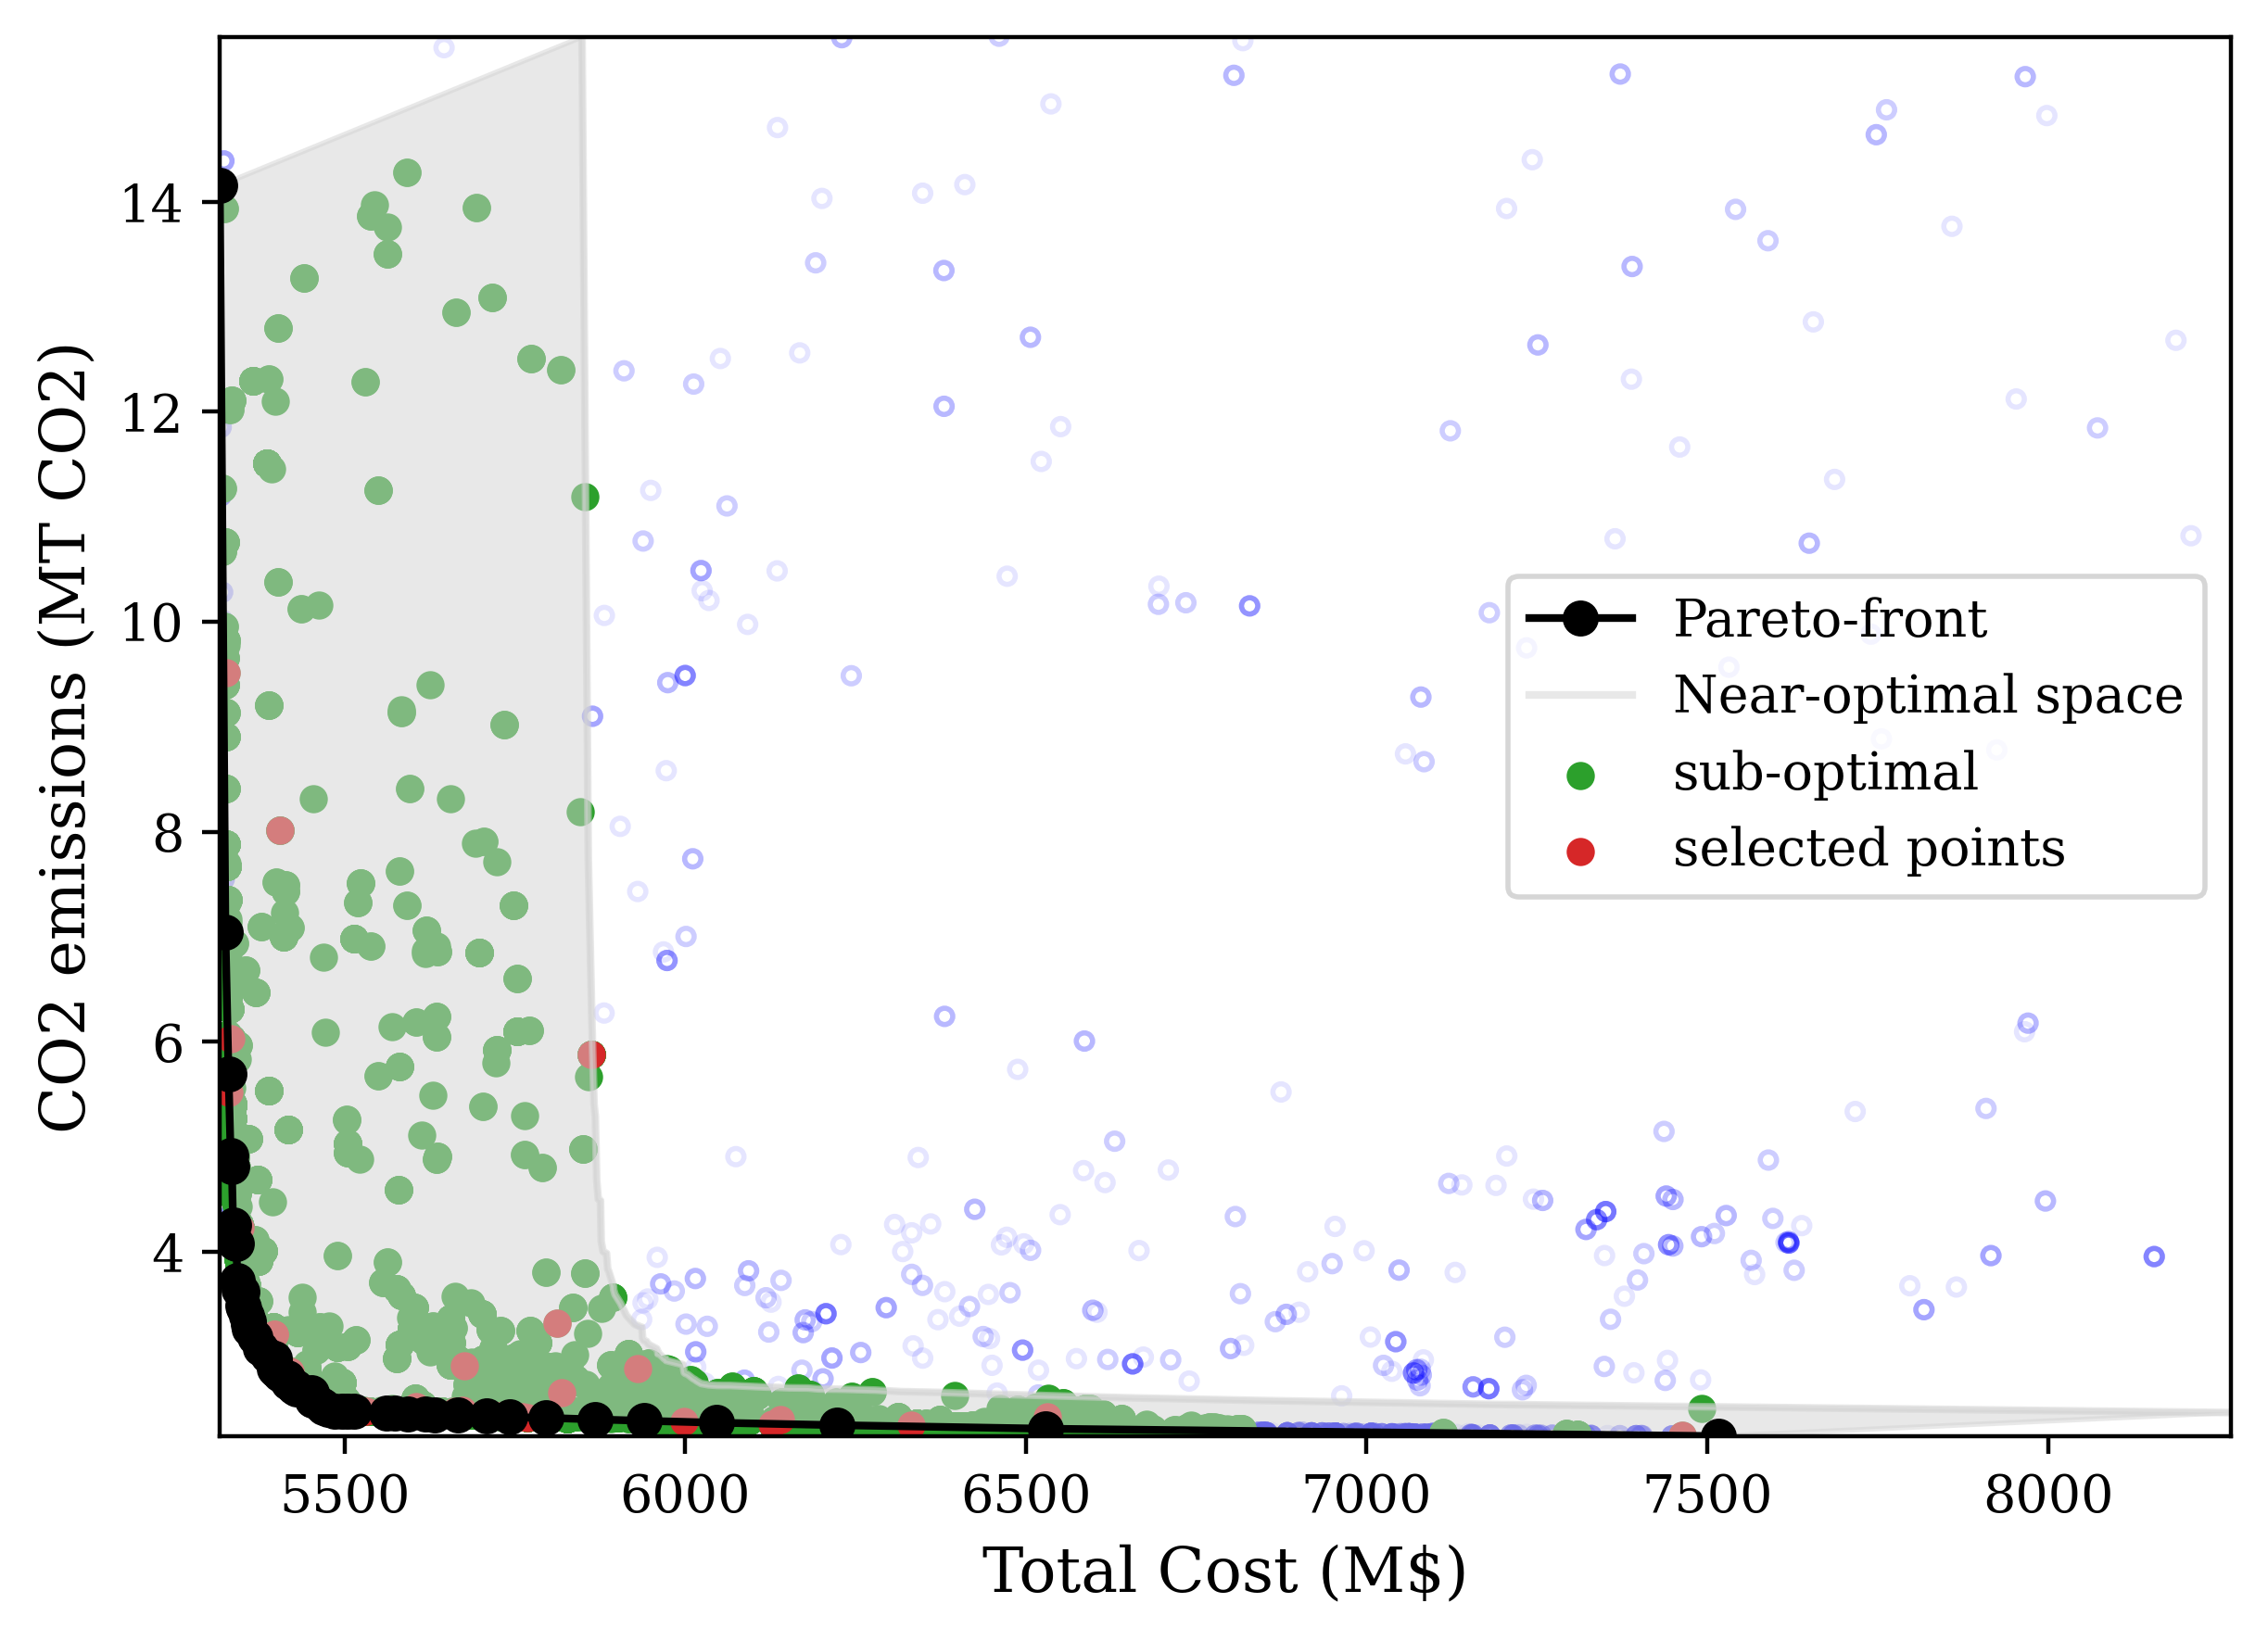
\includegraphics[width=0.6\columnwidth]{figures/results/osier_mga_subset_01.png}
  % \resizebox{0.6\columnwidth}{!}{%% Creator: Matplotlib, PGF backend
%%
%% To include the figure in your LaTeX document, write
%%   \input{<filename>.pgf}
%%
%% Make sure the required packages are loaded in your preamble
%%   \usepackage{pgf}
%%
%% Also ensure that all the required font packages are loaded; for instance,
%% the lmodern package is sometimes necessary when using math font.
%%   \usepackage{lmodern}
%%
%% Figures using additional raster images can only be included by \input if
%% they are in the same directory as the main LaTeX file. For loading figures
%% from other directories you can use the `import` package
%%   \usepackage{import}
%%
%% and then include the figures with
%%   \import{<path to file>}{<filename>.pgf}
%%
%% Matplotlib used the following preamble
%%   \def\mathdefault#1{#1}
%%   \everymath=\expandafter{\the\everymath\displaystyle}
%%   \IfFileExists{scrextend.sty}{
%%     \usepackage[fontsize=10.000000pt]{scrextend}
%%   }{
%%     \renewcommand{\normalsize}{\fontsize{10.000000}{12.000000}\selectfont}
%%     \normalsize
%%   }
%%   
%%   \makeatletter\@ifpackageloaded{underscore}{}{\usepackage[strings]{underscore}}\makeatother
%%
\begingroup%
\makeatletter%
\begin{pgfpicture}%
\pgfpathrectangle{\pgfpointorigin}{\pgfqpoint{7.900000in}{5.900000in}}%
\pgfusepath{use as bounding box, clip}%
\begin{pgfscope}%
\pgfsetbuttcap%
\pgfsetmiterjoin%
\definecolor{currentfill}{rgb}{1.000000,1.000000,1.000000}%
\pgfsetfillcolor{currentfill}%
\pgfsetlinewidth{0.000000pt}%
\definecolor{currentstroke}{rgb}{0.000000,0.000000,0.000000}%
\pgfsetstrokecolor{currentstroke}%
\pgfsetdash{}{0pt}%
\pgfpathmoveto{\pgfqpoint{0.000000in}{0.000000in}}%
\pgfpathlineto{\pgfqpoint{7.900000in}{0.000000in}}%
\pgfpathlineto{\pgfqpoint{7.900000in}{5.900000in}}%
\pgfpathlineto{\pgfqpoint{0.000000in}{5.900000in}}%
\pgfpathlineto{\pgfqpoint{0.000000in}{0.000000in}}%
\pgfpathclose%
\pgfusepath{fill}%
\end{pgfscope}%
\begin{pgfscope}%
\pgfsetbuttcap%
\pgfsetmiterjoin%
\definecolor{currentfill}{rgb}{1.000000,1.000000,1.000000}%
\pgfsetfillcolor{currentfill}%
\pgfsetlinewidth{0.000000pt}%
\definecolor{currentstroke}{rgb}{0.000000,0.000000,0.000000}%
\pgfsetstrokecolor{currentstroke}%
\pgfsetstrokeopacity{0.000000}%
\pgfsetdash{}{0pt}%
\pgfpathmoveto{\pgfqpoint{0.688192in}{0.670138in}}%
\pgfpathlineto{\pgfqpoint{7.800000in}{0.670138in}}%
\pgfpathlineto{\pgfqpoint{7.800000in}{5.800000in}}%
\pgfpathlineto{\pgfqpoint{0.688192in}{5.800000in}}%
\pgfpathlineto{\pgfqpoint{0.688192in}{0.670138in}}%
\pgfpathclose%
\pgfusepath{fill}%
\end{pgfscope}%
\begin{pgfscope}%
\pgfpathrectangle{\pgfqpoint{0.688192in}{0.670138in}}{\pgfqpoint{7.111808in}{5.129862in}}%
\pgfusepath{clip}%
\pgfsetbuttcap%
\pgfsetroundjoin%
\pgfsetlinewidth{1.003750pt}%
\definecolor{currentstroke}{rgb}{0.000000,0.000000,0.000000}%
\pgfsetstrokecolor{currentstroke}%
\pgfsetdash{}{0pt}%
\pgfpathmoveto{\pgfqpoint{5.329102in}{5.309073in}}%
\pgfpathcurveto{\pgfqpoint{5.339998in}{5.309073in}}{\pgfqpoint{5.350449in}{5.313402in}}{\pgfqpoint{5.358153in}{5.321106in}}%
\pgfpathcurveto{\pgfqpoint{5.365857in}{5.328811in}}{\pgfqpoint{5.370186in}{5.339261in}}{\pgfqpoint{5.370186in}{5.350157in}}%
\pgfpathcurveto{\pgfqpoint{5.370186in}{5.361052in}}{\pgfqpoint{5.365857in}{5.371503in}}{\pgfqpoint{5.358153in}{5.379208in}}%
\pgfpathcurveto{\pgfqpoint{5.350449in}{5.386912in}}{\pgfqpoint{5.339998in}{5.391241in}}{\pgfqpoint{5.329102in}{5.391241in}}%
\pgfpathcurveto{\pgfqpoint{5.318207in}{5.391241in}}{\pgfqpoint{5.307756in}{5.386912in}}{\pgfqpoint{5.300052in}{5.379208in}}%
\pgfpathcurveto{\pgfqpoint{5.292347in}{5.371503in}}{\pgfqpoint{5.288018in}{5.361052in}}{\pgfqpoint{5.288018in}{5.350157in}}%
\pgfpathcurveto{\pgfqpoint{5.288018in}{5.339261in}}{\pgfqpoint{5.292347in}{5.328811in}}{\pgfqpoint{5.300052in}{5.321106in}}%
\pgfpathcurveto{\pgfqpoint{5.307756in}{5.313402in}}{\pgfqpoint{5.318207in}{5.309073in}}{\pgfqpoint{5.329102in}{5.309073in}}%
\pgfpathlineto{\pgfqpoint{5.329102in}{5.309073in}}%
\pgfpathclose%
\pgfusepath{stroke}%
\end{pgfscope}%
\begin{pgfscope}%
\pgfpathrectangle{\pgfqpoint{0.688192in}{0.670138in}}{\pgfqpoint{7.111808in}{5.129862in}}%
\pgfusepath{clip}%
\pgfsetbuttcap%
\pgfsetroundjoin%
\pgfsetlinewidth{1.003750pt}%
\definecolor{currentstroke}{rgb}{0.000000,0.000000,0.000000}%
\pgfsetstrokecolor{currentstroke}%
\pgfsetdash{}{0pt}%
\pgfpathmoveto{\pgfqpoint{1.840914in}{0.696069in}}%
\pgfpathcurveto{\pgfqpoint{1.851809in}{0.696069in}}{\pgfqpoint{1.862260in}{0.700398in}}{\pgfqpoint{1.869964in}{0.708103in}}%
\pgfpathcurveto{\pgfqpoint{1.877669in}{0.715807in}}{\pgfqpoint{1.881997in}{0.726258in}}{\pgfqpoint{1.881997in}{0.737153in}}%
\pgfpathcurveto{\pgfqpoint{1.881997in}{0.748049in}}{\pgfqpoint{1.877669in}{0.758500in}}{\pgfqpoint{1.869964in}{0.766204in}}%
\pgfpathcurveto{\pgfqpoint{1.862260in}{0.773908in}}{\pgfqpoint{1.851809in}{0.778237in}}{\pgfqpoint{1.840914in}{0.778237in}}%
\pgfpathcurveto{\pgfqpoint{1.830018in}{0.778237in}}{\pgfqpoint{1.819567in}{0.773908in}}{\pgfqpoint{1.811863in}{0.766204in}}%
\pgfpathcurveto{\pgfqpoint{1.804159in}{0.758500in}}{\pgfqpoint{1.799830in}{0.748049in}}{\pgfqpoint{1.799830in}{0.737153in}}%
\pgfpathcurveto{\pgfqpoint{1.799830in}{0.726258in}}{\pgfqpoint{1.804159in}{0.715807in}}{\pgfqpoint{1.811863in}{0.708103in}}%
\pgfpathcurveto{\pgfqpoint{1.819567in}{0.700398in}}{\pgfqpoint{1.830018in}{0.696069in}}{\pgfqpoint{1.840914in}{0.696069in}}%
\pgfpathlineto{\pgfqpoint{1.840914in}{0.696069in}}%
\pgfpathclose%
\pgfusepath{stroke}%
\end{pgfscope}%
\begin{pgfscope}%
\pgfpathrectangle{\pgfqpoint{0.688192in}{0.670138in}}{\pgfqpoint{7.111808in}{5.129862in}}%
\pgfusepath{clip}%
\pgfsetbuttcap%
\pgfsetroundjoin%
\pgfsetlinewidth{1.003750pt}%
\definecolor{currentstroke}{rgb}{0.000000,0.000000,0.000000}%
\pgfsetstrokecolor{currentstroke}%
\pgfsetdash{}{0pt}%
\pgfpathmoveto{\pgfqpoint{1.101880in}{0.720677in}}%
\pgfpathcurveto{\pgfqpoint{1.112775in}{0.720677in}}{\pgfqpoint{1.123226in}{0.725006in}}{\pgfqpoint{1.130930in}{0.732710in}}%
\pgfpathcurveto{\pgfqpoint{1.138635in}{0.740415in}}{\pgfqpoint{1.142964in}{0.750865in}}{\pgfqpoint{1.142964in}{0.761761in}}%
\pgfpathcurveto{\pgfqpoint{1.142964in}{0.772656in}}{\pgfqpoint{1.138635in}{0.783107in}}{\pgfqpoint{1.130930in}{0.790812in}}%
\pgfpathcurveto{\pgfqpoint{1.123226in}{0.798516in}}{\pgfqpoint{1.112775in}{0.802845in}}{\pgfqpoint{1.101880in}{0.802845in}}%
\pgfpathcurveto{\pgfqpoint{1.090984in}{0.802845in}}{\pgfqpoint{1.080533in}{0.798516in}}{\pgfqpoint{1.072829in}{0.790812in}}%
\pgfpathcurveto{\pgfqpoint{1.065125in}{0.783107in}}{\pgfqpoint{1.060796in}{0.772656in}}{\pgfqpoint{1.060796in}{0.761761in}}%
\pgfpathcurveto{\pgfqpoint{1.060796in}{0.750865in}}{\pgfqpoint{1.065125in}{0.740415in}}{\pgfqpoint{1.072829in}{0.732710in}}%
\pgfpathcurveto{\pgfqpoint{1.080533in}{0.725006in}}{\pgfqpoint{1.090984in}{0.720677in}}{\pgfqpoint{1.101880in}{0.720677in}}%
\pgfpathlineto{\pgfqpoint{1.101880in}{0.720677in}}%
\pgfpathclose%
\pgfusepath{stroke}%
\end{pgfscope}%
\begin{pgfscope}%
\pgfpathrectangle{\pgfqpoint{0.688192in}{0.670138in}}{\pgfqpoint{7.111808in}{5.129862in}}%
\pgfusepath{clip}%
\pgfsetbuttcap%
\pgfsetroundjoin%
\pgfsetlinewidth{1.003750pt}%
\definecolor{currentstroke}{rgb}{0.000000,0.000000,0.000000}%
\pgfsetstrokecolor{currentstroke}%
\pgfsetdash{}{0pt}%
\pgfpathmoveto{\pgfqpoint{1.840914in}{0.696069in}}%
\pgfpathcurveto{\pgfqpoint{1.851809in}{0.696069in}}{\pgfqpoint{1.862260in}{0.700398in}}{\pgfqpoint{1.869964in}{0.708103in}}%
\pgfpathcurveto{\pgfqpoint{1.877669in}{0.715807in}}{\pgfqpoint{1.881997in}{0.726258in}}{\pgfqpoint{1.881997in}{0.737153in}}%
\pgfpathcurveto{\pgfqpoint{1.881997in}{0.748049in}}{\pgfqpoint{1.877669in}{0.758500in}}{\pgfqpoint{1.869964in}{0.766204in}}%
\pgfpathcurveto{\pgfqpoint{1.862260in}{0.773908in}}{\pgfqpoint{1.851809in}{0.778237in}}{\pgfqpoint{1.840914in}{0.778237in}}%
\pgfpathcurveto{\pgfqpoint{1.830018in}{0.778237in}}{\pgfqpoint{1.819567in}{0.773908in}}{\pgfqpoint{1.811863in}{0.766204in}}%
\pgfpathcurveto{\pgfqpoint{1.804159in}{0.758500in}}{\pgfqpoint{1.799830in}{0.748049in}}{\pgfqpoint{1.799830in}{0.737153in}}%
\pgfpathcurveto{\pgfqpoint{1.799830in}{0.726258in}}{\pgfqpoint{1.804159in}{0.715807in}}{\pgfqpoint{1.811863in}{0.708103in}}%
\pgfpathcurveto{\pgfqpoint{1.819567in}{0.700398in}}{\pgfqpoint{1.830018in}{0.696069in}}{\pgfqpoint{1.840914in}{0.696069in}}%
\pgfpathlineto{\pgfqpoint{1.840914in}{0.696069in}}%
\pgfpathclose%
\pgfusepath{stroke}%
\end{pgfscope}%
\begin{pgfscope}%
\pgfpathrectangle{\pgfqpoint{0.688192in}{0.670138in}}{\pgfqpoint{7.111808in}{5.129862in}}%
\pgfusepath{clip}%
\pgfsetbuttcap%
\pgfsetroundjoin%
\pgfsetlinewidth{1.003750pt}%
\definecolor{currentstroke}{rgb}{0.000000,0.000000,0.000000}%
\pgfsetstrokecolor{currentstroke}%
\pgfsetdash{}{0pt}%
\pgfpathmoveto{\pgfqpoint{2.869035in}{0.669385in}}%
\pgfpathcurveto{\pgfqpoint{2.879931in}{0.669385in}}{\pgfqpoint{2.890382in}{0.673714in}}{\pgfqpoint{2.898086in}{0.681419in}}%
\pgfpathcurveto{\pgfqpoint{2.905790in}{0.689123in}}{\pgfqpoint{2.910119in}{0.699574in}}{\pgfqpoint{2.910119in}{0.710469in}}%
\pgfpathcurveto{\pgfqpoint{2.910119in}{0.721365in}}{\pgfqpoint{2.905790in}{0.731816in}}{\pgfqpoint{2.898086in}{0.739520in}}%
\pgfpathcurveto{\pgfqpoint{2.890382in}{0.747224in}}{\pgfqpoint{2.879931in}{0.751553in}}{\pgfqpoint{2.869035in}{0.751553in}}%
\pgfpathcurveto{\pgfqpoint{2.858140in}{0.751553in}}{\pgfqpoint{2.847689in}{0.747224in}}{\pgfqpoint{2.839985in}{0.739520in}}%
\pgfpathcurveto{\pgfqpoint{2.832280in}{0.731816in}}{\pgfqpoint{2.827952in}{0.721365in}}{\pgfqpoint{2.827952in}{0.710469in}}%
\pgfpathcurveto{\pgfqpoint{2.827952in}{0.699574in}}{\pgfqpoint{2.832280in}{0.689123in}}{\pgfqpoint{2.839985in}{0.681419in}}%
\pgfpathcurveto{\pgfqpoint{2.847689in}{0.673714in}}{\pgfqpoint{2.858140in}{0.669385in}}{\pgfqpoint{2.869035in}{0.669385in}}%
\pgfpathlineto{\pgfqpoint{2.869035in}{0.669385in}}%
\pgfpathclose%
\pgfusepath{stroke}%
\end{pgfscope}%
\begin{pgfscope}%
\pgfpathrectangle{\pgfqpoint{0.688192in}{0.670138in}}{\pgfqpoint{7.111808in}{5.129862in}}%
\pgfusepath{clip}%
\pgfsetbuttcap%
\pgfsetroundjoin%
\pgfsetlinewidth{1.003750pt}%
\definecolor{currentstroke}{rgb}{0.000000,0.000000,0.000000}%
\pgfsetstrokecolor{currentstroke}%
\pgfsetdash{}{0pt}%
\pgfpathmoveto{\pgfqpoint{0.789763in}{1.038554in}}%
\pgfpathcurveto{\pgfqpoint{0.800659in}{1.038554in}}{\pgfqpoint{0.811109in}{1.042883in}}{\pgfqpoint{0.818814in}{1.050587in}}%
\pgfpathcurveto{\pgfqpoint{0.826518in}{1.058291in}}{\pgfqpoint{0.830847in}{1.068742in}}{\pgfqpoint{0.830847in}{1.079638in}}%
\pgfpathcurveto{\pgfqpoint{0.830847in}{1.090533in}}{\pgfqpoint{0.826518in}{1.100984in}}{\pgfqpoint{0.818814in}{1.108688in}}%
\pgfpathcurveto{\pgfqpoint{0.811109in}{1.116393in}}{\pgfqpoint{0.800659in}{1.120722in}}{\pgfqpoint{0.789763in}{1.120722in}}%
\pgfpathcurveto{\pgfqpoint{0.778868in}{1.120722in}}{\pgfqpoint{0.768417in}{1.116393in}}{\pgfqpoint{0.760712in}{1.108688in}}%
\pgfpathcurveto{\pgfqpoint{0.753008in}{1.100984in}}{\pgfqpoint{0.748679in}{1.090533in}}{\pgfqpoint{0.748679in}{1.079638in}}%
\pgfpathcurveto{\pgfqpoint{0.748679in}{1.068742in}}{\pgfqpoint{0.753008in}{1.058291in}}{\pgfqpoint{0.760712in}{1.050587in}}%
\pgfpathcurveto{\pgfqpoint{0.768417in}{1.042883in}}{\pgfqpoint{0.778868in}{1.038554in}}{\pgfqpoint{0.789763in}{1.038554in}}%
\pgfpathlineto{\pgfqpoint{0.789763in}{1.038554in}}%
\pgfpathclose%
\pgfusepath{stroke}%
\end{pgfscope}%
\begin{pgfscope}%
\pgfpathrectangle{\pgfqpoint{0.688192in}{0.670138in}}{\pgfqpoint{7.111808in}{5.129862in}}%
\pgfusepath{clip}%
\pgfsetbuttcap%
\pgfsetroundjoin%
\pgfsetlinewidth{1.003750pt}%
\definecolor{currentstroke}{rgb}{0.000000,0.000000,0.000000}%
\pgfsetstrokecolor{currentstroke}%
\pgfsetdash{}{0pt}%
\pgfpathmoveto{\pgfqpoint{1.679564in}{0.702362in}}%
\pgfpathcurveto{\pgfqpoint{1.690460in}{0.702362in}}{\pgfqpoint{1.700911in}{0.706691in}}{\pgfqpoint{1.708615in}{0.714395in}}%
\pgfpathcurveto{\pgfqpoint{1.716319in}{0.722099in}}{\pgfqpoint{1.720648in}{0.732550in}}{\pgfqpoint{1.720648in}{0.743446in}}%
\pgfpathcurveto{\pgfqpoint{1.720648in}{0.754341in}}{\pgfqpoint{1.716319in}{0.764792in}}{\pgfqpoint{1.708615in}{0.772496in}}%
\pgfpathcurveto{\pgfqpoint{1.700911in}{0.780201in}}{\pgfqpoint{1.690460in}{0.784529in}}{\pgfqpoint{1.679564in}{0.784529in}}%
\pgfpathcurveto{\pgfqpoint{1.668669in}{0.784529in}}{\pgfqpoint{1.658218in}{0.780201in}}{\pgfqpoint{1.650514in}{0.772496in}}%
\pgfpathcurveto{\pgfqpoint{1.642809in}{0.764792in}}{\pgfqpoint{1.638480in}{0.754341in}}{\pgfqpoint{1.638480in}{0.743446in}}%
\pgfpathcurveto{\pgfqpoint{1.638480in}{0.732550in}}{\pgfqpoint{1.642809in}{0.722099in}}{\pgfqpoint{1.650514in}{0.714395in}}%
\pgfpathcurveto{\pgfqpoint{1.658218in}{0.706691in}}{\pgfqpoint{1.668669in}{0.702362in}}{\pgfqpoint{1.679564in}{0.702362in}}%
\pgfpathlineto{\pgfqpoint{1.679564in}{0.702362in}}%
\pgfpathclose%
\pgfusepath{stroke}%
\end{pgfscope}%
\begin{pgfscope}%
\pgfpathrectangle{\pgfqpoint{0.688192in}{0.670138in}}{\pgfqpoint{7.111808in}{5.129862in}}%
\pgfusepath{clip}%
\pgfsetbuttcap%
\pgfsetroundjoin%
\pgfsetlinewidth{1.003750pt}%
\definecolor{currentstroke}{rgb}{0.000000,0.000000,0.000000}%
\pgfsetstrokecolor{currentstroke}%
\pgfsetdash{}{0pt}%
\pgfpathmoveto{\pgfqpoint{1.045306in}{0.741536in}}%
\pgfpathcurveto{\pgfqpoint{1.056202in}{0.741536in}}{\pgfqpoint{1.066653in}{0.745865in}}{\pgfqpoint{1.074357in}{0.753569in}}%
\pgfpathcurveto{\pgfqpoint{1.082061in}{0.761274in}}{\pgfqpoint{1.086390in}{0.771725in}}{\pgfqpoint{1.086390in}{0.782620in}}%
\pgfpathcurveto{\pgfqpoint{1.086390in}{0.793516in}}{\pgfqpoint{1.082061in}{0.803967in}}{\pgfqpoint{1.074357in}{0.811671in}}%
\pgfpathcurveto{\pgfqpoint{1.066653in}{0.819375in}}{\pgfqpoint{1.056202in}{0.823704in}}{\pgfqpoint{1.045306in}{0.823704in}}%
\pgfpathcurveto{\pgfqpoint{1.034411in}{0.823704in}}{\pgfqpoint{1.023960in}{0.819375in}}{\pgfqpoint{1.016256in}{0.811671in}}%
\pgfpathcurveto{\pgfqpoint{1.008551in}{0.803967in}}{\pgfqpoint{1.004222in}{0.793516in}}{\pgfqpoint{1.004222in}{0.782620in}}%
\pgfpathcurveto{\pgfqpoint{1.004222in}{0.771725in}}{\pgfqpoint{1.008551in}{0.761274in}}{\pgfqpoint{1.016256in}{0.753569in}}%
\pgfpathcurveto{\pgfqpoint{1.023960in}{0.745865in}}{\pgfqpoint{1.034411in}{0.741536in}}{\pgfqpoint{1.045306in}{0.741536in}}%
\pgfpathlineto{\pgfqpoint{1.045306in}{0.741536in}}%
\pgfpathclose%
\pgfusepath{stroke}%
\end{pgfscope}%
\begin{pgfscope}%
\pgfpathrectangle{\pgfqpoint{0.688192in}{0.670138in}}{\pgfqpoint{7.111808in}{5.129862in}}%
\pgfusepath{clip}%
\pgfsetbuttcap%
\pgfsetroundjoin%
\pgfsetlinewidth{1.003750pt}%
\definecolor{currentstroke}{rgb}{0.000000,0.000000,0.000000}%
\pgfsetstrokecolor{currentstroke}%
\pgfsetdash{}{0pt}%
\pgfpathmoveto{\pgfqpoint{2.013663in}{0.690447in}}%
\pgfpathcurveto{\pgfqpoint{2.024559in}{0.690447in}}{\pgfqpoint{2.035010in}{0.694776in}}{\pgfqpoint{2.042714in}{0.702480in}}%
\pgfpathcurveto{\pgfqpoint{2.050418in}{0.710184in}}{\pgfqpoint{2.054747in}{0.720635in}}{\pgfqpoint{2.054747in}{0.731531in}}%
\pgfpathcurveto{\pgfqpoint{2.054747in}{0.742426in}}{\pgfqpoint{2.050418in}{0.752877in}}{\pgfqpoint{2.042714in}{0.760582in}}%
\pgfpathcurveto{\pgfqpoint{2.035010in}{0.768286in}}{\pgfqpoint{2.024559in}{0.772615in}}{\pgfqpoint{2.013663in}{0.772615in}}%
\pgfpathcurveto{\pgfqpoint{2.002768in}{0.772615in}}{\pgfqpoint{1.992317in}{0.768286in}}{\pgfqpoint{1.984613in}{0.760582in}}%
\pgfpathcurveto{\pgfqpoint{1.976908in}{0.752877in}}{\pgfqpoint{1.972579in}{0.742426in}}{\pgfqpoint{1.972579in}{0.731531in}}%
\pgfpathcurveto{\pgfqpoint{1.972579in}{0.720635in}}{\pgfqpoint{1.976908in}{0.710184in}}{\pgfqpoint{1.984613in}{0.702480in}}%
\pgfpathcurveto{\pgfqpoint{1.992317in}{0.694776in}}{\pgfqpoint{2.002768in}{0.690447in}}{\pgfqpoint{2.013663in}{0.690447in}}%
\pgfpathlineto{\pgfqpoint{2.013663in}{0.690447in}}%
\pgfpathclose%
\pgfusepath{stroke}%
\end{pgfscope}%
\begin{pgfscope}%
\pgfpathrectangle{\pgfqpoint{0.688192in}{0.670138in}}{\pgfqpoint{7.111808in}{5.129862in}}%
\pgfusepath{clip}%
\pgfsetbuttcap%
\pgfsetroundjoin%
\pgfsetlinewidth{1.003750pt}%
\definecolor{currentstroke}{rgb}{0.000000,0.000000,0.000000}%
\pgfsetstrokecolor{currentstroke}%
\pgfsetdash{}{0pt}%
\pgfpathmoveto{\pgfqpoint{0.895312in}{0.866174in}}%
\pgfpathcurveto{\pgfqpoint{0.906208in}{0.866174in}}{\pgfqpoint{0.916658in}{0.870503in}}{\pgfqpoint{0.924363in}{0.878207in}}%
\pgfpathcurveto{\pgfqpoint{0.932067in}{0.885911in}}{\pgfqpoint{0.936396in}{0.896362in}}{\pgfqpoint{0.936396in}{0.907258in}}%
\pgfpathcurveto{\pgfqpoint{0.936396in}{0.918153in}}{\pgfqpoint{0.932067in}{0.928604in}}{\pgfqpoint{0.924363in}{0.936308in}}%
\pgfpathcurveto{\pgfqpoint{0.916658in}{0.944013in}}{\pgfqpoint{0.906208in}{0.948341in}}{\pgfqpoint{0.895312in}{0.948341in}}%
\pgfpathcurveto{\pgfqpoint{0.884416in}{0.948341in}}{\pgfqpoint{0.873966in}{0.944013in}}{\pgfqpoint{0.866261in}{0.936308in}}%
\pgfpathcurveto{\pgfqpoint{0.858557in}{0.928604in}}{\pgfqpoint{0.854228in}{0.918153in}}{\pgfqpoint{0.854228in}{0.907258in}}%
\pgfpathcurveto{\pgfqpoint{0.854228in}{0.896362in}}{\pgfqpoint{0.858557in}{0.885911in}}{\pgfqpoint{0.866261in}{0.878207in}}%
\pgfpathcurveto{\pgfqpoint{0.873966in}{0.870503in}}{\pgfqpoint{0.884416in}{0.866174in}}{\pgfqpoint{0.895312in}{0.866174in}}%
\pgfpathlineto{\pgfqpoint{0.895312in}{0.866174in}}%
\pgfpathclose%
\pgfusepath{stroke}%
\end{pgfscope}%
\begin{pgfscope}%
\pgfpathrectangle{\pgfqpoint{0.688192in}{0.670138in}}{\pgfqpoint{7.111808in}{5.129862in}}%
\pgfusepath{clip}%
\pgfsetbuttcap%
\pgfsetroundjoin%
\pgfsetlinewidth{1.003750pt}%
\definecolor{currentstroke}{rgb}{0.000000,0.000000,0.000000}%
\pgfsetstrokecolor{currentstroke}%
\pgfsetdash{}{0pt}%
\pgfpathmoveto{\pgfqpoint{0.794194in}{1.022605in}}%
\pgfpathcurveto{\pgfqpoint{0.805090in}{1.022605in}}{\pgfqpoint{0.815541in}{1.026933in}}{\pgfqpoint{0.823245in}{1.034638in}}%
\pgfpathcurveto{\pgfqpoint{0.830949in}{1.042342in}}{\pgfqpoint{0.835278in}{1.052793in}}{\pgfqpoint{0.835278in}{1.063688in}}%
\pgfpathcurveto{\pgfqpoint{0.835278in}{1.074584in}}{\pgfqpoint{0.830949in}{1.085035in}}{\pgfqpoint{0.823245in}{1.092739in}}%
\pgfpathcurveto{\pgfqpoint{0.815541in}{1.100443in}}{\pgfqpoint{0.805090in}{1.104772in}}{\pgfqpoint{0.794194in}{1.104772in}}%
\pgfpathcurveto{\pgfqpoint{0.783299in}{1.104772in}}{\pgfqpoint{0.772848in}{1.100443in}}{\pgfqpoint{0.765144in}{1.092739in}}%
\pgfpathcurveto{\pgfqpoint{0.757439in}{1.085035in}}{\pgfqpoint{0.753110in}{1.074584in}}{\pgfqpoint{0.753110in}{1.063688in}}%
\pgfpathcurveto{\pgfqpoint{0.753110in}{1.052793in}}{\pgfqpoint{0.757439in}{1.042342in}}{\pgfqpoint{0.765144in}{1.034638in}}%
\pgfpathcurveto{\pgfqpoint{0.772848in}{1.026933in}}{\pgfqpoint{0.783299in}{1.022605in}}{\pgfqpoint{0.794194in}{1.022605in}}%
\pgfpathlineto{\pgfqpoint{0.794194in}{1.022605in}}%
\pgfpathclose%
\pgfusepath{stroke}%
\end{pgfscope}%
\begin{pgfscope}%
\pgfpathrectangle{\pgfqpoint{0.688192in}{0.670138in}}{\pgfqpoint{7.111808in}{5.129862in}}%
\pgfusepath{clip}%
\pgfsetbuttcap%
\pgfsetroundjoin%
\pgfsetlinewidth{1.003750pt}%
\definecolor{currentstroke}{rgb}{0.000000,0.000000,0.000000}%
\pgfsetstrokecolor{currentstroke}%
\pgfsetdash{}{0pt}%
\pgfpathmoveto{\pgfqpoint{1.019140in}{0.759981in}}%
\pgfpathcurveto{\pgfqpoint{1.030035in}{0.759981in}}{\pgfqpoint{1.040486in}{0.764309in}}{\pgfqpoint{1.048191in}{0.772014in}}%
\pgfpathcurveto{\pgfqpoint{1.055895in}{0.779718in}}{\pgfqpoint{1.060224in}{0.790169in}}{\pgfqpoint{1.060224in}{0.801064in}}%
\pgfpathcurveto{\pgfqpoint{1.060224in}{0.811960in}}{\pgfqpoint{1.055895in}{0.822411in}}{\pgfqpoint{1.048191in}{0.830115in}}%
\pgfpathcurveto{\pgfqpoint{1.040486in}{0.837820in}}{\pgfqpoint{1.030035in}{0.842148in}}{\pgfqpoint{1.019140in}{0.842148in}}%
\pgfpathcurveto{\pgfqpoint{1.008244in}{0.842148in}}{\pgfqpoint{0.997794in}{0.837820in}}{\pgfqpoint{0.990089in}{0.830115in}}%
\pgfpathcurveto{\pgfqpoint{0.982385in}{0.822411in}}{\pgfqpoint{0.978056in}{0.811960in}}{\pgfqpoint{0.978056in}{0.801064in}}%
\pgfpathcurveto{\pgfqpoint{0.978056in}{0.790169in}}{\pgfqpoint{0.982385in}{0.779718in}}{\pgfqpoint{0.990089in}{0.772014in}}%
\pgfpathcurveto{\pgfqpoint{0.997794in}{0.764309in}}{\pgfqpoint{1.008244in}{0.759981in}}{\pgfqpoint{1.019140in}{0.759981in}}%
\pgfpathlineto{\pgfqpoint{1.019140in}{0.759981in}}%
\pgfpathclose%
\pgfusepath{stroke}%
\end{pgfscope}%
\begin{pgfscope}%
\pgfpathrectangle{\pgfqpoint{0.688192in}{0.670138in}}{\pgfqpoint{7.111808in}{5.129862in}}%
\pgfusepath{clip}%
\pgfsetbuttcap%
\pgfsetroundjoin%
\pgfsetlinewidth{1.003750pt}%
\definecolor{currentstroke}{rgb}{0.000000,0.000000,0.000000}%
\pgfsetstrokecolor{currentstroke}%
\pgfsetdash{}{0pt}%
\pgfpathmoveto{\pgfqpoint{1.050667in}{0.739240in}}%
\pgfpathcurveto{\pgfqpoint{1.061563in}{0.739240in}}{\pgfqpoint{1.072014in}{0.743568in}}{\pgfqpoint{1.079718in}{0.751273in}}%
\pgfpathcurveto{\pgfqpoint{1.087422in}{0.758977in}}{\pgfqpoint{1.091751in}{0.769428in}}{\pgfqpoint{1.091751in}{0.780323in}}%
\pgfpathcurveto{\pgfqpoint{1.091751in}{0.791219in}}{\pgfqpoint{1.087422in}{0.801670in}}{\pgfqpoint{1.079718in}{0.809374in}}%
\pgfpathcurveto{\pgfqpoint{1.072014in}{0.817078in}}{\pgfqpoint{1.061563in}{0.821407in}}{\pgfqpoint{1.050667in}{0.821407in}}%
\pgfpathcurveto{\pgfqpoint{1.039772in}{0.821407in}}{\pgfqpoint{1.029321in}{0.817078in}}{\pgfqpoint{1.021617in}{0.809374in}}%
\pgfpathcurveto{\pgfqpoint{1.013912in}{0.801670in}}{\pgfqpoint{1.009583in}{0.791219in}}{\pgfqpoint{1.009583in}{0.780323in}}%
\pgfpathcurveto{\pgfqpoint{1.009583in}{0.769428in}}{\pgfqpoint{1.013912in}{0.758977in}}{\pgfqpoint{1.021617in}{0.751273in}}%
\pgfpathcurveto{\pgfqpoint{1.029321in}{0.743568in}}{\pgfqpoint{1.039772in}{0.739240in}}{\pgfqpoint{1.050667in}{0.739240in}}%
\pgfpathlineto{\pgfqpoint{1.050667in}{0.739240in}}%
\pgfpathclose%
\pgfusepath{stroke}%
\end{pgfscope}%
\begin{pgfscope}%
\pgfpathrectangle{\pgfqpoint{0.688192in}{0.670138in}}{\pgfqpoint{7.111808in}{5.129862in}}%
\pgfusepath{clip}%
\pgfsetbuttcap%
\pgfsetroundjoin%
\pgfsetlinewidth{1.003750pt}%
\definecolor{currentstroke}{rgb}{0.000000,0.000000,0.000000}%
\pgfsetstrokecolor{currentstroke}%
\pgfsetdash{}{0pt}%
\pgfpathmoveto{\pgfqpoint{0.881277in}{0.900428in}}%
\pgfpathcurveto{\pgfqpoint{0.892173in}{0.900428in}}{\pgfqpoint{0.902624in}{0.904756in}}{\pgfqpoint{0.910328in}{0.912461in}}%
\pgfpathcurveto{\pgfqpoint{0.918032in}{0.920165in}}{\pgfqpoint{0.922361in}{0.930616in}}{\pgfqpoint{0.922361in}{0.941511in}}%
\pgfpathcurveto{\pgfqpoint{0.922361in}{0.952407in}}{\pgfqpoint{0.918032in}{0.962858in}}{\pgfqpoint{0.910328in}{0.970562in}}%
\pgfpathcurveto{\pgfqpoint{0.902624in}{0.978266in}}{\pgfqpoint{0.892173in}{0.982595in}}{\pgfqpoint{0.881277in}{0.982595in}}%
\pgfpathcurveto{\pgfqpoint{0.870382in}{0.982595in}}{\pgfqpoint{0.859931in}{0.978266in}}{\pgfqpoint{0.852226in}{0.970562in}}%
\pgfpathcurveto{\pgfqpoint{0.844522in}{0.962858in}}{\pgfqpoint{0.840193in}{0.952407in}}{\pgfqpoint{0.840193in}{0.941511in}}%
\pgfpathcurveto{\pgfqpoint{0.840193in}{0.930616in}}{\pgfqpoint{0.844522in}{0.920165in}}{\pgfqpoint{0.852226in}{0.912461in}}%
\pgfpathcurveto{\pgfqpoint{0.859931in}{0.904756in}}{\pgfqpoint{0.870382in}{0.900428in}}{\pgfqpoint{0.881277in}{0.900428in}}%
\pgfpathlineto{\pgfqpoint{0.881277in}{0.900428in}}%
\pgfpathclose%
\pgfusepath{stroke}%
\end{pgfscope}%
\begin{pgfscope}%
\pgfpathrectangle{\pgfqpoint{0.688192in}{0.670138in}}{\pgfqpoint{7.111808in}{5.129862in}}%
\pgfusepath{clip}%
\pgfsetbuttcap%
\pgfsetroundjoin%
\pgfsetlinewidth{1.003750pt}%
\definecolor{currentstroke}{rgb}{0.000000,0.000000,0.000000}%
\pgfsetstrokecolor{currentstroke}%
\pgfsetdash{}{0pt}%
\pgfpathmoveto{\pgfqpoint{0.721104in}{1.921896in}}%
\pgfpathcurveto{\pgfqpoint{0.732000in}{1.921896in}}{\pgfqpoint{0.742451in}{1.926225in}}{\pgfqpoint{0.750155in}{1.933929in}}%
\pgfpathcurveto{\pgfqpoint{0.757859in}{1.941634in}}{\pgfqpoint{0.762188in}{1.952084in}}{\pgfqpoint{0.762188in}{1.962980in}}%
\pgfpathcurveto{\pgfqpoint{0.762188in}{1.973876in}}{\pgfqpoint{0.757859in}{1.984326in}}{\pgfqpoint{0.750155in}{1.992031in}}%
\pgfpathcurveto{\pgfqpoint{0.742451in}{1.999735in}}{\pgfqpoint{0.732000in}{2.004064in}}{\pgfqpoint{0.721104in}{2.004064in}}%
\pgfpathcurveto{\pgfqpoint{0.710209in}{2.004064in}}{\pgfqpoint{0.699758in}{1.999735in}}{\pgfqpoint{0.692054in}{1.992031in}}%
\pgfpathcurveto{\pgfqpoint{0.684349in}{1.984326in}}{\pgfqpoint{0.680020in}{1.973876in}}{\pgfqpoint{0.680020in}{1.962980in}}%
\pgfpathcurveto{\pgfqpoint{0.680020in}{1.952084in}}{\pgfqpoint{0.684349in}{1.941634in}}{\pgfqpoint{0.692054in}{1.933929in}}%
\pgfpathcurveto{\pgfqpoint{0.699758in}{1.926225in}}{\pgfqpoint{0.710209in}{1.921896in}}{\pgfqpoint{0.721104in}{1.921896in}}%
\pgfpathlineto{\pgfqpoint{0.721104in}{1.921896in}}%
\pgfpathclose%
\pgfusepath{stroke}%
\end{pgfscope}%
\begin{pgfscope}%
\pgfpathrectangle{\pgfqpoint{0.688192in}{0.670138in}}{\pgfqpoint{7.111808in}{5.129862in}}%
\pgfusepath{clip}%
\pgfsetbuttcap%
\pgfsetroundjoin%
\pgfsetlinewidth{1.003750pt}%
\definecolor{currentstroke}{rgb}{0.000000,0.000000,0.000000}%
\pgfsetstrokecolor{currentstroke}%
\pgfsetdash{}{0pt}%
\pgfpathmoveto{\pgfqpoint{1.351667in}{0.711476in}}%
\pgfpathcurveto{\pgfqpoint{1.362562in}{0.711476in}}{\pgfqpoint{1.373013in}{0.715805in}}{\pgfqpoint{1.380718in}{0.723510in}}%
\pgfpathcurveto{\pgfqpoint{1.388422in}{0.731214in}}{\pgfqpoint{1.392751in}{0.741665in}}{\pgfqpoint{1.392751in}{0.752560in}}%
\pgfpathcurveto{\pgfqpoint{1.392751in}{0.763456in}}{\pgfqpoint{1.388422in}{0.773907in}}{\pgfqpoint{1.380718in}{0.781611in}}%
\pgfpathcurveto{\pgfqpoint{1.373013in}{0.789315in}}{\pgfqpoint{1.362562in}{0.793644in}}{\pgfqpoint{1.351667in}{0.793644in}}%
\pgfpathcurveto{\pgfqpoint{1.340771in}{0.793644in}}{\pgfqpoint{1.330321in}{0.789315in}}{\pgfqpoint{1.322616in}{0.781611in}}%
\pgfpathcurveto{\pgfqpoint{1.314912in}{0.773907in}}{\pgfqpoint{1.310583in}{0.763456in}}{\pgfqpoint{1.310583in}{0.752560in}}%
\pgfpathcurveto{\pgfqpoint{1.310583in}{0.741665in}}{\pgfqpoint{1.314912in}{0.731214in}}{\pgfqpoint{1.322616in}{0.723510in}}%
\pgfpathcurveto{\pgfqpoint{1.330321in}{0.715805in}}{\pgfqpoint{1.340771in}{0.711476in}}{\pgfqpoint{1.351667in}{0.711476in}}%
\pgfpathlineto{\pgfqpoint{1.351667in}{0.711476in}}%
\pgfpathclose%
\pgfusepath{stroke}%
\end{pgfscope}%
\begin{pgfscope}%
\pgfpathrectangle{\pgfqpoint{0.688192in}{0.670138in}}{\pgfqpoint{7.111808in}{5.129862in}}%
\pgfusepath{clip}%
\pgfsetbuttcap%
\pgfsetroundjoin%
\pgfsetlinewidth{1.003750pt}%
\definecolor{currentstroke}{rgb}{0.000000,0.000000,0.000000}%
\pgfsetstrokecolor{currentstroke}%
\pgfsetdash{}{0pt}%
\pgfpathmoveto{\pgfqpoint{0.928243in}{0.841597in}}%
\pgfpathcurveto{\pgfqpoint{0.939139in}{0.841597in}}{\pgfqpoint{0.949589in}{0.845926in}}{\pgfqpoint{0.957294in}{0.853631in}}%
\pgfpathcurveto{\pgfqpoint{0.964998in}{0.861335in}}{\pgfqpoint{0.969327in}{0.871786in}}{\pgfqpoint{0.969327in}{0.882681in}}%
\pgfpathcurveto{\pgfqpoint{0.969327in}{0.893577in}}{\pgfqpoint{0.964998in}{0.904028in}}{\pgfqpoint{0.957294in}{0.911732in}}%
\pgfpathcurveto{\pgfqpoint{0.949589in}{0.919436in}}{\pgfqpoint{0.939139in}{0.923765in}}{\pgfqpoint{0.928243in}{0.923765in}}%
\pgfpathcurveto{\pgfqpoint{0.917347in}{0.923765in}}{\pgfqpoint{0.906897in}{0.919436in}}{\pgfqpoint{0.899192in}{0.911732in}}%
\pgfpathcurveto{\pgfqpoint{0.891488in}{0.904028in}}{\pgfqpoint{0.887159in}{0.893577in}}{\pgfqpoint{0.887159in}{0.882681in}}%
\pgfpathcurveto{\pgfqpoint{0.887159in}{0.871786in}}{\pgfqpoint{0.891488in}{0.861335in}}{\pgfqpoint{0.899192in}{0.853631in}}%
\pgfpathcurveto{\pgfqpoint{0.906897in}{0.845926in}}{\pgfqpoint{0.917347in}{0.841597in}}{\pgfqpoint{0.928243in}{0.841597in}}%
\pgfpathlineto{\pgfqpoint{0.928243in}{0.841597in}}%
\pgfpathclose%
\pgfusepath{stroke}%
\end{pgfscope}%
\begin{pgfscope}%
\pgfpathrectangle{\pgfqpoint{0.688192in}{0.670138in}}{\pgfqpoint{7.111808in}{5.129862in}}%
\pgfusepath{clip}%
\pgfsetbuttcap%
\pgfsetroundjoin%
\pgfsetlinewidth{1.003750pt}%
\definecolor{currentstroke}{rgb}{0.000000,0.000000,0.000000}%
\pgfsetstrokecolor{currentstroke}%
\pgfsetdash{}{0pt}%
\pgfpathmoveto{\pgfqpoint{6.014792in}{1.437812in}}%
\pgfpathcurveto{\pgfqpoint{6.025688in}{1.437812in}}{\pgfqpoint{6.036139in}{1.442141in}}{\pgfqpoint{6.043843in}{1.449845in}}%
\pgfpathcurveto{\pgfqpoint{6.051547in}{1.457549in}}{\pgfqpoint{6.055876in}{1.468000in}}{\pgfqpoint{6.055876in}{1.478896in}}%
\pgfpathcurveto{\pgfqpoint{6.055876in}{1.489791in}}{\pgfqpoint{6.051547in}{1.500242in}}{\pgfqpoint{6.043843in}{1.507947in}}%
\pgfpathcurveto{\pgfqpoint{6.036139in}{1.515651in}}{\pgfqpoint{6.025688in}{1.519980in}}{\pgfqpoint{6.014792in}{1.519980in}}%
\pgfpathcurveto{\pgfqpoint{6.003897in}{1.519980in}}{\pgfqpoint{5.993446in}{1.515651in}}{\pgfqpoint{5.985741in}{1.507947in}}%
\pgfpathcurveto{\pgfqpoint{5.978037in}{1.500242in}}{\pgfqpoint{5.973708in}{1.489791in}}{\pgfqpoint{5.973708in}{1.478896in}}%
\pgfpathcurveto{\pgfqpoint{5.973708in}{1.468000in}}{\pgfqpoint{5.978037in}{1.457549in}}{\pgfqpoint{5.985741in}{1.449845in}}%
\pgfpathcurveto{\pgfqpoint{5.993446in}{1.442141in}}{\pgfqpoint{6.003897in}{1.437812in}}{\pgfqpoint{6.014792in}{1.437812in}}%
\pgfpathlineto{\pgfqpoint{6.014792in}{1.437812in}}%
\pgfpathclose%
\pgfusepath{stroke}%
\end{pgfscope}%
\begin{pgfscope}%
\pgfpathrectangle{\pgfqpoint{0.688192in}{0.670138in}}{\pgfqpoint{7.111808in}{5.129862in}}%
\pgfusepath{clip}%
\pgfsetbuttcap%
\pgfsetroundjoin%
\pgfsetlinewidth{1.003750pt}%
\definecolor{currentstroke}{rgb}{0.000000,0.000000,0.000000}%
\pgfsetstrokecolor{currentstroke}%
\pgfsetdash{}{0pt}%
\pgfpathmoveto{\pgfqpoint{0.895312in}{0.866174in}}%
\pgfpathcurveto{\pgfqpoint{0.906208in}{0.866174in}}{\pgfqpoint{0.916658in}{0.870503in}}{\pgfqpoint{0.924363in}{0.878207in}}%
\pgfpathcurveto{\pgfqpoint{0.932067in}{0.885911in}}{\pgfqpoint{0.936396in}{0.896362in}}{\pgfqpoint{0.936396in}{0.907258in}}%
\pgfpathcurveto{\pgfqpoint{0.936396in}{0.918153in}}{\pgfqpoint{0.932067in}{0.928604in}}{\pgfqpoint{0.924363in}{0.936308in}}%
\pgfpathcurveto{\pgfqpoint{0.916658in}{0.944013in}}{\pgfqpoint{0.906208in}{0.948341in}}{\pgfqpoint{0.895312in}{0.948341in}}%
\pgfpathcurveto{\pgfqpoint{0.884416in}{0.948341in}}{\pgfqpoint{0.873966in}{0.944013in}}{\pgfqpoint{0.866261in}{0.936308in}}%
\pgfpathcurveto{\pgfqpoint{0.858557in}{0.928604in}}{\pgfqpoint{0.854228in}{0.918153in}}{\pgfqpoint{0.854228in}{0.907258in}}%
\pgfpathcurveto{\pgfqpoint{0.854228in}{0.896362in}}{\pgfqpoint{0.858557in}{0.885911in}}{\pgfqpoint{0.866261in}{0.878207in}}%
\pgfpathcurveto{\pgfqpoint{0.873966in}{0.870503in}}{\pgfqpoint{0.884416in}{0.866174in}}{\pgfqpoint{0.895312in}{0.866174in}}%
\pgfpathlineto{\pgfqpoint{0.895312in}{0.866174in}}%
\pgfpathclose%
\pgfusepath{stroke}%
\end{pgfscope}%
\begin{pgfscope}%
\pgfpathrectangle{\pgfqpoint{0.688192in}{0.670138in}}{\pgfqpoint{7.111808in}{5.129862in}}%
\pgfusepath{clip}%
\pgfsetbuttcap%
\pgfsetroundjoin%
\pgfsetlinewidth{1.003750pt}%
\definecolor{currentstroke}{rgb}{0.000000,0.000000,0.000000}%
\pgfsetstrokecolor{currentstroke}%
\pgfsetdash{}{0pt}%
\pgfpathmoveto{\pgfqpoint{1.759569in}{0.698796in}}%
\pgfpathcurveto{\pgfqpoint{1.770464in}{0.698796in}}{\pgfqpoint{1.780915in}{0.703125in}}{\pgfqpoint{1.788619in}{0.710830in}}%
\pgfpathcurveto{\pgfqpoint{1.796324in}{0.718534in}}{\pgfqpoint{1.800652in}{0.728985in}}{\pgfqpoint{1.800652in}{0.739880in}}%
\pgfpathcurveto{\pgfqpoint{1.800652in}{0.750776in}}{\pgfqpoint{1.796324in}{0.761227in}}{\pgfqpoint{1.788619in}{0.768931in}}%
\pgfpathcurveto{\pgfqpoint{1.780915in}{0.776635in}}{\pgfqpoint{1.770464in}{0.780964in}}{\pgfqpoint{1.759569in}{0.780964in}}%
\pgfpathcurveto{\pgfqpoint{1.748673in}{0.780964in}}{\pgfqpoint{1.738222in}{0.776635in}}{\pgfqpoint{1.730518in}{0.768931in}}%
\pgfpathcurveto{\pgfqpoint{1.722814in}{0.761227in}}{\pgfqpoint{1.718485in}{0.750776in}}{\pgfqpoint{1.718485in}{0.739880in}}%
\pgfpathcurveto{\pgfqpoint{1.718485in}{0.728985in}}{\pgfqpoint{1.722814in}{0.718534in}}{\pgfqpoint{1.730518in}{0.710830in}}%
\pgfpathcurveto{\pgfqpoint{1.738222in}{0.703125in}}{\pgfqpoint{1.748673in}{0.698796in}}{\pgfqpoint{1.759569in}{0.698796in}}%
\pgfpathlineto{\pgfqpoint{1.759569in}{0.698796in}}%
\pgfpathclose%
\pgfusepath{stroke}%
\end{pgfscope}%
\begin{pgfscope}%
\pgfpathrectangle{\pgfqpoint{0.688192in}{0.670138in}}{\pgfqpoint{7.111808in}{5.129862in}}%
\pgfusepath{clip}%
\pgfsetbuttcap%
\pgfsetroundjoin%
\pgfsetlinewidth{1.003750pt}%
\definecolor{currentstroke}{rgb}{0.000000,0.000000,0.000000}%
\pgfsetstrokecolor{currentstroke}%
\pgfsetdash{}{0pt}%
\pgfpathmoveto{\pgfqpoint{1.351667in}{0.711476in}}%
\pgfpathcurveto{\pgfqpoint{1.362562in}{0.711476in}}{\pgfqpoint{1.373013in}{0.715805in}}{\pgfqpoint{1.380718in}{0.723510in}}%
\pgfpathcurveto{\pgfqpoint{1.388422in}{0.731214in}}{\pgfqpoint{1.392751in}{0.741665in}}{\pgfqpoint{1.392751in}{0.752560in}}%
\pgfpathcurveto{\pgfqpoint{1.392751in}{0.763456in}}{\pgfqpoint{1.388422in}{0.773907in}}{\pgfqpoint{1.380718in}{0.781611in}}%
\pgfpathcurveto{\pgfqpoint{1.373013in}{0.789315in}}{\pgfqpoint{1.362562in}{0.793644in}}{\pgfqpoint{1.351667in}{0.793644in}}%
\pgfpathcurveto{\pgfqpoint{1.340771in}{0.793644in}}{\pgfqpoint{1.330321in}{0.789315in}}{\pgfqpoint{1.322616in}{0.781611in}}%
\pgfpathcurveto{\pgfqpoint{1.314912in}{0.773907in}}{\pgfqpoint{1.310583in}{0.763456in}}{\pgfqpoint{1.310583in}{0.752560in}}%
\pgfpathcurveto{\pgfqpoint{1.310583in}{0.741665in}}{\pgfqpoint{1.314912in}{0.731214in}}{\pgfqpoint{1.322616in}{0.723510in}}%
\pgfpathcurveto{\pgfqpoint{1.330321in}{0.715805in}}{\pgfqpoint{1.340771in}{0.711476in}}{\pgfqpoint{1.351667in}{0.711476in}}%
\pgfpathlineto{\pgfqpoint{1.351667in}{0.711476in}}%
\pgfpathclose%
\pgfusepath{stroke}%
\end{pgfscope}%
\begin{pgfscope}%
\pgfpathrectangle{\pgfqpoint{0.688192in}{0.670138in}}{\pgfqpoint{7.111808in}{5.129862in}}%
\pgfusepath{clip}%
\pgfsetbuttcap%
\pgfsetroundjoin%
\pgfsetlinewidth{1.003750pt}%
\definecolor{currentstroke}{rgb}{0.000000,0.000000,0.000000}%
\pgfsetstrokecolor{currentstroke}%
\pgfsetdash{}{0pt}%
\pgfpathmoveto{\pgfqpoint{1.631842in}{0.703864in}}%
\pgfpathcurveto{\pgfqpoint{1.642737in}{0.703864in}}{\pgfqpoint{1.653188in}{0.708193in}}{\pgfqpoint{1.660893in}{0.715897in}}%
\pgfpathcurveto{\pgfqpoint{1.668597in}{0.723601in}}{\pgfqpoint{1.672926in}{0.734052in}}{\pgfqpoint{1.672926in}{0.744948in}}%
\pgfpathcurveto{\pgfqpoint{1.672926in}{0.755843in}}{\pgfqpoint{1.668597in}{0.766294in}}{\pgfqpoint{1.660893in}{0.773998in}}%
\pgfpathcurveto{\pgfqpoint{1.653188in}{0.781703in}}{\pgfqpoint{1.642737in}{0.786032in}}{\pgfqpoint{1.631842in}{0.786032in}}%
\pgfpathcurveto{\pgfqpoint{1.620946in}{0.786032in}}{\pgfqpoint{1.610496in}{0.781703in}}{\pgfqpoint{1.602791in}{0.773998in}}%
\pgfpathcurveto{\pgfqpoint{1.595087in}{0.766294in}}{\pgfqpoint{1.590758in}{0.755843in}}{\pgfqpoint{1.590758in}{0.744948in}}%
\pgfpathcurveto{\pgfqpoint{1.590758in}{0.734052in}}{\pgfqpoint{1.595087in}{0.723601in}}{\pgfqpoint{1.602791in}{0.715897in}}%
\pgfpathcurveto{\pgfqpoint{1.610496in}{0.708193in}}{\pgfqpoint{1.620946in}{0.703864in}}{\pgfqpoint{1.631842in}{0.703864in}}%
\pgfpathlineto{\pgfqpoint{1.631842in}{0.703864in}}%
\pgfpathclose%
\pgfusepath{stroke}%
\end{pgfscope}%
\begin{pgfscope}%
\pgfpathrectangle{\pgfqpoint{0.688192in}{0.670138in}}{\pgfqpoint{7.111808in}{5.129862in}}%
\pgfusepath{clip}%
\pgfsetbuttcap%
\pgfsetroundjoin%
\pgfsetlinewidth{1.003750pt}%
\definecolor{currentstroke}{rgb}{0.000000,0.000000,0.000000}%
\pgfsetstrokecolor{currentstroke}%
\pgfsetdash{}{0pt}%
\pgfpathmoveto{\pgfqpoint{6.024600in}{3.448401in}}%
\pgfpathcurveto{\pgfqpoint{6.035496in}{3.448401in}}{\pgfqpoint{6.045947in}{3.452730in}}{\pgfqpoint{6.053651in}{3.460434in}}%
\pgfpathcurveto{\pgfqpoint{6.061355in}{3.468139in}}{\pgfqpoint{6.065684in}{3.478589in}}{\pgfqpoint{6.065684in}{3.489485in}}%
\pgfpathcurveto{\pgfqpoint{6.065684in}{3.500381in}}{\pgfqpoint{6.061355in}{3.510831in}}{\pgfqpoint{6.053651in}{3.518536in}}%
\pgfpathcurveto{\pgfqpoint{6.045947in}{3.526240in}}{\pgfqpoint{6.035496in}{3.530569in}}{\pgfqpoint{6.024600in}{3.530569in}}%
\pgfpathcurveto{\pgfqpoint{6.013705in}{3.530569in}}{\pgfqpoint{6.003254in}{3.526240in}}{\pgfqpoint{5.995550in}{3.518536in}}%
\pgfpathcurveto{\pgfqpoint{5.987845in}{3.510831in}}{\pgfqpoint{5.983517in}{3.500381in}}{\pgfqpoint{5.983517in}{3.489485in}}%
\pgfpathcurveto{\pgfqpoint{5.983517in}{3.478589in}}{\pgfqpoint{5.987845in}{3.468139in}}{\pgfqpoint{5.995550in}{3.460434in}}%
\pgfpathcurveto{\pgfqpoint{6.003254in}{3.452730in}}{\pgfqpoint{6.013705in}{3.448401in}}{\pgfqpoint{6.024600in}{3.448401in}}%
\pgfpathlineto{\pgfqpoint{6.024600in}{3.448401in}}%
\pgfpathclose%
\pgfusepath{stroke}%
\end{pgfscope}%
\begin{pgfscope}%
\pgfpathrectangle{\pgfqpoint{0.688192in}{0.670138in}}{\pgfqpoint{7.111808in}{5.129862in}}%
\pgfusepath{clip}%
\pgfsetbuttcap%
\pgfsetroundjoin%
\pgfsetlinewidth{1.003750pt}%
\definecolor{currentstroke}{rgb}{0.000000,0.000000,0.000000}%
\pgfsetstrokecolor{currentstroke}%
\pgfsetdash{}{0pt}%
\pgfpathmoveto{\pgfqpoint{0.721104in}{1.921896in}}%
\pgfpathcurveto{\pgfqpoint{0.732000in}{1.921896in}}{\pgfqpoint{0.742451in}{1.926225in}}{\pgfqpoint{0.750155in}{1.933929in}}%
\pgfpathcurveto{\pgfqpoint{0.757859in}{1.941634in}}{\pgfqpoint{0.762188in}{1.952084in}}{\pgfqpoint{0.762188in}{1.962980in}}%
\pgfpathcurveto{\pgfqpoint{0.762188in}{1.973876in}}{\pgfqpoint{0.757859in}{1.984326in}}{\pgfqpoint{0.750155in}{1.992031in}}%
\pgfpathcurveto{\pgfqpoint{0.742451in}{1.999735in}}{\pgfqpoint{0.732000in}{2.004064in}}{\pgfqpoint{0.721104in}{2.004064in}}%
\pgfpathcurveto{\pgfqpoint{0.710209in}{2.004064in}}{\pgfqpoint{0.699758in}{1.999735in}}{\pgfqpoint{0.692054in}{1.992031in}}%
\pgfpathcurveto{\pgfqpoint{0.684349in}{1.984326in}}{\pgfqpoint{0.680020in}{1.973876in}}{\pgfqpoint{0.680020in}{1.962980in}}%
\pgfpathcurveto{\pgfqpoint{0.680020in}{1.952084in}}{\pgfqpoint{0.684349in}{1.941634in}}{\pgfqpoint{0.692054in}{1.933929in}}%
\pgfpathcurveto{\pgfqpoint{0.699758in}{1.926225in}}{\pgfqpoint{0.710209in}{1.921896in}}{\pgfqpoint{0.721104in}{1.921896in}}%
\pgfpathlineto{\pgfqpoint{0.721104in}{1.921896in}}%
\pgfpathclose%
\pgfusepath{stroke}%
\end{pgfscope}%
\begin{pgfscope}%
\pgfpathrectangle{\pgfqpoint{0.688192in}{0.670138in}}{\pgfqpoint{7.111808in}{5.129862in}}%
\pgfusepath{clip}%
\pgfsetbuttcap%
\pgfsetroundjoin%
\pgfsetlinewidth{1.003750pt}%
\definecolor{currentstroke}{rgb}{0.000000,0.000000,0.000000}%
\pgfsetstrokecolor{currentstroke}%
\pgfsetdash{}{0pt}%
\pgfpathmoveto{\pgfqpoint{2.751273in}{1.008701in}}%
\pgfpathcurveto{\pgfqpoint{2.762169in}{1.008701in}}{\pgfqpoint{2.772620in}{1.013030in}}{\pgfqpoint{2.780324in}{1.020734in}}%
\pgfpathcurveto{\pgfqpoint{2.788028in}{1.028439in}}{\pgfqpoint{2.792357in}{1.038890in}}{\pgfqpoint{2.792357in}{1.049785in}}%
\pgfpathcurveto{\pgfqpoint{2.792357in}{1.060681in}}{\pgfqpoint{2.788028in}{1.071131in}}{\pgfqpoint{2.780324in}{1.078836in}}%
\pgfpathcurveto{\pgfqpoint{2.772620in}{1.086540in}}{\pgfqpoint{2.762169in}{1.090869in}}{\pgfqpoint{2.751273in}{1.090869in}}%
\pgfpathcurveto{\pgfqpoint{2.740378in}{1.090869in}}{\pgfqpoint{2.729927in}{1.086540in}}{\pgfqpoint{2.722223in}{1.078836in}}%
\pgfpathcurveto{\pgfqpoint{2.714518in}{1.071131in}}{\pgfqpoint{2.710189in}{1.060681in}}{\pgfqpoint{2.710189in}{1.049785in}}%
\pgfpathcurveto{\pgfqpoint{2.710189in}{1.038890in}}{\pgfqpoint{2.714518in}{1.028439in}}{\pgfqpoint{2.722223in}{1.020734in}}%
\pgfpathcurveto{\pgfqpoint{2.729927in}{1.013030in}}{\pgfqpoint{2.740378in}{1.008701in}}{\pgfqpoint{2.751273in}{1.008701in}}%
\pgfpathlineto{\pgfqpoint{2.751273in}{1.008701in}}%
\pgfpathclose%
\pgfusepath{stroke}%
\end{pgfscope}%
\begin{pgfscope}%
\pgfpathrectangle{\pgfqpoint{0.688192in}{0.670138in}}{\pgfqpoint{7.111808in}{5.129862in}}%
\pgfusepath{clip}%
\pgfsetbuttcap%
\pgfsetroundjoin%
\pgfsetlinewidth{1.003750pt}%
\definecolor{currentstroke}{rgb}{0.000000,0.000000,0.000000}%
\pgfsetstrokecolor{currentstroke}%
\pgfsetdash{}{0pt}%
\pgfpathmoveto{\pgfqpoint{1.625190in}{0.704414in}}%
\pgfpathcurveto{\pgfqpoint{1.636086in}{0.704414in}}{\pgfqpoint{1.646537in}{0.708742in}}{\pgfqpoint{1.654241in}{0.716447in}}%
\pgfpathcurveto{\pgfqpoint{1.661945in}{0.724151in}}{\pgfqpoint{1.666274in}{0.734602in}}{\pgfqpoint{1.666274in}{0.745498in}}%
\pgfpathcurveto{\pgfqpoint{1.666274in}{0.756393in}}{\pgfqpoint{1.661945in}{0.766844in}}{\pgfqpoint{1.654241in}{0.774548in}}%
\pgfpathcurveto{\pgfqpoint{1.646537in}{0.782253in}}{\pgfqpoint{1.636086in}{0.786581in}}{\pgfqpoint{1.625190in}{0.786581in}}%
\pgfpathcurveto{\pgfqpoint{1.614295in}{0.786581in}}{\pgfqpoint{1.603844in}{0.782253in}}{\pgfqpoint{1.596140in}{0.774548in}}%
\pgfpathcurveto{\pgfqpoint{1.588435in}{0.766844in}}{\pgfqpoint{1.584107in}{0.756393in}}{\pgfqpoint{1.584107in}{0.745498in}}%
\pgfpathcurveto{\pgfqpoint{1.584107in}{0.734602in}}{\pgfqpoint{1.588435in}{0.724151in}}{\pgfqpoint{1.596140in}{0.716447in}}%
\pgfpathcurveto{\pgfqpoint{1.603844in}{0.708742in}}{\pgfqpoint{1.614295in}{0.704414in}}{\pgfqpoint{1.625190in}{0.704414in}}%
\pgfpathlineto{\pgfqpoint{1.625190in}{0.704414in}}%
\pgfpathclose%
\pgfusepath{stroke}%
\end{pgfscope}%
\begin{pgfscope}%
\pgfpathrectangle{\pgfqpoint{0.688192in}{0.670138in}}{\pgfqpoint{7.111808in}{5.129862in}}%
\pgfusepath{clip}%
\pgfsetbuttcap%
\pgfsetroundjoin%
\pgfsetlinewidth{1.003750pt}%
\definecolor{currentstroke}{rgb}{0.000000,0.000000,0.000000}%
\pgfsetstrokecolor{currentstroke}%
\pgfsetdash{}{0pt}%
\pgfpathmoveto{\pgfqpoint{0.880316in}{0.913368in}}%
\pgfpathcurveto{\pgfqpoint{0.891212in}{0.913368in}}{\pgfqpoint{0.901663in}{0.917697in}}{\pgfqpoint{0.909367in}{0.925401in}}%
\pgfpathcurveto{\pgfqpoint{0.917071in}{0.933106in}}{\pgfqpoint{0.921400in}{0.943557in}}{\pgfqpoint{0.921400in}{0.954452in}}%
\pgfpathcurveto{\pgfqpoint{0.921400in}{0.965348in}}{\pgfqpoint{0.917071in}{0.975799in}}{\pgfqpoint{0.909367in}{0.983503in}}%
\pgfpathcurveto{\pgfqpoint{0.901663in}{0.991207in}}{\pgfqpoint{0.891212in}{0.995536in}}{\pgfqpoint{0.880316in}{0.995536in}}%
\pgfpathcurveto{\pgfqpoint{0.869421in}{0.995536in}}{\pgfqpoint{0.858970in}{0.991207in}}{\pgfqpoint{0.851266in}{0.983503in}}%
\pgfpathcurveto{\pgfqpoint{0.843561in}{0.975799in}}{\pgfqpoint{0.839232in}{0.965348in}}{\pgfqpoint{0.839232in}{0.954452in}}%
\pgfpathcurveto{\pgfqpoint{0.839232in}{0.943557in}}{\pgfqpoint{0.843561in}{0.933106in}}{\pgfqpoint{0.851266in}{0.925401in}}%
\pgfpathcurveto{\pgfqpoint{0.858970in}{0.917697in}}{\pgfqpoint{0.869421in}{0.913368in}}{\pgfqpoint{0.880316in}{0.913368in}}%
\pgfpathlineto{\pgfqpoint{0.880316in}{0.913368in}}%
\pgfpathclose%
\pgfusepath{stroke}%
\end{pgfscope}%
\begin{pgfscope}%
\pgfpathrectangle{\pgfqpoint{0.688192in}{0.670138in}}{\pgfqpoint{7.111808in}{5.129862in}}%
\pgfusepath{clip}%
\pgfsetbuttcap%
\pgfsetroundjoin%
\pgfsetlinewidth{1.003750pt}%
\definecolor{currentstroke}{rgb}{0.000000,0.000000,0.000000}%
\pgfsetstrokecolor{currentstroke}%
\pgfsetdash{}{0pt}%
\pgfpathmoveto{\pgfqpoint{1.631842in}{0.703864in}}%
\pgfpathcurveto{\pgfqpoint{1.642737in}{0.703864in}}{\pgfqpoint{1.653188in}{0.708193in}}{\pgfqpoint{1.660893in}{0.715897in}}%
\pgfpathcurveto{\pgfqpoint{1.668597in}{0.723601in}}{\pgfqpoint{1.672926in}{0.734052in}}{\pgfqpoint{1.672926in}{0.744948in}}%
\pgfpathcurveto{\pgfqpoint{1.672926in}{0.755843in}}{\pgfqpoint{1.668597in}{0.766294in}}{\pgfqpoint{1.660893in}{0.773998in}}%
\pgfpathcurveto{\pgfqpoint{1.653188in}{0.781703in}}{\pgfqpoint{1.642737in}{0.786032in}}{\pgfqpoint{1.631842in}{0.786032in}}%
\pgfpathcurveto{\pgfqpoint{1.620946in}{0.786032in}}{\pgfqpoint{1.610496in}{0.781703in}}{\pgfqpoint{1.602791in}{0.773998in}}%
\pgfpathcurveto{\pgfqpoint{1.595087in}{0.766294in}}{\pgfqpoint{1.590758in}{0.755843in}}{\pgfqpoint{1.590758in}{0.744948in}}%
\pgfpathcurveto{\pgfqpoint{1.590758in}{0.734052in}}{\pgfqpoint{1.595087in}{0.723601in}}{\pgfqpoint{1.602791in}{0.715897in}}%
\pgfpathcurveto{\pgfqpoint{1.610496in}{0.708193in}}{\pgfqpoint{1.620946in}{0.703864in}}{\pgfqpoint{1.631842in}{0.703864in}}%
\pgfpathlineto{\pgfqpoint{1.631842in}{0.703864in}}%
\pgfpathclose%
\pgfusepath{stroke}%
\end{pgfscope}%
\begin{pgfscope}%
\pgfpathrectangle{\pgfqpoint{0.688192in}{0.670138in}}{\pgfqpoint{7.111808in}{5.129862in}}%
\pgfusepath{clip}%
\pgfsetbuttcap%
\pgfsetroundjoin%
\pgfsetlinewidth{1.003750pt}%
\definecolor{currentstroke}{rgb}{0.000000,0.000000,0.000000}%
\pgfsetstrokecolor{currentstroke}%
\pgfsetdash{}{0pt}%
\pgfpathmoveto{\pgfqpoint{1.044526in}{0.742721in}}%
\pgfpathcurveto{\pgfqpoint{1.055421in}{0.742721in}}{\pgfqpoint{1.065872in}{0.747050in}}{\pgfqpoint{1.073577in}{0.754754in}}%
\pgfpathcurveto{\pgfqpoint{1.081281in}{0.762459in}}{\pgfqpoint{1.085610in}{0.772909in}}{\pgfqpoint{1.085610in}{0.783805in}}%
\pgfpathcurveto{\pgfqpoint{1.085610in}{0.794701in}}{\pgfqpoint{1.081281in}{0.805151in}}{\pgfqpoint{1.073577in}{0.812856in}}%
\pgfpathcurveto{\pgfqpoint{1.065872in}{0.820560in}}{\pgfqpoint{1.055421in}{0.824889in}}{\pgfqpoint{1.044526in}{0.824889in}}%
\pgfpathcurveto{\pgfqpoint{1.033630in}{0.824889in}}{\pgfqpoint{1.023179in}{0.820560in}}{\pgfqpoint{1.015475in}{0.812856in}}%
\pgfpathcurveto{\pgfqpoint{1.007771in}{0.805151in}}{\pgfqpoint{1.003442in}{0.794701in}}{\pgfqpoint{1.003442in}{0.783805in}}%
\pgfpathcurveto{\pgfqpoint{1.003442in}{0.772909in}}{\pgfqpoint{1.007771in}{0.762459in}}{\pgfqpoint{1.015475in}{0.754754in}}%
\pgfpathcurveto{\pgfqpoint{1.023179in}{0.747050in}}{\pgfqpoint{1.033630in}{0.742721in}}{\pgfqpoint{1.044526in}{0.742721in}}%
\pgfpathlineto{\pgfqpoint{1.044526in}{0.742721in}}%
\pgfpathclose%
\pgfusepath{stroke}%
\end{pgfscope}%
\begin{pgfscope}%
\pgfpathrectangle{\pgfqpoint{0.688192in}{0.670138in}}{\pgfqpoint{7.111808in}{5.129862in}}%
\pgfusepath{clip}%
\pgfsetbuttcap%
\pgfsetroundjoin%
\pgfsetlinewidth{1.003750pt}%
\definecolor{currentstroke}{rgb}{0.000000,0.000000,0.000000}%
\pgfsetstrokecolor{currentstroke}%
\pgfsetdash{}{0pt}%
\pgfpathmoveto{\pgfqpoint{6.048059in}{5.126928in}}%
\pgfpathcurveto{\pgfqpoint{6.058955in}{5.126928in}}{\pgfqpoint{6.069405in}{5.131257in}}{\pgfqpoint{6.077110in}{5.138961in}}%
\pgfpathcurveto{\pgfqpoint{6.084814in}{5.146665in}}{\pgfqpoint{6.089143in}{5.157116in}}{\pgfqpoint{6.089143in}{5.168012in}}%
\pgfpathcurveto{\pgfqpoint{6.089143in}{5.178907in}}{\pgfqpoint{6.084814in}{5.189358in}}{\pgfqpoint{6.077110in}{5.197062in}}%
\pgfpathcurveto{\pgfqpoint{6.069405in}{5.204767in}}{\pgfqpoint{6.058955in}{5.209096in}}{\pgfqpoint{6.048059in}{5.209096in}}%
\pgfpathcurveto{\pgfqpoint{6.037164in}{5.209096in}}{\pgfqpoint{6.026713in}{5.204767in}}{\pgfqpoint{6.019008in}{5.197062in}}%
\pgfpathcurveto{\pgfqpoint{6.011304in}{5.189358in}}{\pgfqpoint{6.006975in}{5.178907in}}{\pgfqpoint{6.006975in}{5.168012in}}%
\pgfpathcurveto{\pgfqpoint{6.006975in}{5.157116in}}{\pgfqpoint{6.011304in}{5.146665in}}{\pgfqpoint{6.019008in}{5.138961in}}%
\pgfpathcurveto{\pgfqpoint{6.026713in}{5.131257in}}{\pgfqpoint{6.037164in}{5.126928in}}{\pgfqpoint{6.048059in}{5.126928in}}%
\pgfpathlineto{\pgfqpoint{6.048059in}{5.126928in}}%
\pgfpathclose%
\pgfusepath{stroke}%
\end{pgfscope}%
\begin{pgfscope}%
\pgfpathrectangle{\pgfqpoint{0.688192in}{0.670138in}}{\pgfqpoint{7.111808in}{5.129862in}}%
\pgfusepath{clip}%
\pgfsetbuttcap%
\pgfsetroundjoin%
\pgfsetlinewidth{1.003750pt}%
\definecolor{currentstroke}{rgb}{0.000000,0.000000,0.000000}%
\pgfsetstrokecolor{currentstroke}%
\pgfsetdash{}{0pt}%
\pgfpathmoveto{\pgfqpoint{1.050667in}{0.739240in}}%
\pgfpathcurveto{\pgfqpoint{1.061563in}{0.739240in}}{\pgfqpoint{1.072014in}{0.743568in}}{\pgfqpoint{1.079718in}{0.751273in}}%
\pgfpathcurveto{\pgfqpoint{1.087422in}{0.758977in}}{\pgfqpoint{1.091751in}{0.769428in}}{\pgfqpoint{1.091751in}{0.780323in}}%
\pgfpathcurveto{\pgfqpoint{1.091751in}{0.791219in}}{\pgfqpoint{1.087422in}{0.801670in}}{\pgfqpoint{1.079718in}{0.809374in}}%
\pgfpathcurveto{\pgfqpoint{1.072014in}{0.817078in}}{\pgfqpoint{1.061563in}{0.821407in}}{\pgfqpoint{1.050667in}{0.821407in}}%
\pgfpathcurveto{\pgfqpoint{1.039772in}{0.821407in}}{\pgfqpoint{1.029321in}{0.817078in}}{\pgfqpoint{1.021617in}{0.809374in}}%
\pgfpathcurveto{\pgfqpoint{1.013912in}{0.801670in}}{\pgfqpoint{1.009583in}{0.791219in}}{\pgfqpoint{1.009583in}{0.780323in}}%
\pgfpathcurveto{\pgfqpoint{1.009583in}{0.769428in}}{\pgfqpoint{1.013912in}{0.758977in}}{\pgfqpoint{1.021617in}{0.751273in}}%
\pgfpathcurveto{\pgfqpoint{1.029321in}{0.743568in}}{\pgfqpoint{1.039772in}{0.739240in}}{\pgfqpoint{1.050667in}{0.739240in}}%
\pgfpathlineto{\pgfqpoint{1.050667in}{0.739240in}}%
\pgfpathclose%
\pgfusepath{stroke}%
\end{pgfscope}%
\begin{pgfscope}%
\pgfpathrectangle{\pgfqpoint{0.688192in}{0.670138in}}{\pgfqpoint{7.111808in}{5.129862in}}%
\pgfusepath{clip}%
\pgfsetbuttcap%
\pgfsetroundjoin%
\pgfsetlinewidth{1.003750pt}%
\definecolor{currentstroke}{rgb}{0.000000,0.000000,0.000000}%
\pgfsetstrokecolor{currentstroke}%
\pgfsetdash{}{0pt}%
\pgfpathmoveto{\pgfqpoint{1.259457in}{0.716052in}}%
\pgfpathcurveto{\pgfqpoint{1.270352in}{0.716052in}}{\pgfqpoint{1.280803in}{0.720381in}}{\pgfqpoint{1.288507in}{0.728085in}}%
\pgfpathcurveto{\pgfqpoint{1.296212in}{0.735789in}}{\pgfqpoint{1.300541in}{0.746240in}}{\pgfqpoint{1.300541in}{0.757136in}}%
\pgfpathcurveto{\pgfqpoint{1.300541in}{0.768031in}}{\pgfqpoint{1.296212in}{0.778482in}}{\pgfqpoint{1.288507in}{0.786187in}}%
\pgfpathcurveto{\pgfqpoint{1.280803in}{0.793891in}}{\pgfqpoint{1.270352in}{0.798220in}}{\pgfqpoint{1.259457in}{0.798220in}}%
\pgfpathcurveto{\pgfqpoint{1.248561in}{0.798220in}}{\pgfqpoint{1.238110in}{0.793891in}}{\pgfqpoint{1.230406in}{0.786187in}}%
\pgfpathcurveto{\pgfqpoint{1.222702in}{0.778482in}}{\pgfqpoint{1.218373in}{0.768031in}}{\pgfqpoint{1.218373in}{0.757136in}}%
\pgfpathcurveto{\pgfqpoint{1.218373in}{0.746240in}}{\pgfqpoint{1.222702in}{0.735789in}}{\pgfqpoint{1.230406in}{0.728085in}}%
\pgfpathcurveto{\pgfqpoint{1.238110in}{0.720381in}}{\pgfqpoint{1.248561in}{0.716052in}}{\pgfqpoint{1.259457in}{0.716052in}}%
\pgfpathlineto{\pgfqpoint{1.259457in}{0.716052in}}%
\pgfpathclose%
\pgfusepath{stroke}%
\end{pgfscope}%
\begin{pgfscope}%
\pgfpathrectangle{\pgfqpoint{0.688192in}{0.670138in}}{\pgfqpoint{7.111808in}{5.129862in}}%
\pgfusepath{clip}%
\pgfsetbuttcap%
\pgfsetroundjoin%
\pgfsetlinewidth{1.003750pt}%
\definecolor{currentstroke}{rgb}{0.000000,0.000000,0.000000}%
\pgfsetstrokecolor{currentstroke}%
\pgfsetdash{}{0pt}%
\pgfpathmoveto{\pgfqpoint{5.928879in}{0.732232in}}%
\pgfpathcurveto{\pgfqpoint{5.939775in}{0.732232in}}{\pgfqpoint{5.950225in}{0.736560in}}{\pgfqpoint{5.957930in}{0.744265in}}%
\pgfpathcurveto{\pgfqpoint{5.965634in}{0.751969in}}{\pgfqpoint{5.969963in}{0.762420in}}{\pgfqpoint{5.969963in}{0.773315in}}%
\pgfpathcurveto{\pgfqpoint{5.969963in}{0.784211in}}{\pgfqpoint{5.965634in}{0.794662in}}{\pgfqpoint{5.957930in}{0.802366in}}%
\pgfpathcurveto{\pgfqpoint{5.950225in}{0.810071in}}{\pgfqpoint{5.939775in}{0.814399in}}{\pgfqpoint{5.928879in}{0.814399in}}%
\pgfpathcurveto{\pgfqpoint{5.917983in}{0.814399in}}{\pgfqpoint{5.907533in}{0.810071in}}{\pgfqpoint{5.899828in}{0.802366in}}%
\pgfpathcurveto{\pgfqpoint{5.892124in}{0.794662in}}{\pgfqpoint{5.887795in}{0.784211in}}{\pgfqpoint{5.887795in}{0.773315in}}%
\pgfpathcurveto{\pgfqpoint{5.887795in}{0.762420in}}{\pgfqpoint{5.892124in}{0.751969in}}{\pgfqpoint{5.899828in}{0.744265in}}%
\pgfpathcurveto{\pgfqpoint{5.907533in}{0.736560in}}{\pgfqpoint{5.917983in}{0.732232in}}{\pgfqpoint{5.928879in}{0.732232in}}%
\pgfpathlineto{\pgfqpoint{5.928879in}{0.732232in}}%
\pgfpathclose%
\pgfusepath{stroke}%
\end{pgfscope}%
\begin{pgfscope}%
\pgfpathrectangle{\pgfqpoint{0.688192in}{0.670138in}}{\pgfqpoint{7.111808in}{5.129862in}}%
\pgfusepath{clip}%
\pgfsetbuttcap%
\pgfsetroundjoin%
\pgfsetlinewidth{1.003750pt}%
\definecolor{currentstroke}{rgb}{0.000000,0.000000,0.000000}%
\pgfsetstrokecolor{currentstroke}%
\pgfsetdash{}{0pt}%
\pgfpathmoveto{\pgfqpoint{1.414589in}{0.710834in}}%
\pgfpathcurveto{\pgfqpoint{1.425484in}{0.710834in}}{\pgfqpoint{1.435935in}{0.715163in}}{\pgfqpoint{1.443639in}{0.722867in}}%
\pgfpathcurveto{\pgfqpoint{1.451344in}{0.730572in}}{\pgfqpoint{1.455672in}{0.741022in}}{\pgfqpoint{1.455672in}{0.751918in}}%
\pgfpathcurveto{\pgfqpoint{1.455672in}{0.762814in}}{\pgfqpoint{1.451344in}{0.773264in}}{\pgfqpoint{1.443639in}{0.780969in}}%
\pgfpathcurveto{\pgfqpoint{1.435935in}{0.788673in}}{\pgfqpoint{1.425484in}{0.793002in}}{\pgfqpoint{1.414589in}{0.793002in}}%
\pgfpathcurveto{\pgfqpoint{1.403693in}{0.793002in}}{\pgfqpoint{1.393242in}{0.788673in}}{\pgfqpoint{1.385538in}{0.780969in}}%
\pgfpathcurveto{\pgfqpoint{1.377834in}{0.773264in}}{\pgfqpoint{1.373505in}{0.762814in}}{\pgfqpoint{1.373505in}{0.751918in}}%
\pgfpathcurveto{\pgfqpoint{1.373505in}{0.741022in}}{\pgfqpoint{1.377834in}{0.730572in}}{\pgfqpoint{1.385538in}{0.722867in}}%
\pgfpathcurveto{\pgfqpoint{1.393242in}{0.715163in}}{\pgfqpoint{1.403693in}{0.710834in}}{\pgfqpoint{1.414589in}{0.710834in}}%
\pgfpathlineto{\pgfqpoint{1.414589in}{0.710834in}}%
\pgfpathclose%
\pgfusepath{stroke}%
\end{pgfscope}%
\begin{pgfscope}%
\pgfpathrectangle{\pgfqpoint{0.688192in}{0.670138in}}{\pgfqpoint{7.111808in}{5.129862in}}%
\pgfusepath{clip}%
\pgfsetbuttcap%
\pgfsetroundjoin%
\pgfsetlinewidth{1.003750pt}%
\definecolor{currentstroke}{rgb}{0.000000,0.000000,0.000000}%
\pgfsetstrokecolor{currentstroke}%
\pgfsetdash{}{0pt}%
\pgfpathmoveto{\pgfqpoint{2.331314in}{0.681791in}}%
\pgfpathcurveto{\pgfqpoint{2.342210in}{0.681791in}}{\pgfqpoint{2.352661in}{0.686120in}}{\pgfqpoint{2.360365in}{0.693824in}}%
\pgfpathcurveto{\pgfqpoint{2.368069in}{0.701529in}}{\pgfqpoint{2.372398in}{0.711979in}}{\pgfqpoint{2.372398in}{0.722875in}}%
\pgfpathcurveto{\pgfqpoint{2.372398in}{0.733771in}}{\pgfqpoint{2.368069in}{0.744221in}}{\pgfqpoint{2.360365in}{0.751926in}}%
\pgfpathcurveto{\pgfqpoint{2.352661in}{0.759630in}}{\pgfqpoint{2.342210in}{0.763959in}}{\pgfqpoint{2.331314in}{0.763959in}}%
\pgfpathcurveto{\pgfqpoint{2.320419in}{0.763959in}}{\pgfqpoint{2.309968in}{0.759630in}}{\pgfqpoint{2.302264in}{0.751926in}}%
\pgfpathcurveto{\pgfqpoint{2.294559in}{0.744221in}}{\pgfqpoint{2.290231in}{0.733771in}}{\pgfqpoint{2.290231in}{0.722875in}}%
\pgfpathcurveto{\pgfqpoint{2.290231in}{0.711979in}}{\pgfqpoint{2.294559in}{0.701529in}}{\pgfqpoint{2.302264in}{0.693824in}}%
\pgfpathcurveto{\pgfqpoint{2.309968in}{0.686120in}}{\pgfqpoint{2.320419in}{0.681791in}}{\pgfqpoint{2.331314in}{0.681791in}}%
\pgfpathlineto{\pgfqpoint{2.331314in}{0.681791in}}%
\pgfpathclose%
\pgfusepath{stroke}%
\end{pgfscope}%
\begin{pgfscope}%
\pgfpathrectangle{\pgfqpoint{0.688192in}{0.670138in}}{\pgfqpoint{7.111808in}{5.129862in}}%
\pgfusepath{clip}%
\pgfsetbuttcap%
\pgfsetroundjoin%
\pgfsetlinewidth{1.003750pt}%
\definecolor{currentstroke}{rgb}{0.000000,0.000000,0.000000}%
\pgfsetstrokecolor{currentstroke}%
\pgfsetdash{}{0pt}%
\pgfpathmoveto{\pgfqpoint{0.782559in}{1.071983in}}%
\pgfpathcurveto{\pgfqpoint{0.793455in}{1.071983in}}{\pgfqpoint{0.803905in}{1.076312in}}{\pgfqpoint{0.811610in}{1.084017in}}%
\pgfpathcurveto{\pgfqpoint{0.819314in}{1.091721in}}{\pgfqpoint{0.823643in}{1.102172in}}{\pgfqpoint{0.823643in}{1.113067in}}%
\pgfpathcurveto{\pgfqpoint{0.823643in}{1.123963in}}{\pgfqpoint{0.819314in}{1.134414in}}{\pgfqpoint{0.811610in}{1.142118in}}%
\pgfpathcurveto{\pgfqpoint{0.803905in}{1.149822in}}{\pgfqpoint{0.793455in}{1.154151in}}{\pgfqpoint{0.782559in}{1.154151in}}%
\pgfpathcurveto{\pgfqpoint{0.771663in}{1.154151in}}{\pgfqpoint{0.761213in}{1.149822in}}{\pgfqpoint{0.753508in}{1.142118in}}%
\pgfpathcurveto{\pgfqpoint{0.745804in}{1.134414in}}{\pgfqpoint{0.741475in}{1.123963in}}{\pgfqpoint{0.741475in}{1.113067in}}%
\pgfpathcurveto{\pgfqpoint{0.741475in}{1.102172in}}{\pgfqpoint{0.745804in}{1.091721in}}{\pgfqpoint{0.753508in}{1.084017in}}%
\pgfpathcurveto{\pgfqpoint{0.761213in}{1.076312in}}{\pgfqpoint{0.771663in}{1.071983in}}{\pgfqpoint{0.782559in}{1.071983in}}%
\pgfpathlineto{\pgfqpoint{0.782559in}{1.071983in}}%
\pgfpathclose%
\pgfusepath{stroke}%
\end{pgfscope}%
\begin{pgfscope}%
\pgfpathrectangle{\pgfqpoint{0.688192in}{0.670138in}}{\pgfqpoint{7.111808in}{5.129862in}}%
\pgfusepath{clip}%
\pgfsetbuttcap%
\pgfsetroundjoin%
\pgfsetlinewidth{1.003750pt}%
\definecolor{currentstroke}{rgb}{0.000000,0.000000,0.000000}%
\pgfsetstrokecolor{currentstroke}%
\pgfsetdash{}{0pt}%
\pgfpathmoveto{\pgfqpoint{5.507614in}{0.631795in}}%
\pgfpathcurveto{\pgfqpoint{5.518510in}{0.631795in}}{\pgfqpoint{5.528960in}{0.636124in}}{\pgfqpoint{5.536665in}{0.643829in}}%
\pgfpathcurveto{\pgfqpoint{5.544369in}{0.651533in}}{\pgfqpoint{5.548698in}{0.661984in}}{\pgfqpoint{5.548698in}{0.672879in}}%
\pgfpathcurveto{\pgfqpoint{5.548698in}{0.683775in}}{\pgfqpoint{5.544369in}{0.694226in}}{\pgfqpoint{5.536665in}{0.701930in}}%
\pgfpathcurveto{\pgfqpoint{5.528960in}{0.709634in}}{\pgfqpoint{5.518510in}{0.713963in}}{\pgfqpoint{5.507614in}{0.713963in}}%
\pgfpathcurveto{\pgfqpoint{5.496718in}{0.713963in}}{\pgfqpoint{5.486268in}{0.709634in}}{\pgfqpoint{5.478563in}{0.701930in}}%
\pgfpathcurveto{\pgfqpoint{5.470859in}{0.694226in}}{\pgfqpoint{5.466530in}{0.683775in}}{\pgfqpoint{5.466530in}{0.672879in}}%
\pgfpathcurveto{\pgfqpoint{5.466530in}{0.661984in}}{\pgfqpoint{5.470859in}{0.651533in}}{\pgfqpoint{5.478563in}{0.643829in}}%
\pgfpathcurveto{\pgfqpoint{5.486268in}{0.636124in}}{\pgfqpoint{5.496718in}{0.631795in}}{\pgfqpoint{5.507614in}{0.631795in}}%
\pgfusepath{stroke}%
\end{pgfscope}%
\begin{pgfscope}%
\pgfpathrectangle{\pgfqpoint{0.688192in}{0.670138in}}{\pgfqpoint{7.111808in}{5.129862in}}%
\pgfusepath{clip}%
\pgfsetbuttcap%
\pgfsetroundjoin%
\pgfsetlinewidth{1.003750pt}%
\definecolor{currentstroke}{rgb}{0.000000,0.000000,0.000000}%
\pgfsetstrokecolor{currentstroke}%
\pgfsetdash{}{0pt}%
\pgfpathmoveto{\pgfqpoint{1.759569in}{0.698796in}}%
\pgfpathcurveto{\pgfqpoint{1.770464in}{0.698796in}}{\pgfqpoint{1.780915in}{0.703125in}}{\pgfqpoint{1.788619in}{0.710830in}}%
\pgfpathcurveto{\pgfqpoint{1.796324in}{0.718534in}}{\pgfqpoint{1.800652in}{0.728985in}}{\pgfqpoint{1.800652in}{0.739880in}}%
\pgfpathcurveto{\pgfqpoint{1.800652in}{0.750776in}}{\pgfqpoint{1.796324in}{0.761227in}}{\pgfqpoint{1.788619in}{0.768931in}}%
\pgfpathcurveto{\pgfqpoint{1.780915in}{0.776635in}}{\pgfqpoint{1.770464in}{0.780964in}}{\pgfqpoint{1.759569in}{0.780964in}}%
\pgfpathcurveto{\pgfqpoint{1.748673in}{0.780964in}}{\pgfqpoint{1.738222in}{0.776635in}}{\pgfqpoint{1.730518in}{0.768931in}}%
\pgfpathcurveto{\pgfqpoint{1.722814in}{0.761227in}}{\pgfqpoint{1.718485in}{0.750776in}}{\pgfqpoint{1.718485in}{0.739880in}}%
\pgfpathcurveto{\pgfqpoint{1.718485in}{0.728985in}}{\pgfqpoint{1.722814in}{0.718534in}}{\pgfqpoint{1.730518in}{0.710830in}}%
\pgfpathcurveto{\pgfqpoint{1.738222in}{0.703125in}}{\pgfqpoint{1.748673in}{0.698796in}}{\pgfqpoint{1.759569in}{0.698796in}}%
\pgfpathlineto{\pgfqpoint{1.759569in}{0.698796in}}%
\pgfpathclose%
\pgfusepath{stroke}%
\end{pgfscope}%
\begin{pgfscope}%
\pgfpathrectangle{\pgfqpoint{0.688192in}{0.670138in}}{\pgfqpoint{7.111808in}{5.129862in}}%
\pgfusepath{clip}%
\pgfsetbuttcap%
\pgfsetroundjoin%
\pgfsetlinewidth{1.003750pt}%
\definecolor{currentstroke}{rgb}{0.000000,0.000000,0.000000}%
\pgfsetstrokecolor{currentstroke}%
\pgfsetdash{}{0pt}%
\pgfpathmoveto{\pgfqpoint{1.045306in}{0.741536in}}%
\pgfpathcurveto{\pgfqpoint{1.056202in}{0.741536in}}{\pgfqpoint{1.066653in}{0.745865in}}{\pgfqpoint{1.074357in}{0.753569in}}%
\pgfpathcurveto{\pgfqpoint{1.082061in}{0.761274in}}{\pgfqpoint{1.086390in}{0.771725in}}{\pgfqpoint{1.086390in}{0.782620in}}%
\pgfpathcurveto{\pgfqpoint{1.086390in}{0.793516in}}{\pgfqpoint{1.082061in}{0.803967in}}{\pgfqpoint{1.074357in}{0.811671in}}%
\pgfpathcurveto{\pgfqpoint{1.066653in}{0.819375in}}{\pgfqpoint{1.056202in}{0.823704in}}{\pgfqpoint{1.045306in}{0.823704in}}%
\pgfpathcurveto{\pgfqpoint{1.034411in}{0.823704in}}{\pgfqpoint{1.023960in}{0.819375in}}{\pgfqpoint{1.016256in}{0.811671in}}%
\pgfpathcurveto{\pgfqpoint{1.008551in}{0.803967in}}{\pgfqpoint{1.004222in}{0.793516in}}{\pgfqpoint{1.004222in}{0.782620in}}%
\pgfpathcurveto{\pgfqpoint{1.004222in}{0.771725in}}{\pgfqpoint{1.008551in}{0.761274in}}{\pgfqpoint{1.016256in}{0.753569in}}%
\pgfpathcurveto{\pgfqpoint{1.023960in}{0.745865in}}{\pgfqpoint{1.034411in}{0.741536in}}{\pgfqpoint{1.045306in}{0.741536in}}%
\pgfpathlineto{\pgfqpoint{1.045306in}{0.741536in}}%
\pgfpathclose%
\pgfusepath{stroke}%
\end{pgfscope}%
\begin{pgfscope}%
\pgfpathrectangle{\pgfqpoint{0.688192in}{0.670138in}}{\pgfqpoint{7.111808in}{5.129862in}}%
\pgfusepath{clip}%
\pgfsetbuttcap%
\pgfsetroundjoin%
\pgfsetlinewidth{1.003750pt}%
\definecolor{currentstroke}{rgb}{0.000000,0.000000,0.000000}%
\pgfsetstrokecolor{currentstroke}%
\pgfsetdash{}{0pt}%
\pgfpathmoveto{\pgfqpoint{5.556869in}{1.422817in}}%
\pgfpathcurveto{\pgfqpoint{5.567765in}{1.422817in}}{\pgfqpoint{5.578216in}{1.427145in}}{\pgfqpoint{5.585920in}{1.434850in}}%
\pgfpathcurveto{\pgfqpoint{5.593624in}{1.442554in}}{\pgfqpoint{5.597953in}{1.453005in}}{\pgfqpoint{5.597953in}{1.463900in}}%
\pgfpathcurveto{\pgfqpoint{5.597953in}{1.474796in}}{\pgfqpoint{5.593624in}{1.485247in}}{\pgfqpoint{5.585920in}{1.492951in}}%
\pgfpathcurveto{\pgfqpoint{5.578216in}{1.500655in}}{\pgfqpoint{5.567765in}{1.504984in}}{\pgfqpoint{5.556869in}{1.504984in}}%
\pgfpathcurveto{\pgfqpoint{5.545974in}{1.504984in}}{\pgfqpoint{5.535523in}{1.500655in}}{\pgfqpoint{5.527819in}{1.492951in}}%
\pgfpathcurveto{\pgfqpoint{5.520114in}{1.485247in}}{\pgfqpoint{5.515785in}{1.474796in}}{\pgfqpoint{5.515785in}{1.463900in}}%
\pgfpathcurveto{\pgfqpoint{5.515785in}{1.453005in}}{\pgfqpoint{5.520114in}{1.442554in}}{\pgfqpoint{5.527819in}{1.434850in}}%
\pgfpathcurveto{\pgfqpoint{5.535523in}{1.427145in}}{\pgfqpoint{5.545974in}{1.422817in}}{\pgfqpoint{5.556869in}{1.422817in}}%
\pgfpathlineto{\pgfqpoint{5.556869in}{1.422817in}}%
\pgfpathclose%
\pgfusepath{stroke}%
\end{pgfscope}%
\begin{pgfscope}%
\pgfpathrectangle{\pgfqpoint{0.688192in}{0.670138in}}{\pgfqpoint{7.111808in}{5.129862in}}%
\pgfusepath{clip}%
\pgfsetbuttcap%
\pgfsetroundjoin%
\pgfsetlinewidth{1.003750pt}%
\definecolor{currentstroke}{rgb}{0.000000,0.000000,0.000000}%
\pgfsetstrokecolor{currentstroke}%
\pgfsetdash{}{0pt}%
\pgfpathmoveto{\pgfqpoint{1.759569in}{0.698796in}}%
\pgfpathcurveto{\pgfqpoint{1.770464in}{0.698796in}}{\pgfqpoint{1.780915in}{0.703125in}}{\pgfqpoint{1.788619in}{0.710830in}}%
\pgfpathcurveto{\pgfqpoint{1.796324in}{0.718534in}}{\pgfqpoint{1.800652in}{0.728985in}}{\pgfqpoint{1.800652in}{0.739880in}}%
\pgfpathcurveto{\pgfqpoint{1.800652in}{0.750776in}}{\pgfqpoint{1.796324in}{0.761227in}}{\pgfqpoint{1.788619in}{0.768931in}}%
\pgfpathcurveto{\pgfqpoint{1.780915in}{0.776635in}}{\pgfqpoint{1.770464in}{0.780964in}}{\pgfqpoint{1.759569in}{0.780964in}}%
\pgfpathcurveto{\pgfqpoint{1.748673in}{0.780964in}}{\pgfqpoint{1.738222in}{0.776635in}}{\pgfqpoint{1.730518in}{0.768931in}}%
\pgfpathcurveto{\pgfqpoint{1.722814in}{0.761227in}}{\pgfqpoint{1.718485in}{0.750776in}}{\pgfqpoint{1.718485in}{0.739880in}}%
\pgfpathcurveto{\pgfqpoint{1.718485in}{0.728985in}}{\pgfqpoint{1.722814in}{0.718534in}}{\pgfqpoint{1.730518in}{0.710830in}}%
\pgfpathcurveto{\pgfqpoint{1.738222in}{0.703125in}}{\pgfqpoint{1.748673in}{0.698796in}}{\pgfqpoint{1.759569in}{0.698796in}}%
\pgfpathlineto{\pgfqpoint{1.759569in}{0.698796in}}%
\pgfpathclose%
\pgfusepath{stroke}%
\end{pgfscope}%
\begin{pgfscope}%
\pgfpathrectangle{\pgfqpoint{0.688192in}{0.670138in}}{\pgfqpoint{7.111808in}{5.129862in}}%
\pgfusepath{clip}%
\pgfsetbuttcap%
\pgfsetroundjoin%
\pgfsetlinewidth{1.003750pt}%
\definecolor{currentstroke}{rgb}{0.000000,0.000000,0.000000}%
\pgfsetstrokecolor{currentstroke}%
\pgfsetdash{}{0pt}%
\pgfpathmoveto{\pgfqpoint{6.235447in}{1.342252in}}%
\pgfpathcurveto{\pgfqpoint{6.246343in}{1.342252in}}{\pgfqpoint{6.256793in}{1.346580in}}{\pgfqpoint{6.264498in}{1.354285in}}%
\pgfpathcurveto{\pgfqpoint{6.272202in}{1.361989in}}{\pgfqpoint{6.276531in}{1.372440in}}{\pgfqpoint{6.276531in}{1.383336in}}%
\pgfpathcurveto{\pgfqpoint{6.276531in}{1.394231in}}{\pgfqpoint{6.272202in}{1.404682in}}{\pgfqpoint{6.264498in}{1.412386in}}%
\pgfpathcurveto{\pgfqpoint{6.256793in}{1.420091in}}{\pgfqpoint{6.246343in}{1.424419in}}{\pgfqpoint{6.235447in}{1.424419in}}%
\pgfpathcurveto{\pgfqpoint{6.224551in}{1.424419in}}{\pgfqpoint{6.214101in}{1.420091in}}{\pgfqpoint{6.206396in}{1.412386in}}%
\pgfpathcurveto{\pgfqpoint{6.198692in}{1.404682in}}{\pgfqpoint{6.194363in}{1.394231in}}{\pgfqpoint{6.194363in}{1.383336in}}%
\pgfpathcurveto{\pgfqpoint{6.194363in}{1.372440in}}{\pgfqpoint{6.198692in}{1.361989in}}{\pgfqpoint{6.206396in}{1.354285in}}%
\pgfpathcurveto{\pgfqpoint{6.214101in}{1.346580in}}{\pgfqpoint{6.224551in}{1.342252in}}{\pgfqpoint{6.235447in}{1.342252in}}%
\pgfpathlineto{\pgfqpoint{6.235447in}{1.342252in}}%
\pgfpathclose%
\pgfusepath{stroke}%
\end{pgfscope}%
\begin{pgfscope}%
\pgfpathrectangle{\pgfqpoint{0.688192in}{0.670138in}}{\pgfqpoint{7.111808in}{5.129862in}}%
\pgfusepath{clip}%
\pgfsetbuttcap%
\pgfsetroundjoin%
\pgfsetlinewidth{1.003750pt}%
\definecolor{currentstroke}{rgb}{0.000000,0.000000,0.000000}%
\pgfsetstrokecolor{currentstroke}%
\pgfsetdash{}{0pt}%
\pgfpathmoveto{\pgfqpoint{0.886861in}{0.869726in}}%
\pgfpathcurveto{\pgfqpoint{0.897756in}{0.869726in}}{\pgfqpoint{0.908207in}{0.874055in}}{\pgfqpoint{0.915911in}{0.881759in}}%
\pgfpathcurveto{\pgfqpoint{0.923616in}{0.889463in}}{\pgfqpoint{0.927945in}{0.899914in}}{\pgfqpoint{0.927945in}{0.910810in}}%
\pgfpathcurveto{\pgfqpoint{0.927945in}{0.921705in}}{\pgfqpoint{0.923616in}{0.932156in}}{\pgfqpoint{0.915911in}{0.939861in}}%
\pgfpathcurveto{\pgfqpoint{0.908207in}{0.947565in}}{\pgfqpoint{0.897756in}{0.951894in}}{\pgfqpoint{0.886861in}{0.951894in}}%
\pgfpathcurveto{\pgfqpoint{0.875965in}{0.951894in}}{\pgfqpoint{0.865514in}{0.947565in}}{\pgfqpoint{0.857810in}{0.939861in}}%
\pgfpathcurveto{\pgfqpoint{0.850106in}{0.932156in}}{\pgfqpoint{0.845777in}{0.921705in}}{\pgfqpoint{0.845777in}{0.910810in}}%
\pgfpathcurveto{\pgfqpoint{0.845777in}{0.899914in}}{\pgfqpoint{0.850106in}{0.889463in}}{\pgfqpoint{0.857810in}{0.881759in}}%
\pgfpathcurveto{\pgfqpoint{0.865514in}{0.874055in}}{\pgfqpoint{0.875965in}{0.869726in}}{\pgfqpoint{0.886861in}{0.869726in}}%
\pgfpathlineto{\pgfqpoint{0.886861in}{0.869726in}}%
\pgfpathclose%
\pgfusepath{stroke}%
\end{pgfscope}%
\begin{pgfscope}%
\pgfpathrectangle{\pgfqpoint{0.688192in}{0.670138in}}{\pgfqpoint{7.111808in}{5.129862in}}%
\pgfusepath{clip}%
\pgfsetbuttcap%
\pgfsetroundjoin%
\pgfsetlinewidth{1.003750pt}%
\definecolor{currentstroke}{rgb}{0.000000,0.000000,0.000000}%
\pgfsetstrokecolor{currentstroke}%
\pgfsetdash{}{0pt}%
\pgfpathmoveto{\pgfqpoint{1.120660in}{0.719620in}}%
\pgfpathcurveto{\pgfqpoint{1.131555in}{0.719620in}}{\pgfqpoint{1.142006in}{0.723949in}}{\pgfqpoint{1.149710in}{0.731653in}}%
\pgfpathcurveto{\pgfqpoint{1.157415in}{0.739358in}}{\pgfqpoint{1.161744in}{0.749809in}}{\pgfqpoint{1.161744in}{0.760704in}}%
\pgfpathcurveto{\pgfqpoint{1.161744in}{0.771600in}}{\pgfqpoint{1.157415in}{0.782051in}}{\pgfqpoint{1.149710in}{0.789755in}}%
\pgfpathcurveto{\pgfqpoint{1.142006in}{0.797459in}}{\pgfqpoint{1.131555in}{0.801788in}}{\pgfqpoint{1.120660in}{0.801788in}}%
\pgfpathcurveto{\pgfqpoint{1.109764in}{0.801788in}}{\pgfqpoint{1.099313in}{0.797459in}}{\pgfqpoint{1.091609in}{0.789755in}}%
\pgfpathcurveto{\pgfqpoint{1.083905in}{0.782051in}}{\pgfqpoint{1.079576in}{0.771600in}}{\pgfqpoint{1.079576in}{0.760704in}}%
\pgfpathcurveto{\pgfqpoint{1.079576in}{0.749809in}}{\pgfqpoint{1.083905in}{0.739358in}}{\pgfqpoint{1.091609in}{0.731653in}}%
\pgfpathcurveto{\pgfqpoint{1.099313in}{0.723949in}}{\pgfqpoint{1.109764in}{0.719620in}}{\pgfqpoint{1.120660in}{0.719620in}}%
\pgfpathlineto{\pgfqpoint{1.120660in}{0.719620in}}%
\pgfpathclose%
\pgfusepath{stroke}%
\end{pgfscope}%
\begin{pgfscope}%
\pgfpathrectangle{\pgfqpoint{0.688192in}{0.670138in}}{\pgfqpoint{7.111808in}{5.129862in}}%
\pgfusepath{clip}%
\pgfsetbuttcap%
\pgfsetroundjoin%
\pgfsetlinewidth{1.003750pt}%
\definecolor{currentstroke}{rgb}{0.000000,0.000000,0.000000}%
\pgfsetstrokecolor{currentstroke}%
\pgfsetdash{}{0pt}%
\pgfpathmoveto{\pgfqpoint{6.103052in}{1.273456in}}%
\pgfpathcurveto{\pgfqpoint{6.113948in}{1.273456in}}{\pgfqpoint{6.124398in}{1.277785in}}{\pgfqpoint{6.132103in}{1.285489in}}%
\pgfpathcurveto{\pgfqpoint{6.139807in}{1.293194in}}{\pgfqpoint{6.144136in}{1.303644in}}{\pgfqpoint{6.144136in}{1.314540in}}%
\pgfpathcurveto{\pgfqpoint{6.144136in}{1.325435in}}{\pgfqpoint{6.139807in}{1.335886in}}{\pgfqpoint{6.132103in}{1.343591in}}%
\pgfpathcurveto{\pgfqpoint{6.124398in}{1.351295in}}{\pgfqpoint{6.113948in}{1.355624in}}{\pgfqpoint{6.103052in}{1.355624in}}%
\pgfpathcurveto{\pgfqpoint{6.092157in}{1.355624in}}{\pgfqpoint{6.081706in}{1.351295in}}{\pgfqpoint{6.074001in}{1.343591in}}%
\pgfpathcurveto{\pgfqpoint{6.066297in}{1.335886in}}{\pgfqpoint{6.061968in}{1.325435in}}{\pgfqpoint{6.061968in}{1.314540in}}%
\pgfpathcurveto{\pgfqpoint{6.061968in}{1.303644in}}{\pgfqpoint{6.066297in}{1.293194in}}{\pgfqpoint{6.074001in}{1.285489in}}%
\pgfpathcurveto{\pgfqpoint{6.081706in}{1.277785in}}{\pgfqpoint{6.092157in}{1.273456in}}{\pgfqpoint{6.103052in}{1.273456in}}%
\pgfpathlineto{\pgfqpoint{6.103052in}{1.273456in}}%
\pgfpathclose%
\pgfusepath{stroke}%
\end{pgfscope}%
\begin{pgfscope}%
\pgfpathrectangle{\pgfqpoint{0.688192in}{0.670138in}}{\pgfqpoint{7.111808in}{5.129862in}}%
\pgfusepath{clip}%
\pgfsetbuttcap%
\pgfsetroundjoin%
\pgfsetlinewidth{1.003750pt}%
\definecolor{currentstroke}{rgb}{0.000000,0.000000,0.000000}%
\pgfsetstrokecolor{currentstroke}%
\pgfsetdash{}{0pt}%
\pgfpathmoveto{\pgfqpoint{1.759569in}{0.698796in}}%
\pgfpathcurveto{\pgfqpoint{1.770464in}{0.698796in}}{\pgfqpoint{1.780915in}{0.703125in}}{\pgfqpoint{1.788619in}{0.710830in}}%
\pgfpathcurveto{\pgfqpoint{1.796324in}{0.718534in}}{\pgfqpoint{1.800652in}{0.728985in}}{\pgfqpoint{1.800652in}{0.739880in}}%
\pgfpathcurveto{\pgfqpoint{1.800652in}{0.750776in}}{\pgfqpoint{1.796324in}{0.761227in}}{\pgfqpoint{1.788619in}{0.768931in}}%
\pgfpathcurveto{\pgfqpoint{1.780915in}{0.776635in}}{\pgfqpoint{1.770464in}{0.780964in}}{\pgfqpoint{1.759569in}{0.780964in}}%
\pgfpathcurveto{\pgfqpoint{1.748673in}{0.780964in}}{\pgfqpoint{1.738222in}{0.776635in}}{\pgfqpoint{1.730518in}{0.768931in}}%
\pgfpathcurveto{\pgfqpoint{1.722814in}{0.761227in}}{\pgfqpoint{1.718485in}{0.750776in}}{\pgfqpoint{1.718485in}{0.739880in}}%
\pgfpathcurveto{\pgfqpoint{1.718485in}{0.728985in}}{\pgfqpoint{1.722814in}{0.718534in}}{\pgfqpoint{1.730518in}{0.710830in}}%
\pgfpathcurveto{\pgfqpoint{1.738222in}{0.703125in}}{\pgfqpoint{1.748673in}{0.698796in}}{\pgfqpoint{1.759569in}{0.698796in}}%
\pgfpathlineto{\pgfqpoint{1.759569in}{0.698796in}}%
\pgfpathclose%
\pgfusepath{stroke}%
\end{pgfscope}%
\begin{pgfscope}%
\pgfpathrectangle{\pgfqpoint{0.688192in}{0.670138in}}{\pgfqpoint{7.111808in}{5.129862in}}%
\pgfusepath{clip}%
\pgfsetbuttcap%
\pgfsetroundjoin%
\pgfsetlinewidth{1.003750pt}%
\definecolor{currentstroke}{rgb}{0.000000,0.000000,0.000000}%
\pgfsetstrokecolor{currentstroke}%
\pgfsetdash{}{0pt}%
\pgfpathmoveto{\pgfqpoint{0.901363in}{0.856548in}}%
\pgfpathcurveto{\pgfqpoint{0.912259in}{0.856548in}}{\pgfqpoint{0.922710in}{0.860877in}}{\pgfqpoint{0.930414in}{0.868582in}}%
\pgfpathcurveto{\pgfqpoint{0.938118in}{0.876286in}}{\pgfqpoint{0.942447in}{0.886737in}}{\pgfqpoint{0.942447in}{0.897632in}}%
\pgfpathcurveto{\pgfqpoint{0.942447in}{0.908528in}}{\pgfqpoint{0.938118in}{0.918979in}}{\pgfqpoint{0.930414in}{0.926683in}}%
\pgfpathcurveto{\pgfqpoint{0.922710in}{0.934387in}}{\pgfqpoint{0.912259in}{0.938716in}}{\pgfqpoint{0.901363in}{0.938716in}}%
\pgfpathcurveto{\pgfqpoint{0.890468in}{0.938716in}}{\pgfqpoint{0.880017in}{0.934387in}}{\pgfqpoint{0.872313in}{0.926683in}}%
\pgfpathcurveto{\pgfqpoint{0.864608in}{0.918979in}}{\pgfqpoint{0.860280in}{0.908528in}}{\pgfqpoint{0.860280in}{0.897632in}}%
\pgfpathcurveto{\pgfqpoint{0.860280in}{0.886737in}}{\pgfqpoint{0.864608in}{0.876286in}}{\pgfqpoint{0.872313in}{0.868582in}}%
\pgfpathcurveto{\pgfqpoint{0.880017in}{0.860877in}}{\pgfqpoint{0.890468in}{0.856548in}}{\pgfqpoint{0.901363in}{0.856548in}}%
\pgfpathlineto{\pgfqpoint{0.901363in}{0.856548in}}%
\pgfpathclose%
\pgfusepath{stroke}%
\end{pgfscope}%
\begin{pgfscope}%
\pgfpathrectangle{\pgfqpoint{0.688192in}{0.670138in}}{\pgfqpoint{7.111808in}{5.129862in}}%
\pgfusepath{clip}%
\pgfsetbuttcap%
\pgfsetroundjoin%
\pgfsetlinewidth{1.003750pt}%
\definecolor{currentstroke}{rgb}{0.000000,0.000000,0.000000}%
\pgfsetstrokecolor{currentstroke}%
\pgfsetdash{}{0pt}%
\pgfpathmoveto{\pgfqpoint{0.789763in}{1.038554in}}%
\pgfpathcurveto{\pgfqpoint{0.800659in}{1.038554in}}{\pgfqpoint{0.811109in}{1.042883in}}{\pgfqpoint{0.818814in}{1.050587in}}%
\pgfpathcurveto{\pgfqpoint{0.826518in}{1.058291in}}{\pgfqpoint{0.830847in}{1.068742in}}{\pgfqpoint{0.830847in}{1.079638in}}%
\pgfpathcurveto{\pgfqpoint{0.830847in}{1.090533in}}{\pgfqpoint{0.826518in}{1.100984in}}{\pgfqpoint{0.818814in}{1.108688in}}%
\pgfpathcurveto{\pgfqpoint{0.811109in}{1.116393in}}{\pgfqpoint{0.800659in}{1.120722in}}{\pgfqpoint{0.789763in}{1.120722in}}%
\pgfpathcurveto{\pgfqpoint{0.778868in}{1.120722in}}{\pgfqpoint{0.768417in}{1.116393in}}{\pgfqpoint{0.760712in}{1.108688in}}%
\pgfpathcurveto{\pgfqpoint{0.753008in}{1.100984in}}{\pgfqpoint{0.748679in}{1.090533in}}{\pgfqpoint{0.748679in}{1.079638in}}%
\pgfpathcurveto{\pgfqpoint{0.748679in}{1.068742in}}{\pgfqpoint{0.753008in}{1.058291in}}{\pgfqpoint{0.760712in}{1.050587in}}%
\pgfpathcurveto{\pgfqpoint{0.768417in}{1.042883in}}{\pgfqpoint{0.778868in}{1.038554in}}{\pgfqpoint{0.789763in}{1.038554in}}%
\pgfpathlineto{\pgfqpoint{0.789763in}{1.038554in}}%
\pgfpathclose%
\pgfusepath{stroke}%
\end{pgfscope}%
\begin{pgfscope}%
\pgfpathrectangle{\pgfqpoint{0.688192in}{0.670138in}}{\pgfqpoint{7.111808in}{5.129862in}}%
\pgfusepath{clip}%
\pgfsetbuttcap%
\pgfsetroundjoin%
\pgfsetlinewidth{1.003750pt}%
\definecolor{currentstroke}{rgb}{0.000000,0.000000,0.000000}%
\pgfsetstrokecolor{currentstroke}%
\pgfsetdash{}{0pt}%
\pgfpathmoveto{\pgfqpoint{1.050667in}{0.739240in}}%
\pgfpathcurveto{\pgfqpoint{1.061563in}{0.739240in}}{\pgfqpoint{1.072014in}{0.743568in}}{\pgfqpoint{1.079718in}{0.751273in}}%
\pgfpathcurveto{\pgfqpoint{1.087422in}{0.758977in}}{\pgfqpoint{1.091751in}{0.769428in}}{\pgfqpoint{1.091751in}{0.780323in}}%
\pgfpathcurveto{\pgfqpoint{1.091751in}{0.791219in}}{\pgfqpoint{1.087422in}{0.801670in}}{\pgfqpoint{1.079718in}{0.809374in}}%
\pgfpathcurveto{\pgfqpoint{1.072014in}{0.817078in}}{\pgfqpoint{1.061563in}{0.821407in}}{\pgfqpoint{1.050667in}{0.821407in}}%
\pgfpathcurveto{\pgfqpoint{1.039772in}{0.821407in}}{\pgfqpoint{1.029321in}{0.817078in}}{\pgfqpoint{1.021617in}{0.809374in}}%
\pgfpathcurveto{\pgfqpoint{1.013912in}{0.801670in}}{\pgfqpoint{1.009583in}{0.791219in}}{\pgfqpoint{1.009583in}{0.780323in}}%
\pgfpathcurveto{\pgfqpoint{1.009583in}{0.769428in}}{\pgfqpoint{1.013912in}{0.758977in}}{\pgfqpoint{1.021617in}{0.751273in}}%
\pgfpathcurveto{\pgfqpoint{1.029321in}{0.743568in}}{\pgfqpoint{1.039772in}{0.739240in}}{\pgfqpoint{1.050667in}{0.739240in}}%
\pgfpathlineto{\pgfqpoint{1.050667in}{0.739240in}}%
\pgfpathclose%
\pgfusepath{stroke}%
\end{pgfscope}%
\begin{pgfscope}%
\pgfpathrectangle{\pgfqpoint{0.688192in}{0.670138in}}{\pgfqpoint{7.111808in}{5.129862in}}%
\pgfusepath{clip}%
\pgfsetbuttcap%
\pgfsetroundjoin%
\pgfsetlinewidth{1.003750pt}%
\definecolor{currentstroke}{rgb}{0.000000,0.000000,0.000000}%
\pgfsetstrokecolor{currentstroke}%
\pgfsetdash{}{0pt}%
\pgfpathmoveto{\pgfqpoint{0.732629in}{1.453719in}}%
\pgfpathcurveto{\pgfqpoint{0.743524in}{1.453719in}}{\pgfqpoint{0.753975in}{1.458048in}}{\pgfqpoint{0.761679in}{1.465752in}}%
\pgfpathcurveto{\pgfqpoint{0.769384in}{1.473457in}}{\pgfqpoint{0.773713in}{1.483907in}}{\pgfqpoint{0.773713in}{1.494803in}}%
\pgfpathcurveto{\pgfqpoint{0.773713in}{1.505698in}}{\pgfqpoint{0.769384in}{1.516149in}}{\pgfqpoint{0.761679in}{1.523854in}}%
\pgfpathcurveto{\pgfqpoint{0.753975in}{1.531558in}}{\pgfqpoint{0.743524in}{1.535887in}}{\pgfqpoint{0.732629in}{1.535887in}}%
\pgfpathcurveto{\pgfqpoint{0.721733in}{1.535887in}}{\pgfqpoint{0.711282in}{1.531558in}}{\pgfqpoint{0.703578in}{1.523854in}}%
\pgfpathcurveto{\pgfqpoint{0.695874in}{1.516149in}}{\pgfqpoint{0.691545in}{1.505698in}}{\pgfqpoint{0.691545in}{1.494803in}}%
\pgfpathcurveto{\pgfqpoint{0.691545in}{1.483907in}}{\pgfqpoint{0.695874in}{1.473457in}}{\pgfqpoint{0.703578in}{1.465752in}}%
\pgfpathcurveto{\pgfqpoint{0.711282in}{1.458048in}}{\pgfqpoint{0.721733in}{1.453719in}}{\pgfqpoint{0.732629in}{1.453719in}}%
\pgfpathlineto{\pgfqpoint{0.732629in}{1.453719in}}%
\pgfpathclose%
\pgfusepath{stroke}%
\end{pgfscope}%
\begin{pgfscope}%
\pgfpathrectangle{\pgfqpoint{0.688192in}{0.670138in}}{\pgfqpoint{7.111808in}{5.129862in}}%
\pgfusepath{clip}%
\pgfsetbuttcap%
\pgfsetroundjoin%
\pgfsetlinewidth{1.003750pt}%
\definecolor{currentstroke}{rgb}{0.000000,0.000000,0.000000}%
\pgfsetstrokecolor{currentstroke}%
\pgfsetdash{}{0pt}%
\pgfpathmoveto{\pgfqpoint{3.523301in}{0.651040in}}%
\pgfpathcurveto{\pgfqpoint{3.534196in}{0.651040in}}{\pgfqpoint{3.544647in}{0.655369in}}{\pgfqpoint{3.552351in}{0.663073in}}%
\pgfpathcurveto{\pgfqpoint{3.560056in}{0.670778in}}{\pgfqpoint{3.564385in}{0.681229in}}{\pgfqpoint{3.564385in}{0.692124in}}%
\pgfpathcurveto{\pgfqpoint{3.564385in}{0.703020in}}{\pgfqpoint{3.560056in}{0.713470in}}{\pgfqpoint{3.552351in}{0.721175in}}%
\pgfpathcurveto{\pgfqpoint{3.544647in}{0.728879in}}{\pgfqpoint{3.534196in}{0.733208in}}{\pgfqpoint{3.523301in}{0.733208in}}%
\pgfpathcurveto{\pgfqpoint{3.512405in}{0.733208in}}{\pgfqpoint{3.501954in}{0.728879in}}{\pgfqpoint{3.494250in}{0.721175in}}%
\pgfpathcurveto{\pgfqpoint{3.486546in}{0.713470in}}{\pgfqpoint{3.482217in}{0.703020in}}{\pgfqpoint{3.482217in}{0.692124in}}%
\pgfpathcurveto{\pgfqpoint{3.482217in}{0.681229in}}{\pgfqpoint{3.486546in}{0.670778in}}{\pgfqpoint{3.494250in}{0.663073in}}%
\pgfpathcurveto{\pgfqpoint{3.501954in}{0.655369in}}{\pgfqpoint{3.512405in}{0.651040in}}{\pgfqpoint{3.523301in}{0.651040in}}%
\pgfusepath{stroke}%
\end{pgfscope}%
\begin{pgfscope}%
\pgfpathrectangle{\pgfqpoint{0.688192in}{0.670138in}}{\pgfqpoint{7.111808in}{5.129862in}}%
\pgfusepath{clip}%
\pgfsetbuttcap%
\pgfsetroundjoin%
\pgfsetlinewidth{1.003750pt}%
\definecolor{currentstroke}{rgb}{0.000000,0.000000,0.000000}%
\pgfsetstrokecolor{currentstroke}%
\pgfsetdash{}{0pt}%
\pgfpathmoveto{\pgfqpoint{0.881277in}{0.900428in}}%
\pgfpathcurveto{\pgfqpoint{0.892173in}{0.900428in}}{\pgfqpoint{0.902624in}{0.904756in}}{\pgfqpoint{0.910328in}{0.912461in}}%
\pgfpathcurveto{\pgfqpoint{0.918032in}{0.920165in}}{\pgfqpoint{0.922361in}{0.930616in}}{\pgfqpoint{0.922361in}{0.941511in}}%
\pgfpathcurveto{\pgfqpoint{0.922361in}{0.952407in}}{\pgfqpoint{0.918032in}{0.962858in}}{\pgfqpoint{0.910328in}{0.970562in}}%
\pgfpathcurveto{\pgfqpoint{0.902624in}{0.978266in}}{\pgfqpoint{0.892173in}{0.982595in}}{\pgfqpoint{0.881277in}{0.982595in}}%
\pgfpathcurveto{\pgfqpoint{0.870382in}{0.982595in}}{\pgfqpoint{0.859931in}{0.978266in}}{\pgfqpoint{0.852226in}{0.970562in}}%
\pgfpathcurveto{\pgfqpoint{0.844522in}{0.962858in}}{\pgfqpoint{0.840193in}{0.952407in}}{\pgfqpoint{0.840193in}{0.941511in}}%
\pgfpathcurveto{\pgfqpoint{0.840193in}{0.930616in}}{\pgfqpoint{0.844522in}{0.920165in}}{\pgfqpoint{0.852226in}{0.912461in}}%
\pgfpathcurveto{\pgfqpoint{0.859931in}{0.904756in}}{\pgfqpoint{0.870382in}{0.900428in}}{\pgfqpoint{0.881277in}{0.900428in}}%
\pgfpathlineto{\pgfqpoint{0.881277in}{0.900428in}}%
\pgfpathclose%
\pgfusepath{stroke}%
\end{pgfscope}%
\begin{pgfscope}%
\pgfpathrectangle{\pgfqpoint{0.688192in}{0.670138in}}{\pgfqpoint{7.111808in}{5.129862in}}%
\pgfusepath{clip}%
\pgfsetbuttcap%
\pgfsetroundjoin%
\pgfsetlinewidth{1.003750pt}%
\definecolor{currentstroke}{rgb}{0.000000,0.000000,0.000000}%
\pgfsetstrokecolor{currentstroke}%
\pgfsetdash{}{0pt}%
\pgfpathmoveto{\pgfqpoint{0.790083in}{1.032876in}}%
\pgfpathcurveto{\pgfqpoint{0.800978in}{1.032876in}}{\pgfqpoint{0.811429in}{1.037204in}}{\pgfqpoint{0.819133in}{1.044909in}}%
\pgfpathcurveto{\pgfqpoint{0.826838in}{1.052613in}}{\pgfqpoint{0.831167in}{1.063064in}}{\pgfqpoint{0.831167in}{1.073959in}}%
\pgfpathcurveto{\pgfqpoint{0.831167in}{1.084855in}}{\pgfqpoint{0.826838in}{1.095306in}}{\pgfqpoint{0.819133in}{1.103010in}}%
\pgfpathcurveto{\pgfqpoint{0.811429in}{1.110715in}}{\pgfqpoint{0.800978in}{1.115043in}}{\pgfqpoint{0.790083in}{1.115043in}}%
\pgfpathcurveto{\pgfqpoint{0.779187in}{1.115043in}}{\pgfqpoint{0.768736in}{1.110715in}}{\pgfqpoint{0.761032in}{1.103010in}}%
\pgfpathcurveto{\pgfqpoint{0.753328in}{1.095306in}}{\pgfqpoint{0.748999in}{1.084855in}}{\pgfqpoint{0.748999in}{1.073959in}}%
\pgfpathcurveto{\pgfqpoint{0.748999in}{1.063064in}}{\pgfqpoint{0.753328in}{1.052613in}}{\pgfqpoint{0.761032in}{1.044909in}}%
\pgfpathcurveto{\pgfqpoint{0.768736in}{1.037204in}}{\pgfqpoint{0.779187in}{1.032876in}}{\pgfqpoint{0.790083in}{1.032876in}}%
\pgfpathlineto{\pgfqpoint{0.790083in}{1.032876in}}%
\pgfpathclose%
\pgfusepath{stroke}%
\end{pgfscope}%
\begin{pgfscope}%
\pgfpathrectangle{\pgfqpoint{0.688192in}{0.670138in}}{\pgfqpoint{7.111808in}{5.129862in}}%
\pgfusepath{clip}%
\pgfsetbuttcap%
\pgfsetroundjoin%
\pgfsetlinewidth{1.003750pt}%
\definecolor{currentstroke}{rgb}{0.000000,0.000000,0.000000}%
\pgfsetstrokecolor{currentstroke}%
\pgfsetdash{}{0pt}%
\pgfpathmoveto{\pgfqpoint{1.341138in}{0.712313in}}%
\pgfpathcurveto{\pgfqpoint{1.352034in}{0.712313in}}{\pgfqpoint{1.362484in}{0.716642in}}{\pgfqpoint{1.370189in}{0.724347in}}%
\pgfpathcurveto{\pgfqpoint{1.377893in}{0.732051in}}{\pgfqpoint{1.382222in}{0.742502in}}{\pgfqpoint{1.382222in}{0.753397in}}%
\pgfpathcurveto{\pgfqpoint{1.382222in}{0.764293in}}{\pgfqpoint{1.377893in}{0.774744in}}{\pgfqpoint{1.370189in}{0.782448in}}%
\pgfpathcurveto{\pgfqpoint{1.362484in}{0.790152in}}{\pgfqpoint{1.352034in}{0.794481in}}{\pgfqpoint{1.341138in}{0.794481in}}%
\pgfpathcurveto{\pgfqpoint{1.330243in}{0.794481in}}{\pgfqpoint{1.319792in}{0.790152in}}{\pgfqpoint{1.312087in}{0.782448in}}%
\pgfpathcurveto{\pgfqpoint{1.304383in}{0.774744in}}{\pgfqpoint{1.300054in}{0.764293in}}{\pgfqpoint{1.300054in}{0.753397in}}%
\pgfpathcurveto{\pgfqpoint{1.300054in}{0.742502in}}{\pgfqpoint{1.304383in}{0.732051in}}{\pgfqpoint{1.312087in}{0.724347in}}%
\pgfpathcurveto{\pgfqpoint{1.319792in}{0.716642in}}{\pgfqpoint{1.330243in}{0.712313in}}{\pgfqpoint{1.341138in}{0.712313in}}%
\pgfpathlineto{\pgfqpoint{1.341138in}{0.712313in}}%
\pgfpathclose%
\pgfusepath{stroke}%
\end{pgfscope}%
\begin{pgfscope}%
\pgfpathrectangle{\pgfqpoint{0.688192in}{0.670138in}}{\pgfqpoint{7.111808in}{5.129862in}}%
\pgfusepath{clip}%
\pgfsetbuttcap%
\pgfsetroundjoin%
\pgfsetlinewidth{1.003750pt}%
\definecolor{currentstroke}{rgb}{0.000000,0.000000,0.000000}%
\pgfsetstrokecolor{currentstroke}%
\pgfsetdash{}{0pt}%
\pgfpathmoveto{\pgfqpoint{0.957757in}{0.807940in}}%
\pgfpathcurveto{\pgfqpoint{0.968653in}{0.807940in}}{\pgfqpoint{0.979103in}{0.812269in}}{\pgfqpoint{0.986808in}{0.819974in}}%
\pgfpathcurveto{\pgfqpoint{0.994512in}{0.827678in}}{\pgfqpoint{0.998841in}{0.838129in}}{\pgfqpoint{0.998841in}{0.849024in}}%
\pgfpathcurveto{\pgfqpoint{0.998841in}{0.859920in}}{\pgfqpoint{0.994512in}{0.870371in}}{\pgfqpoint{0.986808in}{0.878075in}}%
\pgfpathcurveto{\pgfqpoint{0.979103in}{0.885779in}}{\pgfqpoint{0.968653in}{0.890108in}}{\pgfqpoint{0.957757in}{0.890108in}}%
\pgfpathcurveto{\pgfqpoint{0.946862in}{0.890108in}}{\pgfqpoint{0.936411in}{0.885779in}}{\pgfqpoint{0.928706in}{0.878075in}}%
\pgfpathcurveto{\pgfqpoint{0.921002in}{0.870371in}}{\pgfqpoint{0.916673in}{0.859920in}}{\pgfqpoint{0.916673in}{0.849024in}}%
\pgfpathcurveto{\pgfqpoint{0.916673in}{0.838129in}}{\pgfqpoint{0.921002in}{0.827678in}}{\pgfqpoint{0.928706in}{0.819974in}}%
\pgfpathcurveto{\pgfqpoint{0.936411in}{0.812269in}}{\pgfqpoint{0.946862in}{0.807940in}}{\pgfqpoint{0.957757in}{0.807940in}}%
\pgfpathlineto{\pgfqpoint{0.957757in}{0.807940in}}%
\pgfpathclose%
\pgfusepath{stroke}%
\end{pgfscope}%
\begin{pgfscope}%
\pgfpathrectangle{\pgfqpoint{0.688192in}{0.670138in}}{\pgfqpoint{7.111808in}{5.129862in}}%
\pgfusepath{clip}%
\pgfsetbuttcap%
\pgfsetroundjoin%
\pgfsetlinewidth{1.003750pt}%
\definecolor{currentstroke}{rgb}{0.000000,0.000000,0.000000}%
\pgfsetstrokecolor{currentstroke}%
\pgfsetdash{}{0pt}%
\pgfpathmoveto{\pgfqpoint{4.954913in}{0.636044in}}%
\pgfpathcurveto{\pgfqpoint{4.965809in}{0.636044in}}{\pgfqpoint{4.976259in}{0.640373in}}{\pgfqpoint{4.983964in}{0.648077in}}%
\pgfpathcurveto{\pgfqpoint{4.991668in}{0.655781in}}{\pgfqpoint{4.995997in}{0.666232in}}{\pgfqpoint{4.995997in}{0.677128in}}%
\pgfpathcurveto{\pgfqpoint{4.995997in}{0.688023in}}{\pgfqpoint{4.991668in}{0.698474in}}{\pgfqpoint{4.983964in}{0.706179in}}%
\pgfpathcurveto{\pgfqpoint{4.976259in}{0.713883in}}{\pgfqpoint{4.965809in}{0.718212in}}{\pgfqpoint{4.954913in}{0.718212in}}%
\pgfpathcurveto{\pgfqpoint{4.944017in}{0.718212in}}{\pgfqpoint{4.933567in}{0.713883in}}{\pgfqpoint{4.925862in}{0.706179in}}%
\pgfpathcurveto{\pgfqpoint{4.918158in}{0.698474in}}{\pgfqpoint{4.913829in}{0.688023in}}{\pgfqpoint{4.913829in}{0.677128in}}%
\pgfpathcurveto{\pgfqpoint{4.913829in}{0.666232in}}{\pgfqpoint{4.918158in}{0.655781in}}{\pgfqpoint{4.925862in}{0.648077in}}%
\pgfpathcurveto{\pgfqpoint{4.933567in}{0.640373in}}{\pgfqpoint{4.944017in}{0.636044in}}{\pgfqpoint{4.954913in}{0.636044in}}%
\pgfusepath{stroke}%
\end{pgfscope}%
\begin{pgfscope}%
\pgfpathrectangle{\pgfqpoint{0.688192in}{0.670138in}}{\pgfqpoint{7.111808in}{5.129862in}}%
\pgfusepath{clip}%
\pgfsetbuttcap%
\pgfsetroundjoin%
\pgfsetlinewidth{1.003750pt}%
\definecolor{currentstroke}{rgb}{0.000000,0.000000,0.000000}%
\pgfsetstrokecolor{currentstroke}%
\pgfsetdash{}{0pt}%
\pgfpathmoveto{\pgfqpoint{1.069116in}{0.729808in}}%
\pgfpathcurveto{\pgfqpoint{1.080011in}{0.729808in}}{\pgfqpoint{1.090462in}{0.734137in}}{\pgfqpoint{1.098166in}{0.741841in}}%
\pgfpathcurveto{\pgfqpoint{1.105871in}{0.749545in}}{\pgfqpoint{1.110200in}{0.759996in}}{\pgfqpoint{1.110200in}{0.770892in}}%
\pgfpathcurveto{\pgfqpoint{1.110200in}{0.781787in}}{\pgfqpoint{1.105871in}{0.792238in}}{\pgfqpoint{1.098166in}{0.799942in}}%
\pgfpathcurveto{\pgfqpoint{1.090462in}{0.807647in}}{\pgfqpoint{1.080011in}{0.811976in}}{\pgfqpoint{1.069116in}{0.811976in}}%
\pgfpathcurveto{\pgfqpoint{1.058220in}{0.811976in}}{\pgfqpoint{1.047769in}{0.807647in}}{\pgfqpoint{1.040065in}{0.799942in}}%
\pgfpathcurveto{\pgfqpoint{1.032361in}{0.792238in}}{\pgfqpoint{1.028032in}{0.781787in}}{\pgfqpoint{1.028032in}{0.770892in}}%
\pgfpathcurveto{\pgfqpoint{1.028032in}{0.759996in}}{\pgfqpoint{1.032361in}{0.749545in}}{\pgfqpoint{1.040065in}{0.741841in}}%
\pgfpathcurveto{\pgfqpoint{1.047769in}{0.734137in}}{\pgfqpoint{1.058220in}{0.729808in}}{\pgfqpoint{1.069116in}{0.729808in}}%
\pgfpathlineto{\pgfqpoint{1.069116in}{0.729808in}}%
\pgfpathclose%
\pgfusepath{stroke}%
\end{pgfscope}%
\begin{pgfscope}%
\pgfpathrectangle{\pgfqpoint{0.688192in}{0.670138in}}{\pgfqpoint{7.111808in}{5.129862in}}%
\pgfusepath{clip}%
\pgfsetbuttcap%
\pgfsetroundjoin%
\pgfsetlinewidth{1.003750pt}%
\definecolor{currentstroke}{rgb}{0.000000,0.000000,0.000000}%
\pgfsetstrokecolor{currentstroke}%
\pgfsetdash{}{0pt}%
\pgfpathmoveto{\pgfqpoint{2.443271in}{0.678334in}}%
\pgfpathcurveto{\pgfqpoint{2.454167in}{0.678334in}}{\pgfqpoint{2.464618in}{0.682663in}}{\pgfqpoint{2.472322in}{0.690367in}}%
\pgfpathcurveto{\pgfqpoint{2.480026in}{0.698072in}}{\pgfqpoint{2.484355in}{0.708523in}}{\pgfqpoint{2.484355in}{0.719418in}}%
\pgfpathcurveto{\pgfqpoint{2.484355in}{0.730314in}}{\pgfqpoint{2.480026in}{0.740764in}}{\pgfqpoint{2.472322in}{0.748469in}}%
\pgfpathcurveto{\pgfqpoint{2.464618in}{0.756173in}}{\pgfqpoint{2.454167in}{0.760502in}}{\pgfqpoint{2.443271in}{0.760502in}}%
\pgfpathcurveto{\pgfqpoint{2.432376in}{0.760502in}}{\pgfqpoint{2.421925in}{0.756173in}}{\pgfqpoint{2.414221in}{0.748469in}}%
\pgfpathcurveto{\pgfqpoint{2.406516in}{0.740764in}}{\pgfqpoint{2.402188in}{0.730314in}}{\pgfqpoint{2.402188in}{0.719418in}}%
\pgfpathcurveto{\pgfqpoint{2.402188in}{0.708523in}}{\pgfqpoint{2.406516in}{0.698072in}}{\pgfqpoint{2.414221in}{0.690367in}}%
\pgfpathcurveto{\pgfqpoint{2.421925in}{0.682663in}}{\pgfqpoint{2.432376in}{0.678334in}}{\pgfqpoint{2.443271in}{0.678334in}}%
\pgfpathlineto{\pgfqpoint{2.443271in}{0.678334in}}%
\pgfpathclose%
\pgfusepath{stroke}%
\end{pgfscope}%
\begin{pgfscope}%
\pgfpathrectangle{\pgfqpoint{0.688192in}{0.670138in}}{\pgfqpoint{7.111808in}{5.129862in}}%
\pgfusepath{clip}%
\pgfsetbuttcap%
\pgfsetroundjoin%
\pgfsetlinewidth{1.003750pt}%
\definecolor{currentstroke}{rgb}{0.000000,0.000000,0.000000}%
\pgfsetstrokecolor{currentstroke}%
\pgfsetdash{}{0pt}%
\pgfpathmoveto{\pgfqpoint{0.880316in}{0.913368in}}%
\pgfpathcurveto{\pgfqpoint{0.891212in}{0.913368in}}{\pgfqpoint{0.901663in}{0.917697in}}{\pgfqpoint{0.909367in}{0.925401in}}%
\pgfpathcurveto{\pgfqpoint{0.917071in}{0.933106in}}{\pgfqpoint{0.921400in}{0.943557in}}{\pgfqpoint{0.921400in}{0.954452in}}%
\pgfpathcurveto{\pgfqpoint{0.921400in}{0.965348in}}{\pgfqpoint{0.917071in}{0.975799in}}{\pgfqpoint{0.909367in}{0.983503in}}%
\pgfpathcurveto{\pgfqpoint{0.901663in}{0.991207in}}{\pgfqpoint{0.891212in}{0.995536in}}{\pgfqpoint{0.880316in}{0.995536in}}%
\pgfpathcurveto{\pgfqpoint{0.869421in}{0.995536in}}{\pgfqpoint{0.858970in}{0.991207in}}{\pgfqpoint{0.851266in}{0.983503in}}%
\pgfpathcurveto{\pgfqpoint{0.843561in}{0.975799in}}{\pgfqpoint{0.839232in}{0.965348in}}{\pgfqpoint{0.839232in}{0.954452in}}%
\pgfpathcurveto{\pgfqpoint{0.839232in}{0.943557in}}{\pgfqpoint{0.843561in}{0.933106in}}{\pgfqpoint{0.851266in}{0.925401in}}%
\pgfpathcurveto{\pgfqpoint{0.858970in}{0.917697in}}{\pgfqpoint{0.869421in}{0.913368in}}{\pgfqpoint{0.880316in}{0.913368in}}%
\pgfpathlineto{\pgfqpoint{0.880316in}{0.913368in}}%
\pgfpathclose%
\pgfusepath{stroke}%
\end{pgfscope}%
\begin{pgfscope}%
\pgfpathrectangle{\pgfqpoint{0.688192in}{0.670138in}}{\pgfqpoint{7.111808in}{5.129862in}}%
\pgfusepath{clip}%
\pgfsetbuttcap%
\pgfsetroundjoin%
\pgfsetlinewidth{1.003750pt}%
\definecolor{currentstroke}{rgb}{0.000000,0.000000,0.000000}%
\pgfsetstrokecolor{currentstroke}%
\pgfsetdash{}{0pt}%
\pgfpathmoveto{\pgfqpoint{0.951297in}{0.809397in}}%
\pgfpathcurveto{\pgfqpoint{0.962193in}{0.809397in}}{\pgfqpoint{0.972643in}{0.813726in}}{\pgfqpoint{0.980348in}{0.821431in}}%
\pgfpathcurveto{\pgfqpoint{0.988052in}{0.829135in}}{\pgfqpoint{0.992381in}{0.839586in}}{\pgfqpoint{0.992381in}{0.850481in}}%
\pgfpathcurveto{\pgfqpoint{0.992381in}{0.861377in}}{\pgfqpoint{0.988052in}{0.871828in}}{\pgfqpoint{0.980348in}{0.879532in}}%
\pgfpathcurveto{\pgfqpoint{0.972643in}{0.887236in}}{\pgfqpoint{0.962193in}{0.891565in}}{\pgfqpoint{0.951297in}{0.891565in}}%
\pgfpathcurveto{\pgfqpoint{0.940402in}{0.891565in}}{\pgfqpoint{0.929951in}{0.887236in}}{\pgfqpoint{0.922246in}{0.879532in}}%
\pgfpathcurveto{\pgfqpoint{0.914542in}{0.871828in}}{\pgfqpoint{0.910213in}{0.861377in}}{\pgfqpoint{0.910213in}{0.850481in}}%
\pgfpathcurveto{\pgfqpoint{0.910213in}{0.839586in}}{\pgfqpoint{0.914542in}{0.829135in}}{\pgfqpoint{0.922246in}{0.821431in}}%
\pgfpathcurveto{\pgfqpoint{0.929951in}{0.813726in}}{\pgfqpoint{0.940402in}{0.809397in}}{\pgfqpoint{0.951297in}{0.809397in}}%
\pgfpathlineto{\pgfqpoint{0.951297in}{0.809397in}}%
\pgfpathclose%
\pgfusepath{stroke}%
\end{pgfscope}%
\begin{pgfscope}%
\pgfpathrectangle{\pgfqpoint{0.688192in}{0.670138in}}{\pgfqpoint{7.111808in}{5.129862in}}%
\pgfusepath{clip}%
\pgfsetbuttcap%
\pgfsetroundjoin%
\pgfsetlinewidth{1.003750pt}%
\definecolor{currentstroke}{rgb}{0.000000,0.000000,0.000000}%
\pgfsetstrokecolor{currentstroke}%
\pgfsetdash{}{0pt}%
\pgfpathmoveto{\pgfqpoint{6.226527in}{1.339270in}}%
\pgfpathcurveto{\pgfqpoint{6.237423in}{1.339270in}}{\pgfqpoint{6.247873in}{1.343599in}}{\pgfqpoint{6.255578in}{1.351303in}}%
\pgfpathcurveto{\pgfqpoint{6.263282in}{1.359007in}}{\pgfqpoint{6.267611in}{1.369458in}}{\pgfqpoint{6.267611in}{1.380354in}}%
\pgfpathcurveto{\pgfqpoint{6.267611in}{1.391249in}}{\pgfqpoint{6.263282in}{1.401700in}}{\pgfqpoint{6.255578in}{1.409404in}}%
\pgfpathcurveto{\pgfqpoint{6.247873in}{1.417109in}}{\pgfqpoint{6.237423in}{1.421438in}}{\pgfqpoint{6.226527in}{1.421438in}}%
\pgfpathcurveto{\pgfqpoint{6.215631in}{1.421438in}}{\pgfqpoint{6.205181in}{1.417109in}}{\pgfqpoint{6.197476in}{1.409404in}}%
\pgfpathcurveto{\pgfqpoint{6.189772in}{1.401700in}}{\pgfqpoint{6.185443in}{1.391249in}}{\pgfqpoint{6.185443in}{1.380354in}}%
\pgfpathcurveto{\pgfqpoint{6.185443in}{1.369458in}}{\pgfqpoint{6.189772in}{1.359007in}}{\pgfqpoint{6.197476in}{1.351303in}}%
\pgfpathcurveto{\pgfqpoint{6.205181in}{1.343599in}}{\pgfqpoint{6.215631in}{1.339270in}}{\pgfqpoint{6.226527in}{1.339270in}}%
\pgfpathlineto{\pgfqpoint{6.226527in}{1.339270in}}%
\pgfpathclose%
\pgfusepath{stroke}%
\end{pgfscope}%
\begin{pgfscope}%
\pgfpathrectangle{\pgfqpoint{0.688192in}{0.670138in}}{\pgfqpoint{7.111808in}{5.129862in}}%
\pgfusepath{clip}%
\pgfsetbuttcap%
\pgfsetroundjoin%
\pgfsetlinewidth{1.003750pt}%
\definecolor{currentstroke}{rgb}{0.000000,0.000000,0.000000}%
\pgfsetstrokecolor{currentstroke}%
\pgfsetdash{}{0pt}%
\pgfpathmoveto{\pgfqpoint{1.044526in}{0.742721in}}%
\pgfpathcurveto{\pgfqpoint{1.055421in}{0.742721in}}{\pgfqpoint{1.065872in}{0.747050in}}{\pgfqpoint{1.073577in}{0.754754in}}%
\pgfpathcurveto{\pgfqpoint{1.081281in}{0.762459in}}{\pgfqpoint{1.085610in}{0.772909in}}{\pgfqpoint{1.085610in}{0.783805in}}%
\pgfpathcurveto{\pgfqpoint{1.085610in}{0.794701in}}{\pgfqpoint{1.081281in}{0.805151in}}{\pgfqpoint{1.073577in}{0.812856in}}%
\pgfpathcurveto{\pgfqpoint{1.065872in}{0.820560in}}{\pgfqpoint{1.055421in}{0.824889in}}{\pgfqpoint{1.044526in}{0.824889in}}%
\pgfpathcurveto{\pgfqpoint{1.033630in}{0.824889in}}{\pgfqpoint{1.023179in}{0.820560in}}{\pgfqpoint{1.015475in}{0.812856in}}%
\pgfpathcurveto{\pgfqpoint{1.007771in}{0.805151in}}{\pgfqpoint{1.003442in}{0.794701in}}{\pgfqpoint{1.003442in}{0.783805in}}%
\pgfpathcurveto{\pgfqpoint{1.003442in}{0.772909in}}{\pgfqpoint{1.007771in}{0.762459in}}{\pgfqpoint{1.015475in}{0.754754in}}%
\pgfpathcurveto{\pgfqpoint{1.023179in}{0.747050in}}{\pgfqpoint{1.033630in}{0.742721in}}{\pgfqpoint{1.044526in}{0.742721in}}%
\pgfpathlineto{\pgfqpoint{1.044526in}{0.742721in}}%
\pgfpathclose%
\pgfusepath{stroke}%
\end{pgfscope}%
\begin{pgfscope}%
\pgfpathrectangle{\pgfqpoint{0.688192in}{0.670138in}}{\pgfqpoint{7.111808in}{5.129862in}}%
\pgfusepath{clip}%
\pgfsetbuttcap%
\pgfsetroundjoin%
\pgfsetlinewidth{1.003750pt}%
\definecolor{currentstroke}{rgb}{0.000000,0.000000,0.000000}%
\pgfsetstrokecolor{currentstroke}%
\pgfsetdash{}{0pt}%
\pgfpathmoveto{\pgfqpoint{2.629436in}{1.010748in}}%
\pgfpathcurveto{\pgfqpoint{2.640332in}{1.010748in}}{\pgfqpoint{2.650782in}{1.015076in}}{\pgfqpoint{2.658487in}{1.022781in}}%
\pgfpathcurveto{\pgfqpoint{2.666191in}{1.030485in}}{\pgfqpoint{2.670520in}{1.040936in}}{\pgfqpoint{2.670520in}{1.051831in}}%
\pgfpathcurveto{\pgfqpoint{2.670520in}{1.062727in}}{\pgfqpoint{2.666191in}{1.073178in}}{\pgfqpoint{2.658487in}{1.080882in}}%
\pgfpathcurveto{\pgfqpoint{2.650782in}{1.088586in}}{\pgfqpoint{2.640332in}{1.092915in}}{\pgfqpoint{2.629436in}{1.092915in}}%
\pgfpathcurveto{\pgfqpoint{2.618540in}{1.092915in}}{\pgfqpoint{2.608090in}{1.088586in}}{\pgfqpoint{2.600385in}{1.080882in}}%
\pgfpathcurveto{\pgfqpoint{2.592681in}{1.073178in}}{\pgfqpoint{2.588352in}{1.062727in}}{\pgfqpoint{2.588352in}{1.051831in}}%
\pgfpathcurveto{\pgfqpoint{2.588352in}{1.040936in}}{\pgfqpoint{2.592681in}{1.030485in}}{\pgfqpoint{2.600385in}{1.022781in}}%
\pgfpathcurveto{\pgfqpoint{2.608090in}{1.015076in}}{\pgfqpoint{2.618540in}{1.010748in}}{\pgfqpoint{2.629436in}{1.010748in}}%
\pgfpathlineto{\pgfqpoint{2.629436in}{1.010748in}}%
\pgfpathclose%
\pgfusepath{stroke}%
\end{pgfscope}%
\begin{pgfscope}%
\pgfpathrectangle{\pgfqpoint{0.688192in}{0.670138in}}{\pgfqpoint{7.111808in}{5.129862in}}%
\pgfusepath{clip}%
\pgfsetbuttcap%
\pgfsetroundjoin%
\pgfsetlinewidth{1.003750pt}%
\definecolor{currentstroke}{rgb}{0.000000,0.000000,0.000000}%
\pgfsetstrokecolor{currentstroke}%
\pgfsetdash{}{0pt}%
\pgfpathmoveto{\pgfqpoint{1.414589in}{0.710834in}}%
\pgfpathcurveto{\pgfqpoint{1.425484in}{0.710834in}}{\pgfqpoint{1.435935in}{0.715163in}}{\pgfqpoint{1.443639in}{0.722867in}}%
\pgfpathcurveto{\pgfqpoint{1.451344in}{0.730572in}}{\pgfqpoint{1.455672in}{0.741022in}}{\pgfqpoint{1.455672in}{0.751918in}}%
\pgfpathcurveto{\pgfqpoint{1.455672in}{0.762814in}}{\pgfqpoint{1.451344in}{0.773264in}}{\pgfqpoint{1.443639in}{0.780969in}}%
\pgfpathcurveto{\pgfqpoint{1.435935in}{0.788673in}}{\pgfqpoint{1.425484in}{0.793002in}}{\pgfqpoint{1.414589in}{0.793002in}}%
\pgfpathcurveto{\pgfqpoint{1.403693in}{0.793002in}}{\pgfqpoint{1.393242in}{0.788673in}}{\pgfqpoint{1.385538in}{0.780969in}}%
\pgfpathcurveto{\pgfqpoint{1.377834in}{0.773264in}}{\pgfqpoint{1.373505in}{0.762814in}}{\pgfqpoint{1.373505in}{0.751918in}}%
\pgfpathcurveto{\pgfqpoint{1.373505in}{0.741022in}}{\pgfqpoint{1.377834in}{0.730572in}}{\pgfqpoint{1.385538in}{0.722867in}}%
\pgfpathcurveto{\pgfqpoint{1.393242in}{0.715163in}}{\pgfqpoint{1.403693in}{0.710834in}}{\pgfqpoint{1.414589in}{0.710834in}}%
\pgfpathlineto{\pgfqpoint{1.414589in}{0.710834in}}%
\pgfpathclose%
\pgfusepath{stroke}%
\end{pgfscope}%
\begin{pgfscope}%
\pgfpathrectangle{\pgfqpoint{0.688192in}{0.670138in}}{\pgfqpoint{7.111808in}{5.129862in}}%
\pgfusepath{clip}%
\pgfsetbuttcap%
\pgfsetroundjoin%
\pgfsetlinewidth{1.003750pt}%
\definecolor{currentstroke}{rgb}{0.000000,0.000000,0.000000}%
\pgfsetstrokecolor{currentstroke}%
\pgfsetdash{}{0pt}%
\pgfpathmoveto{\pgfqpoint{1.610058in}{0.705530in}}%
\pgfpathcurveto{\pgfqpoint{1.620954in}{0.705530in}}{\pgfqpoint{1.631404in}{0.709859in}}{\pgfqpoint{1.639109in}{0.717563in}}%
\pgfpathcurveto{\pgfqpoint{1.646813in}{0.725267in}}{\pgfqpoint{1.651142in}{0.735718in}}{\pgfqpoint{1.651142in}{0.746614in}}%
\pgfpathcurveto{\pgfqpoint{1.651142in}{0.757509in}}{\pgfqpoint{1.646813in}{0.767960in}}{\pgfqpoint{1.639109in}{0.775664in}}%
\pgfpathcurveto{\pgfqpoint{1.631404in}{0.783369in}}{\pgfqpoint{1.620954in}{0.787697in}}{\pgfqpoint{1.610058in}{0.787697in}}%
\pgfpathcurveto{\pgfqpoint{1.599163in}{0.787697in}}{\pgfqpoint{1.588712in}{0.783369in}}{\pgfqpoint{1.581007in}{0.775664in}}%
\pgfpathcurveto{\pgfqpoint{1.573303in}{0.767960in}}{\pgfqpoint{1.568974in}{0.757509in}}{\pgfqpoint{1.568974in}{0.746614in}}%
\pgfpathcurveto{\pgfqpoint{1.568974in}{0.735718in}}{\pgfqpoint{1.573303in}{0.725267in}}{\pgfqpoint{1.581007in}{0.717563in}}%
\pgfpathcurveto{\pgfqpoint{1.588712in}{0.709859in}}{\pgfqpoint{1.599163in}{0.705530in}}{\pgfqpoint{1.610058in}{0.705530in}}%
\pgfpathlineto{\pgfqpoint{1.610058in}{0.705530in}}%
\pgfpathclose%
\pgfusepath{stroke}%
\end{pgfscope}%
\begin{pgfscope}%
\pgfpathrectangle{\pgfqpoint{0.688192in}{0.670138in}}{\pgfqpoint{7.111808in}{5.129862in}}%
\pgfusepath{clip}%
\pgfsetbuttcap%
\pgfsetroundjoin%
\pgfsetlinewidth{1.003750pt}%
\definecolor{currentstroke}{rgb}{0.000000,0.000000,0.000000}%
\pgfsetstrokecolor{currentstroke}%
\pgfsetdash{}{0pt}%
\pgfpathmoveto{\pgfqpoint{1.840914in}{0.696069in}}%
\pgfpathcurveto{\pgfqpoint{1.851809in}{0.696069in}}{\pgfqpoint{1.862260in}{0.700398in}}{\pgfqpoint{1.869964in}{0.708103in}}%
\pgfpathcurveto{\pgfqpoint{1.877669in}{0.715807in}}{\pgfqpoint{1.881997in}{0.726258in}}{\pgfqpoint{1.881997in}{0.737153in}}%
\pgfpathcurveto{\pgfqpoint{1.881997in}{0.748049in}}{\pgfqpoint{1.877669in}{0.758500in}}{\pgfqpoint{1.869964in}{0.766204in}}%
\pgfpathcurveto{\pgfqpoint{1.862260in}{0.773908in}}{\pgfqpoint{1.851809in}{0.778237in}}{\pgfqpoint{1.840914in}{0.778237in}}%
\pgfpathcurveto{\pgfqpoint{1.830018in}{0.778237in}}{\pgfqpoint{1.819567in}{0.773908in}}{\pgfqpoint{1.811863in}{0.766204in}}%
\pgfpathcurveto{\pgfqpoint{1.804159in}{0.758500in}}{\pgfqpoint{1.799830in}{0.748049in}}{\pgfqpoint{1.799830in}{0.737153in}}%
\pgfpathcurveto{\pgfqpoint{1.799830in}{0.726258in}}{\pgfqpoint{1.804159in}{0.715807in}}{\pgfqpoint{1.811863in}{0.708103in}}%
\pgfpathcurveto{\pgfqpoint{1.819567in}{0.700398in}}{\pgfqpoint{1.830018in}{0.696069in}}{\pgfqpoint{1.840914in}{0.696069in}}%
\pgfpathlineto{\pgfqpoint{1.840914in}{0.696069in}}%
\pgfpathclose%
\pgfusepath{stroke}%
\end{pgfscope}%
\begin{pgfscope}%
\pgfpathrectangle{\pgfqpoint{0.688192in}{0.670138in}}{\pgfqpoint{7.111808in}{5.129862in}}%
\pgfusepath{clip}%
\pgfsetbuttcap%
\pgfsetroundjoin%
\pgfsetlinewidth{1.003750pt}%
\definecolor{currentstroke}{rgb}{0.000000,0.000000,0.000000}%
\pgfsetstrokecolor{currentstroke}%
\pgfsetdash{}{0pt}%
\pgfpathmoveto{\pgfqpoint{1.069116in}{0.729808in}}%
\pgfpathcurveto{\pgfqpoint{1.080011in}{0.729808in}}{\pgfqpoint{1.090462in}{0.734137in}}{\pgfqpoint{1.098166in}{0.741841in}}%
\pgfpathcurveto{\pgfqpoint{1.105871in}{0.749545in}}{\pgfqpoint{1.110200in}{0.759996in}}{\pgfqpoint{1.110200in}{0.770892in}}%
\pgfpathcurveto{\pgfqpoint{1.110200in}{0.781787in}}{\pgfqpoint{1.105871in}{0.792238in}}{\pgfqpoint{1.098166in}{0.799942in}}%
\pgfpathcurveto{\pgfqpoint{1.090462in}{0.807647in}}{\pgfqpoint{1.080011in}{0.811976in}}{\pgfqpoint{1.069116in}{0.811976in}}%
\pgfpathcurveto{\pgfqpoint{1.058220in}{0.811976in}}{\pgfqpoint{1.047769in}{0.807647in}}{\pgfqpoint{1.040065in}{0.799942in}}%
\pgfpathcurveto{\pgfqpoint{1.032361in}{0.792238in}}{\pgfqpoint{1.028032in}{0.781787in}}{\pgfqpoint{1.028032in}{0.770892in}}%
\pgfpathcurveto{\pgfqpoint{1.028032in}{0.759996in}}{\pgfqpoint{1.032361in}{0.749545in}}{\pgfqpoint{1.040065in}{0.741841in}}%
\pgfpathcurveto{\pgfqpoint{1.047769in}{0.734137in}}{\pgfqpoint{1.058220in}{0.729808in}}{\pgfqpoint{1.069116in}{0.729808in}}%
\pgfpathlineto{\pgfqpoint{1.069116in}{0.729808in}}%
\pgfpathclose%
\pgfusepath{stroke}%
\end{pgfscope}%
\begin{pgfscope}%
\pgfpathrectangle{\pgfqpoint{0.688192in}{0.670138in}}{\pgfqpoint{7.111808in}{5.129862in}}%
\pgfusepath{clip}%
\pgfsetbuttcap%
\pgfsetroundjoin%
\pgfsetlinewidth{1.003750pt}%
\definecolor{currentstroke}{rgb}{0.000000,0.000000,0.000000}%
\pgfsetstrokecolor{currentstroke}%
\pgfsetdash{}{0pt}%
\pgfpathmoveto{\pgfqpoint{0.886861in}{0.869726in}}%
\pgfpathcurveto{\pgfqpoint{0.897756in}{0.869726in}}{\pgfqpoint{0.908207in}{0.874055in}}{\pgfqpoint{0.915911in}{0.881759in}}%
\pgfpathcurveto{\pgfqpoint{0.923616in}{0.889463in}}{\pgfqpoint{0.927945in}{0.899914in}}{\pgfqpoint{0.927945in}{0.910810in}}%
\pgfpathcurveto{\pgfqpoint{0.927945in}{0.921705in}}{\pgfqpoint{0.923616in}{0.932156in}}{\pgfqpoint{0.915911in}{0.939861in}}%
\pgfpathcurveto{\pgfqpoint{0.908207in}{0.947565in}}{\pgfqpoint{0.897756in}{0.951894in}}{\pgfqpoint{0.886861in}{0.951894in}}%
\pgfpathcurveto{\pgfqpoint{0.875965in}{0.951894in}}{\pgfqpoint{0.865514in}{0.947565in}}{\pgfqpoint{0.857810in}{0.939861in}}%
\pgfpathcurveto{\pgfqpoint{0.850106in}{0.932156in}}{\pgfqpoint{0.845777in}{0.921705in}}{\pgfqpoint{0.845777in}{0.910810in}}%
\pgfpathcurveto{\pgfqpoint{0.845777in}{0.899914in}}{\pgfqpoint{0.850106in}{0.889463in}}{\pgfqpoint{0.857810in}{0.881759in}}%
\pgfpathcurveto{\pgfqpoint{0.865514in}{0.874055in}}{\pgfqpoint{0.875965in}{0.869726in}}{\pgfqpoint{0.886861in}{0.869726in}}%
\pgfpathlineto{\pgfqpoint{0.886861in}{0.869726in}}%
\pgfpathclose%
\pgfusepath{stroke}%
\end{pgfscope}%
\begin{pgfscope}%
\pgfpathrectangle{\pgfqpoint{0.688192in}{0.670138in}}{\pgfqpoint{7.111808in}{5.129862in}}%
\pgfusepath{clip}%
\pgfsetbuttcap%
\pgfsetroundjoin%
\pgfsetlinewidth{1.003750pt}%
\definecolor{currentstroke}{rgb}{0.000000,0.000000,0.000000}%
\pgfsetstrokecolor{currentstroke}%
\pgfsetdash{}{0pt}%
\pgfpathmoveto{\pgfqpoint{2.443271in}{0.678334in}}%
\pgfpathcurveto{\pgfqpoint{2.454167in}{0.678334in}}{\pgfqpoint{2.464618in}{0.682663in}}{\pgfqpoint{2.472322in}{0.690367in}}%
\pgfpathcurveto{\pgfqpoint{2.480026in}{0.698072in}}{\pgfqpoint{2.484355in}{0.708523in}}{\pgfqpoint{2.484355in}{0.719418in}}%
\pgfpathcurveto{\pgfqpoint{2.484355in}{0.730314in}}{\pgfqpoint{2.480026in}{0.740764in}}{\pgfqpoint{2.472322in}{0.748469in}}%
\pgfpathcurveto{\pgfqpoint{2.464618in}{0.756173in}}{\pgfqpoint{2.454167in}{0.760502in}}{\pgfqpoint{2.443271in}{0.760502in}}%
\pgfpathcurveto{\pgfqpoint{2.432376in}{0.760502in}}{\pgfqpoint{2.421925in}{0.756173in}}{\pgfqpoint{2.414221in}{0.748469in}}%
\pgfpathcurveto{\pgfqpoint{2.406516in}{0.740764in}}{\pgfqpoint{2.402188in}{0.730314in}}{\pgfqpoint{2.402188in}{0.719418in}}%
\pgfpathcurveto{\pgfqpoint{2.402188in}{0.708523in}}{\pgfqpoint{2.406516in}{0.698072in}}{\pgfqpoint{2.414221in}{0.690367in}}%
\pgfpathcurveto{\pgfqpoint{2.421925in}{0.682663in}}{\pgfqpoint{2.432376in}{0.678334in}}{\pgfqpoint{2.443271in}{0.678334in}}%
\pgfpathlineto{\pgfqpoint{2.443271in}{0.678334in}}%
\pgfpathclose%
\pgfusepath{stroke}%
\end{pgfscope}%
\begin{pgfscope}%
\pgfpathrectangle{\pgfqpoint{0.688192in}{0.670138in}}{\pgfqpoint{7.111808in}{5.129862in}}%
\pgfusepath{clip}%
\pgfsetbuttcap%
\pgfsetroundjoin%
\pgfsetlinewidth{1.003750pt}%
\definecolor{currentstroke}{rgb}{0.000000,0.000000,0.000000}%
\pgfsetstrokecolor{currentstroke}%
\pgfsetdash{}{0pt}%
\pgfpathmoveto{\pgfqpoint{2.443271in}{0.678334in}}%
\pgfpathcurveto{\pgfqpoint{2.454167in}{0.678334in}}{\pgfqpoint{2.464618in}{0.682663in}}{\pgfqpoint{2.472322in}{0.690367in}}%
\pgfpathcurveto{\pgfqpoint{2.480026in}{0.698072in}}{\pgfqpoint{2.484355in}{0.708523in}}{\pgfqpoint{2.484355in}{0.719418in}}%
\pgfpathcurveto{\pgfqpoint{2.484355in}{0.730314in}}{\pgfqpoint{2.480026in}{0.740764in}}{\pgfqpoint{2.472322in}{0.748469in}}%
\pgfpathcurveto{\pgfqpoint{2.464618in}{0.756173in}}{\pgfqpoint{2.454167in}{0.760502in}}{\pgfqpoint{2.443271in}{0.760502in}}%
\pgfpathcurveto{\pgfqpoint{2.432376in}{0.760502in}}{\pgfqpoint{2.421925in}{0.756173in}}{\pgfqpoint{2.414221in}{0.748469in}}%
\pgfpathcurveto{\pgfqpoint{2.406516in}{0.740764in}}{\pgfqpoint{2.402188in}{0.730314in}}{\pgfqpoint{2.402188in}{0.719418in}}%
\pgfpathcurveto{\pgfqpoint{2.402188in}{0.708523in}}{\pgfqpoint{2.406516in}{0.698072in}}{\pgfqpoint{2.414221in}{0.690367in}}%
\pgfpathcurveto{\pgfqpoint{2.421925in}{0.682663in}}{\pgfqpoint{2.432376in}{0.678334in}}{\pgfqpoint{2.443271in}{0.678334in}}%
\pgfpathlineto{\pgfqpoint{2.443271in}{0.678334in}}%
\pgfpathclose%
\pgfusepath{stroke}%
\end{pgfscope}%
\begin{pgfscope}%
\pgfpathrectangle{\pgfqpoint{0.688192in}{0.670138in}}{\pgfqpoint{7.111808in}{5.129862in}}%
\pgfusepath{clip}%
\pgfsetbuttcap%
\pgfsetroundjoin%
\pgfsetlinewidth{1.003750pt}%
\definecolor{currentstroke}{rgb}{0.000000,0.000000,0.000000}%
\pgfsetstrokecolor{currentstroke}%
\pgfsetdash{}{0pt}%
\pgfpathmoveto{\pgfqpoint{1.448644in}{0.707802in}}%
\pgfpathcurveto{\pgfqpoint{1.459539in}{0.707802in}}{\pgfqpoint{1.469990in}{0.712131in}}{\pgfqpoint{1.477694in}{0.719835in}}%
\pgfpathcurveto{\pgfqpoint{1.485399in}{0.727539in}}{\pgfqpoint{1.489728in}{0.737990in}}{\pgfqpoint{1.489728in}{0.748886in}}%
\pgfpathcurveto{\pgfqpoint{1.489728in}{0.759781in}}{\pgfqpoint{1.485399in}{0.770232in}}{\pgfqpoint{1.477694in}{0.777936in}}%
\pgfpathcurveto{\pgfqpoint{1.469990in}{0.785641in}}{\pgfqpoint{1.459539in}{0.789970in}}{\pgfqpoint{1.448644in}{0.789970in}}%
\pgfpathcurveto{\pgfqpoint{1.437748in}{0.789970in}}{\pgfqpoint{1.427297in}{0.785641in}}{\pgfqpoint{1.419593in}{0.777936in}}%
\pgfpathcurveto{\pgfqpoint{1.411889in}{0.770232in}}{\pgfqpoint{1.407560in}{0.759781in}}{\pgfqpoint{1.407560in}{0.748886in}}%
\pgfpathcurveto{\pgfqpoint{1.407560in}{0.737990in}}{\pgfqpoint{1.411889in}{0.727539in}}{\pgfqpoint{1.419593in}{0.719835in}}%
\pgfpathcurveto{\pgfqpoint{1.427297in}{0.712131in}}{\pgfqpoint{1.437748in}{0.707802in}}{\pgfqpoint{1.448644in}{0.707802in}}%
\pgfpathlineto{\pgfqpoint{1.448644in}{0.707802in}}%
\pgfpathclose%
\pgfusepath{stroke}%
\end{pgfscope}%
\begin{pgfscope}%
\pgfpathrectangle{\pgfqpoint{0.688192in}{0.670138in}}{\pgfqpoint{7.111808in}{5.129862in}}%
\pgfusepath{clip}%
\pgfsetbuttcap%
\pgfsetroundjoin%
\pgfsetlinewidth{1.003750pt}%
\definecolor{currentstroke}{rgb}{0.000000,0.000000,0.000000}%
\pgfsetstrokecolor{currentstroke}%
\pgfsetdash{}{0pt}%
\pgfpathmoveto{\pgfqpoint{1.308402in}{0.713449in}}%
\pgfpathcurveto{\pgfqpoint{1.319298in}{0.713449in}}{\pgfqpoint{1.329748in}{0.717778in}}{\pgfqpoint{1.337453in}{0.725482in}}%
\pgfpathcurveto{\pgfqpoint{1.345157in}{0.733187in}}{\pgfqpoint{1.349486in}{0.743637in}}{\pgfqpoint{1.349486in}{0.754533in}}%
\pgfpathcurveto{\pgfqpoint{1.349486in}{0.765429in}}{\pgfqpoint{1.345157in}{0.775879in}}{\pgfqpoint{1.337453in}{0.783584in}}%
\pgfpathcurveto{\pgfqpoint{1.329748in}{0.791288in}}{\pgfqpoint{1.319298in}{0.795617in}}{\pgfqpoint{1.308402in}{0.795617in}}%
\pgfpathcurveto{\pgfqpoint{1.297506in}{0.795617in}}{\pgfqpoint{1.287056in}{0.791288in}}{\pgfqpoint{1.279351in}{0.783584in}}%
\pgfpathcurveto{\pgfqpoint{1.271647in}{0.775879in}}{\pgfqpoint{1.267318in}{0.765429in}}{\pgfqpoint{1.267318in}{0.754533in}}%
\pgfpathcurveto{\pgfqpoint{1.267318in}{0.743637in}}{\pgfqpoint{1.271647in}{0.733187in}}{\pgfqpoint{1.279351in}{0.725482in}}%
\pgfpathcurveto{\pgfqpoint{1.287056in}{0.717778in}}{\pgfqpoint{1.297506in}{0.713449in}}{\pgfqpoint{1.308402in}{0.713449in}}%
\pgfpathlineto{\pgfqpoint{1.308402in}{0.713449in}}%
\pgfpathclose%
\pgfusepath{stroke}%
\end{pgfscope}%
\begin{pgfscope}%
\pgfpathrectangle{\pgfqpoint{0.688192in}{0.670138in}}{\pgfqpoint{7.111808in}{5.129862in}}%
\pgfusepath{clip}%
\pgfsetbuttcap%
\pgfsetroundjoin%
\pgfsetlinewidth{1.003750pt}%
\definecolor{currentstroke}{rgb}{0.000000,0.000000,0.000000}%
\pgfsetstrokecolor{currentstroke}%
\pgfsetdash{}{0pt}%
\pgfpathmoveto{\pgfqpoint{1.685511in}{0.701118in}}%
\pgfpathcurveto{\pgfqpoint{1.696407in}{0.701118in}}{\pgfqpoint{1.706857in}{0.705447in}}{\pgfqpoint{1.714562in}{0.713151in}}%
\pgfpathcurveto{\pgfqpoint{1.722266in}{0.720855in}}{\pgfqpoint{1.726595in}{0.731306in}}{\pgfqpoint{1.726595in}{0.742202in}}%
\pgfpathcurveto{\pgfqpoint{1.726595in}{0.753097in}}{\pgfqpoint{1.722266in}{0.763548in}}{\pgfqpoint{1.714562in}{0.771252in}}%
\pgfpathcurveto{\pgfqpoint{1.706857in}{0.778957in}}{\pgfqpoint{1.696407in}{0.783286in}}{\pgfqpoint{1.685511in}{0.783286in}}%
\pgfpathcurveto{\pgfqpoint{1.674615in}{0.783286in}}{\pgfqpoint{1.664165in}{0.778957in}}{\pgfqpoint{1.656460in}{0.771252in}}%
\pgfpathcurveto{\pgfqpoint{1.648756in}{0.763548in}}{\pgfqpoint{1.644427in}{0.753097in}}{\pgfqpoint{1.644427in}{0.742202in}}%
\pgfpathcurveto{\pgfqpoint{1.644427in}{0.731306in}}{\pgfqpoint{1.648756in}{0.720855in}}{\pgfqpoint{1.656460in}{0.713151in}}%
\pgfpathcurveto{\pgfqpoint{1.664165in}{0.705447in}}{\pgfqpoint{1.674615in}{0.701118in}}{\pgfqpoint{1.685511in}{0.701118in}}%
\pgfpathlineto{\pgfqpoint{1.685511in}{0.701118in}}%
\pgfpathclose%
\pgfusepath{stroke}%
\end{pgfscope}%
\begin{pgfscope}%
\pgfpathrectangle{\pgfqpoint{0.688192in}{0.670138in}}{\pgfqpoint{7.111808in}{5.129862in}}%
\pgfusepath{clip}%
\pgfsetbuttcap%
\pgfsetroundjoin%
\pgfsetlinewidth{1.003750pt}%
\definecolor{currentstroke}{rgb}{0.000000,0.000000,0.000000}%
\pgfsetstrokecolor{currentstroke}%
\pgfsetdash{}{0pt}%
\pgfpathmoveto{\pgfqpoint{1.351667in}{0.711476in}}%
\pgfpathcurveto{\pgfqpoint{1.362562in}{0.711476in}}{\pgfqpoint{1.373013in}{0.715805in}}{\pgfqpoint{1.380718in}{0.723510in}}%
\pgfpathcurveto{\pgfqpoint{1.388422in}{0.731214in}}{\pgfqpoint{1.392751in}{0.741665in}}{\pgfqpoint{1.392751in}{0.752560in}}%
\pgfpathcurveto{\pgfqpoint{1.392751in}{0.763456in}}{\pgfqpoint{1.388422in}{0.773907in}}{\pgfqpoint{1.380718in}{0.781611in}}%
\pgfpathcurveto{\pgfqpoint{1.373013in}{0.789315in}}{\pgfqpoint{1.362562in}{0.793644in}}{\pgfqpoint{1.351667in}{0.793644in}}%
\pgfpathcurveto{\pgfqpoint{1.340771in}{0.793644in}}{\pgfqpoint{1.330321in}{0.789315in}}{\pgfqpoint{1.322616in}{0.781611in}}%
\pgfpathcurveto{\pgfqpoint{1.314912in}{0.773907in}}{\pgfqpoint{1.310583in}{0.763456in}}{\pgfqpoint{1.310583in}{0.752560in}}%
\pgfpathcurveto{\pgfqpoint{1.310583in}{0.741665in}}{\pgfqpoint{1.314912in}{0.731214in}}{\pgfqpoint{1.322616in}{0.723510in}}%
\pgfpathcurveto{\pgfqpoint{1.330321in}{0.715805in}}{\pgfqpoint{1.340771in}{0.711476in}}{\pgfqpoint{1.351667in}{0.711476in}}%
\pgfpathlineto{\pgfqpoint{1.351667in}{0.711476in}}%
\pgfpathclose%
\pgfusepath{stroke}%
\end{pgfscope}%
\begin{pgfscope}%
\pgfpathrectangle{\pgfqpoint{0.688192in}{0.670138in}}{\pgfqpoint{7.111808in}{5.129862in}}%
\pgfusepath{clip}%
\pgfsetbuttcap%
\pgfsetroundjoin%
\pgfsetlinewidth{1.003750pt}%
\definecolor{currentstroke}{rgb}{0.000000,0.000000,0.000000}%
\pgfsetstrokecolor{currentstroke}%
\pgfsetdash{}{0pt}%
\pgfpathmoveto{\pgfqpoint{0.928243in}{0.841597in}}%
\pgfpathcurveto{\pgfqpoint{0.939139in}{0.841597in}}{\pgfqpoint{0.949589in}{0.845926in}}{\pgfqpoint{0.957294in}{0.853631in}}%
\pgfpathcurveto{\pgfqpoint{0.964998in}{0.861335in}}{\pgfqpoint{0.969327in}{0.871786in}}{\pgfqpoint{0.969327in}{0.882681in}}%
\pgfpathcurveto{\pgfqpoint{0.969327in}{0.893577in}}{\pgfqpoint{0.964998in}{0.904028in}}{\pgfqpoint{0.957294in}{0.911732in}}%
\pgfpathcurveto{\pgfqpoint{0.949589in}{0.919436in}}{\pgfqpoint{0.939139in}{0.923765in}}{\pgfqpoint{0.928243in}{0.923765in}}%
\pgfpathcurveto{\pgfqpoint{0.917347in}{0.923765in}}{\pgfqpoint{0.906897in}{0.919436in}}{\pgfqpoint{0.899192in}{0.911732in}}%
\pgfpathcurveto{\pgfqpoint{0.891488in}{0.904028in}}{\pgfqpoint{0.887159in}{0.893577in}}{\pgfqpoint{0.887159in}{0.882681in}}%
\pgfpathcurveto{\pgfqpoint{0.887159in}{0.871786in}}{\pgfqpoint{0.891488in}{0.861335in}}{\pgfqpoint{0.899192in}{0.853631in}}%
\pgfpathcurveto{\pgfqpoint{0.906897in}{0.845926in}}{\pgfqpoint{0.917347in}{0.841597in}}{\pgfqpoint{0.928243in}{0.841597in}}%
\pgfpathlineto{\pgfqpoint{0.928243in}{0.841597in}}%
\pgfpathclose%
\pgfusepath{stroke}%
\end{pgfscope}%
\begin{pgfscope}%
\pgfpathrectangle{\pgfqpoint{0.688192in}{0.670138in}}{\pgfqpoint{7.111808in}{5.129862in}}%
\pgfusepath{clip}%
\pgfsetbuttcap%
\pgfsetroundjoin%
\pgfsetlinewidth{1.003750pt}%
\definecolor{currentstroke}{rgb}{0.000000,0.000000,0.000000}%
\pgfsetstrokecolor{currentstroke}%
\pgfsetdash{}{0pt}%
\pgfpathmoveto{\pgfqpoint{5.988842in}{0.629054in}}%
\pgfpathcurveto{\pgfqpoint{5.999738in}{0.629054in}}{\pgfqpoint{6.010189in}{0.633383in}}{\pgfqpoint{6.017893in}{0.641087in}}%
\pgfpathcurveto{\pgfqpoint{6.025598in}{0.648792in}}{\pgfqpoint{6.029926in}{0.659242in}}{\pgfqpoint{6.029926in}{0.670138in}}%
\pgfpathcurveto{\pgfqpoint{6.029926in}{0.681034in}}{\pgfqpoint{6.025598in}{0.691484in}}{\pgfqpoint{6.017893in}{0.699189in}}%
\pgfpathcurveto{\pgfqpoint{6.010189in}{0.706893in}}{\pgfqpoint{5.999738in}{0.711222in}}{\pgfqpoint{5.988842in}{0.711222in}}%
\pgfpathcurveto{\pgfqpoint{5.977947in}{0.711222in}}{\pgfqpoint{5.967496in}{0.706893in}}{\pgfqpoint{5.959792in}{0.699189in}}%
\pgfpathcurveto{\pgfqpoint{5.952087in}{0.691484in}}{\pgfqpoint{5.947759in}{0.681034in}}{\pgfqpoint{5.947759in}{0.670138in}}%
\pgfpathcurveto{\pgfqpoint{5.947759in}{0.659242in}}{\pgfqpoint{5.952087in}{0.648792in}}{\pgfqpoint{5.959792in}{0.641087in}}%
\pgfpathcurveto{\pgfqpoint{5.967496in}{0.633383in}}{\pgfqpoint{5.977947in}{0.629054in}}{\pgfqpoint{5.988842in}{0.629054in}}%
\pgfusepath{stroke}%
\end{pgfscope}%
\begin{pgfscope}%
\pgfpathrectangle{\pgfqpoint{0.688192in}{0.670138in}}{\pgfqpoint{7.111808in}{5.129862in}}%
\pgfusepath{clip}%
\pgfsetbuttcap%
\pgfsetroundjoin%
\pgfsetlinewidth{1.003750pt}%
\definecolor{currentstroke}{rgb}{0.000000,0.000000,0.000000}%
\pgfsetstrokecolor{currentstroke}%
\pgfsetdash{}{0pt}%
\pgfpathmoveto{\pgfqpoint{5.621788in}{3.919132in}}%
\pgfpathcurveto{\pgfqpoint{5.632683in}{3.919132in}}{\pgfqpoint{5.643134in}{3.923461in}}{\pgfqpoint{5.650838in}{3.931165in}}%
\pgfpathcurveto{\pgfqpoint{5.658543in}{3.938870in}}{\pgfqpoint{5.662872in}{3.949321in}}{\pgfqpoint{5.662872in}{3.960216in}}%
\pgfpathcurveto{\pgfqpoint{5.662872in}{3.971112in}}{\pgfqpoint{5.658543in}{3.981563in}}{\pgfqpoint{5.650838in}{3.989267in}}%
\pgfpathcurveto{\pgfqpoint{5.643134in}{3.996971in}}{\pgfqpoint{5.632683in}{4.001300in}}{\pgfqpoint{5.621788in}{4.001300in}}%
\pgfpathcurveto{\pgfqpoint{5.610892in}{4.001300in}}{\pgfqpoint{5.600441in}{3.996971in}}{\pgfqpoint{5.592737in}{3.989267in}}%
\pgfpathcurveto{\pgfqpoint{5.585033in}{3.981563in}}{\pgfqpoint{5.580704in}{3.971112in}}{\pgfqpoint{5.580704in}{3.960216in}}%
\pgfpathcurveto{\pgfqpoint{5.580704in}{3.949321in}}{\pgfqpoint{5.585033in}{3.938870in}}{\pgfqpoint{5.592737in}{3.931165in}}%
\pgfpathcurveto{\pgfqpoint{5.600441in}{3.923461in}}{\pgfqpoint{5.610892in}{3.919132in}}{\pgfqpoint{5.621788in}{3.919132in}}%
\pgfpathlineto{\pgfqpoint{5.621788in}{3.919132in}}%
\pgfpathclose%
\pgfusepath{stroke}%
\end{pgfscope}%
\begin{pgfscope}%
\pgfpathrectangle{\pgfqpoint{0.688192in}{0.670138in}}{\pgfqpoint{7.111808in}{5.129862in}}%
\pgfusepath{clip}%
\pgfsetbuttcap%
\pgfsetroundjoin%
\pgfsetlinewidth{1.003750pt}%
\definecolor{currentstroke}{rgb}{0.000000,0.000000,0.000000}%
\pgfsetstrokecolor{currentstroke}%
\pgfsetdash{}{0pt}%
\pgfpathmoveto{\pgfqpoint{4.176025in}{0.641739in}}%
\pgfpathcurveto{\pgfqpoint{4.186921in}{0.641739in}}{\pgfqpoint{4.197371in}{0.646068in}}{\pgfqpoint{4.205076in}{0.653772in}}%
\pgfpathcurveto{\pgfqpoint{4.212780in}{0.661476in}}{\pgfqpoint{4.217109in}{0.671927in}}{\pgfqpoint{4.217109in}{0.682823in}}%
\pgfpathcurveto{\pgfqpoint{4.217109in}{0.693718in}}{\pgfqpoint{4.212780in}{0.704169in}}{\pgfqpoint{4.205076in}{0.711873in}}%
\pgfpathcurveto{\pgfqpoint{4.197371in}{0.719578in}}{\pgfqpoint{4.186921in}{0.723906in}}{\pgfqpoint{4.176025in}{0.723906in}}%
\pgfpathcurveto{\pgfqpoint{4.165129in}{0.723906in}}{\pgfqpoint{4.154679in}{0.719578in}}{\pgfqpoint{4.146974in}{0.711873in}}%
\pgfpathcurveto{\pgfqpoint{4.139270in}{0.704169in}}{\pgfqpoint{4.134941in}{0.693718in}}{\pgfqpoint{4.134941in}{0.682823in}}%
\pgfpathcurveto{\pgfqpoint{4.134941in}{0.671927in}}{\pgfqpoint{4.139270in}{0.661476in}}{\pgfqpoint{4.146974in}{0.653772in}}%
\pgfpathcurveto{\pgfqpoint{4.154679in}{0.646068in}}{\pgfqpoint{4.165129in}{0.641739in}}{\pgfqpoint{4.176025in}{0.641739in}}%
\pgfusepath{stroke}%
\end{pgfscope}%
\begin{pgfscope}%
\pgfpathrectangle{\pgfqpoint{0.688192in}{0.670138in}}{\pgfqpoint{7.111808in}{5.129862in}}%
\pgfusepath{clip}%
\pgfsetbuttcap%
\pgfsetroundjoin%
\pgfsetlinewidth{1.003750pt}%
\definecolor{currentstroke}{rgb}{0.000000,0.000000,0.000000}%
\pgfsetstrokecolor{currentstroke}%
\pgfsetdash{}{0pt}%
\pgfpathmoveto{\pgfqpoint{1.044526in}{0.742721in}}%
\pgfpathcurveto{\pgfqpoint{1.055421in}{0.742721in}}{\pgfqpoint{1.065872in}{0.747050in}}{\pgfqpoint{1.073577in}{0.754754in}}%
\pgfpathcurveto{\pgfqpoint{1.081281in}{0.762459in}}{\pgfqpoint{1.085610in}{0.772909in}}{\pgfqpoint{1.085610in}{0.783805in}}%
\pgfpathcurveto{\pgfqpoint{1.085610in}{0.794701in}}{\pgfqpoint{1.081281in}{0.805151in}}{\pgfqpoint{1.073577in}{0.812856in}}%
\pgfpathcurveto{\pgfqpoint{1.065872in}{0.820560in}}{\pgfqpoint{1.055421in}{0.824889in}}{\pgfqpoint{1.044526in}{0.824889in}}%
\pgfpathcurveto{\pgfqpoint{1.033630in}{0.824889in}}{\pgfqpoint{1.023179in}{0.820560in}}{\pgfqpoint{1.015475in}{0.812856in}}%
\pgfpathcurveto{\pgfqpoint{1.007771in}{0.805151in}}{\pgfqpoint{1.003442in}{0.794701in}}{\pgfqpoint{1.003442in}{0.783805in}}%
\pgfpathcurveto{\pgfqpoint{1.003442in}{0.772909in}}{\pgfqpoint{1.007771in}{0.762459in}}{\pgfqpoint{1.015475in}{0.754754in}}%
\pgfpathcurveto{\pgfqpoint{1.023179in}{0.747050in}}{\pgfqpoint{1.033630in}{0.742721in}}{\pgfqpoint{1.044526in}{0.742721in}}%
\pgfpathlineto{\pgfqpoint{1.044526in}{0.742721in}}%
\pgfpathclose%
\pgfusepath{stroke}%
\end{pgfscope}%
\begin{pgfscope}%
\pgfpathrectangle{\pgfqpoint{0.688192in}{0.670138in}}{\pgfqpoint{7.111808in}{5.129862in}}%
\pgfusepath{clip}%
\pgfsetbuttcap%
\pgfsetroundjoin%
\pgfsetlinewidth{1.003750pt}%
\definecolor{currentstroke}{rgb}{0.000000,0.000000,0.000000}%
\pgfsetstrokecolor{currentstroke}%
\pgfsetdash{}{0pt}%
\pgfpathmoveto{\pgfqpoint{4.954913in}{0.636044in}}%
\pgfpathcurveto{\pgfqpoint{4.965809in}{0.636044in}}{\pgfqpoint{4.976259in}{0.640373in}}{\pgfqpoint{4.983964in}{0.648077in}}%
\pgfpathcurveto{\pgfqpoint{4.991668in}{0.655781in}}{\pgfqpoint{4.995997in}{0.666232in}}{\pgfqpoint{4.995997in}{0.677128in}}%
\pgfpathcurveto{\pgfqpoint{4.995997in}{0.688023in}}{\pgfqpoint{4.991668in}{0.698474in}}{\pgfqpoint{4.983964in}{0.706179in}}%
\pgfpathcurveto{\pgfqpoint{4.976259in}{0.713883in}}{\pgfqpoint{4.965809in}{0.718212in}}{\pgfqpoint{4.954913in}{0.718212in}}%
\pgfpathcurveto{\pgfqpoint{4.944017in}{0.718212in}}{\pgfqpoint{4.933567in}{0.713883in}}{\pgfqpoint{4.925862in}{0.706179in}}%
\pgfpathcurveto{\pgfqpoint{4.918158in}{0.698474in}}{\pgfqpoint{4.913829in}{0.688023in}}{\pgfqpoint{4.913829in}{0.677128in}}%
\pgfpathcurveto{\pgfqpoint{4.913829in}{0.666232in}}{\pgfqpoint{4.918158in}{0.655781in}}{\pgfqpoint{4.925862in}{0.648077in}}%
\pgfpathcurveto{\pgfqpoint{4.933567in}{0.640373in}}{\pgfqpoint{4.944017in}{0.636044in}}{\pgfqpoint{4.954913in}{0.636044in}}%
\pgfusepath{stroke}%
\end{pgfscope}%
\begin{pgfscope}%
\pgfpathrectangle{\pgfqpoint{0.688192in}{0.670138in}}{\pgfqpoint{7.111808in}{5.129862in}}%
\pgfusepath{clip}%
\pgfsetbuttcap%
\pgfsetroundjoin%
\pgfsetlinewidth{1.003750pt}%
\definecolor{currentstroke}{rgb}{0.000000,0.000000,0.000000}%
\pgfsetstrokecolor{currentstroke}%
\pgfsetdash{}{0pt}%
\pgfpathmoveto{\pgfqpoint{4.279209in}{1.434102in}}%
\pgfpathcurveto{\pgfqpoint{4.290104in}{1.434102in}}{\pgfqpoint{4.300555in}{1.438430in}}{\pgfqpoint{4.308259in}{1.446135in}}%
\pgfpathcurveto{\pgfqpoint{4.315964in}{1.453839in}}{\pgfqpoint{4.320293in}{1.464290in}}{\pgfqpoint{4.320293in}{1.475185in}}%
\pgfpathcurveto{\pgfqpoint{4.320293in}{1.486081in}}{\pgfqpoint{4.315964in}{1.496532in}}{\pgfqpoint{4.308259in}{1.504236in}}%
\pgfpathcurveto{\pgfqpoint{4.300555in}{1.511940in}}{\pgfqpoint{4.290104in}{1.516269in}}{\pgfqpoint{4.279209in}{1.516269in}}%
\pgfpathcurveto{\pgfqpoint{4.268313in}{1.516269in}}{\pgfqpoint{4.257862in}{1.511940in}}{\pgfqpoint{4.250158in}{1.504236in}}%
\pgfpathcurveto{\pgfqpoint{4.242454in}{1.496532in}}{\pgfqpoint{4.238125in}{1.486081in}}{\pgfqpoint{4.238125in}{1.475185in}}%
\pgfpathcurveto{\pgfqpoint{4.238125in}{1.464290in}}{\pgfqpoint{4.242454in}{1.453839in}}{\pgfqpoint{4.250158in}{1.446135in}}%
\pgfpathcurveto{\pgfqpoint{4.257862in}{1.438430in}}{\pgfqpoint{4.268313in}{1.434102in}}{\pgfqpoint{4.279209in}{1.434102in}}%
\pgfpathlineto{\pgfqpoint{4.279209in}{1.434102in}}%
\pgfpathclose%
\pgfusepath{stroke}%
\end{pgfscope}%
\begin{pgfscope}%
\pgfpathrectangle{\pgfqpoint{0.688192in}{0.670138in}}{\pgfqpoint{7.111808in}{5.129862in}}%
\pgfusepath{clip}%
\pgfsetbuttcap%
\pgfsetroundjoin%
\pgfsetlinewidth{1.003750pt}%
\definecolor{currentstroke}{rgb}{0.000000,0.000000,0.000000}%
\pgfsetstrokecolor{currentstroke}%
\pgfsetdash{}{0pt}%
\pgfpathmoveto{\pgfqpoint{2.346054in}{0.680598in}}%
\pgfpathcurveto{\pgfqpoint{2.356949in}{0.680598in}}{\pgfqpoint{2.367400in}{0.684927in}}{\pgfqpoint{2.375104in}{0.692631in}}%
\pgfpathcurveto{\pgfqpoint{2.382809in}{0.700336in}}{\pgfqpoint{2.387137in}{0.710787in}}{\pgfqpoint{2.387137in}{0.721682in}}%
\pgfpathcurveto{\pgfqpoint{2.387137in}{0.732578in}}{\pgfqpoint{2.382809in}{0.743028in}}{\pgfqpoint{2.375104in}{0.750733in}}%
\pgfpathcurveto{\pgfqpoint{2.367400in}{0.758437in}}{\pgfqpoint{2.356949in}{0.762766in}}{\pgfqpoint{2.346054in}{0.762766in}}%
\pgfpathcurveto{\pgfqpoint{2.335158in}{0.762766in}}{\pgfqpoint{2.324707in}{0.758437in}}{\pgfqpoint{2.317003in}{0.750733in}}%
\pgfpathcurveto{\pgfqpoint{2.309299in}{0.743028in}}{\pgfqpoint{2.304970in}{0.732578in}}{\pgfqpoint{2.304970in}{0.721682in}}%
\pgfpathcurveto{\pgfqpoint{2.304970in}{0.710787in}}{\pgfqpoint{2.309299in}{0.700336in}}{\pgfqpoint{2.317003in}{0.692631in}}%
\pgfpathcurveto{\pgfqpoint{2.324707in}{0.684927in}}{\pgfqpoint{2.335158in}{0.680598in}}{\pgfqpoint{2.346054in}{0.680598in}}%
\pgfpathlineto{\pgfqpoint{2.346054in}{0.680598in}}%
\pgfpathclose%
\pgfusepath{stroke}%
\end{pgfscope}%
\begin{pgfscope}%
\pgfpathrectangle{\pgfqpoint{0.688192in}{0.670138in}}{\pgfqpoint{7.111808in}{5.129862in}}%
\pgfusepath{clip}%
\pgfsetbuttcap%
\pgfsetroundjoin%
\pgfsetlinewidth{1.003750pt}%
\definecolor{currentstroke}{rgb}{0.000000,0.000000,0.000000}%
\pgfsetstrokecolor{currentstroke}%
\pgfsetdash{}{0pt}%
\pgfpathmoveto{\pgfqpoint{0.886861in}{0.869726in}}%
\pgfpathcurveto{\pgfqpoint{0.897756in}{0.869726in}}{\pgfqpoint{0.908207in}{0.874055in}}{\pgfqpoint{0.915911in}{0.881759in}}%
\pgfpathcurveto{\pgfqpoint{0.923616in}{0.889463in}}{\pgfqpoint{0.927945in}{0.899914in}}{\pgfqpoint{0.927945in}{0.910810in}}%
\pgfpathcurveto{\pgfqpoint{0.927945in}{0.921705in}}{\pgfqpoint{0.923616in}{0.932156in}}{\pgfqpoint{0.915911in}{0.939861in}}%
\pgfpathcurveto{\pgfqpoint{0.908207in}{0.947565in}}{\pgfqpoint{0.897756in}{0.951894in}}{\pgfqpoint{0.886861in}{0.951894in}}%
\pgfpathcurveto{\pgfqpoint{0.875965in}{0.951894in}}{\pgfqpoint{0.865514in}{0.947565in}}{\pgfqpoint{0.857810in}{0.939861in}}%
\pgfpathcurveto{\pgfqpoint{0.850106in}{0.932156in}}{\pgfqpoint{0.845777in}{0.921705in}}{\pgfqpoint{0.845777in}{0.910810in}}%
\pgfpathcurveto{\pgfqpoint{0.845777in}{0.899914in}}{\pgfqpoint{0.850106in}{0.889463in}}{\pgfqpoint{0.857810in}{0.881759in}}%
\pgfpathcurveto{\pgfqpoint{0.865514in}{0.874055in}}{\pgfqpoint{0.875965in}{0.869726in}}{\pgfqpoint{0.886861in}{0.869726in}}%
\pgfpathlineto{\pgfqpoint{0.886861in}{0.869726in}}%
\pgfpathclose%
\pgfusepath{stroke}%
\end{pgfscope}%
\begin{pgfscope}%
\pgfpathrectangle{\pgfqpoint{0.688192in}{0.670138in}}{\pgfqpoint{7.111808in}{5.129862in}}%
\pgfusepath{clip}%
\pgfsetbuttcap%
\pgfsetroundjoin%
\pgfsetlinewidth{1.003750pt}%
\definecolor{currentstroke}{rgb}{0.000000,0.000000,0.000000}%
\pgfsetstrokecolor{currentstroke}%
\pgfsetdash{}{0pt}%
\pgfpathmoveto{\pgfqpoint{2.371204in}{0.938172in}}%
\pgfpathcurveto{\pgfqpoint{2.382100in}{0.938172in}}{\pgfqpoint{2.392551in}{0.942501in}}{\pgfqpoint{2.400255in}{0.950205in}}%
\pgfpathcurveto{\pgfqpoint{2.407959in}{0.957910in}}{\pgfqpoint{2.412288in}{0.968361in}}{\pgfqpoint{2.412288in}{0.979256in}}%
\pgfpathcurveto{\pgfqpoint{2.412288in}{0.990152in}}{\pgfqpoint{2.407959in}{1.000602in}}{\pgfqpoint{2.400255in}{1.008307in}}%
\pgfpathcurveto{\pgfqpoint{2.392551in}{1.016011in}}{\pgfqpoint{2.382100in}{1.020340in}}{\pgfqpoint{2.371204in}{1.020340in}}%
\pgfpathcurveto{\pgfqpoint{2.360309in}{1.020340in}}{\pgfqpoint{2.349858in}{1.016011in}}{\pgfqpoint{2.342153in}{1.008307in}}%
\pgfpathcurveto{\pgfqpoint{2.334449in}{1.000602in}}{\pgfqpoint{2.330120in}{0.990152in}}{\pgfqpoint{2.330120in}{0.979256in}}%
\pgfpathcurveto{\pgfqpoint{2.330120in}{0.968361in}}{\pgfqpoint{2.334449in}{0.957910in}}{\pgfqpoint{2.342153in}{0.950205in}}%
\pgfpathcurveto{\pgfqpoint{2.349858in}{0.942501in}}{\pgfqpoint{2.360309in}{0.938172in}}{\pgfqpoint{2.371204in}{0.938172in}}%
\pgfpathlineto{\pgfqpoint{2.371204in}{0.938172in}}%
\pgfpathclose%
\pgfusepath{stroke}%
\end{pgfscope}%
\begin{pgfscope}%
\pgfpathrectangle{\pgfqpoint{0.688192in}{0.670138in}}{\pgfqpoint{7.111808in}{5.129862in}}%
\pgfusepath{clip}%
\pgfsetbuttcap%
\pgfsetroundjoin%
\pgfsetlinewidth{1.003750pt}%
\definecolor{currentstroke}{rgb}{0.000000,0.000000,0.000000}%
\pgfsetstrokecolor{currentstroke}%
\pgfsetdash{}{0pt}%
\pgfpathmoveto{\pgfqpoint{0.881277in}{0.900428in}}%
\pgfpathcurveto{\pgfqpoint{0.892173in}{0.900428in}}{\pgfqpoint{0.902624in}{0.904756in}}{\pgfqpoint{0.910328in}{0.912461in}}%
\pgfpathcurveto{\pgfqpoint{0.918032in}{0.920165in}}{\pgfqpoint{0.922361in}{0.930616in}}{\pgfqpoint{0.922361in}{0.941511in}}%
\pgfpathcurveto{\pgfqpoint{0.922361in}{0.952407in}}{\pgfqpoint{0.918032in}{0.962858in}}{\pgfqpoint{0.910328in}{0.970562in}}%
\pgfpathcurveto{\pgfqpoint{0.902624in}{0.978266in}}{\pgfqpoint{0.892173in}{0.982595in}}{\pgfqpoint{0.881277in}{0.982595in}}%
\pgfpathcurveto{\pgfqpoint{0.870382in}{0.982595in}}{\pgfqpoint{0.859931in}{0.978266in}}{\pgfqpoint{0.852226in}{0.970562in}}%
\pgfpathcurveto{\pgfqpoint{0.844522in}{0.962858in}}{\pgfqpoint{0.840193in}{0.952407in}}{\pgfqpoint{0.840193in}{0.941511in}}%
\pgfpathcurveto{\pgfqpoint{0.840193in}{0.930616in}}{\pgfqpoint{0.844522in}{0.920165in}}{\pgfqpoint{0.852226in}{0.912461in}}%
\pgfpathcurveto{\pgfqpoint{0.859931in}{0.904756in}}{\pgfqpoint{0.870382in}{0.900428in}}{\pgfqpoint{0.881277in}{0.900428in}}%
\pgfpathlineto{\pgfqpoint{0.881277in}{0.900428in}}%
\pgfpathclose%
\pgfusepath{stroke}%
\end{pgfscope}%
\begin{pgfscope}%
\pgfpathrectangle{\pgfqpoint{0.688192in}{0.670138in}}{\pgfqpoint{7.111808in}{5.129862in}}%
\pgfusepath{clip}%
\pgfsetbuttcap%
\pgfsetroundjoin%
\pgfsetlinewidth{1.003750pt}%
\definecolor{currentstroke}{rgb}{0.000000,0.000000,0.000000}%
\pgfsetstrokecolor{currentstroke}%
\pgfsetdash{}{0pt}%
\pgfpathmoveto{\pgfqpoint{0.931763in}{0.833664in}}%
\pgfpathcurveto{\pgfqpoint{0.942659in}{0.833664in}}{\pgfqpoint{0.953110in}{0.837992in}}{\pgfqpoint{0.960814in}{0.845697in}}%
\pgfpathcurveto{\pgfqpoint{0.968519in}{0.853401in}}{\pgfqpoint{0.972847in}{0.863852in}}{\pgfqpoint{0.972847in}{0.874747in}}%
\pgfpathcurveto{\pgfqpoint{0.972847in}{0.885643in}}{\pgfqpoint{0.968519in}{0.896094in}}{\pgfqpoint{0.960814in}{0.903798in}}%
\pgfpathcurveto{\pgfqpoint{0.953110in}{0.911502in}}{\pgfqpoint{0.942659in}{0.915831in}}{\pgfqpoint{0.931763in}{0.915831in}}%
\pgfpathcurveto{\pgfqpoint{0.920868in}{0.915831in}}{\pgfqpoint{0.910417in}{0.911502in}}{\pgfqpoint{0.902713in}{0.903798in}}%
\pgfpathcurveto{\pgfqpoint{0.895008in}{0.896094in}}{\pgfqpoint{0.890680in}{0.885643in}}{\pgfqpoint{0.890680in}{0.874747in}}%
\pgfpathcurveto{\pgfqpoint{0.890680in}{0.863852in}}{\pgfqpoint{0.895008in}{0.853401in}}{\pgfqpoint{0.902713in}{0.845697in}}%
\pgfpathcurveto{\pgfqpoint{0.910417in}{0.837992in}}{\pgfqpoint{0.920868in}{0.833664in}}{\pgfqpoint{0.931763in}{0.833664in}}%
\pgfpathlineto{\pgfqpoint{0.931763in}{0.833664in}}%
\pgfpathclose%
\pgfusepath{stroke}%
\end{pgfscope}%
\begin{pgfscope}%
\pgfpathrectangle{\pgfqpoint{0.688192in}{0.670138in}}{\pgfqpoint{7.111808in}{5.129862in}}%
\pgfusepath{clip}%
\pgfsetbuttcap%
\pgfsetroundjoin%
\pgfsetlinewidth{1.003750pt}%
\definecolor{currentstroke}{rgb}{0.000000,0.000000,0.000000}%
\pgfsetstrokecolor{currentstroke}%
\pgfsetdash{}{0pt}%
\pgfpathmoveto{\pgfqpoint{0.794194in}{1.022605in}}%
\pgfpathcurveto{\pgfqpoint{0.805090in}{1.022605in}}{\pgfqpoint{0.815541in}{1.026933in}}{\pgfqpoint{0.823245in}{1.034638in}}%
\pgfpathcurveto{\pgfqpoint{0.830949in}{1.042342in}}{\pgfqpoint{0.835278in}{1.052793in}}{\pgfqpoint{0.835278in}{1.063688in}}%
\pgfpathcurveto{\pgfqpoint{0.835278in}{1.074584in}}{\pgfqpoint{0.830949in}{1.085035in}}{\pgfqpoint{0.823245in}{1.092739in}}%
\pgfpathcurveto{\pgfqpoint{0.815541in}{1.100443in}}{\pgfqpoint{0.805090in}{1.104772in}}{\pgfqpoint{0.794194in}{1.104772in}}%
\pgfpathcurveto{\pgfqpoint{0.783299in}{1.104772in}}{\pgfqpoint{0.772848in}{1.100443in}}{\pgfqpoint{0.765144in}{1.092739in}}%
\pgfpathcurveto{\pgfqpoint{0.757439in}{1.085035in}}{\pgfqpoint{0.753110in}{1.074584in}}{\pgfqpoint{0.753110in}{1.063688in}}%
\pgfpathcurveto{\pgfqpoint{0.753110in}{1.052793in}}{\pgfqpoint{0.757439in}{1.042342in}}{\pgfqpoint{0.765144in}{1.034638in}}%
\pgfpathcurveto{\pgfqpoint{0.772848in}{1.026933in}}{\pgfqpoint{0.783299in}{1.022605in}}{\pgfqpoint{0.794194in}{1.022605in}}%
\pgfpathlineto{\pgfqpoint{0.794194in}{1.022605in}}%
\pgfpathclose%
\pgfusepath{stroke}%
\end{pgfscope}%
\begin{pgfscope}%
\pgfpathrectangle{\pgfqpoint{0.688192in}{0.670138in}}{\pgfqpoint{7.111808in}{5.129862in}}%
\pgfusepath{clip}%
\pgfsetbuttcap%
\pgfsetroundjoin%
\pgfsetlinewidth{1.003750pt}%
\definecolor{currentstroke}{rgb}{0.000000,0.000000,0.000000}%
\pgfsetstrokecolor{currentstroke}%
\pgfsetdash{}{0pt}%
\pgfpathmoveto{\pgfqpoint{1.101880in}{0.720677in}}%
\pgfpathcurveto{\pgfqpoint{1.112775in}{0.720677in}}{\pgfqpoint{1.123226in}{0.725006in}}{\pgfqpoint{1.130930in}{0.732710in}}%
\pgfpathcurveto{\pgfqpoint{1.138635in}{0.740415in}}{\pgfqpoint{1.142964in}{0.750865in}}{\pgfqpoint{1.142964in}{0.761761in}}%
\pgfpathcurveto{\pgfqpoint{1.142964in}{0.772656in}}{\pgfqpoint{1.138635in}{0.783107in}}{\pgfqpoint{1.130930in}{0.790812in}}%
\pgfpathcurveto{\pgfqpoint{1.123226in}{0.798516in}}{\pgfqpoint{1.112775in}{0.802845in}}{\pgfqpoint{1.101880in}{0.802845in}}%
\pgfpathcurveto{\pgfqpoint{1.090984in}{0.802845in}}{\pgfqpoint{1.080533in}{0.798516in}}{\pgfqpoint{1.072829in}{0.790812in}}%
\pgfpathcurveto{\pgfqpoint{1.065125in}{0.783107in}}{\pgfqpoint{1.060796in}{0.772656in}}{\pgfqpoint{1.060796in}{0.761761in}}%
\pgfpathcurveto{\pgfqpoint{1.060796in}{0.750865in}}{\pgfqpoint{1.065125in}{0.740415in}}{\pgfqpoint{1.072829in}{0.732710in}}%
\pgfpathcurveto{\pgfqpoint{1.080533in}{0.725006in}}{\pgfqpoint{1.090984in}{0.720677in}}{\pgfqpoint{1.101880in}{0.720677in}}%
\pgfpathlineto{\pgfqpoint{1.101880in}{0.720677in}}%
\pgfpathclose%
\pgfusepath{stroke}%
\end{pgfscope}%
\begin{pgfscope}%
\pgfpathrectangle{\pgfqpoint{0.688192in}{0.670138in}}{\pgfqpoint{7.111808in}{5.129862in}}%
\pgfusepath{clip}%
\pgfsetbuttcap%
\pgfsetroundjoin%
\pgfsetlinewidth{1.003750pt}%
\definecolor{currentstroke}{rgb}{0.000000,0.000000,0.000000}%
\pgfsetstrokecolor{currentstroke}%
\pgfsetdash{}{0pt}%
\pgfpathmoveto{\pgfqpoint{2.272359in}{3.391657in}}%
\pgfpathcurveto{\pgfqpoint{2.283254in}{3.391657in}}{\pgfqpoint{2.293705in}{3.395986in}}{\pgfqpoint{2.301409in}{3.403690in}}%
\pgfpathcurveto{\pgfqpoint{2.309114in}{3.411395in}}{\pgfqpoint{2.313443in}{3.421845in}}{\pgfqpoint{2.313443in}{3.432741in}}%
\pgfpathcurveto{\pgfqpoint{2.313443in}{3.443637in}}{\pgfqpoint{2.309114in}{3.454087in}}{\pgfqpoint{2.301409in}{3.461792in}}%
\pgfpathcurveto{\pgfqpoint{2.293705in}{3.469496in}}{\pgfqpoint{2.283254in}{3.473825in}}{\pgfqpoint{2.272359in}{3.473825in}}%
\pgfpathcurveto{\pgfqpoint{2.261463in}{3.473825in}}{\pgfqpoint{2.251012in}{3.469496in}}{\pgfqpoint{2.243308in}{3.461792in}}%
\pgfpathcurveto{\pgfqpoint{2.235604in}{3.454087in}}{\pgfqpoint{2.231275in}{3.443637in}}{\pgfqpoint{2.231275in}{3.432741in}}%
\pgfpathcurveto{\pgfqpoint{2.231275in}{3.421845in}}{\pgfqpoint{2.235604in}{3.411395in}}{\pgfqpoint{2.243308in}{3.403690in}}%
\pgfpathcurveto{\pgfqpoint{2.251012in}{3.395986in}}{\pgfqpoint{2.261463in}{3.391657in}}{\pgfqpoint{2.272359in}{3.391657in}}%
\pgfpathlineto{\pgfqpoint{2.272359in}{3.391657in}}%
\pgfpathclose%
\pgfusepath{stroke}%
\end{pgfscope}%
\begin{pgfscope}%
\pgfpathrectangle{\pgfqpoint{0.688192in}{0.670138in}}{\pgfqpoint{7.111808in}{5.129862in}}%
\pgfusepath{clip}%
\pgfsetbuttcap%
\pgfsetroundjoin%
\pgfsetlinewidth{1.003750pt}%
\definecolor{currentstroke}{rgb}{0.000000,0.000000,0.000000}%
\pgfsetstrokecolor{currentstroke}%
\pgfsetdash{}{0pt}%
\pgfpathmoveto{\pgfqpoint{0.957757in}{0.807940in}}%
\pgfpathcurveto{\pgfqpoint{0.968653in}{0.807940in}}{\pgfqpoint{0.979103in}{0.812269in}}{\pgfqpoint{0.986808in}{0.819974in}}%
\pgfpathcurveto{\pgfqpoint{0.994512in}{0.827678in}}{\pgfqpoint{0.998841in}{0.838129in}}{\pgfqpoint{0.998841in}{0.849024in}}%
\pgfpathcurveto{\pgfqpoint{0.998841in}{0.859920in}}{\pgfqpoint{0.994512in}{0.870371in}}{\pgfqpoint{0.986808in}{0.878075in}}%
\pgfpathcurveto{\pgfqpoint{0.979103in}{0.885779in}}{\pgfqpoint{0.968653in}{0.890108in}}{\pgfqpoint{0.957757in}{0.890108in}}%
\pgfpathcurveto{\pgfqpoint{0.946862in}{0.890108in}}{\pgfqpoint{0.936411in}{0.885779in}}{\pgfqpoint{0.928706in}{0.878075in}}%
\pgfpathcurveto{\pgfqpoint{0.921002in}{0.870371in}}{\pgfqpoint{0.916673in}{0.859920in}}{\pgfqpoint{0.916673in}{0.849024in}}%
\pgfpathcurveto{\pgfqpoint{0.916673in}{0.838129in}}{\pgfqpoint{0.921002in}{0.827678in}}{\pgfqpoint{0.928706in}{0.819974in}}%
\pgfpathcurveto{\pgfqpoint{0.936411in}{0.812269in}}{\pgfqpoint{0.946862in}{0.807940in}}{\pgfqpoint{0.957757in}{0.807940in}}%
\pgfpathlineto{\pgfqpoint{0.957757in}{0.807940in}}%
\pgfpathclose%
\pgfusepath{stroke}%
\end{pgfscope}%
\begin{pgfscope}%
\pgfpathrectangle{\pgfqpoint{0.688192in}{0.670138in}}{\pgfqpoint{7.111808in}{5.129862in}}%
\pgfusepath{clip}%
\pgfsetbuttcap%
\pgfsetroundjoin%
\pgfsetlinewidth{1.003750pt}%
\definecolor{currentstroke}{rgb}{0.000000,0.000000,0.000000}%
\pgfsetstrokecolor{currentstroke}%
\pgfsetdash{}{0pt}%
\pgfpathmoveto{\pgfqpoint{1.120660in}{0.719620in}}%
\pgfpathcurveto{\pgfqpoint{1.131555in}{0.719620in}}{\pgfqpoint{1.142006in}{0.723949in}}{\pgfqpoint{1.149710in}{0.731653in}}%
\pgfpathcurveto{\pgfqpoint{1.157415in}{0.739358in}}{\pgfqpoint{1.161744in}{0.749809in}}{\pgfqpoint{1.161744in}{0.760704in}}%
\pgfpathcurveto{\pgfqpoint{1.161744in}{0.771600in}}{\pgfqpoint{1.157415in}{0.782051in}}{\pgfqpoint{1.149710in}{0.789755in}}%
\pgfpathcurveto{\pgfqpoint{1.142006in}{0.797459in}}{\pgfqpoint{1.131555in}{0.801788in}}{\pgfqpoint{1.120660in}{0.801788in}}%
\pgfpathcurveto{\pgfqpoint{1.109764in}{0.801788in}}{\pgfqpoint{1.099313in}{0.797459in}}{\pgfqpoint{1.091609in}{0.789755in}}%
\pgfpathcurveto{\pgfqpoint{1.083905in}{0.782051in}}{\pgfqpoint{1.079576in}{0.771600in}}{\pgfqpoint{1.079576in}{0.760704in}}%
\pgfpathcurveto{\pgfqpoint{1.079576in}{0.749809in}}{\pgfqpoint{1.083905in}{0.739358in}}{\pgfqpoint{1.091609in}{0.731653in}}%
\pgfpathcurveto{\pgfqpoint{1.099313in}{0.723949in}}{\pgfqpoint{1.109764in}{0.719620in}}{\pgfqpoint{1.120660in}{0.719620in}}%
\pgfpathlineto{\pgfqpoint{1.120660in}{0.719620in}}%
\pgfpathclose%
\pgfusepath{stroke}%
\end{pgfscope}%
\begin{pgfscope}%
\pgfpathrectangle{\pgfqpoint{0.688192in}{0.670138in}}{\pgfqpoint{7.111808in}{5.129862in}}%
\pgfusepath{clip}%
\pgfsetbuttcap%
\pgfsetroundjoin%
\pgfsetlinewidth{1.003750pt}%
\definecolor{currentstroke}{rgb}{0.000000,0.000000,0.000000}%
\pgfsetstrokecolor{currentstroke}%
\pgfsetdash{}{0pt}%
\pgfpathmoveto{\pgfqpoint{1.679564in}{0.702362in}}%
\pgfpathcurveto{\pgfqpoint{1.690460in}{0.702362in}}{\pgfqpoint{1.700911in}{0.706691in}}{\pgfqpoint{1.708615in}{0.714395in}}%
\pgfpathcurveto{\pgfqpoint{1.716319in}{0.722099in}}{\pgfqpoint{1.720648in}{0.732550in}}{\pgfqpoint{1.720648in}{0.743446in}}%
\pgfpathcurveto{\pgfqpoint{1.720648in}{0.754341in}}{\pgfqpoint{1.716319in}{0.764792in}}{\pgfqpoint{1.708615in}{0.772496in}}%
\pgfpathcurveto{\pgfqpoint{1.700911in}{0.780201in}}{\pgfqpoint{1.690460in}{0.784529in}}{\pgfqpoint{1.679564in}{0.784529in}}%
\pgfpathcurveto{\pgfqpoint{1.668669in}{0.784529in}}{\pgfqpoint{1.658218in}{0.780201in}}{\pgfqpoint{1.650514in}{0.772496in}}%
\pgfpathcurveto{\pgfqpoint{1.642809in}{0.764792in}}{\pgfqpoint{1.638480in}{0.754341in}}{\pgfqpoint{1.638480in}{0.743446in}}%
\pgfpathcurveto{\pgfqpoint{1.638480in}{0.732550in}}{\pgfqpoint{1.642809in}{0.722099in}}{\pgfqpoint{1.650514in}{0.714395in}}%
\pgfpathcurveto{\pgfqpoint{1.658218in}{0.706691in}}{\pgfqpoint{1.668669in}{0.702362in}}{\pgfqpoint{1.679564in}{0.702362in}}%
\pgfpathlineto{\pgfqpoint{1.679564in}{0.702362in}}%
\pgfpathclose%
\pgfusepath{stroke}%
\end{pgfscope}%
\begin{pgfscope}%
\pgfpathrectangle{\pgfqpoint{0.688192in}{0.670138in}}{\pgfqpoint{7.111808in}{5.129862in}}%
\pgfusepath{clip}%
\pgfsetbuttcap%
\pgfsetroundjoin%
\pgfsetlinewidth{1.003750pt}%
\definecolor{currentstroke}{rgb}{0.000000,0.000000,0.000000}%
\pgfsetstrokecolor{currentstroke}%
\pgfsetdash{}{0pt}%
\pgfpathmoveto{\pgfqpoint{5.261268in}{0.632886in}}%
\pgfpathcurveto{\pgfqpoint{5.272163in}{0.632886in}}{\pgfqpoint{5.282614in}{0.637215in}}{\pgfqpoint{5.290319in}{0.644920in}}%
\pgfpathcurveto{\pgfqpoint{5.298023in}{0.652624in}}{\pgfqpoint{5.302352in}{0.663075in}}{\pgfqpoint{5.302352in}{0.673970in}}%
\pgfpathcurveto{\pgfqpoint{5.302352in}{0.684866in}}{\pgfqpoint{5.298023in}{0.695317in}}{\pgfqpoint{5.290319in}{0.703021in}}%
\pgfpathcurveto{\pgfqpoint{5.282614in}{0.710725in}}{\pgfqpoint{5.272163in}{0.715054in}}{\pgfqpoint{5.261268in}{0.715054in}}%
\pgfpathcurveto{\pgfqpoint{5.250372in}{0.715054in}}{\pgfqpoint{5.239921in}{0.710725in}}{\pgfqpoint{5.232217in}{0.703021in}}%
\pgfpathcurveto{\pgfqpoint{5.224513in}{0.695317in}}{\pgfqpoint{5.220184in}{0.684866in}}{\pgfqpoint{5.220184in}{0.673970in}}%
\pgfpathcurveto{\pgfqpoint{5.220184in}{0.663075in}}{\pgfqpoint{5.224513in}{0.652624in}}{\pgfqpoint{5.232217in}{0.644920in}}%
\pgfpathcurveto{\pgfqpoint{5.239921in}{0.637215in}}{\pgfqpoint{5.250372in}{0.632886in}}{\pgfqpoint{5.261268in}{0.632886in}}%
\pgfusepath{stroke}%
\end{pgfscope}%
\begin{pgfscope}%
\pgfpathrectangle{\pgfqpoint{0.688192in}{0.670138in}}{\pgfqpoint{7.111808in}{5.129862in}}%
\pgfusepath{clip}%
\pgfsetbuttcap%
\pgfsetroundjoin%
\pgfsetlinewidth{1.003750pt}%
\definecolor{currentstroke}{rgb}{0.000000,0.000000,0.000000}%
\pgfsetstrokecolor{currentstroke}%
\pgfsetdash{}{0pt}%
\pgfpathmoveto{\pgfqpoint{0.881277in}{0.900428in}}%
\pgfpathcurveto{\pgfqpoint{0.892173in}{0.900428in}}{\pgfqpoint{0.902624in}{0.904756in}}{\pgfqpoint{0.910328in}{0.912461in}}%
\pgfpathcurveto{\pgfqpoint{0.918032in}{0.920165in}}{\pgfqpoint{0.922361in}{0.930616in}}{\pgfqpoint{0.922361in}{0.941511in}}%
\pgfpathcurveto{\pgfqpoint{0.922361in}{0.952407in}}{\pgfqpoint{0.918032in}{0.962858in}}{\pgfqpoint{0.910328in}{0.970562in}}%
\pgfpathcurveto{\pgfqpoint{0.902624in}{0.978266in}}{\pgfqpoint{0.892173in}{0.982595in}}{\pgfqpoint{0.881277in}{0.982595in}}%
\pgfpathcurveto{\pgfqpoint{0.870382in}{0.982595in}}{\pgfqpoint{0.859931in}{0.978266in}}{\pgfqpoint{0.852226in}{0.970562in}}%
\pgfpathcurveto{\pgfqpoint{0.844522in}{0.962858in}}{\pgfqpoint{0.840193in}{0.952407in}}{\pgfqpoint{0.840193in}{0.941511in}}%
\pgfpathcurveto{\pgfqpoint{0.840193in}{0.930616in}}{\pgfqpoint{0.844522in}{0.920165in}}{\pgfqpoint{0.852226in}{0.912461in}}%
\pgfpathcurveto{\pgfqpoint{0.859931in}{0.904756in}}{\pgfqpoint{0.870382in}{0.900428in}}{\pgfqpoint{0.881277in}{0.900428in}}%
\pgfpathlineto{\pgfqpoint{0.881277in}{0.900428in}}%
\pgfpathclose%
\pgfusepath{stroke}%
\end{pgfscope}%
\begin{pgfscope}%
\pgfpathrectangle{\pgfqpoint{0.688192in}{0.670138in}}{\pgfqpoint{7.111808in}{5.129862in}}%
\pgfusepath{clip}%
\pgfsetbuttcap%
\pgfsetroundjoin%
\pgfsetlinewidth{1.003750pt}%
\definecolor{currentstroke}{rgb}{0.000000,0.000000,0.000000}%
\pgfsetstrokecolor{currentstroke}%
\pgfsetdash{}{0pt}%
\pgfpathmoveto{\pgfqpoint{0.899610in}{0.859043in}}%
\pgfpathcurveto{\pgfqpoint{0.910506in}{0.859043in}}{\pgfqpoint{0.920957in}{0.863371in}}{\pgfqpoint{0.928661in}{0.871076in}}%
\pgfpathcurveto{\pgfqpoint{0.936365in}{0.878780in}}{\pgfqpoint{0.940694in}{0.889231in}}{\pgfqpoint{0.940694in}{0.900126in}}%
\pgfpathcurveto{\pgfqpoint{0.940694in}{0.911022in}}{\pgfqpoint{0.936365in}{0.921473in}}{\pgfqpoint{0.928661in}{0.929177in}}%
\pgfpathcurveto{\pgfqpoint{0.920957in}{0.936881in}}{\pgfqpoint{0.910506in}{0.941210in}}{\pgfqpoint{0.899610in}{0.941210in}}%
\pgfpathcurveto{\pgfqpoint{0.888715in}{0.941210in}}{\pgfqpoint{0.878264in}{0.936881in}}{\pgfqpoint{0.870560in}{0.929177in}}%
\pgfpathcurveto{\pgfqpoint{0.862855in}{0.921473in}}{\pgfqpoint{0.858526in}{0.911022in}}{\pgfqpoint{0.858526in}{0.900126in}}%
\pgfpathcurveto{\pgfqpoint{0.858526in}{0.889231in}}{\pgfqpoint{0.862855in}{0.878780in}}{\pgfqpoint{0.870560in}{0.871076in}}%
\pgfpathcurveto{\pgfqpoint{0.878264in}{0.863371in}}{\pgfqpoint{0.888715in}{0.859043in}}{\pgfqpoint{0.899610in}{0.859043in}}%
\pgfpathlineto{\pgfqpoint{0.899610in}{0.859043in}}%
\pgfpathclose%
\pgfusepath{stroke}%
\end{pgfscope}%
\begin{pgfscope}%
\pgfpathrectangle{\pgfqpoint{0.688192in}{0.670138in}}{\pgfqpoint{7.111808in}{5.129862in}}%
\pgfusepath{clip}%
\pgfsetbuttcap%
\pgfsetroundjoin%
\pgfsetlinewidth{1.003750pt}%
\definecolor{currentstroke}{rgb}{0.000000,0.000000,0.000000}%
\pgfsetstrokecolor{currentstroke}%
\pgfsetdash{}{0pt}%
\pgfpathmoveto{\pgfqpoint{4.832581in}{0.867024in}}%
\pgfpathcurveto{\pgfqpoint{4.843476in}{0.867024in}}{\pgfqpoint{4.853927in}{0.871353in}}{\pgfqpoint{4.861631in}{0.879057in}}%
\pgfpathcurveto{\pgfqpoint{4.869336in}{0.886762in}}{\pgfqpoint{4.873665in}{0.897212in}}{\pgfqpoint{4.873665in}{0.908108in}}%
\pgfpathcurveto{\pgfqpoint{4.873665in}{0.919003in}}{\pgfqpoint{4.869336in}{0.929454in}}{\pgfqpoint{4.861631in}{0.937159in}}%
\pgfpathcurveto{\pgfqpoint{4.853927in}{0.944863in}}{\pgfqpoint{4.843476in}{0.949192in}}{\pgfqpoint{4.832581in}{0.949192in}}%
\pgfpathcurveto{\pgfqpoint{4.821685in}{0.949192in}}{\pgfqpoint{4.811234in}{0.944863in}}{\pgfqpoint{4.803530in}{0.937159in}}%
\pgfpathcurveto{\pgfqpoint{4.795826in}{0.929454in}}{\pgfqpoint{4.791497in}{0.919003in}}{\pgfqpoint{4.791497in}{0.908108in}}%
\pgfpathcurveto{\pgfqpoint{4.791497in}{0.897212in}}{\pgfqpoint{4.795826in}{0.886762in}}{\pgfqpoint{4.803530in}{0.879057in}}%
\pgfpathcurveto{\pgfqpoint{4.811234in}{0.871353in}}{\pgfqpoint{4.821685in}{0.867024in}}{\pgfqpoint{4.832581in}{0.867024in}}%
\pgfpathlineto{\pgfqpoint{4.832581in}{0.867024in}}%
\pgfpathclose%
\pgfusepath{stroke}%
\end{pgfscope}%
\begin{pgfscope}%
\pgfpathrectangle{\pgfqpoint{0.688192in}{0.670138in}}{\pgfqpoint{7.111808in}{5.129862in}}%
\pgfusepath{clip}%
\pgfsetbuttcap%
\pgfsetroundjoin%
\pgfsetlinewidth{1.003750pt}%
\definecolor{currentstroke}{rgb}{0.000000,0.000000,0.000000}%
\pgfsetstrokecolor{currentstroke}%
\pgfsetdash{}{0pt}%
\pgfpathmoveto{\pgfqpoint{1.341138in}{0.712313in}}%
\pgfpathcurveto{\pgfqpoint{1.352034in}{0.712313in}}{\pgfqpoint{1.362484in}{0.716642in}}{\pgfqpoint{1.370189in}{0.724347in}}%
\pgfpathcurveto{\pgfqpoint{1.377893in}{0.732051in}}{\pgfqpoint{1.382222in}{0.742502in}}{\pgfqpoint{1.382222in}{0.753397in}}%
\pgfpathcurveto{\pgfqpoint{1.382222in}{0.764293in}}{\pgfqpoint{1.377893in}{0.774744in}}{\pgfqpoint{1.370189in}{0.782448in}}%
\pgfpathcurveto{\pgfqpoint{1.362484in}{0.790152in}}{\pgfqpoint{1.352034in}{0.794481in}}{\pgfqpoint{1.341138in}{0.794481in}}%
\pgfpathcurveto{\pgfqpoint{1.330243in}{0.794481in}}{\pgfqpoint{1.319792in}{0.790152in}}{\pgfqpoint{1.312087in}{0.782448in}}%
\pgfpathcurveto{\pgfqpoint{1.304383in}{0.774744in}}{\pgfqpoint{1.300054in}{0.764293in}}{\pgfqpoint{1.300054in}{0.753397in}}%
\pgfpathcurveto{\pgfqpoint{1.300054in}{0.742502in}}{\pgfqpoint{1.304383in}{0.732051in}}{\pgfqpoint{1.312087in}{0.724347in}}%
\pgfpathcurveto{\pgfqpoint{1.319792in}{0.716642in}}{\pgfqpoint{1.330243in}{0.712313in}}{\pgfqpoint{1.341138in}{0.712313in}}%
\pgfpathlineto{\pgfqpoint{1.341138in}{0.712313in}}%
\pgfpathclose%
\pgfusepath{stroke}%
\end{pgfscope}%
\begin{pgfscope}%
\pgfpathrectangle{\pgfqpoint{0.688192in}{0.670138in}}{\pgfqpoint{7.111808in}{5.129862in}}%
\pgfusepath{clip}%
\pgfsetbuttcap%
\pgfsetroundjoin%
\pgfsetlinewidth{1.003750pt}%
\definecolor{currentstroke}{rgb}{0.000000,0.000000,0.000000}%
\pgfsetstrokecolor{currentstroke}%
\pgfsetdash{}{0pt}%
\pgfpathmoveto{\pgfqpoint{4.634758in}{0.639654in}}%
\pgfpathcurveto{\pgfqpoint{4.645653in}{0.639654in}}{\pgfqpoint{4.656104in}{0.643983in}}{\pgfqpoint{4.663808in}{0.651687in}}%
\pgfpathcurveto{\pgfqpoint{4.671513in}{0.659391in}}{\pgfqpoint{4.675841in}{0.669842in}}{\pgfqpoint{4.675841in}{0.680738in}}%
\pgfpathcurveto{\pgfqpoint{4.675841in}{0.691633in}}{\pgfqpoint{4.671513in}{0.702084in}}{\pgfqpoint{4.663808in}{0.709789in}}%
\pgfpathcurveto{\pgfqpoint{4.656104in}{0.717493in}}{\pgfqpoint{4.645653in}{0.721822in}}{\pgfqpoint{4.634758in}{0.721822in}}%
\pgfpathcurveto{\pgfqpoint{4.623862in}{0.721822in}}{\pgfqpoint{4.613411in}{0.717493in}}{\pgfqpoint{4.605707in}{0.709789in}}%
\pgfpathcurveto{\pgfqpoint{4.598003in}{0.702084in}}{\pgfqpoint{4.593674in}{0.691633in}}{\pgfqpoint{4.593674in}{0.680738in}}%
\pgfpathcurveto{\pgfqpoint{4.593674in}{0.669842in}}{\pgfqpoint{4.598003in}{0.659391in}}{\pgfqpoint{4.605707in}{0.651687in}}%
\pgfpathcurveto{\pgfqpoint{4.613411in}{0.643983in}}{\pgfqpoint{4.623862in}{0.639654in}}{\pgfqpoint{4.634758in}{0.639654in}}%
\pgfusepath{stroke}%
\end{pgfscope}%
\begin{pgfscope}%
\pgfpathrectangle{\pgfqpoint{0.688192in}{0.670138in}}{\pgfqpoint{7.111808in}{5.129862in}}%
\pgfusepath{clip}%
\pgfsetbuttcap%
\pgfsetroundjoin%
\pgfsetlinewidth{1.003750pt}%
\definecolor{currentstroke}{rgb}{0.000000,0.000000,0.000000}%
\pgfsetstrokecolor{currentstroke}%
\pgfsetdash{}{0pt}%
\pgfpathmoveto{\pgfqpoint{3.248690in}{4.902676in}}%
\pgfpathcurveto{\pgfqpoint{3.259585in}{4.902676in}}{\pgfqpoint{3.270036in}{4.907005in}}{\pgfqpoint{3.277741in}{4.914709in}}%
\pgfpathcurveto{\pgfqpoint{3.285445in}{4.922413in}}{\pgfqpoint{3.289774in}{4.932864in}}{\pgfqpoint{3.289774in}{4.943760in}}%
\pgfpathcurveto{\pgfqpoint{3.289774in}{4.954655in}}{\pgfqpoint{3.285445in}{4.965106in}}{\pgfqpoint{3.277741in}{4.972810in}}%
\pgfpathcurveto{\pgfqpoint{3.270036in}{4.980515in}}{\pgfqpoint{3.259585in}{4.984844in}}{\pgfqpoint{3.248690in}{4.984844in}}%
\pgfpathcurveto{\pgfqpoint{3.237794in}{4.984844in}}{\pgfqpoint{3.227343in}{4.980515in}}{\pgfqpoint{3.219639in}{4.972810in}}%
\pgfpathcurveto{\pgfqpoint{3.211935in}{4.965106in}}{\pgfqpoint{3.207606in}{4.954655in}}{\pgfqpoint{3.207606in}{4.943760in}}%
\pgfpathcurveto{\pgfqpoint{3.207606in}{4.932864in}}{\pgfqpoint{3.211935in}{4.922413in}}{\pgfqpoint{3.219639in}{4.914709in}}%
\pgfpathcurveto{\pgfqpoint{3.227343in}{4.907005in}}{\pgfqpoint{3.237794in}{4.902676in}}{\pgfqpoint{3.248690in}{4.902676in}}%
\pgfpathlineto{\pgfqpoint{3.248690in}{4.902676in}}%
\pgfpathclose%
\pgfusepath{stroke}%
\end{pgfscope}%
\begin{pgfscope}%
\pgfpathrectangle{\pgfqpoint{0.688192in}{0.670138in}}{\pgfqpoint{7.111808in}{5.129862in}}%
\pgfusepath{clip}%
\pgfsetbuttcap%
\pgfsetroundjoin%
\pgfsetlinewidth{1.003750pt}%
\definecolor{currentstroke}{rgb}{0.000000,0.000000,0.000000}%
\pgfsetstrokecolor{currentstroke}%
\pgfsetdash{}{0pt}%
\pgfpathmoveto{\pgfqpoint{0.790083in}{1.032876in}}%
\pgfpathcurveto{\pgfqpoint{0.800978in}{1.032876in}}{\pgfqpoint{0.811429in}{1.037204in}}{\pgfqpoint{0.819133in}{1.044909in}}%
\pgfpathcurveto{\pgfqpoint{0.826838in}{1.052613in}}{\pgfqpoint{0.831167in}{1.063064in}}{\pgfqpoint{0.831167in}{1.073959in}}%
\pgfpathcurveto{\pgfqpoint{0.831167in}{1.084855in}}{\pgfqpoint{0.826838in}{1.095306in}}{\pgfqpoint{0.819133in}{1.103010in}}%
\pgfpathcurveto{\pgfqpoint{0.811429in}{1.110715in}}{\pgfqpoint{0.800978in}{1.115043in}}{\pgfqpoint{0.790083in}{1.115043in}}%
\pgfpathcurveto{\pgfqpoint{0.779187in}{1.115043in}}{\pgfqpoint{0.768736in}{1.110715in}}{\pgfqpoint{0.761032in}{1.103010in}}%
\pgfpathcurveto{\pgfqpoint{0.753328in}{1.095306in}}{\pgfqpoint{0.748999in}{1.084855in}}{\pgfqpoint{0.748999in}{1.073959in}}%
\pgfpathcurveto{\pgfqpoint{0.748999in}{1.063064in}}{\pgfqpoint{0.753328in}{1.052613in}}{\pgfqpoint{0.761032in}{1.044909in}}%
\pgfpathcurveto{\pgfqpoint{0.768736in}{1.037204in}}{\pgfqpoint{0.779187in}{1.032876in}}{\pgfqpoint{0.790083in}{1.032876in}}%
\pgfpathlineto{\pgfqpoint{0.790083in}{1.032876in}}%
\pgfpathclose%
\pgfusepath{stroke}%
\end{pgfscope}%
\begin{pgfscope}%
\pgfpathrectangle{\pgfqpoint{0.688192in}{0.670138in}}{\pgfqpoint{7.111808in}{5.129862in}}%
\pgfusepath{clip}%
\pgfsetbuttcap%
\pgfsetroundjoin%
\pgfsetlinewidth{1.003750pt}%
\definecolor{currentstroke}{rgb}{0.000000,0.000000,0.000000}%
\pgfsetstrokecolor{currentstroke}%
\pgfsetdash{}{0pt}%
\pgfpathmoveto{\pgfqpoint{1.441321in}{0.708382in}}%
\pgfpathcurveto{\pgfqpoint{1.452217in}{0.708382in}}{\pgfqpoint{1.462667in}{0.712711in}}{\pgfqpoint{1.470372in}{0.720416in}}%
\pgfpathcurveto{\pgfqpoint{1.478076in}{0.728120in}}{\pgfqpoint{1.482405in}{0.738571in}}{\pgfqpoint{1.482405in}{0.749466in}}%
\pgfpathcurveto{\pgfqpoint{1.482405in}{0.760362in}}{\pgfqpoint{1.478076in}{0.770813in}}{\pgfqpoint{1.470372in}{0.778517in}}%
\pgfpathcurveto{\pgfqpoint{1.462667in}{0.786221in}}{\pgfqpoint{1.452217in}{0.790550in}}{\pgfqpoint{1.441321in}{0.790550in}}%
\pgfpathcurveto{\pgfqpoint{1.430425in}{0.790550in}}{\pgfqpoint{1.419975in}{0.786221in}}{\pgfqpoint{1.412270in}{0.778517in}}%
\pgfpathcurveto{\pgfqpoint{1.404566in}{0.770813in}}{\pgfqpoint{1.400237in}{0.760362in}}{\pgfqpoint{1.400237in}{0.749466in}}%
\pgfpathcurveto{\pgfqpoint{1.400237in}{0.738571in}}{\pgfqpoint{1.404566in}{0.728120in}}{\pgfqpoint{1.412270in}{0.720416in}}%
\pgfpathcurveto{\pgfqpoint{1.419975in}{0.712711in}}{\pgfqpoint{1.430425in}{0.708382in}}{\pgfqpoint{1.441321in}{0.708382in}}%
\pgfpathlineto{\pgfqpoint{1.441321in}{0.708382in}}%
\pgfpathclose%
\pgfusepath{stroke}%
\end{pgfscope}%
\begin{pgfscope}%
\pgfpathrectangle{\pgfqpoint{0.688192in}{0.670138in}}{\pgfqpoint{7.111808in}{5.129862in}}%
\pgfusepath{clip}%
\pgfsetbuttcap%
\pgfsetroundjoin%
\pgfsetlinewidth{1.003750pt}%
\definecolor{currentstroke}{rgb}{0.000000,0.000000,0.000000}%
\pgfsetstrokecolor{currentstroke}%
\pgfsetdash{}{0pt}%
\pgfpathmoveto{\pgfqpoint{3.523301in}{0.651040in}}%
\pgfpathcurveto{\pgfqpoint{3.534196in}{0.651040in}}{\pgfqpoint{3.544647in}{0.655369in}}{\pgfqpoint{3.552351in}{0.663073in}}%
\pgfpathcurveto{\pgfqpoint{3.560056in}{0.670778in}}{\pgfqpoint{3.564385in}{0.681229in}}{\pgfqpoint{3.564385in}{0.692124in}}%
\pgfpathcurveto{\pgfqpoint{3.564385in}{0.703020in}}{\pgfqpoint{3.560056in}{0.713470in}}{\pgfqpoint{3.552351in}{0.721175in}}%
\pgfpathcurveto{\pgfqpoint{3.544647in}{0.728879in}}{\pgfqpoint{3.534196in}{0.733208in}}{\pgfqpoint{3.523301in}{0.733208in}}%
\pgfpathcurveto{\pgfqpoint{3.512405in}{0.733208in}}{\pgfqpoint{3.501954in}{0.728879in}}{\pgfqpoint{3.494250in}{0.721175in}}%
\pgfpathcurveto{\pgfqpoint{3.486546in}{0.713470in}}{\pgfqpoint{3.482217in}{0.703020in}}{\pgfqpoint{3.482217in}{0.692124in}}%
\pgfpathcurveto{\pgfqpoint{3.482217in}{0.681229in}}{\pgfqpoint{3.486546in}{0.670778in}}{\pgfqpoint{3.494250in}{0.663073in}}%
\pgfpathcurveto{\pgfqpoint{3.501954in}{0.655369in}}{\pgfqpoint{3.512405in}{0.651040in}}{\pgfqpoint{3.523301in}{0.651040in}}%
\pgfusepath{stroke}%
\end{pgfscope}%
\begin{pgfscope}%
\pgfpathrectangle{\pgfqpoint{0.688192in}{0.670138in}}{\pgfqpoint{7.111808in}{5.129862in}}%
\pgfusepath{clip}%
\pgfsetbuttcap%
\pgfsetroundjoin%
\pgfsetlinewidth{1.003750pt}%
\definecolor{currentstroke}{rgb}{0.000000,0.000000,0.000000}%
\pgfsetstrokecolor{currentstroke}%
\pgfsetdash{}{0pt}%
\pgfpathmoveto{\pgfqpoint{2.934581in}{0.664746in}}%
\pgfpathcurveto{\pgfqpoint{2.945476in}{0.664746in}}{\pgfqpoint{2.955927in}{0.669075in}}{\pgfqpoint{2.963631in}{0.676779in}}%
\pgfpathcurveto{\pgfqpoint{2.971336in}{0.684484in}}{\pgfqpoint{2.975665in}{0.694934in}}{\pgfqpoint{2.975665in}{0.705830in}}%
\pgfpathcurveto{\pgfqpoint{2.975665in}{0.716726in}}{\pgfqpoint{2.971336in}{0.727176in}}{\pgfqpoint{2.963631in}{0.734881in}}%
\pgfpathcurveto{\pgfqpoint{2.955927in}{0.742585in}}{\pgfqpoint{2.945476in}{0.746914in}}{\pgfqpoint{2.934581in}{0.746914in}}%
\pgfpathcurveto{\pgfqpoint{2.923685in}{0.746914in}}{\pgfqpoint{2.913234in}{0.742585in}}{\pgfqpoint{2.905530in}{0.734881in}}%
\pgfpathcurveto{\pgfqpoint{2.897826in}{0.727176in}}{\pgfqpoint{2.893497in}{0.716726in}}{\pgfqpoint{2.893497in}{0.705830in}}%
\pgfpathcurveto{\pgfqpoint{2.893497in}{0.694934in}}{\pgfqpoint{2.897826in}{0.684484in}}{\pgfqpoint{2.905530in}{0.676779in}}%
\pgfpathcurveto{\pgfqpoint{2.913234in}{0.669075in}}{\pgfqpoint{2.923685in}{0.664746in}}{\pgfqpoint{2.934581in}{0.664746in}}%
\pgfusepath{stroke}%
\end{pgfscope}%
\begin{pgfscope}%
\pgfpathrectangle{\pgfqpoint{0.688192in}{0.670138in}}{\pgfqpoint{7.111808in}{5.129862in}}%
\pgfusepath{clip}%
\pgfsetbuttcap%
\pgfsetroundjoin%
\pgfsetlinewidth{1.003750pt}%
\definecolor{currentstroke}{rgb}{0.000000,0.000000,0.000000}%
\pgfsetstrokecolor{currentstroke}%
\pgfsetdash{}{0pt}%
\pgfpathmoveto{\pgfqpoint{2.934581in}{0.664746in}}%
\pgfpathcurveto{\pgfqpoint{2.945476in}{0.664746in}}{\pgfqpoint{2.955927in}{0.669075in}}{\pgfqpoint{2.963631in}{0.676779in}}%
\pgfpathcurveto{\pgfqpoint{2.971336in}{0.684484in}}{\pgfqpoint{2.975665in}{0.694934in}}{\pgfqpoint{2.975665in}{0.705830in}}%
\pgfpathcurveto{\pgfqpoint{2.975665in}{0.716726in}}{\pgfqpoint{2.971336in}{0.727176in}}{\pgfqpoint{2.963631in}{0.734881in}}%
\pgfpathcurveto{\pgfqpoint{2.955927in}{0.742585in}}{\pgfqpoint{2.945476in}{0.746914in}}{\pgfqpoint{2.934581in}{0.746914in}}%
\pgfpathcurveto{\pgfqpoint{2.923685in}{0.746914in}}{\pgfqpoint{2.913234in}{0.742585in}}{\pgfqpoint{2.905530in}{0.734881in}}%
\pgfpathcurveto{\pgfqpoint{2.897826in}{0.727176in}}{\pgfqpoint{2.893497in}{0.716726in}}{\pgfqpoint{2.893497in}{0.705830in}}%
\pgfpathcurveto{\pgfqpoint{2.893497in}{0.694934in}}{\pgfqpoint{2.897826in}{0.684484in}}{\pgfqpoint{2.905530in}{0.676779in}}%
\pgfpathcurveto{\pgfqpoint{2.913234in}{0.669075in}}{\pgfqpoint{2.923685in}{0.664746in}}{\pgfqpoint{2.934581in}{0.664746in}}%
\pgfusepath{stroke}%
\end{pgfscope}%
\begin{pgfscope}%
\pgfpathrectangle{\pgfqpoint{0.688192in}{0.670138in}}{\pgfqpoint{7.111808in}{5.129862in}}%
\pgfusepath{clip}%
\pgfsetbuttcap%
\pgfsetroundjoin%
\pgfsetlinewidth{1.003750pt}%
\definecolor{currentstroke}{rgb}{0.000000,0.000000,0.000000}%
\pgfsetstrokecolor{currentstroke}%
\pgfsetdash{}{0pt}%
\pgfpathmoveto{\pgfqpoint{2.890311in}{0.666323in}}%
\pgfpathcurveto{\pgfqpoint{2.901207in}{0.666323in}}{\pgfqpoint{2.911658in}{0.670651in}}{\pgfqpoint{2.919362in}{0.678356in}}%
\pgfpathcurveto{\pgfqpoint{2.927066in}{0.686060in}}{\pgfqpoint{2.931395in}{0.696511in}}{\pgfqpoint{2.931395in}{0.707406in}}%
\pgfpathcurveto{\pgfqpoint{2.931395in}{0.718302in}}{\pgfqpoint{2.927066in}{0.728753in}}{\pgfqpoint{2.919362in}{0.736457in}}%
\pgfpathcurveto{\pgfqpoint{2.911658in}{0.744162in}}{\pgfqpoint{2.901207in}{0.748490in}}{\pgfqpoint{2.890311in}{0.748490in}}%
\pgfpathcurveto{\pgfqpoint{2.879416in}{0.748490in}}{\pgfqpoint{2.868965in}{0.744162in}}{\pgfqpoint{2.861260in}{0.736457in}}%
\pgfpathcurveto{\pgfqpoint{2.853556in}{0.728753in}}{\pgfqpoint{2.849227in}{0.718302in}}{\pgfqpoint{2.849227in}{0.707406in}}%
\pgfpathcurveto{\pgfqpoint{2.849227in}{0.696511in}}{\pgfqpoint{2.853556in}{0.686060in}}{\pgfqpoint{2.861260in}{0.678356in}}%
\pgfpathcurveto{\pgfqpoint{2.868965in}{0.670651in}}{\pgfqpoint{2.879416in}{0.666323in}}{\pgfqpoint{2.890311in}{0.666323in}}%
\pgfusepath{stroke}%
\end{pgfscope}%
\begin{pgfscope}%
\pgfpathrectangle{\pgfqpoint{0.688192in}{0.670138in}}{\pgfqpoint{7.111808in}{5.129862in}}%
\pgfusepath{clip}%
\pgfsetbuttcap%
\pgfsetroundjoin%
\pgfsetlinewidth{1.003750pt}%
\definecolor{currentstroke}{rgb}{0.000000,0.000000,0.000000}%
\pgfsetstrokecolor{currentstroke}%
\pgfsetdash{}{0pt}%
\pgfpathmoveto{\pgfqpoint{1.050667in}{0.739240in}}%
\pgfpathcurveto{\pgfqpoint{1.061563in}{0.739240in}}{\pgfqpoint{1.072014in}{0.743568in}}{\pgfqpoint{1.079718in}{0.751273in}}%
\pgfpathcurveto{\pgfqpoint{1.087422in}{0.758977in}}{\pgfqpoint{1.091751in}{0.769428in}}{\pgfqpoint{1.091751in}{0.780323in}}%
\pgfpathcurveto{\pgfqpoint{1.091751in}{0.791219in}}{\pgfqpoint{1.087422in}{0.801670in}}{\pgfqpoint{1.079718in}{0.809374in}}%
\pgfpathcurveto{\pgfqpoint{1.072014in}{0.817078in}}{\pgfqpoint{1.061563in}{0.821407in}}{\pgfqpoint{1.050667in}{0.821407in}}%
\pgfpathcurveto{\pgfqpoint{1.039772in}{0.821407in}}{\pgfqpoint{1.029321in}{0.817078in}}{\pgfqpoint{1.021617in}{0.809374in}}%
\pgfpathcurveto{\pgfqpoint{1.013912in}{0.801670in}}{\pgfqpoint{1.009583in}{0.791219in}}{\pgfqpoint{1.009583in}{0.780323in}}%
\pgfpathcurveto{\pgfqpoint{1.009583in}{0.769428in}}{\pgfqpoint{1.013912in}{0.758977in}}{\pgfqpoint{1.021617in}{0.751273in}}%
\pgfpathcurveto{\pgfqpoint{1.029321in}{0.743568in}}{\pgfqpoint{1.039772in}{0.739240in}}{\pgfqpoint{1.050667in}{0.739240in}}%
\pgfpathlineto{\pgfqpoint{1.050667in}{0.739240in}}%
\pgfpathclose%
\pgfusepath{stroke}%
\end{pgfscope}%
\begin{pgfscope}%
\pgfpathrectangle{\pgfqpoint{0.688192in}{0.670138in}}{\pgfqpoint{7.111808in}{5.129862in}}%
\pgfusepath{clip}%
\pgfsetbuttcap%
\pgfsetroundjoin%
\pgfsetlinewidth{1.003750pt}%
\definecolor{currentstroke}{rgb}{0.000000,0.000000,0.000000}%
\pgfsetstrokecolor{currentstroke}%
\pgfsetdash{}{0pt}%
\pgfpathmoveto{\pgfqpoint{0.880316in}{0.913368in}}%
\pgfpathcurveto{\pgfqpoint{0.891212in}{0.913368in}}{\pgfqpoint{0.901663in}{0.917697in}}{\pgfqpoint{0.909367in}{0.925401in}}%
\pgfpathcurveto{\pgfqpoint{0.917071in}{0.933106in}}{\pgfqpoint{0.921400in}{0.943557in}}{\pgfqpoint{0.921400in}{0.954452in}}%
\pgfpathcurveto{\pgfqpoint{0.921400in}{0.965348in}}{\pgfqpoint{0.917071in}{0.975799in}}{\pgfqpoint{0.909367in}{0.983503in}}%
\pgfpathcurveto{\pgfqpoint{0.901663in}{0.991207in}}{\pgfqpoint{0.891212in}{0.995536in}}{\pgfqpoint{0.880316in}{0.995536in}}%
\pgfpathcurveto{\pgfqpoint{0.869421in}{0.995536in}}{\pgfqpoint{0.858970in}{0.991207in}}{\pgfqpoint{0.851266in}{0.983503in}}%
\pgfpathcurveto{\pgfqpoint{0.843561in}{0.975799in}}{\pgfqpoint{0.839232in}{0.965348in}}{\pgfqpoint{0.839232in}{0.954452in}}%
\pgfpathcurveto{\pgfqpoint{0.839232in}{0.943557in}}{\pgfqpoint{0.843561in}{0.933106in}}{\pgfqpoint{0.851266in}{0.925401in}}%
\pgfpathcurveto{\pgfqpoint{0.858970in}{0.917697in}}{\pgfqpoint{0.869421in}{0.913368in}}{\pgfqpoint{0.880316in}{0.913368in}}%
\pgfpathlineto{\pgfqpoint{0.880316in}{0.913368in}}%
\pgfpathclose%
\pgfusepath{stroke}%
\end{pgfscope}%
\begin{pgfscope}%
\pgfpathrectangle{\pgfqpoint{0.688192in}{0.670138in}}{\pgfqpoint{7.111808in}{5.129862in}}%
\pgfusepath{clip}%
\pgfsetbuttcap%
\pgfsetroundjoin%
\pgfsetlinewidth{1.003750pt}%
\definecolor{currentstroke}{rgb}{0.000000,0.000000,0.000000}%
\pgfsetstrokecolor{currentstroke}%
\pgfsetdash{}{0pt}%
\pgfpathmoveto{\pgfqpoint{0.899610in}{0.859043in}}%
\pgfpathcurveto{\pgfqpoint{0.910506in}{0.859043in}}{\pgfqpoint{0.920957in}{0.863371in}}{\pgfqpoint{0.928661in}{0.871076in}}%
\pgfpathcurveto{\pgfqpoint{0.936365in}{0.878780in}}{\pgfqpoint{0.940694in}{0.889231in}}{\pgfqpoint{0.940694in}{0.900126in}}%
\pgfpathcurveto{\pgfqpoint{0.940694in}{0.911022in}}{\pgfqpoint{0.936365in}{0.921473in}}{\pgfqpoint{0.928661in}{0.929177in}}%
\pgfpathcurveto{\pgfqpoint{0.920957in}{0.936881in}}{\pgfqpoint{0.910506in}{0.941210in}}{\pgfqpoint{0.899610in}{0.941210in}}%
\pgfpathcurveto{\pgfqpoint{0.888715in}{0.941210in}}{\pgfqpoint{0.878264in}{0.936881in}}{\pgfqpoint{0.870560in}{0.929177in}}%
\pgfpathcurveto{\pgfqpoint{0.862855in}{0.921473in}}{\pgfqpoint{0.858526in}{0.911022in}}{\pgfqpoint{0.858526in}{0.900126in}}%
\pgfpathcurveto{\pgfqpoint{0.858526in}{0.889231in}}{\pgfqpoint{0.862855in}{0.878780in}}{\pgfqpoint{0.870560in}{0.871076in}}%
\pgfpathcurveto{\pgfqpoint{0.878264in}{0.863371in}}{\pgfqpoint{0.888715in}{0.859043in}}{\pgfqpoint{0.899610in}{0.859043in}}%
\pgfpathlineto{\pgfqpoint{0.899610in}{0.859043in}}%
\pgfpathclose%
\pgfusepath{stroke}%
\end{pgfscope}%
\begin{pgfscope}%
\pgfpathrectangle{\pgfqpoint{0.688192in}{0.670138in}}{\pgfqpoint{7.111808in}{5.129862in}}%
\pgfusepath{clip}%
\pgfsetbuttcap%
\pgfsetroundjoin%
\pgfsetlinewidth{1.003750pt}%
\definecolor{currentstroke}{rgb}{0.000000,0.000000,0.000000}%
\pgfsetstrokecolor{currentstroke}%
\pgfsetdash{}{0pt}%
\pgfpathmoveto{\pgfqpoint{2.869035in}{0.669385in}}%
\pgfpathcurveto{\pgfqpoint{2.879931in}{0.669385in}}{\pgfqpoint{2.890382in}{0.673714in}}{\pgfqpoint{2.898086in}{0.681419in}}%
\pgfpathcurveto{\pgfqpoint{2.905790in}{0.689123in}}{\pgfqpoint{2.910119in}{0.699574in}}{\pgfqpoint{2.910119in}{0.710469in}}%
\pgfpathcurveto{\pgfqpoint{2.910119in}{0.721365in}}{\pgfqpoint{2.905790in}{0.731816in}}{\pgfqpoint{2.898086in}{0.739520in}}%
\pgfpathcurveto{\pgfqpoint{2.890382in}{0.747224in}}{\pgfqpoint{2.879931in}{0.751553in}}{\pgfqpoint{2.869035in}{0.751553in}}%
\pgfpathcurveto{\pgfqpoint{2.858140in}{0.751553in}}{\pgfqpoint{2.847689in}{0.747224in}}{\pgfqpoint{2.839985in}{0.739520in}}%
\pgfpathcurveto{\pgfqpoint{2.832280in}{0.731816in}}{\pgfqpoint{2.827952in}{0.721365in}}{\pgfqpoint{2.827952in}{0.710469in}}%
\pgfpathcurveto{\pgfqpoint{2.827952in}{0.699574in}}{\pgfqpoint{2.832280in}{0.689123in}}{\pgfqpoint{2.839985in}{0.681419in}}%
\pgfpathcurveto{\pgfqpoint{2.847689in}{0.673714in}}{\pgfqpoint{2.858140in}{0.669385in}}{\pgfqpoint{2.869035in}{0.669385in}}%
\pgfpathlineto{\pgfqpoint{2.869035in}{0.669385in}}%
\pgfpathclose%
\pgfusepath{stroke}%
\end{pgfscope}%
\begin{pgfscope}%
\pgfpathrectangle{\pgfqpoint{0.688192in}{0.670138in}}{\pgfqpoint{7.111808in}{5.129862in}}%
\pgfusepath{clip}%
\pgfsetbuttcap%
\pgfsetroundjoin%
\pgfsetlinewidth{1.003750pt}%
\definecolor{currentstroke}{rgb}{0.000000,0.000000,0.000000}%
\pgfsetstrokecolor{currentstroke}%
\pgfsetdash{}{0pt}%
\pgfpathmoveto{\pgfqpoint{4.946549in}{3.101874in}}%
\pgfpathcurveto{\pgfqpoint{4.957445in}{3.101874in}}{\pgfqpoint{4.967896in}{3.106203in}}{\pgfqpoint{4.975600in}{3.113907in}}%
\pgfpathcurveto{\pgfqpoint{4.983304in}{3.121612in}}{\pgfqpoint{4.987633in}{3.132062in}}{\pgfqpoint{4.987633in}{3.142958in}}%
\pgfpathcurveto{\pgfqpoint{4.987633in}{3.153854in}}{\pgfqpoint{4.983304in}{3.164304in}}{\pgfqpoint{4.975600in}{3.172009in}}%
\pgfpathcurveto{\pgfqpoint{4.967896in}{3.179713in}}{\pgfqpoint{4.957445in}{3.184042in}}{\pgfqpoint{4.946549in}{3.184042in}}%
\pgfpathcurveto{\pgfqpoint{4.935654in}{3.184042in}}{\pgfqpoint{4.925203in}{3.179713in}}{\pgfqpoint{4.917499in}{3.172009in}}%
\pgfpathcurveto{\pgfqpoint{4.909794in}{3.164304in}}{\pgfqpoint{4.905465in}{3.153854in}}{\pgfqpoint{4.905465in}{3.142958in}}%
\pgfpathcurveto{\pgfqpoint{4.905465in}{3.132062in}}{\pgfqpoint{4.909794in}{3.121612in}}{\pgfqpoint{4.917499in}{3.113907in}}%
\pgfpathcurveto{\pgfqpoint{4.925203in}{3.106203in}}{\pgfqpoint{4.935654in}{3.101874in}}{\pgfqpoint{4.946549in}{3.101874in}}%
\pgfpathlineto{\pgfqpoint{4.946549in}{3.101874in}}%
\pgfpathclose%
\pgfusepath{stroke}%
\end{pgfscope}%
\begin{pgfscope}%
\pgfpathrectangle{\pgfqpoint{0.688192in}{0.670138in}}{\pgfqpoint{7.111808in}{5.129862in}}%
\pgfusepath{clip}%
\pgfsetbuttcap%
\pgfsetroundjoin%
\pgfsetlinewidth{1.003750pt}%
\definecolor{currentstroke}{rgb}{0.000000,0.000000,0.000000}%
\pgfsetstrokecolor{currentstroke}%
\pgfsetdash{}{0pt}%
\pgfpathmoveto{\pgfqpoint{0.901363in}{0.856548in}}%
\pgfpathcurveto{\pgfqpoint{0.912259in}{0.856548in}}{\pgfqpoint{0.922710in}{0.860877in}}{\pgfqpoint{0.930414in}{0.868582in}}%
\pgfpathcurveto{\pgfqpoint{0.938118in}{0.876286in}}{\pgfqpoint{0.942447in}{0.886737in}}{\pgfqpoint{0.942447in}{0.897632in}}%
\pgfpathcurveto{\pgfqpoint{0.942447in}{0.908528in}}{\pgfqpoint{0.938118in}{0.918979in}}{\pgfqpoint{0.930414in}{0.926683in}}%
\pgfpathcurveto{\pgfqpoint{0.922710in}{0.934387in}}{\pgfqpoint{0.912259in}{0.938716in}}{\pgfqpoint{0.901363in}{0.938716in}}%
\pgfpathcurveto{\pgfqpoint{0.890468in}{0.938716in}}{\pgfqpoint{0.880017in}{0.934387in}}{\pgfqpoint{0.872313in}{0.926683in}}%
\pgfpathcurveto{\pgfqpoint{0.864608in}{0.918979in}}{\pgfqpoint{0.860280in}{0.908528in}}{\pgfqpoint{0.860280in}{0.897632in}}%
\pgfpathcurveto{\pgfqpoint{0.860280in}{0.886737in}}{\pgfqpoint{0.864608in}{0.876286in}}{\pgfqpoint{0.872313in}{0.868582in}}%
\pgfpathcurveto{\pgfqpoint{0.880017in}{0.860877in}}{\pgfqpoint{0.890468in}{0.856548in}}{\pgfqpoint{0.901363in}{0.856548in}}%
\pgfpathlineto{\pgfqpoint{0.901363in}{0.856548in}}%
\pgfpathclose%
\pgfusepath{stroke}%
\end{pgfscope}%
\begin{pgfscope}%
\pgfpathrectangle{\pgfqpoint{0.688192in}{0.670138in}}{\pgfqpoint{7.111808in}{5.129862in}}%
\pgfusepath{clip}%
\pgfsetbuttcap%
\pgfsetroundjoin%
\pgfsetlinewidth{1.003750pt}%
\definecolor{currentstroke}{rgb}{0.000000,0.000000,0.000000}%
\pgfsetstrokecolor{currentstroke}%
\pgfsetdash{}{0pt}%
\pgfpathmoveto{\pgfqpoint{2.821283in}{0.839158in}}%
\pgfpathcurveto{\pgfqpoint{2.832179in}{0.839158in}}{\pgfqpoint{2.842630in}{0.843486in}}{\pgfqpoint{2.850334in}{0.851191in}}%
\pgfpathcurveto{\pgfqpoint{2.858038in}{0.858895in}}{\pgfqpoint{2.862367in}{0.869346in}}{\pgfqpoint{2.862367in}{0.880241in}}%
\pgfpathcurveto{\pgfqpoint{2.862367in}{0.891137in}}{\pgfqpoint{2.858038in}{0.901588in}}{\pgfqpoint{2.850334in}{0.909292in}}%
\pgfpathcurveto{\pgfqpoint{2.842630in}{0.916996in}}{\pgfqpoint{2.832179in}{0.921325in}}{\pgfqpoint{2.821283in}{0.921325in}}%
\pgfpathcurveto{\pgfqpoint{2.810388in}{0.921325in}}{\pgfqpoint{2.799937in}{0.916996in}}{\pgfqpoint{2.792232in}{0.909292in}}%
\pgfpathcurveto{\pgfqpoint{2.784528in}{0.901588in}}{\pgfqpoint{2.780199in}{0.891137in}}{\pgfqpoint{2.780199in}{0.880241in}}%
\pgfpathcurveto{\pgfqpoint{2.780199in}{0.869346in}}{\pgfqpoint{2.784528in}{0.858895in}}{\pgfqpoint{2.792232in}{0.851191in}}%
\pgfpathcurveto{\pgfqpoint{2.799937in}{0.843486in}}{\pgfqpoint{2.810388in}{0.839158in}}{\pgfqpoint{2.821283in}{0.839158in}}%
\pgfpathlineto{\pgfqpoint{2.821283in}{0.839158in}}%
\pgfpathclose%
\pgfusepath{stroke}%
\end{pgfscope}%
\begin{pgfscope}%
\pgfpathrectangle{\pgfqpoint{0.688192in}{0.670138in}}{\pgfqpoint{7.111808in}{5.129862in}}%
\pgfusepath{clip}%
\pgfsetbuttcap%
\pgfsetroundjoin%
\pgfsetlinewidth{1.003750pt}%
\definecolor{currentstroke}{rgb}{0.000000,0.000000,0.000000}%
\pgfsetstrokecolor{currentstroke}%
\pgfsetdash{}{0pt}%
\pgfpathmoveto{\pgfqpoint{0.782559in}{1.071983in}}%
\pgfpathcurveto{\pgfqpoint{0.793455in}{1.071983in}}{\pgfqpoint{0.803905in}{1.076312in}}{\pgfqpoint{0.811610in}{1.084017in}}%
\pgfpathcurveto{\pgfqpoint{0.819314in}{1.091721in}}{\pgfqpoint{0.823643in}{1.102172in}}{\pgfqpoint{0.823643in}{1.113067in}}%
\pgfpathcurveto{\pgfqpoint{0.823643in}{1.123963in}}{\pgfqpoint{0.819314in}{1.134414in}}{\pgfqpoint{0.811610in}{1.142118in}}%
\pgfpathcurveto{\pgfqpoint{0.803905in}{1.149822in}}{\pgfqpoint{0.793455in}{1.154151in}}{\pgfqpoint{0.782559in}{1.154151in}}%
\pgfpathcurveto{\pgfqpoint{0.771663in}{1.154151in}}{\pgfqpoint{0.761213in}{1.149822in}}{\pgfqpoint{0.753508in}{1.142118in}}%
\pgfpathcurveto{\pgfqpoint{0.745804in}{1.134414in}}{\pgfqpoint{0.741475in}{1.123963in}}{\pgfqpoint{0.741475in}{1.113067in}}%
\pgfpathcurveto{\pgfqpoint{0.741475in}{1.102172in}}{\pgfqpoint{0.745804in}{1.091721in}}{\pgfqpoint{0.753508in}{1.084017in}}%
\pgfpathcurveto{\pgfqpoint{0.761213in}{1.076312in}}{\pgfqpoint{0.771663in}{1.071983in}}{\pgfqpoint{0.782559in}{1.071983in}}%
\pgfpathlineto{\pgfqpoint{0.782559in}{1.071983in}}%
\pgfpathclose%
\pgfusepath{stroke}%
\end{pgfscope}%
\begin{pgfscope}%
\pgfpathrectangle{\pgfqpoint{0.688192in}{0.670138in}}{\pgfqpoint{7.111808in}{5.129862in}}%
\pgfusepath{clip}%
\pgfsetbuttcap%
\pgfsetroundjoin%
\pgfsetlinewidth{1.003750pt}%
\definecolor{currentstroke}{rgb}{0.000000,0.000000,0.000000}%
\pgfsetstrokecolor{currentstroke}%
\pgfsetdash{}{0pt}%
\pgfpathmoveto{\pgfqpoint{2.360638in}{2.745826in}}%
\pgfpathcurveto{\pgfqpoint{2.371534in}{2.745826in}}{\pgfqpoint{2.381985in}{2.750155in}}{\pgfqpoint{2.389689in}{2.757859in}}%
\pgfpathcurveto{\pgfqpoint{2.397393in}{2.765564in}}{\pgfqpoint{2.401722in}{2.776014in}}{\pgfqpoint{2.401722in}{2.786910in}}%
\pgfpathcurveto{\pgfqpoint{2.401722in}{2.797806in}}{\pgfqpoint{2.397393in}{2.808256in}}{\pgfqpoint{2.389689in}{2.815961in}}%
\pgfpathcurveto{\pgfqpoint{2.381985in}{2.823665in}}{\pgfqpoint{2.371534in}{2.827994in}}{\pgfqpoint{2.360638in}{2.827994in}}%
\pgfpathcurveto{\pgfqpoint{2.349743in}{2.827994in}}{\pgfqpoint{2.339292in}{2.823665in}}{\pgfqpoint{2.331588in}{2.815961in}}%
\pgfpathcurveto{\pgfqpoint{2.323883in}{2.808256in}}{\pgfqpoint{2.319554in}{2.797806in}}{\pgfqpoint{2.319554in}{2.786910in}}%
\pgfpathcurveto{\pgfqpoint{2.319554in}{2.776014in}}{\pgfqpoint{2.323883in}{2.765564in}}{\pgfqpoint{2.331588in}{2.757859in}}%
\pgfpathcurveto{\pgfqpoint{2.339292in}{2.750155in}}{\pgfqpoint{2.349743in}{2.745826in}}{\pgfqpoint{2.360638in}{2.745826in}}%
\pgfpathlineto{\pgfqpoint{2.360638in}{2.745826in}}%
\pgfpathclose%
\pgfusepath{stroke}%
\end{pgfscope}%
\begin{pgfscope}%
\pgfpathrectangle{\pgfqpoint{0.688192in}{0.670138in}}{\pgfqpoint{7.111808in}{5.129862in}}%
\pgfusepath{clip}%
\pgfsetbuttcap%
\pgfsetroundjoin%
\pgfsetlinewidth{1.003750pt}%
\definecolor{currentstroke}{rgb}{0.000000,0.000000,0.000000}%
\pgfsetstrokecolor{currentstroke}%
\pgfsetdash{}{0pt}%
\pgfpathmoveto{\pgfqpoint{3.139880in}{0.960028in}}%
\pgfpathcurveto{\pgfqpoint{3.150775in}{0.960028in}}{\pgfqpoint{3.161226in}{0.964357in}}{\pgfqpoint{3.168930in}{0.972061in}}%
\pgfpathcurveto{\pgfqpoint{3.176635in}{0.979766in}}{\pgfqpoint{3.180964in}{0.990217in}}{\pgfqpoint{3.180964in}{1.001112in}}%
\pgfpathcurveto{\pgfqpoint{3.180964in}{1.012008in}}{\pgfqpoint{3.176635in}{1.022458in}}{\pgfqpoint{3.168930in}{1.030163in}}%
\pgfpathcurveto{\pgfqpoint{3.161226in}{1.037867in}}{\pgfqpoint{3.150775in}{1.042196in}}{\pgfqpoint{3.139880in}{1.042196in}}%
\pgfpathcurveto{\pgfqpoint{3.128984in}{1.042196in}}{\pgfqpoint{3.118533in}{1.037867in}}{\pgfqpoint{3.110829in}{1.030163in}}%
\pgfpathcurveto{\pgfqpoint{3.103125in}{1.022458in}}{\pgfqpoint{3.098796in}{1.012008in}}{\pgfqpoint{3.098796in}{1.001112in}}%
\pgfpathcurveto{\pgfqpoint{3.098796in}{0.990217in}}{\pgfqpoint{3.103125in}{0.979766in}}{\pgfqpoint{3.110829in}{0.972061in}}%
\pgfpathcurveto{\pgfqpoint{3.118533in}{0.964357in}}{\pgfqpoint{3.128984in}{0.960028in}}{\pgfqpoint{3.139880in}{0.960028in}}%
\pgfpathlineto{\pgfqpoint{3.139880in}{0.960028in}}%
\pgfpathclose%
\pgfusepath{stroke}%
\end{pgfscope}%
\begin{pgfscope}%
\pgfpathrectangle{\pgfqpoint{0.688192in}{0.670138in}}{\pgfqpoint{7.111808in}{5.129862in}}%
\pgfusepath{clip}%
\pgfsetbuttcap%
\pgfsetroundjoin%
\pgfsetlinewidth{1.003750pt}%
\definecolor{currentstroke}{rgb}{0.000000,0.000000,0.000000}%
\pgfsetstrokecolor{currentstroke}%
\pgfsetdash{}{0pt}%
\pgfpathmoveto{\pgfqpoint{1.840914in}{0.696069in}}%
\pgfpathcurveto{\pgfqpoint{1.851809in}{0.696069in}}{\pgfqpoint{1.862260in}{0.700398in}}{\pgfqpoint{1.869964in}{0.708103in}}%
\pgfpathcurveto{\pgfqpoint{1.877669in}{0.715807in}}{\pgfqpoint{1.881997in}{0.726258in}}{\pgfqpoint{1.881997in}{0.737153in}}%
\pgfpathcurveto{\pgfqpoint{1.881997in}{0.748049in}}{\pgfqpoint{1.877669in}{0.758500in}}{\pgfqpoint{1.869964in}{0.766204in}}%
\pgfpathcurveto{\pgfqpoint{1.862260in}{0.773908in}}{\pgfqpoint{1.851809in}{0.778237in}}{\pgfqpoint{1.840914in}{0.778237in}}%
\pgfpathcurveto{\pgfqpoint{1.830018in}{0.778237in}}{\pgfqpoint{1.819567in}{0.773908in}}{\pgfqpoint{1.811863in}{0.766204in}}%
\pgfpathcurveto{\pgfqpoint{1.804159in}{0.758500in}}{\pgfqpoint{1.799830in}{0.748049in}}{\pgfqpoint{1.799830in}{0.737153in}}%
\pgfpathcurveto{\pgfqpoint{1.799830in}{0.726258in}}{\pgfqpoint{1.804159in}{0.715807in}}{\pgfqpoint{1.811863in}{0.708103in}}%
\pgfpathcurveto{\pgfqpoint{1.819567in}{0.700398in}}{\pgfqpoint{1.830018in}{0.696069in}}{\pgfqpoint{1.840914in}{0.696069in}}%
\pgfpathlineto{\pgfqpoint{1.840914in}{0.696069in}}%
\pgfpathclose%
\pgfusepath{stroke}%
\end{pgfscope}%
\begin{pgfscope}%
\pgfpathrectangle{\pgfqpoint{0.688192in}{0.670138in}}{\pgfqpoint{7.111808in}{5.129862in}}%
\pgfusepath{clip}%
\pgfsetbuttcap%
\pgfsetroundjoin%
\pgfsetlinewidth{1.003750pt}%
\definecolor{currentstroke}{rgb}{0.000000,0.000000,0.000000}%
\pgfsetstrokecolor{currentstroke}%
\pgfsetdash{}{0pt}%
\pgfpathmoveto{\pgfqpoint{0.882669in}{0.877855in}}%
\pgfpathcurveto{\pgfqpoint{0.893565in}{0.877855in}}{\pgfqpoint{0.904016in}{0.882184in}}{\pgfqpoint{0.911720in}{0.889888in}}%
\pgfpathcurveto{\pgfqpoint{0.919424in}{0.897592in}}{\pgfqpoint{0.923753in}{0.908043in}}{\pgfqpoint{0.923753in}{0.918939in}}%
\pgfpathcurveto{\pgfqpoint{0.923753in}{0.929834in}}{\pgfqpoint{0.919424in}{0.940285in}}{\pgfqpoint{0.911720in}{0.947989in}}%
\pgfpathcurveto{\pgfqpoint{0.904016in}{0.955694in}}{\pgfqpoint{0.893565in}{0.960023in}}{\pgfqpoint{0.882669in}{0.960023in}}%
\pgfpathcurveto{\pgfqpoint{0.871774in}{0.960023in}}{\pgfqpoint{0.861323in}{0.955694in}}{\pgfqpoint{0.853619in}{0.947989in}}%
\pgfpathcurveto{\pgfqpoint{0.845914in}{0.940285in}}{\pgfqpoint{0.841585in}{0.929834in}}{\pgfqpoint{0.841585in}{0.918939in}}%
\pgfpathcurveto{\pgfqpoint{0.841585in}{0.908043in}}{\pgfqpoint{0.845914in}{0.897592in}}{\pgfqpoint{0.853619in}{0.889888in}}%
\pgfpathcurveto{\pgfqpoint{0.861323in}{0.882184in}}{\pgfqpoint{0.871774in}{0.877855in}}{\pgfqpoint{0.882669in}{0.877855in}}%
\pgfpathlineto{\pgfqpoint{0.882669in}{0.877855in}}%
\pgfpathclose%
\pgfusepath{stroke}%
\end{pgfscope}%
\begin{pgfscope}%
\pgfpathrectangle{\pgfqpoint{0.688192in}{0.670138in}}{\pgfqpoint{7.111808in}{5.129862in}}%
\pgfusepath{clip}%
\pgfsetbuttcap%
\pgfsetroundjoin%
\pgfsetlinewidth{1.003750pt}%
\definecolor{currentstroke}{rgb}{0.000000,0.000000,0.000000}%
\pgfsetstrokecolor{currentstroke}%
\pgfsetdash{}{0pt}%
\pgfpathmoveto{\pgfqpoint{0.885952in}{0.873580in}}%
\pgfpathcurveto{\pgfqpoint{0.896848in}{0.873580in}}{\pgfqpoint{0.907298in}{0.877909in}}{\pgfqpoint{0.915003in}{0.885613in}}%
\pgfpathcurveto{\pgfqpoint{0.922707in}{0.893317in}}{\pgfqpoint{0.927036in}{0.903768in}}{\pgfqpoint{0.927036in}{0.914664in}}%
\pgfpathcurveto{\pgfqpoint{0.927036in}{0.925559in}}{\pgfqpoint{0.922707in}{0.936010in}}{\pgfqpoint{0.915003in}{0.943714in}}%
\pgfpathcurveto{\pgfqpoint{0.907298in}{0.951419in}}{\pgfqpoint{0.896848in}{0.955748in}}{\pgfqpoint{0.885952in}{0.955748in}}%
\pgfpathcurveto{\pgfqpoint{0.875056in}{0.955748in}}{\pgfqpoint{0.864606in}{0.951419in}}{\pgfqpoint{0.856901in}{0.943714in}}%
\pgfpathcurveto{\pgfqpoint{0.849197in}{0.936010in}}{\pgfqpoint{0.844868in}{0.925559in}}{\pgfqpoint{0.844868in}{0.914664in}}%
\pgfpathcurveto{\pgfqpoint{0.844868in}{0.903768in}}{\pgfqpoint{0.849197in}{0.893317in}}{\pgfqpoint{0.856901in}{0.885613in}}%
\pgfpathcurveto{\pgfqpoint{0.864606in}{0.877909in}}{\pgfqpoint{0.875056in}{0.873580in}}{\pgfqpoint{0.885952in}{0.873580in}}%
\pgfpathlineto{\pgfqpoint{0.885952in}{0.873580in}}%
\pgfpathclose%
\pgfusepath{stroke}%
\end{pgfscope}%
\begin{pgfscope}%
\pgfpathrectangle{\pgfqpoint{0.688192in}{0.670138in}}{\pgfqpoint{7.111808in}{5.129862in}}%
\pgfusepath{clip}%
\pgfsetbuttcap%
\pgfsetroundjoin%
\pgfsetlinewidth{1.003750pt}%
\definecolor{currentstroke}{rgb}{0.000000,0.000000,0.000000}%
\pgfsetstrokecolor{currentstroke}%
\pgfsetdash{}{0pt}%
\pgfpathmoveto{\pgfqpoint{3.583057in}{0.870778in}}%
\pgfpathcurveto{\pgfqpoint{3.593952in}{0.870778in}}{\pgfqpoint{3.604403in}{0.875107in}}{\pgfqpoint{3.612108in}{0.882811in}}%
\pgfpathcurveto{\pgfqpoint{3.619812in}{0.890516in}}{\pgfqpoint{3.624141in}{0.900966in}}{\pgfqpoint{3.624141in}{0.911862in}}%
\pgfpathcurveto{\pgfqpoint{3.624141in}{0.922758in}}{\pgfqpoint{3.619812in}{0.933208in}}{\pgfqpoint{3.612108in}{0.940913in}}%
\pgfpathcurveto{\pgfqpoint{3.604403in}{0.948617in}}{\pgfqpoint{3.593952in}{0.952946in}}{\pgfqpoint{3.583057in}{0.952946in}}%
\pgfpathcurveto{\pgfqpoint{3.572161in}{0.952946in}}{\pgfqpoint{3.561710in}{0.948617in}}{\pgfqpoint{3.554006in}{0.940913in}}%
\pgfpathcurveto{\pgfqpoint{3.546302in}{0.933208in}}{\pgfqpoint{3.541973in}{0.922758in}}{\pgfqpoint{3.541973in}{0.911862in}}%
\pgfpathcurveto{\pgfqpoint{3.541973in}{0.900966in}}{\pgfqpoint{3.546302in}{0.890516in}}{\pgfqpoint{3.554006in}{0.882811in}}%
\pgfpathcurveto{\pgfqpoint{3.561710in}{0.875107in}}{\pgfqpoint{3.572161in}{0.870778in}}{\pgfqpoint{3.583057in}{0.870778in}}%
\pgfpathlineto{\pgfqpoint{3.583057in}{0.870778in}}%
\pgfpathclose%
\pgfusepath{stroke}%
\end{pgfscope}%
\begin{pgfscope}%
\pgfpathrectangle{\pgfqpoint{0.688192in}{0.670138in}}{\pgfqpoint{7.111808in}{5.129862in}}%
\pgfusepath{clip}%
\pgfsetbuttcap%
\pgfsetroundjoin%
\pgfsetlinewidth{1.003750pt}%
\definecolor{currentstroke}{rgb}{0.000000,0.000000,0.000000}%
\pgfsetstrokecolor{currentstroke}%
\pgfsetdash{}{0pt}%
\pgfpathmoveto{\pgfqpoint{0.931763in}{0.833664in}}%
\pgfpathcurveto{\pgfqpoint{0.942659in}{0.833664in}}{\pgfqpoint{0.953110in}{0.837992in}}{\pgfqpoint{0.960814in}{0.845697in}}%
\pgfpathcurveto{\pgfqpoint{0.968519in}{0.853401in}}{\pgfqpoint{0.972847in}{0.863852in}}{\pgfqpoint{0.972847in}{0.874747in}}%
\pgfpathcurveto{\pgfqpoint{0.972847in}{0.885643in}}{\pgfqpoint{0.968519in}{0.896094in}}{\pgfqpoint{0.960814in}{0.903798in}}%
\pgfpathcurveto{\pgfqpoint{0.953110in}{0.911502in}}{\pgfqpoint{0.942659in}{0.915831in}}{\pgfqpoint{0.931763in}{0.915831in}}%
\pgfpathcurveto{\pgfqpoint{0.920868in}{0.915831in}}{\pgfqpoint{0.910417in}{0.911502in}}{\pgfqpoint{0.902713in}{0.903798in}}%
\pgfpathcurveto{\pgfqpoint{0.895008in}{0.896094in}}{\pgfqpoint{0.890680in}{0.885643in}}{\pgfqpoint{0.890680in}{0.874747in}}%
\pgfpathcurveto{\pgfqpoint{0.890680in}{0.863852in}}{\pgfqpoint{0.895008in}{0.853401in}}{\pgfqpoint{0.902713in}{0.845697in}}%
\pgfpathcurveto{\pgfqpoint{0.910417in}{0.837992in}}{\pgfqpoint{0.920868in}{0.833664in}}{\pgfqpoint{0.931763in}{0.833664in}}%
\pgfpathlineto{\pgfqpoint{0.931763in}{0.833664in}}%
\pgfpathclose%
\pgfusepath{stroke}%
\end{pgfscope}%
\begin{pgfscope}%
\pgfpathrectangle{\pgfqpoint{0.688192in}{0.670138in}}{\pgfqpoint{7.111808in}{5.129862in}}%
\pgfusepath{clip}%
\pgfsetbuttcap%
\pgfsetroundjoin%
\pgfsetlinewidth{1.003750pt}%
\definecolor{currentstroke}{rgb}{0.000000,0.000000,0.000000}%
\pgfsetstrokecolor{currentstroke}%
\pgfsetdash{}{0pt}%
\pgfpathmoveto{\pgfqpoint{6.014792in}{1.437812in}}%
\pgfpathcurveto{\pgfqpoint{6.025688in}{1.437812in}}{\pgfqpoint{6.036139in}{1.442141in}}{\pgfqpoint{6.043843in}{1.449845in}}%
\pgfpathcurveto{\pgfqpoint{6.051547in}{1.457549in}}{\pgfqpoint{6.055876in}{1.468000in}}{\pgfqpoint{6.055876in}{1.478896in}}%
\pgfpathcurveto{\pgfqpoint{6.055876in}{1.489791in}}{\pgfqpoint{6.051547in}{1.500242in}}{\pgfqpoint{6.043843in}{1.507947in}}%
\pgfpathcurveto{\pgfqpoint{6.036139in}{1.515651in}}{\pgfqpoint{6.025688in}{1.519980in}}{\pgfqpoint{6.014792in}{1.519980in}}%
\pgfpathcurveto{\pgfqpoint{6.003897in}{1.519980in}}{\pgfqpoint{5.993446in}{1.515651in}}{\pgfqpoint{5.985741in}{1.507947in}}%
\pgfpathcurveto{\pgfqpoint{5.978037in}{1.500242in}}{\pgfqpoint{5.973708in}{1.489791in}}{\pgfqpoint{5.973708in}{1.478896in}}%
\pgfpathcurveto{\pgfqpoint{5.973708in}{1.468000in}}{\pgfqpoint{5.978037in}{1.457549in}}{\pgfqpoint{5.985741in}{1.449845in}}%
\pgfpathcurveto{\pgfqpoint{5.993446in}{1.442141in}}{\pgfqpoint{6.003897in}{1.437812in}}{\pgfqpoint{6.014792in}{1.437812in}}%
\pgfpathlineto{\pgfqpoint{6.014792in}{1.437812in}}%
\pgfpathclose%
\pgfusepath{stroke}%
\end{pgfscope}%
\begin{pgfscope}%
\pgfpathrectangle{\pgfqpoint{0.688192in}{0.670138in}}{\pgfqpoint{7.111808in}{5.129862in}}%
\pgfusepath{clip}%
\pgfsetbuttcap%
\pgfsetroundjoin%
\pgfsetlinewidth{1.003750pt}%
\definecolor{currentstroke}{rgb}{0.000000,0.000000,0.000000}%
\pgfsetstrokecolor{currentstroke}%
\pgfsetdash{}{0pt}%
\pgfpathmoveto{\pgfqpoint{4.549016in}{0.640923in}}%
\pgfpathcurveto{\pgfqpoint{4.559912in}{0.640923in}}{\pgfqpoint{4.570362in}{0.645252in}}{\pgfqpoint{4.578067in}{0.652956in}}%
\pgfpathcurveto{\pgfqpoint{4.585771in}{0.660660in}}{\pgfqpoint{4.590100in}{0.671111in}}{\pgfqpoint{4.590100in}{0.682007in}}%
\pgfpathcurveto{\pgfqpoint{4.590100in}{0.692902in}}{\pgfqpoint{4.585771in}{0.703353in}}{\pgfqpoint{4.578067in}{0.711057in}}%
\pgfpathcurveto{\pgfqpoint{4.570362in}{0.718762in}}{\pgfqpoint{4.559912in}{0.723090in}}{\pgfqpoint{4.549016in}{0.723090in}}%
\pgfpathcurveto{\pgfqpoint{4.538120in}{0.723090in}}{\pgfqpoint{4.527670in}{0.718762in}}{\pgfqpoint{4.519965in}{0.711057in}}%
\pgfpathcurveto{\pgfqpoint{4.512261in}{0.703353in}}{\pgfqpoint{4.507932in}{0.692902in}}{\pgfqpoint{4.507932in}{0.682007in}}%
\pgfpathcurveto{\pgfqpoint{4.507932in}{0.671111in}}{\pgfqpoint{4.512261in}{0.660660in}}{\pgfqpoint{4.519965in}{0.652956in}}%
\pgfpathcurveto{\pgfqpoint{4.527670in}{0.645252in}}{\pgfqpoint{4.538120in}{0.640923in}}{\pgfqpoint{4.549016in}{0.640923in}}%
\pgfusepath{stroke}%
\end{pgfscope}%
\begin{pgfscope}%
\pgfpathrectangle{\pgfqpoint{0.688192in}{0.670138in}}{\pgfqpoint{7.111808in}{5.129862in}}%
\pgfusepath{clip}%
\pgfsetbuttcap%
\pgfsetroundjoin%
\pgfsetlinewidth{1.003750pt}%
\definecolor{currentstroke}{rgb}{0.000000,0.000000,0.000000}%
\pgfsetstrokecolor{currentstroke}%
\pgfsetdash{}{0pt}%
\pgfpathmoveto{\pgfqpoint{5.112107in}{0.634839in}}%
\pgfpathcurveto{\pgfqpoint{5.123002in}{0.634839in}}{\pgfqpoint{5.133453in}{0.639168in}}{\pgfqpoint{5.141158in}{0.646872in}}%
\pgfpathcurveto{\pgfqpoint{5.148862in}{0.654577in}}{\pgfqpoint{5.153191in}{0.665027in}}{\pgfqpoint{5.153191in}{0.675923in}}%
\pgfpathcurveto{\pgfqpoint{5.153191in}{0.686819in}}{\pgfqpoint{5.148862in}{0.697269in}}{\pgfqpoint{5.141158in}{0.704974in}}%
\pgfpathcurveto{\pgfqpoint{5.133453in}{0.712678in}}{\pgfqpoint{5.123002in}{0.717007in}}{\pgfqpoint{5.112107in}{0.717007in}}%
\pgfpathcurveto{\pgfqpoint{5.101211in}{0.717007in}}{\pgfqpoint{5.090761in}{0.712678in}}{\pgfqpoint{5.083056in}{0.704974in}}%
\pgfpathcurveto{\pgfqpoint{5.075352in}{0.697269in}}{\pgfqpoint{5.071023in}{0.686819in}}{\pgfqpoint{5.071023in}{0.675923in}}%
\pgfpathcurveto{\pgfqpoint{5.071023in}{0.665027in}}{\pgfqpoint{5.075352in}{0.654577in}}{\pgfqpoint{5.083056in}{0.646872in}}%
\pgfpathcurveto{\pgfqpoint{5.090761in}{0.639168in}}{\pgfqpoint{5.101211in}{0.634839in}}{\pgfqpoint{5.112107in}{0.634839in}}%
\pgfusepath{stroke}%
\end{pgfscope}%
\begin{pgfscope}%
\pgfpathrectangle{\pgfqpoint{0.688192in}{0.670138in}}{\pgfqpoint{7.111808in}{5.129862in}}%
\pgfusepath{clip}%
\pgfsetbuttcap%
\pgfsetroundjoin%
\pgfsetlinewidth{1.003750pt}%
\definecolor{currentstroke}{rgb}{0.000000,0.000000,0.000000}%
\pgfsetstrokecolor{currentstroke}%
\pgfsetdash{}{0pt}%
\pgfpathmoveto{\pgfqpoint{0.774443in}{1.098542in}}%
\pgfpathcurveto{\pgfqpoint{0.785338in}{1.098542in}}{\pgfqpoint{0.795789in}{1.102871in}}{\pgfqpoint{0.803493in}{1.110576in}}%
\pgfpathcurveto{\pgfqpoint{0.811198in}{1.118280in}}{\pgfqpoint{0.815526in}{1.128731in}}{\pgfqpoint{0.815526in}{1.139626in}}%
\pgfpathcurveto{\pgfqpoint{0.815526in}{1.150522in}}{\pgfqpoint{0.811198in}{1.160973in}}{\pgfqpoint{0.803493in}{1.168677in}}%
\pgfpathcurveto{\pgfqpoint{0.795789in}{1.176381in}}{\pgfqpoint{0.785338in}{1.180710in}}{\pgfqpoint{0.774443in}{1.180710in}}%
\pgfpathcurveto{\pgfqpoint{0.763547in}{1.180710in}}{\pgfqpoint{0.753096in}{1.176381in}}{\pgfqpoint{0.745392in}{1.168677in}}%
\pgfpathcurveto{\pgfqpoint{0.737688in}{1.160973in}}{\pgfqpoint{0.733359in}{1.150522in}}{\pgfqpoint{0.733359in}{1.139626in}}%
\pgfpathcurveto{\pgfqpoint{0.733359in}{1.128731in}}{\pgfqpoint{0.737688in}{1.118280in}}{\pgfqpoint{0.745392in}{1.110576in}}%
\pgfpathcurveto{\pgfqpoint{0.753096in}{1.102871in}}{\pgfqpoint{0.763547in}{1.098542in}}{\pgfqpoint{0.774443in}{1.098542in}}%
\pgfpathlineto{\pgfqpoint{0.774443in}{1.098542in}}%
\pgfpathclose%
\pgfusepath{stroke}%
\end{pgfscope}%
\begin{pgfscope}%
\pgfpathrectangle{\pgfqpoint{0.688192in}{0.670138in}}{\pgfqpoint{7.111808in}{5.129862in}}%
\pgfusepath{clip}%
\pgfsetbuttcap%
\pgfsetroundjoin%
\pgfsetlinewidth{1.003750pt}%
\definecolor{currentstroke}{rgb}{0.000000,0.000000,0.000000}%
\pgfsetstrokecolor{currentstroke}%
\pgfsetdash{}{0pt}%
\pgfpathmoveto{\pgfqpoint{1.106601in}{0.720443in}}%
\pgfpathcurveto{\pgfqpoint{1.117497in}{0.720443in}}{\pgfqpoint{1.127948in}{0.724772in}}{\pgfqpoint{1.135652in}{0.732476in}}%
\pgfpathcurveto{\pgfqpoint{1.143357in}{0.740180in}}{\pgfqpoint{1.147685in}{0.750631in}}{\pgfqpoint{1.147685in}{0.761527in}}%
\pgfpathcurveto{\pgfqpoint{1.147685in}{0.772422in}}{\pgfqpoint{1.143357in}{0.782873in}}{\pgfqpoint{1.135652in}{0.790577in}}%
\pgfpathcurveto{\pgfqpoint{1.127948in}{0.798282in}}{\pgfqpoint{1.117497in}{0.802611in}}{\pgfqpoint{1.106601in}{0.802611in}}%
\pgfpathcurveto{\pgfqpoint{1.095706in}{0.802611in}}{\pgfqpoint{1.085255in}{0.798282in}}{\pgfqpoint{1.077551in}{0.790577in}}%
\pgfpathcurveto{\pgfqpoint{1.069846in}{0.782873in}}{\pgfqpoint{1.065518in}{0.772422in}}{\pgfqpoint{1.065518in}{0.761527in}}%
\pgfpathcurveto{\pgfqpoint{1.065518in}{0.750631in}}{\pgfqpoint{1.069846in}{0.740180in}}{\pgfqpoint{1.077551in}{0.732476in}}%
\pgfpathcurveto{\pgfqpoint{1.085255in}{0.724772in}}{\pgfqpoint{1.095706in}{0.720443in}}{\pgfqpoint{1.106601in}{0.720443in}}%
\pgfpathlineto{\pgfqpoint{1.106601in}{0.720443in}}%
\pgfpathclose%
\pgfusepath{stroke}%
\end{pgfscope}%
\begin{pgfscope}%
\pgfpathrectangle{\pgfqpoint{0.688192in}{0.670138in}}{\pgfqpoint{7.111808in}{5.129862in}}%
\pgfusepath{clip}%
\pgfsetbuttcap%
\pgfsetroundjoin%
\pgfsetlinewidth{1.003750pt}%
\definecolor{currentstroke}{rgb}{0.000000,0.000000,0.000000}%
\pgfsetstrokecolor{currentstroke}%
\pgfsetdash{}{0pt}%
\pgfpathmoveto{\pgfqpoint{0.880316in}{0.913368in}}%
\pgfpathcurveto{\pgfqpoint{0.891212in}{0.913368in}}{\pgfqpoint{0.901663in}{0.917697in}}{\pgfqpoint{0.909367in}{0.925401in}}%
\pgfpathcurveto{\pgfqpoint{0.917071in}{0.933106in}}{\pgfqpoint{0.921400in}{0.943557in}}{\pgfqpoint{0.921400in}{0.954452in}}%
\pgfpathcurveto{\pgfqpoint{0.921400in}{0.965348in}}{\pgfqpoint{0.917071in}{0.975799in}}{\pgfqpoint{0.909367in}{0.983503in}}%
\pgfpathcurveto{\pgfqpoint{0.901663in}{0.991207in}}{\pgfqpoint{0.891212in}{0.995536in}}{\pgfqpoint{0.880316in}{0.995536in}}%
\pgfpathcurveto{\pgfqpoint{0.869421in}{0.995536in}}{\pgfqpoint{0.858970in}{0.991207in}}{\pgfqpoint{0.851266in}{0.983503in}}%
\pgfpathcurveto{\pgfqpoint{0.843561in}{0.975799in}}{\pgfqpoint{0.839232in}{0.965348in}}{\pgfqpoint{0.839232in}{0.954452in}}%
\pgfpathcurveto{\pgfqpoint{0.839232in}{0.943557in}}{\pgfqpoint{0.843561in}{0.933106in}}{\pgfqpoint{0.851266in}{0.925401in}}%
\pgfpathcurveto{\pgfqpoint{0.858970in}{0.917697in}}{\pgfqpoint{0.869421in}{0.913368in}}{\pgfqpoint{0.880316in}{0.913368in}}%
\pgfpathlineto{\pgfqpoint{0.880316in}{0.913368in}}%
\pgfpathclose%
\pgfusepath{stroke}%
\end{pgfscope}%
\begin{pgfscope}%
\pgfpathrectangle{\pgfqpoint{0.688192in}{0.670138in}}{\pgfqpoint{7.111808in}{5.129862in}}%
\pgfusepath{clip}%
\pgfsetbuttcap%
\pgfsetroundjoin%
\pgfsetlinewidth{1.003750pt}%
\definecolor{currentstroke}{rgb}{0.000000,0.000000,0.000000}%
\pgfsetstrokecolor{currentstroke}%
\pgfsetdash{}{0pt}%
\pgfpathmoveto{\pgfqpoint{5.988842in}{0.629054in}}%
\pgfpathcurveto{\pgfqpoint{5.999738in}{0.629054in}}{\pgfqpoint{6.010189in}{0.633383in}}{\pgfqpoint{6.017893in}{0.641087in}}%
\pgfpathcurveto{\pgfqpoint{6.025598in}{0.648792in}}{\pgfqpoint{6.029926in}{0.659242in}}{\pgfqpoint{6.029926in}{0.670138in}}%
\pgfpathcurveto{\pgfqpoint{6.029926in}{0.681034in}}{\pgfqpoint{6.025598in}{0.691484in}}{\pgfqpoint{6.017893in}{0.699189in}}%
\pgfpathcurveto{\pgfqpoint{6.010189in}{0.706893in}}{\pgfqpoint{5.999738in}{0.711222in}}{\pgfqpoint{5.988842in}{0.711222in}}%
\pgfpathcurveto{\pgfqpoint{5.977947in}{0.711222in}}{\pgfqpoint{5.967496in}{0.706893in}}{\pgfqpoint{5.959792in}{0.699189in}}%
\pgfpathcurveto{\pgfqpoint{5.952087in}{0.691484in}}{\pgfqpoint{5.947759in}{0.681034in}}{\pgfqpoint{5.947759in}{0.670138in}}%
\pgfpathcurveto{\pgfqpoint{5.947759in}{0.659242in}}{\pgfqpoint{5.952087in}{0.648792in}}{\pgfqpoint{5.959792in}{0.641087in}}%
\pgfpathcurveto{\pgfqpoint{5.967496in}{0.633383in}}{\pgfqpoint{5.977947in}{0.629054in}}{\pgfqpoint{5.988842in}{0.629054in}}%
\pgfusepath{stroke}%
\end{pgfscope}%
\begin{pgfscope}%
\pgfpathrectangle{\pgfqpoint{0.688192in}{0.670138in}}{\pgfqpoint{7.111808in}{5.129862in}}%
\pgfusepath{clip}%
\pgfsetbuttcap%
\pgfsetroundjoin%
\pgfsetlinewidth{1.003750pt}%
\definecolor{currentstroke}{rgb}{0.000000,0.000000,0.000000}%
\pgfsetstrokecolor{currentstroke}%
\pgfsetdash{}{0pt}%
\pgfpathmoveto{\pgfqpoint{0.688192in}{5.214003in}}%
\pgfpathcurveto{\pgfqpoint{0.699087in}{5.214003in}}{\pgfqpoint{0.709538in}{5.218332in}}{\pgfqpoint{0.717242in}{5.226037in}}%
\pgfpathcurveto{\pgfqpoint{0.724947in}{5.233741in}}{\pgfqpoint{0.729275in}{5.244192in}}{\pgfqpoint{0.729275in}{5.255087in}}%
\pgfpathcurveto{\pgfqpoint{0.729275in}{5.265983in}}{\pgfqpoint{0.724947in}{5.276434in}}{\pgfqpoint{0.717242in}{5.284138in}}%
\pgfpathcurveto{\pgfqpoint{0.709538in}{5.291842in}}{\pgfqpoint{0.699087in}{5.296171in}}{\pgfqpoint{0.688192in}{5.296171in}}%
\pgfpathcurveto{\pgfqpoint{0.677296in}{5.296171in}}{\pgfqpoint{0.666845in}{5.291842in}}{\pgfqpoint{0.659141in}{5.284138in}}%
\pgfpathcurveto{\pgfqpoint{0.651436in}{5.276434in}}{\pgfqpoint{0.647108in}{5.265983in}}{\pgfqpoint{0.647108in}{5.255087in}}%
\pgfpathcurveto{\pgfqpoint{0.647108in}{5.244192in}}{\pgfqpoint{0.651436in}{5.233741in}}{\pgfqpoint{0.659141in}{5.226037in}}%
\pgfpathcurveto{\pgfqpoint{0.666845in}{5.218332in}}{\pgfqpoint{0.677296in}{5.214003in}}{\pgfqpoint{0.688192in}{5.214003in}}%
\pgfpathlineto{\pgfqpoint{0.688192in}{5.214003in}}%
\pgfpathclose%
\pgfusepath{stroke}%
\end{pgfscope}%
\begin{pgfscope}%
\pgfpathrectangle{\pgfqpoint{0.688192in}{0.670138in}}{\pgfqpoint{7.111808in}{5.129862in}}%
\pgfusepath{clip}%
\pgfsetbuttcap%
\pgfsetroundjoin%
\pgfsetlinewidth{1.003750pt}%
\definecolor{currentstroke}{rgb}{0.000000,0.000000,0.000000}%
\pgfsetstrokecolor{currentstroke}%
\pgfsetdash{}{0pt}%
\pgfpathmoveto{\pgfqpoint{0.882669in}{0.877855in}}%
\pgfpathcurveto{\pgfqpoint{0.893565in}{0.877855in}}{\pgfqpoint{0.904016in}{0.882184in}}{\pgfqpoint{0.911720in}{0.889888in}}%
\pgfpathcurveto{\pgfqpoint{0.919424in}{0.897592in}}{\pgfqpoint{0.923753in}{0.908043in}}{\pgfqpoint{0.923753in}{0.918939in}}%
\pgfpathcurveto{\pgfqpoint{0.923753in}{0.929834in}}{\pgfqpoint{0.919424in}{0.940285in}}{\pgfqpoint{0.911720in}{0.947989in}}%
\pgfpathcurveto{\pgfqpoint{0.904016in}{0.955694in}}{\pgfqpoint{0.893565in}{0.960023in}}{\pgfqpoint{0.882669in}{0.960023in}}%
\pgfpathcurveto{\pgfqpoint{0.871774in}{0.960023in}}{\pgfqpoint{0.861323in}{0.955694in}}{\pgfqpoint{0.853619in}{0.947989in}}%
\pgfpathcurveto{\pgfqpoint{0.845914in}{0.940285in}}{\pgfqpoint{0.841585in}{0.929834in}}{\pgfqpoint{0.841585in}{0.918939in}}%
\pgfpathcurveto{\pgfqpoint{0.841585in}{0.908043in}}{\pgfqpoint{0.845914in}{0.897592in}}{\pgfqpoint{0.853619in}{0.889888in}}%
\pgfpathcurveto{\pgfqpoint{0.861323in}{0.882184in}}{\pgfqpoint{0.871774in}{0.877855in}}{\pgfqpoint{0.882669in}{0.877855in}}%
\pgfpathlineto{\pgfqpoint{0.882669in}{0.877855in}}%
\pgfpathclose%
\pgfusepath{stroke}%
\end{pgfscope}%
\begin{pgfscope}%
\pgfpathrectangle{\pgfqpoint{0.688192in}{0.670138in}}{\pgfqpoint{7.111808in}{5.129862in}}%
\pgfusepath{clip}%
\pgfsetbuttcap%
\pgfsetroundjoin%
\pgfsetlinewidth{1.003750pt}%
\definecolor{currentstroke}{rgb}{0.000000,0.000000,0.000000}%
\pgfsetstrokecolor{currentstroke}%
\pgfsetdash{}{0pt}%
\pgfpathmoveto{\pgfqpoint{1.141797in}{0.719357in}}%
\pgfpathcurveto{\pgfqpoint{1.152693in}{0.719357in}}{\pgfqpoint{1.163143in}{0.723686in}}{\pgfqpoint{1.170848in}{0.731391in}}%
\pgfpathcurveto{\pgfqpoint{1.178552in}{0.739095in}}{\pgfqpoint{1.182881in}{0.749546in}}{\pgfqpoint{1.182881in}{0.760441in}}%
\pgfpathcurveto{\pgfqpoint{1.182881in}{0.771337in}}{\pgfqpoint{1.178552in}{0.781788in}}{\pgfqpoint{1.170848in}{0.789492in}}%
\pgfpathcurveto{\pgfqpoint{1.163143in}{0.797196in}}{\pgfqpoint{1.152693in}{0.801525in}}{\pgfqpoint{1.141797in}{0.801525in}}%
\pgfpathcurveto{\pgfqpoint{1.130902in}{0.801525in}}{\pgfqpoint{1.120451in}{0.797196in}}{\pgfqpoint{1.112746in}{0.789492in}}%
\pgfpathcurveto{\pgfqpoint{1.105042in}{0.781788in}}{\pgfqpoint{1.100713in}{0.771337in}}{\pgfqpoint{1.100713in}{0.760441in}}%
\pgfpathcurveto{\pgfqpoint{1.100713in}{0.749546in}}{\pgfqpoint{1.105042in}{0.739095in}}{\pgfqpoint{1.112746in}{0.731391in}}%
\pgfpathcurveto{\pgfqpoint{1.120451in}{0.723686in}}{\pgfqpoint{1.130902in}{0.719357in}}{\pgfqpoint{1.141797in}{0.719357in}}%
\pgfpathlineto{\pgfqpoint{1.141797in}{0.719357in}}%
\pgfpathclose%
\pgfusepath{stroke}%
\end{pgfscope}%
\begin{pgfscope}%
\pgfpathrectangle{\pgfqpoint{0.688192in}{0.670138in}}{\pgfqpoint{7.111808in}{5.129862in}}%
\pgfusepath{clip}%
\pgfsetbuttcap%
\pgfsetroundjoin%
\pgfsetlinewidth{1.003750pt}%
\definecolor{currentstroke}{rgb}{0.000000,0.000000,0.000000}%
\pgfsetstrokecolor{currentstroke}%
\pgfsetdash{}{0pt}%
\pgfpathmoveto{\pgfqpoint{0.886861in}{0.869726in}}%
\pgfpathcurveto{\pgfqpoint{0.897756in}{0.869726in}}{\pgfqpoint{0.908207in}{0.874055in}}{\pgfqpoint{0.915911in}{0.881759in}}%
\pgfpathcurveto{\pgfqpoint{0.923616in}{0.889463in}}{\pgfqpoint{0.927945in}{0.899914in}}{\pgfqpoint{0.927945in}{0.910810in}}%
\pgfpathcurveto{\pgfqpoint{0.927945in}{0.921705in}}{\pgfqpoint{0.923616in}{0.932156in}}{\pgfqpoint{0.915911in}{0.939861in}}%
\pgfpathcurveto{\pgfqpoint{0.908207in}{0.947565in}}{\pgfqpoint{0.897756in}{0.951894in}}{\pgfqpoint{0.886861in}{0.951894in}}%
\pgfpathcurveto{\pgfqpoint{0.875965in}{0.951894in}}{\pgfqpoint{0.865514in}{0.947565in}}{\pgfqpoint{0.857810in}{0.939861in}}%
\pgfpathcurveto{\pgfqpoint{0.850106in}{0.932156in}}{\pgfqpoint{0.845777in}{0.921705in}}{\pgfqpoint{0.845777in}{0.910810in}}%
\pgfpathcurveto{\pgfqpoint{0.845777in}{0.899914in}}{\pgfqpoint{0.850106in}{0.889463in}}{\pgfqpoint{0.857810in}{0.881759in}}%
\pgfpathcurveto{\pgfqpoint{0.865514in}{0.874055in}}{\pgfqpoint{0.875965in}{0.869726in}}{\pgfqpoint{0.886861in}{0.869726in}}%
\pgfpathlineto{\pgfqpoint{0.886861in}{0.869726in}}%
\pgfpathclose%
\pgfusepath{stroke}%
\end{pgfscope}%
\begin{pgfscope}%
\pgfpathrectangle{\pgfqpoint{0.688192in}{0.670138in}}{\pgfqpoint{7.111808in}{5.129862in}}%
\pgfusepath{clip}%
\pgfsetbuttcap%
\pgfsetroundjoin%
\pgfsetlinewidth{1.003750pt}%
\definecolor{currentstroke}{rgb}{0.000000,0.000000,0.000000}%
\pgfsetstrokecolor{currentstroke}%
\pgfsetdash{}{0pt}%
\pgfpathmoveto{\pgfqpoint{1.090088in}{0.725570in}}%
\pgfpathcurveto{\pgfqpoint{1.100984in}{0.725570in}}{\pgfqpoint{1.111434in}{0.729898in}}{\pgfqpoint{1.119139in}{0.737603in}}%
\pgfpathcurveto{\pgfqpoint{1.126843in}{0.745307in}}{\pgfqpoint{1.131172in}{0.755758in}}{\pgfqpoint{1.131172in}{0.766654in}}%
\pgfpathcurveto{\pgfqpoint{1.131172in}{0.777549in}}{\pgfqpoint{1.126843in}{0.788000in}}{\pgfqpoint{1.119139in}{0.795704in}}%
\pgfpathcurveto{\pgfqpoint{1.111434in}{0.803409in}}{\pgfqpoint{1.100984in}{0.807737in}}{\pgfqpoint{1.090088in}{0.807737in}}%
\pgfpathcurveto{\pgfqpoint{1.079192in}{0.807737in}}{\pgfqpoint{1.068742in}{0.803409in}}{\pgfqpoint{1.061037in}{0.795704in}}%
\pgfpathcurveto{\pgfqpoint{1.053333in}{0.788000in}}{\pgfqpoint{1.049004in}{0.777549in}}{\pgfqpoint{1.049004in}{0.766654in}}%
\pgfpathcurveto{\pgfqpoint{1.049004in}{0.755758in}}{\pgfqpoint{1.053333in}{0.745307in}}{\pgfqpoint{1.061037in}{0.737603in}}%
\pgfpathcurveto{\pgfqpoint{1.068742in}{0.729898in}}{\pgfqpoint{1.079192in}{0.725570in}}{\pgfqpoint{1.090088in}{0.725570in}}%
\pgfpathlineto{\pgfqpoint{1.090088in}{0.725570in}}%
\pgfpathclose%
\pgfusepath{stroke}%
\end{pgfscope}%
\begin{pgfscope}%
\pgfpathrectangle{\pgfqpoint{0.688192in}{0.670138in}}{\pgfqpoint{7.111808in}{5.129862in}}%
\pgfusepath{clip}%
\pgfsetbuttcap%
\pgfsetroundjoin%
\pgfsetlinewidth{1.003750pt}%
\definecolor{currentstroke}{rgb}{0.000000,0.000000,0.000000}%
\pgfsetstrokecolor{currentstroke}%
\pgfsetdash{}{0pt}%
\pgfpathmoveto{\pgfqpoint{4.923457in}{0.834585in}}%
\pgfpathcurveto{\pgfqpoint{4.934352in}{0.834585in}}{\pgfqpoint{4.944803in}{0.838914in}}{\pgfqpoint{4.952507in}{0.846618in}}%
\pgfpathcurveto{\pgfqpoint{4.960212in}{0.854323in}}{\pgfqpoint{4.964540in}{0.864773in}}{\pgfqpoint{4.964540in}{0.875669in}}%
\pgfpathcurveto{\pgfqpoint{4.964540in}{0.886565in}}{\pgfqpoint{4.960212in}{0.897015in}}{\pgfqpoint{4.952507in}{0.904720in}}%
\pgfpathcurveto{\pgfqpoint{4.944803in}{0.912424in}}{\pgfqpoint{4.934352in}{0.916753in}}{\pgfqpoint{4.923457in}{0.916753in}}%
\pgfpathcurveto{\pgfqpoint{4.912561in}{0.916753in}}{\pgfqpoint{4.902110in}{0.912424in}}{\pgfqpoint{4.894406in}{0.904720in}}%
\pgfpathcurveto{\pgfqpoint{4.886702in}{0.897015in}}{\pgfqpoint{4.882373in}{0.886565in}}{\pgfqpoint{4.882373in}{0.875669in}}%
\pgfpathcurveto{\pgfqpoint{4.882373in}{0.864773in}}{\pgfqpoint{4.886702in}{0.854323in}}{\pgfqpoint{4.894406in}{0.846618in}}%
\pgfpathcurveto{\pgfqpoint{4.902110in}{0.838914in}}{\pgfqpoint{4.912561in}{0.834585in}}{\pgfqpoint{4.923457in}{0.834585in}}%
\pgfpathlineto{\pgfqpoint{4.923457in}{0.834585in}}%
\pgfpathclose%
\pgfusepath{stroke}%
\end{pgfscope}%
\begin{pgfscope}%
\pgfpathrectangle{\pgfqpoint{0.688192in}{0.670138in}}{\pgfqpoint{7.111808in}{5.129862in}}%
\pgfusepath{clip}%
\pgfsetbuttcap%
\pgfsetroundjoin%
\pgfsetlinewidth{1.003750pt}%
\definecolor{currentstroke}{rgb}{0.000000,0.000000,0.000000}%
\pgfsetstrokecolor{currentstroke}%
\pgfsetdash{}{0pt}%
\pgfpathmoveto{\pgfqpoint{1.351667in}{0.711476in}}%
\pgfpathcurveto{\pgfqpoint{1.362562in}{0.711476in}}{\pgfqpoint{1.373013in}{0.715805in}}{\pgfqpoint{1.380718in}{0.723510in}}%
\pgfpathcurveto{\pgfqpoint{1.388422in}{0.731214in}}{\pgfqpoint{1.392751in}{0.741665in}}{\pgfqpoint{1.392751in}{0.752560in}}%
\pgfpathcurveto{\pgfqpoint{1.392751in}{0.763456in}}{\pgfqpoint{1.388422in}{0.773907in}}{\pgfqpoint{1.380718in}{0.781611in}}%
\pgfpathcurveto{\pgfqpoint{1.373013in}{0.789315in}}{\pgfqpoint{1.362562in}{0.793644in}}{\pgfqpoint{1.351667in}{0.793644in}}%
\pgfpathcurveto{\pgfqpoint{1.340771in}{0.793644in}}{\pgfqpoint{1.330321in}{0.789315in}}{\pgfqpoint{1.322616in}{0.781611in}}%
\pgfpathcurveto{\pgfqpoint{1.314912in}{0.773907in}}{\pgfqpoint{1.310583in}{0.763456in}}{\pgfqpoint{1.310583in}{0.752560in}}%
\pgfpathcurveto{\pgfqpoint{1.310583in}{0.741665in}}{\pgfqpoint{1.314912in}{0.731214in}}{\pgfqpoint{1.322616in}{0.723510in}}%
\pgfpathcurveto{\pgfqpoint{1.330321in}{0.715805in}}{\pgfqpoint{1.340771in}{0.711476in}}{\pgfqpoint{1.351667in}{0.711476in}}%
\pgfpathlineto{\pgfqpoint{1.351667in}{0.711476in}}%
\pgfpathclose%
\pgfusepath{stroke}%
\end{pgfscope}%
\begin{pgfscope}%
\pgfpathrectangle{\pgfqpoint{0.688192in}{0.670138in}}{\pgfqpoint{7.111808in}{5.129862in}}%
\pgfusepath{clip}%
\pgfsetbuttcap%
\pgfsetroundjoin%
\pgfsetlinewidth{1.003750pt}%
\definecolor{currentstroke}{rgb}{0.000000,0.000000,0.000000}%
\pgfsetstrokecolor{currentstroke}%
\pgfsetdash{}{0pt}%
\pgfpathmoveto{\pgfqpoint{0.899610in}{0.859043in}}%
\pgfpathcurveto{\pgfqpoint{0.910506in}{0.859043in}}{\pgfqpoint{0.920957in}{0.863371in}}{\pgfqpoint{0.928661in}{0.871076in}}%
\pgfpathcurveto{\pgfqpoint{0.936365in}{0.878780in}}{\pgfqpoint{0.940694in}{0.889231in}}{\pgfqpoint{0.940694in}{0.900126in}}%
\pgfpathcurveto{\pgfqpoint{0.940694in}{0.911022in}}{\pgfqpoint{0.936365in}{0.921473in}}{\pgfqpoint{0.928661in}{0.929177in}}%
\pgfpathcurveto{\pgfqpoint{0.920957in}{0.936881in}}{\pgfqpoint{0.910506in}{0.941210in}}{\pgfqpoint{0.899610in}{0.941210in}}%
\pgfpathcurveto{\pgfqpoint{0.888715in}{0.941210in}}{\pgfqpoint{0.878264in}{0.936881in}}{\pgfqpoint{0.870560in}{0.929177in}}%
\pgfpathcurveto{\pgfqpoint{0.862855in}{0.921473in}}{\pgfqpoint{0.858526in}{0.911022in}}{\pgfqpoint{0.858526in}{0.900126in}}%
\pgfpathcurveto{\pgfqpoint{0.858526in}{0.889231in}}{\pgfqpoint{0.862855in}{0.878780in}}{\pgfqpoint{0.870560in}{0.871076in}}%
\pgfpathcurveto{\pgfqpoint{0.878264in}{0.863371in}}{\pgfqpoint{0.888715in}{0.859043in}}{\pgfqpoint{0.899610in}{0.859043in}}%
\pgfpathlineto{\pgfqpoint{0.899610in}{0.859043in}}%
\pgfpathclose%
\pgfusepath{stroke}%
\end{pgfscope}%
\begin{pgfscope}%
\pgfpathrectangle{\pgfqpoint{0.688192in}{0.670138in}}{\pgfqpoint{7.111808in}{5.129862in}}%
\pgfusepath{clip}%
\pgfsetbuttcap%
\pgfsetroundjoin%
\pgfsetlinewidth{1.003750pt}%
\definecolor{currentstroke}{rgb}{0.000000,0.000000,0.000000}%
\pgfsetstrokecolor{currentstroke}%
\pgfsetdash{}{0pt}%
\pgfpathmoveto{\pgfqpoint{1.421141in}{0.710539in}}%
\pgfpathcurveto{\pgfqpoint{1.432036in}{0.710539in}}{\pgfqpoint{1.442487in}{0.714867in}}{\pgfqpoint{1.450191in}{0.722572in}}%
\pgfpathcurveto{\pgfqpoint{1.457896in}{0.730276in}}{\pgfqpoint{1.462225in}{0.740727in}}{\pgfqpoint{1.462225in}{0.751622in}}%
\pgfpathcurveto{\pgfqpoint{1.462225in}{0.762518in}}{\pgfqpoint{1.457896in}{0.772969in}}{\pgfqpoint{1.450191in}{0.780673in}}%
\pgfpathcurveto{\pgfqpoint{1.442487in}{0.788377in}}{\pgfqpoint{1.432036in}{0.792706in}}{\pgfqpoint{1.421141in}{0.792706in}}%
\pgfpathcurveto{\pgfqpoint{1.410245in}{0.792706in}}{\pgfqpoint{1.399794in}{0.788377in}}{\pgfqpoint{1.392090in}{0.780673in}}%
\pgfpathcurveto{\pgfqpoint{1.384386in}{0.772969in}}{\pgfqpoint{1.380057in}{0.762518in}}{\pgfqpoint{1.380057in}{0.751622in}}%
\pgfpathcurveto{\pgfqpoint{1.380057in}{0.740727in}}{\pgfqpoint{1.384386in}{0.730276in}}{\pgfqpoint{1.392090in}{0.722572in}}%
\pgfpathcurveto{\pgfqpoint{1.399794in}{0.714867in}}{\pgfqpoint{1.410245in}{0.710539in}}{\pgfqpoint{1.421141in}{0.710539in}}%
\pgfpathlineto{\pgfqpoint{1.421141in}{0.710539in}}%
\pgfpathclose%
\pgfusepath{stroke}%
\end{pgfscope}%
\begin{pgfscope}%
\pgfpathrectangle{\pgfqpoint{0.688192in}{0.670138in}}{\pgfqpoint{7.111808in}{5.129862in}}%
\pgfusepath{clip}%
\pgfsetbuttcap%
\pgfsetroundjoin%
\pgfsetlinewidth{1.003750pt}%
\definecolor{currentstroke}{rgb}{0.000000,0.000000,0.000000}%
\pgfsetstrokecolor{currentstroke}%
\pgfsetdash{}{0pt}%
\pgfpathmoveto{\pgfqpoint{4.603680in}{0.639749in}}%
\pgfpathcurveto{\pgfqpoint{4.614576in}{0.639749in}}{\pgfqpoint{4.625026in}{0.644077in}}{\pgfqpoint{4.632731in}{0.651782in}}%
\pgfpathcurveto{\pgfqpoint{4.640435in}{0.659486in}}{\pgfqpoint{4.644764in}{0.669937in}}{\pgfqpoint{4.644764in}{0.680832in}}%
\pgfpathcurveto{\pgfqpoint{4.644764in}{0.691728in}}{\pgfqpoint{4.640435in}{0.702179in}}{\pgfqpoint{4.632731in}{0.709883in}}%
\pgfpathcurveto{\pgfqpoint{4.625026in}{0.717587in}}{\pgfqpoint{4.614576in}{0.721916in}}{\pgfqpoint{4.603680in}{0.721916in}}%
\pgfpathcurveto{\pgfqpoint{4.592784in}{0.721916in}}{\pgfqpoint{4.582334in}{0.717587in}}{\pgfqpoint{4.574629in}{0.709883in}}%
\pgfpathcurveto{\pgfqpoint{4.566925in}{0.702179in}}{\pgfqpoint{4.562596in}{0.691728in}}{\pgfqpoint{4.562596in}{0.680832in}}%
\pgfpathcurveto{\pgfqpoint{4.562596in}{0.669937in}}{\pgfqpoint{4.566925in}{0.659486in}}{\pgfqpoint{4.574629in}{0.651782in}}%
\pgfpathcurveto{\pgfqpoint{4.582334in}{0.644077in}}{\pgfqpoint{4.592784in}{0.639749in}}{\pgfqpoint{4.603680in}{0.639749in}}%
\pgfusepath{stroke}%
\end{pgfscope}%
\begin{pgfscope}%
\pgfpathrectangle{\pgfqpoint{0.688192in}{0.670138in}}{\pgfqpoint{7.111808in}{5.129862in}}%
\pgfusepath{clip}%
\pgfsetbuttcap%
\pgfsetroundjoin%
\pgfsetlinewidth{1.003750pt}%
\definecolor{currentstroke}{rgb}{0.000000,0.000000,0.000000}%
\pgfsetstrokecolor{currentstroke}%
\pgfsetdash{}{0pt}%
\pgfpathmoveto{\pgfqpoint{2.821283in}{0.839158in}}%
\pgfpathcurveto{\pgfqpoint{2.832179in}{0.839158in}}{\pgfqpoint{2.842630in}{0.843486in}}{\pgfqpoint{2.850334in}{0.851191in}}%
\pgfpathcurveto{\pgfqpoint{2.858038in}{0.858895in}}{\pgfqpoint{2.862367in}{0.869346in}}{\pgfqpoint{2.862367in}{0.880241in}}%
\pgfpathcurveto{\pgfqpoint{2.862367in}{0.891137in}}{\pgfqpoint{2.858038in}{0.901588in}}{\pgfqpoint{2.850334in}{0.909292in}}%
\pgfpathcurveto{\pgfqpoint{2.842630in}{0.916996in}}{\pgfqpoint{2.832179in}{0.921325in}}{\pgfqpoint{2.821283in}{0.921325in}}%
\pgfpathcurveto{\pgfqpoint{2.810388in}{0.921325in}}{\pgfqpoint{2.799937in}{0.916996in}}{\pgfqpoint{2.792232in}{0.909292in}}%
\pgfpathcurveto{\pgfqpoint{2.784528in}{0.901588in}}{\pgfqpoint{2.780199in}{0.891137in}}{\pgfqpoint{2.780199in}{0.880241in}}%
\pgfpathcurveto{\pgfqpoint{2.780199in}{0.869346in}}{\pgfqpoint{2.784528in}{0.858895in}}{\pgfqpoint{2.792232in}{0.851191in}}%
\pgfpathcurveto{\pgfqpoint{2.799937in}{0.843486in}}{\pgfqpoint{2.810388in}{0.839158in}}{\pgfqpoint{2.821283in}{0.839158in}}%
\pgfpathlineto{\pgfqpoint{2.821283in}{0.839158in}}%
\pgfpathclose%
\pgfusepath{stroke}%
\end{pgfscope}%
\begin{pgfscope}%
\pgfpathrectangle{\pgfqpoint{0.688192in}{0.670138in}}{\pgfqpoint{7.111808in}{5.129862in}}%
\pgfusepath{clip}%
\pgfsetbuttcap%
\pgfsetroundjoin%
\pgfsetlinewidth{1.003750pt}%
\definecolor{currentstroke}{rgb}{0.000000,0.000000,0.000000}%
\pgfsetstrokecolor{currentstroke}%
\pgfsetdash{}{0pt}%
\pgfpathmoveto{\pgfqpoint{3.482566in}{1.154944in}}%
\pgfpathcurveto{\pgfqpoint{3.493461in}{1.154944in}}{\pgfqpoint{3.503912in}{1.159273in}}{\pgfqpoint{3.511616in}{1.166977in}}%
\pgfpathcurveto{\pgfqpoint{3.519321in}{1.174682in}}{\pgfqpoint{3.523650in}{1.185132in}}{\pgfqpoint{3.523650in}{1.196028in}}%
\pgfpathcurveto{\pgfqpoint{3.523650in}{1.206924in}}{\pgfqpoint{3.519321in}{1.217374in}}{\pgfqpoint{3.511616in}{1.225079in}}%
\pgfpathcurveto{\pgfqpoint{3.503912in}{1.232783in}}{\pgfqpoint{3.493461in}{1.237112in}}{\pgfqpoint{3.482566in}{1.237112in}}%
\pgfpathcurveto{\pgfqpoint{3.471670in}{1.237112in}}{\pgfqpoint{3.461219in}{1.232783in}}{\pgfqpoint{3.453515in}{1.225079in}}%
\pgfpathcurveto{\pgfqpoint{3.445811in}{1.217374in}}{\pgfqpoint{3.441482in}{1.206924in}}{\pgfqpoint{3.441482in}{1.196028in}}%
\pgfpathcurveto{\pgfqpoint{3.441482in}{1.185132in}}{\pgfqpoint{3.445811in}{1.174682in}}{\pgfqpoint{3.453515in}{1.166977in}}%
\pgfpathcurveto{\pgfqpoint{3.461219in}{1.159273in}}{\pgfqpoint{3.471670in}{1.154944in}}{\pgfqpoint{3.482566in}{1.154944in}}%
\pgfpathlineto{\pgfqpoint{3.482566in}{1.154944in}}%
\pgfpathclose%
\pgfusepath{stroke}%
\end{pgfscope}%
\begin{pgfscope}%
\pgfpathrectangle{\pgfqpoint{0.688192in}{0.670138in}}{\pgfqpoint{7.111808in}{5.129862in}}%
\pgfusepath{clip}%
\pgfsetbuttcap%
\pgfsetroundjoin%
\pgfsetlinewidth{1.003750pt}%
\definecolor{currentstroke}{rgb}{0.000000,0.000000,0.000000}%
\pgfsetstrokecolor{currentstroke}%
\pgfsetdash{}{0pt}%
\pgfpathmoveto{\pgfqpoint{4.176025in}{0.641739in}}%
\pgfpathcurveto{\pgfqpoint{4.186921in}{0.641739in}}{\pgfqpoint{4.197371in}{0.646068in}}{\pgfqpoint{4.205076in}{0.653772in}}%
\pgfpathcurveto{\pgfqpoint{4.212780in}{0.661476in}}{\pgfqpoint{4.217109in}{0.671927in}}{\pgfqpoint{4.217109in}{0.682823in}}%
\pgfpathcurveto{\pgfqpoint{4.217109in}{0.693718in}}{\pgfqpoint{4.212780in}{0.704169in}}{\pgfqpoint{4.205076in}{0.711873in}}%
\pgfpathcurveto{\pgfqpoint{4.197371in}{0.719578in}}{\pgfqpoint{4.186921in}{0.723906in}}{\pgfqpoint{4.176025in}{0.723906in}}%
\pgfpathcurveto{\pgfqpoint{4.165129in}{0.723906in}}{\pgfqpoint{4.154679in}{0.719578in}}{\pgfqpoint{4.146974in}{0.711873in}}%
\pgfpathcurveto{\pgfqpoint{4.139270in}{0.704169in}}{\pgfqpoint{4.134941in}{0.693718in}}{\pgfqpoint{4.134941in}{0.682823in}}%
\pgfpathcurveto{\pgfqpoint{4.134941in}{0.671927in}}{\pgfqpoint{4.139270in}{0.661476in}}{\pgfqpoint{4.146974in}{0.653772in}}%
\pgfpathcurveto{\pgfqpoint{4.154679in}{0.646068in}}{\pgfqpoint{4.165129in}{0.641739in}}{\pgfqpoint{4.176025in}{0.641739in}}%
\pgfusepath{stroke}%
\end{pgfscope}%
\begin{pgfscope}%
\pgfpathrectangle{\pgfqpoint{0.688192in}{0.670138in}}{\pgfqpoint{7.111808in}{5.129862in}}%
\pgfusepath{clip}%
\pgfsetbuttcap%
\pgfsetroundjoin%
\pgfsetlinewidth{1.003750pt}%
\definecolor{currentstroke}{rgb}{0.000000,0.000000,0.000000}%
\pgfsetstrokecolor{currentstroke}%
\pgfsetdash{}{0pt}%
\pgfpathmoveto{\pgfqpoint{0.789763in}{1.038554in}}%
\pgfpathcurveto{\pgfqpoint{0.800659in}{1.038554in}}{\pgfqpoint{0.811109in}{1.042883in}}{\pgfqpoint{0.818814in}{1.050587in}}%
\pgfpathcurveto{\pgfqpoint{0.826518in}{1.058291in}}{\pgfqpoint{0.830847in}{1.068742in}}{\pgfqpoint{0.830847in}{1.079638in}}%
\pgfpathcurveto{\pgfqpoint{0.830847in}{1.090533in}}{\pgfqpoint{0.826518in}{1.100984in}}{\pgfqpoint{0.818814in}{1.108688in}}%
\pgfpathcurveto{\pgfqpoint{0.811109in}{1.116393in}}{\pgfqpoint{0.800659in}{1.120722in}}{\pgfqpoint{0.789763in}{1.120722in}}%
\pgfpathcurveto{\pgfqpoint{0.778868in}{1.120722in}}{\pgfqpoint{0.768417in}{1.116393in}}{\pgfqpoint{0.760712in}{1.108688in}}%
\pgfpathcurveto{\pgfqpoint{0.753008in}{1.100984in}}{\pgfqpoint{0.748679in}{1.090533in}}{\pgfqpoint{0.748679in}{1.079638in}}%
\pgfpathcurveto{\pgfqpoint{0.748679in}{1.068742in}}{\pgfqpoint{0.753008in}{1.058291in}}{\pgfqpoint{0.760712in}{1.050587in}}%
\pgfpathcurveto{\pgfqpoint{0.768417in}{1.042883in}}{\pgfqpoint{0.778868in}{1.038554in}}{\pgfqpoint{0.789763in}{1.038554in}}%
\pgfpathlineto{\pgfqpoint{0.789763in}{1.038554in}}%
\pgfpathclose%
\pgfusepath{stroke}%
\end{pgfscope}%
\begin{pgfscope}%
\pgfpathrectangle{\pgfqpoint{0.688192in}{0.670138in}}{\pgfqpoint{7.111808in}{5.129862in}}%
\pgfusepath{clip}%
\pgfsetbuttcap%
\pgfsetroundjoin%
\pgfsetlinewidth{1.003750pt}%
\definecolor{currentstroke}{rgb}{0.000000,0.000000,0.000000}%
\pgfsetstrokecolor{currentstroke}%
\pgfsetdash{}{0pt}%
\pgfpathmoveto{\pgfqpoint{4.182175in}{0.641642in}}%
\pgfpathcurveto{\pgfqpoint{4.193071in}{0.641642in}}{\pgfqpoint{4.203522in}{0.645971in}}{\pgfqpoint{4.211226in}{0.653675in}}%
\pgfpathcurveto{\pgfqpoint{4.218930in}{0.661380in}}{\pgfqpoint{4.223259in}{0.671830in}}{\pgfqpoint{4.223259in}{0.682726in}}%
\pgfpathcurveto{\pgfqpoint{4.223259in}{0.693621in}}{\pgfqpoint{4.218930in}{0.704072in}}{\pgfqpoint{4.211226in}{0.711777in}}%
\pgfpathcurveto{\pgfqpoint{4.203522in}{0.719481in}}{\pgfqpoint{4.193071in}{0.723810in}}{\pgfqpoint{4.182175in}{0.723810in}}%
\pgfpathcurveto{\pgfqpoint{4.171280in}{0.723810in}}{\pgfqpoint{4.160829in}{0.719481in}}{\pgfqpoint{4.153125in}{0.711777in}}%
\pgfpathcurveto{\pgfqpoint{4.145420in}{0.704072in}}{\pgfqpoint{4.141091in}{0.693621in}}{\pgfqpoint{4.141091in}{0.682726in}}%
\pgfpathcurveto{\pgfqpoint{4.141091in}{0.671830in}}{\pgfqpoint{4.145420in}{0.661380in}}{\pgfqpoint{4.153125in}{0.653675in}}%
\pgfpathcurveto{\pgfqpoint{4.160829in}{0.645971in}}{\pgfqpoint{4.171280in}{0.641642in}}{\pgfqpoint{4.182175in}{0.641642in}}%
\pgfusepath{stroke}%
\end{pgfscope}%
\begin{pgfscope}%
\pgfpathrectangle{\pgfqpoint{0.688192in}{0.670138in}}{\pgfqpoint{7.111808in}{5.129862in}}%
\pgfusepath{clip}%
\pgfsetbuttcap%
\pgfsetroundjoin%
\pgfsetlinewidth{1.003750pt}%
\definecolor{currentstroke}{rgb}{0.000000,0.000000,0.000000}%
\pgfsetstrokecolor{currentstroke}%
\pgfsetdash{}{0pt}%
\pgfpathmoveto{\pgfqpoint{2.497167in}{0.675229in}}%
\pgfpathcurveto{\pgfqpoint{2.508063in}{0.675229in}}{\pgfqpoint{2.518514in}{0.679557in}}{\pgfqpoint{2.526218in}{0.687262in}}%
\pgfpathcurveto{\pgfqpoint{2.533922in}{0.694966in}}{\pgfqpoint{2.538251in}{0.705417in}}{\pgfqpoint{2.538251in}{0.716312in}}%
\pgfpathcurveto{\pgfqpoint{2.538251in}{0.727208in}}{\pgfqpoint{2.533922in}{0.737659in}}{\pgfqpoint{2.526218in}{0.745363in}}%
\pgfpathcurveto{\pgfqpoint{2.518514in}{0.753067in}}{\pgfqpoint{2.508063in}{0.757396in}}{\pgfqpoint{2.497167in}{0.757396in}}%
\pgfpathcurveto{\pgfqpoint{2.486272in}{0.757396in}}{\pgfqpoint{2.475821in}{0.753067in}}{\pgfqpoint{2.468117in}{0.745363in}}%
\pgfpathcurveto{\pgfqpoint{2.460412in}{0.737659in}}{\pgfqpoint{2.456084in}{0.727208in}}{\pgfqpoint{2.456084in}{0.716312in}}%
\pgfpathcurveto{\pgfqpoint{2.456084in}{0.705417in}}{\pgfqpoint{2.460412in}{0.694966in}}{\pgfqpoint{2.468117in}{0.687262in}}%
\pgfpathcurveto{\pgfqpoint{2.475821in}{0.679557in}}{\pgfqpoint{2.486272in}{0.675229in}}{\pgfqpoint{2.497167in}{0.675229in}}%
\pgfpathlineto{\pgfqpoint{2.497167in}{0.675229in}}%
\pgfpathclose%
\pgfusepath{stroke}%
\end{pgfscope}%
\begin{pgfscope}%
\pgfpathrectangle{\pgfqpoint{0.688192in}{0.670138in}}{\pgfqpoint{7.111808in}{5.129862in}}%
\pgfusepath{clip}%
\pgfsetbuttcap%
\pgfsetroundjoin%
\pgfsetlinewidth{1.003750pt}%
\definecolor{currentstroke}{rgb}{0.000000,0.000000,0.000000}%
\pgfsetstrokecolor{currentstroke}%
\pgfsetdash{}{0pt}%
\pgfpathmoveto{\pgfqpoint{1.920423in}{0.692661in}}%
\pgfpathcurveto{\pgfqpoint{1.931318in}{0.692661in}}{\pgfqpoint{1.941769in}{0.696990in}}{\pgfqpoint{1.949473in}{0.704695in}}%
\pgfpathcurveto{\pgfqpoint{1.957178in}{0.712399in}}{\pgfqpoint{1.961506in}{0.722850in}}{\pgfqpoint{1.961506in}{0.733745in}}%
\pgfpathcurveto{\pgfqpoint{1.961506in}{0.744641in}}{\pgfqpoint{1.957178in}{0.755092in}}{\pgfqpoint{1.949473in}{0.762796in}}%
\pgfpathcurveto{\pgfqpoint{1.941769in}{0.770500in}}{\pgfqpoint{1.931318in}{0.774829in}}{\pgfqpoint{1.920423in}{0.774829in}}%
\pgfpathcurveto{\pgfqpoint{1.909527in}{0.774829in}}{\pgfqpoint{1.899076in}{0.770500in}}{\pgfqpoint{1.891372in}{0.762796in}}%
\pgfpathcurveto{\pgfqpoint{1.883668in}{0.755092in}}{\pgfqpoint{1.879339in}{0.744641in}}{\pgfqpoint{1.879339in}{0.733745in}}%
\pgfpathcurveto{\pgfqpoint{1.879339in}{0.722850in}}{\pgfqpoint{1.883668in}{0.712399in}}{\pgfqpoint{1.891372in}{0.704695in}}%
\pgfpathcurveto{\pgfqpoint{1.899076in}{0.696990in}}{\pgfqpoint{1.909527in}{0.692661in}}{\pgfqpoint{1.920423in}{0.692661in}}%
\pgfpathlineto{\pgfqpoint{1.920423in}{0.692661in}}%
\pgfpathclose%
\pgfusepath{stroke}%
\end{pgfscope}%
\begin{pgfscope}%
\pgfpathrectangle{\pgfqpoint{0.688192in}{0.670138in}}{\pgfqpoint{7.111808in}{5.129862in}}%
\pgfusepath{clip}%
\pgfsetbuttcap%
\pgfsetroundjoin%
\pgfsetlinewidth{1.003750pt}%
\definecolor{currentstroke}{rgb}{0.000000,0.000000,0.000000}%
\pgfsetstrokecolor{currentstroke}%
\pgfsetdash{}{0pt}%
\pgfpathmoveto{\pgfqpoint{1.666551in}{0.703510in}}%
\pgfpathcurveto{\pgfqpoint{1.677446in}{0.703510in}}{\pgfqpoint{1.687897in}{0.707839in}}{\pgfqpoint{1.695601in}{0.715543in}}%
\pgfpathcurveto{\pgfqpoint{1.703306in}{0.723248in}}{\pgfqpoint{1.707635in}{0.733698in}}{\pgfqpoint{1.707635in}{0.744594in}}%
\pgfpathcurveto{\pgfqpoint{1.707635in}{0.755489in}}{\pgfqpoint{1.703306in}{0.765940in}}{\pgfqpoint{1.695601in}{0.773645in}}%
\pgfpathcurveto{\pgfqpoint{1.687897in}{0.781349in}}{\pgfqpoint{1.677446in}{0.785678in}}{\pgfqpoint{1.666551in}{0.785678in}}%
\pgfpathcurveto{\pgfqpoint{1.655655in}{0.785678in}}{\pgfqpoint{1.645204in}{0.781349in}}{\pgfqpoint{1.637500in}{0.773645in}}%
\pgfpathcurveto{\pgfqpoint{1.629796in}{0.765940in}}{\pgfqpoint{1.625467in}{0.755489in}}{\pgfqpoint{1.625467in}{0.744594in}}%
\pgfpathcurveto{\pgfqpoint{1.625467in}{0.733698in}}{\pgfqpoint{1.629796in}{0.723248in}}{\pgfqpoint{1.637500in}{0.715543in}}%
\pgfpathcurveto{\pgfqpoint{1.645204in}{0.707839in}}{\pgfqpoint{1.655655in}{0.703510in}}{\pgfqpoint{1.666551in}{0.703510in}}%
\pgfpathlineto{\pgfqpoint{1.666551in}{0.703510in}}%
\pgfpathclose%
\pgfusepath{stroke}%
\end{pgfscope}%
\begin{pgfscope}%
\pgfpathrectangle{\pgfqpoint{0.688192in}{0.670138in}}{\pgfqpoint{7.111808in}{5.129862in}}%
\pgfusepath{clip}%
\pgfsetbuttcap%
\pgfsetroundjoin%
\pgfsetlinewidth{1.003750pt}%
\definecolor{currentstroke}{rgb}{0.000000,0.000000,0.000000}%
\pgfsetstrokecolor{currentstroke}%
\pgfsetdash{}{0pt}%
\pgfpathmoveto{\pgfqpoint{1.141797in}{0.719357in}}%
\pgfpathcurveto{\pgfqpoint{1.152693in}{0.719357in}}{\pgfqpoint{1.163143in}{0.723686in}}{\pgfqpoint{1.170848in}{0.731391in}}%
\pgfpathcurveto{\pgfqpoint{1.178552in}{0.739095in}}{\pgfqpoint{1.182881in}{0.749546in}}{\pgfqpoint{1.182881in}{0.760441in}}%
\pgfpathcurveto{\pgfqpoint{1.182881in}{0.771337in}}{\pgfqpoint{1.178552in}{0.781788in}}{\pgfqpoint{1.170848in}{0.789492in}}%
\pgfpathcurveto{\pgfqpoint{1.163143in}{0.797196in}}{\pgfqpoint{1.152693in}{0.801525in}}{\pgfqpoint{1.141797in}{0.801525in}}%
\pgfpathcurveto{\pgfqpoint{1.130902in}{0.801525in}}{\pgfqpoint{1.120451in}{0.797196in}}{\pgfqpoint{1.112746in}{0.789492in}}%
\pgfpathcurveto{\pgfqpoint{1.105042in}{0.781788in}}{\pgfqpoint{1.100713in}{0.771337in}}{\pgfqpoint{1.100713in}{0.760441in}}%
\pgfpathcurveto{\pgfqpoint{1.100713in}{0.749546in}}{\pgfqpoint{1.105042in}{0.739095in}}{\pgfqpoint{1.112746in}{0.731391in}}%
\pgfpathcurveto{\pgfqpoint{1.120451in}{0.723686in}}{\pgfqpoint{1.130902in}{0.719357in}}{\pgfqpoint{1.141797in}{0.719357in}}%
\pgfpathlineto{\pgfqpoint{1.141797in}{0.719357in}}%
\pgfpathclose%
\pgfusepath{stroke}%
\end{pgfscope}%
\begin{pgfscope}%
\pgfpathrectangle{\pgfqpoint{0.688192in}{0.670138in}}{\pgfqpoint{7.111808in}{5.129862in}}%
\pgfusepath{clip}%
\pgfsetbuttcap%
\pgfsetroundjoin%
\pgfsetlinewidth{1.003750pt}%
\definecolor{currentstroke}{rgb}{0.000000,0.000000,0.000000}%
\pgfsetstrokecolor{currentstroke}%
\pgfsetdash{}{0pt}%
\pgfpathmoveto{\pgfqpoint{0.715926in}{2.236095in}}%
\pgfpathcurveto{\pgfqpoint{0.726821in}{2.236095in}}{\pgfqpoint{0.737272in}{2.240424in}}{\pgfqpoint{0.744976in}{2.248129in}}%
\pgfpathcurveto{\pgfqpoint{0.752681in}{2.255833in}}{\pgfqpoint{0.757010in}{2.266284in}}{\pgfqpoint{0.757010in}{2.277179in}}%
\pgfpathcurveto{\pgfqpoint{0.757010in}{2.288075in}}{\pgfqpoint{0.752681in}{2.298526in}}{\pgfqpoint{0.744976in}{2.306230in}}%
\pgfpathcurveto{\pgfqpoint{0.737272in}{2.313934in}}{\pgfqpoint{0.726821in}{2.318263in}}{\pgfqpoint{0.715926in}{2.318263in}}%
\pgfpathcurveto{\pgfqpoint{0.705030in}{2.318263in}}{\pgfqpoint{0.694579in}{2.313934in}}{\pgfqpoint{0.686875in}{2.306230in}}%
\pgfpathcurveto{\pgfqpoint{0.679171in}{2.298526in}}{\pgfqpoint{0.674842in}{2.288075in}}{\pgfqpoint{0.674842in}{2.277179in}}%
\pgfpathcurveto{\pgfqpoint{0.674842in}{2.266284in}}{\pgfqpoint{0.679171in}{2.255833in}}{\pgfqpoint{0.686875in}{2.248129in}}%
\pgfpathcurveto{\pgfqpoint{0.694579in}{2.240424in}}{\pgfqpoint{0.705030in}{2.236095in}}{\pgfqpoint{0.715926in}{2.236095in}}%
\pgfpathlineto{\pgfqpoint{0.715926in}{2.236095in}}%
\pgfpathclose%
\pgfusepath{stroke}%
\end{pgfscope}%
\begin{pgfscope}%
\pgfpathrectangle{\pgfqpoint{0.688192in}{0.670138in}}{\pgfqpoint{7.111808in}{5.129862in}}%
\pgfusepath{clip}%
\pgfsetbuttcap%
\pgfsetroundjoin%
\pgfsetlinewidth{1.003750pt}%
\definecolor{currentstroke}{rgb}{0.000000,0.000000,0.000000}%
\pgfsetstrokecolor{currentstroke}%
\pgfsetdash{}{0pt}%
\pgfpathmoveto{\pgfqpoint{1.091394in}{0.722252in}}%
\pgfpathcurveto{\pgfqpoint{1.102290in}{0.722252in}}{\pgfqpoint{1.112741in}{0.726581in}}{\pgfqpoint{1.120445in}{0.734285in}}%
\pgfpathcurveto{\pgfqpoint{1.128149in}{0.741989in}}{\pgfqpoint{1.132478in}{0.752440in}}{\pgfqpoint{1.132478in}{0.763336in}}%
\pgfpathcurveto{\pgfqpoint{1.132478in}{0.774231in}}{\pgfqpoint{1.128149in}{0.784682in}}{\pgfqpoint{1.120445in}{0.792386in}}%
\pgfpathcurveto{\pgfqpoint{1.112741in}{0.800091in}}{\pgfqpoint{1.102290in}{0.804420in}}{\pgfqpoint{1.091394in}{0.804420in}}%
\pgfpathcurveto{\pgfqpoint{1.080499in}{0.804420in}}{\pgfqpoint{1.070048in}{0.800091in}}{\pgfqpoint{1.062344in}{0.792386in}}%
\pgfpathcurveto{\pgfqpoint{1.054639in}{0.784682in}}{\pgfqpoint{1.050310in}{0.774231in}}{\pgfqpoint{1.050310in}{0.763336in}}%
\pgfpathcurveto{\pgfqpoint{1.050310in}{0.752440in}}{\pgfqpoint{1.054639in}{0.741989in}}{\pgfqpoint{1.062344in}{0.734285in}}%
\pgfpathcurveto{\pgfqpoint{1.070048in}{0.726581in}}{\pgfqpoint{1.080499in}{0.722252in}}{\pgfqpoint{1.091394in}{0.722252in}}%
\pgfpathlineto{\pgfqpoint{1.091394in}{0.722252in}}%
\pgfpathclose%
\pgfusepath{stroke}%
\end{pgfscope}%
\begin{pgfscope}%
\pgfpathrectangle{\pgfqpoint{0.688192in}{0.670138in}}{\pgfqpoint{7.111808in}{5.129862in}}%
\pgfusepath{clip}%
\pgfsetbuttcap%
\pgfsetroundjoin%
\pgfsetlinewidth{1.003750pt}%
\definecolor{currentstroke}{rgb}{0.000000,0.000000,0.000000}%
\pgfsetstrokecolor{currentstroke}%
\pgfsetdash{}{0pt}%
\pgfpathmoveto{\pgfqpoint{2.333738in}{3.417663in}}%
\pgfpathcurveto{\pgfqpoint{2.344634in}{3.417663in}}{\pgfqpoint{2.355085in}{3.421992in}}{\pgfqpoint{2.362789in}{3.429696in}}%
\pgfpathcurveto{\pgfqpoint{2.370493in}{3.437401in}}{\pgfqpoint{2.374822in}{3.447852in}}{\pgfqpoint{2.374822in}{3.458747in}}%
\pgfpathcurveto{\pgfqpoint{2.374822in}{3.469643in}}{\pgfqpoint{2.370493in}{3.480093in}}{\pgfqpoint{2.362789in}{3.487798in}}%
\pgfpathcurveto{\pgfqpoint{2.355085in}{3.495502in}}{\pgfqpoint{2.344634in}{3.499831in}}{\pgfqpoint{2.333738in}{3.499831in}}%
\pgfpathcurveto{\pgfqpoint{2.322843in}{3.499831in}}{\pgfqpoint{2.312392in}{3.495502in}}{\pgfqpoint{2.304688in}{3.487798in}}%
\pgfpathcurveto{\pgfqpoint{2.296983in}{3.480093in}}{\pgfqpoint{2.292655in}{3.469643in}}{\pgfqpoint{2.292655in}{3.458747in}}%
\pgfpathcurveto{\pgfqpoint{2.292655in}{3.447852in}}{\pgfqpoint{2.296983in}{3.437401in}}{\pgfqpoint{2.304688in}{3.429696in}}%
\pgfpathcurveto{\pgfqpoint{2.312392in}{3.421992in}}{\pgfqpoint{2.322843in}{3.417663in}}{\pgfqpoint{2.333738in}{3.417663in}}%
\pgfpathlineto{\pgfqpoint{2.333738in}{3.417663in}}%
\pgfpathclose%
\pgfusepath{stroke}%
\end{pgfscope}%
\begin{pgfscope}%
\pgfpathrectangle{\pgfqpoint{0.688192in}{0.670138in}}{\pgfqpoint{7.111808in}{5.129862in}}%
\pgfusepath{clip}%
\pgfsetbuttcap%
\pgfsetroundjoin%
\pgfsetlinewidth{1.003750pt}%
\definecolor{currentstroke}{rgb}{0.000000,0.000000,0.000000}%
\pgfsetstrokecolor{currentstroke}%
\pgfsetdash{}{0pt}%
\pgfpathmoveto{\pgfqpoint{0.928243in}{0.841597in}}%
\pgfpathcurveto{\pgfqpoint{0.939139in}{0.841597in}}{\pgfqpoint{0.949589in}{0.845926in}}{\pgfqpoint{0.957294in}{0.853631in}}%
\pgfpathcurveto{\pgfqpoint{0.964998in}{0.861335in}}{\pgfqpoint{0.969327in}{0.871786in}}{\pgfqpoint{0.969327in}{0.882681in}}%
\pgfpathcurveto{\pgfqpoint{0.969327in}{0.893577in}}{\pgfqpoint{0.964998in}{0.904028in}}{\pgfqpoint{0.957294in}{0.911732in}}%
\pgfpathcurveto{\pgfqpoint{0.949589in}{0.919436in}}{\pgfqpoint{0.939139in}{0.923765in}}{\pgfqpoint{0.928243in}{0.923765in}}%
\pgfpathcurveto{\pgfqpoint{0.917347in}{0.923765in}}{\pgfqpoint{0.906897in}{0.919436in}}{\pgfqpoint{0.899192in}{0.911732in}}%
\pgfpathcurveto{\pgfqpoint{0.891488in}{0.904028in}}{\pgfqpoint{0.887159in}{0.893577in}}{\pgfqpoint{0.887159in}{0.882681in}}%
\pgfpathcurveto{\pgfqpoint{0.887159in}{0.871786in}}{\pgfqpoint{0.891488in}{0.861335in}}{\pgfqpoint{0.899192in}{0.853631in}}%
\pgfpathcurveto{\pgfqpoint{0.906897in}{0.845926in}}{\pgfqpoint{0.917347in}{0.841597in}}{\pgfqpoint{0.928243in}{0.841597in}}%
\pgfpathlineto{\pgfqpoint{0.928243in}{0.841597in}}%
\pgfpathclose%
\pgfusepath{stroke}%
\end{pgfscope}%
\begin{pgfscope}%
\pgfpathrectangle{\pgfqpoint{0.688192in}{0.670138in}}{\pgfqpoint{7.111808in}{5.129862in}}%
\pgfusepath{clip}%
\pgfsetbuttcap%
\pgfsetroundjoin%
\pgfsetlinewidth{1.003750pt}%
\definecolor{currentstroke}{rgb}{0.000000,0.000000,0.000000}%
\pgfsetstrokecolor{currentstroke}%
\pgfsetdash{}{0pt}%
\pgfpathmoveto{\pgfqpoint{1.389197in}{0.711266in}}%
\pgfpathcurveto{\pgfqpoint{1.400093in}{0.711266in}}{\pgfqpoint{1.410544in}{0.715595in}}{\pgfqpoint{1.418248in}{0.723299in}}%
\pgfpathcurveto{\pgfqpoint{1.425952in}{0.731004in}}{\pgfqpoint{1.430281in}{0.741454in}}{\pgfqpoint{1.430281in}{0.752350in}}%
\pgfpathcurveto{\pgfqpoint{1.430281in}{0.763246in}}{\pgfqpoint{1.425952in}{0.773696in}}{\pgfqpoint{1.418248in}{0.781401in}}%
\pgfpathcurveto{\pgfqpoint{1.410544in}{0.789105in}}{\pgfqpoint{1.400093in}{0.793434in}}{\pgfqpoint{1.389197in}{0.793434in}}%
\pgfpathcurveto{\pgfqpoint{1.378302in}{0.793434in}}{\pgfqpoint{1.367851in}{0.789105in}}{\pgfqpoint{1.360147in}{0.781401in}}%
\pgfpathcurveto{\pgfqpoint{1.352442in}{0.773696in}}{\pgfqpoint{1.348113in}{0.763246in}}{\pgfqpoint{1.348113in}{0.752350in}}%
\pgfpathcurveto{\pgfqpoint{1.348113in}{0.741454in}}{\pgfqpoint{1.352442in}{0.731004in}}{\pgfqpoint{1.360147in}{0.723299in}}%
\pgfpathcurveto{\pgfqpoint{1.367851in}{0.715595in}}{\pgfqpoint{1.378302in}{0.711266in}}{\pgfqpoint{1.389197in}{0.711266in}}%
\pgfpathlineto{\pgfqpoint{1.389197in}{0.711266in}}%
\pgfpathclose%
\pgfusepath{stroke}%
\end{pgfscope}%
\begin{pgfscope}%
\pgfpathrectangle{\pgfqpoint{0.688192in}{0.670138in}}{\pgfqpoint{7.111808in}{5.129862in}}%
\pgfusepath{clip}%
\pgfsetbuttcap%
\pgfsetroundjoin%
\pgfsetlinewidth{1.003750pt}%
\definecolor{currentstroke}{rgb}{0.000000,0.000000,0.000000}%
\pgfsetstrokecolor{currentstroke}%
\pgfsetdash{}{0pt}%
\pgfpathmoveto{\pgfqpoint{4.586127in}{0.640844in}}%
\pgfpathcurveto{\pgfqpoint{4.597023in}{0.640844in}}{\pgfqpoint{4.607473in}{0.645173in}}{\pgfqpoint{4.615178in}{0.652877in}}%
\pgfpathcurveto{\pgfqpoint{4.622882in}{0.660582in}}{\pgfqpoint{4.627211in}{0.671032in}}{\pgfqpoint{4.627211in}{0.681928in}}%
\pgfpathcurveto{\pgfqpoint{4.627211in}{0.692824in}}{\pgfqpoint{4.622882in}{0.703274in}}{\pgfqpoint{4.615178in}{0.710979in}}%
\pgfpathcurveto{\pgfqpoint{4.607473in}{0.718683in}}{\pgfqpoint{4.597023in}{0.723012in}}{\pgfqpoint{4.586127in}{0.723012in}}%
\pgfpathcurveto{\pgfqpoint{4.575231in}{0.723012in}}{\pgfqpoint{4.564781in}{0.718683in}}{\pgfqpoint{4.557076in}{0.710979in}}%
\pgfpathcurveto{\pgfqpoint{4.549372in}{0.703274in}}{\pgfqpoint{4.545043in}{0.692824in}}{\pgfqpoint{4.545043in}{0.681928in}}%
\pgfpathcurveto{\pgfqpoint{4.545043in}{0.671032in}}{\pgfqpoint{4.549372in}{0.660582in}}{\pgfqpoint{4.557076in}{0.652877in}}%
\pgfpathcurveto{\pgfqpoint{4.564781in}{0.645173in}}{\pgfqpoint{4.575231in}{0.640844in}}{\pgfqpoint{4.586127in}{0.640844in}}%
\pgfusepath{stroke}%
\end{pgfscope}%
\begin{pgfscope}%
\pgfpathrectangle{\pgfqpoint{0.688192in}{0.670138in}}{\pgfqpoint{7.111808in}{5.129862in}}%
\pgfusepath{clip}%
\pgfsetbuttcap%
\pgfsetroundjoin%
\pgfsetlinewidth{1.003750pt}%
\definecolor{currentstroke}{rgb}{0.000000,0.000000,0.000000}%
\pgfsetstrokecolor{currentstroke}%
\pgfsetdash{}{0pt}%
\pgfpathmoveto{\pgfqpoint{0.901363in}{0.856548in}}%
\pgfpathcurveto{\pgfqpoint{0.912259in}{0.856548in}}{\pgfqpoint{0.922710in}{0.860877in}}{\pgfqpoint{0.930414in}{0.868582in}}%
\pgfpathcurveto{\pgfqpoint{0.938118in}{0.876286in}}{\pgfqpoint{0.942447in}{0.886737in}}{\pgfqpoint{0.942447in}{0.897632in}}%
\pgfpathcurveto{\pgfqpoint{0.942447in}{0.908528in}}{\pgfqpoint{0.938118in}{0.918979in}}{\pgfqpoint{0.930414in}{0.926683in}}%
\pgfpathcurveto{\pgfqpoint{0.922710in}{0.934387in}}{\pgfqpoint{0.912259in}{0.938716in}}{\pgfqpoint{0.901363in}{0.938716in}}%
\pgfpathcurveto{\pgfqpoint{0.890468in}{0.938716in}}{\pgfqpoint{0.880017in}{0.934387in}}{\pgfqpoint{0.872313in}{0.926683in}}%
\pgfpathcurveto{\pgfqpoint{0.864608in}{0.918979in}}{\pgfqpoint{0.860280in}{0.908528in}}{\pgfqpoint{0.860280in}{0.897632in}}%
\pgfpathcurveto{\pgfqpoint{0.860280in}{0.886737in}}{\pgfqpoint{0.864608in}{0.876286in}}{\pgfqpoint{0.872313in}{0.868582in}}%
\pgfpathcurveto{\pgfqpoint{0.880017in}{0.860877in}}{\pgfqpoint{0.890468in}{0.856548in}}{\pgfqpoint{0.901363in}{0.856548in}}%
\pgfpathlineto{\pgfqpoint{0.901363in}{0.856548in}}%
\pgfpathclose%
\pgfusepath{stroke}%
\end{pgfscope}%
\begin{pgfscope}%
\pgfpathrectangle{\pgfqpoint{0.688192in}{0.670138in}}{\pgfqpoint{7.111808in}{5.129862in}}%
\pgfusepath{clip}%
\pgfsetbuttcap%
\pgfsetroundjoin%
\pgfsetlinewidth{1.003750pt}%
\definecolor{currentstroke}{rgb}{0.000000,0.000000,0.000000}%
\pgfsetstrokecolor{currentstroke}%
\pgfsetdash{}{0pt}%
\pgfpathmoveto{\pgfqpoint{1.389197in}{0.711266in}}%
\pgfpathcurveto{\pgfqpoint{1.400093in}{0.711266in}}{\pgfqpoint{1.410544in}{0.715595in}}{\pgfqpoint{1.418248in}{0.723299in}}%
\pgfpathcurveto{\pgfqpoint{1.425952in}{0.731004in}}{\pgfqpoint{1.430281in}{0.741454in}}{\pgfqpoint{1.430281in}{0.752350in}}%
\pgfpathcurveto{\pgfqpoint{1.430281in}{0.763246in}}{\pgfqpoint{1.425952in}{0.773696in}}{\pgfqpoint{1.418248in}{0.781401in}}%
\pgfpathcurveto{\pgfqpoint{1.410544in}{0.789105in}}{\pgfqpoint{1.400093in}{0.793434in}}{\pgfqpoint{1.389197in}{0.793434in}}%
\pgfpathcurveto{\pgfqpoint{1.378302in}{0.793434in}}{\pgfqpoint{1.367851in}{0.789105in}}{\pgfqpoint{1.360147in}{0.781401in}}%
\pgfpathcurveto{\pgfqpoint{1.352442in}{0.773696in}}{\pgfqpoint{1.348113in}{0.763246in}}{\pgfqpoint{1.348113in}{0.752350in}}%
\pgfpathcurveto{\pgfqpoint{1.348113in}{0.741454in}}{\pgfqpoint{1.352442in}{0.731004in}}{\pgfqpoint{1.360147in}{0.723299in}}%
\pgfpathcurveto{\pgfqpoint{1.367851in}{0.715595in}}{\pgfqpoint{1.378302in}{0.711266in}}{\pgfqpoint{1.389197in}{0.711266in}}%
\pgfpathlineto{\pgfqpoint{1.389197in}{0.711266in}}%
\pgfpathclose%
\pgfusepath{stroke}%
\end{pgfscope}%
\begin{pgfscope}%
\pgfpathrectangle{\pgfqpoint{0.688192in}{0.670138in}}{\pgfqpoint{7.111808in}{5.129862in}}%
\pgfusepath{clip}%
\pgfsetbuttcap%
\pgfsetroundjoin%
\pgfsetlinewidth{1.003750pt}%
\definecolor{currentstroke}{rgb}{0.000000,0.000000,0.000000}%
\pgfsetstrokecolor{currentstroke}%
\pgfsetdash{}{0pt}%
\pgfpathmoveto{\pgfqpoint{2.628270in}{0.672002in}}%
\pgfpathcurveto{\pgfqpoint{2.639166in}{0.672002in}}{\pgfqpoint{2.649617in}{0.676331in}}{\pgfqpoint{2.657321in}{0.684035in}}%
\pgfpathcurveto{\pgfqpoint{2.665025in}{0.691739in}}{\pgfqpoint{2.669354in}{0.702190in}}{\pgfqpoint{2.669354in}{0.713086in}}%
\pgfpathcurveto{\pgfqpoint{2.669354in}{0.723981in}}{\pgfqpoint{2.665025in}{0.734432in}}{\pgfqpoint{2.657321in}{0.742137in}}%
\pgfpathcurveto{\pgfqpoint{2.649617in}{0.749841in}}{\pgfqpoint{2.639166in}{0.754170in}}{\pgfqpoint{2.628270in}{0.754170in}}%
\pgfpathcurveto{\pgfqpoint{2.617375in}{0.754170in}}{\pgfqpoint{2.606924in}{0.749841in}}{\pgfqpoint{2.599220in}{0.742137in}}%
\pgfpathcurveto{\pgfqpoint{2.591515in}{0.734432in}}{\pgfqpoint{2.587186in}{0.723981in}}{\pgfqpoint{2.587186in}{0.713086in}}%
\pgfpathcurveto{\pgfqpoint{2.587186in}{0.702190in}}{\pgfqpoint{2.591515in}{0.691739in}}{\pgfqpoint{2.599220in}{0.684035in}}%
\pgfpathcurveto{\pgfqpoint{2.606924in}{0.676331in}}{\pgfqpoint{2.617375in}{0.672002in}}{\pgfqpoint{2.628270in}{0.672002in}}%
\pgfpathlineto{\pgfqpoint{2.628270in}{0.672002in}}%
\pgfpathclose%
\pgfusepath{stroke}%
\end{pgfscope}%
\begin{pgfscope}%
\pgfpathrectangle{\pgfqpoint{0.688192in}{0.670138in}}{\pgfqpoint{7.111808in}{5.129862in}}%
\pgfusepath{clip}%
\pgfsetbuttcap%
\pgfsetroundjoin%
\pgfsetlinewidth{1.003750pt}%
\definecolor{currentstroke}{rgb}{0.000000,0.000000,0.000000}%
\pgfsetstrokecolor{currentstroke}%
\pgfsetdash{}{0pt}%
\pgfpathmoveto{\pgfqpoint{2.758352in}{1.055333in}}%
\pgfpathcurveto{\pgfqpoint{2.769248in}{1.055333in}}{\pgfqpoint{2.779699in}{1.059662in}}{\pgfqpoint{2.787403in}{1.067366in}}%
\pgfpathcurveto{\pgfqpoint{2.795107in}{1.075070in}}{\pgfqpoint{2.799436in}{1.085521in}}{\pgfqpoint{2.799436in}{1.096417in}}%
\pgfpathcurveto{\pgfqpoint{2.799436in}{1.107312in}}{\pgfqpoint{2.795107in}{1.117763in}}{\pgfqpoint{2.787403in}{1.125467in}}%
\pgfpathcurveto{\pgfqpoint{2.779699in}{1.133172in}}{\pgfqpoint{2.769248in}{1.137501in}}{\pgfqpoint{2.758352in}{1.137501in}}%
\pgfpathcurveto{\pgfqpoint{2.747457in}{1.137501in}}{\pgfqpoint{2.737006in}{1.133172in}}{\pgfqpoint{2.729301in}{1.125467in}}%
\pgfpathcurveto{\pgfqpoint{2.721597in}{1.117763in}}{\pgfqpoint{2.717268in}{1.107312in}}{\pgfqpoint{2.717268in}{1.096417in}}%
\pgfpathcurveto{\pgfqpoint{2.717268in}{1.085521in}}{\pgfqpoint{2.721597in}{1.075070in}}{\pgfqpoint{2.729301in}{1.067366in}}%
\pgfpathcurveto{\pgfqpoint{2.737006in}{1.059662in}}{\pgfqpoint{2.747457in}{1.055333in}}{\pgfqpoint{2.758352in}{1.055333in}}%
\pgfpathlineto{\pgfqpoint{2.758352in}{1.055333in}}%
\pgfpathclose%
\pgfusepath{stroke}%
\end{pgfscope}%
\begin{pgfscope}%
\pgfpathrectangle{\pgfqpoint{0.688192in}{0.670138in}}{\pgfqpoint{7.111808in}{5.129862in}}%
\pgfusepath{clip}%
\pgfsetbuttcap%
\pgfsetroundjoin%
\pgfsetlinewidth{1.003750pt}%
\definecolor{currentstroke}{rgb}{0.000000,0.000000,0.000000}%
\pgfsetstrokecolor{currentstroke}%
\pgfsetdash{}{0pt}%
\pgfpathmoveto{\pgfqpoint{0.937645in}{0.823724in}}%
\pgfpathcurveto{\pgfqpoint{0.948540in}{0.823724in}}{\pgfqpoint{0.958991in}{0.828053in}}{\pgfqpoint{0.966695in}{0.835757in}}%
\pgfpathcurveto{\pgfqpoint{0.974400in}{0.843462in}}{\pgfqpoint{0.978729in}{0.853912in}}{\pgfqpoint{0.978729in}{0.864808in}}%
\pgfpathcurveto{\pgfqpoint{0.978729in}{0.875703in}}{\pgfqpoint{0.974400in}{0.886154in}}{\pgfqpoint{0.966695in}{0.893859in}}%
\pgfpathcurveto{\pgfqpoint{0.958991in}{0.901563in}}{\pgfqpoint{0.948540in}{0.905892in}}{\pgfqpoint{0.937645in}{0.905892in}}%
\pgfpathcurveto{\pgfqpoint{0.926749in}{0.905892in}}{\pgfqpoint{0.916298in}{0.901563in}}{\pgfqpoint{0.908594in}{0.893859in}}%
\pgfpathcurveto{\pgfqpoint{0.900890in}{0.886154in}}{\pgfqpoint{0.896561in}{0.875703in}}{\pgfqpoint{0.896561in}{0.864808in}}%
\pgfpathcurveto{\pgfqpoint{0.896561in}{0.853912in}}{\pgfqpoint{0.900890in}{0.843462in}}{\pgfqpoint{0.908594in}{0.835757in}}%
\pgfpathcurveto{\pgfqpoint{0.916298in}{0.828053in}}{\pgfqpoint{0.926749in}{0.823724in}}{\pgfqpoint{0.937645in}{0.823724in}}%
\pgfpathlineto{\pgfqpoint{0.937645in}{0.823724in}}%
\pgfpathclose%
\pgfusepath{stroke}%
\end{pgfscope}%
\begin{pgfscope}%
\pgfpathrectangle{\pgfqpoint{0.688192in}{0.670138in}}{\pgfqpoint{7.111808in}{5.129862in}}%
\pgfusepath{clip}%
\pgfsetbuttcap%
\pgfsetroundjoin%
\pgfsetlinewidth{1.003750pt}%
\definecolor{currentstroke}{rgb}{0.000000,0.000000,0.000000}%
\pgfsetstrokecolor{currentstroke}%
\pgfsetdash{}{0pt}%
\pgfpathmoveto{\pgfqpoint{1.707667in}{0.699316in}}%
\pgfpathcurveto{\pgfqpoint{1.718562in}{0.699316in}}{\pgfqpoint{1.729013in}{0.703645in}}{\pgfqpoint{1.736717in}{0.711350in}}%
\pgfpathcurveto{\pgfqpoint{1.744422in}{0.719054in}}{\pgfqpoint{1.748751in}{0.729505in}}{\pgfqpoint{1.748751in}{0.740400in}}%
\pgfpathcurveto{\pgfqpoint{1.748751in}{0.751296in}}{\pgfqpoint{1.744422in}{0.761747in}}{\pgfqpoint{1.736717in}{0.769451in}}%
\pgfpathcurveto{\pgfqpoint{1.729013in}{0.777155in}}{\pgfqpoint{1.718562in}{0.781484in}}{\pgfqpoint{1.707667in}{0.781484in}}%
\pgfpathcurveto{\pgfqpoint{1.696771in}{0.781484in}}{\pgfqpoint{1.686320in}{0.777155in}}{\pgfqpoint{1.678616in}{0.769451in}}%
\pgfpathcurveto{\pgfqpoint{1.670912in}{0.761747in}}{\pgfqpoint{1.666583in}{0.751296in}}{\pgfqpoint{1.666583in}{0.740400in}}%
\pgfpathcurveto{\pgfqpoint{1.666583in}{0.729505in}}{\pgfqpoint{1.670912in}{0.719054in}}{\pgfqpoint{1.678616in}{0.711350in}}%
\pgfpathcurveto{\pgfqpoint{1.686320in}{0.703645in}}{\pgfqpoint{1.696771in}{0.699316in}}{\pgfqpoint{1.707667in}{0.699316in}}%
\pgfpathlineto{\pgfqpoint{1.707667in}{0.699316in}}%
\pgfpathclose%
\pgfusepath{stroke}%
\end{pgfscope}%
\begin{pgfscope}%
\pgfpathrectangle{\pgfqpoint{0.688192in}{0.670138in}}{\pgfqpoint{7.111808in}{5.129862in}}%
\pgfusepath{clip}%
\pgfsetbuttcap%
\pgfsetroundjoin%
\pgfsetlinewidth{1.003750pt}%
\definecolor{currentstroke}{rgb}{0.000000,0.000000,0.000000}%
\pgfsetstrokecolor{currentstroke}%
\pgfsetdash{}{0pt}%
\pgfpathmoveto{\pgfqpoint{1.389197in}{0.711266in}}%
\pgfpathcurveto{\pgfqpoint{1.400093in}{0.711266in}}{\pgfqpoint{1.410544in}{0.715595in}}{\pgfqpoint{1.418248in}{0.723299in}}%
\pgfpathcurveto{\pgfqpoint{1.425952in}{0.731004in}}{\pgfqpoint{1.430281in}{0.741454in}}{\pgfqpoint{1.430281in}{0.752350in}}%
\pgfpathcurveto{\pgfqpoint{1.430281in}{0.763246in}}{\pgfqpoint{1.425952in}{0.773696in}}{\pgfqpoint{1.418248in}{0.781401in}}%
\pgfpathcurveto{\pgfqpoint{1.410544in}{0.789105in}}{\pgfqpoint{1.400093in}{0.793434in}}{\pgfqpoint{1.389197in}{0.793434in}}%
\pgfpathcurveto{\pgfqpoint{1.378302in}{0.793434in}}{\pgfqpoint{1.367851in}{0.789105in}}{\pgfqpoint{1.360147in}{0.781401in}}%
\pgfpathcurveto{\pgfqpoint{1.352442in}{0.773696in}}{\pgfqpoint{1.348113in}{0.763246in}}{\pgfqpoint{1.348113in}{0.752350in}}%
\pgfpathcurveto{\pgfqpoint{1.348113in}{0.741454in}}{\pgfqpoint{1.352442in}{0.731004in}}{\pgfqpoint{1.360147in}{0.723299in}}%
\pgfpathcurveto{\pgfqpoint{1.367851in}{0.715595in}}{\pgfqpoint{1.378302in}{0.711266in}}{\pgfqpoint{1.389197in}{0.711266in}}%
\pgfpathlineto{\pgfqpoint{1.389197in}{0.711266in}}%
\pgfpathclose%
\pgfusepath{stroke}%
\end{pgfscope}%
\begin{pgfscope}%
\pgfpathrectangle{\pgfqpoint{0.688192in}{0.670138in}}{\pgfqpoint{7.111808in}{5.129862in}}%
\pgfusepath{clip}%
\pgfsetbuttcap%
\pgfsetroundjoin%
\pgfsetlinewidth{1.003750pt}%
\definecolor{currentstroke}{rgb}{0.000000,0.000000,0.000000}%
\pgfsetstrokecolor{currentstroke}%
\pgfsetdash{}{0pt}%
\pgfpathmoveto{\pgfqpoint{1.106601in}{0.720443in}}%
\pgfpathcurveto{\pgfqpoint{1.117497in}{0.720443in}}{\pgfqpoint{1.127948in}{0.724772in}}{\pgfqpoint{1.135652in}{0.732476in}}%
\pgfpathcurveto{\pgfqpoint{1.143357in}{0.740180in}}{\pgfqpoint{1.147685in}{0.750631in}}{\pgfqpoint{1.147685in}{0.761527in}}%
\pgfpathcurveto{\pgfqpoint{1.147685in}{0.772422in}}{\pgfqpoint{1.143357in}{0.782873in}}{\pgfqpoint{1.135652in}{0.790577in}}%
\pgfpathcurveto{\pgfqpoint{1.127948in}{0.798282in}}{\pgfqpoint{1.117497in}{0.802611in}}{\pgfqpoint{1.106601in}{0.802611in}}%
\pgfpathcurveto{\pgfqpoint{1.095706in}{0.802611in}}{\pgfqpoint{1.085255in}{0.798282in}}{\pgfqpoint{1.077551in}{0.790577in}}%
\pgfpathcurveto{\pgfqpoint{1.069846in}{0.782873in}}{\pgfqpoint{1.065518in}{0.772422in}}{\pgfqpoint{1.065518in}{0.761527in}}%
\pgfpathcurveto{\pgfqpoint{1.065518in}{0.750631in}}{\pgfqpoint{1.069846in}{0.740180in}}{\pgfqpoint{1.077551in}{0.732476in}}%
\pgfpathcurveto{\pgfqpoint{1.085255in}{0.724772in}}{\pgfqpoint{1.095706in}{0.720443in}}{\pgfqpoint{1.106601in}{0.720443in}}%
\pgfpathlineto{\pgfqpoint{1.106601in}{0.720443in}}%
\pgfpathclose%
\pgfusepath{stroke}%
\end{pgfscope}%
\begin{pgfscope}%
\pgfpathrectangle{\pgfqpoint{0.688192in}{0.670138in}}{\pgfqpoint{7.111808in}{5.129862in}}%
\pgfusepath{clip}%
\pgfsetbuttcap%
\pgfsetroundjoin%
\pgfsetlinewidth{1.003750pt}%
\definecolor{currentstroke}{rgb}{0.000000,0.000000,0.000000}%
\pgfsetstrokecolor{currentstroke}%
\pgfsetdash{}{0pt}%
\pgfpathmoveto{\pgfqpoint{1.419139in}{0.710712in}}%
\pgfpathcurveto{\pgfqpoint{1.430035in}{0.710712in}}{\pgfqpoint{1.440485in}{0.715041in}}{\pgfqpoint{1.448190in}{0.722745in}}%
\pgfpathcurveto{\pgfqpoint{1.455894in}{0.730450in}}{\pgfqpoint{1.460223in}{0.740900in}}{\pgfqpoint{1.460223in}{0.751796in}}%
\pgfpathcurveto{\pgfqpoint{1.460223in}{0.762691in}}{\pgfqpoint{1.455894in}{0.773142in}}{\pgfqpoint{1.448190in}{0.780847in}}%
\pgfpathcurveto{\pgfqpoint{1.440485in}{0.788551in}}{\pgfqpoint{1.430035in}{0.792880in}}{\pgfqpoint{1.419139in}{0.792880in}}%
\pgfpathcurveto{\pgfqpoint{1.408244in}{0.792880in}}{\pgfqpoint{1.397793in}{0.788551in}}{\pgfqpoint{1.390088in}{0.780847in}}%
\pgfpathcurveto{\pgfqpoint{1.382384in}{0.773142in}}{\pgfqpoint{1.378055in}{0.762691in}}{\pgfqpoint{1.378055in}{0.751796in}}%
\pgfpathcurveto{\pgfqpoint{1.378055in}{0.740900in}}{\pgfqpoint{1.382384in}{0.730450in}}{\pgfqpoint{1.390088in}{0.722745in}}%
\pgfpathcurveto{\pgfqpoint{1.397793in}{0.715041in}}{\pgfqpoint{1.408244in}{0.710712in}}{\pgfqpoint{1.419139in}{0.710712in}}%
\pgfpathlineto{\pgfqpoint{1.419139in}{0.710712in}}%
\pgfpathclose%
\pgfusepath{stroke}%
\end{pgfscope}%
\begin{pgfscope}%
\pgfpathrectangle{\pgfqpoint{0.688192in}{0.670138in}}{\pgfqpoint{7.111808in}{5.129862in}}%
\pgfusepath{clip}%
\pgfsetbuttcap%
\pgfsetroundjoin%
\pgfsetlinewidth{1.003750pt}%
\definecolor{currentstroke}{rgb}{0.000000,0.000000,0.000000}%
\pgfsetstrokecolor{currentstroke}%
\pgfsetdash{}{0pt}%
\pgfpathmoveto{\pgfqpoint{0.856742in}{0.923169in}}%
\pgfpathcurveto{\pgfqpoint{0.867638in}{0.923169in}}{\pgfqpoint{0.878089in}{0.927498in}}{\pgfqpoint{0.885793in}{0.935202in}}%
\pgfpathcurveto{\pgfqpoint{0.893497in}{0.942907in}}{\pgfqpoint{0.897826in}{0.953357in}}{\pgfqpoint{0.897826in}{0.964253in}}%
\pgfpathcurveto{\pgfqpoint{0.897826in}{0.975149in}}{\pgfqpoint{0.893497in}{0.985599in}}{\pgfqpoint{0.885793in}{0.993304in}}%
\pgfpathcurveto{\pgfqpoint{0.878089in}{1.001008in}}{\pgfqpoint{0.867638in}{1.005337in}}{\pgfqpoint{0.856742in}{1.005337in}}%
\pgfpathcurveto{\pgfqpoint{0.845847in}{1.005337in}}{\pgfqpoint{0.835396in}{1.001008in}}{\pgfqpoint{0.827691in}{0.993304in}}%
\pgfpathcurveto{\pgfqpoint{0.819987in}{0.985599in}}{\pgfqpoint{0.815658in}{0.975149in}}{\pgfqpoint{0.815658in}{0.964253in}}%
\pgfpathcurveto{\pgfqpoint{0.815658in}{0.953357in}}{\pgfqpoint{0.819987in}{0.942907in}}{\pgfqpoint{0.827691in}{0.935202in}}%
\pgfpathcurveto{\pgfqpoint{0.835396in}{0.927498in}}{\pgfqpoint{0.845847in}{0.923169in}}{\pgfqpoint{0.856742in}{0.923169in}}%
\pgfpathlineto{\pgfqpoint{0.856742in}{0.923169in}}%
\pgfpathclose%
\pgfusepath{stroke}%
\end{pgfscope}%
\begin{pgfscope}%
\pgfpathrectangle{\pgfqpoint{0.688192in}{0.670138in}}{\pgfqpoint{7.111808in}{5.129862in}}%
\pgfusepath{clip}%
\pgfsetbuttcap%
\pgfsetroundjoin%
\pgfsetlinewidth{1.003750pt}%
\definecolor{currentstroke}{rgb}{0.000000,0.000000,0.000000}%
\pgfsetstrokecolor{currentstroke}%
\pgfsetdash{}{0pt}%
\pgfpathmoveto{\pgfqpoint{1.666551in}{0.703510in}}%
\pgfpathcurveto{\pgfqpoint{1.677446in}{0.703510in}}{\pgfqpoint{1.687897in}{0.707839in}}{\pgfqpoint{1.695601in}{0.715543in}}%
\pgfpathcurveto{\pgfqpoint{1.703306in}{0.723248in}}{\pgfqpoint{1.707635in}{0.733698in}}{\pgfqpoint{1.707635in}{0.744594in}}%
\pgfpathcurveto{\pgfqpoint{1.707635in}{0.755489in}}{\pgfqpoint{1.703306in}{0.765940in}}{\pgfqpoint{1.695601in}{0.773645in}}%
\pgfpathcurveto{\pgfqpoint{1.687897in}{0.781349in}}{\pgfqpoint{1.677446in}{0.785678in}}{\pgfqpoint{1.666551in}{0.785678in}}%
\pgfpathcurveto{\pgfqpoint{1.655655in}{0.785678in}}{\pgfqpoint{1.645204in}{0.781349in}}{\pgfqpoint{1.637500in}{0.773645in}}%
\pgfpathcurveto{\pgfqpoint{1.629796in}{0.765940in}}{\pgfqpoint{1.625467in}{0.755489in}}{\pgfqpoint{1.625467in}{0.744594in}}%
\pgfpathcurveto{\pgfqpoint{1.625467in}{0.733698in}}{\pgfqpoint{1.629796in}{0.723248in}}{\pgfqpoint{1.637500in}{0.715543in}}%
\pgfpathcurveto{\pgfqpoint{1.645204in}{0.707839in}}{\pgfqpoint{1.655655in}{0.703510in}}{\pgfqpoint{1.666551in}{0.703510in}}%
\pgfpathlineto{\pgfqpoint{1.666551in}{0.703510in}}%
\pgfpathclose%
\pgfusepath{stroke}%
\end{pgfscope}%
\begin{pgfscope}%
\pgfpathrectangle{\pgfqpoint{0.688192in}{0.670138in}}{\pgfqpoint{7.111808in}{5.129862in}}%
\pgfusepath{clip}%
\pgfsetbuttcap%
\pgfsetroundjoin%
\pgfsetlinewidth{1.003750pt}%
\definecolor{currentstroke}{rgb}{0.000000,0.000000,0.000000}%
\pgfsetstrokecolor{currentstroke}%
\pgfsetdash{}{0pt}%
\pgfpathmoveto{\pgfqpoint{3.789959in}{1.083285in}}%
\pgfpathcurveto{\pgfqpoint{3.800855in}{1.083285in}}{\pgfqpoint{3.811306in}{1.087614in}}{\pgfqpoint{3.819010in}{1.095318in}}%
\pgfpathcurveto{\pgfqpoint{3.826714in}{1.103022in}}{\pgfqpoint{3.831043in}{1.113473in}}{\pgfqpoint{3.831043in}{1.124369in}}%
\pgfpathcurveto{\pgfqpoint{3.831043in}{1.135264in}}{\pgfqpoint{3.826714in}{1.145715in}}{\pgfqpoint{3.819010in}{1.153419in}}%
\pgfpathcurveto{\pgfqpoint{3.811306in}{1.161124in}}{\pgfqpoint{3.800855in}{1.165453in}}{\pgfqpoint{3.789959in}{1.165453in}}%
\pgfpathcurveto{\pgfqpoint{3.779064in}{1.165453in}}{\pgfqpoint{3.768613in}{1.161124in}}{\pgfqpoint{3.760909in}{1.153419in}}%
\pgfpathcurveto{\pgfqpoint{3.753204in}{1.145715in}}{\pgfqpoint{3.748876in}{1.135264in}}{\pgfqpoint{3.748876in}{1.124369in}}%
\pgfpathcurveto{\pgfqpoint{3.748876in}{1.113473in}}{\pgfqpoint{3.753204in}{1.103022in}}{\pgfqpoint{3.760909in}{1.095318in}}%
\pgfpathcurveto{\pgfqpoint{3.768613in}{1.087614in}}{\pgfqpoint{3.779064in}{1.083285in}}{\pgfqpoint{3.789959in}{1.083285in}}%
\pgfpathlineto{\pgfqpoint{3.789959in}{1.083285in}}%
\pgfpathclose%
\pgfusepath{stroke}%
\end{pgfscope}%
\begin{pgfscope}%
\pgfpathrectangle{\pgfqpoint{0.688192in}{0.670138in}}{\pgfqpoint{7.111808in}{5.129862in}}%
\pgfusepath{clip}%
\pgfsetbuttcap%
\pgfsetroundjoin%
\pgfsetlinewidth{1.003750pt}%
\definecolor{currentstroke}{rgb}{0.000000,0.000000,0.000000}%
\pgfsetstrokecolor{currentstroke}%
\pgfsetdash{}{0pt}%
\pgfpathmoveto{\pgfqpoint{0.895312in}{0.866174in}}%
\pgfpathcurveto{\pgfqpoint{0.906208in}{0.866174in}}{\pgfqpoint{0.916658in}{0.870503in}}{\pgfqpoint{0.924363in}{0.878207in}}%
\pgfpathcurveto{\pgfqpoint{0.932067in}{0.885911in}}{\pgfqpoint{0.936396in}{0.896362in}}{\pgfqpoint{0.936396in}{0.907258in}}%
\pgfpathcurveto{\pgfqpoint{0.936396in}{0.918153in}}{\pgfqpoint{0.932067in}{0.928604in}}{\pgfqpoint{0.924363in}{0.936308in}}%
\pgfpathcurveto{\pgfqpoint{0.916658in}{0.944013in}}{\pgfqpoint{0.906208in}{0.948341in}}{\pgfqpoint{0.895312in}{0.948341in}}%
\pgfpathcurveto{\pgfqpoint{0.884416in}{0.948341in}}{\pgfqpoint{0.873966in}{0.944013in}}{\pgfqpoint{0.866261in}{0.936308in}}%
\pgfpathcurveto{\pgfqpoint{0.858557in}{0.928604in}}{\pgfqpoint{0.854228in}{0.918153in}}{\pgfqpoint{0.854228in}{0.907258in}}%
\pgfpathcurveto{\pgfqpoint{0.854228in}{0.896362in}}{\pgfqpoint{0.858557in}{0.885911in}}{\pgfqpoint{0.866261in}{0.878207in}}%
\pgfpathcurveto{\pgfqpoint{0.873966in}{0.870503in}}{\pgfqpoint{0.884416in}{0.866174in}}{\pgfqpoint{0.895312in}{0.866174in}}%
\pgfpathlineto{\pgfqpoint{0.895312in}{0.866174in}}%
\pgfpathclose%
\pgfusepath{stroke}%
\end{pgfscope}%
\begin{pgfscope}%
\pgfpathrectangle{\pgfqpoint{0.688192in}{0.670138in}}{\pgfqpoint{7.111808in}{5.129862in}}%
\pgfusepath{clip}%
\pgfsetbuttcap%
\pgfsetroundjoin%
\pgfsetlinewidth{1.003750pt}%
\definecolor{currentstroke}{rgb}{0.000000,0.000000,0.000000}%
\pgfsetstrokecolor{currentstroke}%
\pgfsetdash{}{0pt}%
\pgfpathmoveto{\pgfqpoint{2.217170in}{0.684781in}}%
\pgfpathcurveto{\pgfqpoint{2.228066in}{0.684781in}}{\pgfqpoint{2.238517in}{0.689109in}}{\pgfqpoint{2.246221in}{0.696814in}}%
\pgfpathcurveto{\pgfqpoint{2.253925in}{0.704518in}}{\pgfqpoint{2.258254in}{0.714969in}}{\pgfqpoint{2.258254in}{0.725864in}}%
\pgfpathcurveto{\pgfqpoint{2.258254in}{0.736760in}}{\pgfqpoint{2.253925in}{0.747211in}}{\pgfqpoint{2.246221in}{0.754915in}}%
\pgfpathcurveto{\pgfqpoint{2.238517in}{0.762620in}}{\pgfqpoint{2.228066in}{0.766948in}}{\pgfqpoint{2.217170in}{0.766948in}}%
\pgfpathcurveto{\pgfqpoint{2.206275in}{0.766948in}}{\pgfqpoint{2.195824in}{0.762620in}}{\pgfqpoint{2.188120in}{0.754915in}}%
\pgfpathcurveto{\pgfqpoint{2.180415in}{0.747211in}}{\pgfqpoint{2.176087in}{0.736760in}}{\pgfqpoint{2.176087in}{0.725864in}}%
\pgfpathcurveto{\pgfqpoint{2.176087in}{0.714969in}}{\pgfqpoint{2.180415in}{0.704518in}}{\pgfqpoint{2.188120in}{0.696814in}}%
\pgfpathcurveto{\pgfqpoint{2.195824in}{0.689109in}}{\pgfqpoint{2.206275in}{0.684781in}}{\pgfqpoint{2.217170in}{0.684781in}}%
\pgfpathlineto{\pgfqpoint{2.217170in}{0.684781in}}%
\pgfpathclose%
\pgfusepath{stroke}%
\end{pgfscope}%
\begin{pgfscope}%
\pgfpathrectangle{\pgfqpoint{0.688192in}{0.670138in}}{\pgfqpoint{7.111808in}{5.129862in}}%
\pgfusepath{clip}%
\pgfsetbuttcap%
\pgfsetroundjoin%
\pgfsetlinewidth{1.003750pt}%
\definecolor{currentstroke}{rgb}{0.000000,0.000000,0.000000}%
\pgfsetstrokecolor{currentstroke}%
\pgfsetdash{}{0pt}%
\pgfpathmoveto{\pgfqpoint{1.070830in}{0.725886in}}%
\pgfpathcurveto{\pgfqpoint{1.081726in}{0.725886in}}{\pgfqpoint{1.092176in}{0.730215in}}{\pgfqpoint{1.099881in}{0.737920in}}%
\pgfpathcurveto{\pgfqpoint{1.107585in}{0.745624in}}{\pgfqpoint{1.111914in}{0.756075in}}{\pgfqpoint{1.111914in}{0.766970in}}%
\pgfpathcurveto{\pgfqpoint{1.111914in}{0.777866in}}{\pgfqpoint{1.107585in}{0.788317in}}{\pgfqpoint{1.099881in}{0.796021in}}%
\pgfpathcurveto{\pgfqpoint{1.092176in}{0.803725in}}{\pgfqpoint{1.081726in}{0.808054in}}{\pgfqpoint{1.070830in}{0.808054in}}%
\pgfpathcurveto{\pgfqpoint{1.059934in}{0.808054in}}{\pgfqpoint{1.049484in}{0.803725in}}{\pgfqpoint{1.041779in}{0.796021in}}%
\pgfpathcurveto{\pgfqpoint{1.034075in}{0.788317in}}{\pgfqpoint{1.029746in}{0.777866in}}{\pgfqpoint{1.029746in}{0.766970in}}%
\pgfpathcurveto{\pgfqpoint{1.029746in}{0.756075in}}{\pgfqpoint{1.034075in}{0.745624in}}{\pgfqpoint{1.041779in}{0.737920in}}%
\pgfpathcurveto{\pgfqpoint{1.049484in}{0.730215in}}{\pgfqpoint{1.059934in}{0.725886in}}{\pgfqpoint{1.070830in}{0.725886in}}%
\pgfpathlineto{\pgfqpoint{1.070830in}{0.725886in}}%
\pgfpathclose%
\pgfusepath{stroke}%
\end{pgfscope}%
\begin{pgfscope}%
\pgfpathrectangle{\pgfqpoint{0.688192in}{0.670138in}}{\pgfqpoint{7.111808in}{5.129862in}}%
\pgfusepath{clip}%
\pgfsetbuttcap%
\pgfsetroundjoin%
\pgfsetlinewidth{1.003750pt}%
\definecolor{currentstroke}{rgb}{0.000000,0.000000,0.000000}%
\pgfsetstrokecolor{currentstroke}%
\pgfsetdash{}{0pt}%
\pgfpathmoveto{\pgfqpoint{0.688192in}{5.214003in}}%
\pgfpathcurveto{\pgfqpoint{0.699087in}{5.214003in}}{\pgfqpoint{0.709538in}{5.218332in}}{\pgfqpoint{0.717242in}{5.226037in}}%
\pgfpathcurveto{\pgfqpoint{0.724947in}{5.233741in}}{\pgfqpoint{0.729275in}{5.244192in}}{\pgfqpoint{0.729275in}{5.255087in}}%
\pgfpathcurveto{\pgfqpoint{0.729275in}{5.265983in}}{\pgfqpoint{0.724947in}{5.276434in}}{\pgfqpoint{0.717242in}{5.284138in}}%
\pgfpathcurveto{\pgfqpoint{0.709538in}{5.291842in}}{\pgfqpoint{0.699087in}{5.296171in}}{\pgfqpoint{0.688192in}{5.296171in}}%
\pgfpathcurveto{\pgfqpoint{0.677296in}{5.296171in}}{\pgfqpoint{0.666845in}{5.291842in}}{\pgfqpoint{0.659141in}{5.284138in}}%
\pgfpathcurveto{\pgfqpoint{0.651436in}{5.276434in}}{\pgfqpoint{0.647108in}{5.265983in}}{\pgfqpoint{0.647108in}{5.255087in}}%
\pgfpathcurveto{\pgfqpoint{0.647108in}{5.244192in}}{\pgfqpoint{0.651436in}{5.233741in}}{\pgfqpoint{0.659141in}{5.226037in}}%
\pgfpathcurveto{\pgfqpoint{0.666845in}{5.218332in}}{\pgfqpoint{0.677296in}{5.214003in}}{\pgfqpoint{0.688192in}{5.214003in}}%
\pgfpathlineto{\pgfqpoint{0.688192in}{5.214003in}}%
\pgfpathclose%
\pgfusepath{stroke}%
\end{pgfscope}%
\begin{pgfscope}%
\pgfpathrectangle{\pgfqpoint{0.688192in}{0.670138in}}{\pgfqpoint{7.111808in}{5.129862in}}%
\pgfusepath{clip}%
\pgfsetbuttcap%
\pgfsetroundjoin%
\pgfsetlinewidth{1.003750pt}%
\definecolor{currentstroke}{rgb}{0.000000,0.000000,0.000000}%
\pgfsetstrokecolor{currentstroke}%
\pgfsetdash{}{0pt}%
\pgfpathmoveto{\pgfqpoint{0.957757in}{0.807940in}}%
\pgfpathcurveto{\pgfqpoint{0.968653in}{0.807940in}}{\pgfqpoint{0.979103in}{0.812269in}}{\pgfqpoint{0.986808in}{0.819974in}}%
\pgfpathcurveto{\pgfqpoint{0.994512in}{0.827678in}}{\pgfqpoint{0.998841in}{0.838129in}}{\pgfqpoint{0.998841in}{0.849024in}}%
\pgfpathcurveto{\pgfqpoint{0.998841in}{0.859920in}}{\pgfqpoint{0.994512in}{0.870371in}}{\pgfqpoint{0.986808in}{0.878075in}}%
\pgfpathcurveto{\pgfqpoint{0.979103in}{0.885779in}}{\pgfqpoint{0.968653in}{0.890108in}}{\pgfqpoint{0.957757in}{0.890108in}}%
\pgfpathcurveto{\pgfqpoint{0.946862in}{0.890108in}}{\pgfqpoint{0.936411in}{0.885779in}}{\pgfqpoint{0.928706in}{0.878075in}}%
\pgfpathcurveto{\pgfqpoint{0.921002in}{0.870371in}}{\pgfqpoint{0.916673in}{0.859920in}}{\pgfqpoint{0.916673in}{0.849024in}}%
\pgfpathcurveto{\pgfqpoint{0.916673in}{0.838129in}}{\pgfqpoint{0.921002in}{0.827678in}}{\pgfqpoint{0.928706in}{0.819974in}}%
\pgfpathcurveto{\pgfqpoint{0.936411in}{0.812269in}}{\pgfqpoint{0.946862in}{0.807940in}}{\pgfqpoint{0.957757in}{0.807940in}}%
\pgfpathlineto{\pgfqpoint{0.957757in}{0.807940in}}%
\pgfpathclose%
\pgfusepath{stroke}%
\end{pgfscope}%
\begin{pgfscope}%
\pgfpathrectangle{\pgfqpoint{0.688192in}{0.670138in}}{\pgfqpoint{7.111808in}{5.129862in}}%
\pgfusepath{clip}%
\pgfsetbuttcap%
\pgfsetroundjoin%
\pgfsetlinewidth{1.003750pt}%
\definecolor{currentstroke}{rgb}{0.000000,0.000000,0.000000}%
\pgfsetstrokecolor{currentstroke}%
\pgfsetdash{}{0pt}%
\pgfpathmoveto{\pgfqpoint{6.235447in}{1.342252in}}%
\pgfpathcurveto{\pgfqpoint{6.246343in}{1.342252in}}{\pgfqpoint{6.256793in}{1.346580in}}{\pgfqpoint{6.264498in}{1.354285in}}%
\pgfpathcurveto{\pgfqpoint{6.272202in}{1.361989in}}{\pgfqpoint{6.276531in}{1.372440in}}{\pgfqpoint{6.276531in}{1.383336in}}%
\pgfpathcurveto{\pgfqpoint{6.276531in}{1.394231in}}{\pgfqpoint{6.272202in}{1.404682in}}{\pgfqpoint{6.264498in}{1.412386in}}%
\pgfpathcurveto{\pgfqpoint{6.256793in}{1.420091in}}{\pgfqpoint{6.246343in}{1.424419in}}{\pgfqpoint{6.235447in}{1.424419in}}%
\pgfpathcurveto{\pgfqpoint{6.224551in}{1.424419in}}{\pgfqpoint{6.214101in}{1.420091in}}{\pgfqpoint{6.206396in}{1.412386in}}%
\pgfpathcurveto{\pgfqpoint{6.198692in}{1.404682in}}{\pgfqpoint{6.194363in}{1.394231in}}{\pgfqpoint{6.194363in}{1.383336in}}%
\pgfpathcurveto{\pgfqpoint{6.194363in}{1.372440in}}{\pgfqpoint{6.198692in}{1.361989in}}{\pgfqpoint{6.206396in}{1.354285in}}%
\pgfpathcurveto{\pgfqpoint{6.214101in}{1.346580in}}{\pgfqpoint{6.224551in}{1.342252in}}{\pgfqpoint{6.235447in}{1.342252in}}%
\pgfpathlineto{\pgfqpoint{6.235447in}{1.342252in}}%
\pgfpathclose%
\pgfusepath{stroke}%
\end{pgfscope}%
\begin{pgfscope}%
\pgfpathrectangle{\pgfqpoint{0.688192in}{0.670138in}}{\pgfqpoint{7.111808in}{5.129862in}}%
\pgfusepath{clip}%
\pgfsetbuttcap%
\pgfsetroundjoin%
\pgfsetlinewidth{1.003750pt}%
\definecolor{currentstroke}{rgb}{0.000000,0.000000,0.000000}%
\pgfsetstrokecolor{currentstroke}%
\pgfsetdash{}{0pt}%
\pgfpathmoveto{\pgfqpoint{0.895312in}{0.866174in}}%
\pgfpathcurveto{\pgfqpoint{0.906208in}{0.866174in}}{\pgfqpoint{0.916658in}{0.870503in}}{\pgfqpoint{0.924363in}{0.878207in}}%
\pgfpathcurveto{\pgfqpoint{0.932067in}{0.885911in}}{\pgfqpoint{0.936396in}{0.896362in}}{\pgfqpoint{0.936396in}{0.907258in}}%
\pgfpathcurveto{\pgfqpoint{0.936396in}{0.918153in}}{\pgfqpoint{0.932067in}{0.928604in}}{\pgfqpoint{0.924363in}{0.936308in}}%
\pgfpathcurveto{\pgfqpoint{0.916658in}{0.944013in}}{\pgfqpoint{0.906208in}{0.948341in}}{\pgfqpoint{0.895312in}{0.948341in}}%
\pgfpathcurveto{\pgfqpoint{0.884416in}{0.948341in}}{\pgfqpoint{0.873966in}{0.944013in}}{\pgfqpoint{0.866261in}{0.936308in}}%
\pgfpathcurveto{\pgfqpoint{0.858557in}{0.928604in}}{\pgfqpoint{0.854228in}{0.918153in}}{\pgfqpoint{0.854228in}{0.907258in}}%
\pgfpathcurveto{\pgfqpoint{0.854228in}{0.896362in}}{\pgfqpoint{0.858557in}{0.885911in}}{\pgfqpoint{0.866261in}{0.878207in}}%
\pgfpathcurveto{\pgfqpoint{0.873966in}{0.870503in}}{\pgfqpoint{0.884416in}{0.866174in}}{\pgfqpoint{0.895312in}{0.866174in}}%
\pgfpathlineto{\pgfqpoint{0.895312in}{0.866174in}}%
\pgfpathclose%
\pgfusepath{stroke}%
\end{pgfscope}%
\begin{pgfscope}%
\pgfpathrectangle{\pgfqpoint{0.688192in}{0.670138in}}{\pgfqpoint{7.111808in}{5.129862in}}%
\pgfusepath{clip}%
\pgfsetbuttcap%
\pgfsetroundjoin%
\pgfsetlinewidth{1.003750pt}%
\definecolor{currentstroke}{rgb}{0.000000,0.000000,0.000000}%
\pgfsetstrokecolor{currentstroke}%
\pgfsetdash{}{0pt}%
\pgfpathmoveto{\pgfqpoint{4.634758in}{0.639654in}}%
\pgfpathcurveto{\pgfqpoint{4.645653in}{0.639654in}}{\pgfqpoint{4.656104in}{0.643983in}}{\pgfqpoint{4.663808in}{0.651687in}}%
\pgfpathcurveto{\pgfqpoint{4.671513in}{0.659391in}}{\pgfqpoint{4.675841in}{0.669842in}}{\pgfqpoint{4.675841in}{0.680738in}}%
\pgfpathcurveto{\pgfqpoint{4.675841in}{0.691633in}}{\pgfqpoint{4.671513in}{0.702084in}}{\pgfqpoint{4.663808in}{0.709789in}}%
\pgfpathcurveto{\pgfqpoint{4.656104in}{0.717493in}}{\pgfqpoint{4.645653in}{0.721822in}}{\pgfqpoint{4.634758in}{0.721822in}}%
\pgfpathcurveto{\pgfqpoint{4.623862in}{0.721822in}}{\pgfqpoint{4.613411in}{0.717493in}}{\pgfqpoint{4.605707in}{0.709789in}}%
\pgfpathcurveto{\pgfqpoint{4.598003in}{0.702084in}}{\pgfqpoint{4.593674in}{0.691633in}}{\pgfqpoint{4.593674in}{0.680738in}}%
\pgfpathcurveto{\pgfqpoint{4.593674in}{0.669842in}}{\pgfqpoint{4.598003in}{0.659391in}}{\pgfqpoint{4.605707in}{0.651687in}}%
\pgfpathcurveto{\pgfqpoint{4.613411in}{0.643983in}}{\pgfqpoint{4.623862in}{0.639654in}}{\pgfqpoint{4.634758in}{0.639654in}}%
\pgfusepath{stroke}%
\end{pgfscope}%
\begin{pgfscope}%
\pgfpathrectangle{\pgfqpoint{0.688192in}{0.670138in}}{\pgfqpoint{7.111808in}{5.129862in}}%
\pgfusepath{clip}%
\pgfsetbuttcap%
\pgfsetroundjoin%
\pgfsetlinewidth{1.003750pt}%
\definecolor{currentstroke}{rgb}{0.000000,0.000000,0.000000}%
\pgfsetstrokecolor{currentstroke}%
\pgfsetdash{}{0pt}%
\pgfpathmoveto{\pgfqpoint{1.141797in}{0.719357in}}%
\pgfpathcurveto{\pgfqpoint{1.152693in}{0.719357in}}{\pgfqpoint{1.163143in}{0.723686in}}{\pgfqpoint{1.170848in}{0.731391in}}%
\pgfpathcurveto{\pgfqpoint{1.178552in}{0.739095in}}{\pgfqpoint{1.182881in}{0.749546in}}{\pgfqpoint{1.182881in}{0.760441in}}%
\pgfpathcurveto{\pgfqpoint{1.182881in}{0.771337in}}{\pgfqpoint{1.178552in}{0.781788in}}{\pgfqpoint{1.170848in}{0.789492in}}%
\pgfpathcurveto{\pgfqpoint{1.163143in}{0.797196in}}{\pgfqpoint{1.152693in}{0.801525in}}{\pgfqpoint{1.141797in}{0.801525in}}%
\pgfpathcurveto{\pgfqpoint{1.130902in}{0.801525in}}{\pgfqpoint{1.120451in}{0.797196in}}{\pgfqpoint{1.112746in}{0.789492in}}%
\pgfpathcurveto{\pgfqpoint{1.105042in}{0.781788in}}{\pgfqpoint{1.100713in}{0.771337in}}{\pgfqpoint{1.100713in}{0.760441in}}%
\pgfpathcurveto{\pgfqpoint{1.100713in}{0.749546in}}{\pgfqpoint{1.105042in}{0.739095in}}{\pgfqpoint{1.112746in}{0.731391in}}%
\pgfpathcurveto{\pgfqpoint{1.120451in}{0.723686in}}{\pgfqpoint{1.130902in}{0.719357in}}{\pgfqpoint{1.141797in}{0.719357in}}%
\pgfpathlineto{\pgfqpoint{1.141797in}{0.719357in}}%
\pgfpathclose%
\pgfusepath{stroke}%
\end{pgfscope}%
\begin{pgfscope}%
\pgfpathrectangle{\pgfqpoint{0.688192in}{0.670138in}}{\pgfqpoint{7.111808in}{5.129862in}}%
\pgfusepath{clip}%
\pgfsetbuttcap%
\pgfsetroundjoin%
\pgfsetlinewidth{1.003750pt}%
\definecolor{currentstroke}{rgb}{0.000000,0.000000,0.000000}%
\pgfsetstrokecolor{currentstroke}%
\pgfsetdash{}{0pt}%
\pgfpathmoveto{\pgfqpoint{1.389197in}{0.711266in}}%
\pgfpathcurveto{\pgfqpoint{1.400093in}{0.711266in}}{\pgfqpoint{1.410544in}{0.715595in}}{\pgfqpoint{1.418248in}{0.723299in}}%
\pgfpathcurveto{\pgfqpoint{1.425952in}{0.731004in}}{\pgfqpoint{1.430281in}{0.741454in}}{\pgfqpoint{1.430281in}{0.752350in}}%
\pgfpathcurveto{\pgfqpoint{1.430281in}{0.763246in}}{\pgfqpoint{1.425952in}{0.773696in}}{\pgfqpoint{1.418248in}{0.781401in}}%
\pgfpathcurveto{\pgfqpoint{1.410544in}{0.789105in}}{\pgfqpoint{1.400093in}{0.793434in}}{\pgfqpoint{1.389197in}{0.793434in}}%
\pgfpathcurveto{\pgfqpoint{1.378302in}{0.793434in}}{\pgfqpoint{1.367851in}{0.789105in}}{\pgfqpoint{1.360147in}{0.781401in}}%
\pgfpathcurveto{\pgfqpoint{1.352442in}{0.773696in}}{\pgfqpoint{1.348113in}{0.763246in}}{\pgfqpoint{1.348113in}{0.752350in}}%
\pgfpathcurveto{\pgfqpoint{1.348113in}{0.741454in}}{\pgfqpoint{1.352442in}{0.731004in}}{\pgfqpoint{1.360147in}{0.723299in}}%
\pgfpathcurveto{\pgfqpoint{1.367851in}{0.715595in}}{\pgfqpoint{1.378302in}{0.711266in}}{\pgfqpoint{1.389197in}{0.711266in}}%
\pgfpathlineto{\pgfqpoint{1.389197in}{0.711266in}}%
\pgfpathclose%
\pgfusepath{stroke}%
\end{pgfscope}%
\begin{pgfscope}%
\pgfpathrectangle{\pgfqpoint{0.688192in}{0.670138in}}{\pgfqpoint{7.111808in}{5.129862in}}%
\pgfusepath{clip}%
\pgfsetbuttcap%
\pgfsetroundjoin%
\pgfsetlinewidth{1.003750pt}%
\definecolor{currentstroke}{rgb}{0.000000,0.000000,0.000000}%
\pgfsetstrokecolor{currentstroke}%
\pgfsetdash{}{0pt}%
\pgfpathmoveto{\pgfqpoint{2.333738in}{3.417663in}}%
\pgfpathcurveto{\pgfqpoint{2.344634in}{3.417663in}}{\pgfqpoint{2.355085in}{3.421992in}}{\pgfqpoint{2.362789in}{3.429696in}}%
\pgfpathcurveto{\pgfqpoint{2.370493in}{3.437401in}}{\pgfqpoint{2.374822in}{3.447852in}}{\pgfqpoint{2.374822in}{3.458747in}}%
\pgfpathcurveto{\pgfqpoint{2.374822in}{3.469643in}}{\pgfqpoint{2.370493in}{3.480093in}}{\pgfqpoint{2.362789in}{3.487798in}}%
\pgfpathcurveto{\pgfqpoint{2.355085in}{3.495502in}}{\pgfqpoint{2.344634in}{3.499831in}}{\pgfqpoint{2.333738in}{3.499831in}}%
\pgfpathcurveto{\pgfqpoint{2.322843in}{3.499831in}}{\pgfqpoint{2.312392in}{3.495502in}}{\pgfqpoint{2.304688in}{3.487798in}}%
\pgfpathcurveto{\pgfqpoint{2.296983in}{3.480093in}}{\pgfqpoint{2.292655in}{3.469643in}}{\pgfqpoint{2.292655in}{3.458747in}}%
\pgfpathcurveto{\pgfqpoint{2.292655in}{3.447852in}}{\pgfqpoint{2.296983in}{3.437401in}}{\pgfqpoint{2.304688in}{3.429696in}}%
\pgfpathcurveto{\pgfqpoint{2.312392in}{3.421992in}}{\pgfqpoint{2.322843in}{3.417663in}}{\pgfqpoint{2.333738in}{3.417663in}}%
\pgfpathlineto{\pgfqpoint{2.333738in}{3.417663in}}%
\pgfpathclose%
\pgfusepath{stroke}%
\end{pgfscope}%
\begin{pgfscope}%
\pgfpathrectangle{\pgfqpoint{0.688192in}{0.670138in}}{\pgfqpoint{7.111808in}{5.129862in}}%
\pgfusepath{clip}%
\pgfsetbuttcap%
\pgfsetroundjoin%
\pgfsetlinewidth{1.003750pt}%
\definecolor{currentstroke}{rgb}{0.000000,0.000000,0.000000}%
\pgfsetstrokecolor{currentstroke}%
\pgfsetdash{}{0pt}%
\pgfpathmoveto{\pgfqpoint{5.112107in}{0.634839in}}%
\pgfpathcurveto{\pgfqpoint{5.123002in}{0.634839in}}{\pgfqpoint{5.133453in}{0.639168in}}{\pgfqpoint{5.141158in}{0.646872in}}%
\pgfpathcurveto{\pgfqpoint{5.148862in}{0.654577in}}{\pgfqpoint{5.153191in}{0.665027in}}{\pgfqpoint{5.153191in}{0.675923in}}%
\pgfpathcurveto{\pgfqpoint{5.153191in}{0.686819in}}{\pgfqpoint{5.148862in}{0.697269in}}{\pgfqpoint{5.141158in}{0.704974in}}%
\pgfpathcurveto{\pgfqpoint{5.133453in}{0.712678in}}{\pgfqpoint{5.123002in}{0.717007in}}{\pgfqpoint{5.112107in}{0.717007in}}%
\pgfpathcurveto{\pgfqpoint{5.101211in}{0.717007in}}{\pgfqpoint{5.090761in}{0.712678in}}{\pgfqpoint{5.083056in}{0.704974in}}%
\pgfpathcurveto{\pgfqpoint{5.075352in}{0.697269in}}{\pgfqpoint{5.071023in}{0.686819in}}{\pgfqpoint{5.071023in}{0.675923in}}%
\pgfpathcurveto{\pgfqpoint{5.071023in}{0.665027in}}{\pgfqpoint{5.075352in}{0.654577in}}{\pgfqpoint{5.083056in}{0.646872in}}%
\pgfpathcurveto{\pgfqpoint{5.090761in}{0.639168in}}{\pgfqpoint{5.101211in}{0.634839in}}{\pgfqpoint{5.112107in}{0.634839in}}%
\pgfusepath{stroke}%
\end{pgfscope}%
\begin{pgfscope}%
\pgfpathrectangle{\pgfqpoint{0.688192in}{0.670138in}}{\pgfqpoint{7.111808in}{5.129862in}}%
\pgfusepath{clip}%
\pgfsetbuttcap%
\pgfsetroundjoin%
\pgfsetlinewidth{1.003750pt}%
\definecolor{currentstroke}{rgb}{0.000000,0.000000,0.000000}%
\pgfsetstrokecolor{currentstroke}%
\pgfsetdash{}{0pt}%
\pgfpathmoveto{\pgfqpoint{5.530080in}{5.911460in}}%
\pgfpathcurveto{\pgfqpoint{5.540975in}{5.911460in}}{\pgfqpoint{5.551426in}{5.915789in}}{\pgfqpoint{5.559130in}{5.923493in}}%
\pgfpathcurveto{\pgfqpoint{5.566835in}{5.931197in}}{\pgfqpoint{5.571163in}{5.941648in}}{\pgfqpoint{5.571163in}{5.952544in}}%
\pgfpathcurveto{\pgfqpoint{5.571163in}{5.963439in}}{\pgfqpoint{5.566835in}{5.973890in}}{\pgfqpoint{5.559130in}{5.981595in}}%
\pgfpathcurveto{\pgfqpoint{5.551426in}{5.989299in}}{\pgfqpoint{5.540975in}{5.993628in}}{\pgfqpoint{5.530080in}{5.993628in}}%
\pgfpathcurveto{\pgfqpoint{5.519184in}{5.993628in}}{\pgfqpoint{5.508733in}{5.989299in}}{\pgfqpoint{5.501029in}{5.981595in}}%
\pgfpathcurveto{\pgfqpoint{5.493324in}{5.973890in}}{\pgfqpoint{5.488996in}{5.963439in}}{\pgfqpoint{5.488996in}{5.952544in}}%
\pgfpathcurveto{\pgfqpoint{5.488996in}{5.941648in}}{\pgfqpoint{5.493324in}{5.931197in}}{\pgfqpoint{5.501029in}{5.923493in}}%
\pgfpathcurveto{\pgfqpoint{5.508733in}{5.915789in}}{\pgfqpoint{5.519184in}{5.911460in}}{\pgfqpoint{5.530080in}{5.911460in}}%
\pgfusepath{stroke}%
\end{pgfscope}%
\begin{pgfscope}%
\pgfpathrectangle{\pgfqpoint{0.688192in}{0.670138in}}{\pgfqpoint{7.111808in}{5.129862in}}%
\pgfusepath{clip}%
\pgfsetbuttcap%
\pgfsetroundjoin%
\pgfsetlinewidth{1.003750pt}%
\definecolor{currentstroke}{rgb}{0.000000,0.000000,0.000000}%
\pgfsetstrokecolor{currentstroke}%
\pgfsetdash{}{0pt}%
\pgfpathmoveto{\pgfqpoint{0.886403in}{0.869810in}}%
\pgfpathcurveto{\pgfqpoint{0.897298in}{0.869810in}}{\pgfqpoint{0.907749in}{0.874139in}}{\pgfqpoint{0.915453in}{0.881844in}}%
\pgfpathcurveto{\pgfqpoint{0.923158in}{0.889548in}}{\pgfqpoint{0.927487in}{0.899999in}}{\pgfqpoint{0.927487in}{0.910894in}}%
\pgfpathcurveto{\pgfqpoint{0.927487in}{0.921790in}}{\pgfqpoint{0.923158in}{0.932241in}}{\pgfqpoint{0.915453in}{0.939945in}}%
\pgfpathcurveto{\pgfqpoint{0.907749in}{0.947649in}}{\pgfqpoint{0.897298in}{0.951978in}}{\pgfqpoint{0.886403in}{0.951978in}}%
\pgfpathcurveto{\pgfqpoint{0.875507in}{0.951978in}}{\pgfqpoint{0.865056in}{0.947649in}}{\pgfqpoint{0.857352in}{0.939945in}}%
\pgfpathcurveto{\pgfqpoint{0.849648in}{0.932241in}}{\pgfqpoint{0.845319in}{0.921790in}}{\pgfqpoint{0.845319in}{0.910894in}}%
\pgfpathcurveto{\pgfqpoint{0.845319in}{0.899999in}}{\pgfqpoint{0.849648in}{0.889548in}}{\pgfqpoint{0.857352in}{0.881844in}}%
\pgfpathcurveto{\pgfqpoint{0.865056in}{0.874139in}}{\pgfqpoint{0.875507in}{0.869810in}}{\pgfqpoint{0.886403in}{0.869810in}}%
\pgfpathlineto{\pgfqpoint{0.886403in}{0.869810in}}%
\pgfpathclose%
\pgfusepath{stroke}%
\end{pgfscope}%
\begin{pgfscope}%
\pgfpathrectangle{\pgfqpoint{0.688192in}{0.670138in}}{\pgfqpoint{7.111808in}{5.129862in}}%
\pgfusepath{clip}%
\pgfsetbuttcap%
\pgfsetroundjoin%
\pgfsetlinewidth{1.003750pt}%
\definecolor{currentstroke}{rgb}{0.000000,0.000000,0.000000}%
\pgfsetstrokecolor{currentstroke}%
\pgfsetdash{}{0pt}%
\pgfpathmoveto{\pgfqpoint{0.931867in}{0.825133in}}%
\pgfpathcurveto{\pgfqpoint{0.942763in}{0.825133in}}{\pgfqpoint{0.953213in}{0.829462in}}{\pgfqpoint{0.960918in}{0.837167in}}%
\pgfpathcurveto{\pgfqpoint{0.968622in}{0.844871in}}{\pgfqpoint{0.972951in}{0.855322in}}{\pgfqpoint{0.972951in}{0.866217in}}%
\pgfpathcurveto{\pgfqpoint{0.972951in}{0.877113in}}{\pgfqpoint{0.968622in}{0.887564in}}{\pgfqpoint{0.960918in}{0.895268in}}%
\pgfpathcurveto{\pgfqpoint{0.953213in}{0.902972in}}{\pgfqpoint{0.942763in}{0.907301in}}{\pgfqpoint{0.931867in}{0.907301in}}%
\pgfpathcurveto{\pgfqpoint{0.920971in}{0.907301in}}{\pgfqpoint{0.910521in}{0.902972in}}{\pgfqpoint{0.902816in}{0.895268in}}%
\pgfpathcurveto{\pgfqpoint{0.895112in}{0.887564in}}{\pgfqpoint{0.890783in}{0.877113in}}{\pgfqpoint{0.890783in}{0.866217in}}%
\pgfpathcurveto{\pgfqpoint{0.890783in}{0.855322in}}{\pgfqpoint{0.895112in}{0.844871in}}{\pgfqpoint{0.902816in}{0.837167in}}%
\pgfpathcurveto{\pgfqpoint{0.910521in}{0.829462in}}{\pgfqpoint{0.920971in}{0.825133in}}{\pgfqpoint{0.931867in}{0.825133in}}%
\pgfpathlineto{\pgfqpoint{0.931867in}{0.825133in}}%
\pgfpathclose%
\pgfusepath{stroke}%
\end{pgfscope}%
\begin{pgfscope}%
\pgfpathrectangle{\pgfqpoint{0.688192in}{0.670138in}}{\pgfqpoint{7.111808in}{5.129862in}}%
\pgfusepath{clip}%
\pgfsetbuttcap%
\pgfsetroundjoin%
\pgfsetlinewidth{1.003750pt}%
\definecolor{currentstroke}{rgb}{0.000000,0.000000,0.000000}%
\pgfsetstrokecolor{currentstroke}%
\pgfsetdash{}{0pt}%
\pgfpathmoveto{\pgfqpoint{1.141797in}{0.719357in}}%
\pgfpathcurveto{\pgfqpoint{1.152693in}{0.719357in}}{\pgfqpoint{1.163143in}{0.723686in}}{\pgfqpoint{1.170848in}{0.731391in}}%
\pgfpathcurveto{\pgfqpoint{1.178552in}{0.739095in}}{\pgfqpoint{1.182881in}{0.749546in}}{\pgfqpoint{1.182881in}{0.760441in}}%
\pgfpathcurveto{\pgfqpoint{1.182881in}{0.771337in}}{\pgfqpoint{1.178552in}{0.781788in}}{\pgfqpoint{1.170848in}{0.789492in}}%
\pgfpathcurveto{\pgfqpoint{1.163143in}{0.797196in}}{\pgfqpoint{1.152693in}{0.801525in}}{\pgfqpoint{1.141797in}{0.801525in}}%
\pgfpathcurveto{\pgfqpoint{1.130902in}{0.801525in}}{\pgfqpoint{1.120451in}{0.797196in}}{\pgfqpoint{1.112746in}{0.789492in}}%
\pgfpathcurveto{\pgfqpoint{1.105042in}{0.781788in}}{\pgfqpoint{1.100713in}{0.771337in}}{\pgfqpoint{1.100713in}{0.760441in}}%
\pgfpathcurveto{\pgfqpoint{1.100713in}{0.749546in}}{\pgfqpoint{1.105042in}{0.739095in}}{\pgfqpoint{1.112746in}{0.731391in}}%
\pgfpathcurveto{\pgfqpoint{1.120451in}{0.723686in}}{\pgfqpoint{1.130902in}{0.719357in}}{\pgfqpoint{1.141797in}{0.719357in}}%
\pgfpathlineto{\pgfqpoint{1.141797in}{0.719357in}}%
\pgfpathclose%
\pgfusepath{stroke}%
\end{pgfscope}%
\begin{pgfscope}%
\pgfpathrectangle{\pgfqpoint{0.688192in}{0.670138in}}{\pgfqpoint{7.111808in}{5.129862in}}%
\pgfusepath{clip}%
\pgfsetbuttcap%
\pgfsetroundjoin%
\pgfsetlinewidth{1.003750pt}%
\definecolor{currentstroke}{rgb}{0.000000,0.000000,0.000000}%
\pgfsetstrokecolor{currentstroke}%
\pgfsetdash{}{0pt}%
\pgfpathmoveto{\pgfqpoint{0.782559in}{1.071983in}}%
\pgfpathcurveto{\pgfqpoint{0.793455in}{1.071983in}}{\pgfqpoint{0.803905in}{1.076312in}}{\pgfqpoint{0.811610in}{1.084017in}}%
\pgfpathcurveto{\pgfqpoint{0.819314in}{1.091721in}}{\pgfqpoint{0.823643in}{1.102172in}}{\pgfqpoint{0.823643in}{1.113067in}}%
\pgfpathcurveto{\pgfqpoint{0.823643in}{1.123963in}}{\pgfqpoint{0.819314in}{1.134414in}}{\pgfqpoint{0.811610in}{1.142118in}}%
\pgfpathcurveto{\pgfqpoint{0.803905in}{1.149822in}}{\pgfqpoint{0.793455in}{1.154151in}}{\pgfqpoint{0.782559in}{1.154151in}}%
\pgfpathcurveto{\pgfqpoint{0.771663in}{1.154151in}}{\pgfqpoint{0.761213in}{1.149822in}}{\pgfqpoint{0.753508in}{1.142118in}}%
\pgfpathcurveto{\pgfqpoint{0.745804in}{1.134414in}}{\pgfqpoint{0.741475in}{1.123963in}}{\pgfqpoint{0.741475in}{1.113067in}}%
\pgfpathcurveto{\pgfqpoint{0.741475in}{1.102172in}}{\pgfqpoint{0.745804in}{1.091721in}}{\pgfqpoint{0.753508in}{1.084017in}}%
\pgfpathcurveto{\pgfqpoint{0.761213in}{1.076312in}}{\pgfqpoint{0.771663in}{1.071983in}}{\pgfqpoint{0.782559in}{1.071983in}}%
\pgfpathlineto{\pgfqpoint{0.782559in}{1.071983in}}%
\pgfpathclose%
\pgfusepath{stroke}%
\end{pgfscope}%
\begin{pgfscope}%
\pgfpathrectangle{\pgfqpoint{0.688192in}{0.670138in}}{\pgfqpoint{7.111808in}{5.129862in}}%
\pgfusepath{clip}%
\pgfsetbuttcap%
\pgfsetroundjoin%
\pgfsetlinewidth{1.003750pt}%
\definecolor{currentstroke}{rgb}{0.000000,0.000000,0.000000}%
\pgfsetstrokecolor{currentstroke}%
\pgfsetdash{}{0pt}%
\pgfpathmoveto{\pgfqpoint{5.696293in}{0.630769in}}%
\pgfpathcurveto{\pgfqpoint{5.707189in}{0.630769in}}{\pgfqpoint{5.717639in}{0.635098in}}{\pgfqpoint{5.725344in}{0.642802in}}%
\pgfpathcurveto{\pgfqpoint{5.733048in}{0.650507in}}{\pgfqpoint{5.737377in}{0.660958in}}{\pgfqpoint{5.737377in}{0.671853in}}%
\pgfpathcurveto{\pgfqpoint{5.737377in}{0.682749in}}{\pgfqpoint{5.733048in}{0.693200in}}{\pgfqpoint{5.725344in}{0.700904in}}%
\pgfpathcurveto{\pgfqpoint{5.717639in}{0.708608in}}{\pgfqpoint{5.707189in}{0.712937in}}{\pgfqpoint{5.696293in}{0.712937in}}%
\pgfpathcurveto{\pgfqpoint{5.685397in}{0.712937in}}{\pgfqpoint{5.674947in}{0.708608in}}{\pgfqpoint{5.667242in}{0.700904in}}%
\pgfpathcurveto{\pgfqpoint{5.659538in}{0.693200in}}{\pgfqpoint{5.655209in}{0.682749in}}{\pgfqpoint{5.655209in}{0.671853in}}%
\pgfpathcurveto{\pgfqpoint{5.655209in}{0.660958in}}{\pgfqpoint{5.659538in}{0.650507in}}{\pgfqpoint{5.667242in}{0.642802in}}%
\pgfpathcurveto{\pgfqpoint{5.674947in}{0.635098in}}{\pgfqpoint{5.685397in}{0.630769in}}{\pgfqpoint{5.696293in}{0.630769in}}%
\pgfusepath{stroke}%
\end{pgfscope}%
\begin{pgfscope}%
\pgfpathrectangle{\pgfqpoint{0.688192in}{0.670138in}}{\pgfqpoint{7.111808in}{5.129862in}}%
\pgfusepath{clip}%
\pgfsetbuttcap%
\pgfsetroundjoin%
\pgfsetlinewidth{1.003750pt}%
\definecolor{currentstroke}{rgb}{0.000000,0.000000,0.000000}%
\pgfsetstrokecolor{currentstroke}%
\pgfsetdash{}{0pt}%
\pgfpathmoveto{\pgfqpoint{1.351667in}{0.711476in}}%
\pgfpathcurveto{\pgfqpoint{1.362562in}{0.711476in}}{\pgfqpoint{1.373013in}{0.715805in}}{\pgfqpoint{1.380718in}{0.723510in}}%
\pgfpathcurveto{\pgfqpoint{1.388422in}{0.731214in}}{\pgfqpoint{1.392751in}{0.741665in}}{\pgfqpoint{1.392751in}{0.752560in}}%
\pgfpathcurveto{\pgfqpoint{1.392751in}{0.763456in}}{\pgfqpoint{1.388422in}{0.773907in}}{\pgfqpoint{1.380718in}{0.781611in}}%
\pgfpathcurveto{\pgfqpoint{1.373013in}{0.789315in}}{\pgfqpoint{1.362562in}{0.793644in}}{\pgfqpoint{1.351667in}{0.793644in}}%
\pgfpathcurveto{\pgfqpoint{1.340771in}{0.793644in}}{\pgfqpoint{1.330321in}{0.789315in}}{\pgfqpoint{1.322616in}{0.781611in}}%
\pgfpathcurveto{\pgfqpoint{1.314912in}{0.773907in}}{\pgfqpoint{1.310583in}{0.763456in}}{\pgfqpoint{1.310583in}{0.752560in}}%
\pgfpathcurveto{\pgfqpoint{1.310583in}{0.741665in}}{\pgfqpoint{1.314912in}{0.731214in}}{\pgfqpoint{1.322616in}{0.723510in}}%
\pgfpathcurveto{\pgfqpoint{1.330321in}{0.715805in}}{\pgfqpoint{1.340771in}{0.711476in}}{\pgfqpoint{1.351667in}{0.711476in}}%
\pgfpathlineto{\pgfqpoint{1.351667in}{0.711476in}}%
\pgfpathclose%
\pgfusepath{stroke}%
\end{pgfscope}%
\begin{pgfscope}%
\pgfpathrectangle{\pgfqpoint{0.688192in}{0.670138in}}{\pgfqpoint{7.111808in}{5.129862in}}%
\pgfusepath{clip}%
\pgfsetbuttcap%
\pgfsetroundjoin%
\pgfsetlinewidth{1.003750pt}%
\definecolor{currentstroke}{rgb}{0.000000,0.000000,0.000000}%
\pgfsetstrokecolor{currentstroke}%
\pgfsetdash{}{0pt}%
\pgfpathmoveto{\pgfqpoint{0.755774in}{1.165660in}}%
\pgfpathcurveto{\pgfqpoint{0.766670in}{1.165660in}}{\pgfqpoint{0.777120in}{1.169989in}}{\pgfqpoint{0.784825in}{1.177693in}}%
\pgfpathcurveto{\pgfqpoint{0.792529in}{1.185398in}}{\pgfqpoint{0.796858in}{1.195848in}}{\pgfqpoint{0.796858in}{1.206744in}}%
\pgfpathcurveto{\pgfqpoint{0.796858in}{1.217640in}}{\pgfqpoint{0.792529in}{1.228090in}}{\pgfqpoint{0.784825in}{1.235795in}}%
\pgfpathcurveto{\pgfqpoint{0.777120in}{1.243499in}}{\pgfqpoint{0.766670in}{1.247828in}}{\pgfqpoint{0.755774in}{1.247828in}}%
\pgfpathcurveto{\pgfqpoint{0.744878in}{1.247828in}}{\pgfqpoint{0.734428in}{1.243499in}}{\pgfqpoint{0.726723in}{1.235795in}}%
\pgfpathcurveto{\pgfqpoint{0.719019in}{1.228090in}}{\pgfqpoint{0.714690in}{1.217640in}}{\pgfqpoint{0.714690in}{1.206744in}}%
\pgfpathcurveto{\pgfqpoint{0.714690in}{1.195848in}}{\pgfqpoint{0.719019in}{1.185398in}}{\pgfqpoint{0.726723in}{1.177693in}}%
\pgfpathcurveto{\pgfqpoint{0.734428in}{1.169989in}}{\pgfqpoint{0.744878in}{1.165660in}}{\pgfqpoint{0.755774in}{1.165660in}}%
\pgfpathlineto{\pgfqpoint{0.755774in}{1.165660in}}%
\pgfpathclose%
\pgfusepath{stroke}%
\end{pgfscope}%
\begin{pgfscope}%
\pgfpathrectangle{\pgfqpoint{0.688192in}{0.670138in}}{\pgfqpoint{7.111808in}{5.129862in}}%
\pgfusepath{clip}%
\pgfsetbuttcap%
\pgfsetroundjoin%
\pgfsetlinewidth{1.003750pt}%
\definecolor{currentstroke}{rgb}{0.000000,0.000000,0.000000}%
\pgfsetstrokecolor{currentstroke}%
\pgfsetdash{}{0pt}%
\pgfpathmoveto{\pgfqpoint{2.887549in}{5.756388in}}%
\pgfpathcurveto{\pgfqpoint{2.898445in}{5.756388in}}{\pgfqpoint{2.908896in}{5.760716in}}{\pgfqpoint{2.916600in}{5.768421in}}%
\pgfpathcurveto{\pgfqpoint{2.924305in}{5.776125in}}{\pgfqpoint{2.928633in}{5.786576in}}{\pgfqpoint{2.928633in}{5.797472in}}%
\pgfpathcurveto{\pgfqpoint{2.928633in}{5.808367in}}{\pgfqpoint{2.924305in}{5.818818in}}{\pgfqpoint{2.916600in}{5.826522in}}%
\pgfpathcurveto{\pgfqpoint{2.908896in}{5.834227in}}{\pgfqpoint{2.898445in}{5.838555in}}{\pgfqpoint{2.887549in}{5.838555in}}%
\pgfpathcurveto{\pgfqpoint{2.876654in}{5.838555in}}{\pgfqpoint{2.866203in}{5.834227in}}{\pgfqpoint{2.858499in}{5.826522in}}%
\pgfpathcurveto{\pgfqpoint{2.850794in}{5.818818in}}{\pgfqpoint{2.846466in}{5.808367in}}{\pgfqpoint{2.846466in}{5.797472in}}%
\pgfpathcurveto{\pgfqpoint{2.846466in}{5.786576in}}{\pgfqpoint{2.850794in}{5.776125in}}{\pgfqpoint{2.858499in}{5.768421in}}%
\pgfpathcurveto{\pgfqpoint{2.866203in}{5.760716in}}{\pgfqpoint{2.876654in}{5.756388in}}{\pgfqpoint{2.887549in}{5.756388in}}%
\pgfpathlineto{\pgfqpoint{2.887549in}{5.756388in}}%
\pgfpathclose%
\pgfusepath{stroke}%
\end{pgfscope}%
\begin{pgfscope}%
\pgfpathrectangle{\pgfqpoint{0.688192in}{0.670138in}}{\pgfqpoint{7.111808in}{5.129862in}}%
\pgfusepath{clip}%
\pgfsetbuttcap%
\pgfsetroundjoin%
\pgfsetlinewidth{1.003750pt}%
\definecolor{currentstroke}{rgb}{0.000000,0.000000,0.000000}%
\pgfsetstrokecolor{currentstroke}%
\pgfsetdash{}{0pt}%
\pgfpathmoveto{\pgfqpoint{5.556869in}{1.422817in}}%
\pgfpathcurveto{\pgfqpoint{5.567765in}{1.422817in}}{\pgfqpoint{5.578216in}{1.427145in}}{\pgfqpoint{5.585920in}{1.434850in}}%
\pgfpathcurveto{\pgfqpoint{5.593624in}{1.442554in}}{\pgfqpoint{5.597953in}{1.453005in}}{\pgfqpoint{5.597953in}{1.463900in}}%
\pgfpathcurveto{\pgfqpoint{5.597953in}{1.474796in}}{\pgfqpoint{5.593624in}{1.485247in}}{\pgfqpoint{5.585920in}{1.492951in}}%
\pgfpathcurveto{\pgfqpoint{5.578216in}{1.500655in}}{\pgfqpoint{5.567765in}{1.504984in}}{\pgfqpoint{5.556869in}{1.504984in}}%
\pgfpathcurveto{\pgfqpoint{5.545974in}{1.504984in}}{\pgfqpoint{5.535523in}{1.500655in}}{\pgfqpoint{5.527819in}{1.492951in}}%
\pgfpathcurveto{\pgfqpoint{5.520114in}{1.485247in}}{\pgfqpoint{5.515785in}{1.474796in}}{\pgfqpoint{5.515785in}{1.463900in}}%
\pgfpathcurveto{\pgfqpoint{5.515785in}{1.453005in}}{\pgfqpoint{5.520114in}{1.442554in}}{\pgfqpoint{5.527819in}{1.434850in}}%
\pgfpathcurveto{\pgfqpoint{5.535523in}{1.427145in}}{\pgfqpoint{5.545974in}{1.422817in}}{\pgfqpoint{5.556869in}{1.422817in}}%
\pgfpathlineto{\pgfqpoint{5.556869in}{1.422817in}}%
\pgfpathclose%
\pgfusepath{stroke}%
\end{pgfscope}%
\begin{pgfscope}%
\pgfpathrectangle{\pgfqpoint{0.688192in}{0.670138in}}{\pgfqpoint{7.111808in}{5.129862in}}%
\pgfusepath{clip}%
\pgfsetbuttcap%
\pgfsetroundjoin%
\pgfsetlinewidth{1.003750pt}%
\definecolor{currentstroke}{rgb}{0.000000,0.000000,0.000000}%
\pgfsetstrokecolor{currentstroke}%
\pgfsetdash{}{0pt}%
\pgfpathmoveto{\pgfqpoint{2.406189in}{0.678386in}}%
\pgfpathcurveto{\pgfqpoint{2.417084in}{0.678386in}}{\pgfqpoint{2.427535in}{0.682715in}}{\pgfqpoint{2.435240in}{0.690419in}}%
\pgfpathcurveto{\pgfqpoint{2.442944in}{0.698123in}}{\pgfqpoint{2.447273in}{0.708574in}}{\pgfqpoint{2.447273in}{0.719470in}}%
\pgfpathcurveto{\pgfqpoint{2.447273in}{0.730365in}}{\pgfqpoint{2.442944in}{0.740816in}}{\pgfqpoint{2.435240in}{0.748521in}}%
\pgfpathcurveto{\pgfqpoint{2.427535in}{0.756225in}}{\pgfqpoint{2.417084in}{0.760554in}}{\pgfqpoint{2.406189in}{0.760554in}}%
\pgfpathcurveto{\pgfqpoint{2.395293in}{0.760554in}}{\pgfqpoint{2.384843in}{0.756225in}}{\pgfqpoint{2.377138in}{0.748521in}}%
\pgfpathcurveto{\pgfqpoint{2.369434in}{0.740816in}}{\pgfqpoint{2.365105in}{0.730365in}}{\pgfqpoint{2.365105in}{0.719470in}}%
\pgfpathcurveto{\pgfqpoint{2.365105in}{0.708574in}}{\pgfqpoint{2.369434in}{0.698123in}}{\pgfqpoint{2.377138in}{0.690419in}}%
\pgfpathcurveto{\pgfqpoint{2.384843in}{0.682715in}}{\pgfqpoint{2.395293in}{0.678386in}}{\pgfqpoint{2.406189in}{0.678386in}}%
\pgfpathlineto{\pgfqpoint{2.406189in}{0.678386in}}%
\pgfpathclose%
\pgfusepath{stroke}%
\end{pgfscope}%
\begin{pgfscope}%
\pgfpathrectangle{\pgfqpoint{0.688192in}{0.670138in}}{\pgfqpoint{7.111808in}{5.129862in}}%
\pgfusepath{clip}%
\pgfsetbuttcap%
\pgfsetroundjoin%
\pgfsetlinewidth{1.003750pt}%
\definecolor{currentstroke}{rgb}{0.000000,0.000000,0.000000}%
\pgfsetstrokecolor{currentstroke}%
\pgfsetdash{}{0pt}%
\pgfpathmoveto{\pgfqpoint{1.441321in}{0.708382in}}%
\pgfpathcurveto{\pgfqpoint{1.452217in}{0.708382in}}{\pgfqpoint{1.462667in}{0.712711in}}{\pgfqpoint{1.470372in}{0.720416in}}%
\pgfpathcurveto{\pgfqpoint{1.478076in}{0.728120in}}{\pgfqpoint{1.482405in}{0.738571in}}{\pgfqpoint{1.482405in}{0.749466in}}%
\pgfpathcurveto{\pgfqpoint{1.482405in}{0.760362in}}{\pgfqpoint{1.478076in}{0.770813in}}{\pgfqpoint{1.470372in}{0.778517in}}%
\pgfpathcurveto{\pgfqpoint{1.462667in}{0.786221in}}{\pgfqpoint{1.452217in}{0.790550in}}{\pgfqpoint{1.441321in}{0.790550in}}%
\pgfpathcurveto{\pgfqpoint{1.430425in}{0.790550in}}{\pgfqpoint{1.419975in}{0.786221in}}{\pgfqpoint{1.412270in}{0.778517in}}%
\pgfpathcurveto{\pgfqpoint{1.404566in}{0.770813in}}{\pgfqpoint{1.400237in}{0.760362in}}{\pgfqpoint{1.400237in}{0.749466in}}%
\pgfpathcurveto{\pgfqpoint{1.400237in}{0.738571in}}{\pgfqpoint{1.404566in}{0.728120in}}{\pgfqpoint{1.412270in}{0.720416in}}%
\pgfpathcurveto{\pgfqpoint{1.419975in}{0.712711in}}{\pgfqpoint{1.430425in}{0.708382in}}{\pgfqpoint{1.441321in}{0.708382in}}%
\pgfpathlineto{\pgfqpoint{1.441321in}{0.708382in}}%
\pgfpathclose%
\pgfusepath{stroke}%
\end{pgfscope}%
\begin{pgfscope}%
\pgfpathrectangle{\pgfqpoint{0.688192in}{0.670138in}}{\pgfqpoint{7.111808in}{5.129862in}}%
\pgfusepath{clip}%
\pgfsetbuttcap%
\pgfsetroundjoin%
\pgfsetlinewidth{1.003750pt}%
\definecolor{currentstroke}{rgb}{0.000000,0.000000,0.000000}%
\pgfsetstrokecolor{currentstroke}%
\pgfsetdash{}{0pt}%
\pgfpathmoveto{\pgfqpoint{0.722061in}{1.890620in}}%
\pgfpathcurveto{\pgfqpoint{0.732957in}{1.890620in}}{\pgfqpoint{0.743408in}{1.894949in}}{\pgfqpoint{0.751112in}{1.902653in}}%
\pgfpathcurveto{\pgfqpoint{0.758816in}{1.910357in}}{\pgfqpoint{0.763145in}{1.920808in}}{\pgfqpoint{0.763145in}{1.931704in}}%
\pgfpathcurveto{\pgfqpoint{0.763145in}{1.942599in}}{\pgfqpoint{0.758816in}{1.953050in}}{\pgfqpoint{0.751112in}{1.960754in}}%
\pgfpathcurveto{\pgfqpoint{0.743408in}{1.968459in}}{\pgfqpoint{0.732957in}{1.972788in}}{\pgfqpoint{0.722061in}{1.972788in}}%
\pgfpathcurveto{\pgfqpoint{0.711166in}{1.972788in}}{\pgfqpoint{0.700715in}{1.968459in}}{\pgfqpoint{0.693011in}{1.960754in}}%
\pgfpathcurveto{\pgfqpoint{0.685306in}{1.953050in}}{\pgfqpoint{0.680977in}{1.942599in}}{\pgfqpoint{0.680977in}{1.931704in}}%
\pgfpathcurveto{\pgfqpoint{0.680977in}{1.920808in}}{\pgfqpoint{0.685306in}{1.910357in}}{\pgfqpoint{0.693011in}{1.902653in}}%
\pgfpathcurveto{\pgfqpoint{0.700715in}{1.894949in}}{\pgfqpoint{0.711166in}{1.890620in}}{\pgfqpoint{0.722061in}{1.890620in}}%
\pgfpathlineto{\pgfqpoint{0.722061in}{1.890620in}}%
\pgfpathclose%
\pgfusepath{stroke}%
\end{pgfscope}%
\begin{pgfscope}%
\pgfpathrectangle{\pgfqpoint{0.688192in}{0.670138in}}{\pgfqpoint{7.111808in}{5.129862in}}%
\pgfusepath{clip}%
\pgfsetbuttcap%
\pgfsetroundjoin%
\pgfsetlinewidth{1.003750pt}%
\definecolor{currentstroke}{rgb}{0.000000,0.000000,0.000000}%
\pgfsetstrokecolor{currentstroke}%
\pgfsetdash{}{0pt}%
\pgfpathmoveto{\pgfqpoint{3.916062in}{0.893951in}}%
\pgfpathcurveto{\pgfqpoint{3.926957in}{0.893951in}}{\pgfqpoint{3.937408in}{0.898280in}}{\pgfqpoint{3.945112in}{0.905984in}}%
\pgfpathcurveto{\pgfqpoint{3.952817in}{0.913688in}}{\pgfqpoint{3.957146in}{0.924139in}}{\pgfqpoint{3.957146in}{0.935035in}}%
\pgfpathcurveto{\pgfqpoint{3.957146in}{0.945930in}}{\pgfqpoint{3.952817in}{0.956381in}}{\pgfqpoint{3.945112in}{0.964085in}}%
\pgfpathcurveto{\pgfqpoint{3.937408in}{0.971790in}}{\pgfqpoint{3.926957in}{0.976118in}}{\pgfqpoint{3.916062in}{0.976118in}}%
\pgfpathcurveto{\pgfqpoint{3.905166in}{0.976118in}}{\pgfqpoint{3.894715in}{0.971790in}}{\pgfqpoint{3.887011in}{0.964085in}}%
\pgfpathcurveto{\pgfqpoint{3.879307in}{0.956381in}}{\pgfqpoint{3.874978in}{0.945930in}}{\pgfqpoint{3.874978in}{0.935035in}}%
\pgfpathcurveto{\pgfqpoint{3.874978in}{0.924139in}}{\pgfqpoint{3.879307in}{0.913688in}}{\pgfqpoint{3.887011in}{0.905984in}}%
\pgfpathcurveto{\pgfqpoint{3.894715in}{0.898280in}}{\pgfqpoint{3.905166in}{0.893951in}}{\pgfqpoint{3.916062in}{0.893951in}}%
\pgfpathlineto{\pgfqpoint{3.916062in}{0.893951in}}%
\pgfpathclose%
\pgfusepath{stroke}%
\end{pgfscope}%
\begin{pgfscope}%
\pgfpathrectangle{\pgfqpoint{0.688192in}{0.670138in}}{\pgfqpoint{7.111808in}{5.129862in}}%
\pgfusepath{clip}%
\pgfsetbuttcap%
\pgfsetroundjoin%
\pgfsetlinewidth{1.003750pt}%
\definecolor{currentstroke}{rgb}{0.000000,0.000000,0.000000}%
\pgfsetstrokecolor{currentstroke}%
\pgfsetdash{}{0pt}%
\pgfpathmoveto{\pgfqpoint{4.391763in}{0.641577in}}%
\pgfpathcurveto{\pgfqpoint{4.402658in}{0.641577in}}{\pgfqpoint{4.413109in}{0.645906in}}{\pgfqpoint{4.420813in}{0.653610in}}%
\pgfpathcurveto{\pgfqpoint{4.428518in}{0.661315in}}{\pgfqpoint{4.432846in}{0.671766in}}{\pgfqpoint{4.432846in}{0.682661in}}%
\pgfpathcurveto{\pgfqpoint{4.432846in}{0.693557in}}{\pgfqpoint{4.428518in}{0.704007in}}{\pgfqpoint{4.420813in}{0.711712in}}%
\pgfpathcurveto{\pgfqpoint{4.413109in}{0.719416in}}{\pgfqpoint{4.402658in}{0.723745in}}{\pgfqpoint{4.391763in}{0.723745in}}%
\pgfpathcurveto{\pgfqpoint{4.380867in}{0.723745in}}{\pgfqpoint{4.370416in}{0.719416in}}{\pgfqpoint{4.362712in}{0.711712in}}%
\pgfpathcurveto{\pgfqpoint{4.355007in}{0.704007in}}{\pgfqpoint{4.350679in}{0.693557in}}{\pgfqpoint{4.350679in}{0.682661in}}%
\pgfpathcurveto{\pgfqpoint{4.350679in}{0.671766in}}{\pgfqpoint{4.355007in}{0.661315in}}{\pgfqpoint{4.362712in}{0.653610in}}%
\pgfpathcurveto{\pgfqpoint{4.370416in}{0.645906in}}{\pgfqpoint{4.380867in}{0.641577in}}{\pgfqpoint{4.391763in}{0.641577in}}%
\pgfusepath{stroke}%
\end{pgfscope}%
\begin{pgfscope}%
\pgfpathrectangle{\pgfqpoint{0.688192in}{0.670138in}}{\pgfqpoint{7.111808in}{5.129862in}}%
\pgfusepath{clip}%
\pgfsetbuttcap%
\pgfsetroundjoin%
\pgfsetlinewidth{1.003750pt}%
\definecolor{currentstroke}{rgb}{0.000000,0.000000,0.000000}%
\pgfsetstrokecolor{currentstroke}%
\pgfsetdash{}{0pt}%
\pgfpathmoveto{\pgfqpoint{2.497167in}{0.675229in}}%
\pgfpathcurveto{\pgfqpoint{2.508063in}{0.675229in}}{\pgfqpoint{2.518514in}{0.679557in}}{\pgfqpoint{2.526218in}{0.687262in}}%
\pgfpathcurveto{\pgfqpoint{2.533922in}{0.694966in}}{\pgfqpoint{2.538251in}{0.705417in}}{\pgfqpoint{2.538251in}{0.716312in}}%
\pgfpathcurveto{\pgfqpoint{2.538251in}{0.727208in}}{\pgfqpoint{2.533922in}{0.737659in}}{\pgfqpoint{2.526218in}{0.745363in}}%
\pgfpathcurveto{\pgfqpoint{2.518514in}{0.753067in}}{\pgfqpoint{2.508063in}{0.757396in}}{\pgfqpoint{2.497167in}{0.757396in}}%
\pgfpathcurveto{\pgfqpoint{2.486272in}{0.757396in}}{\pgfqpoint{2.475821in}{0.753067in}}{\pgfqpoint{2.468117in}{0.745363in}}%
\pgfpathcurveto{\pgfqpoint{2.460412in}{0.737659in}}{\pgfqpoint{2.456084in}{0.727208in}}{\pgfqpoint{2.456084in}{0.716312in}}%
\pgfpathcurveto{\pgfqpoint{2.456084in}{0.705417in}}{\pgfqpoint{2.460412in}{0.694966in}}{\pgfqpoint{2.468117in}{0.687262in}}%
\pgfpathcurveto{\pgfqpoint{2.475821in}{0.679557in}}{\pgfqpoint{2.486272in}{0.675229in}}{\pgfqpoint{2.497167in}{0.675229in}}%
\pgfpathlineto{\pgfqpoint{2.497167in}{0.675229in}}%
\pgfpathclose%
\pgfusepath{stroke}%
\end{pgfscope}%
\begin{pgfscope}%
\pgfpathrectangle{\pgfqpoint{0.688192in}{0.670138in}}{\pgfqpoint{7.111808in}{5.129862in}}%
\pgfusepath{clip}%
\pgfsetbuttcap%
\pgfsetroundjoin%
\pgfsetlinewidth{1.003750pt}%
\definecolor{currentstroke}{rgb}{0.000000,0.000000,0.000000}%
\pgfsetstrokecolor{currentstroke}%
\pgfsetdash{}{0pt}%
\pgfpathmoveto{\pgfqpoint{1.351667in}{0.711476in}}%
\pgfpathcurveto{\pgfqpoint{1.362562in}{0.711476in}}{\pgfqpoint{1.373013in}{0.715805in}}{\pgfqpoint{1.380718in}{0.723510in}}%
\pgfpathcurveto{\pgfqpoint{1.388422in}{0.731214in}}{\pgfqpoint{1.392751in}{0.741665in}}{\pgfqpoint{1.392751in}{0.752560in}}%
\pgfpathcurveto{\pgfqpoint{1.392751in}{0.763456in}}{\pgfqpoint{1.388422in}{0.773907in}}{\pgfqpoint{1.380718in}{0.781611in}}%
\pgfpathcurveto{\pgfqpoint{1.373013in}{0.789315in}}{\pgfqpoint{1.362562in}{0.793644in}}{\pgfqpoint{1.351667in}{0.793644in}}%
\pgfpathcurveto{\pgfqpoint{1.340771in}{0.793644in}}{\pgfqpoint{1.330321in}{0.789315in}}{\pgfqpoint{1.322616in}{0.781611in}}%
\pgfpathcurveto{\pgfqpoint{1.314912in}{0.773907in}}{\pgfqpoint{1.310583in}{0.763456in}}{\pgfqpoint{1.310583in}{0.752560in}}%
\pgfpathcurveto{\pgfqpoint{1.310583in}{0.741665in}}{\pgfqpoint{1.314912in}{0.731214in}}{\pgfqpoint{1.322616in}{0.723510in}}%
\pgfpathcurveto{\pgfqpoint{1.330321in}{0.715805in}}{\pgfqpoint{1.340771in}{0.711476in}}{\pgfqpoint{1.351667in}{0.711476in}}%
\pgfpathlineto{\pgfqpoint{1.351667in}{0.711476in}}%
\pgfpathclose%
\pgfusepath{stroke}%
\end{pgfscope}%
\begin{pgfscope}%
\pgfpathrectangle{\pgfqpoint{0.688192in}{0.670138in}}{\pgfqpoint{7.111808in}{5.129862in}}%
\pgfusepath{clip}%
\pgfsetbuttcap%
\pgfsetroundjoin%
\pgfsetlinewidth{1.003750pt}%
\definecolor{currentstroke}{rgb}{0.000000,0.000000,0.000000}%
\pgfsetstrokecolor{currentstroke}%
\pgfsetdash{}{0pt}%
\pgfpathmoveto{\pgfqpoint{0.881277in}{0.900428in}}%
\pgfpathcurveto{\pgfqpoint{0.892173in}{0.900428in}}{\pgfqpoint{0.902624in}{0.904756in}}{\pgfqpoint{0.910328in}{0.912461in}}%
\pgfpathcurveto{\pgfqpoint{0.918032in}{0.920165in}}{\pgfqpoint{0.922361in}{0.930616in}}{\pgfqpoint{0.922361in}{0.941511in}}%
\pgfpathcurveto{\pgfqpoint{0.922361in}{0.952407in}}{\pgfqpoint{0.918032in}{0.962858in}}{\pgfqpoint{0.910328in}{0.970562in}}%
\pgfpathcurveto{\pgfqpoint{0.902624in}{0.978266in}}{\pgfqpoint{0.892173in}{0.982595in}}{\pgfqpoint{0.881277in}{0.982595in}}%
\pgfpathcurveto{\pgfqpoint{0.870382in}{0.982595in}}{\pgfqpoint{0.859931in}{0.978266in}}{\pgfqpoint{0.852226in}{0.970562in}}%
\pgfpathcurveto{\pgfqpoint{0.844522in}{0.962858in}}{\pgfqpoint{0.840193in}{0.952407in}}{\pgfqpoint{0.840193in}{0.941511in}}%
\pgfpathcurveto{\pgfqpoint{0.840193in}{0.930616in}}{\pgfqpoint{0.844522in}{0.920165in}}{\pgfqpoint{0.852226in}{0.912461in}}%
\pgfpathcurveto{\pgfqpoint{0.859931in}{0.904756in}}{\pgfqpoint{0.870382in}{0.900428in}}{\pgfqpoint{0.881277in}{0.900428in}}%
\pgfpathlineto{\pgfqpoint{0.881277in}{0.900428in}}%
\pgfpathclose%
\pgfusepath{stroke}%
\end{pgfscope}%
\begin{pgfscope}%
\pgfpathrectangle{\pgfqpoint{0.688192in}{0.670138in}}{\pgfqpoint{7.111808in}{5.129862in}}%
\pgfusepath{clip}%
\pgfsetbuttcap%
\pgfsetroundjoin%
\pgfsetlinewidth{1.003750pt}%
\definecolor{currentstroke}{rgb}{0.000000,0.000000,0.000000}%
\pgfsetstrokecolor{currentstroke}%
\pgfsetdash{}{0pt}%
\pgfpathmoveto{\pgfqpoint{4.462854in}{0.641380in}}%
\pgfpathcurveto{\pgfqpoint{4.473749in}{0.641380in}}{\pgfqpoint{4.484200in}{0.645709in}}{\pgfqpoint{4.491904in}{0.653414in}}%
\pgfpathcurveto{\pgfqpoint{4.499609in}{0.661118in}}{\pgfqpoint{4.503938in}{0.671569in}}{\pgfqpoint{4.503938in}{0.682464in}}%
\pgfpathcurveto{\pgfqpoint{4.503938in}{0.693360in}}{\pgfqpoint{4.499609in}{0.703811in}}{\pgfqpoint{4.491904in}{0.711515in}}%
\pgfpathcurveto{\pgfqpoint{4.484200in}{0.719219in}}{\pgfqpoint{4.473749in}{0.723548in}}{\pgfqpoint{4.462854in}{0.723548in}}%
\pgfpathcurveto{\pgfqpoint{4.451958in}{0.723548in}}{\pgfqpoint{4.441507in}{0.719219in}}{\pgfqpoint{4.433803in}{0.711515in}}%
\pgfpathcurveto{\pgfqpoint{4.426099in}{0.703811in}}{\pgfqpoint{4.421770in}{0.693360in}}{\pgfqpoint{4.421770in}{0.682464in}}%
\pgfpathcurveto{\pgfqpoint{4.421770in}{0.671569in}}{\pgfqpoint{4.426099in}{0.661118in}}{\pgfqpoint{4.433803in}{0.653414in}}%
\pgfpathcurveto{\pgfqpoint{4.441507in}{0.645709in}}{\pgfqpoint{4.451958in}{0.641380in}}{\pgfqpoint{4.462854in}{0.641380in}}%
\pgfusepath{stroke}%
\end{pgfscope}%
\begin{pgfscope}%
\pgfpathrectangle{\pgfqpoint{0.688192in}{0.670138in}}{\pgfqpoint{7.111808in}{5.129862in}}%
\pgfusepath{clip}%
\pgfsetbuttcap%
\pgfsetroundjoin%
\pgfsetlinewidth{1.003750pt}%
\definecolor{currentstroke}{rgb}{0.000000,0.000000,0.000000}%
\pgfsetstrokecolor{currentstroke}%
\pgfsetdash{}{0pt}%
\pgfpathmoveto{\pgfqpoint{1.050628in}{0.739811in}}%
\pgfpathcurveto{\pgfqpoint{1.061524in}{0.739811in}}{\pgfqpoint{1.071974in}{0.744140in}}{\pgfqpoint{1.079679in}{0.751844in}}%
\pgfpathcurveto{\pgfqpoint{1.087383in}{0.759549in}}{\pgfqpoint{1.091712in}{0.769999in}}{\pgfqpoint{1.091712in}{0.780895in}}%
\pgfpathcurveto{\pgfqpoint{1.091712in}{0.791790in}}{\pgfqpoint{1.087383in}{0.802241in}}{\pgfqpoint{1.079679in}{0.809946in}}%
\pgfpathcurveto{\pgfqpoint{1.071974in}{0.817650in}}{\pgfqpoint{1.061524in}{0.821979in}}{\pgfqpoint{1.050628in}{0.821979in}}%
\pgfpathcurveto{\pgfqpoint{1.039732in}{0.821979in}}{\pgfqpoint{1.029282in}{0.817650in}}{\pgfqpoint{1.021577in}{0.809946in}}%
\pgfpathcurveto{\pgfqpoint{1.013873in}{0.802241in}}{\pgfqpoint{1.009544in}{0.791790in}}{\pgfqpoint{1.009544in}{0.780895in}}%
\pgfpathcurveto{\pgfqpoint{1.009544in}{0.769999in}}{\pgfqpoint{1.013873in}{0.759549in}}{\pgfqpoint{1.021577in}{0.751844in}}%
\pgfpathcurveto{\pgfqpoint{1.029282in}{0.744140in}}{\pgfqpoint{1.039732in}{0.739811in}}{\pgfqpoint{1.050628in}{0.739811in}}%
\pgfpathlineto{\pgfqpoint{1.050628in}{0.739811in}}%
\pgfpathclose%
\pgfusepath{stroke}%
\end{pgfscope}%
\begin{pgfscope}%
\pgfpathrectangle{\pgfqpoint{0.688192in}{0.670138in}}{\pgfqpoint{7.111808in}{5.129862in}}%
\pgfusepath{clip}%
\pgfsetbuttcap%
\pgfsetroundjoin%
\pgfsetlinewidth{1.003750pt}%
\definecolor{currentstroke}{rgb}{0.000000,0.000000,0.000000}%
\pgfsetstrokecolor{currentstroke}%
\pgfsetdash{}{0pt}%
\pgfpathmoveto{\pgfqpoint{0.885952in}{0.873580in}}%
\pgfpathcurveto{\pgfqpoint{0.896848in}{0.873580in}}{\pgfqpoint{0.907298in}{0.877909in}}{\pgfqpoint{0.915003in}{0.885613in}}%
\pgfpathcurveto{\pgfqpoint{0.922707in}{0.893317in}}{\pgfqpoint{0.927036in}{0.903768in}}{\pgfqpoint{0.927036in}{0.914664in}}%
\pgfpathcurveto{\pgfqpoint{0.927036in}{0.925559in}}{\pgfqpoint{0.922707in}{0.936010in}}{\pgfqpoint{0.915003in}{0.943714in}}%
\pgfpathcurveto{\pgfqpoint{0.907298in}{0.951419in}}{\pgfqpoint{0.896848in}{0.955748in}}{\pgfqpoint{0.885952in}{0.955748in}}%
\pgfpathcurveto{\pgfqpoint{0.875056in}{0.955748in}}{\pgfqpoint{0.864606in}{0.951419in}}{\pgfqpoint{0.856901in}{0.943714in}}%
\pgfpathcurveto{\pgfqpoint{0.849197in}{0.936010in}}{\pgfqpoint{0.844868in}{0.925559in}}{\pgfqpoint{0.844868in}{0.914664in}}%
\pgfpathcurveto{\pgfqpoint{0.844868in}{0.903768in}}{\pgfqpoint{0.849197in}{0.893317in}}{\pgfqpoint{0.856901in}{0.885613in}}%
\pgfpathcurveto{\pgfqpoint{0.864606in}{0.877909in}}{\pgfqpoint{0.875056in}{0.873580in}}{\pgfqpoint{0.885952in}{0.873580in}}%
\pgfpathlineto{\pgfqpoint{0.885952in}{0.873580in}}%
\pgfpathclose%
\pgfusepath{stroke}%
\end{pgfscope}%
\begin{pgfscope}%
\pgfpathrectangle{\pgfqpoint{0.688192in}{0.670138in}}{\pgfqpoint{7.111808in}{5.129862in}}%
\pgfusepath{clip}%
\pgfsetbuttcap%
\pgfsetroundjoin%
\pgfsetlinewidth{1.003750pt}%
\definecolor{currentstroke}{rgb}{0.000000,0.000000,0.000000}%
\pgfsetstrokecolor{currentstroke}%
\pgfsetdash{}{0pt}%
\pgfpathmoveto{\pgfqpoint{0.782559in}{1.071983in}}%
\pgfpathcurveto{\pgfqpoint{0.793455in}{1.071983in}}{\pgfqpoint{0.803905in}{1.076312in}}{\pgfqpoint{0.811610in}{1.084017in}}%
\pgfpathcurveto{\pgfqpoint{0.819314in}{1.091721in}}{\pgfqpoint{0.823643in}{1.102172in}}{\pgfqpoint{0.823643in}{1.113067in}}%
\pgfpathcurveto{\pgfqpoint{0.823643in}{1.123963in}}{\pgfqpoint{0.819314in}{1.134414in}}{\pgfqpoint{0.811610in}{1.142118in}}%
\pgfpathcurveto{\pgfqpoint{0.803905in}{1.149822in}}{\pgfqpoint{0.793455in}{1.154151in}}{\pgfqpoint{0.782559in}{1.154151in}}%
\pgfpathcurveto{\pgfqpoint{0.771663in}{1.154151in}}{\pgfqpoint{0.761213in}{1.149822in}}{\pgfqpoint{0.753508in}{1.142118in}}%
\pgfpathcurveto{\pgfqpoint{0.745804in}{1.134414in}}{\pgfqpoint{0.741475in}{1.123963in}}{\pgfqpoint{0.741475in}{1.113067in}}%
\pgfpathcurveto{\pgfqpoint{0.741475in}{1.102172in}}{\pgfqpoint{0.745804in}{1.091721in}}{\pgfqpoint{0.753508in}{1.084017in}}%
\pgfpathcurveto{\pgfqpoint{0.761213in}{1.076312in}}{\pgfqpoint{0.771663in}{1.071983in}}{\pgfqpoint{0.782559in}{1.071983in}}%
\pgfpathlineto{\pgfqpoint{0.782559in}{1.071983in}}%
\pgfpathclose%
\pgfusepath{stroke}%
\end{pgfscope}%
\begin{pgfscope}%
\pgfpathrectangle{\pgfqpoint{0.688192in}{0.670138in}}{\pgfqpoint{7.111808in}{5.129862in}}%
\pgfusepath{clip}%
\pgfsetbuttcap%
\pgfsetroundjoin%
\pgfsetlinewidth{1.003750pt}%
\definecolor{currentstroke}{rgb}{0.000000,0.000000,0.000000}%
\pgfsetstrokecolor{currentstroke}%
\pgfsetdash{}{0pt}%
\pgfpathmoveto{\pgfqpoint{1.027669in}{0.756388in}}%
\pgfpathcurveto{\pgfqpoint{1.038564in}{0.756388in}}{\pgfqpoint{1.049015in}{0.760717in}}{\pgfqpoint{1.056719in}{0.768422in}}%
\pgfpathcurveto{\pgfqpoint{1.064424in}{0.776126in}}{\pgfqpoint{1.068753in}{0.786577in}}{\pgfqpoint{1.068753in}{0.797472in}}%
\pgfpathcurveto{\pgfqpoint{1.068753in}{0.808368in}}{\pgfqpoint{1.064424in}{0.818819in}}{\pgfqpoint{1.056719in}{0.826523in}}%
\pgfpathcurveto{\pgfqpoint{1.049015in}{0.834227in}}{\pgfqpoint{1.038564in}{0.838556in}}{\pgfqpoint{1.027669in}{0.838556in}}%
\pgfpathcurveto{\pgfqpoint{1.016773in}{0.838556in}}{\pgfqpoint{1.006322in}{0.834227in}}{\pgfqpoint{0.998618in}{0.826523in}}%
\pgfpathcurveto{\pgfqpoint{0.990914in}{0.818819in}}{\pgfqpoint{0.986585in}{0.808368in}}{\pgfqpoint{0.986585in}{0.797472in}}%
\pgfpathcurveto{\pgfqpoint{0.986585in}{0.786577in}}{\pgfqpoint{0.990914in}{0.776126in}}{\pgfqpoint{0.998618in}{0.768422in}}%
\pgfpathcurveto{\pgfqpoint{1.006322in}{0.760717in}}{\pgfqpoint{1.016773in}{0.756388in}}{\pgfqpoint{1.027669in}{0.756388in}}%
\pgfpathlineto{\pgfqpoint{1.027669in}{0.756388in}}%
\pgfpathclose%
\pgfusepath{stroke}%
\end{pgfscope}%
\begin{pgfscope}%
\pgfpathrectangle{\pgfqpoint{0.688192in}{0.670138in}}{\pgfqpoint{7.111808in}{5.129862in}}%
\pgfusepath{clip}%
\pgfsetbuttcap%
\pgfsetroundjoin%
\pgfsetlinewidth{1.003750pt}%
\definecolor{currentstroke}{rgb}{0.000000,0.000000,0.000000}%
\pgfsetstrokecolor{currentstroke}%
\pgfsetdash{}{0pt}%
\pgfpathmoveto{\pgfqpoint{5.696293in}{0.630769in}}%
\pgfpathcurveto{\pgfqpoint{5.707189in}{0.630769in}}{\pgfqpoint{5.717639in}{0.635098in}}{\pgfqpoint{5.725344in}{0.642802in}}%
\pgfpathcurveto{\pgfqpoint{5.733048in}{0.650507in}}{\pgfqpoint{5.737377in}{0.660958in}}{\pgfqpoint{5.737377in}{0.671853in}}%
\pgfpathcurveto{\pgfqpoint{5.737377in}{0.682749in}}{\pgfqpoint{5.733048in}{0.693200in}}{\pgfqpoint{5.725344in}{0.700904in}}%
\pgfpathcurveto{\pgfqpoint{5.717639in}{0.708608in}}{\pgfqpoint{5.707189in}{0.712937in}}{\pgfqpoint{5.696293in}{0.712937in}}%
\pgfpathcurveto{\pgfqpoint{5.685397in}{0.712937in}}{\pgfqpoint{5.674947in}{0.708608in}}{\pgfqpoint{5.667242in}{0.700904in}}%
\pgfpathcurveto{\pgfqpoint{5.659538in}{0.693200in}}{\pgfqpoint{5.655209in}{0.682749in}}{\pgfqpoint{5.655209in}{0.671853in}}%
\pgfpathcurveto{\pgfqpoint{5.655209in}{0.660958in}}{\pgfqpoint{5.659538in}{0.650507in}}{\pgfqpoint{5.667242in}{0.642802in}}%
\pgfpathcurveto{\pgfqpoint{5.674947in}{0.635098in}}{\pgfqpoint{5.685397in}{0.630769in}}{\pgfqpoint{5.696293in}{0.630769in}}%
\pgfusepath{stroke}%
\end{pgfscope}%
\begin{pgfscope}%
\pgfpathrectangle{\pgfqpoint{0.688192in}{0.670138in}}{\pgfqpoint{7.111808in}{5.129862in}}%
\pgfusepath{clip}%
\pgfsetbuttcap%
\pgfsetroundjoin%
\pgfsetlinewidth{1.003750pt}%
\definecolor{currentstroke}{rgb}{0.000000,0.000000,0.000000}%
\pgfsetstrokecolor{currentstroke}%
\pgfsetdash{}{0pt}%
\pgfpathmoveto{\pgfqpoint{1.713082in}{0.698892in}}%
\pgfpathcurveto{\pgfqpoint{1.723978in}{0.698892in}}{\pgfqpoint{1.734428in}{0.703221in}}{\pgfqpoint{1.742133in}{0.710926in}}%
\pgfpathcurveto{\pgfqpoint{1.749837in}{0.718630in}}{\pgfqpoint{1.754166in}{0.729081in}}{\pgfqpoint{1.754166in}{0.739976in}}%
\pgfpathcurveto{\pgfqpoint{1.754166in}{0.750872in}}{\pgfqpoint{1.749837in}{0.761323in}}{\pgfqpoint{1.742133in}{0.769027in}}%
\pgfpathcurveto{\pgfqpoint{1.734428in}{0.776731in}}{\pgfqpoint{1.723978in}{0.781060in}}{\pgfqpoint{1.713082in}{0.781060in}}%
\pgfpathcurveto{\pgfqpoint{1.702186in}{0.781060in}}{\pgfqpoint{1.691736in}{0.776731in}}{\pgfqpoint{1.684031in}{0.769027in}}%
\pgfpathcurveto{\pgfqpoint{1.676327in}{0.761323in}}{\pgfqpoint{1.671998in}{0.750872in}}{\pgfqpoint{1.671998in}{0.739976in}}%
\pgfpathcurveto{\pgfqpoint{1.671998in}{0.729081in}}{\pgfqpoint{1.676327in}{0.718630in}}{\pgfqpoint{1.684031in}{0.710926in}}%
\pgfpathcurveto{\pgfqpoint{1.691736in}{0.703221in}}{\pgfqpoint{1.702186in}{0.698892in}}{\pgfqpoint{1.713082in}{0.698892in}}%
\pgfpathlineto{\pgfqpoint{1.713082in}{0.698892in}}%
\pgfpathclose%
\pgfusepath{stroke}%
\end{pgfscope}%
\begin{pgfscope}%
\pgfpathrectangle{\pgfqpoint{0.688192in}{0.670138in}}{\pgfqpoint{7.111808in}{5.129862in}}%
\pgfusepath{clip}%
\pgfsetbuttcap%
\pgfsetroundjoin%
\pgfsetlinewidth{1.003750pt}%
\definecolor{currentstroke}{rgb}{0.000000,0.000000,0.000000}%
\pgfsetstrokecolor{currentstroke}%
\pgfsetdash{}{0pt}%
\pgfpathmoveto{\pgfqpoint{5.802873in}{1.509242in}}%
\pgfpathcurveto{\pgfqpoint{5.813768in}{1.509242in}}{\pgfqpoint{5.824219in}{1.513571in}}{\pgfqpoint{5.831923in}{1.521275in}}%
\pgfpathcurveto{\pgfqpoint{5.839628in}{1.528979in}}{\pgfqpoint{5.843956in}{1.539430in}}{\pgfqpoint{5.843956in}{1.550326in}}%
\pgfpathcurveto{\pgfqpoint{5.843956in}{1.561221in}}{\pgfqpoint{5.839628in}{1.571672in}}{\pgfqpoint{5.831923in}{1.579376in}}%
\pgfpathcurveto{\pgfqpoint{5.824219in}{1.587081in}}{\pgfqpoint{5.813768in}{1.591410in}}{\pgfqpoint{5.802873in}{1.591410in}}%
\pgfpathcurveto{\pgfqpoint{5.791977in}{1.591410in}}{\pgfqpoint{5.781526in}{1.587081in}}{\pgfqpoint{5.773822in}{1.579376in}}%
\pgfpathcurveto{\pgfqpoint{5.766118in}{1.571672in}}{\pgfqpoint{5.761789in}{1.561221in}}{\pgfqpoint{5.761789in}{1.550326in}}%
\pgfpathcurveto{\pgfqpoint{5.761789in}{1.539430in}}{\pgfqpoint{5.766118in}{1.528979in}}{\pgfqpoint{5.773822in}{1.521275in}}%
\pgfpathcurveto{\pgfqpoint{5.781526in}{1.513571in}}{\pgfqpoint{5.791977in}{1.509242in}}{\pgfqpoint{5.802873in}{1.509242in}}%
\pgfpathlineto{\pgfqpoint{5.802873in}{1.509242in}}%
\pgfpathclose%
\pgfusepath{stroke}%
\end{pgfscope}%
\begin{pgfscope}%
\pgfpathrectangle{\pgfqpoint{0.688192in}{0.670138in}}{\pgfqpoint{7.111808in}{5.129862in}}%
\pgfusepath{clip}%
\pgfsetbuttcap%
\pgfsetroundjoin%
\pgfsetlinewidth{1.003750pt}%
\definecolor{currentstroke}{rgb}{0.000000,0.000000,0.000000}%
\pgfsetstrokecolor{currentstroke}%
\pgfsetdash{}{0pt}%
\pgfpathmoveto{\pgfqpoint{0.715926in}{2.236095in}}%
\pgfpathcurveto{\pgfqpoint{0.726821in}{2.236095in}}{\pgfqpoint{0.737272in}{2.240424in}}{\pgfqpoint{0.744976in}{2.248129in}}%
\pgfpathcurveto{\pgfqpoint{0.752681in}{2.255833in}}{\pgfqpoint{0.757010in}{2.266284in}}{\pgfqpoint{0.757010in}{2.277179in}}%
\pgfpathcurveto{\pgfqpoint{0.757010in}{2.288075in}}{\pgfqpoint{0.752681in}{2.298526in}}{\pgfqpoint{0.744976in}{2.306230in}}%
\pgfpathcurveto{\pgfqpoint{0.737272in}{2.313934in}}{\pgfqpoint{0.726821in}{2.318263in}}{\pgfqpoint{0.715926in}{2.318263in}}%
\pgfpathcurveto{\pgfqpoint{0.705030in}{2.318263in}}{\pgfqpoint{0.694579in}{2.313934in}}{\pgfqpoint{0.686875in}{2.306230in}}%
\pgfpathcurveto{\pgfqpoint{0.679171in}{2.298526in}}{\pgfqpoint{0.674842in}{2.288075in}}{\pgfqpoint{0.674842in}{2.277179in}}%
\pgfpathcurveto{\pgfqpoint{0.674842in}{2.266284in}}{\pgfqpoint{0.679171in}{2.255833in}}{\pgfqpoint{0.686875in}{2.248129in}}%
\pgfpathcurveto{\pgfqpoint{0.694579in}{2.240424in}}{\pgfqpoint{0.705030in}{2.236095in}}{\pgfqpoint{0.715926in}{2.236095in}}%
\pgfpathlineto{\pgfqpoint{0.715926in}{2.236095in}}%
\pgfpathclose%
\pgfusepath{stroke}%
\end{pgfscope}%
\begin{pgfscope}%
\pgfpathrectangle{\pgfqpoint{0.688192in}{0.670138in}}{\pgfqpoint{7.111808in}{5.129862in}}%
\pgfusepath{clip}%
\pgfsetbuttcap%
\pgfsetroundjoin%
\pgfsetlinewidth{1.003750pt}%
\definecolor{currentstroke}{rgb}{0.000000,0.000000,0.000000}%
\pgfsetstrokecolor{currentstroke}%
\pgfsetdash{}{0pt}%
\pgfpathmoveto{\pgfqpoint{0.886403in}{0.869810in}}%
\pgfpathcurveto{\pgfqpoint{0.897298in}{0.869810in}}{\pgfqpoint{0.907749in}{0.874139in}}{\pgfqpoint{0.915453in}{0.881844in}}%
\pgfpathcurveto{\pgfqpoint{0.923158in}{0.889548in}}{\pgfqpoint{0.927487in}{0.899999in}}{\pgfqpoint{0.927487in}{0.910894in}}%
\pgfpathcurveto{\pgfqpoint{0.927487in}{0.921790in}}{\pgfqpoint{0.923158in}{0.932241in}}{\pgfqpoint{0.915453in}{0.939945in}}%
\pgfpathcurveto{\pgfqpoint{0.907749in}{0.947649in}}{\pgfqpoint{0.897298in}{0.951978in}}{\pgfqpoint{0.886403in}{0.951978in}}%
\pgfpathcurveto{\pgfqpoint{0.875507in}{0.951978in}}{\pgfqpoint{0.865056in}{0.947649in}}{\pgfqpoint{0.857352in}{0.939945in}}%
\pgfpathcurveto{\pgfqpoint{0.849648in}{0.932241in}}{\pgfqpoint{0.845319in}{0.921790in}}{\pgfqpoint{0.845319in}{0.910894in}}%
\pgfpathcurveto{\pgfqpoint{0.845319in}{0.899999in}}{\pgfqpoint{0.849648in}{0.889548in}}{\pgfqpoint{0.857352in}{0.881844in}}%
\pgfpathcurveto{\pgfqpoint{0.865056in}{0.874139in}}{\pgfqpoint{0.875507in}{0.869810in}}{\pgfqpoint{0.886403in}{0.869810in}}%
\pgfpathlineto{\pgfqpoint{0.886403in}{0.869810in}}%
\pgfpathclose%
\pgfusepath{stroke}%
\end{pgfscope}%
\begin{pgfscope}%
\pgfpathrectangle{\pgfqpoint{0.688192in}{0.670138in}}{\pgfqpoint{7.111808in}{5.129862in}}%
\pgfusepath{clip}%
\pgfsetbuttcap%
\pgfsetroundjoin%
\pgfsetlinewidth{1.003750pt}%
\definecolor{currentstroke}{rgb}{0.000000,0.000000,0.000000}%
\pgfsetstrokecolor{currentstroke}%
\pgfsetdash{}{0pt}%
\pgfpathmoveto{\pgfqpoint{1.120660in}{0.719620in}}%
\pgfpathcurveto{\pgfqpoint{1.131555in}{0.719620in}}{\pgfqpoint{1.142006in}{0.723949in}}{\pgfqpoint{1.149710in}{0.731653in}}%
\pgfpathcurveto{\pgfqpoint{1.157415in}{0.739358in}}{\pgfqpoint{1.161744in}{0.749809in}}{\pgfqpoint{1.161744in}{0.760704in}}%
\pgfpathcurveto{\pgfqpoint{1.161744in}{0.771600in}}{\pgfqpoint{1.157415in}{0.782051in}}{\pgfqpoint{1.149710in}{0.789755in}}%
\pgfpathcurveto{\pgfqpoint{1.142006in}{0.797459in}}{\pgfqpoint{1.131555in}{0.801788in}}{\pgfqpoint{1.120660in}{0.801788in}}%
\pgfpathcurveto{\pgfqpoint{1.109764in}{0.801788in}}{\pgfqpoint{1.099313in}{0.797459in}}{\pgfqpoint{1.091609in}{0.789755in}}%
\pgfpathcurveto{\pgfqpoint{1.083905in}{0.782051in}}{\pgfqpoint{1.079576in}{0.771600in}}{\pgfqpoint{1.079576in}{0.760704in}}%
\pgfpathcurveto{\pgfqpoint{1.079576in}{0.749809in}}{\pgfqpoint{1.083905in}{0.739358in}}{\pgfqpoint{1.091609in}{0.731653in}}%
\pgfpathcurveto{\pgfqpoint{1.099313in}{0.723949in}}{\pgfqpoint{1.109764in}{0.719620in}}{\pgfqpoint{1.120660in}{0.719620in}}%
\pgfpathlineto{\pgfqpoint{1.120660in}{0.719620in}}%
\pgfpathclose%
\pgfusepath{stroke}%
\end{pgfscope}%
\begin{pgfscope}%
\pgfpathrectangle{\pgfqpoint{0.688192in}{0.670138in}}{\pgfqpoint{7.111808in}{5.129862in}}%
\pgfusepath{clip}%
\pgfsetbuttcap%
\pgfsetroundjoin%
\pgfsetlinewidth{1.003750pt}%
\definecolor{currentstroke}{rgb}{0.000000,0.000000,0.000000}%
\pgfsetstrokecolor{currentstroke}%
\pgfsetdash{}{0pt}%
\pgfpathmoveto{\pgfqpoint{1.852165in}{0.694984in}}%
\pgfpathcurveto{\pgfqpoint{1.863060in}{0.694984in}}{\pgfqpoint{1.873511in}{0.699313in}}{\pgfqpoint{1.881215in}{0.707017in}}%
\pgfpathcurveto{\pgfqpoint{1.888920in}{0.714722in}}{\pgfqpoint{1.893248in}{0.725173in}}{\pgfqpoint{1.893248in}{0.736068in}}%
\pgfpathcurveto{\pgfqpoint{1.893248in}{0.746964in}}{\pgfqpoint{1.888920in}{0.757415in}}{\pgfqpoint{1.881215in}{0.765119in}}%
\pgfpathcurveto{\pgfqpoint{1.873511in}{0.772823in}}{\pgfqpoint{1.863060in}{0.777152in}}{\pgfqpoint{1.852165in}{0.777152in}}%
\pgfpathcurveto{\pgfqpoint{1.841269in}{0.777152in}}{\pgfqpoint{1.830818in}{0.772823in}}{\pgfqpoint{1.823114in}{0.765119in}}%
\pgfpathcurveto{\pgfqpoint{1.815410in}{0.757415in}}{\pgfqpoint{1.811081in}{0.746964in}}{\pgfqpoint{1.811081in}{0.736068in}}%
\pgfpathcurveto{\pgfqpoint{1.811081in}{0.725173in}}{\pgfqpoint{1.815410in}{0.714722in}}{\pgfqpoint{1.823114in}{0.707017in}}%
\pgfpathcurveto{\pgfqpoint{1.830818in}{0.699313in}}{\pgfqpoint{1.841269in}{0.694984in}}{\pgfqpoint{1.852165in}{0.694984in}}%
\pgfpathlineto{\pgfqpoint{1.852165in}{0.694984in}}%
\pgfpathclose%
\pgfusepath{stroke}%
\end{pgfscope}%
\begin{pgfscope}%
\pgfpathrectangle{\pgfqpoint{0.688192in}{0.670138in}}{\pgfqpoint{7.111808in}{5.129862in}}%
\pgfusepath{clip}%
\pgfsetbuttcap%
\pgfsetroundjoin%
\pgfsetlinewidth{1.003750pt}%
\definecolor{currentstroke}{rgb}{0.000000,0.000000,0.000000}%
\pgfsetstrokecolor{currentstroke}%
\pgfsetdash{}{0pt}%
\pgfpathmoveto{\pgfqpoint{5.927705in}{1.360343in}}%
\pgfpathcurveto{\pgfqpoint{5.938601in}{1.360343in}}{\pgfqpoint{5.949052in}{1.364672in}}{\pgfqpoint{5.956756in}{1.372376in}}%
\pgfpathcurveto{\pgfqpoint{5.964460in}{1.380080in}}{\pgfqpoint{5.968789in}{1.390531in}}{\pgfqpoint{5.968789in}{1.401427in}}%
\pgfpathcurveto{\pgfqpoint{5.968789in}{1.412322in}}{\pgfqpoint{5.964460in}{1.422773in}}{\pgfqpoint{5.956756in}{1.430477in}}%
\pgfpathcurveto{\pgfqpoint{5.949052in}{1.438182in}}{\pgfqpoint{5.938601in}{1.442511in}}{\pgfqpoint{5.927705in}{1.442511in}}%
\pgfpathcurveto{\pgfqpoint{5.916810in}{1.442511in}}{\pgfqpoint{5.906359in}{1.438182in}}{\pgfqpoint{5.898654in}{1.430477in}}%
\pgfpathcurveto{\pgfqpoint{5.890950in}{1.422773in}}{\pgfqpoint{5.886621in}{1.412322in}}{\pgfqpoint{5.886621in}{1.401427in}}%
\pgfpathcurveto{\pgfqpoint{5.886621in}{1.390531in}}{\pgfqpoint{5.890950in}{1.380080in}}{\pgfqpoint{5.898654in}{1.372376in}}%
\pgfpathcurveto{\pgfqpoint{5.906359in}{1.364672in}}{\pgfqpoint{5.916810in}{1.360343in}}{\pgfqpoint{5.927705in}{1.360343in}}%
\pgfpathlineto{\pgfqpoint{5.927705in}{1.360343in}}%
\pgfpathclose%
\pgfusepath{stroke}%
\end{pgfscope}%
\begin{pgfscope}%
\pgfpathrectangle{\pgfqpoint{0.688192in}{0.670138in}}{\pgfqpoint{7.111808in}{5.129862in}}%
\pgfusepath{clip}%
\pgfsetbuttcap%
\pgfsetroundjoin%
\pgfsetlinewidth{1.003750pt}%
\definecolor{currentstroke}{rgb}{0.000000,0.000000,0.000000}%
\pgfsetstrokecolor{currentstroke}%
\pgfsetdash{}{0pt}%
\pgfpathmoveto{\pgfqpoint{1.050667in}{0.739240in}}%
\pgfpathcurveto{\pgfqpoint{1.061563in}{0.739240in}}{\pgfqpoint{1.072014in}{0.743568in}}{\pgfqpoint{1.079718in}{0.751273in}}%
\pgfpathcurveto{\pgfqpoint{1.087422in}{0.758977in}}{\pgfqpoint{1.091751in}{0.769428in}}{\pgfqpoint{1.091751in}{0.780323in}}%
\pgfpathcurveto{\pgfqpoint{1.091751in}{0.791219in}}{\pgfqpoint{1.087422in}{0.801670in}}{\pgfqpoint{1.079718in}{0.809374in}}%
\pgfpathcurveto{\pgfqpoint{1.072014in}{0.817078in}}{\pgfqpoint{1.061563in}{0.821407in}}{\pgfqpoint{1.050667in}{0.821407in}}%
\pgfpathcurveto{\pgfqpoint{1.039772in}{0.821407in}}{\pgfqpoint{1.029321in}{0.817078in}}{\pgfqpoint{1.021617in}{0.809374in}}%
\pgfpathcurveto{\pgfqpoint{1.013912in}{0.801670in}}{\pgfqpoint{1.009583in}{0.791219in}}{\pgfqpoint{1.009583in}{0.780323in}}%
\pgfpathcurveto{\pgfqpoint{1.009583in}{0.769428in}}{\pgfqpoint{1.013912in}{0.758977in}}{\pgfqpoint{1.021617in}{0.751273in}}%
\pgfpathcurveto{\pgfqpoint{1.029321in}{0.743568in}}{\pgfqpoint{1.039772in}{0.739240in}}{\pgfqpoint{1.050667in}{0.739240in}}%
\pgfpathlineto{\pgfqpoint{1.050667in}{0.739240in}}%
\pgfpathclose%
\pgfusepath{stroke}%
\end{pgfscope}%
\begin{pgfscope}%
\pgfpathrectangle{\pgfqpoint{0.688192in}{0.670138in}}{\pgfqpoint{7.111808in}{5.129862in}}%
\pgfusepath{clip}%
\pgfsetbuttcap%
\pgfsetroundjoin%
\pgfsetlinewidth{1.003750pt}%
\definecolor{currentstroke}{rgb}{0.000000,0.000000,0.000000}%
\pgfsetstrokecolor{currentstroke}%
\pgfsetdash{}{0pt}%
\pgfpathmoveto{\pgfqpoint{5.988842in}{0.629054in}}%
\pgfpathcurveto{\pgfqpoint{5.999738in}{0.629054in}}{\pgfqpoint{6.010189in}{0.633383in}}{\pgfqpoint{6.017893in}{0.641087in}}%
\pgfpathcurveto{\pgfqpoint{6.025598in}{0.648792in}}{\pgfqpoint{6.029926in}{0.659242in}}{\pgfqpoint{6.029926in}{0.670138in}}%
\pgfpathcurveto{\pgfqpoint{6.029926in}{0.681034in}}{\pgfqpoint{6.025598in}{0.691484in}}{\pgfqpoint{6.017893in}{0.699189in}}%
\pgfpathcurveto{\pgfqpoint{6.010189in}{0.706893in}}{\pgfqpoint{5.999738in}{0.711222in}}{\pgfqpoint{5.988842in}{0.711222in}}%
\pgfpathcurveto{\pgfqpoint{5.977947in}{0.711222in}}{\pgfqpoint{5.967496in}{0.706893in}}{\pgfqpoint{5.959792in}{0.699189in}}%
\pgfpathcurveto{\pgfqpoint{5.952087in}{0.691484in}}{\pgfqpoint{5.947759in}{0.681034in}}{\pgfqpoint{5.947759in}{0.670138in}}%
\pgfpathcurveto{\pgfqpoint{5.947759in}{0.659242in}}{\pgfqpoint{5.952087in}{0.648792in}}{\pgfqpoint{5.959792in}{0.641087in}}%
\pgfpathcurveto{\pgfqpoint{5.967496in}{0.633383in}}{\pgfqpoint{5.977947in}{0.629054in}}{\pgfqpoint{5.988842in}{0.629054in}}%
\pgfusepath{stroke}%
\end{pgfscope}%
\begin{pgfscope}%
\pgfpathrectangle{\pgfqpoint{0.688192in}{0.670138in}}{\pgfqpoint{7.111808in}{5.129862in}}%
\pgfusepath{clip}%
\pgfsetbuttcap%
\pgfsetroundjoin%
\pgfsetlinewidth{1.003750pt}%
\definecolor{currentstroke}{rgb}{0.000000,0.000000,0.000000}%
\pgfsetstrokecolor{currentstroke}%
\pgfsetdash{}{0pt}%
\pgfpathmoveto{\pgfqpoint{4.920836in}{0.872575in}}%
\pgfpathcurveto{\pgfqpoint{4.931732in}{0.872575in}}{\pgfqpoint{4.942183in}{0.876904in}}{\pgfqpoint{4.949887in}{0.884609in}}%
\pgfpathcurveto{\pgfqpoint{4.957591in}{0.892313in}}{\pgfqpoint{4.961920in}{0.902764in}}{\pgfqpoint{4.961920in}{0.913659in}}%
\pgfpathcurveto{\pgfqpoint{4.961920in}{0.924555in}}{\pgfqpoint{4.957591in}{0.935006in}}{\pgfqpoint{4.949887in}{0.942710in}}%
\pgfpathcurveto{\pgfqpoint{4.942183in}{0.950414in}}{\pgfqpoint{4.931732in}{0.954743in}}{\pgfqpoint{4.920836in}{0.954743in}}%
\pgfpathcurveto{\pgfqpoint{4.909941in}{0.954743in}}{\pgfqpoint{4.899490in}{0.950414in}}{\pgfqpoint{4.891786in}{0.942710in}}%
\pgfpathcurveto{\pgfqpoint{4.884081in}{0.935006in}}{\pgfqpoint{4.879753in}{0.924555in}}{\pgfqpoint{4.879753in}{0.913659in}}%
\pgfpathcurveto{\pgfqpoint{4.879753in}{0.902764in}}{\pgfqpoint{4.884081in}{0.892313in}}{\pgfqpoint{4.891786in}{0.884609in}}%
\pgfpathcurveto{\pgfqpoint{4.899490in}{0.876904in}}{\pgfqpoint{4.909941in}{0.872575in}}{\pgfqpoint{4.920836in}{0.872575in}}%
\pgfpathlineto{\pgfqpoint{4.920836in}{0.872575in}}%
\pgfpathclose%
\pgfusepath{stroke}%
\end{pgfscope}%
\begin{pgfscope}%
\pgfpathrectangle{\pgfqpoint{0.688192in}{0.670138in}}{\pgfqpoint{7.111808in}{5.129862in}}%
\pgfusepath{clip}%
\pgfsetbuttcap%
\pgfsetroundjoin%
\pgfsetlinewidth{1.003750pt}%
\definecolor{currentstroke}{rgb}{0.000000,0.000000,0.000000}%
\pgfsetstrokecolor{currentstroke}%
\pgfsetdash{}{0pt}%
\pgfpathmoveto{\pgfqpoint{1.685511in}{0.701118in}}%
\pgfpathcurveto{\pgfqpoint{1.696407in}{0.701118in}}{\pgfqpoint{1.706857in}{0.705447in}}{\pgfqpoint{1.714562in}{0.713151in}}%
\pgfpathcurveto{\pgfqpoint{1.722266in}{0.720855in}}{\pgfqpoint{1.726595in}{0.731306in}}{\pgfqpoint{1.726595in}{0.742202in}}%
\pgfpathcurveto{\pgfqpoint{1.726595in}{0.753097in}}{\pgfqpoint{1.722266in}{0.763548in}}{\pgfqpoint{1.714562in}{0.771252in}}%
\pgfpathcurveto{\pgfqpoint{1.706857in}{0.778957in}}{\pgfqpoint{1.696407in}{0.783286in}}{\pgfqpoint{1.685511in}{0.783286in}}%
\pgfpathcurveto{\pgfqpoint{1.674615in}{0.783286in}}{\pgfqpoint{1.664165in}{0.778957in}}{\pgfqpoint{1.656460in}{0.771252in}}%
\pgfpathcurveto{\pgfqpoint{1.648756in}{0.763548in}}{\pgfqpoint{1.644427in}{0.753097in}}{\pgfqpoint{1.644427in}{0.742202in}}%
\pgfpathcurveto{\pgfqpoint{1.644427in}{0.731306in}}{\pgfqpoint{1.648756in}{0.720855in}}{\pgfqpoint{1.656460in}{0.713151in}}%
\pgfpathcurveto{\pgfqpoint{1.664165in}{0.705447in}}{\pgfqpoint{1.674615in}{0.701118in}}{\pgfqpoint{1.685511in}{0.701118in}}%
\pgfpathlineto{\pgfqpoint{1.685511in}{0.701118in}}%
\pgfpathclose%
\pgfusepath{stroke}%
\end{pgfscope}%
\begin{pgfscope}%
\pgfpathrectangle{\pgfqpoint{0.688192in}{0.670138in}}{\pgfqpoint{7.111808in}{5.129862in}}%
\pgfusepath{clip}%
\pgfsetbuttcap%
\pgfsetroundjoin%
\pgfsetlinewidth{1.003750pt}%
\definecolor{currentstroke}{rgb}{0.000000,0.000000,0.000000}%
\pgfsetstrokecolor{currentstroke}%
\pgfsetdash{}{0pt}%
\pgfpathmoveto{\pgfqpoint{1.019140in}{0.759981in}}%
\pgfpathcurveto{\pgfqpoint{1.030035in}{0.759981in}}{\pgfqpoint{1.040486in}{0.764309in}}{\pgfqpoint{1.048191in}{0.772014in}}%
\pgfpathcurveto{\pgfqpoint{1.055895in}{0.779718in}}{\pgfqpoint{1.060224in}{0.790169in}}{\pgfqpoint{1.060224in}{0.801064in}}%
\pgfpathcurveto{\pgfqpoint{1.060224in}{0.811960in}}{\pgfqpoint{1.055895in}{0.822411in}}{\pgfqpoint{1.048191in}{0.830115in}}%
\pgfpathcurveto{\pgfqpoint{1.040486in}{0.837820in}}{\pgfqpoint{1.030035in}{0.842148in}}{\pgfqpoint{1.019140in}{0.842148in}}%
\pgfpathcurveto{\pgfqpoint{1.008244in}{0.842148in}}{\pgfqpoint{0.997794in}{0.837820in}}{\pgfqpoint{0.990089in}{0.830115in}}%
\pgfpathcurveto{\pgfqpoint{0.982385in}{0.822411in}}{\pgfqpoint{0.978056in}{0.811960in}}{\pgfqpoint{0.978056in}{0.801064in}}%
\pgfpathcurveto{\pgfqpoint{0.978056in}{0.790169in}}{\pgfqpoint{0.982385in}{0.779718in}}{\pgfqpoint{0.990089in}{0.772014in}}%
\pgfpathcurveto{\pgfqpoint{0.997794in}{0.764309in}}{\pgfqpoint{1.008244in}{0.759981in}}{\pgfqpoint{1.019140in}{0.759981in}}%
\pgfpathlineto{\pgfqpoint{1.019140in}{0.759981in}}%
\pgfpathclose%
\pgfusepath{stroke}%
\end{pgfscope}%
\begin{pgfscope}%
\pgfpathrectangle{\pgfqpoint{0.688192in}{0.670138in}}{\pgfqpoint{7.111808in}{5.129862in}}%
\pgfusepath{clip}%
\pgfsetbuttcap%
\pgfsetroundjoin%
\pgfsetlinewidth{1.003750pt}%
\definecolor{currentstroke}{rgb}{0.000000,0.000000,0.000000}%
\pgfsetstrokecolor{currentstroke}%
\pgfsetdash{}{0pt}%
\pgfpathmoveto{\pgfqpoint{0.688192in}{5.214003in}}%
\pgfpathcurveto{\pgfqpoint{0.699087in}{5.214003in}}{\pgfqpoint{0.709538in}{5.218332in}}{\pgfqpoint{0.717242in}{5.226037in}}%
\pgfpathcurveto{\pgfqpoint{0.724947in}{5.233741in}}{\pgfqpoint{0.729275in}{5.244192in}}{\pgfqpoint{0.729275in}{5.255087in}}%
\pgfpathcurveto{\pgfqpoint{0.729275in}{5.265983in}}{\pgfqpoint{0.724947in}{5.276434in}}{\pgfqpoint{0.717242in}{5.284138in}}%
\pgfpathcurveto{\pgfqpoint{0.709538in}{5.291842in}}{\pgfqpoint{0.699087in}{5.296171in}}{\pgfqpoint{0.688192in}{5.296171in}}%
\pgfpathcurveto{\pgfqpoint{0.677296in}{5.296171in}}{\pgfqpoint{0.666845in}{5.291842in}}{\pgfqpoint{0.659141in}{5.284138in}}%
\pgfpathcurveto{\pgfqpoint{0.651436in}{5.276434in}}{\pgfqpoint{0.647108in}{5.265983in}}{\pgfqpoint{0.647108in}{5.255087in}}%
\pgfpathcurveto{\pgfqpoint{0.647108in}{5.244192in}}{\pgfqpoint{0.651436in}{5.233741in}}{\pgfqpoint{0.659141in}{5.226037in}}%
\pgfpathcurveto{\pgfqpoint{0.666845in}{5.218332in}}{\pgfqpoint{0.677296in}{5.214003in}}{\pgfqpoint{0.688192in}{5.214003in}}%
\pgfpathlineto{\pgfqpoint{0.688192in}{5.214003in}}%
\pgfpathclose%
\pgfusepath{stroke}%
\end{pgfscope}%
\begin{pgfscope}%
\pgfpathrectangle{\pgfqpoint{0.688192in}{0.670138in}}{\pgfqpoint{7.111808in}{5.129862in}}%
\pgfusepath{clip}%
\pgfsetbuttcap%
\pgfsetroundjoin%
\pgfsetlinewidth{1.003750pt}%
\definecolor{currentstroke}{rgb}{0.000000,0.000000,0.000000}%
\pgfsetstrokecolor{currentstroke}%
\pgfsetdash{}{0pt}%
\pgfpathmoveto{\pgfqpoint{0.886861in}{0.869726in}}%
\pgfpathcurveto{\pgfqpoint{0.897756in}{0.869726in}}{\pgfqpoint{0.908207in}{0.874055in}}{\pgfqpoint{0.915911in}{0.881759in}}%
\pgfpathcurveto{\pgfqpoint{0.923616in}{0.889463in}}{\pgfqpoint{0.927945in}{0.899914in}}{\pgfqpoint{0.927945in}{0.910810in}}%
\pgfpathcurveto{\pgfqpoint{0.927945in}{0.921705in}}{\pgfqpoint{0.923616in}{0.932156in}}{\pgfqpoint{0.915911in}{0.939861in}}%
\pgfpathcurveto{\pgfqpoint{0.908207in}{0.947565in}}{\pgfqpoint{0.897756in}{0.951894in}}{\pgfqpoint{0.886861in}{0.951894in}}%
\pgfpathcurveto{\pgfqpoint{0.875965in}{0.951894in}}{\pgfqpoint{0.865514in}{0.947565in}}{\pgfqpoint{0.857810in}{0.939861in}}%
\pgfpathcurveto{\pgfqpoint{0.850106in}{0.932156in}}{\pgfqpoint{0.845777in}{0.921705in}}{\pgfqpoint{0.845777in}{0.910810in}}%
\pgfpathcurveto{\pgfqpoint{0.845777in}{0.899914in}}{\pgfqpoint{0.850106in}{0.889463in}}{\pgfqpoint{0.857810in}{0.881759in}}%
\pgfpathcurveto{\pgfqpoint{0.865514in}{0.874055in}}{\pgfqpoint{0.875965in}{0.869726in}}{\pgfqpoint{0.886861in}{0.869726in}}%
\pgfpathlineto{\pgfqpoint{0.886861in}{0.869726in}}%
\pgfpathclose%
\pgfusepath{stroke}%
\end{pgfscope}%
\begin{pgfscope}%
\pgfpathrectangle{\pgfqpoint{0.688192in}{0.670138in}}{\pgfqpoint{7.111808in}{5.129862in}}%
\pgfusepath{clip}%
\pgfsetbuttcap%
\pgfsetroundjoin%
\pgfsetlinewidth{1.003750pt}%
\definecolor{currentstroke}{rgb}{0.000000,0.000000,0.000000}%
\pgfsetstrokecolor{currentstroke}%
\pgfsetdash{}{0pt}%
\pgfpathmoveto{\pgfqpoint{0.755774in}{1.165660in}}%
\pgfpathcurveto{\pgfqpoint{0.766670in}{1.165660in}}{\pgfqpoint{0.777120in}{1.169989in}}{\pgfqpoint{0.784825in}{1.177693in}}%
\pgfpathcurveto{\pgfqpoint{0.792529in}{1.185398in}}{\pgfqpoint{0.796858in}{1.195848in}}{\pgfqpoint{0.796858in}{1.206744in}}%
\pgfpathcurveto{\pgfqpoint{0.796858in}{1.217640in}}{\pgfqpoint{0.792529in}{1.228090in}}{\pgfqpoint{0.784825in}{1.235795in}}%
\pgfpathcurveto{\pgfqpoint{0.777120in}{1.243499in}}{\pgfqpoint{0.766670in}{1.247828in}}{\pgfqpoint{0.755774in}{1.247828in}}%
\pgfpathcurveto{\pgfqpoint{0.744878in}{1.247828in}}{\pgfqpoint{0.734428in}{1.243499in}}{\pgfqpoint{0.726723in}{1.235795in}}%
\pgfpathcurveto{\pgfqpoint{0.719019in}{1.228090in}}{\pgfqpoint{0.714690in}{1.217640in}}{\pgfqpoint{0.714690in}{1.206744in}}%
\pgfpathcurveto{\pgfqpoint{0.714690in}{1.195848in}}{\pgfqpoint{0.719019in}{1.185398in}}{\pgfqpoint{0.726723in}{1.177693in}}%
\pgfpathcurveto{\pgfqpoint{0.734428in}{1.169989in}}{\pgfqpoint{0.744878in}{1.165660in}}{\pgfqpoint{0.755774in}{1.165660in}}%
\pgfpathlineto{\pgfqpoint{0.755774in}{1.165660in}}%
\pgfpathclose%
\pgfusepath{stroke}%
\end{pgfscope}%
\begin{pgfscope}%
\pgfpathrectangle{\pgfqpoint{0.688192in}{0.670138in}}{\pgfqpoint{7.111808in}{5.129862in}}%
\pgfusepath{clip}%
\pgfsetbuttcap%
\pgfsetroundjoin%
\pgfsetlinewidth{1.003750pt}%
\definecolor{currentstroke}{rgb}{0.000000,0.000000,0.000000}%
\pgfsetstrokecolor{currentstroke}%
\pgfsetdash{}{0pt}%
\pgfpathmoveto{\pgfqpoint{4.970414in}{0.635715in}}%
\pgfpathcurveto{\pgfqpoint{4.981310in}{0.635715in}}{\pgfqpoint{4.991761in}{0.640044in}}{\pgfqpoint{4.999465in}{0.647748in}}%
\pgfpathcurveto{\pgfqpoint{5.007169in}{0.655453in}}{\pgfqpoint{5.011498in}{0.665904in}}{\pgfqpoint{5.011498in}{0.676799in}}%
\pgfpathcurveto{\pgfqpoint{5.011498in}{0.687695in}}{\pgfqpoint{5.007169in}{0.698146in}}{\pgfqpoint{4.999465in}{0.705850in}}%
\pgfpathcurveto{\pgfqpoint{4.991761in}{0.713554in}}{\pgfqpoint{4.981310in}{0.717883in}}{\pgfqpoint{4.970414in}{0.717883in}}%
\pgfpathcurveto{\pgfqpoint{4.959519in}{0.717883in}}{\pgfqpoint{4.949068in}{0.713554in}}{\pgfqpoint{4.941363in}{0.705850in}}%
\pgfpathcurveto{\pgfqpoint{4.933659in}{0.698146in}}{\pgfqpoint{4.929330in}{0.687695in}}{\pgfqpoint{4.929330in}{0.676799in}}%
\pgfpathcurveto{\pgfqpoint{4.929330in}{0.665904in}}{\pgfqpoint{4.933659in}{0.655453in}}{\pgfqpoint{4.941363in}{0.647748in}}%
\pgfpathcurveto{\pgfqpoint{4.949068in}{0.640044in}}{\pgfqpoint{4.959519in}{0.635715in}}{\pgfqpoint{4.970414in}{0.635715in}}%
\pgfusepath{stroke}%
\end{pgfscope}%
\begin{pgfscope}%
\pgfpathrectangle{\pgfqpoint{0.688192in}{0.670138in}}{\pgfqpoint{7.111808in}{5.129862in}}%
\pgfusepath{clip}%
\pgfsetbuttcap%
\pgfsetroundjoin%
\pgfsetlinewidth{1.003750pt}%
\definecolor{currentstroke}{rgb}{0.000000,0.000000,0.000000}%
\pgfsetstrokecolor{currentstroke}%
\pgfsetdash{}{0pt}%
\pgfpathmoveto{\pgfqpoint{3.387640in}{0.994225in}}%
\pgfpathcurveto{\pgfqpoint{3.398535in}{0.994225in}}{\pgfqpoint{3.408986in}{0.998554in}}{\pgfqpoint{3.416690in}{1.006258in}}%
\pgfpathcurveto{\pgfqpoint{3.424395in}{1.013963in}}{\pgfqpoint{3.428724in}{1.024413in}}{\pgfqpoint{3.428724in}{1.035309in}}%
\pgfpathcurveto{\pgfqpoint{3.428724in}{1.046205in}}{\pgfqpoint{3.424395in}{1.056655in}}{\pgfqpoint{3.416690in}{1.064360in}}%
\pgfpathcurveto{\pgfqpoint{3.408986in}{1.072064in}}{\pgfqpoint{3.398535in}{1.076393in}}{\pgfqpoint{3.387640in}{1.076393in}}%
\pgfpathcurveto{\pgfqpoint{3.376744in}{1.076393in}}{\pgfqpoint{3.366293in}{1.072064in}}{\pgfqpoint{3.358589in}{1.064360in}}%
\pgfpathcurveto{\pgfqpoint{3.350885in}{1.056655in}}{\pgfqpoint{3.346556in}{1.046205in}}{\pgfqpoint{3.346556in}{1.035309in}}%
\pgfpathcurveto{\pgfqpoint{3.346556in}{1.024413in}}{\pgfqpoint{3.350885in}{1.013963in}}{\pgfqpoint{3.358589in}{1.006258in}}%
\pgfpathcurveto{\pgfqpoint{3.366293in}{0.998554in}}{\pgfqpoint{3.376744in}{0.994225in}}{\pgfqpoint{3.387640in}{0.994225in}}%
\pgfpathlineto{\pgfqpoint{3.387640in}{0.994225in}}%
\pgfpathclose%
\pgfusepath{stroke}%
\end{pgfscope}%
\begin{pgfscope}%
\pgfpathrectangle{\pgfqpoint{0.688192in}{0.670138in}}{\pgfqpoint{7.111808in}{5.129862in}}%
\pgfusepath{clip}%
\pgfsetbuttcap%
\pgfsetroundjoin%
\pgfsetlinewidth{1.003750pt}%
\definecolor{currentstroke}{rgb}{0.000000,0.000000,0.000000}%
\pgfsetstrokecolor{currentstroke}%
\pgfsetdash{}{0pt}%
\pgfpathmoveto{\pgfqpoint{0.881277in}{0.900428in}}%
\pgfpathcurveto{\pgfqpoint{0.892173in}{0.900428in}}{\pgfqpoint{0.902624in}{0.904756in}}{\pgfqpoint{0.910328in}{0.912461in}}%
\pgfpathcurveto{\pgfqpoint{0.918032in}{0.920165in}}{\pgfqpoint{0.922361in}{0.930616in}}{\pgfqpoint{0.922361in}{0.941511in}}%
\pgfpathcurveto{\pgfqpoint{0.922361in}{0.952407in}}{\pgfqpoint{0.918032in}{0.962858in}}{\pgfqpoint{0.910328in}{0.970562in}}%
\pgfpathcurveto{\pgfqpoint{0.902624in}{0.978266in}}{\pgfqpoint{0.892173in}{0.982595in}}{\pgfqpoint{0.881277in}{0.982595in}}%
\pgfpathcurveto{\pgfqpoint{0.870382in}{0.982595in}}{\pgfqpoint{0.859931in}{0.978266in}}{\pgfqpoint{0.852226in}{0.970562in}}%
\pgfpathcurveto{\pgfqpoint{0.844522in}{0.962858in}}{\pgfqpoint{0.840193in}{0.952407in}}{\pgfqpoint{0.840193in}{0.941511in}}%
\pgfpathcurveto{\pgfqpoint{0.840193in}{0.930616in}}{\pgfqpoint{0.844522in}{0.920165in}}{\pgfqpoint{0.852226in}{0.912461in}}%
\pgfpathcurveto{\pgfqpoint{0.859931in}{0.904756in}}{\pgfqpoint{0.870382in}{0.900428in}}{\pgfqpoint{0.881277in}{0.900428in}}%
\pgfpathlineto{\pgfqpoint{0.881277in}{0.900428in}}%
\pgfpathclose%
\pgfusepath{stroke}%
\end{pgfscope}%
\begin{pgfscope}%
\pgfpathrectangle{\pgfqpoint{0.688192in}{0.670138in}}{\pgfqpoint{7.111808in}{5.129862in}}%
\pgfusepath{clip}%
\pgfsetbuttcap%
\pgfsetroundjoin%
\pgfsetlinewidth{1.003750pt}%
\definecolor{currentstroke}{rgb}{0.000000,0.000000,0.000000}%
\pgfsetstrokecolor{currentstroke}%
\pgfsetdash{}{0pt}%
\pgfpathmoveto{\pgfqpoint{0.794194in}{1.022605in}}%
\pgfpathcurveto{\pgfqpoint{0.805090in}{1.022605in}}{\pgfqpoint{0.815541in}{1.026933in}}{\pgfqpoint{0.823245in}{1.034638in}}%
\pgfpathcurveto{\pgfqpoint{0.830949in}{1.042342in}}{\pgfqpoint{0.835278in}{1.052793in}}{\pgfqpoint{0.835278in}{1.063688in}}%
\pgfpathcurveto{\pgfqpoint{0.835278in}{1.074584in}}{\pgfqpoint{0.830949in}{1.085035in}}{\pgfqpoint{0.823245in}{1.092739in}}%
\pgfpathcurveto{\pgfqpoint{0.815541in}{1.100443in}}{\pgfqpoint{0.805090in}{1.104772in}}{\pgfqpoint{0.794194in}{1.104772in}}%
\pgfpathcurveto{\pgfqpoint{0.783299in}{1.104772in}}{\pgfqpoint{0.772848in}{1.100443in}}{\pgfqpoint{0.765144in}{1.092739in}}%
\pgfpathcurveto{\pgfqpoint{0.757439in}{1.085035in}}{\pgfqpoint{0.753110in}{1.074584in}}{\pgfqpoint{0.753110in}{1.063688in}}%
\pgfpathcurveto{\pgfqpoint{0.753110in}{1.052793in}}{\pgfqpoint{0.757439in}{1.042342in}}{\pgfqpoint{0.765144in}{1.034638in}}%
\pgfpathcurveto{\pgfqpoint{0.772848in}{1.026933in}}{\pgfqpoint{0.783299in}{1.022605in}}{\pgfqpoint{0.794194in}{1.022605in}}%
\pgfpathlineto{\pgfqpoint{0.794194in}{1.022605in}}%
\pgfpathclose%
\pgfusepath{stroke}%
\end{pgfscope}%
\begin{pgfscope}%
\pgfpathrectangle{\pgfqpoint{0.688192in}{0.670138in}}{\pgfqpoint{7.111808in}{5.129862in}}%
\pgfusepath{clip}%
\pgfsetbuttcap%
\pgfsetroundjoin%
\pgfsetlinewidth{1.003750pt}%
\definecolor{currentstroke}{rgb}{0.000000,0.000000,0.000000}%
\pgfsetstrokecolor{currentstroke}%
\pgfsetdash{}{0pt}%
\pgfpathmoveto{\pgfqpoint{1.320633in}{0.712781in}}%
\pgfpathcurveto{\pgfqpoint{1.331529in}{0.712781in}}{\pgfqpoint{1.341980in}{0.717110in}}{\pgfqpoint{1.349684in}{0.724814in}}%
\pgfpathcurveto{\pgfqpoint{1.357388in}{0.732518in}}{\pgfqpoint{1.361717in}{0.742969in}}{\pgfqpoint{1.361717in}{0.753865in}}%
\pgfpathcurveto{\pgfqpoint{1.361717in}{0.764760in}}{\pgfqpoint{1.357388in}{0.775211in}}{\pgfqpoint{1.349684in}{0.782915in}}%
\pgfpathcurveto{\pgfqpoint{1.341980in}{0.790620in}}{\pgfqpoint{1.331529in}{0.794949in}}{\pgfqpoint{1.320633in}{0.794949in}}%
\pgfpathcurveto{\pgfqpoint{1.309738in}{0.794949in}}{\pgfqpoint{1.299287in}{0.790620in}}{\pgfqpoint{1.291583in}{0.782915in}}%
\pgfpathcurveto{\pgfqpoint{1.283878in}{0.775211in}}{\pgfqpoint{1.279549in}{0.764760in}}{\pgfqpoint{1.279549in}{0.753865in}}%
\pgfpathcurveto{\pgfqpoint{1.279549in}{0.742969in}}{\pgfqpoint{1.283878in}{0.732518in}}{\pgfqpoint{1.291583in}{0.724814in}}%
\pgfpathcurveto{\pgfqpoint{1.299287in}{0.717110in}}{\pgfqpoint{1.309738in}{0.712781in}}{\pgfqpoint{1.320633in}{0.712781in}}%
\pgfpathlineto{\pgfqpoint{1.320633in}{0.712781in}}%
\pgfpathclose%
\pgfusepath{stroke}%
\end{pgfscope}%
\begin{pgfscope}%
\pgfpathrectangle{\pgfqpoint{0.688192in}{0.670138in}}{\pgfqpoint{7.111808in}{5.129862in}}%
\pgfusepath{clip}%
\pgfsetbuttcap%
\pgfsetroundjoin%
\pgfsetlinewidth{1.003750pt}%
\definecolor{currentstroke}{rgb}{0.000000,0.000000,0.000000}%
\pgfsetstrokecolor{currentstroke}%
\pgfsetdash{}{0pt}%
\pgfpathmoveto{\pgfqpoint{2.983194in}{0.663522in}}%
\pgfpathcurveto{\pgfqpoint{2.994090in}{0.663522in}}{\pgfqpoint{3.004540in}{0.667850in}}{\pgfqpoint{3.012245in}{0.675555in}}%
\pgfpathcurveto{\pgfqpoint{3.019949in}{0.683259in}}{\pgfqpoint{3.024278in}{0.693710in}}{\pgfqpoint{3.024278in}{0.704605in}}%
\pgfpathcurveto{\pgfqpoint{3.024278in}{0.715501in}}{\pgfqpoint{3.019949in}{0.725952in}}{\pgfqpoint{3.012245in}{0.733656in}}%
\pgfpathcurveto{\pgfqpoint{3.004540in}{0.741360in}}{\pgfqpoint{2.994090in}{0.745689in}}{\pgfqpoint{2.983194in}{0.745689in}}%
\pgfpathcurveto{\pgfqpoint{2.972299in}{0.745689in}}{\pgfqpoint{2.961848in}{0.741360in}}{\pgfqpoint{2.954143in}{0.733656in}}%
\pgfpathcurveto{\pgfqpoint{2.946439in}{0.725952in}}{\pgfqpoint{2.942110in}{0.715501in}}{\pgfqpoint{2.942110in}{0.704605in}}%
\pgfpathcurveto{\pgfqpoint{2.942110in}{0.693710in}}{\pgfqpoint{2.946439in}{0.683259in}}{\pgfqpoint{2.954143in}{0.675555in}}%
\pgfpathcurveto{\pgfqpoint{2.961848in}{0.667850in}}{\pgfqpoint{2.972299in}{0.663522in}}{\pgfqpoint{2.983194in}{0.663522in}}%
\pgfusepath{stroke}%
\end{pgfscope}%
\begin{pgfscope}%
\pgfpathrectangle{\pgfqpoint{0.688192in}{0.670138in}}{\pgfqpoint{7.111808in}{5.129862in}}%
\pgfusepath{clip}%
\pgfsetbuttcap%
\pgfsetroundjoin%
\pgfsetlinewidth{1.003750pt}%
\definecolor{currentstroke}{rgb}{0.000000,0.000000,0.000000}%
\pgfsetstrokecolor{currentstroke}%
\pgfsetdash{}{0pt}%
\pgfpathmoveto{\pgfqpoint{4.549016in}{0.640923in}}%
\pgfpathcurveto{\pgfqpoint{4.559912in}{0.640923in}}{\pgfqpoint{4.570362in}{0.645252in}}{\pgfqpoint{4.578067in}{0.652956in}}%
\pgfpathcurveto{\pgfqpoint{4.585771in}{0.660660in}}{\pgfqpoint{4.590100in}{0.671111in}}{\pgfqpoint{4.590100in}{0.682007in}}%
\pgfpathcurveto{\pgfqpoint{4.590100in}{0.692902in}}{\pgfqpoint{4.585771in}{0.703353in}}{\pgfqpoint{4.578067in}{0.711057in}}%
\pgfpathcurveto{\pgfqpoint{4.570362in}{0.718762in}}{\pgfqpoint{4.559912in}{0.723090in}}{\pgfqpoint{4.549016in}{0.723090in}}%
\pgfpathcurveto{\pgfqpoint{4.538120in}{0.723090in}}{\pgfqpoint{4.527670in}{0.718762in}}{\pgfqpoint{4.519965in}{0.711057in}}%
\pgfpathcurveto{\pgfqpoint{4.512261in}{0.703353in}}{\pgfqpoint{4.507932in}{0.692902in}}{\pgfqpoint{4.507932in}{0.682007in}}%
\pgfpathcurveto{\pgfqpoint{4.507932in}{0.671111in}}{\pgfqpoint{4.512261in}{0.660660in}}{\pgfqpoint{4.519965in}{0.652956in}}%
\pgfpathcurveto{\pgfqpoint{4.527670in}{0.645252in}}{\pgfqpoint{4.538120in}{0.640923in}}{\pgfqpoint{4.549016in}{0.640923in}}%
\pgfusepath{stroke}%
\end{pgfscope}%
\begin{pgfscope}%
\pgfpathrectangle{\pgfqpoint{0.688192in}{0.670138in}}{\pgfqpoint{7.111808in}{5.129862in}}%
\pgfusepath{clip}%
\pgfsetbuttcap%
\pgfsetroundjoin%
\pgfsetlinewidth{1.003750pt}%
\definecolor{currentstroke}{rgb}{0.000000,0.000000,0.000000}%
\pgfsetstrokecolor{currentstroke}%
\pgfsetdash{}{0pt}%
\pgfpathmoveto{\pgfqpoint{2.247280in}{1.187256in}}%
\pgfpathcurveto{\pgfqpoint{2.258176in}{1.187256in}}{\pgfqpoint{2.268627in}{1.191585in}}{\pgfqpoint{2.276331in}{1.199290in}}%
\pgfpathcurveto{\pgfqpoint{2.284035in}{1.206994in}}{\pgfqpoint{2.288364in}{1.217445in}}{\pgfqpoint{2.288364in}{1.228340in}}%
\pgfpathcurveto{\pgfqpoint{2.288364in}{1.239236in}}{\pgfqpoint{2.284035in}{1.249687in}}{\pgfqpoint{2.276331in}{1.257391in}}%
\pgfpathcurveto{\pgfqpoint{2.268627in}{1.265095in}}{\pgfqpoint{2.258176in}{1.269424in}}{\pgfqpoint{2.247280in}{1.269424in}}%
\pgfpathcurveto{\pgfqpoint{2.236385in}{1.269424in}}{\pgfqpoint{2.225934in}{1.265095in}}{\pgfqpoint{2.218230in}{1.257391in}}%
\pgfpathcurveto{\pgfqpoint{2.210525in}{1.249687in}}{\pgfqpoint{2.206196in}{1.239236in}}{\pgfqpoint{2.206196in}{1.228340in}}%
\pgfpathcurveto{\pgfqpoint{2.206196in}{1.217445in}}{\pgfqpoint{2.210525in}{1.206994in}}{\pgfqpoint{2.218230in}{1.199290in}}%
\pgfpathcurveto{\pgfqpoint{2.225934in}{1.191585in}}{\pgfqpoint{2.236385in}{1.187256in}}{\pgfqpoint{2.247280in}{1.187256in}}%
\pgfpathlineto{\pgfqpoint{2.247280in}{1.187256in}}%
\pgfpathclose%
\pgfusepath{stroke}%
\end{pgfscope}%
\begin{pgfscope}%
\pgfpathrectangle{\pgfqpoint{0.688192in}{0.670138in}}{\pgfqpoint{7.111808in}{5.129862in}}%
\pgfusepath{clip}%
\pgfsetbuttcap%
\pgfsetroundjoin%
\pgfsetlinewidth{1.003750pt}%
\definecolor{currentstroke}{rgb}{0.000000,0.000000,0.000000}%
\pgfsetstrokecolor{currentstroke}%
\pgfsetdash{}{0pt}%
\pgfpathmoveto{\pgfqpoint{1.044526in}{0.742721in}}%
\pgfpathcurveto{\pgfqpoint{1.055421in}{0.742721in}}{\pgfqpoint{1.065872in}{0.747050in}}{\pgfqpoint{1.073577in}{0.754754in}}%
\pgfpathcurveto{\pgfqpoint{1.081281in}{0.762459in}}{\pgfqpoint{1.085610in}{0.772909in}}{\pgfqpoint{1.085610in}{0.783805in}}%
\pgfpathcurveto{\pgfqpoint{1.085610in}{0.794701in}}{\pgfqpoint{1.081281in}{0.805151in}}{\pgfqpoint{1.073577in}{0.812856in}}%
\pgfpathcurveto{\pgfqpoint{1.065872in}{0.820560in}}{\pgfqpoint{1.055421in}{0.824889in}}{\pgfqpoint{1.044526in}{0.824889in}}%
\pgfpathcurveto{\pgfqpoint{1.033630in}{0.824889in}}{\pgfqpoint{1.023179in}{0.820560in}}{\pgfqpoint{1.015475in}{0.812856in}}%
\pgfpathcurveto{\pgfqpoint{1.007771in}{0.805151in}}{\pgfqpoint{1.003442in}{0.794701in}}{\pgfqpoint{1.003442in}{0.783805in}}%
\pgfpathcurveto{\pgfqpoint{1.003442in}{0.772909in}}{\pgfqpoint{1.007771in}{0.762459in}}{\pgfqpoint{1.015475in}{0.754754in}}%
\pgfpathcurveto{\pgfqpoint{1.023179in}{0.747050in}}{\pgfqpoint{1.033630in}{0.742721in}}{\pgfqpoint{1.044526in}{0.742721in}}%
\pgfpathlineto{\pgfqpoint{1.044526in}{0.742721in}}%
\pgfpathclose%
\pgfusepath{stroke}%
\end{pgfscope}%
\begin{pgfscope}%
\pgfpathrectangle{\pgfqpoint{0.688192in}{0.670138in}}{\pgfqpoint{7.111808in}{5.129862in}}%
\pgfusepath{clip}%
\pgfsetbuttcap%
\pgfsetroundjoin%
\pgfsetlinewidth{1.003750pt}%
\definecolor{currentstroke}{rgb}{0.000000,0.000000,0.000000}%
\pgfsetstrokecolor{currentstroke}%
\pgfsetdash{}{0pt}%
\pgfpathmoveto{\pgfqpoint{0.901363in}{0.856548in}}%
\pgfpathcurveto{\pgfqpoint{0.912259in}{0.856548in}}{\pgfqpoint{0.922710in}{0.860877in}}{\pgfqpoint{0.930414in}{0.868582in}}%
\pgfpathcurveto{\pgfqpoint{0.938118in}{0.876286in}}{\pgfqpoint{0.942447in}{0.886737in}}{\pgfqpoint{0.942447in}{0.897632in}}%
\pgfpathcurveto{\pgfqpoint{0.942447in}{0.908528in}}{\pgfqpoint{0.938118in}{0.918979in}}{\pgfqpoint{0.930414in}{0.926683in}}%
\pgfpathcurveto{\pgfqpoint{0.922710in}{0.934387in}}{\pgfqpoint{0.912259in}{0.938716in}}{\pgfqpoint{0.901363in}{0.938716in}}%
\pgfpathcurveto{\pgfqpoint{0.890468in}{0.938716in}}{\pgfqpoint{0.880017in}{0.934387in}}{\pgfqpoint{0.872313in}{0.926683in}}%
\pgfpathcurveto{\pgfqpoint{0.864608in}{0.918979in}}{\pgfqpoint{0.860280in}{0.908528in}}{\pgfqpoint{0.860280in}{0.897632in}}%
\pgfpathcurveto{\pgfqpoint{0.860280in}{0.886737in}}{\pgfqpoint{0.864608in}{0.876286in}}{\pgfqpoint{0.872313in}{0.868582in}}%
\pgfpathcurveto{\pgfqpoint{0.880017in}{0.860877in}}{\pgfqpoint{0.890468in}{0.856548in}}{\pgfqpoint{0.901363in}{0.856548in}}%
\pgfpathlineto{\pgfqpoint{0.901363in}{0.856548in}}%
\pgfpathclose%
\pgfusepath{stroke}%
\end{pgfscope}%
\begin{pgfscope}%
\pgfpathrectangle{\pgfqpoint{0.688192in}{0.670138in}}{\pgfqpoint{7.111808in}{5.129862in}}%
\pgfusepath{clip}%
\pgfsetbuttcap%
\pgfsetroundjoin%
\pgfsetlinewidth{1.003750pt}%
\definecolor{currentstroke}{rgb}{0.000000,0.000000,0.000000}%
\pgfsetstrokecolor{currentstroke}%
\pgfsetdash{}{0pt}%
\pgfpathmoveto{\pgfqpoint{1.050628in}{0.739811in}}%
\pgfpathcurveto{\pgfqpoint{1.061524in}{0.739811in}}{\pgfqpoint{1.071974in}{0.744140in}}{\pgfqpoint{1.079679in}{0.751844in}}%
\pgfpathcurveto{\pgfqpoint{1.087383in}{0.759549in}}{\pgfqpoint{1.091712in}{0.769999in}}{\pgfqpoint{1.091712in}{0.780895in}}%
\pgfpathcurveto{\pgfqpoint{1.091712in}{0.791790in}}{\pgfqpoint{1.087383in}{0.802241in}}{\pgfqpoint{1.079679in}{0.809946in}}%
\pgfpathcurveto{\pgfqpoint{1.071974in}{0.817650in}}{\pgfqpoint{1.061524in}{0.821979in}}{\pgfqpoint{1.050628in}{0.821979in}}%
\pgfpathcurveto{\pgfqpoint{1.039732in}{0.821979in}}{\pgfqpoint{1.029282in}{0.817650in}}{\pgfqpoint{1.021577in}{0.809946in}}%
\pgfpathcurveto{\pgfqpoint{1.013873in}{0.802241in}}{\pgfqpoint{1.009544in}{0.791790in}}{\pgfqpoint{1.009544in}{0.780895in}}%
\pgfpathcurveto{\pgfqpoint{1.009544in}{0.769999in}}{\pgfqpoint{1.013873in}{0.759549in}}{\pgfqpoint{1.021577in}{0.751844in}}%
\pgfpathcurveto{\pgfqpoint{1.029282in}{0.744140in}}{\pgfqpoint{1.039732in}{0.739811in}}{\pgfqpoint{1.050628in}{0.739811in}}%
\pgfpathlineto{\pgfqpoint{1.050628in}{0.739811in}}%
\pgfpathclose%
\pgfusepath{stroke}%
\end{pgfscope}%
\begin{pgfscope}%
\pgfpathrectangle{\pgfqpoint{0.688192in}{0.670138in}}{\pgfqpoint{7.111808in}{5.129862in}}%
\pgfusepath{clip}%
\pgfsetbuttcap%
\pgfsetroundjoin%
\pgfsetlinewidth{1.003750pt}%
\definecolor{currentstroke}{rgb}{0.000000,0.000000,0.000000}%
\pgfsetstrokecolor{currentstroke}%
\pgfsetdash{}{0pt}%
\pgfpathmoveto{\pgfqpoint{0.895312in}{0.866174in}}%
\pgfpathcurveto{\pgfqpoint{0.906208in}{0.866174in}}{\pgfqpoint{0.916658in}{0.870503in}}{\pgfqpoint{0.924363in}{0.878207in}}%
\pgfpathcurveto{\pgfqpoint{0.932067in}{0.885911in}}{\pgfqpoint{0.936396in}{0.896362in}}{\pgfqpoint{0.936396in}{0.907258in}}%
\pgfpathcurveto{\pgfqpoint{0.936396in}{0.918153in}}{\pgfqpoint{0.932067in}{0.928604in}}{\pgfqpoint{0.924363in}{0.936308in}}%
\pgfpathcurveto{\pgfqpoint{0.916658in}{0.944013in}}{\pgfqpoint{0.906208in}{0.948341in}}{\pgfqpoint{0.895312in}{0.948341in}}%
\pgfpathcurveto{\pgfqpoint{0.884416in}{0.948341in}}{\pgfqpoint{0.873966in}{0.944013in}}{\pgfqpoint{0.866261in}{0.936308in}}%
\pgfpathcurveto{\pgfqpoint{0.858557in}{0.928604in}}{\pgfqpoint{0.854228in}{0.918153in}}{\pgfqpoint{0.854228in}{0.907258in}}%
\pgfpathcurveto{\pgfqpoint{0.854228in}{0.896362in}}{\pgfqpoint{0.858557in}{0.885911in}}{\pgfqpoint{0.866261in}{0.878207in}}%
\pgfpathcurveto{\pgfqpoint{0.873966in}{0.870503in}}{\pgfqpoint{0.884416in}{0.866174in}}{\pgfqpoint{0.895312in}{0.866174in}}%
\pgfpathlineto{\pgfqpoint{0.895312in}{0.866174in}}%
\pgfpathclose%
\pgfusepath{stroke}%
\end{pgfscope}%
\begin{pgfscope}%
\pgfpathrectangle{\pgfqpoint{0.688192in}{0.670138in}}{\pgfqpoint{7.111808in}{5.129862in}}%
\pgfusepath{clip}%
\pgfsetbuttcap%
\pgfsetroundjoin%
\pgfsetlinewidth{1.003750pt}%
\definecolor{currentstroke}{rgb}{0.000000,0.000000,0.000000}%
\pgfsetstrokecolor{currentstroke}%
\pgfsetdash{}{0pt}%
\pgfpathmoveto{\pgfqpoint{1.045306in}{0.741536in}}%
\pgfpathcurveto{\pgfqpoint{1.056202in}{0.741536in}}{\pgfqpoint{1.066653in}{0.745865in}}{\pgfqpoint{1.074357in}{0.753569in}}%
\pgfpathcurveto{\pgfqpoint{1.082061in}{0.761274in}}{\pgfqpoint{1.086390in}{0.771725in}}{\pgfqpoint{1.086390in}{0.782620in}}%
\pgfpathcurveto{\pgfqpoint{1.086390in}{0.793516in}}{\pgfqpoint{1.082061in}{0.803967in}}{\pgfqpoint{1.074357in}{0.811671in}}%
\pgfpathcurveto{\pgfqpoint{1.066653in}{0.819375in}}{\pgfqpoint{1.056202in}{0.823704in}}{\pgfqpoint{1.045306in}{0.823704in}}%
\pgfpathcurveto{\pgfqpoint{1.034411in}{0.823704in}}{\pgfqpoint{1.023960in}{0.819375in}}{\pgfqpoint{1.016256in}{0.811671in}}%
\pgfpathcurveto{\pgfqpoint{1.008551in}{0.803967in}}{\pgfqpoint{1.004222in}{0.793516in}}{\pgfqpoint{1.004222in}{0.782620in}}%
\pgfpathcurveto{\pgfqpoint{1.004222in}{0.771725in}}{\pgfqpoint{1.008551in}{0.761274in}}{\pgfqpoint{1.016256in}{0.753569in}}%
\pgfpathcurveto{\pgfqpoint{1.023960in}{0.745865in}}{\pgfqpoint{1.034411in}{0.741536in}}{\pgfqpoint{1.045306in}{0.741536in}}%
\pgfpathlineto{\pgfqpoint{1.045306in}{0.741536in}}%
\pgfpathclose%
\pgfusepath{stroke}%
\end{pgfscope}%
\begin{pgfscope}%
\pgfpathrectangle{\pgfqpoint{0.688192in}{0.670138in}}{\pgfqpoint{7.111808in}{5.129862in}}%
\pgfusepath{clip}%
\pgfsetbuttcap%
\pgfsetroundjoin%
\pgfsetlinewidth{1.003750pt}%
\definecolor{currentstroke}{rgb}{0.000000,0.000000,0.000000}%
\pgfsetstrokecolor{currentstroke}%
\pgfsetdash{}{0pt}%
\pgfpathmoveto{\pgfqpoint{1.448644in}{0.707802in}}%
\pgfpathcurveto{\pgfqpoint{1.459539in}{0.707802in}}{\pgfqpoint{1.469990in}{0.712131in}}{\pgfqpoint{1.477694in}{0.719835in}}%
\pgfpathcurveto{\pgfqpoint{1.485399in}{0.727539in}}{\pgfqpoint{1.489728in}{0.737990in}}{\pgfqpoint{1.489728in}{0.748886in}}%
\pgfpathcurveto{\pgfqpoint{1.489728in}{0.759781in}}{\pgfqpoint{1.485399in}{0.770232in}}{\pgfqpoint{1.477694in}{0.777936in}}%
\pgfpathcurveto{\pgfqpoint{1.469990in}{0.785641in}}{\pgfqpoint{1.459539in}{0.789970in}}{\pgfqpoint{1.448644in}{0.789970in}}%
\pgfpathcurveto{\pgfqpoint{1.437748in}{0.789970in}}{\pgfqpoint{1.427297in}{0.785641in}}{\pgfqpoint{1.419593in}{0.777936in}}%
\pgfpathcurveto{\pgfqpoint{1.411889in}{0.770232in}}{\pgfqpoint{1.407560in}{0.759781in}}{\pgfqpoint{1.407560in}{0.748886in}}%
\pgfpathcurveto{\pgfqpoint{1.407560in}{0.737990in}}{\pgfqpoint{1.411889in}{0.727539in}}{\pgfqpoint{1.419593in}{0.719835in}}%
\pgfpathcurveto{\pgfqpoint{1.427297in}{0.712131in}}{\pgfqpoint{1.437748in}{0.707802in}}{\pgfqpoint{1.448644in}{0.707802in}}%
\pgfpathlineto{\pgfqpoint{1.448644in}{0.707802in}}%
\pgfpathclose%
\pgfusepath{stroke}%
\end{pgfscope}%
\begin{pgfscope}%
\pgfpathrectangle{\pgfqpoint{0.688192in}{0.670138in}}{\pgfqpoint{7.111808in}{5.129862in}}%
\pgfusepath{clip}%
\pgfsetbuttcap%
\pgfsetroundjoin%
\pgfsetlinewidth{1.003750pt}%
\definecolor{currentstroke}{rgb}{0.000000,0.000000,0.000000}%
\pgfsetstrokecolor{currentstroke}%
\pgfsetdash{}{0pt}%
\pgfpathmoveto{\pgfqpoint{1.120660in}{0.719620in}}%
\pgfpathcurveto{\pgfqpoint{1.131555in}{0.719620in}}{\pgfqpoint{1.142006in}{0.723949in}}{\pgfqpoint{1.149710in}{0.731653in}}%
\pgfpathcurveto{\pgfqpoint{1.157415in}{0.739358in}}{\pgfqpoint{1.161744in}{0.749809in}}{\pgfqpoint{1.161744in}{0.760704in}}%
\pgfpathcurveto{\pgfqpoint{1.161744in}{0.771600in}}{\pgfqpoint{1.157415in}{0.782051in}}{\pgfqpoint{1.149710in}{0.789755in}}%
\pgfpathcurveto{\pgfqpoint{1.142006in}{0.797459in}}{\pgfqpoint{1.131555in}{0.801788in}}{\pgfqpoint{1.120660in}{0.801788in}}%
\pgfpathcurveto{\pgfqpoint{1.109764in}{0.801788in}}{\pgfqpoint{1.099313in}{0.797459in}}{\pgfqpoint{1.091609in}{0.789755in}}%
\pgfpathcurveto{\pgfqpoint{1.083905in}{0.782051in}}{\pgfqpoint{1.079576in}{0.771600in}}{\pgfqpoint{1.079576in}{0.760704in}}%
\pgfpathcurveto{\pgfqpoint{1.079576in}{0.749809in}}{\pgfqpoint{1.083905in}{0.739358in}}{\pgfqpoint{1.091609in}{0.731653in}}%
\pgfpathcurveto{\pgfqpoint{1.099313in}{0.723949in}}{\pgfqpoint{1.109764in}{0.719620in}}{\pgfqpoint{1.120660in}{0.719620in}}%
\pgfpathlineto{\pgfqpoint{1.120660in}{0.719620in}}%
\pgfpathclose%
\pgfusepath{stroke}%
\end{pgfscope}%
\begin{pgfscope}%
\pgfpathrectangle{\pgfqpoint{0.688192in}{0.670138in}}{\pgfqpoint{7.111808in}{5.129862in}}%
\pgfusepath{clip}%
\pgfsetbuttcap%
\pgfsetroundjoin%
\pgfsetlinewidth{1.003750pt}%
\definecolor{currentstroke}{rgb}{0.000000,0.000000,0.000000}%
\pgfsetstrokecolor{currentstroke}%
\pgfsetdash{}{0pt}%
\pgfpathmoveto{\pgfqpoint{5.349103in}{4.629873in}}%
\pgfpathcurveto{\pgfqpoint{5.359999in}{4.629873in}}{\pgfqpoint{5.370450in}{4.634201in}}{\pgfqpoint{5.378154in}{4.641906in}}%
\pgfpathcurveto{\pgfqpoint{5.385858in}{4.649610in}}{\pgfqpoint{5.390187in}{4.660061in}}{\pgfqpoint{5.390187in}{4.670956in}}%
\pgfpathcurveto{\pgfqpoint{5.390187in}{4.681852in}}{\pgfqpoint{5.385858in}{4.692303in}}{\pgfqpoint{5.378154in}{4.700007in}}%
\pgfpathcurveto{\pgfqpoint{5.370450in}{4.707712in}}{\pgfqpoint{5.359999in}{4.712040in}}{\pgfqpoint{5.349103in}{4.712040in}}%
\pgfpathcurveto{\pgfqpoint{5.338208in}{4.712040in}}{\pgfqpoint{5.327757in}{4.707712in}}{\pgfqpoint{5.320053in}{4.700007in}}%
\pgfpathcurveto{\pgfqpoint{5.312348in}{4.692303in}}{\pgfqpoint{5.308019in}{4.681852in}}{\pgfqpoint{5.308019in}{4.670956in}}%
\pgfpathcurveto{\pgfqpoint{5.308019in}{4.660061in}}{\pgfqpoint{5.312348in}{4.649610in}}{\pgfqpoint{5.320053in}{4.641906in}}%
\pgfpathcurveto{\pgfqpoint{5.327757in}{4.634201in}}{\pgfqpoint{5.338208in}{4.629873in}}{\pgfqpoint{5.349103in}{4.629873in}}%
\pgfpathlineto{\pgfqpoint{5.349103in}{4.629873in}}%
\pgfpathclose%
\pgfusepath{stroke}%
\end{pgfscope}%
\begin{pgfscope}%
\pgfpathrectangle{\pgfqpoint{0.688192in}{0.670138in}}{\pgfqpoint{7.111808in}{5.129862in}}%
\pgfusepath{clip}%
\pgfsetbuttcap%
\pgfsetroundjoin%
\pgfsetlinewidth{1.003750pt}%
\definecolor{currentstroke}{rgb}{0.000000,0.000000,0.000000}%
\pgfsetstrokecolor{currentstroke}%
\pgfsetdash{}{0pt}%
\pgfpathmoveto{\pgfqpoint{1.070830in}{0.725886in}}%
\pgfpathcurveto{\pgfqpoint{1.081726in}{0.725886in}}{\pgfqpoint{1.092176in}{0.730215in}}{\pgfqpoint{1.099881in}{0.737920in}}%
\pgfpathcurveto{\pgfqpoint{1.107585in}{0.745624in}}{\pgfqpoint{1.111914in}{0.756075in}}{\pgfqpoint{1.111914in}{0.766970in}}%
\pgfpathcurveto{\pgfqpoint{1.111914in}{0.777866in}}{\pgfqpoint{1.107585in}{0.788317in}}{\pgfqpoint{1.099881in}{0.796021in}}%
\pgfpathcurveto{\pgfqpoint{1.092176in}{0.803725in}}{\pgfqpoint{1.081726in}{0.808054in}}{\pgfqpoint{1.070830in}{0.808054in}}%
\pgfpathcurveto{\pgfqpoint{1.059934in}{0.808054in}}{\pgfqpoint{1.049484in}{0.803725in}}{\pgfqpoint{1.041779in}{0.796021in}}%
\pgfpathcurveto{\pgfqpoint{1.034075in}{0.788317in}}{\pgfqpoint{1.029746in}{0.777866in}}{\pgfqpoint{1.029746in}{0.766970in}}%
\pgfpathcurveto{\pgfqpoint{1.029746in}{0.756075in}}{\pgfqpoint{1.034075in}{0.745624in}}{\pgfqpoint{1.041779in}{0.737920in}}%
\pgfpathcurveto{\pgfqpoint{1.049484in}{0.730215in}}{\pgfqpoint{1.059934in}{0.725886in}}{\pgfqpoint{1.070830in}{0.725886in}}%
\pgfpathlineto{\pgfqpoint{1.070830in}{0.725886in}}%
\pgfpathclose%
\pgfusepath{stroke}%
\end{pgfscope}%
\begin{pgfscope}%
\pgfpathrectangle{\pgfqpoint{0.688192in}{0.670138in}}{\pgfqpoint{7.111808in}{5.129862in}}%
\pgfusepath{clip}%
\pgfsetbuttcap%
\pgfsetroundjoin%
\pgfsetlinewidth{1.003750pt}%
\definecolor{currentstroke}{rgb}{0.000000,0.000000,0.000000}%
\pgfsetstrokecolor{currentstroke}%
\pgfsetdash{}{0pt}%
\pgfpathmoveto{\pgfqpoint{5.988842in}{0.629054in}}%
\pgfpathcurveto{\pgfqpoint{5.999738in}{0.629054in}}{\pgfqpoint{6.010189in}{0.633383in}}{\pgfqpoint{6.017893in}{0.641087in}}%
\pgfpathcurveto{\pgfqpoint{6.025598in}{0.648792in}}{\pgfqpoint{6.029926in}{0.659242in}}{\pgfqpoint{6.029926in}{0.670138in}}%
\pgfpathcurveto{\pgfqpoint{6.029926in}{0.681034in}}{\pgfqpoint{6.025598in}{0.691484in}}{\pgfqpoint{6.017893in}{0.699189in}}%
\pgfpathcurveto{\pgfqpoint{6.010189in}{0.706893in}}{\pgfqpoint{5.999738in}{0.711222in}}{\pgfqpoint{5.988842in}{0.711222in}}%
\pgfpathcurveto{\pgfqpoint{5.977947in}{0.711222in}}{\pgfqpoint{5.967496in}{0.706893in}}{\pgfqpoint{5.959792in}{0.699189in}}%
\pgfpathcurveto{\pgfqpoint{5.952087in}{0.691484in}}{\pgfqpoint{5.947759in}{0.681034in}}{\pgfqpoint{5.947759in}{0.670138in}}%
\pgfpathcurveto{\pgfqpoint{5.947759in}{0.659242in}}{\pgfqpoint{5.952087in}{0.648792in}}{\pgfqpoint{5.959792in}{0.641087in}}%
\pgfpathcurveto{\pgfqpoint{5.967496in}{0.633383in}}{\pgfqpoint{5.977947in}{0.629054in}}{\pgfqpoint{5.988842in}{0.629054in}}%
\pgfusepath{stroke}%
\end{pgfscope}%
\begin{pgfscope}%
\pgfpathrectangle{\pgfqpoint{0.688192in}{0.670138in}}{\pgfqpoint{7.111808in}{5.129862in}}%
\pgfusepath{clip}%
\pgfsetbuttcap%
\pgfsetroundjoin%
\pgfsetlinewidth{1.003750pt}%
\definecolor{currentstroke}{rgb}{0.000000,0.000000,0.000000}%
\pgfsetstrokecolor{currentstroke}%
\pgfsetdash{}{0pt}%
\pgfpathmoveto{\pgfqpoint{2.331314in}{0.681791in}}%
\pgfpathcurveto{\pgfqpoint{2.342210in}{0.681791in}}{\pgfqpoint{2.352661in}{0.686120in}}{\pgfqpoint{2.360365in}{0.693824in}}%
\pgfpathcurveto{\pgfqpoint{2.368069in}{0.701529in}}{\pgfqpoint{2.372398in}{0.711979in}}{\pgfqpoint{2.372398in}{0.722875in}}%
\pgfpathcurveto{\pgfqpoint{2.372398in}{0.733771in}}{\pgfqpoint{2.368069in}{0.744221in}}{\pgfqpoint{2.360365in}{0.751926in}}%
\pgfpathcurveto{\pgfqpoint{2.352661in}{0.759630in}}{\pgfqpoint{2.342210in}{0.763959in}}{\pgfqpoint{2.331314in}{0.763959in}}%
\pgfpathcurveto{\pgfqpoint{2.320419in}{0.763959in}}{\pgfqpoint{2.309968in}{0.759630in}}{\pgfqpoint{2.302264in}{0.751926in}}%
\pgfpathcurveto{\pgfqpoint{2.294559in}{0.744221in}}{\pgfqpoint{2.290231in}{0.733771in}}{\pgfqpoint{2.290231in}{0.722875in}}%
\pgfpathcurveto{\pgfqpoint{2.290231in}{0.711979in}}{\pgfqpoint{2.294559in}{0.701529in}}{\pgfqpoint{2.302264in}{0.693824in}}%
\pgfpathcurveto{\pgfqpoint{2.309968in}{0.686120in}}{\pgfqpoint{2.320419in}{0.681791in}}{\pgfqpoint{2.331314in}{0.681791in}}%
\pgfpathlineto{\pgfqpoint{2.331314in}{0.681791in}}%
\pgfpathclose%
\pgfusepath{stroke}%
\end{pgfscope}%
\begin{pgfscope}%
\pgfpathrectangle{\pgfqpoint{0.688192in}{0.670138in}}{\pgfqpoint{7.111808in}{5.129862in}}%
\pgfusepath{clip}%
\pgfsetbuttcap%
\pgfsetroundjoin%
\pgfsetlinewidth{1.003750pt}%
\definecolor{currentstroke}{rgb}{0.000000,0.000000,0.000000}%
\pgfsetstrokecolor{currentstroke}%
\pgfsetdash{}{0pt}%
\pgfpathmoveto{\pgfqpoint{0.931867in}{0.825133in}}%
\pgfpathcurveto{\pgfqpoint{0.942763in}{0.825133in}}{\pgfqpoint{0.953213in}{0.829462in}}{\pgfqpoint{0.960918in}{0.837167in}}%
\pgfpathcurveto{\pgfqpoint{0.968622in}{0.844871in}}{\pgfqpoint{0.972951in}{0.855322in}}{\pgfqpoint{0.972951in}{0.866217in}}%
\pgfpathcurveto{\pgfqpoint{0.972951in}{0.877113in}}{\pgfqpoint{0.968622in}{0.887564in}}{\pgfqpoint{0.960918in}{0.895268in}}%
\pgfpathcurveto{\pgfqpoint{0.953213in}{0.902972in}}{\pgfqpoint{0.942763in}{0.907301in}}{\pgfqpoint{0.931867in}{0.907301in}}%
\pgfpathcurveto{\pgfqpoint{0.920971in}{0.907301in}}{\pgfqpoint{0.910521in}{0.902972in}}{\pgfqpoint{0.902816in}{0.895268in}}%
\pgfpathcurveto{\pgfqpoint{0.895112in}{0.887564in}}{\pgfqpoint{0.890783in}{0.877113in}}{\pgfqpoint{0.890783in}{0.866217in}}%
\pgfpathcurveto{\pgfqpoint{0.890783in}{0.855322in}}{\pgfqpoint{0.895112in}{0.844871in}}{\pgfqpoint{0.902816in}{0.837167in}}%
\pgfpathcurveto{\pgfqpoint{0.910521in}{0.829462in}}{\pgfqpoint{0.920971in}{0.825133in}}{\pgfqpoint{0.931867in}{0.825133in}}%
\pgfpathlineto{\pgfqpoint{0.931867in}{0.825133in}}%
\pgfpathclose%
\pgfusepath{stroke}%
\end{pgfscope}%
\begin{pgfscope}%
\pgfpathrectangle{\pgfqpoint{0.688192in}{0.670138in}}{\pgfqpoint{7.111808in}{5.129862in}}%
\pgfusepath{clip}%
\pgfsetbuttcap%
\pgfsetroundjoin%
\pgfsetlinewidth{1.003750pt}%
\definecolor{currentstroke}{rgb}{0.000000,0.000000,0.000000}%
\pgfsetstrokecolor{currentstroke}%
\pgfsetdash{}{0pt}%
\pgfpathmoveto{\pgfqpoint{1.050667in}{0.739240in}}%
\pgfpathcurveto{\pgfqpoint{1.061563in}{0.739240in}}{\pgfqpoint{1.072014in}{0.743568in}}{\pgfqpoint{1.079718in}{0.751273in}}%
\pgfpathcurveto{\pgfqpoint{1.087422in}{0.758977in}}{\pgfqpoint{1.091751in}{0.769428in}}{\pgfqpoint{1.091751in}{0.780323in}}%
\pgfpathcurveto{\pgfqpoint{1.091751in}{0.791219in}}{\pgfqpoint{1.087422in}{0.801670in}}{\pgfqpoint{1.079718in}{0.809374in}}%
\pgfpathcurveto{\pgfqpoint{1.072014in}{0.817078in}}{\pgfqpoint{1.061563in}{0.821407in}}{\pgfqpoint{1.050667in}{0.821407in}}%
\pgfpathcurveto{\pgfqpoint{1.039772in}{0.821407in}}{\pgfqpoint{1.029321in}{0.817078in}}{\pgfqpoint{1.021617in}{0.809374in}}%
\pgfpathcurveto{\pgfqpoint{1.013912in}{0.801670in}}{\pgfqpoint{1.009583in}{0.791219in}}{\pgfqpoint{1.009583in}{0.780323in}}%
\pgfpathcurveto{\pgfqpoint{1.009583in}{0.769428in}}{\pgfqpoint{1.013912in}{0.758977in}}{\pgfqpoint{1.021617in}{0.751273in}}%
\pgfpathcurveto{\pgfqpoint{1.029321in}{0.743568in}}{\pgfqpoint{1.039772in}{0.739240in}}{\pgfqpoint{1.050667in}{0.739240in}}%
\pgfpathlineto{\pgfqpoint{1.050667in}{0.739240in}}%
\pgfpathclose%
\pgfusepath{stroke}%
\end{pgfscope}%
\begin{pgfscope}%
\pgfpathrectangle{\pgfqpoint{0.688192in}{0.670138in}}{\pgfqpoint{7.111808in}{5.129862in}}%
\pgfusepath{clip}%
\pgfsetbuttcap%
\pgfsetroundjoin%
\pgfsetlinewidth{1.003750pt}%
\definecolor{currentstroke}{rgb}{0.000000,0.000000,0.000000}%
\pgfsetstrokecolor{currentstroke}%
\pgfsetdash{}{0pt}%
\pgfpathmoveto{\pgfqpoint{1.417824in}{0.710820in}}%
\pgfpathcurveto{\pgfqpoint{1.428720in}{0.710820in}}{\pgfqpoint{1.439170in}{0.715149in}}{\pgfqpoint{1.446875in}{0.722854in}}%
\pgfpathcurveto{\pgfqpoint{1.454579in}{0.730558in}}{\pgfqpoint{1.458908in}{0.741009in}}{\pgfqpoint{1.458908in}{0.751904in}}%
\pgfpathcurveto{\pgfqpoint{1.458908in}{0.762800in}}{\pgfqpoint{1.454579in}{0.773251in}}{\pgfqpoint{1.446875in}{0.780955in}}%
\pgfpathcurveto{\pgfqpoint{1.439170in}{0.788659in}}{\pgfqpoint{1.428720in}{0.792988in}}{\pgfqpoint{1.417824in}{0.792988in}}%
\pgfpathcurveto{\pgfqpoint{1.406928in}{0.792988in}}{\pgfqpoint{1.396478in}{0.788659in}}{\pgfqpoint{1.388773in}{0.780955in}}%
\pgfpathcurveto{\pgfqpoint{1.381069in}{0.773251in}}{\pgfqpoint{1.376740in}{0.762800in}}{\pgfqpoint{1.376740in}{0.751904in}}%
\pgfpathcurveto{\pgfqpoint{1.376740in}{0.741009in}}{\pgfqpoint{1.381069in}{0.730558in}}{\pgfqpoint{1.388773in}{0.722854in}}%
\pgfpathcurveto{\pgfqpoint{1.396478in}{0.715149in}}{\pgfqpoint{1.406928in}{0.710820in}}{\pgfqpoint{1.417824in}{0.710820in}}%
\pgfpathlineto{\pgfqpoint{1.417824in}{0.710820in}}%
\pgfpathclose%
\pgfusepath{stroke}%
\end{pgfscope}%
\begin{pgfscope}%
\pgfpathrectangle{\pgfqpoint{0.688192in}{0.670138in}}{\pgfqpoint{7.111808in}{5.129862in}}%
\pgfusepath{clip}%
\pgfsetbuttcap%
\pgfsetroundjoin%
\pgfsetlinewidth{1.003750pt}%
\definecolor{currentstroke}{rgb}{0.000000,0.000000,0.000000}%
\pgfsetstrokecolor{currentstroke}%
\pgfsetdash{}{0pt}%
\pgfpathmoveto{\pgfqpoint{0.790083in}{1.032876in}}%
\pgfpathcurveto{\pgfqpoint{0.800978in}{1.032876in}}{\pgfqpoint{0.811429in}{1.037204in}}{\pgfqpoint{0.819133in}{1.044909in}}%
\pgfpathcurveto{\pgfqpoint{0.826838in}{1.052613in}}{\pgfqpoint{0.831167in}{1.063064in}}{\pgfqpoint{0.831167in}{1.073959in}}%
\pgfpathcurveto{\pgfqpoint{0.831167in}{1.084855in}}{\pgfqpoint{0.826838in}{1.095306in}}{\pgfqpoint{0.819133in}{1.103010in}}%
\pgfpathcurveto{\pgfqpoint{0.811429in}{1.110715in}}{\pgfqpoint{0.800978in}{1.115043in}}{\pgfqpoint{0.790083in}{1.115043in}}%
\pgfpathcurveto{\pgfqpoint{0.779187in}{1.115043in}}{\pgfqpoint{0.768736in}{1.110715in}}{\pgfqpoint{0.761032in}{1.103010in}}%
\pgfpathcurveto{\pgfqpoint{0.753328in}{1.095306in}}{\pgfqpoint{0.748999in}{1.084855in}}{\pgfqpoint{0.748999in}{1.073959in}}%
\pgfpathcurveto{\pgfqpoint{0.748999in}{1.063064in}}{\pgfqpoint{0.753328in}{1.052613in}}{\pgfqpoint{0.761032in}{1.044909in}}%
\pgfpathcurveto{\pgfqpoint{0.768736in}{1.037204in}}{\pgfqpoint{0.779187in}{1.032876in}}{\pgfqpoint{0.790083in}{1.032876in}}%
\pgfpathlineto{\pgfqpoint{0.790083in}{1.032876in}}%
\pgfpathclose%
\pgfusepath{stroke}%
\end{pgfscope}%
\begin{pgfscope}%
\pgfpathrectangle{\pgfqpoint{0.688192in}{0.670138in}}{\pgfqpoint{7.111808in}{5.129862in}}%
\pgfusepath{clip}%
\pgfsetbuttcap%
\pgfsetroundjoin%
\pgfsetlinewidth{1.003750pt}%
\definecolor{currentstroke}{rgb}{0.000000,0.000000,0.000000}%
\pgfsetstrokecolor{currentstroke}%
\pgfsetdash{}{0pt}%
\pgfpathmoveto{\pgfqpoint{0.856742in}{0.923169in}}%
\pgfpathcurveto{\pgfqpoint{0.867638in}{0.923169in}}{\pgfqpoint{0.878089in}{0.927498in}}{\pgfqpoint{0.885793in}{0.935202in}}%
\pgfpathcurveto{\pgfqpoint{0.893497in}{0.942907in}}{\pgfqpoint{0.897826in}{0.953357in}}{\pgfqpoint{0.897826in}{0.964253in}}%
\pgfpathcurveto{\pgfqpoint{0.897826in}{0.975149in}}{\pgfqpoint{0.893497in}{0.985599in}}{\pgfqpoint{0.885793in}{0.993304in}}%
\pgfpathcurveto{\pgfqpoint{0.878089in}{1.001008in}}{\pgfqpoint{0.867638in}{1.005337in}}{\pgfqpoint{0.856742in}{1.005337in}}%
\pgfpathcurveto{\pgfqpoint{0.845847in}{1.005337in}}{\pgfqpoint{0.835396in}{1.001008in}}{\pgfqpoint{0.827691in}{0.993304in}}%
\pgfpathcurveto{\pgfqpoint{0.819987in}{0.985599in}}{\pgfqpoint{0.815658in}{0.975149in}}{\pgfqpoint{0.815658in}{0.964253in}}%
\pgfpathcurveto{\pgfqpoint{0.815658in}{0.953357in}}{\pgfqpoint{0.819987in}{0.942907in}}{\pgfqpoint{0.827691in}{0.935202in}}%
\pgfpathcurveto{\pgfqpoint{0.835396in}{0.927498in}}{\pgfqpoint{0.845847in}{0.923169in}}{\pgfqpoint{0.856742in}{0.923169in}}%
\pgfpathlineto{\pgfqpoint{0.856742in}{0.923169in}}%
\pgfpathclose%
\pgfusepath{stroke}%
\end{pgfscope}%
\begin{pgfscope}%
\pgfpathrectangle{\pgfqpoint{0.688192in}{0.670138in}}{\pgfqpoint{7.111808in}{5.129862in}}%
\pgfusepath{clip}%
\pgfsetbuttcap%
\pgfsetroundjoin%
\pgfsetlinewidth{1.003750pt}%
\definecolor{currentstroke}{rgb}{0.000000,0.000000,0.000000}%
\pgfsetstrokecolor{currentstroke}%
\pgfsetdash{}{0pt}%
\pgfpathmoveto{\pgfqpoint{3.252817in}{0.657352in}}%
\pgfpathcurveto{\pgfqpoint{3.263712in}{0.657352in}}{\pgfqpoint{3.274163in}{0.661681in}}{\pgfqpoint{3.281868in}{0.669385in}}%
\pgfpathcurveto{\pgfqpoint{3.289572in}{0.677089in}}{\pgfqpoint{3.293901in}{0.687540in}}{\pgfqpoint{3.293901in}{0.698436in}}%
\pgfpathcurveto{\pgfqpoint{3.293901in}{0.709331in}}{\pgfqpoint{3.289572in}{0.719782in}}{\pgfqpoint{3.281868in}{0.727486in}}%
\pgfpathcurveto{\pgfqpoint{3.274163in}{0.735191in}}{\pgfqpoint{3.263712in}{0.739520in}}{\pgfqpoint{3.252817in}{0.739520in}}%
\pgfpathcurveto{\pgfqpoint{3.241921in}{0.739520in}}{\pgfqpoint{3.231470in}{0.735191in}}{\pgfqpoint{3.223766in}{0.727486in}}%
\pgfpathcurveto{\pgfqpoint{3.216062in}{0.719782in}}{\pgfqpoint{3.211733in}{0.709331in}}{\pgfqpoint{3.211733in}{0.698436in}}%
\pgfpathcurveto{\pgfqpoint{3.211733in}{0.687540in}}{\pgfqpoint{3.216062in}{0.677089in}}{\pgfqpoint{3.223766in}{0.669385in}}%
\pgfpathcurveto{\pgfqpoint{3.231470in}{0.661681in}}{\pgfqpoint{3.241921in}{0.657352in}}{\pgfqpoint{3.252817in}{0.657352in}}%
\pgfusepath{stroke}%
\end{pgfscope}%
\begin{pgfscope}%
\pgfpathrectangle{\pgfqpoint{0.688192in}{0.670138in}}{\pgfqpoint{7.111808in}{5.129862in}}%
\pgfusepath{clip}%
\pgfsetbuttcap%
\pgfsetroundjoin%
\pgfsetlinewidth{1.003750pt}%
\definecolor{currentstroke}{rgb}{0.000000,0.000000,0.000000}%
\pgfsetstrokecolor{currentstroke}%
\pgfsetdash{}{0pt}%
\pgfpathmoveto{\pgfqpoint{1.019140in}{0.759981in}}%
\pgfpathcurveto{\pgfqpoint{1.030035in}{0.759981in}}{\pgfqpoint{1.040486in}{0.764309in}}{\pgfqpoint{1.048191in}{0.772014in}}%
\pgfpathcurveto{\pgfqpoint{1.055895in}{0.779718in}}{\pgfqpoint{1.060224in}{0.790169in}}{\pgfqpoint{1.060224in}{0.801064in}}%
\pgfpathcurveto{\pgfqpoint{1.060224in}{0.811960in}}{\pgfqpoint{1.055895in}{0.822411in}}{\pgfqpoint{1.048191in}{0.830115in}}%
\pgfpathcurveto{\pgfqpoint{1.040486in}{0.837820in}}{\pgfqpoint{1.030035in}{0.842148in}}{\pgfqpoint{1.019140in}{0.842148in}}%
\pgfpathcurveto{\pgfqpoint{1.008244in}{0.842148in}}{\pgfqpoint{0.997794in}{0.837820in}}{\pgfqpoint{0.990089in}{0.830115in}}%
\pgfpathcurveto{\pgfqpoint{0.982385in}{0.822411in}}{\pgfqpoint{0.978056in}{0.811960in}}{\pgfqpoint{0.978056in}{0.801064in}}%
\pgfpathcurveto{\pgfqpoint{0.978056in}{0.790169in}}{\pgfqpoint{0.982385in}{0.779718in}}{\pgfqpoint{0.990089in}{0.772014in}}%
\pgfpathcurveto{\pgfqpoint{0.997794in}{0.764309in}}{\pgfqpoint{1.008244in}{0.759981in}}{\pgfqpoint{1.019140in}{0.759981in}}%
\pgfpathlineto{\pgfqpoint{1.019140in}{0.759981in}}%
\pgfpathclose%
\pgfusepath{stroke}%
\end{pgfscope}%
\begin{pgfscope}%
\pgfpathrectangle{\pgfqpoint{0.688192in}{0.670138in}}{\pgfqpoint{7.111808in}{5.129862in}}%
\pgfusepath{clip}%
\pgfsetbuttcap%
\pgfsetroundjoin%
\pgfsetlinewidth{1.003750pt}%
\definecolor{currentstroke}{rgb}{0.000000,0.000000,0.000000}%
\pgfsetstrokecolor{currentstroke}%
\pgfsetdash{}{0pt}%
\pgfpathmoveto{\pgfqpoint{1.441321in}{0.708382in}}%
\pgfpathcurveto{\pgfqpoint{1.452217in}{0.708382in}}{\pgfqpoint{1.462667in}{0.712711in}}{\pgfqpoint{1.470372in}{0.720416in}}%
\pgfpathcurveto{\pgfqpoint{1.478076in}{0.728120in}}{\pgfqpoint{1.482405in}{0.738571in}}{\pgfqpoint{1.482405in}{0.749466in}}%
\pgfpathcurveto{\pgfqpoint{1.482405in}{0.760362in}}{\pgfqpoint{1.478076in}{0.770813in}}{\pgfqpoint{1.470372in}{0.778517in}}%
\pgfpathcurveto{\pgfqpoint{1.462667in}{0.786221in}}{\pgfqpoint{1.452217in}{0.790550in}}{\pgfqpoint{1.441321in}{0.790550in}}%
\pgfpathcurveto{\pgfqpoint{1.430425in}{0.790550in}}{\pgfqpoint{1.419975in}{0.786221in}}{\pgfqpoint{1.412270in}{0.778517in}}%
\pgfpathcurveto{\pgfqpoint{1.404566in}{0.770813in}}{\pgfqpoint{1.400237in}{0.760362in}}{\pgfqpoint{1.400237in}{0.749466in}}%
\pgfpathcurveto{\pgfqpoint{1.400237in}{0.738571in}}{\pgfqpoint{1.404566in}{0.728120in}}{\pgfqpoint{1.412270in}{0.720416in}}%
\pgfpathcurveto{\pgfqpoint{1.419975in}{0.712711in}}{\pgfqpoint{1.430425in}{0.708382in}}{\pgfqpoint{1.441321in}{0.708382in}}%
\pgfpathlineto{\pgfqpoint{1.441321in}{0.708382in}}%
\pgfpathclose%
\pgfusepath{stroke}%
\end{pgfscope}%
\begin{pgfscope}%
\pgfpathrectangle{\pgfqpoint{0.688192in}{0.670138in}}{\pgfqpoint{7.111808in}{5.129862in}}%
\pgfusepath{clip}%
\pgfsetbuttcap%
\pgfsetroundjoin%
\pgfsetlinewidth{1.003750pt}%
\definecolor{currentstroke}{rgb}{0.000000,0.000000,0.000000}%
\pgfsetstrokecolor{currentstroke}%
\pgfsetdash{}{0pt}%
\pgfpathmoveto{\pgfqpoint{4.462854in}{0.641380in}}%
\pgfpathcurveto{\pgfqpoint{4.473749in}{0.641380in}}{\pgfqpoint{4.484200in}{0.645709in}}{\pgfqpoint{4.491904in}{0.653414in}}%
\pgfpathcurveto{\pgfqpoint{4.499609in}{0.661118in}}{\pgfqpoint{4.503938in}{0.671569in}}{\pgfqpoint{4.503938in}{0.682464in}}%
\pgfpathcurveto{\pgfqpoint{4.503938in}{0.693360in}}{\pgfqpoint{4.499609in}{0.703811in}}{\pgfqpoint{4.491904in}{0.711515in}}%
\pgfpathcurveto{\pgfqpoint{4.484200in}{0.719219in}}{\pgfqpoint{4.473749in}{0.723548in}}{\pgfqpoint{4.462854in}{0.723548in}}%
\pgfpathcurveto{\pgfqpoint{4.451958in}{0.723548in}}{\pgfqpoint{4.441507in}{0.719219in}}{\pgfqpoint{4.433803in}{0.711515in}}%
\pgfpathcurveto{\pgfqpoint{4.426099in}{0.703811in}}{\pgfqpoint{4.421770in}{0.693360in}}{\pgfqpoint{4.421770in}{0.682464in}}%
\pgfpathcurveto{\pgfqpoint{4.421770in}{0.671569in}}{\pgfqpoint{4.426099in}{0.661118in}}{\pgfqpoint{4.433803in}{0.653414in}}%
\pgfpathcurveto{\pgfqpoint{4.441507in}{0.645709in}}{\pgfqpoint{4.451958in}{0.641380in}}{\pgfqpoint{4.462854in}{0.641380in}}%
\pgfusepath{stroke}%
\end{pgfscope}%
\begin{pgfscope}%
\pgfpathrectangle{\pgfqpoint{0.688192in}{0.670138in}}{\pgfqpoint{7.111808in}{5.129862in}}%
\pgfusepath{clip}%
\pgfsetbuttcap%
\pgfsetroundjoin%
\pgfsetlinewidth{1.003750pt}%
\definecolor{currentstroke}{rgb}{0.000000,0.000000,0.000000}%
\pgfsetstrokecolor{currentstroke}%
\pgfsetdash{}{0pt}%
\pgfpathmoveto{\pgfqpoint{3.252817in}{0.657352in}}%
\pgfpathcurveto{\pgfqpoint{3.263712in}{0.657352in}}{\pgfqpoint{3.274163in}{0.661681in}}{\pgfqpoint{3.281868in}{0.669385in}}%
\pgfpathcurveto{\pgfqpoint{3.289572in}{0.677089in}}{\pgfqpoint{3.293901in}{0.687540in}}{\pgfqpoint{3.293901in}{0.698436in}}%
\pgfpathcurveto{\pgfqpoint{3.293901in}{0.709331in}}{\pgfqpoint{3.289572in}{0.719782in}}{\pgfqpoint{3.281868in}{0.727486in}}%
\pgfpathcurveto{\pgfqpoint{3.274163in}{0.735191in}}{\pgfqpoint{3.263712in}{0.739520in}}{\pgfqpoint{3.252817in}{0.739520in}}%
\pgfpathcurveto{\pgfqpoint{3.241921in}{0.739520in}}{\pgfqpoint{3.231470in}{0.735191in}}{\pgfqpoint{3.223766in}{0.727486in}}%
\pgfpathcurveto{\pgfqpoint{3.216062in}{0.719782in}}{\pgfqpoint{3.211733in}{0.709331in}}{\pgfqpoint{3.211733in}{0.698436in}}%
\pgfpathcurveto{\pgfqpoint{3.211733in}{0.687540in}}{\pgfqpoint{3.216062in}{0.677089in}}{\pgfqpoint{3.223766in}{0.669385in}}%
\pgfpathcurveto{\pgfqpoint{3.231470in}{0.661681in}}{\pgfqpoint{3.241921in}{0.657352in}}{\pgfqpoint{3.252817in}{0.657352in}}%
\pgfusepath{stroke}%
\end{pgfscope}%
\begin{pgfscope}%
\pgfpathrectangle{\pgfqpoint{0.688192in}{0.670138in}}{\pgfqpoint{7.111808in}{5.129862in}}%
\pgfusepath{clip}%
\pgfsetbuttcap%
\pgfsetroundjoin%
\pgfsetlinewidth{1.003750pt}%
\definecolor{currentstroke}{rgb}{0.000000,0.000000,0.000000}%
\pgfsetstrokecolor{currentstroke}%
\pgfsetdash{}{0pt}%
\pgfpathmoveto{\pgfqpoint{1.120660in}{0.719620in}}%
\pgfpathcurveto{\pgfqpoint{1.131555in}{0.719620in}}{\pgfqpoint{1.142006in}{0.723949in}}{\pgfqpoint{1.149710in}{0.731653in}}%
\pgfpathcurveto{\pgfqpoint{1.157415in}{0.739358in}}{\pgfqpoint{1.161744in}{0.749809in}}{\pgfqpoint{1.161744in}{0.760704in}}%
\pgfpathcurveto{\pgfqpoint{1.161744in}{0.771600in}}{\pgfqpoint{1.157415in}{0.782051in}}{\pgfqpoint{1.149710in}{0.789755in}}%
\pgfpathcurveto{\pgfqpoint{1.142006in}{0.797459in}}{\pgfqpoint{1.131555in}{0.801788in}}{\pgfqpoint{1.120660in}{0.801788in}}%
\pgfpathcurveto{\pgfqpoint{1.109764in}{0.801788in}}{\pgfqpoint{1.099313in}{0.797459in}}{\pgfqpoint{1.091609in}{0.789755in}}%
\pgfpathcurveto{\pgfqpoint{1.083905in}{0.782051in}}{\pgfqpoint{1.079576in}{0.771600in}}{\pgfqpoint{1.079576in}{0.760704in}}%
\pgfpathcurveto{\pgfqpoint{1.079576in}{0.749809in}}{\pgfqpoint{1.083905in}{0.739358in}}{\pgfqpoint{1.091609in}{0.731653in}}%
\pgfpathcurveto{\pgfqpoint{1.099313in}{0.723949in}}{\pgfqpoint{1.109764in}{0.719620in}}{\pgfqpoint{1.120660in}{0.719620in}}%
\pgfpathlineto{\pgfqpoint{1.120660in}{0.719620in}}%
\pgfpathclose%
\pgfusepath{stroke}%
\end{pgfscope}%
\begin{pgfscope}%
\pgfpathrectangle{\pgfqpoint{0.688192in}{0.670138in}}{\pgfqpoint{7.111808in}{5.129862in}}%
\pgfusepath{clip}%
\pgfsetbuttcap%
\pgfsetroundjoin%
\pgfsetlinewidth{1.003750pt}%
\definecolor{currentstroke}{rgb}{0.000000,0.000000,0.000000}%
\pgfsetstrokecolor{currentstroke}%
\pgfsetdash{}{0pt}%
\pgfpathmoveto{\pgfqpoint{0.782053in}{1.073732in}}%
\pgfpathcurveto{\pgfqpoint{0.792949in}{1.073732in}}{\pgfqpoint{0.803400in}{1.078061in}}{\pgfqpoint{0.811104in}{1.085765in}}%
\pgfpathcurveto{\pgfqpoint{0.818808in}{1.093469in}}{\pgfqpoint{0.823137in}{1.103920in}}{\pgfqpoint{0.823137in}{1.114816in}}%
\pgfpathcurveto{\pgfqpoint{0.823137in}{1.125711in}}{\pgfqpoint{0.818808in}{1.136162in}}{\pgfqpoint{0.811104in}{1.143866in}}%
\pgfpathcurveto{\pgfqpoint{0.803400in}{1.151571in}}{\pgfqpoint{0.792949in}{1.155899in}}{\pgfqpoint{0.782053in}{1.155899in}}%
\pgfpathcurveto{\pgfqpoint{0.771158in}{1.155899in}}{\pgfqpoint{0.760707in}{1.151571in}}{\pgfqpoint{0.753003in}{1.143866in}}%
\pgfpathcurveto{\pgfqpoint{0.745298in}{1.136162in}}{\pgfqpoint{0.740969in}{1.125711in}}{\pgfqpoint{0.740969in}{1.114816in}}%
\pgfpathcurveto{\pgfqpoint{0.740969in}{1.103920in}}{\pgfqpoint{0.745298in}{1.093469in}}{\pgfqpoint{0.753003in}{1.085765in}}%
\pgfpathcurveto{\pgfqpoint{0.760707in}{1.078061in}}{\pgfqpoint{0.771158in}{1.073732in}}{\pgfqpoint{0.782053in}{1.073732in}}%
\pgfpathlineto{\pgfqpoint{0.782053in}{1.073732in}}%
\pgfpathclose%
\pgfusepath{stroke}%
\end{pgfscope}%
\begin{pgfscope}%
\pgfpathrectangle{\pgfqpoint{0.688192in}{0.670138in}}{\pgfqpoint{7.111808in}{5.129862in}}%
\pgfusepath{clip}%
\pgfsetbuttcap%
\pgfsetroundjoin%
\pgfsetlinewidth{1.003750pt}%
\definecolor{currentstroke}{rgb}{0.000000,0.000000,0.000000}%
\pgfsetstrokecolor{currentstroke}%
\pgfsetdash{}{0pt}%
\pgfpathmoveto{\pgfqpoint{0.895312in}{0.866174in}}%
\pgfpathcurveto{\pgfqpoint{0.906208in}{0.866174in}}{\pgfqpoint{0.916658in}{0.870503in}}{\pgfqpoint{0.924363in}{0.878207in}}%
\pgfpathcurveto{\pgfqpoint{0.932067in}{0.885911in}}{\pgfqpoint{0.936396in}{0.896362in}}{\pgfqpoint{0.936396in}{0.907258in}}%
\pgfpathcurveto{\pgfqpoint{0.936396in}{0.918153in}}{\pgfqpoint{0.932067in}{0.928604in}}{\pgfqpoint{0.924363in}{0.936308in}}%
\pgfpathcurveto{\pgfqpoint{0.916658in}{0.944013in}}{\pgfqpoint{0.906208in}{0.948341in}}{\pgfqpoint{0.895312in}{0.948341in}}%
\pgfpathcurveto{\pgfqpoint{0.884416in}{0.948341in}}{\pgfqpoint{0.873966in}{0.944013in}}{\pgfqpoint{0.866261in}{0.936308in}}%
\pgfpathcurveto{\pgfqpoint{0.858557in}{0.928604in}}{\pgfqpoint{0.854228in}{0.918153in}}{\pgfqpoint{0.854228in}{0.907258in}}%
\pgfpathcurveto{\pgfqpoint{0.854228in}{0.896362in}}{\pgfqpoint{0.858557in}{0.885911in}}{\pgfqpoint{0.866261in}{0.878207in}}%
\pgfpathcurveto{\pgfqpoint{0.873966in}{0.870503in}}{\pgfqpoint{0.884416in}{0.866174in}}{\pgfqpoint{0.895312in}{0.866174in}}%
\pgfpathlineto{\pgfqpoint{0.895312in}{0.866174in}}%
\pgfpathclose%
\pgfusepath{stroke}%
\end{pgfscope}%
\begin{pgfscope}%
\pgfpathrectangle{\pgfqpoint{0.688192in}{0.670138in}}{\pgfqpoint{7.111808in}{5.129862in}}%
\pgfusepath{clip}%
\pgfsetbuttcap%
\pgfsetroundjoin%
\pgfsetlinewidth{1.003750pt}%
\definecolor{currentstroke}{rgb}{0.000000,0.000000,0.000000}%
\pgfsetstrokecolor{currentstroke}%
\pgfsetdash{}{0pt}%
\pgfpathmoveto{\pgfqpoint{4.914884in}{0.636560in}}%
\pgfpathcurveto{\pgfqpoint{4.925780in}{0.636560in}}{\pgfqpoint{4.936230in}{0.640889in}}{\pgfqpoint{4.943935in}{0.648593in}}%
\pgfpathcurveto{\pgfqpoint{4.951639in}{0.656297in}}{\pgfqpoint{4.955968in}{0.666748in}}{\pgfqpoint{4.955968in}{0.677644in}}%
\pgfpathcurveto{\pgfqpoint{4.955968in}{0.688539in}}{\pgfqpoint{4.951639in}{0.698990in}}{\pgfqpoint{4.943935in}{0.706694in}}%
\pgfpathcurveto{\pgfqpoint{4.936230in}{0.714399in}}{\pgfqpoint{4.925780in}{0.718728in}}{\pgfqpoint{4.914884in}{0.718728in}}%
\pgfpathcurveto{\pgfqpoint{4.903989in}{0.718728in}}{\pgfqpoint{4.893538in}{0.714399in}}{\pgfqpoint{4.885833in}{0.706694in}}%
\pgfpathcurveto{\pgfqpoint{4.878129in}{0.698990in}}{\pgfqpoint{4.873800in}{0.688539in}}{\pgfqpoint{4.873800in}{0.677644in}}%
\pgfpathcurveto{\pgfqpoint{4.873800in}{0.666748in}}{\pgfqpoint{4.878129in}{0.656297in}}{\pgfqpoint{4.885833in}{0.648593in}}%
\pgfpathcurveto{\pgfqpoint{4.893538in}{0.640889in}}{\pgfqpoint{4.903989in}{0.636560in}}{\pgfqpoint{4.914884in}{0.636560in}}%
\pgfusepath{stroke}%
\end{pgfscope}%
\begin{pgfscope}%
\pgfpathrectangle{\pgfqpoint{0.688192in}{0.670138in}}{\pgfqpoint{7.111808in}{5.129862in}}%
\pgfusepath{clip}%
\pgfsetbuttcap%
\pgfsetroundjoin%
\pgfsetlinewidth{1.003750pt}%
\definecolor{currentstroke}{rgb}{0.000000,0.000000,0.000000}%
\pgfsetstrokecolor{currentstroke}%
\pgfsetdash{}{0pt}%
\pgfpathmoveto{\pgfqpoint{2.195614in}{0.685221in}}%
\pgfpathcurveto{\pgfqpoint{2.206509in}{0.685221in}}{\pgfqpoint{2.216960in}{0.689550in}}{\pgfqpoint{2.224664in}{0.697254in}}%
\pgfpathcurveto{\pgfqpoint{2.232369in}{0.704959in}}{\pgfqpoint{2.236697in}{0.715409in}}{\pgfqpoint{2.236697in}{0.726305in}}%
\pgfpathcurveto{\pgfqpoint{2.236697in}{0.737200in}}{\pgfqpoint{2.232369in}{0.747651in}}{\pgfqpoint{2.224664in}{0.755356in}}%
\pgfpathcurveto{\pgfqpoint{2.216960in}{0.763060in}}{\pgfqpoint{2.206509in}{0.767389in}}{\pgfqpoint{2.195614in}{0.767389in}}%
\pgfpathcurveto{\pgfqpoint{2.184718in}{0.767389in}}{\pgfqpoint{2.174267in}{0.763060in}}{\pgfqpoint{2.166563in}{0.755356in}}%
\pgfpathcurveto{\pgfqpoint{2.158859in}{0.747651in}}{\pgfqpoint{2.154530in}{0.737200in}}{\pgfqpoint{2.154530in}{0.726305in}}%
\pgfpathcurveto{\pgfqpoint{2.154530in}{0.715409in}}{\pgfqpoint{2.158859in}{0.704959in}}{\pgfqpoint{2.166563in}{0.697254in}}%
\pgfpathcurveto{\pgfqpoint{2.174267in}{0.689550in}}{\pgfqpoint{2.184718in}{0.685221in}}{\pgfqpoint{2.195614in}{0.685221in}}%
\pgfpathlineto{\pgfqpoint{2.195614in}{0.685221in}}%
\pgfpathclose%
\pgfusepath{stroke}%
\end{pgfscope}%
\begin{pgfscope}%
\pgfpathrectangle{\pgfqpoint{0.688192in}{0.670138in}}{\pgfqpoint{7.111808in}{5.129862in}}%
\pgfusepath{clip}%
\pgfsetbuttcap%
\pgfsetroundjoin%
\pgfsetlinewidth{1.003750pt}%
\definecolor{currentstroke}{rgb}{0.000000,0.000000,0.000000}%
\pgfsetstrokecolor{currentstroke}%
\pgfsetdash{}{0pt}%
\pgfpathmoveto{\pgfqpoint{4.603680in}{0.639749in}}%
\pgfpathcurveto{\pgfqpoint{4.614576in}{0.639749in}}{\pgfqpoint{4.625026in}{0.644077in}}{\pgfqpoint{4.632731in}{0.651782in}}%
\pgfpathcurveto{\pgfqpoint{4.640435in}{0.659486in}}{\pgfqpoint{4.644764in}{0.669937in}}{\pgfqpoint{4.644764in}{0.680832in}}%
\pgfpathcurveto{\pgfqpoint{4.644764in}{0.691728in}}{\pgfqpoint{4.640435in}{0.702179in}}{\pgfqpoint{4.632731in}{0.709883in}}%
\pgfpathcurveto{\pgfqpoint{4.625026in}{0.717587in}}{\pgfqpoint{4.614576in}{0.721916in}}{\pgfqpoint{4.603680in}{0.721916in}}%
\pgfpathcurveto{\pgfqpoint{4.592784in}{0.721916in}}{\pgfqpoint{4.582334in}{0.717587in}}{\pgfqpoint{4.574629in}{0.709883in}}%
\pgfpathcurveto{\pgfqpoint{4.566925in}{0.702179in}}{\pgfqpoint{4.562596in}{0.691728in}}{\pgfqpoint{4.562596in}{0.680832in}}%
\pgfpathcurveto{\pgfqpoint{4.562596in}{0.669937in}}{\pgfqpoint{4.566925in}{0.659486in}}{\pgfqpoint{4.574629in}{0.651782in}}%
\pgfpathcurveto{\pgfqpoint{4.582334in}{0.644077in}}{\pgfqpoint{4.592784in}{0.639749in}}{\pgfqpoint{4.603680in}{0.639749in}}%
\pgfusepath{stroke}%
\end{pgfscope}%
\begin{pgfscope}%
\pgfpathrectangle{\pgfqpoint{0.688192in}{0.670138in}}{\pgfqpoint{7.111808in}{5.129862in}}%
\pgfusepath{clip}%
\pgfsetbuttcap%
\pgfsetroundjoin%
\pgfsetlinewidth{1.003750pt}%
\definecolor{currentstroke}{rgb}{0.000000,0.000000,0.000000}%
\pgfsetstrokecolor{currentstroke}%
\pgfsetdash{}{0pt}%
\pgfpathmoveto{\pgfqpoint{1.344495in}{0.711949in}}%
\pgfpathcurveto{\pgfqpoint{1.355391in}{0.711949in}}{\pgfqpoint{1.365842in}{0.716278in}}{\pgfqpoint{1.373546in}{0.723982in}}%
\pgfpathcurveto{\pgfqpoint{1.381250in}{0.731686in}}{\pgfqpoint{1.385579in}{0.742137in}}{\pgfqpoint{1.385579in}{0.753033in}}%
\pgfpathcurveto{\pgfqpoint{1.385579in}{0.763928in}}{\pgfqpoint{1.381250in}{0.774379in}}{\pgfqpoint{1.373546in}{0.782084in}}%
\pgfpathcurveto{\pgfqpoint{1.365842in}{0.789788in}}{\pgfqpoint{1.355391in}{0.794117in}}{\pgfqpoint{1.344495in}{0.794117in}}%
\pgfpathcurveto{\pgfqpoint{1.333600in}{0.794117in}}{\pgfqpoint{1.323149in}{0.789788in}}{\pgfqpoint{1.315444in}{0.782084in}}%
\pgfpathcurveto{\pgfqpoint{1.307740in}{0.774379in}}{\pgfqpoint{1.303411in}{0.763928in}}{\pgfqpoint{1.303411in}{0.753033in}}%
\pgfpathcurveto{\pgfqpoint{1.303411in}{0.742137in}}{\pgfqpoint{1.307740in}{0.731686in}}{\pgfqpoint{1.315444in}{0.723982in}}%
\pgfpathcurveto{\pgfqpoint{1.323149in}{0.716278in}}{\pgfqpoint{1.333600in}{0.711949in}}{\pgfqpoint{1.344495in}{0.711949in}}%
\pgfpathlineto{\pgfqpoint{1.344495in}{0.711949in}}%
\pgfpathclose%
\pgfusepath{stroke}%
\end{pgfscope}%
\begin{pgfscope}%
\pgfpathrectangle{\pgfqpoint{0.688192in}{0.670138in}}{\pgfqpoint{7.111808in}{5.129862in}}%
\pgfusepath{clip}%
\pgfsetbuttcap%
\pgfsetroundjoin%
\pgfsetlinewidth{1.003750pt}%
\definecolor{currentstroke}{rgb}{0.000000,0.000000,0.000000}%
\pgfsetstrokecolor{currentstroke}%
\pgfsetdash{}{0pt}%
\pgfpathmoveto{\pgfqpoint{5.537814in}{0.631347in}}%
\pgfpathcurveto{\pgfqpoint{5.548710in}{0.631347in}}{\pgfqpoint{5.559161in}{0.635676in}}{\pgfqpoint{5.566865in}{0.643380in}}%
\pgfpathcurveto{\pgfqpoint{5.574569in}{0.651084in}}{\pgfqpoint{5.578898in}{0.661535in}}{\pgfqpoint{5.578898in}{0.672431in}}%
\pgfpathcurveto{\pgfqpoint{5.578898in}{0.683326in}}{\pgfqpoint{5.574569in}{0.693777in}}{\pgfqpoint{5.566865in}{0.701481in}}%
\pgfpathcurveto{\pgfqpoint{5.559161in}{0.709186in}}{\pgfqpoint{5.548710in}{0.713515in}}{\pgfqpoint{5.537814in}{0.713515in}}%
\pgfpathcurveto{\pgfqpoint{5.526919in}{0.713515in}}{\pgfqpoint{5.516468in}{0.709186in}}{\pgfqpoint{5.508764in}{0.701481in}}%
\pgfpathcurveto{\pgfqpoint{5.501059in}{0.693777in}}{\pgfqpoint{5.496731in}{0.683326in}}{\pgfqpoint{5.496731in}{0.672431in}}%
\pgfpathcurveto{\pgfqpoint{5.496731in}{0.661535in}}{\pgfqpoint{5.501059in}{0.651084in}}{\pgfqpoint{5.508764in}{0.643380in}}%
\pgfpathcurveto{\pgfqpoint{5.516468in}{0.635676in}}{\pgfqpoint{5.526919in}{0.631347in}}{\pgfqpoint{5.537814in}{0.631347in}}%
\pgfusepath{stroke}%
\end{pgfscope}%
\begin{pgfscope}%
\pgfpathrectangle{\pgfqpoint{0.688192in}{0.670138in}}{\pgfqpoint{7.111808in}{5.129862in}}%
\pgfusepath{clip}%
\pgfsetbuttcap%
\pgfsetroundjoin%
\pgfsetlinewidth{1.003750pt}%
\definecolor{currentstroke}{rgb}{0.000000,0.000000,0.000000}%
\pgfsetstrokecolor{currentstroke}%
\pgfsetdash{}{0pt}%
\pgfpathmoveto{\pgfqpoint{1.920423in}{0.692661in}}%
\pgfpathcurveto{\pgfqpoint{1.931318in}{0.692661in}}{\pgfqpoint{1.941769in}{0.696990in}}{\pgfqpoint{1.949473in}{0.704695in}}%
\pgfpathcurveto{\pgfqpoint{1.957178in}{0.712399in}}{\pgfqpoint{1.961506in}{0.722850in}}{\pgfqpoint{1.961506in}{0.733745in}}%
\pgfpathcurveto{\pgfqpoint{1.961506in}{0.744641in}}{\pgfqpoint{1.957178in}{0.755092in}}{\pgfqpoint{1.949473in}{0.762796in}}%
\pgfpathcurveto{\pgfqpoint{1.941769in}{0.770500in}}{\pgfqpoint{1.931318in}{0.774829in}}{\pgfqpoint{1.920423in}{0.774829in}}%
\pgfpathcurveto{\pgfqpoint{1.909527in}{0.774829in}}{\pgfqpoint{1.899076in}{0.770500in}}{\pgfqpoint{1.891372in}{0.762796in}}%
\pgfpathcurveto{\pgfqpoint{1.883668in}{0.755092in}}{\pgfqpoint{1.879339in}{0.744641in}}{\pgfqpoint{1.879339in}{0.733745in}}%
\pgfpathcurveto{\pgfqpoint{1.879339in}{0.722850in}}{\pgfqpoint{1.883668in}{0.712399in}}{\pgfqpoint{1.891372in}{0.704695in}}%
\pgfpathcurveto{\pgfqpoint{1.899076in}{0.696990in}}{\pgfqpoint{1.909527in}{0.692661in}}{\pgfqpoint{1.920423in}{0.692661in}}%
\pgfpathlineto{\pgfqpoint{1.920423in}{0.692661in}}%
\pgfpathclose%
\pgfusepath{stroke}%
\end{pgfscope}%
\begin{pgfscope}%
\pgfpathrectangle{\pgfqpoint{0.688192in}{0.670138in}}{\pgfqpoint{7.111808in}{5.129862in}}%
\pgfusepath{clip}%
\pgfsetbuttcap%
\pgfsetroundjoin%
\pgfsetlinewidth{1.003750pt}%
\definecolor{currentstroke}{rgb}{0.000000,0.000000,0.000000}%
\pgfsetstrokecolor{currentstroke}%
\pgfsetdash{}{0pt}%
\pgfpathmoveto{\pgfqpoint{1.069116in}{0.729808in}}%
\pgfpathcurveto{\pgfqpoint{1.080011in}{0.729808in}}{\pgfqpoint{1.090462in}{0.734137in}}{\pgfqpoint{1.098166in}{0.741841in}}%
\pgfpathcurveto{\pgfqpoint{1.105871in}{0.749545in}}{\pgfqpoint{1.110200in}{0.759996in}}{\pgfqpoint{1.110200in}{0.770892in}}%
\pgfpathcurveto{\pgfqpoint{1.110200in}{0.781787in}}{\pgfqpoint{1.105871in}{0.792238in}}{\pgfqpoint{1.098166in}{0.799942in}}%
\pgfpathcurveto{\pgfqpoint{1.090462in}{0.807647in}}{\pgfqpoint{1.080011in}{0.811976in}}{\pgfqpoint{1.069116in}{0.811976in}}%
\pgfpathcurveto{\pgfqpoint{1.058220in}{0.811976in}}{\pgfqpoint{1.047769in}{0.807647in}}{\pgfqpoint{1.040065in}{0.799942in}}%
\pgfpathcurveto{\pgfqpoint{1.032361in}{0.792238in}}{\pgfqpoint{1.028032in}{0.781787in}}{\pgfqpoint{1.028032in}{0.770892in}}%
\pgfpathcurveto{\pgfqpoint{1.028032in}{0.759996in}}{\pgfqpoint{1.032361in}{0.749545in}}{\pgfqpoint{1.040065in}{0.741841in}}%
\pgfpathcurveto{\pgfqpoint{1.047769in}{0.734137in}}{\pgfqpoint{1.058220in}{0.729808in}}{\pgfqpoint{1.069116in}{0.729808in}}%
\pgfpathlineto{\pgfqpoint{1.069116in}{0.729808in}}%
\pgfpathclose%
\pgfusepath{stroke}%
\end{pgfscope}%
\begin{pgfscope}%
\pgfpathrectangle{\pgfqpoint{0.688192in}{0.670138in}}{\pgfqpoint{7.111808in}{5.129862in}}%
\pgfusepath{clip}%
\pgfsetbuttcap%
\pgfsetroundjoin%
\pgfsetlinewidth{1.003750pt}%
\definecolor{currentstroke}{rgb}{0.000000,0.000000,0.000000}%
\pgfsetstrokecolor{currentstroke}%
\pgfsetdash{}{0pt}%
\pgfpathmoveto{\pgfqpoint{2.346054in}{0.680598in}}%
\pgfpathcurveto{\pgfqpoint{2.356949in}{0.680598in}}{\pgfqpoint{2.367400in}{0.684927in}}{\pgfqpoint{2.375104in}{0.692631in}}%
\pgfpathcurveto{\pgfqpoint{2.382809in}{0.700336in}}{\pgfqpoint{2.387137in}{0.710787in}}{\pgfqpoint{2.387137in}{0.721682in}}%
\pgfpathcurveto{\pgfqpoint{2.387137in}{0.732578in}}{\pgfqpoint{2.382809in}{0.743028in}}{\pgfqpoint{2.375104in}{0.750733in}}%
\pgfpathcurveto{\pgfqpoint{2.367400in}{0.758437in}}{\pgfqpoint{2.356949in}{0.762766in}}{\pgfqpoint{2.346054in}{0.762766in}}%
\pgfpathcurveto{\pgfqpoint{2.335158in}{0.762766in}}{\pgfqpoint{2.324707in}{0.758437in}}{\pgfqpoint{2.317003in}{0.750733in}}%
\pgfpathcurveto{\pgfqpoint{2.309299in}{0.743028in}}{\pgfqpoint{2.304970in}{0.732578in}}{\pgfqpoint{2.304970in}{0.721682in}}%
\pgfpathcurveto{\pgfqpoint{2.304970in}{0.710787in}}{\pgfqpoint{2.309299in}{0.700336in}}{\pgfqpoint{2.317003in}{0.692631in}}%
\pgfpathcurveto{\pgfqpoint{2.324707in}{0.684927in}}{\pgfqpoint{2.335158in}{0.680598in}}{\pgfqpoint{2.346054in}{0.680598in}}%
\pgfpathlineto{\pgfqpoint{2.346054in}{0.680598in}}%
\pgfpathclose%
\pgfusepath{stroke}%
\end{pgfscope}%
\begin{pgfscope}%
\pgfpathrectangle{\pgfqpoint{0.688192in}{0.670138in}}{\pgfqpoint{7.111808in}{5.129862in}}%
\pgfusepath{clip}%
\pgfsetbuttcap%
\pgfsetroundjoin%
\pgfsetlinewidth{1.003750pt}%
\definecolor{currentstroke}{rgb}{0.000000,0.000000,0.000000}%
\pgfsetstrokecolor{currentstroke}%
\pgfsetdash{}{0pt}%
\pgfpathmoveto{\pgfqpoint{1.351667in}{0.711476in}}%
\pgfpathcurveto{\pgfqpoint{1.362562in}{0.711476in}}{\pgfqpoint{1.373013in}{0.715805in}}{\pgfqpoint{1.380718in}{0.723510in}}%
\pgfpathcurveto{\pgfqpoint{1.388422in}{0.731214in}}{\pgfqpoint{1.392751in}{0.741665in}}{\pgfqpoint{1.392751in}{0.752560in}}%
\pgfpathcurveto{\pgfqpoint{1.392751in}{0.763456in}}{\pgfqpoint{1.388422in}{0.773907in}}{\pgfqpoint{1.380718in}{0.781611in}}%
\pgfpathcurveto{\pgfqpoint{1.373013in}{0.789315in}}{\pgfqpoint{1.362562in}{0.793644in}}{\pgfqpoint{1.351667in}{0.793644in}}%
\pgfpathcurveto{\pgfqpoint{1.340771in}{0.793644in}}{\pgfqpoint{1.330321in}{0.789315in}}{\pgfqpoint{1.322616in}{0.781611in}}%
\pgfpathcurveto{\pgfqpoint{1.314912in}{0.773907in}}{\pgfqpoint{1.310583in}{0.763456in}}{\pgfqpoint{1.310583in}{0.752560in}}%
\pgfpathcurveto{\pgfqpoint{1.310583in}{0.741665in}}{\pgfqpoint{1.314912in}{0.731214in}}{\pgfqpoint{1.322616in}{0.723510in}}%
\pgfpathcurveto{\pgfqpoint{1.330321in}{0.715805in}}{\pgfqpoint{1.340771in}{0.711476in}}{\pgfqpoint{1.351667in}{0.711476in}}%
\pgfpathlineto{\pgfqpoint{1.351667in}{0.711476in}}%
\pgfpathclose%
\pgfusepath{stroke}%
\end{pgfscope}%
\begin{pgfscope}%
\pgfpathrectangle{\pgfqpoint{0.688192in}{0.670138in}}{\pgfqpoint{7.111808in}{5.129862in}}%
\pgfusepath{clip}%
\pgfsetbuttcap%
\pgfsetroundjoin%
\pgfsetlinewidth{1.003750pt}%
\definecolor{currentstroke}{rgb}{0.000000,0.000000,0.000000}%
\pgfsetstrokecolor{currentstroke}%
\pgfsetdash{}{0pt}%
\pgfpathmoveto{\pgfqpoint{1.141797in}{0.719357in}}%
\pgfpathcurveto{\pgfqpoint{1.152693in}{0.719357in}}{\pgfqpoint{1.163143in}{0.723686in}}{\pgfqpoint{1.170848in}{0.731391in}}%
\pgfpathcurveto{\pgfqpoint{1.178552in}{0.739095in}}{\pgfqpoint{1.182881in}{0.749546in}}{\pgfqpoint{1.182881in}{0.760441in}}%
\pgfpathcurveto{\pgfqpoint{1.182881in}{0.771337in}}{\pgfqpoint{1.178552in}{0.781788in}}{\pgfqpoint{1.170848in}{0.789492in}}%
\pgfpathcurveto{\pgfqpoint{1.163143in}{0.797196in}}{\pgfqpoint{1.152693in}{0.801525in}}{\pgfqpoint{1.141797in}{0.801525in}}%
\pgfpathcurveto{\pgfqpoint{1.130902in}{0.801525in}}{\pgfqpoint{1.120451in}{0.797196in}}{\pgfqpoint{1.112746in}{0.789492in}}%
\pgfpathcurveto{\pgfqpoint{1.105042in}{0.781788in}}{\pgfqpoint{1.100713in}{0.771337in}}{\pgfqpoint{1.100713in}{0.760441in}}%
\pgfpathcurveto{\pgfqpoint{1.100713in}{0.749546in}}{\pgfqpoint{1.105042in}{0.739095in}}{\pgfqpoint{1.112746in}{0.731391in}}%
\pgfpathcurveto{\pgfqpoint{1.120451in}{0.723686in}}{\pgfqpoint{1.130902in}{0.719357in}}{\pgfqpoint{1.141797in}{0.719357in}}%
\pgfpathlineto{\pgfqpoint{1.141797in}{0.719357in}}%
\pgfpathclose%
\pgfusepath{stroke}%
\end{pgfscope}%
\begin{pgfscope}%
\pgfpathrectangle{\pgfqpoint{0.688192in}{0.670138in}}{\pgfqpoint{7.111808in}{5.129862in}}%
\pgfusepath{clip}%
\pgfsetbuttcap%
\pgfsetroundjoin%
\pgfsetlinewidth{1.003750pt}%
\definecolor{currentstroke}{rgb}{0.000000,0.000000,0.000000}%
\pgfsetstrokecolor{currentstroke}%
\pgfsetdash{}{0pt}%
\pgfpathmoveto{\pgfqpoint{2.497167in}{0.675229in}}%
\pgfpathcurveto{\pgfqpoint{2.508063in}{0.675229in}}{\pgfqpoint{2.518514in}{0.679557in}}{\pgfqpoint{2.526218in}{0.687262in}}%
\pgfpathcurveto{\pgfqpoint{2.533922in}{0.694966in}}{\pgfqpoint{2.538251in}{0.705417in}}{\pgfqpoint{2.538251in}{0.716312in}}%
\pgfpathcurveto{\pgfqpoint{2.538251in}{0.727208in}}{\pgfqpoint{2.533922in}{0.737659in}}{\pgfqpoint{2.526218in}{0.745363in}}%
\pgfpathcurveto{\pgfqpoint{2.518514in}{0.753067in}}{\pgfqpoint{2.508063in}{0.757396in}}{\pgfqpoint{2.497167in}{0.757396in}}%
\pgfpathcurveto{\pgfqpoint{2.486272in}{0.757396in}}{\pgfqpoint{2.475821in}{0.753067in}}{\pgfqpoint{2.468117in}{0.745363in}}%
\pgfpathcurveto{\pgfqpoint{2.460412in}{0.737659in}}{\pgfqpoint{2.456084in}{0.727208in}}{\pgfqpoint{2.456084in}{0.716312in}}%
\pgfpathcurveto{\pgfqpoint{2.456084in}{0.705417in}}{\pgfqpoint{2.460412in}{0.694966in}}{\pgfqpoint{2.468117in}{0.687262in}}%
\pgfpathcurveto{\pgfqpoint{2.475821in}{0.679557in}}{\pgfqpoint{2.486272in}{0.675229in}}{\pgfqpoint{2.497167in}{0.675229in}}%
\pgfpathlineto{\pgfqpoint{2.497167in}{0.675229in}}%
\pgfpathclose%
\pgfusepath{stroke}%
\end{pgfscope}%
\begin{pgfscope}%
\pgfpathrectangle{\pgfqpoint{0.688192in}{0.670138in}}{\pgfqpoint{7.111808in}{5.129862in}}%
\pgfusepath{clip}%
\pgfsetbuttcap%
\pgfsetroundjoin%
\pgfsetlinewidth{1.003750pt}%
\definecolor{currentstroke}{rgb}{0.000000,0.000000,0.000000}%
\pgfsetstrokecolor{currentstroke}%
\pgfsetdash{}{0pt}%
\pgfpathmoveto{\pgfqpoint{4.042326in}{1.604690in}}%
\pgfpathcurveto{\pgfqpoint{4.053222in}{1.604690in}}{\pgfqpoint{4.063673in}{1.609019in}}{\pgfqpoint{4.071377in}{1.616723in}}%
\pgfpathcurveto{\pgfqpoint{4.079081in}{1.624427in}}{\pgfqpoint{4.083410in}{1.634878in}}{\pgfqpoint{4.083410in}{1.645774in}}%
\pgfpathcurveto{\pgfqpoint{4.083410in}{1.656669in}}{\pgfqpoint{4.079081in}{1.667120in}}{\pgfqpoint{4.071377in}{1.674824in}}%
\pgfpathcurveto{\pgfqpoint{4.063673in}{1.682529in}}{\pgfqpoint{4.053222in}{1.686857in}}{\pgfqpoint{4.042326in}{1.686857in}}%
\pgfpathcurveto{\pgfqpoint{4.031431in}{1.686857in}}{\pgfqpoint{4.020980in}{1.682529in}}{\pgfqpoint{4.013276in}{1.674824in}}%
\pgfpathcurveto{\pgfqpoint{4.005571in}{1.667120in}}{\pgfqpoint{4.001242in}{1.656669in}}{\pgfqpoint{4.001242in}{1.645774in}}%
\pgfpathcurveto{\pgfqpoint{4.001242in}{1.634878in}}{\pgfqpoint{4.005571in}{1.624427in}}{\pgfqpoint{4.013276in}{1.616723in}}%
\pgfpathcurveto{\pgfqpoint{4.020980in}{1.609019in}}{\pgfqpoint{4.031431in}{1.604690in}}{\pgfqpoint{4.042326in}{1.604690in}}%
\pgfpathlineto{\pgfqpoint{4.042326in}{1.604690in}}%
\pgfpathclose%
\pgfusepath{stroke}%
\end{pgfscope}%
\begin{pgfscope}%
\pgfpathrectangle{\pgfqpoint{0.688192in}{0.670138in}}{\pgfqpoint{7.111808in}{5.129862in}}%
\pgfusepath{clip}%
\pgfsetbuttcap%
\pgfsetroundjoin%
\pgfsetlinewidth{1.003750pt}%
\definecolor{currentstroke}{rgb}{0.000000,0.000000,0.000000}%
\pgfsetstrokecolor{currentstroke}%
\pgfsetdash{}{0pt}%
\pgfpathmoveto{\pgfqpoint{3.173632in}{0.915058in}}%
\pgfpathcurveto{\pgfqpoint{3.184527in}{0.915058in}}{\pgfqpoint{3.194978in}{0.919387in}}{\pgfqpoint{3.202683in}{0.927091in}}%
\pgfpathcurveto{\pgfqpoint{3.210387in}{0.934795in}}{\pgfqpoint{3.214716in}{0.945246in}}{\pgfqpoint{3.214716in}{0.956142in}}%
\pgfpathcurveto{\pgfqpoint{3.214716in}{0.967037in}}{\pgfqpoint{3.210387in}{0.977488in}}{\pgfqpoint{3.202683in}{0.985192in}}%
\pgfpathcurveto{\pgfqpoint{3.194978in}{0.992897in}}{\pgfqpoint{3.184527in}{0.997226in}}{\pgfqpoint{3.173632in}{0.997226in}}%
\pgfpathcurveto{\pgfqpoint{3.162736in}{0.997226in}}{\pgfqpoint{3.152286in}{0.992897in}}{\pgfqpoint{3.144581in}{0.985192in}}%
\pgfpathcurveto{\pgfqpoint{3.136877in}{0.977488in}}{\pgfqpoint{3.132548in}{0.967037in}}{\pgfqpoint{3.132548in}{0.956142in}}%
\pgfpathcurveto{\pgfqpoint{3.132548in}{0.945246in}}{\pgfqpoint{3.136877in}{0.934795in}}{\pgfqpoint{3.144581in}{0.927091in}}%
\pgfpathcurveto{\pgfqpoint{3.152286in}{0.919387in}}{\pgfqpoint{3.162736in}{0.915058in}}{\pgfqpoint{3.173632in}{0.915058in}}%
\pgfpathlineto{\pgfqpoint{3.173632in}{0.915058in}}%
\pgfpathclose%
\pgfusepath{stroke}%
\end{pgfscope}%
\begin{pgfscope}%
\pgfpathrectangle{\pgfqpoint{0.688192in}{0.670138in}}{\pgfqpoint{7.111808in}{5.129862in}}%
\pgfusepath{clip}%
\pgfsetbuttcap%
\pgfsetroundjoin%
\pgfsetlinewidth{1.003750pt}%
\definecolor{currentstroke}{rgb}{0.000000,0.000000,0.000000}%
\pgfsetstrokecolor{currentstroke}%
\pgfsetdash{}{0pt}%
\pgfpathmoveto{\pgfqpoint{1.351667in}{0.711476in}}%
\pgfpathcurveto{\pgfqpoint{1.362562in}{0.711476in}}{\pgfqpoint{1.373013in}{0.715805in}}{\pgfqpoint{1.380718in}{0.723510in}}%
\pgfpathcurveto{\pgfqpoint{1.388422in}{0.731214in}}{\pgfqpoint{1.392751in}{0.741665in}}{\pgfqpoint{1.392751in}{0.752560in}}%
\pgfpathcurveto{\pgfqpoint{1.392751in}{0.763456in}}{\pgfqpoint{1.388422in}{0.773907in}}{\pgfqpoint{1.380718in}{0.781611in}}%
\pgfpathcurveto{\pgfqpoint{1.373013in}{0.789315in}}{\pgfqpoint{1.362562in}{0.793644in}}{\pgfqpoint{1.351667in}{0.793644in}}%
\pgfpathcurveto{\pgfqpoint{1.340771in}{0.793644in}}{\pgfqpoint{1.330321in}{0.789315in}}{\pgfqpoint{1.322616in}{0.781611in}}%
\pgfpathcurveto{\pgfqpoint{1.314912in}{0.773907in}}{\pgfqpoint{1.310583in}{0.763456in}}{\pgfqpoint{1.310583in}{0.752560in}}%
\pgfpathcurveto{\pgfqpoint{1.310583in}{0.741665in}}{\pgfqpoint{1.314912in}{0.731214in}}{\pgfqpoint{1.322616in}{0.723510in}}%
\pgfpathcurveto{\pgfqpoint{1.330321in}{0.715805in}}{\pgfqpoint{1.340771in}{0.711476in}}{\pgfqpoint{1.351667in}{0.711476in}}%
\pgfpathlineto{\pgfqpoint{1.351667in}{0.711476in}}%
\pgfpathclose%
\pgfusepath{stroke}%
\end{pgfscope}%
\begin{pgfscope}%
\pgfpathrectangle{\pgfqpoint{0.688192in}{0.670138in}}{\pgfqpoint{7.111808in}{5.129862in}}%
\pgfusepath{clip}%
\pgfsetbuttcap%
\pgfsetroundjoin%
\pgfsetlinewidth{1.003750pt}%
\definecolor{currentstroke}{rgb}{0.000000,0.000000,0.000000}%
\pgfsetstrokecolor{currentstroke}%
\pgfsetdash{}{0pt}%
\pgfpathmoveto{\pgfqpoint{5.119938in}{0.809659in}}%
\pgfpathcurveto{\pgfqpoint{5.130833in}{0.809659in}}{\pgfqpoint{5.141284in}{0.813988in}}{\pgfqpoint{5.148988in}{0.821692in}}%
\pgfpathcurveto{\pgfqpoint{5.156693in}{0.829396in}}{\pgfqpoint{5.161022in}{0.839847in}}{\pgfqpoint{5.161022in}{0.850743in}}%
\pgfpathcurveto{\pgfqpoint{5.161022in}{0.861638in}}{\pgfqpoint{5.156693in}{0.872089in}}{\pgfqpoint{5.148988in}{0.879793in}}%
\pgfpathcurveto{\pgfqpoint{5.141284in}{0.887498in}}{\pgfqpoint{5.130833in}{0.891826in}}{\pgfqpoint{5.119938in}{0.891826in}}%
\pgfpathcurveto{\pgfqpoint{5.109042in}{0.891826in}}{\pgfqpoint{5.098591in}{0.887498in}}{\pgfqpoint{5.090887in}{0.879793in}}%
\pgfpathcurveto{\pgfqpoint{5.083183in}{0.872089in}}{\pgfqpoint{5.078854in}{0.861638in}}{\pgfqpoint{5.078854in}{0.850743in}}%
\pgfpathcurveto{\pgfqpoint{5.078854in}{0.839847in}}{\pgfqpoint{5.083183in}{0.829396in}}{\pgfqpoint{5.090887in}{0.821692in}}%
\pgfpathcurveto{\pgfqpoint{5.098591in}{0.813988in}}{\pgfqpoint{5.109042in}{0.809659in}}{\pgfqpoint{5.119938in}{0.809659in}}%
\pgfpathlineto{\pgfqpoint{5.119938in}{0.809659in}}%
\pgfpathclose%
\pgfusepath{stroke}%
\end{pgfscope}%
\begin{pgfscope}%
\pgfpathrectangle{\pgfqpoint{0.688192in}{0.670138in}}{\pgfqpoint{7.111808in}{5.129862in}}%
\pgfusepath{clip}%
\pgfsetbuttcap%
\pgfsetroundjoin%
\pgfsetlinewidth{1.003750pt}%
\definecolor{currentstroke}{rgb}{0.000000,0.000000,0.000000}%
\pgfsetstrokecolor{currentstroke}%
\pgfsetdash{}{0pt}%
\pgfpathmoveto{\pgfqpoint{1.071092in}{0.725847in}}%
\pgfpathcurveto{\pgfqpoint{1.081988in}{0.725847in}}{\pgfqpoint{1.092438in}{0.730176in}}{\pgfqpoint{1.100143in}{0.737880in}}%
\pgfpathcurveto{\pgfqpoint{1.107847in}{0.745585in}}{\pgfqpoint{1.112176in}{0.756035in}}{\pgfqpoint{1.112176in}{0.766931in}}%
\pgfpathcurveto{\pgfqpoint{1.112176in}{0.777826in}}{\pgfqpoint{1.107847in}{0.788277in}}{\pgfqpoint{1.100143in}{0.795982in}}%
\pgfpathcurveto{\pgfqpoint{1.092438in}{0.803686in}}{\pgfqpoint{1.081988in}{0.808015in}}{\pgfqpoint{1.071092in}{0.808015in}}%
\pgfpathcurveto{\pgfqpoint{1.060196in}{0.808015in}}{\pgfqpoint{1.049746in}{0.803686in}}{\pgfqpoint{1.042041in}{0.795982in}}%
\pgfpathcurveto{\pgfqpoint{1.034337in}{0.788277in}}{\pgfqpoint{1.030008in}{0.777826in}}{\pgfqpoint{1.030008in}{0.766931in}}%
\pgfpathcurveto{\pgfqpoint{1.030008in}{0.756035in}}{\pgfqpoint{1.034337in}{0.745585in}}{\pgfqpoint{1.042041in}{0.737880in}}%
\pgfpathcurveto{\pgfqpoint{1.049746in}{0.730176in}}{\pgfqpoint{1.060196in}{0.725847in}}{\pgfqpoint{1.071092in}{0.725847in}}%
\pgfpathlineto{\pgfqpoint{1.071092in}{0.725847in}}%
\pgfpathclose%
\pgfusepath{stroke}%
\end{pgfscope}%
\begin{pgfscope}%
\pgfpathrectangle{\pgfqpoint{0.688192in}{0.670138in}}{\pgfqpoint{7.111808in}{5.129862in}}%
\pgfusepath{clip}%
\pgfsetbuttcap%
\pgfsetroundjoin%
\pgfsetlinewidth{1.003750pt}%
\definecolor{currentstroke}{rgb}{0.000000,0.000000,0.000000}%
\pgfsetstrokecolor{currentstroke}%
\pgfsetdash{}{0pt}%
\pgfpathmoveto{\pgfqpoint{2.869035in}{0.669385in}}%
\pgfpathcurveto{\pgfqpoint{2.879931in}{0.669385in}}{\pgfqpoint{2.890382in}{0.673714in}}{\pgfqpoint{2.898086in}{0.681419in}}%
\pgfpathcurveto{\pgfqpoint{2.905790in}{0.689123in}}{\pgfqpoint{2.910119in}{0.699574in}}{\pgfqpoint{2.910119in}{0.710469in}}%
\pgfpathcurveto{\pgfqpoint{2.910119in}{0.721365in}}{\pgfqpoint{2.905790in}{0.731816in}}{\pgfqpoint{2.898086in}{0.739520in}}%
\pgfpathcurveto{\pgfqpoint{2.890382in}{0.747224in}}{\pgfqpoint{2.879931in}{0.751553in}}{\pgfqpoint{2.869035in}{0.751553in}}%
\pgfpathcurveto{\pgfqpoint{2.858140in}{0.751553in}}{\pgfqpoint{2.847689in}{0.747224in}}{\pgfqpoint{2.839985in}{0.739520in}}%
\pgfpathcurveto{\pgfqpoint{2.832280in}{0.731816in}}{\pgfqpoint{2.827952in}{0.721365in}}{\pgfqpoint{2.827952in}{0.710469in}}%
\pgfpathcurveto{\pgfqpoint{2.827952in}{0.699574in}}{\pgfqpoint{2.832280in}{0.689123in}}{\pgfqpoint{2.839985in}{0.681419in}}%
\pgfpathcurveto{\pgfqpoint{2.847689in}{0.673714in}}{\pgfqpoint{2.858140in}{0.669385in}}{\pgfqpoint{2.869035in}{0.669385in}}%
\pgfpathlineto{\pgfqpoint{2.869035in}{0.669385in}}%
\pgfpathclose%
\pgfusepath{stroke}%
\end{pgfscope}%
\begin{pgfscope}%
\pgfpathrectangle{\pgfqpoint{0.688192in}{0.670138in}}{\pgfqpoint{7.111808in}{5.129862in}}%
\pgfusepath{clip}%
\pgfsetbuttcap%
\pgfsetroundjoin%
\pgfsetlinewidth{1.003750pt}%
\definecolor{currentstroke}{rgb}{0.000000,0.000000,0.000000}%
\pgfsetstrokecolor{currentstroke}%
\pgfsetdash{}{0pt}%
\pgfpathmoveto{\pgfqpoint{0.899610in}{0.859043in}}%
\pgfpathcurveto{\pgfqpoint{0.910506in}{0.859043in}}{\pgfqpoint{0.920957in}{0.863371in}}{\pgfqpoint{0.928661in}{0.871076in}}%
\pgfpathcurveto{\pgfqpoint{0.936365in}{0.878780in}}{\pgfqpoint{0.940694in}{0.889231in}}{\pgfqpoint{0.940694in}{0.900126in}}%
\pgfpathcurveto{\pgfqpoint{0.940694in}{0.911022in}}{\pgfqpoint{0.936365in}{0.921473in}}{\pgfqpoint{0.928661in}{0.929177in}}%
\pgfpathcurveto{\pgfqpoint{0.920957in}{0.936881in}}{\pgfqpoint{0.910506in}{0.941210in}}{\pgfqpoint{0.899610in}{0.941210in}}%
\pgfpathcurveto{\pgfqpoint{0.888715in}{0.941210in}}{\pgfqpoint{0.878264in}{0.936881in}}{\pgfqpoint{0.870560in}{0.929177in}}%
\pgfpathcurveto{\pgfqpoint{0.862855in}{0.921473in}}{\pgfqpoint{0.858526in}{0.911022in}}{\pgfqpoint{0.858526in}{0.900126in}}%
\pgfpathcurveto{\pgfqpoint{0.858526in}{0.889231in}}{\pgfqpoint{0.862855in}{0.878780in}}{\pgfqpoint{0.870560in}{0.871076in}}%
\pgfpathcurveto{\pgfqpoint{0.878264in}{0.863371in}}{\pgfqpoint{0.888715in}{0.859043in}}{\pgfqpoint{0.899610in}{0.859043in}}%
\pgfpathlineto{\pgfqpoint{0.899610in}{0.859043in}}%
\pgfpathclose%
\pgfusepath{stroke}%
\end{pgfscope}%
\begin{pgfscope}%
\pgfpathrectangle{\pgfqpoint{0.688192in}{0.670138in}}{\pgfqpoint{7.111808in}{5.129862in}}%
\pgfusepath{clip}%
\pgfsetbuttcap%
\pgfsetroundjoin%
\pgfsetlinewidth{1.003750pt}%
\definecolor{currentstroke}{rgb}{0.000000,0.000000,0.000000}%
\pgfsetstrokecolor{currentstroke}%
\pgfsetdash{}{0pt}%
\pgfpathmoveto{\pgfqpoint{4.440732in}{1.890898in}}%
\pgfpathcurveto{\pgfqpoint{4.451628in}{1.890898in}}{\pgfqpoint{4.462078in}{1.895227in}}{\pgfqpoint{4.469783in}{1.902931in}}%
\pgfpathcurveto{\pgfqpoint{4.477487in}{1.910636in}}{\pgfqpoint{4.481816in}{1.921086in}}{\pgfqpoint{4.481816in}{1.931982in}}%
\pgfpathcurveto{\pgfqpoint{4.481816in}{1.942878in}}{\pgfqpoint{4.477487in}{1.953328in}}{\pgfqpoint{4.469783in}{1.961033in}}%
\pgfpathcurveto{\pgfqpoint{4.462078in}{1.968737in}}{\pgfqpoint{4.451628in}{1.973066in}}{\pgfqpoint{4.440732in}{1.973066in}}%
\pgfpathcurveto{\pgfqpoint{4.429837in}{1.973066in}}{\pgfqpoint{4.419386in}{1.968737in}}{\pgfqpoint{4.411681in}{1.961033in}}%
\pgfpathcurveto{\pgfqpoint{4.403977in}{1.953328in}}{\pgfqpoint{4.399648in}{1.942878in}}{\pgfqpoint{4.399648in}{1.931982in}}%
\pgfpathcurveto{\pgfqpoint{4.399648in}{1.921086in}}{\pgfqpoint{4.403977in}{1.910636in}}{\pgfqpoint{4.411681in}{1.902931in}}%
\pgfpathcurveto{\pgfqpoint{4.419386in}{1.895227in}}{\pgfqpoint{4.429837in}{1.890898in}}{\pgfqpoint{4.440732in}{1.890898in}}%
\pgfpathlineto{\pgfqpoint{4.440732in}{1.890898in}}%
\pgfpathclose%
\pgfusepath{stroke}%
\end{pgfscope}%
\begin{pgfscope}%
\pgfpathrectangle{\pgfqpoint{0.688192in}{0.670138in}}{\pgfqpoint{7.111808in}{5.129862in}}%
\pgfusepath{clip}%
\pgfsetbuttcap%
\pgfsetroundjoin%
\pgfsetlinewidth{1.003750pt}%
\definecolor{currentstroke}{rgb}{0.000000,0.000000,0.000000}%
\pgfsetstrokecolor{currentstroke}%
\pgfsetdash{}{0pt}%
\pgfpathmoveto{\pgfqpoint{1.050628in}{0.739811in}}%
\pgfpathcurveto{\pgfqpoint{1.061524in}{0.739811in}}{\pgfqpoint{1.071974in}{0.744140in}}{\pgfqpoint{1.079679in}{0.751844in}}%
\pgfpathcurveto{\pgfqpoint{1.087383in}{0.759549in}}{\pgfqpoint{1.091712in}{0.769999in}}{\pgfqpoint{1.091712in}{0.780895in}}%
\pgfpathcurveto{\pgfqpoint{1.091712in}{0.791790in}}{\pgfqpoint{1.087383in}{0.802241in}}{\pgfqpoint{1.079679in}{0.809946in}}%
\pgfpathcurveto{\pgfqpoint{1.071974in}{0.817650in}}{\pgfqpoint{1.061524in}{0.821979in}}{\pgfqpoint{1.050628in}{0.821979in}}%
\pgfpathcurveto{\pgfqpoint{1.039732in}{0.821979in}}{\pgfqpoint{1.029282in}{0.817650in}}{\pgfqpoint{1.021577in}{0.809946in}}%
\pgfpathcurveto{\pgfqpoint{1.013873in}{0.802241in}}{\pgfqpoint{1.009544in}{0.791790in}}{\pgfqpoint{1.009544in}{0.780895in}}%
\pgfpathcurveto{\pgfqpoint{1.009544in}{0.769999in}}{\pgfqpoint{1.013873in}{0.759549in}}{\pgfqpoint{1.021577in}{0.751844in}}%
\pgfpathcurveto{\pgfqpoint{1.029282in}{0.744140in}}{\pgfqpoint{1.039732in}{0.739811in}}{\pgfqpoint{1.050628in}{0.739811in}}%
\pgfpathlineto{\pgfqpoint{1.050628in}{0.739811in}}%
\pgfpathclose%
\pgfusepath{stroke}%
\end{pgfscope}%
\begin{pgfscope}%
\pgfpathrectangle{\pgfqpoint{0.688192in}{0.670138in}}{\pgfqpoint{7.111808in}{5.129862in}}%
\pgfusepath{clip}%
\pgfsetbuttcap%
\pgfsetroundjoin%
\pgfsetlinewidth{1.003750pt}%
\definecolor{currentstroke}{rgb}{0.000000,0.000000,0.000000}%
\pgfsetstrokecolor{currentstroke}%
\pgfsetdash{}{0pt}%
\pgfpathmoveto{\pgfqpoint{1.308402in}{0.713449in}}%
\pgfpathcurveto{\pgfqpoint{1.319298in}{0.713449in}}{\pgfqpoint{1.329748in}{0.717778in}}{\pgfqpoint{1.337453in}{0.725482in}}%
\pgfpathcurveto{\pgfqpoint{1.345157in}{0.733187in}}{\pgfqpoint{1.349486in}{0.743637in}}{\pgfqpoint{1.349486in}{0.754533in}}%
\pgfpathcurveto{\pgfqpoint{1.349486in}{0.765429in}}{\pgfqpoint{1.345157in}{0.775879in}}{\pgfqpoint{1.337453in}{0.783584in}}%
\pgfpathcurveto{\pgfqpoint{1.329748in}{0.791288in}}{\pgfqpoint{1.319298in}{0.795617in}}{\pgfqpoint{1.308402in}{0.795617in}}%
\pgfpathcurveto{\pgfqpoint{1.297506in}{0.795617in}}{\pgfqpoint{1.287056in}{0.791288in}}{\pgfqpoint{1.279351in}{0.783584in}}%
\pgfpathcurveto{\pgfqpoint{1.271647in}{0.775879in}}{\pgfqpoint{1.267318in}{0.765429in}}{\pgfqpoint{1.267318in}{0.754533in}}%
\pgfpathcurveto{\pgfqpoint{1.267318in}{0.743637in}}{\pgfqpoint{1.271647in}{0.733187in}}{\pgfqpoint{1.279351in}{0.725482in}}%
\pgfpathcurveto{\pgfqpoint{1.287056in}{0.717778in}}{\pgfqpoint{1.297506in}{0.713449in}}{\pgfqpoint{1.308402in}{0.713449in}}%
\pgfpathlineto{\pgfqpoint{1.308402in}{0.713449in}}%
\pgfpathclose%
\pgfusepath{stroke}%
\end{pgfscope}%
\begin{pgfscope}%
\pgfpathrectangle{\pgfqpoint{0.688192in}{0.670138in}}{\pgfqpoint{7.111808in}{5.129862in}}%
\pgfusepath{clip}%
\pgfsetbuttcap%
\pgfsetroundjoin%
\pgfsetlinewidth{1.003750pt}%
\definecolor{currentstroke}{rgb}{0.000000,0.000000,0.000000}%
\pgfsetstrokecolor{currentstroke}%
\pgfsetdash{}{0pt}%
\pgfpathmoveto{\pgfqpoint{3.526992in}{0.944388in}}%
\pgfpathcurveto{\pgfqpoint{3.537887in}{0.944388in}}{\pgfqpoint{3.548338in}{0.948717in}}{\pgfqpoint{3.556042in}{0.956421in}}%
\pgfpathcurveto{\pgfqpoint{3.563747in}{0.964125in}}{\pgfqpoint{3.568076in}{0.974576in}}{\pgfqpoint{3.568076in}{0.985472in}}%
\pgfpathcurveto{\pgfqpoint{3.568076in}{0.996367in}}{\pgfqpoint{3.563747in}{1.006818in}}{\pgfqpoint{3.556042in}{1.014522in}}%
\pgfpathcurveto{\pgfqpoint{3.548338in}{1.022227in}}{\pgfqpoint{3.537887in}{1.026556in}}{\pgfqpoint{3.526992in}{1.026556in}}%
\pgfpathcurveto{\pgfqpoint{3.516096in}{1.026556in}}{\pgfqpoint{3.505645in}{1.022227in}}{\pgfqpoint{3.497941in}{1.014522in}}%
\pgfpathcurveto{\pgfqpoint{3.490237in}{1.006818in}}{\pgfqpoint{3.485908in}{0.996367in}}{\pgfqpoint{3.485908in}{0.985472in}}%
\pgfpathcurveto{\pgfqpoint{3.485908in}{0.974576in}}{\pgfqpoint{3.490237in}{0.964125in}}{\pgfqpoint{3.497941in}{0.956421in}}%
\pgfpathcurveto{\pgfqpoint{3.505645in}{0.948717in}}{\pgfqpoint{3.516096in}{0.944388in}}{\pgfqpoint{3.526992in}{0.944388in}}%
\pgfpathlineto{\pgfqpoint{3.526992in}{0.944388in}}%
\pgfpathclose%
\pgfusepath{stroke}%
\end{pgfscope}%
\begin{pgfscope}%
\pgfpathrectangle{\pgfqpoint{0.688192in}{0.670138in}}{\pgfqpoint{7.111808in}{5.129862in}}%
\pgfusepath{clip}%
\pgfsetbuttcap%
\pgfsetroundjoin%
\pgfsetlinewidth{1.003750pt}%
\definecolor{currentstroke}{rgb}{0.000000,0.000000,0.000000}%
\pgfsetstrokecolor{currentstroke}%
\pgfsetdash{}{0pt}%
\pgfpathmoveto{\pgfqpoint{1.606745in}{0.705897in}}%
\pgfpathcurveto{\pgfqpoint{1.617640in}{0.705897in}}{\pgfqpoint{1.628091in}{0.710226in}}{\pgfqpoint{1.635796in}{0.717930in}}%
\pgfpathcurveto{\pgfqpoint{1.643500in}{0.725635in}}{\pgfqpoint{1.647829in}{0.736085in}}{\pgfqpoint{1.647829in}{0.746981in}}%
\pgfpathcurveto{\pgfqpoint{1.647829in}{0.757877in}}{\pgfqpoint{1.643500in}{0.768327in}}{\pgfqpoint{1.635796in}{0.776032in}}%
\pgfpathcurveto{\pgfqpoint{1.628091in}{0.783736in}}{\pgfqpoint{1.617640in}{0.788065in}}{\pgfqpoint{1.606745in}{0.788065in}}%
\pgfpathcurveto{\pgfqpoint{1.595849in}{0.788065in}}{\pgfqpoint{1.585399in}{0.783736in}}{\pgfqpoint{1.577694in}{0.776032in}}%
\pgfpathcurveto{\pgfqpoint{1.569990in}{0.768327in}}{\pgfqpoint{1.565661in}{0.757877in}}{\pgfqpoint{1.565661in}{0.746981in}}%
\pgfpathcurveto{\pgfqpoint{1.565661in}{0.736085in}}{\pgfqpoint{1.569990in}{0.725635in}}{\pgfqpoint{1.577694in}{0.717930in}}%
\pgfpathcurveto{\pgfqpoint{1.585399in}{0.710226in}}{\pgfqpoint{1.595849in}{0.705897in}}{\pgfqpoint{1.606745in}{0.705897in}}%
\pgfpathlineto{\pgfqpoint{1.606745in}{0.705897in}}%
\pgfpathclose%
\pgfusepath{stroke}%
\end{pgfscope}%
\begin{pgfscope}%
\pgfpathrectangle{\pgfqpoint{0.688192in}{0.670138in}}{\pgfqpoint{7.111808in}{5.129862in}}%
\pgfusepath{clip}%
\pgfsetbuttcap%
\pgfsetroundjoin%
\pgfsetlinewidth{1.003750pt}%
\definecolor{currentstroke}{rgb}{0.000000,0.000000,0.000000}%
\pgfsetstrokecolor{currentstroke}%
\pgfsetdash{}{0pt}%
\pgfpathmoveto{\pgfqpoint{2.382807in}{0.678670in}}%
\pgfpathcurveto{\pgfqpoint{2.393703in}{0.678670in}}{\pgfqpoint{2.404154in}{0.682999in}}{\pgfqpoint{2.411858in}{0.690703in}}%
\pgfpathcurveto{\pgfqpoint{2.419562in}{0.698407in}}{\pgfqpoint{2.423891in}{0.708858in}}{\pgfqpoint{2.423891in}{0.719754in}}%
\pgfpathcurveto{\pgfqpoint{2.423891in}{0.730649in}}{\pgfqpoint{2.419562in}{0.741100in}}{\pgfqpoint{2.411858in}{0.748804in}}%
\pgfpathcurveto{\pgfqpoint{2.404154in}{0.756509in}}{\pgfqpoint{2.393703in}{0.760838in}}{\pgfqpoint{2.382807in}{0.760838in}}%
\pgfpathcurveto{\pgfqpoint{2.371912in}{0.760838in}}{\pgfqpoint{2.361461in}{0.756509in}}{\pgfqpoint{2.353757in}{0.748804in}}%
\pgfpathcurveto{\pgfqpoint{2.346052in}{0.741100in}}{\pgfqpoint{2.341724in}{0.730649in}}{\pgfqpoint{2.341724in}{0.719754in}}%
\pgfpathcurveto{\pgfqpoint{2.341724in}{0.708858in}}{\pgfqpoint{2.346052in}{0.698407in}}{\pgfqpoint{2.353757in}{0.690703in}}%
\pgfpathcurveto{\pgfqpoint{2.361461in}{0.682999in}}{\pgfqpoint{2.371912in}{0.678670in}}{\pgfqpoint{2.382807in}{0.678670in}}%
\pgfpathlineto{\pgfqpoint{2.382807in}{0.678670in}}%
\pgfpathclose%
\pgfusepath{stroke}%
\end{pgfscope}%
\begin{pgfscope}%
\pgfpathrectangle{\pgfqpoint{0.688192in}{0.670138in}}{\pgfqpoint{7.111808in}{5.129862in}}%
\pgfusepath{clip}%
\pgfsetbuttcap%
\pgfsetroundjoin%
\pgfsetlinewidth{1.003750pt}%
\definecolor{currentstroke}{rgb}{0.000000,0.000000,0.000000}%
\pgfsetstrokecolor{currentstroke}%
\pgfsetdash{}{0pt}%
\pgfpathmoveto{\pgfqpoint{1.679156in}{0.702407in}}%
\pgfpathcurveto{\pgfqpoint{1.690051in}{0.702407in}}{\pgfqpoint{1.700502in}{0.706736in}}{\pgfqpoint{1.708206in}{0.714440in}}%
\pgfpathcurveto{\pgfqpoint{1.715911in}{0.722145in}}{\pgfqpoint{1.720240in}{0.732595in}}{\pgfqpoint{1.720240in}{0.743491in}}%
\pgfpathcurveto{\pgfqpoint{1.720240in}{0.754387in}}{\pgfqpoint{1.715911in}{0.764837in}}{\pgfqpoint{1.708206in}{0.772542in}}%
\pgfpathcurveto{\pgfqpoint{1.700502in}{0.780246in}}{\pgfqpoint{1.690051in}{0.784575in}}{\pgfqpoint{1.679156in}{0.784575in}}%
\pgfpathcurveto{\pgfqpoint{1.668260in}{0.784575in}}{\pgfqpoint{1.657809in}{0.780246in}}{\pgfqpoint{1.650105in}{0.772542in}}%
\pgfpathcurveto{\pgfqpoint{1.642401in}{0.764837in}}{\pgfqpoint{1.638072in}{0.754387in}}{\pgfqpoint{1.638072in}{0.743491in}}%
\pgfpathcurveto{\pgfqpoint{1.638072in}{0.732595in}}{\pgfqpoint{1.642401in}{0.722145in}}{\pgfqpoint{1.650105in}{0.714440in}}%
\pgfpathcurveto{\pgfqpoint{1.657809in}{0.706736in}}{\pgfqpoint{1.668260in}{0.702407in}}{\pgfqpoint{1.679156in}{0.702407in}}%
\pgfpathlineto{\pgfqpoint{1.679156in}{0.702407in}}%
\pgfpathclose%
\pgfusepath{stroke}%
\end{pgfscope}%
\begin{pgfscope}%
\pgfpathrectangle{\pgfqpoint{0.688192in}{0.670138in}}{\pgfqpoint{7.111808in}{5.129862in}}%
\pgfusepath{clip}%
\pgfsetbuttcap%
\pgfsetroundjoin%
\pgfsetlinewidth{1.003750pt}%
\definecolor{currentstroke}{rgb}{0.000000,0.000000,0.000000}%
\pgfsetstrokecolor{currentstroke}%
\pgfsetdash{}{0pt}%
\pgfpathmoveto{\pgfqpoint{4.586127in}{0.640844in}}%
\pgfpathcurveto{\pgfqpoint{4.597023in}{0.640844in}}{\pgfqpoint{4.607473in}{0.645173in}}{\pgfqpoint{4.615178in}{0.652877in}}%
\pgfpathcurveto{\pgfqpoint{4.622882in}{0.660582in}}{\pgfqpoint{4.627211in}{0.671032in}}{\pgfqpoint{4.627211in}{0.681928in}}%
\pgfpathcurveto{\pgfqpoint{4.627211in}{0.692824in}}{\pgfqpoint{4.622882in}{0.703274in}}{\pgfqpoint{4.615178in}{0.710979in}}%
\pgfpathcurveto{\pgfqpoint{4.607473in}{0.718683in}}{\pgfqpoint{4.597023in}{0.723012in}}{\pgfqpoint{4.586127in}{0.723012in}}%
\pgfpathcurveto{\pgfqpoint{4.575231in}{0.723012in}}{\pgfqpoint{4.564781in}{0.718683in}}{\pgfqpoint{4.557076in}{0.710979in}}%
\pgfpathcurveto{\pgfqpoint{4.549372in}{0.703274in}}{\pgfqpoint{4.545043in}{0.692824in}}{\pgfqpoint{4.545043in}{0.681928in}}%
\pgfpathcurveto{\pgfqpoint{4.545043in}{0.671032in}}{\pgfqpoint{4.549372in}{0.660582in}}{\pgfqpoint{4.557076in}{0.652877in}}%
\pgfpathcurveto{\pgfqpoint{4.564781in}{0.645173in}}{\pgfqpoint{4.575231in}{0.640844in}}{\pgfqpoint{4.586127in}{0.640844in}}%
\pgfusepath{stroke}%
\end{pgfscope}%
\begin{pgfscope}%
\pgfpathrectangle{\pgfqpoint{0.688192in}{0.670138in}}{\pgfqpoint{7.111808in}{5.129862in}}%
\pgfusepath{clip}%
\pgfsetbuttcap%
\pgfsetroundjoin%
\pgfsetlinewidth{1.003750pt}%
\definecolor{currentstroke}{rgb}{0.000000,0.000000,0.000000}%
\pgfsetstrokecolor{currentstroke}%
\pgfsetdash{}{0pt}%
\pgfpathmoveto{\pgfqpoint{1.441321in}{0.708382in}}%
\pgfpathcurveto{\pgfqpoint{1.452217in}{0.708382in}}{\pgfqpoint{1.462667in}{0.712711in}}{\pgfqpoint{1.470372in}{0.720416in}}%
\pgfpathcurveto{\pgfqpoint{1.478076in}{0.728120in}}{\pgfqpoint{1.482405in}{0.738571in}}{\pgfqpoint{1.482405in}{0.749466in}}%
\pgfpathcurveto{\pgfqpoint{1.482405in}{0.760362in}}{\pgfqpoint{1.478076in}{0.770813in}}{\pgfqpoint{1.470372in}{0.778517in}}%
\pgfpathcurveto{\pgfqpoint{1.462667in}{0.786221in}}{\pgfqpoint{1.452217in}{0.790550in}}{\pgfqpoint{1.441321in}{0.790550in}}%
\pgfpathcurveto{\pgfqpoint{1.430425in}{0.790550in}}{\pgfqpoint{1.419975in}{0.786221in}}{\pgfqpoint{1.412270in}{0.778517in}}%
\pgfpathcurveto{\pgfqpoint{1.404566in}{0.770813in}}{\pgfqpoint{1.400237in}{0.760362in}}{\pgfqpoint{1.400237in}{0.749466in}}%
\pgfpathcurveto{\pgfqpoint{1.400237in}{0.738571in}}{\pgfqpoint{1.404566in}{0.728120in}}{\pgfqpoint{1.412270in}{0.720416in}}%
\pgfpathcurveto{\pgfqpoint{1.419975in}{0.712711in}}{\pgfqpoint{1.430425in}{0.708382in}}{\pgfqpoint{1.441321in}{0.708382in}}%
\pgfpathlineto{\pgfqpoint{1.441321in}{0.708382in}}%
\pgfpathclose%
\pgfusepath{stroke}%
\end{pgfscope}%
\begin{pgfscope}%
\pgfpathrectangle{\pgfqpoint{0.688192in}{0.670138in}}{\pgfqpoint{7.111808in}{5.129862in}}%
\pgfusepath{clip}%
\pgfsetbuttcap%
\pgfsetroundjoin%
\pgfsetlinewidth{1.003750pt}%
\definecolor{currentstroke}{rgb}{0.000000,0.000000,0.000000}%
\pgfsetstrokecolor{currentstroke}%
\pgfsetdash{}{0pt}%
\pgfpathmoveto{\pgfqpoint{1.278130in}{0.714122in}}%
\pgfpathcurveto{\pgfqpoint{1.289026in}{0.714122in}}{\pgfqpoint{1.299477in}{0.718451in}}{\pgfqpoint{1.307181in}{0.726155in}}%
\pgfpathcurveto{\pgfqpoint{1.314885in}{0.733860in}}{\pgfqpoint{1.319214in}{0.744311in}}{\pgfqpoint{1.319214in}{0.755206in}}%
\pgfpathcurveto{\pgfqpoint{1.319214in}{0.766102in}}{\pgfqpoint{1.314885in}{0.776553in}}{\pgfqpoint{1.307181in}{0.784257in}}%
\pgfpathcurveto{\pgfqpoint{1.299477in}{0.791961in}}{\pgfqpoint{1.289026in}{0.796290in}}{\pgfqpoint{1.278130in}{0.796290in}}%
\pgfpathcurveto{\pgfqpoint{1.267235in}{0.796290in}}{\pgfqpoint{1.256784in}{0.791961in}}{\pgfqpoint{1.249080in}{0.784257in}}%
\pgfpathcurveto{\pgfqpoint{1.241375in}{0.776553in}}{\pgfqpoint{1.237047in}{0.766102in}}{\pgfqpoint{1.237047in}{0.755206in}}%
\pgfpathcurveto{\pgfqpoint{1.237047in}{0.744311in}}{\pgfqpoint{1.241375in}{0.733860in}}{\pgfqpoint{1.249080in}{0.726155in}}%
\pgfpathcurveto{\pgfqpoint{1.256784in}{0.718451in}}{\pgfqpoint{1.267235in}{0.714122in}}{\pgfqpoint{1.278130in}{0.714122in}}%
\pgfpathlineto{\pgfqpoint{1.278130in}{0.714122in}}%
\pgfpathclose%
\pgfusepath{stroke}%
\end{pgfscope}%
\begin{pgfscope}%
\pgfpathrectangle{\pgfqpoint{0.688192in}{0.670138in}}{\pgfqpoint{7.111808in}{5.129862in}}%
\pgfusepath{clip}%
\pgfsetbuttcap%
\pgfsetroundjoin%
\pgfsetlinewidth{1.003750pt}%
\definecolor{currentstroke}{rgb}{0.000000,0.000000,0.000000}%
\pgfsetstrokecolor{currentstroke}%
\pgfsetdash{}{0pt}%
\pgfpathmoveto{\pgfqpoint{6.308571in}{3.902956in}}%
\pgfpathcurveto{\pgfqpoint{6.319467in}{3.902956in}}{\pgfqpoint{6.329918in}{3.907285in}}{\pgfqpoint{6.337622in}{3.914989in}}%
\pgfpathcurveto{\pgfqpoint{6.345326in}{3.922694in}}{\pgfqpoint{6.349655in}{3.933144in}}{\pgfqpoint{6.349655in}{3.944040in}}%
\pgfpathcurveto{\pgfqpoint{6.349655in}{3.954936in}}{\pgfqpoint{6.345326in}{3.965386in}}{\pgfqpoint{6.337622in}{3.973091in}}%
\pgfpathcurveto{\pgfqpoint{6.329918in}{3.980795in}}{\pgfqpoint{6.319467in}{3.985124in}}{\pgfqpoint{6.308571in}{3.985124in}}%
\pgfpathcurveto{\pgfqpoint{6.297676in}{3.985124in}}{\pgfqpoint{6.287225in}{3.980795in}}{\pgfqpoint{6.279520in}{3.973091in}}%
\pgfpathcurveto{\pgfqpoint{6.271816in}{3.965386in}}{\pgfqpoint{6.267487in}{3.954936in}}{\pgfqpoint{6.267487in}{3.944040in}}%
\pgfpathcurveto{\pgfqpoint{6.267487in}{3.933144in}}{\pgfqpoint{6.271816in}{3.922694in}}{\pgfqpoint{6.279520in}{3.914989in}}%
\pgfpathcurveto{\pgfqpoint{6.287225in}{3.907285in}}{\pgfqpoint{6.297676in}{3.902956in}}{\pgfqpoint{6.308571in}{3.902956in}}%
\pgfpathlineto{\pgfqpoint{6.308571in}{3.902956in}}%
\pgfpathclose%
\pgfusepath{stroke}%
\end{pgfscope}%
\begin{pgfscope}%
\pgfpathrectangle{\pgfqpoint{0.688192in}{0.670138in}}{\pgfqpoint{7.111808in}{5.129862in}}%
\pgfusepath{clip}%
\pgfsetbuttcap%
\pgfsetroundjoin%
\pgfsetlinewidth{1.003750pt}%
\definecolor{currentstroke}{rgb}{0.000000,0.000000,0.000000}%
\pgfsetstrokecolor{currentstroke}%
\pgfsetdash{}{0pt}%
\pgfpathmoveto{\pgfqpoint{1.840914in}{0.696069in}}%
\pgfpathcurveto{\pgfqpoint{1.851809in}{0.696069in}}{\pgfqpoint{1.862260in}{0.700398in}}{\pgfqpoint{1.869964in}{0.708103in}}%
\pgfpathcurveto{\pgfqpoint{1.877669in}{0.715807in}}{\pgfqpoint{1.881997in}{0.726258in}}{\pgfqpoint{1.881997in}{0.737153in}}%
\pgfpathcurveto{\pgfqpoint{1.881997in}{0.748049in}}{\pgfqpoint{1.877669in}{0.758500in}}{\pgfqpoint{1.869964in}{0.766204in}}%
\pgfpathcurveto{\pgfqpoint{1.862260in}{0.773908in}}{\pgfqpoint{1.851809in}{0.778237in}}{\pgfqpoint{1.840914in}{0.778237in}}%
\pgfpathcurveto{\pgfqpoint{1.830018in}{0.778237in}}{\pgfqpoint{1.819567in}{0.773908in}}{\pgfqpoint{1.811863in}{0.766204in}}%
\pgfpathcurveto{\pgfqpoint{1.804159in}{0.758500in}}{\pgfqpoint{1.799830in}{0.748049in}}{\pgfqpoint{1.799830in}{0.737153in}}%
\pgfpathcurveto{\pgfqpoint{1.799830in}{0.726258in}}{\pgfqpoint{1.804159in}{0.715807in}}{\pgfqpoint{1.811863in}{0.708103in}}%
\pgfpathcurveto{\pgfqpoint{1.819567in}{0.700398in}}{\pgfqpoint{1.830018in}{0.696069in}}{\pgfqpoint{1.840914in}{0.696069in}}%
\pgfpathlineto{\pgfqpoint{1.840914in}{0.696069in}}%
\pgfpathclose%
\pgfusepath{stroke}%
\end{pgfscope}%
\begin{pgfscope}%
\pgfpathrectangle{\pgfqpoint{0.688192in}{0.670138in}}{\pgfqpoint{7.111808in}{5.129862in}}%
\pgfusepath{clip}%
\pgfsetbuttcap%
\pgfsetroundjoin%
\pgfsetlinewidth{1.003750pt}%
\definecolor{currentstroke}{rgb}{0.000000,0.000000,0.000000}%
\pgfsetstrokecolor{currentstroke}%
\pgfsetdash{}{0pt}%
\pgfpathmoveto{\pgfqpoint{5.261268in}{0.632886in}}%
\pgfpathcurveto{\pgfqpoint{5.272163in}{0.632886in}}{\pgfqpoint{5.282614in}{0.637215in}}{\pgfqpoint{5.290319in}{0.644920in}}%
\pgfpathcurveto{\pgfqpoint{5.298023in}{0.652624in}}{\pgfqpoint{5.302352in}{0.663075in}}{\pgfqpoint{5.302352in}{0.673970in}}%
\pgfpathcurveto{\pgfqpoint{5.302352in}{0.684866in}}{\pgfqpoint{5.298023in}{0.695317in}}{\pgfqpoint{5.290319in}{0.703021in}}%
\pgfpathcurveto{\pgfqpoint{5.282614in}{0.710725in}}{\pgfqpoint{5.272163in}{0.715054in}}{\pgfqpoint{5.261268in}{0.715054in}}%
\pgfpathcurveto{\pgfqpoint{5.250372in}{0.715054in}}{\pgfqpoint{5.239921in}{0.710725in}}{\pgfqpoint{5.232217in}{0.703021in}}%
\pgfpathcurveto{\pgfqpoint{5.224513in}{0.695317in}}{\pgfqpoint{5.220184in}{0.684866in}}{\pgfqpoint{5.220184in}{0.673970in}}%
\pgfpathcurveto{\pgfqpoint{5.220184in}{0.663075in}}{\pgfqpoint{5.224513in}{0.652624in}}{\pgfqpoint{5.232217in}{0.644920in}}%
\pgfpathcurveto{\pgfqpoint{5.239921in}{0.637215in}}{\pgfqpoint{5.250372in}{0.632886in}}{\pgfqpoint{5.261268in}{0.632886in}}%
\pgfusepath{stroke}%
\end{pgfscope}%
\begin{pgfscope}%
\pgfpathrectangle{\pgfqpoint{0.688192in}{0.670138in}}{\pgfqpoint{7.111808in}{5.129862in}}%
\pgfusepath{clip}%
\pgfsetbuttcap%
\pgfsetroundjoin%
\pgfsetlinewidth{1.003750pt}%
\definecolor{currentstroke}{rgb}{0.000000,0.000000,0.000000}%
\pgfsetstrokecolor{currentstroke}%
\pgfsetdash{}{0pt}%
\pgfpathmoveto{\pgfqpoint{0.886403in}{0.869810in}}%
\pgfpathcurveto{\pgfqpoint{0.897298in}{0.869810in}}{\pgfqpoint{0.907749in}{0.874139in}}{\pgfqpoint{0.915453in}{0.881844in}}%
\pgfpathcurveto{\pgfqpoint{0.923158in}{0.889548in}}{\pgfqpoint{0.927487in}{0.899999in}}{\pgfqpoint{0.927487in}{0.910894in}}%
\pgfpathcurveto{\pgfqpoint{0.927487in}{0.921790in}}{\pgfqpoint{0.923158in}{0.932241in}}{\pgfqpoint{0.915453in}{0.939945in}}%
\pgfpathcurveto{\pgfqpoint{0.907749in}{0.947649in}}{\pgfqpoint{0.897298in}{0.951978in}}{\pgfqpoint{0.886403in}{0.951978in}}%
\pgfpathcurveto{\pgfqpoint{0.875507in}{0.951978in}}{\pgfqpoint{0.865056in}{0.947649in}}{\pgfqpoint{0.857352in}{0.939945in}}%
\pgfpathcurveto{\pgfqpoint{0.849648in}{0.932241in}}{\pgfqpoint{0.845319in}{0.921790in}}{\pgfqpoint{0.845319in}{0.910894in}}%
\pgfpathcurveto{\pgfqpoint{0.845319in}{0.899999in}}{\pgfqpoint{0.849648in}{0.889548in}}{\pgfqpoint{0.857352in}{0.881844in}}%
\pgfpathcurveto{\pgfqpoint{0.865056in}{0.874139in}}{\pgfqpoint{0.875507in}{0.869810in}}{\pgfqpoint{0.886403in}{0.869810in}}%
\pgfpathlineto{\pgfqpoint{0.886403in}{0.869810in}}%
\pgfpathclose%
\pgfusepath{stroke}%
\end{pgfscope}%
\begin{pgfscope}%
\pgfpathrectangle{\pgfqpoint{0.688192in}{0.670138in}}{\pgfqpoint{7.111808in}{5.129862in}}%
\pgfusepath{clip}%
\pgfsetbuttcap%
\pgfsetroundjoin%
\pgfsetlinewidth{1.003750pt}%
\definecolor{currentstroke}{rgb}{0.000000,0.000000,0.000000}%
\pgfsetstrokecolor{currentstroke}%
\pgfsetdash{}{0pt}%
\pgfpathmoveto{\pgfqpoint{1.419139in}{0.710712in}}%
\pgfpathcurveto{\pgfqpoint{1.430035in}{0.710712in}}{\pgfqpoint{1.440485in}{0.715041in}}{\pgfqpoint{1.448190in}{0.722745in}}%
\pgfpathcurveto{\pgfqpoint{1.455894in}{0.730450in}}{\pgfqpoint{1.460223in}{0.740900in}}{\pgfqpoint{1.460223in}{0.751796in}}%
\pgfpathcurveto{\pgfqpoint{1.460223in}{0.762691in}}{\pgfqpoint{1.455894in}{0.773142in}}{\pgfqpoint{1.448190in}{0.780847in}}%
\pgfpathcurveto{\pgfqpoint{1.440485in}{0.788551in}}{\pgfqpoint{1.430035in}{0.792880in}}{\pgfqpoint{1.419139in}{0.792880in}}%
\pgfpathcurveto{\pgfqpoint{1.408244in}{0.792880in}}{\pgfqpoint{1.397793in}{0.788551in}}{\pgfqpoint{1.390088in}{0.780847in}}%
\pgfpathcurveto{\pgfqpoint{1.382384in}{0.773142in}}{\pgfqpoint{1.378055in}{0.762691in}}{\pgfqpoint{1.378055in}{0.751796in}}%
\pgfpathcurveto{\pgfqpoint{1.378055in}{0.740900in}}{\pgfqpoint{1.382384in}{0.730450in}}{\pgfqpoint{1.390088in}{0.722745in}}%
\pgfpathcurveto{\pgfqpoint{1.397793in}{0.715041in}}{\pgfqpoint{1.408244in}{0.710712in}}{\pgfqpoint{1.419139in}{0.710712in}}%
\pgfpathlineto{\pgfqpoint{1.419139in}{0.710712in}}%
\pgfpathclose%
\pgfusepath{stroke}%
\end{pgfscope}%
\begin{pgfscope}%
\pgfpathrectangle{\pgfqpoint{0.688192in}{0.670138in}}{\pgfqpoint{7.111808in}{5.129862in}}%
\pgfusepath{clip}%
\pgfsetbuttcap%
\pgfsetroundjoin%
\pgfsetlinewidth{1.003750pt}%
\definecolor{currentstroke}{rgb}{0.000000,0.000000,0.000000}%
\pgfsetstrokecolor{currentstroke}%
\pgfsetdash{}{0pt}%
\pgfpathmoveto{\pgfqpoint{1.417824in}{0.710820in}}%
\pgfpathcurveto{\pgfqpoint{1.428720in}{0.710820in}}{\pgfqpoint{1.439170in}{0.715149in}}{\pgfqpoint{1.446875in}{0.722854in}}%
\pgfpathcurveto{\pgfqpoint{1.454579in}{0.730558in}}{\pgfqpoint{1.458908in}{0.741009in}}{\pgfqpoint{1.458908in}{0.751904in}}%
\pgfpathcurveto{\pgfqpoint{1.458908in}{0.762800in}}{\pgfqpoint{1.454579in}{0.773251in}}{\pgfqpoint{1.446875in}{0.780955in}}%
\pgfpathcurveto{\pgfqpoint{1.439170in}{0.788659in}}{\pgfqpoint{1.428720in}{0.792988in}}{\pgfqpoint{1.417824in}{0.792988in}}%
\pgfpathcurveto{\pgfqpoint{1.406928in}{0.792988in}}{\pgfqpoint{1.396478in}{0.788659in}}{\pgfqpoint{1.388773in}{0.780955in}}%
\pgfpathcurveto{\pgfqpoint{1.381069in}{0.773251in}}{\pgfqpoint{1.376740in}{0.762800in}}{\pgfqpoint{1.376740in}{0.751904in}}%
\pgfpathcurveto{\pgfqpoint{1.376740in}{0.741009in}}{\pgfqpoint{1.381069in}{0.730558in}}{\pgfqpoint{1.388773in}{0.722854in}}%
\pgfpathcurveto{\pgfqpoint{1.396478in}{0.715149in}}{\pgfqpoint{1.406928in}{0.710820in}}{\pgfqpoint{1.417824in}{0.710820in}}%
\pgfpathlineto{\pgfqpoint{1.417824in}{0.710820in}}%
\pgfpathclose%
\pgfusepath{stroke}%
\end{pgfscope}%
\begin{pgfscope}%
\pgfpathrectangle{\pgfqpoint{0.688192in}{0.670138in}}{\pgfqpoint{7.111808in}{5.129862in}}%
\pgfusepath{clip}%
\pgfsetbuttcap%
\pgfsetroundjoin%
\pgfsetlinewidth{1.003750pt}%
\definecolor{currentstroke}{rgb}{0.000000,0.000000,0.000000}%
\pgfsetstrokecolor{currentstroke}%
\pgfsetdash{}{0pt}%
\pgfpathmoveto{\pgfqpoint{2.217170in}{0.684781in}}%
\pgfpathcurveto{\pgfqpoint{2.228066in}{0.684781in}}{\pgfqpoint{2.238517in}{0.689109in}}{\pgfqpoint{2.246221in}{0.696814in}}%
\pgfpathcurveto{\pgfqpoint{2.253925in}{0.704518in}}{\pgfqpoint{2.258254in}{0.714969in}}{\pgfqpoint{2.258254in}{0.725864in}}%
\pgfpathcurveto{\pgfqpoint{2.258254in}{0.736760in}}{\pgfqpoint{2.253925in}{0.747211in}}{\pgfqpoint{2.246221in}{0.754915in}}%
\pgfpathcurveto{\pgfqpoint{2.238517in}{0.762620in}}{\pgfqpoint{2.228066in}{0.766948in}}{\pgfqpoint{2.217170in}{0.766948in}}%
\pgfpathcurveto{\pgfqpoint{2.206275in}{0.766948in}}{\pgfqpoint{2.195824in}{0.762620in}}{\pgfqpoint{2.188120in}{0.754915in}}%
\pgfpathcurveto{\pgfqpoint{2.180415in}{0.747211in}}{\pgfqpoint{2.176087in}{0.736760in}}{\pgfqpoint{2.176087in}{0.725864in}}%
\pgfpathcurveto{\pgfqpoint{2.176087in}{0.714969in}}{\pgfqpoint{2.180415in}{0.704518in}}{\pgfqpoint{2.188120in}{0.696814in}}%
\pgfpathcurveto{\pgfqpoint{2.195824in}{0.689109in}}{\pgfqpoint{2.206275in}{0.684781in}}{\pgfqpoint{2.217170in}{0.684781in}}%
\pgfpathlineto{\pgfqpoint{2.217170in}{0.684781in}}%
\pgfpathclose%
\pgfusepath{stroke}%
\end{pgfscope}%
\begin{pgfscope}%
\pgfpathrectangle{\pgfqpoint{0.688192in}{0.670138in}}{\pgfqpoint{7.111808in}{5.129862in}}%
\pgfusepath{clip}%
\pgfsetbuttcap%
\pgfsetroundjoin%
\pgfsetlinewidth{1.003750pt}%
\definecolor{currentstroke}{rgb}{0.000000,0.000000,0.000000}%
\pgfsetstrokecolor{currentstroke}%
\pgfsetdash{}{0pt}%
\pgfpathmoveto{\pgfqpoint{4.549016in}{0.640923in}}%
\pgfpathcurveto{\pgfqpoint{4.559912in}{0.640923in}}{\pgfqpoint{4.570362in}{0.645252in}}{\pgfqpoint{4.578067in}{0.652956in}}%
\pgfpathcurveto{\pgfqpoint{4.585771in}{0.660660in}}{\pgfqpoint{4.590100in}{0.671111in}}{\pgfqpoint{4.590100in}{0.682007in}}%
\pgfpathcurveto{\pgfqpoint{4.590100in}{0.692902in}}{\pgfqpoint{4.585771in}{0.703353in}}{\pgfqpoint{4.578067in}{0.711057in}}%
\pgfpathcurveto{\pgfqpoint{4.570362in}{0.718762in}}{\pgfqpoint{4.559912in}{0.723090in}}{\pgfqpoint{4.549016in}{0.723090in}}%
\pgfpathcurveto{\pgfqpoint{4.538120in}{0.723090in}}{\pgfqpoint{4.527670in}{0.718762in}}{\pgfqpoint{4.519965in}{0.711057in}}%
\pgfpathcurveto{\pgfqpoint{4.512261in}{0.703353in}}{\pgfqpoint{4.507932in}{0.692902in}}{\pgfqpoint{4.507932in}{0.682007in}}%
\pgfpathcurveto{\pgfqpoint{4.507932in}{0.671111in}}{\pgfqpoint{4.512261in}{0.660660in}}{\pgfqpoint{4.519965in}{0.652956in}}%
\pgfpathcurveto{\pgfqpoint{4.527670in}{0.645252in}}{\pgfqpoint{4.538120in}{0.640923in}}{\pgfqpoint{4.549016in}{0.640923in}}%
\pgfusepath{stroke}%
\end{pgfscope}%
\begin{pgfscope}%
\pgfpathrectangle{\pgfqpoint{0.688192in}{0.670138in}}{\pgfqpoint{7.111808in}{5.129862in}}%
\pgfusepath{clip}%
\pgfsetbuttcap%
\pgfsetroundjoin%
\pgfsetlinewidth{1.003750pt}%
\definecolor{currentstroke}{rgb}{0.000000,0.000000,0.000000}%
\pgfsetstrokecolor{currentstroke}%
\pgfsetdash{}{0pt}%
\pgfpathmoveto{\pgfqpoint{7.327961in}{4.325583in}}%
\pgfpathcurveto{\pgfqpoint{7.338857in}{4.325583in}}{\pgfqpoint{7.349308in}{4.329911in}}{\pgfqpoint{7.357012in}{4.337616in}}%
\pgfpathcurveto{\pgfqpoint{7.364716in}{4.345320in}}{\pgfqpoint{7.369045in}{4.355771in}}{\pgfqpoint{7.369045in}{4.366667in}}%
\pgfpathcurveto{\pgfqpoint{7.369045in}{4.377562in}}{\pgfqpoint{7.364716in}{4.388013in}}{\pgfqpoint{7.357012in}{4.395717in}}%
\pgfpathcurveto{\pgfqpoint{7.349308in}{4.403422in}}{\pgfqpoint{7.338857in}{4.407750in}}{\pgfqpoint{7.327961in}{4.407750in}}%
\pgfpathcurveto{\pgfqpoint{7.317066in}{4.407750in}}{\pgfqpoint{7.306615in}{4.403422in}}{\pgfqpoint{7.298911in}{4.395717in}}%
\pgfpathcurveto{\pgfqpoint{7.291206in}{4.388013in}}{\pgfqpoint{7.286877in}{4.377562in}}{\pgfqpoint{7.286877in}{4.366667in}}%
\pgfpathcurveto{\pgfqpoint{7.286877in}{4.355771in}}{\pgfqpoint{7.291206in}{4.345320in}}{\pgfqpoint{7.298911in}{4.337616in}}%
\pgfpathcurveto{\pgfqpoint{7.306615in}{4.329911in}}{\pgfqpoint{7.317066in}{4.325583in}}{\pgfqpoint{7.327961in}{4.325583in}}%
\pgfpathlineto{\pgfqpoint{7.327961in}{4.325583in}}%
\pgfpathclose%
\pgfusepath{stroke}%
\end{pgfscope}%
\begin{pgfscope}%
\pgfpathrectangle{\pgfqpoint{0.688192in}{0.670138in}}{\pgfqpoint{7.111808in}{5.129862in}}%
\pgfusepath{clip}%
\pgfsetbuttcap%
\pgfsetroundjoin%
\pgfsetlinewidth{1.003750pt}%
\definecolor{currentstroke}{rgb}{0.000000,0.000000,0.000000}%
\pgfsetstrokecolor{currentstroke}%
\pgfsetdash{}{0pt}%
\pgfpathmoveto{\pgfqpoint{1.920423in}{0.692661in}}%
\pgfpathcurveto{\pgfqpoint{1.931318in}{0.692661in}}{\pgfqpoint{1.941769in}{0.696990in}}{\pgfqpoint{1.949473in}{0.704695in}}%
\pgfpathcurveto{\pgfqpoint{1.957178in}{0.712399in}}{\pgfqpoint{1.961506in}{0.722850in}}{\pgfqpoint{1.961506in}{0.733745in}}%
\pgfpathcurveto{\pgfqpoint{1.961506in}{0.744641in}}{\pgfqpoint{1.957178in}{0.755092in}}{\pgfqpoint{1.949473in}{0.762796in}}%
\pgfpathcurveto{\pgfqpoint{1.941769in}{0.770500in}}{\pgfqpoint{1.931318in}{0.774829in}}{\pgfqpoint{1.920423in}{0.774829in}}%
\pgfpathcurveto{\pgfqpoint{1.909527in}{0.774829in}}{\pgfqpoint{1.899076in}{0.770500in}}{\pgfqpoint{1.891372in}{0.762796in}}%
\pgfpathcurveto{\pgfqpoint{1.883668in}{0.755092in}}{\pgfqpoint{1.879339in}{0.744641in}}{\pgfqpoint{1.879339in}{0.733745in}}%
\pgfpathcurveto{\pgfqpoint{1.879339in}{0.722850in}}{\pgfqpoint{1.883668in}{0.712399in}}{\pgfqpoint{1.891372in}{0.704695in}}%
\pgfpathcurveto{\pgfqpoint{1.899076in}{0.696990in}}{\pgfqpoint{1.909527in}{0.692661in}}{\pgfqpoint{1.920423in}{0.692661in}}%
\pgfpathlineto{\pgfqpoint{1.920423in}{0.692661in}}%
\pgfpathclose%
\pgfusepath{stroke}%
\end{pgfscope}%
\begin{pgfscope}%
\pgfpathrectangle{\pgfqpoint{0.688192in}{0.670138in}}{\pgfqpoint{7.111808in}{5.129862in}}%
\pgfusepath{clip}%
\pgfsetbuttcap%
\pgfsetroundjoin%
\pgfsetlinewidth{1.003750pt}%
\definecolor{currentstroke}{rgb}{0.000000,0.000000,0.000000}%
\pgfsetstrokecolor{currentstroke}%
\pgfsetdash{}{0pt}%
\pgfpathmoveto{\pgfqpoint{6.308571in}{3.902956in}}%
\pgfpathcurveto{\pgfqpoint{6.319467in}{3.902956in}}{\pgfqpoint{6.329918in}{3.907285in}}{\pgfqpoint{6.337622in}{3.914989in}}%
\pgfpathcurveto{\pgfqpoint{6.345326in}{3.922694in}}{\pgfqpoint{6.349655in}{3.933144in}}{\pgfqpoint{6.349655in}{3.944040in}}%
\pgfpathcurveto{\pgfqpoint{6.349655in}{3.954936in}}{\pgfqpoint{6.345326in}{3.965386in}}{\pgfqpoint{6.337622in}{3.973091in}}%
\pgfpathcurveto{\pgfqpoint{6.329918in}{3.980795in}}{\pgfqpoint{6.319467in}{3.985124in}}{\pgfqpoint{6.308571in}{3.985124in}}%
\pgfpathcurveto{\pgfqpoint{6.297676in}{3.985124in}}{\pgfqpoint{6.287225in}{3.980795in}}{\pgfqpoint{6.279520in}{3.973091in}}%
\pgfpathcurveto{\pgfqpoint{6.271816in}{3.965386in}}{\pgfqpoint{6.267487in}{3.954936in}}{\pgfqpoint{6.267487in}{3.944040in}}%
\pgfpathcurveto{\pgfqpoint{6.267487in}{3.933144in}}{\pgfqpoint{6.271816in}{3.922694in}}{\pgfqpoint{6.279520in}{3.914989in}}%
\pgfpathcurveto{\pgfqpoint{6.287225in}{3.907285in}}{\pgfqpoint{6.297676in}{3.902956in}}{\pgfqpoint{6.308571in}{3.902956in}}%
\pgfpathlineto{\pgfqpoint{6.308571in}{3.902956in}}%
\pgfpathclose%
\pgfusepath{stroke}%
\end{pgfscope}%
\begin{pgfscope}%
\pgfpathrectangle{\pgfqpoint{0.688192in}{0.670138in}}{\pgfqpoint{7.111808in}{5.129862in}}%
\pgfusepath{clip}%
\pgfsetbuttcap%
\pgfsetroundjoin%
\pgfsetlinewidth{1.003750pt}%
\definecolor{currentstroke}{rgb}{0.000000,0.000000,0.000000}%
\pgfsetstrokecolor{currentstroke}%
\pgfsetdash{}{0pt}%
\pgfpathmoveto{\pgfqpoint{1.351667in}{0.711476in}}%
\pgfpathcurveto{\pgfqpoint{1.362562in}{0.711476in}}{\pgfqpoint{1.373013in}{0.715805in}}{\pgfqpoint{1.380718in}{0.723510in}}%
\pgfpathcurveto{\pgfqpoint{1.388422in}{0.731214in}}{\pgfqpoint{1.392751in}{0.741665in}}{\pgfqpoint{1.392751in}{0.752560in}}%
\pgfpathcurveto{\pgfqpoint{1.392751in}{0.763456in}}{\pgfqpoint{1.388422in}{0.773907in}}{\pgfqpoint{1.380718in}{0.781611in}}%
\pgfpathcurveto{\pgfqpoint{1.373013in}{0.789315in}}{\pgfqpoint{1.362562in}{0.793644in}}{\pgfqpoint{1.351667in}{0.793644in}}%
\pgfpathcurveto{\pgfqpoint{1.340771in}{0.793644in}}{\pgfqpoint{1.330321in}{0.789315in}}{\pgfqpoint{1.322616in}{0.781611in}}%
\pgfpathcurveto{\pgfqpoint{1.314912in}{0.773907in}}{\pgfqpoint{1.310583in}{0.763456in}}{\pgfqpoint{1.310583in}{0.752560in}}%
\pgfpathcurveto{\pgfqpoint{1.310583in}{0.741665in}}{\pgfqpoint{1.314912in}{0.731214in}}{\pgfqpoint{1.322616in}{0.723510in}}%
\pgfpathcurveto{\pgfqpoint{1.330321in}{0.715805in}}{\pgfqpoint{1.340771in}{0.711476in}}{\pgfqpoint{1.351667in}{0.711476in}}%
\pgfpathlineto{\pgfqpoint{1.351667in}{0.711476in}}%
\pgfpathclose%
\pgfusepath{stroke}%
\end{pgfscope}%
\begin{pgfscope}%
\pgfpathrectangle{\pgfqpoint{0.688192in}{0.670138in}}{\pgfqpoint{7.111808in}{5.129862in}}%
\pgfusepath{clip}%
\pgfsetbuttcap%
\pgfsetroundjoin%
\pgfsetlinewidth{1.003750pt}%
\definecolor{currentstroke}{rgb}{0.000000,0.000000,0.000000}%
\pgfsetstrokecolor{currentstroke}%
\pgfsetdash{}{0pt}%
\pgfpathmoveto{\pgfqpoint{0.886861in}{0.869726in}}%
\pgfpathcurveto{\pgfqpoint{0.897756in}{0.869726in}}{\pgfqpoint{0.908207in}{0.874055in}}{\pgfqpoint{0.915911in}{0.881759in}}%
\pgfpathcurveto{\pgfqpoint{0.923616in}{0.889463in}}{\pgfqpoint{0.927945in}{0.899914in}}{\pgfqpoint{0.927945in}{0.910810in}}%
\pgfpathcurveto{\pgfqpoint{0.927945in}{0.921705in}}{\pgfqpoint{0.923616in}{0.932156in}}{\pgfqpoint{0.915911in}{0.939861in}}%
\pgfpathcurveto{\pgfqpoint{0.908207in}{0.947565in}}{\pgfqpoint{0.897756in}{0.951894in}}{\pgfqpoint{0.886861in}{0.951894in}}%
\pgfpathcurveto{\pgfqpoint{0.875965in}{0.951894in}}{\pgfqpoint{0.865514in}{0.947565in}}{\pgfqpoint{0.857810in}{0.939861in}}%
\pgfpathcurveto{\pgfqpoint{0.850106in}{0.932156in}}{\pgfqpoint{0.845777in}{0.921705in}}{\pgfqpoint{0.845777in}{0.910810in}}%
\pgfpathcurveto{\pgfqpoint{0.845777in}{0.899914in}}{\pgfqpoint{0.850106in}{0.889463in}}{\pgfqpoint{0.857810in}{0.881759in}}%
\pgfpathcurveto{\pgfqpoint{0.865514in}{0.874055in}}{\pgfqpoint{0.875965in}{0.869726in}}{\pgfqpoint{0.886861in}{0.869726in}}%
\pgfpathlineto{\pgfqpoint{0.886861in}{0.869726in}}%
\pgfpathclose%
\pgfusepath{stroke}%
\end{pgfscope}%
\begin{pgfscope}%
\pgfpathrectangle{\pgfqpoint{0.688192in}{0.670138in}}{\pgfqpoint{7.111808in}{5.129862in}}%
\pgfusepath{clip}%
\pgfsetbuttcap%
\pgfsetroundjoin%
\pgfsetlinewidth{1.003750pt}%
\definecolor{currentstroke}{rgb}{0.000000,0.000000,0.000000}%
\pgfsetstrokecolor{currentstroke}%
\pgfsetdash{}{0pt}%
\pgfpathmoveto{\pgfqpoint{2.497167in}{0.675229in}}%
\pgfpathcurveto{\pgfqpoint{2.508063in}{0.675229in}}{\pgfqpoint{2.518514in}{0.679557in}}{\pgfqpoint{2.526218in}{0.687262in}}%
\pgfpathcurveto{\pgfqpoint{2.533922in}{0.694966in}}{\pgfqpoint{2.538251in}{0.705417in}}{\pgfqpoint{2.538251in}{0.716312in}}%
\pgfpathcurveto{\pgfqpoint{2.538251in}{0.727208in}}{\pgfqpoint{2.533922in}{0.737659in}}{\pgfqpoint{2.526218in}{0.745363in}}%
\pgfpathcurveto{\pgfqpoint{2.518514in}{0.753067in}}{\pgfqpoint{2.508063in}{0.757396in}}{\pgfqpoint{2.497167in}{0.757396in}}%
\pgfpathcurveto{\pgfqpoint{2.486272in}{0.757396in}}{\pgfqpoint{2.475821in}{0.753067in}}{\pgfqpoint{2.468117in}{0.745363in}}%
\pgfpathcurveto{\pgfqpoint{2.460412in}{0.737659in}}{\pgfqpoint{2.456084in}{0.727208in}}{\pgfqpoint{2.456084in}{0.716312in}}%
\pgfpathcurveto{\pgfqpoint{2.456084in}{0.705417in}}{\pgfqpoint{2.460412in}{0.694966in}}{\pgfqpoint{2.468117in}{0.687262in}}%
\pgfpathcurveto{\pgfqpoint{2.475821in}{0.679557in}}{\pgfqpoint{2.486272in}{0.675229in}}{\pgfqpoint{2.497167in}{0.675229in}}%
\pgfpathlineto{\pgfqpoint{2.497167in}{0.675229in}}%
\pgfpathclose%
\pgfusepath{stroke}%
\end{pgfscope}%
\begin{pgfscope}%
\pgfpathrectangle{\pgfqpoint{0.688192in}{0.670138in}}{\pgfqpoint{7.111808in}{5.129862in}}%
\pgfusepath{clip}%
\pgfsetbuttcap%
\pgfsetroundjoin%
\pgfsetlinewidth{1.003750pt}%
\definecolor{currentstroke}{rgb}{0.000000,0.000000,0.000000}%
\pgfsetstrokecolor{currentstroke}%
\pgfsetdash{}{0pt}%
\pgfpathmoveto{\pgfqpoint{0.952302in}{0.807998in}}%
\pgfpathcurveto{\pgfqpoint{0.963197in}{0.807998in}}{\pgfqpoint{0.973648in}{0.812326in}}{\pgfqpoint{0.981352in}{0.820031in}}%
\pgfpathcurveto{\pgfqpoint{0.989057in}{0.827735in}}{\pgfqpoint{0.993385in}{0.838186in}}{\pgfqpoint{0.993385in}{0.849081in}}%
\pgfpathcurveto{\pgfqpoint{0.993385in}{0.859977in}}{\pgfqpoint{0.989057in}{0.870428in}}{\pgfqpoint{0.981352in}{0.878132in}}%
\pgfpathcurveto{\pgfqpoint{0.973648in}{0.885836in}}{\pgfqpoint{0.963197in}{0.890165in}}{\pgfqpoint{0.952302in}{0.890165in}}%
\pgfpathcurveto{\pgfqpoint{0.941406in}{0.890165in}}{\pgfqpoint{0.930955in}{0.885836in}}{\pgfqpoint{0.923251in}{0.878132in}}%
\pgfpathcurveto{\pgfqpoint{0.915547in}{0.870428in}}{\pgfqpoint{0.911218in}{0.859977in}}{\pgfqpoint{0.911218in}{0.849081in}}%
\pgfpathcurveto{\pgfqpoint{0.911218in}{0.838186in}}{\pgfqpoint{0.915547in}{0.827735in}}{\pgfqpoint{0.923251in}{0.820031in}}%
\pgfpathcurveto{\pgfqpoint{0.930955in}{0.812326in}}{\pgfqpoint{0.941406in}{0.807998in}}{\pgfqpoint{0.952302in}{0.807998in}}%
\pgfpathlineto{\pgfqpoint{0.952302in}{0.807998in}}%
\pgfpathclose%
\pgfusepath{stroke}%
\end{pgfscope}%
\begin{pgfscope}%
\pgfpathrectangle{\pgfqpoint{0.688192in}{0.670138in}}{\pgfqpoint{7.111808in}{5.129862in}}%
\pgfusepath{clip}%
\pgfsetbuttcap%
\pgfsetroundjoin%
\pgfsetlinewidth{1.003750pt}%
\definecolor{currentstroke}{rgb}{0.000000,0.000000,0.000000}%
\pgfsetstrokecolor{currentstroke}%
\pgfsetdash{}{0pt}%
\pgfpathmoveto{\pgfqpoint{1.528667in}{0.706804in}}%
\pgfpathcurveto{\pgfqpoint{1.539563in}{0.706804in}}{\pgfqpoint{1.550014in}{0.711133in}}{\pgfqpoint{1.557718in}{0.718837in}}%
\pgfpathcurveto{\pgfqpoint{1.565422in}{0.726541in}}{\pgfqpoint{1.569751in}{0.736992in}}{\pgfqpoint{1.569751in}{0.747888in}}%
\pgfpathcurveto{\pgfqpoint{1.569751in}{0.758783in}}{\pgfqpoint{1.565422in}{0.769234in}}{\pgfqpoint{1.557718in}{0.776938in}}%
\pgfpathcurveto{\pgfqpoint{1.550014in}{0.784643in}}{\pgfqpoint{1.539563in}{0.788972in}}{\pgfqpoint{1.528667in}{0.788972in}}%
\pgfpathcurveto{\pgfqpoint{1.517772in}{0.788972in}}{\pgfqpoint{1.507321in}{0.784643in}}{\pgfqpoint{1.499616in}{0.776938in}}%
\pgfpathcurveto{\pgfqpoint{1.491912in}{0.769234in}}{\pgfqpoint{1.487583in}{0.758783in}}{\pgfqpoint{1.487583in}{0.747888in}}%
\pgfpathcurveto{\pgfqpoint{1.487583in}{0.736992in}}{\pgfqpoint{1.491912in}{0.726541in}}{\pgfqpoint{1.499616in}{0.718837in}}%
\pgfpathcurveto{\pgfqpoint{1.507321in}{0.711133in}}{\pgfqpoint{1.517772in}{0.706804in}}{\pgfqpoint{1.528667in}{0.706804in}}%
\pgfpathlineto{\pgfqpoint{1.528667in}{0.706804in}}%
\pgfpathclose%
\pgfusepath{stroke}%
\end{pgfscope}%
\begin{pgfscope}%
\pgfpathrectangle{\pgfqpoint{0.688192in}{0.670138in}}{\pgfqpoint{7.111808in}{5.129862in}}%
\pgfusepath{clip}%
\pgfsetbuttcap%
\pgfsetroundjoin%
\pgfsetlinewidth{1.003750pt}%
\definecolor{currentstroke}{rgb}{0.000000,0.000000,0.000000}%
\pgfsetstrokecolor{currentstroke}%
\pgfsetdash{}{0pt}%
\pgfpathmoveto{\pgfqpoint{4.305764in}{5.745541in}}%
\pgfpathcurveto{\pgfqpoint{4.316660in}{5.745541in}}{\pgfqpoint{4.327110in}{5.749870in}}{\pgfqpoint{4.334815in}{5.757575in}}%
\pgfpathcurveto{\pgfqpoint{4.342519in}{5.765279in}}{\pgfqpoint{4.346848in}{5.775730in}}{\pgfqpoint{4.346848in}{5.786625in}}%
\pgfpathcurveto{\pgfqpoint{4.346848in}{5.797521in}}{\pgfqpoint{4.342519in}{5.807972in}}{\pgfqpoint{4.334815in}{5.815676in}}%
\pgfpathcurveto{\pgfqpoint{4.327110in}{5.823380in}}{\pgfqpoint{4.316660in}{5.827709in}}{\pgfqpoint{4.305764in}{5.827709in}}%
\pgfpathcurveto{\pgfqpoint{4.294868in}{5.827709in}}{\pgfqpoint{4.284418in}{5.823380in}}{\pgfqpoint{4.276713in}{5.815676in}}%
\pgfpathcurveto{\pgfqpoint{4.269009in}{5.807972in}}{\pgfqpoint{4.264680in}{5.797521in}}{\pgfqpoint{4.264680in}{5.786625in}}%
\pgfpathcurveto{\pgfqpoint{4.264680in}{5.775730in}}{\pgfqpoint{4.269009in}{5.765279in}}{\pgfqpoint{4.276713in}{5.757575in}}%
\pgfpathcurveto{\pgfqpoint{4.284418in}{5.749870in}}{\pgfqpoint{4.294868in}{5.745541in}}{\pgfqpoint{4.305764in}{5.745541in}}%
\pgfpathlineto{\pgfqpoint{4.305764in}{5.745541in}}%
\pgfpathclose%
\pgfusepath{stroke}%
\end{pgfscope}%
\begin{pgfscope}%
\pgfpathrectangle{\pgfqpoint{0.688192in}{0.670138in}}{\pgfqpoint{7.111808in}{5.129862in}}%
\pgfusepath{clip}%
\pgfsetbuttcap%
\pgfsetroundjoin%
\pgfsetlinewidth{1.003750pt}%
\definecolor{currentstroke}{rgb}{0.000000,0.000000,0.000000}%
\pgfsetstrokecolor{currentstroke}%
\pgfsetdash{}{0pt}%
\pgfpathmoveto{\pgfqpoint{0.882669in}{0.877855in}}%
\pgfpathcurveto{\pgfqpoint{0.893565in}{0.877855in}}{\pgfqpoint{0.904016in}{0.882184in}}{\pgfqpoint{0.911720in}{0.889888in}}%
\pgfpathcurveto{\pgfqpoint{0.919424in}{0.897592in}}{\pgfqpoint{0.923753in}{0.908043in}}{\pgfqpoint{0.923753in}{0.918939in}}%
\pgfpathcurveto{\pgfqpoint{0.923753in}{0.929834in}}{\pgfqpoint{0.919424in}{0.940285in}}{\pgfqpoint{0.911720in}{0.947989in}}%
\pgfpathcurveto{\pgfqpoint{0.904016in}{0.955694in}}{\pgfqpoint{0.893565in}{0.960023in}}{\pgfqpoint{0.882669in}{0.960023in}}%
\pgfpathcurveto{\pgfqpoint{0.871774in}{0.960023in}}{\pgfqpoint{0.861323in}{0.955694in}}{\pgfqpoint{0.853619in}{0.947989in}}%
\pgfpathcurveto{\pgfqpoint{0.845914in}{0.940285in}}{\pgfqpoint{0.841585in}{0.929834in}}{\pgfqpoint{0.841585in}{0.918939in}}%
\pgfpathcurveto{\pgfqpoint{0.841585in}{0.908043in}}{\pgfqpoint{0.845914in}{0.897592in}}{\pgfqpoint{0.853619in}{0.889888in}}%
\pgfpathcurveto{\pgfqpoint{0.861323in}{0.882184in}}{\pgfqpoint{0.871774in}{0.877855in}}{\pgfqpoint{0.882669in}{0.877855in}}%
\pgfpathlineto{\pgfqpoint{0.882669in}{0.877855in}}%
\pgfpathclose%
\pgfusepath{stroke}%
\end{pgfscope}%
\begin{pgfscope}%
\pgfpathrectangle{\pgfqpoint{0.688192in}{0.670138in}}{\pgfqpoint{7.111808in}{5.129862in}}%
\pgfusepath{clip}%
\pgfsetbuttcap%
\pgfsetroundjoin%
\pgfsetlinewidth{1.003750pt}%
\definecolor{currentstroke}{rgb}{0.000000,0.000000,0.000000}%
\pgfsetstrokecolor{currentstroke}%
\pgfsetdash{}{0pt}%
\pgfpathmoveto{\pgfqpoint{0.928243in}{0.841597in}}%
\pgfpathcurveto{\pgfqpoint{0.939139in}{0.841597in}}{\pgfqpoint{0.949589in}{0.845926in}}{\pgfqpoint{0.957294in}{0.853631in}}%
\pgfpathcurveto{\pgfqpoint{0.964998in}{0.861335in}}{\pgfqpoint{0.969327in}{0.871786in}}{\pgfqpoint{0.969327in}{0.882681in}}%
\pgfpathcurveto{\pgfqpoint{0.969327in}{0.893577in}}{\pgfqpoint{0.964998in}{0.904028in}}{\pgfqpoint{0.957294in}{0.911732in}}%
\pgfpathcurveto{\pgfqpoint{0.949589in}{0.919436in}}{\pgfqpoint{0.939139in}{0.923765in}}{\pgfqpoint{0.928243in}{0.923765in}}%
\pgfpathcurveto{\pgfqpoint{0.917347in}{0.923765in}}{\pgfqpoint{0.906897in}{0.919436in}}{\pgfqpoint{0.899192in}{0.911732in}}%
\pgfpathcurveto{\pgfqpoint{0.891488in}{0.904028in}}{\pgfqpoint{0.887159in}{0.893577in}}{\pgfqpoint{0.887159in}{0.882681in}}%
\pgfpathcurveto{\pgfqpoint{0.887159in}{0.871786in}}{\pgfqpoint{0.891488in}{0.861335in}}{\pgfqpoint{0.899192in}{0.853631in}}%
\pgfpathcurveto{\pgfqpoint{0.906897in}{0.845926in}}{\pgfqpoint{0.917347in}{0.841597in}}{\pgfqpoint{0.928243in}{0.841597in}}%
\pgfpathlineto{\pgfqpoint{0.928243in}{0.841597in}}%
\pgfpathclose%
\pgfusepath{stroke}%
\end{pgfscope}%
\begin{pgfscope}%
\pgfpathrectangle{\pgfqpoint{0.688192in}{0.670138in}}{\pgfqpoint{7.111808in}{5.129862in}}%
\pgfusepath{clip}%
\pgfsetbuttcap%
\pgfsetroundjoin%
\pgfsetlinewidth{1.003750pt}%
\definecolor{currentstroke}{rgb}{0.000000,0.000000,0.000000}%
\pgfsetstrokecolor{currentstroke}%
\pgfsetdash{}{0pt}%
\pgfpathmoveto{\pgfqpoint{5.261268in}{0.632886in}}%
\pgfpathcurveto{\pgfqpoint{5.272163in}{0.632886in}}{\pgfqpoint{5.282614in}{0.637215in}}{\pgfqpoint{5.290319in}{0.644920in}}%
\pgfpathcurveto{\pgfqpoint{5.298023in}{0.652624in}}{\pgfqpoint{5.302352in}{0.663075in}}{\pgfqpoint{5.302352in}{0.673970in}}%
\pgfpathcurveto{\pgfqpoint{5.302352in}{0.684866in}}{\pgfqpoint{5.298023in}{0.695317in}}{\pgfqpoint{5.290319in}{0.703021in}}%
\pgfpathcurveto{\pgfqpoint{5.282614in}{0.710725in}}{\pgfqpoint{5.272163in}{0.715054in}}{\pgfqpoint{5.261268in}{0.715054in}}%
\pgfpathcurveto{\pgfqpoint{5.250372in}{0.715054in}}{\pgfqpoint{5.239921in}{0.710725in}}{\pgfqpoint{5.232217in}{0.703021in}}%
\pgfpathcurveto{\pgfqpoint{5.224513in}{0.695317in}}{\pgfqpoint{5.220184in}{0.684866in}}{\pgfqpoint{5.220184in}{0.673970in}}%
\pgfpathcurveto{\pgfqpoint{5.220184in}{0.663075in}}{\pgfqpoint{5.224513in}{0.652624in}}{\pgfqpoint{5.232217in}{0.644920in}}%
\pgfpathcurveto{\pgfqpoint{5.239921in}{0.637215in}}{\pgfqpoint{5.250372in}{0.632886in}}{\pgfqpoint{5.261268in}{0.632886in}}%
\pgfusepath{stroke}%
\end{pgfscope}%
\begin{pgfscope}%
\pgfpathrectangle{\pgfqpoint{0.688192in}{0.670138in}}{\pgfqpoint{7.111808in}{5.129862in}}%
\pgfusepath{clip}%
\pgfsetbuttcap%
\pgfsetroundjoin%
\pgfsetlinewidth{1.003750pt}%
\definecolor{currentstroke}{rgb}{0.000000,0.000000,0.000000}%
\pgfsetstrokecolor{currentstroke}%
\pgfsetdash{}{0pt}%
\pgfpathmoveto{\pgfqpoint{2.983194in}{0.663522in}}%
\pgfpathcurveto{\pgfqpoint{2.994090in}{0.663522in}}{\pgfqpoint{3.004540in}{0.667850in}}{\pgfqpoint{3.012245in}{0.675555in}}%
\pgfpathcurveto{\pgfqpoint{3.019949in}{0.683259in}}{\pgfqpoint{3.024278in}{0.693710in}}{\pgfqpoint{3.024278in}{0.704605in}}%
\pgfpathcurveto{\pgfqpoint{3.024278in}{0.715501in}}{\pgfqpoint{3.019949in}{0.725952in}}{\pgfqpoint{3.012245in}{0.733656in}}%
\pgfpathcurveto{\pgfqpoint{3.004540in}{0.741360in}}{\pgfqpoint{2.994090in}{0.745689in}}{\pgfqpoint{2.983194in}{0.745689in}}%
\pgfpathcurveto{\pgfqpoint{2.972299in}{0.745689in}}{\pgfqpoint{2.961848in}{0.741360in}}{\pgfqpoint{2.954143in}{0.733656in}}%
\pgfpathcurveto{\pgfqpoint{2.946439in}{0.725952in}}{\pgfqpoint{2.942110in}{0.715501in}}{\pgfqpoint{2.942110in}{0.704605in}}%
\pgfpathcurveto{\pgfqpoint{2.942110in}{0.693710in}}{\pgfqpoint{2.946439in}{0.683259in}}{\pgfqpoint{2.954143in}{0.675555in}}%
\pgfpathcurveto{\pgfqpoint{2.961848in}{0.667850in}}{\pgfqpoint{2.972299in}{0.663522in}}{\pgfqpoint{2.983194in}{0.663522in}}%
\pgfusepath{stroke}%
\end{pgfscope}%
\begin{pgfscope}%
\pgfpathrectangle{\pgfqpoint{0.688192in}{0.670138in}}{\pgfqpoint{7.111808in}{5.129862in}}%
\pgfusepath{clip}%
\pgfsetbuttcap%
\pgfsetroundjoin%
\pgfsetlinewidth{1.003750pt}%
\definecolor{currentstroke}{rgb}{0.000000,0.000000,0.000000}%
\pgfsetstrokecolor{currentstroke}%
\pgfsetdash{}{0pt}%
\pgfpathmoveto{\pgfqpoint{5.485912in}{5.828484in}}%
\pgfpathcurveto{\pgfqpoint{5.496807in}{5.828484in}}{\pgfqpoint{5.507258in}{5.832813in}}{\pgfqpoint{5.514962in}{5.840517in}}%
\pgfpathcurveto{\pgfqpoint{5.522667in}{5.848222in}}{\pgfqpoint{5.526995in}{5.858672in}}{\pgfqpoint{5.526995in}{5.869568in}}%
\pgfpathcurveto{\pgfqpoint{5.526995in}{5.880463in}}{\pgfqpoint{5.522667in}{5.890914in}}{\pgfqpoint{5.514962in}{5.898619in}}%
\pgfpathcurveto{\pgfqpoint{5.507258in}{5.906323in}}{\pgfqpoint{5.496807in}{5.910652in}}{\pgfqpoint{5.485912in}{5.910652in}}%
\pgfpathcurveto{\pgfqpoint{5.475016in}{5.910652in}}{\pgfqpoint{5.464565in}{5.906323in}}{\pgfqpoint{5.456861in}{5.898619in}}%
\pgfpathcurveto{\pgfqpoint{5.449156in}{5.890914in}}{\pgfqpoint{5.444828in}{5.880463in}}{\pgfqpoint{5.444828in}{5.869568in}}%
\pgfpathcurveto{\pgfqpoint{5.444828in}{5.858672in}}{\pgfqpoint{5.449156in}{5.848222in}}{\pgfqpoint{5.456861in}{5.840517in}}%
\pgfpathcurveto{\pgfqpoint{5.464565in}{5.832813in}}{\pgfqpoint{5.475016in}{5.828484in}}{\pgfqpoint{5.485912in}{5.828484in}}%
\pgfusepath{stroke}%
\end{pgfscope}%
\begin{pgfscope}%
\pgfpathrectangle{\pgfqpoint{0.688192in}{0.670138in}}{\pgfqpoint{7.111808in}{5.129862in}}%
\pgfusepath{clip}%
\pgfsetbuttcap%
\pgfsetroundjoin%
\pgfsetlinewidth{1.003750pt}%
\definecolor{currentstroke}{rgb}{0.000000,0.000000,0.000000}%
\pgfsetstrokecolor{currentstroke}%
\pgfsetdash{}{0pt}%
\pgfpathmoveto{\pgfqpoint{1.106601in}{0.720443in}}%
\pgfpathcurveto{\pgfqpoint{1.117497in}{0.720443in}}{\pgfqpoint{1.127948in}{0.724772in}}{\pgfqpoint{1.135652in}{0.732476in}}%
\pgfpathcurveto{\pgfqpoint{1.143357in}{0.740180in}}{\pgfqpoint{1.147685in}{0.750631in}}{\pgfqpoint{1.147685in}{0.761527in}}%
\pgfpathcurveto{\pgfqpoint{1.147685in}{0.772422in}}{\pgfqpoint{1.143357in}{0.782873in}}{\pgfqpoint{1.135652in}{0.790577in}}%
\pgfpathcurveto{\pgfqpoint{1.127948in}{0.798282in}}{\pgfqpoint{1.117497in}{0.802611in}}{\pgfqpoint{1.106601in}{0.802611in}}%
\pgfpathcurveto{\pgfqpoint{1.095706in}{0.802611in}}{\pgfqpoint{1.085255in}{0.798282in}}{\pgfqpoint{1.077551in}{0.790577in}}%
\pgfpathcurveto{\pgfqpoint{1.069846in}{0.782873in}}{\pgfqpoint{1.065518in}{0.772422in}}{\pgfqpoint{1.065518in}{0.761527in}}%
\pgfpathcurveto{\pgfqpoint{1.065518in}{0.750631in}}{\pgfqpoint{1.069846in}{0.740180in}}{\pgfqpoint{1.077551in}{0.732476in}}%
\pgfpathcurveto{\pgfqpoint{1.085255in}{0.724772in}}{\pgfqpoint{1.095706in}{0.720443in}}{\pgfqpoint{1.106601in}{0.720443in}}%
\pgfpathlineto{\pgfqpoint{1.106601in}{0.720443in}}%
\pgfpathclose%
\pgfusepath{stroke}%
\end{pgfscope}%
\begin{pgfscope}%
\pgfpathrectangle{\pgfqpoint{0.688192in}{0.670138in}}{\pgfqpoint{7.111808in}{5.129862in}}%
\pgfusepath{clip}%
\pgfsetbuttcap%
\pgfsetroundjoin%
\pgfsetlinewidth{1.003750pt}%
\definecolor{currentstroke}{rgb}{0.000000,0.000000,0.000000}%
\pgfsetstrokecolor{currentstroke}%
\pgfsetdash{}{0pt}%
\pgfpathmoveto{\pgfqpoint{1.775222in}{0.697735in}}%
\pgfpathcurveto{\pgfqpoint{1.786118in}{0.697735in}}{\pgfqpoint{1.796569in}{0.702064in}}{\pgfqpoint{1.804273in}{0.709768in}}%
\pgfpathcurveto{\pgfqpoint{1.811977in}{0.717473in}}{\pgfqpoint{1.816306in}{0.727923in}}{\pgfqpoint{1.816306in}{0.738819in}}%
\pgfpathcurveto{\pgfqpoint{1.816306in}{0.749715in}}{\pgfqpoint{1.811977in}{0.760165in}}{\pgfqpoint{1.804273in}{0.767870in}}%
\pgfpathcurveto{\pgfqpoint{1.796569in}{0.775574in}}{\pgfqpoint{1.786118in}{0.779903in}}{\pgfqpoint{1.775222in}{0.779903in}}%
\pgfpathcurveto{\pgfqpoint{1.764327in}{0.779903in}}{\pgfqpoint{1.753876in}{0.775574in}}{\pgfqpoint{1.746172in}{0.767870in}}%
\pgfpathcurveto{\pgfqpoint{1.738467in}{0.760165in}}{\pgfqpoint{1.734139in}{0.749715in}}{\pgfqpoint{1.734139in}{0.738819in}}%
\pgfpathcurveto{\pgfqpoint{1.734139in}{0.727923in}}{\pgfqpoint{1.738467in}{0.717473in}}{\pgfqpoint{1.746172in}{0.709768in}}%
\pgfpathcurveto{\pgfqpoint{1.753876in}{0.702064in}}{\pgfqpoint{1.764327in}{0.697735in}}{\pgfqpoint{1.775222in}{0.697735in}}%
\pgfpathlineto{\pgfqpoint{1.775222in}{0.697735in}}%
\pgfpathclose%
\pgfusepath{stroke}%
\end{pgfscope}%
\begin{pgfscope}%
\pgfpathrectangle{\pgfqpoint{0.688192in}{0.670138in}}{\pgfqpoint{7.111808in}{5.129862in}}%
\pgfusepath{clip}%
\pgfsetbuttcap%
\pgfsetroundjoin%
\pgfsetlinewidth{1.003750pt}%
\definecolor{currentstroke}{rgb}{0.000000,0.000000,0.000000}%
\pgfsetstrokecolor{currentstroke}%
\pgfsetdash{}{0pt}%
\pgfpathmoveto{\pgfqpoint{3.322669in}{5.217613in}}%
\pgfpathcurveto{\pgfqpoint{3.333565in}{5.217613in}}{\pgfqpoint{3.344016in}{5.221942in}}{\pgfqpoint{3.351720in}{5.229646in}}%
\pgfpathcurveto{\pgfqpoint{3.359424in}{5.237351in}}{\pgfqpoint{3.363753in}{5.247801in}}{\pgfqpoint{3.363753in}{5.258697in}}%
\pgfpathcurveto{\pgfqpoint{3.363753in}{5.269593in}}{\pgfqpoint{3.359424in}{5.280043in}}{\pgfqpoint{3.351720in}{5.287748in}}%
\pgfpathcurveto{\pgfqpoint{3.344016in}{5.295452in}}{\pgfqpoint{3.333565in}{5.299781in}}{\pgfqpoint{3.322669in}{5.299781in}}%
\pgfpathcurveto{\pgfqpoint{3.311774in}{5.299781in}}{\pgfqpoint{3.301323in}{5.295452in}}{\pgfqpoint{3.293619in}{5.287748in}}%
\pgfpathcurveto{\pgfqpoint{3.285914in}{5.280043in}}{\pgfqpoint{3.281585in}{5.269593in}}{\pgfqpoint{3.281585in}{5.258697in}}%
\pgfpathcurveto{\pgfqpoint{3.281585in}{5.247801in}}{\pgfqpoint{3.285914in}{5.237351in}}{\pgfqpoint{3.293619in}{5.229646in}}%
\pgfpathcurveto{\pgfqpoint{3.301323in}{5.221942in}}{\pgfqpoint{3.311774in}{5.217613in}}{\pgfqpoint{3.322669in}{5.217613in}}%
\pgfpathlineto{\pgfqpoint{3.322669in}{5.217613in}}%
\pgfpathclose%
\pgfusepath{stroke}%
\end{pgfscope}%
\begin{pgfscope}%
\pgfpathrectangle{\pgfqpoint{0.688192in}{0.670138in}}{\pgfqpoint{7.111808in}{5.129862in}}%
\pgfusepath{clip}%
\pgfsetbuttcap%
\pgfsetroundjoin%
\pgfsetlinewidth{1.003750pt}%
\definecolor{currentstroke}{rgb}{0.000000,0.000000,0.000000}%
\pgfsetstrokecolor{currentstroke}%
\pgfsetdash{}{0pt}%
\pgfpathmoveto{\pgfqpoint{1.685511in}{0.701118in}}%
\pgfpathcurveto{\pgfqpoint{1.696407in}{0.701118in}}{\pgfqpoint{1.706857in}{0.705447in}}{\pgfqpoint{1.714562in}{0.713151in}}%
\pgfpathcurveto{\pgfqpoint{1.722266in}{0.720855in}}{\pgfqpoint{1.726595in}{0.731306in}}{\pgfqpoint{1.726595in}{0.742202in}}%
\pgfpathcurveto{\pgfqpoint{1.726595in}{0.753097in}}{\pgfqpoint{1.722266in}{0.763548in}}{\pgfqpoint{1.714562in}{0.771252in}}%
\pgfpathcurveto{\pgfqpoint{1.706857in}{0.778957in}}{\pgfqpoint{1.696407in}{0.783286in}}{\pgfqpoint{1.685511in}{0.783286in}}%
\pgfpathcurveto{\pgfqpoint{1.674615in}{0.783286in}}{\pgfqpoint{1.664165in}{0.778957in}}{\pgfqpoint{1.656460in}{0.771252in}}%
\pgfpathcurveto{\pgfqpoint{1.648756in}{0.763548in}}{\pgfqpoint{1.644427in}{0.753097in}}{\pgfqpoint{1.644427in}{0.742202in}}%
\pgfpathcurveto{\pgfqpoint{1.644427in}{0.731306in}}{\pgfqpoint{1.648756in}{0.720855in}}{\pgfqpoint{1.656460in}{0.713151in}}%
\pgfpathcurveto{\pgfqpoint{1.664165in}{0.705447in}}{\pgfqpoint{1.674615in}{0.701118in}}{\pgfqpoint{1.685511in}{0.701118in}}%
\pgfpathlineto{\pgfqpoint{1.685511in}{0.701118in}}%
\pgfpathclose%
\pgfusepath{stroke}%
\end{pgfscope}%
\begin{pgfscope}%
\pgfpathrectangle{\pgfqpoint{0.688192in}{0.670138in}}{\pgfqpoint{7.111808in}{5.129862in}}%
\pgfusepath{clip}%
\pgfsetbuttcap%
\pgfsetroundjoin%
\pgfsetlinewidth{1.003750pt}%
\definecolor{currentstroke}{rgb}{0.000000,0.000000,0.000000}%
\pgfsetstrokecolor{currentstroke}%
\pgfsetdash{}{0pt}%
\pgfpathmoveto{\pgfqpoint{2.751273in}{1.008701in}}%
\pgfpathcurveto{\pgfqpoint{2.762169in}{1.008701in}}{\pgfqpoint{2.772620in}{1.013030in}}{\pgfqpoint{2.780324in}{1.020734in}}%
\pgfpathcurveto{\pgfqpoint{2.788028in}{1.028439in}}{\pgfqpoint{2.792357in}{1.038890in}}{\pgfqpoint{2.792357in}{1.049785in}}%
\pgfpathcurveto{\pgfqpoint{2.792357in}{1.060681in}}{\pgfqpoint{2.788028in}{1.071131in}}{\pgfqpoint{2.780324in}{1.078836in}}%
\pgfpathcurveto{\pgfqpoint{2.772620in}{1.086540in}}{\pgfqpoint{2.762169in}{1.090869in}}{\pgfqpoint{2.751273in}{1.090869in}}%
\pgfpathcurveto{\pgfqpoint{2.740378in}{1.090869in}}{\pgfqpoint{2.729927in}{1.086540in}}{\pgfqpoint{2.722223in}{1.078836in}}%
\pgfpathcurveto{\pgfqpoint{2.714518in}{1.071131in}}{\pgfqpoint{2.710189in}{1.060681in}}{\pgfqpoint{2.710189in}{1.049785in}}%
\pgfpathcurveto{\pgfqpoint{2.710189in}{1.038890in}}{\pgfqpoint{2.714518in}{1.028439in}}{\pgfqpoint{2.722223in}{1.020734in}}%
\pgfpathcurveto{\pgfqpoint{2.729927in}{1.013030in}}{\pgfqpoint{2.740378in}{1.008701in}}{\pgfqpoint{2.751273in}{1.008701in}}%
\pgfpathlineto{\pgfqpoint{2.751273in}{1.008701in}}%
\pgfpathclose%
\pgfusepath{stroke}%
\end{pgfscope}%
\begin{pgfscope}%
\pgfpathrectangle{\pgfqpoint{0.688192in}{0.670138in}}{\pgfqpoint{7.111808in}{5.129862in}}%
\pgfusepath{clip}%
\pgfsetbuttcap%
\pgfsetroundjoin%
\pgfsetlinewidth{1.003750pt}%
\definecolor{currentstroke}{rgb}{0.000000,0.000000,0.000000}%
\pgfsetstrokecolor{currentstroke}%
\pgfsetdash{}{0pt}%
\pgfpathmoveto{\pgfqpoint{1.852165in}{0.694984in}}%
\pgfpathcurveto{\pgfqpoint{1.863060in}{0.694984in}}{\pgfqpoint{1.873511in}{0.699313in}}{\pgfqpoint{1.881215in}{0.707017in}}%
\pgfpathcurveto{\pgfqpoint{1.888920in}{0.714722in}}{\pgfqpoint{1.893248in}{0.725173in}}{\pgfqpoint{1.893248in}{0.736068in}}%
\pgfpathcurveto{\pgfqpoint{1.893248in}{0.746964in}}{\pgfqpoint{1.888920in}{0.757415in}}{\pgfqpoint{1.881215in}{0.765119in}}%
\pgfpathcurveto{\pgfqpoint{1.873511in}{0.772823in}}{\pgfqpoint{1.863060in}{0.777152in}}{\pgfqpoint{1.852165in}{0.777152in}}%
\pgfpathcurveto{\pgfqpoint{1.841269in}{0.777152in}}{\pgfqpoint{1.830818in}{0.772823in}}{\pgfqpoint{1.823114in}{0.765119in}}%
\pgfpathcurveto{\pgfqpoint{1.815410in}{0.757415in}}{\pgfqpoint{1.811081in}{0.746964in}}{\pgfqpoint{1.811081in}{0.736068in}}%
\pgfpathcurveto{\pgfqpoint{1.811081in}{0.725173in}}{\pgfqpoint{1.815410in}{0.714722in}}{\pgfqpoint{1.823114in}{0.707017in}}%
\pgfpathcurveto{\pgfqpoint{1.830818in}{0.699313in}}{\pgfqpoint{1.841269in}{0.694984in}}{\pgfqpoint{1.852165in}{0.694984in}}%
\pgfpathlineto{\pgfqpoint{1.852165in}{0.694984in}}%
\pgfpathclose%
\pgfusepath{stroke}%
\end{pgfscope}%
\begin{pgfscope}%
\pgfpathrectangle{\pgfqpoint{0.688192in}{0.670138in}}{\pgfqpoint{7.111808in}{5.129862in}}%
\pgfusepath{clip}%
\pgfsetbuttcap%
\pgfsetroundjoin%
\pgfsetlinewidth{1.003750pt}%
\definecolor{currentstroke}{rgb}{0.000000,0.000000,0.000000}%
\pgfsetstrokecolor{currentstroke}%
\pgfsetdash{}{0pt}%
\pgfpathmoveto{\pgfqpoint{0.931867in}{0.825133in}}%
\pgfpathcurveto{\pgfqpoint{0.942763in}{0.825133in}}{\pgfqpoint{0.953213in}{0.829462in}}{\pgfqpoint{0.960918in}{0.837167in}}%
\pgfpathcurveto{\pgfqpoint{0.968622in}{0.844871in}}{\pgfqpoint{0.972951in}{0.855322in}}{\pgfqpoint{0.972951in}{0.866217in}}%
\pgfpathcurveto{\pgfqpoint{0.972951in}{0.877113in}}{\pgfqpoint{0.968622in}{0.887564in}}{\pgfqpoint{0.960918in}{0.895268in}}%
\pgfpathcurveto{\pgfqpoint{0.953213in}{0.902972in}}{\pgfqpoint{0.942763in}{0.907301in}}{\pgfqpoint{0.931867in}{0.907301in}}%
\pgfpathcurveto{\pgfqpoint{0.920971in}{0.907301in}}{\pgfqpoint{0.910521in}{0.902972in}}{\pgfqpoint{0.902816in}{0.895268in}}%
\pgfpathcurveto{\pgfqpoint{0.895112in}{0.887564in}}{\pgfqpoint{0.890783in}{0.877113in}}{\pgfqpoint{0.890783in}{0.866217in}}%
\pgfpathcurveto{\pgfqpoint{0.890783in}{0.855322in}}{\pgfqpoint{0.895112in}{0.844871in}}{\pgfqpoint{0.902816in}{0.837167in}}%
\pgfpathcurveto{\pgfqpoint{0.910521in}{0.829462in}}{\pgfqpoint{0.920971in}{0.825133in}}{\pgfqpoint{0.931867in}{0.825133in}}%
\pgfpathlineto{\pgfqpoint{0.931867in}{0.825133in}}%
\pgfpathclose%
\pgfusepath{stroke}%
\end{pgfscope}%
\begin{pgfscope}%
\pgfpathrectangle{\pgfqpoint{0.688192in}{0.670138in}}{\pgfqpoint{7.111808in}{5.129862in}}%
\pgfusepath{clip}%
\pgfsetbuttcap%
\pgfsetroundjoin%
\pgfsetlinewidth{1.003750pt}%
\definecolor{currentstroke}{rgb}{0.000000,0.000000,0.000000}%
\pgfsetstrokecolor{currentstroke}%
\pgfsetdash{}{0pt}%
\pgfpathmoveto{\pgfqpoint{1.448644in}{0.707802in}}%
\pgfpathcurveto{\pgfqpoint{1.459539in}{0.707802in}}{\pgfqpoint{1.469990in}{0.712131in}}{\pgfqpoint{1.477694in}{0.719835in}}%
\pgfpathcurveto{\pgfqpoint{1.485399in}{0.727539in}}{\pgfqpoint{1.489728in}{0.737990in}}{\pgfqpoint{1.489728in}{0.748886in}}%
\pgfpathcurveto{\pgfqpoint{1.489728in}{0.759781in}}{\pgfqpoint{1.485399in}{0.770232in}}{\pgfqpoint{1.477694in}{0.777936in}}%
\pgfpathcurveto{\pgfqpoint{1.469990in}{0.785641in}}{\pgfqpoint{1.459539in}{0.789970in}}{\pgfqpoint{1.448644in}{0.789970in}}%
\pgfpathcurveto{\pgfqpoint{1.437748in}{0.789970in}}{\pgfqpoint{1.427297in}{0.785641in}}{\pgfqpoint{1.419593in}{0.777936in}}%
\pgfpathcurveto{\pgfqpoint{1.411889in}{0.770232in}}{\pgfqpoint{1.407560in}{0.759781in}}{\pgfqpoint{1.407560in}{0.748886in}}%
\pgfpathcurveto{\pgfqpoint{1.407560in}{0.737990in}}{\pgfqpoint{1.411889in}{0.727539in}}{\pgfqpoint{1.419593in}{0.719835in}}%
\pgfpathcurveto{\pgfqpoint{1.427297in}{0.712131in}}{\pgfqpoint{1.437748in}{0.707802in}}{\pgfqpoint{1.448644in}{0.707802in}}%
\pgfpathlineto{\pgfqpoint{1.448644in}{0.707802in}}%
\pgfpathclose%
\pgfusepath{stroke}%
\end{pgfscope}%
\begin{pgfscope}%
\pgfpathrectangle{\pgfqpoint{0.688192in}{0.670138in}}{\pgfqpoint{7.111808in}{5.129862in}}%
\pgfusepath{clip}%
\pgfsetbuttcap%
\pgfsetroundjoin%
\pgfsetlinewidth{1.003750pt}%
\definecolor{currentstroke}{rgb}{0.000000,0.000000,0.000000}%
\pgfsetstrokecolor{currentstroke}%
\pgfsetdash{}{0pt}%
\pgfpathmoveto{\pgfqpoint{3.791217in}{0.647523in}}%
\pgfpathcurveto{\pgfqpoint{3.802112in}{0.647523in}}{\pgfqpoint{3.812563in}{0.651852in}}{\pgfqpoint{3.820267in}{0.659557in}}%
\pgfpathcurveto{\pgfqpoint{3.827972in}{0.667261in}}{\pgfqpoint{3.832300in}{0.677712in}}{\pgfqpoint{3.832300in}{0.688607in}}%
\pgfpathcurveto{\pgfqpoint{3.832300in}{0.699503in}}{\pgfqpoint{3.827972in}{0.709954in}}{\pgfqpoint{3.820267in}{0.717658in}}%
\pgfpathcurveto{\pgfqpoint{3.812563in}{0.725362in}}{\pgfqpoint{3.802112in}{0.729691in}}{\pgfqpoint{3.791217in}{0.729691in}}%
\pgfpathcurveto{\pgfqpoint{3.780321in}{0.729691in}}{\pgfqpoint{3.769870in}{0.725362in}}{\pgfqpoint{3.762166in}{0.717658in}}%
\pgfpathcurveto{\pgfqpoint{3.754462in}{0.709954in}}{\pgfqpoint{3.750133in}{0.699503in}}{\pgfqpoint{3.750133in}{0.688607in}}%
\pgfpathcurveto{\pgfqpoint{3.750133in}{0.677712in}}{\pgfqpoint{3.754462in}{0.667261in}}{\pgfqpoint{3.762166in}{0.659557in}}%
\pgfpathcurveto{\pgfqpoint{3.769870in}{0.651852in}}{\pgfqpoint{3.780321in}{0.647523in}}{\pgfqpoint{3.791217in}{0.647523in}}%
\pgfusepath{stroke}%
\end{pgfscope}%
\begin{pgfscope}%
\pgfpathrectangle{\pgfqpoint{0.688192in}{0.670138in}}{\pgfqpoint{7.111808in}{5.129862in}}%
\pgfusepath{clip}%
\pgfsetbuttcap%
\pgfsetroundjoin%
\pgfsetlinewidth{1.003750pt}%
\definecolor{currentstroke}{rgb}{0.000000,0.000000,0.000000}%
\pgfsetstrokecolor{currentstroke}%
\pgfsetdash{}{0pt}%
\pgfpathmoveto{\pgfqpoint{0.931763in}{0.833664in}}%
\pgfpathcurveto{\pgfqpoint{0.942659in}{0.833664in}}{\pgfqpoint{0.953110in}{0.837992in}}{\pgfqpoint{0.960814in}{0.845697in}}%
\pgfpathcurveto{\pgfqpoint{0.968519in}{0.853401in}}{\pgfqpoint{0.972847in}{0.863852in}}{\pgfqpoint{0.972847in}{0.874747in}}%
\pgfpathcurveto{\pgfqpoint{0.972847in}{0.885643in}}{\pgfqpoint{0.968519in}{0.896094in}}{\pgfqpoint{0.960814in}{0.903798in}}%
\pgfpathcurveto{\pgfqpoint{0.953110in}{0.911502in}}{\pgfqpoint{0.942659in}{0.915831in}}{\pgfqpoint{0.931763in}{0.915831in}}%
\pgfpathcurveto{\pgfqpoint{0.920868in}{0.915831in}}{\pgfqpoint{0.910417in}{0.911502in}}{\pgfqpoint{0.902713in}{0.903798in}}%
\pgfpathcurveto{\pgfqpoint{0.895008in}{0.896094in}}{\pgfqpoint{0.890680in}{0.885643in}}{\pgfqpoint{0.890680in}{0.874747in}}%
\pgfpathcurveto{\pgfqpoint{0.890680in}{0.863852in}}{\pgfqpoint{0.895008in}{0.853401in}}{\pgfqpoint{0.902713in}{0.845697in}}%
\pgfpathcurveto{\pgfqpoint{0.910417in}{0.837992in}}{\pgfqpoint{0.920868in}{0.833664in}}{\pgfqpoint{0.931763in}{0.833664in}}%
\pgfpathlineto{\pgfqpoint{0.931763in}{0.833664in}}%
\pgfpathclose%
\pgfusepath{stroke}%
\end{pgfscope}%
\begin{pgfscope}%
\pgfpathrectangle{\pgfqpoint{0.688192in}{0.670138in}}{\pgfqpoint{7.111808in}{5.129862in}}%
\pgfusepath{clip}%
\pgfsetbuttcap%
\pgfsetroundjoin%
\pgfsetlinewidth{1.003750pt}%
\definecolor{currentstroke}{rgb}{0.000000,0.000000,0.000000}%
\pgfsetstrokecolor{currentstroke}%
\pgfsetdash{}{0pt}%
\pgfpathmoveto{\pgfqpoint{4.737940in}{0.637018in}}%
\pgfpathcurveto{\pgfqpoint{4.748836in}{0.637018in}}{\pgfqpoint{4.759287in}{0.641347in}}{\pgfqpoint{4.766991in}{0.649051in}}%
\pgfpathcurveto{\pgfqpoint{4.774695in}{0.656756in}}{\pgfqpoint{4.779024in}{0.667207in}}{\pgfqpoint{4.779024in}{0.678102in}}%
\pgfpathcurveto{\pgfqpoint{4.779024in}{0.688998in}}{\pgfqpoint{4.774695in}{0.699448in}}{\pgfqpoint{4.766991in}{0.707153in}}%
\pgfpathcurveto{\pgfqpoint{4.759287in}{0.714857in}}{\pgfqpoint{4.748836in}{0.719186in}}{\pgfqpoint{4.737940in}{0.719186in}}%
\pgfpathcurveto{\pgfqpoint{4.727045in}{0.719186in}}{\pgfqpoint{4.716594in}{0.714857in}}{\pgfqpoint{4.708890in}{0.707153in}}%
\pgfpathcurveto{\pgfqpoint{4.701185in}{0.699448in}}{\pgfqpoint{4.696856in}{0.688998in}}{\pgfqpoint{4.696856in}{0.678102in}}%
\pgfpathcurveto{\pgfqpoint{4.696856in}{0.667207in}}{\pgfqpoint{4.701185in}{0.656756in}}{\pgfqpoint{4.708890in}{0.649051in}}%
\pgfpathcurveto{\pgfqpoint{4.716594in}{0.641347in}}{\pgfqpoint{4.727045in}{0.637018in}}{\pgfqpoint{4.737940in}{0.637018in}}%
\pgfusepath{stroke}%
\end{pgfscope}%
\begin{pgfscope}%
\pgfpathrectangle{\pgfqpoint{0.688192in}{0.670138in}}{\pgfqpoint{7.111808in}{5.129862in}}%
\pgfusepath{clip}%
\pgfsetbuttcap%
\pgfsetroundjoin%
\pgfsetlinewidth{1.003750pt}%
\definecolor{currentstroke}{rgb}{0.000000,0.000000,0.000000}%
\pgfsetstrokecolor{currentstroke}%
\pgfsetdash{}{0pt}%
\pgfpathmoveto{\pgfqpoint{5.794967in}{1.746278in}}%
\pgfpathcurveto{\pgfqpoint{5.805862in}{1.746278in}}{\pgfqpoint{5.816313in}{1.750607in}}{\pgfqpoint{5.824018in}{1.758311in}}%
\pgfpathcurveto{\pgfqpoint{5.831722in}{1.766015in}}{\pgfqpoint{5.836051in}{1.776466in}}{\pgfqpoint{5.836051in}{1.787362in}}%
\pgfpathcurveto{\pgfqpoint{5.836051in}{1.798257in}}{\pgfqpoint{5.831722in}{1.808708in}}{\pgfqpoint{5.824018in}{1.816412in}}%
\pgfpathcurveto{\pgfqpoint{5.816313in}{1.824117in}}{\pgfqpoint{5.805862in}{1.828445in}}{\pgfqpoint{5.794967in}{1.828445in}}%
\pgfpathcurveto{\pgfqpoint{5.784071in}{1.828445in}}{\pgfqpoint{5.773621in}{1.824117in}}{\pgfqpoint{5.765916in}{1.816412in}}%
\pgfpathcurveto{\pgfqpoint{5.758212in}{1.808708in}}{\pgfqpoint{5.753883in}{1.798257in}}{\pgfqpoint{5.753883in}{1.787362in}}%
\pgfpathcurveto{\pgfqpoint{5.753883in}{1.776466in}}{\pgfqpoint{5.758212in}{1.766015in}}{\pgfqpoint{5.765916in}{1.758311in}}%
\pgfpathcurveto{\pgfqpoint{5.773621in}{1.750607in}}{\pgfqpoint{5.784071in}{1.746278in}}{\pgfqpoint{5.794967in}{1.746278in}}%
\pgfpathlineto{\pgfqpoint{5.794967in}{1.746278in}}%
\pgfpathclose%
\pgfusepath{stroke}%
\end{pgfscope}%
\begin{pgfscope}%
\pgfpathrectangle{\pgfqpoint{0.688192in}{0.670138in}}{\pgfqpoint{7.111808in}{5.129862in}}%
\pgfusepath{clip}%
\pgfsetbuttcap%
\pgfsetroundjoin%
\pgfsetlinewidth{1.003750pt}%
\definecolor{currentstroke}{rgb}{0.000000,0.000000,0.000000}%
\pgfsetstrokecolor{currentstroke}%
\pgfsetdash{}{0pt}%
\pgfpathmoveto{\pgfqpoint{7.658486in}{3.930259in}}%
\pgfpathcurveto{\pgfqpoint{7.669381in}{3.930259in}}{\pgfqpoint{7.679832in}{3.934588in}}{\pgfqpoint{7.687536in}{3.942292in}}%
\pgfpathcurveto{\pgfqpoint{7.695241in}{3.949997in}}{\pgfqpoint{7.699569in}{3.960447in}}{\pgfqpoint{7.699569in}{3.971343in}}%
\pgfpathcurveto{\pgfqpoint{7.699569in}{3.982239in}}{\pgfqpoint{7.695241in}{3.992689in}}{\pgfqpoint{7.687536in}{4.000394in}}%
\pgfpathcurveto{\pgfqpoint{7.679832in}{4.008098in}}{\pgfqpoint{7.669381in}{4.012427in}}{\pgfqpoint{7.658486in}{4.012427in}}%
\pgfpathcurveto{\pgfqpoint{7.647590in}{4.012427in}}{\pgfqpoint{7.637139in}{4.008098in}}{\pgfqpoint{7.629435in}{4.000394in}}%
\pgfpathcurveto{\pgfqpoint{7.621731in}{3.992689in}}{\pgfqpoint{7.617402in}{3.982239in}}{\pgfqpoint{7.617402in}{3.971343in}}%
\pgfpathcurveto{\pgfqpoint{7.617402in}{3.960447in}}{\pgfqpoint{7.621731in}{3.949997in}}{\pgfqpoint{7.629435in}{3.942292in}}%
\pgfpathcurveto{\pgfqpoint{7.637139in}{3.934588in}}{\pgfqpoint{7.647590in}{3.930259in}}{\pgfqpoint{7.658486in}{3.930259in}}%
\pgfpathlineto{\pgfqpoint{7.658486in}{3.930259in}}%
\pgfpathclose%
\pgfusepath{stroke}%
\end{pgfscope}%
\begin{pgfscope}%
\pgfpathrectangle{\pgfqpoint{0.688192in}{0.670138in}}{\pgfqpoint{7.111808in}{5.129862in}}%
\pgfusepath{clip}%
\pgfsetbuttcap%
\pgfsetroundjoin%
\pgfsetlinewidth{1.003750pt}%
\definecolor{currentstroke}{rgb}{0.000000,0.000000,0.000000}%
\pgfsetstrokecolor{currentstroke}%
\pgfsetdash{}{0pt}%
\pgfpathmoveto{\pgfqpoint{1.389197in}{0.711266in}}%
\pgfpathcurveto{\pgfqpoint{1.400093in}{0.711266in}}{\pgfqpoint{1.410544in}{0.715595in}}{\pgfqpoint{1.418248in}{0.723299in}}%
\pgfpathcurveto{\pgfqpoint{1.425952in}{0.731004in}}{\pgfqpoint{1.430281in}{0.741454in}}{\pgfqpoint{1.430281in}{0.752350in}}%
\pgfpathcurveto{\pgfqpoint{1.430281in}{0.763246in}}{\pgfqpoint{1.425952in}{0.773696in}}{\pgfqpoint{1.418248in}{0.781401in}}%
\pgfpathcurveto{\pgfqpoint{1.410544in}{0.789105in}}{\pgfqpoint{1.400093in}{0.793434in}}{\pgfqpoint{1.389197in}{0.793434in}}%
\pgfpathcurveto{\pgfqpoint{1.378302in}{0.793434in}}{\pgfqpoint{1.367851in}{0.789105in}}{\pgfqpoint{1.360147in}{0.781401in}}%
\pgfpathcurveto{\pgfqpoint{1.352442in}{0.773696in}}{\pgfqpoint{1.348113in}{0.763246in}}{\pgfqpoint{1.348113in}{0.752350in}}%
\pgfpathcurveto{\pgfqpoint{1.348113in}{0.741454in}}{\pgfqpoint{1.352442in}{0.731004in}}{\pgfqpoint{1.360147in}{0.723299in}}%
\pgfpathcurveto{\pgfqpoint{1.367851in}{0.715595in}}{\pgfqpoint{1.378302in}{0.711266in}}{\pgfqpoint{1.389197in}{0.711266in}}%
\pgfpathlineto{\pgfqpoint{1.389197in}{0.711266in}}%
\pgfpathclose%
\pgfusepath{stroke}%
\end{pgfscope}%
\begin{pgfscope}%
\pgfpathrectangle{\pgfqpoint{0.688192in}{0.670138in}}{\pgfqpoint{7.111808in}{5.129862in}}%
\pgfusepath{clip}%
\pgfsetbuttcap%
\pgfsetroundjoin%
\pgfsetlinewidth{1.003750pt}%
\definecolor{currentstroke}{rgb}{0.000000,0.000000,0.000000}%
\pgfsetstrokecolor{currentstroke}%
\pgfsetdash{}{0pt}%
\pgfpathmoveto{\pgfqpoint{0.957757in}{0.807940in}}%
\pgfpathcurveto{\pgfqpoint{0.968653in}{0.807940in}}{\pgfqpoint{0.979103in}{0.812269in}}{\pgfqpoint{0.986808in}{0.819974in}}%
\pgfpathcurveto{\pgfqpoint{0.994512in}{0.827678in}}{\pgfqpoint{0.998841in}{0.838129in}}{\pgfqpoint{0.998841in}{0.849024in}}%
\pgfpathcurveto{\pgfqpoint{0.998841in}{0.859920in}}{\pgfqpoint{0.994512in}{0.870371in}}{\pgfqpoint{0.986808in}{0.878075in}}%
\pgfpathcurveto{\pgfqpoint{0.979103in}{0.885779in}}{\pgfqpoint{0.968653in}{0.890108in}}{\pgfqpoint{0.957757in}{0.890108in}}%
\pgfpathcurveto{\pgfqpoint{0.946862in}{0.890108in}}{\pgfqpoint{0.936411in}{0.885779in}}{\pgfqpoint{0.928706in}{0.878075in}}%
\pgfpathcurveto{\pgfqpoint{0.921002in}{0.870371in}}{\pgfqpoint{0.916673in}{0.859920in}}{\pgfqpoint{0.916673in}{0.849024in}}%
\pgfpathcurveto{\pgfqpoint{0.916673in}{0.838129in}}{\pgfqpoint{0.921002in}{0.827678in}}{\pgfqpoint{0.928706in}{0.819974in}}%
\pgfpathcurveto{\pgfqpoint{0.936411in}{0.812269in}}{\pgfqpoint{0.946862in}{0.807940in}}{\pgfqpoint{0.957757in}{0.807940in}}%
\pgfpathlineto{\pgfqpoint{0.957757in}{0.807940in}}%
\pgfpathclose%
\pgfusepath{stroke}%
\end{pgfscope}%
\begin{pgfscope}%
\pgfpathrectangle{\pgfqpoint{0.688192in}{0.670138in}}{\pgfqpoint{7.111808in}{5.129862in}}%
\pgfusepath{clip}%
\pgfsetbuttcap%
\pgfsetroundjoin%
\pgfsetlinewidth{1.003750pt}%
\definecolor{currentstroke}{rgb}{0.000000,0.000000,0.000000}%
\pgfsetstrokecolor{currentstroke}%
\pgfsetdash{}{0pt}%
\pgfpathmoveto{\pgfqpoint{0.899610in}{0.859043in}}%
\pgfpathcurveto{\pgfqpoint{0.910506in}{0.859043in}}{\pgfqpoint{0.920957in}{0.863371in}}{\pgfqpoint{0.928661in}{0.871076in}}%
\pgfpathcurveto{\pgfqpoint{0.936365in}{0.878780in}}{\pgfqpoint{0.940694in}{0.889231in}}{\pgfqpoint{0.940694in}{0.900126in}}%
\pgfpathcurveto{\pgfqpoint{0.940694in}{0.911022in}}{\pgfqpoint{0.936365in}{0.921473in}}{\pgfqpoint{0.928661in}{0.929177in}}%
\pgfpathcurveto{\pgfqpoint{0.920957in}{0.936881in}}{\pgfqpoint{0.910506in}{0.941210in}}{\pgfqpoint{0.899610in}{0.941210in}}%
\pgfpathcurveto{\pgfqpoint{0.888715in}{0.941210in}}{\pgfqpoint{0.878264in}{0.936881in}}{\pgfqpoint{0.870560in}{0.929177in}}%
\pgfpathcurveto{\pgfqpoint{0.862855in}{0.921473in}}{\pgfqpoint{0.858526in}{0.911022in}}{\pgfqpoint{0.858526in}{0.900126in}}%
\pgfpathcurveto{\pgfqpoint{0.858526in}{0.889231in}}{\pgfqpoint{0.862855in}{0.878780in}}{\pgfqpoint{0.870560in}{0.871076in}}%
\pgfpathcurveto{\pgfqpoint{0.878264in}{0.863371in}}{\pgfqpoint{0.888715in}{0.859043in}}{\pgfqpoint{0.899610in}{0.859043in}}%
\pgfpathlineto{\pgfqpoint{0.899610in}{0.859043in}}%
\pgfpathclose%
\pgfusepath{stroke}%
\end{pgfscope}%
\begin{pgfscope}%
\pgfpathrectangle{\pgfqpoint{0.688192in}{0.670138in}}{\pgfqpoint{7.111808in}{5.129862in}}%
\pgfusepath{clip}%
\pgfsetbuttcap%
\pgfsetroundjoin%
\pgfsetlinewidth{1.003750pt}%
\definecolor{currentstroke}{rgb}{0.000000,0.000000,0.000000}%
\pgfsetstrokecolor{currentstroke}%
\pgfsetdash{}{0pt}%
\pgfpathmoveto{\pgfqpoint{3.745627in}{2.077577in}}%
\pgfpathcurveto{\pgfqpoint{3.756522in}{2.077577in}}{\pgfqpoint{3.766973in}{2.081906in}}{\pgfqpoint{3.774677in}{2.089610in}}%
\pgfpathcurveto{\pgfqpoint{3.782382in}{2.097315in}}{\pgfqpoint{3.786710in}{2.107765in}}{\pgfqpoint{3.786710in}{2.118661in}}%
\pgfpathcurveto{\pgfqpoint{3.786710in}{2.129556in}}{\pgfqpoint{3.782382in}{2.140007in}}{\pgfqpoint{3.774677in}{2.147712in}}%
\pgfpathcurveto{\pgfqpoint{3.766973in}{2.155416in}}{\pgfqpoint{3.756522in}{2.159745in}}{\pgfqpoint{3.745627in}{2.159745in}}%
\pgfpathcurveto{\pgfqpoint{3.734731in}{2.159745in}}{\pgfqpoint{3.724280in}{2.155416in}}{\pgfqpoint{3.716576in}{2.147712in}}%
\pgfpathcurveto{\pgfqpoint{3.708872in}{2.140007in}}{\pgfqpoint{3.704543in}{2.129556in}}{\pgfqpoint{3.704543in}{2.118661in}}%
\pgfpathcurveto{\pgfqpoint{3.704543in}{2.107765in}}{\pgfqpoint{3.708872in}{2.097315in}}{\pgfqpoint{3.716576in}{2.089610in}}%
\pgfpathcurveto{\pgfqpoint{3.724280in}{2.081906in}}{\pgfqpoint{3.734731in}{2.077577in}}{\pgfqpoint{3.745627in}{2.077577in}}%
\pgfpathlineto{\pgfqpoint{3.745627in}{2.077577in}}%
\pgfpathclose%
\pgfusepath{stroke}%
\end{pgfscope}%
\begin{pgfscope}%
\pgfpathrectangle{\pgfqpoint{0.688192in}{0.670138in}}{\pgfqpoint{7.111808in}{5.129862in}}%
\pgfusepath{clip}%
\pgfsetbuttcap%
\pgfsetroundjoin%
\pgfsetlinewidth{1.003750pt}%
\definecolor{currentstroke}{rgb}{0.000000,0.000000,0.000000}%
\pgfsetstrokecolor{currentstroke}%
\pgfsetdash{}{0pt}%
\pgfpathmoveto{\pgfqpoint{1.278130in}{0.714122in}}%
\pgfpathcurveto{\pgfqpoint{1.289026in}{0.714122in}}{\pgfqpoint{1.299477in}{0.718451in}}{\pgfqpoint{1.307181in}{0.726155in}}%
\pgfpathcurveto{\pgfqpoint{1.314885in}{0.733860in}}{\pgfqpoint{1.319214in}{0.744311in}}{\pgfqpoint{1.319214in}{0.755206in}}%
\pgfpathcurveto{\pgfqpoint{1.319214in}{0.766102in}}{\pgfqpoint{1.314885in}{0.776553in}}{\pgfqpoint{1.307181in}{0.784257in}}%
\pgfpathcurveto{\pgfqpoint{1.299477in}{0.791961in}}{\pgfqpoint{1.289026in}{0.796290in}}{\pgfqpoint{1.278130in}{0.796290in}}%
\pgfpathcurveto{\pgfqpoint{1.267235in}{0.796290in}}{\pgfqpoint{1.256784in}{0.791961in}}{\pgfqpoint{1.249080in}{0.784257in}}%
\pgfpathcurveto{\pgfqpoint{1.241375in}{0.776553in}}{\pgfqpoint{1.237047in}{0.766102in}}{\pgfqpoint{1.237047in}{0.755206in}}%
\pgfpathcurveto{\pgfqpoint{1.237047in}{0.744311in}}{\pgfqpoint{1.241375in}{0.733860in}}{\pgfqpoint{1.249080in}{0.726155in}}%
\pgfpathcurveto{\pgfqpoint{1.256784in}{0.718451in}}{\pgfqpoint{1.267235in}{0.714122in}}{\pgfqpoint{1.278130in}{0.714122in}}%
\pgfpathlineto{\pgfqpoint{1.278130in}{0.714122in}}%
\pgfpathclose%
\pgfusepath{stroke}%
\end{pgfscope}%
\begin{pgfscope}%
\pgfpathrectangle{\pgfqpoint{0.688192in}{0.670138in}}{\pgfqpoint{7.111808in}{5.129862in}}%
\pgfusepath{clip}%
\pgfsetbuttcap%
\pgfsetroundjoin%
\pgfsetlinewidth{1.003750pt}%
\definecolor{currentstroke}{rgb}{0.000000,0.000000,0.000000}%
\pgfsetstrokecolor{currentstroke}%
\pgfsetdash{}{0pt}%
\pgfpathmoveto{\pgfqpoint{2.497167in}{0.675229in}}%
\pgfpathcurveto{\pgfqpoint{2.508063in}{0.675229in}}{\pgfqpoint{2.518514in}{0.679557in}}{\pgfqpoint{2.526218in}{0.687262in}}%
\pgfpathcurveto{\pgfqpoint{2.533922in}{0.694966in}}{\pgfqpoint{2.538251in}{0.705417in}}{\pgfqpoint{2.538251in}{0.716312in}}%
\pgfpathcurveto{\pgfqpoint{2.538251in}{0.727208in}}{\pgfqpoint{2.533922in}{0.737659in}}{\pgfqpoint{2.526218in}{0.745363in}}%
\pgfpathcurveto{\pgfqpoint{2.518514in}{0.753067in}}{\pgfqpoint{2.508063in}{0.757396in}}{\pgfqpoint{2.497167in}{0.757396in}}%
\pgfpathcurveto{\pgfqpoint{2.486272in}{0.757396in}}{\pgfqpoint{2.475821in}{0.753067in}}{\pgfqpoint{2.468117in}{0.745363in}}%
\pgfpathcurveto{\pgfqpoint{2.460412in}{0.737659in}}{\pgfqpoint{2.456084in}{0.727208in}}{\pgfqpoint{2.456084in}{0.716312in}}%
\pgfpathcurveto{\pgfqpoint{2.456084in}{0.705417in}}{\pgfqpoint{2.460412in}{0.694966in}}{\pgfqpoint{2.468117in}{0.687262in}}%
\pgfpathcurveto{\pgfqpoint{2.475821in}{0.679557in}}{\pgfqpoint{2.486272in}{0.675229in}}{\pgfqpoint{2.497167in}{0.675229in}}%
\pgfpathlineto{\pgfqpoint{2.497167in}{0.675229in}}%
\pgfpathclose%
\pgfusepath{stroke}%
\end{pgfscope}%
\begin{pgfscope}%
\pgfpathrectangle{\pgfqpoint{0.688192in}{0.670138in}}{\pgfqpoint{7.111808in}{5.129862in}}%
\pgfusepath{clip}%
\pgfsetbuttcap%
\pgfsetroundjoin%
\pgfsetlinewidth{1.003750pt}%
\definecolor{currentstroke}{rgb}{0.000000,0.000000,0.000000}%
\pgfsetstrokecolor{currentstroke}%
\pgfsetdash{}{0pt}%
\pgfpathmoveto{\pgfqpoint{1.016759in}{0.762048in}}%
\pgfpathcurveto{\pgfqpoint{1.027654in}{0.762048in}}{\pgfqpoint{1.038105in}{0.766376in}}{\pgfqpoint{1.045809in}{0.774081in}}%
\pgfpathcurveto{\pgfqpoint{1.053514in}{0.781785in}}{\pgfqpoint{1.057843in}{0.792236in}}{\pgfqpoint{1.057843in}{0.803132in}}%
\pgfpathcurveto{\pgfqpoint{1.057843in}{0.814027in}}{\pgfqpoint{1.053514in}{0.824478in}}{\pgfqpoint{1.045809in}{0.832182in}}%
\pgfpathcurveto{\pgfqpoint{1.038105in}{0.839887in}}{\pgfqpoint{1.027654in}{0.844215in}}{\pgfqpoint{1.016759in}{0.844215in}}%
\pgfpathcurveto{\pgfqpoint{1.005863in}{0.844215in}}{\pgfqpoint{0.995412in}{0.839887in}}{\pgfqpoint{0.987708in}{0.832182in}}%
\pgfpathcurveto{\pgfqpoint{0.980004in}{0.824478in}}{\pgfqpoint{0.975675in}{0.814027in}}{\pgfqpoint{0.975675in}{0.803132in}}%
\pgfpathcurveto{\pgfqpoint{0.975675in}{0.792236in}}{\pgfqpoint{0.980004in}{0.781785in}}{\pgfqpoint{0.987708in}{0.774081in}}%
\pgfpathcurveto{\pgfqpoint{0.995412in}{0.766376in}}{\pgfqpoint{1.005863in}{0.762048in}}{\pgfqpoint{1.016759in}{0.762048in}}%
\pgfpathlineto{\pgfqpoint{1.016759in}{0.762048in}}%
\pgfpathclose%
\pgfusepath{stroke}%
\end{pgfscope}%
\begin{pgfscope}%
\pgfpathrectangle{\pgfqpoint{0.688192in}{0.670138in}}{\pgfqpoint{7.111808in}{5.129862in}}%
\pgfusepath{clip}%
\pgfsetbuttcap%
\pgfsetroundjoin%
\pgfsetlinewidth{1.003750pt}%
\definecolor{currentstroke}{rgb}{0.000000,0.000000,0.000000}%
\pgfsetstrokecolor{currentstroke}%
\pgfsetdash{}{0pt}%
\pgfpathmoveto{\pgfqpoint{1.419139in}{0.710712in}}%
\pgfpathcurveto{\pgfqpoint{1.430035in}{0.710712in}}{\pgfqpoint{1.440485in}{0.715041in}}{\pgfqpoint{1.448190in}{0.722745in}}%
\pgfpathcurveto{\pgfqpoint{1.455894in}{0.730450in}}{\pgfqpoint{1.460223in}{0.740900in}}{\pgfqpoint{1.460223in}{0.751796in}}%
\pgfpathcurveto{\pgfqpoint{1.460223in}{0.762691in}}{\pgfqpoint{1.455894in}{0.773142in}}{\pgfqpoint{1.448190in}{0.780847in}}%
\pgfpathcurveto{\pgfqpoint{1.440485in}{0.788551in}}{\pgfqpoint{1.430035in}{0.792880in}}{\pgfqpoint{1.419139in}{0.792880in}}%
\pgfpathcurveto{\pgfqpoint{1.408244in}{0.792880in}}{\pgfqpoint{1.397793in}{0.788551in}}{\pgfqpoint{1.390088in}{0.780847in}}%
\pgfpathcurveto{\pgfqpoint{1.382384in}{0.773142in}}{\pgfqpoint{1.378055in}{0.762691in}}{\pgfqpoint{1.378055in}{0.751796in}}%
\pgfpathcurveto{\pgfqpoint{1.378055in}{0.740900in}}{\pgfqpoint{1.382384in}{0.730450in}}{\pgfqpoint{1.390088in}{0.722745in}}%
\pgfpathcurveto{\pgfqpoint{1.397793in}{0.715041in}}{\pgfqpoint{1.408244in}{0.710712in}}{\pgfqpoint{1.419139in}{0.710712in}}%
\pgfpathlineto{\pgfqpoint{1.419139in}{0.710712in}}%
\pgfpathclose%
\pgfusepath{stroke}%
\end{pgfscope}%
\begin{pgfscope}%
\pgfpathrectangle{\pgfqpoint{0.688192in}{0.670138in}}{\pgfqpoint{7.111808in}{5.129862in}}%
\pgfusepath{clip}%
\pgfsetbuttcap%
\pgfsetroundjoin%
\pgfsetlinewidth{1.003750pt}%
\definecolor{currentstroke}{rgb}{0.000000,0.000000,0.000000}%
\pgfsetstrokecolor{currentstroke}%
\pgfsetdash{}{0pt}%
\pgfpathmoveto{\pgfqpoint{0.790083in}{1.032876in}}%
\pgfpathcurveto{\pgfqpoint{0.800978in}{1.032876in}}{\pgfqpoint{0.811429in}{1.037204in}}{\pgfqpoint{0.819133in}{1.044909in}}%
\pgfpathcurveto{\pgfqpoint{0.826838in}{1.052613in}}{\pgfqpoint{0.831167in}{1.063064in}}{\pgfqpoint{0.831167in}{1.073959in}}%
\pgfpathcurveto{\pgfqpoint{0.831167in}{1.084855in}}{\pgfqpoint{0.826838in}{1.095306in}}{\pgfqpoint{0.819133in}{1.103010in}}%
\pgfpathcurveto{\pgfqpoint{0.811429in}{1.110715in}}{\pgfqpoint{0.800978in}{1.115043in}}{\pgfqpoint{0.790083in}{1.115043in}}%
\pgfpathcurveto{\pgfqpoint{0.779187in}{1.115043in}}{\pgfqpoint{0.768736in}{1.110715in}}{\pgfqpoint{0.761032in}{1.103010in}}%
\pgfpathcurveto{\pgfqpoint{0.753328in}{1.095306in}}{\pgfqpoint{0.748999in}{1.084855in}}{\pgfqpoint{0.748999in}{1.073959in}}%
\pgfpathcurveto{\pgfqpoint{0.748999in}{1.063064in}}{\pgfqpoint{0.753328in}{1.052613in}}{\pgfqpoint{0.761032in}{1.044909in}}%
\pgfpathcurveto{\pgfqpoint{0.768736in}{1.037204in}}{\pgfqpoint{0.779187in}{1.032876in}}{\pgfqpoint{0.790083in}{1.032876in}}%
\pgfpathlineto{\pgfqpoint{0.790083in}{1.032876in}}%
\pgfpathclose%
\pgfusepath{stroke}%
\end{pgfscope}%
\begin{pgfscope}%
\pgfpathrectangle{\pgfqpoint{0.688192in}{0.670138in}}{\pgfqpoint{7.111808in}{5.129862in}}%
\pgfusepath{clip}%
\pgfsetbuttcap%
\pgfsetroundjoin%
\pgfsetlinewidth{1.003750pt}%
\definecolor{currentstroke}{rgb}{0.000000,0.000000,0.000000}%
\pgfsetstrokecolor{currentstroke}%
\pgfsetdash{}{0pt}%
\pgfpathmoveto{\pgfqpoint{5.261268in}{0.632886in}}%
\pgfpathcurveto{\pgfqpoint{5.272163in}{0.632886in}}{\pgfqpoint{5.282614in}{0.637215in}}{\pgfqpoint{5.290319in}{0.644920in}}%
\pgfpathcurveto{\pgfqpoint{5.298023in}{0.652624in}}{\pgfqpoint{5.302352in}{0.663075in}}{\pgfqpoint{5.302352in}{0.673970in}}%
\pgfpathcurveto{\pgfqpoint{5.302352in}{0.684866in}}{\pgfqpoint{5.298023in}{0.695317in}}{\pgfqpoint{5.290319in}{0.703021in}}%
\pgfpathcurveto{\pgfqpoint{5.282614in}{0.710725in}}{\pgfqpoint{5.272163in}{0.715054in}}{\pgfqpoint{5.261268in}{0.715054in}}%
\pgfpathcurveto{\pgfqpoint{5.250372in}{0.715054in}}{\pgfqpoint{5.239921in}{0.710725in}}{\pgfqpoint{5.232217in}{0.703021in}}%
\pgfpathcurveto{\pgfqpoint{5.224513in}{0.695317in}}{\pgfqpoint{5.220184in}{0.684866in}}{\pgfqpoint{5.220184in}{0.673970in}}%
\pgfpathcurveto{\pgfqpoint{5.220184in}{0.663075in}}{\pgfqpoint{5.224513in}{0.652624in}}{\pgfqpoint{5.232217in}{0.644920in}}%
\pgfpathcurveto{\pgfqpoint{5.239921in}{0.637215in}}{\pgfqpoint{5.250372in}{0.632886in}}{\pgfqpoint{5.261268in}{0.632886in}}%
\pgfusepath{stroke}%
\end{pgfscope}%
\begin{pgfscope}%
\pgfpathrectangle{\pgfqpoint{0.688192in}{0.670138in}}{\pgfqpoint{7.111808in}{5.129862in}}%
\pgfusepath{clip}%
\pgfsetbuttcap%
\pgfsetroundjoin%
\pgfsetlinewidth{1.003750pt}%
\definecolor{currentstroke}{rgb}{0.000000,0.000000,0.000000}%
\pgfsetstrokecolor{currentstroke}%
\pgfsetdash{}{0pt}%
\pgfpathmoveto{\pgfqpoint{5.696293in}{0.630769in}}%
\pgfpathcurveto{\pgfqpoint{5.707189in}{0.630769in}}{\pgfqpoint{5.717639in}{0.635098in}}{\pgfqpoint{5.725344in}{0.642802in}}%
\pgfpathcurveto{\pgfqpoint{5.733048in}{0.650507in}}{\pgfqpoint{5.737377in}{0.660958in}}{\pgfqpoint{5.737377in}{0.671853in}}%
\pgfpathcurveto{\pgfqpoint{5.737377in}{0.682749in}}{\pgfqpoint{5.733048in}{0.693200in}}{\pgfqpoint{5.725344in}{0.700904in}}%
\pgfpathcurveto{\pgfqpoint{5.717639in}{0.708608in}}{\pgfqpoint{5.707189in}{0.712937in}}{\pgfqpoint{5.696293in}{0.712937in}}%
\pgfpathcurveto{\pgfqpoint{5.685397in}{0.712937in}}{\pgfqpoint{5.674947in}{0.708608in}}{\pgfqpoint{5.667242in}{0.700904in}}%
\pgfpathcurveto{\pgfqpoint{5.659538in}{0.693200in}}{\pgfqpoint{5.655209in}{0.682749in}}{\pgfqpoint{5.655209in}{0.671853in}}%
\pgfpathcurveto{\pgfqpoint{5.655209in}{0.660958in}}{\pgfqpoint{5.659538in}{0.650507in}}{\pgfqpoint{5.667242in}{0.642802in}}%
\pgfpathcurveto{\pgfqpoint{5.674947in}{0.635098in}}{\pgfqpoint{5.685397in}{0.630769in}}{\pgfqpoint{5.696293in}{0.630769in}}%
\pgfusepath{stroke}%
\end{pgfscope}%
\begin{pgfscope}%
\pgfpathrectangle{\pgfqpoint{0.688192in}{0.670138in}}{\pgfqpoint{7.111808in}{5.129862in}}%
\pgfusepath{clip}%
\pgfsetbuttcap%
\pgfsetroundjoin%
\pgfsetlinewidth{1.003750pt}%
\definecolor{currentstroke}{rgb}{0.000000,0.000000,0.000000}%
\pgfsetstrokecolor{currentstroke}%
\pgfsetdash{}{0pt}%
\pgfpathmoveto{\pgfqpoint{1.091394in}{0.722252in}}%
\pgfpathcurveto{\pgfqpoint{1.102290in}{0.722252in}}{\pgfqpoint{1.112741in}{0.726581in}}{\pgfqpoint{1.120445in}{0.734285in}}%
\pgfpathcurveto{\pgfqpoint{1.128149in}{0.741989in}}{\pgfqpoint{1.132478in}{0.752440in}}{\pgfqpoint{1.132478in}{0.763336in}}%
\pgfpathcurveto{\pgfqpoint{1.132478in}{0.774231in}}{\pgfqpoint{1.128149in}{0.784682in}}{\pgfqpoint{1.120445in}{0.792386in}}%
\pgfpathcurveto{\pgfqpoint{1.112741in}{0.800091in}}{\pgfqpoint{1.102290in}{0.804420in}}{\pgfqpoint{1.091394in}{0.804420in}}%
\pgfpathcurveto{\pgfqpoint{1.080499in}{0.804420in}}{\pgfqpoint{1.070048in}{0.800091in}}{\pgfqpoint{1.062344in}{0.792386in}}%
\pgfpathcurveto{\pgfqpoint{1.054639in}{0.784682in}}{\pgfqpoint{1.050310in}{0.774231in}}{\pgfqpoint{1.050310in}{0.763336in}}%
\pgfpathcurveto{\pgfqpoint{1.050310in}{0.752440in}}{\pgfqpoint{1.054639in}{0.741989in}}{\pgfqpoint{1.062344in}{0.734285in}}%
\pgfpathcurveto{\pgfqpoint{1.070048in}{0.726581in}}{\pgfqpoint{1.080499in}{0.722252in}}{\pgfqpoint{1.091394in}{0.722252in}}%
\pgfpathlineto{\pgfqpoint{1.091394in}{0.722252in}}%
\pgfpathclose%
\pgfusepath{stroke}%
\end{pgfscope}%
\begin{pgfscope}%
\pgfpathrectangle{\pgfqpoint{0.688192in}{0.670138in}}{\pgfqpoint{7.111808in}{5.129862in}}%
\pgfusepath{clip}%
\pgfsetbuttcap%
\pgfsetroundjoin%
\pgfsetlinewidth{1.003750pt}%
\definecolor{currentstroke}{rgb}{0.000000,0.000000,0.000000}%
\pgfsetstrokecolor{currentstroke}%
\pgfsetdash{}{0pt}%
\pgfpathmoveto{\pgfqpoint{1.045306in}{0.741536in}}%
\pgfpathcurveto{\pgfqpoint{1.056202in}{0.741536in}}{\pgfqpoint{1.066653in}{0.745865in}}{\pgfqpoint{1.074357in}{0.753569in}}%
\pgfpathcurveto{\pgfqpoint{1.082061in}{0.761274in}}{\pgfqpoint{1.086390in}{0.771725in}}{\pgfqpoint{1.086390in}{0.782620in}}%
\pgfpathcurveto{\pgfqpoint{1.086390in}{0.793516in}}{\pgfqpoint{1.082061in}{0.803967in}}{\pgfqpoint{1.074357in}{0.811671in}}%
\pgfpathcurveto{\pgfqpoint{1.066653in}{0.819375in}}{\pgfqpoint{1.056202in}{0.823704in}}{\pgfqpoint{1.045306in}{0.823704in}}%
\pgfpathcurveto{\pgfqpoint{1.034411in}{0.823704in}}{\pgfqpoint{1.023960in}{0.819375in}}{\pgfqpoint{1.016256in}{0.811671in}}%
\pgfpathcurveto{\pgfqpoint{1.008551in}{0.803967in}}{\pgfqpoint{1.004222in}{0.793516in}}{\pgfqpoint{1.004222in}{0.782620in}}%
\pgfpathcurveto{\pgfqpoint{1.004222in}{0.771725in}}{\pgfqpoint{1.008551in}{0.761274in}}{\pgfqpoint{1.016256in}{0.753569in}}%
\pgfpathcurveto{\pgfqpoint{1.023960in}{0.745865in}}{\pgfqpoint{1.034411in}{0.741536in}}{\pgfqpoint{1.045306in}{0.741536in}}%
\pgfpathlineto{\pgfqpoint{1.045306in}{0.741536in}}%
\pgfpathclose%
\pgfusepath{stroke}%
\end{pgfscope}%
\begin{pgfscope}%
\pgfpathrectangle{\pgfqpoint{0.688192in}{0.670138in}}{\pgfqpoint{7.111808in}{5.129862in}}%
\pgfusepath{clip}%
\pgfsetbuttcap%
\pgfsetroundjoin%
\pgfsetlinewidth{1.003750pt}%
\definecolor{currentstroke}{rgb}{0.000000,0.000000,0.000000}%
\pgfsetstrokecolor{currentstroke}%
\pgfsetdash{}{0pt}%
\pgfpathmoveto{\pgfqpoint{1.320633in}{0.712781in}}%
\pgfpathcurveto{\pgfqpoint{1.331529in}{0.712781in}}{\pgfqpoint{1.341980in}{0.717110in}}{\pgfqpoint{1.349684in}{0.724814in}}%
\pgfpathcurveto{\pgfqpoint{1.357388in}{0.732518in}}{\pgfqpoint{1.361717in}{0.742969in}}{\pgfqpoint{1.361717in}{0.753865in}}%
\pgfpathcurveto{\pgfqpoint{1.361717in}{0.764760in}}{\pgfqpoint{1.357388in}{0.775211in}}{\pgfqpoint{1.349684in}{0.782915in}}%
\pgfpathcurveto{\pgfqpoint{1.341980in}{0.790620in}}{\pgfqpoint{1.331529in}{0.794949in}}{\pgfqpoint{1.320633in}{0.794949in}}%
\pgfpathcurveto{\pgfqpoint{1.309738in}{0.794949in}}{\pgfqpoint{1.299287in}{0.790620in}}{\pgfqpoint{1.291583in}{0.782915in}}%
\pgfpathcurveto{\pgfqpoint{1.283878in}{0.775211in}}{\pgfqpoint{1.279549in}{0.764760in}}{\pgfqpoint{1.279549in}{0.753865in}}%
\pgfpathcurveto{\pgfqpoint{1.279549in}{0.742969in}}{\pgfqpoint{1.283878in}{0.732518in}}{\pgfqpoint{1.291583in}{0.724814in}}%
\pgfpathcurveto{\pgfqpoint{1.299287in}{0.717110in}}{\pgfqpoint{1.309738in}{0.712781in}}{\pgfqpoint{1.320633in}{0.712781in}}%
\pgfpathlineto{\pgfqpoint{1.320633in}{0.712781in}}%
\pgfpathclose%
\pgfusepath{stroke}%
\end{pgfscope}%
\begin{pgfscope}%
\pgfpathrectangle{\pgfqpoint{0.688192in}{0.670138in}}{\pgfqpoint{7.111808in}{5.129862in}}%
\pgfusepath{clip}%
\pgfsetbuttcap%
\pgfsetroundjoin%
\pgfsetlinewidth{1.003750pt}%
\definecolor{currentstroke}{rgb}{0.000000,0.000000,0.000000}%
\pgfsetstrokecolor{currentstroke}%
\pgfsetdash{}{0pt}%
\pgfpathmoveto{\pgfqpoint{2.869035in}{0.669385in}}%
\pgfpathcurveto{\pgfqpoint{2.879931in}{0.669385in}}{\pgfqpoint{2.890382in}{0.673714in}}{\pgfqpoint{2.898086in}{0.681419in}}%
\pgfpathcurveto{\pgfqpoint{2.905790in}{0.689123in}}{\pgfqpoint{2.910119in}{0.699574in}}{\pgfqpoint{2.910119in}{0.710469in}}%
\pgfpathcurveto{\pgfqpoint{2.910119in}{0.721365in}}{\pgfqpoint{2.905790in}{0.731816in}}{\pgfqpoint{2.898086in}{0.739520in}}%
\pgfpathcurveto{\pgfqpoint{2.890382in}{0.747224in}}{\pgfqpoint{2.879931in}{0.751553in}}{\pgfqpoint{2.869035in}{0.751553in}}%
\pgfpathcurveto{\pgfqpoint{2.858140in}{0.751553in}}{\pgfqpoint{2.847689in}{0.747224in}}{\pgfqpoint{2.839985in}{0.739520in}}%
\pgfpathcurveto{\pgfqpoint{2.832280in}{0.731816in}}{\pgfqpoint{2.827952in}{0.721365in}}{\pgfqpoint{2.827952in}{0.710469in}}%
\pgfpathcurveto{\pgfqpoint{2.827952in}{0.699574in}}{\pgfqpoint{2.832280in}{0.689123in}}{\pgfqpoint{2.839985in}{0.681419in}}%
\pgfpathcurveto{\pgfqpoint{2.847689in}{0.673714in}}{\pgfqpoint{2.858140in}{0.669385in}}{\pgfqpoint{2.869035in}{0.669385in}}%
\pgfpathlineto{\pgfqpoint{2.869035in}{0.669385in}}%
\pgfpathclose%
\pgfusepath{stroke}%
\end{pgfscope}%
\begin{pgfscope}%
\pgfpathrectangle{\pgfqpoint{0.688192in}{0.670138in}}{\pgfqpoint{7.111808in}{5.129862in}}%
\pgfusepath{clip}%
\pgfsetbuttcap%
\pgfsetroundjoin%
\pgfsetlinewidth{1.003750pt}%
\definecolor{currentstroke}{rgb}{0.000000,0.000000,0.000000}%
\pgfsetstrokecolor{currentstroke}%
\pgfsetdash{}{0pt}%
\pgfpathmoveto{\pgfqpoint{0.899610in}{0.859043in}}%
\pgfpathcurveto{\pgfqpoint{0.910506in}{0.859043in}}{\pgfqpoint{0.920957in}{0.863371in}}{\pgfqpoint{0.928661in}{0.871076in}}%
\pgfpathcurveto{\pgfqpoint{0.936365in}{0.878780in}}{\pgfqpoint{0.940694in}{0.889231in}}{\pgfqpoint{0.940694in}{0.900126in}}%
\pgfpathcurveto{\pgfqpoint{0.940694in}{0.911022in}}{\pgfqpoint{0.936365in}{0.921473in}}{\pgfqpoint{0.928661in}{0.929177in}}%
\pgfpathcurveto{\pgfqpoint{0.920957in}{0.936881in}}{\pgfqpoint{0.910506in}{0.941210in}}{\pgfqpoint{0.899610in}{0.941210in}}%
\pgfpathcurveto{\pgfqpoint{0.888715in}{0.941210in}}{\pgfqpoint{0.878264in}{0.936881in}}{\pgfqpoint{0.870560in}{0.929177in}}%
\pgfpathcurveto{\pgfqpoint{0.862855in}{0.921473in}}{\pgfqpoint{0.858526in}{0.911022in}}{\pgfqpoint{0.858526in}{0.900126in}}%
\pgfpathcurveto{\pgfqpoint{0.858526in}{0.889231in}}{\pgfqpoint{0.862855in}{0.878780in}}{\pgfqpoint{0.870560in}{0.871076in}}%
\pgfpathcurveto{\pgfqpoint{0.878264in}{0.863371in}}{\pgfqpoint{0.888715in}{0.859043in}}{\pgfqpoint{0.899610in}{0.859043in}}%
\pgfpathlineto{\pgfqpoint{0.899610in}{0.859043in}}%
\pgfpathclose%
\pgfusepath{stroke}%
\end{pgfscope}%
\begin{pgfscope}%
\pgfpathrectangle{\pgfqpoint{0.688192in}{0.670138in}}{\pgfqpoint{7.111808in}{5.129862in}}%
\pgfusepath{clip}%
\pgfsetbuttcap%
\pgfsetroundjoin%
\pgfsetlinewidth{1.003750pt}%
\definecolor{currentstroke}{rgb}{0.000000,0.000000,0.000000}%
\pgfsetstrokecolor{currentstroke}%
\pgfsetdash{}{0pt}%
\pgfpathmoveto{\pgfqpoint{1.120660in}{0.719620in}}%
\pgfpathcurveto{\pgfqpoint{1.131555in}{0.719620in}}{\pgfqpoint{1.142006in}{0.723949in}}{\pgfqpoint{1.149710in}{0.731653in}}%
\pgfpathcurveto{\pgfqpoint{1.157415in}{0.739358in}}{\pgfqpoint{1.161744in}{0.749809in}}{\pgfqpoint{1.161744in}{0.760704in}}%
\pgfpathcurveto{\pgfqpoint{1.161744in}{0.771600in}}{\pgfqpoint{1.157415in}{0.782051in}}{\pgfqpoint{1.149710in}{0.789755in}}%
\pgfpathcurveto{\pgfqpoint{1.142006in}{0.797459in}}{\pgfqpoint{1.131555in}{0.801788in}}{\pgfqpoint{1.120660in}{0.801788in}}%
\pgfpathcurveto{\pgfqpoint{1.109764in}{0.801788in}}{\pgfqpoint{1.099313in}{0.797459in}}{\pgfqpoint{1.091609in}{0.789755in}}%
\pgfpathcurveto{\pgfqpoint{1.083905in}{0.782051in}}{\pgfqpoint{1.079576in}{0.771600in}}{\pgfqpoint{1.079576in}{0.760704in}}%
\pgfpathcurveto{\pgfqpoint{1.079576in}{0.749809in}}{\pgfqpoint{1.083905in}{0.739358in}}{\pgfqpoint{1.091609in}{0.731653in}}%
\pgfpathcurveto{\pgfqpoint{1.099313in}{0.723949in}}{\pgfqpoint{1.109764in}{0.719620in}}{\pgfqpoint{1.120660in}{0.719620in}}%
\pgfpathlineto{\pgfqpoint{1.120660in}{0.719620in}}%
\pgfpathclose%
\pgfusepath{stroke}%
\end{pgfscope}%
\begin{pgfscope}%
\pgfpathrectangle{\pgfqpoint{0.688192in}{0.670138in}}{\pgfqpoint{7.111808in}{5.129862in}}%
\pgfusepath{clip}%
\pgfsetbuttcap%
\pgfsetroundjoin%
\pgfsetlinewidth{1.003750pt}%
\definecolor{currentstroke}{rgb}{0.000000,0.000000,0.000000}%
\pgfsetstrokecolor{currentstroke}%
\pgfsetdash{}{0pt}%
\pgfpathmoveto{\pgfqpoint{2.497167in}{0.675229in}}%
\pgfpathcurveto{\pgfqpoint{2.508063in}{0.675229in}}{\pgfqpoint{2.518514in}{0.679557in}}{\pgfqpoint{2.526218in}{0.687262in}}%
\pgfpathcurveto{\pgfqpoint{2.533922in}{0.694966in}}{\pgfqpoint{2.538251in}{0.705417in}}{\pgfqpoint{2.538251in}{0.716312in}}%
\pgfpathcurveto{\pgfqpoint{2.538251in}{0.727208in}}{\pgfqpoint{2.533922in}{0.737659in}}{\pgfqpoint{2.526218in}{0.745363in}}%
\pgfpathcurveto{\pgfqpoint{2.518514in}{0.753067in}}{\pgfqpoint{2.508063in}{0.757396in}}{\pgfqpoint{2.497167in}{0.757396in}}%
\pgfpathcurveto{\pgfqpoint{2.486272in}{0.757396in}}{\pgfqpoint{2.475821in}{0.753067in}}{\pgfqpoint{2.468117in}{0.745363in}}%
\pgfpathcurveto{\pgfqpoint{2.460412in}{0.737659in}}{\pgfqpoint{2.456084in}{0.727208in}}{\pgfqpoint{2.456084in}{0.716312in}}%
\pgfpathcurveto{\pgfqpoint{2.456084in}{0.705417in}}{\pgfqpoint{2.460412in}{0.694966in}}{\pgfqpoint{2.468117in}{0.687262in}}%
\pgfpathcurveto{\pgfqpoint{2.475821in}{0.679557in}}{\pgfqpoint{2.486272in}{0.675229in}}{\pgfqpoint{2.497167in}{0.675229in}}%
\pgfpathlineto{\pgfqpoint{2.497167in}{0.675229in}}%
\pgfpathclose%
\pgfusepath{stroke}%
\end{pgfscope}%
\begin{pgfscope}%
\pgfpathrectangle{\pgfqpoint{0.688192in}{0.670138in}}{\pgfqpoint{7.111808in}{5.129862in}}%
\pgfusepath{clip}%
\pgfsetbuttcap%
\pgfsetroundjoin%
\pgfsetlinewidth{1.003750pt}%
\definecolor{currentstroke}{rgb}{0.000000,0.000000,0.000000}%
\pgfsetstrokecolor{currentstroke}%
\pgfsetdash{}{0pt}%
\pgfpathmoveto{\pgfqpoint{3.134854in}{1.222230in}}%
\pgfpathcurveto{\pgfqpoint{3.145749in}{1.222230in}}{\pgfqpoint{3.156200in}{1.226558in}}{\pgfqpoint{3.163905in}{1.234263in}}%
\pgfpathcurveto{\pgfqpoint{3.171609in}{1.241967in}}{\pgfqpoint{3.175938in}{1.252418in}}{\pgfqpoint{3.175938in}{1.263314in}}%
\pgfpathcurveto{\pgfqpoint{3.175938in}{1.274209in}}{\pgfqpoint{3.171609in}{1.284660in}}{\pgfqpoint{3.163905in}{1.292364in}}%
\pgfpathcurveto{\pgfqpoint{3.156200in}{1.300069in}}{\pgfqpoint{3.145749in}{1.304397in}}{\pgfqpoint{3.134854in}{1.304397in}}%
\pgfpathcurveto{\pgfqpoint{3.123958in}{1.304397in}}{\pgfqpoint{3.113507in}{1.300069in}}{\pgfqpoint{3.105803in}{1.292364in}}%
\pgfpathcurveto{\pgfqpoint{3.098099in}{1.284660in}}{\pgfqpoint{3.093770in}{1.274209in}}{\pgfqpoint{3.093770in}{1.263314in}}%
\pgfpathcurveto{\pgfqpoint{3.093770in}{1.252418in}}{\pgfqpoint{3.098099in}{1.241967in}}{\pgfqpoint{3.105803in}{1.234263in}}%
\pgfpathcurveto{\pgfqpoint{3.113507in}{1.226558in}}{\pgfqpoint{3.123958in}{1.222230in}}{\pgfqpoint{3.134854in}{1.222230in}}%
\pgfpathlineto{\pgfqpoint{3.134854in}{1.222230in}}%
\pgfpathclose%
\pgfusepath{stroke}%
\end{pgfscope}%
\begin{pgfscope}%
\pgfpathrectangle{\pgfqpoint{0.688192in}{0.670138in}}{\pgfqpoint{7.111808in}{5.129862in}}%
\pgfusepath{clip}%
\pgfsetbuttcap%
\pgfsetroundjoin%
\pgfsetlinewidth{1.003750pt}%
\definecolor{currentstroke}{rgb}{0.000000,0.000000,0.000000}%
\pgfsetstrokecolor{currentstroke}%
\pgfsetdash{}{0pt}%
\pgfpathmoveto{\pgfqpoint{1.091394in}{0.722252in}}%
\pgfpathcurveto{\pgfqpoint{1.102290in}{0.722252in}}{\pgfqpoint{1.112741in}{0.726581in}}{\pgfqpoint{1.120445in}{0.734285in}}%
\pgfpathcurveto{\pgfqpoint{1.128149in}{0.741989in}}{\pgfqpoint{1.132478in}{0.752440in}}{\pgfqpoint{1.132478in}{0.763336in}}%
\pgfpathcurveto{\pgfqpoint{1.132478in}{0.774231in}}{\pgfqpoint{1.128149in}{0.784682in}}{\pgfqpoint{1.120445in}{0.792386in}}%
\pgfpathcurveto{\pgfqpoint{1.112741in}{0.800091in}}{\pgfqpoint{1.102290in}{0.804420in}}{\pgfqpoint{1.091394in}{0.804420in}}%
\pgfpathcurveto{\pgfqpoint{1.080499in}{0.804420in}}{\pgfqpoint{1.070048in}{0.800091in}}{\pgfqpoint{1.062344in}{0.792386in}}%
\pgfpathcurveto{\pgfqpoint{1.054639in}{0.784682in}}{\pgfqpoint{1.050310in}{0.774231in}}{\pgfqpoint{1.050310in}{0.763336in}}%
\pgfpathcurveto{\pgfqpoint{1.050310in}{0.752440in}}{\pgfqpoint{1.054639in}{0.741989in}}{\pgfqpoint{1.062344in}{0.734285in}}%
\pgfpathcurveto{\pgfqpoint{1.070048in}{0.726581in}}{\pgfqpoint{1.080499in}{0.722252in}}{\pgfqpoint{1.091394in}{0.722252in}}%
\pgfpathlineto{\pgfqpoint{1.091394in}{0.722252in}}%
\pgfpathclose%
\pgfusepath{stroke}%
\end{pgfscope}%
\begin{pgfscope}%
\pgfpathrectangle{\pgfqpoint{0.688192in}{0.670138in}}{\pgfqpoint{7.111808in}{5.129862in}}%
\pgfusepath{clip}%
\pgfsetbuttcap%
\pgfsetroundjoin%
\pgfsetlinewidth{1.003750pt}%
\definecolor{currentstroke}{rgb}{0.000000,0.000000,0.000000}%
\pgfsetstrokecolor{currentstroke}%
\pgfsetdash{}{0pt}%
\pgfpathmoveto{\pgfqpoint{0.732621in}{1.454102in}}%
\pgfpathcurveto{\pgfqpoint{0.743517in}{1.454102in}}{\pgfqpoint{0.753967in}{1.458430in}}{\pgfqpoint{0.761672in}{1.466135in}}%
\pgfpathcurveto{\pgfqpoint{0.769376in}{1.473839in}}{\pgfqpoint{0.773705in}{1.484290in}}{\pgfqpoint{0.773705in}{1.495185in}}%
\pgfpathcurveto{\pgfqpoint{0.773705in}{1.506081in}}{\pgfqpoint{0.769376in}{1.516532in}}{\pgfqpoint{0.761672in}{1.524236in}}%
\pgfpathcurveto{\pgfqpoint{0.753967in}{1.531941in}}{\pgfqpoint{0.743517in}{1.536269in}}{\pgfqpoint{0.732621in}{1.536269in}}%
\pgfpathcurveto{\pgfqpoint{0.721726in}{1.536269in}}{\pgfqpoint{0.711275in}{1.531941in}}{\pgfqpoint{0.703570in}{1.524236in}}%
\pgfpathcurveto{\pgfqpoint{0.695866in}{1.516532in}}{\pgfqpoint{0.691537in}{1.506081in}}{\pgfqpoint{0.691537in}{1.495185in}}%
\pgfpathcurveto{\pgfqpoint{0.691537in}{1.484290in}}{\pgfqpoint{0.695866in}{1.473839in}}{\pgfqpoint{0.703570in}{1.466135in}}%
\pgfpathcurveto{\pgfqpoint{0.711275in}{1.458430in}}{\pgfqpoint{0.721726in}{1.454102in}}{\pgfqpoint{0.732621in}{1.454102in}}%
\pgfpathlineto{\pgfqpoint{0.732621in}{1.454102in}}%
\pgfpathclose%
\pgfusepath{stroke}%
\end{pgfscope}%
\begin{pgfscope}%
\pgfpathrectangle{\pgfqpoint{0.688192in}{0.670138in}}{\pgfqpoint{7.111808in}{5.129862in}}%
\pgfusepath{clip}%
\pgfsetbuttcap%
\pgfsetroundjoin%
\pgfsetlinewidth{1.003750pt}%
\definecolor{currentstroke}{rgb}{0.000000,0.000000,0.000000}%
\pgfsetstrokecolor{currentstroke}%
\pgfsetdash{}{0pt}%
\pgfpathmoveto{\pgfqpoint{0.928243in}{0.841597in}}%
\pgfpathcurveto{\pgfqpoint{0.939139in}{0.841597in}}{\pgfqpoint{0.949589in}{0.845926in}}{\pgfqpoint{0.957294in}{0.853631in}}%
\pgfpathcurveto{\pgfqpoint{0.964998in}{0.861335in}}{\pgfqpoint{0.969327in}{0.871786in}}{\pgfqpoint{0.969327in}{0.882681in}}%
\pgfpathcurveto{\pgfqpoint{0.969327in}{0.893577in}}{\pgfqpoint{0.964998in}{0.904028in}}{\pgfqpoint{0.957294in}{0.911732in}}%
\pgfpathcurveto{\pgfqpoint{0.949589in}{0.919436in}}{\pgfqpoint{0.939139in}{0.923765in}}{\pgfqpoint{0.928243in}{0.923765in}}%
\pgfpathcurveto{\pgfqpoint{0.917347in}{0.923765in}}{\pgfqpoint{0.906897in}{0.919436in}}{\pgfqpoint{0.899192in}{0.911732in}}%
\pgfpathcurveto{\pgfqpoint{0.891488in}{0.904028in}}{\pgfqpoint{0.887159in}{0.893577in}}{\pgfqpoint{0.887159in}{0.882681in}}%
\pgfpathcurveto{\pgfqpoint{0.887159in}{0.871786in}}{\pgfqpoint{0.891488in}{0.861335in}}{\pgfqpoint{0.899192in}{0.853631in}}%
\pgfpathcurveto{\pgfqpoint{0.906897in}{0.845926in}}{\pgfqpoint{0.917347in}{0.841597in}}{\pgfqpoint{0.928243in}{0.841597in}}%
\pgfpathlineto{\pgfqpoint{0.928243in}{0.841597in}}%
\pgfpathclose%
\pgfusepath{stroke}%
\end{pgfscope}%
\begin{pgfscope}%
\pgfpathrectangle{\pgfqpoint{0.688192in}{0.670138in}}{\pgfqpoint{7.111808in}{5.129862in}}%
\pgfusepath{clip}%
\pgfsetbuttcap%
\pgfsetroundjoin%
\pgfsetlinewidth{1.003750pt}%
\definecolor{currentstroke}{rgb}{0.000000,0.000000,0.000000}%
\pgfsetstrokecolor{currentstroke}%
\pgfsetdash{}{0pt}%
\pgfpathmoveto{\pgfqpoint{1.045306in}{0.741536in}}%
\pgfpathcurveto{\pgfqpoint{1.056202in}{0.741536in}}{\pgfqpoint{1.066653in}{0.745865in}}{\pgfqpoint{1.074357in}{0.753569in}}%
\pgfpathcurveto{\pgfqpoint{1.082061in}{0.761274in}}{\pgfqpoint{1.086390in}{0.771725in}}{\pgfqpoint{1.086390in}{0.782620in}}%
\pgfpathcurveto{\pgfqpoint{1.086390in}{0.793516in}}{\pgfqpoint{1.082061in}{0.803967in}}{\pgfqpoint{1.074357in}{0.811671in}}%
\pgfpathcurveto{\pgfqpoint{1.066653in}{0.819375in}}{\pgfqpoint{1.056202in}{0.823704in}}{\pgfqpoint{1.045306in}{0.823704in}}%
\pgfpathcurveto{\pgfqpoint{1.034411in}{0.823704in}}{\pgfqpoint{1.023960in}{0.819375in}}{\pgfqpoint{1.016256in}{0.811671in}}%
\pgfpathcurveto{\pgfqpoint{1.008551in}{0.803967in}}{\pgfqpoint{1.004222in}{0.793516in}}{\pgfqpoint{1.004222in}{0.782620in}}%
\pgfpathcurveto{\pgfqpoint{1.004222in}{0.771725in}}{\pgfqpoint{1.008551in}{0.761274in}}{\pgfqpoint{1.016256in}{0.753569in}}%
\pgfpathcurveto{\pgfqpoint{1.023960in}{0.745865in}}{\pgfqpoint{1.034411in}{0.741536in}}{\pgfqpoint{1.045306in}{0.741536in}}%
\pgfpathlineto{\pgfqpoint{1.045306in}{0.741536in}}%
\pgfpathclose%
\pgfusepath{stroke}%
\end{pgfscope}%
\begin{pgfscope}%
\pgfpathrectangle{\pgfqpoint{0.688192in}{0.670138in}}{\pgfqpoint{7.111808in}{5.129862in}}%
\pgfusepath{clip}%
\pgfsetbuttcap%
\pgfsetroundjoin%
\pgfsetlinewidth{1.003750pt}%
\definecolor{currentstroke}{rgb}{0.000000,0.000000,0.000000}%
\pgfsetstrokecolor{currentstroke}%
\pgfsetdash{}{0pt}%
\pgfpathmoveto{\pgfqpoint{1.678976in}{0.702425in}}%
\pgfpathcurveto{\pgfqpoint{1.689871in}{0.702425in}}{\pgfqpoint{1.700322in}{0.706753in}}{\pgfqpoint{1.708027in}{0.714458in}}%
\pgfpathcurveto{\pgfqpoint{1.715731in}{0.722162in}}{\pgfqpoint{1.720060in}{0.732613in}}{\pgfqpoint{1.720060in}{0.743508in}}%
\pgfpathcurveto{\pgfqpoint{1.720060in}{0.754404in}}{\pgfqpoint{1.715731in}{0.764855in}}{\pgfqpoint{1.708027in}{0.772559in}}%
\pgfpathcurveto{\pgfqpoint{1.700322in}{0.780264in}}{\pgfqpoint{1.689871in}{0.784592in}}{\pgfqpoint{1.678976in}{0.784592in}}%
\pgfpathcurveto{\pgfqpoint{1.668080in}{0.784592in}}{\pgfqpoint{1.657630in}{0.780264in}}{\pgfqpoint{1.649925in}{0.772559in}}%
\pgfpathcurveto{\pgfqpoint{1.642221in}{0.764855in}}{\pgfqpoint{1.637892in}{0.754404in}}{\pgfqpoint{1.637892in}{0.743508in}}%
\pgfpathcurveto{\pgfqpoint{1.637892in}{0.732613in}}{\pgfqpoint{1.642221in}{0.722162in}}{\pgfqpoint{1.649925in}{0.714458in}}%
\pgfpathcurveto{\pgfqpoint{1.657630in}{0.706753in}}{\pgfqpoint{1.668080in}{0.702425in}}{\pgfqpoint{1.678976in}{0.702425in}}%
\pgfpathlineto{\pgfqpoint{1.678976in}{0.702425in}}%
\pgfpathclose%
\pgfusepath{stroke}%
\end{pgfscope}%
\begin{pgfscope}%
\pgfpathrectangle{\pgfqpoint{0.688192in}{0.670138in}}{\pgfqpoint{7.111808in}{5.129862in}}%
\pgfusepath{clip}%
\pgfsetbuttcap%
\pgfsetroundjoin%
\pgfsetlinewidth{1.003750pt}%
\definecolor{currentstroke}{rgb}{0.000000,0.000000,0.000000}%
\pgfsetstrokecolor{currentstroke}%
\pgfsetdash{}{0pt}%
\pgfpathmoveto{\pgfqpoint{4.909318in}{0.860401in}}%
\pgfpathcurveto{\pgfqpoint{4.920213in}{0.860401in}}{\pgfqpoint{4.930664in}{0.864730in}}{\pgfqpoint{4.938368in}{0.872434in}}%
\pgfpathcurveto{\pgfqpoint{4.946073in}{0.880138in}}{\pgfqpoint{4.950402in}{0.890589in}}{\pgfqpoint{4.950402in}{0.901485in}}%
\pgfpathcurveto{\pgfqpoint{4.950402in}{0.912380in}}{\pgfqpoint{4.946073in}{0.922831in}}{\pgfqpoint{4.938368in}{0.930535in}}%
\pgfpathcurveto{\pgfqpoint{4.930664in}{0.938240in}}{\pgfqpoint{4.920213in}{0.942569in}}{\pgfqpoint{4.909318in}{0.942569in}}%
\pgfpathcurveto{\pgfqpoint{4.898422in}{0.942569in}}{\pgfqpoint{4.887971in}{0.938240in}}{\pgfqpoint{4.880267in}{0.930535in}}%
\pgfpathcurveto{\pgfqpoint{4.872563in}{0.922831in}}{\pgfqpoint{4.868234in}{0.912380in}}{\pgfqpoint{4.868234in}{0.901485in}}%
\pgfpathcurveto{\pgfqpoint{4.868234in}{0.890589in}}{\pgfqpoint{4.872563in}{0.880138in}}{\pgfqpoint{4.880267in}{0.872434in}}%
\pgfpathcurveto{\pgfqpoint{4.887971in}{0.864730in}}{\pgfqpoint{4.898422in}{0.860401in}}{\pgfqpoint{4.909318in}{0.860401in}}%
\pgfpathlineto{\pgfqpoint{4.909318in}{0.860401in}}%
\pgfpathclose%
\pgfusepath{stroke}%
\end{pgfscope}%
\begin{pgfscope}%
\pgfpathrectangle{\pgfqpoint{0.688192in}{0.670138in}}{\pgfqpoint{7.111808in}{5.129862in}}%
\pgfusepath{clip}%
\pgfsetbuttcap%
\pgfsetroundjoin%
\pgfsetlinewidth{1.003750pt}%
\definecolor{currentstroke}{rgb}{0.000000,0.000000,0.000000}%
\pgfsetstrokecolor{currentstroke}%
\pgfsetdash{}{0pt}%
\pgfpathmoveto{\pgfqpoint{5.252737in}{0.633161in}}%
\pgfpathcurveto{\pgfqpoint{5.263632in}{0.633161in}}{\pgfqpoint{5.274083in}{0.637490in}}{\pgfqpoint{5.281788in}{0.645194in}}%
\pgfpathcurveto{\pgfqpoint{5.289492in}{0.652898in}}{\pgfqpoint{5.293821in}{0.663349in}}{\pgfqpoint{5.293821in}{0.674245in}}%
\pgfpathcurveto{\pgfqpoint{5.293821in}{0.685140in}}{\pgfqpoint{5.289492in}{0.695591in}}{\pgfqpoint{5.281788in}{0.703295in}}%
\pgfpathcurveto{\pgfqpoint{5.274083in}{0.711000in}}{\pgfqpoint{5.263632in}{0.715328in}}{\pgfqpoint{5.252737in}{0.715328in}}%
\pgfpathcurveto{\pgfqpoint{5.241841in}{0.715328in}}{\pgfqpoint{5.231390in}{0.711000in}}{\pgfqpoint{5.223686in}{0.703295in}}%
\pgfpathcurveto{\pgfqpoint{5.215982in}{0.695591in}}{\pgfqpoint{5.211653in}{0.685140in}}{\pgfqpoint{5.211653in}{0.674245in}}%
\pgfpathcurveto{\pgfqpoint{5.211653in}{0.663349in}}{\pgfqpoint{5.215982in}{0.652898in}}{\pgfqpoint{5.223686in}{0.645194in}}%
\pgfpathcurveto{\pgfqpoint{5.231390in}{0.637490in}}{\pgfqpoint{5.241841in}{0.633161in}}{\pgfqpoint{5.252737in}{0.633161in}}%
\pgfusepath{stroke}%
\end{pgfscope}%
\begin{pgfscope}%
\pgfpathrectangle{\pgfqpoint{0.688192in}{0.670138in}}{\pgfqpoint{7.111808in}{5.129862in}}%
\pgfusepath{clip}%
\pgfsetbuttcap%
\pgfsetroundjoin%
\pgfsetlinewidth{1.003750pt}%
\definecolor{currentstroke}{rgb}{0.000000,0.000000,0.000000}%
\pgfsetstrokecolor{currentstroke}%
\pgfsetdash{}{0pt}%
\pgfpathmoveto{\pgfqpoint{2.360638in}{2.745826in}}%
\pgfpathcurveto{\pgfqpoint{2.371534in}{2.745826in}}{\pgfqpoint{2.381985in}{2.750155in}}{\pgfqpoint{2.389689in}{2.757859in}}%
\pgfpathcurveto{\pgfqpoint{2.397393in}{2.765564in}}{\pgfqpoint{2.401722in}{2.776014in}}{\pgfqpoint{2.401722in}{2.786910in}}%
\pgfpathcurveto{\pgfqpoint{2.401722in}{2.797806in}}{\pgfqpoint{2.397393in}{2.808256in}}{\pgfqpoint{2.389689in}{2.815961in}}%
\pgfpathcurveto{\pgfqpoint{2.381985in}{2.823665in}}{\pgfqpoint{2.371534in}{2.827994in}}{\pgfqpoint{2.360638in}{2.827994in}}%
\pgfpathcurveto{\pgfqpoint{2.349743in}{2.827994in}}{\pgfqpoint{2.339292in}{2.823665in}}{\pgfqpoint{2.331588in}{2.815961in}}%
\pgfpathcurveto{\pgfqpoint{2.323883in}{2.808256in}}{\pgfqpoint{2.319554in}{2.797806in}}{\pgfqpoint{2.319554in}{2.786910in}}%
\pgfpathcurveto{\pgfqpoint{2.319554in}{2.776014in}}{\pgfqpoint{2.323883in}{2.765564in}}{\pgfqpoint{2.331588in}{2.757859in}}%
\pgfpathcurveto{\pgfqpoint{2.339292in}{2.750155in}}{\pgfqpoint{2.349743in}{2.745826in}}{\pgfqpoint{2.360638in}{2.745826in}}%
\pgfpathlineto{\pgfqpoint{2.360638in}{2.745826in}}%
\pgfpathclose%
\pgfusepath{stroke}%
\end{pgfscope}%
\begin{pgfscope}%
\pgfpathrectangle{\pgfqpoint{0.688192in}{0.670138in}}{\pgfqpoint{7.111808in}{5.129862in}}%
\pgfusepath{clip}%
\pgfsetbuttcap%
\pgfsetroundjoin%
\pgfsetlinewidth{1.003750pt}%
\definecolor{currentstroke}{rgb}{0.000000,0.000000,0.000000}%
\pgfsetstrokecolor{currentstroke}%
\pgfsetdash{}{0pt}%
\pgfpathmoveto{\pgfqpoint{1.091394in}{0.722252in}}%
\pgfpathcurveto{\pgfqpoint{1.102290in}{0.722252in}}{\pgfqpoint{1.112741in}{0.726581in}}{\pgfqpoint{1.120445in}{0.734285in}}%
\pgfpathcurveto{\pgfqpoint{1.128149in}{0.741989in}}{\pgfqpoint{1.132478in}{0.752440in}}{\pgfqpoint{1.132478in}{0.763336in}}%
\pgfpathcurveto{\pgfqpoint{1.132478in}{0.774231in}}{\pgfqpoint{1.128149in}{0.784682in}}{\pgfqpoint{1.120445in}{0.792386in}}%
\pgfpathcurveto{\pgfqpoint{1.112741in}{0.800091in}}{\pgfqpoint{1.102290in}{0.804420in}}{\pgfqpoint{1.091394in}{0.804420in}}%
\pgfpathcurveto{\pgfqpoint{1.080499in}{0.804420in}}{\pgfqpoint{1.070048in}{0.800091in}}{\pgfqpoint{1.062344in}{0.792386in}}%
\pgfpathcurveto{\pgfqpoint{1.054639in}{0.784682in}}{\pgfqpoint{1.050310in}{0.774231in}}{\pgfqpoint{1.050310in}{0.763336in}}%
\pgfpathcurveto{\pgfqpoint{1.050310in}{0.752440in}}{\pgfqpoint{1.054639in}{0.741989in}}{\pgfqpoint{1.062344in}{0.734285in}}%
\pgfpathcurveto{\pgfqpoint{1.070048in}{0.726581in}}{\pgfqpoint{1.080499in}{0.722252in}}{\pgfqpoint{1.091394in}{0.722252in}}%
\pgfpathlineto{\pgfqpoint{1.091394in}{0.722252in}}%
\pgfpathclose%
\pgfusepath{stroke}%
\end{pgfscope}%
\begin{pgfscope}%
\pgfpathrectangle{\pgfqpoint{0.688192in}{0.670138in}}{\pgfqpoint{7.111808in}{5.129862in}}%
\pgfusepath{clip}%
\pgfsetbuttcap%
\pgfsetroundjoin%
\pgfsetlinewidth{1.003750pt}%
\definecolor{currentstroke}{rgb}{0.000000,0.000000,0.000000}%
\pgfsetstrokecolor{currentstroke}%
\pgfsetdash{}{0pt}%
\pgfpathmoveto{\pgfqpoint{4.586127in}{0.640844in}}%
\pgfpathcurveto{\pgfqpoint{4.597023in}{0.640844in}}{\pgfqpoint{4.607473in}{0.645173in}}{\pgfqpoint{4.615178in}{0.652877in}}%
\pgfpathcurveto{\pgfqpoint{4.622882in}{0.660582in}}{\pgfqpoint{4.627211in}{0.671032in}}{\pgfqpoint{4.627211in}{0.681928in}}%
\pgfpathcurveto{\pgfqpoint{4.627211in}{0.692824in}}{\pgfqpoint{4.622882in}{0.703274in}}{\pgfqpoint{4.615178in}{0.710979in}}%
\pgfpathcurveto{\pgfqpoint{4.607473in}{0.718683in}}{\pgfqpoint{4.597023in}{0.723012in}}{\pgfqpoint{4.586127in}{0.723012in}}%
\pgfpathcurveto{\pgfqpoint{4.575231in}{0.723012in}}{\pgfqpoint{4.564781in}{0.718683in}}{\pgfqpoint{4.557076in}{0.710979in}}%
\pgfpathcurveto{\pgfqpoint{4.549372in}{0.703274in}}{\pgfqpoint{4.545043in}{0.692824in}}{\pgfqpoint{4.545043in}{0.681928in}}%
\pgfpathcurveto{\pgfqpoint{4.545043in}{0.671032in}}{\pgfqpoint{4.549372in}{0.660582in}}{\pgfqpoint{4.557076in}{0.652877in}}%
\pgfpathcurveto{\pgfqpoint{4.564781in}{0.645173in}}{\pgfqpoint{4.575231in}{0.640844in}}{\pgfqpoint{4.586127in}{0.640844in}}%
\pgfusepath{stroke}%
\end{pgfscope}%
\begin{pgfscope}%
\pgfpathrectangle{\pgfqpoint{0.688192in}{0.670138in}}{\pgfqpoint{7.111808in}{5.129862in}}%
\pgfusepath{clip}%
\pgfsetbuttcap%
\pgfsetroundjoin%
\pgfsetlinewidth{1.003750pt}%
\definecolor{currentstroke}{rgb}{0.000000,0.000000,0.000000}%
\pgfsetstrokecolor{currentstroke}%
\pgfsetdash{}{0pt}%
\pgfpathmoveto{\pgfqpoint{2.869035in}{0.669385in}}%
\pgfpathcurveto{\pgfqpoint{2.879931in}{0.669385in}}{\pgfqpoint{2.890382in}{0.673714in}}{\pgfqpoint{2.898086in}{0.681419in}}%
\pgfpathcurveto{\pgfqpoint{2.905790in}{0.689123in}}{\pgfqpoint{2.910119in}{0.699574in}}{\pgfqpoint{2.910119in}{0.710469in}}%
\pgfpathcurveto{\pgfqpoint{2.910119in}{0.721365in}}{\pgfqpoint{2.905790in}{0.731816in}}{\pgfqpoint{2.898086in}{0.739520in}}%
\pgfpathcurveto{\pgfqpoint{2.890382in}{0.747224in}}{\pgfqpoint{2.879931in}{0.751553in}}{\pgfqpoint{2.869035in}{0.751553in}}%
\pgfpathcurveto{\pgfqpoint{2.858140in}{0.751553in}}{\pgfqpoint{2.847689in}{0.747224in}}{\pgfqpoint{2.839985in}{0.739520in}}%
\pgfpathcurveto{\pgfqpoint{2.832280in}{0.731816in}}{\pgfqpoint{2.827952in}{0.721365in}}{\pgfqpoint{2.827952in}{0.710469in}}%
\pgfpathcurveto{\pgfqpoint{2.827952in}{0.699574in}}{\pgfqpoint{2.832280in}{0.689123in}}{\pgfqpoint{2.839985in}{0.681419in}}%
\pgfpathcurveto{\pgfqpoint{2.847689in}{0.673714in}}{\pgfqpoint{2.858140in}{0.669385in}}{\pgfqpoint{2.869035in}{0.669385in}}%
\pgfpathlineto{\pgfqpoint{2.869035in}{0.669385in}}%
\pgfpathclose%
\pgfusepath{stroke}%
\end{pgfscope}%
\begin{pgfscope}%
\pgfpathrectangle{\pgfqpoint{0.688192in}{0.670138in}}{\pgfqpoint{7.111808in}{5.129862in}}%
\pgfusepath{clip}%
\pgfsetbuttcap%
\pgfsetroundjoin%
\pgfsetlinewidth{1.003750pt}%
\definecolor{currentstroke}{rgb}{0.000000,0.000000,0.000000}%
\pgfsetstrokecolor{currentstroke}%
\pgfsetdash{}{0pt}%
\pgfpathmoveto{\pgfqpoint{1.351667in}{0.711476in}}%
\pgfpathcurveto{\pgfqpoint{1.362562in}{0.711476in}}{\pgfqpoint{1.373013in}{0.715805in}}{\pgfqpoint{1.380718in}{0.723510in}}%
\pgfpathcurveto{\pgfqpoint{1.388422in}{0.731214in}}{\pgfqpoint{1.392751in}{0.741665in}}{\pgfqpoint{1.392751in}{0.752560in}}%
\pgfpathcurveto{\pgfqpoint{1.392751in}{0.763456in}}{\pgfqpoint{1.388422in}{0.773907in}}{\pgfqpoint{1.380718in}{0.781611in}}%
\pgfpathcurveto{\pgfqpoint{1.373013in}{0.789315in}}{\pgfqpoint{1.362562in}{0.793644in}}{\pgfqpoint{1.351667in}{0.793644in}}%
\pgfpathcurveto{\pgfqpoint{1.340771in}{0.793644in}}{\pgfqpoint{1.330321in}{0.789315in}}{\pgfqpoint{1.322616in}{0.781611in}}%
\pgfpathcurveto{\pgfqpoint{1.314912in}{0.773907in}}{\pgfqpoint{1.310583in}{0.763456in}}{\pgfqpoint{1.310583in}{0.752560in}}%
\pgfpathcurveto{\pgfqpoint{1.310583in}{0.741665in}}{\pgfqpoint{1.314912in}{0.731214in}}{\pgfqpoint{1.322616in}{0.723510in}}%
\pgfpathcurveto{\pgfqpoint{1.330321in}{0.715805in}}{\pgfqpoint{1.340771in}{0.711476in}}{\pgfqpoint{1.351667in}{0.711476in}}%
\pgfpathlineto{\pgfqpoint{1.351667in}{0.711476in}}%
\pgfpathclose%
\pgfusepath{stroke}%
\end{pgfscope}%
\begin{pgfscope}%
\pgfpathrectangle{\pgfqpoint{0.688192in}{0.670138in}}{\pgfqpoint{7.111808in}{5.129862in}}%
\pgfusepath{clip}%
\pgfsetbuttcap%
\pgfsetroundjoin%
\pgfsetlinewidth{1.003750pt}%
\definecolor{currentstroke}{rgb}{0.000000,0.000000,0.000000}%
\pgfsetstrokecolor{currentstroke}%
\pgfsetdash{}{0pt}%
\pgfpathmoveto{\pgfqpoint{0.881277in}{0.900428in}}%
\pgfpathcurveto{\pgfqpoint{0.892173in}{0.900428in}}{\pgfqpoint{0.902624in}{0.904756in}}{\pgfqpoint{0.910328in}{0.912461in}}%
\pgfpathcurveto{\pgfqpoint{0.918032in}{0.920165in}}{\pgfqpoint{0.922361in}{0.930616in}}{\pgfqpoint{0.922361in}{0.941511in}}%
\pgfpathcurveto{\pgfqpoint{0.922361in}{0.952407in}}{\pgfqpoint{0.918032in}{0.962858in}}{\pgfqpoint{0.910328in}{0.970562in}}%
\pgfpathcurveto{\pgfqpoint{0.902624in}{0.978266in}}{\pgfqpoint{0.892173in}{0.982595in}}{\pgfqpoint{0.881277in}{0.982595in}}%
\pgfpathcurveto{\pgfqpoint{0.870382in}{0.982595in}}{\pgfqpoint{0.859931in}{0.978266in}}{\pgfqpoint{0.852226in}{0.970562in}}%
\pgfpathcurveto{\pgfqpoint{0.844522in}{0.962858in}}{\pgfqpoint{0.840193in}{0.952407in}}{\pgfqpoint{0.840193in}{0.941511in}}%
\pgfpathcurveto{\pgfqpoint{0.840193in}{0.930616in}}{\pgfqpoint{0.844522in}{0.920165in}}{\pgfqpoint{0.852226in}{0.912461in}}%
\pgfpathcurveto{\pgfqpoint{0.859931in}{0.904756in}}{\pgfqpoint{0.870382in}{0.900428in}}{\pgfqpoint{0.881277in}{0.900428in}}%
\pgfpathlineto{\pgfqpoint{0.881277in}{0.900428in}}%
\pgfpathclose%
\pgfusepath{stroke}%
\end{pgfscope}%
\begin{pgfscope}%
\pgfpathrectangle{\pgfqpoint{0.688192in}{0.670138in}}{\pgfqpoint{7.111808in}{5.129862in}}%
\pgfusepath{clip}%
\pgfsetbuttcap%
\pgfsetroundjoin%
\pgfsetlinewidth{1.003750pt}%
\definecolor{currentstroke}{rgb}{0.000000,0.000000,0.000000}%
\pgfsetstrokecolor{currentstroke}%
\pgfsetdash{}{0pt}%
\pgfpathmoveto{\pgfqpoint{1.628853in}{0.704118in}}%
\pgfpathcurveto{\pgfqpoint{1.639749in}{0.704118in}}{\pgfqpoint{1.650199in}{0.708447in}}{\pgfqpoint{1.657904in}{0.716151in}}%
\pgfpathcurveto{\pgfqpoint{1.665608in}{0.723856in}}{\pgfqpoint{1.669937in}{0.734306in}}{\pgfqpoint{1.669937in}{0.745202in}}%
\pgfpathcurveto{\pgfqpoint{1.669937in}{0.756098in}}{\pgfqpoint{1.665608in}{0.766548in}}{\pgfqpoint{1.657904in}{0.774253in}}%
\pgfpathcurveto{\pgfqpoint{1.650199in}{0.781957in}}{\pgfqpoint{1.639749in}{0.786286in}}{\pgfqpoint{1.628853in}{0.786286in}}%
\pgfpathcurveto{\pgfqpoint{1.617958in}{0.786286in}}{\pgfqpoint{1.607507in}{0.781957in}}{\pgfqpoint{1.599802in}{0.774253in}}%
\pgfpathcurveto{\pgfqpoint{1.592098in}{0.766548in}}{\pgfqpoint{1.587769in}{0.756098in}}{\pgfqpoint{1.587769in}{0.745202in}}%
\pgfpathcurveto{\pgfqpoint{1.587769in}{0.734306in}}{\pgfqpoint{1.592098in}{0.723856in}}{\pgfqpoint{1.599802in}{0.716151in}}%
\pgfpathcurveto{\pgfqpoint{1.607507in}{0.708447in}}{\pgfqpoint{1.617958in}{0.704118in}}{\pgfqpoint{1.628853in}{0.704118in}}%
\pgfpathlineto{\pgfqpoint{1.628853in}{0.704118in}}%
\pgfpathclose%
\pgfusepath{stroke}%
\end{pgfscope}%
\begin{pgfscope}%
\pgfpathrectangle{\pgfqpoint{0.688192in}{0.670138in}}{\pgfqpoint{7.111808in}{5.129862in}}%
\pgfusepath{clip}%
\pgfsetbuttcap%
\pgfsetroundjoin%
\pgfsetlinewidth{1.003750pt}%
\definecolor{currentstroke}{rgb}{0.000000,0.000000,0.000000}%
\pgfsetstrokecolor{currentstroke}%
\pgfsetdash{}{0pt}%
\pgfpathmoveto{\pgfqpoint{4.603680in}{0.639749in}}%
\pgfpathcurveto{\pgfqpoint{4.614576in}{0.639749in}}{\pgfqpoint{4.625026in}{0.644077in}}{\pgfqpoint{4.632731in}{0.651782in}}%
\pgfpathcurveto{\pgfqpoint{4.640435in}{0.659486in}}{\pgfqpoint{4.644764in}{0.669937in}}{\pgfqpoint{4.644764in}{0.680832in}}%
\pgfpathcurveto{\pgfqpoint{4.644764in}{0.691728in}}{\pgfqpoint{4.640435in}{0.702179in}}{\pgfqpoint{4.632731in}{0.709883in}}%
\pgfpathcurveto{\pgfqpoint{4.625026in}{0.717587in}}{\pgfqpoint{4.614576in}{0.721916in}}{\pgfqpoint{4.603680in}{0.721916in}}%
\pgfpathcurveto{\pgfqpoint{4.592784in}{0.721916in}}{\pgfqpoint{4.582334in}{0.717587in}}{\pgfqpoint{4.574629in}{0.709883in}}%
\pgfpathcurveto{\pgfqpoint{4.566925in}{0.702179in}}{\pgfqpoint{4.562596in}{0.691728in}}{\pgfqpoint{4.562596in}{0.680832in}}%
\pgfpathcurveto{\pgfqpoint{4.562596in}{0.669937in}}{\pgfqpoint{4.566925in}{0.659486in}}{\pgfqpoint{4.574629in}{0.651782in}}%
\pgfpathcurveto{\pgfqpoint{4.582334in}{0.644077in}}{\pgfqpoint{4.592784in}{0.639749in}}{\pgfqpoint{4.603680in}{0.639749in}}%
\pgfusepath{stroke}%
\end{pgfscope}%
\begin{pgfscope}%
\pgfpathrectangle{\pgfqpoint{0.688192in}{0.670138in}}{\pgfqpoint{7.111808in}{5.129862in}}%
\pgfusepath{clip}%
\pgfsetbuttcap%
\pgfsetroundjoin%
\pgfsetlinewidth{1.003750pt}%
\definecolor{currentstroke}{rgb}{0.000000,0.000000,0.000000}%
\pgfsetstrokecolor{currentstroke}%
\pgfsetdash{}{0pt}%
\pgfpathmoveto{\pgfqpoint{6.581792in}{5.491980in}}%
\pgfpathcurveto{\pgfqpoint{6.592688in}{5.491980in}}{\pgfqpoint{6.603139in}{5.496309in}}{\pgfqpoint{6.610843in}{5.504013in}}%
\pgfpathcurveto{\pgfqpoint{6.618547in}{5.511718in}}{\pgfqpoint{6.622876in}{5.522168in}}{\pgfqpoint{6.622876in}{5.533064in}}%
\pgfpathcurveto{\pgfqpoint{6.622876in}{5.543959in}}{\pgfqpoint{6.618547in}{5.554410in}}{\pgfqpoint{6.610843in}{5.562115in}}%
\pgfpathcurveto{\pgfqpoint{6.603139in}{5.569819in}}{\pgfqpoint{6.592688in}{5.574148in}}{\pgfqpoint{6.581792in}{5.574148in}}%
\pgfpathcurveto{\pgfqpoint{6.570897in}{5.574148in}}{\pgfqpoint{6.560446in}{5.569819in}}{\pgfqpoint{6.552741in}{5.562115in}}%
\pgfpathcurveto{\pgfqpoint{6.545037in}{5.554410in}}{\pgfqpoint{6.540708in}{5.543959in}}{\pgfqpoint{6.540708in}{5.533064in}}%
\pgfpathcurveto{\pgfqpoint{6.540708in}{5.522168in}}{\pgfqpoint{6.545037in}{5.511718in}}{\pgfqpoint{6.552741in}{5.504013in}}%
\pgfpathcurveto{\pgfqpoint{6.560446in}{5.496309in}}{\pgfqpoint{6.570897in}{5.491980in}}{\pgfqpoint{6.581792in}{5.491980in}}%
\pgfpathlineto{\pgfqpoint{6.581792in}{5.491980in}}%
\pgfpathclose%
\pgfusepath{stroke}%
\end{pgfscope}%
\begin{pgfscope}%
\pgfpathrectangle{\pgfqpoint{0.688192in}{0.670138in}}{\pgfqpoint{7.111808in}{5.129862in}}%
\pgfusepath{clip}%
\pgfsetbuttcap%
\pgfsetroundjoin%
\pgfsetlinewidth{1.003750pt}%
\definecolor{currentstroke}{rgb}{0.000000,0.000000,0.000000}%
\pgfsetstrokecolor{currentstroke}%
\pgfsetdash{}{0pt}%
\pgfpathmoveto{\pgfqpoint{1.448644in}{0.707802in}}%
\pgfpathcurveto{\pgfqpoint{1.459539in}{0.707802in}}{\pgfqpoint{1.469990in}{0.712131in}}{\pgfqpoint{1.477694in}{0.719835in}}%
\pgfpathcurveto{\pgfqpoint{1.485399in}{0.727539in}}{\pgfqpoint{1.489728in}{0.737990in}}{\pgfqpoint{1.489728in}{0.748886in}}%
\pgfpathcurveto{\pgfqpoint{1.489728in}{0.759781in}}{\pgfqpoint{1.485399in}{0.770232in}}{\pgfqpoint{1.477694in}{0.777936in}}%
\pgfpathcurveto{\pgfqpoint{1.469990in}{0.785641in}}{\pgfqpoint{1.459539in}{0.789970in}}{\pgfqpoint{1.448644in}{0.789970in}}%
\pgfpathcurveto{\pgfqpoint{1.437748in}{0.789970in}}{\pgfqpoint{1.427297in}{0.785641in}}{\pgfqpoint{1.419593in}{0.777936in}}%
\pgfpathcurveto{\pgfqpoint{1.411889in}{0.770232in}}{\pgfqpoint{1.407560in}{0.759781in}}{\pgfqpoint{1.407560in}{0.748886in}}%
\pgfpathcurveto{\pgfqpoint{1.407560in}{0.737990in}}{\pgfqpoint{1.411889in}{0.727539in}}{\pgfqpoint{1.419593in}{0.719835in}}%
\pgfpathcurveto{\pgfqpoint{1.427297in}{0.712131in}}{\pgfqpoint{1.437748in}{0.707802in}}{\pgfqpoint{1.448644in}{0.707802in}}%
\pgfpathlineto{\pgfqpoint{1.448644in}{0.707802in}}%
\pgfpathclose%
\pgfusepath{stroke}%
\end{pgfscope}%
\begin{pgfscope}%
\pgfpathrectangle{\pgfqpoint{0.688192in}{0.670138in}}{\pgfqpoint{7.111808in}{5.129862in}}%
\pgfusepath{clip}%
\pgfsetbuttcap%
\pgfsetroundjoin%
\pgfsetlinewidth{1.003750pt}%
\definecolor{currentstroke}{rgb}{0.000000,0.000000,0.000000}%
\pgfsetstrokecolor{currentstroke}%
\pgfsetdash{}{0pt}%
\pgfpathmoveto{\pgfqpoint{4.634758in}{0.639654in}}%
\pgfpathcurveto{\pgfqpoint{4.645653in}{0.639654in}}{\pgfqpoint{4.656104in}{0.643983in}}{\pgfqpoint{4.663808in}{0.651687in}}%
\pgfpathcurveto{\pgfqpoint{4.671513in}{0.659391in}}{\pgfqpoint{4.675841in}{0.669842in}}{\pgfqpoint{4.675841in}{0.680738in}}%
\pgfpathcurveto{\pgfqpoint{4.675841in}{0.691633in}}{\pgfqpoint{4.671513in}{0.702084in}}{\pgfqpoint{4.663808in}{0.709789in}}%
\pgfpathcurveto{\pgfqpoint{4.656104in}{0.717493in}}{\pgfqpoint{4.645653in}{0.721822in}}{\pgfqpoint{4.634758in}{0.721822in}}%
\pgfpathcurveto{\pgfqpoint{4.623862in}{0.721822in}}{\pgfqpoint{4.613411in}{0.717493in}}{\pgfqpoint{4.605707in}{0.709789in}}%
\pgfpathcurveto{\pgfqpoint{4.598003in}{0.702084in}}{\pgfqpoint{4.593674in}{0.691633in}}{\pgfqpoint{4.593674in}{0.680738in}}%
\pgfpathcurveto{\pgfqpoint{4.593674in}{0.669842in}}{\pgfqpoint{4.598003in}{0.659391in}}{\pgfqpoint{4.605707in}{0.651687in}}%
\pgfpathcurveto{\pgfqpoint{4.613411in}{0.643983in}}{\pgfqpoint{4.623862in}{0.639654in}}{\pgfqpoint{4.634758in}{0.639654in}}%
\pgfusepath{stroke}%
\end{pgfscope}%
\begin{pgfscope}%
\pgfpathrectangle{\pgfqpoint{0.688192in}{0.670138in}}{\pgfqpoint{7.111808in}{5.129862in}}%
\pgfusepath{clip}%
\pgfsetbuttcap%
\pgfsetroundjoin%
\pgfsetlinewidth{1.003750pt}%
\definecolor{currentstroke}{rgb}{0.000000,0.000000,0.000000}%
\pgfsetstrokecolor{currentstroke}%
\pgfsetdash{}{0pt}%
\pgfpathmoveto{\pgfqpoint{4.549016in}{0.640923in}}%
\pgfpathcurveto{\pgfqpoint{4.559912in}{0.640923in}}{\pgfqpoint{4.570362in}{0.645252in}}{\pgfqpoint{4.578067in}{0.652956in}}%
\pgfpathcurveto{\pgfqpoint{4.585771in}{0.660660in}}{\pgfqpoint{4.590100in}{0.671111in}}{\pgfqpoint{4.590100in}{0.682007in}}%
\pgfpathcurveto{\pgfqpoint{4.590100in}{0.692902in}}{\pgfqpoint{4.585771in}{0.703353in}}{\pgfqpoint{4.578067in}{0.711057in}}%
\pgfpathcurveto{\pgfqpoint{4.570362in}{0.718762in}}{\pgfqpoint{4.559912in}{0.723090in}}{\pgfqpoint{4.549016in}{0.723090in}}%
\pgfpathcurveto{\pgfqpoint{4.538120in}{0.723090in}}{\pgfqpoint{4.527670in}{0.718762in}}{\pgfqpoint{4.519965in}{0.711057in}}%
\pgfpathcurveto{\pgfqpoint{4.512261in}{0.703353in}}{\pgfqpoint{4.507932in}{0.692902in}}{\pgfqpoint{4.507932in}{0.682007in}}%
\pgfpathcurveto{\pgfqpoint{4.507932in}{0.671111in}}{\pgfqpoint{4.512261in}{0.660660in}}{\pgfqpoint{4.519965in}{0.652956in}}%
\pgfpathcurveto{\pgfqpoint{4.527670in}{0.645252in}}{\pgfqpoint{4.538120in}{0.640923in}}{\pgfqpoint{4.549016in}{0.640923in}}%
\pgfusepath{stroke}%
\end{pgfscope}%
\begin{pgfscope}%
\pgfpathrectangle{\pgfqpoint{0.688192in}{0.670138in}}{\pgfqpoint{7.111808in}{5.129862in}}%
\pgfusepath{clip}%
\pgfsetbuttcap%
\pgfsetroundjoin%
\pgfsetlinewidth{1.003750pt}%
\definecolor{currentstroke}{rgb}{0.000000,0.000000,0.000000}%
\pgfsetstrokecolor{currentstroke}%
\pgfsetdash{}{0pt}%
\pgfpathmoveto{\pgfqpoint{1.026002in}{0.758093in}}%
\pgfpathcurveto{\pgfqpoint{1.036898in}{0.758093in}}{\pgfqpoint{1.047348in}{0.762422in}}{\pgfqpoint{1.055053in}{0.770127in}}%
\pgfpathcurveto{\pgfqpoint{1.062757in}{0.777831in}}{\pgfqpoint{1.067086in}{0.788282in}}{\pgfqpoint{1.067086in}{0.799177in}}%
\pgfpathcurveto{\pgfqpoint{1.067086in}{0.810073in}}{\pgfqpoint{1.062757in}{0.820524in}}{\pgfqpoint{1.055053in}{0.828228in}}%
\pgfpathcurveto{\pgfqpoint{1.047348in}{0.835932in}}{\pgfqpoint{1.036898in}{0.840261in}}{\pgfqpoint{1.026002in}{0.840261in}}%
\pgfpathcurveto{\pgfqpoint{1.015106in}{0.840261in}}{\pgfqpoint{1.004656in}{0.835932in}}{\pgfqpoint{0.996951in}{0.828228in}}%
\pgfpathcurveto{\pgfqpoint{0.989247in}{0.820524in}}{\pgfqpoint{0.984918in}{0.810073in}}{\pgfqpoint{0.984918in}{0.799177in}}%
\pgfpathcurveto{\pgfqpoint{0.984918in}{0.788282in}}{\pgfqpoint{0.989247in}{0.777831in}}{\pgfqpoint{0.996951in}{0.770127in}}%
\pgfpathcurveto{\pgfqpoint{1.004656in}{0.762422in}}{\pgfqpoint{1.015106in}{0.758093in}}{\pgfqpoint{1.026002in}{0.758093in}}%
\pgfpathlineto{\pgfqpoint{1.026002in}{0.758093in}}%
\pgfpathclose%
\pgfusepath{stroke}%
\end{pgfscope}%
\begin{pgfscope}%
\pgfpathrectangle{\pgfqpoint{0.688192in}{0.670138in}}{\pgfqpoint{7.111808in}{5.129862in}}%
\pgfusepath{clip}%
\pgfsetbuttcap%
\pgfsetroundjoin%
\pgfsetlinewidth{1.003750pt}%
\definecolor{currentstroke}{rgb}{0.000000,0.000000,0.000000}%
\pgfsetstrokecolor{currentstroke}%
\pgfsetdash{}{0pt}%
\pgfpathmoveto{\pgfqpoint{2.196830in}{0.685120in}}%
\pgfpathcurveto{\pgfqpoint{2.207726in}{0.685120in}}{\pgfqpoint{2.218177in}{0.689449in}}{\pgfqpoint{2.225881in}{0.697153in}}%
\pgfpathcurveto{\pgfqpoint{2.233585in}{0.704857in}}{\pgfqpoint{2.237914in}{0.715308in}}{\pgfqpoint{2.237914in}{0.726204in}}%
\pgfpathcurveto{\pgfqpoint{2.237914in}{0.737099in}}{\pgfqpoint{2.233585in}{0.747550in}}{\pgfqpoint{2.225881in}{0.755254in}}%
\pgfpathcurveto{\pgfqpoint{2.218177in}{0.762959in}}{\pgfqpoint{2.207726in}{0.767287in}}{\pgfqpoint{2.196830in}{0.767287in}}%
\pgfpathcurveto{\pgfqpoint{2.185935in}{0.767287in}}{\pgfqpoint{2.175484in}{0.762959in}}{\pgfqpoint{2.167780in}{0.755254in}}%
\pgfpathcurveto{\pgfqpoint{2.160075in}{0.747550in}}{\pgfqpoint{2.155746in}{0.737099in}}{\pgfqpoint{2.155746in}{0.726204in}}%
\pgfpathcurveto{\pgfqpoint{2.155746in}{0.715308in}}{\pgfqpoint{2.160075in}{0.704857in}}{\pgfqpoint{2.167780in}{0.697153in}}%
\pgfpathcurveto{\pgfqpoint{2.175484in}{0.689449in}}{\pgfqpoint{2.185935in}{0.685120in}}{\pgfqpoint{2.196830in}{0.685120in}}%
\pgfpathlineto{\pgfqpoint{2.196830in}{0.685120in}}%
\pgfpathclose%
\pgfusepath{stroke}%
\end{pgfscope}%
\begin{pgfscope}%
\pgfpathrectangle{\pgfqpoint{0.688192in}{0.670138in}}{\pgfqpoint{7.111808in}{5.129862in}}%
\pgfusepath{clip}%
\pgfsetbuttcap%
\pgfsetroundjoin%
\pgfsetlinewidth{1.003750pt}%
\definecolor{currentstroke}{rgb}{0.000000,0.000000,0.000000}%
\pgfsetstrokecolor{currentstroke}%
\pgfsetdash{}{0pt}%
\pgfpathmoveto{\pgfqpoint{1.713082in}{0.698892in}}%
\pgfpathcurveto{\pgfqpoint{1.723978in}{0.698892in}}{\pgfqpoint{1.734428in}{0.703221in}}{\pgfqpoint{1.742133in}{0.710926in}}%
\pgfpathcurveto{\pgfqpoint{1.749837in}{0.718630in}}{\pgfqpoint{1.754166in}{0.729081in}}{\pgfqpoint{1.754166in}{0.739976in}}%
\pgfpathcurveto{\pgfqpoint{1.754166in}{0.750872in}}{\pgfqpoint{1.749837in}{0.761323in}}{\pgfqpoint{1.742133in}{0.769027in}}%
\pgfpathcurveto{\pgfqpoint{1.734428in}{0.776731in}}{\pgfqpoint{1.723978in}{0.781060in}}{\pgfqpoint{1.713082in}{0.781060in}}%
\pgfpathcurveto{\pgfqpoint{1.702186in}{0.781060in}}{\pgfqpoint{1.691736in}{0.776731in}}{\pgfqpoint{1.684031in}{0.769027in}}%
\pgfpathcurveto{\pgfqpoint{1.676327in}{0.761323in}}{\pgfqpoint{1.671998in}{0.750872in}}{\pgfqpoint{1.671998in}{0.739976in}}%
\pgfpathcurveto{\pgfqpoint{1.671998in}{0.729081in}}{\pgfqpoint{1.676327in}{0.718630in}}{\pgfqpoint{1.684031in}{0.710926in}}%
\pgfpathcurveto{\pgfqpoint{1.691736in}{0.703221in}}{\pgfqpoint{1.702186in}{0.698892in}}{\pgfqpoint{1.713082in}{0.698892in}}%
\pgfpathlineto{\pgfqpoint{1.713082in}{0.698892in}}%
\pgfpathclose%
\pgfusepath{stroke}%
\end{pgfscope}%
\begin{pgfscope}%
\pgfpathrectangle{\pgfqpoint{0.688192in}{0.670138in}}{\pgfqpoint{7.111808in}{5.129862in}}%
\pgfusepath{clip}%
\pgfsetbuttcap%
\pgfsetroundjoin%
\pgfsetlinewidth{1.003750pt}%
\definecolor{currentstroke}{rgb}{0.000000,0.000000,0.000000}%
\pgfsetstrokecolor{currentstroke}%
\pgfsetdash{}{0pt}%
\pgfpathmoveto{\pgfqpoint{1.775222in}{0.697735in}}%
\pgfpathcurveto{\pgfqpoint{1.786118in}{0.697735in}}{\pgfqpoint{1.796569in}{0.702064in}}{\pgfqpoint{1.804273in}{0.709768in}}%
\pgfpathcurveto{\pgfqpoint{1.811977in}{0.717473in}}{\pgfqpoint{1.816306in}{0.727923in}}{\pgfqpoint{1.816306in}{0.738819in}}%
\pgfpathcurveto{\pgfqpoint{1.816306in}{0.749715in}}{\pgfqpoint{1.811977in}{0.760165in}}{\pgfqpoint{1.804273in}{0.767870in}}%
\pgfpathcurveto{\pgfqpoint{1.796569in}{0.775574in}}{\pgfqpoint{1.786118in}{0.779903in}}{\pgfqpoint{1.775222in}{0.779903in}}%
\pgfpathcurveto{\pgfqpoint{1.764327in}{0.779903in}}{\pgfqpoint{1.753876in}{0.775574in}}{\pgfqpoint{1.746172in}{0.767870in}}%
\pgfpathcurveto{\pgfqpoint{1.738467in}{0.760165in}}{\pgfqpoint{1.734139in}{0.749715in}}{\pgfqpoint{1.734139in}{0.738819in}}%
\pgfpathcurveto{\pgfqpoint{1.734139in}{0.727923in}}{\pgfqpoint{1.738467in}{0.717473in}}{\pgfqpoint{1.746172in}{0.709768in}}%
\pgfpathcurveto{\pgfqpoint{1.753876in}{0.702064in}}{\pgfqpoint{1.764327in}{0.697735in}}{\pgfqpoint{1.775222in}{0.697735in}}%
\pgfpathlineto{\pgfqpoint{1.775222in}{0.697735in}}%
\pgfpathclose%
\pgfusepath{stroke}%
\end{pgfscope}%
\begin{pgfscope}%
\pgfpathrectangle{\pgfqpoint{0.688192in}{0.670138in}}{\pgfqpoint{7.111808in}{5.129862in}}%
\pgfusepath{clip}%
\pgfsetbuttcap%
\pgfsetroundjoin%
\pgfsetlinewidth{1.003750pt}%
\definecolor{currentstroke}{rgb}{0.000000,0.000000,0.000000}%
\pgfsetstrokecolor{currentstroke}%
\pgfsetdash{}{0pt}%
\pgfpathmoveto{\pgfqpoint{5.261268in}{0.632886in}}%
\pgfpathcurveto{\pgfqpoint{5.272163in}{0.632886in}}{\pgfqpoint{5.282614in}{0.637215in}}{\pgfqpoint{5.290319in}{0.644920in}}%
\pgfpathcurveto{\pgfqpoint{5.298023in}{0.652624in}}{\pgfqpoint{5.302352in}{0.663075in}}{\pgfqpoint{5.302352in}{0.673970in}}%
\pgfpathcurveto{\pgfqpoint{5.302352in}{0.684866in}}{\pgfqpoint{5.298023in}{0.695317in}}{\pgfqpoint{5.290319in}{0.703021in}}%
\pgfpathcurveto{\pgfqpoint{5.282614in}{0.710725in}}{\pgfqpoint{5.272163in}{0.715054in}}{\pgfqpoint{5.261268in}{0.715054in}}%
\pgfpathcurveto{\pgfqpoint{5.250372in}{0.715054in}}{\pgfqpoint{5.239921in}{0.710725in}}{\pgfqpoint{5.232217in}{0.703021in}}%
\pgfpathcurveto{\pgfqpoint{5.224513in}{0.695317in}}{\pgfqpoint{5.220184in}{0.684866in}}{\pgfqpoint{5.220184in}{0.673970in}}%
\pgfpathcurveto{\pgfqpoint{5.220184in}{0.663075in}}{\pgfqpoint{5.224513in}{0.652624in}}{\pgfqpoint{5.232217in}{0.644920in}}%
\pgfpathcurveto{\pgfqpoint{5.239921in}{0.637215in}}{\pgfqpoint{5.250372in}{0.632886in}}{\pgfqpoint{5.261268in}{0.632886in}}%
\pgfusepath{stroke}%
\end{pgfscope}%
\begin{pgfscope}%
\pgfpathrectangle{\pgfqpoint{0.688192in}{0.670138in}}{\pgfqpoint{7.111808in}{5.129862in}}%
\pgfusepath{clip}%
\pgfsetbuttcap%
\pgfsetroundjoin%
\pgfsetlinewidth{1.003750pt}%
\definecolor{currentstroke}{rgb}{0.000000,0.000000,0.000000}%
\pgfsetstrokecolor{currentstroke}%
\pgfsetdash{}{0pt}%
\pgfpathmoveto{\pgfqpoint{1.679564in}{0.702362in}}%
\pgfpathcurveto{\pgfqpoint{1.690460in}{0.702362in}}{\pgfqpoint{1.700911in}{0.706691in}}{\pgfqpoint{1.708615in}{0.714395in}}%
\pgfpathcurveto{\pgfqpoint{1.716319in}{0.722099in}}{\pgfqpoint{1.720648in}{0.732550in}}{\pgfqpoint{1.720648in}{0.743446in}}%
\pgfpathcurveto{\pgfqpoint{1.720648in}{0.754341in}}{\pgfqpoint{1.716319in}{0.764792in}}{\pgfqpoint{1.708615in}{0.772496in}}%
\pgfpathcurveto{\pgfqpoint{1.700911in}{0.780201in}}{\pgfqpoint{1.690460in}{0.784529in}}{\pgfqpoint{1.679564in}{0.784529in}}%
\pgfpathcurveto{\pgfqpoint{1.668669in}{0.784529in}}{\pgfqpoint{1.658218in}{0.780201in}}{\pgfqpoint{1.650514in}{0.772496in}}%
\pgfpathcurveto{\pgfqpoint{1.642809in}{0.764792in}}{\pgfqpoint{1.638480in}{0.754341in}}{\pgfqpoint{1.638480in}{0.743446in}}%
\pgfpathcurveto{\pgfqpoint{1.638480in}{0.732550in}}{\pgfqpoint{1.642809in}{0.722099in}}{\pgfqpoint{1.650514in}{0.714395in}}%
\pgfpathcurveto{\pgfqpoint{1.658218in}{0.706691in}}{\pgfqpoint{1.668669in}{0.702362in}}{\pgfqpoint{1.679564in}{0.702362in}}%
\pgfpathlineto{\pgfqpoint{1.679564in}{0.702362in}}%
\pgfpathclose%
\pgfusepath{stroke}%
\end{pgfscope}%
\begin{pgfscope}%
\pgfpathrectangle{\pgfqpoint{0.688192in}{0.670138in}}{\pgfqpoint{7.111808in}{5.129862in}}%
\pgfusepath{clip}%
\pgfsetbuttcap%
\pgfsetroundjoin%
\pgfsetlinewidth{1.003750pt}%
\definecolor{currentstroke}{rgb}{0.000000,0.000000,0.000000}%
\pgfsetstrokecolor{currentstroke}%
\pgfsetdash{}{0pt}%
\pgfpathmoveto{\pgfqpoint{1.400715in}{0.710979in}}%
\pgfpathcurveto{\pgfqpoint{1.411611in}{0.710979in}}{\pgfqpoint{1.422062in}{0.715308in}}{\pgfqpoint{1.429766in}{0.723012in}}%
\pgfpathcurveto{\pgfqpoint{1.437470in}{0.730717in}}{\pgfqpoint{1.441799in}{0.741167in}}{\pgfqpoint{1.441799in}{0.752063in}}%
\pgfpathcurveto{\pgfqpoint{1.441799in}{0.762959in}}{\pgfqpoint{1.437470in}{0.773409in}}{\pgfqpoint{1.429766in}{0.781114in}}%
\pgfpathcurveto{\pgfqpoint{1.422062in}{0.788818in}}{\pgfqpoint{1.411611in}{0.793147in}}{\pgfqpoint{1.400715in}{0.793147in}}%
\pgfpathcurveto{\pgfqpoint{1.389820in}{0.793147in}}{\pgfqpoint{1.379369in}{0.788818in}}{\pgfqpoint{1.371665in}{0.781114in}}%
\pgfpathcurveto{\pgfqpoint{1.363960in}{0.773409in}}{\pgfqpoint{1.359632in}{0.762959in}}{\pgfqpoint{1.359632in}{0.752063in}}%
\pgfpathcurveto{\pgfqpoint{1.359632in}{0.741167in}}{\pgfqpoint{1.363960in}{0.730717in}}{\pgfqpoint{1.371665in}{0.723012in}}%
\pgfpathcurveto{\pgfqpoint{1.379369in}{0.715308in}}{\pgfqpoint{1.389820in}{0.710979in}}{\pgfqpoint{1.400715in}{0.710979in}}%
\pgfpathlineto{\pgfqpoint{1.400715in}{0.710979in}}%
\pgfpathclose%
\pgfusepath{stroke}%
\end{pgfscope}%
\begin{pgfscope}%
\pgfpathrectangle{\pgfqpoint{0.688192in}{0.670138in}}{\pgfqpoint{7.111808in}{5.129862in}}%
\pgfusepath{clip}%
\pgfsetbuttcap%
\pgfsetroundjoin%
\pgfsetlinewidth{1.003750pt}%
\definecolor{currentstroke}{rgb}{0.000000,0.000000,0.000000}%
\pgfsetstrokecolor{currentstroke}%
\pgfsetdash{}{0pt}%
\pgfpathmoveto{\pgfqpoint{1.389197in}{0.711266in}}%
\pgfpathcurveto{\pgfqpoint{1.400093in}{0.711266in}}{\pgfqpoint{1.410544in}{0.715595in}}{\pgfqpoint{1.418248in}{0.723299in}}%
\pgfpathcurveto{\pgfqpoint{1.425952in}{0.731004in}}{\pgfqpoint{1.430281in}{0.741454in}}{\pgfqpoint{1.430281in}{0.752350in}}%
\pgfpathcurveto{\pgfqpoint{1.430281in}{0.763246in}}{\pgfqpoint{1.425952in}{0.773696in}}{\pgfqpoint{1.418248in}{0.781401in}}%
\pgfpathcurveto{\pgfqpoint{1.410544in}{0.789105in}}{\pgfqpoint{1.400093in}{0.793434in}}{\pgfqpoint{1.389197in}{0.793434in}}%
\pgfpathcurveto{\pgfqpoint{1.378302in}{0.793434in}}{\pgfqpoint{1.367851in}{0.789105in}}{\pgfqpoint{1.360147in}{0.781401in}}%
\pgfpathcurveto{\pgfqpoint{1.352442in}{0.773696in}}{\pgfqpoint{1.348113in}{0.763246in}}{\pgfqpoint{1.348113in}{0.752350in}}%
\pgfpathcurveto{\pgfqpoint{1.348113in}{0.741454in}}{\pgfqpoint{1.352442in}{0.731004in}}{\pgfqpoint{1.360147in}{0.723299in}}%
\pgfpathcurveto{\pgfqpoint{1.367851in}{0.715595in}}{\pgfqpoint{1.378302in}{0.711266in}}{\pgfqpoint{1.389197in}{0.711266in}}%
\pgfpathlineto{\pgfqpoint{1.389197in}{0.711266in}}%
\pgfpathclose%
\pgfusepath{stroke}%
\end{pgfscope}%
\begin{pgfscope}%
\pgfpathrectangle{\pgfqpoint{0.688192in}{0.670138in}}{\pgfqpoint{7.111808in}{5.129862in}}%
\pgfusepath{clip}%
\pgfsetbuttcap%
\pgfsetroundjoin%
\pgfsetlinewidth{1.003750pt}%
\definecolor{currentstroke}{rgb}{0.000000,0.000000,0.000000}%
\pgfsetstrokecolor{currentstroke}%
\pgfsetdash{}{0pt}%
\pgfpathmoveto{\pgfqpoint{2.869035in}{0.669385in}}%
\pgfpathcurveto{\pgfqpoint{2.879931in}{0.669385in}}{\pgfqpoint{2.890382in}{0.673714in}}{\pgfqpoint{2.898086in}{0.681419in}}%
\pgfpathcurveto{\pgfqpoint{2.905790in}{0.689123in}}{\pgfqpoint{2.910119in}{0.699574in}}{\pgfqpoint{2.910119in}{0.710469in}}%
\pgfpathcurveto{\pgfqpoint{2.910119in}{0.721365in}}{\pgfqpoint{2.905790in}{0.731816in}}{\pgfqpoint{2.898086in}{0.739520in}}%
\pgfpathcurveto{\pgfqpoint{2.890382in}{0.747224in}}{\pgfqpoint{2.879931in}{0.751553in}}{\pgfqpoint{2.869035in}{0.751553in}}%
\pgfpathcurveto{\pgfqpoint{2.858140in}{0.751553in}}{\pgfqpoint{2.847689in}{0.747224in}}{\pgfqpoint{2.839985in}{0.739520in}}%
\pgfpathcurveto{\pgfqpoint{2.832280in}{0.731816in}}{\pgfqpoint{2.827952in}{0.721365in}}{\pgfqpoint{2.827952in}{0.710469in}}%
\pgfpathcurveto{\pgfqpoint{2.827952in}{0.699574in}}{\pgfqpoint{2.832280in}{0.689123in}}{\pgfqpoint{2.839985in}{0.681419in}}%
\pgfpathcurveto{\pgfqpoint{2.847689in}{0.673714in}}{\pgfqpoint{2.858140in}{0.669385in}}{\pgfqpoint{2.869035in}{0.669385in}}%
\pgfpathlineto{\pgfqpoint{2.869035in}{0.669385in}}%
\pgfpathclose%
\pgfusepath{stroke}%
\end{pgfscope}%
\begin{pgfscope}%
\pgfpathrectangle{\pgfqpoint{0.688192in}{0.670138in}}{\pgfqpoint{7.111808in}{5.129862in}}%
\pgfusepath{clip}%
\pgfsetbuttcap%
\pgfsetroundjoin%
\pgfsetlinewidth{1.003750pt}%
\definecolor{currentstroke}{rgb}{0.000000,0.000000,0.000000}%
\pgfsetstrokecolor{currentstroke}%
\pgfsetdash{}{0pt}%
\pgfpathmoveto{\pgfqpoint{3.953911in}{0.644492in}}%
\pgfpathcurveto{\pgfqpoint{3.964806in}{0.644492in}}{\pgfqpoint{3.975257in}{0.648821in}}{\pgfqpoint{3.982961in}{0.656525in}}%
\pgfpathcurveto{\pgfqpoint{3.990666in}{0.664229in}}{\pgfqpoint{3.994994in}{0.674680in}}{\pgfqpoint{3.994994in}{0.685576in}}%
\pgfpathcurveto{\pgfqpoint{3.994994in}{0.696471in}}{\pgfqpoint{3.990666in}{0.706922in}}{\pgfqpoint{3.982961in}{0.714626in}}%
\pgfpathcurveto{\pgfqpoint{3.975257in}{0.722331in}}{\pgfqpoint{3.964806in}{0.726659in}}{\pgfqpoint{3.953911in}{0.726659in}}%
\pgfpathcurveto{\pgfqpoint{3.943015in}{0.726659in}}{\pgfqpoint{3.932564in}{0.722331in}}{\pgfqpoint{3.924860in}{0.714626in}}%
\pgfpathcurveto{\pgfqpoint{3.917156in}{0.706922in}}{\pgfqpoint{3.912827in}{0.696471in}}{\pgfqpoint{3.912827in}{0.685576in}}%
\pgfpathcurveto{\pgfqpoint{3.912827in}{0.674680in}}{\pgfqpoint{3.917156in}{0.664229in}}{\pgfqpoint{3.924860in}{0.656525in}}%
\pgfpathcurveto{\pgfqpoint{3.932564in}{0.648821in}}{\pgfqpoint{3.943015in}{0.644492in}}{\pgfqpoint{3.953911in}{0.644492in}}%
\pgfusepath{stroke}%
\end{pgfscope}%
\begin{pgfscope}%
\pgfpathrectangle{\pgfqpoint{0.688192in}{0.670138in}}{\pgfqpoint{7.111808in}{5.129862in}}%
\pgfusepath{clip}%
\pgfsetbuttcap%
\pgfsetroundjoin%
\pgfsetlinewidth{1.003750pt}%
\definecolor{currentstroke}{rgb}{0.000000,0.000000,0.000000}%
\pgfsetstrokecolor{currentstroke}%
\pgfsetdash{}{0pt}%
\pgfpathmoveto{\pgfqpoint{1.979583in}{4.073012in}}%
\pgfpathcurveto{\pgfqpoint{1.990479in}{4.073012in}}{\pgfqpoint{2.000930in}{4.077341in}}{\pgfqpoint{2.008634in}{4.085046in}}%
\pgfpathcurveto{\pgfqpoint{2.016338in}{4.092750in}}{\pgfqpoint{2.020667in}{4.103201in}}{\pgfqpoint{2.020667in}{4.114096in}}%
\pgfpathcurveto{\pgfqpoint{2.020667in}{4.124992in}}{\pgfqpoint{2.016338in}{4.135443in}}{\pgfqpoint{2.008634in}{4.143147in}}%
\pgfpathcurveto{\pgfqpoint{2.000930in}{4.150851in}}{\pgfqpoint{1.990479in}{4.155180in}}{\pgfqpoint{1.979583in}{4.155180in}}%
\pgfpathcurveto{\pgfqpoint{1.968688in}{4.155180in}}{\pgfqpoint{1.958237in}{4.150851in}}{\pgfqpoint{1.950533in}{4.143147in}}%
\pgfpathcurveto{\pgfqpoint{1.942828in}{4.135443in}}{\pgfqpoint{1.938499in}{4.124992in}}{\pgfqpoint{1.938499in}{4.114096in}}%
\pgfpathcurveto{\pgfqpoint{1.938499in}{4.103201in}}{\pgfqpoint{1.942828in}{4.092750in}}{\pgfqpoint{1.950533in}{4.085046in}}%
\pgfpathcurveto{\pgfqpoint{1.958237in}{4.077341in}}{\pgfqpoint{1.968688in}{4.073012in}}{\pgfqpoint{1.979583in}{4.073012in}}%
\pgfpathlineto{\pgfqpoint{1.979583in}{4.073012in}}%
\pgfpathclose%
\pgfusepath{stroke}%
\end{pgfscope}%
\begin{pgfscope}%
\pgfpathrectangle{\pgfqpoint{0.688192in}{0.670138in}}{\pgfqpoint{7.111808in}{5.129862in}}%
\pgfusepath{clip}%
\pgfsetbuttcap%
\pgfsetroundjoin%
\pgfsetlinewidth{1.003750pt}%
\definecolor{currentstroke}{rgb}{0.000000,0.000000,0.000000}%
\pgfsetstrokecolor{currentstroke}%
\pgfsetdash{}{0pt}%
\pgfpathmoveto{\pgfqpoint{7.528370in}{1.287396in}}%
\pgfpathcurveto{\pgfqpoint{7.539266in}{1.287396in}}{\pgfqpoint{7.549716in}{1.291724in}}{\pgfqpoint{7.557421in}{1.299429in}}%
\pgfpathcurveto{\pgfqpoint{7.565125in}{1.307133in}}{\pgfqpoint{7.569454in}{1.317584in}}{\pgfqpoint{7.569454in}{1.328479in}}%
\pgfpathcurveto{\pgfqpoint{7.569454in}{1.339375in}}{\pgfqpoint{7.565125in}{1.349826in}}{\pgfqpoint{7.557421in}{1.357530in}}%
\pgfpathcurveto{\pgfqpoint{7.549716in}{1.365234in}}{\pgfqpoint{7.539266in}{1.369563in}}{\pgfqpoint{7.528370in}{1.369563in}}%
\pgfpathcurveto{\pgfqpoint{7.517474in}{1.369563in}}{\pgfqpoint{7.507024in}{1.365234in}}{\pgfqpoint{7.499319in}{1.357530in}}%
\pgfpathcurveto{\pgfqpoint{7.491615in}{1.349826in}}{\pgfqpoint{7.487286in}{1.339375in}}{\pgfqpoint{7.487286in}{1.328479in}}%
\pgfpathcurveto{\pgfqpoint{7.487286in}{1.317584in}}{\pgfqpoint{7.491615in}{1.307133in}}{\pgfqpoint{7.499319in}{1.299429in}}%
\pgfpathcurveto{\pgfqpoint{7.507024in}{1.291724in}}{\pgfqpoint{7.517474in}{1.287396in}}{\pgfqpoint{7.528370in}{1.287396in}}%
\pgfpathlineto{\pgfqpoint{7.528370in}{1.287396in}}%
\pgfpathclose%
\pgfusepath{stroke}%
\end{pgfscope}%
\begin{pgfscope}%
\pgfpathrectangle{\pgfqpoint{0.688192in}{0.670138in}}{\pgfqpoint{7.111808in}{5.129862in}}%
\pgfusepath{clip}%
\pgfsetbuttcap%
\pgfsetroundjoin%
\pgfsetlinewidth{1.003750pt}%
\definecolor{currentstroke}{rgb}{0.000000,0.000000,0.000000}%
\pgfsetstrokecolor{currentstroke}%
\pgfsetdash{}{0pt}%
\pgfpathmoveto{\pgfqpoint{1.389197in}{0.711266in}}%
\pgfpathcurveto{\pgfqpoint{1.400093in}{0.711266in}}{\pgfqpoint{1.410544in}{0.715595in}}{\pgfqpoint{1.418248in}{0.723299in}}%
\pgfpathcurveto{\pgfqpoint{1.425952in}{0.731004in}}{\pgfqpoint{1.430281in}{0.741454in}}{\pgfqpoint{1.430281in}{0.752350in}}%
\pgfpathcurveto{\pgfqpoint{1.430281in}{0.763246in}}{\pgfqpoint{1.425952in}{0.773696in}}{\pgfqpoint{1.418248in}{0.781401in}}%
\pgfpathcurveto{\pgfqpoint{1.410544in}{0.789105in}}{\pgfqpoint{1.400093in}{0.793434in}}{\pgfqpoint{1.389197in}{0.793434in}}%
\pgfpathcurveto{\pgfqpoint{1.378302in}{0.793434in}}{\pgfqpoint{1.367851in}{0.789105in}}{\pgfqpoint{1.360147in}{0.781401in}}%
\pgfpathcurveto{\pgfqpoint{1.352442in}{0.773696in}}{\pgfqpoint{1.348113in}{0.763246in}}{\pgfqpoint{1.348113in}{0.752350in}}%
\pgfpathcurveto{\pgfqpoint{1.348113in}{0.741454in}}{\pgfqpoint{1.352442in}{0.731004in}}{\pgfqpoint{1.360147in}{0.723299in}}%
\pgfpathcurveto{\pgfqpoint{1.367851in}{0.715595in}}{\pgfqpoint{1.378302in}{0.711266in}}{\pgfqpoint{1.389197in}{0.711266in}}%
\pgfpathlineto{\pgfqpoint{1.389197in}{0.711266in}}%
\pgfpathclose%
\pgfusepath{stroke}%
\end{pgfscope}%
\begin{pgfscope}%
\pgfpathrectangle{\pgfqpoint{0.688192in}{0.670138in}}{\pgfqpoint{7.111808in}{5.129862in}}%
\pgfusepath{clip}%
\pgfsetbuttcap%
\pgfsetroundjoin%
\pgfsetlinewidth{1.003750pt}%
\definecolor{currentstroke}{rgb}{0.000000,0.000000,0.000000}%
\pgfsetstrokecolor{currentstroke}%
\pgfsetdash{}{0pt}%
\pgfpathmoveto{\pgfqpoint{2.176728in}{0.687516in}}%
\pgfpathcurveto{\pgfqpoint{2.187623in}{0.687516in}}{\pgfqpoint{2.198074in}{0.691845in}}{\pgfqpoint{2.205778in}{0.699549in}}%
\pgfpathcurveto{\pgfqpoint{2.213483in}{0.707254in}}{\pgfqpoint{2.217812in}{0.717704in}}{\pgfqpoint{2.217812in}{0.728600in}}%
\pgfpathcurveto{\pgfqpoint{2.217812in}{0.739496in}}{\pgfqpoint{2.213483in}{0.749946in}}{\pgfqpoint{2.205778in}{0.757651in}}%
\pgfpathcurveto{\pgfqpoint{2.198074in}{0.765355in}}{\pgfqpoint{2.187623in}{0.769684in}}{\pgfqpoint{2.176728in}{0.769684in}}%
\pgfpathcurveto{\pgfqpoint{2.165832in}{0.769684in}}{\pgfqpoint{2.155381in}{0.765355in}}{\pgfqpoint{2.147677in}{0.757651in}}%
\pgfpathcurveto{\pgfqpoint{2.139973in}{0.749946in}}{\pgfqpoint{2.135644in}{0.739496in}}{\pgfqpoint{2.135644in}{0.728600in}}%
\pgfpathcurveto{\pgfqpoint{2.135644in}{0.717704in}}{\pgfqpoint{2.139973in}{0.707254in}}{\pgfqpoint{2.147677in}{0.699549in}}%
\pgfpathcurveto{\pgfqpoint{2.155381in}{0.691845in}}{\pgfqpoint{2.165832in}{0.687516in}}{\pgfqpoint{2.176728in}{0.687516in}}%
\pgfpathlineto{\pgfqpoint{2.176728in}{0.687516in}}%
\pgfpathclose%
\pgfusepath{stroke}%
\end{pgfscope}%
\begin{pgfscope}%
\pgfpathrectangle{\pgfqpoint{0.688192in}{0.670138in}}{\pgfqpoint{7.111808in}{5.129862in}}%
\pgfusepath{clip}%
\pgfsetbuttcap%
\pgfsetroundjoin%
\pgfsetlinewidth{1.003750pt}%
\definecolor{currentstroke}{rgb}{0.000000,0.000000,0.000000}%
\pgfsetstrokecolor{currentstroke}%
\pgfsetdash{}{0pt}%
\pgfpathmoveto{\pgfqpoint{1.090088in}{0.725570in}}%
\pgfpathcurveto{\pgfqpoint{1.100984in}{0.725570in}}{\pgfqpoint{1.111434in}{0.729898in}}{\pgfqpoint{1.119139in}{0.737603in}}%
\pgfpathcurveto{\pgfqpoint{1.126843in}{0.745307in}}{\pgfqpoint{1.131172in}{0.755758in}}{\pgfqpoint{1.131172in}{0.766654in}}%
\pgfpathcurveto{\pgfqpoint{1.131172in}{0.777549in}}{\pgfqpoint{1.126843in}{0.788000in}}{\pgfqpoint{1.119139in}{0.795704in}}%
\pgfpathcurveto{\pgfqpoint{1.111434in}{0.803409in}}{\pgfqpoint{1.100984in}{0.807737in}}{\pgfqpoint{1.090088in}{0.807737in}}%
\pgfpathcurveto{\pgfqpoint{1.079192in}{0.807737in}}{\pgfqpoint{1.068742in}{0.803409in}}{\pgfqpoint{1.061037in}{0.795704in}}%
\pgfpathcurveto{\pgfqpoint{1.053333in}{0.788000in}}{\pgfqpoint{1.049004in}{0.777549in}}{\pgfqpoint{1.049004in}{0.766654in}}%
\pgfpathcurveto{\pgfqpoint{1.049004in}{0.755758in}}{\pgfqpoint{1.053333in}{0.745307in}}{\pgfqpoint{1.061037in}{0.737603in}}%
\pgfpathcurveto{\pgfqpoint{1.068742in}{0.729898in}}{\pgfqpoint{1.079192in}{0.725570in}}{\pgfqpoint{1.090088in}{0.725570in}}%
\pgfpathlineto{\pgfqpoint{1.090088in}{0.725570in}}%
\pgfpathclose%
\pgfusepath{stroke}%
\end{pgfscope}%
\begin{pgfscope}%
\pgfpathrectangle{\pgfqpoint{0.688192in}{0.670138in}}{\pgfqpoint{7.111808in}{5.129862in}}%
\pgfusepath{clip}%
\pgfsetbuttcap%
\pgfsetroundjoin%
\pgfsetlinewidth{1.003750pt}%
\definecolor{currentstroke}{rgb}{0.000000,0.000000,0.000000}%
\pgfsetstrokecolor{currentstroke}%
\pgfsetdash{}{0pt}%
\pgfpathmoveto{\pgfqpoint{3.472431in}{3.781861in}}%
\pgfpathcurveto{\pgfqpoint{3.483327in}{3.781861in}}{\pgfqpoint{3.493777in}{3.786190in}}{\pgfqpoint{3.501482in}{3.793894in}}%
\pgfpathcurveto{\pgfqpoint{3.509186in}{3.801599in}}{\pgfqpoint{3.513515in}{3.812049in}}{\pgfqpoint{3.513515in}{3.822945in}}%
\pgfpathcurveto{\pgfqpoint{3.513515in}{3.833841in}}{\pgfqpoint{3.509186in}{3.844291in}}{\pgfqpoint{3.501482in}{3.851996in}}%
\pgfpathcurveto{\pgfqpoint{3.493777in}{3.859700in}}{\pgfqpoint{3.483327in}{3.864029in}}{\pgfqpoint{3.472431in}{3.864029in}}%
\pgfpathcurveto{\pgfqpoint{3.461536in}{3.864029in}}{\pgfqpoint{3.451085in}{3.859700in}}{\pgfqpoint{3.443380in}{3.851996in}}%
\pgfpathcurveto{\pgfqpoint{3.435676in}{3.844291in}}{\pgfqpoint{3.431347in}{3.833841in}}{\pgfqpoint{3.431347in}{3.822945in}}%
\pgfpathcurveto{\pgfqpoint{3.431347in}{3.812049in}}{\pgfqpoint{3.435676in}{3.801599in}}{\pgfqpoint{3.443380in}{3.793894in}}%
\pgfpathcurveto{\pgfqpoint{3.451085in}{3.786190in}}{\pgfqpoint{3.461536in}{3.781861in}}{\pgfqpoint{3.472431in}{3.781861in}}%
\pgfpathlineto{\pgfqpoint{3.472431in}{3.781861in}}%
\pgfpathclose%
\pgfusepath{stroke}%
\end{pgfscope}%
\begin{pgfscope}%
\pgfpathrectangle{\pgfqpoint{0.688192in}{0.670138in}}{\pgfqpoint{7.111808in}{5.129862in}}%
\pgfusepath{clip}%
\pgfsetbuttcap%
\pgfsetroundjoin%
\pgfsetlinewidth{1.003750pt}%
\definecolor{currentstroke}{rgb}{0.000000,0.000000,0.000000}%
\pgfsetstrokecolor{currentstroke}%
\pgfsetdash{}{0pt}%
\pgfpathmoveto{\pgfqpoint{1.058884in}{0.734763in}}%
\pgfpathcurveto{\pgfqpoint{1.069780in}{0.734763in}}{\pgfqpoint{1.080231in}{0.739091in}}{\pgfqpoint{1.087935in}{0.746796in}}%
\pgfpathcurveto{\pgfqpoint{1.095639in}{0.754500in}}{\pgfqpoint{1.099968in}{0.764951in}}{\pgfqpoint{1.099968in}{0.775846in}}%
\pgfpathcurveto{\pgfqpoint{1.099968in}{0.786742in}}{\pgfqpoint{1.095639in}{0.797193in}}{\pgfqpoint{1.087935in}{0.804897in}}%
\pgfpathcurveto{\pgfqpoint{1.080231in}{0.812601in}}{\pgfqpoint{1.069780in}{0.816930in}}{\pgfqpoint{1.058884in}{0.816930in}}%
\pgfpathcurveto{\pgfqpoint{1.047989in}{0.816930in}}{\pgfqpoint{1.037538in}{0.812601in}}{\pgfqpoint{1.029834in}{0.804897in}}%
\pgfpathcurveto{\pgfqpoint{1.022129in}{0.797193in}}{\pgfqpoint{1.017801in}{0.786742in}}{\pgfqpoint{1.017801in}{0.775846in}}%
\pgfpathcurveto{\pgfqpoint{1.017801in}{0.764951in}}{\pgfqpoint{1.022129in}{0.754500in}}{\pgfqpoint{1.029834in}{0.746796in}}%
\pgfpathcurveto{\pgfqpoint{1.037538in}{0.739091in}}{\pgfqpoint{1.047989in}{0.734763in}}{\pgfqpoint{1.058884in}{0.734763in}}%
\pgfpathlineto{\pgfqpoint{1.058884in}{0.734763in}}%
\pgfpathclose%
\pgfusepath{stroke}%
\end{pgfscope}%
\begin{pgfscope}%
\pgfpathrectangle{\pgfqpoint{0.688192in}{0.670138in}}{\pgfqpoint{7.111808in}{5.129862in}}%
\pgfusepath{clip}%
\pgfsetbuttcap%
\pgfsetroundjoin%
\pgfsetlinewidth{1.003750pt}%
\definecolor{currentstroke}{rgb}{0.000000,0.000000,0.000000}%
\pgfsetstrokecolor{currentstroke}%
\pgfsetdash{}{0pt}%
\pgfpathmoveto{\pgfqpoint{1.610058in}{0.705530in}}%
\pgfpathcurveto{\pgfqpoint{1.620954in}{0.705530in}}{\pgfqpoint{1.631404in}{0.709859in}}{\pgfqpoint{1.639109in}{0.717563in}}%
\pgfpathcurveto{\pgfqpoint{1.646813in}{0.725267in}}{\pgfqpoint{1.651142in}{0.735718in}}{\pgfqpoint{1.651142in}{0.746614in}}%
\pgfpathcurveto{\pgfqpoint{1.651142in}{0.757509in}}{\pgfqpoint{1.646813in}{0.767960in}}{\pgfqpoint{1.639109in}{0.775664in}}%
\pgfpathcurveto{\pgfqpoint{1.631404in}{0.783369in}}{\pgfqpoint{1.620954in}{0.787697in}}{\pgfqpoint{1.610058in}{0.787697in}}%
\pgfpathcurveto{\pgfqpoint{1.599163in}{0.787697in}}{\pgfqpoint{1.588712in}{0.783369in}}{\pgfqpoint{1.581007in}{0.775664in}}%
\pgfpathcurveto{\pgfqpoint{1.573303in}{0.767960in}}{\pgfqpoint{1.568974in}{0.757509in}}{\pgfqpoint{1.568974in}{0.746614in}}%
\pgfpathcurveto{\pgfqpoint{1.568974in}{0.735718in}}{\pgfqpoint{1.573303in}{0.725267in}}{\pgfqpoint{1.581007in}{0.717563in}}%
\pgfpathcurveto{\pgfqpoint{1.588712in}{0.709859in}}{\pgfqpoint{1.599163in}{0.705530in}}{\pgfqpoint{1.610058in}{0.705530in}}%
\pgfpathlineto{\pgfqpoint{1.610058in}{0.705530in}}%
\pgfpathclose%
\pgfusepath{stroke}%
\end{pgfscope}%
\begin{pgfscope}%
\pgfpathrectangle{\pgfqpoint{0.688192in}{0.670138in}}{\pgfqpoint{7.111808in}{5.129862in}}%
\pgfusepath{clip}%
\pgfsetbuttcap%
\pgfsetroundjoin%
\pgfsetlinewidth{1.003750pt}%
\definecolor{currentstroke}{rgb}{0.000000,0.000000,0.000000}%
\pgfsetstrokecolor{currentstroke}%
\pgfsetdash{}{0pt}%
\pgfpathmoveto{\pgfqpoint{0.766804in}{1.159490in}}%
\pgfpathcurveto{\pgfqpoint{0.777699in}{1.159490in}}{\pgfqpoint{0.788150in}{1.163819in}}{\pgfqpoint{0.795854in}{1.171523in}}%
\pgfpathcurveto{\pgfqpoint{0.803559in}{1.179228in}}{\pgfqpoint{0.807888in}{1.189678in}}{\pgfqpoint{0.807888in}{1.200574in}}%
\pgfpathcurveto{\pgfqpoint{0.807888in}{1.211469in}}{\pgfqpoint{0.803559in}{1.221920in}}{\pgfqpoint{0.795854in}{1.229625in}}%
\pgfpathcurveto{\pgfqpoint{0.788150in}{1.237329in}}{\pgfqpoint{0.777699in}{1.241658in}}{\pgfqpoint{0.766804in}{1.241658in}}%
\pgfpathcurveto{\pgfqpoint{0.755908in}{1.241658in}}{\pgfqpoint{0.745457in}{1.237329in}}{\pgfqpoint{0.737753in}{1.229625in}}%
\pgfpathcurveto{\pgfqpoint{0.730049in}{1.221920in}}{\pgfqpoint{0.725720in}{1.211469in}}{\pgfqpoint{0.725720in}{1.200574in}}%
\pgfpathcurveto{\pgfqpoint{0.725720in}{1.189678in}}{\pgfqpoint{0.730049in}{1.179228in}}{\pgfqpoint{0.737753in}{1.171523in}}%
\pgfpathcurveto{\pgfqpoint{0.745457in}{1.163819in}}{\pgfqpoint{0.755908in}{1.159490in}}{\pgfqpoint{0.766804in}{1.159490in}}%
\pgfpathlineto{\pgfqpoint{0.766804in}{1.159490in}}%
\pgfpathclose%
\pgfusepath{stroke}%
\end{pgfscope}%
\begin{pgfscope}%
\pgfpathrectangle{\pgfqpoint{0.688192in}{0.670138in}}{\pgfqpoint{7.111808in}{5.129862in}}%
\pgfusepath{clip}%
\pgfsetbuttcap%
\pgfsetroundjoin%
\pgfsetlinewidth{1.003750pt}%
\definecolor{currentstroke}{rgb}{0.000000,0.000000,0.000000}%
\pgfsetstrokecolor{currentstroke}%
\pgfsetdash{}{0pt}%
\pgfpathmoveto{\pgfqpoint{2.217170in}{0.684781in}}%
\pgfpathcurveto{\pgfqpoint{2.228066in}{0.684781in}}{\pgfqpoint{2.238517in}{0.689109in}}{\pgfqpoint{2.246221in}{0.696814in}}%
\pgfpathcurveto{\pgfqpoint{2.253925in}{0.704518in}}{\pgfqpoint{2.258254in}{0.714969in}}{\pgfqpoint{2.258254in}{0.725864in}}%
\pgfpathcurveto{\pgfqpoint{2.258254in}{0.736760in}}{\pgfqpoint{2.253925in}{0.747211in}}{\pgfqpoint{2.246221in}{0.754915in}}%
\pgfpathcurveto{\pgfqpoint{2.238517in}{0.762620in}}{\pgfqpoint{2.228066in}{0.766948in}}{\pgfqpoint{2.217170in}{0.766948in}}%
\pgfpathcurveto{\pgfqpoint{2.206275in}{0.766948in}}{\pgfqpoint{2.195824in}{0.762620in}}{\pgfqpoint{2.188120in}{0.754915in}}%
\pgfpathcurveto{\pgfqpoint{2.180415in}{0.747211in}}{\pgfqpoint{2.176087in}{0.736760in}}{\pgfqpoint{2.176087in}{0.725864in}}%
\pgfpathcurveto{\pgfqpoint{2.176087in}{0.714969in}}{\pgfqpoint{2.180415in}{0.704518in}}{\pgfqpoint{2.188120in}{0.696814in}}%
\pgfpathcurveto{\pgfqpoint{2.195824in}{0.689109in}}{\pgfqpoint{2.206275in}{0.684781in}}{\pgfqpoint{2.217170in}{0.684781in}}%
\pgfpathlineto{\pgfqpoint{2.217170in}{0.684781in}}%
\pgfpathclose%
\pgfusepath{stroke}%
\end{pgfscope}%
\begin{pgfscope}%
\pgfpathrectangle{\pgfqpoint{0.688192in}{0.670138in}}{\pgfqpoint{7.111808in}{5.129862in}}%
\pgfusepath{clip}%
\pgfsetbuttcap%
\pgfsetroundjoin%
\pgfsetlinewidth{1.003750pt}%
\definecolor{currentstroke}{rgb}{0.000000,0.000000,0.000000}%
\pgfsetstrokecolor{currentstroke}%
\pgfsetdash{}{0pt}%
\pgfpathmoveto{\pgfqpoint{3.852493in}{1.710376in}}%
\pgfpathcurveto{\pgfqpoint{3.863389in}{1.710376in}}{\pgfqpoint{3.873839in}{1.714705in}}{\pgfqpoint{3.881544in}{1.722409in}}%
\pgfpathcurveto{\pgfqpoint{3.889248in}{1.730113in}}{\pgfqpoint{3.893577in}{1.740564in}}{\pgfqpoint{3.893577in}{1.751460in}}%
\pgfpathcurveto{\pgfqpoint{3.893577in}{1.762355in}}{\pgfqpoint{3.889248in}{1.772806in}}{\pgfqpoint{3.881544in}{1.780511in}}%
\pgfpathcurveto{\pgfqpoint{3.873839in}{1.788215in}}{\pgfqpoint{3.863389in}{1.792544in}}{\pgfqpoint{3.852493in}{1.792544in}}%
\pgfpathcurveto{\pgfqpoint{3.841597in}{1.792544in}}{\pgfqpoint{3.831147in}{1.788215in}}{\pgfqpoint{3.823442in}{1.780511in}}%
\pgfpathcurveto{\pgfqpoint{3.815738in}{1.772806in}}{\pgfqpoint{3.811409in}{1.762355in}}{\pgfqpoint{3.811409in}{1.751460in}}%
\pgfpathcurveto{\pgfqpoint{3.811409in}{1.740564in}}{\pgfqpoint{3.815738in}{1.730113in}}{\pgfqpoint{3.823442in}{1.722409in}}%
\pgfpathcurveto{\pgfqpoint{3.831147in}{1.714705in}}{\pgfqpoint{3.841597in}{1.710376in}}{\pgfqpoint{3.852493in}{1.710376in}}%
\pgfpathlineto{\pgfqpoint{3.852493in}{1.710376in}}%
\pgfpathclose%
\pgfusepath{stroke}%
\end{pgfscope}%
\begin{pgfscope}%
\pgfpathrectangle{\pgfqpoint{0.688192in}{0.670138in}}{\pgfqpoint{7.111808in}{5.129862in}}%
\pgfusepath{clip}%
\pgfsetbuttcap%
\pgfsetroundjoin%
\pgfsetlinewidth{1.003750pt}%
\definecolor{currentstroke}{rgb}{0.000000,0.000000,0.000000}%
\pgfsetstrokecolor{currentstroke}%
\pgfsetdash{}{0pt}%
\pgfpathmoveto{\pgfqpoint{3.249297in}{4.404813in}}%
\pgfpathcurveto{\pgfqpoint{3.260192in}{4.404813in}}{\pgfqpoint{3.270643in}{4.409142in}}{\pgfqpoint{3.278347in}{4.416846in}}%
\pgfpathcurveto{\pgfqpoint{3.286052in}{4.424550in}}{\pgfqpoint{3.290380in}{4.435001in}}{\pgfqpoint{3.290380in}{4.445897in}}%
\pgfpathcurveto{\pgfqpoint{3.290380in}{4.456792in}}{\pgfqpoint{3.286052in}{4.467243in}}{\pgfqpoint{3.278347in}{4.474947in}}%
\pgfpathcurveto{\pgfqpoint{3.270643in}{4.482652in}}{\pgfqpoint{3.260192in}{4.486981in}}{\pgfqpoint{3.249297in}{4.486981in}}%
\pgfpathcurveto{\pgfqpoint{3.238401in}{4.486981in}}{\pgfqpoint{3.227950in}{4.482652in}}{\pgfqpoint{3.220246in}{4.474947in}}%
\pgfpathcurveto{\pgfqpoint{3.212542in}{4.467243in}}{\pgfqpoint{3.208213in}{4.456792in}}{\pgfqpoint{3.208213in}{4.445897in}}%
\pgfpathcurveto{\pgfqpoint{3.208213in}{4.435001in}}{\pgfqpoint{3.212542in}{4.424550in}}{\pgfqpoint{3.220246in}{4.416846in}}%
\pgfpathcurveto{\pgfqpoint{3.227950in}{4.409142in}}{\pgfqpoint{3.238401in}{4.404813in}}{\pgfqpoint{3.249297in}{4.404813in}}%
\pgfpathlineto{\pgfqpoint{3.249297in}{4.404813in}}%
\pgfpathclose%
\pgfusepath{stroke}%
\end{pgfscope}%
\begin{pgfscope}%
\pgfpathrectangle{\pgfqpoint{0.688192in}{0.670138in}}{\pgfqpoint{7.111808in}{5.129862in}}%
\pgfusepath{clip}%
\pgfsetbuttcap%
\pgfsetroundjoin%
\pgfsetlinewidth{1.003750pt}%
\definecolor{currentstroke}{rgb}{0.000000,0.000000,0.000000}%
\pgfsetstrokecolor{currentstroke}%
\pgfsetdash{}{0pt}%
\pgfpathmoveto{\pgfqpoint{0.931763in}{0.833664in}}%
\pgfpathcurveto{\pgfqpoint{0.942659in}{0.833664in}}{\pgfqpoint{0.953110in}{0.837992in}}{\pgfqpoint{0.960814in}{0.845697in}}%
\pgfpathcurveto{\pgfqpoint{0.968519in}{0.853401in}}{\pgfqpoint{0.972847in}{0.863852in}}{\pgfqpoint{0.972847in}{0.874747in}}%
\pgfpathcurveto{\pgfqpoint{0.972847in}{0.885643in}}{\pgfqpoint{0.968519in}{0.896094in}}{\pgfqpoint{0.960814in}{0.903798in}}%
\pgfpathcurveto{\pgfqpoint{0.953110in}{0.911502in}}{\pgfqpoint{0.942659in}{0.915831in}}{\pgfqpoint{0.931763in}{0.915831in}}%
\pgfpathcurveto{\pgfqpoint{0.920868in}{0.915831in}}{\pgfqpoint{0.910417in}{0.911502in}}{\pgfqpoint{0.902713in}{0.903798in}}%
\pgfpathcurveto{\pgfqpoint{0.895008in}{0.896094in}}{\pgfqpoint{0.890680in}{0.885643in}}{\pgfqpoint{0.890680in}{0.874747in}}%
\pgfpathcurveto{\pgfqpoint{0.890680in}{0.863852in}}{\pgfqpoint{0.895008in}{0.853401in}}{\pgfqpoint{0.902713in}{0.845697in}}%
\pgfpathcurveto{\pgfqpoint{0.910417in}{0.837992in}}{\pgfqpoint{0.920868in}{0.833664in}}{\pgfqpoint{0.931763in}{0.833664in}}%
\pgfpathlineto{\pgfqpoint{0.931763in}{0.833664in}}%
\pgfpathclose%
\pgfusepath{stroke}%
\end{pgfscope}%
\begin{pgfscope}%
\pgfpathrectangle{\pgfqpoint{0.688192in}{0.670138in}}{\pgfqpoint{7.111808in}{5.129862in}}%
\pgfusepath{clip}%
\pgfsetbuttcap%
\pgfsetroundjoin%
\pgfsetlinewidth{1.003750pt}%
\definecolor{currentstroke}{rgb}{0.000000,0.000000,0.000000}%
\pgfsetstrokecolor{currentstroke}%
\pgfsetdash{}{0pt}%
\pgfpathmoveto{\pgfqpoint{0.928243in}{0.841597in}}%
\pgfpathcurveto{\pgfqpoint{0.939139in}{0.841597in}}{\pgfqpoint{0.949589in}{0.845926in}}{\pgfqpoint{0.957294in}{0.853631in}}%
\pgfpathcurveto{\pgfqpoint{0.964998in}{0.861335in}}{\pgfqpoint{0.969327in}{0.871786in}}{\pgfqpoint{0.969327in}{0.882681in}}%
\pgfpathcurveto{\pgfqpoint{0.969327in}{0.893577in}}{\pgfqpoint{0.964998in}{0.904028in}}{\pgfqpoint{0.957294in}{0.911732in}}%
\pgfpathcurveto{\pgfqpoint{0.949589in}{0.919436in}}{\pgfqpoint{0.939139in}{0.923765in}}{\pgfqpoint{0.928243in}{0.923765in}}%
\pgfpathcurveto{\pgfqpoint{0.917347in}{0.923765in}}{\pgfqpoint{0.906897in}{0.919436in}}{\pgfqpoint{0.899192in}{0.911732in}}%
\pgfpathcurveto{\pgfqpoint{0.891488in}{0.904028in}}{\pgfqpoint{0.887159in}{0.893577in}}{\pgfqpoint{0.887159in}{0.882681in}}%
\pgfpathcurveto{\pgfqpoint{0.887159in}{0.871786in}}{\pgfqpoint{0.891488in}{0.861335in}}{\pgfqpoint{0.899192in}{0.853631in}}%
\pgfpathcurveto{\pgfqpoint{0.906897in}{0.845926in}}{\pgfqpoint{0.917347in}{0.841597in}}{\pgfqpoint{0.928243in}{0.841597in}}%
\pgfpathlineto{\pgfqpoint{0.928243in}{0.841597in}}%
\pgfpathclose%
\pgfusepath{stroke}%
\end{pgfscope}%
\begin{pgfscope}%
\pgfpathrectangle{\pgfqpoint{0.688192in}{0.670138in}}{\pgfqpoint{7.111808in}{5.129862in}}%
\pgfusepath{clip}%
\pgfsetbuttcap%
\pgfsetroundjoin%
\pgfsetlinewidth{1.003750pt}%
\definecolor{currentstroke}{rgb}{0.000000,0.000000,0.000000}%
\pgfsetstrokecolor{currentstroke}%
\pgfsetdash{}{0pt}%
\pgfpathmoveto{\pgfqpoint{2.443271in}{0.678334in}}%
\pgfpathcurveto{\pgfqpoint{2.454167in}{0.678334in}}{\pgfqpoint{2.464618in}{0.682663in}}{\pgfqpoint{2.472322in}{0.690367in}}%
\pgfpathcurveto{\pgfqpoint{2.480026in}{0.698072in}}{\pgfqpoint{2.484355in}{0.708523in}}{\pgfqpoint{2.484355in}{0.719418in}}%
\pgfpathcurveto{\pgfqpoint{2.484355in}{0.730314in}}{\pgfqpoint{2.480026in}{0.740764in}}{\pgfqpoint{2.472322in}{0.748469in}}%
\pgfpathcurveto{\pgfqpoint{2.464618in}{0.756173in}}{\pgfqpoint{2.454167in}{0.760502in}}{\pgfqpoint{2.443271in}{0.760502in}}%
\pgfpathcurveto{\pgfqpoint{2.432376in}{0.760502in}}{\pgfqpoint{2.421925in}{0.756173in}}{\pgfqpoint{2.414221in}{0.748469in}}%
\pgfpathcurveto{\pgfqpoint{2.406516in}{0.740764in}}{\pgfqpoint{2.402188in}{0.730314in}}{\pgfqpoint{2.402188in}{0.719418in}}%
\pgfpathcurveto{\pgfqpoint{2.402188in}{0.708523in}}{\pgfqpoint{2.406516in}{0.698072in}}{\pgfqpoint{2.414221in}{0.690367in}}%
\pgfpathcurveto{\pgfqpoint{2.421925in}{0.682663in}}{\pgfqpoint{2.432376in}{0.678334in}}{\pgfqpoint{2.443271in}{0.678334in}}%
\pgfpathlineto{\pgfqpoint{2.443271in}{0.678334in}}%
\pgfpathclose%
\pgfusepath{stroke}%
\end{pgfscope}%
\begin{pgfscope}%
\pgfpathrectangle{\pgfqpoint{0.688192in}{0.670138in}}{\pgfqpoint{7.111808in}{5.129862in}}%
\pgfusepath{clip}%
\pgfsetbuttcap%
\pgfsetroundjoin%
\pgfsetlinewidth{1.003750pt}%
\definecolor{currentstroke}{rgb}{0.000000,0.000000,0.000000}%
\pgfsetstrokecolor{currentstroke}%
\pgfsetdash{}{0pt}%
\pgfpathmoveto{\pgfqpoint{0.931867in}{0.825133in}}%
\pgfpathcurveto{\pgfqpoint{0.942763in}{0.825133in}}{\pgfqpoint{0.953213in}{0.829462in}}{\pgfqpoint{0.960918in}{0.837167in}}%
\pgfpathcurveto{\pgfqpoint{0.968622in}{0.844871in}}{\pgfqpoint{0.972951in}{0.855322in}}{\pgfqpoint{0.972951in}{0.866217in}}%
\pgfpathcurveto{\pgfqpoint{0.972951in}{0.877113in}}{\pgfqpoint{0.968622in}{0.887564in}}{\pgfqpoint{0.960918in}{0.895268in}}%
\pgfpathcurveto{\pgfqpoint{0.953213in}{0.902972in}}{\pgfqpoint{0.942763in}{0.907301in}}{\pgfqpoint{0.931867in}{0.907301in}}%
\pgfpathcurveto{\pgfqpoint{0.920971in}{0.907301in}}{\pgfqpoint{0.910521in}{0.902972in}}{\pgfqpoint{0.902816in}{0.895268in}}%
\pgfpathcurveto{\pgfqpoint{0.895112in}{0.887564in}}{\pgfqpoint{0.890783in}{0.877113in}}{\pgfqpoint{0.890783in}{0.866217in}}%
\pgfpathcurveto{\pgfqpoint{0.890783in}{0.855322in}}{\pgfqpoint{0.895112in}{0.844871in}}{\pgfqpoint{0.902816in}{0.837167in}}%
\pgfpathcurveto{\pgfqpoint{0.910521in}{0.829462in}}{\pgfqpoint{0.920971in}{0.825133in}}{\pgfqpoint{0.931867in}{0.825133in}}%
\pgfpathlineto{\pgfqpoint{0.931867in}{0.825133in}}%
\pgfpathclose%
\pgfusepath{stroke}%
\end{pgfscope}%
\begin{pgfscope}%
\pgfpathrectangle{\pgfqpoint{0.688192in}{0.670138in}}{\pgfqpoint{7.111808in}{5.129862in}}%
\pgfusepath{clip}%
\pgfsetbuttcap%
\pgfsetroundjoin%
\pgfsetlinewidth{1.003750pt}%
\definecolor{currentstroke}{rgb}{0.000000,0.000000,0.000000}%
\pgfsetstrokecolor{currentstroke}%
\pgfsetdash{}{0pt}%
\pgfpathmoveto{\pgfqpoint{1.441321in}{0.708382in}}%
\pgfpathcurveto{\pgfqpoint{1.452217in}{0.708382in}}{\pgfqpoint{1.462667in}{0.712711in}}{\pgfqpoint{1.470372in}{0.720416in}}%
\pgfpathcurveto{\pgfqpoint{1.478076in}{0.728120in}}{\pgfqpoint{1.482405in}{0.738571in}}{\pgfqpoint{1.482405in}{0.749466in}}%
\pgfpathcurveto{\pgfqpoint{1.482405in}{0.760362in}}{\pgfqpoint{1.478076in}{0.770813in}}{\pgfqpoint{1.470372in}{0.778517in}}%
\pgfpathcurveto{\pgfqpoint{1.462667in}{0.786221in}}{\pgfqpoint{1.452217in}{0.790550in}}{\pgfqpoint{1.441321in}{0.790550in}}%
\pgfpathcurveto{\pgfqpoint{1.430425in}{0.790550in}}{\pgfqpoint{1.419975in}{0.786221in}}{\pgfqpoint{1.412270in}{0.778517in}}%
\pgfpathcurveto{\pgfqpoint{1.404566in}{0.770813in}}{\pgfqpoint{1.400237in}{0.760362in}}{\pgfqpoint{1.400237in}{0.749466in}}%
\pgfpathcurveto{\pgfqpoint{1.400237in}{0.738571in}}{\pgfqpoint{1.404566in}{0.728120in}}{\pgfqpoint{1.412270in}{0.720416in}}%
\pgfpathcurveto{\pgfqpoint{1.419975in}{0.712711in}}{\pgfqpoint{1.430425in}{0.708382in}}{\pgfqpoint{1.441321in}{0.708382in}}%
\pgfpathlineto{\pgfqpoint{1.441321in}{0.708382in}}%
\pgfpathclose%
\pgfusepath{stroke}%
\end{pgfscope}%
\begin{pgfscope}%
\pgfpathrectangle{\pgfqpoint{0.688192in}{0.670138in}}{\pgfqpoint{7.111808in}{5.129862in}}%
\pgfusepath{clip}%
\pgfsetbuttcap%
\pgfsetroundjoin%
\pgfsetlinewidth{1.003750pt}%
\definecolor{currentstroke}{rgb}{0.000000,0.000000,0.000000}%
\pgfsetstrokecolor{currentstroke}%
\pgfsetdash{}{0pt}%
\pgfpathmoveto{\pgfqpoint{6.526448in}{3.569328in}}%
\pgfpathcurveto{\pgfqpoint{6.537344in}{3.569328in}}{\pgfqpoint{6.547794in}{3.573656in}}{\pgfqpoint{6.555499in}{3.581361in}}%
\pgfpathcurveto{\pgfqpoint{6.563203in}{3.589065in}}{\pgfqpoint{6.567532in}{3.599516in}}{\pgfqpoint{6.567532in}{3.610411in}}%
\pgfpathcurveto{\pgfqpoint{6.567532in}{3.621307in}}{\pgfqpoint{6.563203in}{3.631758in}}{\pgfqpoint{6.555499in}{3.639462in}}%
\pgfpathcurveto{\pgfqpoint{6.547794in}{3.647166in}}{\pgfqpoint{6.537344in}{3.651495in}}{\pgfqpoint{6.526448in}{3.651495in}}%
\pgfpathcurveto{\pgfqpoint{6.515552in}{3.651495in}}{\pgfqpoint{6.505102in}{3.647166in}}{\pgfqpoint{6.497397in}{3.639462in}}%
\pgfpathcurveto{\pgfqpoint{6.489693in}{3.631758in}}{\pgfqpoint{6.485364in}{3.621307in}}{\pgfqpoint{6.485364in}{3.610411in}}%
\pgfpathcurveto{\pgfqpoint{6.485364in}{3.599516in}}{\pgfqpoint{6.489693in}{3.589065in}}{\pgfqpoint{6.497397in}{3.581361in}}%
\pgfpathcurveto{\pgfqpoint{6.505102in}{3.573656in}}{\pgfqpoint{6.515552in}{3.569328in}}{\pgfqpoint{6.526448in}{3.569328in}}%
\pgfpathlineto{\pgfqpoint{6.526448in}{3.569328in}}%
\pgfpathclose%
\pgfusepath{stroke}%
\end{pgfscope}%
\begin{pgfscope}%
\pgfpathrectangle{\pgfqpoint{0.688192in}{0.670138in}}{\pgfqpoint{7.111808in}{5.129862in}}%
\pgfusepath{clip}%
\pgfsetbuttcap%
\pgfsetroundjoin%
\pgfsetlinewidth{1.003750pt}%
\definecolor{currentstroke}{rgb}{0.000000,0.000000,0.000000}%
\pgfsetstrokecolor{currentstroke}%
\pgfsetdash{}{0pt}%
\pgfpathmoveto{\pgfqpoint{1.610058in}{0.705530in}}%
\pgfpathcurveto{\pgfqpoint{1.620954in}{0.705530in}}{\pgfqpoint{1.631404in}{0.709859in}}{\pgfqpoint{1.639109in}{0.717563in}}%
\pgfpathcurveto{\pgfqpoint{1.646813in}{0.725267in}}{\pgfqpoint{1.651142in}{0.735718in}}{\pgfqpoint{1.651142in}{0.746614in}}%
\pgfpathcurveto{\pgfqpoint{1.651142in}{0.757509in}}{\pgfqpoint{1.646813in}{0.767960in}}{\pgfqpoint{1.639109in}{0.775664in}}%
\pgfpathcurveto{\pgfqpoint{1.631404in}{0.783369in}}{\pgfqpoint{1.620954in}{0.787697in}}{\pgfqpoint{1.610058in}{0.787697in}}%
\pgfpathcurveto{\pgfqpoint{1.599163in}{0.787697in}}{\pgfqpoint{1.588712in}{0.783369in}}{\pgfqpoint{1.581007in}{0.775664in}}%
\pgfpathcurveto{\pgfqpoint{1.573303in}{0.767960in}}{\pgfqpoint{1.568974in}{0.757509in}}{\pgfqpoint{1.568974in}{0.746614in}}%
\pgfpathcurveto{\pgfqpoint{1.568974in}{0.735718in}}{\pgfqpoint{1.573303in}{0.725267in}}{\pgfqpoint{1.581007in}{0.717563in}}%
\pgfpathcurveto{\pgfqpoint{1.588712in}{0.709859in}}{\pgfqpoint{1.599163in}{0.705530in}}{\pgfqpoint{1.610058in}{0.705530in}}%
\pgfpathlineto{\pgfqpoint{1.610058in}{0.705530in}}%
\pgfpathclose%
\pgfusepath{stroke}%
\end{pgfscope}%
\begin{pgfscope}%
\pgfpathrectangle{\pgfqpoint{0.688192in}{0.670138in}}{\pgfqpoint{7.111808in}{5.129862in}}%
\pgfusepath{clip}%
\pgfsetbuttcap%
\pgfsetroundjoin%
\pgfsetlinewidth{1.003750pt}%
\definecolor{currentstroke}{rgb}{0.000000,0.000000,0.000000}%
\pgfsetstrokecolor{currentstroke}%
\pgfsetdash{}{0pt}%
\pgfpathmoveto{\pgfqpoint{0.901363in}{0.856548in}}%
\pgfpathcurveto{\pgfqpoint{0.912259in}{0.856548in}}{\pgfqpoint{0.922710in}{0.860877in}}{\pgfqpoint{0.930414in}{0.868582in}}%
\pgfpathcurveto{\pgfqpoint{0.938118in}{0.876286in}}{\pgfqpoint{0.942447in}{0.886737in}}{\pgfqpoint{0.942447in}{0.897632in}}%
\pgfpathcurveto{\pgfqpoint{0.942447in}{0.908528in}}{\pgfqpoint{0.938118in}{0.918979in}}{\pgfqpoint{0.930414in}{0.926683in}}%
\pgfpathcurveto{\pgfqpoint{0.922710in}{0.934387in}}{\pgfqpoint{0.912259in}{0.938716in}}{\pgfqpoint{0.901363in}{0.938716in}}%
\pgfpathcurveto{\pgfqpoint{0.890468in}{0.938716in}}{\pgfqpoint{0.880017in}{0.934387in}}{\pgfqpoint{0.872313in}{0.926683in}}%
\pgfpathcurveto{\pgfqpoint{0.864608in}{0.918979in}}{\pgfqpoint{0.860280in}{0.908528in}}{\pgfqpoint{0.860280in}{0.897632in}}%
\pgfpathcurveto{\pgfqpoint{0.860280in}{0.886737in}}{\pgfqpoint{0.864608in}{0.876286in}}{\pgfqpoint{0.872313in}{0.868582in}}%
\pgfpathcurveto{\pgfqpoint{0.880017in}{0.860877in}}{\pgfqpoint{0.890468in}{0.856548in}}{\pgfqpoint{0.901363in}{0.856548in}}%
\pgfpathlineto{\pgfqpoint{0.901363in}{0.856548in}}%
\pgfpathclose%
\pgfusepath{stroke}%
\end{pgfscope}%
\begin{pgfscope}%
\pgfpathrectangle{\pgfqpoint{0.688192in}{0.670138in}}{\pgfqpoint{7.111808in}{5.129862in}}%
\pgfusepath{clip}%
\pgfsetbuttcap%
\pgfsetroundjoin%
\pgfsetlinewidth{1.003750pt}%
\definecolor{currentstroke}{rgb}{0.000000,0.000000,0.000000}%
\pgfsetstrokecolor{currentstroke}%
\pgfsetdash{}{0pt}%
\pgfpathmoveto{\pgfqpoint{2.831736in}{1.077947in}}%
\pgfpathcurveto{\pgfqpoint{2.842631in}{1.077947in}}{\pgfqpoint{2.853082in}{1.082276in}}{\pgfqpoint{2.860786in}{1.089980in}}%
\pgfpathcurveto{\pgfqpoint{2.868491in}{1.097685in}}{\pgfqpoint{2.872820in}{1.108136in}}{\pgfqpoint{2.872820in}{1.119031in}}%
\pgfpathcurveto{\pgfqpoint{2.872820in}{1.129927in}}{\pgfqpoint{2.868491in}{1.140378in}}{\pgfqpoint{2.860786in}{1.148082in}}%
\pgfpathcurveto{\pgfqpoint{2.853082in}{1.155786in}}{\pgfqpoint{2.842631in}{1.160115in}}{\pgfqpoint{2.831736in}{1.160115in}}%
\pgfpathcurveto{\pgfqpoint{2.820840in}{1.160115in}}{\pgfqpoint{2.810389in}{1.155786in}}{\pgfqpoint{2.802685in}{1.148082in}}%
\pgfpathcurveto{\pgfqpoint{2.794981in}{1.140378in}}{\pgfqpoint{2.790652in}{1.129927in}}{\pgfqpoint{2.790652in}{1.119031in}}%
\pgfpathcurveto{\pgfqpoint{2.790652in}{1.108136in}}{\pgfqpoint{2.794981in}{1.097685in}}{\pgfqpoint{2.802685in}{1.089980in}}%
\pgfpathcurveto{\pgfqpoint{2.810389in}{1.082276in}}{\pgfqpoint{2.820840in}{1.077947in}}{\pgfqpoint{2.831736in}{1.077947in}}%
\pgfpathlineto{\pgfqpoint{2.831736in}{1.077947in}}%
\pgfpathclose%
\pgfusepath{stroke}%
\end{pgfscope}%
\begin{pgfscope}%
\pgfpathrectangle{\pgfqpoint{0.688192in}{0.670138in}}{\pgfqpoint{7.111808in}{5.129862in}}%
\pgfusepath{clip}%
\pgfsetbuttcap%
\pgfsetroundjoin%
\pgfsetlinewidth{1.003750pt}%
\definecolor{currentstroke}{rgb}{0.000000,0.000000,0.000000}%
\pgfsetstrokecolor{currentstroke}%
\pgfsetdash{}{0pt}%
\pgfpathmoveto{\pgfqpoint{3.775225in}{1.090531in}}%
\pgfpathcurveto{\pgfqpoint{3.786120in}{1.090531in}}{\pgfqpoint{3.796571in}{1.094860in}}{\pgfqpoint{3.804275in}{1.102564in}}%
\pgfpathcurveto{\pgfqpoint{3.811980in}{1.110269in}}{\pgfqpoint{3.816309in}{1.120719in}}{\pgfqpoint{3.816309in}{1.131615in}}%
\pgfpathcurveto{\pgfqpoint{3.816309in}{1.142511in}}{\pgfqpoint{3.811980in}{1.152961in}}{\pgfqpoint{3.804275in}{1.160666in}}%
\pgfpathcurveto{\pgfqpoint{3.796571in}{1.168370in}}{\pgfqpoint{3.786120in}{1.172699in}}{\pgfqpoint{3.775225in}{1.172699in}}%
\pgfpathcurveto{\pgfqpoint{3.764329in}{1.172699in}}{\pgfqpoint{3.753878in}{1.168370in}}{\pgfqpoint{3.746174in}{1.160666in}}%
\pgfpathcurveto{\pgfqpoint{3.738470in}{1.152961in}}{\pgfqpoint{3.734141in}{1.142511in}}{\pgfqpoint{3.734141in}{1.131615in}}%
\pgfpathcurveto{\pgfqpoint{3.734141in}{1.120719in}}{\pgfqpoint{3.738470in}{1.110269in}}{\pgfqpoint{3.746174in}{1.102564in}}%
\pgfpathcurveto{\pgfqpoint{3.753878in}{1.094860in}}{\pgfqpoint{3.764329in}{1.090531in}}{\pgfqpoint{3.775225in}{1.090531in}}%
\pgfpathlineto{\pgfqpoint{3.775225in}{1.090531in}}%
\pgfpathclose%
\pgfusepath{stroke}%
\end{pgfscope}%
\begin{pgfscope}%
\pgfpathrectangle{\pgfqpoint{0.688192in}{0.670138in}}{\pgfqpoint{7.111808in}{5.129862in}}%
\pgfusepath{clip}%
\pgfsetbuttcap%
\pgfsetroundjoin%
\pgfsetlinewidth{1.003750pt}%
\definecolor{currentstroke}{rgb}{0.000000,0.000000,0.000000}%
\pgfsetstrokecolor{currentstroke}%
\pgfsetdash{}{0pt}%
\pgfpathmoveto{\pgfqpoint{0.881277in}{0.900428in}}%
\pgfpathcurveto{\pgfqpoint{0.892173in}{0.900428in}}{\pgfqpoint{0.902624in}{0.904756in}}{\pgfqpoint{0.910328in}{0.912461in}}%
\pgfpathcurveto{\pgfqpoint{0.918032in}{0.920165in}}{\pgfqpoint{0.922361in}{0.930616in}}{\pgfqpoint{0.922361in}{0.941511in}}%
\pgfpathcurveto{\pgfqpoint{0.922361in}{0.952407in}}{\pgfqpoint{0.918032in}{0.962858in}}{\pgfqpoint{0.910328in}{0.970562in}}%
\pgfpathcurveto{\pgfqpoint{0.902624in}{0.978266in}}{\pgfqpoint{0.892173in}{0.982595in}}{\pgfqpoint{0.881277in}{0.982595in}}%
\pgfpathcurveto{\pgfqpoint{0.870382in}{0.982595in}}{\pgfqpoint{0.859931in}{0.978266in}}{\pgfqpoint{0.852226in}{0.970562in}}%
\pgfpathcurveto{\pgfqpoint{0.844522in}{0.962858in}}{\pgfqpoint{0.840193in}{0.952407in}}{\pgfqpoint{0.840193in}{0.941511in}}%
\pgfpathcurveto{\pgfqpoint{0.840193in}{0.930616in}}{\pgfqpoint{0.844522in}{0.920165in}}{\pgfqpoint{0.852226in}{0.912461in}}%
\pgfpathcurveto{\pgfqpoint{0.859931in}{0.904756in}}{\pgfqpoint{0.870382in}{0.900428in}}{\pgfqpoint{0.881277in}{0.900428in}}%
\pgfpathlineto{\pgfqpoint{0.881277in}{0.900428in}}%
\pgfpathclose%
\pgfusepath{stroke}%
\end{pgfscope}%
\begin{pgfscope}%
\pgfpathrectangle{\pgfqpoint{0.688192in}{0.670138in}}{\pgfqpoint{7.111808in}{5.129862in}}%
\pgfusepath{clip}%
\pgfsetbuttcap%
\pgfsetroundjoin%
\pgfsetlinewidth{1.003750pt}%
\definecolor{currentstroke}{rgb}{0.000000,0.000000,0.000000}%
\pgfsetstrokecolor{currentstroke}%
\pgfsetdash{}{0pt}%
\pgfpathmoveto{\pgfqpoint{5.807370in}{0.906675in}}%
\pgfpathcurveto{\pgfqpoint{5.818266in}{0.906675in}}{\pgfqpoint{5.828717in}{0.911004in}}{\pgfqpoint{5.836421in}{0.918708in}}%
\pgfpathcurveto{\pgfqpoint{5.844125in}{0.926412in}}{\pgfqpoint{5.848454in}{0.936863in}}{\pgfqpoint{5.848454in}{0.947759in}}%
\pgfpathcurveto{\pgfqpoint{5.848454in}{0.958654in}}{\pgfqpoint{5.844125in}{0.969105in}}{\pgfqpoint{5.836421in}{0.976809in}}%
\pgfpathcurveto{\pgfqpoint{5.828717in}{0.984514in}}{\pgfqpoint{5.818266in}{0.988843in}}{\pgfqpoint{5.807370in}{0.988843in}}%
\pgfpathcurveto{\pgfqpoint{5.796475in}{0.988843in}}{\pgfqpoint{5.786024in}{0.984514in}}{\pgfqpoint{5.778320in}{0.976809in}}%
\pgfpathcurveto{\pgfqpoint{5.770615in}{0.969105in}}{\pgfqpoint{5.766286in}{0.958654in}}{\pgfqpoint{5.766286in}{0.947759in}}%
\pgfpathcurveto{\pgfqpoint{5.766286in}{0.936863in}}{\pgfqpoint{5.770615in}{0.926412in}}{\pgfqpoint{5.778320in}{0.918708in}}%
\pgfpathcurveto{\pgfqpoint{5.786024in}{0.911004in}}{\pgfqpoint{5.796475in}{0.906675in}}{\pgfqpoint{5.807370in}{0.906675in}}%
\pgfpathlineto{\pgfqpoint{5.807370in}{0.906675in}}%
\pgfpathclose%
\pgfusepath{stroke}%
\end{pgfscope}%
\begin{pgfscope}%
\pgfpathrectangle{\pgfqpoint{0.688192in}{0.670138in}}{\pgfqpoint{7.111808in}{5.129862in}}%
\pgfusepath{clip}%
\pgfsetbuttcap%
\pgfsetroundjoin%
\pgfsetlinewidth{1.003750pt}%
\definecolor{currentstroke}{rgb}{0.000000,0.000000,0.000000}%
\pgfsetstrokecolor{currentstroke}%
\pgfsetdash{}{0pt}%
\pgfpathmoveto{\pgfqpoint{1.610058in}{0.705530in}}%
\pgfpathcurveto{\pgfqpoint{1.620954in}{0.705530in}}{\pgfqpoint{1.631404in}{0.709859in}}{\pgfqpoint{1.639109in}{0.717563in}}%
\pgfpathcurveto{\pgfqpoint{1.646813in}{0.725267in}}{\pgfqpoint{1.651142in}{0.735718in}}{\pgfqpoint{1.651142in}{0.746614in}}%
\pgfpathcurveto{\pgfqpoint{1.651142in}{0.757509in}}{\pgfqpoint{1.646813in}{0.767960in}}{\pgfqpoint{1.639109in}{0.775664in}}%
\pgfpathcurveto{\pgfqpoint{1.631404in}{0.783369in}}{\pgfqpoint{1.620954in}{0.787697in}}{\pgfqpoint{1.610058in}{0.787697in}}%
\pgfpathcurveto{\pgfqpoint{1.599163in}{0.787697in}}{\pgfqpoint{1.588712in}{0.783369in}}{\pgfqpoint{1.581007in}{0.775664in}}%
\pgfpathcurveto{\pgfqpoint{1.573303in}{0.767960in}}{\pgfqpoint{1.568974in}{0.757509in}}{\pgfqpoint{1.568974in}{0.746614in}}%
\pgfpathcurveto{\pgfqpoint{1.568974in}{0.735718in}}{\pgfqpoint{1.573303in}{0.725267in}}{\pgfqpoint{1.581007in}{0.717563in}}%
\pgfpathcurveto{\pgfqpoint{1.588712in}{0.709859in}}{\pgfqpoint{1.599163in}{0.705530in}}{\pgfqpoint{1.610058in}{0.705530in}}%
\pgfpathlineto{\pgfqpoint{1.610058in}{0.705530in}}%
\pgfpathclose%
\pgfusepath{stroke}%
\end{pgfscope}%
\begin{pgfscope}%
\pgfpathrectangle{\pgfqpoint{0.688192in}{0.670138in}}{\pgfqpoint{7.111808in}{5.129862in}}%
\pgfusepath{clip}%
\pgfsetbuttcap%
\pgfsetroundjoin%
\pgfsetlinewidth{1.003750pt}%
\definecolor{currentstroke}{rgb}{0.000000,0.000000,0.000000}%
\pgfsetstrokecolor{currentstroke}%
\pgfsetdash{}{0pt}%
\pgfpathmoveto{\pgfqpoint{0.830999in}{0.952350in}}%
\pgfpathcurveto{\pgfqpoint{0.841894in}{0.952350in}}{\pgfqpoint{0.852345in}{0.956679in}}{\pgfqpoint{0.860049in}{0.964383in}}%
\pgfpathcurveto{\pgfqpoint{0.867754in}{0.972087in}}{\pgfqpoint{0.872082in}{0.982538in}}{\pgfqpoint{0.872082in}{0.993434in}}%
\pgfpathcurveto{\pgfqpoint{0.872082in}{1.004329in}}{\pgfqpoint{0.867754in}{1.014780in}}{\pgfqpoint{0.860049in}{1.022484in}}%
\pgfpathcurveto{\pgfqpoint{0.852345in}{1.030189in}}{\pgfqpoint{0.841894in}{1.034518in}}{\pgfqpoint{0.830999in}{1.034518in}}%
\pgfpathcurveto{\pgfqpoint{0.820103in}{1.034518in}}{\pgfqpoint{0.809652in}{1.030189in}}{\pgfqpoint{0.801948in}{1.022484in}}%
\pgfpathcurveto{\pgfqpoint{0.794243in}{1.014780in}}{\pgfqpoint{0.789915in}{1.004329in}}{\pgfqpoint{0.789915in}{0.993434in}}%
\pgfpathcurveto{\pgfqpoint{0.789915in}{0.982538in}}{\pgfqpoint{0.794243in}{0.972087in}}{\pgfqpoint{0.801948in}{0.964383in}}%
\pgfpathcurveto{\pgfqpoint{0.809652in}{0.956679in}}{\pgfqpoint{0.820103in}{0.952350in}}{\pgfqpoint{0.830999in}{0.952350in}}%
\pgfpathlineto{\pgfqpoint{0.830999in}{0.952350in}}%
\pgfpathclose%
\pgfusepath{stroke}%
\end{pgfscope}%
\begin{pgfscope}%
\pgfpathrectangle{\pgfqpoint{0.688192in}{0.670138in}}{\pgfqpoint{7.111808in}{5.129862in}}%
\pgfusepath{clip}%
\pgfsetbuttcap%
\pgfsetroundjoin%
\pgfsetlinewidth{1.003750pt}%
\definecolor{currentstroke}{rgb}{0.000000,0.000000,0.000000}%
\pgfsetstrokecolor{currentstroke}%
\pgfsetdash{}{0pt}%
\pgfpathmoveto{\pgfqpoint{1.920423in}{0.692661in}}%
\pgfpathcurveto{\pgfqpoint{1.931318in}{0.692661in}}{\pgfqpoint{1.941769in}{0.696990in}}{\pgfqpoint{1.949473in}{0.704695in}}%
\pgfpathcurveto{\pgfqpoint{1.957178in}{0.712399in}}{\pgfqpoint{1.961506in}{0.722850in}}{\pgfqpoint{1.961506in}{0.733745in}}%
\pgfpathcurveto{\pgfqpoint{1.961506in}{0.744641in}}{\pgfqpoint{1.957178in}{0.755092in}}{\pgfqpoint{1.949473in}{0.762796in}}%
\pgfpathcurveto{\pgfqpoint{1.941769in}{0.770500in}}{\pgfqpoint{1.931318in}{0.774829in}}{\pgfqpoint{1.920423in}{0.774829in}}%
\pgfpathcurveto{\pgfqpoint{1.909527in}{0.774829in}}{\pgfqpoint{1.899076in}{0.770500in}}{\pgfqpoint{1.891372in}{0.762796in}}%
\pgfpathcurveto{\pgfqpoint{1.883668in}{0.755092in}}{\pgfqpoint{1.879339in}{0.744641in}}{\pgfqpoint{1.879339in}{0.733745in}}%
\pgfpathcurveto{\pgfqpoint{1.879339in}{0.722850in}}{\pgfqpoint{1.883668in}{0.712399in}}{\pgfqpoint{1.891372in}{0.704695in}}%
\pgfpathcurveto{\pgfqpoint{1.899076in}{0.696990in}}{\pgfqpoint{1.909527in}{0.692661in}}{\pgfqpoint{1.920423in}{0.692661in}}%
\pgfpathlineto{\pgfqpoint{1.920423in}{0.692661in}}%
\pgfpathclose%
\pgfusepath{stroke}%
\end{pgfscope}%
\begin{pgfscope}%
\pgfpathrectangle{\pgfqpoint{0.688192in}{0.670138in}}{\pgfqpoint{7.111808in}{5.129862in}}%
\pgfusepath{clip}%
\pgfsetbuttcap%
\pgfsetroundjoin%
\pgfsetlinewidth{1.003750pt}%
\definecolor{currentstroke}{rgb}{0.000000,0.000000,0.000000}%
\pgfsetstrokecolor{currentstroke}%
\pgfsetdash{}{0pt}%
\pgfpathmoveto{\pgfqpoint{0.719167in}{1.957052in}}%
\pgfpathcurveto{\pgfqpoint{0.730063in}{1.957052in}}{\pgfqpoint{0.740514in}{1.961381in}}{\pgfqpoint{0.748218in}{1.969085in}}%
\pgfpathcurveto{\pgfqpoint{0.755922in}{1.976789in}}{\pgfqpoint{0.760251in}{1.987240in}}{\pgfqpoint{0.760251in}{1.998136in}}%
\pgfpathcurveto{\pgfqpoint{0.760251in}{2.009031in}}{\pgfqpoint{0.755922in}{2.019482in}}{\pgfqpoint{0.748218in}{2.027186in}}%
\pgfpathcurveto{\pgfqpoint{0.740514in}{2.034891in}}{\pgfqpoint{0.730063in}{2.039220in}}{\pgfqpoint{0.719167in}{2.039220in}}%
\pgfpathcurveto{\pgfqpoint{0.708272in}{2.039220in}}{\pgfqpoint{0.697821in}{2.034891in}}{\pgfqpoint{0.690117in}{2.027186in}}%
\pgfpathcurveto{\pgfqpoint{0.682412in}{2.019482in}}{\pgfqpoint{0.678084in}{2.009031in}}{\pgfqpoint{0.678084in}{1.998136in}}%
\pgfpathcurveto{\pgfqpoint{0.678084in}{1.987240in}}{\pgfqpoint{0.682412in}{1.976789in}}{\pgfqpoint{0.690117in}{1.969085in}}%
\pgfpathcurveto{\pgfqpoint{0.697821in}{1.961381in}}{\pgfqpoint{0.708272in}{1.957052in}}{\pgfqpoint{0.719167in}{1.957052in}}%
\pgfpathlineto{\pgfqpoint{0.719167in}{1.957052in}}%
\pgfpathclose%
\pgfusepath{stroke}%
\end{pgfscope}%
\begin{pgfscope}%
\pgfpathrectangle{\pgfqpoint{0.688192in}{0.670138in}}{\pgfqpoint{7.111808in}{5.129862in}}%
\pgfusepath{clip}%
\pgfsetbuttcap%
\pgfsetroundjoin%
\pgfsetlinewidth{1.003750pt}%
\definecolor{currentstroke}{rgb}{0.000000,0.000000,0.000000}%
\pgfsetstrokecolor{currentstroke}%
\pgfsetdash{}{0pt}%
\pgfpathmoveto{\pgfqpoint{2.443271in}{0.678334in}}%
\pgfpathcurveto{\pgfqpoint{2.454167in}{0.678334in}}{\pgfqpoint{2.464618in}{0.682663in}}{\pgfqpoint{2.472322in}{0.690367in}}%
\pgfpathcurveto{\pgfqpoint{2.480026in}{0.698072in}}{\pgfqpoint{2.484355in}{0.708523in}}{\pgfqpoint{2.484355in}{0.719418in}}%
\pgfpathcurveto{\pgfqpoint{2.484355in}{0.730314in}}{\pgfqpoint{2.480026in}{0.740764in}}{\pgfqpoint{2.472322in}{0.748469in}}%
\pgfpathcurveto{\pgfqpoint{2.464618in}{0.756173in}}{\pgfqpoint{2.454167in}{0.760502in}}{\pgfqpoint{2.443271in}{0.760502in}}%
\pgfpathcurveto{\pgfqpoint{2.432376in}{0.760502in}}{\pgfqpoint{2.421925in}{0.756173in}}{\pgfqpoint{2.414221in}{0.748469in}}%
\pgfpathcurveto{\pgfqpoint{2.406516in}{0.740764in}}{\pgfqpoint{2.402188in}{0.730314in}}{\pgfqpoint{2.402188in}{0.719418in}}%
\pgfpathcurveto{\pgfqpoint{2.402188in}{0.708523in}}{\pgfqpoint{2.406516in}{0.698072in}}{\pgfqpoint{2.414221in}{0.690367in}}%
\pgfpathcurveto{\pgfqpoint{2.421925in}{0.682663in}}{\pgfqpoint{2.432376in}{0.678334in}}{\pgfqpoint{2.443271in}{0.678334in}}%
\pgfpathlineto{\pgfqpoint{2.443271in}{0.678334in}}%
\pgfpathclose%
\pgfusepath{stroke}%
\end{pgfscope}%
\begin{pgfscope}%
\pgfpathrectangle{\pgfqpoint{0.688192in}{0.670138in}}{\pgfqpoint{7.111808in}{5.129862in}}%
\pgfusepath{clip}%
\pgfsetbuttcap%
\pgfsetroundjoin%
\pgfsetlinewidth{1.003750pt}%
\definecolor{currentstroke}{rgb}{0.000000,0.000000,0.000000}%
\pgfsetstrokecolor{currentstroke}%
\pgfsetdash{}{0pt}%
\pgfpathmoveto{\pgfqpoint{1.852165in}{0.694984in}}%
\pgfpathcurveto{\pgfqpoint{1.863060in}{0.694984in}}{\pgfqpoint{1.873511in}{0.699313in}}{\pgfqpoint{1.881215in}{0.707017in}}%
\pgfpathcurveto{\pgfqpoint{1.888920in}{0.714722in}}{\pgfqpoint{1.893248in}{0.725173in}}{\pgfqpoint{1.893248in}{0.736068in}}%
\pgfpathcurveto{\pgfqpoint{1.893248in}{0.746964in}}{\pgfqpoint{1.888920in}{0.757415in}}{\pgfqpoint{1.881215in}{0.765119in}}%
\pgfpathcurveto{\pgfqpoint{1.873511in}{0.772823in}}{\pgfqpoint{1.863060in}{0.777152in}}{\pgfqpoint{1.852165in}{0.777152in}}%
\pgfpathcurveto{\pgfqpoint{1.841269in}{0.777152in}}{\pgfqpoint{1.830818in}{0.772823in}}{\pgfqpoint{1.823114in}{0.765119in}}%
\pgfpathcurveto{\pgfqpoint{1.815410in}{0.757415in}}{\pgfqpoint{1.811081in}{0.746964in}}{\pgfqpoint{1.811081in}{0.736068in}}%
\pgfpathcurveto{\pgfqpoint{1.811081in}{0.725173in}}{\pgfqpoint{1.815410in}{0.714722in}}{\pgfqpoint{1.823114in}{0.707017in}}%
\pgfpathcurveto{\pgfqpoint{1.830818in}{0.699313in}}{\pgfqpoint{1.841269in}{0.694984in}}{\pgfqpoint{1.852165in}{0.694984in}}%
\pgfpathlineto{\pgfqpoint{1.852165in}{0.694984in}}%
\pgfpathclose%
\pgfusepath{stroke}%
\end{pgfscope}%
\begin{pgfscope}%
\pgfpathrectangle{\pgfqpoint{0.688192in}{0.670138in}}{\pgfqpoint{7.111808in}{5.129862in}}%
\pgfusepath{clip}%
\pgfsetbuttcap%
\pgfsetroundjoin%
\pgfsetlinewidth{1.003750pt}%
\definecolor{currentstroke}{rgb}{0.000000,0.000000,0.000000}%
\pgfsetstrokecolor{currentstroke}%
\pgfsetdash{}{0pt}%
\pgfpathmoveto{\pgfqpoint{0.901363in}{0.856548in}}%
\pgfpathcurveto{\pgfqpoint{0.912259in}{0.856548in}}{\pgfqpoint{0.922710in}{0.860877in}}{\pgfqpoint{0.930414in}{0.868582in}}%
\pgfpathcurveto{\pgfqpoint{0.938118in}{0.876286in}}{\pgfqpoint{0.942447in}{0.886737in}}{\pgfqpoint{0.942447in}{0.897632in}}%
\pgfpathcurveto{\pgfqpoint{0.942447in}{0.908528in}}{\pgfqpoint{0.938118in}{0.918979in}}{\pgfqpoint{0.930414in}{0.926683in}}%
\pgfpathcurveto{\pgfqpoint{0.922710in}{0.934387in}}{\pgfqpoint{0.912259in}{0.938716in}}{\pgfqpoint{0.901363in}{0.938716in}}%
\pgfpathcurveto{\pgfqpoint{0.890468in}{0.938716in}}{\pgfqpoint{0.880017in}{0.934387in}}{\pgfqpoint{0.872313in}{0.926683in}}%
\pgfpathcurveto{\pgfqpoint{0.864608in}{0.918979in}}{\pgfqpoint{0.860280in}{0.908528in}}{\pgfqpoint{0.860280in}{0.897632in}}%
\pgfpathcurveto{\pgfqpoint{0.860280in}{0.886737in}}{\pgfqpoint{0.864608in}{0.876286in}}{\pgfqpoint{0.872313in}{0.868582in}}%
\pgfpathcurveto{\pgfqpoint{0.880017in}{0.860877in}}{\pgfqpoint{0.890468in}{0.856548in}}{\pgfqpoint{0.901363in}{0.856548in}}%
\pgfpathlineto{\pgfqpoint{0.901363in}{0.856548in}}%
\pgfpathclose%
\pgfusepath{stroke}%
\end{pgfscope}%
\begin{pgfscope}%
\pgfpathrectangle{\pgfqpoint{0.688192in}{0.670138in}}{\pgfqpoint{7.111808in}{5.129862in}}%
\pgfusepath{clip}%
\pgfsetbuttcap%
\pgfsetroundjoin%
\pgfsetlinewidth{1.003750pt}%
\definecolor{currentstroke}{rgb}{0.000000,0.000000,0.000000}%
\pgfsetstrokecolor{currentstroke}%
\pgfsetdash{}{0pt}%
\pgfpathmoveto{\pgfqpoint{1.920423in}{0.692661in}}%
\pgfpathcurveto{\pgfqpoint{1.931318in}{0.692661in}}{\pgfqpoint{1.941769in}{0.696990in}}{\pgfqpoint{1.949473in}{0.704695in}}%
\pgfpathcurveto{\pgfqpoint{1.957178in}{0.712399in}}{\pgfqpoint{1.961506in}{0.722850in}}{\pgfqpoint{1.961506in}{0.733745in}}%
\pgfpathcurveto{\pgfqpoint{1.961506in}{0.744641in}}{\pgfqpoint{1.957178in}{0.755092in}}{\pgfqpoint{1.949473in}{0.762796in}}%
\pgfpathcurveto{\pgfqpoint{1.941769in}{0.770500in}}{\pgfqpoint{1.931318in}{0.774829in}}{\pgfqpoint{1.920423in}{0.774829in}}%
\pgfpathcurveto{\pgfqpoint{1.909527in}{0.774829in}}{\pgfqpoint{1.899076in}{0.770500in}}{\pgfqpoint{1.891372in}{0.762796in}}%
\pgfpathcurveto{\pgfqpoint{1.883668in}{0.755092in}}{\pgfqpoint{1.879339in}{0.744641in}}{\pgfqpoint{1.879339in}{0.733745in}}%
\pgfpathcurveto{\pgfqpoint{1.879339in}{0.722850in}}{\pgfqpoint{1.883668in}{0.712399in}}{\pgfqpoint{1.891372in}{0.704695in}}%
\pgfpathcurveto{\pgfqpoint{1.899076in}{0.696990in}}{\pgfqpoint{1.909527in}{0.692661in}}{\pgfqpoint{1.920423in}{0.692661in}}%
\pgfpathlineto{\pgfqpoint{1.920423in}{0.692661in}}%
\pgfpathclose%
\pgfusepath{stroke}%
\end{pgfscope}%
\begin{pgfscope}%
\pgfpathrectangle{\pgfqpoint{0.688192in}{0.670138in}}{\pgfqpoint{7.111808in}{5.129862in}}%
\pgfusepath{clip}%
\pgfsetbuttcap%
\pgfsetroundjoin%
\pgfsetlinewidth{1.003750pt}%
\definecolor{currentstroke}{rgb}{0.000000,0.000000,0.000000}%
\pgfsetstrokecolor{currentstroke}%
\pgfsetdash{}{0pt}%
\pgfpathmoveto{\pgfqpoint{1.070830in}{0.725886in}}%
\pgfpathcurveto{\pgfqpoint{1.081726in}{0.725886in}}{\pgfqpoint{1.092176in}{0.730215in}}{\pgfqpoint{1.099881in}{0.737920in}}%
\pgfpathcurveto{\pgfqpoint{1.107585in}{0.745624in}}{\pgfqpoint{1.111914in}{0.756075in}}{\pgfqpoint{1.111914in}{0.766970in}}%
\pgfpathcurveto{\pgfqpoint{1.111914in}{0.777866in}}{\pgfqpoint{1.107585in}{0.788317in}}{\pgfqpoint{1.099881in}{0.796021in}}%
\pgfpathcurveto{\pgfqpoint{1.092176in}{0.803725in}}{\pgfqpoint{1.081726in}{0.808054in}}{\pgfqpoint{1.070830in}{0.808054in}}%
\pgfpathcurveto{\pgfqpoint{1.059934in}{0.808054in}}{\pgfqpoint{1.049484in}{0.803725in}}{\pgfqpoint{1.041779in}{0.796021in}}%
\pgfpathcurveto{\pgfqpoint{1.034075in}{0.788317in}}{\pgfqpoint{1.029746in}{0.777866in}}{\pgfqpoint{1.029746in}{0.766970in}}%
\pgfpathcurveto{\pgfqpoint{1.029746in}{0.756075in}}{\pgfqpoint{1.034075in}{0.745624in}}{\pgfqpoint{1.041779in}{0.737920in}}%
\pgfpathcurveto{\pgfqpoint{1.049484in}{0.730215in}}{\pgfqpoint{1.059934in}{0.725886in}}{\pgfqpoint{1.070830in}{0.725886in}}%
\pgfpathlineto{\pgfqpoint{1.070830in}{0.725886in}}%
\pgfpathclose%
\pgfusepath{stroke}%
\end{pgfscope}%
\begin{pgfscope}%
\pgfpathrectangle{\pgfqpoint{0.688192in}{0.670138in}}{\pgfqpoint{7.111808in}{5.129862in}}%
\pgfusepath{clip}%
\pgfsetbuttcap%
\pgfsetroundjoin%
\pgfsetlinewidth{1.003750pt}%
\definecolor{currentstroke}{rgb}{0.000000,0.000000,0.000000}%
\pgfsetstrokecolor{currentstroke}%
\pgfsetdash{}{0pt}%
\pgfpathmoveto{\pgfqpoint{5.033938in}{1.555601in}}%
\pgfpathcurveto{\pgfqpoint{5.044833in}{1.555601in}}{\pgfqpoint{5.055284in}{1.559930in}}{\pgfqpoint{5.062988in}{1.567634in}}%
\pgfpathcurveto{\pgfqpoint{5.070693in}{1.575338in}}{\pgfqpoint{5.075022in}{1.585789in}}{\pgfqpoint{5.075022in}{1.596685in}}%
\pgfpathcurveto{\pgfqpoint{5.075022in}{1.607580in}}{\pgfqpoint{5.070693in}{1.618031in}}{\pgfqpoint{5.062988in}{1.625736in}}%
\pgfpathcurveto{\pgfqpoint{5.055284in}{1.633440in}}{\pgfqpoint{5.044833in}{1.637769in}}{\pgfqpoint{5.033938in}{1.637769in}}%
\pgfpathcurveto{\pgfqpoint{5.023042in}{1.637769in}}{\pgfqpoint{5.012591in}{1.633440in}}{\pgfqpoint{5.004887in}{1.625736in}}%
\pgfpathcurveto{\pgfqpoint{4.997183in}{1.618031in}}{\pgfqpoint{4.992854in}{1.607580in}}{\pgfqpoint{4.992854in}{1.596685in}}%
\pgfpathcurveto{\pgfqpoint{4.992854in}{1.585789in}}{\pgfqpoint{4.997183in}{1.575338in}}{\pgfqpoint{5.004887in}{1.567634in}}%
\pgfpathcurveto{\pgfqpoint{5.012591in}{1.559930in}}{\pgfqpoint{5.023042in}{1.555601in}}{\pgfqpoint{5.033938in}{1.555601in}}%
\pgfpathlineto{\pgfqpoint{5.033938in}{1.555601in}}%
\pgfpathclose%
\pgfusepath{stroke}%
\end{pgfscope}%
\begin{pgfscope}%
\pgfpathrectangle{\pgfqpoint{0.688192in}{0.670138in}}{\pgfqpoint{7.111808in}{5.129862in}}%
\pgfusepath{clip}%
\pgfsetbuttcap%
\pgfsetroundjoin%
\pgfsetlinewidth{1.003750pt}%
\definecolor{currentstroke}{rgb}{0.000000,0.000000,0.000000}%
\pgfsetstrokecolor{currentstroke}%
\pgfsetdash{}{0pt}%
\pgfpathmoveto{\pgfqpoint{0.899610in}{0.859043in}}%
\pgfpathcurveto{\pgfqpoint{0.910506in}{0.859043in}}{\pgfqpoint{0.920957in}{0.863371in}}{\pgfqpoint{0.928661in}{0.871076in}}%
\pgfpathcurveto{\pgfqpoint{0.936365in}{0.878780in}}{\pgfqpoint{0.940694in}{0.889231in}}{\pgfqpoint{0.940694in}{0.900126in}}%
\pgfpathcurveto{\pgfqpoint{0.940694in}{0.911022in}}{\pgfqpoint{0.936365in}{0.921473in}}{\pgfqpoint{0.928661in}{0.929177in}}%
\pgfpathcurveto{\pgfqpoint{0.920957in}{0.936881in}}{\pgfqpoint{0.910506in}{0.941210in}}{\pgfqpoint{0.899610in}{0.941210in}}%
\pgfpathcurveto{\pgfqpoint{0.888715in}{0.941210in}}{\pgfqpoint{0.878264in}{0.936881in}}{\pgfqpoint{0.870560in}{0.929177in}}%
\pgfpathcurveto{\pgfqpoint{0.862855in}{0.921473in}}{\pgfqpoint{0.858526in}{0.911022in}}{\pgfqpoint{0.858526in}{0.900126in}}%
\pgfpathcurveto{\pgfqpoint{0.858526in}{0.889231in}}{\pgfqpoint{0.862855in}{0.878780in}}{\pgfqpoint{0.870560in}{0.871076in}}%
\pgfpathcurveto{\pgfqpoint{0.878264in}{0.863371in}}{\pgfqpoint{0.888715in}{0.859043in}}{\pgfqpoint{0.899610in}{0.859043in}}%
\pgfpathlineto{\pgfqpoint{0.899610in}{0.859043in}}%
\pgfpathclose%
\pgfusepath{stroke}%
\end{pgfscope}%
\begin{pgfscope}%
\pgfpathrectangle{\pgfqpoint{0.688192in}{0.670138in}}{\pgfqpoint{7.111808in}{5.129862in}}%
\pgfusepath{clip}%
\pgfsetbuttcap%
\pgfsetroundjoin%
\pgfsetlinewidth{1.003750pt}%
\definecolor{currentstroke}{rgb}{0.000000,0.000000,0.000000}%
\pgfsetstrokecolor{currentstroke}%
\pgfsetdash{}{0pt}%
\pgfpathmoveto{\pgfqpoint{2.497167in}{0.675229in}}%
\pgfpathcurveto{\pgfqpoint{2.508063in}{0.675229in}}{\pgfqpoint{2.518514in}{0.679557in}}{\pgfqpoint{2.526218in}{0.687262in}}%
\pgfpathcurveto{\pgfqpoint{2.533922in}{0.694966in}}{\pgfqpoint{2.538251in}{0.705417in}}{\pgfqpoint{2.538251in}{0.716312in}}%
\pgfpathcurveto{\pgfqpoint{2.538251in}{0.727208in}}{\pgfqpoint{2.533922in}{0.737659in}}{\pgfqpoint{2.526218in}{0.745363in}}%
\pgfpathcurveto{\pgfqpoint{2.518514in}{0.753067in}}{\pgfqpoint{2.508063in}{0.757396in}}{\pgfqpoint{2.497167in}{0.757396in}}%
\pgfpathcurveto{\pgfqpoint{2.486272in}{0.757396in}}{\pgfqpoint{2.475821in}{0.753067in}}{\pgfqpoint{2.468117in}{0.745363in}}%
\pgfpathcurveto{\pgfqpoint{2.460412in}{0.737659in}}{\pgfqpoint{2.456084in}{0.727208in}}{\pgfqpoint{2.456084in}{0.716312in}}%
\pgfpathcurveto{\pgfqpoint{2.456084in}{0.705417in}}{\pgfqpoint{2.460412in}{0.694966in}}{\pgfqpoint{2.468117in}{0.687262in}}%
\pgfpathcurveto{\pgfqpoint{2.475821in}{0.679557in}}{\pgfqpoint{2.486272in}{0.675229in}}{\pgfqpoint{2.497167in}{0.675229in}}%
\pgfpathlineto{\pgfqpoint{2.497167in}{0.675229in}}%
\pgfpathclose%
\pgfusepath{stroke}%
\end{pgfscope}%
\begin{pgfscope}%
\pgfpathrectangle{\pgfqpoint{0.688192in}{0.670138in}}{\pgfqpoint{7.111808in}{5.129862in}}%
\pgfusepath{clip}%
\pgfsetbuttcap%
\pgfsetroundjoin%
\pgfsetlinewidth{1.003750pt}%
\definecolor{currentstroke}{rgb}{0.000000,0.000000,0.000000}%
\pgfsetstrokecolor{currentstroke}%
\pgfsetdash{}{0pt}%
\pgfpathmoveto{\pgfqpoint{1.019151in}{0.759981in}}%
\pgfpathcurveto{\pgfqpoint{1.030047in}{0.759981in}}{\pgfqpoint{1.040498in}{0.764309in}}{\pgfqpoint{1.048202in}{0.772014in}}%
\pgfpathcurveto{\pgfqpoint{1.055906in}{0.779718in}}{\pgfqpoint{1.060235in}{0.790169in}}{\pgfqpoint{1.060235in}{0.801064in}}%
\pgfpathcurveto{\pgfqpoint{1.060235in}{0.811960in}}{\pgfqpoint{1.055906in}{0.822411in}}{\pgfqpoint{1.048202in}{0.830115in}}%
\pgfpathcurveto{\pgfqpoint{1.040498in}{0.837819in}}{\pgfqpoint{1.030047in}{0.842148in}}{\pgfqpoint{1.019151in}{0.842148in}}%
\pgfpathcurveto{\pgfqpoint{1.008256in}{0.842148in}}{\pgfqpoint{0.997805in}{0.837819in}}{\pgfqpoint{0.990101in}{0.830115in}}%
\pgfpathcurveto{\pgfqpoint{0.982396in}{0.822411in}}{\pgfqpoint{0.978067in}{0.811960in}}{\pgfqpoint{0.978067in}{0.801064in}}%
\pgfpathcurveto{\pgfqpoint{0.978067in}{0.790169in}}{\pgfqpoint{0.982396in}{0.779718in}}{\pgfqpoint{0.990101in}{0.772014in}}%
\pgfpathcurveto{\pgfqpoint{0.997805in}{0.764309in}}{\pgfqpoint{1.008256in}{0.759981in}}{\pgfqpoint{1.019151in}{0.759981in}}%
\pgfpathlineto{\pgfqpoint{1.019151in}{0.759981in}}%
\pgfpathclose%
\pgfusepath{stroke}%
\end{pgfscope}%
\begin{pgfscope}%
\pgfpathrectangle{\pgfqpoint{0.688192in}{0.670138in}}{\pgfqpoint{7.111808in}{5.129862in}}%
\pgfusepath{clip}%
\pgfsetbuttcap%
\pgfsetroundjoin%
\pgfsetlinewidth{1.003750pt}%
\definecolor{currentstroke}{rgb}{0.000000,0.000000,0.000000}%
\pgfsetstrokecolor{currentstroke}%
\pgfsetdash{}{0pt}%
\pgfpathmoveto{\pgfqpoint{0.931763in}{0.833664in}}%
\pgfpathcurveto{\pgfqpoint{0.942659in}{0.833664in}}{\pgfqpoint{0.953110in}{0.837992in}}{\pgfqpoint{0.960814in}{0.845697in}}%
\pgfpathcurveto{\pgfqpoint{0.968519in}{0.853401in}}{\pgfqpoint{0.972847in}{0.863852in}}{\pgfqpoint{0.972847in}{0.874747in}}%
\pgfpathcurveto{\pgfqpoint{0.972847in}{0.885643in}}{\pgfqpoint{0.968519in}{0.896094in}}{\pgfqpoint{0.960814in}{0.903798in}}%
\pgfpathcurveto{\pgfqpoint{0.953110in}{0.911502in}}{\pgfqpoint{0.942659in}{0.915831in}}{\pgfqpoint{0.931763in}{0.915831in}}%
\pgfpathcurveto{\pgfqpoint{0.920868in}{0.915831in}}{\pgfqpoint{0.910417in}{0.911502in}}{\pgfqpoint{0.902713in}{0.903798in}}%
\pgfpathcurveto{\pgfqpoint{0.895008in}{0.896094in}}{\pgfqpoint{0.890680in}{0.885643in}}{\pgfqpoint{0.890680in}{0.874747in}}%
\pgfpathcurveto{\pgfqpoint{0.890680in}{0.863852in}}{\pgfqpoint{0.895008in}{0.853401in}}{\pgfqpoint{0.902713in}{0.845697in}}%
\pgfpathcurveto{\pgfqpoint{0.910417in}{0.837992in}}{\pgfqpoint{0.920868in}{0.833664in}}{\pgfqpoint{0.931763in}{0.833664in}}%
\pgfpathlineto{\pgfqpoint{0.931763in}{0.833664in}}%
\pgfpathclose%
\pgfusepath{stroke}%
\end{pgfscope}%
\begin{pgfscope}%
\pgfpathrectangle{\pgfqpoint{0.688192in}{0.670138in}}{\pgfqpoint{7.111808in}{5.129862in}}%
\pgfusepath{clip}%
\pgfsetbuttcap%
\pgfsetroundjoin%
\pgfsetlinewidth{1.003750pt}%
\definecolor{currentstroke}{rgb}{0.000000,0.000000,0.000000}%
\pgfsetstrokecolor{currentstroke}%
\pgfsetdash{}{0pt}%
\pgfpathmoveto{\pgfqpoint{0.782559in}{1.071983in}}%
\pgfpathcurveto{\pgfqpoint{0.793455in}{1.071983in}}{\pgfqpoint{0.803905in}{1.076312in}}{\pgfqpoint{0.811610in}{1.084017in}}%
\pgfpathcurveto{\pgfqpoint{0.819314in}{1.091721in}}{\pgfqpoint{0.823643in}{1.102172in}}{\pgfqpoint{0.823643in}{1.113067in}}%
\pgfpathcurveto{\pgfqpoint{0.823643in}{1.123963in}}{\pgfqpoint{0.819314in}{1.134414in}}{\pgfqpoint{0.811610in}{1.142118in}}%
\pgfpathcurveto{\pgfqpoint{0.803905in}{1.149822in}}{\pgfqpoint{0.793455in}{1.154151in}}{\pgfqpoint{0.782559in}{1.154151in}}%
\pgfpathcurveto{\pgfqpoint{0.771663in}{1.154151in}}{\pgfqpoint{0.761213in}{1.149822in}}{\pgfqpoint{0.753508in}{1.142118in}}%
\pgfpathcurveto{\pgfqpoint{0.745804in}{1.134414in}}{\pgfqpoint{0.741475in}{1.123963in}}{\pgfqpoint{0.741475in}{1.113067in}}%
\pgfpathcurveto{\pgfqpoint{0.741475in}{1.102172in}}{\pgfqpoint{0.745804in}{1.091721in}}{\pgfqpoint{0.753508in}{1.084017in}}%
\pgfpathcurveto{\pgfqpoint{0.761213in}{1.076312in}}{\pgfqpoint{0.771663in}{1.071983in}}{\pgfqpoint{0.782559in}{1.071983in}}%
\pgfpathlineto{\pgfqpoint{0.782559in}{1.071983in}}%
\pgfpathclose%
\pgfusepath{stroke}%
\end{pgfscope}%
\begin{pgfscope}%
\pgfpathrectangle{\pgfqpoint{0.688192in}{0.670138in}}{\pgfqpoint{7.111808in}{5.129862in}}%
\pgfusepath{clip}%
\pgfsetbuttcap%
\pgfsetroundjoin%
\pgfsetlinewidth{1.003750pt}%
\definecolor{currentstroke}{rgb}{0.000000,0.000000,0.000000}%
\pgfsetstrokecolor{currentstroke}%
\pgfsetdash{}{0pt}%
\pgfpathmoveto{\pgfqpoint{5.175445in}{0.803065in}}%
\pgfpathcurveto{\pgfqpoint{5.186341in}{0.803065in}}{\pgfqpoint{5.196792in}{0.807394in}}{\pgfqpoint{5.204496in}{0.815099in}}%
\pgfpathcurveto{\pgfqpoint{5.212200in}{0.822803in}}{\pgfqpoint{5.216529in}{0.833254in}}{\pgfqpoint{5.216529in}{0.844149in}}%
\pgfpathcurveto{\pgfqpoint{5.216529in}{0.855045in}}{\pgfqpoint{5.212200in}{0.865496in}}{\pgfqpoint{5.204496in}{0.873200in}}%
\pgfpathcurveto{\pgfqpoint{5.196792in}{0.880904in}}{\pgfqpoint{5.186341in}{0.885233in}}{\pgfqpoint{5.175445in}{0.885233in}}%
\pgfpathcurveto{\pgfqpoint{5.164550in}{0.885233in}}{\pgfqpoint{5.154099in}{0.880904in}}{\pgfqpoint{5.146395in}{0.873200in}}%
\pgfpathcurveto{\pgfqpoint{5.138690in}{0.865496in}}{\pgfqpoint{5.134361in}{0.855045in}}{\pgfqpoint{5.134361in}{0.844149in}}%
\pgfpathcurveto{\pgfqpoint{5.134361in}{0.833254in}}{\pgfqpoint{5.138690in}{0.822803in}}{\pgfqpoint{5.146395in}{0.815099in}}%
\pgfpathcurveto{\pgfqpoint{5.154099in}{0.807394in}}{\pgfqpoint{5.164550in}{0.803065in}}{\pgfqpoint{5.175445in}{0.803065in}}%
\pgfpathlineto{\pgfqpoint{5.175445in}{0.803065in}}%
\pgfpathclose%
\pgfusepath{stroke}%
\end{pgfscope}%
\begin{pgfscope}%
\pgfpathrectangle{\pgfqpoint{0.688192in}{0.670138in}}{\pgfqpoint{7.111808in}{5.129862in}}%
\pgfusepath{clip}%
\pgfsetbuttcap%
\pgfsetroundjoin%
\pgfsetlinewidth{1.003750pt}%
\definecolor{currentstroke}{rgb}{0.000000,0.000000,0.000000}%
\pgfsetstrokecolor{currentstroke}%
\pgfsetdash{}{0pt}%
\pgfpathmoveto{\pgfqpoint{1.308402in}{0.713449in}}%
\pgfpathcurveto{\pgfqpoint{1.319298in}{0.713449in}}{\pgfqpoint{1.329748in}{0.717778in}}{\pgfqpoint{1.337453in}{0.725482in}}%
\pgfpathcurveto{\pgfqpoint{1.345157in}{0.733187in}}{\pgfqpoint{1.349486in}{0.743637in}}{\pgfqpoint{1.349486in}{0.754533in}}%
\pgfpathcurveto{\pgfqpoint{1.349486in}{0.765429in}}{\pgfqpoint{1.345157in}{0.775879in}}{\pgfqpoint{1.337453in}{0.783584in}}%
\pgfpathcurveto{\pgfqpoint{1.329748in}{0.791288in}}{\pgfqpoint{1.319298in}{0.795617in}}{\pgfqpoint{1.308402in}{0.795617in}}%
\pgfpathcurveto{\pgfqpoint{1.297506in}{0.795617in}}{\pgfqpoint{1.287056in}{0.791288in}}{\pgfqpoint{1.279351in}{0.783584in}}%
\pgfpathcurveto{\pgfqpoint{1.271647in}{0.775879in}}{\pgfqpoint{1.267318in}{0.765429in}}{\pgfqpoint{1.267318in}{0.754533in}}%
\pgfpathcurveto{\pgfqpoint{1.267318in}{0.743637in}}{\pgfqpoint{1.271647in}{0.733187in}}{\pgfqpoint{1.279351in}{0.725482in}}%
\pgfpathcurveto{\pgfqpoint{1.287056in}{0.717778in}}{\pgfqpoint{1.297506in}{0.713449in}}{\pgfqpoint{1.308402in}{0.713449in}}%
\pgfpathlineto{\pgfqpoint{1.308402in}{0.713449in}}%
\pgfpathclose%
\pgfusepath{stroke}%
\end{pgfscope}%
\begin{pgfscope}%
\pgfpathrectangle{\pgfqpoint{0.688192in}{0.670138in}}{\pgfqpoint{7.111808in}{5.129862in}}%
\pgfusepath{clip}%
\pgfsetbuttcap%
\pgfsetroundjoin%
\pgfsetlinewidth{1.003750pt}%
\definecolor{currentstroke}{rgb}{0.000000,0.000000,0.000000}%
\pgfsetstrokecolor{currentstroke}%
\pgfsetdash{}{0pt}%
\pgfpathmoveto{\pgfqpoint{1.045306in}{0.741536in}}%
\pgfpathcurveto{\pgfqpoint{1.056202in}{0.741536in}}{\pgfqpoint{1.066653in}{0.745865in}}{\pgfqpoint{1.074357in}{0.753569in}}%
\pgfpathcurveto{\pgfqpoint{1.082061in}{0.761274in}}{\pgfqpoint{1.086390in}{0.771725in}}{\pgfqpoint{1.086390in}{0.782620in}}%
\pgfpathcurveto{\pgfqpoint{1.086390in}{0.793516in}}{\pgfqpoint{1.082061in}{0.803967in}}{\pgfqpoint{1.074357in}{0.811671in}}%
\pgfpathcurveto{\pgfqpoint{1.066653in}{0.819375in}}{\pgfqpoint{1.056202in}{0.823704in}}{\pgfqpoint{1.045306in}{0.823704in}}%
\pgfpathcurveto{\pgfqpoint{1.034411in}{0.823704in}}{\pgfqpoint{1.023960in}{0.819375in}}{\pgfqpoint{1.016256in}{0.811671in}}%
\pgfpathcurveto{\pgfqpoint{1.008551in}{0.803967in}}{\pgfqpoint{1.004222in}{0.793516in}}{\pgfqpoint{1.004222in}{0.782620in}}%
\pgfpathcurveto{\pgfqpoint{1.004222in}{0.771725in}}{\pgfqpoint{1.008551in}{0.761274in}}{\pgfqpoint{1.016256in}{0.753569in}}%
\pgfpathcurveto{\pgfqpoint{1.023960in}{0.745865in}}{\pgfqpoint{1.034411in}{0.741536in}}{\pgfqpoint{1.045306in}{0.741536in}}%
\pgfpathlineto{\pgfqpoint{1.045306in}{0.741536in}}%
\pgfpathclose%
\pgfusepath{stroke}%
\end{pgfscope}%
\begin{pgfscope}%
\pgfpathrectangle{\pgfqpoint{0.688192in}{0.670138in}}{\pgfqpoint{7.111808in}{5.129862in}}%
\pgfusepath{clip}%
\pgfsetbuttcap%
\pgfsetroundjoin%
\pgfsetlinewidth{1.003750pt}%
\definecolor{currentstroke}{rgb}{0.000000,0.000000,0.000000}%
\pgfsetstrokecolor{currentstroke}%
\pgfsetdash{}{0pt}%
\pgfpathmoveto{\pgfqpoint{3.248690in}{4.902676in}}%
\pgfpathcurveto{\pgfqpoint{3.259585in}{4.902676in}}{\pgfqpoint{3.270036in}{4.907005in}}{\pgfqpoint{3.277741in}{4.914709in}}%
\pgfpathcurveto{\pgfqpoint{3.285445in}{4.922413in}}{\pgfqpoint{3.289774in}{4.932864in}}{\pgfqpoint{3.289774in}{4.943760in}}%
\pgfpathcurveto{\pgfqpoint{3.289774in}{4.954655in}}{\pgfqpoint{3.285445in}{4.965106in}}{\pgfqpoint{3.277741in}{4.972810in}}%
\pgfpathcurveto{\pgfqpoint{3.270036in}{4.980515in}}{\pgfqpoint{3.259585in}{4.984844in}}{\pgfqpoint{3.248690in}{4.984844in}}%
\pgfpathcurveto{\pgfqpoint{3.237794in}{4.984844in}}{\pgfqpoint{3.227343in}{4.980515in}}{\pgfqpoint{3.219639in}{4.972810in}}%
\pgfpathcurveto{\pgfqpoint{3.211935in}{4.965106in}}{\pgfqpoint{3.207606in}{4.954655in}}{\pgfqpoint{3.207606in}{4.943760in}}%
\pgfpathcurveto{\pgfqpoint{3.207606in}{4.932864in}}{\pgfqpoint{3.211935in}{4.922413in}}{\pgfqpoint{3.219639in}{4.914709in}}%
\pgfpathcurveto{\pgfqpoint{3.227343in}{4.907005in}}{\pgfqpoint{3.237794in}{4.902676in}}{\pgfqpoint{3.248690in}{4.902676in}}%
\pgfpathlineto{\pgfqpoint{3.248690in}{4.902676in}}%
\pgfpathclose%
\pgfusepath{stroke}%
\end{pgfscope}%
\begin{pgfscope}%
\pgfpathrectangle{\pgfqpoint{0.688192in}{0.670138in}}{\pgfqpoint{7.111808in}{5.129862in}}%
\pgfusepath{clip}%
\pgfsetbuttcap%
\pgfsetroundjoin%
\pgfsetlinewidth{1.003750pt}%
\definecolor{currentstroke}{rgb}{0.000000,0.000000,0.000000}%
\pgfsetstrokecolor{currentstroke}%
\pgfsetdash{}{0pt}%
\pgfpathmoveto{\pgfqpoint{6.281907in}{1.400901in}}%
\pgfpathcurveto{\pgfqpoint{6.292803in}{1.400901in}}{\pgfqpoint{6.303254in}{1.405230in}}{\pgfqpoint{6.310958in}{1.412934in}}%
\pgfpathcurveto{\pgfqpoint{6.318662in}{1.420639in}}{\pgfqpoint{6.322991in}{1.431090in}}{\pgfqpoint{6.322991in}{1.441985in}}%
\pgfpathcurveto{\pgfqpoint{6.322991in}{1.452881in}}{\pgfqpoint{6.318662in}{1.463331in}}{\pgfqpoint{6.310958in}{1.471036in}}%
\pgfpathcurveto{\pgfqpoint{6.303254in}{1.478740in}}{\pgfqpoint{6.292803in}{1.483069in}}{\pgfqpoint{6.281907in}{1.483069in}}%
\pgfpathcurveto{\pgfqpoint{6.271012in}{1.483069in}}{\pgfqpoint{6.260561in}{1.478740in}}{\pgfqpoint{6.252856in}{1.471036in}}%
\pgfpathcurveto{\pgfqpoint{6.245152in}{1.463331in}}{\pgfqpoint{6.240823in}{1.452881in}}{\pgfqpoint{6.240823in}{1.441985in}}%
\pgfpathcurveto{\pgfqpoint{6.240823in}{1.431090in}}{\pgfqpoint{6.245152in}{1.420639in}}{\pgfqpoint{6.252856in}{1.412934in}}%
\pgfpathcurveto{\pgfqpoint{6.260561in}{1.405230in}}{\pgfqpoint{6.271012in}{1.400901in}}{\pgfqpoint{6.281907in}{1.400901in}}%
\pgfpathlineto{\pgfqpoint{6.281907in}{1.400901in}}%
\pgfpathclose%
\pgfusepath{stroke}%
\end{pgfscope}%
\begin{pgfscope}%
\pgfpathrectangle{\pgfqpoint{0.688192in}{0.670138in}}{\pgfqpoint{7.111808in}{5.129862in}}%
\pgfusepath{clip}%
\pgfsetbuttcap%
\pgfsetroundjoin%
\pgfsetlinewidth{1.003750pt}%
\definecolor{currentstroke}{rgb}{0.000000,0.000000,0.000000}%
\pgfsetstrokecolor{currentstroke}%
\pgfsetdash{}{0pt}%
\pgfpathmoveto{\pgfqpoint{2.389781in}{3.802540in}}%
\pgfpathcurveto{\pgfqpoint{2.400676in}{3.802540in}}{\pgfqpoint{2.411127in}{3.806869in}}{\pgfqpoint{2.418831in}{3.814573in}}%
\pgfpathcurveto{\pgfqpoint{2.426536in}{3.822278in}}{\pgfqpoint{2.430864in}{3.832729in}}{\pgfqpoint{2.430864in}{3.843624in}}%
\pgfpathcurveto{\pgfqpoint{2.430864in}{3.854520in}}{\pgfqpoint{2.426536in}{3.864971in}}{\pgfqpoint{2.418831in}{3.872675in}}%
\pgfpathcurveto{\pgfqpoint{2.411127in}{3.880379in}}{\pgfqpoint{2.400676in}{3.884708in}}{\pgfqpoint{2.389781in}{3.884708in}}%
\pgfpathcurveto{\pgfqpoint{2.378885in}{3.884708in}}{\pgfqpoint{2.368434in}{3.880379in}}{\pgfqpoint{2.360730in}{3.872675in}}%
\pgfpathcurveto{\pgfqpoint{2.353026in}{3.864971in}}{\pgfqpoint{2.348697in}{3.854520in}}{\pgfqpoint{2.348697in}{3.843624in}}%
\pgfpathcurveto{\pgfqpoint{2.348697in}{3.832729in}}{\pgfqpoint{2.353026in}{3.822278in}}{\pgfqpoint{2.360730in}{3.814573in}}%
\pgfpathcurveto{\pgfqpoint{2.368434in}{3.806869in}}{\pgfqpoint{2.378885in}{3.802540in}}{\pgfqpoint{2.389781in}{3.802540in}}%
\pgfpathlineto{\pgfqpoint{2.389781in}{3.802540in}}%
\pgfpathclose%
\pgfusepath{stroke}%
\end{pgfscope}%
\begin{pgfscope}%
\pgfpathrectangle{\pgfqpoint{0.688192in}{0.670138in}}{\pgfqpoint{7.111808in}{5.129862in}}%
\pgfusepath{clip}%
\pgfsetbuttcap%
\pgfsetroundjoin%
\pgfsetlinewidth{1.003750pt}%
\definecolor{currentstroke}{rgb}{0.000000,0.000000,0.000000}%
\pgfsetstrokecolor{currentstroke}%
\pgfsetdash{}{0pt}%
\pgfpathmoveto{\pgfqpoint{1.707667in}{0.699316in}}%
\pgfpathcurveto{\pgfqpoint{1.718562in}{0.699316in}}{\pgfqpoint{1.729013in}{0.703645in}}{\pgfqpoint{1.736717in}{0.711350in}}%
\pgfpathcurveto{\pgfqpoint{1.744422in}{0.719054in}}{\pgfqpoint{1.748751in}{0.729505in}}{\pgfqpoint{1.748751in}{0.740400in}}%
\pgfpathcurveto{\pgfqpoint{1.748751in}{0.751296in}}{\pgfqpoint{1.744422in}{0.761747in}}{\pgfqpoint{1.736717in}{0.769451in}}%
\pgfpathcurveto{\pgfqpoint{1.729013in}{0.777155in}}{\pgfqpoint{1.718562in}{0.781484in}}{\pgfqpoint{1.707667in}{0.781484in}}%
\pgfpathcurveto{\pgfqpoint{1.696771in}{0.781484in}}{\pgfqpoint{1.686320in}{0.777155in}}{\pgfqpoint{1.678616in}{0.769451in}}%
\pgfpathcurveto{\pgfqpoint{1.670912in}{0.761747in}}{\pgfqpoint{1.666583in}{0.751296in}}{\pgfqpoint{1.666583in}{0.740400in}}%
\pgfpathcurveto{\pgfqpoint{1.666583in}{0.729505in}}{\pgfqpoint{1.670912in}{0.719054in}}{\pgfqpoint{1.678616in}{0.711350in}}%
\pgfpathcurveto{\pgfqpoint{1.686320in}{0.703645in}}{\pgfqpoint{1.696771in}{0.699316in}}{\pgfqpoint{1.707667in}{0.699316in}}%
\pgfpathlineto{\pgfqpoint{1.707667in}{0.699316in}}%
\pgfpathclose%
\pgfusepath{stroke}%
\end{pgfscope}%
\begin{pgfscope}%
\pgfpathrectangle{\pgfqpoint{0.688192in}{0.670138in}}{\pgfqpoint{7.111808in}{5.129862in}}%
\pgfusepath{clip}%
\pgfsetbuttcap%
\pgfsetroundjoin%
\pgfsetlinewidth{1.003750pt}%
\definecolor{currentstroke}{rgb}{0.000000,0.000000,0.000000}%
\pgfsetstrokecolor{currentstroke}%
\pgfsetdash{}{0pt}%
\pgfpathmoveto{\pgfqpoint{1.419462in}{0.710676in}}%
\pgfpathcurveto{\pgfqpoint{1.430357in}{0.710676in}}{\pgfqpoint{1.440808in}{0.715005in}}{\pgfqpoint{1.448512in}{0.722709in}}%
\pgfpathcurveto{\pgfqpoint{1.456217in}{0.730414in}}{\pgfqpoint{1.460545in}{0.740865in}}{\pgfqpoint{1.460545in}{0.751760in}}%
\pgfpathcurveto{\pgfqpoint{1.460545in}{0.762656in}}{\pgfqpoint{1.456217in}{0.773107in}}{\pgfqpoint{1.448512in}{0.780811in}}%
\pgfpathcurveto{\pgfqpoint{1.440808in}{0.788515in}}{\pgfqpoint{1.430357in}{0.792844in}}{\pgfqpoint{1.419462in}{0.792844in}}%
\pgfpathcurveto{\pgfqpoint{1.408566in}{0.792844in}}{\pgfqpoint{1.398115in}{0.788515in}}{\pgfqpoint{1.390411in}{0.780811in}}%
\pgfpathcurveto{\pgfqpoint{1.382707in}{0.773107in}}{\pgfqpoint{1.378378in}{0.762656in}}{\pgfqpoint{1.378378in}{0.751760in}}%
\pgfpathcurveto{\pgfqpoint{1.378378in}{0.740865in}}{\pgfqpoint{1.382707in}{0.730414in}}{\pgfqpoint{1.390411in}{0.722709in}}%
\pgfpathcurveto{\pgfqpoint{1.398115in}{0.715005in}}{\pgfqpoint{1.408566in}{0.710676in}}{\pgfqpoint{1.419462in}{0.710676in}}%
\pgfpathlineto{\pgfqpoint{1.419462in}{0.710676in}}%
\pgfpathclose%
\pgfusepath{stroke}%
\end{pgfscope}%
\begin{pgfscope}%
\pgfpathrectangle{\pgfqpoint{0.688192in}{0.670138in}}{\pgfqpoint{7.111808in}{5.129862in}}%
\pgfusepath{clip}%
\pgfsetbuttcap%
\pgfsetroundjoin%
\pgfsetlinewidth{1.003750pt}%
\definecolor{currentstroke}{rgb}{0.000000,0.000000,0.000000}%
\pgfsetstrokecolor{currentstroke}%
\pgfsetdash{}{0pt}%
\pgfpathmoveto{\pgfqpoint{1.916797in}{0.693801in}}%
\pgfpathcurveto{\pgfqpoint{1.927692in}{0.693801in}}{\pgfqpoint{1.938143in}{0.698130in}}{\pgfqpoint{1.945847in}{0.705835in}}%
\pgfpathcurveto{\pgfqpoint{1.953552in}{0.713539in}}{\pgfqpoint{1.957880in}{0.723990in}}{\pgfqpoint{1.957880in}{0.734885in}}%
\pgfpathcurveto{\pgfqpoint{1.957880in}{0.745781in}}{\pgfqpoint{1.953552in}{0.756232in}}{\pgfqpoint{1.945847in}{0.763936in}}%
\pgfpathcurveto{\pgfqpoint{1.938143in}{0.771640in}}{\pgfqpoint{1.927692in}{0.775969in}}{\pgfqpoint{1.916797in}{0.775969in}}%
\pgfpathcurveto{\pgfqpoint{1.905901in}{0.775969in}}{\pgfqpoint{1.895450in}{0.771640in}}{\pgfqpoint{1.887746in}{0.763936in}}%
\pgfpathcurveto{\pgfqpoint{1.880042in}{0.756232in}}{\pgfqpoint{1.875713in}{0.745781in}}{\pgfqpoint{1.875713in}{0.734885in}}%
\pgfpathcurveto{\pgfqpoint{1.875713in}{0.723990in}}{\pgfqpoint{1.880042in}{0.713539in}}{\pgfqpoint{1.887746in}{0.705835in}}%
\pgfpathcurveto{\pgfqpoint{1.895450in}{0.698130in}}{\pgfqpoint{1.905901in}{0.693801in}}{\pgfqpoint{1.916797in}{0.693801in}}%
\pgfpathlineto{\pgfqpoint{1.916797in}{0.693801in}}%
\pgfpathclose%
\pgfusepath{stroke}%
\end{pgfscope}%
\begin{pgfscope}%
\pgfpathrectangle{\pgfqpoint{0.688192in}{0.670138in}}{\pgfqpoint{7.111808in}{5.129862in}}%
\pgfusepath{clip}%
\pgfsetbuttcap%
\pgfsetroundjoin%
\pgfsetlinewidth{1.003750pt}%
\definecolor{currentstroke}{rgb}{0.000000,0.000000,0.000000}%
\pgfsetstrokecolor{currentstroke}%
\pgfsetdash{}{0pt}%
\pgfpathmoveto{\pgfqpoint{0.881277in}{0.900428in}}%
\pgfpathcurveto{\pgfqpoint{0.892173in}{0.900428in}}{\pgfqpoint{0.902624in}{0.904756in}}{\pgfqpoint{0.910328in}{0.912461in}}%
\pgfpathcurveto{\pgfqpoint{0.918032in}{0.920165in}}{\pgfqpoint{0.922361in}{0.930616in}}{\pgfqpoint{0.922361in}{0.941511in}}%
\pgfpathcurveto{\pgfqpoint{0.922361in}{0.952407in}}{\pgfqpoint{0.918032in}{0.962858in}}{\pgfqpoint{0.910328in}{0.970562in}}%
\pgfpathcurveto{\pgfqpoint{0.902624in}{0.978266in}}{\pgfqpoint{0.892173in}{0.982595in}}{\pgfqpoint{0.881277in}{0.982595in}}%
\pgfpathcurveto{\pgfqpoint{0.870382in}{0.982595in}}{\pgfqpoint{0.859931in}{0.978266in}}{\pgfqpoint{0.852226in}{0.970562in}}%
\pgfpathcurveto{\pgfqpoint{0.844522in}{0.962858in}}{\pgfqpoint{0.840193in}{0.952407in}}{\pgfqpoint{0.840193in}{0.941511in}}%
\pgfpathcurveto{\pgfqpoint{0.840193in}{0.930616in}}{\pgfqpoint{0.844522in}{0.920165in}}{\pgfqpoint{0.852226in}{0.912461in}}%
\pgfpathcurveto{\pgfqpoint{0.859931in}{0.904756in}}{\pgfqpoint{0.870382in}{0.900428in}}{\pgfqpoint{0.881277in}{0.900428in}}%
\pgfpathlineto{\pgfqpoint{0.881277in}{0.900428in}}%
\pgfpathclose%
\pgfusepath{stroke}%
\end{pgfscope}%
\begin{pgfscope}%
\pgfpathrectangle{\pgfqpoint{0.688192in}{0.670138in}}{\pgfqpoint{7.111808in}{5.129862in}}%
\pgfusepath{clip}%
\pgfsetbuttcap%
\pgfsetroundjoin%
\pgfsetlinewidth{1.003750pt}%
\definecolor{currentstroke}{rgb}{0.000000,0.000000,0.000000}%
\pgfsetstrokecolor{currentstroke}%
\pgfsetdash{}{0pt}%
\pgfpathmoveto{\pgfqpoint{1.070830in}{0.725886in}}%
\pgfpathcurveto{\pgfqpoint{1.081726in}{0.725886in}}{\pgfqpoint{1.092176in}{0.730215in}}{\pgfqpoint{1.099881in}{0.737920in}}%
\pgfpathcurveto{\pgfqpoint{1.107585in}{0.745624in}}{\pgfqpoint{1.111914in}{0.756075in}}{\pgfqpoint{1.111914in}{0.766970in}}%
\pgfpathcurveto{\pgfqpoint{1.111914in}{0.777866in}}{\pgfqpoint{1.107585in}{0.788317in}}{\pgfqpoint{1.099881in}{0.796021in}}%
\pgfpathcurveto{\pgfqpoint{1.092176in}{0.803725in}}{\pgfqpoint{1.081726in}{0.808054in}}{\pgfqpoint{1.070830in}{0.808054in}}%
\pgfpathcurveto{\pgfqpoint{1.059934in}{0.808054in}}{\pgfqpoint{1.049484in}{0.803725in}}{\pgfqpoint{1.041779in}{0.796021in}}%
\pgfpathcurveto{\pgfqpoint{1.034075in}{0.788317in}}{\pgfqpoint{1.029746in}{0.777866in}}{\pgfqpoint{1.029746in}{0.766970in}}%
\pgfpathcurveto{\pgfqpoint{1.029746in}{0.756075in}}{\pgfqpoint{1.034075in}{0.745624in}}{\pgfqpoint{1.041779in}{0.737920in}}%
\pgfpathcurveto{\pgfqpoint{1.049484in}{0.730215in}}{\pgfqpoint{1.059934in}{0.725886in}}{\pgfqpoint{1.070830in}{0.725886in}}%
\pgfpathlineto{\pgfqpoint{1.070830in}{0.725886in}}%
\pgfpathclose%
\pgfusepath{stroke}%
\end{pgfscope}%
\begin{pgfscope}%
\pgfpathrectangle{\pgfqpoint{0.688192in}{0.670138in}}{\pgfqpoint{7.111808in}{5.129862in}}%
\pgfusepath{clip}%
\pgfsetbuttcap%
\pgfsetroundjoin%
\pgfsetlinewidth{1.003750pt}%
\definecolor{currentstroke}{rgb}{0.000000,0.000000,0.000000}%
\pgfsetstrokecolor{currentstroke}%
\pgfsetdash{}{0pt}%
\pgfpathmoveto{\pgfqpoint{0.881277in}{0.900428in}}%
\pgfpathcurveto{\pgfqpoint{0.892173in}{0.900428in}}{\pgfqpoint{0.902624in}{0.904756in}}{\pgfqpoint{0.910328in}{0.912461in}}%
\pgfpathcurveto{\pgfqpoint{0.918032in}{0.920165in}}{\pgfqpoint{0.922361in}{0.930616in}}{\pgfqpoint{0.922361in}{0.941511in}}%
\pgfpathcurveto{\pgfqpoint{0.922361in}{0.952407in}}{\pgfqpoint{0.918032in}{0.962858in}}{\pgfqpoint{0.910328in}{0.970562in}}%
\pgfpathcurveto{\pgfqpoint{0.902624in}{0.978266in}}{\pgfqpoint{0.892173in}{0.982595in}}{\pgfqpoint{0.881277in}{0.982595in}}%
\pgfpathcurveto{\pgfqpoint{0.870382in}{0.982595in}}{\pgfqpoint{0.859931in}{0.978266in}}{\pgfqpoint{0.852226in}{0.970562in}}%
\pgfpathcurveto{\pgfqpoint{0.844522in}{0.962858in}}{\pgfqpoint{0.840193in}{0.952407in}}{\pgfqpoint{0.840193in}{0.941511in}}%
\pgfpathcurveto{\pgfqpoint{0.840193in}{0.930616in}}{\pgfqpoint{0.844522in}{0.920165in}}{\pgfqpoint{0.852226in}{0.912461in}}%
\pgfpathcurveto{\pgfqpoint{0.859931in}{0.904756in}}{\pgfqpoint{0.870382in}{0.900428in}}{\pgfqpoint{0.881277in}{0.900428in}}%
\pgfpathlineto{\pgfqpoint{0.881277in}{0.900428in}}%
\pgfpathclose%
\pgfusepath{stroke}%
\end{pgfscope}%
\begin{pgfscope}%
\pgfpathrectangle{\pgfqpoint{0.688192in}{0.670138in}}{\pgfqpoint{7.111808in}{5.129862in}}%
\pgfusepath{clip}%
\pgfsetbuttcap%
\pgfsetroundjoin%
\pgfsetlinewidth{1.003750pt}%
\definecolor{currentstroke}{rgb}{0.000000,0.000000,0.000000}%
\pgfsetstrokecolor{currentstroke}%
\pgfsetdash{}{0pt}%
\pgfpathmoveto{\pgfqpoint{0.928243in}{0.841597in}}%
\pgfpathcurveto{\pgfqpoint{0.939139in}{0.841597in}}{\pgfqpoint{0.949589in}{0.845926in}}{\pgfqpoint{0.957294in}{0.853631in}}%
\pgfpathcurveto{\pgfqpoint{0.964998in}{0.861335in}}{\pgfqpoint{0.969327in}{0.871786in}}{\pgfqpoint{0.969327in}{0.882681in}}%
\pgfpathcurveto{\pgfqpoint{0.969327in}{0.893577in}}{\pgfqpoint{0.964998in}{0.904028in}}{\pgfqpoint{0.957294in}{0.911732in}}%
\pgfpathcurveto{\pgfqpoint{0.949589in}{0.919436in}}{\pgfqpoint{0.939139in}{0.923765in}}{\pgfqpoint{0.928243in}{0.923765in}}%
\pgfpathcurveto{\pgfqpoint{0.917347in}{0.923765in}}{\pgfqpoint{0.906897in}{0.919436in}}{\pgfqpoint{0.899192in}{0.911732in}}%
\pgfpathcurveto{\pgfqpoint{0.891488in}{0.904028in}}{\pgfqpoint{0.887159in}{0.893577in}}{\pgfqpoint{0.887159in}{0.882681in}}%
\pgfpathcurveto{\pgfqpoint{0.887159in}{0.871786in}}{\pgfqpoint{0.891488in}{0.861335in}}{\pgfqpoint{0.899192in}{0.853631in}}%
\pgfpathcurveto{\pgfqpoint{0.906897in}{0.845926in}}{\pgfqpoint{0.917347in}{0.841597in}}{\pgfqpoint{0.928243in}{0.841597in}}%
\pgfpathlineto{\pgfqpoint{0.928243in}{0.841597in}}%
\pgfpathclose%
\pgfusepath{stroke}%
\end{pgfscope}%
\begin{pgfscope}%
\pgfpathrectangle{\pgfqpoint{0.688192in}{0.670138in}}{\pgfqpoint{7.111808in}{5.129862in}}%
\pgfusepath{clip}%
\pgfsetbuttcap%
\pgfsetroundjoin%
\pgfsetlinewidth{1.003750pt}%
\definecolor{currentstroke}{rgb}{0.000000,0.000000,0.000000}%
\pgfsetstrokecolor{currentstroke}%
\pgfsetdash{}{0pt}%
\pgfpathmoveto{\pgfqpoint{0.895312in}{0.866174in}}%
\pgfpathcurveto{\pgfqpoint{0.906208in}{0.866174in}}{\pgfqpoint{0.916658in}{0.870503in}}{\pgfqpoint{0.924363in}{0.878207in}}%
\pgfpathcurveto{\pgfqpoint{0.932067in}{0.885911in}}{\pgfqpoint{0.936396in}{0.896362in}}{\pgfqpoint{0.936396in}{0.907258in}}%
\pgfpathcurveto{\pgfqpoint{0.936396in}{0.918153in}}{\pgfqpoint{0.932067in}{0.928604in}}{\pgfqpoint{0.924363in}{0.936308in}}%
\pgfpathcurveto{\pgfqpoint{0.916658in}{0.944013in}}{\pgfqpoint{0.906208in}{0.948341in}}{\pgfqpoint{0.895312in}{0.948341in}}%
\pgfpathcurveto{\pgfqpoint{0.884416in}{0.948341in}}{\pgfqpoint{0.873966in}{0.944013in}}{\pgfqpoint{0.866261in}{0.936308in}}%
\pgfpathcurveto{\pgfqpoint{0.858557in}{0.928604in}}{\pgfqpoint{0.854228in}{0.918153in}}{\pgfqpoint{0.854228in}{0.907258in}}%
\pgfpathcurveto{\pgfqpoint{0.854228in}{0.896362in}}{\pgfqpoint{0.858557in}{0.885911in}}{\pgfqpoint{0.866261in}{0.878207in}}%
\pgfpathcurveto{\pgfqpoint{0.873966in}{0.870503in}}{\pgfqpoint{0.884416in}{0.866174in}}{\pgfqpoint{0.895312in}{0.866174in}}%
\pgfpathlineto{\pgfqpoint{0.895312in}{0.866174in}}%
\pgfpathclose%
\pgfusepath{stroke}%
\end{pgfscope}%
\begin{pgfscope}%
\pgfpathrectangle{\pgfqpoint{0.688192in}{0.670138in}}{\pgfqpoint{7.111808in}{5.129862in}}%
\pgfusepath{clip}%
\pgfsetbuttcap%
\pgfsetroundjoin%
\pgfsetlinewidth{1.003750pt}%
\definecolor{currentstroke}{rgb}{0.000000,0.000000,0.000000}%
\pgfsetstrokecolor{currentstroke}%
\pgfsetdash{}{0pt}%
\pgfpathmoveto{\pgfqpoint{0.789763in}{1.038554in}}%
\pgfpathcurveto{\pgfqpoint{0.800659in}{1.038554in}}{\pgfqpoint{0.811109in}{1.042883in}}{\pgfqpoint{0.818814in}{1.050587in}}%
\pgfpathcurveto{\pgfqpoint{0.826518in}{1.058291in}}{\pgfqpoint{0.830847in}{1.068742in}}{\pgfqpoint{0.830847in}{1.079638in}}%
\pgfpathcurveto{\pgfqpoint{0.830847in}{1.090533in}}{\pgfqpoint{0.826518in}{1.100984in}}{\pgfqpoint{0.818814in}{1.108688in}}%
\pgfpathcurveto{\pgfqpoint{0.811109in}{1.116393in}}{\pgfqpoint{0.800659in}{1.120722in}}{\pgfqpoint{0.789763in}{1.120722in}}%
\pgfpathcurveto{\pgfqpoint{0.778868in}{1.120722in}}{\pgfqpoint{0.768417in}{1.116393in}}{\pgfqpoint{0.760712in}{1.108688in}}%
\pgfpathcurveto{\pgfqpoint{0.753008in}{1.100984in}}{\pgfqpoint{0.748679in}{1.090533in}}{\pgfqpoint{0.748679in}{1.079638in}}%
\pgfpathcurveto{\pgfqpoint{0.748679in}{1.068742in}}{\pgfqpoint{0.753008in}{1.058291in}}{\pgfqpoint{0.760712in}{1.050587in}}%
\pgfpathcurveto{\pgfqpoint{0.768417in}{1.042883in}}{\pgfqpoint{0.778868in}{1.038554in}}{\pgfqpoint{0.789763in}{1.038554in}}%
\pgfpathlineto{\pgfqpoint{0.789763in}{1.038554in}}%
\pgfpathclose%
\pgfusepath{stroke}%
\end{pgfscope}%
\begin{pgfscope}%
\pgfpathrectangle{\pgfqpoint{0.688192in}{0.670138in}}{\pgfqpoint{7.111808in}{5.129862in}}%
\pgfusepath{clip}%
\pgfsetbuttcap%
\pgfsetroundjoin%
\pgfsetlinewidth{1.003750pt}%
\definecolor{currentstroke}{rgb}{0.000000,0.000000,0.000000}%
\pgfsetstrokecolor{currentstroke}%
\pgfsetdash{}{0pt}%
\pgfpathmoveto{\pgfqpoint{0.812030in}{0.993250in}}%
\pgfpathcurveto{\pgfqpoint{0.822926in}{0.993250in}}{\pgfqpoint{0.833377in}{0.997579in}}{\pgfqpoint{0.841081in}{1.005284in}}%
\pgfpathcurveto{\pgfqpoint{0.848785in}{1.012988in}}{\pgfqpoint{0.853114in}{1.023439in}}{\pgfqpoint{0.853114in}{1.034334in}}%
\pgfpathcurveto{\pgfqpoint{0.853114in}{1.045230in}}{\pgfqpoint{0.848785in}{1.055681in}}{\pgfqpoint{0.841081in}{1.063385in}}%
\pgfpathcurveto{\pgfqpoint{0.833377in}{1.071089in}}{\pgfqpoint{0.822926in}{1.075418in}}{\pgfqpoint{0.812030in}{1.075418in}}%
\pgfpathcurveto{\pgfqpoint{0.801135in}{1.075418in}}{\pgfqpoint{0.790684in}{1.071089in}}{\pgfqpoint{0.782980in}{1.063385in}}%
\pgfpathcurveto{\pgfqpoint{0.775275in}{1.055681in}}{\pgfqpoint{0.770946in}{1.045230in}}{\pgfqpoint{0.770946in}{1.034334in}}%
\pgfpathcurveto{\pgfqpoint{0.770946in}{1.023439in}}{\pgfqpoint{0.775275in}{1.012988in}}{\pgfqpoint{0.782980in}{1.005284in}}%
\pgfpathcurveto{\pgfqpoint{0.790684in}{0.997579in}}{\pgfqpoint{0.801135in}{0.993250in}}{\pgfqpoint{0.812030in}{0.993250in}}%
\pgfpathlineto{\pgfqpoint{0.812030in}{0.993250in}}%
\pgfpathclose%
\pgfusepath{stroke}%
\end{pgfscope}%
\begin{pgfscope}%
\pgfpathrectangle{\pgfqpoint{0.688192in}{0.670138in}}{\pgfqpoint{7.111808in}{5.129862in}}%
\pgfusepath{clip}%
\pgfsetbuttcap%
\pgfsetroundjoin%
\pgfsetlinewidth{1.003750pt}%
\definecolor{currentstroke}{rgb}{0.000000,0.000000,0.000000}%
\pgfsetstrokecolor{currentstroke}%
\pgfsetdash{}{0pt}%
\pgfpathmoveto{\pgfqpoint{1.091394in}{0.722252in}}%
\pgfpathcurveto{\pgfqpoint{1.102290in}{0.722252in}}{\pgfqpoint{1.112741in}{0.726581in}}{\pgfqpoint{1.120445in}{0.734285in}}%
\pgfpathcurveto{\pgfqpoint{1.128149in}{0.741989in}}{\pgfqpoint{1.132478in}{0.752440in}}{\pgfqpoint{1.132478in}{0.763336in}}%
\pgfpathcurveto{\pgfqpoint{1.132478in}{0.774231in}}{\pgfqpoint{1.128149in}{0.784682in}}{\pgfqpoint{1.120445in}{0.792386in}}%
\pgfpathcurveto{\pgfqpoint{1.112741in}{0.800091in}}{\pgfqpoint{1.102290in}{0.804420in}}{\pgfqpoint{1.091394in}{0.804420in}}%
\pgfpathcurveto{\pgfqpoint{1.080499in}{0.804420in}}{\pgfqpoint{1.070048in}{0.800091in}}{\pgfqpoint{1.062344in}{0.792386in}}%
\pgfpathcurveto{\pgfqpoint{1.054639in}{0.784682in}}{\pgfqpoint{1.050310in}{0.774231in}}{\pgfqpoint{1.050310in}{0.763336in}}%
\pgfpathcurveto{\pgfqpoint{1.050310in}{0.752440in}}{\pgfqpoint{1.054639in}{0.741989in}}{\pgfqpoint{1.062344in}{0.734285in}}%
\pgfpathcurveto{\pgfqpoint{1.070048in}{0.726581in}}{\pgfqpoint{1.080499in}{0.722252in}}{\pgfqpoint{1.091394in}{0.722252in}}%
\pgfpathlineto{\pgfqpoint{1.091394in}{0.722252in}}%
\pgfpathclose%
\pgfusepath{stroke}%
\end{pgfscope}%
\begin{pgfscope}%
\pgfpathrectangle{\pgfqpoint{0.688192in}{0.670138in}}{\pgfqpoint{7.111808in}{5.129862in}}%
\pgfusepath{clip}%
\pgfsetbuttcap%
\pgfsetroundjoin%
\pgfsetlinewidth{1.003750pt}%
\definecolor{currentstroke}{rgb}{0.000000,0.000000,0.000000}%
\pgfsetstrokecolor{currentstroke}%
\pgfsetdash{}{0pt}%
\pgfpathmoveto{\pgfqpoint{1.120660in}{0.719620in}}%
\pgfpathcurveto{\pgfqpoint{1.131555in}{0.719620in}}{\pgfqpoint{1.142006in}{0.723949in}}{\pgfqpoint{1.149710in}{0.731653in}}%
\pgfpathcurveto{\pgfqpoint{1.157415in}{0.739358in}}{\pgfqpoint{1.161744in}{0.749809in}}{\pgfqpoint{1.161744in}{0.760704in}}%
\pgfpathcurveto{\pgfqpoint{1.161744in}{0.771600in}}{\pgfqpoint{1.157415in}{0.782051in}}{\pgfqpoint{1.149710in}{0.789755in}}%
\pgfpathcurveto{\pgfqpoint{1.142006in}{0.797459in}}{\pgfqpoint{1.131555in}{0.801788in}}{\pgfqpoint{1.120660in}{0.801788in}}%
\pgfpathcurveto{\pgfqpoint{1.109764in}{0.801788in}}{\pgfqpoint{1.099313in}{0.797459in}}{\pgfqpoint{1.091609in}{0.789755in}}%
\pgfpathcurveto{\pgfqpoint{1.083905in}{0.782051in}}{\pgfqpoint{1.079576in}{0.771600in}}{\pgfqpoint{1.079576in}{0.760704in}}%
\pgfpathcurveto{\pgfqpoint{1.079576in}{0.749809in}}{\pgfqpoint{1.083905in}{0.739358in}}{\pgfqpoint{1.091609in}{0.731653in}}%
\pgfpathcurveto{\pgfqpoint{1.099313in}{0.723949in}}{\pgfqpoint{1.109764in}{0.719620in}}{\pgfqpoint{1.120660in}{0.719620in}}%
\pgfpathlineto{\pgfqpoint{1.120660in}{0.719620in}}%
\pgfpathclose%
\pgfusepath{stroke}%
\end{pgfscope}%
\begin{pgfscope}%
\pgfpathrectangle{\pgfqpoint{0.688192in}{0.670138in}}{\pgfqpoint{7.111808in}{5.129862in}}%
\pgfusepath{clip}%
\pgfsetbuttcap%
\pgfsetroundjoin%
\pgfsetlinewidth{1.003750pt}%
\definecolor{currentstroke}{rgb}{0.000000,0.000000,0.000000}%
\pgfsetstrokecolor{currentstroke}%
\pgfsetdash{}{0pt}%
\pgfpathmoveto{\pgfqpoint{0.886861in}{0.869726in}}%
\pgfpathcurveto{\pgfqpoint{0.897756in}{0.869726in}}{\pgfqpoint{0.908207in}{0.874055in}}{\pgfqpoint{0.915911in}{0.881759in}}%
\pgfpathcurveto{\pgfqpoint{0.923616in}{0.889463in}}{\pgfqpoint{0.927945in}{0.899914in}}{\pgfqpoint{0.927945in}{0.910810in}}%
\pgfpathcurveto{\pgfqpoint{0.927945in}{0.921705in}}{\pgfqpoint{0.923616in}{0.932156in}}{\pgfqpoint{0.915911in}{0.939861in}}%
\pgfpathcurveto{\pgfqpoint{0.908207in}{0.947565in}}{\pgfqpoint{0.897756in}{0.951894in}}{\pgfqpoint{0.886861in}{0.951894in}}%
\pgfpathcurveto{\pgfqpoint{0.875965in}{0.951894in}}{\pgfqpoint{0.865514in}{0.947565in}}{\pgfqpoint{0.857810in}{0.939861in}}%
\pgfpathcurveto{\pgfqpoint{0.850106in}{0.932156in}}{\pgfqpoint{0.845777in}{0.921705in}}{\pgfqpoint{0.845777in}{0.910810in}}%
\pgfpathcurveto{\pgfqpoint{0.845777in}{0.899914in}}{\pgfqpoint{0.850106in}{0.889463in}}{\pgfqpoint{0.857810in}{0.881759in}}%
\pgfpathcurveto{\pgfqpoint{0.865514in}{0.874055in}}{\pgfqpoint{0.875965in}{0.869726in}}{\pgfqpoint{0.886861in}{0.869726in}}%
\pgfpathlineto{\pgfqpoint{0.886861in}{0.869726in}}%
\pgfpathclose%
\pgfusepath{stroke}%
\end{pgfscope}%
\begin{pgfscope}%
\pgfpathrectangle{\pgfqpoint{0.688192in}{0.670138in}}{\pgfqpoint{7.111808in}{5.129862in}}%
\pgfusepath{clip}%
\pgfsetbuttcap%
\pgfsetroundjoin%
\pgfsetlinewidth{1.003750pt}%
\definecolor{currentstroke}{rgb}{0.000000,0.000000,0.000000}%
\pgfsetstrokecolor{currentstroke}%
\pgfsetdash{}{0pt}%
\pgfpathmoveto{\pgfqpoint{1.389197in}{0.711266in}}%
\pgfpathcurveto{\pgfqpoint{1.400093in}{0.711266in}}{\pgfqpoint{1.410544in}{0.715595in}}{\pgfqpoint{1.418248in}{0.723299in}}%
\pgfpathcurveto{\pgfqpoint{1.425952in}{0.731004in}}{\pgfqpoint{1.430281in}{0.741454in}}{\pgfqpoint{1.430281in}{0.752350in}}%
\pgfpathcurveto{\pgfqpoint{1.430281in}{0.763246in}}{\pgfqpoint{1.425952in}{0.773696in}}{\pgfqpoint{1.418248in}{0.781401in}}%
\pgfpathcurveto{\pgfqpoint{1.410544in}{0.789105in}}{\pgfqpoint{1.400093in}{0.793434in}}{\pgfqpoint{1.389197in}{0.793434in}}%
\pgfpathcurveto{\pgfqpoint{1.378302in}{0.793434in}}{\pgfqpoint{1.367851in}{0.789105in}}{\pgfqpoint{1.360147in}{0.781401in}}%
\pgfpathcurveto{\pgfqpoint{1.352442in}{0.773696in}}{\pgfqpoint{1.348113in}{0.763246in}}{\pgfqpoint{1.348113in}{0.752350in}}%
\pgfpathcurveto{\pgfqpoint{1.348113in}{0.741454in}}{\pgfqpoint{1.352442in}{0.731004in}}{\pgfqpoint{1.360147in}{0.723299in}}%
\pgfpathcurveto{\pgfqpoint{1.367851in}{0.715595in}}{\pgfqpoint{1.378302in}{0.711266in}}{\pgfqpoint{1.389197in}{0.711266in}}%
\pgfpathlineto{\pgfqpoint{1.389197in}{0.711266in}}%
\pgfpathclose%
\pgfusepath{stroke}%
\end{pgfscope}%
\begin{pgfscope}%
\pgfpathrectangle{\pgfqpoint{0.688192in}{0.670138in}}{\pgfqpoint{7.111808in}{5.129862in}}%
\pgfusepath{clip}%
\pgfsetbuttcap%
\pgfsetroundjoin%
\pgfsetlinewidth{1.003750pt}%
\definecolor{currentstroke}{rgb}{0.000000,0.000000,0.000000}%
\pgfsetstrokecolor{currentstroke}%
\pgfsetdash{}{0pt}%
\pgfpathmoveto{\pgfqpoint{4.603680in}{0.639749in}}%
\pgfpathcurveto{\pgfqpoint{4.614576in}{0.639749in}}{\pgfqpoint{4.625026in}{0.644077in}}{\pgfqpoint{4.632731in}{0.651782in}}%
\pgfpathcurveto{\pgfqpoint{4.640435in}{0.659486in}}{\pgfqpoint{4.644764in}{0.669937in}}{\pgfqpoint{4.644764in}{0.680832in}}%
\pgfpathcurveto{\pgfqpoint{4.644764in}{0.691728in}}{\pgfqpoint{4.640435in}{0.702179in}}{\pgfqpoint{4.632731in}{0.709883in}}%
\pgfpathcurveto{\pgfqpoint{4.625026in}{0.717587in}}{\pgfqpoint{4.614576in}{0.721916in}}{\pgfqpoint{4.603680in}{0.721916in}}%
\pgfpathcurveto{\pgfqpoint{4.592784in}{0.721916in}}{\pgfqpoint{4.582334in}{0.717587in}}{\pgfqpoint{4.574629in}{0.709883in}}%
\pgfpathcurveto{\pgfqpoint{4.566925in}{0.702179in}}{\pgfqpoint{4.562596in}{0.691728in}}{\pgfqpoint{4.562596in}{0.680832in}}%
\pgfpathcurveto{\pgfqpoint{4.562596in}{0.669937in}}{\pgfqpoint{4.566925in}{0.659486in}}{\pgfqpoint{4.574629in}{0.651782in}}%
\pgfpathcurveto{\pgfqpoint{4.582334in}{0.644077in}}{\pgfqpoint{4.592784in}{0.639749in}}{\pgfqpoint{4.603680in}{0.639749in}}%
\pgfusepath{stroke}%
\end{pgfscope}%
\begin{pgfscope}%
\pgfpathrectangle{\pgfqpoint{0.688192in}{0.670138in}}{\pgfqpoint{7.111808in}{5.129862in}}%
\pgfusepath{clip}%
\pgfsetbuttcap%
\pgfsetroundjoin%
\pgfsetlinewidth{1.003750pt}%
\definecolor{currentstroke}{rgb}{0.000000,0.000000,0.000000}%
\pgfsetstrokecolor{currentstroke}%
\pgfsetdash{}{0pt}%
\pgfpathmoveto{\pgfqpoint{2.887549in}{5.756388in}}%
\pgfpathcurveto{\pgfqpoint{2.898445in}{5.756388in}}{\pgfqpoint{2.908896in}{5.760716in}}{\pgfqpoint{2.916600in}{5.768421in}}%
\pgfpathcurveto{\pgfqpoint{2.924305in}{5.776125in}}{\pgfqpoint{2.928633in}{5.786576in}}{\pgfqpoint{2.928633in}{5.797472in}}%
\pgfpathcurveto{\pgfqpoint{2.928633in}{5.808367in}}{\pgfqpoint{2.924305in}{5.818818in}}{\pgfqpoint{2.916600in}{5.826522in}}%
\pgfpathcurveto{\pgfqpoint{2.908896in}{5.834227in}}{\pgfqpoint{2.898445in}{5.838555in}}{\pgfqpoint{2.887549in}{5.838555in}}%
\pgfpathcurveto{\pgfqpoint{2.876654in}{5.838555in}}{\pgfqpoint{2.866203in}{5.834227in}}{\pgfqpoint{2.858499in}{5.826522in}}%
\pgfpathcurveto{\pgfqpoint{2.850794in}{5.818818in}}{\pgfqpoint{2.846466in}{5.808367in}}{\pgfqpoint{2.846466in}{5.797472in}}%
\pgfpathcurveto{\pgfqpoint{2.846466in}{5.786576in}}{\pgfqpoint{2.850794in}{5.776125in}}{\pgfqpoint{2.858499in}{5.768421in}}%
\pgfpathcurveto{\pgfqpoint{2.866203in}{5.760716in}}{\pgfqpoint{2.876654in}{5.756388in}}{\pgfqpoint{2.887549in}{5.756388in}}%
\pgfpathlineto{\pgfqpoint{2.887549in}{5.756388in}}%
\pgfpathclose%
\pgfusepath{stroke}%
\end{pgfscope}%
\begin{pgfscope}%
\pgfpathrectangle{\pgfqpoint{0.688192in}{0.670138in}}{\pgfqpoint{7.111808in}{5.129862in}}%
\pgfusepath{clip}%
\pgfsetbuttcap%
\pgfsetroundjoin%
\pgfsetlinewidth{1.003750pt}%
\definecolor{currentstroke}{rgb}{0.000000,0.000000,0.000000}%
\pgfsetstrokecolor{currentstroke}%
\pgfsetdash{}{0pt}%
\pgfpathmoveto{\pgfqpoint{0.794194in}{1.022605in}}%
\pgfpathcurveto{\pgfqpoint{0.805090in}{1.022605in}}{\pgfqpoint{0.815541in}{1.026933in}}{\pgfqpoint{0.823245in}{1.034638in}}%
\pgfpathcurveto{\pgfqpoint{0.830949in}{1.042342in}}{\pgfqpoint{0.835278in}{1.052793in}}{\pgfqpoint{0.835278in}{1.063688in}}%
\pgfpathcurveto{\pgfqpoint{0.835278in}{1.074584in}}{\pgfqpoint{0.830949in}{1.085035in}}{\pgfqpoint{0.823245in}{1.092739in}}%
\pgfpathcurveto{\pgfqpoint{0.815541in}{1.100443in}}{\pgfqpoint{0.805090in}{1.104772in}}{\pgfqpoint{0.794194in}{1.104772in}}%
\pgfpathcurveto{\pgfqpoint{0.783299in}{1.104772in}}{\pgfqpoint{0.772848in}{1.100443in}}{\pgfqpoint{0.765144in}{1.092739in}}%
\pgfpathcurveto{\pgfqpoint{0.757439in}{1.085035in}}{\pgfqpoint{0.753110in}{1.074584in}}{\pgfqpoint{0.753110in}{1.063688in}}%
\pgfpathcurveto{\pgfqpoint{0.753110in}{1.052793in}}{\pgfqpoint{0.757439in}{1.042342in}}{\pgfqpoint{0.765144in}{1.034638in}}%
\pgfpathcurveto{\pgfqpoint{0.772848in}{1.026933in}}{\pgfqpoint{0.783299in}{1.022605in}}{\pgfqpoint{0.794194in}{1.022605in}}%
\pgfpathlineto{\pgfqpoint{0.794194in}{1.022605in}}%
\pgfpathclose%
\pgfusepath{stroke}%
\end{pgfscope}%
\begin{pgfscope}%
\pgfpathrectangle{\pgfqpoint{0.688192in}{0.670138in}}{\pgfqpoint{7.111808in}{5.129862in}}%
\pgfusepath{clip}%
\pgfsetbuttcap%
\pgfsetroundjoin%
\pgfsetlinewidth{1.003750pt}%
\definecolor{currentstroke}{rgb}{0.000000,0.000000,0.000000}%
\pgfsetstrokecolor{currentstroke}%
\pgfsetdash{}{0pt}%
\pgfpathmoveto{\pgfqpoint{5.640247in}{5.623015in}}%
\pgfpathcurveto{\pgfqpoint{5.651142in}{5.623015in}}{\pgfqpoint{5.661593in}{5.627344in}}{\pgfqpoint{5.669297in}{5.635048in}}%
\pgfpathcurveto{\pgfqpoint{5.677002in}{5.642752in}}{\pgfqpoint{5.681331in}{5.653203in}}{\pgfqpoint{5.681331in}{5.664099in}}%
\pgfpathcurveto{\pgfqpoint{5.681331in}{5.674994in}}{\pgfqpoint{5.677002in}{5.685445in}}{\pgfqpoint{5.669297in}{5.693149in}}%
\pgfpathcurveto{\pgfqpoint{5.661593in}{5.700854in}}{\pgfqpoint{5.651142in}{5.705182in}}{\pgfqpoint{5.640247in}{5.705182in}}%
\pgfpathcurveto{\pgfqpoint{5.629351in}{5.705182in}}{\pgfqpoint{5.618900in}{5.700854in}}{\pgfqpoint{5.611196in}{5.693149in}}%
\pgfpathcurveto{\pgfqpoint{5.603492in}{5.685445in}}{\pgfqpoint{5.599163in}{5.674994in}}{\pgfqpoint{5.599163in}{5.664099in}}%
\pgfpathcurveto{\pgfqpoint{5.599163in}{5.653203in}}{\pgfqpoint{5.603492in}{5.642752in}}{\pgfqpoint{5.611196in}{5.635048in}}%
\pgfpathcurveto{\pgfqpoint{5.618900in}{5.627344in}}{\pgfqpoint{5.629351in}{5.623015in}}{\pgfqpoint{5.640247in}{5.623015in}}%
\pgfpathlineto{\pgfqpoint{5.640247in}{5.623015in}}%
\pgfpathclose%
\pgfusepath{stroke}%
\end{pgfscope}%
\begin{pgfscope}%
\pgfpathrectangle{\pgfqpoint{0.688192in}{0.670138in}}{\pgfqpoint{7.111808in}{5.129862in}}%
\pgfusepath{clip}%
\pgfsetbuttcap%
\pgfsetroundjoin%
\pgfsetlinewidth{1.003750pt}%
\definecolor{currentstroke}{rgb}{0.000000,0.000000,0.000000}%
\pgfsetstrokecolor{currentstroke}%
\pgfsetdash{}{0pt}%
\pgfpathmoveto{\pgfqpoint{1.916797in}{0.693801in}}%
\pgfpathcurveto{\pgfqpoint{1.927692in}{0.693801in}}{\pgfqpoint{1.938143in}{0.698130in}}{\pgfqpoint{1.945847in}{0.705835in}}%
\pgfpathcurveto{\pgfqpoint{1.953552in}{0.713539in}}{\pgfqpoint{1.957880in}{0.723990in}}{\pgfqpoint{1.957880in}{0.734885in}}%
\pgfpathcurveto{\pgfqpoint{1.957880in}{0.745781in}}{\pgfqpoint{1.953552in}{0.756232in}}{\pgfqpoint{1.945847in}{0.763936in}}%
\pgfpathcurveto{\pgfqpoint{1.938143in}{0.771640in}}{\pgfqpoint{1.927692in}{0.775969in}}{\pgfqpoint{1.916797in}{0.775969in}}%
\pgfpathcurveto{\pgfqpoint{1.905901in}{0.775969in}}{\pgfqpoint{1.895450in}{0.771640in}}{\pgfqpoint{1.887746in}{0.763936in}}%
\pgfpathcurveto{\pgfqpoint{1.880042in}{0.756232in}}{\pgfqpoint{1.875713in}{0.745781in}}{\pgfqpoint{1.875713in}{0.734885in}}%
\pgfpathcurveto{\pgfqpoint{1.875713in}{0.723990in}}{\pgfqpoint{1.880042in}{0.713539in}}{\pgfqpoint{1.887746in}{0.705835in}}%
\pgfpathcurveto{\pgfqpoint{1.895450in}{0.698130in}}{\pgfqpoint{1.905901in}{0.693801in}}{\pgfqpoint{1.916797in}{0.693801in}}%
\pgfpathlineto{\pgfqpoint{1.916797in}{0.693801in}}%
\pgfpathclose%
\pgfusepath{stroke}%
\end{pgfscope}%
\begin{pgfscope}%
\pgfpathrectangle{\pgfqpoint{0.688192in}{0.670138in}}{\pgfqpoint{7.111808in}{5.129862in}}%
\pgfusepath{clip}%
\pgfsetbuttcap%
\pgfsetroundjoin%
\pgfsetlinewidth{1.003750pt}%
\definecolor{currentstroke}{rgb}{0.000000,0.000000,0.000000}%
\pgfsetstrokecolor{currentstroke}%
\pgfsetdash{}{0pt}%
\pgfpathmoveto{\pgfqpoint{2.333738in}{3.417663in}}%
\pgfpathcurveto{\pgfqpoint{2.344634in}{3.417663in}}{\pgfqpoint{2.355085in}{3.421992in}}{\pgfqpoint{2.362789in}{3.429696in}}%
\pgfpathcurveto{\pgfqpoint{2.370493in}{3.437401in}}{\pgfqpoint{2.374822in}{3.447852in}}{\pgfqpoint{2.374822in}{3.458747in}}%
\pgfpathcurveto{\pgfqpoint{2.374822in}{3.469643in}}{\pgfqpoint{2.370493in}{3.480093in}}{\pgfqpoint{2.362789in}{3.487798in}}%
\pgfpathcurveto{\pgfqpoint{2.355085in}{3.495502in}}{\pgfqpoint{2.344634in}{3.499831in}}{\pgfqpoint{2.333738in}{3.499831in}}%
\pgfpathcurveto{\pgfqpoint{2.322843in}{3.499831in}}{\pgfqpoint{2.312392in}{3.495502in}}{\pgfqpoint{2.304688in}{3.487798in}}%
\pgfpathcurveto{\pgfqpoint{2.296983in}{3.480093in}}{\pgfqpoint{2.292655in}{3.469643in}}{\pgfqpoint{2.292655in}{3.458747in}}%
\pgfpathcurveto{\pgfqpoint{2.292655in}{3.447852in}}{\pgfqpoint{2.296983in}{3.437401in}}{\pgfqpoint{2.304688in}{3.429696in}}%
\pgfpathcurveto{\pgfqpoint{2.312392in}{3.421992in}}{\pgfqpoint{2.322843in}{3.417663in}}{\pgfqpoint{2.333738in}{3.417663in}}%
\pgfpathlineto{\pgfqpoint{2.333738in}{3.417663in}}%
\pgfpathclose%
\pgfusepath{stroke}%
\end{pgfscope}%
\begin{pgfscope}%
\pgfpathrectangle{\pgfqpoint{0.688192in}{0.670138in}}{\pgfqpoint{7.111808in}{5.129862in}}%
\pgfusepath{clip}%
\pgfsetbuttcap%
\pgfsetroundjoin%
\pgfsetlinewidth{1.003750pt}%
\definecolor{currentstroke}{rgb}{0.000000,0.000000,0.000000}%
\pgfsetstrokecolor{currentstroke}%
\pgfsetdash{}{0pt}%
\pgfpathmoveto{\pgfqpoint{1.101880in}{0.720677in}}%
\pgfpathcurveto{\pgfqpoint{1.112775in}{0.720677in}}{\pgfqpoint{1.123226in}{0.725006in}}{\pgfqpoint{1.130930in}{0.732710in}}%
\pgfpathcurveto{\pgfqpoint{1.138635in}{0.740415in}}{\pgfqpoint{1.142964in}{0.750865in}}{\pgfqpoint{1.142964in}{0.761761in}}%
\pgfpathcurveto{\pgfqpoint{1.142964in}{0.772656in}}{\pgfqpoint{1.138635in}{0.783107in}}{\pgfqpoint{1.130930in}{0.790812in}}%
\pgfpathcurveto{\pgfqpoint{1.123226in}{0.798516in}}{\pgfqpoint{1.112775in}{0.802845in}}{\pgfqpoint{1.101880in}{0.802845in}}%
\pgfpathcurveto{\pgfqpoint{1.090984in}{0.802845in}}{\pgfqpoint{1.080533in}{0.798516in}}{\pgfqpoint{1.072829in}{0.790812in}}%
\pgfpathcurveto{\pgfqpoint{1.065125in}{0.783107in}}{\pgfqpoint{1.060796in}{0.772656in}}{\pgfqpoint{1.060796in}{0.761761in}}%
\pgfpathcurveto{\pgfqpoint{1.060796in}{0.750865in}}{\pgfqpoint{1.065125in}{0.740415in}}{\pgfqpoint{1.072829in}{0.732710in}}%
\pgfpathcurveto{\pgfqpoint{1.080533in}{0.725006in}}{\pgfqpoint{1.090984in}{0.720677in}}{\pgfqpoint{1.101880in}{0.720677in}}%
\pgfpathlineto{\pgfqpoint{1.101880in}{0.720677in}}%
\pgfpathclose%
\pgfusepath{stroke}%
\end{pgfscope}%
\begin{pgfscope}%
\pgfpathrectangle{\pgfqpoint{0.688192in}{0.670138in}}{\pgfqpoint{7.111808in}{5.129862in}}%
\pgfusepath{clip}%
\pgfsetbuttcap%
\pgfsetroundjoin%
\pgfsetlinewidth{1.003750pt}%
\definecolor{currentstroke}{rgb}{0.000000,0.000000,0.000000}%
\pgfsetstrokecolor{currentstroke}%
\pgfsetdash{}{0pt}%
\pgfpathmoveto{\pgfqpoint{2.543341in}{0.834271in}}%
\pgfpathcurveto{\pgfqpoint{2.554237in}{0.834271in}}{\pgfqpoint{2.564688in}{0.838600in}}{\pgfqpoint{2.572392in}{0.846304in}}%
\pgfpathcurveto{\pgfqpoint{2.580096in}{0.854009in}}{\pgfqpoint{2.584425in}{0.864459in}}{\pgfqpoint{2.584425in}{0.875355in}}%
\pgfpathcurveto{\pgfqpoint{2.584425in}{0.886251in}}{\pgfqpoint{2.580096in}{0.896701in}}{\pgfqpoint{2.572392in}{0.904406in}}%
\pgfpathcurveto{\pgfqpoint{2.564688in}{0.912110in}}{\pgfqpoint{2.554237in}{0.916439in}}{\pgfqpoint{2.543341in}{0.916439in}}%
\pgfpathcurveto{\pgfqpoint{2.532446in}{0.916439in}}{\pgfqpoint{2.521995in}{0.912110in}}{\pgfqpoint{2.514291in}{0.904406in}}%
\pgfpathcurveto{\pgfqpoint{2.506586in}{0.896701in}}{\pgfqpoint{2.502258in}{0.886251in}}{\pgfqpoint{2.502258in}{0.875355in}}%
\pgfpathcurveto{\pgfqpoint{2.502258in}{0.864459in}}{\pgfqpoint{2.506586in}{0.854009in}}{\pgfqpoint{2.514291in}{0.846304in}}%
\pgfpathcurveto{\pgfqpoint{2.521995in}{0.838600in}}{\pgfqpoint{2.532446in}{0.834271in}}{\pgfqpoint{2.543341in}{0.834271in}}%
\pgfpathlineto{\pgfqpoint{2.543341in}{0.834271in}}%
\pgfpathclose%
\pgfusepath{stroke}%
\end{pgfscope}%
\begin{pgfscope}%
\pgfpathrectangle{\pgfqpoint{0.688192in}{0.670138in}}{\pgfqpoint{7.111808in}{5.129862in}}%
\pgfusepath{clip}%
\pgfsetbuttcap%
\pgfsetroundjoin%
\pgfsetlinewidth{1.003750pt}%
\definecolor{currentstroke}{rgb}{0.000000,0.000000,0.000000}%
\pgfsetstrokecolor{currentstroke}%
\pgfsetdash{}{0pt}%
\pgfpathmoveto{\pgfqpoint{1.702822in}{0.700770in}}%
\pgfpathcurveto{\pgfqpoint{1.713718in}{0.700770in}}{\pgfqpoint{1.724169in}{0.705099in}}{\pgfqpoint{1.731873in}{0.712803in}}%
\pgfpathcurveto{\pgfqpoint{1.739577in}{0.720508in}}{\pgfqpoint{1.743906in}{0.730958in}}{\pgfqpoint{1.743906in}{0.741854in}}%
\pgfpathcurveto{\pgfqpoint{1.743906in}{0.752750in}}{\pgfqpoint{1.739577in}{0.763200in}}{\pgfqpoint{1.731873in}{0.770905in}}%
\pgfpathcurveto{\pgfqpoint{1.724169in}{0.778609in}}{\pgfqpoint{1.713718in}{0.782938in}}{\pgfqpoint{1.702822in}{0.782938in}}%
\pgfpathcurveto{\pgfqpoint{1.691927in}{0.782938in}}{\pgfqpoint{1.681476in}{0.778609in}}{\pgfqpoint{1.673772in}{0.770905in}}%
\pgfpathcurveto{\pgfqpoint{1.666067in}{0.763200in}}{\pgfqpoint{1.661738in}{0.752750in}}{\pgfqpoint{1.661738in}{0.741854in}}%
\pgfpathcurveto{\pgfqpoint{1.661738in}{0.730958in}}{\pgfqpoint{1.666067in}{0.720508in}}{\pgfqpoint{1.673772in}{0.712803in}}%
\pgfpathcurveto{\pgfqpoint{1.681476in}{0.705099in}}{\pgfqpoint{1.691927in}{0.700770in}}{\pgfqpoint{1.702822in}{0.700770in}}%
\pgfpathlineto{\pgfqpoint{1.702822in}{0.700770in}}%
\pgfpathclose%
\pgfusepath{stroke}%
\end{pgfscope}%
\begin{pgfscope}%
\pgfpathrectangle{\pgfqpoint{0.688192in}{0.670138in}}{\pgfqpoint{7.111808in}{5.129862in}}%
\pgfusepath{clip}%
\pgfsetbuttcap%
\pgfsetroundjoin%
\pgfsetlinewidth{1.003750pt}%
\definecolor{currentstroke}{rgb}{0.000000,0.000000,0.000000}%
\pgfsetstrokecolor{currentstroke}%
\pgfsetdash{}{0pt}%
\pgfpathmoveto{\pgfqpoint{2.481642in}{4.039571in}}%
\pgfpathcurveto{\pgfqpoint{2.492537in}{4.039571in}}{\pgfqpoint{2.502988in}{4.043900in}}{\pgfqpoint{2.510692in}{4.051604in}}%
\pgfpathcurveto{\pgfqpoint{2.518397in}{4.059309in}}{\pgfqpoint{2.522726in}{4.069759in}}{\pgfqpoint{2.522726in}{4.080655in}}%
\pgfpathcurveto{\pgfqpoint{2.522726in}{4.091551in}}{\pgfqpoint{2.518397in}{4.102001in}}{\pgfqpoint{2.510692in}{4.109706in}}%
\pgfpathcurveto{\pgfqpoint{2.502988in}{4.117410in}}{\pgfqpoint{2.492537in}{4.121739in}}{\pgfqpoint{2.481642in}{4.121739in}}%
\pgfpathcurveto{\pgfqpoint{2.470746in}{4.121739in}}{\pgfqpoint{2.460295in}{4.117410in}}{\pgfqpoint{2.452591in}{4.109706in}}%
\pgfpathcurveto{\pgfqpoint{2.444887in}{4.102001in}}{\pgfqpoint{2.440558in}{4.091551in}}{\pgfqpoint{2.440558in}{4.080655in}}%
\pgfpathcurveto{\pgfqpoint{2.440558in}{4.069759in}}{\pgfqpoint{2.444887in}{4.059309in}}{\pgfqpoint{2.452591in}{4.051604in}}%
\pgfpathcurveto{\pgfqpoint{2.460295in}{4.043900in}}{\pgfqpoint{2.470746in}{4.039571in}}{\pgfqpoint{2.481642in}{4.039571in}}%
\pgfpathlineto{\pgfqpoint{2.481642in}{4.039571in}}%
\pgfpathclose%
\pgfusepath{stroke}%
\end{pgfscope}%
\begin{pgfscope}%
\pgfpathrectangle{\pgfqpoint{0.688192in}{0.670138in}}{\pgfqpoint{7.111808in}{5.129862in}}%
\pgfusepath{clip}%
\pgfsetbuttcap%
\pgfsetroundjoin%
\pgfsetlinewidth{1.003750pt}%
\definecolor{currentstroke}{rgb}{0.000000,0.000000,0.000000}%
\pgfsetstrokecolor{currentstroke}%
\pgfsetdash{}{0pt}%
\pgfpathmoveto{\pgfqpoint{1.278130in}{0.714122in}}%
\pgfpathcurveto{\pgfqpoint{1.289026in}{0.714122in}}{\pgfqpoint{1.299477in}{0.718451in}}{\pgfqpoint{1.307181in}{0.726155in}}%
\pgfpathcurveto{\pgfqpoint{1.314885in}{0.733860in}}{\pgfqpoint{1.319214in}{0.744311in}}{\pgfqpoint{1.319214in}{0.755206in}}%
\pgfpathcurveto{\pgfqpoint{1.319214in}{0.766102in}}{\pgfqpoint{1.314885in}{0.776553in}}{\pgfqpoint{1.307181in}{0.784257in}}%
\pgfpathcurveto{\pgfqpoint{1.299477in}{0.791961in}}{\pgfqpoint{1.289026in}{0.796290in}}{\pgfqpoint{1.278130in}{0.796290in}}%
\pgfpathcurveto{\pgfqpoint{1.267235in}{0.796290in}}{\pgfqpoint{1.256784in}{0.791961in}}{\pgfqpoint{1.249080in}{0.784257in}}%
\pgfpathcurveto{\pgfqpoint{1.241375in}{0.776553in}}{\pgfqpoint{1.237047in}{0.766102in}}{\pgfqpoint{1.237047in}{0.755206in}}%
\pgfpathcurveto{\pgfqpoint{1.237047in}{0.744311in}}{\pgfqpoint{1.241375in}{0.733860in}}{\pgfqpoint{1.249080in}{0.726155in}}%
\pgfpathcurveto{\pgfqpoint{1.256784in}{0.718451in}}{\pgfqpoint{1.267235in}{0.714122in}}{\pgfqpoint{1.278130in}{0.714122in}}%
\pgfpathlineto{\pgfqpoint{1.278130in}{0.714122in}}%
\pgfpathclose%
\pgfusepath{stroke}%
\end{pgfscope}%
\begin{pgfscope}%
\pgfpathrectangle{\pgfqpoint{0.688192in}{0.670138in}}{\pgfqpoint{7.111808in}{5.129862in}}%
\pgfusepath{clip}%
\pgfsetbuttcap%
\pgfsetroundjoin%
\pgfsetlinewidth{1.003750pt}%
\definecolor{currentstroke}{rgb}{0.000000,0.000000,0.000000}%
\pgfsetstrokecolor{currentstroke}%
\pgfsetdash{}{0pt}%
\pgfpathmoveto{\pgfqpoint{0.901363in}{0.856548in}}%
\pgfpathcurveto{\pgfqpoint{0.912259in}{0.856548in}}{\pgfqpoint{0.922710in}{0.860877in}}{\pgfqpoint{0.930414in}{0.868582in}}%
\pgfpathcurveto{\pgfqpoint{0.938118in}{0.876286in}}{\pgfqpoint{0.942447in}{0.886737in}}{\pgfqpoint{0.942447in}{0.897632in}}%
\pgfpathcurveto{\pgfqpoint{0.942447in}{0.908528in}}{\pgfqpoint{0.938118in}{0.918979in}}{\pgfqpoint{0.930414in}{0.926683in}}%
\pgfpathcurveto{\pgfqpoint{0.922710in}{0.934387in}}{\pgfqpoint{0.912259in}{0.938716in}}{\pgfqpoint{0.901363in}{0.938716in}}%
\pgfpathcurveto{\pgfqpoint{0.890468in}{0.938716in}}{\pgfqpoint{0.880017in}{0.934387in}}{\pgfqpoint{0.872313in}{0.926683in}}%
\pgfpathcurveto{\pgfqpoint{0.864608in}{0.918979in}}{\pgfqpoint{0.860280in}{0.908528in}}{\pgfqpoint{0.860280in}{0.897632in}}%
\pgfpathcurveto{\pgfqpoint{0.860280in}{0.886737in}}{\pgfqpoint{0.864608in}{0.876286in}}{\pgfqpoint{0.872313in}{0.868582in}}%
\pgfpathcurveto{\pgfqpoint{0.880017in}{0.860877in}}{\pgfqpoint{0.890468in}{0.856548in}}{\pgfqpoint{0.901363in}{0.856548in}}%
\pgfpathlineto{\pgfqpoint{0.901363in}{0.856548in}}%
\pgfpathclose%
\pgfusepath{stroke}%
\end{pgfscope}%
\begin{pgfscope}%
\pgfpathrectangle{\pgfqpoint{0.688192in}{0.670138in}}{\pgfqpoint{7.111808in}{5.129862in}}%
\pgfusepath{clip}%
\pgfsetbuttcap%
\pgfsetroundjoin%
\pgfsetlinewidth{1.003750pt}%
\definecolor{currentstroke}{rgb}{0.000000,0.000000,0.000000}%
\pgfsetstrokecolor{currentstroke}%
\pgfsetdash{}{0pt}%
\pgfpathmoveto{\pgfqpoint{1.307540in}{0.713537in}}%
\pgfpathcurveto{\pgfqpoint{1.318436in}{0.713537in}}{\pgfqpoint{1.328887in}{0.717866in}}{\pgfqpoint{1.336591in}{0.725570in}}%
\pgfpathcurveto{\pgfqpoint{1.344295in}{0.733275in}}{\pgfqpoint{1.348624in}{0.743725in}}{\pgfqpoint{1.348624in}{0.754621in}}%
\pgfpathcurveto{\pgfqpoint{1.348624in}{0.765517in}}{\pgfqpoint{1.344295in}{0.775967in}}{\pgfqpoint{1.336591in}{0.783672in}}%
\pgfpathcurveto{\pgfqpoint{1.328887in}{0.791376in}}{\pgfqpoint{1.318436in}{0.795705in}}{\pgfqpoint{1.307540in}{0.795705in}}%
\pgfpathcurveto{\pgfqpoint{1.296645in}{0.795705in}}{\pgfqpoint{1.286194in}{0.791376in}}{\pgfqpoint{1.278489in}{0.783672in}}%
\pgfpathcurveto{\pgfqpoint{1.270785in}{0.775967in}}{\pgfqpoint{1.266456in}{0.765517in}}{\pgfqpoint{1.266456in}{0.754621in}}%
\pgfpathcurveto{\pgfqpoint{1.266456in}{0.743725in}}{\pgfqpoint{1.270785in}{0.733275in}}{\pgfqpoint{1.278489in}{0.725570in}}%
\pgfpathcurveto{\pgfqpoint{1.286194in}{0.717866in}}{\pgfqpoint{1.296645in}{0.713537in}}{\pgfqpoint{1.307540in}{0.713537in}}%
\pgfpathlineto{\pgfqpoint{1.307540in}{0.713537in}}%
\pgfpathclose%
\pgfusepath{stroke}%
\end{pgfscope}%
\begin{pgfscope}%
\pgfpathrectangle{\pgfqpoint{0.688192in}{0.670138in}}{\pgfqpoint{7.111808in}{5.129862in}}%
\pgfusepath{clip}%
\pgfsetbuttcap%
\pgfsetroundjoin%
\pgfsetlinewidth{1.003750pt}%
\definecolor{currentstroke}{rgb}{0.000000,0.000000,0.000000}%
\pgfsetstrokecolor{currentstroke}%
\pgfsetdash{}{0pt}%
\pgfpathmoveto{\pgfqpoint{1.070830in}{0.725886in}}%
\pgfpathcurveto{\pgfqpoint{1.081726in}{0.725886in}}{\pgfqpoint{1.092176in}{0.730215in}}{\pgfqpoint{1.099881in}{0.737920in}}%
\pgfpathcurveto{\pgfqpoint{1.107585in}{0.745624in}}{\pgfqpoint{1.111914in}{0.756075in}}{\pgfqpoint{1.111914in}{0.766970in}}%
\pgfpathcurveto{\pgfqpoint{1.111914in}{0.777866in}}{\pgfqpoint{1.107585in}{0.788317in}}{\pgfqpoint{1.099881in}{0.796021in}}%
\pgfpathcurveto{\pgfqpoint{1.092176in}{0.803725in}}{\pgfqpoint{1.081726in}{0.808054in}}{\pgfqpoint{1.070830in}{0.808054in}}%
\pgfpathcurveto{\pgfqpoint{1.059934in}{0.808054in}}{\pgfqpoint{1.049484in}{0.803725in}}{\pgfqpoint{1.041779in}{0.796021in}}%
\pgfpathcurveto{\pgfqpoint{1.034075in}{0.788317in}}{\pgfqpoint{1.029746in}{0.777866in}}{\pgfqpoint{1.029746in}{0.766970in}}%
\pgfpathcurveto{\pgfqpoint{1.029746in}{0.756075in}}{\pgfqpoint{1.034075in}{0.745624in}}{\pgfqpoint{1.041779in}{0.737920in}}%
\pgfpathcurveto{\pgfqpoint{1.049484in}{0.730215in}}{\pgfqpoint{1.059934in}{0.725886in}}{\pgfqpoint{1.070830in}{0.725886in}}%
\pgfpathlineto{\pgfqpoint{1.070830in}{0.725886in}}%
\pgfpathclose%
\pgfusepath{stroke}%
\end{pgfscope}%
\begin{pgfscope}%
\pgfpathrectangle{\pgfqpoint{0.688192in}{0.670138in}}{\pgfqpoint{7.111808in}{5.129862in}}%
\pgfusepath{clip}%
\pgfsetbuttcap%
\pgfsetroundjoin%
\pgfsetlinewidth{1.003750pt}%
\definecolor{currentstroke}{rgb}{0.000000,0.000000,0.000000}%
\pgfsetstrokecolor{currentstroke}%
\pgfsetdash{}{0pt}%
\pgfpathmoveto{\pgfqpoint{2.497167in}{0.675229in}}%
\pgfpathcurveto{\pgfqpoint{2.508063in}{0.675229in}}{\pgfqpoint{2.518514in}{0.679557in}}{\pgfqpoint{2.526218in}{0.687262in}}%
\pgfpathcurveto{\pgfqpoint{2.533922in}{0.694966in}}{\pgfqpoint{2.538251in}{0.705417in}}{\pgfqpoint{2.538251in}{0.716312in}}%
\pgfpathcurveto{\pgfqpoint{2.538251in}{0.727208in}}{\pgfqpoint{2.533922in}{0.737659in}}{\pgfqpoint{2.526218in}{0.745363in}}%
\pgfpathcurveto{\pgfqpoint{2.518514in}{0.753067in}}{\pgfqpoint{2.508063in}{0.757396in}}{\pgfqpoint{2.497167in}{0.757396in}}%
\pgfpathcurveto{\pgfqpoint{2.486272in}{0.757396in}}{\pgfqpoint{2.475821in}{0.753067in}}{\pgfqpoint{2.468117in}{0.745363in}}%
\pgfpathcurveto{\pgfqpoint{2.460412in}{0.737659in}}{\pgfqpoint{2.456084in}{0.727208in}}{\pgfqpoint{2.456084in}{0.716312in}}%
\pgfpathcurveto{\pgfqpoint{2.456084in}{0.705417in}}{\pgfqpoint{2.460412in}{0.694966in}}{\pgfqpoint{2.468117in}{0.687262in}}%
\pgfpathcurveto{\pgfqpoint{2.475821in}{0.679557in}}{\pgfqpoint{2.486272in}{0.675229in}}{\pgfqpoint{2.497167in}{0.675229in}}%
\pgfpathlineto{\pgfqpoint{2.497167in}{0.675229in}}%
\pgfpathclose%
\pgfusepath{stroke}%
\end{pgfscope}%
\begin{pgfscope}%
\pgfpathrectangle{\pgfqpoint{0.688192in}{0.670138in}}{\pgfqpoint{7.111808in}{5.129862in}}%
\pgfusepath{clip}%
\pgfsetbuttcap%
\pgfsetroundjoin%
\pgfsetlinewidth{1.003750pt}%
\definecolor{currentstroke}{rgb}{0.000000,0.000000,0.000000}%
\pgfsetstrokecolor{currentstroke}%
\pgfsetdash{}{0pt}%
\pgfpathmoveto{\pgfqpoint{1.389197in}{0.711266in}}%
\pgfpathcurveto{\pgfqpoint{1.400093in}{0.711266in}}{\pgfqpoint{1.410544in}{0.715595in}}{\pgfqpoint{1.418248in}{0.723299in}}%
\pgfpathcurveto{\pgfqpoint{1.425952in}{0.731004in}}{\pgfqpoint{1.430281in}{0.741454in}}{\pgfqpoint{1.430281in}{0.752350in}}%
\pgfpathcurveto{\pgfqpoint{1.430281in}{0.763246in}}{\pgfqpoint{1.425952in}{0.773696in}}{\pgfqpoint{1.418248in}{0.781401in}}%
\pgfpathcurveto{\pgfqpoint{1.410544in}{0.789105in}}{\pgfqpoint{1.400093in}{0.793434in}}{\pgfqpoint{1.389197in}{0.793434in}}%
\pgfpathcurveto{\pgfqpoint{1.378302in}{0.793434in}}{\pgfqpoint{1.367851in}{0.789105in}}{\pgfqpoint{1.360147in}{0.781401in}}%
\pgfpathcurveto{\pgfqpoint{1.352442in}{0.773696in}}{\pgfqpoint{1.348113in}{0.763246in}}{\pgfqpoint{1.348113in}{0.752350in}}%
\pgfpathcurveto{\pgfqpoint{1.348113in}{0.741454in}}{\pgfqpoint{1.352442in}{0.731004in}}{\pgfqpoint{1.360147in}{0.723299in}}%
\pgfpathcurveto{\pgfqpoint{1.367851in}{0.715595in}}{\pgfqpoint{1.378302in}{0.711266in}}{\pgfqpoint{1.389197in}{0.711266in}}%
\pgfpathlineto{\pgfqpoint{1.389197in}{0.711266in}}%
\pgfpathclose%
\pgfusepath{stroke}%
\end{pgfscope}%
\begin{pgfscope}%
\pgfpathrectangle{\pgfqpoint{0.688192in}{0.670138in}}{\pgfqpoint{7.111808in}{5.129862in}}%
\pgfusepath{clip}%
\pgfsetbuttcap%
\pgfsetroundjoin%
\pgfsetlinewidth{1.003750pt}%
\definecolor{currentstroke}{rgb}{0.000000,0.000000,0.000000}%
\pgfsetstrokecolor{currentstroke}%
\pgfsetdash{}{0pt}%
\pgfpathmoveto{\pgfqpoint{4.462854in}{0.641380in}}%
\pgfpathcurveto{\pgfqpoint{4.473749in}{0.641380in}}{\pgfqpoint{4.484200in}{0.645709in}}{\pgfqpoint{4.491904in}{0.653414in}}%
\pgfpathcurveto{\pgfqpoint{4.499609in}{0.661118in}}{\pgfqpoint{4.503938in}{0.671569in}}{\pgfqpoint{4.503938in}{0.682464in}}%
\pgfpathcurveto{\pgfqpoint{4.503938in}{0.693360in}}{\pgfqpoint{4.499609in}{0.703811in}}{\pgfqpoint{4.491904in}{0.711515in}}%
\pgfpathcurveto{\pgfqpoint{4.484200in}{0.719219in}}{\pgfqpoint{4.473749in}{0.723548in}}{\pgfqpoint{4.462854in}{0.723548in}}%
\pgfpathcurveto{\pgfqpoint{4.451958in}{0.723548in}}{\pgfqpoint{4.441507in}{0.719219in}}{\pgfqpoint{4.433803in}{0.711515in}}%
\pgfpathcurveto{\pgfqpoint{4.426099in}{0.703811in}}{\pgfqpoint{4.421770in}{0.693360in}}{\pgfqpoint{4.421770in}{0.682464in}}%
\pgfpathcurveto{\pgfqpoint{4.421770in}{0.671569in}}{\pgfqpoint{4.426099in}{0.661118in}}{\pgfqpoint{4.433803in}{0.653414in}}%
\pgfpathcurveto{\pgfqpoint{4.441507in}{0.645709in}}{\pgfqpoint{4.451958in}{0.641380in}}{\pgfqpoint{4.462854in}{0.641380in}}%
\pgfusepath{stroke}%
\end{pgfscope}%
\begin{pgfscope}%
\pgfpathrectangle{\pgfqpoint{0.688192in}{0.670138in}}{\pgfqpoint{7.111808in}{5.129862in}}%
\pgfusepath{clip}%
\pgfsetbuttcap%
\pgfsetroundjoin%
\pgfsetlinewidth{1.003750pt}%
\definecolor{currentstroke}{rgb}{0.000000,0.000000,0.000000}%
\pgfsetstrokecolor{currentstroke}%
\pgfsetdash{}{0pt}%
\pgfpathmoveto{\pgfqpoint{0.774443in}{1.098542in}}%
\pgfpathcurveto{\pgfqpoint{0.785338in}{1.098542in}}{\pgfqpoint{0.795789in}{1.102871in}}{\pgfqpoint{0.803493in}{1.110576in}}%
\pgfpathcurveto{\pgfqpoint{0.811198in}{1.118280in}}{\pgfqpoint{0.815526in}{1.128731in}}{\pgfqpoint{0.815526in}{1.139626in}}%
\pgfpathcurveto{\pgfqpoint{0.815526in}{1.150522in}}{\pgfqpoint{0.811198in}{1.160973in}}{\pgfqpoint{0.803493in}{1.168677in}}%
\pgfpathcurveto{\pgfqpoint{0.795789in}{1.176381in}}{\pgfqpoint{0.785338in}{1.180710in}}{\pgfqpoint{0.774443in}{1.180710in}}%
\pgfpathcurveto{\pgfqpoint{0.763547in}{1.180710in}}{\pgfqpoint{0.753096in}{1.176381in}}{\pgfqpoint{0.745392in}{1.168677in}}%
\pgfpathcurveto{\pgfqpoint{0.737688in}{1.160973in}}{\pgfqpoint{0.733359in}{1.150522in}}{\pgfqpoint{0.733359in}{1.139626in}}%
\pgfpathcurveto{\pgfqpoint{0.733359in}{1.128731in}}{\pgfqpoint{0.737688in}{1.118280in}}{\pgfqpoint{0.745392in}{1.110576in}}%
\pgfpathcurveto{\pgfqpoint{0.753096in}{1.102871in}}{\pgfqpoint{0.763547in}{1.098542in}}{\pgfqpoint{0.774443in}{1.098542in}}%
\pgfpathlineto{\pgfqpoint{0.774443in}{1.098542in}}%
\pgfpathclose%
\pgfusepath{stroke}%
\end{pgfscope}%
\begin{pgfscope}%
\pgfpathrectangle{\pgfqpoint{0.688192in}{0.670138in}}{\pgfqpoint{7.111808in}{5.129862in}}%
\pgfusepath{clip}%
\pgfsetbuttcap%
\pgfsetroundjoin%
\pgfsetlinewidth{1.003750pt}%
\definecolor{currentstroke}{rgb}{0.000000,0.000000,0.000000}%
\pgfsetstrokecolor{currentstroke}%
\pgfsetdash{}{0pt}%
\pgfpathmoveto{\pgfqpoint{2.464002in}{0.676386in}}%
\pgfpathcurveto{\pgfqpoint{2.474898in}{0.676386in}}{\pgfqpoint{2.485348in}{0.680715in}}{\pgfqpoint{2.493053in}{0.688419in}}%
\pgfpathcurveto{\pgfqpoint{2.500757in}{0.696124in}}{\pgfqpoint{2.505086in}{0.706574in}}{\pgfqpoint{2.505086in}{0.717470in}}%
\pgfpathcurveto{\pgfqpoint{2.505086in}{0.728366in}}{\pgfqpoint{2.500757in}{0.738816in}}{\pgfqpoint{2.493053in}{0.746521in}}%
\pgfpathcurveto{\pgfqpoint{2.485348in}{0.754225in}}{\pgfqpoint{2.474898in}{0.758554in}}{\pgfqpoint{2.464002in}{0.758554in}}%
\pgfpathcurveto{\pgfqpoint{2.453107in}{0.758554in}}{\pgfqpoint{2.442656in}{0.754225in}}{\pgfqpoint{2.434951in}{0.746521in}}%
\pgfpathcurveto{\pgfqpoint{2.427247in}{0.738816in}}{\pgfqpoint{2.422918in}{0.728366in}}{\pgfqpoint{2.422918in}{0.717470in}}%
\pgfpathcurveto{\pgfqpoint{2.422918in}{0.706574in}}{\pgfqpoint{2.427247in}{0.696124in}}{\pgfqpoint{2.434951in}{0.688419in}}%
\pgfpathcurveto{\pgfqpoint{2.442656in}{0.680715in}}{\pgfqpoint{2.453107in}{0.676386in}}{\pgfqpoint{2.464002in}{0.676386in}}%
\pgfpathlineto{\pgfqpoint{2.464002in}{0.676386in}}%
\pgfpathclose%
\pgfusepath{stroke}%
\end{pgfscope}%
\begin{pgfscope}%
\pgfpathrectangle{\pgfqpoint{0.688192in}{0.670138in}}{\pgfqpoint{7.111808in}{5.129862in}}%
\pgfusepath{clip}%
\pgfsetbuttcap%
\pgfsetroundjoin%
\pgfsetlinewidth{1.003750pt}%
\definecolor{currentstroke}{rgb}{0.000000,0.000000,0.000000}%
\pgfsetstrokecolor{currentstroke}%
\pgfsetdash{}{0pt}%
\pgfpathmoveto{\pgfqpoint{4.462854in}{0.641380in}}%
\pgfpathcurveto{\pgfqpoint{4.473749in}{0.641380in}}{\pgfqpoint{4.484200in}{0.645709in}}{\pgfqpoint{4.491904in}{0.653414in}}%
\pgfpathcurveto{\pgfqpoint{4.499609in}{0.661118in}}{\pgfqpoint{4.503938in}{0.671569in}}{\pgfqpoint{4.503938in}{0.682464in}}%
\pgfpathcurveto{\pgfqpoint{4.503938in}{0.693360in}}{\pgfqpoint{4.499609in}{0.703811in}}{\pgfqpoint{4.491904in}{0.711515in}}%
\pgfpathcurveto{\pgfqpoint{4.484200in}{0.719219in}}{\pgfqpoint{4.473749in}{0.723548in}}{\pgfqpoint{4.462854in}{0.723548in}}%
\pgfpathcurveto{\pgfqpoint{4.451958in}{0.723548in}}{\pgfqpoint{4.441507in}{0.719219in}}{\pgfqpoint{4.433803in}{0.711515in}}%
\pgfpathcurveto{\pgfqpoint{4.426099in}{0.703811in}}{\pgfqpoint{4.421770in}{0.693360in}}{\pgfqpoint{4.421770in}{0.682464in}}%
\pgfpathcurveto{\pgfqpoint{4.421770in}{0.671569in}}{\pgfqpoint{4.426099in}{0.661118in}}{\pgfqpoint{4.433803in}{0.653414in}}%
\pgfpathcurveto{\pgfqpoint{4.441507in}{0.645709in}}{\pgfqpoint{4.451958in}{0.641380in}}{\pgfqpoint{4.462854in}{0.641380in}}%
\pgfusepath{stroke}%
\end{pgfscope}%
\begin{pgfscope}%
\pgfpathrectangle{\pgfqpoint{0.688192in}{0.670138in}}{\pgfqpoint{7.111808in}{5.129862in}}%
\pgfusepath{clip}%
\pgfsetbuttcap%
\pgfsetroundjoin%
\pgfsetlinewidth{1.003750pt}%
\definecolor{currentstroke}{rgb}{0.000000,0.000000,0.000000}%
\pgfsetstrokecolor{currentstroke}%
\pgfsetdash{}{0pt}%
\pgfpathmoveto{\pgfqpoint{0.895312in}{0.866174in}}%
\pgfpathcurveto{\pgfqpoint{0.906208in}{0.866174in}}{\pgfqpoint{0.916658in}{0.870503in}}{\pgfqpoint{0.924363in}{0.878207in}}%
\pgfpathcurveto{\pgfqpoint{0.932067in}{0.885911in}}{\pgfqpoint{0.936396in}{0.896362in}}{\pgfqpoint{0.936396in}{0.907258in}}%
\pgfpathcurveto{\pgfqpoint{0.936396in}{0.918153in}}{\pgfqpoint{0.932067in}{0.928604in}}{\pgfqpoint{0.924363in}{0.936308in}}%
\pgfpathcurveto{\pgfqpoint{0.916658in}{0.944013in}}{\pgfqpoint{0.906208in}{0.948341in}}{\pgfqpoint{0.895312in}{0.948341in}}%
\pgfpathcurveto{\pgfqpoint{0.884416in}{0.948341in}}{\pgfqpoint{0.873966in}{0.944013in}}{\pgfqpoint{0.866261in}{0.936308in}}%
\pgfpathcurveto{\pgfqpoint{0.858557in}{0.928604in}}{\pgfqpoint{0.854228in}{0.918153in}}{\pgfqpoint{0.854228in}{0.907258in}}%
\pgfpathcurveto{\pgfqpoint{0.854228in}{0.896362in}}{\pgfqpoint{0.858557in}{0.885911in}}{\pgfqpoint{0.866261in}{0.878207in}}%
\pgfpathcurveto{\pgfqpoint{0.873966in}{0.870503in}}{\pgfqpoint{0.884416in}{0.866174in}}{\pgfqpoint{0.895312in}{0.866174in}}%
\pgfpathlineto{\pgfqpoint{0.895312in}{0.866174in}}%
\pgfpathclose%
\pgfusepath{stroke}%
\end{pgfscope}%
\begin{pgfscope}%
\pgfpathrectangle{\pgfqpoint{0.688192in}{0.670138in}}{\pgfqpoint{7.111808in}{5.129862in}}%
\pgfusepath{clip}%
\pgfsetbuttcap%
\pgfsetroundjoin%
\pgfsetlinewidth{1.003750pt}%
\definecolor{currentstroke}{rgb}{0.000000,0.000000,0.000000}%
\pgfsetstrokecolor{currentstroke}%
\pgfsetdash{}{0pt}%
\pgfpathmoveto{\pgfqpoint{0.812030in}{0.993250in}}%
\pgfpathcurveto{\pgfqpoint{0.822926in}{0.993250in}}{\pgfqpoint{0.833377in}{0.997579in}}{\pgfqpoint{0.841081in}{1.005284in}}%
\pgfpathcurveto{\pgfqpoint{0.848785in}{1.012988in}}{\pgfqpoint{0.853114in}{1.023439in}}{\pgfqpoint{0.853114in}{1.034334in}}%
\pgfpathcurveto{\pgfqpoint{0.853114in}{1.045230in}}{\pgfqpoint{0.848785in}{1.055681in}}{\pgfqpoint{0.841081in}{1.063385in}}%
\pgfpathcurveto{\pgfqpoint{0.833377in}{1.071089in}}{\pgfqpoint{0.822926in}{1.075418in}}{\pgfqpoint{0.812030in}{1.075418in}}%
\pgfpathcurveto{\pgfqpoint{0.801135in}{1.075418in}}{\pgfqpoint{0.790684in}{1.071089in}}{\pgfqpoint{0.782980in}{1.063385in}}%
\pgfpathcurveto{\pgfqpoint{0.775275in}{1.055681in}}{\pgfqpoint{0.770946in}{1.045230in}}{\pgfqpoint{0.770946in}{1.034334in}}%
\pgfpathcurveto{\pgfqpoint{0.770946in}{1.023439in}}{\pgfqpoint{0.775275in}{1.012988in}}{\pgfqpoint{0.782980in}{1.005284in}}%
\pgfpathcurveto{\pgfqpoint{0.790684in}{0.997579in}}{\pgfqpoint{0.801135in}{0.993250in}}{\pgfqpoint{0.812030in}{0.993250in}}%
\pgfpathlineto{\pgfqpoint{0.812030in}{0.993250in}}%
\pgfpathclose%
\pgfusepath{stroke}%
\end{pgfscope}%
\begin{pgfscope}%
\pgfpathrectangle{\pgfqpoint{0.688192in}{0.670138in}}{\pgfqpoint{7.111808in}{5.129862in}}%
\pgfusepath{clip}%
\pgfsetbuttcap%
\pgfsetroundjoin%
\pgfsetlinewidth{1.003750pt}%
\definecolor{currentstroke}{rgb}{0.000000,0.000000,0.000000}%
\pgfsetstrokecolor{currentstroke}%
\pgfsetdash{}{0pt}%
\pgfpathmoveto{\pgfqpoint{1.389197in}{0.711266in}}%
\pgfpathcurveto{\pgfqpoint{1.400093in}{0.711266in}}{\pgfqpoint{1.410544in}{0.715595in}}{\pgfqpoint{1.418248in}{0.723299in}}%
\pgfpathcurveto{\pgfqpoint{1.425952in}{0.731004in}}{\pgfqpoint{1.430281in}{0.741454in}}{\pgfqpoint{1.430281in}{0.752350in}}%
\pgfpathcurveto{\pgfqpoint{1.430281in}{0.763246in}}{\pgfqpoint{1.425952in}{0.773696in}}{\pgfqpoint{1.418248in}{0.781401in}}%
\pgfpathcurveto{\pgfqpoint{1.410544in}{0.789105in}}{\pgfqpoint{1.400093in}{0.793434in}}{\pgfqpoint{1.389197in}{0.793434in}}%
\pgfpathcurveto{\pgfqpoint{1.378302in}{0.793434in}}{\pgfqpoint{1.367851in}{0.789105in}}{\pgfqpoint{1.360147in}{0.781401in}}%
\pgfpathcurveto{\pgfqpoint{1.352442in}{0.773696in}}{\pgfqpoint{1.348113in}{0.763246in}}{\pgfqpoint{1.348113in}{0.752350in}}%
\pgfpathcurveto{\pgfqpoint{1.348113in}{0.741454in}}{\pgfqpoint{1.352442in}{0.731004in}}{\pgfqpoint{1.360147in}{0.723299in}}%
\pgfpathcurveto{\pgfqpoint{1.367851in}{0.715595in}}{\pgfqpoint{1.378302in}{0.711266in}}{\pgfqpoint{1.389197in}{0.711266in}}%
\pgfpathlineto{\pgfqpoint{1.389197in}{0.711266in}}%
\pgfpathclose%
\pgfusepath{stroke}%
\end{pgfscope}%
\begin{pgfscope}%
\pgfpathrectangle{\pgfqpoint{0.688192in}{0.670138in}}{\pgfqpoint{7.111808in}{5.129862in}}%
\pgfusepath{clip}%
\pgfsetbuttcap%
\pgfsetroundjoin%
\pgfsetlinewidth{1.003750pt}%
\definecolor{currentstroke}{rgb}{0.000000,0.000000,0.000000}%
\pgfsetstrokecolor{currentstroke}%
\pgfsetdash{}{0pt}%
\pgfpathmoveto{\pgfqpoint{4.462854in}{0.641380in}}%
\pgfpathcurveto{\pgfqpoint{4.473749in}{0.641380in}}{\pgfqpoint{4.484200in}{0.645709in}}{\pgfqpoint{4.491904in}{0.653414in}}%
\pgfpathcurveto{\pgfqpoint{4.499609in}{0.661118in}}{\pgfqpoint{4.503938in}{0.671569in}}{\pgfqpoint{4.503938in}{0.682464in}}%
\pgfpathcurveto{\pgfqpoint{4.503938in}{0.693360in}}{\pgfqpoint{4.499609in}{0.703811in}}{\pgfqpoint{4.491904in}{0.711515in}}%
\pgfpathcurveto{\pgfqpoint{4.484200in}{0.719219in}}{\pgfqpoint{4.473749in}{0.723548in}}{\pgfqpoint{4.462854in}{0.723548in}}%
\pgfpathcurveto{\pgfqpoint{4.451958in}{0.723548in}}{\pgfqpoint{4.441507in}{0.719219in}}{\pgfqpoint{4.433803in}{0.711515in}}%
\pgfpathcurveto{\pgfqpoint{4.426099in}{0.703811in}}{\pgfqpoint{4.421770in}{0.693360in}}{\pgfqpoint{4.421770in}{0.682464in}}%
\pgfpathcurveto{\pgfqpoint{4.421770in}{0.671569in}}{\pgfqpoint{4.426099in}{0.661118in}}{\pgfqpoint{4.433803in}{0.653414in}}%
\pgfpathcurveto{\pgfqpoint{4.441507in}{0.645709in}}{\pgfqpoint{4.451958in}{0.641380in}}{\pgfqpoint{4.462854in}{0.641380in}}%
\pgfusepath{stroke}%
\end{pgfscope}%
\begin{pgfscope}%
\pgfpathrectangle{\pgfqpoint{0.688192in}{0.670138in}}{\pgfqpoint{7.111808in}{5.129862in}}%
\pgfusepath{clip}%
\pgfsetbuttcap%
\pgfsetroundjoin%
\pgfsetlinewidth{1.003750pt}%
\definecolor{currentstroke}{rgb}{0.000000,0.000000,0.000000}%
\pgfsetstrokecolor{currentstroke}%
\pgfsetdash{}{0pt}%
\pgfpathmoveto{\pgfqpoint{1.419139in}{0.710712in}}%
\pgfpathcurveto{\pgfqpoint{1.430035in}{0.710712in}}{\pgfqpoint{1.440485in}{0.715041in}}{\pgfqpoint{1.448190in}{0.722745in}}%
\pgfpathcurveto{\pgfqpoint{1.455894in}{0.730450in}}{\pgfqpoint{1.460223in}{0.740900in}}{\pgfqpoint{1.460223in}{0.751796in}}%
\pgfpathcurveto{\pgfqpoint{1.460223in}{0.762691in}}{\pgfqpoint{1.455894in}{0.773142in}}{\pgfqpoint{1.448190in}{0.780847in}}%
\pgfpathcurveto{\pgfqpoint{1.440485in}{0.788551in}}{\pgfqpoint{1.430035in}{0.792880in}}{\pgfqpoint{1.419139in}{0.792880in}}%
\pgfpathcurveto{\pgfqpoint{1.408244in}{0.792880in}}{\pgfqpoint{1.397793in}{0.788551in}}{\pgfqpoint{1.390088in}{0.780847in}}%
\pgfpathcurveto{\pgfqpoint{1.382384in}{0.773142in}}{\pgfqpoint{1.378055in}{0.762691in}}{\pgfqpoint{1.378055in}{0.751796in}}%
\pgfpathcurveto{\pgfqpoint{1.378055in}{0.740900in}}{\pgfqpoint{1.382384in}{0.730450in}}{\pgfqpoint{1.390088in}{0.722745in}}%
\pgfpathcurveto{\pgfqpoint{1.397793in}{0.715041in}}{\pgfqpoint{1.408244in}{0.710712in}}{\pgfqpoint{1.419139in}{0.710712in}}%
\pgfpathlineto{\pgfqpoint{1.419139in}{0.710712in}}%
\pgfpathclose%
\pgfusepath{stroke}%
\end{pgfscope}%
\begin{pgfscope}%
\pgfpathrectangle{\pgfqpoint{0.688192in}{0.670138in}}{\pgfqpoint{7.111808in}{5.129862in}}%
\pgfusepath{clip}%
\pgfsetbuttcap%
\pgfsetroundjoin%
\pgfsetlinewidth{1.003750pt}%
\definecolor{currentstroke}{rgb}{0.000000,0.000000,0.000000}%
\pgfsetstrokecolor{currentstroke}%
\pgfsetdash{}{0pt}%
\pgfpathmoveto{\pgfqpoint{1.101880in}{0.720677in}}%
\pgfpathcurveto{\pgfqpoint{1.112775in}{0.720677in}}{\pgfqpoint{1.123226in}{0.725006in}}{\pgfqpoint{1.130930in}{0.732710in}}%
\pgfpathcurveto{\pgfqpoint{1.138635in}{0.740415in}}{\pgfqpoint{1.142964in}{0.750865in}}{\pgfqpoint{1.142964in}{0.761761in}}%
\pgfpathcurveto{\pgfqpoint{1.142964in}{0.772656in}}{\pgfqpoint{1.138635in}{0.783107in}}{\pgfqpoint{1.130930in}{0.790812in}}%
\pgfpathcurveto{\pgfqpoint{1.123226in}{0.798516in}}{\pgfqpoint{1.112775in}{0.802845in}}{\pgfqpoint{1.101880in}{0.802845in}}%
\pgfpathcurveto{\pgfqpoint{1.090984in}{0.802845in}}{\pgfqpoint{1.080533in}{0.798516in}}{\pgfqpoint{1.072829in}{0.790812in}}%
\pgfpathcurveto{\pgfqpoint{1.065125in}{0.783107in}}{\pgfqpoint{1.060796in}{0.772656in}}{\pgfqpoint{1.060796in}{0.761761in}}%
\pgfpathcurveto{\pgfqpoint{1.060796in}{0.750865in}}{\pgfqpoint{1.065125in}{0.740415in}}{\pgfqpoint{1.072829in}{0.732710in}}%
\pgfpathcurveto{\pgfqpoint{1.080533in}{0.725006in}}{\pgfqpoint{1.090984in}{0.720677in}}{\pgfqpoint{1.101880in}{0.720677in}}%
\pgfpathlineto{\pgfqpoint{1.101880in}{0.720677in}}%
\pgfpathclose%
\pgfusepath{stroke}%
\end{pgfscope}%
\begin{pgfscope}%
\pgfpathrectangle{\pgfqpoint{0.688192in}{0.670138in}}{\pgfqpoint{7.111808in}{5.129862in}}%
\pgfusepath{clip}%
\pgfsetbuttcap%
\pgfsetroundjoin%
\pgfsetlinewidth{1.003750pt}%
\definecolor{currentstroke}{rgb}{0.000000,0.000000,0.000000}%
\pgfsetstrokecolor{currentstroke}%
\pgfsetdash{}{0pt}%
\pgfpathmoveto{\pgfqpoint{0.880316in}{0.913368in}}%
\pgfpathcurveto{\pgfqpoint{0.891212in}{0.913368in}}{\pgfqpoint{0.901663in}{0.917697in}}{\pgfqpoint{0.909367in}{0.925401in}}%
\pgfpathcurveto{\pgfqpoint{0.917071in}{0.933106in}}{\pgfqpoint{0.921400in}{0.943557in}}{\pgfqpoint{0.921400in}{0.954452in}}%
\pgfpathcurveto{\pgfqpoint{0.921400in}{0.965348in}}{\pgfqpoint{0.917071in}{0.975799in}}{\pgfqpoint{0.909367in}{0.983503in}}%
\pgfpathcurveto{\pgfqpoint{0.901663in}{0.991207in}}{\pgfqpoint{0.891212in}{0.995536in}}{\pgfqpoint{0.880316in}{0.995536in}}%
\pgfpathcurveto{\pgfqpoint{0.869421in}{0.995536in}}{\pgfqpoint{0.858970in}{0.991207in}}{\pgfqpoint{0.851266in}{0.983503in}}%
\pgfpathcurveto{\pgfqpoint{0.843561in}{0.975799in}}{\pgfqpoint{0.839232in}{0.965348in}}{\pgfqpoint{0.839232in}{0.954452in}}%
\pgfpathcurveto{\pgfqpoint{0.839232in}{0.943557in}}{\pgfqpoint{0.843561in}{0.933106in}}{\pgfqpoint{0.851266in}{0.925401in}}%
\pgfpathcurveto{\pgfqpoint{0.858970in}{0.917697in}}{\pgfqpoint{0.869421in}{0.913368in}}{\pgfqpoint{0.880316in}{0.913368in}}%
\pgfpathlineto{\pgfqpoint{0.880316in}{0.913368in}}%
\pgfpathclose%
\pgfusepath{stroke}%
\end{pgfscope}%
\begin{pgfscope}%
\pgfpathrectangle{\pgfqpoint{0.688192in}{0.670138in}}{\pgfqpoint{7.111808in}{5.129862in}}%
\pgfusepath{clip}%
\pgfsetbuttcap%
\pgfsetroundjoin%
\pgfsetlinewidth{1.003750pt}%
\definecolor{currentstroke}{rgb}{0.000000,0.000000,0.000000}%
\pgfsetstrokecolor{currentstroke}%
\pgfsetdash{}{0pt}%
\pgfpathmoveto{\pgfqpoint{3.828070in}{0.910178in}}%
\pgfpathcurveto{\pgfqpoint{3.838965in}{0.910178in}}{\pgfqpoint{3.849416in}{0.914507in}}{\pgfqpoint{3.857121in}{0.922211in}}%
\pgfpathcurveto{\pgfqpoint{3.864825in}{0.929915in}}{\pgfqpoint{3.869154in}{0.940366in}}{\pgfqpoint{3.869154in}{0.951262in}}%
\pgfpathcurveto{\pgfqpoint{3.869154in}{0.962157in}}{\pgfqpoint{3.864825in}{0.972608in}}{\pgfqpoint{3.857121in}{0.980312in}}%
\pgfpathcurveto{\pgfqpoint{3.849416in}{0.988017in}}{\pgfqpoint{3.838965in}{0.992346in}}{\pgfqpoint{3.828070in}{0.992346in}}%
\pgfpathcurveto{\pgfqpoint{3.817174in}{0.992346in}}{\pgfqpoint{3.806724in}{0.988017in}}{\pgfqpoint{3.799019in}{0.980312in}}%
\pgfpathcurveto{\pgfqpoint{3.791315in}{0.972608in}}{\pgfqpoint{3.786986in}{0.962157in}}{\pgfqpoint{3.786986in}{0.951262in}}%
\pgfpathcurveto{\pgfqpoint{3.786986in}{0.940366in}}{\pgfqpoint{3.791315in}{0.929915in}}{\pgfqpoint{3.799019in}{0.922211in}}%
\pgfpathcurveto{\pgfqpoint{3.806724in}{0.914507in}}{\pgfqpoint{3.817174in}{0.910178in}}{\pgfqpoint{3.828070in}{0.910178in}}%
\pgfpathlineto{\pgfqpoint{3.828070in}{0.910178in}}%
\pgfpathclose%
\pgfusepath{stroke}%
\end{pgfscope}%
\begin{pgfscope}%
\pgfpathrectangle{\pgfqpoint{0.688192in}{0.670138in}}{\pgfqpoint{7.111808in}{5.129862in}}%
\pgfusepath{clip}%
\pgfsetbuttcap%
\pgfsetroundjoin%
\pgfsetlinewidth{1.003750pt}%
\definecolor{currentstroke}{rgb}{0.000000,0.000000,0.000000}%
\pgfsetstrokecolor{currentstroke}%
\pgfsetdash{}{0pt}%
\pgfpathmoveto{\pgfqpoint{4.923457in}{0.834585in}}%
\pgfpathcurveto{\pgfqpoint{4.934352in}{0.834585in}}{\pgfqpoint{4.944803in}{0.838914in}}{\pgfqpoint{4.952507in}{0.846618in}}%
\pgfpathcurveto{\pgfqpoint{4.960212in}{0.854323in}}{\pgfqpoint{4.964540in}{0.864773in}}{\pgfqpoint{4.964540in}{0.875669in}}%
\pgfpathcurveto{\pgfqpoint{4.964540in}{0.886565in}}{\pgfqpoint{4.960212in}{0.897015in}}{\pgfqpoint{4.952507in}{0.904720in}}%
\pgfpathcurveto{\pgfqpoint{4.944803in}{0.912424in}}{\pgfqpoint{4.934352in}{0.916753in}}{\pgfqpoint{4.923457in}{0.916753in}}%
\pgfpathcurveto{\pgfqpoint{4.912561in}{0.916753in}}{\pgfqpoint{4.902110in}{0.912424in}}{\pgfqpoint{4.894406in}{0.904720in}}%
\pgfpathcurveto{\pgfqpoint{4.886702in}{0.897015in}}{\pgfqpoint{4.882373in}{0.886565in}}{\pgfqpoint{4.882373in}{0.875669in}}%
\pgfpathcurveto{\pgfqpoint{4.882373in}{0.864773in}}{\pgfqpoint{4.886702in}{0.854323in}}{\pgfqpoint{4.894406in}{0.846618in}}%
\pgfpathcurveto{\pgfqpoint{4.902110in}{0.838914in}}{\pgfqpoint{4.912561in}{0.834585in}}{\pgfqpoint{4.923457in}{0.834585in}}%
\pgfpathlineto{\pgfqpoint{4.923457in}{0.834585in}}%
\pgfpathclose%
\pgfusepath{stroke}%
\end{pgfscope}%
\begin{pgfscope}%
\pgfpathrectangle{\pgfqpoint{0.688192in}{0.670138in}}{\pgfqpoint{7.111808in}{5.129862in}}%
\pgfusepath{clip}%
\pgfsetbuttcap%
\pgfsetroundjoin%
\pgfsetlinewidth{1.003750pt}%
\definecolor{currentstroke}{rgb}{0.000000,0.000000,0.000000}%
\pgfsetstrokecolor{currentstroke}%
\pgfsetdash{}{0pt}%
\pgfpathmoveto{\pgfqpoint{1.091394in}{0.722252in}}%
\pgfpathcurveto{\pgfqpoint{1.102290in}{0.722252in}}{\pgfqpoint{1.112741in}{0.726581in}}{\pgfqpoint{1.120445in}{0.734285in}}%
\pgfpathcurveto{\pgfqpoint{1.128149in}{0.741989in}}{\pgfqpoint{1.132478in}{0.752440in}}{\pgfqpoint{1.132478in}{0.763336in}}%
\pgfpathcurveto{\pgfqpoint{1.132478in}{0.774231in}}{\pgfqpoint{1.128149in}{0.784682in}}{\pgfqpoint{1.120445in}{0.792386in}}%
\pgfpathcurveto{\pgfqpoint{1.112741in}{0.800091in}}{\pgfqpoint{1.102290in}{0.804420in}}{\pgfqpoint{1.091394in}{0.804420in}}%
\pgfpathcurveto{\pgfqpoint{1.080499in}{0.804420in}}{\pgfqpoint{1.070048in}{0.800091in}}{\pgfqpoint{1.062344in}{0.792386in}}%
\pgfpathcurveto{\pgfqpoint{1.054639in}{0.784682in}}{\pgfqpoint{1.050310in}{0.774231in}}{\pgfqpoint{1.050310in}{0.763336in}}%
\pgfpathcurveto{\pgfqpoint{1.050310in}{0.752440in}}{\pgfqpoint{1.054639in}{0.741989in}}{\pgfqpoint{1.062344in}{0.734285in}}%
\pgfpathcurveto{\pgfqpoint{1.070048in}{0.726581in}}{\pgfqpoint{1.080499in}{0.722252in}}{\pgfqpoint{1.091394in}{0.722252in}}%
\pgfpathlineto{\pgfqpoint{1.091394in}{0.722252in}}%
\pgfpathclose%
\pgfusepath{stroke}%
\end{pgfscope}%
\begin{pgfscope}%
\pgfpathrectangle{\pgfqpoint{0.688192in}{0.670138in}}{\pgfqpoint{7.111808in}{5.129862in}}%
\pgfusepath{clip}%
\pgfsetbuttcap%
\pgfsetroundjoin%
\pgfsetlinewidth{1.003750pt}%
\definecolor{currentstroke}{rgb}{0.000000,0.000000,0.000000}%
\pgfsetstrokecolor{currentstroke}%
\pgfsetdash{}{0pt}%
\pgfpathmoveto{\pgfqpoint{0.886861in}{0.869726in}}%
\pgfpathcurveto{\pgfqpoint{0.897756in}{0.869726in}}{\pgfqpoint{0.908207in}{0.874055in}}{\pgfqpoint{0.915911in}{0.881759in}}%
\pgfpathcurveto{\pgfqpoint{0.923616in}{0.889463in}}{\pgfqpoint{0.927945in}{0.899914in}}{\pgfqpoint{0.927945in}{0.910810in}}%
\pgfpathcurveto{\pgfqpoint{0.927945in}{0.921705in}}{\pgfqpoint{0.923616in}{0.932156in}}{\pgfqpoint{0.915911in}{0.939861in}}%
\pgfpathcurveto{\pgfqpoint{0.908207in}{0.947565in}}{\pgfqpoint{0.897756in}{0.951894in}}{\pgfqpoint{0.886861in}{0.951894in}}%
\pgfpathcurveto{\pgfqpoint{0.875965in}{0.951894in}}{\pgfqpoint{0.865514in}{0.947565in}}{\pgfqpoint{0.857810in}{0.939861in}}%
\pgfpathcurveto{\pgfqpoint{0.850106in}{0.932156in}}{\pgfqpoint{0.845777in}{0.921705in}}{\pgfqpoint{0.845777in}{0.910810in}}%
\pgfpathcurveto{\pgfqpoint{0.845777in}{0.899914in}}{\pgfqpoint{0.850106in}{0.889463in}}{\pgfqpoint{0.857810in}{0.881759in}}%
\pgfpathcurveto{\pgfqpoint{0.865514in}{0.874055in}}{\pgfqpoint{0.875965in}{0.869726in}}{\pgfqpoint{0.886861in}{0.869726in}}%
\pgfpathlineto{\pgfqpoint{0.886861in}{0.869726in}}%
\pgfpathclose%
\pgfusepath{stroke}%
\end{pgfscope}%
\begin{pgfscope}%
\pgfpathrectangle{\pgfqpoint{0.688192in}{0.670138in}}{\pgfqpoint{7.111808in}{5.129862in}}%
\pgfusepath{clip}%
\pgfsetbuttcap%
\pgfsetroundjoin%
\pgfsetlinewidth{1.003750pt}%
\definecolor{currentstroke}{rgb}{0.000000,0.000000,0.000000}%
\pgfsetstrokecolor{currentstroke}%
\pgfsetdash{}{0pt}%
\pgfpathmoveto{\pgfqpoint{1.920423in}{0.692661in}}%
\pgfpathcurveto{\pgfqpoint{1.931318in}{0.692661in}}{\pgfqpoint{1.941769in}{0.696990in}}{\pgfqpoint{1.949473in}{0.704695in}}%
\pgfpathcurveto{\pgfqpoint{1.957178in}{0.712399in}}{\pgfqpoint{1.961506in}{0.722850in}}{\pgfqpoint{1.961506in}{0.733745in}}%
\pgfpathcurveto{\pgfqpoint{1.961506in}{0.744641in}}{\pgfqpoint{1.957178in}{0.755092in}}{\pgfqpoint{1.949473in}{0.762796in}}%
\pgfpathcurveto{\pgfqpoint{1.941769in}{0.770500in}}{\pgfqpoint{1.931318in}{0.774829in}}{\pgfqpoint{1.920423in}{0.774829in}}%
\pgfpathcurveto{\pgfqpoint{1.909527in}{0.774829in}}{\pgfqpoint{1.899076in}{0.770500in}}{\pgfqpoint{1.891372in}{0.762796in}}%
\pgfpathcurveto{\pgfqpoint{1.883668in}{0.755092in}}{\pgfqpoint{1.879339in}{0.744641in}}{\pgfqpoint{1.879339in}{0.733745in}}%
\pgfpathcurveto{\pgfqpoint{1.879339in}{0.722850in}}{\pgfqpoint{1.883668in}{0.712399in}}{\pgfqpoint{1.891372in}{0.704695in}}%
\pgfpathcurveto{\pgfqpoint{1.899076in}{0.696990in}}{\pgfqpoint{1.909527in}{0.692661in}}{\pgfqpoint{1.920423in}{0.692661in}}%
\pgfpathlineto{\pgfqpoint{1.920423in}{0.692661in}}%
\pgfpathclose%
\pgfusepath{stroke}%
\end{pgfscope}%
\begin{pgfscope}%
\pgfpathrectangle{\pgfqpoint{0.688192in}{0.670138in}}{\pgfqpoint{7.111808in}{5.129862in}}%
\pgfusepath{clip}%
\pgfsetbuttcap%
\pgfsetroundjoin%
\pgfsetlinewidth{1.003750pt}%
\definecolor{currentstroke}{rgb}{0.000000,0.000000,0.000000}%
\pgfsetstrokecolor{currentstroke}%
\pgfsetdash{}{0pt}%
\pgfpathmoveto{\pgfqpoint{5.640247in}{5.623015in}}%
\pgfpathcurveto{\pgfqpoint{5.651142in}{5.623015in}}{\pgfqpoint{5.661593in}{5.627344in}}{\pgfqpoint{5.669297in}{5.635048in}}%
\pgfpathcurveto{\pgfqpoint{5.677002in}{5.642752in}}{\pgfqpoint{5.681331in}{5.653203in}}{\pgfqpoint{5.681331in}{5.664099in}}%
\pgfpathcurveto{\pgfqpoint{5.681331in}{5.674994in}}{\pgfqpoint{5.677002in}{5.685445in}}{\pgfqpoint{5.669297in}{5.693149in}}%
\pgfpathcurveto{\pgfqpoint{5.661593in}{5.700854in}}{\pgfqpoint{5.651142in}{5.705182in}}{\pgfqpoint{5.640247in}{5.705182in}}%
\pgfpathcurveto{\pgfqpoint{5.629351in}{5.705182in}}{\pgfqpoint{5.618900in}{5.700854in}}{\pgfqpoint{5.611196in}{5.693149in}}%
\pgfpathcurveto{\pgfqpoint{5.603492in}{5.685445in}}{\pgfqpoint{5.599163in}{5.674994in}}{\pgfqpoint{5.599163in}{5.664099in}}%
\pgfpathcurveto{\pgfqpoint{5.599163in}{5.653203in}}{\pgfqpoint{5.603492in}{5.642752in}}{\pgfqpoint{5.611196in}{5.635048in}}%
\pgfpathcurveto{\pgfqpoint{5.618900in}{5.627344in}}{\pgfqpoint{5.629351in}{5.623015in}}{\pgfqpoint{5.640247in}{5.623015in}}%
\pgfpathlineto{\pgfqpoint{5.640247in}{5.623015in}}%
\pgfpathclose%
\pgfusepath{stroke}%
\end{pgfscope}%
\begin{pgfscope}%
\pgfpathrectangle{\pgfqpoint{0.688192in}{0.670138in}}{\pgfqpoint{7.111808in}{5.129862in}}%
\pgfusepath{clip}%
\pgfsetbuttcap%
\pgfsetroundjoin%
\pgfsetlinewidth{1.003750pt}%
\definecolor{currentstroke}{rgb}{0.000000,0.000000,0.000000}%
\pgfsetstrokecolor{currentstroke}%
\pgfsetdash{}{0pt}%
\pgfpathmoveto{\pgfqpoint{1.610058in}{0.705530in}}%
\pgfpathcurveto{\pgfqpoint{1.620954in}{0.705530in}}{\pgfqpoint{1.631404in}{0.709859in}}{\pgfqpoint{1.639109in}{0.717563in}}%
\pgfpathcurveto{\pgfqpoint{1.646813in}{0.725267in}}{\pgfqpoint{1.651142in}{0.735718in}}{\pgfqpoint{1.651142in}{0.746614in}}%
\pgfpathcurveto{\pgfqpoint{1.651142in}{0.757509in}}{\pgfqpoint{1.646813in}{0.767960in}}{\pgfqpoint{1.639109in}{0.775664in}}%
\pgfpathcurveto{\pgfqpoint{1.631404in}{0.783369in}}{\pgfqpoint{1.620954in}{0.787697in}}{\pgfqpoint{1.610058in}{0.787697in}}%
\pgfpathcurveto{\pgfqpoint{1.599163in}{0.787697in}}{\pgfqpoint{1.588712in}{0.783369in}}{\pgfqpoint{1.581007in}{0.775664in}}%
\pgfpathcurveto{\pgfqpoint{1.573303in}{0.767960in}}{\pgfqpoint{1.568974in}{0.757509in}}{\pgfqpoint{1.568974in}{0.746614in}}%
\pgfpathcurveto{\pgfqpoint{1.568974in}{0.735718in}}{\pgfqpoint{1.573303in}{0.725267in}}{\pgfqpoint{1.581007in}{0.717563in}}%
\pgfpathcurveto{\pgfqpoint{1.588712in}{0.709859in}}{\pgfqpoint{1.599163in}{0.705530in}}{\pgfqpoint{1.610058in}{0.705530in}}%
\pgfpathlineto{\pgfqpoint{1.610058in}{0.705530in}}%
\pgfpathclose%
\pgfusepath{stroke}%
\end{pgfscope}%
\begin{pgfscope}%
\pgfpathrectangle{\pgfqpoint{0.688192in}{0.670138in}}{\pgfqpoint{7.111808in}{5.129862in}}%
\pgfusepath{clip}%
\pgfsetbuttcap%
\pgfsetroundjoin%
\pgfsetlinewidth{1.003750pt}%
\definecolor{currentstroke}{rgb}{0.000000,0.000000,0.000000}%
\pgfsetstrokecolor{currentstroke}%
\pgfsetdash{}{0pt}%
\pgfpathmoveto{\pgfqpoint{1.351667in}{0.711476in}}%
\pgfpathcurveto{\pgfqpoint{1.362562in}{0.711476in}}{\pgfqpoint{1.373013in}{0.715805in}}{\pgfqpoint{1.380718in}{0.723510in}}%
\pgfpathcurveto{\pgfqpoint{1.388422in}{0.731214in}}{\pgfqpoint{1.392751in}{0.741665in}}{\pgfqpoint{1.392751in}{0.752560in}}%
\pgfpathcurveto{\pgfqpoint{1.392751in}{0.763456in}}{\pgfqpoint{1.388422in}{0.773907in}}{\pgfqpoint{1.380718in}{0.781611in}}%
\pgfpathcurveto{\pgfqpoint{1.373013in}{0.789315in}}{\pgfqpoint{1.362562in}{0.793644in}}{\pgfqpoint{1.351667in}{0.793644in}}%
\pgfpathcurveto{\pgfqpoint{1.340771in}{0.793644in}}{\pgfqpoint{1.330321in}{0.789315in}}{\pgfqpoint{1.322616in}{0.781611in}}%
\pgfpathcurveto{\pgfqpoint{1.314912in}{0.773907in}}{\pgfqpoint{1.310583in}{0.763456in}}{\pgfqpoint{1.310583in}{0.752560in}}%
\pgfpathcurveto{\pgfqpoint{1.310583in}{0.741665in}}{\pgfqpoint{1.314912in}{0.731214in}}{\pgfqpoint{1.322616in}{0.723510in}}%
\pgfpathcurveto{\pgfqpoint{1.330321in}{0.715805in}}{\pgfqpoint{1.340771in}{0.711476in}}{\pgfqpoint{1.351667in}{0.711476in}}%
\pgfpathlineto{\pgfqpoint{1.351667in}{0.711476in}}%
\pgfpathclose%
\pgfusepath{stroke}%
\end{pgfscope}%
\begin{pgfscope}%
\pgfpathrectangle{\pgfqpoint{0.688192in}{0.670138in}}{\pgfqpoint{7.111808in}{5.129862in}}%
\pgfusepath{clip}%
\pgfsetbuttcap%
\pgfsetroundjoin%
\pgfsetlinewidth{1.003750pt}%
\definecolor{currentstroke}{rgb}{0.000000,0.000000,0.000000}%
\pgfsetstrokecolor{currentstroke}%
\pgfsetdash{}{0pt}%
\pgfpathmoveto{\pgfqpoint{0.789763in}{1.038554in}}%
\pgfpathcurveto{\pgfqpoint{0.800659in}{1.038554in}}{\pgfqpoint{0.811109in}{1.042883in}}{\pgfqpoint{0.818814in}{1.050587in}}%
\pgfpathcurveto{\pgfqpoint{0.826518in}{1.058291in}}{\pgfqpoint{0.830847in}{1.068742in}}{\pgfqpoint{0.830847in}{1.079638in}}%
\pgfpathcurveto{\pgfqpoint{0.830847in}{1.090533in}}{\pgfqpoint{0.826518in}{1.100984in}}{\pgfqpoint{0.818814in}{1.108688in}}%
\pgfpathcurveto{\pgfqpoint{0.811109in}{1.116393in}}{\pgfqpoint{0.800659in}{1.120722in}}{\pgfqpoint{0.789763in}{1.120722in}}%
\pgfpathcurveto{\pgfqpoint{0.778868in}{1.120722in}}{\pgfqpoint{0.768417in}{1.116393in}}{\pgfqpoint{0.760712in}{1.108688in}}%
\pgfpathcurveto{\pgfqpoint{0.753008in}{1.100984in}}{\pgfqpoint{0.748679in}{1.090533in}}{\pgfqpoint{0.748679in}{1.079638in}}%
\pgfpathcurveto{\pgfqpoint{0.748679in}{1.068742in}}{\pgfqpoint{0.753008in}{1.058291in}}{\pgfqpoint{0.760712in}{1.050587in}}%
\pgfpathcurveto{\pgfqpoint{0.768417in}{1.042883in}}{\pgfqpoint{0.778868in}{1.038554in}}{\pgfqpoint{0.789763in}{1.038554in}}%
\pgfpathlineto{\pgfqpoint{0.789763in}{1.038554in}}%
\pgfpathclose%
\pgfusepath{stroke}%
\end{pgfscope}%
\begin{pgfscope}%
\pgfpathrectangle{\pgfqpoint{0.688192in}{0.670138in}}{\pgfqpoint{7.111808in}{5.129862in}}%
\pgfusepath{clip}%
\pgfsetbuttcap%
\pgfsetroundjoin%
\pgfsetlinewidth{1.003750pt}%
\definecolor{currentstroke}{rgb}{0.000000,0.000000,0.000000}%
\pgfsetstrokecolor{currentstroke}%
\pgfsetdash{}{0pt}%
\pgfpathmoveto{\pgfqpoint{3.172874in}{1.181780in}}%
\pgfpathcurveto{\pgfqpoint{3.183770in}{1.181780in}}{\pgfqpoint{3.194221in}{1.186109in}}{\pgfqpoint{3.201925in}{1.193813in}}%
\pgfpathcurveto{\pgfqpoint{3.209629in}{1.201517in}}{\pgfqpoint{3.213958in}{1.211968in}}{\pgfqpoint{3.213958in}{1.222864in}}%
\pgfpathcurveto{\pgfqpoint{3.213958in}{1.233759in}}{\pgfqpoint{3.209629in}{1.244210in}}{\pgfqpoint{3.201925in}{1.251914in}}%
\pgfpathcurveto{\pgfqpoint{3.194221in}{1.259619in}}{\pgfqpoint{3.183770in}{1.263948in}}{\pgfqpoint{3.172874in}{1.263948in}}%
\pgfpathcurveto{\pgfqpoint{3.161979in}{1.263948in}}{\pgfqpoint{3.151528in}{1.259619in}}{\pgfqpoint{3.143824in}{1.251914in}}%
\pgfpathcurveto{\pgfqpoint{3.136119in}{1.244210in}}{\pgfqpoint{3.131790in}{1.233759in}}{\pgfqpoint{3.131790in}{1.222864in}}%
\pgfpathcurveto{\pgfqpoint{3.131790in}{1.211968in}}{\pgfqpoint{3.136119in}{1.201517in}}{\pgfqpoint{3.143824in}{1.193813in}}%
\pgfpathcurveto{\pgfqpoint{3.151528in}{1.186109in}}{\pgfqpoint{3.161979in}{1.181780in}}{\pgfqpoint{3.172874in}{1.181780in}}%
\pgfpathlineto{\pgfqpoint{3.172874in}{1.181780in}}%
\pgfpathclose%
\pgfusepath{stroke}%
\end{pgfscope}%
\begin{pgfscope}%
\pgfpathrectangle{\pgfqpoint{0.688192in}{0.670138in}}{\pgfqpoint{7.111808in}{5.129862in}}%
\pgfusepath{clip}%
\pgfsetbuttcap%
\pgfsetroundjoin%
\pgfsetlinewidth{1.003750pt}%
\definecolor{currentstroke}{rgb}{0.000000,0.000000,0.000000}%
\pgfsetstrokecolor{currentstroke}%
\pgfsetdash{}{0pt}%
\pgfpathmoveto{\pgfqpoint{1.606745in}{0.705897in}}%
\pgfpathcurveto{\pgfqpoint{1.617640in}{0.705897in}}{\pgfqpoint{1.628091in}{0.710226in}}{\pgfqpoint{1.635796in}{0.717930in}}%
\pgfpathcurveto{\pgfqpoint{1.643500in}{0.725635in}}{\pgfqpoint{1.647829in}{0.736085in}}{\pgfqpoint{1.647829in}{0.746981in}}%
\pgfpathcurveto{\pgfqpoint{1.647829in}{0.757877in}}{\pgfqpoint{1.643500in}{0.768327in}}{\pgfqpoint{1.635796in}{0.776032in}}%
\pgfpathcurveto{\pgfqpoint{1.628091in}{0.783736in}}{\pgfqpoint{1.617640in}{0.788065in}}{\pgfqpoint{1.606745in}{0.788065in}}%
\pgfpathcurveto{\pgfqpoint{1.595849in}{0.788065in}}{\pgfqpoint{1.585399in}{0.783736in}}{\pgfqpoint{1.577694in}{0.776032in}}%
\pgfpathcurveto{\pgfqpoint{1.569990in}{0.768327in}}{\pgfqpoint{1.565661in}{0.757877in}}{\pgfqpoint{1.565661in}{0.746981in}}%
\pgfpathcurveto{\pgfqpoint{1.565661in}{0.736085in}}{\pgfqpoint{1.569990in}{0.725635in}}{\pgfqpoint{1.577694in}{0.717930in}}%
\pgfpathcurveto{\pgfqpoint{1.585399in}{0.710226in}}{\pgfqpoint{1.595849in}{0.705897in}}{\pgfqpoint{1.606745in}{0.705897in}}%
\pgfpathlineto{\pgfqpoint{1.606745in}{0.705897in}}%
\pgfpathclose%
\pgfusepath{stroke}%
\end{pgfscope}%
\begin{pgfscope}%
\pgfpathrectangle{\pgfqpoint{0.688192in}{0.670138in}}{\pgfqpoint{7.111808in}{5.129862in}}%
\pgfusepath{clip}%
\pgfsetbuttcap%
\pgfsetroundjoin%
\pgfsetlinewidth{1.003750pt}%
\definecolor{currentstroke}{rgb}{0.000000,0.000000,0.000000}%
\pgfsetstrokecolor{currentstroke}%
\pgfsetdash{}{0pt}%
\pgfpathmoveto{\pgfqpoint{0.708182in}{2.475553in}}%
\pgfpathcurveto{\pgfqpoint{0.719078in}{2.475553in}}{\pgfqpoint{0.729528in}{2.479882in}}{\pgfqpoint{0.737233in}{2.487586in}}%
\pgfpathcurveto{\pgfqpoint{0.744937in}{2.495291in}}{\pgfqpoint{0.749266in}{2.505741in}}{\pgfqpoint{0.749266in}{2.516637in}}%
\pgfpathcurveto{\pgfqpoint{0.749266in}{2.527532in}}{\pgfqpoint{0.744937in}{2.537983in}}{\pgfqpoint{0.737233in}{2.545688in}}%
\pgfpathcurveto{\pgfqpoint{0.729528in}{2.553392in}}{\pgfqpoint{0.719078in}{2.557721in}}{\pgfqpoint{0.708182in}{2.557721in}}%
\pgfpathcurveto{\pgfqpoint{0.697286in}{2.557721in}}{\pgfqpoint{0.686836in}{2.553392in}}{\pgfqpoint{0.679131in}{2.545688in}}%
\pgfpathcurveto{\pgfqpoint{0.671427in}{2.537983in}}{\pgfqpoint{0.667098in}{2.527532in}}{\pgfqpoint{0.667098in}{2.516637in}}%
\pgfpathcurveto{\pgfqpoint{0.667098in}{2.505741in}}{\pgfqpoint{0.671427in}{2.495291in}}{\pgfqpoint{0.679131in}{2.487586in}}%
\pgfpathcurveto{\pgfqpoint{0.686836in}{2.479882in}}{\pgfqpoint{0.697286in}{2.475553in}}{\pgfqpoint{0.708182in}{2.475553in}}%
\pgfpathlineto{\pgfqpoint{0.708182in}{2.475553in}}%
\pgfpathclose%
\pgfusepath{stroke}%
\end{pgfscope}%
\begin{pgfscope}%
\pgfpathrectangle{\pgfqpoint{0.688192in}{0.670138in}}{\pgfqpoint{7.111808in}{5.129862in}}%
\pgfusepath{clip}%
\pgfsetbuttcap%
\pgfsetroundjoin%
\pgfsetlinewidth{1.003750pt}%
\definecolor{currentstroke}{rgb}{0.000000,0.000000,0.000000}%
\pgfsetstrokecolor{currentstroke}%
\pgfsetdash{}{0pt}%
\pgfpathmoveto{\pgfqpoint{4.586127in}{0.640844in}}%
\pgfpathcurveto{\pgfqpoint{4.597023in}{0.640844in}}{\pgfqpoint{4.607473in}{0.645173in}}{\pgfqpoint{4.615178in}{0.652877in}}%
\pgfpathcurveto{\pgfqpoint{4.622882in}{0.660582in}}{\pgfqpoint{4.627211in}{0.671032in}}{\pgfqpoint{4.627211in}{0.681928in}}%
\pgfpathcurveto{\pgfqpoint{4.627211in}{0.692824in}}{\pgfqpoint{4.622882in}{0.703274in}}{\pgfqpoint{4.615178in}{0.710979in}}%
\pgfpathcurveto{\pgfqpoint{4.607473in}{0.718683in}}{\pgfqpoint{4.597023in}{0.723012in}}{\pgfqpoint{4.586127in}{0.723012in}}%
\pgfpathcurveto{\pgfqpoint{4.575231in}{0.723012in}}{\pgfqpoint{4.564781in}{0.718683in}}{\pgfqpoint{4.557076in}{0.710979in}}%
\pgfpathcurveto{\pgfqpoint{4.549372in}{0.703274in}}{\pgfqpoint{4.545043in}{0.692824in}}{\pgfqpoint{4.545043in}{0.681928in}}%
\pgfpathcurveto{\pgfqpoint{4.545043in}{0.671032in}}{\pgfqpoint{4.549372in}{0.660582in}}{\pgfqpoint{4.557076in}{0.652877in}}%
\pgfpathcurveto{\pgfqpoint{4.564781in}{0.645173in}}{\pgfqpoint{4.575231in}{0.640844in}}{\pgfqpoint{4.586127in}{0.640844in}}%
\pgfusepath{stroke}%
\end{pgfscope}%
\begin{pgfscope}%
\pgfpathrectangle{\pgfqpoint{0.688192in}{0.670138in}}{\pgfqpoint{7.111808in}{5.129862in}}%
\pgfusepath{clip}%
\pgfsetbuttcap%
\pgfsetroundjoin%
\pgfsetlinewidth{1.003750pt}%
\definecolor{currentstroke}{rgb}{0.000000,0.000000,0.000000}%
\pgfsetstrokecolor{currentstroke}%
\pgfsetdash{}{0pt}%
\pgfpathmoveto{\pgfqpoint{1.307540in}{0.713537in}}%
\pgfpathcurveto{\pgfqpoint{1.318436in}{0.713537in}}{\pgfqpoint{1.328887in}{0.717866in}}{\pgfqpoint{1.336591in}{0.725570in}}%
\pgfpathcurveto{\pgfqpoint{1.344295in}{0.733275in}}{\pgfqpoint{1.348624in}{0.743725in}}{\pgfqpoint{1.348624in}{0.754621in}}%
\pgfpathcurveto{\pgfqpoint{1.348624in}{0.765517in}}{\pgfqpoint{1.344295in}{0.775967in}}{\pgfqpoint{1.336591in}{0.783672in}}%
\pgfpathcurveto{\pgfqpoint{1.328887in}{0.791376in}}{\pgfqpoint{1.318436in}{0.795705in}}{\pgfqpoint{1.307540in}{0.795705in}}%
\pgfpathcurveto{\pgfqpoint{1.296645in}{0.795705in}}{\pgfqpoint{1.286194in}{0.791376in}}{\pgfqpoint{1.278489in}{0.783672in}}%
\pgfpathcurveto{\pgfqpoint{1.270785in}{0.775967in}}{\pgfqpoint{1.266456in}{0.765517in}}{\pgfqpoint{1.266456in}{0.754621in}}%
\pgfpathcurveto{\pgfqpoint{1.266456in}{0.743725in}}{\pgfqpoint{1.270785in}{0.733275in}}{\pgfqpoint{1.278489in}{0.725570in}}%
\pgfpathcurveto{\pgfqpoint{1.286194in}{0.717866in}}{\pgfqpoint{1.296645in}{0.713537in}}{\pgfqpoint{1.307540in}{0.713537in}}%
\pgfpathlineto{\pgfqpoint{1.307540in}{0.713537in}}%
\pgfpathclose%
\pgfusepath{stroke}%
\end{pgfscope}%
\begin{pgfscope}%
\pgfpathrectangle{\pgfqpoint{0.688192in}{0.670138in}}{\pgfqpoint{7.111808in}{5.129862in}}%
\pgfusepath{clip}%
\pgfsetbuttcap%
\pgfsetroundjoin%
\pgfsetlinewidth{1.003750pt}%
\definecolor{currentstroke}{rgb}{0.000000,0.000000,0.000000}%
\pgfsetstrokecolor{currentstroke}%
\pgfsetdash{}{0pt}%
\pgfpathmoveto{\pgfqpoint{1.775222in}{0.697735in}}%
\pgfpathcurveto{\pgfqpoint{1.786118in}{0.697735in}}{\pgfqpoint{1.796569in}{0.702064in}}{\pgfqpoint{1.804273in}{0.709768in}}%
\pgfpathcurveto{\pgfqpoint{1.811977in}{0.717473in}}{\pgfqpoint{1.816306in}{0.727923in}}{\pgfqpoint{1.816306in}{0.738819in}}%
\pgfpathcurveto{\pgfqpoint{1.816306in}{0.749715in}}{\pgfqpoint{1.811977in}{0.760165in}}{\pgfqpoint{1.804273in}{0.767870in}}%
\pgfpathcurveto{\pgfqpoint{1.796569in}{0.775574in}}{\pgfqpoint{1.786118in}{0.779903in}}{\pgfqpoint{1.775222in}{0.779903in}}%
\pgfpathcurveto{\pgfqpoint{1.764327in}{0.779903in}}{\pgfqpoint{1.753876in}{0.775574in}}{\pgfqpoint{1.746172in}{0.767870in}}%
\pgfpathcurveto{\pgfqpoint{1.738467in}{0.760165in}}{\pgfqpoint{1.734139in}{0.749715in}}{\pgfqpoint{1.734139in}{0.738819in}}%
\pgfpathcurveto{\pgfqpoint{1.734139in}{0.727923in}}{\pgfqpoint{1.738467in}{0.717473in}}{\pgfqpoint{1.746172in}{0.709768in}}%
\pgfpathcurveto{\pgfqpoint{1.753876in}{0.702064in}}{\pgfqpoint{1.764327in}{0.697735in}}{\pgfqpoint{1.775222in}{0.697735in}}%
\pgfpathlineto{\pgfqpoint{1.775222in}{0.697735in}}%
\pgfpathclose%
\pgfusepath{stroke}%
\end{pgfscope}%
\begin{pgfscope}%
\pgfpathrectangle{\pgfqpoint{0.688192in}{0.670138in}}{\pgfqpoint{7.111808in}{5.129862in}}%
\pgfusepath{clip}%
\pgfsetbuttcap%
\pgfsetroundjoin%
\pgfsetlinewidth{1.003750pt}%
\definecolor{currentstroke}{rgb}{0.000000,0.000000,0.000000}%
\pgfsetstrokecolor{currentstroke}%
\pgfsetdash{}{0pt}%
\pgfpathmoveto{\pgfqpoint{1.920423in}{0.692661in}}%
\pgfpathcurveto{\pgfqpoint{1.931318in}{0.692661in}}{\pgfqpoint{1.941769in}{0.696990in}}{\pgfqpoint{1.949473in}{0.704695in}}%
\pgfpathcurveto{\pgfqpoint{1.957178in}{0.712399in}}{\pgfqpoint{1.961506in}{0.722850in}}{\pgfqpoint{1.961506in}{0.733745in}}%
\pgfpathcurveto{\pgfqpoint{1.961506in}{0.744641in}}{\pgfqpoint{1.957178in}{0.755092in}}{\pgfqpoint{1.949473in}{0.762796in}}%
\pgfpathcurveto{\pgfqpoint{1.941769in}{0.770500in}}{\pgfqpoint{1.931318in}{0.774829in}}{\pgfqpoint{1.920423in}{0.774829in}}%
\pgfpathcurveto{\pgfqpoint{1.909527in}{0.774829in}}{\pgfqpoint{1.899076in}{0.770500in}}{\pgfqpoint{1.891372in}{0.762796in}}%
\pgfpathcurveto{\pgfqpoint{1.883668in}{0.755092in}}{\pgfqpoint{1.879339in}{0.744641in}}{\pgfqpoint{1.879339in}{0.733745in}}%
\pgfpathcurveto{\pgfqpoint{1.879339in}{0.722850in}}{\pgfqpoint{1.883668in}{0.712399in}}{\pgfqpoint{1.891372in}{0.704695in}}%
\pgfpathcurveto{\pgfqpoint{1.899076in}{0.696990in}}{\pgfqpoint{1.909527in}{0.692661in}}{\pgfqpoint{1.920423in}{0.692661in}}%
\pgfpathlineto{\pgfqpoint{1.920423in}{0.692661in}}%
\pgfpathclose%
\pgfusepath{stroke}%
\end{pgfscope}%
\begin{pgfscope}%
\pgfpathrectangle{\pgfqpoint{0.688192in}{0.670138in}}{\pgfqpoint{7.111808in}{5.129862in}}%
\pgfusepath{clip}%
\pgfsetbuttcap%
\pgfsetroundjoin%
\pgfsetlinewidth{1.003750pt}%
\definecolor{currentstroke}{rgb}{0.000000,0.000000,0.000000}%
\pgfsetstrokecolor{currentstroke}%
\pgfsetdash{}{0pt}%
\pgfpathmoveto{\pgfqpoint{4.724535in}{0.637252in}}%
\pgfpathcurveto{\pgfqpoint{4.735431in}{0.637252in}}{\pgfqpoint{4.745882in}{0.641581in}}{\pgfqpoint{4.753586in}{0.649285in}}%
\pgfpathcurveto{\pgfqpoint{4.761290in}{0.656989in}}{\pgfqpoint{4.765619in}{0.667440in}}{\pgfqpoint{4.765619in}{0.678336in}}%
\pgfpathcurveto{\pgfqpoint{4.765619in}{0.689231in}}{\pgfqpoint{4.761290in}{0.699682in}}{\pgfqpoint{4.753586in}{0.707387in}}%
\pgfpathcurveto{\pgfqpoint{4.745882in}{0.715091in}}{\pgfqpoint{4.735431in}{0.719420in}}{\pgfqpoint{4.724535in}{0.719420in}}%
\pgfpathcurveto{\pgfqpoint{4.713640in}{0.719420in}}{\pgfqpoint{4.703189in}{0.715091in}}{\pgfqpoint{4.695485in}{0.707387in}}%
\pgfpathcurveto{\pgfqpoint{4.687780in}{0.699682in}}{\pgfqpoint{4.683451in}{0.689231in}}{\pgfqpoint{4.683451in}{0.678336in}}%
\pgfpathcurveto{\pgfqpoint{4.683451in}{0.667440in}}{\pgfqpoint{4.687780in}{0.656989in}}{\pgfqpoint{4.695485in}{0.649285in}}%
\pgfpathcurveto{\pgfqpoint{4.703189in}{0.641581in}}{\pgfqpoint{4.713640in}{0.637252in}}{\pgfqpoint{4.724535in}{0.637252in}}%
\pgfusepath{stroke}%
\end{pgfscope}%
\begin{pgfscope}%
\pgfpathrectangle{\pgfqpoint{0.688192in}{0.670138in}}{\pgfqpoint{7.111808in}{5.129862in}}%
\pgfusepath{clip}%
\pgfsetbuttcap%
\pgfsetroundjoin%
\pgfsetlinewidth{1.003750pt}%
\definecolor{currentstroke}{rgb}{0.000000,0.000000,0.000000}%
\pgfsetstrokecolor{currentstroke}%
\pgfsetdash{}{0pt}%
\pgfpathmoveto{\pgfqpoint{1.389197in}{0.711266in}}%
\pgfpathcurveto{\pgfqpoint{1.400093in}{0.711266in}}{\pgfqpoint{1.410544in}{0.715595in}}{\pgfqpoint{1.418248in}{0.723299in}}%
\pgfpathcurveto{\pgfqpoint{1.425952in}{0.731004in}}{\pgfqpoint{1.430281in}{0.741454in}}{\pgfqpoint{1.430281in}{0.752350in}}%
\pgfpathcurveto{\pgfqpoint{1.430281in}{0.763246in}}{\pgfqpoint{1.425952in}{0.773696in}}{\pgfqpoint{1.418248in}{0.781401in}}%
\pgfpathcurveto{\pgfqpoint{1.410544in}{0.789105in}}{\pgfqpoint{1.400093in}{0.793434in}}{\pgfqpoint{1.389197in}{0.793434in}}%
\pgfpathcurveto{\pgfqpoint{1.378302in}{0.793434in}}{\pgfqpoint{1.367851in}{0.789105in}}{\pgfqpoint{1.360147in}{0.781401in}}%
\pgfpathcurveto{\pgfqpoint{1.352442in}{0.773696in}}{\pgfqpoint{1.348113in}{0.763246in}}{\pgfqpoint{1.348113in}{0.752350in}}%
\pgfpathcurveto{\pgfqpoint{1.348113in}{0.741454in}}{\pgfqpoint{1.352442in}{0.731004in}}{\pgfqpoint{1.360147in}{0.723299in}}%
\pgfpathcurveto{\pgfqpoint{1.367851in}{0.715595in}}{\pgfqpoint{1.378302in}{0.711266in}}{\pgfqpoint{1.389197in}{0.711266in}}%
\pgfpathlineto{\pgfqpoint{1.389197in}{0.711266in}}%
\pgfpathclose%
\pgfusepath{stroke}%
\end{pgfscope}%
\begin{pgfscope}%
\pgfpathrectangle{\pgfqpoint{0.688192in}{0.670138in}}{\pgfqpoint{7.111808in}{5.129862in}}%
\pgfusepath{clip}%
\pgfsetbuttcap%
\pgfsetroundjoin%
\pgfsetlinewidth{1.003750pt}%
\definecolor{currentstroke}{rgb}{0.000000,0.000000,0.000000}%
\pgfsetstrokecolor{currentstroke}%
\pgfsetdash{}{0pt}%
\pgfpathmoveto{\pgfqpoint{1.775222in}{0.697735in}}%
\pgfpathcurveto{\pgfqpoint{1.786118in}{0.697735in}}{\pgfqpoint{1.796569in}{0.702064in}}{\pgfqpoint{1.804273in}{0.709768in}}%
\pgfpathcurveto{\pgfqpoint{1.811977in}{0.717473in}}{\pgfqpoint{1.816306in}{0.727923in}}{\pgfqpoint{1.816306in}{0.738819in}}%
\pgfpathcurveto{\pgfqpoint{1.816306in}{0.749715in}}{\pgfqpoint{1.811977in}{0.760165in}}{\pgfqpoint{1.804273in}{0.767870in}}%
\pgfpathcurveto{\pgfqpoint{1.796569in}{0.775574in}}{\pgfqpoint{1.786118in}{0.779903in}}{\pgfqpoint{1.775222in}{0.779903in}}%
\pgfpathcurveto{\pgfqpoint{1.764327in}{0.779903in}}{\pgfqpoint{1.753876in}{0.775574in}}{\pgfqpoint{1.746172in}{0.767870in}}%
\pgfpathcurveto{\pgfqpoint{1.738467in}{0.760165in}}{\pgfqpoint{1.734139in}{0.749715in}}{\pgfqpoint{1.734139in}{0.738819in}}%
\pgfpathcurveto{\pgfqpoint{1.734139in}{0.727923in}}{\pgfqpoint{1.738467in}{0.717473in}}{\pgfqpoint{1.746172in}{0.709768in}}%
\pgfpathcurveto{\pgfqpoint{1.753876in}{0.702064in}}{\pgfqpoint{1.764327in}{0.697735in}}{\pgfqpoint{1.775222in}{0.697735in}}%
\pgfpathlineto{\pgfqpoint{1.775222in}{0.697735in}}%
\pgfpathclose%
\pgfusepath{stroke}%
\end{pgfscope}%
\begin{pgfscope}%
\pgfpathrectangle{\pgfqpoint{0.688192in}{0.670138in}}{\pgfqpoint{7.111808in}{5.129862in}}%
\pgfusepath{clip}%
\pgfsetbuttcap%
\pgfsetroundjoin%
\pgfsetlinewidth{1.003750pt}%
\definecolor{currentstroke}{rgb}{0.000000,0.000000,0.000000}%
\pgfsetstrokecolor{currentstroke}%
\pgfsetdash{}{0pt}%
\pgfpathmoveto{\pgfqpoint{5.530080in}{5.911460in}}%
\pgfpathcurveto{\pgfqpoint{5.540975in}{5.911460in}}{\pgfqpoint{5.551426in}{5.915789in}}{\pgfqpoint{5.559130in}{5.923493in}}%
\pgfpathcurveto{\pgfqpoint{5.566835in}{5.931197in}}{\pgfqpoint{5.571163in}{5.941648in}}{\pgfqpoint{5.571163in}{5.952544in}}%
\pgfpathcurveto{\pgfqpoint{5.571163in}{5.963439in}}{\pgfqpoint{5.566835in}{5.973890in}}{\pgfqpoint{5.559130in}{5.981595in}}%
\pgfpathcurveto{\pgfqpoint{5.551426in}{5.989299in}}{\pgfqpoint{5.540975in}{5.993628in}}{\pgfqpoint{5.530080in}{5.993628in}}%
\pgfpathcurveto{\pgfqpoint{5.519184in}{5.993628in}}{\pgfqpoint{5.508733in}{5.989299in}}{\pgfqpoint{5.501029in}{5.981595in}}%
\pgfpathcurveto{\pgfqpoint{5.493324in}{5.973890in}}{\pgfqpoint{5.488996in}{5.963439in}}{\pgfqpoint{5.488996in}{5.952544in}}%
\pgfpathcurveto{\pgfqpoint{5.488996in}{5.941648in}}{\pgfqpoint{5.493324in}{5.931197in}}{\pgfqpoint{5.501029in}{5.923493in}}%
\pgfpathcurveto{\pgfqpoint{5.508733in}{5.915789in}}{\pgfqpoint{5.519184in}{5.911460in}}{\pgfqpoint{5.530080in}{5.911460in}}%
\pgfusepath{stroke}%
\end{pgfscope}%
\begin{pgfscope}%
\pgfpathrectangle{\pgfqpoint{0.688192in}{0.670138in}}{\pgfqpoint{7.111808in}{5.129862in}}%
\pgfusepath{clip}%
\pgfsetbuttcap%
\pgfsetroundjoin%
\pgfsetlinewidth{1.003750pt}%
\definecolor{currentstroke}{rgb}{0.000000,0.000000,0.000000}%
\pgfsetstrokecolor{currentstroke}%
\pgfsetdash{}{0pt}%
\pgfpathmoveto{\pgfqpoint{0.901363in}{0.856548in}}%
\pgfpathcurveto{\pgfqpoint{0.912259in}{0.856548in}}{\pgfqpoint{0.922710in}{0.860877in}}{\pgfqpoint{0.930414in}{0.868582in}}%
\pgfpathcurveto{\pgfqpoint{0.938118in}{0.876286in}}{\pgfqpoint{0.942447in}{0.886737in}}{\pgfqpoint{0.942447in}{0.897632in}}%
\pgfpathcurveto{\pgfqpoint{0.942447in}{0.908528in}}{\pgfqpoint{0.938118in}{0.918979in}}{\pgfqpoint{0.930414in}{0.926683in}}%
\pgfpathcurveto{\pgfqpoint{0.922710in}{0.934387in}}{\pgfqpoint{0.912259in}{0.938716in}}{\pgfqpoint{0.901363in}{0.938716in}}%
\pgfpathcurveto{\pgfqpoint{0.890468in}{0.938716in}}{\pgfqpoint{0.880017in}{0.934387in}}{\pgfqpoint{0.872313in}{0.926683in}}%
\pgfpathcurveto{\pgfqpoint{0.864608in}{0.918979in}}{\pgfqpoint{0.860280in}{0.908528in}}{\pgfqpoint{0.860280in}{0.897632in}}%
\pgfpathcurveto{\pgfqpoint{0.860280in}{0.886737in}}{\pgfqpoint{0.864608in}{0.876286in}}{\pgfqpoint{0.872313in}{0.868582in}}%
\pgfpathcurveto{\pgfqpoint{0.880017in}{0.860877in}}{\pgfqpoint{0.890468in}{0.856548in}}{\pgfqpoint{0.901363in}{0.856548in}}%
\pgfpathlineto{\pgfqpoint{0.901363in}{0.856548in}}%
\pgfpathclose%
\pgfusepath{stroke}%
\end{pgfscope}%
\begin{pgfscope}%
\pgfpathrectangle{\pgfqpoint{0.688192in}{0.670138in}}{\pgfqpoint{7.111808in}{5.129862in}}%
\pgfusepath{clip}%
\pgfsetbuttcap%
\pgfsetroundjoin%
\pgfsetlinewidth{1.003750pt}%
\definecolor{currentstroke}{rgb}{0.000000,0.000000,0.000000}%
\pgfsetstrokecolor{currentstroke}%
\pgfsetdash{}{0pt}%
\pgfpathmoveto{\pgfqpoint{3.828070in}{0.910178in}}%
\pgfpathcurveto{\pgfqpoint{3.838965in}{0.910178in}}{\pgfqpoint{3.849416in}{0.914507in}}{\pgfqpoint{3.857121in}{0.922211in}}%
\pgfpathcurveto{\pgfqpoint{3.864825in}{0.929915in}}{\pgfqpoint{3.869154in}{0.940366in}}{\pgfqpoint{3.869154in}{0.951262in}}%
\pgfpathcurveto{\pgfqpoint{3.869154in}{0.962157in}}{\pgfqpoint{3.864825in}{0.972608in}}{\pgfqpoint{3.857121in}{0.980312in}}%
\pgfpathcurveto{\pgfqpoint{3.849416in}{0.988017in}}{\pgfqpoint{3.838965in}{0.992346in}}{\pgfqpoint{3.828070in}{0.992346in}}%
\pgfpathcurveto{\pgfqpoint{3.817174in}{0.992346in}}{\pgfqpoint{3.806724in}{0.988017in}}{\pgfqpoint{3.799019in}{0.980312in}}%
\pgfpathcurveto{\pgfqpoint{3.791315in}{0.972608in}}{\pgfqpoint{3.786986in}{0.962157in}}{\pgfqpoint{3.786986in}{0.951262in}}%
\pgfpathcurveto{\pgfqpoint{3.786986in}{0.940366in}}{\pgfqpoint{3.791315in}{0.929915in}}{\pgfqpoint{3.799019in}{0.922211in}}%
\pgfpathcurveto{\pgfqpoint{3.806724in}{0.914507in}}{\pgfqpoint{3.817174in}{0.910178in}}{\pgfqpoint{3.828070in}{0.910178in}}%
\pgfpathlineto{\pgfqpoint{3.828070in}{0.910178in}}%
\pgfpathclose%
\pgfusepath{stroke}%
\end{pgfscope}%
\begin{pgfscope}%
\pgfpathrectangle{\pgfqpoint{0.688192in}{0.670138in}}{\pgfqpoint{7.111808in}{5.129862in}}%
\pgfusepath{clip}%
\pgfsetbuttcap%
\pgfsetroundjoin%
\pgfsetlinewidth{1.003750pt}%
\definecolor{currentstroke}{rgb}{0.000000,0.000000,0.000000}%
\pgfsetstrokecolor{currentstroke}%
\pgfsetdash{}{0pt}%
\pgfpathmoveto{\pgfqpoint{2.632948in}{0.671720in}}%
\pgfpathcurveto{\pgfqpoint{2.643844in}{0.671720in}}{\pgfqpoint{2.654295in}{0.676049in}}{\pgfqpoint{2.661999in}{0.683753in}}%
\pgfpathcurveto{\pgfqpoint{2.669703in}{0.691457in}}{\pgfqpoint{2.674032in}{0.701908in}}{\pgfqpoint{2.674032in}{0.712804in}}%
\pgfpathcurveto{\pgfqpoint{2.674032in}{0.723699in}}{\pgfqpoint{2.669703in}{0.734150in}}{\pgfqpoint{2.661999in}{0.741854in}}%
\pgfpathcurveto{\pgfqpoint{2.654295in}{0.749559in}}{\pgfqpoint{2.643844in}{0.753888in}}{\pgfqpoint{2.632948in}{0.753888in}}%
\pgfpathcurveto{\pgfqpoint{2.622053in}{0.753888in}}{\pgfqpoint{2.611602in}{0.749559in}}{\pgfqpoint{2.603898in}{0.741854in}}%
\pgfpathcurveto{\pgfqpoint{2.596193in}{0.734150in}}{\pgfqpoint{2.591864in}{0.723699in}}{\pgfqpoint{2.591864in}{0.712804in}}%
\pgfpathcurveto{\pgfqpoint{2.591864in}{0.701908in}}{\pgfqpoint{2.596193in}{0.691457in}}{\pgfqpoint{2.603898in}{0.683753in}}%
\pgfpathcurveto{\pgfqpoint{2.611602in}{0.676049in}}{\pgfqpoint{2.622053in}{0.671720in}}{\pgfqpoint{2.632948in}{0.671720in}}%
\pgfpathlineto{\pgfqpoint{2.632948in}{0.671720in}}%
\pgfpathclose%
\pgfusepath{stroke}%
\end{pgfscope}%
\begin{pgfscope}%
\pgfpathrectangle{\pgfqpoint{0.688192in}{0.670138in}}{\pgfqpoint{7.111808in}{5.129862in}}%
\pgfusepath{clip}%
\pgfsetbuttcap%
\pgfsetroundjoin%
\pgfsetlinewidth{1.003750pt}%
\definecolor{currentstroke}{rgb}{0.000000,0.000000,0.000000}%
\pgfsetstrokecolor{currentstroke}%
\pgfsetdash{}{0pt}%
\pgfpathmoveto{\pgfqpoint{2.869035in}{0.669385in}}%
\pgfpathcurveto{\pgfqpoint{2.879931in}{0.669385in}}{\pgfqpoint{2.890382in}{0.673714in}}{\pgfqpoint{2.898086in}{0.681419in}}%
\pgfpathcurveto{\pgfqpoint{2.905790in}{0.689123in}}{\pgfqpoint{2.910119in}{0.699574in}}{\pgfqpoint{2.910119in}{0.710469in}}%
\pgfpathcurveto{\pgfqpoint{2.910119in}{0.721365in}}{\pgfqpoint{2.905790in}{0.731816in}}{\pgfqpoint{2.898086in}{0.739520in}}%
\pgfpathcurveto{\pgfqpoint{2.890382in}{0.747224in}}{\pgfqpoint{2.879931in}{0.751553in}}{\pgfqpoint{2.869035in}{0.751553in}}%
\pgfpathcurveto{\pgfqpoint{2.858140in}{0.751553in}}{\pgfqpoint{2.847689in}{0.747224in}}{\pgfqpoint{2.839985in}{0.739520in}}%
\pgfpathcurveto{\pgfqpoint{2.832280in}{0.731816in}}{\pgfqpoint{2.827952in}{0.721365in}}{\pgfqpoint{2.827952in}{0.710469in}}%
\pgfpathcurveto{\pgfqpoint{2.827952in}{0.699574in}}{\pgfqpoint{2.832280in}{0.689123in}}{\pgfqpoint{2.839985in}{0.681419in}}%
\pgfpathcurveto{\pgfqpoint{2.847689in}{0.673714in}}{\pgfqpoint{2.858140in}{0.669385in}}{\pgfqpoint{2.869035in}{0.669385in}}%
\pgfpathlineto{\pgfqpoint{2.869035in}{0.669385in}}%
\pgfpathclose%
\pgfusepath{stroke}%
\end{pgfscope}%
\begin{pgfscope}%
\pgfpathrectangle{\pgfqpoint{0.688192in}{0.670138in}}{\pgfqpoint{7.111808in}{5.129862in}}%
\pgfusepath{clip}%
\pgfsetbuttcap%
\pgfsetroundjoin%
\pgfsetlinewidth{1.003750pt}%
\definecolor{currentstroke}{rgb}{0.000000,0.000000,0.000000}%
\pgfsetstrokecolor{currentstroke}%
\pgfsetdash{}{0pt}%
\pgfpathmoveto{\pgfqpoint{4.700040in}{0.638060in}}%
\pgfpathcurveto{\pgfqpoint{4.710936in}{0.638060in}}{\pgfqpoint{4.721387in}{0.642388in}}{\pgfqpoint{4.729091in}{0.650093in}}%
\pgfpathcurveto{\pgfqpoint{4.736795in}{0.657797in}}{\pgfqpoint{4.741124in}{0.668248in}}{\pgfqpoint{4.741124in}{0.679144in}}%
\pgfpathcurveto{\pgfqpoint{4.741124in}{0.690039in}}{\pgfqpoint{4.736795in}{0.700490in}}{\pgfqpoint{4.729091in}{0.708194in}}%
\pgfpathcurveto{\pgfqpoint{4.721387in}{0.715899in}}{\pgfqpoint{4.710936in}{0.720227in}}{\pgfqpoint{4.700040in}{0.720227in}}%
\pgfpathcurveto{\pgfqpoint{4.689145in}{0.720227in}}{\pgfqpoint{4.678694in}{0.715899in}}{\pgfqpoint{4.670990in}{0.708194in}}%
\pgfpathcurveto{\pgfqpoint{4.663285in}{0.700490in}}{\pgfqpoint{4.658956in}{0.690039in}}{\pgfqpoint{4.658956in}{0.679144in}}%
\pgfpathcurveto{\pgfqpoint{4.658956in}{0.668248in}}{\pgfqpoint{4.663285in}{0.657797in}}{\pgfqpoint{4.670990in}{0.650093in}}%
\pgfpathcurveto{\pgfqpoint{4.678694in}{0.642388in}}{\pgfqpoint{4.689145in}{0.638060in}}{\pgfqpoint{4.700040in}{0.638060in}}%
\pgfusepath{stroke}%
\end{pgfscope}%
\begin{pgfscope}%
\pgfpathrectangle{\pgfqpoint{0.688192in}{0.670138in}}{\pgfqpoint{7.111808in}{5.129862in}}%
\pgfusepath{clip}%
\pgfsetbuttcap%
\pgfsetroundjoin%
\pgfsetlinewidth{1.003750pt}%
\definecolor{currentstroke}{rgb}{0.000000,0.000000,0.000000}%
\pgfsetstrokecolor{currentstroke}%
\pgfsetdash{}{0pt}%
\pgfpathmoveto{\pgfqpoint{1.414589in}{0.710834in}}%
\pgfpathcurveto{\pgfqpoint{1.425484in}{0.710834in}}{\pgfqpoint{1.435935in}{0.715163in}}{\pgfqpoint{1.443639in}{0.722867in}}%
\pgfpathcurveto{\pgfqpoint{1.451344in}{0.730572in}}{\pgfqpoint{1.455672in}{0.741022in}}{\pgfqpoint{1.455672in}{0.751918in}}%
\pgfpathcurveto{\pgfqpoint{1.455672in}{0.762814in}}{\pgfqpoint{1.451344in}{0.773264in}}{\pgfqpoint{1.443639in}{0.780969in}}%
\pgfpathcurveto{\pgfqpoint{1.435935in}{0.788673in}}{\pgfqpoint{1.425484in}{0.793002in}}{\pgfqpoint{1.414589in}{0.793002in}}%
\pgfpathcurveto{\pgfqpoint{1.403693in}{0.793002in}}{\pgfqpoint{1.393242in}{0.788673in}}{\pgfqpoint{1.385538in}{0.780969in}}%
\pgfpathcurveto{\pgfqpoint{1.377834in}{0.773264in}}{\pgfqpoint{1.373505in}{0.762814in}}{\pgfqpoint{1.373505in}{0.751918in}}%
\pgfpathcurveto{\pgfqpoint{1.373505in}{0.741022in}}{\pgfqpoint{1.377834in}{0.730572in}}{\pgfqpoint{1.385538in}{0.722867in}}%
\pgfpathcurveto{\pgfqpoint{1.393242in}{0.715163in}}{\pgfqpoint{1.403693in}{0.710834in}}{\pgfqpoint{1.414589in}{0.710834in}}%
\pgfpathlineto{\pgfqpoint{1.414589in}{0.710834in}}%
\pgfpathclose%
\pgfusepath{stroke}%
\end{pgfscope}%
\begin{pgfscope}%
\pgfpathrectangle{\pgfqpoint{0.688192in}{0.670138in}}{\pgfqpoint{7.111808in}{5.129862in}}%
\pgfusepath{clip}%
\pgfsetbuttcap%
\pgfsetroundjoin%
\pgfsetlinewidth{1.003750pt}%
\definecolor{currentstroke}{rgb}{0.000000,0.000000,0.000000}%
\pgfsetstrokecolor{currentstroke}%
\pgfsetdash{}{0pt}%
\pgfpathmoveto{\pgfqpoint{1.056340in}{0.734890in}}%
\pgfpathcurveto{\pgfqpoint{1.067235in}{0.734890in}}{\pgfqpoint{1.077686in}{0.739219in}}{\pgfqpoint{1.085391in}{0.746923in}}%
\pgfpathcurveto{\pgfqpoint{1.093095in}{0.754628in}}{\pgfqpoint{1.097424in}{0.765079in}}{\pgfqpoint{1.097424in}{0.775974in}}%
\pgfpathcurveto{\pgfqpoint{1.097424in}{0.786870in}}{\pgfqpoint{1.093095in}{0.797321in}}{\pgfqpoint{1.085391in}{0.805025in}}%
\pgfpathcurveto{\pgfqpoint{1.077686in}{0.812729in}}{\pgfqpoint{1.067235in}{0.817058in}}{\pgfqpoint{1.056340in}{0.817058in}}%
\pgfpathcurveto{\pgfqpoint{1.045444in}{0.817058in}}{\pgfqpoint{1.034993in}{0.812729in}}{\pgfqpoint{1.027289in}{0.805025in}}%
\pgfpathcurveto{\pgfqpoint{1.019585in}{0.797321in}}{\pgfqpoint{1.015256in}{0.786870in}}{\pgfqpoint{1.015256in}{0.775974in}}%
\pgfpathcurveto{\pgfqpoint{1.015256in}{0.765079in}}{\pgfqpoint{1.019585in}{0.754628in}}{\pgfqpoint{1.027289in}{0.746923in}}%
\pgfpathcurveto{\pgfqpoint{1.034993in}{0.739219in}}{\pgfqpoint{1.045444in}{0.734890in}}{\pgfqpoint{1.056340in}{0.734890in}}%
\pgfpathlineto{\pgfqpoint{1.056340in}{0.734890in}}%
\pgfpathclose%
\pgfusepath{stroke}%
\end{pgfscope}%
\begin{pgfscope}%
\pgfpathrectangle{\pgfqpoint{0.688192in}{0.670138in}}{\pgfqpoint{7.111808in}{5.129862in}}%
\pgfusepath{clip}%
\pgfsetbuttcap%
\pgfsetroundjoin%
\pgfsetlinewidth{1.003750pt}%
\definecolor{currentstroke}{rgb}{0.000000,0.000000,0.000000}%
\pgfsetstrokecolor{currentstroke}%
\pgfsetdash{}{0pt}%
\pgfpathmoveto{\pgfqpoint{1.141797in}{0.719357in}}%
\pgfpathcurveto{\pgfqpoint{1.152693in}{0.719357in}}{\pgfqpoint{1.163143in}{0.723686in}}{\pgfqpoint{1.170848in}{0.731391in}}%
\pgfpathcurveto{\pgfqpoint{1.178552in}{0.739095in}}{\pgfqpoint{1.182881in}{0.749546in}}{\pgfqpoint{1.182881in}{0.760441in}}%
\pgfpathcurveto{\pgfqpoint{1.182881in}{0.771337in}}{\pgfqpoint{1.178552in}{0.781788in}}{\pgfqpoint{1.170848in}{0.789492in}}%
\pgfpathcurveto{\pgfqpoint{1.163143in}{0.797196in}}{\pgfqpoint{1.152693in}{0.801525in}}{\pgfqpoint{1.141797in}{0.801525in}}%
\pgfpathcurveto{\pgfqpoint{1.130902in}{0.801525in}}{\pgfqpoint{1.120451in}{0.797196in}}{\pgfqpoint{1.112746in}{0.789492in}}%
\pgfpathcurveto{\pgfqpoint{1.105042in}{0.781788in}}{\pgfqpoint{1.100713in}{0.771337in}}{\pgfqpoint{1.100713in}{0.760441in}}%
\pgfpathcurveto{\pgfqpoint{1.100713in}{0.749546in}}{\pgfqpoint{1.105042in}{0.739095in}}{\pgfqpoint{1.112746in}{0.731391in}}%
\pgfpathcurveto{\pgfqpoint{1.120451in}{0.723686in}}{\pgfqpoint{1.130902in}{0.719357in}}{\pgfqpoint{1.141797in}{0.719357in}}%
\pgfpathlineto{\pgfqpoint{1.141797in}{0.719357in}}%
\pgfpathclose%
\pgfusepath{stroke}%
\end{pgfscope}%
\begin{pgfscope}%
\pgfpathrectangle{\pgfqpoint{0.688192in}{0.670138in}}{\pgfqpoint{7.111808in}{5.129862in}}%
\pgfusepath{clip}%
\pgfsetbuttcap%
\pgfsetroundjoin%
\pgfsetlinewidth{1.003750pt}%
\definecolor{currentstroke}{rgb}{0.000000,0.000000,0.000000}%
\pgfsetstrokecolor{currentstroke}%
\pgfsetdash{}{0pt}%
\pgfpathmoveto{\pgfqpoint{5.537814in}{0.631347in}}%
\pgfpathcurveto{\pgfqpoint{5.548710in}{0.631347in}}{\pgfqpoint{5.559161in}{0.635676in}}{\pgfqpoint{5.566865in}{0.643380in}}%
\pgfpathcurveto{\pgfqpoint{5.574569in}{0.651084in}}{\pgfqpoint{5.578898in}{0.661535in}}{\pgfqpoint{5.578898in}{0.672431in}}%
\pgfpathcurveto{\pgfqpoint{5.578898in}{0.683326in}}{\pgfqpoint{5.574569in}{0.693777in}}{\pgfqpoint{5.566865in}{0.701481in}}%
\pgfpathcurveto{\pgfqpoint{5.559161in}{0.709186in}}{\pgfqpoint{5.548710in}{0.713515in}}{\pgfqpoint{5.537814in}{0.713515in}}%
\pgfpathcurveto{\pgfqpoint{5.526919in}{0.713515in}}{\pgfqpoint{5.516468in}{0.709186in}}{\pgfqpoint{5.508764in}{0.701481in}}%
\pgfpathcurveto{\pgfqpoint{5.501059in}{0.693777in}}{\pgfqpoint{5.496731in}{0.683326in}}{\pgfqpoint{5.496731in}{0.672431in}}%
\pgfpathcurveto{\pgfqpoint{5.496731in}{0.661535in}}{\pgfqpoint{5.501059in}{0.651084in}}{\pgfqpoint{5.508764in}{0.643380in}}%
\pgfpathcurveto{\pgfqpoint{5.516468in}{0.635676in}}{\pgfqpoint{5.526919in}{0.631347in}}{\pgfqpoint{5.537814in}{0.631347in}}%
\pgfusepath{stroke}%
\end{pgfscope}%
\begin{pgfscope}%
\pgfpathrectangle{\pgfqpoint{0.688192in}{0.670138in}}{\pgfqpoint{7.111808in}{5.129862in}}%
\pgfusepath{clip}%
\pgfsetbuttcap%
\pgfsetroundjoin%
\pgfsetlinewidth{1.003750pt}%
\definecolor{currentstroke}{rgb}{0.000000,0.000000,0.000000}%
\pgfsetstrokecolor{currentstroke}%
\pgfsetdash{}{0pt}%
\pgfpathmoveto{\pgfqpoint{1.775222in}{0.697735in}}%
\pgfpathcurveto{\pgfqpoint{1.786118in}{0.697735in}}{\pgfqpoint{1.796569in}{0.702064in}}{\pgfqpoint{1.804273in}{0.709768in}}%
\pgfpathcurveto{\pgfqpoint{1.811977in}{0.717473in}}{\pgfqpoint{1.816306in}{0.727923in}}{\pgfqpoint{1.816306in}{0.738819in}}%
\pgfpathcurveto{\pgfqpoint{1.816306in}{0.749715in}}{\pgfqpoint{1.811977in}{0.760165in}}{\pgfqpoint{1.804273in}{0.767870in}}%
\pgfpathcurveto{\pgfqpoint{1.796569in}{0.775574in}}{\pgfqpoint{1.786118in}{0.779903in}}{\pgfqpoint{1.775222in}{0.779903in}}%
\pgfpathcurveto{\pgfqpoint{1.764327in}{0.779903in}}{\pgfqpoint{1.753876in}{0.775574in}}{\pgfqpoint{1.746172in}{0.767870in}}%
\pgfpathcurveto{\pgfqpoint{1.738467in}{0.760165in}}{\pgfqpoint{1.734139in}{0.749715in}}{\pgfqpoint{1.734139in}{0.738819in}}%
\pgfpathcurveto{\pgfqpoint{1.734139in}{0.727923in}}{\pgfqpoint{1.738467in}{0.717473in}}{\pgfqpoint{1.746172in}{0.709768in}}%
\pgfpathcurveto{\pgfqpoint{1.753876in}{0.702064in}}{\pgfqpoint{1.764327in}{0.697735in}}{\pgfqpoint{1.775222in}{0.697735in}}%
\pgfpathlineto{\pgfqpoint{1.775222in}{0.697735in}}%
\pgfpathclose%
\pgfusepath{stroke}%
\end{pgfscope}%
\begin{pgfscope}%
\pgfpathrectangle{\pgfqpoint{0.688192in}{0.670138in}}{\pgfqpoint{7.111808in}{5.129862in}}%
\pgfusepath{clip}%
\pgfsetbuttcap%
\pgfsetroundjoin%
\pgfsetlinewidth{1.003750pt}%
\definecolor{currentstroke}{rgb}{0.000000,0.000000,0.000000}%
\pgfsetstrokecolor{currentstroke}%
\pgfsetdash{}{0pt}%
\pgfpathmoveto{\pgfqpoint{0.856742in}{0.923169in}}%
\pgfpathcurveto{\pgfqpoint{0.867638in}{0.923169in}}{\pgfqpoint{0.878089in}{0.927498in}}{\pgfqpoint{0.885793in}{0.935202in}}%
\pgfpathcurveto{\pgfqpoint{0.893497in}{0.942907in}}{\pgfqpoint{0.897826in}{0.953357in}}{\pgfqpoint{0.897826in}{0.964253in}}%
\pgfpathcurveto{\pgfqpoint{0.897826in}{0.975149in}}{\pgfqpoint{0.893497in}{0.985599in}}{\pgfqpoint{0.885793in}{0.993304in}}%
\pgfpathcurveto{\pgfqpoint{0.878089in}{1.001008in}}{\pgfqpoint{0.867638in}{1.005337in}}{\pgfqpoint{0.856742in}{1.005337in}}%
\pgfpathcurveto{\pgfqpoint{0.845847in}{1.005337in}}{\pgfqpoint{0.835396in}{1.001008in}}{\pgfqpoint{0.827691in}{0.993304in}}%
\pgfpathcurveto{\pgfqpoint{0.819987in}{0.985599in}}{\pgfqpoint{0.815658in}{0.975149in}}{\pgfqpoint{0.815658in}{0.964253in}}%
\pgfpathcurveto{\pgfqpoint{0.815658in}{0.953357in}}{\pgfqpoint{0.819987in}{0.942907in}}{\pgfqpoint{0.827691in}{0.935202in}}%
\pgfpathcurveto{\pgfqpoint{0.835396in}{0.927498in}}{\pgfqpoint{0.845847in}{0.923169in}}{\pgfqpoint{0.856742in}{0.923169in}}%
\pgfpathlineto{\pgfqpoint{0.856742in}{0.923169in}}%
\pgfpathclose%
\pgfusepath{stroke}%
\end{pgfscope}%
\begin{pgfscope}%
\pgfpathrectangle{\pgfqpoint{0.688192in}{0.670138in}}{\pgfqpoint{7.111808in}{5.129862in}}%
\pgfusepath{clip}%
\pgfsetbuttcap%
\pgfsetroundjoin%
\pgfsetlinewidth{1.003750pt}%
\definecolor{currentstroke}{rgb}{0.000000,0.000000,0.000000}%
\pgfsetstrokecolor{currentstroke}%
\pgfsetdash{}{0pt}%
\pgfpathmoveto{\pgfqpoint{1.840914in}{0.696069in}}%
\pgfpathcurveto{\pgfqpoint{1.851809in}{0.696069in}}{\pgfqpoint{1.862260in}{0.700398in}}{\pgfqpoint{1.869964in}{0.708103in}}%
\pgfpathcurveto{\pgfqpoint{1.877669in}{0.715807in}}{\pgfqpoint{1.881997in}{0.726258in}}{\pgfqpoint{1.881997in}{0.737153in}}%
\pgfpathcurveto{\pgfqpoint{1.881997in}{0.748049in}}{\pgfqpoint{1.877669in}{0.758500in}}{\pgfqpoint{1.869964in}{0.766204in}}%
\pgfpathcurveto{\pgfqpoint{1.862260in}{0.773908in}}{\pgfqpoint{1.851809in}{0.778237in}}{\pgfqpoint{1.840914in}{0.778237in}}%
\pgfpathcurveto{\pgfqpoint{1.830018in}{0.778237in}}{\pgfqpoint{1.819567in}{0.773908in}}{\pgfqpoint{1.811863in}{0.766204in}}%
\pgfpathcurveto{\pgfqpoint{1.804159in}{0.758500in}}{\pgfqpoint{1.799830in}{0.748049in}}{\pgfqpoint{1.799830in}{0.737153in}}%
\pgfpathcurveto{\pgfqpoint{1.799830in}{0.726258in}}{\pgfqpoint{1.804159in}{0.715807in}}{\pgfqpoint{1.811863in}{0.708103in}}%
\pgfpathcurveto{\pgfqpoint{1.819567in}{0.700398in}}{\pgfqpoint{1.830018in}{0.696069in}}{\pgfqpoint{1.840914in}{0.696069in}}%
\pgfpathlineto{\pgfqpoint{1.840914in}{0.696069in}}%
\pgfpathclose%
\pgfusepath{stroke}%
\end{pgfscope}%
\begin{pgfscope}%
\pgfpathrectangle{\pgfqpoint{0.688192in}{0.670138in}}{\pgfqpoint{7.111808in}{5.129862in}}%
\pgfusepath{clip}%
\pgfsetbuttcap%
\pgfsetroundjoin%
\pgfsetlinewidth{1.003750pt}%
\definecolor{currentstroke}{rgb}{0.000000,0.000000,0.000000}%
\pgfsetstrokecolor{currentstroke}%
\pgfsetdash{}{0pt}%
\pgfpathmoveto{\pgfqpoint{0.691952in}{4.075841in}}%
\pgfpathcurveto{\pgfqpoint{0.702848in}{4.075841in}}{\pgfqpoint{0.713299in}{4.080170in}}{\pgfqpoint{0.721003in}{4.087874in}}%
\pgfpathcurveto{\pgfqpoint{0.728708in}{4.095579in}}{\pgfqpoint{0.733036in}{4.106029in}}{\pgfqpoint{0.733036in}{4.116925in}}%
\pgfpathcurveto{\pgfqpoint{0.733036in}{4.127821in}}{\pgfqpoint{0.728708in}{4.138271in}}{\pgfqpoint{0.721003in}{4.145976in}}%
\pgfpathcurveto{\pgfqpoint{0.713299in}{4.153680in}}{\pgfqpoint{0.702848in}{4.158009in}}{\pgfqpoint{0.691952in}{4.158009in}}%
\pgfpathcurveto{\pgfqpoint{0.681057in}{4.158009in}}{\pgfqpoint{0.670606in}{4.153680in}}{\pgfqpoint{0.662902in}{4.145976in}}%
\pgfpathcurveto{\pgfqpoint{0.655197in}{4.138271in}}{\pgfqpoint{0.650869in}{4.127821in}}{\pgfqpoint{0.650869in}{4.116925in}}%
\pgfpathcurveto{\pgfqpoint{0.650869in}{4.106029in}}{\pgfqpoint{0.655197in}{4.095579in}}{\pgfqpoint{0.662902in}{4.087874in}}%
\pgfpathcurveto{\pgfqpoint{0.670606in}{4.080170in}}{\pgfqpoint{0.681057in}{4.075841in}}{\pgfqpoint{0.691952in}{4.075841in}}%
\pgfpathlineto{\pgfqpoint{0.691952in}{4.075841in}}%
\pgfpathclose%
\pgfusepath{stroke}%
\end{pgfscope}%
\begin{pgfscope}%
\pgfpathrectangle{\pgfqpoint{0.688192in}{0.670138in}}{\pgfqpoint{7.111808in}{5.129862in}}%
\pgfusepath{clip}%
\pgfsetbuttcap%
\pgfsetroundjoin%
\pgfsetlinewidth{1.003750pt}%
\definecolor{currentstroke}{rgb}{0.000000,0.000000,0.000000}%
\pgfsetstrokecolor{currentstroke}%
\pgfsetdash{}{0pt}%
\pgfpathmoveto{\pgfqpoint{1.019140in}{0.759981in}}%
\pgfpathcurveto{\pgfqpoint{1.030035in}{0.759981in}}{\pgfqpoint{1.040486in}{0.764309in}}{\pgfqpoint{1.048191in}{0.772014in}}%
\pgfpathcurveto{\pgfqpoint{1.055895in}{0.779718in}}{\pgfqpoint{1.060224in}{0.790169in}}{\pgfqpoint{1.060224in}{0.801064in}}%
\pgfpathcurveto{\pgfqpoint{1.060224in}{0.811960in}}{\pgfqpoint{1.055895in}{0.822411in}}{\pgfqpoint{1.048191in}{0.830115in}}%
\pgfpathcurveto{\pgfqpoint{1.040486in}{0.837820in}}{\pgfqpoint{1.030035in}{0.842148in}}{\pgfqpoint{1.019140in}{0.842148in}}%
\pgfpathcurveto{\pgfqpoint{1.008244in}{0.842148in}}{\pgfqpoint{0.997794in}{0.837820in}}{\pgfqpoint{0.990089in}{0.830115in}}%
\pgfpathcurveto{\pgfqpoint{0.982385in}{0.822411in}}{\pgfqpoint{0.978056in}{0.811960in}}{\pgfqpoint{0.978056in}{0.801064in}}%
\pgfpathcurveto{\pgfqpoint{0.978056in}{0.790169in}}{\pgfqpoint{0.982385in}{0.779718in}}{\pgfqpoint{0.990089in}{0.772014in}}%
\pgfpathcurveto{\pgfqpoint{0.997794in}{0.764309in}}{\pgfqpoint{1.008244in}{0.759981in}}{\pgfqpoint{1.019140in}{0.759981in}}%
\pgfpathlineto{\pgfqpoint{1.019140in}{0.759981in}}%
\pgfpathclose%
\pgfusepath{stroke}%
\end{pgfscope}%
\begin{pgfscope}%
\pgfpathrectangle{\pgfqpoint{0.688192in}{0.670138in}}{\pgfqpoint{7.111808in}{5.129862in}}%
\pgfusepath{clip}%
\pgfsetbuttcap%
\pgfsetroundjoin%
\pgfsetlinewidth{1.003750pt}%
\definecolor{currentstroke}{rgb}{0.000000,0.000000,0.000000}%
\pgfsetstrokecolor{currentstroke}%
\pgfsetdash{}{0pt}%
\pgfpathmoveto{\pgfqpoint{0.766804in}{1.159490in}}%
\pgfpathcurveto{\pgfqpoint{0.777699in}{1.159490in}}{\pgfqpoint{0.788150in}{1.163819in}}{\pgfqpoint{0.795854in}{1.171523in}}%
\pgfpathcurveto{\pgfqpoint{0.803559in}{1.179228in}}{\pgfqpoint{0.807888in}{1.189678in}}{\pgfqpoint{0.807888in}{1.200574in}}%
\pgfpathcurveto{\pgfqpoint{0.807888in}{1.211469in}}{\pgfqpoint{0.803559in}{1.221920in}}{\pgfqpoint{0.795854in}{1.229625in}}%
\pgfpathcurveto{\pgfqpoint{0.788150in}{1.237329in}}{\pgfqpoint{0.777699in}{1.241658in}}{\pgfqpoint{0.766804in}{1.241658in}}%
\pgfpathcurveto{\pgfqpoint{0.755908in}{1.241658in}}{\pgfqpoint{0.745457in}{1.237329in}}{\pgfqpoint{0.737753in}{1.229625in}}%
\pgfpathcurveto{\pgfqpoint{0.730049in}{1.221920in}}{\pgfqpoint{0.725720in}{1.211469in}}{\pgfqpoint{0.725720in}{1.200574in}}%
\pgfpathcurveto{\pgfqpoint{0.725720in}{1.189678in}}{\pgfqpoint{0.730049in}{1.179228in}}{\pgfqpoint{0.737753in}{1.171523in}}%
\pgfpathcurveto{\pgfqpoint{0.745457in}{1.163819in}}{\pgfqpoint{0.755908in}{1.159490in}}{\pgfqpoint{0.766804in}{1.159490in}}%
\pgfpathlineto{\pgfqpoint{0.766804in}{1.159490in}}%
\pgfpathclose%
\pgfusepath{stroke}%
\end{pgfscope}%
\begin{pgfscope}%
\pgfpathrectangle{\pgfqpoint{0.688192in}{0.670138in}}{\pgfqpoint{7.111808in}{5.129862in}}%
\pgfusepath{clip}%
\pgfsetbuttcap%
\pgfsetroundjoin%
\pgfsetlinewidth{1.003750pt}%
\definecolor{currentstroke}{rgb}{0.000000,0.000000,0.000000}%
\pgfsetstrokecolor{currentstroke}%
\pgfsetdash{}{0pt}%
\pgfpathmoveto{\pgfqpoint{5.696293in}{0.630769in}}%
\pgfpathcurveto{\pgfqpoint{5.707189in}{0.630769in}}{\pgfqpoint{5.717639in}{0.635098in}}{\pgfqpoint{5.725344in}{0.642802in}}%
\pgfpathcurveto{\pgfqpoint{5.733048in}{0.650507in}}{\pgfqpoint{5.737377in}{0.660958in}}{\pgfqpoint{5.737377in}{0.671853in}}%
\pgfpathcurveto{\pgfqpoint{5.737377in}{0.682749in}}{\pgfqpoint{5.733048in}{0.693200in}}{\pgfqpoint{5.725344in}{0.700904in}}%
\pgfpathcurveto{\pgfqpoint{5.717639in}{0.708608in}}{\pgfqpoint{5.707189in}{0.712937in}}{\pgfqpoint{5.696293in}{0.712937in}}%
\pgfpathcurveto{\pgfqpoint{5.685397in}{0.712937in}}{\pgfqpoint{5.674947in}{0.708608in}}{\pgfqpoint{5.667242in}{0.700904in}}%
\pgfpathcurveto{\pgfqpoint{5.659538in}{0.693200in}}{\pgfqpoint{5.655209in}{0.682749in}}{\pgfqpoint{5.655209in}{0.671853in}}%
\pgfpathcurveto{\pgfqpoint{5.655209in}{0.660958in}}{\pgfqpoint{5.659538in}{0.650507in}}{\pgfqpoint{5.667242in}{0.642802in}}%
\pgfpathcurveto{\pgfqpoint{5.674947in}{0.635098in}}{\pgfqpoint{5.685397in}{0.630769in}}{\pgfqpoint{5.696293in}{0.630769in}}%
\pgfusepath{stroke}%
\end{pgfscope}%
\begin{pgfscope}%
\pgfpathrectangle{\pgfqpoint{0.688192in}{0.670138in}}{\pgfqpoint{7.111808in}{5.129862in}}%
\pgfusepath{clip}%
\pgfsetbuttcap%
\pgfsetroundjoin%
\pgfsetlinewidth{1.003750pt}%
\definecolor{currentstroke}{rgb}{0.000000,0.000000,0.000000}%
\pgfsetstrokecolor{currentstroke}%
\pgfsetdash{}{0pt}%
\pgfpathmoveto{\pgfqpoint{1.012547in}{0.788863in}}%
\pgfpathcurveto{\pgfqpoint{1.023443in}{0.788863in}}{\pgfqpoint{1.033894in}{0.793192in}}{\pgfqpoint{1.041598in}{0.800896in}}%
\pgfpathcurveto{\pgfqpoint{1.049302in}{0.808601in}}{\pgfqpoint{1.053631in}{0.819051in}}{\pgfqpoint{1.053631in}{0.829947in}}%
\pgfpathcurveto{\pgfqpoint{1.053631in}{0.840843in}}{\pgfqpoint{1.049302in}{0.851293in}}{\pgfqpoint{1.041598in}{0.858998in}}%
\pgfpathcurveto{\pgfqpoint{1.033894in}{0.866702in}}{\pgfqpoint{1.023443in}{0.871031in}}{\pgfqpoint{1.012547in}{0.871031in}}%
\pgfpathcurveto{\pgfqpoint{1.001652in}{0.871031in}}{\pgfqpoint{0.991201in}{0.866702in}}{\pgfqpoint{0.983497in}{0.858998in}}%
\pgfpathcurveto{\pgfqpoint{0.975792in}{0.851293in}}{\pgfqpoint{0.971463in}{0.840843in}}{\pgfqpoint{0.971463in}{0.829947in}}%
\pgfpathcurveto{\pgfqpoint{0.971463in}{0.819051in}}{\pgfqpoint{0.975792in}{0.808601in}}{\pgfqpoint{0.983497in}{0.800896in}}%
\pgfpathcurveto{\pgfqpoint{0.991201in}{0.793192in}}{\pgfqpoint{1.001652in}{0.788863in}}{\pgfqpoint{1.012547in}{0.788863in}}%
\pgfpathlineto{\pgfqpoint{1.012547in}{0.788863in}}%
\pgfpathclose%
\pgfusepath{stroke}%
\end{pgfscope}%
\begin{pgfscope}%
\pgfpathrectangle{\pgfqpoint{0.688192in}{0.670138in}}{\pgfqpoint{7.111808in}{5.129862in}}%
\pgfusepath{clip}%
\pgfsetbuttcap%
\pgfsetroundjoin%
\pgfsetlinewidth{1.003750pt}%
\definecolor{currentstroke}{rgb}{0.000000,0.000000,0.000000}%
\pgfsetstrokecolor{currentstroke}%
\pgfsetdash{}{0pt}%
\pgfpathmoveto{\pgfqpoint{4.176025in}{0.641739in}}%
\pgfpathcurveto{\pgfqpoint{4.186921in}{0.641739in}}{\pgfqpoint{4.197371in}{0.646068in}}{\pgfqpoint{4.205076in}{0.653772in}}%
\pgfpathcurveto{\pgfqpoint{4.212780in}{0.661476in}}{\pgfqpoint{4.217109in}{0.671927in}}{\pgfqpoint{4.217109in}{0.682823in}}%
\pgfpathcurveto{\pgfqpoint{4.217109in}{0.693718in}}{\pgfqpoint{4.212780in}{0.704169in}}{\pgfqpoint{4.205076in}{0.711873in}}%
\pgfpathcurveto{\pgfqpoint{4.197371in}{0.719578in}}{\pgfqpoint{4.186921in}{0.723906in}}{\pgfqpoint{4.176025in}{0.723906in}}%
\pgfpathcurveto{\pgfqpoint{4.165129in}{0.723906in}}{\pgfqpoint{4.154679in}{0.719578in}}{\pgfqpoint{4.146974in}{0.711873in}}%
\pgfpathcurveto{\pgfqpoint{4.139270in}{0.704169in}}{\pgfqpoint{4.134941in}{0.693718in}}{\pgfqpoint{4.134941in}{0.682823in}}%
\pgfpathcurveto{\pgfqpoint{4.134941in}{0.671927in}}{\pgfqpoint{4.139270in}{0.661476in}}{\pgfqpoint{4.146974in}{0.653772in}}%
\pgfpathcurveto{\pgfqpoint{4.154679in}{0.646068in}}{\pgfqpoint{4.165129in}{0.641739in}}{\pgfqpoint{4.176025in}{0.641739in}}%
\pgfusepath{stroke}%
\end{pgfscope}%
\begin{pgfscope}%
\pgfpathrectangle{\pgfqpoint{0.688192in}{0.670138in}}{\pgfqpoint{7.111808in}{5.129862in}}%
\pgfusepath{clip}%
\pgfsetbuttcap%
\pgfsetroundjoin%
\pgfsetlinewidth{1.003750pt}%
\definecolor{currentstroke}{rgb}{0.000000,0.000000,0.000000}%
\pgfsetstrokecolor{currentstroke}%
\pgfsetdash{}{0pt}%
\pgfpathmoveto{\pgfqpoint{4.909318in}{0.860401in}}%
\pgfpathcurveto{\pgfqpoint{4.920213in}{0.860401in}}{\pgfqpoint{4.930664in}{0.864730in}}{\pgfqpoint{4.938368in}{0.872434in}}%
\pgfpathcurveto{\pgfqpoint{4.946073in}{0.880138in}}{\pgfqpoint{4.950402in}{0.890589in}}{\pgfqpoint{4.950402in}{0.901485in}}%
\pgfpathcurveto{\pgfqpoint{4.950402in}{0.912380in}}{\pgfqpoint{4.946073in}{0.922831in}}{\pgfqpoint{4.938368in}{0.930535in}}%
\pgfpathcurveto{\pgfqpoint{4.930664in}{0.938240in}}{\pgfqpoint{4.920213in}{0.942569in}}{\pgfqpoint{4.909318in}{0.942569in}}%
\pgfpathcurveto{\pgfqpoint{4.898422in}{0.942569in}}{\pgfqpoint{4.887971in}{0.938240in}}{\pgfqpoint{4.880267in}{0.930535in}}%
\pgfpathcurveto{\pgfqpoint{4.872563in}{0.922831in}}{\pgfqpoint{4.868234in}{0.912380in}}{\pgfqpoint{4.868234in}{0.901485in}}%
\pgfpathcurveto{\pgfqpoint{4.868234in}{0.890589in}}{\pgfqpoint{4.872563in}{0.880138in}}{\pgfqpoint{4.880267in}{0.872434in}}%
\pgfpathcurveto{\pgfqpoint{4.887971in}{0.864730in}}{\pgfqpoint{4.898422in}{0.860401in}}{\pgfqpoint{4.909318in}{0.860401in}}%
\pgfpathlineto{\pgfqpoint{4.909318in}{0.860401in}}%
\pgfpathclose%
\pgfusepath{stroke}%
\end{pgfscope}%
\begin{pgfscope}%
\pgfpathrectangle{\pgfqpoint{0.688192in}{0.670138in}}{\pgfqpoint{7.111808in}{5.129862in}}%
\pgfusepath{clip}%
\pgfsetbuttcap%
\pgfsetroundjoin%
\pgfsetlinewidth{1.003750pt}%
\definecolor{currentstroke}{rgb}{0.000000,0.000000,0.000000}%
\pgfsetstrokecolor{currentstroke}%
\pgfsetdash{}{0pt}%
\pgfpathmoveto{\pgfqpoint{1.019140in}{0.759981in}}%
\pgfpathcurveto{\pgfqpoint{1.030035in}{0.759981in}}{\pgfqpoint{1.040486in}{0.764309in}}{\pgfqpoint{1.048191in}{0.772014in}}%
\pgfpathcurveto{\pgfqpoint{1.055895in}{0.779718in}}{\pgfqpoint{1.060224in}{0.790169in}}{\pgfqpoint{1.060224in}{0.801064in}}%
\pgfpathcurveto{\pgfqpoint{1.060224in}{0.811960in}}{\pgfqpoint{1.055895in}{0.822411in}}{\pgfqpoint{1.048191in}{0.830115in}}%
\pgfpathcurveto{\pgfqpoint{1.040486in}{0.837820in}}{\pgfqpoint{1.030035in}{0.842148in}}{\pgfqpoint{1.019140in}{0.842148in}}%
\pgfpathcurveto{\pgfqpoint{1.008244in}{0.842148in}}{\pgfqpoint{0.997794in}{0.837820in}}{\pgfqpoint{0.990089in}{0.830115in}}%
\pgfpathcurveto{\pgfqpoint{0.982385in}{0.822411in}}{\pgfqpoint{0.978056in}{0.811960in}}{\pgfqpoint{0.978056in}{0.801064in}}%
\pgfpathcurveto{\pgfqpoint{0.978056in}{0.790169in}}{\pgfqpoint{0.982385in}{0.779718in}}{\pgfqpoint{0.990089in}{0.772014in}}%
\pgfpathcurveto{\pgfqpoint{0.997794in}{0.764309in}}{\pgfqpoint{1.008244in}{0.759981in}}{\pgfqpoint{1.019140in}{0.759981in}}%
\pgfpathlineto{\pgfqpoint{1.019140in}{0.759981in}}%
\pgfpathclose%
\pgfusepath{stroke}%
\end{pgfscope}%
\begin{pgfscope}%
\pgfpathrectangle{\pgfqpoint{0.688192in}{0.670138in}}{\pgfqpoint{7.111808in}{5.129862in}}%
\pgfusepath{clip}%
\pgfsetbuttcap%
\pgfsetroundjoin%
\pgfsetlinewidth{1.003750pt}%
\definecolor{currentstroke}{rgb}{0.000000,0.000000,0.000000}%
\pgfsetstrokecolor{currentstroke}%
\pgfsetdash{}{0pt}%
\pgfpathmoveto{\pgfqpoint{1.307540in}{0.713537in}}%
\pgfpathcurveto{\pgfqpoint{1.318436in}{0.713537in}}{\pgfqpoint{1.328887in}{0.717866in}}{\pgfqpoint{1.336591in}{0.725570in}}%
\pgfpathcurveto{\pgfqpoint{1.344295in}{0.733275in}}{\pgfqpoint{1.348624in}{0.743725in}}{\pgfqpoint{1.348624in}{0.754621in}}%
\pgfpathcurveto{\pgfqpoint{1.348624in}{0.765517in}}{\pgfqpoint{1.344295in}{0.775967in}}{\pgfqpoint{1.336591in}{0.783672in}}%
\pgfpathcurveto{\pgfqpoint{1.328887in}{0.791376in}}{\pgfqpoint{1.318436in}{0.795705in}}{\pgfqpoint{1.307540in}{0.795705in}}%
\pgfpathcurveto{\pgfqpoint{1.296645in}{0.795705in}}{\pgfqpoint{1.286194in}{0.791376in}}{\pgfqpoint{1.278489in}{0.783672in}}%
\pgfpathcurveto{\pgfqpoint{1.270785in}{0.775967in}}{\pgfqpoint{1.266456in}{0.765517in}}{\pgfqpoint{1.266456in}{0.754621in}}%
\pgfpathcurveto{\pgfqpoint{1.266456in}{0.743725in}}{\pgfqpoint{1.270785in}{0.733275in}}{\pgfqpoint{1.278489in}{0.725570in}}%
\pgfpathcurveto{\pgfqpoint{1.286194in}{0.717866in}}{\pgfqpoint{1.296645in}{0.713537in}}{\pgfqpoint{1.307540in}{0.713537in}}%
\pgfpathlineto{\pgfqpoint{1.307540in}{0.713537in}}%
\pgfpathclose%
\pgfusepath{stroke}%
\end{pgfscope}%
\begin{pgfscope}%
\pgfpathrectangle{\pgfqpoint{0.688192in}{0.670138in}}{\pgfqpoint{7.111808in}{5.129862in}}%
\pgfusepath{clip}%
\pgfsetbuttcap%
\pgfsetroundjoin%
\pgfsetlinewidth{1.003750pt}%
\definecolor{currentstroke}{rgb}{0.000000,0.000000,0.000000}%
\pgfsetstrokecolor{currentstroke}%
\pgfsetdash{}{0pt}%
\pgfpathmoveto{\pgfqpoint{0.886403in}{0.869810in}}%
\pgfpathcurveto{\pgfqpoint{0.897298in}{0.869810in}}{\pgfqpoint{0.907749in}{0.874139in}}{\pgfqpoint{0.915453in}{0.881844in}}%
\pgfpathcurveto{\pgfqpoint{0.923158in}{0.889548in}}{\pgfqpoint{0.927487in}{0.899999in}}{\pgfqpoint{0.927487in}{0.910894in}}%
\pgfpathcurveto{\pgfqpoint{0.927487in}{0.921790in}}{\pgfqpoint{0.923158in}{0.932241in}}{\pgfqpoint{0.915453in}{0.939945in}}%
\pgfpathcurveto{\pgfqpoint{0.907749in}{0.947649in}}{\pgfqpoint{0.897298in}{0.951978in}}{\pgfqpoint{0.886403in}{0.951978in}}%
\pgfpathcurveto{\pgfqpoint{0.875507in}{0.951978in}}{\pgfqpoint{0.865056in}{0.947649in}}{\pgfqpoint{0.857352in}{0.939945in}}%
\pgfpathcurveto{\pgfqpoint{0.849648in}{0.932241in}}{\pgfqpoint{0.845319in}{0.921790in}}{\pgfqpoint{0.845319in}{0.910894in}}%
\pgfpathcurveto{\pgfqpoint{0.845319in}{0.899999in}}{\pgfqpoint{0.849648in}{0.889548in}}{\pgfqpoint{0.857352in}{0.881844in}}%
\pgfpathcurveto{\pgfqpoint{0.865056in}{0.874139in}}{\pgfqpoint{0.875507in}{0.869810in}}{\pgfqpoint{0.886403in}{0.869810in}}%
\pgfpathlineto{\pgfqpoint{0.886403in}{0.869810in}}%
\pgfpathclose%
\pgfusepath{stroke}%
\end{pgfscope}%
\begin{pgfscope}%
\pgfpathrectangle{\pgfqpoint{0.688192in}{0.670138in}}{\pgfqpoint{7.111808in}{5.129862in}}%
\pgfusepath{clip}%
\pgfsetbuttcap%
\pgfsetroundjoin%
\pgfsetlinewidth{1.003750pt}%
\definecolor{currentstroke}{rgb}{0.000000,0.000000,0.000000}%
\pgfsetstrokecolor{currentstroke}%
\pgfsetdash{}{0pt}%
\pgfpathmoveto{\pgfqpoint{1.351667in}{0.711476in}}%
\pgfpathcurveto{\pgfqpoint{1.362562in}{0.711476in}}{\pgfqpoint{1.373013in}{0.715805in}}{\pgfqpoint{1.380718in}{0.723510in}}%
\pgfpathcurveto{\pgfqpoint{1.388422in}{0.731214in}}{\pgfqpoint{1.392751in}{0.741665in}}{\pgfqpoint{1.392751in}{0.752560in}}%
\pgfpathcurveto{\pgfqpoint{1.392751in}{0.763456in}}{\pgfqpoint{1.388422in}{0.773907in}}{\pgfqpoint{1.380718in}{0.781611in}}%
\pgfpathcurveto{\pgfqpoint{1.373013in}{0.789315in}}{\pgfqpoint{1.362562in}{0.793644in}}{\pgfqpoint{1.351667in}{0.793644in}}%
\pgfpathcurveto{\pgfqpoint{1.340771in}{0.793644in}}{\pgfqpoint{1.330321in}{0.789315in}}{\pgfqpoint{1.322616in}{0.781611in}}%
\pgfpathcurveto{\pgfqpoint{1.314912in}{0.773907in}}{\pgfqpoint{1.310583in}{0.763456in}}{\pgfqpoint{1.310583in}{0.752560in}}%
\pgfpathcurveto{\pgfqpoint{1.310583in}{0.741665in}}{\pgfqpoint{1.314912in}{0.731214in}}{\pgfqpoint{1.322616in}{0.723510in}}%
\pgfpathcurveto{\pgfqpoint{1.330321in}{0.715805in}}{\pgfqpoint{1.340771in}{0.711476in}}{\pgfqpoint{1.351667in}{0.711476in}}%
\pgfpathlineto{\pgfqpoint{1.351667in}{0.711476in}}%
\pgfpathclose%
\pgfusepath{stroke}%
\end{pgfscope}%
\begin{pgfscope}%
\pgfpathrectangle{\pgfqpoint{0.688192in}{0.670138in}}{\pgfqpoint{7.111808in}{5.129862in}}%
\pgfusepath{clip}%
\pgfsetbuttcap%
\pgfsetroundjoin%
\pgfsetlinewidth{1.003750pt}%
\definecolor{currentstroke}{rgb}{0.000000,0.000000,0.000000}%
\pgfsetstrokecolor{currentstroke}%
\pgfsetdash{}{0pt}%
\pgfpathmoveto{\pgfqpoint{1.441321in}{0.708382in}}%
\pgfpathcurveto{\pgfqpoint{1.452217in}{0.708382in}}{\pgfqpoint{1.462667in}{0.712711in}}{\pgfqpoint{1.470372in}{0.720416in}}%
\pgfpathcurveto{\pgfqpoint{1.478076in}{0.728120in}}{\pgfqpoint{1.482405in}{0.738571in}}{\pgfqpoint{1.482405in}{0.749466in}}%
\pgfpathcurveto{\pgfqpoint{1.482405in}{0.760362in}}{\pgfqpoint{1.478076in}{0.770813in}}{\pgfqpoint{1.470372in}{0.778517in}}%
\pgfpathcurveto{\pgfqpoint{1.462667in}{0.786221in}}{\pgfqpoint{1.452217in}{0.790550in}}{\pgfqpoint{1.441321in}{0.790550in}}%
\pgfpathcurveto{\pgfqpoint{1.430425in}{0.790550in}}{\pgfqpoint{1.419975in}{0.786221in}}{\pgfqpoint{1.412270in}{0.778517in}}%
\pgfpathcurveto{\pgfqpoint{1.404566in}{0.770813in}}{\pgfqpoint{1.400237in}{0.760362in}}{\pgfqpoint{1.400237in}{0.749466in}}%
\pgfpathcurveto{\pgfqpoint{1.400237in}{0.738571in}}{\pgfqpoint{1.404566in}{0.728120in}}{\pgfqpoint{1.412270in}{0.720416in}}%
\pgfpathcurveto{\pgfqpoint{1.419975in}{0.712711in}}{\pgfqpoint{1.430425in}{0.708382in}}{\pgfqpoint{1.441321in}{0.708382in}}%
\pgfpathlineto{\pgfqpoint{1.441321in}{0.708382in}}%
\pgfpathclose%
\pgfusepath{stroke}%
\end{pgfscope}%
\begin{pgfscope}%
\pgfpathrectangle{\pgfqpoint{0.688192in}{0.670138in}}{\pgfqpoint{7.111808in}{5.129862in}}%
\pgfusepath{clip}%
\pgfsetbuttcap%
\pgfsetroundjoin%
\pgfsetlinewidth{1.003750pt}%
\definecolor{currentstroke}{rgb}{0.000000,0.000000,0.000000}%
\pgfsetstrokecolor{currentstroke}%
\pgfsetdash{}{0pt}%
\pgfpathmoveto{\pgfqpoint{1.666551in}{0.703510in}}%
\pgfpathcurveto{\pgfqpoint{1.677446in}{0.703510in}}{\pgfqpoint{1.687897in}{0.707839in}}{\pgfqpoint{1.695601in}{0.715543in}}%
\pgfpathcurveto{\pgfqpoint{1.703306in}{0.723248in}}{\pgfqpoint{1.707635in}{0.733698in}}{\pgfqpoint{1.707635in}{0.744594in}}%
\pgfpathcurveto{\pgfqpoint{1.707635in}{0.755489in}}{\pgfqpoint{1.703306in}{0.765940in}}{\pgfqpoint{1.695601in}{0.773645in}}%
\pgfpathcurveto{\pgfqpoint{1.687897in}{0.781349in}}{\pgfqpoint{1.677446in}{0.785678in}}{\pgfqpoint{1.666551in}{0.785678in}}%
\pgfpathcurveto{\pgfqpoint{1.655655in}{0.785678in}}{\pgfqpoint{1.645204in}{0.781349in}}{\pgfqpoint{1.637500in}{0.773645in}}%
\pgfpathcurveto{\pgfqpoint{1.629796in}{0.765940in}}{\pgfqpoint{1.625467in}{0.755489in}}{\pgfqpoint{1.625467in}{0.744594in}}%
\pgfpathcurveto{\pgfqpoint{1.625467in}{0.733698in}}{\pgfqpoint{1.629796in}{0.723248in}}{\pgfqpoint{1.637500in}{0.715543in}}%
\pgfpathcurveto{\pgfqpoint{1.645204in}{0.707839in}}{\pgfqpoint{1.655655in}{0.703510in}}{\pgfqpoint{1.666551in}{0.703510in}}%
\pgfpathlineto{\pgfqpoint{1.666551in}{0.703510in}}%
\pgfpathclose%
\pgfusepath{stroke}%
\end{pgfscope}%
\begin{pgfscope}%
\pgfpathrectangle{\pgfqpoint{0.688192in}{0.670138in}}{\pgfqpoint{7.111808in}{5.129862in}}%
\pgfusepath{clip}%
\pgfsetbuttcap%
\pgfsetroundjoin%
\pgfsetlinewidth{1.003750pt}%
\definecolor{currentstroke}{rgb}{0.000000,0.000000,0.000000}%
\pgfsetstrokecolor{currentstroke}%
\pgfsetdash{}{0pt}%
\pgfpathmoveto{\pgfqpoint{2.333738in}{3.417663in}}%
\pgfpathcurveto{\pgfqpoint{2.344634in}{3.417663in}}{\pgfqpoint{2.355085in}{3.421992in}}{\pgfqpoint{2.362789in}{3.429696in}}%
\pgfpathcurveto{\pgfqpoint{2.370493in}{3.437401in}}{\pgfqpoint{2.374822in}{3.447852in}}{\pgfqpoint{2.374822in}{3.458747in}}%
\pgfpathcurveto{\pgfqpoint{2.374822in}{3.469643in}}{\pgfqpoint{2.370493in}{3.480093in}}{\pgfqpoint{2.362789in}{3.487798in}}%
\pgfpathcurveto{\pgfqpoint{2.355085in}{3.495502in}}{\pgfqpoint{2.344634in}{3.499831in}}{\pgfqpoint{2.333738in}{3.499831in}}%
\pgfpathcurveto{\pgfqpoint{2.322843in}{3.499831in}}{\pgfqpoint{2.312392in}{3.495502in}}{\pgfqpoint{2.304688in}{3.487798in}}%
\pgfpathcurveto{\pgfqpoint{2.296983in}{3.480093in}}{\pgfqpoint{2.292655in}{3.469643in}}{\pgfqpoint{2.292655in}{3.458747in}}%
\pgfpathcurveto{\pgfqpoint{2.292655in}{3.447852in}}{\pgfqpoint{2.296983in}{3.437401in}}{\pgfqpoint{2.304688in}{3.429696in}}%
\pgfpathcurveto{\pgfqpoint{2.312392in}{3.421992in}}{\pgfqpoint{2.322843in}{3.417663in}}{\pgfqpoint{2.333738in}{3.417663in}}%
\pgfpathlineto{\pgfqpoint{2.333738in}{3.417663in}}%
\pgfpathclose%
\pgfusepath{stroke}%
\end{pgfscope}%
\begin{pgfscope}%
\pgfpathrectangle{\pgfqpoint{0.688192in}{0.670138in}}{\pgfqpoint{7.111808in}{5.129862in}}%
\pgfusepath{clip}%
\pgfsetbuttcap%
\pgfsetroundjoin%
\pgfsetlinewidth{1.003750pt}%
\definecolor{currentstroke}{rgb}{0.000000,0.000000,0.000000}%
\pgfsetstrokecolor{currentstroke}%
\pgfsetdash{}{0pt}%
\pgfpathmoveto{\pgfqpoint{4.549016in}{0.640923in}}%
\pgfpathcurveto{\pgfqpoint{4.559912in}{0.640923in}}{\pgfqpoint{4.570362in}{0.645252in}}{\pgfqpoint{4.578067in}{0.652956in}}%
\pgfpathcurveto{\pgfqpoint{4.585771in}{0.660660in}}{\pgfqpoint{4.590100in}{0.671111in}}{\pgfqpoint{4.590100in}{0.682007in}}%
\pgfpathcurveto{\pgfqpoint{4.590100in}{0.692902in}}{\pgfqpoint{4.585771in}{0.703353in}}{\pgfqpoint{4.578067in}{0.711057in}}%
\pgfpathcurveto{\pgfqpoint{4.570362in}{0.718762in}}{\pgfqpoint{4.559912in}{0.723090in}}{\pgfqpoint{4.549016in}{0.723090in}}%
\pgfpathcurveto{\pgfqpoint{4.538120in}{0.723090in}}{\pgfqpoint{4.527670in}{0.718762in}}{\pgfqpoint{4.519965in}{0.711057in}}%
\pgfpathcurveto{\pgfqpoint{4.512261in}{0.703353in}}{\pgfqpoint{4.507932in}{0.692902in}}{\pgfqpoint{4.507932in}{0.682007in}}%
\pgfpathcurveto{\pgfqpoint{4.507932in}{0.671111in}}{\pgfqpoint{4.512261in}{0.660660in}}{\pgfqpoint{4.519965in}{0.652956in}}%
\pgfpathcurveto{\pgfqpoint{4.527670in}{0.645252in}}{\pgfqpoint{4.538120in}{0.640923in}}{\pgfqpoint{4.549016in}{0.640923in}}%
\pgfusepath{stroke}%
\end{pgfscope}%
\begin{pgfscope}%
\pgfpathrectangle{\pgfqpoint{0.688192in}{0.670138in}}{\pgfqpoint{7.111808in}{5.129862in}}%
\pgfusepath{clip}%
\pgfsetbuttcap%
\pgfsetroundjoin%
\pgfsetlinewidth{1.003750pt}%
\definecolor{currentstroke}{rgb}{0.000000,0.000000,0.000000}%
\pgfsetstrokecolor{currentstroke}%
\pgfsetdash{}{0pt}%
\pgfpathmoveto{\pgfqpoint{1.106601in}{0.720443in}}%
\pgfpathcurveto{\pgfqpoint{1.117497in}{0.720443in}}{\pgfqpoint{1.127948in}{0.724772in}}{\pgfqpoint{1.135652in}{0.732476in}}%
\pgfpathcurveto{\pgfqpoint{1.143357in}{0.740180in}}{\pgfqpoint{1.147685in}{0.750631in}}{\pgfqpoint{1.147685in}{0.761527in}}%
\pgfpathcurveto{\pgfqpoint{1.147685in}{0.772422in}}{\pgfqpoint{1.143357in}{0.782873in}}{\pgfqpoint{1.135652in}{0.790577in}}%
\pgfpathcurveto{\pgfqpoint{1.127948in}{0.798282in}}{\pgfqpoint{1.117497in}{0.802611in}}{\pgfqpoint{1.106601in}{0.802611in}}%
\pgfpathcurveto{\pgfqpoint{1.095706in}{0.802611in}}{\pgfqpoint{1.085255in}{0.798282in}}{\pgfqpoint{1.077551in}{0.790577in}}%
\pgfpathcurveto{\pgfqpoint{1.069846in}{0.782873in}}{\pgfqpoint{1.065518in}{0.772422in}}{\pgfqpoint{1.065518in}{0.761527in}}%
\pgfpathcurveto{\pgfqpoint{1.065518in}{0.750631in}}{\pgfqpoint{1.069846in}{0.740180in}}{\pgfqpoint{1.077551in}{0.732476in}}%
\pgfpathcurveto{\pgfqpoint{1.085255in}{0.724772in}}{\pgfqpoint{1.095706in}{0.720443in}}{\pgfqpoint{1.106601in}{0.720443in}}%
\pgfpathlineto{\pgfqpoint{1.106601in}{0.720443in}}%
\pgfpathclose%
\pgfusepath{stroke}%
\end{pgfscope}%
\begin{pgfscope}%
\pgfpathrectangle{\pgfqpoint{0.688192in}{0.670138in}}{\pgfqpoint{7.111808in}{5.129862in}}%
\pgfusepath{clip}%
\pgfsetbuttcap%
\pgfsetroundjoin%
\pgfsetlinewidth{1.003750pt}%
\definecolor{currentstroke}{rgb}{0.000000,0.000000,0.000000}%
\pgfsetstrokecolor{currentstroke}%
\pgfsetdash{}{0pt}%
\pgfpathmoveto{\pgfqpoint{0.721104in}{1.921896in}}%
\pgfpathcurveto{\pgfqpoint{0.732000in}{1.921896in}}{\pgfqpoint{0.742451in}{1.926225in}}{\pgfqpoint{0.750155in}{1.933929in}}%
\pgfpathcurveto{\pgfqpoint{0.757859in}{1.941634in}}{\pgfqpoint{0.762188in}{1.952084in}}{\pgfqpoint{0.762188in}{1.962980in}}%
\pgfpathcurveto{\pgfqpoint{0.762188in}{1.973876in}}{\pgfqpoint{0.757859in}{1.984326in}}{\pgfqpoint{0.750155in}{1.992031in}}%
\pgfpathcurveto{\pgfqpoint{0.742451in}{1.999735in}}{\pgfqpoint{0.732000in}{2.004064in}}{\pgfqpoint{0.721104in}{2.004064in}}%
\pgfpathcurveto{\pgfqpoint{0.710209in}{2.004064in}}{\pgfqpoint{0.699758in}{1.999735in}}{\pgfqpoint{0.692054in}{1.992031in}}%
\pgfpathcurveto{\pgfqpoint{0.684349in}{1.984326in}}{\pgfqpoint{0.680020in}{1.973876in}}{\pgfqpoint{0.680020in}{1.962980in}}%
\pgfpathcurveto{\pgfqpoint{0.680020in}{1.952084in}}{\pgfqpoint{0.684349in}{1.941634in}}{\pgfqpoint{0.692054in}{1.933929in}}%
\pgfpathcurveto{\pgfqpoint{0.699758in}{1.926225in}}{\pgfqpoint{0.710209in}{1.921896in}}{\pgfqpoint{0.721104in}{1.921896in}}%
\pgfpathlineto{\pgfqpoint{0.721104in}{1.921896in}}%
\pgfpathclose%
\pgfusepath{stroke}%
\end{pgfscope}%
\begin{pgfscope}%
\pgfpathrectangle{\pgfqpoint{0.688192in}{0.670138in}}{\pgfqpoint{7.111808in}{5.129862in}}%
\pgfusepath{clip}%
\pgfsetbuttcap%
\pgfsetroundjoin%
\pgfsetlinewidth{1.003750pt}%
\definecolor{currentstroke}{rgb}{0.000000,0.000000,0.000000}%
\pgfsetstrokecolor{currentstroke}%
\pgfsetdash{}{0pt}%
\pgfpathmoveto{\pgfqpoint{4.946549in}{3.101874in}}%
\pgfpathcurveto{\pgfqpoint{4.957445in}{3.101874in}}{\pgfqpoint{4.967896in}{3.106203in}}{\pgfqpoint{4.975600in}{3.113907in}}%
\pgfpathcurveto{\pgfqpoint{4.983304in}{3.121612in}}{\pgfqpoint{4.987633in}{3.132062in}}{\pgfqpoint{4.987633in}{3.142958in}}%
\pgfpathcurveto{\pgfqpoint{4.987633in}{3.153854in}}{\pgfqpoint{4.983304in}{3.164304in}}{\pgfqpoint{4.975600in}{3.172009in}}%
\pgfpathcurveto{\pgfqpoint{4.967896in}{3.179713in}}{\pgfqpoint{4.957445in}{3.184042in}}{\pgfqpoint{4.946549in}{3.184042in}}%
\pgfpathcurveto{\pgfqpoint{4.935654in}{3.184042in}}{\pgfqpoint{4.925203in}{3.179713in}}{\pgfqpoint{4.917499in}{3.172009in}}%
\pgfpathcurveto{\pgfqpoint{4.909794in}{3.164304in}}{\pgfqpoint{4.905465in}{3.153854in}}{\pgfqpoint{4.905465in}{3.142958in}}%
\pgfpathcurveto{\pgfqpoint{4.905465in}{3.132062in}}{\pgfqpoint{4.909794in}{3.121612in}}{\pgfqpoint{4.917499in}{3.113907in}}%
\pgfpathcurveto{\pgfqpoint{4.925203in}{3.106203in}}{\pgfqpoint{4.935654in}{3.101874in}}{\pgfqpoint{4.946549in}{3.101874in}}%
\pgfpathlineto{\pgfqpoint{4.946549in}{3.101874in}}%
\pgfpathclose%
\pgfusepath{stroke}%
\end{pgfscope}%
\begin{pgfscope}%
\pgfpathrectangle{\pgfqpoint{0.688192in}{0.670138in}}{\pgfqpoint{7.111808in}{5.129862in}}%
\pgfusepath{clip}%
\pgfsetbuttcap%
\pgfsetroundjoin%
\pgfsetlinewidth{1.003750pt}%
\definecolor{currentstroke}{rgb}{0.000000,0.000000,0.000000}%
\pgfsetstrokecolor{currentstroke}%
\pgfsetdash{}{0pt}%
\pgfpathmoveto{\pgfqpoint{0.886861in}{0.869726in}}%
\pgfpathcurveto{\pgfqpoint{0.897756in}{0.869726in}}{\pgfqpoint{0.908207in}{0.874055in}}{\pgfqpoint{0.915911in}{0.881759in}}%
\pgfpathcurveto{\pgfqpoint{0.923616in}{0.889463in}}{\pgfqpoint{0.927945in}{0.899914in}}{\pgfqpoint{0.927945in}{0.910810in}}%
\pgfpathcurveto{\pgfqpoint{0.927945in}{0.921705in}}{\pgfqpoint{0.923616in}{0.932156in}}{\pgfqpoint{0.915911in}{0.939861in}}%
\pgfpathcurveto{\pgfqpoint{0.908207in}{0.947565in}}{\pgfqpoint{0.897756in}{0.951894in}}{\pgfqpoint{0.886861in}{0.951894in}}%
\pgfpathcurveto{\pgfqpoint{0.875965in}{0.951894in}}{\pgfqpoint{0.865514in}{0.947565in}}{\pgfqpoint{0.857810in}{0.939861in}}%
\pgfpathcurveto{\pgfqpoint{0.850106in}{0.932156in}}{\pgfqpoint{0.845777in}{0.921705in}}{\pgfqpoint{0.845777in}{0.910810in}}%
\pgfpathcurveto{\pgfqpoint{0.845777in}{0.899914in}}{\pgfqpoint{0.850106in}{0.889463in}}{\pgfqpoint{0.857810in}{0.881759in}}%
\pgfpathcurveto{\pgfqpoint{0.865514in}{0.874055in}}{\pgfqpoint{0.875965in}{0.869726in}}{\pgfqpoint{0.886861in}{0.869726in}}%
\pgfpathlineto{\pgfqpoint{0.886861in}{0.869726in}}%
\pgfpathclose%
\pgfusepath{stroke}%
\end{pgfscope}%
\begin{pgfscope}%
\pgfpathrectangle{\pgfqpoint{0.688192in}{0.670138in}}{\pgfqpoint{7.111808in}{5.129862in}}%
\pgfusepath{clip}%
\pgfsetbuttcap%
\pgfsetroundjoin%
\pgfsetlinewidth{1.003750pt}%
\definecolor{currentstroke}{rgb}{0.000000,0.000000,0.000000}%
\pgfsetstrokecolor{currentstroke}%
\pgfsetdash{}{0pt}%
\pgfpathmoveto{\pgfqpoint{1.320633in}{0.712781in}}%
\pgfpathcurveto{\pgfqpoint{1.331529in}{0.712781in}}{\pgfqpoint{1.341980in}{0.717110in}}{\pgfqpoint{1.349684in}{0.724814in}}%
\pgfpathcurveto{\pgfqpoint{1.357388in}{0.732518in}}{\pgfqpoint{1.361717in}{0.742969in}}{\pgfqpoint{1.361717in}{0.753865in}}%
\pgfpathcurveto{\pgfqpoint{1.361717in}{0.764760in}}{\pgfqpoint{1.357388in}{0.775211in}}{\pgfqpoint{1.349684in}{0.782915in}}%
\pgfpathcurveto{\pgfqpoint{1.341980in}{0.790620in}}{\pgfqpoint{1.331529in}{0.794949in}}{\pgfqpoint{1.320633in}{0.794949in}}%
\pgfpathcurveto{\pgfqpoint{1.309738in}{0.794949in}}{\pgfqpoint{1.299287in}{0.790620in}}{\pgfqpoint{1.291583in}{0.782915in}}%
\pgfpathcurveto{\pgfqpoint{1.283878in}{0.775211in}}{\pgfqpoint{1.279549in}{0.764760in}}{\pgfqpoint{1.279549in}{0.753865in}}%
\pgfpathcurveto{\pgfqpoint{1.279549in}{0.742969in}}{\pgfqpoint{1.283878in}{0.732518in}}{\pgfqpoint{1.291583in}{0.724814in}}%
\pgfpathcurveto{\pgfqpoint{1.299287in}{0.717110in}}{\pgfqpoint{1.309738in}{0.712781in}}{\pgfqpoint{1.320633in}{0.712781in}}%
\pgfpathlineto{\pgfqpoint{1.320633in}{0.712781in}}%
\pgfpathclose%
\pgfusepath{stroke}%
\end{pgfscope}%
\begin{pgfscope}%
\pgfpathrectangle{\pgfqpoint{0.688192in}{0.670138in}}{\pgfqpoint{7.111808in}{5.129862in}}%
\pgfusepath{clip}%
\pgfsetbuttcap%
\pgfsetroundjoin%
\pgfsetlinewidth{1.003750pt}%
\definecolor{currentstroke}{rgb}{0.000000,0.000000,0.000000}%
\pgfsetstrokecolor{currentstroke}%
\pgfsetdash{}{0pt}%
\pgfpathmoveto{\pgfqpoint{1.070830in}{0.725886in}}%
\pgfpathcurveto{\pgfqpoint{1.081726in}{0.725886in}}{\pgfqpoint{1.092176in}{0.730215in}}{\pgfqpoint{1.099881in}{0.737920in}}%
\pgfpathcurveto{\pgfqpoint{1.107585in}{0.745624in}}{\pgfqpoint{1.111914in}{0.756075in}}{\pgfqpoint{1.111914in}{0.766970in}}%
\pgfpathcurveto{\pgfqpoint{1.111914in}{0.777866in}}{\pgfqpoint{1.107585in}{0.788317in}}{\pgfqpoint{1.099881in}{0.796021in}}%
\pgfpathcurveto{\pgfqpoint{1.092176in}{0.803725in}}{\pgfqpoint{1.081726in}{0.808054in}}{\pgfqpoint{1.070830in}{0.808054in}}%
\pgfpathcurveto{\pgfqpoint{1.059934in}{0.808054in}}{\pgfqpoint{1.049484in}{0.803725in}}{\pgfqpoint{1.041779in}{0.796021in}}%
\pgfpathcurveto{\pgfqpoint{1.034075in}{0.788317in}}{\pgfqpoint{1.029746in}{0.777866in}}{\pgfqpoint{1.029746in}{0.766970in}}%
\pgfpathcurveto{\pgfqpoint{1.029746in}{0.756075in}}{\pgfqpoint{1.034075in}{0.745624in}}{\pgfqpoint{1.041779in}{0.737920in}}%
\pgfpathcurveto{\pgfqpoint{1.049484in}{0.730215in}}{\pgfqpoint{1.059934in}{0.725886in}}{\pgfqpoint{1.070830in}{0.725886in}}%
\pgfpathlineto{\pgfqpoint{1.070830in}{0.725886in}}%
\pgfpathclose%
\pgfusepath{stroke}%
\end{pgfscope}%
\begin{pgfscope}%
\pgfpathrectangle{\pgfqpoint{0.688192in}{0.670138in}}{\pgfqpoint{7.111808in}{5.129862in}}%
\pgfusepath{clip}%
\pgfsetbuttcap%
\pgfsetroundjoin%
\pgfsetlinewidth{1.003750pt}%
\definecolor{currentstroke}{rgb}{0.000000,0.000000,0.000000}%
\pgfsetstrokecolor{currentstroke}%
\pgfsetdash{}{0pt}%
\pgfpathmoveto{\pgfqpoint{0.789763in}{1.038554in}}%
\pgfpathcurveto{\pgfqpoint{0.800659in}{1.038554in}}{\pgfqpoint{0.811109in}{1.042883in}}{\pgfqpoint{0.818814in}{1.050587in}}%
\pgfpathcurveto{\pgfqpoint{0.826518in}{1.058291in}}{\pgfqpoint{0.830847in}{1.068742in}}{\pgfqpoint{0.830847in}{1.079638in}}%
\pgfpathcurveto{\pgfqpoint{0.830847in}{1.090533in}}{\pgfqpoint{0.826518in}{1.100984in}}{\pgfqpoint{0.818814in}{1.108688in}}%
\pgfpathcurveto{\pgfqpoint{0.811109in}{1.116393in}}{\pgfqpoint{0.800659in}{1.120722in}}{\pgfqpoint{0.789763in}{1.120722in}}%
\pgfpathcurveto{\pgfqpoint{0.778868in}{1.120722in}}{\pgfqpoint{0.768417in}{1.116393in}}{\pgfqpoint{0.760712in}{1.108688in}}%
\pgfpathcurveto{\pgfqpoint{0.753008in}{1.100984in}}{\pgfqpoint{0.748679in}{1.090533in}}{\pgfqpoint{0.748679in}{1.079638in}}%
\pgfpathcurveto{\pgfqpoint{0.748679in}{1.068742in}}{\pgfqpoint{0.753008in}{1.058291in}}{\pgfqpoint{0.760712in}{1.050587in}}%
\pgfpathcurveto{\pgfqpoint{0.768417in}{1.042883in}}{\pgfqpoint{0.778868in}{1.038554in}}{\pgfqpoint{0.789763in}{1.038554in}}%
\pgfpathlineto{\pgfqpoint{0.789763in}{1.038554in}}%
\pgfpathclose%
\pgfusepath{stroke}%
\end{pgfscope}%
\begin{pgfscope}%
\pgfpathrectangle{\pgfqpoint{0.688192in}{0.670138in}}{\pgfqpoint{7.111808in}{5.129862in}}%
\pgfusepath{clip}%
\pgfsetbuttcap%
\pgfsetroundjoin%
\pgfsetlinewidth{1.003750pt}%
\definecolor{currentstroke}{rgb}{0.000000,0.000000,0.000000}%
\pgfsetstrokecolor{currentstroke}%
\pgfsetdash{}{0pt}%
\pgfpathmoveto{\pgfqpoint{1.141797in}{0.719357in}}%
\pgfpathcurveto{\pgfqpoint{1.152693in}{0.719357in}}{\pgfqpoint{1.163143in}{0.723686in}}{\pgfqpoint{1.170848in}{0.731391in}}%
\pgfpathcurveto{\pgfqpoint{1.178552in}{0.739095in}}{\pgfqpoint{1.182881in}{0.749546in}}{\pgfqpoint{1.182881in}{0.760441in}}%
\pgfpathcurveto{\pgfqpoint{1.182881in}{0.771337in}}{\pgfqpoint{1.178552in}{0.781788in}}{\pgfqpoint{1.170848in}{0.789492in}}%
\pgfpathcurveto{\pgfqpoint{1.163143in}{0.797196in}}{\pgfqpoint{1.152693in}{0.801525in}}{\pgfqpoint{1.141797in}{0.801525in}}%
\pgfpathcurveto{\pgfqpoint{1.130902in}{0.801525in}}{\pgfqpoint{1.120451in}{0.797196in}}{\pgfqpoint{1.112746in}{0.789492in}}%
\pgfpathcurveto{\pgfqpoint{1.105042in}{0.781788in}}{\pgfqpoint{1.100713in}{0.771337in}}{\pgfqpoint{1.100713in}{0.760441in}}%
\pgfpathcurveto{\pgfqpoint{1.100713in}{0.749546in}}{\pgfqpoint{1.105042in}{0.739095in}}{\pgfqpoint{1.112746in}{0.731391in}}%
\pgfpathcurveto{\pgfqpoint{1.120451in}{0.723686in}}{\pgfqpoint{1.130902in}{0.719357in}}{\pgfqpoint{1.141797in}{0.719357in}}%
\pgfpathlineto{\pgfqpoint{1.141797in}{0.719357in}}%
\pgfpathclose%
\pgfusepath{stroke}%
\end{pgfscope}%
\begin{pgfscope}%
\pgfpathrectangle{\pgfqpoint{0.688192in}{0.670138in}}{\pgfqpoint{7.111808in}{5.129862in}}%
\pgfusepath{clip}%
\pgfsetbuttcap%
\pgfsetroundjoin%
\pgfsetlinewidth{1.003750pt}%
\definecolor{currentstroke}{rgb}{0.000000,0.000000,0.000000}%
\pgfsetstrokecolor{currentstroke}%
\pgfsetdash{}{0pt}%
\pgfpathmoveto{\pgfqpoint{4.104319in}{3.684583in}}%
\pgfpathcurveto{\pgfqpoint{4.115215in}{3.684583in}}{\pgfqpoint{4.125666in}{3.688912in}}{\pgfqpoint{4.133370in}{3.696617in}}%
\pgfpathcurveto{\pgfqpoint{4.141074in}{3.704321in}}{\pgfqpoint{4.145403in}{3.714772in}}{\pgfqpoint{4.145403in}{3.725667in}}%
\pgfpathcurveto{\pgfqpoint{4.145403in}{3.736563in}}{\pgfqpoint{4.141074in}{3.747014in}}{\pgfqpoint{4.133370in}{3.754718in}}%
\pgfpathcurveto{\pgfqpoint{4.125666in}{3.762422in}}{\pgfqpoint{4.115215in}{3.766751in}}{\pgfqpoint{4.104319in}{3.766751in}}%
\pgfpathcurveto{\pgfqpoint{4.093424in}{3.766751in}}{\pgfqpoint{4.082973in}{3.762422in}}{\pgfqpoint{4.075269in}{3.754718in}}%
\pgfpathcurveto{\pgfqpoint{4.067564in}{3.747014in}}{\pgfqpoint{4.063235in}{3.736563in}}{\pgfqpoint{4.063235in}{3.725667in}}%
\pgfpathcurveto{\pgfqpoint{4.063235in}{3.714772in}}{\pgfqpoint{4.067564in}{3.704321in}}{\pgfqpoint{4.075269in}{3.696617in}}%
\pgfpathcurveto{\pgfqpoint{4.082973in}{3.688912in}}{\pgfqpoint{4.093424in}{3.684583in}}{\pgfqpoint{4.104319in}{3.684583in}}%
\pgfpathlineto{\pgfqpoint{4.104319in}{3.684583in}}%
\pgfpathclose%
\pgfusepath{stroke}%
\end{pgfscope}%
\begin{pgfscope}%
\pgfpathrectangle{\pgfqpoint{0.688192in}{0.670138in}}{\pgfqpoint{7.111808in}{5.129862in}}%
\pgfusepath{clip}%
\pgfsetbuttcap%
\pgfsetroundjoin%
\definecolor{currentfill}{rgb}{0.172549,0.627451,0.172549}%
\pgfsetfillcolor{currentfill}%
\pgfsetlinewidth{1.003750pt}%
\definecolor{currentstroke}{rgb}{0.172549,0.627451,0.172549}%
\pgfsetstrokecolor{currentstroke}%
\pgfsetdash{}{0pt}%
\pgfsys@defobject{currentmarker}{\pgfqpoint{-0.041084in}{-0.041084in}}{\pgfqpoint{0.041084in}{0.041084in}}{%
\pgfpathmoveto{\pgfqpoint{0.000000in}{-0.041084in}}%
\pgfpathcurveto{\pgfqpoint{0.010896in}{-0.041084in}}{\pgfqpoint{0.021346in}{-0.036755in}}{\pgfqpoint{0.029051in}{-0.029051in}}%
\pgfpathcurveto{\pgfqpoint{0.036755in}{-0.021346in}}{\pgfqpoint{0.041084in}{-0.010896in}}{\pgfqpoint{0.041084in}{0.000000in}}%
\pgfpathcurveto{\pgfqpoint{0.041084in}{0.010896in}}{\pgfqpoint{0.036755in}{0.021346in}}{\pgfqpoint{0.029051in}{0.029051in}}%
\pgfpathcurveto{\pgfqpoint{0.021346in}{0.036755in}}{\pgfqpoint{0.010896in}{0.041084in}}{\pgfqpoint{0.000000in}{0.041084in}}%
\pgfpathcurveto{\pgfqpoint{-0.010896in}{0.041084in}}{\pgfqpoint{-0.021346in}{0.036755in}}{\pgfqpoint{-0.029051in}{0.029051in}}%
\pgfpathcurveto{\pgfqpoint{-0.036755in}{0.021346in}}{\pgfqpoint{-0.041084in}{0.010896in}}{\pgfqpoint{-0.041084in}{0.000000in}}%
\pgfpathcurveto{\pgfqpoint{-0.041084in}{-0.010896in}}{\pgfqpoint{-0.036755in}{-0.021346in}}{\pgfqpoint{-0.029051in}{-0.029051in}}%
\pgfpathcurveto{\pgfqpoint{-0.021346in}{-0.036755in}}{\pgfqpoint{-0.010896in}{-0.041084in}}{\pgfqpoint{0.000000in}{-0.041084in}}%
\pgfpathlineto{\pgfqpoint{0.000000in}{-0.041084in}}%
\pgfpathclose%
\pgfusepath{stroke,fill}%
}%
\begin{pgfscope}%
\pgfsys@transformshift{2.002623in}{2.069732in}%
\pgfsys@useobject{currentmarker}{}%
\end{pgfscope}%
\begin{pgfscope}%
\pgfsys@transformshift{2.577113in}{0.834635in}%
\pgfsys@useobject{currentmarker}{}%
\end{pgfscope}%
\begin{pgfscope}%
\pgfsys@transformshift{2.133693in}{0.971398in}%
\pgfsys@useobject{currentmarker}{}%
\end{pgfscope}%
\begin{pgfscope}%
\pgfsys@transformshift{2.002623in}{2.069732in}%
\pgfsys@useobject{currentmarker}{}%
\end{pgfscope}%
\begin{pgfscope}%
\pgfsys@transformshift{2.675907in}{0.794786in}%
\pgfsys@useobject{currentmarker}{}%
\end{pgfscope}%
\begin{pgfscope}%
\pgfsys@transformshift{1.604618in}{2.442321in}%
\pgfsys@useobject{currentmarker}{}%
\end{pgfscope}%
\begin{pgfscope}%
\pgfsys@transformshift{1.811007in}{1.014178in}%
\pgfsys@useobject{currentmarker}{}%
\end{pgfscope}%
\begin{pgfscope}%
\pgfsys@transformshift{2.137452in}{0.960682in}%
\pgfsys@useobject{currentmarker}{}%
\end{pgfscope}%
\begin{pgfscope}%
\pgfsys@transformshift{3.749415in}{0.772617in}%
\pgfsys@useobject{currentmarker}{}%
\end{pgfscope}%
\begin{pgfscope}%
\pgfsys@transformshift{1.740224in}{2.152752in}%
\pgfsys@useobject{currentmarker}{}%
\end{pgfscope}%
\begin{pgfscope}%
\pgfsys@transformshift{1.970906in}{1.724284in}%
\pgfsys@useobject{currentmarker}{}%
\end{pgfscope}%
\begin{pgfscope}%
\pgfsys@transformshift{1.616200in}{1.119376in}%
\pgfsys@useobject{currentmarker}{}%
\end{pgfscope}%
\begin{pgfscope}%
\pgfsys@transformshift{1.861428in}{0.911984in}%
\pgfsys@useobject{currentmarker}{}%
\end{pgfscope}%
\begin{pgfscope}%
\pgfsys@transformshift{2.683832in}{0.767507in}%
\pgfsys@useobject{currentmarker}{}%
\end{pgfscope}%
\begin{pgfscope}%
\pgfsys@transformshift{2.342420in}{0.820679in}%
\pgfsys@useobject{currentmarker}{}%
\end{pgfscope}%
\begin{pgfscope}%
\pgfsys@transformshift{2.137256in}{0.859251in}%
\pgfsys@useobject{currentmarker}{}%
\end{pgfscope}%
\begin{pgfscope}%
\pgfsys@transformshift{3.712607in}{0.763798in}%
\pgfsys@useobject{currentmarker}{}%
\end{pgfscope}%
\begin{pgfscope}%
\pgfsys@transformshift{1.935478in}{1.140459in}%
\pgfsys@useobject{currentmarker}{}%
\end{pgfscope}%
\begin{pgfscope}%
\pgfsys@transformshift{2.071820in}{0.929985in}%
\pgfsys@useobject{currentmarker}{}%
\end{pgfscope}%
\begin{pgfscope}%
\pgfsys@transformshift{2.587886in}{0.820746in}%
\pgfsys@useobject{currentmarker}{}%
\end{pgfscope}%
\begin{pgfscope}%
\pgfsys@transformshift{2.167264in}{0.917009in}%
\pgfsys@useobject{currentmarker}{}%
\end{pgfscope}%
\begin{pgfscope}%
\pgfsys@transformshift{2.192481in}{0.875862in}%
\pgfsys@useobject{currentmarker}{}%
\end{pgfscope}%
\begin{pgfscope}%
\pgfsys@transformshift{3.756237in}{0.768003in}%
\pgfsys@useobject{currentmarker}{}%
\end{pgfscope}%
\begin{pgfscope}%
\pgfsys@transformshift{1.787712in}{4.620613in}%
\pgfsys@useobject{currentmarker}{}%
\end{pgfscope}%
\begin{pgfscope}%
\pgfsys@transformshift{2.075890in}{1.177972in}%
\pgfsys@useobject{currentmarker}{}%
\end{pgfscope}%
\begin{pgfscope}%
\pgfsys@transformshift{2.205888in}{0.937526in}%
\pgfsys@useobject{currentmarker}{}%
\end{pgfscope}%
\begin{pgfscope}%
\pgfsys@transformshift{2.015412in}{0.829361in}%
\pgfsys@useobject{currentmarker}{}%
\end{pgfscope}%
\begin{pgfscope}%
\pgfsys@transformshift{1.849559in}{0.924387in}%
\pgfsys@useobject{currentmarker}{}%
\end{pgfscope}%
\begin{pgfscope}%
\pgfsys@transformshift{1.784951in}{1.056501in}%
\pgfsys@useobject{currentmarker}{}%
\end{pgfscope}%
\begin{pgfscope}%
\pgfsys@transformshift{1.667281in}{2.086122in}%
\pgfsys@useobject{currentmarker}{}%
\end{pgfscope}%
\begin{pgfscope}%
\pgfsys@transformshift{3.510642in}{0.768394in}%
\pgfsys@useobject{currentmarker}{}%
\end{pgfscope}%
\begin{pgfscope}%
\pgfsys@transformshift{2.446699in}{0.828993in}%
\pgfsys@useobject{currentmarker}{}%
\end{pgfscope}%
\begin{pgfscope}%
\pgfsys@transformshift{2.206416in}{0.850354in}%
\pgfsys@useobject{currentmarker}{}%
\end{pgfscope}%
\begin{pgfscope}%
\pgfsys@transformshift{2.273390in}{0.838871in}%
\pgfsys@useobject{currentmarker}{}%
\end{pgfscope}%
\begin{pgfscope}%
\pgfsys@transformshift{3.669906in}{0.790604in}%
\pgfsys@useobject{currentmarker}{}%
\end{pgfscope}%
\begin{pgfscope}%
\pgfsys@transformshift{2.775958in}{0.823662in}%
\pgfsys@useobject{currentmarker}{}%
\end{pgfscope}%
\begin{pgfscope}%
\pgfsys@transformshift{2.467544in}{0.829862in}%
\pgfsys@useobject{currentmarker}{}%
\end{pgfscope}%
\begin{pgfscope}%
\pgfsys@transformshift{3.766705in}{0.770312in}%
\pgfsys@useobject{currentmarker}{}%
\end{pgfscope}%
\begin{pgfscope}%
\pgfsys@transformshift{2.366651in}{0.847901in}%
\pgfsys@useobject{currentmarker}{}%
\end{pgfscope}%
\begin{pgfscope}%
\pgfsys@transformshift{1.978908in}{1.268350in}%
\pgfsys@useobject{currentmarker}{}%
\end{pgfscope}%
\begin{pgfscope}%
\pgfsys@transformshift{1.892499in}{4.580764in}%
\pgfsys@useobject{currentmarker}{}%
\end{pgfscope}%
\begin{pgfscope}%
\pgfsys@transformshift{2.995479in}{0.832502in}%
\pgfsys@useobject{currentmarker}{}%
\end{pgfscope}%
\begin{pgfscope}%
\pgfsys@transformshift{2.181522in}{0.926521in}%
\pgfsys@useobject{currentmarker}{}%
\end{pgfscope}%
\begin{pgfscope}%
\pgfsys@transformshift{2.194737in}{0.876819in}%
\pgfsys@useobject{currentmarker}{}%
\end{pgfscope}%
\begin{pgfscope}%
\pgfsys@transformshift{2.733482in}{0.845260in}%
\pgfsys@useobject{currentmarker}{}%
\end{pgfscope}%
\begin{pgfscope}%
\pgfsys@transformshift{2.249355in}{0.887340in}%
\pgfsys@useobject{currentmarker}{}%
\end{pgfscope}%
\begin{pgfscope}%
\pgfsys@transformshift{2.352434in}{0.877033in}%
\pgfsys@useobject{currentmarker}{}%
\end{pgfscope}%
\begin{pgfscope}%
\pgfsys@transformshift{2.277300in}{0.915168in}%
\pgfsys@useobject{currentmarker}{}%
\end{pgfscope}%
\begin{pgfscope}%
\pgfsys@transformshift{2.267238in}{0.918308in}%
\pgfsys@useobject{currentmarker}{}%
\end{pgfscope}%
\begin{pgfscope}%
\pgfsys@transformshift{1.664089in}{0.873927in}%
\pgfsys@useobject{currentmarker}{}%
\end{pgfscope}%
\begin{pgfscope}%
\pgfsys@transformshift{2.255328in}{0.795472in}%
\pgfsys@useobject{currentmarker}{}%
\end{pgfscope}%
\begin{pgfscope}%
\pgfsys@transformshift{1.503539in}{1.099915in}%
\pgfsys@useobject{currentmarker}{}%
\end{pgfscope}%
\begin{pgfscope}%
\pgfsys@transformshift{2.297898in}{0.787808in}%
\pgfsys@useobject{currentmarker}{}%
\end{pgfscope}%
\begin{pgfscope}%
\pgfsys@transformshift{1.837877in}{0.855892in}%
\pgfsys@useobject{currentmarker}{}%
\end{pgfscope}%
\begin{pgfscope}%
\pgfsys@transformshift{2.189198in}{0.827103in}%
\pgfsys@useobject{currentmarker}{}%
\end{pgfscope}%
\begin{pgfscope}%
\pgfsys@transformshift{1.532482in}{0.938707in}%
\pgfsys@useobject{currentmarker}{}%
\end{pgfscope}%
\begin{pgfscope}%
\pgfsys@transformshift{2.927418in}{0.758622in}%
\pgfsys@useobject{currentmarker}{}%
\end{pgfscope}%
\begin{pgfscope}%
\pgfsys@transformshift{2.099349in}{0.908918in}%
\pgfsys@useobject{currentmarker}{}%
\end{pgfscope}%
\begin{pgfscope}%
\pgfsys@transformshift{2.284703in}{0.830771in}%
\pgfsys@useobject{currentmarker}{}%
\end{pgfscope}%
\begin{pgfscope}%
\pgfsys@transformshift{2.244732in}{0.834513in}%
\pgfsys@useobject{currentmarker}{}%
\end{pgfscope}%
\begin{pgfscope}%
\pgfsys@transformshift{1.788645in}{0.939743in}%
\pgfsys@useobject{currentmarker}{}%
\end{pgfscope}%
\begin{pgfscope}%
\pgfsys@transformshift{2.922604in}{0.814960in}%
\pgfsys@useobject{currentmarker}{}%
\end{pgfscope}%
\begin{pgfscope}%
\pgfsys@transformshift{3.570530in}{0.775415in}%
\pgfsys@useobject{currentmarker}{}%
\end{pgfscope}%
\begin{pgfscope}%
\pgfsys@transformshift{2.336380in}{0.863530in}%
\pgfsys@useobject{currentmarker}{}%
\end{pgfscope}%
\begin{pgfscope}%
\pgfsys@transformshift{1.738349in}{2.346587in}%
\pgfsys@useobject{currentmarker}{}%
\end{pgfscope}%
\begin{pgfscope}%
\pgfsys@transformshift{1.695335in}{3.279285in}%
\pgfsys@useobject{currentmarker}{}%
\end{pgfscope}%
\begin{pgfscope}%
\pgfsys@transformshift{1.725514in}{2.617826in}%
\pgfsys@useobject{currentmarker}{}%
\end{pgfscope}%
\begin{pgfscope}%
\pgfsys@transformshift{1.827708in}{1.655651in}%
\pgfsys@useobject{currentmarker}{}%
\end{pgfscope}%
\begin{pgfscope}%
\pgfsys@transformshift{1.840030in}{1.269677in}%
\pgfsys@useobject{currentmarker}{}%
\end{pgfscope}%
\begin{pgfscope}%
\pgfsys@transformshift{2.037379in}{1.137810in}%
\pgfsys@useobject{currentmarker}{}%
\end{pgfscope}%
\begin{pgfscope}%
\pgfsys@transformshift{2.227778in}{0.878597in}%
\pgfsys@useobject{currentmarker}{}%
\end{pgfscope}%
\begin{pgfscope}%
\pgfsys@transformshift{2.217038in}{0.885537in}%
\pgfsys@useobject{currentmarker}{}%
\end{pgfscope}%
\begin{pgfscope}%
\pgfsys@transformshift{2.365198in}{0.866975in}%
\pgfsys@useobject{currentmarker}{}%
\end{pgfscope}%
\begin{pgfscope}%
\pgfsys@transformshift{1.783431in}{2.158831in}%
\pgfsys@useobject{currentmarker}{}%
\end{pgfscope}%
\begin{pgfscope}%
\pgfsys@transformshift{1.963318in}{2.960990in}%
\pgfsys@useobject{currentmarker}{}%
\end{pgfscope}%
\begin{pgfscope}%
\pgfsys@transformshift{1.978908in}{1.268350in}%
\pgfsys@useobject{currentmarker}{}%
\end{pgfscope}%
\begin{pgfscope}%
\pgfsys@transformshift{1.991849in}{1.987682in}%
\pgfsys@useobject{currentmarker}{}%
\end{pgfscope}%
\begin{pgfscope}%
\pgfsys@transformshift{2.060920in}{0.809191in}%
\pgfsys@useobject{currentmarker}{}%
\end{pgfscope}%
\begin{pgfscope}%
\pgfsys@transformshift{3.085911in}{0.739993in}%
\pgfsys@useobject{currentmarker}{}%
\end{pgfscope}%
\begin{pgfscope}%
\pgfsys@transformshift{1.552132in}{0.929506in}%
\pgfsys@useobject{currentmarker}{}%
\end{pgfscope}%
\begin{pgfscope}%
\pgfsys@transformshift{2.140592in}{0.760749in}%
\pgfsys@useobject{currentmarker}{}%
\end{pgfscope}%
\begin{pgfscope}%
\pgfsys@transformshift{2.270983in}{0.744746in}%
\pgfsys@useobject{currentmarker}{}%
\end{pgfscope}%
\begin{pgfscope}%
\pgfsys@transformshift{1.720111in}{0.866854in}%
\pgfsys@useobject{currentmarker}{}%
\end{pgfscope}%
\begin{pgfscope}%
\pgfsys@transformshift{1.695009in}{0.869095in}%
\pgfsys@useobject{currentmarker}{}%
\end{pgfscope}%
\begin{pgfscope}%
\pgfsys@transformshift{2.109068in}{0.825245in}%
\pgfsys@useobject{currentmarker}{}%
\end{pgfscope}%
\begin{pgfscope}%
\pgfsys@transformshift{1.617522in}{0.952845in}%
\pgfsys@useobject{currentmarker}{}%
\end{pgfscope}%
\begin{pgfscope}%
\pgfsys@transformshift{1.846036in}{0.880155in}%
\pgfsys@useobject{currentmarker}{}%
\end{pgfscope}%
\begin{pgfscope}%
\pgfsys@transformshift{1.910835in}{0.876791in}%
\pgfsys@useobject{currentmarker}{}%
\end{pgfscope}%
\begin{pgfscope}%
\pgfsys@transformshift{1.651967in}{4.844526in}%
\pgfsys@useobject{currentmarker}{}%
\end{pgfscope}%
\begin{pgfscope}%
\pgfsys@transformshift{1.655078in}{0.991609in}%
\pgfsys@useobject{currentmarker}{}%
\end{pgfscope}%
\begin{pgfscope}%
\pgfsys@transformshift{2.342409in}{0.820679in}%
\pgfsys@useobject{currentmarker}{}%
\end{pgfscope}%
\begin{pgfscope}%
\pgfsys@transformshift{1.946479in}{0.880739in}%
\pgfsys@useobject{currentmarker}{}%
\end{pgfscope}%
\begin{pgfscope}%
\pgfsys@transformshift{2.330531in}{0.827424in}%
\pgfsys@useobject{currentmarker}{}%
\end{pgfscope}%
\begin{pgfscope}%
\pgfsys@transformshift{2.158419in}{0.867076in}%
\pgfsys@useobject{currentmarker}{}%
\end{pgfscope}%
\begin{pgfscope}%
\pgfsys@transformshift{1.682128in}{1.056486in}%
\pgfsys@useobject{currentmarker}{}%
\end{pgfscope}%
\begin{pgfscope}%
\pgfsys@transformshift{2.939814in}{0.806323in}%
\pgfsys@useobject{currentmarker}{}%
\end{pgfscope}%
\begin{pgfscope}%
\pgfsys@transformshift{1.943459in}{0.968599in}%
\pgfsys@useobject{currentmarker}{}%
\end{pgfscope}%
\begin{pgfscope}%
\pgfsys@transformshift{2.255999in}{0.843211in}%
\pgfsys@useobject{currentmarker}{}%
\end{pgfscope}%
\begin{pgfscope}%
\pgfsys@transformshift{1.767626in}{1.703387in}%
\pgfsys@useobject{currentmarker}{}%
\end{pgfscope}%
\begin{pgfscope}%
\pgfsys@transformshift{1.725514in}{2.617826in}%
\pgfsys@useobject{currentmarker}{}%
\end{pgfscope}%
\begin{pgfscope}%
\pgfsys@transformshift{3.286826in}{0.817718in}%
\pgfsys@useobject{currentmarker}{}%
\end{pgfscope}%
\begin{pgfscope}%
\pgfsys@transformshift{2.388018in}{0.829140in}%
\pgfsys@useobject{currentmarker}{}%
\end{pgfscope}%
\begin{pgfscope}%
\pgfsys@transformshift{3.766696in}{0.770312in}%
\pgfsys@useobject{currentmarker}{}%
\end{pgfscope}%
\begin{pgfscope}%
\pgfsys@transformshift{3.617724in}{0.808912in}%
\pgfsys@useobject{currentmarker}{}%
\end{pgfscope}%
\begin{pgfscope}%
\pgfsys@transformshift{1.988388in}{1.047137in}%
\pgfsys@useobject{currentmarker}{}%
\end{pgfscope}%
\begin{pgfscope}%
\pgfsys@transformshift{2.175748in}{0.913320in}%
\pgfsys@useobject{currentmarker}{}%
\end{pgfscope}%
\begin{pgfscope}%
\pgfsys@transformshift{2.100041in}{0.918554in}%
\pgfsys@useobject{currentmarker}{}%
\end{pgfscope}%
\begin{pgfscope}%
\pgfsys@transformshift{1.881504in}{1.085658in}%
\pgfsys@useobject{currentmarker}{}%
\end{pgfscope}%
\begin{pgfscope}%
\pgfsys@transformshift{2.280519in}{0.849267in}%
\pgfsys@useobject{currentmarker}{}%
\end{pgfscope}%
\begin{pgfscope}%
\pgfsys@transformshift{2.728892in}{0.829347in}%
\pgfsys@useobject{currentmarker}{}%
\end{pgfscope}%
\begin{pgfscope}%
\pgfsys@transformshift{2.287913in}{0.847018in}%
\pgfsys@useobject{currentmarker}{}%
\end{pgfscope}%
\begin{pgfscope}%
\pgfsys@transformshift{2.961132in}{0.737694in}%
\pgfsys@useobject{currentmarker}{}%
\end{pgfscope}%
\begin{pgfscope}%
\pgfsys@transformshift{2.124613in}{0.760739in}%
\pgfsys@useobject{currentmarker}{}%
\end{pgfscope}%
\begin{pgfscope}%
\pgfsys@transformshift{1.517354in}{0.946872in}%
\pgfsys@useobject{currentmarker}{}%
\end{pgfscope}%
\begin{pgfscope}%
\pgfsys@transformshift{1.499158in}{1.093120in}%
\pgfsys@useobject{currentmarker}{}%
\end{pgfscope}%
\begin{pgfscope}%
\pgfsys@transformshift{1.758242in}{0.778794in}%
\pgfsys@useobject{currentmarker}{}%
\end{pgfscope}%
\begin{pgfscope}%
\pgfsys@transformshift{2.262076in}{0.754203in}%
\pgfsys@useobject{currentmarker}{}%
\end{pgfscope}%
\begin{pgfscope}%
\pgfsys@transformshift{1.692340in}{0.886791in}%
\pgfsys@useobject{currentmarker}{}%
\end{pgfscope}%
\begin{pgfscope}%
\pgfsys@transformshift{1.629593in}{0.929750in}%
\pgfsys@useobject{currentmarker}{}%
\end{pgfscope}%
\begin{pgfscope}%
\pgfsys@transformshift{2.800523in}{0.748212in}%
\pgfsys@useobject{currentmarker}{}%
\end{pgfscope}%
\begin{pgfscope}%
\pgfsys@transformshift{1.897616in}{0.829063in}%
\pgfsys@useobject{currentmarker}{}%
\end{pgfscope}%
\begin{pgfscope}%
\pgfsys@transformshift{1.797237in}{0.865306in}%
\pgfsys@useobject{currentmarker}{}%
\end{pgfscope}%
\begin{pgfscope}%
\pgfsys@transformshift{2.112024in}{0.782981in}%
\pgfsys@useobject{currentmarker}{}%
\end{pgfscope}%
\begin{pgfscope}%
\pgfsys@transformshift{2.517645in}{0.760248in}%
\pgfsys@useobject{currentmarker}{}%
\end{pgfscope}%
\begin{pgfscope}%
\pgfsys@transformshift{3.695237in}{0.756982in}%
\pgfsys@useobject{currentmarker}{}%
\end{pgfscope}%
\begin{pgfscope}%
\pgfsys@transformshift{3.811388in}{0.750642in}%
\pgfsys@useobject{currentmarker}{}%
\end{pgfscope}%
\begin{pgfscope}%
\pgfsys@transformshift{1.645167in}{1.061311in}%
\pgfsys@useobject{currentmarker}{}%
\end{pgfscope}%
\begin{pgfscope}%
\pgfsys@transformshift{1.727289in}{0.959375in}%
\pgfsys@useobject{currentmarker}{}%
\end{pgfscope}%
\begin{pgfscope}%
\pgfsys@transformshift{1.594165in}{5.173601in}%
\pgfsys@useobject{currentmarker}{}%
\end{pgfscope}%
\begin{pgfscope}%
\pgfsys@transformshift{1.981719in}{0.860080in}%
\pgfsys@useobject{currentmarker}{}%
\end{pgfscope}%
\begin{pgfscope}%
\pgfsys@transformshift{1.942974in}{0.872299in}%
\pgfsys@useobject{currentmarker}{}%
\end{pgfscope}%
\begin{pgfscope}%
\pgfsys@transformshift{2.203924in}{0.815880in}%
\pgfsys@useobject{currentmarker}{}%
\end{pgfscope}%
\begin{pgfscope}%
\pgfsys@transformshift{2.157362in}{0.822947in}%
\pgfsys@useobject{currentmarker}{}%
\end{pgfscope}%
\begin{pgfscope}%
\pgfsys@transformshift{2.560471in}{0.777847in}%
\pgfsys@useobject{currentmarker}{}%
\end{pgfscope}%
\begin{pgfscope}%
\pgfsys@transformshift{1.749304in}{0.973315in}%
\pgfsys@useobject{currentmarker}{}%
\end{pgfscope}%
\begin{pgfscope}%
\pgfsys@transformshift{1.621914in}{2.849282in}%
\pgfsys@useobject{currentmarker}{}%
\end{pgfscope}%
\begin{pgfscope}%
\pgfsys@transformshift{2.069294in}{0.853687in}%
\pgfsys@useobject{currentmarker}{}%
\end{pgfscope}%
\begin{pgfscope}%
\pgfsys@transformshift{1.910835in}{0.876791in}%
\pgfsys@useobject{currentmarker}{}%
\end{pgfscope}%
\begin{pgfscope}%
\pgfsys@transformshift{2.263043in}{0.800003in}%
\pgfsys@useobject{currentmarker}{}%
\end{pgfscope}%
\begin{pgfscope}%
\pgfsys@transformshift{2.183472in}{0.833074in}%
\pgfsys@useobject{currentmarker}{}%
\end{pgfscope}%
\begin{pgfscope}%
\pgfsys@transformshift{3.446266in}{0.772074in}%
\pgfsys@useobject{currentmarker}{}%
\end{pgfscope}%
\begin{pgfscope}%
\pgfsys@transformshift{2.867703in}{0.793955in}%
\pgfsys@useobject{currentmarker}{}%
\end{pgfscope}%
\begin{pgfscope}%
\pgfsys@transformshift{1.766551in}{1.845080in}%
\pgfsys@useobject{currentmarker}{}%
\end{pgfscope}%
\begin{pgfscope}%
\pgfsys@transformshift{1.651967in}{4.844526in}%
\pgfsys@useobject{currentmarker}{}%
\end{pgfscope}%
\begin{pgfscope}%
\pgfsys@transformshift{2.131008in}{0.864968in}%
\pgfsys@useobject{currentmarker}{}%
\end{pgfscope}%
\begin{pgfscope}%
\pgfsys@transformshift{1.874659in}{0.927675in}%
\pgfsys@useobject{currentmarker}{}%
\end{pgfscope}%
\begin{pgfscope}%
\pgfsys@transformshift{1.923467in}{0.927051in}%
\pgfsys@useobject{currentmarker}{}%
\end{pgfscope}%
\begin{pgfscope}%
\pgfsys@transformshift{1.926437in}{0.886999in}%
\pgfsys@useobject{currentmarker}{}%
\end{pgfscope}%
\begin{pgfscope}%
\pgfsys@transformshift{2.554497in}{0.804258in}%
\pgfsys@useobject{currentmarker}{}%
\end{pgfscope}%
\begin{pgfscope}%
\pgfsys@transformshift{2.218618in}{0.832498in}%
\pgfsys@useobject{currentmarker}{}%
\end{pgfscope}%
\begin{pgfscope}%
\pgfsys@transformshift{2.229538in}{0.829645in}%
\pgfsys@useobject{currentmarker}{}%
\end{pgfscope}%
\begin{pgfscope}%
\pgfsys@transformshift{1.692065in}{0.776827in}%
\pgfsys@useobject{currentmarker}{}%
\end{pgfscope}%
\begin{pgfscope}%
\pgfsys@transformshift{1.655493in}{0.848984in}%
\pgfsys@useobject{currentmarker}{}%
\end{pgfscope}%
\begin{pgfscope}%
\pgfsys@transformshift{1.686007in}{0.828545in}%
\pgfsys@useobject{currentmarker}{}%
\end{pgfscope}%
\begin{pgfscope}%
\pgfsys@transformshift{1.164330in}{2.493998in}%
\pgfsys@useobject{currentmarker}{}%
\end{pgfscope}%
\begin{pgfscope}%
\pgfsys@transformshift{3.232918in}{0.731169in}%
\pgfsys@useobject{currentmarker}{}%
\end{pgfscope}%
\begin{pgfscope}%
\pgfsys@transformshift{2.142373in}{0.748218in}%
\pgfsys@useobject{currentmarker}{}%
\end{pgfscope}%
\begin{pgfscope}%
\pgfsys@transformshift{1.530195in}{0.951425in}%
\pgfsys@useobject{currentmarker}{}%
\end{pgfscope}%
\begin{pgfscope}%
\pgfsys@transformshift{1.656415in}{0.912514in}%
\pgfsys@useobject{currentmarker}{}%
\end{pgfscope}%
\begin{pgfscope}%
\pgfsys@transformshift{1.705245in}{0.832399in}%
\pgfsys@useobject{currentmarker}{}%
\end{pgfscope}%
\begin{pgfscope}%
\pgfsys@transformshift{1.704944in}{0.836479in}%
\pgfsys@useobject{currentmarker}{}%
\end{pgfscope}%
\begin{pgfscope}%
\pgfsys@transformshift{1.418224in}{2.523706in}%
\pgfsys@useobject{currentmarker}{}%
\end{pgfscope}%
\begin{pgfscope}%
\pgfsys@transformshift{3.877349in}{0.733001in}%
\pgfsys@useobject{currentmarker}{}%
\end{pgfscope}%
\begin{pgfscope}%
\pgfsys@transformshift{3.613289in}{0.740982in}%
\pgfsys@useobject{currentmarker}{}%
\end{pgfscope}%
\begin{pgfscope}%
\pgfsys@transformshift{2.202142in}{0.762267in}%
\pgfsys@useobject{currentmarker}{}%
\end{pgfscope}%
\begin{pgfscope}%
\pgfsys@transformshift{1.786256in}{0.808961in}%
\pgfsys@useobject{currentmarker}{}%
\end{pgfscope}%
\begin{pgfscope}%
\pgfsys@transformshift{2.112024in}{0.782981in}%
\pgfsys@useobject{currentmarker}{}%
\end{pgfscope}%
\begin{pgfscope}%
\pgfsys@transformshift{1.750298in}{0.865031in}%
\pgfsys@useobject{currentmarker}{}%
\end{pgfscope}%
\begin{pgfscope}%
\pgfsys@transformshift{1.590786in}{2.843134in}%
\pgfsys@useobject{currentmarker}{}%
\end{pgfscope}%
\begin{pgfscope}%
\pgfsys@transformshift{1.523544in}{4.790932in}%
\pgfsys@useobject{currentmarker}{}%
\end{pgfscope}%
\begin{pgfscope}%
\pgfsys@transformshift{2.895425in}{0.757664in}%
\pgfsys@useobject{currentmarker}{}%
\end{pgfscope}%
\begin{pgfscope}%
\pgfsys@transformshift{2.447740in}{0.758638in}%
\pgfsys@useobject{currentmarker}{}%
\end{pgfscope}%
\begin{pgfscope}%
\pgfsys@transformshift{2.300687in}{0.760315in}%
\pgfsys@useobject{currentmarker}{}%
\end{pgfscope}%
\begin{pgfscope}%
\pgfsys@transformshift{3.755727in}{0.751840in}%
\pgfsys@useobject{currentmarker}{}%
\end{pgfscope}%
\begin{pgfscope}%
\pgfsys@transformshift{1.655833in}{0.990553in}%
\pgfsys@useobject{currentmarker}{}%
\end{pgfscope}%
\begin{pgfscope}%
\pgfsys@transformshift{1.676509in}{0.958598in}%
\pgfsys@useobject{currentmarker}{}%
\end{pgfscope}%
\begin{pgfscope}%
\pgfsys@transformshift{1.618329in}{1.880186in}%
\pgfsys@useobject{currentmarker}{}%
\end{pgfscope}%
\begin{pgfscope}%
\pgfsys@transformshift{2.035321in}{0.822388in}%
\pgfsys@useobject{currentmarker}{}%
\end{pgfscope}%
\begin{pgfscope}%
\pgfsys@transformshift{2.009060in}{0.824090in}%
\pgfsys@useobject{currentmarker}{}%
\end{pgfscope}%
\begin{pgfscope}%
\pgfsys@transformshift{1.788081in}{0.862958in}%
\pgfsys@useobject{currentmarker}{}%
\end{pgfscope}%
\begin{pgfscope}%
\pgfsys@transformshift{2.293057in}{0.785866in}%
\pgfsys@useobject{currentmarker}{}%
\end{pgfscope}%
\begin{pgfscope}%
\pgfsys@transformshift{1.692475in}{0.887997in}%
\pgfsys@useobject{currentmarker}{}%
\end{pgfscope}%
\begin{pgfscope}%
\pgfsys@transformshift{1.735067in}{0.887705in}%
\pgfsys@useobject{currentmarker}{}%
\end{pgfscope}%
\begin{pgfscope}%
\pgfsys@transformshift{2.439268in}{0.760318in}%
\pgfsys@useobject{currentmarker}{}%
\end{pgfscope}%
\begin{pgfscope}%
\pgfsys@transformshift{1.664718in}{2.040292in}%
\pgfsys@useobject{currentmarker}{}%
\end{pgfscope}%
\begin{pgfscope}%
\pgfsys@transformshift{1.978941in}{0.855978in}%
\pgfsys@useobject{currentmarker}{}%
\end{pgfscope}%
\begin{pgfscope}%
\pgfsys@transformshift{1.699309in}{0.888503in}%
\pgfsys@useobject{currentmarker}{}%
\end{pgfscope}%
\begin{pgfscope}%
\pgfsys@transformshift{2.761865in}{0.761944in}%
\pgfsys@useobject{currentmarker}{}%
\end{pgfscope}%
\begin{pgfscope}%
\pgfsys@transformshift{1.666529in}{2.776429in}%
\pgfsys@useobject{currentmarker}{}%
\end{pgfscope}%
\begin{pgfscope}%
\pgfsys@transformshift{1.712564in}{0.891127in}%
\pgfsys@useobject{currentmarker}{}%
\end{pgfscope}%
\begin{pgfscope}%
\pgfsys@transformshift{1.502211in}{0.930798in}%
\pgfsys@useobject{currentmarker}{}%
\end{pgfscope}%
\begin{pgfscope}%
\pgfsys@transformshift{1.605281in}{0.852221in}%
\pgfsys@useobject{currentmarker}{}%
\end{pgfscope}%
\begin{pgfscope}%
\pgfsys@transformshift{1.628638in}{0.851570in}%
\pgfsys@useobject{currentmarker}{}%
\end{pgfscope}%
\begin{pgfscope}%
\pgfsys@transformshift{1.453530in}{2.135612in}%
\pgfsys@useobject{currentmarker}{}%
\end{pgfscope}%
\begin{pgfscope}%
\pgfsys@transformshift{1.710741in}{0.768842in}%
\pgfsys@useobject{currentmarker}{}%
\end{pgfscope}%
\begin{pgfscope}%
\pgfsys@transformshift{2.187608in}{0.747228in}%
\pgfsys@useobject{currentmarker}{}%
\end{pgfscope}%
\begin{pgfscope}%
\pgfsys@transformshift{0.855425in}{4.235940in}%
\pgfsys@useobject{currentmarker}{}%
\end{pgfscope}%
\begin{pgfscope}%
\pgfsys@transformshift{1.458133in}{1.695918in}%
\pgfsys@useobject{currentmarker}{}%
\end{pgfscope}%
\begin{pgfscope}%
\pgfsys@transformshift{1.453244in}{2.207777in}%
\pgfsys@useobject{currentmarker}{}%
\end{pgfscope}%
\begin{pgfscope}%
\pgfsys@transformshift{4.977495in}{0.679666in}%
\pgfsys@useobject{currentmarker}{}%
\end{pgfscope}%
\begin{pgfscope}%
\pgfsys@transformshift{1.691837in}{0.826259in}%
\pgfsys@useobject{currentmarker}{}%
\end{pgfscope}%
\begin{pgfscope}%
\pgfsys@transformshift{1.728425in}{0.761284in}%
\pgfsys@useobject{currentmarker}{}%
\end{pgfscope}%
\begin{pgfscope}%
\pgfsys@transformshift{1.701504in}{0.809033in}%
\pgfsys@useobject{currentmarker}{}%
\end{pgfscope}%
\begin{pgfscope}%
\pgfsys@transformshift{1.667425in}{0.849318in}%
\pgfsys@useobject{currentmarker}{}%
\end{pgfscope}%
\begin{pgfscope}%
\pgfsys@transformshift{1.503539in}{1.099915in}%
\pgfsys@useobject{currentmarker}{}%
\end{pgfscope}%
\begin{pgfscope}%
\pgfsys@transformshift{1.521160in}{0.936762in}%
\pgfsys@useobject{currentmarker}{}%
\end{pgfscope}%
\begin{pgfscope}%
\pgfsys@transformshift{1.606897in}{0.895152in}%
\pgfsys@useobject{currentmarker}{}%
\end{pgfscope}%
\begin{pgfscope}%
\pgfsys@transformshift{1.624763in}{0.886640in}%
\pgfsys@useobject{currentmarker}{}%
\end{pgfscope}%
\begin{pgfscope}%
\pgfsys@transformshift{1.647831in}{0.873933in}%
\pgfsys@useobject{currentmarker}{}%
\end{pgfscope}%
\begin{pgfscope}%
\pgfsys@transformshift{1.646747in}{0.876057in}%
\pgfsys@useobject{currentmarker}{}%
\end{pgfscope}%
\begin{pgfscope}%
\pgfsys@transformshift{1.659191in}{0.852467in}%
\pgfsys@useobject{currentmarker}{}%
\end{pgfscope}%
\begin{pgfscope}%
\pgfsys@transformshift{1.634871in}{0.880504in}%
\pgfsys@useobject{currentmarker}{}%
\end{pgfscope}%
\begin{pgfscope}%
\pgfsys@transformshift{1.282412in}{5.004304in}%
\pgfsys@useobject{currentmarker}{}%
\end{pgfscope}%
\begin{pgfscope}%
\pgfsys@transformshift{1.459500in}{2.447155in}%
\pgfsys@useobject{currentmarker}{}%
\end{pgfscope}%
\begin{pgfscope}%
\pgfsys@transformshift{2.117985in}{0.766159in}%
\pgfsys@useobject{currentmarker}{}%
\end{pgfscope}%
\begin{pgfscope}%
\pgfsys@transformshift{1.736052in}{0.777951in}%
\pgfsys@useobject{currentmarker}{}%
\end{pgfscope}%
\begin{pgfscope}%
\pgfsys@transformshift{1.676226in}{0.850144in}%
\pgfsys@useobject{currentmarker}{}%
\end{pgfscope}%
\begin{pgfscope}%
\pgfsys@transformshift{2.449430in}{0.758634in}%
\pgfsys@useobject{currentmarker}{}%
\end{pgfscope}%
\begin{pgfscope}%
\pgfsys@transformshift{1.350198in}{5.303139in}%
\pgfsys@useobject{currentmarker}{}%
\end{pgfscope}%
\begin{pgfscope}%
\pgfsys@transformshift{3.755727in}{0.751840in}%
\pgfsys@useobject{currentmarker}{}%
\end{pgfscope}%
\begin{pgfscope}%
\pgfsys@transformshift{1.521082in}{1.181628in}%
\pgfsys@useobject{currentmarker}{}%
\end{pgfscope}%
\begin{pgfscope}%
\pgfsys@transformshift{1.505288in}{3.007886in}%
\pgfsys@useobject{currentmarker}{}%
\end{pgfscope}%
\begin{pgfscope}%
\pgfsys@transformshift{1.627313in}{0.939675in}%
\pgfsys@useobject{currentmarker}{}%
\end{pgfscope}%
\begin{pgfscope}%
\pgfsys@transformshift{1.576114in}{1.159187in}%
\pgfsys@useobject{currentmarker}{}%
\end{pgfscope}%
\begin{pgfscope}%
\pgfsys@transformshift{1.688572in}{0.898820in}%
\pgfsys@useobject{currentmarker}{}%
\end{pgfscope}%
\begin{pgfscope}%
\pgfsys@transformshift{2.373971in}{0.770351in}%
\pgfsys@useobject{currentmarker}{}%
\end{pgfscope}%
\begin{pgfscope}%
\pgfsys@transformshift{1.881814in}{0.790413in}%
\pgfsys@useobject{currentmarker}{}%
\end{pgfscope}%
\begin{pgfscope}%
\pgfsys@transformshift{1.759480in}{0.835060in}%
\pgfsys@useobject{currentmarker}{}%
\end{pgfscope}%
\begin{pgfscope}%
\pgfsys@transformshift{1.774881in}{0.858971in}%
\pgfsys@useobject{currentmarker}{}%
\end{pgfscope}%
\begin{pgfscope}%
\pgfsys@transformshift{3.152914in}{0.716174in}%
\pgfsys@useobject{currentmarker}{}%
\end{pgfscope}%
\begin{pgfscope}%
\pgfsys@transformshift{1.603681in}{0.852343in}%
\pgfsys@useobject{currentmarker}{}%
\end{pgfscope}%
\begin{pgfscope}%
\pgfsys@transformshift{1.638089in}{0.802473in}%
\pgfsys@useobject{currentmarker}{}%
\end{pgfscope}%
\begin{pgfscope}%
\pgfsys@transformshift{4.315380in}{0.688043in}%
\pgfsys@useobject{currentmarker}{}%
\end{pgfscope}%
\begin{pgfscope}%
\pgfsys@transformshift{2.961132in}{0.737694in}%
\pgfsys@useobject{currentmarker}{}%
\end{pgfscope}%
\begin{pgfscope}%
\pgfsys@transformshift{0.855425in}{4.235940in}%
\pgfsys@useobject{currentmarker}{}%
\end{pgfscope}%
\begin{pgfscope}%
\pgfsys@transformshift{2.270816in}{0.744689in}%
\pgfsys@useobject{currentmarker}{}%
\end{pgfscope}%
\begin{pgfscope}%
\pgfsys@transformshift{0.806050in}{4.540760in}%
\pgfsys@useobject{currentmarker}{}%
\end{pgfscope}%
\begin{pgfscope}%
\pgfsys@transformshift{1.837252in}{0.760809in}%
\pgfsys@useobject{currentmarker}{}%
\end{pgfscope}%
\begin{pgfscope}%
\pgfsys@transformshift{1.375497in}{1.141330in}%
\pgfsys@useobject{currentmarker}{}%
\end{pgfscope}%
\begin{pgfscope}%
\pgfsys@transformshift{2.140099in}{0.760749in}%
\pgfsys@useobject{currentmarker}{}%
\end{pgfscope}%
\begin{pgfscope}%
\pgfsys@transformshift{1.499158in}{1.093120in}%
\pgfsys@useobject{currentmarker}{}%
\end{pgfscope}%
\begin{pgfscope}%
\pgfsys@transformshift{1.710028in}{0.788729in}%
\pgfsys@useobject{currentmarker}{}%
\end{pgfscope}%
\begin{pgfscope}%
\pgfsys@transformshift{1.328683in}{3.322299in}%
\pgfsys@useobject{currentmarker}{}%
\end{pgfscope}%
\begin{pgfscope}%
\pgfsys@transformshift{1.358634in}{3.045153in}%
\pgfsys@useobject{currentmarker}{}%
\end{pgfscope}%
\begin{pgfscope}%
\pgfsys@transformshift{1.507021in}{1.013929in}%
\pgfsys@useobject{currentmarker}{}%
\end{pgfscope}%
\begin{pgfscope}%
\pgfsys@transformshift{1.812651in}{0.764280in}%
\pgfsys@useobject{currentmarker}{}%
\end{pgfscope}%
\begin{pgfscope}%
\pgfsys@transformshift{1.754459in}{0.764869in}%
\pgfsys@useobject{currentmarker}{}%
\end{pgfscope}%
\begin{pgfscope}%
\pgfsys@transformshift{1.624754in}{0.859508in}%
\pgfsys@useobject{currentmarker}{}%
\end{pgfscope}%
\begin{pgfscope}%
\pgfsys@transformshift{1.454807in}{1.684553in}%
\pgfsys@useobject{currentmarker}{}%
\end{pgfscope}%
\begin{pgfscope}%
\pgfsys@transformshift{2.140838in}{0.760749in}%
\pgfsys@useobject{currentmarker}{}%
\end{pgfscope}%
\begin{pgfscope}%
\pgfsys@transformshift{1.724505in}{0.806842in}%
\pgfsys@useobject{currentmarker}{}%
\end{pgfscope}%
\begin{pgfscope}%
\pgfsys@transformshift{1.513300in}{1.068821in}%
\pgfsys@useobject{currentmarker}{}%
\end{pgfscope}%
\begin{pgfscope}%
\pgfsys@transformshift{1.615177in}{0.937936in}%
\pgfsys@useobject{currentmarker}{}%
\end{pgfscope}%
\begin{pgfscope}%
\pgfsys@transformshift{1.636005in}{0.880232in}%
\pgfsys@useobject{currentmarker}{}%
\end{pgfscope}%
\begin{pgfscope}%
\pgfsys@transformshift{1.655493in}{0.848984in}%
\pgfsys@useobject{currentmarker}{}%
\end{pgfscope}%
\begin{pgfscope}%
\pgfsys@transformshift{3.613289in}{0.740982in}%
\pgfsys@useobject{currentmarker}{}%
\end{pgfscope}%
\begin{pgfscope}%
\pgfsys@transformshift{1.223341in}{5.145058in}%
\pgfsys@useobject{currentmarker}{}%
\end{pgfscope}%
\begin{pgfscope}%
\pgfsys@transformshift{2.305225in}{0.760315in}%
\pgfsys@useobject{currentmarker}{}%
\end{pgfscope}%
\begin{pgfscope}%
\pgfsys@transformshift{1.431523in}{3.425771in}%
\pgfsys@useobject{currentmarker}{}%
\end{pgfscope}%
\begin{pgfscope}%
\pgfsys@transformshift{1.455073in}{2.467371in}%
\pgfsys@useobject{currentmarker}{}%
\end{pgfscope}%
\begin{pgfscope}%
\pgfsys@transformshift{1.760888in}{0.804325in}%
\pgfsys@useobject{currentmarker}{}%
\end{pgfscope}%
\begin{pgfscope}%
\pgfsys@transformshift{1.350198in}{5.303139in}%
\pgfsys@useobject{currentmarker}{}%
\end{pgfscope}%
\begin{pgfscope}%
\pgfsys@transformshift{1.578178in}{0.939952in}%
\pgfsys@useobject{currentmarker}{}%
\end{pgfscope}%
\begin{pgfscope}%
\pgfsys@transformshift{2.897084in}{0.756951in}%
\pgfsys@useobject{currentmarker}{}%
\end{pgfscope}%
\begin{pgfscope}%
\pgfsys@transformshift{1.627313in}{0.939675in}%
\pgfsys@useobject{currentmarker}{}%
\end{pgfscope}%
\begin{pgfscope}%
\pgfsys@transformshift{1.853469in}{0.788449in}%
\pgfsys@useobject{currentmarker}{}%
\end{pgfscope}%
\begin{pgfscope}%
\pgfsys@transformshift{1.725899in}{0.831142in}%
\pgfsys@useobject{currentmarker}{}%
\end{pgfscope}%
\begin{pgfscope}%
\pgfsys@transformshift{2.935095in}{0.738614in}%
\pgfsys@useobject{currentmarker}{}%
\end{pgfscope}%
\begin{pgfscope}%
\pgfsys@transformshift{1.366484in}{1.065376in}%
\pgfsys@useobject{currentmarker}{}%
\end{pgfscope}%
\begin{pgfscope}%
\pgfsys@transformshift{1.716135in}{0.760511in}%
\pgfsys@useobject{currentmarker}{}%
\end{pgfscope}%
\begin{pgfscope}%
\pgfsys@transformshift{1.941094in}{0.742563in}%
\pgfsys@useobject{currentmarker}{}%
\end{pgfscope}%
\begin{pgfscope}%
\pgfsys@transformshift{1.456240in}{0.760647in}%
\pgfsys@useobject{currentmarker}{}%
\end{pgfscope}%
\begin{pgfscope}%
\pgfsys@transformshift{1.381388in}{0.778752in}%
\pgfsys@useobject{currentmarker}{}%
\end{pgfscope}%
\begin{pgfscope}%
\pgfsys@transformshift{3.988018in}{0.689972in}%
\pgfsys@useobject{currentmarker}{}%
\end{pgfscope}%
\begin{pgfscope}%
\pgfsys@transformshift{1.247065in}{4.139937in}%
\pgfsys@useobject{currentmarker}{}%
\end{pgfscope}%
\begin{pgfscope}%
\pgfsys@transformshift{3.788060in}{0.726555in}%
\pgfsys@useobject{currentmarker}{}%
\end{pgfscope}%
\begin{pgfscope}%
\pgfsys@transformshift{2.015825in}{0.760476in}%
\pgfsys@useobject{currentmarker}{}%
\end{pgfscope}%
\begin{pgfscope}%
\pgfsys@transformshift{1.710336in}{0.768426in}%
\pgfsys@useobject{currentmarker}{}%
\end{pgfscope}%
\begin{pgfscope}%
\pgfsys@transformshift{1.736069in}{0.760934in}%
\pgfsys@useobject{currentmarker}{}%
\end{pgfscope}%
\begin{pgfscope}%
\pgfsys@transformshift{1.619986in}{0.817703in}%
\pgfsys@useobject{currentmarker}{}%
\end{pgfscope}%
\begin{pgfscope}%
\pgfsys@transformshift{1.488234in}{1.059782in}%
\pgfsys@useobject{currentmarker}{}%
\end{pgfscope}%
\begin{pgfscope}%
\pgfsys@transformshift{1.561278in}{0.859087in}%
\pgfsys@useobject{currentmarker}{}%
\end{pgfscope}%
\begin{pgfscope}%
\pgfsys@transformshift{1.591048in}{0.849700in}%
\pgfsys@useobject{currentmarker}{}%
\end{pgfscope}%
\begin{pgfscope}%
\pgfsys@transformshift{1.330153in}{3.334094in}%
\pgfsys@useobject{currentmarker}{}%
\end{pgfscope}%
\begin{pgfscope}%
\pgfsys@transformshift{1.281707in}{5.102503in}%
\pgfsys@useobject{currentmarker}{}%
\end{pgfscope}%
\begin{pgfscope}%
\pgfsys@transformshift{1.381216in}{2.187384in}%
\pgfsys@useobject{currentmarker}{}%
\end{pgfscope}%
\begin{pgfscope}%
\pgfsys@transformshift{2.194335in}{0.760491in}%
\pgfsys@useobject{currentmarker}{}%
\end{pgfscope}%
\begin{pgfscope}%
\pgfsys@transformshift{1.692417in}{0.777223in}%
\pgfsys@useobject{currentmarker}{}%
\end{pgfscope}%
\begin{pgfscope}%
\pgfsys@transformshift{1.897064in}{0.762405in}%
\pgfsys@useobject{currentmarker}{}%
\end{pgfscope}%
\begin{pgfscope}%
\pgfsys@transformshift{1.654490in}{0.822655in}%
\pgfsys@useobject{currentmarker}{}%
\end{pgfscope}%
\begin{pgfscope}%
\pgfsys@transformshift{1.582585in}{0.884303in}%
\pgfsys@useobject{currentmarker}{}%
\end{pgfscope}%
\begin{pgfscope}%
\pgfsys@transformshift{1.593295in}{0.852063in}%
\pgfsys@useobject{currentmarker}{}%
\end{pgfscope}%
\begin{pgfscope}%
\pgfsys@transformshift{1.235061in}{5.185253in}%
\pgfsys@useobject{currentmarker}{}%
\end{pgfscope}%
\begin{pgfscope}%
\pgfsys@transformshift{1.414276in}{2.451419in}%
\pgfsys@useobject{currentmarker}{}%
\end{pgfscope}%
\begin{pgfscope}%
\pgfsys@transformshift{2.353203in}{0.759353in}%
\pgfsys@useobject{currentmarker}{}%
\end{pgfscope}%
\begin{pgfscope}%
\pgfsys@transformshift{2.425962in}{0.758628in}%
\pgfsys@useobject{currentmarker}{}%
\end{pgfscope}%
\begin{pgfscope}%
\pgfsys@transformshift{1.833642in}{0.764298in}%
\pgfsys@useobject{currentmarker}{}%
\end{pgfscope}%
\begin{pgfscope}%
\pgfsys@transformshift{1.924369in}{0.762537in}%
\pgfsys@useobject{currentmarker}{}%
\end{pgfscope}%
\begin{pgfscope}%
\pgfsys@transformshift{1.531804in}{0.937313in}%
\pgfsys@useobject{currentmarker}{}%
\end{pgfscope}%
\begin{pgfscope}%
\pgfsys@transformshift{1.603681in}{0.852343in}%
\pgfsys@useobject{currentmarker}{}%
\end{pgfscope}%
\begin{pgfscope}%
\pgfsys@transformshift{1.321513in}{1.573984in}%
\pgfsys@useobject{currentmarker}{}%
\end{pgfscope}%
\begin{pgfscope}%
\pgfsys@transformshift{1.812598in}{0.760365in}%
\pgfsys@useobject{currentmarker}{}%
\end{pgfscope}%
\begin{pgfscope}%
\pgfsys@transformshift{1.140456in}{1.744378in}%
\pgfsys@useobject{currentmarker}{}%
\end{pgfscope}%
\begin{pgfscope}%
\pgfsys@transformshift{2.570547in}{0.734473in}%
\pgfsys@useobject{currentmarker}{}%
\end{pgfscope}%
\begin{pgfscope}%
\pgfsys@transformshift{2.912089in}{0.722754in}%
\pgfsys@useobject{currentmarker}{}%
\end{pgfscope}%
\begin{pgfscope}%
\pgfsys@transformshift{1.329451in}{1.187355in}%
\pgfsys@useobject{currentmarker}{}%
\end{pgfscope}%
\begin{pgfscope}%
\pgfsys@transformshift{3.152914in}{0.716174in}%
\pgfsys@useobject{currentmarker}{}%
\end{pgfscope}%
\begin{pgfscope}%
\pgfsys@transformshift{1.639350in}{0.779761in}%
\pgfsys@useobject{currentmarker}{}%
\end{pgfscope}%
\begin{pgfscope}%
\pgfsys@transformshift{1.404562in}{0.786943in}%
\pgfsys@useobject{currentmarker}{}%
\end{pgfscope}%
\begin{pgfscope}%
\pgfsys@transformshift{4.171915in}{0.691592in}%
\pgfsys@useobject{currentmarker}{}%
\end{pgfscope}%
\begin{pgfscope}%
\pgfsys@transformshift{2.107711in}{0.760365in}%
\pgfsys@useobject{currentmarker}{}%
\end{pgfscope}%
\begin{pgfscope}%
\pgfsys@transformshift{1.923385in}{0.760373in}%
\pgfsys@useobject{currentmarker}{}%
\end{pgfscope}%
\begin{pgfscope}%
\pgfsys@transformshift{3.184499in}{0.717898in}%
\pgfsys@useobject{currentmarker}{}%
\end{pgfscope}%
\begin{pgfscope}%
\pgfsys@transformshift{1.401484in}{1.773192in}%
\pgfsys@useobject{currentmarker}{}%
\end{pgfscope}%
\begin{pgfscope}%
\pgfsys@transformshift{1.738464in}{0.760942in}%
\pgfsys@useobject{currentmarker}{}%
\end{pgfscope}%
\begin{pgfscope}%
\pgfsys@transformshift{1.671803in}{0.797671in}%
\pgfsys@useobject{currentmarker}{}%
\end{pgfscope}%
\begin{pgfscope}%
\pgfsys@transformshift{1.441746in}{1.075567in}%
\pgfsys@useobject{currentmarker}{}%
\end{pgfscope}%
\begin{pgfscope}%
\pgfsys@transformshift{1.477721in}{0.986750in}%
\pgfsys@useobject{currentmarker}{}%
\end{pgfscope}%
\begin{pgfscope}%
\pgfsys@transformshift{4.302261in}{0.696497in}%
\pgfsys@useobject{currentmarker}{}%
\end{pgfscope}%
\begin{pgfscope}%
\pgfsys@transformshift{4.205305in}{0.702275in}%
\pgfsys@useobject{currentmarker}{}%
\end{pgfscope}%
\begin{pgfscope}%
\pgfsys@transformshift{1.968481in}{0.760473in}%
\pgfsys@useobject{currentmarker}{}%
\end{pgfscope}%
\begin{pgfscope}%
\pgfsys@transformshift{1.185642in}{2.698592in}%
\pgfsys@useobject{currentmarker}{}%
\end{pgfscope}%
\begin{pgfscope}%
\pgfsys@transformshift{3.391600in}{0.725006in}%
\pgfsys@useobject{currentmarker}{}%
\end{pgfscope}%
\begin{pgfscope}%
\pgfsys@transformshift{1.413795in}{2.440659in}%
\pgfsys@useobject{currentmarker}{}%
\end{pgfscope}%
\begin{pgfscope}%
\pgfsys@transformshift{1.441660in}{1.919189in}%
\pgfsys@useobject{currentmarker}{}%
\end{pgfscope}%
\begin{pgfscope}%
\pgfsys@transformshift{2.294593in}{0.760365in}%
\pgfsys@useobject{currentmarker}{}%
\end{pgfscope}%
\begin{pgfscope}%
\pgfsys@transformshift{1.753833in}{0.761274in}%
\pgfsys@useobject{currentmarker}{}%
\end{pgfscope}%
\begin{pgfscope}%
\pgfsys@transformshift{1.638832in}{0.802918in}%
\pgfsys@useobject{currentmarker}{}%
\end{pgfscope}%
\begin{pgfscope}%
\pgfsys@transformshift{1.633953in}{0.828154in}%
\pgfsys@useobject{currentmarker}{}%
\end{pgfscope}%
\begin{pgfscope}%
\pgfsys@transformshift{1.635392in}{0.824412in}%
\pgfsys@useobject{currentmarker}{}%
\end{pgfscope}%
\begin{pgfscope}%
\pgfsys@transformshift{1.568445in}{0.866847in}%
\pgfsys@useobject{currentmarker}{}%
\end{pgfscope}%
\begin{pgfscope}%
\pgfsys@transformshift{2.015550in}{0.761225in}%
\pgfsys@useobject{currentmarker}{}%
\end{pgfscope}%
\begin{pgfscope}%
\pgfsys@transformshift{1.203653in}{4.536276in}%
\pgfsys@useobject{currentmarker}{}%
\end{pgfscope}%
\begin{pgfscope}%
\pgfsys@transformshift{1.322665in}{2.741489in}%
\pgfsys@useobject{currentmarker}{}%
\end{pgfscope}%
\begin{pgfscope}%
\pgfsys@transformshift{1.582505in}{0.920701in}%
\pgfsys@useobject{currentmarker}{}%
\end{pgfscope}%
\begin{pgfscope}%
\pgfsys@transformshift{1.322153in}{1.007004in}%
\pgfsys@useobject{currentmarker}{}%
\end{pgfscope}%
\begin{pgfscope}%
\pgfsys@transformshift{3.065017in}{0.714262in}%
\pgfsys@useobject{currentmarker}{}%
\end{pgfscope}%
\begin{pgfscope}%
\pgfsys@transformshift{4.262232in}{0.687783in}%
\pgfsys@useobject{currentmarker}{}%
\end{pgfscope}%
\begin{pgfscope}%
\pgfsys@transformshift{2.834176in}{0.728030in}%
\pgfsys@useobject{currentmarker}{}%
\end{pgfscope}%
\begin{pgfscope}%
\pgfsys@transformshift{1.717019in}{0.762235in}%
\pgfsys@useobject{currentmarker}{}%
\end{pgfscope}%
\begin{pgfscope}%
\pgfsys@transformshift{1.728425in}{0.761284in}%
\pgfsys@useobject{currentmarker}{}%
\end{pgfscope}%
\begin{pgfscope}%
\pgfsys@transformshift{1.474418in}{0.762599in}%
\pgfsys@useobject{currentmarker}{}%
\end{pgfscope}%
\begin{pgfscope}%
\pgfsys@transformshift{1.862433in}{0.760516in}%
\pgfsys@useobject{currentmarker}{}%
\end{pgfscope}%
\begin{pgfscope}%
\pgfsys@transformshift{1.919336in}{0.760502in}%
\pgfsys@useobject{currentmarker}{}%
\end{pgfscope}%
\begin{pgfscope}%
\pgfsys@transformshift{1.323983in}{2.025039in}%
\pgfsys@useobject{currentmarker}{}%
\end{pgfscope}%
\begin{pgfscope}%
\pgfsys@transformshift{1.366484in}{1.065376in}%
\pgfsys@useobject{currentmarker}{}%
\end{pgfscope}%
\begin{pgfscope}%
\pgfsys@transformshift{2.884539in}{0.730679in}%
\pgfsys@useobject{currentmarker}{}%
\end{pgfscope}%
\begin{pgfscope}%
\pgfsys@transformshift{0.895562in}{4.733125in}%
\pgfsys@useobject{currentmarker}{}%
\end{pgfscope}%
\begin{pgfscope}%
\pgfsys@transformshift{1.629143in}{0.766369in}%
\pgfsys@useobject{currentmarker}{}%
\end{pgfscope}%
\begin{pgfscope}%
\pgfsys@transformshift{1.559740in}{0.820799in}%
\pgfsys@useobject{currentmarker}{}%
\end{pgfscope}%
\begin{pgfscope}%
\pgfsys@transformshift{4.287578in}{0.695796in}%
\pgfsys@useobject{currentmarker}{}%
\end{pgfscope}%
\begin{pgfscope}%
\pgfsys@transformshift{4.197802in}{0.697882in}%
\pgfsys@useobject{currentmarker}{}%
\end{pgfscope}%
\begin{pgfscope}%
\pgfsys@transformshift{4.188310in}{0.703577in}%
\pgfsys@useobject{currentmarker}{}%
\end{pgfscope}%
\begin{pgfscope}%
\pgfsys@transformshift{1.945682in}{0.760438in}%
\pgfsys@useobject{currentmarker}{}%
\end{pgfscope}%
\begin{pgfscope}%
\pgfsys@transformshift{1.349376in}{2.616030in}%
\pgfsys@useobject{currentmarker}{}%
\end{pgfscope}%
\begin{pgfscope}%
\pgfsys@transformshift{3.019476in}{0.733444in}%
\pgfsys@useobject{currentmarker}{}%
\end{pgfscope}%
\begin{pgfscope}%
\pgfsys@transformshift{2.908250in}{0.733629in}%
\pgfsys@useobject{currentmarker}{}%
\end{pgfscope}%
\begin{pgfscope}%
\pgfsys@transformshift{1.512580in}{0.931349in}%
\pgfsys@useobject{currentmarker}{}%
\end{pgfscope}%
\begin{pgfscope}%
\pgfsys@transformshift{0.986252in}{4.917088in}%
\pgfsys@useobject{currentmarker}{}%
\end{pgfscope}%
\begin{pgfscope}%
\pgfsys@transformshift{1.492423in}{1.033122in}%
\pgfsys@useobject{currentmarker}{}%
\end{pgfscope}%
\begin{pgfscope}%
\pgfsys@transformshift{1.655472in}{0.766668in}%
\pgfsys@useobject{currentmarker}{}%
\end{pgfscope}%
\begin{pgfscope}%
\pgfsys@transformshift{1.886240in}{0.761043in}%
\pgfsys@useobject{currentmarker}{}%
\end{pgfscope}%
\begin{pgfscope}%
\pgfsys@transformshift{4.221668in}{0.701383in}%
\pgfsys@useobject{currentmarker}{}%
\end{pgfscope}%
\begin{pgfscope}%
\pgfsys@transformshift{2.030755in}{0.760460in}%
\pgfsys@useobject{currentmarker}{}%
\end{pgfscope}%
\begin{pgfscope}%
\pgfsys@transformshift{1.786018in}{0.761272in}%
\pgfsys@useobject{currentmarker}{}%
\end{pgfscope}%
\begin{pgfscope}%
\pgfsys@transformshift{4.880326in}{0.678874in}%
\pgfsys@useobject{currentmarker}{}%
\end{pgfscope}%
\begin{pgfscope}%
\pgfsys@transformshift{1.315197in}{1.209442in}%
\pgfsys@useobject{currentmarker}{}%
\end{pgfscope}%
\begin{pgfscope}%
\pgfsys@transformshift{3.139249in}{0.712508in}%
\pgfsys@useobject{currentmarker}{}%
\end{pgfscope}%
\begin{pgfscope}%
\pgfsys@transformshift{2.669024in}{0.729291in}%
\pgfsys@useobject{currentmarker}{}%
\end{pgfscope}%
\begin{pgfscope}%
\pgfsys@transformshift{3.718347in}{0.705834in}%
\pgfsys@useobject{currentmarker}{}%
\end{pgfscope}%
\begin{pgfscope}%
\pgfsys@transformshift{1.770335in}{0.760392in}%
\pgfsys@useobject{currentmarker}{}%
\end{pgfscope}%
\begin{pgfscope}%
\pgfsys@transformshift{1.896120in}{0.759175in}%
\pgfsys@useobject{currentmarker}{}%
\end{pgfscope}%
\begin{pgfscope}%
\pgfsys@transformshift{1.377720in}{0.810630in}%
\pgfsys@useobject{currentmarker}{}%
\end{pgfscope}%
\begin{pgfscope}%
\pgfsys@transformshift{0.915186in}{2.502347in}%
\pgfsys@useobject{currentmarker}{}%
\end{pgfscope}%
\begin{pgfscope}%
\pgfsys@transformshift{2.684618in}{0.727799in}%
\pgfsys@useobject{currentmarker}{}%
\end{pgfscope}%
\begin{pgfscope}%
\pgfsys@transformshift{2.377744in}{0.743336in}%
\pgfsys@useobject{currentmarker}{}%
\end{pgfscope}%
\begin{pgfscope}%
\pgfsys@transformshift{1.381821in}{0.778772in}%
\pgfsys@useobject{currentmarker}{}%
\end{pgfscope}%
\begin{pgfscope}%
\pgfsys@transformshift{2.935419in}{0.727542in}%
\pgfsys@useobject{currentmarker}{}%
\end{pgfscope}%
\begin{pgfscope}%
\pgfsys@transformshift{1.838820in}{0.760401in}%
\pgfsys@useobject{currentmarker}{}%
\end{pgfscope}%
\begin{pgfscope}%
\pgfsys@transformshift{1.797506in}{0.760825in}%
\pgfsys@useobject{currentmarker}{}%
\end{pgfscope}%
\begin{pgfscope}%
\pgfsys@transformshift{0.920749in}{2.667901in}%
\pgfsys@useobject{currentmarker}{}%
\end{pgfscope}%
\begin{pgfscope}%
\pgfsys@transformshift{2.724601in}{0.732946in}%
\pgfsys@useobject{currentmarker}{}%
\end{pgfscope}%
\begin{pgfscope}%
\pgfsys@transformshift{1.176558in}{2.626014in}%
\pgfsys@useobject{currentmarker}{}%
\end{pgfscope}%
\begin{pgfscope}%
\pgfsys@transformshift{1.851383in}{0.760514in}%
\pgfsys@useobject{currentmarker}{}%
\end{pgfscope}%
\begin{pgfscope}%
\pgfsys@transformshift{2.137806in}{0.760407in}%
\pgfsys@useobject{currentmarker}{}%
\end{pgfscope}%
\begin{pgfscope}%
\pgfsys@transformshift{1.950538in}{0.760408in}%
\pgfsys@useobject{currentmarker}{}%
\end{pgfscope}%
\begin{pgfscope}%
\pgfsys@transformshift{2.849150in}{0.729064in}%
\pgfsys@useobject{currentmarker}{}%
\end{pgfscope}%
\begin{pgfscope}%
\pgfsys@transformshift{2.750129in}{0.733223in}%
\pgfsys@useobject{currentmarker}{}%
\end{pgfscope}%
\begin{pgfscope}%
\pgfsys@transformshift{1.409531in}{1.019656in}%
\pgfsys@useobject{currentmarker}{}%
\end{pgfscope}%
\begin{pgfscope}%
\pgfsys@transformshift{2.051306in}{0.760421in}%
\pgfsys@useobject{currentmarker}{}%
\end{pgfscope}%
\begin{pgfscope}%
\pgfsys@transformshift{2.273979in}{0.745756in}%
\pgfsys@useobject{currentmarker}{}%
\end{pgfscope}%
\begin{pgfscope}%
\pgfsys@transformshift{4.221668in}{0.701383in}%
\pgfsys@useobject{currentmarker}{}%
\end{pgfscope}%
\begin{pgfscope}%
\pgfsys@transformshift{1.857752in}{0.760898in}%
\pgfsys@useobject{currentmarker}{}%
\end{pgfscope}%
\begin{pgfscope}%
\pgfsys@transformshift{4.302261in}{0.696497in}%
\pgfsys@useobject{currentmarker}{}%
\end{pgfscope}%
\begin{pgfscope}%
\pgfsys@transformshift{3.163510in}{0.711079in}%
\pgfsys@useobject{currentmarker}{}%
\end{pgfscope}%
\begin{pgfscope}%
\pgfsys@transformshift{1.279415in}{1.307021in}%
\pgfsys@useobject{currentmarker}{}%
\end{pgfscope}%
\begin{pgfscope}%
\pgfsys@transformshift{1.596709in}{0.760365in}%
\pgfsys@useobject{currentmarker}{}%
\end{pgfscope}%
\begin{pgfscope}%
\pgfsys@transformshift{4.040923in}{0.689645in}%
\pgfsys@useobject{currentmarker}{}%
\end{pgfscope}%
\begin{pgfscope}%
\pgfsys@transformshift{3.601069in}{0.698686in}%
\pgfsys@useobject{currentmarker}{}%
\end{pgfscope}%
\begin{pgfscope}%
\pgfsys@transformshift{2.255002in}{0.738569in}%
\pgfsys@useobject{currentmarker}{}%
\end{pgfscope}%
\begin{pgfscope}%
\pgfsys@transformshift{1.315192in}{0.954092in}%
\pgfsys@useobject{currentmarker}{}%
\end{pgfscope}%
\begin{pgfscope}%
\pgfsys@transformshift{0.899971in}{2.890112in}%
\pgfsys@useobject{currentmarker}{}%
\end{pgfscope}%
\begin{pgfscope}%
\pgfsys@transformshift{4.502344in}{0.682867in}%
\pgfsys@useobject{currentmarker}{}%
\end{pgfscope}%
\begin{pgfscope}%
\pgfsys@transformshift{4.894142in}{0.678782in}%
\pgfsys@useobject{currentmarker}{}%
\end{pgfscope}%
\begin{pgfscope}%
\pgfsys@transformshift{4.254004in}{0.686723in}%
\pgfsys@useobject{currentmarker}{}%
\end{pgfscope}%
\begin{pgfscope}%
\pgfsys@transformshift{2.141630in}{0.748290in}%
\pgfsys@useobject{currentmarker}{}%
\end{pgfscope}%
\begin{pgfscope}%
\pgfsys@transformshift{1.223553in}{2.467283in}%
\pgfsys@useobject{currentmarker}{}%
\end{pgfscope}%
\begin{pgfscope}%
\pgfsys@transformshift{1.249254in}{1.991853in}%
\pgfsys@useobject{currentmarker}{}%
\end{pgfscope}%
\begin{pgfscope}%
\pgfsys@transformshift{0.920621in}{2.690734in}%
\pgfsys@useobject{currentmarker}{}%
\end{pgfscope}%
\begin{pgfscope}%
\pgfsys@transformshift{3.194389in}{0.713290in}%
\pgfsys@useobject{currentmarker}{}%
\end{pgfscope}%
\begin{pgfscope}%
\pgfsys@transformshift{1.638671in}{0.760370in}%
\pgfsys@useobject{currentmarker}{}%
\end{pgfscope}%
\begin{pgfscope}%
\pgfsys@transformshift{4.108851in}{0.699079in}%
\pgfsys@useobject{currentmarker}{}%
\end{pgfscope}%
\begin{pgfscope}%
\pgfsys@transformshift{0.977100in}{3.705133in}%
\pgfsys@useobject{currentmarker}{}%
\end{pgfscope}%
\begin{pgfscope}%
\pgfsys@transformshift{2.725023in}{0.735014in}%
\pgfsys@useobject{currentmarker}{}%
\end{pgfscope}%
\begin{pgfscope}%
\pgfsys@transformshift{2.088125in}{0.760365in}%
\pgfsys@useobject{currentmarker}{}%
\end{pgfscope}%
\begin{pgfscope}%
\pgfsys@transformshift{1.867319in}{0.760379in}%
\pgfsys@useobject{currentmarker}{}%
\end{pgfscope}%
\begin{pgfscope}%
\pgfsys@transformshift{1.644804in}{0.761589in}%
\pgfsys@useobject{currentmarker}{}%
\end{pgfscope}%
\begin{pgfscope}%
\pgfsys@transformshift{3.964837in}{0.713240in}%
\pgfsys@useobject{currentmarker}{}%
\end{pgfscope}%
\begin{pgfscope}%
\pgfsys@transformshift{4.121794in}{0.711387in}%
\pgfsys@useobject{currentmarker}{}%
\end{pgfscope}%
\begin{pgfscope}%
\pgfsys@transformshift{5.013182in}{0.682249in}%
\pgfsys@useobject{currentmarker}{}%
\end{pgfscope}%
\begin{pgfscope}%
\pgfsys@transformshift{1.433104in}{0.977339in}%
\pgfsys@useobject{currentmarker}{}%
\end{pgfscope}%
\begin{pgfscope}%
\pgfsys@transformshift{1.525496in}{0.928227in}%
\pgfsys@useobject{currentmarker}{}%
\end{pgfscope}%
\begin{pgfscope}%
\pgfsys@transformshift{1.555305in}{0.817400in}%
\pgfsys@useobject{currentmarker}{}%
\end{pgfscope}%
\begin{pgfscope}%
\pgfsys@transformshift{4.254004in}{0.686723in}%
\pgfsys@useobject{currentmarker}{}%
\end{pgfscope}%
\begin{pgfscope}%
\pgfsys@transformshift{3.937713in}{0.692229in}%
\pgfsys@useobject{currentmarker}{}%
\end{pgfscope}%
\begin{pgfscope}%
\pgfsys@transformshift{3.347584in}{0.709943in}%
\pgfsys@useobject{currentmarker}{}%
\end{pgfscope}%
\begin{pgfscope}%
\pgfsys@transformshift{3.122072in}{0.712849in}%
\pgfsys@useobject{currentmarker}{}%
\end{pgfscope}%
\begin{pgfscope}%
\pgfsys@transformshift{1.140369in}{1.708585in}%
\pgfsys@useobject{currentmarker}{}%
\end{pgfscope}%
\begin{pgfscope}%
\pgfsys@transformshift{1.747971in}{0.759574in}%
\pgfsys@useobject{currentmarker}{}%
\end{pgfscope}%
\begin{pgfscope}%
\pgfsys@transformshift{0.859978in}{3.351553in}%
\pgfsys@useobject{currentmarker}{}%
\end{pgfscope}%
\begin{pgfscope}%
\pgfsys@transformshift{3.199086in}{0.710195in}%
\pgfsys@useobject{currentmarker}{}%
\end{pgfscope}%
\begin{pgfscope}%
\pgfsys@transformshift{2.799509in}{0.722575in}%
\pgfsys@useobject{currentmarker}{}%
\end{pgfscope}%
\begin{pgfscope}%
\pgfsys@transformshift{3.134052in}{0.712059in}%
\pgfsys@useobject{currentmarker}{}%
\end{pgfscope}%
\begin{pgfscope}%
\pgfsys@transformshift{1.197643in}{0.760887in}%
\pgfsys@useobject{currentmarker}{}%
\end{pgfscope}%
\begin{pgfscope}%
\pgfsys@transformshift{2.471424in}{0.734248in}%
\pgfsys@useobject{currentmarker}{}%
\end{pgfscope}%
\begin{pgfscope}%
\pgfsys@transformshift{3.520337in}{0.701725in}%
\pgfsys@useobject{currentmarker}{}%
\end{pgfscope}%
\begin{pgfscope}%
\pgfsys@transformshift{3.086596in}{0.718189in}%
\pgfsys@useobject{currentmarker}{}%
\end{pgfscope}%
\begin{pgfscope}%
\pgfsys@transformshift{1.672893in}{0.760365in}%
\pgfsys@useobject{currentmarker}{}%
\end{pgfscope}%
\begin{pgfscope}%
\pgfsys@transformshift{4.983932in}{0.679499in}%
\pgfsys@useobject{currentmarker}{}%
\end{pgfscope}%
\begin{pgfscope}%
\pgfsys@transformshift{1.265451in}{1.234613in}%
\pgfsys@useobject{currentmarker}{}%
\end{pgfscope}%
\begin{pgfscope}%
\pgfsys@transformshift{1.347037in}{0.769447in}%
\pgfsys@useobject{currentmarker}{}%
\end{pgfscope}%
\begin{pgfscope}%
\pgfsys@transformshift{3.656201in}{0.703709in}%
\pgfsys@useobject{currentmarker}{}%
\end{pgfscope}%
\begin{pgfscope}%
\pgfsys@transformshift{3.662630in}{0.701879in}%
\pgfsys@useobject{currentmarker}{}%
\end{pgfscope}%
\begin{pgfscope}%
\pgfsys@transformshift{0.860233in}{4.546755in}%
\pgfsys@useobject{currentmarker}{}%
\end{pgfscope}%
\begin{pgfscope}%
\pgfsys@transformshift{1.019890in}{3.007344in}%
\pgfsys@useobject{currentmarker}{}%
\end{pgfscope}%
\begin{pgfscope}%
\pgfsys@transformshift{1.697392in}{0.760365in}%
\pgfsys@useobject{currentmarker}{}%
\end{pgfscope}%
\begin{pgfscope}%
\pgfsys@transformshift{1.690915in}{0.760456in}%
\pgfsys@useobject{currentmarker}{}%
\end{pgfscope}%
\begin{pgfscope}%
\pgfsys@transformshift{5.013182in}{0.682249in}%
\pgfsys@useobject{currentmarker}{}%
\end{pgfscope}%
\begin{pgfscope}%
\pgfsys@transformshift{4.170853in}{0.699814in}%
\pgfsys@useobject{currentmarker}{}%
\end{pgfscope}%
\begin{pgfscope}%
\pgfsys@transformshift{1.037336in}{3.718638in}%
\pgfsys@useobject{currentmarker}{}%
\end{pgfscope}%
\begin{pgfscope}%
\pgfsys@transformshift{1.362717in}{1.104240in}%
\pgfsys@useobject{currentmarker}{}%
\end{pgfscope}%
\begin{pgfscope}%
\pgfsys@transformshift{1.298438in}{2.171431in}%
\pgfsys@useobject{currentmarker}{}%
\end{pgfscope}%
\begin{pgfscope}%
\pgfsys@transformshift{0.915087in}{2.507359in}%
\pgfsys@useobject{currentmarker}{}%
\end{pgfscope}%
\begin{pgfscope}%
\pgfsys@transformshift{1.139205in}{0.998436in}%
\pgfsys@useobject{currentmarker}{}%
\end{pgfscope}%
\begin{pgfscope}%
\pgfsys@transformshift{2.669018in}{0.729297in}%
\pgfsys@useobject{currentmarker}{}%
\end{pgfscope}%
\begin{pgfscope}%
\pgfsys@transformshift{3.727447in}{0.695875in}%
\pgfsys@useobject{currentmarker}{}%
\end{pgfscope}%
\begin{pgfscope}%
\pgfsys@transformshift{2.737098in}{0.726935in}%
\pgfsys@useobject{currentmarker}{}%
\end{pgfscope}%
\begin{pgfscope}%
\pgfsys@transformshift{4.759263in}{0.680544in}%
\pgfsys@useobject{currentmarker}{}%
\end{pgfscope}%
\begin{pgfscope}%
\pgfsys@transformshift{4.126067in}{0.689336in}%
\pgfsys@useobject{currentmarker}{}%
\end{pgfscope}%
\begin{pgfscope}%
\pgfsys@transformshift{2.882162in}{0.718089in}%
\pgfsys@useobject{currentmarker}{}%
\end{pgfscope}%
\begin{pgfscope}%
\pgfsys@transformshift{3.133061in}{0.712115in}%
\pgfsys@useobject{currentmarker}{}%
\end{pgfscope}%
\begin{pgfscope}%
\pgfsys@transformshift{3.221206in}{0.708911in}%
\pgfsys@useobject{currentmarker}{}%
\end{pgfscope}%
\begin{pgfscope}%
\pgfsys@transformshift{0.930726in}{1.793232in}%
\pgfsys@useobject{currentmarker}{}%
\end{pgfscope}%
\begin{pgfscope}%
\pgfsys@transformshift{5.446554in}{0.673198in}%
\pgfsys@useobject{currentmarker}{}%
\end{pgfscope}%
\begin{pgfscope}%
\pgfsys@transformshift{3.122072in}{0.712849in}%
\pgfsys@useobject{currentmarker}{}%
\end{pgfscope}%
\begin{pgfscope}%
\pgfsys@transformshift{1.643248in}{0.760365in}%
\pgfsys@useobject{currentmarker}{}%
\end{pgfscope}%
\begin{pgfscope}%
\pgfsys@transformshift{4.515501in}{0.684941in}%
\pgfsys@useobject{currentmarker}{}%
\end{pgfscope}%
\begin{pgfscope}%
\pgfsys@transformshift{4.973784in}{0.679726in}%
\pgfsys@useobject{currentmarker}{}%
\end{pgfscope}%
\begin{pgfscope}%
\pgfsys@transformshift{2.062047in}{0.760323in}%
\pgfsys@useobject{currentmarker}{}%
\end{pgfscope}%
\begin{pgfscope}%
\pgfsys@transformshift{0.871077in}{4.215304in}%
\pgfsys@useobject{currentmarker}{}%
\end{pgfscope}%
\begin{pgfscope}%
\pgfsys@transformshift{0.893687in}{3.800578in}%
\pgfsys@useobject{currentmarker}{}%
\end{pgfscope}%
\begin{pgfscope}%
\pgfsys@transformshift{2.854306in}{0.723106in}%
\pgfsys@useobject{currentmarker}{}%
\end{pgfscope}%
\begin{pgfscope}%
\pgfsys@transformshift{1.519046in}{0.762396in}%
\pgfsys@useobject{currentmarker}{}%
\end{pgfscope}%
\begin{pgfscope}%
\pgfsys@transformshift{0.917319in}{2.588728in}%
\pgfsys@useobject{currentmarker}{}%
\end{pgfscope}%
\begin{pgfscope}%
\pgfsys@transformshift{1.168385in}{1.021684in}%
\pgfsys@useobject{currentmarker}{}%
\end{pgfscope}%
\begin{pgfscope}%
\pgfsys@transformshift{4.106087in}{0.700684in}%
\pgfsys@useobject{currentmarker}{}%
\end{pgfscope}%
\begin{pgfscope}%
\pgfsys@transformshift{2.786525in}{0.732160in}%
\pgfsys@useobject{currentmarker}{}%
\end{pgfscope}%
\begin{pgfscope}%
\pgfsys@transformshift{2.916184in}{0.718127in}%
\pgfsys@useobject{currentmarker}{}%
\end{pgfscope}%
\begin{pgfscope}%
\pgfsys@transformshift{0.935878in}{2.536224in}%
\pgfsys@useobject{currentmarker}{}%
\end{pgfscope}%
\begin{pgfscope}%
\pgfsys@transformshift{2.179218in}{0.760341in}%
\pgfsys@useobject{currentmarker}{}%
\end{pgfscope}%
\begin{pgfscope}%
\pgfsys@transformshift{0.883964in}{4.463218in}%
\pgfsys@useobject{currentmarker}{}%
\end{pgfscope}%
\begin{pgfscope}%
\pgfsys@transformshift{1.646514in}{0.761234in}%
\pgfsys@useobject{currentmarker}{}%
\end{pgfscope}%
\begin{pgfscope}%
\pgfsys@transformshift{2.223726in}{0.741535in}%
\pgfsys@useobject{currentmarker}{}%
\end{pgfscope}%
\begin{pgfscope}%
\pgfsys@transformshift{4.377325in}{0.683892in}%
\pgfsys@useobject{currentmarker}{}%
\end{pgfscope}%
\begin{pgfscope}%
\pgfsys@transformshift{4.903931in}{0.678500in}%
\pgfsys@useobject{currentmarker}{}%
\end{pgfscope}%
\begin{pgfscope}%
\pgfsys@transformshift{0.859907in}{1.935935in}%
\pgfsys@useobject{currentmarker}{}%
\end{pgfscope}%
\begin{pgfscope}%
\pgfsys@transformshift{2.796830in}{0.726185in}%
\pgfsys@useobject{currentmarker}{}%
\end{pgfscope}%
\begin{pgfscope}%
\pgfsys@transformshift{4.126067in}{0.689336in}%
\pgfsys@useobject{currentmarker}{}%
\end{pgfscope}%
\begin{pgfscope}%
\pgfsys@transformshift{3.138439in}{0.710507in}%
\pgfsys@useobject{currentmarker}{}%
\end{pgfscope}%
\begin{pgfscope}%
\pgfsys@transformshift{1.842051in}{0.752182in}%
\pgfsys@useobject{currentmarker}{}%
\end{pgfscope}%
\begin{pgfscope}%
\pgfsys@transformshift{2.562660in}{0.726292in}%
\pgfsys@useobject{currentmarker}{}%
\end{pgfscope}%
\begin{pgfscope}%
\pgfsys@transformshift{2.405826in}{0.734147in}%
\pgfsys@useobject{currentmarker}{}%
\end{pgfscope}%
\begin{pgfscope}%
\pgfsys@transformshift{2.132403in}{0.750165in}%
\pgfsys@useobject{currentmarker}{}%
\end{pgfscope}%
\begin{pgfscope}%
\pgfsys@transformshift{3.743105in}{0.700268in}%
\pgfsys@useobject{currentmarker}{}%
\end{pgfscope}%
\begin{pgfscope}%
\pgfsys@transformshift{3.642594in}{0.709425in}%
\pgfsys@useobject{currentmarker}{}%
\end{pgfscope}%
\begin{pgfscope}%
\pgfsys@transformshift{1.136062in}{1.831548in}%
\pgfsys@useobject{currentmarker}{}%
\end{pgfscope}%
\begin{pgfscope}%
\pgfsys@transformshift{1.636679in}{0.760369in}%
\pgfsys@useobject{currentmarker}{}%
\end{pgfscope}%
\begin{pgfscope}%
\pgfsys@transformshift{1.886998in}{0.755603in}%
\pgfsys@useobject{currentmarker}{}%
\end{pgfscope}%
\begin{pgfscope}%
\pgfsys@transformshift{1.182843in}{1.686948in}%
\pgfsys@useobject{currentmarker}{}%
\end{pgfscope}%
\begin{pgfscope}%
\pgfsys@transformshift{1.545493in}{0.764438in}%
\pgfsys@useobject{currentmarker}{}%
\end{pgfscope}%
\begin{pgfscope}%
\pgfsys@transformshift{2.219147in}{0.740923in}%
\pgfsys@useobject{currentmarker}{}%
\end{pgfscope}%
\begin{pgfscope}%
\pgfsys@transformshift{1.138803in}{0.764032in}%
\pgfsys@useobject{currentmarker}{}%
\end{pgfscope}%
\begin{pgfscope}%
\pgfsys@transformshift{3.326095in}{0.708109in}%
\pgfsys@useobject{currentmarker}{}%
\end{pgfscope}%
\begin{pgfscope}%
\pgfsys@transformshift{1.543908in}{0.760365in}%
\pgfsys@useobject{currentmarker}{}%
\end{pgfscope}%
\begin{pgfscope}%
\pgfsys@transformshift{2.487437in}{0.727715in}%
\pgfsys@useobject{currentmarker}{}%
\end{pgfscope}%
\begin{pgfscope}%
\pgfsys@transformshift{4.708229in}{0.680931in}%
\pgfsys@useobject{currentmarker}{}%
\end{pgfscope}%
\begin{pgfscope}%
\pgfsys@transformshift{2.256172in}{0.738485in}%
\pgfsys@useobject{currentmarker}{}%
\end{pgfscope}%
\begin{pgfscope}%
\pgfsys@transformshift{2.879949in}{0.716034in}%
\pgfsys@useobject{currentmarker}{}%
\end{pgfscope}%
\begin{pgfscope}%
\pgfsys@transformshift{4.285587in}{0.685337in}%
\pgfsys@useobject{currentmarker}{}%
\end{pgfscope}%
\begin{pgfscope}%
\pgfsys@transformshift{2.252254in}{0.740105in}%
\pgfsys@useobject{currentmarker}{}%
\end{pgfscope}%
\begin{pgfscope}%
\pgfsys@transformshift{0.833732in}{2.539080in}%
\pgfsys@useobject{currentmarker}{}%
\end{pgfscope}%
\begin{pgfscope}%
\pgfsys@transformshift{2.132403in}{0.750165in}%
\pgfsys@useobject{currentmarker}{}%
\end{pgfscope}%
\begin{pgfscope}%
\pgfsys@transformshift{3.604200in}{0.700650in}%
\pgfsys@useobject{currentmarker}{}%
\end{pgfscope}%
\begin{pgfscope}%
\pgfsys@transformshift{4.068539in}{0.692512in}%
\pgfsys@useobject{currentmarker}{}%
\end{pgfscope}%
\begin{pgfscope}%
\pgfsys@transformshift{3.559976in}{0.702263in}%
\pgfsys@useobject{currentmarker}{}%
\end{pgfscope}%
\begin{pgfscope}%
\pgfsys@transformshift{5.488746in}{0.676717in}%
\pgfsys@useobject{currentmarker}{}%
\end{pgfscope}%
\begin{pgfscope}%
\pgfsys@transformshift{2.412561in}{0.736240in}%
\pgfsys@useobject{currentmarker}{}%
\end{pgfscope}%
\begin{pgfscope}%
\pgfsys@transformshift{3.033137in}{0.716656in}%
\pgfsys@useobject{currentmarker}{}%
\end{pgfscope}%
\begin{pgfscope}%
\pgfsys@transformshift{0.889312in}{2.699977in}%
\pgfsys@useobject{currentmarker}{}%
\end{pgfscope}%
\begin{pgfscope}%
\pgfsys@transformshift{4.270591in}{0.686501in}%
\pgfsys@useobject{currentmarker}{}%
\end{pgfscope}%
\begin{pgfscope}%
\pgfsys@transformshift{4.759327in}{0.680543in}%
\pgfsys@useobject{currentmarker}{}%
\end{pgfscope}%
\begin{pgfscope}%
\pgfsys@transformshift{3.684201in}{0.696522in}%
\pgfsys@useobject{currentmarker}{}%
\end{pgfscope}%
\begin{pgfscope}%
\pgfsys@transformshift{1.120809in}{0.825085in}%
\pgfsys@useobject{currentmarker}{}%
\end{pgfscope}%
\begin{pgfscope}%
\pgfsys@transformshift{3.556217in}{0.698087in}%
\pgfsys@useobject{currentmarker}{}%
\end{pgfscope}%
\begin{pgfscope}%
\pgfsys@transformshift{1.912896in}{0.751539in}%
\pgfsys@useobject{currentmarker}{}%
\end{pgfscope}%
\begin{pgfscope}%
\pgfsys@transformshift{3.972308in}{0.691110in}%
\pgfsys@useobject{currentmarker}{}%
\end{pgfscope}%
\begin{pgfscope}%
\pgfsys@transformshift{1.178355in}{0.760737in}%
\pgfsys@useobject{currentmarker}{}%
\end{pgfscope}%
\begin{pgfscope}%
\pgfsys@transformshift{2.169104in}{0.742433in}%
\pgfsys@useobject{currentmarker}{}%
\end{pgfscope}%
\begin{pgfscope}%
\pgfsys@transformshift{3.990292in}{0.689307in}%
\pgfsys@useobject{currentmarker}{}%
\end{pgfscope}%
\begin{pgfscope}%
\pgfsys@transformshift{3.490967in}{0.704883in}%
\pgfsys@useobject{currentmarker}{}%
\end{pgfscope}%
\begin{pgfscope}%
\pgfsys@transformshift{3.052096in}{0.713679in}%
\pgfsys@useobject{currentmarker}{}%
\end{pgfscope}%
\begin{pgfscope}%
\pgfsys@transformshift{2.516127in}{0.726800in}%
\pgfsys@useobject{currentmarker}{}%
\end{pgfscope}%
\begin{pgfscope}%
\pgfsys@transformshift{3.326095in}{0.708109in}%
\pgfsys@useobject{currentmarker}{}%
\end{pgfscope}%
\begin{pgfscope}%
\pgfsys@transformshift{2.976458in}{0.714740in}%
\pgfsys@useobject{currentmarker}{}%
\end{pgfscope}%
\begin{pgfscope}%
\pgfsys@transformshift{1.105178in}{1.333261in}%
\pgfsys@useobject{currentmarker}{}%
\end{pgfscope}%
\begin{pgfscope}%
\pgfsys@transformshift{2.177804in}{0.741963in}%
\pgfsys@useobject{currentmarker}{}%
\end{pgfscope}%
\begin{pgfscope}%
\pgfsys@transformshift{1.135419in}{1.827875in}%
\pgfsys@useobject{currentmarker}{}%
\end{pgfscope}%
\begin{pgfscope}%
\pgfsys@transformshift{1.055716in}{2.424695in}%
\pgfsys@useobject{currentmarker}{}%
\end{pgfscope}%
\begin{pgfscope}%
\pgfsys@transformshift{1.061686in}{2.152152in}%
\pgfsys@useobject{currentmarker}{}%
\end{pgfscope}%
\begin{pgfscope}%
\pgfsys@transformshift{0.915186in}{2.502347in}%
\pgfsys@useobject{currentmarker}{}%
\end{pgfscope}%
\begin{pgfscope}%
\pgfsys@transformshift{1.591285in}{0.760365in}%
\pgfsys@useobject{currentmarker}{}%
\end{pgfscope}%
\begin{pgfscope}%
\pgfsys@transformshift{2.134778in}{0.748489in}%
\pgfsys@useobject{currentmarker}{}%
\end{pgfscope}%
\begin{pgfscope}%
\pgfsys@transformshift{2.202349in}{0.742691in}%
\pgfsys@useobject{currentmarker}{}%
\end{pgfscope}%
\begin{pgfscope}%
\pgfsys@transformshift{2.311552in}{0.738867in}%
\pgfsys@useobject{currentmarker}{}%
\end{pgfscope}%
\begin{pgfscope}%
\pgfsys@transformshift{3.989386in}{0.695303in}%
\pgfsys@useobject{currentmarker}{}%
\end{pgfscope}%
\begin{pgfscope}%
\pgfsys@transformshift{3.113620in}{0.711330in}%
\pgfsys@useobject{currentmarker}{}%
\end{pgfscope}%
\begin{pgfscope}%
\pgfsys@transformshift{0.842921in}{1.350641in}%
\pgfsys@useobject{currentmarker}{}%
\end{pgfscope}%
\begin{pgfscope}%
\pgfsys@transformshift{4.895182in}{0.678418in}%
\pgfsys@useobject{currentmarker}{}%
\end{pgfscope}%
\begin{pgfscope}%
\pgfsys@transformshift{2.250901in}{0.738948in}%
\pgfsys@useobject{currentmarker}{}%
\end{pgfscope}%
\begin{pgfscope}%
\pgfsys@transformshift{1.120809in}{0.825085in}%
\pgfsys@useobject{currentmarker}{}%
\end{pgfscope}%
\begin{pgfscope}%
\pgfsys@transformshift{4.891763in}{0.678790in}%
\pgfsys@useobject{currentmarker}{}%
\end{pgfscope}%
\begin{pgfscope}%
\pgfsys@transformshift{2.276518in}{0.738105in}%
\pgfsys@useobject{currentmarker}{}%
\end{pgfscope}%
\begin{pgfscope}%
\pgfsys@transformshift{4.081998in}{0.688611in}%
\pgfsys@useobject{currentmarker}{}%
\end{pgfscope}%
\begin{pgfscope}%
\pgfsys@transformshift{0.771168in}{2.360982in}%
\pgfsys@useobject{currentmarker}{}%
\end{pgfscope}%
\begin{pgfscope}%
\pgfsys@transformshift{3.186899in}{0.708705in}%
\pgfsys@useobject{currentmarker}{}%
\end{pgfscope}%
\begin{pgfscope}%
\pgfsys@transformshift{3.313201in}{0.707122in}%
\pgfsys@useobject{currentmarker}{}%
\end{pgfscope}%
\begin{pgfscope}%
\pgfsys@transformshift{1.105232in}{0.994898in}%
\pgfsys@useobject{currentmarker}{}%
\end{pgfscope}%
\begin{pgfscope}%
\pgfsys@transformshift{3.096474in}{0.711989in}%
\pgfsys@useobject{currentmarker}{}%
\end{pgfscope}%
\begin{pgfscope}%
\pgfsys@transformshift{2.075773in}{0.746894in}%
\pgfsys@useobject{currentmarker}{}%
\end{pgfscope}%
\begin{pgfscope}%
\pgfsys@transformshift{2.826684in}{0.726095in}%
\pgfsys@useobject{currentmarker}{}%
\end{pgfscope}%
\begin{pgfscope}%
\pgfsys@transformshift{2.647336in}{0.729936in}%
\pgfsys@useobject{currentmarker}{}%
\end{pgfscope}%
\begin{pgfscope}%
\pgfsys@transformshift{3.052096in}{0.713679in}%
\pgfsys@useobject{currentmarker}{}%
\end{pgfscope}%
\begin{pgfscope}%
\pgfsys@transformshift{3.025226in}{0.717294in}%
\pgfsys@useobject{currentmarker}{}%
\end{pgfscope}%
\begin{pgfscope}%
\pgfsys@transformshift{2.268250in}{0.739588in}%
\pgfsys@useobject{currentmarker}{}%
\end{pgfscope}%
\begin{pgfscope}%
\pgfsys@transformshift{3.942411in}{0.694768in}%
\pgfsys@useobject{currentmarker}{}%
\end{pgfscope}%
\begin{pgfscope}%
\pgfsys@transformshift{3.578353in}{0.699157in}%
\pgfsys@useobject{currentmarker}{}%
\end{pgfscope}%
\begin{pgfscope}%
\pgfsys@transformshift{3.857829in}{0.697034in}%
\pgfsys@useobject{currentmarker}{}%
\end{pgfscope}%
\begin{pgfscope}%
\pgfsys@transformshift{4.771562in}{0.679766in}%
\pgfsys@useobject{currentmarker}{}%
\end{pgfscope}%
\begin{pgfscope}%
\pgfsys@transformshift{1.743557in}{0.759225in}%
\pgfsys@useobject{currentmarker}{}%
\end{pgfscope}%
\begin{pgfscope}%
\pgfsys@transformshift{3.937909in}{0.692193in}%
\pgfsys@useobject{currentmarker}{}%
\end{pgfscope}%
\begin{pgfscope}%
\pgfsys@transformshift{3.512277in}{0.701194in}%
\pgfsys@useobject{currentmarker}{}%
\end{pgfscope}%
\begin{pgfscope}%
\pgfsys@transformshift{2.814998in}{0.719446in}%
\pgfsys@useobject{currentmarker}{}%
\end{pgfscope}%
\begin{pgfscope}%
\pgfsys@transformshift{2.010821in}{0.740200in}%
\pgfsys@useobject{currentmarker}{}%
\end{pgfscope}%
\begin{pgfscope}%
\pgfsys@transformshift{0.928308in}{0.908323in}%
\pgfsys@useobject{currentmarker}{}%
\end{pgfscope}%
\begin{pgfscope}%
\pgfsys@transformshift{3.361602in}{0.704425in}%
\pgfsys@useobject{currentmarker}{}%
\end{pgfscope}%
\begin{pgfscope}%
\pgfsys@transformshift{3.724340in}{0.695840in}%
\pgfsys@useobject{currentmarker}{}%
\end{pgfscope}%
\begin{pgfscope}%
\pgfsys@transformshift{3.036057in}{0.712769in}%
\pgfsys@useobject{currentmarker}{}%
\end{pgfscope}%
\begin{pgfscope}%
\pgfsys@transformshift{4.229070in}{0.686312in}%
\pgfsys@useobject{currentmarker}{}%
\end{pgfscope}%
\begin{pgfscope}%
\pgfsys@transformshift{1.075531in}{1.074992in}%
\pgfsys@useobject{currentmarker}{}%
\end{pgfscope}%
\begin{pgfscope}%
\pgfsys@transformshift{1.465709in}{0.760654in}%
\pgfsys@useobject{currentmarker}{}%
\end{pgfscope}%
\begin{pgfscope}%
\pgfsys@transformshift{1.196493in}{0.760878in}%
\pgfsys@useobject{currentmarker}{}%
\end{pgfscope}%
\begin{pgfscope}%
\pgfsys@transformshift{2.178453in}{0.741902in}%
\pgfsys@useobject{currentmarker}{}%
\end{pgfscope}%
\begin{pgfscope}%
\pgfsys@transformshift{2.057231in}{0.745712in}%
\pgfsys@useobject{currentmarker}{}%
\end{pgfscope}%
\begin{pgfscope}%
\pgfsys@transformshift{0.777953in}{2.379642in}%
\pgfsys@useobject{currentmarker}{}%
\end{pgfscope}%
\begin{pgfscope}%
\pgfsys@transformshift{1.912896in}{0.751539in}%
\pgfsys@useobject{currentmarker}{}%
\end{pgfscope}%
\begin{pgfscope}%
\pgfsys@transformshift{2.487557in}{0.727725in}%
\pgfsys@useobject{currentmarker}{}%
\end{pgfscope}%
\begin{pgfscope}%
\pgfsys@transformshift{2.258183in}{0.738751in}%
\pgfsys@useobject{currentmarker}{}%
\end{pgfscope}%
\begin{pgfscope}%
\pgfsys@transformshift{3.725407in}{0.696473in}%
\pgfsys@useobject{currentmarker}{}%
\end{pgfscope}%
\begin{pgfscope}%
\pgfsys@transformshift{3.134053in}{0.712058in}%
\pgfsys@useobject{currentmarker}{}%
\end{pgfscope}%
\begin{pgfscope}%
\pgfsys@transformshift{2.464724in}{0.729239in}%
\pgfsys@useobject{currentmarker}{}%
\end{pgfscope}%
\begin{pgfscope}%
\pgfsys@transformshift{5.309409in}{0.676533in}%
\pgfsys@useobject{currentmarker}{}%
\end{pgfscope}%
\begin{pgfscope}%
\pgfsys@transformshift{3.724340in}{0.695840in}%
\pgfsys@useobject{currentmarker}{}%
\end{pgfscope}%
\begin{pgfscope}%
\pgfsys@transformshift{1.509516in}{0.760365in}%
\pgfsys@useobject{currentmarker}{}%
\end{pgfscope}%
\begin{pgfscope}%
\pgfsys@transformshift{3.685465in}{0.696137in}%
\pgfsys@useobject{currentmarker}{}%
\end{pgfscope}%
\begin{pgfscope}%
\pgfsys@transformshift{3.289954in}{0.707382in}%
\pgfsys@useobject{currentmarker}{}%
\end{pgfscope}%
\begin{pgfscope}%
\pgfsys@transformshift{2.471994in}{0.721787in}%
\pgfsys@useobject{currentmarker}{}%
\end{pgfscope}%
\begin{pgfscope}%
\pgfsys@transformshift{1.195710in}{0.764490in}%
\pgfsys@useobject{currentmarker}{}%
\end{pgfscope}%
\begin{pgfscope}%
\pgfsys@transformshift{2.525123in}{0.726495in}%
\pgfsys@useobject{currentmarker}{}%
\end{pgfscope}%
\begin{pgfscope}%
\pgfsys@transformshift{1.965773in}{0.743067in}%
\pgfsys@useobject{currentmarker}{}%
\end{pgfscope}%
\begin{pgfscope}%
\pgfsys@transformshift{1.040670in}{1.071789in}%
\pgfsys@useobject{currentmarker}{}%
\end{pgfscope}%
\begin{pgfscope}%
\pgfsys@transformshift{3.442008in}{0.707315in}%
\pgfsys@useobject{currentmarker}{}%
\end{pgfscope}%
\begin{pgfscope}%
\pgfsys@transformshift{3.163926in}{0.711474in}%
\pgfsys@useobject{currentmarker}{}%
\end{pgfscope}%
\begin{pgfscope}%
\pgfsys@transformshift{3.134053in}{0.712058in}%
\pgfsys@useobject{currentmarker}{}%
\end{pgfscope}%
\begin{pgfscope}%
\pgfsys@transformshift{4.251185in}{0.695811in}%
\pgfsys@useobject{currentmarker}{}%
\end{pgfscope}%
\begin{pgfscope}%
\pgfsys@transformshift{1.372270in}{0.758133in}%
\pgfsys@useobject{currentmarker}{}%
\end{pgfscope}%
\begin{pgfscope}%
\pgfsys@transformshift{0.814313in}{2.295710in}%
\pgfsys@useobject{currentmarker}{}%
\end{pgfscope}%
\begin{pgfscope}%
\pgfsys@transformshift{1.998497in}{0.740627in}%
\pgfsys@useobject{currentmarker}{}%
\end{pgfscope}%
\begin{pgfscope}%
\pgfsys@transformshift{1.440390in}{0.757261in}%
\pgfsys@useobject{currentmarker}{}%
\end{pgfscope}%
\begin{pgfscope}%
\pgfsys@transformshift{5.282029in}{0.676454in}%
\pgfsys@useobject{currentmarker}{}%
\end{pgfscope}%
\begin{pgfscope}%
\pgfsys@transformshift{5.399390in}{0.673534in}%
\pgfsys@useobject{currentmarker}{}%
\end{pgfscope}%
\begin{pgfscope}%
\pgfsys@transformshift{1.188952in}{0.760521in}%
\pgfsys@useobject{currentmarker}{}%
\end{pgfscope}%
\begin{pgfscope}%
\pgfsys@transformshift{4.210720in}{0.685943in}%
\pgfsys@useobject{currentmarker}{}%
\end{pgfscope}%
\begin{pgfscope}%
\pgfsys@transformshift{3.436680in}{0.699423in}%
\pgfsys@useobject{currentmarker}{}%
\end{pgfscope}%
\begin{pgfscope}%
\pgfsys@transformshift{4.632477in}{0.681580in}%
\pgfsys@useobject{currentmarker}{}%
\end{pgfscope}%
\begin{pgfscope}%
\pgfsys@transformshift{1.683153in}{0.758395in}%
\pgfsys@useobject{currentmarker}{}%
\end{pgfscope}%
\begin{pgfscope}%
\pgfsys@transformshift{2.155861in}{0.742902in}%
\pgfsys@useobject{currentmarker}{}%
\end{pgfscope}%
\begin{pgfscope}%
\pgfsys@transformshift{2.503843in}{0.722619in}%
\pgfsys@useobject{currentmarker}{}%
\end{pgfscope}%
\begin{pgfscope}%
\pgfsys@transformshift{3.253656in}{0.710746in}%
\pgfsys@useobject{currentmarker}{}%
\end{pgfscope}%
\begin{pgfscope}%
\pgfsys@transformshift{1.381448in}{0.756360in}%
\pgfsys@useobject{currentmarker}{}%
\end{pgfscope}%
\begin{pgfscope}%
\pgfsys@transformshift{3.358572in}{0.705335in}%
\pgfsys@useobject{currentmarker}{}%
\end{pgfscope}%
\begin{pgfscope}%
\pgfsys@transformshift{4.387244in}{0.683535in}%
\pgfsys@useobject{currentmarker}{}%
\end{pgfscope}%
\begin{pgfscope}%
\pgfsys@transformshift{2.095839in}{0.738050in}%
\pgfsys@useobject{currentmarker}{}%
\end{pgfscope}%
\begin{pgfscope}%
\pgfsys@transformshift{5.179582in}{0.674428in}%
\pgfsys@useobject{currentmarker}{}%
\end{pgfscope}%
\begin{pgfscope}%
\pgfsys@transformshift{2.881181in}{0.713104in}%
\pgfsys@useobject{currentmarker}{}%
\end{pgfscope}%
\begin{pgfscope}%
\pgfsys@transformshift{4.501673in}{0.682880in}%
\pgfsys@useobject{currentmarker}{}%
\end{pgfscope}%
\begin{pgfscope}%
\pgfsys@transformshift{1.372270in}{0.758133in}%
\pgfsys@useobject{currentmarker}{}%
\end{pgfscope}%
\begin{pgfscope}%
\pgfsys@transformshift{0.771089in}{2.337889in}%
\pgfsys@useobject{currentmarker}{}%
\end{pgfscope}%
\begin{pgfscope}%
\pgfsys@transformshift{1.129633in}{0.762169in}%
\pgfsys@useobject{currentmarker}{}%
\end{pgfscope}%
\begin{pgfscope}%
\pgfsys@transformshift{3.197520in}{0.708685in}%
\pgfsys@useobject{currentmarker}{}%
\end{pgfscope}%
\begin{pgfscope}%
\pgfsys@transformshift{0.886280in}{0.952894in}%
\pgfsys@useobject{currentmarker}{}%
\end{pgfscope}%
\begin{pgfscope}%
\pgfsys@transformshift{0.788167in}{1.760259in}%
\pgfsys@useobject{currentmarker}{}%
\end{pgfscope}%
\begin{pgfscope}%
\pgfsys@transformshift{0.979912in}{1.125513in}%
\pgfsys@useobject{currentmarker}{}%
\end{pgfscope}%
\begin{pgfscope}%
\pgfsys@transformshift{1.899997in}{0.753475in}%
\pgfsys@useobject{currentmarker}{}%
\end{pgfscope}%
\begin{pgfscope}%
\pgfsys@transformshift{2.503843in}{0.722619in}%
\pgfsys@useobject{currentmarker}{}%
\end{pgfscope}%
\begin{pgfscope}%
\pgfsys@transformshift{1.191039in}{0.760884in}%
\pgfsys@useobject{currentmarker}{}%
\end{pgfscope}%
\begin{pgfscope}%
\pgfsys@transformshift{4.075152in}{0.688901in}%
\pgfsys@useobject{currentmarker}{}%
\end{pgfscope}%
\begin{pgfscope}%
\pgfsys@transformshift{3.817849in}{0.695246in}%
\pgfsys@useobject{currentmarker}{}%
\end{pgfscope}%
\begin{pgfscope}%
\pgfsys@transformshift{1.430673in}{0.755190in}%
\pgfsys@useobject{currentmarker}{}%
\end{pgfscope}%
\begin{pgfscope}%
\pgfsys@transformshift{0.771089in}{2.337889in}%
\pgfsys@useobject{currentmarker}{}%
\end{pgfscope}%
\begin{pgfscope}%
\pgfsys@transformshift{3.951026in}{0.691346in}%
\pgfsys@useobject{currentmarker}{}%
\end{pgfscope}%
\begin{pgfscope}%
\pgfsys@transformshift{4.632477in}{0.681580in}%
\pgfsys@useobject{currentmarker}{}%
\end{pgfscope}%
\begin{pgfscope}%
\pgfsys@transformshift{1.119491in}{0.867587in}%
\pgfsys@useobject{currentmarker}{}%
\end{pgfscope}%
\begin{pgfscope}%
\pgfsys@transformshift{4.864926in}{0.679393in}%
\pgfsys@useobject{currentmarker}{}%
\end{pgfscope}%
\begin{pgfscope}%
\pgfsys@transformshift{2.083820in}{0.739906in}%
\pgfsys@useobject{currentmarker}{}%
\end{pgfscope}%
\begin{pgfscope}%
\pgfsys@transformshift{1.146250in}{0.760697in}%
\pgfsys@useobject{currentmarker}{}%
\end{pgfscope}%
\begin{pgfscope}%
\pgfsys@transformshift{3.358572in}{0.705335in}%
\pgfsys@useobject{currentmarker}{}%
\end{pgfscope}%
\begin{pgfscope}%
\pgfsys@transformshift{3.186899in}{0.708705in}%
\pgfsys@useobject{currentmarker}{}%
\end{pgfscope}%
\begin{pgfscope}%
\pgfsys@transformshift{0.963545in}{1.051348in}%
\pgfsys@useobject{currentmarker}{}%
\end{pgfscope}%
\begin{pgfscope}%
\pgfsys@transformshift{1.897369in}{0.753938in}%
\pgfsys@useobject{currentmarker}{}%
\end{pgfscope}%
\begin{pgfscope}%
\pgfsys@transformshift{3.008571in}{0.721199in}%
\pgfsys@useobject{currentmarker}{}%
\end{pgfscope}%
\begin{pgfscope}%
\pgfsys@transformshift{3.978411in}{0.690945in}%
\pgfsys@useobject{currentmarker}{}%
\end{pgfscope}%
\begin{pgfscope}%
\pgfsys@transformshift{1.146250in}{0.760697in}%
\pgfsys@useobject{currentmarker}{}%
\end{pgfscope}%
\begin{pgfscope}%
\pgfsys@transformshift{2.830161in}{0.718368in}%
\pgfsys@useobject{currentmarker}{}%
\end{pgfscope}%
\begin{pgfscope}%
\pgfsys@transformshift{1.372256in}{0.758131in}%
\pgfsys@useobject{currentmarker}{}%
\end{pgfscope}%
\begin{pgfscope}%
\pgfsys@transformshift{2.341631in}{0.734401in}%
\pgfsys@useobject{currentmarker}{}%
\end{pgfscope}%
\begin{pgfscope}%
\pgfsys@transformshift{2.351490in}{0.726265in}%
\pgfsys@useobject{currentmarker}{}%
\end{pgfscope}%
\begin{pgfscope}%
\pgfsys@transformshift{2.200099in}{0.735003in}%
\pgfsys@useobject{currentmarker}{}%
\end{pgfscope}%
\begin{pgfscope}%
\pgfsys@transformshift{0.821138in}{1.610371in}%
\pgfsys@useobject{currentmarker}{}%
\end{pgfscope}%
\begin{pgfscope}%
\pgfsys@transformshift{1.126935in}{0.793771in}%
\pgfsys@useobject{currentmarker}{}%
\end{pgfscope}%
\begin{pgfscope}%
\pgfsys@transformshift{1.819412in}{0.755140in}%
\pgfsys@useobject{currentmarker}{}%
\end{pgfscope}%
\begin{pgfscope}%
\pgfsys@transformshift{2.830161in}{0.718368in}%
\pgfsys@useobject{currentmarker}{}%
\end{pgfscope}%
\begin{pgfscope}%
\pgfsys@transformshift{0.827060in}{1.312739in}%
\pgfsys@useobject{currentmarker}{}%
\end{pgfscope}%
\begin{pgfscope}%
\pgfsys@transformshift{1.902775in}{0.747794in}%
\pgfsys@useobject{currentmarker}{}%
\end{pgfscope}%
\begin{pgfscope}%
\pgfsys@transformshift{3.836730in}{0.694154in}%
\pgfsys@useobject{currentmarker}{}%
\end{pgfscope}%
\begin{pgfscope}%
\pgfsys@transformshift{0.730075in}{4.466539in}%
\pgfsys@useobject{currentmarker}{}%
\end{pgfscope}%
\begin{pgfscope}%
\pgfsys@transformshift{2.317795in}{0.730772in}%
\pgfsys@useobject{currentmarker}{}%
\end{pgfscope}%
\begin{pgfscope}%
\pgfsys@transformshift{4.127106in}{0.687914in}%
\pgfsys@useobject{currentmarker}{}%
\end{pgfscope}%
\begin{pgfscope}%
\pgfsys@transformshift{4.305784in}{0.684525in}%
\pgfsys@useobject{currentmarker}{}%
\end{pgfscope}%
\begin{pgfscope}%
\pgfsys@transformshift{4.406412in}{0.683297in}%
\pgfsys@useobject{currentmarker}{}%
\end{pgfscope}%
\begin{pgfscope}%
\pgfsys@transformshift{1.029352in}{0.986899in}%
\pgfsys@useobject{currentmarker}{}%
\end{pgfscope}%
\begin{pgfscope}%
\pgfsys@transformshift{1.372270in}{0.758133in}%
\pgfsys@useobject{currentmarker}{}%
\end{pgfscope}%
\begin{pgfscope}%
\pgfsys@transformshift{1.471674in}{0.753220in}%
\pgfsys@useobject{currentmarker}{}%
\end{pgfscope}%
\begin{pgfscope}%
\pgfsys@transformshift{1.122272in}{0.760790in}%
\pgfsys@useobject{currentmarker}{}%
\end{pgfscope}%
\begin{pgfscope}%
\pgfsys@transformshift{5.280664in}{0.674268in}%
\pgfsys@useobject{currentmarker}{}%
\end{pgfscope}%
\begin{pgfscope}%
\pgfsys@transformshift{1.050681in}{0.782877in}%
\pgfsys@useobject{currentmarker}{}%
\end{pgfscope}%
\begin{pgfscope}%
\pgfsys@transformshift{0.882145in}{1.044486in}%
\pgfsys@useobject{currentmarker}{}%
\end{pgfscope}%
\begin{pgfscope}%
\pgfsys@transformshift{3.817849in}{0.695246in}%
\pgfsys@useobject{currentmarker}{}%
\end{pgfscope}%
\begin{pgfscope}%
\pgfsys@transformshift{0.879112in}{1.071879in}%
\pgfsys@useobject{currentmarker}{}%
\end{pgfscope}%
\begin{pgfscope}%
\pgfsys@transformshift{1.779853in}{0.744154in}%
\pgfsys@useobject{currentmarker}{}%
\end{pgfscope}%
\begin{pgfscope}%
\pgfsys@transformshift{3.913035in}{0.693553in}%
\pgfsys@useobject{currentmarker}{}%
\end{pgfscope}%
\begin{pgfscope}%
\pgfsys@transformshift{3.186899in}{0.708705in}%
\pgfsys@useobject{currentmarker}{}%
\end{pgfscope}%
\begin{pgfscope}%
\pgfsys@transformshift{3.045610in}{0.709972in}%
\pgfsys@useobject{currentmarker}{}%
\end{pgfscope}%
\begin{pgfscope}%
\pgfsys@transformshift{1.262185in}{0.760445in}%
\pgfsys@useobject{currentmarker}{}%
\end{pgfscope}%
\begin{pgfscope}%
\pgfsys@transformshift{1.432247in}{0.753095in}%
\pgfsys@useobject{currentmarker}{}%
\end{pgfscope}%
\begin{pgfscope}%
\pgfsys@transformshift{1.126078in}{0.806133in}%
\pgfsys@useobject{currentmarker}{}%
\end{pgfscope}%
\begin{pgfscope}%
\pgfsys@transformshift{0.760059in}{1.435212in}%
\pgfsys@useobject{currentmarker}{}%
\end{pgfscope}%
\begin{pgfscope}%
\pgfsys@transformshift{3.358336in}{0.705412in}%
\pgfsys@useobject{currentmarker}{}%
\end{pgfscope}%
\begin{pgfscope}%
\pgfsys@transformshift{0.739757in}{2.476260in}%
\pgfsys@useobject{currentmarker}{}%
\end{pgfscope}%
\begin{pgfscope}%
\pgfsys@transformshift{0.936031in}{0.906638in}%
\pgfsys@useobject{currentmarker}{}%
\end{pgfscope}%
\begin{pgfscope}%
\pgfsys@transformshift{3.825589in}{0.694054in}%
\pgfsys@useobject{currentmarker}{}%
\end{pgfscope}%
\begin{pgfscope}%
\pgfsys@transformshift{4.797491in}{0.678682in}%
\pgfsys@useobject{currentmarker}{}%
\end{pgfscope}%
\begin{pgfscope}%
\pgfsys@transformshift{4.127106in}{0.687914in}%
\pgfsys@useobject{currentmarker}{}%
\end{pgfscope}%
\begin{pgfscope}%
\pgfsys@transformshift{0.827060in}{1.312739in}%
\pgfsys@useobject{currentmarker}{}%
\end{pgfscope}%
\begin{pgfscope}%
\pgfsys@transformshift{1.373750in}{0.754998in}%
\pgfsys@useobject{currentmarker}{}%
\end{pgfscope}%
\begin{pgfscope}%
\pgfsys@transformshift{3.332423in}{0.707000in}%
\pgfsys@useobject{currentmarker}{}%
\end{pgfscope}%
\begin{pgfscope}%
\pgfsys@transformshift{4.047672in}{0.689181in}%
\pgfsys@useobject{currentmarker}{}%
\end{pgfscope}%
\begin{pgfscope}%
\pgfsys@transformshift{3.938405in}{0.691049in}%
\pgfsys@useobject{currentmarker}{}%
\end{pgfscope}%
\begin{pgfscope}%
\pgfsys@transformshift{0.996072in}{0.919191in}%
\pgfsys@useobject{currentmarker}{}%
\end{pgfscope}%
\begin{pgfscope}%
\pgfsys@transformshift{4.831787in}{0.678580in}%
\pgfsys@useobject{currentmarker}{}%
\end{pgfscope}%
\begin{pgfscope}%
\pgfsys@transformshift{5.119000in}{0.675194in}%
\pgfsys@useobject{currentmarker}{}%
\end{pgfscope}%
\begin{pgfscope}%
\pgfsys@transformshift{0.749194in}{2.052763in}%
\pgfsys@useobject{currentmarker}{}%
\end{pgfscope}%
\begin{pgfscope}%
\pgfsys@transformshift{3.825589in}{0.694054in}%
\pgfsys@useobject{currentmarker}{}%
\end{pgfscope}%
\begin{pgfscope}%
\pgfsys@transformshift{4.049966in}{0.689133in}%
\pgfsys@useobject{currentmarker}{}%
\end{pgfscope}%
\begin{pgfscope}%
\pgfsys@transformshift{4.612516in}{0.681445in}%
\pgfsys@useobject{currentmarker}{}%
\end{pgfscope}%
\begin{pgfscope}%
\pgfsys@transformshift{3.936717in}{0.691189in}%
\pgfsys@useobject{currentmarker}{}%
\end{pgfscope}%
\begin{pgfscope}%
\pgfsys@transformshift{4.892716in}{0.678467in}%
\pgfsys@useobject{currentmarker}{}%
\end{pgfscope}%
\begin{pgfscope}%
\pgfsys@transformshift{2.372108in}{0.725674in}%
\pgfsys@useobject{currentmarker}{}%
\end{pgfscope}%
\begin{pgfscope}%
\pgfsys@transformshift{2.855153in}{0.717526in}%
\pgfsys@useobject{currentmarker}{}%
\end{pgfscope}%
\begin{pgfscope}%
\pgfsys@transformshift{3.677116in}{0.698076in}%
\pgfsys@useobject{currentmarker}{}%
\end{pgfscope}%
\begin{pgfscope}%
\pgfsys@transformshift{1.373750in}{0.754998in}%
\pgfsys@useobject{currentmarker}{}%
\end{pgfscope}%
\begin{pgfscope}%
\pgfsys@transformshift{0.732997in}{1.881291in}%
\pgfsys@useobject{currentmarker}{}%
\end{pgfscope}%
\begin{pgfscope}%
\pgfsys@transformshift{4.996933in}{0.677123in}%
\pgfsys@useobject{currentmarker}{}%
\end{pgfscope}%
\begin{pgfscope}%
\pgfsys@transformshift{3.802976in}{0.694822in}%
\pgfsys@useobject{currentmarker}{}%
\end{pgfscope}%
\begin{pgfscope}%
\pgfsys@transformshift{0.723046in}{4.433103in}%
\pgfsys@useobject{currentmarker}{}%
\end{pgfscope}%
\begin{pgfscope}%
\pgfsys@transformshift{1.981638in}{0.739805in}%
\pgfsys@useobject{currentmarker}{}%
\end{pgfscope}%
\begin{pgfscope}%
\pgfsys@transformshift{3.938405in}{0.691049in}%
\pgfsys@useobject{currentmarker}{}%
\end{pgfscope}%
\begin{pgfscope}%
\pgfsys@transformshift{1.295722in}{0.770137in}%
\pgfsys@useobject{currentmarker}{}%
\end{pgfscope}%
\begin{pgfscope}%
\pgfsys@transformshift{1.824146in}{0.748042in}%
\pgfsys@useobject{currentmarker}{}%
\end{pgfscope}%
\begin{pgfscope}%
\pgfsys@transformshift{2.642292in}{0.715544in}%
\pgfsys@useobject{currentmarker}{}%
\end{pgfscope}%
\begin{pgfscope}%
\pgfsys@transformshift{3.382797in}{0.704340in}%
\pgfsys@useobject{currentmarker}{}%
\end{pgfscope}%
\begin{pgfscope}%
\pgfsys@transformshift{3.431585in}{0.702553in}%
\pgfsys@useobject{currentmarker}{}%
\end{pgfscope}%
\begin{pgfscope}%
\pgfsys@transformshift{4.263302in}{0.685111in}%
\pgfsys@useobject{currentmarker}{}%
\end{pgfscope}%
\begin{pgfscope}%
\pgfsys@transformshift{1.373160in}{0.755067in}%
\pgfsys@useobject{currentmarker}{}%
\end{pgfscope}%
\begin{pgfscope}%
\pgfsys@transformshift{3.414019in}{0.704107in}%
\pgfsys@useobject{currentmarker}{}%
\end{pgfscope}%
\begin{pgfscope}%
\pgfsys@transformshift{0.721543in}{2.335608in}%
\pgfsys@useobject{currentmarker}{}%
\end{pgfscope}%
\begin{pgfscope}%
\pgfsys@transformshift{2.900952in}{0.710826in}%
\pgfsys@useobject{currentmarker}{}%
\end{pgfscope}%
\begin{pgfscope}%
\pgfsys@transformshift{2.354657in}{0.725828in}%
\pgfsys@useobject{currentmarker}{}%
\end{pgfscope}%
\begin{pgfscope}%
\pgfsys@transformshift{5.361313in}{0.673198in}%
\pgfsys@useobject{currentmarker}{}%
\end{pgfscope}%
\begin{pgfscope}%
\pgfsys@transformshift{1.779853in}{0.744154in}%
\pgfsys@useobject{currentmarker}{}%
\end{pgfscope}%
\begin{pgfscope}%
\pgfsys@transformshift{3.668907in}{0.696774in}%
\pgfsys@useobject{currentmarker}{}%
\end{pgfscope}%
\begin{pgfscope}%
\pgfsys@transformshift{1.980309in}{0.739838in}%
\pgfsys@useobject{currentmarker}{}%
\end{pgfscope}%
\begin{pgfscope}%
\pgfsys@transformshift{1.432247in}{0.753095in}%
\pgfsys@useobject{currentmarker}{}%
\end{pgfscope}%
\begin{pgfscope}%
\pgfsys@transformshift{0.873958in}{1.529654in}%
\pgfsys@useobject{currentmarker}{}%
\end{pgfscope}%
\begin{pgfscope}%
\pgfsys@transformshift{2.727274in}{0.728282in}%
\pgfsys@useobject{currentmarker}{}%
\end{pgfscope}%
\begin{pgfscope}%
\pgfsys@transformshift{1.283410in}{0.757460in}%
\pgfsys@useobject{currentmarker}{}%
\end{pgfscope}%
\begin{pgfscope}%
\pgfsys@transformshift{1.119344in}{0.769220in}%
\pgfsys@useobject{currentmarker}{}%
\end{pgfscope}%
\begin{pgfscope}%
\pgfsys@transformshift{1.382578in}{0.754118in}%
\pgfsys@useobject{currentmarker}{}%
\end{pgfscope}%
\begin{pgfscope}%
\pgfsys@transformshift{0.826230in}{1.166889in}%
\pgfsys@useobject{currentmarker}{}%
\end{pgfscope}%
\begin{pgfscope}%
\pgfsys@transformshift{3.257339in}{0.706534in}%
\pgfsys@useobject{currentmarker}{}%
\end{pgfscope}%
\begin{pgfscope}%
\pgfsys@transformshift{0.812485in}{1.389917in}%
\pgfsys@useobject{currentmarker}{}%
\end{pgfscope}%
\begin{pgfscope}%
\pgfsys@transformshift{0.760059in}{1.435212in}%
\pgfsys@useobject{currentmarker}{}%
\end{pgfscope}%
\begin{pgfscope}%
\pgfsys@transformshift{3.428164in}{0.699029in}%
\pgfsys@useobject{currentmarker}{}%
\end{pgfscope}%
\begin{pgfscope}%
\pgfsys@transformshift{0.752123in}{2.101971in}%
\pgfsys@useobject{currentmarker}{}%
\end{pgfscope}%
\begin{pgfscope}%
\pgfsys@transformshift{0.978794in}{1.180277in}%
\pgfsys@useobject{currentmarker}{}%
\end{pgfscope}%
\begin{pgfscope}%
\pgfsys@transformshift{2.095788in}{0.738065in}%
\pgfsys@useobject{currentmarker}{}%
\end{pgfscope}%
\begin{pgfscope}%
\pgfsys@transformshift{2.053359in}{0.738550in}%
\pgfsys@useobject{currentmarker}{}%
\end{pgfscope}%
\begin{pgfscope}%
\pgfsys@transformshift{2.716671in}{0.727451in}%
\pgfsys@useobject{currentmarker}{}%
\end{pgfscope}%
\begin{pgfscope}%
\pgfsys@transformshift{3.426509in}{0.701056in}%
\pgfsys@useobject{currentmarker}{}%
\end{pgfscope}%
\begin{pgfscope}%
\pgfsys@transformshift{3.259529in}{0.705792in}%
\pgfsys@useobject{currentmarker}{}%
\end{pgfscope}%
\begin{pgfscope}%
\pgfsys@transformshift{2.339813in}{0.728718in}%
\pgfsys@useobject{currentmarker}{}%
\end{pgfscope}%
\begin{pgfscope}%
\pgfsys@transformshift{1.328129in}{0.755826in}%
\pgfsys@useobject{currentmarker}{}%
\end{pgfscope}%
\begin{pgfscope}%
\pgfsys@transformshift{3.673598in}{0.696330in}%
\pgfsys@useobject{currentmarker}{}%
\end{pgfscope}%
\begin{pgfscope}%
\pgfsys@transformshift{5.361313in}{0.673198in}%
\pgfsys@useobject{currentmarker}{}%
\end{pgfscope}%
\begin{pgfscope}%
\pgfsys@transformshift{3.428164in}{0.699029in}%
\pgfsys@useobject{currentmarker}{}%
\end{pgfscope}%
\begin{pgfscope}%
\pgfsys@transformshift{0.805773in}{1.133025in}%
\pgfsys@useobject{currentmarker}{}%
\end{pgfscope}%
\begin{pgfscope}%
\pgfsys@transformshift{4.867356in}{0.678257in}%
\pgfsys@useobject{currentmarker}{}%
\end{pgfscope}%
\begin{pgfscope}%
\pgfsys@transformshift{4.121542in}{0.688308in}%
\pgfsys@useobject{currentmarker}{}%
\end{pgfscope}%
\begin{pgfscope}%
\pgfsys@transformshift{4.329088in}{0.684166in}%
\pgfsys@useobject{currentmarker}{}%
\end{pgfscope}%
\begin{pgfscope}%
\pgfsys@transformshift{1.258342in}{0.763373in}%
\pgfsys@useobject{currentmarker}{}%
\end{pgfscope}%
\begin{pgfscope}%
\pgfsys@transformshift{2.070930in}{0.734183in}%
\pgfsys@useobject{currentmarker}{}%
\end{pgfscope}%
\begin{pgfscope}%
\pgfsys@transformshift{1.362869in}{0.756367in}%
\pgfsys@useobject{currentmarker}{}%
\end{pgfscope}%
\begin{pgfscope}%
\pgfsys@transformshift{1.095131in}{0.801595in}%
\pgfsys@useobject{currentmarker}{}%
\end{pgfscope}%
\begin{pgfscope}%
\pgfsys@transformshift{1.092804in}{0.890399in}%
\pgfsys@useobject{currentmarker}{}%
\end{pgfscope}%
\begin{pgfscope}%
\pgfsys@transformshift{3.414966in}{0.702935in}%
\pgfsys@useobject{currentmarker}{}%
\end{pgfscope}%
\begin{pgfscope}%
\pgfsys@transformshift{2.979582in}{0.707638in}%
\pgfsys@useobject{currentmarker}{}%
\end{pgfscope}%
\begin{pgfscope}%
\pgfsys@transformshift{1.333570in}{0.755420in}%
\pgfsys@useobject{currentmarker}{}%
\end{pgfscope}%
\begin{pgfscope}%
\pgfsys@transformshift{3.604949in}{0.696951in}%
\pgfsys@useobject{currentmarker}{}%
\end{pgfscope}%
\begin{pgfscope}%
\pgfsys@transformshift{1.312416in}{0.757186in}%
\pgfsys@useobject{currentmarker}{}%
\end{pgfscope}%
\begin{pgfscope}%
\pgfsys@transformshift{2.324472in}{0.729307in}%
\pgfsys@useobject{currentmarker}{}%
\end{pgfscope}%
\begin{pgfscope}%
\pgfsys@transformshift{3.668513in}{0.696457in}%
\pgfsys@useobject{currentmarker}{}%
\end{pgfscope}%
\begin{pgfscope}%
\pgfsys@transformshift{2.869189in}{0.713321in}%
\pgfsys@useobject{currentmarker}{}%
\end{pgfscope}%
\begin{pgfscope}%
\pgfsys@transformshift{0.731393in}{2.126749in}%
\pgfsys@useobject{currentmarker}{}%
\end{pgfscope}%
\begin{pgfscope}%
\pgfsys@transformshift{0.938053in}{0.903613in}%
\pgfsys@useobject{currentmarker}{}%
\end{pgfscope}%
\begin{pgfscope}%
\pgfsys@transformshift{1.182438in}{0.760618in}%
\pgfsys@useobject{currentmarker}{}%
\end{pgfscope}%
\begin{pgfscope}%
\pgfsys@transformshift{0.930837in}{1.062002in}%
\pgfsys@useobject{currentmarker}{}%
\end{pgfscope}%
\begin{pgfscope}%
\pgfsys@transformshift{0.812485in}{1.389917in}%
\pgfsys@useobject{currentmarker}{}%
\end{pgfscope}%
\begin{pgfscope}%
\pgfsys@transformshift{1.098507in}{0.762751in}%
\pgfsys@useobject{currentmarker}{}%
\end{pgfscope}%
\begin{pgfscope}%
\pgfsys@transformshift{2.795879in}{0.714621in}%
\pgfsys@useobject{currentmarker}{}%
\end{pgfscope}%
\begin{pgfscope}%
\pgfsys@transformshift{0.805773in}{1.133025in}%
\pgfsys@useobject{currentmarker}{}%
\end{pgfscope}%
\begin{pgfscope}%
\pgfsys@transformshift{3.422862in}{0.700202in}%
\pgfsys@useobject{currentmarker}{}%
\end{pgfscope}%
\begin{pgfscope}%
\pgfsys@transformshift{2.385348in}{0.724281in}%
\pgfsys@useobject{currentmarker}{}%
\end{pgfscope}%
\begin{pgfscope}%
\pgfsys@transformshift{4.361802in}{0.683996in}%
\pgfsys@useobject{currentmarker}{}%
\end{pgfscope}%
\begin{pgfscope}%
\pgfsys@transformshift{3.351815in}{0.705738in}%
\pgfsys@useobject{currentmarker}{}%
\end{pgfscope}%
\begin{pgfscope}%
\pgfsys@transformshift{4.837497in}{0.678433in}%
\pgfsys@useobject{currentmarker}{}%
\end{pgfscope}%
\begin{pgfscope}%
\pgfsys@transformshift{4.837069in}{0.678443in}%
\pgfsys@useobject{currentmarker}{}%
\end{pgfscope}%
\begin{pgfscope}%
\pgfsys@transformshift{2.324472in}{0.729307in}%
\pgfsys@useobject{currentmarker}{}%
\end{pgfscope}%
\begin{pgfscope}%
\pgfsys@transformshift{3.663703in}{0.696271in}%
\pgfsys@useobject{currentmarker}{}%
\end{pgfscope}%
\begin{pgfscope}%
\pgfsys@transformshift{3.329899in}{0.701783in}%
\pgfsys@useobject{currentmarker}{}%
\end{pgfscope}%
\begin{pgfscope}%
\pgfsys@transformshift{4.832220in}{0.678568in}%
\pgfsys@useobject{currentmarker}{}%
\end{pgfscope}%
\begin{pgfscope}%
\pgfsys@transformshift{0.811790in}{1.074213in}%
\pgfsys@useobject{currentmarker}{}%
\end{pgfscope}%
\begin{pgfscope}%
\pgfsys@transformshift{1.033734in}{0.803801in}%
\pgfsys@useobject{currentmarker}{}%
\end{pgfscope}%
\begin{pgfscope}%
\pgfsys@transformshift{4.127106in}{0.687914in}%
\pgfsys@useobject{currentmarker}{}%
\end{pgfscope}%
\begin{pgfscope}%
\pgfsys@transformshift{1.153722in}{0.760516in}%
\pgfsys@useobject{currentmarker}{}%
\end{pgfscope}%
\begin{pgfscope}%
\pgfsys@transformshift{4.062461in}{0.694741in}%
\pgfsys@useobject{currentmarker}{}%
\end{pgfscope}%
\begin{pgfscope}%
\pgfsys@transformshift{5.031407in}{0.676882in}%
\pgfsys@useobject{currentmarker}{}%
\end{pgfscope}%
\begin{pgfscope}%
\pgfsys@transformshift{2.300667in}{0.727941in}%
\pgfsys@useobject{currentmarker}{}%
\end{pgfscope}%
\begin{pgfscope}%
\pgfsys@transformshift{2.207921in}{0.733621in}%
\pgfsys@useobject{currentmarker}{}%
\end{pgfscope}%
\begin{pgfscope}%
\pgfsys@transformshift{0.837266in}{1.050945in}%
\pgfsys@useobject{currentmarker}{}%
\end{pgfscope}%
\begin{pgfscope}%
\pgfsys@transformshift{0.811790in}{1.074213in}%
\pgfsys@useobject{currentmarker}{}%
\end{pgfscope}%
\begin{pgfscope}%
\pgfsys@transformshift{2.986378in}{0.707559in}%
\pgfsys@useobject{currentmarker}{}%
\end{pgfscope}%
\begin{pgfscope}%
\pgfsys@transformshift{2.795879in}{0.714621in}%
\pgfsys@useobject{currentmarker}{}%
\end{pgfscope}%
\begin{pgfscope}%
\pgfsys@transformshift{2.371871in}{0.722863in}%
\pgfsys@useobject{currentmarker}{}%
\end{pgfscope}%
\begin{pgfscope}%
\pgfsys@transformshift{1.121077in}{0.761098in}%
\pgfsys@useobject{currentmarker}{}%
\end{pgfscope}%
\begin{pgfscope}%
\pgfsys@transformshift{2.237687in}{0.731067in}%
\pgfsys@useobject{currentmarker}{}%
\end{pgfscope}%
\begin{pgfscope}%
\pgfsys@transformshift{4.303498in}{0.684586in}%
\pgfsys@useobject{currentmarker}{}%
\end{pgfscope}%
\begin{pgfscope}%
\pgfsys@transformshift{1.377391in}{0.754587in}%
\pgfsys@useobject{currentmarker}{}%
\end{pgfscope}%
\begin{pgfscope}%
\pgfsys@transformshift{3.686836in}{0.695848in}%
\pgfsys@useobject{currentmarker}{}%
\end{pgfscope}%
\begin{pgfscope}%
\pgfsys@transformshift{3.329899in}{0.701783in}%
\pgfsys@useobject{currentmarker}{}%
\end{pgfscope}%
\begin{pgfscope}%
\pgfsys@transformshift{5.031407in}{0.676882in}%
\pgfsys@useobject{currentmarker}{}%
\end{pgfscope}%
\begin{pgfscope}%
\pgfsys@transformshift{1.361052in}{0.753154in}%
\pgfsys@useobject{currentmarker}{}%
\end{pgfscope}%
\begin{pgfscope}%
\pgfsys@transformshift{3.388033in}{0.700409in}%
\pgfsys@useobject{currentmarker}{}%
\end{pgfscope}%
\begin{pgfscope}%
\pgfsys@transformshift{3.251221in}{0.705446in}%
\pgfsys@useobject{currentmarker}{}%
\end{pgfscope}%
\begin{pgfscope}%
\pgfsys@transformshift{3.773526in}{0.693714in}%
\pgfsys@useobject{currentmarker}{}%
\end{pgfscope}%
\begin{pgfscope}%
\pgfsys@transformshift{1.781575in}{0.742215in}%
\pgfsys@useobject{currentmarker}{}%
\end{pgfscope}%
\begin{pgfscope}%
\pgfsys@transformshift{2.416228in}{0.721021in}%
\pgfsys@useobject{currentmarker}{}%
\end{pgfscope}%
\begin{pgfscope}%
\pgfsys@transformshift{0.995536in}{0.934475in}%
\pgfsys@useobject{currentmarker}{}%
\end{pgfscope}%
\begin{pgfscope}%
\pgfsys@transformshift{0.864259in}{1.054629in}%
\pgfsys@useobject{currentmarker}{}%
\end{pgfscope}%
\begin{pgfscope}%
\pgfsys@transformshift{2.905054in}{0.710626in}%
\pgfsys@useobject{currentmarker}{}%
\end{pgfscope}%
\begin{pgfscope}%
\pgfsys@transformshift{3.251221in}{0.705446in}%
\pgfsys@useobject{currentmarker}{}%
\end{pgfscope}%
\begin{pgfscope}%
\pgfsys@transformshift{2.868522in}{0.714215in}%
\pgfsys@useobject{currentmarker}{}%
\end{pgfscope}%
\begin{pgfscope}%
\pgfsys@transformshift{1.170982in}{0.760497in}%
\pgfsys@useobject{currentmarker}{}%
\end{pgfscope}%
\begin{pgfscope}%
\pgfsys@transformshift{2.300667in}{0.727941in}%
\pgfsys@useobject{currentmarker}{}%
\end{pgfscope}%
\begin{pgfscope}%
\pgfsys@transformshift{1.957319in}{0.742293in}%
\pgfsys@useobject{currentmarker}{}%
\end{pgfscope}%
\begin{pgfscope}%
\pgfsys@transformshift{1.137094in}{0.801875in}%
\pgfsys@useobject{currentmarker}{}%
\end{pgfscope}%
\begin{pgfscope}%
\pgfsys@transformshift{1.699087in}{0.750586in}%
\pgfsys@useobject{currentmarker}{}%
\end{pgfscope}%
\begin{pgfscope}%
\pgfsys@transformshift{1.095304in}{0.883521in}%
\pgfsys@useobject{currentmarker}{}%
\end{pgfscope}%
\begin{pgfscope}%
\pgfsys@transformshift{4.683669in}{0.680143in}%
\pgfsys@useobject{currentmarker}{}%
\end{pgfscope}%
\begin{pgfscope}%
\pgfsys@transformshift{4.121499in}{0.688309in}%
\pgfsys@useobject{currentmarker}{}%
\end{pgfscope}%
\begin{pgfscope}%
\pgfsys@transformshift{1.823383in}{0.739501in}%
\pgfsys@useobject{currentmarker}{}%
\end{pgfscope}%
\begin{pgfscope}%
\pgfsys@transformshift{4.304771in}{0.684579in}%
\pgfsys@useobject{currentmarker}{}%
\end{pgfscope}%
\begin{pgfscope}%
\pgfsys@transformshift{2.859938in}{0.713419in}%
\pgfsys@useobject{currentmarker}{}%
\end{pgfscope}%
\begin{pgfscope}%
\pgfsys@transformshift{5.718003in}{0.672034in}%
\pgfsys@useobject{currentmarker}{}%
\end{pgfscope}%
\begin{pgfscope}%
\pgfsys@transformshift{2.261777in}{0.729497in}%
\pgfsys@useobject{currentmarker}{}%
\end{pgfscope}%
\begin{pgfscope}%
\pgfsys@transformshift{2.144108in}{0.740099in}%
\pgfsys@useobject{currentmarker}{}%
\end{pgfscope}%
\begin{pgfscope}%
\pgfsys@transformshift{0.864259in}{1.054629in}%
\pgfsys@useobject{currentmarker}{}%
\end{pgfscope}%
\begin{pgfscope}%
\pgfsys@transformshift{0.887344in}{0.931771in}%
\pgfsys@useobject{currentmarker}{}%
\end{pgfscope}%
\begin{pgfscope}%
\pgfsys@transformshift{1.581199in}{0.749564in}%
\pgfsys@useobject{currentmarker}{}%
\end{pgfscope}%
\begin{pgfscope}%
\pgfsys@transformshift{1.058140in}{0.776203in}%
\pgfsys@useobject{currentmarker}{}%
\end{pgfscope}%
\begin{pgfscope}%
\pgfsys@transformshift{1.699422in}{0.744529in}%
\pgfsys@useobject{currentmarker}{}%
\end{pgfscope}%
\begin{pgfscope}%
\pgfsys@transformshift{2.243656in}{0.728890in}%
\pgfsys@useobject{currentmarker}{}%
\end{pgfscope}%
\begin{pgfscope}%
\pgfsys@transformshift{0.726542in}{2.093137in}%
\pgfsys@useobject{currentmarker}{}%
\end{pgfscope}%
\begin{pgfscope}%
\pgfsys@transformshift{1.120003in}{0.761574in}%
\pgfsys@useobject{currentmarker}{}%
\end{pgfscope}%
\begin{pgfscope}%
\pgfsys@transformshift{4.118614in}{0.688354in}%
\pgfsys@useobject{currentmarker}{}%
\end{pgfscope}%
\begin{pgfscope}%
\pgfsys@transformshift{2.199954in}{0.730944in}%
\pgfsys@useobject{currentmarker}{}%
\end{pgfscope}%
\begin{pgfscope}%
\pgfsys@transformshift{3.846806in}{0.689688in}%
\pgfsys@useobject{currentmarker}{}%
\end{pgfscope}%
\begin{pgfscope}%
\pgfsys@transformshift{2.875974in}{0.712689in}%
\pgfsys@useobject{currentmarker}{}%
\end{pgfscope}%
\begin{pgfscope}%
\pgfsys@transformshift{2.365293in}{0.723451in}%
\pgfsys@useobject{currentmarker}{}%
\end{pgfscope}%
\begin{pgfscope}%
\pgfsys@transformshift{3.854410in}{0.689345in}%
\pgfsys@useobject{currentmarker}{}%
\end{pgfscope}%
\begin{pgfscope}%
\pgfsys@transformshift{0.723278in}{2.234686in}%
\pgfsys@useobject{currentmarker}{}%
\end{pgfscope}%
\begin{pgfscope}%
\pgfsys@transformshift{4.310365in}{0.684473in}%
\pgfsys@useobject{currentmarker}{}%
\end{pgfscope}%
\begin{pgfscope}%
\pgfsys@transformshift{2.253711in}{0.728381in}%
\pgfsys@useobject{currentmarker}{}%
\end{pgfscope}%
\begin{pgfscope}%
\pgfsys@transformshift{2.959661in}{0.709729in}%
\pgfsys@useobject{currentmarker}{}%
\end{pgfscope}%
\begin{pgfscope}%
\pgfsys@transformshift{4.107377in}{0.688677in}%
\pgfsys@useobject{currentmarker}{}%
\end{pgfscope}%
\begin{pgfscope}%
\pgfsys@transformshift{4.124248in}{0.687952in}%
\pgfsys@useobject{currentmarker}{}%
\end{pgfscope}%
\begin{pgfscope}%
\pgfsys@transformshift{2.316257in}{0.726716in}%
\pgfsys@useobject{currentmarker}{}%
\end{pgfscope}%
\begin{pgfscope}%
\pgfsys@transformshift{2.178291in}{0.733071in}%
\pgfsys@useobject{currentmarker}{}%
\end{pgfscope}%
\begin{pgfscope}%
\pgfsys@transformshift{0.757701in}{1.444369in}%
\pgfsys@useobject{currentmarker}{}%
\end{pgfscope}%
\begin{pgfscope}%
\pgfsys@transformshift{1.831046in}{0.738746in}%
\pgfsys@useobject{currentmarker}{}%
\end{pgfscope}%
\begin{pgfscope}%
\pgfsys@transformshift{3.854410in}{0.689345in}%
\pgfsys@useobject{currentmarker}{}%
\end{pgfscope}%
\begin{pgfscope}%
\pgfsys@transformshift{4.848450in}{0.678233in}%
\pgfsys@useobject{currentmarker}{}%
\end{pgfscope}%
\begin{pgfscope}%
\pgfsys@transformshift{0.729062in}{2.061187in}%
\pgfsys@useobject{currentmarker}{}%
\end{pgfscope}%
\begin{pgfscope}%
\pgfsys@transformshift{2.846360in}{0.714468in}%
\pgfsys@useobject{currentmarker}{}%
\end{pgfscope}%
\begin{pgfscope}%
\pgfsys@transformshift{4.108122in}{0.688661in}%
\pgfsys@useobject{currentmarker}{}%
\end{pgfscope}%
\begin{pgfscope}%
\pgfsys@transformshift{4.124248in}{0.687952in}%
\pgfsys@useobject{currentmarker}{}%
\end{pgfscope}%
\begin{pgfscope}%
\pgfsys@transformshift{4.136586in}{0.687753in}%
\pgfsys@useobject{currentmarker}{}%
\end{pgfscope}%
\begin{pgfscope}%
\pgfsys@transformshift{3.120443in}{0.707402in}%
\pgfsys@useobject{currentmarker}{}%
\end{pgfscope}%
\begin{pgfscope}%
\pgfsys@transformshift{5.859381in}{0.671999in}%
\pgfsys@useobject{currentmarker}{}%
\end{pgfscope}%
\begin{pgfscope}%
\pgfsys@transformshift{1.582315in}{0.749096in}%
\pgfsys@useobject{currentmarker}{}%
\end{pgfscope}%
\begin{pgfscope}%
\pgfsys@transformshift{0.750732in}{1.600285in}%
\pgfsys@useobject{currentmarker}{}%
\end{pgfscope}%
\begin{pgfscope}%
\pgfsys@transformshift{0.870738in}{1.029103in}%
\pgfsys@useobject{currentmarker}{}%
\end{pgfscope}%
\begin{pgfscope}%
\pgfsys@transformshift{2.199488in}{0.732818in}%
\pgfsys@useobject{currentmarker}{}%
\end{pgfscope}%
\begin{pgfscope}%
\pgfsys@transformshift{2.900819in}{0.710792in}%
\pgfsys@useobject{currentmarker}{}%
\end{pgfscope}%
\begin{pgfscope}%
\pgfsys@transformshift{0.729062in}{2.061187in}%
\pgfsys@useobject{currentmarker}{}%
\end{pgfscope}%
\begin{pgfscope}%
\pgfsys@transformshift{0.757652in}{1.446648in}%
\pgfsys@useobject{currentmarker}{}%
\end{pgfscope}%
\begin{pgfscope}%
\pgfsys@transformshift{0.871713in}{1.029070in}%
\pgfsys@useobject{currentmarker}{}%
\end{pgfscope}%
\begin{pgfscope}%
\pgfsys@transformshift{0.774650in}{1.239856in}%
\pgfsys@useobject{currentmarker}{}%
\end{pgfscope}%
\begin{pgfscope}%
\pgfsys@transformshift{5.713447in}{0.671993in}%
\pgfsys@useobject{currentmarker}{}%
\end{pgfscope}%
\begin{pgfscope}%
\pgfsys@transformshift{1.114966in}{0.761591in}%
\pgfsys@useobject{currentmarker}{}%
\end{pgfscope}%
\begin{pgfscope}%
\pgfsys@transformshift{0.757462in}{1.448292in}%
\pgfsys@useobject{currentmarker}{}%
\end{pgfscope}%
\begin{pgfscope}%
\pgfsys@transformshift{2.253711in}{0.728381in}%
\pgfsys@useobject{currentmarker}{}%
\end{pgfscope}%
\begin{pgfscope}%
\pgfsys@transformshift{0.774504in}{1.382015in}%
\pgfsys@useobject{currentmarker}{}%
\end{pgfscope}%
\begin{pgfscope}%
\pgfsys@transformshift{0.711064in}{3.586748in}%
\pgfsys@useobject{currentmarker}{}%
\end{pgfscope}%
\begin{pgfscope}%
\pgfsys@transformshift{0.747618in}{1.656351in}%
\pgfsys@useobject{currentmarker}{}%
\end{pgfscope}%
\begin{pgfscope}%
\pgfsys@transformshift{2.897206in}{0.712688in}%
\pgfsys@useobject{currentmarker}{}%
\end{pgfscope}%
\begin{pgfscope}%
\pgfsys@transformshift{2.220698in}{0.730122in}%
\pgfsys@useobject{currentmarker}{}%
\end{pgfscope}%
\begin{pgfscope}%
\pgfsys@transformshift{4.279999in}{0.685635in}%
\pgfsys@useobject{currentmarker}{}%
\end{pgfscope}%
\begin{pgfscope}%
\pgfsys@transformshift{2.814621in}{0.712998in}%
\pgfsys@useobject{currentmarker}{}%
\end{pgfscope}%
\begin{pgfscope}%
\pgfsys@transformshift{4.256090in}{0.686304in}%
\pgfsys@useobject{currentmarker}{}%
\end{pgfscope}%
\begin{pgfscope}%
\pgfsys@transformshift{0.708512in}{3.949312in}%
\pgfsys@useobject{currentmarker}{}%
\end{pgfscope}%
\begin{pgfscope}%
\pgfsys@transformshift{1.050911in}{0.780778in}%
\pgfsys@useobject{currentmarker}{}%
\end{pgfscope}%
\begin{pgfscope}%
\pgfsys@transformshift{2.313887in}{0.726899in}%
\pgfsys@useobject{currentmarker}{}%
\end{pgfscope}%
\begin{pgfscope}%
\pgfsys@transformshift{0.734643in}{1.835038in}%
\pgfsys@useobject{currentmarker}{}%
\end{pgfscope}%
\begin{pgfscope}%
\pgfsys@transformshift{1.000199in}{0.889293in}%
\pgfsys@useobject{currentmarker}{}%
\end{pgfscope}%
\begin{pgfscope}%
\pgfsys@transformshift{0.783599in}{1.171104in}%
\pgfsys@useobject{currentmarker}{}%
\end{pgfscope}%
\begin{pgfscope}%
\pgfsys@transformshift{1.098141in}{0.763527in}%
\pgfsys@useobject{currentmarker}{}%
\end{pgfscope}%
\begin{pgfscope}%
\pgfsys@transformshift{1.794970in}{0.741995in}%
\pgfsys@useobject{currentmarker}{}%
\end{pgfscope}%
\begin{pgfscope}%
\pgfsys@transformshift{1.869152in}{0.737136in}%
\pgfsys@useobject{currentmarker}{}%
\end{pgfscope}%
\begin{pgfscope}%
\pgfsys@transformshift{1.831046in}{0.738746in}%
\pgfsys@useobject{currentmarker}{}%
\end{pgfscope}%
\begin{pgfscope}%
\pgfsys@transformshift{2.178578in}{0.733058in}%
\pgfsys@useobject{currentmarker}{}%
\end{pgfscope}%
\begin{pgfscope}%
\pgfsys@transformshift{0.725895in}{2.126939in}%
\pgfsys@useobject{currentmarker}{}%
\end{pgfscope}%
\begin{pgfscope}%
\pgfsys@transformshift{3.212090in}{0.704793in}%
\pgfsys@useobject{currentmarker}{}%
\end{pgfscope}%
\begin{pgfscope}%
\pgfsys@transformshift{3.849406in}{0.689570in}%
\pgfsys@useobject{currentmarker}{}%
\end{pgfscope}%
\begin{pgfscope}%
\pgfsys@transformshift{1.085895in}{0.773659in}%
\pgfsys@useobject{currentmarker}{}%
\end{pgfscope}%
\begin{pgfscope}%
\pgfsys@transformshift{1.579966in}{0.748708in}%
\pgfsys@useobject{currentmarker}{}%
\end{pgfscope}%
\begin{pgfscope}%
\pgfsys@transformshift{0.757541in}{1.447062in}%
\pgfsys@useobject{currentmarker}{}%
\end{pgfscope}%
\begin{pgfscope}%
\pgfsys@transformshift{0.757622in}{1.445599in}%
\pgfsys@useobject{currentmarker}{}%
\end{pgfscope}%
\begin{pgfscope}%
\pgfsys@transformshift{2.193898in}{0.730612in}%
\pgfsys@useobject{currentmarker}{}%
\end{pgfscope}%
\begin{pgfscope}%
\pgfsys@transformshift{1.706461in}{0.743411in}%
\pgfsys@useobject{currentmarker}{}%
\end{pgfscope}%
\begin{pgfscope}%
\pgfsys@transformshift{3.868610in}{0.688845in}%
\pgfsys@useobject{currentmarker}{}%
\end{pgfscope}%
\begin{pgfscope}%
\pgfsys@transformshift{0.711105in}{3.569623in}%
\pgfsys@useobject{currentmarker}{}%
\end{pgfscope}%
\begin{pgfscope}%
\pgfsys@transformshift{2.131801in}{0.733311in}%
\pgfsys@useobject{currentmarker}{}%
\end{pgfscope}%
\begin{pgfscope}%
\pgfsys@transformshift{1.811959in}{0.739776in}%
\pgfsys@useobject{currentmarker}{}%
\end{pgfscope}%
\begin{pgfscope}%
\pgfsys@transformshift{1.035508in}{0.800095in}%
\pgfsys@useobject{currentmarker}{}%
\end{pgfscope}%
\begin{pgfscope}%
\pgfsys@transformshift{2.372554in}{0.722665in}%
\pgfsys@useobject{currentmarker}{}%
\end{pgfscope}%
\begin{pgfscope}%
\pgfsys@transformshift{1.018098in}{0.803363in}%
\pgfsys@useobject{currentmarker}{}%
\end{pgfscope}%
\begin{pgfscope}%
\pgfsys@transformshift{1.104345in}{0.762273in}%
\pgfsys@useobject{currentmarker}{}%
\end{pgfscope}%
\begin{pgfscope}%
\pgfsys@transformshift{1.331450in}{0.754282in}%
\pgfsys@useobject{currentmarker}{}%
\end{pgfscope}%
\begin{pgfscope}%
\pgfsys@transformshift{0.744591in}{1.695043in}%
\pgfsys@useobject{currentmarker}{}%
\end{pgfscope}%
\begin{pgfscope}%
\pgfsys@transformshift{0.710076in}{3.467627in}%
\pgfsys@useobject{currentmarker}{}%
\end{pgfscope}%
\begin{pgfscope}%
\pgfsys@transformshift{2.938944in}{0.707079in}%
\pgfsys@useobject{currentmarker}{}%
\end{pgfscope}%
\begin{pgfscope}%
\pgfsys@transformshift{1.842127in}{0.737834in}%
\pgfsys@useobject{currentmarker}{}%
\end{pgfscope}%
\begin{pgfscope}%
\pgfsys@transformshift{0.759918in}{1.437523in}%
\pgfsys@useobject{currentmarker}{}%
\end{pgfscope}%
\begin{pgfscope}%
\pgfsys@transformshift{0.754110in}{1.510704in}%
\pgfsys@useobject{currentmarker}{}%
\end{pgfscope}%
\begin{pgfscope}%
\pgfsys@transformshift{0.715473in}{2.770625in}%
\pgfsys@useobject{currentmarker}{}%
\end{pgfscope}%
\begin{pgfscope}%
\pgfsys@transformshift{2.297934in}{0.727444in}%
\pgfsys@useobject{currentmarker}{}%
\end{pgfscope}%
\begin{pgfscope}%
\pgfsys@transformshift{0.795350in}{1.153728in}%
\pgfsys@useobject{currentmarker}{}%
\end{pgfscope}%
\begin{pgfscope}%
\pgfsys@transformshift{0.766503in}{1.363338in}%
\pgfsys@useobject{currentmarker}{}%
\end{pgfscope}%
\begin{pgfscope}%
\pgfsys@transformshift{0.731254in}{1.946189in}%
\pgfsys@useobject{currentmarker}{}%
\end{pgfscope}%
\begin{pgfscope}%
\pgfsys@transformshift{0.760425in}{1.420282in}%
\pgfsys@useobject{currentmarker}{}%
\end{pgfscope}%
\begin{pgfscope}%
\pgfsys@transformshift{1.465829in}{0.749310in}%
\pgfsys@useobject{currentmarker}{}%
\end{pgfscope}%
\begin{pgfscope}%
\pgfsys@transformshift{0.841100in}{1.041658in}%
\pgfsys@useobject{currentmarker}{}%
\end{pgfscope}%
\begin{pgfscope}%
\pgfsys@transformshift{1.579043in}{0.748572in}%
\pgfsys@useobject{currentmarker}{}%
\end{pgfscope}%
\begin{pgfscope}%
\pgfsys@transformshift{0.745609in}{1.595483in}%
\pgfsys@useobject{currentmarker}{}%
\end{pgfscope}%
\begin{pgfscope}%
\pgfsys@transformshift{0.715071in}{2.758869in}%
\pgfsys@useobject{currentmarker}{}%
\end{pgfscope}%
\begin{pgfscope}%
\pgfsys@transformshift{0.703027in}{5.172624in}%
\pgfsys@useobject{currentmarker}{}%
\end{pgfscope}%
\begin{pgfscope}%
\pgfsys@transformshift{0.743747in}{1.743507in}%
\pgfsys@useobject{currentmarker}{}%
\end{pgfscope}%
\begin{pgfscope}%
\pgfsys@transformshift{0.709222in}{3.235282in}%
\pgfsys@useobject{currentmarker}{}%
\end{pgfscope}%
\begin{pgfscope}%
\pgfsys@transformshift{0.732410in}{1.890516in}%
\pgfsys@useobject{currentmarker}{}%
\end{pgfscope}%
\begin{pgfscope}%
\pgfsys@transformshift{0.750011in}{1.567536in}%
\pgfsys@useobject{currentmarker}{}%
\end{pgfscope}%
\begin{pgfscope}%
\pgfsys@transformshift{0.783190in}{1.169845in}%
\pgfsys@useobject{currentmarker}{}%
\end{pgfscope}%
\begin{pgfscope}%
\pgfsys@transformshift{0.739505in}{1.787144in}%
\pgfsys@useobject{currentmarker}{}%
\end{pgfscope}%
\begin{pgfscope}%
\pgfsys@transformshift{0.752421in}{1.414683in}%
\pgfsys@useobject{currentmarker}{}%
\end{pgfscope}%
\begin{pgfscope}%
\pgfsys@transformshift{0.807546in}{1.083680in}%
\pgfsys@useobject{currentmarker}{}%
\end{pgfscope}%
\begin{pgfscope}%
\pgfsys@transformshift{0.727085in}{1.902374in}%
\pgfsys@useobject{currentmarker}{}%
\end{pgfscope}%
\begin{pgfscope}%
\pgfsys@transformshift{0.723003in}{2.114260in}%
\pgfsys@useobject{currentmarker}{}%
\end{pgfscope}%
\begin{pgfscope}%
\pgfsys@transformshift{0.732661in}{1.882602in}%
\pgfsys@useobject{currentmarker}{}%
\end{pgfscope}%
\begin{pgfscope}%
\pgfsys@transformshift{2.233434in}{0.729073in}%
\pgfsys@useobject{currentmarker}{}%
\end{pgfscope}%
\begin{pgfscope}%
\pgfsys@transformshift{0.741455in}{1.772160in}%
\pgfsys@useobject{currentmarker}{}%
\end{pgfscope}%
\begin{pgfscope}%
\pgfsys@transformshift{5.516657in}{0.673454in}%
\pgfsys@useobject{currentmarker}{}%
\end{pgfscope}%
\begin{pgfscope}%
\pgfsys@transformshift{1.332663in}{0.754165in}%
\pgfsys@useobject{currentmarker}{}%
\end{pgfscope}%
\begin{pgfscope}%
\pgfsys@transformshift{5.436411in}{0.673461in}%
\pgfsys@useobject{currentmarker}{}%
\end{pgfscope}%
\begin{pgfscope}%
\pgfsys@transformshift{0.698207in}{3.915342in}%
\pgfsys@useobject{currentmarker}{}%
\end{pgfscope}%
\begin{pgfscope}%
\pgfsys@transformshift{0.752345in}{1.350208in}%
\pgfsys@useobject{currentmarker}{}%
\end{pgfscope}%
\begin{pgfscope}%
\pgfsys@transformshift{3.596288in}{0.692444in}%
\pgfsys@useobject{currentmarker}{}%
\end{pgfscope}%
\begin{pgfscope}%
\pgfsys@transformshift{0.750171in}{1.558245in}%
\pgfsys@useobject{currentmarker}{}%
\end{pgfscope}%
\begin{pgfscope}%
\pgfsys@transformshift{0.844482in}{0.999371in}%
\pgfsys@useobject{currentmarker}{}%
\end{pgfscope}%
\begin{pgfscope}%
\pgfsys@transformshift{0.877749in}{0.973866in}%
\pgfsys@useobject{currentmarker}{}%
\end{pgfscope}%
\begin{pgfscope}%
\pgfsys@transformshift{0.781838in}{1.219120in}%
\pgfsys@useobject{currentmarker}{}%
\end{pgfscope}%
\begin{pgfscope}%
\pgfsys@transformshift{0.721159in}{2.355097in}%
\pgfsys@useobject{currentmarker}{}%
\end{pgfscope}%
\begin{pgfscope}%
\pgfsys@transformshift{4.115327in}{0.687449in}%
\pgfsys@useobject{currentmarker}{}%
\end{pgfscope}%
\begin{pgfscope}%
\pgfsys@transformshift{0.715071in}{2.758869in}%
\pgfsys@useobject{currentmarker}{}%
\end{pgfscope}%
\begin{pgfscope}%
\pgfsys@transformshift{1.117508in}{0.761549in}%
\pgfsys@useobject{currentmarker}{}%
\end{pgfscope}%
\begin{pgfscope}%
\pgfsys@transformshift{1.331618in}{0.754264in}%
\pgfsys@useobject{currentmarker}{}%
\end{pgfscope}%
\begin{pgfscope}%
\pgfsys@transformshift{0.719105in}{2.488469in}%
\pgfsys@useobject{currentmarker}{}%
\end{pgfscope}%
\begin{pgfscope}%
\pgfsys@transformshift{1.071211in}{0.766943in}%
\pgfsys@useobject{currentmarker}{}%
\end{pgfscope}%
\begin{pgfscope}%
\pgfsys@transformshift{0.771866in}{1.335450in}%
\pgfsys@useobject{currentmarker}{}%
\end{pgfscope}%
\begin{pgfscope}%
\pgfsys@transformshift{0.930066in}{0.888254in}%
\pgfsys@useobject{currentmarker}{}%
\end{pgfscope}%
\begin{pgfscope}%
\pgfsys@transformshift{0.877065in}{0.997446in}%
\pgfsys@useobject{currentmarker}{}%
\end{pgfscope}%
\begin{pgfscope}%
\pgfsys@transformshift{0.781369in}{1.222616in}%
\pgfsys@useobject{currentmarker}{}%
\end{pgfscope}%
\begin{pgfscope}%
\pgfsys@transformshift{4.113921in}{0.687564in}%
\pgfsys@useobject{currentmarker}{}%
\end{pgfscope}%
\begin{pgfscope}%
\pgfsys@transformshift{1.332492in}{0.754183in}%
\pgfsys@useobject{currentmarker}{}%
\end{pgfscope}%
\begin{pgfscope}%
\pgfsys@transformshift{0.740035in}{1.631609in}%
\pgfsys@useobject{currentmarker}{}%
\end{pgfscope}%
\begin{pgfscope}%
\pgfsys@transformshift{0.867031in}{0.998078in}%
\pgfsys@useobject{currentmarker}{}%
\end{pgfscope}%
\begin{pgfscope}%
\pgfsys@transformshift{1.016164in}{0.852402in}%
\pgfsys@useobject{currentmarker}{}%
\end{pgfscope}%
\begin{pgfscope}%
\pgfsys@transformshift{0.885952in}{0.914664in}%
\pgfsys@useobject{currentmarker}{}%
\end{pgfscope}%
\begin{pgfscope}%
\pgfsys@transformshift{0.693161in}{4.369143in}%
\pgfsys@useobject{currentmarker}{}%
\end{pgfscope}%
\begin{pgfscope}%
\pgfsys@transformshift{1.341785in}{0.753847in}%
\pgfsys@useobject{currentmarker}{}%
\end{pgfscope}%
\begin{pgfscope}%
\pgfsys@transformshift{1.117032in}{0.761543in}%
\pgfsys@useobject{currentmarker}{}%
\end{pgfscope}%
\begin{pgfscope}%
\pgfsys@transformshift{0.764486in}{1.266983in}%
\pgfsys@useobject{currentmarker}{}%
\end{pgfscope}%
\begin{pgfscope}%
\pgfsys@transformshift{0.878473in}{0.973773in}%
\pgfsys@useobject{currentmarker}{}%
\end{pgfscope}%
\begin{pgfscope}%
\pgfsys@transformshift{0.697211in}{4.143571in}%
\pgfsys@useobject{currentmarker}{}%
\end{pgfscope}%
\begin{pgfscope}%
\pgfsys@transformshift{0.707681in}{3.425414in}%
\pgfsys@useobject{currentmarker}{}%
\end{pgfscope}%
\begin{pgfscope}%
\pgfsys@transformshift{1.271885in}{0.758240in}%
\pgfsys@useobject{currentmarker}{}%
\end{pgfscope}%
\begin{pgfscope}%
\pgfsys@transformshift{0.707456in}{3.522902in}%
\pgfsys@useobject{currentmarker}{}%
\end{pgfscope}%
\begin{pgfscope}%
\pgfsys@transformshift{3.691441in}{0.698225in}%
\pgfsys@useobject{currentmarker}{}%
\end{pgfscope}%
\begin{pgfscope}%
\pgfsys@transformshift{1.728224in}{0.740423in}%
\pgfsys@useobject{currentmarker}{}%
\end{pgfscope}%
\begin{pgfscope}%
\pgfsys@transformshift{5.449399in}{0.678586in}%
\pgfsys@useobject{currentmarker}{}%
\end{pgfscope}%
\begin{pgfscope}%
\pgfsys@transformshift{0.742517in}{1.541208in}%
\pgfsys@useobject{currentmarker}{}%
\end{pgfscope}%
\begin{pgfscope}%
\pgfsys@transformshift{0.734651in}{1.834867in}%
\pgfsys@useobject{currentmarker}{}%
\end{pgfscope}%
\begin{pgfscope}%
\pgfsys@transformshift{0.792193in}{1.084317in}%
\pgfsys@useobject{currentmarker}{}%
\end{pgfscope}%
\begin{pgfscope}%
\pgfsys@transformshift{0.844482in}{0.999371in}%
\pgfsys@useobject{currentmarker}{}%
\end{pgfscope}%
\begin{pgfscope}%
\pgfsys@transformshift{3.691441in}{0.698225in}%
\pgfsys@useobject{currentmarker}{}%
\end{pgfscope}%
\begin{pgfscope}%
\pgfsys@transformshift{0.709097in}{3.044923in}%
\pgfsys@useobject{currentmarker}{}%
\end{pgfscope}%
\begin{pgfscope}%
\pgfsys@transformshift{0.718884in}{2.307843in}%
\pgfsys@useobject{currentmarker}{}%
\end{pgfscope}%
\begin{pgfscope}%
\pgfsys@transformshift{0.841046in}{1.042660in}%
\pgfsys@useobject{currentmarker}{}%
\end{pgfscope}%
\begin{pgfscope}%
\pgfsys@transformshift{2.632031in}{0.713187in}%
\pgfsys@useobject{currentmarker}{}%
\end{pgfscope}%
\begin{pgfscope}%
\pgfsys@transformshift{0.730100in}{1.803435in}%
\pgfsys@useobject{currentmarker}{}%
\end{pgfscope}%
\begin{pgfscope}%
\pgfsys@transformshift{0.763926in}{1.272758in}%
\pgfsys@useobject{currentmarker}{}%
\end{pgfscope}%
\begin{pgfscope}%
\pgfsys@transformshift{0.811698in}{1.083530in}%
\pgfsys@useobject{currentmarker}{}%
\end{pgfscope}%
\begin{pgfscope}%
\pgfsys@transformshift{0.829996in}{1.038066in}%
\pgfsys@useobject{currentmarker}{}%
\end{pgfscope}%
\begin{pgfscope}%
\pgfsys@transformshift{0.740747in}{1.573135in}%
\pgfsys@useobject{currentmarker}{}%
\end{pgfscope}%
\begin{pgfscope}%
\pgfsys@transformshift{0.778642in}{1.235540in}%
\pgfsys@useobject{currentmarker}{}%
\end{pgfscope}%
\begin{pgfscope}%
\pgfsys@transformshift{2.486053in}{0.718875in}%
\pgfsys@useobject{currentmarker}{}%
\end{pgfscope}%
\begin{pgfscope}%
\pgfsys@transformshift{0.807836in}{1.080891in}%
\pgfsys@useobject{currentmarker}{}%
\end{pgfscope}%
\begin{pgfscope}%
\pgfsys@transformshift{1.761629in}{0.739916in}%
\pgfsys@useobject{currentmarker}{}%
\end{pgfscope}%
\begin{pgfscope}%
\pgfsys@transformshift{0.877749in}{0.973866in}%
\pgfsys@useobject{currentmarker}{}%
\end{pgfscope}%
\begin{pgfscope}%
\pgfsys@transformshift{0.730718in}{1.787783in}%
\pgfsys@useobject{currentmarker}{}%
\end{pgfscope}%
\begin{pgfscope}%
\pgfsys@transformshift{2.943992in}{0.707474in}%
\pgfsys@useobject{currentmarker}{}%
\end{pgfscope}%
\begin{pgfscope}%
\pgfsys@transformshift{0.740123in}{1.629871in}%
\pgfsys@useobject{currentmarker}{}%
\end{pgfscope}%
\begin{pgfscope}%
\pgfsys@transformshift{0.809594in}{1.075017in}%
\pgfsys@useobject{currentmarker}{}%
\end{pgfscope}%
\begin{pgfscope}%
\pgfsys@transformshift{0.832252in}{1.037367in}%
\pgfsys@useobject{currentmarker}{}%
\end{pgfscope}%
\begin{pgfscope}%
\pgfsys@transformshift{0.869014in}{0.980635in}%
\pgfsys@useobject{currentmarker}{}%
\end{pgfscope}%
\begin{pgfscope}%
\pgfsys@transformshift{1.160820in}{0.760431in}%
\pgfsys@useobject{currentmarker}{}%
\end{pgfscope}%
\begin{pgfscope}%
\pgfsys@transformshift{0.782005in}{1.139153in}%
\pgfsys@useobject{currentmarker}{}%
\end{pgfscope}%
\begin{pgfscope}%
\pgfsys@transformshift{0.745393in}{1.514732in}%
\pgfsys@useobject{currentmarker}{}%
\end{pgfscope}%
\begin{pgfscope}%
\pgfsys@transformshift{0.807474in}{1.083664in}%
\pgfsys@useobject{currentmarker}{}%
\end{pgfscope}%
\begin{pgfscope}%
\pgfsys@transformshift{0.778642in}{1.235540in}%
\pgfsys@useobject{currentmarker}{}%
\end{pgfscope}%
\begin{pgfscope}%
\pgfsys@transformshift{0.718884in}{2.307843in}%
\pgfsys@useobject{currentmarker}{}%
\end{pgfscope}%
\begin{pgfscope}%
\pgfsys@transformshift{4.091845in}{0.686381in}%
\pgfsys@useobject{currentmarker}{}%
\end{pgfscope}%
\begin{pgfscope}%
\pgfsys@transformshift{0.715397in}{2.625368in}%
\pgfsys@useobject{currentmarker}{}%
\end{pgfscope}%
\begin{pgfscope}%
\pgfsys@transformshift{2.016064in}{0.731737in}%
\pgfsys@useobject{currentmarker}{}%
\end{pgfscope}%
\begin{pgfscope}%
\pgfsys@transformshift{0.712353in}{2.840169in}%
\pgfsys@useobject{currentmarker}{}%
\end{pgfscope}%
\begin{pgfscope}%
\pgfsys@transformshift{0.773376in}{1.210624in}%
\pgfsys@useobject{currentmarker}{}%
\end{pgfscope}%
\begin{pgfscope}%
\pgfsys@transformshift{1.418191in}{0.752115in}%
\pgfsys@useobject{currentmarker}{}%
\end{pgfscope}%
\begin{pgfscope}%
\pgfsys@transformshift{0.746592in}{1.394000in}%
\pgfsys@useobject{currentmarker}{}%
\end{pgfscope}%
\begin{pgfscope}%
\pgfsys@transformshift{0.701345in}{3.558576in}%
\pgfsys@useobject{currentmarker}{}%
\end{pgfscope}%
\begin{pgfscope}%
\pgfsys@transformshift{1.288095in}{0.756782in}%
\pgfsys@useobject{currentmarker}{}%
\end{pgfscope}%
\begin{pgfscope}%
\pgfsys@transformshift{0.740008in}{1.632327in}%
\pgfsys@useobject{currentmarker}{}%
\end{pgfscope}%
\begin{pgfscope}%
\pgfsys@transformshift{0.742140in}{1.550546in}%
\pgfsys@useobject{currentmarker}{}%
\end{pgfscope}%
\begin{pgfscope}%
\pgfsys@transformshift{0.744933in}{1.420451in}%
\pgfsys@useobject{currentmarker}{}%
\end{pgfscope}%
\begin{pgfscope}%
\pgfsys@transformshift{0.805424in}{1.070407in}%
\pgfsys@useobject{currentmarker}{}%
\end{pgfscope}%
\begin{pgfscope}%
\pgfsys@transformshift{0.735486in}{1.652783in}%
\pgfsys@useobject{currentmarker}{}%
\end{pgfscope}%
\begin{pgfscope}%
\pgfsys@transformshift{0.739994in}{1.588559in}%
\pgfsys@useobject{currentmarker}{}%
\end{pgfscope}%
\begin{pgfscope}%
\pgfsys@transformshift{2.454263in}{0.719125in}%
\pgfsys@useobject{currentmarker}{}%
\end{pgfscope}%
\begin{pgfscope}%
\pgfsys@transformshift{0.717795in}{2.637385in}%
\pgfsys@useobject{currentmarker}{}%
\end{pgfscope}%
\begin{pgfscope}%
\pgfsys@transformshift{0.744933in}{1.420451in}%
\pgfsys@useobject{currentmarker}{}%
\end{pgfscope}%
\begin{pgfscope}%
\pgfsys@transformshift{0.832011in}{0.993452in}%
\pgfsys@useobject{currentmarker}{}%
\end{pgfscope}%
\begin{pgfscope}%
\pgfsys@transformshift{0.885524in}{0.921106in}%
\pgfsys@useobject{currentmarker}{}%
\end{pgfscope}%
\begin{pgfscope}%
\pgfsys@transformshift{0.734965in}{1.657799in}%
\pgfsys@useobject{currentmarker}{}%
\end{pgfscope}%
\begin{pgfscope}%
\pgfsys@transformshift{0.740126in}{1.588036in}%
\pgfsys@useobject{currentmarker}{}%
\end{pgfscope}%
\begin{pgfscope}%
\pgfsys@transformshift{3.695036in}{0.698033in}%
\pgfsys@useobject{currentmarker}{}%
\end{pgfscope}%
\begin{pgfscope}%
\pgfsys@transformshift{0.764859in}{1.263004in}%
\pgfsys@useobject{currentmarker}{}%
\end{pgfscope}%
\begin{pgfscope}%
\pgfsys@transformshift{2.423695in}{0.721311in}%
\pgfsys@useobject{currentmarker}{}%
\end{pgfscope}%
\begin{pgfscope}%
\pgfsys@transformshift{2.454263in}{0.719125in}%
\pgfsys@useobject{currentmarker}{}%
\end{pgfscope}%
\begin{pgfscope}%
\pgfsys@transformshift{3.448449in}{0.701321in}%
\pgfsys@useobject{currentmarker}{}%
\end{pgfscope}%
\begin{pgfscope}%
\pgfsys@transformshift{0.769210in}{1.220963in}%
\pgfsys@useobject{currentmarker}{}%
\end{pgfscope}%
\begin{pgfscope}%
\pgfsys@transformshift{0.772737in}{1.163625in}%
\pgfsys@useobject{currentmarker}{}%
\end{pgfscope}%
\begin{pgfscope}%
\pgfsys@transformshift{0.960727in}{0.854022in}%
\pgfsys@useobject{currentmarker}{}%
\end{pgfscope}%
\begin{pgfscope}%
\pgfsys@transformshift{0.782559in}{1.113067in}%
\pgfsys@useobject{currentmarker}{}%
\end{pgfscope}%
\begin{pgfscope}%
\pgfsys@transformshift{0.740120in}{1.578168in}%
\pgfsys@useobject{currentmarker}{}%
\end{pgfscope}%
\begin{pgfscope}%
\pgfsys@transformshift{1.018163in}{0.803247in}%
\pgfsys@useobject{currentmarker}{}%
\end{pgfscope}%
\begin{pgfscope}%
\pgfsys@transformshift{0.737495in}{1.636902in}%
\pgfsys@useobject{currentmarker}{}%
\end{pgfscope}%
\begin{pgfscope}%
\pgfsys@transformshift{0.718891in}{2.307604in}%
\pgfsys@useobject{currentmarker}{}%
\end{pgfscope}%
\begin{pgfscope}%
\pgfsys@transformshift{0.717795in}{2.637385in}%
\pgfsys@useobject{currentmarker}{}%
\end{pgfscope}%
\begin{pgfscope}%
\pgfsys@transformshift{0.751698in}{1.359672in}%
\pgfsys@useobject{currentmarker}{}%
\end{pgfscope}%
\begin{pgfscope}%
\pgfsys@transformshift{3.832567in}{0.688500in}%
\pgfsys@useobject{currentmarker}{}%
\end{pgfscope}%
\begin{pgfscope}%
\pgfsys@transformshift{0.752565in}{1.347576in}%
\pgfsys@useobject{currentmarker}{}%
\end{pgfscope}%
\begin{pgfscope}%
\pgfsys@transformshift{0.799897in}{1.065955in}%
\pgfsys@useobject{currentmarker}{}%
\end{pgfscope}%
\begin{pgfscope}%
\pgfsys@transformshift{0.869749in}{0.972392in}%
\pgfsys@useobject{currentmarker}{}%
\end{pgfscope}%
\begin{pgfscope}%
\pgfsys@transformshift{0.976203in}{0.852287in}%
\pgfsys@useobject{currentmarker}{}%
\end{pgfscope}%
\begin{pgfscope}%
\pgfsys@transformshift{0.730067in}{1.803444in}%
\pgfsys@useobject{currentmarker}{}%
\end{pgfscope}%
\begin{pgfscope}%
\pgfsys@transformshift{3.237089in}{0.706760in}%
\pgfsys@useobject{currentmarker}{}%
\end{pgfscope}%
\begin{pgfscope}%
\pgfsys@transformshift{0.734104in}{1.703731in}%
\pgfsys@useobject{currentmarker}{}%
\end{pgfscope}%
\begin{pgfscope}%
\pgfsys@transformshift{0.763777in}{1.274304in}%
\pgfsys@useobject{currentmarker}{}%
\end{pgfscope}%
\begin{pgfscope}%
\pgfsys@transformshift{1.186083in}{0.760404in}%
\pgfsys@useobject{currentmarker}{}%
\end{pgfscope}%
\begin{pgfscope}%
\pgfsys@transformshift{0.698224in}{3.764284in}%
\pgfsys@useobject{currentmarker}{}%
\end{pgfscope}%
\begin{pgfscope}%
\pgfsys@transformshift{0.794429in}{1.069044in}%
\pgfsys@useobject{currentmarker}{}%
\end{pgfscope}%
\begin{pgfscope}%
\pgfsys@transformshift{0.717795in}{2.637385in}%
\pgfsys@useobject{currentmarker}{}%
\end{pgfscope}%
\begin{pgfscope}%
\pgfsys@transformshift{2.202944in}{0.726283in}%
\pgfsys@useobject{currentmarker}{}%
\end{pgfscope}%
\begin{pgfscope}%
\pgfsys@transformshift{0.729875in}{1.721374in}%
\pgfsys@useobject{currentmarker}{}%
\end{pgfscope}%
\begin{pgfscope}%
\pgfsys@transformshift{0.767264in}{1.216158in}%
\pgfsys@useobject{currentmarker}{}%
\end{pgfscope}%
\begin{pgfscope}%
\pgfsys@transformshift{0.767383in}{1.202379in}%
\pgfsys@useobject{currentmarker}{}%
\end{pgfscope}%
\begin{pgfscope}%
\pgfsys@transformshift{0.704059in}{3.640385in}%
\pgfsys@useobject{currentmarker}{}%
\end{pgfscope}%
\begin{pgfscope}%
\pgfsys@transformshift{0.745963in}{1.403981in}%
\pgfsys@useobject{currentmarker}{}%
\end{pgfscope}%
\begin{pgfscope}%
\pgfsys@transformshift{0.772666in}{1.163577in}%
\pgfsys@useobject{currentmarker}{}%
\end{pgfscope}%
\begin{pgfscope}%
\pgfsys@transformshift{0.755119in}{1.302275in}%
\pgfsys@useobject{currentmarker}{}%
\end{pgfscope}%
\begin{pgfscope}%
\pgfsys@transformshift{0.728286in}{1.815927in}%
\pgfsys@useobject{currentmarker}{}%
\end{pgfscope}%
\begin{pgfscope}%
\pgfsys@transformshift{0.747500in}{1.381361in}%
\pgfsys@useobject{currentmarker}{}%
\end{pgfscope}%
\begin{pgfscope}%
\pgfsys@transformshift{0.717725in}{2.564130in}%
\pgfsys@useobject{currentmarker}{}%
\end{pgfscope}%
\begin{pgfscope}%
\pgfsys@transformshift{0.740008in}{1.584655in}%
\pgfsys@useobject{currentmarker}{}%
\end{pgfscope}%
\begin{pgfscope}%
\pgfsys@transformshift{3.691063in}{0.698193in}%
\pgfsys@useobject{currentmarker}{}%
\end{pgfscope}%
\begin{pgfscope}%
\pgfsys@transformshift{1.097731in}{0.762742in}%
\pgfsys@useobject{currentmarker}{}%
\end{pgfscope}%
\begin{pgfscope}%
\pgfsys@transformshift{0.740797in}{1.572352in}%
\pgfsys@useobject{currentmarker}{}%
\end{pgfscope}%
\begin{pgfscope}%
\pgfsys@transformshift{0.858076in}{0.976844in}%
\pgfsys@useobject{currentmarker}{}%
\end{pgfscope}%
\begin{pgfscope}%
\pgfsys@transformshift{0.717721in}{2.552563in}%
\pgfsys@useobject{currentmarker}{}%
\end{pgfscope}%
\begin{pgfscope}%
\pgfsys@transformshift{0.703669in}{3.580375in}%
\pgfsys@useobject{currentmarker}{}%
\end{pgfscope}%
\begin{pgfscope}%
\pgfsys@transformshift{1.071142in}{0.766933in}%
\pgfsys@useobject{currentmarker}{}%
\end{pgfscope}%
\begin{pgfscope}%
\pgfsys@transformshift{0.718712in}{2.318612in}%
\pgfsys@useobject{currentmarker}{}%
\end{pgfscope}%
\begin{pgfscope}%
\pgfsys@transformshift{3.717607in}{0.694013in}%
\pgfsys@useobject{currentmarker}{}%
\end{pgfscope}%
\begin{pgfscope}%
\pgfsys@transformshift{0.761956in}{1.275794in}%
\pgfsys@useobject{currentmarker}{}%
\end{pgfscope}%
\begin{pgfscope}%
\pgfsys@transformshift{1.577338in}{0.748397in}%
\pgfsys@useobject{currentmarker}{}%
\end{pgfscope}%
\begin{pgfscope}%
\pgfsys@transformshift{0.829378in}{1.058593in}%
\pgfsys@useobject{currentmarker}{}%
\end{pgfscope}%
\begin{pgfscope}%
\pgfsys@transformshift{0.760939in}{1.292936in}%
\pgfsys@useobject{currentmarker}{}%
\end{pgfscope}%
\begin{pgfscope}%
\pgfsys@transformshift{0.733582in}{1.692556in}%
\pgfsys@useobject{currentmarker}{}%
\end{pgfscope}%
\begin{pgfscope}%
\pgfsys@transformshift{0.770952in}{1.165703in}%
\pgfsys@useobject{currentmarker}{}%
\end{pgfscope}%
\begin{pgfscope}%
\pgfsys@transformshift{0.755119in}{1.302275in}%
\pgfsys@useobject{currentmarker}{}%
\end{pgfscope}%
\begin{pgfscope}%
\pgfsys@transformshift{0.829378in}{1.058593in}%
\pgfsys@useobject{currentmarker}{}%
\end{pgfscope}%
\begin{pgfscope}%
\pgfsys@transformshift{0.738103in}{1.566063in}%
\pgfsys@useobject{currentmarker}{}%
\end{pgfscope}%
\begin{pgfscope}%
\pgfsys@transformshift{0.757516in}{1.286210in}%
\pgfsys@useobject{currentmarker}{}%
\end{pgfscope}%
\begin{pgfscope}%
\pgfsys@transformshift{0.764491in}{1.230864in}%
\pgfsys@useobject{currentmarker}{}%
\end{pgfscope}%
\begin{pgfscope}%
\pgfsys@transformshift{1.322880in}{0.754149in}%
\pgfsys@useobject{currentmarker}{}%
\end{pgfscope}%
\begin{pgfscope}%
\pgfsys@transformshift{3.637762in}{0.701293in}%
\pgfsys@useobject{currentmarker}{}%
\end{pgfscope}%
\begin{pgfscope}%
\pgfsys@transformshift{0.816587in}{1.061960in}%
\pgfsys@useobject{currentmarker}{}%
\end{pgfscope}%
\begin{pgfscope}%
\pgfsys@transformshift{0.831546in}{0.995642in}%
\pgfsys@useobject{currentmarker}{}%
\end{pgfscope}%
\begin{pgfscope}%
\pgfsys@transformshift{1.158312in}{0.760421in}%
\pgfsys@useobject{currentmarker}{}%
\end{pgfscope}%
\begin{pgfscope}%
\pgfsys@transformshift{0.724158in}{1.873168in}%
\pgfsys@useobject{currentmarker}{}%
\end{pgfscope}%
\begin{pgfscope}%
\pgfsys@transformshift{0.746004in}{1.403857in}%
\pgfsys@useobject{currentmarker}{}%
\end{pgfscope}%
\begin{pgfscope}%
\pgfsys@transformshift{0.763584in}{1.235519in}%
\pgfsys@useobject{currentmarker}{}%
\end{pgfscope}%
\begin{pgfscope}%
\pgfsys@transformshift{0.745963in}{1.403981in}%
\pgfsys@useobject{currentmarker}{}%
\end{pgfscope}%
\begin{pgfscope}%
\pgfsys@transformshift{0.746552in}{1.394128in}%
\pgfsys@useobject{currentmarker}{}%
\end{pgfscope}%
\begin{pgfscope}%
\pgfsys@transformshift{3.310768in}{0.700522in}%
\pgfsys@useobject{currentmarker}{}%
\end{pgfscope}%
\begin{pgfscope}%
\pgfsys@transformshift{0.761177in}{1.264476in}%
\pgfsys@useobject{currentmarker}{}%
\end{pgfscope}%
\begin{pgfscope}%
\pgfsys@transformshift{0.779454in}{1.138820in}%
\pgfsys@useobject{currentmarker}{}%
\end{pgfscope}%
\begin{pgfscope}%
\pgfsys@transformshift{0.765536in}{1.212186in}%
\pgfsys@useobject{currentmarker}{}%
\end{pgfscope}%
\begin{pgfscope}%
\pgfsys@transformshift{0.770575in}{1.148701in}%
\pgfsys@useobject{currentmarker}{}%
\end{pgfscope}%
\begin{pgfscope}%
\pgfsys@transformshift{0.740471in}{1.540765in}%
\pgfsys@useobject{currentmarker}{}%
\end{pgfscope}%
\begin{pgfscope}%
\pgfsys@transformshift{0.742644in}{1.390871in}%
\pgfsys@useobject{currentmarker}{}%
\end{pgfscope}%
\begin{pgfscope}%
\pgfsys@transformshift{0.755402in}{1.299389in}%
\pgfsys@useobject{currentmarker}{}%
\end{pgfscope}%
\begin{pgfscope}%
\pgfsys@transformshift{3.236450in}{0.706811in}%
\pgfsys@useobject{currentmarker}{}%
\end{pgfscope}%
\begin{pgfscope}%
\pgfsys@transformshift{0.731615in}{1.718057in}%
\pgfsys@useobject{currentmarker}{}%
\end{pgfscope}%
\begin{pgfscope}%
\pgfsys@transformshift{0.750721in}{1.377509in}%
\pgfsys@useobject{currentmarker}{}%
\end{pgfscope}%
\begin{pgfscope}%
\pgfsys@transformshift{0.719947in}{2.056985in}%
\pgfsys@useobject{currentmarker}{}%
\end{pgfscope}%
\begin{pgfscope}%
\pgfsys@transformshift{1.144138in}{0.760401in}%
\pgfsys@useobject{currentmarker}{}%
\end{pgfscope}%
\begin{pgfscope}%
\pgfsys@transformshift{3.957078in}{0.690206in}%
\pgfsys@useobject{currentmarker}{}%
\end{pgfscope}%
\begin{pgfscope}%
\pgfsys@transformshift{0.709224in}{3.321499in}%
\pgfsys@useobject{currentmarker}{}%
\end{pgfscope}%
\begin{pgfscope}%
\pgfsys@transformshift{0.789313in}{1.090124in}%
\pgfsys@useobject{currentmarker}{}%
\end{pgfscope}%
\begin{pgfscope}%
\pgfsys@transformshift{0.740515in}{1.540129in}%
\pgfsys@useobject{currentmarker}{}%
\end{pgfscope}%
\begin{pgfscope}%
\pgfsys@transformshift{0.730038in}{1.775867in}%
\pgfsys@useobject{currentmarker}{}%
\end{pgfscope}%
\begin{pgfscope}%
\pgfsys@transformshift{1.096837in}{0.762701in}%
\pgfsys@useobject{currentmarker}{}%
\end{pgfscope}%
\begin{pgfscope}%
\pgfsys@transformshift{0.741102in}{1.405068in}%
\pgfsys@useobject{currentmarker}{}%
\end{pgfscope}%
\begin{pgfscope}%
\pgfsys@transformshift{2.376069in}{0.721870in}%
\pgfsys@useobject{currentmarker}{}%
\end{pgfscope}%
\begin{pgfscope}%
\pgfsys@transformshift{0.735574in}{1.634971in}%
\pgfsys@useobject{currentmarker}{}%
\end{pgfscope}%
\begin{pgfscope}%
\pgfsys@transformshift{0.760043in}{1.278793in}%
\pgfsys@useobject{currentmarker}{}%
\end{pgfscope}%
\begin{pgfscope}%
\pgfsys@transformshift{0.754784in}{1.317117in}%
\pgfsys@useobject{currentmarker}{}%
\end{pgfscope}%
\begin{pgfscope}%
\pgfsys@transformshift{0.730179in}{1.772193in}%
\pgfsys@useobject{currentmarker}{}%
\end{pgfscope}%
\begin{pgfscope}%
\pgfsys@transformshift{0.770575in}{1.148701in}%
\pgfsys@useobject{currentmarker}{}%
\end{pgfscope}%
\begin{pgfscope}%
\pgfsys@transformshift{1.018091in}{0.803361in}%
\pgfsys@useobject{currentmarker}{}%
\end{pgfscope}%
\begin{pgfscope}%
\pgfsys@transformshift{2.203012in}{0.726277in}%
\pgfsys@useobject{currentmarker}{}%
\end{pgfscope}%
\begin{pgfscope}%
\pgfsys@transformshift{0.763855in}{1.240586in}%
\pgfsys@useobject{currentmarker}{}%
\end{pgfscope}%
\begin{pgfscope}%
\pgfsys@transformshift{0.766842in}{1.200623in}%
\pgfsys@useobject{currentmarker}{}%
\end{pgfscope}%
\begin{pgfscope}%
\pgfsys@transformshift{0.708182in}{2.516637in}%
\pgfsys@useobject{currentmarker}{}%
\end{pgfscope}%
\begin{pgfscope}%
\pgfsys@transformshift{0.770575in}{1.148701in}%
\pgfsys@useobject{currentmarker}{}%
\end{pgfscope}%
\begin{pgfscope}%
\pgfsys@transformshift{0.764690in}{1.221460in}%
\pgfsys@useobject{currentmarker}{}%
\end{pgfscope}%
\begin{pgfscope}%
\pgfsys@transformshift{3.233861in}{0.706148in}%
\pgfsys@useobject{currentmarker}{}%
\end{pgfscope}%
\begin{pgfscope}%
\pgfsys@transformshift{0.729305in}{1.709215in}%
\pgfsys@useobject{currentmarker}{}%
\end{pgfscope}%
\begin{pgfscope}%
\pgfsys@transformshift{0.735880in}{1.634812in}%
\pgfsys@useobject{currentmarker}{}%
\end{pgfscope}%
\begin{pgfscope}%
\pgfsys@transformshift{0.698910in}{3.661788in}%
\pgfsys@useobject{currentmarker}{}%
\end{pgfscope}%
\begin{pgfscope}%
\pgfsys@transformshift{1.052902in}{0.777195in}%
\pgfsys@useobject{currentmarker}{}%
\end{pgfscope}%
\begin{pgfscope}%
\pgfsys@transformshift{0.717159in}{2.440212in}%
\pgfsys@useobject{currentmarker}{}%
\end{pgfscope}%
\begin{pgfscope}%
\pgfsys@transformshift{3.729259in}{0.696128in}%
\pgfsys@useobject{currentmarker}{}%
\end{pgfscope}%
\begin{pgfscope}%
\pgfsys@transformshift{3.308543in}{0.700863in}%
\pgfsys@useobject{currentmarker}{}%
\end{pgfscope}%
\begin{pgfscope}%
\pgfsys@transformshift{0.708182in}{2.516637in}%
\pgfsys@useobject{currentmarker}{}%
\end{pgfscope}%
\begin{pgfscope}%
\pgfsys@transformshift{3.606561in}{0.697452in}%
\pgfsys@useobject{currentmarker}{}%
\end{pgfscope}%
\begin{pgfscope}%
\pgfsys@transformshift{0.754748in}{1.317542in}%
\pgfsys@useobject{currentmarker}{}%
\end{pgfscope}%
\begin{pgfscope}%
\pgfsys@transformshift{0.747497in}{1.381404in}%
\pgfsys@useobject{currentmarker}{}%
\end{pgfscope}%
\begin{pgfscope}%
\pgfsys@transformshift{3.592753in}{0.700818in}%
\pgfsys@useobject{currentmarker}{}%
\end{pgfscope}%
\begin{pgfscope}%
\pgfsys@transformshift{0.726743in}{1.698359in}%
\pgfsys@useobject{currentmarker}{}%
\end{pgfscope}%
\begin{pgfscope}%
\pgfsys@transformshift{5.102941in}{0.679391in}%
\pgfsys@useobject{currentmarker}{}%
\end{pgfscope}%
\end{pgfscope}%
\begin{pgfscope}%
\pgfpathrectangle{\pgfqpoint{0.688192in}{0.670138in}}{\pgfqpoint{7.111808in}{5.129862in}}%
\pgfusepath{clip}%
\pgfsetbuttcap%
\pgfsetroundjoin%
\definecolor{currentfill}{rgb}{0.839216,0.152941,0.156863}%
\pgfsetfillcolor{currentfill}%
\pgfsetlinewidth{1.003750pt}%
\definecolor{currentstroke}{rgb}{0.839216,0.152941,0.156863}%
\pgfsetstrokecolor{currentstroke}%
\pgfsetdash{}{0pt}%
\pgfsys@defobject{currentmarker}{\pgfqpoint{-0.041084in}{-0.041084in}}{\pgfqpoint{0.041084in}{0.041084in}}{%
\pgfpathmoveto{\pgfqpoint{0.000000in}{-0.041084in}}%
\pgfpathcurveto{\pgfqpoint{0.010896in}{-0.041084in}}{\pgfqpoint{0.021346in}{-0.036755in}}{\pgfqpoint{0.029051in}{-0.029051in}}%
\pgfpathcurveto{\pgfqpoint{0.036755in}{-0.021346in}}{\pgfqpoint{0.041084in}{-0.010896in}}{\pgfqpoint{0.041084in}{0.000000in}}%
\pgfpathcurveto{\pgfqpoint{0.041084in}{0.010896in}}{\pgfqpoint{0.036755in}{0.021346in}}{\pgfqpoint{0.029051in}{0.029051in}}%
\pgfpathcurveto{\pgfqpoint{0.021346in}{0.036755in}}{\pgfqpoint{0.010896in}{0.041084in}}{\pgfqpoint{0.000000in}{0.041084in}}%
\pgfpathcurveto{\pgfqpoint{-0.010896in}{0.041084in}}{\pgfqpoint{-0.021346in}{0.036755in}}{\pgfqpoint{-0.029051in}{0.029051in}}%
\pgfpathcurveto{\pgfqpoint{-0.036755in}{0.021346in}}{\pgfqpoint{-0.041084in}{0.010896in}}{\pgfqpoint{-0.041084in}{0.000000in}}%
\pgfpathcurveto{\pgfqpoint{-0.041084in}{-0.010896in}}{\pgfqpoint{-0.036755in}{-0.021346in}}{\pgfqpoint{-0.029051in}{-0.029051in}}%
\pgfpathcurveto{\pgfqpoint{-0.021346in}{-0.036755in}}{\pgfqpoint{-0.010896in}{-0.041084in}}{\pgfqpoint{0.000000in}{-0.041084in}}%
\pgfpathlineto{\pgfqpoint{0.000000in}{-0.041084in}}%
\pgfpathclose%
\pgfusepath{stroke,fill}%
}%
\begin{pgfscope}%
\pgfsys@transformshift{1.050681in}{0.782877in}%
\pgfsys@useobject{currentmarker}{}%
\end{pgfscope}%
\begin{pgfscope}%
\pgfsys@transformshift{1.329451in}{1.187355in}%
\pgfsys@useobject{currentmarker}{}%
\end{pgfscope}%
\begin{pgfscope}%
\pgfsys@transformshift{3.617724in}{0.808912in}%
\pgfsys@useobject{currentmarker}{}%
\end{pgfscope}%
\begin{pgfscope}%
\pgfsys@transformshift{1.509516in}{0.760365in}%
\pgfsys@useobject{currentmarker}{}%
\end{pgfscope}%
\begin{pgfscope}%
\pgfsys@transformshift{2.927418in}{0.758622in}%
\pgfsys@useobject{currentmarker}{}%
\end{pgfscope}%
\begin{pgfscope}%
\pgfsys@transformshift{0.708182in}{2.516637in}%
\pgfsys@useobject{currentmarker}{}%
\end{pgfscope}%
\begin{pgfscope}%
\pgfsys@transformshift{2.294593in}{0.760365in}%
\pgfsys@useobject{currentmarker}{}%
\end{pgfscope}%
\begin{pgfscope}%
\pgfsys@transformshift{0.708182in}{2.516637in}%
\pgfsys@useobject{currentmarker}{}%
\end{pgfscope}%
\begin{pgfscope}%
\pgfsys@transformshift{4.205305in}{0.702275in}%
\pgfsys@useobject{currentmarker}{}%
\end{pgfscope}%
\begin{pgfscope}%
\pgfsys@transformshift{1.521082in}{1.181628in}%
\pgfsys@useobject{currentmarker}{}%
\end{pgfscope}%
\begin{pgfscope}%
\pgfsys@transformshift{1.543908in}{0.760365in}%
\pgfsys@useobject{currentmarker}{}%
\end{pgfscope}%
\begin{pgfscope}%
\pgfsys@transformshift{2.761865in}{0.761944in}%
\pgfsys@useobject{currentmarker}{}%
\end{pgfscope}%
\begin{pgfscope}%
\pgfsys@transformshift{0.751698in}{1.359672in}%
\pgfsys@useobject{currentmarker}{}%
\end{pgfscope}%
\begin{pgfscope}%
\pgfsys@transformshift{1.892499in}{4.580764in}%
\pgfsys@useobject{currentmarker}{}%
\end{pgfscope}%
\begin{pgfscope}%
\pgfsys@transformshift{1.596709in}{0.760365in}%
\pgfsys@useobject{currentmarker}{}%
\end{pgfscope}%
\begin{pgfscope}%
\pgfsys@transformshift{1.375497in}{1.141330in}%
\pgfsys@useobject{currentmarker}{}%
\end{pgfscope}%
\begin{pgfscope}%
\pgfsys@transformshift{2.895425in}{0.757664in}%
\pgfsys@useobject{currentmarker}{}%
\end{pgfscope}%
\begin{pgfscope}%
\pgfsys@transformshift{0.723046in}{4.433103in}%
\pgfsys@useobject{currentmarker}{}%
\end{pgfscope}%
\begin{pgfscope}%
\pgfsys@transformshift{3.691441in}{0.698225in}%
\pgfsys@useobject{currentmarker}{}%
\end{pgfscope}%
\begin{pgfscope}%
\pgfsys@transformshift{2.373971in}{0.770351in}%
\pgfsys@useobject{currentmarker}{}%
\end{pgfscope}%
\begin{pgfscope}%
\pgfsys@transformshift{0.719947in}{2.056985in}%
\pgfsys@useobject{currentmarker}{}%
\end{pgfscope}%
\begin{pgfscope}%
\pgfsys@transformshift{1.591285in}{0.760365in}%
\pgfsys@useobject{currentmarker}{}%
\end{pgfscope}%
\begin{pgfscope}%
\pgfsys@transformshift{0.871077in}{4.215304in}%
\pgfsys@useobject{currentmarker}{}%
\end{pgfscope}%
\begin{pgfscope}%
\pgfsys@transformshift{3.811388in}{0.750642in}%
\pgfsys@useobject{currentmarker}{}%
\end{pgfscope}%
\begin{pgfscope}%
\pgfsys@transformshift{0.737495in}{1.636902in}%
\pgfsys@useobject{currentmarker}{}%
\end{pgfscope}%
\begin{pgfscope}%
\pgfsys@transformshift{1.881814in}{0.790413in}%
\pgfsys@useobject{currentmarker}{}%
\end{pgfscope}%
\begin{pgfscope}%
\pgfsys@transformshift{1.576114in}{1.159187in}%
\pgfsys@useobject{currentmarker}{}%
\end{pgfscope}%
\begin{pgfscope}%
\pgfsys@transformshift{2.194335in}{0.760491in}%
\pgfsys@useobject{currentmarker}{}%
\end{pgfscope}%
\begin{pgfscope}%
\pgfsys@transformshift{4.188310in}{0.703577in}%
\pgfsys@useobject{currentmarker}{}%
\end{pgfscope}%
\begin{pgfscope}%
\pgfsys@transformshift{0.726743in}{1.698359in}%
\pgfsys@useobject{currentmarker}{}%
\end{pgfscope}%
\begin{pgfscope}%
\pgfsys@transformshift{1.697392in}{0.760365in}%
\pgfsys@useobject{currentmarker}{}%
\end{pgfscope}%
\end{pgfscope}%
\begin{pgfscope}%
\pgfpathrectangle{\pgfqpoint{0.688192in}{0.670138in}}{\pgfqpoint{7.111808in}{5.129862in}}%
\pgfusepath{clip}%
\pgfsetbuttcap%
\pgfsetmiterjoin%
\definecolor{currentfill}{rgb}{0.827451,0.827451,0.827451}%
\pgfsetfillcolor{currentfill}%
\pgfsetfillopacity{0.500000}%
\pgfsetlinewidth{1.003750pt}%
\definecolor{currentstroke}{rgb}{0.827451,0.827451,0.827451}%
\pgfsetstrokecolor{currentstroke}%
\pgfsetstrokeopacity{0.500000}%
\pgfsetdash{}{0pt}%
\pgfpathmoveto{\pgfqpoint{0.688192in}{5.255087in}}%
\pgfpathlineto{\pgfqpoint{0.691952in}{4.116925in}}%
\pgfpathlineto{\pgfqpoint{0.693069in}{3.535014in}}%
\pgfpathlineto{\pgfqpoint{0.699877in}{3.427816in}}%
\pgfpathlineto{\pgfqpoint{0.703696in}{2.711585in}}%
\pgfpathlineto{\pgfqpoint{0.708182in}{2.516637in}}%
\pgfpathlineto{\pgfqpoint{0.710424in}{2.515490in}}%
\pgfpathlineto{\pgfqpoint{0.715926in}{2.277179in}}%
\pgfpathlineto{\pgfqpoint{0.716194in}{2.143247in}}%
\pgfpathlineto{\pgfqpoint{0.719167in}{1.998136in}}%
\pgfpathlineto{\pgfqpoint{0.721104in}{1.962980in}}%
\pgfpathlineto{\pgfqpoint{0.722061in}{1.931704in}}%
\pgfpathlineto{\pgfqpoint{0.722141in}{1.928466in}}%
\pgfpathlineto{\pgfqpoint{0.722511in}{1.733351in}}%
\pgfpathlineto{\pgfqpoint{0.722511in}{1.733351in}}%
\pgfpathlineto{\pgfqpoint{0.726743in}{1.698359in}}%
\pgfpathlineto{\pgfqpoint{0.730789in}{1.657616in}}%
\pgfpathlineto{\pgfqpoint{0.732621in}{1.495185in}}%
\pgfpathlineto{\pgfqpoint{0.732629in}{1.494803in}}%
\pgfpathlineto{\pgfqpoint{0.735321in}{1.444486in}}%
\pgfpathlineto{\pgfqpoint{0.735501in}{1.401992in}}%
\pgfpathlineto{\pgfqpoint{0.740362in}{1.381421in}}%
\pgfpathlineto{\pgfqpoint{0.747329in}{1.376655in}}%
\pgfpathlineto{\pgfqpoint{0.749794in}{1.239967in}}%
\pgfpathlineto{\pgfqpoint{0.755774in}{1.206744in}}%
\pgfpathlineto{\pgfqpoint{0.766804in}{1.200574in}}%
\pgfpathlineto{\pgfqpoint{0.770575in}{1.148701in}}%
\pgfpathlineto{\pgfqpoint{0.774443in}{1.139626in}}%
\pgfpathlineto{\pgfqpoint{0.777060in}{1.132809in}}%
\pgfpathlineto{\pgfqpoint{0.782053in}{1.114816in}}%
\pgfpathlineto{\pgfqpoint{0.782443in}{1.113980in}}%
\pgfpathlineto{\pgfqpoint{0.782559in}{1.113067in}}%
\pgfpathlineto{\pgfqpoint{0.789241in}{1.084530in}}%
\pgfpathlineto{\pgfqpoint{0.789763in}{1.079638in}}%
\pgfpathlineto{\pgfqpoint{0.790083in}{1.073959in}}%
\pgfpathlineto{\pgfqpoint{0.794194in}{1.063688in}}%
\pgfpathlineto{\pgfqpoint{0.812030in}{1.034334in}}%
\pgfpathlineto{\pgfqpoint{0.830999in}{0.993434in}}%
\pgfpathlineto{\pgfqpoint{0.856742in}{0.964253in}}%
\pgfpathlineto{\pgfqpoint{0.880316in}{0.954452in}}%
\pgfpathlineto{\pgfqpoint{0.881277in}{0.941511in}}%
\pgfpathlineto{\pgfqpoint{0.882669in}{0.918939in}}%
\pgfpathlineto{\pgfqpoint{0.885952in}{0.914664in}}%
\pgfpathlineto{\pgfqpoint{0.886403in}{0.910894in}}%
\pgfpathlineto{\pgfqpoint{0.886861in}{0.910810in}}%
\pgfpathlineto{\pgfqpoint{0.895312in}{0.907258in}}%
\pgfpathlineto{\pgfqpoint{0.899610in}{0.900126in}}%
\pgfpathlineto{\pgfqpoint{0.901363in}{0.897632in}}%
\pgfpathlineto{\pgfqpoint{0.928243in}{0.882681in}}%
\pgfpathlineto{\pgfqpoint{0.931763in}{0.874747in}}%
\pgfpathlineto{\pgfqpoint{0.931867in}{0.866217in}}%
\pgfpathlineto{\pgfqpoint{0.937645in}{0.864808in}}%
\pgfpathlineto{\pgfqpoint{0.951297in}{0.850481in}}%
\pgfpathlineto{\pgfqpoint{0.952302in}{0.849081in}}%
\pgfpathlineto{\pgfqpoint{0.957757in}{0.849024in}}%
\pgfpathlineto{\pgfqpoint{0.958756in}{0.843680in}}%
\pgfpathlineto{\pgfqpoint{1.012547in}{0.829947in}}%
\pgfpathlineto{\pgfqpoint{1.016759in}{0.803132in}}%
\pgfpathlineto{\pgfqpoint{1.019140in}{0.801064in}}%
\pgfpathlineto{\pgfqpoint{1.019151in}{0.801064in}}%
\pgfpathlineto{\pgfqpoint{1.026002in}{0.799177in}}%
\pgfpathlineto{\pgfqpoint{1.027669in}{0.797472in}}%
\pgfpathlineto{\pgfqpoint{1.044526in}{0.783805in}}%
\pgfpathlineto{\pgfqpoint{1.045306in}{0.782620in}}%
\pgfpathlineto{\pgfqpoint{1.050628in}{0.780895in}}%
\pgfpathlineto{\pgfqpoint{1.050667in}{0.780323in}}%
\pgfpathlineto{\pgfqpoint{1.052060in}{0.777139in}}%
\pgfpathlineto{\pgfqpoint{1.056340in}{0.775974in}}%
\pgfpathlineto{\pgfqpoint{1.058884in}{0.775846in}}%
\pgfpathlineto{\pgfqpoint{1.069116in}{0.770892in}}%
\pgfpathlineto{\pgfqpoint{1.070830in}{0.766970in}}%
\pgfpathlineto{\pgfqpoint{1.071092in}{0.766931in}}%
\pgfpathlineto{\pgfqpoint{1.090088in}{0.766654in}}%
\pgfpathlineto{\pgfqpoint{1.091394in}{0.763336in}}%
\pgfpathlineto{\pgfqpoint{1.094048in}{0.762662in}}%
\pgfpathlineto{\pgfqpoint{1.101880in}{0.761761in}}%
\pgfpathlineto{\pgfqpoint{1.106601in}{0.761527in}}%
\pgfpathlineto{\pgfqpoint{1.120660in}{0.760704in}}%
\pgfpathlineto{\pgfqpoint{1.139895in}{0.760442in}}%
\pgfpathlineto{\pgfqpoint{1.141797in}{0.760441in}}%
\pgfpathlineto{\pgfqpoint{1.142999in}{0.760397in}}%
\pgfpathlineto{\pgfqpoint{1.163954in}{0.760365in}}%
\pgfpathlineto{\pgfqpoint{1.259457in}{0.757136in}}%
\pgfpathlineto{\pgfqpoint{1.278130in}{0.755206in}}%
\pgfpathlineto{\pgfqpoint{1.307540in}{0.754621in}}%
\pgfpathlineto{\pgfqpoint{1.308402in}{0.754533in}}%
\pgfpathlineto{\pgfqpoint{1.320633in}{0.753865in}}%
\pgfpathlineto{\pgfqpoint{1.341138in}{0.753397in}}%
\pgfpathlineto{\pgfqpoint{1.344495in}{0.753033in}}%
\pgfpathlineto{\pgfqpoint{1.351667in}{0.752560in}}%
\pgfpathlineto{\pgfqpoint{1.389197in}{0.752350in}}%
\pgfpathlineto{\pgfqpoint{1.400715in}{0.752063in}}%
\pgfpathlineto{\pgfqpoint{1.414589in}{0.751918in}}%
\pgfpathlineto{\pgfqpoint{1.417824in}{0.751904in}}%
\pgfpathlineto{\pgfqpoint{1.418761in}{0.751837in}}%
\pgfpathlineto{\pgfqpoint{1.419139in}{0.751796in}}%
\pgfpathlineto{\pgfqpoint{1.419462in}{0.751760in}}%
\pgfpathlineto{\pgfqpoint{1.421141in}{0.751622in}}%
\pgfpathlineto{\pgfqpoint{1.422574in}{0.751405in}}%
\pgfpathlineto{\pgfqpoint{1.441321in}{0.749466in}}%
\pgfpathlineto{\pgfqpoint{1.448644in}{0.748886in}}%
\pgfpathlineto{\pgfqpoint{1.528667in}{0.747888in}}%
\pgfpathlineto{\pgfqpoint{1.605641in}{0.747867in}}%
\pgfpathlineto{\pgfqpoint{1.606745in}{0.746981in}}%
\pgfpathlineto{\pgfqpoint{1.610058in}{0.746614in}}%
\pgfpathlineto{\pgfqpoint{1.622014in}{0.746220in}}%
\pgfpathlineto{\pgfqpoint{1.625190in}{0.745498in}}%
\pgfpathlineto{\pgfqpoint{1.628853in}{0.745202in}}%
\pgfpathlineto{\pgfqpoint{1.631842in}{0.744948in}}%
\pgfpathlineto{\pgfqpoint{1.666551in}{0.744594in}}%
\pgfpathlineto{\pgfqpoint{1.678503in}{0.743559in}}%
\pgfpathlineto{\pgfqpoint{1.678976in}{0.743508in}}%
\pgfpathlineto{\pgfqpoint{1.678976in}{0.743508in}}%
\pgfpathlineto{\pgfqpoint{1.679156in}{0.743491in}}%
\pgfpathlineto{\pgfqpoint{1.679564in}{0.743446in}}%
\pgfpathlineto{\pgfqpoint{1.685511in}{0.742202in}}%
\pgfpathlineto{\pgfqpoint{1.685511in}{0.742202in}}%
\pgfpathlineto{\pgfqpoint{1.702822in}{0.741854in}}%
\pgfpathlineto{\pgfqpoint{1.707667in}{0.740400in}}%
\pgfpathlineto{\pgfqpoint{1.708990in}{0.740247in}}%
\pgfpathlineto{\pgfqpoint{1.713082in}{0.739976in}}%
\pgfpathlineto{\pgfqpoint{1.759569in}{0.739880in}}%
\pgfpathlineto{\pgfqpoint{1.759569in}{0.739880in}}%
\pgfpathlineto{\pgfqpoint{1.763752in}{0.739729in}}%
\pgfpathlineto{\pgfqpoint{1.775222in}{0.738819in}}%
\pgfpathlineto{\pgfqpoint{1.800509in}{0.738014in}}%
\pgfpathlineto{\pgfqpoint{1.840914in}{0.737153in}}%
\pgfpathlineto{\pgfqpoint{1.852165in}{0.736068in}}%
\pgfpathlineto{\pgfqpoint{1.877664in}{0.735418in}}%
\pgfpathlineto{\pgfqpoint{1.916797in}{0.734885in}}%
\pgfpathlineto{\pgfqpoint{1.920423in}{0.733745in}}%
\pgfpathlineto{\pgfqpoint{2.013663in}{0.731531in}}%
\pgfpathlineto{\pgfqpoint{2.176728in}{0.728600in}}%
\pgfpathlineto{\pgfqpoint{2.187729in}{0.726449in}}%
\pgfpathlineto{\pgfqpoint{2.188963in}{0.726384in}}%
\pgfpathlineto{\pgfqpoint{2.195614in}{0.726305in}}%
\pgfpathlineto{\pgfqpoint{2.196830in}{0.726204in}}%
\pgfpathlineto{\pgfqpoint{2.217170in}{0.725864in}}%
\pgfpathlineto{\pgfqpoint{2.331314in}{0.722875in}}%
\pgfpathlineto{\pgfqpoint{2.346054in}{0.721682in}}%
\pgfpathlineto{\pgfqpoint{2.382807in}{0.719754in}}%
\pgfpathlineto{\pgfqpoint{2.406189in}{0.719470in}}%
\pgfpathlineto{\pgfqpoint{2.443271in}{0.719418in}}%
\pgfpathlineto{\pgfqpoint{2.448194in}{0.718998in}}%
\pgfpathlineto{\pgfqpoint{2.464002in}{0.717470in}}%
\pgfpathlineto{\pgfqpoint{2.464440in}{0.717412in}}%
\pgfpathlineto{\pgfqpoint{2.497167in}{0.716312in}}%
\pgfpathlineto{\pgfqpoint{2.563540in}{0.715743in}}%
\pgfpathlineto{\pgfqpoint{2.628270in}{0.713086in}}%
\pgfpathlineto{\pgfqpoint{2.632948in}{0.712804in}}%
\pgfpathlineto{\pgfqpoint{2.869035in}{0.710469in}}%
\pgfpathlineto{\pgfqpoint{2.890311in}{0.707406in}}%
\pgfpathlineto{\pgfqpoint{2.934581in}{0.705830in}}%
\pgfpathlineto{\pgfqpoint{2.983194in}{0.704605in}}%
\pgfpathlineto{\pgfqpoint{3.241809in}{0.699660in}}%
\pgfpathlineto{\pgfqpoint{3.252817in}{0.698436in}}%
\pgfpathlineto{\pgfqpoint{3.523301in}{0.692124in}}%
\pgfpathlineto{\pgfqpoint{3.755809in}{0.689503in}}%
\pgfpathlineto{\pgfqpoint{3.791217in}{0.688607in}}%
\pgfpathlineto{\pgfqpoint{3.829576in}{0.687811in}}%
\pgfpathlineto{\pgfqpoint{3.953911in}{0.685576in}}%
\pgfpathlineto{\pgfqpoint{3.963043in}{0.685366in}}%
\pgfpathlineto{\pgfqpoint{4.123628in}{0.683245in}}%
\pgfpathlineto{\pgfqpoint{4.176025in}{0.682823in}}%
\pgfpathlineto{\pgfqpoint{4.182175in}{0.682726in}}%
\pgfpathlineto{\pgfqpoint{4.391441in}{0.682670in}}%
\pgfpathlineto{\pgfqpoint{4.391763in}{0.682661in}}%
\pgfpathlineto{\pgfqpoint{4.462854in}{0.682464in}}%
\pgfpathlineto{\pgfqpoint{4.549016in}{0.682007in}}%
\pgfpathlineto{\pgfqpoint{4.586127in}{0.681928in}}%
\pgfpathlineto{\pgfqpoint{4.603680in}{0.680832in}}%
\pgfpathlineto{\pgfqpoint{4.634758in}{0.680738in}}%
\pgfpathlineto{\pgfqpoint{4.661601in}{0.679515in}}%
\pgfpathlineto{\pgfqpoint{4.700040in}{0.679144in}}%
\pgfpathlineto{\pgfqpoint{4.708661in}{0.678566in}}%
\pgfpathlineto{\pgfqpoint{4.724535in}{0.678336in}}%
\pgfpathlineto{\pgfqpoint{4.737940in}{0.678102in}}%
\pgfpathlineto{\pgfqpoint{4.889518in}{0.677863in}}%
\pgfpathlineto{\pgfqpoint{4.899791in}{0.677682in}}%
\pgfpathlineto{\pgfqpoint{4.914884in}{0.677644in}}%
\pgfpathlineto{\pgfqpoint{4.940575in}{0.677405in}}%
\pgfpathlineto{\pgfqpoint{4.954913in}{0.677128in}}%
\pgfpathlineto{\pgfqpoint{4.970414in}{0.676799in}}%
\pgfpathlineto{\pgfqpoint{5.061952in}{0.676153in}}%
\pgfpathlineto{\pgfqpoint{5.112107in}{0.675923in}}%
\pgfpathlineto{\pgfqpoint{5.117964in}{0.675193in}}%
\pgfpathlineto{\pgfqpoint{5.136924in}{0.674382in}}%
\pgfpathlineto{\pgfqpoint{5.252737in}{0.674245in}}%
\pgfpathlineto{\pgfqpoint{5.252737in}{0.674245in}}%
\pgfpathlineto{\pgfqpoint{5.261268in}{0.673970in}}%
\pgfpathlineto{\pgfqpoint{5.338744in}{0.673524in}}%
\pgfpathlineto{\pgfqpoint{5.349847in}{0.673027in}}%
\pgfpathlineto{\pgfqpoint{5.507614in}{0.672879in}}%
\pgfpathlineto{\pgfqpoint{5.537814in}{0.672431in}}%
\pgfpathlineto{\pgfqpoint{5.595362in}{0.672311in}}%
\pgfpathlineto{\pgfqpoint{5.638666in}{0.671980in}}%
\pgfpathlineto{\pgfqpoint{5.696293in}{0.671853in}}%
\pgfpathlineto{\pgfqpoint{5.823193in}{0.670783in}}%
\pgfpathlineto{\pgfqpoint{5.988842in}{0.670138in}}%
\pgfpathlineto{\pgfqpoint{7.800000in}{0.756556in}}%
\pgfpathlineto{\pgfqpoint{7.617785in}{0.757265in}}%
\pgfpathlineto{\pgfqpoint{7.478196in}{0.758442in}}%
\pgfpathlineto{\pgfqpoint{7.414806in}{0.758582in}}%
\pgfpathlineto{\pgfqpoint{7.367172in}{0.758946in}}%
\pgfpathlineto{\pgfqpoint{7.303869in}{0.759078in}}%
\pgfpathlineto{\pgfqpoint{7.270649in}{0.759571in}}%
\pgfpathlineto{\pgfqpoint{7.097105in}{0.759733in}}%
\pgfpathlineto{\pgfqpoint{7.084892in}{0.760280in}}%
\pgfpathlineto{\pgfqpoint{6.999668in}{0.760771in}}%
\pgfpathlineto{\pgfqpoint{6.990284in}{0.761073in}}%
\pgfpathlineto{\pgfqpoint{6.990284in}{0.761073in}}%
\pgfpathlineto{\pgfqpoint{6.862890in}{0.761224in}}%
\pgfpathlineto{\pgfqpoint{6.842034in}{0.762116in}}%
\pgfpathlineto{\pgfqpoint{6.835591in}{0.762919in}}%
\pgfpathlineto{\pgfqpoint{6.780420in}{0.763173in}}%
\pgfpathlineto{\pgfqpoint{6.679729in}{0.763883in}}%
\pgfpathlineto{\pgfqpoint{6.662678in}{0.764245in}}%
\pgfpathlineto{\pgfqpoint{6.646906in}{0.764550in}}%
\pgfpathlineto{\pgfqpoint{6.618646in}{0.764812in}}%
\pgfpathlineto{\pgfqpoint{6.602044in}{0.764854in}}%
\pgfpathlineto{\pgfqpoint{6.590743in}{0.765053in}}%
\pgfpathlineto{\pgfqpoint{6.424008in}{0.765316in}}%
\pgfpathlineto{\pgfqpoint{6.409262in}{0.765573in}}%
\pgfpathlineto{\pgfqpoint{6.391800in}{0.765827in}}%
\pgfpathlineto{\pgfqpoint{6.382318in}{0.766462in}}%
\pgfpathlineto{\pgfqpoint{6.340034in}{0.766870in}}%
\pgfpathlineto{\pgfqpoint{6.310507in}{0.768216in}}%
\pgfpathlineto{\pgfqpoint{6.276321in}{0.768320in}}%
\pgfpathlineto{\pgfqpoint{6.257013in}{0.769525in}}%
\pgfpathlineto{\pgfqpoint{6.216191in}{0.769611in}}%
\pgfpathlineto{\pgfqpoint{6.121412in}{0.770115in}}%
\pgfpathlineto{\pgfqpoint{6.043212in}{0.770331in}}%
\pgfpathlineto{\pgfqpoint{6.042858in}{0.770340in}}%
\pgfpathlineto{\pgfqpoint{5.812666in}{0.770402in}}%
\pgfpathlineto{\pgfqpoint{5.805901in}{0.770509in}}%
\pgfpathlineto{\pgfqpoint{5.748264in}{0.770973in}}%
\pgfpathlineto{\pgfqpoint{5.571620in}{0.773307in}}%
\pgfpathlineto{\pgfqpoint{5.561575in}{0.773537in}}%
\pgfpathlineto{\pgfqpoint{5.424807in}{0.775996in}}%
\pgfpathlineto{\pgfqpoint{5.382612in}{0.776872in}}%
\pgfpathlineto{\pgfqpoint{5.343664in}{0.777857in}}%
\pgfpathlineto{\pgfqpoint{5.087904in}{0.780740in}}%
\pgfpathlineto{\pgfqpoint{4.790372in}{0.787683in}}%
\pgfpathlineto{\pgfqpoint{4.778264in}{0.789030in}}%
\pgfpathlineto{\pgfqpoint{4.493787in}{0.794470in}}%
\pgfpathlineto{\pgfqpoint{4.440312in}{0.795817in}}%
\pgfpathlineto{\pgfqpoint{4.391616in}{0.797551in}}%
\pgfpathlineto{\pgfqpoint{4.368212in}{0.800920in}}%
\pgfpathlineto{\pgfqpoint{4.108516in}{0.803488in}}%
\pgfpathlineto{\pgfqpoint{4.103370in}{0.803798in}}%
\pgfpathlineto{\pgfqpoint{4.032167in}{0.806721in}}%
\pgfpathlineto{\pgfqpoint{3.959157in}{0.807348in}}%
\pgfpathlineto{\pgfqpoint{3.923158in}{0.808557in}}%
\pgfpathlineto{\pgfqpoint{3.922676in}{0.808621in}}%
\pgfpathlineto{\pgfqpoint{3.905287in}{0.810301in}}%
\pgfpathlineto{\pgfqpoint{3.899872in}{0.810764in}}%
\pgfpathlineto{\pgfqpoint{3.859081in}{0.810821in}}%
\pgfpathlineto{\pgfqpoint{3.833361in}{0.811133in}}%
\pgfpathlineto{\pgfqpoint{3.792932in}{0.813254in}}%
\pgfpathlineto{\pgfqpoint{3.776719in}{0.814566in}}%
\pgfpathlineto{\pgfqpoint{3.651161in}{0.817855in}}%
\pgfpathlineto{\pgfqpoint{3.628787in}{0.818228in}}%
\pgfpathlineto{\pgfqpoint{3.627448in}{0.818339in}}%
\pgfpathlineto{\pgfqpoint{3.620132in}{0.818426in}}%
\pgfpathlineto{\pgfqpoint{3.618775in}{0.818497in}}%
\pgfpathlineto{\pgfqpoint{3.606674in}{0.820864in}}%
\pgfpathlineto{\pgfqpoint{3.427303in}{0.824088in}}%
\pgfpathlineto{\pgfqpoint{3.324738in}{0.826524in}}%
\pgfpathlineto{\pgfqpoint{3.320750in}{0.827778in}}%
\pgfpathlineto{\pgfqpoint{3.277703in}{0.828363in}}%
\pgfpathlineto{\pgfqpoint{3.249654in}{0.829079in}}%
\pgfpathlineto{\pgfqpoint{3.237278in}{0.830273in}}%
\pgfpathlineto{\pgfqpoint{3.192834in}{0.831220in}}%
\pgfpathlineto{\pgfqpoint{3.165018in}{0.832105in}}%
\pgfpathlineto{\pgfqpoint{3.152400in}{0.833106in}}%
\pgfpathlineto{\pgfqpoint{3.147799in}{0.833272in}}%
\pgfpathlineto{\pgfqpoint{3.147799in}{0.833272in}}%
\pgfpathlineto{\pgfqpoint{3.096664in}{0.833378in}}%
\pgfpathlineto{\pgfqpoint{3.092163in}{0.833675in}}%
\pgfpathlineto{\pgfqpoint{3.090707in}{0.833844in}}%
\pgfpathlineto{\pgfqpoint{3.085378in}{0.835443in}}%
\pgfpathlineto{\pgfqpoint{3.066335in}{0.835826in}}%
\pgfpathlineto{\pgfqpoint{3.066335in}{0.835826in}}%
\pgfpathlineto{\pgfqpoint{3.059794in}{0.837194in}}%
\pgfpathlineto{\pgfqpoint{3.059344in}{0.837244in}}%
\pgfpathlineto{\pgfqpoint{3.059147in}{0.837263in}}%
\pgfpathlineto{\pgfqpoint{3.059147in}{0.837263in}}%
\pgfpathlineto{\pgfqpoint{3.058627in}{0.837319in}}%
\pgfpathlineto{\pgfqpoint{3.045479in}{0.838457in}}%
\pgfpathlineto{\pgfqpoint{3.007299in}{0.838846in}}%
\pgfpathlineto{\pgfqpoint{3.004012in}{0.839126in}}%
\pgfpathlineto{\pgfqpoint{2.999983in}{0.839451in}}%
\pgfpathlineto{\pgfqpoint{2.996489in}{0.840246in}}%
\pgfpathlineto{\pgfqpoint{2.983337in}{0.840679in}}%
\pgfpathlineto{\pgfqpoint{2.979693in}{0.841083in}}%
\pgfpathlineto{\pgfqpoint{2.978478in}{0.842058in}}%
\pgfpathlineto{\pgfqpoint{2.893807in}{0.842080in}}%
\pgfpathlineto{\pgfqpoint{2.805781in}{0.843178in}}%
\pgfpathlineto{\pgfqpoint{2.797726in}{0.843817in}}%
\pgfpathlineto{\pgfqpoint{2.777105in}{0.845949in}}%
\pgfpathlineto{\pgfqpoint{2.775528in}{0.846189in}}%
\pgfpathlineto{\pgfqpoint{2.773681in}{0.846340in}}%
\pgfpathlineto{\pgfqpoint{2.773326in}{0.846379in}}%
\pgfpathlineto{\pgfqpoint{2.772911in}{0.846425in}}%
\pgfpathlineto{\pgfqpoint{2.771880in}{0.846499in}}%
\pgfpathlineto{\pgfqpoint{2.768321in}{0.846514in}}%
\pgfpathlineto{\pgfqpoint{2.753060in}{0.846673in}}%
\pgfpathlineto{\pgfqpoint{2.740390in}{0.846989in}}%
\pgfpathlineto{\pgfqpoint{2.699107in}{0.847220in}}%
\pgfpathlineto{\pgfqpoint{2.691218in}{0.847740in}}%
\pgfpathlineto{\pgfqpoint{2.687525in}{0.848141in}}%
\pgfpathlineto{\pgfqpoint{2.664970in}{0.848655in}}%
\pgfpathlineto{\pgfqpoint{2.651515in}{0.849390in}}%
\pgfpathlineto{\pgfqpoint{2.650567in}{0.849487in}}%
\pgfpathlineto{\pgfqpoint{2.618217in}{0.850131in}}%
\pgfpathlineto{\pgfqpoint{2.597676in}{0.852253in}}%
\pgfpathlineto{\pgfqpoint{2.492622in}{0.855806in}}%
\pgfpathlineto{\pgfqpoint{2.469573in}{0.855840in}}%
\pgfpathlineto{\pgfqpoint{2.468250in}{0.855889in}}%
\pgfpathlineto{\pgfqpoint{2.466157in}{0.855891in}}%
\pgfpathlineto{\pgfqpoint{2.444999in}{0.856179in}}%
\pgfpathlineto{\pgfqpoint{2.429535in}{0.857083in}}%
\pgfpathlineto{\pgfqpoint{2.424341in}{0.857341in}}%
\pgfpathlineto{\pgfqpoint{2.415726in}{0.858332in}}%
\pgfpathlineto{\pgfqpoint{2.412807in}{0.859073in}}%
\pgfpathlineto{\pgfqpoint{2.411370in}{0.862723in}}%
\pgfpathlineto{\pgfqpoint{2.390474in}{0.863028in}}%
\pgfpathlineto{\pgfqpoint{2.390186in}{0.863071in}}%
\pgfpathlineto{\pgfqpoint{2.388301in}{0.867385in}}%
\pgfpathlineto{\pgfqpoint{2.377046in}{0.872835in}}%
\pgfpathlineto{\pgfqpoint{2.374247in}{0.872975in}}%
\pgfpathlineto{\pgfqpoint{2.369539in}{0.874257in}}%
\pgfpathlineto{\pgfqpoint{2.368007in}{0.877760in}}%
\pgfpathlineto{\pgfqpoint{2.367964in}{0.878388in}}%
\pgfpathlineto{\pgfqpoint{2.362110in}{0.880286in}}%
\pgfpathlineto{\pgfqpoint{2.361252in}{0.881589in}}%
\pgfpathlineto{\pgfqpoint{2.342709in}{0.896623in}}%
\pgfpathlineto{\pgfqpoint{2.340875in}{0.898499in}}%
\pgfpathlineto{\pgfqpoint{2.333340in}{0.900575in}}%
\pgfpathlineto{\pgfqpoint{2.333327in}{0.900575in}}%
\pgfpathlineto{\pgfqpoint{2.330708in}{0.902849in}}%
\pgfpathlineto{\pgfqpoint{2.326075in}{0.932346in}}%
\pgfpathlineto{\pgfqpoint{2.266905in}{0.947452in}}%
\pgfpathlineto{\pgfqpoint{2.265806in}{0.953331in}}%
\pgfpathlineto{\pgfqpoint{2.259805in}{0.953394in}}%
\pgfpathlineto{\pgfqpoint{2.258700in}{0.954933in}}%
\pgfpathlineto{\pgfqpoint{2.243682in}{0.970693in}}%
\pgfpathlineto{\pgfqpoint{2.237327in}{0.972243in}}%
\pgfpathlineto{\pgfqpoint{2.237213in}{0.981626in}}%
\pgfpathlineto{\pgfqpoint{2.233341in}{0.990353in}}%
\pgfpathlineto{\pgfqpoint{2.203773in}{1.006799in}}%
\pgfpathlineto{\pgfqpoint{2.201845in}{1.009543in}}%
\pgfpathlineto{\pgfqpoint{2.197116in}{1.017387in}}%
\pgfpathlineto{\pgfqpoint{2.187820in}{1.021295in}}%
\pgfpathlineto{\pgfqpoint{2.187316in}{1.021388in}}%
\pgfpathlineto{\pgfqpoint{2.186821in}{1.025534in}}%
\pgfpathlineto{\pgfqpoint{2.183210in}{1.030237in}}%
\pgfpathlineto{\pgfqpoint{2.181678in}{1.055066in}}%
\pgfpathlineto{\pgfqpoint{2.180621in}{1.069301in}}%
\pgfpathlineto{\pgfqpoint{2.154690in}{1.080082in}}%
\pgfpathlineto{\pgfqpoint{2.126372in}{1.112181in}}%
\pgfpathlineto{\pgfqpoint{2.105507in}{1.157172in}}%
\pgfpathlineto{\pgfqpoint{2.085887in}{1.189461in}}%
\pgfpathlineto{\pgfqpoint{2.081364in}{1.200759in}}%
\pgfpathlineto{\pgfqpoint{2.081013in}{1.207005in}}%
\pgfpathlineto{\pgfqpoint{2.080438in}{1.212387in}}%
\pgfpathlineto{\pgfqpoint{2.073088in}{1.243778in}}%
\pgfpathlineto{\pgfqpoint{2.072961in}{1.244782in}}%
\pgfpathlineto{\pgfqpoint{2.072532in}{1.245701in}}%
\pgfpathlineto{\pgfqpoint{2.067039in}{1.265494in}}%
\pgfpathlineto{\pgfqpoint{2.064160in}{1.272993in}}%
\pgfpathlineto{\pgfqpoint{2.059905in}{1.282975in}}%
\pgfpathlineto{\pgfqpoint{2.055757in}{1.340035in}}%
\pgfpathlineto{\pgfqpoint{2.043625in}{1.346822in}}%
\pgfpathlineto{\pgfqpoint{2.037047in}{1.383368in}}%
\pgfpathlineto{\pgfqpoint{2.034335in}{1.533724in}}%
\pgfpathlineto{\pgfqpoint{2.026671in}{1.538967in}}%
\pgfpathlineto{\pgfqpoint{2.021324in}{1.561595in}}%
\pgfpathlineto{\pgfqpoint{2.021126in}{1.608339in}}%
\pgfpathlineto{\pgfqpoint{2.018165in}{1.663687in}}%
\pgfpathlineto{\pgfqpoint{2.018157in}{1.664108in}}%
\pgfpathlineto{\pgfqpoint{2.016142in}{1.842782in}}%
\pgfpathlineto{\pgfqpoint{2.011691in}{1.887598in}}%
\pgfpathlineto{\pgfqpoint{2.007036in}{1.926090in}}%
\pgfpathlineto{\pgfqpoint{2.007036in}{1.926090in}}%
\pgfpathlineto{\pgfqpoint{2.006628in}{2.140716in}}%
\pgfpathlineto{\pgfqpoint{2.006541in}{2.144278in}}%
\pgfpathlineto{\pgfqpoint{2.005488in}{2.178682in}}%
\pgfpathlineto{\pgfqpoint{2.003357in}{2.217353in}}%
\pgfpathlineto{\pgfqpoint{2.000087in}{2.376976in}}%
\pgfpathlineto{\pgfqpoint{1.999791in}{2.524301in}}%
\pgfpathlineto{\pgfqpoint{1.993739in}{2.786443in}}%
\pgfpathlineto{\pgfqpoint{1.991273in}{2.787704in}}%
\pgfpathlineto{\pgfqpoint{1.986338in}{3.002147in}}%
\pgfpathlineto{\pgfqpoint{1.982138in}{3.790001in}}%
\pgfpathlineto{\pgfqpoint{1.974650in}{3.907920in}}%
\pgfpathlineto{\pgfqpoint{1.973421in}{4.548021in}}%
\pgfpathlineto{\pgfqpoint{1.969284in}{5.800000in}}%
\pgfpathlineto{\pgfqpoint{0.688192in}{5.255087in}}%
\pgfpathclose%
\pgfusepath{stroke,fill}%
\end{pgfscope}%
\begin{pgfscope}%
\pgfpathrectangle{\pgfqpoint{0.688192in}{0.670138in}}{\pgfqpoint{7.111808in}{5.129862in}}%
\pgfusepath{clip}%
\pgfsetrectcap%
\pgfsetroundjoin%
\pgfsetlinewidth{0.803000pt}%
\definecolor{currentstroke}{rgb}{0.690196,0.690196,0.690196}%
\pgfsetstrokecolor{currentstroke}%
\pgfsetdash{}{0pt}%
\pgfpathmoveto{\pgfqpoint{1.129065in}{0.670138in}}%
\pgfpathlineto{\pgfqpoint{1.129065in}{5.800000in}}%
\pgfusepath{stroke}%
\end{pgfscope}%
\begin{pgfscope}%
\pgfsetbuttcap%
\pgfsetroundjoin%
\definecolor{currentfill}{rgb}{0.000000,0.000000,0.000000}%
\pgfsetfillcolor{currentfill}%
\pgfsetlinewidth{0.803000pt}%
\definecolor{currentstroke}{rgb}{0.000000,0.000000,0.000000}%
\pgfsetstrokecolor{currentstroke}%
\pgfsetdash{}{0pt}%
\pgfsys@defobject{currentmarker}{\pgfqpoint{0.000000in}{-0.048611in}}{\pgfqpoint{0.000000in}{0.000000in}}{%
\pgfpathmoveto{\pgfqpoint{0.000000in}{0.000000in}}%
\pgfpathlineto{\pgfqpoint{0.000000in}{-0.048611in}}%
\pgfusepath{stroke,fill}%
}%
\begin{pgfscope}%
\pgfsys@transformshift{1.129065in}{0.670138in}%
\pgfsys@useobject{currentmarker}{}%
\end{pgfscope}%
\end{pgfscope}%
\begin{pgfscope}%
\definecolor{textcolor}{rgb}{0.000000,0.000000,0.000000}%
\pgfsetstrokecolor{textcolor}%
\pgfsetfillcolor{textcolor}%
\pgftext[x=1.129065in,y=0.572916in,,top]{\color{textcolor}{\rmfamily\fontsize{14.000000}{16.800000}\selectfont\catcode`\^=\active\def^{\ifmmode\sp\else\^{}\fi}\catcode`\%=\active\def%{\%}$\mathdefault{5500}$}}%
\end{pgfscope}%
\begin{pgfscope}%
\pgfpathrectangle{\pgfqpoint{0.688192in}{0.670138in}}{\pgfqpoint{7.111808in}{5.129862in}}%
\pgfusepath{clip}%
\pgfsetrectcap%
\pgfsetroundjoin%
\pgfsetlinewidth{0.803000pt}%
\definecolor{currentstroke}{rgb}{0.690196,0.690196,0.690196}%
\pgfsetstrokecolor{currentstroke}%
\pgfsetdash{}{0pt}%
\pgfpathmoveto{\pgfqpoint{2.333774in}{0.670138in}}%
\pgfpathlineto{\pgfqpoint{2.333774in}{5.800000in}}%
\pgfusepath{stroke}%
\end{pgfscope}%
\begin{pgfscope}%
\pgfsetbuttcap%
\pgfsetroundjoin%
\definecolor{currentfill}{rgb}{0.000000,0.000000,0.000000}%
\pgfsetfillcolor{currentfill}%
\pgfsetlinewidth{0.803000pt}%
\definecolor{currentstroke}{rgb}{0.000000,0.000000,0.000000}%
\pgfsetstrokecolor{currentstroke}%
\pgfsetdash{}{0pt}%
\pgfsys@defobject{currentmarker}{\pgfqpoint{0.000000in}{-0.048611in}}{\pgfqpoint{0.000000in}{0.000000in}}{%
\pgfpathmoveto{\pgfqpoint{0.000000in}{0.000000in}}%
\pgfpathlineto{\pgfqpoint{0.000000in}{-0.048611in}}%
\pgfusepath{stroke,fill}%
}%
\begin{pgfscope}%
\pgfsys@transformshift{2.333774in}{0.670138in}%
\pgfsys@useobject{currentmarker}{}%
\end{pgfscope}%
\end{pgfscope}%
\begin{pgfscope}%
\definecolor{textcolor}{rgb}{0.000000,0.000000,0.000000}%
\pgfsetstrokecolor{textcolor}%
\pgfsetfillcolor{textcolor}%
\pgftext[x=2.333774in,y=0.572916in,,top]{\color{textcolor}{\rmfamily\fontsize{14.000000}{16.800000}\selectfont\catcode`\^=\active\def^{\ifmmode\sp\else\^{}\fi}\catcode`\%=\active\def%{\%}$\mathdefault{6000}$}}%
\end{pgfscope}%
\begin{pgfscope}%
\pgfpathrectangle{\pgfqpoint{0.688192in}{0.670138in}}{\pgfqpoint{7.111808in}{5.129862in}}%
\pgfusepath{clip}%
\pgfsetrectcap%
\pgfsetroundjoin%
\pgfsetlinewidth{0.803000pt}%
\definecolor{currentstroke}{rgb}{0.690196,0.690196,0.690196}%
\pgfsetstrokecolor{currentstroke}%
\pgfsetdash{}{0pt}%
\pgfpathmoveto{\pgfqpoint{3.538483in}{0.670138in}}%
\pgfpathlineto{\pgfqpoint{3.538483in}{5.800000in}}%
\pgfusepath{stroke}%
\end{pgfscope}%
\begin{pgfscope}%
\pgfsetbuttcap%
\pgfsetroundjoin%
\definecolor{currentfill}{rgb}{0.000000,0.000000,0.000000}%
\pgfsetfillcolor{currentfill}%
\pgfsetlinewidth{0.803000pt}%
\definecolor{currentstroke}{rgb}{0.000000,0.000000,0.000000}%
\pgfsetstrokecolor{currentstroke}%
\pgfsetdash{}{0pt}%
\pgfsys@defobject{currentmarker}{\pgfqpoint{0.000000in}{-0.048611in}}{\pgfqpoint{0.000000in}{0.000000in}}{%
\pgfpathmoveto{\pgfqpoint{0.000000in}{0.000000in}}%
\pgfpathlineto{\pgfqpoint{0.000000in}{-0.048611in}}%
\pgfusepath{stroke,fill}%
}%
\begin{pgfscope}%
\pgfsys@transformshift{3.538483in}{0.670138in}%
\pgfsys@useobject{currentmarker}{}%
\end{pgfscope}%
\end{pgfscope}%
\begin{pgfscope}%
\definecolor{textcolor}{rgb}{0.000000,0.000000,0.000000}%
\pgfsetstrokecolor{textcolor}%
\pgfsetfillcolor{textcolor}%
\pgftext[x=3.538483in,y=0.572916in,,top]{\color{textcolor}{\rmfamily\fontsize{14.000000}{16.800000}\selectfont\catcode`\^=\active\def^{\ifmmode\sp\else\^{}\fi}\catcode`\%=\active\def%{\%}$\mathdefault{6500}$}}%
\end{pgfscope}%
\begin{pgfscope}%
\pgfpathrectangle{\pgfqpoint{0.688192in}{0.670138in}}{\pgfqpoint{7.111808in}{5.129862in}}%
\pgfusepath{clip}%
\pgfsetrectcap%
\pgfsetroundjoin%
\pgfsetlinewidth{0.803000pt}%
\definecolor{currentstroke}{rgb}{0.690196,0.690196,0.690196}%
\pgfsetstrokecolor{currentstroke}%
\pgfsetdash{}{0pt}%
\pgfpathmoveto{\pgfqpoint{4.743192in}{0.670138in}}%
\pgfpathlineto{\pgfqpoint{4.743192in}{5.800000in}}%
\pgfusepath{stroke}%
\end{pgfscope}%
\begin{pgfscope}%
\pgfsetbuttcap%
\pgfsetroundjoin%
\definecolor{currentfill}{rgb}{0.000000,0.000000,0.000000}%
\pgfsetfillcolor{currentfill}%
\pgfsetlinewidth{0.803000pt}%
\definecolor{currentstroke}{rgb}{0.000000,0.000000,0.000000}%
\pgfsetstrokecolor{currentstroke}%
\pgfsetdash{}{0pt}%
\pgfsys@defobject{currentmarker}{\pgfqpoint{0.000000in}{-0.048611in}}{\pgfqpoint{0.000000in}{0.000000in}}{%
\pgfpathmoveto{\pgfqpoint{0.000000in}{0.000000in}}%
\pgfpathlineto{\pgfqpoint{0.000000in}{-0.048611in}}%
\pgfusepath{stroke,fill}%
}%
\begin{pgfscope}%
\pgfsys@transformshift{4.743192in}{0.670138in}%
\pgfsys@useobject{currentmarker}{}%
\end{pgfscope}%
\end{pgfscope}%
\begin{pgfscope}%
\definecolor{textcolor}{rgb}{0.000000,0.000000,0.000000}%
\pgfsetstrokecolor{textcolor}%
\pgfsetfillcolor{textcolor}%
\pgftext[x=4.743192in,y=0.572916in,,top]{\color{textcolor}{\rmfamily\fontsize{14.000000}{16.800000}\selectfont\catcode`\^=\active\def^{\ifmmode\sp\else\^{}\fi}\catcode`\%=\active\def%{\%}$\mathdefault{7000}$}}%
\end{pgfscope}%
\begin{pgfscope}%
\pgfpathrectangle{\pgfqpoint{0.688192in}{0.670138in}}{\pgfqpoint{7.111808in}{5.129862in}}%
\pgfusepath{clip}%
\pgfsetrectcap%
\pgfsetroundjoin%
\pgfsetlinewidth{0.803000pt}%
\definecolor{currentstroke}{rgb}{0.690196,0.690196,0.690196}%
\pgfsetstrokecolor{currentstroke}%
\pgfsetdash{}{0pt}%
\pgfpathmoveto{\pgfqpoint{5.947900in}{0.670138in}}%
\pgfpathlineto{\pgfqpoint{5.947900in}{5.800000in}}%
\pgfusepath{stroke}%
\end{pgfscope}%
\begin{pgfscope}%
\pgfsetbuttcap%
\pgfsetroundjoin%
\definecolor{currentfill}{rgb}{0.000000,0.000000,0.000000}%
\pgfsetfillcolor{currentfill}%
\pgfsetlinewidth{0.803000pt}%
\definecolor{currentstroke}{rgb}{0.000000,0.000000,0.000000}%
\pgfsetstrokecolor{currentstroke}%
\pgfsetdash{}{0pt}%
\pgfsys@defobject{currentmarker}{\pgfqpoint{0.000000in}{-0.048611in}}{\pgfqpoint{0.000000in}{0.000000in}}{%
\pgfpathmoveto{\pgfqpoint{0.000000in}{0.000000in}}%
\pgfpathlineto{\pgfqpoint{0.000000in}{-0.048611in}}%
\pgfusepath{stroke,fill}%
}%
\begin{pgfscope}%
\pgfsys@transformshift{5.947900in}{0.670138in}%
\pgfsys@useobject{currentmarker}{}%
\end{pgfscope}%
\end{pgfscope}%
\begin{pgfscope}%
\definecolor{textcolor}{rgb}{0.000000,0.000000,0.000000}%
\pgfsetstrokecolor{textcolor}%
\pgfsetfillcolor{textcolor}%
\pgftext[x=5.947900in,y=0.572916in,,top]{\color{textcolor}{\rmfamily\fontsize{14.000000}{16.800000}\selectfont\catcode`\^=\active\def^{\ifmmode\sp\else\^{}\fi}\catcode`\%=\active\def%{\%}$\mathdefault{7500}$}}%
\end{pgfscope}%
\begin{pgfscope}%
\pgfpathrectangle{\pgfqpoint{0.688192in}{0.670138in}}{\pgfqpoint{7.111808in}{5.129862in}}%
\pgfusepath{clip}%
\pgfsetrectcap%
\pgfsetroundjoin%
\pgfsetlinewidth{0.803000pt}%
\definecolor{currentstroke}{rgb}{0.690196,0.690196,0.690196}%
\pgfsetstrokecolor{currentstroke}%
\pgfsetdash{}{0pt}%
\pgfpathmoveto{\pgfqpoint{7.152609in}{0.670138in}}%
\pgfpathlineto{\pgfqpoint{7.152609in}{5.800000in}}%
\pgfusepath{stroke}%
\end{pgfscope}%
\begin{pgfscope}%
\pgfsetbuttcap%
\pgfsetroundjoin%
\definecolor{currentfill}{rgb}{0.000000,0.000000,0.000000}%
\pgfsetfillcolor{currentfill}%
\pgfsetlinewidth{0.803000pt}%
\definecolor{currentstroke}{rgb}{0.000000,0.000000,0.000000}%
\pgfsetstrokecolor{currentstroke}%
\pgfsetdash{}{0pt}%
\pgfsys@defobject{currentmarker}{\pgfqpoint{0.000000in}{-0.048611in}}{\pgfqpoint{0.000000in}{0.000000in}}{%
\pgfpathmoveto{\pgfqpoint{0.000000in}{0.000000in}}%
\pgfpathlineto{\pgfqpoint{0.000000in}{-0.048611in}}%
\pgfusepath{stroke,fill}%
}%
\begin{pgfscope}%
\pgfsys@transformshift{7.152609in}{0.670138in}%
\pgfsys@useobject{currentmarker}{}%
\end{pgfscope}%
\end{pgfscope}%
\begin{pgfscope}%
\definecolor{textcolor}{rgb}{0.000000,0.000000,0.000000}%
\pgfsetstrokecolor{textcolor}%
\pgfsetfillcolor{textcolor}%
\pgftext[x=7.152609in,y=0.572916in,,top]{\color{textcolor}{\rmfamily\fontsize{14.000000}{16.800000}\selectfont\catcode`\^=\active\def^{\ifmmode\sp\else\^{}\fi}\catcode`\%=\active\def%{\%}$\mathdefault{8000}$}}%
\end{pgfscope}%
\begin{pgfscope}%
\definecolor{textcolor}{rgb}{0.000000,0.000000,0.000000}%
\pgfsetstrokecolor{textcolor}%
\pgfsetfillcolor{textcolor}%
\pgftext[x=4.244096in,y=0.339583in,,top]{\color{textcolor}{\rmfamily\fontsize{18.000000}{21.600000}\selectfont\catcode`\^=\active\def^{\ifmmode\sp\else\^{}\fi}\catcode`\%=\active\def%{\%}Total Cost [M\$]}}%
\end{pgfscope}%
\begin{pgfscope}%
\pgfpathrectangle{\pgfqpoint{0.688192in}{0.670138in}}{\pgfqpoint{7.111808in}{5.129862in}}%
\pgfusepath{clip}%
\pgfsetrectcap%
\pgfsetroundjoin%
\pgfsetlinewidth{0.803000pt}%
\definecolor{currentstroke}{rgb}{0.690196,0.690196,0.690196}%
\pgfsetstrokecolor{currentstroke}%
\pgfsetdash{}{0pt}%
\pgfpathmoveto{\pgfqpoint{0.688192in}{1.346004in}}%
\pgfpathlineto{\pgfqpoint{7.800000in}{1.346004in}}%
\pgfusepath{stroke}%
\end{pgfscope}%
\begin{pgfscope}%
\pgfsetbuttcap%
\pgfsetroundjoin%
\definecolor{currentfill}{rgb}{0.000000,0.000000,0.000000}%
\pgfsetfillcolor{currentfill}%
\pgfsetlinewidth{0.803000pt}%
\definecolor{currentstroke}{rgb}{0.000000,0.000000,0.000000}%
\pgfsetstrokecolor{currentstroke}%
\pgfsetdash{}{0pt}%
\pgfsys@defobject{currentmarker}{\pgfqpoint{-0.048611in}{0.000000in}}{\pgfqpoint{-0.000000in}{0.000000in}}{%
\pgfpathmoveto{\pgfqpoint{-0.000000in}{0.000000in}}%
\pgfpathlineto{\pgfqpoint{-0.048611in}{0.000000in}}%
\pgfusepath{stroke,fill}%
}%
\begin{pgfscope}%
\pgfsys@transformshift{0.688192in}{1.346004in}%
\pgfsys@useobject{currentmarker}{}%
\end{pgfscope}%
\end{pgfscope}%
\begin{pgfscope}%
\definecolor{textcolor}{rgb}{0.000000,0.000000,0.000000}%
\pgfsetstrokecolor{textcolor}%
\pgfsetfillcolor{textcolor}%
\pgftext[x=0.493054in, y=1.276560in, left, base]{\color{textcolor}{\rmfamily\fontsize{14.000000}{16.800000}\selectfont\catcode`\^=\active\def^{\ifmmode\sp\else\^{}\fi}\catcode`\%=\active\def%{\%}$\mathdefault{4}$}}%
\end{pgfscope}%
\begin{pgfscope}%
\pgfpathrectangle{\pgfqpoint{0.688192in}{0.670138in}}{\pgfqpoint{7.111808in}{5.129862in}}%
\pgfusepath{clip}%
\pgfsetrectcap%
\pgfsetroundjoin%
\pgfsetlinewidth{0.803000pt}%
\definecolor{currentstroke}{rgb}{0.690196,0.690196,0.690196}%
\pgfsetstrokecolor{currentstroke}%
\pgfsetdash{}{0pt}%
\pgfpathmoveto{\pgfqpoint{0.688192in}{2.116026in}}%
\pgfpathlineto{\pgfqpoint{7.800000in}{2.116026in}}%
\pgfusepath{stroke}%
\end{pgfscope}%
\begin{pgfscope}%
\pgfsetbuttcap%
\pgfsetroundjoin%
\definecolor{currentfill}{rgb}{0.000000,0.000000,0.000000}%
\pgfsetfillcolor{currentfill}%
\pgfsetlinewidth{0.803000pt}%
\definecolor{currentstroke}{rgb}{0.000000,0.000000,0.000000}%
\pgfsetstrokecolor{currentstroke}%
\pgfsetdash{}{0pt}%
\pgfsys@defobject{currentmarker}{\pgfqpoint{-0.048611in}{0.000000in}}{\pgfqpoint{-0.000000in}{0.000000in}}{%
\pgfpathmoveto{\pgfqpoint{-0.000000in}{0.000000in}}%
\pgfpathlineto{\pgfqpoint{-0.048611in}{0.000000in}}%
\pgfusepath{stroke,fill}%
}%
\begin{pgfscope}%
\pgfsys@transformshift{0.688192in}{2.116026in}%
\pgfsys@useobject{currentmarker}{}%
\end{pgfscope}%
\end{pgfscope}%
\begin{pgfscope}%
\definecolor{textcolor}{rgb}{0.000000,0.000000,0.000000}%
\pgfsetstrokecolor{textcolor}%
\pgfsetfillcolor{textcolor}%
\pgftext[x=0.493054in, y=2.046582in, left, base]{\color{textcolor}{\rmfamily\fontsize{14.000000}{16.800000}\selectfont\catcode`\^=\active\def^{\ifmmode\sp\else\^{}\fi}\catcode`\%=\active\def%{\%}$\mathdefault{6}$}}%
\end{pgfscope}%
\begin{pgfscope}%
\pgfpathrectangle{\pgfqpoint{0.688192in}{0.670138in}}{\pgfqpoint{7.111808in}{5.129862in}}%
\pgfusepath{clip}%
\pgfsetrectcap%
\pgfsetroundjoin%
\pgfsetlinewidth{0.803000pt}%
\definecolor{currentstroke}{rgb}{0.690196,0.690196,0.690196}%
\pgfsetstrokecolor{currentstroke}%
\pgfsetdash{}{0pt}%
\pgfpathmoveto{\pgfqpoint{0.688192in}{2.886048in}}%
\pgfpathlineto{\pgfqpoint{7.800000in}{2.886048in}}%
\pgfusepath{stroke}%
\end{pgfscope}%
\begin{pgfscope}%
\pgfsetbuttcap%
\pgfsetroundjoin%
\definecolor{currentfill}{rgb}{0.000000,0.000000,0.000000}%
\pgfsetfillcolor{currentfill}%
\pgfsetlinewidth{0.803000pt}%
\definecolor{currentstroke}{rgb}{0.000000,0.000000,0.000000}%
\pgfsetstrokecolor{currentstroke}%
\pgfsetdash{}{0pt}%
\pgfsys@defobject{currentmarker}{\pgfqpoint{-0.048611in}{0.000000in}}{\pgfqpoint{-0.000000in}{0.000000in}}{%
\pgfpathmoveto{\pgfqpoint{-0.000000in}{0.000000in}}%
\pgfpathlineto{\pgfqpoint{-0.048611in}{0.000000in}}%
\pgfusepath{stroke,fill}%
}%
\begin{pgfscope}%
\pgfsys@transformshift{0.688192in}{2.886048in}%
\pgfsys@useobject{currentmarker}{}%
\end{pgfscope}%
\end{pgfscope}%
\begin{pgfscope}%
\definecolor{textcolor}{rgb}{0.000000,0.000000,0.000000}%
\pgfsetstrokecolor{textcolor}%
\pgfsetfillcolor{textcolor}%
\pgftext[x=0.493054in, y=2.816603in, left, base]{\color{textcolor}{\rmfamily\fontsize{14.000000}{16.800000}\selectfont\catcode`\^=\active\def^{\ifmmode\sp\else\^{}\fi}\catcode`\%=\active\def%{\%}$\mathdefault{8}$}}%
\end{pgfscope}%
\begin{pgfscope}%
\pgfpathrectangle{\pgfqpoint{0.688192in}{0.670138in}}{\pgfqpoint{7.111808in}{5.129862in}}%
\pgfusepath{clip}%
\pgfsetrectcap%
\pgfsetroundjoin%
\pgfsetlinewidth{0.803000pt}%
\definecolor{currentstroke}{rgb}{0.690196,0.690196,0.690196}%
\pgfsetstrokecolor{currentstroke}%
\pgfsetdash{}{0pt}%
\pgfpathmoveto{\pgfqpoint{0.688192in}{3.656070in}}%
\pgfpathlineto{\pgfqpoint{7.800000in}{3.656070in}}%
\pgfusepath{stroke}%
\end{pgfscope}%
\begin{pgfscope}%
\pgfsetbuttcap%
\pgfsetroundjoin%
\definecolor{currentfill}{rgb}{0.000000,0.000000,0.000000}%
\pgfsetfillcolor{currentfill}%
\pgfsetlinewidth{0.803000pt}%
\definecolor{currentstroke}{rgb}{0.000000,0.000000,0.000000}%
\pgfsetstrokecolor{currentstroke}%
\pgfsetdash{}{0pt}%
\pgfsys@defobject{currentmarker}{\pgfqpoint{-0.048611in}{0.000000in}}{\pgfqpoint{-0.000000in}{0.000000in}}{%
\pgfpathmoveto{\pgfqpoint{-0.000000in}{0.000000in}}%
\pgfpathlineto{\pgfqpoint{-0.048611in}{0.000000in}}%
\pgfusepath{stroke,fill}%
}%
\begin{pgfscope}%
\pgfsys@transformshift{0.688192in}{3.656070in}%
\pgfsys@useobject{currentmarker}{}%
\end{pgfscope}%
\end{pgfscope}%
\begin{pgfscope}%
\definecolor{textcolor}{rgb}{0.000000,0.000000,0.000000}%
\pgfsetstrokecolor{textcolor}%
\pgfsetfillcolor{textcolor}%
\pgftext[x=0.395138in, y=3.586625in, left, base]{\color{textcolor}{\rmfamily\fontsize{14.000000}{16.800000}\selectfont\catcode`\^=\active\def^{\ifmmode\sp\else\^{}\fi}\catcode`\%=\active\def%{\%}$\mathdefault{10}$}}%
\end{pgfscope}%
\begin{pgfscope}%
\pgfpathrectangle{\pgfqpoint{0.688192in}{0.670138in}}{\pgfqpoint{7.111808in}{5.129862in}}%
\pgfusepath{clip}%
\pgfsetrectcap%
\pgfsetroundjoin%
\pgfsetlinewidth{0.803000pt}%
\definecolor{currentstroke}{rgb}{0.690196,0.690196,0.690196}%
\pgfsetstrokecolor{currentstroke}%
\pgfsetdash{}{0pt}%
\pgfpathmoveto{\pgfqpoint{0.688192in}{4.426091in}}%
\pgfpathlineto{\pgfqpoint{7.800000in}{4.426091in}}%
\pgfusepath{stroke}%
\end{pgfscope}%
\begin{pgfscope}%
\pgfsetbuttcap%
\pgfsetroundjoin%
\definecolor{currentfill}{rgb}{0.000000,0.000000,0.000000}%
\pgfsetfillcolor{currentfill}%
\pgfsetlinewidth{0.803000pt}%
\definecolor{currentstroke}{rgb}{0.000000,0.000000,0.000000}%
\pgfsetstrokecolor{currentstroke}%
\pgfsetdash{}{0pt}%
\pgfsys@defobject{currentmarker}{\pgfqpoint{-0.048611in}{0.000000in}}{\pgfqpoint{-0.000000in}{0.000000in}}{%
\pgfpathmoveto{\pgfqpoint{-0.000000in}{0.000000in}}%
\pgfpathlineto{\pgfqpoint{-0.048611in}{0.000000in}}%
\pgfusepath{stroke,fill}%
}%
\begin{pgfscope}%
\pgfsys@transformshift{0.688192in}{4.426091in}%
\pgfsys@useobject{currentmarker}{}%
\end{pgfscope}%
\end{pgfscope}%
\begin{pgfscope}%
\definecolor{textcolor}{rgb}{0.000000,0.000000,0.000000}%
\pgfsetstrokecolor{textcolor}%
\pgfsetfillcolor{textcolor}%
\pgftext[x=0.395138in, y=4.356647in, left, base]{\color{textcolor}{\rmfamily\fontsize{14.000000}{16.800000}\selectfont\catcode`\^=\active\def^{\ifmmode\sp\else\^{}\fi}\catcode`\%=\active\def%{\%}$\mathdefault{12}$}}%
\end{pgfscope}%
\begin{pgfscope}%
\pgfpathrectangle{\pgfqpoint{0.688192in}{0.670138in}}{\pgfqpoint{7.111808in}{5.129862in}}%
\pgfusepath{clip}%
\pgfsetrectcap%
\pgfsetroundjoin%
\pgfsetlinewidth{0.803000pt}%
\definecolor{currentstroke}{rgb}{0.690196,0.690196,0.690196}%
\pgfsetstrokecolor{currentstroke}%
\pgfsetdash{}{0pt}%
\pgfpathmoveto{\pgfqpoint{0.688192in}{5.196113in}}%
\pgfpathlineto{\pgfqpoint{7.800000in}{5.196113in}}%
\pgfusepath{stroke}%
\end{pgfscope}%
\begin{pgfscope}%
\pgfsetbuttcap%
\pgfsetroundjoin%
\definecolor{currentfill}{rgb}{0.000000,0.000000,0.000000}%
\pgfsetfillcolor{currentfill}%
\pgfsetlinewidth{0.803000pt}%
\definecolor{currentstroke}{rgb}{0.000000,0.000000,0.000000}%
\pgfsetstrokecolor{currentstroke}%
\pgfsetdash{}{0pt}%
\pgfsys@defobject{currentmarker}{\pgfqpoint{-0.048611in}{0.000000in}}{\pgfqpoint{-0.000000in}{0.000000in}}{%
\pgfpathmoveto{\pgfqpoint{-0.000000in}{0.000000in}}%
\pgfpathlineto{\pgfqpoint{-0.048611in}{0.000000in}}%
\pgfusepath{stroke,fill}%
}%
\begin{pgfscope}%
\pgfsys@transformshift{0.688192in}{5.196113in}%
\pgfsys@useobject{currentmarker}{}%
\end{pgfscope}%
\end{pgfscope}%
\begin{pgfscope}%
\definecolor{textcolor}{rgb}{0.000000,0.000000,0.000000}%
\pgfsetstrokecolor{textcolor}%
\pgfsetfillcolor{textcolor}%
\pgftext[x=0.395138in, y=5.126669in, left, base]{\color{textcolor}{\rmfamily\fontsize{14.000000}{16.800000}\selectfont\catcode`\^=\active\def^{\ifmmode\sp\else\^{}\fi}\catcode`\%=\active\def%{\%}$\mathdefault{14}$}}%
\end{pgfscope}%
\begin{pgfscope}%
\definecolor{textcolor}{rgb}{0.000000,0.000000,0.000000}%
\pgfsetstrokecolor{textcolor}%
\pgfsetfillcolor{textcolor}%
\pgftext[x=0.339583in,y=3.235069in,,bottom,rotate=90.000000]{\color{textcolor}{\rmfamily\fontsize{18.000000}{21.600000}\selectfont\catcode`\^=\active\def^{\ifmmode\sp\else\^{}\fi}\catcode`\%=\active\def%{\%}Emissions [MT CO$_2$eq]}}%
\end{pgfscope}%
\begin{pgfscope}%
\pgfpathrectangle{\pgfqpoint{0.688192in}{0.670138in}}{\pgfqpoint{7.111808in}{5.129862in}}%
\pgfusepath{clip}%
\pgfsetrectcap%
\pgfsetroundjoin%
\pgfsetlinewidth{2.509375pt}%
\definecolor{currentstroke}{rgb}{0.000000,0.000000,0.000000}%
\pgfsetstrokecolor{currentstroke}%
\pgfsetdash{}{0pt}%
\pgfpathmoveto{\pgfqpoint{0.688192in}{5.255087in}}%
\pgfpathlineto{\pgfqpoint{0.691952in}{4.116925in}}%
\pgfpathlineto{\pgfqpoint{0.693069in}{3.535014in}}%
\pgfpathlineto{\pgfqpoint{0.699877in}{3.427816in}}%
\pgfpathlineto{\pgfqpoint{0.703696in}{2.711585in}}%
\pgfpathlineto{\pgfqpoint{0.708182in}{2.516637in}}%
\pgfpathlineto{\pgfqpoint{0.710424in}{2.515490in}}%
\pgfpathlineto{\pgfqpoint{0.715926in}{2.277179in}}%
\pgfpathlineto{\pgfqpoint{0.716194in}{2.143247in}}%
\pgfpathlineto{\pgfqpoint{0.719167in}{1.998136in}}%
\pgfpathlineto{\pgfqpoint{0.721104in}{1.962980in}}%
\pgfpathlineto{\pgfqpoint{0.722141in}{1.928466in}}%
\pgfpathlineto{\pgfqpoint{0.722511in}{1.733351in}}%
\pgfpathlineto{\pgfqpoint{0.726743in}{1.698359in}}%
\pgfpathlineto{\pgfqpoint{0.730789in}{1.657616in}}%
\pgfpathlineto{\pgfqpoint{0.732629in}{1.494803in}}%
\pgfpathlineto{\pgfqpoint{0.735321in}{1.444486in}}%
\pgfpathlineto{\pgfqpoint{0.735501in}{1.401992in}}%
\pgfpathlineto{\pgfqpoint{0.740362in}{1.381421in}}%
\pgfpathlineto{\pgfqpoint{0.747329in}{1.376655in}}%
\pgfpathlineto{\pgfqpoint{0.749794in}{1.239967in}}%
\pgfpathlineto{\pgfqpoint{0.755774in}{1.206744in}}%
\pgfpathlineto{\pgfqpoint{0.766804in}{1.200574in}}%
\pgfpathlineto{\pgfqpoint{0.770575in}{1.148701in}}%
\pgfpathlineto{\pgfqpoint{0.777060in}{1.132809in}}%
\pgfpathlineto{\pgfqpoint{0.782559in}{1.113067in}}%
\pgfpathlineto{\pgfqpoint{0.789241in}{1.084530in}}%
\pgfpathlineto{\pgfqpoint{0.789763in}{1.079638in}}%
\pgfpathlineto{\pgfqpoint{0.790083in}{1.073959in}}%
\pgfpathlineto{\pgfqpoint{0.794194in}{1.063688in}}%
\pgfpathlineto{\pgfqpoint{0.812030in}{1.034334in}}%
\pgfpathlineto{\pgfqpoint{0.830999in}{0.993434in}}%
\pgfpathlineto{\pgfqpoint{0.856742in}{0.964253in}}%
\pgfpathlineto{\pgfqpoint{0.880316in}{0.954452in}}%
\pgfpathlineto{\pgfqpoint{0.881277in}{0.941511in}}%
\pgfpathlineto{\pgfqpoint{0.882669in}{0.918939in}}%
\pgfpathlineto{\pgfqpoint{0.885952in}{0.914664in}}%
\pgfpathlineto{\pgfqpoint{0.886403in}{0.910894in}}%
\pgfpathlineto{\pgfqpoint{0.886861in}{0.910810in}}%
\pgfpathlineto{\pgfqpoint{0.895312in}{0.907258in}}%
\pgfpathlineto{\pgfqpoint{0.901363in}{0.897632in}}%
\pgfpathlineto{\pgfqpoint{0.928243in}{0.882681in}}%
\pgfpathlineto{\pgfqpoint{0.931763in}{0.874747in}}%
\pgfpathlineto{\pgfqpoint{0.931867in}{0.866217in}}%
\pgfpathlineto{\pgfqpoint{0.937645in}{0.864808in}}%
\pgfpathlineto{\pgfqpoint{0.952302in}{0.849081in}}%
\pgfpathlineto{\pgfqpoint{0.957757in}{0.849024in}}%
\pgfpathlineto{\pgfqpoint{0.958756in}{0.843680in}}%
\pgfpathlineto{\pgfqpoint{1.012547in}{0.829947in}}%
\pgfpathlineto{\pgfqpoint{1.016759in}{0.803132in}}%
\pgfpathlineto{\pgfqpoint{1.019151in}{0.801064in}}%
\pgfpathlineto{\pgfqpoint{1.026002in}{0.799177in}}%
\pgfpathlineto{\pgfqpoint{1.027669in}{0.797472in}}%
\pgfpathlineto{\pgfqpoint{1.044526in}{0.783805in}}%
\pgfpathlineto{\pgfqpoint{1.045306in}{0.782620in}}%
\pgfpathlineto{\pgfqpoint{1.050628in}{0.780895in}}%
\pgfpathlineto{\pgfqpoint{1.050667in}{0.780323in}}%
\pgfpathlineto{\pgfqpoint{1.052060in}{0.777139in}}%
\pgfpathlineto{\pgfqpoint{1.056340in}{0.775974in}}%
\pgfpathlineto{\pgfqpoint{1.058884in}{0.775846in}}%
\pgfpathlineto{\pgfqpoint{1.069116in}{0.770892in}}%
\pgfpathlineto{\pgfqpoint{1.071092in}{0.766931in}}%
\pgfpathlineto{\pgfqpoint{1.090088in}{0.766654in}}%
\pgfpathlineto{\pgfqpoint{1.091394in}{0.763336in}}%
\pgfpathlineto{\pgfqpoint{1.094048in}{0.762662in}}%
\pgfpathlineto{\pgfqpoint{1.101880in}{0.761761in}}%
\pgfpathlineto{\pgfqpoint{1.120660in}{0.760704in}}%
\pgfpathlineto{\pgfqpoint{1.163954in}{0.760365in}}%
\pgfpathlineto{\pgfqpoint{1.259457in}{0.757136in}}%
\pgfpathlineto{\pgfqpoint{1.278130in}{0.755206in}}%
\pgfpathlineto{\pgfqpoint{1.308402in}{0.754533in}}%
\pgfpathlineto{\pgfqpoint{1.320633in}{0.753865in}}%
\pgfpathlineto{\pgfqpoint{1.341138in}{0.753397in}}%
\pgfpathlineto{\pgfqpoint{1.344495in}{0.753033in}}%
\pgfpathlineto{\pgfqpoint{1.351667in}{0.752560in}}%
\pgfpathlineto{\pgfqpoint{1.400715in}{0.752063in}}%
\pgfpathlineto{\pgfqpoint{1.421141in}{0.751622in}}%
\pgfpathlineto{\pgfqpoint{1.422574in}{0.751405in}}%
\pgfpathlineto{\pgfqpoint{1.448644in}{0.748886in}}%
\pgfpathlineto{\pgfqpoint{1.528667in}{0.747888in}}%
\pgfpathlineto{\pgfqpoint{1.605641in}{0.747867in}}%
\pgfpathlineto{\pgfqpoint{1.606745in}{0.746981in}}%
\pgfpathlineto{\pgfqpoint{1.610058in}{0.746614in}}%
\pgfpathlineto{\pgfqpoint{1.622014in}{0.746220in}}%
\pgfpathlineto{\pgfqpoint{1.625190in}{0.745498in}}%
\pgfpathlineto{\pgfqpoint{1.631842in}{0.744948in}}%
\pgfpathlineto{\pgfqpoint{1.666551in}{0.744594in}}%
\pgfpathlineto{\pgfqpoint{1.679564in}{0.743446in}}%
\pgfpathlineto{\pgfqpoint{1.685511in}{0.742202in}}%
\pgfpathlineto{\pgfqpoint{1.702822in}{0.741854in}}%
\pgfpathlineto{\pgfqpoint{1.708990in}{0.740247in}}%
\pgfpathlineto{\pgfqpoint{1.713082in}{0.739976in}}%
\pgfpathlineto{\pgfqpoint{1.763752in}{0.739729in}}%
\pgfpathlineto{\pgfqpoint{1.775222in}{0.738819in}}%
\pgfpathlineto{\pgfqpoint{1.800509in}{0.738014in}}%
\pgfpathlineto{\pgfqpoint{1.840914in}{0.737153in}}%
\pgfpathlineto{\pgfqpoint{1.852165in}{0.736068in}}%
\pgfpathlineto{\pgfqpoint{1.877664in}{0.735418in}}%
\pgfpathlineto{\pgfqpoint{1.916797in}{0.734885in}}%
\pgfpathlineto{\pgfqpoint{1.920423in}{0.733745in}}%
\pgfpathlineto{\pgfqpoint{2.013663in}{0.731531in}}%
\pgfpathlineto{\pgfqpoint{2.176728in}{0.728600in}}%
\pgfpathlineto{\pgfqpoint{2.188963in}{0.726384in}}%
\pgfpathlineto{\pgfqpoint{2.217170in}{0.725864in}}%
\pgfpathlineto{\pgfqpoint{2.331314in}{0.722875in}}%
\pgfpathlineto{\pgfqpoint{2.346054in}{0.721682in}}%
\pgfpathlineto{\pgfqpoint{2.382807in}{0.719754in}}%
\pgfpathlineto{\pgfqpoint{2.406189in}{0.719470in}}%
\pgfpathlineto{\pgfqpoint{2.443271in}{0.719418in}}%
\pgfpathlineto{\pgfqpoint{2.464440in}{0.717412in}}%
\pgfpathlineto{\pgfqpoint{2.497167in}{0.716312in}}%
\pgfpathlineto{\pgfqpoint{2.563540in}{0.715743in}}%
\pgfpathlineto{\pgfqpoint{2.632948in}{0.712804in}}%
\pgfpathlineto{\pgfqpoint{2.869035in}{0.710469in}}%
\pgfpathlineto{\pgfqpoint{2.890311in}{0.707406in}}%
\pgfpathlineto{\pgfqpoint{2.934581in}{0.705830in}}%
\pgfpathlineto{\pgfqpoint{2.983194in}{0.704605in}}%
\pgfpathlineto{\pgfqpoint{3.241809in}{0.699660in}}%
\pgfpathlineto{\pgfqpoint{3.252817in}{0.698436in}}%
\pgfpathlineto{\pgfqpoint{3.523301in}{0.692124in}}%
\pgfpathlineto{\pgfqpoint{3.755809in}{0.689503in}}%
\pgfpathlineto{\pgfqpoint{3.829576in}{0.687811in}}%
\pgfpathlineto{\pgfqpoint{3.963043in}{0.685366in}}%
\pgfpathlineto{\pgfqpoint{4.182175in}{0.682726in}}%
\pgfpathlineto{\pgfqpoint{4.462854in}{0.682464in}}%
\pgfpathlineto{\pgfqpoint{4.586127in}{0.681928in}}%
\pgfpathlineto{\pgfqpoint{4.603680in}{0.680832in}}%
\pgfpathlineto{\pgfqpoint{4.634758in}{0.680738in}}%
\pgfpathlineto{\pgfqpoint{4.661601in}{0.679515in}}%
\pgfpathlineto{\pgfqpoint{4.700040in}{0.679144in}}%
\pgfpathlineto{\pgfqpoint{4.708661in}{0.678566in}}%
\pgfpathlineto{\pgfqpoint{4.737940in}{0.678102in}}%
\pgfpathlineto{\pgfqpoint{4.914884in}{0.677644in}}%
\pgfpathlineto{\pgfqpoint{4.954913in}{0.677128in}}%
\pgfpathlineto{\pgfqpoint{4.970414in}{0.676799in}}%
\pgfpathlineto{\pgfqpoint{5.112107in}{0.675923in}}%
\pgfpathlineto{\pgfqpoint{5.117964in}{0.675193in}}%
\pgfpathlineto{\pgfqpoint{5.136924in}{0.674382in}}%
\pgfpathlineto{\pgfqpoint{5.261268in}{0.673970in}}%
\pgfpathlineto{\pgfqpoint{5.338744in}{0.673524in}}%
\pgfpathlineto{\pgfqpoint{5.349847in}{0.673027in}}%
\pgfpathlineto{\pgfqpoint{5.507614in}{0.672879in}}%
\pgfpathlineto{\pgfqpoint{5.537814in}{0.672431in}}%
\pgfpathlineto{\pgfqpoint{5.696293in}{0.671853in}}%
\pgfpathlineto{\pgfqpoint{5.823193in}{0.670783in}}%
\pgfpathlineto{\pgfqpoint{5.988842in}{0.670138in}}%
\pgfpathlineto{\pgfqpoint{5.988842in}{0.670138in}}%
\pgfusepath{stroke}%
\end{pgfscope}%
\begin{pgfscope}%
\pgfpathrectangle{\pgfqpoint{0.688192in}{0.670138in}}{\pgfqpoint{7.111808in}{5.129862in}}%
\pgfusepath{clip}%
\pgfsetbuttcap%
\pgfsetroundjoin%
\definecolor{currentfill}{rgb}{0.000000,0.000000,0.000000}%
\pgfsetfillcolor{currentfill}%
\pgfsetlinewidth{1.003750pt}%
\definecolor{currentstroke}{rgb}{0.000000,0.000000,0.000000}%
\pgfsetstrokecolor{currentstroke}%
\pgfsetdash{}{0pt}%
\pgfsys@defobject{currentmarker}{\pgfqpoint{-0.020833in}{-0.020833in}}{\pgfqpoint{0.020833in}{0.020833in}}{%
\pgfpathmoveto{\pgfqpoint{0.000000in}{-0.020833in}}%
\pgfpathcurveto{\pgfqpoint{0.005525in}{-0.020833in}}{\pgfqpoint{0.010825in}{-0.018638in}}{\pgfqpoint{0.014731in}{-0.014731in}}%
\pgfpathcurveto{\pgfqpoint{0.018638in}{-0.010825in}}{\pgfqpoint{0.020833in}{-0.005525in}}{\pgfqpoint{0.020833in}{0.000000in}}%
\pgfpathcurveto{\pgfqpoint{0.020833in}{0.005525in}}{\pgfqpoint{0.018638in}{0.010825in}}{\pgfqpoint{0.014731in}{0.014731in}}%
\pgfpathcurveto{\pgfqpoint{0.010825in}{0.018638in}}{\pgfqpoint{0.005525in}{0.020833in}}{\pgfqpoint{0.000000in}{0.020833in}}%
\pgfpathcurveto{\pgfqpoint{-0.005525in}{0.020833in}}{\pgfqpoint{-0.010825in}{0.018638in}}{\pgfqpoint{-0.014731in}{0.014731in}}%
\pgfpathcurveto{\pgfqpoint{-0.018638in}{0.010825in}}{\pgfqpoint{-0.020833in}{0.005525in}}{\pgfqpoint{-0.020833in}{0.000000in}}%
\pgfpathcurveto{\pgfqpoint{-0.020833in}{-0.005525in}}{\pgfqpoint{-0.018638in}{-0.010825in}}{\pgfqpoint{-0.014731in}{-0.014731in}}%
\pgfpathcurveto{\pgfqpoint{-0.010825in}{-0.018638in}}{\pgfqpoint{-0.005525in}{-0.020833in}}{\pgfqpoint{0.000000in}{-0.020833in}}%
\pgfpathlineto{\pgfqpoint{0.000000in}{-0.020833in}}%
\pgfpathclose%
\pgfusepath{stroke,fill}%
}%
\begin{pgfscope}%
\pgfsys@transformshift{0.688192in}{5.255087in}%
\pgfsys@useobject{currentmarker}{}%
\end{pgfscope}%
\begin{pgfscope}%
\pgfsys@transformshift{0.691952in}{4.116925in}%
\pgfsys@useobject{currentmarker}{}%
\end{pgfscope}%
\begin{pgfscope}%
\pgfsys@transformshift{0.693069in}{3.535014in}%
\pgfsys@useobject{currentmarker}{}%
\end{pgfscope}%
\begin{pgfscope}%
\pgfsys@transformshift{0.699877in}{3.427816in}%
\pgfsys@useobject{currentmarker}{}%
\end{pgfscope}%
\begin{pgfscope}%
\pgfsys@transformshift{0.703696in}{2.711585in}%
\pgfsys@useobject{currentmarker}{}%
\end{pgfscope}%
\begin{pgfscope}%
\pgfsys@transformshift{0.708182in}{2.516637in}%
\pgfsys@useobject{currentmarker}{}%
\end{pgfscope}%
\begin{pgfscope}%
\pgfsys@transformshift{0.710424in}{2.515490in}%
\pgfsys@useobject{currentmarker}{}%
\end{pgfscope}%
\begin{pgfscope}%
\pgfsys@transformshift{0.715926in}{2.277179in}%
\pgfsys@useobject{currentmarker}{}%
\end{pgfscope}%
\begin{pgfscope}%
\pgfsys@transformshift{0.716194in}{2.143247in}%
\pgfsys@useobject{currentmarker}{}%
\end{pgfscope}%
\begin{pgfscope}%
\pgfsys@transformshift{0.719167in}{1.998136in}%
\pgfsys@useobject{currentmarker}{}%
\end{pgfscope}%
\begin{pgfscope}%
\pgfsys@transformshift{0.721104in}{1.962980in}%
\pgfsys@useobject{currentmarker}{}%
\end{pgfscope}%
\begin{pgfscope}%
\pgfsys@transformshift{0.722061in}{1.931704in}%
\pgfsys@useobject{currentmarker}{}%
\end{pgfscope}%
\begin{pgfscope}%
\pgfsys@transformshift{0.722141in}{1.928466in}%
\pgfsys@useobject{currentmarker}{}%
\end{pgfscope}%
\begin{pgfscope}%
\pgfsys@transformshift{0.722511in}{1.733351in}%
\pgfsys@useobject{currentmarker}{}%
\end{pgfscope}%
\begin{pgfscope}%
\pgfsys@transformshift{0.722511in}{1.733351in}%
\pgfsys@useobject{currentmarker}{}%
\end{pgfscope}%
\begin{pgfscope}%
\pgfsys@transformshift{0.726743in}{1.698359in}%
\pgfsys@useobject{currentmarker}{}%
\end{pgfscope}%
\begin{pgfscope}%
\pgfsys@transformshift{0.730789in}{1.657616in}%
\pgfsys@useobject{currentmarker}{}%
\end{pgfscope}%
\begin{pgfscope}%
\pgfsys@transformshift{0.732621in}{1.495185in}%
\pgfsys@useobject{currentmarker}{}%
\end{pgfscope}%
\begin{pgfscope}%
\pgfsys@transformshift{0.732629in}{1.494803in}%
\pgfsys@useobject{currentmarker}{}%
\end{pgfscope}%
\begin{pgfscope}%
\pgfsys@transformshift{0.735321in}{1.444486in}%
\pgfsys@useobject{currentmarker}{}%
\end{pgfscope}%
\begin{pgfscope}%
\pgfsys@transformshift{0.735501in}{1.401992in}%
\pgfsys@useobject{currentmarker}{}%
\end{pgfscope}%
\begin{pgfscope}%
\pgfsys@transformshift{0.740362in}{1.381421in}%
\pgfsys@useobject{currentmarker}{}%
\end{pgfscope}%
\begin{pgfscope}%
\pgfsys@transformshift{0.747329in}{1.376655in}%
\pgfsys@useobject{currentmarker}{}%
\end{pgfscope}%
\begin{pgfscope}%
\pgfsys@transformshift{0.749794in}{1.239967in}%
\pgfsys@useobject{currentmarker}{}%
\end{pgfscope}%
\begin{pgfscope}%
\pgfsys@transformshift{0.755774in}{1.206744in}%
\pgfsys@useobject{currentmarker}{}%
\end{pgfscope}%
\begin{pgfscope}%
\pgfsys@transformshift{0.766804in}{1.200574in}%
\pgfsys@useobject{currentmarker}{}%
\end{pgfscope}%
\begin{pgfscope}%
\pgfsys@transformshift{0.770575in}{1.148701in}%
\pgfsys@useobject{currentmarker}{}%
\end{pgfscope}%
\begin{pgfscope}%
\pgfsys@transformshift{0.774443in}{1.139626in}%
\pgfsys@useobject{currentmarker}{}%
\end{pgfscope}%
\begin{pgfscope}%
\pgfsys@transformshift{0.777060in}{1.132809in}%
\pgfsys@useobject{currentmarker}{}%
\end{pgfscope}%
\begin{pgfscope}%
\pgfsys@transformshift{0.782053in}{1.114816in}%
\pgfsys@useobject{currentmarker}{}%
\end{pgfscope}%
\begin{pgfscope}%
\pgfsys@transformshift{0.782443in}{1.113980in}%
\pgfsys@useobject{currentmarker}{}%
\end{pgfscope}%
\begin{pgfscope}%
\pgfsys@transformshift{0.782559in}{1.113067in}%
\pgfsys@useobject{currentmarker}{}%
\end{pgfscope}%
\begin{pgfscope}%
\pgfsys@transformshift{0.789241in}{1.084530in}%
\pgfsys@useobject{currentmarker}{}%
\end{pgfscope}%
\begin{pgfscope}%
\pgfsys@transformshift{0.789763in}{1.079638in}%
\pgfsys@useobject{currentmarker}{}%
\end{pgfscope}%
\begin{pgfscope}%
\pgfsys@transformshift{0.790083in}{1.073959in}%
\pgfsys@useobject{currentmarker}{}%
\end{pgfscope}%
\begin{pgfscope}%
\pgfsys@transformshift{0.794194in}{1.063688in}%
\pgfsys@useobject{currentmarker}{}%
\end{pgfscope}%
\begin{pgfscope}%
\pgfsys@transformshift{0.812030in}{1.034334in}%
\pgfsys@useobject{currentmarker}{}%
\end{pgfscope}%
\begin{pgfscope}%
\pgfsys@transformshift{0.830999in}{0.993434in}%
\pgfsys@useobject{currentmarker}{}%
\end{pgfscope}%
\begin{pgfscope}%
\pgfsys@transformshift{0.856742in}{0.964253in}%
\pgfsys@useobject{currentmarker}{}%
\end{pgfscope}%
\begin{pgfscope}%
\pgfsys@transformshift{0.880316in}{0.954452in}%
\pgfsys@useobject{currentmarker}{}%
\end{pgfscope}%
\begin{pgfscope}%
\pgfsys@transformshift{0.881277in}{0.941511in}%
\pgfsys@useobject{currentmarker}{}%
\end{pgfscope}%
\begin{pgfscope}%
\pgfsys@transformshift{0.882669in}{0.918939in}%
\pgfsys@useobject{currentmarker}{}%
\end{pgfscope}%
\begin{pgfscope}%
\pgfsys@transformshift{0.885952in}{0.914664in}%
\pgfsys@useobject{currentmarker}{}%
\end{pgfscope}%
\begin{pgfscope}%
\pgfsys@transformshift{0.886403in}{0.910894in}%
\pgfsys@useobject{currentmarker}{}%
\end{pgfscope}%
\begin{pgfscope}%
\pgfsys@transformshift{0.886861in}{0.910810in}%
\pgfsys@useobject{currentmarker}{}%
\end{pgfscope}%
\begin{pgfscope}%
\pgfsys@transformshift{0.895312in}{0.907258in}%
\pgfsys@useobject{currentmarker}{}%
\end{pgfscope}%
\begin{pgfscope}%
\pgfsys@transformshift{0.899610in}{0.900126in}%
\pgfsys@useobject{currentmarker}{}%
\end{pgfscope}%
\begin{pgfscope}%
\pgfsys@transformshift{0.901363in}{0.897632in}%
\pgfsys@useobject{currentmarker}{}%
\end{pgfscope}%
\begin{pgfscope}%
\pgfsys@transformshift{0.928243in}{0.882681in}%
\pgfsys@useobject{currentmarker}{}%
\end{pgfscope}%
\begin{pgfscope}%
\pgfsys@transformshift{0.931763in}{0.874747in}%
\pgfsys@useobject{currentmarker}{}%
\end{pgfscope}%
\begin{pgfscope}%
\pgfsys@transformshift{0.931867in}{0.866217in}%
\pgfsys@useobject{currentmarker}{}%
\end{pgfscope}%
\begin{pgfscope}%
\pgfsys@transformshift{0.937645in}{0.864808in}%
\pgfsys@useobject{currentmarker}{}%
\end{pgfscope}%
\begin{pgfscope}%
\pgfsys@transformshift{0.951297in}{0.850481in}%
\pgfsys@useobject{currentmarker}{}%
\end{pgfscope}%
\begin{pgfscope}%
\pgfsys@transformshift{0.952302in}{0.849081in}%
\pgfsys@useobject{currentmarker}{}%
\end{pgfscope}%
\begin{pgfscope}%
\pgfsys@transformshift{0.957757in}{0.849024in}%
\pgfsys@useobject{currentmarker}{}%
\end{pgfscope}%
\begin{pgfscope}%
\pgfsys@transformshift{0.958756in}{0.843680in}%
\pgfsys@useobject{currentmarker}{}%
\end{pgfscope}%
\begin{pgfscope}%
\pgfsys@transformshift{1.012547in}{0.829947in}%
\pgfsys@useobject{currentmarker}{}%
\end{pgfscope}%
\begin{pgfscope}%
\pgfsys@transformshift{1.016759in}{0.803132in}%
\pgfsys@useobject{currentmarker}{}%
\end{pgfscope}%
\begin{pgfscope}%
\pgfsys@transformshift{1.019140in}{0.801064in}%
\pgfsys@useobject{currentmarker}{}%
\end{pgfscope}%
\begin{pgfscope}%
\pgfsys@transformshift{1.019151in}{0.801064in}%
\pgfsys@useobject{currentmarker}{}%
\end{pgfscope}%
\begin{pgfscope}%
\pgfsys@transformshift{1.026002in}{0.799177in}%
\pgfsys@useobject{currentmarker}{}%
\end{pgfscope}%
\begin{pgfscope}%
\pgfsys@transformshift{1.027669in}{0.797472in}%
\pgfsys@useobject{currentmarker}{}%
\end{pgfscope}%
\begin{pgfscope}%
\pgfsys@transformshift{1.044526in}{0.783805in}%
\pgfsys@useobject{currentmarker}{}%
\end{pgfscope}%
\begin{pgfscope}%
\pgfsys@transformshift{1.045306in}{0.782620in}%
\pgfsys@useobject{currentmarker}{}%
\end{pgfscope}%
\begin{pgfscope}%
\pgfsys@transformshift{1.050628in}{0.780895in}%
\pgfsys@useobject{currentmarker}{}%
\end{pgfscope}%
\begin{pgfscope}%
\pgfsys@transformshift{1.050667in}{0.780323in}%
\pgfsys@useobject{currentmarker}{}%
\end{pgfscope}%
\begin{pgfscope}%
\pgfsys@transformshift{1.052060in}{0.777139in}%
\pgfsys@useobject{currentmarker}{}%
\end{pgfscope}%
\begin{pgfscope}%
\pgfsys@transformshift{1.056340in}{0.775974in}%
\pgfsys@useobject{currentmarker}{}%
\end{pgfscope}%
\begin{pgfscope}%
\pgfsys@transformshift{1.058884in}{0.775846in}%
\pgfsys@useobject{currentmarker}{}%
\end{pgfscope}%
\begin{pgfscope}%
\pgfsys@transformshift{1.069116in}{0.770892in}%
\pgfsys@useobject{currentmarker}{}%
\end{pgfscope}%
\begin{pgfscope}%
\pgfsys@transformshift{1.070830in}{0.766970in}%
\pgfsys@useobject{currentmarker}{}%
\end{pgfscope}%
\begin{pgfscope}%
\pgfsys@transformshift{1.071092in}{0.766931in}%
\pgfsys@useobject{currentmarker}{}%
\end{pgfscope}%
\begin{pgfscope}%
\pgfsys@transformshift{1.090088in}{0.766654in}%
\pgfsys@useobject{currentmarker}{}%
\end{pgfscope}%
\begin{pgfscope}%
\pgfsys@transformshift{1.091394in}{0.763336in}%
\pgfsys@useobject{currentmarker}{}%
\end{pgfscope}%
\begin{pgfscope}%
\pgfsys@transformshift{1.094048in}{0.762662in}%
\pgfsys@useobject{currentmarker}{}%
\end{pgfscope}%
\begin{pgfscope}%
\pgfsys@transformshift{1.101880in}{0.761761in}%
\pgfsys@useobject{currentmarker}{}%
\end{pgfscope}%
\begin{pgfscope}%
\pgfsys@transformshift{1.106601in}{0.761527in}%
\pgfsys@useobject{currentmarker}{}%
\end{pgfscope}%
\begin{pgfscope}%
\pgfsys@transformshift{1.120660in}{0.760704in}%
\pgfsys@useobject{currentmarker}{}%
\end{pgfscope}%
\begin{pgfscope}%
\pgfsys@transformshift{1.139895in}{0.760442in}%
\pgfsys@useobject{currentmarker}{}%
\end{pgfscope}%
\begin{pgfscope}%
\pgfsys@transformshift{1.141797in}{0.760441in}%
\pgfsys@useobject{currentmarker}{}%
\end{pgfscope}%
\begin{pgfscope}%
\pgfsys@transformshift{1.142999in}{0.760397in}%
\pgfsys@useobject{currentmarker}{}%
\end{pgfscope}%
\begin{pgfscope}%
\pgfsys@transformshift{1.163954in}{0.760365in}%
\pgfsys@useobject{currentmarker}{}%
\end{pgfscope}%
\begin{pgfscope}%
\pgfsys@transformshift{1.259457in}{0.757136in}%
\pgfsys@useobject{currentmarker}{}%
\end{pgfscope}%
\begin{pgfscope}%
\pgfsys@transformshift{1.278130in}{0.755206in}%
\pgfsys@useobject{currentmarker}{}%
\end{pgfscope}%
\begin{pgfscope}%
\pgfsys@transformshift{1.307540in}{0.754621in}%
\pgfsys@useobject{currentmarker}{}%
\end{pgfscope}%
\begin{pgfscope}%
\pgfsys@transformshift{1.308402in}{0.754533in}%
\pgfsys@useobject{currentmarker}{}%
\end{pgfscope}%
\begin{pgfscope}%
\pgfsys@transformshift{1.320633in}{0.753865in}%
\pgfsys@useobject{currentmarker}{}%
\end{pgfscope}%
\begin{pgfscope}%
\pgfsys@transformshift{1.341138in}{0.753397in}%
\pgfsys@useobject{currentmarker}{}%
\end{pgfscope}%
\begin{pgfscope}%
\pgfsys@transformshift{1.344495in}{0.753033in}%
\pgfsys@useobject{currentmarker}{}%
\end{pgfscope}%
\begin{pgfscope}%
\pgfsys@transformshift{1.351667in}{0.752560in}%
\pgfsys@useobject{currentmarker}{}%
\end{pgfscope}%
\begin{pgfscope}%
\pgfsys@transformshift{1.389197in}{0.752350in}%
\pgfsys@useobject{currentmarker}{}%
\end{pgfscope}%
\begin{pgfscope}%
\pgfsys@transformshift{1.400715in}{0.752063in}%
\pgfsys@useobject{currentmarker}{}%
\end{pgfscope}%
\begin{pgfscope}%
\pgfsys@transformshift{1.414589in}{0.751918in}%
\pgfsys@useobject{currentmarker}{}%
\end{pgfscope}%
\begin{pgfscope}%
\pgfsys@transformshift{1.417824in}{0.751904in}%
\pgfsys@useobject{currentmarker}{}%
\end{pgfscope}%
\begin{pgfscope}%
\pgfsys@transformshift{1.418761in}{0.751837in}%
\pgfsys@useobject{currentmarker}{}%
\end{pgfscope}%
\begin{pgfscope}%
\pgfsys@transformshift{1.419139in}{0.751796in}%
\pgfsys@useobject{currentmarker}{}%
\end{pgfscope}%
\begin{pgfscope}%
\pgfsys@transformshift{1.419462in}{0.751760in}%
\pgfsys@useobject{currentmarker}{}%
\end{pgfscope}%
\begin{pgfscope}%
\pgfsys@transformshift{1.421141in}{0.751622in}%
\pgfsys@useobject{currentmarker}{}%
\end{pgfscope}%
\begin{pgfscope}%
\pgfsys@transformshift{1.422574in}{0.751405in}%
\pgfsys@useobject{currentmarker}{}%
\end{pgfscope}%
\begin{pgfscope}%
\pgfsys@transformshift{1.441321in}{0.749466in}%
\pgfsys@useobject{currentmarker}{}%
\end{pgfscope}%
\begin{pgfscope}%
\pgfsys@transformshift{1.448644in}{0.748886in}%
\pgfsys@useobject{currentmarker}{}%
\end{pgfscope}%
\begin{pgfscope}%
\pgfsys@transformshift{1.528667in}{0.747888in}%
\pgfsys@useobject{currentmarker}{}%
\end{pgfscope}%
\begin{pgfscope}%
\pgfsys@transformshift{1.605641in}{0.747867in}%
\pgfsys@useobject{currentmarker}{}%
\end{pgfscope}%
\begin{pgfscope}%
\pgfsys@transformshift{1.606745in}{0.746981in}%
\pgfsys@useobject{currentmarker}{}%
\end{pgfscope}%
\begin{pgfscope}%
\pgfsys@transformshift{1.610058in}{0.746614in}%
\pgfsys@useobject{currentmarker}{}%
\end{pgfscope}%
\begin{pgfscope}%
\pgfsys@transformshift{1.622014in}{0.746220in}%
\pgfsys@useobject{currentmarker}{}%
\end{pgfscope}%
\begin{pgfscope}%
\pgfsys@transformshift{1.625190in}{0.745498in}%
\pgfsys@useobject{currentmarker}{}%
\end{pgfscope}%
\begin{pgfscope}%
\pgfsys@transformshift{1.628853in}{0.745202in}%
\pgfsys@useobject{currentmarker}{}%
\end{pgfscope}%
\begin{pgfscope}%
\pgfsys@transformshift{1.631842in}{0.744948in}%
\pgfsys@useobject{currentmarker}{}%
\end{pgfscope}%
\begin{pgfscope}%
\pgfsys@transformshift{1.666551in}{0.744594in}%
\pgfsys@useobject{currentmarker}{}%
\end{pgfscope}%
\begin{pgfscope}%
\pgfsys@transformshift{1.678503in}{0.743559in}%
\pgfsys@useobject{currentmarker}{}%
\end{pgfscope}%
\begin{pgfscope}%
\pgfsys@transformshift{1.678976in}{0.743508in}%
\pgfsys@useobject{currentmarker}{}%
\end{pgfscope}%
\begin{pgfscope}%
\pgfsys@transformshift{1.678976in}{0.743508in}%
\pgfsys@useobject{currentmarker}{}%
\end{pgfscope}%
\begin{pgfscope}%
\pgfsys@transformshift{1.679156in}{0.743491in}%
\pgfsys@useobject{currentmarker}{}%
\end{pgfscope}%
\begin{pgfscope}%
\pgfsys@transformshift{1.679564in}{0.743446in}%
\pgfsys@useobject{currentmarker}{}%
\end{pgfscope}%
\begin{pgfscope}%
\pgfsys@transformshift{1.685511in}{0.742202in}%
\pgfsys@useobject{currentmarker}{}%
\end{pgfscope}%
\begin{pgfscope}%
\pgfsys@transformshift{1.685511in}{0.742202in}%
\pgfsys@useobject{currentmarker}{}%
\end{pgfscope}%
\begin{pgfscope}%
\pgfsys@transformshift{1.702822in}{0.741854in}%
\pgfsys@useobject{currentmarker}{}%
\end{pgfscope}%
\begin{pgfscope}%
\pgfsys@transformshift{1.707667in}{0.740400in}%
\pgfsys@useobject{currentmarker}{}%
\end{pgfscope}%
\begin{pgfscope}%
\pgfsys@transformshift{1.708990in}{0.740247in}%
\pgfsys@useobject{currentmarker}{}%
\end{pgfscope}%
\begin{pgfscope}%
\pgfsys@transformshift{1.713082in}{0.739976in}%
\pgfsys@useobject{currentmarker}{}%
\end{pgfscope}%
\begin{pgfscope}%
\pgfsys@transformshift{1.759569in}{0.739880in}%
\pgfsys@useobject{currentmarker}{}%
\end{pgfscope}%
\begin{pgfscope}%
\pgfsys@transformshift{1.759569in}{0.739880in}%
\pgfsys@useobject{currentmarker}{}%
\end{pgfscope}%
\begin{pgfscope}%
\pgfsys@transformshift{1.763752in}{0.739729in}%
\pgfsys@useobject{currentmarker}{}%
\end{pgfscope}%
\begin{pgfscope}%
\pgfsys@transformshift{1.775222in}{0.738819in}%
\pgfsys@useobject{currentmarker}{}%
\end{pgfscope}%
\begin{pgfscope}%
\pgfsys@transformshift{1.800509in}{0.738014in}%
\pgfsys@useobject{currentmarker}{}%
\end{pgfscope}%
\begin{pgfscope}%
\pgfsys@transformshift{1.840914in}{0.737153in}%
\pgfsys@useobject{currentmarker}{}%
\end{pgfscope}%
\begin{pgfscope}%
\pgfsys@transformshift{1.852165in}{0.736068in}%
\pgfsys@useobject{currentmarker}{}%
\end{pgfscope}%
\begin{pgfscope}%
\pgfsys@transformshift{1.877664in}{0.735418in}%
\pgfsys@useobject{currentmarker}{}%
\end{pgfscope}%
\begin{pgfscope}%
\pgfsys@transformshift{1.916797in}{0.734885in}%
\pgfsys@useobject{currentmarker}{}%
\end{pgfscope}%
\begin{pgfscope}%
\pgfsys@transformshift{1.920423in}{0.733745in}%
\pgfsys@useobject{currentmarker}{}%
\end{pgfscope}%
\begin{pgfscope}%
\pgfsys@transformshift{2.013663in}{0.731531in}%
\pgfsys@useobject{currentmarker}{}%
\end{pgfscope}%
\begin{pgfscope}%
\pgfsys@transformshift{2.176728in}{0.728600in}%
\pgfsys@useobject{currentmarker}{}%
\end{pgfscope}%
\begin{pgfscope}%
\pgfsys@transformshift{2.187729in}{0.726449in}%
\pgfsys@useobject{currentmarker}{}%
\end{pgfscope}%
\begin{pgfscope}%
\pgfsys@transformshift{2.188963in}{0.726384in}%
\pgfsys@useobject{currentmarker}{}%
\end{pgfscope}%
\begin{pgfscope}%
\pgfsys@transformshift{2.195614in}{0.726305in}%
\pgfsys@useobject{currentmarker}{}%
\end{pgfscope}%
\begin{pgfscope}%
\pgfsys@transformshift{2.196830in}{0.726204in}%
\pgfsys@useobject{currentmarker}{}%
\end{pgfscope}%
\begin{pgfscope}%
\pgfsys@transformshift{2.217170in}{0.725864in}%
\pgfsys@useobject{currentmarker}{}%
\end{pgfscope}%
\begin{pgfscope}%
\pgfsys@transformshift{2.331314in}{0.722875in}%
\pgfsys@useobject{currentmarker}{}%
\end{pgfscope}%
\begin{pgfscope}%
\pgfsys@transformshift{2.346054in}{0.721682in}%
\pgfsys@useobject{currentmarker}{}%
\end{pgfscope}%
\begin{pgfscope}%
\pgfsys@transformshift{2.382807in}{0.719754in}%
\pgfsys@useobject{currentmarker}{}%
\end{pgfscope}%
\begin{pgfscope}%
\pgfsys@transformshift{2.406189in}{0.719470in}%
\pgfsys@useobject{currentmarker}{}%
\end{pgfscope}%
\begin{pgfscope}%
\pgfsys@transformshift{2.443271in}{0.719418in}%
\pgfsys@useobject{currentmarker}{}%
\end{pgfscope}%
\begin{pgfscope}%
\pgfsys@transformshift{2.448194in}{0.718998in}%
\pgfsys@useobject{currentmarker}{}%
\end{pgfscope}%
\begin{pgfscope}%
\pgfsys@transformshift{2.464002in}{0.717470in}%
\pgfsys@useobject{currentmarker}{}%
\end{pgfscope}%
\begin{pgfscope}%
\pgfsys@transformshift{2.464440in}{0.717412in}%
\pgfsys@useobject{currentmarker}{}%
\end{pgfscope}%
\begin{pgfscope}%
\pgfsys@transformshift{2.497167in}{0.716312in}%
\pgfsys@useobject{currentmarker}{}%
\end{pgfscope}%
\begin{pgfscope}%
\pgfsys@transformshift{2.563540in}{0.715743in}%
\pgfsys@useobject{currentmarker}{}%
\end{pgfscope}%
\begin{pgfscope}%
\pgfsys@transformshift{2.628270in}{0.713086in}%
\pgfsys@useobject{currentmarker}{}%
\end{pgfscope}%
\begin{pgfscope}%
\pgfsys@transformshift{2.632948in}{0.712804in}%
\pgfsys@useobject{currentmarker}{}%
\end{pgfscope}%
\begin{pgfscope}%
\pgfsys@transformshift{2.869035in}{0.710469in}%
\pgfsys@useobject{currentmarker}{}%
\end{pgfscope}%
\begin{pgfscope}%
\pgfsys@transformshift{2.890311in}{0.707406in}%
\pgfsys@useobject{currentmarker}{}%
\end{pgfscope}%
\begin{pgfscope}%
\pgfsys@transformshift{2.934581in}{0.705830in}%
\pgfsys@useobject{currentmarker}{}%
\end{pgfscope}%
\begin{pgfscope}%
\pgfsys@transformshift{2.983194in}{0.704605in}%
\pgfsys@useobject{currentmarker}{}%
\end{pgfscope}%
\begin{pgfscope}%
\pgfsys@transformshift{3.241809in}{0.699660in}%
\pgfsys@useobject{currentmarker}{}%
\end{pgfscope}%
\begin{pgfscope}%
\pgfsys@transformshift{3.252817in}{0.698436in}%
\pgfsys@useobject{currentmarker}{}%
\end{pgfscope}%
\begin{pgfscope}%
\pgfsys@transformshift{3.523301in}{0.692124in}%
\pgfsys@useobject{currentmarker}{}%
\end{pgfscope}%
\begin{pgfscope}%
\pgfsys@transformshift{3.755809in}{0.689503in}%
\pgfsys@useobject{currentmarker}{}%
\end{pgfscope}%
\begin{pgfscope}%
\pgfsys@transformshift{3.791217in}{0.688607in}%
\pgfsys@useobject{currentmarker}{}%
\end{pgfscope}%
\begin{pgfscope}%
\pgfsys@transformshift{3.829576in}{0.687811in}%
\pgfsys@useobject{currentmarker}{}%
\end{pgfscope}%
\begin{pgfscope}%
\pgfsys@transformshift{3.953911in}{0.685576in}%
\pgfsys@useobject{currentmarker}{}%
\end{pgfscope}%
\begin{pgfscope}%
\pgfsys@transformshift{3.963043in}{0.685366in}%
\pgfsys@useobject{currentmarker}{}%
\end{pgfscope}%
\begin{pgfscope}%
\pgfsys@transformshift{4.123628in}{0.683245in}%
\pgfsys@useobject{currentmarker}{}%
\end{pgfscope}%
\begin{pgfscope}%
\pgfsys@transformshift{4.176025in}{0.682823in}%
\pgfsys@useobject{currentmarker}{}%
\end{pgfscope}%
\begin{pgfscope}%
\pgfsys@transformshift{4.182175in}{0.682726in}%
\pgfsys@useobject{currentmarker}{}%
\end{pgfscope}%
\begin{pgfscope}%
\pgfsys@transformshift{4.391441in}{0.682670in}%
\pgfsys@useobject{currentmarker}{}%
\end{pgfscope}%
\begin{pgfscope}%
\pgfsys@transformshift{4.391763in}{0.682661in}%
\pgfsys@useobject{currentmarker}{}%
\end{pgfscope}%
\begin{pgfscope}%
\pgfsys@transformshift{4.462854in}{0.682464in}%
\pgfsys@useobject{currentmarker}{}%
\end{pgfscope}%
\begin{pgfscope}%
\pgfsys@transformshift{4.549016in}{0.682007in}%
\pgfsys@useobject{currentmarker}{}%
\end{pgfscope}%
\begin{pgfscope}%
\pgfsys@transformshift{4.586127in}{0.681928in}%
\pgfsys@useobject{currentmarker}{}%
\end{pgfscope}%
\begin{pgfscope}%
\pgfsys@transformshift{4.603680in}{0.680832in}%
\pgfsys@useobject{currentmarker}{}%
\end{pgfscope}%
\begin{pgfscope}%
\pgfsys@transformshift{4.634758in}{0.680738in}%
\pgfsys@useobject{currentmarker}{}%
\end{pgfscope}%
\begin{pgfscope}%
\pgfsys@transformshift{4.661601in}{0.679515in}%
\pgfsys@useobject{currentmarker}{}%
\end{pgfscope}%
\begin{pgfscope}%
\pgfsys@transformshift{4.700040in}{0.679144in}%
\pgfsys@useobject{currentmarker}{}%
\end{pgfscope}%
\begin{pgfscope}%
\pgfsys@transformshift{4.708661in}{0.678566in}%
\pgfsys@useobject{currentmarker}{}%
\end{pgfscope}%
\begin{pgfscope}%
\pgfsys@transformshift{4.724535in}{0.678336in}%
\pgfsys@useobject{currentmarker}{}%
\end{pgfscope}%
\begin{pgfscope}%
\pgfsys@transformshift{4.737940in}{0.678102in}%
\pgfsys@useobject{currentmarker}{}%
\end{pgfscope}%
\begin{pgfscope}%
\pgfsys@transformshift{4.889518in}{0.677863in}%
\pgfsys@useobject{currentmarker}{}%
\end{pgfscope}%
\begin{pgfscope}%
\pgfsys@transformshift{4.899791in}{0.677682in}%
\pgfsys@useobject{currentmarker}{}%
\end{pgfscope}%
\begin{pgfscope}%
\pgfsys@transformshift{4.914884in}{0.677644in}%
\pgfsys@useobject{currentmarker}{}%
\end{pgfscope}%
\begin{pgfscope}%
\pgfsys@transformshift{4.940575in}{0.677405in}%
\pgfsys@useobject{currentmarker}{}%
\end{pgfscope}%
\begin{pgfscope}%
\pgfsys@transformshift{4.954913in}{0.677128in}%
\pgfsys@useobject{currentmarker}{}%
\end{pgfscope}%
\begin{pgfscope}%
\pgfsys@transformshift{4.970414in}{0.676799in}%
\pgfsys@useobject{currentmarker}{}%
\end{pgfscope}%
\begin{pgfscope}%
\pgfsys@transformshift{5.061952in}{0.676153in}%
\pgfsys@useobject{currentmarker}{}%
\end{pgfscope}%
\begin{pgfscope}%
\pgfsys@transformshift{5.112107in}{0.675923in}%
\pgfsys@useobject{currentmarker}{}%
\end{pgfscope}%
\begin{pgfscope}%
\pgfsys@transformshift{5.117964in}{0.675193in}%
\pgfsys@useobject{currentmarker}{}%
\end{pgfscope}%
\begin{pgfscope}%
\pgfsys@transformshift{5.136924in}{0.674382in}%
\pgfsys@useobject{currentmarker}{}%
\end{pgfscope}%
\begin{pgfscope}%
\pgfsys@transformshift{5.252737in}{0.674245in}%
\pgfsys@useobject{currentmarker}{}%
\end{pgfscope}%
\begin{pgfscope}%
\pgfsys@transformshift{5.252737in}{0.674245in}%
\pgfsys@useobject{currentmarker}{}%
\end{pgfscope}%
\begin{pgfscope}%
\pgfsys@transformshift{5.261268in}{0.673970in}%
\pgfsys@useobject{currentmarker}{}%
\end{pgfscope}%
\begin{pgfscope}%
\pgfsys@transformshift{5.338744in}{0.673524in}%
\pgfsys@useobject{currentmarker}{}%
\end{pgfscope}%
\begin{pgfscope}%
\pgfsys@transformshift{5.349847in}{0.673027in}%
\pgfsys@useobject{currentmarker}{}%
\end{pgfscope}%
\begin{pgfscope}%
\pgfsys@transformshift{5.507614in}{0.672879in}%
\pgfsys@useobject{currentmarker}{}%
\end{pgfscope}%
\begin{pgfscope}%
\pgfsys@transformshift{5.537814in}{0.672431in}%
\pgfsys@useobject{currentmarker}{}%
\end{pgfscope}%
\begin{pgfscope}%
\pgfsys@transformshift{5.595362in}{0.672311in}%
\pgfsys@useobject{currentmarker}{}%
\end{pgfscope}%
\begin{pgfscope}%
\pgfsys@transformshift{5.638666in}{0.671980in}%
\pgfsys@useobject{currentmarker}{}%
\end{pgfscope}%
\begin{pgfscope}%
\pgfsys@transformshift{5.696293in}{0.671853in}%
\pgfsys@useobject{currentmarker}{}%
\end{pgfscope}%
\begin{pgfscope}%
\pgfsys@transformshift{5.823193in}{0.670783in}%
\pgfsys@useobject{currentmarker}{}%
\end{pgfscope}%
\begin{pgfscope}%
\pgfsys@transformshift{5.988842in}{0.670138in}%
\pgfsys@useobject{currentmarker}{}%
\end{pgfscope}%
\end{pgfscope}%
\begin{pgfscope}%
\pgfpathrectangle{\pgfqpoint{0.688192in}{0.670138in}}{\pgfqpoint{7.111808in}{5.129862in}}%
\pgfusepath{clip}%
\pgfsetrectcap%
\pgfsetroundjoin%
\pgfsetlinewidth{1.505625pt}%
\definecolor{currentstroke}{rgb}{0.827451,0.827451,0.827451}%
\pgfsetstrokecolor{currentstroke}%
\pgfsetstrokeopacity{0.500000}%
\pgfsetdash{}{0pt}%
\pgfpathmoveto{\pgfqpoint{1.969284in}{5.800000in}}%
\pgfpathlineto{\pgfqpoint{1.973421in}{4.548021in}}%
\pgfpathlineto{\pgfqpoint{1.974650in}{3.907920in}}%
\pgfpathlineto{\pgfqpoint{1.982138in}{3.790001in}}%
\pgfpathlineto{\pgfqpoint{1.986338in}{3.002147in}}%
\pgfpathlineto{\pgfqpoint{1.991273in}{2.787704in}}%
\pgfpathlineto{\pgfqpoint{1.993739in}{2.786443in}}%
\pgfpathlineto{\pgfqpoint{1.999791in}{2.524301in}}%
\pgfpathlineto{\pgfqpoint{2.000087in}{2.376976in}}%
\pgfpathlineto{\pgfqpoint{2.003357in}{2.217353in}}%
\pgfpathlineto{\pgfqpoint{2.005488in}{2.178682in}}%
\pgfpathlineto{\pgfqpoint{2.006628in}{2.140716in}}%
\pgfpathlineto{\pgfqpoint{2.007036in}{1.926090in}}%
\pgfpathlineto{\pgfqpoint{2.011691in}{1.887598in}}%
\pgfpathlineto{\pgfqpoint{2.016142in}{1.842782in}}%
\pgfpathlineto{\pgfqpoint{2.018165in}{1.663687in}}%
\pgfpathlineto{\pgfqpoint{2.021126in}{1.608339in}}%
\pgfpathlineto{\pgfqpoint{2.021324in}{1.561595in}}%
\pgfpathlineto{\pgfqpoint{2.026671in}{1.538967in}}%
\pgfpathlineto{\pgfqpoint{2.034335in}{1.533724in}}%
\pgfpathlineto{\pgfqpoint{2.037047in}{1.383368in}}%
\pgfpathlineto{\pgfqpoint{2.043625in}{1.346822in}}%
\pgfpathlineto{\pgfqpoint{2.055757in}{1.340035in}}%
\pgfpathlineto{\pgfqpoint{2.059905in}{1.282975in}}%
\pgfpathlineto{\pgfqpoint{2.064160in}{1.272993in}}%
\pgfpathlineto{\pgfqpoint{2.067039in}{1.265494in}}%
\pgfpathlineto{\pgfqpoint{2.073088in}{1.243778in}}%
\pgfpathlineto{\pgfqpoint{2.080438in}{1.212387in}}%
\pgfpathlineto{\pgfqpoint{2.081013in}{1.207005in}}%
\pgfpathlineto{\pgfqpoint{2.081364in}{1.200759in}}%
\pgfpathlineto{\pgfqpoint{2.085887in}{1.189461in}}%
\pgfpathlineto{\pgfqpoint{2.105507in}{1.157172in}}%
\pgfpathlineto{\pgfqpoint{2.126372in}{1.112181in}}%
\pgfpathlineto{\pgfqpoint{2.154690in}{1.080082in}}%
\pgfpathlineto{\pgfqpoint{2.180621in}{1.069301in}}%
\pgfpathlineto{\pgfqpoint{2.181678in}{1.055066in}}%
\pgfpathlineto{\pgfqpoint{2.183210in}{1.030237in}}%
\pgfpathlineto{\pgfqpoint{2.186821in}{1.025534in}}%
\pgfpathlineto{\pgfqpoint{2.187316in}{1.021388in}}%
\pgfpathlineto{\pgfqpoint{2.187820in}{1.021295in}}%
\pgfpathlineto{\pgfqpoint{2.197116in}{1.017387in}}%
\pgfpathlineto{\pgfqpoint{2.203773in}{1.006799in}}%
\pgfpathlineto{\pgfqpoint{2.233341in}{0.990353in}}%
\pgfpathlineto{\pgfqpoint{2.237213in}{0.981626in}}%
\pgfpathlineto{\pgfqpoint{2.237327in}{0.972243in}}%
\pgfpathlineto{\pgfqpoint{2.243682in}{0.970693in}}%
\pgfpathlineto{\pgfqpoint{2.259805in}{0.953394in}}%
\pgfpathlineto{\pgfqpoint{2.265806in}{0.953331in}}%
\pgfpathlineto{\pgfqpoint{2.266905in}{0.947452in}}%
\pgfpathlineto{\pgfqpoint{2.326075in}{0.932346in}}%
\pgfpathlineto{\pgfqpoint{2.330708in}{0.902849in}}%
\pgfpathlineto{\pgfqpoint{2.333340in}{0.900575in}}%
\pgfpathlineto{\pgfqpoint{2.340875in}{0.898499in}}%
\pgfpathlineto{\pgfqpoint{2.342709in}{0.896623in}}%
\pgfpathlineto{\pgfqpoint{2.361252in}{0.881589in}}%
\pgfpathlineto{\pgfqpoint{2.362110in}{0.880286in}}%
\pgfpathlineto{\pgfqpoint{2.367964in}{0.878388in}}%
\pgfpathlineto{\pgfqpoint{2.368007in}{0.877760in}}%
\pgfpathlineto{\pgfqpoint{2.369539in}{0.874257in}}%
\pgfpathlineto{\pgfqpoint{2.374247in}{0.872975in}}%
\pgfpathlineto{\pgfqpoint{2.377046in}{0.872835in}}%
\pgfpathlineto{\pgfqpoint{2.388301in}{0.867385in}}%
\pgfpathlineto{\pgfqpoint{2.390474in}{0.863028in}}%
\pgfpathlineto{\pgfqpoint{2.411370in}{0.862723in}}%
\pgfpathlineto{\pgfqpoint{2.412807in}{0.859073in}}%
\pgfpathlineto{\pgfqpoint{2.415726in}{0.858332in}}%
\pgfpathlineto{\pgfqpoint{2.424341in}{0.857341in}}%
\pgfpathlineto{\pgfqpoint{2.444999in}{0.856179in}}%
\pgfpathlineto{\pgfqpoint{2.492622in}{0.855806in}}%
\pgfpathlineto{\pgfqpoint{2.597676in}{0.852253in}}%
\pgfpathlineto{\pgfqpoint{2.618217in}{0.850131in}}%
\pgfpathlineto{\pgfqpoint{2.651515in}{0.849390in}}%
\pgfpathlineto{\pgfqpoint{2.664970in}{0.848655in}}%
\pgfpathlineto{\pgfqpoint{2.687525in}{0.848141in}}%
\pgfpathlineto{\pgfqpoint{2.691218in}{0.847740in}}%
\pgfpathlineto{\pgfqpoint{2.699107in}{0.847220in}}%
\pgfpathlineto{\pgfqpoint{2.753060in}{0.846673in}}%
\pgfpathlineto{\pgfqpoint{2.775528in}{0.846189in}}%
\pgfpathlineto{\pgfqpoint{2.777105in}{0.845949in}}%
\pgfpathlineto{\pgfqpoint{2.805781in}{0.843178in}}%
\pgfpathlineto{\pgfqpoint{2.893807in}{0.842080in}}%
\pgfpathlineto{\pgfqpoint{2.978478in}{0.842058in}}%
\pgfpathlineto{\pgfqpoint{2.979693in}{0.841083in}}%
\pgfpathlineto{\pgfqpoint{2.983337in}{0.840679in}}%
\pgfpathlineto{\pgfqpoint{2.996489in}{0.840246in}}%
\pgfpathlineto{\pgfqpoint{2.999983in}{0.839451in}}%
\pgfpathlineto{\pgfqpoint{3.007299in}{0.838846in}}%
\pgfpathlineto{\pgfqpoint{3.045479in}{0.838457in}}%
\pgfpathlineto{\pgfqpoint{3.059794in}{0.837194in}}%
\pgfpathlineto{\pgfqpoint{3.066335in}{0.835826in}}%
\pgfpathlineto{\pgfqpoint{3.085378in}{0.835443in}}%
\pgfpathlineto{\pgfqpoint{3.092163in}{0.833675in}}%
\pgfpathlineto{\pgfqpoint{3.096664in}{0.833378in}}%
\pgfpathlineto{\pgfqpoint{3.152400in}{0.833106in}}%
\pgfpathlineto{\pgfqpoint{3.165018in}{0.832105in}}%
\pgfpathlineto{\pgfqpoint{3.192834in}{0.831220in}}%
\pgfpathlineto{\pgfqpoint{3.237278in}{0.830273in}}%
\pgfpathlineto{\pgfqpoint{3.249654in}{0.829079in}}%
\pgfpathlineto{\pgfqpoint{3.277703in}{0.828363in}}%
\pgfpathlineto{\pgfqpoint{3.320750in}{0.827778in}}%
\pgfpathlineto{\pgfqpoint{3.324738in}{0.826524in}}%
\pgfpathlineto{\pgfqpoint{3.427303in}{0.824088in}}%
\pgfpathlineto{\pgfqpoint{3.606674in}{0.820864in}}%
\pgfpathlineto{\pgfqpoint{3.620132in}{0.818426in}}%
\pgfpathlineto{\pgfqpoint{3.651161in}{0.817855in}}%
\pgfpathlineto{\pgfqpoint{3.776719in}{0.814566in}}%
\pgfpathlineto{\pgfqpoint{3.792932in}{0.813254in}}%
\pgfpathlineto{\pgfqpoint{3.833361in}{0.811133in}}%
\pgfpathlineto{\pgfqpoint{3.859081in}{0.810821in}}%
\pgfpathlineto{\pgfqpoint{3.899872in}{0.810764in}}%
\pgfpathlineto{\pgfqpoint{3.923158in}{0.808557in}}%
\pgfpathlineto{\pgfqpoint{3.959157in}{0.807348in}}%
\pgfpathlineto{\pgfqpoint{4.032167in}{0.806721in}}%
\pgfpathlineto{\pgfqpoint{4.108516in}{0.803488in}}%
\pgfpathlineto{\pgfqpoint{4.368212in}{0.800920in}}%
\pgfpathlineto{\pgfqpoint{4.391616in}{0.797551in}}%
\pgfpathlineto{\pgfqpoint{4.440312in}{0.795817in}}%
\pgfpathlineto{\pgfqpoint{4.493787in}{0.794470in}}%
\pgfpathlineto{\pgfqpoint{4.778264in}{0.789030in}}%
\pgfpathlineto{\pgfqpoint{4.790372in}{0.787683in}}%
\pgfpathlineto{\pgfqpoint{5.087904in}{0.780740in}}%
\pgfpathlineto{\pgfqpoint{5.343664in}{0.777857in}}%
\pgfpathlineto{\pgfqpoint{5.424807in}{0.775996in}}%
\pgfpathlineto{\pgfqpoint{5.571620in}{0.773307in}}%
\pgfpathlineto{\pgfqpoint{5.748264in}{0.770973in}}%
\pgfpathlineto{\pgfqpoint{5.812666in}{0.770402in}}%
\pgfpathlineto{\pgfqpoint{6.121412in}{0.770115in}}%
\pgfpathlineto{\pgfqpoint{6.257013in}{0.769525in}}%
\pgfpathlineto{\pgfqpoint{6.276321in}{0.768320in}}%
\pgfpathlineto{\pgfqpoint{6.310507in}{0.768216in}}%
\pgfpathlineto{\pgfqpoint{6.340034in}{0.766870in}}%
\pgfpathlineto{\pgfqpoint{6.382318in}{0.766462in}}%
\pgfpathlineto{\pgfqpoint{6.391800in}{0.765827in}}%
\pgfpathlineto{\pgfqpoint{6.424008in}{0.765316in}}%
\pgfpathlineto{\pgfqpoint{6.618646in}{0.764812in}}%
\pgfpathlineto{\pgfqpoint{6.662678in}{0.764245in}}%
\pgfpathlineto{\pgfqpoint{6.679729in}{0.763883in}}%
\pgfpathlineto{\pgfqpoint{6.835591in}{0.762919in}}%
\pgfpathlineto{\pgfqpoint{6.842034in}{0.762116in}}%
\pgfpathlineto{\pgfqpoint{6.862890in}{0.761224in}}%
\pgfpathlineto{\pgfqpoint{6.990284in}{0.761073in}}%
\pgfpathlineto{\pgfqpoint{6.999668in}{0.760771in}}%
\pgfpathlineto{\pgfqpoint{7.084892in}{0.760280in}}%
\pgfpathlineto{\pgfqpoint{7.097105in}{0.759733in}}%
\pgfpathlineto{\pgfqpoint{7.270649in}{0.759571in}}%
\pgfpathlineto{\pgfqpoint{7.303869in}{0.759078in}}%
\pgfpathlineto{\pgfqpoint{7.478196in}{0.758442in}}%
\pgfpathlineto{\pgfqpoint{7.617785in}{0.757265in}}%
\pgfpathlineto{\pgfqpoint{7.800000in}{0.756556in}}%
\pgfpathlineto{\pgfqpoint{7.800000in}{0.756556in}}%
\pgfusepath{stroke}%
\end{pgfscope}%
\begin{pgfscope}%
\pgfsetrectcap%
\pgfsetmiterjoin%
\pgfsetlinewidth{0.803000pt}%
\definecolor{currentstroke}{rgb}{0.000000,0.000000,0.000000}%
\pgfsetstrokecolor{currentstroke}%
\pgfsetdash{}{0pt}%
\pgfpathmoveto{\pgfqpoint{0.688192in}{0.670138in}}%
\pgfpathlineto{\pgfqpoint{0.688192in}{5.800000in}}%
\pgfusepath{stroke}%
\end{pgfscope}%
\begin{pgfscope}%
\pgfsetrectcap%
\pgfsetmiterjoin%
\pgfsetlinewidth{0.803000pt}%
\definecolor{currentstroke}{rgb}{0.000000,0.000000,0.000000}%
\pgfsetstrokecolor{currentstroke}%
\pgfsetdash{}{0pt}%
\pgfpathmoveto{\pgfqpoint{7.800000in}{0.670138in}}%
\pgfpathlineto{\pgfqpoint{7.800000in}{5.800000in}}%
\pgfusepath{stroke}%
\end{pgfscope}%
\begin{pgfscope}%
\pgfsetrectcap%
\pgfsetmiterjoin%
\pgfsetlinewidth{0.803000pt}%
\definecolor{currentstroke}{rgb}{0.000000,0.000000,0.000000}%
\pgfsetstrokecolor{currentstroke}%
\pgfsetdash{}{0pt}%
\pgfpathmoveto{\pgfqpoint{0.688192in}{0.670138in}}%
\pgfpathlineto{\pgfqpoint{7.800000in}{0.670138in}}%
\pgfusepath{stroke}%
\end{pgfscope}%
\begin{pgfscope}%
\pgfsetrectcap%
\pgfsetmiterjoin%
\pgfsetlinewidth{0.803000pt}%
\definecolor{currentstroke}{rgb}{0.000000,0.000000,0.000000}%
\pgfsetstrokecolor{currentstroke}%
\pgfsetdash{}{0pt}%
\pgfpathmoveto{\pgfqpoint{0.688192in}{5.800000in}}%
\pgfpathlineto{\pgfqpoint{7.800000in}{5.800000in}}%
\pgfusepath{stroke}%
\end{pgfscope}%
\begin{pgfscope}%
\pgfsetbuttcap%
\pgfsetmiterjoin%
\definecolor{currentfill}{rgb}{1.000000,1.000000,1.000000}%
\pgfsetfillcolor{currentfill}%
\pgfsetlinewidth{1.003750pt}%
\definecolor{currentstroke}{rgb}{0.800000,0.800000,0.800000}%
\pgfsetstrokecolor{currentstroke}%
\pgfsetdash{}{0pt}%
\pgfpathmoveto{\pgfqpoint{5.082600in}{3.999924in}}%
\pgfpathlineto{\pgfqpoint{7.644444in}{3.999924in}}%
\pgfpathquadraticcurveto{\pgfqpoint{7.688889in}{3.999924in}}{\pgfqpoint{7.688889in}{4.044368in}}%
\pgfpathlineto{\pgfqpoint{7.688889in}{5.644444in}}%
\pgfpathquadraticcurveto{\pgfqpoint{7.688889in}{5.688889in}}{\pgfqpoint{7.644444in}{5.688889in}}%
\pgfpathlineto{\pgfqpoint{5.082600in}{5.688889in}}%
\pgfpathquadraticcurveto{\pgfqpoint{5.038156in}{5.688889in}}{\pgfqpoint{5.038156in}{5.644444in}}%
\pgfpathlineto{\pgfqpoint{5.038156in}{4.044368in}}%
\pgfpathquadraticcurveto{\pgfqpoint{5.038156in}{3.999924in}}{\pgfqpoint{5.082600in}{3.999924in}}%
\pgfpathlineto{\pgfqpoint{5.082600in}{3.999924in}}%
\pgfpathclose%
\pgfusepath{stroke,fill}%
\end{pgfscope}%
\begin{pgfscope}%
\pgfsetbuttcap%
\pgfsetroundjoin%
\pgfsetlinewidth{1.003750pt}%
\definecolor{currentstroke}{rgb}{0.000000,0.000000,0.000000}%
\pgfsetstrokecolor{currentstroke}%
\pgfsetdash{}{0pt}%
\pgfpathmoveto{\pgfqpoint{5.349267in}{5.450583in}}%
\pgfpathcurveto{\pgfqpoint{5.360162in}{5.450583in}}{\pgfqpoint{5.370613in}{5.454912in}}{\pgfqpoint{5.378318in}{5.462616in}}%
\pgfpathcurveto{\pgfqpoint{5.386022in}{5.470320in}}{\pgfqpoint{5.390351in}{5.480771in}}{\pgfqpoint{5.390351in}{5.491667in}}%
\pgfpathcurveto{\pgfqpoint{5.390351in}{5.502562in}}{\pgfqpoint{5.386022in}{5.513013in}}{\pgfqpoint{5.378318in}{5.520717in}}%
\pgfpathcurveto{\pgfqpoint{5.370613in}{5.528422in}}{\pgfqpoint{5.360162in}{5.532751in}}{\pgfqpoint{5.349267in}{5.532751in}}%
\pgfpathcurveto{\pgfqpoint{5.338371in}{5.532751in}}{\pgfqpoint{5.327920in}{5.528422in}}{\pgfqpoint{5.320216in}{5.520717in}}%
\pgfpathcurveto{\pgfqpoint{5.312512in}{5.513013in}}{\pgfqpoint{5.308183in}{5.502562in}}{\pgfqpoint{5.308183in}{5.491667in}}%
\pgfpathcurveto{\pgfqpoint{5.308183in}{5.480771in}}{\pgfqpoint{5.312512in}{5.470320in}}{\pgfqpoint{5.320216in}{5.462616in}}%
\pgfpathcurveto{\pgfqpoint{5.327920in}{5.454912in}}{\pgfqpoint{5.338371in}{5.450583in}}{\pgfqpoint{5.349267in}{5.450583in}}%
\pgfpathlineto{\pgfqpoint{5.349267in}{5.450583in}}%
\pgfpathclose%
\pgfusepath{stroke}%
\end{pgfscope}%
\begin{pgfscope}%
\definecolor{textcolor}{rgb}{0.000000,0.000000,0.000000}%
\pgfsetstrokecolor{textcolor}%
\pgfsetfillcolor{textcolor}%
\pgftext[x=5.749267in,y=5.433333in,left,base]{\color{textcolor}{\rmfamily\fontsize{16.000000}{19.200000}\selectfont\catcode`\^=\active\def^{\ifmmode\sp\else\^{}\fi}\catcode`\%=\active\def%{\%}tested points}}%
\end{pgfscope}%
\begin{pgfscope}%
\pgfsetbuttcap%
\pgfsetroundjoin%
\definecolor{currentfill}{rgb}{0.172549,0.627451,0.172549}%
\pgfsetfillcolor{currentfill}%
\pgfsetlinewidth{1.003750pt}%
\definecolor{currentstroke}{rgb}{0.172549,0.627451,0.172549}%
\pgfsetstrokecolor{currentstroke}%
\pgfsetdash{}{0pt}%
\pgfsys@defobject{currentmarker}{\pgfqpoint{-0.041084in}{-0.041084in}}{\pgfqpoint{0.041084in}{0.041084in}}{%
\pgfpathmoveto{\pgfqpoint{0.000000in}{-0.041084in}}%
\pgfpathcurveto{\pgfqpoint{0.010896in}{-0.041084in}}{\pgfqpoint{0.021346in}{-0.036755in}}{\pgfqpoint{0.029051in}{-0.029051in}}%
\pgfpathcurveto{\pgfqpoint{0.036755in}{-0.021346in}}{\pgfqpoint{0.041084in}{-0.010896in}}{\pgfqpoint{0.041084in}{0.000000in}}%
\pgfpathcurveto{\pgfqpoint{0.041084in}{0.010896in}}{\pgfqpoint{0.036755in}{0.021346in}}{\pgfqpoint{0.029051in}{0.029051in}}%
\pgfpathcurveto{\pgfqpoint{0.021346in}{0.036755in}}{\pgfqpoint{0.010896in}{0.041084in}}{\pgfqpoint{0.000000in}{0.041084in}}%
\pgfpathcurveto{\pgfqpoint{-0.010896in}{0.041084in}}{\pgfqpoint{-0.021346in}{0.036755in}}{\pgfqpoint{-0.029051in}{0.029051in}}%
\pgfpathcurveto{\pgfqpoint{-0.036755in}{0.021346in}}{\pgfqpoint{-0.041084in}{0.010896in}}{\pgfqpoint{-0.041084in}{0.000000in}}%
\pgfpathcurveto{\pgfqpoint{-0.041084in}{-0.010896in}}{\pgfqpoint{-0.036755in}{-0.021346in}}{\pgfqpoint{-0.029051in}{-0.029051in}}%
\pgfpathcurveto{\pgfqpoint{-0.021346in}{-0.036755in}}{\pgfqpoint{-0.010896in}{-0.041084in}}{\pgfqpoint{0.000000in}{-0.041084in}}%
\pgfpathlineto{\pgfqpoint{0.000000in}{-0.041084in}}%
\pgfpathclose%
\pgfusepath{stroke,fill}%
}%
\begin{pgfscope}%
\pgfsys@transformshift{5.349267in}{5.167207in}%
\pgfsys@useobject{currentmarker}{}%
\end{pgfscope}%
\end{pgfscope}%
\begin{pgfscope}%
\definecolor{textcolor}{rgb}{0.000000,0.000000,0.000000}%
\pgfsetstrokecolor{textcolor}%
\pgfsetfillcolor{textcolor}%
\pgftext[x=5.749267in,y=5.108874in,left,base]{\color{textcolor}{\rmfamily\fontsize{16.000000}{19.200000}\selectfont\catcode`\^=\active\def^{\ifmmode\sp\else\^{}\fi}\catcode`\%=\active\def%{\%}sub-optimal}}%
\end{pgfscope}%
\begin{pgfscope}%
\pgfsetbuttcap%
\pgfsetroundjoin%
\definecolor{currentfill}{rgb}{0.839216,0.152941,0.156863}%
\pgfsetfillcolor{currentfill}%
\pgfsetlinewidth{1.003750pt}%
\definecolor{currentstroke}{rgb}{0.839216,0.152941,0.156863}%
\pgfsetstrokecolor{currentstroke}%
\pgfsetdash{}{0pt}%
\pgfsys@defobject{currentmarker}{\pgfqpoint{-0.041084in}{-0.041084in}}{\pgfqpoint{0.041084in}{0.041084in}}{%
\pgfpathmoveto{\pgfqpoint{0.000000in}{-0.041084in}}%
\pgfpathcurveto{\pgfqpoint{0.010896in}{-0.041084in}}{\pgfqpoint{0.021346in}{-0.036755in}}{\pgfqpoint{0.029051in}{-0.029051in}}%
\pgfpathcurveto{\pgfqpoint{0.036755in}{-0.021346in}}{\pgfqpoint{0.041084in}{-0.010896in}}{\pgfqpoint{0.041084in}{0.000000in}}%
\pgfpathcurveto{\pgfqpoint{0.041084in}{0.010896in}}{\pgfqpoint{0.036755in}{0.021346in}}{\pgfqpoint{0.029051in}{0.029051in}}%
\pgfpathcurveto{\pgfqpoint{0.021346in}{0.036755in}}{\pgfqpoint{0.010896in}{0.041084in}}{\pgfqpoint{0.000000in}{0.041084in}}%
\pgfpathcurveto{\pgfqpoint{-0.010896in}{0.041084in}}{\pgfqpoint{-0.021346in}{0.036755in}}{\pgfqpoint{-0.029051in}{0.029051in}}%
\pgfpathcurveto{\pgfqpoint{-0.036755in}{0.021346in}}{\pgfqpoint{-0.041084in}{0.010896in}}{\pgfqpoint{-0.041084in}{0.000000in}}%
\pgfpathcurveto{\pgfqpoint{-0.041084in}{-0.010896in}}{\pgfqpoint{-0.036755in}{-0.021346in}}{\pgfqpoint{-0.029051in}{-0.029051in}}%
\pgfpathcurveto{\pgfqpoint{-0.021346in}{-0.036755in}}{\pgfqpoint{-0.010896in}{-0.041084in}}{\pgfqpoint{0.000000in}{-0.041084in}}%
\pgfpathlineto{\pgfqpoint{0.000000in}{-0.041084in}}%
\pgfpathclose%
\pgfusepath{stroke,fill}%
}%
\begin{pgfscope}%
\pgfsys@transformshift{5.349267in}{4.842747in}%
\pgfsys@useobject{currentmarker}{}%
\end{pgfscope}%
\end{pgfscope}%
\begin{pgfscope}%
\definecolor{textcolor}{rgb}{0.000000,0.000000,0.000000}%
\pgfsetstrokecolor{textcolor}%
\pgfsetfillcolor{textcolor}%
\pgftext[x=5.749267in,y=4.784414in,left,base]{\color{textcolor}{\rmfamily\fontsize{16.000000}{19.200000}\selectfont\catcode`\^=\active\def^{\ifmmode\sp\else\^{}\fi}\catcode`\%=\active\def%{\%}selected points}}%
\end{pgfscope}%
\begin{pgfscope}%
\pgfsetrectcap%
\pgfsetroundjoin%
\pgfsetlinewidth{2.509375pt}%
\definecolor{currentstroke}{rgb}{0.000000,0.000000,0.000000}%
\pgfsetstrokecolor{currentstroke}%
\pgfsetdash{}{0pt}%
\pgfpathmoveto{\pgfqpoint{5.127045in}{4.537732in}}%
\pgfpathlineto{\pgfqpoint{5.349267in}{4.537732in}}%
\pgfpathlineto{\pgfqpoint{5.571489in}{4.537732in}}%
\pgfusepath{stroke}%
\end{pgfscope}%
\begin{pgfscope}%
\pgfsetbuttcap%
\pgfsetroundjoin%
\definecolor{currentfill}{rgb}{0.000000,0.000000,0.000000}%
\pgfsetfillcolor{currentfill}%
\pgfsetlinewidth{1.003750pt}%
\definecolor{currentstroke}{rgb}{0.000000,0.000000,0.000000}%
\pgfsetstrokecolor{currentstroke}%
\pgfsetdash{}{0pt}%
\pgfsys@defobject{currentmarker}{\pgfqpoint{-0.020833in}{-0.020833in}}{\pgfqpoint{0.020833in}{0.020833in}}{%
\pgfpathmoveto{\pgfqpoint{0.000000in}{-0.020833in}}%
\pgfpathcurveto{\pgfqpoint{0.005525in}{-0.020833in}}{\pgfqpoint{0.010825in}{-0.018638in}}{\pgfqpoint{0.014731in}{-0.014731in}}%
\pgfpathcurveto{\pgfqpoint{0.018638in}{-0.010825in}}{\pgfqpoint{0.020833in}{-0.005525in}}{\pgfqpoint{0.020833in}{0.000000in}}%
\pgfpathcurveto{\pgfqpoint{0.020833in}{0.005525in}}{\pgfqpoint{0.018638in}{0.010825in}}{\pgfqpoint{0.014731in}{0.014731in}}%
\pgfpathcurveto{\pgfqpoint{0.010825in}{0.018638in}}{\pgfqpoint{0.005525in}{0.020833in}}{\pgfqpoint{0.000000in}{0.020833in}}%
\pgfpathcurveto{\pgfqpoint{-0.005525in}{0.020833in}}{\pgfqpoint{-0.010825in}{0.018638in}}{\pgfqpoint{-0.014731in}{0.014731in}}%
\pgfpathcurveto{\pgfqpoint{-0.018638in}{0.010825in}}{\pgfqpoint{-0.020833in}{0.005525in}}{\pgfqpoint{-0.020833in}{0.000000in}}%
\pgfpathcurveto{\pgfqpoint{-0.020833in}{-0.005525in}}{\pgfqpoint{-0.018638in}{-0.010825in}}{\pgfqpoint{-0.014731in}{-0.014731in}}%
\pgfpathcurveto{\pgfqpoint{-0.010825in}{-0.018638in}}{\pgfqpoint{-0.005525in}{-0.020833in}}{\pgfqpoint{0.000000in}{-0.020833in}}%
\pgfpathlineto{\pgfqpoint{0.000000in}{-0.020833in}}%
\pgfpathclose%
\pgfusepath{stroke,fill}%
}%
\begin{pgfscope}%
\pgfsys@transformshift{5.349267in}{4.537732in}%
\pgfsys@useobject{currentmarker}{}%
\end{pgfscope}%
\end{pgfscope}%
\begin{pgfscope}%
\definecolor{textcolor}{rgb}{0.000000,0.000000,0.000000}%
\pgfsetstrokecolor{textcolor}%
\pgfsetfillcolor{textcolor}%
\pgftext[x=5.749267in,y=4.459954in,left,base]{\color{textcolor}{\rmfamily\fontsize{16.000000}{19.200000}\selectfont\catcode`\^=\active\def^{\ifmmode\sp\else\^{}\fi}\catcode`\%=\active\def%{\%}Pareto-front}}%
\end{pgfscope}%
\begin{pgfscope}%
\pgfsetrectcap%
\pgfsetroundjoin%
\pgfsetlinewidth{1.505625pt}%
\definecolor{currentstroke}{rgb}{0.827451,0.827451,0.827451}%
\pgfsetstrokecolor{currentstroke}%
\pgfsetstrokeopacity{0.500000}%
\pgfsetdash{}{0pt}%
\pgfpathmoveto{\pgfqpoint{5.127045in}{4.213272in}}%
\pgfpathlineto{\pgfqpoint{5.349267in}{4.213272in}}%
\pgfpathlineto{\pgfqpoint{5.571489in}{4.213272in}}%
\pgfusepath{stroke}%
\end{pgfscope}%
\begin{pgfscope}%
\definecolor{textcolor}{rgb}{0.000000,0.000000,0.000000}%
\pgfsetstrokecolor{textcolor}%
\pgfsetfillcolor{textcolor}%
\pgftext[x=5.749267in,y=4.135494in,left,base]{\color{textcolor}{\rmfamily\fontsize{16.000000}{19.200000}\selectfont\catcode`\^=\active\def^{\ifmmode\sp\else\^{}\fi}\catcode`\%=\active\def%{\%}Near-optimal space}}%
\end{pgfscope}%
\end{pgfpicture}%
\makeatother%
\endgroup%
}
  \caption{Points within \ac{osier}'s sub-optimal space.}
  \label{fig:temoa-benchmark-02}
\end{figure}

Both Figure \ref{fig:temoa-benchmark-01} and Figure \ref{fig:temoa-benchmark-02}
present solutions in the objective space. However, in order to be prescriptive,
the policy solutions must be formulated according to the decision space. In
other words, described according to the mix of technologies that produced a
solution. Figure \ref{fig:temoa-benchmark-03} presents the spread of results in
the decision space for each model. Figure \ref{fig:temoa-benchmark-03}a shows
the spread of each technology present in \ac{osier}'s Pareto front. Figure
\ref{fig:temoa-benchmark-03}b shows the same, but also includes the randomly
selected points from \ac{osier}'s near-optimal space. Lastly, Figure
\ref{fig:temoa-benchmark-03}c shows the same kind of distribution for
\ac{temoa}'s \ac{mga} solutions. Presented in this way, the design space results
indicate which technologies are always or usually present. Technologies that are
absent in all cases, including the near-optimal solutions, may be safely
ignored. For \ac{osier}, these technologies include both types of coal, biomass,
and largely ignores wind energy. In \ac{temoa}'s results, there are no
technologies that are totally absent. This result is due to the imperative built
into standard \ac{mga} to identify solutions that are maximally different in
design space, whereas \ac{osier} randomly selected points in its inferior
region. This suggests one avenue for improving \ac{osier}.

\newpage
\begin{figure}[ht!]
  \centering
  \resizebox{\columnwidth}{!}{%% Creator: Matplotlib, PGF backend
%%
%% To include the figure in your LaTeX document, write
%%   \input{<filename>.pgf}
%%
%% Make sure the required packages are loaded in your preamble
%%   \usepackage{pgf}
%%
%% and, on pdftex
%%   \usepackage[utf8]{inputenc}\DeclareUnicodeCharacter{2212}{-}
%%
%% or, on luatex and xetex
%%   \usepackage{unicode-math}
%%
%% Figures using additional raster images can only be included by \input if
%% they are in the same directory as the main LaTeX file. For loading figures
%% from other directories you can use the `import` package
%%   \usepackage{import}
%%
%% and then include the figures with
%%   \import{<path to file>}{<filename>.pgf}
%%
%% Matplotlib used the following preamble
%%
\begingroup%
\makeatletter%
\begin{pgfpicture}%
\pgfpathrectangle{\pgfpointorigin}{\pgfqpoint{11.884299in}{13.900000in}}%
\pgfusepath{use as bounding box, clip}%
\begin{pgfscope}%
\pgfsetbuttcap%
\pgfsetmiterjoin%
\definecolor{currentfill}{rgb}{1.000000,1.000000,1.000000}%
\pgfsetfillcolor{currentfill}%
\pgfsetlinewidth{0.000000pt}%
\definecolor{currentstroke}{rgb}{1.000000,1.000000,1.000000}%
\pgfsetstrokecolor{currentstroke}%
\pgfsetdash{}{0pt}%
\pgfpathmoveto{\pgfqpoint{0.000000in}{0.000000in}}%
\pgfpathlineto{\pgfqpoint{11.884299in}{0.000000in}}%
\pgfpathlineto{\pgfqpoint{11.884299in}{13.900000in}}%
\pgfpathlineto{\pgfqpoint{0.000000in}{13.900000in}}%
\pgfpathclose%
\pgfusepath{fill}%
\end{pgfscope}%
\begin{pgfscope}%
\pgfsetbuttcap%
\pgfsetmiterjoin%
\definecolor{currentfill}{rgb}{1.000000,1.000000,1.000000}%
\pgfsetfillcolor{currentfill}%
\pgfsetlinewidth{0.000000pt}%
\definecolor{currentstroke}{rgb}{0.000000,0.000000,0.000000}%
\pgfsetstrokecolor{currentstroke}%
\pgfsetstrokeopacity{0.000000}%
\pgfsetdash{}{0pt}%
\pgfpathmoveto{\pgfqpoint{0.591667in}{9.554502in}}%
\pgfpathlineto{\pgfqpoint{11.784299in}{9.554502in}}%
\pgfpathlineto{\pgfqpoint{11.784299in}{13.751775in}}%
\pgfpathlineto{\pgfqpoint{0.591667in}{13.751775in}}%
\pgfpathclose%
\pgfusepath{fill}%
\end{pgfscope}%
\begin{pgfscope}%
\pgfpathrectangle{\pgfqpoint{0.591667in}{9.554502in}}{\pgfqpoint{11.192633in}{4.197273in}}%
\pgfusepath{clip}%
\pgfsetbuttcap%
\pgfsetroundjoin%
\definecolor{currentfill}{rgb}{0.196078,0.454902,0.631373}%
\pgfsetfillcolor{currentfill}%
\pgfsetlinewidth{1.003750pt}%
\definecolor{currentstroke}{rgb}{0.196078,0.454902,0.631373}%
\pgfsetstrokecolor{currentstroke}%
\pgfsetdash{}{0pt}%
\pgfsys@defobject{currentmarker}{\pgfqpoint{-0.035355in}{-0.058926in}}{\pgfqpoint{0.035355in}{0.058926in}}{%
\pgfpathmoveto{\pgfqpoint{-0.000000in}{-0.058926in}}%
\pgfpathlineto{\pgfqpoint{0.035355in}{0.000000in}}%
\pgfpathlineto{\pgfqpoint{0.000000in}{0.058926in}}%
\pgfpathlineto{\pgfqpoint{-0.035355in}{0.000000in}}%
\pgfpathclose%
\pgfusepath{stroke,fill}%
}%
\begin{pgfscope}%
\pgfsys@transformshift{1.151298in}{12.242787in}%
\pgfsys@useobject{currentmarker}{}%
\end{pgfscope}%
\begin{pgfscope}%
\pgfsys@transformshift{1.151298in}{13.219855in}%
\pgfsys@useobject{currentmarker}{}%
\end{pgfscope}%
\end{pgfscope}%
\begin{pgfscope}%
\pgfpathrectangle{\pgfqpoint{0.591667in}{9.554502in}}{\pgfqpoint{11.192633in}{4.197273in}}%
\pgfusepath{clip}%
\pgfsetbuttcap%
\pgfsetroundjoin%
\definecolor{currentfill}{rgb}{1.000000,1.000000,1.000000}%
\pgfsetfillcolor{currentfill}%
\pgfsetlinewidth{0.000000pt}%
\definecolor{currentstroke}{rgb}{0.000000,0.000000,0.000000}%
\pgfsetstrokecolor{currentstroke}%
\pgfsetdash{}{0pt}%
\pgfpathmoveto{\pgfqpoint{1.147801in}{12.259256in}}%
\pgfpathlineto{\pgfqpoint{1.154796in}{12.259256in}}%
\pgfpathlineto{\pgfqpoint{1.154796in}{13.218962in}}%
\pgfpathlineto{\pgfqpoint{1.147801in}{13.218962in}}%
\pgfpathclose%
\pgfusepath{fill}%
\end{pgfscope}%
\begin{pgfscope}%
\pgfpathrectangle{\pgfqpoint{0.591667in}{9.554502in}}{\pgfqpoint{11.192633in}{4.197273in}}%
\pgfusepath{clip}%
\pgfsetbuttcap%
\pgfsetroundjoin%
\definecolor{currentfill}{rgb}{0.886505,0.923045,0.947958}%
\pgfsetfillcolor{currentfill}%
\pgfsetlinewidth{0.000000pt}%
\definecolor{currentstroke}{rgb}{0.000000,0.000000,0.000000}%
\pgfsetstrokecolor{currentstroke}%
\pgfsetdash{}{0pt}%
\pgfpathmoveto{\pgfqpoint{1.144303in}{12.275726in}}%
\pgfpathlineto{\pgfqpoint{1.158294in}{12.275726in}}%
\pgfpathlineto{\pgfqpoint{1.158294in}{13.218068in}}%
\pgfpathlineto{\pgfqpoint{1.144303in}{13.218068in}}%
\pgfpathclose%
\pgfusepath{fill}%
\end{pgfscope}%
\begin{pgfscope}%
\pgfpathrectangle{\pgfqpoint{0.591667in}{9.554502in}}{\pgfqpoint{11.192633in}{4.197273in}}%
\pgfusepath{clip}%
\pgfsetbuttcap%
\pgfsetroundjoin%
\definecolor{currentfill}{rgb}{0.769858,0.843952,0.894471}%
\pgfsetfillcolor{currentfill}%
\pgfsetlinewidth{0.000000pt}%
\definecolor{currentstroke}{rgb}{0.000000,0.000000,0.000000}%
\pgfsetstrokecolor{currentstroke}%
\pgfsetdash{}{0pt}%
\pgfpathmoveto{\pgfqpoint{1.137308in}{12.308664in}}%
\pgfpathlineto{\pgfqpoint{1.165289in}{12.308664in}}%
\pgfpathlineto{\pgfqpoint{1.165289in}{13.216281in}}%
\pgfpathlineto{\pgfqpoint{1.137308in}{13.216281in}}%
\pgfpathclose%
\pgfusepath{fill}%
\end{pgfscope}%
\begin{pgfscope}%
\pgfpathrectangle{\pgfqpoint{0.591667in}{9.554502in}}{\pgfqpoint{11.192633in}{4.197273in}}%
\pgfusepath{clip}%
\pgfsetbuttcap%
\pgfsetroundjoin%
\definecolor{currentfill}{rgb}{0.656363,0.766997,0.842430}%
\pgfsetfillcolor{currentfill}%
\pgfsetlinewidth{0.000000pt}%
\definecolor{currentstroke}{rgb}{0.000000,0.000000,0.000000}%
\pgfsetstrokecolor{currentstroke}%
\pgfsetdash{}{0pt}%
\pgfpathmoveto{\pgfqpoint{1.123317in}{12.374542in}}%
\pgfpathlineto{\pgfqpoint{1.179280in}{12.374542in}}%
\pgfpathlineto{\pgfqpoint{1.179280in}{13.212707in}}%
\pgfpathlineto{\pgfqpoint{1.123317in}{13.212707in}}%
\pgfpathclose%
\pgfusepath{fill}%
\end{pgfscope}%
\begin{pgfscope}%
\pgfpathrectangle{\pgfqpoint{0.591667in}{9.554502in}}{\pgfqpoint{11.192633in}{4.197273in}}%
\pgfusepath{clip}%
\pgfsetbuttcap%
\pgfsetroundjoin%
\definecolor{currentfill}{rgb}{0.539715,0.687905,0.788943}%
\pgfsetfillcolor{currentfill}%
\pgfsetlinewidth{0.000000pt}%
\definecolor{currentstroke}{rgb}{0.000000,0.000000,0.000000}%
\pgfsetstrokecolor{currentstroke}%
\pgfsetdash{}{0pt}%
\pgfpathmoveto{\pgfqpoint{1.095335in}{12.473016in}}%
\pgfpathlineto{\pgfqpoint{1.207262in}{12.473016in}}%
\pgfpathlineto{\pgfqpoint{1.207262in}{13.211388in}}%
\pgfpathlineto{\pgfqpoint{1.095335in}{13.211388in}}%
\pgfpathclose%
\pgfusepath{fill}%
\end{pgfscope}%
\begin{pgfscope}%
\pgfpathrectangle{\pgfqpoint{0.591667in}{9.554502in}}{\pgfqpoint{11.192633in}{4.197273in}}%
\pgfusepath{clip}%
\pgfsetbuttcap%
\pgfsetroundjoin%
\definecolor{currentfill}{rgb}{0.426221,0.610950,0.736901}%
\pgfsetfillcolor{currentfill}%
\pgfsetlinewidth{0.000000pt}%
\definecolor{currentstroke}{rgb}{0.000000,0.000000,0.000000}%
\pgfsetstrokecolor{currentstroke}%
\pgfsetdash{}{0pt}%
\pgfpathmoveto{\pgfqpoint{1.039372in}{12.620697in}}%
\pgfpathlineto{\pgfqpoint{1.263225in}{12.620697in}}%
\pgfpathlineto{\pgfqpoint{1.263225in}{13.208251in}}%
\pgfpathlineto{\pgfqpoint{1.039372in}{13.208251in}}%
\pgfpathclose%
\pgfusepath{fill}%
\end{pgfscope}%
\begin{pgfscope}%
\pgfpathrectangle{\pgfqpoint{0.591667in}{9.554502in}}{\pgfqpoint{11.192633in}{4.197273in}}%
\pgfusepath{clip}%
\pgfsetbuttcap%
\pgfsetroundjoin%
\definecolor{currentfill}{rgb}{0.309573,0.531857,0.683414}%
\pgfsetfillcolor{currentfill}%
\pgfsetlinewidth{0.000000pt}%
\definecolor{currentstroke}{rgb}{0.000000,0.000000,0.000000}%
\pgfsetstrokecolor{currentstroke}%
\pgfsetdash{}{0pt}%
\pgfpathmoveto{\pgfqpoint{0.927446in}{12.668925in}}%
\pgfpathlineto{\pgfqpoint{1.375151in}{12.668925in}}%
\pgfpathlineto{\pgfqpoint{1.375151in}{13.185627in}}%
\pgfpathlineto{\pgfqpoint{0.927446in}{13.185627in}}%
\pgfpathclose%
\pgfusepath{fill}%
\end{pgfscope}%
\begin{pgfscope}%
\pgfpathrectangle{\pgfqpoint{0.591667in}{9.554502in}}{\pgfqpoint{11.192633in}{4.197273in}}%
\pgfusepath{clip}%
\pgfsetbuttcap%
\pgfsetroundjoin%
\definecolor{currentfill}{rgb}{0.196078,0.454902,0.631373}%
\pgfsetfillcolor{currentfill}%
\pgfsetlinewidth{0.000000pt}%
\definecolor{currentstroke}{rgb}{0.000000,0.000000,0.000000}%
\pgfsetstrokecolor{currentstroke}%
\pgfsetdash{}{0pt}%
\pgfpathmoveto{\pgfqpoint{0.703593in}{12.793518in}}%
\pgfpathlineto{\pgfqpoint{1.599004in}{12.793518in}}%
\pgfpathlineto{\pgfqpoint{1.599004in}{13.150493in}}%
\pgfpathlineto{\pgfqpoint{0.703593in}{13.150493in}}%
\pgfpathclose%
\pgfusepath{fill}%
\end{pgfscope}%
\begin{pgfscope}%
\pgfpathrectangle{\pgfqpoint{0.591667in}{9.554502in}}{\pgfqpoint{11.192633in}{4.197273in}}%
\pgfusepath{clip}%
\pgfsetbuttcap%
\pgfsetroundjoin%
\definecolor{currentfill}{rgb}{0.882353,0.505882,0.172549}%
\pgfsetfillcolor{currentfill}%
\pgfsetlinewidth{1.003750pt}%
\definecolor{currentstroke}{rgb}{0.882353,0.505882,0.172549}%
\pgfsetstrokecolor{currentstroke}%
\pgfsetdash{}{0pt}%
\pgfsys@defobject{currentmarker}{\pgfqpoint{-0.035355in}{-0.058926in}}{\pgfqpoint{0.035355in}{0.058926in}}{%
\pgfpathmoveto{\pgfqpoint{-0.000000in}{-0.058926in}}%
\pgfpathlineto{\pgfqpoint{0.035355in}{0.000000in}}%
\pgfpathlineto{\pgfqpoint{0.000000in}{0.058926in}}%
\pgfpathlineto{\pgfqpoint{-0.035355in}{0.000000in}}%
\pgfpathclose%
\pgfusepath{stroke,fill}%
}%
\begin{pgfscope}%
\pgfsys@transformshift{2.270562in}{11.163740in}%
\pgfsys@useobject{currentmarker}{}%
\end{pgfscope}%
\end{pgfscope}%
\begin{pgfscope}%
\pgfpathrectangle{\pgfqpoint{0.591667in}{9.554502in}}{\pgfqpoint{11.192633in}{4.197273in}}%
\pgfusepath{clip}%
\pgfsetbuttcap%
\pgfsetroundjoin%
\definecolor{currentfill}{rgb}{1.000000,1.000000,1.000000}%
\pgfsetfillcolor{currentfill}%
\pgfsetlinewidth{0.000000pt}%
\definecolor{currentstroke}{rgb}{0.000000,0.000000,0.000000}%
\pgfsetstrokecolor{currentstroke}%
\pgfsetdash{}{0pt}%
\pgfpathmoveto{\pgfqpoint{2.267064in}{9.554502in}}%
\pgfpathlineto{\pgfqpoint{2.274059in}{9.554502in}}%
\pgfpathlineto{\pgfqpoint{2.274059in}{11.074888in}}%
\pgfpathlineto{\pgfqpoint{2.267064in}{11.074888in}}%
\pgfpathclose%
\pgfusepath{fill}%
\end{pgfscope}%
\begin{pgfscope}%
\pgfpathrectangle{\pgfqpoint{0.591667in}{9.554502in}}{\pgfqpoint{11.192633in}{4.197273in}}%
\pgfusepath{clip}%
\pgfsetbuttcap%
\pgfsetroundjoin%
\definecolor{currentfill}{rgb}{0.983391,0.930242,0.883183}%
\pgfsetfillcolor{currentfill}%
\pgfsetlinewidth{0.000000pt}%
\definecolor{currentstroke}{rgb}{0.000000,0.000000,0.000000}%
\pgfsetstrokecolor{currentstroke}%
\pgfsetdash{}{0pt}%
\pgfpathmoveto{\pgfqpoint{2.263566in}{9.554502in}}%
\pgfpathlineto{\pgfqpoint{2.277557in}{9.554502in}}%
\pgfpathlineto{\pgfqpoint{2.277557in}{10.986036in}}%
\pgfpathlineto{\pgfqpoint{2.263566in}{10.986036in}}%
\pgfpathclose%
\pgfusepath{fill}%
\end{pgfscope}%
\begin{pgfscope}%
\pgfpathrectangle{\pgfqpoint{0.591667in}{9.554502in}}{\pgfqpoint{11.192633in}{4.197273in}}%
\pgfusepath{clip}%
\pgfsetbuttcap%
\pgfsetroundjoin%
\definecolor{currentfill}{rgb}{0.966321,0.858547,0.763122}%
\pgfsetfillcolor{currentfill}%
\pgfsetlinewidth{0.000000pt}%
\definecolor{currentstroke}{rgb}{0.000000,0.000000,0.000000}%
\pgfsetstrokecolor{currentstroke}%
\pgfsetdash{}{0pt}%
\pgfpathmoveto{\pgfqpoint{2.256571in}{9.554502in}}%
\pgfpathlineto{\pgfqpoint{2.284552in}{9.554502in}}%
\pgfpathlineto{\pgfqpoint{2.284552in}{10.808331in}}%
\pgfpathlineto{\pgfqpoint{2.256571in}{10.808331in}}%
\pgfpathclose%
\pgfusepath{fill}%
\end{pgfscope}%
\begin{pgfscope}%
\pgfpathrectangle{\pgfqpoint{0.591667in}{9.554502in}}{\pgfqpoint{11.192633in}{4.197273in}}%
\pgfusepath{clip}%
\pgfsetbuttcap%
\pgfsetroundjoin%
\definecolor{currentfill}{rgb}{0.949712,0.788789,0.646305}%
\pgfsetfillcolor{currentfill}%
\pgfsetlinewidth{0.000000pt}%
\definecolor{currentstroke}{rgb}{0.000000,0.000000,0.000000}%
\pgfsetstrokecolor{currentstroke}%
\pgfsetdash{}{0pt}%
\pgfpathmoveto{\pgfqpoint{2.242580in}{9.554502in}}%
\pgfpathlineto{\pgfqpoint{2.298543in}{9.554502in}}%
\pgfpathlineto{\pgfqpoint{2.298543in}{10.452923in}}%
\pgfpathlineto{\pgfqpoint{2.242580in}{10.452923in}}%
\pgfpathclose%
\pgfusepath{fill}%
\end{pgfscope}%
\begin{pgfscope}%
\pgfpathrectangle{\pgfqpoint{0.591667in}{9.554502in}}{\pgfqpoint{11.192633in}{4.197273in}}%
\pgfusepath{clip}%
\pgfsetbuttcap%
\pgfsetroundjoin%
\definecolor{currentfill}{rgb}{0.932641,0.717093,0.526244}%
\pgfsetfillcolor{currentfill}%
\pgfsetlinewidth{0.000000pt}%
\definecolor{currentstroke}{rgb}{0.000000,0.000000,0.000000}%
\pgfsetstrokecolor{currentstroke}%
\pgfsetdash{}{0pt}%
\pgfpathmoveto{\pgfqpoint{2.214599in}{9.554502in}}%
\pgfpathlineto{\pgfqpoint{2.326525in}{9.554502in}}%
\pgfpathlineto{\pgfqpoint{2.326525in}{10.187800in}}%
\pgfpathlineto{\pgfqpoint{2.214599in}{10.187800in}}%
\pgfpathclose%
\pgfusepath{fill}%
\end{pgfscope}%
\begin{pgfscope}%
\pgfpathrectangle{\pgfqpoint{0.591667in}{9.554502in}}{\pgfqpoint{11.192633in}{4.197273in}}%
\pgfusepath{clip}%
\pgfsetbuttcap%
\pgfsetroundjoin%
\definecolor{currentfill}{rgb}{0.916032,0.647336,0.409427}%
\pgfsetfillcolor{currentfill}%
\pgfsetlinewidth{0.000000pt}%
\definecolor{currentstroke}{rgb}{0.000000,0.000000,0.000000}%
\pgfsetstrokecolor{currentstroke}%
\pgfsetdash{}{0pt}%
\pgfpathmoveto{\pgfqpoint{2.158635in}{9.554502in}}%
\pgfpathlineto{\pgfqpoint{2.382488in}{9.554502in}}%
\pgfpathlineto{\pgfqpoint{2.382488in}{9.959300in}}%
\pgfpathlineto{\pgfqpoint{2.158635in}{9.959300in}}%
\pgfpathclose%
\pgfusepath{fill}%
\end{pgfscope}%
\begin{pgfscope}%
\pgfpathrectangle{\pgfqpoint{0.591667in}{9.554502in}}{\pgfqpoint{11.192633in}{4.197273in}}%
\pgfusepath{clip}%
\pgfsetbuttcap%
\pgfsetroundjoin%
\definecolor{currentfill}{rgb}{0.898962,0.575640,0.289366}%
\pgfsetfillcolor{currentfill}%
\pgfsetlinewidth{0.000000pt}%
\definecolor{currentstroke}{rgb}{0.000000,0.000000,0.000000}%
\pgfsetstrokecolor{currentstroke}%
\pgfsetdash{}{0pt}%
\pgfpathmoveto{\pgfqpoint{2.046709in}{9.554502in}}%
\pgfpathlineto{\pgfqpoint{2.494414in}{9.554502in}}%
\pgfpathlineto{\pgfqpoint{2.494414in}{9.763624in}}%
\pgfpathlineto{\pgfqpoint{2.046709in}{9.763624in}}%
\pgfpathclose%
\pgfusepath{fill}%
\end{pgfscope}%
\begin{pgfscope}%
\pgfpathrectangle{\pgfqpoint{0.591667in}{9.554502in}}{\pgfqpoint{11.192633in}{4.197273in}}%
\pgfusepath{clip}%
\pgfsetbuttcap%
\pgfsetroundjoin%
\definecolor{currentfill}{rgb}{0.882353,0.505882,0.172549}%
\pgfsetfillcolor{currentfill}%
\pgfsetlinewidth{0.000000pt}%
\definecolor{currentstroke}{rgb}{0.000000,0.000000,0.000000}%
\pgfsetstrokecolor{currentstroke}%
\pgfsetdash{}{0pt}%
\pgfpathmoveto{\pgfqpoint{1.822856in}{9.554502in}}%
\pgfpathlineto{\pgfqpoint{2.718267in}{9.554502in}}%
\pgfpathlineto{\pgfqpoint{2.718267in}{9.570735in}}%
\pgfpathlineto{\pgfqpoint{1.822856in}{9.570735in}}%
\pgfpathclose%
\pgfusepath{fill}%
\end{pgfscope}%
\begin{pgfscope}%
\pgfpathrectangle{\pgfqpoint{0.591667in}{9.554502in}}{\pgfqpoint{11.192633in}{4.197273in}}%
\pgfusepath{clip}%
\pgfsetbuttcap%
\pgfsetroundjoin%
\definecolor{currentfill}{rgb}{0.227451,0.572549,0.227451}%
\pgfsetfillcolor{currentfill}%
\pgfsetlinewidth{1.003750pt}%
\definecolor{currentstroke}{rgb}{0.227451,0.572549,0.227451}%
\pgfsetstrokecolor{currentstroke}%
\pgfsetdash{}{0pt}%
\pgfsys@defobject{currentmarker}{\pgfqpoint{-0.035355in}{-0.058926in}}{\pgfqpoint{0.035355in}{0.058926in}}{%
\pgfpathmoveto{\pgfqpoint{-0.000000in}{-0.058926in}}%
\pgfpathlineto{\pgfqpoint{0.035355in}{0.000000in}}%
\pgfpathlineto{\pgfqpoint{0.000000in}{0.058926in}}%
\pgfpathlineto{\pgfqpoint{-0.035355in}{0.000000in}}%
\pgfpathclose%
\pgfusepath{stroke,fill}%
}%
\begin{pgfscope}%
\pgfsys@transformshift{3.389825in}{9.617721in}%
\pgfsys@useobject{currentmarker}{}%
\end{pgfscope}%
\begin{pgfscope}%
\pgfsys@transformshift{3.389825in}{10.913120in}%
\pgfsys@useobject{currentmarker}{}%
\end{pgfscope}%
\end{pgfscope}%
\begin{pgfscope}%
\pgfpathrectangle{\pgfqpoint{0.591667in}{9.554502in}}{\pgfqpoint{11.192633in}{4.197273in}}%
\pgfusepath{clip}%
\pgfsetbuttcap%
\pgfsetroundjoin%
\definecolor{currentfill}{rgb}{1.000000,1.000000,1.000000}%
\pgfsetfillcolor{currentfill}%
\pgfsetlinewidth{0.000000pt}%
\definecolor{currentstroke}{rgb}{0.000000,0.000000,0.000000}%
\pgfsetstrokecolor{currentstroke}%
\pgfsetdash{}{0pt}%
\pgfpathmoveto{\pgfqpoint{3.386327in}{9.663502in}}%
\pgfpathlineto{\pgfqpoint{3.393323in}{9.663502in}}%
\pgfpathlineto{\pgfqpoint{3.393323in}{10.857830in}}%
\pgfpathlineto{\pgfqpoint{3.386327in}{10.857830in}}%
\pgfpathclose%
\pgfusepath{fill}%
\end{pgfscope}%
\begin{pgfscope}%
\pgfpathrectangle{\pgfqpoint{0.591667in}{9.554502in}}{\pgfqpoint{11.192633in}{4.197273in}}%
\pgfusepath{clip}%
\pgfsetbuttcap%
\pgfsetroundjoin%
\definecolor{currentfill}{rgb}{0.890934,0.939654,0.890934}%
\pgfsetfillcolor{currentfill}%
\pgfsetlinewidth{0.000000pt}%
\definecolor{currentstroke}{rgb}{0.000000,0.000000,0.000000}%
\pgfsetstrokecolor{currentstroke}%
\pgfsetdash{}{0pt}%
\pgfpathmoveto{\pgfqpoint{3.382830in}{9.709282in}}%
\pgfpathlineto{\pgfqpoint{3.396820in}{9.709282in}}%
\pgfpathlineto{\pgfqpoint{3.396820in}{10.802539in}}%
\pgfpathlineto{\pgfqpoint{3.382830in}{10.802539in}}%
\pgfpathclose%
\pgfusepath{fill}%
\end{pgfscope}%
\begin{pgfscope}%
\pgfpathrectangle{\pgfqpoint{0.591667in}{9.554502in}}{\pgfqpoint{11.192633in}{4.197273in}}%
\pgfusepath{clip}%
\pgfsetbuttcap%
\pgfsetroundjoin%
\definecolor{currentfill}{rgb}{0.778839,0.877632,0.778839}%
\pgfsetfillcolor{currentfill}%
\pgfsetlinewidth{0.000000pt}%
\definecolor{currentstroke}{rgb}{0.000000,0.000000,0.000000}%
\pgfsetstrokecolor{currentstroke}%
\pgfsetdash{}{0pt}%
\pgfpathmoveto{\pgfqpoint{3.375834in}{9.800844in}}%
\pgfpathlineto{\pgfqpoint{3.403816in}{9.800844in}}%
\pgfpathlineto{\pgfqpoint{3.403816in}{10.691959in}}%
\pgfpathlineto{\pgfqpoint{3.375834in}{10.691959in}}%
\pgfpathclose%
\pgfusepath{fill}%
\end{pgfscope}%
\begin{pgfscope}%
\pgfpathrectangle{\pgfqpoint{0.591667in}{9.554502in}}{\pgfqpoint{11.192633in}{4.197273in}}%
\pgfusepath{clip}%
\pgfsetbuttcap%
\pgfsetroundjoin%
\definecolor{currentfill}{rgb}{0.669773,0.817286,0.669773}%
\pgfsetfillcolor{currentfill}%
\pgfsetlinewidth{0.000000pt}%
\definecolor{currentstroke}{rgb}{0.000000,0.000000,0.000000}%
\pgfsetstrokecolor{currentstroke}%
\pgfsetdash{}{0pt}%
\pgfpathmoveto{\pgfqpoint{3.361843in}{9.983966in}}%
\pgfpathlineto{\pgfqpoint{3.417807in}{9.983966in}}%
\pgfpathlineto{\pgfqpoint{3.417807in}{10.470798in}}%
\pgfpathlineto{\pgfqpoint{3.361843in}{10.470798in}}%
\pgfpathclose%
\pgfusepath{fill}%
\end{pgfscope}%
\begin{pgfscope}%
\pgfpathrectangle{\pgfqpoint{0.591667in}{9.554502in}}{\pgfqpoint{11.192633in}{4.197273in}}%
\pgfusepath{clip}%
\pgfsetbuttcap%
\pgfsetroundjoin%
\definecolor{currentfill}{rgb}{0.557678,0.755263,0.557678}%
\pgfsetfillcolor{currentfill}%
\pgfsetlinewidth{0.000000pt}%
\definecolor{currentstroke}{rgb}{0.000000,0.000000,0.000000}%
\pgfsetstrokecolor{currentstroke}%
\pgfsetdash{}{0pt}%
\pgfpathmoveto{\pgfqpoint{3.333862in}{10.046505in}}%
\pgfpathlineto{\pgfqpoint{3.445788in}{10.046505in}}%
\pgfpathlineto{\pgfqpoint{3.445788in}{10.416874in}}%
\pgfpathlineto{\pgfqpoint{3.333862in}{10.416874in}}%
\pgfpathclose%
\pgfusepath{fill}%
\end{pgfscope}%
\begin{pgfscope}%
\pgfpathrectangle{\pgfqpoint{0.591667in}{9.554502in}}{\pgfqpoint{11.192633in}{4.197273in}}%
\pgfusepath{clip}%
\pgfsetbuttcap%
\pgfsetroundjoin%
\definecolor{currentfill}{rgb}{0.448612,0.694917,0.448612}%
\pgfsetfillcolor{currentfill}%
\pgfsetlinewidth{0.000000pt}%
\definecolor{currentstroke}{rgb}{0.000000,0.000000,0.000000}%
\pgfsetstrokecolor{currentstroke}%
\pgfsetdash{}{0pt}%
\pgfpathmoveto{\pgfqpoint{3.277899in}{10.100555in}}%
\pgfpathlineto{\pgfqpoint{3.501751in}{10.100555in}}%
\pgfpathlineto{\pgfqpoint{3.501751in}{10.412620in}}%
\pgfpathlineto{\pgfqpoint{3.277899in}{10.412620in}}%
\pgfpathclose%
\pgfusepath{fill}%
\end{pgfscope}%
\begin{pgfscope}%
\pgfpathrectangle{\pgfqpoint{0.591667in}{9.554502in}}{\pgfqpoint{11.192633in}{4.197273in}}%
\pgfusepath{clip}%
\pgfsetbuttcap%
\pgfsetroundjoin%
\definecolor{currentfill}{rgb}{0.336517,0.632895,0.336517}%
\pgfsetfillcolor{currentfill}%
\pgfsetlinewidth{0.000000pt}%
\definecolor{currentstroke}{rgb}{0.000000,0.000000,0.000000}%
\pgfsetstrokecolor{currentstroke}%
\pgfsetdash{}{0pt}%
\pgfpathmoveto{\pgfqpoint{3.165972in}{10.168231in}}%
\pgfpathlineto{\pgfqpoint{3.613678in}{10.168231in}}%
\pgfpathlineto{\pgfqpoint{3.613678in}{10.402575in}}%
\pgfpathlineto{\pgfqpoint{3.165972in}{10.402575in}}%
\pgfpathclose%
\pgfusepath{fill}%
\end{pgfscope}%
\begin{pgfscope}%
\pgfpathrectangle{\pgfqpoint{0.591667in}{9.554502in}}{\pgfqpoint{11.192633in}{4.197273in}}%
\pgfusepath{clip}%
\pgfsetbuttcap%
\pgfsetroundjoin%
\definecolor{currentfill}{rgb}{0.227451,0.572549,0.227451}%
\pgfsetfillcolor{currentfill}%
\pgfsetlinewidth{0.000000pt}%
\definecolor{currentstroke}{rgb}{0.000000,0.000000,0.000000}%
\pgfsetstrokecolor{currentstroke}%
\pgfsetdash{}{0pt}%
\pgfpathmoveto{\pgfqpoint{2.942120in}{10.232461in}}%
\pgfpathlineto{\pgfqpoint{3.837530in}{10.232461in}}%
\pgfpathlineto{\pgfqpoint{3.837530in}{10.392242in}}%
\pgfpathlineto{\pgfqpoint{2.942120in}{10.392242in}}%
\pgfpathclose%
\pgfusepath{fill}%
\end{pgfscope}%
\begin{pgfscope}%
\pgfpathrectangle{\pgfqpoint{0.591667in}{9.554502in}}{\pgfqpoint{11.192633in}{4.197273in}}%
\pgfusepath{clip}%
\pgfsetbuttcap%
\pgfsetroundjoin%
\definecolor{currentfill}{rgb}{0.752941,0.239216,0.243137}%
\pgfsetfillcolor{currentfill}%
\pgfsetlinewidth{1.003750pt}%
\definecolor{currentstroke}{rgb}{0.752941,0.239216,0.243137}%
\pgfsetstrokecolor{currentstroke}%
\pgfsetdash{}{0pt}%
\pgfsys@defobject{currentmarker}{\pgfqpoint{-0.035355in}{-0.058926in}}{\pgfqpoint{0.035355in}{0.058926in}}{%
\pgfpathmoveto{\pgfqpoint{-0.000000in}{-0.058926in}}%
\pgfpathlineto{\pgfqpoint{0.035355in}{0.000000in}}%
\pgfpathlineto{\pgfqpoint{0.000000in}{0.058926in}}%
\pgfpathlineto{\pgfqpoint{-0.035355in}{0.000000in}}%
\pgfpathclose%
\pgfusepath{stroke,fill}%
}%
\end{pgfscope}%
\begin{pgfscope}%
\pgfpathrectangle{\pgfqpoint{0.591667in}{9.554502in}}{\pgfqpoint{11.192633in}{4.197273in}}%
\pgfusepath{clip}%
\pgfsetbuttcap%
\pgfsetroundjoin%
\definecolor{currentfill}{rgb}{1.000000,1.000000,1.000000}%
\pgfsetfillcolor{currentfill}%
\pgfsetlinewidth{0.000000pt}%
\definecolor{currentstroke}{rgb}{0.000000,0.000000,0.000000}%
\pgfsetstrokecolor{currentstroke}%
\pgfsetdash{}{0pt}%
\pgfpathmoveto{\pgfqpoint{4.505591in}{9.554502in}}%
\pgfpathlineto{\pgfqpoint{4.512586in}{9.554502in}}%
\pgfpathlineto{\pgfqpoint{4.512586in}{9.554502in}}%
\pgfpathlineto{\pgfqpoint{4.505591in}{9.554502in}}%
\pgfpathclose%
\pgfusepath{fill}%
\end{pgfscope}%
\begin{pgfscope}%
\pgfpathrectangle{\pgfqpoint{0.591667in}{9.554502in}}{\pgfqpoint{11.192633in}{4.197273in}}%
\pgfusepath{clip}%
\pgfsetbuttcap%
\pgfsetroundjoin%
\definecolor{currentfill}{rgb}{0.965121,0.892595,0.893149}%
\pgfsetfillcolor{currentfill}%
\pgfsetlinewidth{0.000000pt}%
\definecolor{currentstroke}{rgb}{0.000000,0.000000,0.000000}%
\pgfsetstrokecolor{currentstroke}%
\pgfsetdash{}{0pt}%
\pgfpathmoveto{\pgfqpoint{4.502093in}{9.554502in}}%
\pgfpathlineto{\pgfqpoint{4.516084in}{9.554502in}}%
\pgfpathlineto{\pgfqpoint{4.516084in}{9.554502in}}%
\pgfpathlineto{\pgfqpoint{4.502093in}{9.554502in}}%
\pgfpathclose%
\pgfusepath{fill}%
\end{pgfscope}%
\begin{pgfscope}%
\pgfpathrectangle{\pgfqpoint{0.591667in}{9.554502in}}{\pgfqpoint{11.192633in}{4.197273in}}%
\pgfusepath{clip}%
\pgfsetbuttcap%
\pgfsetroundjoin%
\definecolor{currentfill}{rgb}{0.929273,0.782207,0.783329}%
\pgfsetfillcolor{currentfill}%
\pgfsetlinewidth{0.000000pt}%
\definecolor{currentstroke}{rgb}{0.000000,0.000000,0.000000}%
\pgfsetstrokecolor{currentstroke}%
\pgfsetdash{}{0pt}%
\pgfpathmoveto{\pgfqpoint{4.495097in}{9.554502in}}%
\pgfpathlineto{\pgfqpoint{4.523079in}{9.554502in}}%
\pgfpathlineto{\pgfqpoint{4.523079in}{9.554502in}}%
\pgfpathlineto{\pgfqpoint{4.495097in}{9.554502in}}%
\pgfpathclose%
\pgfusepath{fill}%
\end{pgfscope}%
\begin{pgfscope}%
\pgfpathrectangle{\pgfqpoint{0.591667in}{9.554502in}}{\pgfqpoint{11.192633in}{4.197273in}}%
\pgfusepath{clip}%
\pgfsetbuttcap%
\pgfsetroundjoin%
\definecolor{currentfill}{rgb}{0.894394,0.674802,0.676478}%
\pgfsetfillcolor{currentfill}%
\pgfsetlinewidth{0.000000pt}%
\definecolor{currentstroke}{rgb}{0.000000,0.000000,0.000000}%
\pgfsetstrokecolor{currentstroke}%
\pgfsetdash{}{0pt}%
\pgfpathmoveto{\pgfqpoint{4.481107in}{9.554502in}}%
\pgfpathlineto{\pgfqpoint{4.537070in}{9.554502in}}%
\pgfpathlineto{\pgfqpoint{4.537070in}{9.554502in}}%
\pgfpathlineto{\pgfqpoint{4.481107in}{9.554502in}}%
\pgfpathclose%
\pgfusepath{fill}%
\end{pgfscope}%
\begin{pgfscope}%
\pgfpathrectangle{\pgfqpoint{0.591667in}{9.554502in}}{\pgfqpoint{11.192633in}{4.197273in}}%
\pgfusepath{clip}%
\pgfsetbuttcap%
\pgfsetroundjoin%
\definecolor{currentfill}{rgb}{0.858547,0.564414,0.566659}%
\pgfsetfillcolor{currentfill}%
\pgfsetlinewidth{0.000000pt}%
\definecolor{currentstroke}{rgb}{0.000000,0.000000,0.000000}%
\pgfsetstrokecolor{currentstroke}%
\pgfsetdash{}{0pt}%
\pgfpathmoveto{\pgfqpoint{4.453125in}{9.554502in}}%
\pgfpathlineto{\pgfqpoint{4.565051in}{9.554502in}}%
\pgfpathlineto{\pgfqpoint{4.565051in}{9.554502in}}%
\pgfpathlineto{\pgfqpoint{4.453125in}{9.554502in}}%
\pgfpathclose%
\pgfusepath{fill}%
\end{pgfscope}%
\begin{pgfscope}%
\pgfpathrectangle{\pgfqpoint{0.591667in}{9.554502in}}{\pgfqpoint{11.192633in}{4.197273in}}%
\pgfusepath{clip}%
\pgfsetbuttcap%
\pgfsetroundjoin%
\definecolor{currentfill}{rgb}{0.823668,0.457009,0.459808}%
\pgfsetfillcolor{currentfill}%
\pgfsetlinewidth{0.000000pt}%
\definecolor{currentstroke}{rgb}{0.000000,0.000000,0.000000}%
\pgfsetstrokecolor{currentstroke}%
\pgfsetdash{}{0pt}%
\pgfpathmoveto{\pgfqpoint{4.397162in}{9.554502in}}%
\pgfpathlineto{\pgfqpoint{4.621015in}{9.554502in}}%
\pgfpathlineto{\pgfqpoint{4.621015in}{9.554502in}}%
\pgfpathlineto{\pgfqpoint{4.397162in}{9.554502in}}%
\pgfpathclose%
\pgfusepath{fill}%
\end{pgfscope}%
\begin{pgfscope}%
\pgfpathrectangle{\pgfqpoint{0.591667in}{9.554502in}}{\pgfqpoint{11.192633in}{4.197273in}}%
\pgfusepath{clip}%
\pgfsetbuttcap%
\pgfsetroundjoin%
\definecolor{currentfill}{rgb}{0.787820,0.346621,0.349988}%
\pgfsetfillcolor{currentfill}%
\pgfsetlinewidth{0.000000pt}%
\definecolor{currentstroke}{rgb}{0.000000,0.000000,0.000000}%
\pgfsetstrokecolor{currentstroke}%
\pgfsetdash{}{0pt}%
\pgfpathmoveto{\pgfqpoint{4.285236in}{9.554502in}}%
\pgfpathlineto{\pgfqpoint{4.732941in}{9.554502in}}%
\pgfpathlineto{\pgfqpoint{4.732941in}{9.554502in}}%
\pgfpathlineto{\pgfqpoint{4.285236in}{9.554502in}}%
\pgfpathclose%
\pgfusepath{fill}%
\end{pgfscope}%
\begin{pgfscope}%
\pgfpathrectangle{\pgfqpoint{0.591667in}{9.554502in}}{\pgfqpoint{11.192633in}{4.197273in}}%
\pgfusepath{clip}%
\pgfsetbuttcap%
\pgfsetroundjoin%
\definecolor{currentfill}{rgb}{0.752941,0.239216,0.243137}%
\pgfsetfillcolor{currentfill}%
\pgfsetlinewidth{0.000000pt}%
\definecolor{currentstroke}{rgb}{0.000000,0.000000,0.000000}%
\pgfsetstrokecolor{currentstroke}%
\pgfsetdash{}{0pt}%
\pgfpathmoveto{\pgfqpoint{4.061383in}{9.554502in}}%
\pgfpathlineto{\pgfqpoint{4.956794in}{9.554502in}}%
\pgfpathlineto{\pgfqpoint{4.956794in}{9.554502in}}%
\pgfpathlineto{\pgfqpoint{4.061383in}{9.554502in}}%
\pgfpathclose%
\pgfusepath{fill}%
\end{pgfscope}%
\begin{pgfscope}%
\pgfpathrectangle{\pgfqpoint{0.591667in}{9.554502in}}{\pgfqpoint{11.192633in}{4.197273in}}%
\pgfusepath{clip}%
\pgfsetbuttcap%
\pgfsetroundjoin%
\definecolor{currentfill}{rgb}{0.576471,0.447059,0.698039}%
\pgfsetfillcolor{currentfill}%
\pgfsetlinewidth{1.003750pt}%
\definecolor{currentstroke}{rgb}{0.576471,0.447059,0.698039}%
\pgfsetstrokecolor{currentstroke}%
\pgfsetdash{}{0pt}%
\pgfsys@defobject{currentmarker}{\pgfqpoint{-0.035355in}{-0.058926in}}{\pgfqpoint{0.035355in}{0.058926in}}{%
\pgfpathmoveto{\pgfqpoint{-0.000000in}{-0.058926in}}%
\pgfpathlineto{\pgfqpoint{0.035355in}{0.000000in}}%
\pgfpathlineto{\pgfqpoint{0.000000in}{0.058926in}}%
\pgfpathlineto{\pgfqpoint{-0.035355in}{0.000000in}}%
\pgfpathclose%
\pgfusepath{stroke,fill}%
}%
\end{pgfscope}%
\begin{pgfscope}%
\pgfpathrectangle{\pgfqpoint{0.591667in}{9.554502in}}{\pgfqpoint{11.192633in}{4.197273in}}%
\pgfusepath{clip}%
\pgfsetbuttcap%
\pgfsetroundjoin%
\definecolor{currentfill}{rgb}{1.000000,1.000000,1.000000}%
\pgfsetfillcolor{currentfill}%
\pgfsetlinewidth{0.000000pt}%
\definecolor{currentstroke}{rgb}{0.000000,0.000000,0.000000}%
\pgfsetstrokecolor{currentstroke}%
\pgfsetdash{}{0pt}%
\pgfpathmoveto{\pgfqpoint{5.624854in}{9.554502in}}%
\pgfpathlineto{\pgfqpoint{5.631849in}{9.554502in}}%
\pgfpathlineto{\pgfqpoint{5.631849in}{9.554502in}}%
\pgfpathlineto{\pgfqpoint{5.624854in}{9.554502in}}%
\pgfpathclose%
\pgfusepath{fill}%
\end{pgfscope}%
\begin{pgfscope}%
\pgfpathrectangle{\pgfqpoint{0.591667in}{9.554502in}}{\pgfqpoint{11.192633in}{4.197273in}}%
\pgfusepath{clip}%
\pgfsetbuttcap%
\pgfsetroundjoin%
\definecolor{currentfill}{rgb}{0.940208,0.921938,0.957370}%
\pgfsetfillcolor{currentfill}%
\pgfsetlinewidth{0.000000pt}%
\definecolor{currentstroke}{rgb}{0.000000,0.000000,0.000000}%
\pgfsetstrokecolor{currentstroke}%
\pgfsetdash{}{0pt}%
\pgfpathmoveto{\pgfqpoint{5.621356in}{9.554502in}}%
\pgfpathlineto{\pgfqpoint{5.635347in}{9.554502in}}%
\pgfpathlineto{\pgfqpoint{5.635347in}{9.554502in}}%
\pgfpathlineto{\pgfqpoint{5.621356in}{9.554502in}}%
\pgfpathclose%
\pgfusepath{fill}%
\end{pgfscope}%
\begin{pgfscope}%
\pgfpathrectangle{\pgfqpoint{0.591667in}{9.554502in}}{\pgfqpoint{11.192633in}{4.197273in}}%
\pgfusepath{clip}%
\pgfsetbuttcap%
\pgfsetroundjoin%
\definecolor{currentfill}{rgb}{0.878754,0.841707,0.913556}%
\pgfsetfillcolor{currentfill}%
\pgfsetlinewidth{0.000000pt}%
\definecolor{currentstroke}{rgb}{0.000000,0.000000,0.000000}%
\pgfsetstrokecolor{currentstroke}%
\pgfsetdash{}{0pt}%
\pgfpathmoveto{\pgfqpoint{5.614361in}{9.554502in}}%
\pgfpathlineto{\pgfqpoint{5.642342in}{9.554502in}}%
\pgfpathlineto{\pgfqpoint{5.642342in}{9.554502in}}%
\pgfpathlineto{\pgfqpoint{5.614361in}{9.554502in}}%
\pgfpathclose%
\pgfusepath{fill}%
\end{pgfscope}%
\begin{pgfscope}%
\pgfpathrectangle{\pgfqpoint{0.591667in}{9.554502in}}{\pgfqpoint{11.192633in}{4.197273in}}%
\pgfusepath{clip}%
\pgfsetbuttcap%
\pgfsetroundjoin%
\definecolor{currentfill}{rgb}{0.818962,0.763645,0.870927}%
\pgfsetfillcolor{currentfill}%
\pgfsetlinewidth{0.000000pt}%
\definecolor{currentstroke}{rgb}{0.000000,0.000000,0.000000}%
\pgfsetstrokecolor{currentstroke}%
\pgfsetdash{}{0pt}%
\pgfpathmoveto{\pgfqpoint{5.600370in}{9.554502in}}%
\pgfpathlineto{\pgfqpoint{5.656333in}{9.554502in}}%
\pgfpathlineto{\pgfqpoint{5.656333in}{9.554502in}}%
\pgfpathlineto{\pgfqpoint{5.600370in}{9.554502in}}%
\pgfpathclose%
\pgfusepath{fill}%
\end{pgfscope}%
\begin{pgfscope}%
\pgfpathrectangle{\pgfqpoint{0.591667in}{9.554502in}}{\pgfqpoint{11.192633in}{4.197273in}}%
\pgfusepath{clip}%
\pgfsetbuttcap%
\pgfsetroundjoin%
\definecolor{currentfill}{rgb}{0.757509,0.683414,0.827113}%
\pgfsetfillcolor{currentfill}%
\pgfsetlinewidth{0.000000pt}%
\definecolor{currentstroke}{rgb}{0.000000,0.000000,0.000000}%
\pgfsetstrokecolor{currentstroke}%
\pgfsetdash{}{0pt}%
\pgfpathmoveto{\pgfqpoint{5.572388in}{9.554502in}}%
\pgfpathlineto{\pgfqpoint{5.684315in}{9.554502in}}%
\pgfpathlineto{\pgfqpoint{5.684315in}{9.554502in}}%
\pgfpathlineto{\pgfqpoint{5.572388in}{9.554502in}}%
\pgfpathclose%
\pgfusepath{fill}%
\end{pgfscope}%
\begin{pgfscope}%
\pgfpathrectangle{\pgfqpoint{0.591667in}{9.554502in}}{\pgfqpoint{11.192633in}{4.197273in}}%
\pgfusepath{clip}%
\pgfsetbuttcap%
\pgfsetroundjoin%
\definecolor{currentfill}{rgb}{0.697716,0.605352,0.784483}%
\pgfsetfillcolor{currentfill}%
\pgfsetlinewidth{0.000000pt}%
\definecolor{currentstroke}{rgb}{0.000000,0.000000,0.000000}%
\pgfsetstrokecolor{currentstroke}%
\pgfsetdash{}{0pt}%
\pgfpathmoveto{\pgfqpoint{5.516425in}{9.554502in}}%
\pgfpathlineto{\pgfqpoint{5.740278in}{9.554502in}}%
\pgfpathlineto{\pgfqpoint{5.740278in}{9.554502in}}%
\pgfpathlineto{\pgfqpoint{5.516425in}{9.554502in}}%
\pgfpathclose%
\pgfusepath{fill}%
\end{pgfscope}%
\begin{pgfscope}%
\pgfpathrectangle{\pgfqpoint{0.591667in}{9.554502in}}{\pgfqpoint{11.192633in}{4.197273in}}%
\pgfusepath{clip}%
\pgfsetbuttcap%
\pgfsetroundjoin%
\definecolor{currentfill}{rgb}{0.636263,0.525121,0.740669}%
\pgfsetfillcolor{currentfill}%
\pgfsetlinewidth{0.000000pt}%
\definecolor{currentstroke}{rgb}{0.000000,0.000000,0.000000}%
\pgfsetstrokecolor{currentstroke}%
\pgfsetdash{}{0pt}%
\pgfpathmoveto{\pgfqpoint{5.404499in}{9.554502in}}%
\pgfpathlineto{\pgfqpoint{5.852204in}{9.554502in}}%
\pgfpathlineto{\pgfqpoint{5.852204in}{9.554502in}}%
\pgfpathlineto{\pgfqpoint{5.404499in}{9.554502in}}%
\pgfpathclose%
\pgfusepath{fill}%
\end{pgfscope}%
\begin{pgfscope}%
\pgfpathrectangle{\pgfqpoint{0.591667in}{9.554502in}}{\pgfqpoint{11.192633in}{4.197273in}}%
\pgfusepath{clip}%
\pgfsetbuttcap%
\pgfsetroundjoin%
\definecolor{currentfill}{rgb}{0.576471,0.447059,0.698039}%
\pgfsetfillcolor{currentfill}%
\pgfsetlinewidth{0.000000pt}%
\definecolor{currentstroke}{rgb}{0.000000,0.000000,0.000000}%
\pgfsetstrokecolor{currentstroke}%
\pgfsetdash{}{0pt}%
\pgfpathmoveto{\pgfqpoint{5.180646in}{9.554502in}}%
\pgfpathlineto{\pgfqpoint{6.076057in}{9.554502in}}%
\pgfpathlineto{\pgfqpoint{6.076057in}{9.554502in}}%
\pgfpathlineto{\pgfqpoint{5.180646in}{9.554502in}}%
\pgfpathclose%
\pgfusepath{fill}%
\end{pgfscope}%
\begin{pgfscope}%
\pgfpathrectangle{\pgfqpoint{0.591667in}{9.554502in}}{\pgfqpoint{11.192633in}{4.197273in}}%
\pgfusepath{clip}%
\pgfsetbuttcap%
\pgfsetroundjoin%
\definecolor{currentfill}{rgb}{0.517647,0.356863,0.325490}%
\pgfsetfillcolor{currentfill}%
\pgfsetlinewidth{1.003750pt}%
\definecolor{currentstroke}{rgb}{0.517647,0.356863,0.325490}%
\pgfsetstrokecolor{currentstroke}%
\pgfsetdash{}{0pt}%
\pgfsys@defobject{currentmarker}{\pgfqpoint{-0.035355in}{-0.058926in}}{\pgfqpoint{0.035355in}{0.058926in}}{%
\pgfpathmoveto{\pgfqpoint{-0.000000in}{-0.058926in}}%
\pgfpathlineto{\pgfqpoint{0.035355in}{0.000000in}}%
\pgfpathlineto{\pgfqpoint{0.000000in}{0.058926in}}%
\pgfpathlineto{\pgfqpoint{-0.035355in}{0.000000in}}%
\pgfpathclose%
\pgfusepath{stroke,fill}%
}%
\end{pgfscope}%
\begin{pgfscope}%
\pgfpathrectangle{\pgfqpoint{0.591667in}{9.554502in}}{\pgfqpoint{11.192633in}{4.197273in}}%
\pgfusepath{clip}%
\pgfsetbuttcap%
\pgfsetroundjoin%
\definecolor{currentfill}{rgb}{1.000000,1.000000,1.000000}%
\pgfsetfillcolor{currentfill}%
\pgfsetlinewidth{0.000000pt}%
\definecolor{currentstroke}{rgb}{0.000000,0.000000,0.000000}%
\pgfsetstrokecolor{currentstroke}%
\pgfsetdash{}{0pt}%
\pgfpathmoveto{\pgfqpoint{6.744117in}{9.554502in}}%
\pgfpathlineto{\pgfqpoint{6.751112in}{9.554502in}}%
\pgfpathlineto{\pgfqpoint{6.751112in}{9.554502in}}%
\pgfpathlineto{\pgfqpoint{6.744117in}{9.554502in}}%
\pgfpathclose%
\pgfusepath{fill}%
\end{pgfscope}%
\begin{pgfscope}%
\pgfpathrectangle{\pgfqpoint{0.591667in}{9.554502in}}{\pgfqpoint{11.192633in}{4.197273in}}%
\pgfusepath{clip}%
\pgfsetbuttcap%
\pgfsetroundjoin%
\definecolor{currentfill}{rgb}{0.931903,0.909204,0.904775}%
\pgfsetfillcolor{currentfill}%
\pgfsetlinewidth{0.000000pt}%
\definecolor{currentstroke}{rgb}{0.000000,0.000000,0.000000}%
\pgfsetstrokecolor{currentstroke}%
\pgfsetdash{}{0pt}%
\pgfpathmoveto{\pgfqpoint{6.740619in}{9.554502in}}%
\pgfpathlineto{\pgfqpoint{6.754610in}{9.554502in}}%
\pgfpathlineto{\pgfqpoint{6.754610in}{9.554502in}}%
\pgfpathlineto{\pgfqpoint{6.740619in}{9.554502in}}%
\pgfpathclose%
\pgfusepath{fill}%
\end{pgfscope}%
\begin{pgfscope}%
\pgfpathrectangle{\pgfqpoint{0.591667in}{9.554502in}}{\pgfqpoint{11.192633in}{4.197273in}}%
\pgfusepath{clip}%
\pgfsetbuttcap%
\pgfsetroundjoin%
\definecolor{currentfill}{rgb}{0.861915,0.815886,0.806905}%
\pgfsetfillcolor{currentfill}%
\pgfsetlinewidth{0.000000pt}%
\definecolor{currentstroke}{rgb}{0.000000,0.000000,0.000000}%
\pgfsetstrokecolor{currentstroke}%
\pgfsetdash{}{0pt}%
\pgfpathmoveto{\pgfqpoint{6.733624in}{9.554502in}}%
\pgfpathlineto{\pgfqpoint{6.761606in}{9.554502in}}%
\pgfpathlineto{\pgfqpoint{6.761606in}{9.554502in}}%
\pgfpathlineto{\pgfqpoint{6.733624in}{9.554502in}}%
\pgfpathclose%
\pgfusepath{fill}%
\end{pgfscope}%
\begin{pgfscope}%
\pgfpathrectangle{\pgfqpoint{0.591667in}{9.554502in}}{\pgfqpoint{11.192633in}{4.197273in}}%
\pgfusepath{clip}%
\pgfsetbuttcap%
\pgfsetroundjoin%
\definecolor{currentfill}{rgb}{0.793818,0.725090,0.711680}%
\pgfsetfillcolor{currentfill}%
\pgfsetlinewidth{0.000000pt}%
\definecolor{currentstroke}{rgb}{0.000000,0.000000,0.000000}%
\pgfsetstrokecolor{currentstroke}%
\pgfsetdash{}{0pt}%
\pgfpathmoveto{\pgfqpoint{6.719633in}{9.554502in}}%
\pgfpathlineto{\pgfqpoint{6.775596in}{9.554502in}}%
\pgfpathlineto{\pgfqpoint{6.775596in}{9.554502in}}%
\pgfpathlineto{\pgfqpoint{6.719633in}{9.554502in}}%
\pgfpathclose%
\pgfusepath{fill}%
\end{pgfscope}%
\begin{pgfscope}%
\pgfpathrectangle{\pgfqpoint{0.591667in}{9.554502in}}{\pgfqpoint{11.192633in}{4.197273in}}%
\pgfusepath{clip}%
\pgfsetbuttcap%
\pgfsetroundjoin%
\definecolor{currentfill}{rgb}{0.723829,0.631772,0.613810}%
\pgfsetfillcolor{currentfill}%
\pgfsetlinewidth{0.000000pt}%
\definecolor{currentstroke}{rgb}{0.000000,0.000000,0.000000}%
\pgfsetstrokecolor{currentstroke}%
\pgfsetdash{}{0pt}%
\pgfpathmoveto{\pgfqpoint{6.691652in}{9.554502in}}%
\pgfpathlineto{\pgfqpoint{6.803578in}{9.554502in}}%
\pgfpathlineto{\pgfqpoint{6.803578in}{9.554502in}}%
\pgfpathlineto{\pgfqpoint{6.691652in}{9.554502in}}%
\pgfpathclose%
\pgfusepath{fill}%
\end{pgfscope}%
\begin{pgfscope}%
\pgfpathrectangle{\pgfqpoint{0.591667in}{9.554502in}}{\pgfqpoint{11.192633in}{4.197273in}}%
\pgfusepath{clip}%
\pgfsetbuttcap%
\pgfsetroundjoin%
\definecolor{currentfill}{rgb}{0.655732,0.540977,0.518585}%
\pgfsetfillcolor{currentfill}%
\pgfsetlinewidth{0.000000pt}%
\definecolor{currentstroke}{rgb}{0.000000,0.000000,0.000000}%
\pgfsetstrokecolor{currentstroke}%
\pgfsetdash{}{0pt}%
\pgfpathmoveto{\pgfqpoint{6.635688in}{9.554502in}}%
\pgfpathlineto{\pgfqpoint{6.859541in}{9.554502in}}%
\pgfpathlineto{\pgfqpoint{6.859541in}{9.554502in}}%
\pgfpathlineto{\pgfqpoint{6.635688in}{9.554502in}}%
\pgfpathclose%
\pgfusepath{fill}%
\end{pgfscope}%
\begin{pgfscope}%
\pgfpathrectangle{\pgfqpoint{0.591667in}{9.554502in}}{\pgfqpoint{11.192633in}{4.197273in}}%
\pgfusepath{clip}%
\pgfsetbuttcap%
\pgfsetroundjoin%
\definecolor{currentfill}{rgb}{0.585744,0.447659,0.420715}%
\pgfsetfillcolor{currentfill}%
\pgfsetlinewidth{0.000000pt}%
\definecolor{currentstroke}{rgb}{0.000000,0.000000,0.000000}%
\pgfsetstrokecolor{currentstroke}%
\pgfsetdash{}{0pt}%
\pgfpathmoveto{\pgfqpoint{6.523762in}{9.554502in}}%
\pgfpathlineto{\pgfqpoint{6.971467in}{9.554502in}}%
\pgfpathlineto{\pgfqpoint{6.971467in}{9.554502in}}%
\pgfpathlineto{\pgfqpoint{6.523762in}{9.554502in}}%
\pgfpathclose%
\pgfusepath{fill}%
\end{pgfscope}%
\begin{pgfscope}%
\pgfpathrectangle{\pgfqpoint{0.591667in}{9.554502in}}{\pgfqpoint{11.192633in}{4.197273in}}%
\pgfusepath{clip}%
\pgfsetbuttcap%
\pgfsetroundjoin%
\definecolor{currentfill}{rgb}{0.517647,0.356863,0.325490}%
\pgfsetfillcolor{currentfill}%
\pgfsetlinewidth{0.000000pt}%
\definecolor{currentstroke}{rgb}{0.000000,0.000000,0.000000}%
\pgfsetstrokecolor{currentstroke}%
\pgfsetdash{}{0pt}%
\pgfpathmoveto{\pgfqpoint{6.299909in}{9.554502in}}%
\pgfpathlineto{\pgfqpoint{7.195320in}{9.554502in}}%
\pgfpathlineto{\pgfqpoint{7.195320in}{9.554502in}}%
\pgfpathlineto{\pgfqpoint{6.299909in}{9.554502in}}%
\pgfpathclose%
\pgfusepath{fill}%
\end{pgfscope}%
\begin{pgfscope}%
\pgfpathrectangle{\pgfqpoint{0.591667in}{9.554502in}}{\pgfqpoint{11.192633in}{4.197273in}}%
\pgfusepath{clip}%
\pgfsetbuttcap%
\pgfsetroundjoin%
\definecolor{currentfill}{rgb}{0.839216,0.517647,0.741176}%
\pgfsetfillcolor{currentfill}%
\pgfsetlinewidth{1.003750pt}%
\definecolor{currentstroke}{rgb}{0.839216,0.517647,0.741176}%
\pgfsetstrokecolor{currentstroke}%
\pgfsetdash{}{0pt}%
\pgfsys@defobject{currentmarker}{\pgfqpoint{-0.035355in}{-0.058926in}}{\pgfqpoint{0.035355in}{0.058926in}}{%
\pgfpathmoveto{\pgfqpoint{-0.000000in}{-0.058926in}}%
\pgfpathlineto{\pgfqpoint{0.035355in}{0.000000in}}%
\pgfpathlineto{\pgfqpoint{0.000000in}{0.058926in}}%
\pgfpathlineto{\pgfqpoint{-0.035355in}{0.000000in}}%
\pgfpathclose%
\pgfusepath{stroke,fill}%
}%
\end{pgfscope}%
\begin{pgfscope}%
\pgfpathrectangle{\pgfqpoint{0.591667in}{9.554502in}}{\pgfqpoint{11.192633in}{4.197273in}}%
\pgfusepath{clip}%
\pgfsetbuttcap%
\pgfsetroundjoin%
\definecolor{currentfill}{rgb}{1.000000,1.000000,1.000000}%
\pgfsetfillcolor{currentfill}%
\pgfsetlinewidth{0.000000pt}%
\definecolor{currentstroke}{rgb}{0.000000,0.000000,0.000000}%
\pgfsetstrokecolor{currentstroke}%
\pgfsetdash{}{0pt}%
\pgfpathmoveto{\pgfqpoint{7.863380in}{9.554502in}}%
\pgfpathlineto{\pgfqpoint{7.870376in}{9.554502in}}%
\pgfpathlineto{\pgfqpoint{7.870376in}{9.554502in}}%
\pgfpathlineto{\pgfqpoint{7.863380in}{9.554502in}}%
\pgfpathclose%
\pgfusepath{fill}%
\end{pgfscope}%
\begin{pgfscope}%
\pgfpathrectangle{\pgfqpoint{0.591667in}{9.554502in}}{\pgfqpoint{11.192633in}{4.197273in}}%
\pgfusepath{clip}%
\pgfsetbuttcap%
\pgfsetroundjoin%
\definecolor{currentfill}{rgb}{0.977301,0.931903,0.963460}%
\pgfsetfillcolor{currentfill}%
\pgfsetlinewidth{0.000000pt}%
\definecolor{currentstroke}{rgb}{0.000000,0.000000,0.000000}%
\pgfsetstrokecolor{currentstroke}%
\pgfsetdash{}{0pt}%
\pgfpathmoveto{\pgfqpoint{7.859883in}{9.554502in}}%
\pgfpathlineto{\pgfqpoint{7.873873in}{9.554502in}}%
\pgfpathlineto{\pgfqpoint{7.873873in}{9.554502in}}%
\pgfpathlineto{\pgfqpoint{7.859883in}{9.554502in}}%
\pgfpathclose%
\pgfusepath{fill}%
\end{pgfscope}%
\begin{pgfscope}%
\pgfpathrectangle{\pgfqpoint{0.591667in}{9.554502in}}{\pgfqpoint{11.192633in}{4.197273in}}%
\pgfusepath{clip}%
\pgfsetbuttcap%
\pgfsetroundjoin%
\definecolor{currentfill}{rgb}{0.953972,0.861915,0.925905}%
\pgfsetfillcolor{currentfill}%
\pgfsetlinewidth{0.000000pt}%
\definecolor{currentstroke}{rgb}{0.000000,0.000000,0.000000}%
\pgfsetstrokecolor{currentstroke}%
\pgfsetdash{}{0pt}%
\pgfpathmoveto{\pgfqpoint{7.852887in}{9.554502in}}%
\pgfpathlineto{\pgfqpoint{7.880869in}{9.554502in}}%
\pgfpathlineto{\pgfqpoint{7.880869in}{9.554502in}}%
\pgfpathlineto{\pgfqpoint{7.852887in}{9.554502in}}%
\pgfpathclose%
\pgfusepath{fill}%
\end{pgfscope}%
\begin{pgfscope}%
\pgfpathrectangle{\pgfqpoint{0.591667in}{9.554502in}}{\pgfqpoint{11.192633in}{4.197273in}}%
\pgfusepath{clip}%
\pgfsetbuttcap%
\pgfsetroundjoin%
\definecolor{currentfill}{rgb}{0.931273,0.793818,0.889366}%
\pgfsetfillcolor{currentfill}%
\pgfsetlinewidth{0.000000pt}%
\definecolor{currentstroke}{rgb}{0.000000,0.000000,0.000000}%
\pgfsetstrokecolor{currentstroke}%
\pgfsetdash{}{0pt}%
\pgfpathmoveto{\pgfqpoint{7.838896in}{9.554502in}}%
\pgfpathlineto{\pgfqpoint{7.894860in}{9.554502in}}%
\pgfpathlineto{\pgfqpoint{7.894860in}{9.554502in}}%
\pgfpathlineto{\pgfqpoint{7.838896in}{9.554502in}}%
\pgfpathclose%
\pgfusepath{fill}%
\end{pgfscope}%
\begin{pgfscope}%
\pgfpathrectangle{\pgfqpoint{0.591667in}{9.554502in}}{\pgfqpoint{11.192633in}{4.197273in}}%
\pgfusepath{clip}%
\pgfsetbuttcap%
\pgfsetroundjoin%
\definecolor{currentfill}{rgb}{0.907943,0.723829,0.851811}%
\pgfsetfillcolor{currentfill}%
\pgfsetlinewidth{0.000000pt}%
\definecolor{currentstroke}{rgb}{0.000000,0.000000,0.000000}%
\pgfsetstrokecolor{currentstroke}%
\pgfsetdash{}{0pt}%
\pgfpathmoveto{\pgfqpoint{7.810915in}{9.554502in}}%
\pgfpathlineto{\pgfqpoint{7.922841in}{9.554502in}}%
\pgfpathlineto{\pgfqpoint{7.922841in}{9.554502in}}%
\pgfpathlineto{\pgfqpoint{7.810915in}{9.554502in}}%
\pgfpathclose%
\pgfusepath{fill}%
\end{pgfscope}%
\begin{pgfscope}%
\pgfpathrectangle{\pgfqpoint{0.591667in}{9.554502in}}{\pgfqpoint{11.192633in}{4.197273in}}%
\pgfusepath{clip}%
\pgfsetbuttcap%
\pgfsetroundjoin%
\definecolor{currentfill}{rgb}{0.885244,0.655732,0.815271}%
\pgfsetfillcolor{currentfill}%
\pgfsetlinewidth{0.000000pt}%
\definecolor{currentstroke}{rgb}{0.000000,0.000000,0.000000}%
\pgfsetstrokecolor{currentstroke}%
\pgfsetdash{}{0pt}%
\pgfpathmoveto{\pgfqpoint{7.754952in}{9.554502in}}%
\pgfpathlineto{\pgfqpoint{7.978804in}{9.554502in}}%
\pgfpathlineto{\pgfqpoint{7.978804in}{9.554502in}}%
\pgfpathlineto{\pgfqpoint{7.754952in}{9.554502in}}%
\pgfpathclose%
\pgfusepath{fill}%
\end{pgfscope}%
\begin{pgfscope}%
\pgfpathrectangle{\pgfqpoint{0.591667in}{9.554502in}}{\pgfqpoint{11.192633in}{4.197273in}}%
\pgfusepath{clip}%
\pgfsetbuttcap%
\pgfsetroundjoin%
\definecolor{currentfill}{rgb}{0.861915,0.585744,0.777716}%
\pgfsetfillcolor{currentfill}%
\pgfsetlinewidth{0.000000pt}%
\definecolor{currentstroke}{rgb}{0.000000,0.000000,0.000000}%
\pgfsetstrokecolor{currentstroke}%
\pgfsetdash{}{0pt}%
\pgfpathmoveto{\pgfqpoint{7.643025in}{9.554502in}}%
\pgfpathlineto{\pgfqpoint{8.090731in}{9.554502in}}%
\pgfpathlineto{\pgfqpoint{8.090731in}{9.554502in}}%
\pgfpathlineto{\pgfqpoint{7.643025in}{9.554502in}}%
\pgfpathclose%
\pgfusepath{fill}%
\end{pgfscope}%
\begin{pgfscope}%
\pgfpathrectangle{\pgfqpoint{0.591667in}{9.554502in}}{\pgfqpoint{11.192633in}{4.197273in}}%
\pgfusepath{clip}%
\pgfsetbuttcap%
\pgfsetroundjoin%
\definecolor{currentfill}{rgb}{0.839216,0.517647,0.741176}%
\pgfsetfillcolor{currentfill}%
\pgfsetlinewidth{0.000000pt}%
\definecolor{currentstroke}{rgb}{0.000000,0.000000,0.000000}%
\pgfsetstrokecolor{currentstroke}%
\pgfsetdash{}{0pt}%
\pgfpathmoveto{\pgfqpoint{7.419173in}{9.554502in}}%
\pgfpathlineto{\pgfqpoint{8.314583in}{9.554502in}}%
\pgfpathlineto{\pgfqpoint{8.314583in}{9.554502in}}%
\pgfpathlineto{\pgfqpoint{7.419173in}{9.554502in}}%
\pgfpathclose%
\pgfusepath{fill}%
\end{pgfscope}%
\begin{pgfscope}%
\pgfpathrectangle{\pgfqpoint{0.591667in}{9.554502in}}{\pgfqpoint{11.192633in}{4.197273in}}%
\pgfusepath{clip}%
\pgfsetbuttcap%
\pgfsetroundjoin%
\definecolor{currentfill}{rgb}{0.498039,0.498039,0.498039}%
\pgfsetfillcolor{currentfill}%
\pgfsetlinewidth{1.003750pt}%
\definecolor{currentstroke}{rgb}{0.498039,0.498039,0.498039}%
\pgfsetstrokecolor{currentstroke}%
\pgfsetdash{}{0pt}%
\pgfsys@defobject{currentmarker}{\pgfqpoint{-0.035355in}{-0.058926in}}{\pgfqpoint{0.035355in}{0.058926in}}{%
\pgfpathmoveto{\pgfqpoint{-0.000000in}{-0.058926in}}%
\pgfpathlineto{\pgfqpoint{0.035355in}{0.000000in}}%
\pgfpathlineto{\pgfqpoint{0.000000in}{0.058926in}}%
\pgfpathlineto{\pgfqpoint{-0.035355in}{0.000000in}}%
\pgfpathclose%
\pgfusepath{stroke,fill}%
}%
\begin{pgfscope}%
\pgfsys@transformshift{8.986141in}{10.215459in}%
\pgfsys@useobject{currentmarker}{}%
\end{pgfscope}%
\begin{pgfscope}%
\pgfsys@transformshift{8.986141in}{10.879786in}%
\pgfsys@useobject{currentmarker}{}%
\end{pgfscope}%
\end{pgfscope}%
\begin{pgfscope}%
\pgfpathrectangle{\pgfqpoint{0.591667in}{9.554502in}}{\pgfqpoint{11.192633in}{4.197273in}}%
\pgfusepath{clip}%
\pgfsetbuttcap%
\pgfsetroundjoin%
\definecolor{currentfill}{rgb}{1.000000,1.000000,1.000000}%
\pgfsetfillcolor{currentfill}%
\pgfsetlinewidth{0.000000pt}%
\definecolor{currentstroke}{rgb}{0.000000,0.000000,0.000000}%
\pgfsetstrokecolor{currentstroke}%
\pgfsetdash{}{0pt}%
\pgfpathmoveto{\pgfqpoint{8.982644in}{10.217169in}}%
\pgfpathlineto{\pgfqpoint{8.989639in}{10.217169in}}%
\pgfpathlineto{\pgfqpoint{8.989639in}{10.872666in}}%
\pgfpathlineto{\pgfqpoint{8.982644in}{10.872666in}}%
\pgfpathclose%
\pgfusepath{fill}%
\end{pgfscope}%
\begin{pgfscope}%
\pgfpathrectangle{\pgfqpoint{0.591667in}{9.554502in}}{\pgfqpoint{11.192633in}{4.197273in}}%
\pgfusepath{clip}%
\pgfsetbuttcap%
\pgfsetroundjoin%
\definecolor{currentfill}{rgb}{0.929135,0.929135,0.929135}%
\pgfsetfillcolor{currentfill}%
\pgfsetlinewidth{0.000000pt}%
\definecolor{currentstroke}{rgb}{0.000000,0.000000,0.000000}%
\pgfsetstrokecolor{currentstroke}%
\pgfsetdash{}{0pt}%
\pgfpathmoveto{\pgfqpoint{8.979146in}{10.218879in}}%
\pgfpathlineto{\pgfqpoint{8.993137in}{10.218879in}}%
\pgfpathlineto{\pgfqpoint{8.993137in}{10.865547in}}%
\pgfpathlineto{\pgfqpoint{8.979146in}{10.865547in}}%
\pgfpathclose%
\pgfusepath{fill}%
\end{pgfscope}%
\begin{pgfscope}%
\pgfpathrectangle{\pgfqpoint{0.591667in}{9.554502in}}{\pgfqpoint{11.192633in}{4.197273in}}%
\pgfusepath{clip}%
\pgfsetbuttcap%
\pgfsetroundjoin%
\definecolor{currentfill}{rgb}{0.856301,0.856301,0.856301}%
\pgfsetfillcolor{currentfill}%
\pgfsetlinewidth{0.000000pt}%
\definecolor{currentstroke}{rgb}{0.000000,0.000000,0.000000}%
\pgfsetstrokecolor{currentstroke}%
\pgfsetdash{}{0pt}%
\pgfpathmoveto{\pgfqpoint{8.972151in}{10.222299in}}%
\pgfpathlineto{\pgfqpoint{9.000132in}{10.222299in}}%
\pgfpathlineto{\pgfqpoint{9.000132in}{10.851308in}}%
\pgfpathlineto{\pgfqpoint{8.972151in}{10.851308in}}%
\pgfpathclose%
\pgfusepath{fill}%
\end{pgfscope}%
\begin{pgfscope}%
\pgfpathrectangle{\pgfqpoint{0.591667in}{9.554502in}}{\pgfqpoint{11.192633in}{4.197273in}}%
\pgfusepath{clip}%
\pgfsetbuttcap%
\pgfsetroundjoin%
\definecolor{currentfill}{rgb}{0.785436,0.785436,0.785436}%
\pgfsetfillcolor{currentfill}%
\pgfsetlinewidth{0.000000pt}%
\definecolor{currentstroke}{rgb}{0.000000,0.000000,0.000000}%
\pgfsetstrokecolor{currentstroke}%
\pgfsetdash{}{0pt}%
\pgfpathmoveto{\pgfqpoint{8.958160in}{10.229138in}}%
\pgfpathlineto{\pgfqpoint{9.014123in}{10.229138in}}%
\pgfpathlineto{\pgfqpoint{9.014123in}{10.822829in}}%
\pgfpathlineto{\pgfqpoint{8.958160in}{10.822829in}}%
\pgfpathclose%
\pgfusepath{fill}%
\end{pgfscope}%
\begin{pgfscope}%
\pgfpathrectangle{\pgfqpoint{0.591667in}{9.554502in}}{\pgfqpoint{11.192633in}{4.197273in}}%
\pgfusepath{clip}%
\pgfsetbuttcap%
\pgfsetroundjoin%
\definecolor{currentfill}{rgb}{0.712603,0.712603,0.712603}%
\pgfsetfillcolor{currentfill}%
\pgfsetlinewidth{0.000000pt}%
\definecolor{currentstroke}{rgb}{0.000000,0.000000,0.000000}%
\pgfsetstrokecolor{currentstroke}%
\pgfsetdash{}{0pt}%
\pgfpathmoveto{\pgfqpoint{8.930178in}{10.314318in}}%
\pgfpathlineto{\pgfqpoint{9.042104in}{10.314318in}}%
\pgfpathlineto{\pgfqpoint{9.042104in}{10.780544in}}%
\pgfpathlineto{\pgfqpoint{8.930178in}{10.780544in}}%
\pgfpathclose%
\pgfusepath{fill}%
\end{pgfscope}%
\begin{pgfscope}%
\pgfpathrectangle{\pgfqpoint{0.591667in}{9.554502in}}{\pgfqpoint{11.192633in}{4.197273in}}%
\pgfusepath{clip}%
\pgfsetbuttcap%
\pgfsetroundjoin%
\definecolor{currentfill}{rgb}{0.641738,0.641738,0.641738}%
\pgfsetfillcolor{currentfill}%
\pgfsetlinewidth{0.000000pt}%
\definecolor{currentstroke}{rgb}{0.000000,0.000000,0.000000}%
\pgfsetstrokecolor{currentstroke}%
\pgfsetdash{}{0pt}%
\pgfpathmoveto{\pgfqpoint{8.874215in}{10.389584in}}%
\pgfpathlineto{\pgfqpoint{9.098068in}{10.389584in}}%
\pgfpathlineto{\pgfqpoint{9.098068in}{10.728018in}}%
\pgfpathlineto{\pgfqpoint{8.874215in}{10.728018in}}%
\pgfpathclose%
\pgfusepath{fill}%
\end{pgfscope}%
\begin{pgfscope}%
\pgfpathrectangle{\pgfqpoint{0.591667in}{9.554502in}}{\pgfqpoint{11.192633in}{4.197273in}}%
\pgfusepath{clip}%
\pgfsetbuttcap%
\pgfsetroundjoin%
\definecolor{currentfill}{rgb}{0.568904,0.568904,0.568904}%
\pgfsetfillcolor{currentfill}%
\pgfsetlinewidth{0.000000pt}%
\definecolor{currentstroke}{rgb}{0.000000,0.000000,0.000000}%
\pgfsetstrokecolor{currentstroke}%
\pgfsetdash{}{0pt}%
\pgfpathmoveto{\pgfqpoint{8.762289in}{10.399862in}}%
\pgfpathlineto{\pgfqpoint{9.209994in}{10.399862in}}%
\pgfpathlineto{\pgfqpoint{9.209994in}{10.650361in}}%
\pgfpathlineto{\pgfqpoint{8.762289in}{10.650361in}}%
\pgfpathclose%
\pgfusepath{fill}%
\end{pgfscope}%
\begin{pgfscope}%
\pgfpathrectangle{\pgfqpoint{0.591667in}{9.554502in}}{\pgfqpoint{11.192633in}{4.197273in}}%
\pgfusepath{clip}%
\pgfsetbuttcap%
\pgfsetroundjoin%
\definecolor{currentfill}{rgb}{0.498039,0.498039,0.498039}%
\pgfsetfillcolor{currentfill}%
\pgfsetlinewidth{0.000000pt}%
\definecolor{currentstroke}{rgb}{0.000000,0.000000,0.000000}%
\pgfsetstrokecolor{currentstroke}%
\pgfsetdash{}{0pt}%
\pgfpathmoveto{\pgfqpoint{8.538436in}{10.409714in}}%
\pgfpathlineto{\pgfqpoint{9.433847in}{10.409714in}}%
\pgfpathlineto{\pgfqpoint{9.433847in}{10.607272in}}%
\pgfpathlineto{\pgfqpoint{8.538436in}{10.607272in}}%
\pgfpathclose%
\pgfusepath{fill}%
\end{pgfscope}%
\begin{pgfscope}%
\pgfpathrectangle{\pgfqpoint{0.591667in}{9.554502in}}{\pgfqpoint{11.192633in}{4.197273in}}%
\pgfusepath{clip}%
\pgfsetbuttcap%
\pgfsetroundjoin%
\definecolor{currentfill}{rgb}{0.662745,0.666667,0.207843}%
\pgfsetfillcolor{currentfill}%
\pgfsetlinewidth{1.003750pt}%
\definecolor{currentstroke}{rgb}{0.662745,0.666667,0.207843}%
\pgfsetstrokecolor{currentstroke}%
\pgfsetdash{}{0pt}%
\pgfsys@defobject{currentmarker}{\pgfqpoint{-0.035355in}{-0.058926in}}{\pgfqpoint{0.035355in}{0.058926in}}{%
\pgfpathmoveto{\pgfqpoint{-0.000000in}{-0.058926in}}%
\pgfpathlineto{\pgfqpoint{0.035355in}{0.000000in}}%
\pgfpathlineto{\pgfqpoint{0.000000in}{0.058926in}}%
\pgfpathlineto{\pgfqpoint{-0.035355in}{0.000000in}}%
\pgfpathclose%
\pgfusepath{stroke,fill}%
}%
\begin{pgfscope}%
\pgfsys@transformshift{10.105405in}{12.471203in}%
\pgfsys@useobject{currentmarker}{}%
\end{pgfscope}%
\end{pgfscope}%
\begin{pgfscope}%
\pgfpathrectangle{\pgfqpoint{0.591667in}{9.554502in}}{\pgfqpoint{11.192633in}{4.197273in}}%
\pgfusepath{clip}%
\pgfsetbuttcap%
\pgfsetroundjoin%
\definecolor{currentfill}{rgb}{1.000000,1.000000,1.000000}%
\pgfsetfillcolor{currentfill}%
\pgfsetlinewidth{0.000000pt}%
\definecolor{currentstroke}{rgb}{0.000000,0.000000,0.000000}%
\pgfsetstrokecolor{currentstroke}%
\pgfsetdash{}{0pt}%
\pgfpathmoveto{\pgfqpoint{10.101907in}{9.554502in}}%
\pgfpathlineto{\pgfqpoint{10.108902in}{9.554502in}}%
\pgfpathlineto{\pgfqpoint{10.108902in}{12.457744in}}%
\pgfpathlineto{\pgfqpoint{10.101907in}{12.457744in}}%
\pgfpathclose%
\pgfusepath{fill}%
\end{pgfscope}%
\begin{pgfscope}%
\pgfpathrectangle{\pgfqpoint{0.591667in}{9.554502in}}{\pgfqpoint{11.192633in}{4.197273in}}%
\pgfusepath{clip}%
\pgfsetbuttcap%
\pgfsetroundjoin%
\definecolor{currentfill}{rgb}{0.952388,0.952941,0.888166}%
\pgfsetfillcolor{currentfill}%
\pgfsetlinewidth{0.000000pt}%
\definecolor{currentstroke}{rgb}{0.000000,0.000000,0.000000}%
\pgfsetstrokecolor{currentstroke}%
\pgfsetdash{}{0pt}%
\pgfpathmoveto{\pgfqpoint{10.098409in}{9.554502in}}%
\pgfpathlineto{\pgfqpoint{10.112400in}{9.554502in}}%
\pgfpathlineto{\pgfqpoint{10.112400in}{12.444284in}}%
\pgfpathlineto{\pgfqpoint{10.098409in}{12.444284in}}%
\pgfpathclose%
\pgfusepath{fill}%
\end{pgfscope}%
\begin{pgfscope}%
\pgfpathrectangle{\pgfqpoint{0.591667in}{9.554502in}}{\pgfqpoint{11.192633in}{4.197273in}}%
\pgfusepath{clip}%
\pgfsetbuttcap%
\pgfsetroundjoin%
\definecolor{currentfill}{rgb}{0.903453,0.904575,0.773226}%
\pgfsetfillcolor{currentfill}%
\pgfsetlinewidth{0.000000pt}%
\definecolor{currentstroke}{rgb}{0.000000,0.000000,0.000000}%
\pgfsetstrokecolor{currentstroke}%
\pgfsetdash{}{0pt}%
\pgfpathmoveto{\pgfqpoint{10.091414in}{9.554502in}}%
\pgfpathlineto{\pgfqpoint{10.119395in}{9.554502in}}%
\pgfpathlineto{\pgfqpoint{10.119395in}{12.417365in}}%
\pgfpathlineto{\pgfqpoint{10.091414in}{12.417365in}}%
\pgfpathclose%
\pgfusepath{fill}%
\end{pgfscope}%
\begin{pgfscope}%
\pgfpathrectangle{\pgfqpoint{0.591667in}{9.554502in}}{\pgfqpoint{11.192633in}{4.197273in}}%
\pgfusepath{clip}%
\pgfsetbuttcap%
\pgfsetroundjoin%
\definecolor{currentfill}{rgb}{0.855840,0.857516,0.661392}%
\pgfsetfillcolor{currentfill}%
\pgfsetlinewidth{0.000000pt}%
\definecolor{currentstroke}{rgb}{0.000000,0.000000,0.000000}%
\pgfsetstrokecolor{currentstroke}%
\pgfsetdash{}{0pt}%
\pgfpathmoveto{\pgfqpoint{10.077423in}{9.554502in}}%
\pgfpathlineto{\pgfqpoint{10.133386in}{9.554502in}}%
\pgfpathlineto{\pgfqpoint{10.133386in}{12.363527in}}%
\pgfpathlineto{\pgfqpoint{10.077423in}{12.363527in}}%
\pgfpathclose%
\pgfusepath{fill}%
\end{pgfscope}%
\begin{pgfscope}%
\pgfpathrectangle{\pgfqpoint{0.591667in}{9.554502in}}{\pgfqpoint{11.192633in}{4.197273in}}%
\pgfusepath{clip}%
\pgfsetbuttcap%
\pgfsetroundjoin%
\definecolor{currentfill}{rgb}{0.806905,0.809150,0.546451}%
\pgfsetfillcolor{currentfill}%
\pgfsetlinewidth{0.000000pt}%
\definecolor{currentstroke}{rgb}{0.000000,0.000000,0.000000}%
\pgfsetstrokecolor{currentstroke}%
\pgfsetdash{}{0pt}%
\pgfpathmoveto{\pgfqpoint{10.049441in}{9.554502in}}%
\pgfpathlineto{\pgfqpoint{10.161368in}{9.554502in}}%
\pgfpathlineto{\pgfqpoint{10.161368in}{12.353297in}}%
\pgfpathlineto{\pgfqpoint{10.049441in}{12.353297in}}%
\pgfpathclose%
\pgfusepath{fill}%
\end{pgfscope}%
\begin{pgfscope}%
\pgfpathrectangle{\pgfqpoint{0.591667in}{9.554502in}}{\pgfqpoint{11.192633in}{4.197273in}}%
\pgfusepath{clip}%
\pgfsetbuttcap%
\pgfsetroundjoin%
\definecolor{currentfill}{rgb}{0.759293,0.762092,0.434617}%
\pgfsetfillcolor{currentfill}%
\pgfsetlinewidth{0.000000pt}%
\definecolor{currentstroke}{rgb}{0.000000,0.000000,0.000000}%
\pgfsetstrokecolor{currentstroke}%
\pgfsetdash{}{0pt}%
\pgfpathmoveto{\pgfqpoint{9.993478in}{9.554502in}}%
\pgfpathlineto{\pgfqpoint{10.217331in}{9.554502in}}%
\pgfpathlineto{\pgfqpoint{10.217331in}{12.247627in}}%
\pgfpathlineto{\pgfqpoint{9.993478in}{12.247627in}}%
\pgfpathclose%
\pgfusepath{fill}%
\end{pgfscope}%
\begin{pgfscope}%
\pgfpathrectangle{\pgfqpoint{0.591667in}{9.554502in}}{\pgfqpoint{11.192633in}{4.197273in}}%
\pgfusepath{clip}%
\pgfsetbuttcap%
\pgfsetroundjoin%
\definecolor{currentfill}{rgb}{0.710358,0.713725,0.319677}%
\pgfsetfillcolor{currentfill}%
\pgfsetlinewidth{0.000000pt}%
\definecolor{currentstroke}{rgb}{0.000000,0.000000,0.000000}%
\pgfsetstrokecolor{currentstroke}%
\pgfsetdash{}{0pt}%
\pgfpathmoveto{\pgfqpoint{9.881552in}{9.554502in}}%
\pgfpathlineto{\pgfqpoint{10.329257in}{9.554502in}}%
\pgfpathlineto{\pgfqpoint{10.329257in}{12.094463in}}%
\pgfpathlineto{\pgfqpoint{9.881552in}{12.094463in}}%
\pgfpathclose%
\pgfusepath{fill}%
\end{pgfscope}%
\begin{pgfscope}%
\pgfpathrectangle{\pgfqpoint{0.591667in}{9.554502in}}{\pgfqpoint{11.192633in}{4.197273in}}%
\pgfusepath{clip}%
\pgfsetbuttcap%
\pgfsetroundjoin%
\definecolor{currentfill}{rgb}{0.662745,0.666667,0.207843}%
\pgfsetfillcolor{currentfill}%
\pgfsetlinewidth{0.000000pt}%
\definecolor{currentstroke}{rgb}{0.000000,0.000000,0.000000}%
\pgfsetstrokecolor{currentstroke}%
\pgfsetdash{}{0pt}%
\pgfpathmoveto{\pgfqpoint{9.657699in}{9.554502in}}%
\pgfpathlineto{\pgfqpoint{10.553110in}{9.554502in}}%
\pgfpathlineto{\pgfqpoint{10.553110in}{11.609978in}}%
\pgfpathlineto{\pgfqpoint{9.657699in}{11.609978in}}%
\pgfpathclose%
\pgfusepath{fill}%
\end{pgfscope}%
\begin{pgfscope}%
\pgfpathrectangle{\pgfqpoint{0.591667in}{9.554502in}}{\pgfqpoint{11.192633in}{4.197273in}}%
\pgfusepath{clip}%
\pgfsetbuttcap%
\pgfsetroundjoin%
\definecolor{currentfill}{rgb}{0.180392,0.670588,0.721569}%
\pgfsetfillcolor{currentfill}%
\pgfsetlinewidth{1.003750pt}%
\definecolor{currentstroke}{rgb}{0.180392,0.670588,0.721569}%
\pgfsetstrokecolor{currentstroke}%
\pgfsetdash{}{0pt}%
\pgfsys@defobject{currentmarker}{\pgfqpoint{-0.035355in}{-0.058926in}}{\pgfqpoint{0.035355in}{0.058926in}}{%
\pgfpathmoveto{\pgfqpoint{-0.000000in}{-0.058926in}}%
\pgfpathlineto{\pgfqpoint{0.035355in}{0.000000in}}%
\pgfpathlineto{\pgfqpoint{0.000000in}{0.058926in}}%
\pgfpathlineto{\pgfqpoint{-0.035355in}{0.000000in}}%
\pgfpathclose%
\pgfusepath{stroke,fill}%
}%
\begin{pgfscope}%
\pgfsys@transformshift{11.224668in}{9.753000in}%
\pgfsys@useobject{currentmarker}{}%
\end{pgfscope}%
\end{pgfscope}%
\begin{pgfscope}%
\pgfpathrectangle{\pgfqpoint{0.591667in}{9.554502in}}{\pgfqpoint{11.192633in}{4.197273in}}%
\pgfusepath{clip}%
\pgfsetbuttcap%
\pgfsetroundjoin%
\definecolor{currentfill}{rgb}{1.000000,1.000000,1.000000}%
\pgfsetfillcolor{currentfill}%
\pgfsetlinewidth{0.000000pt}%
\definecolor{currentstroke}{rgb}{0.000000,0.000000,0.000000}%
\pgfsetstrokecolor{currentstroke}%
\pgfsetdash{}{0pt}%
\pgfpathmoveto{\pgfqpoint{11.221170in}{9.554502in}}%
\pgfpathlineto{\pgfqpoint{11.228166in}{9.554502in}}%
\pgfpathlineto{\pgfqpoint{11.228166in}{9.749043in}}%
\pgfpathlineto{\pgfqpoint{11.221170in}{9.749043in}}%
\pgfpathclose%
\pgfusepath{fill}%
\end{pgfscope}%
\begin{pgfscope}%
\pgfpathrectangle{\pgfqpoint{0.591667in}{9.554502in}}{\pgfqpoint{11.192633in}{4.197273in}}%
\pgfusepath{clip}%
\pgfsetbuttcap%
\pgfsetroundjoin%
\definecolor{currentfill}{rgb}{0.884291,0.953495,0.960692}%
\pgfsetfillcolor{currentfill}%
\pgfsetlinewidth{0.000000pt}%
\definecolor{currentstroke}{rgb}{0.000000,0.000000,0.000000}%
\pgfsetstrokecolor{currentstroke}%
\pgfsetdash{}{0pt}%
\pgfpathmoveto{\pgfqpoint{11.217672in}{9.554502in}}%
\pgfpathlineto{\pgfqpoint{11.231663in}{9.554502in}}%
\pgfpathlineto{\pgfqpoint{11.231663in}{9.745085in}}%
\pgfpathlineto{\pgfqpoint{11.217672in}{9.745085in}}%
\pgfpathclose%
\pgfusepath{fill}%
\end{pgfscope}%
\begin{pgfscope}%
\pgfpathrectangle{\pgfqpoint{0.591667in}{9.554502in}}{\pgfqpoint{11.192633in}{4.197273in}}%
\pgfusepath{clip}%
\pgfsetbuttcap%
\pgfsetroundjoin%
\definecolor{currentfill}{rgb}{0.765367,0.905698,0.920292}%
\pgfsetfillcolor{currentfill}%
\pgfsetlinewidth{0.000000pt}%
\definecolor{currentstroke}{rgb}{0.000000,0.000000,0.000000}%
\pgfsetstrokecolor{currentstroke}%
\pgfsetdash{}{0pt}%
\pgfpathmoveto{\pgfqpoint{11.210677in}{9.554502in}}%
\pgfpathlineto{\pgfqpoint{11.238659in}{9.554502in}}%
\pgfpathlineto{\pgfqpoint{11.238659in}{9.737170in}}%
\pgfpathlineto{\pgfqpoint{11.210677in}{9.737170in}}%
\pgfpathclose%
\pgfusepath{fill}%
\end{pgfscope}%
\begin{pgfscope}%
\pgfpathrectangle{\pgfqpoint{0.591667in}{9.554502in}}{\pgfqpoint{11.192633in}{4.197273in}}%
\pgfusepath{clip}%
\pgfsetbuttcap%
\pgfsetroundjoin%
\definecolor{currentfill}{rgb}{0.649658,0.859193,0.880984}%
\pgfsetfillcolor{currentfill}%
\pgfsetlinewidth{0.000000pt}%
\definecolor{currentstroke}{rgb}{0.000000,0.000000,0.000000}%
\pgfsetstrokecolor{currentstroke}%
\pgfsetdash{}{0pt}%
\pgfpathmoveto{\pgfqpoint{11.196686in}{9.554502in}}%
\pgfpathlineto{\pgfqpoint{11.252649in}{9.554502in}}%
\pgfpathlineto{\pgfqpoint{11.252649in}{9.721340in}}%
\pgfpathlineto{\pgfqpoint{11.196686in}{9.721340in}}%
\pgfpathclose%
\pgfusepath{fill}%
\end{pgfscope}%
\begin{pgfscope}%
\pgfpathrectangle{\pgfqpoint{0.591667in}{9.554502in}}{\pgfqpoint{11.192633in}{4.197273in}}%
\pgfusepath{clip}%
\pgfsetbuttcap%
\pgfsetroundjoin%
\definecolor{currentfill}{rgb}{0.530734,0.811396,0.840584}%
\pgfsetfillcolor{currentfill}%
\pgfsetlinewidth{0.000000pt}%
\definecolor{currentstroke}{rgb}{0.000000,0.000000,0.000000}%
\pgfsetstrokecolor{currentstroke}%
\pgfsetdash{}{0pt}%
\pgfpathmoveto{\pgfqpoint{11.168705in}{9.554502in}}%
\pgfpathlineto{\pgfqpoint{11.280631in}{9.554502in}}%
\pgfpathlineto{\pgfqpoint{11.280631in}{9.580151in}}%
\pgfpathlineto{\pgfqpoint{11.168705in}{9.580151in}}%
\pgfpathclose%
\pgfusepath{fill}%
\end{pgfscope}%
\begin{pgfscope}%
\pgfpathrectangle{\pgfqpoint{0.591667in}{9.554502in}}{\pgfqpoint{11.192633in}{4.197273in}}%
\pgfusepath{clip}%
\pgfsetbuttcap%
\pgfsetroundjoin%
\definecolor{currentfill}{rgb}{0.415025,0.764890,0.801276}%
\pgfsetfillcolor{currentfill}%
\pgfsetlinewidth{0.000000pt}%
\definecolor{currentstroke}{rgb}{0.000000,0.000000,0.000000}%
\pgfsetstrokecolor{currentstroke}%
\pgfsetdash{}{0pt}%
\pgfpathmoveto{\pgfqpoint{11.112742in}{9.554502in}}%
\pgfpathlineto{\pgfqpoint{11.336594in}{9.554502in}}%
\pgfpathlineto{\pgfqpoint{11.336594in}{9.554502in}}%
\pgfpathlineto{\pgfqpoint{11.112742in}{9.554502in}}%
\pgfpathclose%
\pgfusepath{fill}%
\end{pgfscope}%
\begin{pgfscope}%
\pgfpathrectangle{\pgfqpoint{0.591667in}{9.554502in}}{\pgfqpoint{11.192633in}{4.197273in}}%
\pgfusepath{clip}%
\pgfsetbuttcap%
\pgfsetroundjoin%
\definecolor{currentfill}{rgb}{0.296101,0.717093,0.760877}%
\pgfsetfillcolor{currentfill}%
\pgfsetlinewidth{0.000000pt}%
\definecolor{currentstroke}{rgb}{0.000000,0.000000,0.000000}%
\pgfsetstrokecolor{currentstroke}%
\pgfsetdash{}{0pt}%
\pgfpathmoveto{\pgfqpoint{11.000815in}{9.554502in}}%
\pgfpathlineto{\pgfqpoint{11.448521in}{9.554502in}}%
\pgfpathlineto{\pgfqpoint{11.448521in}{9.554502in}}%
\pgfpathlineto{\pgfqpoint{11.000815in}{9.554502in}}%
\pgfpathclose%
\pgfusepath{fill}%
\end{pgfscope}%
\begin{pgfscope}%
\pgfpathrectangle{\pgfqpoint{0.591667in}{9.554502in}}{\pgfqpoint{11.192633in}{4.197273in}}%
\pgfusepath{clip}%
\pgfsetbuttcap%
\pgfsetroundjoin%
\definecolor{currentfill}{rgb}{0.180392,0.670588,0.721569}%
\pgfsetfillcolor{currentfill}%
\pgfsetlinewidth{0.000000pt}%
\definecolor{currentstroke}{rgb}{0.000000,0.000000,0.000000}%
\pgfsetstrokecolor{currentstroke}%
\pgfsetdash{}{0pt}%
\pgfpathmoveto{\pgfqpoint{10.776963in}{9.554502in}}%
\pgfpathlineto{\pgfqpoint{11.672373in}{9.554502in}}%
\pgfpathlineto{\pgfqpoint{11.672373in}{9.554502in}}%
\pgfpathlineto{\pgfqpoint{10.776963in}{9.554502in}}%
\pgfpathclose%
\pgfusepath{fill}%
\end{pgfscope}%
\begin{pgfscope}%
\pgfpathrectangle{\pgfqpoint{0.591667in}{9.554502in}}{\pgfqpoint{11.192633in}{4.197273in}}%
\pgfusepath{clip}%
\pgfsetrectcap%
\pgfsetroundjoin%
\pgfsetlinewidth{0.803000pt}%
\definecolor{currentstroke}{rgb}{0.690196,0.690196,0.690196}%
\pgfsetstrokecolor{currentstroke}%
\pgfsetstrokeopacity{0.200000}%
\pgfsetdash{}{0pt}%
\pgfpathmoveto{\pgfqpoint{1.151298in}{9.554502in}}%
\pgfpathlineto{\pgfqpoint{1.151298in}{13.751775in}}%
\pgfusepath{stroke}%
\end{pgfscope}%
\begin{pgfscope}%
\pgfsetbuttcap%
\pgfsetroundjoin%
\definecolor{currentfill}{rgb}{0.000000,0.000000,0.000000}%
\pgfsetfillcolor{currentfill}%
\pgfsetlinewidth{0.803000pt}%
\definecolor{currentstroke}{rgb}{0.000000,0.000000,0.000000}%
\pgfsetstrokecolor{currentstroke}%
\pgfsetdash{}{0pt}%
\pgfsys@defobject{currentmarker}{\pgfqpoint{0.000000in}{-0.048611in}}{\pgfqpoint{0.000000in}{0.000000in}}{%
\pgfpathmoveto{\pgfqpoint{0.000000in}{0.000000in}}%
\pgfpathlineto{\pgfqpoint{0.000000in}{-0.048611in}}%
\pgfusepath{stroke,fill}%
}%
\begin{pgfscope}%
\pgfsys@transformshift{1.151298in}{9.554502in}%
\pgfsys@useobject{currentmarker}{}%
\end{pgfscope}%
\end{pgfscope}%
\begin{pgfscope}%
\pgfpathrectangle{\pgfqpoint{0.591667in}{9.554502in}}{\pgfqpoint{11.192633in}{4.197273in}}%
\pgfusepath{clip}%
\pgfsetrectcap%
\pgfsetroundjoin%
\pgfsetlinewidth{0.803000pt}%
\definecolor{currentstroke}{rgb}{0.690196,0.690196,0.690196}%
\pgfsetstrokecolor{currentstroke}%
\pgfsetstrokeopacity{0.200000}%
\pgfsetdash{}{0pt}%
\pgfpathmoveto{\pgfqpoint{2.270562in}{9.554502in}}%
\pgfpathlineto{\pgfqpoint{2.270562in}{13.751775in}}%
\pgfusepath{stroke}%
\end{pgfscope}%
\begin{pgfscope}%
\pgfsetbuttcap%
\pgfsetroundjoin%
\definecolor{currentfill}{rgb}{0.000000,0.000000,0.000000}%
\pgfsetfillcolor{currentfill}%
\pgfsetlinewidth{0.803000pt}%
\definecolor{currentstroke}{rgb}{0.000000,0.000000,0.000000}%
\pgfsetstrokecolor{currentstroke}%
\pgfsetdash{}{0pt}%
\pgfsys@defobject{currentmarker}{\pgfqpoint{0.000000in}{-0.048611in}}{\pgfqpoint{0.000000in}{0.000000in}}{%
\pgfpathmoveto{\pgfqpoint{0.000000in}{0.000000in}}%
\pgfpathlineto{\pgfqpoint{0.000000in}{-0.048611in}}%
\pgfusepath{stroke,fill}%
}%
\begin{pgfscope}%
\pgfsys@transformshift{2.270562in}{9.554502in}%
\pgfsys@useobject{currentmarker}{}%
\end{pgfscope}%
\end{pgfscope}%
\begin{pgfscope}%
\pgfpathrectangle{\pgfqpoint{0.591667in}{9.554502in}}{\pgfqpoint{11.192633in}{4.197273in}}%
\pgfusepath{clip}%
\pgfsetrectcap%
\pgfsetroundjoin%
\pgfsetlinewidth{0.803000pt}%
\definecolor{currentstroke}{rgb}{0.690196,0.690196,0.690196}%
\pgfsetstrokecolor{currentstroke}%
\pgfsetstrokeopacity{0.200000}%
\pgfsetdash{}{0pt}%
\pgfpathmoveto{\pgfqpoint{3.389825in}{9.554502in}}%
\pgfpathlineto{\pgfqpoint{3.389825in}{13.751775in}}%
\pgfusepath{stroke}%
\end{pgfscope}%
\begin{pgfscope}%
\pgfsetbuttcap%
\pgfsetroundjoin%
\definecolor{currentfill}{rgb}{0.000000,0.000000,0.000000}%
\pgfsetfillcolor{currentfill}%
\pgfsetlinewidth{0.803000pt}%
\definecolor{currentstroke}{rgb}{0.000000,0.000000,0.000000}%
\pgfsetstrokecolor{currentstroke}%
\pgfsetdash{}{0pt}%
\pgfsys@defobject{currentmarker}{\pgfqpoint{0.000000in}{-0.048611in}}{\pgfqpoint{0.000000in}{0.000000in}}{%
\pgfpathmoveto{\pgfqpoint{0.000000in}{0.000000in}}%
\pgfpathlineto{\pgfqpoint{0.000000in}{-0.048611in}}%
\pgfusepath{stroke,fill}%
}%
\begin{pgfscope}%
\pgfsys@transformshift{3.389825in}{9.554502in}%
\pgfsys@useobject{currentmarker}{}%
\end{pgfscope}%
\end{pgfscope}%
\begin{pgfscope}%
\pgfpathrectangle{\pgfqpoint{0.591667in}{9.554502in}}{\pgfqpoint{11.192633in}{4.197273in}}%
\pgfusepath{clip}%
\pgfsetrectcap%
\pgfsetroundjoin%
\pgfsetlinewidth{0.803000pt}%
\definecolor{currentstroke}{rgb}{0.690196,0.690196,0.690196}%
\pgfsetstrokecolor{currentstroke}%
\pgfsetstrokeopacity{0.200000}%
\pgfsetdash{}{0pt}%
\pgfpathmoveto{\pgfqpoint{4.509088in}{9.554502in}}%
\pgfpathlineto{\pgfqpoint{4.509088in}{13.751775in}}%
\pgfusepath{stroke}%
\end{pgfscope}%
\begin{pgfscope}%
\pgfsetbuttcap%
\pgfsetroundjoin%
\definecolor{currentfill}{rgb}{0.000000,0.000000,0.000000}%
\pgfsetfillcolor{currentfill}%
\pgfsetlinewidth{0.803000pt}%
\definecolor{currentstroke}{rgb}{0.000000,0.000000,0.000000}%
\pgfsetstrokecolor{currentstroke}%
\pgfsetdash{}{0pt}%
\pgfsys@defobject{currentmarker}{\pgfqpoint{0.000000in}{-0.048611in}}{\pgfqpoint{0.000000in}{0.000000in}}{%
\pgfpathmoveto{\pgfqpoint{0.000000in}{0.000000in}}%
\pgfpathlineto{\pgfqpoint{0.000000in}{-0.048611in}}%
\pgfusepath{stroke,fill}%
}%
\begin{pgfscope}%
\pgfsys@transformshift{4.509088in}{9.554502in}%
\pgfsys@useobject{currentmarker}{}%
\end{pgfscope}%
\end{pgfscope}%
\begin{pgfscope}%
\pgfpathrectangle{\pgfqpoint{0.591667in}{9.554502in}}{\pgfqpoint{11.192633in}{4.197273in}}%
\pgfusepath{clip}%
\pgfsetrectcap%
\pgfsetroundjoin%
\pgfsetlinewidth{0.803000pt}%
\definecolor{currentstroke}{rgb}{0.690196,0.690196,0.690196}%
\pgfsetstrokecolor{currentstroke}%
\pgfsetstrokeopacity{0.200000}%
\pgfsetdash{}{0pt}%
\pgfpathmoveto{\pgfqpoint{5.628352in}{9.554502in}}%
\pgfpathlineto{\pgfqpoint{5.628352in}{13.751775in}}%
\pgfusepath{stroke}%
\end{pgfscope}%
\begin{pgfscope}%
\pgfsetbuttcap%
\pgfsetroundjoin%
\definecolor{currentfill}{rgb}{0.000000,0.000000,0.000000}%
\pgfsetfillcolor{currentfill}%
\pgfsetlinewidth{0.803000pt}%
\definecolor{currentstroke}{rgb}{0.000000,0.000000,0.000000}%
\pgfsetstrokecolor{currentstroke}%
\pgfsetdash{}{0pt}%
\pgfsys@defobject{currentmarker}{\pgfqpoint{0.000000in}{-0.048611in}}{\pgfqpoint{0.000000in}{0.000000in}}{%
\pgfpathmoveto{\pgfqpoint{0.000000in}{0.000000in}}%
\pgfpathlineto{\pgfqpoint{0.000000in}{-0.048611in}}%
\pgfusepath{stroke,fill}%
}%
\begin{pgfscope}%
\pgfsys@transformshift{5.628352in}{9.554502in}%
\pgfsys@useobject{currentmarker}{}%
\end{pgfscope}%
\end{pgfscope}%
\begin{pgfscope}%
\pgfpathrectangle{\pgfqpoint{0.591667in}{9.554502in}}{\pgfqpoint{11.192633in}{4.197273in}}%
\pgfusepath{clip}%
\pgfsetrectcap%
\pgfsetroundjoin%
\pgfsetlinewidth{0.803000pt}%
\definecolor{currentstroke}{rgb}{0.690196,0.690196,0.690196}%
\pgfsetstrokecolor{currentstroke}%
\pgfsetstrokeopacity{0.200000}%
\pgfsetdash{}{0pt}%
\pgfpathmoveto{\pgfqpoint{6.747615in}{9.554502in}}%
\pgfpathlineto{\pgfqpoint{6.747615in}{13.751775in}}%
\pgfusepath{stroke}%
\end{pgfscope}%
\begin{pgfscope}%
\pgfsetbuttcap%
\pgfsetroundjoin%
\definecolor{currentfill}{rgb}{0.000000,0.000000,0.000000}%
\pgfsetfillcolor{currentfill}%
\pgfsetlinewidth{0.803000pt}%
\definecolor{currentstroke}{rgb}{0.000000,0.000000,0.000000}%
\pgfsetstrokecolor{currentstroke}%
\pgfsetdash{}{0pt}%
\pgfsys@defobject{currentmarker}{\pgfqpoint{0.000000in}{-0.048611in}}{\pgfqpoint{0.000000in}{0.000000in}}{%
\pgfpathmoveto{\pgfqpoint{0.000000in}{0.000000in}}%
\pgfpathlineto{\pgfqpoint{0.000000in}{-0.048611in}}%
\pgfusepath{stroke,fill}%
}%
\begin{pgfscope}%
\pgfsys@transformshift{6.747615in}{9.554502in}%
\pgfsys@useobject{currentmarker}{}%
\end{pgfscope}%
\end{pgfscope}%
\begin{pgfscope}%
\pgfpathrectangle{\pgfqpoint{0.591667in}{9.554502in}}{\pgfqpoint{11.192633in}{4.197273in}}%
\pgfusepath{clip}%
\pgfsetrectcap%
\pgfsetroundjoin%
\pgfsetlinewidth{0.803000pt}%
\definecolor{currentstroke}{rgb}{0.690196,0.690196,0.690196}%
\pgfsetstrokecolor{currentstroke}%
\pgfsetstrokeopacity{0.200000}%
\pgfsetdash{}{0pt}%
\pgfpathmoveto{\pgfqpoint{7.866878in}{9.554502in}}%
\pgfpathlineto{\pgfqpoint{7.866878in}{13.751775in}}%
\pgfusepath{stroke}%
\end{pgfscope}%
\begin{pgfscope}%
\pgfsetbuttcap%
\pgfsetroundjoin%
\definecolor{currentfill}{rgb}{0.000000,0.000000,0.000000}%
\pgfsetfillcolor{currentfill}%
\pgfsetlinewidth{0.803000pt}%
\definecolor{currentstroke}{rgb}{0.000000,0.000000,0.000000}%
\pgfsetstrokecolor{currentstroke}%
\pgfsetdash{}{0pt}%
\pgfsys@defobject{currentmarker}{\pgfqpoint{0.000000in}{-0.048611in}}{\pgfqpoint{0.000000in}{0.000000in}}{%
\pgfpathmoveto{\pgfqpoint{0.000000in}{0.000000in}}%
\pgfpathlineto{\pgfqpoint{0.000000in}{-0.048611in}}%
\pgfusepath{stroke,fill}%
}%
\begin{pgfscope}%
\pgfsys@transformshift{7.866878in}{9.554502in}%
\pgfsys@useobject{currentmarker}{}%
\end{pgfscope}%
\end{pgfscope}%
\begin{pgfscope}%
\pgfpathrectangle{\pgfqpoint{0.591667in}{9.554502in}}{\pgfqpoint{11.192633in}{4.197273in}}%
\pgfusepath{clip}%
\pgfsetrectcap%
\pgfsetroundjoin%
\pgfsetlinewidth{0.803000pt}%
\definecolor{currentstroke}{rgb}{0.690196,0.690196,0.690196}%
\pgfsetstrokecolor{currentstroke}%
\pgfsetstrokeopacity{0.200000}%
\pgfsetdash{}{0pt}%
\pgfpathmoveto{\pgfqpoint{8.986141in}{9.554502in}}%
\pgfpathlineto{\pgfqpoint{8.986141in}{13.751775in}}%
\pgfusepath{stroke}%
\end{pgfscope}%
\begin{pgfscope}%
\pgfsetbuttcap%
\pgfsetroundjoin%
\definecolor{currentfill}{rgb}{0.000000,0.000000,0.000000}%
\pgfsetfillcolor{currentfill}%
\pgfsetlinewidth{0.803000pt}%
\definecolor{currentstroke}{rgb}{0.000000,0.000000,0.000000}%
\pgfsetstrokecolor{currentstroke}%
\pgfsetdash{}{0pt}%
\pgfsys@defobject{currentmarker}{\pgfqpoint{0.000000in}{-0.048611in}}{\pgfqpoint{0.000000in}{0.000000in}}{%
\pgfpathmoveto{\pgfqpoint{0.000000in}{0.000000in}}%
\pgfpathlineto{\pgfqpoint{0.000000in}{-0.048611in}}%
\pgfusepath{stroke,fill}%
}%
\begin{pgfscope}%
\pgfsys@transformshift{8.986141in}{9.554502in}%
\pgfsys@useobject{currentmarker}{}%
\end{pgfscope}%
\end{pgfscope}%
\begin{pgfscope}%
\pgfpathrectangle{\pgfqpoint{0.591667in}{9.554502in}}{\pgfqpoint{11.192633in}{4.197273in}}%
\pgfusepath{clip}%
\pgfsetrectcap%
\pgfsetroundjoin%
\pgfsetlinewidth{0.803000pt}%
\definecolor{currentstroke}{rgb}{0.690196,0.690196,0.690196}%
\pgfsetstrokecolor{currentstroke}%
\pgfsetstrokeopacity{0.200000}%
\pgfsetdash{}{0pt}%
\pgfpathmoveto{\pgfqpoint{10.105405in}{9.554502in}}%
\pgfpathlineto{\pgfqpoint{10.105405in}{13.751775in}}%
\pgfusepath{stroke}%
\end{pgfscope}%
\begin{pgfscope}%
\pgfsetbuttcap%
\pgfsetroundjoin%
\definecolor{currentfill}{rgb}{0.000000,0.000000,0.000000}%
\pgfsetfillcolor{currentfill}%
\pgfsetlinewidth{0.803000pt}%
\definecolor{currentstroke}{rgb}{0.000000,0.000000,0.000000}%
\pgfsetstrokecolor{currentstroke}%
\pgfsetdash{}{0pt}%
\pgfsys@defobject{currentmarker}{\pgfqpoint{0.000000in}{-0.048611in}}{\pgfqpoint{0.000000in}{0.000000in}}{%
\pgfpathmoveto{\pgfqpoint{0.000000in}{0.000000in}}%
\pgfpathlineto{\pgfqpoint{0.000000in}{-0.048611in}}%
\pgfusepath{stroke,fill}%
}%
\begin{pgfscope}%
\pgfsys@transformshift{10.105405in}{9.554502in}%
\pgfsys@useobject{currentmarker}{}%
\end{pgfscope}%
\end{pgfscope}%
\begin{pgfscope}%
\pgfpathrectangle{\pgfqpoint{0.591667in}{9.554502in}}{\pgfqpoint{11.192633in}{4.197273in}}%
\pgfusepath{clip}%
\pgfsetrectcap%
\pgfsetroundjoin%
\pgfsetlinewidth{0.803000pt}%
\definecolor{currentstroke}{rgb}{0.690196,0.690196,0.690196}%
\pgfsetstrokecolor{currentstroke}%
\pgfsetstrokeopacity{0.200000}%
\pgfsetdash{}{0pt}%
\pgfpathmoveto{\pgfqpoint{11.224668in}{9.554502in}}%
\pgfpathlineto{\pgfqpoint{11.224668in}{13.751775in}}%
\pgfusepath{stroke}%
\end{pgfscope}%
\begin{pgfscope}%
\pgfsetbuttcap%
\pgfsetroundjoin%
\definecolor{currentfill}{rgb}{0.000000,0.000000,0.000000}%
\pgfsetfillcolor{currentfill}%
\pgfsetlinewidth{0.803000pt}%
\definecolor{currentstroke}{rgb}{0.000000,0.000000,0.000000}%
\pgfsetstrokecolor{currentstroke}%
\pgfsetdash{}{0pt}%
\pgfsys@defobject{currentmarker}{\pgfqpoint{0.000000in}{-0.048611in}}{\pgfqpoint{0.000000in}{0.000000in}}{%
\pgfpathmoveto{\pgfqpoint{0.000000in}{0.000000in}}%
\pgfpathlineto{\pgfqpoint{0.000000in}{-0.048611in}}%
\pgfusepath{stroke,fill}%
}%
\begin{pgfscope}%
\pgfsys@transformshift{11.224668in}{9.554502in}%
\pgfsys@useobject{currentmarker}{}%
\end{pgfscope}%
\end{pgfscope}%
\begin{pgfscope}%
\pgfpathrectangle{\pgfqpoint{0.591667in}{9.554502in}}{\pgfqpoint{11.192633in}{4.197273in}}%
\pgfusepath{clip}%
\pgfsetrectcap%
\pgfsetroundjoin%
\pgfsetlinewidth{0.803000pt}%
\definecolor{currentstroke}{rgb}{0.690196,0.690196,0.690196}%
\pgfsetstrokecolor{currentstroke}%
\pgfsetstrokeopacity{0.050000}%
\pgfsetdash{}{0pt}%
\pgfpathmoveto{\pgfqpoint{0.703593in}{9.554502in}}%
\pgfpathlineto{\pgfqpoint{0.703593in}{13.751775in}}%
\pgfusepath{stroke}%
\end{pgfscope}%
\begin{pgfscope}%
\pgfsetbuttcap%
\pgfsetroundjoin%
\definecolor{currentfill}{rgb}{0.000000,0.000000,0.000000}%
\pgfsetfillcolor{currentfill}%
\pgfsetlinewidth{0.602250pt}%
\definecolor{currentstroke}{rgb}{0.000000,0.000000,0.000000}%
\pgfsetstrokecolor{currentstroke}%
\pgfsetdash{}{0pt}%
\pgfsys@defobject{currentmarker}{\pgfqpoint{0.000000in}{-0.027778in}}{\pgfqpoint{0.000000in}{0.000000in}}{%
\pgfpathmoveto{\pgfqpoint{0.000000in}{0.000000in}}%
\pgfpathlineto{\pgfqpoint{0.000000in}{-0.027778in}}%
\pgfusepath{stroke,fill}%
}%
\begin{pgfscope}%
\pgfsys@transformshift{0.703593in}{9.554502in}%
\pgfsys@useobject{currentmarker}{}%
\end{pgfscope}%
\end{pgfscope}%
\begin{pgfscope}%
\pgfpathrectangle{\pgfqpoint{0.591667in}{9.554502in}}{\pgfqpoint{11.192633in}{4.197273in}}%
\pgfusepath{clip}%
\pgfsetrectcap%
\pgfsetroundjoin%
\pgfsetlinewidth{0.803000pt}%
\definecolor{currentstroke}{rgb}{0.690196,0.690196,0.690196}%
\pgfsetstrokecolor{currentstroke}%
\pgfsetstrokeopacity{0.050000}%
\pgfsetdash{}{0pt}%
\pgfpathmoveto{\pgfqpoint{0.927446in}{9.554502in}}%
\pgfpathlineto{\pgfqpoint{0.927446in}{13.751775in}}%
\pgfusepath{stroke}%
\end{pgfscope}%
\begin{pgfscope}%
\pgfsetbuttcap%
\pgfsetroundjoin%
\definecolor{currentfill}{rgb}{0.000000,0.000000,0.000000}%
\pgfsetfillcolor{currentfill}%
\pgfsetlinewidth{0.602250pt}%
\definecolor{currentstroke}{rgb}{0.000000,0.000000,0.000000}%
\pgfsetstrokecolor{currentstroke}%
\pgfsetdash{}{0pt}%
\pgfsys@defobject{currentmarker}{\pgfqpoint{0.000000in}{-0.027778in}}{\pgfqpoint{0.000000in}{0.000000in}}{%
\pgfpathmoveto{\pgfqpoint{0.000000in}{0.000000in}}%
\pgfpathlineto{\pgfqpoint{0.000000in}{-0.027778in}}%
\pgfusepath{stroke,fill}%
}%
\begin{pgfscope}%
\pgfsys@transformshift{0.927446in}{9.554502in}%
\pgfsys@useobject{currentmarker}{}%
\end{pgfscope}%
\end{pgfscope}%
\begin{pgfscope}%
\pgfpathrectangle{\pgfqpoint{0.591667in}{9.554502in}}{\pgfqpoint{11.192633in}{4.197273in}}%
\pgfusepath{clip}%
\pgfsetrectcap%
\pgfsetroundjoin%
\pgfsetlinewidth{0.803000pt}%
\definecolor{currentstroke}{rgb}{0.690196,0.690196,0.690196}%
\pgfsetstrokecolor{currentstroke}%
\pgfsetstrokeopacity{0.050000}%
\pgfsetdash{}{0pt}%
\pgfpathmoveto{\pgfqpoint{1.375151in}{9.554502in}}%
\pgfpathlineto{\pgfqpoint{1.375151in}{13.751775in}}%
\pgfusepath{stroke}%
\end{pgfscope}%
\begin{pgfscope}%
\pgfsetbuttcap%
\pgfsetroundjoin%
\definecolor{currentfill}{rgb}{0.000000,0.000000,0.000000}%
\pgfsetfillcolor{currentfill}%
\pgfsetlinewidth{0.602250pt}%
\definecolor{currentstroke}{rgb}{0.000000,0.000000,0.000000}%
\pgfsetstrokecolor{currentstroke}%
\pgfsetdash{}{0pt}%
\pgfsys@defobject{currentmarker}{\pgfqpoint{0.000000in}{-0.027778in}}{\pgfqpoint{0.000000in}{0.000000in}}{%
\pgfpathmoveto{\pgfqpoint{0.000000in}{0.000000in}}%
\pgfpathlineto{\pgfqpoint{0.000000in}{-0.027778in}}%
\pgfusepath{stroke,fill}%
}%
\begin{pgfscope}%
\pgfsys@transformshift{1.375151in}{9.554502in}%
\pgfsys@useobject{currentmarker}{}%
\end{pgfscope}%
\end{pgfscope}%
\begin{pgfscope}%
\pgfpathrectangle{\pgfqpoint{0.591667in}{9.554502in}}{\pgfqpoint{11.192633in}{4.197273in}}%
\pgfusepath{clip}%
\pgfsetrectcap%
\pgfsetroundjoin%
\pgfsetlinewidth{0.803000pt}%
\definecolor{currentstroke}{rgb}{0.690196,0.690196,0.690196}%
\pgfsetstrokecolor{currentstroke}%
\pgfsetstrokeopacity{0.050000}%
\pgfsetdash{}{0pt}%
\pgfpathmoveto{\pgfqpoint{1.599004in}{9.554502in}}%
\pgfpathlineto{\pgfqpoint{1.599004in}{13.751775in}}%
\pgfusepath{stroke}%
\end{pgfscope}%
\begin{pgfscope}%
\pgfsetbuttcap%
\pgfsetroundjoin%
\definecolor{currentfill}{rgb}{0.000000,0.000000,0.000000}%
\pgfsetfillcolor{currentfill}%
\pgfsetlinewidth{0.602250pt}%
\definecolor{currentstroke}{rgb}{0.000000,0.000000,0.000000}%
\pgfsetstrokecolor{currentstroke}%
\pgfsetdash{}{0pt}%
\pgfsys@defobject{currentmarker}{\pgfqpoint{0.000000in}{-0.027778in}}{\pgfqpoint{0.000000in}{0.000000in}}{%
\pgfpathmoveto{\pgfqpoint{0.000000in}{0.000000in}}%
\pgfpathlineto{\pgfqpoint{0.000000in}{-0.027778in}}%
\pgfusepath{stroke,fill}%
}%
\begin{pgfscope}%
\pgfsys@transformshift{1.599004in}{9.554502in}%
\pgfsys@useobject{currentmarker}{}%
\end{pgfscope}%
\end{pgfscope}%
\begin{pgfscope}%
\pgfpathrectangle{\pgfqpoint{0.591667in}{9.554502in}}{\pgfqpoint{11.192633in}{4.197273in}}%
\pgfusepath{clip}%
\pgfsetrectcap%
\pgfsetroundjoin%
\pgfsetlinewidth{0.803000pt}%
\definecolor{currentstroke}{rgb}{0.690196,0.690196,0.690196}%
\pgfsetstrokecolor{currentstroke}%
\pgfsetstrokeopacity{0.050000}%
\pgfsetdash{}{0pt}%
\pgfpathmoveto{\pgfqpoint{1.822856in}{9.554502in}}%
\pgfpathlineto{\pgfqpoint{1.822856in}{13.751775in}}%
\pgfusepath{stroke}%
\end{pgfscope}%
\begin{pgfscope}%
\pgfsetbuttcap%
\pgfsetroundjoin%
\definecolor{currentfill}{rgb}{0.000000,0.000000,0.000000}%
\pgfsetfillcolor{currentfill}%
\pgfsetlinewidth{0.602250pt}%
\definecolor{currentstroke}{rgb}{0.000000,0.000000,0.000000}%
\pgfsetstrokecolor{currentstroke}%
\pgfsetdash{}{0pt}%
\pgfsys@defobject{currentmarker}{\pgfqpoint{0.000000in}{-0.027778in}}{\pgfqpoint{0.000000in}{0.000000in}}{%
\pgfpathmoveto{\pgfqpoint{0.000000in}{0.000000in}}%
\pgfpathlineto{\pgfqpoint{0.000000in}{-0.027778in}}%
\pgfusepath{stroke,fill}%
}%
\begin{pgfscope}%
\pgfsys@transformshift{1.822856in}{9.554502in}%
\pgfsys@useobject{currentmarker}{}%
\end{pgfscope}%
\end{pgfscope}%
\begin{pgfscope}%
\pgfpathrectangle{\pgfqpoint{0.591667in}{9.554502in}}{\pgfqpoint{11.192633in}{4.197273in}}%
\pgfusepath{clip}%
\pgfsetrectcap%
\pgfsetroundjoin%
\pgfsetlinewidth{0.803000pt}%
\definecolor{currentstroke}{rgb}{0.690196,0.690196,0.690196}%
\pgfsetstrokecolor{currentstroke}%
\pgfsetstrokeopacity{0.050000}%
\pgfsetdash{}{0pt}%
\pgfpathmoveto{\pgfqpoint{2.046709in}{9.554502in}}%
\pgfpathlineto{\pgfqpoint{2.046709in}{13.751775in}}%
\pgfusepath{stroke}%
\end{pgfscope}%
\begin{pgfscope}%
\pgfsetbuttcap%
\pgfsetroundjoin%
\definecolor{currentfill}{rgb}{0.000000,0.000000,0.000000}%
\pgfsetfillcolor{currentfill}%
\pgfsetlinewidth{0.602250pt}%
\definecolor{currentstroke}{rgb}{0.000000,0.000000,0.000000}%
\pgfsetstrokecolor{currentstroke}%
\pgfsetdash{}{0pt}%
\pgfsys@defobject{currentmarker}{\pgfqpoint{0.000000in}{-0.027778in}}{\pgfqpoint{0.000000in}{0.000000in}}{%
\pgfpathmoveto{\pgfqpoint{0.000000in}{0.000000in}}%
\pgfpathlineto{\pgfqpoint{0.000000in}{-0.027778in}}%
\pgfusepath{stroke,fill}%
}%
\begin{pgfscope}%
\pgfsys@transformshift{2.046709in}{9.554502in}%
\pgfsys@useobject{currentmarker}{}%
\end{pgfscope}%
\end{pgfscope}%
\begin{pgfscope}%
\pgfpathrectangle{\pgfqpoint{0.591667in}{9.554502in}}{\pgfqpoint{11.192633in}{4.197273in}}%
\pgfusepath{clip}%
\pgfsetrectcap%
\pgfsetroundjoin%
\pgfsetlinewidth{0.803000pt}%
\definecolor{currentstroke}{rgb}{0.690196,0.690196,0.690196}%
\pgfsetstrokecolor{currentstroke}%
\pgfsetstrokeopacity{0.050000}%
\pgfsetdash{}{0pt}%
\pgfpathmoveto{\pgfqpoint{2.494414in}{9.554502in}}%
\pgfpathlineto{\pgfqpoint{2.494414in}{13.751775in}}%
\pgfusepath{stroke}%
\end{pgfscope}%
\begin{pgfscope}%
\pgfsetbuttcap%
\pgfsetroundjoin%
\definecolor{currentfill}{rgb}{0.000000,0.000000,0.000000}%
\pgfsetfillcolor{currentfill}%
\pgfsetlinewidth{0.602250pt}%
\definecolor{currentstroke}{rgb}{0.000000,0.000000,0.000000}%
\pgfsetstrokecolor{currentstroke}%
\pgfsetdash{}{0pt}%
\pgfsys@defobject{currentmarker}{\pgfqpoint{0.000000in}{-0.027778in}}{\pgfqpoint{0.000000in}{0.000000in}}{%
\pgfpathmoveto{\pgfqpoint{0.000000in}{0.000000in}}%
\pgfpathlineto{\pgfqpoint{0.000000in}{-0.027778in}}%
\pgfusepath{stroke,fill}%
}%
\begin{pgfscope}%
\pgfsys@transformshift{2.494414in}{9.554502in}%
\pgfsys@useobject{currentmarker}{}%
\end{pgfscope}%
\end{pgfscope}%
\begin{pgfscope}%
\pgfpathrectangle{\pgfqpoint{0.591667in}{9.554502in}}{\pgfqpoint{11.192633in}{4.197273in}}%
\pgfusepath{clip}%
\pgfsetrectcap%
\pgfsetroundjoin%
\pgfsetlinewidth{0.803000pt}%
\definecolor{currentstroke}{rgb}{0.690196,0.690196,0.690196}%
\pgfsetstrokecolor{currentstroke}%
\pgfsetstrokeopacity{0.050000}%
\pgfsetdash{}{0pt}%
\pgfpathmoveto{\pgfqpoint{2.718267in}{9.554502in}}%
\pgfpathlineto{\pgfqpoint{2.718267in}{13.751775in}}%
\pgfusepath{stroke}%
\end{pgfscope}%
\begin{pgfscope}%
\pgfsetbuttcap%
\pgfsetroundjoin%
\definecolor{currentfill}{rgb}{0.000000,0.000000,0.000000}%
\pgfsetfillcolor{currentfill}%
\pgfsetlinewidth{0.602250pt}%
\definecolor{currentstroke}{rgb}{0.000000,0.000000,0.000000}%
\pgfsetstrokecolor{currentstroke}%
\pgfsetdash{}{0pt}%
\pgfsys@defobject{currentmarker}{\pgfqpoint{0.000000in}{-0.027778in}}{\pgfqpoint{0.000000in}{0.000000in}}{%
\pgfpathmoveto{\pgfqpoint{0.000000in}{0.000000in}}%
\pgfpathlineto{\pgfqpoint{0.000000in}{-0.027778in}}%
\pgfusepath{stroke,fill}%
}%
\begin{pgfscope}%
\pgfsys@transformshift{2.718267in}{9.554502in}%
\pgfsys@useobject{currentmarker}{}%
\end{pgfscope}%
\end{pgfscope}%
\begin{pgfscope}%
\pgfpathrectangle{\pgfqpoint{0.591667in}{9.554502in}}{\pgfqpoint{11.192633in}{4.197273in}}%
\pgfusepath{clip}%
\pgfsetrectcap%
\pgfsetroundjoin%
\pgfsetlinewidth{0.803000pt}%
\definecolor{currentstroke}{rgb}{0.690196,0.690196,0.690196}%
\pgfsetstrokecolor{currentstroke}%
\pgfsetstrokeopacity{0.050000}%
\pgfsetdash{}{0pt}%
\pgfpathmoveto{\pgfqpoint{2.942120in}{9.554502in}}%
\pgfpathlineto{\pgfqpoint{2.942120in}{13.751775in}}%
\pgfusepath{stroke}%
\end{pgfscope}%
\begin{pgfscope}%
\pgfsetbuttcap%
\pgfsetroundjoin%
\definecolor{currentfill}{rgb}{0.000000,0.000000,0.000000}%
\pgfsetfillcolor{currentfill}%
\pgfsetlinewidth{0.602250pt}%
\definecolor{currentstroke}{rgb}{0.000000,0.000000,0.000000}%
\pgfsetstrokecolor{currentstroke}%
\pgfsetdash{}{0pt}%
\pgfsys@defobject{currentmarker}{\pgfqpoint{0.000000in}{-0.027778in}}{\pgfqpoint{0.000000in}{0.000000in}}{%
\pgfpathmoveto{\pgfqpoint{0.000000in}{0.000000in}}%
\pgfpathlineto{\pgfqpoint{0.000000in}{-0.027778in}}%
\pgfusepath{stroke,fill}%
}%
\begin{pgfscope}%
\pgfsys@transformshift{2.942120in}{9.554502in}%
\pgfsys@useobject{currentmarker}{}%
\end{pgfscope}%
\end{pgfscope}%
\begin{pgfscope}%
\pgfpathrectangle{\pgfqpoint{0.591667in}{9.554502in}}{\pgfqpoint{11.192633in}{4.197273in}}%
\pgfusepath{clip}%
\pgfsetrectcap%
\pgfsetroundjoin%
\pgfsetlinewidth{0.803000pt}%
\definecolor{currentstroke}{rgb}{0.690196,0.690196,0.690196}%
\pgfsetstrokecolor{currentstroke}%
\pgfsetstrokeopacity{0.050000}%
\pgfsetdash{}{0pt}%
\pgfpathmoveto{\pgfqpoint{3.165972in}{9.554502in}}%
\pgfpathlineto{\pgfqpoint{3.165972in}{13.751775in}}%
\pgfusepath{stroke}%
\end{pgfscope}%
\begin{pgfscope}%
\pgfsetbuttcap%
\pgfsetroundjoin%
\definecolor{currentfill}{rgb}{0.000000,0.000000,0.000000}%
\pgfsetfillcolor{currentfill}%
\pgfsetlinewidth{0.602250pt}%
\definecolor{currentstroke}{rgb}{0.000000,0.000000,0.000000}%
\pgfsetstrokecolor{currentstroke}%
\pgfsetdash{}{0pt}%
\pgfsys@defobject{currentmarker}{\pgfqpoint{0.000000in}{-0.027778in}}{\pgfqpoint{0.000000in}{0.000000in}}{%
\pgfpathmoveto{\pgfqpoint{0.000000in}{0.000000in}}%
\pgfpathlineto{\pgfqpoint{0.000000in}{-0.027778in}}%
\pgfusepath{stroke,fill}%
}%
\begin{pgfscope}%
\pgfsys@transformshift{3.165972in}{9.554502in}%
\pgfsys@useobject{currentmarker}{}%
\end{pgfscope}%
\end{pgfscope}%
\begin{pgfscope}%
\pgfpathrectangle{\pgfqpoint{0.591667in}{9.554502in}}{\pgfqpoint{11.192633in}{4.197273in}}%
\pgfusepath{clip}%
\pgfsetrectcap%
\pgfsetroundjoin%
\pgfsetlinewidth{0.803000pt}%
\definecolor{currentstroke}{rgb}{0.690196,0.690196,0.690196}%
\pgfsetstrokecolor{currentstroke}%
\pgfsetstrokeopacity{0.050000}%
\pgfsetdash{}{0pt}%
\pgfpathmoveto{\pgfqpoint{3.613678in}{9.554502in}}%
\pgfpathlineto{\pgfqpoint{3.613678in}{13.751775in}}%
\pgfusepath{stroke}%
\end{pgfscope}%
\begin{pgfscope}%
\pgfsetbuttcap%
\pgfsetroundjoin%
\definecolor{currentfill}{rgb}{0.000000,0.000000,0.000000}%
\pgfsetfillcolor{currentfill}%
\pgfsetlinewidth{0.602250pt}%
\definecolor{currentstroke}{rgb}{0.000000,0.000000,0.000000}%
\pgfsetstrokecolor{currentstroke}%
\pgfsetdash{}{0pt}%
\pgfsys@defobject{currentmarker}{\pgfqpoint{0.000000in}{-0.027778in}}{\pgfqpoint{0.000000in}{0.000000in}}{%
\pgfpathmoveto{\pgfqpoint{0.000000in}{0.000000in}}%
\pgfpathlineto{\pgfqpoint{0.000000in}{-0.027778in}}%
\pgfusepath{stroke,fill}%
}%
\begin{pgfscope}%
\pgfsys@transformshift{3.613678in}{9.554502in}%
\pgfsys@useobject{currentmarker}{}%
\end{pgfscope}%
\end{pgfscope}%
\begin{pgfscope}%
\pgfpathrectangle{\pgfqpoint{0.591667in}{9.554502in}}{\pgfqpoint{11.192633in}{4.197273in}}%
\pgfusepath{clip}%
\pgfsetrectcap%
\pgfsetroundjoin%
\pgfsetlinewidth{0.803000pt}%
\definecolor{currentstroke}{rgb}{0.690196,0.690196,0.690196}%
\pgfsetstrokecolor{currentstroke}%
\pgfsetstrokeopacity{0.050000}%
\pgfsetdash{}{0pt}%
\pgfpathmoveto{\pgfqpoint{3.837530in}{9.554502in}}%
\pgfpathlineto{\pgfqpoint{3.837530in}{13.751775in}}%
\pgfusepath{stroke}%
\end{pgfscope}%
\begin{pgfscope}%
\pgfsetbuttcap%
\pgfsetroundjoin%
\definecolor{currentfill}{rgb}{0.000000,0.000000,0.000000}%
\pgfsetfillcolor{currentfill}%
\pgfsetlinewidth{0.602250pt}%
\definecolor{currentstroke}{rgb}{0.000000,0.000000,0.000000}%
\pgfsetstrokecolor{currentstroke}%
\pgfsetdash{}{0pt}%
\pgfsys@defobject{currentmarker}{\pgfqpoint{0.000000in}{-0.027778in}}{\pgfqpoint{0.000000in}{0.000000in}}{%
\pgfpathmoveto{\pgfqpoint{0.000000in}{0.000000in}}%
\pgfpathlineto{\pgfqpoint{0.000000in}{-0.027778in}}%
\pgfusepath{stroke,fill}%
}%
\begin{pgfscope}%
\pgfsys@transformshift{3.837530in}{9.554502in}%
\pgfsys@useobject{currentmarker}{}%
\end{pgfscope}%
\end{pgfscope}%
\begin{pgfscope}%
\pgfpathrectangle{\pgfqpoint{0.591667in}{9.554502in}}{\pgfqpoint{11.192633in}{4.197273in}}%
\pgfusepath{clip}%
\pgfsetrectcap%
\pgfsetroundjoin%
\pgfsetlinewidth{0.803000pt}%
\definecolor{currentstroke}{rgb}{0.690196,0.690196,0.690196}%
\pgfsetstrokecolor{currentstroke}%
\pgfsetstrokeopacity{0.050000}%
\pgfsetdash{}{0pt}%
\pgfpathmoveto{\pgfqpoint{4.061383in}{9.554502in}}%
\pgfpathlineto{\pgfqpoint{4.061383in}{13.751775in}}%
\pgfusepath{stroke}%
\end{pgfscope}%
\begin{pgfscope}%
\pgfsetbuttcap%
\pgfsetroundjoin%
\definecolor{currentfill}{rgb}{0.000000,0.000000,0.000000}%
\pgfsetfillcolor{currentfill}%
\pgfsetlinewidth{0.602250pt}%
\definecolor{currentstroke}{rgb}{0.000000,0.000000,0.000000}%
\pgfsetstrokecolor{currentstroke}%
\pgfsetdash{}{0pt}%
\pgfsys@defobject{currentmarker}{\pgfqpoint{0.000000in}{-0.027778in}}{\pgfqpoint{0.000000in}{0.000000in}}{%
\pgfpathmoveto{\pgfqpoint{0.000000in}{0.000000in}}%
\pgfpathlineto{\pgfqpoint{0.000000in}{-0.027778in}}%
\pgfusepath{stroke,fill}%
}%
\begin{pgfscope}%
\pgfsys@transformshift{4.061383in}{9.554502in}%
\pgfsys@useobject{currentmarker}{}%
\end{pgfscope}%
\end{pgfscope}%
\begin{pgfscope}%
\pgfpathrectangle{\pgfqpoint{0.591667in}{9.554502in}}{\pgfqpoint{11.192633in}{4.197273in}}%
\pgfusepath{clip}%
\pgfsetrectcap%
\pgfsetroundjoin%
\pgfsetlinewidth{0.803000pt}%
\definecolor{currentstroke}{rgb}{0.690196,0.690196,0.690196}%
\pgfsetstrokecolor{currentstroke}%
\pgfsetstrokeopacity{0.050000}%
\pgfsetdash{}{0pt}%
\pgfpathmoveto{\pgfqpoint{4.285236in}{9.554502in}}%
\pgfpathlineto{\pgfqpoint{4.285236in}{13.751775in}}%
\pgfusepath{stroke}%
\end{pgfscope}%
\begin{pgfscope}%
\pgfsetbuttcap%
\pgfsetroundjoin%
\definecolor{currentfill}{rgb}{0.000000,0.000000,0.000000}%
\pgfsetfillcolor{currentfill}%
\pgfsetlinewidth{0.602250pt}%
\definecolor{currentstroke}{rgb}{0.000000,0.000000,0.000000}%
\pgfsetstrokecolor{currentstroke}%
\pgfsetdash{}{0pt}%
\pgfsys@defobject{currentmarker}{\pgfqpoint{0.000000in}{-0.027778in}}{\pgfqpoint{0.000000in}{0.000000in}}{%
\pgfpathmoveto{\pgfqpoint{0.000000in}{0.000000in}}%
\pgfpathlineto{\pgfqpoint{0.000000in}{-0.027778in}}%
\pgfusepath{stroke,fill}%
}%
\begin{pgfscope}%
\pgfsys@transformshift{4.285236in}{9.554502in}%
\pgfsys@useobject{currentmarker}{}%
\end{pgfscope}%
\end{pgfscope}%
\begin{pgfscope}%
\pgfpathrectangle{\pgfqpoint{0.591667in}{9.554502in}}{\pgfqpoint{11.192633in}{4.197273in}}%
\pgfusepath{clip}%
\pgfsetrectcap%
\pgfsetroundjoin%
\pgfsetlinewidth{0.803000pt}%
\definecolor{currentstroke}{rgb}{0.690196,0.690196,0.690196}%
\pgfsetstrokecolor{currentstroke}%
\pgfsetstrokeopacity{0.050000}%
\pgfsetdash{}{0pt}%
\pgfpathmoveto{\pgfqpoint{4.732941in}{9.554502in}}%
\pgfpathlineto{\pgfqpoint{4.732941in}{13.751775in}}%
\pgfusepath{stroke}%
\end{pgfscope}%
\begin{pgfscope}%
\pgfsetbuttcap%
\pgfsetroundjoin%
\definecolor{currentfill}{rgb}{0.000000,0.000000,0.000000}%
\pgfsetfillcolor{currentfill}%
\pgfsetlinewidth{0.602250pt}%
\definecolor{currentstroke}{rgb}{0.000000,0.000000,0.000000}%
\pgfsetstrokecolor{currentstroke}%
\pgfsetdash{}{0pt}%
\pgfsys@defobject{currentmarker}{\pgfqpoint{0.000000in}{-0.027778in}}{\pgfqpoint{0.000000in}{0.000000in}}{%
\pgfpathmoveto{\pgfqpoint{0.000000in}{0.000000in}}%
\pgfpathlineto{\pgfqpoint{0.000000in}{-0.027778in}}%
\pgfusepath{stroke,fill}%
}%
\begin{pgfscope}%
\pgfsys@transformshift{4.732941in}{9.554502in}%
\pgfsys@useobject{currentmarker}{}%
\end{pgfscope}%
\end{pgfscope}%
\begin{pgfscope}%
\pgfpathrectangle{\pgfqpoint{0.591667in}{9.554502in}}{\pgfqpoint{11.192633in}{4.197273in}}%
\pgfusepath{clip}%
\pgfsetrectcap%
\pgfsetroundjoin%
\pgfsetlinewidth{0.803000pt}%
\definecolor{currentstroke}{rgb}{0.690196,0.690196,0.690196}%
\pgfsetstrokecolor{currentstroke}%
\pgfsetstrokeopacity{0.050000}%
\pgfsetdash{}{0pt}%
\pgfpathmoveto{\pgfqpoint{4.956794in}{9.554502in}}%
\pgfpathlineto{\pgfqpoint{4.956794in}{13.751775in}}%
\pgfusepath{stroke}%
\end{pgfscope}%
\begin{pgfscope}%
\pgfsetbuttcap%
\pgfsetroundjoin%
\definecolor{currentfill}{rgb}{0.000000,0.000000,0.000000}%
\pgfsetfillcolor{currentfill}%
\pgfsetlinewidth{0.602250pt}%
\definecolor{currentstroke}{rgb}{0.000000,0.000000,0.000000}%
\pgfsetstrokecolor{currentstroke}%
\pgfsetdash{}{0pt}%
\pgfsys@defobject{currentmarker}{\pgfqpoint{0.000000in}{-0.027778in}}{\pgfqpoint{0.000000in}{0.000000in}}{%
\pgfpathmoveto{\pgfqpoint{0.000000in}{0.000000in}}%
\pgfpathlineto{\pgfqpoint{0.000000in}{-0.027778in}}%
\pgfusepath{stroke,fill}%
}%
\begin{pgfscope}%
\pgfsys@transformshift{4.956794in}{9.554502in}%
\pgfsys@useobject{currentmarker}{}%
\end{pgfscope}%
\end{pgfscope}%
\begin{pgfscope}%
\pgfpathrectangle{\pgfqpoint{0.591667in}{9.554502in}}{\pgfqpoint{11.192633in}{4.197273in}}%
\pgfusepath{clip}%
\pgfsetrectcap%
\pgfsetroundjoin%
\pgfsetlinewidth{0.803000pt}%
\definecolor{currentstroke}{rgb}{0.690196,0.690196,0.690196}%
\pgfsetstrokecolor{currentstroke}%
\pgfsetstrokeopacity{0.050000}%
\pgfsetdash{}{0pt}%
\pgfpathmoveto{\pgfqpoint{5.180646in}{9.554502in}}%
\pgfpathlineto{\pgfqpoint{5.180646in}{13.751775in}}%
\pgfusepath{stroke}%
\end{pgfscope}%
\begin{pgfscope}%
\pgfsetbuttcap%
\pgfsetroundjoin%
\definecolor{currentfill}{rgb}{0.000000,0.000000,0.000000}%
\pgfsetfillcolor{currentfill}%
\pgfsetlinewidth{0.602250pt}%
\definecolor{currentstroke}{rgb}{0.000000,0.000000,0.000000}%
\pgfsetstrokecolor{currentstroke}%
\pgfsetdash{}{0pt}%
\pgfsys@defobject{currentmarker}{\pgfqpoint{0.000000in}{-0.027778in}}{\pgfqpoint{0.000000in}{0.000000in}}{%
\pgfpathmoveto{\pgfqpoint{0.000000in}{0.000000in}}%
\pgfpathlineto{\pgfqpoint{0.000000in}{-0.027778in}}%
\pgfusepath{stroke,fill}%
}%
\begin{pgfscope}%
\pgfsys@transformshift{5.180646in}{9.554502in}%
\pgfsys@useobject{currentmarker}{}%
\end{pgfscope}%
\end{pgfscope}%
\begin{pgfscope}%
\pgfpathrectangle{\pgfqpoint{0.591667in}{9.554502in}}{\pgfqpoint{11.192633in}{4.197273in}}%
\pgfusepath{clip}%
\pgfsetrectcap%
\pgfsetroundjoin%
\pgfsetlinewidth{0.803000pt}%
\definecolor{currentstroke}{rgb}{0.690196,0.690196,0.690196}%
\pgfsetstrokecolor{currentstroke}%
\pgfsetstrokeopacity{0.050000}%
\pgfsetdash{}{0pt}%
\pgfpathmoveto{\pgfqpoint{5.404499in}{9.554502in}}%
\pgfpathlineto{\pgfqpoint{5.404499in}{13.751775in}}%
\pgfusepath{stroke}%
\end{pgfscope}%
\begin{pgfscope}%
\pgfsetbuttcap%
\pgfsetroundjoin%
\definecolor{currentfill}{rgb}{0.000000,0.000000,0.000000}%
\pgfsetfillcolor{currentfill}%
\pgfsetlinewidth{0.602250pt}%
\definecolor{currentstroke}{rgb}{0.000000,0.000000,0.000000}%
\pgfsetstrokecolor{currentstroke}%
\pgfsetdash{}{0pt}%
\pgfsys@defobject{currentmarker}{\pgfqpoint{0.000000in}{-0.027778in}}{\pgfqpoint{0.000000in}{0.000000in}}{%
\pgfpathmoveto{\pgfqpoint{0.000000in}{0.000000in}}%
\pgfpathlineto{\pgfqpoint{0.000000in}{-0.027778in}}%
\pgfusepath{stroke,fill}%
}%
\begin{pgfscope}%
\pgfsys@transformshift{5.404499in}{9.554502in}%
\pgfsys@useobject{currentmarker}{}%
\end{pgfscope}%
\end{pgfscope}%
\begin{pgfscope}%
\pgfpathrectangle{\pgfqpoint{0.591667in}{9.554502in}}{\pgfqpoint{11.192633in}{4.197273in}}%
\pgfusepath{clip}%
\pgfsetrectcap%
\pgfsetroundjoin%
\pgfsetlinewidth{0.803000pt}%
\definecolor{currentstroke}{rgb}{0.690196,0.690196,0.690196}%
\pgfsetstrokecolor{currentstroke}%
\pgfsetstrokeopacity{0.050000}%
\pgfsetdash{}{0pt}%
\pgfpathmoveto{\pgfqpoint{5.852204in}{9.554502in}}%
\pgfpathlineto{\pgfqpoint{5.852204in}{13.751775in}}%
\pgfusepath{stroke}%
\end{pgfscope}%
\begin{pgfscope}%
\pgfsetbuttcap%
\pgfsetroundjoin%
\definecolor{currentfill}{rgb}{0.000000,0.000000,0.000000}%
\pgfsetfillcolor{currentfill}%
\pgfsetlinewidth{0.602250pt}%
\definecolor{currentstroke}{rgb}{0.000000,0.000000,0.000000}%
\pgfsetstrokecolor{currentstroke}%
\pgfsetdash{}{0pt}%
\pgfsys@defobject{currentmarker}{\pgfqpoint{0.000000in}{-0.027778in}}{\pgfqpoint{0.000000in}{0.000000in}}{%
\pgfpathmoveto{\pgfqpoint{0.000000in}{0.000000in}}%
\pgfpathlineto{\pgfqpoint{0.000000in}{-0.027778in}}%
\pgfusepath{stroke,fill}%
}%
\begin{pgfscope}%
\pgfsys@transformshift{5.852204in}{9.554502in}%
\pgfsys@useobject{currentmarker}{}%
\end{pgfscope}%
\end{pgfscope}%
\begin{pgfscope}%
\pgfpathrectangle{\pgfqpoint{0.591667in}{9.554502in}}{\pgfqpoint{11.192633in}{4.197273in}}%
\pgfusepath{clip}%
\pgfsetrectcap%
\pgfsetroundjoin%
\pgfsetlinewidth{0.803000pt}%
\definecolor{currentstroke}{rgb}{0.690196,0.690196,0.690196}%
\pgfsetstrokecolor{currentstroke}%
\pgfsetstrokeopacity{0.050000}%
\pgfsetdash{}{0pt}%
\pgfpathmoveto{\pgfqpoint{6.076057in}{9.554502in}}%
\pgfpathlineto{\pgfqpoint{6.076057in}{13.751775in}}%
\pgfusepath{stroke}%
\end{pgfscope}%
\begin{pgfscope}%
\pgfsetbuttcap%
\pgfsetroundjoin%
\definecolor{currentfill}{rgb}{0.000000,0.000000,0.000000}%
\pgfsetfillcolor{currentfill}%
\pgfsetlinewidth{0.602250pt}%
\definecolor{currentstroke}{rgb}{0.000000,0.000000,0.000000}%
\pgfsetstrokecolor{currentstroke}%
\pgfsetdash{}{0pt}%
\pgfsys@defobject{currentmarker}{\pgfqpoint{0.000000in}{-0.027778in}}{\pgfqpoint{0.000000in}{0.000000in}}{%
\pgfpathmoveto{\pgfqpoint{0.000000in}{0.000000in}}%
\pgfpathlineto{\pgfqpoint{0.000000in}{-0.027778in}}%
\pgfusepath{stroke,fill}%
}%
\begin{pgfscope}%
\pgfsys@transformshift{6.076057in}{9.554502in}%
\pgfsys@useobject{currentmarker}{}%
\end{pgfscope}%
\end{pgfscope}%
\begin{pgfscope}%
\pgfpathrectangle{\pgfqpoint{0.591667in}{9.554502in}}{\pgfqpoint{11.192633in}{4.197273in}}%
\pgfusepath{clip}%
\pgfsetrectcap%
\pgfsetroundjoin%
\pgfsetlinewidth{0.803000pt}%
\definecolor{currentstroke}{rgb}{0.690196,0.690196,0.690196}%
\pgfsetstrokecolor{currentstroke}%
\pgfsetstrokeopacity{0.050000}%
\pgfsetdash{}{0pt}%
\pgfpathmoveto{\pgfqpoint{6.299909in}{9.554502in}}%
\pgfpathlineto{\pgfqpoint{6.299909in}{13.751775in}}%
\pgfusepath{stroke}%
\end{pgfscope}%
\begin{pgfscope}%
\pgfsetbuttcap%
\pgfsetroundjoin%
\definecolor{currentfill}{rgb}{0.000000,0.000000,0.000000}%
\pgfsetfillcolor{currentfill}%
\pgfsetlinewidth{0.602250pt}%
\definecolor{currentstroke}{rgb}{0.000000,0.000000,0.000000}%
\pgfsetstrokecolor{currentstroke}%
\pgfsetdash{}{0pt}%
\pgfsys@defobject{currentmarker}{\pgfqpoint{0.000000in}{-0.027778in}}{\pgfqpoint{0.000000in}{0.000000in}}{%
\pgfpathmoveto{\pgfqpoint{0.000000in}{0.000000in}}%
\pgfpathlineto{\pgfqpoint{0.000000in}{-0.027778in}}%
\pgfusepath{stroke,fill}%
}%
\begin{pgfscope}%
\pgfsys@transformshift{6.299909in}{9.554502in}%
\pgfsys@useobject{currentmarker}{}%
\end{pgfscope}%
\end{pgfscope}%
\begin{pgfscope}%
\pgfpathrectangle{\pgfqpoint{0.591667in}{9.554502in}}{\pgfqpoint{11.192633in}{4.197273in}}%
\pgfusepath{clip}%
\pgfsetrectcap%
\pgfsetroundjoin%
\pgfsetlinewidth{0.803000pt}%
\definecolor{currentstroke}{rgb}{0.690196,0.690196,0.690196}%
\pgfsetstrokecolor{currentstroke}%
\pgfsetstrokeopacity{0.050000}%
\pgfsetdash{}{0pt}%
\pgfpathmoveto{\pgfqpoint{6.523762in}{9.554502in}}%
\pgfpathlineto{\pgfqpoint{6.523762in}{13.751775in}}%
\pgfusepath{stroke}%
\end{pgfscope}%
\begin{pgfscope}%
\pgfsetbuttcap%
\pgfsetroundjoin%
\definecolor{currentfill}{rgb}{0.000000,0.000000,0.000000}%
\pgfsetfillcolor{currentfill}%
\pgfsetlinewidth{0.602250pt}%
\definecolor{currentstroke}{rgb}{0.000000,0.000000,0.000000}%
\pgfsetstrokecolor{currentstroke}%
\pgfsetdash{}{0pt}%
\pgfsys@defobject{currentmarker}{\pgfqpoint{0.000000in}{-0.027778in}}{\pgfqpoint{0.000000in}{0.000000in}}{%
\pgfpathmoveto{\pgfqpoint{0.000000in}{0.000000in}}%
\pgfpathlineto{\pgfqpoint{0.000000in}{-0.027778in}}%
\pgfusepath{stroke,fill}%
}%
\begin{pgfscope}%
\pgfsys@transformshift{6.523762in}{9.554502in}%
\pgfsys@useobject{currentmarker}{}%
\end{pgfscope}%
\end{pgfscope}%
\begin{pgfscope}%
\pgfpathrectangle{\pgfqpoint{0.591667in}{9.554502in}}{\pgfqpoint{11.192633in}{4.197273in}}%
\pgfusepath{clip}%
\pgfsetrectcap%
\pgfsetroundjoin%
\pgfsetlinewidth{0.803000pt}%
\definecolor{currentstroke}{rgb}{0.690196,0.690196,0.690196}%
\pgfsetstrokecolor{currentstroke}%
\pgfsetstrokeopacity{0.050000}%
\pgfsetdash{}{0pt}%
\pgfpathmoveto{\pgfqpoint{6.971467in}{9.554502in}}%
\pgfpathlineto{\pgfqpoint{6.971467in}{13.751775in}}%
\pgfusepath{stroke}%
\end{pgfscope}%
\begin{pgfscope}%
\pgfsetbuttcap%
\pgfsetroundjoin%
\definecolor{currentfill}{rgb}{0.000000,0.000000,0.000000}%
\pgfsetfillcolor{currentfill}%
\pgfsetlinewidth{0.602250pt}%
\definecolor{currentstroke}{rgb}{0.000000,0.000000,0.000000}%
\pgfsetstrokecolor{currentstroke}%
\pgfsetdash{}{0pt}%
\pgfsys@defobject{currentmarker}{\pgfqpoint{0.000000in}{-0.027778in}}{\pgfqpoint{0.000000in}{0.000000in}}{%
\pgfpathmoveto{\pgfqpoint{0.000000in}{0.000000in}}%
\pgfpathlineto{\pgfqpoint{0.000000in}{-0.027778in}}%
\pgfusepath{stroke,fill}%
}%
\begin{pgfscope}%
\pgfsys@transformshift{6.971467in}{9.554502in}%
\pgfsys@useobject{currentmarker}{}%
\end{pgfscope}%
\end{pgfscope}%
\begin{pgfscope}%
\pgfpathrectangle{\pgfqpoint{0.591667in}{9.554502in}}{\pgfqpoint{11.192633in}{4.197273in}}%
\pgfusepath{clip}%
\pgfsetrectcap%
\pgfsetroundjoin%
\pgfsetlinewidth{0.803000pt}%
\definecolor{currentstroke}{rgb}{0.690196,0.690196,0.690196}%
\pgfsetstrokecolor{currentstroke}%
\pgfsetstrokeopacity{0.050000}%
\pgfsetdash{}{0pt}%
\pgfpathmoveto{\pgfqpoint{7.195320in}{9.554502in}}%
\pgfpathlineto{\pgfqpoint{7.195320in}{13.751775in}}%
\pgfusepath{stroke}%
\end{pgfscope}%
\begin{pgfscope}%
\pgfsetbuttcap%
\pgfsetroundjoin%
\definecolor{currentfill}{rgb}{0.000000,0.000000,0.000000}%
\pgfsetfillcolor{currentfill}%
\pgfsetlinewidth{0.602250pt}%
\definecolor{currentstroke}{rgb}{0.000000,0.000000,0.000000}%
\pgfsetstrokecolor{currentstroke}%
\pgfsetdash{}{0pt}%
\pgfsys@defobject{currentmarker}{\pgfqpoint{0.000000in}{-0.027778in}}{\pgfqpoint{0.000000in}{0.000000in}}{%
\pgfpathmoveto{\pgfqpoint{0.000000in}{0.000000in}}%
\pgfpathlineto{\pgfqpoint{0.000000in}{-0.027778in}}%
\pgfusepath{stroke,fill}%
}%
\begin{pgfscope}%
\pgfsys@transformshift{7.195320in}{9.554502in}%
\pgfsys@useobject{currentmarker}{}%
\end{pgfscope}%
\end{pgfscope}%
\begin{pgfscope}%
\pgfpathrectangle{\pgfqpoint{0.591667in}{9.554502in}}{\pgfqpoint{11.192633in}{4.197273in}}%
\pgfusepath{clip}%
\pgfsetrectcap%
\pgfsetroundjoin%
\pgfsetlinewidth{0.803000pt}%
\definecolor{currentstroke}{rgb}{0.690196,0.690196,0.690196}%
\pgfsetstrokecolor{currentstroke}%
\pgfsetstrokeopacity{0.050000}%
\pgfsetdash{}{0pt}%
\pgfpathmoveto{\pgfqpoint{7.419173in}{9.554502in}}%
\pgfpathlineto{\pgfqpoint{7.419173in}{13.751775in}}%
\pgfusepath{stroke}%
\end{pgfscope}%
\begin{pgfscope}%
\pgfsetbuttcap%
\pgfsetroundjoin%
\definecolor{currentfill}{rgb}{0.000000,0.000000,0.000000}%
\pgfsetfillcolor{currentfill}%
\pgfsetlinewidth{0.602250pt}%
\definecolor{currentstroke}{rgb}{0.000000,0.000000,0.000000}%
\pgfsetstrokecolor{currentstroke}%
\pgfsetdash{}{0pt}%
\pgfsys@defobject{currentmarker}{\pgfqpoint{0.000000in}{-0.027778in}}{\pgfqpoint{0.000000in}{0.000000in}}{%
\pgfpathmoveto{\pgfqpoint{0.000000in}{0.000000in}}%
\pgfpathlineto{\pgfqpoint{0.000000in}{-0.027778in}}%
\pgfusepath{stroke,fill}%
}%
\begin{pgfscope}%
\pgfsys@transformshift{7.419173in}{9.554502in}%
\pgfsys@useobject{currentmarker}{}%
\end{pgfscope}%
\end{pgfscope}%
\begin{pgfscope}%
\pgfpathrectangle{\pgfqpoint{0.591667in}{9.554502in}}{\pgfqpoint{11.192633in}{4.197273in}}%
\pgfusepath{clip}%
\pgfsetrectcap%
\pgfsetroundjoin%
\pgfsetlinewidth{0.803000pt}%
\definecolor{currentstroke}{rgb}{0.690196,0.690196,0.690196}%
\pgfsetstrokecolor{currentstroke}%
\pgfsetstrokeopacity{0.050000}%
\pgfsetdash{}{0pt}%
\pgfpathmoveto{\pgfqpoint{7.643025in}{9.554502in}}%
\pgfpathlineto{\pgfqpoint{7.643025in}{13.751775in}}%
\pgfusepath{stroke}%
\end{pgfscope}%
\begin{pgfscope}%
\pgfsetbuttcap%
\pgfsetroundjoin%
\definecolor{currentfill}{rgb}{0.000000,0.000000,0.000000}%
\pgfsetfillcolor{currentfill}%
\pgfsetlinewidth{0.602250pt}%
\definecolor{currentstroke}{rgb}{0.000000,0.000000,0.000000}%
\pgfsetstrokecolor{currentstroke}%
\pgfsetdash{}{0pt}%
\pgfsys@defobject{currentmarker}{\pgfqpoint{0.000000in}{-0.027778in}}{\pgfqpoint{0.000000in}{0.000000in}}{%
\pgfpathmoveto{\pgfqpoint{0.000000in}{0.000000in}}%
\pgfpathlineto{\pgfqpoint{0.000000in}{-0.027778in}}%
\pgfusepath{stroke,fill}%
}%
\begin{pgfscope}%
\pgfsys@transformshift{7.643025in}{9.554502in}%
\pgfsys@useobject{currentmarker}{}%
\end{pgfscope}%
\end{pgfscope}%
\begin{pgfscope}%
\pgfpathrectangle{\pgfqpoint{0.591667in}{9.554502in}}{\pgfqpoint{11.192633in}{4.197273in}}%
\pgfusepath{clip}%
\pgfsetrectcap%
\pgfsetroundjoin%
\pgfsetlinewidth{0.803000pt}%
\definecolor{currentstroke}{rgb}{0.690196,0.690196,0.690196}%
\pgfsetstrokecolor{currentstroke}%
\pgfsetstrokeopacity{0.050000}%
\pgfsetdash{}{0pt}%
\pgfpathmoveto{\pgfqpoint{8.090731in}{9.554502in}}%
\pgfpathlineto{\pgfqpoint{8.090731in}{13.751775in}}%
\pgfusepath{stroke}%
\end{pgfscope}%
\begin{pgfscope}%
\pgfsetbuttcap%
\pgfsetroundjoin%
\definecolor{currentfill}{rgb}{0.000000,0.000000,0.000000}%
\pgfsetfillcolor{currentfill}%
\pgfsetlinewidth{0.602250pt}%
\definecolor{currentstroke}{rgb}{0.000000,0.000000,0.000000}%
\pgfsetstrokecolor{currentstroke}%
\pgfsetdash{}{0pt}%
\pgfsys@defobject{currentmarker}{\pgfqpoint{0.000000in}{-0.027778in}}{\pgfqpoint{0.000000in}{0.000000in}}{%
\pgfpathmoveto{\pgfqpoint{0.000000in}{0.000000in}}%
\pgfpathlineto{\pgfqpoint{0.000000in}{-0.027778in}}%
\pgfusepath{stroke,fill}%
}%
\begin{pgfscope}%
\pgfsys@transformshift{8.090731in}{9.554502in}%
\pgfsys@useobject{currentmarker}{}%
\end{pgfscope}%
\end{pgfscope}%
\begin{pgfscope}%
\pgfpathrectangle{\pgfqpoint{0.591667in}{9.554502in}}{\pgfqpoint{11.192633in}{4.197273in}}%
\pgfusepath{clip}%
\pgfsetrectcap%
\pgfsetroundjoin%
\pgfsetlinewidth{0.803000pt}%
\definecolor{currentstroke}{rgb}{0.690196,0.690196,0.690196}%
\pgfsetstrokecolor{currentstroke}%
\pgfsetstrokeopacity{0.050000}%
\pgfsetdash{}{0pt}%
\pgfpathmoveto{\pgfqpoint{8.314583in}{9.554502in}}%
\pgfpathlineto{\pgfqpoint{8.314583in}{13.751775in}}%
\pgfusepath{stroke}%
\end{pgfscope}%
\begin{pgfscope}%
\pgfsetbuttcap%
\pgfsetroundjoin%
\definecolor{currentfill}{rgb}{0.000000,0.000000,0.000000}%
\pgfsetfillcolor{currentfill}%
\pgfsetlinewidth{0.602250pt}%
\definecolor{currentstroke}{rgb}{0.000000,0.000000,0.000000}%
\pgfsetstrokecolor{currentstroke}%
\pgfsetdash{}{0pt}%
\pgfsys@defobject{currentmarker}{\pgfqpoint{0.000000in}{-0.027778in}}{\pgfqpoint{0.000000in}{0.000000in}}{%
\pgfpathmoveto{\pgfqpoint{0.000000in}{0.000000in}}%
\pgfpathlineto{\pgfqpoint{0.000000in}{-0.027778in}}%
\pgfusepath{stroke,fill}%
}%
\begin{pgfscope}%
\pgfsys@transformshift{8.314583in}{9.554502in}%
\pgfsys@useobject{currentmarker}{}%
\end{pgfscope}%
\end{pgfscope}%
\begin{pgfscope}%
\pgfpathrectangle{\pgfqpoint{0.591667in}{9.554502in}}{\pgfqpoint{11.192633in}{4.197273in}}%
\pgfusepath{clip}%
\pgfsetrectcap%
\pgfsetroundjoin%
\pgfsetlinewidth{0.803000pt}%
\definecolor{currentstroke}{rgb}{0.690196,0.690196,0.690196}%
\pgfsetstrokecolor{currentstroke}%
\pgfsetstrokeopacity{0.050000}%
\pgfsetdash{}{0pt}%
\pgfpathmoveto{\pgfqpoint{8.538436in}{9.554502in}}%
\pgfpathlineto{\pgfqpoint{8.538436in}{13.751775in}}%
\pgfusepath{stroke}%
\end{pgfscope}%
\begin{pgfscope}%
\pgfsetbuttcap%
\pgfsetroundjoin%
\definecolor{currentfill}{rgb}{0.000000,0.000000,0.000000}%
\pgfsetfillcolor{currentfill}%
\pgfsetlinewidth{0.602250pt}%
\definecolor{currentstroke}{rgb}{0.000000,0.000000,0.000000}%
\pgfsetstrokecolor{currentstroke}%
\pgfsetdash{}{0pt}%
\pgfsys@defobject{currentmarker}{\pgfqpoint{0.000000in}{-0.027778in}}{\pgfqpoint{0.000000in}{0.000000in}}{%
\pgfpathmoveto{\pgfqpoint{0.000000in}{0.000000in}}%
\pgfpathlineto{\pgfqpoint{0.000000in}{-0.027778in}}%
\pgfusepath{stroke,fill}%
}%
\begin{pgfscope}%
\pgfsys@transformshift{8.538436in}{9.554502in}%
\pgfsys@useobject{currentmarker}{}%
\end{pgfscope}%
\end{pgfscope}%
\begin{pgfscope}%
\pgfpathrectangle{\pgfqpoint{0.591667in}{9.554502in}}{\pgfqpoint{11.192633in}{4.197273in}}%
\pgfusepath{clip}%
\pgfsetrectcap%
\pgfsetroundjoin%
\pgfsetlinewidth{0.803000pt}%
\definecolor{currentstroke}{rgb}{0.690196,0.690196,0.690196}%
\pgfsetstrokecolor{currentstroke}%
\pgfsetstrokeopacity{0.050000}%
\pgfsetdash{}{0pt}%
\pgfpathmoveto{\pgfqpoint{8.762289in}{9.554502in}}%
\pgfpathlineto{\pgfqpoint{8.762289in}{13.751775in}}%
\pgfusepath{stroke}%
\end{pgfscope}%
\begin{pgfscope}%
\pgfsetbuttcap%
\pgfsetroundjoin%
\definecolor{currentfill}{rgb}{0.000000,0.000000,0.000000}%
\pgfsetfillcolor{currentfill}%
\pgfsetlinewidth{0.602250pt}%
\definecolor{currentstroke}{rgb}{0.000000,0.000000,0.000000}%
\pgfsetstrokecolor{currentstroke}%
\pgfsetdash{}{0pt}%
\pgfsys@defobject{currentmarker}{\pgfqpoint{0.000000in}{-0.027778in}}{\pgfqpoint{0.000000in}{0.000000in}}{%
\pgfpathmoveto{\pgfqpoint{0.000000in}{0.000000in}}%
\pgfpathlineto{\pgfqpoint{0.000000in}{-0.027778in}}%
\pgfusepath{stroke,fill}%
}%
\begin{pgfscope}%
\pgfsys@transformshift{8.762289in}{9.554502in}%
\pgfsys@useobject{currentmarker}{}%
\end{pgfscope}%
\end{pgfscope}%
\begin{pgfscope}%
\pgfpathrectangle{\pgfqpoint{0.591667in}{9.554502in}}{\pgfqpoint{11.192633in}{4.197273in}}%
\pgfusepath{clip}%
\pgfsetrectcap%
\pgfsetroundjoin%
\pgfsetlinewidth{0.803000pt}%
\definecolor{currentstroke}{rgb}{0.690196,0.690196,0.690196}%
\pgfsetstrokecolor{currentstroke}%
\pgfsetstrokeopacity{0.050000}%
\pgfsetdash{}{0pt}%
\pgfpathmoveto{\pgfqpoint{9.209994in}{9.554502in}}%
\pgfpathlineto{\pgfqpoint{9.209994in}{13.751775in}}%
\pgfusepath{stroke}%
\end{pgfscope}%
\begin{pgfscope}%
\pgfsetbuttcap%
\pgfsetroundjoin%
\definecolor{currentfill}{rgb}{0.000000,0.000000,0.000000}%
\pgfsetfillcolor{currentfill}%
\pgfsetlinewidth{0.602250pt}%
\definecolor{currentstroke}{rgb}{0.000000,0.000000,0.000000}%
\pgfsetstrokecolor{currentstroke}%
\pgfsetdash{}{0pt}%
\pgfsys@defobject{currentmarker}{\pgfqpoint{0.000000in}{-0.027778in}}{\pgfqpoint{0.000000in}{0.000000in}}{%
\pgfpathmoveto{\pgfqpoint{0.000000in}{0.000000in}}%
\pgfpathlineto{\pgfqpoint{0.000000in}{-0.027778in}}%
\pgfusepath{stroke,fill}%
}%
\begin{pgfscope}%
\pgfsys@transformshift{9.209994in}{9.554502in}%
\pgfsys@useobject{currentmarker}{}%
\end{pgfscope}%
\end{pgfscope}%
\begin{pgfscope}%
\pgfpathrectangle{\pgfqpoint{0.591667in}{9.554502in}}{\pgfqpoint{11.192633in}{4.197273in}}%
\pgfusepath{clip}%
\pgfsetrectcap%
\pgfsetroundjoin%
\pgfsetlinewidth{0.803000pt}%
\definecolor{currentstroke}{rgb}{0.690196,0.690196,0.690196}%
\pgfsetstrokecolor{currentstroke}%
\pgfsetstrokeopacity{0.050000}%
\pgfsetdash{}{0pt}%
\pgfpathmoveto{\pgfqpoint{9.433847in}{9.554502in}}%
\pgfpathlineto{\pgfqpoint{9.433847in}{13.751775in}}%
\pgfusepath{stroke}%
\end{pgfscope}%
\begin{pgfscope}%
\pgfsetbuttcap%
\pgfsetroundjoin%
\definecolor{currentfill}{rgb}{0.000000,0.000000,0.000000}%
\pgfsetfillcolor{currentfill}%
\pgfsetlinewidth{0.602250pt}%
\definecolor{currentstroke}{rgb}{0.000000,0.000000,0.000000}%
\pgfsetstrokecolor{currentstroke}%
\pgfsetdash{}{0pt}%
\pgfsys@defobject{currentmarker}{\pgfqpoint{0.000000in}{-0.027778in}}{\pgfqpoint{0.000000in}{0.000000in}}{%
\pgfpathmoveto{\pgfqpoint{0.000000in}{0.000000in}}%
\pgfpathlineto{\pgfqpoint{0.000000in}{-0.027778in}}%
\pgfusepath{stroke,fill}%
}%
\begin{pgfscope}%
\pgfsys@transformshift{9.433847in}{9.554502in}%
\pgfsys@useobject{currentmarker}{}%
\end{pgfscope}%
\end{pgfscope}%
\begin{pgfscope}%
\pgfpathrectangle{\pgfqpoint{0.591667in}{9.554502in}}{\pgfqpoint{11.192633in}{4.197273in}}%
\pgfusepath{clip}%
\pgfsetrectcap%
\pgfsetroundjoin%
\pgfsetlinewidth{0.803000pt}%
\definecolor{currentstroke}{rgb}{0.690196,0.690196,0.690196}%
\pgfsetstrokecolor{currentstroke}%
\pgfsetstrokeopacity{0.050000}%
\pgfsetdash{}{0pt}%
\pgfpathmoveto{\pgfqpoint{9.657699in}{9.554502in}}%
\pgfpathlineto{\pgfqpoint{9.657699in}{13.751775in}}%
\pgfusepath{stroke}%
\end{pgfscope}%
\begin{pgfscope}%
\pgfsetbuttcap%
\pgfsetroundjoin%
\definecolor{currentfill}{rgb}{0.000000,0.000000,0.000000}%
\pgfsetfillcolor{currentfill}%
\pgfsetlinewidth{0.602250pt}%
\definecolor{currentstroke}{rgb}{0.000000,0.000000,0.000000}%
\pgfsetstrokecolor{currentstroke}%
\pgfsetdash{}{0pt}%
\pgfsys@defobject{currentmarker}{\pgfqpoint{0.000000in}{-0.027778in}}{\pgfqpoint{0.000000in}{0.000000in}}{%
\pgfpathmoveto{\pgfqpoint{0.000000in}{0.000000in}}%
\pgfpathlineto{\pgfqpoint{0.000000in}{-0.027778in}}%
\pgfusepath{stroke,fill}%
}%
\begin{pgfscope}%
\pgfsys@transformshift{9.657699in}{9.554502in}%
\pgfsys@useobject{currentmarker}{}%
\end{pgfscope}%
\end{pgfscope}%
\begin{pgfscope}%
\pgfpathrectangle{\pgfqpoint{0.591667in}{9.554502in}}{\pgfqpoint{11.192633in}{4.197273in}}%
\pgfusepath{clip}%
\pgfsetrectcap%
\pgfsetroundjoin%
\pgfsetlinewidth{0.803000pt}%
\definecolor{currentstroke}{rgb}{0.690196,0.690196,0.690196}%
\pgfsetstrokecolor{currentstroke}%
\pgfsetstrokeopacity{0.050000}%
\pgfsetdash{}{0pt}%
\pgfpathmoveto{\pgfqpoint{9.881552in}{9.554502in}}%
\pgfpathlineto{\pgfqpoint{9.881552in}{13.751775in}}%
\pgfusepath{stroke}%
\end{pgfscope}%
\begin{pgfscope}%
\pgfsetbuttcap%
\pgfsetroundjoin%
\definecolor{currentfill}{rgb}{0.000000,0.000000,0.000000}%
\pgfsetfillcolor{currentfill}%
\pgfsetlinewidth{0.602250pt}%
\definecolor{currentstroke}{rgb}{0.000000,0.000000,0.000000}%
\pgfsetstrokecolor{currentstroke}%
\pgfsetdash{}{0pt}%
\pgfsys@defobject{currentmarker}{\pgfqpoint{0.000000in}{-0.027778in}}{\pgfqpoint{0.000000in}{0.000000in}}{%
\pgfpathmoveto{\pgfqpoint{0.000000in}{0.000000in}}%
\pgfpathlineto{\pgfqpoint{0.000000in}{-0.027778in}}%
\pgfusepath{stroke,fill}%
}%
\begin{pgfscope}%
\pgfsys@transformshift{9.881552in}{9.554502in}%
\pgfsys@useobject{currentmarker}{}%
\end{pgfscope}%
\end{pgfscope}%
\begin{pgfscope}%
\pgfpathrectangle{\pgfqpoint{0.591667in}{9.554502in}}{\pgfqpoint{11.192633in}{4.197273in}}%
\pgfusepath{clip}%
\pgfsetrectcap%
\pgfsetroundjoin%
\pgfsetlinewidth{0.803000pt}%
\definecolor{currentstroke}{rgb}{0.690196,0.690196,0.690196}%
\pgfsetstrokecolor{currentstroke}%
\pgfsetstrokeopacity{0.050000}%
\pgfsetdash{}{0pt}%
\pgfpathmoveto{\pgfqpoint{10.329257in}{9.554502in}}%
\pgfpathlineto{\pgfqpoint{10.329257in}{13.751775in}}%
\pgfusepath{stroke}%
\end{pgfscope}%
\begin{pgfscope}%
\pgfsetbuttcap%
\pgfsetroundjoin%
\definecolor{currentfill}{rgb}{0.000000,0.000000,0.000000}%
\pgfsetfillcolor{currentfill}%
\pgfsetlinewidth{0.602250pt}%
\definecolor{currentstroke}{rgb}{0.000000,0.000000,0.000000}%
\pgfsetstrokecolor{currentstroke}%
\pgfsetdash{}{0pt}%
\pgfsys@defobject{currentmarker}{\pgfqpoint{0.000000in}{-0.027778in}}{\pgfqpoint{0.000000in}{0.000000in}}{%
\pgfpathmoveto{\pgfqpoint{0.000000in}{0.000000in}}%
\pgfpathlineto{\pgfqpoint{0.000000in}{-0.027778in}}%
\pgfusepath{stroke,fill}%
}%
\begin{pgfscope}%
\pgfsys@transformshift{10.329257in}{9.554502in}%
\pgfsys@useobject{currentmarker}{}%
\end{pgfscope}%
\end{pgfscope}%
\begin{pgfscope}%
\pgfpathrectangle{\pgfqpoint{0.591667in}{9.554502in}}{\pgfqpoint{11.192633in}{4.197273in}}%
\pgfusepath{clip}%
\pgfsetrectcap%
\pgfsetroundjoin%
\pgfsetlinewidth{0.803000pt}%
\definecolor{currentstroke}{rgb}{0.690196,0.690196,0.690196}%
\pgfsetstrokecolor{currentstroke}%
\pgfsetstrokeopacity{0.050000}%
\pgfsetdash{}{0pt}%
\pgfpathmoveto{\pgfqpoint{10.553110in}{9.554502in}}%
\pgfpathlineto{\pgfqpoint{10.553110in}{13.751775in}}%
\pgfusepath{stroke}%
\end{pgfscope}%
\begin{pgfscope}%
\pgfsetbuttcap%
\pgfsetroundjoin%
\definecolor{currentfill}{rgb}{0.000000,0.000000,0.000000}%
\pgfsetfillcolor{currentfill}%
\pgfsetlinewidth{0.602250pt}%
\definecolor{currentstroke}{rgb}{0.000000,0.000000,0.000000}%
\pgfsetstrokecolor{currentstroke}%
\pgfsetdash{}{0pt}%
\pgfsys@defobject{currentmarker}{\pgfqpoint{0.000000in}{-0.027778in}}{\pgfqpoint{0.000000in}{0.000000in}}{%
\pgfpathmoveto{\pgfqpoint{0.000000in}{0.000000in}}%
\pgfpathlineto{\pgfqpoint{0.000000in}{-0.027778in}}%
\pgfusepath{stroke,fill}%
}%
\begin{pgfscope}%
\pgfsys@transformshift{10.553110in}{9.554502in}%
\pgfsys@useobject{currentmarker}{}%
\end{pgfscope}%
\end{pgfscope}%
\begin{pgfscope}%
\pgfpathrectangle{\pgfqpoint{0.591667in}{9.554502in}}{\pgfqpoint{11.192633in}{4.197273in}}%
\pgfusepath{clip}%
\pgfsetrectcap%
\pgfsetroundjoin%
\pgfsetlinewidth{0.803000pt}%
\definecolor{currentstroke}{rgb}{0.690196,0.690196,0.690196}%
\pgfsetstrokecolor{currentstroke}%
\pgfsetstrokeopacity{0.050000}%
\pgfsetdash{}{0pt}%
\pgfpathmoveto{\pgfqpoint{10.776963in}{9.554502in}}%
\pgfpathlineto{\pgfqpoint{10.776963in}{13.751775in}}%
\pgfusepath{stroke}%
\end{pgfscope}%
\begin{pgfscope}%
\pgfsetbuttcap%
\pgfsetroundjoin%
\definecolor{currentfill}{rgb}{0.000000,0.000000,0.000000}%
\pgfsetfillcolor{currentfill}%
\pgfsetlinewidth{0.602250pt}%
\definecolor{currentstroke}{rgb}{0.000000,0.000000,0.000000}%
\pgfsetstrokecolor{currentstroke}%
\pgfsetdash{}{0pt}%
\pgfsys@defobject{currentmarker}{\pgfqpoint{0.000000in}{-0.027778in}}{\pgfqpoint{0.000000in}{0.000000in}}{%
\pgfpathmoveto{\pgfqpoint{0.000000in}{0.000000in}}%
\pgfpathlineto{\pgfqpoint{0.000000in}{-0.027778in}}%
\pgfusepath{stroke,fill}%
}%
\begin{pgfscope}%
\pgfsys@transformshift{10.776963in}{9.554502in}%
\pgfsys@useobject{currentmarker}{}%
\end{pgfscope}%
\end{pgfscope}%
\begin{pgfscope}%
\pgfpathrectangle{\pgfqpoint{0.591667in}{9.554502in}}{\pgfqpoint{11.192633in}{4.197273in}}%
\pgfusepath{clip}%
\pgfsetrectcap%
\pgfsetroundjoin%
\pgfsetlinewidth{0.803000pt}%
\definecolor{currentstroke}{rgb}{0.690196,0.690196,0.690196}%
\pgfsetstrokecolor{currentstroke}%
\pgfsetstrokeopacity{0.050000}%
\pgfsetdash{}{0pt}%
\pgfpathmoveto{\pgfqpoint{11.000815in}{9.554502in}}%
\pgfpathlineto{\pgfqpoint{11.000815in}{13.751775in}}%
\pgfusepath{stroke}%
\end{pgfscope}%
\begin{pgfscope}%
\pgfsetbuttcap%
\pgfsetroundjoin%
\definecolor{currentfill}{rgb}{0.000000,0.000000,0.000000}%
\pgfsetfillcolor{currentfill}%
\pgfsetlinewidth{0.602250pt}%
\definecolor{currentstroke}{rgb}{0.000000,0.000000,0.000000}%
\pgfsetstrokecolor{currentstroke}%
\pgfsetdash{}{0pt}%
\pgfsys@defobject{currentmarker}{\pgfqpoint{0.000000in}{-0.027778in}}{\pgfqpoint{0.000000in}{0.000000in}}{%
\pgfpathmoveto{\pgfqpoint{0.000000in}{0.000000in}}%
\pgfpathlineto{\pgfqpoint{0.000000in}{-0.027778in}}%
\pgfusepath{stroke,fill}%
}%
\begin{pgfscope}%
\pgfsys@transformshift{11.000815in}{9.554502in}%
\pgfsys@useobject{currentmarker}{}%
\end{pgfscope}%
\end{pgfscope}%
\begin{pgfscope}%
\pgfpathrectangle{\pgfqpoint{0.591667in}{9.554502in}}{\pgfqpoint{11.192633in}{4.197273in}}%
\pgfusepath{clip}%
\pgfsetrectcap%
\pgfsetroundjoin%
\pgfsetlinewidth{0.803000pt}%
\definecolor{currentstroke}{rgb}{0.690196,0.690196,0.690196}%
\pgfsetstrokecolor{currentstroke}%
\pgfsetstrokeopacity{0.050000}%
\pgfsetdash{}{0pt}%
\pgfpathmoveto{\pgfqpoint{11.448521in}{9.554502in}}%
\pgfpathlineto{\pgfqpoint{11.448521in}{13.751775in}}%
\pgfusepath{stroke}%
\end{pgfscope}%
\begin{pgfscope}%
\pgfsetbuttcap%
\pgfsetroundjoin%
\definecolor{currentfill}{rgb}{0.000000,0.000000,0.000000}%
\pgfsetfillcolor{currentfill}%
\pgfsetlinewidth{0.602250pt}%
\definecolor{currentstroke}{rgb}{0.000000,0.000000,0.000000}%
\pgfsetstrokecolor{currentstroke}%
\pgfsetdash{}{0pt}%
\pgfsys@defobject{currentmarker}{\pgfqpoint{0.000000in}{-0.027778in}}{\pgfqpoint{0.000000in}{0.000000in}}{%
\pgfpathmoveto{\pgfqpoint{0.000000in}{0.000000in}}%
\pgfpathlineto{\pgfqpoint{0.000000in}{-0.027778in}}%
\pgfusepath{stroke,fill}%
}%
\begin{pgfscope}%
\pgfsys@transformshift{11.448521in}{9.554502in}%
\pgfsys@useobject{currentmarker}{}%
\end{pgfscope}%
\end{pgfscope}%
\begin{pgfscope}%
\pgfpathrectangle{\pgfqpoint{0.591667in}{9.554502in}}{\pgfqpoint{11.192633in}{4.197273in}}%
\pgfusepath{clip}%
\pgfsetrectcap%
\pgfsetroundjoin%
\pgfsetlinewidth{0.803000pt}%
\definecolor{currentstroke}{rgb}{0.690196,0.690196,0.690196}%
\pgfsetstrokecolor{currentstroke}%
\pgfsetstrokeopacity{0.050000}%
\pgfsetdash{}{0pt}%
\pgfpathmoveto{\pgfqpoint{11.672373in}{9.554502in}}%
\pgfpathlineto{\pgfqpoint{11.672373in}{13.751775in}}%
\pgfusepath{stroke}%
\end{pgfscope}%
\begin{pgfscope}%
\pgfsetbuttcap%
\pgfsetroundjoin%
\definecolor{currentfill}{rgb}{0.000000,0.000000,0.000000}%
\pgfsetfillcolor{currentfill}%
\pgfsetlinewidth{0.602250pt}%
\definecolor{currentstroke}{rgb}{0.000000,0.000000,0.000000}%
\pgfsetstrokecolor{currentstroke}%
\pgfsetdash{}{0pt}%
\pgfsys@defobject{currentmarker}{\pgfqpoint{0.000000in}{-0.027778in}}{\pgfqpoint{0.000000in}{0.000000in}}{%
\pgfpathmoveto{\pgfqpoint{0.000000in}{0.000000in}}%
\pgfpathlineto{\pgfqpoint{0.000000in}{-0.027778in}}%
\pgfusepath{stroke,fill}%
}%
\begin{pgfscope}%
\pgfsys@transformshift{11.672373in}{9.554502in}%
\pgfsys@useobject{currentmarker}{}%
\end{pgfscope}%
\end{pgfscope}%
\begin{pgfscope}%
\pgfpathrectangle{\pgfqpoint{0.591667in}{9.554502in}}{\pgfqpoint{11.192633in}{4.197273in}}%
\pgfusepath{clip}%
\pgfsetrectcap%
\pgfsetroundjoin%
\pgfsetlinewidth{0.803000pt}%
\definecolor{currentstroke}{rgb}{0.690196,0.690196,0.690196}%
\pgfsetstrokecolor{currentstroke}%
\pgfsetstrokeopacity{0.200000}%
\pgfsetdash{}{0pt}%
\pgfpathmoveto{\pgfqpoint{0.591667in}{9.554502in}}%
\pgfpathlineto{\pgfqpoint{11.784299in}{9.554502in}}%
\pgfusepath{stroke}%
\end{pgfscope}%
\begin{pgfscope}%
\pgfsetbuttcap%
\pgfsetroundjoin%
\definecolor{currentfill}{rgb}{0.000000,0.000000,0.000000}%
\pgfsetfillcolor{currentfill}%
\pgfsetlinewidth{0.803000pt}%
\definecolor{currentstroke}{rgb}{0.000000,0.000000,0.000000}%
\pgfsetstrokecolor{currentstroke}%
\pgfsetdash{}{0pt}%
\pgfsys@defobject{currentmarker}{\pgfqpoint{-0.048611in}{0.000000in}}{\pgfqpoint{0.000000in}{0.000000in}}{%
\pgfpathmoveto{\pgfqpoint{0.000000in}{0.000000in}}%
\pgfpathlineto{\pgfqpoint{-0.048611in}{0.000000in}}%
\pgfusepath{stroke,fill}%
}%
\begin{pgfscope}%
\pgfsys@transformshift{0.591667in}{9.554502in}%
\pgfsys@useobject{currentmarker}{}%
\end{pgfscope}%
\end{pgfscope}%
\begin{pgfscope}%
\definecolor{textcolor}{rgb}{0.000000,0.000000,0.000000}%
\pgfsetstrokecolor{textcolor}%
\pgfsetfillcolor{textcolor}%
\pgftext[x=0.425000in, y=9.506276in, left, base]{\color{textcolor}\rmfamily\fontsize{10.000000}{12.000000}\selectfont \(\displaystyle {0}\)}%
\end{pgfscope}%
\begin{pgfscope}%
\pgfpathrectangle{\pgfqpoint{0.591667in}{9.554502in}}{\pgfqpoint{11.192633in}{4.197273in}}%
\pgfusepath{clip}%
\pgfsetrectcap%
\pgfsetroundjoin%
\pgfsetlinewidth{0.803000pt}%
\definecolor{currentstroke}{rgb}{0.690196,0.690196,0.690196}%
\pgfsetstrokecolor{currentstroke}%
\pgfsetstrokeopacity{0.200000}%
\pgfsetdash{}{0pt}%
\pgfpathmoveto{\pgfqpoint{0.591667in}{10.393956in}}%
\pgfpathlineto{\pgfqpoint{11.784299in}{10.393956in}}%
\pgfusepath{stroke}%
\end{pgfscope}%
\begin{pgfscope}%
\pgfsetbuttcap%
\pgfsetroundjoin%
\definecolor{currentfill}{rgb}{0.000000,0.000000,0.000000}%
\pgfsetfillcolor{currentfill}%
\pgfsetlinewidth{0.803000pt}%
\definecolor{currentstroke}{rgb}{0.000000,0.000000,0.000000}%
\pgfsetstrokecolor{currentstroke}%
\pgfsetdash{}{0pt}%
\pgfsys@defobject{currentmarker}{\pgfqpoint{-0.048611in}{0.000000in}}{\pgfqpoint{0.000000in}{0.000000in}}{%
\pgfpathmoveto{\pgfqpoint{0.000000in}{0.000000in}}%
\pgfpathlineto{\pgfqpoint{-0.048611in}{0.000000in}}%
\pgfusepath{stroke,fill}%
}%
\begin{pgfscope}%
\pgfsys@transformshift{0.591667in}{10.393956in}%
\pgfsys@useobject{currentmarker}{}%
\end{pgfscope}%
\end{pgfscope}%
\begin{pgfscope}%
\definecolor{textcolor}{rgb}{0.000000,0.000000,0.000000}%
\pgfsetstrokecolor{textcolor}%
\pgfsetfillcolor{textcolor}%
\pgftext[x=0.425000in, y=10.345731in, left, base]{\color{textcolor}\rmfamily\fontsize{10.000000}{12.000000}\selectfont \(\displaystyle {5}\)}%
\end{pgfscope}%
\begin{pgfscope}%
\pgfpathrectangle{\pgfqpoint{0.591667in}{9.554502in}}{\pgfqpoint{11.192633in}{4.197273in}}%
\pgfusepath{clip}%
\pgfsetrectcap%
\pgfsetroundjoin%
\pgfsetlinewidth{0.803000pt}%
\definecolor{currentstroke}{rgb}{0.690196,0.690196,0.690196}%
\pgfsetstrokecolor{currentstroke}%
\pgfsetstrokeopacity{0.200000}%
\pgfsetdash{}{0pt}%
\pgfpathmoveto{\pgfqpoint{0.591667in}{11.233411in}}%
\pgfpathlineto{\pgfqpoint{11.784299in}{11.233411in}}%
\pgfusepath{stroke}%
\end{pgfscope}%
\begin{pgfscope}%
\pgfsetbuttcap%
\pgfsetroundjoin%
\definecolor{currentfill}{rgb}{0.000000,0.000000,0.000000}%
\pgfsetfillcolor{currentfill}%
\pgfsetlinewidth{0.803000pt}%
\definecolor{currentstroke}{rgb}{0.000000,0.000000,0.000000}%
\pgfsetstrokecolor{currentstroke}%
\pgfsetdash{}{0pt}%
\pgfsys@defobject{currentmarker}{\pgfqpoint{-0.048611in}{0.000000in}}{\pgfqpoint{0.000000in}{0.000000in}}{%
\pgfpathmoveto{\pgfqpoint{0.000000in}{0.000000in}}%
\pgfpathlineto{\pgfqpoint{-0.048611in}{0.000000in}}%
\pgfusepath{stroke,fill}%
}%
\begin{pgfscope}%
\pgfsys@transformshift{0.591667in}{11.233411in}%
\pgfsys@useobject{currentmarker}{}%
\end{pgfscope}%
\end{pgfscope}%
\begin{pgfscope}%
\definecolor{textcolor}{rgb}{0.000000,0.000000,0.000000}%
\pgfsetstrokecolor{textcolor}%
\pgfsetfillcolor{textcolor}%
\pgftext[x=0.355555in, y=11.185186in, left, base]{\color{textcolor}\rmfamily\fontsize{10.000000}{12.000000}\selectfont \(\displaystyle {10}\)}%
\end{pgfscope}%
\begin{pgfscope}%
\pgfpathrectangle{\pgfqpoint{0.591667in}{9.554502in}}{\pgfqpoint{11.192633in}{4.197273in}}%
\pgfusepath{clip}%
\pgfsetrectcap%
\pgfsetroundjoin%
\pgfsetlinewidth{0.803000pt}%
\definecolor{currentstroke}{rgb}{0.690196,0.690196,0.690196}%
\pgfsetstrokecolor{currentstroke}%
\pgfsetstrokeopacity{0.200000}%
\pgfsetdash{}{0pt}%
\pgfpathmoveto{\pgfqpoint{0.591667in}{12.072865in}}%
\pgfpathlineto{\pgfqpoint{11.784299in}{12.072865in}}%
\pgfusepath{stroke}%
\end{pgfscope}%
\begin{pgfscope}%
\pgfsetbuttcap%
\pgfsetroundjoin%
\definecolor{currentfill}{rgb}{0.000000,0.000000,0.000000}%
\pgfsetfillcolor{currentfill}%
\pgfsetlinewidth{0.803000pt}%
\definecolor{currentstroke}{rgb}{0.000000,0.000000,0.000000}%
\pgfsetstrokecolor{currentstroke}%
\pgfsetdash{}{0pt}%
\pgfsys@defobject{currentmarker}{\pgfqpoint{-0.048611in}{0.000000in}}{\pgfqpoint{0.000000in}{0.000000in}}{%
\pgfpathmoveto{\pgfqpoint{0.000000in}{0.000000in}}%
\pgfpathlineto{\pgfqpoint{-0.048611in}{0.000000in}}%
\pgfusepath{stroke,fill}%
}%
\begin{pgfscope}%
\pgfsys@transformshift{0.591667in}{12.072865in}%
\pgfsys@useobject{currentmarker}{}%
\end{pgfscope}%
\end{pgfscope}%
\begin{pgfscope}%
\definecolor{textcolor}{rgb}{0.000000,0.000000,0.000000}%
\pgfsetstrokecolor{textcolor}%
\pgfsetfillcolor{textcolor}%
\pgftext[x=0.355555in, y=12.024640in, left, base]{\color{textcolor}\rmfamily\fontsize{10.000000}{12.000000}\selectfont \(\displaystyle {15}\)}%
\end{pgfscope}%
\begin{pgfscope}%
\pgfpathrectangle{\pgfqpoint{0.591667in}{9.554502in}}{\pgfqpoint{11.192633in}{4.197273in}}%
\pgfusepath{clip}%
\pgfsetrectcap%
\pgfsetroundjoin%
\pgfsetlinewidth{0.803000pt}%
\definecolor{currentstroke}{rgb}{0.690196,0.690196,0.690196}%
\pgfsetstrokecolor{currentstroke}%
\pgfsetstrokeopacity{0.200000}%
\pgfsetdash{}{0pt}%
\pgfpathmoveto{\pgfqpoint{0.591667in}{12.912320in}}%
\pgfpathlineto{\pgfqpoint{11.784299in}{12.912320in}}%
\pgfusepath{stroke}%
\end{pgfscope}%
\begin{pgfscope}%
\pgfsetbuttcap%
\pgfsetroundjoin%
\definecolor{currentfill}{rgb}{0.000000,0.000000,0.000000}%
\pgfsetfillcolor{currentfill}%
\pgfsetlinewidth{0.803000pt}%
\definecolor{currentstroke}{rgb}{0.000000,0.000000,0.000000}%
\pgfsetstrokecolor{currentstroke}%
\pgfsetdash{}{0pt}%
\pgfsys@defobject{currentmarker}{\pgfqpoint{-0.048611in}{0.000000in}}{\pgfqpoint{0.000000in}{0.000000in}}{%
\pgfpathmoveto{\pgfqpoint{0.000000in}{0.000000in}}%
\pgfpathlineto{\pgfqpoint{-0.048611in}{0.000000in}}%
\pgfusepath{stroke,fill}%
}%
\begin{pgfscope}%
\pgfsys@transformshift{0.591667in}{12.912320in}%
\pgfsys@useobject{currentmarker}{}%
\end{pgfscope}%
\end{pgfscope}%
\begin{pgfscope}%
\definecolor{textcolor}{rgb}{0.000000,0.000000,0.000000}%
\pgfsetstrokecolor{textcolor}%
\pgfsetfillcolor{textcolor}%
\pgftext[x=0.355555in, y=12.864095in, left, base]{\color{textcolor}\rmfamily\fontsize{10.000000}{12.000000}\selectfont \(\displaystyle {20}\)}%
\end{pgfscope}%
\begin{pgfscope}%
\pgfpathrectangle{\pgfqpoint{0.591667in}{9.554502in}}{\pgfqpoint{11.192633in}{4.197273in}}%
\pgfusepath{clip}%
\pgfsetrectcap%
\pgfsetroundjoin%
\pgfsetlinewidth{0.803000pt}%
\definecolor{currentstroke}{rgb}{0.690196,0.690196,0.690196}%
\pgfsetstrokecolor{currentstroke}%
\pgfsetstrokeopacity{0.200000}%
\pgfsetdash{}{0pt}%
\pgfpathmoveto{\pgfqpoint{0.591667in}{13.751775in}}%
\pgfpathlineto{\pgfqpoint{11.784299in}{13.751775in}}%
\pgfusepath{stroke}%
\end{pgfscope}%
\begin{pgfscope}%
\pgfsetbuttcap%
\pgfsetroundjoin%
\definecolor{currentfill}{rgb}{0.000000,0.000000,0.000000}%
\pgfsetfillcolor{currentfill}%
\pgfsetlinewidth{0.803000pt}%
\definecolor{currentstroke}{rgb}{0.000000,0.000000,0.000000}%
\pgfsetstrokecolor{currentstroke}%
\pgfsetdash{}{0pt}%
\pgfsys@defobject{currentmarker}{\pgfqpoint{-0.048611in}{0.000000in}}{\pgfqpoint{0.000000in}{0.000000in}}{%
\pgfpathmoveto{\pgfqpoint{0.000000in}{0.000000in}}%
\pgfpathlineto{\pgfqpoint{-0.048611in}{0.000000in}}%
\pgfusepath{stroke,fill}%
}%
\begin{pgfscope}%
\pgfsys@transformshift{0.591667in}{13.751775in}%
\pgfsys@useobject{currentmarker}{}%
\end{pgfscope}%
\end{pgfscope}%
\begin{pgfscope}%
\definecolor{textcolor}{rgb}{0.000000,0.000000,0.000000}%
\pgfsetstrokecolor{textcolor}%
\pgfsetfillcolor{textcolor}%
\pgftext[x=0.355555in, y=13.703549in, left, base]{\color{textcolor}\rmfamily\fontsize{10.000000}{12.000000}\selectfont \(\displaystyle {25}\)}%
\end{pgfscope}%
\begin{pgfscope}%
\pgfpathrectangle{\pgfqpoint{0.591667in}{9.554502in}}{\pgfqpoint{11.192633in}{4.197273in}}%
\pgfusepath{clip}%
\pgfsetrectcap%
\pgfsetroundjoin%
\pgfsetlinewidth{0.803000pt}%
\definecolor{currentstroke}{rgb}{0.690196,0.690196,0.690196}%
\pgfsetstrokecolor{currentstroke}%
\pgfsetstrokeopacity{0.050000}%
\pgfsetdash{}{0pt}%
\pgfpathmoveto{\pgfqpoint{0.591667in}{9.722392in}}%
\pgfpathlineto{\pgfqpoint{11.784299in}{9.722392in}}%
\pgfusepath{stroke}%
\end{pgfscope}%
\begin{pgfscope}%
\pgfsetbuttcap%
\pgfsetroundjoin%
\definecolor{currentfill}{rgb}{0.000000,0.000000,0.000000}%
\pgfsetfillcolor{currentfill}%
\pgfsetlinewidth{0.602250pt}%
\definecolor{currentstroke}{rgb}{0.000000,0.000000,0.000000}%
\pgfsetstrokecolor{currentstroke}%
\pgfsetdash{}{0pt}%
\pgfsys@defobject{currentmarker}{\pgfqpoint{-0.027778in}{0.000000in}}{\pgfqpoint{0.000000in}{0.000000in}}{%
\pgfpathmoveto{\pgfqpoint{0.000000in}{0.000000in}}%
\pgfpathlineto{\pgfqpoint{-0.027778in}{0.000000in}}%
\pgfusepath{stroke,fill}%
}%
\begin{pgfscope}%
\pgfsys@transformshift{0.591667in}{9.722392in}%
\pgfsys@useobject{currentmarker}{}%
\end{pgfscope}%
\end{pgfscope}%
\begin{pgfscope}%
\pgfpathrectangle{\pgfqpoint{0.591667in}{9.554502in}}{\pgfqpoint{11.192633in}{4.197273in}}%
\pgfusepath{clip}%
\pgfsetrectcap%
\pgfsetroundjoin%
\pgfsetlinewidth{0.803000pt}%
\definecolor{currentstroke}{rgb}{0.690196,0.690196,0.690196}%
\pgfsetstrokecolor{currentstroke}%
\pgfsetstrokeopacity{0.050000}%
\pgfsetdash{}{0pt}%
\pgfpathmoveto{\pgfqpoint{0.591667in}{9.890283in}}%
\pgfpathlineto{\pgfqpoint{11.784299in}{9.890283in}}%
\pgfusepath{stroke}%
\end{pgfscope}%
\begin{pgfscope}%
\pgfsetbuttcap%
\pgfsetroundjoin%
\definecolor{currentfill}{rgb}{0.000000,0.000000,0.000000}%
\pgfsetfillcolor{currentfill}%
\pgfsetlinewidth{0.602250pt}%
\definecolor{currentstroke}{rgb}{0.000000,0.000000,0.000000}%
\pgfsetstrokecolor{currentstroke}%
\pgfsetdash{}{0pt}%
\pgfsys@defobject{currentmarker}{\pgfqpoint{-0.027778in}{0.000000in}}{\pgfqpoint{0.000000in}{0.000000in}}{%
\pgfpathmoveto{\pgfqpoint{0.000000in}{0.000000in}}%
\pgfpathlineto{\pgfqpoint{-0.027778in}{0.000000in}}%
\pgfusepath{stroke,fill}%
}%
\begin{pgfscope}%
\pgfsys@transformshift{0.591667in}{9.890283in}%
\pgfsys@useobject{currentmarker}{}%
\end{pgfscope}%
\end{pgfscope}%
\begin{pgfscope}%
\pgfpathrectangle{\pgfqpoint{0.591667in}{9.554502in}}{\pgfqpoint{11.192633in}{4.197273in}}%
\pgfusepath{clip}%
\pgfsetrectcap%
\pgfsetroundjoin%
\pgfsetlinewidth{0.803000pt}%
\definecolor{currentstroke}{rgb}{0.690196,0.690196,0.690196}%
\pgfsetstrokecolor{currentstroke}%
\pgfsetstrokeopacity{0.050000}%
\pgfsetdash{}{0pt}%
\pgfpathmoveto{\pgfqpoint{0.591667in}{10.058174in}}%
\pgfpathlineto{\pgfqpoint{11.784299in}{10.058174in}}%
\pgfusepath{stroke}%
\end{pgfscope}%
\begin{pgfscope}%
\pgfsetbuttcap%
\pgfsetroundjoin%
\definecolor{currentfill}{rgb}{0.000000,0.000000,0.000000}%
\pgfsetfillcolor{currentfill}%
\pgfsetlinewidth{0.602250pt}%
\definecolor{currentstroke}{rgb}{0.000000,0.000000,0.000000}%
\pgfsetstrokecolor{currentstroke}%
\pgfsetdash{}{0pt}%
\pgfsys@defobject{currentmarker}{\pgfqpoint{-0.027778in}{0.000000in}}{\pgfqpoint{0.000000in}{0.000000in}}{%
\pgfpathmoveto{\pgfqpoint{0.000000in}{0.000000in}}%
\pgfpathlineto{\pgfqpoint{-0.027778in}{0.000000in}}%
\pgfusepath{stroke,fill}%
}%
\begin{pgfscope}%
\pgfsys@transformshift{0.591667in}{10.058174in}%
\pgfsys@useobject{currentmarker}{}%
\end{pgfscope}%
\end{pgfscope}%
\begin{pgfscope}%
\pgfpathrectangle{\pgfqpoint{0.591667in}{9.554502in}}{\pgfqpoint{11.192633in}{4.197273in}}%
\pgfusepath{clip}%
\pgfsetrectcap%
\pgfsetroundjoin%
\pgfsetlinewidth{0.803000pt}%
\definecolor{currentstroke}{rgb}{0.690196,0.690196,0.690196}%
\pgfsetstrokecolor{currentstroke}%
\pgfsetstrokeopacity{0.050000}%
\pgfsetdash{}{0pt}%
\pgfpathmoveto{\pgfqpoint{0.591667in}{10.226065in}}%
\pgfpathlineto{\pgfqpoint{11.784299in}{10.226065in}}%
\pgfusepath{stroke}%
\end{pgfscope}%
\begin{pgfscope}%
\pgfsetbuttcap%
\pgfsetroundjoin%
\definecolor{currentfill}{rgb}{0.000000,0.000000,0.000000}%
\pgfsetfillcolor{currentfill}%
\pgfsetlinewidth{0.602250pt}%
\definecolor{currentstroke}{rgb}{0.000000,0.000000,0.000000}%
\pgfsetstrokecolor{currentstroke}%
\pgfsetdash{}{0pt}%
\pgfsys@defobject{currentmarker}{\pgfqpoint{-0.027778in}{0.000000in}}{\pgfqpoint{0.000000in}{0.000000in}}{%
\pgfpathmoveto{\pgfqpoint{0.000000in}{0.000000in}}%
\pgfpathlineto{\pgfqpoint{-0.027778in}{0.000000in}}%
\pgfusepath{stroke,fill}%
}%
\begin{pgfscope}%
\pgfsys@transformshift{0.591667in}{10.226065in}%
\pgfsys@useobject{currentmarker}{}%
\end{pgfscope}%
\end{pgfscope}%
\begin{pgfscope}%
\pgfpathrectangle{\pgfqpoint{0.591667in}{9.554502in}}{\pgfqpoint{11.192633in}{4.197273in}}%
\pgfusepath{clip}%
\pgfsetrectcap%
\pgfsetroundjoin%
\pgfsetlinewidth{0.803000pt}%
\definecolor{currentstroke}{rgb}{0.690196,0.690196,0.690196}%
\pgfsetstrokecolor{currentstroke}%
\pgfsetstrokeopacity{0.050000}%
\pgfsetdash{}{0pt}%
\pgfpathmoveto{\pgfqpoint{0.591667in}{10.561847in}}%
\pgfpathlineto{\pgfqpoint{11.784299in}{10.561847in}}%
\pgfusepath{stroke}%
\end{pgfscope}%
\begin{pgfscope}%
\pgfsetbuttcap%
\pgfsetroundjoin%
\definecolor{currentfill}{rgb}{0.000000,0.000000,0.000000}%
\pgfsetfillcolor{currentfill}%
\pgfsetlinewidth{0.602250pt}%
\definecolor{currentstroke}{rgb}{0.000000,0.000000,0.000000}%
\pgfsetstrokecolor{currentstroke}%
\pgfsetdash{}{0pt}%
\pgfsys@defobject{currentmarker}{\pgfqpoint{-0.027778in}{0.000000in}}{\pgfqpoint{0.000000in}{0.000000in}}{%
\pgfpathmoveto{\pgfqpoint{0.000000in}{0.000000in}}%
\pgfpathlineto{\pgfqpoint{-0.027778in}{0.000000in}}%
\pgfusepath{stroke,fill}%
}%
\begin{pgfscope}%
\pgfsys@transformshift{0.591667in}{10.561847in}%
\pgfsys@useobject{currentmarker}{}%
\end{pgfscope}%
\end{pgfscope}%
\begin{pgfscope}%
\pgfpathrectangle{\pgfqpoint{0.591667in}{9.554502in}}{\pgfqpoint{11.192633in}{4.197273in}}%
\pgfusepath{clip}%
\pgfsetrectcap%
\pgfsetroundjoin%
\pgfsetlinewidth{0.803000pt}%
\definecolor{currentstroke}{rgb}{0.690196,0.690196,0.690196}%
\pgfsetstrokecolor{currentstroke}%
\pgfsetstrokeopacity{0.050000}%
\pgfsetdash{}{0pt}%
\pgfpathmoveto{\pgfqpoint{0.591667in}{10.729738in}}%
\pgfpathlineto{\pgfqpoint{11.784299in}{10.729738in}}%
\pgfusepath{stroke}%
\end{pgfscope}%
\begin{pgfscope}%
\pgfsetbuttcap%
\pgfsetroundjoin%
\definecolor{currentfill}{rgb}{0.000000,0.000000,0.000000}%
\pgfsetfillcolor{currentfill}%
\pgfsetlinewidth{0.602250pt}%
\definecolor{currentstroke}{rgb}{0.000000,0.000000,0.000000}%
\pgfsetstrokecolor{currentstroke}%
\pgfsetdash{}{0pt}%
\pgfsys@defobject{currentmarker}{\pgfqpoint{-0.027778in}{0.000000in}}{\pgfqpoint{0.000000in}{0.000000in}}{%
\pgfpathmoveto{\pgfqpoint{0.000000in}{0.000000in}}%
\pgfpathlineto{\pgfqpoint{-0.027778in}{0.000000in}}%
\pgfusepath{stroke,fill}%
}%
\begin{pgfscope}%
\pgfsys@transformshift{0.591667in}{10.729738in}%
\pgfsys@useobject{currentmarker}{}%
\end{pgfscope}%
\end{pgfscope}%
\begin{pgfscope}%
\pgfpathrectangle{\pgfqpoint{0.591667in}{9.554502in}}{\pgfqpoint{11.192633in}{4.197273in}}%
\pgfusepath{clip}%
\pgfsetrectcap%
\pgfsetroundjoin%
\pgfsetlinewidth{0.803000pt}%
\definecolor{currentstroke}{rgb}{0.690196,0.690196,0.690196}%
\pgfsetstrokecolor{currentstroke}%
\pgfsetstrokeopacity{0.050000}%
\pgfsetdash{}{0pt}%
\pgfpathmoveto{\pgfqpoint{0.591667in}{10.897629in}}%
\pgfpathlineto{\pgfqpoint{11.784299in}{10.897629in}}%
\pgfusepath{stroke}%
\end{pgfscope}%
\begin{pgfscope}%
\pgfsetbuttcap%
\pgfsetroundjoin%
\definecolor{currentfill}{rgb}{0.000000,0.000000,0.000000}%
\pgfsetfillcolor{currentfill}%
\pgfsetlinewidth{0.602250pt}%
\definecolor{currentstroke}{rgb}{0.000000,0.000000,0.000000}%
\pgfsetstrokecolor{currentstroke}%
\pgfsetdash{}{0pt}%
\pgfsys@defobject{currentmarker}{\pgfqpoint{-0.027778in}{0.000000in}}{\pgfqpoint{0.000000in}{0.000000in}}{%
\pgfpathmoveto{\pgfqpoint{0.000000in}{0.000000in}}%
\pgfpathlineto{\pgfqpoint{-0.027778in}{0.000000in}}%
\pgfusepath{stroke,fill}%
}%
\begin{pgfscope}%
\pgfsys@transformshift{0.591667in}{10.897629in}%
\pgfsys@useobject{currentmarker}{}%
\end{pgfscope}%
\end{pgfscope}%
\begin{pgfscope}%
\pgfpathrectangle{\pgfqpoint{0.591667in}{9.554502in}}{\pgfqpoint{11.192633in}{4.197273in}}%
\pgfusepath{clip}%
\pgfsetrectcap%
\pgfsetroundjoin%
\pgfsetlinewidth{0.803000pt}%
\definecolor{currentstroke}{rgb}{0.690196,0.690196,0.690196}%
\pgfsetstrokecolor{currentstroke}%
\pgfsetstrokeopacity{0.050000}%
\pgfsetdash{}{0pt}%
\pgfpathmoveto{\pgfqpoint{0.591667in}{11.065520in}}%
\pgfpathlineto{\pgfqpoint{11.784299in}{11.065520in}}%
\pgfusepath{stroke}%
\end{pgfscope}%
\begin{pgfscope}%
\pgfsetbuttcap%
\pgfsetroundjoin%
\definecolor{currentfill}{rgb}{0.000000,0.000000,0.000000}%
\pgfsetfillcolor{currentfill}%
\pgfsetlinewidth{0.602250pt}%
\definecolor{currentstroke}{rgb}{0.000000,0.000000,0.000000}%
\pgfsetstrokecolor{currentstroke}%
\pgfsetdash{}{0pt}%
\pgfsys@defobject{currentmarker}{\pgfqpoint{-0.027778in}{0.000000in}}{\pgfqpoint{0.000000in}{0.000000in}}{%
\pgfpathmoveto{\pgfqpoint{0.000000in}{0.000000in}}%
\pgfpathlineto{\pgfqpoint{-0.027778in}{0.000000in}}%
\pgfusepath{stroke,fill}%
}%
\begin{pgfscope}%
\pgfsys@transformshift{0.591667in}{11.065520in}%
\pgfsys@useobject{currentmarker}{}%
\end{pgfscope}%
\end{pgfscope}%
\begin{pgfscope}%
\pgfpathrectangle{\pgfqpoint{0.591667in}{9.554502in}}{\pgfqpoint{11.192633in}{4.197273in}}%
\pgfusepath{clip}%
\pgfsetrectcap%
\pgfsetroundjoin%
\pgfsetlinewidth{0.803000pt}%
\definecolor{currentstroke}{rgb}{0.690196,0.690196,0.690196}%
\pgfsetstrokecolor{currentstroke}%
\pgfsetstrokeopacity{0.050000}%
\pgfsetdash{}{0pt}%
\pgfpathmoveto{\pgfqpoint{0.591667in}{11.401302in}}%
\pgfpathlineto{\pgfqpoint{11.784299in}{11.401302in}}%
\pgfusepath{stroke}%
\end{pgfscope}%
\begin{pgfscope}%
\pgfsetbuttcap%
\pgfsetroundjoin%
\definecolor{currentfill}{rgb}{0.000000,0.000000,0.000000}%
\pgfsetfillcolor{currentfill}%
\pgfsetlinewidth{0.602250pt}%
\definecolor{currentstroke}{rgb}{0.000000,0.000000,0.000000}%
\pgfsetstrokecolor{currentstroke}%
\pgfsetdash{}{0pt}%
\pgfsys@defobject{currentmarker}{\pgfqpoint{-0.027778in}{0.000000in}}{\pgfqpoint{0.000000in}{0.000000in}}{%
\pgfpathmoveto{\pgfqpoint{0.000000in}{0.000000in}}%
\pgfpathlineto{\pgfqpoint{-0.027778in}{0.000000in}}%
\pgfusepath{stroke,fill}%
}%
\begin{pgfscope}%
\pgfsys@transformshift{0.591667in}{11.401302in}%
\pgfsys@useobject{currentmarker}{}%
\end{pgfscope}%
\end{pgfscope}%
\begin{pgfscope}%
\pgfpathrectangle{\pgfqpoint{0.591667in}{9.554502in}}{\pgfqpoint{11.192633in}{4.197273in}}%
\pgfusepath{clip}%
\pgfsetrectcap%
\pgfsetroundjoin%
\pgfsetlinewidth{0.803000pt}%
\definecolor{currentstroke}{rgb}{0.690196,0.690196,0.690196}%
\pgfsetstrokecolor{currentstroke}%
\pgfsetstrokeopacity{0.050000}%
\pgfsetdash{}{0pt}%
\pgfpathmoveto{\pgfqpoint{0.591667in}{11.569193in}}%
\pgfpathlineto{\pgfqpoint{11.784299in}{11.569193in}}%
\pgfusepath{stroke}%
\end{pgfscope}%
\begin{pgfscope}%
\pgfsetbuttcap%
\pgfsetroundjoin%
\definecolor{currentfill}{rgb}{0.000000,0.000000,0.000000}%
\pgfsetfillcolor{currentfill}%
\pgfsetlinewidth{0.602250pt}%
\definecolor{currentstroke}{rgb}{0.000000,0.000000,0.000000}%
\pgfsetstrokecolor{currentstroke}%
\pgfsetdash{}{0pt}%
\pgfsys@defobject{currentmarker}{\pgfqpoint{-0.027778in}{0.000000in}}{\pgfqpoint{0.000000in}{0.000000in}}{%
\pgfpathmoveto{\pgfqpoint{0.000000in}{0.000000in}}%
\pgfpathlineto{\pgfqpoint{-0.027778in}{0.000000in}}%
\pgfusepath{stroke,fill}%
}%
\begin{pgfscope}%
\pgfsys@transformshift{0.591667in}{11.569193in}%
\pgfsys@useobject{currentmarker}{}%
\end{pgfscope}%
\end{pgfscope}%
\begin{pgfscope}%
\pgfpathrectangle{\pgfqpoint{0.591667in}{9.554502in}}{\pgfqpoint{11.192633in}{4.197273in}}%
\pgfusepath{clip}%
\pgfsetrectcap%
\pgfsetroundjoin%
\pgfsetlinewidth{0.803000pt}%
\definecolor{currentstroke}{rgb}{0.690196,0.690196,0.690196}%
\pgfsetstrokecolor{currentstroke}%
\pgfsetstrokeopacity{0.050000}%
\pgfsetdash{}{0pt}%
\pgfpathmoveto{\pgfqpoint{0.591667in}{11.737084in}}%
\pgfpathlineto{\pgfqpoint{11.784299in}{11.737084in}}%
\pgfusepath{stroke}%
\end{pgfscope}%
\begin{pgfscope}%
\pgfsetbuttcap%
\pgfsetroundjoin%
\definecolor{currentfill}{rgb}{0.000000,0.000000,0.000000}%
\pgfsetfillcolor{currentfill}%
\pgfsetlinewidth{0.602250pt}%
\definecolor{currentstroke}{rgb}{0.000000,0.000000,0.000000}%
\pgfsetstrokecolor{currentstroke}%
\pgfsetdash{}{0pt}%
\pgfsys@defobject{currentmarker}{\pgfqpoint{-0.027778in}{0.000000in}}{\pgfqpoint{0.000000in}{0.000000in}}{%
\pgfpathmoveto{\pgfqpoint{0.000000in}{0.000000in}}%
\pgfpathlineto{\pgfqpoint{-0.027778in}{0.000000in}}%
\pgfusepath{stroke,fill}%
}%
\begin{pgfscope}%
\pgfsys@transformshift{0.591667in}{11.737084in}%
\pgfsys@useobject{currentmarker}{}%
\end{pgfscope}%
\end{pgfscope}%
\begin{pgfscope}%
\pgfpathrectangle{\pgfqpoint{0.591667in}{9.554502in}}{\pgfqpoint{11.192633in}{4.197273in}}%
\pgfusepath{clip}%
\pgfsetrectcap%
\pgfsetroundjoin%
\pgfsetlinewidth{0.803000pt}%
\definecolor{currentstroke}{rgb}{0.690196,0.690196,0.690196}%
\pgfsetstrokecolor{currentstroke}%
\pgfsetstrokeopacity{0.050000}%
\pgfsetdash{}{0pt}%
\pgfpathmoveto{\pgfqpoint{0.591667in}{11.904975in}}%
\pgfpathlineto{\pgfqpoint{11.784299in}{11.904975in}}%
\pgfusepath{stroke}%
\end{pgfscope}%
\begin{pgfscope}%
\pgfsetbuttcap%
\pgfsetroundjoin%
\definecolor{currentfill}{rgb}{0.000000,0.000000,0.000000}%
\pgfsetfillcolor{currentfill}%
\pgfsetlinewidth{0.602250pt}%
\definecolor{currentstroke}{rgb}{0.000000,0.000000,0.000000}%
\pgfsetstrokecolor{currentstroke}%
\pgfsetdash{}{0pt}%
\pgfsys@defobject{currentmarker}{\pgfqpoint{-0.027778in}{0.000000in}}{\pgfqpoint{0.000000in}{0.000000in}}{%
\pgfpathmoveto{\pgfqpoint{0.000000in}{0.000000in}}%
\pgfpathlineto{\pgfqpoint{-0.027778in}{0.000000in}}%
\pgfusepath{stroke,fill}%
}%
\begin{pgfscope}%
\pgfsys@transformshift{0.591667in}{11.904975in}%
\pgfsys@useobject{currentmarker}{}%
\end{pgfscope}%
\end{pgfscope}%
\begin{pgfscope}%
\pgfpathrectangle{\pgfqpoint{0.591667in}{9.554502in}}{\pgfqpoint{11.192633in}{4.197273in}}%
\pgfusepath{clip}%
\pgfsetrectcap%
\pgfsetroundjoin%
\pgfsetlinewidth{0.803000pt}%
\definecolor{currentstroke}{rgb}{0.690196,0.690196,0.690196}%
\pgfsetstrokecolor{currentstroke}%
\pgfsetstrokeopacity{0.050000}%
\pgfsetdash{}{0pt}%
\pgfpathmoveto{\pgfqpoint{0.591667in}{12.240756in}}%
\pgfpathlineto{\pgfqpoint{11.784299in}{12.240756in}}%
\pgfusepath{stroke}%
\end{pgfscope}%
\begin{pgfscope}%
\pgfsetbuttcap%
\pgfsetroundjoin%
\definecolor{currentfill}{rgb}{0.000000,0.000000,0.000000}%
\pgfsetfillcolor{currentfill}%
\pgfsetlinewidth{0.602250pt}%
\definecolor{currentstroke}{rgb}{0.000000,0.000000,0.000000}%
\pgfsetstrokecolor{currentstroke}%
\pgfsetdash{}{0pt}%
\pgfsys@defobject{currentmarker}{\pgfqpoint{-0.027778in}{0.000000in}}{\pgfqpoint{0.000000in}{0.000000in}}{%
\pgfpathmoveto{\pgfqpoint{0.000000in}{0.000000in}}%
\pgfpathlineto{\pgfqpoint{-0.027778in}{0.000000in}}%
\pgfusepath{stroke,fill}%
}%
\begin{pgfscope}%
\pgfsys@transformshift{0.591667in}{12.240756in}%
\pgfsys@useobject{currentmarker}{}%
\end{pgfscope}%
\end{pgfscope}%
\begin{pgfscope}%
\pgfpathrectangle{\pgfqpoint{0.591667in}{9.554502in}}{\pgfqpoint{11.192633in}{4.197273in}}%
\pgfusepath{clip}%
\pgfsetrectcap%
\pgfsetroundjoin%
\pgfsetlinewidth{0.803000pt}%
\definecolor{currentstroke}{rgb}{0.690196,0.690196,0.690196}%
\pgfsetstrokecolor{currentstroke}%
\pgfsetstrokeopacity{0.050000}%
\pgfsetdash{}{0pt}%
\pgfpathmoveto{\pgfqpoint{0.591667in}{12.408647in}}%
\pgfpathlineto{\pgfqpoint{11.784299in}{12.408647in}}%
\pgfusepath{stroke}%
\end{pgfscope}%
\begin{pgfscope}%
\pgfsetbuttcap%
\pgfsetroundjoin%
\definecolor{currentfill}{rgb}{0.000000,0.000000,0.000000}%
\pgfsetfillcolor{currentfill}%
\pgfsetlinewidth{0.602250pt}%
\definecolor{currentstroke}{rgb}{0.000000,0.000000,0.000000}%
\pgfsetstrokecolor{currentstroke}%
\pgfsetdash{}{0pt}%
\pgfsys@defobject{currentmarker}{\pgfqpoint{-0.027778in}{0.000000in}}{\pgfqpoint{0.000000in}{0.000000in}}{%
\pgfpathmoveto{\pgfqpoint{0.000000in}{0.000000in}}%
\pgfpathlineto{\pgfqpoint{-0.027778in}{0.000000in}}%
\pgfusepath{stroke,fill}%
}%
\begin{pgfscope}%
\pgfsys@transformshift{0.591667in}{12.408647in}%
\pgfsys@useobject{currentmarker}{}%
\end{pgfscope}%
\end{pgfscope}%
\begin{pgfscope}%
\pgfpathrectangle{\pgfqpoint{0.591667in}{9.554502in}}{\pgfqpoint{11.192633in}{4.197273in}}%
\pgfusepath{clip}%
\pgfsetrectcap%
\pgfsetroundjoin%
\pgfsetlinewidth{0.803000pt}%
\definecolor{currentstroke}{rgb}{0.690196,0.690196,0.690196}%
\pgfsetstrokecolor{currentstroke}%
\pgfsetstrokeopacity{0.050000}%
\pgfsetdash{}{0pt}%
\pgfpathmoveto{\pgfqpoint{0.591667in}{12.576538in}}%
\pgfpathlineto{\pgfqpoint{11.784299in}{12.576538in}}%
\pgfusepath{stroke}%
\end{pgfscope}%
\begin{pgfscope}%
\pgfsetbuttcap%
\pgfsetroundjoin%
\definecolor{currentfill}{rgb}{0.000000,0.000000,0.000000}%
\pgfsetfillcolor{currentfill}%
\pgfsetlinewidth{0.602250pt}%
\definecolor{currentstroke}{rgb}{0.000000,0.000000,0.000000}%
\pgfsetstrokecolor{currentstroke}%
\pgfsetdash{}{0pt}%
\pgfsys@defobject{currentmarker}{\pgfqpoint{-0.027778in}{0.000000in}}{\pgfqpoint{0.000000in}{0.000000in}}{%
\pgfpathmoveto{\pgfqpoint{0.000000in}{0.000000in}}%
\pgfpathlineto{\pgfqpoint{-0.027778in}{0.000000in}}%
\pgfusepath{stroke,fill}%
}%
\begin{pgfscope}%
\pgfsys@transformshift{0.591667in}{12.576538in}%
\pgfsys@useobject{currentmarker}{}%
\end{pgfscope}%
\end{pgfscope}%
\begin{pgfscope}%
\pgfpathrectangle{\pgfqpoint{0.591667in}{9.554502in}}{\pgfqpoint{11.192633in}{4.197273in}}%
\pgfusepath{clip}%
\pgfsetrectcap%
\pgfsetroundjoin%
\pgfsetlinewidth{0.803000pt}%
\definecolor{currentstroke}{rgb}{0.690196,0.690196,0.690196}%
\pgfsetstrokecolor{currentstroke}%
\pgfsetstrokeopacity{0.050000}%
\pgfsetdash{}{0pt}%
\pgfpathmoveto{\pgfqpoint{0.591667in}{12.744429in}}%
\pgfpathlineto{\pgfqpoint{11.784299in}{12.744429in}}%
\pgfusepath{stroke}%
\end{pgfscope}%
\begin{pgfscope}%
\pgfsetbuttcap%
\pgfsetroundjoin%
\definecolor{currentfill}{rgb}{0.000000,0.000000,0.000000}%
\pgfsetfillcolor{currentfill}%
\pgfsetlinewidth{0.602250pt}%
\definecolor{currentstroke}{rgb}{0.000000,0.000000,0.000000}%
\pgfsetstrokecolor{currentstroke}%
\pgfsetdash{}{0pt}%
\pgfsys@defobject{currentmarker}{\pgfqpoint{-0.027778in}{0.000000in}}{\pgfqpoint{0.000000in}{0.000000in}}{%
\pgfpathmoveto{\pgfqpoint{0.000000in}{0.000000in}}%
\pgfpathlineto{\pgfqpoint{-0.027778in}{0.000000in}}%
\pgfusepath{stroke,fill}%
}%
\begin{pgfscope}%
\pgfsys@transformshift{0.591667in}{12.744429in}%
\pgfsys@useobject{currentmarker}{}%
\end{pgfscope}%
\end{pgfscope}%
\begin{pgfscope}%
\pgfpathrectangle{\pgfqpoint{0.591667in}{9.554502in}}{\pgfqpoint{11.192633in}{4.197273in}}%
\pgfusepath{clip}%
\pgfsetrectcap%
\pgfsetroundjoin%
\pgfsetlinewidth{0.803000pt}%
\definecolor{currentstroke}{rgb}{0.690196,0.690196,0.690196}%
\pgfsetstrokecolor{currentstroke}%
\pgfsetstrokeopacity{0.050000}%
\pgfsetdash{}{0pt}%
\pgfpathmoveto{\pgfqpoint{0.591667in}{13.080211in}}%
\pgfpathlineto{\pgfqpoint{11.784299in}{13.080211in}}%
\pgfusepath{stroke}%
\end{pgfscope}%
\begin{pgfscope}%
\pgfsetbuttcap%
\pgfsetroundjoin%
\definecolor{currentfill}{rgb}{0.000000,0.000000,0.000000}%
\pgfsetfillcolor{currentfill}%
\pgfsetlinewidth{0.602250pt}%
\definecolor{currentstroke}{rgb}{0.000000,0.000000,0.000000}%
\pgfsetstrokecolor{currentstroke}%
\pgfsetdash{}{0pt}%
\pgfsys@defobject{currentmarker}{\pgfqpoint{-0.027778in}{0.000000in}}{\pgfqpoint{0.000000in}{0.000000in}}{%
\pgfpathmoveto{\pgfqpoint{0.000000in}{0.000000in}}%
\pgfpathlineto{\pgfqpoint{-0.027778in}{0.000000in}}%
\pgfusepath{stroke,fill}%
}%
\begin{pgfscope}%
\pgfsys@transformshift{0.591667in}{13.080211in}%
\pgfsys@useobject{currentmarker}{}%
\end{pgfscope}%
\end{pgfscope}%
\begin{pgfscope}%
\pgfpathrectangle{\pgfqpoint{0.591667in}{9.554502in}}{\pgfqpoint{11.192633in}{4.197273in}}%
\pgfusepath{clip}%
\pgfsetrectcap%
\pgfsetroundjoin%
\pgfsetlinewidth{0.803000pt}%
\definecolor{currentstroke}{rgb}{0.690196,0.690196,0.690196}%
\pgfsetstrokecolor{currentstroke}%
\pgfsetstrokeopacity{0.050000}%
\pgfsetdash{}{0pt}%
\pgfpathmoveto{\pgfqpoint{0.591667in}{13.248102in}}%
\pgfpathlineto{\pgfqpoint{11.784299in}{13.248102in}}%
\pgfusepath{stroke}%
\end{pgfscope}%
\begin{pgfscope}%
\pgfsetbuttcap%
\pgfsetroundjoin%
\definecolor{currentfill}{rgb}{0.000000,0.000000,0.000000}%
\pgfsetfillcolor{currentfill}%
\pgfsetlinewidth{0.602250pt}%
\definecolor{currentstroke}{rgb}{0.000000,0.000000,0.000000}%
\pgfsetstrokecolor{currentstroke}%
\pgfsetdash{}{0pt}%
\pgfsys@defobject{currentmarker}{\pgfqpoint{-0.027778in}{0.000000in}}{\pgfqpoint{0.000000in}{0.000000in}}{%
\pgfpathmoveto{\pgfqpoint{0.000000in}{0.000000in}}%
\pgfpathlineto{\pgfqpoint{-0.027778in}{0.000000in}}%
\pgfusepath{stroke,fill}%
}%
\begin{pgfscope}%
\pgfsys@transformshift{0.591667in}{13.248102in}%
\pgfsys@useobject{currentmarker}{}%
\end{pgfscope}%
\end{pgfscope}%
\begin{pgfscope}%
\pgfpathrectangle{\pgfqpoint{0.591667in}{9.554502in}}{\pgfqpoint{11.192633in}{4.197273in}}%
\pgfusepath{clip}%
\pgfsetrectcap%
\pgfsetroundjoin%
\pgfsetlinewidth{0.803000pt}%
\definecolor{currentstroke}{rgb}{0.690196,0.690196,0.690196}%
\pgfsetstrokecolor{currentstroke}%
\pgfsetstrokeopacity{0.050000}%
\pgfsetdash{}{0pt}%
\pgfpathmoveto{\pgfqpoint{0.591667in}{13.415993in}}%
\pgfpathlineto{\pgfqpoint{11.784299in}{13.415993in}}%
\pgfusepath{stroke}%
\end{pgfscope}%
\begin{pgfscope}%
\pgfsetbuttcap%
\pgfsetroundjoin%
\definecolor{currentfill}{rgb}{0.000000,0.000000,0.000000}%
\pgfsetfillcolor{currentfill}%
\pgfsetlinewidth{0.602250pt}%
\definecolor{currentstroke}{rgb}{0.000000,0.000000,0.000000}%
\pgfsetstrokecolor{currentstroke}%
\pgfsetdash{}{0pt}%
\pgfsys@defobject{currentmarker}{\pgfqpoint{-0.027778in}{0.000000in}}{\pgfqpoint{0.000000in}{0.000000in}}{%
\pgfpathmoveto{\pgfqpoint{0.000000in}{0.000000in}}%
\pgfpathlineto{\pgfqpoint{-0.027778in}{0.000000in}}%
\pgfusepath{stroke,fill}%
}%
\begin{pgfscope}%
\pgfsys@transformshift{0.591667in}{13.415993in}%
\pgfsys@useobject{currentmarker}{}%
\end{pgfscope}%
\end{pgfscope}%
\begin{pgfscope}%
\pgfpathrectangle{\pgfqpoint{0.591667in}{9.554502in}}{\pgfqpoint{11.192633in}{4.197273in}}%
\pgfusepath{clip}%
\pgfsetrectcap%
\pgfsetroundjoin%
\pgfsetlinewidth{0.803000pt}%
\definecolor{currentstroke}{rgb}{0.690196,0.690196,0.690196}%
\pgfsetstrokecolor{currentstroke}%
\pgfsetstrokeopacity{0.050000}%
\pgfsetdash{}{0pt}%
\pgfpathmoveto{\pgfqpoint{0.591667in}{13.583884in}}%
\pgfpathlineto{\pgfqpoint{11.784299in}{13.583884in}}%
\pgfusepath{stroke}%
\end{pgfscope}%
\begin{pgfscope}%
\pgfsetbuttcap%
\pgfsetroundjoin%
\definecolor{currentfill}{rgb}{0.000000,0.000000,0.000000}%
\pgfsetfillcolor{currentfill}%
\pgfsetlinewidth{0.602250pt}%
\definecolor{currentstroke}{rgb}{0.000000,0.000000,0.000000}%
\pgfsetstrokecolor{currentstroke}%
\pgfsetdash{}{0pt}%
\pgfsys@defobject{currentmarker}{\pgfqpoint{-0.027778in}{0.000000in}}{\pgfqpoint{0.000000in}{0.000000in}}{%
\pgfpathmoveto{\pgfqpoint{0.000000in}{0.000000in}}%
\pgfpathlineto{\pgfqpoint{-0.027778in}{0.000000in}}%
\pgfusepath{stroke,fill}%
}%
\begin{pgfscope}%
\pgfsys@transformshift{0.591667in}{13.583884in}%
\pgfsys@useobject{currentmarker}{}%
\end{pgfscope}%
\end{pgfscope}%
\begin{pgfscope}%
\definecolor{textcolor}{rgb}{0.000000,0.000000,0.000000}%
\pgfsetstrokecolor{textcolor}%
\pgfsetfillcolor{textcolor}%
\pgftext[x=0.300000in,y=11.653138in,,bottom,rotate=90.000000]{\color{textcolor}\rmfamily\fontsize{14.000000}{16.800000}\selectfont Osier Capacity (GW)}%
\end{pgfscope}%
\begin{pgfscope}%
\pgfpathrectangle{\pgfqpoint{0.591667in}{9.554502in}}{\pgfqpoint{11.192633in}{4.197273in}}%
\pgfusepath{clip}%
\pgfsetrectcap%
\pgfsetroundjoin%
\pgfsetlinewidth{1.505625pt}%
\definecolor{currentstroke}{rgb}{0.150000,0.150000,0.150000}%
\pgfsetstrokecolor{currentstroke}%
\pgfsetstrokeopacity{0.450000}%
\pgfsetdash{}{0pt}%
\pgfpathmoveto{\pgfqpoint{0.703593in}{13.004955in}}%
\pgfpathlineto{\pgfqpoint{1.599004in}{13.004955in}}%
\pgfusepath{stroke}%
\end{pgfscope}%
\begin{pgfscope}%
\pgfpathrectangle{\pgfqpoint{0.591667in}{9.554502in}}{\pgfqpoint{11.192633in}{4.197273in}}%
\pgfusepath{clip}%
\pgfsetrectcap%
\pgfsetroundjoin%
\pgfsetlinewidth{1.505625pt}%
\definecolor{currentstroke}{rgb}{0.150000,0.150000,0.150000}%
\pgfsetstrokecolor{currentstroke}%
\pgfsetstrokeopacity{0.450000}%
\pgfsetdash{}{0pt}%
\pgfpathmoveto{\pgfqpoint{1.822856in}{9.554502in}}%
\pgfpathlineto{\pgfqpoint{2.718267in}{9.554502in}}%
\pgfusepath{stroke}%
\end{pgfscope}%
\begin{pgfscope}%
\pgfpathrectangle{\pgfqpoint{0.591667in}{9.554502in}}{\pgfqpoint{11.192633in}{4.197273in}}%
\pgfusepath{clip}%
\pgfsetrectcap%
\pgfsetroundjoin%
\pgfsetlinewidth{1.505625pt}%
\definecolor{currentstroke}{rgb}{0.150000,0.150000,0.150000}%
\pgfsetstrokecolor{currentstroke}%
\pgfsetstrokeopacity{0.450000}%
\pgfsetdash{}{0pt}%
\pgfpathmoveto{\pgfqpoint{2.942120in}{10.363105in}}%
\pgfpathlineto{\pgfqpoint{3.837530in}{10.363105in}}%
\pgfusepath{stroke}%
\end{pgfscope}%
\begin{pgfscope}%
\pgfpathrectangle{\pgfqpoint{0.591667in}{9.554502in}}{\pgfqpoint{11.192633in}{4.197273in}}%
\pgfusepath{clip}%
\pgfsetrectcap%
\pgfsetroundjoin%
\pgfsetlinewidth{1.505625pt}%
\definecolor{currentstroke}{rgb}{0.150000,0.150000,0.150000}%
\pgfsetstrokecolor{currentstroke}%
\pgfsetstrokeopacity{0.450000}%
\pgfsetdash{}{0pt}%
\pgfpathmoveto{\pgfqpoint{4.061383in}{9.554502in}}%
\pgfpathlineto{\pgfqpoint{4.956794in}{9.554502in}}%
\pgfusepath{stroke}%
\end{pgfscope}%
\begin{pgfscope}%
\pgfpathrectangle{\pgfqpoint{0.591667in}{9.554502in}}{\pgfqpoint{11.192633in}{4.197273in}}%
\pgfusepath{clip}%
\pgfsetrectcap%
\pgfsetroundjoin%
\pgfsetlinewidth{1.505625pt}%
\definecolor{currentstroke}{rgb}{0.150000,0.150000,0.150000}%
\pgfsetstrokecolor{currentstroke}%
\pgfsetstrokeopacity{0.450000}%
\pgfsetdash{}{0pt}%
\pgfpathmoveto{\pgfqpoint{5.180646in}{9.554502in}}%
\pgfpathlineto{\pgfqpoint{6.076057in}{9.554502in}}%
\pgfusepath{stroke}%
\end{pgfscope}%
\begin{pgfscope}%
\pgfpathrectangle{\pgfqpoint{0.591667in}{9.554502in}}{\pgfqpoint{11.192633in}{4.197273in}}%
\pgfusepath{clip}%
\pgfsetrectcap%
\pgfsetroundjoin%
\pgfsetlinewidth{1.505625pt}%
\definecolor{currentstroke}{rgb}{0.150000,0.150000,0.150000}%
\pgfsetstrokecolor{currentstroke}%
\pgfsetstrokeopacity{0.450000}%
\pgfsetdash{}{0pt}%
\pgfpathmoveto{\pgfqpoint{6.299909in}{9.554502in}}%
\pgfpathlineto{\pgfqpoint{7.195320in}{9.554502in}}%
\pgfusepath{stroke}%
\end{pgfscope}%
\begin{pgfscope}%
\pgfpathrectangle{\pgfqpoint{0.591667in}{9.554502in}}{\pgfqpoint{11.192633in}{4.197273in}}%
\pgfusepath{clip}%
\pgfsetrectcap%
\pgfsetroundjoin%
\pgfsetlinewidth{1.505625pt}%
\definecolor{currentstroke}{rgb}{0.150000,0.150000,0.150000}%
\pgfsetstrokecolor{currentstroke}%
\pgfsetstrokeopacity{0.450000}%
\pgfsetdash{}{0pt}%
\pgfpathmoveto{\pgfqpoint{7.419173in}{9.554502in}}%
\pgfpathlineto{\pgfqpoint{8.314583in}{9.554502in}}%
\pgfusepath{stroke}%
\end{pgfscope}%
\begin{pgfscope}%
\pgfpathrectangle{\pgfqpoint{0.591667in}{9.554502in}}{\pgfqpoint{11.192633in}{4.197273in}}%
\pgfusepath{clip}%
\pgfsetrectcap%
\pgfsetroundjoin%
\pgfsetlinewidth{1.505625pt}%
\definecolor{currentstroke}{rgb}{0.150000,0.150000,0.150000}%
\pgfsetstrokecolor{currentstroke}%
\pgfsetstrokeopacity{0.450000}%
\pgfsetdash{}{0pt}%
\pgfpathmoveto{\pgfqpoint{8.538436in}{10.479212in}}%
\pgfpathlineto{\pgfqpoint{9.433847in}{10.479212in}}%
\pgfusepath{stroke}%
\end{pgfscope}%
\begin{pgfscope}%
\pgfpathrectangle{\pgfqpoint{0.591667in}{9.554502in}}{\pgfqpoint{11.192633in}{4.197273in}}%
\pgfusepath{clip}%
\pgfsetrectcap%
\pgfsetroundjoin%
\pgfsetlinewidth{1.505625pt}%
\definecolor{currentstroke}{rgb}{0.150000,0.150000,0.150000}%
\pgfsetstrokecolor{currentstroke}%
\pgfsetstrokeopacity{0.450000}%
\pgfsetdash{}{0pt}%
\pgfpathmoveto{\pgfqpoint{9.657699in}{10.252111in}}%
\pgfpathlineto{\pgfqpoint{10.553110in}{10.252111in}}%
\pgfusepath{stroke}%
\end{pgfscope}%
\begin{pgfscope}%
\pgfpathrectangle{\pgfqpoint{0.591667in}{9.554502in}}{\pgfqpoint{11.192633in}{4.197273in}}%
\pgfusepath{clip}%
\pgfsetrectcap%
\pgfsetroundjoin%
\pgfsetlinewidth{1.505625pt}%
\definecolor{currentstroke}{rgb}{0.150000,0.150000,0.150000}%
\pgfsetstrokecolor{currentstroke}%
\pgfsetstrokeopacity{0.450000}%
\pgfsetdash{}{0pt}%
\pgfpathmoveto{\pgfqpoint{10.776963in}{9.554502in}}%
\pgfpathlineto{\pgfqpoint{11.672373in}{9.554502in}}%
\pgfusepath{stroke}%
\end{pgfscope}%
\begin{pgfscope}%
\pgfsetrectcap%
\pgfsetmiterjoin%
\pgfsetlinewidth{0.803000pt}%
\definecolor{currentstroke}{rgb}{0.000000,0.000000,0.000000}%
\pgfsetstrokecolor{currentstroke}%
\pgfsetdash{}{0pt}%
\pgfpathmoveto{\pgfqpoint{0.591667in}{9.554502in}}%
\pgfpathlineto{\pgfqpoint{0.591667in}{13.751775in}}%
\pgfusepath{stroke}%
\end{pgfscope}%
\begin{pgfscope}%
\pgfsetrectcap%
\pgfsetmiterjoin%
\pgfsetlinewidth{0.803000pt}%
\definecolor{currentstroke}{rgb}{0.000000,0.000000,0.000000}%
\pgfsetstrokecolor{currentstroke}%
\pgfsetdash{}{0pt}%
\pgfpathmoveto{\pgfqpoint{11.784299in}{9.554502in}}%
\pgfpathlineto{\pgfqpoint{11.784299in}{13.751775in}}%
\pgfusepath{stroke}%
\end{pgfscope}%
\begin{pgfscope}%
\pgfsetrectcap%
\pgfsetmiterjoin%
\pgfsetlinewidth{0.803000pt}%
\definecolor{currentstroke}{rgb}{0.000000,0.000000,0.000000}%
\pgfsetstrokecolor{currentstroke}%
\pgfsetdash{}{0pt}%
\pgfpathmoveto{\pgfqpoint{0.591667in}{9.554502in}}%
\pgfpathlineto{\pgfqpoint{11.784299in}{9.554502in}}%
\pgfusepath{stroke}%
\end{pgfscope}%
\begin{pgfscope}%
\pgfsetrectcap%
\pgfsetmiterjoin%
\pgfsetlinewidth{0.803000pt}%
\definecolor{currentstroke}{rgb}{0.000000,0.000000,0.000000}%
\pgfsetstrokecolor{currentstroke}%
\pgfsetdash{}{0pt}%
\pgfpathmoveto{\pgfqpoint{0.591667in}{13.751775in}}%
\pgfpathlineto{\pgfqpoint{11.784299in}{13.751775in}}%
\pgfusepath{stroke}%
\end{pgfscope}%
\begin{pgfscope}%
\pgfsetbuttcap%
\pgfsetmiterjoin%
\definecolor{currentfill}{rgb}{1.000000,1.000000,1.000000}%
\pgfsetfillcolor{currentfill}%
\pgfsetlinewidth{1.003750pt}%
\definecolor{currentstroke}{rgb}{0.000000,0.000000,0.000000}%
\pgfsetstrokecolor{currentstroke}%
\pgfsetdash{}{0pt}%
\pgfpathmoveto{\pgfqpoint{0.747938in}{13.301210in}}%
\pgfpathlineto{\pgfqpoint{1.034788in}{13.301210in}}%
\pgfpathlineto{\pgfqpoint{1.034788in}{13.613987in}}%
\pgfpathlineto{\pgfqpoint{0.747938in}{13.613987in}}%
\pgfpathclose%
\pgfusepath{stroke,fill}%
\end{pgfscope}%
\begin{pgfscope}%
\definecolor{textcolor}{rgb}{0.000000,0.000000,0.000000}%
\pgfsetstrokecolor{textcolor}%
\pgfsetfillcolor{textcolor}%
\pgftext[x=0.804327in,y=13.407598in,left,base]{\color{textcolor}\rmfamily\fontsize{14.000000}{16.800000}\selectfont a)}%
\end{pgfscope}%
\begin{pgfscope}%
\pgfsetbuttcap%
\pgfsetmiterjoin%
\definecolor{currentfill}{rgb}{1.000000,1.000000,1.000000}%
\pgfsetfillcolor{currentfill}%
\pgfsetfillopacity{0.800000}%
\pgfsetlinewidth{1.003750pt}%
\definecolor{currentstroke}{rgb}{0.800000,0.800000,0.800000}%
\pgfsetstrokecolor{currentstroke}%
\pgfsetstrokeopacity{0.800000}%
\pgfsetdash{}{0pt}%
\pgfpathmoveto{\pgfqpoint{7.387805in}{12.673071in}}%
\pgfpathlineto{\pgfqpoint{11.687077in}{12.673071in}}%
\pgfpathquadraticcurveto{\pgfqpoint{11.714855in}{12.673071in}}{\pgfqpoint{11.714855in}{12.700849in}}%
\pgfpathlineto{\pgfqpoint{11.714855in}{13.654552in}}%
\pgfpathquadraticcurveto{\pgfqpoint{11.714855in}{13.682330in}}{\pgfqpoint{11.687077in}{13.682330in}}%
\pgfpathlineto{\pgfqpoint{7.387805in}{13.682330in}}%
\pgfpathquadraticcurveto{\pgfqpoint{7.360027in}{13.682330in}}{\pgfqpoint{7.360027in}{13.654552in}}%
\pgfpathlineto{\pgfqpoint{7.360027in}{12.700849in}}%
\pgfpathquadraticcurveto{\pgfqpoint{7.360027in}{12.673071in}}{\pgfqpoint{7.387805in}{12.673071in}}%
\pgfpathclose%
\pgfusepath{stroke,fill}%
\end{pgfscope}%
\begin{pgfscope}%
\definecolor{textcolor}{rgb}{0.000000,0.000000,0.000000}%
\pgfsetstrokecolor{textcolor}%
\pgfsetfillcolor{textcolor}%
\pgftext[x=9.155110in,y=13.530324in,left,base]{\color{textcolor}\rmfamily\fontsize{10.000000}{12.000000}\selectfont Technologies}%
\end{pgfscope}%
\begin{pgfscope}%
\pgfsetbuttcap%
\pgfsetmiterjoin%
\definecolor{currentfill}{rgb}{0.121569,0.466667,0.705882}%
\pgfsetfillcolor{currentfill}%
\pgfsetlinewidth{1.003750pt}%
\definecolor{currentstroke}{rgb}{0.121569,0.466667,0.705882}%
\pgfsetstrokecolor{currentstroke}%
\pgfsetdash{}{0pt}%
\pgfpathmoveto{\pgfqpoint{7.415583in}{13.336651in}}%
\pgfpathlineto{\pgfqpoint{7.693360in}{13.336651in}}%
\pgfpathlineto{\pgfqpoint{7.693360in}{13.433874in}}%
\pgfpathlineto{\pgfqpoint{7.415583in}{13.433874in}}%
\pgfpathclose%
\pgfusepath{stroke,fill}%
\end{pgfscope}%
\begin{pgfscope}%
\definecolor{textcolor}{rgb}{0.000000,0.000000,0.000000}%
\pgfsetstrokecolor{textcolor}%
\pgfsetfillcolor{textcolor}%
\pgftext[x=7.804471in,y=13.336651in,left,base]{\color{textcolor}\rmfamily\fontsize{10.000000}{12.000000}\selectfont Nuclear}%
\end{pgfscope}%
\begin{pgfscope}%
\pgfsetbuttcap%
\pgfsetmiterjoin%
\definecolor{currentfill}{rgb}{1.000000,0.498039,0.054902}%
\pgfsetfillcolor{currentfill}%
\pgfsetlinewidth{1.003750pt}%
\definecolor{currentstroke}{rgb}{1.000000,0.498039,0.054902}%
\pgfsetstrokecolor{currentstroke}%
\pgfsetdash{}{0pt}%
\pgfpathmoveto{\pgfqpoint{7.415583in}{13.142979in}}%
\pgfpathlineto{\pgfqpoint{7.693360in}{13.142979in}}%
\pgfpathlineto{\pgfqpoint{7.693360in}{13.240201in}}%
\pgfpathlineto{\pgfqpoint{7.415583in}{13.240201in}}%
\pgfpathclose%
\pgfusepath{stroke,fill}%
\end{pgfscope}%
\begin{pgfscope}%
\definecolor{textcolor}{rgb}{0.000000,0.000000,0.000000}%
\pgfsetstrokecolor{textcolor}%
\pgfsetfillcolor{textcolor}%
\pgftext[x=7.804471in,y=13.142979in,left,base]{\color{textcolor}\rmfamily\fontsize{10.000000}{12.000000}\selectfont Nuclear\_Adv}%
\end{pgfscope}%
\begin{pgfscope}%
\pgfsetbuttcap%
\pgfsetmiterjoin%
\definecolor{currentfill}{rgb}{0.172549,0.627451,0.172549}%
\pgfsetfillcolor{currentfill}%
\pgfsetlinewidth{1.003750pt}%
\definecolor{currentstroke}{rgb}{0.172549,0.627451,0.172549}%
\pgfsetstrokecolor{currentstroke}%
\pgfsetdash{}{0pt}%
\pgfpathmoveto{\pgfqpoint{7.415583in}{12.949306in}}%
\pgfpathlineto{\pgfqpoint{7.693360in}{12.949306in}}%
\pgfpathlineto{\pgfqpoint{7.693360in}{13.046528in}}%
\pgfpathlineto{\pgfqpoint{7.415583in}{13.046528in}}%
\pgfpathclose%
\pgfusepath{stroke,fill}%
\end{pgfscope}%
\begin{pgfscope}%
\definecolor{textcolor}{rgb}{0.000000,0.000000,0.000000}%
\pgfsetstrokecolor{textcolor}%
\pgfsetfillcolor{textcolor}%
\pgftext[x=7.804471in,y=12.949306in,left,base]{\color{textcolor}\rmfamily\fontsize{10.000000}{12.000000}\selectfont NaturalGas\_Conv}%
\end{pgfscope}%
\begin{pgfscope}%
\pgfsetbuttcap%
\pgfsetmiterjoin%
\definecolor{currentfill}{rgb}{0.839216,0.152941,0.156863}%
\pgfsetfillcolor{currentfill}%
\pgfsetlinewidth{1.003750pt}%
\definecolor{currentstroke}{rgb}{0.839216,0.152941,0.156863}%
\pgfsetstrokecolor{currentstroke}%
\pgfsetdash{}{0pt}%
\pgfpathmoveto{\pgfqpoint{7.415583in}{12.755633in}}%
\pgfpathlineto{\pgfqpoint{7.693360in}{12.755633in}}%
\pgfpathlineto{\pgfqpoint{7.693360in}{12.852855in}}%
\pgfpathlineto{\pgfqpoint{7.415583in}{12.852855in}}%
\pgfpathclose%
\pgfusepath{stroke,fill}%
\end{pgfscope}%
\begin{pgfscope}%
\definecolor{textcolor}{rgb}{0.000000,0.000000,0.000000}%
\pgfsetstrokecolor{textcolor}%
\pgfsetfillcolor{textcolor}%
\pgftext[x=7.804471in,y=12.755633in,left,base]{\color{textcolor}\rmfamily\fontsize{10.000000}{12.000000}\selectfont NaturalGas\_Adv}%
\end{pgfscope}%
\begin{pgfscope}%
\pgfsetbuttcap%
\pgfsetmiterjoin%
\definecolor{currentfill}{rgb}{0.580392,0.403922,0.741176}%
\pgfsetfillcolor{currentfill}%
\pgfsetlinewidth{1.003750pt}%
\definecolor{currentstroke}{rgb}{0.580392,0.403922,0.741176}%
\pgfsetstrokecolor{currentstroke}%
\pgfsetdash{}{0pt}%
\pgfpathmoveto{\pgfqpoint{9.149034in}{13.336651in}}%
\pgfpathlineto{\pgfqpoint{9.426812in}{13.336651in}}%
\pgfpathlineto{\pgfqpoint{9.426812in}{13.433874in}}%
\pgfpathlineto{\pgfqpoint{9.149034in}{13.433874in}}%
\pgfpathclose%
\pgfusepath{stroke,fill}%
\end{pgfscope}%
\begin{pgfscope}%
\definecolor{textcolor}{rgb}{0.000000,0.000000,0.000000}%
\pgfsetstrokecolor{textcolor}%
\pgfsetfillcolor{textcolor}%
\pgftext[x=9.537923in,y=13.336651in,left,base]{\color{textcolor}\rmfamily\fontsize{10.000000}{12.000000}\selectfont Coal\_Conv}%
\end{pgfscope}%
\begin{pgfscope}%
\pgfsetbuttcap%
\pgfsetmiterjoin%
\definecolor{currentfill}{rgb}{0.549020,0.337255,0.294118}%
\pgfsetfillcolor{currentfill}%
\pgfsetlinewidth{1.003750pt}%
\definecolor{currentstroke}{rgb}{0.549020,0.337255,0.294118}%
\pgfsetstrokecolor{currentstroke}%
\pgfsetdash{}{0pt}%
\pgfpathmoveto{\pgfqpoint{9.149034in}{13.142979in}}%
\pgfpathlineto{\pgfqpoint{9.426812in}{13.142979in}}%
\pgfpathlineto{\pgfqpoint{9.426812in}{13.240201in}}%
\pgfpathlineto{\pgfqpoint{9.149034in}{13.240201in}}%
\pgfpathclose%
\pgfusepath{stroke,fill}%
\end{pgfscope}%
\begin{pgfscope}%
\definecolor{textcolor}{rgb}{0.000000,0.000000,0.000000}%
\pgfsetstrokecolor{textcolor}%
\pgfsetfillcolor{textcolor}%
\pgftext[x=9.537923in,y=13.142979in,left,base]{\color{textcolor}\rmfamily\fontsize{10.000000}{12.000000}\selectfont Coal\_Adv}%
\end{pgfscope}%
\begin{pgfscope}%
\pgfsetbuttcap%
\pgfsetmiterjoin%
\definecolor{currentfill}{rgb}{0.890196,0.466667,0.760784}%
\pgfsetfillcolor{currentfill}%
\pgfsetlinewidth{1.003750pt}%
\definecolor{currentstroke}{rgb}{0.890196,0.466667,0.760784}%
\pgfsetstrokecolor{currentstroke}%
\pgfsetdash{}{0pt}%
\pgfpathmoveto{\pgfqpoint{9.149034in}{12.949306in}}%
\pgfpathlineto{\pgfqpoint{9.426812in}{12.949306in}}%
\pgfpathlineto{\pgfqpoint{9.426812in}{13.046528in}}%
\pgfpathlineto{\pgfqpoint{9.149034in}{13.046528in}}%
\pgfpathclose%
\pgfusepath{stroke,fill}%
\end{pgfscope}%
\begin{pgfscope}%
\definecolor{textcolor}{rgb}{0.000000,0.000000,0.000000}%
\pgfsetstrokecolor{textcolor}%
\pgfsetfillcolor{textcolor}%
\pgftext[x=9.537923in,y=12.949306in,left,base]{\color{textcolor}\rmfamily\fontsize{10.000000}{12.000000}\selectfont Biomass}%
\end{pgfscope}%
\begin{pgfscope}%
\pgfsetbuttcap%
\pgfsetmiterjoin%
\definecolor{currentfill}{rgb}{0.498039,0.498039,0.498039}%
\pgfsetfillcolor{currentfill}%
\pgfsetlinewidth{1.003750pt}%
\definecolor{currentstroke}{rgb}{0.498039,0.498039,0.498039}%
\pgfsetstrokecolor{currentstroke}%
\pgfsetdash{}{0pt}%
\pgfpathmoveto{\pgfqpoint{10.459838in}{13.336651in}}%
\pgfpathlineto{\pgfqpoint{10.737616in}{13.336651in}}%
\pgfpathlineto{\pgfqpoint{10.737616in}{13.433874in}}%
\pgfpathlineto{\pgfqpoint{10.459838in}{13.433874in}}%
\pgfpathclose%
\pgfusepath{stroke,fill}%
\end{pgfscope}%
\begin{pgfscope}%
\definecolor{textcolor}{rgb}{0.000000,0.000000,0.000000}%
\pgfsetstrokecolor{textcolor}%
\pgfsetfillcolor{textcolor}%
\pgftext[x=10.848727in,y=13.336651in,left,base]{\color{textcolor}\rmfamily\fontsize{10.000000}{12.000000}\selectfont Battery}%
\end{pgfscope}%
\begin{pgfscope}%
\pgfsetbuttcap%
\pgfsetmiterjoin%
\definecolor{currentfill}{rgb}{0.737255,0.741176,0.133333}%
\pgfsetfillcolor{currentfill}%
\pgfsetlinewidth{1.003750pt}%
\definecolor{currentstroke}{rgb}{0.737255,0.741176,0.133333}%
\pgfsetstrokecolor{currentstroke}%
\pgfsetdash{}{0pt}%
\pgfpathmoveto{\pgfqpoint{10.459838in}{13.142979in}}%
\pgfpathlineto{\pgfqpoint{10.737616in}{13.142979in}}%
\pgfpathlineto{\pgfqpoint{10.737616in}{13.240201in}}%
\pgfpathlineto{\pgfqpoint{10.459838in}{13.240201in}}%
\pgfpathclose%
\pgfusepath{stroke,fill}%
\end{pgfscope}%
\begin{pgfscope}%
\definecolor{textcolor}{rgb}{0.000000,0.000000,0.000000}%
\pgfsetstrokecolor{textcolor}%
\pgfsetfillcolor{textcolor}%
\pgftext[x=10.848727in,y=13.142979in,left,base]{\color{textcolor}\rmfamily\fontsize{10.000000}{12.000000}\selectfont SolarPanel}%
\end{pgfscope}%
\begin{pgfscope}%
\pgfsetbuttcap%
\pgfsetmiterjoin%
\definecolor{currentfill}{rgb}{0.090196,0.745098,0.811765}%
\pgfsetfillcolor{currentfill}%
\pgfsetlinewidth{1.003750pt}%
\definecolor{currentstroke}{rgb}{0.090196,0.745098,0.811765}%
\pgfsetstrokecolor{currentstroke}%
\pgfsetdash{}{0pt}%
\pgfpathmoveto{\pgfqpoint{10.459838in}{12.949306in}}%
\pgfpathlineto{\pgfqpoint{10.737616in}{12.949306in}}%
\pgfpathlineto{\pgfqpoint{10.737616in}{13.046528in}}%
\pgfpathlineto{\pgfqpoint{10.459838in}{13.046528in}}%
\pgfpathclose%
\pgfusepath{stroke,fill}%
\end{pgfscope}%
\begin{pgfscope}%
\definecolor{textcolor}{rgb}{0.000000,0.000000,0.000000}%
\pgfsetstrokecolor{textcolor}%
\pgfsetfillcolor{textcolor}%
\pgftext[x=10.848727in,y=12.949306in,left,base]{\color{textcolor}\rmfamily\fontsize{10.000000}{12.000000}\selectfont WindTurbine}%
\end{pgfscope}%
\begin{pgfscope}%
\pgfsetbuttcap%
\pgfsetmiterjoin%
\definecolor{currentfill}{rgb}{1.000000,1.000000,1.000000}%
\pgfsetfillcolor{currentfill}%
\pgfsetlinewidth{0.000000pt}%
\definecolor{currentstroke}{rgb}{0.000000,0.000000,0.000000}%
\pgfsetstrokecolor{currentstroke}%
\pgfsetstrokeopacity{0.000000}%
\pgfsetdash{}{0pt}%
\pgfpathmoveto{\pgfqpoint{0.591667in}{5.083772in}}%
\pgfpathlineto{\pgfqpoint{11.784299in}{5.083772in}}%
\pgfpathlineto{\pgfqpoint{11.784299in}{9.281045in}}%
\pgfpathlineto{\pgfqpoint{0.591667in}{9.281045in}}%
\pgfpathclose%
\pgfusepath{fill}%
\end{pgfscope}%
\begin{pgfscope}%
\pgfpathrectangle{\pgfqpoint{0.591667in}{5.083772in}}{\pgfqpoint{11.192633in}{4.197273in}}%
\pgfusepath{clip}%
\pgfsetbuttcap%
\pgfsetroundjoin%
\definecolor{currentfill}{rgb}{0.196078,0.454902,0.631373}%
\pgfsetfillcolor{currentfill}%
\pgfsetlinewidth{1.003750pt}%
\definecolor{currentstroke}{rgb}{0.196078,0.454902,0.631373}%
\pgfsetstrokecolor{currentstroke}%
\pgfsetdash{}{0pt}%
\pgfsys@defobject{currentmarker}{\pgfqpoint{-0.035355in}{-0.058926in}}{\pgfqpoint{0.035355in}{0.058926in}}{%
\pgfpathmoveto{\pgfqpoint{-0.000000in}{-0.058926in}}%
\pgfpathlineto{\pgfqpoint{0.035355in}{0.000000in}}%
\pgfpathlineto{\pgfqpoint{0.000000in}{0.058926in}}%
\pgfpathlineto{\pgfqpoint{-0.035355in}{0.000000in}}%
\pgfpathclose%
\pgfusepath{stroke,fill}%
}%
\begin{pgfscope}%
\pgfsys@transformshift{1.151298in}{8.025074in}%
\pgfsys@useobject{currentmarker}{}%
\end{pgfscope}%
\begin{pgfscope}%
\pgfsys@transformshift{1.151298in}{8.819532in}%
\pgfsys@useobject{currentmarker}{}%
\end{pgfscope}%
\end{pgfscope}%
\begin{pgfscope}%
\pgfpathrectangle{\pgfqpoint{0.591667in}{5.083772in}}{\pgfqpoint{11.192633in}{4.197273in}}%
\pgfusepath{clip}%
\pgfsetbuttcap%
\pgfsetroundjoin%
\definecolor{currentfill}{rgb}{1.000000,1.000000,1.000000}%
\pgfsetfillcolor{currentfill}%
\pgfsetlinewidth{0.000000pt}%
\definecolor{currentstroke}{rgb}{0.000000,0.000000,0.000000}%
\pgfsetstrokecolor{currentstroke}%
\pgfsetdash{}{0pt}%
\pgfpathmoveto{\pgfqpoint{1.147801in}{8.026223in}}%
\pgfpathlineto{\pgfqpoint{1.154796in}{8.026223in}}%
\pgfpathlineto{\pgfqpoint{1.154796in}{8.817339in}}%
\pgfpathlineto{\pgfqpoint{1.147801in}{8.817339in}}%
\pgfpathclose%
\pgfusepath{fill}%
\end{pgfscope}%
\begin{pgfscope}%
\pgfpathrectangle{\pgfqpoint{0.591667in}{5.083772in}}{\pgfqpoint{11.192633in}{4.197273in}}%
\pgfusepath{clip}%
\pgfsetbuttcap%
\pgfsetroundjoin%
\definecolor{currentfill}{rgb}{0.886505,0.923045,0.947958}%
\pgfsetfillcolor{currentfill}%
\pgfsetlinewidth{0.000000pt}%
\definecolor{currentstroke}{rgb}{0.000000,0.000000,0.000000}%
\pgfsetstrokecolor{currentstroke}%
\pgfsetdash{}{0pt}%
\pgfpathmoveto{\pgfqpoint{1.144303in}{8.027373in}}%
\pgfpathlineto{\pgfqpoint{1.158294in}{8.027373in}}%
\pgfpathlineto{\pgfqpoint{1.158294in}{8.815146in}}%
\pgfpathlineto{\pgfqpoint{1.144303in}{8.815146in}}%
\pgfpathclose%
\pgfusepath{fill}%
\end{pgfscope}%
\begin{pgfscope}%
\pgfpathrectangle{\pgfqpoint{0.591667in}{5.083772in}}{\pgfqpoint{11.192633in}{4.197273in}}%
\pgfusepath{clip}%
\pgfsetbuttcap%
\pgfsetroundjoin%
\definecolor{currentfill}{rgb}{0.769858,0.843952,0.894471}%
\pgfsetfillcolor{currentfill}%
\pgfsetlinewidth{0.000000pt}%
\definecolor{currentstroke}{rgb}{0.000000,0.000000,0.000000}%
\pgfsetstrokecolor{currentstroke}%
\pgfsetdash{}{0pt}%
\pgfpathmoveto{\pgfqpoint{1.137308in}{8.029672in}}%
\pgfpathlineto{\pgfqpoint{1.165289in}{8.029672in}}%
\pgfpathlineto{\pgfqpoint{1.165289in}{8.810760in}}%
\pgfpathlineto{\pgfqpoint{1.137308in}{8.810760in}}%
\pgfpathclose%
\pgfusepath{fill}%
\end{pgfscope}%
\begin{pgfscope}%
\pgfpathrectangle{\pgfqpoint{0.591667in}{5.083772in}}{\pgfqpoint{11.192633in}{4.197273in}}%
\pgfusepath{clip}%
\pgfsetbuttcap%
\pgfsetroundjoin%
\definecolor{currentfill}{rgb}{0.656363,0.766997,0.842430}%
\pgfsetfillcolor{currentfill}%
\pgfsetlinewidth{0.000000pt}%
\definecolor{currentstroke}{rgb}{0.000000,0.000000,0.000000}%
\pgfsetstrokecolor{currentstroke}%
\pgfsetdash{}{0pt}%
\pgfpathmoveto{\pgfqpoint{1.123317in}{8.034270in}}%
\pgfpathlineto{\pgfqpoint{1.179280in}{8.034270in}}%
\pgfpathlineto{\pgfqpoint{1.179280in}{8.801989in}}%
\pgfpathlineto{\pgfqpoint{1.123317in}{8.801989in}}%
\pgfpathclose%
\pgfusepath{fill}%
\end{pgfscope}%
\begin{pgfscope}%
\pgfpathrectangle{\pgfqpoint{0.591667in}{5.083772in}}{\pgfqpoint{11.192633in}{4.197273in}}%
\pgfusepath{clip}%
\pgfsetbuttcap%
\pgfsetroundjoin%
\definecolor{currentfill}{rgb}{0.539715,0.687905,0.788943}%
\pgfsetfillcolor{currentfill}%
\pgfsetlinewidth{0.000000pt}%
\definecolor{currentstroke}{rgb}{0.000000,0.000000,0.000000}%
\pgfsetstrokecolor{currentstroke}%
\pgfsetdash{}{0pt}%
\pgfpathmoveto{\pgfqpoint{1.095335in}{8.043465in}}%
\pgfpathlineto{\pgfqpoint{1.207262in}{8.043465in}}%
\pgfpathlineto{\pgfqpoint{1.207262in}{8.784446in}}%
\pgfpathlineto{\pgfqpoint{1.095335in}{8.784446in}}%
\pgfpathclose%
\pgfusepath{fill}%
\end{pgfscope}%
\begin{pgfscope}%
\pgfpathrectangle{\pgfqpoint{0.591667in}{5.083772in}}{\pgfqpoint{11.192633in}{4.197273in}}%
\pgfusepath{clip}%
\pgfsetbuttcap%
\pgfsetroundjoin%
\definecolor{currentfill}{rgb}{0.426221,0.610950,0.736901}%
\pgfsetfillcolor{currentfill}%
\pgfsetlinewidth{0.000000pt}%
\definecolor{currentstroke}{rgb}{0.000000,0.000000,0.000000}%
\pgfsetstrokecolor{currentstroke}%
\pgfsetdash{}{0pt}%
\pgfpathmoveto{\pgfqpoint{1.039372in}{8.113236in}}%
\pgfpathlineto{\pgfqpoint{1.263225in}{8.113236in}}%
\pgfpathlineto{\pgfqpoint{1.263225in}{8.773836in}}%
\pgfpathlineto{\pgfqpoint{1.039372in}{8.773836in}}%
\pgfpathclose%
\pgfusepath{fill}%
\end{pgfscope}%
\begin{pgfscope}%
\pgfpathrectangle{\pgfqpoint{0.591667in}{5.083772in}}{\pgfqpoint{11.192633in}{4.197273in}}%
\pgfusepath{clip}%
\pgfsetbuttcap%
\pgfsetroundjoin%
\definecolor{currentfill}{rgb}{0.309573,0.531857,0.683414}%
\pgfsetfillcolor{currentfill}%
\pgfsetlinewidth{0.000000pt}%
\definecolor{currentstroke}{rgb}{0.000000,0.000000,0.000000}%
\pgfsetstrokecolor{currentstroke}%
\pgfsetdash{}{0pt}%
\pgfpathmoveto{\pgfqpoint{0.927446in}{8.139924in}}%
\pgfpathlineto{\pgfqpoint{1.375151in}{8.139924in}}%
\pgfpathlineto{\pgfqpoint{1.375151in}{8.764162in}}%
\pgfpathlineto{\pgfqpoint{0.927446in}{8.764162in}}%
\pgfpathclose%
\pgfusepath{fill}%
\end{pgfscope}%
\begin{pgfscope}%
\pgfpathrectangle{\pgfqpoint{0.591667in}{5.083772in}}{\pgfqpoint{11.192633in}{4.197273in}}%
\pgfusepath{clip}%
\pgfsetbuttcap%
\pgfsetroundjoin%
\definecolor{currentfill}{rgb}{0.196078,0.454902,0.631373}%
\pgfsetfillcolor{currentfill}%
\pgfsetlinewidth{0.000000pt}%
\definecolor{currentstroke}{rgb}{0.000000,0.000000,0.000000}%
\pgfsetstrokecolor{currentstroke}%
\pgfsetdash{}{0pt}%
\pgfpathmoveto{\pgfqpoint{0.703593in}{8.183970in}}%
\pgfpathlineto{\pgfqpoint{1.599004in}{8.183970in}}%
\pgfpathlineto{\pgfqpoint{1.599004in}{8.641541in}}%
\pgfpathlineto{\pgfqpoint{0.703593in}{8.641541in}}%
\pgfpathclose%
\pgfusepath{fill}%
\end{pgfscope}%
\begin{pgfscope}%
\pgfpathrectangle{\pgfqpoint{0.591667in}{5.083772in}}{\pgfqpoint{11.192633in}{4.197273in}}%
\pgfusepath{clip}%
\pgfsetbuttcap%
\pgfsetroundjoin%
\definecolor{currentfill}{rgb}{0.882353,0.505882,0.172549}%
\pgfsetfillcolor{currentfill}%
\pgfsetlinewidth{1.003750pt}%
\definecolor{currentstroke}{rgb}{0.882353,0.505882,0.172549}%
\pgfsetstrokecolor{currentstroke}%
\pgfsetdash{}{0pt}%
\pgfsys@defobject{currentmarker}{\pgfqpoint{-0.035355in}{-0.058926in}}{\pgfqpoint{0.035355in}{0.058926in}}{%
\pgfpathmoveto{\pgfqpoint{-0.000000in}{-0.058926in}}%
\pgfpathlineto{\pgfqpoint{0.035355in}{0.000000in}}%
\pgfpathlineto{\pgfqpoint{0.000000in}{0.058926in}}%
\pgfpathlineto{\pgfqpoint{-0.035355in}{0.000000in}}%
\pgfpathclose%
\pgfusepath{stroke,fill}%
}%
\begin{pgfscope}%
\pgfsys@transformshift{2.270562in}{6.651540in}%
\pgfsys@useobject{currentmarker}{}%
\end{pgfscope}%
\end{pgfscope}%
\begin{pgfscope}%
\pgfpathrectangle{\pgfqpoint{0.591667in}{5.083772in}}{\pgfqpoint{11.192633in}{4.197273in}}%
\pgfusepath{clip}%
\pgfsetbuttcap%
\pgfsetroundjoin%
\definecolor{currentfill}{rgb}{1.000000,1.000000,1.000000}%
\pgfsetfillcolor{currentfill}%
\pgfsetlinewidth{0.000000pt}%
\definecolor{currentstroke}{rgb}{0.000000,0.000000,0.000000}%
\pgfsetstrokecolor{currentstroke}%
\pgfsetdash{}{0pt}%
\pgfpathmoveto{\pgfqpoint{2.267064in}{5.083772in}}%
\pgfpathlineto{\pgfqpoint{2.274059in}{5.083772in}}%
\pgfpathlineto{\pgfqpoint{2.274059in}{6.605245in}}%
\pgfpathlineto{\pgfqpoint{2.267064in}{6.605245in}}%
\pgfpathclose%
\pgfusepath{fill}%
\end{pgfscope}%
\begin{pgfscope}%
\pgfpathrectangle{\pgfqpoint{0.591667in}{5.083772in}}{\pgfqpoint{11.192633in}{4.197273in}}%
\pgfusepath{clip}%
\pgfsetbuttcap%
\pgfsetroundjoin%
\definecolor{currentfill}{rgb}{0.983391,0.930242,0.883183}%
\pgfsetfillcolor{currentfill}%
\pgfsetlinewidth{0.000000pt}%
\definecolor{currentstroke}{rgb}{0.000000,0.000000,0.000000}%
\pgfsetstrokecolor{currentstroke}%
\pgfsetdash{}{0pt}%
\pgfpathmoveto{\pgfqpoint{2.263566in}{5.083772in}}%
\pgfpathlineto{\pgfqpoint{2.277557in}{5.083772in}}%
\pgfpathlineto{\pgfqpoint{2.277557in}{6.558951in}}%
\pgfpathlineto{\pgfqpoint{2.263566in}{6.558951in}}%
\pgfpathclose%
\pgfusepath{fill}%
\end{pgfscope}%
\begin{pgfscope}%
\pgfpathrectangle{\pgfqpoint{0.591667in}{5.083772in}}{\pgfqpoint{11.192633in}{4.197273in}}%
\pgfusepath{clip}%
\pgfsetbuttcap%
\pgfsetroundjoin%
\definecolor{currentfill}{rgb}{0.966321,0.858547,0.763122}%
\pgfsetfillcolor{currentfill}%
\pgfsetlinewidth{0.000000pt}%
\definecolor{currentstroke}{rgb}{0.000000,0.000000,0.000000}%
\pgfsetstrokecolor{currentstroke}%
\pgfsetdash{}{0pt}%
\pgfpathmoveto{\pgfqpoint{2.256571in}{5.083772in}}%
\pgfpathlineto{\pgfqpoint{2.284552in}{5.083772in}}%
\pgfpathlineto{\pgfqpoint{2.284552in}{6.466362in}}%
\pgfpathlineto{\pgfqpoint{2.256571in}{6.466362in}}%
\pgfpathclose%
\pgfusepath{fill}%
\end{pgfscope}%
\begin{pgfscope}%
\pgfpathrectangle{\pgfqpoint{0.591667in}{5.083772in}}{\pgfqpoint{11.192633in}{4.197273in}}%
\pgfusepath{clip}%
\pgfsetbuttcap%
\pgfsetroundjoin%
\definecolor{currentfill}{rgb}{0.949712,0.788789,0.646305}%
\pgfsetfillcolor{currentfill}%
\pgfsetlinewidth{0.000000pt}%
\definecolor{currentstroke}{rgb}{0.000000,0.000000,0.000000}%
\pgfsetstrokecolor{currentstroke}%
\pgfsetdash{}{0pt}%
\pgfpathmoveto{\pgfqpoint{2.242580in}{5.083772in}}%
\pgfpathlineto{\pgfqpoint{2.298543in}{5.083772in}}%
\pgfpathlineto{\pgfqpoint{2.298543in}{6.281183in}}%
\pgfpathlineto{\pgfqpoint{2.242580in}{6.281183in}}%
\pgfpathclose%
\pgfusepath{fill}%
\end{pgfscope}%
\begin{pgfscope}%
\pgfpathrectangle{\pgfqpoint{0.591667in}{5.083772in}}{\pgfqpoint{11.192633in}{4.197273in}}%
\pgfusepath{clip}%
\pgfsetbuttcap%
\pgfsetroundjoin%
\definecolor{currentfill}{rgb}{0.932641,0.717093,0.526244}%
\pgfsetfillcolor{currentfill}%
\pgfsetlinewidth{0.000000pt}%
\definecolor{currentstroke}{rgb}{0.000000,0.000000,0.000000}%
\pgfsetstrokecolor{currentstroke}%
\pgfsetdash{}{0pt}%
\pgfpathmoveto{\pgfqpoint{2.214599in}{5.083772in}}%
\pgfpathlineto{\pgfqpoint{2.326525in}{5.083772in}}%
\pgfpathlineto{\pgfqpoint{2.326525in}{5.910827in}}%
\pgfpathlineto{\pgfqpoint{2.214599in}{5.910827in}}%
\pgfpathclose%
\pgfusepath{fill}%
\end{pgfscope}%
\begin{pgfscope}%
\pgfpathrectangle{\pgfqpoint{0.591667in}{5.083772in}}{\pgfqpoint{11.192633in}{4.197273in}}%
\pgfusepath{clip}%
\pgfsetbuttcap%
\pgfsetroundjoin%
\definecolor{currentfill}{rgb}{0.916032,0.647336,0.409427}%
\pgfsetfillcolor{currentfill}%
\pgfsetlinewidth{0.000000pt}%
\definecolor{currentstroke}{rgb}{0.000000,0.000000,0.000000}%
\pgfsetstrokecolor{currentstroke}%
\pgfsetdash{}{0pt}%
\pgfpathmoveto{\pgfqpoint{2.158635in}{5.083772in}}%
\pgfpathlineto{\pgfqpoint{2.382488in}{5.083772in}}%
\pgfpathlineto{\pgfqpoint{2.382488in}{5.658844in}}%
\pgfpathlineto{\pgfqpoint{2.158635in}{5.658844in}}%
\pgfpathclose%
\pgfusepath{fill}%
\end{pgfscope}%
\begin{pgfscope}%
\pgfpathrectangle{\pgfqpoint{0.591667in}{5.083772in}}{\pgfqpoint{11.192633in}{4.197273in}}%
\pgfusepath{clip}%
\pgfsetbuttcap%
\pgfsetroundjoin%
\definecolor{currentfill}{rgb}{0.898962,0.575640,0.289366}%
\pgfsetfillcolor{currentfill}%
\pgfsetlinewidth{0.000000pt}%
\definecolor{currentstroke}{rgb}{0.000000,0.000000,0.000000}%
\pgfsetstrokecolor{currentstroke}%
\pgfsetdash{}{0pt}%
\pgfpathmoveto{\pgfqpoint{2.046709in}{5.083772in}}%
\pgfpathlineto{\pgfqpoint{2.494414in}{5.083772in}}%
\pgfpathlineto{\pgfqpoint{2.494414in}{5.552743in}}%
\pgfpathlineto{\pgfqpoint{2.046709in}{5.552743in}}%
\pgfpathclose%
\pgfusepath{fill}%
\end{pgfscope}%
\begin{pgfscope}%
\pgfpathrectangle{\pgfqpoint{0.591667in}{5.083772in}}{\pgfqpoint{11.192633in}{4.197273in}}%
\pgfusepath{clip}%
\pgfsetbuttcap%
\pgfsetroundjoin%
\definecolor{currentfill}{rgb}{0.882353,0.505882,0.172549}%
\pgfsetfillcolor{currentfill}%
\pgfsetlinewidth{0.000000pt}%
\definecolor{currentstroke}{rgb}{0.000000,0.000000,0.000000}%
\pgfsetstrokecolor{currentstroke}%
\pgfsetdash{}{0pt}%
\pgfpathmoveto{\pgfqpoint{1.822856in}{5.083772in}}%
\pgfpathlineto{\pgfqpoint{2.718267in}{5.083772in}}%
\pgfpathlineto{\pgfqpoint{2.718267in}{5.324969in}}%
\pgfpathlineto{\pgfqpoint{1.822856in}{5.324969in}}%
\pgfpathclose%
\pgfusepath{fill}%
\end{pgfscope}%
\begin{pgfscope}%
\pgfpathrectangle{\pgfqpoint{0.591667in}{5.083772in}}{\pgfqpoint{11.192633in}{4.197273in}}%
\pgfusepath{clip}%
\pgfsetbuttcap%
\pgfsetroundjoin%
\definecolor{currentfill}{rgb}{0.227451,0.572549,0.227451}%
\pgfsetfillcolor{currentfill}%
\pgfsetlinewidth{1.003750pt}%
\definecolor{currentstroke}{rgb}{0.227451,0.572549,0.227451}%
\pgfsetstrokecolor{currentstroke}%
\pgfsetdash{}{0pt}%
\pgfsys@defobject{currentmarker}{\pgfqpoint{-0.035355in}{-0.058926in}}{\pgfqpoint{0.035355in}{0.058926in}}{%
\pgfpathmoveto{\pgfqpoint{-0.000000in}{-0.058926in}}%
\pgfpathlineto{\pgfqpoint{0.035355in}{0.000000in}}%
\pgfpathlineto{\pgfqpoint{0.000000in}{0.058926in}}%
\pgfpathlineto{\pgfqpoint{-0.035355in}{0.000000in}}%
\pgfpathclose%
\pgfusepath{stroke,fill}%
}%
\begin{pgfscope}%
\pgfsys@transformshift{3.389825in}{6.281804in}%
\pgfsys@useobject{currentmarker}{}%
\end{pgfscope}%
\end{pgfscope}%
\begin{pgfscope}%
\pgfpathrectangle{\pgfqpoint{0.591667in}{5.083772in}}{\pgfqpoint{11.192633in}{4.197273in}}%
\pgfusepath{clip}%
\pgfsetbuttcap%
\pgfsetroundjoin%
\definecolor{currentfill}{rgb}{1.000000,1.000000,1.000000}%
\pgfsetfillcolor{currentfill}%
\pgfsetlinewidth{0.000000pt}%
\definecolor{currentstroke}{rgb}{0.000000,0.000000,0.000000}%
\pgfsetstrokecolor{currentstroke}%
\pgfsetdash{}{0pt}%
\pgfpathmoveto{\pgfqpoint{3.386327in}{5.083772in}}%
\pgfpathlineto{\pgfqpoint{3.393323in}{5.083772in}}%
\pgfpathlineto{\pgfqpoint{3.393323in}{6.271964in}}%
\pgfpathlineto{\pgfqpoint{3.386327in}{6.271964in}}%
\pgfpathclose%
\pgfusepath{fill}%
\end{pgfscope}%
\begin{pgfscope}%
\pgfpathrectangle{\pgfqpoint{0.591667in}{5.083772in}}{\pgfqpoint{11.192633in}{4.197273in}}%
\pgfusepath{clip}%
\pgfsetbuttcap%
\pgfsetroundjoin%
\definecolor{currentfill}{rgb}{0.890934,0.939654,0.890934}%
\pgfsetfillcolor{currentfill}%
\pgfsetlinewidth{0.000000pt}%
\definecolor{currentstroke}{rgb}{0.000000,0.000000,0.000000}%
\pgfsetstrokecolor{currentstroke}%
\pgfsetdash{}{0pt}%
\pgfpathmoveto{\pgfqpoint{3.382830in}{5.083772in}}%
\pgfpathlineto{\pgfqpoint{3.396820in}{5.083772in}}%
\pgfpathlineto{\pgfqpoint{3.396820in}{6.262124in}}%
\pgfpathlineto{\pgfqpoint{3.382830in}{6.262124in}}%
\pgfpathclose%
\pgfusepath{fill}%
\end{pgfscope}%
\begin{pgfscope}%
\pgfpathrectangle{\pgfqpoint{0.591667in}{5.083772in}}{\pgfqpoint{11.192633in}{4.197273in}}%
\pgfusepath{clip}%
\pgfsetbuttcap%
\pgfsetroundjoin%
\definecolor{currentfill}{rgb}{0.778839,0.877632,0.778839}%
\pgfsetfillcolor{currentfill}%
\pgfsetlinewidth{0.000000pt}%
\definecolor{currentstroke}{rgb}{0.000000,0.000000,0.000000}%
\pgfsetstrokecolor{currentstroke}%
\pgfsetdash{}{0pt}%
\pgfpathmoveto{\pgfqpoint{3.375834in}{5.083772in}}%
\pgfpathlineto{\pgfqpoint{3.403816in}{5.083772in}}%
\pgfpathlineto{\pgfqpoint{3.403816in}{6.242444in}}%
\pgfpathlineto{\pgfqpoint{3.375834in}{6.242444in}}%
\pgfpathclose%
\pgfusepath{fill}%
\end{pgfscope}%
\begin{pgfscope}%
\pgfpathrectangle{\pgfqpoint{0.591667in}{5.083772in}}{\pgfqpoint{11.192633in}{4.197273in}}%
\pgfusepath{clip}%
\pgfsetbuttcap%
\pgfsetroundjoin%
\definecolor{currentfill}{rgb}{0.669773,0.817286,0.669773}%
\pgfsetfillcolor{currentfill}%
\pgfsetlinewidth{0.000000pt}%
\definecolor{currentstroke}{rgb}{0.000000,0.000000,0.000000}%
\pgfsetstrokecolor{currentstroke}%
\pgfsetdash{}{0pt}%
\pgfpathmoveto{\pgfqpoint{3.361843in}{5.083772in}}%
\pgfpathlineto{\pgfqpoint{3.417807in}{5.083772in}}%
\pgfpathlineto{\pgfqpoint{3.417807in}{6.203084in}}%
\pgfpathlineto{\pgfqpoint{3.361843in}{6.203084in}}%
\pgfpathclose%
\pgfusepath{fill}%
\end{pgfscope}%
\begin{pgfscope}%
\pgfpathrectangle{\pgfqpoint{0.591667in}{5.083772in}}{\pgfqpoint{11.192633in}{4.197273in}}%
\pgfusepath{clip}%
\pgfsetbuttcap%
\pgfsetroundjoin%
\definecolor{currentfill}{rgb}{0.557678,0.755263,0.557678}%
\pgfsetfillcolor{currentfill}%
\pgfsetlinewidth{0.000000pt}%
\definecolor{currentstroke}{rgb}{0.000000,0.000000,0.000000}%
\pgfsetstrokecolor{currentstroke}%
\pgfsetdash{}{0pt}%
\pgfpathmoveto{\pgfqpoint{3.333862in}{5.083772in}}%
\pgfpathlineto{\pgfqpoint{3.445788in}{5.083772in}}%
\pgfpathlineto{\pgfqpoint{3.445788in}{6.124364in}}%
\pgfpathlineto{\pgfqpoint{3.333862in}{6.124364in}}%
\pgfpathclose%
\pgfusepath{fill}%
\end{pgfscope}%
\begin{pgfscope}%
\pgfpathrectangle{\pgfqpoint{0.591667in}{5.083772in}}{\pgfqpoint{11.192633in}{4.197273in}}%
\pgfusepath{clip}%
\pgfsetbuttcap%
\pgfsetroundjoin%
\definecolor{currentfill}{rgb}{0.448612,0.694917,0.448612}%
\pgfsetfillcolor{currentfill}%
\pgfsetlinewidth{0.000000pt}%
\definecolor{currentstroke}{rgb}{0.000000,0.000000,0.000000}%
\pgfsetstrokecolor{currentstroke}%
\pgfsetdash{}{0pt}%
\pgfpathmoveto{\pgfqpoint{3.277899in}{5.083772in}}%
\pgfpathlineto{\pgfqpoint{3.501751in}{5.083772in}}%
\pgfpathlineto{\pgfqpoint{3.501751in}{6.068385in}}%
\pgfpathlineto{\pgfqpoint{3.277899in}{6.068385in}}%
\pgfpathclose%
\pgfusepath{fill}%
\end{pgfscope}%
\begin{pgfscope}%
\pgfpathrectangle{\pgfqpoint{0.591667in}{5.083772in}}{\pgfqpoint{11.192633in}{4.197273in}}%
\pgfusepath{clip}%
\pgfsetbuttcap%
\pgfsetroundjoin%
\definecolor{currentfill}{rgb}{0.336517,0.632895,0.336517}%
\pgfsetfillcolor{currentfill}%
\pgfsetlinewidth{0.000000pt}%
\definecolor{currentstroke}{rgb}{0.000000,0.000000,0.000000}%
\pgfsetstrokecolor{currentstroke}%
\pgfsetdash{}{0pt}%
\pgfpathmoveto{\pgfqpoint{3.165972in}{5.083772in}}%
\pgfpathlineto{\pgfqpoint{3.613678in}{5.083772in}}%
\pgfpathlineto{\pgfqpoint{3.613678in}{6.047618in}}%
\pgfpathlineto{\pgfqpoint{3.165972in}{6.047618in}}%
\pgfpathclose%
\pgfusepath{fill}%
\end{pgfscope}%
\begin{pgfscope}%
\pgfpathrectangle{\pgfqpoint{0.591667in}{5.083772in}}{\pgfqpoint{11.192633in}{4.197273in}}%
\pgfusepath{clip}%
\pgfsetbuttcap%
\pgfsetroundjoin%
\definecolor{currentfill}{rgb}{0.227451,0.572549,0.227451}%
\pgfsetfillcolor{currentfill}%
\pgfsetlinewidth{0.000000pt}%
\definecolor{currentstroke}{rgb}{0.000000,0.000000,0.000000}%
\pgfsetstrokecolor{currentstroke}%
\pgfsetdash{}{0pt}%
\pgfpathmoveto{\pgfqpoint{2.942120in}{5.274928in}}%
\pgfpathlineto{\pgfqpoint{3.837530in}{5.274928in}}%
\pgfpathlineto{\pgfqpoint{3.837530in}{5.898530in}}%
\pgfpathlineto{\pgfqpoint{2.942120in}{5.898530in}}%
\pgfpathclose%
\pgfusepath{fill}%
\end{pgfscope}%
\begin{pgfscope}%
\pgfpathrectangle{\pgfqpoint{0.591667in}{5.083772in}}{\pgfqpoint{11.192633in}{4.197273in}}%
\pgfusepath{clip}%
\pgfsetbuttcap%
\pgfsetroundjoin%
\definecolor{currentfill}{rgb}{0.752941,0.239216,0.243137}%
\pgfsetfillcolor{currentfill}%
\pgfsetlinewidth{1.003750pt}%
\definecolor{currentstroke}{rgb}{0.752941,0.239216,0.243137}%
\pgfsetstrokecolor{currentstroke}%
\pgfsetdash{}{0pt}%
\pgfsys@defobject{currentmarker}{\pgfqpoint{-0.035355in}{-0.058926in}}{\pgfqpoint{0.035355in}{0.058926in}}{%
\pgfpathmoveto{\pgfqpoint{-0.000000in}{-0.058926in}}%
\pgfpathlineto{\pgfqpoint{0.035355in}{0.000000in}}%
\pgfpathlineto{\pgfqpoint{0.000000in}{0.058926in}}%
\pgfpathlineto{\pgfqpoint{-0.035355in}{0.000000in}}%
\pgfpathclose%
\pgfusepath{stroke,fill}%
}%
\begin{pgfscope}%
\pgfsys@transformshift{4.509088in}{6.195640in}%
\pgfsys@useobject{currentmarker}{}%
\end{pgfscope}%
\end{pgfscope}%
\begin{pgfscope}%
\pgfpathrectangle{\pgfqpoint{0.591667in}{5.083772in}}{\pgfqpoint{11.192633in}{4.197273in}}%
\pgfusepath{clip}%
\pgfsetbuttcap%
\pgfsetroundjoin%
\definecolor{currentfill}{rgb}{1.000000,1.000000,1.000000}%
\pgfsetfillcolor{currentfill}%
\pgfsetlinewidth{0.000000pt}%
\definecolor{currentstroke}{rgb}{0.000000,0.000000,0.000000}%
\pgfsetstrokecolor{currentstroke}%
\pgfsetdash{}{0pt}%
\pgfpathmoveto{\pgfqpoint{4.505591in}{5.083772in}}%
\pgfpathlineto{\pgfqpoint{4.512586in}{5.083772in}}%
\pgfpathlineto{\pgfqpoint{4.512586in}{6.186034in}}%
\pgfpathlineto{\pgfqpoint{4.505591in}{6.186034in}}%
\pgfpathclose%
\pgfusepath{fill}%
\end{pgfscope}%
\begin{pgfscope}%
\pgfpathrectangle{\pgfqpoint{0.591667in}{5.083772in}}{\pgfqpoint{11.192633in}{4.197273in}}%
\pgfusepath{clip}%
\pgfsetbuttcap%
\pgfsetroundjoin%
\definecolor{currentfill}{rgb}{0.965121,0.892595,0.893149}%
\pgfsetfillcolor{currentfill}%
\pgfsetlinewidth{0.000000pt}%
\definecolor{currentstroke}{rgb}{0.000000,0.000000,0.000000}%
\pgfsetstrokecolor{currentstroke}%
\pgfsetdash{}{0pt}%
\pgfpathmoveto{\pgfqpoint{4.502093in}{5.083772in}}%
\pgfpathlineto{\pgfqpoint{4.516084in}{5.083772in}}%
\pgfpathlineto{\pgfqpoint{4.516084in}{6.176427in}}%
\pgfpathlineto{\pgfqpoint{4.502093in}{6.176427in}}%
\pgfpathclose%
\pgfusepath{fill}%
\end{pgfscope}%
\begin{pgfscope}%
\pgfpathrectangle{\pgfqpoint{0.591667in}{5.083772in}}{\pgfqpoint{11.192633in}{4.197273in}}%
\pgfusepath{clip}%
\pgfsetbuttcap%
\pgfsetroundjoin%
\definecolor{currentfill}{rgb}{0.929273,0.782207,0.783329}%
\pgfsetfillcolor{currentfill}%
\pgfsetlinewidth{0.000000pt}%
\definecolor{currentstroke}{rgb}{0.000000,0.000000,0.000000}%
\pgfsetstrokecolor{currentstroke}%
\pgfsetdash{}{0pt}%
\pgfpathmoveto{\pgfqpoint{4.495097in}{5.083772in}}%
\pgfpathlineto{\pgfqpoint{4.523079in}{5.083772in}}%
\pgfpathlineto{\pgfqpoint{4.523079in}{6.157214in}}%
\pgfpathlineto{\pgfqpoint{4.495097in}{6.157214in}}%
\pgfpathclose%
\pgfusepath{fill}%
\end{pgfscope}%
\begin{pgfscope}%
\pgfpathrectangle{\pgfqpoint{0.591667in}{5.083772in}}{\pgfqpoint{11.192633in}{4.197273in}}%
\pgfusepath{clip}%
\pgfsetbuttcap%
\pgfsetroundjoin%
\definecolor{currentfill}{rgb}{0.894394,0.674802,0.676478}%
\pgfsetfillcolor{currentfill}%
\pgfsetlinewidth{0.000000pt}%
\definecolor{currentstroke}{rgb}{0.000000,0.000000,0.000000}%
\pgfsetstrokecolor{currentstroke}%
\pgfsetdash{}{0pt}%
\pgfpathmoveto{\pgfqpoint{4.481107in}{5.083772in}}%
\pgfpathlineto{\pgfqpoint{4.537070in}{5.083772in}}%
\pgfpathlineto{\pgfqpoint{4.537070in}{6.118788in}}%
\pgfpathlineto{\pgfqpoint{4.481107in}{6.118788in}}%
\pgfpathclose%
\pgfusepath{fill}%
\end{pgfscope}%
\begin{pgfscope}%
\pgfpathrectangle{\pgfqpoint{0.591667in}{5.083772in}}{\pgfqpoint{11.192633in}{4.197273in}}%
\pgfusepath{clip}%
\pgfsetbuttcap%
\pgfsetroundjoin%
\definecolor{currentfill}{rgb}{0.858547,0.564414,0.566659}%
\pgfsetfillcolor{currentfill}%
\pgfsetlinewidth{0.000000pt}%
\definecolor{currentstroke}{rgb}{0.000000,0.000000,0.000000}%
\pgfsetstrokecolor{currentstroke}%
\pgfsetdash{}{0pt}%
\pgfpathmoveto{\pgfqpoint{4.453125in}{5.083772in}}%
\pgfpathlineto{\pgfqpoint{4.565051in}{5.083772in}}%
\pgfpathlineto{\pgfqpoint{4.565051in}{6.041935in}}%
\pgfpathlineto{\pgfqpoint{4.453125in}{6.041935in}}%
\pgfpathclose%
\pgfusepath{fill}%
\end{pgfscope}%
\begin{pgfscope}%
\pgfpathrectangle{\pgfqpoint{0.591667in}{5.083772in}}{\pgfqpoint{11.192633in}{4.197273in}}%
\pgfusepath{clip}%
\pgfsetbuttcap%
\pgfsetroundjoin%
\definecolor{currentfill}{rgb}{0.823668,0.457009,0.459808}%
\pgfsetfillcolor{currentfill}%
\pgfsetlinewidth{0.000000pt}%
\definecolor{currentstroke}{rgb}{0.000000,0.000000,0.000000}%
\pgfsetstrokecolor{currentstroke}%
\pgfsetdash{}{0pt}%
\pgfpathmoveto{\pgfqpoint{4.397162in}{5.083772in}}%
\pgfpathlineto{\pgfqpoint{4.621015in}{5.083772in}}%
\pgfpathlineto{\pgfqpoint{4.621015in}{6.020535in}}%
\pgfpathlineto{\pgfqpoint{4.397162in}{6.020535in}}%
\pgfpathclose%
\pgfusepath{fill}%
\end{pgfscope}%
\begin{pgfscope}%
\pgfpathrectangle{\pgfqpoint{0.591667in}{5.083772in}}{\pgfqpoint{11.192633in}{4.197273in}}%
\pgfusepath{clip}%
\pgfsetbuttcap%
\pgfsetroundjoin%
\definecolor{currentfill}{rgb}{0.787820,0.346621,0.349988}%
\pgfsetfillcolor{currentfill}%
\pgfsetlinewidth{0.000000pt}%
\definecolor{currentstroke}{rgb}{0.000000,0.000000,0.000000}%
\pgfsetstrokecolor{currentstroke}%
\pgfsetdash{}{0pt}%
\pgfpathmoveto{\pgfqpoint{4.285236in}{5.083772in}}%
\pgfpathlineto{\pgfqpoint{4.732941in}{5.083772in}}%
\pgfpathlineto{\pgfqpoint{4.732941in}{5.856774in}}%
\pgfpathlineto{\pgfqpoint{4.285236in}{5.856774in}}%
\pgfpathclose%
\pgfusepath{fill}%
\end{pgfscope}%
\begin{pgfscope}%
\pgfpathrectangle{\pgfqpoint{0.591667in}{5.083772in}}{\pgfqpoint{11.192633in}{4.197273in}}%
\pgfusepath{clip}%
\pgfsetbuttcap%
\pgfsetroundjoin%
\definecolor{currentfill}{rgb}{0.752941,0.239216,0.243137}%
\pgfsetfillcolor{currentfill}%
\pgfsetlinewidth{0.000000pt}%
\definecolor{currentstroke}{rgb}{0.000000,0.000000,0.000000}%
\pgfsetstrokecolor{currentstroke}%
\pgfsetdash{}{0pt}%
\pgfpathmoveto{\pgfqpoint{4.061383in}{5.083772in}}%
\pgfpathlineto{\pgfqpoint{4.956794in}{5.083772in}}%
\pgfpathlineto{\pgfqpoint{4.956794in}{5.593322in}}%
\pgfpathlineto{\pgfqpoint{4.061383in}{5.593322in}}%
\pgfpathclose%
\pgfusepath{fill}%
\end{pgfscope}%
\begin{pgfscope}%
\pgfpathrectangle{\pgfqpoint{0.591667in}{5.083772in}}{\pgfqpoint{11.192633in}{4.197273in}}%
\pgfusepath{clip}%
\pgfsetbuttcap%
\pgfsetroundjoin%
\definecolor{currentfill}{rgb}{0.576471,0.447059,0.698039}%
\pgfsetfillcolor{currentfill}%
\pgfsetlinewidth{1.003750pt}%
\definecolor{currentstroke}{rgb}{0.576471,0.447059,0.698039}%
\pgfsetstrokecolor{currentstroke}%
\pgfsetdash{}{0pt}%
\pgfsys@defobject{currentmarker}{\pgfqpoint{-0.035355in}{-0.058926in}}{\pgfqpoint{0.035355in}{0.058926in}}{%
\pgfpathmoveto{\pgfqpoint{-0.000000in}{-0.058926in}}%
\pgfpathlineto{\pgfqpoint{0.035355in}{0.000000in}}%
\pgfpathlineto{\pgfqpoint{0.000000in}{0.058926in}}%
\pgfpathlineto{\pgfqpoint{-0.035355in}{0.000000in}}%
\pgfpathclose%
\pgfusepath{stroke,fill}%
}%
\end{pgfscope}%
\begin{pgfscope}%
\pgfpathrectangle{\pgfqpoint{0.591667in}{5.083772in}}{\pgfqpoint{11.192633in}{4.197273in}}%
\pgfusepath{clip}%
\pgfsetbuttcap%
\pgfsetroundjoin%
\definecolor{currentfill}{rgb}{1.000000,1.000000,1.000000}%
\pgfsetfillcolor{currentfill}%
\pgfsetlinewidth{0.000000pt}%
\definecolor{currentstroke}{rgb}{0.000000,0.000000,0.000000}%
\pgfsetstrokecolor{currentstroke}%
\pgfsetdash{}{0pt}%
\pgfpathmoveto{\pgfqpoint{5.624854in}{5.083772in}}%
\pgfpathlineto{\pgfqpoint{5.631849in}{5.083772in}}%
\pgfpathlineto{\pgfqpoint{5.631849in}{5.083772in}}%
\pgfpathlineto{\pgfqpoint{5.624854in}{5.083772in}}%
\pgfpathclose%
\pgfusepath{fill}%
\end{pgfscope}%
\begin{pgfscope}%
\pgfpathrectangle{\pgfqpoint{0.591667in}{5.083772in}}{\pgfqpoint{11.192633in}{4.197273in}}%
\pgfusepath{clip}%
\pgfsetbuttcap%
\pgfsetroundjoin%
\definecolor{currentfill}{rgb}{0.940208,0.921938,0.957370}%
\pgfsetfillcolor{currentfill}%
\pgfsetlinewidth{0.000000pt}%
\definecolor{currentstroke}{rgb}{0.000000,0.000000,0.000000}%
\pgfsetstrokecolor{currentstroke}%
\pgfsetdash{}{0pt}%
\pgfpathmoveto{\pgfqpoint{5.621356in}{5.083772in}}%
\pgfpathlineto{\pgfqpoint{5.635347in}{5.083772in}}%
\pgfpathlineto{\pgfqpoint{5.635347in}{5.083772in}}%
\pgfpathlineto{\pgfqpoint{5.621356in}{5.083772in}}%
\pgfpathclose%
\pgfusepath{fill}%
\end{pgfscope}%
\begin{pgfscope}%
\pgfpathrectangle{\pgfqpoint{0.591667in}{5.083772in}}{\pgfqpoint{11.192633in}{4.197273in}}%
\pgfusepath{clip}%
\pgfsetbuttcap%
\pgfsetroundjoin%
\definecolor{currentfill}{rgb}{0.878754,0.841707,0.913556}%
\pgfsetfillcolor{currentfill}%
\pgfsetlinewidth{0.000000pt}%
\definecolor{currentstroke}{rgb}{0.000000,0.000000,0.000000}%
\pgfsetstrokecolor{currentstroke}%
\pgfsetdash{}{0pt}%
\pgfpathmoveto{\pgfqpoint{5.614361in}{5.083772in}}%
\pgfpathlineto{\pgfqpoint{5.642342in}{5.083772in}}%
\pgfpathlineto{\pgfqpoint{5.642342in}{5.083772in}}%
\pgfpathlineto{\pgfqpoint{5.614361in}{5.083772in}}%
\pgfpathclose%
\pgfusepath{fill}%
\end{pgfscope}%
\begin{pgfscope}%
\pgfpathrectangle{\pgfqpoint{0.591667in}{5.083772in}}{\pgfqpoint{11.192633in}{4.197273in}}%
\pgfusepath{clip}%
\pgfsetbuttcap%
\pgfsetroundjoin%
\definecolor{currentfill}{rgb}{0.818962,0.763645,0.870927}%
\pgfsetfillcolor{currentfill}%
\pgfsetlinewidth{0.000000pt}%
\definecolor{currentstroke}{rgb}{0.000000,0.000000,0.000000}%
\pgfsetstrokecolor{currentstroke}%
\pgfsetdash{}{0pt}%
\pgfpathmoveto{\pgfqpoint{5.600370in}{5.083772in}}%
\pgfpathlineto{\pgfqpoint{5.656333in}{5.083772in}}%
\pgfpathlineto{\pgfqpoint{5.656333in}{5.083772in}}%
\pgfpathlineto{\pgfqpoint{5.600370in}{5.083772in}}%
\pgfpathclose%
\pgfusepath{fill}%
\end{pgfscope}%
\begin{pgfscope}%
\pgfpathrectangle{\pgfqpoint{0.591667in}{5.083772in}}{\pgfqpoint{11.192633in}{4.197273in}}%
\pgfusepath{clip}%
\pgfsetbuttcap%
\pgfsetroundjoin%
\definecolor{currentfill}{rgb}{0.757509,0.683414,0.827113}%
\pgfsetfillcolor{currentfill}%
\pgfsetlinewidth{0.000000pt}%
\definecolor{currentstroke}{rgb}{0.000000,0.000000,0.000000}%
\pgfsetstrokecolor{currentstroke}%
\pgfsetdash{}{0pt}%
\pgfpathmoveto{\pgfqpoint{5.572388in}{5.083772in}}%
\pgfpathlineto{\pgfqpoint{5.684315in}{5.083772in}}%
\pgfpathlineto{\pgfqpoint{5.684315in}{5.083772in}}%
\pgfpathlineto{\pgfqpoint{5.572388in}{5.083772in}}%
\pgfpathclose%
\pgfusepath{fill}%
\end{pgfscope}%
\begin{pgfscope}%
\pgfpathrectangle{\pgfqpoint{0.591667in}{5.083772in}}{\pgfqpoint{11.192633in}{4.197273in}}%
\pgfusepath{clip}%
\pgfsetbuttcap%
\pgfsetroundjoin%
\definecolor{currentfill}{rgb}{0.697716,0.605352,0.784483}%
\pgfsetfillcolor{currentfill}%
\pgfsetlinewidth{0.000000pt}%
\definecolor{currentstroke}{rgb}{0.000000,0.000000,0.000000}%
\pgfsetstrokecolor{currentstroke}%
\pgfsetdash{}{0pt}%
\pgfpathmoveto{\pgfqpoint{5.516425in}{5.083772in}}%
\pgfpathlineto{\pgfqpoint{5.740278in}{5.083772in}}%
\pgfpathlineto{\pgfqpoint{5.740278in}{5.083772in}}%
\pgfpathlineto{\pgfqpoint{5.516425in}{5.083772in}}%
\pgfpathclose%
\pgfusepath{fill}%
\end{pgfscope}%
\begin{pgfscope}%
\pgfpathrectangle{\pgfqpoint{0.591667in}{5.083772in}}{\pgfqpoint{11.192633in}{4.197273in}}%
\pgfusepath{clip}%
\pgfsetbuttcap%
\pgfsetroundjoin%
\definecolor{currentfill}{rgb}{0.636263,0.525121,0.740669}%
\pgfsetfillcolor{currentfill}%
\pgfsetlinewidth{0.000000pt}%
\definecolor{currentstroke}{rgb}{0.000000,0.000000,0.000000}%
\pgfsetstrokecolor{currentstroke}%
\pgfsetdash{}{0pt}%
\pgfpathmoveto{\pgfqpoint{5.404499in}{5.083772in}}%
\pgfpathlineto{\pgfqpoint{5.852204in}{5.083772in}}%
\pgfpathlineto{\pgfqpoint{5.852204in}{5.083772in}}%
\pgfpathlineto{\pgfqpoint{5.404499in}{5.083772in}}%
\pgfpathclose%
\pgfusepath{fill}%
\end{pgfscope}%
\begin{pgfscope}%
\pgfpathrectangle{\pgfqpoint{0.591667in}{5.083772in}}{\pgfqpoint{11.192633in}{4.197273in}}%
\pgfusepath{clip}%
\pgfsetbuttcap%
\pgfsetroundjoin%
\definecolor{currentfill}{rgb}{0.576471,0.447059,0.698039}%
\pgfsetfillcolor{currentfill}%
\pgfsetlinewidth{0.000000pt}%
\definecolor{currentstroke}{rgb}{0.000000,0.000000,0.000000}%
\pgfsetstrokecolor{currentstroke}%
\pgfsetdash{}{0pt}%
\pgfpathmoveto{\pgfqpoint{5.180646in}{5.083772in}}%
\pgfpathlineto{\pgfqpoint{6.076057in}{5.083772in}}%
\pgfpathlineto{\pgfqpoint{6.076057in}{5.083772in}}%
\pgfpathlineto{\pgfqpoint{5.180646in}{5.083772in}}%
\pgfpathclose%
\pgfusepath{fill}%
\end{pgfscope}%
\begin{pgfscope}%
\pgfpathrectangle{\pgfqpoint{0.591667in}{5.083772in}}{\pgfqpoint{11.192633in}{4.197273in}}%
\pgfusepath{clip}%
\pgfsetbuttcap%
\pgfsetroundjoin%
\definecolor{currentfill}{rgb}{0.517647,0.356863,0.325490}%
\pgfsetfillcolor{currentfill}%
\pgfsetlinewidth{1.003750pt}%
\definecolor{currentstroke}{rgb}{0.517647,0.356863,0.325490}%
\pgfsetstrokecolor{currentstroke}%
\pgfsetdash{}{0pt}%
\pgfsys@defobject{currentmarker}{\pgfqpoint{-0.035355in}{-0.058926in}}{\pgfqpoint{0.035355in}{0.058926in}}{%
\pgfpathmoveto{\pgfqpoint{-0.000000in}{-0.058926in}}%
\pgfpathlineto{\pgfqpoint{0.035355in}{0.000000in}}%
\pgfpathlineto{\pgfqpoint{0.000000in}{0.058926in}}%
\pgfpathlineto{\pgfqpoint{-0.035355in}{0.000000in}}%
\pgfpathclose%
\pgfusepath{stroke,fill}%
}%
\end{pgfscope}%
\begin{pgfscope}%
\pgfpathrectangle{\pgfqpoint{0.591667in}{5.083772in}}{\pgfqpoint{11.192633in}{4.197273in}}%
\pgfusepath{clip}%
\pgfsetbuttcap%
\pgfsetroundjoin%
\definecolor{currentfill}{rgb}{1.000000,1.000000,1.000000}%
\pgfsetfillcolor{currentfill}%
\pgfsetlinewidth{0.000000pt}%
\definecolor{currentstroke}{rgb}{0.000000,0.000000,0.000000}%
\pgfsetstrokecolor{currentstroke}%
\pgfsetdash{}{0pt}%
\pgfpathmoveto{\pgfqpoint{6.744117in}{5.083772in}}%
\pgfpathlineto{\pgfqpoint{6.751112in}{5.083772in}}%
\pgfpathlineto{\pgfqpoint{6.751112in}{5.083772in}}%
\pgfpathlineto{\pgfqpoint{6.744117in}{5.083772in}}%
\pgfpathclose%
\pgfusepath{fill}%
\end{pgfscope}%
\begin{pgfscope}%
\pgfpathrectangle{\pgfqpoint{0.591667in}{5.083772in}}{\pgfqpoint{11.192633in}{4.197273in}}%
\pgfusepath{clip}%
\pgfsetbuttcap%
\pgfsetroundjoin%
\definecolor{currentfill}{rgb}{0.931903,0.909204,0.904775}%
\pgfsetfillcolor{currentfill}%
\pgfsetlinewidth{0.000000pt}%
\definecolor{currentstroke}{rgb}{0.000000,0.000000,0.000000}%
\pgfsetstrokecolor{currentstroke}%
\pgfsetdash{}{0pt}%
\pgfpathmoveto{\pgfqpoint{6.740619in}{5.083772in}}%
\pgfpathlineto{\pgfqpoint{6.754610in}{5.083772in}}%
\pgfpathlineto{\pgfqpoint{6.754610in}{5.083772in}}%
\pgfpathlineto{\pgfqpoint{6.740619in}{5.083772in}}%
\pgfpathclose%
\pgfusepath{fill}%
\end{pgfscope}%
\begin{pgfscope}%
\pgfpathrectangle{\pgfqpoint{0.591667in}{5.083772in}}{\pgfqpoint{11.192633in}{4.197273in}}%
\pgfusepath{clip}%
\pgfsetbuttcap%
\pgfsetroundjoin%
\definecolor{currentfill}{rgb}{0.861915,0.815886,0.806905}%
\pgfsetfillcolor{currentfill}%
\pgfsetlinewidth{0.000000pt}%
\definecolor{currentstroke}{rgb}{0.000000,0.000000,0.000000}%
\pgfsetstrokecolor{currentstroke}%
\pgfsetdash{}{0pt}%
\pgfpathmoveto{\pgfqpoint{6.733624in}{5.083772in}}%
\pgfpathlineto{\pgfqpoint{6.761606in}{5.083772in}}%
\pgfpathlineto{\pgfqpoint{6.761606in}{5.083772in}}%
\pgfpathlineto{\pgfqpoint{6.733624in}{5.083772in}}%
\pgfpathclose%
\pgfusepath{fill}%
\end{pgfscope}%
\begin{pgfscope}%
\pgfpathrectangle{\pgfqpoint{0.591667in}{5.083772in}}{\pgfqpoint{11.192633in}{4.197273in}}%
\pgfusepath{clip}%
\pgfsetbuttcap%
\pgfsetroundjoin%
\definecolor{currentfill}{rgb}{0.793818,0.725090,0.711680}%
\pgfsetfillcolor{currentfill}%
\pgfsetlinewidth{0.000000pt}%
\definecolor{currentstroke}{rgb}{0.000000,0.000000,0.000000}%
\pgfsetstrokecolor{currentstroke}%
\pgfsetdash{}{0pt}%
\pgfpathmoveto{\pgfqpoint{6.719633in}{5.083772in}}%
\pgfpathlineto{\pgfqpoint{6.775596in}{5.083772in}}%
\pgfpathlineto{\pgfqpoint{6.775596in}{5.083772in}}%
\pgfpathlineto{\pgfqpoint{6.719633in}{5.083772in}}%
\pgfpathclose%
\pgfusepath{fill}%
\end{pgfscope}%
\begin{pgfscope}%
\pgfpathrectangle{\pgfqpoint{0.591667in}{5.083772in}}{\pgfqpoint{11.192633in}{4.197273in}}%
\pgfusepath{clip}%
\pgfsetbuttcap%
\pgfsetroundjoin%
\definecolor{currentfill}{rgb}{0.723829,0.631772,0.613810}%
\pgfsetfillcolor{currentfill}%
\pgfsetlinewidth{0.000000pt}%
\definecolor{currentstroke}{rgb}{0.000000,0.000000,0.000000}%
\pgfsetstrokecolor{currentstroke}%
\pgfsetdash{}{0pt}%
\pgfpathmoveto{\pgfqpoint{6.691652in}{5.083772in}}%
\pgfpathlineto{\pgfqpoint{6.803578in}{5.083772in}}%
\pgfpathlineto{\pgfqpoint{6.803578in}{5.083772in}}%
\pgfpathlineto{\pgfqpoint{6.691652in}{5.083772in}}%
\pgfpathclose%
\pgfusepath{fill}%
\end{pgfscope}%
\begin{pgfscope}%
\pgfpathrectangle{\pgfqpoint{0.591667in}{5.083772in}}{\pgfqpoint{11.192633in}{4.197273in}}%
\pgfusepath{clip}%
\pgfsetbuttcap%
\pgfsetroundjoin%
\definecolor{currentfill}{rgb}{0.655732,0.540977,0.518585}%
\pgfsetfillcolor{currentfill}%
\pgfsetlinewidth{0.000000pt}%
\definecolor{currentstroke}{rgb}{0.000000,0.000000,0.000000}%
\pgfsetstrokecolor{currentstroke}%
\pgfsetdash{}{0pt}%
\pgfpathmoveto{\pgfqpoint{6.635688in}{5.083772in}}%
\pgfpathlineto{\pgfqpoint{6.859541in}{5.083772in}}%
\pgfpathlineto{\pgfqpoint{6.859541in}{5.083772in}}%
\pgfpathlineto{\pgfqpoint{6.635688in}{5.083772in}}%
\pgfpathclose%
\pgfusepath{fill}%
\end{pgfscope}%
\begin{pgfscope}%
\pgfpathrectangle{\pgfqpoint{0.591667in}{5.083772in}}{\pgfqpoint{11.192633in}{4.197273in}}%
\pgfusepath{clip}%
\pgfsetbuttcap%
\pgfsetroundjoin%
\definecolor{currentfill}{rgb}{0.585744,0.447659,0.420715}%
\pgfsetfillcolor{currentfill}%
\pgfsetlinewidth{0.000000pt}%
\definecolor{currentstroke}{rgb}{0.000000,0.000000,0.000000}%
\pgfsetstrokecolor{currentstroke}%
\pgfsetdash{}{0pt}%
\pgfpathmoveto{\pgfqpoint{6.523762in}{5.083772in}}%
\pgfpathlineto{\pgfqpoint{6.971467in}{5.083772in}}%
\pgfpathlineto{\pgfqpoint{6.971467in}{5.083772in}}%
\pgfpathlineto{\pgfqpoint{6.523762in}{5.083772in}}%
\pgfpathclose%
\pgfusepath{fill}%
\end{pgfscope}%
\begin{pgfscope}%
\pgfpathrectangle{\pgfqpoint{0.591667in}{5.083772in}}{\pgfqpoint{11.192633in}{4.197273in}}%
\pgfusepath{clip}%
\pgfsetbuttcap%
\pgfsetroundjoin%
\definecolor{currentfill}{rgb}{0.517647,0.356863,0.325490}%
\pgfsetfillcolor{currentfill}%
\pgfsetlinewidth{0.000000pt}%
\definecolor{currentstroke}{rgb}{0.000000,0.000000,0.000000}%
\pgfsetstrokecolor{currentstroke}%
\pgfsetdash{}{0pt}%
\pgfpathmoveto{\pgfqpoint{6.299909in}{5.083772in}}%
\pgfpathlineto{\pgfqpoint{7.195320in}{5.083772in}}%
\pgfpathlineto{\pgfqpoint{7.195320in}{5.083772in}}%
\pgfpathlineto{\pgfqpoint{6.299909in}{5.083772in}}%
\pgfpathclose%
\pgfusepath{fill}%
\end{pgfscope}%
\begin{pgfscope}%
\pgfpathrectangle{\pgfqpoint{0.591667in}{5.083772in}}{\pgfqpoint{11.192633in}{4.197273in}}%
\pgfusepath{clip}%
\pgfsetbuttcap%
\pgfsetroundjoin%
\definecolor{currentfill}{rgb}{0.839216,0.517647,0.741176}%
\pgfsetfillcolor{currentfill}%
\pgfsetlinewidth{1.003750pt}%
\definecolor{currentstroke}{rgb}{0.839216,0.517647,0.741176}%
\pgfsetstrokecolor{currentstroke}%
\pgfsetdash{}{0pt}%
\pgfsys@defobject{currentmarker}{\pgfqpoint{-0.035355in}{-0.058926in}}{\pgfqpoint{0.035355in}{0.058926in}}{%
\pgfpathmoveto{\pgfqpoint{-0.000000in}{-0.058926in}}%
\pgfpathlineto{\pgfqpoint{0.035355in}{0.000000in}}%
\pgfpathlineto{\pgfqpoint{0.000000in}{0.058926in}}%
\pgfpathlineto{\pgfqpoint{-0.035355in}{0.000000in}}%
\pgfpathclose%
\pgfusepath{stroke,fill}%
}%
\end{pgfscope}%
\begin{pgfscope}%
\pgfpathrectangle{\pgfqpoint{0.591667in}{5.083772in}}{\pgfqpoint{11.192633in}{4.197273in}}%
\pgfusepath{clip}%
\pgfsetbuttcap%
\pgfsetroundjoin%
\definecolor{currentfill}{rgb}{1.000000,1.000000,1.000000}%
\pgfsetfillcolor{currentfill}%
\pgfsetlinewidth{0.000000pt}%
\definecolor{currentstroke}{rgb}{0.000000,0.000000,0.000000}%
\pgfsetstrokecolor{currentstroke}%
\pgfsetdash{}{0pt}%
\pgfpathmoveto{\pgfqpoint{7.863380in}{5.083772in}}%
\pgfpathlineto{\pgfqpoint{7.870376in}{5.083772in}}%
\pgfpathlineto{\pgfqpoint{7.870376in}{5.083772in}}%
\pgfpathlineto{\pgfqpoint{7.863380in}{5.083772in}}%
\pgfpathclose%
\pgfusepath{fill}%
\end{pgfscope}%
\begin{pgfscope}%
\pgfpathrectangle{\pgfqpoint{0.591667in}{5.083772in}}{\pgfqpoint{11.192633in}{4.197273in}}%
\pgfusepath{clip}%
\pgfsetbuttcap%
\pgfsetroundjoin%
\definecolor{currentfill}{rgb}{0.977301,0.931903,0.963460}%
\pgfsetfillcolor{currentfill}%
\pgfsetlinewidth{0.000000pt}%
\definecolor{currentstroke}{rgb}{0.000000,0.000000,0.000000}%
\pgfsetstrokecolor{currentstroke}%
\pgfsetdash{}{0pt}%
\pgfpathmoveto{\pgfqpoint{7.859883in}{5.083772in}}%
\pgfpathlineto{\pgfqpoint{7.873873in}{5.083772in}}%
\pgfpathlineto{\pgfqpoint{7.873873in}{5.083772in}}%
\pgfpathlineto{\pgfqpoint{7.859883in}{5.083772in}}%
\pgfpathclose%
\pgfusepath{fill}%
\end{pgfscope}%
\begin{pgfscope}%
\pgfpathrectangle{\pgfqpoint{0.591667in}{5.083772in}}{\pgfqpoint{11.192633in}{4.197273in}}%
\pgfusepath{clip}%
\pgfsetbuttcap%
\pgfsetroundjoin%
\definecolor{currentfill}{rgb}{0.953972,0.861915,0.925905}%
\pgfsetfillcolor{currentfill}%
\pgfsetlinewidth{0.000000pt}%
\definecolor{currentstroke}{rgb}{0.000000,0.000000,0.000000}%
\pgfsetstrokecolor{currentstroke}%
\pgfsetdash{}{0pt}%
\pgfpathmoveto{\pgfqpoint{7.852887in}{5.083772in}}%
\pgfpathlineto{\pgfqpoint{7.880869in}{5.083772in}}%
\pgfpathlineto{\pgfqpoint{7.880869in}{5.083772in}}%
\pgfpathlineto{\pgfqpoint{7.852887in}{5.083772in}}%
\pgfpathclose%
\pgfusepath{fill}%
\end{pgfscope}%
\begin{pgfscope}%
\pgfpathrectangle{\pgfqpoint{0.591667in}{5.083772in}}{\pgfqpoint{11.192633in}{4.197273in}}%
\pgfusepath{clip}%
\pgfsetbuttcap%
\pgfsetroundjoin%
\definecolor{currentfill}{rgb}{0.931273,0.793818,0.889366}%
\pgfsetfillcolor{currentfill}%
\pgfsetlinewidth{0.000000pt}%
\definecolor{currentstroke}{rgb}{0.000000,0.000000,0.000000}%
\pgfsetstrokecolor{currentstroke}%
\pgfsetdash{}{0pt}%
\pgfpathmoveto{\pgfqpoint{7.838896in}{5.083772in}}%
\pgfpathlineto{\pgfqpoint{7.894860in}{5.083772in}}%
\pgfpathlineto{\pgfqpoint{7.894860in}{5.083772in}}%
\pgfpathlineto{\pgfqpoint{7.838896in}{5.083772in}}%
\pgfpathclose%
\pgfusepath{fill}%
\end{pgfscope}%
\begin{pgfscope}%
\pgfpathrectangle{\pgfqpoint{0.591667in}{5.083772in}}{\pgfqpoint{11.192633in}{4.197273in}}%
\pgfusepath{clip}%
\pgfsetbuttcap%
\pgfsetroundjoin%
\definecolor{currentfill}{rgb}{0.907943,0.723829,0.851811}%
\pgfsetfillcolor{currentfill}%
\pgfsetlinewidth{0.000000pt}%
\definecolor{currentstroke}{rgb}{0.000000,0.000000,0.000000}%
\pgfsetstrokecolor{currentstroke}%
\pgfsetdash{}{0pt}%
\pgfpathmoveto{\pgfqpoint{7.810915in}{5.083772in}}%
\pgfpathlineto{\pgfqpoint{7.922841in}{5.083772in}}%
\pgfpathlineto{\pgfqpoint{7.922841in}{5.083772in}}%
\pgfpathlineto{\pgfqpoint{7.810915in}{5.083772in}}%
\pgfpathclose%
\pgfusepath{fill}%
\end{pgfscope}%
\begin{pgfscope}%
\pgfpathrectangle{\pgfqpoint{0.591667in}{5.083772in}}{\pgfqpoint{11.192633in}{4.197273in}}%
\pgfusepath{clip}%
\pgfsetbuttcap%
\pgfsetroundjoin%
\definecolor{currentfill}{rgb}{0.885244,0.655732,0.815271}%
\pgfsetfillcolor{currentfill}%
\pgfsetlinewidth{0.000000pt}%
\definecolor{currentstroke}{rgb}{0.000000,0.000000,0.000000}%
\pgfsetstrokecolor{currentstroke}%
\pgfsetdash{}{0pt}%
\pgfpathmoveto{\pgfqpoint{7.754952in}{5.083772in}}%
\pgfpathlineto{\pgfqpoint{7.978804in}{5.083772in}}%
\pgfpathlineto{\pgfqpoint{7.978804in}{5.083772in}}%
\pgfpathlineto{\pgfqpoint{7.754952in}{5.083772in}}%
\pgfpathclose%
\pgfusepath{fill}%
\end{pgfscope}%
\begin{pgfscope}%
\pgfpathrectangle{\pgfqpoint{0.591667in}{5.083772in}}{\pgfqpoint{11.192633in}{4.197273in}}%
\pgfusepath{clip}%
\pgfsetbuttcap%
\pgfsetroundjoin%
\definecolor{currentfill}{rgb}{0.861915,0.585744,0.777716}%
\pgfsetfillcolor{currentfill}%
\pgfsetlinewidth{0.000000pt}%
\definecolor{currentstroke}{rgb}{0.000000,0.000000,0.000000}%
\pgfsetstrokecolor{currentstroke}%
\pgfsetdash{}{0pt}%
\pgfpathmoveto{\pgfqpoint{7.643025in}{5.083772in}}%
\pgfpathlineto{\pgfqpoint{8.090731in}{5.083772in}}%
\pgfpathlineto{\pgfqpoint{8.090731in}{5.083772in}}%
\pgfpathlineto{\pgfqpoint{7.643025in}{5.083772in}}%
\pgfpathclose%
\pgfusepath{fill}%
\end{pgfscope}%
\begin{pgfscope}%
\pgfpathrectangle{\pgfqpoint{0.591667in}{5.083772in}}{\pgfqpoint{11.192633in}{4.197273in}}%
\pgfusepath{clip}%
\pgfsetbuttcap%
\pgfsetroundjoin%
\definecolor{currentfill}{rgb}{0.839216,0.517647,0.741176}%
\pgfsetfillcolor{currentfill}%
\pgfsetlinewidth{0.000000pt}%
\definecolor{currentstroke}{rgb}{0.000000,0.000000,0.000000}%
\pgfsetstrokecolor{currentstroke}%
\pgfsetdash{}{0pt}%
\pgfpathmoveto{\pgfqpoint{7.419173in}{5.083772in}}%
\pgfpathlineto{\pgfqpoint{8.314583in}{5.083772in}}%
\pgfpathlineto{\pgfqpoint{8.314583in}{5.083772in}}%
\pgfpathlineto{\pgfqpoint{7.419173in}{5.083772in}}%
\pgfpathclose%
\pgfusepath{fill}%
\end{pgfscope}%
\begin{pgfscope}%
\pgfpathrectangle{\pgfqpoint{0.591667in}{5.083772in}}{\pgfqpoint{11.192633in}{4.197273in}}%
\pgfusepath{clip}%
\pgfsetbuttcap%
\pgfsetroundjoin%
\definecolor{currentfill}{rgb}{0.498039,0.498039,0.498039}%
\pgfsetfillcolor{currentfill}%
\pgfsetlinewidth{1.003750pt}%
\definecolor{currentstroke}{rgb}{0.498039,0.498039,0.498039}%
\pgfsetstrokecolor{currentstroke}%
\pgfsetdash{}{0pt}%
\pgfsys@defobject{currentmarker}{\pgfqpoint{-0.035355in}{-0.058926in}}{\pgfqpoint{0.035355in}{0.058926in}}{%
\pgfpathmoveto{\pgfqpoint{-0.000000in}{-0.058926in}}%
\pgfpathlineto{\pgfqpoint{0.035355in}{0.000000in}}%
\pgfpathlineto{\pgfqpoint{0.000000in}{0.058926in}}%
\pgfpathlineto{\pgfqpoint{-0.035355in}{0.000000in}}%
\pgfpathclose%
\pgfusepath{stroke,fill}%
}%
\begin{pgfscope}%
\pgfsys@transformshift{8.986141in}{5.391812in}%
\pgfsys@useobject{currentmarker}{}%
\end{pgfscope}%
\begin{pgfscope}%
\pgfsys@transformshift{8.986141in}{6.517939in}%
\pgfsys@useobject{currentmarker}{}%
\end{pgfscope}%
\end{pgfscope}%
\begin{pgfscope}%
\pgfpathrectangle{\pgfqpoint{0.591667in}{5.083772in}}{\pgfqpoint{11.192633in}{4.197273in}}%
\pgfusepath{clip}%
\pgfsetbuttcap%
\pgfsetroundjoin%
\definecolor{currentfill}{rgb}{1.000000,1.000000,1.000000}%
\pgfsetfillcolor{currentfill}%
\pgfsetlinewidth{0.000000pt}%
\definecolor{currentstroke}{rgb}{0.000000,0.000000,0.000000}%
\pgfsetstrokecolor{currentstroke}%
\pgfsetdash{}{0pt}%
\pgfpathmoveto{\pgfqpoint{8.982644in}{5.405661in}}%
\pgfpathlineto{\pgfqpoint{8.989639in}{5.405661in}}%
\pgfpathlineto{\pgfqpoint{8.989639in}{6.511543in}}%
\pgfpathlineto{\pgfqpoint{8.982644in}{6.511543in}}%
\pgfpathclose%
\pgfusepath{fill}%
\end{pgfscope}%
\begin{pgfscope}%
\pgfpathrectangle{\pgfqpoint{0.591667in}{5.083772in}}{\pgfqpoint{11.192633in}{4.197273in}}%
\pgfusepath{clip}%
\pgfsetbuttcap%
\pgfsetroundjoin%
\definecolor{currentfill}{rgb}{0.929135,0.929135,0.929135}%
\pgfsetfillcolor{currentfill}%
\pgfsetlinewidth{0.000000pt}%
\definecolor{currentstroke}{rgb}{0.000000,0.000000,0.000000}%
\pgfsetstrokecolor{currentstroke}%
\pgfsetdash{}{0pt}%
\pgfpathmoveto{\pgfqpoint{8.979146in}{5.419511in}}%
\pgfpathlineto{\pgfqpoint{8.993137in}{5.419511in}}%
\pgfpathlineto{\pgfqpoint{8.993137in}{6.505148in}}%
\pgfpathlineto{\pgfqpoint{8.979146in}{6.505148in}}%
\pgfpathclose%
\pgfusepath{fill}%
\end{pgfscope}%
\begin{pgfscope}%
\pgfpathrectangle{\pgfqpoint{0.591667in}{5.083772in}}{\pgfqpoint{11.192633in}{4.197273in}}%
\pgfusepath{clip}%
\pgfsetbuttcap%
\pgfsetroundjoin%
\definecolor{currentfill}{rgb}{0.856301,0.856301,0.856301}%
\pgfsetfillcolor{currentfill}%
\pgfsetlinewidth{0.000000pt}%
\definecolor{currentstroke}{rgb}{0.000000,0.000000,0.000000}%
\pgfsetstrokecolor{currentstroke}%
\pgfsetdash{}{0pt}%
\pgfpathmoveto{\pgfqpoint{8.972151in}{5.447211in}}%
\pgfpathlineto{\pgfqpoint{9.000132in}{5.447211in}}%
\pgfpathlineto{\pgfqpoint{9.000132in}{6.492357in}}%
\pgfpathlineto{\pgfqpoint{8.972151in}{6.492357in}}%
\pgfpathclose%
\pgfusepath{fill}%
\end{pgfscope}%
\begin{pgfscope}%
\pgfpathrectangle{\pgfqpoint{0.591667in}{5.083772in}}{\pgfqpoint{11.192633in}{4.197273in}}%
\pgfusepath{clip}%
\pgfsetbuttcap%
\pgfsetroundjoin%
\definecolor{currentfill}{rgb}{0.785436,0.785436,0.785436}%
\pgfsetfillcolor{currentfill}%
\pgfsetlinewidth{0.000000pt}%
\definecolor{currentstroke}{rgb}{0.000000,0.000000,0.000000}%
\pgfsetstrokecolor{currentstroke}%
\pgfsetdash{}{0pt}%
\pgfpathmoveto{\pgfqpoint{8.958160in}{5.502610in}}%
\pgfpathlineto{\pgfqpoint{9.014123in}{5.502610in}}%
\pgfpathlineto{\pgfqpoint{9.014123in}{6.466775in}}%
\pgfpathlineto{\pgfqpoint{8.958160in}{6.466775in}}%
\pgfpathclose%
\pgfusepath{fill}%
\end{pgfscope}%
\begin{pgfscope}%
\pgfpathrectangle{\pgfqpoint{0.591667in}{5.083772in}}{\pgfqpoint{11.192633in}{4.197273in}}%
\pgfusepath{clip}%
\pgfsetbuttcap%
\pgfsetroundjoin%
\definecolor{currentfill}{rgb}{0.712603,0.712603,0.712603}%
\pgfsetfillcolor{currentfill}%
\pgfsetlinewidth{0.000000pt}%
\definecolor{currentstroke}{rgb}{0.000000,0.000000,0.000000}%
\pgfsetstrokecolor{currentstroke}%
\pgfsetdash{}{0pt}%
\pgfpathmoveto{\pgfqpoint{8.930178in}{5.613408in}}%
\pgfpathlineto{\pgfqpoint{9.042104in}{5.613408in}}%
\pgfpathlineto{\pgfqpoint{9.042104in}{6.415612in}}%
\pgfpathlineto{\pgfqpoint{8.930178in}{6.415612in}}%
\pgfpathclose%
\pgfusepath{fill}%
\end{pgfscope}%
\begin{pgfscope}%
\pgfpathrectangle{\pgfqpoint{0.591667in}{5.083772in}}{\pgfqpoint{11.192633in}{4.197273in}}%
\pgfusepath{clip}%
\pgfsetbuttcap%
\pgfsetroundjoin%
\definecolor{currentfill}{rgb}{0.641738,0.641738,0.641738}%
\pgfsetfillcolor{currentfill}%
\pgfsetlinewidth{0.000000pt}%
\definecolor{currentstroke}{rgb}{0.000000,0.000000,0.000000}%
\pgfsetstrokecolor{currentstroke}%
\pgfsetdash{}{0pt}%
\pgfpathmoveto{\pgfqpoint{8.874215in}{5.664385in}}%
\pgfpathlineto{\pgfqpoint{9.098068in}{5.664385in}}%
\pgfpathlineto{\pgfqpoint{9.098068in}{6.267126in}}%
\pgfpathlineto{\pgfqpoint{8.874215in}{6.267126in}}%
\pgfpathclose%
\pgfusepath{fill}%
\end{pgfscope}%
\begin{pgfscope}%
\pgfpathrectangle{\pgfqpoint{0.591667in}{5.083772in}}{\pgfqpoint{11.192633in}{4.197273in}}%
\pgfusepath{clip}%
\pgfsetbuttcap%
\pgfsetroundjoin%
\definecolor{currentfill}{rgb}{0.568904,0.568904,0.568904}%
\pgfsetfillcolor{currentfill}%
\pgfsetlinewidth{0.000000pt}%
\definecolor{currentstroke}{rgb}{0.000000,0.000000,0.000000}%
\pgfsetstrokecolor{currentstroke}%
\pgfsetdash{}{0pt}%
\pgfpathmoveto{\pgfqpoint{8.762289in}{5.672594in}}%
\pgfpathlineto{\pgfqpoint{9.209994in}{5.672594in}}%
\pgfpathlineto{\pgfqpoint{9.209994in}{6.224868in}}%
\pgfpathlineto{\pgfqpoint{8.762289in}{6.224868in}}%
\pgfpathclose%
\pgfusepath{fill}%
\end{pgfscope}%
\begin{pgfscope}%
\pgfpathrectangle{\pgfqpoint{0.591667in}{5.083772in}}{\pgfqpoint{11.192633in}{4.197273in}}%
\pgfusepath{clip}%
\pgfsetbuttcap%
\pgfsetroundjoin%
\definecolor{currentfill}{rgb}{0.498039,0.498039,0.498039}%
\pgfsetfillcolor{currentfill}%
\pgfsetlinewidth{0.000000pt}%
\definecolor{currentstroke}{rgb}{0.000000,0.000000,0.000000}%
\pgfsetstrokecolor{currentstroke}%
\pgfsetdash{}{0pt}%
\pgfpathmoveto{\pgfqpoint{8.538436in}{5.813843in}}%
\pgfpathlineto{\pgfqpoint{9.433847in}{5.813843in}}%
\pgfpathlineto{\pgfqpoint{9.433847in}{6.128679in}}%
\pgfpathlineto{\pgfqpoint{8.538436in}{6.128679in}}%
\pgfpathclose%
\pgfusepath{fill}%
\end{pgfscope}%
\begin{pgfscope}%
\pgfpathrectangle{\pgfqpoint{0.591667in}{5.083772in}}{\pgfqpoint{11.192633in}{4.197273in}}%
\pgfusepath{clip}%
\pgfsetbuttcap%
\pgfsetroundjoin%
\definecolor{currentfill}{rgb}{0.662745,0.666667,0.207843}%
\pgfsetfillcolor{currentfill}%
\pgfsetlinewidth{1.003750pt}%
\definecolor{currentstroke}{rgb}{0.662745,0.666667,0.207843}%
\pgfsetstrokecolor{currentstroke}%
\pgfsetdash{}{0pt}%
\pgfsys@defobject{currentmarker}{\pgfqpoint{-0.035355in}{-0.058926in}}{\pgfqpoint{0.035355in}{0.058926in}}{%
\pgfpathmoveto{\pgfqpoint{-0.000000in}{-0.058926in}}%
\pgfpathlineto{\pgfqpoint{0.035355in}{0.000000in}}%
\pgfpathlineto{\pgfqpoint{0.000000in}{0.058926in}}%
\pgfpathlineto{\pgfqpoint{-0.035355in}{0.000000in}}%
\pgfpathclose%
\pgfusepath{stroke,fill}%
}%
\begin{pgfscope}%
\pgfsys@transformshift{10.105405in}{7.601739in}%
\pgfsys@useobject{currentmarker}{}%
\end{pgfscope}%
\end{pgfscope}%
\begin{pgfscope}%
\pgfpathrectangle{\pgfqpoint{0.591667in}{5.083772in}}{\pgfqpoint{11.192633in}{4.197273in}}%
\pgfusepath{clip}%
\pgfsetbuttcap%
\pgfsetroundjoin%
\definecolor{currentfill}{rgb}{1.000000,1.000000,1.000000}%
\pgfsetfillcolor{currentfill}%
\pgfsetlinewidth{0.000000pt}%
\definecolor{currentstroke}{rgb}{0.000000,0.000000,0.000000}%
\pgfsetstrokecolor{currentstroke}%
\pgfsetdash{}{0pt}%
\pgfpathmoveto{\pgfqpoint{10.101907in}{5.083772in}}%
\pgfpathlineto{\pgfqpoint{10.108902in}{5.083772in}}%
\pgfpathlineto{\pgfqpoint{10.108902in}{7.578584in}}%
\pgfpathlineto{\pgfqpoint{10.101907in}{7.578584in}}%
\pgfpathclose%
\pgfusepath{fill}%
\end{pgfscope}%
\begin{pgfscope}%
\pgfpathrectangle{\pgfqpoint{0.591667in}{5.083772in}}{\pgfqpoint{11.192633in}{4.197273in}}%
\pgfusepath{clip}%
\pgfsetbuttcap%
\pgfsetroundjoin%
\definecolor{currentfill}{rgb}{0.952388,0.952941,0.888166}%
\pgfsetfillcolor{currentfill}%
\pgfsetlinewidth{0.000000pt}%
\definecolor{currentstroke}{rgb}{0.000000,0.000000,0.000000}%
\pgfsetstrokecolor{currentstroke}%
\pgfsetdash{}{0pt}%
\pgfpathmoveto{\pgfqpoint{10.098409in}{5.083772in}}%
\pgfpathlineto{\pgfqpoint{10.112400in}{5.083772in}}%
\pgfpathlineto{\pgfqpoint{10.112400in}{7.555430in}}%
\pgfpathlineto{\pgfqpoint{10.098409in}{7.555430in}}%
\pgfpathclose%
\pgfusepath{fill}%
\end{pgfscope}%
\begin{pgfscope}%
\pgfpathrectangle{\pgfqpoint{0.591667in}{5.083772in}}{\pgfqpoint{11.192633in}{4.197273in}}%
\pgfusepath{clip}%
\pgfsetbuttcap%
\pgfsetroundjoin%
\definecolor{currentfill}{rgb}{0.903453,0.904575,0.773226}%
\pgfsetfillcolor{currentfill}%
\pgfsetlinewidth{0.000000pt}%
\definecolor{currentstroke}{rgb}{0.000000,0.000000,0.000000}%
\pgfsetstrokecolor{currentstroke}%
\pgfsetdash{}{0pt}%
\pgfpathmoveto{\pgfqpoint{10.091414in}{5.083772in}}%
\pgfpathlineto{\pgfqpoint{10.119395in}{5.083772in}}%
\pgfpathlineto{\pgfqpoint{10.119395in}{7.509120in}}%
\pgfpathlineto{\pgfqpoint{10.091414in}{7.509120in}}%
\pgfpathclose%
\pgfusepath{fill}%
\end{pgfscope}%
\begin{pgfscope}%
\pgfpathrectangle{\pgfqpoint{0.591667in}{5.083772in}}{\pgfqpoint{11.192633in}{4.197273in}}%
\pgfusepath{clip}%
\pgfsetbuttcap%
\pgfsetroundjoin%
\definecolor{currentfill}{rgb}{0.855840,0.857516,0.661392}%
\pgfsetfillcolor{currentfill}%
\pgfsetlinewidth{0.000000pt}%
\definecolor{currentstroke}{rgb}{0.000000,0.000000,0.000000}%
\pgfsetstrokecolor{currentstroke}%
\pgfsetdash{}{0pt}%
\pgfpathmoveto{\pgfqpoint{10.077423in}{5.083772in}}%
\pgfpathlineto{\pgfqpoint{10.133386in}{5.083772in}}%
\pgfpathlineto{\pgfqpoint{10.133386in}{7.416502in}}%
\pgfpathlineto{\pgfqpoint{10.077423in}{7.416502in}}%
\pgfpathclose%
\pgfusepath{fill}%
\end{pgfscope}%
\begin{pgfscope}%
\pgfpathrectangle{\pgfqpoint{0.591667in}{5.083772in}}{\pgfqpoint{11.192633in}{4.197273in}}%
\pgfusepath{clip}%
\pgfsetbuttcap%
\pgfsetroundjoin%
\definecolor{currentfill}{rgb}{0.806905,0.809150,0.546451}%
\pgfsetfillcolor{currentfill}%
\pgfsetlinewidth{0.000000pt}%
\definecolor{currentstroke}{rgb}{0.000000,0.000000,0.000000}%
\pgfsetstrokecolor{currentstroke}%
\pgfsetdash{}{0pt}%
\pgfpathmoveto{\pgfqpoint{10.049441in}{5.083772in}}%
\pgfpathlineto{\pgfqpoint{10.161368in}{5.083772in}}%
\pgfpathlineto{\pgfqpoint{10.161368in}{7.231265in}}%
\pgfpathlineto{\pgfqpoint{10.049441in}{7.231265in}}%
\pgfpathclose%
\pgfusepath{fill}%
\end{pgfscope}%
\begin{pgfscope}%
\pgfpathrectangle{\pgfqpoint{0.591667in}{5.083772in}}{\pgfqpoint{11.192633in}{4.197273in}}%
\pgfusepath{clip}%
\pgfsetbuttcap%
\pgfsetroundjoin%
\definecolor{currentfill}{rgb}{0.759293,0.762092,0.434617}%
\pgfsetfillcolor{currentfill}%
\pgfsetlinewidth{0.000000pt}%
\definecolor{currentstroke}{rgb}{0.000000,0.000000,0.000000}%
\pgfsetstrokecolor{currentstroke}%
\pgfsetdash{}{0pt}%
\pgfpathmoveto{\pgfqpoint{9.993478in}{5.083772in}}%
\pgfpathlineto{\pgfqpoint{10.217331in}{5.083772in}}%
\pgfpathlineto{\pgfqpoint{10.217331in}{7.165162in}}%
\pgfpathlineto{\pgfqpoint{9.993478in}{7.165162in}}%
\pgfpathclose%
\pgfusepath{fill}%
\end{pgfscope}%
\begin{pgfscope}%
\pgfpathrectangle{\pgfqpoint{0.591667in}{5.083772in}}{\pgfqpoint{11.192633in}{4.197273in}}%
\pgfusepath{clip}%
\pgfsetbuttcap%
\pgfsetroundjoin%
\definecolor{currentfill}{rgb}{0.710358,0.713725,0.319677}%
\pgfsetfillcolor{currentfill}%
\pgfsetlinewidth{0.000000pt}%
\definecolor{currentstroke}{rgb}{0.000000,0.000000,0.000000}%
\pgfsetstrokecolor{currentstroke}%
\pgfsetdash{}{0pt}%
\pgfpathmoveto{\pgfqpoint{9.881552in}{5.083772in}}%
\pgfpathlineto{\pgfqpoint{10.329257in}{5.083772in}}%
\pgfpathlineto{\pgfqpoint{10.329257in}{6.514721in}}%
\pgfpathlineto{\pgfqpoint{9.881552in}{6.514721in}}%
\pgfpathclose%
\pgfusepath{fill}%
\end{pgfscope}%
\begin{pgfscope}%
\pgfpathrectangle{\pgfqpoint{0.591667in}{5.083772in}}{\pgfqpoint{11.192633in}{4.197273in}}%
\pgfusepath{clip}%
\pgfsetbuttcap%
\pgfsetroundjoin%
\definecolor{currentfill}{rgb}{0.662745,0.666667,0.207843}%
\pgfsetfillcolor{currentfill}%
\pgfsetlinewidth{0.000000pt}%
\definecolor{currentstroke}{rgb}{0.000000,0.000000,0.000000}%
\pgfsetstrokecolor{currentstroke}%
\pgfsetdash{}{0pt}%
\pgfpathmoveto{\pgfqpoint{9.657699in}{5.083772in}}%
\pgfpathlineto{\pgfqpoint{10.553110in}{5.083772in}}%
\pgfpathlineto{\pgfqpoint{10.553110in}{6.120333in}}%
\pgfpathlineto{\pgfqpoint{9.657699in}{6.120333in}}%
\pgfpathclose%
\pgfusepath{fill}%
\end{pgfscope}%
\begin{pgfscope}%
\pgfpathrectangle{\pgfqpoint{0.591667in}{5.083772in}}{\pgfqpoint{11.192633in}{4.197273in}}%
\pgfusepath{clip}%
\pgfsetbuttcap%
\pgfsetroundjoin%
\definecolor{currentfill}{rgb}{0.180392,0.670588,0.721569}%
\pgfsetfillcolor{currentfill}%
\pgfsetlinewidth{1.003750pt}%
\definecolor{currentstroke}{rgb}{0.180392,0.670588,0.721569}%
\pgfsetstrokecolor{currentstroke}%
\pgfsetdash{}{0pt}%
\pgfsys@defobject{currentmarker}{\pgfqpoint{-0.035355in}{-0.058926in}}{\pgfqpoint{0.035355in}{0.058926in}}{%
\pgfpathmoveto{\pgfqpoint{-0.000000in}{-0.058926in}}%
\pgfpathlineto{\pgfqpoint{0.035355in}{0.000000in}}%
\pgfpathlineto{\pgfqpoint{0.000000in}{0.058926in}}%
\pgfpathlineto{\pgfqpoint{-0.035355in}{0.000000in}}%
\pgfpathclose%
\pgfusepath{stroke,fill}%
}%
\begin{pgfscope}%
\pgfsys@transformshift{11.224668in}{5.515078in}%
\pgfsys@useobject{currentmarker}{}%
\end{pgfscope}%
\end{pgfscope}%
\begin{pgfscope}%
\pgfpathrectangle{\pgfqpoint{0.591667in}{5.083772in}}{\pgfqpoint{11.192633in}{4.197273in}}%
\pgfusepath{clip}%
\pgfsetbuttcap%
\pgfsetroundjoin%
\definecolor{currentfill}{rgb}{1.000000,1.000000,1.000000}%
\pgfsetfillcolor{currentfill}%
\pgfsetlinewidth{0.000000pt}%
\definecolor{currentstroke}{rgb}{0.000000,0.000000,0.000000}%
\pgfsetstrokecolor{currentstroke}%
\pgfsetdash{}{0pt}%
\pgfpathmoveto{\pgfqpoint{11.221170in}{5.083772in}}%
\pgfpathlineto{\pgfqpoint{11.228166in}{5.083772in}}%
\pgfpathlineto{\pgfqpoint{11.228166in}{5.501939in}}%
\pgfpathlineto{\pgfqpoint{11.221170in}{5.501939in}}%
\pgfpathclose%
\pgfusepath{fill}%
\end{pgfscope}%
\begin{pgfscope}%
\pgfpathrectangle{\pgfqpoint{0.591667in}{5.083772in}}{\pgfqpoint{11.192633in}{4.197273in}}%
\pgfusepath{clip}%
\pgfsetbuttcap%
\pgfsetroundjoin%
\definecolor{currentfill}{rgb}{0.884291,0.953495,0.960692}%
\pgfsetfillcolor{currentfill}%
\pgfsetlinewidth{0.000000pt}%
\definecolor{currentstroke}{rgb}{0.000000,0.000000,0.000000}%
\pgfsetstrokecolor{currentstroke}%
\pgfsetdash{}{0pt}%
\pgfpathmoveto{\pgfqpoint{11.217672in}{5.083772in}}%
\pgfpathlineto{\pgfqpoint{11.231663in}{5.083772in}}%
\pgfpathlineto{\pgfqpoint{11.231663in}{5.488800in}}%
\pgfpathlineto{\pgfqpoint{11.217672in}{5.488800in}}%
\pgfpathclose%
\pgfusepath{fill}%
\end{pgfscope}%
\begin{pgfscope}%
\pgfpathrectangle{\pgfqpoint{0.591667in}{5.083772in}}{\pgfqpoint{11.192633in}{4.197273in}}%
\pgfusepath{clip}%
\pgfsetbuttcap%
\pgfsetroundjoin%
\definecolor{currentfill}{rgb}{0.765367,0.905698,0.920292}%
\pgfsetfillcolor{currentfill}%
\pgfsetlinewidth{0.000000pt}%
\definecolor{currentstroke}{rgb}{0.000000,0.000000,0.000000}%
\pgfsetstrokecolor{currentstroke}%
\pgfsetdash{}{0pt}%
\pgfpathmoveto{\pgfqpoint{11.210677in}{5.083772in}}%
\pgfpathlineto{\pgfqpoint{11.238659in}{5.083772in}}%
\pgfpathlineto{\pgfqpoint{11.238659in}{5.462522in}}%
\pgfpathlineto{\pgfqpoint{11.210677in}{5.462522in}}%
\pgfpathclose%
\pgfusepath{fill}%
\end{pgfscope}%
\begin{pgfscope}%
\pgfpathrectangle{\pgfqpoint{0.591667in}{5.083772in}}{\pgfqpoint{11.192633in}{4.197273in}}%
\pgfusepath{clip}%
\pgfsetbuttcap%
\pgfsetroundjoin%
\definecolor{currentfill}{rgb}{0.649658,0.859193,0.880984}%
\pgfsetfillcolor{currentfill}%
\pgfsetlinewidth{0.000000pt}%
\definecolor{currentstroke}{rgb}{0.000000,0.000000,0.000000}%
\pgfsetstrokecolor{currentstroke}%
\pgfsetdash{}{0pt}%
\pgfpathmoveto{\pgfqpoint{11.196686in}{5.083772in}}%
\pgfpathlineto{\pgfqpoint{11.252649in}{5.083772in}}%
\pgfpathlineto{\pgfqpoint{11.252649in}{5.409966in}}%
\pgfpathlineto{\pgfqpoint{11.196686in}{5.409966in}}%
\pgfpathclose%
\pgfusepath{fill}%
\end{pgfscope}%
\begin{pgfscope}%
\pgfpathrectangle{\pgfqpoint{0.591667in}{5.083772in}}{\pgfqpoint{11.192633in}{4.197273in}}%
\pgfusepath{clip}%
\pgfsetbuttcap%
\pgfsetroundjoin%
\definecolor{currentfill}{rgb}{0.530734,0.811396,0.840584}%
\pgfsetfillcolor{currentfill}%
\pgfsetlinewidth{0.000000pt}%
\definecolor{currentstroke}{rgb}{0.000000,0.000000,0.000000}%
\pgfsetstrokecolor{currentstroke}%
\pgfsetdash{}{0pt}%
\pgfpathmoveto{\pgfqpoint{11.168705in}{5.083772in}}%
\pgfpathlineto{\pgfqpoint{11.280631in}{5.083772in}}%
\pgfpathlineto{\pgfqpoint{11.280631in}{5.304853in}}%
\pgfpathlineto{\pgfqpoint{11.168705in}{5.304853in}}%
\pgfpathclose%
\pgfusepath{fill}%
\end{pgfscope}%
\begin{pgfscope}%
\pgfpathrectangle{\pgfqpoint{0.591667in}{5.083772in}}{\pgfqpoint{11.192633in}{4.197273in}}%
\pgfusepath{clip}%
\pgfsetbuttcap%
\pgfsetroundjoin%
\definecolor{currentfill}{rgb}{0.415025,0.764890,0.801276}%
\pgfsetfillcolor{currentfill}%
\pgfsetlinewidth{0.000000pt}%
\definecolor{currentstroke}{rgb}{0.000000,0.000000,0.000000}%
\pgfsetstrokecolor{currentstroke}%
\pgfsetdash{}{0pt}%
\pgfpathmoveto{\pgfqpoint{11.112742in}{5.083772in}}%
\pgfpathlineto{\pgfqpoint{11.336594in}{5.083772in}}%
\pgfpathlineto{\pgfqpoint{11.336594in}{5.289434in}}%
\pgfpathlineto{\pgfqpoint{11.112742in}{5.289434in}}%
\pgfpathclose%
\pgfusepath{fill}%
\end{pgfscope}%
\begin{pgfscope}%
\pgfpathrectangle{\pgfqpoint{0.591667in}{5.083772in}}{\pgfqpoint{11.192633in}{4.197273in}}%
\pgfusepath{clip}%
\pgfsetbuttcap%
\pgfsetroundjoin%
\definecolor{currentfill}{rgb}{0.296101,0.717093,0.760877}%
\pgfsetfillcolor{currentfill}%
\pgfsetlinewidth{0.000000pt}%
\definecolor{currentstroke}{rgb}{0.000000,0.000000,0.000000}%
\pgfsetstrokecolor{currentstroke}%
\pgfsetdash{}{0pt}%
\pgfpathmoveto{\pgfqpoint{11.000815in}{5.083772in}}%
\pgfpathlineto{\pgfqpoint{11.448521in}{5.083772in}}%
\pgfpathlineto{\pgfqpoint{11.448521in}{5.108138in}}%
\pgfpathlineto{\pgfqpoint{11.000815in}{5.108138in}}%
\pgfpathclose%
\pgfusepath{fill}%
\end{pgfscope}%
\begin{pgfscope}%
\pgfpathrectangle{\pgfqpoint{0.591667in}{5.083772in}}{\pgfqpoint{11.192633in}{4.197273in}}%
\pgfusepath{clip}%
\pgfsetbuttcap%
\pgfsetroundjoin%
\definecolor{currentfill}{rgb}{0.180392,0.670588,0.721569}%
\pgfsetfillcolor{currentfill}%
\pgfsetlinewidth{0.000000pt}%
\definecolor{currentstroke}{rgb}{0.000000,0.000000,0.000000}%
\pgfsetstrokecolor{currentstroke}%
\pgfsetdash{}{0pt}%
\pgfpathmoveto{\pgfqpoint{10.776963in}{5.083772in}}%
\pgfpathlineto{\pgfqpoint{11.672373in}{5.083772in}}%
\pgfpathlineto{\pgfqpoint{11.672373in}{5.083772in}}%
\pgfpathlineto{\pgfqpoint{10.776963in}{5.083772in}}%
\pgfpathclose%
\pgfusepath{fill}%
\end{pgfscope}%
\begin{pgfscope}%
\pgfpathrectangle{\pgfqpoint{0.591667in}{5.083772in}}{\pgfqpoint{11.192633in}{4.197273in}}%
\pgfusepath{clip}%
\pgfsetrectcap%
\pgfsetroundjoin%
\pgfsetlinewidth{0.803000pt}%
\definecolor{currentstroke}{rgb}{0.690196,0.690196,0.690196}%
\pgfsetstrokecolor{currentstroke}%
\pgfsetstrokeopacity{0.200000}%
\pgfsetdash{}{0pt}%
\pgfpathmoveto{\pgfqpoint{1.151298in}{5.083772in}}%
\pgfpathlineto{\pgfqpoint{1.151298in}{9.281045in}}%
\pgfusepath{stroke}%
\end{pgfscope}%
\begin{pgfscope}%
\pgfsetbuttcap%
\pgfsetroundjoin%
\definecolor{currentfill}{rgb}{0.000000,0.000000,0.000000}%
\pgfsetfillcolor{currentfill}%
\pgfsetlinewidth{0.803000pt}%
\definecolor{currentstroke}{rgb}{0.000000,0.000000,0.000000}%
\pgfsetstrokecolor{currentstroke}%
\pgfsetdash{}{0pt}%
\pgfsys@defobject{currentmarker}{\pgfqpoint{0.000000in}{-0.048611in}}{\pgfqpoint{0.000000in}{0.000000in}}{%
\pgfpathmoveto{\pgfqpoint{0.000000in}{0.000000in}}%
\pgfpathlineto{\pgfqpoint{0.000000in}{-0.048611in}}%
\pgfusepath{stroke,fill}%
}%
\begin{pgfscope}%
\pgfsys@transformshift{1.151298in}{5.083772in}%
\pgfsys@useobject{currentmarker}{}%
\end{pgfscope}%
\end{pgfscope}%
\begin{pgfscope}%
\pgfpathrectangle{\pgfqpoint{0.591667in}{5.083772in}}{\pgfqpoint{11.192633in}{4.197273in}}%
\pgfusepath{clip}%
\pgfsetrectcap%
\pgfsetroundjoin%
\pgfsetlinewidth{0.803000pt}%
\definecolor{currentstroke}{rgb}{0.690196,0.690196,0.690196}%
\pgfsetstrokecolor{currentstroke}%
\pgfsetstrokeopacity{0.200000}%
\pgfsetdash{}{0pt}%
\pgfpathmoveto{\pgfqpoint{2.270562in}{5.083772in}}%
\pgfpathlineto{\pgfqpoint{2.270562in}{9.281045in}}%
\pgfusepath{stroke}%
\end{pgfscope}%
\begin{pgfscope}%
\pgfsetbuttcap%
\pgfsetroundjoin%
\definecolor{currentfill}{rgb}{0.000000,0.000000,0.000000}%
\pgfsetfillcolor{currentfill}%
\pgfsetlinewidth{0.803000pt}%
\definecolor{currentstroke}{rgb}{0.000000,0.000000,0.000000}%
\pgfsetstrokecolor{currentstroke}%
\pgfsetdash{}{0pt}%
\pgfsys@defobject{currentmarker}{\pgfqpoint{0.000000in}{-0.048611in}}{\pgfqpoint{0.000000in}{0.000000in}}{%
\pgfpathmoveto{\pgfqpoint{0.000000in}{0.000000in}}%
\pgfpathlineto{\pgfqpoint{0.000000in}{-0.048611in}}%
\pgfusepath{stroke,fill}%
}%
\begin{pgfscope}%
\pgfsys@transformshift{2.270562in}{5.083772in}%
\pgfsys@useobject{currentmarker}{}%
\end{pgfscope}%
\end{pgfscope}%
\begin{pgfscope}%
\pgfpathrectangle{\pgfqpoint{0.591667in}{5.083772in}}{\pgfqpoint{11.192633in}{4.197273in}}%
\pgfusepath{clip}%
\pgfsetrectcap%
\pgfsetroundjoin%
\pgfsetlinewidth{0.803000pt}%
\definecolor{currentstroke}{rgb}{0.690196,0.690196,0.690196}%
\pgfsetstrokecolor{currentstroke}%
\pgfsetstrokeopacity{0.200000}%
\pgfsetdash{}{0pt}%
\pgfpathmoveto{\pgfqpoint{3.389825in}{5.083772in}}%
\pgfpathlineto{\pgfqpoint{3.389825in}{9.281045in}}%
\pgfusepath{stroke}%
\end{pgfscope}%
\begin{pgfscope}%
\pgfsetbuttcap%
\pgfsetroundjoin%
\definecolor{currentfill}{rgb}{0.000000,0.000000,0.000000}%
\pgfsetfillcolor{currentfill}%
\pgfsetlinewidth{0.803000pt}%
\definecolor{currentstroke}{rgb}{0.000000,0.000000,0.000000}%
\pgfsetstrokecolor{currentstroke}%
\pgfsetdash{}{0pt}%
\pgfsys@defobject{currentmarker}{\pgfqpoint{0.000000in}{-0.048611in}}{\pgfqpoint{0.000000in}{0.000000in}}{%
\pgfpathmoveto{\pgfqpoint{0.000000in}{0.000000in}}%
\pgfpathlineto{\pgfqpoint{0.000000in}{-0.048611in}}%
\pgfusepath{stroke,fill}%
}%
\begin{pgfscope}%
\pgfsys@transformshift{3.389825in}{5.083772in}%
\pgfsys@useobject{currentmarker}{}%
\end{pgfscope}%
\end{pgfscope}%
\begin{pgfscope}%
\pgfpathrectangle{\pgfqpoint{0.591667in}{5.083772in}}{\pgfqpoint{11.192633in}{4.197273in}}%
\pgfusepath{clip}%
\pgfsetrectcap%
\pgfsetroundjoin%
\pgfsetlinewidth{0.803000pt}%
\definecolor{currentstroke}{rgb}{0.690196,0.690196,0.690196}%
\pgfsetstrokecolor{currentstroke}%
\pgfsetstrokeopacity{0.200000}%
\pgfsetdash{}{0pt}%
\pgfpathmoveto{\pgfqpoint{4.509088in}{5.083772in}}%
\pgfpathlineto{\pgfqpoint{4.509088in}{9.281045in}}%
\pgfusepath{stroke}%
\end{pgfscope}%
\begin{pgfscope}%
\pgfsetbuttcap%
\pgfsetroundjoin%
\definecolor{currentfill}{rgb}{0.000000,0.000000,0.000000}%
\pgfsetfillcolor{currentfill}%
\pgfsetlinewidth{0.803000pt}%
\definecolor{currentstroke}{rgb}{0.000000,0.000000,0.000000}%
\pgfsetstrokecolor{currentstroke}%
\pgfsetdash{}{0pt}%
\pgfsys@defobject{currentmarker}{\pgfqpoint{0.000000in}{-0.048611in}}{\pgfqpoint{0.000000in}{0.000000in}}{%
\pgfpathmoveto{\pgfqpoint{0.000000in}{0.000000in}}%
\pgfpathlineto{\pgfqpoint{0.000000in}{-0.048611in}}%
\pgfusepath{stroke,fill}%
}%
\begin{pgfscope}%
\pgfsys@transformshift{4.509088in}{5.083772in}%
\pgfsys@useobject{currentmarker}{}%
\end{pgfscope}%
\end{pgfscope}%
\begin{pgfscope}%
\pgfpathrectangle{\pgfqpoint{0.591667in}{5.083772in}}{\pgfqpoint{11.192633in}{4.197273in}}%
\pgfusepath{clip}%
\pgfsetrectcap%
\pgfsetroundjoin%
\pgfsetlinewidth{0.803000pt}%
\definecolor{currentstroke}{rgb}{0.690196,0.690196,0.690196}%
\pgfsetstrokecolor{currentstroke}%
\pgfsetstrokeopacity{0.200000}%
\pgfsetdash{}{0pt}%
\pgfpathmoveto{\pgfqpoint{5.628352in}{5.083772in}}%
\pgfpathlineto{\pgfqpoint{5.628352in}{9.281045in}}%
\pgfusepath{stroke}%
\end{pgfscope}%
\begin{pgfscope}%
\pgfsetbuttcap%
\pgfsetroundjoin%
\definecolor{currentfill}{rgb}{0.000000,0.000000,0.000000}%
\pgfsetfillcolor{currentfill}%
\pgfsetlinewidth{0.803000pt}%
\definecolor{currentstroke}{rgb}{0.000000,0.000000,0.000000}%
\pgfsetstrokecolor{currentstroke}%
\pgfsetdash{}{0pt}%
\pgfsys@defobject{currentmarker}{\pgfqpoint{0.000000in}{-0.048611in}}{\pgfqpoint{0.000000in}{0.000000in}}{%
\pgfpathmoveto{\pgfqpoint{0.000000in}{0.000000in}}%
\pgfpathlineto{\pgfqpoint{0.000000in}{-0.048611in}}%
\pgfusepath{stroke,fill}%
}%
\begin{pgfscope}%
\pgfsys@transformshift{5.628352in}{5.083772in}%
\pgfsys@useobject{currentmarker}{}%
\end{pgfscope}%
\end{pgfscope}%
\begin{pgfscope}%
\pgfpathrectangle{\pgfqpoint{0.591667in}{5.083772in}}{\pgfqpoint{11.192633in}{4.197273in}}%
\pgfusepath{clip}%
\pgfsetrectcap%
\pgfsetroundjoin%
\pgfsetlinewidth{0.803000pt}%
\definecolor{currentstroke}{rgb}{0.690196,0.690196,0.690196}%
\pgfsetstrokecolor{currentstroke}%
\pgfsetstrokeopacity{0.200000}%
\pgfsetdash{}{0pt}%
\pgfpathmoveto{\pgfqpoint{6.747615in}{5.083772in}}%
\pgfpathlineto{\pgfqpoint{6.747615in}{9.281045in}}%
\pgfusepath{stroke}%
\end{pgfscope}%
\begin{pgfscope}%
\pgfsetbuttcap%
\pgfsetroundjoin%
\definecolor{currentfill}{rgb}{0.000000,0.000000,0.000000}%
\pgfsetfillcolor{currentfill}%
\pgfsetlinewidth{0.803000pt}%
\definecolor{currentstroke}{rgb}{0.000000,0.000000,0.000000}%
\pgfsetstrokecolor{currentstroke}%
\pgfsetdash{}{0pt}%
\pgfsys@defobject{currentmarker}{\pgfqpoint{0.000000in}{-0.048611in}}{\pgfqpoint{0.000000in}{0.000000in}}{%
\pgfpathmoveto{\pgfqpoint{0.000000in}{0.000000in}}%
\pgfpathlineto{\pgfqpoint{0.000000in}{-0.048611in}}%
\pgfusepath{stroke,fill}%
}%
\begin{pgfscope}%
\pgfsys@transformshift{6.747615in}{5.083772in}%
\pgfsys@useobject{currentmarker}{}%
\end{pgfscope}%
\end{pgfscope}%
\begin{pgfscope}%
\pgfpathrectangle{\pgfqpoint{0.591667in}{5.083772in}}{\pgfqpoint{11.192633in}{4.197273in}}%
\pgfusepath{clip}%
\pgfsetrectcap%
\pgfsetroundjoin%
\pgfsetlinewidth{0.803000pt}%
\definecolor{currentstroke}{rgb}{0.690196,0.690196,0.690196}%
\pgfsetstrokecolor{currentstroke}%
\pgfsetstrokeopacity{0.200000}%
\pgfsetdash{}{0pt}%
\pgfpathmoveto{\pgfqpoint{7.866878in}{5.083772in}}%
\pgfpathlineto{\pgfqpoint{7.866878in}{9.281045in}}%
\pgfusepath{stroke}%
\end{pgfscope}%
\begin{pgfscope}%
\pgfsetbuttcap%
\pgfsetroundjoin%
\definecolor{currentfill}{rgb}{0.000000,0.000000,0.000000}%
\pgfsetfillcolor{currentfill}%
\pgfsetlinewidth{0.803000pt}%
\definecolor{currentstroke}{rgb}{0.000000,0.000000,0.000000}%
\pgfsetstrokecolor{currentstroke}%
\pgfsetdash{}{0pt}%
\pgfsys@defobject{currentmarker}{\pgfqpoint{0.000000in}{-0.048611in}}{\pgfqpoint{0.000000in}{0.000000in}}{%
\pgfpathmoveto{\pgfqpoint{0.000000in}{0.000000in}}%
\pgfpathlineto{\pgfqpoint{0.000000in}{-0.048611in}}%
\pgfusepath{stroke,fill}%
}%
\begin{pgfscope}%
\pgfsys@transformshift{7.866878in}{5.083772in}%
\pgfsys@useobject{currentmarker}{}%
\end{pgfscope}%
\end{pgfscope}%
\begin{pgfscope}%
\pgfpathrectangle{\pgfqpoint{0.591667in}{5.083772in}}{\pgfqpoint{11.192633in}{4.197273in}}%
\pgfusepath{clip}%
\pgfsetrectcap%
\pgfsetroundjoin%
\pgfsetlinewidth{0.803000pt}%
\definecolor{currentstroke}{rgb}{0.690196,0.690196,0.690196}%
\pgfsetstrokecolor{currentstroke}%
\pgfsetstrokeopacity{0.200000}%
\pgfsetdash{}{0pt}%
\pgfpathmoveto{\pgfqpoint{8.986141in}{5.083772in}}%
\pgfpathlineto{\pgfqpoint{8.986141in}{9.281045in}}%
\pgfusepath{stroke}%
\end{pgfscope}%
\begin{pgfscope}%
\pgfsetbuttcap%
\pgfsetroundjoin%
\definecolor{currentfill}{rgb}{0.000000,0.000000,0.000000}%
\pgfsetfillcolor{currentfill}%
\pgfsetlinewidth{0.803000pt}%
\definecolor{currentstroke}{rgb}{0.000000,0.000000,0.000000}%
\pgfsetstrokecolor{currentstroke}%
\pgfsetdash{}{0pt}%
\pgfsys@defobject{currentmarker}{\pgfqpoint{0.000000in}{-0.048611in}}{\pgfqpoint{0.000000in}{0.000000in}}{%
\pgfpathmoveto{\pgfqpoint{0.000000in}{0.000000in}}%
\pgfpathlineto{\pgfqpoint{0.000000in}{-0.048611in}}%
\pgfusepath{stroke,fill}%
}%
\begin{pgfscope}%
\pgfsys@transformshift{8.986141in}{5.083772in}%
\pgfsys@useobject{currentmarker}{}%
\end{pgfscope}%
\end{pgfscope}%
\begin{pgfscope}%
\pgfpathrectangle{\pgfqpoint{0.591667in}{5.083772in}}{\pgfqpoint{11.192633in}{4.197273in}}%
\pgfusepath{clip}%
\pgfsetrectcap%
\pgfsetroundjoin%
\pgfsetlinewidth{0.803000pt}%
\definecolor{currentstroke}{rgb}{0.690196,0.690196,0.690196}%
\pgfsetstrokecolor{currentstroke}%
\pgfsetstrokeopacity{0.200000}%
\pgfsetdash{}{0pt}%
\pgfpathmoveto{\pgfqpoint{10.105405in}{5.083772in}}%
\pgfpathlineto{\pgfqpoint{10.105405in}{9.281045in}}%
\pgfusepath{stroke}%
\end{pgfscope}%
\begin{pgfscope}%
\pgfsetbuttcap%
\pgfsetroundjoin%
\definecolor{currentfill}{rgb}{0.000000,0.000000,0.000000}%
\pgfsetfillcolor{currentfill}%
\pgfsetlinewidth{0.803000pt}%
\definecolor{currentstroke}{rgb}{0.000000,0.000000,0.000000}%
\pgfsetstrokecolor{currentstroke}%
\pgfsetdash{}{0pt}%
\pgfsys@defobject{currentmarker}{\pgfqpoint{0.000000in}{-0.048611in}}{\pgfqpoint{0.000000in}{0.000000in}}{%
\pgfpathmoveto{\pgfqpoint{0.000000in}{0.000000in}}%
\pgfpathlineto{\pgfqpoint{0.000000in}{-0.048611in}}%
\pgfusepath{stroke,fill}%
}%
\begin{pgfscope}%
\pgfsys@transformshift{10.105405in}{5.083772in}%
\pgfsys@useobject{currentmarker}{}%
\end{pgfscope}%
\end{pgfscope}%
\begin{pgfscope}%
\pgfpathrectangle{\pgfqpoint{0.591667in}{5.083772in}}{\pgfqpoint{11.192633in}{4.197273in}}%
\pgfusepath{clip}%
\pgfsetrectcap%
\pgfsetroundjoin%
\pgfsetlinewidth{0.803000pt}%
\definecolor{currentstroke}{rgb}{0.690196,0.690196,0.690196}%
\pgfsetstrokecolor{currentstroke}%
\pgfsetstrokeopacity{0.200000}%
\pgfsetdash{}{0pt}%
\pgfpathmoveto{\pgfqpoint{11.224668in}{5.083772in}}%
\pgfpathlineto{\pgfqpoint{11.224668in}{9.281045in}}%
\pgfusepath{stroke}%
\end{pgfscope}%
\begin{pgfscope}%
\pgfsetbuttcap%
\pgfsetroundjoin%
\definecolor{currentfill}{rgb}{0.000000,0.000000,0.000000}%
\pgfsetfillcolor{currentfill}%
\pgfsetlinewidth{0.803000pt}%
\definecolor{currentstroke}{rgb}{0.000000,0.000000,0.000000}%
\pgfsetstrokecolor{currentstroke}%
\pgfsetdash{}{0pt}%
\pgfsys@defobject{currentmarker}{\pgfqpoint{0.000000in}{-0.048611in}}{\pgfqpoint{0.000000in}{0.000000in}}{%
\pgfpathmoveto{\pgfqpoint{0.000000in}{0.000000in}}%
\pgfpathlineto{\pgfqpoint{0.000000in}{-0.048611in}}%
\pgfusepath{stroke,fill}%
}%
\begin{pgfscope}%
\pgfsys@transformshift{11.224668in}{5.083772in}%
\pgfsys@useobject{currentmarker}{}%
\end{pgfscope}%
\end{pgfscope}%
\begin{pgfscope}%
\pgfpathrectangle{\pgfqpoint{0.591667in}{5.083772in}}{\pgfqpoint{11.192633in}{4.197273in}}%
\pgfusepath{clip}%
\pgfsetrectcap%
\pgfsetroundjoin%
\pgfsetlinewidth{0.803000pt}%
\definecolor{currentstroke}{rgb}{0.690196,0.690196,0.690196}%
\pgfsetstrokecolor{currentstroke}%
\pgfsetstrokeopacity{0.050000}%
\pgfsetdash{}{0pt}%
\pgfpathmoveto{\pgfqpoint{0.703593in}{5.083772in}}%
\pgfpathlineto{\pgfqpoint{0.703593in}{9.281045in}}%
\pgfusepath{stroke}%
\end{pgfscope}%
\begin{pgfscope}%
\pgfsetbuttcap%
\pgfsetroundjoin%
\definecolor{currentfill}{rgb}{0.000000,0.000000,0.000000}%
\pgfsetfillcolor{currentfill}%
\pgfsetlinewidth{0.602250pt}%
\definecolor{currentstroke}{rgb}{0.000000,0.000000,0.000000}%
\pgfsetstrokecolor{currentstroke}%
\pgfsetdash{}{0pt}%
\pgfsys@defobject{currentmarker}{\pgfqpoint{0.000000in}{-0.027778in}}{\pgfqpoint{0.000000in}{0.000000in}}{%
\pgfpathmoveto{\pgfqpoint{0.000000in}{0.000000in}}%
\pgfpathlineto{\pgfqpoint{0.000000in}{-0.027778in}}%
\pgfusepath{stroke,fill}%
}%
\begin{pgfscope}%
\pgfsys@transformshift{0.703593in}{5.083772in}%
\pgfsys@useobject{currentmarker}{}%
\end{pgfscope}%
\end{pgfscope}%
\begin{pgfscope}%
\pgfpathrectangle{\pgfqpoint{0.591667in}{5.083772in}}{\pgfqpoint{11.192633in}{4.197273in}}%
\pgfusepath{clip}%
\pgfsetrectcap%
\pgfsetroundjoin%
\pgfsetlinewidth{0.803000pt}%
\definecolor{currentstroke}{rgb}{0.690196,0.690196,0.690196}%
\pgfsetstrokecolor{currentstroke}%
\pgfsetstrokeopacity{0.050000}%
\pgfsetdash{}{0pt}%
\pgfpathmoveto{\pgfqpoint{0.927446in}{5.083772in}}%
\pgfpathlineto{\pgfqpoint{0.927446in}{9.281045in}}%
\pgfusepath{stroke}%
\end{pgfscope}%
\begin{pgfscope}%
\pgfsetbuttcap%
\pgfsetroundjoin%
\definecolor{currentfill}{rgb}{0.000000,0.000000,0.000000}%
\pgfsetfillcolor{currentfill}%
\pgfsetlinewidth{0.602250pt}%
\definecolor{currentstroke}{rgb}{0.000000,0.000000,0.000000}%
\pgfsetstrokecolor{currentstroke}%
\pgfsetdash{}{0pt}%
\pgfsys@defobject{currentmarker}{\pgfqpoint{0.000000in}{-0.027778in}}{\pgfqpoint{0.000000in}{0.000000in}}{%
\pgfpathmoveto{\pgfqpoint{0.000000in}{0.000000in}}%
\pgfpathlineto{\pgfqpoint{0.000000in}{-0.027778in}}%
\pgfusepath{stroke,fill}%
}%
\begin{pgfscope}%
\pgfsys@transformshift{0.927446in}{5.083772in}%
\pgfsys@useobject{currentmarker}{}%
\end{pgfscope}%
\end{pgfscope}%
\begin{pgfscope}%
\pgfpathrectangle{\pgfqpoint{0.591667in}{5.083772in}}{\pgfqpoint{11.192633in}{4.197273in}}%
\pgfusepath{clip}%
\pgfsetrectcap%
\pgfsetroundjoin%
\pgfsetlinewidth{0.803000pt}%
\definecolor{currentstroke}{rgb}{0.690196,0.690196,0.690196}%
\pgfsetstrokecolor{currentstroke}%
\pgfsetstrokeopacity{0.050000}%
\pgfsetdash{}{0pt}%
\pgfpathmoveto{\pgfqpoint{1.375151in}{5.083772in}}%
\pgfpathlineto{\pgfqpoint{1.375151in}{9.281045in}}%
\pgfusepath{stroke}%
\end{pgfscope}%
\begin{pgfscope}%
\pgfsetbuttcap%
\pgfsetroundjoin%
\definecolor{currentfill}{rgb}{0.000000,0.000000,0.000000}%
\pgfsetfillcolor{currentfill}%
\pgfsetlinewidth{0.602250pt}%
\definecolor{currentstroke}{rgb}{0.000000,0.000000,0.000000}%
\pgfsetstrokecolor{currentstroke}%
\pgfsetdash{}{0pt}%
\pgfsys@defobject{currentmarker}{\pgfqpoint{0.000000in}{-0.027778in}}{\pgfqpoint{0.000000in}{0.000000in}}{%
\pgfpathmoveto{\pgfqpoint{0.000000in}{0.000000in}}%
\pgfpathlineto{\pgfqpoint{0.000000in}{-0.027778in}}%
\pgfusepath{stroke,fill}%
}%
\begin{pgfscope}%
\pgfsys@transformshift{1.375151in}{5.083772in}%
\pgfsys@useobject{currentmarker}{}%
\end{pgfscope}%
\end{pgfscope}%
\begin{pgfscope}%
\pgfpathrectangle{\pgfqpoint{0.591667in}{5.083772in}}{\pgfqpoint{11.192633in}{4.197273in}}%
\pgfusepath{clip}%
\pgfsetrectcap%
\pgfsetroundjoin%
\pgfsetlinewidth{0.803000pt}%
\definecolor{currentstroke}{rgb}{0.690196,0.690196,0.690196}%
\pgfsetstrokecolor{currentstroke}%
\pgfsetstrokeopacity{0.050000}%
\pgfsetdash{}{0pt}%
\pgfpathmoveto{\pgfqpoint{1.599004in}{5.083772in}}%
\pgfpathlineto{\pgfqpoint{1.599004in}{9.281045in}}%
\pgfusepath{stroke}%
\end{pgfscope}%
\begin{pgfscope}%
\pgfsetbuttcap%
\pgfsetroundjoin%
\definecolor{currentfill}{rgb}{0.000000,0.000000,0.000000}%
\pgfsetfillcolor{currentfill}%
\pgfsetlinewidth{0.602250pt}%
\definecolor{currentstroke}{rgb}{0.000000,0.000000,0.000000}%
\pgfsetstrokecolor{currentstroke}%
\pgfsetdash{}{0pt}%
\pgfsys@defobject{currentmarker}{\pgfqpoint{0.000000in}{-0.027778in}}{\pgfqpoint{0.000000in}{0.000000in}}{%
\pgfpathmoveto{\pgfqpoint{0.000000in}{0.000000in}}%
\pgfpathlineto{\pgfqpoint{0.000000in}{-0.027778in}}%
\pgfusepath{stroke,fill}%
}%
\begin{pgfscope}%
\pgfsys@transformshift{1.599004in}{5.083772in}%
\pgfsys@useobject{currentmarker}{}%
\end{pgfscope}%
\end{pgfscope}%
\begin{pgfscope}%
\pgfpathrectangle{\pgfqpoint{0.591667in}{5.083772in}}{\pgfqpoint{11.192633in}{4.197273in}}%
\pgfusepath{clip}%
\pgfsetrectcap%
\pgfsetroundjoin%
\pgfsetlinewidth{0.803000pt}%
\definecolor{currentstroke}{rgb}{0.690196,0.690196,0.690196}%
\pgfsetstrokecolor{currentstroke}%
\pgfsetstrokeopacity{0.050000}%
\pgfsetdash{}{0pt}%
\pgfpathmoveto{\pgfqpoint{1.822856in}{5.083772in}}%
\pgfpathlineto{\pgfqpoint{1.822856in}{9.281045in}}%
\pgfusepath{stroke}%
\end{pgfscope}%
\begin{pgfscope}%
\pgfsetbuttcap%
\pgfsetroundjoin%
\definecolor{currentfill}{rgb}{0.000000,0.000000,0.000000}%
\pgfsetfillcolor{currentfill}%
\pgfsetlinewidth{0.602250pt}%
\definecolor{currentstroke}{rgb}{0.000000,0.000000,0.000000}%
\pgfsetstrokecolor{currentstroke}%
\pgfsetdash{}{0pt}%
\pgfsys@defobject{currentmarker}{\pgfqpoint{0.000000in}{-0.027778in}}{\pgfqpoint{0.000000in}{0.000000in}}{%
\pgfpathmoveto{\pgfqpoint{0.000000in}{0.000000in}}%
\pgfpathlineto{\pgfqpoint{0.000000in}{-0.027778in}}%
\pgfusepath{stroke,fill}%
}%
\begin{pgfscope}%
\pgfsys@transformshift{1.822856in}{5.083772in}%
\pgfsys@useobject{currentmarker}{}%
\end{pgfscope}%
\end{pgfscope}%
\begin{pgfscope}%
\pgfpathrectangle{\pgfqpoint{0.591667in}{5.083772in}}{\pgfqpoint{11.192633in}{4.197273in}}%
\pgfusepath{clip}%
\pgfsetrectcap%
\pgfsetroundjoin%
\pgfsetlinewidth{0.803000pt}%
\definecolor{currentstroke}{rgb}{0.690196,0.690196,0.690196}%
\pgfsetstrokecolor{currentstroke}%
\pgfsetstrokeopacity{0.050000}%
\pgfsetdash{}{0pt}%
\pgfpathmoveto{\pgfqpoint{2.046709in}{5.083772in}}%
\pgfpathlineto{\pgfqpoint{2.046709in}{9.281045in}}%
\pgfusepath{stroke}%
\end{pgfscope}%
\begin{pgfscope}%
\pgfsetbuttcap%
\pgfsetroundjoin%
\definecolor{currentfill}{rgb}{0.000000,0.000000,0.000000}%
\pgfsetfillcolor{currentfill}%
\pgfsetlinewidth{0.602250pt}%
\definecolor{currentstroke}{rgb}{0.000000,0.000000,0.000000}%
\pgfsetstrokecolor{currentstroke}%
\pgfsetdash{}{0pt}%
\pgfsys@defobject{currentmarker}{\pgfqpoint{0.000000in}{-0.027778in}}{\pgfqpoint{0.000000in}{0.000000in}}{%
\pgfpathmoveto{\pgfqpoint{0.000000in}{0.000000in}}%
\pgfpathlineto{\pgfqpoint{0.000000in}{-0.027778in}}%
\pgfusepath{stroke,fill}%
}%
\begin{pgfscope}%
\pgfsys@transformshift{2.046709in}{5.083772in}%
\pgfsys@useobject{currentmarker}{}%
\end{pgfscope}%
\end{pgfscope}%
\begin{pgfscope}%
\pgfpathrectangle{\pgfqpoint{0.591667in}{5.083772in}}{\pgfqpoint{11.192633in}{4.197273in}}%
\pgfusepath{clip}%
\pgfsetrectcap%
\pgfsetroundjoin%
\pgfsetlinewidth{0.803000pt}%
\definecolor{currentstroke}{rgb}{0.690196,0.690196,0.690196}%
\pgfsetstrokecolor{currentstroke}%
\pgfsetstrokeopacity{0.050000}%
\pgfsetdash{}{0pt}%
\pgfpathmoveto{\pgfqpoint{2.494414in}{5.083772in}}%
\pgfpathlineto{\pgfqpoint{2.494414in}{9.281045in}}%
\pgfusepath{stroke}%
\end{pgfscope}%
\begin{pgfscope}%
\pgfsetbuttcap%
\pgfsetroundjoin%
\definecolor{currentfill}{rgb}{0.000000,0.000000,0.000000}%
\pgfsetfillcolor{currentfill}%
\pgfsetlinewidth{0.602250pt}%
\definecolor{currentstroke}{rgb}{0.000000,0.000000,0.000000}%
\pgfsetstrokecolor{currentstroke}%
\pgfsetdash{}{0pt}%
\pgfsys@defobject{currentmarker}{\pgfqpoint{0.000000in}{-0.027778in}}{\pgfqpoint{0.000000in}{0.000000in}}{%
\pgfpathmoveto{\pgfqpoint{0.000000in}{0.000000in}}%
\pgfpathlineto{\pgfqpoint{0.000000in}{-0.027778in}}%
\pgfusepath{stroke,fill}%
}%
\begin{pgfscope}%
\pgfsys@transformshift{2.494414in}{5.083772in}%
\pgfsys@useobject{currentmarker}{}%
\end{pgfscope}%
\end{pgfscope}%
\begin{pgfscope}%
\pgfpathrectangle{\pgfqpoint{0.591667in}{5.083772in}}{\pgfqpoint{11.192633in}{4.197273in}}%
\pgfusepath{clip}%
\pgfsetrectcap%
\pgfsetroundjoin%
\pgfsetlinewidth{0.803000pt}%
\definecolor{currentstroke}{rgb}{0.690196,0.690196,0.690196}%
\pgfsetstrokecolor{currentstroke}%
\pgfsetstrokeopacity{0.050000}%
\pgfsetdash{}{0pt}%
\pgfpathmoveto{\pgfqpoint{2.718267in}{5.083772in}}%
\pgfpathlineto{\pgfqpoint{2.718267in}{9.281045in}}%
\pgfusepath{stroke}%
\end{pgfscope}%
\begin{pgfscope}%
\pgfsetbuttcap%
\pgfsetroundjoin%
\definecolor{currentfill}{rgb}{0.000000,0.000000,0.000000}%
\pgfsetfillcolor{currentfill}%
\pgfsetlinewidth{0.602250pt}%
\definecolor{currentstroke}{rgb}{0.000000,0.000000,0.000000}%
\pgfsetstrokecolor{currentstroke}%
\pgfsetdash{}{0pt}%
\pgfsys@defobject{currentmarker}{\pgfqpoint{0.000000in}{-0.027778in}}{\pgfqpoint{0.000000in}{0.000000in}}{%
\pgfpathmoveto{\pgfqpoint{0.000000in}{0.000000in}}%
\pgfpathlineto{\pgfqpoint{0.000000in}{-0.027778in}}%
\pgfusepath{stroke,fill}%
}%
\begin{pgfscope}%
\pgfsys@transformshift{2.718267in}{5.083772in}%
\pgfsys@useobject{currentmarker}{}%
\end{pgfscope}%
\end{pgfscope}%
\begin{pgfscope}%
\pgfpathrectangle{\pgfqpoint{0.591667in}{5.083772in}}{\pgfqpoint{11.192633in}{4.197273in}}%
\pgfusepath{clip}%
\pgfsetrectcap%
\pgfsetroundjoin%
\pgfsetlinewidth{0.803000pt}%
\definecolor{currentstroke}{rgb}{0.690196,0.690196,0.690196}%
\pgfsetstrokecolor{currentstroke}%
\pgfsetstrokeopacity{0.050000}%
\pgfsetdash{}{0pt}%
\pgfpathmoveto{\pgfqpoint{2.942120in}{5.083772in}}%
\pgfpathlineto{\pgfqpoint{2.942120in}{9.281045in}}%
\pgfusepath{stroke}%
\end{pgfscope}%
\begin{pgfscope}%
\pgfsetbuttcap%
\pgfsetroundjoin%
\definecolor{currentfill}{rgb}{0.000000,0.000000,0.000000}%
\pgfsetfillcolor{currentfill}%
\pgfsetlinewidth{0.602250pt}%
\definecolor{currentstroke}{rgb}{0.000000,0.000000,0.000000}%
\pgfsetstrokecolor{currentstroke}%
\pgfsetdash{}{0pt}%
\pgfsys@defobject{currentmarker}{\pgfqpoint{0.000000in}{-0.027778in}}{\pgfqpoint{0.000000in}{0.000000in}}{%
\pgfpathmoveto{\pgfqpoint{0.000000in}{0.000000in}}%
\pgfpathlineto{\pgfqpoint{0.000000in}{-0.027778in}}%
\pgfusepath{stroke,fill}%
}%
\begin{pgfscope}%
\pgfsys@transformshift{2.942120in}{5.083772in}%
\pgfsys@useobject{currentmarker}{}%
\end{pgfscope}%
\end{pgfscope}%
\begin{pgfscope}%
\pgfpathrectangle{\pgfqpoint{0.591667in}{5.083772in}}{\pgfqpoint{11.192633in}{4.197273in}}%
\pgfusepath{clip}%
\pgfsetrectcap%
\pgfsetroundjoin%
\pgfsetlinewidth{0.803000pt}%
\definecolor{currentstroke}{rgb}{0.690196,0.690196,0.690196}%
\pgfsetstrokecolor{currentstroke}%
\pgfsetstrokeopacity{0.050000}%
\pgfsetdash{}{0pt}%
\pgfpathmoveto{\pgfqpoint{3.165972in}{5.083772in}}%
\pgfpathlineto{\pgfqpoint{3.165972in}{9.281045in}}%
\pgfusepath{stroke}%
\end{pgfscope}%
\begin{pgfscope}%
\pgfsetbuttcap%
\pgfsetroundjoin%
\definecolor{currentfill}{rgb}{0.000000,0.000000,0.000000}%
\pgfsetfillcolor{currentfill}%
\pgfsetlinewidth{0.602250pt}%
\definecolor{currentstroke}{rgb}{0.000000,0.000000,0.000000}%
\pgfsetstrokecolor{currentstroke}%
\pgfsetdash{}{0pt}%
\pgfsys@defobject{currentmarker}{\pgfqpoint{0.000000in}{-0.027778in}}{\pgfqpoint{0.000000in}{0.000000in}}{%
\pgfpathmoveto{\pgfqpoint{0.000000in}{0.000000in}}%
\pgfpathlineto{\pgfqpoint{0.000000in}{-0.027778in}}%
\pgfusepath{stroke,fill}%
}%
\begin{pgfscope}%
\pgfsys@transformshift{3.165972in}{5.083772in}%
\pgfsys@useobject{currentmarker}{}%
\end{pgfscope}%
\end{pgfscope}%
\begin{pgfscope}%
\pgfpathrectangle{\pgfqpoint{0.591667in}{5.083772in}}{\pgfqpoint{11.192633in}{4.197273in}}%
\pgfusepath{clip}%
\pgfsetrectcap%
\pgfsetroundjoin%
\pgfsetlinewidth{0.803000pt}%
\definecolor{currentstroke}{rgb}{0.690196,0.690196,0.690196}%
\pgfsetstrokecolor{currentstroke}%
\pgfsetstrokeopacity{0.050000}%
\pgfsetdash{}{0pt}%
\pgfpathmoveto{\pgfqpoint{3.613678in}{5.083772in}}%
\pgfpathlineto{\pgfqpoint{3.613678in}{9.281045in}}%
\pgfusepath{stroke}%
\end{pgfscope}%
\begin{pgfscope}%
\pgfsetbuttcap%
\pgfsetroundjoin%
\definecolor{currentfill}{rgb}{0.000000,0.000000,0.000000}%
\pgfsetfillcolor{currentfill}%
\pgfsetlinewidth{0.602250pt}%
\definecolor{currentstroke}{rgb}{0.000000,0.000000,0.000000}%
\pgfsetstrokecolor{currentstroke}%
\pgfsetdash{}{0pt}%
\pgfsys@defobject{currentmarker}{\pgfqpoint{0.000000in}{-0.027778in}}{\pgfqpoint{0.000000in}{0.000000in}}{%
\pgfpathmoveto{\pgfqpoint{0.000000in}{0.000000in}}%
\pgfpathlineto{\pgfqpoint{0.000000in}{-0.027778in}}%
\pgfusepath{stroke,fill}%
}%
\begin{pgfscope}%
\pgfsys@transformshift{3.613678in}{5.083772in}%
\pgfsys@useobject{currentmarker}{}%
\end{pgfscope}%
\end{pgfscope}%
\begin{pgfscope}%
\pgfpathrectangle{\pgfqpoint{0.591667in}{5.083772in}}{\pgfqpoint{11.192633in}{4.197273in}}%
\pgfusepath{clip}%
\pgfsetrectcap%
\pgfsetroundjoin%
\pgfsetlinewidth{0.803000pt}%
\definecolor{currentstroke}{rgb}{0.690196,0.690196,0.690196}%
\pgfsetstrokecolor{currentstroke}%
\pgfsetstrokeopacity{0.050000}%
\pgfsetdash{}{0pt}%
\pgfpathmoveto{\pgfqpoint{3.837530in}{5.083772in}}%
\pgfpathlineto{\pgfqpoint{3.837530in}{9.281045in}}%
\pgfusepath{stroke}%
\end{pgfscope}%
\begin{pgfscope}%
\pgfsetbuttcap%
\pgfsetroundjoin%
\definecolor{currentfill}{rgb}{0.000000,0.000000,0.000000}%
\pgfsetfillcolor{currentfill}%
\pgfsetlinewidth{0.602250pt}%
\definecolor{currentstroke}{rgb}{0.000000,0.000000,0.000000}%
\pgfsetstrokecolor{currentstroke}%
\pgfsetdash{}{0pt}%
\pgfsys@defobject{currentmarker}{\pgfqpoint{0.000000in}{-0.027778in}}{\pgfqpoint{0.000000in}{0.000000in}}{%
\pgfpathmoveto{\pgfqpoint{0.000000in}{0.000000in}}%
\pgfpathlineto{\pgfqpoint{0.000000in}{-0.027778in}}%
\pgfusepath{stroke,fill}%
}%
\begin{pgfscope}%
\pgfsys@transformshift{3.837530in}{5.083772in}%
\pgfsys@useobject{currentmarker}{}%
\end{pgfscope}%
\end{pgfscope}%
\begin{pgfscope}%
\pgfpathrectangle{\pgfqpoint{0.591667in}{5.083772in}}{\pgfqpoint{11.192633in}{4.197273in}}%
\pgfusepath{clip}%
\pgfsetrectcap%
\pgfsetroundjoin%
\pgfsetlinewidth{0.803000pt}%
\definecolor{currentstroke}{rgb}{0.690196,0.690196,0.690196}%
\pgfsetstrokecolor{currentstroke}%
\pgfsetstrokeopacity{0.050000}%
\pgfsetdash{}{0pt}%
\pgfpathmoveto{\pgfqpoint{4.061383in}{5.083772in}}%
\pgfpathlineto{\pgfqpoint{4.061383in}{9.281045in}}%
\pgfusepath{stroke}%
\end{pgfscope}%
\begin{pgfscope}%
\pgfsetbuttcap%
\pgfsetroundjoin%
\definecolor{currentfill}{rgb}{0.000000,0.000000,0.000000}%
\pgfsetfillcolor{currentfill}%
\pgfsetlinewidth{0.602250pt}%
\definecolor{currentstroke}{rgb}{0.000000,0.000000,0.000000}%
\pgfsetstrokecolor{currentstroke}%
\pgfsetdash{}{0pt}%
\pgfsys@defobject{currentmarker}{\pgfqpoint{0.000000in}{-0.027778in}}{\pgfqpoint{0.000000in}{0.000000in}}{%
\pgfpathmoveto{\pgfqpoint{0.000000in}{0.000000in}}%
\pgfpathlineto{\pgfqpoint{0.000000in}{-0.027778in}}%
\pgfusepath{stroke,fill}%
}%
\begin{pgfscope}%
\pgfsys@transformshift{4.061383in}{5.083772in}%
\pgfsys@useobject{currentmarker}{}%
\end{pgfscope}%
\end{pgfscope}%
\begin{pgfscope}%
\pgfpathrectangle{\pgfqpoint{0.591667in}{5.083772in}}{\pgfqpoint{11.192633in}{4.197273in}}%
\pgfusepath{clip}%
\pgfsetrectcap%
\pgfsetroundjoin%
\pgfsetlinewidth{0.803000pt}%
\definecolor{currentstroke}{rgb}{0.690196,0.690196,0.690196}%
\pgfsetstrokecolor{currentstroke}%
\pgfsetstrokeopacity{0.050000}%
\pgfsetdash{}{0pt}%
\pgfpathmoveto{\pgfqpoint{4.285236in}{5.083772in}}%
\pgfpathlineto{\pgfqpoint{4.285236in}{9.281045in}}%
\pgfusepath{stroke}%
\end{pgfscope}%
\begin{pgfscope}%
\pgfsetbuttcap%
\pgfsetroundjoin%
\definecolor{currentfill}{rgb}{0.000000,0.000000,0.000000}%
\pgfsetfillcolor{currentfill}%
\pgfsetlinewidth{0.602250pt}%
\definecolor{currentstroke}{rgb}{0.000000,0.000000,0.000000}%
\pgfsetstrokecolor{currentstroke}%
\pgfsetdash{}{0pt}%
\pgfsys@defobject{currentmarker}{\pgfqpoint{0.000000in}{-0.027778in}}{\pgfqpoint{0.000000in}{0.000000in}}{%
\pgfpathmoveto{\pgfqpoint{0.000000in}{0.000000in}}%
\pgfpathlineto{\pgfqpoint{0.000000in}{-0.027778in}}%
\pgfusepath{stroke,fill}%
}%
\begin{pgfscope}%
\pgfsys@transformshift{4.285236in}{5.083772in}%
\pgfsys@useobject{currentmarker}{}%
\end{pgfscope}%
\end{pgfscope}%
\begin{pgfscope}%
\pgfpathrectangle{\pgfqpoint{0.591667in}{5.083772in}}{\pgfqpoint{11.192633in}{4.197273in}}%
\pgfusepath{clip}%
\pgfsetrectcap%
\pgfsetroundjoin%
\pgfsetlinewidth{0.803000pt}%
\definecolor{currentstroke}{rgb}{0.690196,0.690196,0.690196}%
\pgfsetstrokecolor{currentstroke}%
\pgfsetstrokeopacity{0.050000}%
\pgfsetdash{}{0pt}%
\pgfpathmoveto{\pgfqpoint{4.732941in}{5.083772in}}%
\pgfpathlineto{\pgfqpoint{4.732941in}{9.281045in}}%
\pgfusepath{stroke}%
\end{pgfscope}%
\begin{pgfscope}%
\pgfsetbuttcap%
\pgfsetroundjoin%
\definecolor{currentfill}{rgb}{0.000000,0.000000,0.000000}%
\pgfsetfillcolor{currentfill}%
\pgfsetlinewidth{0.602250pt}%
\definecolor{currentstroke}{rgb}{0.000000,0.000000,0.000000}%
\pgfsetstrokecolor{currentstroke}%
\pgfsetdash{}{0pt}%
\pgfsys@defobject{currentmarker}{\pgfqpoint{0.000000in}{-0.027778in}}{\pgfqpoint{0.000000in}{0.000000in}}{%
\pgfpathmoveto{\pgfqpoint{0.000000in}{0.000000in}}%
\pgfpathlineto{\pgfqpoint{0.000000in}{-0.027778in}}%
\pgfusepath{stroke,fill}%
}%
\begin{pgfscope}%
\pgfsys@transformshift{4.732941in}{5.083772in}%
\pgfsys@useobject{currentmarker}{}%
\end{pgfscope}%
\end{pgfscope}%
\begin{pgfscope}%
\pgfpathrectangle{\pgfqpoint{0.591667in}{5.083772in}}{\pgfqpoint{11.192633in}{4.197273in}}%
\pgfusepath{clip}%
\pgfsetrectcap%
\pgfsetroundjoin%
\pgfsetlinewidth{0.803000pt}%
\definecolor{currentstroke}{rgb}{0.690196,0.690196,0.690196}%
\pgfsetstrokecolor{currentstroke}%
\pgfsetstrokeopacity{0.050000}%
\pgfsetdash{}{0pt}%
\pgfpathmoveto{\pgfqpoint{4.956794in}{5.083772in}}%
\pgfpathlineto{\pgfqpoint{4.956794in}{9.281045in}}%
\pgfusepath{stroke}%
\end{pgfscope}%
\begin{pgfscope}%
\pgfsetbuttcap%
\pgfsetroundjoin%
\definecolor{currentfill}{rgb}{0.000000,0.000000,0.000000}%
\pgfsetfillcolor{currentfill}%
\pgfsetlinewidth{0.602250pt}%
\definecolor{currentstroke}{rgb}{0.000000,0.000000,0.000000}%
\pgfsetstrokecolor{currentstroke}%
\pgfsetdash{}{0pt}%
\pgfsys@defobject{currentmarker}{\pgfqpoint{0.000000in}{-0.027778in}}{\pgfqpoint{0.000000in}{0.000000in}}{%
\pgfpathmoveto{\pgfqpoint{0.000000in}{0.000000in}}%
\pgfpathlineto{\pgfqpoint{0.000000in}{-0.027778in}}%
\pgfusepath{stroke,fill}%
}%
\begin{pgfscope}%
\pgfsys@transformshift{4.956794in}{5.083772in}%
\pgfsys@useobject{currentmarker}{}%
\end{pgfscope}%
\end{pgfscope}%
\begin{pgfscope}%
\pgfpathrectangle{\pgfqpoint{0.591667in}{5.083772in}}{\pgfqpoint{11.192633in}{4.197273in}}%
\pgfusepath{clip}%
\pgfsetrectcap%
\pgfsetroundjoin%
\pgfsetlinewidth{0.803000pt}%
\definecolor{currentstroke}{rgb}{0.690196,0.690196,0.690196}%
\pgfsetstrokecolor{currentstroke}%
\pgfsetstrokeopacity{0.050000}%
\pgfsetdash{}{0pt}%
\pgfpathmoveto{\pgfqpoint{5.180646in}{5.083772in}}%
\pgfpathlineto{\pgfqpoint{5.180646in}{9.281045in}}%
\pgfusepath{stroke}%
\end{pgfscope}%
\begin{pgfscope}%
\pgfsetbuttcap%
\pgfsetroundjoin%
\definecolor{currentfill}{rgb}{0.000000,0.000000,0.000000}%
\pgfsetfillcolor{currentfill}%
\pgfsetlinewidth{0.602250pt}%
\definecolor{currentstroke}{rgb}{0.000000,0.000000,0.000000}%
\pgfsetstrokecolor{currentstroke}%
\pgfsetdash{}{0pt}%
\pgfsys@defobject{currentmarker}{\pgfqpoint{0.000000in}{-0.027778in}}{\pgfqpoint{0.000000in}{0.000000in}}{%
\pgfpathmoveto{\pgfqpoint{0.000000in}{0.000000in}}%
\pgfpathlineto{\pgfqpoint{0.000000in}{-0.027778in}}%
\pgfusepath{stroke,fill}%
}%
\begin{pgfscope}%
\pgfsys@transformshift{5.180646in}{5.083772in}%
\pgfsys@useobject{currentmarker}{}%
\end{pgfscope}%
\end{pgfscope}%
\begin{pgfscope}%
\pgfpathrectangle{\pgfqpoint{0.591667in}{5.083772in}}{\pgfqpoint{11.192633in}{4.197273in}}%
\pgfusepath{clip}%
\pgfsetrectcap%
\pgfsetroundjoin%
\pgfsetlinewidth{0.803000pt}%
\definecolor{currentstroke}{rgb}{0.690196,0.690196,0.690196}%
\pgfsetstrokecolor{currentstroke}%
\pgfsetstrokeopacity{0.050000}%
\pgfsetdash{}{0pt}%
\pgfpathmoveto{\pgfqpoint{5.404499in}{5.083772in}}%
\pgfpathlineto{\pgfqpoint{5.404499in}{9.281045in}}%
\pgfusepath{stroke}%
\end{pgfscope}%
\begin{pgfscope}%
\pgfsetbuttcap%
\pgfsetroundjoin%
\definecolor{currentfill}{rgb}{0.000000,0.000000,0.000000}%
\pgfsetfillcolor{currentfill}%
\pgfsetlinewidth{0.602250pt}%
\definecolor{currentstroke}{rgb}{0.000000,0.000000,0.000000}%
\pgfsetstrokecolor{currentstroke}%
\pgfsetdash{}{0pt}%
\pgfsys@defobject{currentmarker}{\pgfqpoint{0.000000in}{-0.027778in}}{\pgfqpoint{0.000000in}{0.000000in}}{%
\pgfpathmoveto{\pgfqpoint{0.000000in}{0.000000in}}%
\pgfpathlineto{\pgfqpoint{0.000000in}{-0.027778in}}%
\pgfusepath{stroke,fill}%
}%
\begin{pgfscope}%
\pgfsys@transformshift{5.404499in}{5.083772in}%
\pgfsys@useobject{currentmarker}{}%
\end{pgfscope}%
\end{pgfscope}%
\begin{pgfscope}%
\pgfpathrectangle{\pgfqpoint{0.591667in}{5.083772in}}{\pgfqpoint{11.192633in}{4.197273in}}%
\pgfusepath{clip}%
\pgfsetrectcap%
\pgfsetroundjoin%
\pgfsetlinewidth{0.803000pt}%
\definecolor{currentstroke}{rgb}{0.690196,0.690196,0.690196}%
\pgfsetstrokecolor{currentstroke}%
\pgfsetstrokeopacity{0.050000}%
\pgfsetdash{}{0pt}%
\pgfpathmoveto{\pgfqpoint{5.852204in}{5.083772in}}%
\pgfpathlineto{\pgfqpoint{5.852204in}{9.281045in}}%
\pgfusepath{stroke}%
\end{pgfscope}%
\begin{pgfscope}%
\pgfsetbuttcap%
\pgfsetroundjoin%
\definecolor{currentfill}{rgb}{0.000000,0.000000,0.000000}%
\pgfsetfillcolor{currentfill}%
\pgfsetlinewidth{0.602250pt}%
\definecolor{currentstroke}{rgb}{0.000000,0.000000,0.000000}%
\pgfsetstrokecolor{currentstroke}%
\pgfsetdash{}{0pt}%
\pgfsys@defobject{currentmarker}{\pgfqpoint{0.000000in}{-0.027778in}}{\pgfqpoint{0.000000in}{0.000000in}}{%
\pgfpathmoveto{\pgfqpoint{0.000000in}{0.000000in}}%
\pgfpathlineto{\pgfqpoint{0.000000in}{-0.027778in}}%
\pgfusepath{stroke,fill}%
}%
\begin{pgfscope}%
\pgfsys@transformshift{5.852204in}{5.083772in}%
\pgfsys@useobject{currentmarker}{}%
\end{pgfscope}%
\end{pgfscope}%
\begin{pgfscope}%
\pgfpathrectangle{\pgfqpoint{0.591667in}{5.083772in}}{\pgfqpoint{11.192633in}{4.197273in}}%
\pgfusepath{clip}%
\pgfsetrectcap%
\pgfsetroundjoin%
\pgfsetlinewidth{0.803000pt}%
\definecolor{currentstroke}{rgb}{0.690196,0.690196,0.690196}%
\pgfsetstrokecolor{currentstroke}%
\pgfsetstrokeopacity{0.050000}%
\pgfsetdash{}{0pt}%
\pgfpathmoveto{\pgfqpoint{6.076057in}{5.083772in}}%
\pgfpathlineto{\pgfqpoint{6.076057in}{9.281045in}}%
\pgfusepath{stroke}%
\end{pgfscope}%
\begin{pgfscope}%
\pgfsetbuttcap%
\pgfsetroundjoin%
\definecolor{currentfill}{rgb}{0.000000,0.000000,0.000000}%
\pgfsetfillcolor{currentfill}%
\pgfsetlinewidth{0.602250pt}%
\definecolor{currentstroke}{rgb}{0.000000,0.000000,0.000000}%
\pgfsetstrokecolor{currentstroke}%
\pgfsetdash{}{0pt}%
\pgfsys@defobject{currentmarker}{\pgfqpoint{0.000000in}{-0.027778in}}{\pgfqpoint{0.000000in}{0.000000in}}{%
\pgfpathmoveto{\pgfqpoint{0.000000in}{0.000000in}}%
\pgfpathlineto{\pgfqpoint{0.000000in}{-0.027778in}}%
\pgfusepath{stroke,fill}%
}%
\begin{pgfscope}%
\pgfsys@transformshift{6.076057in}{5.083772in}%
\pgfsys@useobject{currentmarker}{}%
\end{pgfscope}%
\end{pgfscope}%
\begin{pgfscope}%
\pgfpathrectangle{\pgfqpoint{0.591667in}{5.083772in}}{\pgfqpoint{11.192633in}{4.197273in}}%
\pgfusepath{clip}%
\pgfsetrectcap%
\pgfsetroundjoin%
\pgfsetlinewidth{0.803000pt}%
\definecolor{currentstroke}{rgb}{0.690196,0.690196,0.690196}%
\pgfsetstrokecolor{currentstroke}%
\pgfsetstrokeopacity{0.050000}%
\pgfsetdash{}{0pt}%
\pgfpathmoveto{\pgfqpoint{6.299909in}{5.083772in}}%
\pgfpathlineto{\pgfqpoint{6.299909in}{9.281045in}}%
\pgfusepath{stroke}%
\end{pgfscope}%
\begin{pgfscope}%
\pgfsetbuttcap%
\pgfsetroundjoin%
\definecolor{currentfill}{rgb}{0.000000,0.000000,0.000000}%
\pgfsetfillcolor{currentfill}%
\pgfsetlinewidth{0.602250pt}%
\definecolor{currentstroke}{rgb}{0.000000,0.000000,0.000000}%
\pgfsetstrokecolor{currentstroke}%
\pgfsetdash{}{0pt}%
\pgfsys@defobject{currentmarker}{\pgfqpoint{0.000000in}{-0.027778in}}{\pgfqpoint{0.000000in}{0.000000in}}{%
\pgfpathmoveto{\pgfqpoint{0.000000in}{0.000000in}}%
\pgfpathlineto{\pgfqpoint{0.000000in}{-0.027778in}}%
\pgfusepath{stroke,fill}%
}%
\begin{pgfscope}%
\pgfsys@transformshift{6.299909in}{5.083772in}%
\pgfsys@useobject{currentmarker}{}%
\end{pgfscope}%
\end{pgfscope}%
\begin{pgfscope}%
\pgfpathrectangle{\pgfqpoint{0.591667in}{5.083772in}}{\pgfqpoint{11.192633in}{4.197273in}}%
\pgfusepath{clip}%
\pgfsetrectcap%
\pgfsetroundjoin%
\pgfsetlinewidth{0.803000pt}%
\definecolor{currentstroke}{rgb}{0.690196,0.690196,0.690196}%
\pgfsetstrokecolor{currentstroke}%
\pgfsetstrokeopacity{0.050000}%
\pgfsetdash{}{0pt}%
\pgfpathmoveto{\pgfqpoint{6.523762in}{5.083772in}}%
\pgfpathlineto{\pgfqpoint{6.523762in}{9.281045in}}%
\pgfusepath{stroke}%
\end{pgfscope}%
\begin{pgfscope}%
\pgfsetbuttcap%
\pgfsetroundjoin%
\definecolor{currentfill}{rgb}{0.000000,0.000000,0.000000}%
\pgfsetfillcolor{currentfill}%
\pgfsetlinewidth{0.602250pt}%
\definecolor{currentstroke}{rgb}{0.000000,0.000000,0.000000}%
\pgfsetstrokecolor{currentstroke}%
\pgfsetdash{}{0pt}%
\pgfsys@defobject{currentmarker}{\pgfqpoint{0.000000in}{-0.027778in}}{\pgfqpoint{0.000000in}{0.000000in}}{%
\pgfpathmoveto{\pgfqpoint{0.000000in}{0.000000in}}%
\pgfpathlineto{\pgfqpoint{0.000000in}{-0.027778in}}%
\pgfusepath{stroke,fill}%
}%
\begin{pgfscope}%
\pgfsys@transformshift{6.523762in}{5.083772in}%
\pgfsys@useobject{currentmarker}{}%
\end{pgfscope}%
\end{pgfscope}%
\begin{pgfscope}%
\pgfpathrectangle{\pgfqpoint{0.591667in}{5.083772in}}{\pgfqpoint{11.192633in}{4.197273in}}%
\pgfusepath{clip}%
\pgfsetrectcap%
\pgfsetroundjoin%
\pgfsetlinewidth{0.803000pt}%
\definecolor{currentstroke}{rgb}{0.690196,0.690196,0.690196}%
\pgfsetstrokecolor{currentstroke}%
\pgfsetstrokeopacity{0.050000}%
\pgfsetdash{}{0pt}%
\pgfpathmoveto{\pgfqpoint{6.971467in}{5.083772in}}%
\pgfpathlineto{\pgfqpoint{6.971467in}{9.281045in}}%
\pgfusepath{stroke}%
\end{pgfscope}%
\begin{pgfscope}%
\pgfsetbuttcap%
\pgfsetroundjoin%
\definecolor{currentfill}{rgb}{0.000000,0.000000,0.000000}%
\pgfsetfillcolor{currentfill}%
\pgfsetlinewidth{0.602250pt}%
\definecolor{currentstroke}{rgb}{0.000000,0.000000,0.000000}%
\pgfsetstrokecolor{currentstroke}%
\pgfsetdash{}{0pt}%
\pgfsys@defobject{currentmarker}{\pgfqpoint{0.000000in}{-0.027778in}}{\pgfqpoint{0.000000in}{0.000000in}}{%
\pgfpathmoveto{\pgfqpoint{0.000000in}{0.000000in}}%
\pgfpathlineto{\pgfqpoint{0.000000in}{-0.027778in}}%
\pgfusepath{stroke,fill}%
}%
\begin{pgfscope}%
\pgfsys@transformshift{6.971467in}{5.083772in}%
\pgfsys@useobject{currentmarker}{}%
\end{pgfscope}%
\end{pgfscope}%
\begin{pgfscope}%
\pgfpathrectangle{\pgfqpoint{0.591667in}{5.083772in}}{\pgfqpoint{11.192633in}{4.197273in}}%
\pgfusepath{clip}%
\pgfsetrectcap%
\pgfsetroundjoin%
\pgfsetlinewidth{0.803000pt}%
\definecolor{currentstroke}{rgb}{0.690196,0.690196,0.690196}%
\pgfsetstrokecolor{currentstroke}%
\pgfsetstrokeopacity{0.050000}%
\pgfsetdash{}{0pt}%
\pgfpathmoveto{\pgfqpoint{7.195320in}{5.083772in}}%
\pgfpathlineto{\pgfqpoint{7.195320in}{9.281045in}}%
\pgfusepath{stroke}%
\end{pgfscope}%
\begin{pgfscope}%
\pgfsetbuttcap%
\pgfsetroundjoin%
\definecolor{currentfill}{rgb}{0.000000,0.000000,0.000000}%
\pgfsetfillcolor{currentfill}%
\pgfsetlinewidth{0.602250pt}%
\definecolor{currentstroke}{rgb}{0.000000,0.000000,0.000000}%
\pgfsetstrokecolor{currentstroke}%
\pgfsetdash{}{0pt}%
\pgfsys@defobject{currentmarker}{\pgfqpoint{0.000000in}{-0.027778in}}{\pgfqpoint{0.000000in}{0.000000in}}{%
\pgfpathmoveto{\pgfqpoint{0.000000in}{0.000000in}}%
\pgfpathlineto{\pgfqpoint{0.000000in}{-0.027778in}}%
\pgfusepath{stroke,fill}%
}%
\begin{pgfscope}%
\pgfsys@transformshift{7.195320in}{5.083772in}%
\pgfsys@useobject{currentmarker}{}%
\end{pgfscope}%
\end{pgfscope}%
\begin{pgfscope}%
\pgfpathrectangle{\pgfqpoint{0.591667in}{5.083772in}}{\pgfqpoint{11.192633in}{4.197273in}}%
\pgfusepath{clip}%
\pgfsetrectcap%
\pgfsetroundjoin%
\pgfsetlinewidth{0.803000pt}%
\definecolor{currentstroke}{rgb}{0.690196,0.690196,0.690196}%
\pgfsetstrokecolor{currentstroke}%
\pgfsetstrokeopacity{0.050000}%
\pgfsetdash{}{0pt}%
\pgfpathmoveto{\pgfqpoint{7.419173in}{5.083772in}}%
\pgfpathlineto{\pgfqpoint{7.419173in}{9.281045in}}%
\pgfusepath{stroke}%
\end{pgfscope}%
\begin{pgfscope}%
\pgfsetbuttcap%
\pgfsetroundjoin%
\definecolor{currentfill}{rgb}{0.000000,0.000000,0.000000}%
\pgfsetfillcolor{currentfill}%
\pgfsetlinewidth{0.602250pt}%
\definecolor{currentstroke}{rgb}{0.000000,0.000000,0.000000}%
\pgfsetstrokecolor{currentstroke}%
\pgfsetdash{}{0pt}%
\pgfsys@defobject{currentmarker}{\pgfqpoint{0.000000in}{-0.027778in}}{\pgfqpoint{0.000000in}{0.000000in}}{%
\pgfpathmoveto{\pgfqpoint{0.000000in}{0.000000in}}%
\pgfpathlineto{\pgfqpoint{0.000000in}{-0.027778in}}%
\pgfusepath{stroke,fill}%
}%
\begin{pgfscope}%
\pgfsys@transformshift{7.419173in}{5.083772in}%
\pgfsys@useobject{currentmarker}{}%
\end{pgfscope}%
\end{pgfscope}%
\begin{pgfscope}%
\pgfpathrectangle{\pgfqpoint{0.591667in}{5.083772in}}{\pgfqpoint{11.192633in}{4.197273in}}%
\pgfusepath{clip}%
\pgfsetrectcap%
\pgfsetroundjoin%
\pgfsetlinewidth{0.803000pt}%
\definecolor{currentstroke}{rgb}{0.690196,0.690196,0.690196}%
\pgfsetstrokecolor{currentstroke}%
\pgfsetstrokeopacity{0.050000}%
\pgfsetdash{}{0pt}%
\pgfpathmoveto{\pgfqpoint{7.643025in}{5.083772in}}%
\pgfpathlineto{\pgfqpoint{7.643025in}{9.281045in}}%
\pgfusepath{stroke}%
\end{pgfscope}%
\begin{pgfscope}%
\pgfsetbuttcap%
\pgfsetroundjoin%
\definecolor{currentfill}{rgb}{0.000000,0.000000,0.000000}%
\pgfsetfillcolor{currentfill}%
\pgfsetlinewidth{0.602250pt}%
\definecolor{currentstroke}{rgb}{0.000000,0.000000,0.000000}%
\pgfsetstrokecolor{currentstroke}%
\pgfsetdash{}{0pt}%
\pgfsys@defobject{currentmarker}{\pgfqpoint{0.000000in}{-0.027778in}}{\pgfqpoint{0.000000in}{0.000000in}}{%
\pgfpathmoveto{\pgfqpoint{0.000000in}{0.000000in}}%
\pgfpathlineto{\pgfqpoint{0.000000in}{-0.027778in}}%
\pgfusepath{stroke,fill}%
}%
\begin{pgfscope}%
\pgfsys@transformshift{7.643025in}{5.083772in}%
\pgfsys@useobject{currentmarker}{}%
\end{pgfscope}%
\end{pgfscope}%
\begin{pgfscope}%
\pgfpathrectangle{\pgfqpoint{0.591667in}{5.083772in}}{\pgfqpoint{11.192633in}{4.197273in}}%
\pgfusepath{clip}%
\pgfsetrectcap%
\pgfsetroundjoin%
\pgfsetlinewidth{0.803000pt}%
\definecolor{currentstroke}{rgb}{0.690196,0.690196,0.690196}%
\pgfsetstrokecolor{currentstroke}%
\pgfsetstrokeopacity{0.050000}%
\pgfsetdash{}{0pt}%
\pgfpathmoveto{\pgfqpoint{8.090731in}{5.083772in}}%
\pgfpathlineto{\pgfqpoint{8.090731in}{9.281045in}}%
\pgfusepath{stroke}%
\end{pgfscope}%
\begin{pgfscope}%
\pgfsetbuttcap%
\pgfsetroundjoin%
\definecolor{currentfill}{rgb}{0.000000,0.000000,0.000000}%
\pgfsetfillcolor{currentfill}%
\pgfsetlinewidth{0.602250pt}%
\definecolor{currentstroke}{rgb}{0.000000,0.000000,0.000000}%
\pgfsetstrokecolor{currentstroke}%
\pgfsetdash{}{0pt}%
\pgfsys@defobject{currentmarker}{\pgfqpoint{0.000000in}{-0.027778in}}{\pgfqpoint{0.000000in}{0.000000in}}{%
\pgfpathmoveto{\pgfqpoint{0.000000in}{0.000000in}}%
\pgfpathlineto{\pgfqpoint{0.000000in}{-0.027778in}}%
\pgfusepath{stroke,fill}%
}%
\begin{pgfscope}%
\pgfsys@transformshift{8.090731in}{5.083772in}%
\pgfsys@useobject{currentmarker}{}%
\end{pgfscope}%
\end{pgfscope}%
\begin{pgfscope}%
\pgfpathrectangle{\pgfqpoint{0.591667in}{5.083772in}}{\pgfqpoint{11.192633in}{4.197273in}}%
\pgfusepath{clip}%
\pgfsetrectcap%
\pgfsetroundjoin%
\pgfsetlinewidth{0.803000pt}%
\definecolor{currentstroke}{rgb}{0.690196,0.690196,0.690196}%
\pgfsetstrokecolor{currentstroke}%
\pgfsetstrokeopacity{0.050000}%
\pgfsetdash{}{0pt}%
\pgfpathmoveto{\pgfqpoint{8.314583in}{5.083772in}}%
\pgfpathlineto{\pgfqpoint{8.314583in}{9.281045in}}%
\pgfusepath{stroke}%
\end{pgfscope}%
\begin{pgfscope}%
\pgfsetbuttcap%
\pgfsetroundjoin%
\definecolor{currentfill}{rgb}{0.000000,0.000000,0.000000}%
\pgfsetfillcolor{currentfill}%
\pgfsetlinewidth{0.602250pt}%
\definecolor{currentstroke}{rgb}{0.000000,0.000000,0.000000}%
\pgfsetstrokecolor{currentstroke}%
\pgfsetdash{}{0pt}%
\pgfsys@defobject{currentmarker}{\pgfqpoint{0.000000in}{-0.027778in}}{\pgfqpoint{0.000000in}{0.000000in}}{%
\pgfpathmoveto{\pgfqpoint{0.000000in}{0.000000in}}%
\pgfpathlineto{\pgfqpoint{0.000000in}{-0.027778in}}%
\pgfusepath{stroke,fill}%
}%
\begin{pgfscope}%
\pgfsys@transformshift{8.314583in}{5.083772in}%
\pgfsys@useobject{currentmarker}{}%
\end{pgfscope}%
\end{pgfscope}%
\begin{pgfscope}%
\pgfpathrectangle{\pgfqpoint{0.591667in}{5.083772in}}{\pgfqpoint{11.192633in}{4.197273in}}%
\pgfusepath{clip}%
\pgfsetrectcap%
\pgfsetroundjoin%
\pgfsetlinewidth{0.803000pt}%
\definecolor{currentstroke}{rgb}{0.690196,0.690196,0.690196}%
\pgfsetstrokecolor{currentstroke}%
\pgfsetstrokeopacity{0.050000}%
\pgfsetdash{}{0pt}%
\pgfpathmoveto{\pgfqpoint{8.538436in}{5.083772in}}%
\pgfpathlineto{\pgfqpoint{8.538436in}{9.281045in}}%
\pgfusepath{stroke}%
\end{pgfscope}%
\begin{pgfscope}%
\pgfsetbuttcap%
\pgfsetroundjoin%
\definecolor{currentfill}{rgb}{0.000000,0.000000,0.000000}%
\pgfsetfillcolor{currentfill}%
\pgfsetlinewidth{0.602250pt}%
\definecolor{currentstroke}{rgb}{0.000000,0.000000,0.000000}%
\pgfsetstrokecolor{currentstroke}%
\pgfsetdash{}{0pt}%
\pgfsys@defobject{currentmarker}{\pgfqpoint{0.000000in}{-0.027778in}}{\pgfqpoint{0.000000in}{0.000000in}}{%
\pgfpathmoveto{\pgfqpoint{0.000000in}{0.000000in}}%
\pgfpathlineto{\pgfqpoint{0.000000in}{-0.027778in}}%
\pgfusepath{stroke,fill}%
}%
\begin{pgfscope}%
\pgfsys@transformshift{8.538436in}{5.083772in}%
\pgfsys@useobject{currentmarker}{}%
\end{pgfscope}%
\end{pgfscope}%
\begin{pgfscope}%
\pgfpathrectangle{\pgfqpoint{0.591667in}{5.083772in}}{\pgfqpoint{11.192633in}{4.197273in}}%
\pgfusepath{clip}%
\pgfsetrectcap%
\pgfsetroundjoin%
\pgfsetlinewidth{0.803000pt}%
\definecolor{currentstroke}{rgb}{0.690196,0.690196,0.690196}%
\pgfsetstrokecolor{currentstroke}%
\pgfsetstrokeopacity{0.050000}%
\pgfsetdash{}{0pt}%
\pgfpathmoveto{\pgfqpoint{8.762289in}{5.083772in}}%
\pgfpathlineto{\pgfqpoint{8.762289in}{9.281045in}}%
\pgfusepath{stroke}%
\end{pgfscope}%
\begin{pgfscope}%
\pgfsetbuttcap%
\pgfsetroundjoin%
\definecolor{currentfill}{rgb}{0.000000,0.000000,0.000000}%
\pgfsetfillcolor{currentfill}%
\pgfsetlinewidth{0.602250pt}%
\definecolor{currentstroke}{rgb}{0.000000,0.000000,0.000000}%
\pgfsetstrokecolor{currentstroke}%
\pgfsetdash{}{0pt}%
\pgfsys@defobject{currentmarker}{\pgfqpoint{0.000000in}{-0.027778in}}{\pgfqpoint{0.000000in}{0.000000in}}{%
\pgfpathmoveto{\pgfqpoint{0.000000in}{0.000000in}}%
\pgfpathlineto{\pgfqpoint{0.000000in}{-0.027778in}}%
\pgfusepath{stroke,fill}%
}%
\begin{pgfscope}%
\pgfsys@transformshift{8.762289in}{5.083772in}%
\pgfsys@useobject{currentmarker}{}%
\end{pgfscope}%
\end{pgfscope}%
\begin{pgfscope}%
\pgfpathrectangle{\pgfqpoint{0.591667in}{5.083772in}}{\pgfqpoint{11.192633in}{4.197273in}}%
\pgfusepath{clip}%
\pgfsetrectcap%
\pgfsetroundjoin%
\pgfsetlinewidth{0.803000pt}%
\definecolor{currentstroke}{rgb}{0.690196,0.690196,0.690196}%
\pgfsetstrokecolor{currentstroke}%
\pgfsetstrokeopacity{0.050000}%
\pgfsetdash{}{0pt}%
\pgfpathmoveto{\pgfqpoint{9.209994in}{5.083772in}}%
\pgfpathlineto{\pgfqpoint{9.209994in}{9.281045in}}%
\pgfusepath{stroke}%
\end{pgfscope}%
\begin{pgfscope}%
\pgfsetbuttcap%
\pgfsetroundjoin%
\definecolor{currentfill}{rgb}{0.000000,0.000000,0.000000}%
\pgfsetfillcolor{currentfill}%
\pgfsetlinewidth{0.602250pt}%
\definecolor{currentstroke}{rgb}{0.000000,0.000000,0.000000}%
\pgfsetstrokecolor{currentstroke}%
\pgfsetdash{}{0pt}%
\pgfsys@defobject{currentmarker}{\pgfqpoint{0.000000in}{-0.027778in}}{\pgfqpoint{0.000000in}{0.000000in}}{%
\pgfpathmoveto{\pgfqpoint{0.000000in}{0.000000in}}%
\pgfpathlineto{\pgfqpoint{0.000000in}{-0.027778in}}%
\pgfusepath{stroke,fill}%
}%
\begin{pgfscope}%
\pgfsys@transformshift{9.209994in}{5.083772in}%
\pgfsys@useobject{currentmarker}{}%
\end{pgfscope}%
\end{pgfscope}%
\begin{pgfscope}%
\pgfpathrectangle{\pgfqpoint{0.591667in}{5.083772in}}{\pgfqpoint{11.192633in}{4.197273in}}%
\pgfusepath{clip}%
\pgfsetrectcap%
\pgfsetroundjoin%
\pgfsetlinewidth{0.803000pt}%
\definecolor{currentstroke}{rgb}{0.690196,0.690196,0.690196}%
\pgfsetstrokecolor{currentstroke}%
\pgfsetstrokeopacity{0.050000}%
\pgfsetdash{}{0pt}%
\pgfpathmoveto{\pgfqpoint{9.433847in}{5.083772in}}%
\pgfpathlineto{\pgfqpoint{9.433847in}{9.281045in}}%
\pgfusepath{stroke}%
\end{pgfscope}%
\begin{pgfscope}%
\pgfsetbuttcap%
\pgfsetroundjoin%
\definecolor{currentfill}{rgb}{0.000000,0.000000,0.000000}%
\pgfsetfillcolor{currentfill}%
\pgfsetlinewidth{0.602250pt}%
\definecolor{currentstroke}{rgb}{0.000000,0.000000,0.000000}%
\pgfsetstrokecolor{currentstroke}%
\pgfsetdash{}{0pt}%
\pgfsys@defobject{currentmarker}{\pgfqpoint{0.000000in}{-0.027778in}}{\pgfqpoint{0.000000in}{0.000000in}}{%
\pgfpathmoveto{\pgfqpoint{0.000000in}{0.000000in}}%
\pgfpathlineto{\pgfqpoint{0.000000in}{-0.027778in}}%
\pgfusepath{stroke,fill}%
}%
\begin{pgfscope}%
\pgfsys@transformshift{9.433847in}{5.083772in}%
\pgfsys@useobject{currentmarker}{}%
\end{pgfscope}%
\end{pgfscope}%
\begin{pgfscope}%
\pgfpathrectangle{\pgfqpoint{0.591667in}{5.083772in}}{\pgfqpoint{11.192633in}{4.197273in}}%
\pgfusepath{clip}%
\pgfsetrectcap%
\pgfsetroundjoin%
\pgfsetlinewidth{0.803000pt}%
\definecolor{currentstroke}{rgb}{0.690196,0.690196,0.690196}%
\pgfsetstrokecolor{currentstroke}%
\pgfsetstrokeopacity{0.050000}%
\pgfsetdash{}{0pt}%
\pgfpathmoveto{\pgfqpoint{9.657699in}{5.083772in}}%
\pgfpathlineto{\pgfqpoint{9.657699in}{9.281045in}}%
\pgfusepath{stroke}%
\end{pgfscope}%
\begin{pgfscope}%
\pgfsetbuttcap%
\pgfsetroundjoin%
\definecolor{currentfill}{rgb}{0.000000,0.000000,0.000000}%
\pgfsetfillcolor{currentfill}%
\pgfsetlinewidth{0.602250pt}%
\definecolor{currentstroke}{rgb}{0.000000,0.000000,0.000000}%
\pgfsetstrokecolor{currentstroke}%
\pgfsetdash{}{0pt}%
\pgfsys@defobject{currentmarker}{\pgfqpoint{0.000000in}{-0.027778in}}{\pgfqpoint{0.000000in}{0.000000in}}{%
\pgfpathmoveto{\pgfqpoint{0.000000in}{0.000000in}}%
\pgfpathlineto{\pgfqpoint{0.000000in}{-0.027778in}}%
\pgfusepath{stroke,fill}%
}%
\begin{pgfscope}%
\pgfsys@transformshift{9.657699in}{5.083772in}%
\pgfsys@useobject{currentmarker}{}%
\end{pgfscope}%
\end{pgfscope}%
\begin{pgfscope}%
\pgfpathrectangle{\pgfqpoint{0.591667in}{5.083772in}}{\pgfqpoint{11.192633in}{4.197273in}}%
\pgfusepath{clip}%
\pgfsetrectcap%
\pgfsetroundjoin%
\pgfsetlinewidth{0.803000pt}%
\definecolor{currentstroke}{rgb}{0.690196,0.690196,0.690196}%
\pgfsetstrokecolor{currentstroke}%
\pgfsetstrokeopacity{0.050000}%
\pgfsetdash{}{0pt}%
\pgfpathmoveto{\pgfqpoint{9.881552in}{5.083772in}}%
\pgfpathlineto{\pgfqpoint{9.881552in}{9.281045in}}%
\pgfusepath{stroke}%
\end{pgfscope}%
\begin{pgfscope}%
\pgfsetbuttcap%
\pgfsetroundjoin%
\definecolor{currentfill}{rgb}{0.000000,0.000000,0.000000}%
\pgfsetfillcolor{currentfill}%
\pgfsetlinewidth{0.602250pt}%
\definecolor{currentstroke}{rgb}{0.000000,0.000000,0.000000}%
\pgfsetstrokecolor{currentstroke}%
\pgfsetdash{}{0pt}%
\pgfsys@defobject{currentmarker}{\pgfqpoint{0.000000in}{-0.027778in}}{\pgfqpoint{0.000000in}{0.000000in}}{%
\pgfpathmoveto{\pgfqpoint{0.000000in}{0.000000in}}%
\pgfpathlineto{\pgfqpoint{0.000000in}{-0.027778in}}%
\pgfusepath{stroke,fill}%
}%
\begin{pgfscope}%
\pgfsys@transformshift{9.881552in}{5.083772in}%
\pgfsys@useobject{currentmarker}{}%
\end{pgfscope}%
\end{pgfscope}%
\begin{pgfscope}%
\pgfpathrectangle{\pgfqpoint{0.591667in}{5.083772in}}{\pgfqpoint{11.192633in}{4.197273in}}%
\pgfusepath{clip}%
\pgfsetrectcap%
\pgfsetroundjoin%
\pgfsetlinewidth{0.803000pt}%
\definecolor{currentstroke}{rgb}{0.690196,0.690196,0.690196}%
\pgfsetstrokecolor{currentstroke}%
\pgfsetstrokeopacity{0.050000}%
\pgfsetdash{}{0pt}%
\pgfpathmoveto{\pgfqpoint{10.329257in}{5.083772in}}%
\pgfpathlineto{\pgfqpoint{10.329257in}{9.281045in}}%
\pgfusepath{stroke}%
\end{pgfscope}%
\begin{pgfscope}%
\pgfsetbuttcap%
\pgfsetroundjoin%
\definecolor{currentfill}{rgb}{0.000000,0.000000,0.000000}%
\pgfsetfillcolor{currentfill}%
\pgfsetlinewidth{0.602250pt}%
\definecolor{currentstroke}{rgb}{0.000000,0.000000,0.000000}%
\pgfsetstrokecolor{currentstroke}%
\pgfsetdash{}{0pt}%
\pgfsys@defobject{currentmarker}{\pgfqpoint{0.000000in}{-0.027778in}}{\pgfqpoint{0.000000in}{0.000000in}}{%
\pgfpathmoveto{\pgfqpoint{0.000000in}{0.000000in}}%
\pgfpathlineto{\pgfqpoint{0.000000in}{-0.027778in}}%
\pgfusepath{stroke,fill}%
}%
\begin{pgfscope}%
\pgfsys@transformshift{10.329257in}{5.083772in}%
\pgfsys@useobject{currentmarker}{}%
\end{pgfscope}%
\end{pgfscope}%
\begin{pgfscope}%
\pgfpathrectangle{\pgfqpoint{0.591667in}{5.083772in}}{\pgfqpoint{11.192633in}{4.197273in}}%
\pgfusepath{clip}%
\pgfsetrectcap%
\pgfsetroundjoin%
\pgfsetlinewidth{0.803000pt}%
\definecolor{currentstroke}{rgb}{0.690196,0.690196,0.690196}%
\pgfsetstrokecolor{currentstroke}%
\pgfsetstrokeopacity{0.050000}%
\pgfsetdash{}{0pt}%
\pgfpathmoveto{\pgfqpoint{10.553110in}{5.083772in}}%
\pgfpathlineto{\pgfqpoint{10.553110in}{9.281045in}}%
\pgfusepath{stroke}%
\end{pgfscope}%
\begin{pgfscope}%
\pgfsetbuttcap%
\pgfsetroundjoin%
\definecolor{currentfill}{rgb}{0.000000,0.000000,0.000000}%
\pgfsetfillcolor{currentfill}%
\pgfsetlinewidth{0.602250pt}%
\definecolor{currentstroke}{rgb}{0.000000,0.000000,0.000000}%
\pgfsetstrokecolor{currentstroke}%
\pgfsetdash{}{0pt}%
\pgfsys@defobject{currentmarker}{\pgfqpoint{0.000000in}{-0.027778in}}{\pgfqpoint{0.000000in}{0.000000in}}{%
\pgfpathmoveto{\pgfqpoint{0.000000in}{0.000000in}}%
\pgfpathlineto{\pgfqpoint{0.000000in}{-0.027778in}}%
\pgfusepath{stroke,fill}%
}%
\begin{pgfscope}%
\pgfsys@transformshift{10.553110in}{5.083772in}%
\pgfsys@useobject{currentmarker}{}%
\end{pgfscope}%
\end{pgfscope}%
\begin{pgfscope}%
\pgfpathrectangle{\pgfqpoint{0.591667in}{5.083772in}}{\pgfqpoint{11.192633in}{4.197273in}}%
\pgfusepath{clip}%
\pgfsetrectcap%
\pgfsetroundjoin%
\pgfsetlinewidth{0.803000pt}%
\definecolor{currentstroke}{rgb}{0.690196,0.690196,0.690196}%
\pgfsetstrokecolor{currentstroke}%
\pgfsetstrokeopacity{0.050000}%
\pgfsetdash{}{0pt}%
\pgfpathmoveto{\pgfqpoint{10.776963in}{5.083772in}}%
\pgfpathlineto{\pgfqpoint{10.776963in}{9.281045in}}%
\pgfusepath{stroke}%
\end{pgfscope}%
\begin{pgfscope}%
\pgfsetbuttcap%
\pgfsetroundjoin%
\definecolor{currentfill}{rgb}{0.000000,0.000000,0.000000}%
\pgfsetfillcolor{currentfill}%
\pgfsetlinewidth{0.602250pt}%
\definecolor{currentstroke}{rgb}{0.000000,0.000000,0.000000}%
\pgfsetstrokecolor{currentstroke}%
\pgfsetdash{}{0pt}%
\pgfsys@defobject{currentmarker}{\pgfqpoint{0.000000in}{-0.027778in}}{\pgfqpoint{0.000000in}{0.000000in}}{%
\pgfpathmoveto{\pgfqpoint{0.000000in}{0.000000in}}%
\pgfpathlineto{\pgfqpoint{0.000000in}{-0.027778in}}%
\pgfusepath{stroke,fill}%
}%
\begin{pgfscope}%
\pgfsys@transformshift{10.776963in}{5.083772in}%
\pgfsys@useobject{currentmarker}{}%
\end{pgfscope}%
\end{pgfscope}%
\begin{pgfscope}%
\pgfpathrectangle{\pgfqpoint{0.591667in}{5.083772in}}{\pgfqpoint{11.192633in}{4.197273in}}%
\pgfusepath{clip}%
\pgfsetrectcap%
\pgfsetroundjoin%
\pgfsetlinewidth{0.803000pt}%
\definecolor{currentstroke}{rgb}{0.690196,0.690196,0.690196}%
\pgfsetstrokecolor{currentstroke}%
\pgfsetstrokeopacity{0.050000}%
\pgfsetdash{}{0pt}%
\pgfpathmoveto{\pgfqpoint{11.000815in}{5.083772in}}%
\pgfpathlineto{\pgfqpoint{11.000815in}{9.281045in}}%
\pgfusepath{stroke}%
\end{pgfscope}%
\begin{pgfscope}%
\pgfsetbuttcap%
\pgfsetroundjoin%
\definecolor{currentfill}{rgb}{0.000000,0.000000,0.000000}%
\pgfsetfillcolor{currentfill}%
\pgfsetlinewidth{0.602250pt}%
\definecolor{currentstroke}{rgb}{0.000000,0.000000,0.000000}%
\pgfsetstrokecolor{currentstroke}%
\pgfsetdash{}{0pt}%
\pgfsys@defobject{currentmarker}{\pgfqpoint{0.000000in}{-0.027778in}}{\pgfqpoint{0.000000in}{0.000000in}}{%
\pgfpathmoveto{\pgfqpoint{0.000000in}{0.000000in}}%
\pgfpathlineto{\pgfqpoint{0.000000in}{-0.027778in}}%
\pgfusepath{stroke,fill}%
}%
\begin{pgfscope}%
\pgfsys@transformshift{11.000815in}{5.083772in}%
\pgfsys@useobject{currentmarker}{}%
\end{pgfscope}%
\end{pgfscope}%
\begin{pgfscope}%
\pgfpathrectangle{\pgfqpoint{0.591667in}{5.083772in}}{\pgfqpoint{11.192633in}{4.197273in}}%
\pgfusepath{clip}%
\pgfsetrectcap%
\pgfsetroundjoin%
\pgfsetlinewidth{0.803000pt}%
\definecolor{currentstroke}{rgb}{0.690196,0.690196,0.690196}%
\pgfsetstrokecolor{currentstroke}%
\pgfsetstrokeopacity{0.050000}%
\pgfsetdash{}{0pt}%
\pgfpathmoveto{\pgfqpoint{11.448521in}{5.083772in}}%
\pgfpathlineto{\pgfqpoint{11.448521in}{9.281045in}}%
\pgfusepath{stroke}%
\end{pgfscope}%
\begin{pgfscope}%
\pgfsetbuttcap%
\pgfsetroundjoin%
\definecolor{currentfill}{rgb}{0.000000,0.000000,0.000000}%
\pgfsetfillcolor{currentfill}%
\pgfsetlinewidth{0.602250pt}%
\definecolor{currentstroke}{rgb}{0.000000,0.000000,0.000000}%
\pgfsetstrokecolor{currentstroke}%
\pgfsetdash{}{0pt}%
\pgfsys@defobject{currentmarker}{\pgfqpoint{0.000000in}{-0.027778in}}{\pgfqpoint{0.000000in}{0.000000in}}{%
\pgfpathmoveto{\pgfqpoint{0.000000in}{0.000000in}}%
\pgfpathlineto{\pgfqpoint{0.000000in}{-0.027778in}}%
\pgfusepath{stroke,fill}%
}%
\begin{pgfscope}%
\pgfsys@transformshift{11.448521in}{5.083772in}%
\pgfsys@useobject{currentmarker}{}%
\end{pgfscope}%
\end{pgfscope}%
\begin{pgfscope}%
\pgfpathrectangle{\pgfqpoint{0.591667in}{5.083772in}}{\pgfqpoint{11.192633in}{4.197273in}}%
\pgfusepath{clip}%
\pgfsetrectcap%
\pgfsetroundjoin%
\pgfsetlinewidth{0.803000pt}%
\definecolor{currentstroke}{rgb}{0.690196,0.690196,0.690196}%
\pgfsetstrokecolor{currentstroke}%
\pgfsetstrokeopacity{0.050000}%
\pgfsetdash{}{0pt}%
\pgfpathmoveto{\pgfqpoint{11.672373in}{5.083772in}}%
\pgfpathlineto{\pgfqpoint{11.672373in}{9.281045in}}%
\pgfusepath{stroke}%
\end{pgfscope}%
\begin{pgfscope}%
\pgfsetbuttcap%
\pgfsetroundjoin%
\definecolor{currentfill}{rgb}{0.000000,0.000000,0.000000}%
\pgfsetfillcolor{currentfill}%
\pgfsetlinewidth{0.602250pt}%
\definecolor{currentstroke}{rgb}{0.000000,0.000000,0.000000}%
\pgfsetstrokecolor{currentstroke}%
\pgfsetdash{}{0pt}%
\pgfsys@defobject{currentmarker}{\pgfqpoint{0.000000in}{-0.027778in}}{\pgfqpoint{0.000000in}{0.000000in}}{%
\pgfpathmoveto{\pgfqpoint{0.000000in}{0.000000in}}%
\pgfpathlineto{\pgfqpoint{0.000000in}{-0.027778in}}%
\pgfusepath{stroke,fill}%
}%
\begin{pgfscope}%
\pgfsys@transformshift{11.672373in}{5.083772in}%
\pgfsys@useobject{currentmarker}{}%
\end{pgfscope}%
\end{pgfscope}%
\begin{pgfscope}%
\pgfpathrectangle{\pgfqpoint{0.591667in}{5.083772in}}{\pgfqpoint{11.192633in}{4.197273in}}%
\pgfusepath{clip}%
\pgfsetrectcap%
\pgfsetroundjoin%
\pgfsetlinewidth{0.803000pt}%
\definecolor{currentstroke}{rgb}{0.690196,0.690196,0.690196}%
\pgfsetstrokecolor{currentstroke}%
\pgfsetstrokeopacity{0.200000}%
\pgfsetdash{}{0pt}%
\pgfpathmoveto{\pgfqpoint{0.591667in}{5.083772in}}%
\pgfpathlineto{\pgfqpoint{11.784299in}{5.083772in}}%
\pgfusepath{stroke}%
\end{pgfscope}%
\begin{pgfscope}%
\pgfsetbuttcap%
\pgfsetroundjoin%
\definecolor{currentfill}{rgb}{0.000000,0.000000,0.000000}%
\pgfsetfillcolor{currentfill}%
\pgfsetlinewidth{0.803000pt}%
\definecolor{currentstroke}{rgb}{0.000000,0.000000,0.000000}%
\pgfsetstrokecolor{currentstroke}%
\pgfsetdash{}{0pt}%
\pgfsys@defobject{currentmarker}{\pgfqpoint{-0.048611in}{0.000000in}}{\pgfqpoint{0.000000in}{0.000000in}}{%
\pgfpathmoveto{\pgfqpoint{0.000000in}{0.000000in}}%
\pgfpathlineto{\pgfqpoint{-0.048611in}{0.000000in}}%
\pgfusepath{stroke,fill}%
}%
\begin{pgfscope}%
\pgfsys@transformshift{0.591667in}{5.083772in}%
\pgfsys@useobject{currentmarker}{}%
\end{pgfscope}%
\end{pgfscope}%
\begin{pgfscope}%
\definecolor{textcolor}{rgb}{0.000000,0.000000,0.000000}%
\pgfsetstrokecolor{textcolor}%
\pgfsetfillcolor{textcolor}%
\pgftext[x=0.425000in, y=5.035546in, left, base]{\color{textcolor}\rmfamily\fontsize{10.000000}{12.000000}\selectfont \(\displaystyle {0}\)}%
\end{pgfscope}%
\begin{pgfscope}%
\pgfpathrectangle{\pgfqpoint{0.591667in}{5.083772in}}{\pgfqpoint{11.192633in}{4.197273in}}%
\pgfusepath{clip}%
\pgfsetrectcap%
\pgfsetroundjoin%
\pgfsetlinewidth{0.803000pt}%
\definecolor{currentstroke}{rgb}{0.690196,0.690196,0.690196}%
\pgfsetstrokecolor{currentstroke}%
\pgfsetstrokeopacity{0.200000}%
\pgfsetdash{}{0pt}%
\pgfpathmoveto{\pgfqpoint{0.591667in}{5.923226in}}%
\pgfpathlineto{\pgfqpoint{11.784299in}{5.923226in}}%
\pgfusepath{stroke}%
\end{pgfscope}%
\begin{pgfscope}%
\pgfsetbuttcap%
\pgfsetroundjoin%
\definecolor{currentfill}{rgb}{0.000000,0.000000,0.000000}%
\pgfsetfillcolor{currentfill}%
\pgfsetlinewidth{0.803000pt}%
\definecolor{currentstroke}{rgb}{0.000000,0.000000,0.000000}%
\pgfsetstrokecolor{currentstroke}%
\pgfsetdash{}{0pt}%
\pgfsys@defobject{currentmarker}{\pgfqpoint{-0.048611in}{0.000000in}}{\pgfqpoint{0.000000in}{0.000000in}}{%
\pgfpathmoveto{\pgfqpoint{0.000000in}{0.000000in}}%
\pgfpathlineto{\pgfqpoint{-0.048611in}{0.000000in}}%
\pgfusepath{stroke,fill}%
}%
\begin{pgfscope}%
\pgfsys@transformshift{0.591667in}{5.923226in}%
\pgfsys@useobject{currentmarker}{}%
\end{pgfscope}%
\end{pgfscope}%
\begin{pgfscope}%
\definecolor{textcolor}{rgb}{0.000000,0.000000,0.000000}%
\pgfsetstrokecolor{textcolor}%
\pgfsetfillcolor{textcolor}%
\pgftext[x=0.425000in, y=5.875001in, left, base]{\color{textcolor}\rmfamily\fontsize{10.000000}{12.000000}\selectfont \(\displaystyle {5}\)}%
\end{pgfscope}%
\begin{pgfscope}%
\pgfpathrectangle{\pgfqpoint{0.591667in}{5.083772in}}{\pgfqpoint{11.192633in}{4.197273in}}%
\pgfusepath{clip}%
\pgfsetrectcap%
\pgfsetroundjoin%
\pgfsetlinewidth{0.803000pt}%
\definecolor{currentstroke}{rgb}{0.690196,0.690196,0.690196}%
\pgfsetstrokecolor{currentstroke}%
\pgfsetstrokeopacity{0.200000}%
\pgfsetdash{}{0pt}%
\pgfpathmoveto{\pgfqpoint{0.591667in}{6.762681in}}%
\pgfpathlineto{\pgfqpoint{11.784299in}{6.762681in}}%
\pgfusepath{stroke}%
\end{pgfscope}%
\begin{pgfscope}%
\pgfsetbuttcap%
\pgfsetroundjoin%
\definecolor{currentfill}{rgb}{0.000000,0.000000,0.000000}%
\pgfsetfillcolor{currentfill}%
\pgfsetlinewidth{0.803000pt}%
\definecolor{currentstroke}{rgb}{0.000000,0.000000,0.000000}%
\pgfsetstrokecolor{currentstroke}%
\pgfsetdash{}{0pt}%
\pgfsys@defobject{currentmarker}{\pgfqpoint{-0.048611in}{0.000000in}}{\pgfqpoint{0.000000in}{0.000000in}}{%
\pgfpathmoveto{\pgfqpoint{0.000000in}{0.000000in}}%
\pgfpathlineto{\pgfqpoint{-0.048611in}{0.000000in}}%
\pgfusepath{stroke,fill}%
}%
\begin{pgfscope}%
\pgfsys@transformshift{0.591667in}{6.762681in}%
\pgfsys@useobject{currentmarker}{}%
\end{pgfscope}%
\end{pgfscope}%
\begin{pgfscope}%
\definecolor{textcolor}{rgb}{0.000000,0.000000,0.000000}%
\pgfsetstrokecolor{textcolor}%
\pgfsetfillcolor{textcolor}%
\pgftext[x=0.355555in, y=6.714456in, left, base]{\color{textcolor}\rmfamily\fontsize{10.000000}{12.000000}\selectfont \(\displaystyle {10}\)}%
\end{pgfscope}%
\begin{pgfscope}%
\pgfpathrectangle{\pgfqpoint{0.591667in}{5.083772in}}{\pgfqpoint{11.192633in}{4.197273in}}%
\pgfusepath{clip}%
\pgfsetrectcap%
\pgfsetroundjoin%
\pgfsetlinewidth{0.803000pt}%
\definecolor{currentstroke}{rgb}{0.690196,0.690196,0.690196}%
\pgfsetstrokecolor{currentstroke}%
\pgfsetstrokeopacity{0.200000}%
\pgfsetdash{}{0pt}%
\pgfpathmoveto{\pgfqpoint{0.591667in}{7.602136in}}%
\pgfpathlineto{\pgfqpoint{11.784299in}{7.602136in}}%
\pgfusepath{stroke}%
\end{pgfscope}%
\begin{pgfscope}%
\pgfsetbuttcap%
\pgfsetroundjoin%
\definecolor{currentfill}{rgb}{0.000000,0.000000,0.000000}%
\pgfsetfillcolor{currentfill}%
\pgfsetlinewidth{0.803000pt}%
\definecolor{currentstroke}{rgb}{0.000000,0.000000,0.000000}%
\pgfsetstrokecolor{currentstroke}%
\pgfsetdash{}{0pt}%
\pgfsys@defobject{currentmarker}{\pgfqpoint{-0.048611in}{0.000000in}}{\pgfqpoint{0.000000in}{0.000000in}}{%
\pgfpathmoveto{\pgfqpoint{0.000000in}{0.000000in}}%
\pgfpathlineto{\pgfqpoint{-0.048611in}{0.000000in}}%
\pgfusepath{stroke,fill}%
}%
\begin{pgfscope}%
\pgfsys@transformshift{0.591667in}{7.602136in}%
\pgfsys@useobject{currentmarker}{}%
\end{pgfscope}%
\end{pgfscope}%
\begin{pgfscope}%
\definecolor{textcolor}{rgb}{0.000000,0.000000,0.000000}%
\pgfsetstrokecolor{textcolor}%
\pgfsetfillcolor{textcolor}%
\pgftext[x=0.355555in, y=7.553910in, left, base]{\color{textcolor}\rmfamily\fontsize{10.000000}{12.000000}\selectfont \(\displaystyle {15}\)}%
\end{pgfscope}%
\begin{pgfscope}%
\pgfpathrectangle{\pgfqpoint{0.591667in}{5.083772in}}{\pgfqpoint{11.192633in}{4.197273in}}%
\pgfusepath{clip}%
\pgfsetrectcap%
\pgfsetroundjoin%
\pgfsetlinewidth{0.803000pt}%
\definecolor{currentstroke}{rgb}{0.690196,0.690196,0.690196}%
\pgfsetstrokecolor{currentstroke}%
\pgfsetstrokeopacity{0.200000}%
\pgfsetdash{}{0pt}%
\pgfpathmoveto{\pgfqpoint{0.591667in}{8.441590in}}%
\pgfpathlineto{\pgfqpoint{11.784299in}{8.441590in}}%
\pgfusepath{stroke}%
\end{pgfscope}%
\begin{pgfscope}%
\pgfsetbuttcap%
\pgfsetroundjoin%
\definecolor{currentfill}{rgb}{0.000000,0.000000,0.000000}%
\pgfsetfillcolor{currentfill}%
\pgfsetlinewidth{0.803000pt}%
\definecolor{currentstroke}{rgb}{0.000000,0.000000,0.000000}%
\pgfsetstrokecolor{currentstroke}%
\pgfsetdash{}{0pt}%
\pgfsys@defobject{currentmarker}{\pgfqpoint{-0.048611in}{0.000000in}}{\pgfqpoint{0.000000in}{0.000000in}}{%
\pgfpathmoveto{\pgfqpoint{0.000000in}{0.000000in}}%
\pgfpathlineto{\pgfqpoint{-0.048611in}{0.000000in}}%
\pgfusepath{stroke,fill}%
}%
\begin{pgfscope}%
\pgfsys@transformshift{0.591667in}{8.441590in}%
\pgfsys@useobject{currentmarker}{}%
\end{pgfscope}%
\end{pgfscope}%
\begin{pgfscope}%
\definecolor{textcolor}{rgb}{0.000000,0.000000,0.000000}%
\pgfsetstrokecolor{textcolor}%
\pgfsetfillcolor{textcolor}%
\pgftext[x=0.355555in, y=8.393365in, left, base]{\color{textcolor}\rmfamily\fontsize{10.000000}{12.000000}\selectfont \(\displaystyle {20}\)}%
\end{pgfscope}%
\begin{pgfscope}%
\pgfpathrectangle{\pgfqpoint{0.591667in}{5.083772in}}{\pgfqpoint{11.192633in}{4.197273in}}%
\pgfusepath{clip}%
\pgfsetrectcap%
\pgfsetroundjoin%
\pgfsetlinewidth{0.803000pt}%
\definecolor{currentstroke}{rgb}{0.690196,0.690196,0.690196}%
\pgfsetstrokecolor{currentstroke}%
\pgfsetstrokeopacity{0.200000}%
\pgfsetdash{}{0pt}%
\pgfpathmoveto{\pgfqpoint{0.591667in}{9.281045in}}%
\pgfpathlineto{\pgfqpoint{11.784299in}{9.281045in}}%
\pgfusepath{stroke}%
\end{pgfscope}%
\begin{pgfscope}%
\pgfsetbuttcap%
\pgfsetroundjoin%
\definecolor{currentfill}{rgb}{0.000000,0.000000,0.000000}%
\pgfsetfillcolor{currentfill}%
\pgfsetlinewidth{0.803000pt}%
\definecolor{currentstroke}{rgb}{0.000000,0.000000,0.000000}%
\pgfsetstrokecolor{currentstroke}%
\pgfsetdash{}{0pt}%
\pgfsys@defobject{currentmarker}{\pgfqpoint{-0.048611in}{0.000000in}}{\pgfqpoint{0.000000in}{0.000000in}}{%
\pgfpathmoveto{\pgfqpoint{0.000000in}{0.000000in}}%
\pgfpathlineto{\pgfqpoint{-0.048611in}{0.000000in}}%
\pgfusepath{stroke,fill}%
}%
\begin{pgfscope}%
\pgfsys@transformshift{0.591667in}{9.281045in}%
\pgfsys@useobject{currentmarker}{}%
\end{pgfscope}%
\end{pgfscope}%
\begin{pgfscope}%
\definecolor{textcolor}{rgb}{0.000000,0.000000,0.000000}%
\pgfsetstrokecolor{textcolor}%
\pgfsetfillcolor{textcolor}%
\pgftext[x=0.355555in, y=9.232820in, left, base]{\color{textcolor}\rmfamily\fontsize{10.000000}{12.000000}\selectfont \(\displaystyle {25}\)}%
\end{pgfscope}%
\begin{pgfscope}%
\pgfpathrectangle{\pgfqpoint{0.591667in}{5.083772in}}{\pgfqpoint{11.192633in}{4.197273in}}%
\pgfusepath{clip}%
\pgfsetrectcap%
\pgfsetroundjoin%
\pgfsetlinewidth{0.803000pt}%
\definecolor{currentstroke}{rgb}{0.690196,0.690196,0.690196}%
\pgfsetstrokecolor{currentstroke}%
\pgfsetstrokeopacity{0.050000}%
\pgfsetdash{}{0pt}%
\pgfpathmoveto{\pgfqpoint{0.591667in}{5.251663in}}%
\pgfpathlineto{\pgfqpoint{11.784299in}{5.251663in}}%
\pgfusepath{stroke}%
\end{pgfscope}%
\begin{pgfscope}%
\pgfsetbuttcap%
\pgfsetroundjoin%
\definecolor{currentfill}{rgb}{0.000000,0.000000,0.000000}%
\pgfsetfillcolor{currentfill}%
\pgfsetlinewidth{0.602250pt}%
\definecolor{currentstroke}{rgb}{0.000000,0.000000,0.000000}%
\pgfsetstrokecolor{currentstroke}%
\pgfsetdash{}{0pt}%
\pgfsys@defobject{currentmarker}{\pgfqpoint{-0.027778in}{0.000000in}}{\pgfqpoint{0.000000in}{0.000000in}}{%
\pgfpathmoveto{\pgfqpoint{0.000000in}{0.000000in}}%
\pgfpathlineto{\pgfqpoint{-0.027778in}{0.000000in}}%
\pgfusepath{stroke,fill}%
}%
\begin{pgfscope}%
\pgfsys@transformshift{0.591667in}{5.251663in}%
\pgfsys@useobject{currentmarker}{}%
\end{pgfscope}%
\end{pgfscope}%
\begin{pgfscope}%
\pgfpathrectangle{\pgfqpoint{0.591667in}{5.083772in}}{\pgfqpoint{11.192633in}{4.197273in}}%
\pgfusepath{clip}%
\pgfsetrectcap%
\pgfsetroundjoin%
\pgfsetlinewidth{0.803000pt}%
\definecolor{currentstroke}{rgb}{0.690196,0.690196,0.690196}%
\pgfsetstrokecolor{currentstroke}%
\pgfsetstrokeopacity{0.050000}%
\pgfsetdash{}{0pt}%
\pgfpathmoveto{\pgfqpoint{0.591667in}{5.419554in}}%
\pgfpathlineto{\pgfqpoint{11.784299in}{5.419554in}}%
\pgfusepath{stroke}%
\end{pgfscope}%
\begin{pgfscope}%
\pgfsetbuttcap%
\pgfsetroundjoin%
\definecolor{currentfill}{rgb}{0.000000,0.000000,0.000000}%
\pgfsetfillcolor{currentfill}%
\pgfsetlinewidth{0.602250pt}%
\definecolor{currentstroke}{rgb}{0.000000,0.000000,0.000000}%
\pgfsetstrokecolor{currentstroke}%
\pgfsetdash{}{0pt}%
\pgfsys@defobject{currentmarker}{\pgfqpoint{-0.027778in}{0.000000in}}{\pgfqpoint{0.000000in}{0.000000in}}{%
\pgfpathmoveto{\pgfqpoint{0.000000in}{0.000000in}}%
\pgfpathlineto{\pgfqpoint{-0.027778in}{0.000000in}}%
\pgfusepath{stroke,fill}%
}%
\begin{pgfscope}%
\pgfsys@transformshift{0.591667in}{5.419554in}%
\pgfsys@useobject{currentmarker}{}%
\end{pgfscope}%
\end{pgfscope}%
\begin{pgfscope}%
\pgfpathrectangle{\pgfqpoint{0.591667in}{5.083772in}}{\pgfqpoint{11.192633in}{4.197273in}}%
\pgfusepath{clip}%
\pgfsetrectcap%
\pgfsetroundjoin%
\pgfsetlinewidth{0.803000pt}%
\definecolor{currentstroke}{rgb}{0.690196,0.690196,0.690196}%
\pgfsetstrokecolor{currentstroke}%
\pgfsetstrokeopacity{0.050000}%
\pgfsetdash{}{0pt}%
\pgfpathmoveto{\pgfqpoint{0.591667in}{5.587444in}}%
\pgfpathlineto{\pgfqpoint{11.784299in}{5.587444in}}%
\pgfusepath{stroke}%
\end{pgfscope}%
\begin{pgfscope}%
\pgfsetbuttcap%
\pgfsetroundjoin%
\definecolor{currentfill}{rgb}{0.000000,0.000000,0.000000}%
\pgfsetfillcolor{currentfill}%
\pgfsetlinewidth{0.602250pt}%
\definecolor{currentstroke}{rgb}{0.000000,0.000000,0.000000}%
\pgfsetstrokecolor{currentstroke}%
\pgfsetdash{}{0pt}%
\pgfsys@defobject{currentmarker}{\pgfqpoint{-0.027778in}{0.000000in}}{\pgfqpoint{0.000000in}{0.000000in}}{%
\pgfpathmoveto{\pgfqpoint{0.000000in}{0.000000in}}%
\pgfpathlineto{\pgfqpoint{-0.027778in}{0.000000in}}%
\pgfusepath{stroke,fill}%
}%
\begin{pgfscope}%
\pgfsys@transformshift{0.591667in}{5.587444in}%
\pgfsys@useobject{currentmarker}{}%
\end{pgfscope}%
\end{pgfscope}%
\begin{pgfscope}%
\pgfpathrectangle{\pgfqpoint{0.591667in}{5.083772in}}{\pgfqpoint{11.192633in}{4.197273in}}%
\pgfusepath{clip}%
\pgfsetrectcap%
\pgfsetroundjoin%
\pgfsetlinewidth{0.803000pt}%
\definecolor{currentstroke}{rgb}{0.690196,0.690196,0.690196}%
\pgfsetstrokecolor{currentstroke}%
\pgfsetstrokeopacity{0.050000}%
\pgfsetdash{}{0pt}%
\pgfpathmoveto{\pgfqpoint{0.591667in}{5.755335in}}%
\pgfpathlineto{\pgfqpoint{11.784299in}{5.755335in}}%
\pgfusepath{stroke}%
\end{pgfscope}%
\begin{pgfscope}%
\pgfsetbuttcap%
\pgfsetroundjoin%
\definecolor{currentfill}{rgb}{0.000000,0.000000,0.000000}%
\pgfsetfillcolor{currentfill}%
\pgfsetlinewidth{0.602250pt}%
\definecolor{currentstroke}{rgb}{0.000000,0.000000,0.000000}%
\pgfsetstrokecolor{currentstroke}%
\pgfsetdash{}{0pt}%
\pgfsys@defobject{currentmarker}{\pgfqpoint{-0.027778in}{0.000000in}}{\pgfqpoint{0.000000in}{0.000000in}}{%
\pgfpathmoveto{\pgfqpoint{0.000000in}{0.000000in}}%
\pgfpathlineto{\pgfqpoint{-0.027778in}{0.000000in}}%
\pgfusepath{stroke,fill}%
}%
\begin{pgfscope}%
\pgfsys@transformshift{0.591667in}{5.755335in}%
\pgfsys@useobject{currentmarker}{}%
\end{pgfscope}%
\end{pgfscope}%
\begin{pgfscope}%
\pgfpathrectangle{\pgfqpoint{0.591667in}{5.083772in}}{\pgfqpoint{11.192633in}{4.197273in}}%
\pgfusepath{clip}%
\pgfsetrectcap%
\pgfsetroundjoin%
\pgfsetlinewidth{0.803000pt}%
\definecolor{currentstroke}{rgb}{0.690196,0.690196,0.690196}%
\pgfsetstrokecolor{currentstroke}%
\pgfsetstrokeopacity{0.050000}%
\pgfsetdash{}{0pt}%
\pgfpathmoveto{\pgfqpoint{0.591667in}{6.091117in}}%
\pgfpathlineto{\pgfqpoint{11.784299in}{6.091117in}}%
\pgfusepath{stroke}%
\end{pgfscope}%
\begin{pgfscope}%
\pgfsetbuttcap%
\pgfsetroundjoin%
\definecolor{currentfill}{rgb}{0.000000,0.000000,0.000000}%
\pgfsetfillcolor{currentfill}%
\pgfsetlinewidth{0.602250pt}%
\definecolor{currentstroke}{rgb}{0.000000,0.000000,0.000000}%
\pgfsetstrokecolor{currentstroke}%
\pgfsetdash{}{0pt}%
\pgfsys@defobject{currentmarker}{\pgfqpoint{-0.027778in}{0.000000in}}{\pgfqpoint{0.000000in}{0.000000in}}{%
\pgfpathmoveto{\pgfqpoint{0.000000in}{0.000000in}}%
\pgfpathlineto{\pgfqpoint{-0.027778in}{0.000000in}}%
\pgfusepath{stroke,fill}%
}%
\begin{pgfscope}%
\pgfsys@transformshift{0.591667in}{6.091117in}%
\pgfsys@useobject{currentmarker}{}%
\end{pgfscope}%
\end{pgfscope}%
\begin{pgfscope}%
\pgfpathrectangle{\pgfqpoint{0.591667in}{5.083772in}}{\pgfqpoint{11.192633in}{4.197273in}}%
\pgfusepath{clip}%
\pgfsetrectcap%
\pgfsetroundjoin%
\pgfsetlinewidth{0.803000pt}%
\definecolor{currentstroke}{rgb}{0.690196,0.690196,0.690196}%
\pgfsetstrokecolor{currentstroke}%
\pgfsetstrokeopacity{0.050000}%
\pgfsetdash{}{0pt}%
\pgfpathmoveto{\pgfqpoint{0.591667in}{6.259008in}}%
\pgfpathlineto{\pgfqpoint{11.784299in}{6.259008in}}%
\pgfusepath{stroke}%
\end{pgfscope}%
\begin{pgfscope}%
\pgfsetbuttcap%
\pgfsetroundjoin%
\definecolor{currentfill}{rgb}{0.000000,0.000000,0.000000}%
\pgfsetfillcolor{currentfill}%
\pgfsetlinewidth{0.602250pt}%
\definecolor{currentstroke}{rgb}{0.000000,0.000000,0.000000}%
\pgfsetstrokecolor{currentstroke}%
\pgfsetdash{}{0pt}%
\pgfsys@defobject{currentmarker}{\pgfqpoint{-0.027778in}{0.000000in}}{\pgfqpoint{0.000000in}{0.000000in}}{%
\pgfpathmoveto{\pgfqpoint{0.000000in}{0.000000in}}%
\pgfpathlineto{\pgfqpoint{-0.027778in}{0.000000in}}%
\pgfusepath{stroke,fill}%
}%
\begin{pgfscope}%
\pgfsys@transformshift{0.591667in}{6.259008in}%
\pgfsys@useobject{currentmarker}{}%
\end{pgfscope}%
\end{pgfscope}%
\begin{pgfscope}%
\pgfpathrectangle{\pgfqpoint{0.591667in}{5.083772in}}{\pgfqpoint{11.192633in}{4.197273in}}%
\pgfusepath{clip}%
\pgfsetrectcap%
\pgfsetroundjoin%
\pgfsetlinewidth{0.803000pt}%
\definecolor{currentstroke}{rgb}{0.690196,0.690196,0.690196}%
\pgfsetstrokecolor{currentstroke}%
\pgfsetstrokeopacity{0.050000}%
\pgfsetdash{}{0pt}%
\pgfpathmoveto{\pgfqpoint{0.591667in}{6.426899in}}%
\pgfpathlineto{\pgfqpoint{11.784299in}{6.426899in}}%
\pgfusepath{stroke}%
\end{pgfscope}%
\begin{pgfscope}%
\pgfsetbuttcap%
\pgfsetroundjoin%
\definecolor{currentfill}{rgb}{0.000000,0.000000,0.000000}%
\pgfsetfillcolor{currentfill}%
\pgfsetlinewidth{0.602250pt}%
\definecolor{currentstroke}{rgb}{0.000000,0.000000,0.000000}%
\pgfsetstrokecolor{currentstroke}%
\pgfsetdash{}{0pt}%
\pgfsys@defobject{currentmarker}{\pgfqpoint{-0.027778in}{0.000000in}}{\pgfqpoint{0.000000in}{0.000000in}}{%
\pgfpathmoveto{\pgfqpoint{0.000000in}{0.000000in}}%
\pgfpathlineto{\pgfqpoint{-0.027778in}{0.000000in}}%
\pgfusepath{stroke,fill}%
}%
\begin{pgfscope}%
\pgfsys@transformshift{0.591667in}{6.426899in}%
\pgfsys@useobject{currentmarker}{}%
\end{pgfscope}%
\end{pgfscope}%
\begin{pgfscope}%
\pgfpathrectangle{\pgfqpoint{0.591667in}{5.083772in}}{\pgfqpoint{11.192633in}{4.197273in}}%
\pgfusepath{clip}%
\pgfsetrectcap%
\pgfsetroundjoin%
\pgfsetlinewidth{0.803000pt}%
\definecolor{currentstroke}{rgb}{0.690196,0.690196,0.690196}%
\pgfsetstrokecolor{currentstroke}%
\pgfsetstrokeopacity{0.050000}%
\pgfsetdash{}{0pt}%
\pgfpathmoveto{\pgfqpoint{0.591667in}{6.594790in}}%
\pgfpathlineto{\pgfqpoint{11.784299in}{6.594790in}}%
\pgfusepath{stroke}%
\end{pgfscope}%
\begin{pgfscope}%
\pgfsetbuttcap%
\pgfsetroundjoin%
\definecolor{currentfill}{rgb}{0.000000,0.000000,0.000000}%
\pgfsetfillcolor{currentfill}%
\pgfsetlinewidth{0.602250pt}%
\definecolor{currentstroke}{rgb}{0.000000,0.000000,0.000000}%
\pgfsetstrokecolor{currentstroke}%
\pgfsetdash{}{0pt}%
\pgfsys@defobject{currentmarker}{\pgfqpoint{-0.027778in}{0.000000in}}{\pgfqpoint{0.000000in}{0.000000in}}{%
\pgfpathmoveto{\pgfqpoint{0.000000in}{0.000000in}}%
\pgfpathlineto{\pgfqpoint{-0.027778in}{0.000000in}}%
\pgfusepath{stroke,fill}%
}%
\begin{pgfscope}%
\pgfsys@transformshift{0.591667in}{6.594790in}%
\pgfsys@useobject{currentmarker}{}%
\end{pgfscope}%
\end{pgfscope}%
\begin{pgfscope}%
\pgfpathrectangle{\pgfqpoint{0.591667in}{5.083772in}}{\pgfqpoint{11.192633in}{4.197273in}}%
\pgfusepath{clip}%
\pgfsetrectcap%
\pgfsetroundjoin%
\pgfsetlinewidth{0.803000pt}%
\definecolor{currentstroke}{rgb}{0.690196,0.690196,0.690196}%
\pgfsetstrokecolor{currentstroke}%
\pgfsetstrokeopacity{0.050000}%
\pgfsetdash{}{0pt}%
\pgfpathmoveto{\pgfqpoint{0.591667in}{6.930572in}}%
\pgfpathlineto{\pgfqpoint{11.784299in}{6.930572in}}%
\pgfusepath{stroke}%
\end{pgfscope}%
\begin{pgfscope}%
\pgfsetbuttcap%
\pgfsetroundjoin%
\definecolor{currentfill}{rgb}{0.000000,0.000000,0.000000}%
\pgfsetfillcolor{currentfill}%
\pgfsetlinewidth{0.602250pt}%
\definecolor{currentstroke}{rgb}{0.000000,0.000000,0.000000}%
\pgfsetstrokecolor{currentstroke}%
\pgfsetdash{}{0pt}%
\pgfsys@defobject{currentmarker}{\pgfqpoint{-0.027778in}{0.000000in}}{\pgfqpoint{0.000000in}{0.000000in}}{%
\pgfpathmoveto{\pgfqpoint{0.000000in}{0.000000in}}%
\pgfpathlineto{\pgfqpoint{-0.027778in}{0.000000in}}%
\pgfusepath{stroke,fill}%
}%
\begin{pgfscope}%
\pgfsys@transformshift{0.591667in}{6.930572in}%
\pgfsys@useobject{currentmarker}{}%
\end{pgfscope}%
\end{pgfscope}%
\begin{pgfscope}%
\pgfpathrectangle{\pgfqpoint{0.591667in}{5.083772in}}{\pgfqpoint{11.192633in}{4.197273in}}%
\pgfusepath{clip}%
\pgfsetrectcap%
\pgfsetroundjoin%
\pgfsetlinewidth{0.803000pt}%
\definecolor{currentstroke}{rgb}{0.690196,0.690196,0.690196}%
\pgfsetstrokecolor{currentstroke}%
\pgfsetstrokeopacity{0.050000}%
\pgfsetdash{}{0pt}%
\pgfpathmoveto{\pgfqpoint{0.591667in}{7.098463in}}%
\pgfpathlineto{\pgfqpoint{11.784299in}{7.098463in}}%
\pgfusepath{stroke}%
\end{pgfscope}%
\begin{pgfscope}%
\pgfsetbuttcap%
\pgfsetroundjoin%
\definecolor{currentfill}{rgb}{0.000000,0.000000,0.000000}%
\pgfsetfillcolor{currentfill}%
\pgfsetlinewidth{0.602250pt}%
\definecolor{currentstroke}{rgb}{0.000000,0.000000,0.000000}%
\pgfsetstrokecolor{currentstroke}%
\pgfsetdash{}{0pt}%
\pgfsys@defobject{currentmarker}{\pgfqpoint{-0.027778in}{0.000000in}}{\pgfqpoint{0.000000in}{0.000000in}}{%
\pgfpathmoveto{\pgfqpoint{0.000000in}{0.000000in}}%
\pgfpathlineto{\pgfqpoint{-0.027778in}{0.000000in}}%
\pgfusepath{stroke,fill}%
}%
\begin{pgfscope}%
\pgfsys@transformshift{0.591667in}{7.098463in}%
\pgfsys@useobject{currentmarker}{}%
\end{pgfscope}%
\end{pgfscope}%
\begin{pgfscope}%
\pgfpathrectangle{\pgfqpoint{0.591667in}{5.083772in}}{\pgfqpoint{11.192633in}{4.197273in}}%
\pgfusepath{clip}%
\pgfsetrectcap%
\pgfsetroundjoin%
\pgfsetlinewidth{0.803000pt}%
\definecolor{currentstroke}{rgb}{0.690196,0.690196,0.690196}%
\pgfsetstrokecolor{currentstroke}%
\pgfsetstrokeopacity{0.050000}%
\pgfsetdash{}{0pt}%
\pgfpathmoveto{\pgfqpoint{0.591667in}{7.266354in}}%
\pgfpathlineto{\pgfqpoint{11.784299in}{7.266354in}}%
\pgfusepath{stroke}%
\end{pgfscope}%
\begin{pgfscope}%
\pgfsetbuttcap%
\pgfsetroundjoin%
\definecolor{currentfill}{rgb}{0.000000,0.000000,0.000000}%
\pgfsetfillcolor{currentfill}%
\pgfsetlinewidth{0.602250pt}%
\definecolor{currentstroke}{rgb}{0.000000,0.000000,0.000000}%
\pgfsetstrokecolor{currentstroke}%
\pgfsetdash{}{0pt}%
\pgfsys@defobject{currentmarker}{\pgfqpoint{-0.027778in}{0.000000in}}{\pgfqpoint{0.000000in}{0.000000in}}{%
\pgfpathmoveto{\pgfqpoint{0.000000in}{0.000000in}}%
\pgfpathlineto{\pgfqpoint{-0.027778in}{0.000000in}}%
\pgfusepath{stroke,fill}%
}%
\begin{pgfscope}%
\pgfsys@transformshift{0.591667in}{7.266354in}%
\pgfsys@useobject{currentmarker}{}%
\end{pgfscope}%
\end{pgfscope}%
\begin{pgfscope}%
\pgfpathrectangle{\pgfqpoint{0.591667in}{5.083772in}}{\pgfqpoint{11.192633in}{4.197273in}}%
\pgfusepath{clip}%
\pgfsetrectcap%
\pgfsetroundjoin%
\pgfsetlinewidth{0.803000pt}%
\definecolor{currentstroke}{rgb}{0.690196,0.690196,0.690196}%
\pgfsetstrokecolor{currentstroke}%
\pgfsetstrokeopacity{0.050000}%
\pgfsetdash{}{0pt}%
\pgfpathmoveto{\pgfqpoint{0.591667in}{7.434245in}}%
\pgfpathlineto{\pgfqpoint{11.784299in}{7.434245in}}%
\pgfusepath{stroke}%
\end{pgfscope}%
\begin{pgfscope}%
\pgfsetbuttcap%
\pgfsetroundjoin%
\definecolor{currentfill}{rgb}{0.000000,0.000000,0.000000}%
\pgfsetfillcolor{currentfill}%
\pgfsetlinewidth{0.602250pt}%
\definecolor{currentstroke}{rgb}{0.000000,0.000000,0.000000}%
\pgfsetstrokecolor{currentstroke}%
\pgfsetdash{}{0pt}%
\pgfsys@defobject{currentmarker}{\pgfqpoint{-0.027778in}{0.000000in}}{\pgfqpoint{0.000000in}{0.000000in}}{%
\pgfpathmoveto{\pgfqpoint{0.000000in}{0.000000in}}%
\pgfpathlineto{\pgfqpoint{-0.027778in}{0.000000in}}%
\pgfusepath{stroke,fill}%
}%
\begin{pgfscope}%
\pgfsys@transformshift{0.591667in}{7.434245in}%
\pgfsys@useobject{currentmarker}{}%
\end{pgfscope}%
\end{pgfscope}%
\begin{pgfscope}%
\pgfpathrectangle{\pgfqpoint{0.591667in}{5.083772in}}{\pgfqpoint{11.192633in}{4.197273in}}%
\pgfusepath{clip}%
\pgfsetrectcap%
\pgfsetroundjoin%
\pgfsetlinewidth{0.803000pt}%
\definecolor{currentstroke}{rgb}{0.690196,0.690196,0.690196}%
\pgfsetstrokecolor{currentstroke}%
\pgfsetstrokeopacity{0.050000}%
\pgfsetdash{}{0pt}%
\pgfpathmoveto{\pgfqpoint{0.591667in}{7.770027in}}%
\pgfpathlineto{\pgfqpoint{11.784299in}{7.770027in}}%
\pgfusepath{stroke}%
\end{pgfscope}%
\begin{pgfscope}%
\pgfsetbuttcap%
\pgfsetroundjoin%
\definecolor{currentfill}{rgb}{0.000000,0.000000,0.000000}%
\pgfsetfillcolor{currentfill}%
\pgfsetlinewidth{0.602250pt}%
\definecolor{currentstroke}{rgb}{0.000000,0.000000,0.000000}%
\pgfsetstrokecolor{currentstroke}%
\pgfsetdash{}{0pt}%
\pgfsys@defobject{currentmarker}{\pgfqpoint{-0.027778in}{0.000000in}}{\pgfqpoint{0.000000in}{0.000000in}}{%
\pgfpathmoveto{\pgfqpoint{0.000000in}{0.000000in}}%
\pgfpathlineto{\pgfqpoint{-0.027778in}{0.000000in}}%
\pgfusepath{stroke,fill}%
}%
\begin{pgfscope}%
\pgfsys@transformshift{0.591667in}{7.770027in}%
\pgfsys@useobject{currentmarker}{}%
\end{pgfscope}%
\end{pgfscope}%
\begin{pgfscope}%
\pgfpathrectangle{\pgfqpoint{0.591667in}{5.083772in}}{\pgfqpoint{11.192633in}{4.197273in}}%
\pgfusepath{clip}%
\pgfsetrectcap%
\pgfsetroundjoin%
\pgfsetlinewidth{0.803000pt}%
\definecolor{currentstroke}{rgb}{0.690196,0.690196,0.690196}%
\pgfsetstrokecolor{currentstroke}%
\pgfsetstrokeopacity{0.050000}%
\pgfsetdash{}{0pt}%
\pgfpathmoveto{\pgfqpoint{0.591667in}{7.937917in}}%
\pgfpathlineto{\pgfqpoint{11.784299in}{7.937917in}}%
\pgfusepath{stroke}%
\end{pgfscope}%
\begin{pgfscope}%
\pgfsetbuttcap%
\pgfsetroundjoin%
\definecolor{currentfill}{rgb}{0.000000,0.000000,0.000000}%
\pgfsetfillcolor{currentfill}%
\pgfsetlinewidth{0.602250pt}%
\definecolor{currentstroke}{rgb}{0.000000,0.000000,0.000000}%
\pgfsetstrokecolor{currentstroke}%
\pgfsetdash{}{0pt}%
\pgfsys@defobject{currentmarker}{\pgfqpoint{-0.027778in}{0.000000in}}{\pgfqpoint{0.000000in}{0.000000in}}{%
\pgfpathmoveto{\pgfqpoint{0.000000in}{0.000000in}}%
\pgfpathlineto{\pgfqpoint{-0.027778in}{0.000000in}}%
\pgfusepath{stroke,fill}%
}%
\begin{pgfscope}%
\pgfsys@transformshift{0.591667in}{7.937917in}%
\pgfsys@useobject{currentmarker}{}%
\end{pgfscope}%
\end{pgfscope}%
\begin{pgfscope}%
\pgfpathrectangle{\pgfqpoint{0.591667in}{5.083772in}}{\pgfqpoint{11.192633in}{4.197273in}}%
\pgfusepath{clip}%
\pgfsetrectcap%
\pgfsetroundjoin%
\pgfsetlinewidth{0.803000pt}%
\definecolor{currentstroke}{rgb}{0.690196,0.690196,0.690196}%
\pgfsetstrokecolor{currentstroke}%
\pgfsetstrokeopacity{0.050000}%
\pgfsetdash{}{0pt}%
\pgfpathmoveto{\pgfqpoint{0.591667in}{8.105808in}}%
\pgfpathlineto{\pgfqpoint{11.784299in}{8.105808in}}%
\pgfusepath{stroke}%
\end{pgfscope}%
\begin{pgfscope}%
\pgfsetbuttcap%
\pgfsetroundjoin%
\definecolor{currentfill}{rgb}{0.000000,0.000000,0.000000}%
\pgfsetfillcolor{currentfill}%
\pgfsetlinewidth{0.602250pt}%
\definecolor{currentstroke}{rgb}{0.000000,0.000000,0.000000}%
\pgfsetstrokecolor{currentstroke}%
\pgfsetdash{}{0pt}%
\pgfsys@defobject{currentmarker}{\pgfqpoint{-0.027778in}{0.000000in}}{\pgfqpoint{0.000000in}{0.000000in}}{%
\pgfpathmoveto{\pgfqpoint{0.000000in}{0.000000in}}%
\pgfpathlineto{\pgfqpoint{-0.027778in}{0.000000in}}%
\pgfusepath{stroke,fill}%
}%
\begin{pgfscope}%
\pgfsys@transformshift{0.591667in}{8.105808in}%
\pgfsys@useobject{currentmarker}{}%
\end{pgfscope}%
\end{pgfscope}%
\begin{pgfscope}%
\pgfpathrectangle{\pgfqpoint{0.591667in}{5.083772in}}{\pgfqpoint{11.192633in}{4.197273in}}%
\pgfusepath{clip}%
\pgfsetrectcap%
\pgfsetroundjoin%
\pgfsetlinewidth{0.803000pt}%
\definecolor{currentstroke}{rgb}{0.690196,0.690196,0.690196}%
\pgfsetstrokecolor{currentstroke}%
\pgfsetstrokeopacity{0.050000}%
\pgfsetdash{}{0pt}%
\pgfpathmoveto{\pgfqpoint{0.591667in}{8.273699in}}%
\pgfpathlineto{\pgfqpoint{11.784299in}{8.273699in}}%
\pgfusepath{stroke}%
\end{pgfscope}%
\begin{pgfscope}%
\pgfsetbuttcap%
\pgfsetroundjoin%
\definecolor{currentfill}{rgb}{0.000000,0.000000,0.000000}%
\pgfsetfillcolor{currentfill}%
\pgfsetlinewidth{0.602250pt}%
\definecolor{currentstroke}{rgb}{0.000000,0.000000,0.000000}%
\pgfsetstrokecolor{currentstroke}%
\pgfsetdash{}{0pt}%
\pgfsys@defobject{currentmarker}{\pgfqpoint{-0.027778in}{0.000000in}}{\pgfqpoint{0.000000in}{0.000000in}}{%
\pgfpathmoveto{\pgfqpoint{0.000000in}{0.000000in}}%
\pgfpathlineto{\pgfqpoint{-0.027778in}{0.000000in}}%
\pgfusepath{stroke,fill}%
}%
\begin{pgfscope}%
\pgfsys@transformshift{0.591667in}{8.273699in}%
\pgfsys@useobject{currentmarker}{}%
\end{pgfscope}%
\end{pgfscope}%
\begin{pgfscope}%
\pgfpathrectangle{\pgfqpoint{0.591667in}{5.083772in}}{\pgfqpoint{11.192633in}{4.197273in}}%
\pgfusepath{clip}%
\pgfsetrectcap%
\pgfsetroundjoin%
\pgfsetlinewidth{0.803000pt}%
\definecolor{currentstroke}{rgb}{0.690196,0.690196,0.690196}%
\pgfsetstrokecolor{currentstroke}%
\pgfsetstrokeopacity{0.050000}%
\pgfsetdash{}{0pt}%
\pgfpathmoveto{\pgfqpoint{0.591667in}{8.609481in}}%
\pgfpathlineto{\pgfqpoint{11.784299in}{8.609481in}}%
\pgfusepath{stroke}%
\end{pgfscope}%
\begin{pgfscope}%
\pgfsetbuttcap%
\pgfsetroundjoin%
\definecolor{currentfill}{rgb}{0.000000,0.000000,0.000000}%
\pgfsetfillcolor{currentfill}%
\pgfsetlinewidth{0.602250pt}%
\definecolor{currentstroke}{rgb}{0.000000,0.000000,0.000000}%
\pgfsetstrokecolor{currentstroke}%
\pgfsetdash{}{0pt}%
\pgfsys@defobject{currentmarker}{\pgfqpoint{-0.027778in}{0.000000in}}{\pgfqpoint{0.000000in}{0.000000in}}{%
\pgfpathmoveto{\pgfqpoint{0.000000in}{0.000000in}}%
\pgfpathlineto{\pgfqpoint{-0.027778in}{0.000000in}}%
\pgfusepath{stroke,fill}%
}%
\begin{pgfscope}%
\pgfsys@transformshift{0.591667in}{8.609481in}%
\pgfsys@useobject{currentmarker}{}%
\end{pgfscope}%
\end{pgfscope}%
\begin{pgfscope}%
\pgfpathrectangle{\pgfqpoint{0.591667in}{5.083772in}}{\pgfqpoint{11.192633in}{4.197273in}}%
\pgfusepath{clip}%
\pgfsetrectcap%
\pgfsetroundjoin%
\pgfsetlinewidth{0.803000pt}%
\definecolor{currentstroke}{rgb}{0.690196,0.690196,0.690196}%
\pgfsetstrokecolor{currentstroke}%
\pgfsetstrokeopacity{0.050000}%
\pgfsetdash{}{0pt}%
\pgfpathmoveto{\pgfqpoint{0.591667in}{8.777372in}}%
\pgfpathlineto{\pgfqpoint{11.784299in}{8.777372in}}%
\pgfusepath{stroke}%
\end{pgfscope}%
\begin{pgfscope}%
\pgfsetbuttcap%
\pgfsetroundjoin%
\definecolor{currentfill}{rgb}{0.000000,0.000000,0.000000}%
\pgfsetfillcolor{currentfill}%
\pgfsetlinewidth{0.602250pt}%
\definecolor{currentstroke}{rgb}{0.000000,0.000000,0.000000}%
\pgfsetstrokecolor{currentstroke}%
\pgfsetdash{}{0pt}%
\pgfsys@defobject{currentmarker}{\pgfqpoint{-0.027778in}{0.000000in}}{\pgfqpoint{0.000000in}{0.000000in}}{%
\pgfpathmoveto{\pgfqpoint{0.000000in}{0.000000in}}%
\pgfpathlineto{\pgfqpoint{-0.027778in}{0.000000in}}%
\pgfusepath{stroke,fill}%
}%
\begin{pgfscope}%
\pgfsys@transformshift{0.591667in}{8.777372in}%
\pgfsys@useobject{currentmarker}{}%
\end{pgfscope}%
\end{pgfscope}%
\begin{pgfscope}%
\pgfpathrectangle{\pgfqpoint{0.591667in}{5.083772in}}{\pgfqpoint{11.192633in}{4.197273in}}%
\pgfusepath{clip}%
\pgfsetrectcap%
\pgfsetroundjoin%
\pgfsetlinewidth{0.803000pt}%
\definecolor{currentstroke}{rgb}{0.690196,0.690196,0.690196}%
\pgfsetstrokecolor{currentstroke}%
\pgfsetstrokeopacity{0.050000}%
\pgfsetdash{}{0pt}%
\pgfpathmoveto{\pgfqpoint{0.591667in}{8.945263in}}%
\pgfpathlineto{\pgfqpoint{11.784299in}{8.945263in}}%
\pgfusepath{stroke}%
\end{pgfscope}%
\begin{pgfscope}%
\pgfsetbuttcap%
\pgfsetroundjoin%
\definecolor{currentfill}{rgb}{0.000000,0.000000,0.000000}%
\pgfsetfillcolor{currentfill}%
\pgfsetlinewidth{0.602250pt}%
\definecolor{currentstroke}{rgb}{0.000000,0.000000,0.000000}%
\pgfsetstrokecolor{currentstroke}%
\pgfsetdash{}{0pt}%
\pgfsys@defobject{currentmarker}{\pgfqpoint{-0.027778in}{0.000000in}}{\pgfqpoint{0.000000in}{0.000000in}}{%
\pgfpathmoveto{\pgfqpoint{0.000000in}{0.000000in}}%
\pgfpathlineto{\pgfqpoint{-0.027778in}{0.000000in}}%
\pgfusepath{stroke,fill}%
}%
\begin{pgfscope}%
\pgfsys@transformshift{0.591667in}{8.945263in}%
\pgfsys@useobject{currentmarker}{}%
\end{pgfscope}%
\end{pgfscope}%
\begin{pgfscope}%
\pgfpathrectangle{\pgfqpoint{0.591667in}{5.083772in}}{\pgfqpoint{11.192633in}{4.197273in}}%
\pgfusepath{clip}%
\pgfsetrectcap%
\pgfsetroundjoin%
\pgfsetlinewidth{0.803000pt}%
\definecolor{currentstroke}{rgb}{0.690196,0.690196,0.690196}%
\pgfsetstrokecolor{currentstroke}%
\pgfsetstrokeopacity{0.050000}%
\pgfsetdash{}{0pt}%
\pgfpathmoveto{\pgfqpoint{0.591667in}{9.113154in}}%
\pgfpathlineto{\pgfqpoint{11.784299in}{9.113154in}}%
\pgfusepath{stroke}%
\end{pgfscope}%
\begin{pgfscope}%
\pgfsetbuttcap%
\pgfsetroundjoin%
\definecolor{currentfill}{rgb}{0.000000,0.000000,0.000000}%
\pgfsetfillcolor{currentfill}%
\pgfsetlinewidth{0.602250pt}%
\definecolor{currentstroke}{rgb}{0.000000,0.000000,0.000000}%
\pgfsetstrokecolor{currentstroke}%
\pgfsetdash{}{0pt}%
\pgfsys@defobject{currentmarker}{\pgfqpoint{-0.027778in}{0.000000in}}{\pgfqpoint{0.000000in}{0.000000in}}{%
\pgfpathmoveto{\pgfqpoint{0.000000in}{0.000000in}}%
\pgfpathlineto{\pgfqpoint{-0.027778in}{0.000000in}}%
\pgfusepath{stroke,fill}%
}%
\begin{pgfscope}%
\pgfsys@transformshift{0.591667in}{9.113154in}%
\pgfsys@useobject{currentmarker}{}%
\end{pgfscope}%
\end{pgfscope}%
\begin{pgfscope}%
\definecolor{textcolor}{rgb}{0.000000,0.000000,0.000000}%
\pgfsetstrokecolor{textcolor}%
\pgfsetfillcolor{textcolor}%
\pgftext[x=0.300000in,y=7.182408in,,bottom,rotate=90.000000]{\color{textcolor}\rmfamily\fontsize{14.000000}{16.800000}\selectfont Osier MGA Capacity (GW)}%
\end{pgfscope}%
\begin{pgfscope}%
\pgfpathrectangle{\pgfqpoint{0.591667in}{5.083772in}}{\pgfqpoint{11.192633in}{4.197273in}}%
\pgfusepath{clip}%
\pgfsetrectcap%
\pgfsetroundjoin%
\pgfsetlinewidth{1.505625pt}%
\definecolor{currentstroke}{rgb}{0.150000,0.150000,0.150000}%
\pgfsetstrokecolor{currentstroke}%
\pgfsetstrokeopacity{0.450000}%
\pgfsetdash{}{0pt}%
\pgfpathmoveto{\pgfqpoint{0.703593in}{8.522107in}}%
\pgfpathlineto{\pgfqpoint{1.599004in}{8.522107in}}%
\pgfusepath{stroke}%
\end{pgfscope}%
\begin{pgfscope}%
\pgfpathrectangle{\pgfqpoint{0.591667in}{5.083772in}}{\pgfqpoint{11.192633in}{4.197273in}}%
\pgfusepath{clip}%
\pgfsetrectcap%
\pgfsetroundjoin%
\pgfsetlinewidth{1.505625pt}%
\definecolor{currentstroke}{rgb}{0.150000,0.150000,0.150000}%
\pgfsetstrokecolor{currentstroke}%
\pgfsetstrokeopacity{0.450000}%
\pgfsetdash{}{0pt}%
\pgfpathmoveto{\pgfqpoint{1.822856in}{5.083772in}}%
\pgfpathlineto{\pgfqpoint{2.718267in}{5.083772in}}%
\pgfusepath{stroke}%
\end{pgfscope}%
\begin{pgfscope}%
\pgfpathrectangle{\pgfqpoint{0.591667in}{5.083772in}}{\pgfqpoint{11.192633in}{4.197273in}}%
\pgfusepath{clip}%
\pgfsetrectcap%
\pgfsetroundjoin%
\pgfsetlinewidth{1.505625pt}%
\definecolor{currentstroke}{rgb}{0.150000,0.150000,0.150000}%
\pgfsetstrokecolor{currentstroke}%
\pgfsetstrokeopacity{0.450000}%
\pgfsetdash{}{0pt}%
\pgfpathmoveto{\pgfqpoint{2.942120in}{5.729039in}}%
\pgfpathlineto{\pgfqpoint{3.837530in}{5.729039in}}%
\pgfusepath{stroke}%
\end{pgfscope}%
\begin{pgfscope}%
\pgfpathrectangle{\pgfqpoint{0.591667in}{5.083772in}}{\pgfqpoint{11.192633in}{4.197273in}}%
\pgfusepath{clip}%
\pgfsetrectcap%
\pgfsetroundjoin%
\pgfsetlinewidth{1.505625pt}%
\definecolor{currentstroke}{rgb}{0.150000,0.150000,0.150000}%
\pgfsetstrokecolor{currentstroke}%
\pgfsetstrokeopacity{0.450000}%
\pgfsetdash{}{0pt}%
\pgfpathmoveto{\pgfqpoint{4.061383in}{5.083772in}}%
\pgfpathlineto{\pgfqpoint{4.956794in}{5.083772in}}%
\pgfusepath{stroke}%
\end{pgfscope}%
\begin{pgfscope}%
\pgfpathrectangle{\pgfqpoint{0.591667in}{5.083772in}}{\pgfqpoint{11.192633in}{4.197273in}}%
\pgfusepath{clip}%
\pgfsetrectcap%
\pgfsetroundjoin%
\pgfsetlinewidth{1.505625pt}%
\definecolor{currentstroke}{rgb}{0.150000,0.150000,0.150000}%
\pgfsetstrokecolor{currentstroke}%
\pgfsetstrokeopacity{0.450000}%
\pgfsetdash{}{0pt}%
\pgfpathmoveto{\pgfqpoint{5.180646in}{5.083772in}}%
\pgfpathlineto{\pgfqpoint{6.076057in}{5.083772in}}%
\pgfusepath{stroke}%
\end{pgfscope}%
\begin{pgfscope}%
\pgfpathrectangle{\pgfqpoint{0.591667in}{5.083772in}}{\pgfqpoint{11.192633in}{4.197273in}}%
\pgfusepath{clip}%
\pgfsetrectcap%
\pgfsetroundjoin%
\pgfsetlinewidth{1.505625pt}%
\definecolor{currentstroke}{rgb}{0.150000,0.150000,0.150000}%
\pgfsetstrokecolor{currentstroke}%
\pgfsetstrokeopacity{0.450000}%
\pgfsetdash{}{0pt}%
\pgfpathmoveto{\pgfqpoint{6.299909in}{5.083772in}}%
\pgfpathlineto{\pgfqpoint{7.195320in}{5.083772in}}%
\pgfusepath{stroke}%
\end{pgfscope}%
\begin{pgfscope}%
\pgfpathrectangle{\pgfqpoint{0.591667in}{5.083772in}}{\pgfqpoint{11.192633in}{4.197273in}}%
\pgfusepath{clip}%
\pgfsetrectcap%
\pgfsetroundjoin%
\pgfsetlinewidth{1.505625pt}%
\definecolor{currentstroke}{rgb}{0.150000,0.150000,0.150000}%
\pgfsetstrokecolor{currentstroke}%
\pgfsetstrokeopacity{0.450000}%
\pgfsetdash{}{0pt}%
\pgfpathmoveto{\pgfqpoint{7.419173in}{5.083772in}}%
\pgfpathlineto{\pgfqpoint{8.314583in}{5.083772in}}%
\pgfusepath{stroke}%
\end{pgfscope}%
\begin{pgfscope}%
\pgfpathrectangle{\pgfqpoint{0.591667in}{5.083772in}}{\pgfqpoint{11.192633in}{4.197273in}}%
\pgfusepath{clip}%
\pgfsetrectcap%
\pgfsetroundjoin%
\pgfsetlinewidth{1.505625pt}%
\definecolor{currentstroke}{rgb}{0.150000,0.150000,0.150000}%
\pgfsetstrokecolor{currentstroke}%
\pgfsetstrokeopacity{0.450000}%
\pgfsetdash{}{0pt}%
\pgfpathmoveto{\pgfqpoint{8.538436in}{5.983366in}}%
\pgfpathlineto{\pgfqpoint{9.433847in}{5.983366in}}%
\pgfusepath{stroke}%
\end{pgfscope}%
\begin{pgfscope}%
\pgfpathrectangle{\pgfqpoint{0.591667in}{5.083772in}}{\pgfqpoint{11.192633in}{4.197273in}}%
\pgfusepath{clip}%
\pgfsetrectcap%
\pgfsetroundjoin%
\pgfsetlinewidth{1.505625pt}%
\definecolor{currentstroke}{rgb}{0.150000,0.150000,0.150000}%
\pgfsetstrokecolor{currentstroke}%
\pgfsetstrokeopacity{0.450000}%
\pgfsetdash{}{0pt}%
\pgfpathmoveto{\pgfqpoint{9.657699in}{5.083772in}}%
\pgfpathlineto{\pgfqpoint{10.553110in}{5.083772in}}%
\pgfusepath{stroke}%
\end{pgfscope}%
\begin{pgfscope}%
\pgfpathrectangle{\pgfqpoint{0.591667in}{5.083772in}}{\pgfqpoint{11.192633in}{4.197273in}}%
\pgfusepath{clip}%
\pgfsetrectcap%
\pgfsetroundjoin%
\pgfsetlinewidth{1.505625pt}%
\definecolor{currentstroke}{rgb}{0.150000,0.150000,0.150000}%
\pgfsetstrokecolor{currentstroke}%
\pgfsetstrokeopacity{0.450000}%
\pgfsetdash{}{0pt}%
\pgfpathmoveto{\pgfqpoint{10.776963in}{5.083772in}}%
\pgfpathlineto{\pgfqpoint{11.672373in}{5.083772in}}%
\pgfusepath{stroke}%
\end{pgfscope}%
\begin{pgfscope}%
\pgfsetrectcap%
\pgfsetmiterjoin%
\pgfsetlinewidth{0.803000pt}%
\definecolor{currentstroke}{rgb}{0.000000,0.000000,0.000000}%
\pgfsetstrokecolor{currentstroke}%
\pgfsetdash{}{0pt}%
\pgfpathmoveto{\pgfqpoint{0.591667in}{5.083772in}}%
\pgfpathlineto{\pgfqpoint{0.591667in}{9.281045in}}%
\pgfusepath{stroke}%
\end{pgfscope}%
\begin{pgfscope}%
\pgfsetrectcap%
\pgfsetmiterjoin%
\pgfsetlinewidth{0.803000pt}%
\definecolor{currentstroke}{rgb}{0.000000,0.000000,0.000000}%
\pgfsetstrokecolor{currentstroke}%
\pgfsetdash{}{0pt}%
\pgfpathmoveto{\pgfqpoint{11.784299in}{5.083772in}}%
\pgfpathlineto{\pgfqpoint{11.784299in}{9.281045in}}%
\pgfusepath{stroke}%
\end{pgfscope}%
\begin{pgfscope}%
\pgfsetrectcap%
\pgfsetmiterjoin%
\pgfsetlinewidth{0.803000pt}%
\definecolor{currentstroke}{rgb}{0.000000,0.000000,0.000000}%
\pgfsetstrokecolor{currentstroke}%
\pgfsetdash{}{0pt}%
\pgfpathmoveto{\pgfqpoint{0.591667in}{5.083772in}}%
\pgfpathlineto{\pgfqpoint{11.784299in}{5.083772in}}%
\pgfusepath{stroke}%
\end{pgfscope}%
\begin{pgfscope}%
\pgfsetrectcap%
\pgfsetmiterjoin%
\pgfsetlinewidth{0.803000pt}%
\definecolor{currentstroke}{rgb}{0.000000,0.000000,0.000000}%
\pgfsetstrokecolor{currentstroke}%
\pgfsetdash{}{0pt}%
\pgfpathmoveto{\pgfqpoint{0.591667in}{9.281045in}}%
\pgfpathlineto{\pgfqpoint{11.784299in}{9.281045in}}%
\pgfusepath{stroke}%
\end{pgfscope}%
\begin{pgfscope}%
\pgfsetbuttcap%
\pgfsetmiterjoin%
\definecolor{currentfill}{rgb}{1.000000,1.000000,1.000000}%
\pgfsetfillcolor{currentfill}%
\pgfsetlinewidth{1.003750pt}%
\definecolor{currentstroke}{rgb}{0.000000,0.000000,0.000000}%
\pgfsetstrokecolor{currentstroke}%
\pgfsetdash{}{0pt}%
\pgfpathmoveto{\pgfqpoint{0.747938in}{8.830480in}}%
\pgfpathlineto{\pgfqpoint{1.045667in}{8.830480in}}%
\pgfpathlineto{\pgfqpoint{1.045667in}{9.143257in}}%
\pgfpathlineto{\pgfqpoint{0.747938in}{9.143257in}}%
\pgfpathclose%
\pgfusepath{stroke,fill}%
\end{pgfscope}%
\begin{pgfscope}%
\definecolor{textcolor}{rgb}{0.000000,0.000000,0.000000}%
\pgfsetstrokecolor{textcolor}%
\pgfsetfillcolor{textcolor}%
\pgftext[x=0.804327in,y=8.936868in,left,base]{\color{textcolor}\rmfamily\fontsize{14.000000}{16.800000}\selectfont b)}%
\end{pgfscope}%
\begin{pgfscope}%
\pgfsetbuttcap%
\pgfsetmiterjoin%
\definecolor{currentfill}{rgb}{1.000000,1.000000,1.000000}%
\pgfsetfillcolor{currentfill}%
\pgfsetlinewidth{0.000000pt}%
\definecolor{currentstroke}{rgb}{0.000000,0.000000,0.000000}%
\pgfsetstrokecolor{currentstroke}%
\pgfsetstrokeopacity{0.000000}%
\pgfsetdash{}{0pt}%
\pgfpathmoveto{\pgfqpoint{0.591667in}{0.613042in}}%
\pgfpathlineto{\pgfqpoint{11.784299in}{0.613042in}}%
\pgfpathlineto{\pgfqpoint{11.784299in}{4.810315in}}%
\pgfpathlineto{\pgfqpoint{0.591667in}{4.810315in}}%
\pgfpathclose%
\pgfusepath{fill}%
\end{pgfscope}%
\begin{pgfscope}%
\pgfpathrectangle{\pgfqpoint{0.591667in}{0.613042in}}{\pgfqpoint{11.192633in}{4.197273in}}%
\pgfusepath{clip}%
\pgfsetbuttcap%
\pgfsetroundjoin%
\definecolor{currentfill}{rgb}{0.196078,0.454902,0.631373}%
\pgfsetfillcolor{currentfill}%
\pgfsetlinewidth{1.003750pt}%
\definecolor{currentstroke}{rgb}{0.196078,0.454902,0.631373}%
\pgfsetstrokecolor{currentstroke}%
\pgfsetdash{}{0pt}%
\pgfsys@defobject{currentmarker}{\pgfqpoint{-0.035355in}{-0.058926in}}{\pgfqpoint{0.035355in}{0.058926in}}{%
\pgfpathmoveto{\pgfqpoint{-0.000000in}{-0.058926in}}%
\pgfpathlineto{\pgfqpoint{0.035355in}{0.000000in}}%
\pgfpathlineto{\pgfqpoint{0.000000in}{0.058926in}}%
\pgfpathlineto{\pgfqpoint{-0.035355in}{0.000000in}}%
\pgfpathclose%
\pgfusepath{stroke,fill}%
}%
\begin{pgfscope}%
\pgfsys@transformshift{1.151298in}{3.737392in}%
\pgfsys@useobject{currentmarker}{}%
\end{pgfscope}%
\end{pgfscope}%
\begin{pgfscope}%
\pgfpathrectangle{\pgfqpoint{0.591667in}{0.613042in}}{\pgfqpoint{11.192633in}{4.197273in}}%
\pgfusepath{clip}%
\pgfsetbuttcap%
\pgfsetroundjoin%
\definecolor{currentfill}{rgb}{1.000000,1.000000,1.000000}%
\pgfsetfillcolor{currentfill}%
\pgfsetlinewidth{0.000000pt}%
\definecolor{currentstroke}{rgb}{0.000000,0.000000,0.000000}%
\pgfsetstrokecolor{currentstroke}%
\pgfsetdash{}{0pt}%
\pgfpathmoveto{\pgfqpoint{1.147801in}{2.375286in}}%
\pgfpathlineto{\pgfqpoint{1.154796in}{2.375286in}}%
\pgfpathlineto{\pgfqpoint{1.154796in}{3.718855in}}%
\pgfpathlineto{\pgfqpoint{1.147801in}{3.718855in}}%
\pgfpathclose%
\pgfusepath{fill}%
\end{pgfscope}%
\begin{pgfscope}%
\pgfpathrectangle{\pgfqpoint{0.591667in}{0.613042in}}{\pgfqpoint{11.192633in}{4.197273in}}%
\pgfusepath{clip}%
\pgfsetbuttcap%
\pgfsetroundjoin%
\definecolor{currentfill}{rgb}{0.886505,0.923045,0.947958}%
\pgfsetfillcolor{currentfill}%
\pgfsetlinewidth{0.000000pt}%
\definecolor{currentstroke}{rgb}{0.000000,0.000000,0.000000}%
\pgfsetstrokecolor{currentstroke}%
\pgfsetdash{}{0pt}%
\pgfpathmoveto{\pgfqpoint{1.144303in}{2.375286in}}%
\pgfpathlineto{\pgfqpoint{1.158294in}{2.375286in}}%
\pgfpathlineto{\pgfqpoint{1.158294in}{3.700319in}}%
\pgfpathlineto{\pgfqpoint{1.144303in}{3.700319in}}%
\pgfpathclose%
\pgfusepath{fill}%
\end{pgfscope}%
\begin{pgfscope}%
\pgfpathrectangle{\pgfqpoint{0.591667in}{0.613042in}}{\pgfqpoint{11.192633in}{4.197273in}}%
\pgfusepath{clip}%
\pgfsetbuttcap%
\pgfsetroundjoin%
\definecolor{currentfill}{rgb}{0.769858,0.843952,0.894471}%
\pgfsetfillcolor{currentfill}%
\pgfsetlinewidth{0.000000pt}%
\definecolor{currentstroke}{rgb}{0.000000,0.000000,0.000000}%
\pgfsetstrokecolor{currentstroke}%
\pgfsetdash{}{0pt}%
\pgfpathmoveto{\pgfqpoint{1.137308in}{2.375286in}}%
\pgfpathlineto{\pgfqpoint{1.165289in}{2.375286in}}%
\pgfpathlineto{\pgfqpoint{1.165289in}{3.663246in}}%
\pgfpathlineto{\pgfqpoint{1.137308in}{3.663246in}}%
\pgfpathclose%
\pgfusepath{fill}%
\end{pgfscope}%
\begin{pgfscope}%
\pgfpathrectangle{\pgfqpoint{0.591667in}{0.613042in}}{\pgfqpoint{11.192633in}{4.197273in}}%
\pgfusepath{clip}%
\pgfsetbuttcap%
\pgfsetroundjoin%
\definecolor{currentfill}{rgb}{0.656363,0.766997,0.842430}%
\pgfsetfillcolor{currentfill}%
\pgfsetlinewidth{0.000000pt}%
\definecolor{currentstroke}{rgb}{0.000000,0.000000,0.000000}%
\pgfsetstrokecolor{currentstroke}%
\pgfsetdash{}{0pt}%
\pgfpathmoveto{\pgfqpoint{1.123317in}{2.375286in}}%
\pgfpathlineto{\pgfqpoint{1.179280in}{2.375286in}}%
\pgfpathlineto{\pgfqpoint{1.179280in}{3.589099in}}%
\pgfpathlineto{\pgfqpoint{1.123317in}{3.589099in}}%
\pgfpathclose%
\pgfusepath{fill}%
\end{pgfscope}%
\begin{pgfscope}%
\pgfpathrectangle{\pgfqpoint{0.591667in}{0.613042in}}{\pgfqpoint{11.192633in}{4.197273in}}%
\pgfusepath{clip}%
\pgfsetbuttcap%
\pgfsetroundjoin%
\definecolor{currentfill}{rgb}{0.539715,0.687905,0.788943}%
\pgfsetfillcolor{currentfill}%
\pgfsetlinewidth{0.000000pt}%
\definecolor{currentstroke}{rgb}{0.000000,0.000000,0.000000}%
\pgfsetstrokecolor{currentstroke}%
\pgfsetdash{}{0pt}%
\pgfpathmoveto{\pgfqpoint{1.095335in}{2.375286in}}%
\pgfpathlineto{\pgfqpoint{1.207262in}{2.375286in}}%
\pgfpathlineto{\pgfqpoint{1.207262in}{3.440806in}}%
\pgfpathlineto{\pgfqpoint{1.095335in}{3.440806in}}%
\pgfpathclose%
\pgfusepath{fill}%
\end{pgfscope}%
\begin{pgfscope}%
\pgfpathrectangle{\pgfqpoint{0.591667in}{0.613042in}}{\pgfqpoint{11.192633in}{4.197273in}}%
\pgfusepath{clip}%
\pgfsetbuttcap%
\pgfsetroundjoin%
\definecolor{currentfill}{rgb}{0.426221,0.610950,0.736901}%
\pgfsetfillcolor{currentfill}%
\pgfsetlinewidth{0.000000pt}%
\definecolor{currentstroke}{rgb}{0.000000,0.000000,0.000000}%
\pgfsetstrokecolor{currentstroke}%
\pgfsetdash{}{0pt}%
\pgfpathmoveto{\pgfqpoint{1.039372in}{2.921156in}}%
\pgfpathlineto{\pgfqpoint{1.263225in}{2.921156in}}%
\pgfpathlineto{\pgfqpoint{1.263225in}{3.418783in}}%
\pgfpathlineto{\pgfqpoint{1.039372in}{3.418783in}}%
\pgfpathclose%
\pgfusepath{fill}%
\end{pgfscope}%
\begin{pgfscope}%
\pgfpathrectangle{\pgfqpoint{0.591667in}{0.613042in}}{\pgfqpoint{11.192633in}{4.197273in}}%
\pgfusepath{clip}%
\pgfsetbuttcap%
\pgfsetroundjoin%
\definecolor{currentfill}{rgb}{0.309573,0.531857,0.683414}%
\pgfsetfillcolor{currentfill}%
\pgfsetlinewidth{0.000000pt}%
\definecolor{currentstroke}{rgb}{0.000000,0.000000,0.000000}%
\pgfsetstrokecolor{currentstroke}%
\pgfsetdash{}{0pt}%
\pgfpathmoveto{\pgfqpoint{0.927446in}{3.112979in}}%
\pgfpathlineto{\pgfqpoint{1.375151in}{3.112979in}}%
\pgfpathlineto{\pgfqpoint{1.375151in}{3.401735in}}%
\pgfpathlineto{\pgfqpoint{0.927446in}{3.401735in}}%
\pgfpathclose%
\pgfusepath{fill}%
\end{pgfscope}%
\begin{pgfscope}%
\pgfpathrectangle{\pgfqpoint{0.591667in}{0.613042in}}{\pgfqpoint{11.192633in}{4.197273in}}%
\pgfusepath{clip}%
\pgfsetbuttcap%
\pgfsetroundjoin%
\definecolor{currentfill}{rgb}{0.196078,0.454902,0.631373}%
\pgfsetfillcolor{currentfill}%
\pgfsetlinewidth{0.000000pt}%
\definecolor{currentstroke}{rgb}{0.000000,0.000000,0.000000}%
\pgfsetstrokecolor{currentstroke}%
\pgfsetdash{}{0pt}%
\pgfpathmoveto{\pgfqpoint{0.703593in}{3.162573in}}%
\pgfpathlineto{\pgfqpoint{1.599004in}{3.162573in}}%
\pgfpathlineto{\pgfqpoint{1.599004in}{3.340715in}}%
\pgfpathlineto{\pgfqpoint{0.703593in}{3.340715in}}%
\pgfpathclose%
\pgfusepath{fill}%
\end{pgfscope}%
\begin{pgfscope}%
\pgfpathrectangle{\pgfqpoint{0.591667in}{0.613042in}}{\pgfqpoint{11.192633in}{4.197273in}}%
\pgfusepath{clip}%
\pgfsetbuttcap%
\pgfsetroundjoin%
\definecolor{currentfill}{rgb}{0.882353,0.505882,0.172549}%
\pgfsetfillcolor{currentfill}%
\pgfsetlinewidth{1.003750pt}%
\definecolor{currentstroke}{rgb}{0.882353,0.505882,0.172549}%
\pgfsetstrokecolor{currentstroke}%
\pgfsetdash{}{0pt}%
\pgfsys@defobject{currentmarker}{\pgfqpoint{-0.035355in}{-0.058926in}}{\pgfqpoint{0.035355in}{0.058926in}}{%
\pgfpathmoveto{\pgfqpoint{-0.000000in}{-0.058926in}}%
\pgfpathlineto{\pgfqpoint{0.035355in}{0.000000in}}%
\pgfpathlineto{\pgfqpoint{0.000000in}{0.058926in}}%
\pgfpathlineto{\pgfqpoint{-0.035355in}{0.000000in}}%
\pgfpathclose%
\pgfusepath{stroke,fill}%
}%
\begin{pgfscope}%
\pgfsys@transformshift{2.270562in}{0.893223in}%
\pgfsys@useobject{currentmarker}{}%
\end{pgfscope}%
\end{pgfscope}%
\begin{pgfscope}%
\pgfpathrectangle{\pgfqpoint{0.591667in}{0.613042in}}{\pgfqpoint{11.192633in}{4.197273in}}%
\pgfusepath{clip}%
\pgfsetbuttcap%
\pgfsetroundjoin%
\definecolor{currentfill}{rgb}{1.000000,1.000000,1.000000}%
\pgfsetfillcolor{currentfill}%
\pgfsetlinewidth{0.000000pt}%
\definecolor{currentstroke}{rgb}{0.000000,0.000000,0.000000}%
\pgfsetstrokecolor{currentstroke}%
\pgfsetdash{}{0pt}%
\pgfpathmoveto{\pgfqpoint{2.267064in}{0.613042in}}%
\pgfpathlineto{\pgfqpoint{2.274059in}{0.613042in}}%
\pgfpathlineto{\pgfqpoint{2.274059in}{0.892717in}}%
\pgfpathlineto{\pgfqpoint{2.267064in}{0.892717in}}%
\pgfpathclose%
\pgfusepath{fill}%
\end{pgfscope}%
\begin{pgfscope}%
\pgfpathrectangle{\pgfqpoint{0.591667in}{0.613042in}}{\pgfqpoint{11.192633in}{4.197273in}}%
\pgfusepath{clip}%
\pgfsetbuttcap%
\pgfsetroundjoin%
\definecolor{currentfill}{rgb}{0.983391,0.930242,0.883183}%
\pgfsetfillcolor{currentfill}%
\pgfsetlinewidth{0.000000pt}%
\definecolor{currentstroke}{rgb}{0.000000,0.000000,0.000000}%
\pgfsetstrokecolor{currentstroke}%
\pgfsetdash{}{0pt}%
\pgfpathmoveto{\pgfqpoint{2.263566in}{0.613042in}}%
\pgfpathlineto{\pgfqpoint{2.277557in}{0.613042in}}%
\pgfpathlineto{\pgfqpoint{2.277557in}{0.892211in}}%
\pgfpathlineto{\pgfqpoint{2.263566in}{0.892211in}}%
\pgfpathclose%
\pgfusepath{fill}%
\end{pgfscope}%
\begin{pgfscope}%
\pgfpathrectangle{\pgfqpoint{0.591667in}{0.613042in}}{\pgfqpoint{11.192633in}{4.197273in}}%
\pgfusepath{clip}%
\pgfsetbuttcap%
\pgfsetroundjoin%
\definecolor{currentfill}{rgb}{0.966321,0.858547,0.763122}%
\pgfsetfillcolor{currentfill}%
\pgfsetlinewidth{0.000000pt}%
\definecolor{currentstroke}{rgb}{0.000000,0.000000,0.000000}%
\pgfsetstrokecolor{currentstroke}%
\pgfsetdash{}{0pt}%
\pgfpathmoveto{\pgfqpoint{2.256571in}{0.613042in}}%
\pgfpathlineto{\pgfqpoint{2.284552in}{0.613042in}}%
\pgfpathlineto{\pgfqpoint{2.284552in}{0.891199in}}%
\pgfpathlineto{\pgfqpoint{2.256571in}{0.891199in}}%
\pgfpathclose%
\pgfusepath{fill}%
\end{pgfscope}%
\begin{pgfscope}%
\pgfpathrectangle{\pgfqpoint{0.591667in}{0.613042in}}{\pgfqpoint{11.192633in}{4.197273in}}%
\pgfusepath{clip}%
\pgfsetbuttcap%
\pgfsetroundjoin%
\definecolor{currentfill}{rgb}{0.949712,0.788789,0.646305}%
\pgfsetfillcolor{currentfill}%
\pgfsetlinewidth{0.000000pt}%
\definecolor{currentstroke}{rgb}{0.000000,0.000000,0.000000}%
\pgfsetstrokecolor{currentstroke}%
\pgfsetdash{}{0pt}%
\pgfpathmoveto{\pgfqpoint{2.242580in}{0.613042in}}%
\pgfpathlineto{\pgfqpoint{2.298543in}{0.613042in}}%
\pgfpathlineto{\pgfqpoint{2.298543in}{0.889175in}}%
\pgfpathlineto{\pgfqpoint{2.242580in}{0.889175in}}%
\pgfpathclose%
\pgfusepath{fill}%
\end{pgfscope}%
\begin{pgfscope}%
\pgfpathrectangle{\pgfqpoint{0.591667in}{0.613042in}}{\pgfqpoint{11.192633in}{4.197273in}}%
\pgfusepath{clip}%
\pgfsetbuttcap%
\pgfsetroundjoin%
\definecolor{currentfill}{rgb}{0.932641,0.717093,0.526244}%
\pgfsetfillcolor{currentfill}%
\pgfsetlinewidth{0.000000pt}%
\definecolor{currentstroke}{rgb}{0.000000,0.000000,0.000000}%
\pgfsetstrokecolor{currentstroke}%
\pgfsetdash{}{0pt}%
\pgfpathmoveto{\pgfqpoint{2.214599in}{0.613042in}}%
\pgfpathlineto{\pgfqpoint{2.326525in}{0.613042in}}%
\pgfpathlineto{\pgfqpoint{2.326525in}{0.885126in}}%
\pgfpathlineto{\pgfqpoint{2.214599in}{0.885126in}}%
\pgfpathclose%
\pgfusepath{fill}%
\end{pgfscope}%
\begin{pgfscope}%
\pgfpathrectangle{\pgfqpoint{0.591667in}{0.613042in}}{\pgfqpoint{11.192633in}{4.197273in}}%
\pgfusepath{clip}%
\pgfsetbuttcap%
\pgfsetroundjoin%
\definecolor{currentfill}{rgb}{0.916032,0.647336,0.409427}%
\pgfsetfillcolor{currentfill}%
\pgfsetlinewidth{0.000000pt}%
\definecolor{currentstroke}{rgb}{0.000000,0.000000,0.000000}%
\pgfsetstrokecolor{currentstroke}%
\pgfsetdash{}{0pt}%
\pgfpathmoveto{\pgfqpoint{2.158635in}{0.613042in}}%
\pgfpathlineto{\pgfqpoint{2.382488in}{0.613042in}}%
\pgfpathlineto{\pgfqpoint{2.382488in}{0.878598in}}%
\pgfpathlineto{\pgfqpoint{2.158635in}{0.878598in}}%
\pgfpathclose%
\pgfusepath{fill}%
\end{pgfscope}%
\begin{pgfscope}%
\pgfpathrectangle{\pgfqpoint{0.591667in}{0.613042in}}{\pgfqpoint{11.192633in}{4.197273in}}%
\pgfusepath{clip}%
\pgfsetbuttcap%
\pgfsetroundjoin%
\definecolor{currentfill}{rgb}{0.898962,0.575640,0.289366}%
\pgfsetfillcolor{currentfill}%
\pgfsetlinewidth{0.000000pt}%
\definecolor{currentstroke}{rgb}{0.000000,0.000000,0.000000}%
\pgfsetstrokecolor{currentstroke}%
\pgfsetdash{}{0pt}%
\pgfpathmoveto{\pgfqpoint{2.046709in}{0.613042in}}%
\pgfpathlineto{\pgfqpoint{2.494414in}{0.613042in}}%
\pgfpathlineto{\pgfqpoint{2.494414in}{0.834258in}}%
\pgfpathlineto{\pgfqpoint{2.046709in}{0.834258in}}%
\pgfpathclose%
\pgfusepath{fill}%
\end{pgfscope}%
\begin{pgfscope}%
\pgfpathrectangle{\pgfqpoint{0.591667in}{0.613042in}}{\pgfqpoint{11.192633in}{4.197273in}}%
\pgfusepath{clip}%
\pgfsetbuttcap%
\pgfsetroundjoin%
\definecolor{currentfill}{rgb}{0.882353,0.505882,0.172549}%
\pgfsetfillcolor{currentfill}%
\pgfsetlinewidth{0.000000pt}%
\definecolor{currentstroke}{rgb}{0.000000,0.000000,0.000000}%
\pgfsetstrokecolor{currentstroke}%
\pgfsetdash{}{0pt}%
\pgfpathmoveto{\pgfqpoint{1.822856in}{0.613042in}}%
\pgfpathlineto{\pgfqpoint{2.718267in}{0.613042in}}%
\pgfpathlineto{\pgfqpoint{2.718267in}{0.737925in}}%
\pgfpathlineto{\pgfqpoint{1.822856in}{0.737925in}}%
\pgfpathclose%
\pgfusepath{fill}%
\end{pgfscope}%
\begin{pgfscope}%
\pgfpathrectangle{\pgfqpoint{0.591667in}{0.613042in}}{\pgfqpoint{11.192633in}{4.197273in}}%
\pgfusepath{clip}%
\pgfsetbuttcap%
\pgfsetroundjoin%
\definecolor{currentfill}{rgb}{0.227451,0.572549,0.227451}%
\pgfsetfillcolor{currentfill}%
\pgfsetlinewidth{1.003750pt}%
\definecolor{currentstroke}{rgb}{0.227451,0.572549,0.227451}%
\pgfsetstrokecolor{currentstroke}%
\pgfsetdash{}{0pt}%
\pgfsys@defobject{currentmarker}{\pgfqpoint{-0.035355in}{-0.058926in}}{\pgfqpoint{0.035355in}{0.058926in}}{%
\pgfpathmoveto{\pgfqpoint{-0.000000in}{-0.058926in}}%
\pgfpathlineto{\pgfqpoint{0.035355in}{0.000000in}}%
\pgfpathlineto{\pgfqpoint{0.000000in}{0.058926in}}%
\pgfpathlineto{\pgfqpoint{-0.035355in}{0.000000in}}%
\pgfpathclose%
\pgfusepath{stroke,fill}%
}%
\begin{pgfscope}%
\pgfsys@transformshift{3.389825in}{2.022627in}%
\pgfsys@useobject{currentmarker}{}%
\end{pgfscope}%
\end{pgfscope}%
\begin{pgfscope}%
\pgfpathrectangle{\pgfqpoint{0.591667in}{0.613042in}}{\pgfqpoint{11.192633in}{4.197273in}}%
\pgfusepath{clip}%
\pgfsetbuttcap%
\pgfsetroundjoin%
\definecolor{currentfill}{rgb}{1.000000,1.000000,1.000000}%
\pgfsetfillcolor{currentfill}%
\pgfsetlinewidth{0.000000pt}%
\definecolor{currentstroke}{rgb}{0.000000,0.000000,0.000000}%
\pgfsetstrokecolor{currentstroke}%
\pgfsetdash{}{0pt}%
\pgfpathmoveto{\pgfqpoint{3.386327in}{1.596605in}}%
\pgfpathlineto{\pgfqpoint{3.393323in}{1.596605in}}%
\pgfpathlineto{\pgfqpoint{3.393323in}{2.022423in}}%
\pgfpathlineto{\pgfqpoint{3.386327in}{2.022423in}}%
\pgfpathclose%
\pgfusepath{fill}%
\end{pgfscope}%
\begin{pgfscope}%
\pgfpathrectangle{\pgfqpoint{0.591667in}{0.613042in}}{\pgfqpoint{11.192633in}{4.197273in}}%
\pgfusepath{clip}%
\pgfsetbuttcap%
\pgfsetroundjoin%
\definecolor{currentfill}{rgb}{0.890934,0.939654,0.890934}%
\pgfsetfillcolor{currentfill}%
\pgfsetlinewidth{0.000000pt}%
\definecolor{currentstroke}{rgb}{0.000000,0.000000,0.000000}%
\pgfsetstrokecolor{currentstroke}%
\pgfsetdash{}{0pt}%
\pgfpathmoveto{\pgfqpoint{3.382830in}{1.596605in}}%
\pgfpathlineto{\pgfqpoint{3.396820in}{1.596605in}}%
\pgfpathlineto{\pgfqpoint{3.396820in}{2.022220in}}%
\pgfpathlineto{\pgfqpoint{3.382830in}{2.022220in}}%
\pgfpathclose%
\pgfusepath{fill}%
\end{pgfscope}%
\begin{pgfscope}%
\pgfpathrectangle{\pgfqpoint{0.591667in}{0.613042in}}{\pgfqpoint{11.192633in}{4.197273in}}%
\pgfusepath{clip}%
\pgfsetbuttcap%
\pgfsetroundjoin%
\definecolor{currentfill}{rgb}{0.778839,0.877632,0.778839}%
\pgfsetfillcolor{currentfill}%
\pgfsetlinewidth{0.000000pt}%
\definecolor{currentstroke}{rgb}{0.000000,0.000000,0.000000}%
\pgfsetstrokecolor{currentstroke}%
\pgfsetdash{}{0pt}%
\pgfpathmoveto{\pgfqpoint{3.375834in}{1.596605in}}%
\pgfpathlineto{\pgfqpoint{3.403816in}{1.596605in}}%
\pgfpathlineto{\pgfqpoint{3.403816in}{2.021812in}}%
\pgfpathlineto{\pgfqpoint{3.375834in}{2.021812in}}%
\pgfpathclose%
\pgfusepath{fill}%
\end{pgfscope}%
\begin{pgfscope}%
\pgfpathrectangle{\pgfqpoint{0.591667in}{0.613042in}}{\pgfqpoint{11.192633in}{4.197273in}}%
\pgfusepath{clip}%
\pgfsetbuttcap%
\pgfsetroundjoin%
\definecolor{currentfill}{rgb}{0.669773,0.817286,0.669773}%
\pgfsetfillcolor{currentfill}%
\pgfsetlinewidth{0.000000pt}%
\definecolor{currentstroke}{rgb}{0.000000,0.000000,0.000000}%
\pgfsetstrokecolor{currentstroke}%
\pgfsetdash{}{0pt}%
\pgfpathmoveto{\pgfqpoint{3.361843in}{1.596605in}}%
\pgfpathlineto{\pgfqpoint{3.417807in}{1.596605in}}%
\pgfpathlineto{\pgfqpoint{3.417807in}{2.020998in}}%
\pgfpathlineto{\pgfqpoint{3.361843in}{2.020998in}}%
\pgfpathclose%
\pgfusepath{fill}%
\end{pgfscope}%
\begin{pgfscope}%
\pgfpathrectangle{\pgfqpoint{0.591667in}{0.613042in}}{\pgfqpoint{11.192633in}{4.197273in}}%
\pgfusepath{clip}%
\pgfsetbuttcap%
\pgfsetroundjoin%
\definecolor{currentfill}{rgb}{0.557678,0.755263,0.557678}%
\pgfsetfillcolor{currentfill}%
\pgfsetlinewidth{0.000000pt}%
\definecolor{currentstroke}{rgb}{0.000000,0.000000,0.000000}%
\pgfsetstrokecolor{currentstroke}%
\pgfsetdash{}{0pt}%
\pgfpathmoveto{\pgfqpoint{3.333862in}{1.596605in}}%
\pgfpathlineto{\pgfqpoint{3.445788in}{1.596605in}}%
\pgfpathlineto{\pgfqpoint{3.445788in}{2.019368in}}%
\pgfpathlineto{\pgfqpoint{3.333862in}{2.019368in}}%
\pgfpathclose%
\pgfusepath{fill}%
\end{pgfscope}%
\begin{pgfscope}%
\pgfpathrectangle{\pgfqpoint{0.591667in}{0.613042in}}{\pgfqpoint{11.192633in}{4.197273in}}%
\pgfusepath{clip}%
\pgfsetbuttcap%
\pgfsetroundjoin%
\definecolor{currentfill}{rgb}{0.448612,0.694917,0.448612}%
\pgfsetfillcolor{currentfill}%
\pgfsetlinewidth{0.000000pt}%
\definecolor{currentstroke}{rgb}{0.000000,0.000000,0.000000}%
\pgfsetstrokecolor{currentstroke}%
\pgfsetdash{}{0pt}%
\pgfpathmoveto{\pgfqpoint{3.277899in}{1.636555in}}%
\pgfpathlineto{\pgfqpoint{3.501751in}{1.636555in}}%
\pgfpathlineto{\pgfqpoint{3.501751in}{2.017163in}}%
\pgfpathlineto{\pgfqpoint{3.277899in}{2.017163in}}%
\pgfpathclose%
\pgfusepath{fill}%
\end{pgfscope}%
\begin{pgfscope}%
\pgfpathrectangle{\pgfqpoint{0.591667in}{0.613042in}}{\pgfqpoint{11.192633in}{4.197273in}}%
\pgfusepath{clip}%
\pgfsetbuttcap%
\pgfsetroundjoin%
\definecolor{currentfill}{rgb}{0.336517,0.632895,0.336517}%
\pgfsetfillcolor{currentfill}%
\pgfsetlinewidth{0.000000pt}%
\definecolor{currentstroke}{rgb}{0.000000,0.000000,0.000000}%
\pgfsetstrokecolor{currentstroke}%
\pgfsetdash{}{0pt}%
\pgfpathmoveto{\pgfqpoint{3.165972in}{1.690499in}}%
\pgfpathlineto{\pgfqpoint{3.613678in}{1.690499in}}%
\pgfpathlineto{\pgfqpoint{3.613678in}{1.962722in}}%
\pgfpathlineto{\pgfqpoint{3.165972in}{1.962722in}}%
\pgfpathclose%
\pgfusepath{fill}%
\end{pgfscope}%
\begin{pgfscope}%
\pgfpathrectangle{\pgfqpoint{0.591667in}{0.613042in}}{\pgfqpoint{11.192633in}{4.197273in}}%
\pgfusepath{clip}%
\pgfsetbuttcap%
\pgfsetroundjoin%
\definecolor{currentfill}{rgb}{0.227451,0.572549,0.227451}%
\pgfsetfillcolor{currentfill}%
\pgfsetlinewidth{0.000000pt}%
\definecolor{currentstroke}{rgb}{0.000000,0.000000,0.000000}%
\pgfsetstrokecolor{currentstroke}%
\pgfsetdash{}{0pt}%
\pgfpathmoveto{\pgfqpoint{2.942120in}{1.803928in}}%
\pgfpathlineto{\pgfqpoint{3.837530in}{1.803928in}}%
\pgfpathlineto{\pgfqpoint{3.837530in}{1.960216in}}%
\pgfpathlineto{\pgfqpoint{2.942120in}{1.960216in}}%
\pgfpathclose%
\pgfusepath{fill}%
\end{pgfscope}%
\begin{pgfscope}%
\pgfpathrectangle{\pgfqpoint{0.591667in}{0.613042in}}{\pgfqpoint{11.192633in}{4.197273in}}%
\pgfusepath{clip}%
\pgfsetbuttcap%
\pgfsetroundjoin%
\definecolor{currentfill}{rgb}{0.752941,0.239216,0.243137}%
\pgfsetfillcolor{currentfill}%
\pgfsetlinewidth{1.003750pt}%
\definecolor{currentstroke}{rgb}{0.752941,0.239216,0.243137}%
\pgfsetstrokecolor{currentstroke}%
\pgfsetdash{}{0pt}%
\pgfsys@defobject{currentmarker}{\pgfqpoint{-0.035355in}{-0.058926in}}{\pgfqpoint{0.035355in}{0.058926in}}{%
\pgfpathmoveto{\pgfqpoint{-0.000000in}{-0.058926in}}%
\pgfpathlineto{\pgfqpoint{0.035355in}{0.000000in}}%
\pgfpathlineto{\pgfqpoint{0.000000in}{0.058926in}}%
\pgfpathlineto{\pgfqpoint{-0.035355in}{0.000000in}}%
\pgfpathclose%
\pgfusepath{stroke,fill}%
}%
\begin{pgfscope}%
\pgfsys@transformshift{4.509088in}{0.613042in}%
\pgfsys@useobject{currentmarker}{}%
\end{pgfscope}%
\begin{pgfscope}%
\pgfsys@transformshift{4.509088in}{1.263258in}%
\pgfsys@useobject{currentmarker}{}%
\end{pgfscope}%
\end{pgfscope}%
\begin{pgfscope}%
\pgfpathrectangle{\pgfqpoint{0.591667in}{0.613042in}}{\pgfqpoint{11.192633in}{4.197273in}}%
\pgfusepath{clip}%
\pgfsetbuttcap%
\pgfsetroundjoin%
\definecolor{currentfill}{rgb}{1.000000,1.000000,1.000000}%
\pgfsetfillcolor{currentfill}%
\pgfsetlinewidth{0.000000pt}%
\definecolor{currentstroke}{rgb}{0.000000,0.000000,0.000000}%
\pgfsetstrokecolor{currentstroke}%
\pgfsetdash{}{0pt}%
\pgfpathmoveto{\pgfqpoint{4.505591in}{0.613042in}}%
\pgfpathlineto{\pgfqpoint{4.512586in}{0.613042in}}%
\pgfpathlineto{\pgfqpoint{4.512586in}{1.263210in}}%
\pgfpathlineto{\pgfqpoint{4.505591in}{1.263210in}}%
\pgfpathclose%
\pgfusepath{fill}%
\end{pgfscope}%
\begin{pgfscope}%
\pgfpathrectangle{\pgfqpoint{0.591667in}{0.613042in}}{\pgfqpoint{11.192633in}{4.197273in}}%
\pgfusepath{clip}%
\pgfsetbuttcap%
\pgfsetroundjoin%
\definecolor{currentfill}{rgb}{0.965121,0.892595,0.893149}%
\pgfsetfillcolor{currentfill}%
\pgfsetlinewidth{0.000000pt}%
\definecolor{currentstroke}{rgb}{0.000000,0.000000,0.000000}%
\pgfsetstrokecolor{currentstroke}%
\pgfsetdash{}{0pt}%
\pgfpathmoveto{\pgfqpoint{4.502093in}{0.613042in}}%
\pgfpathlineto{\pgfqpoint{4.516084in}{0.613042in}}%
\pgfpathlineto{\pgfqpoint{4.516084in}{1.263162in}}%
\pgfpathlineto{\pgfqpoint{4.502093in}{1.263162in}}%
\pgfpathclose%
\pgfusepath{fill}%
\end{pgfscope}%
\begin{pgfscope}%
\pgfpathrectangle{\pgfqpoint{0.591667in}{0.613042in}}{\pgfqpoint{11.192633in}{4.197273in}}%
\pgfusepath{clip}%
\pgfsetbuttcap%
\pgfsetroundjoin%
\definecolor{currentfill}{rgb}{0.929273,0.782207,0.783329}%
\pgfsetfillcolor{currentfill}%
\pgfsetlinewidth{0.000000pt}%
\definecolor{currentstroke}{rgb}{0.000000,0.000000,0.000000}%
\pgfsetstrokecolor{currentstroke}%
\pgfsetdash{}{0pt}%
\pgfpathmoveto{\pgfqpoint{4.495097in}{0.613042in}}%
\pgfpathlineto{\pgfqpoint{4.523079in}{0.613042in}}%
\pgfpathlineto{\pgfqpoint{4.523079in}{1.263065in}}%
\pgfpathlineto{\pgfqpoint{4.495097in}{1.263065in}}%
\pgfpathclose%
\pgfusepath{fill}%
\end{pgfscope}%
\begin{pgfscope}%
\pgfpathrectangle{\pgfqpoint{0.591667in}{0.613042in}}{\pgfqpoint{11.192633in}{4.197273in}}%
\pgfusepath{clip}%
\pgfsetbuttcap%
\pgfsetroundjoin%
\definecolor{currentfill}{rgb}{0.894394,0.674802,0.676478}%
\pgfsetfillcolor{currentfill}%
\pgfsetlinewidth{0.000000pt}%
\definecolor{currentstroke}{rgb}{0.000000,0.000000,0.000000}%
\pgfsetstrokecolor{currentstroke}%
\pgfsetdash{}{0pt}%
\pgfpathmoveto{\pgfqpoint{4.481107in}{0.613042in}}%
\pgfpathlineto{\pgfqpoint{4.537070in}{0.613042in}}%
\pgfpathlineto{\pgfqpoint{4.537070in}{1.262871in}}%
\pgfpathlineto{\pgfqpoint{4.481107in}{1.262871in}}%
\pgfpathclose%
\pgfusepath{fill}%
\end{pgfscope}%
\begin{pgfscope}%
\pgfpathrectangle{\pgfqpoint{0.591667in}{0.613042in}}{\pgfqpoint{11.192633in}{4.197273in}}%
\pgfusepath{clip}%
\pgfsetbuttcap%
\pgfsetroundjoin%
\definecolor{currentfill}{rgb}{0.858547,0.564414,0.566659}%
\pgfsetfillcolor{currentfill}%
\pgfsetlinewidth{0.000000pt}%
\definecolor{currentstroke}{rgb}{0.000000,0.000000,0.000000}%
\pgfsetstrokecolor{currentstroke}%
\pgfsetdash{}{0pt}%
\pgfpathmoveto{\pgfqpoint{4.453125in}{0.613042in}}%
\pgfpathlineto{\pgfqpoint{4.565051in}{0.613042in}}%
\pgfpathlineto{\pgfqpoint{4.565051in}{1.262485in}}%
\pgfpathlineto{\pgfqpoint{4.453125in}{1.262485in}}%
\pgfpathclose%
\pgfusepath{fill}%
\end{pgfscope}%
\begin{pgfscope}%
\pgfpathrectangle{\pgfqpoint{0.591667in}{0.613042in}}{\pgfqpoint{11.192633in}{4.197273in}}%
\pgfusepath{clip}%
\pgfsetbuttcap%
\pgfsetroundjoin%
\definecolor{currentfill}{rgb}{0.823668,0.457009,0.459808}%
\pgfsetfillcolor{currentfill}%
\pgfsetlinewidth{0.000000pt}%
\definecolor{currentstroke}{rgb}{0.000000,0.000000,0.000000}%
\pgfsetstrokecolor{currentstroke}%
\pgfsetdash{}{0pt}%
\pgfpathmoveto{\pgfqpoint{4.397162in}{0.613042in}}%
\pgfpathlineto{\pgfqpoint{4.621015in}{0.613042in}}%
\pgfpathlineto{\pgfqpoint{4.621015in}{1.211171in}}%
\pgfpathlineto{\pgfqpoint{4.397162in}{1.211171in}}%
\pgfpathclose%
\pgfusepath{fill}%
\end{pgfscope}%
\begin{pgfscope}%
\pgfpathrectangle{\pgfqpoint{0.591667in}{0.613042in}}{\pgfqpoint{11.192633in}{4.197273in}}%
\pgfusepath{clip}%
\pgfsetbuttcap%
\pgfsetroundjoin%
\definecolor{currentfill}{rgb}{0.787820,0.346621,0.349988}%
\pgfsetfillcolor{currentfill}%
\pgfsetlinewidth{0.000000pt}%
\definecolor{currentstroke}{rgb}{0.000000,0.000000,0.000000}%
\pgfsetstrokecolor{currentstroke}%
\pgfsetdash{}{0pt}%
\pgfpathmoveto{\pgfqpoint{4.285236in}{0.613042in}}%
\pgfpathlineto{\pgfqpoint{4.732941in}{0.613042in}}%
\pgfpathlineto{\pgfqpoint{4.732941in}{1.139827in}}%
\pgfpathlineto{\pgfqpoint{4.285236in}{1.139827in}}%
\pgfpathclose%
\pgfusepath{fill}%
\end{pgfscope}%
\begin{pgfscope}%
\pgfpathrectangle{\pgfqpoint{0.591667in}{0.613042in}}{\pgfqpoint{11.192633in}{4.197273in}}%
\pgfusepath{clip}%
\pgfsetbuttcap%
\pgfsetroundjoin%
\definecolor{currentfill}{rgb}{0.752941,0.239216,0.243137}%
\pgfsetfillcolor{currentfill}%
\pgfsetlinewidth{0.000000pt}%
\definecolor{currentstroke}{rgb}{0.000000,0.000000,0.000000}%
\pgfsetstrokecolor{currentstroke}%
\pgfsetdash{}{0pt}%
\pgfpathmoveto{\pgfqpoint{4.061383in}{0.637219in}}%
\pgfpathlineto{\pgfqpoint{4.956794in}{0.637219in}}%
\pgfpathlineto{\pgfqpoint{4.956794in}{0.961349in}}%
\pgfpathlineto{\pgfqpoint{4.061383in}{0.961349in}}%
\pgfpathclose%
\pgfusepath{fill}%
\end{pgfscope}%
\begin{pgfscope}%
\pgfpathrectangle{\pgfqpoint{0.591667in}{0.613042in}}{\pgfqpoint{11.192633in}{4.197273in}}%
\pgfusepath{clip}%
\pgfsetbuttcap%
\pgfsetroundjoin%
\definecolor{currentfill}{rgb}{0.576471,0.447059,0.698039}%
\pgfsetfillcolor{currentfill}%
\pgfsetlinewidth{1.003750pt}%
\definecolor{currentstroke}{rgb}{0.576471,0.447059,0.698039}%
\pgfsetstrokecolor{currentstroke}%
\pgfsetdash{}{0pt}%
\pgfsys@defobject{currentmarker}{\pgfqpoint{-0.035355in}{-0.058926in}}{\pgfqpoint{0.035355in}{0.058926in}}{%
\pgfpathmoveto{\pgfqpoint{-0.000000in}{-0.058926in}}%
\pgfpathlineto{\pgfqpoint{0.035355in}{0.000000in}}%
\pgfpathlineto{\pgfqpoint{0.000000in}{0.058926in}}%
\pgfpathlineto{\pgfqpoint{-0.035355in}{0.000000in}}%
\pgfpathclose%
\pgfusepath{stroke,fill}%
}%
\end{pgfscope}%
\begin{pgfscope}%
\pgfpathrectangle{\pgfqpoint{0.591667in}{0.613042in}}{\pgfqpoint{11.192633in}{4.197273in}}%
\pgfusepath{clip}%
\pgfsetbuttcap%
\pgfsetroundjoin%
\definecolor{currentfill}{rgb}{1.000000,1.000000,1.000000}%
\pgfsetfillcolor{currentfill}%
\pgfsetlinewidth{0.000000pt}%
\definecolor{currentstroke}{rgb}{0.000000,0.000000,0.000000}%
\pgfsetstrokecolor{currentstroke}%
\pgfsetdash{}{0pt}%
\pgfpathmoveto{\pgfqpoint{5.624854in}{0.613042in}}%
\pgfpathlineto{\pgfqpoint{5.631849in}{0.613042in}}%
\pgfpathlineto{\pgfqpoint{5.631849in}{2.390755in}}%
\pgfpathlineto{\pgfqpoint{5.624854in}{2.390755in}}%
\pgfpathclose%
\pgfusepath{fill}%
\end{pgfscope}%
\begin{pgfscope}%
\pgfpathrectangle{\pgfqpoint{0.591667in}{0.613042in}}{\pgfqpoint{11.192633in}{4.197273in}}%
\pgfusepath{clip}%
\pgfsetbuttcap%
\pgfsetroundjoin%
\definecolor{currentfill}{rgb}{0.940208,0.921938,0.957370}%
\pgfsetfillcolor{currentfill}%
\pgfsetlinewidth{0.000000pt}%
\definecolor{currentstroke}{rgb}{0.000000,0.000000,0.000000}%
\pgfsetstrokecolor{currentstroke}%
\pgfsetdash{}{0pt}%
\pgfpathmoveto{\pgfqpoint{5.621356in}{0.613042in}}%
\pgfpathlineto{\pgfqpoint{5.635347in}{0.613042in}}%
\pgfpathlineto{\pgfqpoint{5.635347in}{2.390755in}}%
\pgfpathlineto{\pgfqpoint{5.621356in}{2.390755in}}%
\pgfpathclose%
\pgfusepath{fill}%
\end{pgfscope}%
\begin{pgfscope}%
\pgfpathrectangle{\pgfqpoint{0.591667in}{0.613042in}}{\pgfqpoint{11.192633in}{4.197273in}}%
\pgfusepath{clip}%
\pgfsetbuttcap%
\pgfsetroundjoin%
\definecolor{currentfill}{rgb}{0.878754,0.841707,0.913556}%
\pgfsetfillcolor{currentfill}%
\pgfsetlinewidth{0.000000pt}%
\definecolor{currentstroke}{rgb}{0.000000,0.000000,0.000000}%
\pgfsetstrokecolor{currentstroke}%
\pgfsetdash{}{0pt}%
\pgfpathmoveto{\pgfqpoint{5.614361in}{0.613042in}}%
\pgfpathlineto{\pgfqpoint{5.642342in}{0.613042in}}%
\pgfpathlineto{\pgfqpoint{5.642342in}{2.390755in}}%
\pgfpathlineto{\pgfqpoint{5.614361in}{2.390755in}}%
\pgfpathclose%
\pgfusepath{fill}%
\end{pgfscope}%
\begin{pgfscope}%
\pgfpathrectangle{\pgfqpoint{0.591667in}{0.613042in}}{\pgfqpoint{11.192633in}{4.197273in}}%
\pgfusepath{clip}%
\pgfsetbuttcap%
\pgfsetroundjoin%
\definecolor{currentfill}{rgb}{0.818962,0.763645,0.870927}%
\pgfsetfillcolor{currentfill}%
\pgfsetlinewidth{0.000000pt}%
\definecolor{currentstroke}{rgb}{0.000000,0.000000,0.000000}%
\pgfsetstrokecolor{currentstroke}%
\pgfsetdash{}{0pt}%
\pgfpathmoveto{\pgfqpoint{5.600370in}{0.613042in}}%
\pgfpathlineto{\pgfqpoint{5.656333in}{0.613042in}}%
\pgfpathlineto{\pgfqpoint{5.656333in}{2.390755in}}%
\pgfpathlineto{\pgfqpoint{5.600370in}{2.390755in}}%
\pgfpathclose%
\pgfusepath{fill}%
\end{pgfscope}%
\begin{pgfscope}%
\pgfpathrectangle{\pgfqpoint{0.591667in}{0.613042in}}{\pgfqpoint{11.192633in}{4.197273in}}%
\pgfusepath{clip}%
\pgfsetbuttcap%
\pgfsetroundjoin%
\definecolor{currentfill}{rgb}{0.757509,0.683414,0.827113}%
\pgfsetfillcolor{currentfill}%
\pgfsetlinewidth{0.000000pt}%
\definecolor{currentstroke}{rgb}{0.000000,0.000000,0.000000}%
\pgfsetstrokecolor{currentstroke}%
\pgfsetdash{}{0pt}%
\pgfpathmoveto{\pgfqpoint{5.572388in}{0.613042in}}%
\pgfpathlineto{\pgfqpoint{5.684315in}{0.613042in}}%
\pgfpathlineto{\pgfqpoint{5.684315in}{2.390755in}}%
\pgfpathlineto{\pgfqpoint{5.572388in}{2.390755in}}%
\pgfpathclose%
\pgfusepath{fill}%
\end{pgfscope}%
\begin{pgfscope}%
\pgfpathrectangle{\pgfqpoint{0.591667in}{0.613042in}}{\pgfqpoint{11.192633in}{4.197273in}}%
\pgfusepath{clip}%
\pgfsetbuttcap%
\pgfsetroundjoin%
\definecolor{currentfill}{rgb}{0.697716,0.605352,0.784483}%
\pgfsetfillcolor{currentfill}%
\pgfsetlinewidth{0.000000pt}%
\definecolor{currentstroke}{rgb}{0.000000,0.000000,0.000000}%
\pgfsetstrokecolor{currentstroke}%
\pgfsetdash{}{0pt}%
\pgfpathmoveto{\pgfqpoint{5.516425in}{0.615490in}}%
\pgfpathlineto{\pgfqpoint{5.740278in}{0.615490in}}%
\pgfpathlineto{\pgfqpoint{5.740278in}{1.498200in}}%
\pgfpathlineto{\pgfqpoint{5.516425in}{1.498200in}}%
\pgfpathclose%
\pgfusepath{fill}%
\end{pgfscope}%
\begin{pgfscope}%
\pgfpathrectangle{\pgfqpoint{0.591667in}{0.613042in}}{\pgfqpoint{11.192633in}{4.197273in}}%
\pgfusepath{clip}%
\pgfsetbuttcap%
\pgfsetroundjoin%
\definecolor{currentfill}{rgb}{0.636263,0.525121,0.740669}%
\pgfsetfillcolor{currentfill}%
\pgfsetlinewidth{0.000000pt}%
\definecolor{currentstroke}{rgb}{0.000000,0.000000,0.000000}%
\pgfsetstrokecolor{currentstroke}%
\pgfsetdash{}{0pt}%
\pgfpathmoveto{\pgfqpoint{5.404499in}{0.670283in}}%
\pgfpathlineto{\pgfqpoint{5.852204in}{0.670283in}}%
\pgfpathlineto{\pgfqpoint{5.852204in}{1.131045in}}%
\pgfpathlineto{\pgfqpoint{5.404499in}{1.131045in}}%
\pgfpathclose%
\pgfusepath{fill}%
\end{pgfscope}%
\begin{pgfscope}%
\pgfpathrectangle{\pgfqpoint{0.591667in}{0.613042in}}{\pgfqpoint{11.192633in}{4.197273in}}%
\pgfusepath{clip}%
\pgfsetbuttcap%
\pgfsetroundjoin%
\definecolor{currentfill}{rgb}{0.576471,0.447059,0.698039}%
\pgfsetfillcolor{currentfill}%
\pgfsetlinewidth{0.000000pt}%
\definecolor{currentstroke}{rgb}{0.000000,0.000000,0.000000}%
\pgfsetstrokecolor{currentstroke}%
\pgfsetdash{}{0pt}%
\pgfpathmoveto{\pgfqpoint{5.180646in}{0.714291in}}%
\pgfpathlineto{\pgfqpoint{6.076057in}{0.714291in}}%
\pgfpathlineto{\pgfqpoint{6.076057in}{0.959352in}}%
\pgfpathlineto{\pgfqpoint{5.180646in}{0.959352in}}%
\pgfpathclose%
\pgfusepath{fill}%
\end{pgfscope}%
\begin{pgfscope}%
\pgfpathrectangle{\pgfqpoint{0.591667in}{0.613042in}}{\pgfqpoint{11.192633in}{4.197273in}}%
\pgfusepath{clip}%
\pgfsetbuttcap%
\pgfsetroundjoin%
\definecolor{currentfill}{rgb}{0.517647,0.356863,0.325490}%
\pgfsetfillcolor{currentfill}%
\pgfsetlinewidth{1.003750pt}%
\definecolor{currentstroke}{rgb}{0.517647,0.356863,0.325490}%
\pgfsetstrokecolor{currentstroke}%
\pgfsetdash{}{0pt}%
\pgfsys@defobject{currentmarker}{\pgfqpoint{-0.035355in}{-0.058926in}}{\pgfqpoint{0.035355in}{0.058926in}}{%
\pgfpathmoveto{\pgfqpoint{-0.000000in}{-0.058926in}}%
\pgfpathlineto{\pgfqpoint{0.035355in}{0.000000in}}%
\pgfpathlineto{\pgfqpoint{0.000000in}{0.058926in}}%
\pgfpathlineto{\pgfqpoint{-0.035355in}{0.000000in}}%
\pgfpathclose%
\pgfusepath{stroke,fill}%
}%
\end{pgfscope}%
\begin{pgfscope}%
\pgfpathrectangle{\pgfqpoint{0.591667in}{0.613042in}}{\pgfqpoint{11.192633in}{4.197273in}}%
\pgfusepath{clip}%
\pgfsetbuttcap%
\pgfsetroundjoin%
\definecolor{currentfill}{rgb}{1.000000,1.000000,1.000000}%
\pgfsetfillcolor{currentfill}%
\pgfsetlinewidth{0.000000pt}%
\definecolor{currentstroke}{rgb}{0.000000,0.000000,0.000000}%
\pgfsetstrokecolor{currentstroke}%
\pgfsetdash{}{0pt}%
\pgfpathmoveto{\pgfqpoint{6.744117in}{0.613042in}}%
\pgfpathlineto{\pgfqpoint{6.751112in}{0.613042in}}%
\pgfpathlineto{\pgfqpoint{6.751112in}{0.752857in}}%
\pgfpathlineto{\pgfqpoint{6.744117in}{0.752857in}}%
\pgfpathclose%
\pgfusepath{fill}%
\end{pgfscope}%
\begin{pgfscope}%
\pgfpathrectangle{\pgfqpoint{0.591667in}{0.613042in}}{\pgfqpoint{11.192633in}{4.197273in}}%
\pgfusepath{clip}%
\pgfsetbuttcap%
\pgfsetroundjoin%
\definecolor{currentfill}{rgb}{0.931903,0.909204,0.904775}%
\pgfsetfillcolor{currentfill}%
\pgfsetlinewidth{0.000000pt}%
\definecolor{currentstroke}{rgb}{0.000000,0.000000,0.000000}%
\pgfsetstrokecolor{currentstroke}%
\pgfsetdash{}{0pt}%
\pgfpathmoveto{\pgfqpoint{6.740619in}{0.613042in}}%
\pgfpathlineto{\pgfqpoint{6.754610in}{0.613042in}}%
\pgfpathlineto{\pgfqpoint{6.754610in}{0.752857in}}%
\pgfpathlineto{\pgfqpoint{6.740619in}{0.752857in}}%
\pgfpathclose%
\pgfusepath{fill}%
\end{pgfscope}%
\begin{pgfscope}%
\pgfpathrectangle{\pgfqpoint{0.591667in}{0.613042in}}{\pgfqpoint{11.192633in}{4.197273in}}%
\pgfusepath{clip}%
\pgfsetbuttcap%
\pgfsetroundjoin%
\definecolor{currentfill}{rgb}{0.861915,0.815886,0.806905}%
\pgfsetfillcolor{currentfill}%
\pgfsetlinewidth{0.000000pt}%
\definecolor{currentstroke}{rgb}{0.000000,0.000000,0.000000}%
\pgfsetstrokecolor{currentstroke}%
\pgfsetdash{}{0pt}%
\pgfpathmoveto{\pgfqpoint{6.733624in}{0.613042in}}%
\pgfpathlineto{\pgfqpoint{6.761606in}{0.613042in}}%
\pgfpathlineto{\pgfqpoint{6.761606in}{0.752857in}}%
\pgfpathlineto{\pgfqpoint{6.733624in}{0.752857in}}%
\pgfpathclose%
\pgfusepath{fill}%
\end{pgfscope}%
\begin{pgfscope}%
\pgfpathrectangle{\pgfqpoint{0.591667in}{0.613042in}}{\pgfqpoint{11.192633in}{4.197273in}}%
\pgfusepath{clip}%
\pgfsetbuttcap%
\pgfsetroundjoin%
\definecolor{currentfill}{rgb}{0.793818,0.725090,0.711680}%
\pgfsetfillcolor{currentfill}%
\pgfsetlinewidth{0.000000pt}%
\definecolor{currentstroke}{rgb}{0.000000,0.000000,0.000000}%
\pgfsetstrokecolor{currentstroke}%
\pgfsetdash{}{0pt}%
\pgfpathmoveto{\pgfqpoint{6.719633in}{0.613042in}}%
\pgfpathlineto{\pgfqpoint{6.775596in}{0.613042in}}%
\pgfpathlineto{\pgfqpoint{6.775596in}{0.752857in}}%
\pgfpathlineto{\pgfqpoint{6.719633in}{0.752857in}}%
\pgfpathclose%
\pgfusepath{fill}%
\end{pgfscope}%
\begin{pgfscope}%
\pgfpathrectangle{\pgfqpoint{0.591667in}{0.613042in}}{\pgfqpoint{11.192633in}{4.197273in}}%
\pgfusepath{clip}%
\pgfsetbuttcap%
\pgfsetroundjoin%
\definecolor{currentfill}{rgb}{0.723829,0.631772,0.613810}%
\pgfsetfillcolor{currentfill}%
\pgfsetlinewidth{0.000000pt}%
\definecolor{currentstroke}{rgb}{0.000000,0.000000,0.000000}%
\pgfsetstrokecolor{currentstroke}%
\pgfsetdash{}{0pt}%
\pgfpathmoveto{\pgfqpoint{6.691652in}{0.613042in}}%
\pgfpathlineto{\pgfqpoint{6.803578in}{0.613042in}}%
\pgfpathlineto{\pgfqpoint{6.803578in}{0.752857in}}%
\pgfpathlineto{\pgfqpoint{6.691652in}{0.752857in}}%
\pgfpathclose%
\pgfusepath{fill}%
\end{pgfscope}%
\begin{pgfscope}%
\pgfpathrectangle{\pgfqpoint{0.591667in}{0.613042in}}{\pgfqpoint{11.192633in}{4.197273in}}%
\pgfusepath{clip}%
\pgfsetbuttcap%
\pgfsetroundjoin%
\definecolor{currentfill}{rgb}{0.655732,0.540977,0.518585}%
\pgfsetfillcolor{currentfill}%
\pgfsetlinewidth{0.000000pt}%
\definecolor{currentstroke}{rgb}{0.000000,0.000000,0.000000}%
\pgfsetstrokecolor{currentstroke}%
\pgfsetdash{}{0pt}%
\pgfpathmoveto{\pgfqpoint{6.635688in}{0.613042in}}%
\pgfpathlineto{\pgfqpoint{6.859541in}{0.613042in}}%
\pgfpathlineto{\pgfqpoint{6.859541in}{0.742494in}}%
\pgfpathlineto{\pgfqpoint{6.635688in}{0.742494in}}%
\pgfpathclose%
\pgfusepath{fill}%
\end{pgfscope}%
\begin{pgfscope}%
\pgfpathrectangle{\pgfqpoint{0.591667in}{0.613042in}}{\pgfqpoint{11.192633in}{4.197273in}}%
\pgfusepath{clip}%
\pgfsetbuttcap%
\pgfsetroundjoin%
\definecolor{currentfill}{rgb}{0.585744,0.447659,0.420715}%
\pgfsetfillcolor{currentfill}%
\pgfsetlinewidth{0.000000pt}%
\definecolor{currentstroke}{rgb}{0.000000,0.000000,0.000000}%
\pgfsetstrokecolor{currentstroke}%
\pgfsetdash{}{0pt}%
\pgfpathmoveto{\pgfqpoint{6.523762in}{0.613042in}}%
\pgfpathlineto{\pgfqpoint{6.971467in}{0.613042in}}%
\pgfpathlineto{\pgfqpoint{6.971467in}{0.631985in}}%
\pgfpathlineto{\pgfqpoint{6.523762in}{0.631985in}}%
\pgfpathclose%
\pgfusepath{fill}%
\end{pgfscope}%
\begin{pgfscope}%
\pgfpathrectangle{\pgfqpoint{0.591667in}{0.613042in}}{\pgfqpoint{11.192633in}{4.197273in}}%
\pgfusepath{clip}%
\pgfsetbuttcap%
\pgfsetroundjoin%
\definecolor{currentfill}{rgb}{0.517647,0.356863,0.325490}%
\pgfsetfillcolor{currentfill}%
\pgfsetlinewidth{0.000000pt}%
\definecolor{currentstroke}{rgb}{0.000000,0.000000,0.000000}%
\pgfsetstrokecolor{currentstroke}%
\pgfsetdash{}{0pt}%
\pgfpathmoveto{\pgfqpoint{6.299909in}{0.613042in}}%
\pgfpathlineto{\pgfqpoint{7.195320in}{0.613042in}}%
\pgfpathlineto{\pgfqpoint{7.195320in}{0.613042in}}%
\pgfpathlineto{\pgfqpoint{6.299909in}{0.613042in}}%
\pgfpathclose%
\pgfusepath{fill}%
\end{pgfscope}%
\begin{pgfscope}%
\pgfpathrectangle{\pgfqpoint{0.591667in}{0.613042in}}{\pgfqpoint{11.192633in}{4.197273in}}%
\pgfusepath{clip}%
\pgfsetbuttcap%
\pgfsetroundjoin%
\definecolor{currentfill}{rgb}{0.839216,0.517647,0.741176}%
\pgfsetfillcolor{currentfill}%
\pgfsetlinewidth{1.003750pt}%
\definecolor{currentstroke}{rgb}{0.839216,0.517647,0.741176}%
\pgfsetstrokecolor{currentstroke}%
\pgfsetdash{}{0pt}%
\pgfsys@defobject{currentmarker}{\pgfqpoint{-0.035355in}{-0.058926in}}{\pgfqpoint{0.035355in}{0.058926in}}{%
\pgfpathmoveto{\pgfqpoint{-0.000000in}{-0.058926in}}%
\pgfpathlineto{\pgfqpoint{0.035355in}{0.000000in}}%
\pgfpathlineto{\pgfqpoint{0.000000in}{0.058926in}}%
\pgfpathlineto{\pgfqpoint{-0.035355in}{0.000000in}}%
\pgfpathclose%
\pgfusepath{stroke,fill}%
}%
\begin{pgfscope}%
\pgfsys@transformshift{7.866878in}{0.753845in}%
\pgfsys@useobject{currentmarker}{}%
\end{pgfscope}%
\end{pgfscope}%
\begin{pgfscope}%
\pgfpathrectangle{\pgfqpoint{0.591667in}{0.613042in}}{\pgfqpoint{11.192633in}{4.197273in}}%
\pgfusepath{clip}%
\pgfsetbuttcap%
\pgfsetroundjoin%
\definecolor{currentfill}{rgb}{1.000000,1.000000,1.000000}%
\pgfsetfillcolor{currentfill}%
\pgfsetlinewidth{0.000000pt}%
\definecolor{currentstroke}{rgb}{0.000000,0.000000,0.000000}%
\pgfsetstrokecolor{currentstroke}%
\pgfsetdash{}{0pt}%
\pgfpathmoveto{\pgfqpoint{7.863380in}{0.613042in}}%
\pgfpathlineto{\pgfqpoint{7.870376in}{0.613042in}}%
\pgfpathlineto{\pgfqpoint{7.870376in}{0.752660in}}%
\pgfpathlineto{\pgfqpoint{7.863380in}{0.752660in}}%
\pgfpathclose%
\pgfusepath{fill}%
\end{pgfscope}%
\begin{pgfscope}%
\pgfpathrectangle{\pgfqpoint{0.591667in}{0.613042in}}{\pgfqpoint{11.192633in}{4.197273in}}%
\pgfusepath{clip}%
\pgfsetbuttcap%
\pgfsetroundjoin%
\definecolor{currentfill}{rgb}{0.977301,0.931903,0.963460}%
\pgfsetfillcolor{currentfill}%
\pgfsetlinewidth{0.000000pt}%
\definecolor{currentstroke}{rgb}{0.000000,0.000000,0.000000}%
\pgfsetstrokecolor{currentstroke}%
\pgfsetdash{}{0pt}%
\pgfpathmoveto{\pgfqpoint{7.859883in}{0.613042in}}%
\pgfpathlineto{\pgfqpoint{7.873873in}{0.613042in}}%
\pgfpathlineto{\pgfqpoint{7.873873in}{0.751476in}}%
\pgfpathlineto{\pgfqpoint{7.859883in}{0.751476in}}%
\pgfpathclose%
\pgfusepath{fill}%
\end{pgfscope}%
\begin{pgfscope}%
\pgfpathrectangle{\pgfqpoint{0.591667in}{0.613042in}}{\pgfqpoint{11.192633in}{4.197273in}}%
\pgfusepath{clip}%
\pgfsetbuttcap%
\pgfsetroundjoin%
\definecolor{currentfill}{rgb}{0.953972,0.861915,0.925905}%
\pgfsetfillcolor{currentfill}%
\pgfsetlinewidth{0.000000pt}%
\definecolor{currentstroke}{rgb}{0.000000,0.000000,0.000000}%
\pgfsetstrokecolor{currentstroke}%
\pgfsetdash{}{0pt}%
\pgfpathmoveto{\pgfqpoint{7.852887in}{0.613042in}}%
\pgfpathlineto{\pgfqpoint{7.880869in}{0.613042in}}%
\pgfpathlineto{\pgfqpoint{7.880869in}{0.749106in}}%
\pgfpathlineto{\pgfqpoint{7.852887in}{0.749106in}}%
\pgfpathclose%
\pgfusepath{fill}%
\end{pgfscope}%
\begin{pgfscope}%
\pgfpathrectangle{\pgfqpoint{0.591667in}{0.613042in}}{\pgfqpoint{11.192633in}{4.197273in}}%
\pgfusepath{clip}%
\pgfsetbuttcap%
\pgfsetroundjoin%
\definecolor{currentfill}{rgb}{0.931273,0.793818,0.889366}%
\pgfsetfillcolor{currentfill}%
\pgfsetlinewidth{0.000000pt}%
\definecolor{currentstroke}{rgb}{0.000000,0.000000,0.000000}%
\pgfsetstrokecolor{currentstroke}%
\pgfsetdash{}{0pt}%
\pgfpathmoveto{\pgfqpoint{7.838896in}{0.613042in}}%
\pgfpathlineto{\pgfqpoint{7.894860in}{0.613042in}}%
\pgfpathlineto{\pgfqpoint{7.894860in}{0.744366in}}%
\pgfpathlineto{\pgfqpoint{7.838896in}{0.744366in}}%
\pgfpathclose%
\pgfusepath{fill}%
\end{pgfscope}%
\begin{pgfscope}%
\pgfpathrectangle{\pgfqpoint{0.591667in}{0.613042in}}{\pgfqpoint{11.192633in}{4.197273in}}%
\pgfusepath{clip}%
\pgfsetbuttcap%
\pgfsetroundjoin%
\definecolor{currentfill}{rgb}{0.907943,0.723829,0.851811}%
\pgfsetfillcolor{currentfill}%
\pgfsetlinewidth{0.000000pt}%
\definecolor{currentstroke}{rgb}{0.000000,0.000000,0.000000}%
\pgfsetstrokecolor{currentstroke}%
\pgfsetdash{}{0pt}%
\pgfpathmoveto{\pgfqpoint{7.810915in}{0.613042in}}%
\pgfpathlineto{\pgfqpoint{7.922841in}{0.613042in}}%
\pgfpathlineto{\pgfqpoint{7.922841in}{0.734887in}}%
\pgfpathlineto{\pgfqpoint{7.810915in}{0.734887in}}%
\pgfpathclose%
\pgfusepath{fill}%
\end{pgfscope}%
\begin{pgfscope}%
\pgfpathrectangle{\pgfqpoint{0.591667in}{0.613042in}}{\pgfqpoint{11.192633in}{4.197273in}}%
\pgfusepath{clip}%
\pgfsetbuttcap%
\pgfsetroundjoin%
\definecolor{currentfill}{rgb}{0.885244,0.655732,0.815271}%
\pgfsetfillcolor{currentfill}%
\pgfsetlinewidth{0.000000pt}%
\definecolor{currentstroke}{rgb}{0.000000,0.000000,0.000000}%
\pgfsetstrokecolor{currentstroke}%
\pgfsetdash{}{0pt}%
\pgfpathmoveto{\pgfqpoint{7.754952in}{0.613042in}}%
\pgfpathlineto{\pgfqpoint{7.978804in}{0.613042in}}%
\pgfpathlineto{\pgfqpoint{7.978804in}{0.628114in}}%
\pgfpathlineto{\pgfqpoint{7.754952in}{0.628114in}}%
\pgfpathclose%
\pgfusepath{fill}%
\end{pgfscope}%
\begin{pgfscope}%
\pgfpathrectangle{\pgfqpoint{0.591667in}{0.613042in}}{\pgfqpoint{11.192633in}{4.197273in}}%
\pgfusepath{clip}%
\pgfsetbuttcap%
\pgfsetroundjoin%
\definecolor{currentfill}{rgb}{0.861915,0.585744,0.777716}%
\pgfsetfillcolor{currentfill}%
\pgfsetlinewidth{0.000000pt}%
\definecolor{currentstroke}{rgb}{0.000000,0.000000,0.000000}%
\pgfsetstrokecolor{currentstroke}%
\pgfsetdash{}{0pt}%
\pgfpathmoveto{\pgfqpoint{7.643025in}{0.613042in}}%
\pgfpathlineto{\pgfqpoint{8.090731in}{0.613042in}}%
\pgfpathlineto{\pgfqpoint{8.090731in}{0.613042in}}%
\pgfpathlineto{\pgfqpoint{7.643025in}{0.613042in}}%
\pgfpathclose%
\pgfusepath{fill}%
\end{pgfscope}%
\begin{pgfscope}%
\pgfpathrectangle{\pgfqpoint{0.591667in}{0.613042in}}{\pgfqpoint{11.192633in}{4.197273in}}%
\pgfusepath{clip}%
\pgfsetbuttcap%
\pgfsetroundjoin%
\definecolor{currentfill}{rgb}{0.839216,0.517647,0.741176}%
\pgfsetfillcolor{currentfill}%
\pgfsetlinewidth{0.000000pt}%
\definecolor{currentstroke}{rgb}{0.000000,0.000000,0.000000}%
\pgfsetstrokecolor{currentstroke}%
\pgfsetdash{}{0pt}%
\pgfpathmoveto{\pgfqpoint{7.419173in}{0.613042in}}%
\pgfpathlineto{\pgfqpoint{8.314583in}{0.613042in}}%
\pgfpathlineto{\pgfqpoint{8.314583in}{0.613042in}}%
\pgfpathlineto{\pgfqpoint{7.419173in}{0.613042in}}%
\pgfpathclose%
\pgfusepath{fill}%
\end{pgfscope}%
\begin{pgfscope}%
\pgfpathrectangle{\pgfqpoint{0.591667in}{0.613042in}}{\pgfqpoint{11.192633in}{4.197273in}}%
\pgfusepath{clip}%
\pgfsetbuttcap%
\pgfsetroundjoin%
\definecolor{currentfill}{rgb}{0.498039,0.498039,0.498039}%
\pgfsetfillcolor{currentfill}%
\pgfsetlinewidth{1.003750pt}%
\definecolor{currentstroke}{rgb}{0.498039,0.498039,0.498039}%
\pgfsetstrokecolor{currentstroke}%
\pgfsetdash{}{0pt}%
\pgfsys@defobject{currentmarker}{\pgfqpoint{-0.035355in}{-0.058926in}}{\pgfqpoint{0.035355in}{0.058926in}}{%
\pgfpathmoveto{\pgfqpoint{-0.000000in}{-0.058926in}}%
\pgfpathlineto{\pgfqpoint{0.035355in}{0.000000in}}%
\pgfpathlineto{\pgfqpoint{0.000000in}{0.058926in}}%
\pgfpathlineto{\pgfqpoint{-0.035355in}{0.000000in}}%
\pgfpathclose%
\pgfusepath{stroke,fill}%
}%
\begin{pgfscope}%
\pgfsys@transformshift{8.986141in}{0.840281in}%
\pgfsys@useobject{currentmarker}{}%
\end{pgfscope}%
\end{pgfscope}%
\begin{pgfscope}%
\pgfpathrectangle{\pgfqpoint{0.591667in}{0.613042in}}{\pgfqpoint{11.192633in}{4.197273in}}%
\pgfusepath{clip}%
\pgfsetbuttcap%
\pgfsetroundjoin%
\definecolor{currentfill}{rgb}{1.000000,1.000000,1.000000}%
\pgfsetfillcolor{currentfill}%
\pgfsetlinewidth{0.000000pt}%
\definecolor{currentstroke}{rgb}{0.000000,0.000000,0.000000}%
\pgfsetstrokecolor{currentstroke}%
\pgfsetdash{}{0pt}%
\pgfpathmoveto{\pgfqpoint{8.982644in}{0.702980in}}%
\pgfpathlineto{\pgfqpoint{8.989639in}{0.702980in}}%
\pgfpathlineto{\pgfqpoint{8.989639in}{0.838602in}}%
\pgfpathlineto{\pgfqpoint{8.982644in}{0.838602in}}%
\pgfpathclose%
\pgfusepath{fill}%
\end{pgfscope}%
\begin{pgfscope}%
\pgfpathrectangle{\pgfqpoint{0.591667in}{0.613042in}}{\pgfqpoint{11.192633in}{4.197273in}}%
\pgfusepath{clip}%
\pgfsetbuttcap%
\pgfsetroundjoin%
\definecolor{currentfill}{rgb}{0.929135,0.929135,0.929135}%
\pgfsetfillcolor{currentfill}%
\pgfsetlinewidth{0.000000pt}%
\definecolor{currentstroke}{rgb}{0.000000,0.000000,0.000000}%
\pgfsetstrokecolor{currentstroke}%
\pgfsetdash{}{0pt}%
\pgfpathmoveto{\pgfqpoint{8.979146in}{0.702980in}}%
\pgfpathlineto{\pgfqpoint{8.993137in}{0.702980in}}%
\pgfpathlineto{\pgfqpoint{8.993137in}{0.836924in}}%
\pgfpathlineto{\pgfqpoint{8.979146in}{0.836924in}}%
\pgfpathclose%
\pgfusepath{fill}%
\end{pgfscope}%
\begin{pgfscope}%
\pgfpathrectangle{\pgfqpoint{0.591667in}{0.613042in}}{\pgfqpoint{11.192633in}{4.197273in}}%
\pgfusepath{clip}%
\pgfsetbuttcap%
\pgfsetroundjoin%
\definecolor{currentfill}{rgb}{0.856301,0.856301,0.856301}%
\pgfsetfillcolor{currentfill}%
\pgfsetlinewidth{0.000000pt}%
\definecolor{currentstroke}{rgb}{0.000000,0.000000,0.000000}%
\pgfsetstrokecolor{currentstroke}%
\pgfsetdash{}{0pt}%
\pgfpathmoveto{\pgfqpoint{8.972151in}{0.702980in}}%
\pgfpathlineto{\pgfqpoint{9.000132in}{0.702980in}}%
\pgfpathlineto{\pgfqpoint{9.000132in}{0.833566in}}%
\pgfpathlineto{\pgfqpoint{8.972151in}{0.833566in}}%
\pgfpathclose%
\pgfusepath{fill}%
\end{pgfscope}%
\begin{pgfscope}%
\pgfpathrectangle{\pgfqpoint{0.591667in}{0.613042in}}{\pgfqpoint{11.192633in}{4.197273in}}%
\pgfusepath{clip}%
\pgfsetbuttcap%
\pgfsetroundjoin%
\definecolor{currentfill}{rgb}{0.785436,0.785436,0.785436}%
\pgfsetfillcolor{currentfill}%
\pgfsetlinewidth{0.000000pt}%
\definecolor{currentstroke}{rgb}{0.000000,0.000000,0.000000}%
\pgfsetstrokecolor{currentstroke}%
\pgfsetdash{}{0pt}%
\pgfpathmoveto{\pgfqpoint{8.958160in}{0.702980in}}%
\pgfpathlineto{\pgfqpoint{9.014123in}{0.702980in}}%
\pgfpathlineto{\pgfqpoint{9.014123in}{0.826852in}}%
\pgfpathlineto{\pgfqpoint{8.958160in}{0.826852in}}%
\pgfpathclose%
\pgfusepath{fill}%
\end{pgfscope}%
\begin{pgfscope}%
\pgfpathrectangle{\pgfqpoint{0.591667in}{0.613042in}}{\pgfqpoint{11.192633in}{4.197273in}}%
\pgfusepath{clip}%
\pgfsetbuttcap%
\pgfsetroundjoin%
\definecolor{currentfill}{rgb}{0.712603,0.712603,0.712603}%
\pgfsetfillcolor{currentfill}%
\pgfsetlinewidth{0.000000pt}%
\definecolor{currentstroke}{rgb}{0.000000,0.000000,0.000000}%
\pgfsetstrokecolor{currentstroke}%
\pgfsetdash{}{0pt}%
\pgfpathmoveto{\pgfqpoint{8.930178in}{0.702980in}}%
\pgfpathlineto{\pgfqpoint{9.042104in}{0.702980in}}%
\pgfpathlineto{\pgfqpoint{9.042104in}{0.813424in}}%
\pgfpathlineto{\pgfqpoint{8.930178in}{0.813424in}}%
\pgfpathclose%
\pgfusepath{fill}%
\end{pgfscope}%
\begin{pgfscope}%
\pgfpathrectangle{\pgfqpoint{0.591667in}{0.613042in}}{\pgfqpoint{11.192633in}{4.197273in}}%
\pgfusepath{clip}%
\pgfsetbuttcap%
\pgfsetroundjoin%
\definecolor{currentfill}{rgb}{0.641738,0.641738,0.641738}%
\pgfsetfillcolor{currentfill}%
\pgfsetlinewidth{0.000000pt}%
\definecolor{currentstroke}{rgb}{0.000000,0.000000,0.000000}%
\pgfsetstrokecolor{currentstroke}%
\pgfsetdash{}{0pt}%
\pgfpathmoveto{\pgfqpoint{8.874215in}{0.702980in}}%
\pgfpathlineto{\pgfqpoint{9.098068in}{0.702980in}}%
\pgfpathlineto{\pgfqpoint{9.098068in}{0.809770in}}%
\pgfpathlineto{\pgfqpoint{8.874215in}{0.809770in}}%
\pgfpathclose%
\pgfusepath{fill}%
\end{pgfscope}%
\begin{pgfscope}%
\pgfpathrectangle{\pgfqpoint{0.591667in}{0.613042in}}{\pgfqpoint{11.192633in}{4.197273in}}%
\pgfusepath{clip}%
\pgfsetbuttcap%
\pgfsetroundjoin%
\definecolor{currentfill}{rgb}{0.568904,0.568904,0.568904}%
\pgfsetfillcolor{currentfill}%
\pgfsetlinewidth{0.000000pt}%
\definecolor{currentstroke}{rgb}{0.000000,0.000000,0.000000}%
\pgfsetstrokecolor{currentstroke}%
\pgfsetdash{}{0pt}%
\pgfpathmoveto{\pgfqpoint{8.762289in}{0.702980in}}%
\pgfpathlineto{\pgfqpoint{9.209994in}{0.702980in}}%
\pgfpathlineto{\pgfqpoint{9.209994in}{0.784655in}}%
\pgfpathlineto{\pgfqpoint{8.762289in}{0.784655in}}%
\pgfpathclose%
\pgfusepath{fill}%
\end{pgfscope}%
\begin{pgfscope}%
\pgfpathrectangle{\pgfqpoint{0.591667in}{0.613042in}}{\pgfqpoint{11.192633in}{4.197273in}}%
\pgfusepath{clip}%
\pgfsetbuttcap%
\pgfsetroundjoin%
\definecolor{currentfill}{rgb}{0.498039,0.498039,0.498039}%
\pgfsetfillcolor{currentfill}%
\pgfsetlinewidth{0.000000pt}%
\definecolor{currentstroke}{rgb}{0.000000,0.000000,0.000000}%
\pgfsetstrokecolor{currentstroke}%
\pgfsetdash{}{0pt}%
\pgfpathmoveto{\pgfqpoint{8.538436in}{0.702980in}}%
\pgfpathlineto{\pgfqpoint{9.433847in}{0.702980in}}%
\pgfpathlineto{\pgfqpoint{9.433847in}{0.783586in}}%
\pgfpathlineto{\pgfqpoint{8.538436in}{0.783586in}}%
\pgfpathclose%
\pgfusepath{fill}%
\end{pgfscope}%
\begin{pgfscope}%
\pgfpathrectangle{\pgfqpoint{0.591667in}{0.613042in}}{\pgfqpoint{11.192633in}{4.197273in}}%
\pgfusepath{clip}%
\pgfsetbuttcap%
\pgfsetroundjoin%
\definecolor{currentfill}{rgb}{0.662745,0.666667,0.207843}%
\pgfsetfillcolor{currentfill}%
\pgfsetlinewidth{1.003750pt}%
\definecolor{currentstroke}{rgb}{0.662745,0.666667,0.207843}%
\pgfsetstrokecolor{currentstroke}%
\pgfsetdash{}{0pt}%
\pgfsys@defobject{currentmarker}{\pgfqpoint{-0.035355in}{-0.058926in}}{\pgfqpoint{0.035355in}{0.058926in}}{%
\pgfpathmoveto{\pgfqpoint{-0.000000in}{-0.058926in}}%
\pgfpathlineto{\pgfqpoint{0.035355in}{0.000000in}}%
\pgfpathlineto{\pgfqpoint{0.000000in}{0.058926in}}%
\pgfpathlineto{\pgfqpoint{-0.035355in}{0.000000in}}%
\pgfpathclose%
\pgfusepath{stroke,fill}%
}%
\begin{pgfscope}%
\pgfsys@transformshift{10.105405in}{1.051672in}%
\pgfsys@useobject{currentmarker}{}%
\end{pgfscope}%
\end{pgfscope}%
\begin{pgfscope}%
\pgfpathrectangle{\pgfqpoint{0.591667in}{0.613042in}}{\pgfqpoint{11.192633in}{4.197273in}}%
\pgfusepath{clip}%
\pgfsetbuttcap%
\pgfsetroundjoin%
\definecolor{currentfill}{rgb}{1.000000,1.000000,1.000000}%
\pgfsetfillcolor{currentfill}%
\pgfsetlinewidth{0.000000pt}%
\definecolor{currentstroke}{rgb}{0.000000,0.000000,0.000000}%
\pgfsetstrokecolor{currentstroke}%
\pgfsetdash{}{0pt}%
\pgfpathmoveto{\pgfqpoint{10.101907in}{1.053617in}}%
\pgfpathlineto{\pgfqpoint{10.108902in}{1.053617in}}%
\pgfpathlineto{\pgfqpoint{10.108902in}{1.198902in}}%
\pgfpathlineto{\pgfqpoint{10.101907in}{1.198902in}}%
\pgfpathclose%
\pgfusepath{fill}%
\end{pgfscope}%
\begin{pgfscope}%
\pgfpathrectangle{\pgfqpoint{0.591667in}{0.613042in}}{\pgfqpoint{11.192633in}{4.197273in}}%
\pgfusepath{clip}%
\pgfsetbuttcap%
\pgfsetroundjoin%
\definecolor{currentfill}{rgb}{0.952388,0.952941,0.888166}%
\pgfsetfillcolor{currentfill}%
\pgfsetlinewidth{0.000000pt}%
\definecolor{currentstroke}{rgb}{0.000000,0.000000,0.000000}%
\pgfsetstrokecolor{currentstroke}%
\pgfsetdash{}{0pt}%
\pgfpathmoveto{\pgfqpoint{10.098409in}{1.055562in}}%
\pgfpathlineto{\pgfqpoint{10.112400in}{1.055562in}}%
\pgfpathlineto{\pgfqpoint{10.112400in}{1.198902in}}%
\pgfpathlineto{\pgfqpoint{10.098409in}{1.198902in}}%
\pgfpathclose%
\pgfusepath{fill}%
\end{pgfscope}%
\begin{pgfscope}%
\pgfpathrectangle{\pgfqpoint{0.591667in}{0.613042in}}{\pgfqpoint{11.192633in}{4.197273in}}%
\pgfusepath{clip}%
\pgfsetbuttcap%
\pgfsetroundjoin%
\definecolor{currentfill}{rgb}{0.903453,0.904575,0.773226}%
\pgfsetfillcolor{currentfill}%
\pgfsetlinewidth{0.000000pt}%
\definecolor{currentstroke}{rgb}{0.000000,0.000000,0.000000}%
\pgfsetstrokecolor{currentstroke}%
\pgfsetdash{}{0pt}%
\pgfpathmoveto{\pgfqpoint{10.091414in}{1.059452in}}%
\pgfpathlineto{\pgfqpoint{10.119395in}{1.059452in}}%
\pgfpathlineto{\pgfqpoint{10.119395in}{1.198902in}}%
\pgfpathlineto{\pgfqpoint{10.091414in}{1.198902in}}%
\pgfpathclose%
\pgfusepath{fill}%
\end{pgfscope}%
\begin{pgfscope}%
\pgfpathrectangle{\pgfqpoint{0.591667in}{0.613042in}}{\pgfqpoint{11.192633in}{4.197273in}}%
\pgfusepath{clip}%
\pgfsetbuttcap%
\pgfsetroundjoin%
\definecolor{currentfill}{rgb}{0.855840,0.857516,0.661392}%
\pgfsetfillcolor{currentfill}%
\pgfsetlinewidth{0.000000pt}%
\definecolor{currentstroke}{rgb}{0.000000,0.000000,0.000000}%
\pgfsetstrokecolor{currentstroke}%
\pgfsetdash{}{0pt}%
\pgfpathmoveto{\pgfqpoint{10.077423in}{1.067232in}}%
\pgfpathlineto{\pgfqpoint{10.133386in}{1.067232in}}%
\pgfpathlineto{\pgfqpoint{10.133386in}{1.198902in}}%
\pgfpathlineto{\pgfqpoint{10.077423in}{1.198902in}}%
\pgfpathclose%
\pgfusepath{fill}%
\end{pgfscope}%
\begin{pgfscope}%
\pgfpathrectangle{\pgfqpoint{0.591667in}{0.613042in}}{\pgfqpoint{11.192633in}{4.197273in}}%
\pgfusepath{clip}%
\pgfsetbuttcap%
\pgfsetroundjoin%
\definecolor{currentfill}{rgb}{0.806905,0.809150,0.546451}%
\pgfsetfillcolor{currentfill}%
\pgfsetlinewidth{0.000000pt}%
\definecolor{currentstroke}{rgb}{0.000000,0.000000,0.000000}%
\pgfsetstrokecolor{currentstroke}%
\pgfsetdash{}{0pt}%
\pgfpathmoveto{\pgfqpoint{10.049441in}{1.082791in}}%
\pgfpathlineto{\pgfqpoint{10.161368in}{1.082791in}}%
\pgfpathlineto{\pgfqpoint{10.161368in}{1.198902in}}%
\pgfpathlineto{\pgfqpoint{10.049441in}{1.198902in}}%
\pgfpathclose%
\pgfusepath{fill}%
\end{pgfscope}%
\begin{pgfscope}%
\pgfpathrectangle{\pgfqpoint{0.591667in}{0.613042in}}{\pgfqpoint{11.192633in}{4.197273in}}%
\pgfusepath{clip}%
\pgfsetbuttcap%
\pgfsetroundjoin%
\definecolor{currentfill}{rgb}{0.759293,0.762092,0.434617}%
\pgfsetfillcolor{currentfill}%
\pgfsetlinewidth{0.000000pt}%
\definecolor{currentstroke}{rgb}{0.000000,0.000000,0.000000}%
\pgfsetstrokecolor{currentstroke}%
\pgfsetdash{}{0pt}%
\pgfpathmoveto{\pgfqpoint{9.993478in}{1.103167in}}%
\pgfpathlineto{\pgfqpoint{10.217331in}{1.103167in}}%
\pgfpathlineto{\pgfqpoint{10.217331in}{1.198902in}}%
\pgfpathlineto{\pgfqpoint{9.993478in}{1.198902in}}%
\pgfpathclose%
\pgfusepath{fill}%
\end{pgfscope}%
\begin{pgfscope}%
\pgfpathrectangle{\pgfqpoint{0.591667in}{0.613042in}}{\pgfqpoint{11.192633in}{4.197273in}}%
\pgfusepath{clip}%
\pgfsetbuttcap%
\pgfsetroundjoin%
\definecolor{currentfill}{rgb}{0.710358,0.713725,0.319677}%
\pgfsetfillcolor{currentfill}%
\pgfsetlinewidth{0.000000pt}%
\definecolor{currentstroke}{rgb}{0.000000,0.000000,0.000000}%
\pgfsetstrokecolor{currentstroke}%
\pgfsetdash{}{0pt}%
\pgfpathmoveto{\pgfqpoint{9.881552in}{1.134235in}}%
\pgfpathlineto{\pgfqpoint{10.329257in}{1.134235in}}%
\pgfpathlineto{\pgfqpoint{10.329257in}{1.198902in}}%
\pgfpathlineto{\pgfqpoint{9.881552in}{1.198902in}}%
\pgfpathclose%
\pgfusepath{fill}%
\end{pgfscope}%
\begin{pgfscope}%
\pgfpathrectangle{\pgfqpoint{0.591667in}{0.613042in}}{\pgfqpoint{11.192633in}{4.197273in}}%
\pgfusepath{clip}%
\pgfsetbuttcap%
\pgfsetroundjoin%
\definecolor{currentfill}{rgb}{0.662745,0.666667,0.207843}%
\pgfsetfillcolor{currentfill}%
\pgfsetlinewidth{0.000000pt}%
\definecolor{currentstroke}{rgb}{0.000000,0.000000,0.000000}%
\pgfsetstrokecolor{currentstroke}%
\pgfsetdash{}{0pt}%
\pgfpathmoveto{\pgfqpoint{9.657699in}{1.147580in}}%
\pgfpathlineto{\pgfqpoint{10.553110in}{1.147580in}}%
\pgfpathlineto{\pgfqpoint{10.553110in}{1.195004in}}%
\pgfpathlineto{\pgfqpoint{9.657699in}{1.195004in}}%
\pgfpathclose%
\pgfusepath{fill}%
\end{pgfscope}%
\begin{pgfscope}%
\pgfpathrectangle{\pgfqpoint{0.591667in}{0.613042in}}{\pgfqpoint{11.192633in}{4.197273in}}%
\pgfusepath{clip}%
\pgfsetbuttcap%
\pgfsetroundjoin%
\definecolor{currentfill}{rgb}{0.180392,0.670588,0.721569}%
\pgfsetfillcolor{currentfill}%
\pgfsetlinewidth{1.003750pt}%
\definecolor{currentstroke}{rgb}{0.180392,0.670588,0.721569}%
\pgfsetstrokecolor{currentstroke}%
\pgfsetdash{}{0pt}%
\pgfsys@defobject{currentmarker}{\pgfqpoint{-0.035355in}{-0.058926in}}{\pgfqpoint{0.035355in}{0.058926in}}{%
\pgfpathmoveto{\pgfqpoint{-0.000000in}{-0.058926in}}%
\pgfpathlineto{\pgfqpoint{0.035355in}{0.000000in}}%
\pgfpathlineto{\pgfqpoint{0.000000in}{0.058926in}}%
\pgfpathlineto{\pgfqpoint{-0.035355in}{0.000000in}}%
\pgfpathclose%
\pgfusepath{stroke,fill}%
}%
\begin{pgfscope}%
\pgfsys@transformshift{11.224668in}{1.793300in}%
\pgfsys@useobject{currentmarker}{}%
\end{pgfscope}%
\end{pgfscope}%
\begin{pgfscope}%
\pgfpathrectangle{\pgfqpoint{0.591667in}{0.613042in}}{\pgfqpoint{11.192633in}{4.197273in}}%
\pgfusepath{clip}%
\pgfsetbuttcap%
\pgfsetroundjoin%
\definecolor{currentfill}{rgb}{1.000000,1.000000,1.000000}%
\pgfsetfillcolor{currentfill}%
\pgfsetlinewidth{0.000000pt}%
\definecolor{currentstroke}{rgb}{0.000000,0.000000,0.000000}%
\pgfsetstrokecolor{currentstroke}%
\pgfsetdash{}{0pt}%
\pgfpathmoveto{\pgfqpoint{11.221170in}{0.613042in}}%
\pgfpathlineto{\pgfqpoint{11.228166in}{0.613042in}}%
\pgfpathlineto{\pgfqpoint{11.228166in}{1.768479in}}%
\pgfpathlineto{\pgfqpoint{11.221170in}{1.768479in}}%
\pgfpathclose%
\pgfusepath{fill}%
\end{pgfscope}%
\begin{pgfscope}%
\pgfpathrectangle{\pgfqpoint{0.591667in}{0.613042in}}{\pgfqpoint{11.192633in}{4.197273in}}%
\pgfusepath{clip}%
\pgfsetbuttcap%
\pgfsetroundjoin%
\definecolor{currentfill}{rgb}{0.884291,0.953495,0.960692}%
\pgfsetfillcolor{currentfill}%
\pgfsetlinewidth{0.000000pt}%
\definecolor{currentstroke}{rgb}{0.000000,0.000000,0.000000}%
\pgfsetstrokecolor{currentstroke}%
\pgfsetdash{}{0pt}%
\pgfpathmoveto{\pgfqpoint{11.217672in}{0.613042in}}%
\pgfpathlineto{\pgfqpoint{11.231663in}{0.613042in}}%
\pgfpathlineto{\pgfqpoint{11.231663in}{1.743659in}}%
\pgfpathlineto{\pgfqpoint{11.217672in}{1.743659in}}%
\pgfpathclose%
\pgfusepath{fill}%
\end{pgfscope}%
\begin{pgfscope}%
\pgfpathrectangle{\pgfqpoint{0.591667in}{0.613042in}}{\pgfqpoint{11.192633in}{4.197273in}}%
\pgfusepath{clip}%
\pgfsetbuttcap%
\pgfsetroundjoin%
\definecolor{currentfill}{rgb}{0.765367,0.905698,0.920292}%
\pgfsetfillcolor{currentfill}%
\pgfsetlinewidth{0.000000pt}%
\definecolor{currentstroke}{rgb}{0.000000,0.000000,0.000000}%
\pgfsetstrokecolor{currentstroke}%
\pgfsetdash{}{0pt}%
\pgfpathmoveto{\pgfqpoint{11.210677in}{0.613042in}}%
\pgfpathlineto{\pgfqpoint{11.238659in}{0.613042in}}%
\pgfpathlineto{\pgfqpoint{11.238659in}{1.694017in}}%
\pgfpathlineto{\pgfqpoint{11.210677in}{1.694017in}}%
\pgfpathclose%
\pgfusepath{fill}%
\end{pgfscope}%
\begin{pgfscope}%
\pgfpathrectangle{\pgfqpoint{0.591667in}{0.613042in}}{\pgfqpoint{11.192633in}{4.197273in}}%
\pgfusepath{clip}%
\pgfsetbuttcap%
\pgfsetroundjoin%
\definecolor{currentfill}{rgb}{0.649658,0.859193,0.880984}%
\pgfsetfillcolor{currentfill}%
\pgfsetlinewidth{0.000000pt}%
\definecolor{currentstroke}{rgb}{0.000000,0.000000,0.000000}%
\pgfsetstrokecolor{currentstroke}%
\pgfsetdash{}{0pt}%
\pgfpathmoveto{\pgfqpoint{11.196686in}{0.613042in}}%
\pgfpathlineto{\pgfqpoint{11.252649in}{0.613042in}}%
\pgfpathlineto{\pgfqpoint{11.252649in}{1.594735in}}%
\pgfpathlineto{\pgfqpoint{11.196686in}{1.594735in}}%
\pgfpathclose%
\pgfusepath{fill}%
\end{pgfscope}%
\begin{pgfscope}%
\pgfpathrectangle{\pgfqpoint{0.591667in}{0.613042in}}{\pgfqpoint{11.192633in}{4.197273in}}%
\pgfusepath{clip}%
\pgfsetbuttcap%
\pgfsetroundjoin%
\definecolor{currentfill}{rgb}{0.530734,0.811396,0.840584}%
\pgfsetfillcolor{currentfill}%
\pgfsetlinewidth{0.000000pt}%
\definecolor{currentstroke}{rgb}{0.000000,0.000000,0.000000}%
\pgfsetstrokecolor{currentstroke}%
\pgfsetdash{}{0pt}%
\pgfpathmoveto{\pgfqpoint{11.168705in}{0.613042in}}%
\pgfpathlineto{\pgfqpoint{11.280631in}{0.613042in}}%
\pgfpathlineto{\pgfqpoint{11.280631in}{1.396170in}}%
\pgfpathlineto{\pgfqpoint{11.168705in}{1.396170in}}%
\pgfpathclose%
\pgfusepath{fill}%
\end{pgfscope}%
\begin{pgfscope}%
\pgfpathrectangle{\pgfqpoint{0.591667in}{0.613042in}}{\pgfqpoint{11.192633in}{4.197273in}}%
\pgfusepath{clip}%
\pgfsetbuttcap%
\pgfsetroundjoin%
\definecolor{currentfill}{rgb}{0.415025,0.764890,0.801276}%
\pgfsetfillcolor{currentfill}%
\pgfsetlinewidth{0.000000pt}%
\definecolor{currentstroke}{rgb}{0.000000,0.000000,0.000000}%
\pgfsetstrokecolor{currentstroke}%
\pgfsetdash{}{0pt}%
\pgfpathmoveto{\pgfqpoint{11.112742in}{0.613042in}}%
\pgfpathlineto{\pgfqpoint{11.336594in}{0.613042in}}%
\pgfpathlineto{\pgfqpoint{11.336594in}{1.347070in}}%
\pgfpathlineto{\pgfqpoint{11.112742in}{1.347070in}}%
\pgfpathclose%
\pgfusepath{fill}%
\end{pgfscope}%
\begin{pgfscope}%
\pgfpathrectangle{\pgfqpoint{0.591667in}{0.613042in}}{\pgfqpoint{11.192633in}{4.197273in}}%
\pgfusepath{clip}%
\pgfsetbuttcap%
\pgfsetroundjoin%
\definecolor{currentfill}{rgb}{0.296101,0.717093,0.760877}%
\pgfsetfillcolor{currentfill}%
\pgfsetlinewidth{0.000000pt}%
\definecolor{currentstroke}{rgb}{0.000000,0.000000,0.000000}%
\pgfsetstrokecolor{currentstroke}%
\pgfsetdash{}{0pt}%
\pgfpathmoveto{\pgfqpoint{11.000815in}{0.613042in}}%
\pgfpathlineto{\pgfqpoint{11.448521in}{0.613042in}}%
\pgfpathlineto{\pgfqpoint{11.448521in}{1.052182in}}%
\pgfpathlineto{\pgfqpoint{11.000815in}{1.052182in}}%
\pgfpathclose%
\pgfusepath{fill}%
\end{pgfscope}%
\begin{pgfscope}%
\pgfpathrectangle{\pgfqpoint{0.591667in}{0.613042in}}{\pgfqpoint{11.192633in}{4.197273in}}%
\pgfusepath{clip}%
\pgfsetbuttcap%
\pgfsetroundjoin%
\definecolor{currentfill}{rgb}{0.180392,0.670588,0.721569}%
\pgfsetfillcolor{currentfill}%
\pgfsetlinewidth{0.000000pt}%
\definecolor{currentstroke}{rgb}{0.000000,0.000000,0.000000}%
\pgfsetstrokecolor{currentstroke}%
\pgfsetdash{}{0pt}%
\pgfpathmoveto{\pgfqpoint{10.776963in}{0.613042in}}%
\pgfpathlineto{\pgfqpoint{11.672373in}{0.613042in}}%
\pgfpathlineto{\pgfqpoint{11.672373in}{1.042471in}}%
\pgfpathlineto{\pgfqpoint{10.776963in}{1.042471in}}%
\pgfpathclose%
\pgfusepath{fill}%
\end{pgfscope}%
\begin{pgfscope}%
\pgfpathrectangle{\pgfqpoint{0.591667in}{0.613042in}}{\pgfqpoint{11.192633in}{4.197273in}}%
\pgfusepath{clip}%
\pgfsetrectcap%
\pgfsetroundjoin%
\pgfsetlinewidth{0.803000pt}%
\definecolor{currentstroke}{rgb}{0.690196,0.690196,0.690196}%
\pgfsetstrokecolor{currentstroke}%
\pgfsetstrokeopacity{0.200000}%
\pgfsetdash{}{0pt}%
\pgfpathmoveto{\pgfqpoint{1.151298in}{0.613042in}}%
\pgfpathlineto{\pgfqpoint{1.151298in}{4.810315in}}%
\pgfusepath{stroke}%
\end{pgfscope}%
\begin{pgfscope}%
\pgfsetbuttcap%
\pgfsetroundjoin%
\definecolor{currentfill}{rgb}{0.000000,0.000000,0.000000}%
\pgfsetfillcolor{currentfill}%
\pgfsetlinewidth{0.803000pt}%
\definecolor{currentstroke}{rgb}{0.000000,0.000000,0.000000}%
\pgfsetstrokecolor{currentstroke}%
\pgfsetdash{}{0pt}%
\pgfsys@defobject{currentmarker}{\pgfqpoint{0.000000in}{-0.048611in}}{\pgfqpoint{0.000000in}{0.000000in}}{%
\pgfpathmoveto{\pgfqpoint{0.000000in}{0.000000in}}%
\pgfpathlineto{\pgfqpoint{0.000000in}{-0.048611in}}%
\pgfusepath{stroke,fill}%
}%
\begin{pgfscope}%
\pgfsys@transformshift{1.151298in}{0.613042in}%
\pgfsys@useobject{currentmarker}{}%
\end{pgfscope}%
\end{pgfscope}%
\begin{pgfscope}%
\definecolor{textcolor}{rgb}{0.000000,0.000000,0.000000}%
\pgfsetstrokecolor{textcolor}%
\pgfsetfillcolor{textcolor}%
\pgftext[x=0.892591in, y=0.284116in, left, base,rotate=12.500000]{\color{textcolor}\rmfamily\fontsize{12.000000}{14.400000}\selectfont Nuclear}%
\end{pgfscope}%
\begin{pgfscope}%
\pgfpathrectangle{\pgfqpoint{0.591667in}{0.613042in}}{\pgfqpoint{11.192633in}{4.197273in}}%
\pgfusepath{clip}%
\pgfsetrectcap%
\pgfsetroundjoin%
\pgfsetlinewidth{0.803000pt}%
\definecolor{currentstroke}{rgb}{0.690196,0.690196,0.690196}%
\pgfsetstrokecolor{currentstroke}%
\pgfsetstrokeopacity{0.200000}%
\pgfsetdash{}{0pt}%
\pgfpathmoveto{\pgfqpoint{2.270562in}{0.613042in}}%
\pgfpathlineto{\pgfqpoint{2.270562in}{4.810315in}}%
\pgfusepath{stroke}%
\end{pgfscope}%
\begin{pgfscope}%
\pgfsetbuttcap%
\pgfsetroundjoin%
\definecolor{currentfill}{rgb}{0.000000,0.000000,0.000000}%
\pgfsetfillcolor{currentfill}%
\pgfsetlinewidth{0.803000pt}%
\definecolor{currentstroke}{rgb}{0.000000,0.000000,0.000000}%
\pgfsetstrokecolor{currentstroke}%
\pgfsetdash{}{0pt}%
\pgfsys@defobject{currentmarker}{\pgfqpoint{0.000000in}{-0.048611in}}{\pgfqpoint{0.000000in}{0.000000in}}{%
\pgfpathmoveto{\pgfqpoint{0.000000in}{0.000000in}}%
\pgfpathlineto{\pgfqpoint{0.000000in}{-0.048611in}}%
\pgfusepath{stroke,fill}%
}%
\begin{pgfscope}%
\pgfsys@transformshift{2.270562in}{0.613042in}%
\pgfsys@useobject{currentmarker}{}%
\end{pgfscope}%
\end{pgfscope}%
\begin{pgfscope}%
\definecolor{textcolor}{rgb}{0.000000,0.000000,0.000000}%
\pgfsetstrokecolor{textcolor}%
\pgfsetfillcolor{textcolor}%
\pgftext[x=1.837157in, y=0.206657in, left, base,rotate=12.500000]{\color{textcolor}\rmfamily\fontsize{12.000000}{14.400000}\selectfont Nuclear\_Adv}%
\end{pgfscope}%
\begin{pgfscope}%
\pgfpathrectangle{\pgfqpoint{0.591667in}{0.613042in}}{\pgfqpoint{11.192633in}{4.197273in}}%
\pgfusepath{clip}%
\pgfsetrectcap%
\pgfsetroundjoin%
\pgfsetlinewidth{0.803000pt}%
\definecolor{currentstroke}{rgb}{0.690196,0.690196,0.690196}%
\pgfsetstrokecolor{currentstroke}%
\pgfsetstrokeopacity{0.200000}%
\pgfsetdash{}{0pt}%
\pgfpathmoveto{\pgfqpoint{3.389825in}{0.613042in}}%
\pgfpathlineto{\pgfqpoint{3.389825in}{4.810315in}}%
\pgfusepath{stroke}%
\end{pgfscope}%
\begin{pgfscope}%
\pgfsetbuttcap%
\pgfsetroundjoin%
\definecolor{currentfill}{rgb}{0.000000,0.000000,0.000000}%
\pgfsetfillcolor{currentfill}%
\pgfsetlinewidth{0.803000pt}%
\definecolor{currentstroke}{rgb}{0.000000,0.000000,0.000000}%
\pgfsetstrokecolor{currentstroke}%
\pgfsetdash{}{0pt}%
\pgfsys@defobject{currentmarker}{\pgfqpoint{0.000000in}{-0.048611in}}{\pgfqpoint{0.000000in}{0.000000in}}{%
\pgfpathmoveto{\pgfqpoint{0.000000in}{0.000000in}}%
\pgfpathlineto{\pgfqpoint{0.000000in}{-0.048611in}}%
\pgfusepath{stroke,fill}%
}%
\begin{pgfscope}%
\pgfsys@transformshift{3.389825in}{0.613042in}%
\pgfsys@useobject{currentmarker}{}%
\end{pgfscope}%
\end{pgfscope}%
\begin{pgfscope}%
\definecolor{textcolor}{rgb}{0.000000,0.000000,0.000000}%
\pgfsetstrokecolor{textcolor}%
\pgfsetfillcolor{textcolor}%
\pgftext[x=2.787228in, y=0.131639in, left, base,rotate=12.500000]{\color{textcolor}\rmfamily\fontsize{12.000000}{14.400000}\selectfont NaturalGas\_Conv}%
\end{pgfscope}%
\begin{pgfscope}%
\pgfpathrectangle{\pgfqpoint{0.591667in}{0.613042in}}{\pgfqpoint{11.192633in}{4.197273in}}%
\pgfusepath{clip}%
\pgfsetrectcap%
\pgfsetroundjoin%
\pgfsetlinewidth{0.803000pt}%
\definecolor{currentstroke}{rgb}{0.690196,0.690196,0.690196}%
\pgfsetstrokecolor{currentstroke}%
\pgfsetstrokeopacity{0.200000}%
\pgfsetdash{}{0pt}%
\pgfpathmoveto{\pgfqpoint{4.509088in}{0.613042in}}%
\pgfpathlineto{\pgfqpoint{4.509088in}{4.810315in}}%
\pgfusepath{stroke}%
\end{pgfscope}%
\begin{pgfscope}%
\pgfsetbuttcap%
\pgfsetroundjoin%
\definecolor{currentfill}{rgb}{0.000000,0.000000,0.000000}%
\pgfsetfillcolor{currentfill}%
\pgfsetlinewidth{0.803000pt}%
\definecolor{currentstroke}{rgb}{0.000000,0.000000,0.000000}%
\pgfsetstrokecolor{currentstroke}%
\pgfsetdash{}{0pt}%
\pgfsys@defobject{currentmarker}{\pgfqpoint{0.000000in}{-0.048611in}}{\pgfqpoint{0.000000in}{0.000000in}}{%
\pgfpathmoveto{\pgfqpoint{0.000000in}{0.000000in}}%
\pgfpathlineto{\pgfqpoint{0.000000in}{-0.048611in}}%
\pgfusepath{stroke,fill}%
}%
\begin{pgfscope}%
\pgfsys@transformshift{4.509088in}{0.613042in}%
\pgfsys@useobject{currentmarker}{}%
\end{pgfscope}%
\end{pgfscope}%
\begin{pgfscope}%
\definecolor{textcolor}{rgb}{0.000000,0.000000,0.000000}%
\pgfsetstrokecolor{textcolor}%
\pgfsetfillcolor{textcolor}%
\pgftext[x=3.941925in, y=0.147350in, left, base,rotate=12.500000]{\color{textcolor}\rmfamily\fontsize{12.000000}{14.400000}\selectfont NaturalGas\_Adv}%
\end{pgfscope}%
\begin{pgfscope}%
\pgfpathrectangle{\pgfqpoint{0.591667in}{0.613042in}}{\pgfqpoint{11.192633in}{4.197273in}}%
\pgfusepath{clip}%
\pgfsetrectcap%
\pgfsetroundjoin%
\pgfsetlinewidth{0.803000pt}%
\definecolor{currentstroke}{rgb}{0.690196,0.690196,0.690196}%
\pgfsetstrokecolor{currentstroke}%
\pgfsetstrokeopacity{0.200000}%
\pgfsetdash{}{0pt}%
\pgfpathmoveto{\pgfqpoint{5.628352in}{0.613042in}}%
\pgfpathlineto{\pgfqpoint{5.628352in}{4.810315in}}%
\pgfusepath{stroke}%
\end{pgfscope}%
\begin{pgfscope}%
\pgfsetbuttcap%
\pgfsetroundjoin%
\definecolor{currentfill}{rgb}{0.000000,0.000000,0.000000}%
\pgfsetfillcolor{currentfill}%
\pgfsetlinewidth{0.803000pt}%
\definecolor{currentstroke}{rgb}{0.000000,0.000000,0.000000}%
\pgfsetstrokecolor{currentstroke}%
\pgfsetdash{}{0pt}%
\pgfsys@defobject{currentmarker}{\pgfqpoint{0.000000in}{-0.048611in}}{\pgfqpoint{0.000000in}{0.000000in}}{%
\pgfpathmoveto{\pgfqpoint{0.000000in}{0.000000in}}%
\pgfpathlineto{\pgfqpoint{0.000000in}{-0.048611in}}%
\pgfusepath{stroke,fill}%
}%
\begin{pgfscope}%
\pgfsys@transformshift{5.628352in}{0.613042in}%
\pgfsys@useobject{currentmarker}{}%
\end{pgfscope}%
\end{pgfscope}%
\begin{pgfscope}%
\definecolor{textcolor}{rgb}{0.000000,0.000000,0.000000}%
\pgfsetstrokecolor{textcolor}%
\pgfsetfillcolor{textcolor}%
\pgftext[x=5.267914in, y=0.239010in, left, base,rotate=12.500000]{\color{textcolor}\rmfamily\fontsize{12.000000}{14.400000}\selectfont Coal\_Conv}%
\end{pgfscope}%
\begin{pgfscope}%
\pgfpathrectangle{\pgfqpoint{0.591667in}{0.613042in}}{\pgfqpoint{11.192633in}{4.197273in}}%
\pgfusepath{clip}%
\pgfsetrectcap%
\pgfsetroundjoin%
\pgfsetlinewidth{0.803000pt}%
\definecolor{currentstroke}{rgb}{0.690196,0.690196,0.690196}%
\pgfsetstrokecolor{currentstroke}%
\pgfsetstrokeopacity{0.200000}%
\pgfsetdash{}{0pt}%
\pgfpathmoveto{\pgfqpoint{6.747615in}{0.613042in}}%
\pgfpathlineto{\pgfqpoint{6.747615in}{4.810315in}}%
\pgfusepath{stroke}%
\end{pgfscope}%
\begin{pgfscope}%
\pgfsetbuttcap%
\pgfsetroundjoin%
\definecolor{currentfill}{rgb}{0.000000,0.000000,0.000000}%
\pgfsetfillcolor{currentfill}%
\pgfsetlinewidth{0.803000pt}%
\definecolor{currentstroke}{rgb}{0.000000,0.000000,0.000000}%
\pgfsetstrokecolor{currentstroke}%
\pgfsetdash{}{0pt}%
\pgfsys@defobject{currentmarker}{\pgfqpoint{0.000000in}{-0.048611in}}{\pgfqpoint{0.000000in}{0.000000in}}{%
\pgfpathmoveto{\pgfqpoint{0.000000in}{0.000000in}}%
\pgfpathlineto{\pgfqpoint{0.000000in}{-0.048611in}}%
\pgfusepath{stroke,fill}%
}%
\begin{pgfscope}%
\pgfsys@transformshift{6.747615in}{0.613042in}%
\pgfsys@useobject{currentmarker}{}%
\end{pgfscope}%
\end{pgfscope}%
\begin{pgfscope}%
\definecolor{textcolor}{rgb}{0.000000,0.000000,0.000000}%
\pgfsetstrokecolor{textcolor}%
\pgfsetfillcolor{textcolor}%
\pgftext[x=6.422611in, y=0.254721in, left, base,rotate=12.500000]{\color{textcolor}\rmfamily\fontsize{12.000000}{14.400000}\selectfont Coal\_Adv}%
\end{pgfscope}%
\begin{pgfscope}%
\pgfpathrectangle{\pgfqpoint{0.591667in}{0.613042in}}{\pgfqpoint{11.192633in}{4.197273in}}%
\pgfusepath{clip}%
\pgfsetrectcap%
\pgfsetroundjoin%
\pgfsetlinewidth{0.803000pt}%
\definecolor{currentstroke}{rgb}{0.690196,0.690196,0.690196}%
\pgfsetstrokecolor{currentstroke}%
\pgfsetstrokeopacity{0.200000}%
\pgfsetdash{}{0pt}%
\pgfpathmoveto{\pgfqpoint{7.866878in}{0.613042in}}%
\pgfpathlineto{\pgfqpoint{7.866878in}{4.810315in}}%
\pgfusepath{stroke}%
\end{pgfscope}%
\begin{pgfscope}%
\pgfsetbuttcap%
\pgfsetroundjoin%
\definecolor{currentfill}{rgb}{0.000000,0.000000,0.000000}%
\pgfsetfillcolor{currentfill}%
\pgfsetlinewidth{0.803000pt}%
\definecolor{currentstroke}{rgb}{0.000000,0.000000,0.000000}%
\pgfsetstrokecolor{currentstroke}%
\pgfsetdash{}{0pt}%
\pgfsys@defobject{currentmarker}{\pgfqpoint{0.000000in}{-0.048611in}}{\pgfqpoint{0.000000in}{0.000000in}}{%
\pgfpathmoveto{\pgfqpoint{0.000000in}{0.000000in}}%
\pgfpathlineto{\pgfqpoint{0.000000in}{-0.048611in}}%
\pgfusepath{stroke,fill}%
}%
\begin{pgfscope}%
\pgfsys@transformshift{7.866878in}{0.613042in}%
\pgfsys@useobject{currentmarker}{}%
\end{pgfscope}%
\end{pgfscope}%
\begin{pgfscope}%
\definecolor{textcolor}{rgb}{0.000000,0.000000,0.000000}%
\pgfsetstrokecolor{textcolor}%
\pgfsetfillcolor{textcolor}%
\pgftext[x=7.588463in, y=0.275378in, left, base,rotate=12.500000]{\color{textcolor}\rmfamily\fontsize{12.000000}{14.400000}\selectfont Biomass}%
\end{pgfscope}%
\begin{pgfscope}%
\pgfpathrectangle{\pgfqpoint{0.591667in}{0.613042in}}{\pgfqpoint{11.192633in}{4.197273in}}%
\pgfusepath{clip}%
\pgfsetrectcap%
\pgfsetroundjoin%
\pgfsetlinewidth{0.803000pt}%
\definecolor{currentstroke}{rgb}{0.690196,0.690196,0.690196}%
\pgfsetstrokecolor{currentstroke}%
\pgfsetstrokeopacity{0.200000}%
\pgfsetdash{}{0pt}%
\pgfpathmoveto{\pgfqpoint{8.986141in}{0.613042in}}%
\pgfpathlineto{\pgfqpoint{8.986141in}{4.810315in}}%
\pgfusepath{stroke}%
\end{pgfscope}%
\begin{pgfscope}%
\pgfsetbuttcap%
\pgfsetroundjoin%
\definecolor{currentfill}{rgb}{0.000000,0.000000,0.000000}%
\pgfsetfillcolor{currentfill}%
\pgfsetlinewidth{0.803000pt}%
\definecolor{currentstroke}{rgb}{0.000000,0.000000,0.000000}%
\pgfsetstrokecolor{currentstroke}%
\pgfsetdash{}{0pt}%
\pgfsys@defobject{currentmarker}{\pgfqpoint{0.000000in}{-0.048611in}}{\pgfqpoint{0.000000in}{0.000000in}}{%
\pgfpathmoveto{\pgfqpoint{0.000000in}{0.000000in}}%
\pgfpathlineto{\pgfqpoint{0.000000in}{-0.048611in}}%
\pgfusepath{stroke,fill}%
}%
\begin{pgfscope}%
\pgfsys@transformshift{8.986141in}{0.613042in}%
\pgfsys@useobject{currentmarker}{}%
\end{pgfscope}%
\end{pgfscope}%
\begin{pgfscope}%
\definecolor{textcolor}{rgb}{0.000000,0.000000,0.000000}%
\pgfsetstrokecolor{textcolor}%
\pgfsetfillcolor{textcolor}%
\pgftext[x=8.728527in, y=0.284600in, left, base,rotate=12.500000]{\color{textcolor}\rmfamily\fontsize{12.000000}{14.400000}\selectfont Battery}%
\end{pgfscope}%
\begin{pgfscope}%
\pgfpathrectangle{\pgfqpoint{0.591667in}{0.613042in}}{\pgfqpoint{11.192633in}{4.197273in}}%
\pgfusepath{clip}%
\pgfsetrectcap%
\pgfsetroundjoin%
\pgfsetlinewidth{0.803000pt}%
\definecolor{currentstroke}{rgb}{0.690196,0.690196,0.690196}%
\pgfsetstrokecolor{currentstroke}%
\pgfsetstrokeopacity{0.200000}%
\pgfsetdash{}{0pt}%
\pgfpathmoveto{\pgfqpoint{10.105405in}{0.613042in}}%
\pgfpathlineto{\pgfqpoint{10.105405in}{4.810315in}}%
\pgfusepath{stroke}%
\end{pgfscope}%
\begin{pgfscope}%
\pgfsetbuttcap%
\pgfsetroundjoin%
\definecolor{currentfill}{rgb}{0.000000,0.000000,0.000000}%
\pgfsetfillcolor{currentfill}%
\pgfsetlinewidth{0.803000pt}%
\definecolor{currentstroke}{rgb}{0.000000,0.000000,0.000000}%
\pgfsetstrokecolor{currentstroke}%
\pgfsetdash{}{0pt}%
\pgfsys@defobject{currentmarker}{\pgfqpoint{0.000000in}{-0.048611in}}{\pgfqpoint{0.000000in}{0.000000in}}{%
\pgfpathmoveto{\pgfqpoint{0.000000in}{0.000000in}}%
\pgfpathlineto{\pgfqpoint{0.000000in}{-0.048611in}}%
\pgfusepath{stroke,fill}%
}%
\begin{pgfscope}%
\pgfsys@transformshift{10.105405in}{0.613042in}%
\pgfsys@useobject{currentmarker}{}%
\end{pgfscope}%
\end{pgfscope}%
\begin{pgfscope}%
\definecolor{textcolor}{rgb}{0.000000,0.000000,0.000000}%
\pgfsetstrokecolor{textcolor}%
\pgfsetfillcolor{textcolor}%
\pgftext[x=9.743786in, y=0.238486in, left, base,rotate=12.500000]{\color{textcolor}\rmfamily\fontsize{12.000000}{14.400000}\selectfont SolarPanel}%
\end{pgfscope}%
\begin{pgfscope}%
\pgfpathrectangle{\pgfqpoint{0.591667in}{0.613042in}}{\pgfqpoint{11.192633in}{4.197273in}}%
\pgfusepath{clip}%
\pgfsetrectcap%
\pgfsetroundjoin%
\pgfsetlinewidth{0.803000pt}%
\definecolor{currentstroke}{rgb}{0.690196,0.690196,0.690196}%
\pgfsetstrokecolor{currentstroke}%
\pgfsetstrokeopacity{0.200000}%
\pgfsetdash{}{0pt}%
\pgfpathmoveto{\pgfqpoint{11.224668in}{0.613042in}}%
\pgfpathlineto{\pgfqpoint{11.224668in}{4.810315in}}%
\pgfusepath{stroke}%
\end{pgfscope}%
\begin{pgfscope}%
\pgfsetbuttcap%
\pgfsetroundjoin%
\definecolor{currentfill}{rgb}{0.000000,0.000000,0.000000}%
\pgfsetfillcolor{currentfill}%
\pgfsetlinewidth{0.803000pt}%
\definecolor{currentstroke}{rgb}{0.000000,0.000000,0.000000}%
\pgfsetstrokecolor{currentstroke}%
\pgfsetdash{}{0pt}%
\pgfsys@defobject{currentmarker}{\pgfqpoint{0.000000in}{-0.048611in}}{\pgfqpoint{0.000000in}{0.000000in}}{%
\pgfpathmoveto{\pgfqpoint{0.000000in}{0.000000in}}%
\pgfpathlineto{\pgfqpoint{0.000000in}{-0.048611in}}%
\pgfusepath{stroke,fill}%
}%
\begin{pgfscope}%
\pgfsys@transformshift{11.224668in}{0.613042in}%
\pgfsys@useobject{currentmarker}{}%
\end{pgfscope}%
\end{pgfscope}%
\begin{pgfscope}%
\definecolor{textcolor}{rgb}{0.000000,0.000000,0.000000}%
\pgfsetstrokecolor{textcolor}%
\pgfsetfillcolor{textcolor}%
\pgftext[x=10.769018in, y=0.196794in, left, base,rotate=12.500000]{\color{textcolor}\rmfamily\fontsize{12.000000}{14.400000}\selectfont WindTurbine}%
\end{pgfscope}%
\begin{pgfscope}%
\pgfpathrectangle{\pgfqpoint{0.591667in}{0.613042in}}{\pgfqpoint{11.192633in}{4.197273in}}%
\pgfusepath{clip}%
\pgfsetrectcap%
\pgfsetroundjoin%
\pgfsetlinewidth{0.803000pt}%
\definecolor{currentstroke}{rgb}{0.690196,0.690196,0.690196}%
\pgfsetstrokecolor{currentstroke}%
\pgfsetstrokeopacity{0.050000}%
\pgfsetdash{}{0pt}%
\pgfpathmoveto{\pgfqpoint{0.703593in}{0.613042in}}%
\pgfpathlineto{\pgfqpoint{0.703593in}{4.810315in}}%
\pgfusepath{stroke}%
\end{pgfscope}%
\begin{pgfscope}%
\pgfsetbuttcap%
\pgfsetroundjoin%
\definecolor{currentfill}{rgb}{0.000000,0.000000,0.000000}%
\pgfsetfillcolor{currentfill}%
\pgfsetlinewidth{0.602250pt}%
\definecolor{currentstroke}{rgb}{0.000000,0.000000,0.000000}%
\pgfsetstrokecolor{currentstroke}%
\pgfsetdash{}{0pt}%
\pgfsys@defobject{currentmarker}{\pgfqpoint{0.000000in}{-0.027778in}}{\pgfqpoint{0.000000in}{0.000000in}}{%
\pgfpathmoveto{\pgfqpoint{0.000000in}{0.000000in}}%
\pgfpathlineto{\pgfqpoint{0.000000in}{-0.027778in}}%
\pgfusepath{stroke,fill}%
}%
\begin{pgfscope}%
\pgfsys@transformshift{0.703593in}{0.613042in}%
\pgfsys@useobject{currentmarker}{}%
\end{pgfscope}%
\end{pgfscope}%
\begin{pgfscope}%
\pgfpathrectangle{\pgfqpoint{0.591667in}{0.613042in}}{\pgfqpoint{11.192633in}{4.197273in}}%
\pgfusepath{clip}%
\pgfsetrectcap%
\pgfsetroundjoin%
\pgfsetlinewidth{0.803000pt}%
\definecolor{currentstroke}{rgb}{0.690196,0.690196,0.690196}%
\pgfsetstrokecolor{currentstroke}%
\pgfsetstrokeopacity{0.050000}%
\pgfsetdash{}{0pt}%
\pgfpathmoveto{\pgfqpoint{0.927446in}{0.613042in}}%
\pgfpathlineto{\pgfqpoint{0.927446in}{4.810315in}}%
\pgfusepath{stroke}%
\end{pgfscope}%
\begin{pgfscope}%
\pgfsetbuttcap%
\pgfsetroundjoin%
\definecolor{currentfill}{rgb}{0.000000,0.000000,0.000000}%
\pgfsetfillcolor{currentfill}%
\pgfsetlinewidth{0.602250pt}%
\definecolor{currentstroke}{rgb}{0.000000,0.000000,0.000000}%
\pgfsetstrokecolor{currentstroke}%
\pgfsetdash{}{0pt}%
\pgfsys@defobject{currentmarker}{\pgfqpoint{0.000000in}{-0.027778in}}{\pgfqpoint{0.000000in}{0.000000in}}{%
\pgfpathmoveto{\pgfqpoint{0.000000in}{0.000000in}}%
\pgfpathlineto{\pgfqpoint{0.000000in}{-0.027778in}}%
\pgfusepath{stroke,fill}%
}%
\begin{pgfscope}%
\pgfsys@transformshift{0.927446in}{0.613042in}%
\pgfsys@useobject{currentmarker}{}%
\end{pgfscope}%
\end{pgfscope}%
\begin{pgfscope}%
\pgfpathrectangle{\pgfqpoint{0.591667in}{0.613042in}}{\pgfqpoint{11.192633in}{4.197273in}}%
\pgfusepath{clip}%
\pgfsetrectcap%
\pgfsetroundjoin%
\pgfsetlinewidth{0.803000pt}%
\definecolor{currentstroke}{rgb}{0.690196,0.690196,0.690196}%
\pgfsetstrokecolor{currentstroke}%
\pgfsetstrokeopacity{0.050000}%
\pgfsetdash{}{0pt}%
\pgfpathmoveto{\pgfqpoint{1.375151in}{0.613042in}}%
\pgfpathlineto{\pgfqpoint{1.375151in}{4.810315in}}%
\pgfusepath{stroke}%
\end{pgfscope}%
\begin{pgfscope}%
\pgfsetbuttcap%
\pgfsetroundjoin%
\definecolor{currentfill}{rgb}{0.000000,0.000000,0.000000}%
\pgfsetfillcolor{currentfill}%
\pgfsetlinewidth{0.602250pt}%
\definecolor{currentstroke}{rgb}{0.000000,0.000000,0.000000}%
\pgfsetstrokecolor{currentstroke}%
\pgfsetdash{}{0pt}%
\pgfsys@defobject{currentmarker}{\pgfqpoint{0.000000in}{-0.027778in}}{\pgfqpoint{0.000000in}{0.000000in}}{%
\pgfpathmoveto{\pgfqpoint{0.000000in}{0.000000in}}%
\pgfpathlineto{\pgfqpoint{0.000000in}{-0.027778in}}%
\pgfusepath{stroke,fill}%
}%
\begin{pgfscope}%
\pgfsys@transformshift{1.375151in}{0.613042in}%
\pgfsys@useobject{currentmarker}{}%
\end{pgfscope}%
\end{pgfscope}%
\begin{pgfscope}%
\pgfpathrectangle{\pgfqpoint{0.591667in}{0.613042in}}{\pgfqpoint{11.192633in}{4.197273in}}%
\pgfusepath{clip}%
\pgfsetrectcap%
\pgfsetroundjoin%
\pgfsetlinewidth{0.803000pt}%
\definecolor{currentstroke}{rgb}{0.690196,0.690196,0.690196}%
\pgfsetstrokecolor{currentstroke}%
\pgfsetstrokeopacity{0.050000}%
\pgfsetdash{}{0pt}%
\pgfpathmoveto{\pgfqpoint{1.599004in}{0.613042in}}%
\pgfpathlineto{\pgfqpoint{1.599004in}{4.810315in}}%
\pgfusepath{stroke}%
\end{pgfscope}%
\begin{pgfscope}%
\pgfsetbuttcap%
\pgfsetroundjoin%
\definecolor{currentfill}{rgb}{0.000000,0.000000,0.000000}%
\pgfsetfillcolor{currentfill}%
\pgfsetlinewidth{0.602250pt}%
\definecolor{currentstroke}{rgb}{0.000000,0.000000,0.000000}%
\pgfsetstrokecolor{currentstroke}%
\pgfsetdash{}{0pt}%
\pgfsys@defobject{currentmarker}{\pgfqpoint{0.000000in}{-0.027778in}}{\pgfqpoint{0.000000in}{0.000000in}}{%
\pgfpathmoveto{\pgfqpoint{0.000000in}{0.000000in}}%
\pgfpathlineto{\pgfqpoint{0.000000in}{-0.027778in}}%
\pgfusepath{stroke,fill}%
}%
\begin{pgfscope}%
\pgfsys@transformshift{1.599004in}{0.613042in}%
\pgfsys@useobject{currentmarker}{}%
\end{pgfscope}%
\end{pgfscope}%
\begin{pgfscope}%
\pgfpathrectangle{\pgfqpoint{0.591667in}{0.613042in}}{\pgfqpoint{11.192633in}{4.197273in}}%
\pgfusepath{clip}%
\pgfsetrectcap%
\pgfsetroundjoin%
\pgfsetlinewidth{0.803000pt}%
\definecolor{currentstroke}{rgb}{0.690196,0.690196,0.690196}%
\pgfsetstrokecolor{currentstroke}%
\pgfsetstrokeopacity{0.050000}%
\pgfsetdash{}{0pt}%
\pgfpathmoveto{\pgfqpoint{1.822856in}{0.613042in}}%
\pgfpathlineto{\pgfqpoint{1.822856in}{4.810315in}}%
\pgfusepath{stroke}%
\end{pgfscope}%
\begin{pgfscope}%
\pgfsetbuttcap%
\pgfsetroundjoin%
\definecolor{currentfill}{rgb}{0.000000,0.000000,0.000000}%
\pgfsetfillcolor{currentfill}%
\pgfsetlinewidth{0.602250pt}%
\definecolor{currentstroke}{rgb}{0.000000,0.000000,0.000000}%
\pgfsetstrokecolor{currentstroke}%
\pgfsetdash{}{0pt}%
\pgfsys@defobject{currentmarker}{\pgfqpoint{0.000000in}{-0.027778in}}{\pgfqpoint{0.000000in}{0.000000in}}{%
\pgfpathmoveto{\pgfqpoint{0.000000in}{0.000000in}}%
\pgfpathlineto{\pgfqpoint{0.000000in}{-0.027778in}}%
\pgfusepath{stroke,fill}%
}%
\begin{pgfscope}%
\pgfsys@transformshift{1.822856in}{0.613042in}%
\pgfsys@useobject{currentmarker}{}%
\end{pgfscope}%
\end{pgfscope}%
\begin{pgfscope}%
\pgfpathrectangle{\pgfqpoint{0.591667in}{0.613042in}}{\pgfqpoint{11.192633in}{4.197273in}}%
\pgfusepath{clip}%
\pgfsetrectcap%
\pgfsetroundjoin%
\pgfsetlinewidth{0.803000pt}%
\definecolor{currentstroke}{rgb}{0.690196,0.690196,0.690196}%
\pgfsetstrokecolor{currentstroke}%
\pgfsetstrokeopacity{0.050000}%
\pgfsetdash{}{0pt}%
\pgfpathmoveto{\pgfqpoint{2.046709in}{0.613042in}}%
\pgfpathlineto{\pgfqpoint{2.046709in}{4.810315in}}%
\pgfusepath{stroke}%
\end{pgfscope}%
\begin{pgfscope}%
\pgfsetbuttcap%
\pgfsetroundjoin%
\definecolor{currentfill}{rgb}{0.000000,0.000000,0.000000}%
\pgfsetfillcolor{currentfill}%
\pgfsetlinewidth{0.602250pt}%
\definecolor{currentstroke}{rgb}{0.000000,0.000000,0.000000}%
\pgfsetstrokecolor{currentstroke}%
\pgfsetdash{}{0pt}%
\pgfsys@defobject{currentmarker}{\pgfqpoint{0.000000in}{-0.027778in}}{\pgfqpoint{0.000000in}{0.000000in}}{%
\pgfpathmoveto{\pgfqpoint{0.000000in}{0.000000in}}%
\pgfpathlineto{\pgfqpoint{0.000000in}{-0.027778in}}%
\pgfusepath{stroke,fill}%
}%
\begin{pgfscope}%
\pgfsys@transformshift{2.046709in}{0.613042in}%
\pgfsys@useobject{currentmarker}{}%
\end{pgfscope}%
\end{pgfscope}%
\begin{pgfscope}%
\pgfpathrectangle{\pgfqpoint{0.591667in}{0.613042in}}{\pgfqpoint{11.192633in}{4.197273in}}%
\pgfusepath{clip}%
\pgfsetrectcap%
\pgfsetroundjoin%
\pgfsetlinewidth{0.803000pt}%
\definecolor{currentstroke}{rgb}{0.690196,0.690196,0.690196}%
\pgfsetstrokecolor{currentstroke}%
\pgfsetstrokeopacity{0.050000}%
\pgfsetdash{}{0pt}%
\pgfpathmoveto{\pgfqpoint{2.494414in}{0.613042in}}%
\pgfpathlineto{\pgfqpoint{2.494414in}{4.810315in}}%
\pgfusepath{stroke}%
\end{pgfscope}%
\begin{pgfscope}%
\pgfsetbuttcap%
\pgfsetroundjoin%
\definecolor{currentfill}{rgb}{0.000000,0.000000,0.000000}%
\pgfsetfillcolor{currentfill}%
\pgfsetlinewidth{0.602250pt}%
\definecolor{currentstroke}{rgb}{0.000000,0.000000,0.000000}%
\pgfsetstrokecolor{currentstroke}%
\pgfsetdash{}{0pt}%
\pgfsys@defobject{currentmarker}{\pgfqpoint{0.000000in}{-0.027778in}}{\pgfqpoint{0.000000in}{0.000000in}}{%
\pgfpathmoveto{\pgfqpoint{0.000000in}{0.000000in}}%
\pgfpathlineto{\pgfqpoint{0.000000in}{-0.027778in}}%
\pgfusepath{stroke,fill}%
}%
\begin{pgfscope}%
\pgfsys@transformshift{2.494414in}{0.613042in}%
\pgfsys@useobject{currentmarker}{}%
\end{pgfscope}%
\end{pgfscope}%
\begin{pgfscope}%
\pgfpathrectangle{\pgfqpoint{0.591667in}{0.613042in}}{\pgfqpoint{11.192633in}{4.197273in}}%
\pgfusepath{clip}%
\pgfsetrectcap%
\pgfsetroundjoin%
\pgfsetlinewidth{0.803000pt}%
\definecolor{currentstroke}{rgb}{0.690196,0.690196,0.690196}%
\pgfsetstrokecolor{currentstroke}%
\pgfsetstrokeopacity{0.050000}%
\pgfsetdash{}{0pt}%
\pgfpathmoveto{\pgfqpoint{2.718267in}{0.613042in}}%
\pgfpathlineto{\pgfqpoint{2.718267in}{4.810315in}}%
\pgfusepath{stroke}%
\end{pgfscope}%
\begin{pgfscope}%
\pgfsetbuttcap%
\pgfsetroundjoin%
\definecolor{currentfill}{rgb}{0.000000,0.000000,0.000000}%
\pgfsetfillcolor{currentfill}%
\pgfsetlinewidth{0.602250pt}%
\definecolor{currentstroke}{rgb}{0.000000,0.000000,0.000000}%
\pgfsetstrokecolor{currentstroke}%
\pgfsetdash{}{0pt}%
\pgfsys@defobject{currentmarker}{\pgfqpoint{0.000000in}{-0.027778in}}{\pgfqpoint{0.000000in}{0.000000in}}{%
\pgfpathmoveto{\pgfqpoint{0.000000in}{0.000000in}}%
\pgfpathlineto{\pgfqpoint{0.000000in}{-0.027778in}}%
\pgfusepath{stroke,fill}%
}%
\begin{pgfscope}%
\pgfsys@transformshift{2.718267in}{0.613042in}%
\pgfsys@useobject{currentmarker}{}%
\end{pgfscope}%
\end{pgfscope}%
\begin{pgfscope}%
\pgfpathrectangle{\pgfqpoint{0.591667in}{0.613042in}}{\pgfqpoint{11.192633in}{4.197273in}}%
\pgfusepath{clip}%
\pgfsetrectcap%
\pgfsetroundjoin%
\pgfsetlinewidth{0.803000pt}%
\definecolor{currentstroke}{rgb}{0.690196,0.690196,0.690196}%
\pgfsetstrokecolor{currentstroke}%
\pgfsetstrokeopacity{0.050000}%
\pgfsetdash{}{0pt}%
\pgfpathmoveto{\pgfqpoint{2.942120in}{0.613042in}}%
\pgfpathlineto{\pgfqpoint{2.942120in}{4.810315in}}%
\pgfusepath{stroke}%
\end{pgfscope}%
\begin{pgfscope}%
\pgfsetbuttcap%
\pgfsetroundjoin%
\definecolor{currentfill}{rgb}{0.000000,0.000000,0.000000}%
\pgfsetfillcolor{currentfill}%
\pgfsetlinewidth{0.602250pt}%
\definecolor{currentstroke}{rgb}{0.000000,0.000000,0.000000}%
\pgfsetstrokecolor{currentstroke}%
\pgfsetdash{}{0pt}%
\pgfsys@defobject{currentmarker}{\pgfqpoint{0.000000in}{-0.027778in}}{\pgfqpoint{0.000000in}{0.000000in}}{%
\pgfpathmoveto{\pgfqpoint{0.000000in}{0.000000in}}%
\pgfpathlineto{\pgfqpoint{0.000000in}{-0.027778in}}%
\pgfusepath{stroke,fill}%
}%
\begin{pgfscope}%
\pgfsys@transformshift{2.942120in}{0.613042in}%
\pgfsys@useobject{currentmarker}{}%
\end{pgfscope}%
\end{pgfscope}%
\begin{pgfscope}%
\pgfpathrectangle{\pgfqpoint{0.591667in}{0.613042in}}{\pgfqpoint{11.192633in}{4.197273in}}%
\pgfusepath{clip}%
\pgfsetrectcap%
\pgfsetroundjoin%
\pgfsetlinewidth{0.803000pt}%
\definecolor{currentstroke}{rgb}{0.690196,0.690196,0.690196}%
\pgfsetstrokecolor{currentstroke}%
\pgfsetstrokeopacity{0.050000}%
\pgfsetdash{}{0pt}%
\pgfpathmoveto{\pgfqpoint{3.165972in}{0.613042in}}%
\pgfpathlineto{\pgfqpoint{3.165972in}{4.810315in}}%
\pgfusepath{stroke}%
\end{pgfscope}%
\begin{pgfscope}%
\pgfsetbuttcap%
\pgfsetroundjoin%
\definecolor{currentfill}{rgb}{0.000000,0.000000,0.000000}%
\pgfsetfillcolor{currentfill}%
\pgfsetlinewidth{0.602250pt}%
\definecolor{currentstroke}{rgb}{0.000000,0.000000,0.000000}%
\pgfsetstrokecolor{currentstroke}%
\pgfsetdash{}{0pt}%
\pgfsys@defobject{currentmarker}{\pgfqpoint{0.000000in}{-0.027778in}}{\pgfqpoint{0.000000in}{0.000000in}}{%
\pgfpathmoveto{\pgfqpoint{0.000000in}{0.000000in}}%
\pgfpathlineto{\pgfqpoint{0.000000in}{-0.027778in}}%
\pgfusepath{stroke,fill}%
}%
\begin{pgfscope}%
\pgfsys@transformshift{3.165972in}{0.613042in}%
\pgfsys@useobject{currentmarker}{}%
\end{pgfscope}%
\end{pgfscope}%
\begin{pgfscope}%
\pgfpathrectangle{\pgfqpoint{0.591667in}{0.613042in}}{\pgfqpoint{11.192633in}{4.197273in}}%
\pgfusepath{clip}%
\pgfsetrectcap%
\pgfsetroundjoin%
\pgfsetlinewidth{0.803000pt}%
\definecolor{currentstroke}{rgb}{0.690196,0.690196,0.690196}%
\pgfsetstrokecolor{currentstroke}%
\pgfsetstrokeopacity{0.050000}%
\pgfsetdash{}{0pt}%
\pgfpathmoveto{\pgfqpoint{3.613678in}{0.613042in}}%
\pgfpathlineto{\pgfqpoint{3.613678in}{4.810315in}}%
\pgfusepath{stroke}%
\end{pgfscope}%
\begin{pgfscope}%
\pgfsetbuttcap%
\pgfsetroundjoin%
\definecolor{currentfill}{rgb}{0.000000,0.000000,0.000000}%
\pgfsetfillcolor{currentfill}%
\pgfsetlinewidth{0.602250pt}%
\definecolor{currentstroke}{rgb}{0.000000,0.000000,0.000000}%
\pgfsetstrokecolor{currentstroke}%
\pgfsetdash{}{0pt}%
\pgfsys@defobject{currentmarker}{\pgfqpoint{0.000000in}{-0.027778in}}{\pgfqpoint{0.000000in}{0.000000in}}{%
\pgfpathmoveto{\pgfqpoint{0.000000in}{0.000000in}}%
\pgfpathlineto{\pgfqpoint{0.000000in}{-0.027778in}}%
\pgfusepath{stroke,fill}%
}%
\begin{pgfscope}%
\pgfsys@transformshift{3.613678in}{0.613042in}%
\pgfsys@useobject{currentmarker}{}%
\end{pgfscope}%
\end{pgfscope}%
\begin{pgfscope}%
\pgfpathrectangle{\pgfqpoint{0.591667in}{0.613042in}}{\pgfqpoint{11.192633in}{4.197273in}}%
\pgfusepath{clip}%
\pgfsetrectcap%
\pgfsetroundjoin%
\pgfsetlinewidth{0.803000pt}%
\definecolor{currentstroke}{rgb}{0.690196,0.690196,0.690196}%
\pgfsetstrokecolor{currentstroke}%
\pgfsetstrokeopacity{0.050000}%
\pgfsetdash{}{0pt}%
\pgfpathmoveto{\pgfqpoint{3.837530in}{0.613042in}}%
\pgfpathlineto{\pgfqpoint{3.837530in}{4.810315in}}%
\pgfusepath{stroke}%
\end{pgfscope}%
\begin{pgfscope}%
\pgfsetbuttcap%
\pgfsetroundjoin%
\definecolor{currentfill}{rgb}{0.000000,0.000000,0.000000}%
\pgfsetfillcolor{currentfill}%
\pgfsetlinewidth{0.602250pt}%
\definecolor{currentstroke}{rgb}{0.000000,0.000000,0.000000}%
\pgfsetstrokecolor{currentstroke}%
\pgfsetdash{}{0pt}%
\pgfsys@defobject{currentmarker}{\pgfqpoint{0.000000in}{-0.027778in}}{\pgfqpoint{0.000000in}{0.000000in}}{%
\pgfpathmoveto{\pgfqpoint{0.000000in}{0.000000in}}%
\pgfpathlineto{\pgfqpoint{0.000000in}{-0.027778in}}%
\pgfusepath{stroke,fill}%
}%
\begin{pgfscope}%
\pgfsys@transformshift{3.837530in}{0.613042in}%
\pgfsys@useobject{currentmarker}{}%
\end{pgfscope}%
\end{pgfscope}%
\begin{pgfscope}%
\pgfpathrectangle{\pgfqpoint{0.591667in}{0.613042in}}{\pgfqpoint{11.192633in}{4.197273in}}%
\pgfusepath{clip}%
\pgfsetrectcap%
\pgfsetroundjoin%
\pgfsetlinewidth{0.803000pt}%
\definecolor{currentstroke}{rgb}{0.690196,0.690196,0.690196}%
\pgfsetstrokecolor{currentstroke}%
\pgfsetstrokeopacity{0.050000}%
\pgfsetdash{}{0pt}%
\pgfpathmoveto{\pgfqpoint{4.061383in}{0.613042in}}%
\pgfpathlineto{\pgfqpoint{4.061383in}{4.810315in}}%
\pgfusepath{stroke}%
\end{pgfscope}%
\begin{pgfscope}%
\pgfsetbuttcap%
\pgfsetroundjoin%
\definecolor{currentfill}{rgb}{0.000000,0.000000,0.000000}%
\pgfsetfillcolor{currentfill}%
\pgfsetlinewidth{0.602250pt}%
\definecolor{currentstroke}{rgb}{0.000000,0.000000,0.000000}%
\pgfsetstrokecolor{currentstroke}%
\pgfsetdash{}{0pt}%
\pgfsys@defobject{currentmarker}{\pgfqpoint{0.000000in}{-0.027778in}}{\pgfqpoint{0.000000in}{0.000000in}}{%
\pgfpathmoveto{\pgfqpoint{0.000000in}{0.000000in}}%
\pgfpathlineto{\pgfqpoint{0.000000in}{-0.027778in}}%
\pgfusepath{stroke,fill}%
}%
\begin{pgfscope}%
\pgfsys@transformshift{4.061383in}{0.613042in}%
\pgfsys@useobject{currentmarker}{}%
\end{pgfscope}%
\end{pgfscope}%
\begin{pgfscope}%
\pgfpathrectangle{\pgfqpoint{0.591667in}{0.613042in}}{\pgfqpoint{11.192633in}{4.197273in}}%
\pgfusepath{clip}%
\pgfsetrectcap%
\pgfsetroundjoin%
\pgfsetlinewidth{0.803000pt}%
\definecolor{currentstroke}{rgb}{0.690196,0.690196,0.690196}%
\pgfsetstrokecolor{currentstroke}%
\pgfsetstrokeopacity{0.050000}%
\pgfsetdash{}{0pt}%
\pgfpathmoveto{\pgfqpoint{4.285236in}{0.613042in}}%
\pgfpathlineto{\pgfqpoint{4.285236in}{4.810315in}}%
\pgfusepath{stroke}%
\end{pgfscope}%
\begin{pgfscope}%
\pgfsetbuttcap%
\pgfsetroundjoin%
\definecolor{currentfill}{rgb}{0.000000,0.000000,0.000000}%
\pgfsetfillcolor{currentfill}%
\pgfsetlinewidth{0.602250pt}%
\definecolor{currentstroke}{rgb}{0.000000,0.000000,0.000000}%
\pgfsetstrokecolor{currentstroke}%
\pgfsetdash{}{0pt}%
\pgfsys@defobject{currentmarker}{\pgfqpoint{0.000000in}{-0.027778in}}{\pgfqpoint{0.000000in}{0.000000in}}{%
\pgfpathmoveto{\pgfqpoint{0.000000in}{0.000000in}}%
\pgfpathlineto{\pgfqpoint{0.000000in}{-0.027778in}}%
\pgfusepath{stroke,fill}%
}%
\begin{pgfscope}%
\pgfsys@transformshift{4.285236in}{0.613042in}%
\pgfsys@useobject{currentmarker}{}%
\end{pgfscope}%
\end{pgfscope}%
\begin{pgfscope}%
\pgfpathrectangle{\pgfqpoint{0.591667in}{0.613042in}}{\pgfqpoint{11.192633in}{4.197273in}}%
\pgfusepath{clip}%
\pgfsetrectcap%
\pgfsetroundjoin%
\pgfsetlinewidth{0.803000pt}%
\definecolor{currentstroke}{rgb}{0.690196,0.690196,0.690196}%
\pgfsetstrokecolor{currentstroke}%
\pgfsetstrokeopacity{0.050000}%
\pgfsetdash{}{0pt}%
\pgfpathmoveto{\pgfqpoint{4.732941in}{0.613042in}}%
\pgfpathlineto{\pgfqpoint{4.732941in}{4.810315in}}%
\pgfusepath{stroke}%
\end{pgfscope}%
\begin{pgfscope}%
\pgfsetbuttcap%
\pgfsetroundjoin%
\definecolor{currentfill}{rgb}{0.000000,0.000000,0.000000}%
\pgfsetfillcolor{currentfill}%
\pgfsetlinewidth{0.602250pt}%
\definecolor{currentstroke}{rgb}{0.000000,0.000000,0.000000}%
\pgfsetstrokecolor{currentstroke}%
\pgfsetdash{}{0pt}%
\pgfsys@defobject{currentmarker}{\pgfqpoint{0.000000in}{-0.027778in}}{\pgfqpoint{0.000000in}{0.000000in}}{%
\pgfpathmoveto{\pgfqpoint{0.000000in}{0.000000in}}%
\pgfpathlineto{\pgfqpoint{0.000000in}{-0.027778in}}%
\pgfusepath{stroke,fill}%
}%
\begin{pgfscope}%
\pgfsys@transformshift{4.732941in}{0.613042in}%
\pgfsys@useobject{currentmarker}{}%
\end{pgfscope}%
\end{pgfscope}%
\begin{pgfscope}%
\pgfpathrectangle{\pgfqpoint{0.591667in}{0.613042in}}{\pgfqpoint{11.192633in}{4.197273in}}%
\pgfusepath{clip}%
\pgfsetrectcap%
\pgfsetroundjoin%
\pgfsetlinewidth{0.803000pt}%
\definecolor{currentstroke}{rgb}{0.690196,0.690196,0.690196}%
\pgfsetstrokecolor{currentstroke}%
\pgfsetstrokeopacity{0.050000}%
\pgfsetdash{}{0pt}%
\pgfpathmoveto{\pgfqpoint{4.956794in}{0.613042in}}%
\pgfpathlineto{\pgfqpoint{4.956794in}{4.810315in}}%
\pgfusepath{stroke}%
\end{pgfscope}%
\begin{pgfscope}%
\pgfsetbuttcap%
\pgfsetroundjoin%
\definecolor{currentfill}{rgb}{0.000000,0.000000,0.000000}%
\pgfsetfillcolor{currentfill}%
\pgfsetlinewidth{0.602250pt}%
\definecolor{currentstroke}{rgb}{0.000000,0.000000,0.000000}%
\pgfsetstrokecolor{currentstroke}%
\pgfsetdash{}{0pt}%
\pgfsys@defobject{currentmarker}{\pgfqpoint{0.000000in}{-0.027778in}}{\pgfqpoint{0.000000in}{0.000000in}}{%
\pgfpathmoveto{\pgfqpoint{0.000000in}{0.000000in}}%
\pgfpathlineto{\pgfqpoint{0.000000in}{-0.027778in}}%
\pgfusepath{stroke,fill}%
}%
\begin{pgfscope}%
\pgfsys@transformshift{4.956794in}{0.613042in}%
\pgfsys@useobject{currentmarker}{}%
\end{pgfscope}%
\end{pgfscope}%
\begin{pgfscope}%
\pgfpathrectangle{\pgfqpoint{0.591667in}{0.613042in}}{\pgfqpoint{11.192633in}{4.197273in}}%
\pgfusepath{clip}%
\pgfsetrectcap%
\pgfsetroundjoin%
\pgfsetlinewidth{0.803000pt}%
\definecolor{currentstroke}{rgb}{0.690196,0.690196,0.690196}%
\pgfsetstrokecolor{currentstroke}%
\pgfsetstrokeopacity{0.050000}%
\pgfsetdash{}{0pt}%
\pgfpathmoveto{\pgfqpoint{5.180646in}{0.613042in}}%
\pgfpathlineto{\pgfqpoint{5.180646in}{4.810315in}}%
\pgfusepath{stroke}%
\end{pgfscope}%
\begin{pgfscope}%
\pgfsetbuttcap%
\pgfsetroundjoin%
\definecolor{currentfill}{rgb}{0.000000,0.000000,0.000000}%
\pgfsetfillcolor{currentfill}%
\pgfsetlinewidth{0.602250pt}%
\definecolor{currentstroke}{rgb}{0.000000,0.000000,0.000000}%
\pgfsetstrokecolor{currentstroke}%
\pgfsetdash{}{0pt}%
\pgfsys@defobject{currentmarker}{\pgfqpoint{0.000000in}{-0.027778in}}{\pgfqpoint{0.000000in}{0.000000in}}{%
\pgfpathmoveto{\pgfqpoint{0.000000in}{0.000000in}}%
\pgfpathlineto{\pgfqpoint{0.000000in}{-0.027778in}}%
\pgfusepath{stroke,fill}%
}%
\begin{pgfscope}%
\pgfsys@transformshift{5.180646in}{0.613042in}%
\pgfsys@useobject{currentmarker}{}%
\end{pgfscope}%
\end{pgfscope}%
\begin{pgfscope}%
\pgfpathrectangle{\pgfqpoint{0.591667in}{0.613042in}}{\pgfqpoint{11.192633in}{4.197273in}}%
\pgfusepath{clip}%
\pgfsetrectcap%
\pgfsetroundjoin%
\pgfsetlinewidth{0.803000pt}%
\definecolor{currentstroke}{rgb}{0.690196,0.690196,0.690196}%
\pgfsetstrokecolor{currentstroke}%
\pgfsetstrokeopacity{0.050000}%
\pgfsetdash{}{0pt}%
\pgfpathmoveto{\pgfqpoint{5.404499in}{0.613042in}}%
\pgfpathlineto{\pgfqpoint{5.404499in}{4.810315in}}%
\pgfusepath{stroke}%
\end{pgfscope}%
\begin{pgfscope}%
\pgfsetbuttcap%
\pgfsetroundjoin%
\definecolor{currentfill}{rgb}{0.000000,0.000000,0.000000}%
\pgfsetfillcolor{currentfill}%
\pgfsetlinewidth{0.602250pt}%
\definecolor{currentstroke}{rgb}{0.000000,0.000000,0.000000}%
\pgfsetstrokecolor{currentstroke}%
\pgfsetdash{}{0pt}%
\pgfsys@defobject{currentmarker}{\pgfqpoint{0.000000in}{-0.027778in}}{\pgfqpoint{0.000000in}{0.000000in}}{%
\pgfpathmoveto{\pgfqpoint{0.000000in}{0.000000in}}%
\pgfpathlineto{\pgfqpoint{0.000000in}{-0.027778in}}%
\pgfusepath{stroke,fill}%
}%
\begin{pgfscope}%
\pgfsys@transformshift{5.404499in}{0.613042in}%
\pgfsys@useobject{currentmarker}{}%
\end{pgfscope}%
\end{pgfscope}%
\begin{pgfscope}%
\pgfpathrectangle{\pgfqpoint{0.591667in}{0.613042in}}{\pgfqpoint{11.192633in}{4.197273in}}%
\pgfusepath{clip}%
\pgfsetrectcap%
\pgfsetroundjoin%
\pgfsetlinewidth{0.803000pt}%
\definecolor{currentstroke}{rgb}{0.690196,0.690196,0.690196}%
\pgfsetstrokecolor{currentstroke}%
\pgfsetstrokeopacity{0.050000}%
\pgfsetdash{}{0pt}%
\pgfpathmoveto{\pgfqpoint{5.852204in}{0.613042in}}%
\pgfpathlineto{\pgfqpoint{5.852204in}{4.810315in}}%
\pgfusepath{stroke}%
\end{pgfscope}%
\begin{pgfscope}%
\pgfsetbuttcap%
\pgfsetroundjoin%
\definecolor{currentfill}{rgb}{0.000000,0.000000,0.000000}%
\pgfsetfillcolor{currentfill}%
\pgfsetlinewidth{0.602250pt}%
\definecolor{currentstroke}{rgb}{0.000000,0.000000,0.000000}%
\pgfsetstrokecolor{currentstroke}%
\pgfsetdash{}{0pt}%
\pgfsys@defobject{currentmarker}{\pgfqpoint{0.000000in}{-0.027778in}}{\pgfqpoint{0.000000in}{0.000000in}}{%
\pgfpathmoveto{\pgfqpoint{0.000000in}{0.000000in}}%
\pgfpathlineto{\pgfqpoint{0.000000in}{-0.027778in}}%
\pgfusepath{stroke,fill}%
}%
\begin{pgfscope}%
\pgfsys@transformshift{5.852204in}{0.613042in}%
\pgfsys@useobject{currentmarker}{}%
\end{pgfscope}%
\end{pgfscope}%
\begin{pgfscope}%
\pgfpathrectangle{\pgfqpoint{0.591667in}{0.613042in}}{\pgfqpoint{11.192633in}{4.197273in}}%
\pgfusepath{clip}%
\pgfsetrectcap%
\pgfsetroundjoin%
\pgfsetlinewidth{0.803000pt}%
\definecolor{currentstroke}{rgb}{0.690196,0.690196,0.690196}%
\pgfsetstrokecolor{currentstroke}%
\pgfsetstrokeopacity{0.050000}%
\pgfsetdash{}{0pt}%
\pgfpathmoveto{\pgfqpoint{6.076057in}{0.613042in}}%
\pgfpathlineto{\pgfqpoint{6.076057in}{4.810315in}}%
\pgfusepath{stroke}%
\end{pgfscope}%
\begin{pgfscope}%
\pgfsetbuttcap%
\pgfsetroundjoin%
\definecolor{currentfill}{rgb}{0.000000,0.000000,0.000000}%
\pgfsetfillcolor{currentfill}%
\pgfsetlinewidth{0.602250pt}%
\definecolor{currentstroke}{rgb}{0.000000,0.000000,0.000000}%
\pgfsetstrokecolor{currentstroke}%
\pgfsetdash{}{0pt}%
\pgfsys@defobject{currentmarker}{\pgfqpoint{0.000000in}{-0.027778in}}{\pgfqpoint{0.000000in}{0.000000in}}{%
\pgfpathmoveto{\pgfqpoint{0.000000in}{0.000000in}}%
\pgfpathlineto{\pgfqpoint{0.000000in}{-0.027778in}}%
\pgfusepath{stroke,fill}%
}%
\begin{pgfscope}%
\pgfsys@transformshift{6.076057in}{0.613042in}%
\pgfsys@useobject{currentmarker}{}%
\end{pgfscope}%
\end{pgfscope}%
\begin{pgfscope}%
\pgfpathrectangle{\pgfqpoint{0.591667in}{0.613042in}}{\pgfqpoint{11.192633in}{4.197273in}}%
\pgfusepath{clip}%
\pgfsetrectcap%
\pgfsetroundjoin%
\pgfsetlinewidth{0.803000pt}%
\definecolor{currentstroke}{rgb}{0.690196,0.690196,0.690196}%
\pgfsetstrokecolor{currentstroke}%
\pgfsetstrokeopacity{0.050000}%
\pgfsetdash{}{0pt}%
\pgfpathmoveto{\pgfqpoint{6.299909in}{0.613042in}}%
\pgfpathlineto{\pgfqpoint{6.299909in}{4.810315in}}%
\pgfusepath{stroke}%
\end{pgfscope}%
\begin{pgfscope}%
\pgfsetbuttcap%
\pgfsetroundjoin%
\definecolor{currentfill}{rgb}{0.000000,0.000000,0.000000}%
\pgfsetfillcolor{currentfill}%
\pgfsetlinewidth{0.602250pt}%
\definecolor{currentstroke}{rgb}{0.000000,0.000000,0.000000}%
\pgfsetstrokecolor{currentstroke}%
\pgfsetdash{}{0pt}%
\pgfsys@defobject{currentmarker}{\pgfqpoint{0.000000in}{-0.027778in}}{\pgfqpoint{0.000000in}{0.000000in}}{%
\pgfpathmoveto{\pgfqpoint{0.000000in}{0.000000in}}%
\pgfpathlineto{\pgfqpoint{0.000000in}{-0.027778in}}%
\pgfusepath{stroke,fill}%
}%
\begin{pgfscope}%
\pgfsys@transformshift{6.299909in}{0.613042in}%
\pgfsys@useobject{currentmarker}{}%
\end{pgfscope}%
\end{pgfscope}%
\begin{pgfscope}%
\pgfpathrectangle{\pgfqpoint{0.591667in}{0.613042in}}{\pgfqpoint{11.192633in}{4.197273in}}%
\pgfusepath{clip}%
\pgfsetrectcap%
\pgfsetroundjoin%
\pgfsetlinewidth{0.803000pt}%
\definecolor{currentstroke}{rgb}{0.690196,0.690196,0.690196}%
\pgfsetstrokecolor{currentstroke}%
\pgfsetstrokeopacity{0.050000}%
\pgfsetdash{}{0pt}%
\pgfpathmoveto{\pgfqpoint{6.523762in}{0.613042in}}%
\pgfpathlineto{\pgfqpoint{6.523762in}{4.810315in}}%
\pgfusepath{stroke}%
\end{pgfscope}%
\begin{pgfscope}%
\pgfsetbuttcap%
\pgfsetroundjoin%
\definecolor{currentfill}{rgb}{0.000000,0.000000,0.000000}%
\pgfsetfillcolor{currentfill}%
\pgfsetlinewidth{0.602250pt}%
\definecolor{currentstroke}{rgb}{0.000000,0.000000,0.000000}%
\pgfsetstrokecolor{currentstroke}%
\pgfsetdash{}{0pt}%
\pgfsys@defobject{currentmarker}{\pgfqpoint{0.000000in}{-0.027778in}}{\pgfqpoint{0.000000in}{0.000000in}}{%
\pgfpathmoveto{\pgfqpoint{0.000000in}{0.000000in}}%
\pgfpathlineto{\pgfqpoint{0.000000in}{-0.027778in}}%
\pgfusepath{stroke,fill}%
}%
\begin{pgfscope}%
\pgfsys@transformshift{6.523762in}{0.613042in}%
\pgfsys@useobject{currentmarker}{}%
\end{pgfscope}%
\end{pgfscope}%
\begin{pgfscope}%
\pgfpathrectangle{\pgfqpoint{0.591667in}{0.613042in}}{\pgfqpoint{11.192633in}{4.197273in}}%
\pgfusepath{clip}%
\pgfsetrectcap%
\pgfsetroundjoin%
\pgfsetlinewidth{0.803000pt}%
\definecolor{currentstroke}{rgb}{0.690196,0.690196,0.690196}%
\pgfsetstrokecolor{currentstroke}%
\pgfsetstrokeopacity{0.050000}%
\pgfsetdash{}{0pt}%
\pgfpathmoveto{\pgfqpoint{6.971467in}{0.613042in}}%
\pgfpathlineto{\pgfqpoint{6.971467in}{4.810315in}}%
\pgfusepath{stroke}%
\end{pgfscope}%
\begin{pgfscope}%
\pgfsetbuttcap%
\pgfsetroundjoin%
\definecolor{currentfill}{rgb}{0.000000,0.000000,0.000000}%
\pgfsetfillcolor{currentfill}%
\pgfsetlinewidth{0.602250pt}%
\definecolor{currentstroke}{rgb}{0.000000,0.000000,0.000000}%
\pgfsetstrokecolor{currentstroke}%
\pgfsetdash{}{0pt}%
\pgfsys@defobject{currentmarker}{\pgfqpoint{0.000000in}{-0.027778in}}{\pgfqpoint{0.000000in}{0.000000in}}{%
\pgfpathmoveto{\pgfqpoint{0.000000in}{0.000000in}}%
\pgfpathlineto{\pgfqpoint{0.000000in}{-0.027778in}}%
\pgfusepath{stroke,fill}%
}%
\begin{pgfscope}%
\pgfsys@transformshift{6.971467in}{0.613042in}%
\pgfsys@useobject{currentmarker}{}%
\end{pgfscope}%
\end{pgfscope}%
\begin{pgfscope}%
\pgfpathrectangle{\pgfqpoint{0.591667in}{0.613042in}}{\pgfqpoint{11.192633in}{4.197273in}}%
\pgfusepath{clip}%
\pgfsetrectcap%
\pgfsetroundjoin%
\pgfsetlinewidth{0.803000pt}%
\definecolor{currentstroke}{rgb}{0.690196,0.690196,0.690196}%
\pgfsetstrokecolor{currentstroke}%
\pgfsetstrokeopacity{0.050000}%
\pgfsetdash{}{0pt}%
\pgfpathmoveto{\pgfqpoint{7.195320in}{0.613042in}}%
\pgfpathlineto{\pgfqpoint{7.195320in}{4.810315in}}%
\pgfusepath{stroke}%
\end{pgfscope}%
\begin{pgfscope}%
\pgfsetbuttcap%
\pgfsetroundjoin%
\definecolor{currentfill}{rgb}{0.000000,0.000000,0.000000}%
\pgfsetfillcolor{currentfill}%
\pgfsetlinewidth{0.602250pt}%
\definecolor{currentstroke}{rgb}{0.000000,0.000000,0.000000}%
\pgfsetstrokecolor{currentstroke}%
\pgfsetdash{}{0pt}%
\pgfsys@defobject{currentmarker}{\pgfqpoint{0.000000in}{-0.027778in}}{\pgfqpoint{0.000000in}{0.000000in}}{%
\pgfpathmoveto{\pgfqpoint{0.000000in}{0.000000in}}%
\pgfpathlineto{\pgfqpoint{0.000000in}{-0.027778in}}%
\pgfusepath{stroke,fill}%
}%
\begin{pgfscope}%
\pgfsys@transformshift{7.195320in}{0.613042in}%
\pgfsys@useobject{currentmarker}{}%
\end{pgfscope}%
\end{pgfscope}%
\begin{pgfscope}%
\pgfpathrectangle{\pgfqpoint{0.591667in}{0.613042in}}{\pgfqpoint{11.192633in}{4.197273in}}%
\pgfusepath{clip}%
\pgfsetrectcap%
\pgfsetroundjoin%
\pgfsetlinewidth{0.803000pt}%
\definecolor{currentstroke}{rgb}{0.690196,0.690196,0.690196}%
\pgfsetstrokecolor{currentstroke}%
\pgfsetstrokeopacity{0.050000}%
\pgfsetdash{}{0pt}%
\pgfpathmoveto{\pgfqpoint{7.419173in}{0.613042in}}%
\pgfpathlineto{\pgfqpoint{7.419173in}{4.810315in}}%
\pgfusepath{stroke}%
\end{pgfscope}%
\begin{pgfscope}%
\pgfsetbuttcap%
\pgfsetroundjoin%
\definecolor{currentfill}{rgb}{0.000000,0.000000,0.000000}%
\pgfsetfillcolor{currentfill}%
\pgfsetlinewidth{0.602250pt}%
\definecolor{currentstroke}{rgb}{0.000000,0.000000,0.000000}%
\pgfsetstrokecolor{currentstroke}%
\pgfsetdash{}{0pt}%
\pgfsys@defobject{currentmarker}{\pgfqpoint{0.000000in}{-0.027778in}}{\pgfqpoint{0.000000in}{0.000000in}}{%
\pgfpathmoveto{\pgfqpoint{0.000000in}{0.000000in}}%
\pgfpathlineto{\pgfqpoint{0.000000in}{-0.027778in}}%
\pgfusepath{stroke,fill}%
}%
\begin{pgfscope}%
\pgfsys@transformshift{7.419173in}{0.613042in}%
\pgfsys@useobject{currentmarker}{}%
\end{pgfscope}%
\end{pgfscope}%
\begin{pgfscope}%
\pgfpathrectangle{\pgfqpoint{0.591667in}{0.613042in}}{\pgfqpoint{11.192633in}{4.197273in}}%
\pgfusepath{clip}%
\pgfsetrectcap%
\pgfsetroundjoin%
\pgfsetlinewidth{0.803000pt}%
\definecolor{currentstroke}{rgb}{0.690196,0.690196,0.690196}%
\pgfsetstrokecolor{currentstroke}%
\pgfsetstrokeopacity{0.050000}%
\pgfsetdash{}{0pt}%
\pgfpathmoveto{\pgfqpoint{7.643025in}{0.613042in}}%
\pgfpathlineto{\pgfqpoint{7.643025in}{4.810315in}}%
\pgfusepath{stroke}%
\end{pgfscope}%
\begin{pgfscope}%
\pgfsetbuttcap%
\pgfsetroundjoin%
\definecolor{currentfill}{rgb}{0.000000,0.000000,0.000000}%
\pgfsetfillcolor{currentfill}%
\pgfsetlinewidth{0.602250pt}%
\definecolor{currentstroke}{rgb}{0.000000,0.000000,0.000000}%
\pgfsetstrokecolor{currentstroke}%
\pgfsetdash{}{0pt}%
\pgfsys@defobject{currentmarker}{\pgfqpoint{0.000000in}{-0.027778in}}{\pgfqpoint{0.000000in}{0.000000in}}{%
\pgfpathmoveto{\pgfqpoint{0.000000in}{0.000000in}}%
\pgfpathlineto{\pgfqpoint{0.000000in}{-0.027778in}}%
\pgfusepath{stroke,fill}%
}%
\begin{pgfscope}%
\pgfsys@transformshift{7.643025in}{0.613042in}%
\pgfsys@useobject{currentmarker}{}%
\end{pgfscope}%
\end{pgfscope}%
\begin{pgfscope}%
\pgfpathrectangle{\pgfqpoint{0.591667in}{0.613042in}}{\pgfqpoint{11.192633in}{4.197273in}}%
\pgfusepath{clip}%
\pgfsetrectcap%
\pgfsetroundjoin%
\pgfsetlinewidth{0.803000pt}%
\definecolor{currentstroke}{rgb}{0.690196,0.690196,0.690196}%
\pgfsetstrokecolor{currentstroke}%
\pgfsetstrokeopacity{0.050000}%
\pgfsetdash{}{0pt}%
\pgfpathmoveto{\pgfqpoint{8.090731in}{0.613042in}}%
\pgfpathlineto{\pgfqpoint{8.090731in}{4.810315in}}%
\pgfusepath{stroke}%
\end{pgfscope}%
\begin{pgfscope}%
\pgfsetbuttcap%
\pgfsetroundjoin%
\definecolor{currentfill}{rgb}{0.000000,0.000000,0.000000}%
\pgfsetfillcolor{currentfill}%
\pgfsetlinewidth{0.602250pt}%
\definecolor{currentstroke}{rgb}{0.000000,0.000000,0.000000}%
\pgfsetstrokecolor{currentstroke}%
\pgfsetdash{}{0pt}%
\pgfsys@defobject{currentmarker}{\pgfqpoint{0.000000in}{-0.027778in}}{\pgfqpoint{0.000000in}{0.000000in}}{%
\pgfpathmoveto{\pgfqpoint{0.000000in}{0.000000in}}%
\pgfpathlineto{\pgfqpoint{0.000000in}{-0.027778in}}%
\pgfusepath{stroke,fill}%
}%
\begin{pgfscope}%
\pgfsys@transformshift{8.090731in}{0.613042in}%
\pgfsys@useobject{currentmarker}{}%
\end{pgfscope}%
\end{pgfscope}%
\begin{pgfscope}%
\pgfpathrectangle{\pgfqpoint{0.591667in}{0.613042in}}{\pgfqpoint{11.192633in}{4.197273in}}%
\pgfusepath{clip}%
\pgfsetrectcap%
\pgfsetroundjoin%
\pgfsetlinewidth{0.803000pt}%
\definecolor{currentstroke}{rgb}{0.690196,0.690196,0.690196}%
\pgfsetstrokecolor{currentstroke}%
\pgfsetstrokeopacity{0.050000}%
\pgfsetdash{}{0pt}%
\pgfpathmoveto{\pgfqpoint{8.314583in}{0.613042in}}%
\pgfpathlineto{\pgfqpoint{8.314583in}{4.810315in}}%
\pgfusepath{stroke}%
\end{pgfscope}%
\begin{pgfscope}%
\pgfsetbuttcap%
\pgfsetroundjoin%
\definecolor{currentfill}{rgb}{0.000000,0.000000,0.000000}%
\pgfsetfillcolor{currentfill}%
\pgfsetlinewidth{0.602250pt}%
\definecolor{currentstroke}{rgb}{0.000000,0.000000,0.000000}%
\pgfsetstrokecolor{currentstroke}%
\pgfsetdash{}{0pt}%
\pgfsys@defobject{currentmarker}{\pgfqpoint{0.000000in}{-0.027778in}}{\pgfqpoint{0.000000in}{0.000000in}}{%
\pgfpathmoveto{\pgfqpoint{0.000000in}{0.000000in}}%
\pgfpathlineto{\pgfqpoint{0.000000in}{-0.027778in}}%
\pgfusepath{stroke,fill}%
}%
\begin{pgfscope}%
\pgfsys@transformshift{8.314583in}{0.613042in}%
\pgfsys@useobject{currentmarker}{}%
\end{pgfscope}%
\end{pgfscope}%
\begin{pgfscope}%
\pgfpathrectangle{\pgfqpoint{0.591667in}{0.613042in}}{\pgfqpoint{11.192633in}{4.197273in}}%
\pgfusepath{clip}%
\pgfsetrectcap%
\pgfsetroundjoin%
\pgfsetlinewidth{0.803000pt}%
\definecolor{currentstroke}{rgb}{0.690196,0.690196,0.690196}%
\pgfsetstrokecolor{currentstroke}%
\pgfsetstrokeopacity{0.050000}%
\pgfsetdash{}{0pt}%
\pgfpathmoveto{\pgfqpoint{8.538436in}{0.613042in}}%
\pgfpathlineto{\pgfqpoint{8.538436in}{4.810315in}}%
\pgfusepath{stroke}%
\end{pgfscope}%
\begin{pgfscope}%
\pgfsetbuttcap%
\pgfsetroundjoin%
\definecolor{currentfill}{rgb}{0.000000,0.000000,0.000000}%
\pgfsetfillcolor{currentfill}%
\pgfsetlinewidth{0.602250pt}%
\definecolor{currentstroke}{rgb}{0.000000,0.000000,0.000000}%
\pgfsetstrokecolor{currentstroke}%
\pgfsetdash{}{0pt}%
\pgfsys@defobject{currentmarker}{\pgfqpoint{0.000000in}{-0.027778in}}{\pgfqpoint{0.000000in}{0.000000in}}{%
\pgfpathmoveto{\pgfqpoint{0.000000in}{0.000000in}}%
\pgfpathlineto{\pgfqpoint{0.000000in}{-0.027778in}}%
\pgfusepath{stroke,fill}%
}%
\begin{pgfscope}%
\pgfsys@transformshift{8.538436in}{0.613042in}%
\pgfsys@useobject{currentmarker}{}%
\end{pgfscope}%
\end{pgfscope}%
\begin{pgfscope}%
\pgfpathrectangle{\pgfqpoint{0.591667in}{0.613042in}}{\pgfqpoint{11.192633in}{4.197273in}}%
\pgfusepath{clip}%
\pgfsetrectcap%
\pgfsetroundjoin%
\pgfsetlinewidth{0.803000pt}%
\definecolor{currentstroke}{rgb}{0.690196,0.690196,0.690196}%
\pgfsetstrokecolor{currentstroke}%
\pgfsetstrokeopacity{0.050000}%
\pgfsetdash{}{0pt}%
\pgfpathmoveto{\pgfqpoint{8.762289in}{0.613042in}}%
\pgfpathlineto{\pgfqpoint{8.762289in}{4.810315in}}%
\pgfusepath{stroke}%
\end{pgfscope}%
\begin{pgfscope}%
\pgfsetbuttcap%
\pgfsetroundjoin%
\definecolor{currentfill}{rgb}{0.000000,0.000000,0.000000}%
\pgfsetfillcolor{currentfill}%
\pgfsetlinewidth{0.602250pt}%
\definecolor{currentstroke}{rgb}{0.000000,0.000000,0.000000}%
\pgfsetstrokecolor{currentstroke}%
\pgfsetdash{}{0pt}%
\pgfsys@defobject{currentmarker}{\pgfqpoint{0.000000in}{-0.027778in}}{\pgfqpoint{0.000000in}{0.000000in}}{%
\pgfpathmoveto{\pgfqpoint{0.000000in}{0.000000in}}%
\pgfpathlineto{\pgfqpoint{0.000000in}{-0.027778in}}%
\pgfusepath{stroke,fill}%
}%
\begin{pgfscope}%
\pgfsys@transformshift{8.762289in}{0.613042in}%
\pgfsys@useobject{currentmarker}{}%
\end{pgfscope}%
\end{pgfscope}%
\begin{pgfscope}%
\pgfpathrectangle{\pgfqpoint{0.591667in}{0.613042in}}{\pgfqpoint{11.192633in}{4.197273in}}%
\pgfusepath{clip}%
\pgfsetrectcap%
\pgfsetroundjoin%
\pgfsetlinewidth{0.803000pt}%
\definecolor{currentstroke}{rgb}{0.690196,0.690196,0.690196}%
\pgfsetstrokecolor{currentstroke}%
\pgfsetstrokeopacity{0.050000}%
\pgfsetdash{}{0pt}%
\pgfpathmoveto{\pgfqpoint{9.209994in}{0.613042in}}%
\pgfpathlineto{\pgfqpoint{9.209994in}{4.810315in}}%
\pgfusepath{stroke}%
\end{pgfscope}%
\begin{pgfscope}%
\pgfsetbuttcap%
\pgfsetroundjoin%
\definecolor{currentfill}{rgb}{0.000000,0.000000,0.000000}%
\pgfsetfillcolor{currentfill}%
\pgfsetlinewidth{0.602250pt}%
\definecolor{currentstroke}{rgb}{0.000000,0.000000,0.000000}%
\pgfsetstrokecolor{currentstroke}%
\pgfsetdash{}{0pt}%
\pgfsys@defobject{currentmarker}{\pgfqpoint{0.000000in}{-0.027778in}}{\pgfqpoint{0.000000in}{0.000000in}}{%
\pgfpathmoveto{\pgfqpoint{0.000000in}{0.000000in}}%
\pgfpathlineto{\pgfqpoint{0.000000in}{-0.027778in}}%
\pgfusepath{stroke,fill}%
}%
\begin{pgfscope}%
\pgfsys@transformshift{9.209994in}{0.613042in}%
\pgfsys@useobject{currentmarker}{}%
\end{pgfscope}%
\end{pgfscope}%
\begin{pgfscope}%
\pgfpathrectangle{\pgfqpoint{0.591667in}{0.613042in}}{\pgfqpoint{11.192633in}{4.197273in}}%
\pgfusepath{clip}%
\pgfsetrectcap%
\pgfsetroundjoin%
\pgfsetlinewidth{0.803000pt}%
\definecolor{currentstroke}{rgb}{0.690196,0.690196,0.690196}%
\pgfsetstrokecolor{currentstroke}%
\pgfsetstrokeopacity{0.050000}%
\pgfsetdash{}{0pt}%
\pgfpathmoveto{\pgfqpoint{9.433847in}{0.613042in}}%
\pgfpathlineto{\pgfqpoint{9.433847in}{4.810315in}}%
\pgfusepath{stroke}%
\end{pgfscope}%
\begin{pgfscope}%
\pgfsetbuttcap%
\pgfsetroundjoin%
\definecolor{currentfill}{rgb}{0.000000,0.000000,0.000000}%
\pgfsetfillcolor{currentfill}%
\pgfsetlinewidth{0.602250pt}%
\definecolor{currentstroke}{rgb}{0.000000,0.000000,0.000000}%
\pgfsetstrokecolor{currentstroke}%
\pgfsetdash{}{0pt}%
\pgfsys@defobject{currentmarker}{\pgfqpoint{0.000000in}{-0.027778in}}{\pgfqpoint{0.000000in}{0.000000in}}{%
\pgfpathmoveto{\pgfqpoint{0.000000in}{0.000000in}}%
\pgfpathlineto{\pgfqpoint{0.000000in}{-0.027778in}}%
\pgfusepath{stroke,fill}%
}%
\begin{pgfscope}%
\pgfsys@transformshift{9.433847in}{0.613042in}%
\pgfsys@useobject{currentmarker}{}%
\end{pgfscope}%
\end{pgfscope}%
\begin{pgfscope}%
\pgfpathrectangle{\pgfqpoint{0.591667in}{0.613042in}}{\pgfqpoint{11.192633in}{4.197273in}}%
\pgfusepath{clip}%
\pgfsetrectcap%
\pgfsetroundjoin%
\pgfsetlinewidth{0.803000pt}%
\definecolor{currentstroke}{rgb}{0.690196,0.690196,0.690196}%
\pgfsetstrokecolor{currentstroke}%
\pgfsetstrokeopacity{0.050000}%
\pgfsetdash{}{0pt}%
\pgfpathmoveto{\pgfqpoint{9.657699in}{0.613042in}}%
\pgfpathlineto{\pgfqpoint{9.657699in}{4.810315in}}%
\pgfusepath{stroke}%
\end{pgfscope}%
\begin{pgfscope}%
\pgfsetbuttcap%
\pgfsetroundjoin%
\definecolor{currentfill}{rgb}{0.000000,0.000000,0.000000}%
\pgfsetfillcolor{currentfill}%
\pgfsetlinewidth{0.602250pt}%
\definecolor{currentstroke}{rgb}{0.000000,0.000000,0.000000}%
\pgfsetstrokecolor{currentstroke}%
\pgfsetdash{}{0pt}%
\pgfsys@defobject{currentmarker}{\pgfqpoint{0.000000in}{-0.027778in}}{\pgfqpoint{0.000000in}{0.000000in}}{%
\pgfpathmoveto{\pgfqpoint{0.000000in}{0.000000in}}%
\pgfpathlineto{\pgfqpoint{0.000000in}{-0.027778in}}%
\pgfusepath{stroke,fill}%
}%
\begin{pgfscope}%
\pgfsys@transformshift{9.657699in}{0.613042in}%
\pgfsys@useobject{currentmarker}{}%
\end{pgfscope}%
\end{pgfscope}%
\begin{pgfscope}%
\pgfpathrectangle{\pgfqpoint{0.591667in}{0.613042in}}{\pgfqpoint{11.192633in}{4.197273in}}%
\pgfusepath{clip}%
\pgfsetrectcap%
\pgfsetroundjoin%
\pgfsetlinewidth{0.803000pt}%
\definecolor{currentstroke}{rgb}{0.690196,0.690196,0.690196}%
\pgfsetstrokecolor{currentstroke}%
\pgfsetstrokeopacity{0.050000}%
\pgfsetdash{}{0pt}%
\pgfpathmoveto{\pgfqpoint{9.881552in}{0.613042in}}%
\pgfpathlineto{\pgfqpoint{9.881552in}{4.810315in}}%
\pgfusepath{stroke}%
\end{pgfscope}%
\begin{pgfscope}%
\pgfsetbuttcap%
\pgfsetroundjoin%
\definecolor{currentfill}{rgb}{0.000000,0.000000,0.000000}%
\pgfsetfillcolor{currentfill}%
\pgfsetlinewidth{0.602250pt}%
\definecolor{currentstroke}{rgb}{0.000000,0.000000,0.000000}%
\pgfsetstrokecolor{currentstroke}%
\pgfsetdash{}{0pt}%
\pgfsys@defobject{currentmarker}{\pgfqpoint{0.000000in}{-0.027778in}}{\pgfqpoint{0.000000in}{0.000000in}}{%
\pgfpathmoveto{\pgfqpoint{0.000000in}{0.000000in}}%
\pgfpathlineto{\pgfqpoint{0.000000in}{-0.027778in}}%
\pgfusepath{stroke,fill}%
}%
\begin{pgfscope}%
\pgfsys@transformshift{9.881552in}{0.613042in}%
\pgfsys@useobject{currentmarker}{}%
\end{pgfscope}%
\end{pgfscope}%
\begin{pgfscope}%
\pgfpathrectangle{\pgfqpoint{0.591667in}{0.613042in}}{\pgfqpoint{11.192633in}{4.197273in}}%
\pgfusepath{clip}%
\pgfsetrectcap%
\pgfsetroundjoin%
\pgfsetlinewidth{0.803000pt}%
\definecolor{currentstroke}{rgb}{0.690196,0.690196,0.690196}%
\pgfsetstrokecolor{currentstroke}%
\pgfsetstrokeopacity{0.050000}%
\pgfsetdash{}{0pt}%
\pgfpathmoveto{\pgfqpoint{10.329257in}{0.613042in}}%
\pgfpathlineto{\pgfqpoint{10.329257in}{4.810315in}}%
\pgfusepath{stroke}%
\end{pgfscope}%
\begin{pgfscope}%
\pgfsetbuttcap%
\pgfsetroundjoin%
\definecolor{currentfill}{rgb}{0.000000,0.000000,0.000000}%
\pgfsetfillcolor{currentfill}%
\pgfsetlinewidth{0.602250pt}%
\definecolor{currentstroke}{rgb}{0.000000,0.000000,0.000000}%
\pgfsetstrokecolor{currentstroke}%
\pgfsetdash{}{0pt}%
\pgfsys@defobject{currentmarker}{\pgfqpoint{0.000000in}{-0.027778in}}{\pgfqpoint{0.000000in}{0.000000in}}{%
\pgfpathmoveto{\pgfqpoint{0.000000in}{0.000000in}}%
\pgfpathlineto{\pgfqpoint{0.000000in}{-0.027778in}}%
\pgfusepath{stroke,fill}%
}%
\begin{pgfscope}%
\pgfsys@transformshift{10.329257in}{0.613042in}%
\pgfsys@useobject{currentmarker}{}%
\end{pgfscope}%
\end{pgfscope}%
\begin{pgfscope}%
\pgfpathrectangle{\pgfqpoint{0.591667in}{0.613042in}}{\pgfqpoint{11.192633in}{4.197273in}}%
\pgfusepath{clip}%
\pgfsetrectcap%
\pgfsetroundjoin%
\pgfsetlinewidth{0.803000pt}%
\definecolor{currentstroke}{rgb}{0.690196,0.690196,0.690196}%
\pgfsetstrokecolor{currentstroke}%
\pgfsetstrokeopacity{0.050000}%
\pgfsetdash{}{0pt}%
\pgfpathmoveto{\pgfqpoint{10.553110in}{0.613042in}}%
\pgfpathlineto{\pgfqpoint{10.553110in}{4.810315in}}%
\pgfusepath{stroke}%
\end{pgfscope}%
\begin{pgfscope}%
\pgfsetbuttcap%
\pgfsetroundjoin%
\definecolor{currentfill}{rgb}{0.000000,0.000000,0.000000}%
\pgfsetfillcolor{currentfill}%
\pgfsetlinewidth{0.602250pt}%
\definecolor{currentstroke}{rgb}{0.000000,0.000000,0.000000}%
\pgfsetstrokecolor{currentstroke}%
\pgfsetdash{}{0pt}%
\pgfsys@defobject{currentmarker}{\pgfqpoint{0.000000in}{-0.027778in}}{\pgfqpoint{0.000000in}{0.000000in}}{%
\pgfpathmoveto{\pgfqpoint{0.000000in}{0.000000in}}%
\pgfpathlineto{\pgfqpoint{0.000000in}{-0.027778in}}%
\pgfusepath{stroke,fill}%
}%
\begin{pgfscope}%
\pgfsys@transformshift{10.553110in}{0.613042in}%
\pgfsys@useobject{currentmarker}{}%
\end{pgfscope}%
\end{pgfscope}%
\begin{pgfscope}%
\pgfpathrectangle{\pgfqpoint{0.591667in}{0.613042in}}{\pgfqpoint{11.192633in}{4.197273in}}%
\pgfusepath{clip}%
\pgfsetrectcap%
\pgfsetroundjoin%
\pgfsetlinewidth{0.803000pt}%
\definecolor{currentstroke}{rgb}{0.690196,0.690196,0.690196}%
\pgfsetstrokecolor{currentstroke}%
\pgfsetstrokeopacity{0.050000}%
\pgfsetdash{}{0pt}%
\pgfpathmoveto{\pgfqpoint{10.776963in}{0.613042in}}%
\pgfpathlineto{\pgfqpoint{10.776963in}{4.810315in}}%
\pgfusepath{stroke}%
\end{pgfscope}%
\begin{pgfscope}%
\pgfsetbuttcap%
\pgfsetroundjoin%
\definecolor{currentfill}{rgb}{0.000000,0.000000,0.000000}%
\pgfsetfillcolor{currentfill}%
\pgfsetlinewidth{0.602250pt}%
\definecolor{currentstroke}{rgb}{0.000000,0.000000,0.000000}%
\pgfsetstrokecolor{currentstroke}%
\pgfsetdash{}{0pt}%
\pgfsys@defobject{currentmarker}{\pgfqpoint{0.000000in}{-0.027778in}}{\pgfqpoint{0.000000in}{0.000000in}}{%
\pgfpathmoveto{\pgfqpoint{0.000000in}{0.000000in}}%
\pgfpathlineto{\pgfqpoint{0.000000in}{-0.027778in}}%
\pgfusepath{stroke,fill}%
}%
\begin{pgfscope}%
\pgfsys@transformshift{10.776963in}{0.613042in}%
\pgfsys@useobject{currentmarker}{}%
\end{pgfscope}%
\end{pgfscope}%
\begin{pgfscope}%
\pgfpathrectangle{\pgfqpoint{0.591667in}{0.613042in}}{\pgfqpoint{11.192633in}{4.197273in}}%
\pgfusepath{clip}%
\pgfsetrectcap%
\pgfsetroundjoin%
\pgfsetlinewidth{0.803000pt}%
\definecolor{currentstroke}{rgb}{0.690196,0.690196,0.690196}%
\pgfsetstrokecolor{currentstroke}%
\pgfsetstrokeopacity{0.050000}%
\pgfsetdash{}{0pt}%
\pgfpathmoveto{\pgfqpoint{11.000815in}{0.613042in}}%
\pgfpathlineto{\pgfqpoint{11.000815in}{4.810315in}}%
\pgfusepath{stroke}%
\end{pgfscope}%
\begin{pgfscope}%
\pgfsetbuttcap%
\pgfsetroundjoin%
\definecolor{currentfill}{rgb}{0.000000,0.000000,0.000000}%
\pgfsetfillcolor{currentfill}%
\pgfsetlinewidth{0.602250pt}%
\definecolor{currentstroke}{rgb}{0.000000,0.000000,0.000000}%
\pgfsetstrokecolor{currentstroke}%
\pgfsetdash{}{0pt}%
\pgfsys@defobject{currentmarker}{\pgfqpoint{0.000000in}{-0.027778in}}{\pgfqpoint{0.000000in}{0.000000in}}{%
\pgfpathmoveto{\pgfqpoint{0.000000in}{0.000000in}}%
\pgfpathlineto{\pgfqpoint{0.000000in}{-0.027778in}}%
\pgfusepath{stroke,fill}%
}%
\begin{pgfscope}%
\pgfsys@transformshift{11.000815in}{0.613042in}%
\pgfsys@useobject{currentmarker}{}%
\end{pgfscope}%
\end{pgfscope}%
\begin{pgfscope}%
\pgfpathrectangle{\pgfqpoint{0.591667in}{0.613042in}}{\pgfqpoint{11.192633in}{4.197273in}}%
\pgfusepath{clip}%
\pgfsetrectcap%
\pgfsetroundjoin%
\pgfsetlinewidth{0.803000pt}%
\definecolor{currentstroke}{rgb}{0.690196,0.690196,0.690196}%
\pgfsetstrokecolor{currentstroke}%
\pgfsetstrokeopacity{0.050000}%
\pgfsetdash{}{0pt}%
\pgfpathmoveto{\pgfqpoint{11.448521in}{0.613042in}}%
\pgfpathlineto{\pgfqpoint{11.448521in}{4.810315in}}%
\pgfusepath{stroke}%
\end{pgfscope}%
\begin{pgfscope}%
\pgfsetbuttcap%
\pgfsetroundjoin%
\definecolor{currentfill}{rgb}{0.000000,0.000000,0.000000}%
\pgfsetfillcolor{currentfill}%
\pgfsetlinewidth{0.602250pt}%
\definecolor{currentstroke}{rgb}{0.000000,0.000000,0.000000}%
\pgfsetstrokecolor{currentstroke}%
\pgfsetdash{}{0pt}%
\pgfsys@defobject{currentmarker}{\pgfqpoint{0.000000in}{-0.027778in}}{\pgfqpoint{0.000000in}{0.000000in}}{%
\pgfpathmoveto{\pgfqpoint{0.000000in}{0.000000in}}%
\pgfpathlineto{\pgfqpoint{0.000000in}{-0.027778in}}%
\pgfusepath{stroke,fill}%
}%
\begin{pgfscope}%
\pgfsys@transformshift{11.448521in}{0.613042in}%
\pgfsys@useobject{currentmarker}{}%
\end{pgfscope}%
\end{pgfscope}%
\begin{pgfscope}%
\pgfpathrectangle{\pgfqpoint{0.591667in}{0.613042in}}{\pgfqpoint{11.192633in}{4.197273in}}%
\pgfusepath{clip}%
\pgfsetrectcap%
\pgfsetroundjoin%
\pgfsetlinewidth{0.803000pt}%
\definecolor{currentstroke}{rgb}{0.690196,0.690196,0.690196}%
\pgfsetstrokecolor{currentstroke}%
\pgfsetstrokeopacity{0.050000}%
\pgfsetdash{}{0pt}%
\pgfpathmoveto{\pgfqpoint{11.672373in}{0.613042in}}%
\pgfpathlineto{\pgfqpoint{11.672373in}{4.810315in}}%
\pgfusepath{stroke}%
\end{pgfscope}%
\begin{pgfscope}%
\pgfsetbuttcap%
\pgfsetroundjoin%
\definecolor{currentfill}{rgb}{0.000000,0.000000,0.000000}%
\pgfsetfillcolor{currentfill}%
\pgfsetlinewidth{0.602250pt}%
\definecolor{currentstroke}{rgb}{0.000000,0.000000,0.000000}%
\pgfsetstrokecolor{currentstroke}%
\pgfsetdash{}{0pt}%
\pgfsys@defobject{currentmarker}{\pgfqpoint{0.000000in}{-0.027778in}}{\pgfqpoint{0.000000in}{0.000000in}}{%
\pgfpathmoveto{\pgfqpoint{0.000000in}{0.000000in}}%
\pgfpathlineto{\pgfqpoint{0.000000in}{-0.027778in}}%
\pgfusepath{stroke,fill}%
}%
\begin{pgfscope}%
\pgfsys@transformshift{11.672373in}{0.613042in}%
\pgfsys@useobject{currentmarker}{}%
\end{pgfscope}%
\end{pgfscope}%
\begin{pgfscope}%
\pgfpathrectangle{\pgfqpoint{0.591667in}{0.613042in}}{\pgfqpoint{11.192633in}{4.197273in}}%
\pgfusepath{clip}%
\pgfsetrectcap%
\pgfsetroundjoin%
\pgfsetlinewidth{0.803000pt}%
\definecolor{currentstroke}{rgb}{0.690196,0.690196,0.690196}%
\pgfsetstrokecolor{currentstroke}%
\pgfsetstrokeopacity{0.200000}%
\pgfsetdash{}{0pt}%
\pgfpathmoveto{\pgfqpoint{0.591667in}{0.613042in}}%
\pgfpathlineto{\pgfqpoint{11.784299in}{0.613042in}}%
\pgfusepath{stroke}%
\end{pgfscope}%
\begin{pgfscope}%
\pgfsetbuttcap%
\pgfsetroundjoin%
\definecolor{currentfill}{rgb}{0.000000,0.000000,0.000000}%
\pgfsetfillcolor{currentfill}%
\pgfsetlinewidth{0.803000pt}%
\definecolor{currentstroke}{rgb}{0.000000,0.000000,0.000000}%
\pgfsetstrokecolor{currentstroke}%
\pgfsetdash{}{0pt}%
\pgfsys@defobject{currentmarker}{\pgfqpoint{-0.048611in}{0.000000in}}{\pgfqpoint{0.000000in}{0.000000in}}{%
\pgfpathmoveto{\pgfqpoint{0.000000in}{0.000000in}}%
\pgfpathlineto{\pgfqpoint{-0.048611in}{0.000000in}}%
\pgfusepath{stroke,fill}%
}%
\begin{pgfscope}%
\pgfsys@transformshift{0.591667in}{0.613042in}%
\pgfsys@useobject{currentmarker}{}%
\end{pgfscope}%
\end{pgfscope}%
\begin{pgfscope}%
\definecolor{textcolor}{rgb}{0.000000,0.000000,0.000000}%
\pgfsetstrokecolor{textcolor}%
\pgfsetfillcolor{textcolor}%
\pgftext[x=0.425000in, y=0.564817in, left, base]{\color{textcolor}\rmfamily\fontsize{10.000000}{12.000000}\selectfont \(\displaystyle {0}\)}%
\end{pgfscope}%
\begin{pgfscope}%
\pgfpathrectangle{\pgfqpoint{0.591667in}{0.613042in}}{\pgfqpoint{11.192633in}{4.197273in}}%
\pgfusepath{clip}%
\pgfsetrectcap%
\pgfsetroundjoin%
\pgfsetlinewidth{0.803000pt}%
\definecolor{currentstroke}{rgb}{0.690196,0.690196,0.690196}%
\pgfsetstrokecolor{currentstroke}%
\pgfsetstrokeopacity{0.200000}%
\pgfsetdash{}{0pt}%
\pgfpathmoveto{\pgfqpoint{0.591667in}{1.452497in}}%
\pgfpathlineto{\pgfqpoint{11.784299in}{1.452497in}}%
\pgfusepath{stroke}%
\end{pgfscope}%
\begin{pgfscope}%
\pgfsetbuttcap%
\pgfsetroundjoin%
\definecolor{currentfill}{rgb}{0.000000,0.000000,0.000000}%
\pgfsetfillcolor{currentfill}%
\pgfsetlinewidth{0.803000pt}%
\definecolor{currentstroke}{rgb}{0.000000,0.000000,0.000000}%
\pgfsetstrokecolor{currentstroke}%
\pgfsetdash{}{0pt}%
\pgfsys@defobject{currentmarker}{\pgfqpoint{-0.048611in}{0.000000in}}{\pgfqpoint{0.000000in}{0.000000in}}{%
\pgfpathmoveto{\pgfqpoint{0.000000in}{0.000000in}}%
\pgfpathlineto{\pgfqpoint{-0.048611in}{0.000000in}}%
\pgfusepath{stroke,fill}%
}%
\begin{pgfscope}%
\pgfsys@transformshift{0.591667in}{1.452497in}%
\pgfsys@useobject{currentmarker}{}%
\end{pgfscope}%
\end{pgfscope}%
\begin{pgfscope}%
\definecolor{textcolor}{rgb}{0.000000,0.000000,0.000000}%
\pgfsetstrokecolor{textcolor}%
\pgfsetfillcolor{textcolor}%
\pgftext[x=0.425000in, y=1.404271in, left, base]{\color{textcolor}\rmfamily\fontsize{10.000000}{12.000000}\selectfont \(\displaystyle {5}\)}%
\end{pgfscope}%
\begin{pgfscope}%
\pgfpathrectangle{\pgfqpoint{0.591667in}{0.613042in}}{\pgfqpoint{11.192633in}{4.197273in}}%
\pgfusepath{clip}%
\pgfsetrectcap%
\pgfsetroundjoin%
\pgfsetlinewidth{0.803000pt}%
\definecolor{currentstroke}{rgb}{0.690196,0.690196,0.690196}%
\pgfsetstrokecolor{currentstroke}%
\pgfsetstrokeopacity{0.200000}%
\pgfsetdash{}{0pt}%
\pgfpathmoveto{\pgfqpoint{0.591667in}{2.291951in}}%
\pgfpathlineto{\pgfqpoint{11.784299in}{2.291951in}}%
\pgfusepath{stroke}%
\end{pgfscope}%
\begin{pgfscope}%
\pgfsetbuttcap%
\pgfsetroundjoin%
\definecolor{currentfill}{rgb}{0.000000,0.000000,0.000000}%
\pgfsetfillcolor{currentfill}%
\pgfsetlinewidth{0.803000pt}%
\definecolor{currentstroke}{rgb}{0.000000,0.000000,0.000000}%
\pgfsetstrokecolor{currentstroke}%
\pgfsetdash{}{0pt}%
\pgfsys@defobject{currentmarker}{\pgfqpoint{-0.048611in}{0.000000in}}{\pgfqpoint{0.000000in}{0.000000in}}{%
\pgfpathmoveto{\pgfqpoint{0.000000in}{0.000000in}}%
\pgfpathlineto{\pgfqpoint{-0.048611in}{0.000000in}}%
\pgfusepath{stroke,fill}%
}%
\begin{pgfscope}%
\pgfsys@transformshift{0.591667in}{2.291951in}%
\pgfsys@useobject{currentmarker}{}%
\end{pgfscope}%
\end{pgfscope}%
\begin{pgfscope}%
\definecolor{textcolor}{rgb}{0.000000,0.000000,0.000000}%
\pgfsetstrokecolor{textcolor}%
\pgfsetfillcolor{textcolor}%
\pgftext[x=0.355555in, y=2.243726in, left, base]{\color{textcolor}\rmfamily\fontsize{10.000000}{12.000000}\selectfont \(\displaystyle {10}\)}%
\end{pgfscope}%
\begin{pgfscope}%
\pgfpathrectangle{\pgfqpoint{0.591667in}{0.613042in}}{\pgfqpoint{11.192633in}{4.197273in}}%
\pgfusepath{clip}%
\pgfsetrectcap%
\pgfsetroundjoin%
\pgfsetlinewidth{0.803000pt}%
\definecolor{currentstroke}{rgb}{0.690196,0.690196,0.690196}%
\pgfsetstrokecolor{currentstroke}%
\pgfsetstrokeopacity{0.200000}%
\pgfsetdash{}{0pt}%
\pgfpathmoveto{\pgfqpoint{0.591667in}{3.131406in}}%
\pgfpathlineto{\pgfqpoint{11.784299in}{3.131406in}}%
\pgfusepath{stroke}%
\end{pgfscope}%
\begin{pgfscope}%
\pgfsetbuttcap%
\pgfsetroundjoin%
\definecolor{currentfill}{rgb}{0.000000,0.000000,0.000000}%
\pgfsetfillcolor{currentfill}%
\pgfsetlinewidth{0.803000pt}%
\definecolor{currentstroke}{rgb}{0.000000,0.000000,0.000000}%
\pgfsetstrokecolor{currentstroke}%
\pgfsetdash{}{0pt}%
\pgfsys@defobject{currentmarker}{\pgfqpoint{-0.048611in}{0.000000in}}{\pgfqpoint{0.000000in}{0.000000in}}{%
\pgfpathmoveto{\pgfqpoint{0.000000in}{0.000000in}}%
\pgfpathlineto{\pgfqpoint{-0.048611in}{0.000000in}}%
\pgfusepath{stroke,fill}%
}%
\begin{pgfscope}%
\pgfsys@transformshift{0.591667in}{3.131406in}%
\pgfsys@useobject{currentmarker}{}%
\end{pgfscope}%
\end{pgfscope}%
\begin{pgfscope}%
\definecolor{textcolor}{rgb}{0.000000,0.000000,0.000000}%
\pgfsetstrokecolor{textcolor}%
\pgfsetfillcolor{textcolor}%
\pgftext[x=0.355555in, y=3.083180in, left, base]{\color{textcolor}\rmfamily\fontsize{10.000000}{12.000000}\selectfont \(\displaystyle {15}\)}%
\end{pgfscope}%
\begin{pgfscope}%
\pgfpathrectangle{\pgfqpoint{0.591667in}{0.613042in}}{\pgfqpoint{11.192633in}{4.197273in}}%
\pgfusepath{clip}%
\pgfsetrectcap%
\pgfsetroundjoin%
\pgfsetlinewidth{0.803000pt}%
\definecolor{currentstroke}{rgb}{0.690196,0.690196,0.690196}%
\pgfsetstrokecolor{currentstroke}%
\pgfsetstrokeopacity{0.200000}%
\pgfsetdash{}{0pt}%
\pgfpathmoveto{\pgfqpoint{0.591667in}{3.970860in}}%
\pgfpathlineto{\pgfqpoint{11.784299in}{3.970860in}}%
\pgfusepath{stroke}%
\end{pgfscope}%
\begin{pgfscope}%
\pgfsetbuttcap%
\pgfsetroundjoin%
\definecolor{currentfill}{rgb}{0.000000,0.000000,0.000000}%
\pgfsetfillcolor{currentfill}%
\pgfsetlinewidth{0.803000pt}%
\definecolor{currentstroke}{rgb}{0.000000,0.000000,0.000000}%
\pgfsetstrokecolor{currentstroke}%
\pgfsetdash{}{0pt}%
\pgfsys@defobject{currentmarker}{\pgfqpoint{-0.048611in}{0.000000in}}{\pgfqpoint{0.000000in}{0.000000in}}{%
\pgfpathmoveto{\pgfqpoint{0.000000in}{0.000000in}}%
\pgfpathlineto{\pgfqpoint{-0.048611in}{0.000000in}}%
\pgfusepath{stroke,fill}%
}%
\begin{pgfscope}%
\pgfsys@transformshift{0.591667in}{3.970860in}%
\pgfsys@useobject{currentmarker}{}%
\end{pgfscope}%
\end{pgfscope}%
\begin{pgfscope}%
\definecolor{textcolor}{rgb}{0.000000,0.000000,0.000000}%
\pgfsetstrokecolor{textcolor}%
\pgfsetfillcolor{textcolor}%
\pgftext[x=0.355555in, y=3.922635in, left, base]{\color{textcolor}\rmfamily\fontsize{10.000000}{12.000000}\selectfont \(\displaystyle {20}\)}%
\end{pgfscope}%
\begin{pgfscope}%
\pgfpathrectangle{\pgfqpoint{0.591667in}{0.613042in}}{\pgfqpoint{11.192633in}{4.197273in}}%
\pgfusepath{clip}%
\pgfsetrectcap%
\pgfsetroundjoin%
\pgfsetlinewidth{0.803000pt}%
\definecolor{currentstroke}{rgb}{0.690196,0.690196,0.690196}%
\pgfsetstrokecolor{currentstroke}%
\pgfsetstrokeopacity{0.200000}%
\pgfsetdash{}{0pt}%
\pgfpathmoveto{\pgfqpoint{0.591667in}{4.810315in}}%
\pgfpathlineto{\pgfqpoint{11.784299in}{4.810315in}}%
\pgfusepath{stroke}%
\end{pgfscope}%
\begin{pgfscope}%
\pgfsetbuttcap%
\pgfsetroundjoin%
\definecolor{currentfill}{rgb}{0.000000,0.000000,0.000000}%
\pgfsetfillcolor{currentfill}%
\pgfsetlinewidth{0.803000pt}%
\definecolor{currentstroke}{rgb}{0.000000,0.000000,0.000000}%
\pgfsetstrokecolor{currentstroke}%
\pgfsetdash{}{0pt}%
\pgfsys@defobject{currentmarker}{\pgfqpoint{-0.048611in}{0.000000in}}{\pgfqpoint{0.000000in}{0.000000in}}{%
\pgfpathmoveto{\pgfqpoint{0.000000in}{0.000000in}}%
\pgfpathlineto{\pgfqpoint{-0.048611in}{0.000000in}}%
\pgfusepath{stroke,fill}%
}%
\begin{pgfscope}%
\pgfsys@transformshift{0.591667in}{4.810315in}%
\pgfsys@useobject{currentmarker}{}%
\end{pgfscope}%
\end{pgfscope}%
\begin{pgfscope}%
\definecolor{textcolor}{rgb}{0.000000,0.000000,0.000000}%
\pgfsetstrokecolor{textcolor}%
\pgfsetfillcolor{textcolor}%
\pgftext[x=0.355555in, y=4.762090in, left, base]{\color{textcolor}\rmfamily\fontsize{10.000000}{12.000000}\selectfont \(\displaystyle {25}\)}%
\end{pgfscope}%
\begin{pgfscope}%
\pgfpathrectangle{\pgfqpoint{0.591667in}{0.613042in}}{\pgfqpoint{11.192633in}{4.197273in}}%
\pgfusepath{clip}%
\pgfsetrectcap%
\pgfsetroundjoin%
\pgfsetlinewidth{0.803000pt}%
\definecolor{currentstroke}{rgb}{0.690196,0.690196,0.690196}%
\pgfsetstrokecolor{currentstroke}%
\pgfsetstrokeopacity{0.050000}%
\pgfsetdash{}{0pt}%
\pgfpathmoveto{\pgfqpoint{0.591667in}{0.780933in}}%
\pgfpathlineto{\pgfqpoint{11.784299in}{0.780933in}}%
\pgfusepath{stroke}%
\end{pgfscope}%
\begin{pgfscope}%
\pgfsetbuttcap%
\pgfsetroundjoin%
\definecolor{currentfill}{rgb}{0.000000,0.000000,0.000000}%
\pgfsetfillcolor{currentfill}%
\pgfsetlinewidth{0.602250pt}%
\definecolor{currentstroke}{rgb}{0.000000,0.000000,0.000000}%
\pgfsetstrokecolor{currentstroke}%
\pgfsetdash{}{0pt}%
\pgfsys@defobject{currentmarker}{\pgfqpoint{-0.027778in}{0.000000in}}{\pgfqpoint{0.000000in}{0.000000in}}{%
\pgfpathmoveto{\pgfqpoint{0.000000in}{0.000000in}}%
\pgfpathlineto{\pgfqpoint{-0.027778in}{0.000000in}}%
\pgfusepath{stroke,fill}%
}%
\begin{pgfscope}%
\pgfsys@transformshift{0.591667in}{0.780933in}%
\pgfsys@useobject{currentmarker}{}%
\end{pgfscope}%
\end{pgfscope}%
\begin{pgfscope}%
\pgfpathrectangle{\pgfqpoint{0.591667in}{0.613042in}}{\pgfqpoint{11.192633in}{4.197273in}}%
\pgfusepath{clip}%
\pgfsetrectcap%
\pgfsetroundjoin%
\pgfsetlinewidth{0.803000pt}%
\definecolor{currentstroke}{rgb}{0.690196,0.690196,0.690196}%
\pgfsetstrokecolor{currentstroke}%
\pgfsetstrokeopacity{0.050000}%
\pgfsetdash{}{0pt}%
\pgfpathmoveto{\pgfqpoint{0.591667in}{0.948824in}}%
\pgfpathlineto{\pgfqpoint{11.784299in}{0.948824in}}%
\pgfusepath{stroke}%
\end{pgfscope}%
\begin{pgfscope}%
\pgfsetbuttcap%
\pgfsetroundjoin%
\definecolor{currentfill}{rgb}{0.000000,0.000000,0.000000}%
\pgfsetfillcolor{currentfill}%
\pgfsetlinewidth{0.602250pt}%
\definecolor{currentstroke}{rgb}{0.000000,0.000000,0.000000}%
\pgfsetstrokecolor{currentstroke}%
\pgfsetdash{}{0pt}%
\pgfsys@defobject{currentmarker}{\pgfqpoint{-0.027778in}{0.000000in}}{\pgfqpoint{0.000000in}{0.000000in}}{%
\pgfpathmoveto{\pgfqpoint{0.000000in}{0.000000in}}%
\pgfpathlineto{\pgfqpoint{-0.027778in}{0.000000in}}%
\pgfusepath{stroke,fill}%
}%
\begin{pgfscope}%
\pgfsys@transformshift{0.591667in}{0.948824in}%
\pgfsys@useobject{currentmarker}{}%
\end{pgfscope}%
\end{pgfscope}%
\begin{pgfscope}%
\pgfpathrectangle{\pgfqpoint{0.591667in}{0.613042in}}{\pgfqpoint{11.192633in}{4.197273in}}%
\pgfusepath{clip}%
\pgfsetrectcap%
\pgfsetroundjoin%
\pgfsetlinewidth{0.803000pt}%
\definecolor{currentstroke}{rgb}{0.690196,0.690196,0.690196}%
\pgfsetstrokecolor{currentstroke}%
\pgfsetstrokeopacity{0.050000}%
\pgfsetdash{}{0pt}%
\pgfpathmoveto{\pgfqpoint{0.591667in}{1.116715in}}%
\pgfpathlineto{\pgfqpoint{11.784299in}{1.116715in}}%
\pgfusepath{stroke}%
\end{pgfscope}%
\begin{pgfscope}%
\pgfsetbuttcap%
\pgfsetroundjoin%
\definecolor{currentfill}{rgb}{0.000000,0.000000,0.000000}%
\pgfsetfillcolor{currentfill}%
\pgfsetlinewidth{0.602250pt}%
\definecolor{currentstroke}{rgb}{0.000000,0.000000,0.000000}%
\pgfsetstrokecolor{currentstroke}%
\pgfsetdash{}{0pt}%
\pgfsys@defobject{currentmarker}{\pgfqpoint{-0.027778in}{0.000000in}}{\pgfqpoint{0.000000in}{0.000000in}}{%
\pgfpathmoveto{\pgfqpoint{0.000000in}{0.000000in}}%
\pgfpathlineto{\pgfqpoint{-0.027778in}{0.000000in}}%
\pgfusepath{stroke,fill}%
}%
\begin{pgfscope}%
\pgfsys@transformshift{0.591667in}{1.116715in}%
\pgfsys@useobject{currentmarker}{}%
\end{pgfscope}%
\end{pgfscope}%
\begin{pgfscope}%
\pgfpathrectangle{\pgfqpoint{0.591667in}{0.613042in}}{\pgfqpoint{11.192633in}{4.197273in}}%
\pgfusepath{clip}%
\pgfsetrectcap%
\pgfsetroundjoin%
\pgfsetlinewidth{0.803000pt}%
\definecolor{currentstroke}{rgb}{0.690196,0.690196,0.690196}%
\pgfsetstrokecolor{currentstroke}%
\pgfsetstrokeopacity{0.050000}%
\pgfsetdash{}{0pt}%
\pgfpathmoveto{\pgfqpoint{0.591667in}{1.284606in}}%
\pgfpathlineto{\pgfqpoint{11.784299in}{1.284606in}}%
\pgfusepath{stroke}%
\end{pgfscope}%
\begin{pgfscope}%
\pgfsetbuttcap%
\pgfsetroundjoin%
\definecolor{currentfill}{rgb}{0.000000,0.000000,0.000000}%
\pgfsetfillcolor{currentfill}%
\pgfsetlinewidth{0.602250pt}%
\definecolor{currentstroke}{rgb}{0.000000,0.000000,0.000000}%
\pgfsetstrokecolor{currentstroke}%
\pgfsetdash{}{0pt}%
\pgfsys@defobject{currentmarker}{\pgfqpoint{-0.027778in}{0.000000in}}{\pgfqpoint{0.000000in}{0.000000in}}{%
\pgfpathmoveto{\pgfqpoint{0.000000in}{0.000000in}}%
\pgfpathlineto{\pgfqpoint{-0.027778in}{0.000000in}}%
\pgfusepath{stroke,fill}%
}%
\begin{pgfscope}%
\pgfsys@transformshift{0.591667in}{1.284606in}%
\pgfsys@useobject{currentmarker}{}%
\end{pgfscope}%
\end{pgfscope}%
\begin{pgfscope}%
\pgfpathrectangle{\pgfqpoint{0.591667in}{0.613042in}}{\pgfqpoint{11.192633in}{4.197273in}}%
\pgfusepath{clip}%
\pgfsetrectcap%
\pgfsetroundjoin%
\pgfsetlinewidth{0.803000pt}%
\definecolor{currentstroke}{rgb}{0.690196,0.690196,0.690196}%
\pgfsetstrokecolor{currentstroke}%
\pgfsetstrokeopacity{0.050000}%
\pgfsetdash{}{0pt}%
\pgfpathmoveto{\pgfqpoint{0.591667in}{1.620387in}}%
\pgfpathlineto{\pgfqpoint{11.784299in}{1.620387in}}%
\pgfusepath{stroke}%
\end{pgfscope}%
\begin{pgfscope}%
\pgfsetbuttcap%
\pgfsetroundjoin%
\definecolor{currentfill}{rgb}{0.000000,0.000000,0.000000}%
\pgfsetfillcolor{currentfill}%
\pgfsetlinewidth{0.602250pt}%
\definecolor{currentstroke}{rgb}{0.000000,0.000000,0.000000}%
\pgfsetstrokecolor{currentstroke}%
\pgfsetdash{}{0pt}%
\pgfsys@defobject{currentmarker}{\pgfqpoint{-0.027778in}{0.000000in}}{\pgfqpoint{0.000000in}{0.000000in}}{%
\pgfpathmoveto{\pgfqpoint{0.000000in}{0.000000in}}%
\pgfpathlineto{\pgfqpoint{-0.027778in}{0.000000in}}%
\pgfusepath{stroke,fill}%
}%
\begin{pgfscope}%
\pgfsys@transformshift{0.591667in}{1.620387in}%
\pgfsys@useobject{currentmarker}{}%
\end{pgfscope}%
\end{pgfscope}%
\begin{pgfscope}%
\pgfpathrectangle{\pgfqpoint{0.591667in}{0.613042in}}{\pgfqpoint{11.192633in}{4.197273in}}%
\pgfusepath{clip}%
\pgfsetrectcap%
\pgfsetroundjoin%
\pgfsetlinewidth{0.803000pt}%
\definecolor{currentstroke}{rgb}{0.690196,0.690196,0.690196}%
\pgfsetstrokecolor{currentstroke}%
\pgfsetstrokeopacity{0.050000}%
\pgfsetdash{}{0pt}%
\pgfpathmoveto{\pgfqpoint{0.591667in}{1.788278in}}%
\pgfpathlineto{\pgfqpoint{11.784299in}{1.788278in}}%
\pgfusepath{stroke}%
\end{pgfscope}%
\begin{pgfscope}%
\pgfsetbuttcap%
\pgfsetroundjoin%
\definecolor{currentfill}{rgb}{0.000000,0.000000,0.000000}%
\pgfsetfillcolor{currentfill}%
\pgfsetlinewidth{0.602250pt}%
\definecolor{currentstroke}{rgb}{0.000000,0.000000,0.000000}%
\pgfsetstrokecolor{currentstroke}%
\pgfsetdash{}{0pt}%
\pgfsys@defobject{currentmarker}{\pgfqpoint{-0.027778in}{0.000000in}}{\pgfqpoint{0.000000in}{0.000000in}}{%
\pgfpathmoveto{\pgfqpoint{0.000000in}{0.000000in}}%
\pgfpathlineto{\pgfqpoint{-0.027778in}{0.000000in}}%
\pgfusepath{stroke,fill}%
}%
\begin{pgfscope}%
\pgfsys@transformshift{0.591667in}{1.788278in}%
\pgfsys@useobject{currentmarker}{}%
\end{pgfscope}%
\end{pgfscope}%
\begin{pgfscope}%
\pgfpathrectangle{\pgfqpoint{0.591667in}{0.613042in}}{\pgfqpoint{11.192633in}{4.197273in}}%
\pgfusepath{clip}%
\pgfsetrectcap%
\pgfsetroundjoin%
\pgfsetlinewidth{0.803000pt}%
\definecolor{currentstroke}{rgb}{0.690196,0.690196,0.690196}%
\pgfsetstrokecolor{currentstroke}%
\pgfsetstrokeopacity{0.050000}%
\pgfsetdash{}{0pt}%
\pgfpathmoveto{\pgfqpoint{0.591667in}{1.956169in}}%
\pgfpathlineto{\pgfqpoint{11.784299in}{1.956169in}}%
\pgfusepath{stroke}%
\end{pgfscope}%
\begin{pgfscope}%
\pgfsetbuttcap%
\pgfsetroundjoin%
\definecolor{currentfill}{rgb}{0.000000,0.000000,0.000000}%
\pgfsetfillcolor{currentfill}%
\pgfsetlinewidth{0.602250pt}%
\definecolor{currentstroke}{rgb}{0.000000,0.000000,0.000000}%
\pgfsetstrokecolor{currentstroke}%
\pgfsetdash{}{0pt}%
\pgfsys@defobject{currentmarker}{\pgfqpoint{-0.027778in}{0.000000in}}{\pgfqpoint{0.000000in}{0.000000in}}{%
\pgfpathmoveto{\pgfqpoint{0.000000in}{0.000000in}}%
\pgfpathlineto{\pgfqpoint{-0.027778in}{0.000000in}}%
\pgfusepath{stroke,fill}%
}%
\begin{pgfscope}%
\pgfsys@transformshift{0.591667in}{1.956169in}%
\pgfsys@useobject{currentmarker}{}%
\end{pgfscope}%
\end{pgfscope}%
\begin{pgfscope}%
\pgfpathrectangle{\pgfqpoint{0.591667in}{0.613042in}}{\pgfqpoint{11.192633in}{4.197273in}}%
\pgfusepath{clip}%
\pgfsetrectcap%
\pgfsetroundjoin%
\pgfsetlinewidth{0.803000pt}%
\definecolor{currentstroke}{rgb}{0.690196,0.690196,0.690196}%
\pgfsetstrokecolor{currentstroke}%
\pgfsetstrokeopacity{0.050000}%
\pgfsetdash{}{0pt}%
\pgfpathmoveto{\pgfqpoint{0.591667in}{2.124060in}}%
\pgfpathlineto{\pgfqpoint{11.784299in}{2.124060in}}%
\pgfusepath{stroke}%
\end{pgfscope}%
\begin{pgfscope}%
\pgfsetbuttcap%
\pgfsetroundjoin%
\definecolor{currentfill}{rgb}{0.000000,0.000000,0.000000}%
\pgfsetfillcolor{currentfill}%
\pgfsetlinewidth{0.602250pt}%
\definecolor{currentstroke}{rgb}{0.000000,0.000000,0.000000}%
\pgfsetstrokecolor{currentstroke}%
\pgfsetdash{}{0pt}%
\pgfsys@defobject{currentmarker}{\pgfqpoint{-0.027778in}{0.000000in}}{\pgfqpoint{0.000000in}{0.000000in}}{%
\pgfpathmoveto{\pgfqpoint{0.000000in}{0.000000in}}%
\pgfpathlineto{\pgfqpoint{-0.027778in}{0.000000in}}%
\pgfusepath{stroke,fill}%
}%
\begin{pgfscope}%
\pgfsys@transformshift{0.591667in}{2.124060in}%
\pgfsys@useobject{currentmarker}{}%
\end{pgfscope}%
\end{pgfscope}%
\begin{pgfscope}%
\pgfpathrectangle{\pgfqpoint{0.591667in}{0.613042in}}{\pgfqpoint{11.192633in}{4.197273in}}%
\pgfusepath{clip}%
\pgfsetrectcap%
\pgfsetroundjoin%
\pgfsetlinewidth{0.803000pt}%
\definecolor{currentstroke}{rgb}{0.690196,0.690196,0.690196}%
\pgfsetstrokecolor{currentstroke}%
\pgfsetstrokeopacity{0.050000}%
\pgfsetdash{}{0pt}%
\pgfpathmoveto{\pgfqpoint{0.591667in}{2.459842in}}%
\pgfpathlineto{\pgfqpoint{11.784299in}{2.459842in}}%
\pgfusepath{stroke}%
\end{pgfscope}%
\begin{pgfscope}%
\pgfsetbuttcap%
\pgfsetroundjoin%
\definecolor{currentfill}{rgb}{0.000000,0.000000,0.000000}%
\pgfsetfillcolor{currentfill}%
\pgfsetlinewidth{0.602250pt}%
\definecolor{currentstroke}{rgb}{0.000000,0.000000,0.000000}%
\pgfsetstrokecolor{currentstroke}%
\pgfsetdash{}{0pt}%
\pgfsys@defobject{currentmarker}{\pgfqpoint{-0.027778in}{0.000000in}}{\pgfqpoint{0.000000in}{0.000000in}}{%
\pgfpathmoveto{\pgfqpoint{0.000000in}{0.000000in}}%
\pgfpathlineto{\pgfqpoint{-0.027778in}{0.000000in}}%
\pgfusepath{stroke,fill}%
}%
\begin{pgfscope}%
\pgfsys@transformshift{0.591667in}{2.459842in}%
\pgfsys@useobject{currentmarker}{}%
\end{pgfscope}%
\end{pgfscope}%
\begin{pgfscope}%
\pgfpathrectangle{\pgfqpoint{0.591667in}{0.613042in}}{\pgfqpoint{11.192633in}{4.197273in}}%
\pgfusepath{clip}%
\pgfsetrectcap%
\pgfsetroundjoin%
\pgfsetlinewidth{0.803000pt}%
\definecolor{currentstroke}{rgb}{0.690196,0.690196,0.690196}%
\pgfsetstrokecolor{currentstroke}%
\pgfsetstrokeopacity{0.050000}%
\pgfsetdash{}{0pt}%
\pgfpathmoveto{\pgfqpoint{0.591667in}{2.627733in}}%
\pgfpathlineto{\pgfqpoint{11.784299in}{2.627733in}}%
\pgfusepath{stroke}%
\end{pgfscope}%
\begin{pgfscope}%
\pgfsetbuttcap%
\pgfsetroundjoin%
\definecolor{currentfill}{rgb}{0.000000,0.000000,0.000000}%
\pgfsetfillcolor{currentfill}%
\pgfsetlinewidth{0.602250pt}%
\definecolor{currentstroke}{rgb}{0.000000,0.000000,0.000000}%
\pgfsetstrokecolor{currentstroke}%
\pgfsetdash{}{0pt}%
\pgfsys@defobject{currentmarker}{\pgfqpoint{-0.027778in}{0.000000in}}{\pgfqpoint{0.000000in}{0.000000in}}{%
\pgfpathmoveto{\pgfqpoint{0.000000in}{0.000000in}}%
\pgfpathlineto{\pgfqpoint{-0.027778in}{0.000000in}}%
\pgfusepath{stroke,fill}%
}%
\begin{pgfscope}%
\pgfsys@transformshift{0.591667in}{2.627733in}%
\pgfsys@useobject{currentmarker}{}%
\end{pgfscope}%
\end{pgfscope}%
\begin{pgfscope}%
\pgfpathrectangle{\pgfqpoint{0.591667in}{0.613042in}}{\pgfqpoint{11.192633in}{4.197273in}}%
\pgfusepath{clip}%
\pgfsetrectcap%
\pgfsetroundjoin%
\pgfsetlinewidth{0.803000pt}%
\definecolor{currentstroke}{rgb}{0.690196,0.690196,0.690196}%
\pgfsetstrokecolor{currentstroke}%
\pgfsetstrokeopacity{0.050000}%
\pgfsetdash{}{0pt}%
\pgfpathmoveto{\pgfqpoint{0.591667in}{2.795624in}}%
\pgfpathlineto{\pgfqpoint{11.784299in}{2.795624in}}%
\pgfusepath{stroke}%
\end{pgfscope}%
\begin{pgfscope}%
\pgfsetbuttcap%
\pgfsetroundjoin%
\definecolor{currentfill}{rgb}{0.000000,0.000000,0.000000}%
\pgfsetfillcolor{currentfill}%
\pgfsetlinewidth{0.602250pt}%
\definecolor{currentstroke}{rgb}{0.000000,0.000000,0.000000}%
\pgfsetstrokecolor{currentstroke}%
\pgfsetdash{}{0pt}%
\pgfsys@defobject{currentmarker}{\pgfqpoint{-0.027778in}{0.000000in}}{\pgfqpoint{0.000000in}{0.000000in}}{%
\pgfpathmoveto{\pgfqpoint{0.000000in}{0.000000in}}%
\pgfpathlineto{\pgfqpoint{-0.027778in}{0.000000in}}%
\pgfusepath{stroke,fill}%
}%
\begin{pgfscope}%
\pgfsys@transformshift{0.591667in}{2.795624in}%
\pgfsys@useobject{currentmarker}{}%
\end{pgfscope}%
\end{pgfscope}%
\begin{pgfscope}%
\pgfpathrectangle{\pgfqpoint{0.591667in}{0.613042in}}{\pgfqpoint{11.192633in}{4.197273in}}%
\pgfusepath{clip}%
\pgfsetrectcap%
\pgfsetroundjoin%
\pgfsetlinewidth{0.803000pt}%
\definecolor{currentstroke}{rgb}{0.690196,0.690196,0.690196}%
\pgfsetstrokecolor{currentstroke}%
\pgfsetstrokeopacity{0.050000}%
\pgfsetdash{}{0pt}%
\pgfpathmoveto{\pgfqpoint{0.591667in}{2.963515in}}%
\pgfpathlineto{\pgfqpoint{11.784299in}{2.963515in}}%
\pgfusepath{stroke}%
\end{pgfscope}%
\begin{pgfscope}%
\pgfsetbuttcap%
\pgfsetroundjoin%
\definecolor{currentfill}{rgb}{0.000000,0.000000,0.000000}%
\pgfsetfillcolor{currentfill}%
\pgfsetlinewidth{0.602250pt}%
\definecolor{currentstroke}{rgb}{0.000000,0.000000,0.000000}%
\pgfsetstrokecolor{currentstroke}%
\pgfsetdash{}{0pt}%
\pgfsys@defobject{currentmarker}{\pgfqpoint{-0.027778in}{0.000000in}}{\pgfqpoint{0.000000in}{0.000000in}}{%
\pgfpathmoveto{\pgfqpoint{0.000000in}{0.000000in}}%
\pgfpathlineto{\pgfqpoint{-0.027778in}{0.000000in}}%
\pgfusepath{stroke,fill}%
}%
\begin{pgfscope}%
\pgfsys@transformshift{0.591667in}{2.963515in}%
\pgfsys@useobject{currentmarker}{}%
\end{pgfscope}%
\end{pgfscope}%
\begin{pgfscope}%
\pgfpathrectangle{\pgfqpoint{0.591667in}{0.613042in}}{\pgfqpoint{11.192633in}{4.197273in}}%
\pgfusepath{clip}%
\pgfsetrectcap%
\pgfsetroundjoin%
\pgfsetlinewidth{0.803000pt}%
\definecolor{currentstroke}{rgb}{0.690196,0.690196,0.690196}%
\pgfsetstrokecolor{currentstroke}%
\pgfsetstrokeopacity{0.050000}%
\pgfsetdash{}{0pt}%
\pgfpathmoveto{\pgfqpoint{0.591667in}{3.299297in}}%
\pgfpathlineto{\pgfqpoint{11.784299in}{3.299297in}}%
\pgfusepath{stroke}%
\end{pgfscope}%
\begin{pgfscope}%
\pgfsetbuttcap%
\pgfsetroundjoin%
\definecolor{currentfill}{rgb}{0.000000,0.000000,0.000000}%
\pgfsetfillcolor{currentfill}%
\pgfsetlinewidth{0.602250pt}%
\definecolor{currentstroke}{rgb}{0.000000,0.000000,0.000000}%
\pgfsetstrokecolor{currentstroke}%
\pgfsetdash{}{0pt}%
\pgfsys@defobject{currentmarker}{\pgfqpoint{-0.027778in}{0.000000in}}{\pgfqpoint{0.000000in}{0.000000in}}{%
\pgfpathmoveto{\pgfqpoint{0.000000in}{0.000000in}}%
\pgfpathlineto{\pgfqpoint{-0.027778in}{0.000000in}}%
\pgfusepath{stroke,fill}%
}%
\begin{pgfscope}%
\pgfsys@transformshift{0.591667in}{3.299297in}%
\pgfsys@useobject{currentmarker}{}%
\end{pgfscope}%
\end{pgfscope}%
\begin{pgfscope}%
\pgfpathrectangle{\pgfqpoint{0.591667in}{0.613042in}}{\pgfqpoint{11.192633in}{4.197273in}}%
\pgfusepath{clip}%
\pgfsetrectcap%
\pgfsetroundjoin%
\pgfsetlinewidth{0.803000pt}%
\definecolor{currentstroke}{rgb}{0.690196,0.690196,0.690196}%
\pgfsetstrokecolor{currentstroke}%
\pgfsetstrokeopacity{0.050000}%
\pgfsetdash{}{0pt}%
\pgfpathmoveto{\pgfqpoint{0.591667in}{3.467188in}}%
\pgfpathlineto{\pgfqpoint{11.784299in}{3.467188in}}%
\pgfusepath{stroke}%
\end{pgfscope}%
\begin{pgfscope}%
\pgfsetbuttcap%
\pgfsetroundjoin%
\definecolor{currentfill}{rgb}{0.000000,0.000000,0.000000}%
\pgfsetfillcolor{currentfill}%
\pgfsetlinewidth{0.602250pt}%
\definecolor{currentstroke}{rgb}{0.000000,0.000000,0.000000}%
\pgfsetstrokecolor{currentstroke}%
\pgfsetdash{}{0pt}%
\pgfsys@defobject{currentmarker}{\pgfqpoint{-0.027778in}{0.000000in}}{\pgfqpoint{0.000000in}{0.000000in}}{%
\pgfpathmoveto{\pgfqpoint{0.000000in}{0.000000in}}%
\pgfpathlineto{\pgfqpoint{-0.027778in}{0.000000in}}%
\pgfusepath{stroke,fill}%
}%
\begin{pgfscope}%
\pgfsys@transformshift{0.591667in}{3.467188in}%
\pgfsys@useobject{currentmarker}{}%
\end{pgfscope}%
\end{pgfscope}%
\begin{pgfscope}%
\pgfpathrectangle{\pgfqpoint{0.591667in}{0.613042in}}{\pgfqpoint{11.192633in}{4.197273in}}%
\pgfusepath{clip}%
\pgfsetrectcap%
\pgfsetroundjoin%
\pgfsetlinewidth{0.803000pt}%
\definecolor{currentstroke}{rgb}{0.690196,0.690196,0.690196}%
\pgfsetstrokecolor{currentstroke}%
\pgfsetstrokeopacity{0.050000}%
\pgfsetdash{}{0pt}%
\pgfpathmoveto{\pgfqpoint{0.591667in}{3.635079in}}%
\pgfpathlineto{\pgfqpoint{11.784299in}{3.635079in}}%
\pgfusepath{stroke}%
\end{pgfscope}%
\begin{pgfscope}%
\pgfsetbuttcap%
\pgfsetroundjoin%
\definecolor{currentfill}{rgb}{0.000000,0.000000,0.000000}%
\pgfsetfillcolor{currentfill}%
\pgfsetlinewidth{0.602250pt}%
\definecolor{currentstroke}{rgb}{0.000000,0.000000,0.000000}%
\pgfsetstrokecolor{currentstroke}%
\pgfsetdash{}{0pt}%
\pgfsys@defobject{currentmarker}{\pgfqpoint{-0.027778in}{0.000000in}}{\pgfqpoint{0.000000in}{0.000000in}}{%
\pgfpathmoveto{\pgfqpoint{0.000000in}{0.000000in}}%
\pgfpathlineto{\pgfqpoint{-0.027778in}{0.000000in}}%
\pgfusepath{stroke,fill}%
}%
\begin{pgfscope}%
\pgfsys@transformshift{0.591667in}{3.635079in}%
\pgfsys@useobject{currentmarker}{}%
\end{pgfscope}%
\end{pgfscope}%
\begin{pgfscope}%
\pgfpathrectangle{\pgfqpoint{0.591667in}{0.613042in}}{\pgfqpoint{11.192633in}{4.197273in}}%
\pgfusepath{clip}%
\pgfsetrectcap%
\pgfsetroundjoin%
\pgfsetlinewidth{0.803000pt}%
\definecolor{currentstroke}{rgb}{0.690196,0.690196,0.690196}%
\pgfsetstrokecolor{currentstroke}%
\pgfsetstrokeopacity{0.050000}%
\pgfsetdash{}{0pt}%
\pgfpathmoveto{\pgfqpoint{0.591667in}{3.802969in}}%
\pgfpathlineto{\pgfqpoint{11.784299in}{3.802969in}}%
\pgfusepath{stroke}%
\end{pgfscope}%
\begin{pgfscope}%
\pgfsetbuttcap%
\pgfsetroundjoin%
\definecolor{currentfill}{rgb}{0.000000,0.000000,0.000000}%
\pgfsetfillcolor{currentfill}%
\pgfsetlinewidth{0.602250pt}%
\definecolor{currentstroke}{rgb}{0.000000,0.000000,0.000000}%
\pgfsetstrokecolor{currentstroke}%
\pgfsetdash{}{0pt}%
\pgfsys@defobject{currentmarker}{\pgfqpoint{-0.027778in}{0.000000in}}{\pgfqpoint{0.000000in}{0.000000in}}{%
\pgfpathmoveto{\pgfqpoint{0.000000in}{0.000000in}}%
\pgfpathlineto{\pgfqpoint{-0.027778in}{0.000000in}}%
\pgfusepath{stroke,fill}%
}%
\begin{pgfscope}%
\pgfsys@transformshift{0.591667in}{3.802969in}%
\pgfsys@useobject{currentmarker}{}%
\end{pgfscope}%
\end{pgfscope}%
\begin{pgfscope}%
\pgfpathrectangle{\pgfqpoint{0.591667in}{0.613042in}}{\pgfqpoint{11.192633in}{4.197273in}}%
\pgfusepath{clip}%
\pgfsetrectcap%
\pgfsetroundjoin%
\pgfsetlinewidth{0.803000pt}%
\definecolor{currentstroke}{rgb}{0.690196,0.690196,0.690196}%
\pgfsetstrokecolor{currentstroke}%
\pgfsetstrokeopacity{0.050000}%
\pgfsetdash{}{0pt}%
\pgfpathmoveto{\pgfqpoint{0.591667in}{4.138751in}}%
\pgfpathlineto{\pgfqpoint{11.784299in}{4.138751in}}%
\pgfusepath{stroke}%
\end{pgfscope}%
\begin{pgfscope}%
\pgfsetbuttcap%
\pgfsetroundjoin%
\definecolor{currentfill}{rgb}{0.000000,0.000000,0.000000}%
\pgfsetfillcolor{currentfill}%
\pgfsetlinewidth{0.602250pt}%
\definecolor{currentstroke}{rgb}{0.000000,0.000000,0.000000}%
\pgfsetstrokecolor{currentstroke}%
\pgfsetdash{}{0pt}%
\pgfsys@defobject{currentmarker}{\pgfqpoint{-0.027778in}{0.000000in}}{\pgfqpoint{0.000000in}{0.000000in}}{%
\pgfpathmoveto{\pgfqpoint{0.000000in}{0.000000in}}%
\pgfpathlineto{\pgfqpoint{-0.027778in}{0.000000in}}%
\pgfusepath{stroke,fill}%
}%
\begin{pgfscope}%
\pgfsys@transformshift{0.591667in}{4.138751in}%
\pgfsys@useobject{currentmarker}{}%
\end{pgfscope}%
\end{pgfscope}%
\begin{pgfscope}%
\pgfpathrectangle{\pgfqpoint{0.591667in}{0.613042in}}{\pgfqpoint{11.192633in}{4.197273in}}%
\pgfusepath{clip}%
\pgfsetrectcap%
\pgfsetroundjoin%
\pgfsetlinewidth{0.803000pt}%
\definecolor{currentstroke}{rgb}{0.690196,0.690196,0.690196}%
\pgfsetstrokecolor{currentstroke}%
\pgfsetstrokeopacity{0.050000}%
\pgfsetdash{}{0pt}%
\pgfpathmoveto{\pgfqpoint{0.591667in}{4.306642in}}%
\pgfpathlineto{\pgfqpoint{11.784299in}{4.306642in}}%
\pgfusepath{stroke}%
\end{pgfscope}%
\begin{pgfscope}%
\pgfsetbuttcap%
\pgfsetroundjoin%
\definecolor{currentfill}{rgb}{0.000000,0.000000,0.000000}%
\pgfsetfillcolor{currentfill}%
\pgfsetlinewidth{0.602250pt}%
\definecolor{currentstroke}{rgb}{0.000000,0.000000,0.000000}%
\pgfsetstrokecolor{currentstroke}%
\pgfsetdash{}{0pt}%
\pgfsys@defobject{currentmarker}{\pgfqpoint{-0.027778in}{0.000000in}}{\pgfqpoint{0.000000in}{0.000000in}}{%
\pgfpathmoveto{\pgfqpoint{0.000000in}{0.000000in}}%
\pgfpathlineto{\pgfqpoint{-0.027778in}{0.000000in}}%
\pgfusepath{stroke,fill}%
}%
\begin{pgfscope}%
\pgfsys@transformshift{0.591667in}{4.306642in}%
\pgfsys@useobject{currentmarker}{}%
\end{pgfscope}%
\end{pgfscope}%
\begin{pgfscope}%
\pgfpathrectangle{\pgfqpoint{0.591667in}{0.613042in}}{\pgfqpoint{11.192633in}{4.197273in}}%
\pgfusepath{clip}%
\pgfsetrectcap%
\pgfsetroundjoin%
\pgfsetlinewidth{0.803000pt}%
\definecolor{currentstroke}{rgb}{0.690196,0.690196,0.690196}%
\pgfsetstrokecolor{currentstroke}%
\pgfsetstrokeopacity{0.050000}%
\pgfsetdash{}{0pt}%
\pgfpathmoveto{\pgfqpoint{0.591667in}{4.474533in}}%
\pgfpathlineto{\pgfqpoint{11.784299in}{4.474533in}}%
\pgfusepath{stroke}%
\end{pgfscope}%
\begin{pgfscope}%
\pgfsetbuttcap%
\pgfsetroundjoin%
\definecolor{currentfill}{rgb}{0.000000,0.000000,0.000000}%
\pgfsetfillcolor{currentfill}%
\pgfsetlinewidth{0.602250pt}%
\definecolor{currentstroke}{rgb}{0.000000,0.000000,0.000000}%
\pgfsetstrokecolor{currentstroke}%
\pgfsetdash{}{0pt}%
\pgfsys@defobject{currentmarker}{\pgfqpoint{-0.027778in}{0.000000in}}{\pgfqpoint{0.000000in}{0.000000in}}{%
\pgfpathmoveto{\pgfqpoint{0.000000in}{0.000000in}}%
\pgfpathlineto{\pgfqpoint{-0.027778in}{0.000000in}}%
\pgfusepath{stroke,fill}%
}%
\begin{pgfscope}%
\pgfsys@transformshift{0.591667in}{4.474533in}%
\pgfsys@useobject{currentmarker}{}%
\end{pgfscope}%
\end{pgfscope}%
\begin{pgfscope}%
\pgfpathrectangle{\pgfqpoint{0.591667in}{0.613042in}}{\pgfqpoint{11.192633in}{4.197273in}}%
\pgfusepath{clip}%
\pgfsetrectcap%
\pgfsetroundjoin%
\pgfsetlinewidth{0.803000pt}%
\definecolor{currentstroke}{rgb}{0.690196,0.690196,0.690196}%
\pgfsetstrokecolor{currentstroke}%
\pgfsetstrokeopacity{0.050000}%
\pgfsetdash{}{0pt}%
\pgfpathmoveto{\pgfqpoint{0.591667in}{4.642424in}}%
\pgfpathlineto{\pgfqpoint{11.784299in}{4.642424in}}%
\pgfusepath{stroke}%
\end{pgfscope}%
\begin{pgfscope}%
\pgfsetbuttcap%
\pgfsetroundjoin%
\definecolor{currentfill}{rgb}{0.000000,0.000000,0.000000}%
\pgfsetfillcolor{currentfill}%
\pgfsetlinewidth{0.602250pt}%
\definecolor{currentstroke}{rgb}{0.000000,0.000000,0.000000}%
\pgfsetstrokecolor{currentstroke}%
\pgfsetdash{}{0pt}%
\pgfsys@defobject{currentmarker}{\pgfqpoint{-0.027778in}{0.000000in}}{\pgfqpoint{0.000000in}{0.000000in}}{%
\pgfpathmoveto{\pgfqpoint{0.000000in}{0.000000in}}%
\pgfpathlineto{\pgfqpoint{-0.027778in}{0.000000in}}%
\pgfusepath{stroke,fill}%
}%
\begin{pgfscope}%
\pgfsys@transformshift{0.591667in}{4.642424in}%
\pgfsys@useobject{currentmarker}{}%
\end{pgfscope}%
\end{pgfscope}%
\begin{pgfscope}%
\definecolor{textcolor}{rgb}{0.000000,0.000000,0.000000}%
\pgfsetstrokecolor{textcolor}%
\pgfsetfillcolor{textcolor}%
\pgftext[x=0.300000in,y=2.711678in,,bottom,rotate=90.000000]{\color{textcolor}\rmfamily\fontsize{14.000000}{16.800000}\selectfont Temoa MGA Capacity (GW)}%
\end{pgfscope}%
\begin{pgfscope}%
\pgfpathrectangle{\pgfqpoint{0.591667in}{0.613042in}}{\pgfqpoint{11.192633in}{4.197273in}}%
\pgfusepath{clip}%
\pgfsetrectcap%
\pgfsetroundjoin%
\pgfsetlinewidth{1.505625pt}%
\definecolor{currentstroke}{rgb}{0.150000,0.150000,0.150000}%
\pgfsetstrokecolor{currentstroke}%
\pgfsetstrokeopacity{0.450000}%
\pgfsetdash{}{0pt}%
\pgfpathmoveto{\pgfqpoint{0.703593in}{3.252304in}}%
\pgfpathlineto{\pgfqpoint{1.599004in}{3.252304in}}%
\pgfusepath{stroke}%
\end{pgfscope}%
\begin{pgfscope}%
\pgfpathrectangle{\pgfqpoint{0.591667in}{0.613042in}}{\pgfqpoint{11.192633in}{4.197273in}}%
\pgfusepath{clip}%
\pgfsetrectcap%
\pgfsetroundjoin%
\pgfsetlinewidth{1.505625pt}%
\definecolor{currentstroke}{rgb}{0.150000,0.150000,0.150000}%
\pgfsetstrokecolor{currentstroke}%
\pgfsetstrokeopacity{0.450000}%
\pgfsetdash{}{0pt}%
\pgfpathmoveto{\pgfqpoint{1.822856in}{0.613042in}}%
\pgfpathlineto{\pgfqpoint{2.718267in}{0.613042in}}%
\pgfusepath{stroke}%
\end{pgfscope}%
\begin{pgfscope}%
\pgfpathrectangle{\pgfqpoint{0.591667in}{0.613042in}}{\pgfqpoint{11.192633in}{4.197273in}}%
\pgfusepath{clip}%
\pgfsetrectcap%
\pgfsetroundjoin%
\pgfsetlinewidth{1.505625pt}%
\definecolor{currentstroke}{rgb}{0.150000,0.150000,0.150000}%
\pgfsetstrokecolor{currentstroke}%
\pgfsetstrokeopacity{0.450000}%
\pgfsetdash{}{0pt}%
\pgfpathmoveto{\pgfqpoint{2.942120in}{1.902936in}}%
\pgfpathlineto{\pgfqpoint{3.837530in}{1.902936in}}%
\pgfusepath{stroke}%
\end{pgfscope}%
\begin{pgfscope}%
\pgfpathrectangle{\pgfqpoint{0.591667in}{0.613042in}}{\pgfqpoint{11.192633in}{4.197273in}}%
\pgfusepath{clip}%
\pgfsetrectcap%
\pgfsetroundjoin%
\pgfsetlinewidth{1.505625pt}%
\definecolor{currentstroke}{rgb}{0.150000,0.150000,0.150000}%
\pgfsetstrokecolor{currentstroke}%
\pgfsetstrokeopacity{0.450000}%
\pgfsetdash{}{0pt}%
\pgfpathmoveto{\pgfqpoint{4.061383in}{0.809248in}}%
\pgfpathlineto{\pgfqpoint{4.956794in}{0.809248in}}%
\pgfusepath{stroke}%
\end{pgfscope}%
\begin{pgfscope}%
\pgfpathrectangle{\pgfqpoint{0.591667in}{0.613042in}}{\pgfqpoint{11.192633in}{4.197273in}}%
\pgfusepath{clip}%
\pgfsetrectcap%
\pgfsetroundjoin%
\pgfsetlinewidth{1.505625pt}%
\definecolor{currentstroke}{rgb}{0.150000,0.150000,0.150000}%
\pgfsetstrokecolor{currentstroke}%
\pgfsetstrokeopacity{0.450000}%
\pgfsetdash{}{0pt}%
\pgfpathmoveto{\pgfqpoint{5.180646in}{0.770281in}}%
\pgfpathlineto{\pgfqpoint{6.076057in}{0.770281in}}%
\pgfusepath{stroke}%
\end{pgfscope}%
\begin{pgfscope}%
\pgfpathrectangle{\pgfqpoint{0.591667in}{0.613042in}}{\pgfqpoint{11.192633in}{4.197273in}}%
\pgfusepath{clip}%
\pgfsetrectcap%
\pgfsetroundjoin%
\pgfsetlinewidth{1.505625pt}%
\definecolor{currentstroke}{rgb}{0.150000,0.150000,0.150000}%
\pgfsetstrokecolor{currentstroke}%
\pgfsetstrokeopacity{0.450000}%
\pgfsetdash{}{0pt}%
\pgfpathmoveto{\pgfqpoint{6.299909in}{0.613042in}}%
\pgfpathlineto{\pgfqpoint{7.195320in}{0.613042in}}%
\pgfusepath{stroke}%
\end{pgfscope}%
\begin{pgfscope}%
\pgfpathrectangle{\pgfqpoint{0.591667in}{0.613042in}}{\pgfqpoint{11.192633in}{4.197273in}}%
\pgfusepath{clip}%
\pgfsetrectcap%
\pgfsetroundjoin%
\pgfsetlinewidth{1.505625pt}%
\definecolor{currentstroke}{rgb}{0.150000,0.150000,0.150000}%
\pgfsetstrokecolor{currentstroke}%
\pgfsetstrokeopacity{0.450000}%
\pgfsetdash{}{0pt}%
\pgfpathmoveto{\pgfqpoint{7.419173in}{0.613042in}}%
\pgfpathlineto{\pgfqpoint{8.314583in}{0.613042in}}%
\pgfusepath{stroke}%
\end{pgfscope}%
\begin{pgfscope}%
\pgfpathrectangle{\pgfqpoint{0.591667in}{0.613042in}}{\pgfqpoint{11.192633in}{4.197273in}}%
\pgfusepath{clip}%
\pgfsetrectcap%
\pgfsetroundjoin%
\pgfsetlinewidth{1.505625pt}%
\definecolor{currentstroke}{rgb}{0.150000,0.150000,0.150000}%
\pgfsetstrokecolor{currentstroke}%
\pgfsetstrokeopacity{0.450000}%
\pgfsetdash{}{0pt}%
\pgfpathmoveto{\pgfqpoint{8.538436in}{0.705830in}}%
\pgfpathlineto{\pgfqpoint{9.433847in}{0.705830in}}%
\pgfusepath{stroke}%
\end{pgfscope}%
\begin{pgfscope}%
\pgfpathrectangle{\pgfqpoint{0.591667in}{0.613042in}}{\pgfqpoint{11.192633in}{4.197273in}}%
\pgfusepath{clip}%
\pgfsetrectcap%
\pgfsetroundjoin%
\pgfsetlinewidth{1.505625pt}%
\definecolor{currentstroke}{rgb}{0.150000,0.150000,0.150000}%
\pgfsetstrokecolor{currentstroke}%
\pgfsetstrokeopacity{0.450000}%
\pgfsetdash{}{0pt}%
\pgfpathmoveto{\pgfqpoint{9.657699in}{1.195004in}}%
\pgfpathlineto{\pgfqpoint{10.553110in}{1.195004in}}%
\pgfusepath{stroke}%
\end{pgfscope}%
\begin{pgfscope}%
\pgfpathrectangle{\pgfqpoint{0.591667in}{0.613042in}}{\pgfqpoint{11.192633in}{4.197273in}}%
\pgfusepath{clip}%
\pgfsetrectcap%
\pgfsetroundjoin%
\pgfsetlinewidth{1.505625pt}%
\definecolor{currentstroke}{rgb}{0.150000,0.150000,0.150000}%
\pgfsetstrokecolor{currentstroke}%
\pgfsetstrokeopacity{0.450000}%
\pgfsetdash{}{0pt}%
\pgfpathmoveto{\pgfqpoint{10.776963in}{0.640692in}}%
\pgfpathlineto{\pgfqpoint{11.672373in}{0.640692in}}%
\pgfusepath{stroke}%
\end{pgfscope}%
\begin{pgfscope}%
\pgfsetrectcap%
\pgfsetmiterjoin%
\pgfsetlinewidth{0.803000pt}%
\definecolor{currentstroke}{rgb}{0.000000,0.000000,0.000000}%
\pgfsetstrokecolor{currentstroke}%
\pgfsetdash{}{0pt}%
\pgfpathmoveto{\pgfqpoint{0.591667in}{0.613042in}}%
\pgfpathlineto{\pgfqpoint{0.591667in}{4.810315in}}%
\pgfusepath{stroke}%
\end{pgfscope}%
\begin{pgfscope}%
\pgfsetrectcap%
\pgfsetmiterjoin%
\pgfsetlinewidth{0.803000pt}%
\definecolor{currentstroke}{rgb}{0.000000,0.000000,0.000000}%
\pgfsetstrokecolor{currentstroke}%
\pgfsetdash{}{0pt}%
\pgfpathmoveto{\pgfqpoint{11.784299in}{0.613042in}}%
\pgfpathlineto{\pgfqpoint{11.784299in}{4.810315in}}%
\pgfusepath{stroke}%
\end{pgfscope}%
\begin{pgfscope}%
\pgfsetrectcap%
\pgfsetmiterjoin%
\pgfsetlinewidth{0.803000pt}%
\definecolor{currentstroke}{rgb}{0.000000,0.000000,0.000000}%
\pgfsetstrokecolor{currentstroke}%
\pgfsetdash{}{0pt}%
\pgfpathmoveto{\pgfqpoint{0.591667in}{0.613042in}}%
\pgfpathlineto{\pgfqpoint{11.784299in}{0.613042in}}%
\pgfusepath{stroke}%
\end{pgfscope}%
\begin{pgfscope}%
\pgfsetrectcap%
\pgfsetmiterjoin%
\pgfsetlinewidth{0.803000pt}%
\definecolor{currentstroke}{rgb}{0.000000,0.000000,0.000000}%
\pgfsetstrokecolor{currentstroke}%
\pgfsetdash{}{0pt}%
\pgfpathmoveto{\pgfqpoint{0.591667in}{4.810315in}}%
\pgfpathlineto{\pgfqpoint{11.784299in}{4.810315in}}%
\pgfusepath{stroke}%
\end{pgfscope}%
\begin{pgfscope}%
\pgfsetbuttcap%
\pgfsetmiterjoin%
\definecolor{currentfill}{rgb}{1.000000,1.000000,1.000000}%
\pgfsetfillcolor{currentfill}%
\pgfsetlinewidth{1.003750pt}%
\definecolor{currentstroke}{rgb}{0.000000,0.000000,0.000000}%
\pgfsetstrokecolor{currentstroke}%
\pgfsetdash{}{0pt}%
\pgfpathmoveto{\pgfqpoint{0.747938in}{4.359750in}}%
\pgfpathlineto{\pgfqpoint{1.023908in}{4.359750in}}%
\pgfpathlineto{\pgfqpoint{1.023908in}{4.672527in}}%
\pgfpathlineto{\pgfqpoint{0.747938in}{4.672527in}}%
\pgfpathclose%
\pgfusepath{stroke,fill}%
\end{pgfscope}%
\begin{pgfscope}%
\definecolor{textcolor}{rgb}{0.000000,0.000000,0.000000}%
\pgfsetstrokecolor{textcolor}%
\pgfsetfillcolor{textcolor}%
\pgftext[x=0.804327in,y=4.466139in,left,base]{\color{textcolor}\rmfamily\fontsize{14.000000}{16.800000}\selectfont c)}%
\end{pgfscope}%
\end{pgfpicture}%
\makeatother%
\endgroup%
}
  \caption{The design spaces for a) points on the Pareto-front in Figure
  \ref{fig:temoa-benchmark-01}, b) selected points in \ac{osier}'s sub-optimal
  space, identified in Figure \ref{fig:temoa-benchmark-02}, and c) points
  generated by \ac{temoa}'s \ac{mga} algorithm shown in Figure
  \ref{fig:temoa-benchmark-01}.}
  \label{fig:temoa-benchmark-03}
\end{figure}

% Natural gas with \ac{ccs} shows up in the randomly selected points in
% \ac{osier}'s sub-optimal region. A geo-political locus for energy
% infrastructure, described in Section \ref{section:energy-system-boundaries}
% offers one possible explanation for this technology since states with
% significant natural gas resources might seek to maintain their influence by
% developing low-carbon technology that still uses natural gas.
 
\FloatBarrier

\subsection{Exercise 3: Four Simultaneous Objectives}
Chapter \ref{chapter:lit-review} showed that conventional \acp{esom} virtually
always model a single objective and that objective is uniformly cost (or a
similar aggregated economic indicator). Further, Section
\ref{section:moo-in-energy} showed that the existing literature employing
\ac{moo} never model more than three objectives simultaneously. The purpose of
this final exercise is to demonstrate that \ac{osier} can optimize many
objectives, thereby providing more context and confidence for the tool. This
exercise minimized four objectives simultaneously: total system cost, lifecycle
carbon emissions, land-use change, and percentage of total energy from
non-renewable energy sources. Renewable energy sources include solar, wind, and
biomass. Although batteries are often used in conjunction with \acp{vre}, they
are not considered ``renewable'' (nor are they a true energy ``source'' since
they store energy from other sources rather than producing their own). For
clarity, the ``percent non-renewable'' objective refers to the penetration of
non-renewable sources as a percentage of the energy produced rather than as a
percentage of the systems total installed capacity. Figure
\ref{fig:4-obj-pareto} shows the objective-space Pareto front for this
4-dimensional problem.

\begin{noteBox}
\textbf{Reading \Aclp{pcp}:} Visualizing the Pareto front for this problem
presents a challenge due to its high dimensionality. Therefore, I present the
results with a novel plot, called a \ac{pcp}. This plot is helpful for
highlighting differences among a small set of solutions with a potentially large
number of dimensions. Figure \ref{fig:4-obj-pareto} and Figure
\ref{fig:4-obj-design} are both \acp{pcp}. Although \acp{pcp} show continuous
lines, they do not show a ``trend''. That is, for a given solution, each
objective takes on a single value that is plotted on its respective vertical
axis. The lines connecting these points simply emphasize that these points
belong to the same solution. Additionally, each objective axis has its own upper
and lower bound because each objective is scaled differently. The \ac{mga}
solutions presented in Figure \ref{fig:4-obj-design-mga} using a boxplot due to
the larger number of solutions included in \ac{mga}. 
\end{noteBox}


\begin{figure}[h]
  \centering
  \resizebox{\columnwidth}{!}{%% Creator: Matplotlib, PGF backend
%%
%% To include the figure in your LaTeX document, write
%%   \input{<filename>.pgf}
%%
%% Make sure the required packages are loaded in your preamble
%%   \usepackage{pgf}
%%
%% Also ensure that all the required font packages are loaded; for instance,
%% the lmodern package is sometimes necessary when using math font.
%%   \usepackage{lmodern}
%%
%% Figures using additional raster images can only be included by \input if
%% they are in the same directory as the main LaTeX file. For loading figures
%% from other directories you can use the `import` package
%%   \usepackage{import}
%%
%% and then include the figures with
%%   \import{<path to file>}{<filename>.pgf}
%%
%% Matplotlib used the following preamble
%%
\begingroup%
\makeatletter%
\begin{pgfpicture}%
\pgfpathrectangle{\pgfpointorigin}{\pgfqpoint{11.792596in}{5.900000in}}%
\pgfusepath{use as bounding box, clip}%
\begin{pgfscope}%
\pgfsetbuttcap%
\pgfsetmiterjoin%
\definecolor{currentfill}{rgb}{1.000000,1.000000,1.000000}%
\pgfsetfillcolor{currentfill}%
\pgfsetlinewidth{0.000000pt}%
\definecolor{currentstroke}{rgb}{0.000000,0.000000,0.000000}%
\pgfsetstrokecolor{currentstroke}%
\pgfsetdash{}{0pt}%
\pgfpathmoveto{\pgfqpoint{0.000000in}{0.000000in}}%
\pgfpathlineto{\pgfqpoint{11.792596in}{0.000000in}}%
\pgfpathlineto{\pgfqpoint{11.792596in}{5.900000in}}%
\pgfpathlineto{\pgfqpoint{0.000000in}{5.900000in}}%
\pgfpathlineto{\pgfqpoint{0.000000in}{0.000000in}}%
\pgfpathclose%
\pgfusepath{fill}%
\end{pgfscope}%
\begin{pgfscope}%
\pgfsetbuttcap%
\pgfsetmiterjoin%
\definecolor{currentfill}{rgb}{1.000000,1.000000,1.000000}%
\pgfsetfillcolor{currentfill}%
\pgfsetlinewidth{0.000000pt}%
\definecolor{currentstroke}{rgb}{0.000000,0.000000,0.000000}%
\pgfsetstrokecolor{currentstroke}%
\pgfsetstrokeopacity{0.000000}%
\pgfsetdash{}{0pt}%
\pgfpathmoveto{\pgfqpoint{0.100000in}{0.673611in}}%
\pgfpathlineto{\pgfqpoint{11.375527in}{0.673611in}}%
\pgfpathlineto{\pgfqpoint{11.375527in}{5.216667in}}%
\pgfpathlineto{\pgfqpoint{0.100000in}{5.216667in}}%
\pgfpathlineto{\pgfqpoint{0.100000in}{0.673611in}}%
\pgfpathclose%
\pgfusepath{fill}%
\end{pgfscope}%
\begin{pgfscope}%
\definecolor{textcolor}{rgb}{0.150000,0.150000,0.150000}%
\pgfsetstrokecolor{textcolor}%
\pgfsetfillcolor{textcolor}%
\pgftext[x=0.713019in,y=0.277777in,,top]{\color{textcolor}\rmfamily\fontsize{14.000000}{16.800000}\selectfont total\_cost}%
\end{pgfscope}%
\begin{pgfscope}%
\definecolor{textcolor}{rgb}{0.150000,0.150000,0.150000}%
\pgfsetstrokecolor{textcolor}%
\pgfsetfillcolor{textcolor}%
\pgftext[x=4.062849in,y=0.277777in,,top]{\color{textcolor}\rmfamily\fontsize{14.000000}{16.800000}\selectfont lifecycle\_co2}%
\end{pgfscope}%
\begin{pgfscope}%
\definecolor{textcolor}{rgb}{0.150000,0.150000,0.150000}%
\pgfsetstrokecolor{textcolor}%
\pgfsetfillcolor{textcolor}%
\pgftext[x=7.412679in,y=0.277777in,,top]{\color{textcolor}\rmfamily\fontsize{14.000000}{16.800000}\selectfont land\_use}%
\end{pgfscope}%
\begin{pgfscope}%
\definecolor{textcolor}{rgb}{0.150000,0.150000,0.150000}%
\pgfsetstrokecolor{textcolor}%
\pgfsetfillcolor{textcolor}%
\pgftext[x=10.762508in,y=0.277777in,,top]{\color{textcolor}\rmfamily\fontsize{14.000000}{16.800000}\selectfont percent\_nonrenewable}%
\end{pgfscope}%
\begin{pgfscope}%
\pgfpathrectangle{\pgfqpoint{0.100000in}{0.673611in}}{\pgfqpoint{11.275527in}{4.543056in}}%
\pgfusepath{clip}%
\pgfsetroundcap%
\pgfsetroundjoin%
\pgfsetlinewidth{1.505625pt}%
\definecolor{currentstroke}{rgb}{0.501961,0.501961,0.501961}%
\pgfsetstrokecolor{currentstroke}%
\pgfsetstrokeopacity{0.300000}%
\pgfsetdash{}{0pt}%
\pgfpathmoveto{\pgfqpoint{0.713019in}{2.302951in}}%
\pgfpathlineto{\pgfqpoint{4.062849in}{0.880113in}}%
\pgfpathlineto{\pgfqpoint{7.412679in}{0.908230in}}%
\pgfpathlineto{\pgfqpoint{10.762508in}{4.961362in}}%
\pgfusepath{stroke}%
\end{pgfscope}%
\begin{pgfscope}%
\pgfpathrectangle{\pgfqpoint{0.100000in}{0.673611in}}{\pgfqpoint{11.275527in}{4.543056in}}%
\pgfusepath{clip}%
\pgfsetroundcap%
\pgfsetroundjoin%
\pgfsetlinewidth{1.505625pt}%
\definecolor{currentstroke}{rgb}{0.501961,0.501961,0.501961}%
\pgfsetstrokecolor{currentstroke}%
\pgfsetstrokeopacity{0.300000}%
\pgfsetdash{}{0pt}%
\pgfpathmoveto{\pgfqpoint{0.713019in}{1.121782in}}%
\pgfpathlineto{\pgfqpoint{4.062849in}{2.016019in}}%
\pgfpathlineto{\pgfqpoint{7.412679in}{0.891269in}}%
\pgfpathlineto{\pgfqpoint{10.762508in}{4.852669in}}%
\pgfusepath{stroke}%
\end{pgfscope}%
\begin{pgfscope}%
\pgfpathrectangle{\pgfqpoint{0.100000in}{0.673611in}}{\pgfqpoint{11.275527in}{4.543056in}}%
\pgfusepath{clip}%
\pgfsetroundcap%
\pgfsetroundjoin%
\pgfsetlinewidth{1.505625pt}%
\definecolor{currentstroke}{rgb}{0.501961,0.501961,0.501961}%
\pgfsetstrokecolor{currentstroke}%
\pgfsetstrokeopacity{0.300000}%
\pgfsetdash{}{0pt}%
\pgfpathmoveto{\pgfqpoint{0.713019in}{1.071249in}}%
\pgfpathlineto{\pgfqpoint{4.062849in}{3.273656in}}%
\pgfpathlineto{\pgfqpoint{7.412679in}{1.193400in}}%
\pgfpathlineto{\pgfqpoint{10.762508in}{4.468086in}}%
\pgfusepath{stroke}%
\end{pgfscope}%
\begin{pgfscope}%
\pgfpathrectangle{\pgfqpoint{0.100000in}{0.673611in}}{\pgfqpoint{11.275527in}{4.543056in}}%
\pgfusepath{clip}%
\pgfsetroundcap%
\pgfsetroundjoin%
\pgfsetlinewidth{1.505625pt}%
\definecolor{currentstroke}{rgb}{0.501961,0.501961,0.501961}%
\pgfsetstrokecolor{currentstroke}%
\pgfsetstrokeopacity{0.300000}%
\pgfsetdash{}{0pt}%
\pgfpathmoveto{\pgfqpoint{0.713019in}{0.880113in}}%
\pgfpathlineto{\pgfqpoint{4.062849in}{3.634435in}}%
\pgfpathlineto{\pgfqpoint{7.412679in}{1.018092in}}%
\pgfpathlineto{\pgfqpoint{10.762508in}{4.745233in}}%
\pgfusepath{stroke}%
\end{pgfscope}%
\begin{pgfscope}%
\pgfpathrectangle{\pgfqpoint{0.100000in}{0.673611in}}{\pgfqpoint{11.275527in}{4.543056in}}%
\pgfusepath{clip}%
\pgfsetroundcap%
\pgfsetroundjoin%
\pgfsetlinewidth{1.505625pt}%
\definecolor{currentstroke}{rgb}{0.501961,0.501961,0.501961}%
\pgfsetstrokecolor{currentstroke}%
\pgfsetstrokeopacity{0.300000}%
\pgfsetdash{}{0pt}%
\pgfpathmoveto{\pgfqpoint{0.713019in}{5.010164in}}%
\pgfpathlineto{\pgfqpoint{4.062849in}{5.010164in}}%
\pgfpathlineto{\pgfqpoint{7.412679in}{0.895615in}}%
\pgfpathlineto{\pgfqpoint{10.762508in}{2.187877in}}%
\pgfusepath{stroke}%
\end{pgfscope}%
\begin{pgfscope}%
\pgfpathrectangle{\pgfqpoint{0.100000in}{0.673611in}}{\pgfqpoint{11.275527in}{4.543056in}}%
\pgfusepath{clip}%
\pgfsetroundcap%
\pgfsetroundjoin%
\pgfsetlinewidth{1.505625pt}%
\definecolor{currentstroke}{rgb}{0.501961,0.501961,0.501961}%
\pgfsetstrokecolor{currentstroke}%
\pgfsetstrokeopacity{0.300000}%
\pgfsetdash{}{0pt}%
\pgfpathmoveto{\pgfqpoint{0.713019in}{1.492299in}}%
\pgfpathlineto{\pgfqpoint{4.062849in}{2.195117in}}%
\pgfpathlineto{\pgfqpoint{7.412679in}{0.880113in}}%
\pgfpathlineto{\pgfqpoint{10.762508in}{5.010164in}}%
\pgfusepath{stroke}%
\end{pgfscope}%
\begin{pgfscope}%
\pgfpathrectangle{\pgfqpoint{0.100000in}{0.673611in}}{\pgfqpoint{11.275527in}{4.543056in}}%
\pgfusepath{clip}%
\pgfsetroundcap%
\pgfsetroundjoin%
\pgfsetlinewidth{1.505625pt}%
\definecolor{currentstroke}{rgb}{0.501961,0.501961,0.501961}%
\pgfsetstrokecolor{currentstroke}%
\pgfsetstrokeopacity{0.300000}%
\pgfsetdash{}{0pt}%
\pgfpathmoveto{\pgfqpoint{0.713019in}{1.170594in}}%
\pgfpathlineto{\pgfqpoint{4.062849in}{2.044689in}}%
\pgfpathlineto{\pgfqpoint{7.412679in}{0.951062in}}%
\pgfpathlineto{\pgfqpoint{10.762508in}{4.746450in}}%
\pgfusepath{stroke}%
\end{pgfscope}%
\begin{pgfscope}%
\pgfpathrectangle{\pgfqpoint{0.100000in}{0.673611in}}{\pgfqpoint{11.275527in}{4.543056in}}%
\pgfusepath{clip}%
\pgfsetroundcap%
\pgfsetroundjoin%
\pgfsetlinewidth{1.505625pt}%
\definecolor{currentstroke}{rgb}{0.501961,0.501961,0.501961}%
\pgfsetstrokecolor{currentstroke}%
\pgfsetstrokeopacity{0.300000}%
\pgfsetdash{}{0pt}%
\pgfpathmoveto{\pgfqpoint{0.713019in}{1.982322in}}%
\pgfpathlineto{\pgfqpoint{4.062849in}{1.006114in}}%
\pgfpathlineto{\pgfqpoint{7.412679in}{5.010164in}}%
\pgfpathlineto{\pgfqpoint{10.762508in}{0.880113in}}%
\pgfusepath{stroke}%
\end{pgfscope}%
\begin{pgfscope}%
\pgfpathrectangle{\pgfqpoint{0.100000in}{0.673611in}}{\pgfqpoint{11.275527in}{4.543056in}}%
\pgfusepath{clip}%
\pgfsetroundcap%
\pgfsetroundjoin%
\pgfsetlinewidth{5.018750pt}%
\definecolor{currentstroke}{rgb}{0.172549,0.627451,0.172549}%
\pgfsetstrokecolor{currentstroke}%
\pgfsetdash{}{0pt}%
\pgfpathmoveto{\pgfqpoint{0.713019in}{2.302951in}}%
\pgfpathlineto{\pgfqpoint{4.062849in}{0.880113in}}%
\pgfpathlineto{\pgfqpoint{7.412679in}{0.908230in}}%
\pgfpathlineto{\pgfqpoint{10.762508in}{4.961362in}}%
\pgfusepath{stroke}%
\end{pgfscope}%
\begin{pgfscope}%
\pgfpathrectangle{\pgfqpoint{0.100000in}{0.673611in}}{\pgfqpoint{11.275527in}{4.543056in}}%
\pgfusepath{clip}%
\pgfsetroundcap%
\pgfsetroundjoin%
\pgfsetlinewidth{5.018750pt}%
\definecolor{currentstroke}{rgb}{0.839216,0.152941,0.156863}%
\pgfsetstrokecolor{currentstroke}%
\pgfsetdash{}{0pt}%
\pgfpathmoveto{\pgfqpoint{0.713019in}{0.880113in}}%
\pgfpathlineto{\pgfqpoint{4.062849in}{3.634435in}}%
\pgfpathlineto{\pgfqpoint{7.412679in}{1.018092in}}%
\pgfpathlineto{\pgfqpoint{10.762508in}{4.745233in}}%
\pgfusepath{stroke}%
\end{pgfscope}%
\begin{pgfscope}%
\pgfpathrectangle{\pgfqpoint{0.100000in}{0.673611in}}{\pgfqpoint{11.275527in}{4.543056in}}%
\pgfusepath{clip}%
\pgfsetroundcap%
\pgfsetroundjoin%
\pgfsetlinewidth{5.018750pt}%
\definecolor{currentstroke}{rgb}{1.000000,0.498039,0.054902}%
\pgfsetstrokecolor{currentstroke}%
\pgfsetdash{}{0pt}%
\pgfpathmoveto{\pgfqpoint{0.713019in}{1.492299in}}%
\pgfpathlineto{\pgfqpoint{4.062849in}{2.195117in}}%
\pgfpathlineto{\pgfqpoint{7.412679in}{0.880113in}}%
\pgfpathlineto{\pgfqpoint{10.762508in}{5.010164in}}%
\pgfusepath{stroke}%
\end{pgfscope}%
\begin{pgfscope}%
\pgfpathrectangle{\pgfqpoint{0.100000in}{0.673611in}}{\pgfqpoint{11.275527in}{4.543056in}}%
\pgfusepath{clip}%
\pgfsetroundcap%
\pgfsetroundjoin%
\pgfsetlinewidth{5.018750pt}%
\definecolor{currentstroke}{rgb}{0.121569,0.466667,0.705882}%
\pgfsetstrokecolor{currentstroke}%
\pgfsetdash{}{0pt}%
\pgfpathmoveto{\pgfqpoint{0.713019in}{1.982322in}}%
\pgfpathlineto{\pgfqpoint{4.062849in}{1.006114in}}%
\pgfpathlineto{\pgfqpoint{7.412679in}{5.010164in}}%
\pgfpathlineto{\pgfqpoint{10.762508in}{0.880113in}}%
\pgfusepath{stroke}%
\end{pgfscope}%
\begin{pgfscope}%
\pgfpathrectangle{\pgfqpoint{0.100000in}{0.673611in}}{\pgfqpoint{11.275527in}{4.543056in}}%
\pgfusepath{clip}%
\pgfsetroundcap%
\pgfsetroundjoin%
\pgfsetlinewidth{2.007500pt}%
\definecolor{currentstroke}{rgb}{0.501961,0.501961,0.501961}%
\pgfsetstrokecolor{currentstroke}%
\pgfsetstrokeopacity{0.500000}%
\pgfsetdash{}{0pt}%
\pgfpathmoveto{\pgfqpoint{0.713019in}{0.673611in}}%
\pgfpathlineto{\pgfqpoint{0.713019in}{5.216667in}}%
\pgfusepath{stroke}%
\end{pgfscope}%
\begin{pgfscope}%
\pgfpathrectangle{\pgfqpoint{0.100000in}{0.673611in}}{\pgfqpoint{11.275527in}{4.543056in}}%
\pgfusepath{clip}%
\pgfsetbuttcap%
\pgfsetroundjoin%
\pgfsetlinewidth{2.007500pt}%
\definecolor{currentstroke}{rgb}{0.501961,0.501961,0.501961}%
\pgfsetstrokecolor{currentstroke}%
\pgfsetstrokeopacity{0.500000}%
\pgfsetdash{}{0pt}%
\pgfpathmoveto{\pgfqpoint{0.612524in}{0.880113in}}%
\pgfpathlineto{\pgfqpoint{0.813514in}{0.880113in}}%
\pgfusepath{stroke}%
\end{pgfscope}%
\begin{pgfscope}%
\pgfpathrectangle{\pgfqpoint{0.100000in}{0.673611in}}{\pgfqpoint{11.275527in}{4.543056in}}%
\pgfusepath{clip}%
\pgfsetbuttcap%
\pgfsetroundjoin%
\pgfsetlinewidth{2.007500pt}%
\definecolor{currentstroke}{rgb}{0.501961,0.501961,0.501961}%
\pgfsetstrokecolor{currentstroke}%
\pgfsetstrokeopacity{0.500000}%
\pgfsetdash{}{0pt}%
\pgfpathmoveto{\pgfqpoint{0.612524in}{1.339008in}}%
\pgfpathlineto{\pgfqpoint{0.813514in}{1.339008in}}%
\pgfusepath{stroke}%
\end{pgfscope}%
\begin{pgfscope}%
\pgfpathrectangle{\pgfqpoint{0.100000in}{0.673611in}}{\pgfqpoint{11.275527in}{4.543056in}}%
\pgfusepath{clip}%
\pgfsetbuttcap%
\pgfsetroundjoin%
\pgfsetlinewidth{2.007500pt}%
\definecolor{currentstroke}{rgb}{0.501961,0.501961,0.501961}%
\pgfsetstrokecolor{currentstroke}%
\pgfsetstrokeopacity{0.500000}%
\pgfsetdash{}{0pt}%
\pgfpathmoveto{\pgfqpoint{0.612524in}{1.797902in}}%
\pgfpathlineto{\pgfqpoint{0.813514in}{1.797902in}}%
\pgfusepath{stroke}%
\end{pgfscope}%
\begin{pgfscope}%
\pgfpathrectangle{\pgfqpoint{0.100000in}{0.673611in}}{\pgfqpoint{11.275527in}{4.543056in}}%
\pgfusepath{clip}%
\pgfsetbuttcap%
\pgfsetroundjoin%
\pgfsetlinewidth{2.007500pt}%
\definecolor{currentstroke}{rgb}{0.501961,0.501961,0.501961}%
\pgfsetstrokecolor{currentstroke}%
\pgfsetstrokeopacity{0.500000}%
\pgfsetdash{}{0pt}%
\pgfpathmoveto{\pgfqpoint{0.612524in}{2.256797in}}%
\pgfpathlineto{\pgfqpoint{0.813514in}{2.256797in}}%
\pgfusepath{stroke}%
\end{pgfscope}%
\begin{pgfscope}%
\pgfpathrectangle{\pgfqpoint{0.100000in}{0.673611in}}{\pgfqpoint{11.275527in}{4.543056in}}%
\pgfusepath{clip}%
\pgfsetbuttcap%
\pgfsetroundjoin%
\pgfsetlinewidth{2.007500pt}%
\definecolor{currentstroke}{rgb}{0.501961,0.501961,0.501961}%
\pgfsetstrokecolor{currentstroke}%
\pgfsetstrokeopacity{0.500000}%
\pgfsetdash{}{0pt}%
\pgfpathmoveto{\pgfqpoint{0.612524in}{2.715691in}}%
\pgfpathlineto{\pgfqpoint{0.813514in}{2.715691in}}%
\pgfusepath{stroke}%
\end{pgfscope}%
\begin{pgfscope}%
\pgfpathrectangle{\pgfqpoint{0.100000in}{0.673611in}}{\pgfqpoint{11.275527in}{4.543056in}}%
\pgfusepath{clip}%
\pgfsetbuttcap%
\pgfsetroundjoin%
\pgfsetlinewidth{2.007500pt}%
\definecolor{currentstroke}{rgb}{0.501961,0.501961,0.501961}%
\pgfsetstrokecolor{currentstroke}%
\pgfsetstrokeopacity{0.500000}%
\pgfsetdash{}{0pt}%
\pgfpathmoveto{\pgfqpoint{0.612524in}{3.174586in}}%
\pgfpathlineto{\pgfqpoint{0.813514in}{3.174586in}}%
\pgfusepath{stroke}%
\end{pgfscope}%
\begin{pgfscope}%
\pgfpathrectangle{\pgfqpoint{0.100000in}{0.673611in}}{\pgfqpoint{11.275527in}{4.543056in}}%
\pgfusepath{clip}%
\pgfsetbuttcap%
\pgfsetroundjoin%
\pgfsetlinewidth{2.007500pt}%
\definecolor{currentstroke}{rgb}{0.501961,0.501961,0.501961}%
\pgfsetstrokecolor{currentstroke}%
\pgfsetstrokeopacity{0.500000}%
\pgfsetdash{}{0pt}%
\pgfpathmoveto{\pgfqpoint{0.612524in}{3.633480in}}%
\pgfpathlineto{\pgfqpoint{0.813514in}{3.633480in}}%
\pgfusepath{stroke}%
\end{pgfscope}%
\begin{pgfscope}%
\pgfpathrectangle{\pgfqpoint{0.100000in}{0.673611in}}{\pgfqpoint{11.275527in}{4.543056in}}%
\pgfusepath{clip}%
\pgfsetbuttcap%
\pgfsetroundjoin%
\pgfsetlinewidth{2.007500pt}%
\definecolor{currentstroke}{rgb}{0.501961,0.501961,0.501961}%
\pgfsetstrokecolor{currentstroke}%
\pgfsetstrokeopacity{0.500000}%
\pgfsetdash{}{0pt}%
\pgfpathmoveto{\pgfqpoint{0.612524in}{4.092375in}}%
\pgfpathlineto{\pgfqpoint{0.813514in}{4.092375in}}%
\pgfusepath{stroke}%
\end{pgfscope}%
\begin{pgfscope}%
\pgfpathrectangle{\pgfqpoint{0.100000in}{0.673611in}}{\pgfqpoint{11.275527in}{4.543056in}}%
\pgfusepath{clip}%
\pgfsetbuttcap%
\pgfsetroundjoin%
\pgfsetlinewidth{2.007500pt}%
\definecolor{currentstroke}{rgb}{0.501961,0.501961,0.501961}%
\pgfsetstrokecolor{currentstroke}%
\pgfsetstrokeopacity{0.500000}%
\pgfsetdash{}{0pt}%
\pgfpathmoveto{\pgfqpoint{0.612524in}{4.551270in}}%
\pgfpathlineto{\pgfqpoint{0.813514in}{4.551270in}}%
\pgfusepath{stroke}%
\end{pgfscope}%
\begin{pgfscope}%
\pgfpathrectangle{\pgfqpoint{0.100000in}{0.673611in}}{\pgfqpoint{11.275527in}{4.543056in}}%
\pgfusepath{clip}%
\pgfsetbuttcap%
\pgfsetroundjoin%
\pgfsetlinewidth{2.007500pt}%
\definecolor{currentstroke}{rgb}{0.501961,0.501961,0.501961}%
\pgfsetstrokecolor{currentstroke}%
\pgfsetstrokeopacity{0.500000}%
\pgfsetdash{}{0pt}%
\pgfpathmoveto{\pgfqpoint{0.612524in}{5.010164in}}%
\pgfpathlineto{\pgfqpoint{0.813514in}{5.010164in}}%
\pgfusepath{stroke}%
\end{pgfscope}%
\begin{pgfscope}%
\pgfpathrectangle{\pgfqpoint{0.100000in}{0.673611in}}{\pgfqpoint{11.275527in}{4.543056in}}%
\pgfusepath{clip}%
\pgfsetroundcap%
\pgfsetroundjoin%
\pgfsetlinewidth{2.007500pt}%
\definecolor{currentstroke}{rgb}{0.501961,0.501961,0.501961}%
\pgfsetstrokecolor{currentstroke}%
\pgfsetstrokeopacity{0.500000}%
\pgfsetdash{}{0pt}%
\pgfpathmoveto{\pgfqpoint{4.062849in}{0.673611in}}%
\pgfpathlineto{\pgfqpoint{4.062849in}{5.216667in}}%
\pgfusepath{stroke}%
\end{pgfscope}%
\begin{pgfscope}%
\pgfpathrectangle{\pgfqpoint{0.100000in}{0.673611in}}{\pgfqpoint{11.275527in}{4.543056in}}%
\pgfusepath{clip}%
\pgfsetbuttcap%
\pgfsetroundjoin%
\pgfsetlinewidth{2.007500pt}%
\definecolor{currentstroke}{rgb}{0.501961,0.501961,0.501961}%
\pgfsetstrokecolor{currentstroke}%
\pgfsetstrokeopacity{0.500000}%
\pgfsetdash{}{0pt}%
\pgfpathmoveto{\pgfqpoint{3.962354in}{0.880113in}}%
\pgfpathlineto{\pgfqpoint{4.163344in}{0.880113in}}%
\pgfusepath{stroke}%
\end{pgfscope}%
\begin{pgfscope}%
\pgfpathrectangle{\pgfqpoint{0.100000in}{0.673611in}}{\pgfqpoint{11.275527in}{4.543056in}}%
\pgfusepath{clip}%
\pgfsetbuttcap%
\pgfsetroundjoin%
\pgfsetlinewidth{2.007500pt}%
\definecolor{currentstroke}{rgb}{0.501961,0.501961,0.501961}%
\pgfsetstrokecolor{currentstroke}%
\pgfsetstrokeopacity{0.500000}%
\pgfsetdash{}{0pt}%
\pgfpathmoveto{\pgfqpoint{3.962354in}{1.339008in}}%
\pgfpathlineto{\pgfqpoint{4.163344in}{1.339008in}}%
\pgfusepath{stroke}%
\end{pgfscope}%
\begin{pgfscope}%
\pgfpathrectangle{\pgfqpoint{0.100000in}{0.673611in}}{\pgfqpoint{11.275527in}{4.543056in}}%
\pgfusepath{clip}%
\pgfsetbuttcap%
\pgfsetroundjoin%
\pgfsetlinewidth{2.007500pt}%
\definecolor{currentstroke}{rgb}{0.501961,0.501961,0.501961}%
\pgfsetstrokecolor{currentstroke}%
\pgfsetstrokeopacity{0.500000}%
\pgfsetdash{}{0pt}%
\pgfpathmoveto{\pgfqpoint{3.962354in}{1.797902in}}%
\pgfpathlineto{\pgfqpoint{4.163344in}{1.797902in}}%
\pgfusepath{stroke}%
\end{pgfscope}%
\begin{pgfscope}%
\pgfpathrectangle{\pgfqpoint{0.100000in}{0.673611in}}{\pgfqpoint{11.275527in}{4.543056in}}%
\pgfusepath{clip}%
\pgfsetbuttcap%
\pgfsetroundjoin%
\pgfsetlinewidth{2.007500pt}%
\definecolor{currentstroke}{rgb}{0.501961,0.501961,0.501961}%
\pgfsetstrokecolor{currentstroke}%
\pgfsetstrokeopacity{0.500000}%
\pgfsetdash{}{0pt}%
\pgfpathmoveto{\pgfqpoint{3.962354in}{2.256797in}}%
\pgfpathlineto{\pgfqpoint{4.163344in}{2.256797in}}%
\pgfusepath{stroke}%
\end{pgfscope}%
\begin{pgfscope}%
\pgfpathrectangle{\pgfqpoint{0.100000in}{0.673611in}}{\pgfqpoint{11.275527in}{4.543056in}}%
\pgfusepath{clip}%
\pgfsetbuttcap%
\pgfsetroundjoin%
\pgfsetlinewidth{2.007500pt}%
\definecolor{currentstroke}{rgb}{0.501961,0.501961,0.501961}%
\pgfsetstrokecolor{currentstroke}%
\pgfsetstrokeopacity{0.500000}%
\pgfsetdash{}{0pt}%
\pgfpathmoveto{\pgfqpoint{3.962354in}{2.715691in}}%
\pgfpathlineto{\pgfqpoint{4.163344in}{2.715691in}}%
\pgfusepath{stroke}%
\end{pgfscope}%
\begin{pgfscope}%
\pgfpathrectangle{\pgfqpoint{0.100000in}{0.673611in}}{\pgfqpoint{11.275527in}{4.543056in}}%
\pgfusepath{clip}%
\pgfsetbuttcap%
\pgfsetroundjoin%
\pgfsetlinewidth{2.007500pt}%
\definecolor{currentstroke}{rgb}{0.501961,0.501961,0.501961}%
\pgfsetstrokecolor{currentstroke}%
\pgfsetstrokeopacity{0.500000}%
\pgfsetdash{}{0pt}%
\pgfpathmoveto{\pgfqpoint{3.962354in}{3.174586in}}%
\pgfpathlineto{\pgfqpoint{4.163344in}{3.174586in}}%
\pgfusepath{stroke}%
\end{pgfscope}%
\begin{pgfscope}%
\pgfpathrectangle{\pgfqpoint{0.100000in}{0.673611in}}{\pgfqpoint{11.275527in}{4.543056in}}%
\pgfusepath{clip}%
\pgfsetbuttcap%
\pgfsetroundjoin%
\pgfsetlinewidth{2.007500pt}%
\definecolor{currentstroke}{rgb}{0.501961,0.501961,0.501961}%
\pgfsetstrokecolor{currentstroke}%
\pgfsetstrokeopacity{0.500000}%
\pgfsetdash{}{0pt}%
\pgfpathmoveto{\pgfqpoint{3.962354in}{3.633480in}}%
\pgfpathlineto{\pgfqpoint{4.163344in}{3.633480in}}%
\pgfusepath{stroke}%
\end{pgfscope}%
\begin{pgfscope}%
\pgfpathrectangle{\pgfqpoint{0.100000in}{0.673611in}}{\pgfqpoint{11.275527in}{4.543056in}}%
\pgfusepath{clip}%
\pgfsetbuttcap%
\pgfsetroundjoin%
\pgfsetlinewidth{2.007500pt}%
\definecolor{currentstroke}{rgb}{0.501961,0.501961,0.501961}%
\pgfsetstrokecolor{currentstroke}%
\pgfsetstrokeopacity{0.500000}%
\pgfsetdash{}{0pt}%
\pgfpathmoveto{\pgfqpoint{3.962354in}{4.092375in}}%
\pgfpathlineto{\pgfqpoint{4.163344in}{4.092375in}}%
\pgfusepath{stroke}%
\end{pgfscope}%
\begin{pgfscope}%
\pgfpathrectangle{\pgfqpoint{0.100000in}{0.673611in}}{\pgfqpoint{11.275527in}{4.543056in}}%
\pgfusepath{clip}%
\pgfsetbuttcap%
\pgfsetroundjoin%
\pgfsetlinewidth{2.007500pt}%
\definecolor{currentstroke}{rgb}{0.501961,0.501961,0.501961}%
\pgfsetstrokecolor{currentstroke}%
\pgfsetstrokeopacity{0.500000}%
\pgfsetdash{}{0pt}%
\pgfpathmoveto{\pgfqpoint{3.962354in}{4.551270in}}%
\pgfpathlineto{\pgfqpoint{4.163344in}{4.551270in}}%
\pgfusepath{stroke}%
\end{pgfscope}%
\begin{pgfscope}%
\pgfpathrectangle{\pgfqpoint{0.100000in}{0.673611in}}{\pgfqpoint{11.275527in}{4.543056in}}%
\pgfusepath{clip}%
\pgfsetbuttcap%
\pgfsetroundjoin%
\pgfsetlinewidth{2.007500pt}%
\definecolor{currentstroke}{rgb}{0.501961,0.501961,0.501961}%
\pgfsetstrokecolor{currentstroke}%
\pgfsetstrokeopacity{0.500000}%
\pgfsetdash{}{0pt}%
\pgfpathmoveto{\pgfqpoint{3.962354in}{5.010164in}}%
\pgfpathlineto{\pgfqpoint{4.163344in}{5.010164in}}%
\pgfusepath{stroke}%
\end{pgfscope}%
\begin{pgfscope}%
\pgfpathrectangle{\pgfqpoint{0.100000in}{0.673611in}}{\pgfqpoint{11.275527in}{4.543056in}}%
\pgfusepath{clip}%
\pgfsetroundcap%
\pgfsetroundjoin%
\pgfsetlinewidth{2.007500pt}%
\definecolor{currentstroke}{rgb}{0.501961,0.501961,0.501961}%
\pgfsetstrokecolor{currentstroke}%
\pgfsetstrokeopacity{0.500000}%
\pgfsetdash{}{0pt}%
\pgfpathmoveto{\pgfqpoint{7.412679in}{0.673611in}}%
\pgfpathlineto{\pgfqpoint{7.412679in}{5.216667in}}%
\pgfusepath{stroke}%
\end{pgfscope}%
\begin{pgfscope}%
\pgfpathrectangle{\pgfqpoint{0.100000in}{0.673611in}}{\pgfqpoint{11.275527in}{4.543056in}}%
\pgfusepath{clip}%
\pgfsetbuttcap%
\pgfsetroundjoin%
\pgfsetlinewidth{2.007500pt}%
\definecolor{currentstroke}{rgb}{0.501961,0.501961,0.501961}%
\pgfsetstrokecolor{currentstroke}%
\pgfsetstrokeopacity{0.500000}%
\pgfsetdash{}{0pt}%
\pgfpathmoveto{\pgfqpoint{7.312184in}{0.880113in}}%
\pgfpathlineto{\pgfqpoint{7.513173in}{0.880113in}}%
\pgfusepath{stroke}%
\end{pgfscope}%
\begin{pgfscope}%
\pgfpathrectangle{\pgfqpoint{0.100000in}{0.673611in}}{\pgfqpoint{11.275527in}{4.543056in}}%
\pgfusepath{clip}%
\pgfsetbuttcap%
\pgfsetroundjoin%
\pgfsetlinewidth{2.007500pt}%
\definecolor{currentstroke}{rgb}{0.501961,0.501961,0.501961}%
\pgfsetstrokecolor{currentstroke}%
\pgfsetstrokeopacity{0.500000}%
\pgfsetdash{}{0pt}%
\pgfpathmoveto{\pgfqpoint{7.312184in}{1.339008in}}%
\pgfpathlineto{\pgfqpoint{7.513173in}{1.339008in}}%
\pgfusepath{stroke}%
\end{pgfscope}%
\begin{pgfscope}%
\pgfpathrectangle{\pgfqpoint{0.100000in}{0.673611in}}{\pgfqpoint{11.275527in}{4.543056in}}%
\pgfusepath{clip}%
\pgfsetbuttcap%
\pgfsetroundjoin%
\pgfsetlinewidth{2.007500pt}%
\definecolor{currentstroke}{rgb}{0.501961,0.501961,0.501961}%
\pgfsetstrokecolor{currentstroke}%
\pgfsetstrokeopacity{0.500000}%
\pgfsetdash{}{0pt}%
\pgfpathmoveto{\pgfqpoint{7.312184in}{1.797902in}}%
\pgfpathlineto{\pgfqpoint{7.513173in}{1.797902in}}%
\pgfusepath{stroke}%
\end{pgfscope}%
\begin{pgfscope}%
\pgfpathrectangle{\pgfqpoint{0.100000in}{0.673611in}}{\pgfqpoint{11.275527in}{4.543056in}}%
\pgfusepath{clip}%
\pgfsetbuttcap%
\pgfsetroundjoin%
\pgfsetlinewidth{2.007500pt}%
\definecolor{currentstroke}{rgb}{0.501961,0.501961,0.501961}%
\pgfsetstrokecolor{currentstroke}%
\pgfsetstrokeopacity{0.500000}%
\pgfsetdash{}{0pt}%
\pgfpathmoveto{\pgfqpoint{7.312184in}{2.256797in}}%
\pgfpathlineto{\pgfqpoint{7.513173in}{2.256797in}}%
\pgfusepath{stroke}%
\end{pgfscope}%
\begin{pgfscope}%
\pgfpathrectangle{\pgfqpoint{0.100000in}{0.673611in}}{\pgfqpoint{11.275527in}{4.543056in}}%
\pgfusepath{clip}%
\pgfsetbuttcap%
\pgfsetroundjoin%
\pgfsetlinewidth{2.007500pt}%
\definecolor{currentstroke}{rgb}{0.501961,0.501961,0.501961}%
\pgfsetstrokecolor{currentstroke}%
\pgfsetstrokeopacity{0.500000}%
\pgfsetdash{}{0pt}%
\pgfpathmoveto{\pgfqpoint{7.312184in}{2.715691in}}%
\pgfpathlineto{\pgfqpoint{7.513173in}{2.715691in}}%
\pgfusepath{stroke}%
\end{pgfscope}%
\begin{pgfscope}%
\pgfpathrectangle{\pgfqpoint{0.100000in}{0.673611in}}{\pgfqpoint{11.275527in}{4.543056in}}%
\pgfusepath{clip}%
\pgfsetbuttcap%
\pgfsetroundjoin%
\pgfsetlinewidth{2.007500pt}%
\definecolor{currentstroke}{rgb}{0.501961,0.501961,0.501961}%
\pgfsetstrokecolor{currentstroke}%
\pgfsetstrokeopacity{0.500000}%
\pgfsetdash{}{0pt}%
\pgfpathmoveto{\pgfqpoint{7.312184in}{3.174586in}}%
\pgfpathlineto{\pgfqpoint{7.513173in}{3.174586in}}%
\pgfusepath{stroke}%
\end{pgfscope}%
\begin{pgfscope}%
\pgfpathrectangle{\pgfqpoint{0.100000in}{0.673611in}}{\pgfqpoint{11.275527in}{4.543056in}}%
\pgfusepath{clip}%
\pgfsetbuttcap%
\pgfsetroundjoin%
\pgfsetlinewidth{2.007500pt}%
\definecolor{currentstroke}{rgb}{0.501961,0.501961,0.501961}%
\pgfsetstrokecolor{currentstroke}%
\pgfsetstrokeopacity{0.500000}%
\pgfsetdash{}{0pt}%
\pgfpathmoveto{\pgfqpoint{7.312184in}{3.633480in}}%
\pgfpathlineto{\pgfqpoint{7.513173in}{3.633480in}}%
\pgfusepath{stroke}%
\end{pgfscope}%
\begin{pgfscope}%
\pgfpathrectangle{\pgfqpoint{0.100000in}{0.673611in}}{\pgfqpoint{11.275527in}{4.543056in}}%
\pgfusepath{clip}%
\pgfsetbuttcap%
\pgfsetroundjoin%
\pgfsetlinewidth{2.007500pt}%
\definecolor{currentstroke}{rgb}{0.501961,0.501961,0.501961}%
\pgfsetstrokecolor{currentstroke}%
\pgfsetstrokeopacity{0.500000}%
\pgfsetdash{}{0pt}%
\pgfpathmoveto{\pgfqpoint{7.312184in}{4.092375in}}%
\pgfpathlineto{\pgfqpoint{7.513173in}{4.092375in}}%
\pgfusepath{stroke}%
\end{pgfscope}%
\begin{pgfscope}%
\pgfpathrectangle{\pgfqpoint{0.100000in}{0.673611in}}{\pgfqpoint{11.275527in}{4.543056in}}%
\pgfusepath{clip}%
\pgfsetbuttcap%
\pgfsetroundjoin%
\pgfsetlinewidth{2.007500pt}%
\definecolor{currentstroke}{rgb}{0.501961,0.501961,0.501961}%
\pgfsetstrokecolor{currentstroke}%
\pgfsetstrokeopacity{0.500000}%
\pgfsetdash{}{0pt}%
\pgfpathmoveto{\pgfqpoint{7.312184in}{4.551270in}}%
\pgfpathlineto{\pgfqpoint{7.513173in}{4.551270in}}%
\pgfusepath{stroke}%
\end{pgfscope}%
\begin{pgfscope}%
\pgfpathrectangle{\pgfqpoint{0.100000in}{0.673611in}}{\pgfqpoint{11.275527in}{4.543056in}}%
\pgfusepath{clip}%
\pgfsetbuttcap%
\pgfsetroundjoin%
\pgfsetlinewidth{2.007500pt}%
\definecolor{currentstroke}{rgb}{0.501961,0.501961,0.501961}%
\pgfsetstrokecolor{currentstroke}%
\pgfsetstrokeopacity{0.500000}%
\pgfsetdash{}{0pt}%
\pgfpathmoveto{\pgfqpoint{7.312184in}{5.010164in}}%
\pgfpathlineto{\pgfqpoint{7.513173in}{5.010164in}}%
\pgfusepath{stroke}%
\end{pgfscope}%
\begin{pgfscope}%
\pgfpathrectangle{\pgfqpoint{0.100000in}{0.673611in}}{\pgfqpoint{11.275527in}{4.543056in}}%
\pgfusepath{clip}%
\pgfsetroundcap%
\pgfsetroundjoin%
\pgfsetlinewidth{2.007500pt}%
\definecolor{currentstroke}{rgb}{0.501961,0.501961,0.501961}%
\pgfsetstrokecolor{currentstroke}%
\pgfsetstrokeopacity{0.500000}%
\pgfsetdash{}{0pt}%
\pgfpathmoveto{\pgfqpoint{10.762508in}{0.673611in}}%
\pgfpathlineto{\pgfqpoint{10.762508in}{5.216667in}}%
\pgfusepath{stroke}%
\end{pgfscope}%
\begin{pgfscope}%
\pgfpathrectangle{\pgfqpoint{0.100000in}{0.673611in}}{\pgfqpoint{11.275527in}{4.543056in}}%
\pgfusepath{clip}%
\pgfsetbuttcap%
\pgfsetroundjoin%
\pgfsetlinewidth{2.007500pt}%
\definecolor{currentstroke}{rgb}{0.501961,0.501961,0.501961}%
\pgfsetstrokecolor{currentstroke}%
\pgfsetstrokeopacity{0.500000}%
\pgfsetdash{}{0pt}%
\pgfpathmoveto{\pgfqpoint{10.662014in}{0.880113in}}%
\pgfpathlineto{\pgfqpoint{10.863003in}{0.880113in}}%
\pgfusepath{stroke}%
\end{pgfscope}%
\begin{pgfscope}%
\pgfpathrectangle{\pgfqpoint{0.100000in}{0.673611in}}{\pgfqpoint{11.275527in}{4.543056in}}%
\pgfusepath{clip}%
\pgfsetbuttcap%
\pgfsetroundjoin%
\pgfsetlinewidth{2.007500pt}%
\definecolor{currentstroke}{rgb}{0.501961,0.501961,0.501961}%
\pgfsetstrokecolor{currentstroke}%
\pgfsetstrokeopacity{0.500000}%
\pgfsetdash{}{0pt}%
\pgfpathmoveto{\pgfqpoint{10.662014in}{1.339008in}}%
\pgfpathlineto{\pgfqpoint{10.863003in}{1.339008in}}%
\pgfusepath{stroke}%
\end{pgfscope}%
\begin{pgfscope}%
\pgfpathrectangle{\pgfqpoint{0.100000in}{0.673611in}}{\pgfqpoint{11.275527in}{4.543056in}}%
\pgfusepath{clip}%
\pgfsetbuttcap%
\pgfsetroundjoin%
\pgfsetlinewidth{2.007500pt}%
\definecolor{currentstroke}{rgb}{0.501961,0.501961,0.501961}%
\pgfsetstrokecolor{currentstroke}%
\pgfsetstrokeopacity{0.500000}%
\pgfsetdash{}{0pt}%
\pgfpathmoveto{\pgfqpoint{10.662014in}{1.797902in}}%
\pgfpathlineto{\pgfqpoint{10.863003in}{1.797902in}}%
\pgfusepath{stroke}%
\end{pgfscope}%
\begin{pgfscope}%
\pgfpathrectangle{\pgfqpoint{0.100000in}{0.673611in}}{\pgfqpoint{11.275527in}{4.543056in}}%
\pgfusepath{clip}%
\pgfsetbuttcap%
\pgfsetroundjoin%
\pgfsetlinewidth{2.007500pt}%
\definecolor{currentstroke}{rgb}{0.501961,0.501961,0.501961}%
\pgfsetstrokecolor{currentstroke}%
\pgfsetstrokeopacity{0.500000}%
\pgfsetdash{}{0pt}%
\pgfpathmoveto{\pgfqpoint{10.662014in}{2.256797in}}%
\pgfpathlineto{\pgfqpoint{10.863003in}{2.256797in}}%
\pgfusepath{stroke}%
\end{pgfscope}%
\begin{pgfscope}%
\pgfpathrectangle{\pgfqpoint{0.100000in}{0.673611in}}{\pgfqpoint{11.275527in}{4.543056in}}%
\pgfusepath{clip}%
\pgfsetbuttcap%
\pgfsetroundjoin%
\pgfsetlinewidth{2.007500pt}%
\definecolor{currentstroke}{rgb}{0.501961,0.501961,0.501961}%
\pgfsetstrokecolor{currentstroke}%
\pgfsetstrokeopacity{0.500000}%
\pgfsetdash{}{0pt}%
\pgfpathmoveto{\pgfqpoint{10.662014in}{2.715691in}}%
\pgfpathlineto{\pgfqpoint{10.863003in}{2.715691in}}%
\pgfusepath{stroke}%
\end{pgfscope}%
\begin{pgfscope}%
\pgfpathrectangle{\pgfqpoint{0.100000in}{0.673611in}}{\pgfqpoint{11.275527in}{4.543056in}}%
\pgfusepath{clip}%
\pgfsetbuttcap%
\pgfsetroundjoin%
\pgfsetlinewidth{2.007500pt}%
\definecolor{currentstroke}{rgb}{0.501961,0.501961,0.501961}%
\pgfsetstrokecolor{currentstroke}%
\pgfsetstrokeopacity{0.500000}%
\pgfsetdash{}{0pt}%
\pgfpathmoveto{\pgfqpoint{10.662014in}{3.174586in}}%
\pgfpathlineto{\pgfqpoint{10.863003in}{3.174586in}}%
\pgfusepath{stroke}%
\end{pgfscope}%
\begin{pgfscope}%
\pgfpathrectangle{\pgfqpoint{0.100000in}{0.673611in}}{\pgfqpoint{11.275527in}{4.543056in}}%
\pgfusepath{clip}%
\pgfsetbuttcap%
\pgfsetroundjoin%
\pgfsetlinewidth{2.007500pt}%
\definecolor{currentstroke}{rgb}{0.501961,0.501961,0.501961}%
\pgfsetstrokecolor{currentstroke}%
\pgfsetstrokeopacity{0.500000}%
\pgfsetdash{}{0pt}%
\pgfpathmoveto{\pgfqpoint{10.662014in}{3.633480in}}%
\pgfpathlineto{\pgfqpoint{10.863003in}{3.633480in}}%
\pgfusepath{stroke}%
\end{pgfscope}%
\begin{pgfscope}%
\pgfpathrectangle{\pgfqpoint{0.100000in}{0.673611in}}{\pgfqpoint{11.275527in}{4.543056in}}%
\pgfusepath{clip}%
\pgfsetbuttcap%
\pgfsetroundjoin%
\pgfsetlinewidth{2.007500pt}%
\definecolor{currentstroke}{rgb}{0.501961,0.501961,0.501961}%
\pgfsetstrokecolor{currentstroke}%
\pgfsetstrokeopacity{0.500000}%
\pgfsetdash{}{0pt}%
\pgfpathmoveto{\pgfqpoint{10.662014in}{4.092375in}}%
\pgfpathlineto{\pgfqpoint{10.863003in}{4.092375in}}%
\pgfusepath{stroke}%
\end{pgfscope}%
\begin{pgfscope}%
\pgfpathrectangle{\pgfqpoint{0.100000in}{0.673611in}}{\pgfqpoint{11.275527in}{4.543056in}}%
\pgfusepath{clip}%
\pgfsetbuttcap%
\pgfsetroundjoin%
\pgfsetlinewidth{2.007500pt}%
\definecolor{currentstroke}{rgb}{0.501961,0.501961,0.501961}%
\pgfsetstrokecolor{currentstroke}%
\pgfsetstrokeopacity{0.500000}%
\pgfsetdash{}{0pt}%
\pgfpathmoveto{\pgfqpoint{10.662014in}{4.551270in}}%
\pgfpathlineto{\pgfqpoint{10.863003in}{4.551270in}}%
\pgfusepath{stroke}%
\end{pgfscope}%
\begin{pgfscope}%
\pgfpathrectangle{\pgfqpoint{0.100000in}{0.673611in}}{\pgfqpoint{11.275527in}{4.543056in}}%
\pgfusepath{clip}%
\pgfsetbuttcap%
\pgfsetroundjoin%
\pgfsetlinewidth{2.007500pt}%
\definecolor{currentstroke}{rgb}{0.501961,0.501961,0.501961}%
\pgfsetstrokecolor{currentstroke}%
\pgfsetstrokeopacity{0.500000}%
\pgfsetdash{}{0pt}%
\pgfpathmoveto{\pgfqpoint{10.662014in}{5.010164in}}%
\pgfpathlineto{\pgfqpoint{10.863003in}{5.010164in}}%
\pgfusepath{stroke}%
\end{pgfscope}%
\begin{pgfscope}%
\pgfsetrectcap%
\pgfsetmiterjoin%
\pgfsetlinewidth{0.803000pt}%
\definecolor{currentstroke}{rgb}{0.150000,0.150000,0.150000}%
\pgfsetstrokecolor{currentstroke}%
\pgfsetdash{}{0pt}%
\pgfpathmoveto{\pgfqpoint{0.100000in}{0.673611in}}%
\pgfpathlineto{\pgfqpoint{11.375527in}{0.673611in}}%
\pgfusepath{stroke}%
\end{pgfscope}%
\begin{pgfscope}%
\pgfsetrectcap%
\pgfsetmiterjoin%
\pgfsetlinewidth{0.803000pt}%
\definecolor{currentstroke}{rgb}{0.150000,0.150000,0.150000}%
\pgfsetstrokecolor{currentstroke}%
\pgfsetdash{}{0pt}%
\pgfpathmoveto{\pgfqpoint{0.100000in}{5.216667in}}%
\pgfpathlineto{\pgfqpoint{11.375527in}{5.216667in}}%
\pgfusepath{stroke}%
\end{pgfscope}%
\begin{pgfscope}%
\definecolor{textcolor}{rgb}{0.150000,0.150000,0.150000}%
\pgfsetstrokecolor{textcolor}%
\pgfsetfillcolor{textcolor}%
\pgftext[x=0.445032in,y=0.467108in,left,base]{\color{textcolor}\rmfamily\fontsize{10.000000}{12.000000}\selectfont 5.43e+03}%
\end{pgfscope}%
\begin{pgfscope}%
\definecolor{textcolor}{rgb}{0.150000,0.150000,0.150000}%
\pgfsetstrokecolor{textcolor}%
\pgfsetfillcolor{textcolor}%
\pgftext[x=0.445032in,y=5.319918in,left,base]{\color{textcolor}\rmfamily\fontsize{10.000000}{12.000000}\selectfont 1.37e+04}%
\end{pgfscope}%
\begin{pgfscope}%
\definecolor{textcolor}{rgb}{0.150000,0.150000,0.150000}%
\pgfsetstrokecolor{textcolor}%
\pgfsetfillcolor{textcolor}%
\pgftext[x=3.794862in,y=0.467108in,left,base]{\color{textcolor}\rmfamily\fontsize{10.000000}{12.000000}\selectfont 2.35}%
\end{pgfscope}%
\begin{pgfscope}%
\definecolor{textcolor}{rgb}{0.150000,0.150000,0.150000}%
\pgfsetstrokecolor{textcolor}%
\pgfsetfillcolor{textcolor}%
\pgftext[x=3.794862in,y=5.319918in,left,base]{\color{textcolor}\rmfamily\fontsize{10.000000}{12.000000}\selectfont 40.56}%
\end{pgfscope}%
\begin{pgfscope}%
\definecolor{textcolor}{rgb}{0.150000,0.150000,0.150000}%
\pgfsetstrokecolor{textcolor}%
\pgfsetfillcolor{textcolor}%
\pgftext[x=7.144692in,y=0.467108in,left,base]{\color{textcolor}\rmfamily\fontsize{10.000000}{12.000000}\selectfont 143.98}%
\end{pgfscope}%
\begin{pgfscope}%
\definecolor{textcolor}{rgb}{0.150000,0.150000,0.150000}%
\pgfsetstrokecolor{textcolor}%
\pgfsetfillcolor{textcolor}%
\pgftext[x=7.144692in,y=5.319918in,left,base]{\color{textcolor}\rmfamily\fontsize{10.000000}{12.000000}\selectfont 8.73e+05}%
\end{pgfscope}%
\begin{pgfscope}%
\definecolor{textcolor}{rgb}{0.150000,0.150000,0.150000}%
\pgfsetstrokecolor{textcolor}%
\pgfsetfillcolor{textcolor}%
\pgftext[x=10.494522in,y=0.467108in,left,base]{\color{textcolor}\rmfamily\fontsize{10.000000}{12.000000}\selectfont 0.00}%
\end{pgfscope}%
\begin{pgfscope}%
\definecolor{textcolor}{rgb}{0.150000,0.150000,0.150000}%
\pgfsetstrokecolor{textcolor}%
\pgfsetfillcolor{textcolor}%
\pgftext[x=10.494522in,y=5.319918in,left,base]{\color{textcolor}\rmfamily\fontsize{10.000000}{12.000000}\selectfont 1.00}%
\end{pgfscope}%
\begin{pgfscope}%
\definecolor{textcolor}{rgb}{0.150000,0.150000,0.150000}%
\pgfsetstrokecolor{textcolor}%
\pgfsetfillcolor{textcolor}%
\pgftext[x=5.737764in,y=5.633333in,,base]{\color{textcolor}\rmfamily\fontsize{16.000000}{19.200000}\selectfont Objective Space}%
\end{pgfscope}%
\begin{pgfscope}%
\pgfsetbuttcap%
\pgfsetmiterjoin%
\definecolor{currentfill}{rgb}{1.000000,1.000000,1.000000}%
\pgfsetfillcolor{currentfill}%
\pgfsetfillopacity{0.800000}%
\pgfsetlinewidth{1.003750pt}%
\definecolor{currentstroke}{rgb}{0.800000,0.800000,0.800000}%
\pgfsetstrokecolor{currentstroke}%
\pgfsetstrokeopacity{0.800000}%
\pgfsetdash{}{0pt}%
\pgfpathmoveto{\pgfqpoint{0.216667in}{4.153705in}}%
\pgfpathlineto{\pgfqpoint{2.103960in}{4.153705in}}%
\pgfpathquadraticcurveto{\pgfqpoint{2.137293in}{4.153705in}}{\pgfqpoint{2.137293in}{4.187038in}}%
\pgfpathlineto{\pgfqpoint{2.137293in}{5.100000in}}%
\pgfpathquadraticcurveto{\pgfqpoint{2.137293in}{5.133333in}}{\pgfqpoint{2.103960in}{5.133333in}}%
\pgfpathlineto{\pgfqpoint{0.216667in}{5.133333in}}%
\pgfpathquadraticcurveto{\pgfqpoint{0.183333in}{5.133333in}}{\pgfqpoint{0.183333in}{5.100000in}}%
\pgfpathlineto{\pgfqpoint{0.183333in}{4.187038in}}%
\pgfpathquadraticcurveto{\pgfqpoint{0.183333in}{4.153705in}}{\pgfqpoint{0.216667in}{4.153705in}}%
\pgfpathlineto{\pgfqpoint{0.216667in}{4.153705in}}%
\pgfpathclose%
\pgfusepath{stroke,fill}%
\end{pgfscope}%
\begin{pgfscope}%
\pgfsetroundcap%
\pgfsetroundjoin%
\pgfsetlinewidth{5.018750pt}%
\definecolor{currentstroke}{rgb}{0.172549,0.627451,0.172549}%
\pgfsetstrokecolor{currentstroke}%
\pgfsetdash{}{0pt}%
\pgfpathmoveto{\pgfqpoint{0.250000in}{5.008333in}}%
\pgfpathlineto{\pgfqpoint{0.416667in}{5.008333in}}%
\pgfpathlineto{\pgfqpoint{0.583333in}{5.008333in}}%
\pgfusepath{stroke}%
\end{pgfscope}%
\begin{pgfscope}%
\definecolor{textcolor}{rgb}{0.150000,0.150000,0.150000}%
\pgfsetstrokecolor{textcolor}%
\pgfsetfillcolor{textcolor}%
\pgftext[x=0.716667in,y=4.950000in,left,base]{\color{textcolor}\rmfamily\fontsize{12.000000}{14.400000}\selectfont Least CO\(\displaystyle _2\)}%
\end{pgfscope}%
\begin{pgfscope}%
\pgfsetroundcap%
\pgfsetroundjoin%
\pgfsetlinewidth{5.018750pt}%
\definecolor{currentstroke}{rgb}{0.839216,0.152941,0.156863}%
\pgfsetstrokecolor{currentstroke}%
\pgfsetdash{}{0pt}%
\pgfpathmoveto{\pgfqpoint{0.250000in}{4.775926in}}%
\pgfpathlineto{\pgfqpoint{0.416667in}{4.775926in}}%
\pgfpathlineto{\pgfqpoint{0.583333in}{4.775926in}}%
\pgfusepath{stroke}%
\end{pgfscope}%
\begin{pgfscope}%
\definecolor{textcolor}{rgb}{0.150000,0.150000,0.150000}%
\pgfsetstrokecolor{textcolor}%
\pgfsetfillcolor{textcolor}%
\pgftext[x=0.716667in,y=4.717593in,left,base]{\color{textcolor}\rmfamily\fontsize{12.000000}{14.400000}\selectfont Least Cost}%
\end{pgfscope}%
\begin{pgfscope}%
\pgfsetroundcap%
\pgfsetroundjoin%
\pgfsetlinewidth{5.018750pt}%
\definecolor{currentstroke}{rgb}{1.000000,0.498039,0.054902}%
\pgfsetstrokecolor{currentstroke}%
\pgfsetdash{}{0pt}%
\pgfpathmoveto{\pgfqpoint{0.250000in}{4.543519in}}%
\pgfpathlineto{\pgfqpoint{0.416667in}{4.543519in}}%
\pgfpathlineto{\pgfqpoint{0.583333in}{4.543519in}}%
\pgfusepath{stroke}%
\end{pgfscope}%
\begin{pgfscope}%
\definecolor{textcolor}{rgb}{0.150000,0.150000,0.150000}%
\pgfsetstrokecolor{textcolor}%
\pgfsetfillcolor{textcolor}%
\pgftext[x=0.716667in,y=4.485186in,left,base]{\color{textcolor}\rmfamily\fontsize{12.000000}{14.400000}\selectfont Least Land Use}%
\end{pgfscope}%
\begin{pgfscope}%
\pgfsetroundcap%
\pgfsetroundjoin%
\pgfsetlinewidth{5.018750pt}%
\definecolor{currentstroke}{rgb}{0.121569,0.466667,0.705882}%
\pgfsetstrokecolor{currentstroke}%
\pgfsetdash{}{0pt}%
\pgfpathmoveto{\pgfqpoint{0.250000in}{4.311112in}}%
\pgfpathlineto{\pgfqpoint{0.416667in}{4.311112in}}%
\pgfpathlineto{\pgfqpoint{0.583333in}{4.311112in}}%
\pgfusepath{stroke}%
\end{pgfscope}%
\begin{pgfscope}%
\definecolor{textcolor}{rgb}{0.150000,0.150000,0.150000}%
\pgfsetstrokecolor{textcolor}%
\pgfsetfillcolor{textcolor}%
\pgftext[x=0.716667in,y=4.252779in,left,base]{\color{textcolor}\rmfamily\fontsize{12.000000}{14.400000}\selectfont Highest Renewable}%
\end{pgfscope}%
\end{pgfpicture}%
\makeatother%
\endgroup%
}
  \caption{The Pareto front for a four objective problem. Extreme values for
  each objective are colored. The gray lines represent solutions on the Pareto
  front that are not extremum.}
  \label{fig:4-obj-pareto}
\end{figure}

Each of the colored lines in Figure \ref{fig:4-obj-pareto} belongs to a solution
with an `extreme' value on the Pareto-front. For instance, the blue line labeled
``Highest Renewable'' has the lowest percentage of non-renewable energy sources
of any solution. The gray lines are simply other points along the Pareto-front.
Figure \ref{fig:4-obj-pareto} shows that minimizing land-use change and
renewable energy maximization are strongly competing objectives, since the other
three extremum are grouped together on those two axes and diametrically opposed
to the ``highest renewable'' solution. Figure \ref{fig:4-obj-design} illustrates
the design space for each extreme solution. 


\begin{figure}[h]
  \centering
  \resizebox{\columnwidth}{!}{%% Creator: Matplotlib, PGF backend
%%
%% To include the figure in your LaTeX document, write
%%   \input{<filename>.pgf}
%%
%% Make sure the required packages are loaded in your preamble
%%   \usepackage{pgf}
%%
%% Also ensure that all the required font packages are loaded; for instance,
%% the lmodern package is sometimes necessary when using math font.
%%   \usepackage{lmodern}
%%
%% Figures using additional raster images can only be included by \input if
%% they are in the same directory as the main LaTeX file. For loading figures
%% from other directories you can use the `import` package
%%   \usepackage{import}
%%
%% and then include the figures with
%%   \import{<path to file>}{<filename>.pgf}
%%
%% Matplotlib used the following preamble
%%   \def\mathdefault#1{#1}
%%   \everymath=\expandafter{\the\everymath\displaystyle}
%%   \IfFileExists{scrextend.sty}{
%%     \usepackage[fontsize=10.000000pt]{scrextend}
%%   }{
%%     \renewcommand{\normalsize}{\fontsize{10.000000}{12.000000}\selectfont}
%%     \normalsize
%%   }
%%   
%%   \makeatletter\@ifpackageloaded{underscore}{}{\usepackage[strings]{underscore}}\makeatother
%%
\begingroup%
\makeatletter%
\begin{pgfpicture}%
\pgfpathrectangle{\pgfpointorigin}{\pgfqpoint{12.817144in}{5.900000in}}%
\pgfusepath{use as bounding box, clip}%
\begin{pgfscope}%
\pgfsetbuttcap%
\pgfsetmiterjoin%
\definecolor{currentfill}{rgb}{1.000000,1.000000,1.000000}%
\pgfsetfillcolor{currentfill}%
\pgfsetlinewidth{0.000000pt}%
\definecolor{currentstroke}{rgb}{0.000000,0.000000,0.000000}%
\pgfsetstrokecolor{currentstroke}%
\pgfsetdash{}{0pt}%
\pgfpathmoveto{\pgfqpoint{0.000000in}{0.000000in}}%
\pgfpathlineto{\pgfqpoint{12.817144in}{0.000000in}}%
\pgfpathlineto{\pgfqpoint{12.817144in}{5.900000in}}%
\pgfpathlineto{\pgfqpoint{0.000000in}{5.900000in}}%
\pgfpathlineto{\pgfqpoint{0.000000in}{0.000000in}}%
\pgfpathclose%
\pgfusepath{fill}%
\end{pgfscope}%
\begin{pgfscope}%
\pgfsetbuttcap%
\pgfsetmiterjoin%
\definecolor{currentfill}{rgb}{1.000000,1.000000,1.000000}%
\pgfsetfillcolor{currentfill}%
\pgfsetlinewidth{0.000000pt}%
\definecolor{currentstroke}{rgb}{0.000000,0.000000,0.000000}%
\pgfsetstrokecolor{currentstroke}%
\pgfsetstrokeopacity{0.000000}%
\pgfsetdash{}{0pt}%
\pgfpathmoveto{\pgfqpoint{0.100000in}{0.879166in}}%
\pgfpathlineto{\pgfqpoint{12.717144in}{0.879166in}}%
\pgfpathlineto{\pgfqpoint{12.717144in}{5.183295in}}%
\pgfpathlineto{\pgfqpoint{0.100000in}{5.183295in}}%
\pgfpathlineto{\pgfqpoint{0.100000in}{0.879166in}}%
\pgfpathclose%
\pgfusepath{fill}%
\end{pgfscope}%
\begin{pgfscope}%
\pgfsetbuttcap%
\pgfsetroundjoin%
\definecolor{currentfill}{rgb}{0.000000,0.000000,0.000000}%
\pgfsetfillcolor{currentfill}%
\pgfsetlinewidth{0.803000pt}%
\definecolor{currentstroke}{rgb}{0.000000,0.000000,0.000000}%
\pgfsetstrokecolor{currentstroke}%
\pgfsetdash{}{0pt}%
\pgfsys@defobject{currentmarker}{\pgfqpoint{0.000000in}{-0.048611in}}{\pgfqpoint{0.000000in}{0.000000in}}{%
\pgfpathmoveto{\pgfqpoint{0.000000in}{0.000000in}}%
\pgfpathlineto{\pgfqpoint{0.000000in}{-0.048611in}}%
\pgfusepath{stroke,fill}%
}%
\begin{pgfscope}%
\pgfsys@transformshift{0.711487in}{0.879166in}%
\pgfsys@useobject{currentmarker}{}%
\end{pgfscope}%
\end{pgfscope}%
\begin{pgfscope}%
\definecolor{textcolor}{rgb}{0.000000,0.000000,0.000000}%
\pgfsetstrokecolor{textcolor}%
\pgfsetfillcolor{textcolor}%
\pgftext[x=0.711487in,y=0.483332in,,top]{\color{textcolor}{\rmfamily\fontsize{14.000000}{16.800000}\selectfont\catcode`\^=\active\def^{\ifmmode\sp\else\^{}\fi}\catcode`\%=\active\def%{\%}Battery}}%
\end{pgfscope}%
\begin{pgfscope}%
\pgfsetbuttcap%
\pgfsetroundjoin%
\definecolor{currentfill}{rgb}{0.000000,0.000000,0.000000}%
\pgfsetfillcolor{currentfill}%
\pgfsetlinewidth{0.803000pt}%
\definecolor{currentstroke}{rgb}{0.000000,0.000000,0.000000}%
\pgfsetstrokecolor{currentstroke}%
\pgfsetdash{}{0pt}%
\pgfsys@defobject{currentmarker}{\pgfqpoint{0.000000in}{-0.048611in}}{\pgfqpoint{0.000000in}{0.000000in}}{%
\pgfpathmoveto{\pgfqpoint{0.000000in}{0.000000in}}%
\pgfpathlineto{\pgfqpoint{0.000000in}{-0.048611in}}%
\pgfusepath{stroke,fill}%
}%
\begin{pgfscope}%
\pgfsys@transformshift{1.977506in}{0.879166in}%
\pgfsys@useobject{currentmarker}{}%
\end{pgfscope}%
\end{pgfscope}%
\begin{pgfscope}%
\definecolor{textcolor}{rgb}{0.000000,0.000000,0.000000}%
\pgfsetstrokecolor{textcolor}%
\pgfsetfillcolor{textcolor}%
\pgftext[x=1.977506in,y=0.483332in,,top]{\color{textcolor}{\rmfamily\fontsize{14.000000}{16.800000}\selectfont\catcode`\^=\active\def^{\ifmmode\sp\else\^{}\fi}\catcode`\%=\active\def%{\%}Biomass}}%
\end{pgfscope}%
\begin{pgfscope}%
\pgfsetbuttcap%
\pgfsetroundjoin%
\definecolor{currentfill}{rgb}{0.000000,0.000000,0.000000}%
\pgfsetfillcolor{currentfill}%
\pgfsetlinewidth{0.803000pt}%
\definecolor{currentstroke}{rgb}{0.000000,0.000000,0.000000}%
\pgfsetstrokecolor{currentstroke}%
\pgfsetdash{}{0pt}%
\pgfsys@defobject{currentmarker}{\pgfqpoint{0.000000in}{-0.048611in}}{\pgfqpoint{0.000000in}{0.000000in}}{%
\pgfpathmoveto{\pgfqpoint{0.000000in}{0.000000in}}%
\pgfpathlineto{\pgfqpoint{0.000000in}{-0.048611in}}%
\pgfusepath{stroke,fill}%
}%
\begin{pgfscope}%
\pgfsys@transformshift{3.243525in}{0.879166in}%
\pgfsys@useobject{currentmarker}{}%
\end{pgfscope}%
\end{pgfscope}%
\begin{pgfscope}%
\definecolor{textcolor}{rgb}{0.000000,0.000000,0.000000}%
\pgfsetstrokecolor{textcolor}%
\pgfsetfillcolor{textcolor}%
\pgftext[x=3.047694in, y=0.344444in, left, base]{\color{textcolor}{\rmfamily\fontsize{14.000000}{16.800000}\selectfont\catcode`\^=\active\def^{\ifmmode\sp\else\^{}\fi}\catcode`\%=\active\def%{\%}Coal}}%
\end{pgfscope}%
\begin{pgfscope}%
\definecolor{textcolor}{rgb}{0.000000,0.000000,0.000000}%
\pgfsetstrokecolor{textcolor}%
\pgfsetfillcolor{textcolor}%
\pgftext[x=2.683231in, y=0.138889in, left, base]{\color{textcolor}{\rmfamily\fontsize{14.000000}{16.800000}\selectfont\catcode`\^=\active\def^{\ifmmode\sp\else\^{}\fi}\catcode`\%=\active\def%{\%}Conventional}}%
\end{pgfscope}%
\begin{pgfscope}%
\pgfsetbuttcap%
\pgfsetroundjoin%
\definecolor{currentfill}{rgb}{0.000000,0.000000,0.000000}%
\pgfsetfillcolor{currentfill}%
\pgfsetlinewidth{0.803000pt}%
\definecolor{currentstroke}{rgb}{0.000000,0.000000,0.000000}%
\pgfsetstrokecolor{currentstroke}%
\pgfsetdash{}{0pt}%
\pgfsys@defobject{currentmarker}{\pgfqpoint{0.000000in}{-0.048611in}}{\pgfqpoint{0.000000in}{0.000000in}}{%
\pgfpathmoveto{\pgfqpoint{0.000000in}{0.000000in}}%
\pgfpathlineto{\pgfqpoint{0.000000in}{-0.048611in}}%
\pgfusepath{stroke,fill}%
}%
\begin{pgfscope}%
\pgfsys@transformshift{4.509544in}{0.879166in}%
\pgfsys@useobject{currentmarker}{}%
\end{pgfscope}%
\end{pgfscope}%
\begin{pgfscope}%
\definecolor{textcolor}{rgb}{0.000000,0.000000,0.000000}%
\pgfsetstrokecolor{textcolor}%
\pgfsetfillcolor{textcolor}%
\pgftext[x=4.313713in, y=0.344444in, left, base]{\color{textcolor}{\rmfamily\fontsize{14.000000}{16.800000}\selectfont\catcode`\^=\active\def^{\ifmmode\sp\else\^{}\fi}\catcode`\%=\active\def%{\%}Coal}}%
\end{pgfscope}%
\begin{pgfscope}%
\definecolor{textcolor}{rgb}{0.000000,0.000000,0.000000}%
\pgfsetstrokecolor{textcolor}%
\pgfsetfillcolor{textcolor}%
\pgftext[x=4.090718in, y=0.138889in, left, base]{\color{textcolor}{\rmfamily\fontsize{14.000000}{16.800000}\selectfont\catcode`\^=\active\def^{\ifmmode\sp\else\^{}\fi}\catcode`\%=\active\def%{\%}Advanced}}%
\end{pgfscope}%
\begin{pgfscope}%
\pgfsetbuttcap%
\pgfsetroundjoin%
\definecolor{currentfill}{rgb}{0.000000,0.000000,0.000000}%
\pgfsetfillcolor{currentfill}%
\pgfsetlinewidth{0.803000pt}%
\definecolor{currentstroke}{rgb}{0.000000,0.000000,0.000000}%
\pgfsetstrokecolor{currentstroke}%
\pgfsetdash{}{0pt}%
\pgfsys@defobject{currentmarker}{\pgfqpoint{0.000000in}{-0.048611in}}{\pgfqpoint{0.000000in}{0.000000in}}{%
\pgfpathmoveto{\pgfqpoint{0.000000in}{0.000000in}}%
\pgfpathlineto{\pgfqpoint{0.000000in}{-0.048611in}}%
\pgfusepath{stroke,fill}%
}%
\begin{pgfscope}%
\pgfsys@transformshift{5.775562in}{0.879166in}%
\pgfsys@useobject{currentmarker}{}%
\end{pgfscope}%
\end{pgfscope}%
\begin{pgfscope}%
\definecolor{textcolor}{rgb}{0.000000,0.000000,0.000000}%
\pgfsetstrokecolor{textcolor}%
\pgfsetfillcolor{textcolor}%
\pgftext[x=5.216808in, y=0.344444in, left, base]{\color{textcolor}{\rmfamily\fontsize{14.000000}{16.800000}\selectfont\catcode`\^=\active\def^{\ifmmode\sp\else\^{}\fi}\catcode`\%=\active\def%{\%}Natural Gas }}%
\end{pgfscope}%
\begin{pgfscope}%
\definecolor{textcolor}{rgb}{0.000000,0.000000,0.000000}%
\pgfsetstrokecolor{textcolor}%
\pgfsetfillcolor{textcolor}%
\pgftext[x=5.215269in, y=0.138889in, left, base]{\color{textcolor}{\rmfamily\fontsize{14.000000}{16.800000}\selectfont\catcode`\^=\active\def^{\ifmmode\sp\else\^{}\fi}\catcode`\%=\active\def%{\%}Conventional}}%
\end{pgfscope}%
\begin{pgfscope}%
\pgfsetbuttcap%
\pgfsetroundjoin%
\definecolor{currentfill}{rgb}{0.000000,0.000000,0.000000}%
\pgfsetfillcolor{currentfill}%
\pgfsetlinewidth{0.803000pt}%
\definecolor{currentstroke}{rgb}{0.000000,0.000000,0.000000}%
\pgfsetstrokecolor{currentstroke}%
\pgfsetdash{}{0pt}%
\pgfsys@defobject{currentmarker}{\pgfqpoint{0.000000in}{-0.048611in}}{\pgfqpoint{0.000000in}{0.000000in}}{%
\pgfpathmoveto{\pgfqpoint{0.000000in}{0.000000in}}%
\pgfpathlineto{\pgfqpoint{0.000000in}{-0.048611in}}%
\pgfusepath{stroke,fill}%
}%
\begin{pgfscope}%
\pgfsys@transformshift{7.041581in}{0.879166in}%
\pgfsys@useobject{currentmarker}{}%
\end{pgfscope}%
\end{pgfscope}%
\begin{pgfscope}%
\definecolor{textcolor}{rgb}{0.000000,0.000000,0.000000}%
\pgfsetstrokecolor{textcolor}%
\pgfsetfillcolor{textcolor}%
\pgftext[x=6.482826in, y=0.344444in, left, base]{\color{textcolor}{\rmfamily\fontsize{14.000000}{16.800000}\selectfont\catcode`\^=\active\def^{\ifmmode\sp\else\^{}\fi}\catcode`\%=\active\def%{\%}Natural Gas }}%
\end{pgfscope}%
\begin{pgfscope}%
\definecolor{textcolor}{rgb}{0.000000,0.000000,0.000000}%
\pgfsetstrokecolor{textcolor}%
\pgfsetfillcolor{textcolor}%
\pgftext[x=6.622755in, y=0.138889in, left, base]{\color{textcolor}{\rmfamily\fontsize{14.000000}{16.800000}\selectfont\catcode`\^=\active\def^{\ifmmode\sp\else\^{}\fi}\catcode`\%=\active\def%{\%}Advanced}}%
\end{pgfscope}%
\begin{pgfscope}%
\pgfsetbuttcap%
\pgfsetroundjoin%
\definecolor{currentfill}{rgb}{0.000000,0.000000,0.000000}%
\pgfsetfillcolor{currentfill}%
\pgfsetlinewidth{0.803000pt}%
\definecolor{currentstroke}{rgb}{0.000000,0.000000,0.000000}%
\pgfsetstrokecolor{currentstroke}%
\pgfsetdash{}{0pt}%
\pgfsys@defobject{currentmarker}{\pgfqpoint{0.000000in}{-0.048611in}}{\pgfqpoint{0.000000in}{0.000000in}}{%
\pgfpathmoveto{\pgfqpoint{0.000000in}{0.000000in}}%
\pgfpathlineto{\pgfqpoint{0.000000in}{-0.048611in}}%
\pgfusepath{stroke,fill}%
}%
\begin{pgfscope}%
\pgfsys@transformshift{8.307600in}{0.879166in}%
\pgfsys@useobject{currentmarker}{}%
\end{pgfscope}%
\end{pgfscope}%
\begin{pgfscope}%
\definecolor{textcolor}{rgb}{0.000000,0.000000,0.000000}%
\pgfsetstrokecolor{textcolor}%
\pgfsetfillcolor{textcolor}%
\pgftext[x=8.307600in,y=0.483332in,,top]{\color{textcolor}{\rmfamily\fontsize{14.000000}{16.800000}\selectfont\catcode`\^=\active\def^{\ifmmode\sp\else\^{}\fi}\catcode`\%=\active\def%{\%}Nuclear}}%
\end{pgfscope}%
\begin{pgfscope}%
\pgfsetbuttcap%
\pgfsetroundjoin%
\definecolor{currentfill}{rgb}{0.000000,0.000000,0.000000}%
\pgfsetfillcolor{currentfill}%
\pgfsetlinewidth{0.803000pt}%
\definecolor{currentstroke}{rgb}{0.000000,0.000000,0.000000}%
\pgfsetstrokecolor{currentstroke}%
\pgfsetdash{}{0pt}%
\pgfsys@defobject{currentmarker}{\pgfqpoint{0.000000in}{-0.048611in}}{\pgfqpoint{0.000000in}{0.000000in}}{%
\pgfpathmoveto{\pgfqpoint{0.000000in}{0.000000in}}%
\pgfpathlineto{\pgfqpoint{0.000000in}{-0.048611in}}%
\pgfusepath{stroke,fill}%
}%
\begin{pgfscope}%
\pgfsys@transformshift{9.573619in}{0.879166in}%
\pgfsys@useobject{currentmarker}{}%
\end{pgfscope}%
\end{pgfscope}%
\begin{pgfscope}%
\definecolor{textcolor}{rgb}{0.000000,0.000000,0.000000}%
\pgfsetstrokecolor{textcolor}%
\pgfsetfillcolor{textcolor}%
\pgftext[x=9.244549in, y=0.344444in, left, base]{\color{textcolor}{\rmfamily\fontsize{14.000000}{16.800000}\selectfont\catcode`\^=\active\def^{\ifmmode\sp\else\^{}\fi}\catcode`\%=\active\def%{\%}Nuclear}}%
\end{pgfscope}%
\begin{pgfscope}%
\definecolor{textcolor}{rgb}{0.000000,0.000000,0.000000}%
\pgfsetstrokecolor{textcolor}%
\pgfsetfillcolor{textcolor}%
\pgftext[x=9.154793in, y=0.138889in, left, base]{\color{textcolor}{\rmfamily\fontsize{14.000000}{16.800000}\selectfont\catcode`\^=\active\def^{\ifmmode\sp\else\^{}\fi}\catcode`\%=\active\def%{\%}Advanced}}%
\end{pgfscope}%
\begin{pgfscope}%
\pgfsetbuttcap%
\pgfsetroundjoin%
\definecolor{currentfill}{rgb}{0.000000,0.000000,0.000000}%
\pgfsetfillcolor{currentfill}%
\pgfsetlinewidth{0.803000pt}%
\definecolor{currentstroke}{rgb}{0.000000,0.000000,0.000000}%
\pgfsetstrokecolor{currentstroke}%
\pgfsetdash{}{0pt}%
\pgfsys@defobject{currentmarker}{\pgfqpoint{0.000000in}{-0.048611in}}{\pgfqpoint{0.000000in}{0.000000in}}{%
\pgfpathmoveto{\pgfqpoint{0.000000in}{0.000000in}}%
\pgfpathlineto{\pgfqpoint{0.000000in}{-0.048611in}}%
\pgfusepath{stroke,fill}%
}%
\begin{pgfscope}%
\pgfsys@transformshift{10.839638in}{0.879166in}%
\pgfsys@useobject{currentmarker}{}%
\end{pgfscope}%
\end{pgfscope}%
\begin{pgfscope}%
\definecolor{textcolor}{rgb}{0.000000,0.000000,0.000000}%
\pgfsetstrokecolor{textcolor}%
\pgfsetfillcolor{textcolor}%
\pgftext[x=10.839638in,y=0.483332in,,top]{\color{textcolor}{\rmfamily\fontsize{14.000000}{16.800000}\selectfont\catcode`\^=\active\def^{\ifmmode\sp\else\^{}\fi}\catcode`\%=\active\def%{\%}SolarPanel}}%
\end{pgfscope}%
\begin{pgfscope}%
\pgfsetbuttcap%
\pgfsetroundjoin%
\definecolor{currentfill}{rgb}{0.000000,0.000000,0.000000}%
\pgfsetfillcolor{currentfill}%
\pgfsetlinewidth{0.803000pt}%
\definecolor{currentstroke}{rgb}{0.000000,0.000000,0.000000}%
\pgfsetstrokecolor{currentstroke}%
\pgfsetdash{}{0pt}%
\pgfsys@defobject{currentmarker}{\pgfqpoint{0.000000in}{-0.048611in}}{\pgfqpoint{0.000000in}{0.000000in}}{%
\pgfpathmoveto{\pgfqpoint{0.000000in}{0.000000in}}%
\pgfpathlineto{\pgfqpoint{0.000000in}{-0.048611in}}%
\pgfusepath{stroke,fill}%
}%
\begin{pgfscope}%
\pgfsys@transformshift{12.105657in}{0.879166in}%
\pgfsys@useobject{currentmarker}{}%
\end{pgfscope}%
\end{pgfscope}%
\begin{pgfscope}%
\definecolor{textcolor}{rgb}{0.000000,0.000000,0.000000}%
\pgfsetstrokecolor{textcolor}%
\pgfsetfillcolor{textcolor}%
\pgftext[x=12.105657in,y=0.483332in,,top]{\color{textcolor}{\rmfamily\fontsize{14.000000}{16.800000}\selectfont\catcode`\^=\active\def^{\ifmmode\sp\else\^{}\fi}\catcode`\%=\active\def%{\%}WindTurbine}}%
\end{pgfscope}%
\begin{pgfscope}%
\pgfpathrectangle{\pgfqpoint{0.100000in}{0.879166in}}{\pgfqpoint{12.617144in}{4.304129in}}%
\pgfusepath{clip}%
\pgfsetrectcap%
\pgfsetroundjoin%
\pgfsetlinewidth{1.505625pt}%
\definecolor{currentstroke}{rgb}{0.501961,0.501961,0.501961}%
\pgfsetstrokecolor{currentstroke}%
\pgfsetstrokeopacity{0.300000}%
\pgfsetdash{}{0pt}%
\pgfpathmoveto{\pgfqpoint{0.711487in}{1.244404in}}%
\pgfpathlineto{\pgfqpoint{1.977506in}{1.081758in}}%
\pgfpathlineto{\pgfqpoint{3.243525in}{2.407373in}}%
\pgfpathlineto{\pgfqpoint{4.509544in}{1.155948in}}%
\pgfpathlineto{\pgfqpoint{5.775562in}{1.879558in}}%
\pgfpathlineto{\pgfqpoint{7.041581in}{1.185271in}}%
\pgfpathlineto{\pgfqpoint{8.307600in}{4.203035in}}%
\pgfpathlineto{\pgfqpoint{9.573619in}{4.987653in}}%
\pgfpathlineto{\pgfqpoint{10.839638in}{1.431251in}}%
\pgfpathlineto{\pgfqpoint{12.105657in}{1.075156in}}%
\pgfusepath{stroke}%
\end{pgfscope}%
\begin{pgfscope}%
\pgfpathrectangle{\pgfqpoint{0.100000in}{0.879166in}}{\pgfqpoint{12.617144in}{4.304129in}}%
\pgfusepath{clip}%
\pgfsetrectcap%
\pgfsetroundjoin%
\pgfsetlinewidth{1.505625pt}%
\definecolor{currentstroke}{rgb}{0.501961,0.501961,0.501961}%
\pgfsetstrokecolor{currentstroke}%
\pgfsetstrokeopacity{0.300000}%
\pgfsetdash{}{0pt}%
\pgfpathmoveto{\pgfqpoint{0.711487in}{2.558452in}}%
\pgfpathlineto{\pgfqpoint{1.977506in}{1.190110in}}%
\pgfpathlineto{\pgfqpoint{3.243525in}{2.586080in}}%
\pgfpathlineto{\pgfqpoint{4.509544in}{1.382600in}}%
\pgfpathlineto{\pgfqpoint{5.775562in}{1.074808in}}%
\pgfpathlineto{\pgfqpoint{7.041581in}{1.074955in}}%
\pgfpathlineto{\pgfqpoint{8.307600in}{4.987653in}}%
\pgfpathlineto{\pgfqpoint{9.573619in}{1.960927in}}%
\pgfpathlineto{\pgfqpoint{10.839638in}{1.214639in}}%
\pgfpathlineto{\pgfqpoint{12.105657in}{1.074938in}}%
\pgfusepath{stroke}%
\end{pgfscope}%
\begin{pgfscope}%
\pgfpathrectangle{\pgfqpoint{0.100000in}{0.879166in}}{\pgfqpoint{12.617144in}{4.304129in}}%
\pgfusepath{clip}%
\pgfsetrectcap%
\pgfsetroundjoin%
\pgfsetlinewidth{1.505625pt}%
\definecolor{currentstroke}{rgb}{0.501961,0.501961,0.501961}%
\pgfsetstrokecolor{currentstroke}%
\pgfsetstrokeopacity{0.300000}%
\pgfsetdash{}{0pt}%
\pgfpathmoveto{\pgfqpoint{0.711487in}{2.092050in}}%
\pgfpathlineto{\pgfqpoint{1.977506in}{1.075561in}}%
\pgfpathlineto{\pgfqpoint{3.243525in}{3.338246in}}%
\pgfpathlineto{\pgfqpoint{4.509544in}{1.299757in}}%
\pgfpathlineto{\pgfqpoint{5.775562in}{2.893183in}}%
\pgfpathlineto{\pgfqpoint{7.041581in}{1.725315in}}%
\pgfpathlineto{\pgfqpoint{8.307600in}{4.674970in}}%
\pgfpathlineto{\pgfqpoint{9.573619in}{1.474680in}}%
\pgfpathlineto{\pgfqpoint{10.839638in}{4.987653in}}%
\pgfpathlineto{\pgfqpoint{12.105657in}{1.084058in}}%
\pgfusepath{stroke}%
\end{pgfscope}%
\begin{pgfscope}%
\pgfpathrectangle{\pgfqpoint{0.100000in}{0.879166in}}{\pgfqpoint{12.617144in}{4.304129in}}%
\pgfusepath{clip}%
\pgfsetrectcap%
\pgfsetroundjoin%
\pgfsetlinewidth{1.505625pt}%
\definecolor{currentstroke}{rgb}{0.501961,0.501961,0.501961}%
\pgfsetstrokecolor{currentstroke}%
\pgfsetstrokeopacity{0.300000}%
\pgfsetdash{}{0pt}%
\pgfpathmoveto{\pgfqpoint{0.711487in}{2.609826in}}%
\pgfpathlineto{\pgfqpoint{1.977506in}{1.075025in}}%
\pgfpathlineto{\pgfqpoint{3.243525in}{4.987653in}}%
\pgfpathlineto{\pgfqpoint{4.509544in}{1.167228in}}%
\pgfpathlineto{\pgfqpoint{5.775562in}{1.741186in}}%
\pgfpathlineto{\pgfqpoint{7.041581in}{1.731740in}}%
\pgfpathlineto{\pgfqpoint{8.307600in}{3.648885in}}%
\pgfpathlineto{\pgfqpoint{9.573619in}{1.480805in}}%
\pgfpathlineto{\pgfqpoint{10.839638in}{2.725090in}}%
\pgfpathlineto{\pgfqpoint{12.105657in}{1.084182in}}%
\pgfusepath{stroke}%
\end{pgfscope}%
\begin{pgfscope}%
\pgfpathrectangle{\pgfqpoint{0.100000in}{0.879166in}}{\pgfqpoint{12.617144in}{4.304129in}}%
\pgfusepath{clip}%
\pgfsetrectcap%
\pgfsetroundjoin%
\pgfsetlinewidth{1.505625pt}%
\definecolor{currentstroke}{rgb}{0.501961,0.501961,0.501961}%
\pgfsetstrokecolor{currentstroke}%
\pgfsetstrokeopacity{0.300000}%
\pgfsetdash{}{0pt}%
\pgfpathmoveto{\pgfqpoint{0.711487in}{1.074808in}}%
\pgfpathlineto{\pgfqpoint{1.977506in}{4.987653in}}%
\pgfpathlineto{\pgfqpoint{3.243525in}{2.514546in}}%
\pgfpathlineto{\pgfqpoint{4.509544in}{1.178682in}}%
\pgfpathlineto{\pgfqpoint{5.775562in}{1.248240in}}%
\pgfpathlineto{\pgfqpoint{7.041581in}{1.135751in}}%
\pgfpathlineto{\pgfqpoint{8.307600in}{1.784555in}}%
\pgfpathlineto{\pgfqpoint{9.573619in}{1.537888in}}%
\pgfpathlineto{\pgfqpoint{10.839638in}{1.173307in}}%
\pgfpathlineto{\pgfqpoint{12.105657in}{1.082028in}}%
\pgfusepath{stroke}%
\end{pgfscope}%
\begin{pgfscope}%
\pgfpathrectangle{\pgfqpoint{0.100000in}{0.879166in}}{\pgfqpoint{12.617144in}{4.304129in}}%
\pgfusepath{clip}%
\pgfsetrectcap%
\pgfsetroundjoin%
\pgfsetlinewidth{1.505625pt}%
\definecolor{currentstroke}{rgb}{0.501961,0.501961,0.501961}%
\pgfsetstrokecolor{currentstroke}%
\pgfsetstrokeopacity{0.300000}%
\pgfsetdash{}{0pt}%
\pgfpathmoveto{\pgfqpoint{0.711487in}{1.171624in}}%
\pgfpathlineto{\pgfqpoint{1.977506in}{1.094326in}}%
\pgfpathlineto{\pgfqpoint{3.243525in}{1.856248in}}%
\pgfpathlineto{\pgfqpoint{4.509544in}{1.074808in}}%
\pgfpathlineto{\pgfqpoint{5.775562in}{1.411527in}}%
\pgfpathlineto{\pgfqpoint{7.041581in}{4.987653in}}%
\pgfpathlineto{\pgfqpoint{8.307600in}{4.273440in}}%
\pgfpathlineto{\pgfqpoint{9.573619in}{1.074808in}}%
\pgfpathlineto{\pgfqpoint{10.839638in}{1.074808in}}%
\pgfpathlineto{\pgfqpoint{12.105657in}{1.074808in}}%
\pgfusepath{stroke}%
\end{pgfscope}%
\begin{pgfscope}%
\pgfpathrectangle{\pgfqpoint{0.100000in}{0.879166in}}{\pgfqpoint{12.617144in}{4.304129in}}%
\pgfusepath{clip}%
\pgfsetrectcap%
\pgfsetroundjoin%
\pgfsetlinewidth{1.505625pt}%
\definecolor{currentstroke}{rgb}{0.501961,0.501961,0.501961}%
\pgfsetstrokecolor{currentstroke}%
\pgfsetstrokeopacity{0.300000}%
\pgfsetdash{}{0pt}%
\pgfpathmoveto{\pgfqpoint{0.711487in}{2.558452in}}%
\pgfpathlineto{\pgfqpoint{1.977506in}{1.190110in}}%
\pgfpathlineto{\pgfqpoint{3.243525in}{2.586080in}}%
\pgfpathlineto{\pgfqpoint{4.509544in}{1.382600in}}%
\pgfpathlineto{\pgfqpoint{5.775562in}{1.074808in}}%
\pgfpathlineto{\pgfqpoint{7.041581in}{1.074955in}}%
\pgfpathlineto{\pgfqpoint{8.307600in}{4.987653in}}%
\pgfpathlineto{\pgfqpoint{9.573619in}{1.960927in}}%
\pgfpathlineto{\pgfqpoint{10.839638in}{1.985735in}}%
\pgfpathlineto{\pgfqpoint{12.105657in}{1.074938in}}%
\pgfusepath{stroke}%
\end{pgfscope}%
\begin{pgfscope}%
\pgfpathrectangle{\pgfqpoint{0.100000in}{0.879166in}}{\pgfqpoint{12.617144in}{4.304129in}}%
\pgfusepath{clip}%
\pgfsetrectcap%
\pgfsetroundjoin%
\pgfsetlinewidth{1.505625pt}%
\definecolor{currentstroke}{rgb}{0.501961,0.501961,0.501961}%
\pgfsetstrokecolor{currentstroke}%
\pgfsetstrokeopacity{0.300000}%
\pgfsetdash{}{0pt}%
\pgfpathmoveto{\pgfqpoint{0.711487in}{4.987653in}}%
\pgfpathlineto{\pgfqpoint{1.977506in}{1.074808in}}%
\pgfpathlineto{\pgfqpoint{3.243525in}{1.074808in}}%
\pgfpathlineto{\pgfqpoint{4.509544in}{4.987653in}}%
\pgfpathlineto{\pgfqpoint{5.775562in}{4.987653in}}%
\pgfpathlineto{\pgfqpoint{7.041581in}{1.074808in}}%
\pgfpathlineto{\pgfqpoint{8.307600in}{1.074808in}}%
\pgfpathlineto{\pgfqpoint{9.573619in}{1.074840in}}%
\pgfpathlineto{\pgfqpoint{10.839638in}{1.079258in}}%
\pgfpathlineto{\pgfqpoint{12.105657in}{4.987653in}}%
\pgfusepath{stroke}%
\end{pgfscope}%
\begin{pgfscope}%
\pgfpathrectangle{\pgfqpoint{0.100000in}{0.879166in}}{\pgfqpoint{12.617144in}{4.304129in}}%
\pgfusepath{clip}%
\pgfsetrectcap%
\pgfsetroundjoin%
\pgfsetlinewidth{5.018750pt}%
\definecolor{currentstroke}{rgb}{0.172549,0.627451,0.172549}%
\pgfsetstrokecolor{currentstroke}%
\pgfsetdash{}{0pt}%
\pgfpathmoveto{\pgfqpoint{0.711487in}{1.244404in}}%
\pgfpathlineto{\pgfqpoint{1.977506in}{1.081758in}}%
\pgfpathlineto{\pgfqpoint{3.243525in}{2.407373in}}%
\pgfpathlineto{\pgfqpoint{4.509544in}{1.155948in}}%
\pgfpathlineto{\pgfqpoint{5.775562in}{1.879558in}}%
\pgfpathlineto{\pgfqpoint{7.041581in}{1.185271in}}%
\pgfpathlineto{\pgfqpoint{8.307600in}{4.203035in}}%
\pgfpathlineto{\pgfqpoint{9.573619in}{4.987653in}}%
\pgfpathlineto{\pgfqpoint{10.839638in}{1.431251in}}%
\pgfpathlineto{\pgfqpoint{12.105657in}{1.075156in}}%
\pgfusepath{stroke}%
\end{pgfscope}%
\begin{pgfscope}%
\pgfpathrectangle{\pgfqpoint{0.100000in}{0.879166in}}{\pgfqpoint{12.617144in}{4.304129in}}%
\pgfusepath{clip}%
\pgfsetrectcap%
\pgfsetroundjoin%
\pgfsetlinewidth{5.018750pt}%
\definecolor{currentstroke}{rgb}{0.839216,0.152941,0.156863}%
\pgfsetstrokecolor{currentstroke}%
\pgfsetdash{}{0pt}%
\pgfpathmoveto{\pgfqpoint{0.711487in}{2.609826in}}%
\pgfpathlineto{\pgfqpoint{1.977506in}{1.075025in}}%
\pgfpathlineto{\pgfqpoint{3.243525in}{4.987653in}}%
\pgfpathlineto{\pgfqpoint{4.509544in}{1.167228in}}%
\pgfpathlineto{\pgfqpoint{5.775562in}{1.741186in}}%
\pgfpathlineto{\pgfqpoint{7.041581in}{1.731740in}}%
\pgfpathlineto{\pgfqpoint{8.307600in}{3.648885in}}%
\pgfpathlineto{\pgfqpoint{9.573619in}{1.480805in}}%
\pgfpathlineto{\pgfqpoint{10.839638in}{2.725090in}}%
\pgfpathlineto{\pgfqpoint{12.105657in}{1.084182in}}%
\pgfusepath{stroke}%
\end{pgfscope}%
\begin{pgfscope}%
\pgfpathrectangle{\pgfqpoint{0.100000in}{0.879166in}}{\pgfqpoint{12.617144in}{4.304129in}}%
\pgfusepath{clip}%
\pgfsetrectcap%
\pgfsetroundjoin%
\pgfsetlinewidth{5.018750pt}%
\definecolor{currentstroke}{rgb}{1.000000,0.498039,0.054902}%
\pgfsetstrokecolor{currentstroke}%
\pgfsetdash{}{0pt}%
\pgfpathmoveto{\pgfqpoint{0.711487in}{1.171624in}}%
\pgfpathlineto{\pgfqpoint{1.977506in}{1.094326in}}%
\pgfpathlineto{\pgfqpoint{3.243525in}{1.856248in}}%
\pgfpathlineto{\pgfqpoint{4.509544in}{1.074808in}}%
\pgfpathlineto{\pgfqpoint{5.775562in}{1.411527in}}%
\pgfpathlineto{\pgfqpoint{7.041581in}{4.987653in}}%
\pgfpathlineto{\pgfqpoint{8.307600in}{4.273440in}}%
\pgfpathlineto{\pgfqpoint{9.573619in}{1.074808in}}%
\pgfpathlineto{\pgfqpoint{10.839638in}{1.074808in}}%
\pgfpathlineto{\pgfqpoint{12.105657in}{1.074808in}}%
\pgfusepath{stroke}%
\end{pgfscope}%
\begin{pgfscope}%
\pgfpathrectangle{\pgfqpoint{0.100000in}{0.879166in}}{\pgfqpoint{12.617144in}{4.304129in}}%
\pgfusepath{clip}%
\pgfsetrectcap%
\pgfsetroundjoin%
\pgfsetlinewidth{5.018750pt}%
\definecolor{currentstroke}{rgb}{0.121569,0.466667,0.705882}%
\pgfsetstrokecolor{currentstroke}%
\pgfsetdash{}{0pt}%
\pgfpathmoveto{\pgfqpoint{0.711487in}{4.987653in}}%
\pgfpathlineto{\pgfqpoint{1.977506in}{1.074808in}}%
\pgfpathlineto{\pgfqpoint{3.243525in}{1.074808in}}%
\pgfpathlineto{\pgfqpoint{4.509544in}{4.987653in}}%
\pgfpathlineto{\pgfqpoint{5.775562in}{4.987653in}}%
\pgfpathlineto{\pgfqpoint{7.041581in}{1.074808in}}%
\pgfpathlineto{\pgfqpoint{8.307600in}{1.074808in}}%
\pgfpathlineto{\pgfqpoint{9.573619in}{1.074840in}}%
\pgfpathlineto{\pgfqpoint{10.839638in}{1.079258in}}%
\pgfpathlineto{\pgfqpoint{12.105657in}{4.987653in}}%
\pgfusepath{stroke}%
\end{pgfscope}%
\begin{pgfscope}%
\pgfpathrectangle{\pgfqpoint{0.100000in}{0.879166in}}{\pgfqpoint{12.617144in}{4.304129in}}%
\pgfusepath{clip}%
\pgfsetrectcap%
\pgfsetroundjoin%
\pgfsetlinewidth{2.007500pt}%
\definecolor{currentstroke}{rgb}{0.501961,0.501961,0.501961}%
\pgfsetstrokecolor{currentstroke}%
\pgfsetstrokeopacity{0.500000}%
\pgfsetdash{}{0pt}%
\pgfpathmoveto{\pgfqpoint{0.711487in}{0.879166in}}%
\pgfpathlineto{\pgfqpoint{0.711487in}{5.183295in}}%
\pgfusepath{stroke}%
\end{pgfscope}%
\begin{pgfscope}%
\pgfpathrectangle{\pgfqpoint{0.100000in}{0.879166in}}{\pgfqpoint{12.617144in}{4.304129in}}%
\pgfusepath{clip}%
\pgfsetbuttcap%
\pgfsetroundjoin%
\pgfsetlinewidth{2.007500pt}%
\definecolor{currentstroke}{rgb}{0.501961,0.501961,0.501961}%
\pgfsetstrokecolor{currentstroke}%
\pgfsetstrokeopacity{0.500000}%
\pgfsetdash{}{0pt}%
\pgfpathmoveto{\pgfqpoint{0.673507in}{1.074808in}}%
\pgfpathlineto{\pgfqpoint{0.749468in}{1.074808in}}%
\pgfusepath{stroke}%
\end{pgfscope}%
\begin{pgfscope}%
\pgfpathrectangle{\pgfqpoint{0.100000in}{0.879166in}}{\pgfqpoint{12.617144in}{4.304129in}}%
\pgfusepath{clip}%
\pgfsetbuttcap%
\pgfsetroundjoin%
\pgfsetlinewidth{2.007500pt}%
\definecolor{currentstroke}{rgb}{0.501961,0.501961,0.501961}%
\pgfsetstrokecolor{currentstroke}%
\pgfsetstrokeopacity{0.500000}%
\pgfsetdash{}{0pt}%
\pgfpathmoveto{\pgfqpoint{0.673507in}{1.509569in}}%
\pgfpathlineto{\pgfqpoint{0.749468in}{1.509569in}}%
\pgfusepath{stroke}%
\end{pgfscope}%
\begin{pgfscope}%
\pgfpathrectangle{\pgfqpoint{0.100000in}{0.879166in}}{\pgfqpoint{12.617144in}{4.304129in}}%
\pgfusepath{clip}%
\pgfsetbuttcap%
\pgfsetroundjoin%
\pgfsetlinewidth{2.007500pt}%
\definecolor{currentstroke}{rgb}{0.501961,0.501961,0.501961}%
\pgfsetstrokecolor{currentstroke}%
\pgfsetstrokeopacity{0.500000}%
\pgfsetdash{}{0pt}%
\pgfpathmoveto{\pgfqpoint{0.673507in}{1.944329in}}%
\pgfpathlineto{\pgfqpoint{0.749468in}{1.944329in}}%
\pgfusepath{stroke}%
\end{pgfscope}%
\begin{pgfscope}%
\pgfpathrectangle{\pgfqpoint{0.100000in}{0.879166in}}{\pgfqpoint{12.617144in}{4.304129in}}%
\pgfusepath{clip}%
\pgfsetbuttcap%
\pgfsetroundjoin%
\pgfsetlinewidth{2.007500pt}%
\definecolor{currentstroke}{rgb}{0.501961,0.501961,0.501961}%
\pgfsetstrokecolor{currentstroke}%
\pgfsetstrokeopacity{0.500000}%
\pgfsetdash{}{0pt}%
\pgfpathmoveto{\pgfqpoint{0.673507in}{2.379090in}}%
\pgfpathlineto{\pgfqpoint{0.749468in}{2.379090in}}%
\pgfusepath{stroke}%
\end{pgfscope}%
\begin{pgfscope}%
\pgfpathrectangle{\pgfqpoint{0.100000in}{0.879166in}}{\pgfqpoint{12.617144in}{4.304129in}}%
\pgfusepath{clip}%
\pgfsetbuttcap%
\pgfsetroundjoin%
\pgfsetlinewidth{2.007500pt}%
\definecolor{currentstroke}{rgb}{0.501961,0.501961,0.501961}%
\pgfsetstrokecolor{currentstroke}%
\pgfsetstrokeopacity{0.500000}%
\pgfsetdash{}{0pt}%
\pgfpathmoveto{\pgfqpoint{0.673507in}{2.813850in}}%
\pgfpathlineto{\pgfqpoint{0.749468in}{2.813850in}}%
\pgfusepath{stroke}%
\end{pgfscope}%
\begin{pgfscope}%
\pgfpathrectangle{\pgfqpoint{0.100000in}{0.879166in}}{\pgfqpoint{12.617144in}{4.304129in}}%
\pgfusepath{clip}%
\pgfsetbuttcap%
\pgfsetroundjoin%
\pgfsetlinewidth{2.007500pt}%
\definecolor{currentstroke}{rgb}{0.501961,0.501961,0.501961}%
\pgfsetstrokecolor{currentstroke}%
\pgfsetstrokeopacity{0.500000}%
\pgfsetdash{}{0pt}%
\pgfpathmoveto{\pgfqpoint{0.673507in}{3.248611in}}%
\pgfpathlineto{\pgfqpoint{0.749468in}{3.248611in}}%
\pgfusepath{stroke}%
\end{pgfscope}%
\begin{pgfscope}%
\pgfpathrectangle{\pgfqpoint{0.100000in}{0.879166in}}{\pgfqpoint{12.617144in}{4.304129in}}%
\pgfusepath{clip}%
\pgfsetbuttcap%
\pgfsetroundjoin%
\pgfsetlinewidth{2.007500pt}%
\definecolor{currentstroke}{rgb}{0.501961,0.501961,0.501961}%
\pgfsetstrokecolor{currentstroke}%
\pgfsetstrokeopacity{0.500000}%
\pgfsetdash{}{0pt}%
\pgfpathmoveto{\pgfqpoint{0.673507in}{3.683371in}}%
\pgfpathlineto{\pgfqpoint{0.749468in}{3.683371in}}%
\pgfusepath{stroke}%
\end{pgfscope}%
\begin{pgfscope}%
\pgfpathrectangle{\pgfqpoint{0.100000in}{0.879166in}}{\pgfqpoint{12.617144in}{4.304129in}}%
\pgfusepath{clip}%
\pgfsetbuttcap%
\pgfsetroundjoin%
\pgfsetlinewidth{2.007500pt}%
\definecolor{currentstroke}{rgb}{0.501961,0.501961,0.501961}%
\pgfsetstrokecolor{currentstroke}%
\pgfsetstrokeopacity{0.500000}%
\pgfsetdash{}{0pt}%
\pgfpathmoveto{\pgfqpoint{0.673507in}{4.118132in}}%
\pgfpathlineto{\pgfqpoint{0.749468in}{4.118132in}}%
\pgfusepath{stroke}%
\end{pgfscope}%
\begin{pgfscope}%
\pgfpathrectangle{\pgfqpoint{0.100000in}{0.879166in}}{\pgfqpoint{12.617144in}{4.304129in}}%
\pgfusepath{clip}%
\pgfsetbuttcap%
\pgfsetroundjoin%
\pgfsetlinewidth{2.007500pt}%
\definecolor{currentstroke}{rgb}{0.501961,0.501961,0.501961}%
\pgfsetstrokecolor{currentstroke}%
\pgfsetstrokeopacity{0.500000}%
\pgfsetdash{}{0pt}%
\pgfpathmoveto{\pgfqpoint{0.673507in}{4.552892in}}%
\pgfpathlineto{\pgfqpoint{0.749468in}{4.552892in}}%
\pgfusepath{stroke}%
\end{pgfscope}%
\begin{pgfscope}%
\pgfpathrectangle{\pgfqpoint{0.100000in}{0.879166in}}{\pgfqpoint{12.617144in}{4.304129in}}%
\pgfusepath{clip}%
\pgfsetbuttcap%
\pgfsetroundjoin%
\pgfsetlinewidth{2.007500pt}%
\definecolor{currentstroke}{rgb}{0.501961,0.501961,0.501961}%
\pgfsetstrokecolor{currentstroke}%
\pgfsetstrokeopacity{0.500000}%
\pgfsetdash{}{0pt}%
\pgfpathmoveto{\pgfqpoint{0.673507in}{4.987653in}}%
\pgfpathlineto{\pgfqpoint{0.749468in}{4.987653in}}%
\pgfusepath{stroke}%
\end{pgfscope}%
\begin{pgfscope}%
\pgfpathrectangle{\pgfqpoint{0.100000in}{0.879166in}}{\pgfqpoint{12.617144in}{4.304129in}}%
\pgfusepath{clip}%
\pgfsetrectcap%
\pgfsetroundjoin%
\pgfsetlinewidth{2.007500pt}%
\definecolor{currentstroke}{rgb}{0.501961,0.501961,0.501961}%
\pgfsetstrokecolor{currentstroke}%
\pgfsetstrokeopacity{0.500000}%
\pgfsetdash{}{0pt}%
\pgfpathmoveto{\pgfqpoint{1.977506in}{0.879166in}}%
\pgfpathlineto{\pgfqpoint{1.977506in}{5.183295in}}%
\pgfusepath{stroke}%
\end{pgfscope}%
\begin{pgfscope}%
\pgfpathrectangle{\pgfqpoint{0.100000in}{0.879166in}}{\pgfqpoint{12.617144in}{4.304129in}}%
\pgfusepath{clip}%
\pgfsetbuttcap%
\pgfsetroundjoin%
\pgfsetlinewidth{2.007500pt}%
\definecolor{currentstroke}{rgb}{0.501961,0.501961,0.501961}%
\pgfsetstrokecolor{currentstroke}%
\pgfsetstrokeopacity{0.500000}%
\pgfsetdash{}{0pt}%
\pgfpathmoveto{\pgfqpoint{1.939525in}{1.074808in}}%
\pgfpathlineto{\pgfqpoint{2.015487in}{1.074808in}}%
\pgfusepath{stroke}%
\end{pgfscope}%
\begin{pgfscope}%
\pgfpathrectangle{\pgfqpoint{0.100000in}{0.879166in}}{\pgfqpoint{12.617144in}{4.304129in}}%
\pgfusepath{clip}%
\pgfsetbuttcap%
\pgfsetroundjoin%
\pgfsetlinewidth{2.007500pt}%
\definecolor{currentstroke}{rgb}{0.501961,0.501961,0.501961}%
\pgfsetstrokecolor{currentstroke}%
\pgfsetstrokeopacity{0.500000}%
\pgfsetdash{}{0pt}%
\pgfpathmoveto{\pgfqpoint{1.939525in}{1.509569in}}%
\pgfpathlineto{\pgfqpoint{2.015487in}{1.509569in}}%
\pgfusepath{stroke}%
\end{pgfscope}%
\begin{pgfscope}%
\pgfpathrectangle{\pgfqpoint{0.100000in}{0.879166in}}{\pgfqpoint{12.617144in}{4.304129in}}%
\pgfusepath{clip}%
\pgfsetbuttcap%
\pgfsetroundjoin%
\pgfsetlinewidth{2.007500pt}%
\definecolor{currentstroke}{rgb}{0.501961,0.501961,0.501961}%
\pgfsetstrokecolor{currentstroke}%
\pgfsetstrokeopacity{0.500000}%
\pgfsetdash{}{0pt}%
\pgfpathmoveto{\pgfqpoint{1.939525in}{1.944329in}}%
\pgfpathlineto{\pgfqpoint{2.015487in}{1.944329in}}%
\pgfusepath{stroke}%
\end{pgfscope}%
\begin{pgfscope}%
\pgfpathrectangle{\pgfqpoint{0.100000in}{0.879166in}}{\pgfqpoint{12.617144in}{4.304129in}}%
\pgfusepath{clip}%
\pgfsetbuttcap%
\pgfsetroundjoin%
\pgfsetlinewidth{2.007500pt}%
\definecolor{currentstroke}{rgb}{0.501961,0.501961,0.501961}%
\pgfsetstrokecolor{currentstroke}%
\pgfsetstrokeopacity{0.500000}%
\pgfsetdash{}{0pt}%
\pgfpathmoveto{\pgfqpoint{1.939525in}{2.379090in}}%
\pgfpathlineto{\pgfqpoint{2.015487in}{2.379090in}}%
\pgfusepath{stroke}%
\end{pgfscope}%
\begin{pgfscope}%
\pgfpathrectangle{\pgfqpoint{0.100000in}{0.879166in}}{\pgfqpoint{12.617144in}{4.304129in}}%
\pgfusepath{clip}%
\pgfsetbuttcap%
\pgfsetroundjoin%
\pgfsetlinewidth{2.007500pt}%
\definecolor{currentstroke}{rgb}{0.501961,0.501961,0.501961}%
\pgfsetstrokecolor{currentstroke}%
\pgfsetstrokeopacity{0.500000}%
\pgfsetdash{}{0pt}%
\pgfpathmoveto{\pgfqpoint{1.939525in}{2.813850in}}%
\pgfpathlineto{\pgfqpoint{2.015487in}{2.813850in}}%
\pgfusepath{stroke}%
\end{pgfscope}%
\begin{pgfscope}%
\pgfpathrectangle{\pgfqpoint{0.100000in}{0.879166in}}{\pgfqpoint{12.617144in}{4.304129in}}%
\pgfusepath{clip}%
\pgfsetbuttcap%
\pgfsetroundjoin%
\pgfsetlinewidth{2.007500pt}%
\definecolor{currentstroke}{rgb}{0.501961,0.501961,0.501961}%
\pgfsetstrokecolor{currentstroke}%
\pgfsetstrokeopacity{0.500000}%
\pgfsetdash{}{0pt}%
\pgfpathmoveto{\pgfqpoint{1.939525in}{3.248611in}}%
\pgfpathlineto{\pgfqpoint{2.015487in}{3.248611in}}%
\pgfusepath{stroke}%
\end{pgfscope}%
\begin{pgfscope}%
\pgfpathrectangle{\pgfqpoint{0.100000in}{0.879166in}}{\pgfqpoint{12.617144in}{4.304129in}}%
\pgfusepath{clip}%
\pgfsetbuttcap%
\pgfsetroundjoin%
\pgfsetlinewidth{2.007500pt}%
\definecolor{currentstroke}{rgb}{0.501961,0.501961,0.501961}%
\pgfsetstrokecolor{currentstroke}%
\pgfsetstrokeopacity{0.500000}%
\pgfsetdash{}{0pt}%
\pgfpathmoveto{\pgfqpoint{1.939525in}{3.683371in}}%
\pgfpathlineto{\pgfqpoint{2.015487in}{3.683371in}}%
\pgfusepath{stroke}%
\end{pgfscope}%
\begin{pgfscope}%
\pgfpathrectangle{\pgfqpoint{0.100000in}{0.879166in}}{\pgfqpoint{12.617144in}{4.304129in}}%
\pgfusepath{clip}%
\pgfsetbuttcap%
\pgfsetroundjoin%
\pgfsetlinewidth{2.007500pt}%
\definecolor{currentstroke}{rgb}{0.501961,0.501961,0.501961}%
\pgfsetstrokecolor{currentstroke}%
\pgfsetstrokeopacity{0.500000}%
\pgfsetdash{}{0pt}%
\pgfpathmoveto{\pgfqpoint{1.939525in}{4.118132in}}%
\pgfpathlineto{\pgfqpoint{2.015487in}{4.118132in}}%
\pgfusepath{stroke}%
\end{pgfscope}%
\begin{pgfscope}%
\pgfpathrectangle{\pgfqpoint{0.100000in}{0.879166in}}{\pgfqpoint{12.617144in}{4.304129in}}%
\pgfusepath{clip}%
\pgfsetbuttcap%
\pgfsetroundjoin%
\pgfsetlinewidth{2.007500pt}%
\definecolor{currentstroke}{rgb}{0.501961,0.501961,0.501961}%
\pgfsetstrokecolor{currentstroke}%
\pgfsetstrokeopacity{0.500000}%
\pgfsetdash{}{0pt}%
\pgfpathmoveto{\pgfqpoint{1.939525in}{4.552892in}}%
\pgfpathlineto{\pgfqpoint{2.015487in}{4.552892in}}%
\pgfusepath{stroke}%
\end{pgfscope}%
\begin{pgfscope}%
\pgfpathrectangle{\pgfqpoint{0.100000in}{0.879166in}}{\pgfqpoint{12.617144in}{4.304129in}}%
\pgfusepath{clip}%
\pgfsetbuttcap%
\pgfsetroundjoin%
\pgfsetlinewidth{2.007500pt}%
\definecolor{currentstroke}{rgb}{0.501961,0.501961,0.501961}%
\pgfsetstrokecolor{currentstroke}%
\pgfsetstrokeopacity{0.500000}%
\pgfsetdash{}{0pt}%
\pgfpathmoveto{\pgfqpoint{1.939525in}{4.987653in}}%
\pgfpathlineto{\pgfqpoint{2.015487in}{4.987653in}}%
\pgfusepath{stroke}%
\end{pgfscope}%
\begin{pgfscope}%
\pgfpathrectangle{\pgfqpoint{0.100000in}{0.879166in}}{\pgfqpoint{12.617144in}{4.304129in}}%
\pgfusepath{clip}%
\pgfsetrectcap%
\pgfsetroundjoin%
\pgfsetlinewidth{2.007500pt}%
\definecolor{currentstroke}{rgb}{0.501961,0.501961,0.501961}%
\pgfsetstrokecolor{currentstroke}%
\pgfsetstrokeopacity{0.500000}%
\pgfsetdash{}{0pt}%
\pgfpathmoveto{\pgfqpoint{3.243525in}{0.879166in}}%
\pgfpathlineto{\pgfqpoint{3.243525in}{5.183295in}}%
\pgfusepath{stroke}%
\end{pgfscope}%
\begin{pgfscope}%
\pgfpathrectangle{\pgfqpoint{0.100000in}{0.879166in}}{\pgfqpoint{12.617144in}{4.304129in}}%
\pgfusepath{clip}%
\pgfsetbuttcap%
\pgfsetroundjoin%
\pgfsetlinewidth{2.007500pt}%
\definecolor{currentstroke}{rgb}{0.501961,0.501961,0.501961}%
\pgfsetstrokecolor{currentstroke}%
\pgfsetstrokeopacity{0.500000}%
\pgfsetdash{}{0pt}%
\pgfpathmoveto{\pgfqpoint{3.205544in}{1.074808in}}%
\pgfpathlineto{\pgfqpoint{3.281505in}{1.074808in}}%
\pgfusepath{stroke}%
\end{pgfscope}%
\begin{pgfscope}%
\pgfpathrectangle{\pgfqpoint{0.100000in}{0.879166in}}{\pgfqpoint{12.617144in}{4.304129in}}%
\pgfusepath{clip}%
\pgfsetbuttcap%
\pgfsetroundjoin%
\pgfsetlinewidth{2.007500pt}%
\definecolor{currentstroke}{rgb}{0.501961,0.501961,0.501961}%
\pgfsetstrokecolor{currentstroke}%
\pgfsetstrokeopacity{0.500000}%
\pgfsetdash{}{0pt}%
\pgfpathmoveto{\pgfqpoint{3.205544in}{1.509569in}}%
\pgfpathlineto{\pgfqpoint{3.281505in}{1.509569in}}%
\pgfusepath{stroke}%
\end{pgfscope}%
\begin{pgfscope}%
\pgfpathrectangle{\pgfqpoint{0.100000in}{0.879166in}}{\pgfqpoint{12.617144in}{4.304129in}}%
\pgfusepath{clip}%
\pgfsetbuttcap%
\pgfsetroundjoin%
\pgfsetlinewidth{2.007500pt}%
\definecolor{currentstroke}{rgb}{0.501961,0.501961,0.501961}%
\pgfsetstrokecolor{currentstroke}%
\pgfsetstrokeopacity{0.500000}%
\pgfsetdash{}{0pt}%
\pgfpathmoveto{\pgfqpoint{3.205544in}{1.944329in}}%
\pgfpathlineto{\pgfqpoint{3.281505in}{1.944329in}}%
\pgfusepath{stroke}%
\end{pgfscope}%
\begin{pgfscope}%
\pgfpathrectangle{\pgfqpoint{0.100000in}{0.879166in}}{\pgfqpoint{12.617144in}{4.304129in}}%
\pgfusepath{clip}%
\pgfsetbuttcap%
\pgfsetroundjoin%
\pgfsetlinewidth{2.007500pt}%
\definecolor{currentstroke}{rgb}{0.501961,0.501961,0.501961}%
\pgfsetstrokecolor{currentstroke}%
\pgfsetstrokeopacity{0.500000}%
\pgfsetdash{}{0pt}%
\pgfpathmoveto{\pgfqpoint{3.205544in}{2.379090in}}%
\pgfpathlineto{\pgfqpoint{3.281505in}{2.379090in}}%
\pgfusepath{stroke}%
\end{pgfscope}%
\begin{pgfscope}%
\pgfpathrectangle{\pgfqpoint{0.100000in}{0.879166in}}{\pgfqpoint{12.617144in}{4.304129in}}%
\pgfusepath{clip}%
\pgfsetbuttcap%
\pgfsetroundjoin%
\pgfsetlinewidth{2.007500pt}%
\definecolor{currentstroke}{rgb}{0.501961,0.501961,0.501961}%
\pgfsetstrokecolor{currentstroke}%
\pgfsetstrokeopacity{0.500000}%
\pgfsetdash{}{0pt}%
\pgfpathmoveto{\pgfqpoint{3.205544in}{2.813850in}}%
\pgfpathlineto{\pgfqpoint{3.281505in}{2.813850in}}%
\pgfusepath{stroke}%
\end{pgfscope}%
\begin{pgfscope}%
\pgfpathrectangle{\pgfqpoint{0.100000in}{0.879166in}}{\pgfqpoint{12.617144in}{4.304129in}}%
\pgfusepath{clip}%
\pgfsetbuttcap%
\pgfsetroundjoin%
\pgfsetlinewidth{2.007500pt}%
\definecolor{currentstroke}{rgb}{0.501961,0.501961,0.501961}%
\pgfsetstrokecolor{currentstroke}%
\pgfsetstrokeopacity{0.500000}%
\pgfsetdash{}{0pt}%
\pgfpathmoveto{\pgfqpoint{3.205544in}{3.248611in}}%
\pgfpathlineto{\pgfqpoint{3.281505in}{3.248611in}}%
\pgfusepath{stroke}%
\end{pgfscope}%
\begin{pgfscope}%
\pgfpathrectangle{\pgfqpoint{0.100000in}{0.879166in}}{\pgfqpoint{12.617144in}{4.304129in}}%
\pgfusepath{clip}%
\pgfsetbuttcap%
\pgfsetroundjoin%
\pgfsetlinewidth{2.007500pt}%
\definecolor{currentstroke}{rgb}{0.501961,0.501961,0.501961}%
\pgfsetstrokecolor{currentstroke}%
\pgfsetstrokeopacity{0.500000}%
\pgfsetdash{}{0pt}%
\pgfpathmoveto{\pgfqpoint{3.205544in}{3.683371in}}%
\pgfpathlineto{\pgfqpoint{3.281505in}{3.683371in}}%
\pgfusepath{stroke}%
\end{pgfscope}%
\begin{pgfscope}%
\pgfpathrectangle{\pgfqpoint{0.100000in}{0.879166in}}{\pgfqpoint{12.617144in}{4.304129in}}%
\pgfusepath{clip}%
\pgfsetbuttcap%
\pgfsetroundjoin%
\pgfsetlinewidth{2.007500pt}%
\definecolor{currentstroke}{rgb}{0.501961,0.501961,0.501961}%
\pgfsetstrokecolor{currentstroke}%
\pgfsetstrokeopacity{0.500000}%
\pgfsetdash{}{0pt}%
\pgfpathmoveto{\pgfqpoint{3.205544in}{4.118132in}}%
\pgfpathlineto{\pgfqpoint{3.281505in}{4.118132in}}%
\pgfusepath{stroke}%
\end{pgfscope}%
\begin{pgfscope}%
\pgfpathrectangle{\pgfqpoint{0.100000in}{0.879166in}}{\pgfqpoint{12.617144in}{4.304129in}}%
\pgfusepath{clip}%
\pgfsetbuttcap%
\pgfsetroundjoin%
\pgfsetlinewidth{2.007500pt}%
\definecolor{currentstroke}{rgb}{0.501961,0.501961,0.501961}%
\pgfsetstrokecolor{currentstroke}%
\pgfsetstrokeopacity{0.500000}%
\pgfsetdash{}{0pt}%
\pgfpathmoveto{\pgfqpoint{3.205544in}{4.552892in}}%
\pgfpathlineto{\pgfqpoint{3.281505in}{4.552892in}}%
\pgfusepath{stroke}%
\end{pgfscope}%
\begin{pgfscope}%
\pgfpathrectangle{\pgfqpoint{0.100000in}{0.879166in}}{\pgfqpoint{12.617144in}{4.304129in}}%
\pgfusepath{clip}%
\pgfsetbuttcap%
\pgfsetroundjoin%
\pgfsetlinewidth{2.007500pt}%
\definecolor{currentstroke}{rgb}{0.501961,0.501961,0.501961}%
\pgfsetstrokecolor{currentstroke}%
\pgfsetstrokeopacity{0.500000}%
\pgfsetdash{}{0pt}%
\pgfpathmoveto{\pgfqpoint{3.205544in}{4.987653in}}%
\pgfpathlineto{\pgfqpoint{3.281505in}{4.987653in}}%
\pgfusepath{stroke}%
\end{pgfscope}%
\begin{pgfscope}%
\pgfpathrectangle{\pgfqpoint{0.100000in}{0.879166in}}{\pgfqpoint{12.617144in}{4.304129in}}%
\pgfusepath{clip}%
\pgfsetrectcap%
\pgfsetroundjoin%
\pgfsetlinewidth{2.007500pt}%
\definecolor{currentstroke}{rgb}{0.501961,0.501961,0.501961}%
\pgfsetstrokecolor{currentstroke}%
\pgfsetstrokeopacity{0.500000}%
\pgfsetdash{}{0pt}%
\pgfpathmoveto{\pgfqpoint{4.509544in}{0.879166in}}%
\pgfpathlineto{\pgfqpoint{4.509544in}{5.183295in}}%
\pgfusepath{stroke}%
\end{pgfscope}%
\begin{pgfscope}%
\pgfpathrectangle{\pgfqpoint{0.100000in}{0.879166in}}{\pgfqpoint{12.617144in}{4.304129in}}%
\pgfusepath{clip}%
\pgfsetbuttcap%
\pgfsetroundjoin%
\pgfsetlinewidth{2.007500pt}%
\definecolor{currentstroke}{rgb}{0.501961,0.501961,0.501961}%
\pgfsetstrokecolor{currentstroke}%
\pgfsetstrokeopacity{0.500000}%
\pgfsetdash{}{0pt}%
\pgfpathmoveto{\pgfqpoint{4.471563in}{1.074808in}}%
\pgfpathlineto{\pgfqpoint{4.547524in}{1.074808in}}%
\pgfusepath{stroke}%
\end{pgfscope}%
\begin{pgfscope}%
\pgfpathrectangle{\pgfqpoint{0.100000in}{0.879166in}}{\pgfqpoint{12.617144in}{4.304129in}}%
\pgfusepath{clip}%
\pgfsetbuttcap%
\pgfsetroundjoin%
\pgfsetlinewidth{2.007500pt}%
\definecolor{currentstroke}{rgb}{0.501961,0.501961,0.501961}%
\pgfsetstrokecolor{currentstroke}%
\pgfsetstrokeopacity{0.500000}%
\pgfsetdash{}{0pt}%
\pgfpathmoveto{\pgfqpoint{4.471563in}{1.509569in}}%
\pgfpathlineto{\pgfqpoint{4.547524in}{1.509569in}}%
\pgfusepath{stroke}%
\end{pgfscope}%
\begin{pgfscope}%
\pgfpathrectangle{\pgfqpoint{0.100000in}{0.879166in}}{\pgfqpoint{12.617144in}{4.304129in}}%
\pgfusepath{clip}%
\pgfsetbuttcap%
\pgfsetroundjoin%
\pgfsetlinewidth{2.007500pt}%
\definecolor{currentstroke}{rgb}{0.501961,0.501961,0.501961}%
\pgfsetstrokecolor{currentstroke}%
\pgfsetstrokeopacity{0.500000}%
\pgfsetdash{}{0pt}%
\pgfpathmoveto{\pgfqpoint{4.471563in}{1.944329in}}%
\pgfpathlineto{\pgfqpoint{4.547524in}{1.944329in}}%
\pgfusepath{stroke}%
\end{pgfscope}%
\begin{pgfscope}%
\pgfpathrectangle{\pgfqpoint{0.100000in}{0.879166in}}{\pgfqpoint{12.617144in}{4.304129in}}%
\pgfusepath{clip}%
\pgfsetbuttcap%
\pgfsetroundjoin%
\pgfsetlinewidth{2.007500pt}%
\definecolor{currentstroke}{rgb}{0.501961,0.501961,0.501961}%
\pgfsetstrokecolor{currentstroke}%
\pgfsetstrokeopacity{0.500000}%
\pgfsetdash{}{0pt}%
\pgfpathmoveto{\pgfqpoint{4.471563in}{2.379090in}}%
\pgfpathlineto{\pgfqpoint{4.547524in}{2.379090in}}%
\pgfusepath{stroke}%
\end{pgfscope}%
\begin{pgfscope}%
\pgfpathrectangle{\pgfqpoint{0.100000in}{0.879166in}}{\pgfqpoint{12.617144in}{4.304129in}}%
\pgfusepath{clip}%
\pgfsetbuttcap%
\pgfsetroundjoin%
\pgfsetlinewidth{2.007500pt}%
\definecolor{currentstroke}{rgb}{0.501961,0.501961,0.501961}%
\pgfsetstrokecolor{currentstroke}%
\pgfsetstrokeopacity{0.500000}%
\pgfsetdash{}{0pt}%
\pgfpathmoveto{\pgfqpoint{4.471563in}{2.813850in}}%
\pgfpathlineto{\pgfqpoint{4.547524in}{2.813850in}}%
\pgfusepath{stroke}%
\end{pgfscope}%
\begin{pgfscope}%
\pgfpathrectangle{\pgfqpoint{0.100000in}{0.879166in}}{\pgfqpoint{12.617144in}{4.304129in}}%
\pgfusepath{clip}%
\pgfsetbuttcap%
\pgfsetroundjoin%
\pgfsetlinewidth{2.007500pt}%
\definecolor{currentstroke}{rgb}{0.501961,0.501961,0.501961}%
\pgfsetstrokecolor{currentstroke}%
\pgfsetstrokeopacity{0.500000}%
\pgfsetdash{}{0pt}%
\pgfpathmoveto{\pgfqpoint{4.471563in}{3.248611in}}%
\pgfpathlineto{\pgfqpoint{4.547524in}{3.248611in}}%
\pgfusepath{stroke}%
\end{pgfscope}%
\begin{pgfscope}%
\pgfpathrectangle{\pgfqpoint{0.100000in}{0.879166in}}{\pgfqpoint{12.617144in}{4.304129in}}%
\pgfusepath{clip}%
\pgfsetbuttcap%
\pgfsetroundjoin%
\pgfsetlinewidth{2.007500pt}%
\definecolor{currentstroke}{rgb}{0.501961,0.501961,0.501961}%
\pgfsetstrokecolor{currentstroke}%
\pgfsetstrokeopacity{0.500000}%
\pgfsetdash{}{0pt}%
\pgfpathmoveto{\pgfqpoint{4.471563in}{3.683371in}}%
\pgfpathlineto{\pgfqpoint{4.547524in}{3.683371in}}%
\pgfusepath{stroke}%
\end{pgfscope}%
\begin{pgfscope}%
\pgfpathrectangle{\pgfqpoint{0.100000in}{0.879166in}}{\pgfqpoint{12.617144in}{4.304129in}}%
\pgfusepath{clip}%
\pgfsetbuttcap%
\pgfsetroundjoin%
\pgfsetlinewidth{2.007500pt}%
\definecolor{currentstroke}{rgb}{0.501961,0.501961,0.501961}%
\pgfsetstrokecolor{currentstroke}%
\pgfsetstrokeopacity{0.500000}%
\pgfsetdash{}{0pt}%
\pgfpathmoveto{\pgfqpoint{4.471563in}{4.118132in}}%
\pgfpathlineto{\pgfqpoint{4.547524in}{4.118132in}}%
\pgfusepath{stroke}%
\end{pgfscope}%
\begin{pgfscope}%
\pgfpathrectangle{\pgfqpoint{0.100000in}{0.879166in}}{\pgfqpoint{12.617144in}{4.304129in}}%
\pgfusepath{clip}%
\pgfsetbuttcap%
\pgfsetroundjoin%
\pgfsetlinewidth{2.007500pt}%
\definecolor{currentstroke}{rgb}{0.501961,0.501961,0.501961}%
\pgfsetstrokecolor{currentstroke}%
\pgfsetstrokeopacity{0.500000}%
\pgfsetdash{}{0pt}%
\pgfpathmoveto{\pgfqpoint{4.471563in}{4.552892in}}%
\pgfpathlineto{\pgfqpoint{4.547524in}{4.552892in}}%
\pgfusepath{stroke}%
\end{pgfscope}%
\begin{pgfscope}%
\pgfpathrectangle{\pgfqpoint{0.100000in}{0.879166in}}{\pgfqpoint{12.617144in}{4.304129in}}%
\pgfusepath{clip}%
\pgfsetbuttcap%
\pgfsetroundjoin%
\pgfsetlinewidth{2.007500pt}%
\definecolor{currentstroke}{rgb}{0.501961,0.501961,0.501961}%
\pgfsetstrokecolor{currentstroke}%
\pgfsetstrokeopacity{0.500000}%
\pgfsetdash{}{0pt}%
\pgfpathmoveto{\pgfqpoint{4.471563in}{4.987653in}}%
\pgfpathlineto{\pgfqpoint{4.547524in}{4.987653in}}%
\pgfusepath{stroke}%
\end{pgfscope}%
\begin{pgfscope}%
\pgfpathrectangle{\pgfqpoint{0.100000in}{0.879166in}}{\pgfqpoint{12.617144in}{4.304129in}}%
\pgfusepath{clip}%
\pgfsetrectcap%
\pgfsetroundjoin%
\pgfsetlinewidth{2.007500pt}%
\definecolor{currentstroke}{rgb}{0.501961,0.501961,0.501961}%
\pgfsetstrokecolor{currentstroke}%
\pgfsetstrokeopacity{0.500000}%
\pgfsetdash{}{0pt}%
\pgfpathmoveto{\pgfqpoint{5.775562in}{0.879166in}}%
\pgfpathlineto{\pgfqpoint{5.775562in}{5.183295in}}%
\pgfusepath{stroke}%
\end{pgfscope}%
\begin{pgfscope}%
\pgfpathrectangle{\pgfqpoint{0.100000in}{0.879166in}}{\pgfqpoint{12.617144in}{4.304129in}}%
\pgfusepath{clip}%
\pgfsetbuttcap%
\pgfsetroundjoin%
\pgfsetlinewidth{2.007500pt}%
\definecolor{currentstroke}{rgb}{0.501961,0.501961,0.501961}%
\pgfsetstrokecolor{currentstroke}%
\pgfsetstrokeopacity{0.500000}%
\pgfsetdash{}{0pt}%
\pgfpathmoveto{\pgfqpoint{5.737582in}{1.074808in}}%
\pgfpathlineto{\pgfqpoint{5.813543in}{1.074808in}}%
\pgfusepath{stroke}%
\end{pgfscope}%
\begin{pgfscope}%
\pgfpathrectangle{\pgfqpoint{0.100000in}{0.879166in}}{\pgfqpoint{12.617144in}{4.304129in}}%
\pgfusepath{clip}%
\pgfsetbuttcap%
\pgfsetroundjoin%
\pgfsetlinewidth{2.007500pt}%
\definecolor{currentstroke}{rgb}{0.501961,0.501961,0.501961}%
\pgfsetstrokecolor{currentstroke}%
\pgfsetstrokeopacity{0.500000}%
\pgfsetdash{}{0pt}%
\pgfpathmoveto{\pgfqpoint{5.737582in}{1.509569in}}%
\pgfpathlineto{\pgfqpoint{5.813543in}{1.509569in}}%
\pgfusepath{stroke}%
\end{pgfscope}%
\begin{pgfscope}%
\pgfpathrectangle{\pgfqpoint{0.100000in}{0.879166in}}{\pgfqpoint{12.617144in}{4.304129in}}%
\pgfusepath{clip}%
\pgfsetbuttcap%
\pgfsetroundjoin%
\pgfsetlinewidth{2.007500pt}%
\definecolor{currentstroke}{rgb}{0.501961,0.501961,0.501961}%
\pgfsetstrokecolor{currentstroke}%
\pgfsetstrokeopacity{0.500000}%
\pgfsetdash{}{0pt}%
\pgfpathmoveto{\pgfqpoint{5.737582in}{1.944329in}}%
\pgfpathlineto{\pgfqpoint{5.813543in}{1.944329in}}%
\pgfusepath{stroke}%
\end{pgfscope}%
\begin{pgfscope}%
\pgfpathrectangle{\pgfqpoint{0.100000in}{0.879166in}}{\pgfqpoint{12.617144in}{4.304129in}}%
\pgfusepath{clip}%
\pgfsetbuttcap%
\pgfsetroundjoin%
\pgfsetlinewidth{2.007500pt}%
\definecolor{currentstroke}{rgb}{0.501961,0.501961,0.501961}%
\pgfsetstrokecolor{currentstroke}%
\pgfsetstrokeopacity{0.500000}%
\pgfsetdash{}{0pt}%
\pgfpathmoveto{\pgfqpoint{5.737582in}{2.379090in}}%
\pgfpathlineto{\pgfqpoint{5.813543in}{2.379090in}}%
\pgfusepath{stroke}%
\end{pgfscope}%
\begin{pgfscope}%
\pgfpathrectangle{\pgfqpoint{0.100000in}{0.879166in}}{\pgfqpoint{12.617144in}{4.304129in}}%
\pgfusepath{clip}%
\pgfsetbuttcap%
\pgfsetroundjoin%
\pgfsetlinewidth{2.007500pt}%
\definecolor{currentstroke}{rgb}{0.501961,0.501961,0.501961}%
\pgfsetstrokecolor{currentstroke}%
\pgfsetstrokeopacity{0.500000}%
\pgfsetdash{}{0pt}%
\pgfpathmoveto{\pgfqpoint{5.737582in}{2.813850in}}%
\pgfpathlineto{\pgfqpoint{5.813543in}{2.813850in}}%
\pgfusepath{stroke}%
\end{pgfscope}%
\begin{pgfscope}%
\pgfpathrectangle{\pgfqpoint{0.100000in}{0.879166in}}{\pgfqpoint{12.617144in}{4.304129in}}%
\pgfusepath{clip}%
\pgfsetbuttcap%
\pgfsetroundjoin%
\pgfsetlinewidth{2.007500pt}%
\definecolor{currentstroke}{rgb}{0.501961,0.501961,0.501961}%
\pgfsetstrokecolor{currentstroke}%
\pgfsetstrokeopacity{0.500000}%
\pgfsetdash{}{0pt}%
\pgfpathmoveto{\pgfqpoint{5.737582in}{3.248611in}}%
\pgfpathlineto{\pgfqpoint{5.813543in}{3.248611in}}%
\pgfusepath{stroke}%
\end{pgfscope}%
\begin{pgfscope}%
\pgfpathrectangle{\pgfqpoint{0.100000in}{0.879166in}}{\pgfqpoint{12.617144in}{4.304129in}}%
\pgfusepath{clip}%
\pgfsetbuttcap%
\pgfsetroundjoin%
\pgfsetlinewidth{2.007500pt}%
\definecolor{currentstroke}{rgb}{0.501961,0.501961,0.501961}%
\pgfsetstrokecolor{currentstroke}%
\pgfsetstrokeopacity{0.500000}%
\pgfsetdash{}{0pt}%
\pgfpathmoveto{\pgfqpoint{5.737582in}{3.683371in}}%
\pgfpathlineto{\pgfqpoint{5.813543in}{3.683371in}}%
\pgfusepath{stroke}%
\end{pgfscope}%
\begin{pgfscope}%
\pgfpathrectangle{\pgfqpoint{0.100000in}{0.879166in}}{\pgfqpoint{12.617144in}{4.304129in}}%
\pgfusepath{clip}%
\pgfsetbuttcap%
\pgfsetroundjoin%
\pgfsetlinewidth{2.007500pt}%
\definecolor{currentstroke}{rgb}{0.501961,0.501961,0.501961}%
\pgfsetstrokecolor{currentstroke}%
\pgfsetstrokeopacity{0.500000}%
\pgfsetdash{}{0pt}%
\pgfpathmoveto{\pgfqpoint{5.737582in}{4.118132in}}%
\pgfpathlineto{\pgfqpoint{5.813543in}{4.118132in}}%
\pgfusepath{stroke}%
\end{pgfscope}%
\begin{pgfscope}%
\pgfpathrectangle{\pgfqpoint{0.100000in}{0.879166in}}{\pgfqpoint{12.617144in}{4.304129in}}%
\pgfusepath{clip}%
\pgfsetbuttcap%
\pgfsetroundjoin%
\pgfsetlinewidth{2.007500pt}%
\definecolor{currentstroke}{rgb}{0.501961,0.501961,0.501961}%
\pgfsetstrokecolor{currentstroke}%
\pgfsetstrokeopacity{0.500000}%
\pgfsetdash{}{0pt}%
\pgfpathmoveto{\pgfqpoint{5.737582in}{4.552892in}}%
\pgfpathlineto{\pgfqpoint{5.813543in}{4.552892in}}%
\pgfusepath{stroke}%
\end{pgfscope}%
\begin{pgfscope}%
\pgfpathrectangle{\pgfqpoint{0.100000in}{0.879166in}}{\pgfqpoint{12.617144in}{4.304129in}}%
\pgfusepath{clip}%
\pgfsetbuttcap%
\pgfsetroundjoin%
\pgfsetlinewidth{2.007500pt}%
\definecolor{currentstroke}{rgb}{0.501961,0.501961,0.501961}%
\pgfsetstrokecolor{currentstroke}%
\pgfsetstrokeopacity{0.500000}%
\pgfsetdash{}{0pt}%
\pgfpathmoveto{\pgfqpoint{5.737582in}{4.987653in}}%
\pgfpathlineto{\pgfqpoint{5.813543in}{4.987653in}}%
\pgfusepath{stroke}%
\end{pgfscope}%
\begin{pgfscope}%
\pgfpathrectangle{\pgfqpoint{0.100000in}{0.879166in}}{\pgfqpoint{12.617144in}{4.304129in}}%
\pgfusepath{clip}%
\pgfsetrectcap%
\pgfsetroundjoin%
\pgfsetlinewidth{2.007500pt}%
\definecolor{currentstroke}{rgb}{0.501961,0.501961,0.501961}%
\pgfsetstrokecolor{currentstroke}%
\pgfsetstrokeopacity{0.500000}%
\pgfsetdash{}{0pt}%
\pgfpathmoveto{\pgfqpoint{7.041581in}{0.879166in}}%
\pgfpathlineto{\pgfqpoint{7.041581in}{5.183295in}}%
\pgfusepath{stroke}%
\end{pgfscope}%
\begin{pgfscope}%
\pgfpathrectangle{\pgfqpoint{0.100000in}{0.879166in}}{\pgfqpoint{12.617144in}{4.304129in}}%
\pgfusepath{clip}%
\pgfsetbuttcap%
\pgfsetroundjoin%
\pgfsetlinewidth{2.007500pt}%
\definecolor{currentstroke}{rgb}{0.501961,0.501961,0.501961}%
\pgfsetstrokecolor{currentstroke}%
\pgfsetstrokeopacity{0.500000}%
\pgfsetdash{}{0pt}%
\pgfpathmoveto{\pgfqpoint{7.003601in}{1.074808in}}%
\pgfpathlineto{\pgfqpoint{7.079562in}{1.074808in}}%
\pgfusepath{stroke}%
\end{pgfscope}%
\begin{pgfscope}%
\pgfpathrectangle{\pgfqpoint{0.100000in}{0.879166in}}{\pgfqpoint{12.617144in}{4.304129in}}%
\pgfusepath{clip}%
\pgfsetbuttcap%
\pgfsetroundjoin%
\pgfsetlinewidth{2.007500pt}%
\definecolor{currentstroke}{rgb}{0.501961,0.501961,0.501961}%
\pgfsetstrokecolor{currentstroke}%
\pgfsetstrokeopacity{0.500000}%
\pgfsetdash{}{0pt}%
\pgfpathmoveto{\pgfqpoint{7.003601in}{1.509569in}}%
\pgfpathlineto{\pgfqpoint{7.079562in}{1.509569in}}%
\pgfusepath{stroke}%
\end{pgfscope}%
\begin{pgfscope}%
\pgfpathrectangle{\pgfqpoint{0.100000in}{0.879166in}}{\pgfqpoint{12.617144in}{4.304129in}}%
\pgfusepath{clip}%
\pgfsetbuttcap%
\pgfsetroundjoin%
\pgfsetlinewidth{2.007500pt}%
\definecolor{currentstroke}{rgb}{0.501961,0.501961,0.501961}%
\pgfsetstrokecolor{currentstroke}%
\pgfsetstrokeopacity{0.500000}%
\pgfsetdash{}{0pt}%
\pgfpathmoveto{\pgfqpoint{7.003601in}{1.944329in}}%
\pgfpathlineto{\pgfqpoint{7.079562in}{1.944329in}}%
\pgfusepath{stroke}%
\end{pgfscope}%
\begin{pgfscope}%
\pgfpathrectangle{\pgfqpoint{0.100000in}{0.879166in}}{\pgfqpoint{12.617144in}{4.304129in}}%
\pgfusepath{clip}%
\pgfsetbuttcap%
\pgfsetroundjoin%
\pgfsetlinewidth{2.007500pt}%
\definecolor{currentstroke}{rgb}{0.501961,0.501961,0.501961}%
\pgfsetstrokecolor{currentstroke}%
\pgfsetstrokeopacity{0.500000}%
\pgfsetdash{}{0pt}%
\pgfpathmoveto{\pgfqpoint{7.003601in}{2.379090in}}%
\pgfpathlineto{\pgfqpoint{7.079562in}{2.379090in}}%
\pgfusepath{stroke}%
\end{pgfscope}%
\begin{pgfscope}%
\pgfpathrectangle{\pgfqpoint{0.100000in}{0.879166in}}{\pgfqpoint{12.617144in}{4.304129in}}%
\pgfusepath{clip}%
\pgfsetbuttcap%
\pgfsetroundjoin%
\pgfsetlinewidth{2.007500pt}%
\definecolor{currentstroke}{rgb}{0.501961,0.501961,0.501961}%
\pgfsetstrokecolor{currentstroke}%
\pgfsetstrokeopacity{0.500000}%
\pgfsetdash{}{0pt}%
\pgfpathmoveto{\pgfqpoint{7.003601in}{2.813850in}}%
\pgfpathlineto{\pgfqpoint{7.079562in}{2.813850in}}%
\pgfusepath{stroke}%
\end{pgfscope}%
\begin{pgfscope}%
\pgfpathrectangle{\pgfqpoint{0.100000in}{0.879166in}}{\pgfqpoint{12.617144in}{4.304129in}}%
\pgfusepath{clip}%
\pgfsetbuttcap%
\pgfsetroundjoin%
\pgfsetlinewidth{2.007500pt}%
\definecolor{currentstroke}{rgb}{0.501961,0.501961,0.501961}%
\pgfsetstrokecolor{currentstroke}%
\pgfsetstrokeopacity{0.500000}%
\pgfsetdash{}{0pt}%
\pgfpathmoveto{\pgfqpoint{7.003601in}{3.248611in}}%
\pgfpathlineto{\pgfqpoint{7.079562in}{3.248611in}}%
\pgfusepath{stroke}%
\end{pgfscope}%
\begin{pgfscope}%
\pgfpathrectangle{\pgfqpoint{0.100000in}{0.879166in}}{\pgfqpoint{12.617144in}{4.304129in}}%
\pgfusepath{clip}%
\pgfsetbuttcap%
\pgfsetroundjoin%
\pgfsetlinewidth{2.007500pt}%
\definecolor{currentstroke}{rgb}{0.501961,0.501961,0.501961}%
\pgfsetstrokecolor{currentstroke}%
\pgfsetstrokeopacity{0.500000}%
\pgfsetdash{}{0pt}%
\pgfpathmoveto{\pgfqpoint{7.003601in}{3.683371in}}%
\pgfpathlineto{\pgfqpoint{7.079562in}{3.683371in}}%
\pgfusepath{stroke}%
\end{pgfscope}%
\begin{pgfscope}%
\pgfpathrectangle{\pgfqpoint{0.100000in}{0.879166in}}{\pgfqpoint{12.617144in}{4.304129in}}%
\pgfusepath{clip}%
\pgfsetbuttcap%
\pgfsetroundjoin%
\pgfsetlinewidth{2.007500pt}%
\definecolor{currentstroke}{rgb}{0.501961,0.501961,0.501961}%
\pgfsetstrokecolor{currentstroke}%
\pgfsetstrokeopacity{0.500000}%
\pgfsetdash{}{0pt}%
\pgfpathmoveto{\pgfqpoint{7.003601in}{4.118132in}}%
\pgfpathlineto{\pgfqpoint{7.079562in}{4.118132in}}%
\pgfusepath{stroke}%
\end{pgfscope}%
\begin{pgfscope}%
\pgfpathrectangle{\pgfqpoint{0.100000in}{0.879166in}}{\pgfqpoint{12.617144in}{4.304129in}}%
\pgfusepath{clip}%
\pgfsetbuttcap%
\pgfsetroundjoin%
\pgfsetlinewidth{2.007500pt}%
\definecolor{currentstroke}{rgb}{0.501961,0.501961,0.501961}%
\pgfsetstrokecolor{currentstroke}%
\pgfsetstrokeopacity{0.500000}%
\pgfsetdash{}{0pt}%
\pgfpathmoveto{\pgfqpoint{7.003601in}{4.552892in}}%
\pgfpathlineto{\pgfqpoint{7.079562in}{4.552892in}}%
\pgfusepath{stroke}%
\end{pgfscope}%
\begin{pgfscope}%
\pgfpathrectangle{\pgfqpoint{0.100000in}{0.879166in}}{\pgfqpoint{12.617144in}{4.304129in}}%
\pgfusepath{clip}%
\pgfsetbuttcap%
\pgfsetroundjoin%
\pgfsetlinewidth{2.007500pt}%
\definecolor{currentstroke}{rgb}{0.501961,0.501961,0.501961}%
\pgfsetstrokecolor{currentstroke}%
\pgfsetstrokeopacity{0.500000}%
\pgfsetdash{}{0pt}%
\pgfpathmoveto{\pgfqpoint{7.003601in}{4.987653in}}%
\pgfpathlineto{\pgfqpoint{7.079562in}{4.987653in}}%
\pgfusepath{stroke}%
\end{pgfscope}%
\begin{pgfscope}%
\pgfpathrectangle{\pgfqpoint{0.100000in}{0.879166in}}{\pgfqpoint{12.617144in}{4.304129in}}%
\pgfusepath{clip}%
\pgfsetrectcap%
\pgfsetroundjoin%
\pgfsetlinewidth{2.007500pt}%
\definecolor{currentstroke}{rgb}{0.501961,0.501961,0.501961}%
\pgfsetstrokecolor{currentstroke}%
\pgfsetstrokeopacity{0.500000}%
\pgfsetdash{}{0pt}%
\pgfpathmoveto{\pgfqpoint{8.307600in}{0.879166in}}%
\pgfpathlineto{\pgfqpoint{8.307600in}{5.183295in}}%
\pgfusepath{stroke}%
\end{pgfscope}%
\begin{pgfscope}%
\pgfpathrectangle{\pgfqpoint{0.100000in}{0.879166in}}{\pgfqpoint{12.617144in}{4.304129in}}%
\pgfusepath{clip}%
\pgfsetbuttcap%
\pgfsetroundjoin%
\pgfsetlinewidth{2.007500pt}%
\definecolor{currentstroke}{rgb}{0.501961,0.501961,0.501961}%
\pgfsetstrokecolor{currentstroke}%
\pgfsetstrokeopacity{0.500000}%
\pgfsetdash{}{0pt}%
\pgfpathmoveto{\pgfqpoint{8.269620in}{1.074808in}}%
\pgfpathlineto{\pgfqpoint{8.345581in}{1.074808in}}%
\pgfusepath{stroke}%
\end{pgfscope}%
\begin{pgfscope}%
\pgfpathrectangle{\pgfqpoint{0.100000in}{0.879166in}}{\pgfqpoint{12.617144in}{4.304129in}}%
\pgfusepath{clip}%
\pgfsetbuttcap%
\pgfsetroundjoin%
\pgfsetlinewidth{2.007500pt}%
\definecolor{currentstroke}{rgb}{0.501961,0.501961,0.501961}%
\pgfsetstrokecolor{currentstroke}%
\pgfsetstrokeopacity{0.500000}%
\pgfsetdash{}{0pt}%
\pgfpathmoveto{\pgfqpoint{8.269620in}{1.509569in}}%
\pgfpathlineto{\pgfqpoint{8.345581in}{1.509569in}}%
\pgfusepath{stroke}%
\end{pgfscope}%
\begin{pgfscope}%
\pgfpathrectangle{\pgfqpoint{0.100000in}{0.879166in}}{\pgfqpoint{12.617144in}{4.304129in}}%
\pgfusepath{clip}%
\pgfsetbuttcap%
\pgfsetroundjoin%
\pgfsetlinewidth{2.007500pt}%
\definecolor{currentstroke}{rgb}{0.501961,0.501961,0.501961}%
\pgfsetstrokecolor{currentstroke}%
\pgfsetstrokeopacity{0.500000}%
\pgfsetdash{}{0pt}%
\pgfpathmoveto{\pgfqpoint{8.269620in}{1.944329in}}%
\pgfpathlineto{\pgfqpoint{8.345581in}{1.944329in}}%
\pgfusepath{stroke}%
\end{pgfscope}%
\begin{pgfscope}%
\pgfpathrectangle{\pgfqpoint{0.100000in}{0.879166in}}{\pgfqpoint{12.617144in}{4.304129in}}%
\pgfusepath{clip}%
\pgfsetbuttcap%
\pgfsetroundjoin%
\pgfsetlinewidth{2.007500pt}%
\definecolor{currentstroke}{rgb}{0.501961,0.501961,0.501961}%
\pgfsetstrokecolor{currentstroke}%
\pgfsetstrokeopacity{0.500000}%
\pgfsetdash{}{0pt}%
\pgfpathmoveto{\pgfqpoint{8.269620in}{2.379090in}}%
\pgfpathlineto{\pgfqpoint{8.345581in}{2.379090in}}%
\pgfusepath{stroke}%
\end{pgfscope}%
\begin{pgfscope}%
\pgfpathrectangle{\pgfqpoint{0.100000in}{0.879166in}}{\pgfqpoint{12.617144in}{4.304129in}}%
\pgfusepath{clip}%
\pgfsetbuttcap%
\pgfsetroundjoin%
\pgfsetlinewidth{2.007500pt}%
\definecolor{currentstroke}{rgb}{0.501961,0.501961,0.501961}%
\pgfsetstrokecolor{currentstroke}%
\pgfsetstrokeopacity{0.500000}%
\pgfsetdash{}{0pt}%
\pgfpathmoveto{\pgfqpoint{8.269620in}{2.813850in}}%
\pgfpathlineto{\pgfqpoint{8.345581in}{2.813850in}}%
\pgfusepath{stroke}%
\end{pgfscope}%
\begin{pgfscope}%
\pgfpathrectangle{\pgfqpoint{0.100000in}{0.879166in}}{\pgfqpoint{12.617144in}{4.304129in}}%
\pgfusepath{clip}%
\pgfsetbuttcap%
\pgfsetroundjoin%
\pgfsetlinewidth{2.007500pt}%
\definecolor{currentstroke}{rgb}{0.501961,0.501961,0.501961}%
\pgfsetstrokecolor{currentstroke}%
\pgfsetstrokeopacity{0.500000}%
\pgfsetdash{}{0pt}%
\pgfpathmoveto{\pgfqpoint{8.269620in}{3.248611in}}%
\pgfpathlineto{\pgfqpoint{8.345581in}{3.248611in}}%
\pgfusepath{stroke}%
\end{pgfscope}%
\begin{pgfscope}%
\pgfpathrectangle{\pgfqpoint{0.100000in}{0.879166in}}{\pgfqpoint{12.617144in}{4.304129in}}%
\pgfusepath{clip}%
\pgfsetbuttcap%
\pgfsetroundjoin%
\pgfsetlinewidth{2.007500pt}%
\definecolor{currentstroke}{rgb}{0.501961,0.501961,0.501961}%
\pgfsetstrokecolor{currentstroke}%
\pgfsetstrokeopacity{0.500000}%
\pgfsetdash{}{0pt}%
\pgfpathmoveto{\pgfqpoint{8.269620in}{3.683371in}}%
\pgfpathlineto{\pgfqpoint{8.345581in}{3.683371in}}%
\pgfusepath{stroke}%
\end{pgfscope}%
\begin{pgfscope}%
\pgfpathrectangle{\pgfqpoint{0.100000in}{0.879166in}}{\pgfqpoint{12.617144in}{4.304129in}}%
\pgfusepath{clip}%
\pgfsetbuttcap%
\pgfsetroundjoin%
\pgfsetlinewidth{2.007500pt}%
\definecolor{currentstroke}{rgb}{0.501961,0.501961,0.501961}%
\pgfsetstrokecolor{currentstroke}%
\pgfsetstrokeopacity{0.500000}%
\pgfsetdash{}{0pt}%
\pgfpathmoveto{\pgfqpoint{8.269620in}{4.118132in}}%
\pgfpathlineto{\pgfqpoint{8.345581in}{4.118132in}}%
\pgfusepath{stroke}%
\end{pgfscope}%
\begin{pgfscope}%
\pgfpathrectangle{\pgfqpoint{0.100000in}{0.879166in}}{\pgfqpoint{12.617144in}{4.304129in}}%
\pgfusepath{clip}%
\pgfsetbuttcap%
\pgfsetroundjoin%
\pgfsetlinewidth{2.007500pt}%
\definecolor{currentstroke}{rgb}{0.501961,0.501961,0.501961}%
\pgfsetstrokecolor{currentstroke}%
\pgfsetstrokeopacity{0.500000}%
\pgfsetdash{}{0pt}%
\pgfpathmoveto{\pgfqpoint{8.269620in}{4.552892in}}%
\pgfpathlineto{\pgfqpoint{8.345581in}{4.552892in}}%
\pgfusepath{stroke}%
\end{pgfscope}%
\begin{pgfscope}%
\pgfpathrectangle{\pgfqpoint{0.100000in}{0.879166in}}{\pgfqpoint{12.617144in}{4.304129in}}%
\pgfusepath{clip}%
\pgfsetbuttcap%
\pgfsetroundjoin%
\pgfsetlinewidth{2.007500pt}%
\definecolor{currentstroke}{rgb}{0.501961,0.501961,0.501961}%
\pgfsetstrokecolor{currentstroke}%
\pgfsetstrokeopacity{0.500000}%
\pgfsetdash{}{0pt}%
\pgfpathmoveto{\pgfqpoint{8.269620in}{4.987653in}}%
\pgfpathlineto{\pgfqpoint{8.345581in}{4.987653in}}%
\pgfusepath{stroke}%
\end{pgfscope}%
\begin{pgfscope}%
\pgfpathrectangle{\pgfqpoint{0.100000in}{0.879166in}}{\pgfqpoint{12.617144in}{4.304129in}}%
\pgfusepath{clip}%
\pgfsetrectcap%
\pgfsetroundjoin%
\pgfsetlinewidth{2.007500pt}%
\definecolor{currentstroke}{rgb}{0.501961,0.501961,0.501961}%
\pgfsetstrokecolor{currentstroke}%
\pgfsetstrokeopacity{0.500000}%
\pgfsetdash{}{0pt}%
\pgfpathmoveto{\pgfqpoint{9.573619in}{0.879166in}}%
\pgfpathlineto{\pgfqpoint{9.573619in}{5.183295in}}%
\pgfusepath{stroke}%
\end{pgfscope}%
\begin{pgfscope}%
\pgfpathrectangle{\pgfqpoint{0.100000in}{0.879166in}}{\pgfqpoint{12.617144in}{4.304129in}}%
\pgfusepath{clip}%
\pgfsetbuttcap%
\pgfsetroundjoin%
\pgfsetlinewidth{2.007500pt}%
\definecolor{currentstroke}{rgb}{0.501961,0.501961,0.501961}%
\pgfsetstrokecolor{currentstroke}%
\pgfsetstrokeopacity{0.500000}%
\pgfsetdash{}{0pt}%
\pgfpathmoveto{\pgfqpoint{9.535638in}{1.074808in}}%
\pgfpathlineto{\pgfqpoint{9.611600in}{1.074808in}}%
\pgfusepath{stroke}%
\end{pgfscope}%
\begin{pgfscope}%
\pgfpathrectangle{\pgfqpoint{0.100000in}{0.879166in}}{\pgfqpoint{12.617144in}{4.304129in}}%
\pgfusepath{clip}%
\pgfsetbuttcap%
\pgfsetroundjoin%
\pgfsetlinewidth{2.007500pt}%
\definecolor{currentstroke}{rgb}{0.501961,0.501961,0.501961}%
\pgfsetstrokecolor{currentstroke}%
\pgfsetstrokeopacity{0.500000}%
\pgfsetdash{}{0pt}%
\pgfpathmoveto{\pgfqpoint{9.535638in}{1.509569in}}%
\pgfpathlineto{\pgfqpoint{9.611600in}{1.509569in}}%
\pgfusepath{stroke}%
\end{pgfscope}%
\begin{pgfscope}%
\pgfpathrectangle{\pgfqpoint{0.100000in}{0.879166in}}{\pgfqpoint{12.617144in}{4.304129in}}%
\pgfusepath{clip}%
\pgfsetbuttcap%
\pgfsetroundjoin%
\pgfsetlinewidth{2.007500pt}%
\definecolor{currentstroke}{rgb}{0.501961,0.501961,0.501961}%
\pgfsetstrokecolor{currentstroke}%
\pgfsetstrokeopacity{0.500000}%
\pgfsetdash{}{0pt}%
\pgfpathmoveto{\pgfqpoint{9.535638in}{1.944329in}}%
\pgfpathlineto{\pgfqpoint{9.611600in}{1.944329in}}%
\pgfusepath{stroke}%
\end{pgfscope}%
\begin{pgfscope}%
\pgfpathrectangle{\pgfqpoint{0.100000in}{0.879166in}}{\pgfqpoint{12.617144in}{4.304129in}}%
\pgfusepath{clip}%
\pgfsetbuttcap%
\pgfsetroundjoin%
\pgfsetlinewidth{2.007500pt}%
\definecolor{currentstroke}{rgb}{0.501961,0.501961,0.501961}%
\pgfsetstrokecolor{currentstroke}%
\pgfsetstrokeopacity{0.500000}%
\pgfsetdash{}{0pt}%
\pgfpathmoveto{\pgfqpoint{9.535638in}{2.379090in}}%
\pgfpathlineto{\pgfqpoint{9.611600in}{2.379090in}}%
\pgfusepath{stroke}%
\end{pgfscope}%
\begin{pgfscope}%
\pgfpathrectangle{\pgfqpoint{0.100000in}{0.879166in}}{\pgfqpoint{12.617144in}{4.304129in}}%
\pgfusepath{clip}%
\pgfsetbuttcap%
\pgfsetroundjoin%
\pgfsetlinewidth{2.007500pt}%
\definecolor{currentstroke}{rgb}{0.501961,0.501961,0.501961}%
\pgfsetstrokecolor{currentstroke}%
\pgfsetstrokeopacity{0.500000}%
\pgfsetdash{}{0pt}%
\pgfpathmoveto{\pgfqpoint{9.535638in}{2.813850in}}%
\pgfpathlineto{\pgfqpoint{9.611600in}{2.813850in}}%
\pgfusepath{stroke}%
\end{pgfscope}%
\begin{pgfscope}%
\pgfpathrectangle{\pgfqpoint{0.100000in}{0.879166in}}{\pgfqpoint{12.617144in}{4.304129in}}%
\pgfusepath{clip}%
\pgfsetbuttcap%
\pgfsetroundjoin%
\pgfsetlinewidth{2.007500pt}%
\definecolor{currentstroke}{rgb}{0.501961,0.501961,0.501961}%
\pgfsetstrokecolor{currentstroke}%
\pgfsetstrokeopacity{0.500000}%
\pgfsetdash{}{0pt}%
\pgfpathmoveto{\pgfqpoint{9.535638in}{3.248611in}}%
\pgfpathlineto{\pgfqpoint{9.611600in}{3.248611in}}%
\pgfusepath{stroke}%
\end{pgfscope}%
\begin{pgfscope}%
\pgfpathrectangle{\pgfqpoint{0.100000in}{0.879166in}}{\pgfqpoint{12.617144in}{4.304129in}}%
\pgfusepath{clip}%
\pgfsetbuttcap%
\pgfsetroundjoin%
\pgfsetlinewidth{2.007500pt}%
\definecolor{currentstroke}{rgb}{0.501961,0.501961,0.501961}%
\pgfsetstrokecolor{currentstroke}%
\pgfsetstrokeopacity{0.500000}%
\pgfsetdash{}{0pt}%
\pgfpathmoveto{\pgfqpoint{9.535638in}{3.683371in}}%
\pgfpathlineto{\pgfqpoint{9.611600in}{3.683371in}}%
\pgfusepath{stroke}%
\end{pgfscope}%
\begin{pgfscope}%
\pgfpathrectangle{\pgfqpoint{0.100000in}{0.879166in}}{\pgfqpoint{12.617144in}{4.304129in}}%
\pgfusepath{clip}%
\pgfsetbuttcap%
\pgfsetroundjoin%
\pgfsetlinewidth{2.007500pt}%
\definecolor{currentstroke}{rgb}{0.501961,0.501961,0.501961}%
\pgfsetstrokecolor{currentstroke}%
\pgfsetstrokeopacity{0.500000}%
\pgfsetdash{}{0pt}%
\pgfpathmoveto{\pgfqpoint{9.535638in}{4.118132in}}%
\pgfpathlineto{\pgfqpoint{9.611600in}{4.118132in}}%
\pgfusepath{stroke}%
\end{pgfscope}%
\begin{pgfscope}%
\pgfpathrectangle{\pgfqpoint{0.100000in}{0.879166in}}{\pgfqpoint{12.617144in}{4.304129in}}%
\pgfusepath{clip}%
\pgfsetbuttcap%
\pgfsetroundjoin%
\pgfsetlinewidth{2.007500pt}%
\definecolor{currentstroke}{rgb}{0.501961,0.501961,0.501961}%
\pgfsetstrokecolor{currentstroke}%
\pgfsetstrokeopacity{0.500000}%
\pgfsetdash{}{0pt}%
\pgfpathmoveto{\pgfqpoint{9.535638in}{4.552892in}}%
\pgfpathlineto{\pgfqpoint{9.611600in}{4.552892in}}%
\pgfusepath{stroke}%
\end{pgfscope}%
\begin{pgfscope}%
\pgfpathrectangle{\pgfqpoint{0.100000in}{0.879166in}}{\pgfqpoint{12.617144in}{4.304129in}}%
\pgfusepath{clip}%
\pgfsetbuttcap%
\pgfsetroundjoin%
\pgfsetlinewidth{2.007500pt}%
\definecolor{currentstroke}{rgb}{0.501961,0.501961,0.501961}%
\pgfsetstrokecolor{currentstroke}%
\pgfsetstrokeopacity{0.500000}%
\pgfsetdash{}{0pt}%
\pgfpathmoveto{\pgfqpoint{9.535638in}{4.987653in}}%
\pgfpathlineto{\pgfqpoint{9.611600in}{4.987653in}}%
\pgfusepath{stroke}%
\end{pgfscope}%
\begin{pgfscope}%
\pgfpathrectangle{\pgfqpoint{0.100000in}{0.879166in}}{\pgfqpoint{12.617144in}{4.304129in}}%
\pgfusepath{clip}%
\pgfsetrectcap%
\pgfsetroundjoin%
\pgfsetlinewidth{2.007500pt}%
\definecolor{currentstroke}{rgb}{0.501961,0.501961,0.501961}%
\pgfsetstrokecolor{currentstroke}%
\pgfsetstrokeopacity{0.500000}%
\pgfsetdash{}{0pt}%
\pgfpathmoveto{\pgfqpoint{10.839638in}{0.879166in}}%
\pgfpathlineto{\pgfqpoint{10.839638in}{5.183295in}}%
\pgfusepath{stroke}%
\end{pgfscope}%
\begin{pgfscope}%
\pgfpathrectangle{\pgfqpoint{0.100000in}{0.879166in}}{\pgfqpoint{12.617144in}{4.304129in}}%
\pgfusepath{clip}%
\pgfsetbuttcap%
\pgfsetroundjoin%
\pgfsetlinewidth{2.007500pt}%
\definecolor{currentstroke}{rgb}{0.501961,0.501961,0.501961}%
\pgfsetstrokecolor{currentstroke}%
\pgfsetstrokeopacity{0.500000}%
\pgfsetdash{}{0pt}%
\pgfpathmoveto{\pgfqpoint{10.801657in}{1.074808in}}%
\pgfpathlineto{\pgfqpoint{10.877618in}{1.074808in}}%
\pgfusepath{stroke}%
\end{pgfscope}%
\begin{pgfscope}%
\pgfpathrectangle{\pgfqpoint{0.100000in}{0.879166in}}{\pgfqpoint{12.617144in}{4.304129in}}%
\pgfusepath{clip}%
\pgfsetbuttcap%
\pgfsetroundjoin%
\pgfsetlinewidth{2.007500pt}%
\definecolor{currentstroke}{rgb}{0.501961,0.501961,0.501961}%
\pgfsetstrokecolor{currentstroke}%
\pgfsetstrokeopacity{0.500000}%
\pgfsetdash{}{0pt}%
\pgfpathmoveto{\pgfqpoint{10.801657in}{1.509569in}}%
\pgfpathlineto{\pgfqpoint{10.877618in}{1.509569in}}%
\pgfusepath{stroke}%
\end{pgfscope}%
\begin{pgfscope}%
\pgfpathrectangle{\pgfqpoint{0.100000in}{0.879166in}}{\pgfqpoint{12.617144in}{4.304129in}}%
\pgfusepath{clip}%
\pgfsetbuttcap%
\pgfsetroundjoin%
\pgfsetlinewidth{2.007500pt}%
\definecolor{currentstroke}{rgb}{0.501961,0.501961,0.501961}%
\pgfsetstrokecolor{currentstroke}%
\pgfsetstrokeopacity{0.500000}%
\pgfsetdash{}{0pt}%
\pgfpathmoveto{\pgfqpoint{10.801657in}{1.944329in}}%
\pgfpathlineto{\pgfqpoint{10.877618in}{1.944329in}}%
\pgfusepath{stroke}%
\end{pgfscope}%
\begin{pgfscope}%
\pgfpathrectangle{\pgfqpoint{0.100000in}{0.879166in}}{\pgfqpoint{12.617144in}{4.304129in}}%
\pgfusepath{clip}%
\pgfsetbuttcap%
\pgfsetroundjoin%
\pgfsetlinewidth{2.007500pt}%
\definecolor{currentstroke}{rgb}{0.501961,0.501961,0.501961}%
\pgfsetstrokecolor{currentstroke}%
\pgfsetstrokeopacity{0.500000}%
\pgfsetdash{}{0pt}%
\pgfpathmoveto{\pgfqpoint{10.801657in}{2.379090in}}%
\pgfpathlineto{\pgfqpoint{10.877618in}{2.379090in}}%
\pgfusepath{stroke}%
\end{pgfscope}%
\begin{pgfscope}%
\pgfpathrectangle{\pgfqpoint{0.100000in}{0.879166in}}{\pgfqpoint{12.617144in}{4.304129in}}%
\pgfusepath{clip}%
\pgfsetbuttcap%
\pgfsetroundjoin%
\pgfsetlinewidth{2.007500pt}%
\definecolor{currentstroke}{rgb}{0.501961,0.501961,0.501961}%
\pgfsetstrokecolor{currentstroke}%
\pgfsetstrokeopacity{0.500000}%
\pgfsetdash{}{0pt}%
\pgfpathmoveto{\pgfqpoint{10.801657in}{2.813850in}}%
\pgfpathlineto{\pgfqpoint{10.877618in}{2.813850in}}%
\pgfusepath{stroke}%
\end{pgfscope}%
\begin{pgfscope}%
\pgfpathrectangle{\pgfqpoint{0.100000in}{0.879166in}}{\pgfqpoint{12.617144in}{4.304129in}}%
\pgfusepath{clip}%
\pgfsetbuttcap%
\pgfsetroundjoin%
\pgfsetlinewidth{2.007500pt}%
\definecolor{currentstroke}{rgb}{0.501961,0.501961,0.501961}%
\pgfsetstrokecolor{currentstroke}%
\pgfsetstrokeopacity{0.500000}%
\pgfsetdash{}{0pt}%
\pgfpathmoveto{\pgfqpoint{10.801657in}{3.248611in}}%
\pgfpathlineto{\pgfqpoint{10.877618in}{3.248611in}}%
\pgfusepath{stroke}%
\end{pgfscope}%
\begin{pgfscope}%
\pgfpathrectangle{\pgfqpoint{0.100000in}{0.879166in}}{\pgfqpoint{12.617144in}{4.304129in}}%
\pgfusepath{clip}%
\pgfsetbuttcap%
\pgfsetroundjoin%
\pgfsetlinewidth{2.007500pt}%
\definecolor{currentstroke}{rgb}{0.501961,0.501961,0.501961}%
\pgfsetstrokecolor{currentstroke}%
\pgfsetstrokeopacity{0.500000}%
\pgfsetdash{}{0pt}%
\pgfpathmoveto{\pgfqpoint{10.801657in}{3.683371in}}%
\pgfpathlineto{\pgfqpoint{10.877618in}{3.683371in}}%
\pgfusepath{stroke}%
\end{pgfscope}%
\begin{pgfscope}%
\pgfpathrectangle{\pgfqpoint{0.100000in}{0.879166in}}{\pgfqpoint{12.617144in}{4.304129in}}%
\pgfusepath{clip}%
\pgfsetbuttcap%
\pgfsetroundjoin%
\pgfsetlinewidth{2.007500pt}%
\definecolor{currentstroke}{rgb}{0.501961,0.501961,0.501961}%
\pgfsetstrokecolor{currentstroke}%
\pgfsetstrokeopacity{0.500000}%
\pgfsetdash{}{0pt}%
\pgfpathmoveto{\pgfqpoint{10.801657in}{4.118132in}}%
\pgfpathlineto{\pgfqpoint{10.877618in}{4.118132in}}%
\pgfusepath{stroke}%
\end{pgfscope}%
\begin{pgfscope}%
\pgfpathrectangle{\pgfqpoint{0.100000in}{0.879166in}}{\pgfqpoint{12.617144in}{4.304129in}}%
\pgfusepath{clip}%
\pgfsetbuttcap%
\pgfsetroundjoin%
\pgfsetlinewidth{2.007500pt}%
\definecolor{currentstroke}{rgb}{0.501961,0.501961,0.501961}%
\pgfsetstrokecolor{currentstroke}%
\pgfsetstrokeopacity{0.500000}%
\pgfsetdash{}{0pt}%
\pgfpathmoveto{\pgfqpoint{10.801657in}{4.552892in}}%
\pgfpathlineto{\pgfqpoint{10.877618in}{4.552892in}}%
\pgfusepath{stroke}%
\end{pgfscope}%
\begin{pgfscope}%
\pgfpathrectangle{\pgfqpoint{0.100000in}{0.879166in}}{\pgfqpoint{12.617144in}{4.304129in}}%
\pgfusepath{clip}%
\pgfsetbuttcap%
\pgfsetroundjoin%
\pgfsetlinewidth{2.007500pt}%
\definecolor{currentstroke}{rgb}{0.501961,0.501961,0.501961}%
\pgfsetstrokecolor{currentstroke}%
\pgfsetstrokeopacity{0.500000}%
\pgfsetdash{}{0pt}%
\pgfpathmoveto{\pgfqpoint{10.801657in}{4.987653in}}%
\pgfpathlineto{\pgfqpoint{10.877618in}{4.987653in}}%
\pgfusepath{stroke}%
\end{pgfscope}%
\begin{pgfscope}%
\pgfpathrectangle{\pgfqpoint{0.100000in}{0.879166in}}{\pgfqpoint{12.617144in}{4.304129in}}%
\pgfusepath{clip}%
\pgfsetrectcap%
\pgfsetroundjoin%
\pgfsetlinewidth{2.007500pt}%
\definecolor{currentstroke}{rgb}{0.501961,0.501961,0.501961}%
\pgfsetstrokecolor{currentstroke}%
\pgfsetstrokeopacity{0.500000}%
\pgfsetdash{}{0pt}%
\pgfpathmoveto{\pgfqpoint{12.105657in}{0.879166in}}%
\pgfpathlineto{\pgfqpoint{12.105657in}{5.183295in}}%
\pgfusepath{stroke}%
\end{pgfscope}%
\begin{pgfscope}%
\pgfpathrectangle{\pgfqpoint{0.100000in}{0.879166in}}{\pgfqpoint{12.617144in}{4.304129in}}%
\pgfusepath{clip}%
\pgfsetbuttcap%
\pgfsetroundjoin%
\pgfsetlinewidth{2.007500pt}%
\definecolor{currentstroke}{rgb}{0.501961,0.501961,0.501961}%
\pgfsetstrokecolor{currentstroke}%
\pgfsetstrokeopacity{0.500000}%
\pgfsetdash{}{0pt}%
\pgfpathmoveto{\pgfqpoint{12.067676in}{1.074808in}}%
\pgfpathlineto{\pgfqpoint{12.143637in}{1.074808in}}%
\pgfusepath{stroke}%
\end{pgfscope}%
\begin{pgfscope}%
\pgfpathrectangle{\pgfqpoint{0.100000in}{0.879166in}}{\pgfqpoint{12.617144in}{4.304129in}}%
\pgfusepath{clip}%
\pgfsetbuttcap%
\pgfsetroundjoin%
\pgfsetlinewidth{2.007500pt}%
\definecolor{currentstroke}{rgb}{0.501961,0.501961,0.501961}%
\pgfsetstrokecolor{currentstroke}%
\pgfsetstrokeopacity{0.500000}%
\pgfsetdash{}{0pt}%
\pgfpathmoveto{\pgfqpoint{12.067676in}{1.509569in}}%
\pgfpathlineto{\pgfqpoint{12.143637in}{1.509569in}}%
\pgfusepath{stroke}%
\end{pgfscope}%
\begin{pgfscope}%
\pgfpathrectangle{\pgfqpoint{0.100000in}{0.879166in}}{\pgfqpoint{12.617144in}{4.304129in}}%
\pgfusepath{clip}%
\pgfsetbuttcap%
\pgfsetroundjoin%
\pgfsetlinewidth{2.007500pt}%
\definecolor{currentstroke}{rgb}{0.501961,0.501961,0.501961}%
\pgfsetstrokecolor{currentstroke}%
\pgfsetstrokeopacity{0.500000}%
\pgfsetdash{}{0pt}%
\pgfpathmoveto{\pgfqpoint{12.067676in}{1.944329in}}%
\pgfpathlineto{\pgfqpoint{12.143637in}{1.944329in}}%
\pgfusepath{stroke}%
\end{pgfscope}%
\begin{pgfscope}%
\pgfpathrectangle{\pgfqpoint{0.100000in}{0.879166in}}{\pgfqpoint{12.617144in}{4.304129in}}%
\pgfusepath{clip}%
\pgfsetbuttcap%
\pgfsetroundjoin%
\pgfsetlinewidth{2.007500pt}%
\definecolor{currentstroke}{rgb}{0.501961,0.501961,0.501961}%
\pgfsetstrokecolor{currentstroke}%
\pgfsetstrokeopacity{0.500000}%
\pgfsetdash{}{0pt}%
\pgfpathmoveto{\pgfqpoint{12.067676in}{2.379090in}}%
\pgfpathlineto{\pgfqpoint{12.143637in}{2.379090in}}%
\pgfusepath{stroke}%
\end{pgfscope}%
\begin{pgfscope}%
\pgfpathrectangle{\pgfqpoint{0.100000in}{0.879166in}}{\pgfqpoint{12.617144in}{4.304129in}}%
\pgfusepath{clip}%
\pgfsetbuttcap%
\pgfsetroundjoin%
\pgfsetlinewidth{2.007500pt}%
\definecolor{currentstroke}{rgb}{0.501961,0.501961,0.501961}%
\pgfsetstrokecolor{currentstroke}%
\pgfsetstrokeopacity{0.500000}%
\pgfsetdash{}{0pt}%
\pgfpathmoveto{\pgfqpoint{12.067676in}{2.813850in}}%
\pgfpathlineto{\pgfqpoint{12.143637in}{2.813850in}}%
\pgfusepath{stroke}%
\end{pgfscope}%
\begin{pgfscope}%
\pgfpathrectangle{\pgfqpoint{0.100000in}{0.879166in}}{\pgfqpoint{12.617144in}{4.304129in}}%
\pgfusepath{clip}%
\pgfsetbuttcap%
\pgfsetroundjoin%
\pgfsetlinewidth{2.007500pt}%
\definecolor{currentstroke}{rgb}{0.501961,0.501961,0.501961}%
\pgfsetstrokecolor{currentstroke}%
\pgfsetstrokeopacity{0.500000}%
\pgfsetdash{}{0pt}%
\pgfpathmoveto{\pgfqpoint{12.067676in}{3.248611in}}%
\pgfpathlineto{\pgfqpoint{12.143637in}{3.248611in}}%
\pgfusepath{stroke}%
\end{pgfscope}%
\begin{pgfscope}%
\pgfpathrectangle{\pgfqpoint{0.100000in}{0.879166in}}{\pgfqpoint{12.617144in}{4.304129in}}%
\pgfusepath{clip}%
\pgfsetbuttcap%
\pgfsetroundjoin%
\pgfsetlinewidth{2.007500pt}%
\definecolor{currentstroke}{rgb}{0.501961,0.501961,0.501961}%
\pgfsetstrokecolor{currentstroke}%
\pgfsetstrokeopacity{0.500000}%
\pgfsetdash{}{0pt}%
\pgfpathmoveto{\pgfqpoint{12.067676in}{3.683371in}}%
\pgfpathlineto{\pgfqpoint{12.143637in}{3.683371in}}%
\pgfusepath{stroke}%
\end{pgfscope}%
\begin{pgfscope}%
\pgfpathrectangle{\pgfqpoint{0.100000in}{0.879166in}}{\pgfqpoint{12.617144in}{4.304129in}}%
\pgfusepath{clip}%
\pgfsetbuttcap%
\pgfsetroundjoin%
\pgfsetlinewidth{2.007500pt}%
\definecolor{currentstroke}{rgb}{0.501961,0.501961,0.501961}%
\pgfsetstrokecolor{currentstroke}%
\pgfsetstrokeopacity{0.500000}%
\pgfsetdash{}{0pt}%
\pgfpathmoveto{\pgfqpoint{12.067676in}{4.118132in}}%
\pgfpathlineto{\pgfqpoint{12.143637in}{4.118132in}}%
\pgfusepath{stroke}%
\end{pgfscope}%
\begin{pgfscope}%
\pgfpathrectangle{\pgfqpoint{0.100000in}{0.879166in}}{\pgfqpoint{12.617144in}{4.304129in}}%
\pgfusepath{clip}%
\pgfsetbuttcap%
\pgfsetroundjoin%
\pgfsetlinewidth{2.007500pt}%
\definecolor{currentstroke}{rgb}{0.501961,0.501961,0.501961}%
\pgfsetstrokecolor{currentstroke}%
\pgfsetstrokeopacity{0.500000}%
\pgfsetdash{}{0pt}%
\pgfpathmoveto{\pgfqpoint{12.067676in}{4.552892in}}%
\pgfpathlineto{\pgfqpoint{12.143637in}{4.552892in}}%
\pgfusepath{stroke}%
\end{pgfscope}%
\begin{pgfscope}%
\pgfpathrectangle{\pgfqpoint{0.100000in}{0.879166in}}{\pgfqpoint{12.617144in}{4.304129in}}%
\pgfusepath{clip}%
\pgfsetbuttcap%
\pgfsetroundjoin%
\pgfsetlinewidth{2.007500pt}%
\definecolor{currentstroke}{rgb}{0.501961,0.501961,0.501961}%
\pgfsetstrokecolor{currentstroke}%
\pgfsetstrokeopacity{0.500000}%
\pgfsetdash{}{0pt}%
\pgfpathmoveto{\pgfqpoint{12.067676in}{4.987653in}}%
\pgfpathlineto{\pgfqpoint{12.143637in}{4.987653in}}%
\pgfusepath{stroke}%
\end{pgfscope}%
\begin{pgfscope}%
\pgfsetrectcap%
\pgfsetmiterjoin%
\pgfsetlinewidth{0.803000pt}%
\definecolor{currentstroke}{rgb}{0.000000,0.000000,0.000000}%
\pgfsetstrokecolor{currentstroke}%
\pgfsetdash{}{0pt}%
\pgfpathmoveto{\pgfqpoint{0.100000in}{0.879166in}}%
\pgfpathlineto{\pgfqpoint{12.717144in}{0.879166in}}%
\pgfusepath{stroke}%
\end{pgfscope}%
\begin{pgfscope}%
\pgfsetrectcap%
\pgfsetmiterjoin%
\pgfsetlinewidth{0.803000pt}%
\definecolor{currentstroke}{rgb}{0.000000,0.000000,0.000000}%
\pgfsetstrokecolor{currentstroke}%
\pgfsetdash{}{0pt}%
\pgfpathmoveto{\pgfqpoint{0.100000in}{5.183295in}}%
\pgfpathlineto{\pgfqpoint{12.717144in}{5.183295in}}%
\pgfusepath{stroke}%
\end{pgfscope}%
\begin{pgfscope}%
\definecolor{textcolor}{rgb}{0.000000,0.000000,0.000000}%
\pgfsetstrokecolor{textcolor}%
\pgfsetfillcolor{textcolor}%
\pgftext[x=0.610206in,y=0.683524in,left,base]{\color{textcolor}{\rmfamily\fontsize{10.000000}{12.000000}\selectfont\catcode`\^=\active\def^{\ifmmode\sp\else\^{}\fi}\catcode`\%=\active\def%{\%}0.00}}%
\end{pgfscope}%
\begin{pgfscope}%
\definecolor{textcolor}{rgb}{0.000000,0.000000,0.000000}%
\pgfsetstrokecolor{textcolor}%
\pgfsetfillcolor{textcolor}%
\pgftext[x=0.610206in,y=5.281116in,left,base]{\color{textcolor}{\rmfamily\fontsize{10.000000}{12.000000}\selectfont\catcode`\^=\active\def^{\ifmmode\sp\else\^{}\fi}\catcode`\%=\active\def%{\%}26.41}}%
\end{pgfscope}%
\begin{pgfscope}%
\definecolor{textcolor}{rgb}{0.000000,0.000000,0.000000}%
\pgfsetstrokecolor{textcolor}%
\pgfsetfillcolor{textcolor}%
\pgftext[x=1.876224in,y=0.683524in,left,base]{\color{textcolor}{\rmfamily\fontsize{10.000000}{12.000000}\selectfont\catcode`\^=\active\def^{\ifmmode\sp\else\^{}\fi}\catcode`\%=\active\def%{\%}0.00}}%
\end{pgfscope}%
\begin{pgfscope}%
\definecolor{textcolor}{rgb}{0.000000,0.000000,0.000000}%
\pgfsetstrokecolor{textcolor}%
\pgfsetfillcolor{textcolor}%
\pgftext[x=1.876224in,y=5.281116in,left,base]{\color{textcolor}{\rmfamily\fontsize{10.000000}{12.000000}\selectfont\catcode`\^=\active\def^{\ifmmode\sp\else\^{}\fi}\catcode`\%=\active\def%{\%}22.23}}%
\end{pgfscope}%
\begin{pgfscope}%
\definecolor{textcolor}{rgb}{0.000000,0.000000,0.000000}%
\pgfsetstrokecolor{textcolor}%
\pgfsetfillcolor{textcolor}%
\pgftext[x=3.142243in,y=0.683524in,left,base]{\color{textcolor}{\rmfamily\fontsize{10.000000}{12.000000}\selectfont\catcode`\^=\active\def^{\ifmmode\sp\else\^{}\fi}\catcode`\%=\active\def%{\%}0.08}}%
\end{pgfscope}%
\begin{pgfscope}%
\definecolor{textcolor}{rgb}{0.000000,0.000000,0.000000}%
\pgfsetstrokecolor{textcolor}%
\pgfsetfillcolor{textcolor}%
\pgftext[x=3.142243in,y=5.281116in,left,base]{\color{textcolor}{\rmfamily\fontsize{10.000000}{12.000000}\selectfont\catcode`\^=\active\def^{\ifmmode\sp\else\^{}\fi}\catcode`\%=\active\def%{\%}2.04}}%
\end{pgfscope}%
\begin{pgfscope}%
\definecolor{textcolor}{rgb}{0.000000,0.000000,0.000000}%
\pgfsetstrokecolor{textcolor}%
\pgfsetfillcolor{textcolor}%
\pgftext[x=4.408262in,y=0.683524in,left,base]{\color{textcolor}{\rmfamily\fontsize{10.000000}{12.000000}\selectfont\catcode`\^=\active\def^{\ifmmode\sp\else\^{}\fi}\catcode`\%=\active\def%{\%}0.00}}%
\end{pgfscope}%
\begin{pgfscope}%
\definecolor{textcolor}{rgb}{0.000000,0.000000,0.000000}%
\pgfsetstrokecolor{textcolor}%
\pgfsetfillcolor{textcolor}%
\pgftext[x=4.408262in,y=5.281116in,left,base]{\color{textcolor}{\rmfamily\fontsize{10.000000}{12.000000}\selectfont\catcode`\^=\active\def^{\ifmmode\sp\else\^{}\fi}\catcode`\%=\active\def%{\%}1.31}}%
\end{pgfscope}%
\begin{pgfscope}%
\definecolor{textcolor}{rgb}{0.000000,0.000000,0.000000}%
\pgfsetstrokecolor{textcolor}%
\pgfsetfillcolor{textcolor}%
\pgftext[x=5.674281in,y=0.683524in,left,base]{\color{textcolor}{\rmfamily\fontsize{10.000000}{12.000000}\selectfont\catcode`\^=\active\def^{\ifmmode\sp\else\^{}\fi}\catcode`\%=\active\def%{\%}0.75}}%
\end{pgfscope}%
\begin{pgfscope}%
\definecolor{textcolor}{rgb}{0.000000,0.000000,0.000000}%
\pgfsetstrokecolor{textcolor}%
\pgfsetfillcolor{textcolor}%
\pgftext[x=5.674281in,y=5.281116in,left,base]{\color{textcolor}{\rmfamily\fontsize{10.000000}{12.000000}\selectfont\catcode`\^=\active\def^{\ifmmode\sp\else\^{}\fi}\catcode`\%=\active\def%{\%}9.66}}%
\end{pgfscope}%
\begin{pgfscope}%
\definecolor{textcolor}{rgb}{0.000000,0.000000,0.000000}%
\pgfsetstrokecolor{textcolor}%
\pgfsetfillcolor{textcolor}%
\pgftext[x=6.940300in,y=0.683524in,left,base]{\color{textcolor}{\rmfamily\fontsize{10.000000}{12.000000}\selectfont\catcode`\^=\active\def^{\ifmmode\sp\else\^{}\fi}\catcode`\%=\active\def%{\%}0.21}}%
\end{pgfscope}%
\begin{pgfscope}%
\definecolor{textcolor}{rgb}{0.000000,0.000000,0.000000}%
\pgfsetstrokecolor{textcolor}%
\pgfsetfillcolor{textcolor}%
\pgftext[x=6.940300in,y=5.281116in,left,base]{\color{textcolor}{\rmfamily\fontsize{10.000000}{12.000000}\selectfont\catcode`\^=\active\def^{\ifmmode\sp\else\^{}\fi}\catcode`\%=\active\def%{\%}15.08}}%
\end{pgfscope}%
\begin{pgfscope}%
\definecolor{textcolor}{rgb}{0.000000,0.000000,0.000000}%
\pgfsetstrokecolor{textcolor}%
\pgfsetfillcolor{textcolor}%
\pgftext[x=8.206319in,y=0.683524in,left,base]{\color{textcolor}{\rmfamily\fontsize{10.000000}{12.000000}\selectfont\catcode`\^=\active\def^{\ifmmode\sp\else\^{}\fi}\catcode`\%=\active\def%{\%}0.05}}%
\end{pgfscope}%
\begin{pgfscope}%
\definecolor{textcolor}{rgb}{0.000000,0.000000,0.000000}%
\pgfsetstrokecolor{textcolor}%
\pgfsetfillcolor{textcolor}%
\pgftext[x=8.206319in,y=5.281116in,left,base]{\color{textcolor}{\rmfamily\fontsize{10.000000}{12.000000}\selectfont\catcode`\^=\active\def^{\ifmmode\sp\else\^{}\fi}\catcode`\%=\active\def%{\%}13.86}}%
\end{pgfscope}%
\begin{pgfscope}%
\definecolor{textcolor}{rgb}{0.000000,0.000000,0.000000}%
\pgfsetstrokecolor{textcolor}%
\pgfsetfillcolor{textcolor}%
\pgftext[x=9.472338in,y=0.683524in,left,base]{\color{textcolor}{\rmfamily\fontsize{10.000000}{12.000000}\selectfont\catcode`\^=\active\def^{\ifmmode\sp\else\^{}\fi}\catcode`\%=\active\def%{\%}0.09}}%
\end{pgfscope}%
\begin{pgfscope}%
\definecolor{textcolor}{rgb}{0.000000,0.000000,0.000000}%
\pgfsetstrokecolor{textcolor}%
\pgfsetfillcolor{textcolor}%
\pgftext[x=9.472338in,y=5.281116in,left,base]{\color{textcolor}{\rmfamily\fontsize{10.000000}{12.000000}\selectfont\catcode`\^=\active\def^{\ifmmode\sp\else\^{}\fi}\catcode`\%=\active\def%{\%}14.47}}%
\end{pgfscope}%
\begin{pgfscope}%
\definecolor{textcolor}{rgb}{0.000000,0.000000,0.000000}%
\pgfsetstrokecolor{textcolor}%
\pgfsetfillcolor{textcolor}%
\pgftext[x=10.738356in,y=0.683524in,left,base]{\color{textcolor}{\rmfamily\fontsize{10.000000}{12.000000}\selectfont\catcode`\^=\active\def^{\ifmmode\sp\else\^{}\fi}\catcode`\%=\active\def%{\%}0.00}}%
\end{pgfscope}%
\begin{pgfscope}%
\definecolor{textcolor}{rgb}{0.000000,0.000000,0.000000}%
\pgfsetstrokecolor{textcolor}%
\pgfsetfillcolor{textcolor}%
\pgftext[x=10.738356in,y=5.281116in,left,base]{\color{textcolor}{\rmfamily\fontsize{10.000000}{12.000000}\selectfont\catcode`\^=\active\def^{\ifmmode\sp\else\^{}\fi}\catcode`\%=\active\def%{\%}14.57}}%
\end{pgfscope}%
\begin{pgfscope}%
\definecolor{textcolor}{rgb}{0.000000,0.000000,0.000000}%
\pgfsetstrokecolor{textcolor}%
\pgfsetfillcolor{textcolor}%
\pgftext[x=12.004375in,y=0.683524in,left,base]{\color{textcolor}{\rmfamily\fontsize{10.000000}{12.000000}\selectfont\catcode`\^=\active\def^{\ifmmode\sp\else\^{}\fi}\catcode`\%=\active\def%{\%}0.00}}%
\end{pgfscope}%
\begin{pgfscope}%
\definecolor{textcolor}{rgb}{0.000000,0.000000,0.000000}%
\pgfsetstrokecolor{textcolor}%
\pgfsetfillcolor{textcolor}%
\pgftext[x=12.004375in,y=5.281116in,left,base]{\color{textcolor}{\rmfamily\fontsize{10.000000}{12.000000}\selectfont\catcode`\^=\active\def^{\ifmmode\sp\else\^{}\fi}\catcode`\%=\active\def%{\%}70.93}}%
\end{pgfscope}%
\begin{pgfscope}%
\definecolor{textcolor}{rgb}{0.000000,0.000000,0.000000}%
\pgfsetstrokecolor{textcolor}%
\pgfsetfillcolor{textcolor}%
\pgftext[x=6.408572in,y=5.599962in,,base]{\color{textcolor}{\rmfamily\fontsize{20.000000}{24.000000}\selectfont\catcode`\^=\active\def^{\ifmmode\sp\else\^{}\fi}\catcode`\%=\active\def%{\%}Design Space}}%
\end{pgfscope}%
\begin{pgfscope}%
\pgfsetbuttcap%
\pgfsetmiterjoin%
\definecolor{currentfill}{rgb}{1.000000,1.000000,1.000000}%
\pgfsetfillcolor{currentfill}%
\pgfsetfillopacity{0.800000}%
\pgfsetlinewidth{1.003750pt}%
\definecolor{currentstroke}{rgb}{0.800000,0.800000,0.800000}%
\pgfsetstrokecolor{currentstroke}%
\pgfsetstrokeopacity{0.800000}%
\pgfsetdash{}{0pt}%
\pgfpathmoveto{\pgfqpoint{0.255556in}{3.707678in}}%
\pgfpathlineto{\pgfqpoint{2.791918in}{3.707678in}}%
\pgfpathquadraticcurveto{\pgfqpoint{2.836363in}{3.707678in}}{\pgfqpoint{2.836363in}{3.752123in}}%
\pgfpathlineto{\pgfqpoint{2.836363in}{5.027739in}}%
\pgfpathquadraticcurveto{\pgfqpoint{2.836363in}{5.072184in}}{\pgfqpoint{2.791918in}{5.072184in}}%
\pgfpathlineto{\pgfqpoint{0.255556in}{5.072184in}}%
\pgfpathquadraticcurveto{\pgfqpoint{0.211111in}{5.072184in}}{\pgfqpoint{0.211111in}{5.027739in}}%
\pgfpathlineto{\pgfqpoint{0.211111in}{3.752123in}}%
\pgfpathquadraticcurveto{\pgfqpoint{0.211111in}{3.707678in}}{\pgfqpoint{0.255556in}{3.707678in}}%
\pgfpathlineto{\pgfqpoint{0.255556in}{3.707678in}}%
\pgfpathclose%
\pgfusepath{stroke,fill}%
\end{pgfscope}%
\begin{pgfscope}%
\pgfsetrectcap%
\pgfsetroundjoin%
\pgfsetlinewidth{5.018750pt}%
\definecolor{currentstroke}{rgb}{0.172549,0.627451,0.172549}%
\pgfsetstrokecolor{currentstroke}%
\pgfsetdash{}{0pt}%
\pgfpathmoveto{\pgfqpoint{0.300000in}{4.894406in}}%
\pgfpathlineto{\pgfqpoint{0.522222in}{4.894406in}}%
\pgfpathlineto{\pgfqpoint{0.744444in}{4.894406in}}%
\pgfusepath{stroke}%
\end{pgfscope}%
\begin{pgfscope}%
\definecolor{textcolor}{rgb}{0.000000,0.000000,0.000000}%
\pgfsetstrokecolor{textcolor}%
\pgfsetfillcolor{textcolor}%
\pgftext[x=0.922222in,y=4.816628in,left,base]{\color{textcolor}{\rmfamily\fontsize{16.000000}{19.200000}\selectfont\catcode`\^=\active\def^{\ifmmode\sp\else\^{}\fi}\catcode`\%=\active\def%{\%}Least CO$_2$}}%
\end{pgfscope}%
\begin{pgfscope}%
\pgfsetrectcap%
\pgfsetroundjoin%
\pgfsetlinewidth{5.018750pt}%
\definecolor{currentstroke}{rgb}{0.839216,0.152941,0.156863}%
\pgfsetstrokecolor{currentstroke}%
\pgfsetdash{}{0pt}%
\pgfpathmoveto{\pgfqpoint{0.300000in}{4.569946in}}%
\pgfpathlineto{\pgfqpoint{0.522222in}{4.569946in}}%
\pgfpathlineto{\pgfqpoint{0.744444in}{4.569946in}}%
\pgfusepath{stroke}%
\end{pgfscope}%
\begin{pgfscope}%
\definecolor{textcolor}{rgb}{0.000000,0.000000,0.000000}%
\pgfsetstrokecolor{textcolor}%
\pgfsetfillcolor{textcolor}%
\pgftext[x=0.922222in,y=4.492168in,left,base]{\color{textcolor}{\rmfamily\fontsize{16.000000}{19.200000}\selectfont\catcode`\^=\active\def^{\ifmmode\sp\else\^{}\fi}\catcode`\%=\active\def%{\%}Least Cost}}%
\end{pgfscope}%
\begin{pgfscope}%
\pgfsetrectcap%
\pgfsetroundjoin%
\pgfsetlinewidth{5.018750pt}%
\definecolor{currentstroke}{rgb}{1.000000,0.498039,0.054902}%
\pgfsetstrokecolor{currentstroke}%
\pgfsetdash{}{0pt}%
\pgfpathmoveto{\pgfqpoint{0.300000in}{4.245487in}}%
\pgfpathlineto{\pgfqpoint{0.522222in}{4.245487in}}%
\pgfpathlineto{\pgfqpoint{0.744444in}{4.245487in}}%
\pgfusepath{stroke}%
\end{pgfscope}%
\begin{pgfscope}%
\definecolor{textcolor}{rgb}{0.000000,0.000000,0.000000}%
\pgfsetstrokecolor{textcolor}%
\pgfsetfillcolor{textcolor}%
\pgftext[x=0.922222in,y=4.167709in,left,base]{\color{textcolor}{\rmfamily\fontsize{16.000000}{19.200000}\selectfont\catcode`\^=\active\def^{\ifmmode\sp\else\^{}\fi}\catcode`\%=\active\def%{\%}Least Land Use}}%
\end{pgfscope}%
\begin{pgfscope}%
\pgfsetrectcap%
\pgfsetroundjoin%
\pgfsetlinewidth{5.018750pt}%
\definecolor{currentstroke}{rgb}{0.121569,0.466667,0.705882}%
\pgfsetstrokecolor{currentstroke}%
\pgfsetdash{}{0pt}%
\pgfpathmoveto{\pgfqpoint{0.300000in}{3.921027in}}%
\pgfpathlineto{\pgfqpoint{0.522222in}{3.921027in}}%
\pgfpathlineto{\pgfqpoint{0.744444in}{3.921027in}}%
\pgfusepath{stroke}%
\end{pgfscope}%
\begin{pgfscope}%
\definecolor{textcolor}{rgb}{0.000000,0.000000,0.000000}%
\pgfsetstrokecolor{textcolor}%
\pgfsetfillcolor{textcolor}%
\pgftext[x=0.922222in,y=3.843249in,left,base]{\color{textcolor}{\rmfamily\fontsize{16.000000}{19.200000}\selectfont\catcode`\^=\active\def^{\ifmmode\sp\else\^{}\fi}\catcode`\%=\active\def%{\%}Highest Renewable}}%
\end{pgfscope}%
\end{pgfpicture}%
\makeatother%
\endgroup%
}
  \caption{The design space for a four objective problem.}
  \label{fig:4-obj-design}
\end{figure}

Figure \ref{fig:4-obj-design} shows that conventional coal and advanced coal
technologies are largely uninteresting because they make up at most 7\% and 4\%
of a solution's peak demand, respectively. The ``highest renewable'' solution
achieves its goal of reaching approximately 100\% renewable energy (by
percentage of energy produced) with a significant overbuild of wind energy and
batteries, with natural gas and a small amount of coal for reliability.
Interestingly, this solution uses no solar energy, even though solar and wind
are frequently assumed to complement each other.

Figure \ref{fig:4-obj-design-mga} extends the design space results to include
the \ac{mga} solutions. This plot indicates the design preferences for a
middling solution, but hides the relationship among energy technologies. The
most popular technologies in Figure \ref{fig:4-obj-design-mga} are conventional
nuclear, battery storage, and solar panels. The least popular technologies are
wind turbines, biomass, and ``advanced'' coal plants.

\begin{figure}[h]
  \centering
  \resizebox{\columnwidth}{!}{%% Creator: Matplotlib, PGF backend
%%
%% To include the figure in your LaTeX document, write
%%   \input{<filename>.pgf}
%%
%% Make sure the required packages are loaded in your preamble
%%   \usepackage{pgf}
%%
%% Also ensure that all the required font packages are loaded; for instance,
%% the lmodern package is sometimes necessary when using math font.
%%   \usepackage{lmodern}
%%
%% Figures using additional raster images can only be included by \input if
%% they are in the same directory as the main LaTeX file. For loading figures
%% from other directories you can use the `import` package
%%   \usepackage{import}
%%
%% and then include the figures with
%%   \import{<path to file>}{<filename>.pgf}
%%
%% Matplotlib used the following preamble
%%
\begingroup%
\makeatletter%
\begin{pgfpicture}%
\pgfpathrectangle{\pgfpointorigin}{\pgfqpoint{11.801460in}{5.900000in}}%
\pgfusepath{use as bounding box, clip}%
\begin{pgfscope}%
\pgfsetbuttcap%
\pgfsetmiterjoin%
\definecolor{currentfill}{rgb}{1.000000,1.000000,1.000000}%
\pgfsetfillcolor{currentfill}%
\pgfsetlinewidth{0.000000pt}%
\definecolor{currentstroke}{rgb}{0.000000,0.000000,0.000000}%
\pgfsetstrokecolor{currentstroke}%
\pgfsetdash{}{0pt}%
\pgfpathmoveto{\pgfqpoint{0.000000in}{0.000000in}}%
\pgfpathlineto{\pgfqpoint{11.801460in}{0.000000in}}%
\pgfpathlineto{\pgfqpoint{11.801460in}{5.900000in}}%
\pgfpathlineto{\pgfqpoint{0.000000in}{5.900000in}}%
\pgfpathlineto{\pgfqpoint{0.000000in}{0.000000in}}%
\pgfpathclose%
\pgfusepath{fill}%
\end{pgfscope}%
\begin{pgfscope}%
\pgfsetbuttcap%
\pgfsetmiterjoin%
\definecolor{currentfill}{rgb}{1.000000,1.000000,1.000000}%
\pgfsetfillcolor{currentfill}%
\pgfsetlinewidth{0.000000pt}%
\definecolor{currentstroke}{rgb}{0.000000,0.000000,0.000000}%
\pgfsetstrokecolor{currentstroke}%
\pgfsetstrokeopacity{0.000000}%
\pgfsetdash{}{0pt}%
\pgfpathmoveto{\pgfqpoint{0.417359in}{0.696206in}}%
\pgfpathlineto{\pgfqpoint{11.688160in}{0.696206in}}%
\pgfpathlineto{\pgfqpoint{11.688160in}{5.536883in}}%
\pgfpathlineto{\pgfqpoint{0.417359in}{5.536883in}}%
\pgfpathlineto{\pgfqpoint{0.417359in}{0.696206in}}%
\pgfpathclose%
\pgfusepath{fill}%
\end{pgfscope}%
\begin{pgfscope}%
\pgfpathrectangle{\pgfqpoint{0.417359in}{0.696206in}}{\pgfqpoint{11.270802in}{4.840677in}}%
\pgfusepath{clip}%
\pgfsetroundcap%
\pgfsetroundjoin%
\pgfsetlinewidth{0.803000pt}%
\definecolor{currentstroke}{rgb}{0.800000,0.800000,0.800000}%
\pgfsetstrokecolor{currentstroke}%
\pgfsetstrokeopacity{0.200000}%
\pgfsetdash{}{0pt}%
\pgfpathmoveto{\pgfqpoint{0.980899in}{0.696206in}}%
\pgfpathlineto{\pgfqpoint{0.980899in}{5.536883in}}%
\pgfusepath{stroke}%
\end{pgfscope}%
\begin{pgfscope}%
\definecolor{textcolor}{rgb}{0.150000,0.150000,0.150000}%
\pgfsetstrokecolor{textcolor}%
\pgfsetfillcolor{textcolor}%
\pgftext[x=0.671762in, y=0.321521in, left, base,rotate=12.500000]{\color{textcolor}\rmfamily\fontsize{14.000000}{16.800000}\selectfont Battery}%
\end{pgfscope}%
\begin{pgfscope}%
\pgfpathrectangle{\pgfqpoint{0.417359in}{0.696206in}}{\pgfqpoint{11.270802in}{4.840677in}}%
\pgfusepath{clip}%
\pgfsetroundcap%
\pgfsetroundjoin%
\pgfsetlinewidth{0.803000pt}%
\definecolor{currentstroke}{rgb}{0.800000,0.800000,0.800000}%
\pgfsetstrokecolor{currentstroke}%
\pgfsetstrokeopacity{0.200000}%
\pgfsetdash{}{0pt}%
\pgfpathmoveto{\pgfqpoint{2.107979in}{0.696206in}}%
\pgfpathlineto{\pgfqpoint{2.107979in}{5.536883in}}%
\pgfusepath{stroke}%
\end{pgfscope}%
\begin{pgfscope}%
\definecolor{textcolor}{rgb}{0.150000,0.150000,0.150000}%
\pgfsetstrokecolor{textcolor}%
\pgfsetfillcolor{textcolor}%
\pgftext[x=1.773881in, y=0.310453in, left, base,rotate=12.500000]{\color{textcolor}\rmfamily\fontsize{14.000000}{16.800000}\selectfont Biomass}%
\end{pgfscope}%
\begin{pgfscope}%
\pgfpathrectangle{\pgfqpoint{0.417359in}{0.696206in}}{\pgfqpoint{11.270802in}{4.840677in}}%
\pgfusepath{clip}%
\pgfsetroundcap%
\pgfsetroundjoin%
\pgfsetlinewidth{0.803000pt}%
\definecolor{currentstroke}{rgb}{0.800000,0.800000,0.800000}%
\pgfsetstrokecolor{currentstroke}%
\pgfsetstrokeopacity{0.200000}%
\pgfsetdash{}{0pt}%
\pgfpathmoveto{\pgfqpoint{3.235059in}{0.696206in}}%
\pgfpathlineto{\pgfqpoint{3.235059in}{5.536883in}}%
\pgfusepath{stroke}%
\end{pgfscope}%
\begin{pgfscope}%
\definecolor{textcolor}{rgb}{0.150000,0.150000,0.150000}%
\pgfsetstrokecolor{textcolor}%
\pgfsetfillcolor{textcolor}%
\pgftext[x=2.802535in, y=0.266812in, left, base,rotate=12.500000]{\color{textcolor}\rmfamily\fontsize{14.000000}{16.800000}\selectfont Coal\_Conv}%
\end{pgfscope}%
\begin{pgfscope}%
\pgfpathrectangle{\pgfqpoint{0.417359in}{0.696206in}}{\pgfqpoint{11.270802in}{4.840677in}}%
\pgfusepath{clip}%
\pgfsetroundcap%
\pgfsetroundjoin%
\pgfsetlinewidth{0.803000pt}%
\definecolor{currentstroke}{rgb}{0.800000,0.800000,0.800000}%
\pgfsetstrokecolor{currentstroke}%
\pgfsetstrokeopacity{0.200000}%
\pgfsetdash{}{0pt}%
\pgfpathmoveto{\pgfqpoint{4.362139in}{0.696206in}}%
\pgfpathlineto{\pgfqpoint{4.362139in}{5.536883in}}%
\pgfusepath{stroke}%
\end{pgfscope}%
\begin{pgfscope}%
\definecolor{textcolor}{rgb}{0.150000,0.150000,0.150000}%
\pgfsetstrokecolor{textcolor}%
\pgfsetfillcolor{textcolor}%
\pgftext[x=3.972135in, y=0.285665in, left, base,rotate=12.500000]{\color{textcolor}\rmfamily\fontsize{14.000000}{16.800000}\selectfont Coal\_Adv}%
\end{pgfscope}%
\begin{pgfscope}%
\pgfpathrectangle{\pgfqpoint{0.417359in}{0.696206in}}{\pgfqpoint{11.270802in}{4.840677in}}%
\pgfusepath{clip}%
\pgfsetroundcap%
\pgfsetroundjoin%
\pgfsetlinewidth{0.803000pt}%
\definecolor{currentstroke}{rgb}{0.800000,0.800000,0.800000}%
\pgfsetstrokecolor{currentstroke}%
\pgfsetstrokeopacity{0.200000}%
\pgfsetdash{}{0pt}%
\pgfpathmoveto{\pgfqpoint{5.489219in}{0.696206in}}%
\pgfpathlineto{\pgfqpoint{5.489219in}{5.536883in}}%
\pgfusepath{stroke}%
\end{pgfscope}%
\begin{pgfscope}%
\definecolor{textcolor}{rgb}{0.150000,0.150000,0.150000}%
\pgfsetstrokecolor{textcolor}%
\pgfsetfillcolor{textcolor}%
\pgftext[x=4.766104in, y=0.137967in, left, base,rotate=12.500000]{\color{textcolor}\rmfamily\fontsize{14.000000}{16.800000}\selectfont NaturalGas\_Conv}%
\end{pgfscope}%
\begin{pgfscope}%
\pgfpathrectangle{\pgfqpoint{0.417359in}{0.696206in}}{\pgfqpoint{11.270802in}{4.840677in}}%
\pgfusepath{clip}%
\pgfsetroundcap%
\pgfsetroundjoin%
\pgfsetlinewidth{0.803000pt}%
\definecolor{currentstroke}{rgb}{0.800000,0.800000,0.800000}%
\pgfsetstrokecolor{currentstroke}%
\pgfsetstrokeopacity{0.200000}%
\pgfsetdash{}{0pt}%
\pgfpathmoveto{\pgfqpoint{6.616300in}{0.696206in}}%
\pgfpathlineto{\pgfqpoint{6.616300in}{5.536883in}}%
\pgfusepath{stroke}%
\end{pgfscope}%
\begin{pgfscope}%
\definecolor{textcolor}{rgb}{0.150000,0.150000,0.150000}%
\pgfsetstrokecolor{textcolor}%
\pgfsetfillcolor{textcolor}%
\pgftext[x=5.935704in, y=0.156820in, left, base,rotate=12.500000]{\color{textcolor}\rmfamily\fontsize{14.000000}{16.800000}\selectfont NaturalGas\_Adv}%
\end{pgfscope}%
\begin{pgfscope}%
\pgfpathrectangle{\pgfqpoint{0.417359in}{0.696206in}}{\pgfqpoint{11.270802in}{4.840677in}}%
\pgfusepath{clip}%
\pgfsetroundcap%
\pgfsetroundjoin%
\pgfsetlinewidth{0.803000pt}%
\definecolor{currentstroke}{rgb}{0.800000,0.800000,0.800000}%
\pgfsetstrokecolor{currentstroke}%
\pgfsetstrokeopacity{0.200000}%
\pgfsetdash{}{0pt}%
\pgfpathmoveto{\pgfqpoint{7.743380in}{0.696206in}}%
\pgfpathlineto{\pgfqpoint{7.743380in}{5.536883in}}%
\pgfusepath{stroke}%
\end{pgfscope}%
\begin{pgfscope}%
\definecolor{textcolor}{rgb}{0.150000,0.150000,0.150000}%
\pgfsetstrokecolor{textcolor}%
\pgfsetfillcolor{textcolor}%
\pgftext[x=7.432932in, y=0.320939in, left, base,rotate=12.500000]{\color{textcolor}\rmfamily\fontsize{14.000000}{16.800000}\selectfont Nuclear}%
\end{pgfscope}%
\begin{pgfscope}%
\pgfpathrectangle{\pgfqpoint{0.417359in}{0.696206in}}{\pgfqpoint{11.270802in}{4.840677in}}%
\pgfusepath{clip}%
\pgfsetroundcap%
\pgfsetroundjoin%
\pgfsetlinewidth{0.803000pt}%
\definecolor{currentstroke}{rgb}{0.800000,0.800000,0.800000}%
\pgfsetstrokecolor{currentstroke}%
\pgfsetstrokeopacity{0.200000}%
\pgfsetdash{}{0pt}%
\pgfpathmoveto{\pgfqpoint{8.870460in}{0.696206in}}%
\pgfpathlineto{\pgfqpoint{8.870460in}{5.536883in}}%
\pgfusepath{stroke}%
\end{pgfscope}%
\begin{pgfscope}%
\definecolor{textcolor}{rgb}{0.150000,0.150000,0.150000}%
\pgfsetstrokecolor{textcolor}%
\pgfsetfillcolor{textcolor}%
\pgftext[x=8.350375in, y=0.227989in, left, base,rotate=12.500000]{\color{textcolor}\rmfamily\fontsize{14.000000}{16.800000}\selectfont Nuclear\_Adv}%
\end{pgfscope}%
\begin{pgfscope}%
\pgfpathrectangle{\pgfqpoint{0.417359in}{0.696206in}}{\pgfqpoint{11.270802in}{4.840677in}}%
\pgfusepath{clip}%
\pgfsetroundcap%
\pgfsetroundjoin%
\pgfsetlinewidth{0.803000pt}%
\definecolor{currentstroke}{rgb}{0.800000,0.800000,0.800000}%
\pgfsetstrokecolor{currentstroke}%
\pgfsetstrokeopacity{0.200000}%
\pgfsetdash{}{0pt}%
\pgfpathmoveto{\pgfqpoint{9.997540in}{0.696206in}}%
\pgfpathlineto{\pgfqpoint{9.997540in}{5.536883in}}%
\pgfusepath{stroke}%
\end{pgfscope}%
\begin{pgfscope}%
\definecolor{textcolor}{rgb}{0.150000,0.150000,0.150000}%
\pgfsetstrokecolor{textcolor}%
\pgfsetfillcolor{textcolor}%
\pgftext[x=9.563599in, y=0.266184in, left, base,rotate=12.500000]{\color{textcolor}\rmfamily\fontsize{14.000000}{16.800000}\selectfont SolarPanel}%
\end{pgfscope}%
\begin{pgfscope}%
\pgfpathrectangle{\pgfqpoint{0.417359in}{0.696206in}}{\pgfqpoint{11.270802in}{4.840677in}}%
\pgfusepath{clip}%
\pgfsetroundcap%
\pgfsetroundjoin%
\pgfsetlinewidth{0.803000pt}%
\definecolor{currentstroke}{rgb}{0.800000,0.800000,0.800000}%
\pgfsetstrokecolor{currentstroke}%
\pgfsetstrokeopacity{0.200000}%
\pgfsetdash{}{0pt}%
\pgfpathmoveto{\pgfqpoint{11.124620in}{0.696206in}}%
\pgfpathlineto{\pgfqpoint{11.124620in}{5.536883in}}%
\pgfusepath{stroke}%
\end{pgfscope}%
\begin{pgfscope}%
\definecolor{textcolor}{rgb}{0.150000,0.150000,0.150000}%
\pgfsetstrokecolor{textcolor}%
\pgfsetfillcolor{textcolor}%
\pgftext[x=10.577842in, y=0.216153in, left, base,rotate=12.500000]{\color{textcolor}\rmfamily\fontsize{14.000000}{16.800000}\selectfont WindTurbine}%
\end{pgfscope}%
\begin{pgfscope}%
\pgfpathrectangle{\pgfqpoint{0.417359in}{0.696206in}}{\pgfqpoint{11.270802in}{4.840677in}}%
\pgfusepath{clip}%
\pgfsetroundcap%
\pgfsetroundjoin%
\pgfsetlinewidth{0.803000pt}%
\definecolor{currentstroke}{rgb}{0.800000,0.800000,0.800000}%
\pgfsetstrokecolor{currentstroke}%
\pgfsetstrokeopacity{0.200000}%
\pgfsetdash{}{0pt}%
\pgfpathmoveto{\pgfqpoint{0.417359in}{0.696206in}}%
\pgfpathlineto{\pgfqpoint{11.688160in}{0.696206in}}%
\pgfusepath{stroke}%
\end{pgfscope}%
\begin{pgfscope}%
\definecolor{textcolor}{rgb}{0.150000,0.150000,0.150000}%
\pgfsetstrokecolor{textcolor}%
\pgfsetfillcolor{textcolor}%
\pgftext[x=0.210068in, y=0.612872in, left, base]{\color{textcolor}\rmfamily\fontsize{16.000000}{19.200000}\selectfont \(\displaystyle {0}\)}%
\end{pgfscope}%
\begin{pgfscope}%
\pgfpathrectangle{\pgfqpoint{0.417359in}{0.696206in}}{\pgfqpoint{11.270802in}{4.840677in}}%
\pgfusepath{clip}%
\pgfsetroundcap%
\pgfsetroundjoin%
\pgfsetlinewidth{0.803000pt}%
\definecolor{currentstroke}{rgb}{0.800000,0.800000,0.800000}%
\pgfsetstrokecolor{currentstroke}%
\pgfsetstrokeopacity{0.200000}%
\pgfsetdash{}{0pt}%
\pgfpathmoveto{\pgfqpoint{0.417359in}{1.341629in}}%
\pgfpathlineto{\pgfqpoint{11.688160in}{1.341629in}}%
\pgfusepath{stroke}%
\end{pgfscope}%
\begin{pgfscope}%
\definecolor{textcolor}{rgb}{0.150000,0.150000,0.150000}%
\pgfsetstrokecolor{textcolor}%
\pgfsetfillcolor{textcolor}%
\pgftext[x=0.100000in, y=1.258296in, left, base]{\color{textcolor}\rmfamily\fontsize{16.000000}{19.200000}\selectfont \(\displaystyle {10}\)}%
\end{pgfscope}%
\begin{pgfscope}%
\pgfpathrectangle{\pgfqpoint{0.417359in}{0.696206in}}{\pgfqpoint{11.270802in}{4.840677in}}%
\pgfusepath{clip}%
\pgfsetroundcap%
\pgfsetroundjoin%
\pgfsetlinewidth{0.803000pt}%
\definecolor{currentstroke}{rgb}{0.800000,0.800000,0.800000}%
\pgfsetstrokecolor{currentstroke}%
\pgfsetstrokeopacity{0.200000}%
\pgfsetdash{}{0pt}%
\pgfpathmoveto{\pgfqpoint{0.417359in}{1.987053in}}%
\pgfpathlineto{\pgfqpoint{11.688160in}{1.987053in}}%
\pgfusepath{stroke}%
\end{pgfscope}%
\begin{pgfscope}%
\definecolor{textcolor}{rgb}{0.150000,0.150000,0.150000}%
\pgfsetstrokecolor{textcolor}%
\pgfsetfillcolor{textcolor}%
\pgftext[x=0.100000in, y=1.903720in, left, base]{\color{textcolor}\rmfamily\fontsize{16.000000}{19.200000}\selectfont \(\displaystyle {20}\)}%
\end{pgfscope}%
\begin{pgfscope}%
\pgfpathrectangle{\pgfqpoint{0.417359in}{0.696206in}}{\pgfqpoint{11.270802in}{4.840677in}}%
\pgfusepath{clip}%
\pgfsetroundcap%
\pgfsetroundjoin%
\pgfsetlinewidth{0.803000pt}%
\definecolor{currentstroke}{rgb}{0.800000,0.800000,0.800000}%
\pgfsetstrokecolor{currentstroke}%
\pgfsetstrokeopacity{0.200000}%
\pgfsetdash{}{0pt}%
\pgfpathmoveto{\pgfqpoint{0.417359in}{2.632477in}}%
\pgfpathlineto{\pgfqpoint{11.688160in}{2.632477in}}%
\pgfusepath{stroke}%
\end{pgfscope}%
\begin{pgfscope}%
\definecolor{textcolor}{rgb}{0.150000,0.150000,0.150000}%
\pgfsetstrokecolor{textcolor}%
\pgfsetfillcolor{textcolor}%
\pgftext[x=0.100000in, y=2.549143in, left, base]{\color{textcolor}\rmfamily\fontsize{16.000000}{19.200000}\selectfont \(\displaystyle {30}\)}%
\end{pgfscope}%
\begin{pgfscope}%
\pgfpathrectangle{\pgfqpoint{0.417359in}{0.696206in}}{\pgfqpoint{11.270802in}{4.840677in}}%
\pgfusepath{clip}%
\pgfsetroundcap%
\pgfsetroundjoin%
\pgfsetlinewidth{0.803000pt}%
\definecolor{currentstroke}{rgb}{0.800000,0.800000,0.800000}%
\pgfsetstrokecolor{currentstroke}%
\pgfsetstrokeopacity{0.200000}%
\pgfsetdash{}{0pt}%
\pgfpathmoveto{\pgfqpoint{0.417359in}{3.277900in}}%
\pgfpathlineto{\pgfqpoint{11.688160in}{3.277900in}}%
\pgfusepath{stroke}%
\end{pgfscope}%
\begin{pgfscope}%
\definecolor{textcolor}{rgb}{0.150000,0.150000,0.150000}%
\pgfsetstrokecolor{textcolor}%
\pgfsetfillcolor{textcolor}%
\pgftext[x=0.100000in, y=3.194567in, left, base]{\color{textcolor}\rmfamily\fontsize{16.000000}{19.200000}\selectfont \(\displaystyle {40}\)}%
\end{pgfscope}%
\begin{pgfscope}%
\pgfpathrectangle{\pgfqpoint{0.417359in}{0.696206in}}{\pgfqpoint{11.270802in}{4.840677in}}%
\pgfusepath{clip}%
\pgfsetroundcap%
\pgfsetroundjoin%
\pgfsetlinewidth{0.803000pt}%
\definecolor{currentstroke}{rgb}{0.800000,0.800000,0.800000}%
\pgfsetstrokecolor{currentstroke}%
\pgfsetstrokeopacity{0.200000}%
\pgfsetdash{}{0pt}%
\pgfpathmoveto{\pgfqpoint{0.417359in}{3.923324in}}%
\pgfpathlineto{\pgfqpoint{11.688160in}{3.923324in}}%
\pgfusepath{stroke}%
\end{pgfscope}%
\begin{pgfscope}%
\definecolor{textcolor}{rgb}{0.150000,0.150000,0.150000}%
\pgfsetstrokecolor{textcolor}%
\pgfsetfillcolor{textcolor}%
\pgftext[x=0.100000in, y=3.839990in, left, base]{\color{textcolor}\rmfamily\fontsize{16.000000}{19.200000}\selectfont \(\displaystyle {50}\)}%
\end{pgfscope}%
\begin{pgfscope}%
\pgfpathrectangle{\pgfqpoint{0.417359in}{0.696206in}}{\pgfqpoint{11.270802in}{4.840677in}}%
\pgfusepath{clip}%
\pgfsetroundcap%
\pgfsetroundjoin%
\pgfsetlinewidth{0.803000pt}%
\definecolor{currentstroke}{rgb}{0.800000,0.800000,0.800000}%
\pgfsetstrokecolor{currentstroke}%
\pgfsetstrokeopacity{0.200000}%
\pgfsetdash{}{0pt}%
\pgfpathmoveto{\pgfqpoint{0.417359in}{4.568747in}}%
\pgfpathlineto{\pgfqpoint{11.688160in}{4.568747in}}%
\pgfusepath{stroke}%
\end{pgfscope}%
\begin{pgfscope}%
\definecolor{textcolor}{rgb}{0.150000,0.150000,0.150000}%
\pgfsetstrokecolor{textcolor}%
\pgfsetfillcolor{textcolor}%
\pgftext[x=0.100000in, y=4.485414in, left, base]{\color{textcolor}\rmfamily\fontsize{16.000000}{19.200000}\selectfont \(\displaystyle {60}\)}%
\end{pgfscope}%
\begin{pgfscope}%
\pgfpathrectangle{\pgfqpoint{0.417359in}{0.696206in}}{\pgfqpoint{11.270802in}{4.840677in}}%
\pgfusepath{clip}%
\pgfsetroundcap%
\pgfsetroundjoin%
\pgfsetlinewidth{0.803000pt}%
\definecolor{currentstroke}{rgb}{0.800000,0.800000,0.800000}%
\pgfsetstrokecolor{currentstroke}%
\pgfsetstrokeopacity{0.200000}%
\pgfsetdash{}{0pt}%
\pgfpathmoveto{\pgfqpoint{0.417359in}{5.214171in}}%
\pgfpathlineto{\pgfqpoint{11.688160in}{5.214171in}}%
\pgfusepath{stroke}%
\end{pgfscope}%
\begin{pgfscope}%
\definecolor{textcolor}{rgb}{0.150000,0.150000,0.150000}%
\pgfsetstrokecolor{textcolor}%
\pgfsetfillcolor{textcolor}%
\pgftext[x=0.100000in, y=5.130838in, left, base]{\color{textcolor}\rmfamily\fontsize{16.000000}{19.200000}\selectfont \(\displaystyle {70}\)}%
\end{pgfscope}%
\begin{pgfscope}%
\pgfpathrectangle{\pgfqpoint{0.417359in}{0.696206in}}{\pgfqpoint{11.270802in}{4.840677in}}%
\pgfusepath{clip}%
\pgfsetbuttcap%
\pgfsetroundjoin%
\definecolor{currentfill}{rgb}{0.239216,0.239216,0.239216}%
\pgfsetfillcolor{currentfill}%
\pgfsetlinewidth{1.003750pt}%
\definecolor{currentstroke}{rgb}{0.239216,0.239216,0.239216}%
\pgfsetstrokecolor{currentstroke}%
\pgfsetdash{}{0pt}%
\pgfsys@defobject{currentmarker}{\pgfqpoint{-0.035355in}{-0.058926in}}{\pgfqpoint{0.035355in}{0.058926in}}{%
\pgfpathmoveto{\pgfqpoint{0.000000in}{-0.058926in}}%
\pgfpathlineto{\pgfqpoint{0.035355in}{0.000000in}}%
\pgfpathlineto{\pgfqpoint{0.000000in}{0.058926in}}%
\pgfpathlineto{\pgfqpoint{-0.035355in}{0.000000in}}%
\pgfpathlineto{\pgfqpoint{0.000000in}{-0.058926in}}%
\pgfpathclose%
\pgfusepath{stroke,fill}%
}%
\begin{pgfscope}%
\pgfsys@transformshift{0.980899in}{0.722057in}%
\pgfsys@useobject{currentmarker}{}%
\end{pgfscope}%
\begin{pgfscope}%
\pgfsys@transformshift{0.980899in}{1.178558in}%
\pgfsys@useobject{currentmarker}{}%
\end{pgfscope}%
\begin{pgfscope}%
\pgfsys@transformshift{0.980899in}{1.170442in}%
\pgfsys@useobject{currentmarker}{}%
\end{pgfscope}%
\begin{pgfscope}%
\pgfsys@transformshift{0.980899in}{0.770263in}%
\pgfsys@useobject{currentmarker}{}%
\end{pgfscope}%
\begin{pgfscope}%
\pgfsys@transformshift{0.980899in}{1.139524in}%
\pgfsys@useobject{currentmarker}{}%
\end{pgfscope}%
\begin{pgfscope}%
\pgfsys@transformshift{0.980899in}{0.696382in}%
\pgfsys@useobject{currentmarker}{}%
\end{pgfscope}%
\begin{pgfscope}%
\pgfsys@transformshift{0.980899in}{0.738558in}%
\pgfsys@useobject{currentmarker}{}%
\end{pgfscope}%
\begin{pgfscope}%
\pgfsys@transformshift{0.980899in}{2.096239in}%
\pgfsys@useobject{currentmarker}{}%
\end{pgfscope}%
\begin{pgfscope}%
\pgfsys@transformshift{0.980899in}{2.096239in}%
\pgfsys@useobject{currentmarker}{}%
\end{pgfscope}%
\begin{pgfscope}%
\pgfsys@transformshift{0.980899in}{2.138772in}%
\pgfsys@useobject{currentmarker}{}%
\end{pgfscope}%
\begin{pgfscope}%
\pgfsys@transformshift{0.980899in}{1.397127in}%
\pgfsys@useobject{currentmarker}{}%
\end{pgfscope}%
\begin{pgfscope}%
\pgfsys@transformshift{0.980899in}{1.397127in}%
\pgfsys@useobject{currentmarker}{}%
\end{pgfscope}%
\begin{pgfscope}%
\pgfsys@transformshift{0.980899in}{1.943244in}%
\pgfsys@useobject{currentmarker}{}%
\end{pgfscope}%
\begin{pgfscope}%
\pgfsys@transformshift{0.980899in}{2.400940in}%
\pgfsys@useobject{currentmarker}{}%
\end{pgfscope}%
\end{pgfscope}%
\begin{pgfscope}%
\pgfpathrectangle{\pgfqpoint{0.417359in}{0.696206in}}{\pgfqpoint{11.270802in}{4.840677in}}%
\pgfusepath{clip}%
\pgfsetbuttcap%
\pgfsetroundjoin%
\definecolor{currentfill}{rgb}{0.196078,0.454902,0.631373}%
\pgfsetfillcolor{currentfill}%
\pgfsetlinewidth{1.505625pt}%
\definecolor{currentstroke}{rgb}{0.239216,0.239216,0.239216}%
\pgfsetstrokecolor{currentstroke}%
\pgfsetdash{}{0pt}%
\pgfsys@defobject{currentmarker}{\pgfqpoint{0.530067in}{1.189983in}}{\pgfqpoint{1.431731in}{1.390723in}}{%
\pgfpathmoveto{\pgfqpoint{0.530067in}{1.189983in}}%
\pgfpathlineto{\pgfqpoint{1.431731in}{1.189983in}}%
\pgfpathlineto{\pgfqpoint{1.431731in}{1.390723in}}%
\pgfpathlineto{\pgfqpoint{0.530067in}{1.390723in}}%
\pgfpathlineto{\pgfqpoint{0.530067in}{1.189983in}}%
\pgfpathclose%
\pgfusepath{stroke,fill}%
}%
\begin{pgfscope}%
\pgfsys@transformshift{0.000000in}{0.000000in}%
\pgfsys@useobject{currentmarker}{}%
\end{pgfscope}%
\end{pgfscope}%
\begin{pgfscope}%
\pgfpathrectangle{\pgfqpoint{0.417359in}{0.696206in}}{\pgfqpoint{11.270802in}{4.840677in}}%
\pgfusepath{clip}%
\pgfsetbuttcap%
\pgfsetroundjoin%
\definecolor{currentfill}{rgb}{0.239216,0.239216,0.239216}%
\pgfsetfillcolor{currentfill}%
\pgfsetlinewidth{1.003750pt}%
\definecolor{currentstroke}{rgb}{0.239216,0.239216,0.239216}%
\pgfsetstrokecolor{currentstroke}%
\pgfsetdash{}{0pt}%
\pgfsys@defobject{currentmarker}{\pgfqpoint{-0.035355in}{-0.058926in}}{\pgfqpoint{0.035355in}{0.058926in}}{%
\pgfpathmoveto{\pgfqpoint{0.000000in}{-0.058926in}}%
\pgfpathlineto{\pgfqpoint{0.035355in}{0.000000in}}%
\pgfpathlineto{\pgfqpoint{0.000000in}{0.058926in}}%
\pgfpathlineto{\pgfqpoint{-0.035355in}{0.000000in}}%
\pgfpathlineto{\pgfqpoint{0.000000in}{-0.058926in}}%
\pgfpathclose%
\pgfusepath{stroke,fill}%
}%
\begin{pgfscope}%
\pgfsys@transformshift{2.107979in}{0.696716in}%
\pgfsys@useobject{currentmarker}{}%
\end{pgfscope}%
\begin{pgfscope}%
\pgfsys@transformshift{2.107979in}{0.696329in}%
\pgfsys@useobject{currentmarker}{}%
\end{pgfscope}%
\begin{pgfscope}%
\pgfsys@transformshift{2.107979in}{0.696918in}%
\pgfsys@useobject{currentmarker}{}%
\end{pgfscope}%
\begin{pgfscope}%
\pgfsys@transformshift{2.107979in}{0.697324in}%
\pgfsys@useobject{currentmarker}{}%
\end{pgfscope}%
\begin{pgfscope}%
\pgfsys@transformshift{2.107979in}{0.696482in}%
\pgfsys@useobject{currentmarker}{}%
\end{pgfscope}%
\begin{pgfscope}%
\pgfsys@transformshift{2.107979in}{0.696285in}%
\pgfsys@useobject{currentmarker}{}%
\end{pgfscope}%
\begin{pgfscope}%
\pgfsys@transformshift{2.107979in}{0.696206in}%
\pgfsys@useobject{currentmarker}{}%
\end{pgfscope}%
\begin{pgfscope}%
\pgfsys@transformshift{2.107979in}{0.763130in}%
\pgfsys@useobject{currentmarker}{}%
\end{pgfscope}%
\begin{pgfscope}%
\pgfsys@transformshift{2.107979in}{0.763130in}%
\pgfsys@useobject{currentmarker}{}%
\end{pgfscope}%
\begin{pgfscope}%
\pgfsys@transformshift{2.107979in}{0.762167in}%
\pgfsys@useobject{currentmarker}{}%
\end{pgfscope}%
\begin{pgfscope}%
\pgfsys@transformshift{2.107979in}{0.762167in}%
\pgfsys@useobject{currentmarker}{}%
\end{pgfscope}%
\begin{pgfscope}%
\pgfsys@transformshift{2.107979in}{0.762167in}%
\pgfsys@useobject{currentmarker}{}%
\end{pgfscope}%
\begin{pgfscope}%
\pgfsys@transformshift{2.107979in}{0.762167in}%
\pgfsys@useobject{currentmarker}{}%
\end{pgfscope}%
\begin{pgfscope}%
\pgfsys@transformshift{2.107979in}{2.131209in}%
\pgfsys@useobject{currentmarker}{}%
\end{pgfscope}%
\end{pgfscope}%
\begin{pgfscope}%
\pgfpathrectangle{\pgfqpoint{0.417359in}{0.696206in}}{\pgfqpoint{11.270802in}{4.840677in}}%
\pgfusepath{clip}%
\pgfsetbuttcap%
\pgfsetroundjoin%
\definecolor{currentfill}{rgb}{0.882353,0.505882,0.172549}%
\pgfsetfillcolor{currentfill}%
\pgfsetlinewidth{1.505625pt}%
\definecolor{currentstroke}{rgb}{0.239216,0.239216,0.239216}%
\pgfsetstrokecolor{currentstroke}%
\pgfsetdash{}{0pt}%
\pgfsys@defobject{currentmarker}{\pgfqpoint{1.657147in}{0.697682in}}{\pgfqpoint{2.558811in}{0.756249in}}{%
\pgfpathmoveto{\pgfqpoint{1.657147in}{0.697682in}}%
\pgfpathlineto{\pgfqpoint{2.558811in}{0.697682in}}%
\pgfpathlineto{\pgfqpoint{2.558811in}{0.756249in}}%
\pgfpathlineto{\pgfqpoint{1.657147in}{0.756249in}}%
\pgfpathlineto{\pgfqpoint{1.657147in}{0.697682in}}%
\pgfpathclose%
\pgfusepath{stroke,fill}%
}%
\begin{pgfscope}%
\pgfsys@transformshift{0.000000in}{0.000000in}%
\pgfsys@useobject{currentmarker}{}%
\end{pgfscope}%
\end{pgfscope}%
\begin{pgfscope}%
\pgfpathrectangle{\pgfqpoint{0.417359in}{0.696206in}}{\pgfqpoint{11.270802in}{4.840677in}}%
\pgfusepath{clip}%
\pgfsetbuttcap%
\pgfsetroundjoin%
\definecolor{currentfill}{rgb}{0.239216,0.239216,0.239216}%
\pgfsetfillcolor{currentfill}%
\pgfsetlinewidth{1.003750pt}%
\definecolor{currentstroke}{rgb}{0.239216,0.239216,0.239216}%
\pgfsetstrokecolor{currentstroke}%
\pgfsetdash{}{0pt}%
\pgfsys@defobject{currentmarker}{\pgfqpoint{-0.035355in}{-0.058926in}}{\pgfqpoint{0.035355in}{0.058926in}}{%
\pgfpathmoveto{\pgfqpoint{0.000000in}{-0.058926in}}%
\pgfpathlineto{\pgfqpoint{0.035355in}{0.000000in}}%
\pgfpathlineto{\pgfqpoint{0.000000in}{0.058926in}}%
\pgfpathlineto{\pgfqpoint{-0.035355in}{0.000000in}}%
\pgfpathlineto{\pgfqpoint{0.000000in}{-0.058926in}}%
\pgfpathclose%
\pgfusepath{stroke,fill}%
}%
\begin{pgfscope}%
\pgfsys@transformshift{3.235059in}{0.716395in}%
\pgfsys@useobject{currentmarker}{}%
\end{pgfscope}%
\begin{pgfscope}%
\pgfsys@transformshift{3.235059in}{0.699691in}%
\pgfsys@useobject{currentmarker}{}%
\end{pgfscope}%
\begin{pgfscope}%
\pgfsys@transformshift{3.235059in}{0.741340in}%
\pgfsys@useobject{currentmarker}{}%
\end{pgfscope}%
\begin{pgfscope}%
\pgfsys@transformshift{3.235059in}{0.715132in}%
\pgfsys@useobject{currentmarker}{}%
\end{pgfscope}%
\begin{pgfscope}%
\pgfsys@transformshift{3.235059in}{0.715024in}%
\pgfsys@useobject{currentmarker}{}%
\end{pgfscope}%
\begin{pgfscope}%
\pgfsys@transformshift{3.235059in}{0.726869in}%
\pgfsys@useobject{currentmarker}{}%
\end{pgfscope}%
\begin{pgfscope}%
\pgfsys@transformshift{3.235059in}{0.701625in}%
\pgfsys@useobject{currentmarker}{}%
\end{pgfscope}%
\begin{pgfscope}%
\pgfsys@transformshift{3.235059in}{1.679547in}%
\pgfsys@useobject{currentmarker}{}%
\end{pgfscope}%
\begin{pgfscope}%
\pgfsys@transformshift{3.235059in}{1.626394in}%
\pgfsys@useobject{currentmarker}{}%
\end{pgfscope}%
\begin{pgfscope}%
\pgfsys@transformshift{3.235059in}{0.828025in}%
\pgfsys@useobject{currentmarker}{}%
\end{pgfscope}%
\begin{pgfscope}%
\pgfsys@transformshift{3.235059in}{0.832673in}%
\pgfsys@useobject{currentmarker}{}%
\end{pgfscope}%
\begin{pgfscope}%
\pgfsys@transformshift{3.235059in}{0.828025in}%
\pgfsys@useobject{currentmarker}{}%
\end{pgfscope}%
\begin{pgfscope}%
\pgfsys@transformshift{3.235059in}{0.828025in}%
\pgfsys@useobject{currentmarker}{}%
\end{pgfscope}%
\begin{pgfscope}%
\pgfsys@transformshift{3.235059in}{0.828025in}%
\pgfsys@useobject{currentmarker}{}%
\end{pgfscope}%
\end{pgfscope}%
\begin{pgfscope}%
\pgfpathrectangle{\pgfqpoint{0.417359in}{0.696206in}}{\pgfqpoint{11.270802in}{4.840677in}}%
\pgfusepath{clip}%
\pgfsetbuttcap%
\pgfsetroundjoin%
\definecolor{currentfill}{rgb}{0.227451,0.572549,0.227451}%
\pgfsetfillcolor{currentfill}%
\pgfsetlinewidth{1.505625pt}%
\definecolor{currentstroke}{rgb}{0.239216,0.239216,0.239216}%
\pgfsetstrokecolor{currentstroke}%
\pgfsetdash{}{0pt}%
\pgfsys@defobject{currentmarker}{\pgfqpoint{2.784227in}{0.742173in}}{\pgfqpoint{3.685891in}{0.827377in}}{%
\pgfpathmoveto{\pgfqpoint{2.784227in}{0.742173in}}%
\pgfpathlineto{\pgfqpoint{3.685891in}{0.742173in}}%
\pgfpathlineto{\pgfqpoint{3.685891in}{0.827377in}}%
\pgfpathlineto{\pgfqpoint{2.784227in}{0.827377in}}%
\pgfpathlineto{\pgfqpoint{2.784227in}{0.742173in}}%
\pgfpathclose%
\pgfusepath{stroke,fill}%
}%
\begin{pgfscope}%
\pgfsys@transformshift{0.000000in}{0.000000in}%
\pgfsys@useobject{currentmarker}{}%
\end{pgfscope}%
\end{pgfscope}%
\begin{pgfscope}%
\pgfpathrectangle{\pgfqpoint{0.417359in}{0.696206in}}{\pgfqpoint{11.270802in}{4.840677in}}%
\pgfusepath{clip}%
\pgfsetbuttcap%
\pgfsetroundjoin%
\definecolor{currentfill}{rgb}{0.239216,0.239216,0.239216}%
\pgfsetfillcolor{currentfill}%
\pgfsetlinewidth{1.003750pt}%
\definecolor{currentstroke}{rgb}{0.239216,0.239216,0.239216}%
\pgfsetstrokecolor{currentstroke}%
\pgfsetdash{}{0pt}%
\pgfsys@defobject{currentmarker}{\pgfqpoint{-0.035355in}{-0.058926in}}{\pgfqpoint{0.035355in}{0.058926in}}{%
\pgfpathmoveto{\pgfqpoint{0.000000in}{-0.058926in}}%
\pgfpathlineto{\pgfqpoint{0.035355in}{0.000000in}}%
\pgfpathlineto{\pgfqpoint{0.000000in}{0.058926in}}%
\pgfpathlineto{\pgfqpoint{-0.035355in}{0.000000in}}%
\pgfpathlineto{\pgfqpoint{0.000000in}{-0.058926in}}%
\pgfpathclose%
\pgfusepath{stroke,fill}%
}%
\begin{pgfscope}%
\pgfsys@transformshift{4.362139in}{0.698477in}%
\pgfsys@useobject{currentmarker}{}%
\end{pgfscope}%
\begin{pgfscope}%
\pgfsys@transformshift{4.362139in}{0.698066in}%
\pgfsys@useobject{currentmarker}{}%
\end{pgfscope}%
\begin{pgfscope}%
\pgfsys@transformshift{4.362139in}{0.698309in}%
\pgfsys@useobject{currentmarker}{}%
\end{pgfscope}%
\begin{pgfscope}%
\pgfsys@transformshift{4.362139in}{0.698556in}%
\pgfsys@useobject{currentmarker}{}%
\end{pgfscope}%
\begin{pgfscope}%
\pgfsys@transformshift{4.362139in}{0.696317in}%
\pgfsys@useobject{currentmarker}{}%
\end{pgfscope}%
\begin{pgfscope}%
\pgfsys@transformshift{4.362139in}{0.772738in}%
\pgfsys@useobject{currentmarker}{}%
\end{pgfscope}%
\begin{pgfscope}%
\pgfsys@transformshift{4.362139in}{0.772738in}%
\pgfsys@useobject{currentmarker}{}%
\end{pgfscope}%
\begin{pgfscope}%
\pgfsys@transformshift{4.362139in}{0.768137in}%
\pgfsys@useobject{currentmarker}{}%
\end{pgfscope}%
\begin{pgfscope}%
\pgfsys@transformshift{4.362139in}{0.739199in}%
\pgfsys@useobject{currentmarker}{}%
\end{pgfscope}%
\begin{pgfscope}%
\pgfsys@transformshift{4.362139in}{0.717283in}%
\pgfsys@useobject{currentmarker}{}%
\end{pgfscope}%
\begin{pgfscope}%
\pgfsys@transformshift{4.362139in}{0.731902in}%
\pgfsys@useobject{currentmarker}{}%
\end{pgfscope}%
\begin{pgfscope}%
\pgfsys@transformshift{4.362139in}{0.780651in}%
\pgfsys@useobject{currentmarker}{}%
\end{pgfscope}%
\end{pgfscope}%
\begin{pgfscope}%
\pgfpathrectangle{\pgfqpoint{0.417359in}{0.696206in}}{\pgfqpoint{11.270802in}{4.840677in}}%
\pgfusepath{clip}%
\pgfsetbuttcap%
\pgfsetroundjoin%
\definecolor{currentfill}{rgb}{0.752941,0.239216,0.243137}%
\pgfsetfillcolor{currentfill}%
\pgfsetlinewidth{1.505625pt}%
\definecolor{currentstroke}{rgb}{0.239216,0.239216,0.239216}%
\pgfsetstrokecolor{currentstroke}%
\pgfsetdash{}{0pt}%
\pgfsys@defobject{currentmarker}{\pgfqpoint{3.911307in}{0.698568in}}{\pgfqpoint{4.812971in}{0.716277in}}{%
\pgfpathmoveto{\pgfqpoint{3.911307in}{0.698568in}}%
\pgfpathlineto{\pgfqpoint{4.812971in}{0.698568in}}%
\pgfpathlineto{\pgfqpoint{4.812971in}{0.716277in}}%
\pgfpathlineto{\pgfqpoint{3.911307in}{0.716277in}}%
\pgfpathlineto{\pgfqpoint{3.911307in}{0.698568in}}%
\pgfpathclose%
\pgfusepath{stroke,fill}%
}%
\begin{pgfscope}%
\pgfsys@transformshift{0.000000in}{0.000000in}%
\pgfsys@useobject{currentmarker}{}%
\end{pgfscope}%
\end{pgfscope}%
\begin{pgfscope}%
\pgfpathrectangle{\pgfqpoint{0.417359in}{0.696206in}}{\pgfqpoint{11.270802in}{4.840677in}}%
\pgfusepath{clip}%
\pgfsetbuttcap%
\pgfsetroundjoin%
\definecolor{currentfill}{rgb}{0.239216,0.239216,0.239216}%
\pgfsetfillcolor{currentfill}%
\pgfsetlinewidth{1.003750pt}%
\definecolor{currentstroke}{rgb}{0.239216,0.239216,0.239216}%
\pgfsetstrokecolor{currentstroke}%
\pgfsetdash{}{0pt}%
\pgfsys@defobject{currentmarker}{\pgfqpoint{-0.035355in}{-0.058926in}}{\pgfqpoint{0.035355in}{0.058926in}}{%
\pgfpathmoveto{\pgfqpoint{0.000000in}{-0.058926in}}%
\pgfpathlineto{\pgfqpoint{0.035355in}{0.000000in}}%
\pgfpathlineto{\pgfqpoint{0.000000in}{0.058926in}}%
\pgfpathlineto{\pgfqpoint{-0.035355in}{0.000000in}}%
\pgfpathlineto{\pgfqpoint{0.000000in}{-0.058926in}}%
\pgfpathclose%
\pgfusepath{stroke,fill}%
}%
\begin{pgfscope}%
\pgfsys@transformshift{5.489219in}{0.747914in}%
\pgfsys@useobject{currentmarker}{}%
\end{pgfscope}%
\begin{pgfscope}%
\pgfsys@transformshift{5.489219in}{0.741678in}%
\pgfsys@useobject{currentmarker}{}%
\end{pgfscope}%
\begin{pgfscope}%
\pgfsys@transformshift{5.489219in}{0.744387in}%
\pgfsys@useobject{currentmarker}{}%
\end{pgfscope}%
\begin{pgfscope}%
\pgfsys@transformshift{5.489219in}{0.744387in}%
\pgfsys@useobject{currentmarker}{}%
\end{pgfscope}%
\begin{pgfscope}%
\pgfsys@transformshift{5.489219in}{0.769897in}%
\pgfsys@useobject{currentmarker}{}%
\end{pgfscope}%
\begin{pgfscope}%
\pgfsys@transformshift{5.489219in}{0.793914in}%
\pgfsys@useobject{currentmarker}{}%
\end{pgfscope}%
\begin{pgfscope}%
\pgfsys@transformshift{5.489219in}{0.744387in}%
\pgfsys@useobject{currentmarker}{}%
\end{pgfscope}%
\begin{pgfscope}%
\pgfsys@transformshift{5.489219in}{1.765475in}%
\pgfsys@useobject{currentmarker}{}%
\end{pgfscope}%
\begin{pgfscope}%
\pgfsys@transformshift{5.489219in}{1.421405in}%
\pgfsys@useobject{currentmarker}{}%
\end{pgfscope}%
\begin{pgfscope}%
\pgfsys@transformshift{5.489219in}{0.908353in}%
\pgfsys@useobject{currentmarker}{}%
\end{pgfscope}%
\begin{pgfscope}%
\pgfsys@transformshift{5.489219in}{0.907102in}%
\pgfsys@useobject{currentmarker}{}%
\end{pgfscope}%
\begin{pgfscope}%
\pgfsys@transformshift{5.489219in}{0.907102in}%
\pgfsys@useobject{currentmarker}{}%
\end{pgfscope}%
\begin{pgfscope}%
\pgfsys@transformshift{5.489219in}{1.011848in}%
\pgfsys@useobject{currentmarker}{}%
\end{pgfscope}%
\begin{pgfscope}%
\pgfsys@transformshift{5.489219in}{1.319919in}%
\pgfsys@useobject{currentmarker}{}%
\end{pgfscope}%
\end{pgfscope}%
\begin{pgfscope}%
\pgfpathrectangle{\pgfqpoint{0.417359in}{0.696206in}}{\pgfqpoint{11.270802in}{4.840677in}}%
\pgfusepath{clip}%
\pgfsetbuttcap%
\pgfsetroundjoin%
\definecolor{currentfill}{rgb}{0.576471,0.447059,0.698039}%
\pgfsetfillcolor{currentfill}%
\pgfsetlinewidth{1.505625pt}%
\definecolor{currentstroke}{rgb}{0.239216,0.239216,0.239216}%
\pgfsetstrokecolor{currentstroke}%
\pgfsetdash{}{0pt}%
\pgfsys@defobject{currentmarker}{\pgfqpoint{5.038387in}{0.795785in}}{\pgfqpoint{5.940051in}{0.906703in}}{%
\pgfpathmoveto{\pgfqpoint{5.038387in}{0.795785in}}%
\pgfpathlineto{\pgfqpoint{5.940051in}{0.795785in}}%
\pgfpathlineto{\pgfqpoint{5.940051in}{0.906703in}}%
\pgfpathlineto{\pgfqpoint{5.038387in}{0.906703in}}%
\pgfpathlineto{\pgfqpoint{5.038387in}{0.795785in}}%
\pgfpathclose%
\pgfusepath{stroke,fill}%
}%
\begin{pgfscope}%
\pgfsys@transformshift{0.000000in}{0.000000in}%
\pgfsys@useobject{currentmarker}{}%
\end{pgfscope}%
\end{pgfscope}%
\begin{pgfscope}%
\pgfpathrectangle{\pgfqpoint{0.417359in}{0.696206in}}{\pgfqpoint{11.270802in}{4.840677in}}%
\pgfusepath{clip}%
\pgfsetbuttcap%
\pgfsetroundjoin%
\definecolor{currentfill}{rgb}{0.239216,0.239216,0.239216}%
\pgfsetfillcolor{currentfill}%
\pgfsetlinewidth{1.003750pt}%
\definecolor{currentstroke}{rgb}{0.239216,0.239216,0.239216}%
\pgfsetstrokecolor{currentstroke}%
\pgfsetdash{}{0pt}%
\pgfsys@defobject{currentmarker}{\pgfqpoint{-0.035355in}{-0.058926in}}{\pgfqpoint{0.035355in}{0.058926in}}{%
\pgfpathmoveto{\pgfqpoint{0.000000in}{-0.058926in}}%
\pgfpathlineto{\pgfqpoint{0.035355in}{0.000000in}}%
\pgfpathlineto{\pgfqpoint{0.000000in}{0.058926in}}%
\pgfpathlineto{\pgfqpoint{-0.035355in}{0.000000in}}%
\pgfpathlineto{\pgfqpoint{0.000000in}{-0.058926in}}%
\pgfpathclose%
\pgfusepath{stroke,fill}%
}%
\begin{pgfscope}%
\pgfsys@transformshift{6.616300in}{0.725191in}%
\pgfsys@useobject{currentmarker}{}%
\end{pgfscope}%
\begin{pgfscope}%
\pgfsys@transformshift{6.616300in}{0.725191in}%
\pgfsys@useobject{currentmarker}{}%
\end{pgfscope}%
\begin{pgfscope}%
\pgfsys@transformshift{6.616300in}{0.710058in}%
\pgfsys@useobject{currentmarker}{}%
\end{pgfscope}%
\begin{pgfscope}%
\pgfsys@transformshift{6.616300in}{0.724963in}%
\pgfsys@useobject{currentmarker}{}%
\end{pgfscope}%
\begin{pgfscope}%
\pgfsys@transformshift{6.616300in}{0.710058in}%
\pgfsys@useobject{currentmarker}{}%
\end{pgfscope}%
\begin{pgfscope}%
\pgfsys@transformshift{6.616300in}{0.710022in}%
\pgfsys@useobject{currentmarker}{}%
\end{pgfscope}%
\begin{pgfscope}%
\pgfsys@transformshift{6.616300in}{1.076633in}%
\pgfsys@useobject{currentmarker}{}%
\end{pgfscope}%
\begin{pgfscope}%
\pgfsys@transformshift{6.616300in}{1.076633in}%
\pgfsys@useobject{currentmarker}{}%
\end{pgfscope}%
\begin{pgfscope}%
\pgfsys@transformshift{6.616300in}{0.995237in}%
\pgfsys@useobject{currentmarker}{}%
\end{pgfscope}%
\begin{pgfscope}%
\pgfsys@transformshift{6.616300in}{0.881901in}%
\pgfsys@useobject{currentmarker}{}%
\end{pgfscope}%
\begin{pgfscope}%
\pgfsys@transformshift{6.616300in}{0.881901in}%
\pgfsys@useobject{currentmarker}{}%
\end{pgfscope}%
\begin{pgfscope}%
\pgfsys@transformshift{6.616300in}{0.871310in}%
\pgfsys@useobject{currentmarker}{}%
\end{pgfscope}%
\begin{pgfscope}%
\pgfsys@transformshift{6.616300in}{1.669324in}%
\pgfsys@useobject{currentmarker}{}%
\end{pgfscope}%
\end{pgfscope}%
\begin{pgfscope}%
\pgfpathrectangle{\pgfqpoint{0.417359in}{0.696206in}}{\pgfqpoint{11.270802in}{4.840677in}}%
\pgfusepath{clip}%
\pgfsetbuttcap%
\pgfsetroundjoin%
\definecolor{currentfill}{rgb}{0.517647,0.356863,0.325490}%
\pgfsetfillcolor{currentfill}%
\pgfsetlinewidth{1.505625pt}%
\definecolor{currentstroke}{rgb}{0.239216,0.239216,0.239216}%
\pgfsetstrokecolor{currentstroke}%
\pgfsetdash{}{0pt}%
\pgfsys@defobject{currentmarker}{\pgfqpoint{6.165468in}{0.725322in}}{\pgfqpoint{7.067132in}{0.871253in}}{%
\pgfpathmoveto{\pgfqpoint{6.165468in}{0.725322in}}%
\pgfpathlineto{\pgfqpoint{7.067132in}{0.725322in}}%
\pgfpathlineto{\pgfqpoint{7.067132in}{0.871253in}}%
\pgfpathlineto{\pgfqpoint{6.165468in}{0.871253in}}%
\pgfpathlineto{\pgfqpoint{6.165468in}{0.725322in}}%
\pgfpathclose%
\pgfusepath{stroke,fill}%
}%
\begin{pgfscope}%
\pgfsys@transformshift{0.000000in}{0.000000in}%
\pgfsys@useobject{currentmarker}{}%
\end{pgfscope}%
\end{pgfscope}%
\begin{pgfscope}%
\pgfpathrectangle{\pgfqpoint{0.417359in}{0.696206in}}{\pgfqpoint{11.270802in}{4.840677in}}%
\pgfusepath{clip}%
\pgfsetbuttcap%
\pgfsetroundjoin%
\definecolor{currentfill}{rgb}{0.239216,0.239216,0.239216}%
\pgfsetfillcolor{currentfill}%
\pgfsetlinewidth{1.003750pt}%
\definecolor{currentstroke}{rgb}{0.239216,0.239216,0.239216}%
\pgfsetstrokecolor{currentstroke}%
\pgfsetdash{}{0pt}%
\pgfsys@defobject{currentmarker}{\pgfqpoint{-0.035355in}{-0.058926in}}{\pgfqpoint{0.035355in}{0.058926in}}{%
\pgfpathmoveto{\pgfqpoint{0.000000in}{-0.058926in}}%
\pgfpathlineto{\pgfqpoint{0.035355in}{0.000000in}}%
\pgfpathlineto{\pgfqpoint{0.000000in}{0.058926in}}%
\pgfpathlineto{\pgfqpoint{-0.035355in}{0.000000in}}%
\pgfpathlineto{\pgfqpoint{0.000000in}{-0.058926in}}%
\pgfpathclose%
\pgfusepath{stroke,fill}%
}%
\begin{pgfscope}%
\pgfsys@transformshift{7.743380in}{1.106113in}%
\pgfsys@useobject{currentmarker}{}%
\end{pgfscope}%
\begin{pgfscope}%
\pgfsys@transformshift{7.743380in}{1.106113in}%
\pgfsys@useobject{currentmarker}{}%
\end{pgfscope}%
\begin{pgfscope}%
\pgfsys@transformshift{7.743380in}{1.285668in}%
\pgfsys@useobject{currentmarker}{}%
\end{pgfscope}%
\begin{pgfscope}%
\pgfsys@transformshift{7.743380in}{1.285668in}%
\pgfsys@useobject{currentmarker}{}%
\end{pgfscope}%
\begin{pgfscope}%
\pgfsys@transformshift{7.743380in}{1.285668in}%
\pgfsys@useobject{currentmarker}{}%
\end{pgfscope}%
\begin{pgfscope}%
\pgfsys@transformshift{7.743380in}{0.861164in}%
\pgfsys@useobject{currentmarker}{}%
\end{pgfscope}%
\begin{pgfscope}%
\pgfsys@transformshift{7.743380in}{0.699556in}%
\pgfsys@useobject{currentmarker}{}%
\end{pgfscope}%
\begin{pgfscope}%
\pgfsys@transformshift{7.743380in}{1.780387in}%
\pgfsys@useobject{currentmarker}{}%
\end{pgfscope}%
\begin{pgfscope}%
\pgfsys@transformshift{7.743380in}{1.617975in}%
\pgfsys@useobject{currentmarker}{}%
\end{pgfscope}%
\begin{pgfscope}%
\pgfsys@transformshift{7.743380in}{2.222744in}%
\pgfsys@useobject{currentmarker}{}%
\end{pgfscope}%
\begin{pgfscope}%
\pgfsys@transformshift{7.743380in}{1.977359in}%
\pgfsys@useobject{currentmarker}{}%
\end{pgfscope}%
\begin{pgfscope}%
\pgfsys@transformshift{7.743380in}{1.621619in}%
\pgfsys@useobject{currentmarker}{}%
\end{pgfscope}%
\begin{pgfscope}%
\pgfsys@transformshift{7.743380in}{1.628010in}%
\pgfsys@useobject{currentmarker}{}%
\end{pgfscope}%
\begin{pgfscope}%
\pgfsys@transformshift{7.743380in}{1.628010in}%
\pgfsys@useobject{currentmarker}{}%
\end{pgfscope}%
\end{pgfscope}%
\begin{pgfscope}%
\pgfpathrectangle{\pgfqpoint{0.417359in}{0.696206in}}{\pgfqpoint{11.270802in}{4.840677in}}%
\pgfusepath{clip}%
\pgfsetbuttcap%
\pgfsetroundjoin%
\definecolor{currentfill}{rgb}{0.839216,0.517647,0.741176}%
\pgfsetfillcolor{currentfill}%
\pgfsetlinewidth{1.505625pt}%
\definecolor{currentstroke}{rgb}{0.239216,0.239216,0.239216}%
\pgfsetstrokecolor{currentstroke}%
\pgfsetdash{}{0pt}%
\pgfsys@defobject{currentmarker}{\pgfqpoint{7.292548in}{1.317213in}}{\pgfqpoint{8.194212in}{1.616865in}}{%
\pgfpathmoveto{\pgfqpoint{7.292548in}{1.317213in}}%
\pgfpathlineto{\pgfqpoint{8.194212in}{1.317213in}}%
\pgfpathlineto{\pgfqpoint{8.194212in}{1.616865in}}%
\pgfpathlineto{\pgfqpoint{7.292548in}{1.616865in}}%
\pgfpathlineto{\pgfqpoint{7.292548in}{1.317213in}}%
\pgfpathclose%
\pgfusepath{stroke,fill}%
}%
\begin{pgfscope}%
\pgfsys@transformshift{0.000000in}{0.000000in}%
\pgfsys@useobject{currentmarker}{}%
\end{pgfscope}%
\end{pgfscope}%
\begin{pgfscope}%
\pgfpathrectangle{\pgfqpoint{0.417359in}{0.696206in}}{\pgfqpoint{11.270802in}{4.840677in}}%
\pgfusepath{clip}%
\pgfsetbuttcap%
\pgfsetroundjoin%
\definecolor{currentfill}{rgb}{0.239216,0.239216,0.239216}%
\pgfsetfillcolor{currentfill}%
\pgfsetlinewidth{1.003750pt}%
\definecolor{currentstroke}{rgb}{0.239216,0.239216,0.239216}%
\pgfsetstrokecolor{currentstroke}%
\pgfsetdash{}{0pt}%
\pgfsys@defobject{currentmarker}{\pgfqpoint{-0.035355in}{-0.058926in}}{\pgfqpoint{0.035355in}{0.058926in}}{%
\pgfpathmoveto{\pgfqpoint{0.000000in}{-0.058926in}}%
\pgfpathlineto{\pgfqpoint{0.035355in}{0.000000in}}%
\pgfpathlineto{\pgfqpoint{0.000000in}{0.058926in}}%
\pgfpathlineto{\pgfqpoint{-0.035355in}{0.000000in}}%
\pgfpathlineto{\pgfqpoint{0.000000in}{-0.058926in}}%
\pgfpathclose%
\pgfusepath{stroke,fill}%
}%
\begin{pgfscope}%
\pgfsys@transformshift{8.870460in}{0.739305in}%
\pgfsys@useobject{currentmarker}{}%
\end{pgfscope}%
\begin{pgfscope}%
\pgfsys@transformshift{8.870460in}{0.739305in}%
\pgfsys@useobject{currentmarker}{}%
\end{pgfscope}%
\begin{pgfscope}%
\pgfsys@transformshift{8.870460in}{0.702140in}%
\pgfsys@useobject{currentmarker}{}%
\end{pgfscope}%
\begin{pgfscope}%
\pgfsys@transformshift{8.870460in}{0.797034in}%
\pgfsys@useobject{currentmarker}{}%
\end{pgfscope}%
\begin{pgfscope}%
\pgfsys@transformshift{8.870460in}{0.702210in}%
\pgfsys@useobject{currentmarker}{}%
\end{pgfscope}%
\begin{pgfscope}%
\pgfsys@transformshift{8.870460in}{0.702217in}%
\pgfsys@useobject{currentmarker}{}%
\end{pgfscope}%
\begin{pgfscope}%
\pgfsys@transformshift{8.870460in}{1.200086in}%
\pgfsys@useobject{currentmarker}{}%
\end{pgfscope}%
\begin{pgfscope}%
\pgfsys@transformshift{8.870460in}{0.964511in}%
\pgfsys@useobject{currentmarker}{}%
\end{pgfscope}%
\begin{pgfscope}%
\pgfsys@transformshift{8.870460in}{0.999606in}%
\pgfsys@useobject{currentmarker}{}%
\end{pgfscope}%
\begin{pgfscope}%
\pgfsys@transformshift{8.870460in}{0.956143in}%
\pgfsys@useobject{currentmarker}{}%
\end{pgfscope}%
\begin{pgfscope}%
\pgfsys@transformshift{8.870460in}{1.630084in}%
\pgfsys@useobject{currentmarker}{}%
\end{pgfscope}%
\end{pgfscope}%
\begin{pgfscope}%
\pgfpathrectangle{\pgfqpoint{0.417359in}{0.696206in}}{\pgfqpoint{11.270802in}{4.840677in}}%
\pgfusepath{clip}%
\pgfsetbuttcap%
\pgfsetroundjoin%
\definecolor{currentfill}{rgb}{0.498039,0.498039,0.498039}%
\pgfsetfillcolor{currentfill}%
\pgfsetlinewidth{1.505625pt}%
\definecolor{currentstroke}{rgb}{0.239216,0.239216,0.239216}%
\pgfsetstrokecolor{currentstroke}%
\pgfsetdash{}{0pt}%
\pgfsys@defobject{currentmarker}{\pgfqpoint{8.419628in}{0.798486in}}{\pgfqpoint{9.321292in}{0.912340in}}{%
\pgfpathmoveto{\pgfqpoint{8.419628in}{0.798486in}}%
\pgfpathlineto{\pgfqpoint{9.321292in}{0.798486in}}%
\pgfpathlineto{\pgfqpoint{9.321292in}{0.912340in}}%
\pgfpathlineto{\pgfqpoint{8.419628in}{0.912340in}}%
\pgfpathlineto{\pgfqpoint{8.419628in}{0.798486in}}%
\pgfpathclose%
\pgfusepath{stroke,fill}%
}%
\begin{pgfscope}%
\pgfsys@transformshift{0.000000in}{0.000000in}%
\pgfsys@useobject{currentmarker}{}%
\end{pgfscope}%
\end{pgfscope}%
\begin{pgfscope}%
\pgfpathrectangle{\pgfqpoint{0.417359in}{0.696206in}}{\pgfqpoint{11.270802in}{4.840677in}}%
\pgfusepath{clip}%
\pgfsetbuttcap%
\pgfsetroundjoin%
\definecolor{currentfill}{rgb}{0.239216,0.239216,0.239216}%
\pgfsetfillcolor{currentfill}%
\pgfsetlinewidth{1.003750pt}%
\definecolor{currentstroke}{rgb}{0.239216,0.239216,0.239216}%
\pgfsetstrokecolor{currentstroke}%
\pgfsetdash{}{0pt}%
\pgfsys@defobject{currentmarker}{\pgfqpoint{-0.035355in}{-0.058926in}}{\pgfqpoint{0.035355in}{0.058926in}}{%
\pgfpathmoveto{\pgfqpoint{0.000000in}{-0.058926in}}%
\pgfpathlineto{\pgfqpoint{0.035355in}{0.000000in}}%
\pgfpathlineto{\pgfqpoint{0.000000in}{0.058926in}}%
\pgfpathlineto{\pgfqpoint{-0.035355in}{0.000000in}}%
\pgfpathlineto{\pgfqpoint{0.000000in}{-0.058926in}}%
\pgfpathclose%
\pgfusepath{stroke,fill}%
}%
\begin{pgfscope}%
\pgfsys@transformshift{9.997540in}{0.715152in}%
\pgfsys@useobject{currentmarker}{}%
\end{pgfscope}%
\begin{pgfscope}%
\pgfsys@transformshift{9.997540in}{0.701684in}%
\pgfsys@useobject{currentmarker}{}%
\end{pgfscope}%
\begin{pgfscope}%
\pgfsys@transformshift{9.997540in}{0.717941in}%
\pgfsys@useobject{currentmarker}{}%
\end{pgfscope}%
\begin{pgfscope}%
\pgfsys@transformshift{9.997540in}{0.720108in}%
\pgfsys@useobject{currentmarker}{}%
\end{pgfscope}%
\begin{pgfscope}%
\pgfsys@transformshift{9.997540in}{0.696438in}%
\pgfsys@useobject{currentmarker}{}%
\end{pgfscope}%
\begin{pgfscope}%
\pgfsys@transformshift{9.997540in}{0.697507in}%
\pgfsys@useobject{currentmarker}{}%
\end{pgfscope}%
\begin{pgfscope}%
\pgfsys@transformshift{9.997540in}{1.093014in}%
\pgfsys@useobject{currentmarker}{}%
\end{pgfscope}%
\begin{pgfscope}%
\pgfsys@transformshift{9.997540in}{1.093014in}%
\pgfsys@useobject{currentmarker}{}%
\end{pgfscope}%
\begin{pgfscope}%
\pgfsys@transformshift{9.997540in}{1.091649in}%
\pgfsys@useobject{currentmarker}{}%
\end{pgfscope}%
\begin{pgfscope}%
\pgfsys@transformshift{9.997540in}{1.112546in}%
\pgfsys@useobject{currentmarker}{}%
\end{pgfscope}%
\begin{pgfscope}%
\pgfsys@transformshift{9.997540in}{1.093014in}%
\pgfsys@useobject{currentmarker}{}%
\end{pgfscope}%
\begin{pgfscope}%
\pgfsys@transformshift{9.997540in}{1.636727in}%
\pgfsys@useobject{currentmarker}{}%
\end{pgfscope}%
\begin{pgfscope}%
\pgfsys@transformshift{9.997540in}{1.093014in}%
\pgfsys@useobject{currentmarker}{}%
\end{pgfscope}%
\end{pgfscope}%
\begin{pgfscope}%
\pgfpathrectangle{\pgfqpoint{0.417359in}{0.696206in}}{\pgfqpoint{11.270802in}{4.840677in}}%
\pgfusepath{clip}%
\pgfsetbuttcap%
\pgfsetroundjoin%
\definecolor{currentfill}{rgb}{0.662745,0.666667,0.207843}%
\pgfsetfillcolor{currentfill}%
\pgfsetlinewidth{1.505625pt}%
\definecolor{currentstroke}{rgb}{0.239216,0.239216,0.239216}%
\pgfsetstrokecolor{currentstroke}%
\pgfsetdash{}{0pt}%
\pgfsys@defobject{currentmarker}{\pgfqpoint{9.546708in}{0.730041in}}{\pgfqpoint{10.448372in}{1.091122in}}{%
\pgfpathmoveto{\pgfqpoint{9.546708in}{0.730041in}}%
\pgfpathlineto{\pgfqpoint{10.448372in}{0.730041in}}%
\pgfpathlineto{\pgfqpoint{10.448372in}{1.091122in}}%
\pgfpathlineto{\pgfqpoint{9.546708in}{1.091122in}}%
\pgfpathlineto{\pgfqpoint{9.546708in}{0.730041in}}%
\pgfpathclose%
\pgfusepath{stroke,fill}%
}%
\begin{pgfscope}%
\pgfsys@transformshift{0.000000in}{0.000000in}%
\pgfsys@useobject{currentmarker}{}%
\end{pgfscope}%
\end{pgfscope}%
\begin{pgfscope}%
\pgfpathrectangle{\pgfqpoint{0.417359in}{0.696206in}}{\pgfqpoint{11.270802in}{4.840677in}}%
\pgfusepath{clip}%
\pgfsetbuttcap%
\pgfsetroundjoin%
\definecolor{currentfill}{rgb}{0.239216,0.239216,0.239216}%
\pgfsetfillcolor{currentfill}%
\pgfsetlinewidth{1.003750pt}%
\definecolor{currentstroke}{rgb}{0.239216,0.239216,0.239216}%
\pgfsetstrokecolor{currentstroke}%
\pgfsetdash{}{0pt}%
\pgfsys@defobject{currentmarker}{\pgfqpoint{-0.035355in}{-0.058926in}}{\pgfqpoint{0.035355in}{0.058926in}}{%
\pgfpathmoveto{\pgfqpoint{0.000000in}{-0.058926in}}%
\pgfpathlineto{\pgfqpoint{0.035355in}{0.000000in}}%
\pgfpathlineto{\pgfqpoint{0.000000in}{0.058926in}}%
\pgfpathlineto{\pgfqpoint{-0.035355in}{0.000000in}}%
\pgfpathlineto{\pgfqpoint{0.000000in}{-0.058926in}}%
\pgfpathclose%
\pgfusepath{stroke,fill}%
}%
\begin{pgfscope}%
\pgfsys@transformshift{11.124620in}{0.696777in}%
\pgfsys@useobject{currentmarker}{}%
\end{pgfscope}%
\begin{pgfscope}%
\pgfsys@transformshift{11.124620in}{0.696415in}%
\pgfsys@useobject{currentmarker}{}%
\end{pgfscope}%
\begin{pgfscope}%
\pgfsys@transformshift{11.124620in}{0.696451in}%
\pgfsys@useobject{currentmarker}{}%
\end{pgfscope}%
\begin{pgfscope}%
\pgfsys@transformshift{11.124620in}{0.696705in}%
\pgfsys@useobject{currentmarker}{}%
\end{pgfscope}%
\begin{pgfscope}%
\pgfsys@transformshift{11.124620in}{0.696451in}%
\pgfsys@useobject{currentmarker}{}%
\end{pgfscope}%
\begin{pgfscope}%
\pgfsys@transformshift{11.124620in}{0.696299in}%
\pgfsys@useobject{currentmarker}{}%
\end{pgfscope}%
\begin{pgfscope}%
\pgfsys@transformshift{11.124620in}{0.696451in}%
\pgfsys@useobject{currentmarker}{}%
\end{pgfscope}%
\begin{pgfscope}%
\pgfsys@transformshift{11.124620in}{0.779969in}%
\pgfsys@useobject{currentmarker}{}%
\end{pgfscope}%
\begin{pgfscope}%
\pgfsys@transformshift{11.124620in}{0.779969in}%
\pgfsys@useobject{currentmarker}{}%
\end{pgfscope}%
\begin{pgfscope}%
\pgfsys@transformshift{11.124620in}{0.769597in}%
\pgfsys@useobject{currentmarker}{}%
\end{pgfscope}%
\begin{pgfscope}%
\pgfsys@transformshift{11.124620in}{0.725609in}%
\pgfsys@useobject{currentmarker}{}%
\end{pgfscope}%
\begin{pgfscope}%
\pgfsys@transformshift{11.124620in}{0.716547in}%
\pgfsys@useobject{currentmarker}{}%
\end{pgfscope}%
\begin{pgfscope}%
\pgfsys@transformshift{11.124620in}{5.274098in}%
\pgfsys@useobject{currentmarker}{}%
\end{pgfscope}%
\end{pgfscope}%
\begin{pgfscope}%
\pgfpathrectangle{\pgfqpoint{0.417359in}{0.696206in}}{\pgfqpoint{11.270802in}{4.840677in}}%
\pgfusepath{clip}%
\pgfsetbuttcap%
\pgfsetroundjoin%
\definecolor{currentfill}{rgb}{0.180392,0.670588,0.721569}%
\pgfsetfillcolor{currentfill}%
\pgfsetlinewidth{1.505625pt}%
\definecolor{currentstroke}{rgb}{0.239216,0.239216,0.239216}%
\pgfsetstrokecolor{currentstroke}%
\pgfsetdash{}{0pt}%
\pgfsys@defobject{currentmarker}{\pgfqpoint{10.673788in}{0.696819in}}{\pgfqpoint{11.575452in}{0.707559in}}{%
\pgfpathmoveto{\pgfqpoint{10.673788in}{0.696819in}}%
\pgfpathlineto{\pgfqpoint{11.575452in}{0.696819in}}%
\pgfpathlineto{\pgfqpoint{11.575452in}{0.707559in}}%
\pgfpathlineto{\pgfqpoint{10.673788in}{0.707559in}}%
\pgfpathlineto{\pgfqpoint{10.673788in}{0.696819in}}%
\pgfpathclose%
\pgfusepath{stroke,fill}%
}%
\begin{pgfscope}%
\pgfsys@transformshift{0.000000in}{0.000000in}%
\pgfsys@useobject{currentmarker}{}%
\end{pgfscope}%
\end{pgfscope}%
\begin{pgfscope}%
\pgfpathrectangle{\pgfqpoint{0.417359in}{0.696206in}}{\pgfqpoint{11.270802in}{4.840677in}}%
\pgfusepath{clip}%
\pgfsetbuttcap%
\pgfsetroundjoin%
\pgfsetlinewidth{1.505625pt}%
\definecolor{currentstroke}{rgb}{0.150000,0.150000,0.150000}%
\pgfsetstrokecolor{currentstroke}%
\pgfsetstrokeopacity{0.450000}%
\pgfsetdash{}{0pt}%
\pgfpathmoveto{\pgfqpoint{0.530067in}{1.353894in}}%
\pgfpathlineto{\pgfqpoint{1.431731in}{1.353894in}}%
\pgfusepath{stroke}%
\end{pgfscope}%
\begin{pgfscope}%
\pgfpathrectangle{\pgfqpoint{0.417359in}{0.696206in}}{\pgfqpoint{11.270802in}{4.840677in}}%
\pgfusepath{clip}%
\pgfsetbuttcap%
\pgfsetroundjoin%
\pgfsetlinewidth{1.505625pt}%
\definecolor{currentstroke}{rgb}{0.150000,0.150000,0.150000}%
\pgfsetstrokecolor{currentstroke}%
\pgfsetstrokeopacity{0.450000}%
\pgfsetdash{}{0pt}%
\pgfpathmoveto{\pgfqpoint{1.657147in}{0.709097in}}%
\pgfpathlineto{\pgfqpoint{2.558811in}{0.709097in}}%
\pgfusepath{stroke}%
\end{pgfscope}%
\begin{pgfscope}%
\pgfpathrectangle{\pgfqpoint{0.417359in}{0.696206in}}{\pgfqpoint{11.270802in}{4.840677in}}%
\pgfusepath{clip}%
\pgfsetbuttcap%
\pgfsetroundjoin%
\pgfsetlinewidth{1.505625pt}%
\definecolor{currentstroke}{rgb}{0.150000,0.150000,0.150000}%
\pgfsetstrokecolor{currentstroke}%
\pgfsetstrokeopacity{0.450000}%
\pgfsetdash{}{0pt}%
\pgfpathmoveto{\pgfqpoint{2.784227in}{0.750445in}}%
\pgfpathlineto{\pgfqpoint{3.685891in}{0.750445in}}%
\pgfusepath{stroke}%
\end{pgfscope}%
\begin{pgfscope}%
\pgfpathrectangle{\pgfqpoint{0.417359in}{0.696206in}}{\pgfqpoint{11.270802in}{4.840677in}}%
\pgfusepath{clip}%
\pgfsetbuttcap%
\pgfsetroundjoin%
\pgfsetlinewidth{1.505625pt}%
\definecolor{currentstroke}{rgb}{0.150000,0.150000,0.150000}%
\pgfsetstrokecolor{currentstroke}%
\pgfsetstrokeopacity{0.450000}%
\pgfsetdash{}{0pt}%
\pgfpathmoveto{\pgfqpoint{3.911307in}{0.702058in}}%
\pgfpathlineto{\pgfqpoint{4.812971in}{0.702058in}}%
\pgfusepath{stroke}%
\end{pgfscope}%
\begin{pgfscope}%
\pgfpathrectangle{\pgfqpoint{0.417359in}{0.696206in}}{\pgfqpoint{11.270802in}{4.840677in}}%
\pgfusepath{clip}%
\pgfsetbuttcap%
\pgfsetroundjoin%
\pgfsetlinewidth{1.505625pt}%
\definecolor{currentstroke}{rgb}{0.150000,0.150000,0.150000}%
\pgfsetstrokecolor{currentstroke}%
\pgfsetstrokeopacity{0.450000}%
\pgfsetdash{}{0pt}%
\pgfpathmoveto{\pgfqpoint{5.038387in}{0.839302in}}%
\pgfpathlineto{\pgfqpoint{5.940051in}{0.839302in}}%
\pgfusepath{stroke}%
\end{pgfscope}%
\begin{pgfscope}%
\pgfpathrectangle{\pgfqpoint{0.417359in}{0.696206in}}{\pgfqpoint{11.270802in}{4.840677in}}%
\pgfusepath{clip}%
\pgfsetbuttcap%
\pgfsetroundjoin%
\pgfsetlinewidth{1.505625pt}%
\definecolor{currentstroke}{rgb}{0.150000,0.150000,0.150000}%
\pgfsetstrokecolor{currentstroke}%
\pgfsetstrokeopacity{0.450000}%
\pgfsetdash{}{0pt}%
\pgfpathmoveto{\pgfqpoint{6.165468in}{0.766042in}}%
\pgfpathlineto{\pgfqpoint{7.067132in}{0.766042in}}%
\pgfusepath{stroke}%
\end{pgfscope}%
\begin{pgfscope}%
\pgfpathrectangle{\pgfqpoint{0.417359in}{0.696206in}}{\pgfqpoint{11.270802in}{4.840677in}}%
\pgfusepath{clip}%
\pgfsetbuttcap%
\pgfsetroundjoin%
\pgfsetlinewidth{1.505625pt}%
\definecolor{currentstroke}{rgb}{0.150000,0.150000,0.150000}%
\pgfsetstrokecolor{currentstroke}%
\pgfsetstrokeopacity{0.450000}%
\pgfsetdash{}{0pt}%
\pgfpathmoveto{\pgfqpoint{7.292548in}{1.590502in}}%
\pgfpathlineto{\pgfqpoint{8.194212in}{1.590502in}}%
\pgfusepath{stroke}%
\end{pgfscope}%
\begin{pgfscope}%
\pgfpathrectangle{\pgfqpoint{0.417359in}{0.696206in}}{\pgfqpoint{11.270802in}{4.840677in}}%
\pgfusepath{clip}%
\pgfsetbuttcap%
\pgfsetroundjoin%
\pgfsetlinewidth{1.505625pt}%
\definecolor{currentstroke}{rgb}{0.150000,0.150000,0.150000}%
\pgfsetstrokecolor{currentstroke}%
\pgfsetstrokeopacity{0.450000}%
\pgfsetdash{}{0pt}%
\pgfpathmoveto{\pgfqpoint{8.419628in}{0.798486in}}%
\pgfpathlineto{\pgfqpoint{9.321292in}{0.798486in}}%
\pgfusepath{stroke}%
\end{pgfscope}%
\begin{pgfscope}%
\pgfpathrectangle{\pgfqpoint{0.417359in}{0.696206in}}{\pgfqpoint{11.270802in}{4.840677in}}%
\pgfusepath{clip}%
\pgfsetbuttcap%
\pgfsetroundjoin%
\pgfsetlinewidth{1.505625pt}%
\definecolor{currentstroke}{rgb}{0.150000,0.150000,0.150000}%
\pgfsetstrokecolor{currentstroke}%
\pgfsetstrokeopacity{0.450000}%
\pgfsetdash{}{0pt}%
\pgfpathmoveto{\pgfqpoint{9.546708in}{0.774624in}}%
\pgfpathlineto{\pgfqpoint{10.448372in}{0.774624in}}%
\pgfusepath{stroke}%
\end{pgfscope}%
\begin{pgfscope}%
\pgfpathrectangle{\pgfqpoint{0.417359in}{0.696206in}}{\pgfqpoint{11.270802in}{4.840677in}}%
\pgfusepath{clip}%
\pgfsetbuttcap%
\pgfsetroundjoin%
\pgfsetlinewidth{1.505625pt}%
\definecolor{currentstroke}{rgb}{0.150000,0.150000,0.150000}%
\pgfsetstrokecolor{currentstroke}%
\pgfsetstrokeopacity{0.450000}%
\pgfsetdash{}{0pt}%
\pgfpathmoveto{\pgfqpoint{10.673788in}{0.707266in}}%
\pgfpathlineto{\pgfqpoint{11.575452in}{0.707266in}}%
\pgfusepath{stroke}%
\end{pgfscope}%
\begin{pgfscope}%
\pgfsetrectcap%
\pgfsetmiterjoin%
\pgfsetlinewidth{0.803000pt}%
\definecolor{currentstroke}{rgb}{0.150000,0.150000,0.150000}%
\pgfsetstrokecolor{currentstroke}%
\pgfsetdash{}{0pt}%
\pgfpathmoveto{\pgfqpoint{0.417359in}{0.696206in}}%
\pgfpathlineto{\pgfqpoint{0.417359in}{5.536883in}}%
\pgfusepath{stroke}%
\end{pgfscope}%
\begin{pgfscope}%
\pgfsetrectcap%
\pgfsetmiterjoin%
\pgfsetlinewidth{0.803000pt}%
\definecolor{currentstroke}{rgb}{0.150000,0.150000,0.150000}%
\pgfsetstrokecolor{currentstroke}%
\pgfsetdash{}{0pt}%
\pgfpathmoveto{\pgfqpoint{11.688160in}{0.696206in}}%
\pgfpathlineto{\pgfqpoint{11.688160in}{5.536883in}}%
\pgfusepath{stroke}%
\end{pgfscope}%
\begin{pgfscope}%
\pgfsetrectcap%
\pgfsetmiterjoin%
\pgfsetlinewidth{0.803000pt}%
\definecolor{currentstroke}{rgb}{0.150000,0.150000,0.150000}%
\pgfsetstrokecolor{currentstroke}%
\pgfsetdash{}{0pt}%
\pgfpathmoveto{\pgfqpoint{0.417359in}{0.696206in}}%
\pgfpathlineto{\pgfqpoint{11.688160in}{0.696206in}}%
\pgfusepath{stroke}%
\end{pgfscope}%
\begin{pgfscope}%
\pgfsetrectcap%
\pgfsetmiterjoin%
\pgfsetlinewidth{0.803000pt}%
\definecolor{currentstroke}{rgb}{0.150000,0.150000,0.150000}%
\pgfsetstrokecolor{currentstroke}%
\pgfsetdash{}{0pt}%
\pgfpathmoveto{\pgfqpoint{0.417359in}{5.536883in}}%
\pgfpathlineto{\pgfqpoint{11.688160in}{5.536883in}}%
\pgfusepath{stroke}%
\end{pgfscope}%
\begin{pgfscope}%
\definecolor{textcolor}{rgb}{0.150000,0.150000,0.150000}%
\pgfsetstrokecolor{textcolor}%
\pgfsetfillcolor{textcolor}%
\pgftext[x=6.052760in,y=5.620216in,,base]{\color{textcolor}\rmfamily\fontsize{16.000000}{19.200000}\selectfont Design Space (MGA)}%
\end{pgfscope}%
\end{pgfpicture}%
\makeatother%
\endgroup%
}
  \caption{The design space for a four objective problem including alternative solutions suggested by MGA.}
  \label{fig:4-obj-design-mga}
\end{figure}
